% !TEX TS-program = XeLaTeX
\documentclass[main.tex]{subfiles}
\graphicspath{{\subfix{../images/}}}
\begin{document}
\part{Michaelmas term}

\chapter{Population models: growth and competition}
\label{chap:growth}
\section{Exponential growth}
A fundamental aspect of a living or biological system is its \emph{growth}. In this course, we will consider time-dependent growth of a species (say greenflies!) whose population size or density will be represented by a function $x(t)$. Note that we will model populations as continuous, rather than discrete numbers. For $x(t)$ to be a sensible model we, naturally, need $x(t)\in[0,\infty)$.

If we assume the food supply of this species is unlimited, it seems reasonable that the rate of growth of this population would be proportional to the current population size, as there are plenty of potential couplings, i.e.,
\begin{equation}\label{exp_growth_model}
\fd{x}{t} = a x \implies x(t) = A\e^{a t}.
\end{equation}
Here, $a>0$ is the growth (birth ratio per greenfly) and $A = x(0)$ is the initial population size. It tells us that the population grows without bound over time -- see \cref{fig:exponential-growth}.

\begin{figure}%
	\centering%
	%% Creator: Matplotlib, PGF backend
%%
%% To include the figure in your LaTeX document, write
%%   \input{<filename>.pgf}
%%
%% Make sure the required packages are loaded in your preamble
%%   \usepackage{pgf}
%%
%% Figures using additional raster images can only be included by \input if
%% they are in the same directory as the main LaTeX file. For loading figures
%% from other directories you can use the `import` package
%%   \usepackage{import}
%% and then include the figures with
%%   \import{<path to file>}{<filename>.pgf}
%%
%% Matplotlib used the following preamble
%%   \usepackage{fontspec}
%%   \setmainfont{DejaVuSerif.ttf}[Path=/Library/Python/3.7/site-packages/matplotlib/mpl-data/fonts/ttf/]
%%   \setsansfont{DejaVuSans.ttf}[Path=/Library/Python/3.7/site-packages/matplotlib/mpl-data/fonts/ttf/]
%%   \setmonofont{DejaVuSansMono.ttf}[Path=/Library/Python/3.7/site-packages/matplotlib/mpl-data/fonts/ttf/]
%%
\begingroup%
\makeatletter%
\begin{pgfpicture}%
\pgfpathrectangle{\pgfpointorigin}{\pgfqpoint{3.000000in}{2.200000in}}%
\pgfusepath{use as bounding box, clip}%
\begin{pgfscope}%
\pgfsetbuttcap%
\pgfsetmiterjoin%
\definecolor{currentfill}{rgb}{1.000000,1.000000,1.000000}%
\pgfsetfillcolor{currentfill}%
\pgfsetlinewidth{0.000000pt}%
\definecolor{currentstroke}{rgb}{1.000000,1.000000,1.000000}%
\pgfsetstrokecolor{currentstroke}%
\pgfsetdash{}{0pt}%
\pgfpathmoveto{\pgfqpoint{0.000000in}{0.000000in}}%
\pgfpathlineto{\pgfqpoint{3.000000in}{0.000000in}}%
\pgfpathlineto{\pgfqpoint{3.000000in}{2.200000in}}%
\pgfpathlineto{\pgfqpoint{0.000000in}{2.200000in}}%
\pgfpathclose%
\pgfusepath{fill}%
\end{pgfscope}%
\begin{pgfscope}%
\pgfsetbuttcap%
\pgfsetmiterjoin%
\definecolor{currentfill}{rgb}{1.000000,1.000000,1.000000}%
\pgfsetfillcolor{currentfill}%
\pgfsetlinewidth{0.000000pt}%
\definecolor{currentstroke}{rgb}{0.000000,0.000000,0.000000}%
\pgfsetstrokecolor{currentstroke}%
\pgfsetstrokeopacity{0.000000}%
\pgfsetdash{}{0pt}%
\pgfpathmoveto{\pgfqpoint{0.033333in}{0.278150in}}%
\pgfpathlineto{\pgfqpoint{2.966667in}{0.278150in}}%
\pgfpathlineto{\pgfqpoint{2.966667in}{2.166667in}}%
\pgfpathlineto{\pgfqpoint{0.033333in}{2.166667in}}%
\pgfpathclose%
\pgfusepath{fill}%
\end{pgfscope}%
\begin{pgfscope}%
\pgfpathrectangle{\pgfqpoint{0.033333in}{0.278150in}}{\pgfqpoint{2.933333in}{1.888517in}}%
\pgfusepath{clip}%
\pgfsetrectcap%
\pgfsetroundjoin%
\pgfsetlinewidth{1.505625pt}%
\definecolor{currentstroke}{rgb}{0.121569,0.466667,0.705882}%
\pgfsetstrokecolor{currentstroke}%
\pgfsetdash{}{0pt}%
\pgfpathmoveto{\pgfqpoint{0.033333in}{0.286275in}}%
\pgfpathlineto{\pgfqpoint{0.220320in}{0.289633in}}%
\pgfpathlineto{\pgfqpoint{0.381011in}{0.293609in}}%
\pgfpathlineto{\pgfqpoint{0.518329in}{0.298081in}}%
\pgfpathlineto{\pgfqpoint{0.641039in}{0.303160in}}%
\pgfpathlineto{\pgfqpoint{0.752062in}{0.308863in}}%
\pgfpathlineto{\pgfqpoint{0.851398in}{0.315060in}}%
\pgfpathlineto{\pgfqpoint{0.941970in}{0.321793in}}%
\pgfpathlineto{\pgfqpoint{1.026698in}{0.329200in}}%
\pgfpathlineto{\pgfqpoint{1.105583in}{0.337222in}}%
\pgfpathlineto{\pgfqpoint{1.178625in}{0.345769in}}%
\pgfpathlineto{\pgfqpoint{1.245823in}{0.354720in}}%
\pgfpathlineto{\pgfqpoint{1.310099in}{0.364390in}}%
\pgfpathlineto{\pgfqpoint{1.371454in}{0.374756in}}%
\pgfpathlineto{\pgfqpoint{1.429887in}{0.385786in}}%
\pgfpathlineto{\pgfqpoint{1.485399in}{0.397428in}}%
\pgfpathlineto{\pgfqpoint{1.537989in}{0.409617in}}%
\pgfpathlineto{\pgfqpoint{1.587657in}{0.422270in}}%
\pgfpathlineto{\pgfqpoint{1.634404in}{0.435289in}}%
\pgfpathlineto{\pgfqpoint{1.681150in}{0.449485in}}%
\pgfpathlineto{\pgfqpoint{1.724975in}{0.463955in}}%
\pgfpathlineto{\pgfqpoint{1.768800in}{0.479648in}}%
\pgfpathlineto{\pgfqpoint{1.809703in}{0.495489in}}%
\pgfpathlineto{\pgfqpoint{1.850607in}{0.512574in}}%
\pgfpathlineto{\pgfqpoint{1.888588in}{0.529640in}}%
\pgfpathlineto{\pgfqpoint{1.926570in}{0.547948in}}%
\pgfpathlineto{\pgfqpoint{1.961630in}{0.566028in}}%
\pgfpathlineto{\pgfqpoint{1.996690in}{0.585321in}}%
\pgfpathlineto{\pgfqpoint{2.031750in}{0.605906in}}%
\pgfpathlineto{\pgfqpoint{2.066810in}{0.627870in}}%
\pgfpathlineto{\pgfqpoint{2.098948in}{0.649295in}}%
\pgfpathlineto{\pgfqpoint{2.131086in}{0.672032in}}%
\pgfpathlineto{\pgfqpoint{2.163224in}{0.696163in}}%
\pgfpathlineto{\pgfqpoint{2.195363in}{0.721771in}}%
\pgfpathlineto{\pgfqpoint{2.224579in}{0.746411in}}%
\pgfpathlineto{\pgfqpoint{2.253796in}{0.772419in}}%
\pgfpathlineto{\pgfqpoint{2.283013in}{0.799871in}}%
\pgfpathlineto{\pgfqpoint{2.312229in}{0.828849in}}%
\pgfpathlineto{\pgfqpoint{2.341446in}{0.859435in}}%
\pgfpathlineto{\pgfqpoint{2.370662in}{0.891721in}}%
\pgfpathlineto{\pgfqpoint{2.399879in}{0.925800in}}%
\pgfpathlineto{\pgfqpoint{2.426174in}{0.958086in}}%
\pgfpathlineto{\pgfqpoint{2.452469in}{0.991982in}}%
\pgfpathlineto{\pgfqpoint{2.478764in}{1.027567in}}%
\pgfpathlineto{\pgfqpoint{2.505059in}{1.064927in}}%
\pgfpathlineto{\pgfqpoint{2.531354in}{1.104149in}}%
\pgfpathlineto{\pgfqpoint{2.557649in}{1.145326in}}%
\pgfpathlineto{\pgfqpoint{2.583944in}{1.188556in}}%
\pgfpathlineto{\pgfqpoint{2.610239in}{1.233941in}}%
\pgfpathlineto{\pgfqpoint{2.636534in}{1.281589in}}%
\pgfpathlineto{\pgfqpoint{2.662829in}{1.331611in}}%
\pgfpathlineto{\pgfqpoint{2.689123in}{1.384128in}}%
\pgfpathlineto{\pgfqpoint{2.715418in}{1.439263in}}%
\pgfpathlineto{\pgfqpoint{2.741713in}{1.497146in}}%
\pgfpathlineto{\pgfqpoint{2.768008in}{1.557914in}}%
\pgfpathlineto{\pgfqpoint{2.794303in}{1.621712in}}%
\pgfpathlineto{\pgfqpoint{2.820598in}{1.688691in}}%
\pgfpathlineto{\pgfqpoint{2.846893in}{1.759008in}}%
\pgfpathlineto{\pgfqpoint{2.873188in}{1.832831in}}%
\pgfpathlineto{\pgfqpoint{2.899483in}{1.910334in}}%
\pgfpathlineto{\pgfqpoint{2.925778in}{1.991701in}}%
\pgfpathlineto{\pgfqpoint{2.952073in}{2.077124in}}%
\pgfpathlineto{\pgfqpoint{2.952073in}{2.077124in}}%
\pgfusepath{stroke}%
\end{pgfscope}%
\begin{pgfscope}%
\pgfsetbuttcap%
\pgfsetroundjoin%
\definecolor{currentfill}{rgb}{0.000000,0.000000,0.000000}%
\pgfsetfillcolor{currentfill}%
\pgfsetlinewidth{0.803000pt}%
\definecolor{currentstroke}{rgb}{0.000000,0.000000,0.000000}%
\pgfsetstrokecolor{currentstroke}%
\pgfsetdash{}{0pt}%
\pgfsys@defobject{currentmarker}{\pgfqpoint{0.000000in}{-0.048611in}}{\pgfqpoint{0.000000in}{0.000000in}}{%
\pgfpathmoveto{\pgfqpoint{0.000000in}{0.000000in}}%
\pgfpathlineto{\pgfqpoint{0.000000in}{-0.048611in}}%
\pgfusepath{stroke,fill}%
}%
\begin{pgfscope}%
\pgfsys@transformshift{1.492703in}{0.278150in}%
\pgfsys@useobject{currentmarker}{}%
\end{pgfscope}%
\end{pgfscope}%
\begin{pgfscope}%
\definecolor{textcolor}{rgb}{0.000000,0.000000,0.000000}%
\pgfsetstrokecolor{textcolor}%
\pgfsetfillcolor{textcolor}%
\pgftext[x=1.492703in,y=0.180927in,,top]{\color{textcolor}\rmfamily\fontsize{12.000000}{14.400000}\selectfont 0}%
\end{pgfscope}%
\begin{pgfscope}%
\pgfsetbuttcap%
\pgfsetroundjoin%
\definecolor{currentfill}{rgb}{0.000000,0.000000,0.000000}%
\pgfsetfillcolor{currentfill}%
\pgfsetlinewidth{0.803000pt}%
\definecolor{currentstroke}{rgb}{0.000000,0.000000,0.000000}%
\pgfsetstrokecolor{currentstroke}%
\pgfsetdash{}{0pt}%
\pgfsys@defobject{currentmarker}{\pgfqpoint{-0.048611in}{0.000000in}}{\pgfqpoint{0.000000in}{0.000000in}}{%
\pgfpathmoveto{\pgfqpoint{0.000000in}{0.000000in}}%
\pgfpathlineto{\pgfqpoint{-0.048611in}{0.000000in}}%
\pgfusepath{stroke,fill}%
}%
\begin{pgfscope}%
\pgfsys@transformshift{1.492703in}{0.278150in}%
\pgfsys@useobject{currentmarker}{}%
\end{pgfscope}%
\end{pgfscope}%
\begin{pgfscope}%
\pgfsetbuttcap%
\pgfsetroundjoin%
\definecolor{currentfill}{rgb}{0.000000,0.000000,0.000000}%
\pgfsetfillcolor{currentfill}%
\pgfsetlinewidth{0.803000pt}%
\definecolor{currentstroke}{rgb}{0.000000,0.000000,0.000000}%
\pgfsetstrokecolor{currentstroke}%
\pgfsetdash{}{0pt}%
\pgfsys@defobject{currentmarker}{\pgfqpoint{-0.048611in}{0.000000in}}{\pgfqpoint{0.000000in}{0.000000in}}{%
\pgfpathmoveto{\pgfqpoint{0.000000in}{0.000000in}}%
\pgfpathlineto{\pgfqpoint{-0.048611in}{0.000000in}}%
\pgfusepath{stroke,fill}%
}%
\begin{pgfscope}%
\pgfsys@transformshift{1.492703in}{0.399051in}%
\pgfsys@useobject{currentmarker}{}%
\end{pgfscope}%
\end{pgfscope}%
\begin{pgfscope}%
\pgfsetrectcap%
\pgfsetmiterjoin%
\pgfsetlinewidth{0.803000pt}%
\definecolor{currentstroke}{rgb}{0.000000,0.000000,0.000000}%
\pgfsetstrokecolor{currentstroke}%
\pgfsetdash{}{0pt}%
\pgfpathmoveto{\pgfqpoint{1.492703in}{0.278150in}}%
\pgfpathlineto{\pgfqpoint{1.492703in}{2.166667in}}%
\pgfusepath{stroke}%
\end{pgfscope}%
\begin{pgfscope}%
\pgfsetrectcap%
\pgfsetmiterjoin%
\pgfsetlinewidth{0.803000pt}%
\definecolor{currentstroke}{rgb}{0.000000,0.000000,0.000000}%
\pgfsetstrokecolor{currentstroke}%
\pgfsetdash{}{0pt}%
\pgfpathmoveto{\pgfqpoint{0.033333in}{0.278150in}}%
\pgfpathlineto{\pgfqpoint{2.966667in}{0.278150in}}%
\pgfusepath{stroke}%
\end{pgfscope}%
\begin{pgfscope}%
\definecolor{textcolor}{rgb}{0.000000,0.000000,0.000000}%
\pgfsetstrokecolor{textcolor}%
\pgfsetfillcolor{textcolor}%
\pgftext[x=1.402778in,y=0.542542in,right,top]{\color{textcolor}\rmfamily\fontsize{12.000000}{14.400000}\selectfont \(\displaystyle A\)}%
\end{pgfscope}%
\begin{pgfscope}%
\definecolor{textcolor}{rgb}{0.000000,0.000000,0.000000}%
\pgfsetstrokecolor{textcolor}%
\pgfsetfillcolor{textcolor}%
\pgftext[x=2.966667in,y=0.180927in,right,top]{\color{textcolor}\rmfamily\fontsize{12.000000}{14.400000}\selectfont \(\displaystyle t\)}%
\end{pgfscope}%
\begin{pgfscope}%
\definecolor{textcolor}{rgb}{0.000000,0.000000,0.000000}%
\pgfsetstrokecolor{textcolor}%
\pgfsetfillcolor{textcolor}%
\pgftext[x=1.402778in,y=2.166667in,right,top]{\color{textcolor}\rmfamily\fontsize{12.000000}{14.400000}\selectfont \(\displaystyle x\)}%
\end{pgfscope}%
\end{pgfpicture}%
\makeatother%
\endgroup%

	\caption{Exponential growth, $x(t) = A\e^{a t}$}
	\label{fig:exponential-growth}
\end{figure}

This is a pretty simple model of population growth, but it became influential in 1798, when it was presented by the cleric and economist Thomas Robert Malthus in his book \emph{An Essay on the Principle of Population}. In it, Malthus warned that while human population growth was exponential, food production growth at the time was only arithmetic, and that this would lead to famine in the future. Its publication led to the first British census in 1801 and every ten years since.

But populations (of humans, or greenflies) don't actually grow like this long-term. Hans Rosling's 2018 book \emph{Factfulness} warns us of the assumption that exponential growth never slows. So what could change? 

\section{Logistic growth}
\label{sec:logistic-growth}
\subsection{Self-competition}
One improvement would be to demand that we include a notion of \emph{self-competition} within the population. This could, for example, model competition for food or territory. Mathematically, we need a decay term which is small for small $x$, allowing the population to grow, but dominates the growth term when $x$ gets larger, thus restricting its growth. 

The simplest example of such a model is the \emph{logistic equation}. Originally introduced by Pierre Fran\c{c}ois Verhulst in 1838, the equation is nonlinear and takes the form
\begin{equation}
\label{logistic}
\fd{x}{t} = a x\left(1-\frac{x}{K}\right),
\end{equation}
where $a>0$ is the usual growth term and, as we shall see, $K$ is the limiting population or \emph{carrying capacity}. 

Can we guess what this model looks like?  See that there is an equilibrium ($\fd{x}{t} = 0$) at $x=K$. The term $(1-x/K)$ is negative if $x>K$ and positive if $x<K$ so we might expect it to either decay towards $K$ from above and up towards $K$ if from below. 

This sort of analysis turns out to be quite common for population models because it is not always possible to solve them analytically. Thankfully this time we can, however.

\subsection{Solutions to the logistic equation}
Let's go ahead and now work out the solutions of our model. We can separate \cref{logistic}:
\begin{equation}
\int\frac{1}{x(1 - x/K)}\dx = at + C.
\end{equation}
We can integrate the first integral using partial fractions (remember those!),
\begin{equation}
\frac{1}{x(1 - x/K)} = \frac{1}{x} + \frac{1}{K\left(1-x/K\right)},
\end{equation}
and so
\begin{equation}
\log(x) - \log(1-x/K)  =a t+C \implies   \frac{x}{1-x/K}  =   A\e^{at},
\end{equation}
so that finally,
\begin{equation}
\label{logsol}
x(t) = \frac{A \e^{a t}}{1+ \frac{A}{K}\e^{at}}.
 \end{equation}
%
\begin{figure}%
	\centering
	%% Creator: Matplotlib, PGF backend
%%
%% To include the figure in your LaTeX document, write
%%   \input{<filename>.pgf}
%%
%% Make sure the required packages are loaded in your preamble
%%   \usepackage{pgf}
%%
%% and, on pdftex
%%   \usepackage[utf8]{inputenc}\DeclareUnicodeCharacter{2212}{-}
%%
%% or, on luatex and xetex
%%   \usepackage{unicode-math}
%%
%% Figures using additional raster images can only be included by \input if
%% they are in the same directory as the main LaTeX file. For loading figures
%% from other directories you can use the `import` package
%%   \usepackage{import}
%%
%% and then include the figures with
%%   \import{<path to file>}{<filename>.pgf}
%%
%% Matplotlib used the following preamble
%%   \usepackage{fontspec}
%%   \setmainfont{DejaVuSerif.ttf}[Path=/Library/Python/3.8/site-packages/matplotlib/mpl-data/fonts/ttf/]
%%   \setsansfont{DejaVuSans.ttf}[Path=/Library/Python/3.8/site-packages/matplotlib/mpl-data/fonts/ttf/]
%%   \setmonofont{DejaVuSansMono.ttf}[Path=/Library/Python/3.8/site-packages/matplotlib/mpl-data/fonts/ttf/]
%%
\begingroup%
\makeatletter%
\begin{pgfpicture}%
\pgfpathrectangle{\pgfpointorigin}{\pgfqpoint{3.000000in}{2.200000in}}%
\pgfusepath{use as bounding box, clip}%
\begin{pgfscope}%
\pgfsetbuttcap%
\pgfsetmiterjoin%
\definecolor{currentfill}{rgb}{1.000000,1.000000,1.000000}%
\pgfsetfillcolor{currentfill}%
\pgfsetlinewidth{0.000000pt}%
\definecolor{currentstroke}{rgb}{1.000000,1.000000,1.000000}%
\pgfsetstrokecolor{currentstroke}%
\pgfsetdash{}{0pt}%
\pgfpathmoveto{\pgfqpoint{0.000000in}{0.000000in}}%
\pgfpathlineto{\pgfqpoint{3.000000in}{0.000000in}}%
\pgfpathlineto{\pgfqpoint{3.000000in}{2.200000in}}%
\pgfpathlineto{\pgfqpoint{0.000000in}{2.200000in}}%
\pgfpathclose%
\pgfusepath{fill}%
\end{pgfscope}%
\begin{pgfscope}%
\pgfsetbuttcap%
\pgfsetmiterjoin%
\definecolor{currentfill}{rgb}{1.000000,1.000000,1.000000}%
\pgfsetfillcolor{currentfill}%
\pgfsetlinewidth{0.000000pt}%
\definecolor{currentstroke}{rgb}{0.000000,0.000000,0.000000}%
\pgfsetstrokecolor{currentstroke}%
\pgfsetstrokeopacity{0.000000}%
\pgfsetdash{}{0pt}%
\pgfpathmoveto{\pgfqpoint{0.033333in}{0.278150in}}%
\pgfpathlineto{\pgfqpoint{2.966667in}{0.278150in}}%
\pgfpathlineto{\pgfqpoint{2.966667in}{2.166667in}}%
\pgfpathlineto{\pgfqpoint{0.033333in}{2.166667in}}%
\pgfpathclose%
\pgfusepath{fill}%
\end{pgfscope}%
\begin{pgfscope}%
\pgfsetbuttcap%
\pgfsetroundjoin%
\definecolor{currentfill}{rgb}{0.000000,0.000000,0.000000}%
\pgfsetfillcolor{currentfill}%
\pgfsetlinewidth{0.803000pt}%
\definecolor{currentstroke}{rgb}{0.000000,0.000000,0.000000}%
\pgfsetstrokecolor{currentstroke}%
\pgfsetdash{}{0pt}%
\pgfsys@defobject{currentmarker}{\pgfqpoint{0.000000in}{-0.048611in}}{\pgfqpoint{0.000000in}{0.000000in}}{%
\pgfpathmoveto{\pgfqpoint{0.000000in}{0.000000in}}%
\pgfpathlineto{\pgfqpoint{0.000000in}{-0.048611in}}%
\pgfusepath{stroke,fill}%
}%
\begin{pgfscope}%
\pgfsys@transformshift{1.133333in}{0.278150in}%
\pgfsys@useobject{currentmarker}{}%
\end{pgfscope}%
\end{pgfscope}%
\begin{pgfscope}%
\definecolor{textcolor}{rgb}{0.000000,0.000000,0.000000}%
\pgfsetstrokecolor{textcolor}%
\pgfsetfillcolor{textcolor}%
\pgftext[x=1.133333in,y=0.180927in,,top]{\color{textcolor}\rmfamily\fontsize{12.000000}{14.400000}\selectfont 0}%
\end{pgfscope}%
\begin{pgfscope}%
\pgfsetbuttcap%
\pgfsetroundjoin%
\definecolor{currentfill}{rgb}{0.000000,0.000000,0.000000}%
\pgfsetfillcolor{currentfill}%
\pgfsetlinewidth{0.803000pt}%
\definecolor{currentstroke}{rgb}{0.000000,0.000000,0.000000}%
\pgfsetstrokecolor{currentstroke}%
\pgfsetdash{}{0pt}%
\pgfsys@defobject{currentmarker}{\pgfqpoint{-0.048611in}{0.000000in}}{\pgfqpoint{-0.000000in}{0.000000in}}{%
\pgfpathmoveto{\pgfqpoint{-0.000000in}{0.000000in}}%
\pgfpathlineto{\pgfqpoint{-0.048611in}{0.000000in}}%
\pgfusepath{stroke,fill}%
}%
\begin{pgfscope}%
\pgfsys@transformshift{1.133333in}{0.278150in}%
\pgfsys@useobject{currentmarker}{}%
\end{pgfscope}%
\end{pgfscope}%
\begin{pgfscope}%
\definecolor{textcolor}{rgb}{0.000000,0.000000,0.000000}%
\pgfsetstrokecolor{textcolor}%
\pgfsetfillcolor{textcolor}%
\pgftext[x=0.930073in, y=0.214836in, left, base]{\color{textcolor}\rmfamily\fontsize{12.000000}{14.400000}\selectfont 0}%
\end{pgfscope}%
\begin{pgfscope}%
\pgfsetbuttcap%
\pgfsetroundjoin%
\definecolor{currentfill}{rgb}{0.000000,0.000000,0.000000}%
\pgfsetfillcolor{currentfill}%
\pgfsetlinewidth{0.803000pt}%
\definecolor{currentstroke}{rgb}{0.000000,0.000000,0.000000}%
\pgfsetstrokecolor{currentstroke}%
\pgfsetdash{}{0pt}%
\pgfsys@defobject{currentmarker}{\pgfqpoint{-0.048611in}{0.000000in}}{\pgfqpoint{-0.000000in}{0.000000in}}{%
\pgfpathmoveto{\pgfqpoint{-0.000000in}{0.000000in}}%
\pgfpathlineto{\pgfqpoint{-0.048611in}{0.000000in}}%
\pgfusepath{stroke,fill}%
}%
\begin{pgfscope}%
\pgfsys@transformshift{1.133333in}{0.907655in}%
\pgfsys@useobject{currentmarker}{}%
\end{pgfscope}%
\end{pgfscope}%
\begin{pgfscope}%
\definecolor{textcolor}{rgb}{0.000000,0.000000,0.000000}%
\pgfsetstrokecolor{textcolor}%
\pgfsetfillcolor{textcolor}%
\pgftext[x=0.597062in, y=0.836881in, left, base]{\color{textcolor}\rmfamily\fontsize{12.000000}{14.400000}\selectfont \(\displaystyle \textstyle\frac{A}{1+A/K}\)}%
\end{pgfscope}%
\begin{pgfscope}%
\pgfsetbuttcap%
\pgfsetroundjoin%
\definecolor{currentfill}{rgb}{0.000000,0.000000,0.000000}%
\pgfsetfillcolor{currentfill}%
\pgfsetlinewidth{0.803000pt}%
\definecolor{currentstroke}{rgb}{0.000000,0.000000,0.000000}%
\pgfsetstrokecolor{currentstroke}%
\pgfsetdash{}{0pt}%
\pgfsys@defobject{currentmarker}{\pgfqpoint{-0.048611in}{0.000000in}}{\pgfqpoint{-0.000000in}{0.000000in}}{%
\pgfpathmoveto{\pgfqpoint{-0.000000in}{0.000000in}}%
\pgfpathlineto{\pgfqpoint{-0.048611in}{0.000000in}}%
\pgfusepath{stroke,fill}%
}%
\begin{pgfscope}%
\pgfsys@transformshift{1.133333in}{1.537161in}%
\pgfsys@useobject{currentmarker}{}%
\end{pgfscope}%
\end{pgfscope}%
\begin{pgfscope}%
\definecolor{textcolor}{rgb}{0.000000,0.000000,0.000000}%
\pgfsetstrokecolor{textcolor}%
\pgfsetfillcolor{textcolor}%
\pgftext[x=0.885302in, y=1.473847in, left, base]{\color{textcolor}\rmfamily\fontsize{12.000000}{14.400000}\selectfont \(\displaystyle K\)}%
\end{pgfscope}%
\begin{pgfscope}%
\pgfpathrectangle{\pgfqpoint{0.033333in}{0.278150in}}{\pgfqpoint{2.933333in}{1.888517in}}%
\pgfusepath{clip}%
\pgfsetbuttcap%
\pgfsetroundjoin%
\pgfsetlinewidth{0.803000pt}%
\definecolor{currentstroke}{rgb}{0.000000,0.000000,0.000000}%
\pgfsetstrokecolor{currentstroke}%
\pgfsetdash{{4.000000pt}{4.000000pt}}{0.000000pt}%
\pgfpathmoveto{\pgfqpoint{1.060000in}{1.537161in}}%
\pgfpathlineto{\pgfqpoint{2.966667in}{1.537161in}}%
\pgfusepath{stroke}%
\end{pgfscope}%
\begin{pgfscope}%
\pgfpathrectangle{\pgfqpoint{0.033333in}{0.278150in}}{\pgfqpoint{2.933333in}{1.888517in}}%
\pgfusepath{clip}%
\pgfsetrectcap%
\pgfsetroundjoin%
\pgfsetlinewidth{1.505625pt}%
\definecolor{currentstroke}{rgb}{0.121569,0.466667,0.705882}%
\pgfsetstrokecolor{currentstroke}%
\pgfsetdash{}{0pt}%
\pgfpathmoveto{\pgfqpoint{0.033333in}{0.281263in}}%
\pgfpathlineto{\pgfqpoint{0.133166in}{0.283506in}}%
\pgfpathlineto{\pgfqpoint{0.212446in}{0.286386in}}%
\pgfpathlineto{\pgfqpoint{0.277044in}{0.289832in}}%
\pgfpathlineto{\pgfqpoint{0.332833in}{0.293935in}}%
\pgfpathlineto{\pgfqpoint{0.379813in}{0.298472in}}%
\pgfpathlineto{\pgfqpoint{0.420921in}{0.303477in}}%
\pgfpathlineto{\pgfqpoint{0.459092in}{0.309195in}}%
\pgfpathlineto{\pgfqpoint{0.494328in}{0.315578in}}%
\pgfpathlineto{\pgfqpoint{0.526627in}{0.322534in}}%
\pgfpathlineto{\pgfqpoint{0.555989in}{0.329926in}}%
\pgfpathlineto{\pgfqpoint{0.585352in}{0.338489in}}%
\pgfpathlineto{\pgfqpoint{0.611778in}{0.347330in}}%
\pgfpathlineto{\pgfqpoint{0.638205in}{0.357382in}}%
\pgfpathlineto{\pgfqpoint{0.661695in}{0.367445in}}%
\pgfpathlineto{\pgfqpoint{0.685185in}{0.378676in}}%
\pgfpathlineto{\pgfqpoint{0.708675in}{0.391184in}}%
\pgfpathlineto{\pgfqpoint{0.732165in}{0.405078in}}%
\pgfpathlineto{\pgfqpoint{0.752719in}{0.418459in}}%
\pgfpathlineto{\pgfqpoint{0.773273in}{0.433057in}}%
\pgfpathlineto{\pgfqpoint{0.793827in}{0.448942in}}%
\pgfpathlineto{\pgfqpoint{0.814381in}{0.466178in}}%
\pgfpathlineto{\pgfqpoint{0.834935in}{0.484823in}}%
\pgfpathlineto{\pgfqpoint{0.855489in}{0.504926in}}%
\pgfpathlineto{\pgfqpoint{0.876043in}{0.526523in}}%
\pgfpathlineto{\pgfqpoint{0.896597in}{0.549636in}}%
\pgfpathlineto{\pgfqpoint{0.917150in}{0.574269in}}%
\pgfpathlineto{\pgfqpoint{0.940641in}{0.604263in}}%
\pgfpathlineto{\pgfqpoint{0.964131in}{0.636166in}}%
\pgfpathlineto{\pgfqpoint{0.987621in}{0.669879in}}%
\pgfpathlineto{\pgfqpoint{1.014047in}{0.709793in}}%
\pgfpathlineto{\pgfqpoint{1.043410in}{0.756295in}}%
\pgfpathlineto{\pgfqpoint{1.078645in}{0.814455in}}%
\pgfpathlineto{\pgfqpoint{1.125626in}{0.894424in}}%
\pgfpathlineto{\pgfqpoint{1.196096in}{1.014368in}}%
\pgfpathlineto{\pgfqpoint{1.231331in}{1.072007in}}%
\pgfpathlineto{\pgfqpoint{1.260694in}{1.117923in}}%
\pgfpathlineto{\pgfqpoint{1.287120in}{1.157217in}}%
\pgfpathlineto{\pgfqpoint{1.310611in}{1.190322in}}%
\pgfpathlineto{\pgfqpoint{1.334101in}{1.221577in}}%
\pgfpathlineto{\pgfqpoint{1.357591in}{1.250900in}}%
\pgfpathlineto{\pgfqpoint{1.378145in}{1.274936in}}%
\pgfpathlineto{\pgfqpoint{1.398699in}{1.297452in}}%
\pgfpathlineto{\pgfqpoint{1.419253in}{1.318458in}}%
\pgfpathlineto{\pgfqpoint{1.439806in}{1.337984in}}%
\pgfpathlineto{\pgfqpoint{1.460360in}{1.356069in}}%
\pgfpathlineto{\pgfqpoint{1.480914in}{1.372767in}}%
\pgfpathlineto{\pgfqpoint{1.501468in}{1.388139in}}%
\pgfpathlineto{\pgfqpoint{1.522022in}{1.402250in}}%
\pgfpathlineto{\pgfqpoint{1.545512in}{1.416925in}}%
\pgfpathlineto{\pgfqpoint{1.569002in}{1.430155in}}%
\pgfpathlineto{\pgfqpoint{1.592492in}{1.442052in}}%
\pgfpathlineto{\pgfqpoint{1.615983in}{1.452722in}}%
\pgfpathlineto{\pgfqpoint{1.639473in}{1.462273in}}%
\pgfpathlineto{\pgfqpoint{1.665899in}{1.471804in}}%
\pgfpathlineto{\pgfqpoint{1.692326in}{1.480180in}}%
\pgfpathlineto{\pgfqpoint{1.721688in}{1.488285in}}%
\pgfpathlineto{\pgfqpoint{1.751051in}{1.495278in}}%
\pgfpathlineto{\pgfqpoint{1.783350in}{1.501854in}}%
\pgfpathlineto{\pgfqpoint{1.818585in}{1.507884in}}%
\pgfpathlineto{\pgfqpoint{1.856757in}{1.513282in}}%
\pgfpathlineto{\pgfqpoint{1.897865in}{1.518006in}}%
\pgfpathlineto{\pgfqpoint{1.944845in}{1.522285in}}%
\pgfpathlineto{\pgfqpoint{1.997698in}{1.525977in}}%
\pgfpathlineto{\pgfqpoint{2.059359in}{1.529151in}}%
\pgfpathlineto{\pgfqpoint{2.132766in}{1.531783in}}%
\pgfpathlineto{\pgfqpoint{2.223790in}{1.533882in}}%
\pgfpathlineto{\pgfqpoint{2.344178in}{1.535458in}}%
\pgfpathlineto{\pgfqpoint{2.517417in}{1.536499in}}%
\pgfpathlineto{\pgfqpoint{2.819853in}{1.537034in}}%
\pgfpathlineto{\pgfqpoint{2.966667in}{1.537104in}}%
\pgfpathlineto{\pgfqpoint{2.966667in}{1.537104in}}%
\pgfusepath{stroke}%
\end{pgfscope}%
\begin{pgfscope}%
\pgfpathrectangle{\pgfqpoint{0.033333in}{0.278150in}}{\pgfqpoint{2.933333in}{1.888517in}}%
\pgfusepath{clip}%
\pgfsetrectcap%
\pgfsetroundjoin%
\pgfsetlinewidth{1.505625pt}%
\definecolor{currentstroke}{rgb}{0.121569,0.466667,0.705882}%
\pgfsetstrokecolor{currentstroke}%
\pgfsetstrokeopacity{0.400000}%
\pgfsetdash{}{0pt}%
\pgfpathmoveto{\pgfqpoint{0.033333in}{0.278462in}}%
\pgfpathlineto{\pgfqpoint{0.297598in}{0.279467in}}%
\pgfpathlineto{\pgfqpoint{0.444411in}{0.281081in}}%
\pgfpathlineto{\pgfqpoint{0.547181in}{0.283275in}}%
\pgfpathlineto{\pgfqpoint{0.626460in}{0.286031in}}%
\pgfpathlineto{\pgfqpoint{0.691058in}{0.289330in}}%
\pgfpathlineto{\pgfqpoint{0.746847in}{0.293259in}}%
\pgfpathlineto{\pgfqpoint{0.793827in}{0.297604in}}%
\pgfpathlineto{\pgfqpoint{0.837871in}{0.302784in}}%
\pgfpathlineto{\pgfqpoint{0.876043in}{0.308349in}}%
\pgfpathlineto{\pgfqpoint{0.911278in}{0.314563in}}%
\pgfpathlineto{\pgfqpoint{0.943577in}{0.321337in}}%
\pgfpathlineto{\pgfqpoint{0.972940in}{0.328539in}}%
\pgfpathlineto{\pgfqpoint{1.002302in}{0.336883in}}%
\pgfpathlineto{\pgfqpoint{1.028729in}{0.345503in}}%
\pgfpathlineto{\pgfqpoint{1.055155in}{0.355306in}}%
\pgfpathlineto{\pgfqpoint{1.078645in}{0.365124in}}%
\pgfpathlineto{\pgfqpoint{1.102135in}{0.376089in}}%
\pgfpathlineto{\pgfqpoint{1.125626in}{0.388305in}}%
\pgfpathlineto{\pgfqpoint{1.149116in}{0.401884in}}%
\pgfpathlineto{\pgfqpoint{1.169670in}{0.414968in}}%
\pgfpathlineto{\pgfqpoint{1.190224in}{0.429252in}}%
\pgfpathlineto{\pgfqpoint{1.210777in}{0.444805in}}%
\pgfpathlineto{\pgfqpoint{1.231331in}{0.461695in}}%
\pgfpathlineto{\pgfqpoint{1.251885in}{0.479979in}}%
\pgfpathlineto{\pgfqpoint{1.272439in}{0.499710in}}%
\pgfpathlineto{\pgfqpoint{1.292993in}{0.520927in}}%
\pgfpathlineto{\pgfqpoint{1.313547in}{0.543656in}}%
\pgfpathlineto{\pgfqpoint{1.334101in}{0.567905in}}%
\pgfpathlineto{\pgfqpoint{1.357591in}{0.597469in}}%
\pgfpathlineto{\pgfqpoint{1.381081in}{0.628957in}}%
\pgfpathlineto{\pgfqpoint{1.404571in}{0.662280in}}%
\pgfpathlineto{\pgfqpoint{1.430998in}{0.701798in}}%
\pgfpathlineto{\pgfqpoint{1.460360in}{0.747928in}}%
\pgfpathlineto{\pgfqpoint{1.492659in}{0.800856in}}%
\pgfpathlineto{\pgfqpoint{1.536703in}{0.875458in}}%
\pgfpathlineto{\pgfqpoint{1.624791in}{1.025264in}}%
\pgfpathlineto{\pgfqpoint{1.657090in}{1.077781in}}%
\pgfpathlineto{\pgfqpoint{1.686453in}{1.123424in}}%
\pgfpathlineto{\pgfqpoint{1.712880in}{1.162433in}}%
\pgfpathlineto{\pgfqpoint{1.736370in}{1.195259in}}%
\pgfpathlineto{\pgfqpoint{1.759860in}{1.226222in}}%
\pgfpathlineto{\pgfqpoint{1.783350in}{1.255242in}}%
\pgfpathlineto{\pgfqpoint{1.803904in}{1.279010in}}%
\pgfpathlineto{\pgfqpoint{1.824458in}{1.301259in}}%
\pgfpathlineto{\pgfqpoint{1.845012in}{1.322002in}}%
\pgfpathlineto{\pgfqpoint{1.865566in}{1.341271in}}%
\pgfpathlineto{\pgfqpoint{1.886119in}{1.359108in}}%
\pgfpathlineto{\pgfqpoint{1.906673in}{1.375568in}}%
\pgfpathlineto{\pgfqpoint{1.927227in}{1.390712in}}%
\pgfpathlineto{\pgfqpoint{1.947781in}{1.404609in}}%
\pgfpathlineto{\pgfqpoint{1.971271in}{1.419054in}}%
\pgfpathlineto{\pgfqpoint{1.994761in}{1.432072in}}%
\pgfpathlineto{\pgfqpoint{2.018252in}{1.443772in}}%
\pgfpathlineto{\pgfqpoint{2.041742in}{1.454264in}}%
\pgfpathlineto{\pgfqpoint{2.068168in}{1.464752in}}%
\pgfpathlineto{\pgfqpoint{2.094595in}{1.473984in}}%
\pgfpathlineto{\pgfqpoint{2.121021in}{1.482094in}}%
\pgfpathlineto{\pgfqpoint{2.150384in}{1.489938in}}%
\pgfpathlineto{\pgfqpoint{2.182683in}{1.497324in}}%
\pgfpathlineto{\pgfqpoint{2.214982in}{1.503587in}}%
\pgfpathlineto{\pgfqpoint{2.250217in}{1.509328in}}%
\pgfpathlineto{\pgfqpoint{2.288388in}{1.514465in}}%
\pgfpathlineto{\pgfqpoint{2.332432in}{1.519243in}}%
\pgfpathlineto{\pgfqpoint{2.382349in}{1.523468in}}%
\pgfpathlineto{\pgfqpoint{2.438138in}{1.527031in}}%
\pgfpathlineto{\pgfqpoint{2.502736in}{1.530022in}}%
\pgfpathlineto{\pgfqpoint{2.582015in}{1.532519in}}%
\pgfpathlineto{\pgfqpoint{2.681849in}{1.534464in}}%
\pgfpathlineto{\pgfqpoint{2.813981in}{1.535848in}}%
\pgfpathlineto{\pgfqpoint{2.966667in}{1.536590in}}%
\pgfpathlineto{\pgfqpoint{2.966667in}{1.536590in}}%
\pgfusepath{stroke}%
\end{pgfscope}%
\begin{pgfscope}%
\pgfpathrectangle{\pgfqpoint{0.033333in}{0.278150in}}{\pgfqpoint{2.933333in}{1.888517in}}%
\pgfusepath{clip}%
\pgfsetrectcap%
\pgfsetroundjoin%
\pgfsetlinewidth{1.505625pt}%
\definecolor{currentstroke}{rgb}{0.121569,0.466667,0.705882}%
\pgfsetstrokecolor{currentstroke}%
\pgfsetstrokeopacity{0.400000}%
\pgfsetdash{}{0pt}%
\pgfpathmoveto{\pgfqpoint{0.033333in}{0.278181in}}%
\pgfpathlineto{\pgfqpoint{0.597097in}{0.278825in}}%
\pgfpathlineto{\pgfqpoint{0.790891in}{0.280091in}}%
\pgfpathlineto{\pgfqpoint{0.914214in}{0.281948in}}%
\pgfpathlineto{\pgfqpoint{1.005239in}{0.284379in}}%
\pgfpathlineto{\pgfqpoint{1.078645in}{0.287424in}}%
\pgfpathlineto{\pgfqpoint{1.140307in}{0.291093in}}%
\pgfpathlineto{\pgfqpoint{1.193160in}{0.295359in}}%
\pgfpathlineto{\pgfqpoint{1.240140in}{0.300298in}}%
\pgfpathlineto{\pgfqpoint{1.281248in}{0.305743in}}%
\pgfpathlineto{\pgfqpoint{1.319419in}{0.311958in}}%
\pgfpathlineto{\pgfqpoint{1.354655in}{0.318890in}}%
\pgfpathlineto{\pgfqpoint{1.386954in}{0.326438in}}%
\pgfpathlineto{\pgfqpoint{1.416316in}{0.334450in}}%
\pgfpathlineto{\pgfqpoint{1.442743in}{0.342732in}}%
\pgfpathlineto{\pgfqpoint{1.469169in}{0.352157in}}%
\pgfpathlineto{\pgfqpoint{1.495596in}{0.362860in}}%
\pgfpathlineto{\pgfqpoint{1.519086in}{0.373562in}}%
\pgfpathlineto{\pgfqpoint{1.542576in}{0.385493in}}%
\pgfpathlineto{\pgfqpoint{1.566066in}{0.398761in}}%
\pgfpathlineto{\pgfqpoint{1.586620in}{0.411553in}}%
\pgfpathlineto{\pgfqpoint{1.607174in}{0.425528in}}%
\pgfpathlineto{\pgfqpoint{1.627728in}{0.440754in}}%
\pgfpathlineto{\pgfqpoint{1.648282in}{0.457300in}}%
\pgfpathlineto{\pgfqpoint{1.668836in}{0.475227in}}%
\pgfpathlineto{\pgfqpoint{1.689389in}{0.494589in}}%
\pgfpathlineto{\pgfqpoint{1.709943in}{0.515427in}}%
\pgfpathlineto{\pgfqpoint{1.730497in}{0.537773in}}%
\pgfpathlineto{\pgfqpoint{1.751051in}{0.561638in}}%
\pgfpathlineto{\pgfqpoint{1.774541in}{0.590769in}}%
\pgfpathlineto{\pgfqpoint{1.798031in}{0.621837in}}%
\pgfpathlineto{\pgfqpoint{1.821522in}{0.654765in}}%
\pgfpathlineto{\pgfqpoint{1.847948in}{0.693878in}}%
\pgfpathlineto{\pgfqpoint{1.874374in}{0.734949in}}%
\pgfpathlineto{\pgfqpoint{1.906673in}{0.787358in}}%
\pgfpathlineto{\pgfqpoint{1.944845in}{0.851545in}}%
\pgfpathlineto{\pgfqpoint{2.059359in}{1.045718in}}%
\pgfpathlineto{\pgfqpoint{2.091658in}{1.097371in}}%
\pgfpathlineto{\pgfqpoint{2.118085in}{1.137675in}}%
\pgfpathlineto{\pgfqpoint{2.144511in}{1.175914in}}%
\pgfpathlineto{\pgfqpoint{2.168001in}{1.207999in}}%
\pgfpathlineto{\pgfqpoint{2.191491in}{1.238184in}}%
\pgfpathlineto{\pgfqpoint{2.214982in}{1.266406in}}%
\pgfpathlineto{\pgfqpoint{2.235536in}{1.289472in}}%
\pgfpathlineto{\pgfqpoint{2.256089in}{1.311023in}}%
\pgfpathlineto{\pgfqpoint{2.276643in}{1.331081in}}%
\pgfpathlineto{\pgfqpoint{2.297197in}{1.349682in}}%
\pgfpathlineto{\pgfqpoint{2.317751in}{1.366876in}}%
\pgfpathlineto{\pgfqpoint{2.338305in}{1.382720in}}%
\pgfpathlineto{\pgfqpoint{2.358859in}{1.397280in}}%
\pgfpathlineto{\pgfqpoint{2.379413in}{1.410624in}}%
\pgfpathlineto{\pgfqpoint{2.402903in}{1.424479in}}%
\pgfpathlineto{\pgfqpoint{2.426393in}{1.436952in}}%
\pgfpathlineto{\pgfqpoint{2.449883in}{1.448151in}}%
\pgfpathlineto{\pgfqpoint{2.473373in}{1.458184in}}%
\pgfpathlineto{\pgfqpoint{2.499800in}{1.468205in}}%
\pgfpathlineto{\pgfqpoint{2.526226in}{1.477019in}}%
\pgfpathlineto{\pgfqpoint{2.555589in}{1.485555in}}%
\pgfpathlineto{\pgfqpoint{2.584952in}{1.492924in}}%
\pgfpathlineto{\pgfqpoint{2.617251in}{1.499858in}}%
\pgfpathlineto{\pgfqpoint{2.652486in}{1.506220in}}%
\pgfpathlineto{\pgfqpoint{2.690657in}{1.511919in}}%
\pgfpathlineto{\pgfqpoint{2.731765in}{1.516908in}}%
\pgfpathlineto{\pgfqpoint{2.778745in}{1.521429in}}%
\pgfpathlineto{\pgfqpoint{2.831598in}{1.525332in}}%
\pgfpathlineto{\pgfqpoint{2.893260in}{1.528688in}}%
\pgfpathlineto{\pgfqpoint{2.963730in}{1.531379in}}%
\pgfpathlineto{\pgfqpoint{2.966667in}{1.531471in}}%
\pgfpathlineto{\pgfqpoint{2.966667in}{1.531471in}}%
\pgfusepath{stroke}%
\end{pgfscope}%
\begin{pgfscope}%
\pgfpathrectangle{\pgfqpoint{0.033333in}{0.278150in}}{\pgfqpoint{2.933333in}{1.888517in}}%
\pgfusepath{clip}%
\pgfsetrectcap%
\pgfsetroundjoin%
\pgfsetlinewidth{1.505625pt}%
\definecolor{currentstroke}{rgb}{0.121569,0.466667,0.705882}%
\pgfsetstrokecolor{currentstroke}%
\pgfsetstrokeopacity{0.400000}%
\pgfsetdash{}{0pt}%
\pgfpathmoveto{\pgfqpoint{1.134434in}{2.161029in}}%
\pgfpathlineto{\pgfqpoint{1.146180in}{2.104859in}}%
\pgfpathlineto{\pgfqpoint{1.157925in}{2.055137in}}%
\pgfpathlineto{\pgfqpoint{1.169670in}{2.010899in}}%
\pgfpathlineto{\pgfqpoint{1.181415in}{1.971362in}}%
\pgfpathlineto{\pgfqpoint{1.193160in}{1.935885in}}%
\pgfpathlineto{\pgfqpoint{1.204905in}{1.903934in}}%
\pgfpathlineto{\pgfqpoint{1.216650in}{1.875065in}}%
\pgfpathlineto{\pgfqpoint{1.228395in}{1.848905in}}%
\pgfpathlineto{\pgfqpoint{1.240140in}{1.825134in}}%
\pgfpathlineto{\pgfqpoint{1.251885in}{1.803484in}}%
\pgfpathlineto{\pgfqpoint{1.266567in}{1.779051in}}%
\pgfpathlineto{\pgfqpoint{1.281248in}{1.757182in}}%
\pgfpathlineto{\pgfqpoint{1.295929in}{1.737555in}}%
\pgfpathlineto{\pgfqpoint{1.310611in}{1.719895in}}%
\pgfpathlineto{\pgfqpoint{1.325292in}{1.703969in}}%
\pgfpathlineto{\pgfqpoint{1.339973in}{1.689578in}}%
\pgfpathlineto{\pgfqpoint{1.354655in}{1.676549in}}%
\pgfpathlineto{\pgfqpoint{1.372272in}{1.662507in}}%
\pgfpathlineto{\pgfqpoint{1.389890in}{1.649993in}}%
\pgfpathlineto{\pgfqpoint{1.407508in}{1.638820in}}%
\pgfpathlineto{\pgfqpoint{1.425125in}{1.628828in}}%
\pgfpathlineto{\pgfqpoint{1.445679in}{1.618478in}}%
\pgfpathlineto{\pgfqpoint{1.466233in}{1.609359in}}%
\pgfpathlineto{\pgfqpoint{1.489723in}{1.600242in}}%
\pgfpathlineto{\pgfqpoint{1.513213in}{1.592323in}}%
\pgfpathlineto{\pgfqpoint{1.539640in}{1.584639in}}%
\pgfpathlineto{\pgfqpoint{1.569002in}{1.577388in}}%
\pgfpathlineto{\pgfqpoint{1.598365in}{1.571274in}}%
\pgfpathlineto{\pgfqpoint{1.630664in}{1.565639in}}%
\pgfpathlineto{\pgfqpoint{1.668836in}{1.560188in}}%
\pgfpathlineto{\pgfqpoint{1.709943in}{1.555495in}}%
\pgfpathlineto{\pgfqpoint{1.756924in}{1.551304in}}%
\pgfpathlineto{\pgfqpoint{1.809776in}{1.547732in}}%
\pgfpathlineto{\pgfqpoint{1.871438in}{1.544695in}}%
\pgfpathlineto{\pgfqpoint{1.947781in}{1.542119in}}%
\pgfpathlineto{\pgfqpoint{2.041742in}{1.540126in}}%
\pgfpathlineto{\pgfqpoint{2.168001in}{1.538648in}}%
\pgfpathlineto{\pgfqpoint{2.352986in}{1.537703in}}%
\pgfpathlineto{\pgfqpoint{2.696530in}{1.537244in}}%
\pgfpathlineto{\pgfqpoint{2.966667in}{1.537180in}}%
\pgfpathlineto{\pgfqpoint{2.966667in}{1.537180in}}%
\pgfusepath{stroke}%
\end{pgfscope}%
\begin{pgfscope}%
\pgfsetrectcap%
\pgfsetmiterjoin%
\pgfsetlinewidth{0.803000pt}%
\definecolor{currentstroke}{rgb}{0.000000,0.000000,0.000000}%
\pgfsetstrokecolor{currentstroke}%
\pgfsetdash{}{0pt}%
\pgfpathmoveto{\pgfqpoint{1.133333in}{0.278150in}}%
\pgfpathlineto{\pgfqpoint{1.133333in}{2.166667in}}%
\pgfusepath{stroke}%
\end{pgfscope}%
\begin{pgfscope}%
\pgfsetrectcap%
\pgfsetmiterjoin%
\pgfsetlinewidth{0.803000pt}%
\definecolor{currentstroke}{rgb}{0.000000,0.000000,0.000000}%
\pgfsetstrokecolor{currentstroke}%
\pgfsetdash{}{0pt}%
\pgfpathmoveto{\pgfqpoint{0.033333in}{0.278150in}}%
\pgfpathlineto{\pgfqpoint{2.966667in}{0.278150in}}%
\pgfusepath{stroke}%
\end{pgfscope}%
\begin{pgfscope}%
\definecolor{textcolor}{rgb}{0.000000,0.000000,0.000000}%
\pgfsetstrokecolor{textcolor}%
\pgfsetfillcolor{textcolor}%
\pgftext[x=2.966667in,y=0.180927in,right,top]{\color{textcolor}\rmfamily\fontsize{12.000000}{14.400000}\selectfont \(\displaystyle t\)}%
\end{pgfscope}%
\begin{pgfscope}%
\definecolor{textcolor}{rgb}{0.000000,0.000000,0.000000}%
\pgfsetstrokecolor{textcolor}%
\pgfsetfillcolor{textcolor}%
\pgftext[x=1.050778in,y=2.166667in,right,top]{\color{textcolor}\rmfamily\fontsize{12.000000}{14.400000}\selectfont \(\displaystyle x\)}%
\end{pgfscope}%
\end{pgfpicture}%
\makeatother%
\endgroup%

	\caption{Logistic growth, $x(t) = A\e^{a t}/(1+(A/K)\e^{at})$. Pale lines correspond to different values of $A$}
	\label{fig:logistic-growth}
\end{figure}%	
\Cref{fig:logistic-growth} demonstrates the behaviour of this equation.

What about that limiting population we promised? See that as $t \to \infty$, $x(t) \to K$: a fact independent of the initial condition.


\subsection{Equilibria of the logistic equation}
Rather than worry about how the population changes, we might only really care where it will end up, given sufficient time. We have already spotted that the system tends to a state where $\fd{x}{t}=0$ at $x=K$. Is this the only possibility? 

No! If we set $\fd{x}{t}=0$ then we have
\begin{equation}
	a x\left(1-\frac{x}{K}\right) = 0 \implies x=0, K.
\end{equation}
So there is also an unchanging state of $x=0$ where there is no population. This makes sense, of course: no population means no reproduction.  At this stage we make our first definition:

\begin{description}
\item[Equilibrium:] An equilibrium of a system is one in which all \emph{time} derivatives are zero. For example, consider the system
\begin{equation}
\fdd{u}{t}  + \fd{u}{t} = u^2+v^2,\qquad \fdn{3}{v}{t} = uv.
\end{equation}
The equations of equilibrium are
\begin{equation}
 0 = u^2+v^2,\qquad  0 = uv
\end{equation}
(the only solution to which is $u=v=0$). The definition of equilibrium is often (in a dynamical systems context) referred to as a \emph{steady state} or \emph{fixed point}.

\item[Permissible/feasible equilibrium:]
We earlier demanded that the population is $\geq 0$. We thus define a \emph{permissible} or \emph{feasible equilibrium} as one which satisfies this criteria. It will be important throughout the course that our models have permissible equilibria to be valid. Another idea we will come to discuss is that a good model should not allow a positive initial population to become negative.
\end{description}

\subsection{A first look at stability}
We note that for any positive $A$, \cref{logsol} will tend to $K$. We say that the $x=K$ equilibrium is \emph{stable} because any small change from $x=K$ (say $x= K-\ep$) will tend back to $x=K$ if we go forward in time (convince yourself of this by looking again at \cref{fig:logistic-growth}). However, if we are at $x=0$ and there is a sudden small change to  $x=\ep$, perhaps representing a small population migration, if we go forward in time it will grow inexorably towards $K$. Thus we say that the $x=0$ equilibrium is \emph{unstable}. 

But did we need to solve the logistic equation, \cref{logistic}, to find this? Actually no! Because our differential equation is of the form $\fd{x}{t} = f(x)$, we can use a common technique where we simply plot $\fd{x}{t}$ against $x$ (known as plotting the \emph{phase space}) and make some observations. 

\begin{figure}%
	\centering
	%% Creator: Matplotlib, PGF backend
%%
%% To include the figure in your LaTeX document, write
%%   \input{<filename>.pgf}
%%
%% Make sure the required packages are loaded in your preamble
%%   \usepackage{pgf}
%%
%% and, on pdftex
%%   \usepackage[utf8]{inputenc}\DeclareUnicodeCharacter{2212}{-}
%%
%% or, on luatex and xetex
%%   \usepackage{unicode-math}
%%
%% Figures using additional raster images can only be included by \input if
%% they are in the same directory as the main LaTeX file. For loading figures
%% from other directories you can use the `import` package
%%   \usepackage{import}
%%
%% and then include the figures with
%%   \import{<path to file>}{<filename>.pgf}
%%
%% Matplotlib used the following preamble
%%   \usepackage{fontspec}
%%   \setmainfont{DejaVuSerif.ttf}[Path=/Users/adam/opt/anaconda3/lib/python3.8/site-packages/matplotlib/mpl-data/fonts/ttf/]
%%   \setsansfont{DejaVuSans.ttf}[Path=/Users/adam/opt/anaconda3/lib/python3.8/site-packages/matplotlib/mpl-data/fonts/ttf/]
%%   \setmonofont{DejaVuSansMono.ttf}[Path=/Users/adam/opt/anaconda3/lib/python3.8/site-packages/matplotlib/mpl-data/fonts/ttf/]
%%
\begingroup%
\makeatletter%
\begin{pgfpicture}%
\pgfpathrectangle{\pgfpointorigin}{\pgfqpoint{3.000000in}{1.820000in}}%
\pgfusepath{use as bounding box, clip}%
\begin{pgfscope}%
\pgfsetbuttcap%
\pgfsetmiterjoin%
\definecolor{currentfill}{rgb}{1.000000,1.000000,1.000000}%
\pgfsetfillcolor{currentfill}%
\pgfsetlinewidth{0.000000pt}%
\definecolor{currentstroke}{rgb}{1.000000,1.000000,1.000000}%
\pgfsetstrokecolor{currentstroke}%
\pgfsetdash{}{0pt}%
\pgfpathmoveto{\pgfqpoint{0.000000in}{0.000000in}}%
\pgfpathlineto{\pgfqpoint{3.000000in}{0.000000in}}%
\pgfpathlineto{\pgfqpoint{3.000000in}{1.820000in}}%
\pgfpathlineto{\pgfqpoint{0.000000in}{1.820000in}}%
\pgfpathclose%
\pgfusepath{fill}%
\end{pgfscope}%
\begin{pgfscope}%
\pgfsetbuttcap%
\pgfsetmiterjoin%
\definecolor{currentfill}{rgb}{1.000000,1.000000,1.000000}%
\pgfsetfillcolor{currentfill}%
\pgfsetlinewidth{0.000000pt}%
\definecolor{currentstroke}{rgb}{0.000000,0.000000,0.000000}%
\pgfsetstrokecolor{currentstroke}%
\pgfsetstrokeopacity{0.000000}%
\pgfsetdash{}{0pt}%
\pgfpathmoveto{\pgfqpoint{0.313270in}{0.027576in}}%
\pgfpathlineto{\pgfqpoint{2.966667in}{0.027576in}}%
\pgfpathlineto{\pgfqpoint{2.966667in}{1.792424in}}%
\pgfpathlineto{\pgfqpoint{0.313270in}{1.792424in}}%
\pgfpathclose%
\pgfusepath{fill}%
\end{pgfscope}%
\begin{pgfscope}%
\pgfsetbuttcap%
\pgfsetroundjoin%
\definecolor{currentfill}{rgb}{0.000000,0.000000,0.000000}%
\pgfsetfillcolor{currentfill}%
\pgfsetlinewidth{0.803000pt}%
\definecolor{currentstroke}{rgb}{0.000000,0.000000,0.000000}%
\pgfsetstrokecolor{currentstroke}%
\pgfsetdash{}{0pt}%
\pgfsys@defobject{currentmarker}{\pgfqpoint{0.000000in}{-0.048611in}}{\pgfqpoint{0.000000in}{0.000000in}}{%
\pgfpathmoveto{\pgfqpoint{0.000000in}{0.000000in}}%
\pgfpathlineto{\pgfqpoint{0.000000in}{-0.048611in}}%
\pgfusepath{stroke,fill}%
}%
\begin{pgfscope}%
\pgfsys@transformshift{0.313270in}{1.217016in}%
\pgfsys@useobject{currentmarker}{}%
\end{pgfscope}%
\end{pgfscope}%
\begin{pgfscope}%
\definecolor{textcolor}{rgb}{0.000000,0.000000,0.000000}%
\pgfsetstrokecolor{textcolor}%
\pgfsetfillcolor{textcolor}%
\pgftext[x=0.313270in,y=1.119794in,,top]{\color{textcolor}\rmfamily\fontsize{12.000000}{14.400000}\selectfont 0}%
\end{pgfscope}%
\begin{pgfscope}%
\pgfsetbuttcap%
\pgfsetroundjoin%
\definecolor{currentfill}{rgb}{0.000000,0.000000,0.000000}%
\pgfsetfillcolor{currentfill}%
\pgfsetlinewidth{0.803000pt}%
\definecolor{currentstroke}{rgb}{0.000000,0.000000,0.000000}%
\pgfsetstrokecolor{currentstroke}%
\pgfsetdash{}{0pt}%
\pgfsys@defobject{currentmarker}{\pgfqpoint{0.000000in}{-0.048611in}}{\pgfqpoint{0.000000in}{0.000000in}}{%
\pgfpathmoveto{\pgfqpoint{0.000000in}{0.000000in}}%
\pgfpathlineto{\pgfqpoint{0.000000in}{-0.048611in}}%
\pgfusepath{stroke,fill}%
}%
\begin{pgfscope}%
\pgfsys@transformshift{2.208553in}{1.217016in}%
\pgfsys@useobject{currentmarker}{}%
\end{pgfscope}%
\end{pgfscope}%
\begin{pgfscope}%
\definecolor{textcolor}{rgb}{0.000000,0.000000,0.000000}%
\pgfsetstrokecolor{textcolor}%
\pgfsetfillcolor{textcolor}%
\pgftext[x=2.208553in,y=1.119794in,,top]{\color{textcolor}\rmfamily\fontsize{12.000000}{14.400000}\selectfont \(\displaystyle K\)}%
\end{pgfscope}%
\begin{pgfscope}%
\pgfsetbuttcap%
\pgfsetroundjoin%
\definecolor{currentfill}{rgb}{0.000000,0.000000,0.000000}%
\pgfsetfillcolor{currentfill}%
\pgfsetlinewidth{0.803000pt}%
\definecolor{currentstroke}{rgb}{0.000000,0.000000,0.000000}%
\pgfsetstrokecolor{currentstroke}%
\pgfsetdash{}{0pt}%
\pgfsys@defobject{currentmarker}{\pgfqpoint{-0.048611in}{0.000000in}}{\pgfqpoint{-0.000000in}{0.000000in}}{%
\pgfpathmoveto{\pgfqpoint{-0.000000in}{0.000000in}}%
\pgfpathlineto{\pgfqpoint{-0.048611in}{0.000000in}}%
\pgfusepath{stroke,fill}%
}%
\begin{pgfscope}%
\pgfsys@transformshift{0.313270in}{1.217016in}%
\pgfsys@useobject{currentmarker}{}%
\end{pgfscope}%
\end{pgfscope}%
\begin{pgfscope}%
\definecolor{textcolor}{rgb}{0.000000,0.000000,0.000000}%
\pgfsetstrokecolor{textcolor}%
\pgfsetfillcolor{textcolor}%
\pgftext[x=0.110009in, y=1.153703in, left, base]{\color{textcolor}\rmfamily\fontsize{12.000000}{14.400000}\selectfont 0}%
\end{pgfscope}%
\begin{pgfscope}%
\pgfpathrectangle{\pgfqpoint{0.313270in}{0.027576in}}{\pgfqpoint{2.653397in}{1.764848in}}%
\pgfusepath{clip}%
\pgfsetrectcap%
\pgfsetroundjoin%
\pgfsetlinewidth{1.505625pt}%
\definecolor{currentstroke}{rgb}{0.172549,0.627451,0.172549}%
\pgfsetstrokecolor{currentstroke}%
\pgfsetdash{}{0pt}%
\pgfpathmoveto{\pgfqpoint{0.313270in}{1.217016in}}%
\pgfpathlineto{\pgfqpoint{0.350454in}{1.255116in}}%
\pgfpathlineto{\pgfqpoint{0.387639in}{1.291690in}}%
\pgfpathlineto{\pgfqpoint{0.424824in}{1.326739in}}%
\pgfpathlineto{\pgfqpoint{0.462009in}{1.360264in}}%
\pgfpathlineto{\pgfqpoint{0.499193in}{1.392263in}}%
\pgfpathlineto{\pgfqpoint{0.536378in}{1.422738in}}%
\pgfpathlineto{\pgfqpoint{0.573563in}{1.451687in}}%
\pgfpathlineto{\pgfqpoint{0.608091in}{1.477204in}}%
\pgfpathlineto{\pgfqpoint{0.642620in}{1.501406in}}%
\pgfpathlineto{\pgfqpoint{0.677149in}{1.524292in}}%
\pgfpathlineto{\pgfqpoint{0.711678in}{1.545864in}}%
\pgfpathlineto{\pgfqpoint{0.746206in}{1.566121in}}%
\pgfpathlineto{\pgfqpoint{0.780735in}{1.585064in}}%
\pgfpathlineto{\pgfqpoint{0.815264in}{1.602691in}}%
\pgfpathlineto{\pgfqpoint{0.849792in}{1.619004in}}%
\pgfpathlineto{\pgfqpoint{0.884321in}{1.634002in}}%
\pgfpathlineto{\pgfqpoint{0.916194in}{1.646679in}}%
\pgfpathlineto{\pgfqpoint{0.948066in}{1.658236in}}%
\pgfpathlineto{\pgfqpoint{0.979939in}{1.668672in}}%
\pgfpathlineto{\pgfqpoint{1.011812in}{1.677988in}}%
\pgfpathlineto{\pgfqpoint{1.043684in}{1.686184in}}%
\pgfpathlineto{\pgfqpoint{1.075557in}{1.693259in}}%
\pgfpathlineto{\pgfqpoint{1.107429in}{1.699214in}}%
\pgfpathlineto{\pgfqpoint{1.139302in}{1.704049in}}%
\pgfpathlineto{\pgfqpoint{1.171175in}{1.707764in}}%
\pgfpathlineto{\pgfqpoint{1.203047in}{1.710358in}}%
\pgfpathlineto{\pgfqpoint{1.234920in}{1.711832in}}%
\pgfpathlineto{\pgfqpoint{1.266793in}{1.712185in}}%
\pgfpathlineto{\pgfqpoint{1.298665in}{1.711418in}}%
\pgfpathlineto{\pgfqpoint{1.330538in}{1.709531in}}%
\pgfpathlineto{\pgfqpoint{1.362411in}{1.706523in}}%
\pgfpathlineto{\pgfqpoint{1.394283in}{1.702395in}}%
\pgfpathlineto{\pgfqpoint{1.426156in}{1.697147in}}%
\pgfpathlineto{\pgfqpoint{1.458028in}{1.690779in}}%
\pgfpathlineto{\pgfqpoint{1.489901in}{1.683290in}}%
\pgfpathlineto{\pgfqpoint{1.521774in}{1.674680in}}%
\pgfpathlineto{\pgfqpoint{1.553646in}{1.664951in}}%
\pgfpathlineto{\pgfqpoint{1.585519in}{1.654101in}}%
\pgfpathlineto{\pgfqpoint{1.617392in}{1.642131in}}%
\pgfpathlineto{\pgfqpoint{1.649264in}{1.629040in}}%
\pgfpathlineto{\pgfqpoint{1.681137in}{1.614829in}}%
\pgfpathlineto{\pgfqpoint{1.715666in}{1.598170in}}%
\pgfpathlineto{\pgfqpoint{1.750194in}{1.580196in}}%
\pgfpathlineto{\pgfqpoint{1.784723in}{1.560907in}}%
\pgfpathlineto{\pgfqpoint{1.819252in}{1.540303in}}%
\pgfpathlineto{\pgfqpoint{1.853780in}{1.518384in}}%
\pgfpathlineto{\pgfqpoint{1.888309in}{1.495150in}}%
\pgfpathlineto{\pgfqpoint{1.922838in}{1.470602in}}%
\pgfpathlineto{\pgfqpoint{1.957366in}{1.444739in}}%
\pgfpathlineto{\pgfqpoint{1.991895in}{1.417561in}}%
\pgfpathlineto{\pgfqpoint{2.029080in}{1.386821in}}%
\pgfpathlineto{\pgfqpoint{2.066265in}{1.354557in}}%
\pgfpathlineto{\pgfqpoint{2.103449in}{1.320768in}}%
\pgfpathlineto{\pgfqpoint{2.140634in}{1.285455in}}%
\pgfpathlineto{\pgfqpoint{2.177819in}{1.248616in}}%
\pgfpathlineto{\pgfqpoint{2.215004in}{1.210252in}}%
\pgfpathlineto{\pgfqpoint{2.252188in}{1.170364in}}%
\pgfpathlineto{\pgfqpoint{2.292029in}{1.125934in}}%
\pgfpathlineto{\pgfqpoint{2.331870in}{1.079753in}}%
\pgfpathlineto{\pgfqpoint{2.371711in}{1.031822in}}%
\pgfpathlineto{\pgfqpoint{2.411552in}{0.982141in}}%
\pgfpathlineto{\pgfqpoint{2.451392in}{0.930709in}}%
\pgfpathlineto{\pgfqpoint{2.491233in}{0.877526in}}%
\pgfpathlineto{\pgfqpoint{2.533730in}{0.818869in}}%
\pgfpathlineto{\pgfqpoint{2.576227in}{0.758220in}}%
\pgfpathlineto{\pgfqpoint{2.618724in}{0.695579in}}%
\pgfpathlineto{\pgfqpoint{2.661221in}{0.630946in}}%
\pgfpathlineto{\pgfqpoint{2.703717in}{0.564322in}}%
\pgfpathlineto{\pgfqpoint{2.746214in}{0.495706in}}%
\pgfpathlineto{\pgfqpoint{2.791367in}{0.420619in}}%
\pgfpathlineto{\pgfqpoint{2.836520in}{0.343284in}}%
\pgfpathlineto{\pgfqpoint{2.881673in}{0.263700in}}%
\pgfpathlineto{\pgfqpoint{2.926826in}{0.181868in}}%
\pgfpathlineto{\pgfqpoint{2.966667in}{0.107796in}}%
\pgfpathlineto{\pgfqpoint{2.966667in}{0.107796in}}%
\pgfusepath{stroke}%
\end{pgfscope}%
\begin{pgfscope}%
\pgfsetrectcap%
\pgfsetmiterjoin%
\pgfsetlinewidth{0.803000pt}%
\definecolor{currentstroke}{rgb}{0.000000,0.000000,0.000000}%
\pgfsetstrokecolor{currentstroke}%
\pgfsetdash{}{0pt}%
\pgfpathmoveto{\pgfqpoint{0.313270in}{0.027576in}}%
\pgfpathlineto{\pgfqpoint{0.313270in}{1.792424in}}%
\pgfusepath{stroke}%
\end{pgfscope}%
\begin{pgfscope}%
\pgfsetrectcap%
\pgfsetmiterjoin%
\pgfsetlinewidth{0.803000pt}%
\definecolor{currentstroke}{rgb}{0.000000,0.000000,0.000000}%
\pgfsetstrokecolor{currentstroke}%
\pgfsetdash{}{0pt}%
\pgfpathmoveto{\pgfqpoint{0.313270in}{1.217016in}}%
\pgfpathlineto{\pgfqpoint{2.966667in}{1.217016in}}%
\pgfusepath{stroke}%
\end{pgfscope}%
\begin{pgfscope}%
\definecolor{textcolor}{rgb}{0.000000,0.000000,0.000000}%
\pgfsetstrokecolor{textcolor}%
\pgfsetfillcolor{textcolor}%
\pgftext[x=2.966667in,y=1.130451in,right,top]{\color{textcolor}\rmfamily\fontsize{12.000000}{14.400000}\selectfont \(\displaystyle x\)}%
\end{pgfscope}%
\begin{pgfscope}%
\definecolor{textcolor}{rgb}{0.000000,0.000000,0.000000}%
\pgfsetstrokecolor{textcolor}%
\pgfsetfillcolor{textcolor}%
\pgftext[x=0.216047in,y=1.792424in,right,top]{\color{textcolor}\rmfamily\fontsize{12.000000}{14.400000}\selectfont \(\displaystyle \displaystyle\frac{\mathrm{d}x}{\mathrm{d}t}\)}%
\end{pgfscope}%
\begin{pgfscope}%
\pgfsetroundcap%
\pgfsetroundjoin%
\pgfsetlinewidth{1.003750pt}%
\definecolor{currentstroke}{rgb}{0.839216,0.152941,0.156863}%
\pgfsetstrokecolor{currentstroke}%
\pgfsetdash{}{0pt}%
\pgfpathmoveto{\pgfqpoint{1.715779in}{1.217016in}}%
\pgfpathquadraticcurveto{\pgfqpoint{1.725256in}{1.217016in}}{\pgfqpoint{1.723158in}{1.217016in}}%
\pgfusepath{stroke}%
\end{pgfscope}%
\begin{pgfscope}%
\pgfsetroundcap%
\pgfsetroundjoin%
\pgfsetlinewidth{1.003750pt}%
\definecolor{currentstroke}{rgb}{0.839216,0.152941,0.156863}%
\pgfsetstrokecolor{currentstroke}%
\pgfsetdash{}{0pt}%
\pgfpathmoveto{\pgfqpoint{1.656492in}{1.267016in}}%
\pgfpathlineto{\pgfqpoint{1.723158in}{1.217016in}}%
\pgfpathlineto{\pgfqpoint{1.656492in}{1.167016in}}%
\pgfusepath{stroke}%
\end{pgfscope}%
\begin{pgfscope}%
\pgfsetroundcap%
\pgfsetroundjoin%
\pgfsetlinewidth{1.003750pt}%
\definecolor{currentstroke}{rgb}{0.839216,0.152941,0.156863}%
\pgfsetstrokecolor{currentstroke}%
\pgfsetdash{}{0pt}%
\pgfpathmoveto{\pgfqpoint{2.701327in}{1.217016in}}%
\pgfpathquadraticcurveto{\pgfqpoint{2.691851in}{1.217016in}}{\pgfqpoint{2.693948in}{1.217016in}}%
\pgfusepath{stroke}%
\end{pgfscope}%
\begin{pgfscope}%
\pgfsetroundcap%
\pgfsetroundjoin%
\pgfsetlinewidth{1.003750pt}%
\definecolor{currentstroke}{rgb}{0.839216,0.152941,0.156863}%
\pgfsetstrokecolor{currentstroke}%
\pgfsetdash{}{0pt}%
\pgfpathmoveto{\pgfqpoint{2.760615in}{1.167016in}}%
\pgfpathlineto{\pgfqpoint{2.693948in}{1.217016in}}%
\pgfpathlineto{\pgfqpoint{2.760615in}{1.267016in}}%
\pgfusepath{stroke}%
\end{pgfscope}%
\end{pgfpicture}%
\makeatother%
\endgroup%

	\caption{Plotting $\fd{x}{t}$ against $x$ for logistic growth allows us to make some observations without solving the equation}
	\label{fig:logistic-growth-deriv}
\end{figure}%	

Look at \cref{fig:logistic-growth-deriv}. Our two equilibria are marked. If you start at a value of $x$ where $\fd{x}{t}$ is positive, we know that $x$ increases in time, so you move to the right over time (indicated by the forward-pointing red arrow). And where $\fd{x}{t}$ is negative, you move to the left (the backward-pointing red arrow). This instinctively tells us that you will, at $t=\infty$, always end up at $x=K$ unless you start exactly at $x=0$. Do you agree?

\begin{do-it-yourself}
	What can you say about the stability of the equilibria of 
	\begin{equation}
		\fd{x}{t} = x(x-1)(x-2)(x-3) \, ?
	\end{equation}
\end{do-it-yourself}

We will make a more mathematically precise notion of stability/instability of equilibria in \cref{chap:pendulum,odestab}.

\section{The Allee effect}\label{sec:allee}
Let's use this graphical phase space technique on another model. In the 1930s, American ecologist Warder Clyde Allee performed some experiments on goldfish swimming in polluted water, and saw the fish had a greater survival rate when there were more fish in the tank.\footnote{\href{https://onlinelibrary.wiley.com/doi/10.1002/jez.1400610202}{\textsc{Allee}, W.\ C.\ \& \textsc{Bowen}, E.\ S.\  1932. Studies in animal aggregations: Mass protection against colloidal silver among goldfishes. \emph{Journal of Experimental Zoology} \textbf{61}(2), 185--207.}} The implication was that individuals within a species require the assistance of others for more than just reproductive reasons. You can see this in animals which hunt in packs, or defend against predators as a group. 

\begin{figure}%
	\centering
	%% Creator: Matplotlib, PGF backend
%%
%% To include the figure in your LaTeX document, write
%%   \input{<filename>.pgf}
%%
%% Make sure the required packages are loaded in your preamble
%%   \usepackage{pgf}
%%
%% and, on pdftex
%%   \usepackage[utf8]{inputenc}\DeclareUnicodeCharacter{2212}{-}
%%
%% or, on luatex and xetex
%%   \usepackage{unicode-math}
%%
%% Figures using additional raster images can only be included by \input if
%% they are in the same directory as the main LaTeX file. For loading figures
%% from other directories you can use the `import` package
%%   \usepackage{import}
%%
%% and then include the figures with
%%   \import{<path to file>}{<filename>.pgf}
%%
%% Matplotlib used the following preamble
%%   \usepackage{fontspec}
%%   \setmainfont{DejaVuSerif.ttf}[Path=/Users/adam/opt/anaconda3/lib/python3.8/site-packages/matplotlib/mpl-data/fonts/ttf/]
%%   \setsansfont{DejaVuSans.ttf}[Path=/Users/adam/opt/anaconda3/lib/python3.8/site-packages/matplotlib/mpl-data/fonts/ttf/]
%%   \setmonofont{DejaVuSansMono.ttf}[Path=/Users/adam/opt/anaconda3/lib/python3.8/site-packages/matplotlib/mpl-data/fonts/ttf/]
%%
\begingroup%
\makeatletter%
\begin{pgfpicture}%
\pgfpathrectangle{\pgfpointorigin}{\pgfqpoint{3.000000in}{2.200000in}}%
\pgfusepath{use as bounding box, clip}%
\begin{pgfscope}%
\pgfsetbuttcap%
\pgfsetmiterjoin%
\definecolor{currentfill}{rgb}{1.000000,1.000000,1.000000}%
\pgfsetfillcolor{currentfill}%
\pgfsetlinewidth{0.000000pt}%
\definecolor{currentstroke}{rgb}{1.000000,1.000000,1.000000}%
\pgfsetstrokecolor{currentstroke}%
\pgfsetdash{}{0pt}%
\pgfpathmoveto{\pgfqpoint{0.000000in}{0.000000in}}%
\pgfpathlineto{\pgfqpoint{3.000000in}{0.000000in}}%
\pgfpathlineto{\pgfqpoint{3.000000in}{2.200000in}}%
\pgfpathlineto{\pgfqpoint{0.000000in}{2.200000in}}%
\pgfpathclose%
\pgfusepath{fill}%
\end{pgfscope}%
\begin{pgfscope}%
\pgfsetbuttcap%
\pgfsetmiterjoin%
\definecolor{currentfill}{rgb}{1.000000,1.000000,1.000000}%
\pgfsetfillcolor{currentfill}%
\pgfsetlinewidth{0.000000pt}%
\definecolor{currentstroke}{rgb}{0.000000,0.000000,0.000000}%
\pgfsetstrokecolor{currentstroke}%
\pgfsetstrokeopacity{0.000000}%
\pgfsetdash{}{0pt}%
\pgfpathmoveto{\pgfqpoint{0.313270in}{0.033333in}}%
\pgfpathlineto{\pgfqpoint{2.966667in}{0.033333in}}%
\pgfpathlineto{\pgfqpoint{2.966667in}{2.166667in}}%
\pgfpathlineto{\pgfqpoint{0.313270in}{2.166667in}}%
\pgfpathclose%
\pgfusepath{fill}%
\end{pgfscope}%
\begin{pgfscope}%
\pgfsetbuttcap%
\pgfsetroundjoin%
\definecolor{currentfill}{rgb}{0.000000,0.000000,0.000000}%
\pgfsetfillcolor{currentfill}%
\pgfsetlinewidth{0.803000pt}%
\definecolor{currentstroke}{rgb}{0.000000,0.000000,0.000000}%
\pgfsetstrokecolor{currentstroke}%
\pgfsetdash{}{0pt}%
\pgfsys@defobject{currentmarker}{\pgfqpoint{0.000000in}{-0.048611in}}{\pgfqpoint{0.000000in}{0.000000in}}{%
\pgfpathmoveto{\pgfqpoint{0.000000in}{0.000000in}}%
\pgfpathlineto{\pgfqpoint{0.000000in}{-0.048611in}}%
\pgfusepath{stroke,fill}%
}%
\begin{pgfscope}%
\pgfsys@transformshift{0.313270in}{1.196970in}%
\pgfsys@useobject{currentmarker}{}%
\end{pgfscope}%
\end{pgfscope}%
\begin{pgfscope}%
\definecolor{textcolor}{rgb}{0.000000,0.000000,0.000000}%
\pgfsetstrokecolor{textcolor}%
\pgfsetfillcolor{textcolor}%
\pgftext[x=0.313270in,y=1.099747in,,top]{\color{textcolor}\rmfamily\fontsize{12.000000}{14.400000}\selectfont 0}%
\end{pgfscope}%
\begin{pgfscope}%
\pgfsetbuttcap%
\pgfsetroundjoin%
\definecolor{currentfill}{rgb}{0.000000,0.000000,0.000000}%
\pgfsetfillcolor{currentfill}%
\pgfsetlinewidth{0.803000pt}%
\definecolor{currentstroke}{rgb}{0.000000,0.000000,0.000000}%
\pgfsetstrokecolor{currentstroke}%
\pgfsetdash{}{0pt}%
\pgfsys@defobject{currentmarker}{\pgfqpoint{0.000000in}{-0.048611in}}{\pgfqpoint{0.000000in}{0.000000in}}{%
\pgfpathmoveto{\pgfqpoint{0.000000in}{0.000000in}}%
\pgfpathlineto{\pgfqpoint{0.000000in}{-0.048611in}}%
\pgfusepath{stroke,fill}%
}%
\begin{pgfscope}%
\pgfsys@transformshift{1.333807in}{1.196970in}%
\pgfsys@useobject{currentmarker}{}%
\end{pgfscope}%
\end{pgfscope}%
\begin{pgfscope}%
\definecolor{textcolor}{rgb}{0.000000,0.000000,0.000000}%
\pgfsetstrokecolor{textcolor}%
\pgfsetfillcolor{textcolor}%
\pgftext[x=1.333807in,y=1.099747in,,top]{\color{textcolor}\rmfamily\fontsize{12.000000}{14.400000}\selectfont \(\displaystyle A\)}%
\end{pgfscope}%
\begin{pgfscope}%
\pgfsetbuttcap%
\pgfsetroundjoin%
\definecolor{currentfill}{rgb}{0.000000,0.000000,0.000000}%
\pgfsetfillcolor{currentfill}%
\pgfsetlinewidth{0.803000pt}%
\definecolor{currentstroke}{rgb}{0.000000,0.000000,0.000000}%
\pgfsetstrokecolor{currentstroke}%
\pgfsetdash{}{0pt}%
\pgfsys@defobject{currentmarker}{\pgfqpoint{0.000000in}{-0.048611in}}{\pgfqpoint{0.000000in}{0.000000in}}{%
\pgfpathmoveto{\pgfqpoint{0.000000in}{0.000000in}}%
\pgfpathlineto{\pgfqpoint{0.000000in}{-0.048611in}}%
\pgfusepath{stroke,fill}%
}%
\begin{pgfscope}%
\pgfsys@transformshift{2.354344in}{1.196970in}%
\pgfsys@useobject{currentmarker}{}%
\end{pgfscope}%
\end{pgfscope}%
\begin{pgfscope}%
\definecolor{textcolor}{rgb}{0.000000,0.000000,0.000000}%
\pgfsetstrokecolor{textcolor}%
\pgfsetfillcolor{textcolor}%
\pgftext[x=2.354344in,y=1.099747in,,top]{\color{textcolor}\rmfamily\fontsize{12.000000}{14.400000}\selectfont \(\displaystyle K\)}%
\end{pgfscope}%
\begin{pgfscope}%
\pgfsetbuttcap%
\pgfsetroundjoin%
\definecolor{currentfill}{rgb}{0.000000,0.000000,0.000000}%
\pgfsetfillcolor{currentfill}%
\pgfsetlinewidth{0.803000pt}%
\definecolor{currentstroke}{rgb}{0.000000,0.000000,0.000000}%
\pgfsetstrokecolor{currentstroke}%
\pgfsetdash{}{0pt}%
\pgfsys@defobject{currentmarker}{\pgfqpoint{-0.048611in}{0.000000in}}{\pgfqpoint{-0.000000in}{0.000000in}}{%
\pgfpathmoveto{\pgfqpoint{-0.000000in}{0.000000in}}%
\pgfpathlineto{\pgfqpoint{-0.048611in}{0.000000in}}%
\pgfusepath{stroke,fill}%
}%
\begin{pgfscope}%
\pgfsys@transformshift{0.313270in}{1.196970in}%
\pgfsys@useobject{currentmarker}{}%
\end{pgfscope}%
\end{pgfscope}%
\begin{pgfscope}%
\definecolor{textcolor}{rgb}{0.000000,0.000000,0.000000}%
\pgfsetstrokecolor{textcolor}%
\pgfsetfillcolor{textcolor}%
\pgftext[x=0.110009in, y=1.133656in, left, base]{\color{textcolor}\rmfamily\fontsize{12.000000}{14.400000}\selectfont 0}%
\end{pgfscope}%
\begin{pgfscope}%
\pgfpathrectangle{\pgfqpoint{0.313270in}{0.033333in}}{\pgfqpoint{2.653397in}{2.133333in}}%
\pgfusepath{clip}%
\pgfsetrectcap%
\pgfsetroundjoin%
\pgfsetlinewidth{1.505625pt}%
\definecolor{currentstroke}{rgb}{0.172549,0.627451,0.172549}%
\pgfsetstrokecolor{currentstroke}%
\pgfsetdash{}{0pt}%
\pgfpathmoveto{\pgfqpoint{0.313270in}{1.196970in}}%
\pgfpathlineto{\pgfqpoint{0.331862in}{1.128224in}}%
\pgfpathlineto{\pgfqpoint{0.350454in}{1.063271in}}%
\pgfpathlineto{\pgfqpoint{0.369047in}{1.002039in}}%
\pgfpathlineto{\pgfqpoint{0.387639in}{0.944458in}}%
\pgfpathlineto{\pgfqpoint{0.406231in}{0.890458in}}%
\pgfpathlineto{\pgfqpoint{0.424824in}{0.839968in}}%
\pgfpathlineto{\pgfqpoint{0.443416in}{0.792918in}}%
\pgfpathlineto{\pgfqpoint{0.462009in}{0.749237in}}%
\pgfpathlineto{\pgfqpoint{0.477945in}{0.714426in}}%
\pgfpathlineto{\pgfqpoint{0.493881in}{0.681994in}}%
\pgfpathlineto{\pgfqpoint{0.509818in}{0.651897in}}%
\pgfpathlineto{\pgfqpoint{0.525754in}{0.624091in}}%
\pgfpathlineto{\pgfqpoint{0.541690in}{0.598532in}}%
\pgfpathlineto{\pgfqpoint{0.557626in}{0.575176in}}%
\pgfpathlineto{\pgfqpoint{0.573563in}{0.553977in}}%
\pgfpathlineto{\pgfqpoint{0.589499in}{0.534893in}}%
\pgfpathlineto{\pgfqpoint{0.602779in}{0.520571in}}%
\pgfpathlineto{\pgfqpoint{0.616060in}{0.507662in}}%
\pgfpathlineto{\pgfqpoint{0.629340in}{0.496138in}}%
\pgfpathlineto{\pgfqpoint{0.642620in}{0.485974in}}%
\pgfpathlineto{\pgfqpoint{0.655900in}{0.477145in}}%
\pgfpathlineto{\pgfqpoint{0.669181in}{0.469625in}}%
\pgfpathlineto{\pgfqpoint{0.682461in}{0.463388in}}%
\pgfpathlineto{\pgfqpoint{0.695741in}{0.458409in}}%
\pgfpathlineto{\pgfqpoint{0.709021in}{0.454661in}}%
\pgfpathlineto{\pgfqpoint{0.722302in}{0.452120in}}%
\pgfpathlineto{\pgfqpoint{0.735582in}{0.450760in}}%
\pgfpathlineto{\pgfqpoint{0.748862in}{0.450555in}}%
\pgfpathlineto{\pgfqpoint{0.762143in}{0.451479in}}%
\pgfpathlineto{\pgfqpoint{0.775423in}{0.453507in}}%
\pgfpathlineto{\pgfqpoint{0.788703in}{0.456614in}}%
\pgfpathlineto{\pgfqpoint{0.801983in}{0.460772in}}%
\pgfpathlineto{\pgfqpoint{0.815264in}{0.465958in}}%
\pgfpathlineto{\pgfqpoint{0.831200in}{0.473500in}}%
\pgfpathlineto{\pgfqpoint{0.847136in}{0.482440in}}%
\pgfpathlineto{\pgfqpoint{0.863073in}{0.492732in}}%
\pgfpathlineto{\pgfqpoint{0.879009in}{0.504334in}}%
\pgfpathlineto{\pgfqpoint{0.894945in}{0.517200in}}%
\pgfpathlineto{\pgfqpoint{0.913538in}{0.533749in}}%
\pgfpathlineto{\pgfqpoint{0.932130in}{0.551889in}}%
\pgfpathlineto{\pgfqpoint{0.950722in}{0.571549in}}%
\pgfpathlineto{\pgfqpoint{0.971971in}{0.595789in}}%
\pgfpathlineto{\pgfqpoint{0.993219in}{0.621817in}}%
\pgfpathlineto{\pgfqpoint{1.014468in}{0.649529in}}%
\pgfpathlineto{\pgfqpoint{1.038372in}{0.682586in}}%
\pgfpathlineto{\pgfqpoint{1.062277in}{0.717492in}}%
\pgfpathlineto{\pgfqpoint{1.088837in}{0.758261in}}%
\pgfpathlineto{\pgfqpoint{1.118054in}{0.805285in}}%
\pgfpathlineto{\pgfqpoint{1.149926in}{0.858874in}}%
\pgfpathlineto{\pgfqpoint{1.184455in}{0.919225in}}%
\pgfpathlineto{\pgfqpoint{1.224296in}{0.991255in}}%
\pgfpathlineto{\pgfqpoint{1.272105in}{1.080142in}}%
\pgfpathlineto{\pgfqpoint{1.351786in}{1.231127in}}%
\pgfpathlineto{\pgfqpoint{1.423500in}{1.366102in}}%
\pgfpathlineto{\pgfqpoint{1.468653in}{1.448752in}}%
\pgfpathlineto{\pgfqpoint{1.505837in}{1.514601in}}%
\pgfpathlineto{\pgfqpoint{1.540366in}{1.573427in}}%
\pgfpathlineto{\pgfqpoint{1.569583in}{1.621115in}}%
\pgfpathlineto{\pgfqpoint{1.596143in}{1.662562in}}%
\pgfpathlineto{\pgfqpoint{1.622704in}{1.701984in}}%
\pgfpathlineto{\pgfqpoint{1.646608in}{1.735561in}}%
\pgfpathlineto{\pgfqpoint{1.670513in}{1.767182in}}%
\pgfpathlineto{\pgfqpoint{1.691761in}{1.793526in}}%
\pgfpathlineto{\pgfqpoint{1.713010in}{1.818100in}}%
\pgfpathlineto{\pgfqpoint{1.731602in}{1.838069in}}%
\pgfpathlineto{\pgfqpoint{1.750194in}{1.856532in}}%
\pgfpathlineto{\pgfqpoint{1.768787in}{1.873419in}}%
\pgfpathlineto{\pgfqpoint{1.787379in}{1.888660in}}%
\pgfpathlineto{\pgfqpoint{1.803315in}{1.900361in}}%
\pgfpathlineto{\pgfqpoint{1.819252in}{1.910755in}}%
\pgfpathlineto{\pgfqpoint{1.835188in}{1.919801in}}%
\pgfpathlineto{\pgfqpoint{1.851124in}{1.927452in}}%
\pgfpathlineto{\pgfqpoint{1.864405in}{1.932731in}}%
\pgfpathlineto{\pgfqpoint{1.877685in}{1.936985in}}%
\pgfpathlineto{\pgfqpoint{1.890965in}{1.940190in}}%
\pgfpathlineto{\pgfqpoint{1.904245in}{1.942319in}}%
\pgfpathlineto{\pgfqpoint{1.917526in}{1.943346in}}%
\pgfpathlineto{\pgfqpoint{1.930806in}{1.943246in}}%
\pgfpathlineto{\pgfqpoint{1.944086in}{1.941994in}}%
\pgfpathlineto{\pgfqpoint{1.957366in}{1.939563in}}%
\pgfpathlineto{\pgfqpoint{1.970647in}{1.935928in}}%
\pgfpathlineto{\pgfqpoint{1.983927in}{1.931063in}}%
\pgfpathlineto{\pgfqpoint{1.997207in}{1.924944in}}%
\pgfpathlineto{\pgfqpoint{2.010488in}{1.917543in}}%
\pgfpathlineto{\pgfqpoint{2.023768in}{1.908836in}}%
\pgfpathlineto{\pgfqpoint{2.037048in}{1.898796in}}%
\pgfpathlineto{\pgfqpoint{2.050328in}{1.887399in}}%
\pgfpathlineto{\pgfqpoint{2.063609in}{1.874618in}}%
\pgfpathlineto{\pgfqpoint{2.076889in}{1.860429in}}%
\pgfpathlineto{\pgfqpoint{2.090169in}{1.844804in}}%
\pgfpathlineto{\pgfqpoint{2.106105in}{1.824125in}}%
\pgfpathlineto{\pgfqpoint{2.122042in}{1.801298in}}%
\pgfpathlineto{\pgfqpoint{2.137978in}{1.776279in}}%
\pgfpathlineto{\pgfqpoint{2.153914in}{1.749025in}}%
\pgfpathlineto{\pgfqpoint{2.169851in}{1.719490in}}%
\pgfpathlineto{\pgfqpoint{2.185787in}{1.687631in}}%
\pgfpathlineto{\pgfqpoint{2.201723in}{1.653403in}}%
\pgfpathlineto{\pgfqpoint{2.217660in}{1.616762in}}%
\pgfpathlineto{\pgfqpoint{2.233596in}{1.577664in}}%
\pgfpathlineto{\pgfqpoint{2.252188in}{1.528884in}}%
\pgfpathlineto{\pgfqpoint{2.270781in}{1.476628in}}%
\pgfpathlineto{\pgfqpoint{2.289373in}{1.420827in}}%
\pgfpathlineto{\pgfqpoint{2.307965in}{1.361409in}}%
\pgfpathlineto{\pgfqpoint{2.326558in}{1.298304in}}%
\pgfpathlineto{\pgfqpoint{2.345150in}{1.231443in}}%
\pgfpathlineto{\pgfqpoint{2.363743in}{1.160754in}}%
\pgfpathlineto{\pgfqpoint{2.384991in}{1.075190in}}%
\pgfpathlineto{\pgfqpoint{2.406239in}{0.984430in}}%
\pgfpathlineto{\pgfqpoint{2.427488in}{0.888369in}}%
\pgfpathlineto{\pgfqpoint{2.448736in}{0.786903in}}%
\pgfpathlineto{\pgfqpoint{2.469985in}{0.679925in}}%
\pgfpathlineto{\pgfqpoint{2.491233in}{0.567331in}}%
\pgfpathlineto{\pgfqpoint{2.512482in}{0.449016in}}%
\pgfpathlineto{\pgfqpoint{2.533730in}{0.324875in}}%
\pgfpathlineto{\pgfqpoint{2.557634in}{0.178121in}}%
\pgfpathlineto{\pgfqpoint{2.580839in}{0.028333in}}%
\pgfpathlineto{\pgfqpoint{2.580839in}{0.028333in}}%
\pgfusepath{stroke}%
\end{pgfscope}%
\begin{pgfscope}%
\pgfsetrectcap%
\pgfsetmiterjoin%
\pgfsetlinewidth{0.803000pt}%
\definecolor{currentstroke}{rgb}{0.000000,0.000000,0.000000}%
\pgfsetstrokecolor{currentstroke}%
\pgfsetdash{}{0pt}%
\pgfpathmoveto{\pgfqpoint{0.313270in}{0.033333in}}%
\pgfpathlineto{\pgfqpoint{0.313270in}{2.166667in}}%
\pgfusepath{stroke}%
\end{pgfscope}%
\begin{pgfscope}%
\pgfsetrectcap%
\pgfsetmiterjoin%
\pgfsetlinewidth{0.803000pt}%
\definecolor{currentstroke}{rgb}{0.000000,0.000000,0.000000}%
\pgfsetstrokecolor{currentstroke}%
\pgfsetdash{}{0pt}%
\pgfpathmoveto{\pgfqpoint{0.313270in}{1.196970in}}%
\pgfpathlineto{\pgfqpoint{2.966667in}{1.196970in}}%
\pgfusepath{stroke}%
\end{pgfscope}%
\begin{pgfscope}%
\pgfsetbuttcap%
\pgfsetroundjoin%
\definecolor{currentfill}{rgb}{0.172549,0.627451,0.172549}%
\pgfsetfillcolor{currentfill}%
\pgfsetlinewidth{1.003750pt}%
\definecolor{currentstroke}{rgb}{0.172549,0.627451,0.172549}%
\pgfsetstrokecolor{currentstroke}%
\pgfsetdash{}{0pt}%
\pgfsys@defobject{currentmarker}{\pgfqpoint{-0.041667in}{-0.041667in}}{\pgfqpoint{0.041667in}{0.041667in}}{%
\pgfpathmoveto{\pgfqpoint{0.000000in}{-0.041667in}}%
\pgfpathcurveto{\pgfqpoint{0.011050in}{-0.041667in}}{\pgfqpoint{0.021649in}{-0.037276in}}{\pgfqpoint{0.029463in}{-0.029463in}}%
\pgfpathcurveto{\pgfqpoint{0.037276in}{-0.021649in}}{\pgfqpoint{0.041667in}{-0.011050in}}{\pgfqpoint{0.041667in}{0.000000in}}%
\pgfpathcurveto{\pgfqpoint{0.041667in}{0.011050in}}{\pgfqpoint{0.037276in}{0.021649in}}{\pgfqpoint{0.029463in}{0.029463in}}%
\pgfpathcurveto{\pgfqpoint{0.021649in}{0.037276in}}{\pgfqpoint{0.011050in}{0.041667in}}{\pgfqpoint{0.000000in}{0.041667in}}%
\pgfpathcurveto{\pgfqpoint{-0.011050in}{0.041667in}}{\pgfqpoint{-0.021649in}{0.037276in}}{\pgfqpoint{-0.029463in}{0.029463in}}%
\pgfpathcurveto{\pgfqpoint{-0.037276in}{0.021649in}}{\pgfqpoint{-0.041667in}{0.011050in}}{\pgfqpoint{-0.041667in}{0.000000in}}%
\pgfpathcurveto{\pgfqpoint{-0.041667in}{-0.011050in}}{\pgfqpoint{-0.037276in}{-0.021649in}}{\pgfqpoint{-0.029463in}{-0.029463in}}%
\pgfpathcurveto{\pgfqpoint{-0.021649in}{-0.037276in}}{\pgfqpoint{-0.011050in}{-0.041667in}}{\pgfqpoint{0.000000in}{-0.041667in}}%
\pgfpathclose%
\pgfusepath{stroke,fill}%
}%
\begin{pgfscope}%
\pgfsys@transformshift{2.354344in}{1.196970in}%
\pgfsys@useobject{currentmarker}{}%
\end{pgfscope}%
\end{pgfscope}%
\begin{pgfscope}%
\pgfsetbuttcap%
\pgfsetroundjoin%
\definecolor{currentfill}{rgb}{0.172549,0.627451,0.172549}%
\pgfsetfillcolor{currentfill}%
\pgfsetlinewidth{1.003750pt}%
\definecolor{currentstroke}{rgb}{0.172549,0.627451,0.172549}%
\pgfsetstrokecolor{currentstroke}%
\pgfsetdash{}{0pt}%
\pgfsys@defobject{currentmarker}{\pgfqpoint{-0.041667in}{-0.041667in}}{\pgfqpoint{0.041667in}{0.041667in}}{%
\pgfpathmoveto{\pgfqpoint{0.000000in}{-0.041667in}}%
\pgfpathcurveto{\pgfqpoint{0.011050in}{-0.041667in}}{\pgfqpoint{0.021649in}{-0.037276in}}{\pgfqpoint{0.029463in}{-0.029463in}}%
\pgfpathcurveto{\pgfqpoint{0.037276in}{-0.021649in}}{\pgfqpoint{0.041667in}{-0.011050in}}{\pgfqpoint{0.041667in}{0.000000in}}%
\pgfpathcurveto{\pgfqpoint{0.041667in}{0.011050in}}{\pgfqpoint{0.037276in}{0.021649in}}{\pgfqpoint{0.029463in}{0.029463in}}%
\pgfpathcurveto{\pgfqpoint{0.021649in}{0.037276in}}{\pgfqpoint{0.011050in}{0.041667in}}{\pgfqpoint{0.000000in}{0.041667in}}%
\pgfpathcurveto{\pgfqpoint{-0.011050in}{0.041667in}}{\pgfqpoint{-0.021649in}{0.037276in}}{\pgfqpoint{-0.029463in}{0.029463in}}%
\pgfpathcurveto{\pgfqpoint{-0.037276in}{0.021649in}}{\pgfqpoint{-0.041667in}{0.011050in}}{\pgfqpoint{-0.041667in}{0.000000in}}%
\pgfpathcurveto{\pgfqpoint{-0.041667in}{-0.011050in}}{\pgfqpoint{-0.037276in}{-0.021649in}}{\pgfqpoint{-0.029463in}{-0.029463in}}%
\pgfpathcurveto{\pgfqpoint{-0.021649in}{-0.037276in}}{\pgfqpoint{-0.011050in}{-0.041667in}}{\pgfqpoint{0.000000in}{-0.041667in}}%
\pgfpathclose%
\pgfusepath{stroke,fill}%
}%
\begin{pgfscope}%
\pgfsys@transformshift{0.313270in}{1.196970in}%
\pgfsys@useobject{currentmarker}{}%
\end{pgfscope}%
\end{pgfscope}%
\begin{pgfscope}%
\pgfsetbuttcap%
\pgfsetroundjoin%
\definecolor{currentfill}{rgb}{1.000000,1.000000,1.000000}%
\pgfsetfillcolor{currentfill}%
\pgfsetlinewidth{1.003750pt}%
\definecolor{currentstroke}{rgb}{0.172549,0.627451,0.172549}%
\pgfsetstrokecolor{currentstroke}%
\pgfsetdash{}{0pt}%
\pgfsys@defobject{currentmarker}{\pgfqpoint{-0.041667in}{-0.041667in}}{\pgfqpoint{0.041667in}{0.041667in}}{%
\pgfpathmoveto{\pgfqpoint{0.000000in}{-0.041667in}}%
\pgfpathcurveto{\pgfqpoint{0.011050in}{-0.041667in}}{\pgfqpoint{0.021649in}{-0.037276in}}{\pgfqpoint{0.029463in}{-0.029463in}}%
\pgfpathcurveto{\pgfqpoint{0.037276in}{-0.021649in}}{\pgfqpoint{0.041667in}{-0.011050in}}{\pgfqpoint{0.041667in}{0.000000in}}%
\pgfpathcurveto{\pgfqpoint{0.041667in}{0.011050in}}{\pgfqpoint{0.037276in}{0.021649in}}{\pgfqpoint{0.029463in}{0.029463in}}%
\pgfpathcurveto{\pgfqpoint{0.021649in}{0.037276in}}{\pgfqpoint{0.011050in}{0.041667in}}{\pgfqpoint{0.000000in}{0.041667in}}%
\pgfpathcurveto{\pgfqpoint{-0.011050in}{0.041667in}}{\pgfqpoint{-0.021649in}{0.037276in}}{\pgfqpoint{-0.029463in}{0.029463in}}%
\pgfpathcurveto{\pgfqpoint{-0.037276in}{0.021649in}}{\pgfqpoint{-0.041667in}{0.011050in}}{\pgfqpoint{-0.041667in}{0.000000in}}%
\pgfpathcurveto{\pgfqpoint{-0.041667in}{-0.011050in}}{\pgfqpoint{-0.037276in}{-0.021649in}}{\pgfqpoint{-0.029463in}{-0.029463in}}%
\pgfpathcurveto{\pgfqpoint{-0.021649in}{-0.037276in}}{\pgfqpoint{-0.011050in}{-0.041667in}}{\pgfqpoint{0.000000in}{-0.041667in}}%
\pgfpathclose%
\pgfusepath{stroke,fill}%
}%
\begin{pgfscope}%
\pgfsys@transformshift{1.333807in}{1.196970in}%
\pgfsys@useobject{currentmarker}{}%
\end{pgfscope}%
\end{pgfscope}%
\begin{pgfscope}%
\definecolor{textcolor}{rgb}{0.000000,0.000000,0.000000}%
\pgfsetstrokecolor{textcolor}%
\pgfsetfillcolor{textcolor}%
\pgftext[x=2.966667in,y=1.386778in,right,top]{\color{textcolor}\rmfamily\fontsize{12.000000}{14.400000}\selectfont \(\displaystyle x\)}%
\end{pgfscope}%
\begin{pgfscope}%
\definecolor{textcolor}{rgb}{0.000000,0.000000,0.000000}%
\pgfsetstrokecolor{textcolor}%
\pgfsetfillcolor{textcolor}%
\pgftext[x=0.216047in,y=2.166667in,right,top]{\color{textcolor}\rmfamily\fontsize{12.000000}{14.400000}\selectfont \(\displaystyle \displaystyle\frac{\mathrm{d}x}{\mathrm{d}t}\)}%
\end{pgfscope}%
\begin{pgfscope}%
\pgfsetroundcap%
\pgfsetroundjoin%
\pgfsetlinewidth{1.003750pt}%
\definecolor{currentstroke}{rgb}{0.839216,0.152941,0.156863}%
\pgfsetstrokecolor{currentstroke}%
\pgfsetdash{}{0pt}%
\pgfpathmoveto{\pgfqpoint{0.741895in}{1.196970in}}%
\pgfpathquadraticcurveto{\pgfqpoint{0.731690in}{1.196970in}}{\pgfqpoint{0.733059in}{1.196970in}}%
\pgfusepath{stroke}%
\end{pgfscope}%
\begin{pgfscope}%
\pgfsetroundcap%
\pgfsetroundjoin%
\pgfsetlinewidth{1.003750pt}%
\definecolor{currentstroke}{rgb}{0.839216,0.152941,0.156863}%
\pgfsetstrokecolor{currentstroke}%
\pgfsetdash{}{0pt}%
\pgfpathmoveto{\pgfqpoint{0.799725in}{1.146970in}}%
\pgfpathlineto{\pgfqpoint{0.733059in}{1.196970in}}%
\pgfpathlineto{\pgfqpoint{0.799725in}{1.246970in}}%
\pgfusepath{stroke}%
\end{pgfscope}%
\begin{pgfscope}%
\pgfsetroundcap%
\pgfsetroundjoin%
\pgfsetlinewidth{1.003750pt}%
\definecolor{currentstroke}{rgb}{0.839216,0.152941,0.156863}%
\pgfsetstrokecolor{currentstroke}%
\pgfsetdash{}{0pt}%
\pgfpathmoveto{\pgfqpoint{1.925719in}{1.196970in}}%
\pgfpathquadraticcurveto{\pgfqpoint{1.935924in}{1.196970in}}{\pgfqpoint{1.934555in}{1.196970in}}%
\pgfusepath{stroke}%
\end{pgfscope}%
\begin{pgfscope}%
\pgfsetroundcap%
\pgfsetroundjoin%
\pgfsetlinewidth{1.003750pt}%
\definecolor{currentstroke}{rgb}{0.839216,0.152941,0.156863}%
\pgfsetstrokecolor{currentstroke}%
\pgfsetdash{}{0pt}%
\pgfpathmoveto{\pgfqpoint{1.867889in}{1.246970in}}%
\pgfpathlineto{\pgfqpoint{1.934555in}{1.196970in}}%
\pgfpathlineto{\pgfqpoint{1.867889in}{1.146970in}}%
\pgfusepath{stroke}%
\end{pgfscope}%
\begin{pgfscope}%
\pgfsetroundcap%
\pgfsetroundjoin%
\pgfsetlinewidth{1.003750pt}%
\definecolor{currentstroke}{rgb}{0.839216,0.152941,0.156863}%
\pgfsetstrokecolor{currentstroke}%
\pgfsetdash{}{0pt}%
\pgfpathmoveto{\pgfqpoint{2.680916in}{1.196970in}}%
\pgfpathquadraticcurveto{\pgfqpoint{2.670711in}{1.196970in}}{\pgfqpoint{2.672080in}{1.196970in}}%
\pgfusepath{stroke}%
\end{pgfscope}%
\begin{pgfscope}%
\pgfsetroundcap%
\pgfsetroundjoin%
\pgfsetlinewidth{1.003750pt}%
\definecolor{currentstroke}{rgb}{0.839216,0.152941,0.156863}%
\pgfsetstrokecolor{currentstroke}%
\pgfsetdash{}{0pt}%
\pgfpathmoveto{\pgfqpoint{2.738746in}{1.146970in}}%
\pgfpathlineto{\pgfqpoint{2.672080in}{1.196970in}}%
\pgfpathlineto{\pgfqpoint{2.738746in}{1.246970in}}%
\pgfusepath{stroke}%
\end{pgfscope}%
\end{pgfpicture}%
\makeatother%
\endgroup%

	\caption{The Allee effect displayed here. Stable equilibria are marked will filled circles; unstable hollow.}
	\label{fig:allee-phase}
\end{figure}%	

A simple variation on logistic growth which exhibits this is
\begin{equation}
	\fd{x}{t} = -ax\left(1-\frac{x}{K}\right)\left(1-\frac{x}{A}\right)
\end{equation}
where $0 < A < K$. The phase space is shown in \cref{fig:allee-phase}. This model, the Allee model, is a really nice example of multistability: there are three equilibria, at $x=0, A, K$, and we can see from the graph that $x=0,K$ are stable, whereas $A$ is unstable. This model predicts that if the population drops below $A$, the species will become extinct. This is also a warning of how models can be sensitive to initial conditions. Slight fluctuations around $A$ can really change long-term behaviour dramatically. 

What is the role of $a$ here? Actually very little: it scales the phase space diagram vertically, and therefore controls the timescale of movement towards/away from equilibria, but it has no effect on the qualitative properties (e.g.\ stability) of them.

\begin{info}
	Many one-dimensional population models are of the form $\fd{x}{t} = xf(x)$. These have the nice property that $x=0$ is automatically an equilibrium. This class of models are sometimes said to be \emph{Kolmogorov}.
\end{info}

There is another property of one-dimensional models on display in \cref{fig:allee-phase}: the stability of equilibria alternates as you increase $x$. This is a consequence of the continuity of $\fd{x}{t}$, or in other words, if you cross the line $\fd{x}{t}=0$ in one direction and want to cross it again, you have to cross it in the opposite direction. 

One key observation related to this: oscillations are impossible in 1D models. By this, we mean that we can't have $x$ increasing, then decreasing, then increasing, then decreasing, as we go forward in time. For any value of $x$ in \cref{fig:allee-phase}, the population is \emph{either} growing \emph{or} decaying towards an equilibrium, and its derivative must go through zero (meaning $x$ tending to an equilibrium) for this to change.

But many populations in nature \emph{do} oscillate in size. How might that come about? Time to bring in another species...

\section{Predator--prey (Lotka--Volterra)}
\subsection{Interactions between predator and prey}
\begin{figure}
\centering
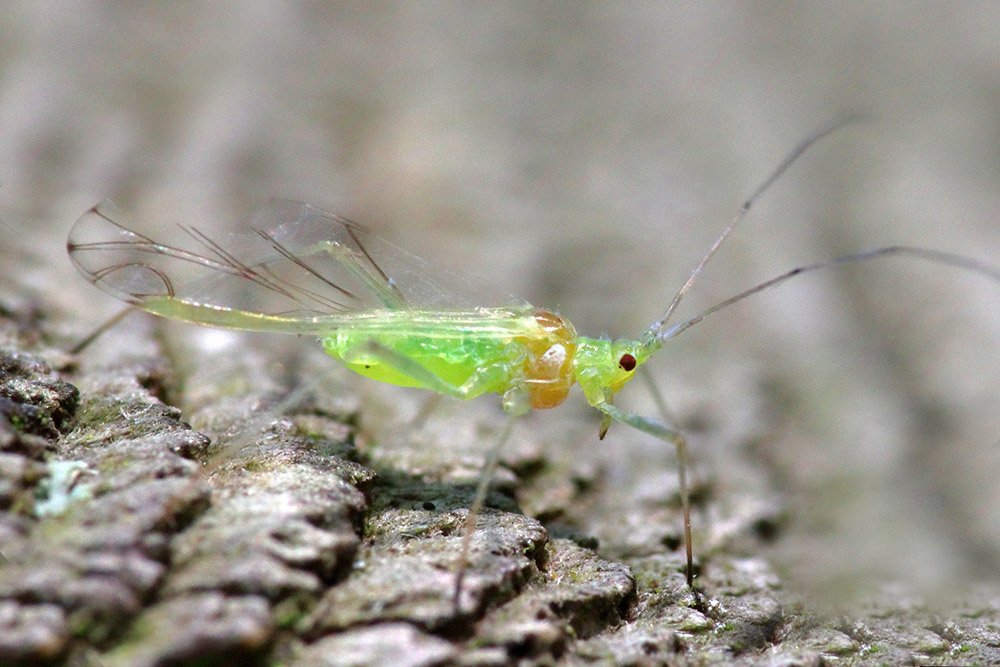
\includegraphics[height=4cm]{images/greenfly}
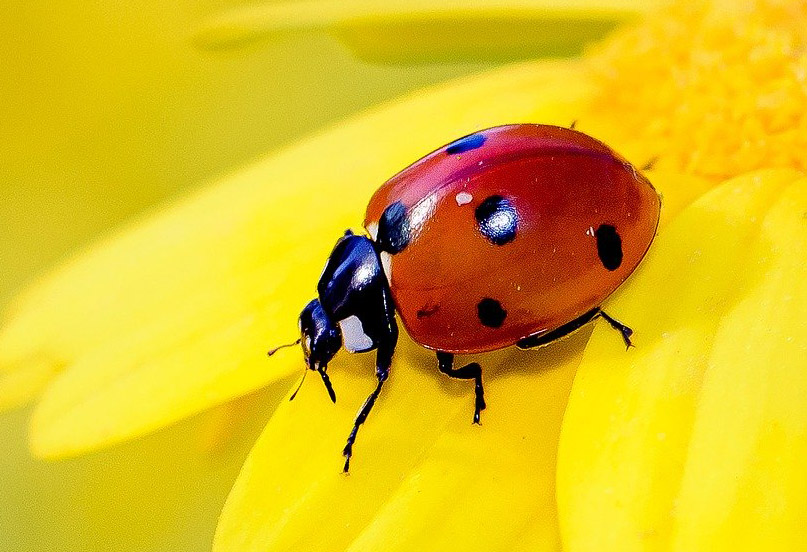
\includegraphics[height=4cm]{images/ladybird}
\caption{Greenflies, $x(t)$, and ladybirds, $y(t)$ (not to scale!) \emph{[Images: Pixabay, Emphyrio; Pixabay, Nimrod Oren]}}
\label{fig:greenflies-and-ladybirds}
\end{figure}
Instead of introducing self-competition, a second possibility to avoid unbounded growth is to model a second population, $y(t)$, which represents a second species. In the case of our greenfly population, we have our antagonists in ladybirds (\cref{fig:greenflies-and-ladybirds}). Since ladybirds prey on greenflies, the greenfly population, $x$, will decrease proportionally to
\begin{equation*}
\text{[the number of ladybirds, $y$]} \times \text{[the number of greenflies, $x$],}
\end{equation*}
i.e., the \emph{number of interactions} of the two species which may lead to a sad little greenfly funeral. This law will therefore be in the form 
\begin{align}
\fd{x}{t} = a x - bxy,
\end{align}
with $b$ the rate at which fatal interactions occur. 

But we must then also model the changing ladybird population, $y(t)$. We assume in the absence of greenflies it will decrease as its food supply has vanished:
\begin{equation}
\fd{y}{t}  = -cy.
\end{equation}
(Ask yourself: Why is this proportional to $y$?) %Answer: Because a percentage of them die every year.
However, it will also grow proportionally to the availability of food, i.e., interactions of the two species (at some rate $d$), so
\begin{equation}
\fd{y}{t}  = -cy + d x y.
\end{equation}
So we have a coupled set of ordinary differential equations, 
\begin{subequations}\label{lotvol}
\begin{align}
\fd{x}{t} &= ax - bxy,\\
\fd{y}{t} &= -cy + dxy,
\end{align}
\end{subequations}
where, once again, $ax$ represents prey reproduction with unlimited food, $-cy$ is predator natural death or emigration, and $bxy$ and $dxy$ are interaction terms. Note that $b$ and $d$ are not necessarily the same: many prey may have to be eaten for the predator population to grow by one.

This system represents both the individual growth/decay of the species (self-interactions) as well as their mutual interaction. This is the so-called \emph{Lotka--Volterra (predator--prey)} system developed by the Italian mathematician Vito Volterra (1860--1940) in 1926 to explain the fluctuation of fish populations in the Adriatic Sea (more on Lotka in \cref{switching}). In more modern theories there are multiple species, each with their own interactions, but we will limit ourselves to this simpler but highly instructive classical system. 

An example solution is shown for the parameters $(a,b,c,d) = (\frac23,\frac43,1,1)$, $x(0)=1$, $y(0)=1$ in \cref{lotkasols}(a). See how the peaks in the greenfly population naturally increase the ladybird food supply: the ladybird population then increases. In turn this leads to the greenfly population dropping as they get eaten, and this decrease in food supply leads to the ladybird population dropping as food becomes competitive. 

This periodic behaviour is made clear using a \emph{phase plot}, as shown in \cref{lotkasols}(b). In this case we have a parametrised plot $(x(t),y(t))$: a geometric plot of the variables of the system (2D here because we have two variables). Closed curves in phase space indicate a periodic relationship between the two parameters.

\begin{figure}
\begin{subfigure}[t]{0.49\textwidth}
	\centering
	%\includegraphics[width=8cm]{lotkaVolterraPlot1.pdf}
	%% Creator: Matplotlib, PGF backend
%%
%% To include the figure in your LaTeX document, write
%%   \input{<filename>.pgf}
%%
%% Make sure the required packages are loaded in your preamble
%%   \usepackage{pgf}
%%
%% Figures using additional raster images can only be included by \input if
%% they are in the same directory as the main LaTeX file. For loading figures
%% from other directories you can use the `import` package
%%   \usepackage{import}
%% and then include the figures with
%%   \import{<path to file>}{<filename>.pgf}
%%
%% Matplotlib used the following preamble
%%   \usepackage{fontspec}
%%   \setmainfont{DejaVuSerif.ttf}[Path=/Library/Python/3.7/site-packages/matplotlib/mpl-data/fonts/ttf/]
%%   \setsansfont{DejaVuSans.ttf}[Path=/Library/Python/3.7/site-packages/matplotlib/mpl-data/fonts/ttf/]
%%   \setmonofont{DejaVuSansMono.ttf}[Path=/Library/Python/3.7/site-packages/matplotlib/mpl-data/fonts/ttf/]
%%
\begingroup%
\makeatletter%
\begin{pgfpicture}%
\pgfpathrectangle{\pgfpointorigin}{\pgfqpoint{3.000000in}{2.200000in}}%
\pgfusepath{use as bounding box, clip}%
\begin{pgfscope}%
\pgfsetbuttcap%
\pgfsetmiterjoin%
\definecolor{currentfill}{rgb}{1.000000,1.000000,1.000000}%
\pgfsetfillcolor{currentfill}%
\pgfsetlinewidth{0.000000pt}%
\definecolor{currentstroke}{rgb}{1.000000,1.000000,1.000000}%
\pgfsetstrokecolor{currentstroke}%
\pgfsetdash{}{0pt}%
\pgfpathmoveto{\pgfqpoint{0.000000in}{0.000000in}}%
\pgfpathlineto{\pgfqpoint{3.000000in}{0.000000in}}%
\pgfpathlineto{\pgfqpoint{3.000000in}{2.200000in}}%
\pgfpathlineto{\pgfqpoint{0.000000in}{2.200000in}}%
\pgfpathclose%
\pgfusepath{fill}%
\end{pgfscope}%
\begin{pgfscope}%
\pgfsetbuttcap%
\pgfsetmiterjoin%
\definecolor{currentfill}{rgb}{1.000000,1.000000,1.000000}%
\pgfsetfillcolor{currentfill}%
\pgfsetlinewidth{0.000000pt}%
\definecolor{currentstroke}{rgb}{0.000000,0.000000,0.000000}%
\pgfsetstrokecolor{currentstroke}%
\pgfsetstrokeopacity{0.000000}%
\pgfsetdash{}{0pt}%
\pgfpathmoveto{\pgfqpoint{0.338301in}{0.278150in}}%
\pgfpathlineto{\pgfqpoint{2.966667in}{0.278150in}}%
\pgfpathlineto{\pgfqpoint{2.966667in}{2.109013in}}%
\pgfpathlineto{\pgfqpoint{0.338301in}{2.109013in}}%
\pgfpathclose%
\pgfusepath{fill}%
\end{pgfscope}%
\begin{pgfscope}%
\pgfpathrectangle{\pgfqpoint{0.338301in}{0.278150in}}{\pgfqpoint{2.628366in}{1.830863in}}%
\pgfusepath{clip}%
\pgfsetrectcap%
\pgfsetroundjoin%
\pgfsetlinewidth{1.505625pt}%
\definecolor{currentstroke}{rgb}{0.121569,0.466667,0.705882}%
\pgfsetstrokecolor{currentstroke}%
\pgfsetdash{}{0pt}%
\pgfpathmoveto{\pgfqpoint{0.338301in}{1.010495in}}%
\pgfpathlineto{\pgfqpoint{0.346115in}{0.941060in}}%
\pgfpathlineto{\pgfqpoint{0.353930in}{0.879886in}}%
\pgfpathlineto{\pgfqpoint{0.361745in}{0.827188in}}%
\pgfpathlineto{\pgfqpoint{0.369560in}{0.782645in}}%
\pgfpathlineto{\pgfqpoint{0.377375in}{0.745628in}}%
\pgfpathlineto{\pgfqpoint{0.385190in}{0.715371in}}%
\pgfpathlineto{\pgfqpoint{0.393004in}{0.691094in}}%
\pgfpathlineto{\pgfqpoint{0.398214in}{0.677867in}}%
\pgfpathlineto{\pgfqpoint{0.403424in}{0.666773in}}%
\pgfpathlineto{\pgfqpoint{0.408634in}{0.657635in}}%
\pgfpathlineto{\pgfqpoint{0.413844in}{0.650295in}}%
\pgfpathlineto{\pgfqpoint{0.419054in}{0.644611in}}%
\pgfpathlineto{\pgfqpoint{0.424264in}{0.640462in}}%
\pgfpathlineto{\pgfqpoint{0.429474in}{0.637742in}}%
\pgfpathlineto{\pgfqpoint{0.434684in}{0.636361in}}%
\pgfpathlineto{\pgfqpoint{0.439894in}{0.636243in}}%
\pgfpathlineto{\pgfqpoint{0.445103in}{0.637324in}}%
\pgfpathlineto{\pgfqpoint{0.450313in}{0.639552in}}%
\pgfpathlineto{\pgfqpoint{0.455523in}{0.642883in}}%
\pgfpathlineto{\pgfqpoint{0.460733in}{0.647284in}}%
\pgfpathlineto{\pgfqpoint{0.468548in}{0.655839in}}%
\pgfpathlineto{\pgfqpoint{0.476363in}{0.666689in}}%
\pgfpathlineto{\pgfqpoint{0.484178in}{0.679807in}}%
\pgfpathlineto{\pgfqpoint{0.491992in}{0.695193in}}%
\pgfpathlineto{\pgfqpoint{0.499807in}{0.712865in}}%
\pgfpathlineto{\pgfqpoint{0.507622in}{0.732860in}}%
\pgfpathlineto{\pgfqpoint{0.518042in}{0.763220in}}%
\pgfpathlineto{\pgfqpoint{0.528462in}{0.797939in}}%
\pgfpathlineto{\pgfqpoint{0.538882in}{0.837168in}}%
\pgfpathlineto{\pgfqpoint{0.549301in}{0.881047in}}%
\pgfpathlineto{\pgfqpoint{0.559721in}{0.929678in}}%
\pgfpathlineto{\pgfqpoint{0.570141in}{0.983088in}}%
\pgfpathlineto{\pgfqpoint{0.583166in}{1.056413in}}%
\pgfpathlineto{\pgfqpoint{0.596190in}{1.136430in}}%
\pgfpathlineto{\pgfqpoint{0.614425in}{1.256928in}}%
\pgfpathlineto{\pgfqpoint{0.640475in}{1.430368in}}%
\pgfpathlineto{\pgfqpoint{0.650894in}{1.491347in}}%
\pgfpathlineto{\pgfqpoint{0.658709in}{1.529912in}}%
\pgfpathlineto{\pgfqpoint{0.663919in}{1.550933in}}%
\pgfpathlineto{\pgfqpoint{0.669129in}{1.567350in}}%
\pgfpathlineto{\pgfqpoint{0.674339in}{1.578426in}}%
\pgfpathlineto{\pgfqpoint{0.676944in}{1.581740in}}%
\pgfpathlineto{\pgfqpoint{0.679549in}{1.583459in}}%
\pgfpathlineto{\pgfqpoint{0.682154in}{1.583509in}}%
\pgfpathlineto{\pgfqpoint{0.684759in}{1.581823in}}%
\pgfpathlineto{\pgfqpoint{0.687364in}{1.578345in}}%
\pgfpathlineto{\pgfqpoint{0.689969in}{1.573028in}}%
\pgfpathlineto{\pgfqpoint{0.692573in}{1.565841in}}%
\pgfpathlineto{\pgfqpoint{0.697783in}{1.545808in}}%
\pgfpathlineto{\pgfqpoint{0.702993in}{1.518316in}}%
\pgfpathlineto{\pgfqpoint{0.708203in}{1.483724in}}%
\pgfpathlineto{\pgfqpoint{0.713413in}{1.442692in}}%
\pgfpathlineto{\pgfqpoint{0.721228in}{1.371166in}}%
\pgfpathlineto{\pgfqpoint{0.731648in}{1.263572in}}%
\pgfpathlineto{\pgfqpoint{0.752487in}{1.044768in}}%
\pgfpathlineto{\pgfqpoint{0.762907in}{0.949237in}}%
\pgfpathlineto{\pgfqpoint{0.770722in}{0.887013in}}%
\pgfpathlineto{\pgfqpoint{0.778537in}{0.833273in}}%
\pgfpathlineto{\pgfqpoint{0.786352in}{0.787748in}}%
\pgfpathlineto{\pgfqpoint{0.794166in}{0.749837in}}%
\pgfpathlineto{\pgfqpoint{0.801981in}{0.718784in}}%
\pgfpathlineto{\pgfqpoint{0.809796in}{0.693807in}}%
\pgfpathlineto{\pgfqpoint{0.815006in}{0.680161in}}%
\pgfpathlineto{\pgfqpoint{0.820216in}{0.668684in}}%
\pgfpathlineto{\pgfqpoint{0.825426in}{0.659195in}}%
\pgfpathlineto{\pgfqpoint{0.830636in}{0.651531in}}%
\pgfpathlineto{\pgfqpoint{0.835846in}{0.645549in}}%
\pgfpathlineto{\pgfqpoint{0.841055in}{0.641123in}}%
\pgfpathlineto{\pgfqpoint{0.846265in}{0.638144in}}%
\pgfpathlineto{\pgfqpoint{0.851475in}{0.636520in}}%
\pgfpathlineto{\pgfqpoint{0.856685in}{0.636173in}}%
\pgfpathlineto{\pgfqpoint{0.861895in}{0.637035in}}%
\pgfpathlineto{\pgfqpoint{0.867105in}{0.639052in}}%
\pgfpathlineto{\pgfqpoint{0.872315in}{0.642181in}}%
\pgfpathlineto{\pgfqpoint{0.877525in}{0.646385in}}%
\pgfpathlineto{\pgfqpoint{0.882735in}{0.651638in}}%
\pgfpathlineto{\pgfqpoint{0.890549in}{0.661443in}}%
\pgfpathlineto{\pgfqpoint{0.898364in}{0.673526in}}%
\pgfpathlineto{\pgfqpoint{0.906179in}{0.687873in}}%
\pgfpathlineto{\pgfqpoint{0.913994in}{0.704496in}}%
\pgfpathlineto{\pgfqpoint{0.921809in}{0.723423in}}%
\pgfpathlineto{\pgfqpoint{0.929624in}{0.744698in}}%
\pgfpathlineto{\pgfqpoint{0.940043in}{0.776815in}}%
\pgfpathlineto{\pgfqpoint{0.950463in}{0.813351in}}%
\pgfpathlineto{\pgfqpoint{0.960883in}{0.854457in}}%
\pgfpathlineto{\pgfqpoint{0.971303in}{0.900260in}}%
\pgfpathlineto{\pgfqpoint{0.981723in}{0.950838in}}%
\pgfpathlineto{\pgfqpoint{0.992142in}{1.006176in}}%
\pgfpathlineto{\pgfqpoint{1.005167in}{1.081776in}}%
\pgfpathlineto{\pgfqpoint{1.018192in}{1.163725in}}%
\pgfpathlineto{\pgfqpoint{1.039031in}{1.303448in}}%
\pgfpathlineto{\pgfqpoint{1.057266in}{1.424292in}}%
\pgfpathlineto{\pgfqpoint{1.067686in}{1.486072in}}%
\pgfpathlineto{\pgfqpoint{1.075501in}{1.525551in}}%
\pgfpathlineto{\pgfqpoint{1.080711in}{1.547347in}}%
\pgfpathlineto{\pgfqpoint{1.085921in}{1.564677in}}%
\pgfpathlineto{\pgfqpoint{1.091130in}{1.576803in}}%
\pgfpathlineto{\pgfqpoint{1.093735in}{1.580689in}}%
\pgfpathlineto{\pgfqpoint{1.096340in}{1.583010in}}%
\pgfpathlineto{\pgfqpoint{1.098945in}{1.583690in}}%
\pgfpathlineto{\pgfqpoint{1.101550in}{1.582658in}}%
\pgfpathlineto{\pgfqpoint{1.104155in}{1.579852in}}%
\pgfpathlineto{\pgfqpoint{1.106760in}{1.575224in}}%
\pgfpathlineto{\pgfqpoint{1.109365in}{1.568736in}}%
\pgfpathlineto{\pgfqpoint{1.111970in}{1.560366in}}%
\pgfpathlineto{\pgfqpoint{1.117180in}{1.537971in}}%
\pgfpathlineto{\pgfqpoint{1.122390in}{1.508197in}}%
\pgfpathlineto{\pgfqpoint{1.127600in}{1.471499in}}%
\pgfpathlineto{\pgfqpoint{1.135415in}{1.405179in}}%
\pgfpathlineto{\pgfqpoint{1.143229in}{1.328576in}}%
\pgfpathlineto{\pgfqpoint{1.177094in}{0.980473in}}%
\pgfpathlineto{\pgfqpoint{1.184909in}{0.914424in}}%
\pgfpathlineto{\pgfqpoint{1.192723in}{0.856808in}}%
\pgfpathlineto{\pgfqpoint{1.200538in}{0.807585in}}%
\pgfpathlineto{\pgfqpoint{1.208353in}{0.766279in}}%
\pgfpathlineto{\pgfqpoint{1.216168in}{0.732187in}}%
\pgfpathlineto{\pgfqpoint{1.223983in}{0.704526in}}%
\pgfpathlineto{\pgfqpoint{1.229193in}{0.689278in}}%
\pgfpathlineto{\pgfqpoint{1.234403in}{0.676334in}}%
\pgfpathlineto{\pgfqpoint{1.239612in}{0.665500in}}%
\pgfpathlineto{\pgfqpoint{1.244822in}{0.656600in}}%
\pgfpathlineto{\pgfqpoint{1.250032in}{0.649478in}}%
\pgfpathlineto{\pgfqpoint{1.255242in}{0.643997in}}%
\pgfpathlineto{\pgfqpoint{1.260452in}{0.640036in}}%
\pgfpathlineto{\pgfqpoint{1.265662in}{0.637492in}}%
\pgfpathlineto{\pgfqpoint{1.270872in}{0.636277in}}%
\pgfpathlineto{\pgfqpoint{1.276082in}{0.636316in}}%
\pgfpathlineto{\pgfqpoint{1.281292in}{0.637546in}}%
\pgfpathlineto{\pgfqpoint{1.286502in}{0.639916in}}%
\pgfpathlineto{\pgfqpoint{1.291711in}{0.643386in}}%
\pgfpathlineto{\pgfqpoint{1.296921in}{0.647922in}}%
\pgfpathlineto{\pgfqpoint{1.304736in}{0.656674in}}%
\pgfpathlineto{\pgfqpoint{1.312551in}{0.667718in}}%
\pgfpathlineto{\pgfqpoint{1.320366in}{0.681029in}}%
\pgfpathlineto{\pgfqpoint{1.328181in}{0.696608in}}%
\pgfpathlineto{\pgfqpoint{1.335996in}{0.714477in}}%
\pgfpathlineto{\pgfqpoint{1.343810in}{0.734672in}}%
\pgfpathlineto{\pgfqpoint{1.354230in}{0.765306in}}%
\pgfpathlineto{\pgfqpoint{1.364650in}{0.800309in}}%
\pgfpathlineto{\pgfqpoint{1.375070in}{0.839831in}}%
\pgfpathlineto{\pgfqpoint{1.385490in}{0.884011in}}%
\pgfpathlineto{\pgfqpoint{1.395909in}{0.932948in}}%
\pgfpathlineto{\pgfqpoint{1.406329in}{0.986662in}}%
\pgfpathlineto{\pgfqpoint{1.419354in}{1.060349in}}%
\pgfpathlineto{\pgfqpoint{1.432379in}{1.140679in}}%
\pgfpathlineto{\pgfqpoint{1.450613in}{1.261442in}}%
\pgfpathlineto{\pgfqpoint{1.474058in}{1.418164in}}%
\pgfpathlineto{\pgfqpoint{1.484478in}{1.480704in}}%
\pgfpathlineto{\pgfqpoint{1.492292in}{1.521061in}}%
\pgfpathlineto{\pgfqpoint{1.497502in}{1.543607in}}%
\pgfpathlineto{\pgfqpoint{1.502712in}{1.561825in}}%
\pgfpathlineto{\pgfqpoint{1.507922in}{1.574974in}}%
\pgfpathlineto{\pgfqpoint{1.510527in}{1.579421in}}%
\pgfpathlineto{\pgfqpoint{1.513132in}{1.582334in}}%
\pgfpathlineto{\pgfqpoint{1.515737in}{1.583634in}}%
\pgfpathlineto{\pgfqpoint{1.518342in}{1.583246in}}%
\pgfpathlineto{\pgfqpoint{1.520947in}{1.581107in}}%
\pgfpathlineto{\pgfqpoint{1.523552in}{1.577163in}}%
\pgfpathlineto{\pgfqpoint{1.526157in}{1.571371in}}%
\pgfpathlineto{\pgfqpoint{1.528762in}{1.563703in}}%
\pgfpathlineto{\pgfqpoint{1.533972in}{1.542707in}}%
\pgfpathlineto{\pgfqpoint{1.539181in}{1.514280in}}%
\pgfpathlineto{\pgfqpoint{1.544391in}{1.478823in}}%
\pgfpathlineto{\pgfqpoint{1.552206in}{1.414048in}}%
\pgfpathlineto{\pgfqpoint{1.560021in}{1.338496in}}%
\pgfpathlineto{\pgfqpoint{1.575651in}{1.172361in}}%
\pgfpathlineto{\pgfqpoint{1.588675in}{1.038275in}}%
\pgfpathlineto{\pgfqpoint{1.599095in}{0.943608in}}%
\pgfpathlineto{\pgfqpoint{1.606910in}{0.882105in}}%
\pgfpathlineto{\pgfqpoint{1.614725in}{0.829081in}}%
\pgfpathlineto{\pgfqpoint{1.622540in}{0.784231in}}%
\pgfpathlineto{\pgfqpoint{1.630355in}{0.746935in}}%
\pgfpathlineto{\pgfqpoint{1.638169in}{0.716430in}}%
\pgfpathlineto{\pgfqpoint{1.645984in}{0.691935in}}%
\pgfpathlineto{\pgfqpoint{1.651194in}{0.678577in}}%
\pgfpathlineto{\pgfqpoint{1.656404in}{0.667364in}}%
\pgfpathlineto{\pgfqpoint{1.661614in}{0.658117in}}%
\pgfpathlineto{\pgfqpoint{1.666824in}{0.650676in}}%
\pgfpathlineto{\pgfqpoint{1.672034in}{0.644899in}}%
\pgfpathlineto{\pgfqpoint{1.677244in}{0.640663in}}%
\pgfpathlineto{\pgfqpoint{1.682454in}{0.637863in}}%
\pgfpathlineto{\pgfqpoint{1.687663in}{0.636406in}}%
\pgfpathlineto{\pgfqpoint{1.692873in}{0.636216in}}%
\pgfpathlineto{\pgfqpoint{1.698083in}{0.637229in}}%
\pgfpathlineto{\pgfqpoint{1.703293in}{0.639391in}}%
\pgfpathlineto{\pgfqpoint{1.708503in}{0.642658in}}%
\pgfpathlineto{\pgfqpoint{1.713713in}{0.646998in}}%
\pgfpathlineto{\pgfqpoint{1.721528in}{0.655463in}}%
\pgfpathlineto{\pgfqpoint{1.729343in}{0.666224in}}%
\pgfpathlineto{\pgfqpoint{1.737157in}{0.679254in}}%
\pgfpathlineto{\pgfqpoint{1.744972in}{0.694552in}}%
\pgfpathlineto{\pgfqpoint{1.752787in}{0.712134in}}%
\pgfpathlineto{\pgfqpoint{1.760602in}{0.732038in}}%
\pgfpathlineto{\pgfqpoint{1.771022in}{0.762274in}}%
\pgfpathlineto{\pgfqpoint{1.781442in}{0.796864in}}%
\pgfpathlineto{\pgfqpoint{1.791861in}{0.835959in}}%
\pgfpathlineto{\pgfqpoint{1.802281in}{0.879701in}}%
\pgfpathlineto{\pgfqpoint{1.812701in}{0.928192in}}%
\pgfpathlineto{\pgfqpoint{1.823121in}{0.981464in}}%
\pgfpathlineto{\pgfqpoint{1.836145in}{1.054623in}}%
\pgfpathlineto{\pgfqpoint{1.849170in}{1.134495in}}%
\pgfpathlineto{\pgfqpoint{1.864800in}{1.237263in}}%
\pgfpathlineto{\pgfqpoint{1.893454in}{1.428470in}}%
\pgfpathlineto{\pgfqpoint{1.903874in}{1.489705in}}%
\pgfpathlineto{\pgfqpoint{1.911689in}{1.528560in}}%
\pgfpathlineto{\pgfqpoint{1.916899in}{1.549827in}}%
\pgfpathlineto{\pgfqpoint{1.922109in}{1.566533in}}%
\pgfpathlineto{\pgfqpoint{1.927319in}{1.577941in}}%
\pgfpathlineto{\pgfqpoint{1.929924in}{1.581435in}}%
\pgfpathlineto{\pgfqpoint{1.932529in}{1.583344in}}%
\pgfpathlineto{\pgfqpoint{1.935133in}{1.583592in}}%
\pgfpathlineto{\pgfqpoint{1.937738in}{1.582112in}}%
\pgfpathlineto{\pgfqpoint{1.940343in}{1.578845in}}%
\pgfpathlineto{\pgfqpoint{1.942948in}{1.573745in}}%
\pgfpathlineto{\pgfqpoint{1.945553in}{1.566777in}}%
\pgfpathlineto{\pgfqpoint{1.950763in}{1.547184in}}%
\pgfpathlineto{\pgfqpoint{1.955973in}{1.520120in}}%
\pgfpathlineto{\pgfqpoint{1.961183in}{1.485927in}}%
\pgfpathlineto{\pgfqpoint{1.966393in}{1.445247in}}%
\pgfpathlineto{\pgfqpoint{1.974208in}{1.374132in}}%
\pgfpathlineto{\pgfqpoint{1.984627in}{1.266821in}}%
\pgfpathlineto{\pgfqpoint{2.005467in}{1.047747in}}%
\pgfpathlineto{\pgfqpoint{2.015887in}{0.951826in}}%
\pgfpathlineto{\pgfqpoint{2.023702in}{0.889273in}}%
\pgfpathlineto{\pgfqpoint{2.031517in}{0.835205in}}%
\pgfpathlineto{\pgfqpoint{2.039331in}{0.789371in}}%
\pgfpathlineto{\pgfqpoint{2.047146in}{0.751177in}}%
\pgfpathlineto{\pgfqpoint{2.054961in}{0.719873in}}%
\pgfpathlineto{\pgfqpoint{2.062776in}{0.694673in}}%
\pgfpathlineto{\pgfqpoint{2.067986in}{0.680895in}}%
\pgfpathlineto{\pgfqpoint{2.073196in}{0.669297in}}%
\pgfpathlineto{\pgfqpoint{2.078406in}{0.659697in}}%
\pgfpathlineto{\pgfqpoint{2.083615in}{0.651930in}}%
\pgfpathlineto{\pgfqpoint{2.088825in}{0.645853in}}%
\pgfpathlineto{\pgfqpoint{2.094035in}{0.641340in}}%
\pgfpathlineto{\pgfqpoint{2.099245in}{0.638279in}}%
\pgfpathlineto{\pgfqpoint{2.104455in}{0.636579in}}%
\pgfpathlineto{\pgfqpoint{2.109665in}{0.636159in}}%
\pgfpathlineto{\pgfqpoint{2.114875in}{0.636952in}}%
\pgfpathlineto{\pgfqpoint{2.120085in}{0.638903in}}%
\pgfpathlineto{\pgfqpoint{2.125295in}{0.641968in}}%
\pgfpathlineto{\pgfqpoint{2.130505in}{0.646110in}}%
\pgfpathlineto{\pgfqpoint{2.135714in}{0.651303in}}%
\pgfpathlineto{\pgfqpoint{2.143529in}{0.661019in}}%
\pgfpathlineto{\pgfqpoint{2.151344in}{0.673013in}}%
\pgfpathlineto{\pgfqpoint{2.159159in}{0.687272in}}%
\pgfpathlineto{\pgfqpoint{2.166974in}{0.703806in}}%
\pgfpathlineto{\pgfqpoint{2.174789in}{0.722643in}}%
\pgfpathlineto{\pgfqpoint{2.182603in}{0.743826in}}%
\pgfpathlineto{\pgfqpoint{2.193023in}{0.775816in}}%
\pgfpathlineto{\pgfqpoint{2.203443in}{0.812221in}}%
\pgfpathlineto{\pgfqpoint{2.213863in}{0.853192in}}%
\pgfpathlineto{\pgfqpoint{2.224283in}{0.898857in}}%
\pgfpathlineto{\pgfqpoint{2.234702in}{0.949295in}}%
\pgfpathlineto{\pgfqpoint{2.245122in}{1.004496in}}%
\pgfpathlineto{\pgfqpoint{2.258147in}{1.079936in}}%
\pgfpathlineto{\pgfqpoint{2.271172in}{1.161752in}}%
\pgfpathlineto{\pgfqpoint{2.292011in}{1.301382in}}%
\pgfpathlineto{\pgfqpoint{2.310246in}{1.422378in}}%
\pgfpathlineto{\pgfqpoint{2.320666in}{1.484400in}}%
\pgfpathlineto{\pgfqpoint{2.328481in}{1.524158in}}%
\pgfpathlineto{\pgfqpoint{2.333690in}{1.546192in}}%
\pgfpathlineto{\pgfqpoint{2.338900in}{1.563803in}}%
\pgfpathlineto{\pgfqpoint{2.344110in}{1.576252in}}%
\pgfpathlineto{\pgfqpoint{2.346715in}{1.580315in}}%
\pgfpathlineto{\pgfqpoint{2.349320in}{1.582823in}}%
\pgfpathlineto{\pgfqpoint{2.351925in}{1.583699in}}%
\pgfpathlineto{\pgfqpoint{2.354530in}{1.582869in}}%
\pgfpathlineto{\pgfqpoint{2.357135in}{1.580273in}}%
\pgfpathlineto{\pgfqpoint{2.359740in}{1.575860in}}%
\pgfpathlineto{\pgfqpoint{2.362345in}{1.569591in}}%
\pgfpathlineto{\pgfqpoint{2.364950in}{1.561441in}}%
\pgfpathlineto{\pgfqpoint{2.370160in}{1.539484in}}%
\pgfpathlineto{\pgfqpoint{2.375370in}{1.510130in}}%
\pgfpathlineto{\pgfqpoint{2.380580in}{1.473819in}}%
\pgfpathlineto{\pgfqpoint{2.388394in}{1.407977in}}%
\pgfpathlineto{\pgfqpoint{2.396209in}{1.331696in}}%
\pgfpathlineto{\pgfqpoint{2.430074in}{0.983205in}}%
\pgfpathlineto{\pgfqpoint{2.437888in}{0.916836in}}%
\pgfpathlineto{\pgfqpoint{2.445703in}{0.858889in}}%
\pgfpathlineto{\pgfqpoint{2.453518in}{0.809346in}}%
\pgfpathlineto{\pgfqpoint{2.461333in}{0.767745in}}%
\pgfpathlineto{\pgfqpoint{2.469148in}{0.733387in}}%
\pgfpathlineto{\pgfqpoint{2.476963in}{0.705491in}}%
\pgfpathlineto{\pgfqpoint{2.484777in}{0.683288in}}%
\pgfpathlineto{\pgfqpoint{2.489987in}{0.671299in}}%
\pgfpathlineto{\pgfqpoint{2.495197in}{0.661340in}}%
\pgfpathlineto{\pgfqpoint{2.500407in}{0.653244in}}%
\pgfpathlineto{\pgfqpoint{2.505617in}{0.646862in}}%
\pgfpathlineto{\pgfqpoint{2.510827in}{0.642066in}}%
\pgfpathlineto{\pgfqpoint{2.516037in}{0.638743in}}%
\pgfpathlineto{\pgfqpoint{2.521247in}{0.636796in}}%
\pgfpathlineto{\pgfqpoint{2.526457in}{0.636143in}}%
\pgfpathlineto{\pgfqpoint{2.531666in}{0.636715in}}%
\pgfpathlineto{\pgfqpoint{2.536876in}{0.638455in}}%
\pgfpathlineto{\pgfqpoint{2.542086in}{0.641315in}}%
\pgfpathlineto{\pgfqpoint{2.547296in}{0.645259in}}%
\pgfpathlineto{\pgfqpoint{2.552506in}{0.650258in}}%
\pgfpathlineto{\pgfqpoint{2.560321in}{0.659689in}}%
\pgfpathlineto{\pgfqpoint{2.568136in}{0.671402in}}%
\pgfpathlineto{\pgfqpoint{2.575951in}{0.685380in}}%
\pgfpathlineto{\pgfqpoint{2.583765in}{0.701630in}}%
\pgfpathlineto{\pgfqpoint{2.591580in}{0.720179in}}%
\pgfpathlineto{\pgfqpoint{2.599395in}{0.741069in}}%
\pgfpathlineto{\pgfqpoint{2.609815in}{0.772655in}}%
\pgfpathlineto{\pgfqpoint{2.620235in}{0.808643in}}%
\pgfpathlineto{\pgfqpoint{2.630654in}{0.849183in}}%
\pgfpathlineto{\pgfqpoint{2.641074in}{0.894407in}}%
\pgfpathlineto{\pgfqpoint{2.651494in}{0.944400in}}%
\pgfpathlineto{\pgfqpoint{2.661914in}{0.999161in}}%
\pgfpathlineto{\pgfqpoint{2.674939in}{1.074086in}}%
\pgfpathlineto{\pgfqpoint{2.687963in}{1.155471in}}%
\pgfpathlineto{\pgfqpoint{2.706198in}{1.277069in}}%
\pgfpathlineto{\pgfqpoint{2.727038in}{1.416233in}}%
\pgfpathlineto{\pgfqpoint{2.737457in}{1.479003in}}%
\pgfpathlineto{\pgfqpoint{2.745272in}{1.519628in}}%
\pgfpathlineto{\pgfqpoint{2.750482in}{1.542404in}}%
\pgfpathlineto{\pgfqpoint{2.755692in}{1.560895in}}%
\pgfpathlineto{\pgfqpoint{2.760902in}{1.574360in}}%
\pgfpathlineto{\pgfqpoint{2.763507in}{1.578980in}}%
\pgfpathlineto{\pgfqpoint{2.766112in}{1.582077in}}%
\pgfpathlineto{\pgfqpoint{2.768717in}{1.583569in}}%
\pgfpathlineto{\pgfqpoint{2.771322in}{1.583381in}}%
\pgfpathlineto{\pgfqpoint{2.773927in}{1.581450in}}%
\pgfpathlineto{\pgfqpoint{2.776532in}{1.577718in}}%
\pgfpathlineto{\pgfqpoint{2.779136in}{1.572143in}}%
\pgfpathlineto{\pgfqpoint{2.781741in}{1.564695in}}%
\pgfpathlineto{\pgfqpoint{2.786951in}{1.544139in}}%
\pgfpathlineto{\pgfqpoint{2.792161in}{1.516138in}}%
\pgfpathlineto{\pgfqpoint{2.797371in}{1.481074in}}%
\pgfpathlineto{\pgfqpoint{2.802581in}{1.439626in}}%
\pgfpathlineto{\pgfqpoint{2.810396in}{1.367619in}}%
\pgfpathlineto{\pgfqpoint{2.820816in}{1.259699in}}%
\pgfpathlineto{\pgfqpoint{2.841655in}{1.041234in}}%
\pgfpathlineto{\pgfqpoint{2.852075in}{0.946170in}}%
\pgfpathlineto{\pgfqpoint{2.859890in}{0.884337in}}%
\pgfpathlineto{\pgfqpoint{2.867705in}{0.830987in}}%
\pgfpathlineto{\pgfqpoint{2.875520in}{0.785830in}}%
\pgfpathlineto{\pgfqpoint{2.883334in}{0.748253in}}%
\pgfpathlineto{\pgfqpoint{2.891149in}{0.717499in}}%
\pgfpathlineto{\pgfqpoint{2.898964in}{0.692784in}}%
\pgfpathlineto{\pgfqpoint{2.904174in}{0.679295in}}%
\pgfpathlineto{\pgfqpoint{2.909384in}{0.667962in}}%
\pgfpathlineto{\pgfqpoint{2.914594in}{0.658605in}}%
\pgfpathlineto{\pgfqpoint{2.919804in}{0.651062in}}%
\pgfpathlineto{\pgfqpoint{2.925014in}{0.645192in}}%
\pgfpathlineto{\pgfqpoint{2.930223in}{0.640870in}}%
\pgfpathlineto{\pgfqpoint{2.935433in}{0.637988in}}%
\pgfpathlineto{\pgfqpoint{2.940643in}{0.636455in}}%
\pgfpathlineto{\pgfqpoint{2.940643in}{0.636455in}}%
\pgfusepath{stroke}%
\end{pgfscope}%
\begin{pgfscope}%
\pgfpathrectangle{\pgfqpoint{0.338301in}{0.278150in}}{\pgfqpoint{2.628366in}{1.830863in}}%
\pgfusepath{clip}%
\pgfsetbuttcap%
\pgfsetroundjoin%
\pgfsetlinewidth{1.505625pt}%
\definecolor{currentstroke}{rgb}{1.000000,0.498039,0.054902}%
\pgfsetstrokecolor{currentstroke}%
\pgfsetdash{{5.550000pt}{2.400000pt}}{0.000000pt}%
\pgfpathmoveto{\pgfqpoint{0.338301in}{1.010495in}}%
\pgfpathlineto{\pgfqpoint{0.340906in}{1.009891in}}%
\pgfpathlineto{\pgfqpoint{0.343510in}{1.008109in}}%
\pgfpathlineto{\pgfqpoint{0.346115in}{1.005202in}}%
\pgfpathlineto{\pgfqpoint{0.351325in}{0.996253in}}%
\pgfpathlineto{\pgfqpoint{0.356535in}{0.983562in}}%
\pgfpathlineto{\pgfqpoint{0.361745in}{0.967688in}}%
\pgfpathlineto{\pgfqpoint{0.369560in}{0.939140in}}%
\pgfpathlineto{\pgfqpoint{0.379980in}{0.895003in}}%
\pgfpathlineto{\pgfqpoint{0.400819in}{0.798748in}}%
\pgfpathlineto{\pgfqpoint{0.416449in}{0.728742in}}%
\pgfpathlineto{\pgfqpoint{0.429474in}{0.675396in}}%
\pgfpathlineto{\pgfqpoint{0.439894in}{0.636796in}}%
\pgfpathlineto{\pgfqpoint{0.450313in}{0.602031in}}%
\pgfpathlineto{\pgfqpoint{0.460733in}{0.571079in}}%
\pgfpathlineto{\pgfqpoint{0.471153in}{0.543799in}}%
\pgfpathlineto{\pgfqpoint{0.481573in}{0.519980in}}%
\pgfpathlineto{\pgfqpoint{0.491992in}{0.499383in}}%
\pgfpathlineto{\pgfqpoint{0.502412in}{0.481762in}}%
\pgfpathlineto{\pgfqpoint{0.512832in}{0.466890in}}%
\pgfpathlineto{\pgfqpoint{0.520647in}{0.457415in}}%
\pgfpathlineto{\pgfqpoint{0.528462in}{0.449298in}}%
\pgfpathlineto{\pgfqpoint{0.536277in}{0.442481in}}%
\pgfpathlineto{\pgfqpoint{0.544091in}{0.436917in}}%
\pgfpathlineto{\pgfqpoint{0.551906in}{0.432580in}}%
\pgfpathlineto{\pgfqpoint{0.559721in}{0.429462in}}%
\pgfpathlineto{\pgfqpoint{0.567536in}{0.427574in}}%
\pgfpathlineto{\pgfqpoint{0.575351in}{0.426954in}}%
\pgfpathlineto{\pgfqpoint{0.583166in}{0.427666in}}%
\pgfpathlineto{\pgfqpoint{0.590980in}{0.429807in}}%
\pgfpathlineto{\pgfqpoint{0.598795in}{0.433513in}}%
\pgfpathlineto{\pgfqpoint{0.606610in}{0.438962in}}%
\pgfpathlineto{\pgfqpoint{0.614425in}{0.446385in}}%
\pgfpathlineto{\pgfqpoint{0.622240in}{0.456069in}}%
\pgfpathlineto{\pgfqpoint{0.630055in}{0.468367in}}%
\pgfpathlineto{\pgfqpoint{0.637870in}{0.483697in}}%
\pgfpathlineto{\pgfqpoint{0.645684in}{0.502539in}}%
\pgfpathlineto{\pgfqpoint{0.653499in}{0.525414in}}%
\pgfpathlineto{\pgfqpoint{0.661314in}{0.552849in}}%
\pgfpathlineto{\pgfqpoint{0.669129in}{0.585296in}}%
\pgfpathlineto{\pgfqpoint{0.676944in}{0.623029in}}%
\pgfpathlineto{\pgfqpoint{0.684759in}{0.665987in}}%
\pgfpathlineto{\pgfqpoint{0.695178in}{0.730304in}}%
\pgfpathlineto{\pgfqpoint{0.723833in}{0.915084in}}%
\pgfpathlineto{\pgfqpoint{0.731648in}{0.954700in}}%
\pgfpathlineto{\pgfqpoint{0.736858in}{0.975838in}}%
\pgfpathlineto{\pgfqpoint{0.742067in}{0.992145in}}%
\pgfpathlineto{\pgfqpoint{0.747277in}{1.003333in}}%
\pgfpathlineto{\pgfqpoint{0.749882in}{1.006976in}}%
\pgfpathlineto{\pgfqpoint{0.752487in}{1.009327in}}%
\pgfpathlineto{\pgfqpoint{0.755092in}{1.010410in}}%
\pgfpathlineto{\pgfqpoint{0.757697in}{1.010256in}}%
\pgfpathlineto{\pgfqpoint{0.760302in}{1.008907in}}%
\pgfpathlineto{\pgfqpoint{0.762907in}{1.006412in}}%
\pgfpathlineto{\pgfqpoint{0.765512in}{1.002829in}}%
\pgfpathlineto{\pgfqpoint{0.770722in}{0.992646in}}%
\pgfpathlineto{\pgfqpoint{0.775932in}{0.978895in}}%
\pgfpathlineto{\pgfqpoint{0.781142in}{0.962139in}}%
\pgfpathlineto{\pgfqpoint{0.788957in}{0.932592in}}%
\pgfpathlineto{\pgfqpoint{0.799376in}{0.887666in}}%
\pgfpathlineto{\pgfqpoint{0.841055in}{0.700038in}}%
\pgfpathlineto{\pgfqpoint{0.854080in}{0.649610in}}%
\pgfpathlineto{\pgfqpoint{0.864500in}{0.613523in}}%
\pgfpathlineto{\pgfqpoint{0.874920in}{0.581274in}}%
\pgfpathlineto{\pgfqpoint{0.885340in}{0.552756in}}%
\pgfpathlineto{\pgfqpoint{0.895759in}{0.527776in}}%
\pgfpathlineto{\pgfqpoint{0.906179in}{0.506101in}}%
\pgfpathlineto{\pgfqpoint{0.916599in}{0.487486in}}%
\pgfpathlineto{\pgfqpoint{0.927019in}{0.471695in}}%
\pgfpathlineto{\pgfqpoint{0.934834in}{0.461576in}}%
\pgfpathlineto{\pgfqpoint{0.942648in}{0.452847in}}%
\pgfpathlineto{\pgfqpoint{0.950463in}{0.445441in}}%
\pgfpathlineto{\pgfqpoint{0.958278in}{0.439308in}}%
\pgfpathlineto{\pgfqpoint{0.966093in}{0.434413in}}%
\pgfpathlineto{\pgfqpoint{0.973908in}{0.430737in}}%
\pgfpathlineto{\pgfqpoint{0.981723in}{0.428283in}}%
\pgfpathlineto{\pgfqpoint{0.989537in}{0.427077in}}%
\pgfpathlineto{\pgfqpoint{0.997352in}{0.427169in}}%
\pgfpathlineto{\pgfqpoint{1.005167in}{0.428643in}}%
\pgfpathlineto{\pgfqpoint{1.012982in}{0.431613in}}%
\pgfpathlineto{\pgfqpoint{1.020797in}{0.436240in}}%
\pgfpathlineto{\pgfqpoint{1.028612in}{0.442728in}}%
\pgfpathlineto{\pgfqpoint{1.036427in}{0.451338in}}%
\pgfpathlineto{\pgfqpoint{1.044241in}{0.462392in}}%
\pgfpathlineto{\pgfqpoint{1.052056in}{0.476279in}}%
\pgfpathlineto{\pgfqpoint{1.059871in}{0.493452in}}%
\pgfpathlineto{\pgfqpoint{1.067686in}{0.514416in}}%
\pgfpathlineto{\pgfqpoint{1.075501in}{0.539703in}}%
\pgfpathlineto{\pgfqpoint{1.083316in}{0.569809in}}%
\pgfpathlineto{\pgfqpoint{1.091130in}{0.605108in}}%
\pgfpathlineto{\pgfqpoint{1.098945in}{0.645712in}}%
\pgfpathlineto{\pgfqpoint{1.109365in}{0.707471in}}%
\pgfpathlineto{\pgfqpoint{1.122390in}{0.793033in}}%
\pgfpathlineto{\pgfqpoint{1.138019in}{0.894370in}}%
\pgfpathlineto{\pgfqpoint{1.145834in}{0.937654in}}%
\pgfpathlineto{\pgfqpoint{1.151044in}{0.961829in}}%
\pgfpathlineto{\pgfqpoint{1.156254in}{0.981495in}}%
\pgfpathlineto{\pgfqpoint{1.161464in}{0.996216in}}%
\pgfpathlineto{\pgfqpoint{1.164069in}{1.001645in}}%
\pgfpathlineto{\pgfqpoint{1.166674in}{1.005771in}}%
\pgfpathlineto{\pgfqpoint{1.169279in}{1.008602in}}%
\pgfpathlineto{\pgfqpoint{1.171884in}{1.010154in}}%
\pgfpathlineto{\pgfqpoint{1.174489in}{1.010455in}}%
\pgfpathlineto{\pgfqpoint{1.177094in}{1.009546in}}%
\pgfpathlineto{\pgfqpoint{1.179699in}{1.007471in}}%
\pgfpathlineto{\pgfqpoint{1.182304in}{1.004286in}}%
\pgfpathlineto{\pgfqpoint{1.187514in}{0.994828in}}%
\pgfpathlineto{\pgfqpoint{1.192723in}{0.981699in}}%
\pgfpathlineto{\pgfqpoint{1.197933in}{0.965459in}}%
\pgfpathlineto{\pgfqpoint{1.205748in}{0.936495in}}%
\pgfpathlineto{\pgfqpoint{1.216168in}{0.892026in}}%
\pgfpathlineto{\pgfqpoint{1.260452in}{0.693395in}}%
\pgfpathlineto{\pgfqpoint{1.270872in}{0.653163in}}%
\pgfpathlineto{\pgfqpoint{1.281292in}{0.616718in}}%
\pgfpathlineto{\pgfqpoint{1.291711in}{0.584115in}}%
\pgfpathlineto{\pgfqpoint{1.302131in}{0.555257in}}%
\pgfpathlineto{\pgfqpoint{1.312551in}{0.529957in}}%
\pgfpathlineto{\pgfqpoint{1.322971in}{0.507985in}}%
\pgfpathlineto{\pgfqpoint{1.333391in}{0.489096in}}%
\pgfpathlineto{\pgfqpoint{1.343810in}{0.473052in}}%
\pgfpathlineto{\pgfqpoint{1.351625in}{0.462755in}}%
\pgfpathlineto{\pgfqpoint{1.359440in}{0.453856in}}%
\pgfpathlineto{\pgfqpoint{1.367255in}{0.446290in}}%
\pgfpathlineto{\pgfqpoint{1.375070in}{0.440001in}}%
\pgfpathlineto{\pgfqpoint{1.382885in}{0.434954in}}%
\pgfpathlineto{\pgfqpoint{1.390699in}{0.431127in}}%
\pgfpathlineto{\pgfqpoint{1.398514in}{0.428520in}}%
\pgfpathlineto{\pgfqpoint{1.406329in}{0.427157in}}%
\pgfpathlineto{\pgfqpoint{1.414144in}{0.427085in}}%
\pgfpathlineto{\pgfqpoint{1.421959in}{0.428381in}}%
\pgfpathlineto{\pgfqpoint{1.429774in}{0.431158in}}%
\pgfpathlineto{\pgfqpoint{1.437588in}{0.435569in}}%
\pgfpathlineto{\pgfqpoint{1.445403in}{0.441813in}}%
\pgfpathlineto{\pgfqpoint{1.453218in}{0.450144in}}%
\pgfpathlineto{\pgfqpoint{1.461033in}{0.460875in}}%
\pgfpathlineto{\pgfqpoint{1.468848in}{0.474387in}}%
\pgfpathlineto{\pgfqpoint{1.476663in}{0.491126in}}%
\pgfpathlineto{\pgfqpoint{1.484478in}{0.511591in}}%
\pgfpathlineto{\pgfqpoint{1.492292in}{0.536313in}}%
\pgfpathlineto{\pgfqpoint{1.500107in}{0.565797in}}%
\pgfpathlineto{\pgfqpoint{1.507922in}{0.600439in}}%
\pgfpathlineto{\pgfqpoint{1.515737in}{0.640392in}}%
\pgfpathlineto{\pgfqpoint{1.526157in}{0.701403in}}%
\pgfpathlineto{\pgfqpoint{1.539181in}{0.786516in}}%
\pgfpathlineto{\pgfqpoint{1.554811in}{0.888523in}}%
\pgfpathlineto{\pgfqpoint{1.562626in}{0.932706in}}%
\pgfpathlineto{\pgfqpoint{1.567836in}{0.957655in}}%
\pgfpathlineto{\pgfqpoint{1.573046in}{0.978199in}}%
\pgfpathlineto{\pgfqpoint{1.578256in}{0.993864in}}%
\pgfpathlineto{\pgfqpoint{1.583466in}{1.004388in}}%
\pgfpathlineto{\pgfqpoint{1.586070in}{1.007699in}}%
\pgfpathlineto{\pgfqpoint{1.588675in}{1.009724in}}%
\pgfpathlineto{\pgfqpoint{1.591280in}{1.010487in}}%
\pgfpathlineto{\pgfqpoint{1.593885in}{1.010023in}}%
\pgfpathlineto{\pgfqpoint{1.596490in}{1.008376in}}%
\pgfpathlineto{\pgfqpoint{1.599095in}{1.005598in}}%
\pgfpathlineto{\pgfqpoint{1.601700in}{1.001746in}}%
\pgfpathlineto{\pgfqpoint{1.606910in}{0.991077in}}%
\pgfpathlineto{\pgfqpoint{1.612120in}{0.976910in}}%
\pgfpathlineto{\pgfqpoint{1.617330in}{0.959810in}}%
\pgfpathlineto{\pgfqpoint{1.625145in}{0.929879in}}%
\pgfpathlineto{\pgfqpoint{1.635564in}{0.884657in}}%
\pgfpathlineto{\pgfqpoint{1.674639in}{0.708025in}}%
\pgfpathlineto{\pgfqpoint{1.687663in}{0.656749in}}%
\pgfpathlineto{\pgfqpoint{1.698083in}{0.619947in}}%
\pgfpathlineto{\pgfqpoint{1.708503in}{0.586989in}}%
\pgfpathlineto{\pgfqpoint{1.718923in}{0.557789in}}%
\pgfpathlineto{\pgfqpoint{1.729343in}{0.532167in}}%
\pgfpathlineto{\pgfqpoint{1.739762in}{0.509896in}}%
\pgfpathlineto{\pgfqpoint{1.750182in}{0.490730in}}%
\pgfpathlineto{\pgfqpoint{1.760602in}{0.474430in}}%
\pgfpathlineto{\pgfqpoint{1.768417in}{0.463955in}}%
\pgfpathlineto{\pgfqpoint{1.776232in}{0.454887in}}%
\pgfpathlineto{\pgfqpoint{1.784047in}{0.447158in}}%
\pgfpathlineto{\pgfqpoint{1.791861in}{0.440713in}}%
\pgfpathlineto{\pgfqpoint{1.799676in}{0.435513in}}%
\pgfpathlineto{\pgfqpoint{1.807491in}{0.431535in}}%
\pgfpathlineto{\pgfqpoint{1.815306in}{0.428777in}}%
\pgfpathlineto{\pgfqpoint{1.823121in}{0.427257in}}%
\pgfpathlineto{\pgfqpoint{1.830936in}{0.427021in}}%
\pgfpathlineto{\pgfqpoint{1.838750in}{0.428142in}}%
\pgfpathlineto{\pgfqpoint{1.846565in}{0.430729in}}%
\pgfpathlineto{\pgfqpoint{1.854380in}{0.434927in}}%
\pgfpathlineto{\pgfqpoint{1.862195in}{0.440931in}}%
\pgfpathlineto{\pgfqpoint{1.870010in}{0.448986in}}%
\pgfpathlineto{\pgfqpoint{1.877825in}{0.459401in}}%
\pgfpathlineto{\pgfqpoint{1.885639in}{0.472545in}}%
\pgfpathlineto{\pgfqpoint{1.893454in}{0.488857in}}%
\pgfpathlineto{\pgfqpoint{1.901269in}{0.508831in}}%
\pgfpathlineto{\pgfqpoint{1.909084in}{0.532996in}}%
\pgfpathlineto{\pgfqpoint{1.916899in}{0.561865in}}%
\pgfpathlineto{\pgfqpoint{1.924714in}{0.595852in}}%
\pgfpathlineto{\pgfqpoint{1.932529in}{0.635150in}}%
\pgfpathlineto{\pgfqpoint{1.940343in}{0.679564in}}%
\pgfpathlineto{\pgfqpoint{1.950763in}{0.745333in}}%
\pgfpathlineto{\pgfqpoint{1.974208in}{0.898331in}}%
\pgfpathlineto{\pgfqpoint{1.982023in}{0.940975in}}%
\pgfpathlineto{\pgfqpoint{1.987232in}{0.964604in}}%
\pgfpathlineto{\pgfqpoint{1.992442in}{0.983659in}}%
\pgfpathlineto{\pgfqpoint{1.997652in}{0.997727in}}%
\pgfpathlineto{\pgfqpoint{2.000257in}{1.002824in}}%
\pgfpathlineto{\pgfqpoint{2.002862in}{1.006618in}}%
\pgfpathlineto{\pgfqpoint{2.005467in}{1.009120in}}%
\pgfpathlineto{\pgfqpoint{2.008072in}{1.010349in}}%
\pgfpathlineto{\pgfqpoint{2.010677in}{1.010337in}}%
\pgfpathlineto{\pgfqpoint{2.013282in}{1.009124in}}%
\pgfpathlineto{\pgfqpoint{2.015887in}{1.006761in}}%
\pgfpathlineto{\pgfqpoint{2.018492in}{1.003301in}}%
\pgfpathlineto{\pgfqpoint{2.023702in}{0.993344in}}%
\pgfpathlineto{\pgfqpoint{2.028912in}{0.979786in}}%
\pgfpathlineto{\pgfqpoint{2.034121in}{0.963189in}}%
\pgfpathlineto{\pgfqpoint{2.041936in}{0.933821in}}%
\pgfpathlineto{\pgfqpoint{2.052356in}{0.889036in}}%
\pgfpathlineto{\pgfqpoint{2.096640in}{0.690715in}}%
\pgfpathlineto{\pgfqpoint{2.107060in}{0.650720in}}%
\pgfpathlineto{\pgfqpoint{2.117480in}{0.614521in}}%
\pgfpathlineto{\pgfqpoint{2.127900in}{0.582161in}}%
\pgfpathlineto{\pgfqpoint{2.138319in}{0.553536in}}%
\pgfpathlineto{\pgfqpoint{2.148739in}{0.528456in}}%
\pgfpathlineto{\pgfqpoint{2.159159in}{0.506688in}}%
\pgfpathlineto{\pgfqpoint{2.169579in}{0.487988in}}%
\pgfpathlineto{\pgfqpoint{2.179999in}{0.472118in}}%
\pgfpathlineto{\pgfqpoint{2.187813in}{0.461943in}}%
\pgfpathlineto{\pgfqpoint{2.195628in}{0.453161in}}%
\pgfpathlineto{\pgfqpoint{2.203443in}{0.445705in}}%
\pgfpathlineto{\pgfqpoint{2.211258in}{0.439523in}}%
\pgfpathlineto{\pgfqpoint{2.219073in}{0.434580in}}%
\pgfpathlineto{\pgfqpoint{2.226888in}{0.430857in}}%
\pgfpathlineto{\pgfqpoint{2.234702in}{0.428355in}}%
\pgfpathlineto{\pgfqpoint{2.242517in}{0.427099in}}%
\pgfpathlineto{\pgfqpoint{2.250332in}{0.427140in}}%
\pgfpathlineto{\pgfqpoint{2.258147in}{0.428558in}}%
\pgfpathlineto{\pgfqpoint{2.265962in}{0.431468in}}%
\pgfpathlineto{\pgfqpoint{2.273777in}{0.436026in}}%
\pgfpathlineto{\pgfqpoint{2.281591in}{0.442437in}}%
\pgfpathlineto{\pgfqpoint{2.289406in}{0.450959in}}%
\pgfpathlineto{\pgfqpoint{2.297221in}{0.461912in}}%
\pgfpathlineto{\pgfqpoint{2.305036in}{0.475681in}}%
\pgfpathlineto{\pgfqpoint{2.312851in}{0.492716in}}%
\pgfpathlineto{\pgfqpoint{2.320666in}{0.513523in}}%
\pgfpathlineto{\pgfqpoint{2.328481in}{0.538632in}}%
\pgfpathlineto{\pgfqpoint{2.336295in}{0.568543in}}%
\pgfpathlineto{\pgfqpoint{2.344110in}{0.603636in}}%
\pgfpathlineto{\pgfqpoint{2.351925in}{0.644036in}}%
\pgfpathlineto{\pgfqpoint{2.362345in}{0.705563in}}%
\pgfpathlineto{\pgfqpoint{2.375370in}{0.790990in}}%
\pgfpathlineto{\pgfqpoint{2.390999in}{0.892547in}}%
\pgfpathlineto{\pgfqpoint{2.398814in}{0.936118in}}%
\pgfpathlineto{\pgfqpoint{2.404024in}{0.960538in}}%
\pgfpathlineto{\pgfqpoint{2.409234in}{0.980481in}}%
\pgfpathlineto{\pgfqpoint{2.414444in}{0.995498in}}%
\pgfpathlineto{\pgfqpoint{2.419654in}{1.005358in}}%
\pgfpathlineto{\pgfqpoint{2.422259in}{1.008339in}}%
\pgfpathlineto{\pgfqpoint{2.424864in}{1.010038in}}%
\pgfpathlineto{\pgfqpoint{2.427469in}{1.010484in}}%
\pgfpathlineto{\pgfqpoint{2.430074in}{1.009713in}}%
\pgfpathlineto{\pgfqpoint{2.432678in}{1.007772in}}%
\pgfpathlineto{\pgfqpoint{2.435283in}{1.004713in}}%
\pgfpathlineto{\pgfqpoint{2.440493in}{0.995487in}}%
\pgfpathlineto{\pgfqpoint{2.445703in}{0.982557in}}%
\pgfpathlineto{\pgfqpoint{2.450913in}{0.966482in}}%
\pgfpathlineto{\pgfqpoint{2.458728in}{0.937706in}}%
\pgfpathlineto{\pgfqpoint{2.469148in}{0.893387in}}%
\pgfpathlineto{\pgfqpoint{2.492592in}{0.785093in}}%
\pgfpathlineto{\pgfqpoint{2.508222in}{0.716129in}}%
\pgfpathlineto{\pgfqpoint{2.521247in}{0.664021in}}%
\pgfpathlineto{\pgfqpoint{2.531666in}{0.626505in}}%
\pgfpathlineto{\pgfqpoint{2.542086in}{0.592834in}}%
\pgfpathlineto{\pgfqpoint{2.552506in}{0.562946in}}%
\pgfpathlineto{\pgfqpoint{2.562926in}{0.536674in}}%
\pgfpathlineto{\pgfqpoint{2.573346in}{0.513798in}}%
\pgfpathlineto{\pgfqpoint{2.583765in}{0.494073in}}%
\pgfpathlineto{\pgfqpoint{2.594185in}{0.477257in}}%
\pgfpathlineto{\pgfqpoint{2.604605in}{0.463128in}}%
\pgfpathlineto{\pgfqpoint{2.612420in}{0.454177in}}%
\pgfpathlineto{\pgfqpoint{2.620235in}{0.446560in}}%
\pgfpathlineto{\pgfqpoint{2.628050in}{0.440222in}}%
\pgfpathlineto{\pgfqpoint{2.635864in}{0.435127in}}%
\pgfpathlineto{\pgfqpoint{2.643679in}{0.431252in}}%
\pgfpathlineto{\pgfqpoint{2.651494in}{0.428598in}}%
\pgfpathlineto{\pgfqpoint{2.659309in}{0.427186in}}%
\pgfpathlineto{\pgfqpoint{2.667124in}{0.427062in}}%
\pgfpathlineto{\pgfqpoint{2.674939in}{0.428304in}}%
\pgfpathlineto{\pgfqpoint{2.682753in}{0.431021in}}%
\pgfpathlineto{\pgfqpoint{2.690568in}{0.435365in}}%
\pgfpathlineto{\pgfqpoint{2.698383in}{0.441533in}}%
\pgfpathlineto{\pgfqpoint{2.706198in}{0.449777in}}%
\pgfpathlineto{\pgfqpoint{2.714013in}{0.460408in}}%
\pgfpathlineto{\pgfqpoint{2.721828in}{0.473804in}}%
\pgfpathlineto{\pgfqpoint{2.729642in}{0.490408in}}%
\pgfpathlineto{\pgfqpoint{2.737457in}{0.510719in}}%
\pgfpathlineto{\pgfqpoint{2.745272in}{0.535265in}}%
\pgfpathlineto{\pgfqpoint{2.753087in}{0.564556in}}%
\pgfpathlineto{\pgfqpoint{2.760902in}{0.598992in}}%
\pgfpathlineto{\pgfqpoint{2.768717in}{0.638740in}}%
\pgfpathlineto{\pgfqpoint{2.776532in}{0.683564in}}%
\pgfpathlineto{\pgfqpoint{2.786951in}{0.749720in}}%
\pgfpathlineto{\pgfqpoint{2.810396in}{0.902247in}}%
\pgfpathlineto{\pgfqpoint{2.818211in}{0.944230in}}%
\pgfpathlineto{\pgfqpoint{2.823421in}{0.967305in}}%
\pgfpathlineto{\pgfqpoint{2.828630in}{0.985740in}}%
\pgfpathlineto{\pgfqpoint{2.833840in}{0.999154in}}%
\pgfpathlineto{\pgfqpoint{2.836445in}{1.003917in}}%
\pgfpathlineto{\pgfqpoint{2.839050in}{1.007380in}}%
\pgfpathlineto{\pgfqpoint{2.841655in}{1.009554in}}%
\pgfpathlineto{\pgfqpoint{2.844260in}{1.010463in}}%
\pgfpathlineto{\pgfqpoint{2.846865in}{1.010140in}}%
\pgfpathlineto{\pgfqpoint{2.849470in}{1.008628in}}%
\pgfpathlineto{\pgfqpoint{2.852075in}{1.005979in}}%
\pgfpathlineto{\pgfqpoint{2.854680in}{1.002249in}}%
\pgfpathlineto{\pgfqpoint{2.859890in}{0.991801in}}%
\pgfpathlineto{\pgfqpoint{2.865100in}{0.977823in}}%
\pgfpathlineto{\pgfqpoint{2.870310in}{0.960879in}}%
\pgfpathlineto{\pgfqpoint{2.878124in}{0.931121in}}%
\pgfpathlineto{\pgfqpoint{2.888544in}{0.886033in}}%
\pgfpathlineto{\pgfqpoint{2.930223in}{0.698561in}}%
\pgfpathlineto{\pgfqpoint{2.940643in}{0.657880in}}%
\pgfpathlineto{\pgfqpoint{2.940643in}{0.657880in}}%
\pgfusepath{stroke}%
\end{pgfscope}%
\begin{pgfscope}%
\pgfsetbuttcap%
\pgfsetroundjoin%
\definecolor{currentfill}{rgb}{0.000000,0.000000,0.000000}%
\pgfsetfillcolor{currentfill}%
\pgfsetlinewidth{0.803000pt}%
\definecolor{currentstroke}{rgb}{0.000000,0.000000,0.000000}%
\pgfsetstrokecolor{currentstroke}%
\pgfsetdash{}{0pt}%
\pgfsys@defobject{currentmarker}{\pgfqpoint{0.000000in}{-0.048611in}}{\pgfqpoint{0.000000in}{0.000000in}}{%
\pgfpathmoveto{\pgfqpoint{0.000000in}{0.000000in}}%
\pgfpathlineto{\pgfqpoint{0.000000in}{-0.048611in}}%
\pgfusepath{stroke,fill}%
}%
\begin{pgfscope}%
\pgfsys@transformshift{0.338301in}{0.278150in}%
\pgfsys@useobject{currentmarker}{}%
\end{pgfscope}%
\end{pgfscope}%
\begin{pgfscope}%
\definecolor{textcolor}{rgb}{0.000000,0.000000,0.000000}%
\pgfsetstrokecolor{textcolor}%
\pgfsetfillcolor{textcolor}%
\pgftext[x=0.338301in,y=0.180927in,,top]{\color{textcolor}\rmfamily\fontsize{12.000000}{14.400000}\selectfont \(\displaystyle 0\)}%
\end{pgfscope}%
\begin{pgfscope}%
\pgfsetbuttcap%
\pgfsetroundjoin%
\definecolor{currentfill}{rgb}{0.000000,0.000000,0.000000}%
\pgfsetfillcolor{currentfill}%
\pgfsetlinewidth{0.803000pt}%
\definecolor{currentstroke}{rgb}{0.000000,0.000000,0.000000}%
\pgfsetstrokecolor{currentstroke}%
\pgfsetdash{}{0pt}%
\pgfsys@defobject{currentmarker}{\pgfqpoint{0.000000in}{-0.048611in}}{\pgfqpoint{0.000000in}{0.000000in}}{%
\pgfpathmoveto{\pgfqpoint{0.000000in}{0.000000in}}%
\pgfpathlineto{\pgfqpoint{0.000000in}{-0.048611in}}%
\pgfusepath{stroke,fill}%
}%
\begin{pgfscope}%
\pgfsys@transformshift{1.379238in}{0.278150in}%
\pgfsys@useobject{currentmarker}{}%
\end{pgfscope}%
\end{pgfscope}%
\begin{pgfscope}%
\definecolor{textcolor}{rgb}{0.000000,0.000000,0.000000}%
\pgfsetstrokecolor{textcolor}%
\pgfsetfillcolor{textcolor}%
\pgftext[x=1.379238in,y=0.180927in,,top]{\color{textcolor}\rmfamily\fontsize{12.000000}{14.400000}\selectfont \(\displaystyle 20\)}%
\end{pgfscope}%
\begin{pgfscope}%
\pgfsetbuttcap%
\pgfsetroundjoin%
\definecolor{currentfill}{rgb}{0.000000,0.000000,0.000000}%
\pgfsetfillcolor{currentfill}%
\pgfsetlinewidth{0.803000pt}%
\definecolor{currentstroke}{rgb}{0.000000,0.000000,0.000000}%
\pgfsetstrokecolor{currentstroke}%
\pgfsetdash{}{0pt}%
\pgfsys@defobject{currentmarker}{\pgfqpoint{0.000000in}{-0.048611in}}{\pgfqpoint{0.000000in}{0.000000in}}{%
\pgfpathmoveto{\pgfqpoint{0.000000in}{0.000000in}}%
\pgfpathlineto{\pgfqpoint{0.000000in}{-0.048611in}}%
\pgfusepath{stroke,fill}%
}%
\begin{pgfscope}%
\pgfsys@transformshift{2.420175in}{0.278150in}%
\pgfsys@useobject{currentmarker}{}%
\end{pgfscope}%
\end{pgfscope}%
\begin{pgfscope}%
\definecolor{textcolor}{rgb}{0.000000,0.000000,0.000000}%
\pgfsetstrokecolor{textcolor}%
\pgfsetfillcolor{textcolor}%
\pgftext[x=2.420175in,y=0.180927in,,top]{\color{textcolor}\rmfamily\fontsize{12.000000}{14.400000}\selectfont \(\displaystyle 40\)}%
\end{pgfscope}%
\begin{pgfscope}%
\pgfsetbuttcap%
\pgfsetroundjoin%
\definecolor{currentfill}{rgb}{0.000000,0.000000,0.000000}%
\pgfsetfillcolor{currentfill}%
\pgfsetlinewidth{0.803000pt}%
\definecolor{currentstroke}{rgb}{0.000000,0.000000,0.000000}%
\pgfsetstrokecolor{currentstroke}%
\pgfsetdash{}{0pt}%
\pgfsys@defobject{currentmarker}{\pgfqpoint{-0.048611in}{0.000000in}}{\pgfqpoint{0.000000in}{0.000000in}}{%
\pgfpathmoveto{\pgfqpoint{0.000000in}{0.000000in}}%
\pgfpathlineto{\pgfqpoint{-0.048611in}{0.000000in}}%
\pgfusepath{stroke,fill}%
}%
\begin{pgfscope}%
\pgfsys@transformshift{0.338301in}{0.278150in}%
\pgfsys@useobject{currentmarker}{}%
\end{pgfscope}%
\end{pgfscope}%
\begin{pgfscope}%
\definecolor{textcolor}{rgb}{0.000000,0.000000,0.000000}%
\pgfsetstrokecolor{textcolor}%
\pgfsetfillcolor{textcolor}%
\pgftext[x=0.032554in,y=0.214836in,left,base]{\color{textcolor}\rmfamily\fontsize{12.000000}{14.400000}\selectfont \(\displaystyle 0.0\)}%
\end{pgfscope}%
\begin{pgfscope}%
\pgfsetbuttcap%
\pgfsetroundjoin%
\definecolor{currentfill}{rgb}{0.000000,0.000000,0.000000}%
\pgfsetfillcolor{currentfill}%
\pgfsetlinewidth{0.803000pt}%
\definecolor{currentstroke}{rgb}{0.000000,0.000000,0.000000}%
\pgfsetstrokecolor{currentstroke}%
\pgfsetdash{}{0pt}%
\pgfsys@defobject{currentmarker}{\pgfqpoint{-0.048611in}{0.000000in}}{\pgfqpoint{0.000000in}{0.000000in}}{%
\pgfpathmoveto{\pgfqpoint{0.000000in}{0.000000in}}%
\pgfpathlineto{\pgfqpoint{-0.048611in}{0.000000in}}%
\pgfusepath{stroke,fill}%
}%
\begin{pgfscope}%
\pgfsys@transformshift{0.338301in}{0.644322in}%
\pgfsys@useobject{currentmarker}{}%
\end{pgfscope}%
\end{pgfscope}%
\begin{pgfscope}%
\definecolor{textcolor}{rgb}{0.000000,0.000000,0.000000}%
\pgfsetstrokecolor{textcolor}%
\pgfsetfillcolor{textcolor}%
\pgftext[x=0.032554in,y=0.581008in,left,base]{\color{textcolor}\rmfamily\fontsize{12.000000}{14.400000}\selectfont \(\displaystyle 0.5\)}%
\end{pgfscope}%
\begin{pgfscope}%
\pgfsetbuttcap%
\pgfsetroundjoin%
\definecolor{currentfill}{rgb}{0.000000,0.000000,0.000000}%
\pgfsetfillcolor{currentfill}%
\pgfsetlinewidth{0.803000pt}%
\definecolor{currentstroke}{rgb}{0.000000,0.000000,0.000000}%
\pgfsetstrokecolor{currentstroke}%
\pgfsetdash{}{0pt}%
\pgfsys@defobject{currentmarker}{\pgfqpoint{-0.048611in}{0.000000in}}{\pgfqpoint{0.000000in}{0.000000in}}{%
\pgfpathmoveto{\pgfqpoint{0.000000in}{0.000000in}}%
\pgfpathlineto{\pgfqpoint{-0.048611in}{0.000000in}}%
\pgfusepath{stroke,fill}%
}%
\begin{pgfscope}%
\pgfsys@transformshift{0.338301in}{1.010495in}%
\pgfsys@useobject{currentmarker}{}%
\end{pgfscope}%
\end{pgfscope}%
\begin{pgfscope}%
\definecolor{textcolor}{rgb}{0.000000,0.000000,0.000000}%
\pgfsetstrokecolor{textcolor}%
\pgfsetfillcolor{textcolor}%
\pgftext[x=0.032554in,y=0.947181in,left,base]{\color{textcolor}\rmfamily\fontsize{12.000000}{14.400000}\selectfont \(\displaystyle 1.0\)}%
\end{pgfscope}%
\begin{pgfscope}%
\pgfsetbuttcap%
\pgfsetroundjoin%
\definecolor{currentfill}{rgb}{0.000000,0.000000,0.000000}%
\pgfsetfillcolor{currentfill}%
\pgfsetlinewidth{0.803000pt}%
\definecolor{currentstroke}{rgb}{0.000000,0.000000,0.000000}%
\pgfsetstrokecolor{currentstroke}%
\pgfsetdash{}{0pt}%
\pgfsys@defobject{currentmarker}{\pgfqpoint{-0.048611in}{0.000000in}}{\pgfqpoint{0.000000in}{0.000000in}}{%
\pgfpathmoveto{\pgfqpoint{0.000000in}{0.000000in}}%
\pgfpathlineto{\pgfqpoint{-0.048611in}{0.000000in}}%
\pgfusepath{stroke,fill}%
}%
\begin{pgfscope}%
\pgfsys@transformshift{0.338301in}{1.376667in}%
\pgfsys@useobject{currentmarker}{}%
\end{pgfscope}%
\end{pgfscope}%
\begin{pgfscope}%
\definecolor{textcolor}{rgb}{0.000000,0.000000,0.000000}%
\pgfsetstrokecolor{textcolor}%
\pgfsetfillcolor{textcolor}%
\pgftext[x=0.032554in,y=1.313354in,left,base]{\color{textcolor}\rmfamily\fontsize{12.000000}{14.400000}\selectfont \(\displaystyle 1.5\)}%
\end{pgfscope}%
\begin{pgfscope}%
\pgfsetbuttcap%
\pgfsetroundjoin%
\definecolor{currentfill}{rgb}{0.000000,0.000000,0.000000}%
\pgfsetfillcolor{currentfill}%
\pgfsetlinewidth{0.803000pt}%
\definecolor{currentstroke}{rgb}{0.000000,0.000000,0.000000}%
\pgfsetstrokecolor{currentstroke}%
\pgfsetdash{}{0pt}%
\pgfsys@defobject{currentmarker}{\pgfqpoint{-0.048611in}{0.000000in}}{\pgfqpoint{0.000000in}{0.000000in}}{%
\pgfpathmoveto{\pgfqpoint{0.000000in}{0.000000in}}%
\pgfpathlineto{\pgfqpoint{-0.048611in}{0.000000in}}%
\pgfusepath{stroke,fill}%
}%
\begin{pgfscope}%
\pgfsys@transformshift{0.338301in}{1.742840in}%
\pgfsys@useobject{currentmarker}{}%
\end{pgfscope}%
\end{pgfscope}%
\begin{pgfscope}%
\definecolor{textcolor}{rgb}{0.000000,0.000000,0.000000}%
\pgfsetstrokecolor{textcolor}%
\pgfsetfillcolor{textcolor}%
\pgftext[x=0.032554in,y=1.679526in,left,base]{\color{textcolor}\rmfamily\fontsize{12.000000}{14.400000}\selectfont \(\displaystyle 2.0\)}%
\end{pgfscope}%
\begin{pgfscope}%
\pgfsetbuttcap%
\pgfsetroundjoin%
\definecolor{currentfill}{rgb}{0.000000,0.000000,0.000000}%
\pgfsetfillcolor{currentfill}%
\pgfsetlinewidth{0.803000pt}%
\definecolor{currentstroke}{rgb}{0.000000,0.000000,0.000000}%
\pgfsetstrokecolor{currentstroke}%
\pgfsetdash{}{0pt}%
\pgfsys@defobject{currentmarker}{\pgfqpoint{-0.048611in}{0.000000in}}{\pgfqpoint{0.000000in}{0.000000in}}{%
\pgfpathmoveto{\pgfqpoint{0.000000in}{0.000000in}}%
\pgfpathlineto{\pgfqpoint{-0.048611in}{0.000000in}}%
\pgfusepath{stroke,fill}%
}%
\begin{pgfscope}%
\pgfsys@transformshift{0.338301in}{2.109013in}%
\pgfsys@useobject{currentmarker}{}%
\end{pgfscope}%
\end{pgfscope}%
\begin{pgfscope}%
\definecolor{textcolor}{rgb}{0.000000,0.000000,0.000000}%
\pgfsetstrokecolor{textcolor}%
\pgfsetfillcolor{textcolor}%
\pgftext[x=0.032554in,y=2.045699in,left,base]{\color{textcolor}\rmfamily\fontsize{12.000000}{14.400000}\selectfont \(\displaystyle 2.5\)}%
\end{pgfscope}%
\begin{pgfscope}%
\pgfsetrectcap%
\pgfsetmiterjoin%
\pgfsetlinewidth{0.803000pt}%
\definecolor{currentstroke}{rgb}{0.000000,0.000000,0.000000}%
\pgfsetstrokecolor{currentstroke}%
\pgfsetdash{}{0pt}%
\pgfpathmoveto{\pgfqpoint{0.338301in}{0.278150in}}%
\pgfpathlineto{\pgfqpoint{0.338301in}{2.109013in}}%
\pgfusepath{stroke}%
\end{pgfscope}%
\begin{pgfscope}%
\pgfsetrectcap%
\pgfsetmiterjoin%
\pgfsetlinewidth{0.803000pt}%
\definecolor{currentstroke}{rgb}{0.000000,0.000000,0.000000}%
\pgfsetstrokecolor{currentstroke}%
\pgfsetdash{}{0pt}%
\pgfpathmoveto{\pgfqpoint{0.338301in}{0.278150in}}%
\pgfpathlineto{\pgfqpoint{2.966667in}{0.278150in}}%
\pgfusepath{stroke}%
\end{pgfscope}%
\begin{pgfscope}%
\definecolor{textcolor}{rgb}{0.000000,0.000000,0.000000}%
\pgfsetstrokecolor{textcolor}%
\pgfsetfillcolor{textcolor}%
\pgftext[x=2.966667in,y=0.180927in,right,top]{\color{textcolor}\rmfamily\fontsize{12.000000}{14.400000}\selectfont \(\displaystyle t\)}%
\end{pgfscope}%
\begin{pgfscope}%
\pgfsetrectcap%
\pgfsetroundjoin%
\pgfsetlinewidth{1.505625pt}%
\definecolor{currentstroke}{rgb}{0.121569,0.466667,0.705882}%
\pgfsetstrokecolor{currentstroke}%
\pgfsetdash{}{0pt}%
\pgfpathmoveto{\pgfqpoint{1.470293in}{2.040718in}}%
\pgfpathlineto{\pgfqpoint{1.803626in}{2.040718in}}%
\pgfusepath{stroke}%
\end{pgfscope}%
\begin{pgfscope}%
\definecolor{textcolor}{rgb}{0.000000,0.000000,0.000000}%
\pgfsetstrokecolor{textcolor}%
\pgfsetfillcolor{textcolor}%
\pgftext[x=1.936959in,y=1.982385in,left,base]{\color{textcolor}\rmfamily\fontsize{12.000000}{14.400000}\selectfont greenflies, \(\displaystyle x(t)\)\hspace{-14pt}}%
\end{pgfscope}%
\begin{pgfscope}%
\pgfsetbuttcap%
\pgfsetroundjoin%
\pgfsetlinewidth{1.505625pt}%
\definecolor{currentstroke}{rgb}{1.000000,0.498039,0.054902}%
\pgfsetstrokecolor{currentstroke}%
\pgfsetdash{{5.550000pt}{2.400000pt}}{0.000000pt}%
\pgfpathmoveto{\pgfqpoint{1.470293in}{1.789091in}}%
\pgfpathlineto{\pgfqpoint{1.803626in}{1.789091in}}%
\pgfusepath{stroke}%
\end{pgfscope}%
\begin{pgfscope}%
\definecolor{textcolor}{rgb}{0.000000,0.000000,0.000000}%
\pgfsetstrokecolor{textcolor}%
\pgfsetfillcolor{textcolor}%
\pgftext[x=1.936959in,y=1.730757in,left,base]{\color{textcolor}\rmfamily\fontsize{12.000000}{14.400000}\selectfont ladybirds, \(\displaystyle y(t)\)\hspace{-14pt}}%
\end{pgfscope}%
\end{pgfpicture}%
\makeatother%
\endgroup%

\end{subfigure}
\begin{subfigure}[t]{0.49\textwidth}
	\centering
	%\includegraphics[width=8cm]{lotkaVolterraPhase1.pdf}
	%% Creator: Matplotlib, PGF backend
%%
%% To include the figure in your LaTeX document, write
%%   \input{<filename>.pgf}
%%
%% Make sure the required packages are loaded in your preamble
%%   \usepackage{pgf}
%%
%% Figures using additional raster images can only be included by \input if
%% they are in the same directory as the main LaTeX file. For loading figures
%% from other directories you can use the `import` package
%%   \usepackage{import}
%% and then include the figures with
%%   \import{<path to file>}{<filename>.pgf}
%%
%% Matplotlib used the following preamble
%%   \usepackage{fontspec}
%%   \setmainfont{DejaVuSerif.ttf}[Path=/Library/Python/3.7/site-packages/matplotlib/mpl-data/fonts/ttf/]
%%   \setsansfont{DejaVuSans.ttf}[Path=/Library/Python/3.7/site-packages/matplotlib/mpl-data/fonts/ttf/]
%%   \setmonofont{DejaVuSansMono.ttf}[Path=/Library/Python/3.7/site-packages/matplotlib/mpl-data/fonts/ttf/]
%%
\begingroup%
\makeatletter%
\begin{pgfpicture}%
\pgfpathrectangle{\pgfpointorigin}{\pgfqpoint{3.000000in}{2.200000in}}%
\pgfusepath{use as bounding box, clip}%
\begin{pgfscope}%
\pgfsetbuttcap%
\pgfsetmiterjoin%
\definecolor{currentfill}{rgb}{1.000000,1.000000,1.000000}%
\pgfsetfillcolor{currentfill}%
\pgfsetlinewidth{0.000000pt}%
\definecolor{currentstroke}{rgb}{1.000000,1.000000,1.000000}%
\pgfsetstrokecolor{currentstroke}%
\pgfsetdash{}{0pt}%
\pgfpathmoveto{\pgfqpoint{0.000000in}{0.000000in}}%
\pgfpathlineto{\pgfqpoint{3.000000in}{0.000000in}}%
\pgfpathlineto{\pgfqpoint{3.000000in}{2.200000in}}%
\pgfpathlineto{\pgfqpoint{0.000000in}{2.200000in}}%
\pgfpathclose%
\pgfusepath{fill}%
\end{pgfscope}%
\begin{pgfscope}%
\pgfsetbuttcap%
\pgfsetmiterjoin%
\definecolor{currentfill}{rgb}{1.000000,1.000000,1.000000}%
\pgfsetfillcolor{currentfill}%
\pgfsetlinewidth{0.000000pt}%
\definecolor{currentstroke}{rgb}{0.000000,0.000000,0.000000}%
\pgfsetstrokecolor{currentstroke}%
\pgfsetstrokeopacity{0.000000}%
\pgfsetdash{}{0pt}%
\pgfpathmoveto{\pgfqpoint{0.419592in}{0.278150in}}%
\pgfpathlineto{\pgfqpoint{2.966667in}{0.278150in}}%
\pgfpathlineto{\pgfqpoint{2.966667in}{2.166667in}}%
\pgfpathlineto{\pgfqpoint{0.419592in}{2.166667in}}%
\pgfpathclose%
\pgfusepath{fill}%
\end{pgfscope}%
\begin{pgfscope}%
\pgfsetbuttcap%
\pgfsetroundjoin%
\definecolor{currentfill}{rgb}{0.000000,0.000000,0.000000}%
\pgfsetfillcolor{currentfill}%
\pgfsetlinewidth{0.803000pt}%
\definecolor{currentstroke}{rgb}{0.000000,0.000000,0.000000}%
\pgfsetstrokecolor{currentstroke}%
\pgfsetdash{}{0pt}%
\pgfsys@defobject{currentmarker}{\pgfqpoint{0.000000in}{-0.048611in}}{\pgfqpoint{0.000000in}{0.000000in}}{%
\pgfpathmoveto{\pgfqpoint{0.000000in}{0.000000in}}%
\pgfpathlineto{\pgfqpoint{0.000000in}{-0.048611in}}%
\pgfusepath{stroke,fill}%
}%
\begin{pgfscope}%
\pgfsys@transformshift{0.419592in}{0.278150in}%
\pgfsys@useobject{currentmarker}{}%
\end{pgfscope}%
\end{pgfscope}%
\begin{pgfscope}%
\definecolor{textcolor}{rgb}{0.000000,0.000000,0.000000}%
\pgfsetstrokecolor{textcolor}%
\pgfsetfillcolor{textcolor}%
\pgftext[x=0.419592in,y=0.180927in,,top]{\color{textcolor}\rmfamily\fontsize{12.000000}{14.400000}\selectfont \(\displaystyle 0.0\)}%
\end{pgfscope}%
\begin{pgfscope}%
\pgfsetbuttcap%
\pgfsetroundjoin%
\definecolor{currentfill}{rgb}{0.000000,0.000000,0.000000}%
\pgfsetfillcolor{currentfill}%
\pgfsetlinewidth{0.803000pt}%
\definecolor{currentstroke}{rgb}{0.000000,0.000000,0.000000}%
\pgfsetstrokecolor{currentstroke}%
\pgfsetdash{}{0pt}%
\pgfsys@defobject{currentmarker}{\pgfqpoint{0.000000in}{-0.048611in}}{\pgfqpoint{0.000000in}{0.000000in}}{%
\pgfpathmoveto{\pgfqpoint{0.000000in}{0.000000in}}%
\pgfpathlineto{\pgfqpoint{0.000000in}{-0.048611in}}%
\pgfusepath{stroke,fill}%
}%
\begin{pgfscope}%
\pgfsys@transformshift{1.089875in}{0.278150in}%
\pgfsys@useobject{currentmarker}{}%
\end{pgfscope}%
\end{pgfscope}%
\begin{pgfscope}%
\definecolor{textcolor}{rgb}{0.000000,0.000000,0.000000}%
\pgfsetstrokecolor{textcolor}%
\pgfsetfillcolor{textcolor}%
\pgftext[x=1.089875in,y=0.180927in,,top]{\color{textcolor}\rmfamily\fontsize{12.000000}{14.400000}\selectfont \(\displaystyle 0.5\)}%
\end{pgfscope}%
\begin{pgfscope}%
\pgfsetbuttcap%
\pgfsetroundjoin%
\definecolor{currentfill}{rgb}{0.000000,0.000000,0.000000}%
\pgfsetfillcolor{currentfill}%
\pgfsetlinewidth{0.803000pt}%
\definecolor{currentstroke}{rgb}{0.000000,0.000000,0.000000}%
\pgfsetstrokecolor{currentstroke}%
\pgfsetdash{}{0pt}%
\pgfsys@defobject{currentmarker}{\pgfqpoint{0.000000in}{-0.048611in}}{\pgfqpoint{0.000000in}{0.000000in}}{%
\pgfpathmoveto{\pgfqpoint{0.000000in}{0.000000in}}%
\pgfpathlineto{\pgfqpoint{0.000000in}{-0.048611in}}%
\pgfusepath{stroke,fill}%
}%
\begin{pgfscope}%
\pgfsys@transformshift{1.760158in}{0.278150in}%
\pgfsys@useobject{currentmarker}{}%
\end{pgfscope}%
\end{pgfscope}%
\begin{pgfscope}%
\definecolor{textcolor}{rgb}{0.000000,0.000000,0.000000}%
\pgfsetstrokecolor{textcolor}%
\pgfsetfillcolor{textcolor}%
\pgftext[x=1.760158in,y=0.180927in,,top]{\color{textcolor}\rmfamily\fontsize{12.000000}{14.400000}\selectfont \(\displaystyle 1.0\)}%
\end{pgfscope}%
\begin{pgfscope}%
\pgfsetbuttcap%
\pgfsetroundjoin%
\definecolor{currentfill}{rgb}{0.000000,0.000000,0.000000}%
\pgfsetfillcolor{currentfill}%
\pgfsetlinewidth{0.803000pt}%
\definecolor{currentstroke}{rgb}{0.000000,0.000000,0.000000}%
\pgfsetstrokecolor{currentstroke}%
\pgfsetdash{}{0pt}%
\pgfsys@defobject{currentmarker}{\pgfqpoint{0.000000in}{-0.048611in}}{\pgfqpoint{0.000000in}{0.000000in}}{%
\pgfpathmoveto{\pgfqpoint{0.000000in}{0.000000in}}%
\pgfpathlineto{\pgfqpoint{0.000000in}{-0.048611in}}%
\pgfusepath{stroke,fill}%
}%
\begin{pgfscope}%
\pgfsys@transformshift{2.430440in}{0.278150in}%
\pgfsys@useobject{currentmarker}{}%
\end{pgfscope}%
\end{pgfscope}%
\begin{pgfscope}%
\definecolor{textcolor}{rgb}{0.000000,0.000000,0.000000}%
\pgfsetstrokecolor{textcolor}%
\pgfsetfillcolor{textcolor}%
\pgftext[x=2.430440in,y=0.180927in,,top]{\color{textcolor}\rmfamily\fontsize{12.000000}{14.400000}\selectfont \(\displaystyle 1.5\)}%
\end{pgfscope}%
\begin{pgfscope}%
\pgfsetbuttcap%
\pgfsetroundjoin%
\definecolor{currentfill}{rgb}{0.000000,0.000000,0.000000}%
\pgfsetfillcolor{currentfill}%
\pgfsetlinewidth{0.803000pt}%
\definecolor{currentstroke}{rgb}{0.000000,0.000000,0.000000}%
\pgfsetstrokecolor{currentstroke}%
\pgfsetdash{}{0pt}%
\pgfsys@defobject{currentmarker}{\pgfqpoint{-0.048611in}{0.000000in}}{\pgfqpoint{0.000000in}{0.000000in}}{%
\pgfpathmoveto{\pgfqpoint{0.000000in}{0.000000in}}%
\pgfpathlineto{\pgfqpoint{-0.048611in}{0.000000in}}%
\pgfusepath{stroke,fill}%
}%
\begin{pgfscope}%
\pgfsys@transformshift{0.419592in}{0.278150in}%
\pgfsys@useobject{currentmarker}{}%
\end{pgfscope}%
\end{pgfscope}%
\begin{pgfscope}%
\definecolor{textcolor}{rgb}{0.000000,0.000000,0.000000}%
\pgfsetstrokecolor{textcolor}%
\pgfsetfillcolor{textcolor}%
\pgftext[x=0.032249in,y=0.214836in,left,base]{\color{textcolor}\rmfamily\fontsize{12.000000}{14.400000}\selectfont \(\displaystyle 0.00\)}%
\end{pgfscope}%
\begin{pgfscope}%
\pgfsetbuttcap%
\pgfsetroundjoin%
\definecolor{currentfill}{rgb}{0.000000,0.000000,0.000000}%
\pgfsetfillcolor{currentfill}%
\pgfsetlinewidth{0.803000pt}%
\definecolor{currentstroke}{rgb}{0.000000,0.000000,0.000000}%
\pgfsetstrokecolor{currentstroke}%
\pgfsetdash{}{0pt}%
\pgfsys@defobject{currentmarker}{\pgfqpoint{-0.048611in}{0.000000in}}{\pgfqpoint{0.000000in}{0.000000in}}{%
\pgfpathmoveto{\pgfqpoint{0.000000in}{0.000000in}}%
\pgfpathlineto{\pgfqpoint{-0.048611in}{0.000000in}}%
\pgfusepath{stroke,fill}%
}%
\begin{pgfscope}%
\pgfsys@transformshift{0.419592in}{0.671591in}%
\pgfsys@useobject{currentmarker}{}%
\end{pgfscope}%
\end{pgfscope}%
\begin{pgfscope}%
\definecolor{textcolor}{rgb}{0.000000,0.000000,0.000000}%
\pgfsetstrokecolor{textcolor}%
\pgfsetfillcolor{textcolor}%
\pgftext[x=0.032249in,y=0.608277in,left,base]{\color{textcolor}\rmfamily\fontsize{12.000000}{14.400000}\selectfont \(\displaystyle 0.25\)}%
\end{pgfscope}%
\begin{pgfscope}%
\pgfsetbuttcap%
\pgfsetroundjoin%
\definecolor{currentfill}{rgb}{0.000000,0.000000,0.000000}%
\pgfsetfillcolor{currentfill}%
\pgfsetlinewidth{0.803000pt}%
\definecolor{currentstroke}{rgb}{0.000000,0.000000,0.000000}%
\pgfsetstrokecolor{currentstroke}%
\pgfsetdash{}{0pt}%
\pgfsys@defobject{currentmarker}{\pgfqpoint{-0.048611in}{0.000000in}}{\pgfqpoint{0.000000in}{0.000000in}}{%
\pgfpathmoveto{\pgfqpoint{0.000000in}{0.000000in}}%
\pgfpathlineto{\pgfqpoint{-0.048611in}{0.000000in}}%
\pgfusepath{stroke,fill}%
}%
\begin{pgfscope}%
\pgfsys@transformshift{0.419592in}{1.065032in}%
\pgfsys@useobject{currentmarker}{}%
\end{pgfscope}%
\end{pgfscope}%
\begin{pgfscope}%
\definecolor{textcolor}{rgb}{0.000000,0.000000,0.000000}%
\pgfsetstrokecolor{textcolor}%
\pgfsetfillcolor{textcolor}%
\pgftext[x=0.032249in,y=1.001718in,left,base]{\color{textcolor}\rmfamily\fontsize{12.000000}{14.400000}\selectfont \(\displaystyle 0.50\)}%
\end{pgfscope}%
\begin{pgfscope}%
\pgfsetbuttcap%
\pgfsetroundjoin%
\definecolor{currentfill}{rgb}{0.000000,0.000000,0.000000}%
\pgfsetfillcolor{currentfill}%
\pgfsetlinewidth{0.803000pt}%
\definecolor{currentstroke}{rgb}{0.000000,0.000000,0.000000}%
\pgfsetstrokecolor{currentstroke}%
\pgfsetdash{}{0pt}%
\pgfsys@defobject{currentmarker}{\pgfqpoint{-0.048611in}{0.000000in}}{\pgfqpoint{0.000000in}{0.000000in}}{%
\pgfpathmoveto{\pgfqpoint{0.000000in}{0.000000in}}%
\pgfpathlineto{\pgfqpoint{-0.048611in}{0.000000in}}%
\pgfusepath{stroke,fill}%
}%
\begin{pgfscope}%
\pgfsys@transformshift{0.419592in}{1.458473in}%
\pgfsys@useobject{currentmarker}{}%
\end{pgfscope}%
\end{pgfscope}%
\begin{pgfscope}%
\definecolor{textcolor}{rgb}{0.000000,0.000000,0.000000}%
\pgfsetstrokecolor{textcolor}%
\pgfsetfillcolor{textcolor}%
\pgftext[x=0.032249in,y=1.395159in,left,base]{\color{textcolor}\rmfamily\fontsize{12.000000}{14.400000}\selectfont \(\displaystyle 0.75\)}%
\end{pgfscope}%
\begin{pgfscope}%
\pgfsetbuttcap%
\pgfsetroundjoin%
\definecolor{currentfill}{rgb}{0.000000,0.000000,0.000000}%
\pgfsetfillcolor{currentfill}%
\pgfsetlinewidth{0.803000pt}%
\definecolor{currentstroke}{rgb}{0.000000,0.000000,0.000000}%
\pgfsetstrokecolor{currentstroke}%
\pgfsetdash{}{0pt}%
\pgfsys@defobject{currentmarker}{\pgfqpoint{-0.048611in}{0.000000in}}{\pgfqpoint{0.000000in}{0.000000in}}{%
\pgfpathmoveto{\pgfqpoint{0.000000in}{0.000000in}}%
\pgfpathlineto{\pgfqpoint{-0.048611in}{0.000000in}}%
\pgfusepath{stroke,fill}%
}%
\begin{pgfscope}%
\pgfsys@transformshift{0.419592in}{1.851914in}%
\pgfsys@useobject{currentmarker}{}%
\end{pgfscope}%
\end{pgfscope}%
\begin{pgfscope}%
\definecolor{textcolor}{rgb}{0.000000,0.000000,0.000000}%
\pgfsetstrokecolor{textcolor}%
\pgfsetfillcolor{textcolor}%
\pgftext[x=0.032249in,y=1.788600in,left,base]{\color{textcolor}\rmfamily\fontsize{12.000000}{14.400000}\selectfont \(\displaystyle 1.00\)}%
\end{pgfscope}%
\begin{pgfscope}%
\pgfpathrectangle{\pgfqpoint{0.419592in}{0.278150in}}{\pgfqpoint{2.547075in}{1.888517in}}%
\pgfusepath{clip}%
\pgfsetrectcap%
\pgfsetroundjoin%
\pgfsetlinewidth{1.505625pt}%
\definecolor{currentstroke}{rgb}{0.172549,0.627451,0.172549}%
\pgfsetstrokecolor{currentstroke}%
\pgfsetdash{}{0pt}%
\pgfpathmoveto{\pgfqpoint{1.760158in}{1.851914in}}%
\pgfpathlineto{\pgfqpoint{1.716189in}{1.850615in}}%
\pgfpathlineto{\pgfqpoint{1.673800in}{1.846786in}}%
\pgfpathlineto{\pgfqpoint{1.633056in}{1.840540in}}%
\pgfpathlineto{\pgfqpoint{1.594004in}{1.832002in}}%
\pgfpathlineto{\pgfqpoint{1.556673in}{1.821309in}}%
\pgfpathlineto{\pgfqpoint{1.521076in}{1.808604in}}%
\pgfpathlineto{\pgfqpoint{1.487211in}{1.794037in}}%
\pgfpathlineto{\pgfqpoint{1.455064in}{1.777760in}}%
\pgfpathlineto{\pgfqpoint{1.424613in}{1.759925in}}%
\pgfpathlineto{\pgfqpoint{1.395824in}{1.740684in}}%
\pgfpathlineto{\pgfqpoint{1.368660in}{1.720186in}}%
\pgfpathlineto{\pgfqpoint{1.343077in}{1.698576in}}%
\pgfpathlineto{\pgfqpoint{1.319026in}{1.675995in}}%
\pgfpathlineto{\pgfqpoint{1.296456in}{1.652576in}}%
\pgfpathlineto{\pgfqpoint{1.275316in}{1.628447in}}%
\pgfpathlineto{\pgfqpoint{1.255550in}{1.603730in}}%
\pgfpathlineto{\pgfqpoint{1.237106in}{1.578537in}}%
\pgfpathlineto{\pgfqpoint{1.219931in}{1.552976in}}%
\pgfpathlineto{\pgfqpoint{1.203970in}{1.527144in}}%
\pgfpathlineto{\pgfqpoint{1.189174in}{1.501133in}}%
\pgfpathlineto{\pgfqpoint{1.175491in}{1.475028in}}%
\pgfpathlineto{\pgfqpoint{1.162875in}{1.448906in}}%
\pgfpathlineto{\pgfqpoint{1.151278in}{1.422836in}}%
\pgfpathlineto{\pgfqpoint{1.140658in}{1.396883in}}%
\pgfpathlineto{\pgfqpoint{1.130971in}{1.371104in}}%
\pgfpathlineto{\pgfqpoint{1.122180in}{1.345551in}}%
\pgfpathlineto{\pgfqpoint{1.114245in}{1.320270in}}%
\pgfpathlineto{\pgfqpoint{1.107132in}{1.295302in}}%
\pgfpathlineto{\pgfqpoint{1.100807in}{1.270683in}}%
\pgfpathlineto{\pgfqpoint{1.095241in}{1.246445in}}%
\pgfpathlineto{\pgfqpoint{1.090403in}{1.222616in}}%
\pgfpathlineto{\pgfqpoint{1.086267in}{1.199219in}}%
\pgfpathlineto{\pgfqpoint{1.082808in}{1.176275in}}%
\pgfpathlineto{\pgfqpoint{1.080003in}{1.153799in}}%
\pgfpathlineto{\pgfqpoint{1.077830in}{1.131807in}}%
\pgfpathlineto{\pgfqpoint{1.076269in}{1.110309in}}%
\pgfpathlineto{\pgfqpoint{1.074913in}{1.068830in}}%
\pgfpathlineto{\pgfqpoint{1.075808in}{1.029405in}}%
\pgfpathlineto{\pgfqpoint{1.077065in}{1.010469in}}%
\pgfpathlineto{\pgfqpoint{1.078847in}{0.992052in}}%
\pgfpathlineto{\pgfqpoint{1.081142in}{0.974150in}}%
\pgfpathlineto{\pgfqpoint{1.083943in}{0.956762in}}%
\pgfpathlineto{\pgfqpoint{1.087240in}{0.939883in}}%
\pgfpathlineto{\pgfqpoint{1.091026in}{0.923510in}}%
\pgfpathlineto{\pgfqpoint{1.095296in}{0.907637in}}%
\pgfpathlineto{\pgfqpoint{1.100044in}{0.892257in}}%
\pgfpathlineto{\pgfqpoint{1.105265in}{0.877365in}}%
\pgfpathlineto{\pgfqpoint{1.110956in}{0.862953in}}%
\pgfpathlineto{\pgfqpoint{1.117113in}{0.849013in}}%
\pgfpathlineto{\pgfqpoint{1.123734in}{0.835539in}}%
\pgfpathlineto{\pgfqpoint{1.130817in}{0.822522in}}%
\pgfpathlineto{\pgfqpoint{1.138361in}{0.809955in}}%
\pgfpathlineto{\pgfqpoint{1.146365in}{0.797828in}}%
\pgfpathlineto{\pgfqpoint{1.154830in}{0.786134in}}%
\pgfpathlineto{\pgfqpoint{1.163756in}{0.774865in}}%
\pgfpathlineto{\pgfqpoint{1.173143in}{0.764011in}}%
\pgfpathlineto{\pgfqpoint{1.182994in}{0.753565in}}%
\pgfpathlineto{\pgfqpoint{1.193309in}{0.743519in}}%
\pgfpathlineto{\pgfqpoint{1.204091in}{0.733865in}}%
\pgfpathlineto{\pgfqpoint{1.215343in}{0.724595in}}%
\pgfpathlineto{\pgfqpoint{1.227067in}{0.715701in}}%
\pgfpathlineto{\pgfqpoint{1.239266in}{0.707175in}}%
\pgfpathlineto{\pgfqpoint{1.251944in}{0.699011in}}%
\pgfpathlineto{\pgfqpoint{1.278751in}{0.683740in}}%
\pgfpathlineto{\pgfqpoint{1.307519in}{0.669835in}}%
\pgfpathlineto{\pgfqpoint{1.338281in}{0.657249in}}%
\pgfpathlineto{\pgfqpoint{1.371073in}{0.645938in}}%
\pgfpathlineto{\pgfqpoint{1.405928in}{0.635867in}}%
\pgfpathlineto{\pgfqpoint{1.442882in}{0.627005in}}%
\pgfpathlineto{\pgfqpoint{1.481964in}{0.619331in}}%
\pgfpathlineto{\pgfqpoint{1.523202in}{0.612827in}}%
\pgfpathlineto{\pgfqpoint{1.566617in}{0.607486in}}%
\pgfpathlineto{\pgfqpoint{1.612221in}{0.603310in}}%
\pgfpathlineto{\pgfqpoint{1.660016in}{0.600308in}}%
\pgfpathlineto{\pgfqpoint{1.709990in}{0.598501in}}%
\pgfpathlineto{\pgfqpoint{1.762113in}{0.597920in}}%
\pgfpathlineto{\pgfqpoint{1.816336in}{0.598611in}}%
\pgfpathlineto{\pgfqpoint{1.872582in}{0.600631in}}%
\pgfpathlineto{\pgfqpoint{1.930746in}{0.604052in}}%
\pgfpathlineto{\pgfqpoint{1.990683in}{0.608966in}}%
\pgfpathlineto{\pgfqpoint{2.052208in}{0.615481in}}%
\pgfpathlineto{\pgfqpoint{2.115082in}{0.623726in}}%
\pgfpathlineto{\pgfqpoint{2.179009in}{0.633852in}}%
\pgfpathlineto{\pgfqpoint{2.243622in}{0.646038in}}%
\pgfpathlineto{\pgfqpoint{2.276050in}{0.652966in}}%
\pgfpathlineto{\pgfqpoint{2.308476in}{0.660487in}}%
\pgfpathlineto{\pgfqpoint{2.340830in}{0.668630in}}%
\pgfpathlineto{\pgfqpoint{2.373037in}{0.677428in}}%
\pgfpathlineto{\pgfqpoint{2.405015in}{0.686914in}}%
\pgfpathlineto{\pgfqpoint{2.436673in}{0.697123in}}%
\pgfpathlineto{\pgfqpoint{2.467917in}{0.708091in}}%
\pgfpathlineto{\pgfqpoint{2.498643in}{0.719857in}}%
\pgfpathlineto{\pgfqpoint{2.528740in}{0.732462in}}%
\pgfpathlineto{\pgfqpoint{2.558089in}{0.745944in}}%
\pgfpathlineto{\pgfqpoint{2.586566in}{0.760348in}}%
\pgfpathlineto{\pgfqpoint{2.614037in}{0.775714in}}%
\pgfpathlineto{\pgfqpoint{2.640362in}{0.792086in}}%
\pgfpathlineto{\pgfqpoint{2.665393in}{0.809506in}}%
\pgfpathlineto{\pgfqpoint{2.688977in}{0.828016in}}%
\pgfpathlineto{\pgfqpoint{2.710955in}{0.847655in}}%
\pgfpathlineto{\pgfqpoint{2.731164in}{0.868461in}}%
\pgfpathlineto{\pgfqpoint{2.749435in}{0.890466in}}%
\pgfpathlineto{\pgfqpoint{2.765599in}{0.913701in}}%
\pgfpathlineto{\pgfqpoint{2.779487in}{0.938188in}}%
\pgfpathlineto{\pgfqpoint{2.790929in}{0.963943in}}%
\pgfpathlineto{\pgfqpoint{2.799762in}{0.990973in}}%
\pgfpathlineto{\pgfqpoint{2.805827in}{1.019274in}}%
\pgfpathlineto{\pgfqpoint{2.808974in}{1.048832in}}%
\pgfpathlineto{\pgfqpoint{2.809066in}{1.079618in}}%
\pgfpathlineto{\pgfqpoint{2.805980in}{1.111588in}}%
\pgfpathlineto{\pgfqpoint{2.799613in}{1.144680in}}%
\pgfpathlineto{\pgfqpoint{2.789880in}{1.178815in}}%
\pgfpathlineto{\pgfqpoint{2.776725in}{1.213895in}}%
\pgfpathlineto{\pgfqpoint{2.760117in}{1.249802in}}%
\pgfpathlineto{\pgfqpoint{2.740054in}{1.286396in}}%
\pgfpathlineto{\pgfqpoint{2.716570in}{1.323518in}}%
\pgfpathlineto{\pgfqpoint{2.689729in}{1.360988in}}%
\pgfpathlineto{\pgfqpoint{2.659630in}{1.398610in}}%
\pgfpathlineto{\pgfqpoint{2.626409in}{1.436168in}}%
\pgfpathlineto{\pgfqpoint{2.590232in}{1.473436in}}%
\pgfpathlineto{\pgfqpoint{2.551299in}{1.510173in}}%
\pgfpathlineto{\pgfqpoint{2.509838in}{1.546134in}}%
\pgfpathlineto{\pgfqpoint{2.466103in}{1.581070in}}%
\pgfpathlineto{\pgfqpoint{2.420369in}{1.614733in}}%
\pgfpathlineto{\pgfqpoint{2.372929in}{1.646882in}}%
\pgfpathlineto{\pgfqpoint{2.324084in}{1.677286in}}%
\pgfpathlineto{\pgfqpoint{2.274144in}{1.705728in}}%
\pgfpathlineto{\pgfqpoint{2.223418in}{1.732013in}}%
\pgfpathlineto{\pgfqpoint{2.172211in}{1.755966in}}%
\pgfpathlineto{\pgfqpoint{2.120817in}{1.777438in}}%
\pgfpathlineto{\pgfqpoint{2.069519in}{1.796307in}}%
\pgfpathlineto{\pgfqpoint{2.018578in}{1.812481in}}%
\pgfpathlineto{\pgfqpoint{1.968237in}{1.825898in}}%
\pgfpathlineto{\pgfqpoint{1.918717in}{1.836523in}}%
\pgfpathlineto{\pgfqpoint{1.870213in}{1.844351in}}%
\pgfpathlineto{\pgfqpoint{1.822895in}{1.849405in}}%
\pgfpathlineto{\pgfqpoint{1.776909in}{1.851731in}}%
\pgfpathlineto{\pgfqpoint{1.732374in}{1.851400in}}%
\pgfpathlineto{\pgfqpoint{1.689388in}{1.848501in}}%
\pgfpathlineto{\pgfqpoint{1.648025in}{1.843140in}}%
\pgfpathlineto{\pgfqpoint{1.608339in}{1.835440in}}%
\pgfpathlineto{\pgfqpoint{1.570366in}{1.825532in}}%
\pgfpathlineto{\pgfqpoint{1.534123in}{1.813559in}}%
\pgfpathlineto{\pgfqpoint{1.499614in}{1.799667in}}%
\pgfpathlineto{\pgfqpoint{1.466830in}{1.784009in}}%
\pgfpathlineto{\pgfqpoint{1.435751in}{1.766736in}}%
\pgfpathlineto{\pgfqpoint{1.406347in}{1.748000in}}%
\pgfpathlineto{\pgfqpoint{1.378584in}{1.727953in}}%
\pgfpathlineto{\pgfqpoint{1.352417in}{1.706740in}}%
\pgfpathlineto{\pgfqpoint{1.327802in}{1.684505in}}%
\pgfpathlineto{\pgfqpoint{1.304687in}{1.661382in}}%
\pgfpathlineto{\pgfqpoint{1.283020in}{1.637503in}}%
\pgfpathlineto{\pgfqpoint{1.262750in}{1.612991in}}%
\pgfpathlineto{\pgfqpoint{1.243820in}{1.587963in}}%
\pgfpathlineto{\pgfqpoint{1.226179in}{1.562527in}}%
\pgfpathlineto{\pgfqpoint{1.209772in}{1.536784in}}%
\pgfpathlineto{\pgfqpoint{1.194548in}{1.510830in}}%
\pgfpathlineto{\pgfqpoint{1.180456in}{1.484751in}}%
\pgfpathlineto{\pgfqpoint{1.167449in}{1.458626in}}%
\pgfpathlineto{\pgfqpoint{1.155478in}{1.432529in}}%
\pgfpathlineto{\pgfqpoint{1.144499in}{1.406525in}}%
\pgfpathlineto{\pgfqpoint{1.134470in}{1.380675in}}%
\pgfpathlineto{\pgfqpoint{1.125350in}{1.355032in}}%
\pgfpathlineto{\pgfqpoint{1.117100in}{1.329645in}}%
\pgfpathlineto{\pgfqpoint{1.109685in}{1.304556in}}%
\pgfpathlineto{\pgfqpoint{1.103071in}{1.279803in}}%
\pgfpathlineto{\pgfqpoint{1.097226in}{1.255420in}}%
\pgfpathlineto{\pgfqpoint{1.092120in}{1.231436in}}%
\pgfpathlineto{\pgfqpoint{1.087726in}{1.207876in}}%
\pgfpathlineto{\pgfqpoint{1.084018in}{1.184761in}}%
\pgfpathlineto{\pgfqpoint{1.080972in}{1.162109in}}%
\pgfpathlineto{\pgfqpoint{1.078566in}{1.139935in}}%
\pgfpathlineto{\pgfqpoint{1.076779in}{1.118252in}}%
\pgfpathlineto{\pgfqpoint{1.074991in}{1.076394in}}%
\pgfpathlineto{\pgfqpoint{1.075476in}{1.036585in}}%
\pgfpathlineto{\pgfqpoint{1.076535in}{1.017457in}}%
\pgfpathlineto{\pgfqpoint{1.078123in}{0.998846in}}%
\pgfpathlineto{\pgfqpoint{1.080228in}{0.980753in}}%
\pgfpathlineto{\pgfqpoint{1.082842in}{0.963174in}}%
\pgfpathlineto{\pgfqpoint{1.085955in}{0.946106in}}%
\pgfpathlineto{\pgfqpoint{1.089560in}{0.929546in}}%
\pgfpathlineto{\pgfqpoint{1.093651in}{0.913487in}}%
\pgfpathlineto{\pgfqpoint{1.098221in}{0.897924in}}%
\pgfpathlineto{\pgfqpoint{1.103267in}{0.882851in}}%
\pgfpathlineto{\pgfqpoint{1.108783in}{0.868261in}}%
\pgfpathlineto{\pgfqpoint{1.114767in}{0.854147in}}%
\pgfpathlineto{\pgfqpoint{1.121215in}{0.840500in}}%
\pgfpathlineto{\pgfqpoint{1.128126in}{0.827314in}}%
\pgfpathlineto{\pgfqpoint{1.135499in}{0.814581in}}%
\pgfpathlineto{\pgfqpoint{1.143332in}{0.802291in}}%
\pgfpathlineto{\pgfqpoint{1.151626in}{0.790437in}}%
\pgfpathlineto{\pgfqpoint{1.160380in}{0.779010in}}%
\pgfpathlineto{\pgfqpoint{1.169595in}{0.768003in}}%
\pgfpathlineto{\pgfqpoint{1.179273in}{0.757406in}}%
\pgfpathlineto{\pgfqpoint{1.189415in}{0.747212in}}%
\pgfpathlineto{\pgfqpoint{1.200023in}{0.737413in}}%
\pgfpathlineto{\pgfqpoint{1.211100in}{0.728001in}}%
\pgfpathlineto{\pgfqpoint{1.222647in}{0.718968in}}%
\pgfpathlineto{\pgfqpoint{1.234669in}{0.710306in}}%
\pgfpathlineto{\pgfqpoint{1.247169in}{0.702008in}}%
\pgfpathlineto{\pgfqpoint{1.273614in}{0.686477in}}%
\pgfpathlineto{\pgfqpoint{1.302015in}{0.672322in}}%
\pgfpathlineto{\pgfqpoint{1.332403in}{0.659493in}}%
\pgfpathlineto{\pgfqpoint{1.364815in}{0.647948in}}%
\pgfpathlineto{\pgfqpoint{1.399283in}{0.637649in}}%
\pgfpathlineto{\pgfqpoint{1.435844in}{0.628564in}}%
\pgfpathlineto{\pgfqpoint{1.474528in}{0.620670in}}%
\pgfpathlineto{\pgfqpoint{1.515363in}{0.613949in}}%
\pgfpathlineto{\pgfqpoint{1.558372in}{0.608392in}}%
\pgfpathlineto{\pgfqpoint{1.603568in}{0.603999in}}%
\pgfpathlineto{\pgfqpoint{1.650956in}{0.600777in}}%
\pgfpathlineto{\pgfqpoint{1.700526in}{0.598745in}}%
\pgfpathlineto{\pgfqpoint{1.752252in}{0.597933in}}%
\pgfpathlineto{\pgfqpoint{1.806089in}{0.598384in}}%
\pgfpathlineto{\pgfqpoint{1.861966in}{0.600151in}}%
\pgfpathlineto{\pgfqpoint{1.919782in}{0.603305in}}%
\pgfpathlineto{\pgfqpoint{1.979402in}{0.607934in}}%
\pgfpathlineto{\pgfqpoint{2.040648in}{0.614141in}}%
\pgfpathlineto{\pgfqpoint{2.103292in}{0.622053in}}%
\pgfpathlineto{\pgfqpoint{2.167048in}{0.631817in}}%
\pgfpathlineto{\pgfqpoint{2.231564in}{0.643606in}}%
\pgfpathlineto{\pgfqpoint{2.263977in}{0.650320in}}%
\pgfpathlineto{\pgfqpoint{2.296411in}{0.657616in}}%
\pgfpathlineto{\pgfqpoint{2.328801in}{0.665524in}}%
\pgfpathlineto{\pgfqpoint{2.361072in}{0.674075in}}%
\pgfpathlineto{\pgfqpoint{2.393145in}{0.683301in}}%
\pgfpathlineto{\pgfqpoint{2.424933in}{0.693236in}}%
\pgfpathlineto{\pgfqpoint{2.456343in}{0.703917in}}%
\pgfpathlineto{\pgfqpoint{2.487274in}{0.715382in}}%
\pgfpathlineto{\pgfqpoint{2.517618in}{0.727670in}}%
\pgfpathlineto{\pgfqpoint{2.547261in}{0.740820in}}%
\pgfpathlineto{\pgfqpoint{2.576078in}{0.754876in}}%
\pgfpathlineto{\pgfqpoint{2.603939in}{0.769879in}}%
\pgfpathlineto{\pgfqpoint{2.630707in}{0.785872in}}%
\pgfpathlineto{\pgfqpoint{2.656237in}{0.802897in}}%
\pgfpathlineto{\pgfqpoint{2.680378in}{0.820997in}}%
\pgfpathlineto{\pgfqpoint{2.702973in}{0.840211in}}%
\pgfpathlineto{\pgfqpoint{2.723860in}{0.860578in}}%
\pgfpathlineto{\pgfqpoint{2.742871in}{0.882133in}}%
\pgfpathlineto{\pgfqpoint{2.759840in}{0.904907in}}%
\pgfpathlineto{\pgfqpoint{2.774595in}{0.928926in}}%
\pgfpathlineto{\pgfqpoint{2.786967in}{0.954208in}}%
\pgfpathlineto{\pgfqpoint{2.796790in}{0.980763in}}%
\pgfpathlineto{\pgfqpoint{2.803903in}{1.008592in}}%
\pgfpathlineto{\pgfqpoint{2.808153in}{1.037685in}}%
\pgfpathlineto{\pgfqpoint{2.809398in}{1.068018in}}%
\pgfpathlineto{\pgfqpoint{2.807508in}{1.099554in}}%
\pgfpathlineto{\pgfqpoint{2.802372in}{1.132236in}}%
\pgfpathlineto{\pgfqpoint{2.793901in}{1.165993in}}%
\pgfpathlineto{\pgfqpoint{2.782025in}{1.200735in}}%
\pgfpathlineto{\pgfqpoint{2.766703in}{1.236349in}}%
\pgfpathlineto{\pgfqpoint{2.747925in}{1.272704in}}%
\pgfpathlineto{\pgfqpoint{2.725708in}{1.309650in}}%
\pgfpathlineto{\pgfqpoint{2.700106in}{1.347013in}}%
\pgfpathlineto{\pgfqpoint{2.671206in}{1.384602in}}%
\pgfpathlineto{\pgfqpoint{2.639130in}{1.422210in}}%
\pgfpathlineto{\pgfqpoint{2.604031in}{1.459614in}}%
\pgfpathlineto{\pgfqpoint{2.566099in}{1.496577in}}%
\pgfpathlineto{\pgfqpoint{2.525550in}{1.532856in}}%
\pgfpathlineto{\pgfqpoint{2.482631in}{1.568202in}}%
\pgfpathlineto{\pgfqpoint{2.437608in}{1.602368in}}%
\pgfpathlineto{\pgfqpoint{2.390767in}{1.635108in}}%
\pgfpathlineto{\pgfqpoint{2.342409in}{1.666187in}}%
\pgfpathlineto{\pgfqpoint{2.292841in}{1.695384in}}%
\pgfpathlineto{\pgfqpoint{2.242371in}{1.722494in}}%
\pgfpathlineto{\pgfqpoint{2.191308in}{1.747333in}}%
\pgfpathlineto{\pgfqpoint{2.139950in}{1.769744in}}%
\pgfpathlineto{\pgfqpoint{2.088584in}{1.789594in}}%
\pgfpathlineto{\pgfqpoint{2.037481in}{1.806781in}}%
\pgfpathlineto{\pgfqpoint{1.986890in}{1.821229in}}%
\pgfpathlineto{\pgfqpoint{1.937040in}{1.832895in}}%
\pgfpathlineto{\pgfqpoint{1.888137in}{1.841764in}}%
\pgfpathlineto{\pgfqpoint{1.840359in}{1.847846in}}%
\pgfpathlineto{\pgfqpoint{1.793862in}{1.851181in}}%
\pgfpathlineto{\pgfqpoint{1.748774in}{1.851829in}}%
\pgfpathlineto{\pgfqpoint{1.705202in}{1.849874in}}%
\pgfpathlineto{\pgfqpoint{1.663227in}{1.845416in}}%
\pgfpathlineto{\pgfqpoint{1.622912in}{1.838571in}}%
\pgfpathlineto{\pgfqpoint{1.584298in}{1.829469in}}%
\pgfpathlineto{\pgfqpoint{1.547410in}{1.818248in}}%
\pgfpathlineto{\pgfqpoint{1.512256in}{1.805053in}}%
\pgfpathlineto{\pgfqpoint{1.478831in}{1.790034in}}%
\pgfpathlineto{\pgfqpoint{1.447121in}{1.773344in}}%
\pgfpathlineto{\pgfqpoint{1.417098in}{1.755135in}}%
\pgfpathlineto{\pgfqpoint{1.388728in}{1.735559in}}%
\pgfpathlineto{\pgfqpoint{1.361973in}{1.714763in}}%
\pgfpathlineto{\pgfqpoint{1.336786in}{1.692892in}}%
\pgfpathlineto{\pgfqpoint{1.313118in}{1.670084in}}%
\pgfpathlineto{\pgfqpoint{1.290919in}{1.646472in}}%
\pgfpathlineto{\pgfqpoint{1.270135in}{1.622181in}}%
\pgfpathlineto{\pgfqpoint{1.250712in}{1.597332in}}%
\pgfpathlineto{\pgfqpoint{1.232598in}{1.572035in}}%
\pgfpathlineto{\pgfqpoint{1.215737in}{1.546396in}}%
\pgfpathlineto{\pgfqpoint{1.200079in}{1.520510in}}%
\pgfpathlineto{\pgfqpoint{1.185572in}{1.494467in}}%
\pgfpathlineto{\pgfqpoint{1.172167in}{1.468351in}}%
\pgfpathlineto{\pgfqpoint{1.159815in}{1.442235in}}%
\pgfpathlineto{\pgfqpoint{1.148472in}{1.416189in}}%
\pgfpathlineto{\pgfqpoint{1.138094in}{1.390275in}}%
\pgfpathlineto{\pgfqpoint{1.128640in}{1.364549in}}%
\pgfpathlineto{\pgfqpoint{1.120071in}{1.339062in}}%
\pgfpathlineto{\pgfqpoint{1.112349in}{1.313857in}}%
\pgfpathlineto{\pgfqpoint{1.105441in}{1.288975in}}%
\pgfpathlineto{\pgfqpoint{1.099313in}{1.264451in}}%
\pgfpathlineto{\pgfqpoint{1.093936in}{1.240315in}}%
\pgfpathlineto{\pgfqpoint{1.089280in}{1.216594in}}%
\pgfpathlineto{\pgfqpoint{1.085319in}{1.193311in}}%
\pgfpathlineto{\pgfqpoint{1.082029in}{1.170485in}}%
\pgfpathlineto{\pgfqpoint{1.079388in}{1.148132in}}%
\pgfpathlineto{\pgfqpoint{1.077373in}{1.126265in}}%
\pgfpathlineto{\pgfqpoint{1.075148in}{1.084030in}}%
\pgfpathlineto{\pgfqpoint{1.075219in}{1.043837in}}%
\pgfpathlineto{\pgfqpoint{1.077471in}{1.005713in}}%
\pgfpathlineto{\pgfqpoint{1.079384in}{0.987427in}}%
\pgfpathlineto{\pgfqpoint{1.081810in}{0.969657in}}%
\pgfpathlineto{\pgfqpoint{1.084738in}{0.952400in}}%
\pgfpathlineto{\pgfqpoint{1.088161in}{0.935651in}}%
\pgfpathlineto{\pgfqpoint{1.092072in}{0.919406in}}%
\pgfpathlineto{\pgfqpoint{1.096464in}{0.903659in}}%
\pgfpathlineto{\pgfqpoint{1.101333in}{0.888405in}}%
\pgfpathlineto{\pgfqpoint{1.106675in}{0.873636in}}%
\pgfpathlineto{\pgfqpoint{1.112485in}{0.859345in}}%
\pgfpathlineto{\pgfqpoint{1.118761in}{0.845525in}}%
\pgfpathlineto{\pgfqpoint{1.125500in}{0.832169in}}%
\pgfpathlineto{\pgfqpoint{1.132701in}{0.819268in}}%
\pgfpathlineto{\pgfqpoint{1.140363in}{0.806814in}}%
\pgfpathlineto{\pgfqpoint{1.148485in}{0.794798in}}%
\pgfpathlineto{\pgfqpoint{1.157067in}{0.783214in}}%
\pgfpathlineto{\pgfqpoint{1.166111in}{0.772051in}}%
\pgfpathlineto{\pgfqpoint{1.175616in}{0.761303in}}%
\pgfpathlineto{\pgfqpoint{1.185585in}{0.750960in}}%
\pgfpathlineto{\pgfqpoint{1.196020in}{0.741015in}}%
\pgfpathlineto{\pgfqpoint{1.206922in}{0.731459in}}%
\pgfpathlineto{\pgfqpoint{1.218294in}{0.722286in}}%
\pgfpathlineto{\pgfqpoint{1.230139in}{0.713487in}}%
\pgfpathlineto{\pgfqpoint{1.242460in}{0.705054in}}%
\pgfpathlineto{\pgfqpoint{1.255261in}{0.696982in}}%
\pgfpathlineto{\pgfqpoint{1.282317in}{0.681888in}}%
\pgfpathlineto{\pgfqpoint{1.311338in}{0.668154in}}%
\pgfpathlineto{\pgfqpoint{1.342357in}{0.655733in}}%
\pgfpathlineto{\pgfqpoint{1.375411in}{0.644582in}}%
\pgfpathlineto{\pgfqpoint{1.410533in}{0.634667in}}%
\pgfpathlineto{\pgfqpoint{1.447756in}{0.625959in}}%
\pgfpathlineto{\pgfqpoint{1.487113in}{0.618434in}}%
\pgfpathlineto{\pgfqpoint{1.528628in}{0.612080in}}%
\pgfpathlineto{\pgfqpoint{1.572323in}{0.606887in}}%
\pgfpathlineto{\pgfqpoint{1.618207in}{0.602860in}}%
\pgfpathlineto{\pgfqpoint{1.666281in}{0.600009in}}%
\pgfpathlineto{\pgfqpoint{1.716532in}{0.598357in}}%
\pgfpathlineto{\pgfqpoint{1.768927in}{0.597936in}}%
\pgfpathlineto{\pgfqpoint{1.823413in}{0.598793in}}%
\pgfpathlineto{\pgfqpoint{1.879911in}{0.600988in}}%
\pgfpathlineto{\pgfqpoint{1.938310in}{0.604595in}}%
\pgfpathlineto{\pgfqpoint{1.998461in}{0.609707in}}%
\pgfpathlineto{\pgfqpoint{2.060173in}{0.616435in}}%
\pgfpathlineto{\pgfqpoint{2.123200in}{0.624911in}}%
\pgfpathlineto{\pgfqpoint{2.187236in}{0.635291in}}%
\pgfpathlineto{\pgfqpoint{2.251906in}{0.647754in}}%
\pgfpathlineto{\pgfqpoint{2.284340in}{0.654830in}}%
\pgfpathlineto{\pgfqpoint{2.316755in}{0.662507in}}%
\pgfpathlineto{\pgfqpoint{2.349079in}{0.670815in}}%
\pgfpathlineto{\pgfqpoint{2.381235in}{0.679785in}}%
\pgfpathlineto{\pgfqpoint{2.413140in}{0.689453in}}%
\pgfpathlineto{\pgfqpoint{2.444702in}{0.699852in}}%
\pgfpathlineto{\pgfqpoint{2.475824in}{0.711021in}}%
\pgfpathlineto{\pgfqpoint{2.506400in}{0.722997in}}%
\pgfpathlineto{\pgfqpoint{2.536317in}{0.735822in}}%
\pgfpathlineto{\pgfqpoint{2.565456in}{0.749536in}}%
\pgfpathlineto{\pgfqpoint{2.593689in}{0.764181in}}%
\pgfpathlineto{\pgfqpoint{2.620881in}{0.779801in}}%
\pgfpathlineto{\pgfqpoint{2.646889in}{0.796437in}}%
\pgfpathlineto{\pgfqpoint{2.671565in}{0.814131in}}%
\pgfpathlineto{\pgfqpoint{2.694754in}{0.832926in}}%
\pgfpathlineto{\pgfqpoint{2.716296in}{0.852860in}}%
\pgfpathlineto{\pgfqpoint{2.736025in}{0.873969in}}%
\pgfpathlineto{\pgfqpoint{2.753774in}{0.896286in}}%
\pgfpathlineto{\pgfqpoint{2.769373in}{0.919839in}}%
\pgfpathlineto{\pgfqpoint{2.782651in}{0.944649in}}%
\pgfpathlineto{\pgfqpoint{2.793442in}{0.970729in}}%
\pgfpathlineto{\pgfqpoint{2.801583in}{0.998085in}}%
\pgfpathlineto{\pgfqpoint{2.806916in}{1.026710in}}%
\pgfpathlineto{\pgfqpoint{2.809295in}{1.056585in}}%
\pgfpathlineto{\pgfqpoint{2.808585in}{1.087678in}}%
\pgfpathlineto{\pgfqpoint{2.804670in}{1.119941in}}%
\pgfpathlineto{\pgfqpoint{2.797449in}{1.153308in}}%
\pgfpathlineto{\pgfqpoint{2.786846in}{1.187695in}}%
\pgfpathlineto{\pgfqpoint{2.772811in}{1.222999in}}%
\pgfpathlineto{\pgfqpoint{2.755318in}{1.259095in}}%
\pgfpathlineto{\pgfqpoint{2.734377in}{1.295840in}}%
\pgfpathlineto{\pgfqpoint{2.710027in}{1.333069in}}%
\pgfpathlineto{\pgfqpoint{2.682342in}{1.370597in}}%
\pgfpathlineto{\pgfqpoint{2.651432in}{1.408224in}}%
\pgfpathlineto{\pgfqpoint{2.617437in}{1.445730in}}%
\pgfpathlineto{\pgfqpoint{2.580536in}{1.482885in}}%
\pgfpathlineto{\pgfqpoint{2.540934in}{1.519448in}}%
\pgfpathlineto{\pgfqpoint{2.498867in}{1.555171in}}%
\pgfpathlineto{\pgfqpoint{2.454594in}{1.589805in}}%
\pgfpathlineto{\pgfqpoint{2.408396in}{1.623104in}}%
\pgfpathlineto{\pgfqpoint{2.360567in}{1.654828in}}%
\pgfpathlineto{\pgfqpoint{2.311413in}{1.684750in}}%
\pgfpathlineto{\pgfqpoint{2.261243in}{1.712659in}}%
\pgfpathlineto{\pgfqpoint{2.210365in}{1.738364in}}%
\pgfpathlineto{\pgfqpoint{2.159083in}{1.761696in}}%
\pgfpathlineto{\pgfqpoint{2.107687in}{1.782513in}}%
\pgfpathlineto{\pgfqpoint{2.056455in}{1.800701in}}%
\pgfpathlineto{\pgfqpoint{2.005646in}{1.816175in}}%
\pgfpathlineto{\pgfqpoint{1.955495in}{1.828880in}}%
\pgfpathlineto{\pgfqpoint{1.906217in}{1.838790in}}%
\pgfpathlineto{\pgfqpoint{1.858001in}{1.845906in}}%
\pgfpathlineto{\pgfqpoint{1.811010in}{1.850257in}}%
\pgfpathlineto{\pgfqpoint{1.765384in}{1.851897in}}%
\pgfpathlineto{\pgfqpoint{1.721237in}{1.850900in}}%
\pgfpathlineto{\pgfqpoint{1.678660in}{1.847361in}}%
\pgfpathlineto{\pgfqpoint{1.637721in}{1.841390in}}%
\pgfpathlineto{\pgfqpoint{1.598470in}{1.833113in}}%
\pgfpathlineto{\pgfqpoint{1.560938in}{1.822663in}}%
\pgfpathlineto{\pgfqpoint{1.525138in}{1.810186in}}%
\pgfpathlineto{\pgfqpoint{1.491071in}{1.795828in}}%
\pgfpathlineto{\pgfqpoint{1.458725in}{1.779742in}}%
\pgfpathlineto{\pgfqpoint{1.428077in}{1.762081in}}%
\pgfpathlineto{\pgfqpoint{1.399097in}{1.742996in}}%
\pgfpathlineto{\pgfqpoint{1.371746in}{1.722637in}}%
\pgfpathlineto{\pgfqpoint{1.345980in}{1.701150in}}%
\pgfpathlineto{\pgfqpoint{1.321753in}{1.678675in}}%
\pgfpathlineto{\pgfqpoint{1.299013in}{1.655347in}}%
\pgfpathlineto{\pgfqpoint{1.277709in}{1.631294in}}%
\pgfpathlineto{\pgfqpoint{1.257786in}{1.606640in}}%
\pgfpathlineto{\pgfqpoint{1.239191in}{1.581497in}}%
\pgfpathlineto{\pgfqpoint{1.221870in}{1.555973in}}%
\pgfpathlineto{\pgfqpoint{1.205770in}{1.530168in}}%
\pgfpathlineto{\pgfqpoint{1.190840in}{1.504174in}}%
\pgfpathlineto{\pgfqpoint{1.177030in}{1.478076in}}%
\pgfpathlineto{\pgfqpoint{1.164292in}{1.451951in}}%
\pgfpathlineto{\pgfqpoint{1.152579in}{1.425872in}}%
\pgfpathlineto{\pgfqpoint{1.141847in}{1.399902in}}%
\pgfpathlineto{\pgfqpoint{1.132054in}{1.374100in}}%
\pgfpathlineto{\pgfqpoint{1.123159in}{1.348518in}}%
\pgfpathlineto{\pgfqpoint{1.115126in}{1.323203in}}%
\pgfpathlineto{\pgfqpoint{1.107919in}{1.298196in}}%
\pgfpathlineto{\pgfqpoint{1.101505in}{1.273535in}}%
\pgfpathlineto{\pgfqpoint{1.095851in}{1.249252in}}%
\pgfpathlineto{\pgfqpoint{1.090930in}{1.225374in}}%
\pgfpathlineto{\pgfqpoint{1.086714in}{1.201925in}}%
\pgfpathlineto{\pgfqpoint{1.083177in}{1.178927in}}%
\pgfpathlineto{\pgfqpoint{1.080296in}{1.156396in}}%
\pgfpathlineto{\pgfqpoint{1.078051in}{1.134347in}}%
\pgfpathlineto{\pgfqpoint{1.076419in}{1.112791in}}%
\pgfpathlineto{\pgfqpoint{1.074929in}{1.071192in}}%
\pgfpathlineto{\pgfqpoint{1.075695in}{1.031647in}}%
\pgfpathlineto{\pgfqpoint{1.076891in}{1.012651in}}%
\pgfpathlineto{\pgfqpoint{1.078611in}{0.994173in}}%
\pgfpathlineto{\pgfqpoint{1.080848in}{0.976211in}}%
\pgfpathlineto{\pgfqpoint{1.083590in}{0.958763in}}%
\pgfpathlineto{\pgfqpoint{1.086829in}{0.941826in}}%
\pgfpathlineto{\pgfqpoint{1.090559in}{0.925394in}}%
\pgfpathlineto{\pgfqpoint{1.094773in}{0.909462in}}%
\pgfpathlineto{\pgfqpoint{1.099465in}{0.894025in}}%
\pgfpathlineto{\pgfqpoint{1.104632in}{0.879076in}}%
\pgfpathlineto{\pgfqpoint{1.110268in}{0.864609in}}%
\pgfpathlineto{\pgfqpoint{1.116370in}{0.850615in}}%
\pgfpathlineto{\pgfqpoint{1.122937in}{0.837087in}}%
\pgfpathlineto{\pgfqpoint{1.129966in}{0.824017in}}%
\pgfpathlineto{\pgfqpoint{1.137457in}{0.811397in}}%
\pgfpathlineto{\pgfqpoint{1.145408in}{0.799220in}}%
\pgfpathlineto{\pgfqpoint{1.153819in}{0.787476in}}%
\pgfpathlineto{\pgfqpoint{1.162691in}{0.776157in}}%
\pgfpathlineto{\pgfqpoint{1.172024in}{0.765255in}}%
\pgfpathlineto{\pgfqpoint{1.181820in}{0.754763in}}%
\pgfpathlineto{\pgfqpoint{1.192081in}{0.744671in}}%
\pgfpathlineto{\pgfqpoint{1.202809in}{0.734971in}}%
\pgfpathlineto{\pgfqpoint{1.214006in}{0.725656in}}%
\pgfpathlineto{\pgfqpoint{1.225674in}{0.716719in}}%
\pgfpathlineto{\pgfqpoint{1.237818in}{0.708151in}}%
\pgfpathlineto{\pgfqpoint{1.250440in}{0.699945in}}%
\pgfpathlineto{\pgfqpoint{1.277134in}{0.684593in}}%
\pgfpathlineto{\pgfqpoint{1.305786in}{0.670609in}}%
\pgfpathlineto{\pgfqpoint{1.336431in}{0.657947in}}%
\pgfpathlineto{\pgfqpoint{1.369104in}{0.646563in}}%
\pgfpathlineto{\pgfqpoint{1.403838in}{0.636420in}}%
\pgfpathlineto{\pgfqpoint{1.440668in}{0.627489in}}%
\pgfpathlineto{\pgfqpoint{1.479625in}{0.619746in}}%
\pgfpathlineto{\pgfqpoint{1.520737in}{0.613174in}}%
\pgfpathlineto{\pgfqpoint{1.564025in}{0.607766in}}%
\pgfpathlineto{\pgfqpoint{1.609501in}{0.603521in}}%
\pgfpathlineto{\pgfqpoint{1.657169in}{0.600450in}}%
\pgfpathlineto{\pgfqpoint{1.707016in}{0.598572in}}%
\pgfpathlineto{\pgfqpoint{1.759015in}{0.597919in}}%
\pgfpathlineto{\pgfqpoint{1.813117in}{0.598534in}}%
\pgfpathlineto{\pgfqpoint{1.869248in}{0.600475in}}%
\pgfpathlineto{\pgfqpoint{1.927303in}{0.603812in}}%
\pgfpathlineto{\pgfqpoint{1.987142in}{0.608636in}}%
\pgfpathlineto{\pgfqpoint{2.048580in}{0.615054in}}%
\pgfpathlineto{\pgfqpoint{2.111384in}{0.623194in}}%
\pgfpathlineto{\pgfqpoint{2.175258in}{0.633207in}}%
\pgfpathlineto{\pgfqpoint{2.239842in}{0.645267in}}%
\pgfpathlineto{\pgfqpoint{2.272266in}{0.652127in}}%
\pgfpathlineto{\pgfqpoint{2.304696in}{0.659577in}}%
\pgfpathlineto{\pgfqpoint{2.337063in}{0.667647in}}%
\pgfpathlineto{\pgfqpoint{2.369291in}{0.676367in}}%
\pgfpathlineto{\pgfqpoint{2.401300in}{0.685771in}}%
\pgfpathlineto{\pgfqpoint{2.433001in}{0.695893in}}%
\pgfpathlineto{\pgfqpoint{2.464298in}{0.706771in}}%
\pgfpathlineto{\pgfqpoint{2.495090in}{0.718442in}}%
\pgfpathlineto{\pgfqpoint{2.525266in}{0.730946in}}%
\pgfpathlineto{\pgfqpoint{2.554709in}{0.744325in}}%
\pgfpathlineto{\pgfqpoint{2.583295in}{0.758618in}}%
\pgfpathlineto{\pgfqpoint{2.610890in}{0.773870in}}%
\pgfpathlineto{\pgfqpoint{2.637356in}{0.790123in}}%
\pgfpathlineto{\pgfqpoint{2.662546in}{0.807419in}}%
\pgfpathlineto{\pgfqpoint{2.686307in}{0.825799in}}%
\pgfpathlineto{\pgfqpoint{2.708481in}{0.845305in}}%
\pgfpathlineto{\pgfqpoint{2.728904in}{0.865972in}}%
\pgfpathlineto{\pgfqpoint{2.747410in}{0.887836in}}%
\pgfpathlineto{\pgfqpoint{2.763829in}{0.910926in}}%
\pgfpathlineto{\pgfqpoint{2.777991in}{0.935266in}}%
\pgfpathlineto{\pgfqpoint{2.789727in}{0.960873in}}%
\pgfpathlineto{\pgfqpoint{2.798873in}{0.987754in}}%
\pgfpathlineto{\pgfqpoint{2.805269in}{1.015908in}}%
\pgfpathlineto{\pgfqpoint{2.808764in}{1.045320in}}%
\pgfpathlineto{\pgfqpoint{2.809218in}{1.075965in}}%
\pgfpathlineto{\pgfqpoint{2.806509in}{1.107799in}}%
\pgfpathlineto{\pgfqpoint{2.800529in}{1.140764in}}%
\pgfpathlineto{\pgfqpoint{2.791192in}{1.174782in}}%
\pgfpathlineto{\pgfqpoint{2.778439in}{1.209758in}}%
\pgfpathlineto{\pgfqpoint{2.762234in}{1.245575in}}%
\pgfpathlineto{\pgfqpoint{2.742573in}{1.282097in}}%
\pgfpathlineto{\pgfqpoint{2.719485in}{1.319166in}}%
\pgfpathlineto{\pgfqpoint{2.693031in}{1.356606in}}%
\pgfpathlineto{\pgfqpoint{2.663306in}{1.394221in}}%
\pgfpathlineto{\pgfqpoint{2.630441in}{1.431798in}}%
\pgfpathlineto{\pgfqpoint{2.594599in}{1.469112in}}%
\pgfpathlineto{\pgfqpoint{2.555976in}{1.505924in}}%
\pgfpathlineto{\pgfqpoint{2.514797in}{1.541988in}}%
\pgfpathlineto{\pgfqpoint{2.471314in}{1.577057in}}%
\pgfpathlineto{\pgfqpoint{2.425799in}{1.610881in}}%
\pgfpathlineto{\pgfqpoint{2.378542in}{1.643218in}}%
\pgfpathlineto{\pgfqpoint{2.329845in}{1.673837in}}%
\pgfpathlineto{\pgfqpoint{2.280016in}{1.702519in}}%
\pgfpathlineto{\pgfqpoint{2.229366in}{1.729065in}}%
\pgfpathlineto{\pgfqpoint{2.178200in}{1.753298in}}%
\pgfpathlineto{\pgfqpoint{2.126813in}{1.775066in}}%
\pgfpathlineto{\pgfqpoint{2.075489in}{1.794244in}}%
\pgfpathlineto{\pgfqpoint{2.024493in}{1.810737in}}%
\pgfpathlineto{\pgfqpoint{1.974071in}{1.824477in}}%
\pgfpathlineto{\pgfqpoint{1.924445in}{1.835429in}}%
\pgfpathlineto{\pgfqpoint{1.875813in}{1.843583in}}%
\pgfpathlineto{\pgfqpoint{1.828349in}{1.848958in}}%
\pgfpathlineto{\pgfqpoint{1.782200in}{1.851600in}}%
\pgfpathlineto{\pgfqpoint{1.737491in}{1.851574in}}%
\pgfpathlineto{\pgfqpoint{1.694320in}{1.848969in}}%
\pgfpathlineto{\pgfqpoint{1.652764in}{1.843889in}}%
\pgfpathlineto{\pgfqpoint{1.612880in}{1.836455in}}%
\pgfpathlineto{\pgfqpoint{1.574706in}{1.826798in}}%
\pgfpathlineto{\pgfqpoint{1.538260in}{1.815058in}}%
\pgfpathlineto{\pgfqpoint{1.503549in}{1.801383in}}%
\pgfpathlineto{\pgfqpoint{1.470565in}{1.785922in}}%
\pgfpathlineto{\pgfqpoint{1.439288in}{1.768829in}}%
\pgfpathlineto{\pgfqpoint{1.409691in}{1.750257in}}%
\pgfpathlineto{\pgfqpoint{1.381738in}{1.730355in}}%
\pgfpathlineto{\pgfqpoint{1.355388in}{1.709271in}}%
\pgfpathlineto{\pgfqpoint{1.330594in}{1.687147in}}%
\pgfpathlineto{\pgfqpoint{1.307307in}{1.664121in}}%
\pgfpathlineto{\pgfqpoint{1.285474in}{1.640324in}}%
\pgfpathlineto{\pgfqpoint{1.265043in}{1.615880in}}%
\pgfpathlineto{\pgfqpoint{1.245960in}{1.590906in}}%
\pgfpathlineto{\pgfqpoint{1.228171in}{1.565512in}}%
\pgfpathlineto{\pgfqpoint{1.211623in}{1.539800in}}%
\pgfpathlineto{\pgfqpoint{1.196264in}{1.513866in}}%
\pgfpathlineto{\pgfqpoint{1.182043in}{1.487797in}}%
\pgfpathlineto{\pgfqpoint{1.168911in}{1.461674in}}%
\pgfpathlineto{\pgfqpoint{1.156822in}{1.435570in}}%
\pgfpathlineto{\pgfqpoint{1.145729in}{1.409552in}}%
\pgfpathlineto{\pgfqpoint{1.135592in}{1.383681in}}%
\pgfpathlineto{\pgfqpoint{1.126367in}{1.358011in}}%
\pgfpathlineto{\pgfqpoint{1.118018in}{1.332592in}}%
\pgfpathlineto{\pgfqpoint{1.110507in}{1.307466in}}%
\pgfpathlineto{\pgfqpoint{1.103802in}{1.282672in}}%
\pgfpathlineto{\pgfqpoint{1.097868in}{1.258245in}}%
\pgfpathlineto{\pgfqpoint{1.092678in}{1.234213in}}%
\pgfpathlineto{\pgfqpoint{1.088202in}{1.210602in}}%
\pgfpathlineto{\pgfqpoint{1.084415in}{1.187434in}}%
\pgfpathlineto{\pgfqpoint{1.081293in}{1.164727in}}%
\pgfpathlineto{\pgfqpoint{1.078813in}{1.142497in}}%
\pgfpathlineto{\pgfqpoint{1.076956in}{1.120756in}}%
\pgfpathlineto{\pgfqpoint{1.075031in}{1.078780in}}%
\pgfpathlineto{\pgfqpoint{1.075387in}{1.038850in}}%
\pgfpathlineto{\pgfqpoint{1.076383in}{1.019661in}}%
\pgfpathlineto{\pgfqpoint{1.077910in}{1.000990in}}%
\pgfpathlineto{\pgfqpoint{1.079955in}{0.982837in}}%
\pgfpathlineto{\pgfqpoint{1.082510in}{0.965198in}}%
\pgfpathlineto{\pgfqpoint{1.085565in}{0.948071in}}%
\pgfpathlineto{\pgfqpoint{1.089114in}{0.931451in}}%
\pgfpathlineto{\pgfqpoint{1.093148in}{0.915334in}}%
\pgfpathlineto{\pgfqpoint{1.097663in}{0.899714in}}%
\pgfpathlineto{\pgfqpoint{1.102653in}{0.884584in}}%
\pgfpathlineto{\pgfqpoint{1.108115in}{0.869938in}}%
\pgfpathlineto{\pgfqpoint{1.114044in}{0.855769in}}%
\pgfpathlineto{\pgfqpoint{1.120438in}{0.842068in}}%
\pgfpathlineto{\pgfqpoint{1.127296in}{0.828829in}}%
\pgfpathlineto{\pgfqpoint{1.134615in}{0.816043in}}%
\pgfpathlineto{\pgfqpoint{1.142394in}{0.803701in}}%
\pgfpathlineto{\pgfqpoint{1.150634in}{0.791797in}}%
\pgfpathlineto{\pgfqpoint{1.159334in}{0.780321in}}%
\pgfpathlineto{\pgfqpoint{1.168496in}{0.769265in}}%
\pgfpathlineto{\pgfqpoint{1.178120in}{0.758621in}}%
\pgfpathlineto{\pgfqpoint{1.188207in}{0.748381in}}%
\pgfpathlineto{\pgfqpoint{1.198761in}{0.738536in}}%
\pgfpathlineto{\pgfqpoint{1.209783in}{0.729079in}}%
\pgfpathlineto{\pgfqpoint{1.221275in}{0.720002in}}%
\pgfpathlineto{\pgfqpoint{1.233242in}{0.711297in}}%
\pgfpathlineto{\pgfqpoint{1.245685in}{0.702957in}}%
\pgfpathlineto{\pgfqpoint{1.272018in}{0.687345in}}%
\pgfpathlineto{\pgfqpoint{1.300304in}{0.673110in}}%
\pgfpathlineto{\pgfqpoint{1.330575in}{0.660205in}}%
\pgfpathlineto{\pgfqpoint{1.362868in}{0.648586in}}%
\pgfpathlineto{\pgfqpoint{1.397215in}{0.638215in}}%
\pgfpathlineto{\pgfqpoint{1.433653in}{0.629061in}}%
\pgfpathlineto{\pgfqpoint{1.472212in}{0.621098in}}%
\pgfpathlineto{\pgfqpoint{1.512922in}{0.614309in}}%
\pgfpathlineto{\pgfqpoint{1.555803in}{0.608684in}}%
\pgfpathlineto{\pgfqpoint{1.600871in}{0.604222in}}%
\pgfpathlineto{\pgfqpoint{1.648131in}{0.600932in}}%
\pgfpathlineto{\pgfqpoint{1.697575in}{0.598830in}}%
\pgfpathlineto{\pgfqpoint{1.749176in}{0.597946in}}%
\pgfpathlineto{\pgfqpoint{1.802892in}{0.598321in}}%
\pgfpathlineto{\pgfqpoint{1.858652in}{0.600010in}}%
\pgfpathlineto{\pgfqpoint{1.916359in}{0.603081in}}%
\pgfpathlineto{\pgfqpoint{1.975878in}{0.607621in}}%
\pgfpathlineto{\pgfqpoint{2.037035in}{0.613733in}}%
\pgfpathlineto{\pgfqpoint{2.099604in}{0.621542in}}%
\pgfpathlineto{\pgfqpoint{2.163305in}{0.631194in}}%
\pgfpathlineto{\pgfqpoint{2.227788in}{0.642859in}}%
\pgfpathlineto{\pgfqpoint{2.260193in}{0.649506in}}%
\pgfpathlineto{\pgfqpoint{2.292629in}{0.656733in}}%
\pgfpathlineto{\pgfqpoint{2.325027in}{0.664569in}}%
\pgfpathlineto{\pgfqpoint{2.357316in}{0.673043in}}%
\pgfpathlineto{\pgfqpoint{2.389417in}{0.682188in}}%
\pgfpathlineto{\pgfqpoint{2.421243in}{0.692039in}}%
\pgfpathlineto{\pgfqpoint{2.452702in}{0.702631in}}%
\pgfpathlineto{\pgfqpoint{2.483695in}{0.714003in}}%
\pgfpathlineto{\pgfqpoint{2.514113in}{0.726192in}}%
\pgfpathlineto{\pgfqpoint{2.543844in}{0.739240in}}%
\pgfpathlineto{\pgfqpoint{2.572763in}{0.753188in}}%
\pgfpathlineto{\pgfqpoint{2.600743in}{0.768078in}}%
\pgfpathlineto{\pgfqpoint{2.627646in}{0.783953in}}%
\pgfpathlineto{\pgfqpoint{2.653329in}{0.800856in}}%
\pgfpathlineto{\pgfqpoint{2.677640in}{0.818828in}}%
\pgfpathlineto{\pgfqpoint{2.700423in}{0.837910in}}%
\pgfpathlineto{\pgfqpoint{2.721518in}{0.858141in}}%
\pgfpathlineto{\pgfqpoint{2.740757in}{0.879556in}}%
\pgfpathlineto{\pgfqpoint{2.757972in}{0.902187in}}%
\pgfpathlineto{\pgfqpoint{2.772994in}{0.926059in}}%
\pgfpathlineto{\pgfqpoint{2.785653in}{0.951192in}}%
\pgfpathlineto{\pgfqpoint{2.795782in}{0.977599in}}%
\pgfpathlineto{\pgfqpoint{2.803220in}{1.005280in}}%
\pgfpathlineto{\pgfqpoint{2.807811in}{1.034227in}}%
\pgfpathlineto{\pgfqpoint{2.809413in}{1.064417in}}%
\pgfpathlineto{\pgfqpoint{2.807895in}{1.095814in}}%
\pgfpathlineto{\pgfqpoint{2.803143in}{1.128366in}}%
\pgfpathlineto{\pgfqpoint{2.795065in}{1.162003in}}%
\pgfpathlineto{\pgfqpoint{2.783589in}{1.196634in}}%
\pgfpathlineto{\pgfqpoint{2.768670in}{1.232153in}}%
\pgfpathlineto{\pgfqpoint{2.750295in}{1.268430in}}%
\pgfpathlineto{\pgfqpoint{2.728477in}{1.305315in}}%
\pgfpathlineto{\pgfqpoint{2.703266in}{1.342639in}}%
\pgfpathlineto{\pgfqpoint{2.674746in}{1.380212in}}%
\pgfpathlineto{\pgfqpoint{2.643032in}{1.417830in}}%
\pgfpathlineto{\pgfqpoint{2.608277in}{1.455269in}}%
\pgfpathlineto{\pgfqpoint{2.570664in}{1.492296in}}%
\pgfpathlineto{\pgfqpoint{2.530409in}{1.528667in}}%
\pgfpathlineto{\pgfqpoint{2.487752in}{1.564136in}}%
\pgfpathlineto{\pgfqpoint{2.442960in}{1.598452in}}%
\pgfpathlineto{\pgfqpoint{2.396317in}{1.631371in}}%
\pgfpathlineto{\pgfqpoint{2.348120in}{1.662655in}}%
\pgfpathlineto{\pgfqpoint{2.298676in}{1.692083in}}%
\pgfpathlineto{\pgfqpoint{2.248296in}{1.719446in}}%
\pgfpathlineto{\pgfqpoint{2.197287in}{1.744559in}}%
\pgfpathlineto{\pgfqpoint{2.145948in}{1.767260in}}%
\pgfpathlineto{\pgfqpoint{2.094569in}{1.787415in}}%
\pgfpathlineto{\pgfqpoint{2.043421in}{1.804917in}}%
\pgfpathlineto{\pgfqpoint{1.992758in}{1.819688in}}%
\pgfpathlineto{\pgfqpoint{1.942811in}{1.831680in}}%
\pgfpathlineto{\pgfqpoint{1.893787in}{1.840874in}}%
\pgfpathlineto{\pgfqpoint{1.845870in}{1.847280in}}%
\pgfpathlineto{\pgfqpoint{1.799216in}{1.850933in}}%
\pgfpathlineto{\pgfqpoint{1.753958in}{1.851890in}}%
\pgfpathlineto{\pgfqpoint{1.710204in}{1.850234in}}%
\pgfpathlineto{\pgfqpoint{1.668039in}{1.846062in}}%
\pgfpathlineto{\pgfqpoint{1.627528in}{1.839490in}}%
\pgfpathlineto{\pgfqpoint{1.588714in}{1.830644in}}%
\pgfpathlineto{\pgfqpoint{1.551623in}{1.819662in}}%
\pgfpathlineto{\pgfqpoint{1.516267in}{1.806690in}}%
\pgfpathlineto{\pgfqpoint{1.482642in}{1.791876in}}%
\pgfpathlineto{\pgfqpoint{1.450732in}{1.775373in}}%
\pgfpathlineto{\pgfqpoint{1.420514in}{1.757334in}}%
\pgfpathlineto{\pgfqpoint{1.391953in}{1.737909in}}%
\pgfpathlineto{\pgfqpoint{1.365012in}{1.717248in}}%
\pgfpathlineto{\pgfqpoint{1.339644in}{1.695495in}}%
\pgfpathlineto{\pgfqpoint{1.315802in}{1.672789in}}%
\pgfpathlineto{\pgfqpoint{1.293434in}{1.649264in}}%
\pgfpathlineto{\pgfqpoint{1.272488in}{1.625047in}}%
\pgfpathlineto{\pgfqpoint{1.252909in}{1.600257in}}%
\pgfpathlineto{\pgfqpoint{1.234645in}{1.575007in}}%
\pgfpathlineto{\pgfqpoint{1.217641in}{1.549402in}}%
\pgfpathlineto{\pgfqpoint{1.201845in}{1.523540in}}%
\pgfpathlineto{\pgfqpoint{1.187206in}{1.497511in}}%
\pgfpathlineto{\pgfqpoint{1.173675in}{1.471399in}}%
\pgfpathlineto{\pgfqpoint{1.161203in}{1.445280in}}%
\pgfpathlineto{\pgfqpoint{1.149744in}{1.419223in}}%
\pgfpathlineto{\pgfqpoint{1.139256in}{1.393290in}}%
\pgfpathlineto{\pgfqpoint{1.129696in}{1.367540in}}%
\pgfpathlineto{\pgfqpoint{1.121026in}{1.342021in}}%
\pgfpathlineto{\pgfqpoint{1.113207in}{1.316782in}}%
\pgfpathlineto{\pgfqpoint{1.106206in}{1.291860in}}%
\pgfpathlineto{\pgfqpoint{1.099988in}{1.267293in}}%
\pgfpathlineto{\pgfqpoint{1.094525in}{1.243110in}}%
\pgfpathlineto{\pgfqpoint{1.089786in}{1.219340in}}%
\pgfpathlineto{\pgfqpoint{1.085746in}{1.196004in}}%
\pgfpathlineto{\pgfqpoint{1.082379in}{1.173124in}}%
\pgfpathlineto{\pgfqpoint{1.079663in}{1.150715in}}%
\pgfpathlineto{\pgfqpoint{1.077576in}{1.128791in}}%
\pgfpathlineto{\pgfqpoint{1.076098in}{1.107362in}}%
\pgfpathlineto{\pgfqpoint{1.074903in}{1.066024in}}%
\pgfpathlineto{\pgfqpoint{1.075950in}{1.026743in}}%
\pgfpathlineto{\pgfqpoint{1.077280in}{1.007880in}}%
\pgfpathlineto{\pgfqpoint{1.079134in}{0.989534in}}%
\pgfpathlineto{\pgfqpoint{1.081500in}{0.971703in}}%
\pgfpathlineto{\pgfqpoint{1.084370in}{0.954386in}}%
\pgfpathlineto{\pgfqpoint{1.087736in}{0.937578in}}%
\pgfpathlineto{\pgfqpoint{1.091590in}{0.921275in}}%
\pgfpathlineto{\pgfqpoint{1.095926in}{0.905470in}}%
\pgfpathlineto{\pgfqpoint{1.100740in}{0.890159in}}%
\pgfpathlineto{\pgfqpoint{1.106027in}{0.875334in}}%
\pgfpathlineto{\pgfqpoint{1.111782in}{0.860988in}}%
\pgfpathlineto{\pgfqpoint{1.118004in}{0.847113in}}%
\pgfpathlineto{\pgfqpoint{1.124689in}{0.833703in}}%
\pgfpathlineto{\pgfqpoint{1.131836in}{0.820749in}}%
\pgfpathlineto{\pgfqpoint{1.139444in}{0.808244in}}%
\pgfpathlineto{\pgfqpoint{1.147513in}{0.796178in}}%
\pgfpathlineto{\pgfqpoint{1.156042in}{0.784543in}}%
\pgfpathlineto{\pgfqpoint{1.165031in}{0.773332in}}%
\pgfpathlineto{\pgfqpoint{1.174483in}{0.762535in}}%
\pgfpathlineto{\pgfqpoint{1.184398in}{0.752146in}}%
\pgfpathlineto{\pgfqpoint{1.194778in}{0.742155in}}%
\pgfpathlineto{\pgfqpoint{1.205625in}{0.732554in}}%
\pgfpathlineto{\pgfqpoint{1.216942in}{0.723336in}}%
\pgfpathlineto{\pgfqpoint{1.228732in}{0.714494in}}%
\pgfpathlineto{\pgfqpoint{1.240997in}{0.706019in}}%
\pgfpathlineto{\pgfqpoint{1.253742in}{0.697905in}}%
\pgfpathlineto{\pgfqpoint{1.280685in}{0.682730in}}%
\pgfpathlineto{\pgfqpoint{1.309590in}{0.668918in}}%
\pgfpathlineto{\pgfqpoint{1.340492in}{0.656422in}}%
\pgfpathlineto{\pgfqpoint{1.373426in}{0.645198in}}%
\pgfpathlineto{\pgfqpoint{1.408426in}{0.635212in}}%
\pgfpathlineto{\pgfqpoint{1.445526in}{0.626434in}}%
\pgfpathlineto{\pgfqpoint{1.484758in}{0.618841in}}%
\pgfpathlineto{\pgfqpoint{1.526147in}{0.612418in}}%
\pgfpathlineto{\pgfqpoint{1.569713in}{0.607158in}}%
\pgfpathlineto{\pgfqpoint{1.615470in}{0.603063in}}%
\pgfpathlineto{\pgfqpoint{1.663417in}{0.600143in}}%
\pgfpathlineto{\pgfqpoint{1.713541in}{0.598420in}}%
\pgfpathlineto{\pgfqpoint{1.765812in}{0.597926in}}%
\pgfpathlineto{\pgfqpoint{1.820178in}{0.598707in}}%
\pgfpathlineto{\pgfqpoint{1.876561in}{0.600821in}}%
\pgfpathlineto{\pgfqpoint{1.934853in}{0.604344in}}%
\pgfpathlineto{\pgfqpoint{1.994907in}{0.609365in}}%
\pgfpathlineto{\pgfqpoint{2.056534in}{0.615995in}}%
\pgfpathlineto{\pgfqpoint{2.119492in}{0.624365in}}%
\pgfpathlineto{\pgfqpoint{2.183479in}{0.634629in}}%
\pgfpathlineto{\pgfqpoint{2.248124in}{0.646966in}}%
\pgfpathlineto{\pgfqpoint{2.280556in}{0.653974in}}%
\pgfpathlineto{\pgfqpoint{2.312977in}{0.661579in}}%
\pgfpathlineto{\pgfqpoint{2.345315in}{0.669812in}}%
\pgfpathlineto{\pgfqpoint{2.377496in}{0.678703in}}%
\pgfpathlineto{\pgfqpoint{2.409434in}{0.688287in}}%
\pgfpathlineto{\pgfqpoint{2.441041in}{0.698599in}}%
\pgfpathlineto{\pgfqpoint{2.472220in}{0.709676in}}%
\pgfpathlineto{\pgfqpoint{2.502865in}{0.721556in}}%
\pgfpathlineto{\pgfqpoint{2.532865in}{0.734280in}}%
\pgfpathlineto{\pgfqpoint{2.562102in}{0.747888in}}%
\pgfpathlineto{\pgfqpoint{2.590447in}{0.762423in}}%
\pgfpathlineto{\pgfqpoint{2.617767in}{0.777926in}}%
\pgfpathlineto{\pgfqpoint{2.643921in}{0.794441in}}%
\pgfpathlineto{\pgfqpoint{2.668761in}{0.812011in}}%
\pgfpathlineto{\pgfqpoint{2.692132in}{0.830675in}}%
\pgfpathlineto{\pgfqpoint{2.713874in}{0.850474in}}%
\pgfpathlineto{\pgfqpoint{2.733823in}{0.871444in}}%
\pgfpathlineto{\pgfqpoint{2.751812in}{0.893619in}}%
\pgfpathlineto{\pgfqpoint{2.767670in}{0.917026in}}%
\pgfpathlineto{\pgfqpoint{2.781228in}{0.941689in}}%
\pgfpathlineto{\pgfqpoint{2.792318in}{0.967620in}}%
\pgfpathlineto{\pgfqpoint{2.800776in}{0.994827in}}%
\pgfpathlineto{\pgfqpoint{2.806444in}{1.023305in}}%
\pgfpathlineto{\pgfqpoint{2.809175in}{1.053036in}}%
\pgfpathlineto{\pgfqpoint{2.808833in}{1.083989in}}%
\pgfpathlineto{\pgfqpoint{2.805297in}{1.116118in}}%
\pgfpathlineto{\pgfqpoint{2.798466in}{1.149361in}}%
\pgfpathlineto{\pgfqpoint{2.788261in}{1.183633in}}%
\pgfpathlineto{\pgfqpoint{2.774628in}{1.218836in}}%
\pgfpathlineto{\pgfqpoint{2.757539in}{1.254847in}}%
\pgfpathlineto{\pgfqpoint{2.736999in}{1.291524in}}%
\pgfpathlineto{\pgfqpoint{2.713043in}{1.328706in}}%
\pgfpathlineto{\pgfqpoint{2.685743in}{1.366210in}}%
\pgfpathlineto{\pgfqpoint{2.655201in}{1.403836in}}%
\pgfpathlineto{\pgfqpoint{2.621558in}{1.441368in}}%
\pgfpathlineto{\pgfqpoint{2.584986in}{1.478577in}}%
\pgfpathlineto{\pgfqpoint{2.545687in}{1.515221in}}%
\pgfpathlineto{\pgfqpoint{2.503895in}{1.551055in}}%
\pgfpathlineto{\pgfqpoint{2.459865in}{1.585829in}}%
\pgfpathlineto{\pgfqpoint{2.413877in}{1.619296in}}%
\pgfpathlineto{\pgfqpoint{2.366223in}{1.651216in}}%
\pgfpathlineto{\pgfqpoint{2.317207in}{1.681360in}}%
\pgfpathlineto{\pgfqpoint{2.267139in}{1.709514in}}%
\pgfpathlineto{\pgfqpoint{2.216328in}{1.735485in}}%
\pgfpathlineto{\pgfqpoint{2.165078in}{1.759101in}}%
\pgfpathlineto{\pgfqpoint{2.113681in}{1.780218in}}%
\pgfpathlineto{\pgfqpoint{2.062416in}{1.798718in}}%
\pgfpathlineto{\pgfqpoint{2.011544in}{1.814513in}}%
\pgfpathlineto{\pgfqpoint{1.961305in}{1.827543in}}%
\pgfpathlineto{\pgfqpoint{1.911915in}{1.837779in}}%
\pgfpathlineto{\pgfqpoint{1.863566in}{1.845220in}}%
\pgfpathlineto{\pgfqpoint{1.816425in}{1.849892in}}%
\pgfpathlineto{\pgfqpoint{1.770633in}{1.851844in}}%
\pgfpathlineto{\pgfqpoint{1.726309in}{1.851151in}}%
\pgfpathlineto{\pgfqpoint{1.683544in}{1.847902in}}%
\pgfpathlineto{\pgfqpoint{1.642411in}{1.842209in}}%
\pgfpathlineto{\pgfqpoint{1.602961in}{1.834194in}}%
\pgfpathlineto{\pgfqpoint{1.565227in}{1.823991in}}%
\pgfpathlineto{\pgfqpoint{1.529225in}{1.811742in}}%
\pgfpathlineto{\pgfqpoint{1.494956in}{1.797596in}}%
\pgfpathlineto{\pgfqpoint{1.462410in}{1.781704in}}%
\pgfpathlineto{\pgfqpoint{1.431566in}{1.764219in}}%
\pgfpathlineto{\pgfqpoint{1.402393in}{1.745292in}}%
\pgfpathlineto{\pgfqpoint{1.374854in}{1.725074in}}%
\pgfpathlineto{\pgfqpoint{1.348906in}{1.703711in}}%
\pgfpathlineto{\pgfqpoint{1.324501in}{1.681344in}}%
\pgfpathlineto{\pgfqpoint{1.301591in}{1.658109in}}%
\pgfpathlineto{\pgfqpoint{1.280122in}{1.634135in}}%
\pgfpathlineto{\pgfqpoint{1.260040in}{1.609544in}}%
\pgfpathlineto{\pgfqpoint{1.241293in}{1.584453in}}%
\pgfpathlineto{\pgfqpoint{1.223826in}{1.558968in}}%
\pgfpathlineto{\pgfqpoint{1.207587in}{1.533191in}}%
\pgfpathlineto{\pgfqpoint{1.192523in}{1.507214in}}%
\pgfpathlineto{\pgfqpoint{1.178585in}{1.481124in}}%
\pgfpathlineto{\pgfqpoint{1.165724in}{1.454999in}}%
\pgfpathlineto{\pgfqpoint{1.153894in}{1.428911in}}%
\pgfpathlineto{\pgfqpoint{1.143049in}{1.402925in}}%
\pgfpathlineto{\pgfqpoint{1.133149in}{1.377100in}}%
\pgfpathlineto{\pgfqpoint{1.124151in}{1.351490in}}%
\pgfpathlineto{\pgfqpoint{1.116020in}{1.326142in}}%
\pgfpathlineto{\pgfqpoint{1.108718in}{1.301097in}}%
\pgfpathlineto{\pgfqpoint{1.102213in}{1.276394in}}%
\pgfpathlineto{\pgfqpoint{1.096472in}{1.252065in}}%
\pgfpathlineto{\pgfqpoint{1.091467in}{1.228138in}}%
\pgfpathlineto{\pgfqpoint{1.087169in}{1.204638in}}%
\pgfpathlineto{\pgfqpoint{1.083555in}{1.181586in}}%
\pgfpathlineto{\pgfqpoint{1.080599in}{1.159000in}}%
\pgfpathlineto{\pgfqpoint{1.078280in}{1.136894in}}%
\pgfpathlineto{\pgfqpoint{1.076578in}{1.115280in}}%
\pgfpathlineto{\pgfqpoint{1.075474in}{1.094167in}}%
\pgfpathlineto{\pgfqpoint{1.075474in}{1.094167in}}%
\pgfusepath{stroke}%
\end{pgfscope}%
\begin{pgfscope}%
\pgfsetrectcap%
\pgfsetmiterjoin%
\pgfsetlinewidth{0.803000pt}%
\definecolor{currentstroke}{rgb}{0.000000,0.000000,0.000000}%
\pgfsetstrokecolor{currentstroke}%
\pgfsetdash{}{0pt}%
\pgfpathmoveto{\pgfqpoint{0.419592in}{0.278150in}}%
\pgfpathlineto{\pgfqpoint{0.419592in}{2.166667in}}%
\pgfusepath{stroke}%
\end{pgfscope}%
\begin{pgfscope}%
\pgfsetrectcap%
\pgfsetmiterjoin%
\pgfsetlinewidth{0.803000pt}%
\definecolor{currentstroke}{rgb}{0.000000,0.000000,0.000000}%
\pgfsetstrokecolor{currentstroke}%
\pgfsetdash{}{0pt}%
\pgfpathmoveto{\pgfqpoint{0.419592in}{0.278150in}}%
\pgfpathlineto{\pgfqpoint{2.966667in}{0.278150in}}%
\pgfusepath{stroke}%
\end{pgfscope}%
\begin{pgfscope}%
\definecolor{textcolor}{rgb}{0.000000,0.000000,0.000000}%
\pgfsetstrokecolor{textcolor}%
\pgfsetfillcolor{textcolor}%
\pgftext[x=2.966667in,y=0.180927in,right,top]{\color{textcolor}\rmfamily\fontsize{12.000000}{14.400000}\selectfont \(\displaystyle x\)}%
\end{pgfscope}%
\begin{pgfscope}%
\definecolor{textcolor}{rgb}{0.000000,0.000000,0.000000}%
\pgfsetstrokecolor{textcolor}%
\pgfsetfillcolor{textcolor}%
\pgftext[x=0.322370in,y=2.166667in,right,top]{\color{textcolor}\rmfamily\fontsize{12.000000}{14.400000}\selectfont \(\displaystyle y\)}%
\end{pgfscope}%
\end{pgfpicture}%
\makeatother%
\endgroup%

\end{subfigure}
\caption{\label{lotkasols}(a) A plot of the solutions $x(t)$ and $y(t)$ for $t \in[0,50]$, for the set $(a,b,c,d) = (\frac23,\frac43,1,1)$, $x(0)=1$, $y(0)=1$. (b) The phase plot of (a).}
\end{figure}


\subsection{Parameter reduction of Lotka--Volterra}
The parameters $(a,b,c,d)$ play a key role in determining the system's behaviour. However, they are not all independent. We can work out how many we actually need by doing a \emph{nondimensionalisation}.

Thus far we’ve dealt directly with the dimensional form of the differential equations, \cref{lotvol}, meaning that the parameters in the equations have relevant dimensions (or units) associated with them. While this is perhaps convenient for making direct predictions from measured values of the parameters, working with dimensional parameters can at best keep the equations looking `untidy’, and at worst obscure the mathematical structure of the equations or relevant approximations that can be made.

The process of nondimensionalisation is to separate our variables into a nondimensional bit and a dimensional bit:
\begin{equation}
x = \hat{x}X, \quad y = \hat{y}Y, \quad t = \hat{t}T.
\end{equation}
Here, $x$, $X$, $y$ and $Y$ have units of `individuals', and $t$ and $T$ have units of time. Variables with hats indicate they are nondimensional. 

If we use this substitution, our equations are
\begin{subequations}
\begin{align}
\fd{\hat x}{\hat t}\frac{X}{T} &= a\hat{x}X - b\hat{x}\hat{y}XY,\\
\fd{\hat y}{\hat t}\frac{Y}{T} &= -c\hat{y}Y + d\hat{x}\hat{y}XY.
\end{align}
\end{subequations}
Rearranging so that there are no dimensions on the left hand sides, we have
\begin{subequations}
\begin{align}
\fd{\hat x}{\hat t} &= a\hat{x}T - b\hat{x}\hat{y}YT,\\
\fd{\hat y}{\hat t} &= -c\hat{y}T + d\hat{x}\hat{y}XT.
\end{align}
\end{subequations}
So now we pick $T$, $X$ and $Y$ to remove as many of our parameters as possible. If we choose
\begin{equation}
	\label{TYX-scaling}
	T = \frac{1}{a}, \quad Y = \frac{a}{b}, \quad X = \frac{c}{d},
\end{equation}
then the system can be written as 
\begin{subequations}
\label{reducedlotvol}
\begin{align}
\fd{\hat{x}}{\hat{t}} &= \hat{x} - \hat{x}\hat{y},\\
\fd{\hat{y}}{\hat{t}} &= \gamma(-\hat{y} +\hat{x}\hat{y}),
\end{align}
\end{subequations}
where 
\begin{equation}
\gamma = c/a.
\end{equation}
We see that nondimensionalisation has `tidied up’ our equation -- we went from four parameters to one. Why might this matter? Well, if you fix a set of parameters you get a solution. Select another set of parameters and you get another solution. So (for given initial conditions) there are \emph{as many solutions as there are parameters}. If we have decided that the four parameters are positive real numbers, then there is a four-dimensional space of solutions: quite a lot if we want to map out all the system's behaviour! In fact, we have shown that the parameters relate to each other and that there is, in fact, only a one-dimensional space of solutions, a much simpler search.  

The scalings show that the solutions just relate by constant stretching factors. For example, if I choose $\gamma=1$, I can then set $c=2$, thus $a=2$. In fact, the parameters $b$ and $d$ are even redundant and we can just choose them (but this is rare, Lotka--Volterra is a slightly odd system). The ratio $c/d$ just stretches any $x$ solution (stretches its range/amplitude); $a/b$ stretches $y$; and the scaling along $t$ changes the period of the solutions. That is to say, for a given $\gamma$ we have a \emph{main solution} which can be simply scaled to get other solutions, \emph{without} solving the system again. 

\begin{nem}
You might have found that the choice of $X$ in \cref{TYX-scaling} was a bit of a surprise. The truth is, nondimensionalisation is more of an art than a science, and there is not normally a unique choice. Instead you will find there are different competing values to maximise when doing it. For example, typically you want your nondimensionalised parameters to have some \emph{meaning} (what is the biological interpretation of $\gamma$ here?), but this might require not actually nondimensionalising to the fewest possible parameters.

Furthermore, one important caveat to the idea that nondimensionalisation is just a scaling of the axis is that this is valid as long as no parameter goes through 0 or changes sign -- if this happens, the solutions are no longer equivalent between the dimensional and nondimensional system.  

Essentially -- \emph{here be dragons} -- but you shouldn't worry about them at this stage (they are young and tame).
\end{nem}

\begin{do-it-yourself}
	There are some example questions on this topic on Additional Problem Sheet 1.
\end{do-it-yourself}

\subsection{Solutions to Lotka--Volterra}%
%
We can solve this system using separation of variables. Dividing the two equations (and dropping hats) we obtain
\begin{equation}
\label{sepvareq}
\fd{y}{x}= \frac{\gamma y}{x}\left(\frac{-1+x}{1- y}\right)\implies \int \frac{1-y}{y} \dy = -\gamma \int \frac{1-x}{x} \dx.
\end{equation}
Integrating both sides of \cref{sepvareq} we obtain 
\begin{equation}
\label{dynsol}
\log y-y =- \gamma(\log x -x) + C,
\end{equation}
where the constant $C$ can be set by some initial condition, $(x(0),y(0))$. Unfortunately it is not possible to write this relationship in explicit form. This gives us the phase curves determined by the value of the constant $C$. Parametrising this curve then gives the solutions $x(t)$ and $y(t)$, i.e.\ we could choose some behaviour for $x(t)$ and \cref{dynsol} will then determine the behaviour of $y$. We will find that this kind of solution is common to such systems.

\begin{do-it-yourself}
	In Additional Problem Sheet 1 we will use this relationship to show that the phase curves must be closed curves. 
\end{do-it-yourself}

\begin{do-it-yourself}
	The fact that we can't write \cref{dynsol} explicitly makes the solution difficult to plot\ldots or does it? A tutorial for how to plot this numerically in Python, as you saw in \cref{lotkasols}, can be found in the \href{https://scipy-cookbook.readthedocs.io/items/LoktaVolterraTutorial.html}{SciPy Cookbook}.
\end{do-it-yourself}

\subsection{Equilibria of Lotka--Volterra}
\label{sec:equil-of-lv}
Looking at \cref{reducedlotvol} we can see there are two possible equilibria where $\fd{x}{t} = \fd{y}{t}=0$ $\forall t$:
\begin{equation}
\label{equlibria}
(x,y) = (0,0) \quad \mbox{and} \quad (x,y) = (1,1).
\end{equation}
(Dynamical systems fans would call these fixed points or steady state solutions). The $(0,0)$ solution corresponds to both populations being extinct! The second corresponds to the nonzero population densities at which the population sizes will remain fixed.    

\begin{figure}
\begin{subfigure}[t]{0.42\textwidth}
	%\includegraphics[width=\textwidth]{lotkaVolterraPhaseSet.pdf}
	\centering
	%% Creator: Matplotlib, PGF backend
%%
%% To include the figure in your LaTeX document, write
%%   \input{<filename>.pgf}
%%
%% Make sure the required packages are loaded in your preamble
%%   \usepackage{pgf}
%%
%% and, on pdftex
%%   \usepackage[utf8]{inputenc}\DeclareUnicodeCharacter{2212}{-}
%%
%% or, on luatex and xetex
%%   \usepackage{unicode-math}
%%
%% Figures using additional raster images can only be included by \input if
%% they are in the same directory as the main LaTeX file. For loading figures
%% from other directories you can use the `import` package
%%   \usepackage{import}
%%
%% and then include the figures with
%%   \import{<path to file>}{<filename>.pgf}
%%
%% Matplotlib used the following preamble
%%   \usepackage{fontspec}
%%   \setmainfont{DejaVuSerif.ttf}[Path=/Users/adam/opt/anaconda3/lib/python3.8/site-packages/matplotlib/mpl-data/fonts/ttf/]
%%   \setsansfont{DejaVuSans.ttf}[Path=/Users/adam/opt/anaconda3/lib/python3.8/site-packages/matplotlib/mpl-data/fonts/ttf/]
%%   \setmonofont{DejaVuSansMono.ttf}[Path=/Users/adam/opt/anaconda3/lib/python3.8/site-packages/matplotlib/mpl-data/fonts/ttf/]
%%
\begingroup%
\makeatletter%
\begin{pgfpicture}%
\pgfpathrectangle{\pgfpointorigin}{\pgfqpoint{2.200000in}{2.200000in}}%
\pgfusepath{use as bounding box, clip}%
\begin{pgfscope}%
\pgfsetbuttcap%
\pgfsetmiterjoin%
\definecolor{currentfill}{rgb}{1.000000,1.000000,1.000000}%
\pgfsetfillcolor{currentfill}%
\pgfsetlinewidth{0.000000pt}%
\definecolor{currentstroke}{rgb}{1.000000,1.000000,1.000000}%
\pgfsetstrokecolor{currentstroke}%
\pgfsetdash{}{0pt}%
\pgfpathmoveto{\pgfqpoint{0.000000in}{0.000000in}}%
\pgfpathlineto{\pgfqpoint{2.200000in}{0.000000in}}%
\pgfpathlineto{\pgfqpoint{2.200000in}{2.200000in}}%
\pgfpathlineto{\pgfqpoint{0.000000in}{2.200000in}}%
\pgfpathclose%
\pgfusepath{fill}%
\end{pgfscope}%
\begin{pgfscope}%
\pgfsetbuttcap%
\pgfsetmiterjoin%
\definecolor{currentfill}{rgb}{1.000000,1.000000,1.000000}%
\pgfsetfillcolor{currentfill}%
\pgfsetlinewidth{0.000000pt}%
\definecolor{currentstroke}{rgb}{0.000000,0.000000,0.000000}%
\pgfsetstrokecolor{currentstroke}%
\pgfsetstrokeopacity{0.000000}%
\pgfsetdash{}{0pt}%
\pgfpathmoveto{\pgfqpoint{0.211847in}{0.278150in}}%
\pgfpathlineto{\pgfqpoint{2.166667in}{0.278150in}}%
\pgfpathlineto{\pgfqpoint{2.166667in}{2.166667in}}%
\pgfpathlineto{\pgfqpoint{0.211847in}{2.166667in}}%
\pgfpathclose%
\pgfusepath{fill}%
\end{pgfscope}%
\begin{pgfscope}%
\pgfsetbuttcap%
\pgfsetroundjoin%
\definecolor{currentfill}{rgb}{0.000000,0.000000,0.000000}%
\pgfsetfillcolor{currentfill}%
\pgfsetlinewidth{0.803000pt}%
\definecolor{currentstroke}{rgb}{0.000000,0.000000,0.000000}%
\pgfsetstrokecolor{currentstroke}%
\pgfsetdash{}{0pt}%
\pgfsys@defobject{currentmarker}{\pgfqpoint{0.000000in}{-0.048611in}}{\pgfqpoint{0.000000in}{0.000000in}}{%
\pgfpathmoveto{\pgfqpoint{0.000000in}{0.000000in}}%
\pgfpathlineto{\pgfqpoint{0.000000in}{-0.048611in}}%
\pgfusepath{stroke,fill}%
}%
\begin{pgfscope}%
\pgfsys@transformshift{0.211847in}{0.278150in}%
\pgfsys@useobject{currentmarker}{}%
\end{pgfscope}%
\end{pgfscope}%
\begin{pgfscope}%
\definecolor{textcolor}{rgb}{0.000000,0.000000,0.000000}%
\pgfsetstrokecolor{textcolor}%
\pgfsetfillcolor{textcolor}%
\pgftext[x=0.211847in,y=0.180927in,,top]{\color{textcolor}\rmfamily\fontsize{12.000000}{14.400000}\selectfont \(\displaystyle {0.0}\)}%
\end{pgfscope}%
\begin{pgfscope}%
\pgfsetbuttcap%
\pgfsetroundjoin%
\definecolor{currentfill}{rgb}{0.000000,0.000000,0.000000}%
\pgfsetfillcolor{currentfill}%
\pgfsetlinewidth{0.803000pt}%
\definecolor{currentstroke}{rgb}{0.000000,0.000000,0.000000}%
\pgfsetstrokecolor{currentstroke}%
\pgfsetdash{}{0pt}%
\pgfsys@defobject{currentmarker}{\pgfqpoint{0.000000in}{-0.048611in}}{\pgfqpoint{0.000000in}{0.000000in}}{%
\pgfpathmoveto{\pgfqpoint{0.000000in}{0.000000in}}%
\pgfpathlineto{\pgfqpoint{0.000000in}{-0.048611in}}%
\pgfusepath{stroke,fill}%
}%
\begin{pgfscope}%
\pgfsys@transformshift{0.929655in}{0.278150in}%
\pgfsys@useobject{currentmarker}{}%
\end{pgfscope}%
\end{pgfscope}%
\begin{pgfscope}%
\definecolor{textcolor}{rgb}{0.000000,0.000000,0.000000}%
\pgfsetstrokecolor{textcolor}%
\pgfsetfillcolor{textcolor}%
\pgftext[x=0.929655in,y=0.180927in,,top]{\color{textcolor}\rmfamily\fontsize{12.000000}{14.400000}\selectfont \(\displaystyle {2.5}\)}%
\end{pgfscope}%
\begin{pgfscope}%
\pgfsetbuttcap%
\pgfsetroundjoin%
\definecolor{currentfill}{rgb}{0.000000,0.000000,0.000000}%
\pgfsetfillcolor{currentfill}%
\pgfsetlinewidth{0.803000pt}%
\definecolor{currentstroke}{rgb}{0.000000,0.000000,0.000000}%
\pgfsetstrokecolor{currentstroke}%
\pgfsetdash{}{0pt}%
\pgfsys@defobject{currentmarker}{\pgfqpoint{0.000000in}{-0.048611in}}{\pgfqpoint{0.000000in}{0.000000in}}{%
\pgfpathmoveto{\pgfqpoint{0.000000in}{0.000000in}}%
\pgfpathlineto{\pgfqpoint{0.000000in}{-0.048611in}}%
\pgfusepath{stroke,fill}%
}%
\begin{pgfscope}%
\pgfsys@transformshift{1.647463in}{0.278150in}%
\pgfsys@useobject{currentmarker}{}%
\end{pgfscope}%
\end{pgfscope}%
\begin{pgfscope}%
\definecolor{textcolor}{rgb}{0.000000,0.000000,0.000000}%
\pgfsetstrokecolor{textcolor}%
\pgfsetfillcolor{textcolor}%
\pgftext[x=1.647463in,y=0.180927in,,top]{\color{textcolor}\rmfamily\fontsize{12.000000}{14.400000}\selectfont \(\displaystyle {5.0}\)}%
\end{pgfscope}%
\begin{pgfscope}%
\pgfsetbuttcap%
\pgfsetroundjoin%
\definecolor{currentfill}{rgb}{0.000000,0.000000,0.000000}%
\pgfsetfillcolor{currentfill}%
\pgfsetlinewidth{0.803000pt}%
\definecolor{currentstroke}{rgb}{0.000000,0.000000,0.000000}%
\pgfsetstrokecolor{currentstroke}%
\pgfsetdash{}{0pt}%
\pgfsys@defobject{currentmarker}{\pgfqpoint{-0.048611in}{0.000000in}}{\pgfqpoint{0.000000in}{0.000000in}}{%
\pgfpathmoveto{\pgfqpoint{0.000000in}{0.000000in}}%
\pgfpathlineto{\pgfqpoint{-0.048611in}{0.000000in}}%
\pgfusepath{stroke,fill}%
}%
\begin{pgfscope}%
\pgfsys@transformshift{0.211847in}{0.278150in}%
\pgfsys@useobject{currentmarker}{}%
\end{pgfscope}%
\end{pgfscope}%
\begin{pgfscope}%
\definecolor{textcolor}{rgb}{0.000000,0.000000,0.000000}%
\pgfsetstrokecolor{textcolor}%
\pgfsetfillcolor{textcolor}%
\pgftext[x=0.033028in, y=0.214836in, left, base]{\color{textcolor}\rmfamily\fontsize{12.000000}{14.400000}\selectfont \(\displaystyle {0}\)}%
\end{pgfscope}%
\begin{pgfscope}%
\pgfsetbuttcap%
\pgfsetroundjoin%
\definecolor{currentfill}{rgb}{0.000000,0.000000,0.000000}%
\pgfsetfillcolor{currentfill}%
\pgfsetlinewidth{0.803000pt}%
\definecolor{currentstroke}{rgb}{0.000000,0.000000,0.000000}%
\pgfsetstrokecolor{currentstroke}%
\pgfsetdash{}{0pt}%
\pgfsys@defobject{currentmarker}{\pgfqpoint{-0.048611in}{0.000000in}}{\pgfqpoint{0.000000in}{0.000000in}}{%
\pgfpathmoveto{\pgfqpoint{0.000000in}{0.000000in}}%
\pgfpathlineto{\pgfqpoint{-0.048611in}{0.000000in}}%
\pgfusepath{stroke,fill}%
}%
\begin{pgfscope}%
\pgfsys@transformshift{0.211847in}{0.832980in}%
\pgfsys@useobject{currentmarker}{}%
\end{pgfscope}%
\end{pgfscope}%
\begin{pgfscope}%
\definecolor{textcolor}{rgb}{0.000000,0.000000,0.000000}%
\pgfsetstrokecolor{textcolor}%
\pgfsetfillcolor{textcolor}%
\pgftext[x=0.033028in, y=0.769666in, left, base]{\color{textcolor}\rmfamily\fontsize{12.000000}{14.400000}\selectfont \(\displaystyle {2}\)}%
\end{pgfscope}%
\begin{pgfscope}%
\pgfsetbuttcap%
\pgfsetroundjoin%
\definecolor{currentfill}{rgb}{0.000000,0.000000,0.000000}%
\pgfsetfillcolor{currentfill}%
\pgfsetlinewidth{0.803000pt}%
\definecolor{currentstroke}{rgb}{0.000000,0.000000,0.000000}%
\pgfsetstrokecolor{currentstroke}%
\pgfsetdash{}{0pt}%
\pgfsys@defobject{currentmarker}{\pgfqpoint{-0.048611in}{0.000000in}}{\pgfqpoint{0.000000in}{0.000000in}}{%
\pgfpathmoveto{\pgfqpoint{0.000000in}{0.000000in}}%
\pgfpathlineto{\pgfqpoint{-0.048611in}{0.000000in}}%
\pgfusepath{stroke,fill}%
}%
\begin{pgfscope}%
\pgfsys@transformshift{0.211847in}{1.387810in}%
\pgfsys@useobject{currentmarker}{}%
\end{pgfscope}%
\end{pgfscope}%
\begin{pgfscope}%
\definecolor{textcolor}{rgb}{0.000000,0.000000,0.000000}%
\pgfsetstrokecolor{textcolor}%
\pgfsetfillcolor{textcolor}%
\pgftext[x=0.033028in, y=1.324496in, left, base]{\color{textcolor}\rmfamily\fontsize{12.000000}{14.400000}\selectfont \(\displaystyle {4}\)}%
\end{pgfscope}%
\begin{pgfscope}%
\pgfsetbuttcap%
\pgfsetroundjoin%
\definecolor{currentfill}{rgb}{0.000000,0.000000,0.000000}%
\pgfsetfillcolor{currentfill}%
\pgfsetlinewidth{0.803000pt}%
\definecolor{currentstroke}{rgb}{0.000000,0.000000,0.000000}%
\pgfsetstrokecolor{currentstroke}%
\pgfsetdash{}{0pt}%
\pgfsys@defobject{currentmarker}{\pgfqpoint{-0.048611in}{0.000000in}}{\pgfqpoint{0.000000in}{0.000000in}}{%
\pgfpathmoveto{\pgfqpoint{0.000000in}{0.000000in}}%
\pgfpathlineto{\pgfqpoint{-0.048611in}{0.000000in}}%
\pgfusepath{stroke,fill}%
}%
\begin{pgfscope}%
\pgfsys@transformshift{0.211847in}{1.942640in}%
\pgfsys@useobject{currentmarker}{}%
\end{pgfscope}%
\end{pgfscope}%
\begin{pgfscope}%
\definecolor{textcolor}{rgb}{0.000000,0.000000,0.000000}%
\pgfsetstrokecolor{textcolor}%
\pgfsetfillcolor{textcolor}%
\pgftext[x=0.033028in, y=1.879327in, left, base]{\color{textcolor}\rmfamily\fontsize{12.000000}{14.400000}\selectfont \(\displaystyle {6}\)}%
\end{pgfscope}%
\begin{pgfscope}%
\pgfpathrectangle{\pgfqpoint{0.211847in}{0.278150in}}{\pgfqpoint{1.954820in}{1.888517in}}%
\pgfusepath{clip}%
\pgfsetrectcap%
\pgfsetroundjoin%
\pgfsetlinewidth{1.505625pt}%
\definecolor{currentstroke}{rgb}{0.172549,0.627451,0.172549}%
\pgfsetstrokecolor{currentstroke}%
\pgfsetdash{}{0pt}%
\pgfpathmoveto{\pgfqpoint{0.498970in}{0.280924in}}%
\pgfpathlineto{\pgfqpoint{0.709332in}{0.281488in}}%
\pgfpathlineto{\pgfqpoint{0.921475in}{0.283077in}}%
\pgfpathlineto{\pgfqpoint{1.083582in}{0.285260in}}%
\pgfpathlineto{\pgfqpoint{1.220204in}{0.288145in}}%
\pgfpathlineto{\pgfqpoint{1.327080in}{0.291419in}}%
\pgfpathlineto{\pgfqpoint{1.426193in}{0.295622in}}%
\pgfpathlineto{\pgfqpoint{1.495976in}{0.299517in}}%
\pgfpathlineto{\pgfqpoint{1.568450in}{0.304671in}}%
\pgfpathlineto{\pgfqpoint{1.624307in}{0.309653in}}%
\pgfpathlineto{\pgfqpoint{1.681130in}{0.315903in}}%
\pgfpathlineto{\pgfqpoint{1.719345in}{0.320958in}}%
\pgfpathlineto{\pgfqpoint{1.757637in}{0.326883in}}%
\pgfpathlineto{\pgfqpoint{1.795799in}{0.333851in}}%
\pgfpathlineto{\pgfqpoint{1.833573in}{0.342069in}}%
\pgfpathlineto{\pgfqpoint{1.870640in}{0.351787in}}%
\pgfpathlineto{\pgfqpoint{1.888791in}{0.357301in}}%
\pgfpathlineto{\pgfqpoint{1.906611in}{0.363308in}}%
\pgfpathlineto{\pgfqpoint{1.924040in}{0.369855in}}%
\pgfpathlineto{\pgfqpoint{1.941007in}{0.376994in}}%
\pgfpathlineto{\pgfqpoint{1.957438in}{0.384782in}}%
\pgfpathlineto{\pgfqpoint{1.973249in}{0.393281in}}%
\pgfpathlineto{\pgfqpoint{1.988349in}{0.402558in}}%
\pgfpathlineto{\pgfqpoint{2.002639in}{0.412686in}}%
\pgfpathlineto{\pgfqpoint{2.016009in}{0.423744in}}%
\pgfpathlineto{\pgfqpoint{2.028342in}{0.435816in}}%
\pgfpathlineto{\pgfqpoint{2.039511in}{0.448995in}}%
\pgfpathlineto{\pgfqpoint{2.049379in}{0.463377in}}%
\pgfpathlineto{\pgfqpoint{2.057798in}{0.479066in}}%
\pgfpathlineto{\pgfqpoint{2.064611in}{0.496171in}}%
\pgfpathlineto{\pgfqpoint{2.069653in}{0.514806in}}%
\pgfpathlineto{\pgfqpoint{2.072749in}{0.535088in}}%
\pgfpathlineto{\pgfqpoint{2.073716in}{0.557138in}}%
\pgfpathlineto{\pgfqpoint{2.072368in}{0.581078in}}%
\pgfpathlineto{\pgfqpoint{2.068514in}{0.607028in}}%
\pgfpathlineto{\pgfqpoint{2.061961in}{0.635104in}}%
\pgfpathlineto{\pgfqpoint{2.052522in}{0.665415in}}%
\pgfpathlineto{\pgfqpoint{2.040015in}{0.698059in}}%
\pgfpathlineto{\pgfqpoint{2.024269in}{0.733120in}}%
\pgfpathlineto{\pgfqpoint{2.005132in}{0.770658in}}%
\pgfpathlineto{\pgfqpoint{1.982476in}{0.810711in}}%
\pgfpathlineto{\pgfqpoint{1.956201in}{0.853286in}}%
\pgfpathlineto{\pgfqpoint{1.926245in}{0.898352in}}%
\pgfpathlineto{\pgfqpoint{1.892587in}{0.945837in}}%
\pgfpathlineto{\pgfqpoint{1.855257in}{0.995625in}}%
\pgfpathlineto{\pgfqpoint{1.814338in}{1.047549in}}%
\pgfpathlineto{\pgfqpoint{1.769970in}{1.101393in}}%
\pgfpathlineto{\pgfqpoint{1.722352in}{1.156888in}}%
\pgfpathlineto{\pgfqpoint{1.671742in}{1.213716in}}%
\pgfpathlineto{\pgfqpoint{1.618456in}{1.271516in}}%
\pgfpathlineto{\pgfqpoint{1.562858in}{1.329887in}}%
\pgfpathlineto{\pgfqpoint{1.505357in}{1.388397in}}%
\pgfpathlineto{\pgfqpoint{1.446395in}{1.446596in}}%
\pgfpathlineto{\pgfqpoint{1.386437in}{1.504026in}}%
\pgfpathlineto{\pgfqpoint{1.325958in}{1.560232in}}%
\pgfpathlineto{\pgfqpoint{1.265428in}{1.614777in}}%
\pgfpathlineto{\pgfqpoint{1.205304in}{1.667250in}}%
\pgfpathlineto{\pgfqpoint{1.146014in}{1.717280in}}%
\pgfpathlineto{\pgfqpoint{1.087952in}{1.764541in}}%
\pgfpathlineto{\pgfqpoint{1.031466in}{1.808761in}}%
\pgfpathlineto{\pgfqpoint{0.976855in}{1.849723in}}%
\pgfpathlineto{\pgfqpoint{0.924368in}{1.887268in}}%
\pgfpathlineto{\pgfqpoint{0.874197in}{1.921291in}}%
\pgfpathlineto{\pgfqpoint{0.826485in}{1.951744in}}%
\pgfpathlineto{\pgfqpoint{0.781326in}{1.978627in}}%
\pgfpathlineto{\pgfqpoint{0.738769in}{2.001983in}}%
\pgfpathlineto{\pgfqpoint{0.698821in}{2.021895in}}%
\pgfpathlineto{\pgfqpoint{0.661458in}{2.038474in}}%
\pgfpathlineto{\pgfqpoint{0.626625in}{2.051860in}}%
\pgfpathlineto{\pgfqpoint{0.594246in}{2.062211in}}%
\pgfpathlineto{\pgfqpoint{0.564224in}{2.069697in}}%
\pgfpathlineto{\pgfqpoint{0.536452in}{2.074499in}}%
\pgfpathlineto{\pgfqpoint{0.510811in}{2.076801in}}%
\pgfpathlineto{\pgfqpoint{0.487179in}{2.076788in}}%
\pgfpathlineto{\pgfqpoint{0.465430in}{2.074643in}}%
\pgfpathlineto{\pgfqpoint{0.445439in}{2.070544in}}%
\pgfpathlineto{\pgfqpoint{0.427081in}{2.064664in}}%
\pgfpathlineto{\pgfqpoint{0.410239in}{2.057165in}}%
\pgfpathlineto{\pgfqpoint{0.394796in}{2.048204in}}%
\pgfpathlineto{\pgfqpoint{0.380643in}{2.037927in}}%
\pgfpathlineto{\pgfqpoint{0.367677in}{2.026469in}}%
\pgfpathlineto{\pgfqpoint{0.355800in}{2.013960in}}%
\pgfpathlineto{\pgfqpoint{0.344922in}{2.000515in}}%
\pgfpathlineto{\pgfqpoint{0.334958in}{1.986244in}}%
\pgfpathlineto{\pgfqpoint{0.325830in}{1.971246in}}%
\pgfpathlineto{\pgfqpoint{0.317467in}{1.955613in}}%
\pgfpathlineto{\pgfqpoint{0.309802in}{1.939429in}}%
\pgfpathlineto{\pgfqpoint{0.302774in}{1.922769in}}%
\pgfpathlineto{\pgfqpoint{0.296327in}{1.905703in}}%
\pgfpathlineto{\pgfqpoint{0.284978in}{1.870599in}}%
\pgfpathlineto{\pgfqpoint{0.275398in}{1.834552in}}%
\pgfpathlineto{\pgfqpoint{0.267291in}{1.797918in}}%
\pgfpathlineto{\pgfqpoint{0.260411in}{1.760987in}}%
\pgfpathlineto{\pgfqpoint{0.254556in}{1.723992in}}%
\pgfpathlineto{\pgfqpoint{0.247334in}{1.668783in}}%
\pgfpathlineto{\pgfqpoint{0.241598in}{1.614329in}}%
\pgfpathlineto{\pgfqpoint{0.237008in}{1.560973in}}%
\pgfpathlineto{\pgfqpoint{0.232239in}{1.491936in}}%
\pgfpathlineto{\pgfqpoint{0.227853in}{1.409482in}}%
\pgfpathlineto{\pgfqpoint{0.224164in}{1.316583in}}%
\pgfpathlineto{\pgfqpoint{0.220930in}{1.203130in}}%
\pgfpathlineto{\pgfqpoint{0.218289in}{1.065756in}}%
\pgfpathlineto{\pgfqpoint{0.216308in}{0.900321in}}%
\pgfpathlineto{\pgfqpoint{0.215009in}{0.695117in}}%
\pgfpathlineto{\pgfqpoint{0.214801in}{0.494979in}}%
\pgfpathlineto{\pgfqpoint{0.215660in}{0.396137in}}%
\pgfpathlineto{\pgfqpoint{0.217028in}{0.352762in}}%
\pgfpathlineto{\pgfqpoint{0.218777in}{0.329814in}}%
\pgfpathlineto{\pgfqpoint{0.220878in}{0.316171in}}%
\pgfpathlineto{\pgfqpoint{0.223301in}{0.307446in}}%
\pgfpathlineto{\pgfqpoint{0.226084in}{0.301438in}}%
\pgfpathlineto{\pgfqpoint{0.229380in}{0.296973in}}%
\pgfpathlineto{\pgfqpoint{0.233203in}{0.293623in}}%
\pgfpathlineto{\pgfqpoint{0.238296in}{0.290735in}}%
\pgfpathlineto{\pgfqpoint{0.244672in}{0.288433in}}%
\pgfpathlineto{\pgfqpoint{0.253859in}{0.286384in}}%
\pgfpathlineto{\pgfqpoint{0.267310in}{0.284645in}}%
\pgfpathlineto{\pgfqpoint{0.288496in}{0.283183in}}%
\pgfpathlineto{\pgfqpoint{0.322745in}{0.282054in}}%
\pgfpathlineto{\pgfqpoint{0.384875in}{0.281247in}}%
\pgfpathlineto{\pgfqpoint{0.507263in}{0.280925in}}%
\pgfpathlineto{\pgfqpoint{0.716133in}{0.281522in}}%
\pgfpathlineto{\pgfqpoint{0.931118in}{0.283179in}}%
\pgfpathlineto{\pgfqpoint{1.095330in}{0.285464in}}%
\pgfpathlineto{\pgfqpoint{1.233643in}{0.288500in}}%
\pgfpathlineto{\pgfqpoint{1.341755in}{0.291960in}}%
\pgfpathlineto{\pgfqpoint{1.424747in}{0.295551in}}%
\pgfpathlineto{\pgfqpoint{1.494470in}{0.299423in}}%
\pgfpathlineto{\pgfqpoint{1.566890in}{0.304546in}}%
\pgfpathlineto{\pgfqpoint{1.622715in}{0.309497in}}%
\pgfpathlineto{\pgfqpoint{1.679516in}{0.315707in}}%
\pgfpathlineto{\pgfqpoint{1.717724in}{0.320728in}}%
\pgfpathlineto{\pgfqpoint{1.756016in}{0.326613in}}%
\pgfpathlineto{\pgfqpoint{1.794189in}{0.333533in}}%
\pgfpathlineto{\pgfqpoint{1.831985in}{0.341694in}}%
\pgfpathlineto{\pgfqpoint{1.869089in}{0.351342in}}%
\pgfpathlineto{\pgfqpoint{1.887265in}{0.356817in}}%
\pgfpathlineto{\pgfqpoint{1.905115in}{0.362780in}}%
\pgfpathlineto{\pgfqpoint{1.922579in}{0.369279in}}%
\pgfpathlineto{\pgfqpoint{1.939589in}{0.376367in}}%
\pgfpathlineto{\pgfqpoint{1.956068in}{0.384098in}}%
\pgfpathlineto{\pgfqpoint{1.971935in}{0.392534in}}%
\pgfpathlineto{\pgfqpoint{1.987099in}{0.401743in}}%
\pgfpathlineto{\pgfqpoint{2.001460in}{0.411796in}}%
\pgfpathlineto{\pgfqpoint{2.014913in}{0.422771in}}%
\pgfpathlineto{\pgfqpoint{2.027339in}{0.434755in}}%
\pgfpathlineto{\pgfqpoint{2.038611in}{0.447836in}}%
\pgfpathlineto{\pgfqpoint{2.048594in}{0.462113in}}%
\pgfpathlineto{\pgfqpoint{2.057142in}{0.477687in}}%
\pgfpathlineto{\pgfqpoint{2.064097in}{0.494668in}}%
\pgfpathlineto{\pgfqpoint{2.069295in}{0.513169in}}%
\pgfpathlineto{\pgfqpoint{2.072562in}{0.533307in}}%
\pgfpathlineto{\pgfqpoint{2.073717in}{0.555203in}}%
\pgfpathlineto{\pgfqpoint{2.072572in}{0.578979in}}%
\pgfpathlineto{\pgfqpoint{2.068937in}{0.604754in}}%
\pgfpathlineto{\pgfqpoint{2.062620in}{0.632646in}}%
\pgfpathlineto{\pgfqpoint{2.053432in}{0.662764in}}%
\pgfpathlineto{\pgfqpoint{2.041190in}{0.695207in}}%
\pgfpathlineto{\pgfqpoint{2.025724in}{0.730060in}}%
\pgfpathlineto{\pgfqpoint{2.006880in}{0.767387in}}%
\pgfpathlineto{\pgfqpoint{1.984526in}{0.807227in}}%
\pgfpathlineto{\pgfqpoint{1.958560in}{0.849589in}}%
\pgfpathlineto{\pgfqpoint{1.928916in}{0.894446in}}%
\pgfpathlineto{\pgfqpoint{1.895571in}{0.941731in}}%
\pgfpathlineto{\pgfqpoint{1.858549in}{0.991330in}}%
\pgfpathlineto{\pgfqpoint{1.817929in}{1.043081in}}%
\pgfpathlineto{\pgfqpoint{1.773846in}{1.096772in}}%
\pgfpathlineto{\pgfqpoint{1.726494in}{1.152138in}}%
\pgfpathlineto{\pgfqpoint{1.676126in}{1.208867in}}%
\pgfpathlineto{\pgfqpoint{1.623053in}{1.266600in}}%
\pgfpathlineto{\pgfqpoint{1.567635in}{1.324938in}}%
\pgfpathlineto{\pgfqpoint{1.510278in}{1.383453in}}%
\pgfpathlineto{\pgfqpoint{1.451423in}{1.441696in}}%
\pgfpathlineto{\pgfqpoint{1.391531in}{1.499209in}}%
\pgfpathlineto{\pgfqpoint{1.331078in}{1.555535in}}%
\pgfpathlineto{\pgfqpoint{1.270535in}{1.610236in}}%
\pgfpathlineto{\pgfqpoint{1.210359in}{1.662899in}}%
\pgfpathlineto{\pgfqpoint{1.150983in}{1.713149in}}%
\pgfpathlineto{\pgfqpoint{1.092803in}{1.760656in}}%
\pgfpathlineto{\pgfqpoint{1.036172in}{1.805142in}}%
\pgfpathlineto{\pgfqpoint{0.981393in}{1.846386in}}%
\pgfpathlineto{\pgfqpoint{0.928718in}{1.884224in}}%
\pgfpathlineto{\pgfqpoint{0.878345in}{1.918548in}}%
\pgfpathlineto{\pgfqpoint{0.830422in}{1.949303in}}%
\pgfpathlineto{\pgfqpoint{0.785045in}{1.976487in}}%
\pgfpathlineto{\pgfqpoint{0.742266in}{2.000138in}}%
\pgfpathlineto{\pgfqpoint{0.702099in}{2.020337in}}%
\pgfpathlineto{\pgfqpoint{0.664519in}{2.037193in}}%
\pgfpathlineto{\pgfqpoint{0.629475in}{2.050843in}}%
\pgfpathlineto{\pgfqpoint{0.596892in}{2.061444in}}%
\pgfpathlineto{\pgfqpoint{0.566675in}{2.069166in}}%
\pgfpathlineto{\pgfqpoint{0.538717in}{2.074187in}}%
\pgfpathlineto{\pgfqpoint{0.512900in}{2.076694in}}%
\pgfpathlineto{\pgfqpoint{0.489103in}{2.076869in}}%
\pgfpathlineto{\pgfqpoint{0.467200in}{2.074898in}}%
\pgfpathlineto{\pgfqpoint{0.447065in}{2.070958in}}%
\pgfpathlineto{\pgfqpoint{0.428574in}{2.065221in}}%
\pgfpathlineto{\pgfqpoint{0.411608in}{2.057854in}}%
\pgfpathlineto{\pgfqpoint{0.396051in}{2.049010in}}%
\pgfpathlineto{\pgfqpoint{0.381793in}{2.038839in}}%
\pgfpathlineto{\pgfqpoint{0.368730in}{2.027477in}}%
\pgfpathlineto{\pgfqpoint{0.356765in}{2.015051in}}%
\pgfpathlineto{\pgfqpoint{0.345805in}{2.001681in}}%
\pgfpathlineto{\pgfqpoint{0.335767in}{1.987476in}}%
\pgfpathlineto{\pgfqpoint{0.326572in}{1.972536in}}%
\pgfpathlineto{\pgfqpoint{0.318147in}{1.956954in}}%
\pgfpathlineto{\pgfqpoint{0.310425in}{1.940813in}}%
\pgfpathlineto{\pgfqpoint{0.303345in}{1.924191in}}%
\pgfpathlineto{\pgfqpoint{0.296852in}{1.907157in}}%
\pgfpathlineto{\pgfqpoint{0.285420in}{1.872102in}}%
\pgfpathlineto{\pgfqpoint{0.275772in}{1.836087in}}%
\pgfpathlineto{\pgfqpoint{0.267608in}{1.799472in}}%
\pgfpathlineto{\pgfqpoint{0.260681in}{1.762548in}}%
\pgfpathlineto{\pgfqpoint{0.254785in}{1.725552in}}%
\pgfpathlineto{\pgfqpoint{0.247516in}{1.670328in}}%
\pgfpathlineto{\pgfqpoint{0.241743in}{1.615848in}}%
\pgfpathlineto{\pgfqpoint{0.237124in}{1.562458in}}%
\pgfpathlineto{\pgfqpoint{0.232327in}{1.493366in}}%
\pgfpathlineto{\pgfqpoint{0.227916in}{1.410837in}}%
\pgfpathlineto{\pgfqpoint{0.224207in}{1.317844in}}%
\pgfpathlineto{\pgfqpoint{0.220957in}{1.204266in}}%
\pgfpathlineto{\pgfqpoint{0.218304in}{1.066733in}}%
\pgfpathlineto{\pgfqpoint{0.216315in}{0.901098in}}%
\pgfpathlineto{\pgfqpoint{0.215012in}{0.695641in}}%
\pgfpathlineto{\pgfqpoint{0.214772in}{0.612240in}}%
\pgfpathlineto{\pgfqpoint{0.214772in}{0.612240in}}%
\pgfusepath{stroke}%
\end{pgfscope}%
\begin{pgfscope}%
\pgfpathrectangle{\pgfqpoint{0.211847in}{0.278150in}}{\pgfqpoint{1.954820in}{1.888517in}}%
\pgfusepath{clip}%
\pgfsetrectcap%
\pgfsetroundjoin%
\pgfsetlinewidth{1.505625pt}%
\definecolor{currentstroke}{rgb}{0.172549,0.627451,0.172549}%
\pgfsetstrokecolor{currentstroke}%
\pgfsetdash{}{0pt}%
\pgfpathmoveto{\pgfqpoint{0.498970in}{0.291728in}}%
\pgfpathlineto{\pgfqpoint{0.583064in}{0.292253in}}%
\pgfpathlineto{\pgfqpoint{0.684505in}{0.294021in}}%
\pgfpathlineto{\pgfqpoint{0.779515in}{0.296728in}}%
\pgfpathlineto{\pgfqpoint{0.864324in}{0.300136in}}%
\pgfpathlineto{\pgfqpoint{0.940031in}{0.304169in}}%
\pgfpathlineto{\pgfqpoint{1.012088in}{0.309129in}}%
\pgfpathlineto{\pgfqpoint{1.077988in}{0.314916in}}%
\pgfpathlineto{\pgfqpoint{1.135515in}{0.321246in}}%
\pgfpathlineto{\pgfqpoint{1.182934in}{0.327628in}}%
\pgfpathlineto{\pgfqpoint{1.219090in}{0.333389in}}%
\pgfpathlineto{\pgfqpoint{1.255531in}{0.340173in}}%
\pgfpathlineto{\pgfqpoint{1.291995in}{0.348189in}}%
\pgfpathlineto{\pgfqpoint{1.316156in}{0.354342in}}%
\pgfpathlineto{\pgfqpoint{1.340061in}{0.361245in}}%
\pgfpathlineto{\pgfqpoint{1.363570in}{0.368998in}}%
\pgfpathlineto{\pgfqpoint{1.386523in}{0.377716in}}%
\pgfpathlineto{\pgfqpoint{1.408734in}{0.387529in}}%
\pgfpathlineto{\pgfqpoint{1.429990in}{0.398583in}}%
\pgfpathlineto{\pgfqpoint{1.450048in}{0.411041in}}%
\pgfpathlineto{\pgfqpoint{1.459544in}{0.417852in}}%
\pgfpathlineto{\pgfqpoint{1.468635in}{0.425084in}}%
\pgfpathlineto{\pgfqpoint{1.477282in}{0.432762in}}%
\pgfpathlineto{\pgfqpoint{1.485443in}{0.440913in}}%
\pgfpathlineto{\pgfqpoint{1.493073in}{0.449565in}}%
\pgfpathlineto{\pgfqpoint{1.500128in}{0.458746in}}%
\pgfpathlineto{\pgfqpoint{1.506559in}{0.468485in}}%
\pgfpathlineto{\pgfqpoint{1.512316in}{0.478814in}}%
\pgfpathlineto{\pgfqpoint{1.517346in}{0.489763in}}%
\pgfpathlineto{\pgfqpoint{1.521596in}{0.501364in}}%
\pgfpathlineto{\pgfqpoint{1.525012in}{0.513648in}}%
\pgfpathlineto{\pgfqpoint{1.527536in}{0.526646in}}%
\pgfpathlineto{\pgfqpoint{1.529111in}{0.540390in}}%
\pgfpathlineto{\pgfqpoint{1.529681in}{0.554910in}}%
\pgfpathlineto{\pgfqpoint{1.529186in}{0.570235in}}%
\pgfpathlineto{\pgfqpoint{1.527570in}{0.586391in}}%
\pgfpathlineto{\pgfqpoint{1.524777in}{0.603404in}}%
\pgfpathlineto{\pgfqpoint{1.520753in}{0.621294in}}%
\pgfpathlineto{\pgfqpoint{1.515447in}{0.640080in}}%
\pgfpathlineto{\pgfqpoint{1.508812in}{0.659775in}}%
\pgfpathlineto{\pgfqpoint{1.500803in}{0.680389in}}%
\pgfpathlineto{\pgfqpoint{1.491383in}{0.701922in}}%
\pgfpathlineto{\pgfqpoint{1.480522in}{0.724372in}}%
\pgfpathlineto{\pgfqpoint{1.468194in}{0.747726in}}%
\pgfpathlineto{\pgfqpoint{1.454384in}{0.771965in}}%
\pgfpathlineto{\pgfqpoint{1.439087in}{0.797060in}}%
\pgfpathlineto{\pgfqpoint{1.422305in}{0.822973in}}%
\pgfpathlineto{\pgfqpoint{1.404055in}{0.849657in}}%
\pgfpathlineto{\pgfqpoint{1.384362in}{0.877052in}}%
\pgfpathlineto{\pgfqpoint{1.363265in}{0.905092in}}%
\pgfpathlineto{\pgfqpoint{1.340816in}{0.933698in}}%
\pgfpathlineto{\pgfqpoint{1.317077in}{0.962781in}}%
\pgfpathlineto{\pgfqpoint{1.292123in}{0.992244in}}%
\pgfpathlineto{\pgfqpoint{1.266042in}{1.021982in}}%
\pgfpathlineto{\pgfqpoint{1.238932in}{1.051881in}}%
\pgfpathlineto{\pgfqpoint{1.210899in}{1.081822in}}%
\pgfpathlineto{\pgfqpoint{1.182059in}{1.111681in}}%
\pgfpathlineto{\pgfqpoint{1.152534in}{1.141330in}}%
\pgfpathlineto{\pgfqpoint{1.122454in}{1.170642in}}%
\pgfpathlineto{\pgfqpoint{1.091949in}{1.199487in}}%
\pgfpathlineto{\pgfqpoint{1.061152in}{1.227741in}}%
\pgfpathlineto{\pgfqpoint{1.030195in}{1.255282in}}%
\pgfpathlineto{\pgfqpoint{0.999210in}{1.281994in}}%
\pgfpathlineto{\pgfqpoint{0.968322in}{1.307768in}}%
\pgfpathlineto{\pgfqpoint{0.937653in}{1.332505in}}%
\pgfpathlineto{\pgfqpoint{0.907316in}{1.356115in}}%
\pgfpathlineto{\pgfqpoint{0.877418in}{1.378519in}}%
\pgfpathlineto{\pgfqpoint{0.848055in}{1.399649in}}%
\pgfpathlineto{\pgfqpoint{0.819314in}{1.419449in}}%
\pgfpathlineto{\pgfqpoint{0.791271in}{1.437875in}}%
\pgfpathlineto{\pgfqpoint{0.763993in}{1.454895in}}%
\pgfpathlineto{\pgfqpoint{0.737535in}{1.470487in}}%
\pgfpathlineto{\pgfqpoint{0.711943in}{1.484644in}}%
\pgfpathlineto{\pgfqpoint{0.687250in}{1.497363in}}%
\pgfpathlineto{\pgfqpoint{0.663483in}{1.508657in}}%
\pgfpathlineto{\pgfqpoint{0.640658in}{1.518544in}}%
\pgfpathlineto{\pgfqpoint{0.618784in}{1.527049in}}%
\pgfpathlineto{\pgfqpoint{0.597863in}{1.534206in}}%
\pgfpathlineto{\pgfqpoint{0.577888in}{1.540054in}}%
\pgfpathlineto{\pgfqpoint{0.558849in}{1.544637in}}%
\pgfpathlineto{\pgfqpoint{0.540730in}{1.548002in}}%
\pgfpathlineto{\pgfqpoint{0.523509in}{1.550200in}}%
\pgfpathlineto{\pgfqpoint{0.507165in}{1.551285in}}%
\pgfpathlineto{\pgfqpoint{0.491669in}{1.551310in}}%
\pgfpathlineto{\pgfqpoint{0.476993in}{1.550331in}}%
\pgfpathlineto{\pgfqpoint{0.463107in}{1.548404in}}%
\pgfpathlineto{\pgfqpoint{0.449978in}{1.545585in}}%
\pgfpathlineto{\pgfqpoint{0.437576in}{1.541928in}}%
\pgfpathlineto{\pgfqpoint{0.425866in}{1.537488in}}%
\pgfpathlineto{\pgfqpoint{0.414816in}{1.532317in}}%
\pgfpathlineto{\pgfqpoint{0.404395in}{1.526466in}}%
\pgfpathlineto{\pgfqpoint{0.394569in}{1.519985in}}%
\pgfpathlineto{\pgfqpoint{0.385309in}{1.512922in}}%
\pgfpathlineto{\pgfqpoint{0.376583in}{1.505321in}}%
\pgfpathlineto{\pgfqpoint{0.368362in}{1.497227in}}%
\pgfpathlineto{\pgfqpoint{0.360619in}{1.488682in}}%
\pgfpathlineto{\pgfqpoint{0.353326in}{1.479724in}}%
\pgfpathlineto{\pgfqpoint{0.339988in}{1.460717in}}%
\pgfpathlineto{\pgfqpoint{0.328154in}{1.440483in}}%
\pgfpathlineto{\pgfqpoint{0.317650in}{1.419262in}}%
\pgfpathlineto{\pgfqpoint{0.308321in}{1.397269in}}%
\pgfpathlineto{\pgfqpoint{0.300027in}{1.374690in}}%
\pgfpathlineto{\pgfqpoint{0.292645in}{1.351687in}}%
\pgfpathlineto{\pgfqpoint{0.286066in}{1.328400in}}%
\pgfpathlineto{\pgfqpoint{0.277501in}{1.293198in}}%
\pgfpathlineto{\pgfqpoint{0.270257in}{1.257964in}}%
\pgfpathlineto{\pgfqpoint{0.264109in}{1.222962in}}%
\pgfpathlineto{\pgfqpoint{0.257305in}{1.177005in}}%
\pgfpathlineto{\pgfqpoint{0.251776in}{1.132185in}}%
\pgfpathlineto{\pgfqpoint{0.246260in}{1.078130in}}%
\pgfpathlineto{\pgfqpoint{0.241184in}{1.016531in}}%
\pgfpathlineto{\pgfqpoint{0.236802in}{0.949472in}}%
\pgfpathlineto{\pgfqpoint{0.232850in}{0.870956in}}%
\pgfpathlineto{\pgfqpoint{0.229709in}{0.786317in}}%
\pgfpathlineto{\pgfqpoint{0.227274in}{0.689125in}}%
\pgfpathlineto{\pgfqpoint{0.226046in}{0.596163in}}%
\pgfpathlineto{\pgfqpoint{0.226058in}{0.517169in}}%
\pgfpathlineto{\pgfqpoint{0.227088in}{0.460479in}}%
\pgfpathlineto{\pgfqpoint{0.228796in}{0.421431in}}%
\pgfpathlineto{\pgfqpoint{0.231132in}{0.392547in}}%
\pgfpathlineto{\pgfqpoint{0.233842in}{0.372266in}}%
\pgfpathlineto{\pgfqpoint{0.237010in}{0.356825in}}%
\pgfpathlineto{\pgfqpoint{0.240591in}{0.344972in}}%
\pgfpathlineto{\pgfqpoint{0.244522in}{0.335806in}}%
\pgfpathlineto{\pgfqpoint{0.248722in}{0.328677in}}%
\pgfpathlineto{\pgfqpoint{0.253611in}{0.322534in}}%
\pgfpathlineto{\pgfqpoint{0.259295in}{0.317246in}}%
\pgfpathlineto{\pgfqpoint{0.265895in}{0.312698in}}%
\pgfpathlineto{\pgfqpoint{0.273555in}{0.308794in}}%
\pgfpathlineto{\pgfqpoint{0.283401in}{0.305141in}}%
\pgfpathlineto{\pgfqpoint{0.294984in}{0.302071in}}%
\pgfpathlineto{\pgfqpoint{0.309955in}{0.299293in}}%
\pgfpathlineto{\pgfqpoint{0.329445in}{0.296863in}}%
\pgfpathlineto{\pgfqpoint{0.355028in}{0.294829in}}%
\pgfpathlineto{\pgfqpoint{0.391437in}{0.293154in}}%
\pgfpathlineto{\pgfqpoint{0.440608in}{0.292075in}}%
\pgfpathlineto{\pgfqpoint{0.507627in}{0.291735in}}%
\pgfpathlineto{\pgfqpoint{0.594231in}{0.292391in}}%
\pgfpathlineto{\pgfqpoint{0.691785in}{0.294191in}}%
\pgfpathlineto{\pgfqpoint{0.788166in}{0.297029in}}%
\pgfpathlineto{\pgfqpoint{0.874132in}{0.300601in}}%
\pgfpathlineto{\pgfqpoint{0.950799in}{0.304834in}}%
\pgfpathlineto{\pgfqpoint{1.023679in}{0.310051in}}%
\pgfpathlineto{\pgfqpoint{1.078893in}{0.315005in}}%
\pgfpathlineto{\pgfqpoint{1.136454in}{0.321362in}}%
\pgfpathlineto{\pgfqpoint{1.183894in}{0.327770in}}%
\pgfpathlineto{\pgfqpoint{1.220061in}{0.333556in}}%
\pgfpathlineto{\pgfqpoint{1.256506in}{0.340370in}}%
\pgfpathlineto{\pgfqpoint{1.292967in}{0.348423in}}%
\pgfpathlineto{\pgfqpoint{1.317120in}{0.354604in}}%
\pgfpathlineto{\pgfqpoint{1.341011in}{0.361539in}}%
\pgfpathlineto{\pgfqpoint{1.364502in}{0.369328in}}%
\pgfpathlineto{\pgfqpoint{1.387429in}{0.378087in}}%
\pgfpathlineto{\pgfqpoint{1.409605in}{0.387947in}}%
\pgfpathlineto{\pgfqpoint{1.430818in}{0.399054in}}%
\pgfpathlineto{\pgfqpoint{1.450823in}{0.411572in}}%
\pgfpathlineto{\pgfqpoint{1.460288in}{0.418416in}}%
\pgfpathlineto{\pgfqpoint{1.469345in}{0.425683in}}%
\pgfpathlineto{\pgfqpoint{1.477954in}{0.433398in}}%
\pgfpathlineto{\pgfqpoint{1.486074in}{0.441588in}}%
\pgfpathlineto{\pgfqpoint{1.493660in}{0.450281in}}%
\pgfpathlineto{\pgfqpoint{1.500667in}{0.459506in}}%
\pgfpathlineto{\pgfqpoint{1.507045in}{0.469291in}}%
\pgfpathlineto{\pgfqpoint{1.512746in}{0.479669in}}%
\pgfpathlineto{\pgfqpoint{1.517715in}{0.490669in}}%
\pgfpathlineto{\pgfqpoint{1.521901in}{0.502323in}}%
\pgfpathlineto{\pgfqpoint{1.525247in}{0.514663in}}%
\pgfpathlineto{\pgfqpoint{1.527697in}{0.527721in}}%
\pgfpathlineto{\pgfqpoint{1.529194in}{0.541526in}}%
\pgfpathlineto{\pgfqpoint{1.529680in}{0.556109in}}%
\pgfpathlineto{\pgfqpoint{1.529097in}{0.571500in}}%
\pgfpathlineto{\pgfqpoint{1.527389in}{0.587724in}}%
\pgfpathlineto{\pgfqpoint{1.524499in}{0.604806in}}%
\pgfpathlineto{\pgfqpoint{1.520375in}{0.622767in}}%
\pgfpathlineto{\pgfqpoint{1.514964in}{0.641626in}}%
\pgfpathlineto{\pgfqpoint{1.508220in}{0.661394in}}%
\pgfpathlineto{\pgfqpoint{1.500099in}{0.682081in}}%
\pgfpathlineto{\pgfqpoint{1.490565in}{0.703689in}}%
\pgfpathlineto{\pgfqpoint{1.479587in}{0.726211in}}%
\pgfpathlineto{\pgfqpoint{1.467141in}{0.749637in}}%
\pgfpathlineto{\pgfqpoint{1.453212in}{0.773946in}}%
\pgfpathlineto{\pgfqpoint{1.437795in}{0.799108in}}%
\pgfpathlineto{\pgfqpoint{1.420895in}{0.825085in}}%
\pgfpathlineto{\pgfqpoint{1.402528in}{0.851828in}}%
\pgfpathlineto{\pgfqpoint{1.382721in}{0.879278in}}%
\pgfpathlineto{\pgfqpoint{1.361513in}{0.907366in}}%
\pgfpathlineto{\pgfqpoint{1.338958in}{0.936013in}}%
\pgfpathlineto{\pgfqpoint{1.315119in}{0.965131in}}%
\pgfpathlineto{\pgfqpoint{1.290072in}{0.994620in}}%
\pgfpathlineto{\pgfqpoint{1.263905in}{1.024375in}}%
\pgfpathlineto{\pgfqpoint{1.236716in}{1.054282in}}%
\pgfpathlineto{\pgfqpoint{1.208614in}{1.084221in}}%
\pgfpathlineto{\pgfqpoint{1.179714in}{1.114068in}}%
\pgfpathlineto{\pgfqpoint{1.150141in}{1.143694in}}%
\pgfpathlineto{\pgfqpoint{1.120021in}{1.172973in}}%
\pgfpathlineto{\pgfqpoint{1.089488in}{1.201776in}}%
\pgfpathlineto{\pgfqpoint{1.058673in}{1.229977in}}%
\pgfpathlineto{\pgfqpoint{1.027710in}{1.257455in}}%
\pgfpathlineto{\pgfqpoint{0.996727in}{1.284096in}}%
\pgfpathlineto{\pgfqpoint{0.965853in}{1.309790in}}%
\pgfpathlineto{\pgfqpoint{0.935206in}{1.334440in}}%
\pgfpathlineto{\pgfqpoint{0.904901in}{1.357956in}}%
\pgfpathlineto{\pgfqpoint{0.875042in}{1.380260in}}%
\pgfpathlineto{\pgfqpoint{0.845726in}{1.401285in}}%
\pgfpathlineto{\pgfqpoint{0.817038in}{1.420977in}}%
\pgfpathlineto{\pgfqpoint{0.789055in}{1.439291in}}%
\pgfpathlineto{\pgfqpoint{0.761841in}{1.456197in}}%
\pgfpathlineto{\pgfqpoint{0.735451in}{1.471675in}}%
\pgfpathlineto{\pgfqpoint{0.709929in}{1.485716in}}%
\pgfpathlineto{\pgfqpoint{0.685310in}{1.498321in}}%
\pgfpathlineto{\pgfqpoint{0.661618in}{1.509501in}}%
\pgfpathlineto{\pgfqpoint{0.638869in}{1.519275in}}%
\pgfpathlineto{\pgfqpoint{0.617072in}{1.527671in}}%
\pgfpathlineto{\pgfqpoint{0.596226in}{1.534722in}}%
\pgfpathlineto{\pgfqpoint{0.576327in}{1.540467in}}%
\pgfpathlineto{\pgfqpoint{0.557362in}{1.544950in}}%
\pgfpathlineto{\pgfqpoint{0.539316in}{1.548220in}}%
\pgfpathlineto{\pgfqpoint{0.522167in}{1.550327in}}%
\pgfpathlineto{\pgfqpoint{0.505891in}{1.551324in}}%
\pgfpathlineto{\pgfqpoint{0.490462in}{1.551267in}}%
\pgfpathlineto{\pgfqpoint{0.475851in}{1.550210in}}%
\pgfpathlineto{\pgfqpoint{0.462027in}{1.548210in}}%
\pgfpathlineto{\pgfqpoint{0.448958in}{1.545321in}}%
\pgfpathlineto{\pgfqpoint{0.436612in}{1.541600in}}%
\pgfpathlineto{\pgfqpoint{0.424956in}{1.537099in}}%
\pgfpathlineto{\pgfqpoint{0.413958in}{1.531871in}}%
\pgfpathlineto{\pgfqpoint{0.403585in}{1.525968in}}%
\pgfpathlineto{\pgfqpoint{0.393806in}{1.519439in}}%
\pgfpathlineto{\pgfqpoint{0.384590in}{1.512331in}}%
\pgfpathlineto{\pgfqpoint{0.375906in}{1.504689in}}%
\pgfpathlineto{\pgfqpoint{0.367724in}{1.496558in}}%
\pgfpathlineto{\pgfqpoint{0.360018in}{1.487978in}}%
\pgfpathlineto{\pgfqpoint{0.352760in}{1.478988in}}%
\pgfpathlineto{\pgfqpoint{0.339486in}{1.459927in}}%
\pgfpathlineto{\pgfqpoint{0.327708in}{1.439649in}}%
\pgfpathlineto{\pgfqpoint{0.317255in}{1.418393in}}%
\pgfpathlineto{\pgfqpoint{0.307969in}{1.396373in}}%
\pgfpathlineto{\pgfqpoint{0.299714in}{1.373774in}}%
\pgfpathlineto{\pgfqpoint{0.292366in}{1.350757in}}%
\pgfpathlineto{\pgfqpoint{0.285818in}{1.327462in}}%
\pgfpathlineto{\pgfqpoint{0.277291in}{1.292255in}}%
\pgfpathlineto{\pgfqpoint{0.270079in}{1.257024in}}%
\pgfpathlineto{\pgfqpoint{0.263958in}{1.222031in}}%
\pgfpathlineto{\pgfqpoint{0.257182in}{1.176094in}}%
\pgfpathlineto{\pgfqpoint{0.251677in}{1.131300in}}%
\pgfpathlineto{\pgfqpoint{0.246182in}{1.077282in}}%
\pgfpathlineto{\pgfqpoint{0.241125in}{1.015733in}}%
\pgfpathlineto{\pgfqpoint{0.236759in}{0.948734in}}%
\pgfpathlineto{\pgfqpoint{0.232821in}{0.870295in}}%
\pgfpathlineto{\pgfqpoint{0.229691in}{0.785743in}}%
\pgfpathlineto{\pgfqpoint{0.227265in}{0.688657in}}%
\pgfpathlineto{\pgfqpoint{0.226044in}{0.595799in}}%
\pgfpathlineto{\pgfqpoint{0.226060in}{0.516896in}}%
\pgfpathlineto{\pgfqpoint{0.227094in}{0.460271in}}%
\pgfpathlineto{\pgfqpoint{0.228805in}{0.421269in}}%
\pgfpathlineto{\pgfqpoint{0.231146in}{0.392418in}}%
\pgfpathlineto{\pgfqpoint{0.233859in}{0.372162in}}%
\pgfpathlineto{\pgfqpoint{0.237032in}{0.356739in}}%
\pgfpathlineto{\pgfqpoint{0.240617in}{0.344899in}}%
\pgfpathlineto{\pgfqpoint{0.244553in}{0.335744in}}%
\pgfpathlineto{\pgfqpoint{0.248758in}{0.328624in}}%
\pgfpathlineto{\pgfqpoint{0.251113in}{0.325441in}}%
\pgfpathlineto{\pgfqpoint{0.251113in}{0.325441in}}%
\pgfusepath{stroke}%
\end{pgfscope}%
\begin{pgfscope}%
\pgfpathrectangle{\pgfqpoint{0.211847in}{0.278150in}}{\pgfqpoint{1.954820in}{1.888517in}}%
\pgfusepath{clip}%
\pgfsetrectcap%
\pgfsetroundjoin%
\pgfsetlinewidth{1.505625pt}%
\definecolor{currentstroke}{rgb}{0.172549,0.627451,0.172549}%
\pgfsetstrokecolor{currentstroke}%
\pgfsetdash{}{0pt}%
\pgfpathmoveto{\pgfqpoint{0.498970in}{0.310689in}}%
\pgfpathlineto{\pgfqpoint{0.552913in}{0.311274in}}%
\pgfpathlineto{\pgfqpoint{0.611359in}{0.313032in}}%
\pgfpathlineto{\pgfqpoint{0.673046in}{0.316013in}}%
\pgfpathlineto{\pgfqpoint{0.729683in}{0.319788in}}%
\pgfpathlineto{\pgfqpoint{0.784785in}{0.324532in}}%
\pgfpathlineto{\pgfqpoint{0.836564in}{0.330133in}}%
\pgfpathlineto{\pgfqpoint{0.883362in}{0.336364in}}%
\pgfpathlineto{\pgfqpoint{0.923797in}{0.342859in}}%
\pgfpathlineto{\pgfqpoint{0.956859in}{0.349117in}}%
\pgfpathlineto{\pgfqpoint{0.990306in}{0.356524in}}%
\pgfpathlineto{\pgfqpoint{1.023834in}{0.365312in}}%
\pgfpathlineto{\pgfqpoint{1.048800in}{0.372979in}}%
\pgfpathlineto{\pgfqpoint{1.073387in}{0.381723in}}%
\pgfpathlineto{\pgfqpoint{1.097350in}{0.391704in}}%
\pgfpathlineto{\pgfqpoint{1.112840in}{0.399136in}}%
\pgfpathlineto{\pgfqpoint{1.127830in}{0.407261in}}%
\pgfpathlineto{\pgfqpoint{1.142213in}{0.416143in}}%
\pgfpathlineto{\pgfqpoint{1.155872in}{0.425852in}}%
\pgfpathlineto{\pgfqpoint{1.168679in}{0.436464in}}%
\pgfpathlineto{\pgfqpoint{1.180496in}{0.448057in}}%
\pgfpathlineto{\pgfqpoint{1.191173in}{0.460714in}}%
\pgfpathlineto{\pgfqpoint{1.200552in}{0.474521in}}%
\pgfpathlineto{\pgfqpoint{1.208464in}{0.489562in}}%
\pgfpathlineto{\pgfqpoint{1.214733in}{0.505925in}}%
\pgfpathlineto{\pgfqpoint{1.217196in}{0.514628in}}%
\pgfpathlineto{\pgfqpoint{1.219181in}{0.523692in}}%
\pgfpathlineto{\pgfqpoint{1.220664in}{0.533127in}}%
\pgfpathlineto{\pgfqpoint{1.221624in}{0.542941in}}%
\pgfpathlineto{\pgfqpoint{1.222037in}{0.553143in}}%
\pgfpathlineto{\pgfqpoint{1.221881in}{0.563740in}}%
\pgfpathlineto{\pgfqpoint{1.221136in}{0.574738in}}%
\pgfpathlineto{\pgfqpoint{1.219780in}{0.586143in}}%
\pgfpathlineto{\pgfqpoint{1.217793in}{0.597958in}}%
\pgfpathlineto{\pgfqpoint{1.215157in}{0.610187in}}%
\pgfpathlineto{\pgfqpoint{1.207871in}{0.635886in}}%
\pgfpathlineto{\pgfqpoint{1.197803in}{0.663224in}}%
\pgfpathlineto{\pgfqpoint{1.184868in}{0.692154in}}%
\pgfpathlineto{\pgfqpoint{1.169022in}{0.722588in}}%
\pgfpathlineto{\pgfqpoint{1.150265in}{0.754396in}}%
\pgfpathlineto{\pgfqpoint{1.128653in}{0.787404in}}%
\pgfpathlineto{\pgfqpoint{1.104294in}{0.821392in}}%
\pgfpathlineto{\pgfqpoint{1.077357in}{0.856095in}}%
\pgfpathlineto{\pgfqpoint{1.048064in}{0.891208in}}%
\pgfpathlineto{\pgfqpoint{1.016692in}{0.926393in}}%
\pgfpathlineto{\pgfqpoint{0.983562in}{0.961286in}}%
\pgfpathlineto{\pgfqpoint{0.949030in}{0.995513in}}%
\pgfpathlineto{\pgfqpoint{0.913476in}{1.028697in}}%
\pgfpathlineto{\pgfqpoint{0.877291in}{1.060472in}}%
\pgfpathlineto{\pgfqpoint{0.840862in}{1.090499in}}%
\pgfpathlineto{\pgfqpoint{0.804563in}{1.118474in}}%
\pgfpathlineto{\pgfqpoint{0.768738in}{1.144137in}}%
\pgfpathlineto{\pgfqpoint{0.733698in}{1.167281in}}%
\pgfpathlineto{\pgfqpoint{0.699708in}{1.187752in}}%
\pgfpathlineto{\pgfqpoint{0.666991in}{1.205452in}}%
\pgfpathlineto{\pgfqpoint{0.635719in}{1.220337in}}%
\pgfpathlineto{\pgfqpoint{0.606021in}{1.232413in}}%
\pgfpathlineto{\pgfqpoint{0.577980in}{1.241729in}}%
\pgfpathlineto{\pgfqpoint{0.551640in}{1.248372in}}%
\pgfpathlineto{\pgfqpoint{0.527012in}{1.252462in}}%
\pgfpathlineto{\pgfqpoint{0.504078in}{1.254138in}}%
\pgfpathlineto{\pgfqpoint{0.482798in}{1.253560in}}%
\pgfpathlineto{\pgfqpoint{0.463111in}{1.250896in}}%
\pgfpathlineto{\pgfqpoint{0.444947in}{1.246322in}}%
\pgfpathlineto{\pgfqpoint{0.428223in}{1.240014in}}%
\pgfpathlineto{\pgfqpoint{0.412854in}{1.232145in}}%
\pgfpathlineto{\pgfqpoint{0.398750in}{1.222884in}}%
\pgfpathlineto{\pgfqpoint{0.385822in}{1.212392in}}%
\pgfpathlineto{\pgfqpoint{0.373982in}{1.200821in}}%
\pgfpathlineto{\pgfqpoint{0.363145in}{1.188314in}}%
\pgfpathlineto{\pgfqpoint{0.353229in}{1.175004in}}%
\pgfpathlineto{\pgfqpoint{0.344159in}{1.161012in}}%
\pgfpathlineto{\pgfqpoint{0.335863in}{1.146450in}}%
\pgfpathlineto{\pgfqpoint{0.328273in}{1.131419in}}%
\pgfpathlineto{\pgfqpoint{0.318079in}{1.108193in}}%
\pgfpathlineto{\pgfqpoint{0.309149in}{1.084391in}}%
\pgfpathlineto{\pgfqpoint{0.301318in}{1.060244in}}%
\pgfpathlineto{\pgfqpoint{0.294441in}{1.035947in}}%
\pgfpathlineto{\pgfqpoint{0.286544in}{1.003594in}}%
\pgfpathlineto{\pgfqpoint{0.279875in}{0.971567in}}%
\pgfpathlineto{\pgfqpoint{0.272957in}{0.932347in}}%
\pgfpathlineto{\pgfqpoint{0.267319in}{0.894336in}}%
\pgfpathlineto{\pgfqpoint{0.261897in}{0.850631in}}%
\pgfpathlineto{\pgfqpoint{0.257017in}{0.802553in}}%
\pgfpathlineto{\pgfqpoint{0.252465in}{0.745580in}}%
\pgfpathlineto{\pgfqpoint{0.249076in}{0.688655in}}%
\pgfpathlineto{\pgfqpoint{0.246680in}{0.628782in}}%
\pgfpathlineto{\pgfqpoint{0.245600in}{0.573387in}}%
\pgfpathlineto{\pgfqpoint{0.245748in}{0.526668in}}%
\pgfpathlineto{\pgfqpoint{0.246939in}{0.487439in}}%
\pgfpathlineto{\pgfqpoint{0.248902in}{0.456925in}}%
\pgfpathlineto{\pgfqpoint{0.251431in}{0.433080in}}%
\pgfpathlineto{\pgfqpoint{0.254692in}{0.412639in}}%
\pgfpathlineto{\pgfqpoint{0.258344in}{0.396620in}}%
\pgfpathlineto{\pgfqpoint{0.262244in}{0.384030in}}%
\pgfpathlineto{\pgfqpoint{0.266788in}{0.372965in}}%
\pgfpathlineto{\pgfqpoint{0.272044in}{0.363253in}}%
\pgfpathlineto{\pgfqpoint{0.277381in}{0.355630in}}%
\pgfpathlineto{\pgfqpoint{0.283414in}{0.348857in}}%
\pgfpathlineto{\pgfqpoint{0.290219in}{0.342850in}}%
\pgfpathlineto{\pgfqpoint{0.297882in}{0.337533in}}%
\pgfpathlineto{\pgfqpoint{0.306498in}{0.332838in}}%
\pgfpathlineto{\pgfqpoint{0.317466in}{0.328228in}}%
\pgfpathlineto{\pgfqpoint{0.329952in}{0.324260in}}%
\pgfpathlineto{\pgfqpoint{0.344150in}{0.320873in}}%
\pgfpathlineto{\pgfqpoint{0.362202in}{0.317733in}}%
\pgfpathlineto{\pgfqpoint{0.385221in}{0.314975in}}%
\pgfpathlineto{\pgfqpoint{0.412052in}{0.312903in}}%
\pgfpathlineto{\pgfqpoint{0.446353in}{0.311404in}}%
\pgfpathlineto{\pgfqpoint{0.490392in}{0.310705in}}%
\pgfpathlineto{\pgfqpoint{0.542743in}{0.311081in}}%
\pgfpathlineto{\pgfqpoint{0.599525in}{0.312591in}}%
\pgfpathlineto{\pgfqpoint{0.659541in}{0.315263in}}%
\pgfpathlineto{\pgfqpoint{0.721226in}{0.319158in}}%
\pgfpathlineto{\pgfqpoint{0.775610in}{0.323661in}}%
\pgfpathlineto{\pgfqpoint{0.826794in}{0.328980in}}%
\pgfpathlineto{\pgfqpoint{0.873140in}{0.334895in}}%
\pgfpathlineto{\pgfqpoint{0.913269in}{0.341055in}}%
\pgfpathlineto{\pgfqpoint{0.954458in}{0.348630in}}%
\pgfpathlineto{\pgfqpoint{0.987887in}{0.355946in}}%
\pgfpathlineto{\pgfqpoint{1.021421in}{0.364626in}}%
\pgfpathlineto{\pgfqpoint{1.046412in}{0.372198in}}%
\pgfpathlineto{\pgfqpoint{1.071045in}{0.380831in}}%
\pgfpathlineto{\pgfqpoint{1.095080in}{0.390686in}}%
\pgfpathlineto{\pgfqpoint{1.110634in}{0.398023in}}%
\pgfpathlineto{\pgfqpoint{1.125702in}{0.406044in}}%
\pgfpathlineto{\pgfqpoint{1.140179in}{0.414812in}}%
\pgfpathlineto{\pgfqpoint{1.153951in}{0.424398in}}%
\pgfpathlineto{\pgfqpoint{1.166889in}{0.434875in}}%
\pgfpathlineto{\pgfqpoint{1.178858in}{0.446321in}}%
\pgfpathlineto{\pgfqpoint{1.189709in}{0.458820in}}%
\pgfpathlineto{\pgfqpoint{1.199285in}{0.472455in}}%
\pgfpathlineto{\pgfqpoint{1.207419in}{0.487312in}}%
\pgfpathlineto{\pgfqpoint{1.213937in}{0.503479in}}%
\pgfpathlineto{\pgfqpoint{1.218659in}{0.521039in}}%
\pgfpathlineto{\pgfqpoint{1.220289in}{0.530366in}}%
\pgfpathlineto{\pgfqpoint{1.221402in}{0.540070in}}%
\pgfpathlineto{\pgfqpoint{1.221975in}{0.550159in}}%
\pgfpathlineto{\pgfqpoint{1.221986in}{0.560641in}}%
\pgfpathlineto{\pgfqpoint{1.221413in}{0.571523in}}%
\pgfpathlineto{\pgfqpoint{1.220235in}{0.582810in}}%
\pgfpathlineto{\pgfqpoint{1.218432in}{0.594507in}}%
\pgfpathlineto{\pgfqpoint{1.215985in}{0.606616in}}%
\pgfpathlineto{\pgfqpoint{1.212877in}{0.619139in}}%
\pgfpathlineto{\pgfqpoint{1.204613in}{0.645425in}}%
\pgfpathlineto{\pgfqpoint{1.193533in}{0.673337in}}%
\pgfpathlineto{\pgfqpoint{1.179565in}{0.702814in}}%
\pgfpathlineto{\pgfqpoint{1.162681in}{0.733754in}}%
\pgfpathlineto{\pgfqpoint{1.142900in}{0.766011in}}%
\pgfpathlineto{\pgfqpoint{1.120295in}{0.799396in}}%
\pgfpathlineto{\pgfqpoint{1.094997in}{0.833670in}}%
\pgfpathlineto{\pgfqpoint{1.067193in}{0.868556in}}%
\pgfpathlineto{\pgfqpoint{1.037126in}{0.903734in}}%
\pgfpathlineto{\pgfqpoint{1.005090in}{0.938858in}}%
\pgfpathlineto{\pgfqpoint{0.971419in}{0.973558in}}%
\pgfpathlineto{\pgfqpoint{0.936479in}{1.007456in}}%
\pgfpathlineto{\pgfqpoint{0.900655in}{1.040180in}}%
\pgfpathlineto{\pgfqpoint{0.864340in}{1.071370in}}%
\pgfpathlineto{\pgfqpoint{0.827916in}{1.100700in}}%
\pgfpathlineto{\pgfqpoint{0.791748in}{1.127880in}}%
\pgfpathlineto{\pgfqpoint{0.756168in}{1.152668in}}%
\pgfpathlineto{\pgfqpoint{0.721473in}{1.174875in}}%
\pgfpathlineto{\pgfqpoint{0.687914in}{1.194369in}}%
\pgfpathlineto{\pgfqpoint{0.655693in}{1.211070in}}%
\pgfpathlineto{\pgfqpoint{0.624969in}{1.224953in}}%
\pgfpathlineto{\pgfqpoint{0.595853in}{1.236039in}}%
\pgfpathlineto{\pgfqpoint{0.568413in}{1.244393in}}%
\pgfpathlineto{\pgfqpoint{0.542683in}{1.250113in}}%
\pgfpathlineto{\pgfqpoint{0.518661in}{1.253326in}}%
\pgfpathlineto{\pgfqpoint{0.496321in}{1.254182in}}%
\pgfpathlineto{\pgfqpoint{0.475615in}{1.252842in}}%
\pgfpathlineto{\pgfqpoint{0.456479in}{1.249478in}}%
\pgfpathlineto{\pgfqpoint{0.438837in}{1.244267in}}%
\pgfpathlineto{\pgfqpoint{0.422606in}{1.237384in}}%
\pgfpathlineto{\pgfqpoint{0.407697in}{1.229001in}}%
\pgfpathlineto{\pgfqpoint{0.394021in}{1.219284in}}%
\pgfpathlineto{\pgfqpoint{0.381490in}{1.208391in}}%
\pgfpathlineto{\pgfqpoint{0.370016in}{1.196472in}}%
\pgfpathlineto{\pgfqpoint{0.359516in}{1.183665in}}%
\pgfpathlineto{\pgfqpoint{0.349910in}{1.170098in}}%
\pgfpathlineto{\pgfqpoint{0.341123in}{1.155891in}}%
\pgfpathlineto{\pgfqpoint{0.333085in}{1.141151in}}%
\pgfpathlineto{\pgfqpoint{0.325732in}{1.125977in}}%
\pgfpathlineto{\pgfqpoint{0.315854in}{1.102591in}}%
\pgfpathlineto{\pgfqpoint{0.307198in}{1.078688in}}%
\pgfpathlineto{\pgfqpoint{0.299606in}{1.054489in}}%
\pgfpathlineto{\pgfqpoint{0.290897in}{1.022082in}}%
\pgfpathlineto{\pgfqpoint{0.283553in}{0.989835in}}%
\pgfpathlineto{\pgfqpoint{0.277344in}{0.958024in}}%
\pgfpathlineto{\pgfqpoint{0.270897in}{0.919186in}}%
\pgfpathlineto{\pgfqpoint{0.264706in}{0.874313in}}%
\pgfpathlineto{\pgfqpoint{0.259140in}{0.824736in}}%
\pgfpathlineto{\pgfqpoint{0.254427in}{0.772043in}}%
\pgfpathlineto{\pgfqpoint{0.250682in}{0.717935in}}%
\pgfpathlineto{\pgfqpoint{0.247741in}{0.659052in}}%
\pgfpathlineto{\pgfqpoint{0.246036in}{0.603298in}}%
\pgfpathlineto{\pgfqpoint{0.245528in}{0.551864in}}%
\pgfpathlineto{\pgfqpoint{0.246149in}{0.508578in}}%
\pgfpathlineto{\pgfqpoint{0.247772in}{0.472286in}}%
\pgfpathlineto{\pgfqpoint{0.250127in}{0.444089in}}%
\pgfpathlineto{\pgfqpoint{0.253029in}{0.422072in}}%
\pgfpathlineto{\pgfqpoint{0.256327in}{0.404808in}}%
\pgfpathlineto{\pgfqpoint{0.260310in}{0.389827in}}%
\pgfpathlineto{\pgfqpoint{0.264539in}{0.378059in}}%
\pgfpathlineto{\pgfqpoint{0.269445in}{0.367722in}}%
\pgfpathlineto{\pgfqpoint{0.274438in}{0.359605in}}%
\pgfpathlineto{\pgfqpoint{0.280089in}{0.352387in}}%
\pgfpathlineto{\pgfqpoint{0.286470in}{0.345980in}}%
\pgfpathlineto{\pgfqpoint{0.293662in}{0.340302in}}%
\pgfpathlineto{\pgfqpoint{0.301754in}{0.335281in}}%
\pgfpathlineto{\pgfqpoint{0.310849in}{0.330855in}}%
\pgfpathlineto{\pgfqpoint{0.322421in}{0.326517in}}%
\pgfpathlineto{\pgfqpoint{0.335587in}{0.322796in}}%
\pgfpathlineto{\pgfqpoint{0.352338in}{0.319316in}}%
\pgfpathlineto{\pgfqpoint{0.371629in}{0.316465in}}%
\pgfpathlineto{\pgfqpoint{0.396214in}{0.314005in}}%
\pgfpathlineto{\pgfqpoint{0.427676in}{0.312090in}}%
\pgfpathlineto{\pgfqpoint{0.427676in}{0.312090in}}%
\pgfusepath{stroke}%
\end{pgfscope}%
\begin{pgfscope}%
\pgfpathrectangle{\pgfqpoint{0.211847in}{0.278150in}}{\pgfqpoint{1.954820in}{1.888517in}}%
\pgfusepath{clip}%
\pgfsetrectcap%
\pgfsetroundjoin%
\pgfsetlinewidth{1.505625pt}%
\definecolor{currentstroke}{rgb}{0.172549,0.627451,0.172549}%
\pgfsetstrokecolor{currentstroke}%
\pgfsetdash{}{0pt}%
\pgfpathmoveto{\pgfqpoint{0.498970in}{0.337804in}}%
\pgfpathlineto{\pgfqpoint{0.534854in}{0.338356in}}%
\pgfpathlineto{\pgfqpoint{0.574998in}{0.340132in}}%
\pgfpathlineto{\pgfqpoint{0.614920in}{0.342987in}}%
\pgfpathlineto{\pgfqpoint{0.653443in}{0.346754in}}%
\pgfpathlineto{\pgfqpoint{0.694714in}{0.351961in}}%
\pgfpathlineto{\pgfqpoint{0.732866in}{0.357996in}}%
\pgfpathlineto{\pgfqpoint{0.766822in}{0.364533in}}%
\pgfpathlineto{\pgfqpoint{0.795760in}{0.371150in}}%
\pgfpathlineto{\pgfqpoint{0.825005in}{0.379039in}}%
\pgfpathlineto{\pgfqpoint{0.848395in}{0.386424in}}%
\pgfpathlineto{\pgfqpoint{0.871544in}{0.394918in}}%
\pgfpathlineto{\pgfqpoint{0.888590in}{0.402112in}}%
\pgfpathlineto{\pgfqpoint{0.905222in}{0.410099in}}%
\pgfpathlineto{\pgfqpoint{0.921292in}{0.418961in}}%
\pgfpathlineto{\pgfqpoint{0.936636in}{0.428789in}}%
\pgfpathlineto{\pgfqpoint{0.951067in}{0.439681in}}%
\pgfpathlineto{\pgfqpoint{0.960082in}{0.447583in}}%
\pgfpathlineto{\pgfqpoint{0.968537in}{0.456034in}}%
\pgfpathlineto{\pgfqpoint{0.976364in}{0.465066in}}%
\pgfpathlineto{\pgfqpoint{0.983492in}{0.474710in}}%
\pgfpathlineto{\pgfqpoint{0.989847in}{0.484998in}}%
\pgfpathlineto{\pgfqpoint{0.995353in}{0.495959in}}%
\pgfpathlineto{\pgfqpoint{0.999932in}{0.507623in}}%
\pgfpathlineto{\pgfqpoint{1.003507in}{0.520014in}}%
\pgfpathlineto{\pgfqpoint{1.005999in}{0.533156in}}%
\pgfpathlineto{\pgfqpoint{1.007335in}{0.547065in}}%
\pgfpathlineto{\pgfqpoint{1.007440in}{0.561755in}}%
\pgfpathlineto{\pgfqpoint{1.006247in}{0.577230in}}%
\pgfpathlineto{\pgfqpoint{1.003694in}{0.593488in}}%
\pgfpathlineto{\pgfqpoint{0.999729in}{0.610517in}}%
\pgfpathlineto{\pgfqpoint{0.994308in}{0.628294in}}%
\pgfpathlineto{\pgfqpoint{0.987401in}{0.646783in}}%
\pgfpathlineto{\pgfqpoint{0.978989in}{0.665939in}}%
\pgfpathlineto{\pgfqpoint{0.969071in}{0.685698in}}%
\pgfpathlineto{\pgfqpoint{0.957663in}{0.705988in}}%
\pgfpathlineto{\pgfqpoint{0.944797in}{0.726717in}}%
\pgfpathlineto{\pgfqpoint{0.930524in}{0.747783in}}%
\pgfpathlineto{\pgfqpoint{0.914915in}{0.769071in}}%
\pgfpathlineto{\pgfqpoint{0.898058in}{0.790453in}}%
\pgfpathlineto{\pgfqpoint{0.880057in}{0.811791in}}%
\pgfpathlineto{\pgfqpoint{0.861033in}{0.832943in}}%
\pgfpathlineto{\pgfqpoint{0.841119in}{0.853759in}}%
\pgfpathlineto{\pgfqpoint{0.820457in}{0.874090in}}%
\pgfpathlineto{\pgfqpoint{0.799200in}{0.893786in}}%
\pgfpathlineto{\pgfqpoint{0.777500in}{0.912706in}}%
\pgfpathlineto{\pgfqpoint{0.755514in}{0.930714in}}%
\pgfpathlineto{\pgfqpoint{0.733394in}{0.947686in}}%
\pgfpathlineto{\pgfqpoint{0.711286in}{0.963511in}}%
\pgfpathlineto{\pgfqpoint{0.689328in}{0.978095in}}%
\pgfpathlineto{\pgfqpoint{0.667648in}{0.991359in}}%
\pgfpathlineto{\pgfqpoint{0.646360in}{1.003242in}}%
\pgfpathlineto{\pgfqpoint{0.625565in}{1.013703in}}%
\pgfpathlineto{\pgfqpoint{0.605351in}{1.022715in}}%
\pgfpathlineto{\pgfqpoint{0.585789in}{1.030272in}}%
\pgfpathlineto{\pgfqpoint{0.566937in}{1.036379in}}%
\pgfpathlineto{\pgfqpoint{0.548838in}{1.041061in}}%
\pgfpathlineto{\pgfqpoint{0.531524in}{1.044351in}}%
\pgfpathlineto{\pgfqpoint{0.515014in}{1.046295in}}%
\pgfpathlineto{\pgfqpoint{0.499316in}{1.046949in}}%
\pgfpathlineto{\pgfqpoint{0.484430in}{1.046373in}}%
\pgfpathlineto{\pgfqpoint{0.470348in}{1.044635in}}%
\pgfpathlineto{\pgfqpoint{0.457053in}{1.041808in}}%
\pgfpathlineto{\pgfqpoint{0.444527in}{1.037964in}}%
\pgfpathlineto{\pgfqpoint{0.432744in}{1.033180in}}%
\pgfpathlineto{\pgfqpoint{0.421676in}{1.027530in}}%
\pgfpathlineto{\pgfqpoint{0.411293in}{1.021088in}}%
\pgfpathlineto{\pgfqpoint{0.401564in}{1.013928in}}%
\pgfpathlineto{\pgfqpoint{0.392456in}{1.006120in}}%
\pgfpathlineto{\pgfqpoint{0.383935in}{0.997730in}}%
\pgfpathlineto{\pgfqpoint{0.372187in}{0.984199in}}%
\pgfpathlineto{\pgfqpoint{0.361581in}{0.969708in}}%
\pgfpathlineto{\pgfqpoint{0.352016in}{0.954445in}}%
\pgfpathlineto{\pgfqpoint{0.343393in}{0.938577in}}%
\pgfpathlineto{\pgfqpoint{0.335625in}{0.922254in}}%
\pgfpathlineto{\pgfqpoint{0.326453in}{0.900007in}}%
\pgfpathlineto{\pgfqpoint{0.318477in}{0.877454in}}%
\pgfpathlineto{\pgfqpoint{0.311543in}{0.854821in}}%
\pgfpathlineto{\pgfqpoint{0.304139in}{0.826694in}}%
\pgfpathlineto{\pgfqpoint{0.297932in}{0.799014in}}%
\pgfpathlineto{\pgfqpoint{0.291810in}{0.766687in}}%
\pgfpathlineto{\pgfqpoint{0.286174in}{0.730522in}}%
\pgfpathlineto{\pgfqpoint{0.281342in}{0.691550in}}%
\pgfpathlineto{\pgfqpoint{0.277544in}{0.650947in}}%
\pgfpathlineto{\pgfqpoint{0.275139in}{0.613845in}}%
\pgfpathlineto{\pgfqpoint{0.273806in}{0.576643in}}%
\pgfpathlineto{\pgfqpoint{0.273666in}{0.543464in}}%
\pgfpathlineto{\pgfqpoint{0.274581in}{0.514021in}}%
\pgfpathlineto{\pgfqpoint{0.276470in}{0.488000in}}%
\pgfpathlineto{\pgfqpoint{0.279303in}{0.465081in}}%
\pgfpathlineto{\pgfqpoint{0.282663in}{0.446848in}}%
\pgfpathlineto{\pgfqpoint{0.286815in}{0.430663in}}%
\pgfpathlineto{\pgfqpoint{0.291205in}{0.417835in}}%
\pgfpathlineto{\pgfqpoint{0.296295in}{0.406339in}}%
\pgfpathlineto{\pgfqpoint{0.302137in}{0.396059in}}%
\pgfpathlineto{\pgfqpoint{0.307911in}{0.387976in}}%
\pgfpathlineto{\pgfqpoint{0.314352in}{0.380676in}}%
\pgfpathlineto{\pgfqpoint{0.321513in}{0.374099in}}%
\pgfpathlineto{\pgfqpoint{0.329452in}{0.368193in}}%
\pgfpathlineto{\pgfqpoint{0.338233in}{0.362909in}}%
\pgfpathlineto{\pgfqpoint{0.349391in}{0.357579in}}%
\pgfpathlineto{\pgfqpoint{0.361856in}{0.352952in}}%
\pgfpathlineto{\pgfqpoint{0.375756in}{0.348984in}}%
\pgfpathlineto{\pgfqpoint{0.393278in}{0.345263in}}%
\pgfpathlineto{\pgfqpoint{0.413001in}{0.342298in}}%
\pgfpathlineto{\pgfqpoint{0.435151in}{0.340070in}}%
\pgfpathlineto{\pgfqpoint{0.462895in}{0.338464in}}%
\pgfpathlineto{\pgfqpoint{0.494260in}{0.337815in}}%
\pgfpathlineto{\pgfqpoint{0.529567in}{0.338209in}}%
\pgfpathlineto{\pgfqpoint{0.569099in}{0.339800in}}%
\pgfpathlineto{\pgfqpoint{0.608456in}{0.342453in}}%
\pgfpathlineto{\pgfqpoint{0.651433in}{0.346532in}}%
\pgfpathlineto{\pgfqpoint{0.692570in}{0.351659in}}%
\pgfpathlineto{\pgfqpoint{0.730621in}{0.357604in}}%
\pgfpathlineto{\pgfqpoint{0.764509in}{0.364048in}}%
\pgfpathlineto{\pgfqpoint{0.793409in}{0.370571in}}%
\pgfpathlineto{\pgfqpoint{0.822641in}{0.378350in}}%
\pgfpathlineto{\pgfqpoint{0.846042in}{0.385631in}}%
\pgfpathlineto{\pgfqpoint{0.869227in}{0.394006in}}%
\pgfpathlineto{\pgfqpoint{0.891934in}{0.403635in}}%
\pgfpathlineto{\pgfqpoint{0.908467in}{0.411789in}}%
\pgfpathlineto{\pgfqpoint{0.924407in}{0.420835in}}%
\pgfpathlineto{\pgfqpoint{0.939584in}{0.430867in}}%
\pgfpathlineto{\pgfqpoint{0.953811in}{0.441982in}}%
\pgfpathlineto{\pgfqpoint{0.962666in}{0.450045in}}%
\pgfpathlineto{\pgfqpoint{0.970941in}{0.458666in}}%
\pgfpathlineto{\pgfqpoint{0.978567in}{0.467877in}}%
\pgfpathlineto{\pgfqpoint{0.985472in}{0.477710in}}%
\pgfpathlineto{\pgfqpoint{0.991582in}{0.488196in}}%
\pgfpathlineto{\pgfqpoint{0.996819in}{0.499363in}}%
\pgfpathlineto{\pgfqpoint{1.001107in}{0.511241in}}%
\pgfpathlineto{\pgfqpoint{1.004367in}{0.523854in}}%
\pgfpathlineto{\pgfqpoint{1.006522in}{0.537223in}}%
\pgfpathlineto{\pgfqpoint{1.007498in}{0.551364in}}%
\pgfpathlineto{\pgfqpoint{1.007223in}{0.566288in}}%
\pgfpathlineto{\pgfqpoint{1.005630in}{0.581998in}}%
\pgfpathlineto{\pgfqpoint{1.002662in}{0.598488in}}%
\pgfpathlineto{\pgfqpoint{0.998266in}{0.615742in}}%
\pgfpathlineto{\pgfqpoint{0.992405in}{0.633736in}}%
\pgfpathlineto{\pgfqpoint{0.985049in}{0.652430in}}%
\pgfpathlineto{\pgfqpoint{0.976188in}{0.671772in}}%
\pgfpathlineto{\pgfqpoint{0.965823in}{0.691698in}}%
\pgfpathlineto{\pgfqpoint{0.953976in}{0.712129in}}%
\pgfpathlineto{\pgfqpoint{0.940684in}{0.732970in}}%
\pgfpathlineto{\pgfqpoint{0.926005in}{0.754115in}}%
\pgfpathlineto{\pgfqpoint{0.910014in}{0.775445in}}%
\pgfpathlineto{\pgfqpoint{0.892804in}{0.796828in}}%
\pgfpathlineto{\pgfqpoint{0.874484in}{0.818126in}}%
\pgfpathlineto{\pgfqpoint{0.855180in}{0.839194in}}%
\pgfpathlineto{\pgfqpoint{0.835027in}{0.859881in}}%
\pgfpathlineto{\pgfqpoint{0.814172in}{0.880037in}}%
\pgfpathlineto{\pgfqpoint{0.792767in}{0.899517in}}%
\pgfpathlineto{\pgfqpoint{0.770966in}{0.918178in}}%
\pgfpathlineto{\pgfqpoint{0.748924in}{0.935890in}}%
\pgfpathlineto{\pgfqpoint{0.726792in}{0.952531in}}%
\pgfpathlineto{\pgfqpoint{0.704715in}{0.967995in}}%
\pgfpathlineto{\pgfqpoint{0.682827in}{0.982192in}}%
\pgfpathlineto{\pgfqpoint{0.661252in}{0.995050in}}%
\pgfpathlineto{\pgfqpoint{0.640102in}{1.006513in}}%
\pgfpathlineto{\pgfqpoint{0.619472in}{1.016543in}}%
\pgfpathlineto{\pgfqpoint{0.599445in}{1.025121in}}%
\pgfpathlineto{\pgfqpoint{0.580089in}{1.032244in}}%
\pgfpathlineto{\pgfqpoint{0.561458in}{1.037924in}}%
\pgfpathlineto{\pgfqpoint{0.543591in}{1.042186in}}%
\pgfpathlineto{\pgfqpoint{0.526515in}{1.045069in}}%
\pgfpathlineto{\pgfqpoint{0.510246in}{1.046623in}}%
\pgfpathlineto{\pgfqpoint{0.494791in}{1.046902in}}%
\pgfpathlineto{\pgfqpoint{0.480146in}{1.045973in}}%
\pgfpathlineto{\pgfqpoint{0.466301in}{1.043903in}}%
\pgfpathlineto{\pgfqpoint{0.453238in}{1.040764in}}%
\pgfpathlineto{\pgfqpoint{0.440936in}{1.036632in}}%
\pgfpathlineto{\pgfqpoint{0.429369in}{1.031582in}}%
\pgfpathlineto{\pgfqpoint{0.418509in}{1.025688in}}%
\pgfpathlineto{\pgfqpoint{0.408324in}{1.019024in}}%
\pgfpathlineto{\pgfqpoint{0.398784in}{1.011664in}}%
\pgfpathlineto{\pgfqpoint{0.389854in}{1.003675in}}%
\pgfpathlineto{\pgfqpoint{0.381503in}{0.995125in}}%
\pgfpathlineto{\pgfqpoint{0.369990in}{0.981387in}}%
\pgfpathlineto{\pgfqpoint{0.359600in}{0.966729in}}%
\pgfpathlineto{\pgfqpoint{0.350229in}{0.951333in}}%
\pgfpathlineto{\pgfqpoint{0.341783in}{0.935363in}}%
\pgfpathlineto{\pgfqpoint{0.334175in}{0.918965in}}%
\pgfpathlineto{\pgfqpoint{0.325192in}{0.896657in}}%
\pgfpathlineto{\pgfqpoint{0.317381in}{0.874079in}}%
\pgfpathlineto{\pgfqpoint{0.310590in}{0.851450in}}%
\pgfpathlineto{\pgfqpoint{0.303339in}{0.823364in}}%
\pgfpathlineto{\pgfqpoint{0.296172in}{0.790307in}}%
\pgfpathlineto{\pgfqpoint{0.290393in}{0.758281in}}%
\pgfpathlineto{\pgfqpoint{0.285084in}{0.722536in}}%
\pgfpathlineto{\pgfqpoint{0.280552in}{0.684093in}}%
\pgfpathlineto{\pgfqpoint{0.277024in}{0.644110in}}%
\pgfpathlineto{\pgfqpoint{0.274668in}{0.603785in}}%
\pgfpathlineto{\pgfqpoint{0.273662in}{0.567652in}}%
\pgfpathlineto{\pgfqpoint{0.273807in}{0.535472in}}%
\pgfpathlineto{\pgfqpoint{0.274979in}{0.506949in}}%
\pgfpathlineto{\pgfqpoint{0.277115in}{0.481764in}}%
\pgfpathlineto{\pgfqpoint{0.279843in}{0.461688in}}%
\pgfpathlineto{\pgfqpoint{0.283340in}{0.443834in}}%
\pgfpathlineto{\pgfqpoint{0.287637in}{0.427991in}}%
\pgfpathlineto{\pgfqpoint{0.292163in}{0.415438in}}%
\pgfpathlineto{\pgfqpoint{0.297399in}{0.404194in}}%
\pgfpathlineto{\pgfqpoint{0.303397in}{0.394143in}}%
\pgfpathlineto{\pgfqpoint{0.309319in}{0.386244in}}%
\pgfpathlineto{\pgfqpoint{0.315920in}{0.379114in}}%
\pgfpathlineto{\pgfqpoint{0.323253in}{0.372695in}}%
\pgfpathlineto{\pgfqpoint{0.331378in}{0.366935in}}%
\pgfpathlineto{\pgfqpoint{0.340361in}{0.361787in}}%
\pgfpathlineto{\pgfqpoint{0.351770in}{0.356601in}}%
\pgfpathlineto{\pgfqpoint{0.364511in}{0.352108in}}%
\pgfpathlineto{\pgfqpoint{0.378713in}{0.348267in}}%
\pgfpathlineto{\pgfqpoint{0.396610in}{0.344683in}}%
\pgfpathlineto{\pgfqpoint{0.416747in}{0.341849in}}%
\pgfpathlineto{\pgfqpoint{0.439351in}{0.339752in}}%
\pgfpathlineto{\pgfqpoint{0.467651in}{0.338295in}}%
\pgfpathlineto{\pgfqpoint{0.499624in}{0.337805in}}%
\pgfpathlineto{\pgfqpoint{0.535588in}{0.338378in}}%
\pgfpathlineto{\pgfqpoint{0.575816in}{0.340180in}}%
\pgfpathlineto{\pgfqpoint{0.615817in}{0.343063in}}%
\pgfpathlineto{\pgfqpoint{0.654407in}{0.346861in}}%
\pgfpathlineto{\pgfqpoint{0.695742in}{0.352108in}}%
\pgfpathlineto{\pgfqpoint{0.733942in}{0.358185in}}%
\pgfpathlineto{\pgfqpoint{0.745159in}{0.360224in}}%
\pgfpathlineto{\pgfqpoint{0.745159in}{0.360224in}}%
\pgfusepath{stroke}%
\end{pgfscope}%
\begin{pgfscope}%
\pgfpathrectangle{\pgfqpoint{0.211847in}{0.278150in}}{\pgfqpoint{1.954820in}{1.888517in}}%
\pgfusepath{clip}%
\pgfsetrectcap%
\pgfsetroundjoin%
\pgfsetlinewidth{1.505625pt}%
\definecolor{currentstroke}{rgb}{0.172549,0.627451,0.172549}%
\pgfsetstrokecolor{currentstroke}%
\pgfsetdash{}{0pt}%
\pgfpathmoveto{\pgfqpoint{0.498970in}{0.373076in}}%
\pgfpathlineto{\pgfqpoint{0.525633in}{0.373665in}}%
\pgfpathlineto{\pgfqpoint{0.554569in}{0.375523in}}%
\pgfpathlineto{\pgfqpoint{0.582143in}{0.378385in}}%
\pgfpathlineto{\pgfqpoint{0.611329in}{0.382564in}}%
\pgfpathlineto{\pgfqpoint{0.638010in}{0.387478in}}%
\pgfpathlineto{\pgfqpoint{0.665513in}{0.393765in}}%
\pgfpathlineto{\pgfqpoint{0.689488in}{0.400425in}}%
\pgfpathlineto{\pgfqpoint{0.709536in}{0.407008in}}%
\pgfpathlineto{\pgfqpoint{0.729429in}{0.414657in}}%
\pgfpathlineto{\pgfqpoint{0.748919in}{0.423507in}}%
\pgfpathlineto{\pgfqpoint{0.764024in}{0.431553in}}%
\pgfpathlineto{\pgfqpoint{0.778508in}{0.440546in}}%
\pgfpathlineto{\pgfqpoint{0.792177in}{0.450574in}}%
\pgfpathlineto{\pgfqpoint{0.801765in}{0.458828in}}%
\pgfpathlineto{\pgfqpoint{0.810676in}{0.467752in}}%
\pgfpathlineto{\pgfqpoint{0.818806in}{0.477384in}}%
\pgfpathlineto{\pgfqpoint{0.826049in}{0.487758in}}%
\pgfpathlineto{\pgfqpoint{0.832294in}{0.498905in}}%
\pgfpathlineto{\pgfqpoint{0.837428in}{0.510854in}}%
\pgfpathlineto{\pgfqpoint{0.841340in}{0.523623in}}%
\pgfpathlineto{\pgfqpoint{0.843922in}{0.537226in}}%
\pgfpathlineto{\pgfqpoint{0.845072in}{0.551663in}}%
\pgfpathlineto{\pgfqpoint{0.844696in}{0.566922in}}%
\pgfpathlineto{\pgfqpoint{0.842714in}{0.582976in}}%
\pgfpathlineto{\pgfqpoint{0.839062in}{0.599781in}}%
\pgfpathlineto{\pgfqpoint{0.833696in}{0.617273in}}%
\pgfpathlineto{\pgfqpoint{0.826598in}{0.635366in}}%
\pgfpathlineto{\pgfqpoint{0.817772in}{0.653955in}}%
\pgfpathlineto{\pgfqpoint{0.807254in}{0.672912in}}%
\pgfpathlineto{\pgfqpoint{0.795108in}{0.692088in}}%
\pgfpathlineto{\pgfqpoint{0.781431in}{0.711316in}}%
\pgfpathlineto{\pgfqpoint{0.766344in}{0.730416in}}%
\pgfpathlineto{\pgfqpoint{0.749999in}{0.749193in}}%
\pgfpathlineto{\pgfqpoint{0.732566in}{0.767451in}}%
\pgfpathlineto{\pgfqpoint{0.714234in}{0.784991in}}%
\pgfpathlineto{\pgfqpoint{0.695203in}{0.801622in}}%
\pgfpathlineto{\pgfqpoint{0.675679in}{0.817165in}}%
\pgfpathlineto{\pgfqpoint{0.655866in}{0.831458in}}%
\pgfpathlineto{\pgfqpoint{0.635961in}{0.844361in}}%
\pgfpathlineto{\pgfqpoint{0.616149in}{0.855762in}}%
\pgfpathlineto{\pgfqpoint{0.596599in}{0.865575in}}%
\pgfpathlineto{\pgfqpoint{0.577460in}{0.873743in}}%
\pgfpathlineto{\pgfqpoint{0.558860in}{0.880238in}}%
\pgfpathlineto{\pgfqpoint{0.540903in}{0.885061in}}%
\pgfpathlineto{\pgfqpoint{0.523674in}{0.888236in}}%
\pgfpathlineto{\pgfqpoint{0.507233in}{0.889809in}}%
\pgfpathlineto{\pgfqpoint{0.491622in}{0.889846in}}%
\pgfpathlineto{\pgfqpoint{0.476867in}{0.888428in}}%
\pgfpathlineto{\pgfqpoint{0.462975in}{0.885646in}}%
\pgfpathlineto{\pgfqpoint{0.449944in}{0.881601in}}%
\pgfpathlineto{\pgfqpoint{0.437759in}{0.876399in}}%
\pgfpathlineto{\pgfqpoint{0.426398in}{0.870147in}}%
\pgfpathlineto{\pgfqpoint{0.415830in}{0.862954in}}%
\pgfpathlineto{\pgfqpoint{0.406023in}{0.854926in}}%
\pgfpathlineto{\pgfqpoint{0.396940in}{0.846167in}}%
\pgfpathlineto{\pgfqpoint{0.388543in}{0.836774in}}%
\pgfpathlineto{\pgfqpoint{0.378344in}{0.823426in}}%
\pgfpathlineto{\pgfqpoint{0.369201in}{0.809322in}}%
\pgfpathlineto{\pgfqpoint{0.361025in}{0.794647in}}%
\pgfpathlineto{\pgfqpoint{0.353731in}{0.779566in}}%
\pgfpathlineto{\pgfqpoint{0.345732in}{0.760364in}}%
\pgfpathlineto{\pgfqpoint{0.338845in}{0.740998in}}%
\pgfpathlineto{\pgfqpoint{0.331875in}{0.717821in}}%
\pgfpathlineto{\pgfqpoint{0.326139in}{0.694976in}}%
\pgfpathlineto{\pgfqpoint{0.320796in}{0.669023in}}%
\pgfpathlineto{\pgfqpoint{0.316219in}{0.640580in}}%
\pgfpathlineto{\pgfqpoint{0.313041in}{0.613665in}}%
\pgfpathlineto{\pgfqpoint{0.310905in}{0.585381in}}%
\pgfpathlineto{\pgfqpoint{0.310108in}{0.559289in}}%
\pgfpathlineto{\pgfqpoint{0.310512in}{0.535390in}}%
\pgfpathlineto{\pgfqpoint{0.312024in}{0.513630in}}%
\pgfpathlineto{\pgfqpoint{0.314592in}{0.493918in}}%
\pgfpathlineto{\pgfqpoint{0.317741in}{0.478026in}}%
\pgfpathlineto{\pgfqpoint{0.321705in}{0.463580in}}%
\pgfpathlineto{\pgfqpoint{0.326498in}{0.450494in}}%
\pgfpathlineto{\pgfqpoint{0.331394in}{0.440091in}}%
\pgfpathlineto{\pgfqpoint{0.336968in}{0.430608in}}%
\pgfpathlineto{\pgfqpoint{0.343252in}{0.421991in}}%
\pgfpathlineto{\pgfqpoint{0.350281in}{0.414193in}}%
\pgfpathlineto{\pgfqpoint{0.358096in}{0.407167in}}%
\pgfpathlineto{\pgfqpoint{0.366742in}{0.400874in}}%
\pgfpathlineto{\pgfqpoint{0.376269in}{0.395276in}}%
\pgfpathlineto{\pgfqpoint{0.386731in}{0.390343in}}%
\pgfpathlineto{\pgfqpoint{0.399904in}{0.385487in}}%
\pgfpathlineto{\pgfqpoint{0.414459in}{0.381438in}}%
\pgfpathlineto{\pgfqpoint{0.430486in}{0.378179in}}%
\pgfpathlineto{\pgfqpoint{0.448074in}{0.375707in}}%
\pgfpathlineto{\pgfqpoint{0.469830in}{0.373878in}}%
\pgfpathlineto{\pgfqpoint{0.493769in}{0.373100in}}%
\pgfpathlineto{\pgfqpoint{0.519963in}{0.373445in}}%
\pgfpathlineto{\pgfqpoint{0.548435in}{0.375029in}}%
\pgfpathlineto{\pgfqpoint{0.575614in}{0.377613in}}%
\pgfpathlineto{\pgfqpoint{0.604443in}{0.381469in}}%
\pgfpathlineto{\pgfqpoint{0.630864in}{0.386054in}}%
\pgfpathlineto{\pgfqpoint{0.658178in}{0.391956in}}%
\pgfpathlineto{\pgfqpoint{0.682070in}{0.398234in}}%
\pgfpathlineto{\pgfqpoint{0.706129in}{0.405816in}}%
\pgfpathlineto{\pgfqpoint{0.726065in}{0.413274in}}%
\pgfpathlineto{\pgfqpoint{0.745643in}{0.421910in}}%
\pgfpathlineto{\pgfqpoint{0.760857in}{0.429765in}}%
\pgfpathlineto{\pgfqpoint{0.775488in}{0.438549in}}%
\pgfpathlineto{\pgfqpoint{0.789348in}{0.448350in}}%
\pgfpathlineto{\pgfqpoint{0.799110in}{0.456421in}}%
\pgfpathlineto{\pgfqpoint{0.808223in}{0.465151in}}%
\pgfpathlineto{\pgfqpoint{0.816586in}{0.474578in}}%
\pgfpathlineto{\pgfqpoint{0.824091in}{0.484738in}}%
\pgfpathlineto{\pgfqpoint{0.830631in}{0.495663in}}%
\pgfpathlineto{\pgfqpoint{0.836091in}{0.507382in}}%
\pgfpathlineto{\pgfqpoint{0.840361in}{0.519917in}}%
\pgfpathlineto{\pgfqpoint{0.843331in}{0.533283in}}%
\pgfpathlineto{\pgfqpoint{0.844897in}{0.547484in}}%
\pgfpathlineto{\pgfqpoint{0.844962in}{0.562512in}}%
\pgfpathlineto{\pgfqpoint{0.843443in}{0.578344in}}%
\pgfpathlineto{\pgfqpoint{0.840270in}{0.594942in}}%
\pgfpathlineto{\pgfqpoint{0.835394in}{0.612247in}}%
\pgfpathlineto{\pgfqpoint{0.828787in}{0.630179in}}%
\pgfpathlineto{\pgfqpoint{0.820449in}{0.648640in}}%
\pgfpathlineto{\pgfqpoint{0.810405in}{0.667506in}}%
\pgfpathlineto{\pgfqpoint{0.798713in}{0.686636in}}%
\pgfpathlineto{\pgfqpoint{0.785459in}{0.705868in}}%
\pgfpathlineto{\pgfqpoint{0.770758in}{0.725023in}}%
\pgfpathlineto{\pgfqpoint{0.754753in}{0.743911in}}%
\pgfpathlineto{\pgfqpoint{0.737610in}{0.762337in}}%
\pgfpathlineto{\pgfqpoint{0.719513in}{0.780100in}}%
\pgfpathlineto{\pgfqpoint{0.700660in}{0.797008in}}%
\pgfpathlineto{\pgfqpoint{0.681255in}{0.812877in}}%
\pgfpathlineto{\pgfqpoint{0.661503in}{0.827539in}}%
\pgfpathlineto{\pgfqpoint{0.641605in}{0.840850in}}%
\pgfpathlineto{\pgfqpoint{0.621749in}{0.852687in}}%
\pgfpathlineto{\pgfqpoint{0.602108in}{0.862957in}}%
\pgfpathlineto{\pgfqpoint{0.582839in}{0.871595in}}%
\pgfpathlineto{\pgfqpoint{0.564074in}{0.878566in}}%
\pgfpathlineto{\pgfqpoint{0.545926in}{0.883862in}}%
\pgfpathlineto{\pgfqpoint{0.528483in}{0.887500in}}%
\pgfpathlineto{\pgfqpoint{0.511813in}{0.889522in}}%
\pgfpathlineto{\pgfqpoint{0.495964in}{0.889987in}}%
\pgfpathlineto{\pgfqpoint{0.480964in}{0.888973in}}%
\pgfpathlineto{\pgfqpoint{0.466827in}{0.886568in}}%
\pgfpathlineto{\pgfqpoint{0.453553in}{0.882870in}}%
\pgfpathlineto{\pgfqpoint{0.441130in}{0.877986in}}%
\pgfpathlineto{\pgfqpoint{0.429538in}{0.872021in}}%
\pgfpathlineto{\pgfqpoint{0.418749in}{0.865084in}}%
\pgfpathlineto{\pgfqpoint{0.408730in}{0.857282in}}%
\pgfpathlineto{\pgfqpoint{0.399445in}{0.848720in}}%
\pgfpathlineto{\pgfqpoint{0.390857in}{0.839497in}}%
\pgfpathlineto{\pgfqpoint{0.380422in}{0.826335in}}%
\pgfpathlineto{\pgfqpoint{0.371062in}{0.812376in}}%
\pgfpathlineto{\pgfqpoint{0.362688in}{0.797808in}}%
\pgfpathlineto{\pgfqpoint{0.355213in}{0.782801in}}%
\pgfpathlineto{\pgfqpoint{0.347011in}{0.763650in}}%
\pgfpathlineto{\pgfqpoint{0.339944in}{0.744296in}}%
\pgfpathlineto{\pgfqpoint{0.332784in}{0.721094in}}%
\pgfpathlineto{\pgfqpoint{0.326883in}{0.698187in}}%
\pgfpathlineto{\pgfqpoint{0.321374in}{0.672129in}}%
\pgfpathlineto{\pgfqpoint{0.317146in}{0.647032in}}%
\pgfpathlineto{\pgfqpoint{0.313662in}{0.619747in}}%
\pgfpathlineto{\pgfqpoint{0.311429in}{0.594105in}}%
\pgfpathlineto{\pgfqpoint{0.310225in}{0.567315in}}%
\pgfpathlineto{\pgfqpoint{0.310260in}{0.542726in}}%
\pgfpathlineto{\pgfqpoint{0.311429in}{0.520296in}}%
\pgfpathlineto{\pgfqpoint{0.313666in}{0.499947in}}%
\pgfpathlineto{\pgfqpoint{0.316525in}{0.483519in}}%
\pgfpathlineto{\pgfqpoint{0.320198in}{0.468568in}}%
\pgfpathlineto{\pgfqpoint{0.324694in}{0.455007in}}%
\pgfpathlineto{\pgfqpoint{0.330034in}{0.442750in}}%
\pgfpathlineto{\pgfqpoint{0.335426in}{0.433029in}}%
\pgfpathlineto{\pgfqpoint{0.341519in}{0.424188in}}%
\pgfpathlineto{\pgfqpoint{0.348348in}{0.416178in}}%
\pgfpathlineto{\pgfqpoint{0.355950in}{0.408952in}}%
\pgfpathlineto{\pgfqpoint{0.364372in}{0.402469in}}%
\pgfpathlineto{\pgfqpoint{0.373661in}{0.396690in}}%
\pgfpathlineto{\pgfqpoint{0.383871in}{0.391584in}}%
\pgfpathlineto{\pgfqpoint{0.395055in}{0.387123in}}%
\pgfpathlineto{\pgfqpoint{0.409108in}{0.382789in}}%
\pgfpathlineto{\pgfqpoint{0.424600in}{0.379250in}}%
\pgfpathlineto{\pgfqpoint{0.441622in}{0.376497in}}%
\pgfpathlineto{\pgfqpoint{0.460259in}{0.374535in}}%
\pgfpathlineto{\pgfqpoint{0.483253in}{0.373300in}}%
\pgfpathlineto{\pgfqpoint{0.508476in}{0.373153in}}%
\pgfpathlineto{\pgfqpoint{0.535975in}{0.374190in}}%
\pgfpathlineto{\pgfqpoint{0.562316in}{0.376221in}}%
\pgfpathlineto{\pgfqpoint{0.590370in}{0.379442in}}%
\pgfpathlineto{\pgfqpoint{0.619981in}{0.384039in}}%
\pgfpathlineto{\pgfqpoint{0.646963in}{0.389380in}}%
\pgfpathlineto{\pgfqpoint{0.670679in}{0.395100in}}%
\pgfpathlineto{\pgfqpoint{0.694696in}{0.402039in}}%
\pgfpathlineto{\pgfqpoint{0.714725in}{0.408886in}}%
\pgfpathlineto{\pgfqpoint{0.734539in}{0.416833in}}%
\pgfpathlineto{\pgfqpoint{0.750063in}{0.424076in}}%
\pgfpathlineto{\pgfqpoint{0.765127in}{0.432189in}}%
\pgfpathlineto{\pgfqpoint{0.779558in}{0.441257in}}%
\pgfpathlineto{\pgfqpoint{0.793157in}{0.451366in}}%
\pgfpathlineto{\pgfqpoint{0.802682in}{0.459685in}}%
\pgfpathlineto{\pgfqpoint{0.811520in}{0.468677in}}%
\pgfpathlineto{\pgfqpoint{0.819568in}{0.478381in}}%
\pgfpathlineto{\pgfqpoint{0.826717in}{0.488831in}}%
\pgfpathlineto{\pgfqpoint{0.832856in}{0.500057in}}%
\pgfpathlineto{\pgfqpoint{0.837874in}{0.512086in}}%
\pgfpathlineto{\pgfqpoint{0.841658in}{0.524938in}}%
\pgfpathlineto{\pgfqpoint{0.842627in}{0.529407in}}%
\pgfpathlineto{\pgfqpoint{0.842627in}{0.529407in}}%
\pgfusepath{stroke}%
\end{pgfscope}%
\begin{pgfscope}%
\pgfpathrectangle{\pgfqpoint{0.211847in}{0.278150in}}{\pgfqpoint{1.954820in}{1.888517in}}%
\pgfusepath{clip}%
\pgfsetrectcap%
\pgfsetroundjoin%
\pgfsetlinewidth{1.505625pt}%
\definecolor{currentstroke}{rgb}{0.172549,0.627451,0.172549}%
\pgfsetstrokecolor{currentstroke}%
\pgfsetdash{}{0pt}%
\pgfpathmoveto{\pgfqpoint{0.498970in}{0.416503in}}%
\pgfpathlineto{\pgfqpoint{0.516768in}{0.417014in}}%
\pgfpathlineto{\pgfqpoint{0.535522in}{0.418597in}}%
\pgfpathlineto{\pgfqpoint{0.555110in}{0.421343in}}%
\pgfpathlineto{\pgfqpoint{0.575352in}{0.425365in}}%
\pgfpathlineto{\pgfqpoint{0.593408in}{0.430040in}}%
\pgfpathlineto{\pgfqpoint{0.611565in}{0.435906in}}%
\pgfpathlineto{\pgfqpoint{0.627005in}{0.441976in}}%
\pgfpathlineto{\pgfqpoint{0.642120in}{0.449098in}}%
\pgfpathlineto{\pgfqpoint{0.654298in}{0.455903in}}%
\pgfpathlineto{\pgfqpoint{0.665932in}{0.463555in}}%
\pgfpathlineto{\pgfqpoint{0.676852in}{0.472108in}}%
\pgfpathlineto{\pgfqpoint{0.686873in}{0.481614in}}%
\pgfpathlineto{\pgfqpoint{0.694111in}{0.489933in}}%
\pgfpathlineto{\pgfqpoint{0.700543in}{0.498909in}}%
\pgfpathlineto{\pgfqpoint{0.706064in}{0.508553in}}%
\pgfpathlineto{\pgfqpoint{0.710569in}{0.518871in}}%
\pgfpathlineto{\pgfqpoint{0.713955in}{0.529859in}}%
\pgfpathlineto{\pgfqpoint{0.716127in}{0.541503in}}%
\pgfpathlineto{\pgfqpoint{0.716999in}{0.553773in}}%
\pgfpathlineto{\pgfqpoint{0.716497in}{0.566626in}}%
\pgfpathlineto{\pgfqpoint{0.714566in}{0.580002in}}%
\pgfpathlineto{\pgfqpoint{0.711169in}{0.593823in}}%
\pgfpathlineto{\pgfqpoint{0.706294in}{0.607991in}}%
\pgfpathlineto{\pgfqpoint{0.699954in}{0.622390in}}%
\pgfpathlineto{\pgfqpoint{0.692189in}{0.636888in}}%
\pgfpathlineto{\pgfqpoint{0.683067in}{0.651337in}}%
\pgfpathlineto{\pgfqpoint{0.672684in}{0.665576in}}%
\pgfpathlineto{\pgfqpoint{0.661159in}{0.679436in}}%
\pgfpathlineto{\pgfqpoint{0.648635in}{0.692747in}}%
\pgfpathlineto{\pgfqpoint{0.635269in}{0.705340in}}%
\pgfpathlineto{\pgfqpoint{0.621233in}{0.717055in}}%
\pgfpathlineto{\pgfqpoint{0.606702in}{0.727744in}}%
\pgfpathlineto{\pgfqpoint{0.591854in}{0.737279in}}%
\pgfpathlineto{\pgfqpoint{0.576859in}{0.745553in}}%
\pgfpathlineto{\pgfqpoint{0.561878in}{0.752487in}}%
\pgfpathlineto{\pgfqpoint{0.547059in}{0.758023in}}%
\pgfpathlineto{\pgfqpoint{0.532532in}{0.762136in}}%
\pgfpathlineto{\pgfqpoint{0.518409in}{0.764822in}}%
\pgfpathlineto{\pgfqpoint{0.504783in}{0.766105in}}%
\pgfpathlineto{\pgfqpoint{0.491726in}{0.766027in}}%
\pgfpathlineto{\pgfqpoint{0.479293in}{0.764650in}}%
\pgfpathlineto{\pgfqpoint{0.467523in}{0.762049in}}%
\pgfpathlineto{\pgfqpoint{0.456439in}{0.758314in}}%
\pgfpathlineto{\pgfqpoint{0.446052in}{0.753539in}}%
\pgfpathlineto{\pgfqpoint{0.436361in}{0.747823in}}%
\pgfpathlineto{\pgfqpoint{0.427357in}{0.741271in}}%
\pgfpathlineto{\pgfqpoint{0.419026in}{0.733982in}}%
\pgfpathlineto{\pgfqpoint{0.409523in}{0.723989in}}%
\pgfpathlineto{\pgfqpoint{0.400988in}{0.713188in}}%
\pgfpathlineto{\pgfqpoint{0.393368in}{0.701753in}}%
\pgfpathlineto{\pgfqpoint{0.385353in}{0.687420in}}%
\pgfpathlineto{\pgfqpoint{0.378478in}{0.672649in}}%
\pgfpathlineto{\pgfqpoint{0.372651in}{0.657656in}}%
\pgfpathlineto{\pgfqpoint{0.367065in}{0.640123in}}%
\pgfpathlineto{\pgfqpoint{0.362668in}{0.622771in}}%
\pgfpathlineto{\pgfqpoint{0.358961in}{0.603402in}}%
\pgfpathlineto{\pgfqpoint{0.356533in}{0.584729in}}%
\pgfpathlineto{\pgfqpoint{0.355274in}{0.566906in}}%
\pgfpathlineto{\pgfqpoint{0.355099in}{0.550039in}}%
\pgfpathlineto{\pgfqpoint{0.355941in}{0.534193in}}%
\pgfpathlineto{\pgfqpoint{0.357753in}{0.519405in}}%
\pgfpathlineto{\pgfqpoint{0.360502in}{0.505688in}}%
\pgfpathlineto{\pgfqpoint{0.364169in}{0.493039in}}%
\pgfpathlineto{\pgfqpoint{0.368749in}{0.481444in}}%
\pgfpathlineto{\pgfqpoint{0.374243in}{0.470880in}}%
\pgfpathlineto{\pgfqpoint{0.379810in}{0.462462in}}%
\pgfpathlineto{\pgfqpoint{0.386097in}{0.454795in}}%
\pgfpathlineto{\pgfqpoint{0.393121in}{0.447859in}}%
\pgfpathlineto{\pgfqpoint{0.400898in}{0.441637in}}%
\pgfpathlineto{\pgfqpoint{0.409448in}{0.436115in}}%
\pgfpathlineto{\pgfqpoint{0.418790in}{0.431281in}}%
\pgfpathlineto{\pgfqpoint{0.430460in}{0.426585in}}%
\pgfpathlineto{\pgfqpoint{0.443215in}{0.422771in}}%
\pgfpathlineto{\pgfqpoint{0.457072in}{0.419842in}}%
\pgfpathlineto{\pgfqpoint{0.472038in}{0.417811in}}%
\pgfpathlineto{\pgfqpoint{0.488105in}{0.416706in}}%
\pgfpathlineto{\pgfqpoint{0.505244in}{0.416568in}}%
\pgfpathlineto{\pgfqpoint{0.523397in}{0.417455in}}%
\pgfpathlineto{\pgfqpoint{0.542467in}{0.419444in}}%
\pgfpathlineto{\pgfqpoint{0.562314in}{0.422634in}}%
\pgfpathlineto{\pgfqpoint{0.582734in}{0.427146in}}%
\pgfpathlineto{\pgfqpoint{0.600861in}{0.432296in}}%
\pgfpathlineto{\pgfqpoint{0.618983in}{0.438686in}}%
\pgfpathlineto{\pgfqpoint{0.634295in}{0.445249in}}%
\pgfpathlineto{\pgfqpoint{0.649173in}{0.452907in}}%
\pgfpathlineto{\pgfqpoint{0.661059in}{0.460192in}}%
\pgfpathlineto{\pgfqpoint{0.672304in}{0.468355in}}%
\pgfpathlineto{\pgfqpoint{0.682731in}{0.477449in}}%
\pgfpathlineto{\pgfqpoint{0.690355in}{0.485427in}}%
\pgfpathlineto{\pgfqpoint{0.697229in}{0.494052in}}%
\pgfpathlineto{\pgfqpoint{0.703247in}{0.503339in}}%
\pgfpathlineto{\pgfqpoint{0.708306in}{0.513299in}}%
\pgfpathlineto{\pgfqpoint{0.712299in}{0.523932in}}%
\pgfpathlineto{\pgfqpoint{0.715128in}{0.535229in}}%
\pgfpathlineto{\pgfqpoint{0.716702in}{0.547170in}}%
\pgfpathlineto{\pgfqpoint{0.716939in}{0.559720in}}%
\pgfpathlineto{\pgfqpoint{0.715774in}{0.572827in}}%
\pgfpathlineto{\pgfqpoint{0.713160in}{0.586422in}}%
\pgfpathlineto{\pgfqpoint{0.709071in}{0.600418in}}%
\pgfpathlineto{\pgfqpoint{0.703507in}{0.614710in}}%
\pgfpathlineto{\pgfqpoint{0.696493in}{0.629173in}}%
\pgfpathlineto{\pgfqpoint{0.688083in}{0.643667in}}%
\pgfpathlineto{\pgfqpoint{0.678357in}{0.658038in}}%
\pgfpathlineto{\pgfqpoint{0.667423in}{0.672121in}}%
\pgfpathlineto{\pgfqpoint{0.655412in}{0.685746in}}%
\pgfpathlineto{\pgfqpoint{0.642473in}{0.698741in}}%
\pgfpathlineto{\pgfqpoint{0.628772in}{0.710942in}}%
\pgfpathlineto{\pgfqpoint{0.614482in}{0.722194in}}%
\pgfpathlineto{\pgfqpoint{0.599781in}{0.732358in}}%
\pgfpathlineto{\pgfqpoint{0.584843in}{0.741315in}}%
\pgfpathlineto{\pgfqpoint{0.569835in}{0.748970in}}%
\pgfpathlineto{\pgfqpoint{0.554913in}{0.755255in}}%
\pgfpathlineto{\pgfqpoint{0.540216in}{0.760126in}}%
\pgfpathlineto{\pgfqpoint{0.525865in}{0.763570in}}%
\pgfpathlineto{\pgfqpoint{0.511964in}{0.765595in}}%
\pgfpathlineto{\pgfqpoint{0.498596in}{0.766234in}}%
\pgfpathlineto{\pgfqpoint{0.485826in}{0.765540in}}%
\pgfpathlineto{\pgfqpoint{0.473699in}{0.763580in}}%
\pgfpathlineto{\pgfqpoint{0.462248in}{0.760437in}}%
\pgfpathlineto{\pgfqpoint{0.451490in}{0.756202in}}%
\pgfpathlineto{\pgfqpoint{0.441429in}{0.750974in}}%
\pgfpathlineto{\pgfqpoint{0.432062in}{0.744854in}}%
\pgfpathlineto{\pgfqpoint{0.423375in}{0.737944in}}%
\pgfpathlineto{\pgfqpoint{0.415350in}{0.730346in}}%
\pgfpathlineto{\pgfqpoint{0.406216in}{0.720029in}}%
\pgfpathlineto{\pgfqpoint{0.398031in}{0.708971in}}%
\pgfpathlineto{\pgfqpoint{0.390739in}{0.697342in}}%
\pgfpathlineto{\pgfqpoint{0.383089in}{0.682847in}}%
\pgfpathlineto{\pgfqpoint{0.376551in}{0.667985in}}%
\pgfpathlineto{\pgfqpoint{0.370208in}{0.650454in}}%
\pgfpathlineto{\pgfqpoint{0.365124in}{0.632969in}}%
\pgfpathlineto{\pgfqpoint{0.361182in}{0.615748in}}%
\pgfpathlineto{\pgfqpoint{0.357948in}{0.596608in}}%
\pgfpathlineto{\pgfqpoint{0.355951in}{0.578225in}}%
\pgfpathlineto{\pgfqpoint{0.355091in}{0.560736in}}%
\pgfpathlineto{\pgfqpoint{0.355287in}{0.544229in}}%
\pgfpathlineto{\pgfqpoint{0.356482in}{0.528761in}}%
\pgfpathlineto{\pgfqpoint{0.358633in}{0.514356in}}%
\pgfpathlineto{\pgfqpoint{0.361713in}{0.501024in}}%
\pgfpathlineto{\pgfqpoint{0.365709in}{0.488756in}}%
\pgfpathlineto{\pgfqpoint{0.370616in}{0.477534in}}%
\pgfpathlineto{\pgfqpoint{0.375662in}{0.468554in}}%
\pgfpathlineto{\pgfqpoint{0.381420in}{0.460339in}}%
\pgfpathlineto{\pgfqpoint{0.387903in}{0.452868in}}%
\pgfpathlineto{\pgfqpoint{0.395126in}{0.446125in}}%
\pgfpathlineto{\pgfqpoint{0.403108in}{0.440092in}}%
\pgfpathlineto{\pgfqpoint{0.411868in}{0.434755in}}%
\pgfpathlineto{\pgfqpoint{0.421425in}{0.430103in}}%
\pgfpathlineto{\pgfqpoint{0.433347in}{0.425614in}}%
\pgfpathlineto{\pgfqpoint{0.446359in}{0.422006in}}%
\pgfpathlineto{\pgfqpoint{0.460475in}{0.419285in}}%
\pgfpathlineto{\pgfqpoint{0.475700in}{0.417468in}}%
\pgfpathlineto{\pgfqpoint{0.492022in}{0.416585in}}%
\pgfpathlineto{\pgfqpoint{0.509405in}{0.416681in}}%
\pgfpathlineto{\pgfqpoint{0.527782in}{0.417818in}}%
\pgfpathlineto{\pgfqpoint{0.547049in}{0.420079in}}%
\pgfpathlineto{\pgfqpoint{0.567050in}{0.423566in}}%
\pgfpathlineto{\pgfqpoint{0.584985in}{0.427724in}}%
\pgfpathlineto{\pgfqpoint{0.603125in}{0.433022in}}%
\pgfpathlineto{\pgfqpoint{0.621228in}{0.439576in}}%
\pgfpathlineto{\pgfqpoint{0.636491in}{0.446292in}}%
\pgfpathlineto{\pgfqpoint{0.651286in}{0.454117in}}%
\pgfpathlineto{\pgfqpoint{0.663072in}{0.461551in}}%
\pgfpathlineto{\pgfqpoint{0.674188in}{0.469873in}}%
\pgfpathlineto{\pgfqpoint{0.684453in}{0.479135in}}%
\pgfpathlineto{\pgfqpoint{0.691921in}{0.487252in}}%
\pgfpathlineto{\pgfqpoint{0.698618in}{0.496020in}}%
\pgfpathlineto{\pgfqpoint{0.704436in}{0.505454in}}%
\pgfpathlineto{\pgfqpoint{0.709271in}{0.515560in}}%
\pgfpathlineto{\pgfqpoint{0.713019in}{0.526339in}}%
\pgfpathlineto{\pgfqpoint{0.715582in}{0.537780in}}%
\pgfpathlineto{\pgfqpoint{0.716870in}{0.549857in}}%
\pgfpathlineto{\pgfqpoint{0.716806in}{0.562533in}}%
\pgfpathlineto{\pgfqpoint{0.715329in}{0.575753in}}%
\pgfpathlineto{\pgfqpoint{0.712394in}{0.589443in}}%
\pgfpathlineto{\pgfqpoint{0.707983in}{0.603514in}}%
\pgfpathlineto{\pgfqpoint{0.702100in}{0.617854in}}%
\pgfpathlineto{\pgfqpoint{0.694776in}{0.632337in}}%
\pgfpathlineto{\pgfqpoint{0.686071in}{0.646818in}}%
\pgfpathlineto{\pgfqpoint{0.681226in}{0.654009in}}%
\pgfpathlineto{\pgfqpoint{0.681226in}{0.654009in}}%
\pgfusepath{stroke}%
\end{pgfscope}%
\begin{pgfscope}%
\pgfpathrectangle{\pgfqpoint{0.211847in}{0.278150in}}{\pgfqpoint{1.954820in}{1.888517in}}%
\pgfusepath{clip}%
\pgfsetrectcap%
\pgfsetroundjoin%
\pgfsetlinewidth{1.505625pt}%
\definecolor{currentstroke}{rgb}{0.172549,0.627451,0.172549}%
\pgfsetstrokecolor{currentstroke}%
\pgfsetdash{}{0pt}%
\pgfpathmoveto{\pgfqpoint{0.498970in}{0.468085in}}%
\pgfpathlineto{\pgfqpoint{0.511443in}{0.468640in}}%
\pgfpathlineto{\pgfqpoint{0.524287in}{0.470339in}}%
\pgfpathlineto{\pgfqpoint{0.537317in}{0.473240in}}%
\pgfpathlineto{\pgfqpoint{0.548875in}{0.476876in}}%
\pgfpathlineto{\pgfqpoint{0.560217in}{0.481552in}}%
\pgfpathlineto{\pgfqpoint{0.571128in}{0.487312in}}%
\pgfpathlineto{\pgfqpoint{0.580134in}{0.493269in}}%
\pgfpathlineto{\pgfqpoint{0.588453in}{0.500099in}}%
\pgfpathlineto{\pgfqpoint{0.595900in}{0.507810in}}%
\pgfpathlineto{\pgfqpoint{0.601447in}{0.515113in}}%
\pgfpathlineto{\pgfqpoint{0.606097in}{0.523041in}}%
\pgfpathlineto{\pgfqpoint{0.609738in}{0.531564in}}%
\pgfpathlineto{\pgfqpoint{0.612267in}{0.540638in}}%
\pgfpathlineto{\pgfqpoint{0.613593in}{0.550203in}}%
\pgfpathlineto{\pgfqpoint{0.613646in}{0.560177in}}%
\pgfpathlineto{\pgfqpoint{0.612378in}{0.570462in}}%
\pgfpathlineto{\pgfqpoint{0.609769in}{0.580937in}}%
\pgfpathlineto{\pgfqpoint{0.605829in}{0.591466in}}%
\pgfpathlineto{\pgfqpoint{0.600602in}{0.601894in}}%
\pgfpathlineto{\pgfqpoint{0.594162in}{0.612057in}}%
\pgfpathlineto{\pgfqpoint{0.586614in}{0.621783in}}%
\pgfpathlineto{\pgfqpoint{0.578092in}{0.630900in}}%
\pgfpathlineto{\pgfqpoint{0.568748in}{0.639245in}}%
\pgfpathlineto{\pgfqpoint{0.558752in}{0.646665in}}%
\pgfpathlineto{\pgfqpoint{0.548281in}{0.653030in}}%
\pgfpathlineto{\pgfqpoint{0.537514in}{0.658235in}}%
\pgfpathlineto{\pgfqpoint{0.526621in}{0.662203in}}%
\pgfpathlineto{\pgfqpoint{0.515763in}{0.664889in}}%
\pgfpathlineto{\pgfqpoint{0.505086in}{0.666279in}}%
\pgfpathlineto{\pgfqpoint{0.494716in}{0.666389in}}%
\pgfpathlineto{\pgfqpoint{0.484757in}{0.665261in}}%
\pgfpathlineto{\pgfqpoint{0.475297in}{0.662961in}}%
\pgfpathlineto{\pgfqpoint{0.466399in}{0.659575in}}%
\pgfpathlineto{\pgfqpoint{0.458114in}{0.655200in}}%
\pgfpathlineto{\pgfqpoint{0.450471in}{0.649945in}}%
\pgfpathlineto{\pgfqpoint{0.443490in}{0.643923in}}%
\pgfpathlineto{\pgfqpoint{0.436191in}{0.636081in}}%
\pgfpathlineto{\pgfqpoint{0.429800in}{0.627530in}}%
\pgfpathlineto{\pgfqpoint{0.424300in}{0.618443in}}%
\pgfpathlineto{\pgfqpoint{0.419076in}{0.607604in}}%
\pgfpathlineto{\pgfqpoint{0.414946in}{0.596487in}}%
\pgfpathlineto{\pgfqpoint{0.411550in}{0.583884in}}%
\pgfpathlineto{\pgfqpoint{0.409415in}{0.571398in}}%
\pgfpathlineto{\pgfqpoint{0.408483in}{0.559220in}}%
\pgfpathlineto{\pgfqpoint{0.408698in}{0.547503in}}%
\pgfpathlineto{\pgfqpoint{0.410015in}{0.536368in}}%
\pgfpathlineto{\pgfqpoint{0.412393in}{0.525909in}}%
\pgfpathlineto{\pgfqpoint{0.415799in}{0.516197in}}%
\pgfpathlineto{\pgfqpoint{0.420206in}{0.507287in}}%
\pgfpathlineto{\pgfqpoint{0.424946in}{0.500074in}}%
\pgfpathlineto{\pgfqpoint{0.430442in}{0.493549in}}%
\pgfpathlineto{\pgfqpoint{0.436680in}{0.487729in}}%
\pgfpathlineto{\pgfqpoint{0.443644in}{0.482630in}}%
\pgfpathlineto{\pgfqpoint{0.451313in}{0.478268in}}%
\pgfpathlineto{\pgfqpoint{0.460755in}{0.474258in}}%
\pgfpathlineto{\pgfqpoint{0.471013in}{0.471222in}}%
\pgfpathlineto{\pgfqpoint{0.482028in}{0.469187in}}%
\pgfpathlineto{\pgfqpoint{0.493719in}{0.468187in}}%
\pgfpathlineto{\pgfqpoint{0.505983in}{0.468262in}}%
\pgfpathlineto{\pgfqpoint{0.518687in}{0.469459in}}%
\pgfpathlineto{\pgfqpoint{0.531661in}{0.471832in}}%
\pgfpathlineto{\pgfqpoint{0.544700in}{0.475440in}}%
\pgfpathlineto{\pgfqpoint{0.556143in}{0.479734in}}%
\pgfpathlineto{\pgfqpoint{0.567237in}{0.485097in}}%
\pgfpathlineto{\pgfqpoint{0.576476in}{0.490696in}}%
\pgfpathlineto{\pgfqpoint{0.585101in}{0.497163in}}%
\pgfpathlineto{\pgfqpoint{0.592932in}{0.504509in}}%
\pgfpathlineto{\pgfqpoint{0.598870in}{0.511504in}}%
\pgfpathlineto{\pgfqpoint{0.603969in}{0.519133in}}%
\pgfpathlineto{\pgfqpoint{0.608111in}{0.527373in}}%
\pgfpathlineto{\pgfqpoint{0.611190in}{0.536187in}}%
\pgfpathlineto{\pgfqpoint{0.613108in}{0.545524in}}%
\pgfpathlineto{\pgfqpoint{0.613783in}{0.555311in}}%
\pgfpathlineto{\pgfqpoint{0.613158in}{0.565460in}}%
\pgfpathlineto{\pgfqpoint{0.611198in}{0.575859in}}%
\pgfpathlineto{\pgfqpoint{0.607898in}{0.586380in}}%
\pgfpathlineto{\pgfqpoint{0.603285in}{0.596877in}}%
\pgfpathlineto{\pgfqpoint{0.597420in}{0.607189in}}%
\pgfpathlineto{\pgfqpoint{0.590392in}{0.617148in}}%
\pgfpathlineto{\pgfqpoint{0.582323in}{0.626581in}}%
\pgfpathlineto{\pgfqpoint{0.573356in}{0.635318in}}%
\pgfpathlineto{\pgfqpoint{0.563654in}{0.643203in}}%
\pgfpathlineto{\pgfqpoint{0.553390in}{0.650093in}}%
\pgfpathlineto{\pgfqpoint{0.542744in}{0.655870in}}%
\pgfpathlineto{\pgfqpoint{0.531891in}{0.660443in}}%
\pgfpathlineto{\pgfqpoint{0.520997in}{0.663752in}}%
\pgfpathlineto{\pgfqpoint{0.510216in}{0.665769in}}%
\pgfpathlineto{\pgfqpoint{0.499682in}{0.666493in}}%
\pgfpathlineto{\pgfqpoint{0.489513in}{0.665957in}}%
\pgfpathlineto{\pgfqpoint{0.479802in}{0.664214in}}%
\pgfpathlineto{\pgfqpoint{0.470626in}{0.661341in}}%
\pgfpathlineto{\pgfqpoint{0.462040in}{0.657431in}}%
\pgfpathlineto{\pgfqpoint{0.454083in}{0.652588in}}%
\pgfpathlineto{\pgfqpoint{0.446781in}{0.646922in}}%
\pgfpathlineto{\pgfqpoint{0.439105in}{0.639425in}}%
\pgfpathlineto{\pgfqpoint{0.432338in}{0.631147in}}%
\pgfpathlineto{\pgfqpoint{0.426471in}{0.622262in}}%
\pgfpathlineto{\pgfqpoint{0.420841in}{0.611576in}}%
\pgfpathlineto{\pgfqpoint{0.416320in}{0.600536in}}%
\pgfpathlineto{\pgfqpoint{0.412863in}{0.589343in}}%
\pgfpathlineto{\pgfqpoint{0.410189in}{0.576781in}}%
\pgfpathlineto{\pgfqpoint{0.408743in}{0.564449in}}%
\pgfpathlineto{\pgfqpoint{0.408467in}{0.552515in}}%
\pgfpathlineto{\pgfqpoint{0.409312in}{0.541115in}}%
\pgfpathlineto{\pgfqpoint{0.411234in}{0.530353in}}%
\pgfpathlineto{\pgfqpoint{0.414198in}{0.520310in}}%
\pgfpathlineto{\pgfqpoint{0.418175in}{0.511047in}}%
\pgfpathlineto{\pgfqpoint{0.422540in}{0.503506in}}%
\pgfpathlineto{\pgfqpoint{0.427669in}{0.496643in}}%
\pgfpathlineto{\pgfqpoint{0.433547in}{0.490477in}}%
\pgfpathlineto{\pgfqpoint{0.440160in}{0.485025in}}%
\pgfpathlineto{\pgfqpoint{0.447488in}{0.480302in}}%
\pgfpathlineto{\pgfqpoint{0.456560in}{0.475877in}}%
\pgfpathlineto{\pgfqpoint{0.466471in}{0.472416in}}%
\pgfpathlineto{\pgfqpoint{0.477166in}{0.469944in}}%
\pgfpathlineto{\pgfqpoint{0.488576in}{0.468491in}}%
\pgfpathlineto{\pgfqpoint{0.500606in}{0.468095in}}%
\pgfpathlineto{\pgfqpoint{0.513138in}{0.468799in}}%
\pgfpathlineto{\pgfqpoint{0.526018in}{0.470656in}}%
\pgfpathlineto{\pgfqpoint{0.539057in}{0.473721in}}%
\pgfpathlineto{\pgfqpoint{0.550595in}{0.477510in}}%
\pgfpathlineto{\pgfqpoint{0.561887in}{0.482347in}}%
\pgfpathlineto{\pgfqpoint{0.572713in}{0.488272in}}%
\pgfpathlineto{\pgfqpoint{0.581614in}{0.494378in}}%
\pgfpathlineto{\pgfqpoint{0.589797in}{0.501359in}}%
\pgfpathlineto{\pgfqpoint{0.596098in}{0.508043in}}%
\pgfpathlineto{\pgfqpoint{0.601617in}{0.515367in}}%
\pgfpathlineto{\pgfqpoint{0.606236in}{0.523316in}}%
\pgfpathlineto{\pgfqpoint{0.609841in}{0.531858in}}%
\pgfpathlineto{\pgfqpoint{0.612331in}{0.540950in}}%
\pgfpathlineto{\pgfqpoint{0.613616in}{0.550530in}}%
\pgfpathlineto{\pgfqpoint{0.613625in}{0.560516in}}%
\pgfpathlineto{\pgfqpoint{0.612313in}{0.570809in}}%
\pgfpathlineto{\pgfqpoint{0.609659in}{0.581289in}}%
\pgfpathlineto{\pgfqpoint{0.605675in}{0.591817in}}%
\pgfpathlineto{\pgfqpoint{0.600406in}{0.602239in}}%
\pgfpathlineto{\pgfqpoint{0.593927in}{0.612390in}}%
\pgfpathlineto{\pgfqpoint{0.586345in}{0.622098in}}%
\pgfpathlineto{\pgfqpoint{0.577792in}{0.631192in}}%
\pgfpathlineto{\pgfqpoint{0.573200in}{0.635457in}}%
\pgfpathlineto{\pgfqpoint{0.573200in}{0.635457in}}%
\pgfusepath{stroke}%
\end{pgfscope}%
\begin{pgfscope}%
\pgfpathrectangle{\pgfqpoint{0.211847in}{0.278150in}}{\pgfqpoint{1.954820in}{1.888517in}}%
\pgfusepath{clip}%
\pgfsetrectcap%
\pgfsetroundjoin%
\pgfsetlinewidth{1.505625pt}%
\definecolor{currentstroke}{rgb}{0.172549,0.627451,0.172549}%
\pgfsetstrokecolor{currentstroke}%
\pgfsetdash{}{0pt}%
\pgfpathmoveto{\pgfqpoint{0.498970in}{0.527823in}}%
\pgfpathlineto{\pgfqpoint{0.505029in}{0.528378in}}%
\pgfpathlineto{\pgfqpoint{0.510963in}{0.530040in}}%
\pgfpathlineto{\pgfqpoint{0.516508in}{0.532786in}}%
\pgfpathlineto{\pgfqpoint{0.521069in}{0.536250in}}%
\pgfpathlineto{\pgfqpoint{0.524844in}{0.540507in}}%
\pgfpathlineto{\pgfqpoint{0.527465in}{0.545033in}}%
\pgfpathlineto{\pgfqpoint{0.529125in}{0.550005in}}%
\pgfpathlineto{\pgfqpoint{0.529733in}{0.555266in}}%
\pgfpathlineto{\pgfqpoint{0.529240in}{0.560641in}}%
\pgfpathlineto{\pgfqpoint{0.527649in}{0.565931in}}%
\pgfpathlineto{\pgfqpoint{0.525015in}{0.570930in}}%
\pgfpathlineto{\pgfqpoint{0.521442in}{0.575435in}}%
\pgfpathlineto{\pgfqpoint{0.517080in}{0.579255in}}%
\pgfpathlineto{\pgfqpoint{0.512115in}{0.582231in}}%
\pgfpathlineto{\pgfqpoint{0.506750in}{0.584238in}}%
\pgfpathlineto{\pgfqpoint{0.501202in}{0.585203in}}%
\pgfpathlineto{\pgfqpoint{0.495678in}{0.585098in}}%
\pgfpathlineto{\pgfqpoint{0.490374in}{0.583951in}}%
\pgfpathlineto{\pgfqpoint{0.485461in}{0.581830in}}%
\pgfpathlineto{\pgfqpoint{0.480745in}{0.578559in}}%
\pgfpathlineto{\pgfqpoint{0.476801in}{0.574449in}}%
\pgfpathlineto{\pgfqpoint{0.473733in}{0.569697in}}%
\pgfpathlineto{\pgfqpoint{0.471487in}{0.564105in}}%
\pgfpathlineto{\pgfqpoint{0.470381in}{0.558276in}}%
\pgfpathlineto{\pgfqpoint{0.470422in}{0.552458in}}%
\pgfpathlineto{\pgfqpoint{0.471585in}{0.546881in}}%
\pgfpathlineto{\pgfqpoint{0.473818in}{0.541745in}}%
\pgfpathlineto{\pgfqpoint{0.477041in}{0.537226in}}%
\pgfpathlineto{\pgfqpoint{0.481149in}{0.533471in}}%
\pgfpathlineto{\pgfqpoint{0.486009in}{0.530599in}}%
\pgfpathlineto{\pgfqpoint{0.491463in}{0.528707in}}%
\pgfpathlineto{\pgfqpoint{0.497323in}{0.527865in}}%
\pgfpathlineto{\pgfqpoint{0.503371in}{0.528115in}}%
\pgfpathlineto{\pgfqpoint{0.509365in}{0.529476in}}%
\pgfpathlineto{\pgfqpoint{0.515044in}{0.531930in}}%
\pgfpathlineto{\pgfqpoint{0.519796in}{0.535142in}}%
\pgfpathlineto{\pgfqpoint{0.523824in}{0.539176in}}%
\pgfpathlineto{\pgfqpoint{0.526928in}{0.543919in}}%
\pgfpathlineto{\pgfqpoint{0.528825in}{0.548798in}}%
\pgfpathlineto{\pgfqpoint{0.529687in}{0.554007in}}%
\pgfpathlineto{\pgfqpoint{0.529456in}{0.559372in}}%
\pgfpathlineto{\pgfqpoint{0.528122in}{0.564700in}}%
\pgfpathlineto{\pgfqpoint{0.525726in}{0.569787in}}%
\pgfpathlineto{\pgfqpoint{0.522363in}{0.574426in}}%
\pgfpathlineto{\pgfqpoint{0.518172in}{0.578424in}}%
\pgfpathlineto{\pgfqpoint{0.513331in}{0.581611in}}%
\pgfpathlineto{\pgfqpoint{0.508042in}{0.583856in}}%
\pgfpathlineto{\pgfqpoint{0.502517in}{0.585071in}}%
\pgfpathlineto{\pgfqpoint{0.496970in}{0.585219in}}%
\pgfpathlineto{\pgfqpoint{0.491598in}{0.584313in}}%
\pgfpathlineto{\pgfqpoint{0.486578in}{0.582413in}}%
\pgfpathlineto{\pgfqpoint{0.481712in}{0.579350in}}%
\pgfpathlineto{\pgfqpoint{0.477589in}{0.575407in}}%
\pgfpathlineto{\pgfqpoint{0.474323in}{0.570777in}}%
\pgfpathlineto{\pgfqpoint{0.471850in}{0.565265in}}%
\pgfpathlineto{\pgfqpoint{0.470512in}{0.559463in}}%
\pgfpathlineto{\pgfqpoint{0.470322in}{0.553624in}}%
\pgfpathlineto{\pgfqpoint{0.471261in}{0.547980in}}%
\pgfpathlineto{\pgfqpoint{0.473283in}{0.542740in}}%
\pgfpathlineto{\pgfqpoint{0.476313in}{0.538084in}}%
\pgfpathlineto{\pgfqpoint{0.480252in}{0.534163in}}%
\pgfpathlineto{\pgfqpoint{0.484972in}{0.531104in}}%
\pgfpathlineto{\pgfqpoint{0.490320in}{0.529008in}}%
\pgfpathlineto{\pgfqpoint{0.496114in}{0.527948in}}%
\pgfpathlineto{\pgfqpoint{0.502143in}{0.527975in}}%
\pgfpathlineto{\pgfqpoint{0.508169in}{0.529111in}}%
\pgfpathlineto{\pgfqpoint{0.513933in}{0.531347in}}%
\pgfpathlineto{\pgfqpoint{0.518814in}{0.534368in}}%
\pgfpathlineto{\pgfqpoint{0.523018in}{0.538231in}}%
\pgfpathlineto{\pgfqpoint{0.526340in}{0.542831in}}%
\pgfpathlineto{\pgfqpoint{0.528467in}{0.547610in}}%
\pgfpathlineto{\pgfqpoint{0.529581in}{0.552756in}}%
\pgfpathlineto{\pgfqpoint{0.529611in}{0.558100in}}%
\pgfpathlineto{\pgfqpoint{0.528535in}{0.563456in}}%
\pgfpathlineto{\pgfqpoint{0.526384in}{0.568618in}}%
\pgfpathlineto{\pgfqpoint{0.523238in}{0.573381in}}%
\pgfpathlineto{\pgfqpoint{0.519228in}{0.577547in}}%
\pgfpathlineto{\pgfqpoint{0.518109in}{0.578474in}}%
\pgfpathlineto{\pgfqpoint{0.518109in}{0.578474in}}%
\pgfusepath{stroke}%
\end{pgfscope}%
\begin{pgfscope}%
\pgfsetrectcap%
\pgfsetmiterjoin%
\pgfsetlinewidth{0.803000pt}%
\definecolor{currentstroke}{rgb}{0.000000,0.000000,0.000000}%
\pgfsetstrokecolor{currentstroke}%
\pgfsetdash{}{0pt}%
\pgfpathmoveto{\pgfqpoint{0.211847in}{0.278150in}}%
\pgfpathlineto{\pgfqpoint{0.211847in}{2.166667in}}%
\pgfusepath{stroke}%
\end{pgfscope}%
\begin{pgfscope}%
\pgfsetrectcap%
\pgfsetmiterjoin%
\pgfsetlinewidth{0.803000pt}%
\definecolor{currentstroke}{rgb}{0.000000,0.000000,0.000000}%
\pgfsetstrokecolor{currentstroke}%
\pgfsetdash{}{0pt}%
\pgfpathmoveto{\pgfqpoint{0.211847in}{0.278150in}}%
\pgfpathlineto{\pgfqpoint{2.166667in}{0.278150in}}%
\pgfusepath{stroke}%
\end{pgfscope}%
\begin{pgfscope}%
\definecolor{textcolor}{rgb}{0.000000,0.000000,0.000000}%
\pgfsetstrokecolor{textcolor}%
\pgfsetfillcolor{textcolor}%
\pgftext[x=2.166667in,y=0.180927in,right,top]{\color{textcolor}\rmfamily\fontsize{12.000000}{14.400000}\selectfont \(\displaystyle x\)}%
\end{pgfscope}%
\begin{pgfscope}%
\definecolor{textcolor}{rgb}{0.000000,0.000000,0.000000}%
\pgfsetstrokecolor{textcolor}%
\pgfsetfillcolor{textcolor}%
\pgftext[x=0.114625in,y=2.166667in,right,top]{\color{textcolor}\rmfamily\fontsize{12.000000}{14.400000}\selectfont \(\displaystyle y\)}%
\end{pgfscope}%
\begin{pgfscope}%
\pgfpathrectangle{\pgfqpoint{0.211847in}{0.278150in}}{\pgfqpoint{1.954820in}{1.888517in}}%
\pgfusepath{clip}%
\pgfsetbuttcap%
\pgfsetmiterjoin%
\definecolor{currentfill}{rgb}{0.172549,0.627451,0.172549}%
\pgfsetfillcolor{currentfill}%
\pgfsetlinewidth{0.000000pt}%
\definecolor{currentstroke}{rgb}{0.172549,0.627451,0.172549}%
\pgfsetstrokecolor{currentstroke}%
\pgfsetdash{}{0pt}%
\pgfpathmoveto{\pgfqpoint{1.855257in}{0.995625in}}%
\pgfpathlineto{\pgfqpoint{1.965935in}{0.918941in}}%
\pgfpathlineto{\pgfqpoint{1.931173in}{0.894610in}}%
\pgfpathlineto{\pgfqpoint{1.892703in}{0.945918in}}%
\pgfpathlineto{\pgfqpoint{1.892471in}{0.945756in}}%
\pgfpathlineto{\pgfqpoint{1.930941in}{0.894447in}}%
\pgfpathlineto{\pgfqpoint{1.896179in}{0.870116in}}%
\pgfpathclose%
\pgfusepath{fill}%
\end{pgfscope}%
\begin{pgfscope}%
\pgfpathrectangle{\pgfqpoint{0.211847in}{0.278150in}}{\pgfqpoint{1.954820in}{1.888517in}}%
\pgfusepath{clip}%
\pgfsetbuttcap%
\pgfsetmiterjoin%
\definecolor{currentfill}{rgb}{0.172549,0.627451,0.172549}%
\pgfsetfillcolor{currentfill}%
\pgfsetlinewidth{0.000000pt}%
\definecolor{currentstroke}{rgb}{0.172549,0.627451,0.172549}%
\pgfsetstrokecolor{currentstroke}%
\pgfsetdash{}{0pt}%
\pgfpathmoveto{\pgfqpoint{1.091949in}{1.199487in}}%
\pgfpathlineto{\pgfqpoint{1.214414in}{1.141910in}}%
\pgfpathlineto{\pgfqpoint{1.184390in}{1.112270in}}%
\pgfpathlineto{\pgfqpoint{1.122555in}{1.170741in}}%
\pgfpathlineto{\pgfqpoint{1.122354in}{1.170543in}}%
\pgfpathlineto{\pgfqpoint{1.184189in}{1.112071in}}%
\pgfpathlineto{\pgfqpoint{1.154166in}{1.082431in}}%
\pgfpathclose%
\pgfusepath{fill}%
\end{pgfscope}%
\begin{pgfscope}%
\pgfpathrectangle{\pgfqpoint{0.211847in}{0.278150in}}{\pgfqpoint{1.954820in}{1.888517in}}%
\pgfusepath{clip}%
\pgfsetbuttcap%
\pgfsetmiterjoin%
\definecolor{currentfill}{rgb}{0.172549,0.627451,0.172549}%
\pgfsetfillcolor{currentfill}%
\pgfsetlinewidth{0.000000pt}%
\definecolor{currentstroke}{rgb}{0.172549,0.627451,0.172549}%
\pgfsetstrokecolor{currentstroke}%
\pgfsetdash{}{0pt}%
\pgfpathmoveto{\pgfqpoint{0.859083in}{1.075724in}}%
\pgfpathlineto{\pgfqpoint{0.984919in}{1.025388in}}%
\pgfpathlineto{\pgfqpoint{0.956801in}{0.994052in}}%
\pgfpathlineto{\pgfqpoint{0.877385in}{1.060577in}}%
\pgfpathlineto{\pgfqpoint{0.877197in}{1.060367in}}%
\pgfpathlineto{\pgfqpoint{0.956612in}{0.993842in}}%
\pgfpathlineto{\pgfqpoint{0.928494in}{0.962506in}}%
\pgfpathclose%
\pgfusepath{fill}%
\end{pgfscope}%
\begin{pgfscope}%
\pgfpathrectangle{\pgfqpoint{0.211847in}{0.278150in}}{\pgfqpoint{1.954820in}{1.888517in}}%
\pgfusepath{clip}%
\pgfsetbuttcap%
\pgfsetmiterjoin%
\definecolor{currentfill}{rgb}{0.172549,0.627451,0.172549}%
\pgfsetfillcolor{currentfill}%
\pgfsetlinewidth{0.000000pt}%
\definecolor{currentstroke}{rgb}{0.172549,0.627451,0.172549}%
\pgfsetstrokecolor{currentstroke}%
\pgfsetdash{}{0pt}%
\pgfpathmoveto{\pgfqpoint{0.755514in}{0.930714in}}%
\pgfpathlineto{\pgfqpoint{0.882318in}{0.882697in}}%
\pgfpathlineto{\pgfqpoint{0.854820in}{0.850850in}}%
\pgfpathlineto{\pgfqpoint{0.766626in}{0.921938in}}%
\pgfpathlineto{\pgfqpoint{0.766442in}{0.921725in}}%
\pgfpathlineto{\pgfqpoint{0.854636in}{0.850637in}}%
\pgfpathlineto{\pgfqpoint{0.827139in}{0.818791in}}%
\pgfpathclose%
\pgfusepath{fill}%
\end{pgfscope}%
\begin{pgfscope}%
\pgfpathrectangle{\pgfqpoint{0.211847in}{0.278150in}}{\pgfqpoint{1.954820in}{1.888517in}}%
\pgfusepath{clip}%
\pgfsetbuttcap%
\pgfsetmiterjoin%
\definecolor{currentfill}{rgb}{0.172549,0.627451,0.172549}%
\pgfsetfillcolor{currentfill}%
\pgfsetlinewidth{0.000000pt}%
\definecolor{currentstroke}{rgb}{0.172549,0.627451,0.172549}%
\pgfsetstrokecolor{currentstroke}%
\pgfsetdash{}{0pt}%
\pgfpathmoveto{\pgfqpoint{0.688740in}{0.806932in}}%
\pgfpathlineto{\pgfqpoint{0.815069in}{0.757764in}}%
\pgfpathlineto{\pgfqpoint{0.787263in}{0.726169in}}%
\pgfpathlineto{\pgfqpoint{0.695296in}{0.801728in}}%
\pgfpathlineto{\pgfqpoint{0.695110in}{0.801517in}}%
\pgfpathlineto{\pgfqpoint{0.787077in}{0.725957in}}%
\pgfpathlineto{\pgfqpoint{0.759270in}{0.694362in}}%
\pgfpathclose%
\pgfusepath{fill}%
\end{pgfscope}%
\end{pgfpicture}%
\makeatother%
\endgroup%

\end{subfigure}
\begin{subfigure}[t]{0.56\textwidth}
	\centering
	%\includegraphics[width=8cm]{lotkaVolterraComp.pdf}
	%% Creator: Matplotlib, PGF backend
%%
%% To include the figure in your LaTeX document, write
%%   \input{<filename>.pgf}
%%
%% Make sure the required packages are loaded in your preamble
%%   \usepackage{pgf}
%%
%% Figures using additional raster images can only be included by \input if
%% they are in the same directory as the main LaTeX file. For loading figures
%% from other directories you can use the `import` package
%%   \usepackage{import}
%% and then include the figures with
%%   \import{<path to file>}{<filename>.pgf}
%%
%% Matplotlib used the following preamble
%%   \usepackage{fontspec}
%%   \setmainfont{DejaVuSerif.ttf}[Path=/Library/Python/3.7/site-packages/matplotlib/mpl-data/fonts/ttf/]
%%   \setsansfont{DejaVuSans.ttf}[Path=/Library/Python/3.7/site-packages/matplotlib/mpl-data/fonts/ttf/]
%%   \setmonofont{DejaVuSansMono.ttf}[Path=/Library/Python/3.7/site-packages/matplotlib/mpl-data/fonts/ttf/]
%%
\begingroup%
\makeatletter%
\begin{pgfpicture}%
\pgfpathrectangle{\pgfpointorigin}{\pgfqpoint{3.000000in}{2.200000in}}%
\pgfusepath{use as bounding box, clip}%
\begin{pgfscope}%
\pgfsetbuttcap%
\pgfsetmiterjoin%
\definecolor{currentfill}{rgb}{1.000000,1.000000,1.000000}%
\pgfsetfillcolor{currentfill}%
\pgfsetlinewidth{0.000000pt}%
\definecolor{currentstroke}{rgb}{1.000000,1.000000,1.000000}%
\pgfsetstrokecolor{currentstroke}%
\pgfsetdash{}{0pt}%
\pgfpathmoveto{\pgfqpoint{0.000000in}{0.000000in}}%
\pgfpathlineto{\pgfqpoint{3.000000in}{0.000000in}}%
\pgfpathlineto{\pgfqpoint{3.000000in}{2.200000in}}%
\pgfpathlineto{\pgfqpoint{0.000000in}{2.200000in}}%
\pgfpathclose%
\pgfusepath{fill}%
\end{pgfscope}%
\begin{pgfscope}%
\pgfsetbuttcap%
\pgfsetmiterjoin%
\definecolor{currentfill}{rgb}{1.000000,1.000000,1.000000}%
\pgfsetfillcolor{currentfill}%
\pgfsetlinewidth{0.000000pt}%
\definecolor{currentstroke}{rgb}{0.000000,0.000000,0.000000}%
\pgfsetstrokecolor{currentstroke}%
\pgfsetstrokeopacity{0.000000}%
\pgfsetdash{}{0pt}%
\pgfpathmoveto{\pgfqpoint{0.211847in}{0.278150in}}%
\pgfpathlineto{\pgfqpoint{2.966667in}{0.278150in}}%
\pgfpathlineto{\pgfqpoint{2.966667in}{2.166667in}}%
\pgfpathlineto{\pgfqpoint{0.211847in}{2.166667in}}%
\pgfpathclose%
\pgfusepath{fill}%
\end{pgfscope}%
\begin{pgfscope}%
\pgfpathrectangle{\pgfqpoint{0.211847in}{0.278150in}}{\pgfqpoint{2.754820in}{1.888517in}}%
\pgfusepath{clip}%
\pgfsetrectcap%
\pgfsetroundjoin%
\pgfsetlinewidth{1.505625pt}%
\definecolor{currentstroke}{rgb}{0.121569,0.466667,0.705882}%
\pgfsetstrokecolor{currentstroke}%
\pgfsetdash{}{0pt}%
\pgfpathmoveto{\pgfqpoint{0.211847in}{0.555577in}}%
\pgfpathlineto{\pgfqpoint{0.220038in}{0.600038in}}%
\pgfpathlineto{\pgfqpoint{0.228229in}{0.651609in}}%
\pgfpathlineto{\pgfqpoint{0.236420in}{0.711407in}}%
\pgfpathlineto{\pgfqpoint{0.244610in}{0.780707in}}%
\pgfpathlineto{\pgfqpoint{0.252801in}{0.860956in}}%
\pgfpathlineto{\pgfqpoint{0.260992in}{0.953775in}}%
\pgfpathlineto{\pgfqpoint{0.269183in}{1.060927in}}%
\pgfpathlineto{\pgfqpoint{0.277374in}{1.184227in}}%
\pgfpathlineto{\pgfqpoint{0.285564in}{1.325286in}}%
\pgfpathlineto{\pgfqpoint{0.293755in}{1.484860in}}%
\pgfpathlineto{\pgfqpoint{0.304676in}{1.722418in}}%
\pgfpathlineto{\pgfqpoint{0.315598in}{1.959567in}}%
\pgfpathlineto{\pgfqpoint{0.321058in}{2.047423in}}%
\pgfpathlineto{\pgfqpoint{0.323788in}{2.071799in}}%
\pgfpathlineto{\pgfqpoint{0.326519in}{2.075846in}}%
\pgfpathlineto{\pgfqpoint{0.329249in}{2.052979in}}%
\pgfpathlineto{\pgfqpoint{0.331979in}{1.996671in}}%
\pgfpathlineto{\pgfqpoint{0.334709in}{1.902135in}}%
\pgfpathlineto{\pgfqpoint{0.337440in}{1.768660in}}%
\pgfpathlineto{\pgfqpoint{0.342900in}{1.413077in}}%
\pgfpathlineto{\pgfqpoint{0.348361in}{1.034697in}}%
\pgfpathlineto{\pgfqpoint{0.353821in}{0.736371in}}%
\pgfpathlineto{\pgfqpoint{0.356552in}{0.628050in}}%
\pgfpathlineto{\pgfqpoint{0.359282in}{0.544184in}}%
\pgfpathlineto{\pgfqpoint{0.362012in}{0.480534in}}%
\pgfpathlineto{\pgfqpoint{0.364742in}{0.432772in}}%
\pgfpathlineto{\pgfqpoint{0.367473in}{0.397103in}}%
\pgfpathlineto{\pgfqpoint{0.370203in}{0.370468in}}%
\pgfpathlineto{\pgfqpoint{0.372933in}{0.350512in}}%
\pgfpathlineto{\pgfqpoint{0.375664in}{0.335476in}}%
\pgfpathlineto{\pgfqpoint{0.378394in}{0.324067in}}%
\pgfpathlineto{\pgfqpoint{0.381124in}{0.315340in}}%
\pgfpathlineto{\pgfqpoint{0.383854in}{0.308606in}}%
\pgfpathlineto{\pgfqpoint{0.389315in}{0.299248in}}%
\pgfpathlineto{\pgfqpoint{0.394775in}{0.293380in}}%
\pgfpathlineto{\pgfqpoint{0.400236in}{0.289575in}}%
\pgfpathlineto{\pgfqpoint{0.405697in}{0.287030in}}%
\pgfpathlineto{\pgfqpoint{0.413887in}{0.284611in}}%
\pgfpathlineto{\pgfqpoint{0.424808in}{0.282813in}}%
\pgfpathlineto{\pgfqpoint{0.441190in}{0.281542in}}%
\pgfpathlineto{\pgfqpoint{0.465763in}{0.280947in}}%
\pgfpathlineto{\pgfqpoint{0.501256in}{0.281263in}}%
\pgfpathlineto{\pgfqpoint{0.536750in}{0.282634in}}%
\pgfpathlineto{\pgfqpoint{0.564052in}{0.284685in}}%
\pgfpathlineto{\pgfqpoint{0.585895in}{0.287302in}}%
\pgfpathlineto{\pgfqpoint{0.605007in}{0.290649in}}%
\pgfpathlineto{\pgfqpoint{0.621388in}{0.294623in}}%
\pgfpathlineto{\pgfqpoint{0.635040in}{0.298980in}}%
\pgfpathlineto{\pgfqpoint{0.648691in}{0.304575in}}%
\pgfpathlineto{\pgfqpoint{0.659612in}{0.310173in}}%
\pgfpathlineto{\pgfqpoint{0.670533in}{0.317008in}}%
\pgfpathlineto{\pgfqpoint{0.681454in}{0.325352in}}%
\pgfpathlineto{\pgfqpoint{0.689645in}{0.332798in}}%
\pgfpathlineto{\pgfqpoint{0.697836in}{0.341445in}}%
\pgfpathlineto{\pgfqpoint{0.706027in}{0.351486in}}%
\pgfpathlineto{\pgfqpoint{0.714218in}{0.363145in}}%
\pgfpathlineto{\pgfqpoint{0.722408in}{0.376684in}}%
\pgfpathlineto{\pgfqpoint{0.730599in}{0.392404in}}%
\pgfpathlineto{\pgfqpoint{0.738790in}{0.410656in}}%
\pgfpathlineto{\pgfqpoint{0.746981in}{0.431846in}}%
\pgfpathlineto{\pgfqpoint{0.755172in}{0.456446in}}%
\pgfpathlineto{\pgfqpoint{0.763363in}{0.485001in}}%
\pgfpathlineto{\pgfqpoint{0.771553in}{0.518144in}}%
\pgfpathlineto{\pgfqpoint{0.779744in}{0.556605in}}%
\pgfpathlineto{\pgfqpoint{0.787935in}{0.601230in}}%
\pgfpathlineto{\pgfqpoint{0.796126in}{0.652991in}}%
\pgfpathlineto{\pgfqpoint{0.804317in}{0.713009in}}%
\pgfpathlineto{\pgfqpoint{0.812507in}{0.782563in}}%
\pgfpathlineto{\pgfqpoint{0.820698in}{0.863105in}}%
\pgfpathlineto{\pgfqpoint{0.828889in}{0.956258in}}%
\pgfpathlineto{\pgfqpoint{0.837080in}{1.063790in}}%
\pgfpathlineto{\pgfqpoint{0.845271in}{1.187513in}}%
\pgfpathlineto{\pgfqpoint{0.853462in}{1.329030in}}%
\pgfpathlineto{\pgfqpoint{0.861652in}{1.489057in}}%
\pgfpathlineto{\pgfqpoint{0.872573in}{1.727013in}}%
\pgfpathlineto{\pgfqpoint{0.883495in}{1.963473in}}%
\pgfpathlineto{\pgfqpoint{0.886225in}{2.011768in}}%
\pgfpathlineto{\pgfqpoint{0.888955in}{2.049806in}}%
\pgfpathlineto{\pgfqpoint{0.891685in}{2.072877in}}%
\pgfpathlineto{\pgfqpoint{0.894416in}{2.075148in}}%
\pgfpathlineto{\pgfqpoint{0.897146in}{2.050002in}}%
\pgfpathlineto{\pgfqpoint{0.899876in}{1.990969in}}%
\pgfpathlineto{\pgfqpoint{0.902607in}{1.893487in}}%
\pgfpathlineto{\pgfqpoint{0.905337in}{1.757239in}}%
\pgfpathlineto{\pgfqpoint{0.910797in}{1.398566in}}%
\pgfpathlineto{\pgfqpoint{0.916258in}{1.021710in}}%
\pgfpathlineto{\pgfqpoint{0.921718in}{0.727364in}}%
\pgfpathlineto{\pgfqpoint{0.924449in}{0.620996in}}%
\pgfpathlineto{\pgfqpoint{0.927179in}{0.538792in}}%
\pgfpathlineto{\pgfqpoint{0.929909in}{0.476473in}}%
\pgfpathlineto{\pgfqpoint{0.932640in}{0.429735in}}%
\pgfpathlineto{\pgfqpoint{0.935370in}{0.394837in}}%
\pgfpathlineto{\pgfqpoint{0.938100in}{0.368773in}}%
\pgfpathlineto{\pgfqpoint{0.940830in}{0.349239in}}%
\pgfpathlineto{\pgfqpoint{0.943561in}{0.334513in}}%
\pgfpathlineto{\pgfqpoint{0.946291in}{0.323333in}}%
\pgfpathlineto{\pgfqpoint{0.949021in}{0.314776in}}%
\pgfpathlineto{\pgfqpoint{0.951751in}{0.308169in}}%
\pgfpathlineto{\pgfqpoint{0.957212in}{0.298978in}}%
\pgfpathlineto{\pgfqpoint{0.962673in}{0.293207in}}%
\pgfpathlineto{\pgfqpoint{0.968133in}{0.289461in}}%
\pgfpathlineto{\pgfqpoint{0.973594in}{0.286952in}}%
\pgfpathlineto{\pgfqpoint{0.981784in}{0.284566in}}%
\pgfpathlineto{\pgfqpoint{0.992706in}{0.282789in}}%
\pgfpathlineto{\pgfqpoint{1.009087in}{0.281532in}}%
\pgfpathlineto{\pgfqpoint{1.033660in}{0.280946in}}%
\pgfpathlineto{\pgfqpoint{1.069153in}{0.281268in}}%
\pgfpathlineto{\pgfqpoint{1.104647in}{0.282645in}}%
\pgfpathlineto{\pgfqpoint{1.131950in}{0.284704in}}%
\pgfpathlineto{\pgfqpoint{1.153792in}{0.287332in}}%
\pgfpathlineto{\pgfqpoint{1.172904in}{0.290692in}}%
\pgfpathlineto{\pgfqpoint{1.189285in}{0.294681in}}%
\pgfpathlineto{\pgfqpoint{1.202937in}{0.299054in}}%
\pgfpathlineto{\pgfqpoint{1.216588in}{0.304670in}}%
\pgfpathlineto{\pgfqpoint{1.227509in}{0.310289in}}%
\pgfpathlineto{\pgfqpoint{1.238430in}{0.317150in}}%
\pgfpathlineto{\pgfqpoint{1.249351in}{0.325525in}}%
\pgfpathlineto{\pgfqpoint{1.257542in}{0.332999in}}%
\pgfpathlineto{\pgfqpoint{1.265733in}{0.341678in}}%
\pgfpathlineto{\pgfqpoint{1.273924in}{0.351756in}}%
\pgfpathlineto{\pgfqpoint{1.282115in}{0.363460in}}%
\pgfpathlineto{\pgfqpoint{1.290305in}{0.377049in}}%
\pgfpathlineto{\pgfqpoint{1.298496in}{0.392828in}}%
\pgfpathlineto{\pgfqpoint{1.306687in}{0.411148in}}%
\pgfpathlineto{\pgfqpoint{1.314878in}{0.432417in}}%
\pgfpathlineto{\pgfqpoint{1.323069in}{0.457109in}}%
\pgfpathlineto{\pgfqpoint{1.331260in}{0.485770in}}%
\pgfpathlineto{\pgfqpoint{1.339450in}{0.519036in}}%
\pgfpathlineto{\pgfqpoint{1.347641in}{0.557641in}}%
\pgfpathlineto{\pgfqpoint{1.355832in}{0.602431in}}%
\pgfpathlineto{\pgfqpoint{1.364023in}{0.654385in}}%
\pgfpathlineto{\pgfqpoint{1.372214in}{0.714625in}}%
\pgfpathlineto{\pgfqpoint{1.380405in}{0.784435in}}%
\pgfpathlineto{\pgfqpoint{1.388595in}{0.865271in}}%
\pgfpathlineto{\pgfqpoint{1.396786in}{0.958762in}}%
\pgfpathlineto{\pgfqpoint{1.404977in}{1.066676in}}%
\pgfpathlineto{\pgfqpoint{1.413168in}{1.190826in}}%
\pgfpathlineto{\pgfqpoint{1.421359in}{1.332802in}}%
\pgfpathlineto{\pgfqpoint{1.429549in}{1.493284in}}%
\pgfpathlineto{\pgfqpoint{1.440471in}{1.731631in}}%
\pgfpathlineto{\pgfqpoint{1.451392in}{1.967359in}}%
\pgfpathlineto{\pgfqpoint{1.454122in}{2.015023in}}%
\pgfpathlineto{\pgfqpoint{1.456852in}{2.052117in}}%
\pgfpathlineto{\pgfqpoint{1.459582in}{2.073843in}}%
\pgfpathlineto{\pgfqpoint{1.462313in}{2.074294in}}%
\pgfpathlineto{\pgfqpoint{1.465043in}{2.046820in}}%
\pgfpathlineto{\pgfqpoint{1.467773in}{1.985026in}}%
\pgfpathlineto{\pgfqpoint{1.470504in}{1.884580in}}%
\pgfpathlineto{\pgfqpoint{1.473234in}{1.745581in}}%
\pgfpathlineto{\pgfqpoint{1.478694in}{1.383967in}}%
\pgfpathlineto{\pgfqpoint{1.484155in}{1.008793in}}%
\pgfpathlineto{\pgfqpoint{1.489616in}{0.718472in}}%
\pgfpathlineto{\pgfqpoint{1.492346in}{0.614046in}}%
\pgfpathlineto{\pgfqpoint{1.495076in}{0.533487in}}%
\pgfpathlineto{\pgfqpoint{1.497806in}{0.472480in}}%
\pgfpathlineto{\pgfqpoint{1.500537in}{0.426751in}}%
\pgfpathlineto{\pgfqpoint{1.503267in}{0.392610in}}%
\pgfpathlineto{\pgfqpoint{1.505997in}{0.367107in}}%
\pgfpathlineto{\pgfqpoint{1.508727in}{0.347986in}}%
\pgfpathlineto{\pgfqpoint{1.511458in}{0.333566in}}%
\pgfpathlineto{\pgfqpoint{1.514188in}{0.322611in}}%
\pgfpathlineto{\pgfqpoint{1.516918in}{0.314220in}}%
\pgfpathlineto{\pgfqpoint{1.522379in}{0.302685in}}%
\pgfpathlineto{\pgfqpoint{1.527839in}{0.295559in}}%
\pgfpathlineto{\pgfqpoint{1.533300in}{0.291002in}}%
\pgfpathlineto{\pgfqpoint{1.538760in}{0.287993in}}%
\pgfpathlineto{\pgfqpoint{1.546951in}{0.285172in}}%
\pgfpathlineto{\pgfqpoint{1.557872in}{0.283105in}}%
\pgfpathlineto{\pgfqpoint{1.571524in}{0.281821in}}%
\pgfpathlineto{\pgfqpoint{1.593366in}{0.281035in}}%
\pgfpathlineto{\pgfqpoint{1.626129in}{0.281063in}}%
\pgfpathlineto{\pgfqpoint{1.664353in}{0.282229in}}%
\pgfpathlineto{\pgfqpoint{1.694386in}{0.284219in}}%
\pgfpathlineto{\pgfqpoint{1.718959in}{0.286970in}}%
\pgfpathlineto{\pgfqpoint{1.738070in}{0.290177in}}%
\pgfpathlineto{\pgfqpoint{1.754452in}{0.293985in}}%
\pgfpathlineto{\pgfqpoint{1.768104in}{0.298161in}}%
\pgfpathlineto{\pgfqpoint{1.781755in}{0.303523in}}%
\pgfpathlineto{\pgfqpoint{1.792676in}{0.308889in}}%
\pgfpathlineto{\pgfqpoint{1.803597in}{0.315440in}}%
\pgfpathlineto{\pgfqpoint{1.814518in}{0.323438in}}%
\pgfpathlineto{\pgfqpoint{1.825439in}{0.333201in}}%
\pgfpathlineto{\pgfqpoint{1.833630in}{0.341912in}}%
\pgfpathlineto{\pgfqpoint{1.841821in}{0.352029in}}%
\pgfpathlineto{\pgfqpoint{1.850012in}{0.363776in}}%
\pgfpathlineto{\pgfqpoint{1.858203in}{0.377417in}}%
\pgfpathlineto{\pgfqpoint{1.866393in}{0.393255in}}%
\pgfpathlineto{\pgfqpoint{1.874584in}{0.411644in}}%
\pgfpathlineto{\pgfqpoint{1.882775in}{0.432993in}}%
\pgfpathlineto{\pgfqpoint{1.890966in}{0.457777in}}%
\pgfpathlineto{\pgfqpoint{1.899157in}{0.486546in}}%
\pgfpathlineto{\pgfqpoint{1.907347in}{0.519936in}}%
\pgfpathlineto{\pgfqpoint{1.915538in}{0.558685in}}%
\pgfpathlineto{\pgfqpoint{1.923729in}{0.603643in}}%
\pgfpathlineto{\pgfqpoint{1.931920in}{0.655790in}}%
\pgfpathlineto{\pgfqpoint{1.940111in}{0.716253in}}%
\pgfpathlineto{\pgfqpoint{1.948302in}{0.786321in}}%
\pgfpathlineto{\pgfqpoint{1.956492in}{0.867454in}}%
\pgfpathlineto{\pgfqpoint{1.964683in}{0.961285in}}%
\pgfpathlineto{\pgfqpoint{1.972874in}{1.069584in}}%
\pgfpathlineto{\pgfqpoint{1.981065in}{1.194164in}}%
\pgfpathlineto{\pgfqpoint{1.989256in}{1.336602in}}%
\pgfpathlineto{\pgfqpoint{1.997447in}{1.497539in}}%
\pgfpathlineto{\pgfqpoint{2.008368in}{1.736269in}}%
\pgfpathlineto{\pgfqpoint{2.019289in}{1.971223in}}%
\pgfpathlineto{\pgfqpoint{2.022019in}{2.018233in}}%
\pgfpathlineto{\pgfqpoint{2.024749in}{2.054351in}}%
\pgfpathlineto{\pgfqpoint{2.027480in}{2.074693in}}%
\pgfpathlineto{\pgfqpoint{2.030210in}{2.073278in}}%
\pgfpathlineto{\pgfqpoint{2.032940in}{2.043430in}}%
\pgfpathlineto{\pgfqpoint{2.035670in}{1.978836in}}%
\pgfpathlineto{\pgfqpoint{2.038401in}{1.875415in}}%
\pgfpathlineto{\pgfqpoint{2.041131in}{1.733688in}}%
\pgfpathlineto{\pgfqpoint{2.046591in}{1.369289in}}%
\pgfpathlineto{\pgfqpoint{2.052052in}{0.995952in}}%
\pgfpathlineto{\pgfqpoint{2.057513in}{0.709697in}}%
\pgfpathlineto{\pgfqpoint{2.060243in}{0.607202in}}%
\pgfpathlineto{\pgfqpoint{2.062973in}{0.528270in}}%
\pgfpathlineto{\pgfqpoint{2.065703in}{0.468557in}}%
\pgfpathlineto{\pgfqpoint{2.068434in}{0.423819in}}%
\pgfpathlineto{\pgfqpoint{2.071164in}{0.390422in}}%
\pgfpathlineto{\pgfqpoint{2.073894in}{0.365470in}}%
\pgfpathlineto{\pgfqpoint{2.076625in}{0.346755in}}%
\pgfpathlineto{\pgfqpoint{2.079355in}{0.332634in}}%
\pgfpathlineto{\pgfqpoint{2.082085in}{0.321900in}}%
\pgfpathlineto{\pgfqpoint{2.084815in}{0.313673in}}%
\pgfpathlineto{\pgfqpoint{2.090276in}{0.302352in}}%
\pgfpathlineto{\pgfqpoint{2.095736in}{0.295349in}}%
\pgfpathlineto{\pgfqpoint{2.101197in}{0.290866in}}%
\pgfpathlineto{\pgfqpoint{2.106658in}{0.287902in}}%
\pgfpathlineto{\pgfqpoint{2.114848in}{0.285119in}}%
\pgfpathlineto{\pgfqpoint{2.125769in}{0.283078in}}%
\pgfpathlineto{\pgfqpoint{2.139421in}{0.281808in}}%
\pgfpathlineto{\pgfqpoint{2.161263in}{0.281032in}}%
\pgfpathlineto{\pgfqpoint{2.194026in}{0.281066in}}%
\pgfpathlineto{\pgfqpoint{2.232250in}{0.282239in}}%
\pgfpathlineto{\pgfqpoint{2.262283in}{0.284237in}}%
\pgfpathlineto{\pgfqpoint{2.286856in}{0.286999in}}%
\pgfpathlineto{\pgfqpoint{2.305968in}{0.290218in}}%
\pgfpathlineto{\pgfqpoint{2.322349in}{0.294041in}}%
\pgfpathlineto{\pgfqpoint{2.336001in}{0.298232in}}%
\pgfpathlineto{\pgfqpoint{2.349652in}{0.303615in}}%
\pgfpathlineto{\pgfqpoint{2.360573in}{0.309001in}}%
\pgfpathlineto{\pgfqpoint{2.371494in}{0.315577in}}%
\pgfpathlineto{\pgfqpoint{2.382415in}{0.323605in}}%
\pgfpathlineto{\pgfqpoint{2.393336in}{0.333405in}}%
\pgfpathlineto{\pgfqpoint{2.401527in}{0.342149in}}%
\pgfpathlineto{\pgfqpoint{2.409718in}{0.352304in}}%
\pgfpathlineto{\pgfqpoint{2.417909in}{0.364095in}}%
\pgfpathlineto{\pgfqpoint{2.426100in}{0.377787in}}%
\pgfpathlineto{\pgfqpoint{2.434290in}{0.393685in}}%
\pgfpathlineto{\pgfqpoint{2.442481in}{0.412143in}}%
\pgfpathlineto{\pgfqpoint{2.450672in}{0.433573in}}%
\pgfpathlineto{\pgfqpoint{2.458863in}{0.458450in}}%
\pgfpathlineto{\pgfqpoint{2.467054in}{0.487327in}}%
\pgfpathlineto{\pgfqpoint{2.475245in}{0.520843in}}%
\pgfpathlineto{\pgfqpoint{2.483435in}{0.559737in}}%
\pgfpathlineto{\pgfqpoint{2.491626in}{0.604864in}}%
\pgfpathlineto{\pgfqpoint{2.499817in}{0.657206in}}%
\pgfpathlineto{\pgfqpoint{2.508008in}{0.717895in}}%
\pgfpathlineto{\pgfqpoint{2.516199in}{0.788223in}}%
\pgfpathlineto{\pgfqpoint{2.524390in}{0.869655in}}%
\pgfpathlineto{\pgfqpoint{2.532580in}{0.963828in}}%
\pgfpathlineto{\pgfqpoint{2.540771in}{1.072515in}}%
\pgfpathlineto{\pgfqpoint{2.548962in}{1.197527in}}%
\pgfpathlineto{\pgfqpoint{2.557153in}{1.340429in}}%
\pgfpathlineto{\pgfqpoint{2.565344in}{1.501824in}}%
\pgfpathlineto{\pgfqpoint{2.576265in}{1.740929in}}%
\pgfpathlineto{\pgfqpoint{2.587186in}{1.975063in}}%
\pgfpathlineto{\pgfqpoint{2.589916in}{2.021394in}}%
\pgfpathlineto{\pgfqpoint{2.592646in}{2.056504in}}%
\pgfpathlineto{\pgfqpoint{2.595377in}{2.075423in}}%
\pgfpathlineto{\pgfqpoint{2.598107in}{2.072095in}}%
\pgfpathlineto{\pgfqpoint{2.600837in}{2.039826in}}%
\pgfpathlineto{\pgfqpoint{2.603567in}{1.972397in}}%
\pgfpathlineto{\pgfqpoint{2.606298in}{1.865988in}}%
\pgfpathlineto{\pgfqpoint{2.609028in}{1.721563in}}%
\pgfpathlineto{\pgfqpoint{2.617219in}{1.161828in}}%
\pgfpathlineto{\pgfqpoint{2.622679in}{0.828332in}}%
\pgfpathlineto{\pgfqpoint{2.625410in}{0.701039in}}%
\pgfpathlineto{\pgfqpoint{2.628140in}{0.600464in}}%
\pgfpathlineto{\pgfqpoint{2.630870in}{0.523140in}}%
\pgfpathlineto{\pgfqpoint{2.633600in}{0.464702in}}%
\pgfpathlineto{\pgfqpoint{2.636331in}{0.420940in}}%
\pgfpathlineto{\pgfqpoint{2.639061in}{0.388273in}}%
\pgfpathlineto{\pgfqpoint{2.641791in}{0.363862in}}%
\pgfpathlineto{\pgfqpoint{2.644522in}{0.345545in}}%
\pgfpathlineto{\pgfqpoint{2.647252in}{0.331717in}}%
\pgfpathlineto{\pgfqpoint{2.649982in}{0.321200in}}%
\pgfpathlineto{\pgfqpoint{2.652712in}{0.313134in}}%
\pgfpathlineto{\pgfqpoint{2.658173in}{0.302024in}}%
\pgfpathlineto{\pgfqpoint{2.663634in}{0.295142in}}%
\pgfpathlineto{\pgfqpoint{2.669094in}{0.290731in}}%
\pgfpathlineto{\pgfqpoint{2.674555in}{0.287811in}}%
\pgfpathlineto{\pgfqpoint{2.682745in}{0.285067in}}%
\pgfpathlineto{\pgfqpoint{2.693667in}{0.283051in}}%
\pgfpathlineto{\pgfqpoint{2.707318in}{0.281795in}}%
\pgfpathlineto{\pgfqpoint{2.729160in}{0.281029in}}%
\pgfpathlineto{\pgfqpoint{2.761923in}{0.281069in}}%
\pgfpathlineto{\pgfqpoint{2.797417in}{0.282121in}}%
\pgfpathlineto{\pgfqpoint{2.827450in}{0.284019in}}%
\pgfpathlineto{\pgfqpoint{2.852022in}{0.286653in}}%
\pgfpathlineto{\pgfqpoint{2.871134in}{0.289725in}}%
\pgfpathlineto{\pgfqpoint{2.887516in}{0.293375in}}%
\pgfpathlineto{\pgfqpoint{2.901167in}{0.297377in}}%
\pgfpathlineto{\pgfqpoint{2.914819in}{0.302516in}}%
\pgfpathlineto{\pgfqpoint{2.925740in}{0.307659in}}%
\pgfpathlineto{\pgfqpoint{2.936661in}{0.313939in}}%
\pgfpathlineto{\pgfqpoint{2.939391in}{0.315715in}}%
\pgfpathlineto{\pgfqpoint{2.939391in}{0.315715in}}%
\pgfusepath{stroke}%
\end{pgfscope}%
\begin{pgfscope}%
\pgfpathrectangle{\pgfqpoint{0.211847in}{0.278150in}}{\pgfqpoint{2.754820in}{1.888517in}}%
\pgfusepath{clip}%
\pgfsetbuttcap%
\pgfsetroundjoin%
\pgfsetlinewidth{1.505625pt}%
\definecolor{currentstroke}{rgb}{1.000000,0.498039,0.054902}%
\pgfsetstrokecolor{currentstroke}%
\pgfsetdash{{5.550000pt}{2.400000pt}}{0.000000pt}%
\pgfpathmoveto{\pgfqpoint{0.211847in}{0.280924in}}%
\pgfpathlineto{\pgfqpoint{0.241880in}{0.281476in}}%
\pgfpathlineto{\pgfqpoint{0.258262in}{0.282650in}}%
\pgfpathlineto{\pgfqpoint{0.269183in}{0.284302in}}%
\pgfpathlineto{\pgfqpoint{0.277374in}{0.286505in}}%
\pgfpathlineto{\pgfqpoint{0.282834in}{0.288806in}}%
\pgfpathlineto{\pgfqpoint{0.288295in}{0.292219in}}%
\pgfpathlineto{\pgfqpoint{0.293755in}{0.297437in}}%
\pgfpathlineto{\pgfqpoint{0.296486in}{0.301075in}}%
\pgfpathlineto{\pgfqpoint{0.299216in}{0.305685in}}%
\pgfpathlineto{\pgfqpoint{0.301946in}{0.311580in}}%
\pgfpathlineto{\pgfqpoint{0.304676in}{0.319186in}}%
\pgfpathlineto{\pgfqpoint{0.307407in}{0.329083in}}%
\pgfpathlineto{\pgfqpoint{0.310137in}{0.342072in}}%
\pgfpathlineto{\pgfqpoint{0.312867in}{0.359250in}}%
\pgfpathlineto{\pgfqpoint{0.315598in}{0.382115in}}%
\pgfpathlineto{\pgfqpoint{0.318328in}{0.412692in}}%
\pgfpathlineto{\pgfqpoint{0.321058in}{0.453658in}}%
\pgfpathlineto{\pgfqpoint{0.323788in}{0.508428in}}%
\pgfpathlineto{\pgfqpoint{0.326519in}{0.581092in}}%
\pgfpathlineto{\pgfqpoint{0.329249in}{0.676051in}}%
\pgfpathlineto{\pgfqpoint{0.331979in}{0.797103in}}%
\pgfpathlineto{\pgfqpoint{0.337440in}{1.119761in}}%
\pgfpathlineto{\pgfqpoint{0.345631in}{1.684279in}}%
\pgfpathlineto{\pgfqpoint{0.348361in}{1.836513in}}%
\pgfpathlineto{\pgfqpoint{0.351091in}{1.951820in}}%
\pgfpathlineto{\pgfqpoint{0.353821in}{2.027864in}}%
\pgfpathlineto{\pgfqpoint{0.356552in}{2.067590in}}%
\pgfpathlineto{\pgfqpoint{0.359282in}{2.076869in}}%
\pgfpathlineto{\pgfqpoint{0.362012in}{2.062417in}}%
\pgfpathlineto{\pgfqpoint{0.364742in}{2.030491in}}%
\pgfpathlineto{\pgfqpoint{0.370203in}{1.934000in}}%
\pgfpathlineto{\pgfqpoint{0.381124in}{1.693316in}}%
\pgfpathlineto{\pgfqpoint{0.392045in}{1.458474in}}%
\pgfpathlineto{\pgfqpoint{0.400236in}{1.301800in}}%
\pgfpathlineto{\pgfqpoint{0.408427in}{1.163627in}}%
\pgfpathlineto{\pgfqpoint{0.416618in}{1.042992in}}%
\pgfpathlineto{\pgfqpoint{0.424808in}{0.938223in}}%
\pgfpathlineto{\pgfqpoint{0.432999in}{0.847502in}}%
\pgfpathlineto{\pgfqpoint{0.441190in}{0.769083in}}%
\pgfpathlineto{\pgfqpoint{0.449381in}{0.701374in}}%
\pgfpathlineto{\pgfqpoint{0.457572in}{0.642955in}}%
\pgfpathlineto{\pgfqpoint{0.465763in}{0.592576in}}%
\pgfpathlineto{\pgfqpoint{0.473953in}{0.549146in}}%
\pgfpathlineto{\pgfqpoint{0.482144in}{0.511716in}}%
\pgfpathlineto{\pgfqpoint{0.490335in}{0.479463in}}%
\pgfpathlineto{\pgfqpoint{0.498526in}{0.451674in}}%
\pgfpathlineto{\pgfqpoint{0.506717in}{0.427736in}}%
\pgfpathlineto{\pgfqpoint{0.514908in}{0.407116in}}%
\pgfpathlineto{\pgfqpoint{0.523098in}{0.389355in}}%
\pgfpathlineto{\pgfqpoint{0.531289in}{0.374058in}}%
\pgfpathlineto{\pgfqpoint{0.539480in}{0.360883in}}%
\pgfpathlineto{\pgfqpoint{0.547671in}{0.349538in}}%
\pgfpathlineto{\pgfqpoint{0.555862in}{0.339767in}}%
\pgfpathlineto{\pgfqpoint{0.564052in}{0.331353in}}%
\pgfpathlineto{\pgfqpoint{0.574974in}{0.321924in}}%
\pgfpathlineto{\pgfqpoint{0.585895in}{0.314200in}}%
\pgfpathlineto{\pgfqpoint{0.596816in}{0.307873in}}%
\pgfpathlineto{\pgfqpoint{0.607737in}{0.302691in}}%
\pgfpathlineto{\pgfqpoint{0.621388in}{0.297513in}}%
\pgfpathlineto{\pgfqpoint{0.635040in}{0.293481in}}%
\pgfpathlineto{\pgfqpoint{0.651421in}{0.289804in}}%
\pgfpathlineto{\pgfqpoint{0.670533in}{0.286708in}}%
\pgfpathlineto{\pgfqpoint{0.692375in}{0.284291in}}%
\pgfpathlineto{\pgfqpoint{0.719678in}{0.282405in}}%
\pgfpathlineto{\pgfqpoint{0.755172in}{0.281172in}}%
\pgfpathlineto{\pgfqpoint{0.790665in}{0.280986in}}%
\pgfpathlineto{\pgfqpoint{0.815238in}{0.281770in}}%
\pgfpathlineto{\pgfqpoint{0.831619in}{0.283376in}}%
\pgfpathlineto{\pgfqpoint{0.842540in}{0.285698in}}%
\pgfpathlineto{\pgfqpoint{0.850731in}{0.288910in}}%
\pgfpathlineto{\pgfqpoint{0.856192in}{0.292376in}}%
\pgfpathlineto{\pgfqpoint{0.861652in}{0.297681in}}%
\pgfpathlineto{\pgfqpoint{0.864383in}{0.301382in}}%
\pgfpathlineto{\pgfqpoint{0.867113in}{0.306077in}}%
\pgfpathlineto{\pgfqpoint{0.869843in}{0.312083in}}%
\pgfpathlineto{\pgfqpoint{0.872573in}{0.319837in}}%
\pgfpathlineto{\pgfqpoint{0.875304in}{0.329934in}}%
\pgfpathlineto{\pgfqpoint{0.878034in}{0.343194in}}%
\pgfpathlineto{\pgfqpoint{0.880764in}{0.360739in}}%
\pgfpathlineto{\pgfqpoint{0.883495in}{0.384103in}}%
\pgfpathlineto{\pgfqpoint{0.886225in}{0.415354in}}%
\pgfpathlineto{\pgfqpoint{0.888955in}{0.457223in}}%
\pgfpathlineto{\pgfqpoint{0.891685in}{0.513180in}}%
\pgfpathlineto{\pgfqpoint{0.894416in}{0.587357in}}%
\pgfpathlineto{\pgfqpoint{0.897146in}{0.684147in}}%
\pgfpathlineto{\pgfqpoint{0.899876in}{0.807251in}}%
\pgfpathlineto{\pgfqpoint{0.905337in}{1.133554in}}%
\pgfpathlineto{\pgfqpoint{0.913528in}{1.696753in}}%
\pgfpathlineto{\pgfqpoint{0.916258in}{1.846457in}}%
\pgfpathlineto{\pgfqpoint{0.918988in}{1.958837in}}%
\pgfpathlineto{\pgfqpoint{0.921718in}{2.032017in}}%
\pgfpathlineto{\pgfqpoint{0.924449in}{2.069247in}}%
\pgfpathlineto{\pgfqpoint{0.927179in}{2.076523in}}%
\pgfpathlineto{\pgfqpoint{0.929909in}{2.060562in}}%
\pgfpathlineto{\pgfqpoint{0.932640in}{2.027556in}}%
\pgfpathlineto{\pgfqpoint{0.938100in}{1.929856in}}%
\pgfpathlineto{\pgfqpoint{0.949021in}{1.688738in}}%
\pgfpathlineto{\pgfqpoint{0.959942in}{1.454352in}}%
\pgfpathlineto{\pgfqpoint{0.968133in}{1.298137in}}%
\pgfpathlineto{\pgfqpoint{0.976324in}{1.160418in}}%
\pgfpathlineto{\pgfqpoint{0.984515in}{1.040200in}}%
\pgfpathlineto{\pgfqpoint{0.992706in}{0.935802in}}%
\pgfpathlineto{\pgfqpoint{1.000896in}{0.845408in}}%
\pgfpathlineto{\pgfqpoint{1.009087in}{0.767274in}}%
\pgfpathlineto{\pgfqpoint{1.017278in}{0.699813in}}%
\pgfpathlineto{\pgfqpoint{1.025469in}{0.641609in}}%
\pgfpathlineto{\pgfqpoint{1.033660in}{0.591415in}}%
\pgfpathlineto{\pgfqpoint{1.041851in}{0.548145in}}%
\pgfpathlineto{\pgfqpoint{1.050041in}{0.510853in}}%
\pgfpathlineto{\pgfqpoint{1.058232in}{0.478720in}}%
\pgfpathlineto{\pgfqpoint{1.066423in}{0.451034in}}%
\pgfpathlineto{\pgfqpoint{1.074614in}{0.427185in}}%
\pgfpathlineto{\pgfqpoint{1.082805in}{0.406641in}}%
\pgfpathlineto{\pgfqpoint{1.090995in}{0.388946in}}%
\pgfpathlineto{\pgfqpoint{1.099186in}{0.373706in}}%
\pgfpathlineto{\pgfqpoint{1.107377in}{0.360580in}}%
\pgfpathlineto{\pgfqpoint{1.115568in}{0.349276in}}%
\pgfpathlineto{\pgfqpoint{1.123759in}{0.339542in}}%
\pgfpathlineto{\pgfqpoint{1.131950in}{0.331160in}}%
\pgfpathlineto{\pgfqpoint{1.142871in}{0.321766in}}%
\pgfpathlineto{\pgfqpoint{1.153792in}{0.314070in}}%
\pgfpathlineto{\pgfqpoint{1.164713in}{0.307767in}}%
\pgfpathlineto{\pgfqpoint{1.175634in}{0.302604in}}%
\pgfpathlineto{\pgfqpoint{1.189285in}{0.297445in}}%
\pgfpathlineto{\pgfqpoint{1.202937in}{0.293428in}}%
\pgfpathlineto{\pgfqpoint{1.219318in}{0.289765in}}%
\pgfpathlineto{\pgfqpoint{1.238430in}{0.286681in}}%
\pgfpathlineto{\pgfqpoint{1.260272in}{0.284273in}}%
\pgfpathlineto{\pgfqpoint{1.287575in}{0.282395in}}%
\pgfpathlineto{\pgfqpoint{1.323069in}{0.281168in}}%
\pgfpathlineto{\pgfqpoint{1.358562in}{0.280988in}}%
\pgfpathlineto{\pgfqpoint{1.383135in}{0.281782in}}%
\pgfpathlineto{\pgfqpoint{1.399516in}{0.283407in}}%
\pgfpathlineto{\pgfqpoint{1.410438in}{0.285759in}}%
\pgfpathlineto{\pgfqpoint{1.415898in}{0.287720in}}%
\pgfpathlineto{\pgfqpoint{1.421359in}{0.290596in}}%
\pgfpathlineto{\pgfqpoint{1.426819in}{0.294936in}}%
\pgfpathlineto{\pgfqpoint{1.432280in}{0.301697in}}%
\pgfpathlineto{\pgfqpoint{1.435010in}{0.306477in}}%
\pgfpathlineto{\pgfqpoint{1.437740in}{0.312598in}}%
\pgfpathlineto{\pgfqpoint{1.440471in}{0.320504in}}%
\pgfpathlineto{\pgfqpoint{1.443201in}{0.330807in}}%
\pgfpathlineto{\pgfqpoint{1.445931in}{0.344345in}}%
\pgfpathlineto{\pgfqpoint{1.448661in}{0.362267in}}%
\pgfpathlineto{\pgfqpoint{1.451392in}{0.386143in}}%
\pgfpathlineto{\pgfqpoint{1.454122in}{0.418086in}}%
\pgfpathlineto{\pgfqpoint{1.456852in}{0.460882in}}%
\pgfpathlineto{\pgfqpoint{1.459582in}{0.518054in}}%
\pgfpathlineto{\pgfqpoint{1.462313in}{0.593775in}}%
\pgfpathlineto{\pgfqpoint{1.465043in}{0.692428in}}%
\pgfpathlineto{\pgfqpoint{1.467773in}{0.817601in}}%
\pgfpathlineto{\pgfqpoint{1.473234in}{1.147499in}}%
\pgfpathlineto{\pgfqpoint{1.481425in}{1.709117in}}%
\pgfpathlineto{\pgfqpoint{1.484155in}{1.856233in}}%
\pgfpathlineto{\pgfqpoint{1.486885in}{1.965661in}}%
\pgfpathlineto{\pgfqpoint{1.489616in}{2.035986in}}%
\pgfpathlineto{\pgfqpoint{1.492346in}{2.070743in}}%
\pgfpathlineto{\pgfqpoint{1.495076in}{2.076046in}}%
\pgfpathlineto{\pgfqpoint{1.497806in}{2.058604in}}%
\pgfpathlineto{\pgfqpoint{1.500537in}{2.024542in}}%
\pgfpathlineto{\pgfqpoint{1.505997in}{1.925666in}}%
\pgfpathlineto{\pgfqpoint{1.516918in}{1.684144in}}%
\pgfpathlineto{\pgfqpoint{1.527839in}{1.450223in}}%
\pgfpathlineto{\pgfqpoint{1.536030in}{1.294471in}}%
\pgfpathlineto{\pgfqpoint{1.544221in}{1.157206in}}%
\pgfpathlineto{\pgfqpoint{1.552412in}{1.037405in}}%
\pgfpathlineto{\pgfqpoint{1.560603in}{0.933380in}}%
\pgfpathlineto{\pgfqpoint{1.568793in}{0.843312in}}%
\pgfpathlineto{\pgfqpoint{1.576984in}{0.765464in}}%
\pgfpathlineto{\pgfqpoint{1.585175in}{0.698251in}}%
\pgfpathlineto{\pgfqpoint{1.593366in}{0.640261in}}%
\pgfpathlineto{\pgfqpoint{1.601557in}{0.590253in}}%
\pgfpathlineto{\pgfqpoint{1.609748in}{0.547144in}}%
\pgfpathlineto{\pgfqpoint{1.617938in}{0.509990in}}%
\pgfpathlineto{\pgfqpoint{1.626129in}{0.477976in}}%
\pgfpathlineto{\pgfqpoint{1.634320in}{0.450394in}}%
\pgfpathlineto{\pgfqpoint{1.642511in}{0.426633in}}%
\pgfpathlineto{\pgfqpoint{1.650702in}{0.406166in}}%
\pgfpathlineto{\pgfqpoint{1.658893in}{0.388537in}}%
\pgfpathlineto{\pgfqpoint{1.667083in}{0.373353in}}%
\pgfpathlineto{\pgfqpoint{1.675274in}{0.360277in}}%
\pgfpathlineto{\pgfqpoint{1.683465in}{0.349015in}}%
\pgfpathlineto{\pgfqpoint{1.691656in}{0.339317in}}%
\pgfpathlineto{\pgfqpoint{1.699847in}{0.330966in}}%
\pgfpathlineto{\pgfqpoint{1.710768in}{0.321607in}}%
\pgfpathlineto{\pgfqpoint{1.721689in}{0.313940in}}%
\pgfpathlineto{\pgfqpoint{1.732610in}{0.307660in}}%
\pgfpathlineto{\pgfqpoint{1.743531in}{0.302517in}}%
\pgfpathlineto{\pgfqpoint{1.757182in}{0.297377in}}%
\pgfpathlineto{\pgfqpoint{1.770834in}{0.293375in}}%
\pgfpathlineto{\pgfqpoint{1.787215in}{0.289726in}}%
\pgfpathlineto{\pgfqpoint{1.806327in}{0.286654in}}%
\pgfpathlineto{\pgfqpoint{1.828170in}{0.284255in}}%
\pgfpathlineto{\pgfqpoint{1.855472in}{0.282384in}}%
\pgfpathlineto{\pgfqpoint{1.890966in}{0.281164in}}%
\pgfpathlineto{\pgfqpoint{1.926459in}{0.280991in}}%
\pgfpathlineto{\pgfqpoint{1.951032in}{0.281795in}}%
\pgfpathlineto{\pgfqpoint{1.967414in}{0.283439in}}%
\pgfpathlineto{\pgfqpoint{1.978335in}{0.285821in}}%
\pgfpathlineto{\pgfqpoint{1.983795in}{0.287809in}}%
\pgfpathlineto{\pgfqpoint{1.989256in}{0.290729in}}%
\pgfpathlineto{\pgfqpoint{1.994716in}{0.295139in}}%
\pgfpathlineto{\pgfqpoint{2.000177in}{0.302018in}}%
\pgfpathlineto{\pgfqpoint{2.002907in}{0.306887in}}%
\pgfpathlineto{\pgfqpoint{2.005637in}{0.313125in}}%
\pgfpathlineto{\pgfqpoint{2.008368in}{0.321188in}}%
\pgfpathlineto{\pgfqpoint{2.011098in}{0.331702in}}%
\pgfpathlineto{\pgfqpoint{2.013828in}{0.345525in}}%
\pgfpathlineto{\pgfqpoint{2.016558in}{0.363835in}}%
\pgfpathlineto{\pgfqpoint{2.019289in}{0.388237in}}%
\pgfpathlineto{\pgfqpoint{2.022019in}{0.420891in}}%
\pgfpathlineto{\pgfqpoint{2.024749in}{0.464638in}}%
\pgfpathlineto{\pgfqpoint{2.027480in}{0.523055in}}%
\pgfpathlineto{\pgfqpoint{2.030210in}{0.600352in}}%
\pgfpathlineto{\pgfqpoint{2.032940in}{0.700895in}}%
\pgfpathlineto{\pgfqpoint{2.035670in}{0.828153in}}%
\pgfpathlineto{\pgfqpoint{2.041131in}{1.161591in}}%
\pgfpathlineto{\pgfqpoint{2.049322in}{1.721363in}}%
\pgfpathlineto{\pgfqpoint{2.052052in}{1.865833in}}%
\pgfpathlineto{\pgfqpoint{2.054782in}{1.972292in}}%
\pgfpathlineto{\pgfqpoint{2.057513in}{2.039769in}}%
\pgfpathlineto{\pgfqpoint{2.060243in}{2.072079in}}%
\pgfpathlineto{\pgfqpoint{2.062973in}{2.075439in}}%
\pgfpathlineto{\pgfqpoint{2.065703in}{2.056544in}}%
\pgfpathlineto{\pgfqpoint{2.068434in}{2.021450in}}%
\pgfpathlineto{\pgfqpoint{2.073894in}{1.921433in}}%
\pgfpathlineto{\pgfqpoint{2.087546in}{1.618890in}}%
\pgfpathlineto{\pgfqpoint{2.098467in}{1.392265in}}%
\pgfpathlineto{\pgfqpoint{2.106658in}{1.243173in}}%
\pgfpathlineto{\pgfqpoint{2.114848in}{1.112338in}}%
\pgfpathlineto{\pgfqpoint{2.123039in}{0.998399in}}%
\pgfpathlineto{\pgfqpoint{2.131230in}{0.899585in}}%
\pgfpathlineto{\pgfqpoint{2.139421in}{0.814090in}}%
\pgfpathlineto{\pgfqpoint{2.147612in}{0.740227in}}%
\pgfpathlineto{\pgfqpoint{2.155802in}{0.676473in}}%
\pgfpathlineto{\pgfqpoint{2.163993in}{0.621478in}}%
\pgfpathlineto{\pgfqpoint{2.172184in}{0.574060in}}%
\pgfpathlineto{\pgfqpoint{2.180375in}{0.533187in}}%
\pgfpathlineto{\pgfqpoint{2.188566in}{0.497963in}}%
\pgfpathlineto{\pgfqpoint{2.196757in}{0.467614in}}%
\pgfpathlineto{\pgfqpoint{2.204947in}{0.441467in}}%
\pgfpathlineto{\pgfqpoint{2.213138in}{0.418943in}}%
\pgfpathlineto{\pgfqpoint{2.221329in}{0.399542in}}%
\pgfpathlineto{\pgfqpoint{2.229520in}{0.382832in}}%
\pgfpathlineto{\pgfqpoint{2.237711in}{0.368440in}}%
\pgfpathlineto{\pgfqpoint{2.245902in}{0.356045in}}%
\pgfpathlineto{\pgfqpoint{2.254092in}{0.345371in}}%
\pgfpathlineto{\pgfqpoint{2.262283in}{0.336179in}}%
\pgfpathlineto{\pgfqpoint{2.273204in}{0.325878in}}%
\pgfpathlineto{\pgfqpoint{2.284125in}{0.317439in}}%
\pgfpathlineto{\pgfqpoint{2.295046in}{0.310526in}}%
\pgfpathlineto{\pgfqpoint{2.305968in}{0.304864in}}%
\pgfpathlineto{\pgfqpoint{2.319619in}{0.299205in}}%
\pgfpathlineto{\pgfqpoint{2.333270in}{0.294798in}}%
\pgfpathlineto{\pgfqpoint{2.349652in}{0.290779in}}%
\pgfpathlineto{\pgfqpoint{2.368764in}{0.287393in}}%
\pgfpathlineto{\pgfqpoint{2.390606in}{0.284745in}}%
\pgfpathlineto{\pgfqpoint{2.417909in}{0.282669in}}%
\pgfpathlineto{\pgfqpoint{2.450672in}{0.281345in}}%
\pgfpathlineto{\pgfqpoint{2.488896in}{0.280943in}}%
\pgfpathlineto{\pgfqpoint{2.516199in}{0.281649in}}%
\pgfpathlineto{\pgfqpoint{2.532580in}{0.283078in}}%
\pgfpathlineto{\pgfqpoint{2.543501in}{0.285118in}}%
\pgfpathlineto{\pgfqpoint{2.551692in}{0.287900in}}%
\pgfpathlineto{\pgfqpoint{2.557153in}{0.290864in}}%
\pgfpathlineto{\pgfqpoint{2.562613in}{0.295346in}}%
\pgfpathlineto{\pgfqpoint{2.568074in}{0.302347in}}%
\pgfpathlineto{\pgfqpoint{2.570804in}{0.307306in}}%
\pgfpathlineto{\pgfqpoint{2.573534in}{0.313664in}}%
\pgfpathlineto{\pgfqpoint{2.576265in}{0.321888in}}%
\pgfpathlineto{\pgfqpoint{2.578995in}{0.332619in}}%
\pgfpathlineto{\pgfqpoint{2.581725in}{0.346735in}}%
\pgfpathlineto{\pgfqpoint{2.584456in}{0.365444in}}%
\pgfpathlineto{\pgfqpoint{2.587186in}{0.390386in}}%
\pgfpathlineto{\pgfqpoint{2.589916in}{0.423771in}}%
\pgfpathlineto{\pgfqpoint{2.592646in}{0.468492in}}%
\pgfpathlineto{\pgfqpoint{2.595377in}{0.528184in}}%
\pgfpathlineto{\pgfqpoint{2.598107in}{0.607089in}}%
\pgfpathlineto{\pgfqpoint{2.600837in}{0.709551in}}%
\pgfpathlineto{\pgfqpoint{2.603567in}{0.838910in}}%
\pgfpathlineto{\pgfqpoint{2.609028in}{1.175826in}}%
\pgfpathlineto{\pgfqpoint{2.617219in}{1.733483in}}%
\pgfpathlineto{\pgfqpoint{2.619949in}{1.875254in}}%
\pgfpathlineto{\pgfqpoint{2.622679in}{1.978726in}}%
\pgfpathlineto{\pgfqpoint{2.625410in}{2.043367in}}%
\pgfpathlineto{\pgfqpoint{2.628140in}{2.073255in}}%
\pgfpathlineto{\pgfqpoint{2.630870in}{2.074702in}}%
\pgfpathlineto{\pgfqpoint{2.633600in}{2.054383in}}%
\pgfpathlineto{\pgfqpoint{2.636331in}{2.018282in}}%
\pgfpathlineto{\pgfqpoint{2.641791in}{1.917156in}}%
\pgfpathlineto{\pgfqpoint{2.669094in}{1.336664in}}%
\pgfpathlineto{\pgfqpoint{2.677285in}{1.194218in}}%
\pgfpathlineto{\pgfqpoint{2.685476in}{1.069632in}}%
\pgfpathlineto{\pgfqpoint{2.693667in}{0.961326in}}%
\pgfpathlineto{\pgfqpoint{2.701857in}{0.867490in}}%
\pgfpathlineto{\pgfqpoint{2.710048in}{0.786352in}}%
\pgfpathlineto{\pgfqpoint{2.718239in}{0.716280in}}%
\pgfpathlineto{\pgfqpoint{2.726430in}{0.655813in}}%
\pgfpathlineto{\pgfqpoint{2.734621in}{0.603663in}}%
\pgfpathlineto{\pgfqpoint{2.742811in}{0.558702in}}%
\pgfpathlineto{\pgfqpoint{2.751002in}{0.519951in}}%
\pgfpathlineto{\pgfqpoint{2.759193in}{0.486558in}}%
\pgfpathlineto{\pgfqpoint{2.767384in}{0.457788in}}%
\pgfpathlineto{\pgfqpoint{2.775575in}{0.433002in}}%
\pgfpathlineto{\pgfqpoint{2.783766in}{0.411652in}}%
\pgfpathlineto{\pgfqpoint{2.791956in}{0.393262in}}%
\pgfpathlineto{\pgfqpoint{2.800147in}{0.377423in}}%
\pgfpathlineto{\pgfqpoint{2.808338in}{0.363781in}}%
\pgfpathlineto{\pgfqpoint{2.816529in}{0.352033in}}%
\pgfpathlineto{\pgfqpoint{2.824720in}{0.341916in}}%
\pgfpathlineto{\pgfqpoint{2.832911in}{0.333204in}}%
\pgfpathlineto{\pgfqpoint{2.843832in}{0.323440in}}%
\pgfpathlineto{\pgfqpoint{2.854753in}{0.315442in}}%
\pgfpathlineto{\pgfqpoint{2.865674in}{0.308891in}}%
\pgfpathlineto{\pgfqpoint{2.876595in}{0.303525in}}%
\pgfpathlineto{\pgfqpoint{2.890246in}{0.298162in}}%
\pgfpathlineto{\pgfqpoint{2.903898in}{0.293986in}}%
\pgfpathlineto{\pgfqpoint{2.920279in}{0.290178in}}%
\pgfpathlineto{\pgfqpoint{2.939391in}{0.286971in}}%
\pgfpathlineto{\pgfqpoint{2.939391in}{0.286971in}}%
\pgfusepath{stroke}%
\end{pgfscope}%
\begin{pgfscope}%
\pgfpathrectangle{\pgfqpoint{0.211847in}{0.278150in}}{\pgfqpoint{2.754820in}{1.888517in}}%
\pgfusepath{clip}%
\pgfsetrectcap%
\pgfsetroundjoin%
\pgfsetlinewidth{1.505625pt}%
\definecolor{currentstroke}{rgb}{0.121569,0.466667,0.705882}%
\pgfsetstrokecolor{currentstroke}%
\pgfsetdash{}{0pt}%
\pgfpathmoveto{\pgfqpoint{0.211847in}{0.555577in}}%
\pgfpathlineto{\pgfqpoint{0.244610in}{0.571791in}}%
\pgfpathlineto{\pgfqpoint{0.258262in}{0.577444in}}%
\pgfpathlineto{\pgfqpoint{0.271913in}{0.581811in}}%
\pgfpathlineto{\pgfqpoint{0.282834in}{0.584122in}}%
\pgfpathlineto{\pgfqpoint{0.293755in}{0.585222in}}%
\pgfpathlineto{\pgfqpoint{0.304676in}{0.585024in}}%
\pgfpathlineto{\pgfqpoint{0.315598in}{0.583510in}}%
\pgfpathlineto{\pgfqpoint{0.326519in}{0.580742in}}%
\pgfpathlineto{\pgfqpoint{0.337440in}{0.576857in}}%
\pgfpathlineto{\pgfqpoint{0.351091in}{0.570738in}}%
\pgfpathlineto{\pgfqpoint{0.370203in}{0.560722in}}%
\pgfpathlineto{\pgfqpoint{0.400236in}{0.544841in}}%
\pgfpathlineto{\pgfqpoint{0.413887in}{0.538734in}}%
\pgfpathlineto{\pgfqpoint{0.427539in}{0.533812in}}%
\pgfpathlineto{\pgfqpoint{0.438460in}{0.530877in}}%
\pgfpathlineto{\pgfqpoint{0.449381in}{0.528909in}}%
\pgfpathlineto{\pgfqpoint{0.460302in}{0.527941in}}%
\pgfpathlineto{\pgfqpoint{0.471223in}{0.527979in}}%
\pgfpathlineto{\pgfqpoint{0.482144in}{0.529002in}}%
\pgfpathlineto{\pgfqpoint{0.493065in}{0.530966in}}%
\pgfpathlineto{\pgfqpoint{0.506717in}{0.534645in}}%
\pgfpathlineto{\pgfqpoint{0.520368in}{0.539523in}}%
\pgfpathlineto{\pgfqpoint{0.536750in}{0.546642in}}%
\pgfpathlineto{\pgfqpoint{0.561322in}{0.558852in}}%
\pgfpathlineto{\pgfqpoint{0.588625in}{0.572219in}}%
\pgfpathlineto{\pgfqpoint{0.602276in}{0.577796in}}%
\pgfpathlineto{\pgfqpoint{0.613197in}{0.581330in}}%
\pgfpathlineto{\pgfqpoint{0.624119in}{0.583826in}}%
\pgfpathlineto{\pgfqpoint{0.635040in}{0.585130in}}%
\pgfpathlineto{\pgfqpoint{0.645961in}{0.585146in}}%
\pgfpathlineto{\pgfqpoint{0.656882in}{0.583844in}}%
\pgfpathlineto{\pgfqpoint{0.667803in}{0.581273in}}%
\pgfpathlineto{\pgfqpoint{0.678724in}{0.577557in}}%
\pgfpathlineto{\pgfqpoint{0.692375in}{0.571598in}}%
\pgfpathlineto{\pgfqpoint{0.711487in}{0.561689in}}%
\pgfpathlineto{\pgfqpoint{0.744251in}{0.544382in}}%
\pgfpathlineto{\pgfqpoint{0.757902in}{0.538348in}}%
\pgfpathlineto{\pgfqpoint{0.771553in}{0.533519in}}%
\pgfpathlineto{\pgfqpoint{0.782474in}{0.530666in}}%
\pgfpathlineto{\pgfqpoint{0.793396in}{0.528784in}}%
\pgfpathlineto{\pgfqpoint{0.804317in}{0.527905in}}%
\pgfpathlineto{\pgfqpoint{0.815238in}{0.528030in}}%
\pgfpathlineto{\pgfqpoint{0.826159in}{0.529137in}}%
\pgfpathlineto{\pgfqpoint{0.837080in}{0.531180in}}%
\pgfpathlineto{\pgfqpoint{0.850731in}{0.534949in}}%
\pgfpathlineto{\pgfqpoint{0.864383in}{0.539904in}}%
\pgfpathlineto{\pgfqpoint{0.880764in}{0.547091in}}%
\pgfpathlineto{\pgfqpoint{0.905337in}{0.559341in}}%
\pgfpathlineto{\pgfqpoint{0.929909in}{0.571420in}}%
\pgfpathlineto{\pgfqpoint{0.943561in}{0.577136in}}%
\pgfpathlineto{\pgfqpoint{0.957212in}{0.581592in}}%
\pgfpathlineto{\pgfqpoint{0.968133in}{0.583989in}}%
\pgfpathlineto{\pgfqpoint{0.979054in}{0.585184in}}%
\pgfpathlineto{\pgfqpoint{0.989975in}{0.585084in}}%
\pgfpathlineto{\pgfqpoint{1.000896in}{0.583669in}}%
\pgfpathlineto{\pgfqpoint{1.011817in}{0.580991in}}%
\pgfpathlineto{\pgfqpoint{1.022739in}{0.577183in}}%
\pgfpathlineto{\pgfqpoint{1.036390in}{0.571137in}}%
\pgfpathlineto{\pgfqpoint{1.055502in}{0.561169in}}%
\pgfpathlineto{\pgfqpoint{1.085535in}{0.545240in}}%
\pgfpathlineto{\pgfqpoint{1.101917in}{0.537968in}}%
\pgfpathlineto{\pgfqpoint{1.115568in}{0.533232in}}%
\pgfpathlineto{\pgfqpoint{1.126489in}{0.530462in}}%
\pgfpathlineto{\pgfqpoint{1.137410in}{0.528667in}}%
\pgfpathlineto{\pgfqpoint{1.148331in}{0.527876in}}%
\pgfpathlineto{\pgfqpoint{1.159252in}{0.528088in}}%
\pgfpathlineto{\pgfqpoint{1.170173in}{0.529279in}}%
\pgfpathlineto{\pgfqpoint{1.181095in}{0.531401in}}%
\pgfpathlineto{\pgfqpoint{1.194746in}{0.535260in}}%
\pgfpathlineto{\pgfqpoint{1.208397in}{0.540289in}}%
\pgfpathlineto{\pgfqpoint{1.224779in}{0.547542in}}%
\pgfpathlineto{\pgfqpoint{1.252082in}{0.561222in}}%
\pgfpathlineto{\pgfqpoint{1.273924in}{0.571852in}}%
\pgfpathlineto{\pgfqpoint{1.287575in}{0.577494in}}%
\pgfpathlineto{\pgfqpoint{1.301227in}{0.581846in}}%
\pgfpathlineto{\pgfqpoint{1.312148in}{0.584143in}}%
\pgfpathlineto{\pgfqpoint{1.323069in}{0.585228in}}%
\pgfpathlineto{\pgfqpoint{1.333990in}{0.585013in}}%
\pgfpathlineto{\pgfqpoint{1.344911in}{0.583483in}}%
\pgfpathlineto{\pgfqpoint{1.355832in}{0.580701in}}%
\pgfpathlineto{\pgfqpoint{1.366753in}{0.576802in}}%
\pgfpathlineto{\pgfqpoint{1.380405in}{0.570672in}}%
\pgfpathlineto{\pgfqpoint{1.399516in}{0.560648in}}%
\pgfpathlineto{\pgfqpoint{1.429549in}{0.544776in}}%
\pgfpathlineto{\pgfqpoint{1.443201in}{0.538680in}}%
\pgfpathlineto{\pgfqpoint{1.456852in}{0.533771in}}%
\pgfpathlineto{\pgfqpoint{1.467773in}{0.530847in}}%
\pgfpathlineto{\pgfqpoint{1.478694in}{0.528891in}}%
\pgfpathlineto{\pgfqpoint{1.489616in}{0.527936in}}%
\pgfpathlineto{\pgfqpoint{1.500537in}{0.527986in}}%
\pgfpathlineto{\pgfqpoint{1.511458in}{0.529020in}}%
\pgfpathlineto{\pgfqpoint{1.522379in}{0.530995in}}%
\pgfpathlineto{\pgfqpoint{1.536030in}{0.534688in}}%
\pgfpathlineto{\pgfqpoint{1.549682in}{0.539576in}}%
\pgfpathlineto{\pgfqpoint{1.566063in}{0.546705in}}%
\pgfpathlineto{\pgfqpoint{1.590636in}{0.558921in}}%
\pgfpathlineto{\pgfqpoint{1.617938in}{0.572279in}}%
\pgfpathlineto{\pgfqpoint{1.631590in}{0.577845in}}%
\pgfpathlineto{\pgfqpoint{1.642511in}{0.581367in}}%
\pgfpathlineto{\pgfqpoint{1.653432in}{0.583849in}}%
\pgfpathlineto{\pgfqpoint{1.664353in}{0.585138in}}%
\pgfpathlineto{\pgfqpoint{1.675274in}{0.585138in}}%
\pgfpathlineto{\pgfqpoint{1.686195in}{0.583820in}}%
\pgfpathlineto{\pgfqpoint{1.697116in}{0.581234in}}%
\pgfpathlineto{\pgfqpoint{1.708037in}{0.577504in}}%
\pgfpathlineto{\pgfqpoint{1.721689in}{0.571533in}}%
\pgfpathlineto{\pgfqpoint{1.740801in}{0.561616in}}%
\pgfpathlineto{\pgfqpoint{1.773564in}{0.544317in}}%
\pgfpathlineto{\pgfqpoint{1.787215in}{0.538294in}}%
\pgfpathlineto{\pgfqpoint{1.800867in}{0.533478in}}%
\pgfpathlineto{\pgfqpoint{1.811788in}{0.530637in}}%
\pgfpathlineto{\pgfqpoint{1.822709in}{0.528767in}}%
\pgfpathlineto{\pgfqpoint{1.833630in}{0.527900in}}%
\pgfpathlineto{\pgfqpoint{1.844551in}{0.528037in}}%
\pgfpathlineto{\pgfqpoint{1.855472in}{0.529156in}}%
\pgfpathlineto{\pgfqpoint{1.866393in}{0.531211in}}%
\pgfpathlineto{\pgfqpoint{1.880045in}{0.534993in}}%
\pgfpathlineto{\pgfqpoint{1.893696in}{0.539958in}}%
\pgfpathlineto{\pgfqpoint{1.910078in}{0.547154in}}%
\pgfpathlineto{\pgfqpoint{1.934650in}{0.559410in}}%
\pgfpathlineto{\pgfqpoint{1.959223in}{0.571481in}}%
\pgfpathlineto{\pgfqpoint{1.972874in}{0.577187in}}%
\pgfpathlineto{\pgfqpoint{1.986525in}{0.581628in}}%
\pgfpathlineto{\pgfqpoint{1.997447in}{0.584011in}}%
\pgfpathlineto{\pgfqpoint{2.008368in}{0.585191in}}%
\pgfpathlineto{\pgfqpoint{2.019289in}{0.585075in}}%
\pgfpathlineto{\pgfqpoint{2.030210in}{0.583643in}}%
\pgfpathlineto{\pgfqpoint{2.041131in}{0.580951in}}%
\pgfpathlineto{\pgfqpoint{2.052052in}{0.577130in}}%
\pgfpathlineto{\pgfqpoint{2.065703in}{0.571072in}}%
\pgfpathlineto{\pgfqpoint{2.084815in}{0.561096in}}%
\pgfpathlineto{\pgfqpoint{2.114848in}{0.545174in}}%
\pgfpathlineto{\pgfqpoint{2.131230in}{0.537915in}}%
\pgfpathlineto{\pgfqpoint{2.144881in}{0.533192in}}%
\pgfpathlineto{\pgfqpoint{2.155802in}{0.530434in}}%
\pgfpathlineto{\pgfqpoint{2.166724in}{0.528651in}}%
\pgfpathlineto{\pgfqpoint{2.177645in}{0.527872in}}%
\pgfpathlineto{\pgfqpoint{2.188566in}{0.528097in}}%
\pgfpathlineto{\pgfqpoint{2.199487in}{0.529299in}}%
\pgfpathlineto{\pgfqpoint{2.213138in}{0.532105in}}%
\pgfpathlineto{\pgfqpoint{2.226790in}{0.536225in}}%
\pgfpathlineto{\pgfqpoint{2.240441in}{0.541473in}}%
\pgfpathlineto{\pgfqpoint{2.256823in}{0.548914in}}%
\pgfpathlineto{\pgfqpoint{2.316889in}{0.577544in}}%
\pgfpathlineto{\pgfqpoint{2.330540in}{0.581881in}}%
\pgfpathlineto{\pgfqpoint{2.341461in}{0.584164in}}%
\pgfpathlineto{\pgfqpoint{2.352382in}{0.585233in}}%
\pgfpathlineto{\pgfqpoint{2.363303in}{0.585002in}}%
\pgfpathlineto{\pgfqpoint{2.374224in}{0.583456in}}%
\pgfpathlineto{\pgfqpoint{2.385146in}{0.580659in}}%
\pgfpathlineto{\pgfqpoint{2.396067in}{0.576748in}}%
\pgfpathlineto{\pgfqpoint{2.409718in}{0.570606in}}%
\pgfpathlineto{\pgfqpoint{2.428830in}{0.560575in}}%
\pgfpathlineto{\pgfqpoint{2.458863in}{0.544711in}}%
\pgfpathlineto{\pgfqpoint{2.472514in}{0.538625in}}%
\pgfpathlineto{\pgfqpoint{2.486166in}{0.533729in}}%
\pgfpathlineto{\pgfqpoint{2.497087in}{0.530817in}}%
\pgfpathlineto{\pgfqpoint{2.508008in}{0.528873in}}%
\pgfpathlineto{\pgfqpoint{2.518929in}{0.527930in}}%
\pgfpathlineto{\pgfqpoint{2.529850in}{0.527993in}}%
\pgfpathlineto{\pgfqpoint{2.540771in}{0.529039in}}%
\pgfpathlineto{\pgfqpoint{2.551692in}{0.531025in}}%
\pgfpathlineto{\pgfqpoint{2.565344in}{0.534730in}}%
\pgfpathlineto{\pgfqpoint{2.578995in}{0.539630in}}%
\pgfpathlineto{\pgfqpoint{2.595377in}{0.546768in}}%
\pgfpathlineto{\pgfqpoint{2.619949in}{0.558990in}}%
\pgfpathlineto{\pgfqpoint{2.647252in}{0.572339in}}%
\pgfpathlineto{\pgfqpoint{2.660903in}{0.577894in}}%
\pgfpathlineto{\pgfqpoint{2.671824in}{0.581404in}}%
\pgfpathlineto{\pgfqpoint{2.682745in}{0.583873in}}%
\pgfpathlineto{\pgfqpoint{2.693667in}{0.585146in}}%
\pgfpathlineto{\pgfqpoint{2.704588in}{0.585129in}}%
\pgfpathlineto{\pgfqpoint{2.715509in}{0.583795in}}%
\pgfpathlineto{\pgfqpoint{2.726430in}{0.581194in}}%
\pgfpathlineto{\pgfqpoint{2.737351in}{0.577452in}}%
\pgfpathlineto{\pgfqpoint{2.751002in}{0.571468in}}%
\pgfpathlineto{\pgfqpoint{2.770114in}{0.561543in}}%
\pgfpathlineto{\pgfqpoint{2.802878in}{0.544253in}}%
\pgfpathlineto{\pgfqpoint{2.816529in}{0.538241in}}%
\pgfpathlineto{\pgfqpoint{2.830180in}{0.533437in}}%
\pgfpathlineto{\pgfqpoint{2.841101in}{0.530608in}}%
\pgfpathlineto{\pgfqpoint{2.852022in}{0.528751in}}%
\pgfpathlineto{\pgfqpoint{2.862944in}{0.527896in}}%
\pgfpathlineto{\pgfqpoint{2.873865in}{0.528045in}}%
\pgfpathlineto{\pgfqpoint{2.884786in}{0.529176in}}%
\pgfpathlineto{\pgfqpoint{2.895707in}{0.531242in}}%
\pgfpathlineto{\pgfqpoint{2.909358in}{0.535037in}}%
\pgfpathlineto{\pgfqpoint{2.923010in}{0.540012in}}%
\pgfpathlineto{\pgfqpoint{2.939391in}{0.547218in}}%
\pgfpathlineto{\pgfqpoint{2.939391in}{0.547218in}}%
\pgfusepath{stroke}%
\end{pgfscope}%
\begin{pgfscope}%
\pgfpathrectangle{\pgfqpoint{0.211847in}{0.278150in}}{\pgfqpoint{2.754820in}{1.888517in}}%
\pgfusepath{clip}%
\pgfsetbuttcap%
\pgfsetroundjoin%
\pgfsetlinewidth{1.505625pt}%
\definecolor{currentstroke}{rgb}{1.000000,0.498039,0.054902}%
\pgfsetstrokecolor{currentstroke}%
\pgfsetdash{{5.550000pt}{2.400000pt}}{0.000000pt}%
\pgfpathmoveto{\pgfqpoint{0.211847in}{0.527835in}}%
\pgfpathlineto{\pgfqpoint{0.222768in}{0.528337in}}%
\pgfpathlineto{\pgfqpoint{0.233689in}{0.529846in}}%
\pgfpathlineto{\pgfqpoint{0.244610in}{0.532341in}}%
\pgfpathlineto{\pgfqpoint{0.258262in}{0.536766in}}%
\pgfpathlineto{\pgfqpoint{0.271913in}{0.542467in}}%
\pgfpathlineto{\pgfqpoint{0.288295in}{0.550590in}}%
\pgfpathlineto{\pgfqpoint{0.334709in}{0.574740in}}%
\pgfpathlineto{\pgfqpoint{0.348361in}{0.580008in}}%
\pgfpathlineto{\pgfqpoint{0.359282in}{0.583026in}}%
\pgfpathlineto{\pgfqpoint{0.370203in}{0.584812in}}%
\pgfpathlineto{\pgfqpoint{0.381124in}{0.585290in}}%
\pgfpathlineto{\pgfqpoint{0.392045in}{0.584460in}}%
\pgfpathlineto{\pgfqpoint{0.402966in}{0.582394in}}%
\pgfpathlineto{\pgfqpoint{0.413887in}{0.579227in}}%
\pgfpathlineto{\pgfqpoint{0.427539in}{0.574001in}}%
\pgfpathlineto{\pgfqpoint{0.443920in}{0.566425in}}%
\pgfpathlineto{\pgfqpoint{0.495796in}{0.541184in}}%
\pgfpathlineto{\pgfqpoint{0.509447in}{0.535988in}}%
\pgfpathlineto{\pgfqpoint{0.523098in}{0.531930in}}%
\pgfpathlineto{\pgfqpoint{0.536750in}{0.529195in}}%
\pgfpathlineto{\pgfqpoint{0.547671in}{0.528053in}}%
\pgfpathlineto{\pgfqpoint{0.558592in}{0.527892in}}%
\pgfpathlineto{\pgfqpoint{0.569513in}{0.528734in}}%
\pgfpathlineto{\pgfqpoint{0.580434in}{0.530580in}}%
\pgfpathlineto{\pgfqpoint{0.591355in}{0.533398in}}%
\pgfpathlineto{\pgfqpoint{0.605007in}{0.538189in}}%
\pgfpathlineto{\pgfqpoint{0.618658in}{0.544191in}}%
\pgfpathlineto{\pgfqpoint{0.637770in}{0.554019in}}%
\pgfpathlineto{\pgfqpoint{0.673263in}{0.572701in}}%
\pgfpathlineto{\pgfqpoint{0.686915in}{0.578437in}}%
\pgfpathlineto{\pgfqpoint{0.697836in}{0.581923in}}%
\pgfpathlineto{\pgfqpoint{0.708757in}{0.584231in}}%
\pgfpathlineto{\pgfqpoint{0.719678in}{0.585253in}}%
\pgfpathlineto{\pgfqpoint{0.730599in}{0.584958in}}%
\pgfpathlineto{\pgfqpoint{0.741520in}{0.583388in}}%
\pgfpathlineto{\pgfqpoint{0.752441in}{0.580656in}}%
\pgfpathlineto{\pgfqpoint{0.766093in}{0.575860in}}%
\pgfpathlineto{\pgfqpoint{0.782474in}{0.568611in}}%
\pgfpathlineto{\pgfqpoint{0.809777in}{0.554878in}}%
\pgfpathlineto{\pgfqpoint{0.831619in}{0.544320in}}%
\pgfpathlineto{\pgfqpoint{0.848001in}{0.537588in}}%
\pgfpathlineto{\pgfqpoint{0.861652in}{0.533131in}}%
\pgfpathlineto{\pgfqpoint{0.875304in}{0.529942in}}%
\pgfpathlineto{\pgfqpoint{0.886225in}{0.528408in}}%
\pgfpathlineto{\pgfqpoint{0.897146in}{0.527837in}}%
\pgfpathlineto{\pgfqpoint{0.908067in}{0.528265in}}%
\pgfpathlineto{\pgfqpoint{0.918988in}{0.529698in}}%
\pgfpathlineto{\pgfqpoint{0.929909in}{0.532121in}}%
\pgfpathlineto{\pgfqpoint{0.943561in}{0.536462in}}%
\pgfpathlineto{\pgfqpoint{0.957212in}{0.542093in}}%
\pgfpathlineto{\pgfqpoint{0.973594in}{0.550159in}}%
\pgfpathlineto{\pgfqpoint{1.022739in}{0.575564in}}%
\pgfpathlineto{\pgfqpoint{1.033660in}{0.579736in}}%
\pgfpathlineto{\pgfqpoint{1.044581in}{0.582841in}}%
\pgfpathlineto{\pgfqpoint{1.055502in}{0.584723in}}%
\pgfpathlineto{\pgfqpoint{1.066423in}{0.585300in}}%
\pgfpathlineto{\pgfqpoint{1.077344in}{0.584566in}}%
\pgfpathlineto{\pgfqpoint{1.088265in}{0.582589in}}%
\pgfpathlineto{\pgfqpoint{1.099186in}{0.579500in}}%
\pgfpathlineto{\pgfqpoint{1.112838in}{0.574348in}}%
\pgfpathlineto{\pgfqpoint{1.129219in}{0.566827in}}%
\pgfpathlineto{\pgfqpoint{1.183825in}{0.540397in}}%
\pgfpathlineto{\pgfqpoint{1.197476in}{0.535347in}}%
\pgfpathlineto{\pgfqpoint{1.211128in}{0.531464in}}%
\pgfpathlineto{\pgfqpoint{1.224779in}{0.528926in}}%
\pgfpathlineto{\pgfqpoint{1.235700in}{0.527953in}}%
\pgfpathlineto{\pgfqpoint{1.246621in}{0.527966in}}%
\pgfpathlineto{\pgfqpoint{1.257542in}{0.528985in}}%
\pgfpathlineto{\pgfqpoint{1.268463in}{0.531004in}}%
\pgfpathlineto{\pgfqpoint{1.279384in}{0.533987in}}%
\pgfpathlineto{\pgfqpoint{1.293036in}{0.538962in}}%
\pgfpathlineto{\pgfqpoint{1.306687in}{0.545111in}}%
\pgfpathlineto{\pgfqpoint{1.325799in}{0.555055in}}%
\pgfpathlineto{\pgfqpoint{1.358562in}{0.572316in}}%
\pgfpathlineto{\pgfqpoint{1.372214in}{0.578133in}}%
\pgfpathlineto{\pgfqpoint{1.383135in}{0.581700in}}%
\pgfpathlineto{\pgfqpoint{1.394056in}{0.584102in}}%
\pgfpathlineto{\pgfqpoint{1.404977in}{0.585222in}}%
\pgfpathlineto{\pgfqpoint{1.415898in}{0.585025in}}%
\pgfpathlineto{\pgfqpoint{1.426819in}{0.583548in}}%
\pgfpathlineto{\pgfqpoint{1.437740in}{0.580899in}}%
\pgfpathlineto{\pgfqpoint{1.451392in}{0.576185in}}%
\pgfpathlineto{\pgfqpoint{1.467773in}{0.569002in}}%
\pgfpathlineto{\pgfqpoint{1.495076in}{0.555295in}}%
\pgfpathlineto{\pgfqpoint{1.519649in}{0.543470in}}%
\pgfpathlineto{\pgfqpoint{1.536030in}{0.536895in}}%
\pgfpathlineto{\pgfqpoint{1.549682in}{0.532604in}}%
\pgfpathlineto{\pgfqpoint{1.563333in}{0.529606in}}%
\pgfpathlineto{\pgfqpoint{1.574254in}{0.528237in}}%
\pgfpathlineto{\pgfqpoint{1.585175in}{0.527840in}}%
\pgfpathlineto{\pgfqpoint{1.596096in}{0.528443in}}%
\pgfpathlineto{\pgfqpoint{1.607017in}{0.530051in}}%
\pgfpathlineto{\pgfqpoint{1.617938in}{0.532643in}}%
\pgfpathlineto{\pgfqpoint{1.631590in}{0.537177in}}%
\pgfpathlineto{\pgfqpoint{1.645241in}{0.542969in}}%
\pgfpathlineto{\pgfqpoint{1.661623in}{0.551166in}}%
\pgfpathlineto{\pgfqpoint{1.705307in}{0.574012in}}%
\pgfpathlineto{\pgfqpoint{1.718959in}{0.579457in}}%
\pgfpathlineto{\pgfqpoint{1.729880in}{0.582648in}}%
\pgfpathlineto{\pgfqpoint{1.740801in}{0.584626in}}%
\pgfpathlineto{\pgfqpoint{1.751722in}{0.585303in}}%
\pgfpathlineto{\pgfqpoint{1.762643in}{0.584666in}}%
\pgfpathlineto{\pgfqpoint{1.773564in}{0.582778in}}%
\pgfpathlineto{\pgfqpoint{1.784485in}{0.579767in}}%
\pgfpathlineto{\pgfqpoint{1.798137in}{0.574691in}}%
\pgfpathlineto{\pgfqpoint{1.814518in}{0.567228in}}%
\pgfpathlineto{\pgfqpoint{1.871854in}{0.539628in}}%
\pgfpathlineto{\pgfqpoint{1.885505in}{0.534729in}}%
\pgfpathlineto{\pgfqpoint{1.899157in}{0.531024in}}%
\pgfpathlineto{\pgfqpoint{1.910078in}{0.529038in}}%
\pgfpathlineto{\pgfqpoint{1.920999in}{0.527992in}}%
\pgfpathlineto{\pgfqpoint{1.931920in}{0.527931in}}%
\pgfpathlineto{\pgfqpoint{1.942841in}{0.528874in}}%
\pgfpathlineto{\pgfqpoint{1.953762in}{0.530818in}}%
\pgfpathlineto{\pgfqpoint{1.964683in}{0.533730in}}%
\pgfpathlineto{\pgfqpoint{1.978335in}{0.538627in}}%
\pgfpathlineto{\pgfqpoint{1.991986in}{0.544714in}}%
\pgfpathlineto{\pgfqpoint{2.011098in}{0.554610in}}%
\pgfpathlineto{\pgfqpoint{2.043861in}{0.571928in}}%
\pgfpathlineto{\pgfqpoint{2.057513in}{0.577822in}}%
\pgfpathlineto{\pgfqpoint{2.068434in}{0.581471in}}%
\pgfpathlineto{\pgfqpoint{2.079355in}{0.583965in}}%
\pgfpathlineto{\pgfqpoint{2.090276in}{0.585184in}}%
\pgfpathlineto{\pgfqpoint{2.101197in}{0.585085in}}%
\pgfpathlineto{\pgfqpoint{2.112118in}{0.583702in}}%
\pgfpathlineto{\pgfqpoint{2.123039in}{0.581135in}}%
\pgfpathlineto{\pgfqpoint{2.133960in}{0.577542in}}%
\pgfpathlineto{\pgfqpoint{2.147612in}{0.571910in}}%
\pgfpathlineto{\pgfqpoint{2.166724in}{0.562674in}}%
\pgfpathlineto{\pgfqpoint{2.204947in}{0.543833in}}%
\pgfpathlineto{\pgfqpoint{2.221329in}{0.537190in}}%
\pgfpathlineto{\pgfqpoint{2.234980in}{0.532827in}}%
\pgfpathlineto{\pgfqpoint{2.248632in}{0.529747in}}%
\pgfpathlineto{\pgfqpoint{2.259553in}{0.528307in}}%
\pgfpathlineto{\pgfqpoint{2.270474in}{0.527835in}}%
\pgfpathlineto{\pgfqpoint{2.281395in}{0.528362in}}%
\pgfpathlineto{\pgfqpoint{2.292316in}{0.529896in}}%
\pgfpathlineto{\pgfqpoint{2.303237in}{0.532415in}}%
\pgfpathlineto{\pgfqpoint{2.316889in}{0.536867in}}%
\pgfpathlineto{\pgfqpoint{2.330540in}{0.542591in}}%
\pgfpathlineto{\pgfqpoint{2.346922in}{0.550732in}}%
\pgfpathlineto{\pgfqpoint{2.393336in}{0.574858in}}%
\pgfpathlineto{\pgfqpoint{2.406988in}{0.580096in}}%
\pgfpathlineto{\pgfqpoint{2.417909in}{0.583085in}}%
\pgfpathlineto{\pgfqpoint{2.428830in}{0.584840in}}%
\pgfpathlineto{\pgfqpoint{2.439751in}{0.585285in}}%
\pgfpathlineto{\pgfqpoint{2.450672in}{0.584423in}}%
\pgfpathlineto{\pgfqpoint{2.461593in}{0.582328in}}%
\pgfpathlineto{\pgfqpoint{2.472514in}{0.579137in}}%
\pgfpathlineto{\pgfqpoint{2.486166in}{0.573886in}}%
\pgfpathlineto{\pgfqpoint{2.502547in}{0.566292in}}%
\pgfpathlineto{\pgfqpoint{2.554423in}{0.541072in}}%
\pgfpathlineto{\pgfqpoint{2.568074in}{0.535896in}}%
\pgfpathlineto{\pgfqpoint{2.581725in}{0.531862in}}%
\pgfpathlineto{\pgfqpoint{2.595377in}{0.529156in}}%
\pgfpathlineto{\pgfqpoint{2.606298in}{0.528037in}}%
\pgfpathlineto{\pgfqpoint{2.617219in}{0.527900in}}%
\pgfpathlineto{\pgfqpoint{2.628140in}{0.528768in}}%
\pgfpathlineto{\pgfqpoint{2.639061in}{0.530638in}}%
\pgfpathlineto{\pgfqpoint{2.649982in}{0.533479in}}%
\pgfpathlineto{\pgfqpoint{2.663634in}{0.538296in}}%
\pgfpathlineto{\pgfqpoint{2.677285in}{0.544320in}}%
\pgfpathlineto{\pgfqpoint{2.696397in}{0.554165in}}%
\pgfpathlineto{\pgfqpoint{2.731890in}{0.572826in}}%
\pgfpathlineto{\pgfqpoint{2.745542in}{0.578536in}}%
\pgfpathlineto{\pgfqpoint{2.756463in}{0.581995in}}%
\pgfpathlineto{\pgfqpoint{2.767384in}{0.584272in}}%
\pgfpathlineto{\pgfqpoint{2.778305in}{0.585262in}}%
\pgfpathlineto{\pgfqpoint{2.789226in}{0.584934in}}%
\pgfpathlineto{\pgfqpoint{2.800147in}{0.583334in}}%
\pgfpathlineto{\pgfqpoint{2.811068in}{0.580575in}}%
\pgfpathlineto{\pgfqpoint{2.824720in}{0.575752in}}%
\pgfpathlineto{\pgfqpoint{2.841101in}{0.568482in}}%
\pgfpathlineto{\pgfqpoint{2.871134in}{0.553363in}}%
\pgfpathlineto{\pgfqpoint{2.892977in}{0.542992in}}%
\pgfpathlineto{\pgfqpoint{2.909358in}{0.536509in}}%
\pgfpathlineto{\pgfqpoint{2.923010in}{0.532315in}}%
\pgfpathlineto{\pgfqpoint{2.936661in}{0.529427in}}%
\pgfpathlineto{\pgfqpoint{2.939391in}{0.529020in}}%
\pgfpathlineto{\pgfqpoint{2.939391in}{0.529020in}}%
\pgfusepath{stroke}%
\end{pgfscope}%
\begin{pgfscope}%
\pgfsetbuttcap%
\pgfsetroundjoin%
\definecolor{currentfill}{rgb}{0.000000,0.000000,0.000000}%
\pgfsetfillcolor{currentfill}%
\pgfsetlinewidth{0.803000pt}%
\definecolor{currentstroke}{rgb}{0.000000,0.000000,0.000000}%
\pgfsetstrokecolor{currentstroke}%
\pgfsetdash{}{0pt}%
\pgfsys@defobject{currentmarker}{\pgfqpoint{0.000000in}{-0.048611in}}{\pgfqpoint{0.000000in}{0.000000in}}{%
\pgfpathmoveto{\pgfqpoint{0.000000in}{0.000000in}}%
\pgfpathlineto{\pgfqpoint{0.000000in}{-0.048611in}}%
\pgfusepath{stroke,fill}%
}%
\begin{pgfscope}%
\pgfsys@transformshift{0.211847in}{0.278150in}%
\pgfsys@useobject{currentmarker}{}%
\end{pgfscope}%
\end{pgfscope}%
\begin{pgfscope}%
\definecolor{textcolor}{rgb}{0.000000,0.000000,0.000000}%
\pgfsetstrokecolor{textcolor}%
\pgfsetfillcolor{textcolor}%
\pgftext[x=0.211847in,y=0.180927in,,top]{\color{textcolor}\rmfamily\fontsize{12.000000}{14.400000}\selectfont \(\displaystyle 0\)}%
\end{pgfscope}%
\begin{pgfscope}%
\pgfsetbuttcap%
\pgfsetroundjoin%
\definecolor{currentfill}{rgb}{0.000000,0.000000,0.000000}%
\pgfsetfillcolor{currentfill}%
\pgfsetlinewidth{0.803000pt}%
\definecolor{currentstroke}{rgb}{0.000000,0.000000,0.000000}%
\pgfsetstrokecolor{currentstroke}%
\pgfsetdash{}{0pt}%
\pgfsys@defobject{currentmarker}{\pgfqpoint{0.000000in}{-0.048611in}}{\pgfqpoint{0.000000in}{0.000000in}}{%
\pgfpathmoveto{\pgfqpoint{0.000000in}{0.000000in}}%
\pgfpathlineto{\pgfqpoint{0.000000in}{-0.048611in}}%
\pgfusepath{stroke,fill}%
}%
\begin{pgfscope}%
\pgfsys@transformshift{1.302865in}{0.278150in}%
\pgfsys@useobject{currentmarker}{}%
\end{pgfscope}%
\end{pgfscope}%
\begin{pgfscope}%
\definecolor{textcolor}{rgb}{0.000000,0.000000,0.000000}%
\pgfsetstrokecolor{textcolor}%
\pgfsetfillcolor{textcolor}%
\pgftext[x=1.302865in,y=0.180927in,,top]{\color{textcolor}\rmfamily\fontsize{12.000000}{14.400000}\selectfont \(\displaystyle 20\)}%
\end{pgfscope}%
\begin{pgfscope}%
\pgfsetbuttcap%
\pgfsetroundjoin%
\definecolor{currentfill}{rgb}{0.000000,0.000000,0.000000}%
\pgfsetfillcolor{currentfill}%
\pgfsetlinewidth{0.803000pt}%
\definecolor{currentstroke}{rgb}{0.000000,0.000000,0.000000}%
\pgfsetstrokecolor{currentstroke}%
\pgfsetdash{}{0pt}%
\pgfsys@defobject{currentmarker}{\pgfqpoint{0.000000in}{-0.048611in}}{\pgfqpoint{0.000000in}{0.000000in}}{%
\pgfpathmoveto{\pgfqpoint{0.000000in}{0.000000in}}%
\pgfpathlineto{\pgfqpoint{0.000000in}{-0.048611in}}%
\pgfusepath{stroke,fill}%
}%
\begin{pgfscope}%
\pgfsys@transformshift{2.393882in}{0.278150in}%
\pgfsys@useobject{currentmarker}{}%
\end{pgfscope}%
\end{pgfscope}%
\begin{pgfscope}%
\definecolor{textcolor}{rgb}{0.000000,0.000000,0.000000}%
\pgfsetstrokecolor{textcolor}%
\pgfsetfillcolor{textcolor}%
\pgftext[x=2.393882in,y=0.180927in,,top]{\color{textcolor}\rmfamily\fontsize{12.000000}{14.400000}\selectfont \(\displaystyle 40\)}%
\end{pgfscope}%
\begin{pgfscope}%
\pgfsetbuttcap%
\pgfsetroundjoin%
\definecolor{currentfill}{rgb}{0.000000,0.000000,0.000000}%
\pgfsetfillcolor{currentfill}%
\pgfsetlinewidth{0.803000pt}%
\definecolor{currentstroke}{rgb}{0.000000,0.000000,0.000000}%
\pgfsetstrokecolor{currentstroke}%
\pgfsetdash{}{0pt}%
\pgfsys@defobject{currentmarker}{\pgfqpoint{-0.048611in}{0.000000in}}{\pgfqpoint{0.000000in}{0.000000in}}{%
\pgfpathmoveto{\pgfqpoint{0.000000in}{0.000000in}}%
\pgfpathlineto{\pgfqpoint{-0.048611in}{0.000000in}}%
\pgfusepath{stroke,fill}%
}%
\begin{pgfscope}%
\pgfsys@transformshift{0.211847in}{0.278150in}%
\pgfsys@useobject{currentmarker}{}%
\end{pgfscope}%
\end{pgfscope}%
\begin{pgfscope}%
\definecolor{textcolor}{rgb}{0.000000,0.000000,0.000000}%
\pgfsetstrokecolor{textcolor}%
\pgfsetfillcolor{textcolor}%
\pgftext[x=0.033028in,y=0.214836in,left,base]{\color{textcolor}\rmfamily\fontsize{12.000000}{14.400000}\selectfont \(\displaystyle 0\)}%
\end{pgfscope}%
\begin{pgfscope}%
\pgfsetbuttcap%
\pgfsetroundjoin%
\definecolor{currentfill}{rgb}{0.000000,0.000000,0.000000}%
\pgfsetfillcolor{currentfill}%
\pgfsetlinewidth{0.803000pt}%
\definecolor{currentstroke}{rgb}{0.000000,0.000000,0.000000}%
\pgfsetstrokecolor{currentstroke}%
\pgfsetdash{}{0pt}%
\pgfsys@defobject{currentmarker}{\pgfqpoint{-0.048611in}{0.000000in}}{\pgfqpoint{0.000000in}{0.000000in}}{%
\pgfpathmoveto{\pgfqpoint{0.000000in}{0.000000in}}%
\pgfpathlineto{\pgfqpoint{-0.048611in}{0.000000in}}%
\pgfusepath{stroke,fill}%
}%
\begin{pgfscope}%
\pgfsys@transformshift{0.211847in}{0.833005in}%
\pgfsys@useobject{currentmarker}{}%
\end{pgfscope}%
\end{pgfscope}%
\begin{pgfscope}%
\definecolor{textcolor}{rgb}{0.000000,0.000000,0.000000}%
\pgfsetstrokecolor{textcolor}%
\pgfsetfillcolor{textcolor}%
\pgftext[x=0.033028in,y=0.769691in,left,base]{\color{textcolor}\rmfamily\fontsize{12.000000}{14.400000}\selectfont \(\displaystyle 2\)}%
\end{pgfscope}%
\begin{pgfscope}%
\pgfsetbuttcap%
\pgfsetroundjoin%
\definecolor{currentfill}{rgb}{0.000000,0.000000,0.000000}%
\pgfsetfillcolor{currentfill}%
\pgfsetlinewidth{0.803000pt}%
\definecolor{currentstroke}{rgb}{0.000000,0.000000,0.000000}%
\pgfsetstrokecolor{currentstroke}%
\pgfsetdash{}{0pt}%
\pgfsys@defobject{currentmarker}{\pgfqpoint{-0.048611in}{0.000000in}}{\pgfqpoint{0.000000in}{0.000000in}}{%
\pgfpathmoveto{\pgfqpoint{0.000000in}{0.000000in}}%
\pgfpathlineto{\pgfqpoint{-0.048611in}{0.000000in}}%
\pgfusepath{stroke,fill}%
}%
\begin{pgfscope}%
\pgfsys@transformshift{0.211847in}{1.387861in}%
\pgfsys@useobject{currentmarker}{}%
\end{pgfscope}%
\end{pgfscope}%
\begin{pgfscope}%
\definecolor{textcolor}{rgb}{0.000000,0.000000,0.000000}%
\pgfsetstrokecolor{textcolor}%
\pgfsetfillcolor{textcolor}%
\pgftext[x=0.033028in,y=1.324547in,left,base]{\color{textcolor}\rmfamily\fontsize{12.000000}{14.400000}\selectfont \(\displaystyle 4\)}%
\end{pgfscope}%
\begin{pgfscope}%
\pgfsetbuttcap%
\pgfsetroundjoin%
\definecolor{currentfill}{rgb}{0.000000,0.000000,0.000000}%
\pgfsetfillcolor{currentfill}%
\pgfsetlinewidth{0.803000pt}%
\definecolor{currentstroke}{rgb}{0.000000,0.000000,0.000000}%
\pgfsetstrokecolor{currentstroke}%
\pgfsetdash{}{0pt}%
\pgfsys@defobject{currentmarker}{\pgfqpoint{-0.048611in}{0.000000in}}{\pgfqpoint{0.000000in}{0.000000in}}{%
\pgfpathmoveto{\pgfqpoint{0.000000in}{0.000000in}}%
\pgfpathlineto{\pgfqpoint{-0.048611in}{0.000000in}}%
\pgfusepath{stroke,fill}%
}%
\begin{pgfscope}%
\pgfsys@transformshift{0.211847in}{1.942716in}%
\pgfsys@useobject{currentmarker}{}%
\end{pgfscope}%
\end{pgfscope}%
\begin{pgfscope}%
\definecolor{textcolor}{rgb}{0.000000,0.000000,0.000000}%
\pgfsetstrokecolor{textcolor}%
\pgfsetfillcolor{textcolor}%
\pgftext[x=0.033028in,y=1.879402in,left,base]{\color{textcolor}\rmfamily\fontsize{12.000000}{14.400000}\selectfont \(\displaystyle 6\)}%
\end{pgfscope}%
\begin{pgfscope}%
\pgfsetrectcap%
\pgfsetmiterjoin%
\pgfsetlinewidth{0.803000pt}%
\definecolor{currentstroke}{rgb}{0.000000,0.000000,0.000000}%
\pgfsetstrokecolor{currentstroke}%
\pgfsetdash{}{0pt}%
\pgfpathmoveto{\pgfqpoint{0.211847in}{0.278150in}}%
\pgfpathlineto{\pgfqpoint{0.211847in}{2.166667in}}%
\pgfusepath{stroke}%
\end{pgfscope}%
\begin{pgfscope}%
\pgfsetrectcap%
\pgfsetmiterjoin%
\pgfsetlinewidth{0.803000pt}%
\definecolor{currentstroke}{rgb}{0.000000,0.000000,0.000000}%
\pgfsetstrokecolor{currentstroke}%
\pgfsetdash{}{0pt}%
\pgfpathmoveto{\pgfqpoint{0.211847in}{0.278150in}}%
\pgfpathlineto{\pgfqpoint{2.966667in}{0.278150in}}%
\pgfusepath{stroke}%
\end{pgfscope}%
\begin{pgfscope}%
\definecolor{textcolor}{rgb}{0.000000,0.000000,0.000000}%
\pgfsetstrokecolor{textcolor}%
\pgfsetfillcolor{textcolor}%
\pgftext[x=2.966667in,y=0.180927in,right,top]{\color{textcolor}\rmfamily\fontsize{12.000000}{14.400000}\selectfont \(\displaystyle t\)}%
\end{pgfscope}%
\begin{pgfscope}%
\pgfsetbuttcap%
\pgfsetmiterjoin%
\definecolor{currentfill}{rgb}{1.000000,1.000000,1.000000}%
\pgfsetfillcolor{currentfill}%
\pgfsetfillopacity{0.800000}%
\pgfsetlinewidth{0.000000pt}%
\definecolor{currentstroke}{rgb}{0.800000,0.800000,0.800000}%
\pgfsetstrokecolor{currentstroke}%
\pgfsetstrokeopacity{0.800000}%
\pgfsetdash{}{0pt}%
\pgfpathmoveto{\pgfqpoint{1.689485in}{1.756023in}}%
\pgfpathlineto{\pgfqpoint{2.933333in}{1.756023in}}%
\pgfpathquadraticcurveto{\pgfqpoint{2.966667in}{1.756023in}}{\pgfqpoint{2.966667in}{1.789356in}}%
\pgfpathlineto{\pgfqpoint{2.966667in}{2.133333in}}%
\pgfpathquadraticcurveto{\pgfqpoint{2.966667in}{2.166667in}}{\pgfqpoint{2.933333in}{2.166667in}}%
\pgfpathlineto{\pgfqpoint{1.689485in}{2.166667in}}%
\pgfpathquadraticcurveto{\pgfqpoint{1.656151in}{2.166667in}}{\pgfqpoint{1.656151in}{2.133333in}}%
\pgfpathlineto{\pgfqpoint{1.656151in}{1.789356in}}%
\pgfpathquadraticcurveto{\pgfqpoint{1.656151in}{1.756023in}}{\pgfqpoint{1.689485in}{1.756023in}}%
\pgfpathclose%
\pgfusepath{fill}%
\end{pgfscope}%
\begin{pgfscope}%
\pgfsetrectcap%
\pgfsetroundjoin%
\pgfsetlinewidth{1.505625pt}%
\definecolor{currentstroke}{rgb}{0.121569,0.466667,0.705882}%
\pgfsetstrokecolor{currentstroke}%
\pgfsetdash{}{0pt}%
\pgfpathmoveto{\pgfqpoint{1.656151in}{2.098372in}}%
\pgfpathlineto{\pgfqpoint{1.989485in}{2.098372in}}%
\pgfusepath{stroke}%
\end{pgfscope}%
\begin{pgfscope}%
\definecolor{textcolor}{rgb}{0.000000,0.000000,0.000000}%
\pgfsetstrokecolor{textcolor}%
\pgfsetfillcolor{textcolor}%
\pgftext[x=2.122818in,y=2.040039in,left,base]{\color{textcolor}\rmfamily\fontsize{12.000000}{14.400000}\selectfont greenflies, \(\displaystyle x\)\hspace{-14pt}}%
\end{pgfscope}%
\begin{pgfscope}%
\pgfsetbuttcap%
\pgfsetroundjoin%
\pgfsetlinewidth{1.505625pt}%
\definecolor{currentstroke}{rgb}{1.000000,0.498039,0.054902}%
\pgfsetstrokecolor{currentstroke}%
\pgfsetdash{{5.550000pt}{2.400000pt}}{0.000000pt}%
\pgfpathmoveto{\pgfqpoint{1.656151in}{1.851384in}}%
\pgfpathlineto{\pgfqpoint{1.989485in}{1.851384in}}%
\pgfusepath{stroke}%
\end{pgfscope}%
\begin{pgfscope}%
\definecolor{textcolor}{rgb}{0.000000,0.000000,0.000000}%
\pgfsetstrokecolor{textcolor}%
\pgfsetfillcolor{textcolor}%
\pgftext[x=2.122818in,y=1.793050in,left,base]{\color{textcolor}\rmfamily\fontsize{12.000000}{14.400000}\selectfont ladybirds, \(\displaystyle y\)\hspace{-14pt}}%
\end{pgfscope}%
\end{pgfpicture}%
\makeatother%
\endgroup%

\end{subfigure}
\caption{\label{lotkacomp}Phase and parametric solutions to the scaled Lotka--Volterra equation, \cref{reducedlotvol}. (a) Phase curves for $\gamma=1$, $x(0)=1$, and $y(0)$ a set of values from $0.01$, the outer curve, to $0.9$ the inner curve, all of which circle the equilibrium $x=y=1$ with decreasing radius. (b) The parametric solutions for $y(0)=0.01$, the sharp curves which peak just above $6$, and $y(0)=0.9$, the low-amplitude sinusoidal curves.}
\end{figure}%

In \cref{lotkacomp}(a), we see the varying behaviour of the closed phase curves of the system. All curves encircle the equilibrium at $(1,1)$ and as the initial conditions get closer to the equilibrium value, the radius of the curve decreases. In \cref{lotkacomp}(b), we see the dramatic variety of morphology the parametric curves can exhibit. When the pair $(x(0),y(0))$  are initially close to the equilibrium, the curves have low-amplitude sinusoidal shape, while if $y(0)$ is initially small, the curves have extremely sharp gradients and dramatic rates of change at the maxima. 

\subsection{Stability of Lotka--Volterra?}
We have our dynamic solutions, \cref{dynsol}, and the fixed point equilibria, \cref{equlibria}. A number of questions beg to be asked at this point:
\begin{enumerate}[label=(\roman*)]
\item Can one or both of the species die out if they are both nonzero at some time $t$? 
\item Can an oscillating pair of populations relax to nonzero fixed values, i.e., do the populations ever settle? 
\end{enumerate}
An immediate observation in regards to (i) is that \cref{dynsol} only allows $x=0$ when $y=0$ and vice versa, so they would have to become extinct simultaneously. The existence of periodic solutions as shown in \cref{lotkacomp} seems to suggest neither (i) or (ii) can occur, because the system repeats itself cyclically. A solution which decays into equilibrium would have to have a phase space diagram which spiralled inwards. In fact, we have a precise means of determining the answer to such questions which we will discuss in \cref{chap:pendulum}.

\section*{Summary}
\begin{enumerate}
\item{Exponential growth is the most basic model of a population's replication, but it is flawed as the population grows without bound.}
\item{The logistic model is a better model which includes intra- (within) species competition. It leads to a population which settles (asymptotically) to a fixed value.}
\item{We have derived a simple model for a predator--prey relationship between two species based on simple interaction and growth models. This represents inter- (between) species competition. It leads to periodic variations in the two populations.}
\item{We have covered various standard tools for analysing such systems: dynamic solutions, equilibrium solutions and phase curves.}
\item{In addition, we have raised the notion of stability and reachability of the equilibrium solutions. The phase curve behaviour we have observed appears to forbid reaching the equilibria from out-of-equilibrium states.}
\end{enumerate}

\begin{extra-reading}
\begin{itemize}
	\item You can find the Lotka--Volterra system in \textsc{Murray}, vol.~I, chap.~3.1.
	\item Shlomo Sternberg at Harvard presents a \href{https://web.archive.org/web/20180827011218/http://www.math.harvard.edu/library/sternberg/slides/11809LV.pdf}{nice resource on the system}, now only available on the internet archive.
\end{itemize}
\end{extra-reading}

%/*****************************
%	Chapter 2
%*****************************/

\chapter{Linear stability analysis}
\label{chap:pendulum}

In \cref{chap:growth}, we asked if the Lotka--Volterra solutions could relax so that the population values become constant, given that they varied at some initial time. In order to answer this question, we look at the behaviour of the system in the neighbourhood of the equilibria. This is called a \emph{linear stability analysis}. To give a clear picture of this technique, which we shall use continually in this course, we start by taking a side step to look at a simpler system from mechanics. 

\section{The rigid pendulum equation}
\subsection{Equations of motion}
\begin{figure}
\begin{subfigure}[b]{0.69\textwidth}
	\centering
	\tikzset{every picture/.style={thick}}
\begin{tikzpicture}
    \node (pivot) at (0,0) {};
    \fill[black] (-0.2,-0.2) rectangle (0.2,0.2);
    
    \node (pivotvertical) at (0,-2.5) {};
    \draw[dashed] (pivot) -- (pivotvertical);
    \node (anglelabel) at (0.25,-1) {$\theta$};
    
    \draw ([shift=(-90:1.6cm)]0,0) arc (-90:-63.5:1.6cm);
        
    \node (bead) at (2,-4) {};
    \node[anchor=west] (beadlabel) at (1.1,-2) {$\ell$};
    
    \draw (pivot) -- (bead);
    
    \node (beadT) at (1.5,-3.0) {};
    \node[anchor=west,color=C2] at (1.6,-3.0) {$T$};
    \draw[-{>[scale=2,length=4,width=4]},color=C2] (bead) -- (beadT);
    
    \node (beadWd) at (2,-5.12) {};
    \node[anchor=north,color=C1] at (2,-5.12) {$mg$};
    \draw[-{>[scale=2,length=4,width=4]},color=C1] (bead) -- (beadWd);    
    
    \node (beadWd) at (2.5,-5.0) {};
    \node[anchor=west,color=C1] at (2.5,-5.0) {};
    \draw[dashed] (bead) -- (beadWd);    
    
    \node (secondanglelabelpoint) at (1.9,-4.5) {};
    \draw ([shift=(-90:0.6cm)]2,-4) arc (-90:-63.5:0.6cm);
    \node[anchor=west] (secondanglelabel) at (2.8,-4) {};
    \node[anchor=west] (secondanglelabeltwo) at (2.7,-4) {$\theta$};
    \draw[] (secondanglelabelpoint) to[out=45,in=225] (secondanglelabel);   
    
    %\node (beadWl) at (1,-4.5) {};
    %\node[anchor=east,color=C1] at (1,-4.5) {$mg\sin\theta$};
    %\draw[-{>[scale=2,length=4,width=4]},color=C1] (bead) -- (beadWl);     
    
    \node (beadFr) at (1,-4.5) {};
    \node[anchor=east,color=C0] at (1,-4.5) {$\text{friction}=\nu\ell\displaystyle\fd{\theta}{t}$};
    %\draw[-{>[scale=2,length=4,width=4]}] (bead) -- (beadFr);   
    \draw[-{>[scale=2,length=4,width=4]},color=C0] (bead) -- (beadFr);          
    
    \fill[black] (bead) circle (0.2);
        
    %\draw (pivot) -- (bead);
\end{tikzpicture}
\end{subfigure}
\begin{subfigure}[b]{0.29\textwidth}
	\centering
	\tikzset{every picture/.style={thick}}
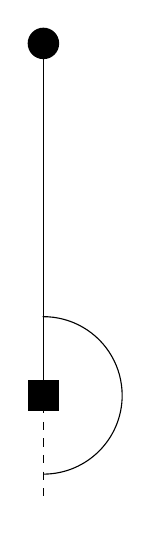
\begin{tikzpicture}
    \node (pivot) at (0,0) {};
    \fill[black] (-0.2,-0.2) rectangle (0.2,0.2);
    
    \node (pivotvertical) at (0,-1.5) {};
    \draw[dashed] (pivot) -- (pivotvertical);
    %\node (anglelabel) at (0.25,-1) {};
    
    \draw ([shift=(-90:1cm)]0,0) arc (-90:90.5:1cm);
    
    \node (bead) at (0,4.47) {};
    \fill[black] (bead) circle (0.2);
        
    \draw (pivot) -- (bead);
\end{tikzpicture}
\end{subfigure}
\caption{Schematic of the rigid pendulum model. (a) Geometry and forces. (b) The unstable up-vertical $\theta= \pi$ solution}
\label{penschematic}
\end{figure}
Let's consider a rigid pendulum: a bead of mass $m$ attached to a rigid rod of length $\ell$, depicted in \cref{penschematic}(a). Three forces act on the bead: its weight, $mg$; tension in the rod, $T$; and friction, which opposes the motion of the bead. 

The distance travelled by the bead is the arclength, $s=\ell \theta$. The velocity and acceleration are therefore
\begin{equation}
	\fd{s}{t} = \ell\fd{\theta}{t}, \quad \fdd{s}{t} = \ell\fdd{\theta}{t}.
\end{equation}
We say friction is proportional to velocity, $\nu\ell \, \fd{\theta}{t}$, and points in the direction opposing motion.

If we resolve parallel and perpendicular to the rod, given the rod makes an angle $\theta$ to the vertical, then:
\begin{subequations}
\begin{align}
\text{[parallel]} & & 0 &= T - mg\cos\theta, \\
\text{[perpendicular]} & & m \ell\fdd{\theta}{t} &= - \nu\ell \fd{\theta}{t} - mg\sin\theta,
\end{align}
\end{subequations}
the second equation of which can be rearranged to give
\begin{equation}
\label{peneq}
\fdd{\theta}{t} + \frac{\nu}{m} \fd{\theta}{t}+ \frac{g}{\ell}\sin\theta = 0. 
\end{equation} 
This is a nonlinear ODE; our physical intuition tells us that the pendulum will swing with a decreasing amplitude until it relaxes to $\theta=0$. 

\subsection{Solutions to the pendulum equation}
\begin{figure}
\begin{subfigure}[t]{0.49\textwidth}
	\centering
	%% Creator: Matplotlib, PGF backend
%%
%% To include the figure in your LaTeX document, write
%%   \input{<filename>.pgf}
%%
%% Make sure the required packages are loaded in your preamble
%%   \usepackage{pgf}
%%
%% Figures using additional raster images can only be included by \input if
%% they are in the same directory as the main LaTeX file. For loading figures
%% from other directories you can use the `import` package
%%   \usepackage{import}
%% and then include the figures with
%%   \import{<path to file>}{<filename>.pgf}
%%
%% Matplotlib used the following preamble
%%   \usepackage{fontspec}
%%   \setmainfont{DejaVuSerif.ttf}[Path=/Library/Python/3.7/site-packages/matplotlib/mpl-data/fonts/ttf/]
%%   \setsansfont{DejaVuSans.ttf}[Path=/Library/Python/3.7/site-packages/matplotlib/mpl-data/fonts/ttf/]
%%   \setmonofont{DejaVuSansMono.ttf}[Path=/Library/Python/3.7/site-packages/matplotlib/mpl-data/fonts/ttf/]
%%
\begingroup%
\makeatletter%
\begin{pgfpicture}%
\pgfpathrectangle{\pgfpointorigin}{\pgfqpoint{3.000000in}{2.200000in}}%
\pgfusepath{use as bounding box, clip}%
\begin{pgfscope}%
\pgfsetbuttcap%
\pgfsetmiterjoin%
\definecolor{currentfill}{rgb}{1.000000,1.000000,1.000000}%
\pgfsetfillcolor{currentfill}%
\pgfsetlinewidth{0.000000pt}%
\definecolor{currentstroke}{rgb}{1.000000,1.000000,1.000000}%
\pgfsetstrokecolor{currentstroke}%
\pgfsetdash{}{0pt}%
\pgfpathmoveto{\pgfqpoint{0.000000in}{0.000000in}}%
\pgfpathlineto{\pgfqpoint{3.000000in}{0.000000in}}%
\pgfpathlineto{\pgfqpoint{3.000000in}{2.200000in}}%
\pgfpathlineto{\pgfqpoint{0.000000in}{2.200000in}}%
\pgfpathclose%
\pgfusepath{fill}%
\end{pgfscope}%
\begin{pgfscope}%
\pgfsetbuttcap%
\pgfsetmiterjoin%
\definecolor{currentfill}{rgb}{1.000000,1.000000,1.000000}%
\pgfsetfillcolor{currentfill}%
\pgfsetlinewidth{0.000000pt}%
\definecolor{currentstroke}{rgb}{0.000000,0.000000,0.000000}%
\pgfsetstrokecolor{currentstroke}%
\pgfsetstrokeopacity{0.000000}%
\pgfsetdash{}{0pt}%
\pgfpathmoveto{\pgfqpoint{0.520469in}{0.137111in}}%
\pgfpathlineto{\pgfqpoint{2.966667in}{0.137111in}}%
\pgfpathlineto{\pgfqpoint{2.966667in}{2.166667in}}%
\pgfpathlineto{\pgfqpoint{0.520469in}{2.166667in}}%
\pgfpathclose%
\pgfusepath{fill}%
\end{pgfscope}%
\begin{pgfscope}%
\pgfpathrectangle{\pgfqpoint{0.520469in}{0.137111in}}{\pgfqpoint{2.446198in}{2.029556in}}%
\pgfusepath{clip}%
\pgfsetrectcap%
\pgfsetroundjoin%
\pgfsetlinewidth{1.505625pt}%
\definecolor{currentstroke}{rgb}{0.121569,0.466667,0.705882}%
\pgfsetstrokecolor{currentstroke}%
\pgfsetdash{}{0pt}%
\pgfpathmoveto{\pgfqpoint{0.520469in}{1.901942in}}%
\pgfpathlineto{\pgfqpoint{0.522893in}{1.900539in}}%
\pgfpathlineto{\pgfqpoint{0.525317in}{1.896350in}}%
\pgfpathlineto{\pgfqpoint{0.527742in}{1.889403in}}%
\pgfpathlineto{\pgfqpoint{0.530166in}{1.879725in}}%
\pgfpathlineto{\pgfqpoint{0.535015in}{1.852294in}}%
\pgfpathlineto{\pgfqpoint{0.539864in}{1.814310in}}%
\pgfpathlineto{\pgfqpoint{0.544713in}{1.766076in}}%
\pgfpathlineto{\pgfqpoint{0.549561in}{1.707989in}}%
\pgfpathlineto{\pgfqpoint{0.556835in}{1.603600in}}%
\pgfpathlineto{\pgfqpoint{0.564108in}{1.480896in}}%
\pgfpathlineto{\pgfqpoint{0.573805in}{1.295566in}}%
\pgfpathlineto{\pgfqpoint{0.600474in}{0.763061in}}%
\pgfpathlineto{\pgfqpoint{0.607747in}{0.640821in}}%
\pgfpathlineto{\pgfqpoint{0.615020in}{0.537677in}}%
\pgfpathlineto{\pgfqpoint{0.619869in}{0.480928in}}%
\pgfpathlineto{\pgfqpoint{0.624718in}{0.434413in}}%
\pgfpathlineto{\pgfqpoint{0.629567in}{0.398427in}}%
\pgfpathlineto{\pgfqpoint{0.634416in}{0.373107in}}%
\pgfpathlineto{\pgfqpoint{0.636840in}{0.364452in}}%
\pgfpathlineto{\pgfqpoint{0.639264in}{0.358457in}}%
\pgfpathlineto{\pgfqpoint{0.641689in}{0.355107in}}%
\pgfpathlineto{\pgfqpoint{0.644113in}{0.354382in}}%
\pgfpathlineto{\pgfqpoint{0.646538in}{0.356258in}}%
\pgfpathlineto{\pgfqpoint{0.648962in}{0.360704in}}%
\pgfpathlineto{\pgfqpoint{0.651386in}{0.367688in}}%
\pgfpathlineto{\pgfqpoint{0.653811in}{0.377169in}}%
\pgfpathlineto{\pgfqpoint{0.658660in}{0.403442in}}%
\pgfpathlineto{\pgfqpoint{0.663508in}{0.439101in}}%
\pgfpathlineto{\pgfqpoint{0.668357in}{0.483615in}}%
\pgfpathlineto{\pgfqpoint{0.675630in}{0.565505in}}%
\pgfpathlineto{\pgfqpoint{0.682904in}{0.662929in}}%
\pgfpathlineto{\pgfqpoint{0.692601in}{0.810471in}}%
\pgfpathlineto{\pgfqpoint{0.719270in}{1.231348in}}%
\pgfpathlineto{\pgfqpoint{0.726543in}{1.326898in}}%
\pgfpathlineto{\pgfqpoint{0.733816in}{1.406707in}}%
\pgfpathlineto{\pgfqpoint{0.738665in}{1.449932in}}%
\pgfpathlineto{\pgfqpoint{0.743514in}{1.484585in}}%
\pgfpathlineto{\pgfqpoint{0.748362in}{1.510353in}}%
\pgfpathlineto{\pgfqpoint{0.750787in}{1.519850in}}%
\pgfpathlineto{\pgfqpoint{0.753211in}{1.527075in}}%
\pgfpathlineto{\pgfqpoint{0.755636in}{1.532029in}}%
\pgfpathlineto{\pgfqpoint{0.758060in}{1.534720in}}%
\pgfpathlineto{\pgfqpoint{0.760484in}{1.535161in}}%
\pgfpathlineto{\pgfqpoint{0.762909in}{1.533374in}}%
\pgfpathlineto{\pgfqpoint{0.765333in}{1.529386in}}%
\pgfpathlineto{\pgfqpoint{0.767758in}{1.523232in}}%
\pgfpathlineto{\pgfqpoint{0.770182in}{1.514952in}}%
\pgfpathlineto{\pgfqpoint{0.775031in}{1.492210in}}%
\pgfpathlineto{\pgfqpoint{0.779880in}{1.461619in}}%
\pgfpathlineto{\pgfqpoint{0.784728in}{1.423753in}}%
\pgfpathlineto{\pgfqpoint{0.792002in}{1.354861in}}%
\pgfpathlineto{\pgfqpoint{0.799275in}{1.274045in}}%
\pgfpathlineto{\pgfqpoint{0.811397in}{1.122444in}}%
\pgfpathlineto{\pgfqpoint{0.828368in}{0.906292in}}%
\pgfpathlineto{\pgfqpoint{0.838065in}{0.798218in}}%
\pgfpathlineto{\pgfqpoint{0.845339in}{0.730641in}}%
\pgfpathlineto{\pgfqpoint{0.850187in}{0.693377in}}%
\pgfpathlineto{\pgfqpoint{0.855036in}{0.662955in}}%
\pgfpathlineto{\pgfqpoint{0.859885in}{0.639735in}}%
\pgfpathlineto{\pgfqpoint{0.864734in}{0.623940in}}%
\pgfpathlineto{\pgfqpoint{0.867158in}{0.618861in}}%
\pgfpathlineto{\pgfqpoint{0.869583in}{0.615664in}}%
\pgfpathlineto{\pgfqpoint{0.872007in}{0.614343in}}%
\pgfpathlineto{\pgfqpoint{0.874431in}{0.614884in}}%
\pgfpathlineto{\pgfqpoint{0.876856in}{0.617266in}}%
\pgfpathlineto{\pgfqpoint{0.879280in}{0.621461in}}%
\pgfpathlineto{\pgfqpoint{0.881705in}{0.627437in}}%
\pgfpathlineto{\pgfqpoint{0.886553in}{0.644561in}}%
\pgfpathlineto{\pgfqpoint{0.891402in}{0.668234in}}%
\pgfpathlineto{\pgfqpoint{0.896251in}{0.697953in}}%
\pgfpathlineto{\pgfqpoint{0.903524in}{0.752511in}}%
\pgfpathlineto{\pgfqpoint{0.910797in}{0.816826in}}%
\pgfpathlineto{\pgfqpoint{0.922919in}{0.937696in}}%
\pgfpathlineto{\pgfqpoint{0.939890in}{1.110044in}}%
\pgfpathlineto{\pgfqpoint{0.949588in}{1.196167in}}%
\pgfpathlineto{\pgfqpoint{0.956861in}{1.249923in}}%
\pgfpathlineto{\pgfqpoint{0.961710in}{1.279468in}}%
\pgfpathlineto{\pgfqpoint{0.966559in}{1.303459in}}%
\pgfpathlineto{\pgfqpoint{0.971408in}{1.321588in}}%
\pgfpathlineto{\pgfqpoint{0.976256in}{1.333656in}}%
\pgfpathlineto{\pgfqpoint{0.978681in}{1.337388in}}%
\pgfpathlineto{\pgfqpoint{0.981105in}{1.339582in}}%
\pgfpathlineto{\pgfqpoint{0.983530in}{1.340244in}}%
\pgfpathlineto{\pgfqpoint{0.985954in}{1.339386in}}%
\pgfpathlineto{\pgfqpoint{0.988378in}{1.337028in}}%
\pgfpathlineto{\pgfqpoint{0.990803in}{1.333194in}}%
\pgfpathlineto{\pgfqpoint{0.993227in}{1.327915in}}%
\pgfpathlineto{\pgfqpoint{0.998076in}{1.313175in}}%
\pgfpathlineto{\pgfqpoint{1.002925in}{1.293171in}}%
\pgfpathlineto{\pgfqpoint{1.007774in}{1.268355in}}%
\pgfpathlineto{\pgfqpoint{1.015047in}{1.223300in}}%
\pgfpathlineto{\pgfqpoint{1.022320in}{1.170760in}}%
\pgfpathlineto{\pgfqpoint{1.034442in}{1.073262in}}%
\pgfpathlineto{\pgfqpoint{1.051413in}{0.936634in}}%
\pgfpathlineto{\pgfqpoint{1.058686in}{0.885166in}}%
\pgfpathlineto{\pgfqpoint{1.065959in}{0.841106in}}%
\pgfpathlineto{\pgfqpoint{1.070808in}{0.816686in}}%
\pgfpathlineto{\pgfqpoint{1.075657in}{0.796681in}}%
\pgfpathlineto{\pgfqpoint{1.080506in}{0.781372in}}%
\pgfpathlineto{\pgfqpoint{1.085354in}{0.770944in}}%
\pgfpathlineto{\pgfqpoint{1.087779in}{0.767593in}}%
\pgfpathlineto{\pgfqpoint{1.090203in}{0.765488in}}%
\pgfpathlineto{\pgfqpoint{1.092628in}{0.764628in}}%
\pgfpathlineto{\pgfqpoint{1.095052in}{0.765004in}}%
\pgfpathlineto{\pgfqpoint{1.097476in}{0.766601in}}%
\pgfpathlineto{\pgfqpoint{1.099901in}{0.769400in}}%
\pgfpathlineto{\pgfqpoint{1.102325in}{0.773377in}}%
\pgfpathlineto{\pgfqpoint{1.107174in}{0.784741in}}%
\pgfpathlineto{\pgfqpoint{1.112023in}{0.800396in}}%
\pgfpathlineto{\pgfqpoint{1.116872in}{0.819973in}}%
\pgfpathlineto{\pgfqpoint{1.124145in}{0.855712in}}%
\pgfpathlineto{\pgfqpoint{1.131418in}{0.897540in}}%
\pgfpathlineto{\pgfqpoint{1.143540in}{0.975354in}}%
\pgfpathlineto{\pgfqpoint{1.160511in}{1.084662in}}%
\pgfpathlineto{\pgfqpoint{1.167784in}{1.125922in}}%
\pgfpathlineto{\pgfqpoint{1.175057in}{1.161282in}}%
\pgfpathlineto{\pgfqpoint{1.179906in}{1.180895in}}%
\pgfpathlineto{\pgfqpoint{1.184755in}{1.196967in}}%
\pgfpathlineto{\pgfqpoint{1.189604in}{1.209264in}}%
\pgfpathlineto{\pgfqpoint{1.194453in}{1.217629in}}%
\pgfpathlineto{\pgfqpoint{1.196877in}{1.220310in}}%
\pgfpathlineto{\pgfqpoint{1.199301in}{1.221986in}}%
\pgfpathlineto{\pgfqpoint{1.201726in}{1.222657in}}%
\pgfpathlineto{\pgfqpoint{1.204150in}{1.222331in}}%
\pgfpathlineto{\pgfqpoint{1.206575in}{1.221020in}}%
\pgfpathlineto{\pgfqpoint{1.208999in}{1.218739in}}%
\pgfpathlineto{\pgfqpoint{1.213848in}{1.211354in}}%
\pgfpathlineto{\pgfqpoint{1.218697in}{1.200389in}}%
\pgfpathlineto{\pgfqpoint{1.223545in}{1.186120in}}%
\pgfpathlineto{\pgfqpoint{1.228394in}{1.168882in}}%
\pgfpathlineto{\pgfqpoint{1.235667in}{1.138318in}}%
\pgfpathlineto{\pgfqpoint{1.245365in}{1.091138in}}%
\pgfpathlineto{\pgfqpoint{1.274458in}{0.943513in}}%
\pgfpathlineto{\pgfqpoint{1.281731in}{0.913766in}}%
\pgfpathlineto{\pgfqpoint{1.289004in}{0.889550in}}%
\pgfpathlineto{\pgfqpoint{1.293853in}{0.876930in}}%
\pgfpathlineto{\pgfqpoint{1.298702in}{0.867354in}}%
\pgfpathlineto{\pgfqpoint{1.303551in}{0.860945in}}%
\pgfpathlineto{\pgfqpoint{1.305975in}{0.858950in}}%
\pgfpathlineto{\pgfqpoint{1.308399in}{0.857763in}}%
\pgfpathlineto{\pgfqpoint{1.310824in}{0.857384in}}%
\pgfpathlineto{\pgfqpoint{1.313248in}{0.857805in}}%
\pgfpathlineto{\pgfqpoint{1.315673in}{0.859016in}}%
\pgfpathlineto{\pgfqpoint{1.318097in}{0.861005in}}%
\pgfpathlineto{\pgfqpoint{1.322946in}{0.867240in}}%
\pgfpathlineto{\pgfqpoint{1.327795in}{0.876332in}}%
\pgfpathlineto{\pgfqpoint{1.332644in}{0.888049in}}%
\pgfpathlineto{\pgfqpoint{1.339917in}{0.909929in}}%
\pgfpathlineto{\pgfqpoint{1.347190in}{0.935982in}}%
\pgfpathlineto{\pgfqpoint{1.356888in}{0.975015in}}%
\pgfpathlineto{\pgfqpoint{1.378707in}{1.064961in}}%
\pgfpathlineto{\pgfqpoint{1.385980in}{1.090893in}}%
\pgfpathlineto{\pgfqpoint{1.393254in}{1.112908in}}%
\pgfpathlineto{\pgfqpoint{1.398102in}{1.124980in}}%
\pgfpathlineto{\pgfqpoint{1.402951in}{1.134737in}}%
\pgfpathlineto{\pgfqpoint{1.407800in}{1.142034in}}%
\pgfpathlineto{\pgfqpoint{1.412649in}{1.146779in}}%
\pgfpathlineto{\pgfqpoint{1.415073in}{1.148180in}}%
\pgfpathlineto{\pgfqpoint{1.417498in}{1.148931in}}%
\pgfpathlineto{\pgfqpoint{1.419922in}{1.149036in}}%
\pgfpathlineto{\pgfqpoint{1.422346in}{1.148500in}}%
\pgfpathlineto{\pgfqpoint{1.424771in}{1.147332in}}%
\pgfpathlineto{\pgfqpoint{1.429620in}{1.143152in}}%
\pgfpathlineto{\pgfqpoint{1.434468in}{1.136626in}}%
\pgfpathlineto{\pgfqpoint{1.439317in}{1.127926in}}%
\pgfpathlineto{\pgfqpoint{1.444166in}{1.117265in}}%
\pgfpathlineto{\pgfqpoint{1.451439in}{1.098143in}}%
\pgfpathlineto{\pgfqpoint{1.461137in}{1.068314in}}%
\pgfpathlineto{\pgfqpoint{1.490230in}{0.973464in}}%
\pgfpathlineto{\pgfqpoint{1.497503in}{0.954040in}}%
\pgfpathlineto{\pgfqpoint{1.504776in}{0.938081in}}%
\pgfpathlineto{\pgfqpoint{1.509625in}{0.929670in}}%
\pgfpathlineto{\pgfqpoint{1.514474in}{0.923199in}}%
\pgfpathlineto{\pgfqpoint{1.519323in}{0.918755in}}%
\pgfpathlineto{\pgfqpoint{1.524171in}{0.916384in}}%
\pgfpathlineto{\pgfqpoint{1.529020in}{0.916091in}}%
\pgfpathlineto{\pgfqpoint{1.533869in}{0.917842in}}%
\pgfpathlineto{\pgfqpoint{1.538718in}{0.921561in}}%
\pgfpathlineto{\pgfqpoint{1.543567in}{0.927138in}}%
\pgfpathlineto{\pgfqpoint{1.548415in}{0.934425in}}%
\pgfpathlineto{\pgfqpoint{1.555689in}{0.948171in}}%
\pgfpathlineto{\pgfqpoint{1.562962in}{0.964660in}}%
\pgfpathlineto{\pgfqpoint{1.572659in}{0.989508in}}%
\pgfpathlineto{\pgfqpoint{1.596903in}{1.053048in}}%
\pgfpathlineto{\pgfqpoint{1.604177in}{1.069067in}}%
\pgfpathlineto{\pgfqpoint{1.611450in}{1.082423in}}%
\pgfpathlineto{\pgfqpoint{1.616299in}{1.089590in}}%
\pgfpathlineto{\pgfqpoint{1.621147in}{1.095230in}}%
\pgfpathlineto{\pgfqpoint{1.625996in}{1.099264in}}%
\pgfpathlineto{\pgfqpoint{1.630845in}{1.101643in}}%
\pgfpathlineto{\pgfqpoint{1.635694in}{1.102354in}}%
\pgfpathlineto{\pgfqpoint{1.640543in}{1.101417in}}%
\pgfpathlineto{\pgfqpoint{1.645391in}{1.098882in}}%
\pgfpathlineto{\pgfqpoint{1.650240in}{1.094830in}}%
\pgfpathlineto{\pgfqpoint{1.655089in}{1.089372in}}%
\pgfpathlineto{\pgfqpoint{1.662362in}{1.078849in}}%
\pgfpathlineto{\pgfqpoint{1.669635in}{1.066016in}}%
\pgfpathlineto{\pgfqpoint{1.679333in}{1.046418in}}%
\pgfpathlineto{\pgfqpoint{1.706002in}{0.990691in}}%
\pgfpathlineto{\pgfqpoint{1.713275in}{0.978157in}}%
\pgfpathlineto{\pgfqpoint{1.720548in}{0.967823in}}%
\pgfpathlineto{\pgfqpoint{1.725397in}{0.962354in}}%
\pgfpathlineto{\pgfqpoint{1.730246in}{0.958124in}}%
\pgfpathlineto{\pgfqpoint{1.735094in}{0.955191in}}%
\pgfpathlineto{\pgfqpoint{1.739943in}{0.953588in}}%
\pgfpathlineto{\pgfqpoint{1.744792in}{0.953320in}}%
\pgfpathlineto{\pgfqpoint{1.749641in}{0.954366in}}%
\pgfpathlineto{\pgfqpoint{1.754490in}{0.956679in}}%
\pgfpathlineto{\pgfqpoint{1.759338in}{0.960188in}}%
\pgfpathlineto{\pgfqpoint{1.764187in}{0.964801in}}%
\pgfpathlineto{\pgfqpoint{1.771460in}{0.973538in}}%
\pgfpathlineto{\pgfqpoint{1.778734in}{0.984049in}}%
\pgfpathlineto{\pgfqpoint{1.790856in}{1.004089in}}%
\pgfpathlineto{\pgfqpoint{1.810251in}{1.036919in}}%
\pgfpathlineto{\pgfqpoint{1.819948in}{1.050964in}}%
\pgfpathlineto{\pgfqpoint{1.827222in}{1.059573in}}%
\pgfpathlineto{\pgfqpoint{1.834495in}{1.066156in}}%
\pgfpathlineto{\pgfqpoint{1.839344in}{1.069302in}}%
\pgfpathlineto{\pgfqpoint{1.844192in}{1.071401in}}%
\pgfpathlineto{\pgfqpoint{1.849041in}{1.072431in}}%
\pgfpathlineto{\pgfqpoint{1.853890in}{1.072396in}}%
\pgfpathlineto{\pgfqpoint{1.858739in}{1.071315in}}%
\pgfpathlineto{\pgfqpoint{1.863588in}{1.069231in}}%
\pgfpathlineto{\pgfqpoint{1.868436in}{1.066205in}}%
\pgfpathlineto{\pgfqpoint{1.875710in}{1.060076in}}%
\pgfpathlineto{\pgfqpoint{1.882983in}{1.052336in}}%
\pgfpathlineto{\pgfqpoint{1.892681in}{1.040188in}}%
\pgfpathlineto{\pgfqpoint{1.924198in}{0.998396in}}%
\pgfpathlineto{\pgfqpoint{1.931471in}{0.990782in}}%
\pgfpathlineto{\pgfqpoint{1.938744in}{0.984663in}}%
\pgfpathlineto{\pgfqpoint{1.946017in}{0.980268in}}%
\pgfpathlineto{\pgfqpoint{1.950866in}{0.978369in}}%
\pgfpathlineto{\pgfqpoint{1.955715in}{0.977323in}}%
\pgfpathlineto{\pgfqpoint{1.960564in}{0.977132in}}%
\pgfpathlineto{\pgfqpoint{1.965413in}{0.977784in}}%
\pgfpathlineto{\pgfqpoint{1.970261in}{0.979249in}}%
\pgfpathlineto{\pgfqpoint{1.977535in}{0.982868in}}%
\pgfpathlineto{\pgfqpoint{1.984808in}{0.988002in}}%
\pgfpathlineto{\pgfqpoint{1.994505in}{0.996726in}}%
\pgfpathlineto{\pgfqpoint{2.006627in}{1.009552in}}%
\pgfpathlineto{\pgfqpoint{2.028447in}{1.032986in}}%
\pgfpathlineto{\pgfqpoint{2.038145in}{1.041571in}}%
\pgfpathlineto{\pgfqpoint{2.045418in}{1.046686in}}%
\pgfpathlineto{\pgfqpoint{2.052691in}{1.050448in}}%
\pgfpathlineto{\pgfqpoint{2.059964in}{1.052732in}}%
\pgfpathlineto{\pgfqpoint{2.067238in}{1.053479in}}%
\pgfpathlineto{\pgfqpoint{2.074511in}{1.052702in}}%
\pgfpathlineto{\pgfqpoint{2.081784in}{1.050482in}}%
\pgfpathlineto{\pgfqpoint{2.089057in}{1.046957in}}%
\pgfpathlineto{\pgfqpoint{2.096330in}{1.042324in}}%
\pgfpathlineto{\pgfqpoint{2.106028in}{1.034836in}}%
\pgfpathlineto{\pgfqpoint{2.125423in}{1.017848in}}%
\pgfpathlineto{\pgfqpoint{2.137545in}{1.007832in}}%
\pgfpathlineto{\pgfqpoint{2.147243in}{1.001141in}}%
\pgfpathlineto{\pgfqpoint{2.154516in}{0.997216in}}%
\pgfpathlineto{\pgfqpoint{2.161789in}{0.994395in}}%
\pgfpathlineto{\pgfqpoint{2.169062in}{0.992769in}}%
\pgfpathlineto{\pgfqpoint{2.176336in}{0.992374in}}%
\pgfpathlineto{\pgfqpoint{2.183609in}{0.993192in}}%
\pgfpathlineto{\pgfqpoint{2.190882in}{0.995152in}}%
\pgfpathlineto{\pgfqpoint{2.198155in}{0.998131in}}%
\pgfpathlineto{\pgfqpoint{2.207853in}{1.003406in}}%
\pgfpathlineto{\pgfqpoint{2.219975in}{1.011416in}}%
\pgfpathlineto{\pgfqpoint{2.246643in}{1.029615in}}%
\pgfpathlineto{\pgfqpoint{2.256341in}{1.034819in}}%
\pgfpathlineto{\pgfqpoint{2.266039in}{1.038625in}}%
\pgfpathlineto{\pgfqpoint{2.273312in}{1.040412in}}%
\pgfpathlineto{\pgfqpoint{2.280585in}{1.041222in}}%
\pgfpathlineto{\pgfqpoint{2.287858in}{1.041048in}}%
\pgfpathlineto{\pgfqpoint{2.295131in}{1.039927in}}%
\pgfpathlineto{\pgfqpoint{2.304829in}{1.037099in}}%
\pgfpathlineto{\pgfqpoint{2.314527in}{1.033010in}}%
\pgfpathlineto{\pgfqpoint{2.329073in}{1.025336in}}%
\pgfpathlineto{\pgfqpoint{2.353317in}{1.012038in}}%
\pgfpathlineto{\pgfqpoint{2.365439in}{1.006840in}}%
\pgfpathlineto{\pgfqpoint{2.375137in}{1.003949in}}%
\pgfpathlineto{\pgfqpoint{2.384834in}{1.002388in}}%
\pgfpathlineto{\pgfqpoint{2.394532in}{1.002225in}}%
\pgfpathlineto{\pgfqpoint{2.404229in}{1.003419in}}%
\pgfpathlineto{\pgfqpoint{2.413927in}{1.005823in}}%
\pgfpathlineto{\pgfqpoint{2.426049in}{1.010165in}}%
\pgfpathlineto{\pgfqpoint{2.445444in}{1.018743in}}%
\pgfpathlineto{\pgfqpoint{2.462415in}{1.025990in}}%
\pgfpathlineto{\pgfqpoint{2.474537in}{1.030024in}}%
\pgfpathlineto{\pgfqpoint{2.484235in}{1.032210in}}%
\pgfpathlineto{\pgfqpoint{2.493932in}{1.033321in}}%
\pgfpathlineto{\pgfqpoint{2.503630in}{1.033311in}}%
\pgfpathlineto{\pgfqpoint{2.513328in}{1.032226in}}%
\pgfpathlineto{\pgfqpoint{2.525450in}{1.029558in}}%
\pgfpathlineto{\pgfqpoint{2.539996in}{1.024970in}}%
\pgfpathlineto{\pgfqpoint{2.576362in}{1.012609in}}%
\pgfpathlineto{\pgfqpoint{2.588484in}{1.009933in}}%
\pgfpathlineto{\pgfqpoint{2.600606in}{1.008548in}}%
\pgfpathlineto{\pgfqpoint{2.610304in}{1.008444in}}%
\pgfpathlineto{\pgfqpoint{2.622426in}{1.009528in}}%
\pgfpathlineto{\pgfqpoint{2.634548in}{1.011767in}}%
\pgfpathlineto{\pgfqpoint{2.651519in}{1.016204in}}%
\pgfpathlineto{\pgfqpoint{2.683036in}{1.024801in}}%
\pgfpathlineto{\pgfqpoint{2.697582in}{1.027365in}}%
\pgfpathlineto{\pgfqpoint{2.709704in}{1.028363in}}%
\pgfpathlineto{\pgfqpoint{2.721826in}{1.028244in}}%
\pgfpathlineto{\pgfqpoint{2.733948in}{1.027077in}}%
\pgfpathlineto{\pgfqpoint{2.748495in}{1.024571in}}%
\pgfpathlineto{\pgfqpoint{2.780012in}{1.017457in}}%
\pgfpathlineto{\pgfqpoint{2.796983in}{1.014317in}}%
\pgfpathlineto{\pgfqpoint{2.811529in}{1.012742in}}%
\pgfpathlineto{\pgfqpoint{2.826076in}{1.012428in}}%
\pgfpathlineto{\pgfqpoint{2.840622in}{1.013357in}}%
\pgfpathlineto{\pgfqpoint{2.857593in}{1.015690in}}%
\pgfpathlineto{\pgfqpoint{2.910930in}{1.024338in}}%
\pgfpathlineto{\pgfqpoint{2.925476in}{1.025187in}}%
\pgfpathlineto{\pgfqpoint{2.940022in}{1.025011in}}%
\pgfpathlineto{\pgfqpoint{2.942447in}{1.024886in}}%
\pgfpathlineto{\pgfqpoint{2.942447in}{1.024886in}}%
\pgfusepath{stroke}%
\end{pgfscope}%
\begin{pgfscope}%
\pgfsetbuttcap%
\pgfsetroundjoin%
\definecolor{currentfill}{rgb}{0.000000,0.000000,0.000000}%
\pgfsetfillcolor{currentfill}%
\pgfsetlinewidth{0.803000pt}%
\definecolor{currentstroke}{rgb}{0.000000,0.000000,0.000000}%
\pgfsetstrokecolor{currentstroke}%
\pgfsetdash{}{0pt}%
\pgfsys@defobject{currentmarker}{\pgfqpoint{0.000000in}{-0.048611in}}{\pgfqpoint{0.000000in}{0.000000in}}{%
\pgfpathmoveto{\pgfqpoint{0.000000in}{0.000000in}}%
\pgfpathlineto{\pgfqpoint{0.000000in}{-0.048611in}}%
\pgfusepath{stroke,fill}%
}%
\begin{pgfscope}%
\pgfsys@transformshift{0.520469in}{1.019526in}%
\pgfsys@useobject{currentmarker}{}%
\end{pgfscope}%
\end{pgfscope}%
\begin{pgfscope}%
\definecolor{textcolor}{rgb}{0.000000,0.000000,0.000000}%
\pgfsetstrokecolor{textcolor}%
\pgfsetfillcolor{textcolor}%
\pgftext[x=0.520469in,y=0.922304in,,top]{\color{textcolor}\rmfamily\fontsize{12.000000}{14.400000}\selectfont \(\displaystyle 0\)}%
\end{pgfscope}%
\begin{pgfscope}%
\pgfsetbuttcap%
\pgfsetroundjoin%
\definecolor{currentfill}{rgb}{0.000000,0.000000,0.000000}%
\pgfsetfillcolor{currentfill}%
\pgfsetlinewidth{0.803000pt}%
\definecolor{currentstroke}{rgb}{0.000000,0.000000,0.000000}%
\pgfsetstrokecolor{currentstroke}%
\pgfsetdash{}{0pt}%
\pgfsys@defobject{currentmarker}{\pgfqpoint{0.000000in}{-0.048611in}}{\pgfqpoint{0.000000in}{0.000000in}}{%
\pgfpathmoveto{\pgfqpoint{0.000000in}{0.000000in}}%
\pgfpathlineto{\pgfqpoint{0.000000in}{-0.048611in}}%
\pgfusepath{stroke,fill}%
}%
\begin{pgfscope}%
\pgfsys@transformshift{1.489260in}{1.019526in}%
\pgfsys@useobject{currentmarker}{}%
\end{pgfscope}%
\end{pgfscope}%
\begin{pgfscope}%
\definecolor{textcolor}{rgb}{0.000000,0.000000,0.000000}%
\pgfsetstrokecolor{textcolor}%
\pgfsetfillcolor{textcolor}%
\pgftext[x=1.489260in,y=0.922304in,,top]{\color{textcolor}\rmfamily\fontsize{12.000000}{14.400000}\selectfont \(\displaystyle 20\)}%
\end{pgfscope}%
\begin{pgfscope}%
\pgfsetbuttcap%
\pgfsetroundjoin%
\definecolor{currentfill}{rgb}{0.000000,0.000000,0.000000}%
\pgfsetfillcolor{currentfill}%
\pgfsetlinewidth{0.803000pt}%
\definecolor{currentstroke}{rgb}{0.000000,0.000000,0.000000}%
\pgfsetstrokecolor{currentstroke}%
\pgfsetdash{}{0pt}%
\pgfsys@defobject{currentmarker}{\pgfqpoint{0.000000in}{-0.048611in}}{\pgfqpoint{0.000000in}{0.000000in}}{%
\pgfpathmoveto{\pgfqpoint{0.000000in}{0.000000in}}%
\pgfpathlineto{\pgfqpoint{0.000000in}{-0.048611in}}%
\pgfusepath{stroke,fill}%
}%
\begin{pgfscope}%
\pgfsys@transformshift{2.458051in}{1.019526in}%
\pgfsys@useobject{currentmarker}{}%
\end{pgfscope}%
\end{pgfscope}%
\begin{pgfscope}%
\definecolor{textcolor}{rgb}{0.000000,0.000000,0.000000}%
\pgfsetstrokecolor{textcolor}%
\pgfsetfillcolor{textcolor}%
\pgftext[x=2.458051in,y=0.922304in,,top]{\color{textcolor}\rmfamily\fontsize{12.000000}{14.400000}\selectfont \(\displaystyle 40\)}%
\end{pgfscope}%
\begin{pgfscope}%
\pgfsetbuttcap%
\pgfsetroundjoin%
\definecolor{currentfill}{rgb}{0.000000,0.000000,0.000000}%
\pgfsetfillcolor{currentfill}%
\pgfsetlinewidth{0.803000pt}%
\definecolor{currentstroke}{rgb}{0.000000,0.000000,0.000000}%
\pgfsetstrokecolor{currentstroke}%
\pgfsetdash{}{0pt}%
\pgfsys@defobject{currentmarker}{\pgfqpoint{-0.048611in}{0.000000in}}{\pgfqpoint{0.000000in}{0.000000in}}{%
\pgfpathmoveto{\pgfqpoint{0.000000in}{0.000000in}}%
\pgfpathlineto{\pgfqpoint{-0.048611in}{0.000000in}}%
\pgfusepath{stroke,fill}%
}%
\begin{pgfscope}%
\pgfsys@transformshift{0.520469in}{0.137111in}%
\pgfsys@useobject{currentmarker}{}%
\end{pgfscope}%
\end{pgfscope}%
\begin{pgfscope}%
\definecolor{textcolor}{rgb}{0.000000,0.000000,0.000000}%
\pgfsetstrokecolor{textcolor}%
\pgfsetfillcolor{textcolor}%
\pgftext[x=0.031871in,y=0.074611in,left,base]{\color{textcolor}\rmfamily\fontsize{12.000000}{14.400000}\selectfont \(\displaystyle -\pi/2\)}%
\end{pgfscope}%
\begin{pgfscope}%
\pgfsetbuttcap%
\pgfsetroundjoin%
\definecolor{currentfill}{rgb}{0.000000,0.000000,0.000000}%
\pgfsetfillcolor{currentfill}%
\pgfsetlinewidth{0.803000pt}%
\definecolor{currentstroke}{rgb}{0.000000,0.000000,0.000000}%
\pgfsetstrokecolor{currentstroke}%
\pgfsetdash{}{0pt}%
\pgfsys@defobject{currentmarker}{\pgfqpoint{-0.048611in}{0.000000in}}{\pgfqpoint{0.000000in}{0.000000in}}{%
\pgfpathmoveto{\pgfqpoint{0.000000in}{0.000000in}}%
\pgfpathlineto{\pgfqpoint{-0.048611in}{0.000000in}}%
\pgfusepath{stroke,fill}%
}%
\begin{pgfscope}%
\pgfsys@transformshift{0.520469in}{0.578319in}%
\pgfsys@useobject{currentmarker}{}%
\end{pgfscope}%
\end{pgfscope}%
\begin{pgfscope}%
\definecolor{textcolor}{rgb}{0.000000,0.000000,0.000000}%
\pgfsetstrokecolor{textcolor}%
\pgfsetfillcolor{textcolor}%
\pgftext[x=0.031871in,y=0.515819in,left,base]{\color{textcolor}\rmfamily\fontsize{12.000000}{14.400000}\selectfont \(\displaystyle -\pi/4\)}%
\end{pgfscope}%
\begin{pgfscope}%
\pgfsetbuttcap%
\pgfsetroundjoin%
\definecolor{currentfill}{rgb}{0.000000,0.000000,0.000000}%
\pgfsetfillcolor{currentfill}%
\pgfsetlinewidth{0.803000pt}%
\definecolor{currentstroke}{rgb}{0.000000,0.000000,0.000000}%
\pgfsetstrokecolor{currentstroke}%
\pgfsetdash{}{0pt}%
\pgfsys@defobject{currentmarker}{\pgfqpoint{-0.048611in}{0.000000in}}{\pgfqpoint{0.000000in}{0.000000in}}{%
\pgfpathmoveto{\pgfqpoint{0.000000in}{0.000000in}}%
\pgfpathlineto{\pgfqpoint{-0.048611in}{0.000000in}}%
\pgfusepath{stroke,fill}%
}%
\begin{pgfscope}%
\pgfsys@transformshift{0.520469in}{1.019526in}%
\pgfsys@useobject{currentmarker}{}%
\end{pgfscope}%
\end{pgfscope}%
\begin{pgfscope}%
\definecolor{textcolor}{rgb}{0.000000,0.000000,0.000000}%
\pgfsetstrokecolor{textcolor}%
\pgfsetfillcolor{textcolor}%
\pgftext[x=0.317208in,y=0.956213in,left,base]{\color{textcolor}\rmfamily\fontsize{12.000000}{14.400000}\selectfont 0}%
\end{pgfscope}%
\begin{pgfscope}%
\pgfsetbuttcap%
\pgfsetroundjoin%
\definecolor{currentfill}{rgb}{0.000000,0.000000,0.000000}%
\pgfsetfillcolor{currentfill}%
\pgfsetlinewidth{0.803000pt}%
\definecolor{currentstroke}{rgb}{0.000000,0.000000,0.000000}%
\pgfsetstrokecolor{currentstroke}%
\pgfsetdash{}{0pt}%
\pgfsys@defobject{currentmarker}{\pgfqpoint{-0.048611in}{0.000000in}}{\pgfqpoint{0.000000in}{0.000000in}}{%
\pgfpathmoveto{\pgfqpoint{0.000000in}{0.000000in}}%
\pgfpathlineto{\pgfqpoint{-0.048611in}{0.000000in}}%
\pgfusepath{stroke,fill}%
}%
\begin{pgfscope}%
\pgfsys@transformshift{0.520469in}{1.460734in}%
\pgfsys@useobject{currentmarker}{}%
\end{pgfscope}%
\end{pgfscope}%
\begin{pgfscope}%
\definecolor{textcolor}{rgb}{0.000000,0.000000,0.000000}%
\pgfsetstrokecolor{textcolor}%
\pgfsetfillcolor{textcolor}%
\pgftext[x=0.161501in,y=1.398234in,left,base]{\color{textcolor}\rmfamily\fontsize{12.000000}{14.400000}\selectfont \(\displaystyle \pi/4\)}%
\end{pgfscope}%
\begin{pgfscope}%
\pgfsetbuttcap%
\pgfsetroundjoin%
\definecolor{currentfill}{rgb}{0.000000,0.000000,0.000000}%
\pgfsetfillcolor{currentfill}%
\pgfsetlinewidth{0.803000pt}%
\definecolor{currentstroke}{rgb}{0.000000,0.000000,0.000000}%
\pgfsetstrokecolor{currentstroke}%
\pgfsetdash{}{0pt}%
\pgfsys@defobject{currentmarker}{\pgfqpoint{-0.048611in}{0.000000in}}{\pgfqpoint{0.000000in}{0.000000in}}{%
\pgfpathmoveto{\pgfqpoint{0.000000in}{0.000000in}}%
\pgfpathlineto{\pgfqpoint{-0.048611in}{0.000000in}}%
\pgfusepath{stroke,fill}%
}%
\begin{pgfscope}%
\pgfsys@transformshift{0.520469in}{1.901942in}%
\pgfsys@useobject{currentmarker}{}%
\end{pgfscope}%
\end{pgfscope}%
\begin{pgfscope}%
\definecolor{textcolor}{rgb}{0.000000,0.000000,0.000000}%
\pgfsetstrokecolor{textcolor}%
\pgfsetfillcolor{textcolor}%
\pgftext[x=0.161501in,y=1.839442in,left,base]{\color{textcolor}\rmfamily\fontsize{12.000000}{14.400000}\selectfont \(\displaystyle \pi/2\)}%
\end{pgfscope}%
\begin{pgfscope}%
\pgfsetrectcap%
\pgfsetmiterjoin%
\pgfsetlinewidth{0.803000pt}%
\definecolor{currentstroke}{rgb}{0.000000,0.000000,0.000000}%
\pgfsetstrokecolor{currentstroke}%
\pgfsetdash{}{0pt}%
\pgfpathmoveto{\pgfqpoint{0.520469in}{0.137111in}}%
\pgfpathlineto{\pgfqpoint{0.520469in}{2.166667in}}%
\pgfusepath{stroke}%
\end{pgfscope}%
\begin{pgfscope}%
\pgfsetrectcap%
\pgfsetmiterjoin%
\pgfsetlinewidth{0.803000pt}%
\definecolor{currentstroke}{rgb}{0.000000,0.000000,0.000000}%
\pgfsetstrokecolor{currentstroke}%
\pgfsetdash{}{0pt}%
\pgfpathmoveto{\pgfqpoint{0.520469in}{1.019526in}}%
\pgfpathlineto{\pgfqpoint{2.966667in}{1.019526in}}%
\pgfusepath{stroke}%
\end{pgfscope}%
\begin{pgfscope}%
\definecolor{textcolor}{rgb}{0.000000,0.000000,0.000000}%
\pgfsetstrokecolor{textcolor}%
\pgfsetfillcolor{textcolor}%
\pgftext[x=2.966667in,y=0.932893in,right,top]{\color{textcolor}\rmfamily\fontsize{12.000000}{14.400000}\selectfont \(\displaystyle t\)}%
\end{pgfscope}%
\begin{pgfscope}%
\definecolor{textcolor}{rgb}{0.000000,0.000000,0.000000}%
\pgfsetstrokecolor{textcolor}%
\pgfsetfillcolor{textcolor}%
\pgftext[x=0.423246in,y=2.166667in,right,top]{\color{textcolor}\rmfamily\fontsize{12.000000}{14.400000}\selectfont \(\displaystyle \theta\)}%
\end{pgfscope}%
\end{pgfpicture}%
\makeatother%
\endgroup%

\end{subfigure}
\begin{subfigure}[t]{0.49\textwidth}
	\centering
	%% Creator: Matplotlib, PGF backend
%%
%% To include the figure in your LaTeX document, write
%%   \input{<filename>.pgf}
%%
%% Make sure the required packages are loaded in your preamble
%%   \usepackage{pgf}
%%
%% Figures using additional raster images can only be included by \input if
%% they are in the same directory as the main LaTeX file. For loading figures
%% from other directories you can use the `import` package
%%   \usepackage{import}
%% and then include the figures with
%%   \import{<path to file>}{<filename>.pgf}
%%
%% Matplotlib used the following preamble
%%   \usepackage{fontspec}
%%   \setmainfont{DejaVuSerif.ttf}[Path=/Library/Python/3.7/site-packages/matplotlib/mpl-data/fonts/ttf/]
%%   \setsansfont{DejaVuSans.ttf}[Path=/Library/Python/3.7/site-packages/matplotlib/mpl-data/fonts/ttf/]
%%   \setmonofont{DejaVuSansMono.ttf}[Path=/Library/Python/3.7/site-packages/matplotlib/mpl-data/fonts/ttf/]
%%
\begingroup%
\makeatletter%
\begin{pgfpicture}%
\pgfpathrectangle{\pgfpointorigin}{\pgfqpoint{3.000000in}{2.200000in}}%
\pgfusepath{use as bounding box, clip}%
\begin{pgfscope}%
\pgfsetbuttcap%
\pgfsetmiterjoin%
\definecolor{currentfill}{rgb}{1.000000,1.000000,1.000000}%
\pgfsetfillcolor{currentfill}%
\pgfsetlinewidth{0.000000pt}%
\definecolor{currentstroke}{rgb}{1.000000,1.000000,1.000000}%
\pgfsetstrokecolor{currentstroke}%
\pgfsetdash{}{0pt}%
\pgfpathmoveto{\pgfqpoint{0.000000in}{0.000000in}}%
\pgfpathlineto{\pgfqpoint{3.000000in}{0.000000in}}%
\pgfpathlineto{\pgfqpoint{3.000000in}{2.200000in}}%
\pgfpathlineto{\pgfqpoint{0.000000in}{2.200000in}}%
\pgfpathclose%
\pgfusepath{fill}%
\end{pgfscope}%
\begin{pgfscope}%
\pgfsetbuttcap%
\pgfsetmiterjoin%
\definecolor{currentfill}{rgb}{1.000000,1.000000,1.000000}%
\pgfsetfillcolor{currentfill}%
\pgfsetlinewidth{0.000000pt}%
\definecolor{currentstroke}{rgb}{0.000000,0.000000,0.000000}%
\pgfsetstrokecolor{currentstroke}%
\pgfsetstrokeopacity{0.000000}%
\pgfsetdash{}{0pt}%
\pgfpathmoveto{\pgfqpoint{0.520469in}{0.137111in}}%
\pgfpathlineto{\pgfqpoint{2.966667in}{0.137111in}}%
\pgfpathlineto{\pgfqpoint{2.966667in}{2.166667in}}%
\pgfpathlineto{\pgfqpoint{0.520469in}{2.166667in}}%
\pgfpathclose%
\pgfusepath{fill}%
\end{pgfscope}%
\begin{pgfscope}%
\pgfpathrectangle{\pgfqpoint{0.520469in}{0.137111in}}{\pgfqpoint{2.446198in}{2.029556in}}%
\pgfusepath{clip}%
\pgfsetrectcap%
\pgfsetroundjoin%
\pgfsetlinewidth{1.505625pt}%
\definecolor{currentstroke}{rgb}{0.121569,0.466667,0.705882}%
\pgfsetstrokecolor{currentstroke}%
\pgfsetdash{}{0pt}%
\pgfpathmoveto{\pgfqpoint{0.520469in}{1.901942in}}%
\pgfpathlineto{\pgfqpoint{0.522893in}{1.900743in}}%
\pgfpathlineto{\pgfqpoint{0.525317in}{1.897802in}}%
\pgfpathlineto{\pgfqpoint{0.530166in}{1.889167in}}%
\pgfpathlineto{\pgfqpoint{0.539864in}{1.867997in}}%
\pgfpathlineto{\pgfqpoint{0.612596in}{1.703133in}}%
\pgfpathlineto{\pgfqpoint{0.641689in}{1.640795in}}%
\pgfpathlineto{\pgfqpoint{0.668357in}{1.586423in}}%
\pgfpathlineto{\pgfqpoint{0.692601in}{1.539620in}}%
\pgfpathlineto{\pgfqpoint{0.714421in}{1.499802in}}%
\pgfpathlineto{\pgfqpoint{0.736240in}{1.462256in}}%
\pgfpathlineto{\pgfqpoint{0.758060in}{1.427016in}}%
\pgfpathlineto{\pgfqpoint{0.779880in}{1.394075in}}%
\pgfpathlineto{\pgfqpoint{0.799275in}{1.366695in}}%
\pgfpathlineto{\pgfqpoint{0.818670in}{1.341057in}}%
\pgfpathlineto{\pgfqpoint{0.838065in}{1.317102in}}%
\pgfpathlineto{\pgfqpoint{0.857461in}{1.294764in}}%
\pgfpathlineto{\pgfqpoint{0.876856in}{1.273967in}}%
\pgfpathlineto{\pgfqpoint{0.896251in}{1.254634in}}%
\pgfpathlineto{\pgfqpoint{0.918071in}{1.234533in}}%
\pgfpathlineto{\pgfqpoint{0.939890in}{1.216069in}}%
\pgfpathlineto{\pgfqpoint{0.961710in}{1.199126in}}%
\pgfpathlineto{\pgfqpoint{0.983530in}{1.183594in}}%
\pgfpathlineto{\pgfqpoint{1.005349in}{1.169368in}}%
\pgfpathlineto{\pgfqpoint{1.029593in}{1.154971in}}%
\pgfpathlineto{\pgfqpoint{1.053837in}{1.141930in}}%
\pgfpathlineto{\pgfqpoint{1.078081in}{1.130126in}}%
\pgfpathlineto{\pgfqpoint{1.104750in}{1.118436in}}%
\pgfpathlineto{\pgfqpoint{1.131418in}{1.107969in}}%
\pgfpathlineto{\pgfqpoint{1.160511in}{1.097800in}}%
\pgfpathlineto{\pgfqpoint{1.189604in}{1.088793in}}%
\pgfpathlineto{\pgfqpoint{1.221121in}{1.080195in}}%
\pgfpathlineto{\pgfqpoint{1.255063in}{1.072122in}}%
\pgfpathlineto{\pgfqpoint{1.291429in}{1.064657in}}%
\pgfpathlineto{\pgfqpoint{1.330219in}{1.057856in}}%
\pgfpathlineto{\pgfqpoint{1.371434in}{1.051748in}}%
\pgfpathlineto{\pgfqpoint{1.417498in}{1.046064in}}%
\pgfpathlineto{\pgfqpoint{1.468410in}{1.040940in}}%
\pgfpathlineto{\pgfqpoint{1.524171in}{1.036456in}}%
\pgfpathlineto{\pgfqpoint{1.587206in}{1.032506in}}%
\pgfpathlineto{\pgfqpoint{1.659938in}{1.029080in}}%
\pgfpathlineto{\pgfqpoint{1.747216in}{1.026139in}}%
\pgfpathlineto{\pgfqpoint{1.851466in}{1.023788in}}%
\pgfpathlineto{\pgfqpoint{1.984808in}{1.021956in}}%
\pgfpathlineto{\pgfqpoint{2.166638in}{1.020655in}}%
\pgfpathlineto{\pgfqpoint{2.450293in}{1.019868in}}%
\pgfpathlineto{\pgfqpoint{2.942447in}{1.019569in}}%
\pgfpathlineto{\pgfqpoint{2.942447in}{1.019569in}}%
\pgfusepath{stroke}%
\end{pgfscope}%
\begin{pgfscope}%
\pgfsetbuttcap%
\pgfsetroundjoin%
\definecolor{currentfill}{rgb}{0.000000,0.000000,0.000000}%
\pgfsetfillcolor{currentfill}%
\pgfsetlinewidth{0.803000pt}%
\definecolor{currentstroke}{rgb}{0.000000,0.000000,0.000000}%
\pgfsetstrokecolor{currentstroke}%
\pgfsetdash{}{0pt}%
\pgfsys@defobject{currentmarker}{\pgfqpoint{0.000000in}{-0.048611in}}{\pgfqpoint{0.000000in}{0.000000in}}{%
\pgfpathmoveto{\pgfqpoint{0.000000in}{0.000000in}}%
\pgfpathlineto{\pgfqpoint{0.000000in}{-0.048611in}}%
\pgfusepath{stroke,fill}%
}%
\begin{pgfscope}%
\pgfsys@transformshift{0.520469in}{1.019526in}%
\pgfsys@useobject{currentmarker}{}%
\end{pgfscope}%
\end{pgfscope}%
\begin{pgfscope}%
\definecolor{textcolor}{rgb}{0.000000,0.000000,0.000000}%
\pgfsetstrokecolor{textcolor}%
\pgfsetfillcolor{textcolor}%
\pgftext[x=0.520469in,y=0.922304in,,top]{\color{textcolor}\rmfamily\fontsize{12.000000}{14.400000}\selectfont \(\displaystyle 0\)}%
\end{pgfscope}%
\begin{pgfscope}%
\pgfsetbuttcap%
\pgfsetroundjoin%
\definecolor{currentfill}{rgb}{0.000000,0.000000,0.000000}%
\pgfsetfillcolor{currentfill}%
\pgfsetlinewidth{0.803000pt}%
\definecolor{currentstroke}{rgb}{0.000000,0.000000,0.000000}%
\pgfsetstrokecolor{currentstroke}%
\pgfsetdash{}{0pt}%
\pgfsys@defobject{currentmarker}{\pgfqpoint{0.000000in}{-0.048611in}}{\pgfqpoint{0.000000in}{0.000000in}}{%
\pgfpathmoveto{\pgfqpoint{0.000000in}{0.000000in}}%
\pgfpathlineto{\pgfqpoint{0.000000in}{-0.048611in}}%
\pgfusepath{stroke,fill}%
}%
\begin{pgfscope}%
\pgfsys@transformshift{1.489260in}{1.019526in}%
\pgfsys@useobject{currentmarker}{}%
\end{pgfscope}%
\end{pgfscope}%
\begin{pgfscope}%
\definecolor{textcolor}{rgb}{0.000000,0.000000,0.000000}%
\pgfsetstrokecolor{textcolor}%
\pgfsetfillcolor{textcolor}%
\pgftext[x=1.489260in,y=0.922304in,,top]{\color{textcolor}\rmfamily\fontsize{12.000000}{14.400000}\selectfont \(\displaystyle 20\)}%
\end{pgfscope}%
\begin{pgfscope}%
\pgfsetbuttcap%
\pgfsetroundjoin%
\definecolor{currentfill}{rgb}{0.000000,0.000000,0.000000}%
\pgfsetfillcolor{currentfill}%
\pgfsetlinewidth{0.803000pt}%
\definecolor{currentstroke}{rgb}{0.000000,0.000000,0.000000}%
\pgfsetstrokecolor{currentstroke}%
\pgfsetdash{}{0pt}%
\pgfsys@defobject{currentmarker}{\pgfqpoint{0.000000in}{-0.048611in}}{\pgfqpoint{0.000000in}{0.000000in}}{%
\pgfpathmoveto{\pgfqpoint{0.000000in}{0.000000in}}%
\pgfpathlineto{\pgfqpoint{0.000000in}{-0.048611in}}%
\pgfusepath{stroke,fill}%
}%
\begin{pgfscope}%
\pgfsys@transformshift{2.458051in}{1.019526in}%
\pgfsys@useobject{currentmarker}{}%
\end{pgfscope}%
\end{pgfscope}%
\begin{pgfscope}%
\definecolor{textcolor}{rgb}{0.000000,0.000000,0.000000}%
\pgfsetstrokecolor{textcolor}%
\pgfsetfillcolor{textcolor}%
\pgftext[x=2.458051in,y=0.922304in,,top]{\color{textcolor}\rmfamily\fontsize{12.000000}{14.400000}\selectfont \(\displaystyle 40\)}%
\end{pgfscope}%
\begin{pgfscope}%
\pgfsetbuttcap%
\pgfsetroundjoin%
\definecolor{currentfill}{rgb}{0.000000,0.000000,0.000000}%
\pgfsetfillcolor{currentfill}%
\pgfsetlinewidth{0.803000pt}%
\definecolor{currentstroke}{rgb}{0.000000,0.000000,0.000000}%
\pgfsetstrokecolor{currentstroke}%
\pgfsetdash{}{0pt}%
\pgfsys@defobject{currentmarker}{\pgfqpoint{-0.048611in}{0.000000in}}{\pgfqpoint{0.000000in}{0.000000in}}{%
\pgfpathmoveto{\pgfqpoint{0.000000in}{0.000000in}}%
\pgfpathlineto{\pgfqpoint{-0.048611in}{0.000000in}}%
\pgfusepath{stroke,fill}%
}%
\begin{pgfscope}%
\pgfsys@transformshift{0.520469in}{0.137111in}%
\pgfsys@useobject{currentmarker}{}%
\end{pgfscope}%
\end{pgfscope}%
\begin{pgfscope}%
\definecolor{textcolor}{rgb}{0.000000,0.000000,0.000000}%
\pgfsetstrokecolor{textcolor}%
\pgfsetfillcolor{textcolor}%
\pgftext[x=0.031871in,y=0.074611in,left,base]{\color{textcolor}\rmfamily\fontsize{12.000000}{14.400000}\selectfont \(\displaystyle -\pi/2\)}%
\end{pgfscope}%
\begin{pgfscope}%
\pgfsetbuttcap%
\pgfsetroundjoin%
\definecolor{currentfill}{rgb}{0.000000,0.000000,0.000000}%
\pgfsetfillcolor{currentfill}%
\pgfsetlinewidth{0.803000pt}%
\definecolor{currentstroke}{rgb}{0.000000,0.000000,0.000000}%
\pgfsetstrokecolor{currentstroke}%
\pgfsetdash{}{0pt}%
\pgfsys@defobject{currentmarker}{\pgfqpoint{-0.048611in}{0.000000in}}{\pgfqpoint{0.000000in}{0.000000in}}{%
\pgfpathmoveto{\pgfqpoint{0.000000in}{0.000000in}}%
\pgfpathlineto{\pgfqpoint{-0.048611in}{0.000000in}}%
\pgfusepath{stroke,fill}%
}%
\begin{pgfscope}%
\pgfsys@transformshift{0.520469in}{0.578319in}%
\pgfsys@useobject{currentmarker}{}%
\end{pgfscope}%
\end{pgfscope}%
\begin{pgfscope}%
\definecolor{textcolor}{rgb}{0.000000,0.000000,0.000000}%
\pgfsetstrokecolor{textcolor}%
\pgfsetfillcolor{textcolor}%
\pgftext[x=0.031871in,y=0.515819in,left,base]{\color{textcolor}\rmfamily\fontsize{12.000000}{14.400000}\selectfont \(\displaystyle -\pi/4\)}%
\end{pgfscope}%
\begin{pgfscope}%
\pgfsetbuttcap%
\pgfsetroundjoin%
\definecolor{currentfill}{rgb}{0.000000,0.000000,0.000000}%
\pgfsetfillcolor{currentfill}%
\pgfsetlinewidth{0.803000pt}%
\definecolor{currentstroke}{rgb}{0.000000,0.000000,0.000000}%
\pgfsetstrokecolor{currentstroke}%
\pgfsetdash{}{0pt}%
\pgfsys@defobject{currentmarker}{\pgfqpoint{-0.048611in}{0.000000in}}{\pgfqpoint{0.000000in}{0.000000in}}{%
\pgfpathmoveto{\pgfqpoint{0.000000in}{0.000000in}}%
\pgfpathlineto{\pgfqpoint{-0.048611in}{0.000000in}}%
\pgfusepath{stroke,fill}%
}%
\begin{pgfscope}%
\pgfsys@transformshift{0.520469in}{1.019526in}%
\pgfsys@useobject{currentmarker}{}%
\end{pgfscope}%
\end{pgfscope}%
\begin{pgfscope}%
\definecolor{textcolor}{rgb}{0.000000,0.000000,0.000000}%
\pgfsetstrokecolor{textcolor}%
\pgfsetfillcolor{textcolor}%
\pgftext[x=0.317208in,y=0.956213in,left,base]{\color{textcolor}\rmfamily\fontsize{12.000000}{14.400000}\selectfont 0}%
\end{pgfscope}%
\begin{pgfscope}%
\pgfsetbuttcap%
\pgfsetroundjoin%
\definecolor{currentfill}{rgb}{0.000000,0.000000,0.000000}%
\pgfsetfillcolor{currentfill}%
\pgfsetlinewidth{0.803000pt}%
\definecolor{currentstroke}{rgb}{0.000000,0.000000,0.000000}%
\pgfsetstrokecolor{currentstroke}%
\pgfsetdash{}{0pt}%
\pgfsys@defobject{currentmarker}{\pgfqpoint{-0.048611in}{0.000000in}}{\pgfqpoint{0.000000in}{0.000000in}}{%
\pgfpathmoveto{\pgfqpoint{0.000000in}{0.000000in}}%
\pgfpathlineto{\pgfqpoint{-0.048611in}{0.000000in}}%
\pgfusepath{stroke,fill}%
}%
\begin{pgfscope}%
\pgfsys@transformshift{0.520469in}{1.460734in}%
\pgfsys@useobject{currentmarker}{}%
\end{pgfscope}%
\end{pgfscope}%
\begin{pgfscope}%
\definecolor{textcolor}{rgb}{0.000000,0.000000,0.000000}%
\pgfsetstrokecolor{textcolor}%
\pgfsetfillcolor{textcolor}%
\pgftext[x=0.161501in,y=1.398234in,left,base]{\color{textcolor}\rmfamily\fontsize{12.000000}{14.400000}\selectfont \(\displaystyle \pi/4\)}%
\end{pgfscope}%
\begin{pgfscope}%
\pgfsetbuttcap%
\pgfsetroundjoin%
\definecolor{currentfill}{rgb}{0.000000,0.000000,0.000000}%
\pgfsetfillcolor{currentfill}%
\pgfsetlinewidth{0.803000pt}%
\definecolor{currentstroke}{rgb}{0.000000,0.000000,0.000000}%
\pgfsetstrokecolor{currentstroke}%
\pgfsetdash{}{0pt}%
\pgfsys@defobject{currentmarker}{\pgfqpoint{-0.048611in}{0.000000in}}{\pgfqpoint{0.000000in}{0.000000in}}{%
\pgfpathmoveto{\pgfqpoint{0.000000in}{0.000000in}}%
\pgfpathlineto{\pgfqpoint{-0.048611in}{0.000000in}}%
\pgfusepath{stroke,fill}%
}%
\begin{pgfscope}%
\pgfsys@transformshift{0.520469in}{1.901942in}%
\pgfsys@useobject{currentmarker}{}%
\end{pgfscope}%
\end{pgfscope}%
\begin{pgfscope}%
\definecolor{textcolor}{rgb}{0.000000,0.000000,0.000000}%
\pgfsetstrokecolor{textcolor}%
\pgfsetfillcolor{textcolor}%
\pgftext[x=0.161501in,y=1.839442in,left,base]{\color{textcolor}\rmfamily\fontsize{12.000000}{14.400000}\selectfont \(\displaystyle \pi/2\)}%
\end{pgfscope}%
\begin{pgfscope}%
\pgfsetrectcap%
\pgfsetmiterjoin%
\pgfsetlinewidth{0.803000pt}%
\definecolor{currentstroke}{rgb}{0.000000,0.000000,0.000000}%
\pgfsetstrokecolor{currentstroke}%
\pgfsetdash{}{0pt}%
\pgfpathmoveto{\pgfqpoint{0.520469in}{0.137111in}}%
\pgfpathlineto{\pgfqpoint{0.520469in}{2.166667in}}%
\pgfusepath{stroke}%
\end{pgfscope}%
\begin{pgfscope}%
\pgfsetrectcap%
\pgfsetmiterjoin%
\pgfsetlinewidth{0.803000pt}%
\definecolor{currentstroke}{rgb}{0.000000,0.000000,0.000000}%
\pgfsetstrokecolor{currentstroke}%
\pgfsetdash{}{0pt}%
\pgfpathmoveto{\pgfqpoint{0.520469in}{1.019526in}}%
\pgfpathlineto{\pgfqpoint{2.966667in}{1.019526in}}%
\pgfusepath{stroke}%
\end{pgfscope}%
\begin{pgfscope}%
\definecolor{textcolor}{rgb}{0.000000,0.000000,0.000000}%
\pgfsetstrokecolor{textcolor}%
\pgfsetfillcolor{textcolor}%
\pgftext[x=2.966667in,y=0.932893in,right,top]{\color{textcolor}\rmfamily\fontsize{12.000000}{14.400000}\selectfont \(\displaystyle t\)}%
\end{pgfscope}%
\begin{pgfscope}%
\definecolor{textcolor}{rgb}{0.000000,0.000000,0.000000}%
\pgfsetstrokecolor{textcolor}%
\pgfsetfillcolor{textcolor}%
\pgftext[x=0.423246in,y=2.166667in,right,top]{\color{textcolor}\rmfamily\fontsize{12.000000}{14.400000}\selectfont \(\displaystyle \theta\)}%
\end{pgfscope}%
\end{pgfpicture}%
\makeatother%
\endgroup%

\end{subfigure}
\caption{Solutions to the damped pendulum equation, \cref{peneq}. (a) A solution which shows the swing cycles of the pendulum gradually decreasing in amplitude ($\nu=0.2$, $m=1$, $g=10$, $\ell=5$). (b) A heavily damped case where the swing is killed off on the first cycle ($\nu=10$, rest the same).}
\label{pensols}
\end{figure}
The damped pendulum system is not an integrable system, i.e., there are no general closed-form solutions. This is generally the case for mechanical systems with friction. On the other hand, numerical solutions are simple to obtain. 

An example is shown in \cref{pensols}(a): the solution is indeed oscillatory with decreasing amplitude. In (b), we see a pendulum with a very high coefficient of friction (a pendulum in fluid, say) where the damping is so strong that the angle never becomes negative: its motion is killed off on the first swing.

\begin{do-it-yourself}
	See if you can generate these solutions for yourself by following the instructions in the \href{https://docs.scipy.org/doc/scipy/reference/generated/scipy.integrate.odeint.html}{SciPy documentation}.
\end{do-it-yourself}

\subsection{Equilibria of the pendulum equation}
Accounting for periodicity, there are two equilibria to \cref{peneq}:
\begin{equation}
	\frac{g}{\ell}\sin\theta = 0
\end{equation}
gives $\theta(t) = 0$ and $\theta(t) = \pi$ for all $t$. The first $\theta=0$ solution corresponds to a pendulum starting at the bottom of its cycle and not moving. 

The second solution is far more interesting. This is when the pendulum rod is vertically upwards as in \cref{penschematic}(b). The forces in the system are balanced as the rod tension balances gravity and the rotating moments are equal in either direction. But have you tried this? No matter how hard you try, it will eventually fail and the pendulum will start to rotate back to its $\theta=0$ equilibrium. Why? 

Any small variation in the pendulum -- a gentle breeze or vibration in the rod -- no matter how small, always grows over time. In practice, no system is perfect and such variations always exist. Mathematically we represent small variations by a \emph{linear stability analysis}.

\subsection{Order notation, \texorpdfstring{$\order$}{O}}
In asymptotic analysis, we say a function $g(t,\ep)$ is $\order(f(t,\ep))$ if 
\begin{equation}
\lim_{\ep\to 0} \frac{g(t,\ep)}{f(t,\ep)} = C
\end{equation}
with $C$ bounded. 

So, for example, let's have $g(t,\ep) = C \ep$ and $f(t,\ep)  = \ep$. Well,
\begin{equation}
\lim_{\ep\to 0} \frac{g(t,\ep)}{f(t,\ep)} = C,
\end{equation}
so $ C \ep$ is $\order(\ep)$. 

But if $g(t,\ep) = C \ep^2$ and $f(t,\ep)  = \ep$,
\begin{equation}
\lim_{\ep\to 0} \frac{g(t,\ep)}{f(t,\ep)} = 0.
\end{equation}
So $C \ep^2$ is also $\order(\ep)$.

On the other hand, if $g(t,\ep) = C$ and $f(t,\ep)  = \ep$, then
\begin{equation}
\lim_{\ep\to 0} \frac{g(t,\ep)}{f(t,\ep)} = \infty.
\end{equation}
So $C$ is in some way much bigger than $\ep$ when $\ep\to 0$. We would say $C$ is $\order(1)$ but not $\order(\ep)$. 

For non-polynomial functions the way in is to use Taylor expansion: what if $g(t,\ep) = \sin\ep$ and $f(t,\ep) = \ep$?
\begin{equation}
\lim_{\ep\to 0} \frac{g(t,\ep)}{f(t,\ep)} = \lim_{\ep\to 0}\frac{\sin\ep}{\ep} = \lim_{\ep\to 0}\frac{\ep-\ep^3/3!+\cdots}{\ep} = \lim_{\ep\to 0}\left( 1 - \frac{\ep^2}{3!} + \cdots \right) = 1.
\end{equation}
So $\sin\ep$ is also $\order(\ep)$.

Long story short: if something is $\order(\ep^n)$, it is the same size as, or smaller than, $\ep^n$ when $\ep \to 0$. 

\begin{nem}
	`Big O' notation is part of a class of notations called \href{https://en.wikipedia.org/wiki/Big_O_notation}{Landau notation}. In asymptotic analysis, we look at the limit as $\ep \to 0$, but in many applications, especially in computer science, we look at the limit going to infinity. For example, how many operations does it take to multiply two $N\times N$ matrices together by hand? As $N \to \infty$, it's $\order(N^2)$. The correct limit is normally clear from context.
\end{nem}


%\section{Linear stability analysis of the damped pendulum}
\subsection{Four steps of a linear stability analysis}
The basic steps of a linear stability analysis are as follows
\begin{enumerate}[label=(\roman*)]
\item[\StepOneIcon] Find the system's equilibria, $\theta_0$ (we will commonly use the subscript $0$ to indicate the equilibrium solution). 
\item[\StepTwoIcon] Assume a value which is changed from this equilibrium value by a very small amount, $\theta = \theta_0 +\ep \theta_1$, with $\ep\ll 1$. This is supposed to mimic the small vibration in the system. Substitute this into the equation and 
%retain only terms of order $\order(\ep)$. 
ignore terms of order $\ep^2$ and higher.
We are left with the behaviour of the system where only small vibrations matter.
\item[\StepThreeIcon] Solve this system to find out if our small vibration, $\theta_1$, grows (like it would for $\theta_0=\pi$ in the pendulum) or decays (as it would for $\theta_0=0$).
\item[\StepFourIcon] Conclude that the equilibrium is stable if we have decay (small vibrations would disappear) and unstable if they grow.
\end{enumerate} 

Let's apply this to our pendulum.

\subsection{Linear stability analysis of the damped pendulum}

\subsubsection*{\StepOne Find equilibria}
We already have these: $\theta_0 = 0$ and $\theta_0 = \pi$.

\subsubsection*{\StepTwo Linearise the system}
We assume the equilibrium solution $\theta_0$ is changed to 
\begin{equation}
\label{expsol}
\theta(t) = \theta_0 + \ep\theta_1(t),
\end{equation}
with $\theta_1$ the changing behaviour and $\ep \ll 1, $ such that this is a vanishingly small change. 
 
 Ignoring all $\order(\ep^2)$ terms we substitute \cref{expsol} into \cref{peneq},
\begin{equation}
\label{penexp}
\fdd{}{t}[\theta_0 + \ep\theta_1(t)] + \frac{\nu}{m} \fd{}{t}[\theta_0 + \ep\theta_1(t)]+ \frac{g}{\ell}\sin[\theta_0 + \ep\theta_1(t)] = 0. 
\end{equation}  

Let's go term by term. Remembering that $\theta_0$ is a constant,
\begin{align}
	\fdd{}{t}[\theta_0 + \ep \theta_1(t)] &= \ep \fdd{\theta_1}{t} \\
	\frac{\nu}{m} \fd{}{t}[\theta_0 + \ep \theta_1(t)] &= \ep \frac{\nu}{m} \fd{\theta_1}{t} \\
	\frac{g}{\ell}\sin[\theta_0 + \ep \theta_1(t)] &= \; ?
\end{align}
For the $\sin$ term we need another strategy\dots Taylor series! 

Recall that, so long as a real function $f(x)$ is sufficiently differentiable, we can expand it in a Taylor series,
\begin{equation}
	f(\colone{x}+\coltwo{\delta}) = f(\colone{x}) + \coltwo{\delta} f'(\colone{x}) + \frac{\coltwo{\delta}^2}{2}f''(\colone{x}) + \cdots.
\end{equation}
We can think about this as a succession of approximations to the value of $f$ at $x+\delta$. In our case then,
\begin{equation}
	\sin[\colone{\theta_0} + \coltwo{\ep\theta_1(t)}] = \sin(\colone{\theta_0}) + \coltwo{\ep\theta_1(t)} \cos(\colone{\theta_0}) +  \order(\ep^2).
\end{equation}
Since $\theta_0=0$ and $\pi$, we have $\sin(\theta_0) = 0$ and $\cos\theta_0 = 1$ and $-1$ respectively.

So, putting this all together and dividing through by $\ep$, \cref{penexp} becomes 
\begin{equation}
\label{peneqlin}
\fdd{\theta_1}{t} + \frac{\nu}{m} \fd{\theta_1}{t} \pm \frac{g}{\ell}\theta_1(t) =0.
\end{equation} 

The big idea is that if $\ep \ll 1$ then \cref{peneqlin} will basically give us the solution to the full system (if $\theta$ is very close to $\theta_0$). 

\subsubsection*{\StepThree Solve the linearised system}
The linear equation, \cref{peneqlin}, is a constant-coefficient, linear, ordinary differential equation. The auxiliary equation (in $\lambda$) is 
\begin{equation}
\lambda^2 + \frac{\nu}{m} \lambda \pm \frac{g}{\ell} = 0,
\end{equation} 
and the general solutions are therefore
\begin{align}
\label{linpensol}\theta_1(t) = A \e^{\lambda_1 t} + B\e^{\lambda_2 t},
\end{align}
where
\begin{subequations}
\begin{align}
\lambda_1 &= \frac{1}{2}\left[-\frac{\nu}{m} +
\sqrt{\left(\frac{\nu}{m}\right)^2 \mp 4\frac{g}{\ell}} \right], \\
\lambda_2 &= \frac{1}{2}\left[-\frac{\nu}{m} -
\sqrt{\left(\frac{\nu}{m}\right)^2 \mp 4\frac{g}{\ell}} \right],
\end{align}
\end{subequations}
%
%\begin{align}
%\lambda_1 =  \sqrt{\left(\frac{\nu}{m}\right)^2 \mp 4 \frac{g}{\ell}} + \frac{\nu}{m},\quad 
%\lambda_2 =  \sqrt{\left(\frac{\nu}{m}\right)^2 \mp 4 \frac{g}{\ell}} - \frac{\nu}{m},
%\end{align}
and where $A$ and $B$ are set by initial conditions. For stability analysis, we need to assume that $A$ and $B$ could be any bounded values: that is to say, the equilibrium should be stable/unstable under \emph{any} type of small change to the system.

\subsubsection*{\StepFour Assess stability}
The question of stability is what happens to $\theta(t)$ as $t \to \infty$. Looking at our solution, \cref{linpensol}, this clearly depends on $\lambda_1$ and $\lambda_2$.

\paragraph{Stability of $\theta_0=0$:}
In this case,
\begin{equation}
    \lambda_1 = \frac{1}{2}\left[-\frac{\nu}{m} +
    \sqrt{\left(\frac{\nu}{m}\right)^2 - 4\frac{g}{\ell}} \right], \quad
    \lambda_2 = \frac{1}{2}\left[-\frac{\nu}{m} -
    \sqrt{\left(\frac{\nu}{m}\right)^2 - 4\frac{g}{\ell}} \right].
\end{equation}
If $(\nu/m)^2 - 4g/\ell$ (the bit under the square root) is negative, then the square root is imaginary and $\Re(\lambda_1)$ and $\Re(\lambda_2)$ are both negative. If this same term is positive, then note that
\begin{equation}
	\sqrt{\left(\frac{\nu}{m}\right)^2 - 4 \frac{g}{\ell}} < \frac{\nu}{m},
\end{equation}
and so $\Re(\lambda_1)$ and $\Re(\lambda_2)$ are still both negative. Thus we see that the solutions, \cref{linpensol}, must always decay exponentially. The physical interpretation of this is what we expected: around the bottom of the pendulum cycle ($\theta=0$) all small oscillations will decay such that $\theta(t) \to \theta_0=0$.

\paragraph{Stability of $\theta_0 =\pi$:}
For this case,
\begin{equation}
    \lambda_1 = \frac{1}{2}\left[-\frac{\nu}{m} +
    \sqrt{\left(\frac{\nu}{m}\right)^2 + 4\frac{g}{\ell}} \right], \quad
    \lambda_2 = \frac{1}{2}\left[-\frac{\nu}{m} -
    \sqrt{\left(\frac{\nu}{m}\right)^2 + 4\frac{g}{\ell}} \right].
\end{equation}
The bit under the square root is positive, and so $\lambda_1$ and $\lambda_2$ are both guaranteed to be real. Additionally,
\begin{equation}
 \sqrt{\left(\frac{\nu}{m}\right)^2 + 4 \frac{g}{\ell}}>\frac{\nu}{m},
\end{equation}
so $\lambda_1$ is positive and $\lambda_2$ is negative. Thus the term $\exp(\lambda_1 t)$ will grow exponentially. Again this matches our physical intuition and small oscillations about $\theta=0$ will grow such that the pendulum moves away from the top of its arc. 

\subsection{Linear stability analysis of the frictionless pendulum}
If there is no friction, $\nu =0$, steps \StepOneIcon--\StepThreeIcon\ will be the same, except that our linearised solution is 
\begin{equation}
\theta_1(t) = A\e^{\lambda_1 t} + B \e^{\lambda_2 t},
\end{equation}
where 
\begin{equation}
\lambda_{1} = \sqrt{\mp \frac{g}{\ell}}, \quad \lambda_{2} = - \sqrt{\mp \frac{g}{\ell}}.
\end{equation}

\subsubsection*{\StepFour Assess stability}
\paragraph{Stability of $\theta_0=0$:} $\lambda$ is pure imaginary, $\lambda_{1,2} = \pm \i\sqrt{g/\ell}$, and the solutions are just sinusoidal oscillations which do not decay in time,
%. This follows from applying de Moivre's theorem, 
%\begin{equation}
%\e^{\i \lambda_i t}= \cos(\lambda_i t) + \i  \sin(\lambda_i t).
%\end{equation}
%Thus a suitable choice of the constants $A$ and $B$ means we can write the correction $\theta_1$ as
\begin{equation}
\theta_1(t) = C \sin\left(\sqrt{\frac{g}{\ell}} t\right)+ D \cos\left(\sqrt{\frac{g}{\ell}} t \right).
\end{equation}

This case is interesting because it tells us that any small oscillation will be maintained: \emph{this is neither stable nor unstable!} In fact, in the case $\nu=0$, \cref{peneq} is integrable: that is to say, we can solve it analytically. Its solutions can be written in terms of elliptic integrals and the solutions are oscillatory with constant amplitude. The physical interpretation is that if there is no friction there is no reason for the swings of the pendulum to decay. 

\paragraph{Stability of $\theta_0=\pi$:} $\lambda_1$ and $\lambda_2$ are real and the first exponential will grow.

The growth instability of this solution and the periodic nature of the system's solutions (it is possible to prove the periodicity) highlights a second issue. The linearised solutions -- which exhibit exponential growth -- often tell us little about the full nonlinear behaviour of the system -- which is periodic. It just so happens in this case that the divergence between the full and linear solutions is rapid. We will not pursue this issue much further here as it is not important in what follows. 

\subsection{Summary}
\begin{enumerate}
\item To test the feasibility (stability) of equilibrium solutions we linearise the equation about the equilibrium state.
\item We analyse the solutions for exponential decay or growth. If there is only decay, then the solution is stable in that it is resistant to small changes. If there is any growth it is unstable as small changes destroy the solution.
\item Some special systems will have neither growth nor decay. In this case we know, from the nonlinear behaviour of the frictionless $\theta_0=0$ pendulum equation, that this is because neighbouring solutions are periodic.
\end{enumerate}
We can make these conclusions far more general\dots


%/*****************************
%	Chapter 3
%*****************************/


%\chapter{General linear stability analysis for autonomous ODE systems}
\section{General single autonomous ODEs}\label{odestab}\label{autode}
The pendulum equation and the Lotka--Volterra equations are both examples of ODEs which depend on a variable and its derivatives with respect to time, but not explicitly on time itself.

Many population models have this property, which is called \emph{autonomy}:

\begin{description}
	\item[Autonomous:] An \emph{autonomous} ordinary differential equation is one which has no \emph{explicit} dependence on time, $t$.
\end{description}

For example, this is autonomous:
\begin{equation}
\label{example}
x^3\fddd{x}{t} + \sqrt{1-x^2}\fd{x}{t} + x^3 = 0,
\end{equation}
but this is not:
\begin{equation}
x^3\fddd{x}{t} + t  \fd{x}{t} + x^3 = 0,
\end{equation}
because of the explicit $t$ dependence. 

We now extend our gaze to linear stability analysis of this general class of ODEs, first when our system of interest is governed by a single ODE (as in the pendulum) rather than by a coupled system (as with Lotka--Volterra).

\subsubsection*{\StepOne Find equilibria}
An autonomous ODE is a function in the form
\begin{equation}
F\left(x(t),\fd{x}{t},\dots,\fdn{n}{x}{t}\right) = 0.
\end{equation}
At equilibrium, $x = x_0$, all  $t$ derivatives must vanish, so we are left with some function of  $x_0$ alone,
\begin{equation}
F(x_0,0,\dots,0) = 0.
\end{equation}
In our example equation, \cref{example}, this equation is
\begin{equation}
x^3=0.
\end{equation}

\subsubsection*{\StepTwo Linearise the system}
Given an equilibrium solution,  
\begin{equation}
F(\colone{x_0},\colone{0},\dots,\colone{0}) = 0,
\end{equation} 
assume a solution in the form $x = x_0 + \ep x_1 $,
\begin{equation} 
\label{F-to-taylor-expand}
F\left(\colone{x_0} + \coltwo{\ep x_1(t)}, \; \colone{0}+\coltwo{\ep\fd{x_1}{t}}, \; \dots, \; \colone{0}+ \coltwo{\ep \fdn{n}{x_1}{t}}\right) = 0.
\end{equation} 
 
Now recall that a two-dimensional Taylor series looks like
\begin{equation}
	f(\colone{x}+\coltwo{\delta},\colone{y}+\coltwo{\zeta}) = f(\colone{x},\colone{y}) + \coltwo{\delta} \pd{f}{x}(\colone{x},\colone{y}) + \coltwo{\zeta} \pd{f}{y}(\colone{x},\colone{y}) + \cdots,
\end{equation}
and with that in mind, let's do an $n$-dimensional Taylor expansion of \cref{F-to-taylor-expand} in $\ep$ about $\ep=0$.
 
This expansion is algebraically awkward, but denoting $\fdn{n}{x}{t} = x^{(n)}$, we get 
\begin{equation}
F(\colone{x_0},\colone{0},\dots,\colone{0}) +\coltwo{\ep}\left(\pd{F}{x}\coltwo{x_1} + \pd{F}{x^{(1)}}\coltwo{x_1^{(1)}} + \dots + \pd{F}{x^{(n)}}\coltwo{x_1^{(n)}}\right) = 0
\end{equation}
to $\order(\ep^2)$.
 
Remember for a Taylor expansion we evaluate the partial derivatives at $\ep=0$, i.e., $x=x_0$. Thus the partial derivatives, $\pd{F}{x^{(n)}}$, are constant values. Also we know $F(x_0,0,\dots 0)=0$ by our assumption of expanding around equilibrium. Thus, if we ignore terms of $\order(\ep^2)$, we have
\begin{equation}
 a_0x_1+ a_1\fd{x_1}{t}  + \dots a_n \fdn{n}{x_1}{t} =0,\qquad a_n = \left.\pd{F}{x^{(n)}}\right\vert_{x=x_0},
\end{equation}  
which is a \emph{constant coefficient ODE}. 

\subsubsection*{\StepThree Solve the linearised system}
As we saw with the pendulum, such equations have solutions in the form $x_1 = A\e^{\lambda t}$. Substituting this in to our linearised  equation will give a polynomial in the form
\begin{equation}
a_0 + a_1\lambda +\dots a_n\lambda^n,
\end{equation}
and hence the full solution of the correction $x_1$ takes the general form
\begin{equation}
\label{lincorr}
x_1 = c_1\e^{\lambda_1 t}+\dots  + c_n\e^{\lambda_n t}.
\end{equation}
Of course, it is entirely possible that some of the $\lambda$ are complex, $\lambda_i = \mu_i + \i \nu_i$. If so, recall that the solution is of the form
\begin{equation}
\e^{\mu_i t} [ A\cos(\nu_i t) + B \sin(\nu_i t)].
\end{equation}
%As an example exercise (back to first year methods!), solve
%\begin{equation}
%\fdd{x}{t}+ \fd{x}{t} + x =0,
%\end{equation}
%which has imaginary $\lambda$.

For the sake of stability analysis we know that the imaginary part of $\lambda$ does not control growth -- only the real part does.

\subsubsection*{\StepFour Assess stability}
%Asymptotic stability, instability and the degenerate case.
We now give more rigorous definitions of three classes for our equilibria: they will be \emph{asymptotically stable}, \emph{unstable}, or the linearised system will be \emph{degenerate}.
\begin{description}
	\item[Asymptotically stable:]
    Consider an equilibrium solution, $x_0$, to an autonomous ODE,
    \begin{equation}
    \label{nonlin}
    F\left(x(t),\fd{x}{t},\dots,\fdn{n}{x}{t}\right) = 0.
    \end{equation}
    The solution is \emph{Lyapunov stable} if for every $\ep > 0$, there exists a $\delta > 0$ such that if $\vert x(0)-x_0\vert<\delta$, then for all $t \geq 0$ we have $\vert x(t)-x_0\vert<\ep$. 
    
    Two ways to think about this definition of Lyapunov stability:
    \begin{itemize}
    	\item You can draw an $\ep$-sized fence around $x_0$, and then find a smaller enclosed area of size $\delta$ where if you start in the smaller area, you never leave the larger area.
    	\item When you start close to $x_0$ (within a $\delta$-distance), you remain close to $x_0$ (within an $\ep$-distance). And this must be true for any $\ep$.
	\end{itemize}
    
    The solution is \emph{asymptotically stable} if it is Lyaponov stable \emph{and} there exists $\ep$ such that if $\vert x(0)-x_0\vert<\ep$, then  $\lim_{t\to \infty}\vert x(t)-x_0\vert=0$. In other words, it is asymptotically stable if in addition to being Lyapunov stable, when you start arbitrarily close to $x_0$, you end up at $x_0$ at $t=\infty$.
\end{description}

It is possible for an equilibrium to be Lyapunov stable and not asymptotically stable: periodic solutions fulfil this criterion, for example, and we will talk about periodic solutions in our discussion of the degenerate case below.

\begin{nem}
It is also possible to satisfy the second condition for asymptotic stability without satisfying the first condition (i.e.\ Lyapunov stability). For example, consider a system in two functions $x$ and $y$ which can written in polar coordinates as
\begin{subequations}\label{not-lyap-stab-theta-full}%
\begin{align}
	\fd{r}{t} &= r(1-r), \\
	\fd{\theta}{t} &= \sin^2\left(\frac{\theta}{2}\right). \label{not-lyap-stab-theta}
\end{align}
\end{subequations}
You can see fairly easily that the equilibria are at $(r,\theta) = (0,0)$ and $(1,0)$, which conveniently correspond to $(x,y) = (0,0)$ and $(1,0)$. It turns out that although $(1,0)$ satisfies the second condition (if you start arbitrarily close to it, you end up at it), it is not Lyapunov stable because the route the solution takes in getting from the arbitrarily-close starting point to the final equilibrium is very indirect.

The solutions are plotted in \cref{fig:not-liapunov-stable}: if you look back at \cref{not-lyap-stab-theta}, you can see that this indirectness comes from the fact that $\fd{\theta}{t} \geq 0$.
\end{nem}
\begin{figure}
\centering
%% Creator: Matplotlib, PGF backend
%%
%% To include the figure in your LaTeX document, write
%%   \input{<filename>.pgf}
%%
%% Make sure the required packages are loaded in your preamble
%%   \usepackage{pgf}
%%
%% and, on pdftex
%%   \usepackage[utf8]{inputenc}\DeclareUnicodeCharacter{2212}{-}
%%
%% or, on luatex and xetex
%%   \usepackage{unicode-math}
%%
%% Figures using additional raster images can only be included by \input if
%% they are in the same directory as the main LaTeX file. For loading figures
%% from other directories you can use the `import` package
%%   \usepackage{import}
%%
%% and then include the figures with
%%   \import{<path to file>}{<filename>.pgf}
%%
%% Matplotlib used the following preamble
%%   \usepackage{fontspec}
%%   \setmainfont{DejaVuSerif.ttf}[Path=/Users/adam/opt/anaconda3/lib/python3.8/site-packages/matplotlib/mpl-data/fonts/ttf/]
%%   \setsansfont{DejaVuSans.ttf}[Path=/Users/adam/opt/anaconda3/lib/python3.8/site-packages/matplotlib/mpl-data/fonts/ttf/]
%%   \setmonofont{DejaVuSansMono.ttf}[Path=/Users/adam/opt/anaconda3/lib/python3.8/site-packages/matplotlib/mpl-data/fonts/ttf/]
%%
\begingroup%
\makeatletter%
\begin{pgfpicture}%
\pgfpathrectangle{\pgfpointorigin}{\pgfqpoint{3.000000in}{2.200000in}}%
\pgfusepath{use as bounding box, clip}%
\begin{pgfscope}%
\pgfsetbuttcap%
\pgfsetmiterjoin%
\definecolor{currentfill}{rgb}{1.000000,1.000000,1.000000}%
\pgfsetfillcolor{currentfill}%
\pgfsetlinewidth{0.000000pt}%
\definecolor{currentstroke}{rgb}{1.000000,1.000000,1.000000}%
\pgfsetstrokecolor{currentstroke}%
\pgfsetdash{}{0pt}%
\pgfpathmoveto{\pgfqpoint{0.000000in}{0.000000in}}%
\pgfpathlineto{\pgfqpoint{3.000000in}{0.000000in}}%
\pgfpathlineto{\pgfqpoint{3.000000in}{2.200000in}}%
\pgfpathlineto{\pgfqpoint{0.000000in}{2.200000in}}%
\pgfpathclose%
\pgfusepath{fill}%
\end{pgfscope}%
\begin{pgfscope}%
\pgfsetbuttcap%
\pgfsetmiterjoin%
\definecolor{currentfill}{rgb}{1.000000,1.000000,1.000000}%
\pgfsetfillcolor{currentfill}%
\pgfsetlinewidth{0.000000pt}%
\definecolor{currentstroke}{rgb}{0.000000,0.000000,0.000000}%
\pgfsetstrokecolor{currentstroke}%
\pgfsetstrokeopacity{0.000000}%
\pgfsetdash{}{0pt}%
\pgfpathmoveto{\pgfqpoint{0.033333in}{0.052690in}}%
\pgfpathlineto{\pgfqpoint{2.966667in}{0.052690in}}%
\pgfpathlineto{\pgfqpoint{2.966667in}{2.166667in}}%
\pgfpathlineto{\pgfqpoint{0.033333in}{2.166667in}}%
\pgfpathclose%
\pgfusepath{fill}%
\end{pgfscope}%
\begin{pgfscope}%
\pgfpathrectangle{\pgfqpoint{0.033333in}{0.052690in}}{\pgfqpoint{2.933333in}{2.113977in}}%
\pgfusepath{clip}%
\pgfsetrectcap%
\pgfsetroundjoin%
\pgfsetlinewidth{1.505625pt}%
\definecolor{currentstroke}{rgb}{0.121569,0.466667,0.705882}%
\pgfsetstrokecolor{currentstroke}%
\pgfsetdash{}{0pt}%
\pgfpathmoveto{\pgfqpoint{2.425604in}{1.211731in}}%
\pgfpathlineto{\pgfqpoint{2.394183in}{1.209274in}}%
\pgfpathlineto{\pgfqpoint{2.373949in}{1.209035in}}%
\pgfpathlineto{\pgfqpoint{2.360564in}{1.210236in}}%
\pgfpathlineto{\pgfqpoint{2.351489in}{1.212425in}}%
\pgfpathlineto{\pgfqpoint{2.345171in}{1.215323in}}%
\pgfpathlineto{\pgfqpoint{2.340629in}{1.218759in}}%
\pgfpathlineto{\pgfqpoint{2.337230in}{1.222623in}}%
\pgfpathlineto{\pgfqpoint{2.333973in}{1.227956in}}%
\pgfpathlineto{\pgfqpoint{2.330401in}{1.236244in}}%
\pgfpathlineto{\pgfqpoint{2.325543in}{1.251094in}}%
\pgfpathlineto{\pgfqpoint{2.308773in}{1.305004in}}%
\pgfpathlineto{\pgfqpoint{2.298358in}{1.334170in}}%
\pgfpathlineto{\pgfqpoint{2.286823in}{1.363259in}}%
\pgfpathlineto{\pgfqpoint{2.274924in}{1.390510in}}%
\pgfpathlineto{\pgfqpoint{2.261830in}{1.417938in}}%
\pgfpathlineto{\pgfqpoint{2.247945in}{1.444649in}}%
\pgfpathlineto{\pgfqpoint{2.233933in}{1.469563in}}%
\pgfpathlineto{\pgfqpoint{2.217075in}{1.497269in}}%
\pgfpathlineto{\pgfqpoint{2.201015in}{1.521717in}}%
\pgfpathlineto{\pgfqpoint{2.182097in}{1.548440in}}%
\pgfpathlineto{\pgfqpoint{2.165627in}{1.570119in}}%
\pgfpathlineto{\pgfqpoint{2.146804in}{1.593312in}}%
\pgfpathlineto{\pgfqpoint{2.125184in}{1.618111in}}%
\pgfpathlineto{\pgfqpoint{2.100223in}{1.644590in}}%
\pgfpathlineto{\pgfqpoint{2.081400in}{1.663195in}}%
\pgfpathlineto{\pgfqpoint{2.060561in}{1.682561in}}%
\pgfpathlineto{\pgfqpoint{2.037431in}{1.702666in}}%
\pgfpathlineto{\pgfqpoint{2.011697in}{1.723467in}}%
\pgfpathlineto{\pgfqpoint{1.982998in}{1.744884in}}%
\pgfpathlineto{\pgfqpoint{1.950918in}{1.766792in}}%
\pgfpathlineto{\pgfqpoint{1.914983in}{1.789005in}}%
\pgfpathlineto{\pgfqpoint{1.895403in}{1.800145in}}%
\pgfpathlineto{\pgfqpoint{1.874653in}{1.811250in}}%
\pgfpathlineto{\pgfqpoint{1.852654in}{1.822270in}}%
\pgfpathlineto{\pgfqpoint{1.829325in}{1.833142in}}%
\pgfpathlineto{\pgfqpoint{1.804580in}{1.843795in}}%
\pgfpathlineto{\pgfqpoint{1.778330in}{1.854145in}}%
\pgfpathlineto{\pgfqpoint{1.750484in}{1.864092in}}%
\pgfpathlineto{\pgfqpoint{1.720948in}{1.873524in}}%
\pgfpathlineto{\pgfqpoint{1.689629in}{1.882308in}}%
\pgfpathlineto{\pgfqpoint{1.656434in}{1.890290in}}%
\pgfpathlineto{\pgfqpoint{1.621274in}{1.897296in}}%
\pgfpathlineto{\pgfqpoint{1.584067in}{1.903126in}}%
\pgfpathlineto{\pgfqpoint{1.544739in}{1.907551in}}%
\pgfpathlineto{\pgfqpoint{1.503233in}{1.910314in}}%
\pgfpathlineto{\pgfqpoint{1.459510in}{1.911125in}}%
\pgfpathlineto{\pgfqpoint{1.413560in}{1.909662in}}%
\pgfpathlineto{\pgfqpoint{1.365406in}{1.905570in}}%
\pgfpathlineto{\pgfqpoint{1.315115in}{1.898460in}}%
\pgfpathlineto{\pgfqpoint{1.262809in}{1.887916in}}%
\pgfpathlineto{\pgfqpoint{1.208676in}{1.873495in}}%
\pgfpathlineto{\pgfqpoint{1.152979in}{1.854740in}}%
\pgfpathlineto{\pgfqpoint{1.096073in}{1.831189in}}%
\pgfpathlineto{\pgfqpoint{1.038409in}{1.802390in}}%
\pgfpathlineto{\pgfqpoint{0.980549in}{1.767927in}}%
\pgfpathlineto{\pgfqpoint{0.923164in}{1.727436in}}%
\pgfpathlineto{\pgfqpoint{0.867037in}{1.680644in}}%
\pgfpathlineto{\pgfqpoint{0.813053in}{1.627390in}}%
\pgfpathlineto{\pgfqpoint{0.762178in}{1.567666in}}%
\pgfpathlineto{\pgfqpoint{0.715431in}{1.501637in}}%
\pgfpathlineto{\pgfqpoint{0.673851in}{1.429673in}}%
\pgfpathlineto{\pgfqpoint{0.638439in}{1.352354in}}%
\pgfpathlineto{\pgfqpoint{0.610115in}{1.270477in}}%
\pgfpathlineto{\pgfqpoint{0.589654in}{1.185031in}}%
\pgfpathlineto{\pgfqpoint{0.577643in}{1.097174in}}%
\pgfpathlineto{\pgfqpoint{0.574434in}{1.008176in}}%
\pgfpathlineto{\pgfqpoint{0.580123in}{0.919365in}}%
\pgfpathlineto{\pgfqpoint{0.594541in}{0.832057in}}%
\pgfpathlineto{\pgfqpoint{0.617266in}{0.747499in}}%
\pgfpathlineto{\pgfqpoint{0.647656in}{0.666803in}}%
\pgfpathlineto{\pgfqpoint{0.684888in}{0.590909in}}%
\pgfpathlineto{\pgfqpoint{0.728015in}{0.520554in}}%
\pgfpathlineto{\pgfqpoint{0.776019in}{0.456258in}}%
\pgfpathlineto{\pgfqpoint{0.827864in}{0.398332in}}%
\pgfpathlineto{\pgfqpoint{0.882541in}{0.346892in}}%
\pgfpathlineto{\pgfqpoint{0.939104in}{0.301882in}}%
\pgfpathlineto{\pgfqpoint{0.996696in}{0.263107in}}%
\pgfpathlineto{\pgfqpoint{1.054564in}{0.230265in}}%
\pgfpathlineto{\pgfqpoint{1.112068in}{0.202977in}}%
\pgfpathlineto{\pgfqpoint{1.168677in}{0.180811in}}%
\pgfpathlineto{\pgfqpoint{1.223969in}{0.163314in}}%
\pgfpathlineto{\pgfqpoint{1.277615in}{0.150022in}}%
\pgfpathlineto{\pgfqpoint{1.329373in}{0.140480in}}%
\pgfpathlineto{\pgfqpoint{1.379077in}{0.134255in}}%
\pgfpathlineto{\pgfqpoint{1.426620in}{0.130935in}}%
\pgfpathlineto{\pgfqpoint{1.471949in}{0.130141in}}%
\pgfpathlineto{\pgfqpoint{1.515050in}{0.131529in}}%
\pgfpathlineto{\pgfqpoint{1.555943in}{0.134784in}}%
\pgfpathlineto{\pgfqpoint{1.594672in}{0.139625in}}%
\pgfpathlineto{\pgfqpoint{1.631299in}{0.145805in}}%
\pgfpathlineto{\pgfqpoint{1.665902in}{0.153103in}}%
\pgfpathlineto{\pgfqpoint{1.698563in}{0.161326in}}%
\pgfpathlineto{\pgfqpoint{1.729375in}{0.170305in}}%
\pgfpathlineto{\pgfqpoint{1.758429in}{0.179894in}}%
\pgfpathlineto{\pgfqpoint{1.785820in}{0.189965in}}%
\pgfpathlineto{\pgfqpoint{1.811640in}{0.200408in}}%
\pgfpathlineto{\pgfqpoint{1.835981in}{0.211131in}}%
\pgfpathlineto{\pgfqpoint{1.858930in}{0.222051in}}%
\pgfpathlineto{\pgfqpoint{1.880572in}{0.233100in}}%
\pgfpathlineto{\pgfqpoint{1.900988in}{0.244220in}}%
\pgfpathlineto{\pgfqpoint{1.938441in}{0.266481in}}%
\pgfpathlineto{\pgfqpoint{1.971852in}{0.288524in}}%
\pgfpathlineto{\pgfqpoint{2.001719in}{0.310136in}}%
\pgfpathlineto{\pgfqpoint{2.028477in}{0.331170in}}%
\pgfpathlineto{\pgfqpoint{2.052506in}{0.351532in}}%
\pgfpathlineto{\pgfqpoint{2.074137in}{0.371168in}}%
\pgfpathlineto{\pgfqpoint{2.093658in}{0.390049in}}%
\pgfpathlineto{\pgfqpoint{2.119516in}{0.416938in}}%
\pgfpathlineto{\pgfqpoint{2.141884in}{0.442135in}}%
\pgfpathlineto{\pgfqpoint{2.161335in}{0.465706in}}%
\pgfpathlineto{\pgfqpoint{2.183525in}{0.494759in}}%
\pgfpathlineto{\pgfqpoint{2.202223in}{0.521316in}}%
\pgfpathlineto{\pgfqpoint{2.218105in}{0.545613in}}%
\pgfpathlineto{\pgfqpoint{2.234784in}{0.573154in}}%
\pgfpathlineto{\pgfqpoint{2.251148in}{0.602576in}}%
\pgfpathlineto{\pgfqpoint{2.266418in}{0.632657in}}%
\pgfpathlineto{\pgfqpoint{2.280144in}{0.662398in}}%
\pgfpathlineto{\pgfqpoint{2.292143in}{0.691055in}}%
\pgfpathlineto{\pgfqpoint{2.303311in}{0.720603in}}%
\pgfpathlineto{\pgfqpoint{2.313738in}{0.751515in}}%
\pgfpathlineto{\pgfqpoint{2.322694in}{0.781596in}}%
\pgfpathlineto{\pgfqpoint{2.330575in}{0.811935in}}%
\pgfpathlineto{\pgfqpoint{2.337446in}{0.842840in}}%
\pgfpathlineto{\pgfqpoint{2.343230in}{0.874063in}}%
\pgfpathlineto{\pgfqpoint{2.347869in}{0.905256in}}%
\pgfpathlineto{\pgfqpoint{2.351393in}{0.936519in}}%
\pgfpathlineto{\pgfqpoint{2.353816in}{0.967966in}}%
\pgfpathlineto{\pgfqpoint{2.354253in}{0.975958in}}%
\pgfpathlineto{\pgfqpoint{2.354253in}{0.975958in}}%
\pgfusepath{stroke}%
\end{pgfscope}%
\begin{pgfscope}%
\pgfpathrectangle{\pgfqpoint{0.033333in}{0.052690in}}{\pgfqpoint{2.933333in}{2.113977in}}%
\pgfusepath{clip}%
\pgfsetrectcap%
\pgfsetroundjoin%
\pgfsetlinewidth{1.505625pt}%
\definecolor{currentstroke}{rgb}{1.000000,0.498039,0.054902}%
\pgfsetstrokecolor{currentstroke}%
\pgfsetdash{}{0pt}%
\pgfpathmoveto{\pgfqpoint{2.265357in}{1.059953in}}%
\pgfpathlineto{\pgfqpoint{2.339738in}{1.064636in}}%
\pgfpathlineto{\pgfqpoint{2.351770in}{1.066276in}}%
\pgfpathlineto{\pgfqpoint{2.353739in}{1.067464in}}%
\pgfpathlineto{\pgfqpoint{2.354022in}{1.069077in}}%
\pgfpathlineto{\pgfqpoint{2.353394in}{1.079979in}}%
\pgfpathlineto{\pgfqpoint{2.350757in}{1.111194in}}%
\pgfpathlineto{\pgfqpoint{2.347012in}{1.142382in}}%
\pgfpathlineto{\pgfqpoint{2.342137in}{1.173599in}}%
\pgfpathlineto{\pgfqpoint{2.336273in}{1.204078in}}%
\pgfpathlineto{\pgfqpoint{2.329293in}{1.234568in}}%
\pgfpathlineto{\pgfqpoint{2.321222in}{1.264881in}}%
\pgfpathlineto{\pgfqpoint{2.312288in}{1.294272in}}%
\pgfpathlineto{\pgfqpoint{2.302201in}{1.323737in}}%
\pgfpathlineto{\pgfqpoint{2.290659in}{1.353900in}}%
\pgfpathlineto{\pgfqpoint{2.278222in}{1.383198in}}%
\pgfpathlineto{\pgfqpoint{2.265940in}{1.409582in}}%
\pgfpathlineto{\pgfqpoint{2.252972in}{1.435228in}}%
\pgfpathlineto{\pgfqpoint{2.237042in}{1.464193in}}%
\pgfpathlineto{\pgfqpoint{2.220830in}{1.491290in}}%
\pgfpathlineto{\pgfqpoint{2.205417in}{1.515188in}}%
\pgfpathlineto{\pgfqpoint{2.187297in}{1.541300in}}%
\pgfpathlineto{\pgfqpoint{2.165826in}{1.569864in}}%
\pgfpathlineto{\pgfqpoint{2.147032in}{1.593040in}}%
\pgfpathlineto{\pgfqpoint{2.125447in}{1.617820in}}%
\pgfpathlineto{\pgfqpoint{2.100528in}{1.644279in}}%
\pgfpathlineto{\pgfqpoint{2.081737in}{1.662871in}}%
\pgfpathlineto{\pgfqpoint{2.060934in}{1.682224in}}%
\pgfpathlineto{\pgfqpoint{2.037846in}{1.702318in}}%
\pgfpathlineto{\pgfqpoint{2.012160in}{1.723107in}}%
\pgfpathlineto{\pgfqpoint{1.983514in}{1.744514in}}%
\pgfpathlineto{\pgfqpoint{1.951495in}{1.766416in}}%
\pgfpathlineto{\pgfqpoint{1.915630in}{1.788625in}}%
\pgfpathlineto{\pgfqpoint{1.896089in}{1.799765in}}%
\pgfpathlineto{\pgfqpoint{1.875380in}{1.810873in}}%
\pgfpathlineto{\pgfqpoint{1.853425in}{1.821896in}}%
\pgfpathlineto{\pgfqpoint{1.830143in}{1.832775in}}%
\pgfpathlineto{\pgfqpoint{1.805447in}{1.843436in}}%
\pgfpathlineto{\pgfqpoint{1.779250in}{1.853798in}}%
\pgfpathlineto{\pgfqpoint{1.751460in}{1.863761in}}%
\pgfpathlineto{\pgfqpoint{1.721983in}{1.873213in}}%
\pgfpathlineto{\pgfqpoint{1.690727in}{1.882021in}}%
\pgfpathlineto{\pgfqpoint{1.657597in}{1.890033in}}%
\pgfpathlineto{\pgfqpoint{1.622506in}{1.897076in}}%
\pgfpathlineto{\pgfqpoint{1.585369in}{1.902949in}}%
\pgfpathlineto{\pgfqpoint{1.546115in}{1.907426in}}%
\pgfpathlineto{\pgfqpoint{1.504684in}{1.910250in}}%
\pgfpathlineto{\pgfqpoint{1.461037in}{1.911133in}}%
\pgfpathlineto{\pgfqpoint{1.415162in}{1.909753in}}%
\pgfpathlineto{\pgfqpoint{1.367082in}{1.905756in}}%
\pgfpathlineto{\pgfqpoint{1.316863in}{1.898756in}}%
\pgfpathlineto{\pgfqpoint{1.264623in}{1.888336in}}%
\pgfpathlineto{\pgfqpoint{1.210548in}{1.874055in}}%
\pgfpathlineto{\pgfqpoint{1.154899in}{1.855456in}}%
\pgfpathlineto{\pgfqpoint{1.098027in}{1.832075in}}%
\pgfpathlineto{\pgfqpoint{1.040381in}{1.803463in}}%
\pgfpathlineto{\pgfqpoint{0.982517in}{1.769198in}}%
\pgfpathlineto{\pgfqpoint{0.925103in}{1.728919in}}%
\pgfpathlineto{\pgfqpoint{0.868920in}{1.682344in}}%
\pgfpathlineto{\pgfqpoint{0.814847in}{1.629312in}}%
\pgfpathlineto{\pgfqpoint{0.763849in}{1.569806in}}%
\pgfpathlineto{\pgfqpoint{0.716945in}{1.503988in}}%
\pgfpathlineto{\pgfqpoint{0.675172in}{1.432217in}}%
\pgfpathlineto{\pgfqpoint{0.639534in}{1.355069in}}%
\pgfpathlineto{\pgfqpoint{0.610955in}{1.273332in}}%
\pgfpathlineto{\pgfqpoint{0.590215in}{1.187990in}}%
\pgfpathlineto{\pgfqpoint{0.577909in}{1.100194in}}%
\pgfpathlineto{\pgfqpoint{0.574396in}{1.011214in}}%
\pgfpathlineto{\pgfqpoint{0.579784in}{0.922374in}}%
\pgfpathlineto{\pgfqpoint{0.593910in}{0.834994in}}%
\pgfpathlineto{\pgfqpoint{0.616362in}{0.750323in}}%
\pgfpathlineto{\pgfqpoint{0.646503in}{0.669478in}}%
\pgfpathlineto{\pgfqpoint{0.683517in}{0.593408in}}%
\pgfpathlineto{\pgfqpoint{0.726459in}{0.522854in}}%
\pgfpathlineto{\pgfqpoint{0.774314in}{0.458345in}}%
\pgfpathlineto{\pgfqpoint{0.826045in}{0.400200in}}%
\pgfpathlineto{\pgfqpoint{0.880642in}{0.348538in}}%
\pgfpathlineto{\pgfqpoint{0.937155in}{0.303311in}}%
\pgfpathlineto{\pgfqpoint{0.994725in}{0.264329in}}%
\pgfpathlineto{\pgfqpoint{1.052595in}{0.231291in}}%
\pgfpathlineto{\pgfqpoint{1.110120in}{0.203820in}}%
\pgfpathlineto{\pgfqpoint{1.166768in}{0.181487in}}%
\pgfpathlineto{\pgfqpoint{1.222110in}{0.163838in}}%
\pgfpathlineto{\pgfqpoint{1.275817in}{0.150410in}}%
\pgfpathlineto{\pgfqpoint{1.327643in}{0.140749in}}%
\pgfpathlineto{\pgfqpoint{1.377419in}{0.134417in}}%
\pgfpathlineto{\pgfqpoint{1.425037in}{0.131004in}}%
\pgfpathlineto{\pgfqpoint{1.470441in}{0.130131in}}%
\pgfpathlineto{\pgfqpoint{1.513618in}{0.131449in}}%
\pgfpathlineto{\pgfqpoint{1.554585in}{0.134645in}}%
\pgfpathlineto{\pgfqpoint{1.593387in}{0.139437in}}%
\pgfpathlineto{\pgfqpoint{1.630085in}{0.145575in}}%
\pgfpathlineto{\pgfqpoint{1.664755in}{0.152838in}}%
\pgfpathlineto{\pgfqpoint{1.697481in}{0.161033in}}%
\pgfpathlineto{\pgfqpoint{1.728354in}{0.169989in}}%
\pgfpathlineto{\pgfqpoint{1.757467in}{0.179558in}}%
\pgfpathlineto{\pgfqpoint{1.784913in}{0.189615in}}%
\pgfpathlineto{\pgfqpoint{1.810785in}{0.200047in}}%
\pgfpathlineto{\pgfqpoint{1.835175in}{0.210762in}}%
\pgfpathlineto{\pgfqpoint{1.858170in}{0.221676in}}%
\pgfpathlineto{\pgfqpoint{1.879855in}{0.232722in}}%
\pgfpathlineto{\pgfqpoint{1.900311in}{0.243841in}}%
\pgfpathlineto{\pgfqpoint{1.937838in}{0.266103in}}%
\pgfpathlineto{\pgfqpoint{1.971314in}{0.288152in}}%
\pgfpathlineto{\pgfqpoint{2.001237in}{0.309772in}}%
\pgfpathlineto{\pgfqpoint{2.028045in}{0.330817in}}%
\pgfpathlineto{\pgfqpoint{2.052117in}{0.351191in}}%
\pgfpathlineto{\pgfqpoint{2.073787in}{0.370840in}}%
\pgfpathlineto{\pgfqpoint{2.093341in}{0.389734in}}%
\pgfpathlineto{\pgfqpoint{2.119243in}{0.416642in}}%
\pgfpathlineto{\pgfqpoint{2.141648in}{0.441858in}}%
\pgfpathlineto{\pgfqpoint{2.161129in}{0.465447in}}%
\pgfpathlineto{\pgfqpoint{2.183351in}{0.494523in}}%
\pgfpathlineto{\pgfqpoint{2.202076in}{0.521100in}}%
\pgfpathlineto{\pgfqpoint{2.217980in}{0.545415in}}%
\pgfpathlineto{\pgfqpoint{2.234681in}{0.572976in}}%
\pgfpathlineto{\pgfqpoint{2.251064in}{0.602419in}}%
\pgfpathlineto{\pgfqpoint{2.266352in}{0.632520in}}%
\pgfpathlineto{\pgfqpoint{2.280092in}{0.662280in}}%
\pgfpathlineto{\pgfqpoint{2.292103in}{0.690954in}}%
\pgfpathlineto{\pgfqpoint{2.303282in}{0.720519in}}%
\pgfpathlineto{\pgfqpoint{2.313717in}{0.751447in}}%
\pgfpathlineto{\pgfqpoint{2.322679in}{0.781542in}}%
\pgfpathlineto{\pgfqpoint{2.330565in}{0.811894in}}%
\pgfpathlineto{\pgfqpoint{2.334863in}{0.830600in}}%
\pgfpathlineto{\pgfqpoint{2.334863in}{0.830600in}}%
\pgfusepath{stroke}%
\end{pgfscope}%
\begin{pgfscope}%
\pgfpathrectangle{\pgfqpoint{0.033333in}{0.052690in}}{\pgfqpoint{2.933333in}{2.113977in}}%
\pgfusepath{clip}%
\pgfsetrectcap%
\pgfsetroundjoin%
\pgfsetlinewidth{1.505625pt}%
\definecolor{currentstroke}{rgb}{0.172549,0.627451,0.172549}%
\pgfsetstrokecolor{currentstroke}%
\pgfsetdash{}{0pt}%
\pgfpathmoveto{\pgfqpoint{2.425604in}{0.829523in}}%
\pgfpathlineto{\pgfqpoint{2.395608in}{0.839138in}}%
\pgfpathlineto{\pgfqpoint{2.376745in}{0.846251in}}%
\pgfpathlineto{\pgfqpoint{2.364715in}{0.851811in}}%
\pgfpathlineto{\pgfqpoint{2.357002in}{0.856369in}}%
\pgfpathlineto{\pgfqpoint{2.351145in}{0.861151in}}%
\pgfpathlineto{\pgfqpoint{2.347849in}{0.865269in}}%
\pgfpathlineto{\pgfqpoint{2.345831in}{0.869643in}}%
\pgfpathlineto{\pgfqpoint{2.344860in}{0.874846in}}%
\pgfpathlineto{\pgfqpoint{2.344934in}{0.881785in}}%
\pgfpathlineto{\pgfqpoint{2.346559in}{0.895444in}}%
\pgfpathlineto{\pgfqpoint{2.350916in}{0.931634in}}%
\pgfpathlineto{\pgfqpoint{2.353514in}{0.963093in}}%
\pgfpathlineto{\pgfqpoint{2.354882in}{0.991027in}}%
\pgfpathlineto{\pgfqpoint{2.354882in}{0.991027in}}%
\pgfusepath{stroke}%
\end{pgfscope}%
\begin{pgfscope}%
\pgfpathrectangle{\pgfqpoint{0.033333in}{0.052690in}}{\pgfqpoint{2.933333in}{2.113977in}}%
\pgfusepath{clip}%
\pgfsetrectcap%
\pgfsetroundjoin%
\pgfsetlinewidth{1.505625pt}%
\definecolor{currentstroke}{rgb}{0.839216,0.152941,0.156863}%
\pgfsetstrokecolor{currentstroke}%
\pgfsetdash{}{0pt}%
\pgfpathmoveto{\pgfqpoint{2.395397in}{1.112277in}}%
\pgfpathlineto{\pgfqpoint{2.370270in}{1.111600in}}%
\pgfpathlineto{\pgfqpoint{2.359314in}{1.112349in}}%
\pgfpathlineto{\pgfqpoint{2.354366in}{1.113759in}}%
\pgfpathlineto{\pgfqpoint{2.352041in}{1.115510in}}%
\pgfpathlineto{\pgfqpoint{2.350675in}{1.117977in}}%
\pgfpathlineto{\pgfqpoint{2.349627in}{1.122647in}}%
\pgfpathlineto{\pgfqpoint{2.337547in}{1.197921in}}%
\pgfpathlineto{\pgfqpoint{2.330738in}{1.228643in}}%
\pgfpathlineto{\pgfqpoint{2.322940in}{1.258776in}}%
\pgfpathlineto{\pgfqpoint{2.314090in}{1.288627in}}%
\pgfpathlineto{\pgfqpoint{2.303802in}{1.319278in}}%
\pgfpathlineto{\pgfqpoint{2.292797in}{1.348554in}}%
\pgfpathlineto{\pgfqpoint{2.280988in}{1.376928in}}%
\pgfpathlineto{\pgfqpoint{2.267499in}{1.406356in}}%
\pgfpathlineto{\pgfqpoint{2.252512in}{1.436103in}}%
\pgfpathlineto{\pgfqpoint{2.236472in}{1.465184in}}%
\pgfpathlineto{\pgfqpoint{2.220143in}{1.492393in}}%
\pgfpathlineto{\pgfqpoint{2.204612in}{1.516392in}}%
\pgfpathlineto{\pgfqpoint{2.186346in}{1.542617in}}%
\pgfpathlineto{\pgfqpoint{2.164695in}{1.571305in}}%
\pgfpathlineto{\pgfqpoint{2.145736in}{1.594581in}}%
\pgfpathlineto{\pgfqpoint{2.123955in}{1.619467in}}%
\pgfpathlineto{\pgfqpoint{2.098800in}{1.646035in}}%
\pgfpathlineto{\pgfqpoint{2.079826in}{1.664701in}}%
\pgfpathlineto{\pgfqpoint{2.058816in}{1.684127in}}%
\pgfpathlineto{\pgfqpoint{2.035492in}{1.704289in}}%
\pgfpathlineto{\pgfqpoint{2.009537in}{1.725142in}}%
\pgfpathlineto{\pgfqpoint{1.980586in}{1.746603in}}%
\pgfpathlineto{\pgfqpoint{1.948219in}{1.768544in}}%
\pgfpathlineto{\pgfqpoint{1.911956in}{1.790770in}}%
\pgfpathlineto{\pgfqpoint{1.892196in}{1.801907in}}%
\pgfpathlineto{\pgfqpoint{1.871253in}{1.813003in}}%
\pgfpathlineto{\pgfqpoint{1.849049in}{1.824003in}}%
\pgfpathlineto{\pgfqpoint{1.825501in}{1.834846in}}%
\pgfpathlineto{\pgfqpoint{1.800524in}{1.845457in}}%
\pgfpathlineto{\pgfqpoint{1.774027in}{1.855750in}}%
\pgfpathlineto{\pgfqpoint{1.745920in}{1.865624in}}%
\pgfpathlineto{\pgfqpoint{1.716108in}{1.874963in}}%
\pgfpathlineto{\pgfqpoint{1.684498in}{1.883630in}}%
\pgfpathlineto{\pgfqpoint{1.650997in}{1.891470in}}%
\pgfpathlineto{\pgfqpoint{1.615518in}{1.898304in}}%
\pgfpathlineto{\pgfqpoint{1.577979in}{1.903927in}}%
\pgfpathlineto{\pgfqpoint{1.538310in}{1.908107in}}%
\pgfpathlineto{\pgfqpoint{1.496455in}{1.910580in}}%
\pgfpathlineto{\pgfqpoint{1.452379in}{1.911053in}}%
\pgfpathlineto{\pgfqpoint{1.406077in}{1.909198in}}%
\pgfpathlineto{\pgfqpoint{1.357578in}{1.904655in}}%
\pgfpathlineto{\pgfqpoint{1.306959in}{1.897030in}}%
\pgfpathlineto{\pgfqpoint{1.254349in}{1.885901in}}%
\pgfpathlineto{\pgfqpoint{1.199948in}{1.870825in}}%
\pgfpathlineto{\pgfqpoint{1.144034in}{1.851341in}}%
\pgfpathlineto{\pgfqpoint{1.086975in}{1.826987in}}%
\pgfpathlineto{\pgfqpoint{1.029239in}{1.797318in}}%
\pgfpathlineto{\pgfqpoint{0.971407in}{1.761922in}}%
\pgfpathlineto{\pgfqpoint{0.914167in}{1.720449in}}%
\pgfpathlineto{\pgfqpoint{0.858318in}{1.672640in}}%
\pgfpathlineto{\pgfqpoint{0.804760in}{1.618358in}}%
\pgfpathlineto{\pgfqpoint{0.754470in}{1.557618in}}%
\pgfpathlineto{\pgfqpoint{0.708473in}{1.490620in}}%
\pgfpathlineto{\pgfqpoint{0.667805in}{1.417763in}}%
\pgfpathlineto{\pgfqpoint{0.633458in}{1.339664in}}%
\pgfpathlineto{\pgfqpoint{0.606332in}{1.257150in}}%
\pgfpathlineto{\pgfqpoint{0.587176in}{1.171242in}}%
\pgfpathlineto{\pgfqpoint{0.576542in}{1.083117in}}%
\pgfpathlineto{\pgfqpoint{0.574743in}{0.994059in}}%
\pgfpathlineto{\pgfqpoint{0.581833in}{0.905399in}}%
\pgfpathlineto{\pgfqpoint{0.597601in}{0.818447in}}%
\pgfpathlineto{\pgfqpoint{0.621589in}{0.734431in}}%
\pgfpathlineto{\pgfqpoint{0.653122in}{0.654438in}}%
\pgfpathlineto{\pgfqpoint{0.691353in}{0.579378in}}%
\pgfpathlineto{\pgfqpoint{0.735322in}{0.509953in}}%
\pgfpathlineto{\pgfqpoint{0.784003in}{0.446651in}}%
\pgfpathlineto{\pgfqpoint{0.836363in}{0.389750in}}%
\pgfpathlineto{\pgfqpoint{0.891400in}{0.339336in}}%
\pgfpathlineto{\pgfqpoint{0.948180in}{0.295330in}}%
\pgfpathlineto{\pgfqpoint{1.005863in}{0.257518in}}%
\pgfpathlineto{\pgfqpoint{1.063713in}{0.225583in}}%
\pgfpathlineto{\pgfqpoint{1.121108in}{0.199135in}}%
\pgfpathlineto{\pgfqpoint{1.177534in}{0.177740in}}%
\pgfpathlineto{\pgfqpoint{1.232584in}{0.160940in}}%
\pgfpathlineto{\pgfqpoint{1.285945in}{0.148271in}}%
\pgfpathlineto{\pgfqpoint{1.337388in}{0.139284in}}%
\pgfpathlineto{\pgfqpoint{1.386755in}{0.133545in}}%
\pgfpathlineto{\pgfqpoint{1.433950in}{0.130650in}}%
\pgfpathlineto{\pgfqpoint{1.478926in}{0.130224in}}%
\pgfpathlineto{\pgfqpoint{1.521675in}{0.131927in}}%
\pgfpathlineto{\pgfqpoint{1.562221in}{0.135452in}}%
\pgfpathlineto{\pgfqpoint{1.600613in}{0.140521in}}%
\pgfpathlineto{\pgfqpoint{1.636914in}{0.146892in}}%
\pgfpathlineto{\pgfqpoint{1.671203in}{0.154349in}}%
\pgfpathlineto{\pgfqpoint{1.703566in}{0.162702in}}%
\pgfpathlineto{\pgfqpoint{1.734092in}{0.171787in}}%
\pgfpathlineto{\pgfqpoint{1.762877in}{0.181460in}}%
\pgfpathlineto{\pgfqpoint{1.790013in}{0.191597in}}%
\pgfpathlineto{\pgfqpoint{1.815593in}{0.202091in}}%
\pgfpathlineto{\pgfqpoint{1.839707in}{0.212849in}}%
\pgfpathlineto{\pgfqpoint{1.862444in}{0.223794in}}%
\pgfpathlineto{\pgfqpoint{1.883886in}{0.234859in}}%
\pgfpathlineto{\pgfqpoint{1.904115in}{0.245985in}}%
\pgfpathlineto{\pgfqpoint{1.941228in}{0.268238in}}%
\pgfpathlineto{\pgfqpoint{1.974341in}{0.290254in}}%
\pgfpathlineto{\pgfqpoint{2.003946in}{0.311824in}}%
\pgfpathlineto{\pgfqpoint{2.030475in}{0.332808in}}%
\pgfpathlineto{\pgfqpoint{2.054303in}{0.353115in}}%
\pgfpathlineto{\pgfqpoint{2.075757in}{0.372692in}}%
\pgfpathlineto{\pgfqpoint{2.095121in}{0.391512in}}%
\pgfpathlineto{\pgfqpoint{2.120779in}{0.418310in}}%
\pgfpathlineto{\pgfqpoint{2.142980in}{0.443419in}}%
\pgfpathlineto{\pgfqpoint{2.162290in}{0.466907in}}%
\pgfpathlineto{\pgfqpoint{2.184326in}{0.495857in}}%
\pgfpathlineto{\pgfqpoint{2.202901in}{0.522320in}}%
\pgfpathlineto{\pgfqpoint{2.218683in}{0.546532in}}%
\pgfpathlineto{\pgfqpoint{2.235263in}{0.573979in}}%
\pgfpathlineto{\pgfqpoint{2.251535in}{0.603304in}}%
\pgfpathlineto{\pgfqpoint{2.266724in}{0.633291in}}%
\pgfpathlineto{\pgfqpoint{2.280383in}{0.662943in}}%
\pgfpathlineto{\pgfqpoint{2.292328in}{0.691520in}}%
\pgfpathlineto{\pgfqpoint{2.303450in}{0.720991in}}%
\pgfpathlineto{\pgfqpoint{2.313838in}{0.751829in}}%
\pgfpathlineto{\pgfqpoint{2.322764in}{0.781845in}}%
\pgfpathlineto{\pgfqpoint{2.330621in}{0.812126in}}%
\pgfpathlineto{\pgfqpoint{2.337475in}{0.842979in}}%
\pgfpathlineto{\pgfqpoint{2.343246in}{0.874158in}}%
\pgfpathlineto{\pgfqpoint{2.347877in}{0.905315in}}%
\pgfpathlineto{\pgfqpoint{2.351415in}{0.936748in}}%
\pgfpathlineto{\pgfqpoint{2.353350in}{0.960616in}}%
\pgfpathlineto{\pgfqpoint{2.353350in}{0.960616in}}%
\pgfusepath{stroke}%
\end{pgfscope}%
\begin{pgfscope}%
\pgfpathrectangle{\pgfqpoint{0.033333in}{0.052690in}}{\pgfqpoint{2.933333in}{2.113977in}}%
\pgfusepath{clip}%
\pgfsetrectcap%
\pgfsetroundjoin%
\pgfsetlinewidth{1.505625pt}%
\definecolor{currentstroke}{rgb}{0.580392,0.403922,0.741176}%
\pgfsetstrokecolor{currentstroke}%
\pgfsetdash{}{0pt}%
\pgfpathmoveto{\pgfqpoint{2.280188in}{0.940324in}}%
\pgfpathlineto{\pgfqpoint{2.321028in}{0.938136in}}%
\pgfpathlineto{\pgfqpoint{2.338900in}{0.938207in}}%
\pgfpathlineto{\pgfqpoint{2.346464in}{0.939226in}}%
\pgfpathlineto{\pgfqpoint{2.349874in}{0.940760in}}%
\pgfpathlineto{\pgfqpoint{2.351311in}{0.942574in}}%
\pgfpathlineto{\pgfqpoint{2.352117in}{0.945647in}}%
\pgfpathlineto{\pgfqpoint{2.353016in}{0.955860in}}%
\pgfpathlineto{\pgfqpoint{2.354750in}{0.987279in}}%
\pgfpathlineto{\pgfqpoint{2.355014in}{0.995317in}}%
\pgfpathlineto{\pgfqpoint{2.355014in}{0.995317in}}%
\pgfusepath{stroke}%
\end{pgfscope}%
\begin{pgfscope}%
\pgfpathrectangle{\pgfqpoint{0.033333in}{0.052690in}}{\pgfqpoint{2.933333in}{2.113977in}}%
\pgfusepath{clip}%
\pgfsetbuttcap%
\pgfsetroundjoin%
\definecolor{currentfill}{rgb}{0.121569,0.466667,0.705882}%
\pgfsetfillcolor{currentfill}%
\pgfsetlinewidth{1.003750pt}%
\definecolor{currentstroke}{rgb}{0.121569,0.466667,0.705882}%
\pgfsetstrokecolor{currentstroke}%
\pgfsetdash{}{0pt}%
\pgfpathmoveto{\pgfqpoint{2.425604in}{1.196202in}}%
\pgfpathcurveto{\pgfqpoint{2.429722in}{1.196202in}}{\pgfqpoint{2.433672in}{1.197839in}}{\pgfqpoint{2.436584in}{1.200751in}}%
\pgfpathcurveto{\pgfqpoint{2.439496in}{1.203663in}}{\pgfqpoint{2.441132in}{1.207613in}}{\pgfqpoint{2.441132in}{1.211731in}}%
\pgfpathcurveto{\pgfqpoint{2.441132in}{1.215849in}}{\pgfqpoint{2.439496in}{1.219799in}}{\pgfqpoint{2.436584in}{1.222711in}}%
\pgfpathcurveto{\pgfqpoint{2.433672in}{1.225623in}}{\pgfqpoint{2.429722in}{1.227259in}}{\pgfqpoint{2.425604in}{1.227259in}}%
\pgfpathcurveto{\pgfqpoint{2.421485in}{1.227259in}}{\pgfqpoint{2.417535in}{1.225623in}}{\pgfqpoint{2.414623in}{1.222711in}}%
\pgfpathcurveto{\pgfqpoint{2.411711in}{1.219799in}}{\pgfqpoint{2.410075in}{1.215849in}}{\pgfqpoint{2.410075in}{1.211731in}}%
\pgfpathcurveto{\pgfqpoint{2.410075in}{1.207613in}}{\pgfqpoint{2.411711in}{1.203663in}}{\pgfqpoint{2.414623in}{1.200751in}}%
\pgfpathcurveto{\pgfqpoint{2.417535in}{1.197839in}}{\pgfqpoint{2.421485in}{1.196202in}}{\pgfqpoint{2.425604in}{1.196202in}}%
\pgfpathclose%
\pgfusepath{stroke,fill}%
\end{pgfscope}%
\begin{pgfscope}%
\pgfpathrectangle{\pgfqpoint{0.033333in}{0.052690in}}{\pgfqpoint{2.933333in}{2.113977in}}%
\pgfusepath{clip}%
\pgfsetbuttcap%
\pgfsetroundjoin%
\definecolor{currentfill}{rgb}{1.000000,0.498039,0.054902}%
\pgfsetfillcolor{currentfill}%
\pgfsetlinewidth{1.003750pt}%
\definecolor{currentstroke}{rgb}{1.000000,0.498039,0.054902}%
\pgfsetstrokecolor{currentstroke}%
\pgfsetdash{}{0pt}%
\pgfpathmoveto{\pgfqpoint{2.265357in}{1.044425in}}%
\pgfpathcurveto{\pgfqpoint{2.269476in}{1.044425in}}{\pgfqpoint{2.273426in}{1.046061in}}{\pgfqpoint{2.276338in}{1.048973in}}%
\pgfpathcurveto{\pgfqpoint{2.279250in}{1.051885in}}{\pgfqpoint{2.280886in}{1.055835in}}{\pgfqpoint{2.280886in}{1.059953in}}%
\pgfpathcurveto{\pgfqpoint{2.280886in}{1.064071in}}{\pgfqpoint{2.279250in}{1.068021in}}{\pgfqpoint{2.276338in}{1.070933in}}%
\pgfpathcurveto{\pgfqpoint{2.273426in}{1.073845in}}{\pgfqpoint{2.269476in}{1.075481in}}{\pgfqpoint{2.265357in}{1.075481in}}%
\pgfpathcurveto{\pgfqpoint{2.261239in}{1.075481in}}{\pgfqpoint{2.257289in}{1.073845in}}{\pgfqpoint{2.254377in}{1.070933in}}%
\pgfpathcurveto{\pgfqpoint{2.251465in}{1.068021in}}{\pgfqpoint{2.249829in}{1.064071in}}{\pgfqpoint{2.249829in}{1.059953in}}%
\pgfpathcurveto{\pgfqpoint{2.249829in}{1.055835in}}{\pgfqpoint{2.251465in}{1.051885in}}{\pgfqpoint{2.254377in}{1.048973in}}%
\pgfpathcurveto{\pgfqpoint{2.257289in}{1.046061in}}{\pgfqpoint{2.261239in}{1.044425in}}{\pgfqpoint{2.265357in}{1.044425in}}%
\pgfpathclose%
\pgfusepath{stroke,fill}%
\end{pgfscope}%
\begin{pgfscope}%
\pgfpathrectangle{\pgfqpoint{0.033333in}{0.052690in}}{\pgfqpoint{2.933333in}{2.113977in}}%
\pgfusepath{clip}%
\pgfsetbuttcap%
\pgfsetroundjoin%
\definecolor{currentfill}{rgb}{0.172549,0.627451,0.172549}%
\pgfsetfillcolor{currentfill}%
\pgfsetlinewidth{1.003750pt}%
\definecolor{currentstroke}{rgb}{0.172549,0.627451,0.172549}%
\pgfsetstrokecolor{currentstroke}%
\pgfsetdash{}{0pt}%
\pgfpathmoveto{\pgfqpoint{2.425604in}{0.813995in}}%
\pgfpathcurveto{\pgfqpoint{2.429722in}{0.813995in}}{\pgfqpoint{2.433672in}{0.815631in}}{\pgfqpoint{2.436584in}{0.818543in}}%
\pgfpathcurveto{\pgfqpoint{2.439496in}{0.821455in}}{\pgfqpoint{2.441132in}{0.825405in}}{\pgfqpoint{2.441132in}{0.829523in}}%
\pgfpathcurveto{\pgfqpoint{2.441132in}{0.833641in}}{\pgfqpoint{2.439496in}{0.837591in}}{\pgfqpoint{2.436584in}{0.840503in}}%
\pgfpathcurveto{\pgfqpoint{2.433672in}{0.843415in}}{\pgfqpoint{2.429722in}{0.845052in}}{\pgfqpoint{2.425604in}{0.845052in}}%
\pgfpathcurveto{\pgfqpoint{2.421485in}{0.845052in}}{\pgfqpoint{2.417535in}{0.843415in}}{\pgfqpoint{2.414623in}{0.840503in}}%
\pgfpathcurveto{\pgfqpoint{2.411711in}{0.837591in}}{\pgfqpoint{2.410075in}{0.833641in}}{\pgfqpoint{2.410075in}{0.829523in}}%
\pgfpathcurveto{\pgfqpoint{2.410075in}{0.825405in}}{\pgfqpoint{2.411711in}{0.821455in}}{\pgfqpoint{2.414623in}{0.818543in}}%
\pgfpathcurveto{\pgfqpoint{2.417535in}{0.815631in}}{\pgfqpoint{2.421485in}{0.813995in}}{\pgfqpoint{2.425604in}{0.813995in}}%
\pgfpathclose%
\pgfusepath{stroke,fill}%
\end{pgfscope}%
\begin{pgfscope}%
\pgfpathrectangle{\pgfqpoint{0.033333in}{0.052690in}}{\pgfqpoint{2.933333in}{2.113977in}}%
\pgfusepath{clip}%
\pgfsetbuttcap%
\pgfsetroundjoin%
\definecolor{currentfill}{rgb}{0.839216,0.152941,0.156863}%
\pgfsetfillcolor{currentfill}%
\pgfsetlinewidth{1.003750pt}%
\definecolor{currentstroke}{rgb}{0.839216,0.152941,0.156863}%
\pgfsetstrokecolor{currentstroke}%
\pgfsetdash{}{0pt}%
\pgfpathmoveto{\pgfqpoint{2.395397in}{1.096749in}}%
\pgfpathcurveto{\pgfqpoint{2.399516in}{1.096749in}}{\pgfqpoint{2.403466in}{1.098385in}}{\pgfqpoint{2.406378in}{1.101297in}}%
\pgfpathcurveto{\pgfqpoint{2.409290in}{1.104209in}}{\pgfqpoint{2.410926in}{1.108159in}}{\pgfqpoint{2.410926in}{1.112277in}}%
\pgfpathcurveto{\pgfqpoint{2.410926in}{1.116395in}}{\pgfqpoint{2.409290in}{1.120345in}}{\pgfqpoint{2.406378in}{1.123257in}}%
\pgfpathcurveto{\pgfqpoint{2.403466in}{1.126169in}}{\pgfqpoint{2.399516in}{1.127805in}}{\pgfqpoint{2.395397in}{1.127805in}}%
\pgfpathcurveto{\pgfqpoint{2.391279in}{1.127805in}}{\pgfqpoint{2.387329in}{1.126169in}}{\pgfqpoint{2.384417in}{1.123257in}}%
\pgfpathcurveto{\pgfqpoint{2.381505in}{1.120345in}}{\pgfqpoint{2.379869in}{1.116395in}}{\pgfqpoint{2.379869in}{1.112277in}}%
\pgfpathcurveto{\pgfqpoint{2.379869in}{1.108159in}}{\pgfqpoint{2.381505in}{1.104209in}}{\pgfqpoint{2.384417in}{1.101297in}}%
\pgfpathcurveto{\pgfqpoint{2.387329in}{1.098385in}}{\pgfqpoint{2.391279in}{1.096749in}}{\pgfqpoint{2.395397in}{1.096749in}}%
\pgfpathclose%
\pgfusepath{stroke,fill}%
\end{pgfscope}%
\begin{pgfscope}%
\pgfpathrectangle{\pgfqpoint{0.033333in}{0.052690in}}{\pgfqpoint{2.933333in}{2.113977in}}%
\pgfusepath{clip}%
\pgfsetbuttcap%
\pgfsetroundjoin%
\definecolor{currentfill}{rgb}{0.580392,0.403922,0.741176}%
\pgfsetfillcolor{currentfill}%
\pgfsetlinewidth{1.003750pt}%
\definecolor{currentstroke}{rgb}{0.580392,0.403922,0.741176}%
\pgfsetstrokecolor{currentstroke}%
\pgfsetdash{}{0pt}%
\pgfpathmoveto{\pgfqpoint{2.280188in}{0.924796in}}%
\pgfpathcurveto{\pgfqpoint{2.284306in}{0.924796in}}{\pgfqpoint{2.288256in}{0.926432in}}{\pgfqpoint{2.291168in}{0.929344in}}%
\pgfpathcurveto{\pgfqpoint{2.294080in}{0.932256in}}{\pgfqpoint{2.295716in}{0.936206in}}{\pgfqpoint{2.295716in}{0.940324in}}%
\pgfpathcurveto{\pgfqpoint{2.295716in}{0.944442in}}{\pgfqpoint{2.294080in}{0.948392in}}{\pgfqpoint{2.291168in}{0.951304in}}%
\pgfpathcurveto{\pgfqpoint{2.288256in}{0.954216in}}{\pgfqpoint{2.284306in}{0.955852in}}{\pgfqpoint{2.280188in}{0.955852in}}%
\pgfpathcurveto{\pgfqpoint{2.276070in}{0.955852in}}{\pgfqpoint{2.272120in}{0.954216in}}{\pgfqpoint{2.269208in}{0.951304in}}%
\pgfpathcurveto{\pgfqpoint{2.266296in}{0.948392in}}{\pgfqpoint{2.264660in}{0.944442in}}{\pgfqpoint{2.264660in}{0.940324in}}%
\pgfpathcurveto{\pgfqpoint{2.264660in}{0.936206in}}{\pgfqpoint{2.266296in}{0.932256in}}{\pgfqpoint{2.269208in}{0.929344in}}%
\pgfpathcurveto{\pgfqpoint{2.272120in}{0.926432in}}{\pgfqpoint{2.276070in}{0.924796in}}{\pgfqpoint{2.280188in}{0.924796in}}%
\pgfpathclose%
\pgfusepath{stroke,fill}%
\end{pgfscope}%
\begin{pgfscope}%
\pgfpathrectangle{\pgfqpoint{0.033333in}{0.052690in}}{\pgfqpoint{2.933333in}{2.113977in}}%
\pgfusepath{clip}%
\pgfsetroundcap%
\pgfsetroundjoin%
\definecolor{currentfill}{rgb}{0.000000,0.000000,0.000000}%
\pgfsetfillcolor{currentfill}%
\pgfsetlinewidth{1.003750pt}%
\definecolor{currentstroke}{rgb}{0.000000,0.000000,0.000000}%
\pgfsetstrokecolor{currentstroke}%
\pgfsetdash{}{0pt}%
\pgfpathmoveto{\pgfqpoint{2.169004in}{1.225418in}}%
\pgfpathquadraticcurveto{\pgfqpoint{2.099162in}{1.587506in}}{\pgfqpoint{1.776687in}{1.696766in}}%
\pgfpathlineto{\pgfqpoint{1.768888in}{1.673746in}}%
\pgfpathquadraticcurveto{\pgfqpoint{1.724583in}{1.703496in}}{\pgfqpoint{1.670318in}{1.728178in}}%
\pgfpathquadraticcurveto{\pgfqpoint{1.729732in}{1.730933in}}{\pgfqpoint{1.786715in}{1.726364in}}%
\pgfpathlineto{\pgfqpoint{1.778916in}{1.703344in}}%
\pgfpathquadraticcurveto{\pgfqpoint{2.105216in}{1.592787in}}{\pgfqpoint{2.175823in}{1.226733in}}%
\pgfpathlineto{\pgfqpoint{2.169004in}{1.225418in}}%
\pgfpathclose%
\pgfusepath{stroke,fill}%
\end{pgfscope}%
\begin{pgfscope}%
\pgfsetbuttcap%
\pgfsetroundjoin%
\definecolor{currentfill}{rgb}{0.000000,0.000000,0.000000}%
\pgfsetfillcolor{currentfill}%
\pgfsetlinewidth{0.803000pt}%
\definecolor{currentstroke}{rgb}{0.000000,0.000000,0.000000}%
\pgfsetstrokecolor{currentstroke}%
\pgfsetdash{}{0pt}%
\pgfsys@defobject{currentmarker}{\pgfqpoint{0.000000in}{-0.048611in}}{\pgfqpoint{0.000000in}{0.000000in}}{%
\pgfpathmoveto{\pgfqpoint{0.000000in}{0.000000in}}%
\pgfpathlineto{\pgfqpoint{0.000000in}{-0.048611in}}%
\pgfusepath{stroke,fill}%
}%
\begin{pgfscope}%
\pgfsys@transformshift{0.574347in}{1.020627in}%
\pgfsys@useobject{currentmarker}{}%
\end{pgfscope}%
\end{pgfscope}%
\begin{pgfscope}%
\definecolor{textcolor}{rgb}{0.000000,0.000000,0.000000}%
\pgfsetstrokecolor{textcolor}%
\pgfsetfillcolor{textcolor}%
\pgftext[x=0.574347in,y=0.923405in,,top]{\color{textcolor}\rmfamily\fontsize{12.000000}{14.400000}\selectfont \(\displaystyle {-1}\)}%
\end{pgfscope}%
\begin{pgfscope}%
\pgfsetbuttcap%
\pgfsetroundjoin%
\definecolor{currentfill}{rgb}{0.000000,0.000000,0.000000}%
\pgfsetfillcolor{currentfill}%
\pgfsetlinewidth{0.803000pt}%
\definecolor{currentstroke}{rgb}{0.000000,0.000000,0.000000}%
\pgfsetstrokecolor{currentstroke}%
\pgfsetdash{}{0pt}%
\pgfsys@defobject{currentmarker}{\pgfqpoint{0.000000in}{-0.048611in}}{\pgfqpoint{0.000000in}{0.000000in}}{%
\pgfpathmoveto{\pgfqpoint{0.000000in}{0.000000in}}%
\pgfpathlineto{\pgfqpoint{0.000000in}{-0.048611in}}%
\pgfusepath{stroke,fill}%
}%
\begin{pgfscope}%
\pgfsys@transformshift{1.464860in}{1.020627in}%
\pgfsys@useobject{currentmarker}{}%
\end{pgfscope}%
\end{pgfscope}%
\begin{pgfscope}%
\definecolor{textcolor}{rgb}{0.000000,0.000000,0.000000}%
\pgfsetstrokecolor{textcolor}%
\pgfsetfillcolor{textcolor}%
\pgftext[x=1.464860in,y=0.923405in,,top]{\color{textcolor}\rmfamily\fontsize{12.000000}{14.400000}\selectfont \(\displaystyle {0}\)}%
\end{pgfscope}%
\begin{pgfscope}%
\pgfsetbuttcap%
\pgfsetroundjoin%
\definecolor{currentfill}{rgb}{0.000000,0.000000,0.000000}%
\pgfsetfillcolor{currentfill}%
\pgfsetlinewidth{0.803000pt}%
\definecolor{currentstroke}{rgb}{0.000000,0.000000,0.000000}%
\pgfsetstrokecolor{currentstroke}%
\pgfsetdash{}{0pt}%
\pgfsys@defobject{currentmarker}{\pgfqpoint{0.000000in}{-0.048611in}}{\pgfqpoint{0.000000in}{0.000000in}}{%
\pgfpathmoveto{\pgfqpoint{0.000000in}{0.000000in}}%
\pgfpathlineto{\pgfqpoint{0.000000in}{-0.048611in}}%
\pgfusepath{stroke,fill}%
}%
\begin{pgfscope}%
\pgfsys@transformshift{2.355374in}{1.020627in}%
\pgfsys@useobject{currentmarker}{}%
\end{pgfscope}%
\end{pgfscope}%
\begin{pgfscope}%
\definecolor{textcolor}{rgb}{0.000000,0.000000,0.000000}%
\pgfsetstrokecolor{textcolor}%
\pgfsetfillcolor{textcolor}%
\pgftext[x=2.355374in,y=0.923405in,,top]{\color{textcolor}\rmfamily\fontsize{12.000000}{14.400000}\selectfont \(\displaystyle {1}\)}%
\end{pgfscope}%
\begin{pgfscope}%
\pgfsetbuttcap%
\pgfsetroundjoin%
\definecolor{currentfill}{rgb}{0.000000,0.000000,0.000000}%
\pgfsetfillcolor{currentfill}%
\pgfsetlinewidth{0.803000pt}%
\definecolor{currentstroke}{rgb}{0.000000,0.000000,0.000000}%
\pgfsetstrokecolor{currentstroke}%
\pgfsetdash{}{0pt}%
\pgfsys@defobject{currentmarker}{\pgfqpoint{-0.048611in}{0.000000in}}{\pgfqpoint{0.000000in}{0.000000in}}{%
\pgfpathmoveto{\pgfqpoint{0.000000in}{0.000000in}}%
\pgfpathlineto{\pgfqpoint{-0.048611in}{0.000000in}}%
\pgfusepath{stroke,fill}%
}%
\begin{pgfscope}%
\pgfsys@transformshift{1.464860in}{0.130113in}%
\pgfsys@useobject{currentmarker}{}%
\end{pgfscope}%
\end{pgfscope}%
\begin{pgfscope}%
\definecolor{textcolor}{rgb}{0.000000,0.000000,0.000000}%
\pgfsetstrokecolor{textcolor}%
\pgfsetfillcolor{textcolor}%
\pgftext[x=1.029484in, y=0.066799in, left, base]{\color{textcolor}\rmfamily\fontsize{12.000000}{14.400000}\selectfont \(\displaystyle {-1.0}\)}%
\end{pgfscope}%
\begin{pgfscope}%
\pgfsetbuttcap%
\pgfsetroundjoin%
\definecolor{currentfill}{rgb}{0.000000,0.000000,0.000000}%
\pgfsetfillcolor{currentfill}%
\pgfsetlinewidth{0.803000pt}%
\definecolor{currentstroke}{rgb}{0.000000,0.000000,0.000000}%
\pgfsetstrokecolor{currentstroke}%
\pgfsetdash{}{0pt}%
\pgfsys@defobject{currentmarker}{\pgfqpoint{-0.048611in}{0.000000in}}{\pgfqpoint{0.000000in}{0.000000in}}{%
\pgfpathmoveto{\pgfqpoint{0.000000in}{0.000000in}}%
\pgfpathlineto{\pgfqpoint{-0.048611in}{0.000000in}}%
\pgfusepath{stroke,fill}%
}%
\begin{pgfscope}%
\pgfsys@transformshift{1.464860in}{0.575370in}%
\pgfsys@useobject{currentmarker}{}%
\end{pgfscope}%
\end{pgfscope}%
\begin{pgfscope}%
\definecolor{textcolor}{rgb}{0.000000,0.000000,0.000000}%
\pgfsetstrokecolor{textcolor}%
\pgfsetfillcolor{textcolor}%
\pgftext[x=1.029484in, y=0.512056in, left, base]{\color{textcolor}\rmfamily\fontsize{12.000000}{14.400000}\selectfont \(\displaystyle {-0.5}\)}%
\end{pgfscope}%
\begin{pgfscope}%
\pgfsetbuttcap%
\pgfsetroundjoin%
\definecolor{currentfill}{rgb}{0.000000,0.000000,0.000000}%
\pgfsetfillcolor{currentfill}%
\pgfsetlinewidth{0.803000pt}%
\definecolor{currentstroke}{rgb}{0.000000,0.000000,0.000000}%
\pgfsetstrokecolor{currentstroke}%
\pgfsetdash{}{0pt}%
\pgfsys@defobject{currentmarker}{\pgfqpoint{-0.048611in}{0.000000in}}{\pgfqpoint{0.000000in}{0.000000in}}{%
\pgfpathmoveto{\pgfqpoint{0.000000in}{0.000000in}}%
\pgfpathlineto{\pgfqpoint{-0.048611in}{0.000000in}}%
\pgfusepath{stroke,fill}%
}%
\begin{pgfscope}%
\pgfsys@transformshift{1.464860in}{1.020627in}%
\pgfsys@useobject{currentmarker}{}%
\end{pgfscope}%
\end{pgfscope}%
\begin{pgfscope}%
\definecolor{textcolor}{rgb}{0.000000,0.000000,0.000000}%
\pgfsetstrokecolor{textcolor}%
\pgfsetfillcolor{textcolor}%
\pgftext[x=1.159114in, y=0.957313in, left, base]{\color{textcolor}\rmfamily\fontsize{12.000000}{14.400000}\selectfont \(\displaystyle {0.0}\)}%
\end{pgfscope}%
\begin{pgfscope}%
\pgfsetbuttcap%
\pgfsetroundjoin%
\definecolor{currentfill}{rgb}{0.000000,0.000000,0.000000}%
\pgfsetfillcolor{currentfill}%
\pgfsetlinewidth{0.803000pt}%
\definecolor{currentstroke}{rgb}{0.000000,0.000000,0.000000}%
\pgfsetstrokecolor{currentstroke}%
\pgfsetdash{}{0pt}%
\pgfsys@defobject{currentmarker}{\pgfqpoint{-0.048611in}{0.000000in}}{\pgfqpoint{0.000000in}{0.000000in}}{%
\pgfpathmoveto{\pgfqpoint{0.000000in}{0.000000in}}%
\pgfpathlineto{\pgfqpoint{-0.048611in}{0.000000in}}%
\pgfusepath{stroke,fill}%
}%
\begin{pgfscope}%
\pgfsys@transformshift{1.464860in}{1.465884in}%
\pgfsys@useobject{currentmarker}{}%
\end{pgfscope}%
\end{pgfscope}%
\begin{pgfscope}%
\definecolor{textcolor}{rgb}{0.000000,0.000000,0.000000}%
\pgfsetstrokecolor{textcolor}%
\pgfsetfillcolor{textcolor}%
\pgftext[x=1.159114in, y=1.402570in, left, base]{\color{textcolor}\rmfamily\fontsize{12.000000}{14.400000}\selectfont \(\displaystyle {0.5}\)}%
\end{pgfscope}%
\begin{pgfscope}%
\pgfsetbuttcap%
\pgfsetroundjoin%
\definecolor{currentfill}{rgb}{0.000000,0.000000,0.000000}%
\pgfsetfillcolor{currentfill}%
\pgfsetlinewidth{0.803000pt}%
\definecolor{currentstroke}{rgb}{0.000000,0.000000,0.000000}%
\pgfsetstrokecolor{currentstroke}%
\pgfsetdash{}{0pt}%
\pgfsys@defobject{currentmarker}{\pgfqpoint{-0.048611in}{0.000000in}}{\pgfqpoint{0.000000in}{0.000000in}}{%
\pgfpathmoveto{\pgfqpoint{0.000000in}{0.000000in}}%
\pgfpathlineto{\pgfqpoint{-0.048611in}{0.000000in}}%
\pgfusepath{stroke,fill}%
}%
\begin{pgfscope}%
\pgfsys@transformshift{1.464860in}{1.911141in}%
\pgfsys@useobject{currentmarker}{}%
\end{pgfscope}%
\end{pgfscope}%
\begin{pgfscope}%
\definecolor{textcolor}{rgb}{0.000000,0.000000,0.000000}%
\pgfsetstrokecolor{textcolor}%
\pgfsetfillcolor{textcolor}%
\pgftext[x=1.159114in, y=1.847827in, left, base]{\color{textcolor}\rmfamily\fontsize{12.000000}{14.400000}\selectfont \(\displaystyle {1.0}\)}%
\end{pgfscope}%
\begin{pgfscope}%
\pgfsetrectcap%
\pgfsetmiterjoin%
\pgfsetlinewidth{0.803000pt}%
\definecolor{currentstroke}{rgb}{0.000000,0.000000,0.000000}%
\pgfsetstrokecolor{currentstroke}%
\pgfsetdash{}{0pt}%
\pgfpathmoveto{\pgfqpoint{1.464860in}{0.052690in}}%
\pgfpathlineto{\pgfqpoint{1.464860in}{2.166667in}}%
\pgfusepath{stroke}%
\end{pgfscope}%
\begin{pgfscope}%
\pgfsetrectcap%
\pgfsetmiterjoin%
\pgfsetlinewidth{0.803000pt}%
\definecolor{currentstroke}{rgb}{0.000000,0.000000,0.000000}%
\pgfsetstrokecolor{currentstroke}%
\pgfsetdash{}{0pt}%
\pgfpathmoveto{\pgfqpoint{0.033333in}{1.020627in}}%
\pgfpathlineto{\pgfqpoint{2.966667in}{1.020627in}}%
\pgfusepath{stroke}%
\end{pgfscope}%
\begin{pgfscope}%
\definecolor{textcolor}{rgb}{0.000000,0.000000,0.000000}%
\pgfsetstrokecolor{textcolor}%
\pgfsetfillcolor{textcolor}%
\pgftext[x=2.889682in,y=0.923405in,right,top]{\color{textcolor}\rmfamily\fontsize{12.000000}{14.400000}\selectfont \(\displaystyle x\)}%
\end{pgfscope}%
\begin{pgfscope}%
\definecolor{textcolor}{rgb}{0.000000,0.000000,0.000000}%
\pgfsetstrokecolor{textcolor}%
\pgfsetfillcolor{textcolor}%
\pgftext[x=1.367638in,y=2.160485in,right,top]{\color{textcolor}\rmfamily\fontsize{12.000000}{14.400000}\selectfont \(\displaystyle y\)}%
\end{pgfscope}%
\end{pgfpicture}%
\makeatother%
\endgroup%

\caption{An example of an equilibrium which fulfils the second criterion for asymptotic stability, but not the first. Five different solutions to \cref{not-lyap-stab-theta-full} are plotted, starting at the marked points. All solutions first converge to the unit circle, traverse it anticlockwise, and end up at the equilibrium point $(1,0)$.}
\label{fig:not-liapunov-stable}
\end{figure}

The key observation is this: if for our linear correction $x_1$, \cref{lincorr}, all $\Re(\lambda_i)<0$, then $x_1 \to 0$ and hence any small perturbation $x=x_0 +\ep x_1 \to x_0$. That is to say, the equilibrium is asymptotically stable. 

%\begin{nem}
%Technically, this requires that we show the linear approximation, \cref{F-to-taylor-expand}, is a sufficiently accurate approximation of the full equation, \cref{nonlin}. As discussed in the last chapter, this is beyond the scope of this course but one can use the inverse function theorem (and some regularity assumptions on $F$) to show that there is always some finite $\ep$ for which this is the case. 
%\end{nem}

\begin{description}
	\item[Unstable:]
	If any of the $\Re(\lambda_i)$ of \cref{lincorr} are $>0$ then $x_1$ will grow exponentially. We class such equilibria $x_0$ (for which this $x_1$ is our small correction, $x_0+\ep x_1$) as \emph{unstable}. As this growth continues, the linear approximation becomes invalid and the nonlinear dynamics take over. All that matters for stability is that the solution cannot approach $x_0$ if the initial condition $x(0)$ is not the equilibrium (it is essentially `repelled' from $x_0$).
\end{description}

\begin{nem}
So far we've only considered cases where none of the $\Re(\lambda_i) = 0$. So long as this is the case, the \href{https://en.wikipedia.org/wiki/Hartman–Grobman_theorem}{\emph{Hartman--Grobman theorem}} makes rigorous this idea that that the behaviour of the linearised problem around an equilibrium is qualitatively the same as the behaviour of the full problem around that point. 
\end{nem}

\paragraph{The degenerate case}
But sometimes we encounter the case where one of the $\Re(\lambda_i)=0$. If all the other $\Re(\lambda_i)$ are $\leq 0$, this fits neither of our previous definitions (if one is positive, it doesn't matter that one of the $\Re(\lambda_i)=0$ as the exponential growth takes over). It is not unstable as there is no exponential growth, but the solution will not decay away, so it is not asymptotically stable. 

We have already encountered this for the pendulum equation in the previous section. Unfortunately there is no simple answer to the question of what this implies, but in this course it will be one of three possibilities:
\begin{enumerate}[label=(\roman*)]
\item{The solutions close to equilibrium are periodic limit cycles, as for the frictionless pendulum (stay tuned for more on limit cycles in the next chapter).}
\item{The equilibrium itself is degenerate, i.e., imagine that
\begin{equation}
\fd{x}{t} =0.
\end{equation}
The solution is any permissible $x_0\in\mathbb{R}$ ($>0$ to be realistic). Thus any equilibrium is local to another equilibrium and cannot be stable (an equilibrium doesn't decay!).
}\item{Equations such as 
\begin{equation}
\label{cubiceq}
\fd{x}{t} + x^3 =0,
\end{equation}
whose  equilibrium is $x_0=0$ and the expansion of $(x_0+\ep x_1)^3$ is just $\ep^3 x_1^3$ (all other terms involve $x_0$ which is zero). This means the linear equation is simply
\begin{equation}
\fd{x_1}{t}=0.
\end{equation}
Such cases are more complex and suggest that the terms that we ignored in our linearisation have turned out to be more important than we thought! Sometimes one can go back to the full equation: in fact, you should be able to solve \cref{cubiceq} directly. 
}
\end{enumerate}
\begin{info}
	We will encounter specific examples of (ii) and (iii) in the problems class. In an exam you will generally be asked questions about non-degenerate cases, and if the question concerns a degenerate case it will be of a type you have seen before.
\end{info}

\begin{do-it-yourself}
The degenerate case indicated by (iii) occurs when the equilibrium is the solution to a nonlinear equation (i.e.\ $x^3=0$) for which there are multiple repeated solutions. An example such as
\begin{equation}
(x-a)(x-b)(x-c)=0,\quad a>b>c,
\end{equation}
will not lead to a degeneracy. Check this by substituting in $x = x_0 + \ep x_1$ and confirming that for any of the equilibria  $x_0 = a, b, c$ that the $\order(\ep)$ term is not zero.
\end{do-it-yourself}


\section{General systems of first order autonomous ODEs}
\label{sec:gen-systems-of-aut-odes}
Population models including more than one species will require systems of ODEs, like we saw with Lotka--Volterra. So more generally we could consider systems of $m$ ODEs in $m$ functions $x^1(t),\dots, x^m(t)$ (note these are not powers, we're just putting the numbers in the superscript slot to avoid notation clash shortly),
\begin{align}
\nonumber F^1\left(x^1(t),\fd{x^1}{t},\dots,\fdn{n}{x^1}{t},\dots\dots, x^m(t),\fd{x^m}{t},\dots,\fdn{n}{x^m}{t}\right) &= 0,\\
\label{nonlinsys} \vdots \hspace{4.93cm} &\\
\nonumber F^m\left(x^1(t),\fd{x^1}{t},\dots,\fdn{n}{x^1}{t},\dots\dots, x^m(t),\fd{x^m}{t},\dots,\fdn{n}{x^m}{t}\right) &= 0.
\end{align}

But nearly all the models we see in this course will be first order systems. Indeed, (nondimensionalised) Lotka--Volterra can be written in this way, setting $x^1 =x$ and $x^2=y$: 
\begin{subequations}\label{lotvol2}
\begin{align}
\fd{x}{t} - x + xy &= 0,\\
\fd{y}{t}  -\gamma(-y + xy)&=0.
\end{align}
\end{subequations}
So let's just look at these first order systems and get our hands dirty with Lotka--Volterra: linear stability analysis is a technique best learnt by practice!  

%\subsection{Linear stability analysis of Lotka--Volterra}

%Let's perform a linear stability analysis on Lotka--Volterra as a way of thinking about the general case.

\subsubsection*{\StepOne Find equilibria}
For Lotka--Volterra, we know from \cref{sec:equil-of-lv} that the equilibria are $(x_0,y_0) = (0,0)$ and $(1,1)$.

\subsubsection*{\StepTwo Linearise the system}
Put simply, by expanding to linear order we will always get a linear system of equations with constant coefficients. For the Lotka--Volterra system we could write it as 
\begin{subequations}
\begin{align}
\fd{x}{t} - F(x,y) &=0,\\
\fd{y}{t} - G(x,y) &=0,
\end{align}
\end{subequations}
so substituting in $x=x_0 +\ep x_1$ and $y=y_0 +\ep y_1$ to linear order ($\order(\ep)$) we would find
\begin{align}
\fd{x_1}{t}  - \pd{F}{x}(x_0,y_0) \, x_1 -\pd{F}{y}(x_0,y_0) \, y_1 & =0 ,\\
\fd{y_1}{t}  - \pd{G}{x}(x_0,y_0) \, x_1 -\pd{G}{y}(x_0,y_0) \, y_1 & =0.
\end{align}
Using the notation
\begin{equation}
	F_x= \pd{F}{x}(x_0,y_0), \quad F_y = \pd{F}{y}(x_0,y_0), \quad \text{etc.},
\end{equation}
one can write this as a matrix equation,
\begin{equation}
\fd{}{t}\colvec{x_1 \\ y_1} = \m{J}\colvec{x_1 \\ y_1} = \mat{F_x}{F_y}{G_x}{G_y}\colvec{x_1 \\ y_1},
\end{equation}
or even
\begin{equation}
	\fd{\v{x}_1}{t} = \m{J}\v{x}_1,
	\label{dxdt=Ax}
\end{equation}
where $\v{x}_1 = (x_1,y_1)$. The matrix $\m{J}$ is commonly referred to as the Jacobian matrix. For Lotka--Volterra, the Jacobian is 
\begin{equation}
\label{a1lotvol}
\m{J} = \mat{1-y_0}{-x_0}{\gamma y_0}{\gamma(x_0-1)}.
\end{equation} 

\begin{info}
For a linear stability analysis like this in an exam, I would only need you to correctly quote the Jacobian. You do not need to show all the steps of the linearisation.
\end{info}

\subsubsection*{\StepThree Solve the linearised system}
Intuitively, solutions to \cref{dxdt=Ax} will be a linear combination of exponentials. To calculate them, we compute the eigenvalues of $\m{J}$. Suppose $\m{J}$ is diagonalisable -- if not, we need slightly heavier machinery but the outcome is the same. Diagonalisable just means we can write
\begin{equation}
	\m{J} = \m{P} \m{D} \m{P}^{-1},
\end{equation}
where $\m{D} = \diag(\lambda_1, \dots, \lambda_n)$ is a diagonal matrix of the eigenvalues of $\m{J}$, and $\m{P}$ is a matrix with the eigenvectors of $\m{J}$ along its columns: if the eigenvectors are notated by $\v{v}_i$ then
\begin{equation}
	\m{P} 
	= \begin{pmatrix}\v{v}_1 & \cdots & \v{v}_n \end{pmatrix}.
\end{equation}
We therefore have
\begin{equation}
	\fd{\v{x}_1}{t} = \m{P} \m{D} \m{P}^{-1} \v{x}_1 \implies 
	\m{P}^{-1} \fd{\v{x}_1}{t} = \m{D} \m{P}^{-1} \v{x}_1 \implies
	\fd{}{t}[\m{P}^{-1}\v{x}_1] = \m{D} (\m{P}^{-1} \v{x}_1),
\end{equation}
where that last step is allowed because $\m{P}^{-1}$ is just a matrix of constants. Now, if we let $\v{z} = \m{P}^{-1} \v{x}_1$ then 
\begin{equation}\label{diagonalizable_lin_ode}
	\fd{\v{z}}{t} = \m{D} \v{z} = \begin{pmatrix}\lambda_1 & & \\ & \ddots & \\ & & \lambda_n \end{pmatrix} \v{z}, \quad \text{i.e.} \quad \fd{z_i}{t} = \lambda_i z_i,
\end{equation}
and because these are just scalar equations we can say
\begin{equation}
	z_i = C_i \e^{\lambda_i t}.
\end{equation}
But we were looking to solve for $\v{x}_1$, right? Indeed,
\begin{equation}
	\v{x}_1 = \m{P} \v{z},
\end{equation}
i.e.\ $\v{x}_1$ is just a linear combination of the exponentials. 

In a 2D system like Lotka--Volterra, this looks like
\begin{equation}
	\label{xpv-eq-2d}
	\v{x}_1 = 
	\begin{pmatrix}\v{v}_1 & \v{v}_2\end{pmatrix}
	\begin{pmatrix}C_1 \e^{\lambda_1 t} \\ C_2 \e^{\lambda_2 t}\end{pmatrix} = C_1 \v{v}_1 \e^{\lambda_1 t} + C_2 \v{v}_2 \e^{\lambda_2 t},
\end{equation}
as promised. 

You will remember that eigenvectors are defined as the specific vectors $\v{v}$ for which 
\begin{equation}
	\m{J} \v{v} = \lambda \v{v}
	\label{linmat}
\end{equation}
for some given matrix $\m{J}$. The eigenvalues, $\lambda$, are the scaling factors that make this work. To find eigenvalues, we therefore have to solve \cref{linmat}, and we do so by requiring $\det(\m{J}-\lambda \m{I})=0$.

\begin{info}
Do you remember why? The logic goes: given $\v{v} \neq \vu{0}$, the kernel of the map $(\m{J}-\lambda\m{I})$, which always includes $\vu{0}$, must also include the $\v{v}$ which solves \cref{linmat}. Therefore the map isn't a bijection, so it isn't invertible and the determinant must be zero.
\end{info}

You will remember this leads us to solve a polynomial in $\lambda$, the so-called characteristic polynomial. In Lotka--Volterra, this will be a quadratic, so we get two pairs of eigenvalues and eigenvectors, $(\lambda_1,\v{v}_1)$ and $(\lambda_2,\v{v}_2)$.
The solutions $x_1$ and $y_1$ then take the general form in \cref{xpv-eq-2d}, using initial conditions (if any) to define the constants.

The key observation is that the time dependence of $\v{x}_1$ is entirely determined by the \emph{eigenvalues} of $\m{J}$. 
I will refer to the values of $\lambda$ as eigenvalues hereafter; the characteristic polynomial is also known as the \emph{eigen-polynomial}.

\begin{info}
It’s useful to think about this theorem in light of what we already have learned about one-dimensional systems, $\fd{x}{t} = f(x)$. There, the Jacobian is just a real number, namely $f'(x)$. Since this is the only eigenvalue, we only needed to examine whether $f'(x) > 0$ or $f'(x)<0$ to test stability.
\end{info}


%\begin{nem}
%Why couldn't solutions to \cref{dxdt=Ax} take the form $x_1= C_x\e^{\lambda_1 t}$ and $y_1= C_y\e^{\lambda_2 t}$ where $\lambda_1\neq\lambda_2$? Look at the first line of \cref{dxdt=Ax}: this would be $\lambda_1 C_x \e^{\lambda_1 t} = F_x C_x \e^{\lambda_1 t} + F_y C_y \e^{\lambda_2 t}$. This should be true for all $t$ (we are, after all, looking at asymptotic behaviour), but now you have two terms which grow exponentially with rate $\lambda_1$ and one with rate $\lambda_2$: this puts a constraint on $C_x$ and $C_y$ (a straight line of solutions). But when $t$ changes, you get a different constraint on $C_x$ and $C_y$ (a different line), i.e.\ one of them has to change. But we need $C_x$ and $C_y$ to stay the same: the only way around this is if $\lambda_1=\lambda_2$.
%Follow the same steps as above and see what happens: your \cref{linmat} becomes $[\m{J}-(\begin{smallmatrix}\lambda_1 & 0 \\ 0 & \lambda_2\end{smallmatrix})](\begin{smallmatrix}C_x \e^{\lambda_1 t}\\C_y\e^{\lambda_2 t}\end{smallmatrix}) = \vu{0}$.
%In other words, we have $x_1$ and $y_1$ growing at different rates. As you follow the algebra, you'll see that you can't factor the exponentials out of the equation to get an expression which is true for all time\dots unless $\lambda_1=\lambda_2$, of course. 
%More intuition for this piece of linear algebra is available online by \href{http://wcherry.math.unt.edu/math2700/diffeq.pdf}{William Cherry} or \href{http://www.sosmath.com/diffeq/system/linear/eigenvalue/eigenvalue.html}{Mohamed Amine Khamsi}.
%\end{nem}

\subsubsection*{\StepFour Assess stability}
In \cref{a1lotvol}, we found the linear matrix $\m{J}$ for the Lotka--Volterra system. 

\paragraph{Stability of $(0,0)$:} When evaluated at the first equilibrium, $(x_0,y_0) = (0,0)$, the characteristic equation $\det(\m{J}-\lambda \m{I})=0$ becomes
\begin{equation}
(\lambda-1)(\lambda+\gamma) = 0.
\end{equation}
So one of the eigenvalues is positive. The solution therefore has an exponential term with a positive exponent, and so the positive eigenvalue tells us \emph{straight away} that the system is unstable at $(0,0)$. 

What does this mean for Lotka--Volterra? Well, this tells us that neither population of the system ever dies! We should not be happy with this conclusion as real life populations can be made extinct. We can perhaps note that this is similar to the $\theta = \pi$ case for the frictionless pendulum as the fact the full solutions are periodic -- a point we made in \cref{sec:equil-of-lv} -- is not evident in this linear analysis.

\paragraph{Stability of $(1,1)$:} The second equilibrium at $(x_0,y_0) = (1,1)$ leads to the characteristic equation
\begin{equation}
\lambda^2  + \gamma = 0,
\end{equation}
so $\lambda  = \pm \sqrt{\gamma}\i $ and the solutions are purely imaginary. This tells us that system is neither asymptotically stable or unstable. But we knew this already as the solutions to Lotka--Volterra are periodic (recall \cref{lotkacomp}a). 

\section*{Summary}
\begin{enumerate}
\item{We have developed a general theory for the linear stability analysis of nonlinear autonomous ODEs and extended it to systems of autonomous ODEs}. 

\item{The basic idea in both cases is to assume solutions $y_i$ in the form $y_i= y_{i0} + \ep y_{i1}$ and to then expand the equation(s) to $\order(\ep)$. This will lead to either a single constant coefficient linear ODE or a system of such equations. The solutions are obtained by substituting in a solution in the form $y_{i1}=a_{i1}\e^{\lambda_i t}$ and solving for $\lambda$ (in the 1D case) or finding the eigenvalues of the Jacobian (for systems).}

\item{\begin{itemize}
	\item If $\Re(\lambda_i)>0$ for any $i$, then the system is unstable. 
	\item If $\Re(\lambda_i)<0$ for all $i$, then it is asymptotically stable. 
	\item Otherwise, if $\Re(\lambda_i)=0$  (and all other $\Re(\lambda_j)\leq0$) the system does not decay and we have covered a number of possibilities which we should consider to complete the analysis. In future lectures and problems sheets we will encounter examples of the degenerate case.
	\end{itemize}} 
\end{enumerate}

\begin{do-it-yourself}
There are more examples of linear stability analysis on systems of ODEs in Additional Problem Sheet 1.
\end{do-it-yourself}

\begin{extra-reading}
\begin{itemize}
	\item The pendulum is well-covered on \href{https://en.wikipedia.org/wiki/Pendulum_(mathematics)}{Wikipedia}.
	\item Dominique Bicout, from Grenoble Alpes University, has a \href{https://web.archive.org/web/20200110091156/http://www-sante.ujf-grenoble.fr/SANTE/cms/sites/medatice/dcem1/dcem1/docs/20131209160534/Bicout_Modelisation_M1_2013.pdf}{nice set of slides} on linear stability analysis.
	\end{itemize}
\end{extra-reading}


%**************************************
%*            Chapter 4                                            *
%**************************************

\chapter{Two-dimensional systems of interacting populations}\label{complotvol}

\section{General stability criteria for 2D systems}
\label{sec:gen-stability-criteria}

Ask yourself -- intuitively, what does $(0,0)$ being unstable mean?

If you said something like `if you start at $(0,0)$ and perturb the system, you head away from the equilibrium', you're pretty much right. But notice that for systems of $m>1$ functions, there are different ways of perturbing the system: we could go to $(0,\ep)$, $(\ep,0)$ or $(\ep,\delta)$ for $\ep,\delta>0$.

\begin{figure}
	\centering
	%% Creator: Matplotlib, PGF backend
%%
%% To include the figure in your LaTeX document, write
%%   \input{<filename>.pgf}
%%
%% Make sure the required packages are loaded in your preamble
%%   \usepackage{pgf}
%%
%% and, on pdftex
%%   \usepackage[utf8]{inputenc}\DeclareUnicodeCharacter{2212}{-}
%%
%% or, on luatex and xetex
%%   \usepackage{unicode-math}
%%
%% Figures using additional raster images can only be included by \input if
%% they are in the same directory as the main LaTeX file. For loading figures
%% from other directories you can use the `import` package
%%   \usepackage{import}
%%
%% and then include the figures with
%%   \import{<path to file>}{<filename>.pgf}
%%
%% Matplotlib used the following preamble
%%   \usepackage{fontspec}
%%   \setmainfont{DejaVuSerif.ttf}[Path=/Users/adam/opt/anaconda3/lib/python3.8/site-packages/matplotlib/mpl-data/fonts/ttf/]
%%   \setsansfont{DejaVuSans.ttf}[Path=/Users/adam/opt/anaconda3/lib/python3.8/site-packages/matplotlib/mpl-data/fonts/ttf/]
%%   \setmonofont{DejaVuSansMono.ttf}[Path=/Users/adam/opt/anaconda3/lib/python3.8/site-packages/matplotlib/mpl-data/fonts/ttf/]
%%
\begingroup%
\makeatletter%
\begin{pgfpicture}%
\pgfpathrectangle{\pgfpointorigin}{\pgfqpoint{2.200000in}{2.200000in}}%
\pgfusepath{use as bounding box, clip}%
\begin{pgfscope}%
\pgfsetbuttcap%
\pgfsetmiterjoin%
\pgfsetlinewidth{0.000000pt}%
\definecolor{currentstroke}{rgb}{0.000000,0.000000,0.000000}%
\pgfsetstrokecolor{currentstroke}%
\pgfsetstrokeopacity{0.000000}%
\pgfsetdash{}{0pt}%
\pgfpathmoveto{\pgfqpoint{0.000000in}{0.000000in}}%
\pgfpathlineto{\pgfqpoint{2.200000in}{0.000000in}}%
\pgfpathlineto{\pgfqpoint{2.200000in}{2.200000in}}%
\pgfpathlineto{\pgfqpoint{0.000000in}{2.200000in}}%
\pgfpathclose%
\pgfusepath{}%
\end{pgfscope}%
\begin{pgfscope}%
\pgfsetbuttcap%
\pgfsetmiterjoin%
\pgfsetlinewidth{0.000000pt}%
\definecolor{currentstroke}{rgb}{0.000000,0.000000,0.000000}%
\pgfsetstrokecolor{currentstroke}%
\pgfsetstrokeopacity{0.000000}%
\pgfsetdash{}{0pt}%
\pgfpathmoveto{\pgfqpoint{0.211847in}{0.278150in}}%
\pgfpathlineto{\pgfqpoint{2.166667in}{0.278150in}}%
\pgfpathlineto{\pgfqpoint{2.166667in}{2.166667in}}%
\pgfpathlineto{\pgfqpoint{0.211847in}{2.166667in}}%
\pgfpathclose%
\pgfusepath{}%
\end{pgfscope}%
\begin{pgfscope}%
\pgfsetbuttcap%
\pgfsetroundjoin%
\definecolor{currentfill}{rgb}{0.000000,0.000000,0.000000}%
\pgfsetfillcolor{currentfill}%
\pgfsetlinewidth{0.803000pt}%
\definecolor{currentstroke}{rgb}{0.000000,0.000000,0.000000}%
\pgfsetstrokecolor{currentstroke}%
\pgfsetdash{}{0pt}%
\pgfsys@defobject{currentmarker}{\pgfqpoint{0.000000in}{-0.048611in}}{\pgfqpoint{0.000000in}{0.000000in}}{%
\pgfpathmoveto{\pgfqpoint{0.000000in}{0.000000in}}%
\pgfpathlineto{\pgfqpoint{0.000000in}{-0.048611in}}%
\pgfusepath{stroke,fill}%
}%
\begin{pgfscope}%
\pgfsys@transformshift{0.292182in}{0.355760in}%
\pgfsys@useobject{currentmarker}{}%
\end{pgfscope}%
\end{pgfscope}%
\begin{pgfscope}%
\definecolor{textcolor}{rgb}{0.000000,0.000000,0.000000}%
\pgfsetstrokecolor{textcolor}%
\pgfsetfillcolor{textcolor}%
\pgftext[x=0.292182in,y=0.258538in,,top]{\color{textcolor}\rmfamily\fontsize{12.000000}{14.400000}\selectfont \(\displaystyle {0.0}\)}%
\end{pgfscope}%
\begin{pgfscope}%
\pgfsetbuttcap%
\pgfsetroundjoin%
\definecolor{currentfill}{rgb}{0.000000,0.000000,0.000000}%
\pgfsetfillcolor{currentfill}%
\pgfsetlinewidth{0.803000pt}%
\definecolor{currentstroke}{rgb}{0.000000,0.000000,0.000000}%
\pgfsetstrokecolor{currentstroke}%
\pgfsetdash{}{0pt}%
\pgfsys@defobject{currentmarker}{\pgfqpoint{0.000000in}{-0.048611in}}{\pgfqpoint{0.000000in}{0.000000in}}{%
\pgfpathmoveto{\pgfqpoint{0.000000in}{0.000000in}}%
\pgfpathlineto{\pgfqpoint{0.000000in}{-0.048611in}}%
\pgfusepath{stroke,fill}%
}%
\begin{pgfscope}%
\pgfsys@transformshift{0.961641in}{0.355760in}%
\pgfsys@useobject{currentmarker}{}%
\end{pgfscope}%
\end{pgfscope}%
\begin{pgfscope}%
\definecolor{textcolor}{rgb}{0.000000,0.000000,0.000000}%
\pgfsetstrokecolor{textcolor}%
\pgfsetfillcolor{textcolor}%
\pgftext[x=0.961641in,y=0.258538in,,top]{\color{textcolor}\rmfamily\fontsize{12.000000}{14.400000}\selectfont \(\displaystyle {2.5}\)}%
\end{pgfscope}%
\begin{pgfscope}%
\pgfsetbuttcap%
\pgfsetroundjoin%
\definecolor{currentfill}{rgb}{0.000000,0.000000,0.000000}%
\pgfsetfillcolor{currentfill}%
\pgfsetlinewidth{0.803000pt}%
\definecolor{currentstroke}{rgb}{0.000000,0.000000,0.000000}%
\pgfsetstrokecolor{currentstroke}%
\pgfsetdash{}{0pt}%
\pgfsys@defobject{currentmarker}{\pgfqpoint{0.000000in}{-0.048611in}}{\pgfqpoint{0.000000in}{0.000000in}}{%
\pgfpathmoveto{\pgfqpoint{0.000000in}{0.000000in}}%
\pgfpathlineto{\pgfqpoint{0.000000in}{-0.048611in}}%
\pgfusepath{stroke,fill}%
}%
\begin{pgfscope}%
\pgfsys@transformshift{1.631100in}{0.355760in}%
\pgfsys@useobject{currentmarker}{}%
\end{pgfscope}%
\end{pgfscope}%
\begin{pgfscope}%
\definecolor{textcolor}{rgb}{0.000000,0.000000,0.000000}%
\pgfsetstrokecolor{textcolor}%
\pgfsetfillcolor{textcolor}%
\pgftext[x=1.631100in,y=0.258538in,,top]{\color{textcolor}\rmfamily\fontsize{12.000000}{14.400000}\selectfont \(\displaystyle {5.0}\)}%
\end{pgfscope}%
\begin{pgfscope}%
\pgfsetbuttcap%
\pgfsetroundjoin%
\definecolor{currentfill}{rgb}{0.000000,0.000000,0.000000}%
\pgfsetfillcolor{currentfill}%
\pgfsetlinewidth{0.803000pt}%
\definecolor{currentstroke}{rgb}{0.000000,0.000000,0.000000}%
\pgfsetstrokecolor{currentstroke}%
\pgfsetdash{}{0pt}%
\pgfsys@defobject{currentmarker}{\pgfqpoint{-0.048611in}{0.000000in}}{\pgfqpoint{0.000000in}{0.000000in}}{%
\pgfpathmoveto{\pgfqpoint{0.000000in}{0.000000in}}%
\pgfpathlineto{\pgfqpoint{-0.048611in}{0.000000in}}%
\pgfusepath{stroke,fill}%
}%
\begin{pgfscope}%
\pgfsys@transformshift{0.292182in}{0.355760in}%
\pgfsys@useobject{currentmarker}{}%
\end{pgfscope}%
\end{pgfscope}%
\begin{pgfscope}%
\definecolor{textcolor}{rgb}{0.000000,0.000000,0.000000}%
\pgfsetstrokecolor{textcolor}%
\pgfsetfillcolor{textcolor}%
\pgftext[x=0.113364in, y=0.292446in, left, base]{\color{textcolor}\rmfamily\fontsize{12.000000}{14.400000}\selectfont \(\displaystyle {0}\)}%
\end{pgfscope}%
\begin{pgfscope}%
\pgfsetbuttcap%
\pgfsetroundjoin%
\definecolor{currentfill}{rgb}{0.000000,0.000000,0.000000}%
\pgfsetfillcolor{currentfill}%
\pgfsetlinewidth{0.803000pt}%
\definecolor{currentstroke}{rgb}{0.000000,0.000000,0.000000}%
\pgfsetstrokecolor{currentstroke}%
\pgfsetdash{}{0pt}%
\pgfsys@defobject{currentmarker}{\pgfqpoint{-0.048611in}{0.000000in}}{\pgfqpoint{0.000000in}{0.000000in}}{%
\pgfpathmoveto{\pgfqpoint{0.000000in}{0.000000in}}%
\pgfpathlineto{\pgfqpoint{-0.048611in}{0.000000in}}%
\pgfusepath{stroke,fill}%
}%
\begin{pgfscope}%
\pgfsys@transformshift{0.292182in}{0.873162in}%
\pgfsys@useobject{currentmarker}{}%
\end{pgfscope}%
\end{pgfscope}%
\begin{pgfscope}%
\definecolor{textcolor}{rgb}{0.000000,0.000000,0.000000}%
\pgfsetstrokecolor{textcolor}%
\pgfsetfillcolor{textcolor}%
\pgftext[x=0.113364in, y=0.809848in, left, base]{\color{textcolor}\rmfamily\fontsize{12.000000}{14.400000}\selectfont \(\displaystyle {2}\)}%
\end{pgfscope}%
\begin{pgfscope}%
\pgfsetbuttcap%
\pgfsetroundjoin%
\definecolor{currentfill}{rgb}{0.000000,0.000000,0.000000}%
\pgfsetfillcolor{currentfill}%
\pgfsetlinewidth{0.803000pt}%
\definecolor{currentstroke}{rgb}{0.000000,0.000000,0.000000}%
\pgfsetstrokecolor{currentstroke}%
\pgfsetdash{}{0pt}%
\pgfsys@defobject{currentmarker}{\pgfqpoint{-0.048611in}{0.000000in}}{\pgfqpoint{0.000000in}{0.000000in}}{%
\pgfpathmoveto{\pgfqpoint{0.000000in}{0.000000in}}%
\pgfpathlineto{\pgfqpoint{-0.048611in}{0.000000in}}%
\pgfusepath{stroke,fill}%
}%
\begin{pgfscope}%
\pgfsys@transformshift{0.292182in}{1.390564in}%
\pgfsys@useobject{currentmarker}{}%
\end{pgfscope}%
\end{pgfscope}%
\begin{pgfscope}%
\definecolor{textcolor}{rgb}{0.000000,0.000000,0.000000}%
\pgfsetstrokecolor{textcolor}%
\pgfsetfillcolor{textcolor}%
\pgftext[x=0.113364in, y=1.327250in, left, base]{\color{textcolor}\rmfamily\fontsize{12.000000}{14.400000}\selectfont \(\displaystyle {4}\)}%
\end{pgfscope}%
\begin{pgfscope}%
\pgfsetbuttcap%
\pgfsetroundjoin%
\definecolor{currentfill}{rgb}{0.000000,0.000000,0.000000}%
\pgfsetfillcolor{currentfill}%
\pgfsetlinewidth{0.803000pt}%
\definecolor{currentstroke}{rgb}{0.000000,0.000000,0.000000}%
\pgfsetstrokecolor{currentstroke}%
\pgfsetdash{}{0pt}%
\pgfsys@defobject{currentmarker}{\pgfqpoint{-0.048611in}{0.000000in}}{\pgfqpoint{0.000000in}{0.000000in}}{%
\pgfpathmoveto{\pgfqpoint{0.000000in}{0.000000in}}%
\pgfpathlineto{\pgfqpoint{-0.048611in}{0.000000in}}%
\pgfusepath{stroke,fill}%
}%
\begin{pgfscope}%
\pgfsys@transformshift{0.292182in}{1.907966in}%
\pgfsys@useobject{currentmarker}{}%
\end{pgfscope}%
\end{pgfscope}%
\begin{pgfscope}%
\definecolor{textcolor}{rgb}{0.000000,0.000000,0.000000}%
\pgfsetstrokecolor{textcolor}%
\pgfsetfillcolor{textcolor}%
\pgftext[x=0.113364in, y=1.844652in, left, base]{\color{textcolor}\rmfamily\fontsize{12.000000}{14.400000}\selectfont \(\displaystyle {6}\)}%
\end{pgfscope}%
\begin{pgfscope}%
\pgfpathrectangle{\pgfqpoint{0.211847in}{0.278150in}}{\pgfqpoint{1.954820in}{1.888517in}}%
\pgfusepath{clip}%
\pgfsetrectcap%
\pgfsetroundjoin%
\pgfsetlinewidth{1.505625pt}%
\definecolor{currentstroke}{rgb}{0.172549,0.627451,0.172549}%
\pgfsetstrokecolor{currentstroke}%
\pgfsetdash{}{0pt}%
\pgfpathmoveto{\pgfqpoint{0.559966in}{0.358347in}}%
\pgfpathlineto{\pgfqpoint{0.854729in}{0.359479in}}%
\pgfpathlineto{\pgfqpoint{1.105200in}{0.362390in}}%
\pgfpathlineto{\pgfqpoint{1.288498in}{0.366667in}}%
\pgfpathlineto{\pgfqpoint{1.424734in}{0.372054in}}%
\pgfpathlineto{\pgfqpoint{1.523320in}{0.377917in}}%
\pgfpathlineto{\pgfqpoint{1.609504in}{0.385138in}}%
\pgfpathlineto{\pgfqpoint{1.680300in}{0.393231in}}%
\pgfpathlineto{\pgfqpoint{1.733853in}{0.401206in}}%
\pgfpathlineto{\pgfqpoint{1.787122in}{0.411376in}}%
\pgfpathlineto{\pgfqpoint{1.822063in}{0.419707in}}%
\pgfpathlineto{\pgfqpoint{1.856173in}{0.429572in}}%
\pgfpathlineto{\pgfqpoint{1.889047in}{0.441279in}}%
\pgfpathlineto{\pgfqpoint{1.920196in}{0.455199in}}%
\pgfpathlineto{\pgfqpoint{1.949025in}{0.471776in}}%
\pgfpathlineto{\pgfqpoint{1.962352in}{0.481221in}}%
\pgfpathlineto{\pgfqpoint{1.974822in}{0.491532in}}%
\pgfpathlineto{\pgfqpoint{1.986325in}{0.502791in}}%
\pgfpathlineto{\pgfqpoint{1.996741in}{0.515080in}}%
\pgfpathlineto{\pgfqpoint{2.005944in}{0.528492in}}%
\pgfpathlineto{\pgfqpoint{2.013796in}{0.543123in}}%
\pgfpathlineto{\pgfqpoint{2.020151in}{0.559074in}}%
\pgfpathlineto{\pgfqpoint{2.024853in}{0.576451in}}%
\pgfpathlineto{\pgfqpoint{2.027740in}{0.595366in}}%
\pgfpathlineto{\pgfqpoint{2.028642in}{0.615928in}}%
\pgfpathlineto{\pgfqpoint{2.027385in}{0.638253in}}%
\pgfpathlineto{\pgfqpoint{2.023790in}{0.662453in}}%
\pgfpathlineto{\pgfqpoint{2.017679in}{0.688635in}}%
\pgfpathlineto{\pgfqpoint{2.008876in}{0.716901in}}%
\pgfpathlineto{\pgfqpoint{1.997211in}{0.747343in}}%
\pgfpathlineto{\pgfqpoint{1.982525in}{0.780038in}}%
\pgfpathlineto{\pgfqpoint{1.964678in}{0.815044in}}%
\pgfpathlineto{\pgfqpoint{1.943548in}{0.852395in}}%
\pgfpathlineto{\pgfqpoint{1.919043in}{0.892098in}}%
\pgfpathlineto{\pgfqpoint{1.891104in}{0.934124in}}%
\pgfpathlineto{\pgfqpoint{1.859713in}{0.978406in}}%
\pgfpathlineto{\pgfqpoint{1.824898in}{1.024835in}}%
\pgfpathlineto{\pgfqpoint{1.786735in}{1.073257in}}%
\pgfpathlineto{\pgfqpoint{1.745355in}{1.123468in}}%
\pgfpathlineto{\pgfqpoint{1.700944in}{1.175219in}}%
\pgfpathlineto{\pgfqpoint{1.653744in}{1.228214in}}%
\pgfpathlineto{\pgfqpoint{1.604047in}{1.282115in}}%
\pgfpathlineto{\pgfqpoint{1.552194in}{1.336548in}}%
\pgfpathlineto{\pgfqpoint{1.498566in}{1.391111in}}%
\pgfpathlineto{\pgfqpoint{1.443575in}{1.445384in}}%
\pgfpathlineto{\pgfqpoint{1.387656in}{1.498940in}}%
\pgfpathlineto{\pgfqpoint{1.331251in}{1.551354in}}%
\pgfpathlineto{\pgfqpoint{1.274798in}{1.602219in}}%
\pgfpathlineto{\pgfqpoint{1.218723in}{1.651153in}}%
\pgfpathlineto{\pgfqpoint{1.163427in}{1.697808in}}%
\pgfpathlineto{\pgfqpoint{1.109275in}{1.741881in}}%
\pgfpathlineto{\pgfqpoint{1.056594in}{1.783118in}}%
\pgfpathlineto{\pgfqpoint{1.005662in}{1.821317in}}%
\pgfpathlineto{\pgfqpoint{0.956710in}{1.856328in}}%
\pgfpathlineto{\pgfqpoint{0.909918in}{1.888057in}}%
\pgfpathlineto{\pgfqpoint{0.865421in}{1.916455in}}%
\pgfpathlineto{\pgfqpoint{0.823303in}{1.941525in}}%
\pgfpathlineto{\pgfqpoint{0.783612in}{1.963305in}}%
\pgfpathlineto{\pgfqpoint{0.746355in}{1.981873in}}%
\pgfpathlineto{\pgfqpoint{0.711509in}{1.997334in}}%
\pgfpathlineto{\pgfqpoint{0.679022in}{2.009818in}}%
\pgfpathlineto{\pgfqpoint{0.648824in}{2.019470in}}%
\pgfpathlineto{\pgfqpoint{0.620825in}{2.026451in}}%
\pgfpathlineto{\pgfqpoint{0.594923in}{2.030929in}}%
\pgfpathlineto{\pgfqpoint{0.571009in}{2.033076in}}%
\pgfpathlineto{\pgfqpoint{0.548969in}{2.033064in}}%
\pgfpathlineto{\pgfqpoint{0.528685in}{2.031063in}}%
\pgfpathlineto{\pgfqpoint{0.510040in}{2.027241in}}%
\pgfpathlineto{\pgfqpoint{0.492919in}{2.021757in}}%
\pgfpathlineto{\pgfqpoint{0.477211in}{2.014765in}}%
\pgfpathlineto{\pgfqpoint{0.462808in}{2.006408in}}%
\pgfpathlineto{\pgfqpoint{0.449609in}{1.996824in}}%
\pgfpathlineto{\pgfqpoint{0.437516in}{1.986140in}}%
\pgfpathlineto{\pgfqpoint{0.426439in}{1.974474in}}%
\pgfpathlineto{\pgfqpoint{0.416293in}{1.961936in}}%
\pgfpathlineto{\pgfqpoint{0.398488in}{1.934642in}}%
\pgfpathlineto{\pgfqpoint{0.383539in}{1.904971in}}%
\pgfpathlineto{\pgfqpoint{0.370972in}{1.873520in}}%
\pgfpathlineto{\pgfqpoint{0.360387in}{1.840784in}}%
\pgfpathlineto{\pgfqpoint{0.351453in}{1.807169in}}%
\pgfpathlineto{\pgfqpoint{0.340553in}{1.755806in}}%
\pgfpathlineto{\pgfqpoint{0.332014in}{1.704067in}}%
\pgfpathlineto{\pgfqpoint{0.323359in}{1.635559in}}%
\pgfpathlineto{\pgfqpoint{0.315648in}{1.552046in}}%
\pgfpathlineto{\pgfqpoint{0.309398in}{1.456411in}}%
\pgfpathlineto{\pgfqpoint{0.304157in}{1.338145in}}%
\pgfpathlineto{\pgfqpoint{0.300091in}{1.193592in}}%
\pgfpathlineto{\pgfqpoint{0.296983in}{0.999134in}}%
\pgfpathlineto{\pgfqpoint{0.295070in}{0.727655in}}%
\pgfpathlineto{\pgfqpoint{0.295365in}{0.491170in}}%
\pgfpathlineto{\pgfqpoint{0.297290in}{0.420397in}}%
\pgfpathlineto{\pgfqpoint{0.299979in}{0.394454in}}%
\pgfpathlineto{\pgfqpoint{0.303304in}{0.381925in}}%
\pgfpathlineto{\pgfqpoint{0.307431in}{0.374599in}}%
\pgfpathlineto{\pgfqpoint{0.312673in}{0.369794in}}%
\pgfpathlineto{\pgfqpoint{0.319854in}{0.366291in}}%
\pgfpathlineto{\pgfqpoint{0.330798in}{0.363538in}}%
\pgfpathlineto{\pgfqpoint{0.349506in}{0.361331in}}%
\pgfpathlineto{\pgfqpoint{0.385434in}{0.359651in}}%
\pgfpathlineto{\pgfqpoint{0.465993in}{0.358568in}}%
\pgfpathlineto{\pgfqpoint{0.668614in}{0.358523in}}%
\pgfpathlineto{\pgfqpoint{0.972966in}{0.360558in}}%
\pgfpathlineto{\pgfqpoint{1.191473in}{0.364087in}}%
\pgfpathlineto{\pgfqpoint{1.345984in}{0.368639in}}%
\pgfpathlineto{\pgfqpoint{1.471908in}{0.374601in}}%
\pgfpathlineto{\pgfqpoint{1.573189in}{0.381802in}}%
\pgfpathlineto{\pgfqpoint{1.643256in}{0.388703in}}%
\pgfpathlineto{\pgfqpoint{1.714486in}{0.398100in}}%
\pgfpathlineto{\pgfqpoint{1.767943in}{0.407407in}}%
\pgfpathlineto{\pgfqpoint{1.820597in}{0.419326in}}%
\pgfpathlineto{\pgfqpoint{1.854749in}{0.429120in}}%
\pgfpathlineto{\pgfqpoint{1.887686in}{0.440742in}}%
\pgfpathlineto{\pgfqpoint{1.918919in}{0.454561in}}%
\pgfpathlineto{\pgfqpoint{1.947859in}{0.471015in}}%
\pgfpathlineto{\pgfqpoint{1.961253in}{0.480390in}}%
\pgfpathlineto{\pgfqpoint{1.973800in}{0.490626in}}%
\pgfpathlineto{\pgfqpoint{1.985389in}{0.501801in}}%
\pgfpathlineto{\pgfqpoint{1.995902in}{0.514000in}}%
\pgfpathlineto{\pgfqpoint{2.005213in}{0.527313in}}%
\pgfpathlineto{\pgfqpoint{2.013184in}{0.541837in}}%
\pgfpathlineto{\pgfqpoint{2.019671in}{0.557672in}}%
\pgfpathlineto{\pgfqpoint{2.024519in}{0.574925in}}%
\pgfpathlineto{\pgfqpoint{2.027566in}{0.593705in}}%
\pgfpathlineto{\pgfqpoint{2.028643in}{0.614124in}}%
\pgfpathlineto{\pgfqpoint{2.027575in}{0.636296in}}%
\pgfpathlineto{\pgfqpoint{2.024185in}{0.660332in}}%
\pgfpathlineto{\pgfqpoint{2.018293in}{0.686342in}}%
\pgfpathlineto{\pgfqpoint{2.009724in}{0.714429in}}%
\pgfpathlineto{\pgfqpoint{1.998307in}{0.744683in}}%
\pgfpathlineto{\pgfqpoint{1.983883in}{0.777185in}}%
\pgfpathlineto{\pgfqpoint{1.966308in}{0.811994in}}%
\pgfpathlineto{\pgfqpoint{1.945459in}{0.849146in}}%
\pgfpathlineto{\pgfqpoint{1.921242in}{0.888651in}}%
\pgfpathlineto{\pgfqpoint{1.893595in}{0.930482in}}%
\pgfpathlineto{\pgfqpoint{1.862496in}{0.974577in}}%
\pgfpathlineto{\pgfqpoint{1.827968in}{1.020829in}}%
\pgfpathlineto{\pgfqpoint{1.790084in}{1.069090in}}%
\pgfpathlineto{\pgfqpoint{1.748970in}{1.119159in}}%
\pgfpathlineto{\pgfqpoint{1.704807in}{1.170790in}}%
\pgfpathlineto{\pgfqpoint{1.657832in}{1.223692in}}%
\pgfpathlineto{\pgfqpoint{1.608334in}{1.277530in}}%
\pgfpathlineto{\pgfqpoint{1.556649in}{1.331933in}}%
\pgfpathlineto{\pgfqpoint{1.503156in}{1.386501in}}%
\pgfpathlineto{\pgfqpoint{1.448265in}{1.440815in}}%
\pgfpathlineto{\pgfqpoint{1.392407in}{1.494447in}}%
\pgfpathlineto{\pgfqpoint{1.336026in}{1.546974in}}%
\pgfpathlineto{\pgfqpoint{1.279560in}{1.597985in}}%
\pgfpathlineto{\pgfqpoint{1.223438in}{1.647096in}}%
\pgfpathlineto{\pgfqpoint{1.168061in}{1.693955in}}%
\pgfpathlineto{\pgfqpoint{1.113800in}{1.738257in}}%
\pgfpathlineto{\pgfqpoint{1.060983in}{1.779743in}}%
\pgfpathlineto{\pgfqpoint{1.009894in}{1.818205in}}%
\pgfpathlineto{\pgfqpoint{0.960767in}{1.853490in}}%
\pgfpathlineto{\pgfqpoint{0.913787in}{1.885498in}}%
\pgfpathlineto{\pgfqpoint{0.869092in}{1.914179in}}%
\pgfpathlineto{\pgfqpoint{0.826771in}{1.939529in}}%
\pgfpathlineto{\pgfqpoint{0.786874in}{1.961585in}}%
\pgfpathlineto{\pgfqpoint{0.749412in}{1.980421in}}%
\pgfpathlineto{\pgfqpoint{0.714363in}{1.996140in}}%
\pgfpathlineto{\pgfqpoint{0.681680in}{2.008869in}}%
\pgfpathlineto{\pgfqpoint{0.651291in}{2.018755in}}%
\pgfpathlineto{\pgfqpoint{0.623110in}{2.025956in}}%
\pgfpathlineto{\pgfqpoint{0.597035in}{2.030639in}}%
\pgfpathlineto{\pgfqpoint{0.572958in}{2.032976in}}%
\pgfpathlineto{\pgfqpoint{0.550763in}{2.033140in}}%
\pgfpathlineto{\pgfqpoint{0.530335in}{2.031301in}}%
\pgfpathlineto{\pgfqpoint{0.511556in}{2.027627in}}%
\pgfpathlineto{\pgfqpoint{0.494311in}{2.022277in}}%
\pgfpathlineto{\pgfqpoint{0.478488in}{2.015407in}}%
\pgfpathlineto{\pgfqpoint{0.463979in}{2.007160in}}%
\pgfpathlineto{\pgfqpoint{0.450681in}{1.997675in}}%
\pgfpathlineto{\pgfqpoint{0.438498in}{1.987079in}}%
\pgfpathlineto{\pgfqpoint{0.427339in}{1.975492in}}%
\pgfpathlineto{\pgfqpoint{0.417118in}{1.963024in}}%
\pgfpathlineto{\pgfqpoint{0.399180in}{1.935845in}}%
\pgfpathlineto{\pgfqpoint{0.384120in}{1.906262in}}%
\pgfpathlineto{\pgfqpoint{0.371461in}{1.874876in}}%
\pgfpathlineto{\pgfqpoint{0.360800in}{1.842186in}}%
\pgfpathlineto{\pgfqpoint{0.351801in}{1.808600in}}%
\pgfpathlineto{\pgfqpoint{0.340825in}{1.757260in}}%
\pgfpathlineto{\pgfqpoint{0.332228in}{1.705522in}}%
\pgfpathlineto{\pgfqpoint{0.323516in}{1.636993in}}%
\pgfpathlineto{\pgfqpoint{0.315757in}{1.553430in}}%
\pgfpathlineto{\pgfqpoint{0.309470in}{1.457717in}}%
\pgfpathlineto{\pgfqpoint{0.304200in}{1.339336in}}%
\pgfpathlineto{\pgfqpoint{0.300114in}{1.194624in}}%
\pgfpathlineto{\pgfqpoint{0.296992in}{0.999936in}}%
\pgfpathlineto{\pgfqpoint{0.295071in}{0.728122in}}%
\pgfpathlineto{\pgfqpoint{0.294910in}{0.667313in}}%
\pgfpathlineto{\pgfqpoint{0.294910in}{0.667313in}}%
\pgfusepath{stroke}%
\end{pgfscope}%
\begin{pgfscope}%
\pgfpathrectangle{\pgfqpoint{0.211847in}{0.278150in}}{\pgfqpoint{1.954820in}{1.888517in}}%
\pgfusepath{clip}%
\pgfsetrectcap%
\pgfsetroundjoin%
\pgfsetlinewidth{1.505625pt}%
\definecolor{currentstroke}{rgb}{0.172549,0.627451,0.172549}%
\pgfsetstrokecolor{currentstroke}%
\pgfsetdash{}{0pt}%
\pgfpathmoveto{\pgfqpoint{0.559966in}{0.368423in}}%
\pgfpathlineto{\pgfqpoint{0.680157in}{0.369509in}}%
\pgfpathlineto{\pgfqpoint{0.814245in}{0.372836in}}%
\pgfpathlineto{\pgfqpoint{0.935186in}{0.377976in}}%
\pgfpathlineto{\pgfqpoint{1.038521in}{0.384650in}}%
\pgfpathlineto{\pgfqpoint{1.121200in}{0.392229in}}%
\pgfpathlineto{\pgfqpoint{1.186713in}{0.400293in}}%
\pgfpathlineto{\pgfqpoint{1.242891in}{0.409267in}}%
\pgfpathlineto{\pgfqpoint{1.288255in}{0.418441in}}%
\pgfpathlineto{\pgfqpoint{1.333294in}{0.429938in}}%
\pgfpathlineto{\pgfqpoint{1.366329in}{0.440480in}}%
\pgfpathlineto{\pgfqpoint{1.398192in}{0.453049in}}%
\pgfpathlineto{\pgfqpoint{1.428275in}{0.468069in}}%
\pgfpathlineto{\pgfqpoint{1.446982in}{0.479686in}}%
\pgfpathlineto{\pgfqpoint{1.464317in}{0.492782in}}%
\pgfpathlineto{\pgfqpoint{1.479993in}{0.507544in}}%
\pgfpathlineto{\pgfqpoint{1.493689in}{0.524173in}}%
\pgfpathlineto{\pgfqpoint{1.505056in}{0.542888in}}%
\pgfpathlineto{\pgfqpoint{1.513711in}{0.563916in}}%
\pgfpathlineto{\pgfqpoint{1.519251in}{0.587493in}}%
\pgfpathlineto{\pgfqpoint{1.521251in}{0.613851in}}%
\pgfpathlineto{\pgfqpoint{1.519282in}{0.643208in}}%
\pgfpathlineto{\pgfqpoint{1.512925in}{0.675756in}}%
\pgfpathlineto{\pgfqpoint{1.501788in}{0.711641in}}%
\pgfpathlineto{\pgfqpoint{1.485534in}{0.750945in}}%
\pgfpathlineto{\pgfqpoint{1.463906in}{0.793659in}}%
\pgfpathlineto{\pgfqpoint{1.436759in}{0.839665in}}%
\pgfpathlineto{\pgfqpoint{1.404087in}{0.888714in}}%
\pgfpathlineto{\pgfqpoint{1.366045in}{0.940409in}}%
\pgfpathlineto{\pgfqpoint{1.322967in}{0.994207in}}%
\pgfpathlineto{\pgfqpoint{1.275371in}{1.049414in}}%
\pgfpathlineto{\pgfqpoint{1.223941in}{1.105218in}}%
\pgfpathlineto{\pgfqpoint{1.169508in}{1.160711in}}%
\pgfpathlineto{\pgfqpoint{1.113003in}{1.214945in}}%
\pgfpathlineto{\pgfqpoint{1.055409in}{1.266976in}}%
\pgfpathlineto{\pgfqpoint{0.997703in}{1.315921in}}%
\pgfpathlineto{\pgfqpoint{0.940807in}{1.361007in}}%
\pgfpathlineto{\pgfqpoint{0.885537in}{1.401604in}}%
\pgfpathlineto{\pgfqpoint{0.832578in}{1.437251in}}%
\pgfpathlineto{\pgfqpoint{0.782462in}{1.467664in}}%
\pgfpathlineto{\pgfqpoint{0.735563in}{1.492727in}}%
\pgfpathlineto{\pgfqpoint{0.692110in}{1.512478in}}%
\pgfpathlineto{\pgfqpoint{0.652197in}{1.527084in}}%
\pgfpathlineto{\pgfqpoint{0.615811in}{1.536811in}}%
\pgfpathlineto{\pgfqpoint{0.582852in}{1.541999in}}%
\pgfpathlineto{\pgfqpoint{0.553156in}{1.543034in}}%
\pgfpathlineto{\pgfqpoint{0.526518in}{1.540324in}}%
\pgfpathlineto{\pgfqpoint{0.502706in}{1.534285in}}%
\pgfpathlineto{\pgfqpoint{0.481480in}{1.525322in}}%
\pgfpathlineto{\pgfqpoint{0.462597in}{1.513822in}}%
\pgfpathlineto{\pgfqpoint{0.445822in}{1.500148in}}%
\pgfpathlineto{\pgfqpoint{0.430934in}{1.484631in}}%
\pgfpathlineto{\pgfqpoint{0.417725in}{1.467573in}}%
\pgfpathlineto{\pgfqpoint{0.406009in}{1.449246in}}%
\pgfpathlineto{\pgfqpoint{0.395611in}{1.429890in}}%
\pgfpathlineto{\pgfqpoint{0.382158in}{1.399384in}}%
\pgfpathlineto{\pgfqpoint{0.370880in}{1.367643in}}%
\pgfpathlineto{\pgfqpoint{0.361402in}{1.335162in}}%
\pgfpathlineto{\pgfqpoint{0.351036in}{1.291372in}}%
\pgfpathlineto{\pgfqpoint{0.340924in}{1.236836in}}%
\pgfpathlineto{\pgfqpoint{0.331868in}{1.172932in}}%
\pgfpathlineto{\pgfqpoint{0.324277in}{1.101774in}}%
\pgfpathlineto{\pgfqpoint{0.317630in}{1.016930in}}%
\pgfpathlineto{\pgfqpoint{0.312112in}{0.916318in}}%
\pgfpathlineto{\pgfqpoint{0.307907in}{0.797370in}}%
\pgfpathlineto{\pgfqpoint{0.305527in}{0.665292in}}%
\pgfpathlineto{\pgfqpoint{0.305689in}{0.557473in}}%
\pgfpathlineto{\pgfqpoint{0.307765in}{0.493207in}}%
\pgfpathlineto{\pgfqpoint{0.310999in}{0.455236in}}%
\pgfpathlineto{\pgfqpoint{0.315154in}{0.431168in}}%
\pgfpathlineto{\pgfqpoint{0.319928in}{0.415603in}}%
\pgfpathlineto{\pgfqpoint{0.325741in}{0.404130in}}%
\pgfpathlineto{\pgfqpoint{0.332641in}{0.395592in}}%
\pgfpathlineto{\pgfqpoint{0.340646in}{0.389183in}}%
\pgfpathlineto{\pgfqpoint{0.351294in}{0.383673in}}%
\pgfpathlineto{\pgfqpoint{0.365587in}{0.379051in}}%
\pgfpathlineto{\pgfqpoint{0.384960in}{0.375284in}}%
\pgfpathlineto{\pgfqpoint{0.413179in}{0.372197in}}%
\pgfpathlineto{\pgfqpoint{0.457314in}{0.369832in}}%
\pgfpathlineto{\pgfqpoint{0.527944in}{0.368527in}}%
\pgfpathlineto{\pgfqpoint{0.638791in}{0.368916in}}%
\pgfpathlineto{\pgfqpoint{0.772544in}{0.371564in}}%
\pgfpathlineto{\pgfqpoint{0.901385in}{0.376294in}}%
\pgfpathlineto{\pgfqpoint{1.009882in}{0.382536in}}%
\pgfpathlineto{\pgfqpoint{1.090343in}{0.389112in}}%
\pgfpathlineto{\pgfqpoint{1.165477in}{0.397436in}}%
\pgfpathlineto{\pgfqpoint{1.221203in}{0.405532in}}%
\pgfpathlineto{\pgfqpoint{1.277824in}{0.416147in}}%
\pgfpathlineto{\pgfqpoint{1.323008in}{0.427057in}}%
\pgfpathlineto{\pgfqpoint{1.356300in}{0.437050in}}%
\pgfpathlineto{\pgfqpoint{1.388581in}{0.448956in}}%
\pgfpathlineto{\pgfqpoint{1.419281in}{0.463175in}}%
\pgfpathlineto{\pgfqpoint{1.438532in}{0.474170in}}%
\pgfpathlineto{\pgfqpoint{1.456532in}{0.486564in}}%
\pgfpathlineto{\pgfqpoint{1.473009in}{0.500536in}}%
\pgfpathlineto{\pgfqpoint{1.487657in}{0.516280in}}%
\pgfpathlineto{\pgfqpoint{1.500140in}{0.534008in}}%
\pgfpathlineto{\pgfqpoint{1.510092in}{0.553943in}}%
\pgfpathlineto{\pgfqpoint{1.517116in}{0.576319in}}%
\pgfpathlineto{\pgfqpoint{1.520797in}{0.601369in}}%
\pgfpathlineto{\pgfqpoint{1.520707in}{0.629321in}}%
\pgfpathlineto{\pgfqpoint{1.516419in}{0.660380in}}%
\pgfpathlineto{\pgfqpoint{1.507526in}{0.694716in}}%
\pgfpathlineto{\pgfqpoint{1.493662in}{0.732443in}}%
\pgfpathlineto{\pgfqpoint{1.474531in}{0.773596in}}%
\pgfpathlineto{\pgfqpoint{1.449933in}{0.818110in}}%
\pgfpathlineto{\pgfqpoint{1.419793in}{0.865800in}}%
\pgfpathlineto{\pgfqpoint{1.384190in}{0.916337in}}%
\pgfpathlineto{\pgfqpoint{1.343375in}{0.969245in}}%
\pgfpathlineto{\pgfqpoint{1.297781in}{1.023898in}}%
\pgfpathlineto{\pgfqpoint{1.248019in}{1.079535in}}%
\pgfpathlineto{\pgfqpoint{1.194857in}{1.135288in}}%
\pgfpathlineto{\pgfqpoint{1.139185in}{1.190219in}}%
\pgfpathlineto{\pgfqpoint{1.081969in}{1.243378in}}%
\pgfpathlineto{\pgfqpoint{1.024196in}{1.293846in}}%
\pgfpathlineto{\pgfqpoint{0.966818in}{1.340794in}}%
\pgfpathlineto{\pgfqpoint{0.910707in}{1.383523in}}%
\pgfpathlineto{\pgfqpoint{0.856610in}{1.421493in}}%
\pgfpathlineto{\pgfqpoint{0.805130in}{1.454337in}}%
\pgfpathlineto{\pgfqpoint{0.756715in}{1.481865in}}%
\pgfpathlineto{\pgfqpoint{0.711658in}{1.504045in}}%
\pgfpathlineto{\pgfqpoint{0.670112in}{1.520990in}}%
\pgfpathlineto{\pgfqpoint{0.632112in}{1.532922in}}%
\pgfpathlineto{\pgfqpoint{0.597594in}{1.540152in}}%
\pgfpathlineto{\pgfqpoint{0.566421in}{1.543047in}}%
\pgfpathlineto{\pgfqpoint{0.538404in}{1.542008in}}%
\pgfpathlineto{\pgfqpoint{0.513322in}{1.537449in}}%
\pgfpathlineto{\pgfqpoint{0.490937in}{1.529781in}}%
\pgfpathlineto{\pgfqpoint{0.471006in}{1.519402in}}%
\pgfpathlineto{\pgfqpoint{0.453289in}{1.506684in}}%
\pgfpathlineto{\pgfqpoint{0.437560in}{1.491975in}}%
\pgfpathlineto{\pgfqpoint{0.423604in}{1.475591in}}%
\pgfpathlineto{\pgfqpoint{0.411223in}{1.457816in}}%
\pgfpathlineto{\pgfqpoint{0.400239in}{1.438905in}}%
\pgfpathlineto{\pgfqpoint{0.386032in}{1.408894in}}%
\pgfpathlineto{\pgfqpoint{0.374131in}{1.377474in}}%
\pgfpathlineto{\pgfqpoint{0.364137in}{1.345173in}}%
\pgfpathlineto{\pgfqpoint{0.353218in}{1.301455in}}%
\pgfpathlineto{\pgfqpoint{0.344485in}{1.257688in}}%
\pgfpathlineto{\pgfqpoint{0.335921in}{1.203750in}}%
\pgfpathlineto{\pgfqpoint{0.328200in}{1.141110in}}%
\pgfpathlineto{\pgfqpoint{0.320914in}{1.062332in}}%
\pgfpathlineto{\pgfqpoint{0.314933in}{0.972583in}}%
\pgfpathlineto{\pgfqpoint{0.309982in}{0.863562in}}%
\pgfpathlineto{\pgfqpoint{0.306562in}{0.738575in}}%
\pgfpathlineto{\pgfqpoint{0.305290in}{0.612568in}}%
\pgfpathlineto{\pgfqpoint{0.306402in}{0.525596in}}%
\pgfpathlineto{\pgfqpoint{0.309002in}{0.474987in}}%
\pgfpathlineto{\pgfqpoint{0.312712in}{0.443430in}}%
\pgfpathlineto{\pgfqpoint{0.317263in}{0.423283in}}%
\pgfpathlineto{\pgfqpoint{0.322325in}{0.410189in}}%
\pgfpathlineto{\pgfqpoint{0.328351in}{0.400437in}}%
\pgfpathlineto{\pgfqpoint{0.328804in}{0.399862in}}%
\pgfpathlineto{\pgfqpoint{0.328804in}{0.399862in}}%
\pgfusepath{stroke}%
\end{pgfscope}%
\begin{pgfscope}%
\pgfpathrectangle{\pgfqpoint{0.211847in}{0.278150in}}{\pgfqpoint{1.954820in}{1.888517in}}%
\pgfusepath{clip}%
\pgfsetrectcap%
\pgfsetroundjoin%
\pgfsetlinewidth{1.505625pt}%
\definecolor{currentstroke}{rgb}{0.172549,0.627451,0.172549}%
\pgfsetstrokecolor{currentstroke}%
\pgfsetdash{}{0pt}%
\pgfpathmoveto{\pgfqpoint{0.559966in}{0.386104in}}%
\pgfpathlineto{\pgfqpoint{0.631991in}{0.387183in}}%
\pgfpathlineto{\pgfqpoint{0.716772in}{0.390755in}}%
\pgfpathlineto{\pgfqpoint{0.793923in}{0.396084in}}%
\pgfpathlineto{\pgfqpoint{0.867740in}{0.403398in}}%
\pgfpathlineto{\pgfqpoint{0.925920in}{0.411161in}}%
\pgfpathlineto{\pgfqpoint{0.979261in}{0.420388in}}%
\pgfpathlineto{\pgfqpoint{1.026030in}{0.430766in}}%
\pgfpathlineto{\pgfqpoint{1.065029in}{0.441705in}}%
\pgfpathlineto{\pgfqpoint{1.095691in}{0.452346in}}%
\pgfpathlineto{\pgfqpoint{1.125317in}{0.465043in}}%
\pgfpathlineto{\pgfqpoint{1.146468in}{0.476161in}}%
\pgfpathlineto{\pgfqpoint{1.166343in}{0.488871in}}%
\pgfpathlineto{\pgfqpoint{1.184565in}{0.503395in}}%
\pgfpathlineto{\pgfqpoint{1.200707in}{0.519979in}}%
\pgfpathlineto{\pgfqpoint{1.210079in}{0.532307in}}%
\pgfpathlineto{\pgfqpoint{1.218162in}{0.545748in}}%
\pgfpathlineto{\pgfqpoint{1.224796in}{0.560381in}}%
\pgfpathlineto{\pgfqpoint{1.229815in}{0.576285in}}%
\pgfpathlineto{\pgfqpoint{1.233049in}{0.593536in}}%
\pgfpathlineto{\pgfqpoint{1.234329in}{0.612202in}}%
\pgfpathlineto{\pgfqpoint{1.233489in}{0.632340in}}%
\pgfpathlineto{\pgfqpoint{1.230371in}{0.653994in}}%
\pgfpathlineto{\pgfqpoint{1.224833in}{0.677188in}}%
\pgfpathlineto{\pgfqpoint{1.216753in}{0.701921in}}%
\pgfpathlineto{\pgfqpoint{1.206034in}{0.728166in}}%
\pgfpathlineto{\pgfqpoint{1.192615in}{0.755858in}}%
\pgfpathlineto{\pgfqpoint{1.176476in}{0.784897in}}%
\pgfpathlineto{\pgfqpoint{1.157641in}{0.815142in}}%
\pgfpathlineto{\pgfqpoint{1.136188in}{0.846409in}}%
\pgfpathlineto{\pgfqpoint{1.112245in}{0.878470in}}%
\pgfpathlineto{\pgfqpoint{1.085994in}{0.911061in}}%
\pgfpathlineto{\pgfqpoint{1.042816in}{0.960273in}}%
\pgfpathlineto{\pgfqpoint{0.995955in}{1.008872in}}%
\pgfpathlineto{\pgfqpoint{0.946552in}{1.055676in}}%
\pgfpathlineto{\pgfqpoint{0.895823in}{1.099530in}}%
\pgfpathlineto{\pgfqpoint{0.844975in}{1.139397in}}%
\pgfpathlineto{\pgfqpoint{0.795115in}{1.174424in}}%
\pgfpathlineto{\pgfqpoint{0.762896in}{1.194775in}}%
\pgfpathlineto{\pgfqpoint{0.731766in}{1.212581in}}%
\pgfpathlineto{\pgfqpoint{0.701910in}{1.227776in}}%
\pgfpathlineto{\pgfqpoint{0.673466in}{1.240344in}}%
\pgfpathlineto{\pgfqpoint{0.646533in}{1.250310in}}%
\pgfpathlineto{\pgfqpoint{0.621171in}{1.257740in}}%
\pgfpathlineto{\pgfqpoint{0.597404in}{1.262729in}}%
\pgfpathlineto{\pgfqpoint{0.575228in}{1.265400in}}%
\pgfpathlineto{\pgfqpoint{0.554616in}{1.265892in}}%
\pgfpathlineto{\pgfqpoint{0.535520in}{1.264361in}}%
\pgfpathlineto{\pgfqpoint{0.517879in}{1.260965in}}%
\pgfpathlineto{\pgfqpoint{0.501620in}{1.255871in}}%
\pgfpathlineto{\pgfqpoint{0.486664in}{1.249240in}}%
\pgfpathlineto{\pgfqpoint{0.472931in}{1.241234in}}%
\pgfpathlineto{\pgfqpoint{0.460336in}{1.232005in}}%
\pgfpathlineto{\pgfqpoint{0.443396in}{1.216189in}}%
\pgfpathlineto{\pgfqpoint{0.428562in}{1.198406in}}%
\pgfpathlineto{\pgfqpoint{0.415582in}{1.179065in}}%
\pgfpathlineto{\pgfqpoint{0.404227in}{1.158526in}}%
\pgfpathlineto{\pgfqpoint{0.391259in}{1.129810in}}%
\pgfpathlineto{\pgfqpoint{0.380389in}{1.100133in}}%
\pgfpathlineto{\pgfqpoint{0.369213in}{1.062437in}}%
\pgfpathlineto{\pgfqpoint{0.358607in}{1.017280in}}%
\pgfpathlineto{\pgfqpoint{0.349176in}{0.965825in}}%
\pgfpathlineto{\pgfqpoint{0.341237in}{0.909744in}}%
\pgfpathlineto{\pgfqpoint{0.334310in}{0.844788in}}%
\pgfpathlineto{\pgfqpoint{0.328631in}{0.769682in}}%
\pgfpathlineto{\pgfqpoint{0.324944in}{0.691477in}}%
\pgfpathlineto{\pgfqpoint{0.323593in}{0.616866in}}%
\pgfpathlineto{\pgfqpoint{0.324680in}{0.556147in}}%
\pgfpathlineto{\pgfqpoint{0.327523in}{0.513993in}}%
\pgfpathlineto{\pgfqpoint{0.331535in}{0.484426in}}%
\pgfpathlineto{\pgfqpoint{0.336697in}{0.462156in}}%
\pgfpathlineto{\pgfqpoint{0.342920in}{0.445261in}}%
\pgfpathlineto{\pgfqpoint{0.350119in}{0.432358in}}%
\pgfpathlineto{\pgfqpoint{0.358188in}{0.422447in}}%
\pgfpathlineto{\pgfqpoint{0.367857in}{0.414164in}}%
\pgfpathlineto{\pgfqpoint{0.379401in}{0.407276in}}%
\pgfpathlineto{\pgfqpoint{0.394403in}{0.401163in}}%
\pgfpathlineto{\pgfqpoint{0.412483in}{0.396259in}}%
\pgfpathlineto{\pgfqpoint{0.436071in}{0.392156in}}%
\pgfpathlineto{\pgfqpoint{0.469358in}{0.388799in}}%
\pgfpathlineto{\pgfqpoint{0.513802in}{0.386688in}}%
\pgfpathlineto{\pgfqpoint{0.573467in}{0.386146in}}%
\pgfpathlineto{\pgfqpoint{0.649022in}{0.387713in}}%
\pgfpathlineto{\pgfqpoint{0.731956in}{0.391640in}}%
\pgfpathlineto{\pgfqpoint{0.811405in}{0.397599in}}%
\pgfpathlineto{\pgfqpoint{0.879892in}{0.404854in}}%
\pgfpathlineto{\pgfqpoint{0.938784in}{0.413177in}}%
\pgfpathlineto{\pgfqpoint{0.992542in}{0.423084in}}%
\pgfpathlineto{\pgfqpoint{1.039416in}{0.434247in}}%
\pgfpathlineto{\pgfqpoint{1.078239in}{0.446030in}}%
\pgfpathlineto{\pgfqpoint{1.108529in}{0.457504in}}%
\pgfpathlineto{\pgfqpoint{1.137519in}{0.471203in}}%
\pgfpathlineto{\pgfqpoint{1.157985in}{0.483203in}}%
\pgfpathlineto{\pgfqpoint{1.176967in}{0.496919in}}%
\pgfpathlineto{\pgfqpoint{1.194058in}{0.512587in}}%
\pgfpathlineto{\pgfqpoint{1.204179in}{0.524242in}}%
\pgfpathlineto{\pgfqpoint{1.213110in}{0.536957in}}%
\pgfpathlineto{\pgfqpoint{1.220696in}{0.550813in}}%
\pgfpathlineto{\pgfqpoint{1.226775in}{0.565889in}}%
\pgfpathlineto{\pgfqpoint{1.231178in}{0.582264in}}%
\pgfpathlineto{\pgfqpoint{1.233737in}{0.600011in}}%
\pgfpathlineto{\pgfqpoint{1.234281in}{0.619195in}}%
\pgfpathlineto{\pgfqpoint{1.232648in}{0.639868in}}%
\pgfpathlineto{\pgfqpoint{1.228685in}{0.662068in}}%
\pgfpathlineto{\pgfqpoint{1.222255in}{0.685811in}}%
\pgfpathlineto{\pgfqpoint{1.213245in}{0.711087in}}%
\pgfpathlineto{\pgfqpoint{1.201571in}{0.737855in}}%
\pgfpathlineto{\pgfqpoint{1.187185in}{0.766040in}}%
\pgfpathlineto{\pgfqpoint{1.170081in}{0.795527in}}%
\pgfpathlineto{\pgfqpoint{1.150304in}{0.826158in}}%
\pgfpathlineto{\pgfqpoint{1.127947in}{0.857736in}}%
\pgfpathlineto{\pgfqpoint{1.103159in}{0.890018in}}%
\pgfpathlineto{\pgfqpoint{1.061873in}{0.939143in}}%
\pgfpathlineto{\pgfqpoint{1.016463in}{0.988148in}}%
\pgfpathlineto{\pgfqpoint{0.968005in}{1.035868in}}%
\pgfpathlineto{\pgfqpoint{0.917695in}{1.081126in}}%
\pgfpathlineto{\pgfqpoint{0.866755in}{1.122822in}}%
\pgfpathlineto{\pgfqpoint{0.816344in}{1.160017in}}%
\pgfpathlineto{\pgfqpoint{0.783542in}{1.181948in}}%
\pgfpathlineto{\pgfqpoint{0.751687in}{1.201405in}}%
\pgfpathlineto{\pgfqpoint{0.720991in}{1.218287in}}%
\pgfpathlineto{\pgfqpoint{0.691623in}{1.232548in}}%
\pgfpathlineto{\pgfqpoint{0.663708in}{1.244185in}}%
\pgfpathlineto{\pgfqpoint{0.637329in}{1.253239in}}%
\pgfpathlineto{\pgfqpoint{0.612533in}{1.259788in}}%
\pgfpathlineto{\pgfqpoint{0.589334in}{1.263938in}}%
\pgfpathlineto{\pgfqpoint{0.567719in}{1.265817in}}%
\pgfpathlineto{\pgfqpoint{0.547652in}{1.265571in}}%
\pgfpathlineto{\pgfqpoint{0.529082in}{1.263357in}}%
\pgfpathlineto{\pgfqpoint{0.511940in}{1.259339in}}%
\pgfpathlineto{\pgfqpoint{0.496154in}{1.253679in}}%
\pgfpathlineto{\pgfqpoint{0.481643in}{1.246541in}}%
\pgfpathlineto{\pgfqpoint{0.468324in}{1.238083in}}%
\pgfpathlineto{\pgfqpoint{0.456114in}{1.228455in}}%
\pgfpathlineto{\pgfqpoint{0.439697in}{1.212133in}}%
\pgfpathlineto{\pgfqpoint{0.425325in}{1.193946in}}%
\pgfpathlineto{\pgfqpoint{0.412750in}{1.174290in}}%
\pgfpathlineto{\pgfqpoint{0.401749in}{1.153514in}}%
\pgfpathlineto{\pgfqpoint{0.389183in}{1.124585in}}%
\pgfpathlineto{\pgfqpoint{0.378647in}{1.094794in}}%
\pgfpathlineto{\pgfqpoint{0.367809in}{1.057060in}}%
\pgfpathlineto{\pgfqpoint{0.357519in}{1.011973in}}%
\pgfpathlineto{\pgfqpoint{0.348361in}{0.960707in}}%
\pgfpathlineto{\pgfqpoint{0.340647in}{0.904924in}}%
\pgfpathlineto{\pgfqpoint{0.333915in}{0.840401in}}%
\pgfpathlineto{\pgfqpoint{0.328401in}{0.765878in}}%
\pgfpathlineto{\pgfqpoint{0.324842in}{0.688343in}}%
\pgfpathlineto{\pgfqpoint{0.323591in}{0.614416in}}%
\pgfpathlineto{\pgfqpoint{0.324649in}{0.556911in}}%
\pgfpathlineto{\pgfqpoint{0.327463in}{0.514589in}}%
\pgfpathlineto{\pgfqpoint{0.331450in}{0.484903in}}%
\pgfpathlineto{\pgfqpoint{0.336583in}{0.462541in}}%
\pgfpathlineto{\pgfqpoint{0.342776in}{0.445576in}}%
\pgfpathlineto{\pgfqpoint{0.349943in}{0.432618in}}%
\pgfpathlineto{\pgfqpoint{0.357976in}{0.422665in}}%
\pgfpathlineto{\pgfqpoint{0.367604in}{0.414346in}}%
\pgfpathlineto{\pgfqpoint{0.379099in}{0.407427in}}%
\pgfpathlineto{\pgfqpoint{0.392787in}{0.401712in}}%
\pgfpathlineto{\pgfqpoint{0.410537in}{0.396696in}}%
\pgfpathlineto{\pgfqpoint{0.433700in}{0.392486in}}%
\pgfpathlineto{\pgfqpoint{0.466395in}{0.389019in}}%
\pgfpathlineto{\pgfqpoint{0.493474in}{0.387411in}}%
\pgfpathlineto{\pgfqpoint{0.493474in}{0.387411in}}%
\pgfusepath{stroke}%
\end{pgfscope}%
\begin{pgfscope}%
\pgfpathrectangle{\pgfqpoint{0.211847in}{0.278150in}}{\pgfqpoint{1.954820in}{1.888517in}}%
\pgfusepath{clip}%
\pgfsetrectcap%
\pgfsetroundjoin%
\pgfsetlinewidth{1.505625pt}%
\definecolor{currentstroke}{rgb}{0.172549,0.627451,0.172549}%
\pgfsetstrokecolor{currentstroke}%
\pgfsetdash{}{0pt}%
\pgfpathmoveto{\pgfqpoint{0.559966in}{0.411390in}}%
\pgfpathlineto{\pgfqpoint{0.611643in}{0.412577in}}%
\pgfpathlineto{\pgfqpoint{0.668106in}{0.416223in}}%
\pgfpathlineto{\pgfqpoint{0.722971in}{0.421977in}}%
\pgfpathlineto{\pgfqpoint{0.772926in}{0.429325in}}%
\pgfpathlineto{\pgfqpoint{0.820520in}{0.438654in}}%
\pgfpathlineto{\pgfqpoint{0.858576in}{0.448267in}}%
\pgfpathlineto{\pgfqpoint{0.891282in}{0.458608in}}%
\pgfpathlineto{\pgfqpoint{0.918079in}{0.469045in}}%
\pgfpathlineto{\pgfqpoint{0.943915in}{0.481468in}}%
\pgfpathlineto{\pgfqpoint{0.963467in}{0.493077in}}%
\pgfpathlineto{\pgfqpoint{0.981611in}{0.506394in}}%
\pgfpathlineto{\pgfqpoint{0.997904in}{0.521644in}}%
\pgfpathlineto{\pgfqpoint{1.008614in}{0.534491in}}%
\pgfpathlineto{\pgfqpoint{1.017779in}{0.548654in}}%
\pgfpathlineto{\pgfqpoint{1.025161in}{0.564231in}}%
\pgfpathlineto{\pgfqpoint{1.030518in}{0.581308in}}%
\pgfpathlineto{\pgfqpoint{1.033605in}{0.599959in}}%
\pgfpathlineto{\pgfqpoint{1.034186in}{0.620233in}}%
\pgfpathlineto{\pgfqpoint{1.032045in}{0.642155in}}%
\pgfpathlineto{\pgfqpoint{1.026995in}{0.665706in}}%
\pgfpathlineto{\pgfqpoint{1.018893in}{0.690824in}}%
\pgfpathlineto{\pgfqpoint{1.007652in}{0.717389in}}%
\pgfpathlineto{\pgfqpoint{0.993255in}{0.745219in}}%
\pgfpathlineto{\pgfqpoint{0.975763in}{0.774067in}}%
\pgfpathlineto{\pgfqpoint{0.955324in}{0.803620in}}%
\pgfpathlineto{\pgfqpoint{0.932172in}{0.833503in}}%
\pgfpathlineto{\pgfqpoint{0.906624in}{0.863295in}}%
\pgfpathlineto{\pgfqpoint{0.879068in}{0.892539in}}%
\pgfpathlineto{\pgfqpoint{0.849946in}{0.920765in}}%
\pgfpathlineto{\pgfqpoint{0.819735in}{0.947510in}}%
\pgfpathlineto{\pgfqpoint{0.788922in}{0.972344in}}%
\pgfpathlineto{\pgfqpoint{0.757981in}{0.994888in}}%
\pgfpathlineto{\pgfqpoint{0.727352in}{1.014830in}}%
\pgfpathlineto{\pgfqpoint{0.697428in}{1.031939in}}%
\pgfpathlineto{\pgfqpoint{0.668535in}{1.046065in}}%
\pgfpathlineto{\pgfqpoint{0.640937in}{1.057144in}}%
\pgfpathlineto{\pgfqpoint{0.614824in}{1.065188in}}%
\pgfpathlineto{\pgfqpoint{0.590327in}{1.070274in}}%
\pgfpathlineto{\pgfqpoint{0.567514in}{1.072539in}}%
\pgfpathlineto{\pgfqpoint{0.546405in}{1.072159in}}%
\pgfpathlineto{\pgfqpoint{0.526981in}{1.069344in}}%
\pgfpathlineto{\pgfqpoint{0.509189in}{1.064318in}}%
\pgfpathlineto{\pgfqpoint{0.492957in}{1.057319in}}%
\pgfpathlineto{\pgfqpoint{0.478194in}{1.048581in}}%
\pgfpathlineto{\pgfqpoint{0.464802in}{1.038334in}}%
\pgfpathlineto{\pgfqpoint{0.452679in}{1.026798in}}%
\pgfpathlineto{\pgfqpoint{0.438311in}{1.009766in}}%
\pgfpathlineto{\pgfqpoint{0.425781in}{0.991248in}}%
\pgfpathlineto{\pgfqpoint{0.412368in}{0.966602in}}%
\pgfpathlineto{\pgfqpoint{0.401097in}{0.940889in}}%
\pgfpathlineto{\pgfqpoint{0.389927in}{0.909359in}}%
\pgfpathlineto{\pgfqpoint{0.379543in}{0.872520in}}%
\pgfpathlineto{\pgfqpoint{0.370427in}{0.831326in}}%
\pgfpathlineto{\pgfqpoint{0.362867in}{0.787077in}}%
\pgfpathlineto{\pgfqpoint{0.356529in}{0.736905in}}%
\pgfpathlineto{\pgfqpoint{0.352064in}{0.683786in}}%
\pgfpathlineto{\pgfqpoint{0.349907in}{0.630859in}}%
\pgfpathlineto{\pgfqpoint{0.350237in}{0.586303in}}%
\pgfpathlineto{\pgfqpoint{0.352677in}{0.549192in}}%
\pgfpathlineto{\pgfqpoint{0.356746in}{0.520388in}}%
\pgfpathlineto{\pgfqpoint{0.362100in}{0.497985in}}%
\pgfpathlineto{\pgfqpoint{0.368484in}{0.480514in}}%
\pgfpathlineto{\pgfqpoint{0.375669in}{0.466855in}}%
\pgfpathlineto{\pgfqpoint{0.384271in}{0.455174in}}%
\pgfpathlineto{\pgfqpoint{0.394462in}{0.445237in}}%
\pgfpathlineto{\pgfqpoint{0.406445in}{0.436845in}}%
\pgfpathlineto{\pgfqpoint{0.420461in}{0.429831in}}%
\pgfpathlineto{\pgfqpoint{0.438394in}{0.423591in}}%
\pgfpathlineto{\pgfqpoint{0.459479in}{0.418696in}}%
\pgfpathlineto{\pgfqpoint{0.486411in}{0.414812in}}%
\pgfpathlineto{\pgfqpoint{0.520885in}{0.412236in}}%
\pgfpathlineto{\pgfqpoint{0.561855in}{0.411392in}}%
\pgfpathlineto{\pgfqpoint{0.613883in}{0.412678in}}%
\pgfpathlineto{\pgfqpoint{0.670693in}{0.416445in}}%
\pgfpathlineto{\pgfqpoint{0.725848in}{0.422342in}}%
\pgfpathlineto{\pgfqpoint{0.776013in}{0.429855in}}%
\pgfpathlineto{\pgfqpoint{0.818346in}{0.438169in}}%
\pgfpathlineto{\pgfqpoint{0.856372in}{0.447646in}}%
\pgfpathlineto{\pgfqpoint{0.889094in}{0.457842in}}%
\pgfpathlineto{\pgfqpoint{0.915945in}{0.468134in}}%
\pgfpathlineto{\pgfqpoint{0.941880in}{0.480384in}}%
\pgfpathlineto{\pgfqpoint{0.961552in}{0.491832in}}%
\pgfpathlineto{\pgfqpoint{0.979857in}{0.504967in}}%
\pgfpathlineto{\pgfqpoint{0.996359in}{0.520012in}}%
\pgfpathlineto{\pgfqpoint{1.007258in}{0.532688in}}%
\pgfpathlineto{\pgfqpoint{1.016645in}{0.546669in}}%
\pgfpathlineto{\pgfqpoint{1.024281in}{0.562051in}}%
\pgfpathlineto{\pgfqpoint{1.029925in}{0.578922in}}%
\pgfpathlineto{\pgfqpoint{1.033331in}{0.597357in}}%
\pgfpathlineto{\pgfqpoint{1.034262in}{0.617411in}}%
\pgfpathlineto{\pgfqpoint{1.032499in}{0.639111in}}%
\pgfpathlineto{\pgfqpoint{1.027850in}{0.662446in}}%
\pgfpathlineto{\pgfqpoint{1.020164in}{0.687359in}}%
\pgfpathlineto{\pgfqpoint{1.009348in}{0.713738in}}%
\pgfpathlineto{\pgfqpoint{0.995373in}{0.741411in}}%
\pgfpathlineto{\pgfqpoint{0.978291in}{0.770139in}}%
\pgfpathlineto{\pgfqpoint{0.958237in}{0.799617in}}%
\pgfpathlineto{\pgfqpoint{0.935433in}{0.829480in}}%
\pgfpathlineto{\pgfqpoint{0.910186in}{0.859310in}}%
\pgfpathlineto{\pgfqpoint{0.882875in}{0.888655in}}%
\pgfpathlineto{\pgfqpoint{0.853937in}{0.917045in}}%
\pgfpathlineto{\pgfqpoint{0.823844in}{0.944015in}}%
\pgfpathlineto{\pgfqpoint{0.793083in}{0.969129in}}%
\pgfpathlineto{\pgfqpoint{0.762133in}{0.992001in}}%
\pgfpathlineto{\pgfqpoint{0.731439in}{1.012309in}}%
\pgfpathlineto{\pgfqpoint{0.701399in}{1.029809in}}%
\pgfpathlineto{\pgfqpoint{0.672351in}{1.044342in}}%
\pgfpathlineto{\pgfqpoint{0.644565in}{1.055832in}}%
\pgfpathlineto{\pgfqpoint{0.618244in}{1.064280in}}%
\pgfpathlineto{\pgfqpoint{0.593524in}{1.069758in}}%
\pgfpathlineto{\pgfqpoint{0.570482in}{1.072392in}}%
\pgfpathlineto{\pgfqpoint{0.549145in}{1.072357in}}%
\pgfpathlineto{\pgfqpoint{0.529497in}{1.069856in}}%
\pgfpathlineto{\pgfqpoint{0.511490in}{1.065114in}}%
\pgfpathlineto{\pgfqpoint{0.495052in}{1.058366in}}%
\pgfpathlineto{\pgfqpoint{0.480097in}{1.049848in}}%
\pgfpathlineto{\pgfqpoint{0.466527in}{1.039792in}}%
\pgfpathlineto{\pgfqpoint{0.454240in}{1.028417in}}%
\pgfpathlineto{\pgfqpoint{0.439674in}{1.011558in}}%
\pgfpathlineto{\pgfqpoint{0.426968in}{0.993171in}}%
\pgfpathlineto{\pgfqpoint{0.415901in}{0.973654in}}%
\pgfpathlineto{\pgfqpoint{0.404065in}{0.948182in}}%
\pgfpathlineto{\pgfqpoint{0.392334in}{0.916764in}}%
\pgfpathlineto{\pgfqpoint{0.381426in}{0.879871in}}%
\pgfpathlineto{\pgfqpoint{0.371845in}{0.838446in}}%
\pgfpathlineto{\pgfqpoint{0.363888in}{0.793802in}}%
\pgfpathlineto{\pgfqpoint{0.357190in}{0.743046in}}%
\pgfpathlineto{\pgfqpoint{0.352416in}{0.689192in}}%
\pgfpathlineto{\pgfqpoint{0.350071in}{0.638755in}}%
\pgfpathlineto{\pgfqpoint{0.350036in}{0.592915in}}%
\pgfpathlineto{\pgfqpoint{0.352152in}{0.554679in}}%
\pgfpathlineto{\pgfqpoint{0.355924in}{0.524968in}}%
\pgfpathlineto{\pgfqpoint{0.360992in}{0.501840in}}%
\pgfpathlineto{\pgfqpoint{0.367089in}{0.483787in}}%
\pgfpathlineto{\pgfqpoint{0.373983in}{0.469662in}}%
\pgfpathlineto{\pgfqpoint{0.382262in}{0.457570in}}%
\pgfpathlineto{\pgfqpoint{0.392090in}{0.447270in}}%
\pgfpathlineto{\pgfqpoint{0.403662in}{0.438556in}}%
\pgfpathlineto{\pgfqpoint{0.417212in}{0.431253in}}%
\pgfpathlineto{\pgfqpoint{0.433006in}{0.425219in}}%
\pgfpathlineto{\pgfqpoint{0.453153in}{0.419954in}}%
\pgfpathlineto{\pgfqpoint{0.478916in}{0.415690in}}%
\pgfpathlineto{\pgfqpoint{0.511939in}{0.412707in}}%
\pgfpathlineto{\pgfqpoint{0.551252in}{0.411429in}}%
\pgfpathlineto{\pgfqpoint{0.601296in}{0.412163in}}%
\pgfpathlineto{\pgfqpoint{0.656130in}{0.415259in}}%
\pgfpathlineto{\pgfqpoint{0.709616in}{0.420368in}}%
\pgfpathlineto{\pgfqpoint{0.763643in}{0.427789in}}%
\pgfpathlineto{\pgfqpoint{0.789572in}{0.432298in}}%
\pgfpathlineto{\pgfqpoint{0.789572in}{0.432298in}}%
\pgfusepath{stroke}%
\end{pgfscope}%
\begin{pgfscope}%
\pgfpathrectangle{\pgfqpoint{0.211847in}{0.278150in}}{\pgfqpoint{1.954820in}{1.888517in}}%
\pgfusepath{clip}%
\pgfsetrectcap%
\pgfsetroundjoin%
\pgfsetlinewidth{1.505625pt}%
\definecolor{currentstroke}{rgb}{0.172549,0.627451,0.172549}%
\pgfsetstrokecolor{currentstroke}%
\pgfsetdash{}{0pt}%
\pgfpathmoveto{\pgfqpoint{0.559966in}{0.444282in}}%
\pgfpathlineto{\pgfqpoint{0.596567in}{0.445447in}}%
\pgfpathlineto{\pgfqpoint{0.634236in}{0.448837in}}%
\pgfpathlineto{\pgfqpoint{0.671773in}{0.454321in}}%
\pgfpathlineto{\pgfqpoint{0.707900in}{0.461758in}}%
\pgfpathlineto{\pgfqpoint{0.741392in}{0.470941in}}%
\pgfpathlineto{\pgfqpoint{0.771213in}{0.481547in}}%
\pgfpathlineto{\pgfqpoint{0.796646in}{0.493109in}}%
\pgfpathlineto{\pgfqpoint{0.817361in}{0.505017in}}%
\pgfpathlineto{\pgfqpoint{0.833423in}{0.516553in}}%
\pgfpathlineto{\pgfqpoint{0.847981in}{0.529727in}}%
\pgfpathlineto{\pgfqpoint{0.858259in}{0.541554in}}%
\pgfpathlineto{\pgfqpoint{0.867064in}{0.554612in}}%
\pgfpathlineto{\pgfqpoint{0.874152in}{0.568968in}}%
\pgfpathlineto{\pgfqpoint{0.879275in}{0.584674in}}%
\pgfpathlineto{\pgfqpoint{0.882193in}{0.601761in}}%
\pgfpathlineto{\pgfqpoint{0.882684in}{0.620225in}}%
\pgfpathlineto{\pgfqpoint{0.880556in}{0.640023in}}%
\pgfpathlineto{\pgfqpoint{0.875661in}{0.661064in}}%
\pgfpathlineto{\pgfqpoint{0.867912in}{0.683198in}}%
\pgfpathlineto{\pgfqpoint{0.857294in}{0.706214in}}%
\pgfpathlineto{\pgfqpoint{0.843873in}{0.729837in}}%
\pgfpathlineto{\pgfqpoint{0.827805in}{0.753733in}}%
\pgfpathlineto{\pgfqpoint{0.809331in}{0.777516in}}%
\pgfpathlineto{\pgfqpoint{0.788771in}{0.800766in}}%
\pgfpathlineto{\pgfqpoint{0.766511in}{0.823044in}}%
\pgfpathlineto{\pgfqpoint{0.742981in}{0.843919in}}%
\pgfpathlineto{\pgfqpoint{0.718633in}{0.862993in}}%
\pgfpathlineto{\pgfqpoint{0.693916in}{0.879915in}}%
\pgfpathlineto{\pgfqpoint{0.669252in}{0.894407in}}%
\pgfpathlineto{\pgfqpoint{0.645020in}{0.906269in}}%
\pgfpathlineto{\pgfqpoint{0.621542in}{0.915387in}}%
\pgfpathlineto{\pgfqpoint{0.599074in}{0.921730in}}%
\pgfpathlineto{\pgfqpoint{0.577810in}{0.925342in}}%
\pgfpathlineto{\pgfqpoint{0.557878in}{0.926335in}}%
\pgfpathlineto{\pgfqpoint{0.539351in}{0.924869in}}%
\pgfpathlineto{\pgfqpoint{0.522255in}{0.921144in}}%
\pgfpathlineto{\pgfqpoint{0.506579in}{0.915383in}}%
\pgfpathlineto{\pgfqpoint{0.492281in}{0.907822in}}%
\pgfpathlineto{\pgfqpoint{0.479300in}{0.898700in}}%
\pgfpathlineto{\pgfqpoint{0.464808in}{0.885459in}}%
\pgfpathlineto{\pgfqpoint{0.452092in}{0.870576in}}%
\pgfpathlineto{\pgfqpoint{0.440981in}{0.854444in}}%
\pgfpathlineto{\pgfqpoint{0.429537in}{0.833929in}}%
\pgfpathlineto{\pgfqpoint{0.418454in}{0.809045in}}%
\pgfpathlineto{\pgfqpoint{0.408321in}{0.780161in}}%
\pgfpathlineto{\pgfqpoint{0.399594in}{0.747988in}}%
\pgfpathlineto{\pgfqpoint{0.392592in}{0.713511in}}%
\pgfpathlineto{\pgfqpoint{0.387530in}{0.677877in}}%
\pgfpathlineto{\pgfqpoint{0.384568in}{0.642266in}}%
\pgfpathlineto{\pgfqpoint{0.383860in}{0.607778in}}%
\pgfpathlineto{\pgfqpoint{0.385405in}{0.577514in}}%
\pgfpathlineto{\pgfqpoint{0.389019in}{0.551252in}}%
\pgfpathlineto{\pgfqpoint{0.394136in}{0.530294in}}%
\pgfpathlineto{\pgfqpoint{0.400352in}{0.513616in}}%
\pgfpathlineto{\pgfqpoint{0.408093in}{0.499146in}}%
\pgfpathlineto{\pgfqpoint{0.416536in}{0.487745in}}%
\pgfpathlineto{\pgfqpoint{0.426420in}{0.477875in}}%
\pgfpathlineto{\pgfqpoint{0.437862in}{0.469420in}}%
\pgfpathlineto{\pgfqpoint{0.452407in}{0.461637in}}%
\pgfpathlineto{\pgfqpoint{0.469197in}{0.455343in}}%
\pgfpathlineto{\pgfqpoint{0.488444in}{0.450469in}}%
\pgfpathlineto{\pgfqpoint{0.512498in}{0.446736in}}%
\pgfpathlineto{\pgfqpoint{0.540000in}{0.444677in}}%
\pgfpathlineto{\pgfqpoint{0.573932in}{0.444460in}}%
\pgfpathlineto{\pgfqpoint{0.612285in}{0.446604in}}%
\pgfpathlineto{\pgfqpoint{0.651477in}{0.451090in}}%
\pgfpathlineto{\pgfqpoint{0.690180in}{0.457824in}}%
\pgfpathlineto{\pgfqpoint{0.723274in}{0.465665in}}%
\pgfpathlineto{\pgfqpoint{0.753171in}{0.474814in}}%
\pgfpathlineto{\pgfqpoint{0.779122in}{0.484851in}}%
\pgfpathlineto{\pgfqpoint{0.800709in}{0.495238in}}%
\pgfpathlineto{\pgfqpoint{0.821165in}{0.507532in}}%
\pgfpathlineto{\pgfqpoint{0.836917in}{0.519430in}}%
\pgfpathlineto{\pgfqpoint{0.851071in}{0.533003in}}%
\pgfpathlineto{\pgfqpoint{0.860950in}{0.545176in}}%
\pgfpathlineto{\pgfqpoint{0.869287in}{0.558600in}}%
\pgfpathlineto{\pgfqpoint{0.875835in}{0.573340in}}%
\pgfpathlineto{\pgfqpoint{0.880349in}{0.589441in}}%
\pgfpathlineto{\pgfqpoint{0.882592in}{0.606925in}}%
\pgfpathlineto{\pgfqpoint{0.882348in}{0.625779in}}%
\pgfpathlineto{\pgfqpoint{0.879438in}{0.645946in}}%
\pgfpathlineto{\pgfqpoint{0.873729in}{0.667319in}}%
\pgfpathlineto{\pgfqpoint{0.865154in}{0.689731in}}%
\pgfpathlineto{\pgfqpoint{0.853720in}{0.712952in}}%
\pgfpathlineto{\pgfqpoint{0.839519in}{0.736690in}}%
\pgfpathlineto{\pgfqpoint{0.822731in}{0.760595in}}%
\pgfpathlineto{\pgfqpoint{0.803622in}{0.784269in}}%
\pgfpathlineto{\pgfqpoint{0.782532in}{0.807284in}}%
\pgfpathlineto{\pgfqpoint{0.759861in}{0.829203in}}%
\pgfpathlineto{\pgfqpoint{0.736050in}{0.849600in}}%
\pgfpathlineto{\pgfqpoint{0.711551in}{0.868088in}}%
\pgfpathlineto{\pgfqpoint{0.686807in}{0.884338in}}%
\pgfpathlineto{\pgfqpoint{0.662231in}{0.898091in}}%
\pgfpathlineto{\pgfqpoint{0.638185in}{0.909172in}}%
\pgfpathlineto{\pgfqpoint{0.614974in}{0.917492in}}%
\pgfpathlineto{\pgfqpoint{0.592836in}{0.923043in}}%
\pgfpathlineto{\pgfqpoint{0.571943in}{0.925890in}}%
\pgfpathlineto{\pgfqpoint{0.552410in}{0.926157in}}%
\pgfpathlineto{\pgfqpoint{0.534293in}{0.924021in}}%
\pgfpathlineto{\pgfqpoint{0.517608in}{0.919687in}}%
\pgfpathlineto{\pgfqpoint{0.502333in}{0.913384in}}%
\pgfpathlineto{\pgfqpoint{0.488420in}{0.905351in}}%
\pgfpathlineto{\pgfqpoint{0.475803in}{0.895825in}}%
\pgfpathlineto{\pgfqpoint{0.461735in}{0.882169in}}%
\pgfpathlineto{\pgfqpoint{0.449402in}{0.866965in}}%
\pgfpathlineto{\pgfqpoint{0.436658in}{0.847216in}}%
\pgfpathlineto{\pgfqpoint{0.425891in}{0.826368in}}%
\pgfpathlineto{\pgfqpoint{0.415485in}{0.801300in}}%
\pgfpathlineto{\pgfqpoint{0.406000in}{0.772417in}}%
\pgfpathlineto{\pgfqpoint{0.397869in}{0.740440in}}%
\pgfpathlineto{\pgfqpoint{0.391403in}{0.706342in}}%
\pgfpathlineto{\pgfqpoint{0.386515in}{0.668188in}}%
\pgfpathlineto{\pgfqpoint{0.384079in}{0.630793in}}%
\pgfpathlineto{\pgfqpoint{0.384120in}{0.597668in}}%
\pgfpathlineto{\pgfqpoint{0.386339in}{0.568711in}}%
\pgfpathlineto{\pgfqpoint{0.390196in}{0.545459in}}%
\pgfpathlineto{\pgfqpoint{0.395764in}{0.525282in}}%
\pgfpathlineto{\pgfqpoint{0.402409in}{0.509256in}}%
\pgfpathlineto{\pgfqpoint{0.410603in}{0.495383in}}%
\pgfpathlineto{\pgfqpoint{0.419488in}{0.484477in}}%
\pgfpathlineto{\pgfqpoint{0.429849in}{0.475065in}}%
\pgfpathlineto{\pgfqpoint{0.441808in}{0.467034in}}%
\pgfpathlineto{\pgfqpoint{0.456975in}{0.459687in}}%
\pgfpathlineto{\pgfqpoint{0.474446in}{0.453805in}}%
\pgfpathlineto{\pgfqpoint{0.496387in}{0.448992in}}%
\pgfpathlineto{\pgfqpoint{0.521604in}{0.445831in}}%
\pgfpathlineto{\pgfqpoint{0.552915in}{0.444330in}}%
\pgfpathlineto{\pgfqpoint{0.588595in}{0.445005in}}%
\pgfpathlineto{\pgfqpoint{0.625441in}{0.447857in}}%
\pgfpathlineto{\pgfqpoint{0.665797in}{0.453302in}}%
\pgfpathlineto{\pgfqpoint{0.701647in}{0.460303in}}%
\pgfpathlineto{\pgfqpoint{0.735026in}{0.468998in}}%
\pgfpathlineto{\pgfqpoint{0.764907in}{0.479073in}}%
\pgfpathlineto{\pgfqpoint{0.790560in}{0.490081in}}%
\pgfpathlineto{\pgfqpoint{0.811622in}{0.501436in}}%
\pgfpathlineto{\pgfqpoint{0.828105in}{0.512451in}}%
\pgfpathlineto{\pgfqpoint{0.843221in}{0.525049in}}%
\pgfpathlineto{\pgfqpoint{0.856555in}{0.539392in}}%
\pgfpathlineto{\pgfqpoint{0.865636in}{0.552229in}}%
\pgfpathlineto{\pgfqpoint{0.873043in}{0.566352in}}%
\pgfpathlineto{\pgfqpoint{0.878529in}{0.581819in}}%
\pgfpathlineto{\pgfqpoint{0.880475in}{0.590068in}}%
\pgfpathlineto{\pgfqpoint{0.880475in}{0.590068in}}%
\pgfusepath{stroke}%
\end{pgfscope}%
\begin{pgfscope}%
\pgfpathrectangle{\pgfqpoint{0.211847in}{0.278150in}}{\pgfqpoint{1.954820in}{1.888517in}}%
\pgfusepath{clip}%
\pgfsetrectcap%
\pgfsetroundjoin%
\pgfsetlinewidth{1.505625pt}%
\definecolor{currentstroke}{rgb}{0.172549,0.627451,0.172549}%
\pgfsetstrokecolor{currentstroke}%
\pgfsetdash{}{0pt}%
\pgfpathmoveto{\pgfqpoint{0.559966in}{0.484780in}}%
\pgfpathlineto{\pgfqpoint{0.585205in}{0.485865in}}%
\pgfpathlineto{\pgfqpoint{0.612324in}{0.489294in}}%
\pgfpathlineto{\pgfqpoint{0.638395in}{0.494783in}}%
\pgfpathlineto{\pgfqpoint{0.662560in}{0.502020in}}%
\pgfpathlineto{\pgfqpoint{0.684119in}{0.510636in}}%
\pgfpathlineto{\pgfqpoint{0.702595in}{0.520191in}}%
\pgfpathlineto{\pgfqpoint{0.719845in}{0.531745in}}%
\pgfpathlineto{\pgfqpoint{0.733419in}{0.543652in}}%
\pgfpathlineto{\pgfqpoint{0.743536in}{0.555291in}}%
\pgfpathlineto{\pgfqpoint{0.751908in}{0.568313in}}%
\pgfpathlineto{\pgfqpoint{0.758203in}{0.582746in}}%
\pgfpathlineto{\pgfqpoint{0.761629in}{0.595843in}}%
\pgfpathlineto{\pgfqpoint{0.763223in}{0.609876in}}%
\pgfpathlineto{\pgfqpoint{0.762841in}{0.624776in}}%
\pgfpathlineto{\pgfqpoint{0.760377in}{0.640436in}}%
\pgfpathlineto{\pgfqpoint{0.755771in}{0.656710in}}%
\pgfpathlineto{\pgfqpoint{0.749017in}{0.673408in}}%
\pgfpathlineto{\pgfqpoint{0.738159in}{0.693677in}}%
\pgfpathlineto{\pgfqpoint{0.724504in}{0.713758in}}%
\pgfpathlineto{\pgfqpoint{0.708392in}{0.733133in}}%
\pgfpathlineto{\pgfqpoint{0.690266in}{0.751268in}}%
\pgfpathlineto{\pgfqpoint{0.670642in}{0.767644in}}%
\pgfpathlineto{\pgfqpoint{0.650074in}{0.781800in}}%
\pgfpathlineto{\pgfqpoint{0.629108in}{0.793369in}}%
\pgfpathlineto{\pgfqpoint{0.608249in}{0.802095in}}%
\pgfpathlineto{\pgfqpoint{0.587935in}{0.807848in}}%
\pgfpathlineto{\pgfqpoint{0.571679in}{0.810362in}}%
\pgfpathlineto{\pgfqpoint{0.556201in}{0.810860in}}%
\pgfpathlineto{\pgfqpoint{0.541614in}{0.809441in}}%
\pgfpathlineto{\pgfqpoint{0.527992in}{0.806241in}}%
\pgfpathlineto{\pgfqpoint{0.512973in}{0.800279in}}%
\pgfpathlineto{\pgfqpoint{0.499415in}{0.792292in}}%
\pgfpathlineto{\pgfqpoint{0.487291in}{0.782601in}}%
\pgfpathlineto{\pgfqpoint{0.474881in}{0.769563in}}%
\pgfpathlineto{\pgfqpoint{0.464220in}{0.755114in}}%
\pgfpathlineto{\pgfqpoint{0.454001in}{0.737421in}}%
\pgfpathlineto{\pgfqpoint{0.444755in}{0.716671in}}%
\pgfpathlineto{\pgfqpoint{0.436946in}{0.693315in}}%
\pgfpathlineto{\pgfqpoint{0.430959in}{0.668032in}}%
\pgfpathlineto{\pgfqpoint{0.427122in}{0.641658in}}%
\pgfpathlineto{\pgfqpoint{0.425745in}{0.617057in}}%
\pgfpathlineto{\pgfqpoint{0.426570in}{0.594531in}}%
\pgfpathlineto{\pgfqpoint{0.429434in}{0.574219in}}%
\pgfpathlineto{\pgfqpoint{0.434245in}{0.556153in}}%
\pgfpathlineto{\pgfqpoint{0.440337in}{0.541535in}}%
\pgfpathlineto{\pgfqpoint{0.448049in}{0.528717in}}%
\pgfpathlineto{\pgfqpoint{0.457418in}{0.517634in}}%
\pgfpathlineto{\pgfqpoint{0.468499in}{0.508219in}}%
\pgfpathlineto{\pgfqpoint{0.481360in}{0.500415in}}%
\pgfpathlineto{\pgfqpoint{0.496070in}{0.494182in}}%
\pgfpathlineto{\pgfqpoint{0.512691in}{0.489504in}}%
\pgfpathlineto{\pgfqpoint{0.533046in}{0.486190in}}%
\pgfpathlineto{\pgfqpoint{0.555712in}{0.484813in}}%
\pgfpathlineto{\pgfqpoint{0.580582in}{0.485510in}}%
\pgfpathlineto{\pgfqpoint{0.607398in}{0.488501in}}%
\pgfpathlineto{\pgfqpoint{0.633289in}{0.493531in}}%
\pgfpathlineto{\pgfqpoint{0.657414in}{0.500285in}}%
\pgfpathlineto{\pgfqpoint{0.679073in}{0.508404in}}%
\pgfpathlineto{\pgfqpoint{0.700051in}{0.518728in}}%
\pgfpathlineto{\pgfqpoint{0.717511in}{0.529988in}}%
\pgfpathlineto{\pgfqpoint{0.731349in}{0.541615in}}%
\pgfpathlineto{\pgfqpoint{0.741758in}{0.553000in}}%
\pgfpathlineto{\pgfqpoint{0.750484in}{0.565758in}}%
\pgfpathlineto{\pgfqpoint{0.757193in}{0.579926in}}%
\pgfpathlineto{\pgfqpoint{0.761011in}{0.592806in}}%
\pgfpathlineto{\pgfqpoint{0.763032in}{0.606633in}}%
\pgfpathlineto{\pgfqpoint{0.763106in}{0.621345in}}%
\pgfpathlineto{\pgfqpoint{0.761118in}{0.636845in}}%
\pgfpathlineto{\pgfqpoint{0.756998in}{0.652995in}}%
\pgfpathlineto{\pgfqpoint{0.750726in}{0.669616in}}%
\pgfpathlineto{\pgfqpoint{0.740421in}{0.689867in}}%
\pgfpathlineto{\pgfqpoint{0.727270in}{0.710022in}}%
\pgfpathlineto{\pgfqpoint{0.711588in}{0.729571in}}%
\pgfpathlineto{\pgfqpoint{0.693803in}{0.747979in}}%
\pgfpathlineto{\pgfqpoint{0.674419in}{0.764722in}}%
\pgfpathlineto{\pgfqpoint{0.653986in}{0.779328in}}%
\pgfpathlineto{\pgfqpoint{0.633055in}{0.791406in}}%
\pgfpathlineto{\pgfqpoint{0.612140in}{0.800680in}}%
\pgfpathlineto{\pgfqpoint{0.591694in}{0.806995in}}%
\pgfpathlineto{\pgfqpoint{0.575282in}{0.809974in}}%
\pgfpathlineto{\pgfqpoint{0.559617in}{0.810919in}}%
\pgfpathlineto{\pgfqpoint{0.544821in}{0.809922in}}%
\pgfpathlineto{\pgfqpoint{0.530977in}{0.807111in}}%
\pgfpathlineto{\pgfqpoint{0.515684in}{0.801563in}}%
\pgfpathlineto{\pgfqpoint{0.501852in}{0.793933in}}%
\pgfpathlineto{\pgfqpoint{0.489462in}{0.784537in}}%
\pgfpathlineto{\pgfqpoint{0.476758in}{0.771771in}}%
\pgfpathlineto{\pgfqpoint{0.465825in}{0.757519in}}%
\pgfpathlineto{\pgfqpoint{0.455322in}{0.739971in}}%
\pgfpathlineto{\pgfqpoint{0.445792in}{0.719298in}}%
\pgfpathlineto{\pgfqpoint{0.437707in}{0.695943in}}%
\pgfpathlineto{\pgfqpoint{0.431458in}{0.670585in}}%
\pgfpathlineto{\pgfqpoint{0.427373in}{0.644067in}}%
\pgfpathlineto{\pgfqpoint{0.425777in}{0.619283in}}%
\pgfpathlineto{\pgfqpoint{0.426404in}{0.596554in}}%
\pgfpathlineto{\pgfqpoint{0.429081in}{0.576032in}}%
\pgfpathlineto{\pgfqpoint{0.433711in}{0.557756in}}%
\pgfpathlineto{\pgfqpoint{0.439638in}{0.542949in}}%
\pgfpathlineto{\pgfqpoint{0.447183in}{0.529950in}}%
\pgfpathlineto{\pgfqpoint{0.456380in}{0.518692in}}%
\pgfpathlineto{\pgfqpoint{0.467282in}{0.509109in}}%
\pgfpathlineto{\pgfqpoint{0.479958in}{0.501142in}}%
\pgfpathlineto{\pgfqpoint{0.494475in}{0.494750in}}%
\pgfpathlineto{\pgfqpoint{0.510898in}{0.489912in}}%
\pgfpathlineto{\pgfqpoint{0.531034in}{0.486420in}}%
\pgfpathlineto{\pgfqpoint{0.553485in}{0.484856in}}%
\pgfpathlineto{\pgfqpoint{0.578156in}{0.485350in}}%
\pgfpathlineto{\pgfqpoint{0.604806in}{0.488114in}}%
\pgfpathlineto{\pgfqpoint{0.630593in}{0.492905in}}%
\pgfpathlineto{\pgfqpoint{0.654684in}{0.499410in}}%
\pgfpathlineto{\pgfqpoint{0.678768in}{0.508274in}}%
\pgfpathlineto{\pgfqpoint{0.699762in}{0.518565in}}%
\pgfpathlineto{\pgfqpoint{0.717245in}{0.529791in}}%
\pgfpathlineto{\pgfqpoint{0.731112in}{0.541387in}}%
\pgfpathlineto{\pgfqpoint{0.741553in}{0.552743in}}%
\pgfpathlineto{\pgfqpoint{0.750318in}{0.565472in}}%
\pgfpathlineto{\pgfqpoint{0.757074in}{0.579609in}}%
\pgfpathlineto{\pgfqpoint{0.760935in}{0.592465in}}%
\pgfpathlineto{\pgfqpoint{0.763004in}{0.606268in}}%
\pgfpathlineto{\pgfqpoint{0.763129in}{0.620959in}}%
\pgfpathlineto{\pgfqpoint{0.761195in}{0.636440in}}%
\pgfpathlineto{\pgfqpoint{0.757130in}{0.652576in}}%
\pgfpathlineto{\pgfqpoint{0.750912in}{0.669188in}}%
\pgfpathlineto{\pgfqpoint{0.740671in}{0.689436in}}%
\pgfpathlineto{\pgfqpoint{0.729946in}{0.706264in}}%
\pgfpathlineto{\pgfqpoint{0.729946in}{0.706264in}}%
\pgfusepath{stroke}%
\end{pgfscope}%
\begin{pgfscope}%
\pgfpathrectangle{\pgfqpoint{0.211847in}{0.278150in}}{\pgfqpoint{1.954820in}{1.888517in}}%
\pgfusepath{clip}%
\pgfsetrectcap%
\pgfsetroundjoin%
\pgfsetlinewidth{1.505625pt}%
\definecolor{currentstroke}{rgb}{0.172549,0.627451,0.172549}%
\pgfsetstrokecolor{currentstroke}%
\pgfsetdash{}{0pt}%
\pgfpathmoveto{\pgfqpoint{0.559966in}{0.532883in}}%
\pgfpathlineto{\pgfqpoint{0.576889in}{0.533970in}}%
\pgfpathlineto{\pgfqpoint{0.594377in}{0.537332in}}%
\pgfpathlineto{\pgfqpoint{0.610510in}{0.542600in}}%
\pgfpathlineto{\pgfqpoint{0.626020in}{0.550085in}}%
\pgfpathlineto{\pgfqpoint{0.639076in}{0.558997in}}%
\pgfpathlineto{\pgfqpoint{0.649431in}{0.568850in}}%
\pgfpathlineto{\pgfqpoint{0.657084in}{0.579139in}}%
\pgfpathlineto{\pgfqpoint{0.662777in}{0.590717in}}%
\pgfpathlineto{\pgfqpoint{0.665917in}{0.601998in}}%
\pgfpathlineto{\pgfqpoint{0.667045in}{0.614069in}}%
\pgfpathlineto{\pgfqpoint{0.666019in}{0.626739in}}%
\pgfpathlineto{\pgfqpoint{0.662775in}{0.639759in}}%
\pgfpathlineto{\pgfqpoint{0.657336in}{0.652824in}}%
\pgfpathlineto{\pgfqpoint{0.649821in}{0.665587in}}%
\pgfpathlineto{\pgfqpoint{0.639151in}{0.679117in}}%
\pgfpathlineto{\pgfqpoint{0.626542in}{0.691255in}}%
\pgfpathlineto{\pgfqpoint{0.612507in}{0.701509in}}%
\pgfpathlineto{\pgfqpoint{0.597599in}{0.709474in}}%
\pgfpathlineto{\pgfqpoint{0.582368in}{0.714874in}}%
\pgfpathlineto{\pgfqpoint{0.568963in}{0.717408in}}%
\pgfpathlineto{\pgfqpoint{0.555998in}{0.717809in}}%
\pgfpathlineto{\pgfqpoint{0.543714in}{0.716160in}}%
\pgfpathlineto{\pgfqpoint{0.532293in}{0.712614in}}%
\pgfpathlineto{\pgfqpoint{0.520631in}{0.706612in}}%
\pgfpathlineto{\pgfqpoint{0.510324in}{0.698803in}}%
\pgfpathlineto{\pgfqpoint{0.500512in}{0.688443in}}%
\pgfpathlineto{\pgfqpoint{0.492422in}{0.676781in}}%
\pgfpathlineto{\pgfqpoint{0.485453in}{0.662989in}}%
\pgfpathlineto{\pgfqpoint{0.480044in}{0.647398in}}%
\pgfpathlineto{\pgfqpoint{0.476608in}{0.630508in}}%
\pgfpathlineto{\pgfqpoint{0.475524in}{0.614173in}}%
\pgfpathlineto{\pgfqpoint{0.476642in}{0.598815in}}%
\pgfpathlineto{\pgfqpoint{0.479844in}{0.584730in}}%
\pgfpathlineto{\pgfqpoint{0.485035in}{0.572124in}}%
\pgfpathlineto{\pgfqpoint{0.491530in}{0.561917in}}%
\pgfpathlineto{\pgfqpoint{0.499609in}{0.553158in}}%
\pgfpathlineto{\pgfqpoint{0.509225in}{0.545900in}}%
\pgfpathlineto{\pgfqpoint{0.520314in}{0.540190in}}%
\pgfpathlineto{\pgfqpoint{0.533891in}{0.535808in}}%
\pgfpathlineto{\pgfqpoint{0.548938in}{0.533375in}}%
\pgfpathlineto{\pgfqpoint{0.565213in}{0.532989in}}%
\pgfpathlineto{\pgfqpoint{0.582368in}{0.534777in}}%
\pgfpathlineto{\pgfqpoint{0.599919in}{0.538891in}}%
\pgfpathlineto{\pgfqpoint{0.615913in}{0.544901in}}%
\pgfpathlineto{\pgfqpoint{0.629840in}{0.552395in}}%
\pgfpathlineto{\pgfqpoint{0.641388in}{0.560927in}}%
\pgfpathlineto{\pgfqpoint{0.651373in}{0.571131in}}%
\pgfpathlineto{\pgfqpoint{0.658600in}{0.581728in}}%
\pgfpathlineto{\pgfqpoint{0.663786in}{0.593594in}}%
\pgfpathlineto{\pgfqpoint{0.666415in}{0.605097in}}%
\pgfpathlineto{\pgfqpoint{0.666988in}{0.617346in}}%
\pgfpathlineto{\pgfqpoint{0.665382in}{0.630134in}}%
\pgfpathlineto{\pgfqpoint{0.661556in}{0.643198in}}%
\pgfpathlineto{\pgfqpoint{0.655557in}{0.656219in}}%
\pgfpathlineto{\pgfqpoint{0.646393in}{0.670372in}}%
\pgfpathlineto{\pgfqpoint{0.635002in}{0.683482in}}%
\pgfpathlineto{\pgfqpoint{0.621841in}{0.695023in}}%
\pgfpathlineto{\pgfqpoint{0.607442in}{0.704528in}}%
\pgfpathlineto{\pgfqpoint{0.592362in}{0.711634in}}%
\pgfpathlineto{\pgfqpoint{0.578822in}{0.715748in}}%
\pgfpathlineto{\pgfqpoint{0.565506in}{0.717718in}}%
\pgfpathlineto{\pgfqpoint{0.552699in}{0.717569in}}%
\pgfpathlineto{\pgfqpoint{0.540626in}{0.715405in}}%
\pgfpathlineto{\pgfqpoint{0.528128in}{0.710773in}}%
\pgfpathlineto{\pgfqpoint{0.516924in}{0.704108in}}%
\pgfpathlineto{\pgfqpoint{0.507097in}{0.695759in}}%
\pgfpathlineto{\pgfqpoint{0.497822in}{0.684944in}}%
\pgfpathlineto{\pgfqpoint{0.489593in}{0.671730in}}%
\pgfpathlineto{\pgfqpoint{0.482882in}{0.656399in}}%
\pgfpathlineto{\pgfqpoint{0.478405in}{0.640739in}}%
\pgfpathlineto{\pgfqpoint{0.475911in}{0.624007in}}%
\pgfpathlineto{\pgfqpoint{0.475707in}{0.608013in}}%
\pgfpathlineto{\pgfqpoint{0.477656in}{0.593124in}}%
\pgfpathlineto{\pgfqpoint{0.481647in}{0.579600in}}%
\pgfpathlineto{\pgfqpoint{0.487598in}{0.567613in}}%
\pgfpathlineto{\pgfqpoint{0.494773in}{0.558014in}}%
\pgfpathlineto{\pgfqpoint{0.503511in}{0.549887in}}%
\pgfpathlineto{\pgfqpoint{0.513762in}{0.543282in}}%
\pgfpathlineto{\pgfqpoint{0.525454in}{0.538244in}}%
\pgfpathlineto{\pgfqpoint{0.539630in}{0.534616in}}%
\pgfpathlineto{\pgfqpoint{0.555193in}{0.532973in}}%
\pgfpathlineto{\pgfqpoint{0.571862in}{0.533424in}}%
\pgfpathlineto{\pgfqpoint{0.589239in}{0.536104in}}%
\pgfpathlineto{\pgfqpoint{0.605437in}{0.540698in}}%
\pgfpathlineto{\pgfqpoint{0.621218in}{0.547467in}}%
\pgfpathlineto{\pgfqpoint{0.634732in}{0.555692in}}%
\pgfpathlineto{\pgfqpoint{0.645700in}{0.564909in}}%
\pgfpathlineto{\pgfqpoint{0.654071in}{0.574633in}}%
\pgfpathlineto{\pgfqpoint{0.660635in}{0.585677in}}%
\pgfpathlineto{\pgfqpoint{0.664666in}{0.596532in}}%
\pgfpathlineto{\pgfqpoint{0.666771in}{0.608248in}}%
\pgfpathlineto{\pgfqpoint{0.666780in}{0.620661in}}%
\pgfpathlineto{\pgfqpoint{0.664593in}{0.633549in}}%
\pgfpathlineto{\pgfqpoint{0.660188in}{0.646634in}}%
\pgfpathlineto{\pgfqpoint{0.653638in}{0.659586in}}%
\pgfpathlineto{\pgfqpoint{0.643919in}{0.673544in}}%
\pgfpathlineto{\pgfqpoint{0.632071in}{0.686333in}}%
\pgfpathlineto{\pgfqpoint{0.629195in}{0.688964in}}%
\pgfpathlineto{\pgfqpoint{0.629195in}{0.688964in}}%
\pgfusepath{stroke}%
\end{pgfscope}%
\begin{pgfscope}%
\pgfpathrectangle{\pgfqpoint{0.211847in}{0.278150in}}{\pgfqpoint{1.954820in}{1.888517in}}%
\pgfusepath{clip}%
\pgfsetrectcap%
\pgfsetroundjoin%
\pgfsetlinewidth{1.505625pt}%
\definecolor{currentstroke}{rgb}{0.172549,0.627451,0.172549}%
\pgfsetstrokecolor{currentstroke}%
\pgfsetdash{}{0pt}%
\pgfpathmoveto{\pgfqpoint{0.559966in}{0.588591in}}%
\pgfpathlineto{\pgfqpoint{0.568413in}{0.589755in}}%
\pgfpathlineto{\pgfqpoint{0.575971in}{0.593004in}}%
\pgfpathlineto{\pgfqpoint{0.582027in}{0.597894in}}%
\pgfpathlineto{\pgfqpoint{0.586370in}{0.604271in}}%
\pgfpathlineto{\pgfqpoint{0.588448in}{0.611296in}}%
\pgfpathlineto{\pgfqpoint{0.588274in}{0.618777in}}%
\pgfpathlineto{\pgfqpoint{0.585803in}{0.626114in}}%
\pgfpathlineto{\pgfqpoint{0.581232in}{0.632662in}}%
\pgfpathlineto{\pgfqpoint{0.574984in}{0.637813in}}%
\pgfpathlineto{\pgfqpoint{0.567648in}{0.641081in}}%
\pgfpathlineto{\pgfqpoint{0.559887in}{0.642180in}}%
\pgfpathlineto{\pgfqpoint{0.552349in}{0.641057in}}%
\pgfpathlineto{\pgfqpoint{0.545597in}{0.637885in}}%
\pgfpathlineto{\pgfqpoint{0.539804in}{0.632705in}}%
\pgfpathlineto{\pgfqpoint{0.535560in}{0.625818in}}%
\pgfpathlineto{\pgfqpoint{0.533433in}{0.618161in}}%
\pgfpathlineto{\pgfqpoint{0.533486in}{0.610424in}}%
\pgfpathlineto{\pgfqpoint{0.535653in}{0.603226in}}%
\pgfpathlineto{\pgfqpoint{0.539761in}{0.597084in}}%
\pgfpathlineto{\pgfqpoint{0.545532in}{0.592409in}}%
\pgfpathlineto{\pgfqpoint{0.552586in}{0.589509in}}%
\pgfpathlineto{\pgfqpoint{0.560435in}{0.588594in}}%
\pgfpathlineto{\pgfqpoint{0.568874in}{0.589887in}}%
\pgfpathlineto{\pgfqpoint{0.576380in}{0.593255in}}%
\pgfpathlineto{\pgfqpoint{0.582349in}{0.598246in}}%
\pgfpathlineto{\pgfqpoint{0.586569in}{0.604702in}}%
\pgfpathlineto{\pgfqpoint{0.588507in}{0.611773in}}%
\pgfpathlineto{\pgfqpoint{0.588183in}{0.619264in}}%
\pgfpathlineto{\pgfqpoint{0.585567in}{0.626569in}}%
\pgfpathlineto{\pgfqpoint{0.580872in}{0.633044in}}%
\pgfpathlineto{\pgfqpoint{0.574535in}{0.638086in}}%
\pgfpathlineto{\pgfqpoint{0.567151in}{0.641219in}}%
\pgfpathlineto{\pgfqpoint{0.559385in}{0.642173in}}%
\pgfpathlineto{\pgfqpoint{0.551882in}{0.640911in}}%
\pgfpathlineto{\pgfqpoint{0.545198in}{0.637616in}}%
\pgfpathlineto{\pgfqpoint{0.539502in}{0.632337in}}%
\pgfpathlineto{\pgfqpoint{0.535377in}{0.625386in}}%
\pgfpathlineto{\pgfqpoint{0.533376in}{0.617705in}}%
\pgfpathlineto{\pgfqpoint{0.533555in}{0.609984in}}%
\pgfpathlineto{\pgfqpoint{0.535842in}{0.602834in}}%
\pgfpathlineto{\pgfqpoint{0.540055in}{0.596768in}}%
\pgfpathlineto{\pgfqpoint{0.545912in}{0.592189in}}%
\pgfpathlineto{\pgfqpoint{0.553027in}{0.589400in}}%
\pgfpathlineto{\pgfqpoint{0.560905in}{0.588605in}}%
\pgfpathlineto{\pgfqpoint{0.569333in}{0.590027in}}%
\pgfpathlineto{\pgfqpoint{0.576786in}{0.593514in}}%
\pgfpathlineto{\pgfqpoint{0.582664in}{0.598604in}}%
\pgfpathlineto{\pgfqpoint{0.586596in}{0.604763in}}%
\pgfpathlineto{\pgfqpoint{0.588515in}{0.611841in}}%
\pgfpathlineto{\pgfqpoint{0.588169in}{0.619333in}}%
\pgfpathlineto{\pgfqpoint{0.585533in}{0.626634in}}%
\pgfpathlineto{\pgfqpoint{0.580820in}{0.633098in}}%
\pgfpathlineto{\pgfqpoint{0.577816in}{0.635824in}}%
\pgfpathlineto{\pgfqpoint{0.577816in}{0.635824in}}%
\pgfusepath{stroke}%
\end{pgfscope}%
\begin{pgfscope}%
\pgfsetrectcap%
\pgfsetmiterjoin%
\pgfsetlinewidth{0.803000pt}%
\definecolor{currentstroke}{rgb}{0.000000,0.000000,0.000000}%
\pgfsetstrokecolor{currentstroke}%
\pgfsetdash{}{0pt}%
\pgfpathmoveto{\pgfqpoint{0.292182in}{0.278150in}}%
\pgfpathlineto{\pgfqpoint{0.292182in}{2.166667in}}%
\pgfusepath{stroke}%
\end{pgfscope}%
\begin{pgfscope}%
\pgfsetrectcap%
\pgfsetmiterjoin%
\pgfsetlinewidth{0.803000pt}%
\definecolor{currentstroke}{rgb}{0.000000,0.000000,0.000000}%
\pgfsetstrokecolor{currentstroke}%
\pgfsetdash{}{0pt}%
\pgfpathmoveto{\pgfqpoint{0.211847in}{0.355760in}}%
\pgfpathlineto{\pgfqpoint{2.166667in}{0.355760in}}%
\pgfusepath{stroke}%
\end{pgfscope}%
\begin{pgfscope}%
\pgfpathrectangle{\pgfqpoint{0.211847in}{0.278150in}}{\pgfqpoint{1.954820in}{1.888517in}}%
\pgfusepath{clip}%
\pgfsetrectcap%
\pgfsetroundjoin%
\pgfsetlinewidth{1.505625pt}%
\definecolor{currentstroke}{rgb}{0.580392,0.403922,0.741176}%
\pgfsetstrokecolor{currentstroke}%
\pgfsetdash{}{0pt}%
\pgfpathmoveto{\pgfqpoint{0.294860in}{0.355760in}}%
\pgfpathlineto{\pgfqpoint{2.176667in}{0.355760in}}%
\pgfpathlineto{\pgfqpoint{2.176667in}{0.355760in}}%
\pgfusepath{stroke}%
\end{pgfscope}%
\begin{pgfscope}%
\pgfpathrectangle{\pgfqpoint{0.211847in}{0.278150in}}{\pgfqpoint{1.954820in}{1.888517in}}%
\pgfusepath{clip}%
\pgfsetrectcap%
\pgfsetroundjoin%
\pgfsetlinewidth{1.505625pt}%
\definecolor{currentstroke}{rgb}{0.580392,0.403922,0.741176}%
\pgfsetstrokecolor{currentstroke}%
\pgfsetdash{}{0pt}%
\pgfpathmoveto{\pgfqpoint{0.292182in}{2.166667in}}%
\pgfpathlineto{\pgfqpoint{0.292182in}{0.355761in}}%
\pgfpathlineto{\pgfqpoint{0.292182in}{0.355761in}}%
\pgfusepath{stroke}%
\end{pgfscope}%
\begin{pgfscope}%
\definecolor{textcolor}{rgb}{0.000000,0.000000,0.000000}%
\pgfsetstrokecolor{textcolor}%
\pgfsetfillcolor{textcolor}%
\pgftext[x=2.166667in,y=0.180927in,right,top]{\color{textcolor}\rmfamily\fontsize{12.000000}{14.400000}\selectfont \(\displaystyle x\)}%
\end{pgfscope}%
\begin{pgfscope}%
\definecolor{textcolor}{rgb}{0.000000,0.000000,0.000000}%
\pgfsetstrokecolor{textcolor}%
\pgfsetfillcolor{textcolor}%
\pgftext[x=0.114625in,y=2.166667in,right,top]{\color{textcolor}\rmfamily\fontsize{12.000000}{14.400000}\selectfont \(\displaystyle y\)}%
\end{pgfscope}%
\begin{pgfscope}%
\pgfpathrectangle{\pgfqpoint{0.211847in}{0.278150in}}{\pgfqpoint{1.954820in}{1.888517in}}%
\pgfusepath{clip}%
\pgfsetbuttcap%
\pgfsetmiterjoin%
\definecolor{currentfill}{rgb}{0.172549,0.627451,0.172549}%
\pgfsetfillcolor{currentfill}%
\pgfsetlinewidth{0.000000pt}%
\definecolor{currentstroke}{rgb}{0.172549,0.627451,0.172549}%
\pgfsetstrokecolor{currentstroke}%
\pgfsetdash{}{0pt}%
\pgfpathmoveto{\pgfqpoint{1.824898in}{1.024835in}}%
\pgfpathlineto{\pgfqpoint{1.928121in}{0.953324in}}%
\pgfpathlineto{\pgfqpoint{1.895701in}{0.930634in}}%
\pgfpathlineto{\pgfqpoint{1.859822in}{0.978482in}}%
\pgfpathlineto{\pgfqpoint{1.859605in}{0.978330in}}%
\pgfpathlineto{\pgfqpoint{1.895484in}{0.930482in}}%
\pgfpathlineto{\pgfqpoint{1.863063in}{0.907793in}}%
\pgfpathclose%
\pgfusepath{fill}%
\end{pgfscope}%
\begin{pgfscope}%
\pgfpathrectangle{\pgfqpoint{0.211847in}{0.278150in}}{\pgfqpoint{1.954820in}{1.888517in}}%
\pgfusepath{clip}%
\pgfsetbuttcap%
\pgfsetmiterjoin%
\definecolor{currentfill}{rgb}{0.172549,0.627451,0.172549}%
\pgfsetfillcolor{currentfill}%
\pgfsetlinewidth{0.000000pt}%
\definecolor{currentstroke}{rgb}{0.172549,0.627451,0.172549}%
\pgfsetstrokecolor{currentstroke}%
\pgfsetdash{}{0pt}%
\pgfpathmoveto{\pgfqpoint{1.113003in}{1.214945in}}%
\pgfpathlineto{\pgfqpoint{1.227220in}{1.161252in}}%
\pgfpathlineto{\pgfqpoint{1.199218in}{1.133611in}}%
\pgfpathlineto{\pgfqpoint{1.141548in}{1.188138in}}%
\pgfpathlineto{\pgfqpoint{1.141360in}{1.187953in}}%
\pgfpathlineto{\pgfqpoint{1.199031in}{1.133426in}}%
\pgfpathlineto{\pgfqpoint{1.171030in}{1.105785in}}%
\pgfpathclose%
\pgfusepath{fill}%
\end{pgfscope}%
\begin{pgfscope}%
\pgfpathrectangle{\pgfqpoint{0.211847in}{0.278150in}}{\pgfqpoint{1.954820in}{1.888517in}}%
\pgfusepath{clip}%
\pgfsetbuttcap%
\pgfsetmiterjoin%
\definecolor{currentfill}{rgb}{0.172549,0.627451,0.172549}%
\pgfsetfillcolor{currentfill}%
\pgfsetlinewidth{0.000000pt}%
\definecolor{currentstroke}{rgb}{0.172549,0.627451,0.172549}%
\pgfsetstrokecolor{currentstroke}%
\pgfsetdash{}{0pt}%
\pgfpathmoveto{\pgfqpoint{0.895823in}{1.099530in}}%
\pgfpathlineto{\pgfqpoint{1.013183in}{1.052590in}}%
\pgfpathlineto{\pgfqpoint{0.986958in}{1.023368in}}%
\pgfpathlineto{\pgfqpoint{0.912892in}{1.085405in}}%
\pgfpathlineto{\pgfqpoint{0.912716in}{1.085210in}}%
\pgfpathlineto{\pgfqpoint{0.986783in}{1.023172in}}%
\pgfpathlineto{\pgfqpoint{0.960558in}{0.993950in}}%
\pgfpathclose%
\pgfusepath{fill}%
\end{pgfscope}%
\begin{pgfscope}%
\pgfpathrectangle{\pgfqpoint{0.211847in}{0.278150in}}{\pgfqpoint{1.954820in}{1.888517in}}%
\pgfusepath{clip}%
\pgfsetbuttcap%
\pgfsetmiterjoin%
\definecolor{currentfill}{rgb}{0.172549,0.627451,0.172549}%
\pgfsetfillcolor{currentfill}%
\pgfsetlinewidth{0.000000pt}%
\definecolor{currentstroke}{rgb}{0.172549,0.627451,0.172549}%
\pgfsetstrokecolor{currentstroke}%
\pgfsetdash{}{0pt}%
\pgfpathmoveto{\pgfqpoint{0.799230in}{0.964303in}}%
\pgfpathlineto{\pgfqpoint{0.917492in}{0.919525in}}%
\pgfpathlineto{\pgfqpoint{0.891847in}{0.889827in}}%
\pgfpathlineto{\pgfqpoint{0.809593in}{0.956119in}}%
\pgfpathlineto{\pgfqpoint{0.809421in}{0.955921in}}%
\pgfpathlineto{\pgfqpoint{0.891675in}{0.889628in}}%
\pgfpathlineto{\pgfqpoint{0.866030in}{0.859930in}}%
\pgfpathclose%
\pgfusepath{fill}%
\end{pgfscope}%
\begin{pgfscope}%
\pgfpathrectangle{\pgfqpoint{0.211847in}{0.278150in}}{\pgfqpoint{1.954820in}{1.888517in}}%
\pgfusepath{clip}%
\pgfsetbuttcap%
\pgfsetmiterjoin%
\definecolor{currentfill}{rgb}{0.172549,0.627451,0.172549}%
\pgfsetfillcolor{currentfill}%
\pgfsetlinewidth{0.000000pt}%
\definecolor{currentstroke}{rgb}{0.172549,0.627451,0.172549}%
\pgfsetstrokecolor{currentstroke}%
\pgfsetdash{}{0pt}%
\pgfpathmoveto{\pgfqpoint{0.736953in}{0.848872in}}%
\pgfpathlineto{\pgfqpoint{0.854774in}{0.803020in}}%
\pgfpathlineto{\pgfqpoint{0.828840in}{0.773556in}}%
\pgfpathlineto{\pgfqpoint{0.743068in}{0.844018in}}%
\pgfpathlineto{\pgfqpoint{0.742894in}{0.843821in}}%
\pgfpathlineto{\pgfqpoint{0.828666in}{0.773359in}}%
\pgfpathlineto{\pgfqpoint{0.802732in}{0.743895in}}%
\pgfpathclose%
\pgfusepath{fill}%
\end{pgfscope}%
\begin{pgfscope}%
\pgfpathrectangle{\pgfqpoint{0.211847in}{0.278150in}}{\pgfqpoint{1.954820in}{1.888517in}}%
\pgfusepath{clip}%
\pgfsetbuttcap%
\pgfsetmiterjoin%
\definecolor{currentfill}{rgb}{0.580392,0.403922,0.741176}%
\pgfsetfillcolor{currentfill}%
\pgfsetlinewidth{0.000000pt}%
\definecolor{currentstroke}{rgb}{0.580392,0.403922,0.741176}%
\pgfsetstrokecolor{currentstroke}%
\pgfsetdash{}{0pt}%
\pgfpathmoveto{\pgfqpoint{0.292182in}{1.623395in}}%
\pgfpathlineto{\pgfqpoint{0.252015in}{1.739810in}}%
\pgfpathlineto{\pgfqpoint{0.292048in}{1.739810in}}%
\pgfpathlineto{\pgfqpoint{0.292048in}{1.649265in}}%
\pgfpathlineto{\pgfqpoint{0.292316in}{1.649265in}}%
\pgfpathlineto{\pgfqpoint{0.292316in}{1.739810in}}%
\pgfpathlineto{\pgfqpoint{0.332350in}{1.739810in}}%
\pgfpathclose%
\pgfusepath{fill}%
\end{pgfscope}%
\begin{pgfscope}%
\pgfpathrectangle{\pgfqpoint{0.211847in}{0.278150in}}{\pgfqpoint{1.954820in}{1.888517in}}%
\pgfusepath{clip}%
\pgfsetbuttcap%
\pgfsetmiterjoin%
\definecolor{currentfill}{rgb}{0.580392,0.403922,0.741176}%
\pgfsetfillcolor{currentfill}%
\pgfsetlinewidth{0.000000pt}%
\definecolor{currentstroke}{rgb}{0.580392,0.403922,0.741176}%
\pgfsetstrokecolor{currentstroke}%
\pgfsetdash{}{0pt}%
\pgfpathmoveto{\pgfqpoint{1.791770in}{0.355760in}}%
\pgfpathlineto{\pgfqpoint{1.671267in}{0.316955in}}%
\pgfpathlineto{\pgfqpoint{1.671267in}{0.355631in}}%
\pgfpathlineto{\pgfqpoint{1.764991in}{0.355631in}}%
\pgfpathlineto{\pgfqpoint{1.764991in}{0.355889in}}%
\pgfpathlineto{\pgfqpoint{1.671267in}{0.355889in}}%
\pgfpathlineto{\pgfqpoint{1.671267in}{0.394565in}}%
\pgfpathclose%
\pgfusepath{fill}%
\end{pgfscope}%
\end{pgfpicture}%
\makeatother%
\endgroup%

	\caption{Phase plots of Lotka--Volterra, but with two additional (purple) paths, indicating the saddle point nature of $(0,0)$.}
	\label{fig:lv3-phase}
\end{figure}

Look again at the Lotka--Volterra system,
\begin{subequations}\label{lotvol3}
\begin{align}
\fd{x}{t} &= x - xy,\\
\fd{y}{t} &= \gamma(-y + xy),
\end{align}
\end{subequations}
and ask yourself: what happens if you start at $(0,0)$ and perturb it like $(0,\ep)$? In \cref{fig:lv3-phase} we see the phase plot we've seen already, with two additional (purple) paths. If you perturb it like $(0,\ep)$... you end up back at $(0,0)$! So how can this `unstable' equilibrium be `stable' in one special direction?

We say an equilibrium is unstable if there exists a direction you can perturb it in, in which it is unstable. What we see with Lotka--Volterra is a $(0,0)$ equilibrium which is `stable' in one direction but `unstable' in another. In the language of dynamical systems, this is known as a \emph{saddle point}. A saddle point is a type of unstable equilibrium.

In fact, the eigenvector associated with each eigenvalue gives you the direction associated with the `stability' indicated by the sign of the eigenvalue. Let's formalise this idea.

%We have seen that when looking at the stability of 2D systems, we find a polynomial, $\det(\m{J} -\lambda \m{I}) = 0$, in the form
%\begin{equation}
%a\lambda^2 + b \lambda + c=0 \implies \lambda_{1,2}  = \frac{-b\pm\sqrt{b^2 - 4ac}}{2a}.
%\end{equation}

Consider the 2D system whose stability matrix $\m{J}$ is 
\begin{equation}
	\m{J} = \mat{a}{b}{c}{d}.
\end{equation}
Solving for the eigenvalues, we have
\begin{align}
\det(\m{J}-\lambda \m{I}) & = \lambda^2 - (a+d)\lambda + ad-bc \\
 & = \lambda^2 - \tr (\m{J})\lambda + \det(\m{J}) = 0,
\end{align}
and hence
\begin{equation}
\label{lambda-as-tr-det}
\lambda = \frac{1}{2}\left[\tr (\m{J}) \pm \sqrt{ \tr (\m{J})^2 -4\det(\m{J})}\right].
\end{equation}

The general solution, as we saw in \cref{xpv-eq-2d}, is then
\begin{equation}
	\v{x}_1 = C_1 \v{v}_1 \e^{\lambda_1 t} + C_2 \v{v}_2 \e^{\lambda_2 t}.
\end{equation}

Considering \cref{lambda-as-tr-det}, we have the cases listed in \cref{tab:2d-stability}, named after their graphical representation.

\begin{table}
\centering
\begin{tabular}{lccccm{2.6cm}}
	\toprule
	& $\tr(\m{J})^2 - 4 \det(\m{J})$ & $\implies\lambda_{1,2}$ & $\Re(\lambda_1)$ & $\Re(\lambda_2)$ & \hspace{1em} example\\
	\midrule
	Stable node   & $+$ & real & $-$ & $-$ & 
	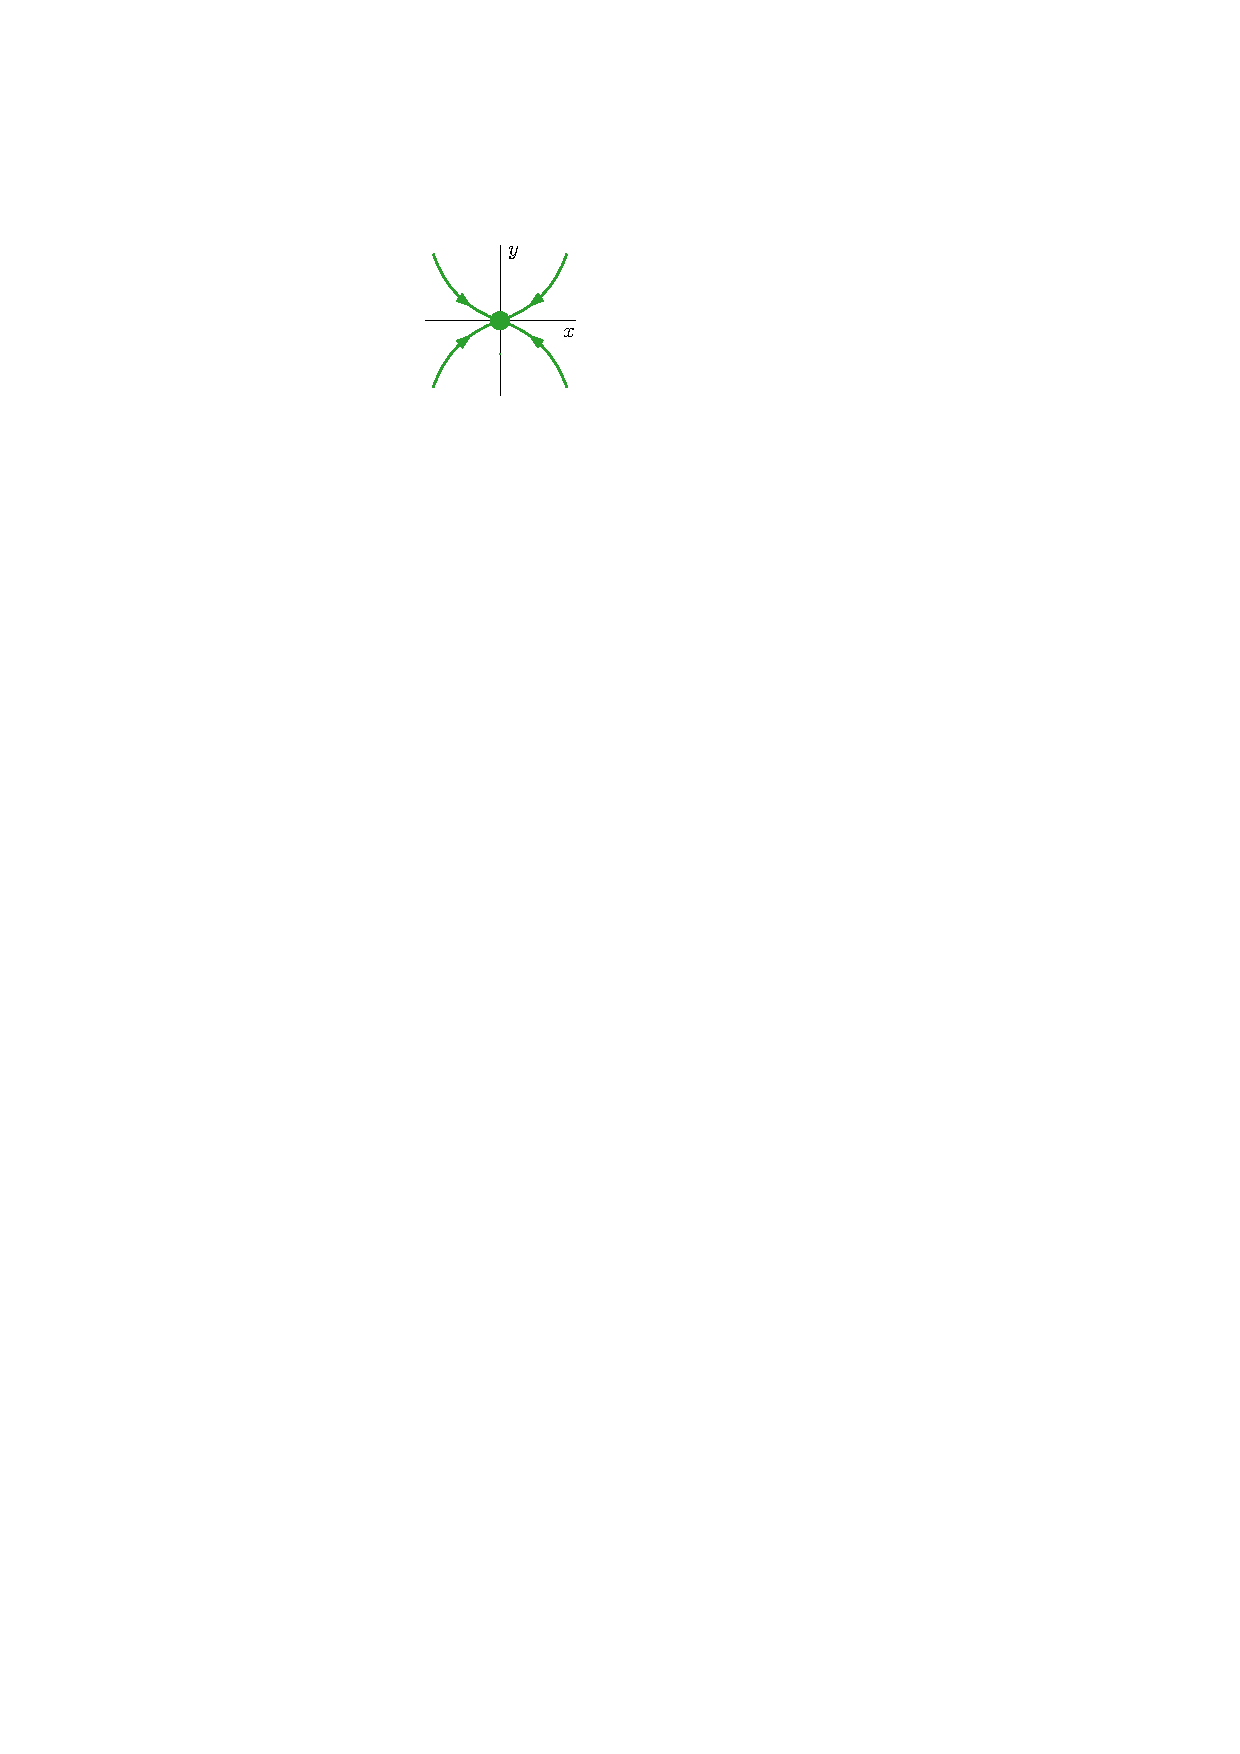
\includegraphics{images/2d-equilibria/stable-node}\\
	Unstable node & $+$ & real & $+$ & $+$ & 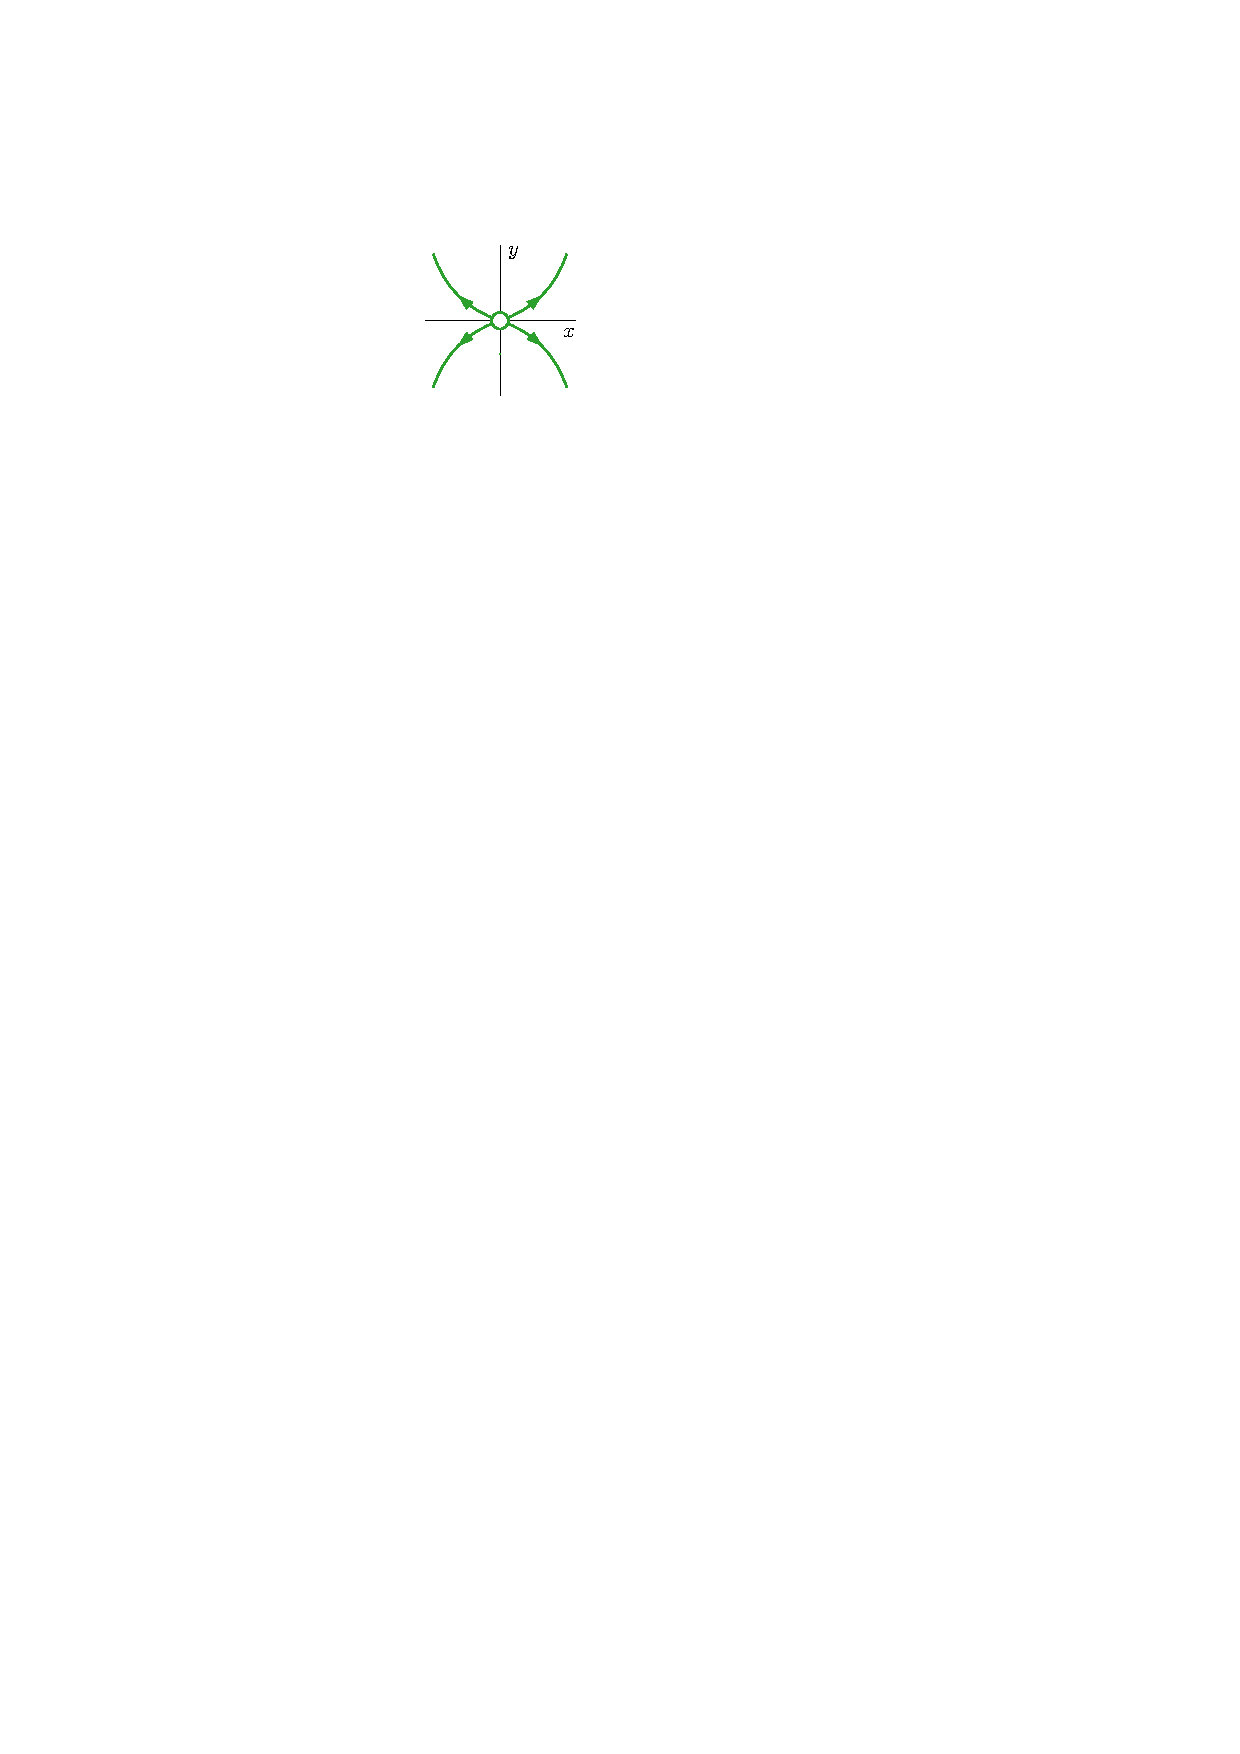
\includegraphics{images/2d-equilibria/unstable-node}\\
	Saddle point  & $+$ & real & $+$ & $-$ & 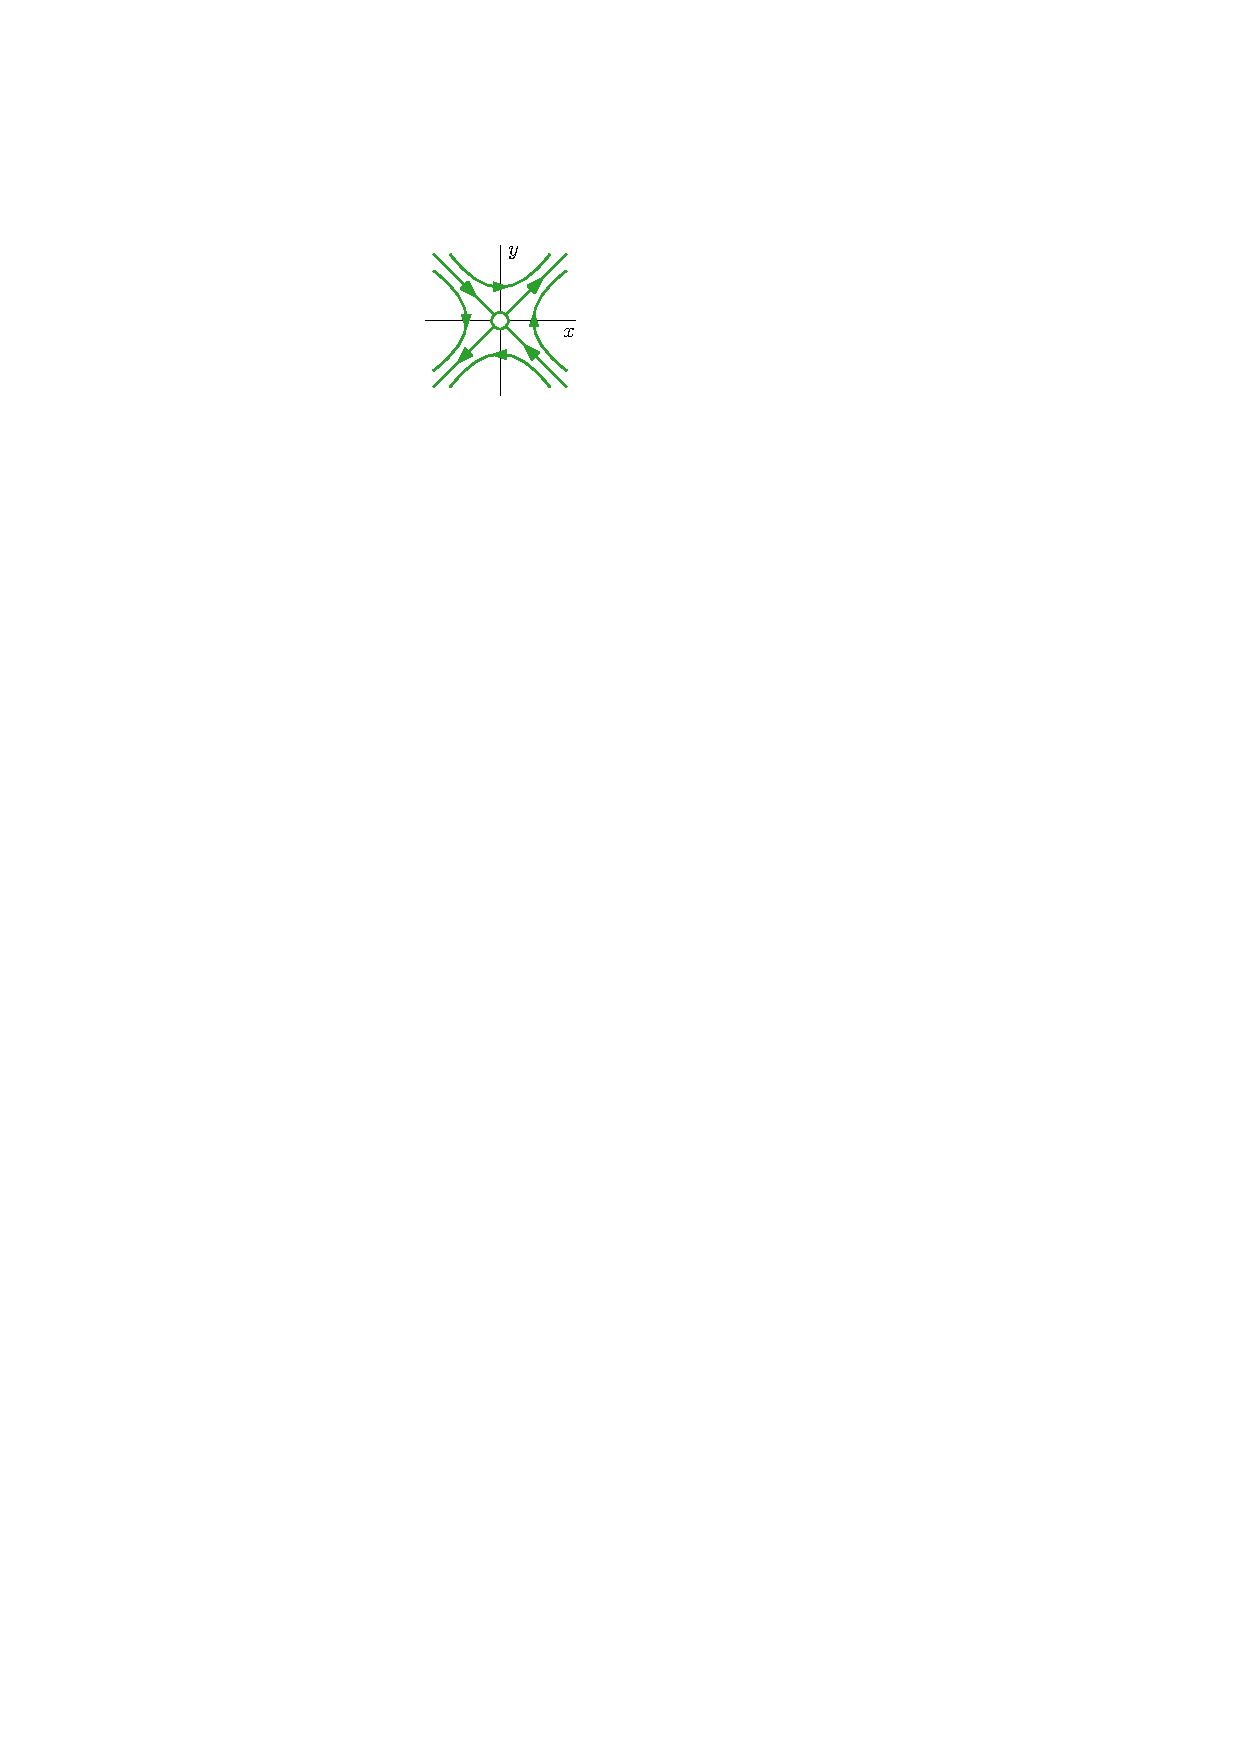
\includegraphics{images/2d-equilibria/saddle-point}\\
	Stable star   & $0$ & real, equal & \multicolumn{2}{c}{$-$} & 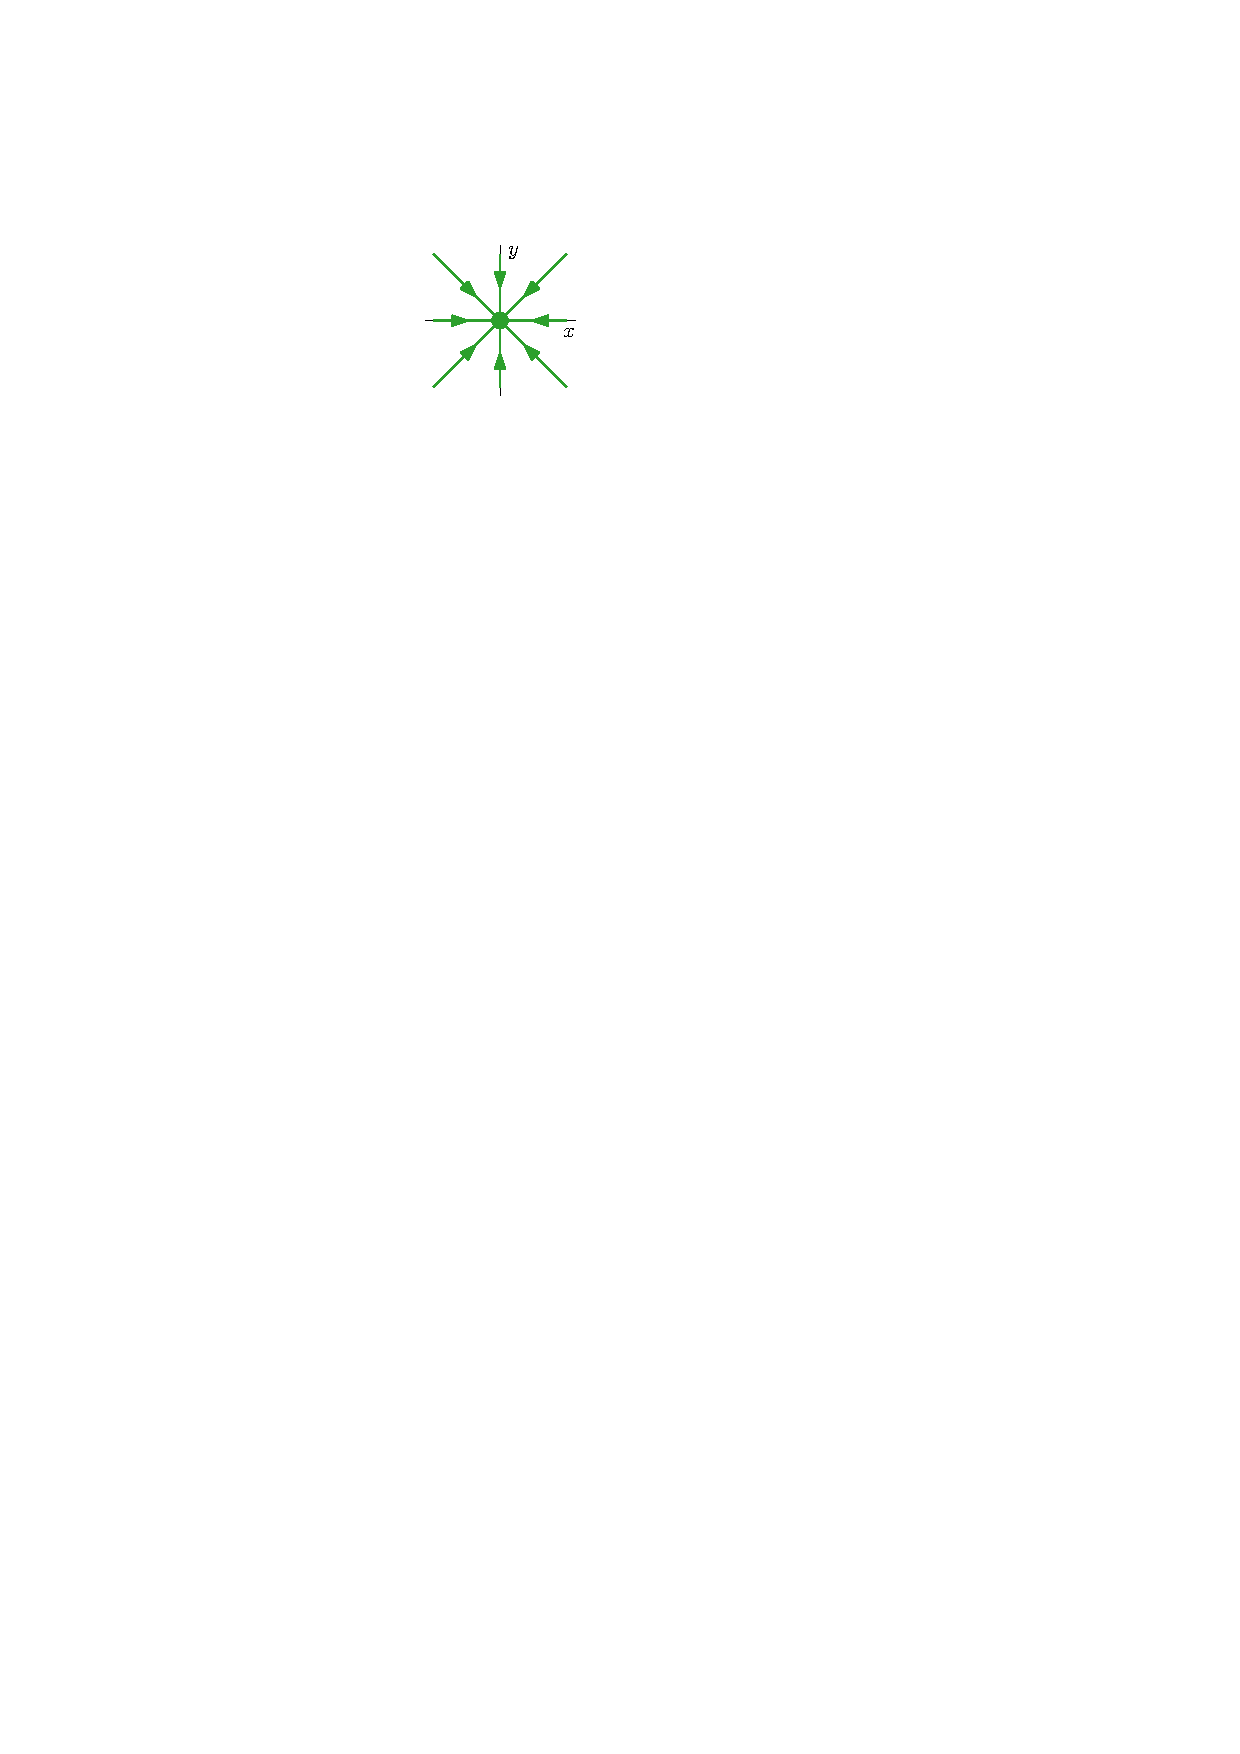
\includegraphics{images/2d-equilibria/stable-star} \\
	Unstable star & $0$ & real, equal & \multicolumn{2}{c}{$+$} & 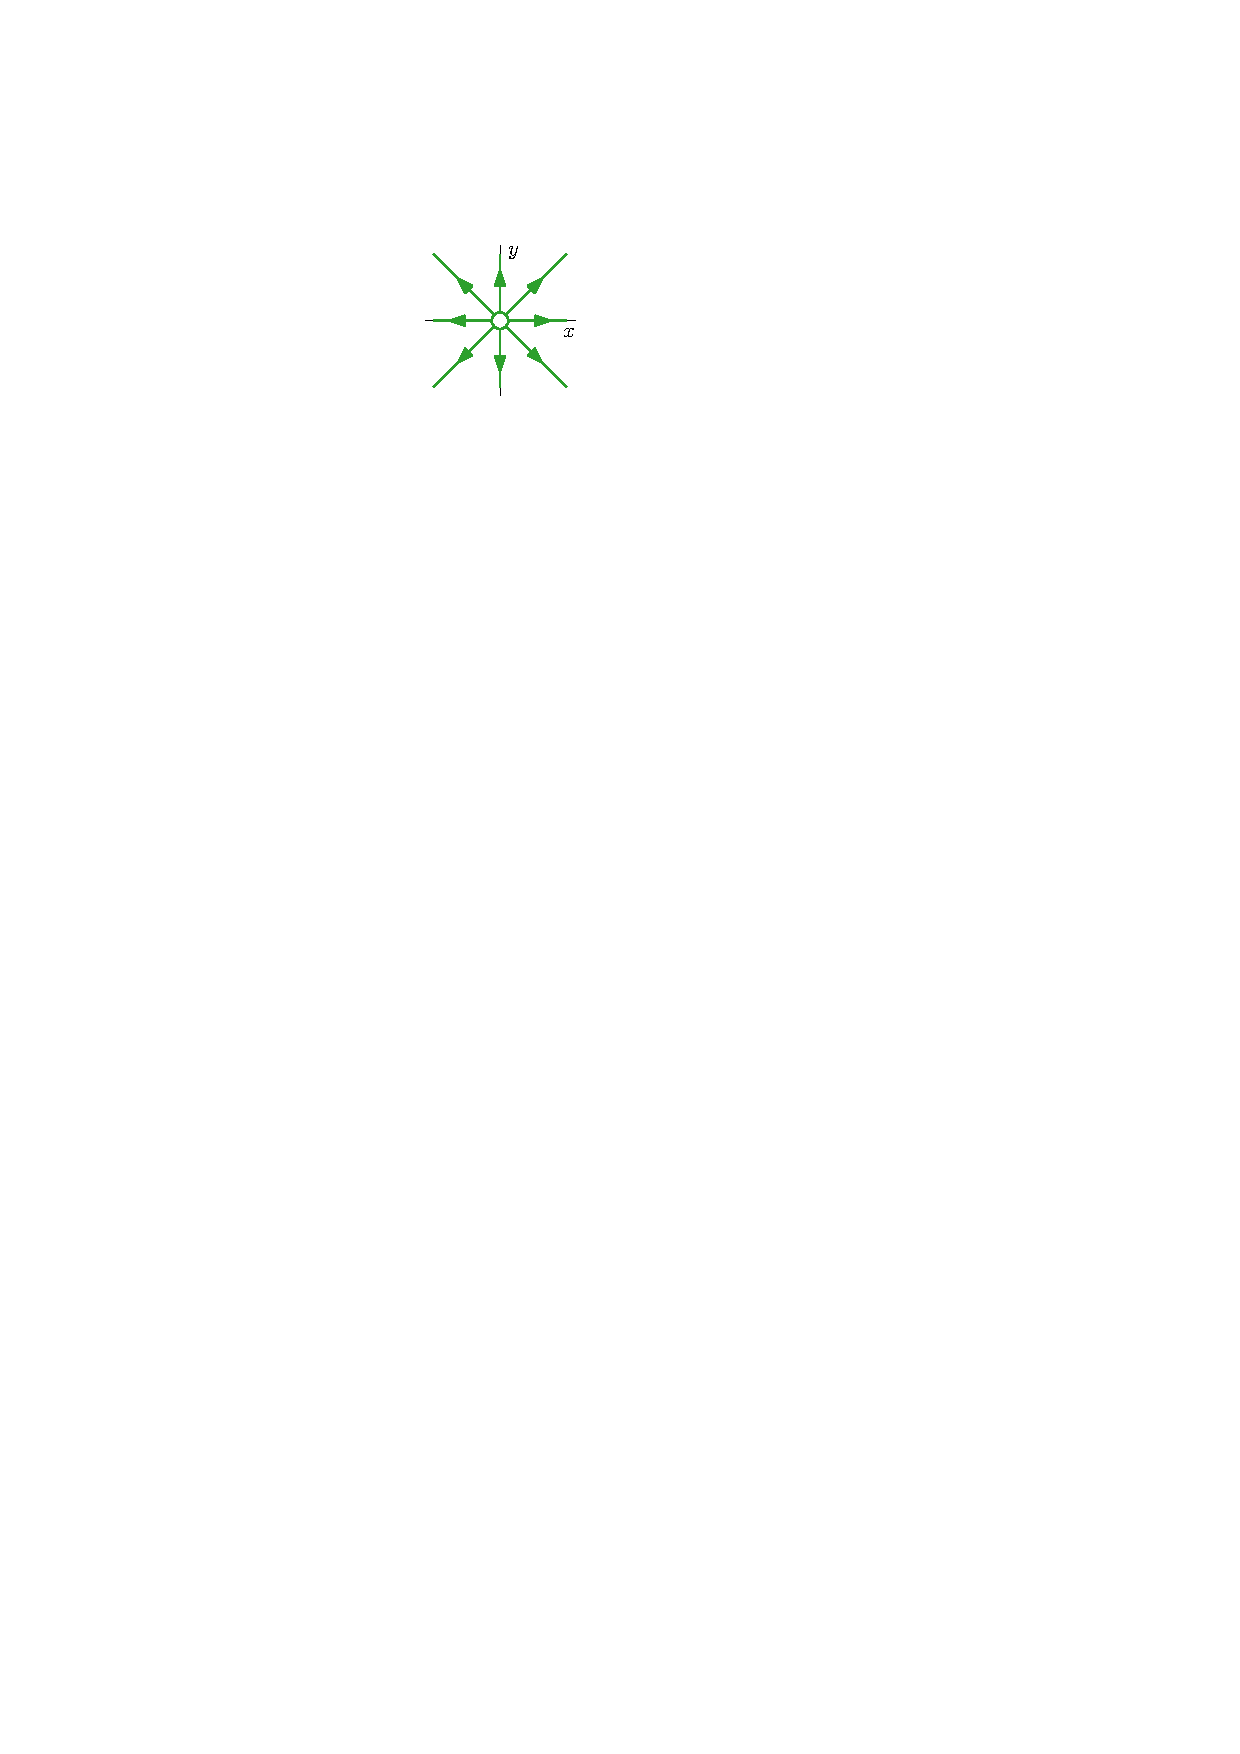
\includegraphics{images/2d-equilibria/unstable-star}\\
	Stable spiral & $-$ & complex & \multicolumn{2}{c}{$-$} & 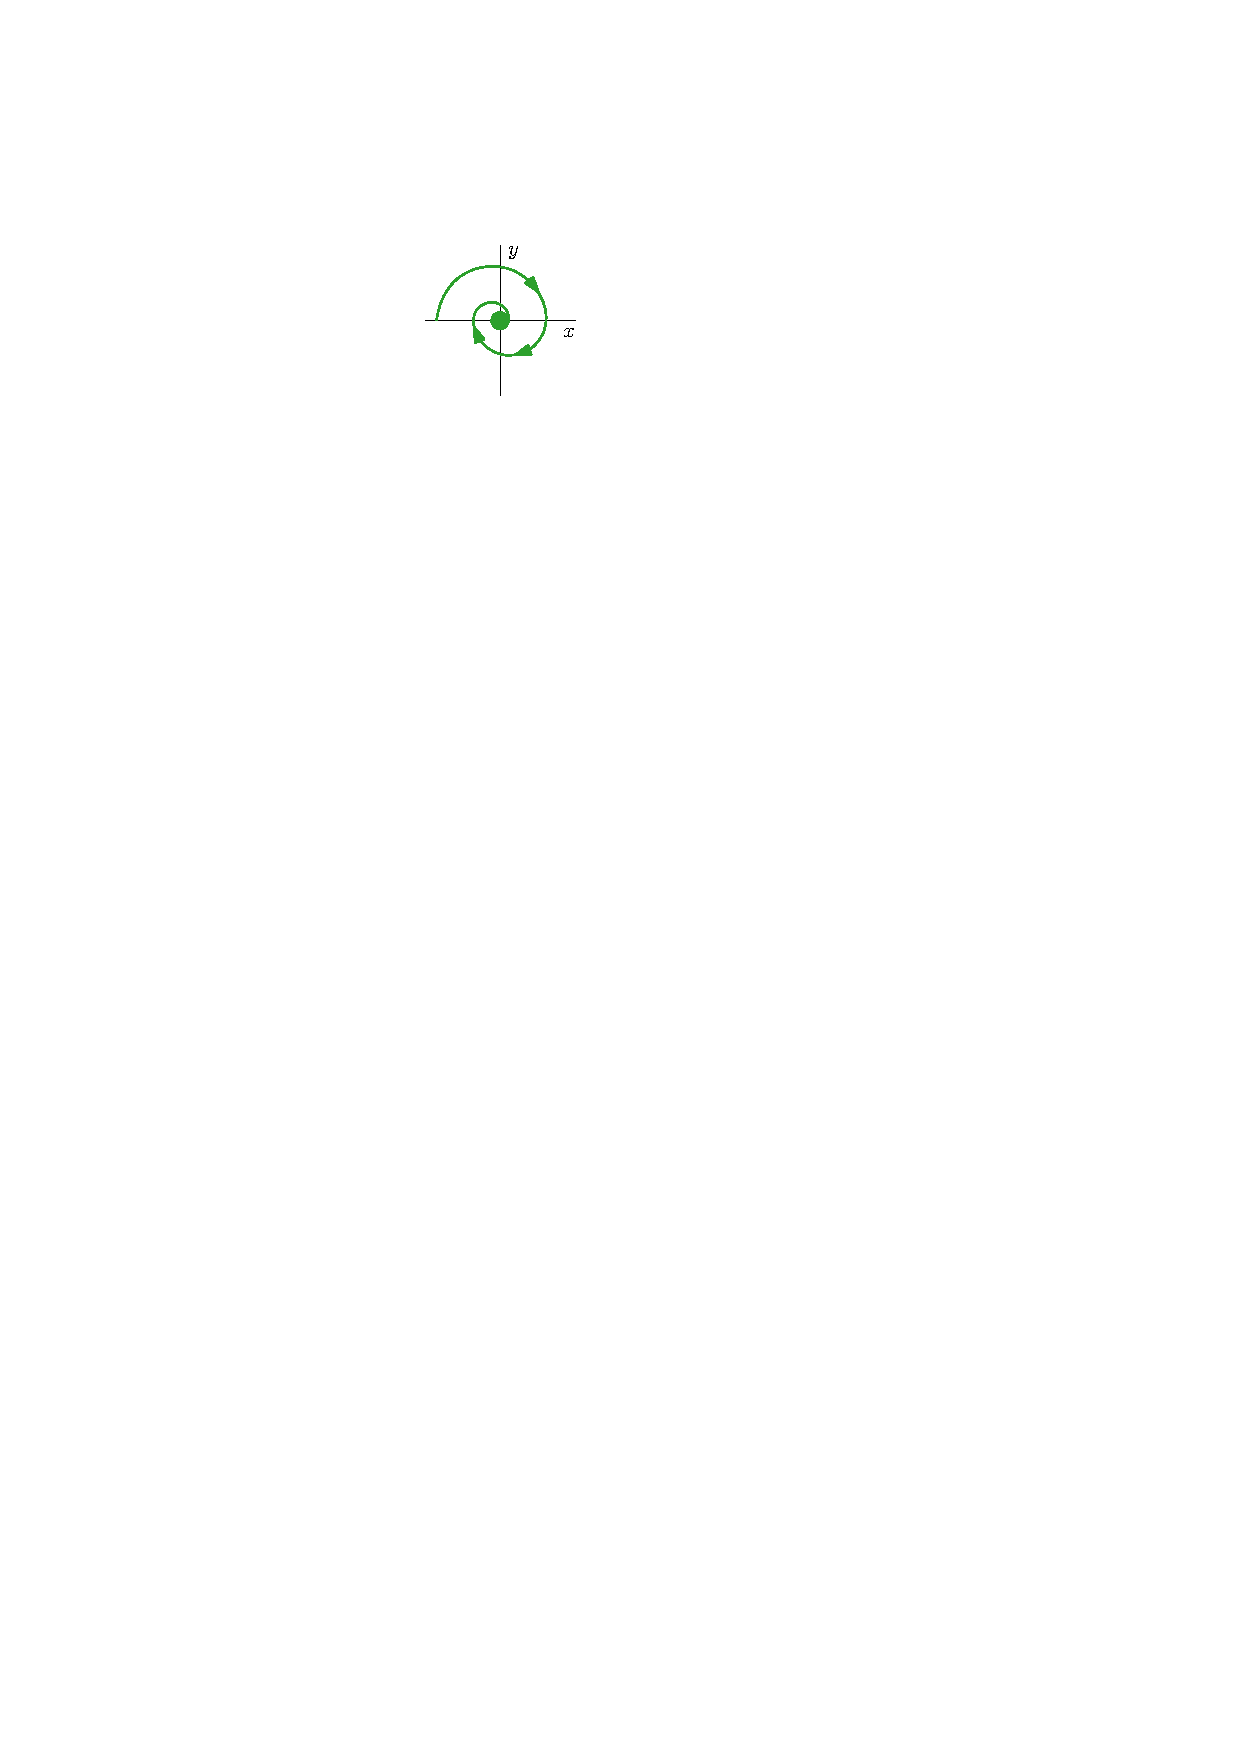
\includegraphics{images/2d-equilibria/stable-spiral}\\
	Unstable spiral & $-$ & complex & \multicolumn{2}{c}{$+$} & 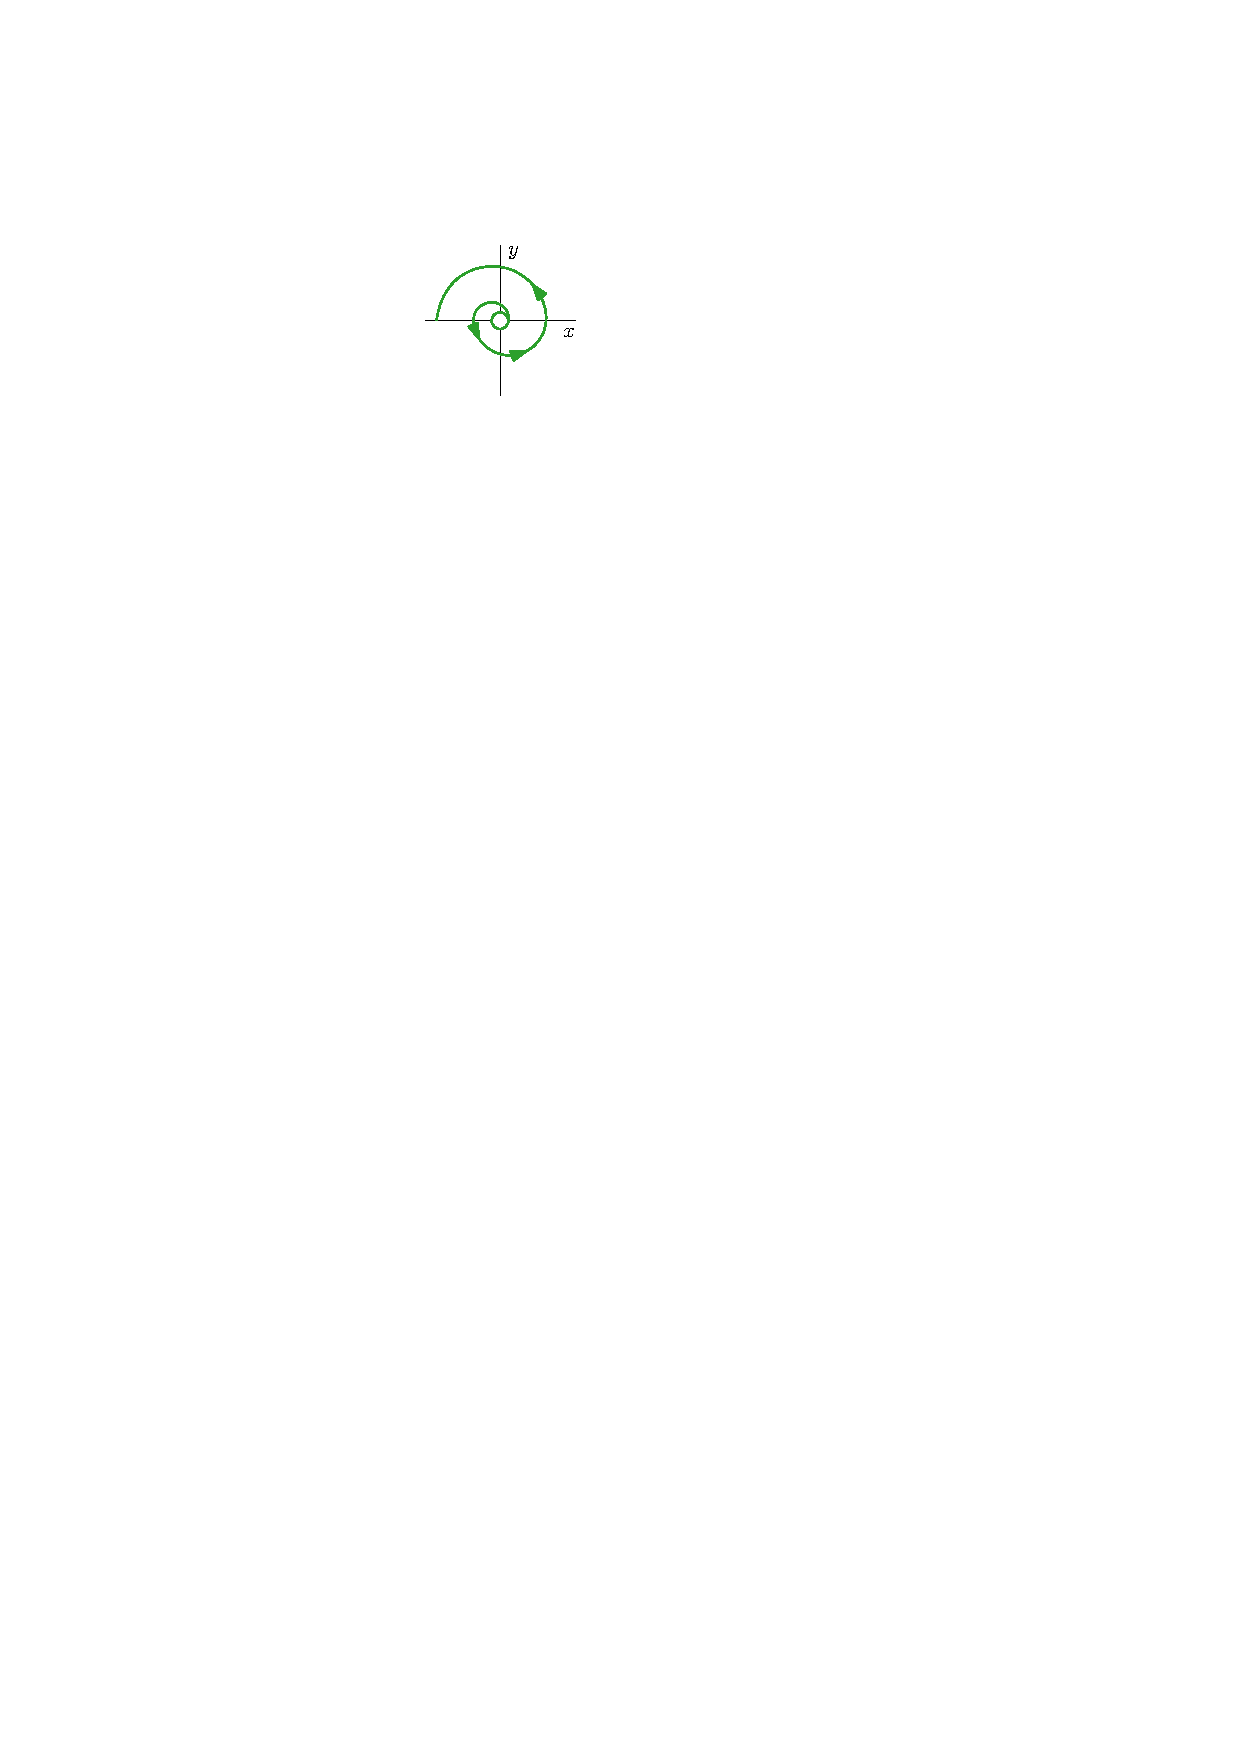
\includegraphics{images/2d-equilibria/unstable-spiral}\\
	Centre        & $-$ & imaginary & \multicolumn{2}{c}{$0$} & 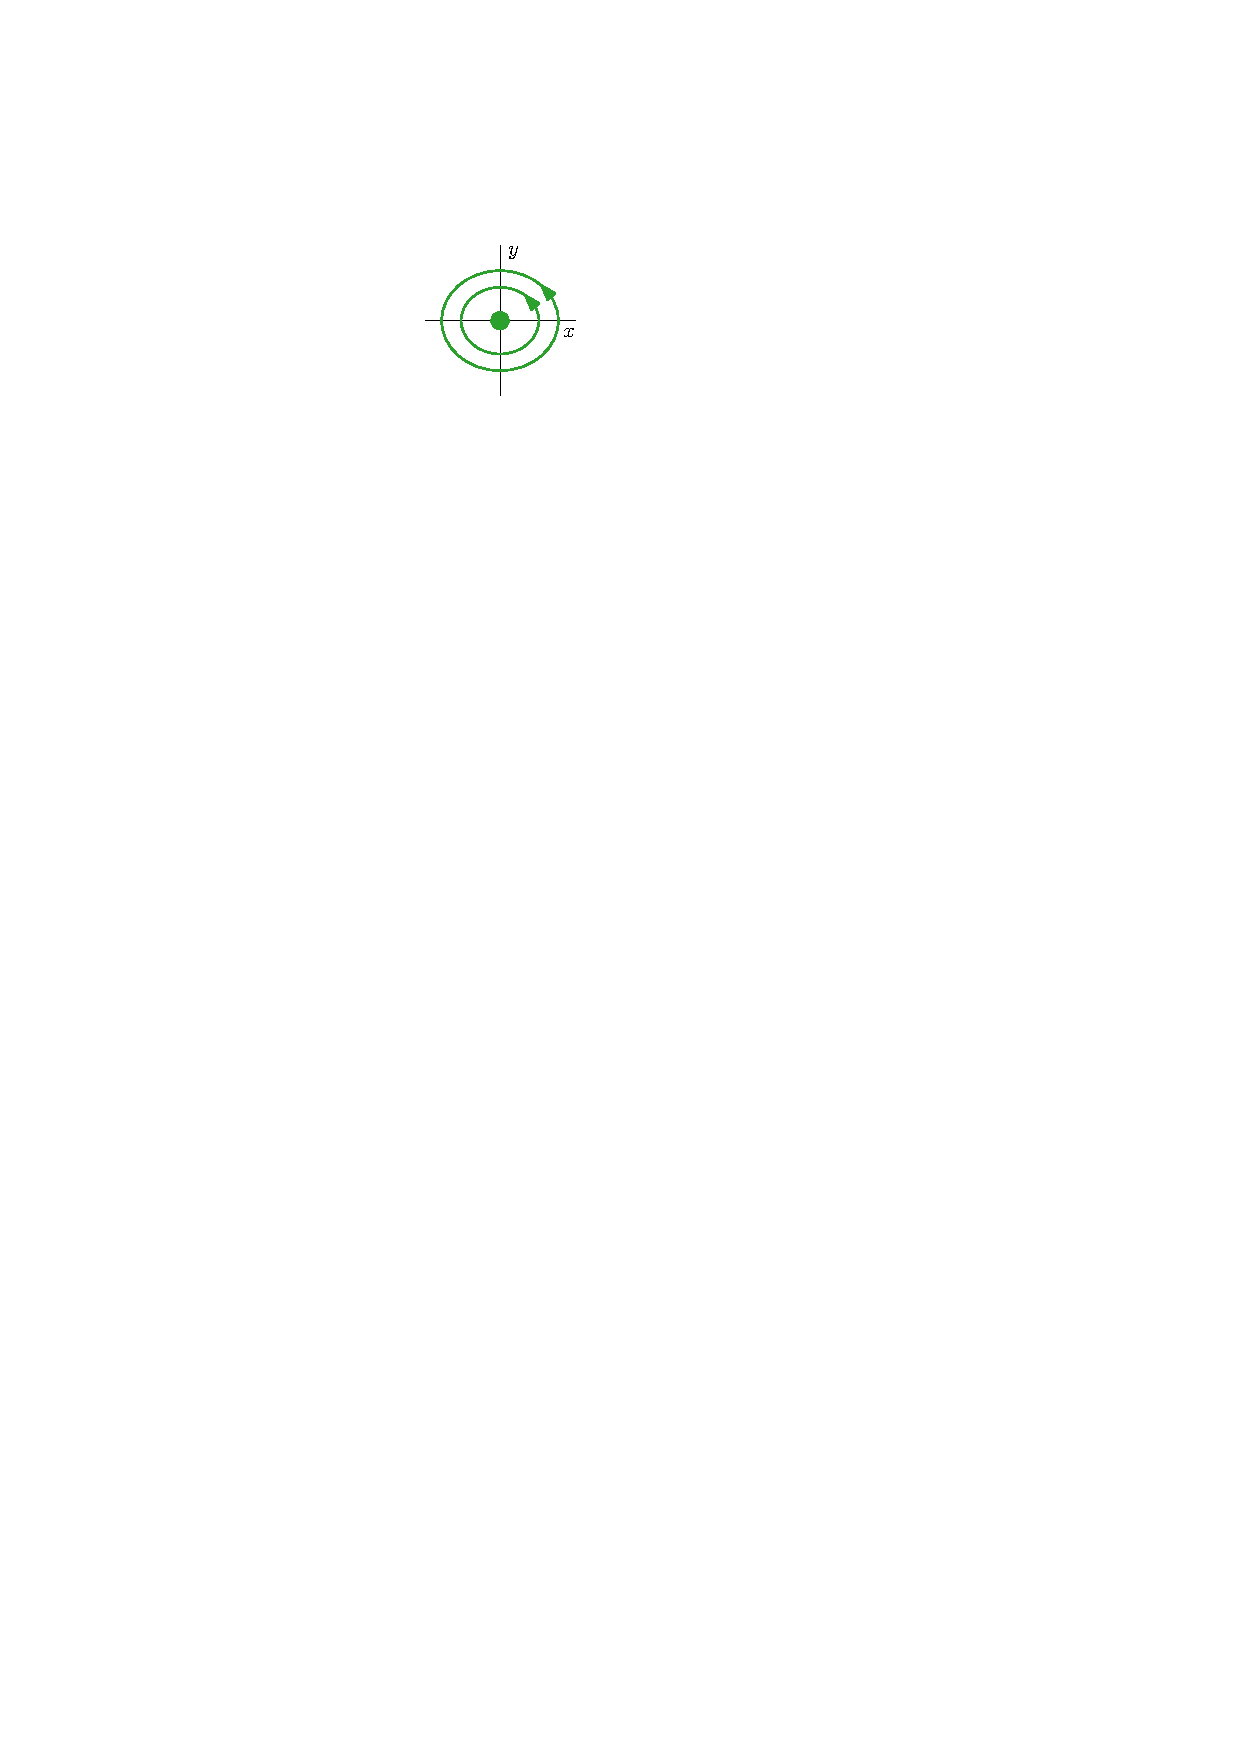
\includegraphics{images/2d-equilibria/centre}\\
	\bottomrule
\end{tabular}
\caption{Names given to the different types of 2D equilibrium, and example phase plots}
\label{tab:2d-stability}
\end{table}

In fact, we often don't have to explicitly work out $\lambda$ in order to develop stability criteria: instead we can just look at the trace and determinant. Note that
\begin{equation}
	\lambda_1 + \lambda_2 = \tr(\m{J}) \quad \text{and} \quad \lambda_1\lambda_2 = \det(\m{J}).
\end{equation}
Then our table becomes
\begin{center}\label{tr-det-table}
\begin{tabular}{lcccc}
	\toprule
	& $\tr(\m{J})^2 - 4 \det(\m{J})$ & $\tr(\m{J})$ & $\det(\m{J})$ \\
	\midrule
	Stable node   & $+$ & $-$ & $+$ \\
	Unstable node & $+$ & $+$ & $+$\\
	Saddle point  & $+$ & ? & $-$\\
	Stable star   & $0$ & $-$ & $+$ \\
	Unstable star & $0$ & $+$ & $+$ \\
	Stable spiral & $-$ & $-$ & $+$ \\
	Unstable spiral & $-$ & $+$ & $+$ \\
	Centre        & $-$ & $0$ & $+$ \\
	\bottomrule
\end{tabular}
\end{center}
This gives us a useful shortcut for determining stability if calculating the trace and determinant is easier than explicitly calculating the eigenvalues.

%\begin{itemize}
%	\item if $\det(\m{J}) < 0$, then $\lambda_1$ and $\lambda_2$ are real and have different sign $\implies$ \textbf{unstable}
%	\item if $\det(\m{J}) = 0$, then $\lambda_1=0$ or $\lambda_2=0$. The other $\lambda$ is then equal to $\tr(\m{J})$ and
%	\begin{itemize}
%		\item $\tr(\m{J}) > 0 \implies$ \textbf{unstable case}
%		\item $\tr(\m{J}) \leq 0 \implies$ \textbf{degenerate case}
%	\end{itemize}
%	\item if $\det(\m{J}) > 0$ and both $\lambda$ are real, then either:
%	\begin{itemize}
%		\item both $\lambda > 0$ ($\tr(\m{J}) > 0$) $\implies$ \textbf{unstable}
%		\item both $\lambda < 0$ ($\tr(\m{J}) < 0$) $\implies$ \textbf{stable}
%	\end{itemize}
%	\item if $\det(\m{J}) > 0$ and both $\lambda$ are complex, then $\Re(\lambda) = \tr(\m{J})/2$ and
%	\begin{itemize}
%		\item $\tr(\m{J}) > 0$ $\implies$ \textbf{unstable}
%		\item $\tr(\m{J}) < 0$ $\implies$ \textbf{stable}.
%	\end{itemize}
%\end{itemize} 

For stability (of any sort) we therefore require
\begin{equation}
\det(\m{J})>0 \quad \text{and} \quad \tr(\m{J})<0,
\end{equation}
but we can also use this observation to search for complex behaviour. In the case of the centre, the trajectories move around the fixed point never getting closer, or further away. This is an example of a closed orbit, or limit cycle. We will see that in context of fully nonlinear systems closed orbits can exist and they themselves can be stable or unstable.

\begin{do-it-yourself}
As practice, you should try these determinant--trace criteria on the examples we have covered so far.
\end{do-it-yourself}

\paragraph{Remark} 
If $b$ or $c$ are zero then
\begin{equation}
\det(\m{J} -\lambda \m{I}) = (\lambda -a)(\lambda-d),
\end{equation}
so there is no need to find the trace or determinant (it often complicates matters).
%
%\paragraph{Complex oscillations} 
%Looking at \cref{lambda-as-tr-det}, for an ODE system, the only way the $\lambda$ can be complex is if 
%\begin{equation}
% \tr(\m{J})^2 -4\det(\m{J})<0,
%\end{equation} 
%which in turn requires
%\begin{equation}
%\label{req-for-cyclic}
%4 \det(\m{J})> \tr (\m{J})^2 \quad \text{and} \quad \det(\m{J}) > 0.
%\end{equation}
%It is easy to check if the second condition fails, but it is obviously not sufficient; the first is. The oscillations will then:
%\begin{itemize}
%	\item decay if $\tr(\m{J})<0$ (see \cref{complexperturbations}(a)),
%	\item grow if $\tr(\m{J})>0$ (see \cref{complexperturbations}(b)), and
%	\item maintain a fixed amplitude if $\tr(\m{J})=0$ (see \cref{complexperturbations}(c)). 
%\end{itemize}
%We often refer to the transition from real negative $\lambda$ (stable) to purely imaginary eigenvalues as a Hopf bifurcation after the mathematician Heinz Hopf. 

A last word: these conditions on the determinant and trace are useful but are only valid for $2\times2$ matrices.

\subsection{Phase portraits}
It’s important to keep in mind that the linear analysis about equilibria only gives a local description of the dynamics. To get a better picture of the global dynamics, we’d like to understand how the equilibria are connected, or if closed orbits exist. In one-dimensional systems, $\fd{x}{t} = f(x)$, this was easy as we only needed to examine the sign of $f$ between the equilibria and the phase portrait was clear. 

In two dimensions, the phase portrait will typically include:
\begin{itemize}
	\item The equilibria and some indication of their stability,
	\item The trajectories near equilibria and periodic orbits that show the flow pattern. 
\end{itemize}
While uniqueness of the solution dictates that trajectories cannot cross, compiling the phase portrait in 2D can be challenging. We're going to construct the example phase portrait in \cref{fig:nullclines-example}. A good recipe looks like this:
\begin{enumerate}[label=(\roman*)]
\item Draw on the equilibria, coloured in according to their stability from a linear stability analysis
\item Draw the \emph{nullclines}. These are the curves where either 
\begin{equation}
	\fd{x}{t} = \dot x = 0 \quad\text{or}\quad \fd{y}{t} = \dot y = 0.
\end{equation}
Since the equilibria satisfy both $\dot x=0$ and $\dot y = 0$, the nullclines will intersect at the equilibria. 
	
	Particularly helpful is that when trajectories intersect the nullcline, they must be either vertical ($\dot x = 0$) or horizontal ($\dot y = 0$). 
\item The nullclines provide the boundary between regions of phase space where $\dot x>0$ or $\dot x<0$, and $\dot y>0$ or $\dot y<0$. Thus, the nullclines give us some sense of the direction of the trajectories in different regions of the phase plane. However, there is no way to see which sign $\dot x,\dot y$ have in each region a priori, so we have to test at least one point in each region. 
\item Infer the directions from this information. For example, in a region where $\dot x<0$ and $\dot y<0$, we'd expect trajectories heading down and to the left. 
\end{enumerate}
See how we've done this in \cref{fig:nullclines-example} for a made-up scenario. At this point we can try to plot the full trajectories (although I haven't done so here).

%\begin{do-it-yourself}
%	We will practise drawing phase portraits in Problems Class 2.
%\end{do-it-yourself}

\begin{figure}
	\centering
	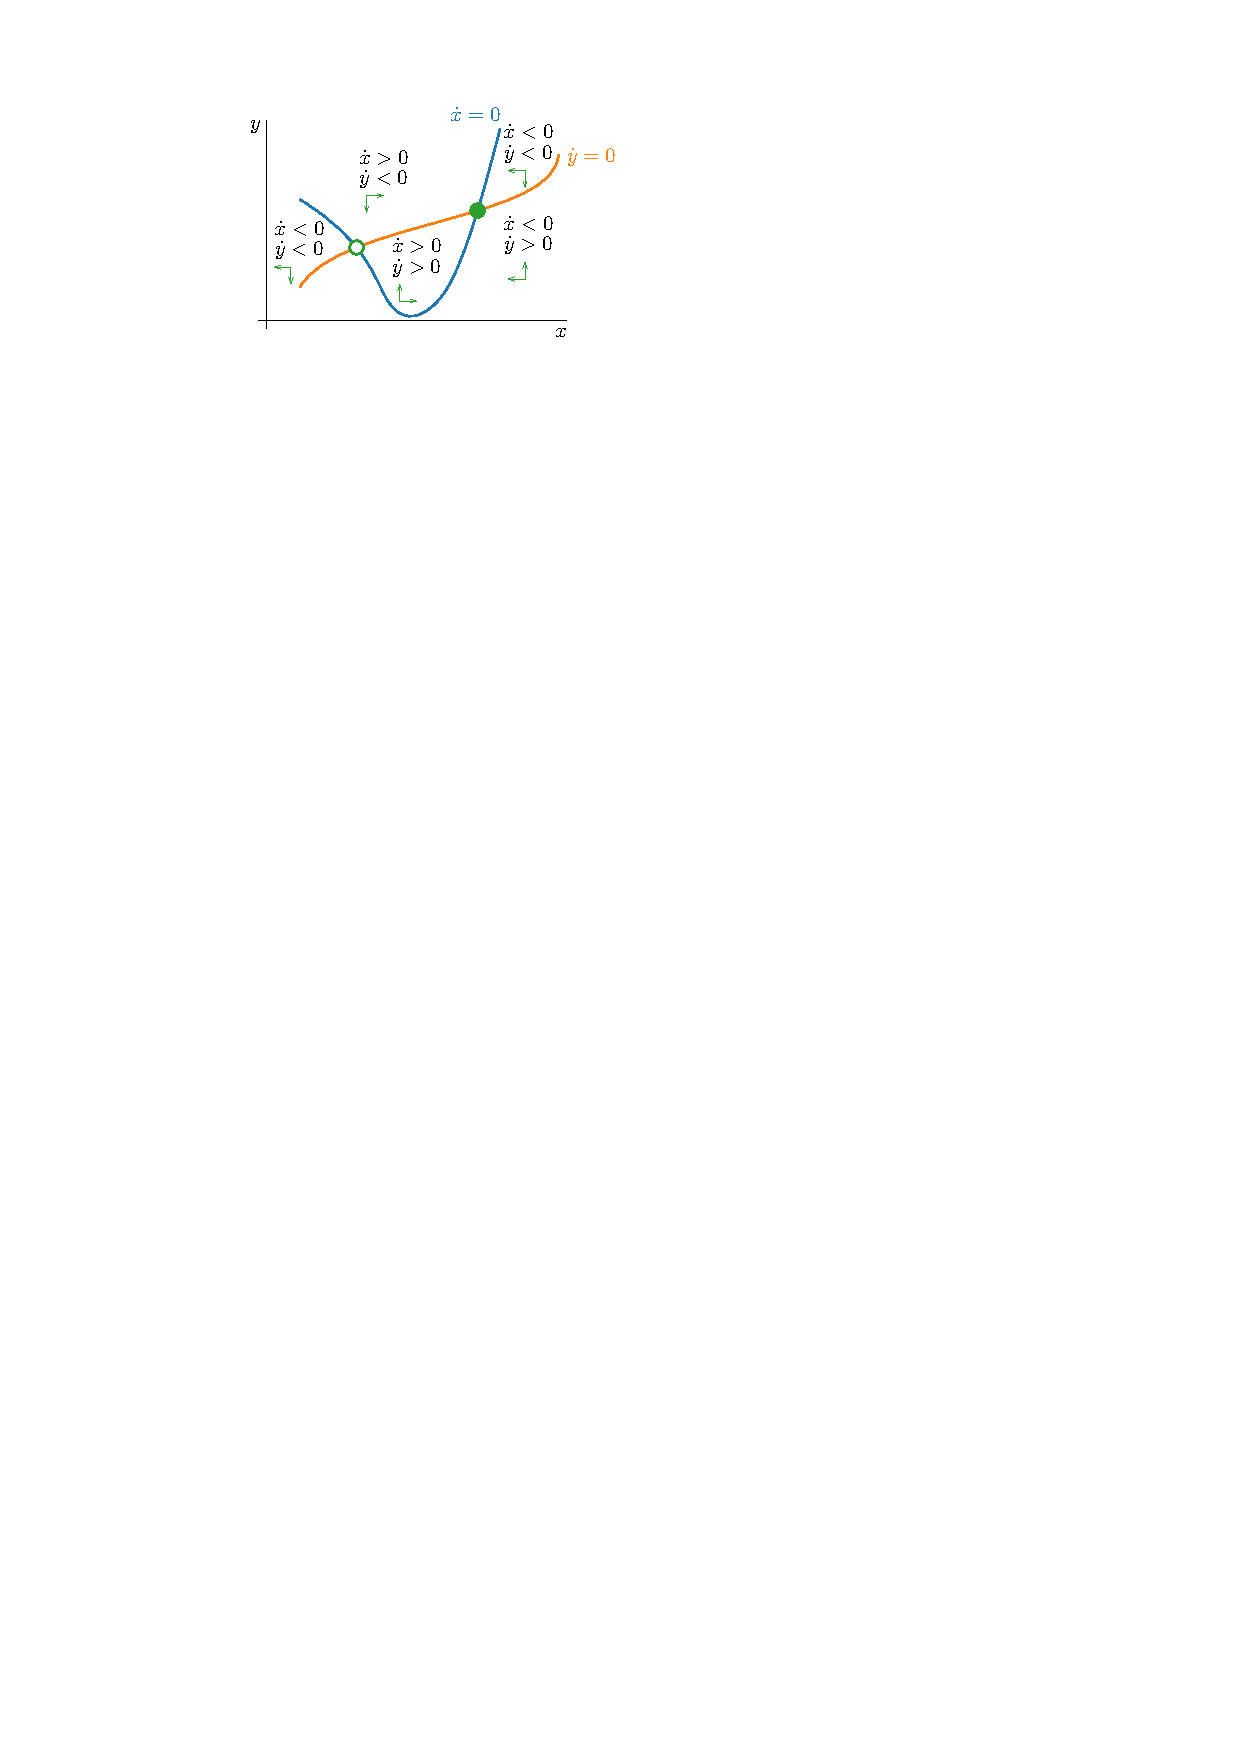
\includegraphics[scale=1.2]{images/nullclines-example}
	\caption{How nullclines might help us establish trajectories and stability in an example (made up!) system. Whether $\dot x,\dot y \lessgtr 0$ either side of the nullcline will not be obvious from the plot, and you will have to test it. So long as $\dot x,\dot y$ are continuous, their sign will stay the same either side of the nullclines.}
	\label{fig:nullclines-example}
\end{figure}

With this in mind, let's look at Lotka--Volterra and its variants in more detail.



\section{Lotka--Volterra revisited}
We learnt in \cref{chap:pendulum} that nondimensionalised Lotka--Volterra has two equilibria:
\begin{itemize}
	\item $(0,0)$ with eigenvalues $1$ and $-\gamma < 0$, and
	\item $(1,1)$ with eigenvalues $\pm\sqrt{\gamma}\i$.
\end{itemize}
Looking at our stability table, we see $(0,0)$ is therefore officially a saddle point, and $(1,1)$ is a centre. This matches what we've seen in our phase diagrams so far.

Looking at \cref{lotvol3}, we can see the nullclines are:
\begin{itemize}
	\item $\displaystyle\fd{x}{t} = 0$ $\implies$ $x=0$ and $y=1$,
	\item $\displaystyle\fd{y}{t} = 0$ $\implies$ $x=1$ and $y=0$.	
\end{itemize}
Putting these and the equilibria on the phase diagram in \cref{fig:lv4-phase}, we can see the quadrants where $\fd{x}{t}$ and $\fd{y}{t}$ are positive and negative. This tells us the direction that the centre at $(1,1)$ takes... it must be anticlockwise.

Furthermore, what about the saddle point at $(0,0)$? Well, working out the associated eigenvectors, the positive (corresponding to unstable) eigenvalue $1$ corresponds to the vector $(1,0)$, and the negative (stable) eigenvalue $-\gamma$ corresponds to $(0,1)$. This tells us that the saddle is unstable in the direction $(1,0)$ but stable in the direction $(0,1)$. Just like we've seen! These are also part of the picture in \cref{fig:lv4-phase}.

\begin{figure}
	\centering
	%% Creator: Matplotlib, PGF backend
%%
%% To include the figure in your LaTeX document, write
%%   \input{<filename>.pgf}
%%
%% Make sure the required packages are loaded in your preamble
%%   \usepackage{pgf}
%%
%% and, on pdftex
%%   \usepackage[utf8]{inputenc}\DeclareUnicodeCharacter{2212}{-}
%%
%% or, on luatex and xetex
%%   \usepackage{unicode-math}
%%
%% Figures using additional raster images can only be included by \input if
%% they are in the same directory as the main LaTeX file. For loading figures
%% from other directories you can use the `import` package
%%   \usepackage{import}
%%
%% and then include the figures with
%%   \import{<path to file>}{<filename>.pgf}
%%
%% Matplotlib used the following preamble
%%   \usepackage{fontspec}
%%   \setmainfont{DejaVuSerif.ttf}[Path=/Users/adam/opt/anaconda3/lib/python3.8/site-packages/matplotlib/mpl-data/fonts/ttf/]
%%   \setsansfont{DejaVuSans.ttf}[Path=/Users/adam/opt/anaconda3/lib/python3.8/site-packages/matplotlib/mpl-data/fonts/ttf/]
%%   \setmonofont{DejaVuSansMono.ttf}[Path=/Users/adam/opt/anaconda3/lib/python3.8/site-packages/matplotlib/mpl-data/fonts/ttf/]
%%
\begingroup%
\makeatletter%
\begin{pgfpicture}%
\pgfpathrectangle{\pgfpointorigin}{\pgfqpoint{2.200000in}{2.200000in}}%
\pgfusepath{use as bounding box, clip}%
\begin{pgfscope}%
\pgfsetbuttcap%
\pgfsetmiterjoin%
\pgfsetlinewidth{0.000000pt}%
\definecolor{currentstroke}{rgb}{0.000000,0.000000,0.000000}%
\pgfsetstrokecolor{currentstroke}%
\pgfsetstrokeopacity{0.000000}%
\pgfsetdash{}{0pt}%
\pgfpathmoveto{\pgfqpoint{0.000000in}{0.000000in}}%
\pgfpathlineto{\pgfqpoint{2.200000in}{0.000000in}}%
\pgfpathlineto{\pgfqpoint{2.200000in}{2.200000in}}%
\pgfpathlineto{\pgfqpoint{0.000000in}{2.200000in}}%
\pgfpathclose%
\pgfusepath{}%
\end{pgfscope}%
\begin{pgfscope}%
\pgfsetbuttcap%
\pgfsetmiterjoin%
\pgfsetlinewidth{0.000000pt}%
\definecolor{currentstroke}{rgb}{0.000000,0.000000,0.000000}%
\pgfsetstrokecolor{currentstroke}%
\pgfsetstrokeopacity{0.000000}%
\pgfsetdash{}{0pt}%
\pgfpathmoveto{\pgfqpoint{0.211847in}{0.278150in}}%
\pgfpathlineto{\pgfqpoint{2.166667in}{0.278150in}}%
\pgfpathlineto{\pgfqpoint{2.166667in}{2.166667in}}%
\pgfpathlineto{\pgfqpoint{0.211847in}{2.166667in}}%
\pgfpathclose%
\pgfusepath{}%
\end{pgfscope}%
\begin{pgfscope}%
\pgfsetbuttcap%
\pgfsetroundjoin%
\definecolor{currentfill}{rgb}{0.000000,0.000000,0.000000}%
\pgfsetfillcolor{currentfill}%
\pgfsetlinewidth{0.803000pt}%
\definecolor{currentstroke}{rgb}{0.000000,0.000000,0.000000}%
\pgfsetstrokecolor{currentstroke}%
\pgfsetdash{}{0pt}%
\pgfsys@defobject{currentmarker}{\pgfqpoint{0.000000in}{-0.048611in}}{\pgfqpoint{0.000000in}{0.000000in}}{%
\pgfpathmoveto{\pgfqpoint{0.000000in}{0.000000in}}%
\pgfpathlineto{\pgfqpoint{0.000000in}{-0.048611in}}%
\pgfusepath{stroke,fill}%
}%
\begin{pgfscope}%
\pgfsys@transformshift{0.211847in}{0.278150in}%
\pgfsys@useobject{currentmarker}{}%
\end{pgfscope}%
\end{pgfscope}%
\begin{pgfscope}%
\definecolor{textcolor}{rgb}{0.000000,0.000000,0.000000}%
\pgfsetstrokecolor{textcolor}%
\pgfsetfillcolor{textcolor}%
\pgftext[x=0.211847in,y=0.180927in,,top]{\color{textcolor}\rmfamily\fontsize{12.000000}{14.400000}\selectfont \(\displaystyle {0}\)}%
\end{pgfscope}%
\begin{pgfscope}%
\pgfsetbuttcap%
\pgfsetroundjoin%
\definecolor{currentfill}{rgb}{0.000000,0.000000,0.000000}%
\pgfsetfillcolor{currentfill}%
\pgfsetlinewidth{0.803000pt}%
\definecolor{currentstroke}{rgb}{0.000000,0.000000,0.000000}%
\pgfsetstrokecolor{currentstroke}%
\pgfsetdash{}{0pt}%
\pgfsys@defobject{currentmarker}{\pgfqpoint{0.000000in}{-0.048611in}}{\pgfqpoint{0.000000in}{0.000000in}}{%
\pgfpathmoveto{\pgfqpoint{0.000000in}{0.000000in}}%
\pgfpathlineto{\pgfqpoint{0.000000in}{-0.048611in}}%
\pgfusepath{stroke,fill}%
}%
\begin{pgfscope}%
\pgfsys@transformshift{0.885923in}{0.278150in}%
\pgfsys@useobject{currentmarker}{}%
\end{pgfscope}%
\end{pgfscope}%
\begin{pgfscope}%
\definecolor{textcolor}{rgb}{0.000000,0.000000,0.000000}%
\pgfsetstrokecolor{textcolor}%
\pgfsetfillcolor{textcolor}%
\pgftext[x=0.885923in,y=0.180927in,,top]{\color{textcolor}\rmfamily\fontsize{12.000000}{14.400000}\selectfont \(\displaystyle {1}\)}%
\end{pgfscope}%
\begin{pgfscope}%
\pgfsetbuttcap%
\pgfsetroundjoin%
\definecolor{currentfill}{rgb}{0.000000,0.000000,0.000000}%
\pgfsetfillcolor{currentfill}%
\pgfsetlinewidth{0.803000pt}%
\definecolor{currentstroke}{rgb}{0.000000,0.000000,0.000000}%
\pgfsetstrokecolor{currentstroke}%
\pgfsetdash{}{0pt}%
\pgfsys@defobject{currentmarker}{\pgfqpoint{0.000000in}{-0.048611in}}{\pgfqpoint{0.000000in}{0.000000in}}{%
\pgfpathmoveto{\pgfqpoint{0.000000in}{0.000000in}}%
\pgfpathlineto{\pgfqpoint{0.000000in}{-0.048611in}}%
\pgfusepath{stroke,fill}%
}%
\begin{pgfscope}%
\pgfsys@transformshift{1.559999in}{0.278150in}%
\pgfsys@useobject{currentmarker}{}%
\end{pgfscope}%
\end{pgfscope}%
\begin{pgfscope}%
\definecolor{textcolor}{rgb}{0.000000,0.000000,0.000000}%
\pgfsetstrokecolor{textcolor}%
\pgfsetfillcolor{textcolor}%
\pgftext[x=1.559999in,y=0.180927in,,top]{\color{textcolor}\rmfamily\fontsize{12.000000}{14.400000}\selectfont \(\displaystyle {2}\)}%
\end{pgfscope}%
\begin{pgfscope}%
\pgfsetbuttcap%
\pgfsetroundjoin%
\definecolor{currentfill}{rgb}{0.000000,0.000000,0.000000}%
\pgfsetfillcolor{currentfill}%
\pgfsetlinewidth{0.803000pt}%
\definecolor{currentstroke}{rgb}{0.000000,0.000000,0.000000}%
\pgfsetstrokecolor{currentstroke}%
\pgfsetdash{}{0pt}%
\pgfsys@defobject{currentmarker}{\pgfqpoint{-0.048611in}{0.000000in}}{\pgfqpoint{-0.000000in}{0.000000in}}{%
\pgfpathmoveto{\pgfqpoint{-0.000000in}{0.000000in}}%
\pgfpathlineto{\pgfqpoint{-0.048611in}{0.000000in}}%
\pgfusepath{stroke,fill}%
}%
\begin{pgfscope}%
\pgfsys@transformshift{0.211847in}{0.278150in}%
\pgfsys@useobject{currentmarker}{}%
\end{pgfscope}%
\end{pgfscope}%
\begin{pgfscope}%
\definecolor{textcolor}{rgb}{0.000000,0.000000,0.000000}%
\pgfsetstrokecolor{textcolor}%
\pgfsetfillcolor{textcolor}%
\pgftext[x=0.033028in, y=0.214836in, left, base]{\color{textcolor}\rmfamily\fontsize{12.000000}{14.400000}\selectfont \(\displaystyle {0}\)}%
\end{pgfscope}%
\begin{pgfscope}%
\pgfsetbuttcap%
\pgfsetroundjoin%
\definecolor{currentfill}{rgb}{0.000000,0.000000,0.000000}%
\pgfsetfillcolor{currentfill}%
\pgfsetlinewidth{0.803000pt}%
\definecolor{currentstroke}{rgb}{0.000000,0.000000,0.000000}%
\pgfsetstrokecolor{currentstroke}%
\pgfsetdash{}{0pt}%
\pgfsys@defobject{currentmarker}{\pgfqpoint{-0.048611in}{0.000000in}}{\pgfqpoint{-0.000000in}{0.000000in}}{%
\pgfpathmoveto{\pgfqpoint{-0.000000in}{0.000000in}}%
\pgfpathlineto{\pgfqpoint{-0.048611in}{0.000000in}}%
\pgfusepath{stroke,fill}%
}%
\begin{pgfscope}%
\pgfsys@transformshift{0.211847in}{0.929362in}%
\pgfsys@useobject{currentmarker}{}%
\end{pgfscope}%
\end{pgfscope}%
\begin{pgfscope}%
\definecolor{textcolor}{rgb}{0.000000,0.000000,0.000000}%
\pgfsetstrokecolor{textcolor}%
\pgfsetfillcolor{textcolor}%
\pgftext[x=0.033028in, y=0.866049in, left, base]{\color{textcolor}\rmfamily\fontsize{12.000000}{14.400000}\selectfont \(\displaystyle {1}\)}%
\end{pgfscope}%
\begin{pgfscope}%
\pgfsetbuttcap%
\pgfsetroundjoin%
\definecolor{currentfill}{rgb}{0.000000,0.000000,0.000000}%
\pgfsetfillcolor{currentfill}%
\pgfsetlinewidth{0.803000pt}%
\definecolor{currentstroke}{rgb}{0.000000,0.000000,0.000000}%
\pgfsetstrokecolor{currentstroke}%
\pgfsetdash{}{0pt}%
\pgfsys@defobject{currentmarker}{\pgfqpoint{-0.048611in}{0.000000in}}{\pgfqpoint{-0.000000in}{0.000000in}}{%
\pgfpathmoveto{\pgfqpoint{-0.000000in}{0.000000in}}%
\pgfpathlineto{\pgfqpoint{-0.048611in}{0.000000in}}%
\pgfusepath{stroke,fill}%
}%
\begin{pgfscope}%
\pgfsys@transformshift{0.211847in}{1.580575in}%
\pgfsys@useobject{currentmarker}{}%
\end{pgfscope}%
\end{pgfscope}%
\begin{pgfscope}%
\definecolor{textcolor}{rgb}{0.000000,0.000000,0.000000}%
\pgfsetstrokecolor{textcolor}%
\pgfsetfillcolor{textcolor}%
\pgftext[x=0.033028in, y=1.517261in, left, base]{\color{textcolor}\rmfamily\fontsize{12.000000}{14.400000}\selectfont \(\displaystyle {2}\)}%
\end{pgfscope}%
\begin{pgfscope}%
\pgfpathrectangle{\pgfqpoint{0.211847in}{0.278150in}}{\pgfqpoint{1.954820in}{1.888517in}}%
\pgfusepath{clip}%
\pgfsetbuttcap%
\pgfsetroundjoin%
\pgfsetlinewidth{0.702625pt}%
\definecolor{currentstroke}{rgb}{0.000000,0.000000,0.000000}%
\pgfsetstrokecolor{currentstroke}%
\pgfsetdash{{2.590000pt}{1.120000pt}}{0.000000pt}%
\pgfpathmoveto{\pgfqpoint{0.885923in}{0.278150in}}%
\pgfpathlineto{\pgfqpoint{0.885923in}{2.176667in}}%
\pgfusepath{stroke}%
\end{pgfscope}%
\begin{pgfscope}%
\pgfpathrectangle{\pgfqpoint{0.211847in}{0.278150in}}{\pgfqpoint{1.954820in}{1.888517in}}%
\pgfusepath{clip}%
\pgfsetbuttcap%
\pgfsetroundjoin%
\pgfsetlinewidth{0.702625pt}%
\definecolor{currentstroke}{rgb}{0.000000,0.000000,0.000000}%
\pgfsetstrokecolor{currentstroke}%
\pgfsetdash{{2.590000pt}{1.120000pt}}{0.000000pt}%
\pgfpathmoveto{\pgfqpoint{0.211847in}{0.929362in}}%
\pgfpathlineto{\pgfqpoint{2.176667in}{0.929362in}}%
\pgfusepath{stroke}%
\end{pgfscope}%
\begin{pgfscope}%
\pgfpathrectangle{\pgfqpoint{0.211847in}{0.278150in}}{\pgfqpoint{1.954820in}{1.888517in}}%
\pgfusepath{clip}%
\pgfsetrectcap%
\pgfsetroundjoin%
\pgfsetlinewidth{1.505625pt}%
\definecolor{currentstroke}{rgb}{0.172549,0.627451,0.172549}%
\pgfsetstrokecolor{currentstroke}%
\pgfsetdash{}{0pt}%
\pgfpathmoveto{\pgfqpoint{0.885923in}{0.408392in}}%
\pgfpathlineto{\pgfqpoint{0.971886in}{0.409620in}}%
\pgfpathlineto{\pgfqpoint{1.058176in}{0.413048in}}%
\pgfpathlineto{\pgfqpoint{1.153345in}{0.419105in}}%
\pgfpathlineto{\pgfqpoint{1.245537in}{0.427188in}}%
\pgfpathlineto{\pgfqpoint{1.331974in}{0.436839in}}%
\pgfpathlineto{\pgfqpoint{1.410108in}{0.447462in}}%
\pgfpathlineto{\pgfqpoint{1.491584in}{0.460734in}}%
\pgfpathlineto{\pgfqpoint{1.561605in}{0.474235in}}%
\pgfpathlineto{\pgfqpoint{1.633031in}{0.490402in}}%
\pgfpathlineto{\pgfqpoint{1.690736in}{0.505595in}}%
\pgfpathlineto{\pgfqpoint{1.748467in}{0.523133in}}%
\pgfpathlineto{\pgfqpoint{1.791457in}{0.538043in}}%
\pgfpathlineto{\pgfqpoint{1.833883in}{0.554648in}}%
\pgfpathlineto{\pgfqpoint{1.875429in}{0.573141in}}%
\pgfpathlineto{\pgfqpoint{1.915737in}{0.593733in}}%
\pgfpathlineto{\pgfqpoint{1.954400in}{0.616656in}}%
\pgfpathlineto{\pgfqpoint{1.979037in}{0.633355in}}%
\pgfpathlineto{\pgfqpoint{2.002593in}{0.651278in}}%
\pgfpathlineto{\pgfqpoint{2.024910in}{0.670507in}}%
\pgfpathlineto{\pgfqpoint{2.045820in}{0.691124in}}%
\pgfpathlineto{\pgfqpoint{2.065146in}{0.713215in}}%
\pgfpathlineto{\pgfqpoint{2.082702in}{0.736864in}}%
\pgfpathlineto{\pgfqpoint{2.098295in}{0.762157in}}%
\pgfpathlineto{\pgfqpoint{2.111726in}{0.789175in}}%
\pgfpathlineto{\pgfqpoint{2.122791in}{0.817995in}}%
\pgfpathlineto{\pgfqpoint{2.131285in}{0.848691in}}%
\pgfpathlineto{\pgfqpoint{2.137005in}{0.881323in}}%
\pgfpathlineto{\pgfqpoint{2.139750in}{0.915942in}}%
\pgfpathlineto{\pgfqpoint{2.139329in}{0.952583in}}%
\pgfpathlineto{\pgfqpoint{2.135565in}{0.991263in}}%
\pgfpathlineto{\pgfqpoint{2.128296in}{1.031977in}}%
\pgfpathlineto{\pgfqpoint{2.117386in}{1.074693in}}%
\pgfpathlineto{\pgfqpoint{2.102724in}{1.119351in}}%
\pgfpathlineto{\pgfqpoint{2.084234in}{1.165857in}}%
\pgfpathlineto{\pgfqpoint{2.061879in}{1.214082in}}%
\pgfpathlineto{\pgfqpoint{2.035663in}{1.263860in}}%
\pgfpathlineto{\pgfqpoint{2.005640in}{1.314985in}}%
\pgfpathlineto{\pgfqpoint{1.971909in}{1.367214in}}%
\pgfpathlineto{\pgfqpoint{1.934624in}{1.420264in}}%
\pgfpathlineto{\pgfqpoint{1.893986in}{1.473821in}}%
\pgfpathlineto{\pgfqpoint{1.850248in}{1.527538in}}%
\pgfpathlineto{\pgfqpoint{1.803704in}{1.581043in}}%
\pgfpathlineto{\pgfqpoint{1.754690in}{1.633949in}}%
\pgfpathlineto{\pgfqpoint{1.703573in}{1.685858in}}%
\pgfpathlineto{\pgfqpoint{1.650746in}{1.736372in}}%
\pgfpathlineto{\pgfqpoint{1.596615in}{1.785102in}}%
\pgfpathlineto{\pgfqpoint{1.541593in}{1.831676in}}%
\pgfpathlineto{\pgfqpoint{1.486090in}{1.875749in}}%
\pgfpathlineto{\pgfqpoint{1.430502in}{1.917010in}}%
\pgfpathlineto{\pgfqpoint{1.375205in}{1.955187in}}%
\pgfpathlineto{\pgfqpoint{1.320548in}{1.990053in}}%
\pgfpathlineto{\pgfqpoint{1.266845in}{2.021429in}}%
\pgfpathlineto{\pgfqpoint{1.214376in}{2.049185in}}%
\pgfpathlineto{\pgfqpoint{1.163378in}{2.073239in}}%
\pgfpathlineto{\pgfqpoint{1.114051in}{2.093558in}}%
\pgfpathlineto{\pgfqpoint{1.066554in}{2.110150in}}%
\pgfpathlineto{\pgfqpoint{1.021006in}{2.123065in}}%
\pgfpathlineto{\pgfqpoint{0.977494in}{2.132389in}}%
\pgfpathlineto{\pgfqpoint{0.936068in}{2.138237in}}%
\pgfpathlineto{\pgfqpoint{0.896752in}{2.140750in}}%
\pgfpathlineto{\pgfqpoint{0.859543in}{2.140091in}}%
\pgfpathlineto{\pgfqpoint{0.824417in}{2.136435in}}%
\pgfpathlineto{\pgfqpoint{0.791331in}{2.129971in}}%
\pgfpathlineto{\pgfqpoint{0.760230in}{2.120893in}}%
\pgfpathlineto{\pgfqpoint{0.731044in}{2.109400in}}%
\pgfpathlineto{\pgfqpoint{0.703698in}{2.095688in}}%
\pgfpathlineto{\pgfqpoint{0.678108in}{2.079954in}}%
\pgfpathlineto{\pgfqpoint{0.654190in}{2.062388in}}%
\pgfpathlineto{\pgfqpoint{0.631855in}{2.043175in}}%
\pgfpathlineto{\pgfqpoint{0.611016in}{2.022490in}}%
\pgfpathlineto{\pgfqpoint{0.591584in}{2.000503in}}%
\pgfpathlineto{\pgfqpoint{0.573474in}{1.977372in}}%
\pgfpathlineto{\pgfqpoint{0.556603in}{1.953246in}}%
\pgfpathlineto{\pgfqpoint{0.533448in}{1.915495in}}%
\pgfpathlineto{\pgfqpoint{0.512648in}{1.876249in}}%
\pgfpathlineto{\pgfqpoint{0.493970in}{1.835889in}}%
\pgfpathlineto{\pgfqpoint{0.477199in}{1.794753in}}%
\pgfpathlineto{\pgfqpoint{0.457471in}{1.739200in}}%
\pgfpathlineto{\pgfqpoint{0.440381in}{1.683380in}}%
\pgfpathlineto{\pgfqpoint{0.425576in}{1.627777in}}%
\pgfpathlineto{\pgfqpoint{0.409826in}{1.559166in}}%
\pgfpathlineto{\pgfqpoint{0.396677in}{1.492093in}}%
\pgfpathlineto{\pgfqpoint{0.383764in}{1.414239in}}%
\pgfpathlineto{\pgfqpoint{0.371948in}{1.327667in}}%
\pgfpathlineto{\pgfqpoint{0.362981in}{1.246130in}}%
\pgfpathlineto{\pgfqpoint{0.355564in}{1.159383in}}%
\pgfpathlineto{\pgfqpoint{0.350162in}{1.070030in}}%
\pgfpathlineto{\pgfqpoint{0.347334in}{0.989156in}}%
\pgfpathlineto{\pgfqpoint{0.346749in}{0.908704in}}%
\pgfpathlineto{\pgfqpoint{0.348534in}{0.837432in}}%
\pgfpathlineto{\pgfqpoint{0.352008in}{0.780472in}}%
\pgfpathlineto{\pgfqpoint{0.357185in}{0.729704in}}%
\pgfpathlineto{\pgfqpoint{0.364058in}{0.684558in}}%
\pgfpathlineto{\pgfqpoint{0.371626in}{0.648710in}}%
\pgfpathlineto{\pgfqpoint{0.380624in}{0.616522in}}%
\pgfpathlineto{\pgfqpoint{0.391136in}{0.587668in}}%
\pgfpathlineto{\pgfqpoint{0.401655in}{0.564917in}}%
\pgfpathlineto{\pgfqpoint{0.413495in}{0.544301in}}%
\pgfpathlineto{\pgfqpoint{0.426753in}{0.525652in}}%
\pgfpathlineto{\pgfqpoint{0.441540in}{0.508812in}}%
\pgfpathlineto{\pgfqpoint{0.457978in}{0.493642in}}%
\pgfpathlineto{\pgfqpoint{0.476207in}{0.480013in}}%
\pgfpathlineto{\pgfqpoint{0.496377in}{0.467814in}}%
\pgfpathlineto{\pgfqpoint{0.518656in}{0.456942in}}%
\pgfpathlineto{\pgfqpoint{0.543228in}{0.447309in}}%
\pgfpathlineto{\pgfqpoint{0.574371in}{0.437722in}}%
\pgfpathlineto{\pgfqpoint{0.609091in}{0.429564in}}%
\pgfpathlineto{\pgfqpoint{0.647737in}{0.422764in}}%
\pgfpathlineto{\pgfqpoint{0.696375in}{0.416681in}}%
\pgfpathlineto{\pgfqpoint{0.751029in}{0.412234in}}%
\pgfpathlineto{\pgfqpoint{0.812299in}{0.409446in}}%
\pgfpathlineto{\pgfqpoint{0.888883in}{0.408394in}}%
\pgfpathlineto{\pgfqpoint{0.975215in}{0.409714in}}%
\pgfpathlineto{\pgfqpoint{1.061858in}{0.413239in}}%
\pgfpathlineto{\pgfqpoint{1.157392in}{0.419414in}}%
\pgfpathlineto{\pgfqpoint{1.249909in}{0.427627in}}%
\pgfpathlineto{\pgfqpoint{1.336620in}{0.437418in}}%
\pgfpathlineto{\pgfqpoint{1.414971in}{0.448188in}}%
\pgfpathlineto{\pgfqpoint{1.496632in}{0.461639in}}%
\pgfpathlineto{\pgfqpoint{1.566775in}{0.475319in}}%
\pgfpathlineto{\pgfqpoint{1.638280in}{0.491698in}}%
\pgfpathlineto{\pgfqpoint{1.696007in}{0.507092in}}%
\pgfpathlineto{\pgfqpoint{1.753714in}{0.524862in}}%
\pgfpathlineto{\pgfqpoint{1.796651in}{0.539967in}}%
\pgfpathlineto{\pgfqpoint{1.838987in}{0.556791in}}%
\pgfpathlineto{\pgfqpoint{1.880403in}{0.575528in}}%
\pgfpathlineto{\pgfqpoint{1.920534in}{0.596391in}}%
\pgfpathlineto{\pgfqpoint{1.958966in}{0.619614in}}%
\pgfpathlineto{\pgfqpoint{1.983418in}{0.636530in}}%
\pgfpathlineto{\pgfqpoint{2.006760in}{0.654685in}}%
\pgfpathlineto{\pgfqpoint{2.028833in}{0.674161in}}%
\pgfpathlineto{\pgfqpoint{2.049468in}{0.695041in}}%
\pgfpathlineto{\pgfqpoint{2.068485in}{0.717409in}}%
\pgfpathlineto{\pgfqpoint{2.085698in}{0.741352in}}%
\pgfpathlineto{\pgfqpoint{2.100912in}{0.766953in}}%
\pgfpathlineto{\pgfqpoint{2.113926in}{0.794294in}}%
\pgfpathlineto{\pgfqpoint{2.124538in}{0.823452in}}%
\pgfpathlineto{\pgfqpoint{2.132541in}{0.854496in}}%
\pgfpathlineto{\pgfqpoint{2.137732in}{0.887487in}}%
\pgfpathlineto{\pgfqpoint{2.139914in}{0.922472in}}%
\pgfpathlineto{\pgfqpoint{2.138897in}{0.959485in}}%
\pgfpathlineto{\pgfqpoint{2.134505in}{0.998537in}}%
\pgfpathlineto{\pgfqpoint{2.126582in}{1.039620in}}%
\pgfpathlineto{\pgfqpoint{2.114994in}{1.082695in}}%
\pgfpathlineto{\pgfqpoint{2.099639in}{1.127698in}}%
\pgfpathlineto{\pgfqpoint{2.080446in}{1.174528in}}%
\pgfpathlineto{\pgfqpoint{2.057385in}{1.223050in}}%
\pgfpathlineto{\pgfqpoint{2.030469in}{1.273090in}}%
\pgfpathlineto{\pgfqpoint{1.999760in}{1.324435in}}%
\pgfpathlineto{\pgfqpoint{1.965369in}{1.376836in}}%
\pgfpathlineto{\pgfqpoint{1.927455in}{1.430004in}}%
\pgfpathlineto{\pgfqpoint{1.886232in}{1.483616in}}%
\pgfpathlineto{\pgfqpoint{1.841959in}{1.537322in}}%
\pgfpathlineto{\pgfqpoint{1.794938in}{1.590748in}}%
\pgfpathlineto{\pgfqpoint{1.745513in}{1.643502in}}%
\pgfpathlineto{\pgfqpoint{1.694054in}{1.695186in}}%
\pgfpathlineto{\pgfqpoint{1.640959in}{1.745403in}}%
\pgfpathlineto{\pgfqpoint{1.586634in}{1.793767in}}%
\pgfpathlineto{\pgfqpoint{1.531495in}{1.839910in}}%
\pgfpathlineto{\pgfqpoint{1.475947in}{1.883492in}}%
\pgfpathlineto{\pgfqpoint{1.420385in}{1.924209in}}%
\pgfpathlineto{\pgfqpoint{1.365180in}{1.961798in}}%
\pgfpathlineto{\pgfqpoint{1.310674in}{1.996039in}}%
\pgfpathlineto{\pgfqpoint{1.257177in}{2.026763in}}%
\pgfpathlineto{\pgfqpoint{1.204959in}{2.053849in}}%
\pgfpathlineto{\pgfqpoint{1.154252in}{2.077223in}}%
\pgfpathlineto{\pgfqpoint{1.105248in}{2.096860in}}%
\pgfpathlineto{\pgfqpoint{1.058099in}{2.112777in}}%
\pgfpathlineto{\pgfqpoint{1.012917in}{2.125030in}}%
\pgfpathlineto{\pgfqpoint{0.969782in}{2.133710in}}%
\pgfpathlineto{\pgfqpoint{0.928740in}{2.138939in}}%
\pgfpathlineto{\pgfqpoint{0.889809in}{2.140861in}}%
\pgfpathlineto{\pgfqpoint{0.852983in}{2.139642in}}%
\pgfpathlineto{\pgfqpoint{0.818232in}{2.135459in}}%
\pgfpathlineto{\pgfqpoint{0.785513in}{2.128504in}}%
\pgfpathlineto{\pgfqpoint{0.754766in}{2.118971in}}%
\pgfpathlineto{\pgfqpoint{0.725922in}{2.107058in}}%
\pgfpathlineto{\pgfqpoint{0.698902in}{2.092964in}}%
\pgfpathlineto{\pgfqpoint{0.673624in}{2.076881in}}%
\pgfpathlineto{\pgfqpoint{0.650002in}{2.059001in}}%
\pgfpathlineto{\pgfqpoint{0.627946in}{2.039507in}}%
\pgfpathlineto{\pgfqpoint{0.607370in}{2.018572in}}%
\pgfpathlineto{\pgfqpoint{0.588185in}{1.996365in}}%
\pgfpathlineto{\pgfqpoint{0.570307in}{1.973042in}}%
\pgfpathlineto{\pgfqpoint{0.545762in}{1.936284in}}%
\pgfpathlineto{\pgfqpoint{0.523708in}{1.897803in}}%
\pgfpathlineto{\pgfqpoint{0.503901in}{1.858005in}}%
\pgfpathlineto{\pgfqpoint{0.486116in}{1.817253in}}%
\pgfpathlineto{\pgfqpoint{0.470147in}{1.775863in}}%
\pgfpathlineto{\pgfqpoint{0.451362in}{1.720159in}}%
\pgfpathlineto{\pgfqpoint{0.435089in}{1.664363in}}%
\pgfpathlineto{\pgfqpoint{0.420993in}{1.608927in}}%
\pgfpathlineto{\pgfqpoint{0.405998in}{1.540685in}}%
\pgfpathlineto{\pgfqpoint{0.393485in}{1.474113in}}%
\pgfpathlineto{\pgfqpoint{0.381207in}{1.396984in}}%
\pgfpathlineto{\pgfqpoint{0.369994in}{1.311365in}}%
\pgfpathlineto{\pgfqpoint{0.360500in}{1.219768in}}%
\pgfpathlineto{\pgfqpoint{0.353867in}{1.135066in}}%
\pgfpathlineto{\pgfqpoint{0.349188in}{1.047974in}}%
\pgfpathlineto{\pgfqpoint{0.346855in}{0.961013in}}%
\pgfpathlineto{\pgfqpoint{0.347097in}{0.883737in}}%
\pgfpathlineto{\pgfqpoint{0.349631in}{0.815375in}}%
\pgfpathlineto{\pgfqpoint{0.353746in}{0.760798in}}%
\pgfpathlineto{\pgfqpoint{0.359555in}{0.712197in}}%
\pgfpathlineto{\pgfqpoint{0.367071in}{0.669012in}}%
\pgfpathlineto{\pgfqpoint{0.375232in}{0.634745in}}%
\pgfpathlineto{\pgfqpoint{0.384856in}{0.603998in}}%
\pgfpathlineto{\pgfqpoint{0.394547in}{0.579732in}}%
\pgfpathlineto{\pgfqpoint{0.405502in}{0.557723in}}%
\pgfpathlineto{\pgfqpoint{0.417810in}{0.537789in}}%
\pgfpathlineto{\pgfqpoint{0.431572in}{0.519768in}}%
\pgfpathlineto{\pgfqpoint{0.446902in}{0.503507in}}%
\pgfpathlineto{\pgfqpoint{0.463929in}{0.488871in}}%
\pgfpathlineto{\pgfqpoint{0.482795in}{0.475738in}}%
\pgfpathlineto{\pgfqpoint{0.503658in}{0.463997in}}%
\pgfpathlineto{\pgfqpoint{0.526691in}{0.453553in}}%
\pgfpathlineto{\pgfqpoint{0.552081in}{0.444321in}}%
\pgfpathlineto{\pgfqpoint{0.584247in}{0.435165in}}%
\pgfpathlineto{\pgfqpoint{0.620090in}{0.427415in}}%
\pgfpathlineto{\pgfqpoint{0.659967in}{0.421006in}}%
\pgfpathlineto{\pgfqpoint{0.710129in}{0.415354in}}%
\pgfpathlineto{\pgfqpoint{0.766462in}{0.411339in}}%
\pgfpathlineto{\pgfqpoint{0.829572in}{0.408997in}}%
\pgfpathlineto{\pgfqpoint{0.908389in}{0.408481in}}%
\pgfpathlineto{\pgfqpoint{0.987795in}{0.410097in}}%
\pgfpathlineto{\pgfqpoint{1.075766in}{0.413992in}}%
\pgfpathlineto{\pgfqpoint{1.172669in}{0.420618in}}%
\pgfpathlineto{\pgfqpoint{1.266400in}{0.429328in}}%
\pgfpathlineto{\pgfqpoint{1.354128in}{0.439658in}}%
\pgfpathlineto{\pgfqpoint{1.367076in}{0.441375in}}%
\pgfpathlineto{\pgfqpoint{1.367076in}{0.441375in}}%
\pgfusepath{stroke}%
\end{pgfscope}%
\begin{pgfscope}%
\pgfpathrectangle{\pgfqpoint{0.211847in}{0.278150in}}{\pgfqpoint{1.954820in}{1.888517in}}%
\pgfusepath{clip}%
\pgfsetrectcap%
\pgfsetroundjoin%
\pgfsetlinewidth{1.505625pt}%
\definecolor{currentstroke}{rgb}{0.172549,0.627451,0.172549}%
\pgfsetstrokecolor{currentstroke}%
\pgfsetdash{}{0pt}%
\pgfpathmoveto{\pgfqpoint{0.885923in}{0.546503in}}%
\pgfpathlineto{\pgfqpoint{0.935196in}{0.547671in}}%
\pgfpathlineto{\pgfqpoint{0.987730in}{0.551310in}}%
\pgfpathlineto{\pgfqpoint{1.036210in}{0.556724in}}%
\pgfpathlineto{\pgfqpoint{1.086795in}{0.564449in}}%
\pgfpathlineto{\pgfqpoint{1.139136in}{0.574760in}}%
\pgfpathlineto{\pgfqpoint{1.185035in}{0.585909in}}%
\pgfpathlineto{\pgfqpoint{1.231465in}{0.599456in}}%
\pgfpathlineto{\pgfqpoint{1.270197in}{0.612784in}}%
\pgfpathlineto{\pgfqpoint{1.308587in}{0.628166in}}%
\pgfpathlineto{\pgfqpoint{1.346210in}{0.645809in}}%
\pgfpathlineto{\pgfqpoint{1.375429in}{0.661703in}}%
\pgfpathlineto{\pgfqpoint{1.403558in}{0.679308in}}%
\pgfpathlineto{\pgfqpoint{1.430286in}{0.698748in}}%
\pgfpathlineto{\pgfqpoint{1.455270in}{0.720149in}}%
\pgfpathlineto{\pgfqpoint{1.472645in}{0.737560in}}%
\pgfpathlineto{\pgfqpoint{1.488670in}{0.756189in}}%
\pgfpathlineto{\pgfqpoint{1.503177in}{0.776083in}}%
\pgfpathlineto{\pgfqpoint{1.515995in}{0.797279in}}%
\pgfpathlineto{\pgfqpoint{1.526949in}{0.819807in}}%
\pgfpathlineto{\pgfqpoint{1.535870in}{0.843689in}}%
\pgfpathlineto{\pgfqpoint{1.542587in}{0.868933in}}%
\pgfpathlineto{\pgfqpoint{1.546943in}{0.895533in}}%
\pgfpathlineto{\pgfqpoint{1.548789in}{0.923465in}}%
\pgfpathlineto{\pgfqpoint{1.547993in}{0.952685in}}%
\pgfpathlineto{\pgfqpoint{1.544444in}{0.983125in}}%
\pgfpathlineto{\pgfqpoint{1.538057in}{1.014696in}}%
\pgfpathlineto{\pgfqpoint{1.528775in}{1.047277in}}%
\pgfpathlineto{\pgfqpoint{1.516573in}{1.080723in}}%
\pgfpathlineto{\pgfqpoint{1.501465in}{1.114860in}}%
\pgfpathlineto{\pgfqpoint{1.483502in}{1.149485in}}%
\pgfpathlineto{\pgfqpoint{1.462778in}{1.184370in}}%
\pgfpathlineto{\pgfqpoint{1.439422in}{1.219264in}}%
\pgfpathlineto{\pgfqpoint{1.413608in}{1.253897in}}%
\pgfpathlineto{\pgfqpoint{1.385542in}{1.287982in}}%
\pgfpathlineto{\pgfqpoint{1.355463in}{1.321229in}}%
\pgfpathlineto{\pgfqpoint{1.323637in}{1.353342in}}%
\pgfpathlineto{\pgfqpoint{1.290350in}{1.384034in}}%
\pgfpathlineto{\pgfqpoint{1.255900in}{1.413028in}}%
\pgfpathlineto{\pgfqpoint{1.220593in}{1.440069in}}%
\pgfpathlineto{\pgfqpoint{1.184730in}{1.464927in}}%
\pgfpathlineto{\pgfqpoint{1.148607in}{1.487403in}}%
\pgfpathlineto{\pgfqpoint{1.112502in}{1.507332in}}%
\pgfpathlineto{\pgfqpoint{1.076675in}{1.524590in}}%
\pgfpathlineto{\pgfqpoint{1.041362in}{1.539087in}}%
\pgfpathlineto{\pgfqpoint{1.006770in}{1.550775in}}%
\pgfpathlineto{\pgfqpoint{0.973079in}{1.559643in}}%
\pgfpathlineto{\pgfqpoint{0.940440in}{1.565716in}}%
\pgfpathlineto{\pgfqpoint{0.908974in}{1.569049in}}%
\pgfpathlineto{\pgfqpoint{0.878774in}{1.569725in}}%
\pgfpathlineto{\pgfqpoint{0.849910in}{1.567854in}}%
\pgfpathlineto{\pgfqpoint{0.822425in}{1.563563in}}%
\pgfpathlineto{\pgfqpoint{0.796345in}{1.556996in}}%
\pgfpathlineto{\pgfqpoint{0.771674in}{1.548306in}}%
\pgfpathlineto{\pgfqpoint{0.748404in}{1.537656in}}%
\pgfpathlineto{\pgfqpoint{0.726512in}{1.525213in}}%
\pgfpathlineto{\pgfqpoint{0.705967in}{1.511143in}}%
\pgfpathlineto{\pgfqpoint{0.686729in}{1.495613in}}%
\pgfpathlineto{\pgfqpoint{0.668751in}{1.478785in}}%
\pgfpathlineto{\pgfqpoint{0.646654in}{1.454599in}}%
\pgfpathlineto{\pgfqpoint{0.626582in}{1.428738in}}%
\pgfpathlineto{\pgfqpoint{0.608408in}{1.401530in}}%
\pgfpathlineto{\pgfqpoint{0.592002in}{1.373279in}}%
\pgfpathlineto{\pgfqpoint{0.573791in}{1.336912in}}%
\pgfpathlineto{\pgfqpoint{0.557916in}{1.299813in}}%
\pgfpathlineto{\pgfqpoint{0.544163in}{1.262391in}}%
\pgfpathlineto{\pgfqpoint{0.530187in}{1.217540in}}%
\pgfpathlineto{\pgfqpoint{0.518688in}{1.173212in}}%
\pgfpathlineto{\pgfqpoint{0.508057in}{1.122668in}}%
\pgfpathlineto{\pgfqpoint{0.500100in}{1.073828in}}%
\pgfpathlineto{\pgfqpoint{0.494530in}{1.027024in}}%
\pgfpathlineto{\pgfqpoint{0.490798in}{0.976313in}}%
\pgfpathlineto{\pgfqpoint{0.489622in}{0.928754in}}%
\pgfpathlineto{\pgfqpoint{0.490805in}{0.884436in}}%
\pgfpathlineto{\pgfqpoint{0.494208in}{0.843369in}}%
\pgfpathlineto{\pgfqpoint{0.499740in}{0.805503in}}%
\pgfpathlineto{\pgfqpoint{0.506288in}{0.774929in}}%
\pgfpathlineto{\pgfqpoint{0.514418in}{0.746663in}}%
\pgfpathlineto{\pgfqpoint{0.524138in}{0.720621in}}%
\pgfpathlineto{\pgfqpoint{0.535471in}{0.696712in}}%
\pgfpathlineto{\pgfqpoint{0.548456in}{0.674847in}}%
\pgfpathlineto{\pgfqpoint{0.563145in}{0.654935in}}%
\pgfpathlineto{\pgfqpoint{0.579599in}{0.636893in}}%
\pgfpathlineto{\pgfqpoint{0.597889in}{0.620640in}}%
\pgfpathlineto{\pgfqpoint{0.618097in}{0.606107in}}%
\pgfpathlineto{\pgfqpoint{0.640310in}{0.593230in}}%
\pgfpathlineto{\pgfqpoint{0.664618in}{0.581958in}}%
\pgfpathlineto{\pgfqpoint{0.691116in}{0.572252in}}%
\pgfpathlineto{\pgfqpoint{0.719896in}{0.564085in}}%
\pgfpathlineto{\pgfqpoint{0.751049in}{0.557447in}}%
\pgfpathlineto{\pgfqpoint{0.784654in}{0.552343in}}%
\pgfpathlineto{\pgfqpoint{0.826149in}{0.548423in}}%
\pgfpathlineto{\pgfqpoint{0.870998in}{0.546617in}}%
\pgfpathlineto{\pgfqpoint{0.919213in}{0.547043in}}%
\pgfpathlineto{\pgfqpoint{0.970730in}{0.549874in}}%
\pgfpathlineto{\pgfqpoint{1.025378in}{0.555346in}}%
\pgfpathlineto{\pgfqpoint{1.075526in}{0.562542in}}%
\pgfpathlineto{\pgfqpoint{1.127518in}{0.572259in}}%
\pgfpathlineto{\pgfqpoint{1.173211in}{0.582836in}}%
\pgfpathlineto{\pgfqpoint{1.219550in}{0.595743in}}%
\pgfpathlineto{\pgfqpoint{1.266050in}{0.611258in}}%
\pgfpathlineto{\pgfqpoint{1.304496in}{0.626410in}}%
\pgfpathlineto{\pgfqpoint{1.342224in}{0.643801in}}%
\pgfpathlineto{\pgfqpoint{1.371566in}{0.659474in}}%
\pgfpathlineto{\pgfqpoint{1.399859in}{0.676842in}}%
\pgfpathlineto{\pgfqpoint{1.426794in}{0.696029in}}%
\pgfpathlineto{\pgfqpoint{1.452033in}{0.717160in}}%
\pgfpathlineto{\pgfqpoint{1.469632in}{0.734357in}}%
\pgfpathlineto{\pgfqpoint{1.485910in}{0.752765in}}%
\pgfpathlineto{\pgfqpoint{1.500701in}{0.772430in}}%
\pgfpathlineto{\pgfqpoint{1.513834in}{0.793390in}}%
\pgfpathlineto{\pgfqpoint{1.525135in}{0.815678in}}%
\pgfpathlineto{\pgfqpoint{1.534431in}{0.839317in}}%
\pgfpathlineto{\pgfqpoint{1.541555in}{0.864318in}}%
\pgfpathlineto{\pgfqpoint{1.546344in}{0.890677in}}%
\pgfpathlineto{\pgfqpoint{1.548649in}{0.918373in}}%
\pgfpathlineto{\pgfqpoint{1.548335in}{0.947366in}}%
\pgfpathlineto{\pgfqpoint{1.545286in}{0.977595in}}%
\pgfpathlineto{\pgfqpoint{1.539411in}{1.008971in}}%
\pgfpathlineto{\pgfqpoint{1.530649in}{1.041381in}}%
\pgfpathlineto{\pgfqpoint{1.518970in}{1.074685in}}%
\pgfpathlineto{\pgfqpoint{1.504379in}{1.108712in}}%
\pgfpathlineto{\pgfqpoint{1.486922in}{1.143266in}}%
\pgfpathlineto{\pgfqpoint{1.466682in}{1.178122in}}%
\pgfpathlineto{\pgfqpoint{1.443786in}{1.213034in}}%
\pgfpathlineto{\pgfqpoint{1.418398in}{1.247734in}}%
\pgfpathlineto{\pgfqpoint{1.390717in}{1.281939in}}%
\pgfpathlineto{\pgfqpoint{1.360980in}{1.315357in}}%
\pgfpathlineto{\pgfqpoint{1.329446in}{1.347694in}}%
\pgfpathlineto{\pgfqpoint{1.296398in}{1.378661in}}%
\pgfpathlineto{\pgfqpoint{1.262134in}{1.407978in}}%
\pgfpathlineto{\pgfqpoint{1.226958in}{1.435386in}}%
\pgfpathlineto{\pgfqpoint{1.191172in}{1.460651in}}%
\pgfpathlineto{\pgfqpoint{1.155075in}{1.483566in}}%
\pgfpathlineto{\pgfqpoint{1.118947in}{1.503961in}}%
\pgfpathlineto{\pgfqpoint{1.083052in}{1.521704in}}%
\pgfpathlineto{\pgfqpoint{1.047631in}{1.536699in}}%
\pgfpathlineto{\pgfqpoint{1.012896in}{1.548892in}}%
\pgfpathlineto{\pgfqpoint{0.979032in}{1.558264in}}%
\pgfpathlineto{\pgfqpoint{0.946195in}{1.564833in}}%
\pgfpathlineto{\pgfqpoint{0.914511in}{1.568651in}}%
\pgfpathlineto{\pgfqpoint{0.884080in}{1.569795in}}%
\pgfpathlineto{\pgfqpoint{0.854973in}{1.568371in}}%
\pgfpathlineto{\pgfqpoint{0.827239in}{1.564503in}}%
\pgfpathlineto{\pgfqpoint{0.800906in}{1.558331in}}%
\pgfpathlineto{\pgfqpoint{0.775983in}{1.550009in}}%
\pgfpathlineto{\pgfqpoint{0.752464in}{1.539698in}}%
\pgfpathlineto{\pgfqpoint{0.730328in}{1.527563in}}%
\pgfpathlineto{\pgfqpoint{0.709545in}{1.513772in}}%
\pgfpathlineto{\pgfqpoint{0.690076in}{1.498491in}}%
\pgfpathlineto{\pgfqpoint{0.671876in}{1.481883in}}%
\pgfpathlineto{\pgfqpoint{0.649497in}{1.457948in}}%
\pgfpathlineto{\pgfqpoint{0.629162in}{1.432292in}}%
\pgfpathlineto{\pgfqpoint{0.610741in}{1.405247in}}%
\pgfpathlineto{\pgfqpoint{0.594105in}{1.377119in}}%
\pgfpathlineto{\pgfqpoint{0.575629in}{1.340857in}}%
\pgfpathlineto{\pgfqpoint{0.559514in}{1.303817in}}%
\pgfpathlineto{\pgfqpoint{0.545543in}{1.266412in}}%
\pgfpathlineto{\pgfqpoint{0.531332in}{1.221537in}}%
\pgfpathlineto{\pgfqpoint{0.519622in}{1.177144in}}%
\pgfpathlineto{\pgfqpoint{0.508774in}{1.126487in}}%
\pgfpathlineto{\pgfqpoint{0.500622in}{1.077503in}}%
\pgfpathlineto{\pgfqpoint{0.494878in}{1.030534in}}%
\pgfpathlineto{\pgfqpoint{0.490966in}{0.979618in}}%
\pgfpathlineto{\pgfqpoint{0.489625in}{0.931843in}}%
\pgfpathlineto{\pgfqpoint{0.490655in}{0.887307in}}%
\pgfpathlineto{\pgfqpoint{0.493912in}{0.846022in}}%
\pgfpathlineto{\pgfqpoint{0.499304in}{0.807945in}}%
\pgfpathlineto{\pgfqpoint{0.505730in}{0.777190in}}%
\pgfpathlineto{\pgfqpoint{0.513739in}{0.748750in}}%
\pgfpathlineto{\pgfqpoint{0.523336in}{0.722540in}}%
\pgfpathlineto{\pgfqpoint{0.534544in}{0.698471in}}%
\pgfpathlineto{\pgfqpoint{0.547401in}{0.676452in}}%
\pgfpathlineto{\pgfqpoint{0.561957in}{0.656394in}}%
\pgfpathlineto{\pgfqpoint{0.578273in}{0.638211in}}%
\pgfpathlineto{\pgfqpoint{0.596420in}{0.621824in}}%
\pgfpathlineto{\pgfqpoint{0.616478in}{0.607161in}}%
\pgfpathlineto{\pgfqpoint{0.638534in}{0.594160in}}%
\pgfpathlineto{\pgfqpoint{0.662678in}{0.582766in}}%
\pgfpathlineto{\pgfqpoint{0.689005in}{0.572941in}}%
\pgfpathlineto{\pgfqpoint{0.717607in}{0.564657in}}%
\pgfpathlineto{\pgfqpoint{0.748575in}{0.557901in}}%
\pgfpathlineto{\pgfqpoint{0.781990in}{0.552679in}}%
\pgfpathlineto{\pgfqpoint{0.823261in}{0.548621in}}%
\pgfpathlineto{\pgfqpoint{0.867884in}{0.546670in}}%
\pgfpathlineto{\pgfqpoint{0.915875in}{0.546941in}}%
\pgfpathlineto{\pgfqpoint{0.967173in}{0.549605in}}%
\pgfpathlineto{\pgfqpoint{1.021620in}{0.554891in}}%
\pgfpathlineto{\pgfqpoint{1.071612in}{0.561905in}}%
\pgfpathlineto{\pgfqpoint{1.123477in}{0.571418in}}%
\pgfpathlineto{\pgfqpoint{1.169092in}{0.581799in}}%
\pgfpathlineto{\pgfqpoint{1.215391in}{0.594487in}}%
\pgfpathlineto{\pgfqpoint{1.261900in}{0.609756in}}%
\pgfpathlineto{\pgfqpoint{1.300396in}{0.624681in}}%
\pgfpathlineto{\pgfqpoint{1.338223in}{0.641820in}}%
\pgfpathlineto{\pgfqpoint{1.367684in}{0.657275in}}%
\pgfpathlineto{\pgfqpoint{1.396135in}{0.674409in}}%
\pgfpathlineto{\pgfqpoint{1.423272in}{0.693345in}}%
\pgfpathlineto{\pgfqpoint{1.448759in}{0.714208in}}%
\pgfpathlineto{\pgfqpoint{1.466576in}{0.731193in}}%
\pgfpathlineto{\pgfqpoint{1.483103in}{0.749382in}}%
\pgfpathlineto{\pgfqpoint{1.498172in}{0.768818in}}%
\pgfpathlineto{\pgfqpoint{1.511614in}{0.789544in}}%
\pgfpathlineto{\pgfqpoint{1.523256in}{0.811593in}}%
\pgfpathlineto{\pgfqpoint{1.532923in}{0.834989in}}%
\pgfpathlineto{\pgfqpoint{1.540448in}{0.859746in}}%
\pgfpathlineto{\pgfqpoint{1.545666in}{0.885863in}}%
\pgfpathlineto{\pgfqpoint{1.548426in}{0.913322in}}%
\pgfpathlineto{\pgfqpoint{1.548589in}{0.942087in}}%
\pgfpathlineto{\pgfqpoint{1.546036in}{0.972100in}}%
\pgfpathlineto{\pgfqpoint{1.540673in}{1.003279in}}%
\pgfpathlineto{\pgfqpoint{1.532431in}{1.035514in}}%
\pgfpathlineto{\pgfqpoint{1.525317in}{1.057525in}}%
\pgfpathlineto{\pgfqpoint{1.525317in}{1.057525in}}%
\pgfusepath{stroke}%
\end{pgfscope}%
\begin{pgfscope}%
\pgfpathrectangle{\pgfqpoint{0.211847in}{0.278150in}}{\pgfqpoint{1.954820in}{1.888517in}}%
\pgfusepath{clip}%
\pgfsetrectcap%
\pgfsetroundjoin%
\pgfsetlinewidth{1.505625pt}%
\definecolor{currentstroke}{rgb}{0.172549,0.627451,0.172549}%
\pgfsetstrokecolor{currentstroke}%
\pgfsetdash{}{0pt}%
\pgfpathmoveto{\pgfqpoint{0.885923in}{0.733999in}}%
\pgfpathlineto{\pgfqpoint{0.910614in}{0.734997in}}%
\pgfpathlineto{\pgfqpoint{0.935940in}{0.738045in}}%
\pgfpathlineto{\pgfqpoint{0.961616in}{0.743224in}}%
\pgfpathlineto{\pgfqpoint{0.987304in}{0.750621in}}%
\pgfpathlineto{\pgfqpoint{1.012609in}{0.760324in}}%
\pgfpathlineto{\pgfqpoint{1.034083in}{0.770773in}}%
\pgfpathlineto{\pgfqpoint{1.054584in}{0.783100in}}%
\pgfpathlineto{\pgfqpoint{1.073746in}{0.797341in}}%
\pgfpathlineto{\pgfqpoint{1.088813in}{0.811083in}}%
\pgfpathlineto{\pgfqpoint{1.102361in}{0.826238in}}%
\pgfpathlineto{\pgfqpoint{1.114138in}{0.842780in}}%
\pgfpathlineto{\pgfqpoint{1.123895in}{0.860661in}}%
\pgfpathlineto{\pgfqpoint{1.131400in}{0.879803in}}%
\pgfpathlineto{\pgfqpoint{1.135778in}{0.896640in}}%
\pgfpathlineto{\pgfqpoint{1.138338in}{0.914195in}}%
\pgfpathlineto{\pgfqpoint{1.138993in}{0.932365in}}%
\pgfpathlineto{\pgfqpoint{1.137679in}{0.951030in}}%
\pgfpathlineto{\pgfqpoint{1.134360in}{0.970049in}}%
\pgfpathlineto{\pgfqpoint{1.129028in}{0.989263in}}%
\pgfpathlineto{\pgfqpoint{1.121706in}{1.008496in}}%
\pgfpathlineto{\pgfqpoint{1.110375in}{1.031329in}}%
\pgfpathlineto{\pgfqpoint{1.096419in}{1.053564in}}%
\pgfpathlineto{\pgfqpoint{1.080060in}{1.074837in}}%
\pgfpathlineto{\pgfqpoint{1.061574in}{1.094787in}}%
\pgfpathlineto{\pgfqpoint{1.041281in}{1.113067in}}%
\pgfpathlineto{\pgfqpoint{1.019537in}{1.129359in}}%
\pgfpathlineto{\pgfqpoint{0.996713in}{1.143384in}}%
\pgfpathlineto{\pgfqpoint{0.973185in}{1.154916in}}%
\pgfpathlineto{\pgfqpoint{0.949319in}{1.163789in}}%
\pgfpathlineto{\pgfqpoint{0.925461in}{1.169901in}}%
\pgfpathlineto{\pgfqpoint{0.905813in}{1.172854in}}%
\pgfpathlineto{\pgfqpoint{0.886552in}{1.173873in}}%
\pgfpathlineto{\pgfqpoint{0.867820in}{1.172997in}}%
\pgfpathlineto{\pgfqpoint{0.849740in}{1.170290in}}%
\pgfpathlineto{\pgfqpoint{0.829049in}{1.164748in}}%
\pgfpathlineto{\pgfqpoint{0.809584in}{1.156878in}}%
\pgfpathlineto{\pgfqpoint{0.791450in}{1.146892in}}%
\pgfpathlineto{\pgfqpoint{0.774718in}{1.135019in}}%
\pgfpathlineto{\pgfqpoint{0.759432in}{1.121503in}}%
\pgfpathlineto{\pgfqpoint{0.745611in}{1.106586in}}%
\pgfpathlineto{\pgfqpoint{0.731339in}{1.087736in}}%
\pgfpathlineto{\pgfqpoint{0.719042in}{1.067678in}}%
\pgfpathlineto{\pgfqpoint{0.708678in}{1.046759in}}%
\pgfpathlineto{\pgfqpoint{0.699134in}{1.022202in}}%
\pgfpathlineto{\pgfqpoint{0.691958in}{0.997358in}}%
\pgfpathlineto{\pgfqpoint{0.687060in}{0.972598in}}%
\pgfpathlineto{\pgfqpoint{0.684350in}{0.948236in}}%
\pgfpathlineto{\pgfqpoint{0.683743in}{0.924539in}}%
\pgfpathlineto{\pgfqpoint{0.685165in}{0.901726in}}%
\pgfpathlineto{\pgfqpoint{0.688548in}{0.879976in}}%
\pgfpathlineto{\pgfqpoint{0.693832in}{0.859434in}}%
\pgfpathlineto{\pgfqpoint{0.700966in}{0.840215in}}%
\pgfpathlineto{\pgfqpoint{0.709904in}{0.822410in}}%
\pgfpathlineto{\pgfqpoint{0.720604in}{0.806093in}}%
\pgfpathlineto{\pgfqpoint{0.733027in}{0.791321in}}%
\pgfpathlineto{\pgfqpoint{0.747131in}{0.778144in}}%
\pgfpathlineto{\pgfqpoint{0.762872in}{0.766602in}}%
\pgfpathlineto{\pgfqpoint{0.780198in}{0.756736in}}%
\pgfpathlineto{\pgfqpoint{0.799043in}{0.748582in}}%
\pgfpathlineto{\pgfqpoint{0.819329in}{0.742183in}}%
\pgfpathlineto{\pgfqpoint{0.840954in}{0.737585in}}%
\pgfpathlineto{\pgfqpoint{0.863790in}{0.734839in}}%
\pgfpathlineto{\pgfqpoint{0.887680in}{0.734004in}}%
\pgfpathlineto{\pgfqpoint{0.912425in}{0.735148in}}%
\pgfpathlineto{\pgfqpoint{0.937787in}{0.738347in}}%
\pgfpathlineto{\pgfqpoint{0.963476in}{0.743683in}}%
\pgfpathlineto{\pgfqpoint{0.989150in}{0.751244in}}%
\pgfpathlineto{\pgfqpoint{1.014410in}{0.761117in}}%
\pgfpathlineto{\pgfqpoint{1.035818in}{0.771719in}}%
\pgfpathlineto{\pgfqpoint{1.056222in}{0.784203in}}%
\pgfpathlineto{\pgfqpoint{1.075256in}{0.798603in}}%
\pgfpathlineto{\pgfqpoint{1.090188in}{0.812482in}}%
\pgfpathlineto{\pgfqpoint{1.103577in}{0.827772in}}%
\pgfpathlineto{\pgfqpoint{1.115169in}{0.844446in}}%
\pgfpathlineto{\pgfqpoint{1.124720in}{0.862451in}}%
\pgfpathlineto{\pgfqpoint{1.131995in}{0.881710in}}%
\pgfpathlineto{\pgfqpoint{1.136169in}{0.898634in}}%
\pgfpathlineto{\pgfqpoint{1.138513in}{0.916266in}}%
\pgfpathlineto{\pgfqpoint{1.138943in}{0.934500in}}%
\pgfpathlineto{\pgfqpoint{1.137398in}{0.953213in}}%
\pgfpathlineto{\pgfqpoint{1.133846in}{0.972263in}}%
\pgfpathlineto{\pgfqpoint{1.128282in}{0.991489in}}%
\pgfpathlineto{\pgfqpoint{1.120733in}{1.010711in}}%
\pgfpathlineto{\pgfqpoint{1.109142in}{1.033503in}}%
\pgfpathlineto{\pgfqpoint{1.094944in}{1.055660in}}%
\pgfpathlineto{\pgfqpoint{1.078368in}{1.076822in}}%
\pgfpathlineto{\pgfqpoint{1.059692in}{1.096626in}}%
\pgfpathlineto{\pgfqpoint{1.039244in}{1.114728in}}%
\pgfpathlineto{\pgfqpoint{1.017380in}{1.130812in}}%
\pgfpathlineto{\pgfqpoint{0.994471in}{1.144606in}}%
\pgfpathlineto{\pgfqpoint{0.970895in}{1.155889in}}%
\pgfpathlineto{\pgfqpoint{0.947016in}{1.164499in}}%
\pgfpathlineto{\pgfqpoint{0.923176in}{1.170342in}}%
\pgfpathlineto{\pgfqpoint{0.903564in}{1.173070in}}%
\pgfpathlineto{\pgfqpoint{0.884357in}{1.173868in}}%
\pgfpathlineto{\pgfqpoint{0.865694in}{1.172776in}}%
\pgfpathlineto{\pgfqpoint{0.847697in}{1.169863in}}%
\pgfpathlineto{\pgfqpoint{0.827118in}{1.164088in}}%
\pgfpathlineto{\pgfqpoint{0.807778in}{1.156005in}}%
\pgfpathlineto{\pgfqpoint{0.789776in}{1.145826in}}%
\pgfpathlineto{\pgfqpoint{0.773182in}{1.133785in}}%
\pgfpathlineto{\pgfqpoint{0.758036in}{1.120123in}}%
\pgfpathlineto{\pgfqpoint{0.744357in}{1.105084in}}%
\pgfpathlineto{\pgfqpoint{0.730250in}{1.086121in}}%
\pgfpathlineto{\pgfqpoint{0.718114in}{1.065979in}}%
\pgfpathlineto{\pgfqpoint{0.707907in}{1.045003in}}%
\pgfpathlineto{\pgfqpoint{0.698537in}{1.020412in}}%
\pgfpathlineto{\pgfqpoint{0.691529in}{0.995563in}}%
\pgfpathlineto{\pgfqpoint{0.686792in}{0.970821in}}%
\pgfpathlineto{\pgfqpoint{0.684236in}{0.946499in}}%
\pgfpathlineto{\pgfqpoint{0.683779in}{0.922859in}}%
\pgfpathlineto{\pgfqpoint{0.685345in}{0.900117in}}%
\pgfpathlineto{\pgfqpoint{0.688867in}{0.878450in}}%
\pgfpathlineto{\pgfqpoint{0.694286in}{0.858000in}}%
\pgfpathlineto{\pgfqpoint{0.701552in}{0.838880in}}%
\pgfpathlineto{\pgfqpoint{0.710618in}{0.821181in}}%
\pgfpathlineto{\pgfqpoint{0.721444in}{0.804974in}}%
\pgfpathlineto{\pgfqpoint{0.733990in}{0.790316in}}%
\pgfpathlineto{\pgfqpoint{0.748214in}{0.777255in}}%
\pgfpathlineto{\pgfqpoint{0.764071in}{0.765833in}}%
\pgfpathlineto{\pgfqpoint{0.781509in}{0.756089in}}%
\pgfpathlineto{\pgfqpoint{0.800462in}{0.748061in}}%
\pgfpathlineto{\pgfqpoint{0.820848in}{0.741790in}}%
\pgfpathlineto{\pgfqpoint{0.842565in}{0.737324in}}%
\pgfpathlineto{\pgfqpoint{0.865483in}{0.734713in}}%
\pgfpathlineto{\pgfqpoint{0.889441in}{0.734019in}}%
\pgfpathlineto{\pgfqpoint{0.914240in}{0.735309in}}%
\pgfpathlineto{\pgfqpoint{0.939636in}{0.738660in}}%
\pgfpathlineto{\pgfqpoint{0.965336in}{0.744154in}}%
\pgfpathlineto{\pgfqpoint{0.990994in}{0.751878in}}%
\pgfpathlineto{\pgfqpoint{1.016207in}{0.761922in}}%
\pgfpathlineto{\pgfqpoint{1.037545in}{0.772678in}}%
\pgfpathlineto{\pgfqpoint{1.057850in}{0.785319in}}%
\pgfpathlineto{\pgfqpoint{1.076755in}{0.799878in}}%
\pgfpathlineto{\pgfqpoint{1.091549in}{0.813893in}}%
\pgfpathlineto{\pgfqpoint{1.104775in}{0.829318in}}%
\pgfpathlineto{\pgfqpoint{1.116182in}{0.846123in}}%
\pgfpathlineto{\pgfqpoint{1.125523in}{0.864253in}}%
\pgfpathlineto{\pgfqpoint{1.132568in}{0.883627in}}%
\pgfpathlineto{\pgfqpoint{1.136535in}{0.900638in}}%
\pgfpathlineto{\pgfqpoint{1.138661in}{0.918344in}}%
\pgfpathlineto{\pgfqpoint{1.138866in}{0.936641in}}%
\pgfpathlineto{\pgfqpoint{1.137091in}{0.955401in}}%
\pgfpathlineto{\pgfqpoint{1.133306in}{0.974480in}}%
\pgfpathlineto{\pgfqpoint{1.127510in}{0.993714in}}%
\pgfpathlineto{\pgfqpoint{1.119735in}{1.012924in}}%
\pgfpathlineto{\pgfqpoint{1.107885in}{1.035670in}}%
\pgfpathlineto{\pgfqpoint{1.093447in}{1.057748in}}%
\pgfpathlineto{\pgfqpoint{1.076655in}{1.078794in}}%
\pgfpathlineto{\pgfqpoint{1.057795in}{1.098449in}}%
\pgfpathlineto{\pgfqpoint{1.047690in}{1.107646in}}%
\pgfpathlineto{\pgfqpoint{1.047690in}{1.107646in}}%
\pgfusepath{stroke}%
\end{pgfscope}%
\begin{pgfscope}%
\pgfsetrectcap%
\pgfsetmiterjoin%
\pgfsetlinewidth{0.803000pt}%
\definecolor{currentstroke}{rgb}{0.000000,0.000000,0.000000}%
\pgfsetstrokecolor{currentstroke}%
\pgfsetdash{}{0pt}%
\pgfpathmoveto{\pgfqpoint{0.211847in}{0.278150in}}%
\pgfpathlineto{\pgfqpoint{0.211847in}{2.166667in}}%
\pgfusepath{stroke}%
\end{pgfscope}%
\begin{pgfscope}%
\pgfsetrectcap%
\pgfsetmiterjoin%
\pgfsetlinewidth{0.803000pt}%
\definecolor{currentstroke}{rgb}{0.000000,0.000000,0.000000}%
\pgfsetstrokecolor{currentstroke}%
\pgfsetdash{}{0pt}%
\pgfpathmoveto{\pgfqpoint{0.211847in}{0.278150in}}%
\pgfpathlineto{\pgfqpoint{2.166667in}{0.278150in}}%
\pgfusepath{stroke}%
\end{pgfscope}%
\begin{pgfscope}%
\pgfpathrectangle{\pgfqpoint{0.211847in}{0.278150in}}{\pgfqpoint{1.954820in}{1.888517in}}%
\pgfusepath{clip}%
\pgfsetbuttcap%
\pgfsetmiterjoin%
\definecolor{currentfill}{rgb}{0.172549,0.627451,0.172549}%
\pgfsetfillcolor{currentfill}%
\pgfsetlinewidth{0.000000pt}%
\definecolor{currentstroke}{rgb}{0.172549,0.627451,0.172549}%
\pgfsetstrokecolor{currentstroke}%
\pgfsetdash{}{0pt}%
\pgfpathmoveto{\pgfqpoint{1.989229in}{1.340978in}}%
\pgfpathlineto{\pgfqpoint{2.152076in}{1.208098in}}%
\pgfpathlineto{\pgfqpoint{2.094816in}{1.174359in}}%
\pgfpathlineto{\pgfqpoint{2.005927in}{1.315155in}}%
\pgfpathlineto{\pgfqpoint{2.005352in}{1.314815in}}%
\pgfpathlineto{\pgfqpoint{2.094241in}{1.174020in}}%
\pgfpathlineto{\pgfqpoint{2.036980in}{1.140280in}}%
\pgfpathclose%
\pgfusepath{fill}%
\end{pgfscope}%
\begin{pgfscope}%
\pgfpathrectangle{\pgfqpoint{0.211847in}{0.278150in}}{\pgfqpoint{1.954820in}{1.888517in}}%
\pgfusepath{clip}%
\pgfsetbuttcap%
\pgfsetmiterjoin%
\definecolor{currentfill}{rgb}{0.172549,0.627451,0.172549}%
\pgfsetfillcolor{currentfill}%
\pgfsetlinewidth{0.000000pt}%
\definecolor{currentstroke}{rgb}{0.172549,0.627451,0.172549}%
\pgfsetstrokecolor{currentstroke}%
\pgfsetdash{}{0pt}%
\pgfpathmoveto{\pgfqpoint{1.462778in}{1.184370in}}%
\pgfpathlineto{\pgfqpoint{1.624430in}{1.050135in}}%
\pgfpathlineto{\pgfqpoint{1.566869in}{1.016875in}}%
\pgfpathlineto{\pgfqpoint{1.470275in}{1.172895in}}%
\pgfpathlineto{\pgfqpoint{1.469696in}{1.172561in}}%
\pgfpathlineto{\pgfqpoint{1.566291in}{1.016541in}}%
\pgfpathlineto{\pgfqpoint{1.508731in}{0.983281in}}%
\pgfpathclose%
\pgfusepath{fill}%
\end{pgfscope}%
\begin{pgfscope}%
\pgfsetbuttcap%
\pgfsetmiterjoin%
\definecolor{currentfill}{rgb}{0.580392,0.403922,0.741176}%
\pgfsetfillcolor{currentfill}%
\pgfsetlinewidth{0.000000pt}%
\definecolor{currentstroke}{rgb}{0.580392,0.403922,0.741176}%
\pgfsetstrokecolor{currentstroke}%
\pgfsetdash{}{0pt}%
\pgfpathmoveto{\pgfqpoint{0.211847in}{1.841060in}}%
\pgfpathlineto{\pgfqpoint{0.144440in}{2.036424in}}%
\pgfpathlineto{\pgfqpoint{0.211510in}{2.036424in}}%
\pgfpathlineto{\pgfqpoint{0.211510in}{1.906182in}}%
\pgfpathlineto{\pgfqpoint{0.212184in}{1.906182in}}%
\pgfpathlineto{\pgfqpoint{0.212184in}{2.036424in}}%
\pgfpathlineto{\pgfqpoint{0.279255in}{2.036424in}}%
\pgfpathclose%
\pgfusepath{fill}%
\end{pgfscope}%
\begin{pgfscope}%
\pgfsetbuttcap%
\pgfsetmiterjoin%
\definecolor{currentfill}{rgb}{0.580392,0.403922,0.741176}%
\pgfsetfillcolor{currentfill}%
\pgfsetlinewidth{0.000000pt}%
\definecolor{currentstroke}{rgb}{0.580392,0.403922,0.741176}%
\pgfsetstrokecolor{currentstroke}%
\pgfsetdash{}{0pt}%
\pgfpathmoveto{\pgfqpoint{1.964444in}{0.278150in}}%
\pgfpathlineto{\pgfqpoint{1.762221in}{0.213028in}}%
\pgfpathlineto{\pgfqpoint{1.762221in}{0.277824in}}%
\pgfpathlineto{\pgfqpoint{1.897036in}{0.277824in}}%
\pgfpathlineto{\pgfqpoint{1.897036in}{0.278475in}}%
\pgfpathlineto{\pgfqpoint{1.762221in}{0.278475in}}%
\pgfpathlineto{\pgfqpoint{1.762221in}{0.343271in}}%
\pgfpathclose%
\pgfusepath{fill}%
\end{pgfscope}%
\begin{pgfscope}%
\pgfpathrectangle{\pgfqpoint{0.211847in}{0.278150in}}{\pgfqpoint{1.954820in}{1.888517in}}%
\pgfusepath{clip}%
\pgfsetrectcap%
\pgfsetroundjoin%
\pgfsetlinewidth{1.505625pt}%
\definecolor{currentstroke}{rgb}{0.580392,0.403922,0.741176}%
\pgfsetstrokecolor{currentstroke}%
\pgfsetdash{}{0pt}%
\pgfpathmoveto{\pgfqpoint{0.218588in}{0.278150in}}%
\pgfpathlineto{\pgfqpoint{2.176667in}{0.278150in}}%
\pgfpathlineto{\pgfqpoint{2.176667in}{0.278150in}}%
\pgfusepath{stroke}%
\end{pgfscope}%
\begin{pgfscope}%
\pgfpathrectangle{\pgfqpoint{0.211847in}{0.278150in}}{\pgfqpoint{1.954820in}{1.888517in}}%
\pgfusepath{clip}%
\pgfsetrectcap%
\pgfsetroundjoin%
\pgfsetlinewidth{1.505625pt}%
\definecolor{currentstroke}{rgb}{0.580392,0.403922,0.741176}%
\pgfsetstrokecolor{currentstroke}%
\pgfsetdash{}{0pt}%
\pgfpathmoveto{\pgfqpoint{0.211847in}{2.176667in}}%
\pgfpathlineto{\pgfqpoint{0.211847in}{0.278151in}}%
\pgfpathlineto{\pgfqpoint{0.211847in}{0.278151in}}%
\pgfusepath{stroke}%
\end{pgfscope}%
\begin{pgfscope}%
\definecolor{textcolor}{rgb}{0.000000,0.000000,0.000000}%
\pgfsetstrokecolor{textcolor}%
\pgfsetfillcolor{textcolor}%
\pgftext[x=2.166667in,y=0.180927in,right,top]{\color{textcolor}\rmfamily\fontsize{12.000000}{14.400000}\selectfont \(\displaystyle x\)}%
\end{pgfscope}%
\begin{pgfscope}%
\definecolor{textcolor}{rgb}{0.000000,0.000000,0.000000}%
\pgfsetstrokecolor{textcolor}%
\pgfsetfillcolor{textcolor}%
\pgftext[x=0.114625in,y=2.166667in,right,top]{\color{textcolor}\rmfamily\fontsize{12.000000}{14.400000}\selectfont \(\displaystyle y\)}%
\end{pgfscope}%
\begin{pgfscope}%
\pgfsetbuttcap%
\pgfsetmiterjoin%
\definecolor{currentfill}{rgb}{1.000000,1.000000,1.000000}%
\pgfsetfillcolor{currentfill}%
\pgfsetfillopacity{0.700000}%
\pgfsetlinewidth{0.000000pt}%
\definecolor{currentstroke}{rgb}{0.000000,0.000000,0.000000}%
\pgfsetstrokecolor{currentstroke}%
\pgfsetstrokeopacity{0.700000}%
\pgfsetdash{}{0pt}%
\pgfpathmoveto{\pgfqpoint{1.308073in}{0.374798in}}%
\pgfpathlineto{\pgfqpoint{1.811924in}{0.374798in}}%
\pgfpathlineto{\pgfqpoint{1.811924in}{0.832714in}}%
\pgfpathlineto{\pgfqpoint{1.308073in}{0.832714in}}%
\pgfpathclose%
\pgfusepath{fill}%
\end{pgfscope}%
\begin{pgfscope}%
\definecolor{textcolor}{rgb}{0.000000,0.000000,0.000000}%
\pgfsetstrokecolor{textcolor}%
\pgfsetfillcolor{textcolor}%
\pgftext[x=1.363073in, y=0.651087in, left, base]{\color{textcolor}\rmfamily\fontsize{12.000000}{14.400000}\selectfont \(\displaystyle \dot{x}>0\)}%
\end{pgfscope}%
\begin{pgfscope}%
\definecolor{textcolor}{rgb}{0.000000,0.000000,0.000000}%
\pgfsetstrokecolor{textcolor}%
\pgfsetfillcolor{textcolor}%
\pgftext[x=1.366666in, y=0.464466in, left, base]{\color{textcolor}\rmfamily\fontsize{12.000000}{14.400000}\selectfont \(\displaystyle \dot{y} > 0\)}%
\end{pgfscope}%
\begin{pgfscope}%
\pgfsetbuttcap%
\pgfsetmiterjoin%
\definecolor{currentfill}{rgb}{1.000000,1.000000,1.000000}%
\pgfsetfillcolor{currentfill}%
\pgfsetfillopacity{0.700000}%
\pgfsetlinewidth{0.000000pt}%
\definecolor{currentstroke}{rgb}{0.000000,0.000000,0.000000}%
\pgfsetstrokecolor{currentstroke}%
\pgfsetstrokeopacity{0.700000}%
\pgfsetdash{}{0pt}%
\pgfpathmoveto{\pgfqpoint{1.308073in}{1.351617in}}%
\pgfpathlineto{\pgfqpoint{1.811924in}{1.351617in}}%
\pgfpathlineto{\pgfqpoint{1.811924in}{1.809533in}}%
\pgfpathlineto{\pgfqpoint{1.308073in}{1.809533in}}%
\pgfpathclose%
\pgfusepath{fill}%
\end{pgfscope}%
\begin{pgfscope}%
\definecolor{textcolor}{rgb}{0.000000,0.000000,0.000000}%
\pgfsetstrokecolor{textcolor}%
\pgfsetfillcolor{textcolor}%
\pgftext[x=1.363073in, y=1.627906in, left, base]{\color{textcolor}\rmfamily\fontsize{12.000000}{14.400000}\selectfont \(\displaystyle \dot{x}<0\)}%
\end{pgfscope}%
\begin{pgfscope}%
\definecolor{textcolor}{rgb}{0.000000,0.000000,0.000000}%
\pgfsetstrokecolor{textcolor}%
\pgfsetfillcolor{textcolor}%
\pgftext[x=1.366666in, y=1.441285in, left, base]{\color{textcolor}\rmfamily\fontsize{12.000000}{14.400000}\selectfont \(\displaystyle \dot{y} > 0\)}%
\end{pgfscope}%
\begin{pgfscope}%
\pgfsetbuttcap%
\pgfsetmiterjoin%
\definecolor{currentfill}{rgb}{1.000000,1.000000,1.000000}%
\pgfsetfillcolor{currentfill}%
\pgfsetfillopacity{0.700000}%
\pgfsetlinewidth{0.000000pt}%
\definecolor{currentstroke}{rgb}{0.000000,0.000000,0.000000}%
\pgfsetstrokecolor{currentstroke}%
\pgfsetstrokeopacity{0.700000}%
\pgfsetdash{}{0pt}%
\pgfpathmoveto{\pgfqpoint{0.296959in}{1.351617in}}%
\pgfpathlineto{\pgfqpoint{0.800811in}{1.351617in}}%
\pgfpathlineto{\pgfqpoint{0.800811in}{1.809533in}}%
\pgfpathlineto{\pgfqpoint{0.296959in}{1.809533in}}%
\pgfpathclose%
\pgfusepath{fill}%
\end{pgfscope}%
\begin{pgfscope}%
\definecolor{textcolor}{rgb}{0.000000,0.000000,0.000000}%
\pgfsetstrokecolor{textcolor}%
\pgfsetfillcolor{textcolor}%
\pgftext[x=0.351959in, y=1.627906in, left, base]{\color{textcolor}\rmfamily\fontsize{12.000000}{14.400000}\selectfont \(\displaystyle \dot{x}<0\)}%
\end{pgfscope}%
\begin{pgfscope}%
\definecolor{textcolor}{rgb}{0.000000,0.000000,0.000000}%
\pgfsetstrokecolor{textcolor}%
\pgfsetfillcolor{textcolor}%
\pgftext[x=0.355552in, y=1.441285in, left, base]{\color{textcolor}\rmfamily\fontsize{12.000000}{14.400000}\selectfont \(\displaystyle \dot{y} < 0\)}%
\end{pgfscope}%
\begin{pgfscope}%
\pgfsetbuttcap%
\pgfsetmiterjoin%
\definecolor{currentfill}{rgb}{1.000000,1.000000,1.000000}%
\pgfsetfillcolor{currentfill}%
\pgfsetfillopacity{0.700000}%
\pgfsetlinewidth{0.000000pt}%
\definecolor{currentstroke}{rgb}{0.000000,0.000000,0.000000}%
\pgfsetstrokecolor{currentstroke}%
\pgfsetstrokeopacity{0.700000}%
\pgfsetdash{}{0pt}%
\pgfpathmoveto{\pgfqpoint{0.296959in}{0.374798in}}%
\pgfpathlineto{\pgfqpoint{0.800811in}{0.374798in}}%
\pgfpathlineto{\pgfqpoint{0.800811in}{0.832714in}}%
\pgfpathlineto{\pgfqpoint{0.296959in}{0.832714in}}%
\pgfpathclose%
\pgfusepath{fill}%
\end{pgfscope}%
\begin{pgfscope}%
\definecolor{textcolor}{rgb}{0.000000,0.000000,0.000000}%
\pgfsetstrokecolor{textcolor}%
\pgfsetfillcolor{textcolor}%
\pgftext[x=0.351959in, y=0.651087in, left, base]{\color{textcolor}\rmfamily\fontsize{12.000000}{14.400000}\selectfont \(\displaystyle \dot{x}>0\)}%
\end{pgfscope}%
\begin{pgfscope}%
\definecolor{textcolor}{rgb}{0.000000,0.000000,0.000000}%
\pgfsetstrokecolor{textcolor}%
\pgfsetfillcolor{textcolor}%
\pgftext[x=0.355552in, y=0.464466in, left, base]{\color{textcolor}\rmfamily\fontsize{12.000000}{14.400000}\selectfont \(\displaystyle \dot{y} < 0\)}%
\end{pgfscope}%
\begin{pgfscope}%
\pgfsetbuttcap%
\pgfsetroundjoin%
\definecolor{currentfill}{rgb}{0.172549,0.627451,0.172549}%
\pgfsetfillcolor{currentfill}%
\pgfsetlinewidth{1.003750pt}%
\definecolor{currentstroke}{rgb}{0.172549,0.627451,0.172549}%
\pgfsetstrokecolor{currentstroke}%
\pgfsetdash{}{0pt}%
\pgfsys@defobject{currentmarker}{\pgfqpoint{-0.041667in}{-0.041667in}}{\pgfqpoint{0.041667in}{0.041667in}}{%
\pgfpathmoveto{\pgfqpoint{0.000000in}{-0.041667in}}%
\pgfpathcurveto{\pgfqpoint{0.011050in}{-0.041667in}}{\pgfqpoint{0.021649in}{-0.037276in}}{\pgfqpoint{0.029463in}{-0.029463in}}%
\pgfpathcurveto{\pgfqpoint{0.037276in}{-0.021649in}}{\pgfqpoint{0.041667in}{-0.011050in}}{\pgfqpoint{0.041667in}{0.000000in}}%
\pgfpathcurveto{\pgfqpoint{0.041667in}{0.011050in}}{\pgfqpoint{0.037276in}{0.021649in}}{\pgfqpoint{0.029463in}{0.029463in}}%
\pgfpathcurveto{\pgfqpoint{0.021649in}{0.037276in}}{\pgfqpoint{0.011050in}{0.041667in}}{\pgfqpoint{0.000000in}{0.041667in}}%
\pgfpathcurveto{\pgfqpoint{-0.011050in}{0.041667in}}{\pgfqpoint{-0.021649in}{0.037276in}}{\pgfqpoint{-0.029463in}{0.029463in}}%
\pgfpathcurveto{\pgfqpoint{-0.037276in}{0.021649in}}{\pgfqpoint{-0.041667in}{0.011050in}}{\pgfqpoint{-0.041667in}{0.000000in}}%
\pgfpathcurveto{\pgfqpoint{-0.041667in}{-0.011050in}}{\pgfqpoint{-0.037276in}{-0.021649in}}{\pgfqpoint{-0.029463in}{-0.029463in}}%
\pgfpathcurveto{\pgfqpoint{-0.021649in}{-0.037276in}}{\pgfqpoint{-0.011050in}{-0.041667in}}{\pgfqpoint{0.000000in}{-0.041667in}}%
\pgfpathclose%
\pgfusepath{stroke,fill}%
}%
\begin{pgfscope}%
\pgfsys@transformshift{0.885923in}{0.929362in}%
\pgfsys@useobject{currentmarker}{}%
\end{pgfscope}%
\end{pgfscope}%
\begin{pgfscope}%
\pgfsetbuttcap%
\pgfsetroundjoin%
\definecolor{currentfill}{rgb}{1.000000,1.000000,1.000000}%
\pgfsetfillcolor{currentfill}%
\pgfsetlinewidth{1.003750pt}%
\definecolor{currentstroke}{rgb}{0.580392,0.403922,0.741176}%
\pgfsetstrokecolor{currentstroke}%
\pgfsetdash{}{0pt}%
\pgfsys@defobject{currentmarker}{\pgfqpoint{-0.041667in}{-0.041667in}}{\pgfqpoint{0.041667in}{0.041667in}}{%
\pgfpathmoveto{\pgfqpoint{0.000000in}{-0.041667in}}%
\pgfpathcurveto{\pgfqpoint{0.011050in}{-0.041667in}}{\pgfqpoint{0.021649in}{-0.037276in}}{\pgfqpoint{0.029463in}{-0.029463in}}%
\pgfpathcurveto{\pgfqpoint{0.037276in}{-0.021649in}}{\pgfqpoint{0.041667in}{-0.011050in}}{\pgfqpoint{0.041667in}{0.000000in}}%
\pgfpathcurveto{\pgfqpoint{0.041667in}{0.011050in}}{\pgfqpoint{0.037276in}{0.021649in}}{\pgfqpoint{0.029463in}{0.029463in}}%
\pgfpathcurveto{\pgfqpoint{0.021649in}{0.037276in}}{\pgfqpoint{0.011050in}{0.041667in}}{\pgfqpoint{0.000000in}{0.041667in}}%
\pgfpathcurveto{\pgfqpoint{-0.011050in}{0.041667in}}{\pgfqpoint{-0.021649in}{0.037276in}}{\pgfqpoint{-0.029463in}{0.029463in}}%
\pgfpathcurveto{\pgfqpoint{-0.037276in}{0.021649in}}{\pgfqpoint{-0.041667in}{0.011050in}}{\pgfqpoint{-0.041667in}{0.000000in}}%
\pgfpathcurveto{\pgfqpoint{-0.041667in}{-0.011050in}}{\pgfqpoint{-0.037276in}{-0.021649in}}{\pgfqpoint{-0.029463in}{-0.029463in}}%
\pgfpathcurveto{\pgfqpoint{-0.021649in}{-0.037276in}}{\pgfqpoint{-0.011050in}{-0.041667in}}{\pgfqpoint{0.000000in}{-0.041667in}}%
\pgfpathclose%
\pgfusepath{stroke,fill}%
}%
\begin{pgfscope}%
\pgfsys@transformshift{0.211847in}{0.278150in}%
\pgfsys@useobject{currentmarker}{}%
\end{pgfscope}%
\end{pgfscope}%
\end{pgfpicture}%
\makeatother%
\endgroup%

	\caption{Nullclines help us complete our phase portrait of the Lotka--Volterra system, without having to solve the system. We use the Newtonian mechanics shorthand of $\dot{x} = \fd{x}{t}$ here.}
	\label{fig:lv4-phase}
\end{figure}

So we have the Lotka--Volterra equations and we know about the stability of their equilibria. Is this a good model?

\paragraph{Periodic behaviour is seen in nature.}
\begin{figure}
\centering
\begin{subfigure}[t]{0.3\textwidth}
	\centering
	\vspace{2.3ex}
	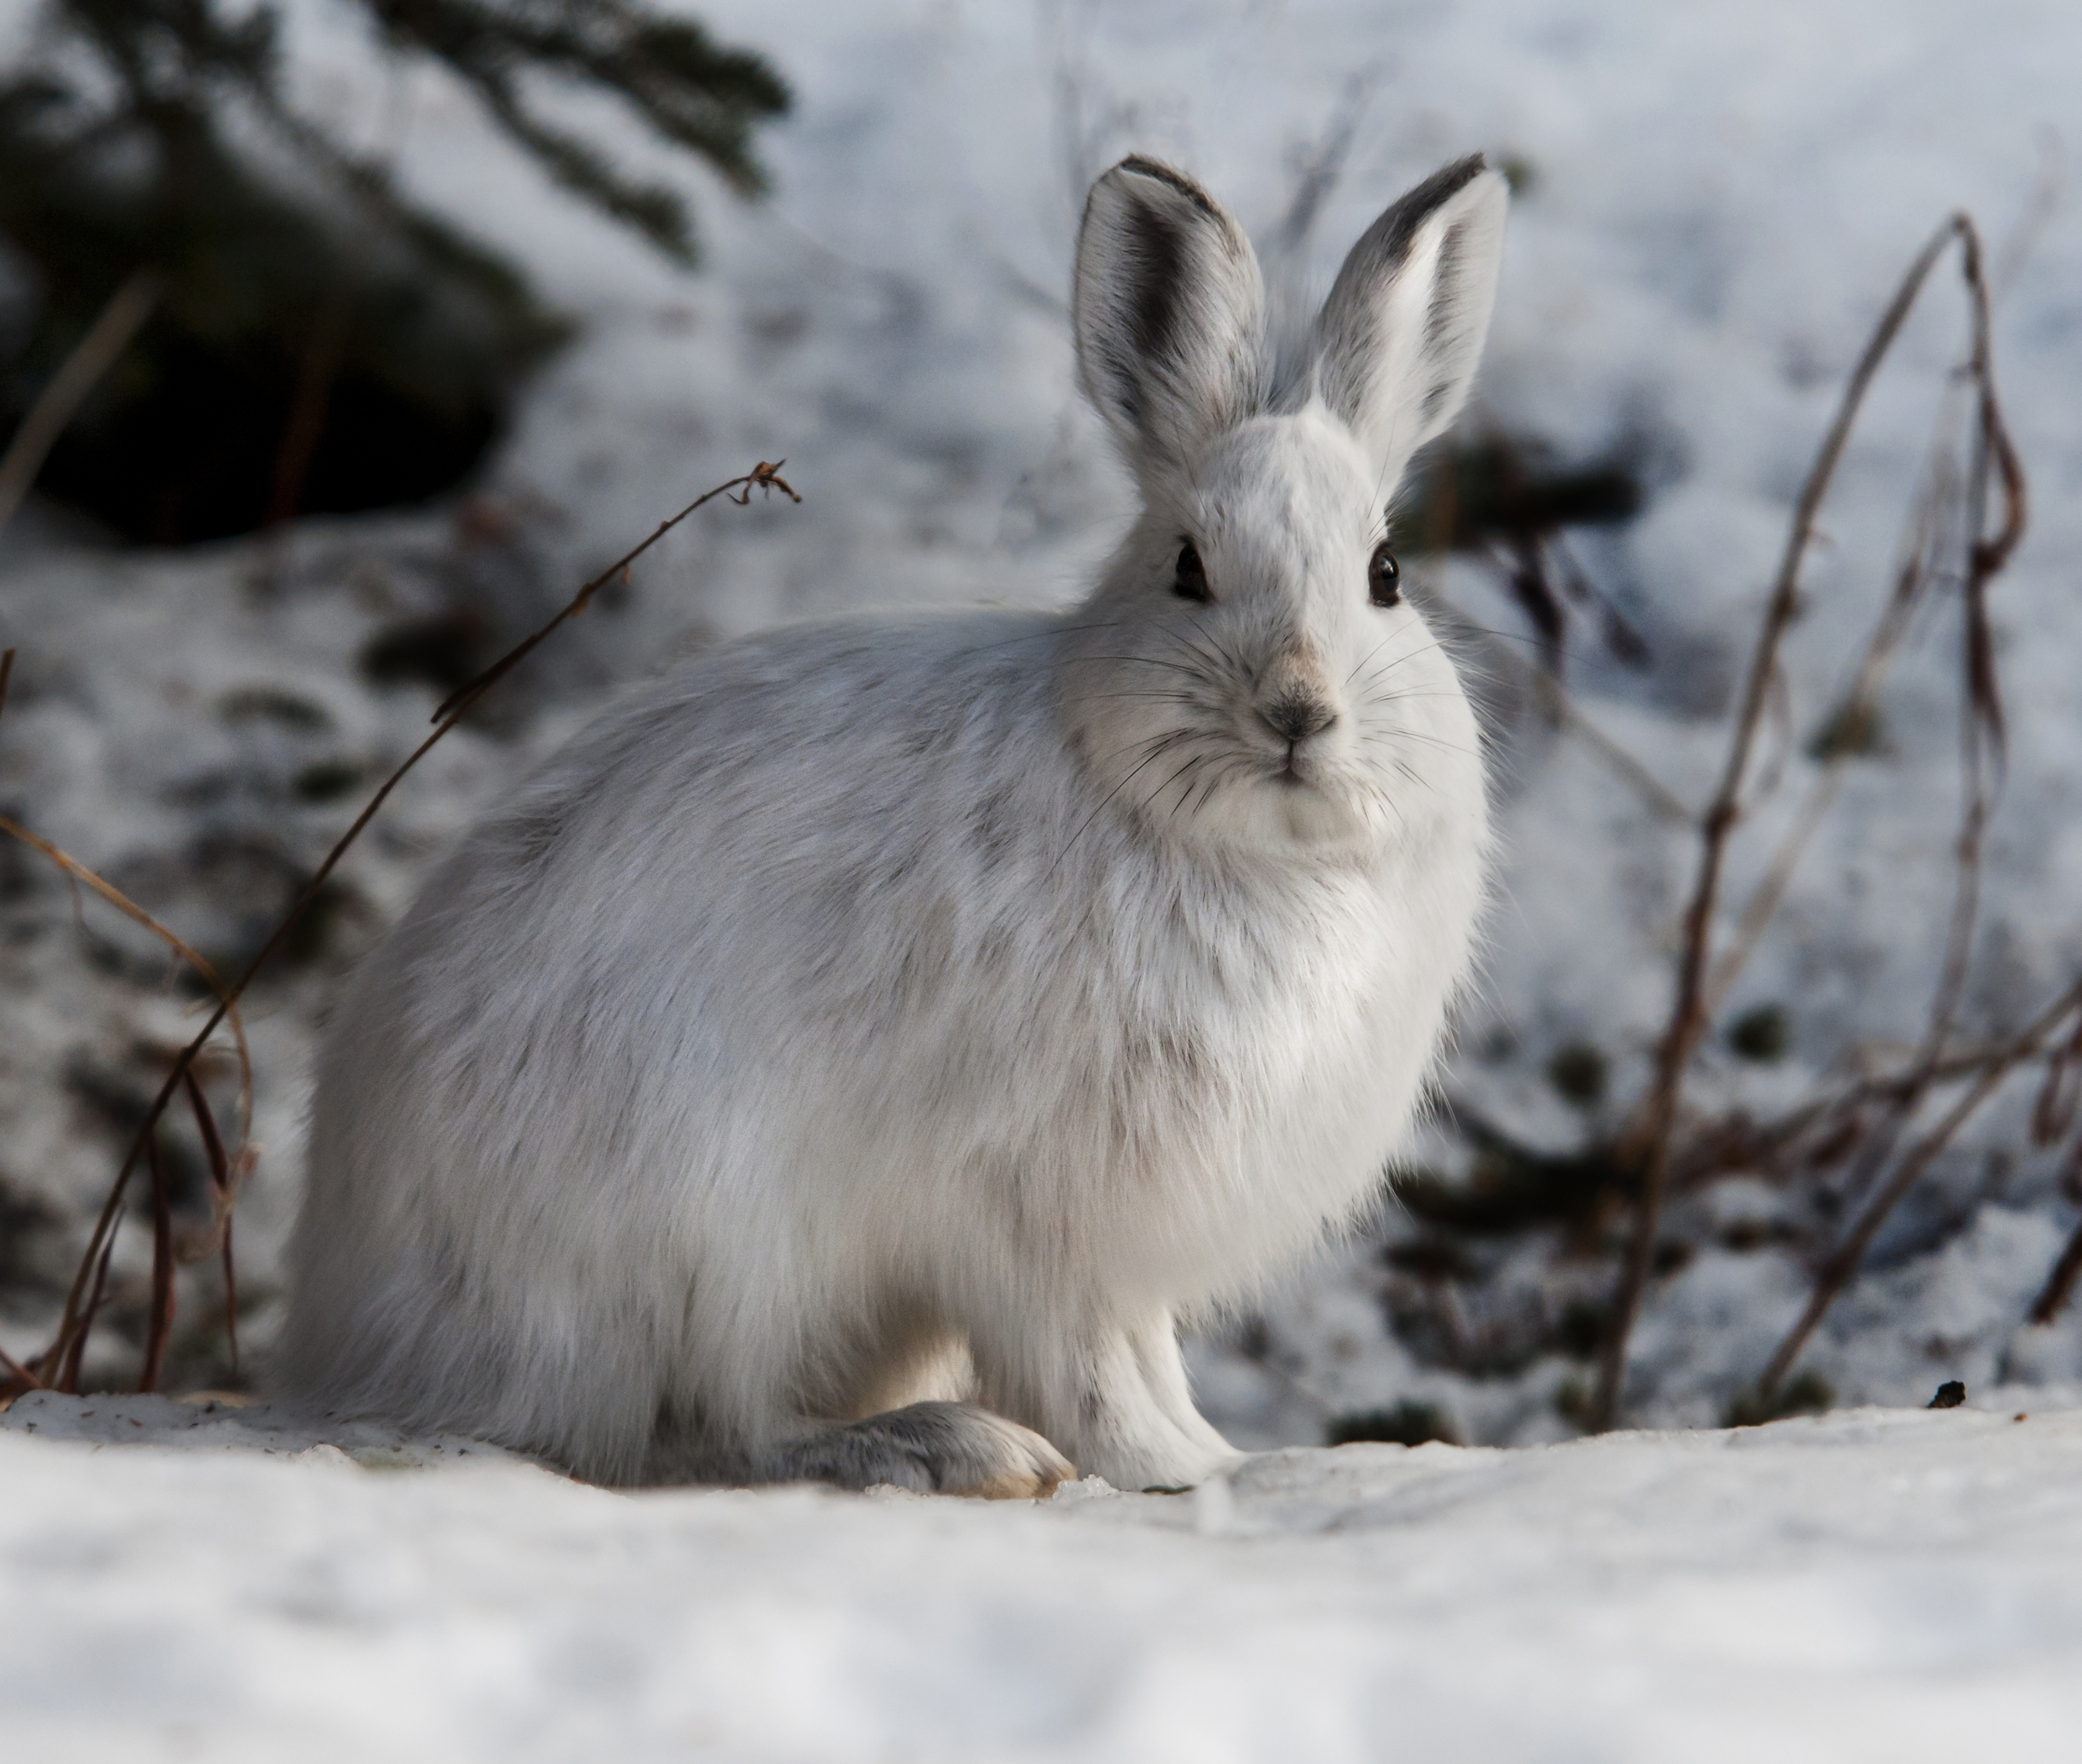
\includegraphics[height=4cm]{images/hare}
\end{subfigure}
\begin{subfigure}[t]{0.18\textwidth}
	\centering
	\vspace{2.3ex}
	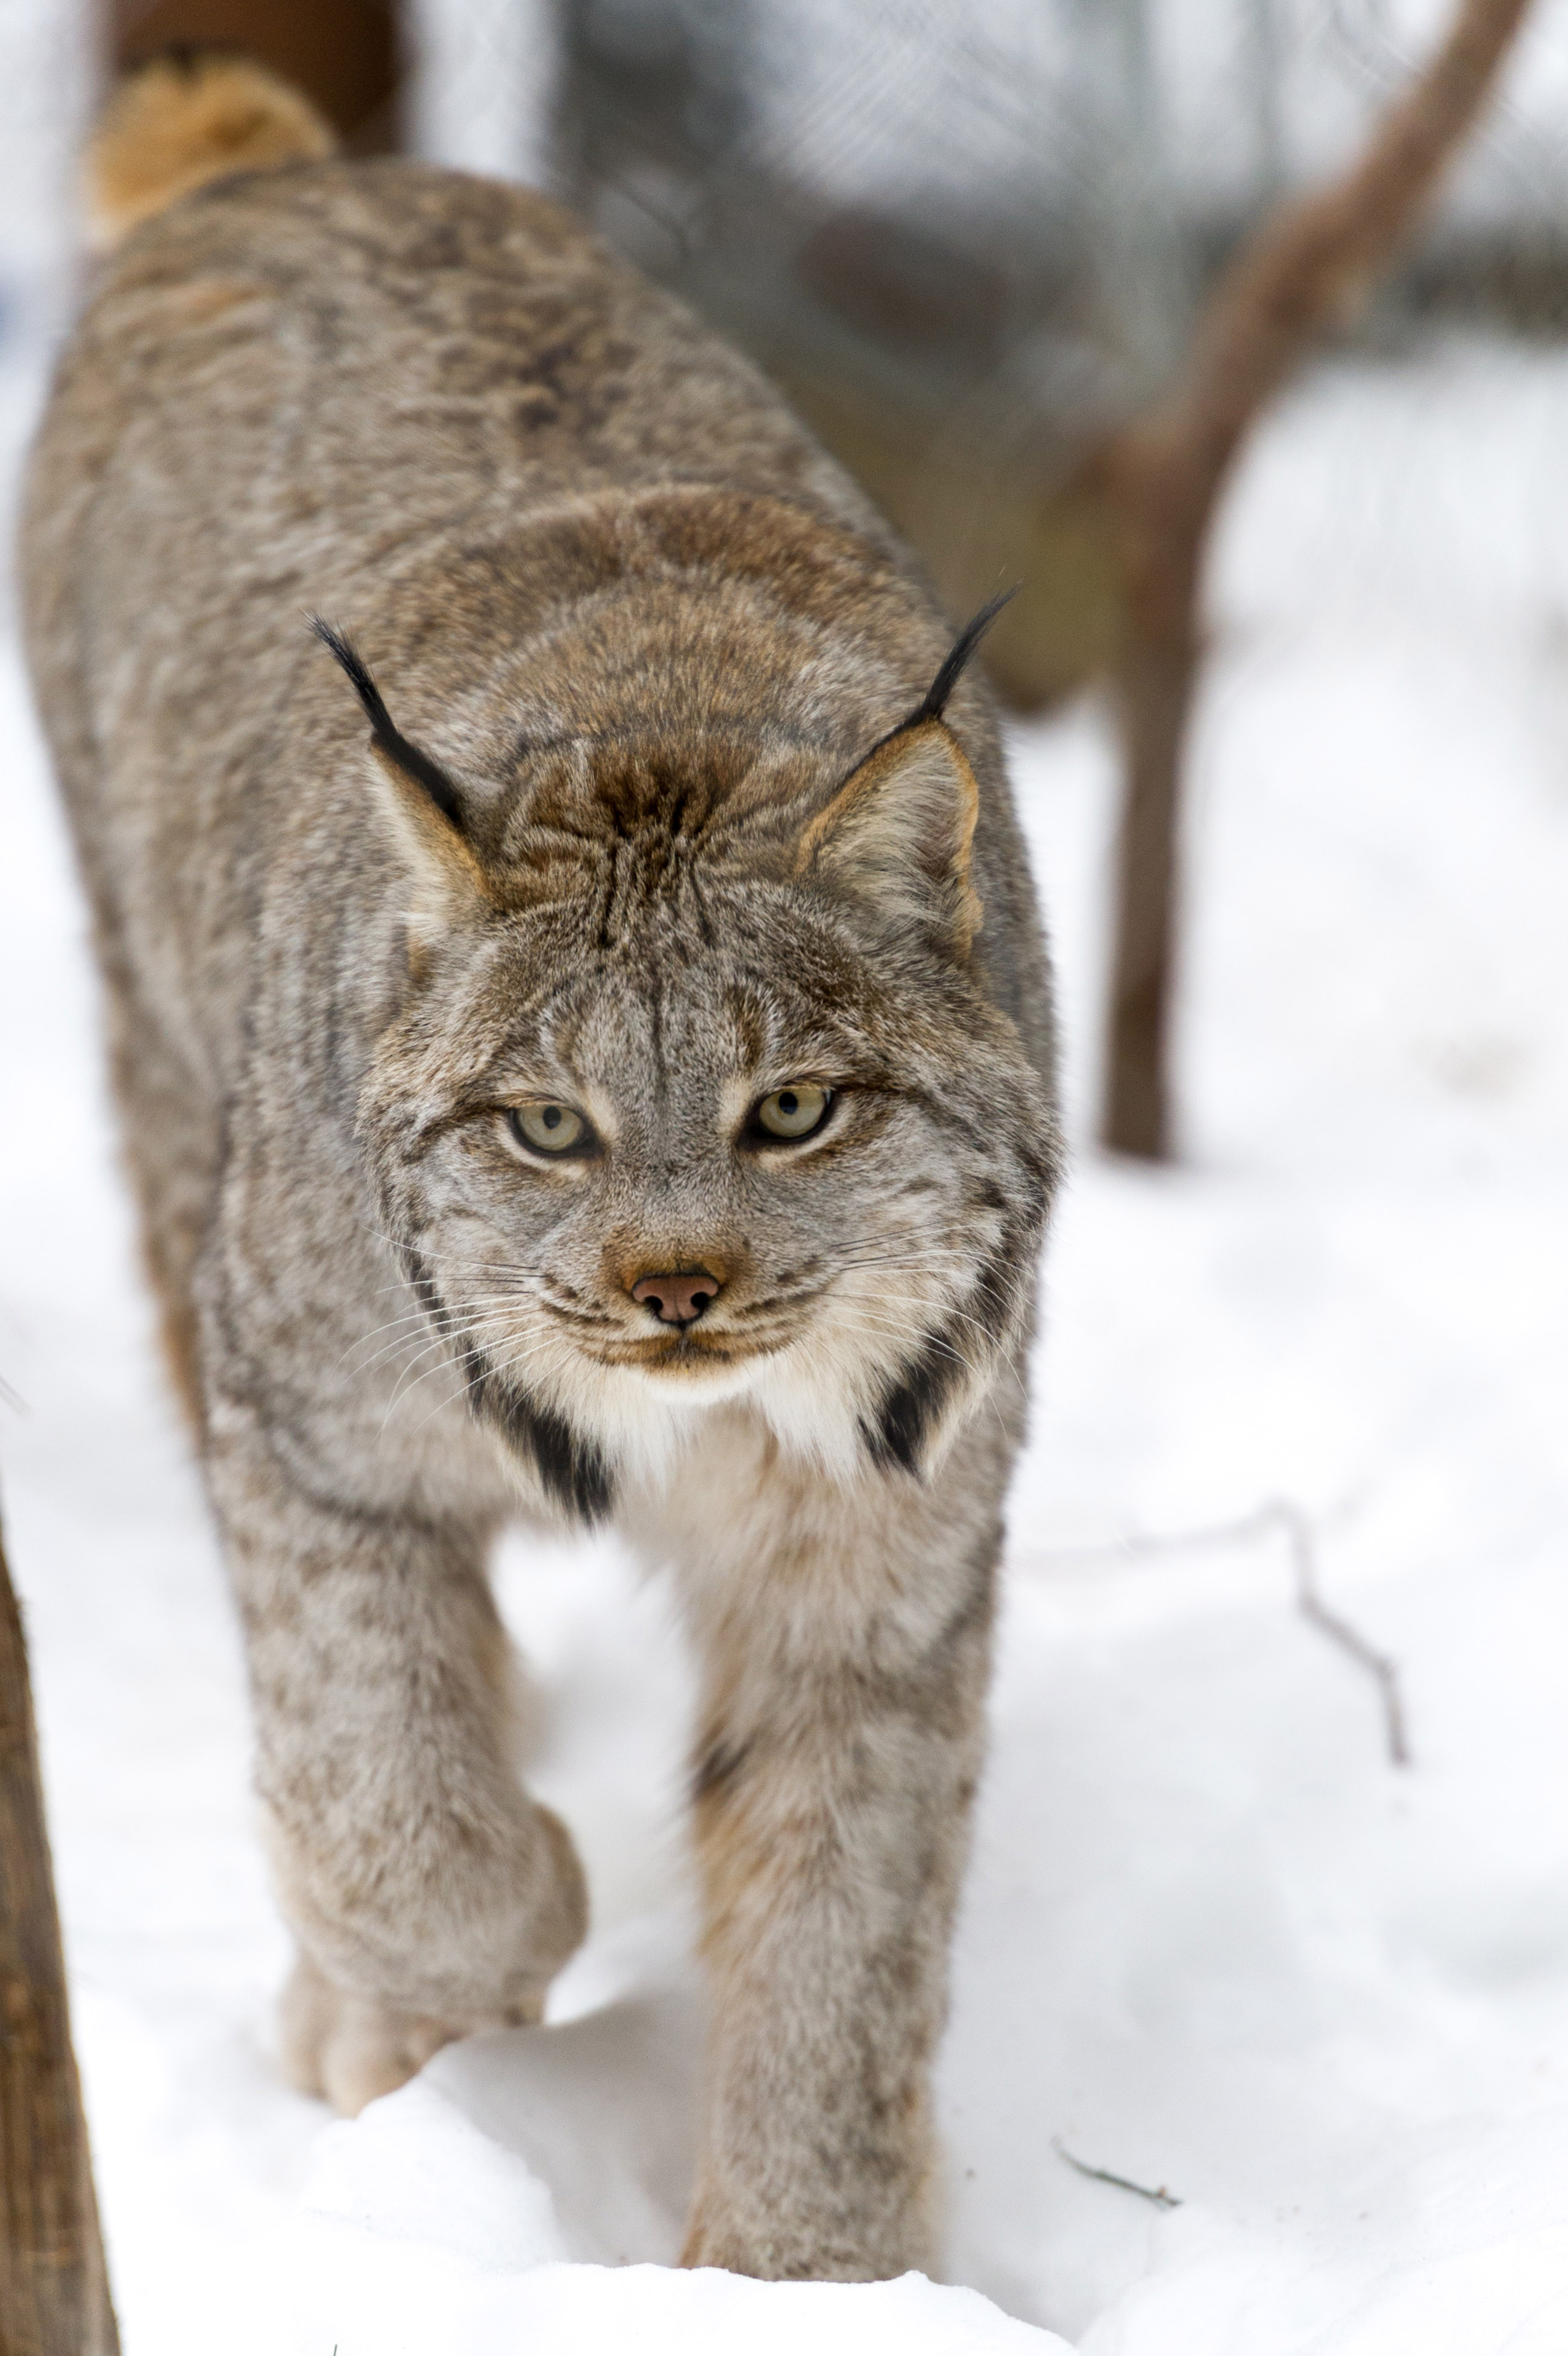
\includegraphics[height=4cm]{images/lynx}
\end{subfigure}
\begin{subfigure}[t]{0.5\textwidth}
	\centering
	\vspace{0ex}
	\begin{tikzpicture}
\begin{axis}[height=6cm,width=8cm,
%xmin=1800,
%xmax=2022,
%ymin=1,ymax=12,
domain=1900:1920,
%restrict y to domain=1:12,
axis on top,
xlabel={year},
ylabel near ticks,
ylabel={pelts (thousands)},
/pgf/number format/.cd,
        use comma,
        1000 sep={}
]

\addplot [blue, only marks,mark=*, mark size=2.3, mark options={solid,draw=black}]%
table[y index=1]{images/hare-lynx/pelts};
\addlegendentry{hares}

\addplot [orange, only marks,mark=triangle*, mark size=2.3, mark options={solid,draw=black}]%
table[y index=2]{images/hare-lynx/pelts};
\addlegendentry{lynxes}

\addplot [blue, ultra thick]%
table[y index=1]{images/hare-lynx/modelhares2.txt};

\addplot [orange, ultra thick]%
table[y index=1]{images/hare-lynx/modellynx2.txt};


\end{axis}
\end{tikzpicture}%\caption*{World population}
\end{subfigure}
\caption{Snowshoe hares (left) and the Canada lynx (centre) coexist throughout Canada and Alaska. Variations in the pelts collected from these animals between 1900 and 1920 provide a proxy count of the two populations (right). Points represent numbers of pelts sold by fur traders; continuous lines represent the Lotka--Volterra model with appropriate parameters. \emph{[Images: NPS, public domain; Eric Kilby, \textsc{cc by-sa 2.0}]} }%
\label{fig:gcse-bitesize}%
\end{figure}

The original Lotka--Volterra model was intended to model periodic behaviour. One well-studied example of periodic predator--prey behaviour is the relationship between snowshoe hares and the Canada lynx. These animals, which coexist throughout Canada and Alaska, have pelts which were collected in the 19th and 20th century. The counts of pelts is shown in \cref{fig:gcse-bitesize}.

\paragraph{...but so is extinction.}
We saw in \cref{sec:gen-systems-of-aut-odes}\StepFourIcon\ that extinction is impossible in the classic Lotka--Volterra system. This results from the fact that if population $y$ drops close to zero, then $x$ is subject to unconstrained growth which eventually leads to an increase in $y$, stopping it from dropping to zero. We only have one parameter in the nondimensionalised system ($\gamma$) and that just scales the solution.

\paragraph{Odd sensitivity to initial conditions.} If we remember the periodic orbits of Lotka--Volterra in \cref{lotkacomp}(a), changing the initial condition is equivalent to varying which orbit the solution exists on. In terms of the biology, this implies a couple of things. Firstly, there is no natural oscillation in the population levels -- different initial population sizes yield different oscillations. And secondly, this causes strange, unnatural things to occur, such as lowering the initial population of predators resulting in larger peaks in their population size.

We would expect in reality that it is possible for one species to win regardless of initial conditions. Let's have a look at some variations.


\section{Competitive Lotka--Volterra: the exclusion principle}
\label{sec:comp-lot-vol}
In classic Lotka--Volterra, one species is the predator, while the other is the prey. But often in nature, multiple species compete for the \emph{same} resources and as a result, the presence of one population impedes the growth of another. 
%
A classic example is American grey squirrels (with their bad spellings and perfect teeth) outcompeting native British red squirrels since their introduction to England in 1876 (\cref{fig:squirrels}).

\begin{figure}
\centering
\begin{subfigure}[t]{0.35\textwidth}
	\centering
	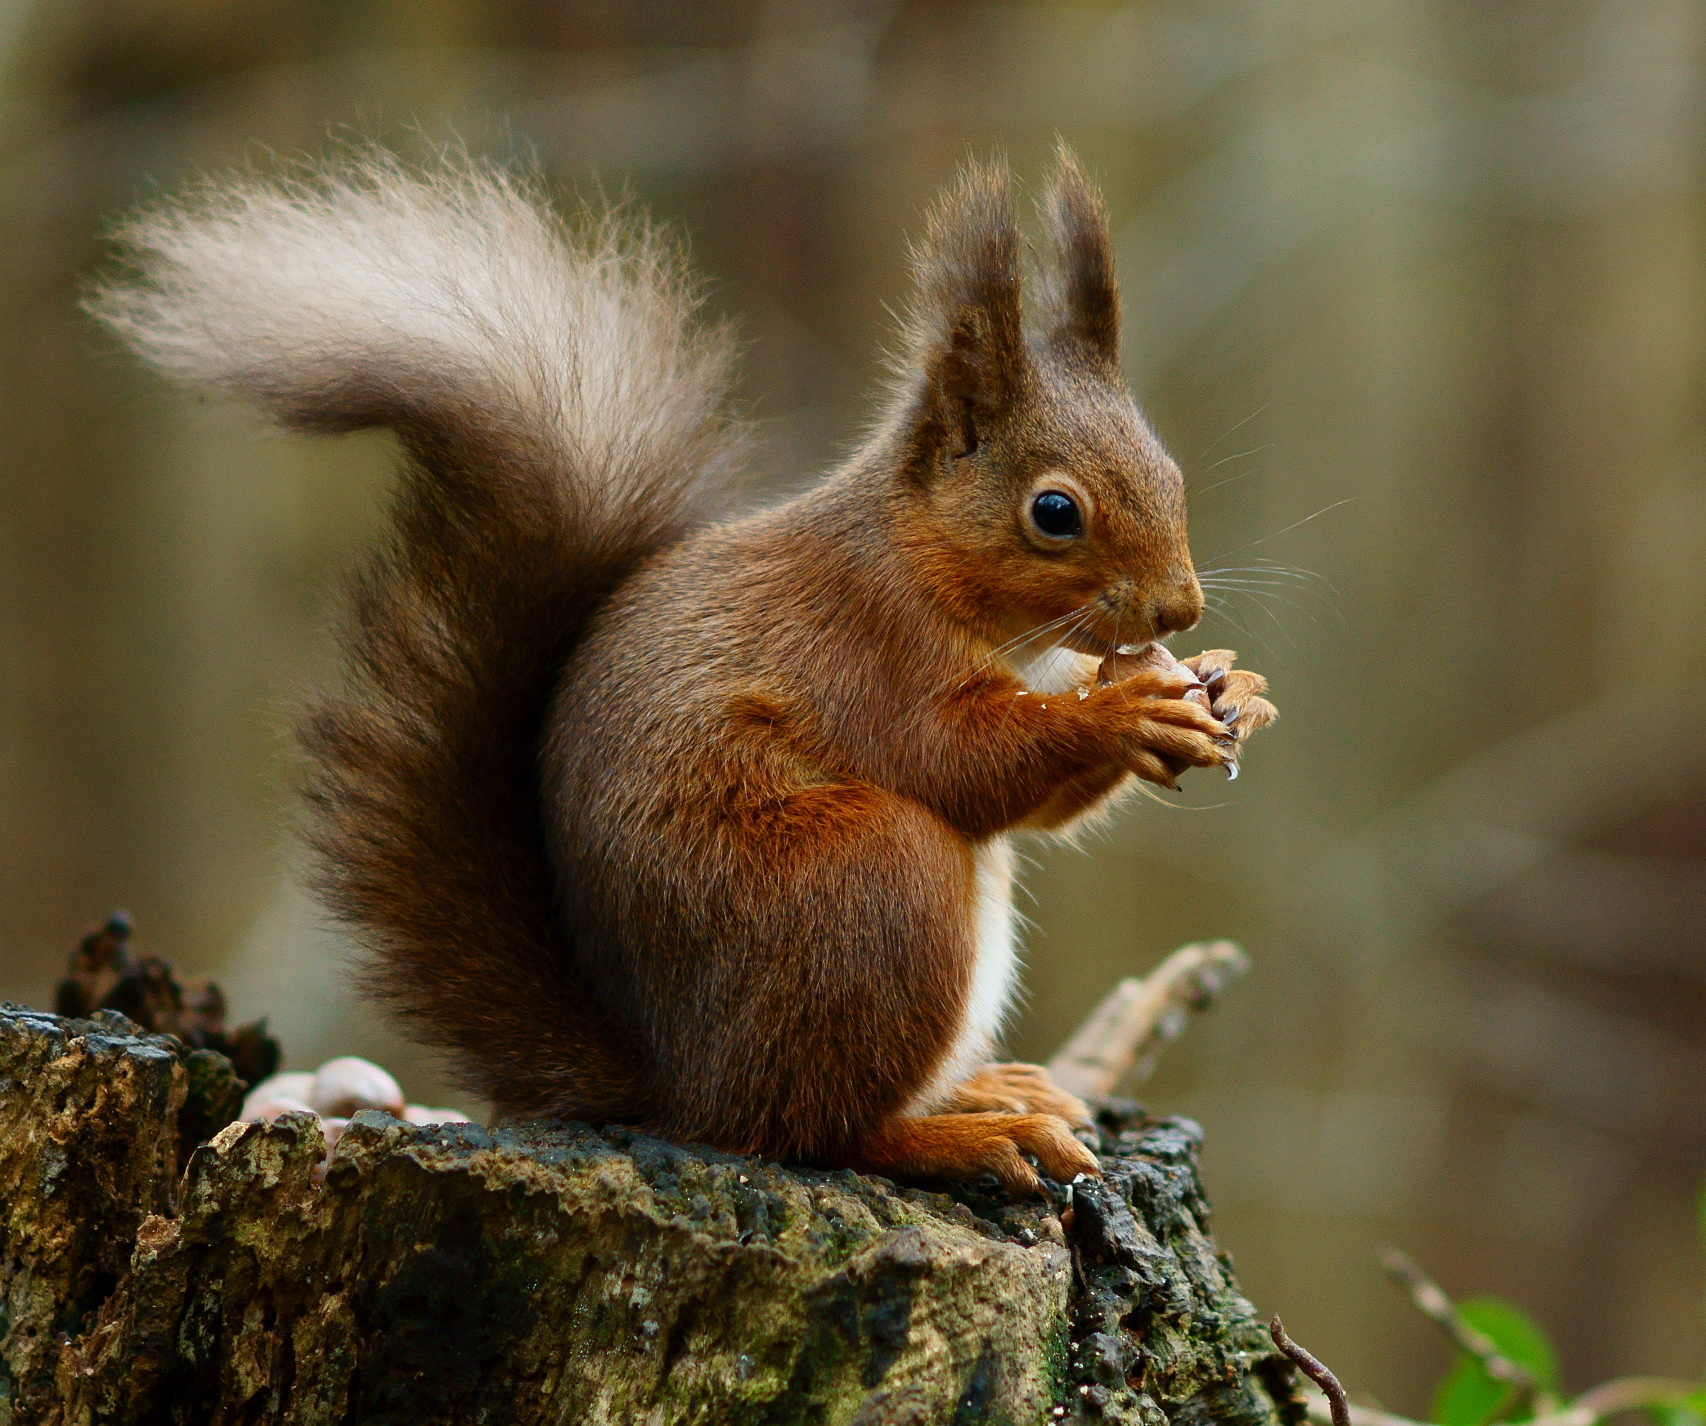
\includegraphics[height=4cm]{images/red-squirrel}
\end{subfigure}
\begin{subfigure}[t]{0.35\textwidth}
	\centering
	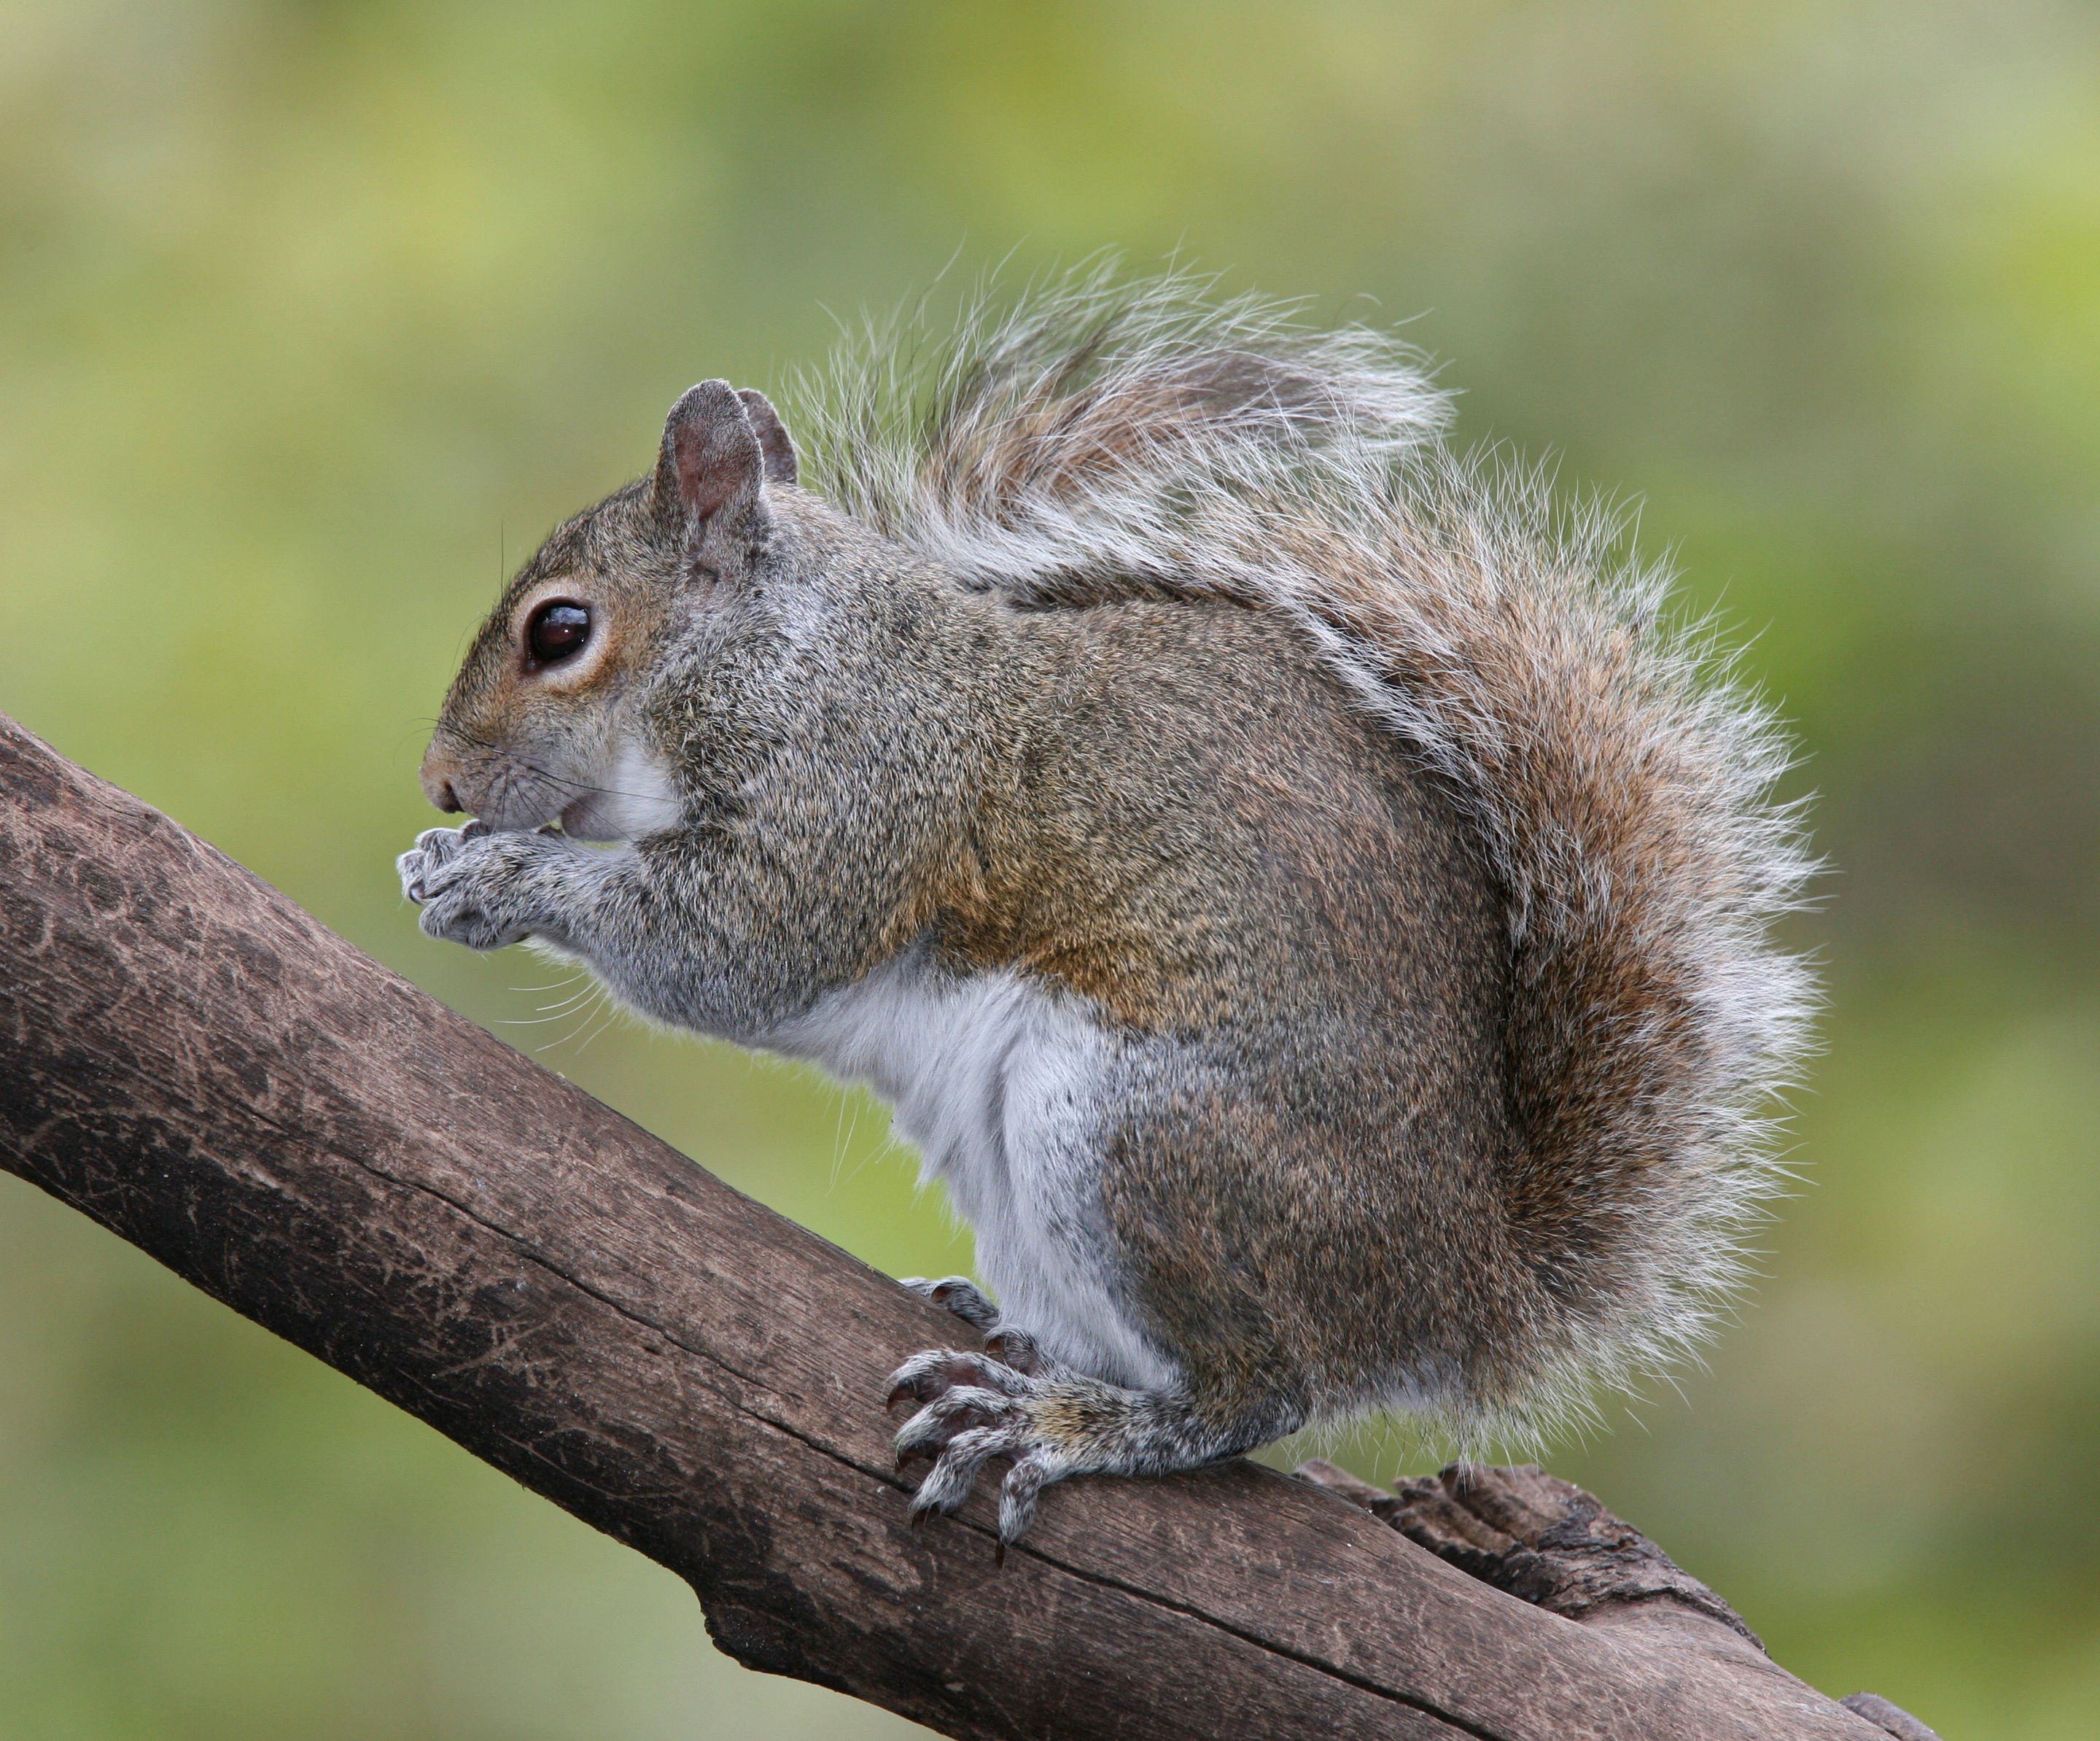
\includegraphics[height=4cm]{images/grey-squirrel}
\end{subfigure}
\caption{Red squirrels (left), native to Britain, have been outcompeted throughout most of the island since the introduction of the grey squirrel from the eastern US in 1876. Red squirrels are now mostly found only in Scotland and the Isle of Wight. \emph{[Images: Peter Trimming, \textsc{cc by 2.0}; BirdPhotos.com, \textsc{cc by 3.0}]} }%
\label{fig:squirrels}%
\end{figure}

Let’s take the case of two species whose population sizes are $x$ and $y$, respectively. In isolation, each population will evolve according to logistic growth, which you will recall from \cref{sec:logistic-growth}, looks like
\begin{equation}
\fd{x}{t} = a x\left(1-\frac{x}{K}\right),
\end{equation}
with $K$ the limiting population. When the other population is present, the death rate of a species will be proportional to the population size of the other species.

This leads us to the system:
\begin{subequations}
\label{lotvolcomp2}
\begin{align}
\fd{x}{t}  &= a x\left(1-\frac{x}{\eta_1}\right) - b x y,\\
\fd{y}{t}  &= c y\left(1-\frac{y}{\eta_2}\right) - d x y.
\end{align}
\end{subequations}
This has self-interaction for both species $x$ and $y$ through the logistic terms, as well as mutual interaction through the $xy$ terms. 

We nondimensionalise by setting $x = \hat{x}\eta_1$, $y = \hat{y}\eta_2$, $t = \hat{t}/a$, $\gamma_1 = b\eta_2/a$,  $\gamma_2 = d\eta_1/c$ and $\beta = c/a$. On substituting and dropping hats we obtain the nondimensionalised \emph{competitive Lotka--Volterra equations},
\begin{subequations}
\label{lotvolcomp2scaled}
\begin{align}
\fd{x}{t} &= x(1-x - \gamma_1 y),\\
\fd{y}{t} &= \beta y(1-y - \gamma_2 x),
\end{align}
\end{subequations}
where $\beta,\gamma_1,\gamma_2>0$.

\begin{do-it-yourself}
A worked example of a nondimensionalisation can be found in Additional Problem Sheet 2. You should try to recreate the nondimensionalisation (eqs.~\eqref{lotvolcomp2} to \eqref{lotvolcomp2scaled}) using the same method.
\end{do-it-yourself}

\begin{figure}
\centering
%% Creator: Matplotlib, PGF backend
%%
%% To include the figure in your LaTeX document, write
%%   \input{<filename>.pgf}
%%
%% Make sure the required packages are loaded in your preamble
%%   \usepackage{pgf}
%%
%% and, on pdftex
%%   \usepackage[utf8]{inputenc}\DeclareUnicodeCharacter{2212}{-}
%%
%% or, on luatex and xetex
%%   \usepackage{unicode-math}
%%
%% Figures using additional raster images can only be included by \input if
%% they are in the same directory as the main LaTeX file. For loading figures
%% from other directories you can use the `import` package
%%   \usepackage{import}
%%
%% and then include the figures with
%%   \import{<path to file>}{<filename>.pgf}
%%
%% Matplotlib used the following preamble
%%   \usepackage{fontspec}
%%   \setmainfont{DejaVuSerif.ttf}[Path=/Users/adam/opt/anaconda3/lib/python3.8/site-packages/matplotlib/mpl-data/fonts/ttf/]
%%   \setsansfont{DejaVuSans.ttf}[Path=/Users/adam/opt/anaconda3/lib/python3.8/site-packages/matplotlib/mpl-data/fonts/ttf/]
%%   \setmonofont{DejaVuSansMono.ttf}[Path=/Users/adam/opt/anaconda3/lib/python3.8/site-packages/matplotlib/mpl-data/fonts/ttf/]
%%
\begingroup%
\makeatletter%
\begin{pgfpicture}%
\pgfpathrectangle{\pgfpointorigin}{\pgfqpoint{3.000000in}{2.200000in}}%
\pgfusepath{use as bounding box, clip}%
\begin{pgfscope}%
\pgfsetbuttcap%
\pgfsetmiterjoin%
\definecolor{currentfill}{rgb}{1.000000,1.000000,1.000000}%
\pgfsetfillcolor{currentfill}%
\pgfsetlinewidth{0.000000pt}%
\definecolor{currentstroke}{rgb}{1.000000,1.000000,1.000000}%
\pgfsetstrokecolor{currentstroke}%
\pgfsetdash{}{0pt}%
\pgfpathmoveto{\pgfqpoint{0.000000in}{0.000000in}}%
\pgfpathlineto{\pgfqpoint{3.000000in}{0.000000in}}%
\pgfpathlineto{\pgfqpoint{3.000000in}{2.200000in}}%
\pgfpathlineto{\pgfqpoint{0.000000in}{2.200000in}}%
\pgfpathclose%
\pgfusepath{fill}%
\end{pgfscope}%
\begin{pgfscope}%
\pgfsetbuttcap%
\pgfsetmiterjoin%
\definecolor{currentfill}{rgb}{1.000000,1.000000,1.000000}%
\pgfsetfillcolor{currentfill}%
\pgfsetlinewidth{0.000000pt}%
\definecolor{currentstroke}{rgb}{0.000000,0.000000,0.000000}%
\pgfsetstrokecolor{currentstroke}%
\pgfsetstrokeopacity{0.000000}%
\pgfsetdash{}{0pt}%
\pgfpathmoveto{\pgfqpoint{0.338301in}{0.278150in}}%
\pgfpathlineto{\pgfqpoint{2.966667in}{0.278150in}}%
\pgfpathlineto{\pgfqpoint{2.966667in}{2.109013in}}%
\pgfpathlineto{\pgfqpoint{0.338301in}{2.109013in}}%
\pgfpathclose%
\pgfusepath{fill}%
\end{pgfscope}%
\begin{pgfscope}%
\pgfpathrectangle{\pgfqpoint{0.338301in}{0.278150in}}{\pgfqpoint{2.628366in}{1.830863in}}%
\pgfusepath{clip}%
\pgfsetrectcap%
\pgfsetroundjoin%
\pgfsetlinewidth{1.505625pt}%
\definecolor{currentstroke}{rgb}{0.121569,0.466667,0.705882}%
\pgfsetstrokecolor{currentstroke}%
\pgfsetdash{}{0pt}%
\pgfpathmoveto{\pgfqpoint{0.338301in}{2.109013in}}%
\pgfpathlineto{\pgfqpoint{0.343510in}{1.938569in}}%
\pgfpathlineto{\pgfqpoint{0.348720in}{1.803180in}}%
\pgfpathlineto{\pgfqpoint{0.353930in}{1.693154in}}%
\pgfpathlineto{\pgfqpoint{0.359140in}{1.602069in}}%
\pgfpathlineto{\pgfqpoint{0.364350in}{1.525501in}}%
\pgfpathlineto{\pgfqpoint{0.369560in}{1.460302in}}%
\pgfpathlineto{\pgfqpoint{0.377375in}{1.378956in}}%
\pgfpathlineto{\pgfqpoint{0.385190in}{1.312655in}}%
\pgfpathlineto{\pgfqpoint{0.393004in}{1.257701in}}%
\pgfpathlineto{\pgfqpoint{0.400819in}{1.211513in}}%
\pgfpathlineto{\pgfqpoint{0.408634in}{1.172233in}}%
\pgfpathlineto{\pgfqpoint{0.416449in}{1.138492in}}%
\pgfpathlineto{\pgfqpoint{0.424264in}{1.109260in}}%
\pgfpathlineto{\pgfqpoint{0.432079in}{1.083742in}}%
\pgfpathlineto{\pgfqpoint{0.439894in}{1.061321in}}%
\pgfpathlineto{\pgfqpoint{0.447708in}{1.041505in}}%
\pgfpathlineto{\pgfqpoint{0.458128in}{1.018470in}}%
\pgfpathlineto{\pgfqpoint{0.468548in}{0.998641in}}%
\pgfpathlineto{\pgfqpoint{0.478968in}{0.981451in}}%
\pgfpathlineto{\pgfqpoint{0.489388in}{0.966458in}}%
\pgfpathlineto{\pgfqpoint{0.499807in}{0.953309in}}%
\pgfpathlineto{\pgfqpoint{0.510227in}{0.941720in}}%
\pgfpathlineto{\pgfqpoint{0.523252in}{0.929081in}}%
\pgfpathlineto{\pgfqpoint{0.536277in}{0.918161in}}%
\pgfpathlineto{\pgfqpoint{0.549301in}{0.908675in}}%
\pgfpathlineto{\pgfqpoint{0.564931in}{0.898862in}}%
\pgfpathlineto{\pgfqpoint{0.580561in}{0.890468in}}%
\pgfpathlineto{\pgfqpoint{0.596190in}{0.883244in}}%
\pgfpathlineto{\pgfqpoint{0.614425in}{0.876033in}}%
\pgfpathlineto{\pgfqpoint{0.635265in}{0.869098in}}%
\pgfpathlineto{\pgfqpoint{0.658709in}{0.862624in}}%
\pgfpathlineto{\pgfqpoint{0.684759in}{0.856720in}}%
\pgfpathlineto{\pgfqpoint{0.713413in}{0.851437in}}%
\pgfpathlineto{\pgfqpoint{0.747277in}{0.846431in}}%
\pgfpathlineto{\pgfqpoint{0.786352in}{0.841883in}}%
\pgfpathlineto{\pgfqpoint{0.830636in}{0.837879in}}%
\pgfpathlineto{\pgfqpoint{0.885340in}{0.834116in}}%
\pgfpathlineto{\pgfqpoint{0.950463in}{0.830804in}}%
\pgfpathlineto{\pgfqpoint{1.031217in}{0.827873in}}%
\pgfpathlineto{\pgfqpoint{1.130205in}{0.825433in}}%
\pgfpathlineto{\pgfqpoint{1.257847in}{0.823461in}}%
\pgfpathlineto{\pgfqpoint{1.427169in}{0.822027in}}%
\pgfpathlineto{\pgfqpoint{1.677244in}{0.821116in}}%
\pgfpathlineto{\pgfqpoint{2.153949in}{0.820692in}}%
\pgfpathlineto{\pgfqpoint{2.940643in}{0.820630in}}%
\pgfpathlineto{\pgfqpoint{2.940643in}{0.820630in}}%
\pgfusepath{stroke}%
\end{pgfscope}%
\begin{pgfscope}%
\pgfpathrectangle{\pgfqpoint{0.338301in}{0.278150in}}{\pgfqpoint{2.628366in}{1.830863in}}%
\pgfusepath{clip}%
\pgfsetbuttcap%
\pgfsetroundjoin%
\pgfsetlinewidth{1.505625pt}%
\definecolor{currentstroke}{rgb}{1.000000,0.498039,0.054902}%
\pgfsetstrokecolor{currentstroke}%
\pgfsetdash{{5.550000pt}{2.400000pt}}{0.000000pt}%
\pgfpathmoveto{\pgfqpoint{0.338301in}{0.888437in}}%
\pgfpathlineto{\pgfqpoint{0.343510in}{0.861097in}}%
\pgfpathlineto{\pgfqpoint{0.348720in}{0.839027in}}%
\pgfpathlineto{\pgfqpoint{0.353930in}{0.820945in}}%
\pgfpathlineto{\pgfqpoint{0.359140in}{0.805963in}}%
\pgfpathlineto{\pgfqpoint{0.364350in}{0.793444in}}%
\pgfpathlineto{\pgfqpoint{0.369560in}{0.782920in}}%
\pgfpathlineto{\pgfqpoint{0.377375in}{0.770121in}}%
\pgfpathlineto{\pgfqpoint{0.385190in}{0.760154in}}%
\pgfpathlineto{\pgfqpoint{0.393004in}{0.752402in}}%
\pgfpathlineto{\pgfqpoint{0.400819in}{0.746420in}}%
\pgfpathlineto{\pgfqpoint{0.408634in}{0.741876in}}%
\pgfpathlineto{\pgfqpoint{0.416449in}{0.738518in}}%
\pgfpathlineto{\pgfqpoint{0.424264in}{0.736148in}}%
\pgfpathlineto{\pgfqpoint{0.434684in}{0.734261in}}%
\pgfpathlineto{\pgfqpoint{0.445103in}{0.733571in}}%
\pgfpathlineto{\pgfqpoint{0.458128in}{0.734060in}}%
\pgfpathlineto{\pgfqpoint{0.471153in}{0.735752in}}%
\pgfpathlineto{\pgfqpoint{0.486783in}{0.739025in}}%
\pgfpathlineto{\pgfqpoint{0.505017in}{0.744155in}}%
\pgfpathlineto{\pgfqpoint{0.525857in}{0.751287in}}%
\pgfpathlineto{\pgfqpoint{0.551906in}{0.761503in}}%
\pgfpathlineto{\pgfqpoint{0.588376in}{0.777207in}}%
\pgfpathlineto{\pgfqpoint{0.705598in}{0.828752in}}%
\pgfpathlineto{\pgfqpoint{0.744672in}{0.844310in}}%
\pgfpathlineto{\pgfqpoint{0.781142in}{0.857672in}}%
\pgfpathlineto{\pgfqpoint{0.817611in}{0.869840in}}%
\pgfpathlineto{\pgfqpoint{0.854080in}{0.880803in}}%
\pgfpathlineto{\pgfqpoint{0.890549in}{0.890594in}}%
\pgfpathlineto{\pgfqpoint{0.927019in}{0.899275in}}%
\pgfpathlineto{\pgfqpoint{0.966093in}{0.907435in}}%
\pgfpathlineto{\pgfqpoint{1.007772in}{0.914957in}}%
\pgfpathlineto{\pgfqpoint{1.052056in}{0.921762in}}%
\pgfpathlineto{\pgfqpoint{1.098945in}{0.927807in}}%
\pgfpathlineto{\pgfqpoint{1.148439in}{0.933085in}}%
\pgfpathlineto{\pgfqpoint{1.203143in}{0.937817in}}%
\pgfpathlineto{\pgfqpoint{1.265662in}{0.942076in}}%
\pgfpathlineto{\pgfqpoint{1.335996in}{0.945718in}}%
\pgfpathlineto{\pgfqpoint{1.416749in}{0.948770in}}%
\pgfpathlineto{\pgfqpoint{1.513132in}{0.951284in}}%
\pgfpathlineto{\pgfqpoint{1.635564in}{0.953301in}}%
\pgfpathlineto{\pgfqpoint{1.797071in}{0.954768in}}%
\pgfpathlineto{\pgfqpoint{2.034121in}{0.955709in}}%
\pgfpathlineto{\pgfqpoint{2.476963in}{0.956166in}}%
\pgfpathlineto{\pgfqpoint{2.940643in}{0.956236in}}%
\pgfpathlineto{\pgfqpoint{2.940643in}{0.956236in}}%
\pgfusepath{stroke}%
\end{pgfscope}%
\begin{pgfscope}%
\pgfsetbuttcap%
\pgfsetroundjoin%
\definecolor{currentfill}{rgb}{0.000000,0.000000,0.000000}%
\pgfsetfillcolor{currentfill}%
\pgfsetlinewidth{0.803000pt}%
\definecolor{currentstroke}{rgb}{0.000000,0.000000,0.000000}%
\pgfsetstrokecolor{currentstroke}%
\pgfsetdash{}{0pt}%
\pgfsys@defobject{currentmarker}{\pgfqpoint{0.000000in}{-0.048611in}}{\pgfqpoint{0.000000in}{0.000000in}}{%
\pgfpathmoveto{\pgfqpoint{0.000000in}{0.000000in}}%
\pgfpathlineto{\pgfqpoint{0.000000in}{-0.048611in}}%
\pgfusepath{stroke,fill}%
}%
\begin{pgfscope}%
\pgfsys@transformshift{0.338301in}{0.278150in}%
\pgfsys@useobject{currentmarker}{}%
\end{pgfscope}%
\end{pgfscope}%
\begin{pgfscope}%
\definecolor{textcolor}{rgb}{0.000000,0.000000,0.000000}%
\pgfsetstrokecolor{textcolor}%
\pgfsetfillcolor{textcolor}%
\pgftext[x=0.338301in,y=0.180927in,,top]{\color{textcolor}\rmfamily\fontsize{12.000000}{14.400000}\selectfont \(\displaystyle {0}\)}%
\end{pgfscope}%
\begin{pgfscope}%
\pgfsetbuttcap%
\pgfsetroundjoin%
\definecolor{currentfill}{rgb}{0.000000,0.000000,0.000000}%
\pgfsetfillcolor{currentfill}%
\pgfsetlinewidth{0.803000pt}%
\definecolor{currentstroke}{rgb}{0.000000,0.000000,0.000000}%
\pgfsetstrokecolor{currentstroke}%
\pgfsetdash{}{0pt}%
\pgfsys@defobject{currentmarker}{\pgfqpoint{0.000000in}{-0.048611in}}{\pgfqpoint{0.000000in}{0.000000in}}{%
\pgfpathmoveto{\pgfqpoint{0.000000in}{0.000000in}}%
\pgfpathlineto{\pgfqpoint{0.000000in}{-0.048611in}}%
\pgfusepath{stroke,fill}%
}%
\begin{pgfscope}%
\pgfsys@transformshift{1.379238in}{0.278150in}%
\pgfsys@useobject{currentmarker}{}%
\end{pgfscope}%
\end{pgfscope}%
\begin{pgfscope}%
\definecolor{textcolor}{rgb}{0.000000,0.000000,0.000000}%
\pgfsetstrokecolor{textcolor}%
\pgfsetfillcolor{textcolor}%
\pgftext[x=1.379238in,y=0.180927in,,top]{\color{textcolor}\rmfamily\fontsize{12.000000}{14.400000}\selectfont \(\displaystyle {10}\)}%
\end{pgfscope}%
\begin{pgfscope}%
\pgfsetbuttcap%
\pgfsetroundjoin%
\definecolor{currentfill}{rgb}{0.000000,0.000000,0.000000}%
\pgfsetfillcolor{currentfill}%
\pgfsetlinewidth{0.803000pt}%
\definecolor{currentstroke}{rgb}{0.000000,0.000000,0.000000}%
\pgfsetstrokecolor{currentstroke}%
\pgfsetdash{}{0pt}%
\pgfsys@defobject{currentmarker}{\pgfqpoint{0.000000in}{-0.048611in}}{\pgfqpoint{0.000000in}{0.000000in}}{%
\pgfpathmoveto{\pgfqpoint{0.000000in}{0.000000in}}%
\pgfpathlineto{\pgfqpoint{0.000000in}{-0.048611in}}%
\pgfusepath{stroke,fill}%
}%
\begin{pgfscope}%
\pgfsys@transformshift{2.420175in}{0.278150in}%
\pgfsys@useobject{currentmarker}{}%
\end{pgfscope}%
\end{pgfscope}%
\begin{pgfscope}%
\definecolor{textcolor}{rgb}{0.000000,0.000000,0.000000}%
\pgfsetstrokecolor{textcolor}%
\pgfsetfillcolor{textcolor}%
\pgftext[x=2.420175in,y=0.180927in,,top]{\color{textcolor}\rmfamily\fontsize{12.000000}{14.400000}\selectfont \(\displaystyle {20}\)}%
\end{pgfscope}%
\begin{pgfscope}%
\pgfsetbuttcap%
\pgfsetroundjoin%
\definecolor{currentfill}{rgb}{0.000000,0.000000,0.000000}%
\pgfsetfillcolor{currentfill}%
\pgfsetlinewidth{0.803000pt}%
\definecolor{currentstroke}{rgb}{0.000000,0.000000,0.000000}%
\pgfsetstrokecolor{currentstroke}%
\pgfsetdash{}{0pt}%
\pgfsys@defobject{currentmarker}{\pgfqpoint{-0.048611in}{0.000000in}}{\pgfqpoint{-0.000000in}{0.000000in}}{%
\pgfpathmoveto{\pgfqpoint{-0.000000in}{0.000000in}}%
\pgfpathlineto{\pgfqpoint{-0.048611in}{0.000000in}}%
\pgfusepath{stroke,fill}%
}%
\begin{pgfscope}%
\pgfsys@transformshift{0.338301in}{0.278150in}%
\pgfsys@useobject{currentmarker}{}%
\end{pgfscope}%
\end{pgfscope}%
\begin{pgfscope}%
\definecolor{textcolor}{rgb}{0.000000,0.000000,0.000000}%
\pgfsetstrokecolor{textcolor}%
\pgfsetfillcolor{textcolor}%
\pgftext[x=0.032554in, y=0.214836in, left, base]{\color{textcolor}\rmfamily\fontsize{12.000000}{14.400000}\selectfont \(\displaystyle {0.0}\)}%
\end{pgfscope}%
\begin{pgfscope}%
\pgfsetbuttcap%
\pgfsetroundjoin%
\definecolor{currentfill}{rgb}{0.000000,0.000000,0.000000}%
\pgfsetfillcolor{currentfill}%
\pgfsetlinewidth{0.803000pt}%
\definecolor{currentstroke}{rgb}{0.000000,0.000000,0.000000}%
\pgfsetstrokecolor{currentstroke}%
\pgfsetdash{}{0pt}%
\pgfsys@defobject{currentmarker}{\pgfqpoint{-0.048611in}{0.000000in}}{\pgfqpoint{-0.000000in}{0.000000in}}{%
\pgfpathmoveto{\pgfqpoint{-0.000000in}{0.000000in}}%
\pgfpathlineto{\pgfqpoint{-0.048611in}{0.000000in}}%
\pgfusepath{stroke,fill}%
}%
\begin{pgfscope}%
\pgfsys@transformshift{0.338301in}{0.888437in}%
\pgfsys@useobject{currentmarker}{}%
\end{pgfscope}%
\end{pgfscope}%
\begin{pgfscope}%
\definecolor{textcolor}{rgb}{0.000000,0.000000,0.000000}%
\pgfsetstrokecolor{textcolor}%
\pgfsetfillcolor{textcolor}%
\pgftext[x=0.032554in, y=0.825124in, left, base]{\color{textcolor}\rmfamily\fontsize{12.000000}{14.400000}\selectfont \(\displaystyle {0.5}\)}%
\end{pgfscope}%
\begin{pgfscope}%
\pgfsetbuttcap%
\pgfsetroundjoin%
\definecolor{currentfill}{rgb}{0.000000,0.000000,0.000000}%
\pgfsetfillcolor{currentfill}%
\pgfsetlinewidth{0.803000pt}%
\definecolor{currentstroke}{rgb}{0.000000,0.000000,0.000000}%
\pgfsetstrokecolor{currentstroke}%
\pgfsetdash{}{0pt}%
\pgfsys@defobject{currentmarker}{\pgfqpoint{-0.048611in}{0.000000in}}{\pgfqpoint{-0.000000in}{0.000000in}}{%
\pgfpathmoveto{\pgfqpoint{-0.000000in}{0.000000in}}%
\pgfpathlineto{\pgfqpoint{-0.048611in}{0.000000in}}%
\pgfusepath{stroke,fill}%
}%
\begin{pgfscope}%
\pgfsys@transformshift{0.338301in}{1.498725in}%
\pgfsys@useobject{currentmarker}{}%
\end{pgfscope}%
\end{pgfscope}%
\begin{pgfscope}%
\definecolor{textcolor}{rgb}{0.000000,0.000000,0.000000}%
\pgfsetstrokecolor{textcolor}%
\pgfsetfillcolor{textcolor}%
\pgftext[x=0.032554in, y=1.435411in, left, base]{\color{textcolor}\rmfamily\fontsize{12.000000}{14.400000}\selectfont \(\displaystyle {1.0}\)}%
\end{pgfscope}%
\begin{pgfscope}%
\pgfsetbuttcap%
\pgfsetroundjoin%
\definecolor{currentfill}{rgb}{0.000000,0.000000,0.000000}%
\pgfsetfillcolor{currentfill}%
\pgfsetlinewidth{0.803000pt}%
\definecolor{currentstroke}{rgb}{0.000000,0.000000,0.000000}%
\pgfsetstrokecolor{currentstroke}%
\pgfsetdash{}{0pt}%
\pgfsys@defobject{currentmarker}{\pgfqpoint{-0.048611in}{0.000000in}}{\pgfqpoint{-0.000000in}{0.000000in}}{%
\pgfpathmoveto{\pgfqpoint{-0.000000in}{0.000000in}}%
\pgfpathlineto{\pgfqpoint{-0.048611in}{0.000000in}}%
\pgfusepath{stroke,fill}%
}%
\begin{pgfscope}%
\pgfsys@transformshift{0.338301in}{2.109013in}%
\pgfsys@useobject{currentmarker}{}%
\end{pgfscope}%
\end{pgfscope}%
\begin{pgfscope}%
\definecolor{textcolor}{rgb}{0.000000,0.000000,0.000000}%
\pgfsetstrokecolor{textcolor}%
\pgfsetfillcolor{textcolor}%
\pgftext[x=0.032554in, y=2.045699in, left, base]{\color{textcolor}\rmfamily\fontsize{12.000000}{14.400000}\selectfont \(\displaystyle {1.5}\)}%
\end{pgfscope}%
\begin{pgfscope}%
\pgfpathrectangle{\pgfqpoint{0.338301in}{0.278150in}}{\pgfqpoint{2.628366in}{1.830863in}}%
\pgfusepath{clip}%
\pgfsetbuttcap%
\pgfsetroundjoin%
\pgfsetlinewidth{1.003750pt}%
\definecolor{currentstroke}{rgb}{0.121569,0.466667,0.705882}%
\pgfsetstrokecolor{currentstroke}%
\pgfsetdash{{1.500000pt}{2.000000pt}}{0.000000pt}%
\pgfpathmoveto{\pgfqpoint{0.338301in}{1.376667in}}%
\pgfpathlineto{\pgfqpoint{2.966667in}{1.376667in}}%
\pgfusepath{stroke}%
\end{pgfscope}%
\begin{pgfscope}%
\pgfpathrectangle{\pgfqpoint{0.338301in}{0.278150in}}{\pgfqpoint{2.628366in}{1.830863in}}%
\pgfusepath{clip}%
\pgfsetbuttcap%
\pgfsetroundjoin%
\pgfsetlinewidth{1.003750pt}%
\definecolor{currentstroke}{rgb}{1.000000,0.498039,0.054902}%
\pgfsetstrokecolor{currentstroke}%
\pgfsetdash{{1.500000pt}{2.000000pt}}{0.000000pt}%
\pgfpathmoveto{\pgfqpoint{0.338301in}{1.498725in}}%
\pgfpathlineto{\pgfqpoint{2.966667in}{1.498725in}}%
\pgfusepath{stroke}%
\end{pgfscope}%
\begin{pgfscope}%
\pgfsetrectcap%
\pgfsetmiterjoin%
\pgfsetlinewidth{0.803000pt}%
\definecolor{currentstroke}{rgb}{0.000000,0.000000,0.000000}%
\pgfsetstrokecolor{currentstroke}%
\pgfsetdash{}{0pt}%
\pgfpathmoveto{\pgfqpoint{0.338301in}{0.278150in}}%
\pgfpathlineto{\pgfqpoint{0.338301in}{2.109013in}}%
\pgfusepath{stroke}%
\end{pgfscope}%
\begin{pgfscope}%
\pgfsetrectcap%
\pgfsetmiterjoin%
\pgfsetlinewidth{0.803000pt}%
\definecolor{currentstroke}{rgb}{0.000000,0.000000,0.000000}%
\pgfsetstrokecolor{currentstroke}%
\pgfsetdash{}{0pt}%
\pgfpathmoveto{\pgfqpoint{0.338301in}{0.278150in}}%
\pgfpathlineto{\pgfqpoint{2.966667in}{0.278150in}}%
\pgfusepath{stroke}%
\end{pgfscope}%
\begin{pgfscope}%
\definecolor{textcolor}{rgb}{0.000000,0.000000,0.000000}%
\pgfsetstrokecolor{textcolor}%
\pgfsetfillcolor{textcolor}%
\pgftext[x=2.966667in,y=0.180927in,right,top]{\color{textcolor}\rmfamily\fontsize{12.000000}{14.400000}\selectfont \(\displaystyle t\)}%
\end{pgfscope}%
\begin{pgfscope}%
\pgfsetbuttcap%
\pgfsetmiterjoin%
\definecolor{currentfill}{rgb}{1.000000,1.000000,1.000000}%
\pgfsetfillcolor{currentfill}%
\pgfsetfillopacity{0.800000}%
\pgfsetlinewidth{0.000000pt}%
\definecolor{currentstroke}{rgb}{0.800000,0.800000,0.800000}%
\pgfsetstrokecolor{currentstroke}%
\pgfsetstrokeopacity{0.800000}%
\pgfsetdash{}{0pt}%
\pgfpathmoveto{\pgfqpoint{2.424440in}{1.703088in}}%
\pgfpathlineto{\pgfqpoint{2.933333in}{1.703088in}}%
\pgfpathquadraticcurveto{\pgfqpoint{2.966667in}{1.703088in}}{\pgfqpoint{2.966667in}{1.736422in}}%
\pgfpathlineto{\pgfqpoint{2.966667in}{2.075679in}}%
\pgfpathquadraticcurveto{\pgfqpoint{2.966667in}{2.109013in}}{\pgfqpoint{2.933333in}{2.109013in}}%
\pgfpathlineto{\pgfqpoint{2.424440in}{2.109013in}}%
\pgfpathquadraticcurveto{\pgfqpoint{2.391106in}{2.109013in}}{\pgfqpoint{2.391106in}{2.075679in}}%
\pgfpathlineto{\pgfqpoint{2.391106in}{1.736422in}}%
\pgfpathquadraticcurveto{\pgfqpoint{2.391106in}{1.703088in}}{\pgfqpoint{2.424440in}{1.703088in}}%
\pgfpathclose%
\pgfusepath{fill}%
\end{pgfscope}%
\begin{pgfscope}%
\pgfsetrectcap%
\pgfsetroundjoin%
\pgfsetlinewidth{1.505625pt}%
\definecolor{currentstroke}{rgb}{0.121569,0.466667,0.705882}%
\pgfsetstrokecolor{currentstroke}%
\pgfsetdash{}{0pt}%
\pgfpathmoveto{\pgfqpoint{2.391106in}{2.040718in}}%
\pgfpathlineto{\pgfqpoint{2.724440in}{2.040718in}}%
\pgfusepath{stroke}%
\end{pgfscope}%
\begin{pgfscope}%
\definecolor{textcolor}{rgb}{0.000000,0.000000,0.000000}%
\pgfsetstrokecolor{textcolor}%
\pgfsetfillcolor{textcolor}%
\pgftext[x=2.857773in,y=1.982385in,left,base]{\color{textcolor}\rmfamily\fontsize{12.000000}{14.400000}\selectfont \(\displaystyle x\)\hspace{-14pt}}%
\end{pgfscope}%
\begin{pgfscope}%
\pgfsetbuttcap%
\pgfsetroundjoin%
\pgfsetlinewidth{1.505625pt}%
\definecolor{currentstroke}{rgb}{1.000000,0.498039,0.054902}%
\pgfsetstrokecolor{currentstroke}%
\pgfsetdash{{5.550000pt}{2.400000pt}}{0.000000pt}%
\pgfpathmoveto{\pgfqpoint{2.391106in}{1.796090in}}%
\pgfpathlineto{\pgfqpoint{2.724440in}{1.796090in}}%
\pgfusepath{stroke}%
\end{pgfscope}%
\begin{pgfscope}%
\definecolor{textcolor}{rgb}{0.000000,0.000000,0.000000}%
\pgfsetstrokecolor{textcolor}%
\pgfsetfillcolor{textcolor}%
\pgftext[x=2.857773in,y=1.737756in,left,base]{\color{textcolor}\rmfamily\fontsize{12.000000}{14.400000}\selectfont \(\displaystyle y\)\hspace{-14pt}}%
\end{pgfscope}%
\end{pgfpicture}%
\makeatother%
\endgroup%

\caption{\label{lotcomp}An example solution to the competitive Lotka--Volterra equations, \cref{lotvolcomp2}.  Both populations settle on fixed (equilibrium) values. The dotted lines are the values they would have obtained in the absence of interaction ($b=d=0$); that is to say, these are the values due to logistic growth alone. Parameters: $a = c = d = 1$, $b=0.2$, $\eta_1 = 0.5$, $\eta_2 = 1$.}
\end{figure}

An example solution is shown in \cref{lotcomp}: we see both populations eventually settle on fixed values, although the competition through the mutual competition terms $\gamma_1 xy $ and $\gamma_2 x y$ ensures these fixed values are not those of the logistic behaviour alone.  

\begin{do-it-yourself}
See if you can reproduce \cref{lotcomp} yourself by adapting your Python code from the last Lotka--Volterra plot.
\end{do-it-yourself}

Let’s do a linear stability analysis as well as drawing a phase portrait.

%And remember that we complained that Lotka--Volterra doesn't let a population become extinct? In \cref{lotvolcompdecay}(a) we see a particular case of our altered model for which the greenfly population does indeed become extinct while the ladybird population settles at its logistic level: the predator species dominates.  

\subsubsection*{\StepOne Find equilibria}
\label{chap4equilibria}
\Cref{lotvolcomp2scaled} allows for the trivial null population solutions, $(x,y)=(0,0)$, but interestingly it also allows for solutions where one or the other populations is extinct,
\begin{equation}
(x,y) = (0,1)\mbox{ and } (x,y) = (1,0).
\end{equation}
In both cases the non-extinct population takes on its logistic value (remembering that we have nondimensionalised by this point). The final equilibrium takes the form 
\begin{equation}
\label{nonzeroeq}
(x,y) = \left( \frac{1-\gamma_1}{1-\gamma_1\gamma_2}, \frac{1-\gamma_2}{1-\gamma_1\gamma_2} \right),
\end{equation}
and exists if $\gamma_1,\gamma_2<1$ or $\gamma_1,\gamma_2>1$ (because of the denominator).

The nullclines are given by the same equations, but considered separately:
\begin{subequations}
\begin{align}
0 &= x(1-x-\gamma_1y) &&\implies x=0, \quad x=1-\gamma_1 y\\
0 &= \beta y(1-y-\gamma_2x) &&\implies y=0, \quad y=1-\gamma_2 x.
\end{align}
\end{subequations}
The important observation is that the slope of the lines, and whether they intersect or not, depend on the values of $\gamma_1$ and $\gamma_2$. As the intersections are the equilibria, we see that varying $\gamma_1$ and $\gamma_2$ result in bifurcations. Four cases can arise, depicted in \cref{comp-lv-phase-options}.

\begin{figure}
\begin{subfigure}[t]{0.49\textwidth}
	\centering
	%% Creator: Matplotlib, PGF backend
%%
%% To include the figure in your LaTeX document, write
%%   \input{<filename>.pgf}
%%
%% Make sure the required packages are loaded in your preamble
%%   \usepackage{pgf}
%%
%% and, on pdftex
%%   \usepackage[utf8]{inputenc}\DeclareUnicodeCharacter{2212}{-}
%%
%% or, on luatex and xetex
%%   \usepackage{unicode-math}
%%
%% Figures using additional raster images can only be included by \input if
%% they are in the same directory as the main LaTeX file. For loading figures
%% from other directories you can use the `import` package
%%   \usepackage{import}
%%
%% and then include the figures with
%%   \import{<path to file>}{<filename>.pgf}
%%
%% Matplotlib used the following preamble
%%   \usepackage{fontspec}
%%   \setmainfont{DejaVuSerif.ttf}[Path=/Users/adam/opt/anaconda3/lib/python3.8/site-packages/matplotlib/mpl-data/fonts/ttf/]
%%   \setsansfont{DejaVuSans.ttf}[Path=/Users/adam/opt/anaconda3/lib/python3.8/site-packages/matplotlib/mpl-data/fonts/ttf/]
%%   \setmonofont{DejaVuSansMono.ttf}[Path=/Users/adam/opt/anaconda3/lib/python3.8/site-packages/matplotlib/mpl-data/fonts/ttf/]
%%
\begingroup%
\makeatletter%
\begin{pgfpicture}%
\pgfpathrectangle{\pgfpointorigin}{\pgfqpoint{3.000000in}{2.200000in}}%
\pgfusepath{use as bounding box, clip}%
\begin{pgfscope}%
\pgfsetbuttcap%
\pgfsetmiterjoin%
\definecolor{currentfill}{rgb}{1.000000,1.000000,1.000000}%
\pgfsetfillcolor{currentfill}%
\pgfsetlinewidth{0.000000pt}%
\definecolor{currentstroke}{rgb}{1.000000,1.000000,1.000000}%
\pgfsetstrokecolor{currentstroke}%
\pgfsetdash{}{0pt}%
\pgfpathmoveto{\pgfqpoint{0.000000in}{0.000000in}}%
\pgfpathlineto{\pgfqpoint{3.000000in}{0.000000in}}%
\pgfpathlineto{\pgfqpoint{3.000000in}{2.200000in}}%
\pgfpathlineto{\pgfqpoint{0.000000in}{2.200000in}}%
\pgfpathclose%
\pgfusepath{fill}%
\end{pgfscope}%
\begin{pgfscope}%
\pgfsetbuttcap%
\pgfsetmiterjoin%
\definecolor{currentfill}{rgb}{1.000000,1.000000,1.000000}%
\pgfsetfillcolor{currentfill}%
\pgfsetlinewidth{0.000000pt}%
\definecolor{currentstroke}{rgb}{0.000000,0.000000,0.000000}%
\pgfsetstrokecolor{currentstroke}%
\pgfsetstrokeopacity{0.000000}%
\pgfsetdash{}{0pt}%
\pgfpathmoveto{\pgfqpoint{0.436279in}{0.296600in}}%
\pgfpathlineto{\pgfqpoint{2.966667in}{0.296600in}}%
\pgfpathlineto{\pgfqpoint{2.966667in}{1.968025in}}%
\pgfpathlineto{\pgfqpoint{0.436279in}{1.968025in}}%
\pgfpathclose%
\pgfusepath{fill}%
\end{pgfscope}%
\begin{pgfscope}%
\pgfpathrectangle{\pgfqpoint{0.436279in}{0.296600in}}{\pgfqpoint{2.530388in}{1.671426in}}%
\pgfusepath{clip}%
\pgfsetbuttcap%
\pgfsetroundjoin%
\pgfsetlinewidth{0.702625pt}%
\definecolor{currentstroke}{rgb}{0.121569,0.466667,0.705882}%
\pgfsetstrokecolor{currentstroke}%
\pgfsetdash{{2.590000pt}{1.120000pt}}{0.000000pt}%
\pgfpathmoveto{\pgfqpoint{2.017771in}{0.296600in}}%
\pgfpathlineto{\pgfqpoint{0.436279in}{1.759097in}}%
\pgfusepath{stroke}%
\end{pgfscope}%
\begin{pgfscope}%
\pgfpathrectangle{\pgfqpoint{0.436279in}{0.296600in}}{\pgfqpoint{2.530388in}{1.671426in}}%
\pgfusepath{clip}%
\pgfsetbuttcap%
\pgfsetroundjoin%
\pgfsetlinewidth{0.702625pt}%
\definecolor{currentstroke}{rgb}{1.000000,0.498039,0.054902}%
\pgfsetstrokecolor{currentstroke}%
\pgfsetdash{{2.590000pt}{1.120000pt}}{0.000000pt}%
\pgfpathmoveto{\pgfqpoint{0.436279in}{1.341241in}}%
\pgfpathlineto{\pgfqpoint{2.650368in}{0.296600in}}%
\pgfusepath{stroke}%
\end{pgfscope}%
\begin{pgfscope}%
\pgfsetbuttcap%
\pgfsetroundjoin%
\definecolor{currentfill}{rgb}{0.000000,0.000000,0.000000}%
\pgfsetfillcolor{currentfill}%
\pgfsetlinewidth{0.803000pt}%
\definecolor{currentstroke}{rgb}{0.000000,0.000000,0.000000}%
\pgfsetstrokecolor{currentstroke}%
\pgfsetdash{}{0pt}%
\pgfsys@defobject{currentmarker}{\pgfqpoint{0.000000in}{-0.048611in}}{\pgfqpoint{0.000000in}{0.000000in}}{%
\pgfpathmoveto{\pgfqpoint{0.000000in}{0.000000in}}%
\pgfpathlineto{\pgfqpoint{0.000000in}{-0.048611in}}%
\pgfusepath{stroke,fill}%
}%
\begin{pgfscope}%
\pgfsys@transformshift{0.436279in}{0.296600in}%
\pgfsys@useobject{currentmarker}{}%
\end{pgfscope}%
\end{pgfscope}%
\begin{pgfscope}%
\definecolor{textcolor}{rgb}{0.000000,0.000000,0.000000}%
\pgfsetstrokecolor{textcolor}%
\pgfsetfillcolor{textcolor}%
\pgftext[x=0.436279in,y=0.199377in,,top]{\color{textcolor}\rmfamily\fontsize{12.000000}{14.400000}\selectfont 0}%
\end{pgfscope}%
\begin{pgfscope}%
\pgfsetbuttcap%
\pgfsetroundjoin%
\definecolor{currentfill}{rgb}{0.000000,0.000000,0.000000}%
\pgfsetfillcolor{currentfill}%
\pgfsetlinewidth{0.803000pt}%
\definecolor{currentstroke}{rgb}{0.000000,0.000000,0.000000}%
\pgfsetstrokecolor{currentstroke}%
\pgfsetdash{}{0pt}%
\pgfsys@defobject{currentmarker}{\pgfqpoint{0.000000in}{-0.048611in}}{\pgfqpoint{0.000000in}{0.000000in}}{%
\pgfpathmoveto{\pgfqpoint{0.000000in}{0.000000in}}%
\pgfpathlineto{\pgfqpoint{0.000000in}{-0.048611in}}%
\pgfusepath{stroke,fill}%
}%
\begin{pgfscope}%
\pgfsys@transformshift{2.017771in}{0.296600in}%
\pgfsys@useobject{currentmarker}{}%
\end{pgfscope}%
\end{pgfscope}%
\begin{pgfscope}%
\definecolor{textcolor}{rgb}{0.000000,0.000000,0.000000}%
\pgfsetstrokecolor{textcolor}%
\pgfsetfillcolor{textcolor}%
\pgftext[x=2.017771in,y=0.199377in,,top]{\color{textcolor}\rmfamily\fontsize{12.000000}{14.400000}\selectfont 1}%
\end{pgfscope}%
\begin{pgfscope}%
\pgfsetbuttcap%
\pgfsetroundjoin%
\definecolor{currentfill}{rgb}{0.000000,0.000000,0.000000}%
\pgfsetfillcolor{currentfill}%
\pgfsetlinewidth{0.803000pt}%
\definecolor{currentstroke}{rgb}{0.000000,0.000000,0.000000}%
\pgfsetstrokecolor{currentstroke}%
\pgfsetdash{}{0pt}%
\pgfsys@defobject{currentmarker}{\pgfqpoint{0.000000in}{-0.048611in}}{\pgfqpoint{0.000000in}{0.000000in}}{%
\pgfpathmoveto{\pgfqpoint{0.000000in}{0.000000in}}%
\pgfpathlineto{\pgfqpoint{0.000000in}{-0.048611in}}%
\pgfusepath{stroke,fill}%
}%
\begin{pgfscope}%
\pgfsys@transformshift{2.650368in}{0.296600in}%
\pgfsys@useobject{currentmarker}{}%
\end{pgfscope}%
\end{pgfscope}%
\begin{pgfscope}%
\definecolor{textcolor}{rgb}{0.000000,0.000000,0.000000}%
\pgfsetstrokecolor{textcolor}%
\pgfsetfillcolor{textcolor}%
\pgftext[x=2.650368in,y=0.199377in,,top]{\color{textcolor}\rmfamily\fontsize{12.000000}{14.400000}\selectfont \(\displaystyle 1/\gamma_2\)}%
\end{pgfscope}%
\begin{pgfscope}%
\pgfsetbuttcap%
\pgfsetroundjoin%
\definecolor{currentfill}{rgb}{0.000000,0.000000,0.000000}%
\pgfsetfillcolor{currentfill}%
\pgfsetlinewidth{0.803000pt}%
\definecolor{currentstroke}{rgb}{0.000000,0.000000,0.000000}%
\pgfsetstrokecolor{currentstroke}%
\pgfsetdash{}{0pt}%
\pgfsys@defobject{currentmarker}{\pgfqpoint{-0.048611in}{0.000000in}}{\pgfqpoint{-0.000000in}{0.000000in}}{%
\pgfpathmoveto{\pgfqpoint{-0.000000in}{0.000000in}}%
\pgfpathlineto{\pgfqpoint{-0.048611in}{0.000000in}}%
\pgfusepath{stroke,fill}%
}%
\begin{pgfscope}%
\pgfsys@transformshift{0.436279in}{0.296600in}%
\pgfsys@useobject{currentmarker}{}%
\end{pgfscope}%
\end{pgfscope}%
\begin{pgfscope}%
\definecolor{textcolor}{rgb}{0.000000,0.000000,0.000000}%
\pgfsetstrokecolor{textcolor}%
\pgfsetfillcolor{textcolor}%
\pgftext[x=0.233018in, y=0.233286in, left, base]{\color{textcolor}\rmfamily\fontsize{12.000000}{14.400000}\selectfont 0}%
\end{pgfscope}%
\begin{pgfscope}%
\pgfsetbuttcap%
\pgfsetroundjoin%
\definecolor{currentfill}{rgb}{0.000000,0.000000,0.000000}%
\pgfsetfillcolor{currentfill}%
\pgfsetlinewidth{0.803000pt}%
\definecolor{currentstroke}{rgb}{0.000000,0.000000,0.000000}%
\pgfsetstrokecolor{currentstroke}%
\pgfsetdash{}{0pt}%
\pgfsys@defobject{currentmarker}{\pgfqpoint{-0.048611in}{0.000000in}}{\pgfqpoint{-0.000000in}{0.000000in}}{%
\pgfpathmoveto{\pgfqpoint{-0.000000in}{0.000000in}}%
\pgfpathlineto{\pgfqpoint{-0.048611in}{0.000000in}}%
\pgfusepath{stroke,fill}%
}%
\begin{pgfscope}%
\pgfsys@transformshift{0.436279in}{1.341241in}%
\pgfsys@useobject{currentmarker}{}%
\end{pgfscope}%
\end{pgfscope}%
\begin{pgfscope}%
\definecolor{textcolor}{rgb}{0.000000,0.000000,0.000000}%
\pgfsetstrokecolor{textcolor}%
\pgfsetfillcolor{textcolor}%
\pgftext[x=0.233018in, y=1.277927in, left, base]{\color{textcolor}\rmfamily\fontsize{12.000000}{14.400000}\selectfont 1}%
\end{pgfscope}%
\begin{pgfscope}%
\pgfsetbuttcap%
\pgfsetroundjoin%
\definecolor{currentfill}{rgb}{0.000000,0.000000,0.000000}%
\pgfsetfillcolor{currentfill}%
\pgfsetlinewidth{0.803000pt}%
\definecolor{currentstroke}{rgb}{0.000000,0.000000,0.000000}%
\pgfsetstrokecolor{currentstroke}%
\pgfsetdash{}{0pt}%
\pgfsys@defobject{currentmarker}{\pgfqpoint{-0.048611in}{0.000000in}}{\pgfqpoint{-0.000000in}{0.000000in}}{%
\pgfpathmoveto{\pgfqpoint{-0.000000in}{0.000000in}}%
\pgfpathlineto{\pgfqpoint{-0.048611in}{0.000000in}}%
\pgfusepath{stroke,fill}%
}%
\begin{pgfscope}%
\pgfsys@transformshift{0.436279in}{1.759097in}%
\pgfsys@useobject{currentmarker}{}%
\end{pgfscope}%
\end{pgfscope}%
\begin{pgfscope}%
\definecolor{textcolor}{rgb}{0.000000,0.000000,0.000000}%
\pgfsetstrokecolor{textcolor}%
\pgfsetfillcolor{textcolor}%
\pgftext[x=0.025242in, y=1.696597in, left, base]{\color{textcolor}\rmfamily\fontsize{12.000000}{14.400000}\selectfont \(\displaystyle 1/\gamma_1\)}%
\end{pgfscope}%
\begin{pgfscope}%
\pgfsetrectcap%
\pgfsetmiterjoin%
\pgfsetlinewidth{0.803000pt}%
\definecolor{currentstroke}{rgb}{0.000000,0.000000,0.000000}%
\pgfsetstrokecolor{currentstroke}%
\pgfsetdash{}{0pt}%
\pgfpathmoveto{\pgfqpoint{0.436279in}{0.296600in}}%
\pgfpathlineto{\pgfqpoint{0.436279in}{1.968025in}}%
\pgfusepath{stroke}%
\end{pgfscope}%
\begin{pgfscope}%
\pgfsetrectcap%
\pgfsetmiterjoin%
\pgfsetlinewidth{0.803000pt}%
\definecolor{currentstroke}{rgb}{0.000000,0.000000,0.000000}%
\pgfsetstrokecolor{currentstroke}%
\pgfsetdash{}{0pt}%
\pgfpathmoveto{\pgfqpoint{0.436279in}{0.296600in}}%
\pgfpathlineto{\pgfqpoint{2.966667in}{0.296600in}}%
\pgfusepath{stroke}%
\end{pgfscope}%
\begin{pgfscope}%
\definecolor{textcolor}{rgb}{0.000000,0.000000,0.000000}%
\pgfsetstrokecolor{textcolor}%
\pgfsetfillcolor{textcolor}%
\pgftext[x=2.966667in,y=0.199377in,right,top]{\color{textcolor}\rmfamily\fontsize{12.000000}{14.400000}\selectfont \(\displaystyle x\)}%
\end{pgfscope}%
\begin{pgfscope}%
\definecolor{textcolor}{rgb}{0.000000,0.000000,0.000000}%
\pgfsetstrokecolor{textcolor}%
\pgfsetfillcolor{textcolor}%
\pgftext[x=0.339056in,y=1.968025in,right,top]{\color{textcolor}\rmfamily\fontsize{12.000000}{14.400000}\selectfont \(\displaystyle y\)}%
\end{pgfscope}%
\begin{pgfscope}%
\definecolor{textcolor}{rgb}{0.000000,0.000000,0.000000}%
\pgfsetstrokecolor{textcolor}%
\pgfsetfillcolor{textcolor}%
\pgftext[x=1.701473in,y=2.051359in,,base]{\color{textcolor}\rmfamily\fontsize{12.000000}{14.400000}\selectfont \(\displaystyle \gamma_1<1\), \(\displaystyle \gamma_2<1\)}%
\end{pgfscope}%
\begin{pgfscope}%
\pgfsetbuttcap%
\pgfsetroundjoin%
\pgfsetlinewidth{0.702625pt}%
\definecolor{currentstroke}{rgb}{0.121569,0.466667,0.705882}%
\pgfsetstrokecolor{currentstroke}%
\pgfsetdash{{2.590000pt}{1.120000pt}}{0.000000pt}%
\pgfpathmoveto{\pgfqpoint{0.436279in}{0.296600in}}%
\pgfpathlineto{\pgfqpoint{0.436279in}{1.968025in}}%
\pgfusepath{stroke}%
\end{pgfscope}%
\begin{pgfscope}%
\pgfsetbuttcap%
\pgfsetroundjoin%
\pgfsetlinewidth{0.702625pt}%
\definecolor{currentstroke}{rgb}{1.000000,0.498039,0.054902}%
\pgfsetstrokecolor{currentstroke}%
\pgfsetdash{{2.590000pt}{1.120000pt}}{0.000000pt}%
\pgfpathmoveto{\pgfqpoint{0.436279in}{0.296600in}}%
\pgfpathlineto{\pgfqpoint{2.966667in}{0.296600in}}%
\pgfusepath{stroke}%
\end{pgfscope}%
\begin{pgfscope}%
\pgfsetbuttcap%
\pgfsetroundjoin%
\definecolor{currentfill}{rgb}{1.000000,1.000000,1.000000}%
\pgfsetfillcolor{currentfill}%
\pgfsetlinewidth{1.003750pt}%
\definecolor{currentstroke}{rgb}{0.000000,0.000000,0.000000}%
\pgfsetstrokecolor{currentstroke}%
\pgfsetdash{}{0pt}%
\pgfsys@defobject{currentmarker}{\pgfqpoint{-0.041667in}{-0.041667in}}{\pgfqpoint{0.041667in}{0.041667in}}{%
\pgfpathmoveto{\pgfqpoint{0.000000in}{-0.041667in}}%
\pgfpathcurveto{\pgfqpoint{0.011050in}{-0.041667in}}{\pgfqpoint{0.021649in}{-0.037276in}}{\pgfqpoint{0.029463in}{-0.029463in}}%
\pgfpathcurveto{\pgfqpoint{0.037276in}{-0.021649in}}{\pgfqpoint{0.041667in}{-0.011050in}}{\pgfqpoint{0.041667in}{0.000000in}}%
\pgfpathcurveto{\pgfqpoint{0.041667in}{0.011050in}}{\pgfqpoint{0.037276in}{0.021649in}}{\pgfqpoint{0.029463in}{0.029463in}}%
\pgfpathcurveto{\pgfqpoint{0.021649in}{0.037276in}}{\pgfqpoint{0.011050in}{0.041667in}}{\pgfqpoint{0.000000in}{0.041667in}}%
\pgfpathcurveto{\pgfqpoint{-0.011050in}{0.041667in}}{\pgfqpoint{-0.021649in}{0.037276in}}{\pgfqpoint{-0.029463in}{0.029463in}}%
\pgfpathcurveto{\pgfqpoint{-0.037276in}{0.021649in}}{\pgfqpoint{-0.041667in}{0.011050in}}{\pgfqpoint{-0.041667in}{0.000000in}}%
\pgfpathcurveto{\pgfqpoint{-0.041667in}{-0.011050in}}{\pgfqpoint{-0.037276in}{-0.021649in}}{\pgfqpoint{-0.029463in}{-0.029463in}}%
\pgfpathcurveto{\pgfqpoint{-0.021649in}{-0.037276in}}{\pgfqpoint{-0.011050in}{-0.041667in}}{\pgfqpoint{0.000000in}{-0.041667in}}%
\pgfpathclose%
\pgfusepath{stroke,fill}%
}%
\begin{pgfscope}%
\pgfsys@transformshift{0.436279in}{0.296600in}%
\pgfsys@useobject{currentmarker}{}%
\end{pgfscope}%
\end{pgfscope}%
\begin{pgfscope}%
\pgfsetbuttcap%
\pgfsetroundjoin%
\definecolor{currentfill}{rgb}{1.000000,1.000000,1.000000}%
\pgfsetfillcolor{currentfill}%
\pgfsetlinewidth{1.003750pt}%
\definecolor{currentstroke}{rgb}{0.000000,0.000000,0.000000}%
\pgfsetstrokecolor{currentstroke}%
\pgfsetdash{}{0pt}%
\pgfsys@defobject{currentmarker}{\pgfqpoint{-0.041667in}{-0.041667in}}{\pgfqpoint{0.041667in}{0.041667in}}{%
\pgfpathmoveto{\pgfqpoint{0.000000in}{-0.041667in}}%
\pgfpathcurveto{\pgfqpoint{0.011050in}{-0.041667in}}{\pgfqpoint{0.021649in}{-0.037276in}}{\pgfqpoint{0.029463in}{-0.029463in}}%
\pgfpathcurveto{\pgfqpoint{0.037276in}{-0.021649in}}{\pgfqpoint{0.041667in}{-0.011050in}}{\pgfqpoint{0.041667in}{0.000000in}}%
\pgfpathcurveto{\pgfqpoint{0.041667in}{0.011050in}}{\pgfqpoint{0.037276in}{0.021649in}}{\pgfqpoint{0.029463in}{0.029463in}}%
\pgfpathcurveto{\pgfqpoint{0.021649in}{0.037276in}}{\pgfqpoint{0.011050in}{0.041667in}}{\pgfqpoint{0.000000in}{0.041667in}}%
\pgfpathcurveto{\pgfqpoint{-0.011050in}{0.041667in}}{\pgfqpoint{-0.021649in}{0.037276in}}{\pgfqpoint{-0.029463in}{0.029463in}}%
\pgfpathcurveto{\pgfqpoint{-0.037276in}{0.021649in}}{\pgfqpoint{-0.041667in}{0.011050in}}{\pgfqpoint{-0.041667in}{0.000000in}}%
\pgfpathcurveto{\pgfqpoint{-0.041667in}{-0.011050in}}{\pgfqpoint{-0.037276in}{-0.021649in}}{\pgfqpoint{-0.029463in}{-0.029463in}}%
\pgfpathcurveto{\pgfqpoint{-0.021649in}{-0.037276in}}{\pgfqpoint{-0.011050in}{-0.041667in}}{\pgfqpoint{0.000000in}{-0.041667in}}%
\pgfpathclose%
\pgfusepath{stroke,fill}%
}%
\begin{pgfscope}%
\pgfsys@transformshift{2.017771in}{0.296600in}%
\pgfsys@useobject{currentmarker}{}%
\end{pgfscope}%
\end{pgfscope}%
\begin{pgfscope}%
\pgfsetbuttcap%
\pgfsetroundjoin%
\definecolor{currentfill}{rgb}{1.000000,1.000000,1.000000}%
\pgfsetfillcolor{currentfill}%
\pgfsetlinewidth{1.003750pt}%
\definecolor{currentstroke}{rgb}{0.000000,0.000000,0.000000}%
\pgfsetstrokecolor{currentstroke}%
\pgfsetdash{}{0pt}%
\pgfsys@defobject{currentmarker}{\pgfqpoint{-0.041667in}{-0.041667in}}{\pgfqpoint{0.041667in}{0.041667in}}{%
\pgfpathmoveto{\pgfqpoint{0.000000in}{-0.041667in}}%
\pgfpathcurveto{\pgfqpoint{0.011050in}{-0.041667in}}{\pgfqpoint{0.021649in}{-0.037276in}}{\pgfqpoint{0.029463in}{-0.029463in}}%
\pgfpathcurveto{\pgfqpoint{0.037276in}{-0.021649in}}{\pgfqpoint{0.041667in}{-0.011050in}}{\pgfqpoint{0.041667in}{0.000000in}}%
\pgfpathcurveto{\pgfqpoint{0.041667in}{0.011050in}}{\pgfqpoint{0.037276in}{0.021649in}}{\pgfqpoint{0.029463in}{0.029463in}}%
\pgfpathcurveto{\pgfqpoint{0.021649in}{0.037276in}}{\pgfqpoint{0.011050in}{0.041667in}}{\pgfqpoint{0.000000in}{0.041667in}}%
\pgfpathcurveto{\pgfqpoint{-0.011050in}{0.041667in}}{\pgfqpoint{-0.021649in}{0.037276in}}{\pgfqpoint{-0.029463in}{0.029463in}}%
\pgfpathcurveto{\pgfqpoint{-0.037276in}{0.021649in}}{\pgfqpoint{-0.041667in}{0.011050in}}{\pgfqpoint{-0.041667in}{0.000000in}}%
\pgfpathcurveto{\pgfqpoint{-0.041667in}{-0.011050in}}{\pgfqpoint{-0.037276in}{-0.021649in}}{\pgfqpoint{-0.029463in}{-0.029463in}}%
\pgfpathcurveto{\pgfqpoint{-0.021649in}{-0.037276in}}{\pgfqpoint{-0.011050in}{-0.041667in}}{\pgfqpoint{0.000000in}{-0.041667in}}%
\pgfpathclose%
\pgfusepath{stroke,fill}%
}%
\begin{pgfscope}%
\pgfsys@transformshift{0.436279in}{1.341241in}%
\pgfsys@useobject{currentmarker}{}%
\end{pgfscope}%
\end{pgfscope}%
\begin{pgfscope}%
\pgfsetbuttcap%
\pgfsetroundjoin%
\definecolor{currentfill}{rgb}{1.000000,1.000000,1.000000}%
\pgfsetfillcolor{currentfill}%
\pgfsetlinewidth{1.003750pt}%
\definecolor{currentstroke}{rgb}{0.000000,0.000000,0.000000}%
\pgfsetstrokecolor{currentstroke}%
\pgfsetdash{}{0pt}%
\pgfsys@defobject{currentmarker}{\pgfqpoint{-0.041667in}{-0.041667in}}{\pgfqpoint{0.041667in}{0.041667in}}{%
\pgfpathmoveto{\pgfqpoint{0.000000in}{-0.041667in}}%
\pgfpathcurveto{\pgfqpoint{0.011050in}{-0.041667in}}{\pgfqpoint{0.021649in}{-0.037276in}}{\pgfqpoint{0.029463in}{-0.029463in}}%
\pgfpathcurveto{\pgfqpoint{0.037276in}{-0.021649in}}{\pgfqpoint{0.041667in}{-0.011050in}}{\pgfqpoint{0.041667in}{0.000000in}}%
\pgfpathcurveto{\pgfqpoint{0.041667in}{0.011050in}}{\pgfqpoint{0.037276in}{0.021649in}}{\pgfqpoint{0.029463in}{0.029463in}}%
\pgfpathcurveto{\pgfqpoint{0.021649in}{0.037276in}}{\pgfqpoint{0.011050in}{0.041667in}}{\pgfqpoint{0.000000in}{0.041667in}}%
\pgfpathcurveto{\pgfqpoint{-0.011050in}{0.041667in}}{\pgfqpoint{-0.021649in}{0.037276in}}{\pgfqpoint{-0.029463in}{0.029463in}}%
\pgfpathcurveto{\pgfqpoint{-0.037276in}{0.021649in}}{\pgfqpoint{-0.041667in}{0.011050in}}{\pgfqpoint{-0.041667in}{0.000000in}}%
\pgfpathcurveto{\pgfqpoint{-0.041667in}{-0.011050in}}{\pgfqpoint{-0.037276in}{-0.021649in}}{\pgfqpoint{-0.029463in}{-0.029463in}}%
\pgfpathcurveto{\pgfqpoint{-0.021649in}{-0.037276in}}{\pgfqpoint{-0.011050in}{-0.041667in}}{\pgfqpoint{0.000000in}{-0.041667in}}%
\pgfpathclose%
\pgfusepath{stroke,fill}%
}%
\begin{pgfscope}%
\pgfsys@transformshift{1.358816in}{0.905974in}%
\pgfsys@useobject{currentmarker}{}%
\end{pgfscope}%
\end{pgfscope}%
\end{pgfpicture}%
\makeatother%
\endgroup%

\end{subfigure}
\begin{subfigure}[t]{0.49\textwidth}
	\centering
	%% Creator: Matplotlib, PGF backend
%%
%% To include the figure in your LaTeX document, write
%%   \input{<filename>.pgf}
%%
%% Make sure the required packages are loaded in your preamble
%%   \usepackage{pgf}
%%
%% and, on pdftex
%%   \usepackage[utf8]{inputenc}\DeclareUnicodeCharacter{2212}{-}
%%
%% or, on luatex and xetex
%%   \usepackage{unicode-math}
%%
%% Figures using additional raster images can only be included by \input if
%% they are in the same directory as the main LaTeX file. For loading figures
%% from other directories you can use the `import` package
%%   \usepackage{import}
%%
%% and then include the figures with
%%   \import{<path to file>}{<filename>.pgf}
%%
%% Matplotlib used the following preamble
%%   \usepackage{fontspec}
%%   \setmainfont{DejaVuSerif.ttf}[Path=/Users/adam/opt/anaconda3/lib/python3.8/site-packages/matplotlib/mpl-data/fonts/ttf/]
%%   \setsansfont{DejaVuSans.ttf}[Path=/Users/adam/opt/anaconda3/lib/python3.8/site-packages/matplotlib/mpl-data/fonts/ttf/]
%%   \setmonofont{DejaVuSansMono.ttf}[Path=/Users/adam/opt/anaconda3/lib/python3.8/site-packages/matplotlib/mpl-data/fonts/ttf/]
%%
\begingroup%
\makeatletter%
\begin{pgfpicture}%
\pgfpathrectangle{\pgfpointorigin}{\pgfqpoint{3.000000in}{2.200000in}}%
\pgfusepath{use as bounding box, clip}%
\begin{pgfscope}%
\pgfsetbuttcap%
\pgfsetmiterjoin%
\definecolor{currentfill}{rgb}{1.000000,1.000000,1.000000}%
\pgfsetfillcolor{currentfill}%
\pgfsetlinewidth{0.000000pt}%
\definecolor{currentstroke}{rgb}{1.000000,1.000000,1.000000}%
\pgfsetstrokecolor{currentstroke}%
\pgfsetdash{}{0pt}%
\pgfpathmoveto{\pgfqpoint{0.000000in}{0.000000in}}%
\pgfpathlineto{\pgfqpoint{3.000000in}{0.000000in}}%
\pgfpathlineto{\pgfqpoint{3.000000in}{2.200000in}}%
\pgfpathlineto{\pgfqpoint{0.000000in}{2.200000in}}%
\pgfpathclose%
\pgfusepath{fill}%
\end{pgfscope}%
\begin{pgfscope}%
\pgfsetbuttcap%
\pgfsetmiterjoin%
\definecolor{currentfill}{rgb}{1.000000,1.000000,1.000000}%
\pgfsetfillcolor{currentfill}%
\pgfsetlinewidth{0.000000pt}%
\definecolor{currentstroke}{rgb}{0.000000,0.000000,0.000000}%
\pgfsetstrokecolor{currentstroke}%
\pgfsetstrokeopacity{0.000000}%
\pgfsetdash{}{0pt}%
\pgfpathmoveto{\pgfqpoint{0.436279in}{0.296600in}}%
\pgfpathlineto{\pgfqpoint{2.966667in}{0.296600in}}%
\pgfpathlineto{\pgfqpoint{2.966667in}{1.968025in}}%
\pgfpathlineto{\pgfqpoint{0.436279in}{1.968025in}}%
\pgfpathclose%
\pgfusepath{fill}%
\end{pgfscope}%
\begin{pgfscope}%
\pgfpathrectangle{\pgfqpoint{0.436279in}{0.296600in}}{\pgfqpoint{2.530388in}{1.671426in}}%
\pgfusepath{clip}%
\pgfsetbuttcap%
\pgfsetroundjoin%
\pgfsetlinewidth{0.702625pt}%
\definecolor{currentstroke}{rgb}{0.121569,0.466667,0.705882}%
\pgfsetstrokecolor{currentstroke}%
\pgfsetdash{{2.590000pt}{1.120000pt}}{0.000000pt}%
\pgfpathmoveto{\pgfqpoint{2.017771in}{0.296600in}}%
\pgfpathlineto{\pgfqpoint{0.436279in}{1.759097in}}%
\pgfusepath{stroke}%
\end{pgfscope}%
\begin{pgfscope}%
\pgfpathrectangle{\pgfqpoint{0.436279in}{0.296600in}}{\pgfqpoint{2.530388in}{1.671426in}}%
\pgfusepath{clip}%
\pgfsetbuttcap%
\pgfsetroundjoin%
\pgfsetlinewidth{0.702625pt}%
\definecolor{currentstroke}{rgb}{1.000000,0.498039,0.054902}%
\pgfsetstrokecolor{currentstroke}%
\pgfsetdash{{2.590000pt}{1.120000pt}}{0.000000pt}%
\pgfpathmoveto{\pgfqpoint{0.436279in}{1.341241in}}%
\pgfpathlineto{\pgfqpoint{1.565916in}{0.296600in}}%
\pgfusepath{stroke}%
\end{pgfscope}%
\begin{pgfscope}%
\pgfsetbuttcap%
\pgfsetroundjoin%
\definecolor{currentfill}{rgb}{0.000000,0.000000,0.000000}%
\pgfsetfillcolor{currentfill}%
\pgfsetlinewidth{0.803000pt}%
\definecolor{currentstroke}{rgb}{0.000000,0.000000,0.000000}%
\pgfsetstrokecolor{currentstroke}%
\pgfsetdash{}{0pt}%
\pgfsys@defobject{currentmarker}{\pgfqpoint{0.000000in}{-0.048611in}}{\pgfqpoint{0.000000in}{0.000000in}}{%
\pgfpathmoveto{\pgfqpoint{0.000000in}{0.000000in}}%
\pgfpathlineto{\pgfqpoint{0.000000in}{-0.048611in}}%
\pgfusepath{stroke,fill}%
}%
\begin{pgfscope}%
\pgfsys@transformshift{0.436279in}{0.296600in}%
\pgfsys@useobject{currentmarker}{}%
\end{pgfscope}%
\end{pgfscope}%
\begin{pgfscope}%
\definecolor{textcolor}{rgb}{0.000000,0.000000,0.000000}%
\pgfsetstrokecolor{textcolor}%
\pgfsetfillcolor{textcolor}%
\pgftext[x=0.436279in,y=0.199377in,,top]{\color{textcolor}\rmfamily\fontsize{12.000000}{14.400000}\selectfont 0}%
\end{pgfscope}%
\begin{pgfscope}%
\pgfsetbuttcap%
\pgfsetroundjoin%
\definecolor{currentfill}{rgb}{0.000000,0.000000,0.000000}%
\pgfsetfillcolor{currentfill}%
\pgfsetlinewidth{0.803000pt}%
\definecolor{currentstroke}{rgb}{0.000000,0.000000,0.000000}%
\pgfsetstrokecolor{currentstroke}%
\pgfsetdash{}{0pt}%
\pgfsys@defobject{currentmarker}{\pgfqpoint{0.000000in}{-0.048611in}}{\pgfqpoint{0.000000in}{0.000000in}}{%
\pgfpathmoveto{\pgfqpoint{0.000000in}{0.000000in}}%
\pgfpathlineto{\pgfqpoint{0.000000in}{-0.048611in}}%
\pgfusepath{stroke,fill}%
}%
\begin{pgfscope}%
\pgfsys@transformshift{2.017771in}{0.296600in}%
\pgfsys@useobject{currentmarker}{}%
\end{pgfscope}%
\end{pgfscope}%
\begin{pgfscope}%
\definecolor{textcolor}{rgb}{0.000000,0.000000,0.000000}%
\pgfsetstrokecolor{textcolor}%
\pgfsetfillcolor{textcolor}%
\pgftext[x=2.017771in,y=0.199377in,,top]{\color{textcolor}\rmfamily\fontsize{12.000000}{14.400000}\selectfont 1}%
\end{pgfscope}%
\begin{pgfscope}%
\pgfsetbuttcap%
\pgfsetroundjoin%
\definecolor{currentfill}{rgb}{0.000000,0.000000,0.000000}%
\pgfsetfillcolor{currentfill}%
\pgfsetlinewidth{0.803000pt}%
\definecolor{currentstroke}{rgb}{0.000000,0.000000,0.000000}%
\pgfsetstrokecolor{currentstroke}%
\pgfsetdash{}{0pt}%
\pgfsys@defobject{currentmarker}{\pgfqpoint{0.000000in}{-0.048611in}}{\pgfqpoint{0.000000in}{0.000000in}}{%
\pgfpathmoveto{\pgfqpoint{0.000000in}{0.000000in}}%
\pgfpathlineto{\pgfqpoint{0.000000in}{-0.048611in}}%
\pgfusepath{stroke,fill}%
}%
\begin{pgfscope}%
\pgfsys@transformshift{1.565916in}{0.296600in}%
\pgfsys@useobject{currentmarker}{}%
\end{pgfscope}%
\end{pgfscope}%
\begin{pgfscope}%
\definecolor{textcolor}{rgb}{0.000000,0.000000,0.000000}%
\pgfsetstrokecolor{textcolor}%
\pgfsetfillcolor{textcolor}%
\pgftext[x=1.565916in,y=0.199377in,,top]{\color{textcolor}\rmfamily\fontsize{12.000000}{14.400000}\selectfont \(\displaystyle 1/\gamma_2\)}%
\end{pgfscope}%
\begin{pgfscope}%
\pgfsetbuttcap%
\pgfsetroundjoin%
\definecolor{currentfill}{rgb}{0.000000,0.000000,0.000000}%
\pgfsetfillcolor{currentfill}%
\pgfsetlinewidth{0.803000pt}%
\definecolor{currentstroke}{rgb}{0.000000,0.000000,0.000000}%
\pgfsetstrokecolor{currentstroke}%
\pgfsetdash{}{0pt}%
\pgfsys@defobject{currentmarker}{\pgfqpoint{-0.048611in}{0.000000in}}{\pgfqpoint{-0.000000in}{0.000000in}}{%
\pgfpathmoveto{\pgfqpoint{-0.000000in}{0.000000in}}%
\pgfpathlineto{\pgfqpoint{-0.048611in}{0.000000in}}%
\pgfusepath{stroke,fill}%
}%
\begin{pgfscope}%
\pgfsys@transformshift{0.436279in}{0.296600in}%
\pgfsys@useobject{currentmarker}{}%
\end{pgfscope}%
\end{pgfscope}%
\begin{pgfscope}%
\definecolor{textcolor}{rgb}{0.000000,0.000000,0.000000}%
\pgfsetstrokecolor{textcolor}%
\pgfsetfillcolor{textcolor}%
\pgftext[x=0.233018in, y=0.233286in, left, base]{\color{textcolor}\rmfamily\fontsize{12.000000}{14.400000}\selectfont 0}%
\end{pgfscope}%
\begin{pgfscope}%
\pgfsetbuttcap%
\pgfsetroundjoin%
\definecolor{currentfill}{rgb}{0.000000,0.000000,0.000000}%
\pgfsetfillcolor{currentfill}%
\pgfsetlinewidth{0.803000pt}%
\definecolor{currentstroke}{rgb}{0.000000,0.000000,0.000000}%
\pgfsetstrokecolor{currentstroke}%
\pgfsetdash{}{0pt}%
\pgfsys@defobject{currentmarker}{\pgfqpoint{-0.048611in}{0.000000in}}{\pgfqpoint{-0.000000in}{0.000000in}}{%
\pgfpathmoveto{\pgfqpoint{-0.000000in}{0.000000in}}%
\pgfpathlineto{\pgfqpoint{-0.048611in}{0.000000in}}%
\pgfusepath{stroke,fill}%
}%
\begin{pgfscope}%
\pgfsys@transformshift{0.436279in}{1.341241in}%
\pgfsys@useobject{currentmarker}{}%
\end{pgfscope}%
\end{pgfscope}%
\begin{pgfscope}%
\definecolor{textcolor}{rgb}{0.000000,0.000000,0.000000}%
\pgfsetstrokecolor{textcolor}%
\pgfsetfillcolor{textcolor}%
\pgftext[x=0.233018in, y=1.277927in, left, base]{\color{textcolor}\rmfamily\fontsize{12.000000}{14.400000}\selectfont 1}%
\end{pgfscope}%
\begin{pgfscope}%
\pgfsetbuttcap%
\pgfsetroundjoin%
\definecolor{currentfill}{rgb}{0.000000,0.000000,0.000000}%
\pgfsetfillcolor{currentfill}%
\pgfsetlinewidth{0.803000pt}%
\definecolor{currentstroke}{rgb}{0.000000,0.000000,0.000000}%
\pgfsetstrokecolor{currentstroke}%
\pgfsetdash{}{0pt}%
\pgfsys@defobject{currentmarker}{\pgfqpoint{-0.048611in}{0.000000in}}{\pgfqpoint{-0.000000in}{0.000000in}}{%
\pgfpathmoveto{\pgfqpoint{-0.000000in}{0.000000in}}%
\pgfpathlineto{\pgfqpoint{-0.048611in}{0.000000in}}%
\pgfusepath{stroke,fill}%
}%
\begin{pgfscope}%
\pgfsys@transformshift{0.436279in}{1.759097in}%
\pgfsys@useobject{currentmarker}{}%
\end{pgfscope}%
\end{pgfscope}%
\begin{pgfscope}%
\definecolor{textcolor}{rgb}{0.000000,0.000000,0.000000}%
\pgfsetstrokecolor{textcolor}%
\pgfsetfillcolor{textcolor}%
\pgftext[x=0.025242in, y=1.696597in, left, base]{\color{textcolor}\rmfamily\fontsize{12.000000}{14.400000}\selectfont \(\displaystyle 1/\gamma_1\)}%
\end{pgfscope}%
\begin{pgfscope}%
\pgfsetrectcap%
\pgfsetmiterjoin%
\pgfsetlinewidth{0.803000pt}%
\definecolor{currentstroke}{rgb}{0.000000,0.000000,0.000000}%
\pgfsetstrokecolor{currentstroke}%
\pgfsetdash{}{0pt}%
\pgfpathmoveto{\pgfqpoint{0.436279in}{0.296600in}}%
\pgfpathlineto{\pgfqpoint{0.436279in}{1.968025in}}%
\pgfusepath{stroke}%
\end{pgfscope}%
\begin{pgfscope}%
\pgfsetrectcap%
\pgfsetmiterjoin%
\pgfsetlinewidth{0.803000pt}%
\definecolor{currentstroke}{rgb}{0.000000,0.000000,0.000000}%
\pgfsetstrokecolor{currentstroke}%
\pgfsetdash{}{0pt}%
\pgfpathmoveto{\pgfqpoint{0.436279in}{0.296600in}}%
\pgfpathlineto{\pgfqpoint{2.966667in}{0.296600in}}%
\pgfusepath{stroke}%
\end{pgfscope}%
\begin{pgfscope}%
\definecolor{textcolor}{rgb}{0.000000,0.000000,0.000000}%
\pgfsetstrokecolor{textcolor}%
\pgfsetfillcolor{textcolor}%
\pgftext[x=2.966667in,y=0.199377in,right,top]{\color{textcolor}\rmfamily\fontsize{12.000000}{14.400000}\selectfont \(\displaystyle x\)}%
\end{pgfscope}%
\begin{pgfscope}%
\definecolor{textcolor}{rgb}{0.000000,0.000000,0.000000}%
\pgfsetstrokecolor{textcolor}%
\pgfsetfillcolor{textcolor}%
\pgftext[x=0.339056in,y=1.968025in,right,top]{\color{textcolor}\rmfamily\fontsize{12.000000}{14.400000}\selectfont \(\displaystyle y\)}%
\end{pgfscope}%
\begin{pgfscope}%
\definecolor{textcolor}{rgb}{0.000000,0.000000,0.000000}%
\pgfsetstrokecolor{textcolor}%
\pgfsetfillcolor{textcolor}%
\pgftext[x=1.701473in,y=2.051359in,,base]{\color{textcolor}\rmfamily\fontsize{12.000000}{14.400000}\selectfont \(\displaystyle \gamma_1<1\), \(\displaystyle \gamma_2>1\)}%
\end{pgfscope}%
\begin{pgfscope}%
\pgfsetbuttcap%
\pgfsetroundjoin%
\pgfsetlinewidth{0.702625pt}%
\definecolor{currentstroke}{rgb}{0.121569,0.466667,0.705882}%
\pgfsetstrokecolor{currentstroke}%
\pgfsetdash{{2.590000pt}{1.120000pt}}{0.000000pt}%
\pgfpathmoveto{\pgfqpoint{0.436279in}{0.296600in}}%
\pgfpathlineto{\pgfqpoint{0.436279in}{1.968025in}}%
\pgfusepath{stroke}%
\end{pgfscope}%
\begin{pgfscope}%
\pgfsetbuttcap%
\pgfsetroundjoin%
\pgfsetlinewidth{0.702625pt}%
\definecolor{currentstroke}{rgb}{1.000000,0.498039,0.054902}%
\pgfsetstrokecolor{currentstroke}%
\pgfsetdash{{2.590000pt}{1.120000pt}}{0.000000pt}%
\pgfpathmoveto{\pgfqpoint{0.436279in}{0.296600in}}%
\pgfpathlineto{\pgfqpoint{2.966667in}{0.296600in}}%
\pgfusepath{stroke}%
\end{pgfscope}%
\begin{pgfscope}%
\pgfsetbuttcap%
\pgfsetroundjoin%
\definecolor{currentfill}{rgb}{1.000000,1.000000,1.000000}%
\pgfsetfillcolor{currentfill}%
\pgfsetlinewidth{1.003750pt}%
\definecolor{currentstroke}{rgb}{0.000000,0.000000,0.000000}%
\pgfsetstrokecolor{currentstroke}%
\pgfsetdash{}{0pt}%
\pgfsys@defobject{currentmarker}{\pgfqpoint{-0.041667in}{-0.041667in}}{\pgfqpoint{0.041667in}{0.041667in}}{%
\pgfpathmoveto{\pgfqpoint{0.000000in}{-0.041667in}}%
\pgfpathcurveto{\pgfqpoint{0.011050in}{-0.041667in}}{\pgfqpoint{0.021649in}{-0.037276in}}{\pgfqpoint{0.029463in}{-0.029463in}}%
\pgfpathcurveto{\pgfqpoint{0.037276in}{-0.021649in}}{\pgfqpoint{0.041667in}{-0.011050in}}{\pgfqpoint{0.041667in}{0.000000in}}%
\pgfpathcurveto{\pgfqpoint{0.041667in}{0.011050in}}{\pgfqpoint{0.037276in}{0.021649in}}{\pgfqpoint{0.029463in}{0.029463in}}%
\pgfpathcurveto{\pgfqpoint{0.021649in}{0.037276in}}{\pgfqpoint{0.011050in}{0.041667in}}{\pgfqpoint{0.000000in}{0.041667in}}%
\pgfpathcurveto{\pgfqpoint{-0.011050in}{0.041667in}}{\pgfqpoint{-0.021649in}{0.037276in}}{\pgfqpoint{-0.029463in}{0.029463in}}%
\pgfpathcurveto{\pgfqpoint{-0.037276in}{0.021649in}}{\pgfqpoint{-0.041667in}{0.011050in}}{\pgfqpoint{-0.041667in}{0.000000in}}%
\pgfpathcurveto{\pgfqpoint{-0.041667in}{-0.011050in}}{\pgfqpoint{-0.037276in}{-0.021649in}}{\pgfqpoint{-0.029463in}{-0.029463in}}%
\pgfpathcurveto{\pgfqpoint{-0.021649in}{-0.037276in}}{\pgfqpoint{-0.011050in}{-0.041667in}}{\pgfqpoint{0.000000in}{-0.041667in}}%
\pgfpathclose%
\pgfusepath{stroke,fill}%
}%
\begin{pgfscope}%
\pgfsys@transformshift{0.436279in}{0.296600in}%
\pgfsys@useobject{currentmarker}{}%
\end{pgfscope}%
\end{pgfscope}%
\begin{pgfscope}%
\pgfsetbuttcap%
\pgfsetroundjoin%
\definecolor{currentfill}{rgb}{1.000000,1.000000,1.000000}%
\pgfsetfillcolor{currentfill}%
\pgfsetlinewidth{1.003750pt}%
\definecolor{currentstroke}{rgb}{0.000000,0.000000,0.000000}%
\pgfsetstrokecolor{currentstroke}%
\pgfsetdash{}{0pt}%
\pgfsys@defobject{currentmarker}{\pgfqpoint{-0.041667in}{-0.041667in}}{\pgfqpoint{0.041667in}{0.041667in}}{%
\pgfpathmoveto{\pgfqpoint{0.000000in}{-0.041667in}}%
\pgfpathcurveto{\pgfqpoint{0.011050in}{-0.041667in}}{\pgfqpoint{0.021649in}{-0.037276in}}{\pgfqpoint{0.029463in}{-0.029463in}}%
\pgfpathcurveto{\pgfqpoint{0.037276in}{-0.021649in}}{\pgfqpoint{0.041667in}{-0.011050in}}{\pgfqpoint{0.041667in}{0.000000in}}%
\pgfpathcurveto{\pgfqpoint{0.041667in}{0.011050in}}{\pgfqpoint{0.037276in}{0.021649in}}{\pgfqpoint{0.029463in}{0.029463in}}%
\pgfpathcurveto{\pgfqpoint{0.021649in}{0.037276in}}{\pgfqpoint{0.011050in}{0.041667in}}{\pgfqpoint{0.000000in}{0.041667in}}%
\pgfpathcurveto{\pgfqpoint{-0.011050in}{0.041667in}}{\pgfqpoint{-0.021649in}{0.037276in}}{\pgfqpoint{-0.029463in}{0.029463in}}%
\pgfpathcurveto{\pgfqpoint{-0.037276in}{0.021649in}}{\pgfqpoint{-0.041667in}{0.011050in}}{\pgfqpoint{-0.041667in}{0.000000in}}%
\pgfpathcurveto{\pgfqpoint{-0.041667in}{-0.011050in}}{\pgfqpoint{-0.037276in}{-0.021649in}}{\pgfqpoint{-0.029463in}{-0.029463in}}%
\pgfpathcurveto{\pgfqpoint{-0.021649in}{-0.037276in}}{\pgfqpoint{-0.011050in}{-0.041667in}}{\pgfqpoint{0.000000in}{-0.041667in}}%
\pgfpathclose%
\pgfusepath{stroke,fill}%
}%
\begin{pgfscope}%
\pgfsys@transformshift{2.017771in}{0.296600in}%
\pgfsys@useobject{currentmarker}{}%
\end{pgfscope}%
\end{pgfscope}%
\begin{pgfscope}%
\pgfsetbuttcap%
\pgfsetroundjoin%
\definecolor{currentfill}{rgb}{1.000000,1.000000,1.000000}%
\pgfsetfillcolor{currentfill}%
\pgfsetlinewidth{1.003750pt}%
\definecolor{currentstroke}{rgb}{0.000000,0.000000,0.000000}%
\pgfsetstrokecolor{currentstroke}%
\pgfsetdash{}{0pt}%
\pgfsys@defobject{currentmarker}{\pgfqpoint{-0.041667in}{-0.041667in}}{\pgfqpoint{0.041667in}{0.041667in}}{%
\pgfpathmoveto{\pgfqpoint{0.000000in}{-0.041667in}}%
\pgfpathcurveto{\pgfqpoint{0.011050in}{-0.041667in}}{\pgfqpoint{0.021649in}{-0.037276in}}{\pgfqpoint{0.029463in}{-0.029463in}}%
\pgfpathcurveto{\pgfqpoint{0.037276in}{-0.021649in}}{\pgfqpoint{0.041667in}{-0.011050in}}{\pgfqpoint{0.041667in}{0.000000in}}%
\pgfpathcurveto{\pgfqpoint{0.041667in}{0.011050in}}{\pgfqpoint{0.037276in}{0.021649in}}{\pgfqpoint{0.029463in}{0.029463in}}%
\pgfpathcurveto{\pgfqpoint{0.021649in}{0.037276in}}{\pgfqpoint{0.011050in}{0.041667in}}{\pgfqpoint{0.000000in}{0.041667in}}%
\pgfpathcurveto{\pgfqpoint{-0.011050in}{0.041667in}}{\pgfqpoint{-0.021649in}{0.037276in}}{\pgfqpoint{-0.029463in}{0.029463in}}%
\pgfpathcurveto{\pgfqpoint{-0.037276in}{0.021649in}}{\pgfqpoint{-0.041667in}{0.011050in}}{\pgfqpoint{-0.041667in}{0.000000in}}%
\pgfpathcurveto{\pgfqpoint{-0.041667in}{-0.011050in}}{\pgfqpoint{-0.037276in}{-0.021649in}}{\pgfqpoint{-0.029463in}{-0.029463in}}%
\pgfpathcurveto{\pgfqpoint{-0.021649in}{-0.037276in}}{\pgfqpoint{-0.011050in}{-0.041667in}}{\pgfqpoint{0.000000in}{-0.041667in}}%
\pgfpathclose%
\pgfusepath{stroke,fill}%
}%
\begin{pgfscope}%
\pgfsys@transformshift{0.436279in}{1.341241in}%
\pgfsys@useobject{currentmarker}{}%
\end{pgfscope}%
\end{pgfscope}%
\end{pgfpicture}%
\makeatother%
\endgroup%

\end{subfigure}

\vspace{5mm}
\begin{subfigure}[t]{0.49\textwidth}
	\centering
	%% Creator: Matplotlib, PGF backend
%%
%% To include the figure in your LaTeX document, write
%%   \input{<filename>.pgf}
%%
%% Make sure the required packages are loaded in your preamble
%%   \usepackage{pgf}
%%
%% and, on pdftex
%%   \usepackage[utf8]{inputenc}\DeclareUnicodeCharacter{2212}{-}
%%
%% or, on luatex and xetex
%%   \usepackage{unicode-math}
%%
%% Figures using additional raster images can only be included by \input if
%% they are in the same directory as the main LaTeX file. For loading figures
%% from other directories you can use the `import` package
%%   \usepackage{import}
%%
%% and then include the figures with
%%   \import{<path to file>}{<filename>.pgf}
%%
%% Matplotlib used the following preamble
%%   \usepackage{fontspec}
%%   \setmainfont{DejaVuSerif.ttf}[Path=/Users/adam/opt/anaconda3/lib/python3.8/site-packages/matplotlib/mpl-data/fonts/ttf/]
%%   \setsansfont{DejaVuSans.ttf}[Path=/Users/adam/opt/anaconda3/lib/python3.8/site-packages/matplotlib/mpl-data/fonts/ttf/]
%%   \setmonofont{DejaVuSansMono.ttf}[Path=/Users/adam/opt/anaconda3/lib/python3.8/site-packages/matplotlib/mpl-data/fonts/ttf/]
%%
\begingroup%
\makeatletter%
\begin{pgfpicture}%
\pgfpathrectangle{\pgfpointorigin}{\pgfqpoint{3.000000in}{2.200000in}}%
\pgfusepath{use as bounding box, clip}%
\begin{pgfscope}%
\pgfsetbuttcap%
\pgfsetmiterjoin%
\definecolor{currentfill}{rgb}{1.000000,1.000000,1.000000}%
\pgfsetfillcolor{currentfill}%
\pgfsetlinewidth{0.000000pt}%
\definecolor{currentstroke}{rgb}{1.000000,1.000000,1.000000}%
\pgfsetstrokecolor{currentstroke}%
\pgfsetdash{}{0pt}%
\pgfpathmoveto{\pgfqpoint{0.000000in}{0.000000in}}%
\pgfpathlineto{\pgfqpoint{3.000000in}{0.000000in}}%
\pgfpathlineto{\pgfqpoint{3.000000in}{2.200000in}}%
\pgfpathlineto{\pgfqpoint{0.000000in}{2.200000in}}%
\pgfpathclose%
\pgfusepath{fill}%
\end{pgfscope}%
\begin{pgfscope}%
\pgfsetbuttcap%
\pgfsetmiterjoin%
\definecolor{currentfill}{rgb}{1.000000,1.000000,1.000000}%
\pgfsetfillcolor{currentfill}%
\pgfsetlinewidth{0.000000pt}%
\definecolor{currentstroke}{rgb}{0.000000,0.000000,0.000000}%
\pgfsetstrokecolor{currentstroke}%
\pgfsetstrokeopacity{0.000000}%
\pgfsetdash{}{0pt}%
\pgfpathmoveto{\pgfqpoint{0.436279in}{0.296600in}}%
\pgfpathlineto{\pgfqpoint{2.966667in}{0.296600in}}%
\pgfpathlineto{\pgfqpoint{2.966667in}{1.968025in}}%
\pgfpathlineto{\pgfqpoint{0.436279in}{1.968025in}}%
\pgfpathclose%
\pgfusepath{fill}%
\end{pgfscope}%
\begin{pgfscope}%
\pgfpathrectangle{\pgfqpoint{0.436279in}{0.296600in}}{\pgfqpoint{2.530388in}{1.671426in}}%
\pgfusepath{clip}%
\pgfsetbuttcap%
\pgfsetroundjoin%
\pgfsetlinewidth{0.702625pt}%
\definecolor{currentstroke}{rgb}{0.121569,0.466667,0.705882}%
\pgfsetstrokecolor{currentstroke}%
\pgfsetdash{{2.590000pt}{1.120000pt}}{0.000000pt}%
\pgfpathmoveto{\pgfqpoint{2.017771in}{0.296600in}}%
\pgfpathlineto{\pgfqpoint{0.436279in}{1.042772in}}%
\pgfusepath{stroke}%
\end{pgfscope}%
\begin{pgfscope}%
\pgfpathrectangle{\pgfqpoint{0.436279in}{0.296600in}}{\pgfqpoint{2.530388in}{1.671426in}}%
\pgfusepath{clip}%
\pgfsetbuttcap%
\pgfsetroundjoin%
\pgfsetlinewidth{0.702625pt}%
\definecolor{currentstroke}{rgb}{1.000000,0.498039,0.054902}%
\pgfsetstrokecolor{currentstroke}%
\pgfsetdash{{2.590000pt}{1.120000pt}}{0.000000pt}%
\pgfpathmoveto{\pgfqpoint{0.436279in}{1.341241in}}%
\pgfpathlineto{\pgfqpoint{2.650368in}{0.296600in}}%
\pgfusepath{stroke}%
\end{pgfscope}%
\begin{pgfscope}%
\pgfsetbuttcap%
\pgfsetroundjoin%
\definecolor{currentfill}{rgb}{0.000000,0.000000,0.000000}%
\pgfsetfillcolor{currentfill}%
\pgfsetlinewidth{0.803000pt}%
\definecolor{currentstroke}{rgb}{0.000000,0.000000,0.000000}%
\pgfsetstrokecolor{currentstroke}%
\pgfsetdash{}{0pt}%
\pgfsys@defobject{currentmarker}{\pgfqpoint{0.000000in}{-0.048611in}}{\pgfqpoint{0.000000in}{0.000000in}}{%
\pgfpathmoveto{\pgfqpoint{0.000000in}{0.000000in}}%
\pgfpathlineto{\pgfqpoint{0.000000in}{-0.048611in}}%
\pgfusepath{stroke,fill}%
}%
\begin{pgfscope}%
\pgfsys@transformshift{0.436279in}{0.296600in}%
\pgfsys@useobject{currentmarker}{}%
\end{pgfscope}%
\end{pgfscope}%
\begin{pgfscope}%
\definecolor{textcolor}{rgb}{0.000000,0.000000,0.000000}%
\pgfsetstrokecolor{textcolor}%
\pgfsetfillcolor{textcolor}%
\pgftext[x=0.436279in,y=0.199377in,,top]{\color{textcolor}\rmfamily\fontsize{12.000000}{14.400000}\selectfont 0}%
\end{pgfscope}%
\begin{pgfscope}%
\pgfsetbuttcap%
\pgfsetroundjoin%
\definecolor{currentfill}{rgb}{0.000000,0.000000,0.000000}%
\pgfsetfillcolor{currentfill}%
\pgfsetlinewidth{0.803000pt}%
\definecolor{currentstroke}{rgb}{0.000000,0.000000,0.000000}%
\pgfsetstrokecolor{currentstroke}%
\pgfsetdash{}{0pt}%
\pgfsys@defobject{currentmarker}{\pgfqpoint{0.000000in}{-0.048611in}}{\pgfqpoint{0.000000in}{0.000000in}}{%
\pgfpathmoveto{\pgfqpoint{0.000000in}{0.000000in}}%
\pgfpathlineto{\pgfqpoint{0.000000in}{-0.048611in}}%
\pgfusepath{stroke,fill}%
}%
\begin{pgfscope}%
\pgfsys@transformshift{2.017771in}{0.296600in}%
\pgfsys@useobject{currentmarker}{}%
\end{pgfscope}%
\end{pgfscope}%
\begin{pgfscope}%
\definecolor{textcolor}{rgb}{0.000000,0.000000,0.000000}%
\pgfsetstrokecolor{textcolor}%
\pgfsetfillcolor{textcolor}%
\pgftext[x=2.017771in,y=0.199377in,,top]{\color{textcolor}\rmfamily\fontsize{12.000000}{14.400000}\selectfont 1}%
\end{pgfscope}%
\begin{pgfscope}%
\pgfsetbuttcap%
\pgfsetroundjoin%
\definecolor{currentfill}{rgb}{0.000000,0.000000,0.000000}%
\pgfsetfillcolor{currentfill}%
\pgfsetlinewidth{0.803000pt}%
\definecolor{currentstroke}{rgb}{0.000000,0.000000,0.000000}%
\pgfsetstrokecolor{currentstroke}%
\pgfsetdash{}{0pt}%
\pgfsys@defobject{currentmarker}{\pgfqpoint{0.000000in}{-0.048611in}}{\pgfqpoint{0.000000in}{0.000000in}}{%
\pgfpathmoveto{\pgfqpoint{0.000000in}{0.000000in}}%
\pgfpathlineto{\pgfqpoint{0.000000in}{-0.048611in}}%
\pgfusepath{stroke,fill}%
}%
\begin{pgfscope}%
\pgfsys@transformshift{2.650368in}{0.296600in}%
\pgfsys@useobject{currentmarker}{}%
\end{pgfscope}%
\end{pgfscope}%
\begin{pgfscope}%
\definecolor{textcolor}{rgb}{0.000000,0.000000,0.000000}%
\pgfsetstrokecolor{textcolor}%
\pgfsetfillcolor{textcolor}%
\pgftext[x=2.650368in,y=0.199377in,,top]{\color{textcolor}\rmfamily\fontsize{12.000000}{14.400000}\selectfont \(\displaystyle 1/\gamma_2\)}%
\end{pgfscope}%
\begin{pgfscope}%
\pgfsetbuttcap%
\pgfsetroundjoin%
\definecolor{currentfill}{rgb}{0.000000,0.000000,0.000000}%
\pgfsetfillcolor{currentfill}%
\pgfsetlinewidth{0.803000pt}%
\definecolor{currentstroke}{rgb}{0.000000,0.000000,0.000000}%
\pgfsetstrokecolor{currentstroke}%
\pgfsetdash{}{0pt}%
\pgfsys@defobject{currentmarker}{\pgfqpoint{-0.048611in}{0.000000in}}{\pgfqpoint{-0.000000in}{0.000000in}}{%
\pgfpathmoveto{\pgfqpoint{-0.000000in}{0.000000in}}%
\pgfpathlineto{\pgfqpoint{-0.048611in}{0.000000in}}%
\pgfusepath{stroke,fill}%
}%
\begin{pgfscope}%
\pgfsys@transformshift{0.436279in}{0.296600in}%
\pgfsys@useobject{currentmarker}{}%
\end{pgfscope}%
\end{pgfscope}%
\begin{pgfscope}%
\definecolor{textcolor}{rgb}{0.000000,0.000000,0.000000}%
\pgfsetstrokecolor{textcolor}%
\pgfsetfillcolor{textcolor}%
\pgftext[x=0.233018in, y=0.233286in, left, base]{\color{textcolor}\rmfamily\fontsize{12.000000}{14.400000}\selectfont 0}%
\end{pgfscope}%
\begin{pgfscope}%
\pgfsetbuttcap%
\pgfsetroundjoin%
\definecolor{currentfill}{rgb}{0.000000,0.000000,0.000000}%
\pgfsetfillcolor{currentfill}%
\pgfsetlinewidth{0.803000pt}%
\definecolor{currentstroke}{rgb}{0.000000,0.000000,0.000000}%
\pgfsetstrokecolor{currentstroke}%
\pgfsetdash{}{0pt}%
\pgfsys@defobject{currentmarker}{\pgfqpoint{-0.048611in}{0.000000in}}{\pgfqpoint{-0.000000in}{0.000000in}}{%
\pgfpathmoveto{\pgfqpoint{-0.000000in}{0.000000in}}%
\pgfpathlineto{\pgfqpoint{-0.048611in}{0.000000in}}%
\pgfusepath{stroke,fill}%
}%
\begin{pgfscope}%
\pgfsys@transformshift{0.436279in}{1.341241in}%
\pgfsys@useobject{currentmarker}{}%
\end{pgfscope}%
\end{pgfscope}%
\begin{pgfscope}%
\definecolor{textcolor}{rgb}{0.000000,0.000000,0.000000}%
\pgfsetstrokecolor{textcolor}%
\pgfsetfillcolor{textcolor}%
\pgftext[x=0.233018in, y=1.277927in, left, base]{\color{textcolor}\rmfamily\fontsize{12.000000}{14.400000}\selectfont 1}%
\end{pgfscope}%
\begin{pgfscope}%
\pgfsetbuttcap%
\pgfsetroundjoin%
\definecolor{currentfill}{rgb}{0.000000,0.000000,0.000000}%
\pgfsetfillcolor{currentfill}%
\pgfsetlinewidth{0.803000pt}%
\definecolor{currentstroke}{rgb}{0.000000,0.000000,0.000000}%
\pgfsetstrokecolor{currentstroke}%
\pgfsetdash{}{0pt}%
\pgfsys@defobject{currentmarker}{\pgfqpoint{-0.048611in}{0.000000in}}{\pgfqpoint{-0.000000in}{0.000000in}}{%
\pgfpathmoveto{\pgfqpoint{-0.000000in}{0.000000in}}%
\pgfpathlineto{\pgfqpoint{-0.048611in}{0.000000in}}%
\pgfusepath{stroke,fill}%
}%
\begin{pgfscope}%
\pgfsys@transformshift{0.436279in}{1.042772in}%
\pgfsys@useobject{currentmarker}{}%
\end{pgfscope}%
\end{pgfscope}%
\begin{pgfscope}%
\definecolor{textcolor}{rgb}{0.000000,0.000000,0.000000}%
\pgfsetstrokecolor{textcolor}%
\pgfsetfillcolor{textcolor}%
\pgftext[x=0.025242in, y=0.980272in, left, base]{\color{textcolor}\rmfamily\fontsize{12.000000}{14.400000}\selectfont \(\displaystyle 1/\gamma_1\)}%
\end{pgfscope}%
\begin{pgfscope}%
\pgfsetrectcap%
\pgfsetmiterjoin%
\pgfsetlinewidth{0.803000pt}%
\definecolor{currentstroke}{rgb}{0.000000,0.000000,0.000000}%
\pgfsetstrokecolor{currentstroke}%
\pgfsetdash{}{0pt}%
\pgfpathmoveto{\pgfqpoint{0.436279in}{0.296600in}}%
\pgfpathlineto{\pgfqpoint{0.436279in}{1.968025in}}%
\pgfusepath{stroke}%
\end{pgfscope}%
\begin{pgfscope}%
\pgfsetrectcap%
\pgfsetmiterjoin%
\pgfsetlinewidth{0.803000pt}%
\definecolor{currentstroke}{rgb}{0.000000,0.000000,0.000000}%
\pgfsetstrokecolor{currentstroke}%
\pgfsetdash{}{0pt}%
\pgfpathmoveto{\pgfqpoint{0.436279in}{0.296600in}}%
\pgfpathlineto{\pgfqpoint{2.966667in}{0.296600in}}%
\pgfusepath{stroke}%
\end{pgfscope}%
\begin{pgfscope}%
\definecolor{textcolor}{rgb}{0.000000,0.000000,0.000000}%
\pgfsetstrokecolor{textcolor}%
\pgfsetfillcolor{textcolor}%
\pgftext[x=2.966667in,y=0.199377in,right,top]{\color{textcolor}\rmfamily\fontsize{12.000000}{14.400000}\selectfont \(\displaystyle x\)}%
\end{pgfscope}%
\begin{pgfscope}%
\definecolor{textcolor}{rgb}{0.000000,0.000000,0.000000}%
\pgfsetstrokecolor{textcolor}%
\pgfsetfillcolor{textcolor}%
\pgftext[x=0.339056in,y=1.968025in,right,top]{\color{textcolor}\rmfamily\fontsize{12.000000}{14.400000}\selectfont \(\displaystyle y\)}%
\end{pgfscope}%
\begin{pgfscope}%
\definecolor{textcolor}{rgb}{0.000000,0.000000,0.000000}%
\pgfsetstrokecolor{textcolor}%
\pgfsetfillcolor{textcolor}%
\pgftext[x=1.701473in,y=2.051359in,,base]{\color{textcolor}\rmfamily\fontsize{12.000000}{14.400000}\selectfont \(\displaystyle \gamma_1>1\), \(\displaystyle \gamma_2<1\)}%
\end{pgfscope}%
\begin{pgfscope}%
\pgfsetbuttcap%
\pgfsetroundjoin%
\pgfsetlinewidth{0.702625pt}%
\definecolor{currentstroke}{rgb}{0.121569,0.466667,0.705882}%
\pgfsetstrokecolor{currentstroke}%
\pgfsetdash{{2.590000pt}{1.120000pt}}{0.000000pt}%
\pgfpathmoveto{\pgfqpoint{0.436279in}{0.296600in}}%
\pgfpathlineto{\pgfqpoint{0.436279in}{1.968025in}}%
\pgfusepath{stroke}%
\end{pgfscope}%
\begin{pgfscope}%
\pgfsetbuttcap%
\pgfsetroundjoin%
\pgfsetlinewidth{0.702625pt}%
\definecolor{currentstroke}{rgb}{1.000000,0.498039,0.054902}%
\pgfsetstrokecolor{currentstroke}%
\pgfsetdash{{2.590000pt}{1.120000pt}}{0.000000pt}%
\pgfpathmoveto{\pgfqpoint{0.436279in}{0.296600in}}%
\pgfpathlineto{\pgfqpoint{2.966667in}{0.296600in}}%
\pgfusepath{stroke}%
\end{pgfscope}%
\begin{pgfscope}%
\pgfsetbuttcap%
\pgfsetroundjoin%
\definecolor{currentfill}{rgb}{1.000000,1.000000,1.000000}%
\pgfsetfillcolor{currentfill}%
\pgfsetlinewidth{1.003750pt}%
\definecolor{currentstroke}{rgb}{0.000000,0.000000,0.000000}%
\pgfsetstrokecolor{currentstroke}%
\pgfsetdash{}{0pt}%
\pgfsys@defobject{currentmarker}{\pgfqpoint{-0.041667in}{-0.041667in}}{\pgfqpoint{0.041667in}{0.041667in}}{%
\pgfpathmoveto{\pgfqpoint{0.000000in}{-0.041667in}}%
\pgfpathcurveto{\pgfqpoint{0.011050in}{-0.041667in}}{\pgfqpoint{0.021649in}{-0.037276in}}{\pgfqpoint{0.029463in}{-0.029463in}}%
\pgfpathcurveto{\pgfqpoint{0.037276in}{-0.021649in}}{\pgfqpoint{0.041667in}{-0.011050in}}{\pgfqpoint{0.041667in}{0.000000in}}%
\pgfpathcurveto{\pgfqpoint{0.041667in}{0.011050in}}{\pgfqpoint{0.037276in}{0.021649in}}{\pgfqpoint{0.029463in}{0.029463in}}%
\pgfpathcurveto{\pgfqpoint{0.021649in}{0.037276in}}{\pgfqpoint{0.011050in}{0.041667in}}{\pgfqpoint{0.000000in}{0.041667in}}%
\pgfpathcurveto{\pgfqpoint{-0.011050in}{0.041667in}}{\pgfqpoint{-0.021649in}{0.037276in}}{\pgfqpoint{-0.029463in}{0.029463in}}%
\pgfpathcurveto{\pgfqpoint{-0.037276in}{0.021649in}}{\pgfqpoint{-0.041667in}{0.011050in}}{\pgfqpoint{-0.041667in}{0.000000in}}%
\pgfpathcurveto{\pgfqpoint{-0.041667in}{-0.011050in}}{\pgfqpoint{-0.037276in}{-0.021649in}}{\pgfqpoint{-0.029463in}{-0.029463in}}%
\pgfpathcurveto{\pgfqpoint{-0.021649in}{-0.037276in}}{\pgfqpoint{-0.011050in}{-0.041667in}}{\pgfqpoint{0.000000in}{-0.041667in}}%
\pgfpathclose%
\pgfusepath{stroke,fill}%
}%
\begin{pgfscope}%
\pgfsys@transformshift{0.436279in}{0.296600in}%
\pgfsys@useobject{currentmarker}{}%
\end{pgfscope}%
\end{pgfscope}%
\begin{pgfscope}%
\pgfsetbuttcap%
\pgfsetroundjoin%
\definecolor{currentfill}{rgb}{1.000000,1.000000,1.000000}%
\pgfsetfillcolor{currentfill}%
\pgfsetlinewidth{1.003750pt}%
\definecolor{currentstroke}{rgb}{0.000000,0.000000,0.000000}%
\pgfsetstrokecolor{currentstroke}%
\pgfsetdash{}{0pt}%
\pgfsys@defobject{currentmarker}{\pgfqpoint{-0.041667in}{-0.041667in}}{\pgfqpoint{0.041667in}{0.041667in}}{%
\pgfpathmoveto{\pgfqpoint{0.000000in}{-0.041667in}}%
\pgfpathcurveto{\pgfqpoint{0.011050in}{-0.041667in}}{\pgfqpoint{0.021649in}{-0.037276in}}{\pgfqpoint{0.029463in}{-0.029463in}}%
\pgfpathcurveto{\pgfqpoint{0.037276in}{-0.021649in}}{\pgfqpoint{0.041667in}{-0.011050in}}{\pgfqpoint{0.041667in}{0.000000in}}%
\pgfpathcurveto{\pgfqpoint{0.041667in}{0.011050in}}{\pgfqpoint{0.037276in}{0.021649in}}{\pgfqpoint{0.029463in}{0.029463in}}%
\pgfpathcurveto{\pgfqpoint{0.021649in}{0.037276in}}{\pgfqpoint{0.011050in}{0.041667in}}{\pgfqpoint{0.000000in}{0.041667in}}%
\pgfpathcurveto{\pgfqpoint{-0.011050in}{0.041667in}}{\pgfqpoint{-0.021649in}{0.037276in}}{\pgfqpoint{-0.029463in}{0.029463in}}%
\pgfpathcurveto{\pgfqpoint{-0.037276in}{0.021649in}}{\pgfqpoint{-0.041667in}{0.011050in}}{\pgfqpoint{-0.041667in}{0.000000in}}%
\pgfpathcurveto{\pgfqpoint{-0.041667in}{-0.011050in}}{\pgfqpoint{-0.037276in}{-0.021649in}}{\pgfqpoint{-0.029463in}{-0.029463in}}%
\pgfpathcurveto{\pgfqpoint{-0.021649in}{-0.037276in}}{\pgfqpoint{-0.011050in}{-0.041667in}}{\pgfqpoint{0.000000in}{-0.041667in}}%
\pgfpathclose%
\pgfusepath{stroke,fill}%
}%
\begin{pgfscope}%
\pgfsys@transformshift{2.017771in}{0.296600in}%
\pgfsys@useobject{currentmarker}{}%
\end{pgfscope}%
\end{pgfscope}%
\begin{pgfscope}%
\pgfsetbuttcap%
\pgfsetroundjoin%
\definecolor{currentfill}{rgb}{1.000000,1.000000,1.000000}%
\pgfsetfillcolor{currentfill}%
\pgfsetlinewidth{1.003750pt}%
\definecolor{currentstroke}{rgb}{0.000000,0.000000,0.000000}%
\pgfsetstrokecolor{currentstroke}%
\pgfsetdash{}{0pt}%
\pgfsys@defobject{currentmarker}{\pgfqpoint{-0.041667in}{-0.041667in}}{\pgfqpoint{0.041667in}{0.041667in}}{%
\pgfpathmoveto{\pgfqpoint{0.000000in}{-0.041667in}}%
\pgfpathcurveto{\pgfqpoint{0.011050in}{-0.041667in}}{\pgfqpoint{0.021649in}{-0.037276in}}{\pgfqpoint{0.029463in}{-0.029463in}}%
\pgfpathcurveto{\pgfqpoint{0.037276in}{-0.021649in}}{\pgfqpoint{0.041667in}{-0.011050in}}{\pgfqpoint{0.041667in}{0.000000in}}%
\pgfpathcurveto{\pgfqpoint{0.041667in}{0.011050in}}{\pgfqpoint{0.037276in}{0.021649in}}{\pgfqpoint{0.029463in}{0.029463in}}%
\pgfpathcurveto{\pgfqpoint{0.021649in}{0.037276in}}{\pgfqpoint{0.011050in}{0.041667in}}{\pgfqpoint{0.000000in}{0.041667in}}%
\pgfpathcurveto{\pgfqpoint{-0.011050in}{0.041667in}}{\pgfqpoint{-0.021649in}{0.037276in}}{\pgfqpoint{-0.029463in}{0.029463in}}%
\pgfpathcurveto{\pgfqpoint{-0.037276in}{0.021649in}}{\pgfqpoint{-0.041667in}{0.011050in}}{\pgfqpoint{-0.041667in}{0.000000in}}%
\pgfpathcurveto{\pgfqpoint{-0.041667in}{-0.011050in}}{\pgfqpoint{-0.037276in}{-0.021649in}}{\pgfqpoint{-0.029463in}{-0.029463in}}%
\pgfpathcurveto{\pgfqpoint{-0.021649in}{-0.037276in}}{\pgfqpoint{-0.011050in}{-0.041667in}}{\pgfqpoint{0.000000in}{-0.041667in}}%
\pgfpathclose%
\pgfusepath{stroke,fill}%
}%
\begin{pgfscope}%
\pgfsys@transformshift{0.436279in}{1.341241in}%
\pgfsys@useobject{currentmarker}{}%
\end{pgfscope}%
\end{pgfscope}%
\end{pgfpicture}%
\makeatother%
\endgroup%

\end{subfigure}
\begin{subfigure}[t]{0.49\textwidth}
	\centering
	%% Creator: Matplotlib, PGF backend
%%
%% To include the figure in your LaTeX document, write
%%   \input{<filename>.pgf}
%%
%% Make sure the required packages are loaded in your preamble
%%   \usepackage{pgf}
%%
%% and, on pdftex
%%   \usepackage[utf8]{inputenc}\DeclareUnicodeCharacter{2212}{-}
%%
%% or, on luatex and xetex
%%   \usepackage{unicode-math}
%%
%% Figures using additional raster images can only be included by \input if
%% they are in the same directory as the main LaTeX file. For loading figures
%% from other directories you can use the `import` package
%%   \usepackage{import}
%%
%% and then include the figures with
%%   \import{<path to file>}{<filename>.pgf}
%%
%% Matplotlib used the following preamble
%%   \usepackage{fontspec}
%%   \setmainfont{DejaVuSerif.ttf}[Path=/Users/adam/opt/anaconda3/lib/python3.8/site-packages/matplotlib/mpl-data/fonts/ttf/]
%%   \setsansfont{DejaVuSans.ttf}[Path=/Users/adam/opt/anaconda3/lib/python3.8/site-packages/matplotlib/mpl-data/fonts/ttf/]
%%   \setmonofont{DejaVuSansMono.ttf}[Path=/Users/adam/opt/anaconda3/lib/python3.8/site-packages/matplotlib/mpl-data/fonts/ttf/]
%%
\begingroup%
\makeatletter%
\begin{pgfpicture}%
\pgfpathrectangle{\pgfpointorigin}{\pgfqpoint{3.000000in}{2.200000in}}%
\pgfusepath{use as bounding box, clip}%
\begin{pgfscope}%
\pgfsetbuttcap%
\pgfsetmiterjoin%
\definecolor{currentfill}{rgb}{1.000000,1.000000,1.000000}%
\pgfsetfillcolor{currentfill}%
\pgfsetlinewidth{0.000000pt}%
\definecolor{currentstroke}{rgb}{1.000000,1.000000,1.000000}%
\pgfsetstrokecolor{currentstroke}%
\pgfsetdash{}{0pt}%
\pgfpathmoveto{\pgfqpoint{0.000000in}{0.000000in}}%
\pgfpathlineto{\pgfqpoint{3.000000in}{0.000000in}}%
\pgfpathlineto{\pgfqpoint{3.000000in}{2.200000in}}%
\pgfpathlineto{\pgfqpoint{0.000000in}{2.200000in}}%
\pgfpathclose%
\pgfusepath{fill}%
\end{pgfscope}%
\begin{pgfscope}%
\pgfsetbuttcap%
\pgfsetmiterjoin%
\definecolor{currentfill}{rgb}{1.000000,1.000000,1.000000}%
\pgfsetfillcolor{currentfill}%
\pgfsetlinewidth{0.000000pt}%
\definecolor{currentstroke}{rgb}{0.000000,0.000000,0.000000}%
\pgfsetstrokecolor{currentstroke}%
\pgfsetstrokeopacity{0.000000}%
\pgfsetdash{}{0pt}%
\pgfpathmoveto{\pgfqpoint{0.436279in}{0.296600in}}%
\pgfpathlineto{\pgfqpoint{2.966667in}{0.296600in}}%
\pgfpathlineto{\pgfqpoint{2.966667in}{1.968025in}}%
\pgfpathlineto{\pgfqpoint{0.436279in}{1.968025in}}%
\pgfpathclose%
\pgfusepath{fill}%
\end{pgfscope}%
\begin{pgfscope}%
\pgfpathrectangle{\pgfqpoint{0.436279in}{0.296600in}}{\pgfqpoint{2.530388in}{1.671426in}}%
\pgfusepath{clip}%
\pgfsetbuttcap%
\pgfsetroundjoin%
\pgfsetlinewidth{0.702625pt}%
\definecolor{currentstroke}{rgb}{0.121569,0.466667,0.705882}%
\pgfsetstrokecolor{currentstroke}%
\pgfsetdash{{2.590000pt}{1.120000pt}}{0.000000pt}%
\pgfpathmoveto{\pgfqpoint{2.017771in}{0.296600in}}%
\pgfpathlineto{\pgfqpoint{0.436279in}{1.042772in}}%
\pgfusepath{stroke}%
\end{pgfscope}%
\begin{pgfscope}%
\pgfpathrectangle{\pgfqpoint{0.436279in}{0.296600in}}{\pgfqpoint{2.530388in}{1.671426in}}%
\pgfusepath{clip}%
\pgfsetbuttcap%
\pgfsetroundjoin%
\pgfsetlinewidth{0.702625pt}%
\definecolor{currentstroke}{rgb}{1.000000,0.498039,0.054902}%
\pgfsetstrokecolor{currentstroke}%
\pgfsetdash{{2.590000pt}{1.120000pt}}{0.000000pt}%
\pgfpathmoveto{\pgfqpoint{0.436279in}{1.341241in}}%
\pgfpathlineto{\pgfqpoint{1.565916in}{0.296600in}}%
\pgfusepath{stroke}%
\end{pgfscope}%
\begin{pgfscope}%
\pgfsetbuttcap%
\pgfsetroundjoin%
\definecolor{currentfill}{rgb}{0.000000,0.000000,0.000000}%
\pgfsetfillcolor{currentfill}%
\pgfsetlinewidth{0.803000pt}%
\definecolor{currentstroke}{rgb}{0.000000,0.000000,0.000000}%
\pgfsetstrokecolor{currentstroke}%
\pgfsetdash{}{0pt}%
\pgfsys@defobject{currentmarker}{\pgfqpoint{0.000000in}{-0.048611in}}{\pgfqpoint{0.000000in}{0.000000in}}{%
\pgfpathmoveto{\pgfqpoint{0.000000in}{0.000000in}}%
\pgfpathlineto{\pgfqpoint{0.000000in}{-0.048611in}}%
\pgfusepath{stroke,fill}%
}%
\begin{pgfscope}%
\pgfsys@transformshift{0.436279in}{0.296600in}%
\pgfsys@useobject{currentmarker}{}%
\end{pgfscope}%
\end{pgfscope}%
\begin{pgfscope}%
\definecolor{textcolor}{rgb}{0.000000,0.000000,0.000000}%
\pgfsetstrokecolor{textcolor}%
\pgfsetfillcolor{textcolor}%
\pgftext[x=0.436279in,y=0.199377in,,top]{\color{textcolor}\rmfamily\fontsize{12.000000}{14.400000}\selectfont 0}%
\end{pgfscope}%
\begin{pgfscope}%
\pgfsetbuttcap%
\pgfsetroundjoin%
\definecolor{currentfill}{rgb}{0.000000,0.000000,0.000000}%
\pgfsetfillcolor{currentfill}%
\pgfsetlinewidth{0.803000pt}%
\definecolor{currentstroke}{rgb}{0.000000,0.000000,0.000000}%
\pgfsetstrokecolor{currentstroke}%
\pgfsetdash{}{0pt}%
\pgfsys@defobject{currentmarker}{\pgfqpoint{0.000000in}{-0.048611in}}{\pgfqpoint{0.000000in}{0.000000in}}{%
\pgfpathmoveto{\pgfqpoint{0.000000in}{0.000000in}}%
\pgfpathlineto{\pgfqpoint{0.000000in}{-0.048611in}}%
\pgfusepath{stroke,fill}%
}%
\begin{pgfscope}%
\pgfsys@transformshift{2.017771in}{0.296600in}%
\pgfsys@useobject{currentmarker}{}%
\end{pgfscope}%
\end{pgfscope}%
\begin{pgfscope}%
\definecolor{textcolor}{rgb}{0.000000,0.000000,0.000000}%
\pgfsetstrokecolor{textcolor}%
\pgfsetfillcolor{textcolor}%
\pgftext[x=2.017771in,y=0.199377in,,top]{\color{textcolor}\rmfamily\fontsize{12.000000}{14.400000}\selectfont 1}%
\end{pgfscope}%
\begin{pgfscope}%
\pgfsetbuttcap%
\pgfsetroundjoin%
\definecolor{currentfill}{rgb}{0.000000,0.000000,0.000000}%
\pgfsetfillcolor{currentfill}%
\pgfsetlinewidth{0.803000pt}%
\definecolor{currentstroke}{rgb}{0.000000,0.000000,0.000000}%
\pgfsetstrokecolor{currentstroke}%
\pgfsetdash{}{0pt}%
\pgfsys@defobject{currentmarker}{\pgfqpoint{0.000000in}{-0.048611in}}{\pgfqpoint{0.000000in}{0.000000in}}{%
\pgfpathmoveto{\pgfqpoint{0.000000in}{0.000000in}}%
\pgfpathlineto{\pgfqpoint{0.000000in}{-0.048611in}}%
\pgfusepath{stroke,fill}%
}%
\begin{pgfscope}%
\pgfsys@transformshift{1.565916in}{0.296600in}%
\pgfsys@useobject{currentmarker}{}%
\end{pgfscope}%
\end{pgfscope}%
\begin{pgfscope}%
\definecolor{textcolor}{rgb}{0.000000,0.000000,0.000000}%
\pgfsetstrokecolor{textcolor}%
\pgfsetfillcolor{textcolor}%
\pgftext[x=1.565916in,y=0.199377in,,top]{\color{textcolor}\rmfamily\fontsize{12.000000}{14.400000}\selectfont \(\displaystyle 1/\gamma_2\)}%
\end{pgfscope}%
\begin{pgfscope}%
\pgfsetbuttcap%
\pgfsetroundjoin%
\definecolor{currentfill}{rgb}{0.000000,0.000000,0.000000}%
\pgfsetfillcolor{currentfill}%
\pgfsetlinewidth{0.803000pt}%
\definecolor{currentstroke}{rgb}{0.000000,0.000000,0.000000}%
\pgfsetstrokecolor{currentstroke}%
\pgfsetdash{}{0pt}%
\pgfsys@defobject{currentmarker}{\pgfqpoint{-0.048611in}{0.000000in}}{\pgfqpoint{-0.000000in}{0.000000in}}{%
\pgfpathmoveto{\pgfqpoint{-0.000000in}{0.000000in}}%
\pgfpathlineto{\pgfqpoint{-0.048611in}{0.000000in}}%
\pgfusepath{stroke,fill}%
}%
\begin{pgfscope}%
\pgfsys@transformshift{0.436279in}{0.296600in}%
\pgfsys@useobject{currentmarker}{}%
\end{pgfscope}%
\end{pgfscope}%
\begin{pgfscope}%
\definecolor{textcolor}{rgb}{0.000000,0.000000,0.000000}%
\pgfsetstrokecolor{textcolor}%
\pgfsetfillcolor{textcolor}%
\pgftext[x=0.233018in, y=0.233286in, left, base]{\color{textcolor}\rmfamily\fontsize{12.000000}{14.400000}\selectfont 0}%
\end{pgfscope}%
\begin{pgfscope}%
\pgfsetbuttcap%
\pgfsetroundjoin%
\definecolor{currentfill}{rgb}{0.000000,0.000000,0.000000}%
\pgfsetfillcolor{currentfill}%
\pgfsetlinewidth{0.803000pt}%
\definecolor{currentstroke}{rgb}{0.000000,0.000000,0.000000}%
\pgfsetstrokecolor{currentstroke}%
\pgfsetdash{}{0pt}%
\pgfsys@defobject{currentmarker}{\pgfqpoint{-0.048611in}{0.000000in}}{\pgfqpoint{-0.000000in}{0.000000in}}{%
\pgfpathmoveto{\pgfqpoint{-0.000000in}{0.000000in}}%
\pgfpathlineto{\pgfqpoint{-0.048611in}{0.000000in}}%
\pgfusepath{stroke,fill}%
}%
\begin{pgfscope}%
\pgfsys@transformshift{0.436279in}{1.341241in}%
\pgfsys@useobject{currentmarker}{}%
\end{pgfscope}%
\end{pgfscope}%
\begin{pgfscope}%
\definecolor{textcolor}{rgb}{0.000000,0.000000,0.000000}%
\pgfsetstrokecolor{textcolor}%
\pgfsetfillcolor{textcolor}%
\pgftext[x=0.233018in, y=1.277927in, left, base]{\color{textcolor}\rmfamily\fontsize{12.000000}{14.400000}\selectfont 1}%
\end{pgfscope}%
\begin{pgfscope}%
\pgfsetbuttcap%
\pgfsetroundjoin%
\definecolor{currentfill}{rgb}{0.000000,0.000000,0.000000}%
\pgfsetfillcolor{currentfill}%
\pgfsetlinewidth{0.803000pt}%
\definecolor{currentstroke}{rgb}{0.000000,0.000000,0.000000}%
\pgfsetstrokecolor{currentstroke}%
\pgfsetdash{}{0pt}%
\pgfsys@defobject{currentmarker}{\pgfqpoint{-0.048611in}{0.000000in}}{\pgfqpoint{-0.000000in}{0.000000in}}{%
\pgfpathmoveto{\pgfqpoint{-0.000000in}{0.000000in}}%
\pgfpathlineto{\pgfqpoint{-0.048611in}{0.000000in}}%
\pgfusepath{stroke,fill}%
}%
\begin{pgfscope}%
\pgfsys@transformshift{0.436279in}{1.042772in}%
\pgfsys@useobject{currentmarker}{}%
\end{pgfscope}%
\end{pgfscope}%
\begin{pgfscope}%
\definecolor{textcolor}{rgb}{0.000000,0.000000,0.000000}%
\pgfsetstrokecolor{textcolor}%
\pgfsetfillcolor{textcolor}%
\pgftext[x=0.025242in, y=0.980272in, left, base]{\color{textcolor}\rmfamily\fontsize{12.000000}{14.400000}\selectfont \(\displaystyle 1/\gamma_1\)}%
\end{pgfscope}%
\begin{pgfscope}%
\pgfsetrectcap%
\pgfsetmiterjoin%
\pgfsetlinewidth{0.803000pt}%
\definecolor{currentstroke}{rgb}{0.000000,0.000000,0.000000}%
\pgfsetstrokecolor{currentstroke}%
\pgfsetdash{}{0pt}%
\pgfpathmoveto{\pgfqpoint{0.436279in}{0.296600in}}%
\pgfpathlineto{\pgfqpoint{0.436279in}{1.968025in}}%
\pgfusepath{stroke}%
\end{pgfscope}%
\begin{pgfscope}%
\pgfsetrectcap%
\pgfsetmiterjoin%
\pgfsetlinewidth{0.803000pt}%
\definecolor{currentstroke}{rgb}{0.000000,0.000000,0.000000}%
\pgfsetstrokecolor{currentstroke}%
\pgfsetdash{}{0pt}%
\pgfpathmoveto{\pgfqpoint{0.436279in}{0.296600in}}%
\pgfpathlineto{\pgfqpoint{2.966667in}{0.296600in}}%
\pgfusepath{stroke}%
\end{pgfscope}%
\begin{pgfscope}%
\definecolor{textcolor}{rgb}{0.000000,0.000000,0.000000}%
\pgfsetstrokecolor{textcolor}%
\pgfsetfillcolor{textcolor}%
\pgftext[x=2.966667in,y=0.199377in,right,top]{\color{textcolor}\rmfamily\fontsize{12.000000}{14.400000}\selectfont \(\displaystyle x\)}%
\end{pgfscope}%
\begin{pgfscope}%
\definecolor{textcolor}{rgb}{0.000000,0.000000,0.000000}%
\pgfsetstrokecolor{textcolor}%
\pgfsetfillcolor{textcolor}%
\pgftext[x=0.339056in,y=1.968025in,right,top]{\color{textcolor}\rmfamily\fontsize{12.000000}{14.400000}\selectfont \(\displaystyle y\)}%
\end{pgfscope}%
\begin{pgfscope}%
\definecolor{textcolor}{rgb}{0.000000,0.000000,0.000000}%
\pgfsetstrokecolor{textcolor}%
\pgfsetfillcolor{textcolor}%
\pgftext[x=1.701473in,y=2.051359in,,base]{\color{textcolor}\rmfamily\fontsize{12.000000}{14.400000}\selectfont \(\displaystyle \gamma_1>1\), \(\displaystyle \gamma_2>1\)}%
\end{pgfscope}%
\begin{pgfscope}%
\pgfsetbuttcap%
\pgfsetroundjoin%
\pgfsetlinewidth{0.702625pt}%
\definecolor{currentstroke}{rgb}{0.121569,0.466667,0.705882}%
\pgfsetstrokecolor{currentstroke}%
\pgfsetdash{{2.590000pt}{1.120000pt}}{0.000000pt}%
\pgfpathmoveto{\pgfqpoint{0.436279in}{0.296600in}}%
\pgfpathlineto{\pgfqpoint{0.436279in}{1.968025in}}%
\pgfusepath{stroke}%
\end{pgfscope}%
\begin{pgfscope}%
\pgfsetbuttcap%
\pgfsetroundjoin%
\pgfsetlinewidth{0.702625pt}%
\definecolor{currentstroke}{rgb}{1.000000,0.498039,0.054902}%
\pgfsetstrokecolor{currentstroke}%
\pgfsetdash{{2.590000pt}{1.120000pt}}{0.000000pt}%
\pgfpathmoveto{\pgfqpoint{0.436279in}{0.296600in}}%
\pgfpathlineto{\pgfqpoint{2.966667in}{0.296600in}}%
\pgfusepath{stroke}%
\end{pgfscope}%
\begin{pgfscope}%
\pgfsetbuttcap%
\pgfsetroundjoin%
\definecolor{currentfill}{rgb}{1.000000,1.000000,1.000000}%
\pgfsetfillcolor{currentfill}%
\pgfsetlinewidth{1.003750pt}%
\definecolor{currentstroke}{rgb}{0.000000,0.000000,0.000000}%
\pgfsetstrokecolor{currentstroke}%
\pgfsetdash{}{0pt}%
\pgfsys@defobject{currentmarker}{\pgfqpoint{-0.041667in}{-0.041667in}}{\pgfqpoint{0.041667in}{0.041667in}}{%
\pgfpathmoveto{\pgfqpoint{0.000000in}{-0.041667in}}%
\pgfpathcurveto{\pgfqpoint{0.011050in}{-0.041667in}}{\pgfqpoint{0.021649in}{-0.037276in}}{\pgfqpoint{0.029463in}{-0.029463in}}%
\pgfpathcurveto{\pgfqpoint{0.037276in}{-0.021649in}}{\pgfqpoint{0.041667in}{-0.011050in}}{\pgfqpoint{0.041667in}{0.000000in}}%
\pgfpathcurveto{\pgfqpoint{0.041667in}{0.011050in}}{\pgfqpoint{0.037276in}{0.021649in}}{\pgfqpoint{0.029463in}{0.029463in}}%
\pgfpathcurveto{\pgfqpoint{0.021649in}{0.037276in}}{\pgfqpoint{0.011050in}{0.041667in}}{\pgfqpoint{0.000000in}{0.041667in}}%
\pgfpathcurveto{\pgfqpoint{-0.011050in}{0.041667in}}{\pgfqpoint{-0.021649in}{0.037276in}}{\pgfqpoint{-0.029463in}{0.029463in}}%
\pgfpathcurveto{\pgfqpoint{-0.037276in}{0.021649in}}{\pgfqpoint{-0.041667in}{0.011050in}}{\pgfqpoint{-0.041667in}{0.000000in}}%
\pgfpathcurveto{\pgfqpoint{-0.041667in}{-0.011050in}}{\pgfqpoint{-0.037276in}{-0.021649in}}{\pgfqpoint{-0.029463in}{-0.029463in}}%
\pgfpathcurveto{\pgfqpoint{-0.021649in}{-0.037276in}}{\pgfqpoint{-0.011050in}{-0.041667in}}{\pgfqpoint{0.000000in}{-0.041667in}}%
\pgfpathclose%
\pgfusepath{stroke,fill}%
}%
\begin{pgfscope}%
\pgfsys@transformshift{0.436279in}{0.296600in}%
\pgfsys@useobject{currentmarker}{}%
\end{pgfscope}%
\end{pgfscope}%
\begin{pgfscope}%
\pgfsetbuttcap%
\pgfsetroundjoin%
\definecolor{currentfill}{rgb}{1.000000,1.000000,1.000000}%
\pgfsetfillcolor{currentfill}%
\pgfsetlinewidth{1.003750pt}%
\definecolor{currentstroke}{rgb}{0.000000,0.000000,0.000000}%
\pgfsetstrokecolor{currentstroke}%
\pgfsetdash{}{0pt}%
\pgfsys@defobject{currentmarker}{\pgfqpoint{-0.041667in}{-0.041667in}}{\pgfqpoint{0.041667in}{0.041667in}}{%
\pgfpathmoveto{\pgfqpoint{0.000000in}{-0.041667in}}%
\pgfpathcurveto{\pgfqpoint{0.011050in}{-0.041667in}}{\pgfqpoint{0.021649in}{-0.037276in}}{\pgfqpoint{0.029463in}{-0.029463in}}%
\pgfpathcurveto{\pgfqpoint{0.037276in}{-0.021649in}}{\pgfqpoint{0.041667in}{-0.011050in}}{\pgfqpoint{0.041667in}{0.000000in}}%
\pgfpathcurveto{\pgfqpoint{0.041667in}{0.011050in}}{\pgfqpoint{0.037276in}{0.021649in}}{\pgfqpoint{0.029463in}{0.029463in}}%
\pgfpathcurveto{\pgfqpoint{0.021649in}{0.037276in}}{\pgfqpoint{0.011050in}{0.041667in}}{\pgfqpoint{0.000000in}{0.041667in}}%
\pgfpathcurveto{\pgfqpoint{-0.011050in}{0.041667in}}{\pgfqpoint{-0.021649in}{0.037276in}}{\pgfqpoint{-0.029463in}{0.029463in}}%
\pgfpathcurveto{\pgfqpoint{-0.037276in}{0.021649in}}{\pgfqpoint{-0.041667in}{0.011050in}}{\pgfqpoint{-0.041667in}{0.000000in}}%
\pgfpathcurveto{\pgfqpoint{-0.041667in}{-0.011050in}}{\pgfqpoint{-0.037276in}{-0.021649in}}{\pgfqpoint{-0.029463in}{-0.029463in}}%
\pgfpathcurveto{\pgfqpoint{-0.021649in}{-0.037276in}}{\pgfqpoint{-0.011050in}{-0.041667in}}{\pgfqpoint{0.000000in}{-0.041667in}}%
\pgfpathclose%
\pgfusepath{stroke,fill}%
}%
\begin{pgfscope}%
\pgfsys@transformshift{2.017771in}{0.296600in}%
\pgfsys@useobject{currentmarker}{}%
\end{pgfscope}%
\end{pgfscope}%
\begin{pgfscope}%
\pgfsetbuttcap%
\pgfsetroundjoin%
\definecolor{currentfill}{rgb}{1.000000,1.000000,1.000000}%
\pgfsetfillcolor{currentfill}%
\pgfsetlinewidth{1.003750pt}%
\definecolor{currentstroke}{rgb}{0.000000,0.000000,0.000000}%
\pgfsetstrokecolor{currentstroke}%
\pgfsetdash{}{0pt}%
\pgfsys@defobject{currentmarker}{\pgfqpoint{-0.041667in}{-0.041667in}}{\pgfqpoint{0.041667in}{0.041667in}}{%
\pgfpathmoveto{\pgfqpoint{0.000000in}{-0.041667in}}%
\pgfpathcurveto{\pgfqpoint{0.011050in}{-0.041667in}}{\pgfqpoint{0.021649in}{-0.037276in}}{\pgfqpoint{0.029463in}{-0.029463in}}%
\pgfpathcurveto{\pgfqpoint{0.037276in}{-0.021649in}}{\pgfqpoint{0.041667in}{-0.011050in}}{\pgfqpoint{0.041667in}{0.000000in}}%
\pgfpathcurveto{\pgfqpoint{0.041667in}{0.011050in}}{\pgfqpoint{0.037276in}{0.021649in}}{\pgfqpoint{0.029463in}{0.029463in}}%
\pgfpathcurveto{\pgfqpoint{0.021649in}{0.037276in}}{\pgfqpoint{0.011050in}{0.041667in}}{\pgfqpoint{0.000000in}{0.041667in}}%
\pgfpathcurveto{\pgfqpoint{-0.011050in}{0.041667in}}{\pgfqpoint{-0.021649in}{0.037276in}}{\pgfqpoint{-0.029463in}{0.029463in}}%
\pgfpathcurveto{\pgfqpoint{-0.037276in}{0.021649in}}{\pgfqpoint{-0.041667in}{0.011050in}}{\pgfqpoint{-0.041667in}{0.000000in}}%
\pgfpathcurveto{\pgfqpoint{-0.041667in}{-0.011050in}}{\pgfqpoint{-0.037276in}{-0.021649in}}{\pgfqpoint{-0.029463in}{-0.029463in}}%
\pgfpathcurveto{\pgfqpoint{-0.021649in}{-0.037276in}}{\pgfqpoint{-0.011050in}{-0.041667in}}{\pgfqpoint{0.000000in}{-0.041667in}}%
\pgfpathclose%
\pgfusepath{stroke,fill}%
}%
\begin{pgfscope}%
\pgfsys@transformshift{0.436279in}{1.341241in}%
\pgfsys@useobject{currentmarker}{}%
\end{pgfscope}%
\end{pgfscope}%
\begin{pgfscope}%
\pgfsetbuttcap%
\pgfsetroundjoin%
\definecolor{currentfill}{rgb}{1.000000,1.000000,1.000000}%
\pgfsetfillcolor{currentfill}%
\pgfsetlinewidth{1.003750pt}%
\definecolor{currentstroke}{rgb}{0.000000,0.000000,0.000000}%
\pgfsetstrokecolor{currentstroke}%
\pgfsetdash{}{0pt}%
\pgfsys@defobject{currentmarker}{\pgfqpoint{-0.041667in}{-0.041667in}}{\pgfqpoint{0.041667in}{0.041667in}}{%
\pgfpathmoveto{\pgfqpoint{0.000000in}{-0.041667in}}%
\pgfpathcurveto{\pgfqpoint{0.011050in}{-0.041667in}}{\pgfqpoint{0.021649in}{-0.037276in}}{\pgfqpoint{0.029463in}{-0.029463in}}%
\pgfpathcurveto{\pgfqpoint{0.037276in}{-0.021649in}}{\pgfqpoint{0.041667in}{-0.011050in}}{\pgfqpoint{0.041667in}{0.000000in}}%
\pgfpathcurveto{\pgfqpoint{0.041667in}{0.011050in}}{\pgfqpoint{0.037276in}{0.021649in}}{\pgfqpoint{0.029463in}{0.029463in}}%
\pgfpathcurveto{\pgfqpoint{0.021649in}{0.037276in}}{\pgfqpoint{0.011050in}{0.041667in}}{\pgfqpoint{0.000000in}{0.041667in}}%
\pgfpathcurveto{\pgfqpoint{-0.011050in}{0.041667in}}{\pgfqpoint{-0.021649in}{0.037276in}}{\pgfqpoint{-0.029463in}{0.029463in}}%
\pgfpathcurveto{\pgfqpoint{-0.037276in}{0.021649in}}{\pgfqpoint{-0.041667in}{0.011050in}}{\pgfqpoint{-0.041667in}{0.000000in}}%
\pgfpathcurveto{\pgfqpoint{-0.041667in}{-0.011050in}}{\pgfqpoint{-0.037276in}{-0.021649in}}{\pgfqpoint{-0.029463in}{-0.029463in}}%
\pgfpathcurveto{\pgfqpoint{-0.021649in}{-0.037276in}}{\pgfqpoint{-0.011050in}{-0.041667in}}{\pgfqpoint{0.000000in}{-0.041667in}}%
\pgfpathclose%
\pgfusepath{stroke,fill}%
}%
\begin{pgfscope}%
\pgfsys@transformshift{1.095234in}{0.731867in}%
\pgfsys@useobject{currentmarker}{}%
\end{pgfscope}%
\end{pgfscope}%
\end{pgfpicture}%
\makeatother%
\endgroup%

\end{subfigure}
\caption{Locations of nullclines and equilibria for the four possible pairs of options for $\gamma_1,\gamma_2$. Blue once again refers to $x$; orange to $y$. Equilibria are marked with circles; but are not yet filled in according to stability.}
\label{comp-lv-phase-options}
\end{figure}

\subsubsection*{\StepTwo Linearise the system}
The Jacobian matrix $\m{J}$ takes the form
\begin{equation}
\label{A1lotcomp}
\m{J} = \begin{pmatrix}
1 - 2x_0 - \gamma_1 y_0 & - \gamma_1 x_0 \\
-\beta \gamma_2 y_0  & \beta(1 - 2y_0 - \gamma_2 x_0)
\end{pmatrix}.
\end{equation}

\subsubsection*{\StepThree Solve the linearised system}
Solutions will be linear combinations of exponential terms, $C\v{v}\e^{\lambda t}$, therefore we have to solve $\det(\m{J} - \lambda \m{I}) = 0$.

\subsubsection*{\StepFour Assess stability}

\paragraph{Stability of $(0,0)$:} The $(x_0,y_0)=(0,0)$ case leads to a polynomial,
\begin{equation}
(1-\lambda)(\beta-\lambda)= 0,
\end{equation}
so the eigenvalues are $\lambda_1 = 1$ and $\lambda_2 = \beta$. The equilibrium is an unstable node as $\Re(\lambda_1)>0$. That is to say, the two populations cannot die out simultaneously.

\begin{figure}
\begin{subfigure}[t]{0.49\textwidth}
	%\includegraphics[width=8cm]{lotvolcompstabpred.pdf}
	\centering
	%% Creator: Matplotlib, PGF backend
%%
%% To include the figure in your LaTeX document, write
%%   \input{<filename>.pgf}
%%
%% Make sure the required packages are loaded in your preamble
%%   \usepackage{pgf}
%%
%% and, on pdftex
%%   \usepackage[utf8]{inputenc}\DeclareUnicodeCharacter{2212}{-}
%%
%% or, on luatex and xetex
%%   \usepackage{unicode-math}
%%
%% Figures using additional raster images can only be included by \input if
%% they are in the same directory as the main LaTeX file. For loading figures
%% from other directories you can use the `import` package
%%   \usepackage{import}
%%
%% and then include the figures with
%%   \import{<path to file>}{<filename>.pgf}
%%
%% Matplotlib used the following preamble
%%   \usepackage{fontspec}
%%   \setmainfont{DejaVuSerif.ttf}[Path=/Users/adam/opt/anaconda3/lib/python3.8/site-packages/matplotlib/mpl-data/fonts/ttf/]
%%   \setsansfont{DejaVuSans.ttf}[Path=/Users/adam/opt/anaconda3/lib/python3.8/site-packages/matplotlib/mpl-data/fonts/ttf/]
%%   \setmonofont{DejaVuSansMono.ttf}[Path=/Users/adam/opt/anaconda3/lib/python3.8/site-packages/matplotlib/mpl-data/fonts/ttf/]
%%
\begingroup%
\makeatletter%
\begin{pgfpicture}%
\pgfpathrectangle{\pgfpointorigin}{\pgfqpoint{3.000000in}{2.200000in}}%
\pgfusepath{use as bounding box, clip}%
\begin{pgfscope}%
\pgfsetbuttcap%
\pgfsetmiterjoin%
\definecolor{currentfill}{rgb}{1.000000,1.000000,1.000000}%
\pgfsetfillcolor{currentfill}%
\pgfsetlinewidth{0.000000pt}%
\definecolor{currentstroke}{rgb}{1.000000,1.000000,1.000000}%
\pgfsetstrokecolor{currentstroke}%
\pgfsetdash{}{0pt}%
\pgfpathmoveto{\pgfqpoint{0.000000in}{0.000000in}}%
\pgfpathlineto{\pgfqpoint{3.000000in}{0.000000in}}%
\pgfpathlineto{\pgfqpoint{3.000000in}{2.200000in}}%
\pgfpathlineto{\pgfqpoint{0.000000in}{2.200000in}}%
\pgfpathclose%
\pgfusepath{fill}%
\end{pgfscope}%
\begin{pgfscope}%
\pgfsetbuttcap%
\pgfsetmiterjoin%
\definecolor{currentfill}{rgb}{1.000000,1.000000,1.000000}%
\pgfsetfillcolor{currentfill}%
\pgfsetlinewidth{0.000000pt}%
\definecolor{currentstroke}{rgb}{0.000000,0.000000,0.000000}%
\pgfsetstrokecolor{currentstroke}%
\pgfsetstrokeopacity{0.000000}%
\pgfsetdash{}{0pt}%
\pgfpathmoveto{\pgfqpoint{0.419592in}{0.278150in}}%
\pgfpathlineto{\pgfqpoint{2.966667in}{0.278150in}}%
\pgfpathlineto{\pgfqpoint{2.966667in}{2.166667in}}%
\pgfpathlineto{\pgfqpoint{0.419592in}{2.166667in}}%
\pgfpathclose%
\pgfusepath{fill}%
\end{pgfscope}%
\begin{pgfscope}%
\pgfpathrectangle{\pgfqpoint{0.419592in}{0.278150in}}{\pgfqpoint{2.547075in}{1.888517in}}%
\pgfusepath{clip}%
\pgfsetrectcap%
\pgfsetroundjoin%
\pgfsetlinewidth{1.505625pt}%
\definecolor{currentstroke}{rgb}{0.121569,0.466667,0.705882}%
\pgfsetstrokecolor{currentstroke}%
\pgfsetdash{}{0pt}%
\pgfpathmoveto{\pgfqpoint{0.419592in}{1.065032in}}%
\pgfpathlineto{\pgfqpoint{0.434738in}{1.048118in}}%
\pgfpathlineto{\pgfqpoint{0.452409in}{1.030153in}}%
\pgfpathlineto{\pgfqpoint{0.470080in}{1.013715in}}%
\pgfpathlineto{\pgfqpoint{0.490275in}{0.996399in}}%
\pgfpathlineto{\pgfqpoint{0.512994in}{0.978366in}}%
\pgfpathlineto{\pgfqpoint{0.540762in}{0.957873in}}%
\pgfpathlineto{\pgfqpoint{0.573579in}{0.935198in}}%
\pgfpathlineto{\pgfqpoint{0.613969in}{0.908782in}}%
\pgfpathlineto{\pgfqpoint{0.666981in}{0.875548in}}%
\pgfpathlineto{\pgfqpoint{0.750286in}{0.824802in}}%
\pgfpathlineto{\pgfqpoint{0.891651in}{0.740085in}}%
\pgfpathlineto{\pgfqpoint{0.992626in}{0.680715in}}%
\pgfpathlineto{\pgfqpoint{1.068358in}{0.637444in}}%
\pgfpathlineto{\pgfqpoint{1.131467in}{0.602615in}}%
\pgfpathlineto{\pgfqpoint{1.189528in}{0.571832in}}%
\pgfpathlineto{\pgfqpoint{1.242540in}{0.544966in}}%
\pgfpathlineto{\pgfqpoint{1.293028in}{0.520612in}}%
\pgfpathlineto{\pgfqpoint{1.340991in}{0.498686in}}%
\pgfpathlineto{\pgfqpoint{1.388954in}{0.478007in}}%
\pgfpathlineto{\pgfqpoint{1.434393in}{0.459610in}}%
\pgfpathlineto{\pgfqpoint{1.479832in}{0.442398in}}%
\pgfpathlineto{\pgfqpoint{1.525271in}{0.426380in}}%
\pgfpathlineto{\pgfqpoint{1.570710in}{0.411548in}}%
\pgfpathlineto{\pgfqpoint{1.616148in}{0.397880in}}%
\pgfpathlineto{\pgfqpoint{1.661587in}{0.385344in}}%
\pgfpathlineto{\pgfqpoint{1.709550in}{0.373290in}}%
\pgfpathlineto{\pgfqpoint{1.757514in}{0.362387in}}%
\pgfpathlineto{\pgfqpoint{1.808001in}{0.352080in}}%
\pgfpathlineto{\pgfqpoint{1.858489in}{0.342888in}}%
\pgfpathlineto{\pgfqpoint{1.911501in}{0.334340in}}%
\pgfpathlineto{\pgfqpoint{1.967037in}{0.326489in}}%
\pgfpathlineto{\pgfqpoint{2.027622in}{0.319079in}}%
\pgfpathlineto{\pgfqpoint{2.090732in}{0.312491in}}%
\pgfpathlineto{\pgfqpoint{2.158890in}{0.306502in}}%
\pgfpathlineto{\pgfqpoint{2.232097in}{0.301179in}}%
\pgfpathlineto{\pgfqpoint{2.312877in}{0.296419in}}%
\pgfpathlineto{\pgfqpoint{2.403755in}{0.292201in}}%
\pgfpathlineto{\pgfqpoint{2.507255in}{0.288547in}}%
\pgfpathlineto{\pgfqpoint{2.625901in}{0.285496in}}%
\pgfpathlineto{\pgfqpoint{2.769790in}{0.282961in}}%
\pgfpathlineto{\pgfqpoint{2.941448in}{0.281047in}}%
\pgfpathlineto{\pgfqpoint{2.941448in}{0.281047in}}%
\pgfusepath{stroke}%
\end{pgfscope}%
\begin{pgfscope}%
\pgfpathrectangle{\pgfqpoint{0.419592in}{0.278150in}}{\pgfqpoint{2.547075in}{1.888517in}}%
\pgfusepath{clip}%
\pgfsetbuttcap%
\pgfsetroundjoin%
\pgfsetlinewidth{1.505625pt}%
\definecolor{currentstroke}{rgb}{1.000000,0.498039,0.054902}%
\pgfsetstrokecolor{currentstroke}%
\pgfsetdash{{5.550000pt}{2.400000pt}}{0.000000pt}%
\pgfpathmoveto{\pgfqpoint{0.419592in}{1.065032in}}%
\pgfpathlineto{\pgfqpoint{0.434738in}{1.065661in}}%
\pgfpathlineto{\pgfqpoint{0.449885in}{1.067417in}}%
\pgfpathlineto{\pgfqpoint{0.467555in}{1.070669in}}%
\pgfpathlineto{\pgfqpoint{0.485226in}{1.075013in}}%
\pgfpathlineto{\pgfqpoint{0.505421in}{1.081096in}}%
\pgfpathlineto{\pgfqpoint{0.528140in}{1.089124in}}%
\pgfpathlineto{\pgfqpoint{0.553384in}{1.099253in}}%
\pgfpathlineto{\pgfqpoint{0.581152in}{1.111587in}}%
\pgfpathlineto{\pgfqpoint{0.613969in}{1.127458in}}%
\pgfpathlineto{\pgfqpoint{0.649311in}{1.145793in}}%
\pgfpathlineto{\pgfqpoint{0.689701in}{1.167984in}}%
\pgfpathlineto{\pgfqpoint{0.737664in}{1.195656in}}%
\pgfpathlineto{\pgfqpoint{0.793200in}{1.229035in}}%
\pgfpathlineto{\pgfqpoint{0.861359in}{1.271366in}}%
\pgfpathlineto{\pgfqpoint{0.959810in}{1.333982in}}%
\pgfpathlineto{\pgfqpoint{1.111272in}{1.430282in}}%
\pgfpathlineto{\pgfqpoint{1.181955in}{1.473842in}}%
\pgfpathlineto{\pgfqpoint{1.242540in}{1.509898in}}%
\pgfpathlineto{\pgfqpoint{1.295552in}{1.540217in}}%
\pgfpathlineto{\pgfqpoint{1.346040in}{1.567848in}}%
\pgfpathlineto{\pgfqpoint{1.394003in}{1.592846in}}%
\pgfpathlineto{\pgfqpoint{1.439442in}{1.615315in}}%
\pgfpathlineto{\pgfqpoint{1.484881in}{1.636543in}}%
\pgfpathlineto{\pgfqpoint{1.527795in}{1.655414in}}%
\pgfpathlineto{\pgfqpoint{1.570710in}{1.673118in}}%
\pgfpathlineto{\pgfqpoint{1.613624in}{1.689652in}}%
\pgfpathlineto{\pgfqpoint{1.656538in}{1.705023in}}%
\pgfpathlineto{\pgfqpoint{1.699453in}{1.719252in}}%
\pgfpathlineto{\pgfqpoint{1.744892in}{1.733106in}}%
\pgfpathlineto{\pgfqpoint{1.790331in}{1.745762in}}%
\pgfpathlineto{\pgfqpoint{1.835770in}{1.757276in}}%
\pgfpathlineto{\pgfqpoint{1.883733in}{1.768260in}}%
\pgfpathlineto{\pgfqpoint{1.931696in}{1.778121in}}%
\pgfpathlineto{\pgfqpoint{1.982184in}{1.787379in}}%
\pgfpathlineto{\pgfqpoint{2.035196in}{1.795966in}}%
\pgfpathlineto{\pgfqpoint{2.090732in}{1.803834in}}%
\pgfpathlineto{\pgfqpoint{2.148793in}{1.810959in}}%
\pgfpathlineto{\pgfqpoint{2.211902in}{1.817578in}}%
\pgfpathlineto{\pgfqpoint{2.280060in}{1.823586in}}%
\pgfpathlineto{\pgfqpoint{2.353267in}{1.828918in}}%
\pgfpathlineto{\pgfqpoint{2.434048in}{1.833680in}}%
\pgfpathlineto{\pgfqpoint{2.524925in}{1.837897in}}%
\pgfpathlineto{\pgfqpoint{2.628425in}{1.841545in}}%
\pgfpathlineto{\pgfqpoint{2.747071in}{1.844590in}}%
\pgfpathlineto{\pgfqpoint{2.890960in}{1.847118in}}%
\pgfpathlineto{\pgfqpoint{2.941448in}{1.847782in}}%
\pgfpathlineto{\pgfqpoint{2.941448in}{1.847782in}}%
\pgfusepath{stroke}%
\end{pgfscope}%
\begin{pgfscope}%
\pgfsetbuttcap%
\pgfsetroundjoin%
\definecolor{currentfill}{rgb}{0.000000,0.000000,0.000000}%
\pgfsetfillcolor{currentfill}%
\pgfsetlinewidth{0.803000pt}%
\definecolor{currentstroke}{rgb}{0.000000,0.000000,0.000000}%
\pgfsetstrokecolor{currentstroke}%
\pgfsetdash{}{0pt}%
\pgfsys@defobject{currentmarker}{\pgfqpoint{0.000000in}{-0.048611in}}{\pgfqpoint{0.000000in}{0.000000in}}{%
\pgfpathmoveto{\pgfqpoint{0.000000in}{0.000000in}}%
\pgfpathlineto{\pgfqpoint{0.000000in}{-0.048611in}}%
\pgfusepath{stroke,fill}%
}%
\begin{pgfscope}%
\pgfsys@transformshift{0.419592in}{0.278150in}%
\pgfsys@useobject{currentmarker}{}%
\end{pgfscope}%
\end{pgfscope}%
\begin{pgfscope}%
\definecolor{textcolor}{rgb}{0.000000,0.000000,0.000000}%
\pgfsetstrokecolor{textcolor}%
\pgfsetfillcolor{textcolor}%
\pgftext[x=0.419592in,y=0.180927in,,top]{\color{textcolor}\rmfamily\fontsize{12.000000}{14.400000}\selectfont \(\displaystyle {0}\)}%
\end{pgfscope}%
\begin{pgfscope}%
\pgfsetbuttcap%
\pgfsetroundjoin%
\definecolor{currentfill}{rgb}{0.000000,0.000000,0.000000}%
\pgfsetfillcolor{currentfill}%
\pgfsetlinewidth{0.803000pt}%
\definecolor{currentstroke}{rgb}{0.000000,0.000000,0.000000}%
\pgfsetstrokecolor{currentstroke}%
\pgfsetdash{}{0pt}%
\pgfsys@defobject{currentmarker}{\pgfqpoint{0.000000in}{-0.048611in}}{\pgfqpoint{0.000000in}{0.000000in}}{%
\pgfpathmoveto{\pgfqpoint{0.000000in}{0.000000in}}%
\pgfpathlineto{\pgfqpoint{0.000000in}{-0.048611in}}%
\pgfusepath{stroke,fill}%
}%
\begin{pgfscope}%
\pgfsys@transformshift{1.428335in}{0.278150in}%
\pgfsys@useobject{currentmarker}{}%
\end{pgfscope}%
\end{pgfscope}%
\begin{pgfscope}%
\definecolor{textcolor}{rgb}{0.000000,0.000000,0.000000}%
\pgfsetstrokecolor{textcolor}%
\pgfsetfillcolor{textcolor}%
\pgftext[x=1.428335in,y=0.180927in,,top]{\color{textcolor}\rmfamily\fontsize{12.000000}{14.400000}\selectfont \(\displaystyle {10}\)}%
\end{pgfscope}%
\begin{pgfscope}%
\pgfsetbuttcap%
\pgfsetroundjoin%
\definecolor{currentfill}{rgb}{0.000000,0.000000,0.000000}%
\pgfsetfillcolor{currentfill}%
\pgfsetlinewidth{0.803000pt}%
\definecolor{currentstroke}{rgb}{0.000000,0.000000,0.000000}%
\pgfsetstrokecolor{currentstroke}%
\pgfsetdash{}{0pt}%
\pgfsys@defobject{currentmarker}{\pgfqpoint{0.000000in}{-0.048611in}}{\pgfqpoint{0.000000in}{0.000000in}}{%
\pgfpathmoveto{\pgfqpoint{0.000000in}{0.000000in}}%
\pgfpathlineto{\pgfqpoint{0.000000in}{-0.048611in}}%
\pgfusepath{stroke,fill}%
}%
\begin{pgfscope}%
\pgfsys@transformshift{2.437077in}{0.278150in}%
\pgfsys@useobject{currentmarker}{}%
\end{pgfscope}%
\end{pgfscope}%
\begin{pgfscope}%
\definecolor{textcolor}{rgb}{0.000000,0.000000,0.000000}%
\pgfsetstrokecolor{textcolor}%
\pgfsetfillcolor{textcolor}%
\pgftext[x=2.437077in,y=0.180927in,,top]{\color{textcolor}\rmfamily\fontsize{12.000000}{14.400000}\selectfont \(\displaystyle {20}\)}%
\end{pgfscope}%
\begin{pgfscope}%
\pgfsetbuttcap%
\pgfsetroundjoin%
\definecolor{currentfill}{rgb}{0.000000,0.000000,0.000000}%
\pgfsetfillcolor{currentfill}%
\pgfsetlinewidth{0.803000pt}%
\definecolor{currentstroke}{rgb}{0.000000,0.000000,0.000000}%
\pgfsetstrokecolor{currentstroke}%
\pgfsetdash{}{0pt}%
\pgfsys@defobject{currentmarker}{\pgfqpoint{-0.048611in}{0.000000in}}{\pgfqpoint{-0.000000in}{0.000000in}}{%
\pgfpathmoveto{\pgfqpoint{-0.000000in}{0.000000in}}%
\pgfpathlineto{\pgfqpoint{-0.048611in}{0.000000in}}%
\pgfusepath{stroke,fill}%
}%
\begin{pgfscope}%
\pgfsys@transformshift{0.419592in}{0.278150in}%
\pgfsys@useobject{currentmarker}{}%
\end{pgfscope}%
\end{pgfscope}%
\begin{pgfscope}%
\definecolor{textcolor}{rgb}{0.000000,0.000000,0.000000}%
\pgfsetstrokecolor{textcolor}%
\pgfsetfillcolor{textcolor}%
\pgftext[x=0.032249in, y=0.214836in, left, base]{\color{textcolor}\rmfamily\fontsize{12.000000}{14.400000}\selectfont \(\displaystyle {0.00}\)}%
\end{pgfscope}%
\begin{pgfscope}%
\pgfsetbuttcap%
\pgfsetroundjoin%
\definecolor{currentfill}{rgb}{0.000000,0.000000,0.000000}%
\pgfsetfillcolor{currentfill}%
\pgfsetlinewidth{0.803000pt}%
\definecolor{currentstroke}{rgb}{0.000000,0.000000,0.000000}%
\pgfsetstrokecolor{currentstroke}%
\pgfsetdash{}{0pt}%
\pgfsys@defobject{currentmarker}{\pgfqpoint{-0.048611in}{0.000000in}}{\pgfqpoint{-0.000000in}{0.000000in}}{%
\pgfpathmoveto{\pgfqpoint{-0.000000in}{0.000000in}}%
\pgfpathlineto{\pgfqpoint{-0.048611in}{0.000000in}}%
\pgfusepath{stroke,fill}%
}%
\begin{pgfscope}%
\pgfsys@transformshift{0.419592in}{0.671591in}%
\pgfsys@useobject{currentmarker}{}%
\end{pgfscope}%
\end{pgfscope}%
\begin{pgfscope}%
\definecolor{textcolor}{rgb}{0.000000,0.000000,0.000000}%
\pgfsetstrokecolor{textcolor}%
\pgfsetfillcolor{textcolor}%
\pgftext[x=0.032249in, y=0.608277in, left, base]{\color{textcolor}\rmfamily\fontsize{12.000000}{14.400000}\selectfont \(\displaystyle {0.25}\)}%
\end{pgfscope}%
\begin{pgfscope}%
\pgfsetbuttcap%
\pgfsetroundjoin%
\definecolor{currentfill}{rgb}{0.000000,0.000000,0.000000}%
\pgfsetfillcolor{currentfill}%
\pgfsetlinewidth{0.803000pt}%
\definecolor{currentstroke}{rgb}{0.000000,0.000000,0.000000}%
\pgfsetstrokecolor{currentstroke}%
\pgfsetdash{}{0pt}%
\pgfsys@defobject{currentmarker}{\pgfqpoint{-0.048611in}{0.000000in}}{\pgfqpoint{-0.000000in}{0.000000in}}{%
\pgfpathmoveto{\pgfqpoint{-0.000000in}{0.000000in}}%
\pgfpathlineto{\pgfqpoint{-0.048611in}{0.000000in}}%
\pgfusepath{stroke,fill}%
}%
\begin{pgfscope}%
\pgfsys@transformshift{0.419592in}{1.065032in}%
\pgfsys@useobject{currentmarker}{}%
\end{pgfscope}%
\end{pgfscope}%
\begin{pgfscope}%
\definecolor{textcolor}{rgb}{0.000000,0.000000,0.000000}%
\pgfsetstrokecolor{textcolor}%
\pgfsetfillcolor{textcolor}%
\pgftext[x=0.032249in, y=1.001718in, left, base]{\color{textcolor}\rmfamily\fontsize{12.000000}{14.400000}\selectfont \(\displaystyle {0.50}\)}%
\end{pgfscope}%
\begin{pgfscope}%
\pgfsetbuttcap%
\pgfsetroundjoin%
\definecolor{currentfill}{rgb}{0.000000,0.000000,0.000000}%
\pgfsetfillcolor{currentfill}%
\pgfsetlinewidth{0.803000pt}%
\definecolor{currentstroke}{rgb}{0.000000,0.000000,0.000000}%
\pgfsetstrokecolor{currentstroke}%
\pgfsetdash{}{0pt}%
\pgfsys@defobject{currentmarker}{\pgfqpoint{-0.048611in}{0.000000in}}{\pgfqpoint{-0.000000in}{0.000000in}}{%
\pgfpathmoveto{\pgfqpoint{-0.000000in}{0.000000in}}%
\pgfpathlineto{\pgfqpoint{-0.048611in}{0.000000in}}%
\pgfusepath{stroke,fill}%
}%
\begin{pgfscope}%
\pgfsys@transformshift{0.419592in}{1.458473in}%
\pgfsys@useobject{currentmarker}{}%
\end{pgfscope}%
\end{pgfscope}%
\begin{pgfscope}%
\definecolor{textcolor}{rgb}{0.000000,0.000000,0.000000}%
\pgfsetstrokecolor{textcolor}%
\pgfsetfillcolor{textcolor}%
\pgftext[x=0.032249in, y=1.395159in, left, base]{\color{textcolor}\rmfamily\fontsize{12.000000}{14.400000}\selectfont \(\displaystyle {0.75}\)}%
\end{pgfscope}%
\begin{pgfscope}%
\pgfsetbuttcap%
\pgfsetroundjoin%
\definecolor{currentfill}{rgb}{0.000000,0.000000,0.000000}%
\pgfsetfillcolor{currentfill}%
\pgfsetlinewidth{0.803000pt}%
\definecolor{currentstroke}{rgb}{0.000000,0.000000,0.000000}%
\pgfsetstrokecolor{currentstroke}%
\pgfsetdash{}{0pt}%
\pgfsys@defobject{currentmarker}{\pgfqpoint{-0.048611in}{0.000000in}}{\pgfqpoint{-0.000000in}{0.000000in}}{%
\pgfpathmoveto{\pgfqpoint{-0.000000in}{0.000000in}}%
\pgfpathlineto{\pgfqpoint{-0.048611in}{0.000000in}}%
\pgfusepath{stroke,fill}%
}%
\begin{pgfscope}%
\pgfsys@transformshift{0.419592in}{1.851914in}%
\pgfsys@useobject{currentmarker}{}%
\end{pgfscope}%
\end{pgfscope}%
\begin{pgfscope}%
\definecolor{textcolor}{rgb}{0.000000,0.000000,0.000000}%
\pgfsetstrokecolor{textcolor}%
\pgfsetfillcolor{textcolor}%
\pgftext[x=0.032249in, y=1.788600in, left, base]{\color{textcolor}\rmfamily\fontsize{12.000000}{14.400000}\selectfont \(\displaystyle {1.00}\)}%
\end{pgfscope}%
\begin{pgfscope}%
\pgfpathrectangle{\pgfqpoint{0.419592in}{0.278150in}}{\pgfqpoint{2.547075in}{1.888517in}}%
\pgfusepath{clip}%
\pgfsetbuttcap%
\pgfsetroundjoin%
\pgfsetlinewidth{1.003750pt}%
\definecolor{currentstroke}{rgb}{0.000000,0.000000,0.000000}%
\pgfsetstrokecolor{currentstroke}%
\pgfsetdash{{1.500000pt}{2.000000pt}}{0.000000pt}%
\pgfpathmoveto{\pgfqpoint{0.419592in}{1.851914in}}%
\pgfpathlineto{\pgfqpoint{2.966667in}{1.851914in}}%
\pgfusepath{stroke}%
\end{pgfscope}%
\begin{pgfscope}%
\pgfsetrectcap%
\pgfsetmiterjoin%
\pgfsetlinewidth{0.803000pt}%
\definecolor{currentstroke}{rgb}{0.000000,0.000000,0.000000}%
\pgfsetstrokecolor{currentstroke}%
\pgfsetdash{}{0pt}%
\pgfpathmoveto{\pgfqpoint{0.419592in}{0.278150in}}%
\pgfpathlineto{\pgfqpoint{0.419592in}{2.166667in}}%
\pgfusepath{stroke}%
\end{pgfscope}%
\begin{pgfscope}%
\pgfsetrectcap%
\pgfsetmiterjoin%
\pgfsetlinewidth{0.803000pt}%
\definecolor{currentstroke}{rgb}{0.000000,0.000000,0.000000}%
\pgfsetstrokecolor{currentstroke}%
\pgfsetdash{}{0pt}%
\pgfpathmoveto{\pgfqpoint{0.419592in}{0.278150in}}%
\pgfpathlineto{\pgfqpoint{2.966667in}{0.278150in}}%
\pgfusepath{stroke}%
\end{pgfscope}%
\begin{pgfscope}%
\definecolor{textcolor}{rgb}{0.000000,0.000000,0.000000}%
\pgfsetstrokecolor{textcolor}%
\pgfsetfillcolor{textcolor}%
\pgftext[x=2.966667in,y=0.180927in,right,top]{\color{textcolor}\rmfamily\fontsize{12.000000}{14.400000}\selectfont \(\displaystyle t\)}%
\end{pgfscope}%
\begin{pgfscope}%
\pgfsetbuttcap%
\pgfsetmiterjoin%
\definecolor{currentfill}{rgb}{1.000000,1.000000,1.000000}%
\pgfsetfillcolor{currentfill}%
\pgfsetfillopacity{0.800000}%
\pgfsetlinewidth{0.000000pt}%
\definecolor{currentstroke}{rgb}{0.800000,0.800000,0.800000}%
\pgfsetstrokecolor{currentstroke}%
\pgfsetstrokeopacity{0.800000}%
\pgfsetdash{}{0pt}%
\pgfpathmoveto{\pgfqpoint{2.424440in}{1.019446in}}%
\pgfpathlineto{\pgfqpoint{2.933333in}{1.019446in}}%
\pgfpathquadraticcurveto{\pgfqpoint{2.966667in}{1.019446in}}{\pgfqpoint{2.966667in}{1.052779in}}%
\pgfpathlineto{\pgfqpoint{2.966667in}{1.392037in}}%
\pgfpathquadraticcurveto{\pgfqpoint{2.966667in}{1.425370in}}{\pgfqpoint{2.933333in}{1.425370in}}%
\pgfpathlineto{\pgfqpoint{2.424440in}{1.425370in}}%
\pgfpathquadraticcurveto{\pgfqpoint{2.391106in}{1.425370in}}{\pgfqpoint{2.391106in}{1.392037in}}%
\pgfpathlineto{\pgfqpoint{2.391106in}{1.052779in}}%
\pgfpathquadraticcurveto{\pgfqpoint{2.391106in}{1.019446in}}{\pgfqpoint{2.424440in}{1.019446in}}%
\pgfpathclose%
\pgfusepath{fill}%
\end{pgfscope}%
\begin{pgfscope}%
\pgfsetrectcap%
\pgfsetroundjoin%
\pgfsetlinewidth{1.505625pt}%
\definecolor{currentstroke}{rgb}{0.121569,0.466667,0.705882}%
\pgfsetstrokecolor{currentstroke}%
\pgfsetdash{}{0pt}%
\pgfpathmoveto{\pgfqpoint{2.391106in}{1.357076in}}%
\pgfpathlineto{\pgfqpoint{2.724440in}{1.357076in}}%
\pgfusepath{stroke}%
\end{pgfscope}%
\begin{pgfscope}%
\definecolor{textcolor}{rgb}{0.000000,0.000000,0.000000}%
\pgfsetstrokecolor{textcolor}%
\pgfsetfillcolor{textcolor}%
\pgftext[x=2.857773in,y=1.298743in,left,base]{\color{textcolor}\rmfamily\fontsize{12.000000}{14.400000}\selectfont \(\displaystyle x\)\hspace{-14pt}}%
\end{pgfscope}%
\begin{pgfscope}%
\pgfsetbuttcap%
\pgfsetroundjoin%
\pgfsetlinewidth{1.505625pt}%
\definecolor{currentstroke}{rgb}{1.000000,0.498039,0.054902}%
\pgfsetstrokecolor{currentstroke}%
\pgfsetdash{{5.550000pt}{2.400000pt}}{0.000000pt}%
\pgfpathmoveto{\pgfqpoint{2.391106in}{1.112447in}}%
\pgfpathlineto{\pgfqpoint{2.724440in}{1.112447in}}%
\pgfusepath{stroke}%
\end{pgfscope}%
\begin{pgfscope}%
\definecolor{textcolor}{rgb}{0.000000,0.000000,0.000000}%
\pgfsetstrokecolor{textcolor}%
\pgfsetfillcolor{textcolor}%
\pgftext[x=2.857773in,y=1.054114in,left,base]{\color{textcolor}\rmfamily\fontsize{12.000000}{14.400000}\selectfont \(\displaystyle y\)\hspace{-14pt}}%
\end{pgfscope}%
\end{pgfpicture}%
\makeatother%
\endgroup%

\end{subfigure}
\begin{subfigure}[t]{0.49\textwidth}
	%\includegraphics[width=8cm]{lotvolcompInstabpred.pdf}
	\centering
	%% Creator: Matplotlib, PGF backend
%%
%% To include the figure in your LaTeX document, write
%%   \input{<filename>.pgf}
%%
%% Make sure the required packages are loaded in your preamble
%%   \usepackage{pgf}
%%
%% and, on pdftex
%%   \usepackage[utf8]{inputenc}\DeclareUnicodeCharacter{2212}{-}
%%
%% or, on luatex and xetex
%%   \usepackage{unicode-math}
%%
%% Figures using additional raster images can only be included by \input if
%% they are in the same directory as the main LaTeX file. For loading figures
%% from other directories you can use the `import` package
%%   \usepackage{import}
%%
%% and then include the figures with
%%   \import{<path to file>}{<filename>.pgf}
%%
%% Matplotlib used the following preamble
%%   \usepackage{fontspec}
%%   \setmainfont{DejaVuSerif.ttf}[Path=/Users/adam/opt/anaconda3/lib/python3.8/site-packages/matplotlib/mpl-data/fonts/ttf/]
%%   \setsansfont{DejaVuSans.ttf}[Path=/Users/adam/opt/anaconda3/lib/python3.8/site-packages/matplotlib/mpl-data/fonts/ttf/]
%%   \setmonofont{DejaVuSansMono.ttf}[Path=/Users/adam/opt/anaconda3/lib/python3.8/site-packages/matplotlib/mpl-data/fonts/ttf/]
%%
\begingroup%
\makeatletter%
\begin{pgfpicture}%
\pgfpathrectangle{\pgfpointorigin}{\pgfqpoint{3.000000in}{2.200000in}}%
\pgfusepath{use as bounding box, clip}%
\begin{pgfscope}%
\pgfsetbuttcap%
\pgfsetmiterjoin%
\definecolor{currentfill}{rgb}{1.000000,1.000000,1.000000}%
\pgfsetfillcolor{currentfill}%
\pgfsetlinewidth{0.000000pt}%
\definecolor{currentstroke}{rgb}{1.000000,1.000000,1.000000}%
\pgfsetstrokecolor{currentstroke}%
\pgfsetdash{}{0pt}%
\pgfpathmoveto{\pgfqpoint{0.000000in}{0.000000in}}%
\pgfpathlineto{\pgfqpoint{3.000000in}{0.000000in}}%
\pgfpathlineto{\pgfqpoint{3.000000in}{2.200000in}}%
\pgfpathlineto{\pgfqpoint{0.000000in}{2.200000in}}%
\pgfpathclose%
\pgfusepath{fill}%
\end{pgfscope}%
\begin{pgfscope}%
\pgfsetbuttcap%
\pgfsetmiterjoin%
\definecolor{currentfill}{rgb}{1.000000,1.000000,1.000000}%
\pgfsetfillcolor{currentfill}%
\pgfsetlinewidth{0.000000pt}%
\definecolor{currentstroke}{rgb}{0.000000,0.000000,0.000000}%
\pgfsetstrokecolor{currentstroke}%
\pgfsetstrokeopacity{0.000000}%
\pgfsetdash{}{0pt}%
\pgfpathmoveto{\pgfqpoint{0.419592in}{0.278150in}}%
\pgfpathlineto{\pgfqpoint{2.966667in}{0.278150in}}%
\pgfpathlineto{\pgfqpoint{2.966667in}{2.166667in}}%
\pgfpathlineto{\pgfqpoint{0.419592in}{2.166667in}}%
\pgfpathclose%
\pgfusepath{fill}%
\end{pgfscope}%
\begin{pgfscope}%
\pgfpathrectangle{\pgfqpoint{0.419592in}{0.278150in}}{\pgfqpoint{2.547075in}{1.888517in}}%
\pgfusepath{clip}%
\pgfsetrectcap%
\pgfsetroundjoin%
\pgfsetlinewidth{1.505625pt}%
\definecolor{currentstroke}{rgb}{0.121569,0.466667,0.705882}%
\pgfsetstrokecolor{currentstroke}%
\pgfsetdash{}{0pt}%
\pgfpathmoveto{\pgfqpoint{0.419592in}{0.293887in}}%
\pgfpathlineto{\pgfqpoint{0.452409in}{0.298493in}}%
\pgfpathlineto{\pgfqpoint{0.482702in}{0.303915in}}%
\pgfpathlineto{\pgfqpoint{0.507945in}{0.309502in}}%
\pgfpathlineto{\pgfqpoint{0.533189in}{0.316270in}}%
\pgfpathlineto{\pgfqpoint{0.555909in}{0.323565in}}%
\pgfpathlineto{\pgfqpoint{0.576104in}{0.331172in}}%
\pgfpathlineto{\pgfqpoint{0.596299in}{0.340001in}}%
\pgfpathlineto{\pgfqpoint{0.613969in}{0.348867in}}%
\pgfpathlineto{\pgfqpoint{0.631640in}{0.358934in}}%
\pgfpathlineto{\pgfqpoint{0.649311in}{0.370343in}}%
\pgfpathlineto{\pgfqpoint{0.666981in}{0.383245in}}%
\pgfpathlineto{\pgfqpoint{0.682128in}{0.395614in}}%
\pgfpathlineto{\pgfqpoint{0.697274in}{0.409304in}}%
\pgfpathlineto{\pgfqpoint{0.712420in}{0.424423in}}%
\pgfpathlineto{\pgfqpoint{0.727567in}{0.441079in}}%
\pgfpathlineto{\pgfqpoint{0.742713in}{0.459382in}}%
\pgfpathlineto{\pgfqpoint{0.757859in}{0.479434in}}%
\pgfpathlineto{\pgfqpoint{0.773005in}{0.501335in}}%
\pgfpathlineto{\pgfqpoint{0.788152in}{0.525171in}}%
\pgfpathlineto{\pgfqpoint{0.803298in}{0.551016in}}%
\pgfpathlineto{\pgfqpoint{0.818444in}{0.578925in}}%
\pgfpathlineto{\pgfqpoint{0.833590in}{0.608932in}}%
\pgfpathlineto{\pgfqpoint{0.851261in}{0.646595in}}%
\pgfpathlineto{\pgfqpoint{0.868932in}{0.687073in}}%
\pgfpathlineto{\pgfqpoint{0.886602in}{0.730254in}}%
\pgfpathlineto{\pgfqpoint{0.906798in}{0.782679in}}%
\pgfpathlineto{\pgfqpoint{0.929517in}{0.845106in}}%
\pgfpathlineto{\pgfqpoint{0.954761in}{0.917885in}}%
\pgfpathlineto{\pgfqpoint{0.990102in}{1.023492in}}%
\pgfpathlineto{\pgfqpoint{1.045638in}{1.189512in}}%
\pgfpathlineto{\pgfqpoint{1.070882in}{1.261541in}}%
\pgfpathlineto{\pgfqpoint{1.093602in}{1.323127in}}%
\pgfpathlineto{\pgfqpoint{1.113797in}{1.374741in}}%
\pgfpathlineto{\pgfqpoint{1.131467in}{1.417216in}}%
\pgfpathlineto{\pgfqpoint{1.149138in}{1.457028in}}%
\pgfpathlineto{\pgfqpoint{1.166809in}{1.494102in}}%
\pgfpathlineto{\pgfqpoint{1.184479in}{1.528418in}}%
\pgfpathlineto{\pgfqpoint{1.202150in}{1.560009in}}%
\pgfpathlineto{\pgfqpoint{1.217296in}{1.584974in}}%
\pgfpathlineto{\pgfqpoint{1.232443in}{1.608059in}}%
\pgfpathlineto{\pgfqpoint{1.247589in}{1.629342in}}%
\pgfpathlineto{\pgfqpoint{1.262735in}{1.648915in}}%
\pgfpathlineto{\pgfqpoint{1.277881in}{1.666873in}}%
\pgfpathlineto{\pgfqpoint{1.293028in}{1.683317in}}%
\pgfpathlineto{\pgfqpoint{1.308174in}{1.698348in}}%
\pgfpathlineto{\pgfqpoint{1.325845in}{1.714234in}}%
\pgfpathlineto{\pgfqpoint{1.343515in}{1.728490in}}%
\pgfpathlineto{\pgfqpoint{1.361186in}{1.741267in}}%
\pgfpathlineto{\pgfqpoint{1.378857in}{1.752705in}}%
\pgfpathlineto{\pgfqpoint{1.396527in}{1.762937in}}%
\pgfpathlineto{\pgfqpoint{1.416722in}{1.773309in}}%
\pgfpathlineto{\pgfqpoint{1.436917in}{1.782430in}}%
\pgfpathlineto{\pgfqpoint{1.459637in}{1.791383in}}%
\pgfpathlineto{\pgfqpoint{1.482356in}{1.799130in}}%
\pgfpathlineto{\pgfqpoint{1.507600in}{1.806524in}}%
\pgfpathlineto{\pgfqpoint{1.535368in}{1.813405in}}%
\pgfpathlineto{\pgfqpoint{1.565661in}{1.819665in}}%
\pgfpathlineto{\pgfqpoint{1.598478in}{1.825241in}}%
\pgfpathlineto{\pgfqpoint{1.633819in}{1.830114in}}%
\pgfpathlineto{\pgfqpoint{1.674209in}{1.834547in}}%
\pgfpathlineto{\pgfqpoint{1.719648in}{1.838414in}}%
\pgfpathlineto{\pgfqpoint{1.772660in}{1.841803in}}%
\pgfpathlineto{\pgfqpoint{1.835770in}{1.844705in}}%
\pgfpathlineto{\pgfqpoint{1.914025in}{1.847140in}}%
\pgfpathlineto{\pgfqpoint{2.012476in}{1.849046in}}%
\pgfpathlineto{\pgfqpoint{2.146268in}{1.850464in}}%
\pgfpathlineto{\pgfqpoint{2.348219in}{1.851388in}}%
\pgfpathlineto{\pgfqpoint{2.731925in}{1.851836in}}%
\pgfpathlineto{\pgfqpoint{2.941448in}{1.851886in}}%
\pgfpathlineto{\pgfqpoint{2.941448in}{1.851886in}}%
\pgfusepath{stroke}%
\end{pgfscope}%
\begin{pgfscope}%
\pgfpathrectangle{\pgfqpoint{0.419592in}{0.278150in}}{\pgfqpoint{2.547075in}{1.888517in}}%
\pgfusepath{clip}%
\pgfsetbuttcap%
\pgfsetroundjoin%
\pgfsetlinewidth{1.505625pt}%
\definecolor{currentstroke}{rgb}{1.000000,0.498039,0.054902}%
\pgfsetstrokecolor{currentstroke}%
\pgfsetdash{{5.550000pt}{2.400000pt}}{0.000000pt}%
\pgfpathmoveto{\pgfqpoint{0.419592in}{1.851914in}}%
\pgfpathlineto{\pgfqpoint{0.520567in}{1.827859in}}%
\pgfpathlineto{\pgfqpoint{0.548336in}{1.819788in}}%
\pgfpathlineto{\pgfqpoint{0.573579in}{1.811314in}}%
\pgfpathlineto{\pgfqpoint{0.596299in}{1.802499in}}%
\pgfpathlineto{\pgfqpoint{0.616494in}{1.793518in}}%
\pgfpathlineto{\pgfqpoint{0.636689in}{1.783266in}}%
\pgfpathlineto{\pgfqpoint{0.654359in}{1.773097in}}%
\pgfpathlineto{\pgfqpoint{0.672030in}{1.761664in}}%
\pgfpathlineto{\pgfqpoint{0.689701in}{1.748816in}}%
\pgfpathlineto{\pgfqpoint{0.707371in}{1.734401in}}%
\pgfpathlineto{\pgfqpoint{0.722518in}{1.720678in}}%
\pgfpathlineto{\pgfqpoint{0.737664in}{1.705586in}}%
\pgfpathlineto{\pgfqpoint{0.752810in}{1.689026in}}%
\pgfpathlineto{\pgfqpoint{0.767957in}{1.670903in}}%
\pgfpathlineto{\pgfqpoint{0.783103in}{1.651127in}}%
\pgfpathlineto{\pgfqpoint{0.798249in}{1.629616in}}%
\pgfpathlineto{\pgfqpoint{0.813395in}{1.606302in}}%
\pgfpathlineto{\pgfqpoint{0.828542in}{1.581132in}}%
\pgfpathlineto{\pgfqpoint{0.846212in}{1.549378in}}%
\pgfpathlineto{\pgfqpoint{0.863883in}{1.515040in}}%
\pgfpathlineto{\pgfqpoint{0.881554in}{1.478154in}}%
\pgfpathlineto{\pgfqpoint{0.899224in}{1.438813in}}%
\pgfpathlineto{\pgfqpoint{0.919419in}{1.391044in}}%
\pgfpathlineto{\pgfqpoint{0.942139in}{1.334118in}}%
\pgfpathlineto{\pgfqpoint{0.967383in}{1.267633in}}%
\pgfpathlineto{\pgfqpoint{1.000200in}{1.177772in}}%
\pgfpathlineto{\pgfqpoint{1.075931in}{0.969074in}}%
\pgfpathlineto{\pgfqpoint{1.103699in}{0.896683in}}%
\pgfpathlineto{\pgfqpoint{1.126419in}{0.840474in}}%
\pgfpathlineto{\pgfqpoint{1.146614in}{0.793184in}}%
\pgfpathlineto{\pgfqpoint{1.166809in}{0.748633in}}%
\pgfpathlineto{\pgfqpoint{1.187004in}{0.706950in}}%
\pgfpathlineto{\pgfqpoint{1.204674in}{0.672871in}}%
\pgfpathlineto{\pgfqpoint{1.222345in}{0.641021in}}%
\pgfpathlineto{\pgfqpoint{1.240016in}{0.611363in}}%
\pgfpathlineto{\pgfqpoint{1.257686in}{0.583834in}}%
\pgfpathlineto{\pgfqpoint{1.275357in}{0.558351in}}%
\pgfpathlineto{\pgfqpoint{1.293028in}{0.534821in}}%
\pgfpathlineto{\pgfqpoint{1.310698in}{0.513137in}}%
\pgfpathlineto{\pgfqpoint{1.328369in}{0.493191in}}%
\pgfpathlineto{\pgfqpoint{1.346040in}{0.474869in}}%
\pgfpathlineto{\pgfqpoint{1.363710in}{0.458060in}}%
\pgfpathlineto{\pgfqpoint{1.381381in}{0.442656in}}%
\pgfpathlineto{\pgfqpoint{1.401576in}{0.426635in}}%
\pgfpathlineto{\pgfqpoint{1.421771in}{0.412159in}}%
\pgfpathlineto{\pgfqpoint{1.441966in}{0.399089in}}%
\pgfpathlineto{\pgfqpoint{1.462161in}{0.387294in}}%
\pgfpathlineto{\pgfqpoint{1.484881in}{0.375398in}}%
\pgfpathlineto{\pgfqpoint{1.507600in}{0.364805in}}%
\pgfpathlineto{\pgfqpoint{1.530319in}{0.355375in}}%
\pgfpathlineto{\pgfqpoint{1.555563in}{0.346106in}}%
\pgfpathlineto{\pgfqpoint{1.583331in}{0.337202in}}%
\pgfpathlineto{\pgfqpoint{1.611100in}{0.329476in}}%
\pgfpathlineto{\pgfqpoint{1.641392in}{0.322207in}}%
\pgfpathlineto{\pgfqpoint{1.674209in}{0.315501in}}%
\pgfpathlineto{\pgfqpoint{1.709550in}{0.309425in}}%
\pgfpathlineto{\pgfqpoint{1.747416in}{0.304016in}}%
\pgfpathlineto{\pgfqpoint{1.790331in}{0.299016in}}%
\pgfpathlineto{\pgfqpoint{1.838294in}{0.294569in}}%
\pgfpathlineto{\pgfqpoint{1.893830in}{0.290596in}}%
\pgfpathlineto{\pgfqpoint{1.956940in}{0.287239in}}%
\pgfpathlineto{\pgfqpoint{2.032671in}{0.284386in}}%
\pgfpathlineto{\pgfqpoint{2.123549in}{0.282120in}}%
\pgfpathlineto{\pgfqpoint{2.239670in}{0.280380in}}%
\pgfpathlineto{\pgfqpoint{2.401231in}{0.279151in}}%
\pgfpathlineto{\pgfqpoint{2.658718in}{0.278429in}}%
\pgfpathlineto{\pgfqpoint{2.941448in}{0.278218in}}%
\pgfpathlineto{\pgfqpoint{2.941448in}{0.278218in}}%
\pgfusepath{stroke}%
\end{pgfscope}%
\begin{pgfscope}%
\pgfsetbuttcap%
\pgfsetroundjoin%
\definecolor{currentfill}{rgb}{0.000000,0.000000,0.000000}%
\pgfsetfillcolor{currentfill}%
\pgfsetlinewidth{0.803000pt}%
\definecolor{currentstroke}{rgb}{0.000000,0.000000,0.000000}%
\pgfsetstrokecolor{currentstroke}%
\pgfsetdash{}{0pt}%
\pgfsys@defobject{currentmarker}{\pgfqpoint{0.000000in}{-0.048611in}}{\pgfqpoint{0.000000in}{0.000000in}}{%
\pgfpathmoveto{\pgfqpoint{0.000000in}{0.000000in}}%
\pgfpathlineto{\pgfqpoint{0.000000in}{-0.048611in}}%
\pgfusepath{stroke,fill}%
}%
\begin{pgfscope}%
\pgfsys@transformshift{0.419592in}{0.278150in}%
\pgfsys@useobject{currentmarker}{}%
\end{pgfscope}%
\end{pgfscope}%
\begin{pgfscope}%
\definecolor{textcolor}{rgb}{0.000000,0.000000,0.000000}%
\pgfsetstrokecolor{textcolor}%
\pgfsetfillcolor{textcolor}%
\pgftext[x=0.419592in,y=0.180927in,,top]{\color{textcolor}\rmfamily\fontsize{12.000000}{14.400000}\selectfont \(\displaystyle {0}\)}%
\end{pgfscope}%
\begin{pgfscope}%
\pgfsetbuttcap%
\pgfsetroundjoin%
\definecolor{currentfill}{rgb}{0.000000,0.000000,0.000000}%
\pgfsetfillcolor{currentfill}%
\pgfsetlinewidth{0.803000pt}%
\definecolor{currentstroke}{rgb}{0.000000,0.000000,0.000000}%
\pgfsetstrokecolor{currentstroke}%
\pgfsetdash{}{0pt}%
\pgfsys@defobject{currentmarker}{\pgfqpoint{0.000000in}{-0.048611in}}{\pgfqpoint{0.000000in}{0.000000in}}{%
\pgfpathmoveto{\pgfqpoint{0.000000in}{0.000000in}}%
\pgfpathlineto{\pgfqpoint{0.000000in}{-0.048611in}}%
\pgfusepath{stroke,fill}%
}%
\begin{pgfscope}%
\pgfsys@transformshift{1.428335in}{0.278150in}%
\pgfsys@useobject{currentmarker}{}%
\end{pgfscope}%
\end{pgfscope}%
\begin{pgfscope}%
\definecolor{textcolor}{rgb}{0.000000,0.000000,0.000000}%
\pgfsetstrokecolor{textcolor}%
\pgfsetfillcolor{textcolor}%
\pgftext[x=1.428335in,y=0.180927in,,top]{\color{textcolor}\rmfamily\fontsize{12.000000}{14.400000}\selectfont \(\displaystyle {10}\)}%
\end{pgfscope}%
\begin{pgfscope}%
\pgfsetbuttcap%
\pgfsetroundjoin%
\definecolor{currentfill}{rgb}{0.000000,0.000000,0.000000}%
\pgfsetfillcolor{currentfill}%
\pgfsetlinewidth{0.803000pt}%
\definecolor{currentstroke}{rgb}{0.000000,0.000000,0.000000}%
\pgfsetstrokecolor{currentstroke}%
\pgfsetdash{}{0pt}%
\pgfsys@defobject{currentmarker}{\pgfqpoint{0.000000in}{-0.048611in}}{\pgfqpoint{0.000000in}{0.000000in}}{%
\pgfpathmoveto{\pgfqpoint{0.000000in}{0.000000in}}%
\pgfpathlineto{\pgfqpoint{0.000000in}{-0.048611in}}%
\pgfusepath{stroke,fill}%
}%
\begin{pgfscope}%
\pgfsys@transformshift{2.437077in}{0.278150in}%
\pgfsys@useobject{currentmarker}{}%
\end{pgfscope}%
\end{pgfscope}%
\begin{pgfscope}%
\definecolor{textcolor}{rgb}{0.000000,0.000000,0.000000}%
\pgfsetstrokecolor{textcolor}%
\pgfsetfillcolor{textcolor}%
\pgftext[x=2.437077in,y=0.180927in,,top]{\color{textcolor}\rmfamily\fontsize{12.000000}{14.400000}\selectfont \(\displaystyle {20}\)}%
\end{pgfscope}%
\begin{pgfscope}%
\pgfsetbuttcap%
\pgfsetroundjoin%
\definecolor{currentfill}{rgb}{0.000000,0.000000,0.000000}%
\pgfsetfillcolor{currentfill}%
\pgfsetlinewidth{0.803000pt}%
\definecolor{currentstroke}{rgb}{0.000000,0.000000,0.000000}%
\pgfsetstrokecolor{currentstroke}%
\pgfsetdash{}{0pt}%
\pgfsys@defobject{currentmarker}{\pgfqpoint{-0.048611in}{0.000000in}}{\pgfqpoint{-0.000000in}{0.000000in}}{%
\pgfpathmoveto{\pgfqpoint{-0.000000in}{0.000000in}}%
\pgfpathlineto{\pgfqpoint{-0.048611in}{0.000000in}}%
\pgfusepath{stroke,fill}%
}%
\begin{pgfscope}%
\pgfsys@transformshift{0.419592in}{0.278150in}%
\pgfsys@useobject{currentmarker}{}%
\end{pgfscope}%
\end{pgfscope}%
\begin{pgfscope}%
\definecolor{textcolor}{rgb}{0.000000,0.000000,0.000000}%
\pgfsetstrokecolor{textcolor}%
\pgfsetfillcolor{textcolor}%
\pgftext[x=0.032249in, y=0.214836in, left, base]{\color{textcolor}\rmfamily\fontsize{12.000000}{14.400000}\selectfont \(\displaystyle {0.00}\)}%
\end{pgfscope}%
\begin{pgfscope}%
\pgfsetbuttcap%
\pgfsetroundjoin%
\definecolor{currentfill}{rgb}{0.000000,0.000000,0.000000}%
\pgfsetfillcolor{currentfill}%
\pgfsetlinewidth{0.803000pt}%
\definecolor{currentstroke}{rgb}{0.000000,0.000000,0.000000}%
\pgfsetstrokecolor{currentstroke}%
\pgfsetdash{}{0pt}%
\pgfsys@defobject{currentmarker}{\pgfqpoint{-0.048611in}{0.000000in}}{\pgfqpoint{-0.000000in}{0.000000in}}{%
\pgfpathmoveto{\pgfqpoint{-0.000000in}{0.000000in}}%
\pgfpathlineto{\pgfqpoint{-0.048611in}{0.000000in}}%
\pgfusepath{stroke,fill}%
}%
\begin{pgfscope}%
\pgfsys@transformshift{0.419592in}{0.671591in}%
\pgfsys@useobject{currentmarker}{}%
\end{pgfscope}%
\end{pgfscope}%
\begin{pgfscope}%
\definecolor{textcolor}{rgb}{0.000000,0.000000,0.000000}%
\pgfsetstrokecolor{textcolor}%
\pgfsetfillcolor{textcolor}%
\pgftext[x=0.032249in, y=0.608277in, left, base]{\color{textcolor}\rmfamily\fontsize{12.000000}{14.400000}\selectfont \(\displaystyle {0.25}\)}%
\end{pgfscope}%
\begin{pgfscope}%
\pgfsetbuttcap%
\pgfsetroundjoin%
\definecolor{currentfill}{rgb}{0.000000,0.000000,0.000000}%
\pgfsetfillcolor{currentfill}%
\pgfsetlinewidth{0.803000pt}%
\definecolor{currentstroke}{rgb}{0.000000,0.000000,0.000000}%
\pgfsetstrokecolor{currentstroke}%
\pgfsetdash{}{0pt}%
\pgfsys@defobject{currentmarker}{\pgfqpoint{-0.048611in}{0.000000in}}{\pgfqpoint{-0.000000in}{0.000000in}}{%
\pgfpathmoveto{\pgfqpoint{-0.000000in}{0.000000in}}%
\pgfpathlineto{\pgfqpoint{-0.048611in}{0.000000in}}%
\pgfusepath{stroke,fill}%
}%
\begin{pgfscope}%
\pgfsys@transformshift{0.419592in}{1.065032in}%
\pgfsys@useobject{currentmarker}{}%
\end{pgfscope}%
\end{pgfscope}%
\begin{pgfscope}%
\definecolor{textcolor}{rgb}{0.000000,0.000000,0.000000}%
\pgfsetstrokecolor{textcolor}%
\pgfsetfillcolor{textcolor}%
\pgftext[x=0.032249in, y=1.001718in, left, base]{\color{textcolor}\rmfamily\fontsize{12.000000}{14.400000}\selectfont \(\displaystyle {0.50}\)}%
\end{pgfscope}%
\begin{pgfscope}%
\pgfsetbuttcap%
\pgfsetroundjoin%
\definecolor{currentfill}{rgb}{0.000000,0.000000,0.000000}%
\pgfsetfillcolor{currentfill}%
\pgfsetlinewidth{0.803000pt}%
\definecolor{currentstroke}{rgb}{0.000000,0.000000,0.000000}%
\pgfsetstrokecolor{currentstroke}%
\pgfsetdash{}{0pt}%
\pgfsys@defobject{currentmarker}{\pgfqpoint{-0.048611in}{0.000000in}}{\pgfqpoint{-0.000000in}{0.000000in}}{%
\pgfpathmoveto{\pgfqpoint{-0.000000in}{0.000000in}}%
\pgfpathlineto{\pgfqpoint{-0.048611in}{0.000000in}}%
\pgfusepath{stroke,fill}%
}%
\begin{pgfscope}%
\pgfsys@transformshift{0.419592in}{1.458473in}%
\pgfsys@useobject{currentmarker}{}%
\end{pgfscope}%
\end{pgfscope}%
\begin{pgfscope}%
\definecolor{textcolor}{rgb}{0.000000,0.000000,0.000000}%
\pgfsetstrokecolor{textcolor}%
\pgfsetfillcolor{textcolor}%
\pgftext[x=0.032249in, y=1.395159in, left, base]{\color{textcolor}\rmfamily\fontsize{12.000000}{14.400000}\selectfont \(\displaystyle {0.75}\)}%
\end{pgfscope}%
\begin{pgfscope}%
\pgfsetbuttcap%
\pgfsetroundjoin%
\definecolor{currentfill}{rgb}{0.000000,0.000000,0.000000}%
\pgfsetfillcolor{currentfill}%
\pgfsetlinewidth{0.803000pt}%
\definecolor{currentstroke}{rgb}{0.000000,0.000000,0.000000}%
\pgfsetstrokecolor{currentstroke}%
\pgfsetdash{}{0pt}%
\pgfsys@defobject{currentmarker}{\pgfqpoint{-0.048611in}{0.000000in}}{\pgfqpoint{-0.000000in}{0.000000in}}{%
\pgfpathmoveto{\pgfqpoint{-0.000000in}{0.000000in}}%
\pgfpathlineto{\pgfqpoint{-0.048611in}{0.000000in}}%
\pgfusepath{stroke,fill}%
}%
\begin{pgfscope}%
\pgfsys@transformshift{0.419592in}{1.851914in}%
\pgfsys@useobject{currentmarker}{}%
\end{pgfscope}%
\end{pgfscope}%
\begin{pgfscope}%
\definecolor{textcolor}{rgb}{0.000000,0.000000,0.000000}%
\pgfsetstrokecolor{textcolor}%
\pgfsetfillcolor{textcolor}%
\pgftext[x=0.032249in, y=1.788600in, left, base]{\color{textcolor}\rmfamily\fontsize{12.000000}{14.400000}\selectfont \(\displaystyle {1.00}\)}%
\end{pgfscope}%
\begin{pgfscope}%
\pgfpathrectangle{\pgfqpoint{0.419592in}{0.278150in}}{\pgfqpoint{2.547075in}{1.888517in}}%
\pgfusepath{clip}%
\pgfsetbuttcap%
\pgfsetroundjoin%
\pgfsetlinewidth{1.003750pt}%
\definecolor{currentstroke}{rgb}{0.000000,0.000000,0.000000}%
\pgfsetstrokecolor{currentstroke}%
\pgfsetdash{{1.500000pt}{2.000000pt}}{0.000000pt}%
\pgfpathmoveto{\pgfqpoint{0.419592in}{1.851914in}}%
\pgfpathlineto{\pgfqpoint{2.966667in}{1.851914in}}%
\pgfusepath{stroke}%
\end{pgfscope}%
\begin{pgfscope}%
\pgfsetrectcap%
\pgfsetmiterjoin%
\pgfsetlinewidth{0.803000pt}%
\definecolor{currentstroke}{rgb}{0.000000,0.000000,0.000000}%
\pgfsetstrokecolor{currentstroke}%
\pgfsetdash{}{0pt}%
\pgfpathmoveto{\pgfqpoint{0.419592in}{0.278150in}}%
\pgfpathlineto{\pgfqpoint{0.419592in}{2.166667in}}%
\pgfusepath{stroke}%
\end{pgfscope}%
\begin{pgfscope}%
\pgfsetrectcap%
\pgfsetmiterjoin%
\pgfsetlinewidth{0.803000pt}%
\definecolor{currentstroke}{rgb}{0.000000,0.000000,0.000000}%
\pgfsetstrokecolor{currentstroke}%
\pgfsetdash{}{0pt}%
\pgfpathmoveto{\pgfqpoint{0.419592in}{0.278150in}}%
\pgfpathlineto{\pgfqpoint{2.966667in}{0.278150in}}%
\pgfusepath{stroke}%
\end{pgfscope}%
\begin{pgfscope}%
\definecolor{textcolor}{rgb}{0.000000,0.000000,0.000000}%
\pgfsetstrokecolor{textcolor}%
\pgfsetfillcolor{textcolor}%
\pgftext[x=2.966667in,y=0.180927in,right,top]{\color{textcolor}\rmfamily\fontsize{12.000000}{14.400000}\selectfont \(\displaystyle t\)}%
\end{pgfscope}%
\begin{pgfscope}%
\pgfsetbuttcap%
\pgfsetmiterjoin%
\definecolor{currentfill}{rgb}{1.000000,1.000000,1.000000}%
\pgfsetfillcolor{currentfill}%
\pgfsetfillopacity{0.800000}%
\pgfsetlinewidth{0.000000pt}%
\definecolor{currentstroke}{rgb}{0.800000,0.800000,0.800000}%
\pgfsetstrokecolor{currentstroke}%
\pgfsetstrokeopacity{0.800000}%
\pgfsetdash{}{0pt}%
\pgfpathmoveto{\pgfqpoint{2.424440in}{1.019446in}}%
\pgfpathlineto{\pgfqpoint{2.933333in}{1.019446in}}%
\pgfpathquadraticcurveto{\pgfqpoint{2.966667in}{1.019446in}}{\pgfqpoint{2.966667in}{1.052779in}}%
\pgfpathlineto{\pgfqpoint{2.966667in}{1.392037in}}%
\pgfpathquadraticcurveto{\pgfqpoint{2.966667in}{1.425370in}}{\pgfqpoint{2.933333in}{1.425370in}}%
\pgfpathlineto{\pgfqpoint{2.424440in}{1.425370in}}%
\pgfpathquadraticcurveto{\pgfqpoint{2.391106in}{1.425370in}}{\pgfqpoint{2.391106in}{1.392037in}}%
\pgfpathlineto{\pgfqpoint{2.391106in}{1.052779in}}%
\pgfpathquadraticcurveto{\pgfqpoint{2.391106in}{1.019446in}}{\pgfqpoint{2.424440in}{1.019446in}}%
\pgfpathclose%
\pgfusepath{fill}%
\end{pgfscope}%
\begin{pgfscope}%
\pgfsetrectcap%
\pgfsetroundjoin%
\pgfsetlinewidth{1.505625pt}%
\definecolor{currentstroke}{rgb}{0.121569,0.466667,0.705882}%
\pgfsetstrokecolor{currentstroke}%
\pgfsetdash{}{0pt}%
\pgfpathmoveto{\pgfqpoint{2.391106in}{1.357076in}}%
\pgfpathlineto{\pgfqpoint{2.724440in}{1.357076in}}%
\pgfusepath{stroke}%
\end{pgfscope}%
\begin{pgfscope}%
\definecolor{textcolor}{rgb}{0.000000,0.000000,0.000000}%
\pgfsetstrokecolor{textcolor}%
\pgfsetfillcolor{textcolor}%
\pgftext[x=2.857773in,y=1.298743in,left,base]{\color{textcolor}\rmfamily\fontsize{12.000000}{14.400000}\selectfont \(\displaystyle x\)\hspace{-14pt}}%
\end{pgfscope}%
\begin{pgfscope}%
\pgfsetbuttcap%
\pgfsetroundjoin%
\pgfsetlinewidth{1.505625pt}%
\definecolor{currentstroke}{rgb}{1.000000,0.498039,0.054902}%
\pgfsetstrokecolor{currentstroke}%
\pgfsetdash{{5.550000pt}{2.400000pt}}{0.000000pt}%
\pgfpathmoveto{\pgfqpoint{2.391106in}{1.112447in}}%
\pgfpathlineto{\pgfqpoint{2.724440in}{1.112447in}}%
\pgfusepath{stroke}%
\end{pgfscope}%
\begin{pgfscope}%
\definecolor{textcolor}{rgb}{0.000000,0.000000,0.000000}%
\pgfsetstrokecolor{textcolor}%
\pgfsetfillcolor{textcolor}%
\pgftext[x=2.857773in,y=1.054114in,left,base]{\color{textcolor}\rmfamily\fontsize{12.000000}{14.400000}\selectfont \(\displaystyle y\)\hspace{-14pt}}%
\end{pgfscope}%
\end{pgfpicture}%
\makeatother%
\endgroup%

\end{subfigure}
\caption{(a) Solutions to \cref{lotvolcomp2scaled} for which the $y$ population outcompetes the $x$ population ($\gamma_1=1.3$, $\beta=\gamma_2=1$): the stable equilibrium (0,1). (b) Solutions for which the the equilibrium of (a) is unstable because $\gamma_1<1$ ($\gamma_1=0.2$, $\beta=1$, $\gamma_2=1.5$): a small perturbation $(0.01,1)$ leads the solutions away from the equilibrium.}
\label{lotvolcompdecay}
\end{figure}

\paragraph{Stability of $(0,1)$:} For the case $(x_0,y_0) = (0,1)$, the characteristic polynomial is
\begin{equation}
(1-\gamma_1-\lambda)(-\beta -\lambda) = 0.
\end{equation}
So the eigenvalues are $\lambda_1 = 1- \gamma_1$ and $\lambda_2 = -\beta$. This is a stable node if $\gamma_1>1$ (we assume $\beta>0$). If not, it is a saddle point.

\Cref{lotvolcompdecay}(a) shows the dynamic relaxation to this stable equilibrium when $\gamma_1>1$. \Cref{lotvolcompdecay}(b) demonstrates the instability of the equilibrium when $\gamma_1<1$: a small perturbation around the equilibrium, $(0+\ep,1)$, leads to the next equilibrium...

\paragraph{Stability of $(1,0)$:} Using the same arguments for the case $(x_0,y_0) = (1,0)$, the eigenvalues are $\lambda_1 = -1$ and $\lambda_2 = \beta(1-\gamma_2)$. This is a stable node if $\gamma_2>1$ (we assume $\beta>0$). If not, it is a saddle point. 

\paragraph{Stability of $\left( \frac{1-\gamma_1}{1-\gamma_1\gamma_2}, \frac{1-\gamma_2}{1-\gamma_1\gamma_2} \right)$:} The Jacobian in this case is 
\begin{equation}
	\m{J} = \frac{1}{1-\gamma_1\gamma_2}\begin{pmatrix}
		\gamma_1 - 1 & \gamma_1(\gamma_1-1) \\
		\beta\gamma_2(\gamma_2-1) & \beta(\gamma_2-1)
	\end{pmatrix},
\end{equation}
and the characteristic equation is therefore (after some algebra)
\begin{equation}
	\lambda^2(1-\gamma_1\gamma_2)+\lambda(1-\gamma_1+\beta[1-\gamma_2])+\beta(1-\gamma_1)(1-\gamma_2) = 0.
\end{equation}
This is a quadratic of the form
\begin{equation}
a\lambda^2 + b\lambda + c = 0,
\end{equation}
so let's look at the signs of $a,b,c$ in the only two cases where this equilibrium exists:

\emph{Case 1:} $\gamma_1<1$, $\gamma_2<1$. \quad Then $a>0$, $b>0$, $c>0$ and by the quadratic formula (or Descartes' rule of signs), $\Re(\lambda_1),\Re(\lambda_2)<0$. The equilibrium is therefore stable. Some more algebra can tell us that it is in fact a stable \emph{node}, but it is tedious so we won't bother here.

\begin{info}
	\href{https://en.wikipedia.org/wiki/Descartes\%27_rule_of_signs}{\emph{Descartes' rule of signs}} says that the number of positive roots of a polynomial is at most the number of sign changes in the sequence of polynomial's coefficients (omitting the zero coefficients), and that the difference between these two numbers is always even. 
	
	This implies something very useful: 
	\begin{itemize}
		\item 0 sign changes $\implies$ 0 positive roots,
		\item 1 sign change $\implies$ 1 positive root.
	\end{itemize}
	
This trick (in context) can be generalised for systems beyond two species using the \href{https://en.wikipedia.org/wiki/Routh\%E2\%80\%93Hurwitz_stability_criterion}{Routh--Hurwitz criterion}... but to do so is beyond the scope of our course. 
\end{info}

\emph{Case 2:} $\gamma_1>1$, $\gamma_2>1$. \quad Then $a<0$, $b<0$, $c>0$ and by the quadratic formula (or again Descartes), $\Re(\lambda_1)<0<\Re(\lambda_2)$. The equilibrium is therefore a saddle point.

We can mark the stability on the plots, as shown in \cref{fig:comp-lv-phase-options-traj}. We can work from the nullclines and equilibria to add in some sample trajectories. Witness the power of linear stability analysis! We have analysed this system in considerable detail without having to solve it.

\begin{figure}
\begin{subfigure}[t]{0.49\textwidth}
	\centering
	%% Creator: Matplotlib, PGF backend
%%
%% To include the figure in your LaTeX document, write
%%   \input{<filename>.pgf}
%%
%% Make sure the required packages are loaded in your preamble
%%   \usepackage{pgf}
%%
%% and, on pdftex
%%   \usepackage[utf8]{inputenc}\DeclareUnicodeCharacter{2212}{-}
%%
%% or, on luatex and xetex
%%   \usepackage{unicode-math}
%%
%% Figures using additional raster images can only be included by \input if
%% they are in the same directory as the main LaTeX file. For loading figures
%% from other directories you can use the `import` package
%%   \usepackage{import}
%%
%% and then include the figures with
%%   \import{<path to file>}{<filename>.pgf}
%%
%% Matplotlib used the following preamble
%%   \usepackage{fontspec}
%%   \setmainfont{DejaVuSerif.ttf}[Path=/Users/adam/opt/anaconda3/lib/python3.8/site-packages/matplotlib/mpl-data/fonts/ttf/]
%%   \setsansfont{DejaVuSans.ttf}[Path=/Users/adam/opt/anaconda3/lib/python3.8/site-packages/matplotlib/mpl-data/fonts/ttf/]
%%   \setmonofont{DejaVuSansMono.ttf}[Path=/Users/adam/opt/anaconda3/lib/python3.8/site-packages/matplotlib/mpl-data/fonts/ttf/]
%%
\begingroup%
\makeatletter%
\begin{pgfpicture}%
\pgfpathrectangle{\pgfpointorigin}{\pgfqpoint{3.000000in}{2.200000in}}%
\pgfusepath{use as bounding box, clip}%
\begin{pgfscope}%
\pgfsetbuttcap%
\pgfsetmiterjoin%
\definecolor{currentfill}{rgb}{1.000000,1.000000,1.000000}%
\pgfsetfillcolor{currentfill}%
\pgfsetlinewidth{0.000000pt}%
\definecolor{currentstroke}{rgb}{1.000000,1.000000,1.000000}%
\pgfsetstrokecolor{currentstroke}%
\pgfsetdash{}{0pt}%
\pgfpathmoveto{\pgfqpoint{0.000000in}{0.000000in}}%
\pgfpathlineto{\pgfqpoint{3.000000in}{0.000000in}}%
\pgfpathlineto{\pgfqpoint{3.000000in}{2.200000in}}%
\pgfpathlineto{\pgfqpoint{0.000000in}{2.200000in}}%
\pgfpathclose%
\pgfusepath{fill}%
\end{pgfscope}%
\begin{pgfscope}%
\pgfsetbuttcap%
\pgfsetmiterjoin%
\definecolor{currentfill}{rgb}{1.000000,1.000000,1.000000}%
\pgfsetfillcolor{currentfill}%
\pgfsetlinewidth{0.000000pt}%
\definecolor{currentstroke}{rgb}{0.000000,0.000000,0.000000}%
\pgfsetstrokecolor{currentstroke}%
\pgfsetstrokeopacity{0.000000}%
\pgfsetdash{}{0pt}%
\pgfpathmoveto{\pgfqpoint{0.436279in}{0.296600in}}%
\pgfpathlineto{\pgfqpoint{2.966667in}{0.296600in}}%
\pgfpathlineto{\pgfqpoint{2.966667in}{1.968025in}}%
\pgfpathlineto{\pgfqpoint{0.436279in}{1.968025in}}%
\pgfpathclose%
\pgfusepath{fill}%
\end{pgfscope}%
\begin{pgfscope}%
\pgfpathrectangle{\pgfqpoint{0.436279in}{0.296600in}}{\pgfqpoint{2.530388in}{1.671426in}}%
\pgfusepath{clip}%
\pgfsetbuttcap%
\pgfsetroundjoin%
\pgfsetlinewidth{0.702625pt}%
\definecolor{currentstroke}{rgb}{0.121569,0.466667,0.705882}%
\pgfsetstrokecolor{currentstroke}%
\pgfsetdash{{2.590000pt}{1.120000pt}}{0.000000pt}%
\pgfpathmoveto{\pgfqpoint{2.017771in}{0.296600in}}%
\pgfpathlineto{\pgfqpoint{0.436279in}{1.759097in}}%
\pgfusepath{stroke}%
\end{pgfscope}%
\begin{pgfscope}%
\pgfpathrectangle{\pgfqpoint{0.436279in}{0.296600in}}{\pgfqpoint{2.530388in}{1.671426in}}%
\pgfusepath{clip}%
\pgfsetbuttcap%
\pgfsetroundjoin%
\pgfsetlinewidth{0.702625pt}%
\definecolor{currentstroke}{rgb}{1.000000,0.498039,0.054902}%
\pgfsetstrokecolor{currentstroke}%
\pgfsetdash{{2.590000pt}{1.120000pt}}{0.000000pt}%
\pgfpathmoveto{\pgfqpoint{0.436279in}{1.341241in}}%
\pgfpathlineto{\pgfqpoint{2.650368in}{0.296600in}}%
\pgfusepath{stroke}%
\end{pgfscope}%
\begin{pgfscope}%
\pgfsetbuttcap%
\pgfsetroundjoin%
\definecolor{currentfill}{rgb}{0.000000,0.000000,0.000000}%
\pgfsetfillcolor{currentfill}%
\pgfsetlinewidth{0.803000pt}%
\definecolor{currentstroke}{rgb}{0.000000,0.000000,0.000000}%
\pgfsetstrokecolor{currentstroke}%
\pgfsetdash{}{0pt}%
\pgfsys@defobject{currentmarker}{\pgfqpoint{0.000000in}{-0.048611in}}{\pgfqpoint{0.000000in}{0.000000in}}{%
\pgfpathmoveto{\pgfqpoint{0.000000in}{0.000000in}}%
\pgfpathlineto{\pgfqpoint{0.000000in}{-0.048611in}}%
\pgfusepath{stroke,fill}%
}%
\begin{pgfscope}%
\pgfsys@transformshift{0.436279in}{0.296600in}%
\pgfsys@useobject{currentmarker}{}%
\end{pgfscope}%
\end{pgfscope}%
\begin{pgfscope}%
\definecolor{textcolor}{rgb}{0.000000,0.000000,0.000000}%
\pgfsetstrokecolor{textcolor}%
\pgfsetfillcolor{textcolor}%
\pgftext[x=0.436279in,y=0.199377in,,top]{\color{textcolor}\rmfamily\fontsize{12.000000}{14.400000}\selectfont 0}%
\end{pgfscope}%
\begin{pgfscope}%
\pgfsetbuttcap%
\pgfsetroundjoin%
\definecolor{currentfill}{rgb}{0.000000,0.000000,0.000000}%
\pgfsetfillcolor{currentfill}%
\pgfsetlinewidth{0.803000pt}%
\definecolor{currentstroke}{rgb}{0.000000,0.000000,0.000000}%
\pgfsetstrokecolor{currentstroke}%
\pgfsetdash{}{0pt}%
\pgfsys@defobject{currentmarker}{\pgfqpoint{0.000000in}{-0.048611in}}{\pgfqpoint{0.000000in}{0.000000in}}{%
\pgfpathmoveto{\pgfqpoint{0.000000in}{0.000000in}}%
\pgfpathlineto{\pgfqpoint{0.000000in}{-0.048611in}}%
\pgfusepath{stroke,fill}%
}%
\begin{pgfscope}%
\pgfsys@transformshift{2.017771in}{0.296600in}%
\pgfsys@useobject{currentmarker}{}%
\end{pgfscope}%
\end{pgfscope}%
\begin{pgfscope}%
\definecolor{textcolor}{rgb}{0.000000,0.000000,0.000000}%
\pgfsetstrokecolor{textcolor}%
\pgfsetfillcolor{textcolor}%
\pgftext[x=2.017771in,y=0.199377in,,top]{\color{textcolor}\rmfamily\fontsize{12.000000}{14.400000}\selectfont 1}%
\end{pgfscope}%
\begin{pgfscope}%
\pgfsetbuttcap%
\pgfsetroundjoin%
\definecolor{currentfill}{rgb}{0.000000,0.000000,0.000000}%
\pgfsetfillcolor{currentfill}%
\pgfsetlinewidth{0.803000pt}%
\definecolor{currentstroke}{rgb}{0.000000,0.000000,0.000000}%
\pgfsetstrokecolor{currentstroke}%
\pgfsetdash{}{0pt}%
\pgfsys@defobject{currentmarker}{\pgfqpoint{0.000000in}{-0.048611in}}{\pgfqpoint{0.000000in}{0.000000in}}{%
\pgfpathmoveto{\pgfqpoint{0.000000in}{0.000000in}}%
\pgfpathlineto{\pgfqpoint{0.000000in}{-0.048611in}}%
\pgfusepath{stroke,fill}%
}%
\begin{pgfscope}%
\pgfsys@transformshift{2.650368in}{0.296600in}%
\pgfsys@useobject{currentmarker}{}%
\end{pgfscope}%
\end{pgfscope}%
\begin{pgfscope}%
\definecolor{textcolor}{rgb}{0.000000,0.000000,0.000000}%
\pgfsetstrokecolor{textcolor}%
\pgfsetfillcolor{textcolor}%
\pgftext[x=2.650368in,y=0.199377in,,top]{\color{textcolor}\rmfamily\fontsize{12.000000}{14.400000}\selectfont \(\displaystyle 1/\gamma_2\)}%
\end{pgfscope}%
\begin{pgfscope}%
\pgfsetbuttcap%
\pgfsetroundjoin%
\definecolor{currentfill}{rgb}{0.000000,0.000000,0.000000}%
\pgfsetfillcolor{currentfill}%
\pgfsetlinewidth{0.803000pt}%
\definecolor{currentstroke}{rgb}{0.000000,0.000000,0.000000}%
\pgfsetstrokecolor{currentstroke}%
\pgfsetdash{}{0pt}%
\pgfsys@defobject{currentmarker}{\pgfqpoint{-0.048611in}{0.000000in}}{\pgfqpoint{-0.000000in}{0.000000in}}{%
\pgfpathmoveto{\pgfqpoint{-0.000000in}{0.000000in}}%
\pgfpathlineto{\pgfqpoint{-0.048611in}{0.000000in}}%
\pgfusepath{stroke,fill}%
}%
\begin{pgfscope}%
\pgfsys@transformshift{0.436279in}{0.296600in}%
\pgfsys@useobject{currentmarker}{}%
\end{pgfscope}%
\end{pgfscope}%
\begin{pgfscope}%
\definecolor{textcolor}{rgb}{0.000000,0.000000,0.000000}%
\pgfsetstrokecolor{textcolor}%
\pgfsetfillcolor{textcolor}%
\pgftext[x=0.233018in, y=0.233286in, left, base]{\color{textcolor}\rmfamily\fontsize{12.000000}{14.400000}\selectfont 0}%
\end{pgfscope}%
\begin{pgfscope}%
\pgfsetbuttcap%
\pgfsetroundjoin%
\definecolor{currentfill}{rgb}{0.000000,0.000000,0.000000}%
\pgfsetfillcolor{currentfill}%
\pgfsetlinewidth{0.803000pt}%
\definecolor{currentstroke}{rgb}{0.000000,0.000000,0.000000}%
\pgfsetstrokecolor{currentstroke}%
\pgfsetdash{}{0pt}%
\pgfsys@defobject{currentmarker}{\pgfqpoint{-0.048611in}{0.000000in}}{\pgfqpoint{-0.000000in}{0.000000in}}{%
\pgfpathmoveto{\pgfqpoint{-0.000000in}{0.000000in}}%
\pgfpathlineto{\pgfqpoint{-0.048611in}{0.000000in}}%
\pgfusepath{stroke,fill}%
}%
\begin{pgfscope}%
\pgfsys@transformshift{0.436279in}{1.341241in}%
\pgfsys@useobject{currentmarker}{}%
\end{pgfscope}%
\end{pgfscope}%
\begin{pgfscope}%
\definecolor{textcolor}{rgb}{0.000000,0.000000,0.000000}%
\pgfsetstrokecolor{textcolor}%
\pgfsetfillcolor{textcolor}%
\pgftext[x=0.233018in, y=1.277927in, left, base]{\color{textcolor}\rmfamily\fontsize{12.000000}{14.400000}\selectfont 1}%
\end{pgfscope}%
\begin{pgfscope}%
\pgfsetbuttcap%
\pgfsetroundjoin%
\definecolor{currentfill}{rgb}{0.000000,0.000000,0.000000}%
\pgfsetfillcolor{currentfill}%
\pgfsetlinewidth{0.803000pt}%
\definecolor{currentstroke}{rgb}{0.000000,0.000000,0.000000}%
\pgfsetstrokecolor{currentstroke}%
\pgfsetdash{}{0pt}%
\pgfsys@defobject{currentmarker}{\pgfqpoint{-0.048611in}{0.000000in}}{\pgfqpoint{-0.000000in}{0.000000in}}{%
\pgfpathmoveto{\pgfqpoint{-0.000000in}{0.000000in}}%
\pgfpathlineto{\pgfqpoint{-0.048611in}{0.000000in}}%
\pgfusepath{stroke,fill}%
}%
\begin{pgfscope}%
\pgfsys@transformshift{0.436279in}{1.759097in}%
\pgfsys@useobject{currentmarker}{}%
\end{pgfscope}%
\end{pgfscope}%
\begin{pgfscope}%
\definecolor{textcolor}{rgb}{0.000000,0.000000,0.000000}%
\pgfsetstrokecolor{textcolor}%
\pgfsetfillcolor{textcolor}%
\pgftext[x=0.025242in, y=1.696597in, left, base]{\color{textcolor}\rmfamily\fontsize{12.000000}{14.400000}\selectfont \(\displaystyle 1/\gamma_1\)}%
\end{pgfscope}%
\begin{pgfscope}%
\pgfpathrectangle{\pgfqpoint{0.436279in}{0.296600in}}{\pgfqpoint{2.530388in}{1.671426in}}%
\pgfusepath{clip}%
\pgfsetrectcap%
\pgfsetroundjoin%
\pgfsetlinewidth{1.505625pt}%
\definecolor{currentstroke}{rgb}{0.172549,0.627451,0.172549}%
\pgfsetstrokecolor{currentstroke}%
\pgfsetdash{}{0pt}%
\pgfpathmoveto{\pgfqpoint{0.594428in}{0.401064in}}%
\pgfpathlineto{\pgfqpoint{1.358815in}{0.905973in}}%
\pgfpathlineto{\pgfqpoint{1.358815in}{0.905973in}}%
\pgfusepath{stroke}%
\end{pgfscope}%
\begin{pgfscope}%
\pgfpathrectangle{\pgfqpoint{0.436279in}{0.296600in}}{\pgfqpoint{2.530388in}{1.671426in}}%
\pgfusepath{clip}%
\pgfsetrectcap%
\pgfsetroundjoin%
\pgfsetlinewidth{1.505625pt}%
\definecolor{currentstroke}{rgb}{0.172549,0.627451,0.172549}%
\pgfsetstrokecolor{currentstroke}%
\pgfsetdash{}{0pt}%
\pgfpathmoveto{\pgfqpoint{0.594428in}{0.714456in}}%
\pgfpathlineto{\pgfqpoint{0.616912in}{0.764232in}}%
\pgfpathlineto{\pgfqpoint{0.638772in}{0.809965in}}%
\pgfpathlineto{\pgfqpoint{0.659545in}{0.850864in}}%
\pgfpathlineto{\pgfqpoint{0.678898in}{0.886617in}}%
\pgfpathlineto{\pgfqpoint{0.698230in}{0.919958in}}%
\pgfpathlineto{\pgfqpoint{0.715789in}{0.948098in}}%
\pgfpathlineto{\pgfqpoint{0.733079in}{0.973738in}}%
\pgfpathlineto{\pgfqpoint{0.750012in}{0.996788in}}%
\pgfpathlineto{\pgfqpoint{0.765038in}{1.015485in}}%
\pgfpathlineto{\pgfqpoint{0.779677in}{1.032072in}}%
\pgfpathlineto{\pgfqpoint{0.793904in}{1.046626in}}%
\pgfpathlineto{\pgfqpoint{0.807707in}{1.059252in}}%
\pgfpathlineto{\pgfqpoint{0.821083in}{1.070072in}}%
\pgfpathlineto{\pgfqpoint{0.834035in}{1.079223in}}%
\pgfpathlineto{\pgfqpoint{0.847804in}{1.087531in}}%
\pgfpathlineto{\pgfqpoint{0.861091in}{1.094179in}}%
\pgfpathlineto{\pgfqpoint{0.873917in}{1.099351in}}%
\pgfpathlineto{\pgfqpoint{0.886309in}{1.103222in}}%
\pgfpathlineto{\pgfqpoint{0.899361in}{1.106152in}}%
\pgfpathlineto{\pgfqpoint{0.912990in}{1.108019in}}%
\pgfpathlineto{\pgfqpoint{0.927118in}{1.108751in}}%
\pgfpathlineto{\pgfqpoint{0.941676in}{1.108325in}}%
\pgfpathlineto{\pgfqpoint{0.956599in}{1.106761in}}%
\pgfpathlineto{\pgfqpoint{0.972709in}{1.103934in}}%
\pgfpathlineto{\pgfqpoint{0.989841in}{1.099798in}}%
\pgfpathlineto{\pgfqpoint{1.008635in}{1.094126in}}%
\pgfpathlineto{\pgfqpoint{1.030323in}{1.086371in}}%
\pgfpathlineto{\pgfqpoint{1.055047in}{1.076283in}}%
\pgfpathlineto{\pgfqpoint{1.083349in}{1.063505in}}%
\pgfpathlineto{\pgfqpoint{1.116947in}{1.047089in}}%
\pgfpathlineto{\pgfqpoint{1.156944in}{1.026270in}}%
\pgfpathlineto{\pgfqpoint{1.202097in}{1.001484in}}%
\pgfpathlineto{\pgfqpoint{1.249170in}{0.974372in}}%
\pgfpathlineto{\pgfqpoint{1.290016in}{0.949792in}}%
\pgfpathlineto{\pgfqpoint{1.290016in}{0.949792in}}%
\pgfusepath{stroke}%
\end{pgfscope}%
\begin{pgfscope}%
\pgfpathrectangle{\pgfqpoint{0.436279in}{0.296600in}}{\pgfqpoint{2.530388in}{1.671426in}}%
\pgfusepath{clip}%
\pgfsetrectcap%
\pgfsetroundjoin%
\pgfsetlinewidth{1.505625pt}%
\definecolor{currentstroke}{rgb}{0.172549,0.627451,0.172549}%
\pgfsetstrokecolor{currentstroke}%
\pgfsetdash{}{0pt}%
\pgfpathmoveto{\pgfqpoint{0.594428in}{1.027848in}}%
\pgfpathlineto{\pgfqpoint{0.605833in}{1.056335in}}%
\pgfpathlineto{\pgfqpoint{0.616277in}{1.079577in}}%
\pgfpathlineto{\pgfqpoint{0.626685in}{1.100118in}}%
\pgfpathlineto{\pgfqpoint{0.637040in}{1.118058in}}%
\pgfpathlineto{\pgfqpoint{0.647332in}{1.133540in}}%
\pgfpathlineto{\pgfqpoint{0.656629in}{1.145624in}}%
\pgfpathlineto{\pgfqpoint{0.665870in}{1.155957in}}%
\pgfpathlineto{\pgfqpoint{0.675055in}{1.164684in}}%
\pgfpathlineto{\pgfqpoint{0.684188in}{1.171950in}}%
\pgfpathlineto{\pgfqpoint{0.694181in}{1.178424in}}%
\pgfpathlineto{\pgfqpoint{0.704123in}{1.183478in}}%
\pgfpathlineto{\pgfqpoint{0.714022in}{1.187280in}}%
\pgfpathlineto{\pgfqpoint{0.724779in}{1.190177in}}%
\pgfpathlineto{\pgfqpoint{0.735502in}{1.191942in}}%
\pgfpathlineto{\pgfqpoint{0.747086in}{1.192761in}}%
\pgfpathlineto{\pgfqpoint{0.759532in}{1.192565in}}%
\pgfpathlineto{\pgfqpoint{0.773727in}{1.191205in}}%
\pgfpathlineto{\pgfqpoint{0.789665in}{1.188506in}}%
\pgfpathlineto{\pgfqpoint{0.807333in}{1.184366in}}%
\pgfpathlineto{\pgfqpoint{0.828467in}{1.178203in}}%
\pgfpathlineto{\pgfqpoint{0.852987in}{1.169835in}}%
\pgfpathlineto{\pgfqpoint{0.882465in}{1.158552in}}%
\pgfpathlineto{\pgfqpoint{0.918211in}{1.143643in}}%
\pgfpathlineto{\pgfqpoint{0.961811in}{1.124216in}}%
\pgfpathlineto{\pgfqpoint{1.012196in}{1.100535in}}%
\pgfpathlineto{\pgfqpoint{1.067132in}{1.073473in}}%
\pgfpathlineto{\pgfqpoint{1.122185in}{1.045106in}}%
\pgfpathlineto{\pgfqpoint{1.175142in}{1.016572in}}%
\pgfpathlineto{\pgfqpoint{1.225676in}{0.988083in}}%
\pgfpathlineto{\pgfqpoint{1.259278in}{0.968386in}}%
\pgfpathlineto{\pgfqpoint{1.259278in}{0.968386in}}%
\pgfusepath{stroke}%
\end{pgfscope}%
\begin{pgfscope}%
\pgfpathrectangle{\pgfqpoint{0.436279in}{0.296600in}}{\pgfqpoint{2.530388in}{1.671426in}}%
\pgfusepath{clip}%
\pgfsetrectcap%
\pgfsetroundjoin%
\pgfsetlinewidth{1.505625pt}%
\definecolor{currentstroke}{rgb}{0.172549,0.627451,0.172549}%
\pgfsetstrokecolor{currentstroke}%
\pgfsetdash{}{0pt}%
\pgfpathmoveto{\pgfqpoint{0.752577in}{1.863561in}}%
\pgfpathlineto{\pgfqpoint{0.743069in}{1.745189in}}%
\pgfpathlineto{\pgfqpoint{0.736910in}{1.654481in}}%
\pgfpathlineto{\pgfqpoint{0.733197in}{1.583156in}}%
\pgfpathlineto{\pgfqpoint{0.731337in}{1.525907in}}%
\pgfpathlineto{\pgfqpoint{0.730921in}{1.479174in}}%
\pgfpathlineto{\pgfqpoint{0.731661in}{1.440483in}}%
\pgfpathlineto{\pgfqpoint{0.733342in}{1.408057in}}%
\pgfpathlineto{\pgfqpoint{0.735804in}{1.380592in}}%
\pgfpathlineto{\pgfqpoint{0.738925in}{1.357104in}}%
\pgfpathlineto{\pgfqpoint{0.743046in}{1.334762in}}%
\pgfpathlineto{\pgfqpoint{0.747753in}{1.315612in}}%
\pgfpathlineto{\pgfqpoint{0.752962in}{1.299042in}}%
\pgfpathlineto{\pgfqpoint{0.758605in}{1.284574in}}%
\pgfpathlineto{\pgfqpoint{0.765244in}{1.270640in}}%
\pgfpathlineto{\pgfqpoint{0.772275in}{1.258397in}}%
\pgfpathlineto{\pgfqpoint{0.780331in}{1.246600in}}%
\pgfpathlineto{\pgfqpoint{0.789446in}{1.235297in}}%
\pgfpathlineto{\pgfqpoint{0.799642in}{1.224486in}}%
\pgfpathlineto{\pgfqpoint{0.810931in}{1.214128in}}%
\pgfpathlineto{\pgfqpoint{0.824092in}{1.203568in}}%
\pgfpathlineto{\pgfqpoint{0.839960in}{1.192342in}}%
\pgfpathlineto{\pgfqpoint{0.858567in}{1.180582in}}%
\pgfpathlineto{\pgfqpoint{0.882337in}{1.166953in}}%
\pgfpathlineto{\pgfqpoint{0.913588in}{1.150394in}}%
\pgfpathlineto{\pgfqpoint{0.964455in}{1.124876in}}%
\pgfpathlineto{\pgfqpoint{1.079774in}{1.067245in}}%
\pgfpathlineto{\pgfqpoint{1.138684in}{1.036391in}}%
\pgfpathlineto{\pgfqpoint{1.192037in}{1.007198in}}%
\pgfpathlineto{\pgfqpoint{1.241996in}{0.978597in}}%
\pgfpathlineto{\pgfqpoint{1.266579in}{0.964022in}}%
\pgfpathlineto{\pgfqpoint{1.266579in}{0.964022in}}%
\pgfusepath{stroke}%
\end{pgfscope}%
\begin{pgfscope}%
\pgfpathrectangle{\pgfqpoint{0.436279in}{0.296600in}}{\pgfqpoint{2.530388in}{1.671426in}}%
\pgfusepath{clip}%
\pgfsetrectcap%
\pgfsetroundjoin%
\pgfsetlinewidth{1.505625pt}%
\definecolor{currentstroke}{rgb}{0.172549,0.627451,0.172549}%
\pgfsetstrokecolor{currentstroke}%
\pgfsetdash{}{0pt}%
\pgfpathmoveto{\pgfqpoint{1.227025in}{1.863561in}}%
\pgfpathlineto{\pgfqpoint{1.166222in}{1.681126in}}%
\pgfpathlineto{\pgfqpoint{1.131694in}{1.574435in}}%
\pgfpathlineto{\pgfqpoint{1.106249in}{1.492492in}}%
\pgfpathlineto{\pgfqpoint{1.087315in}{1.427910in}}%
\pgfpathlineto{\pgfqpoint{1.073205in}{1.375950in}}%
\pgfpathlineto{\pgfqpoint{1.062766in}{1.333430in}}%
\pgfpathlineto{\pgfqpoint{1.055183in}{1.298138in}}%
\pgfpathlineto{\pgfqpoint{1.049858in}{1.268485in}}%
\pgfpathlineto{\pgfqpoint{1.046346in}{1.243305in}}%
\pgfpathlineto{\pgfqpoint{1.044157in}{1.219510in}}%
\pgfpathlineto{\pgfqpoint{1.043426in}{1.199247in}}%
\pgfpathlineto{\pgfqpoint{1.043874in}{1.181823in}}%
\pgfpathlineto{\pgfqpoint{1.045282in}{1.166708in}}%
\pgfpathlineto{\pgfqpoint{1.047731in}{1.152254in}}%
\pgfpathlineto{\pgfqpoint{1.050943in}{1.139658in}}%
\pgfpathlineto{\pgfqpoint{1.055144in}{1.127639in}}%
\pgfpathlineto{\pgfqpoint{1.060337in}{1.116262in}}%
\pgfpathlineto{\pgfqpoint{1.066503in}{1.105543in}}%
\pgfpathlineto{\pgfqpoint{1.073594in}{1.095463in}}%
\pgfpathlineto{\pgfqpoint{1.082049in}{1.085421in}}%
\pgfpathlineto{\pgfqpoint{1.091827in}{1.075548in}}%
\pgfpathlineto{\pgfqpoint{1.103876in}{1.065042in}}%
\pgfpathlineto{\pgfqpoint{1.118548in}{1.053830in}}%
\pgfpathlineto{\pgfqpoint{1.136998in}{1.041230in}}%
\pgfpathlineto{\pgfqpoint{1.161717in}{1.025787in}}%
\pgfpathlineto{\pgfqpoint{1.204390in}{1.000656in}}%
\pgfpathlineto{\pgfqpoint{1.276146in}{0.958263in}}%
\pgfpathlineto{\pgfqpoint{1.317501in}{0.932667in}}%
\pgfpathlineto{\pgfqpoint{1.317501in}{0.932667in}}%
\pgfusepath{stroke}%
\end{pgfscope}%
\begin{pgfscope}%
\pgfpathrectangle{\pgfqpoint{0.436279in}{0.296600in}}{\pgfqpoint{2.530388in}{1.671426in}}%
\pgfusepath{clip}%
\pgfsetrectcap%
\pgfsetroundjoin%
\pgfsetlinewidth{1.505625pt}%
\definecolor{currentstroke}{rgb}{0.172549,0.627451,0.172549}%
\pgfsetstrokecolor{currentstroke}%
\pgfsetdash{}{0pt}%
\pgfpathmoveto{\pgfqpoint{2.017771in}{1.863561in}}%
\pgfpathlineto{\pgfqpoint{1.782782in}{1.600597in}}%
\pgfpathlineto{\pgfqpoint{1.527235in}{1.314597in}}%
\pgfpathlineto{\pgfqpoint{1.445503in}{1.221375in}}%
\pgfpathlineto{\pgfqpoint{1.394218in}{1.161266in}}%
\pgfpathlineto{\pgfqpoint{1.358381in}{1.117638in}}%
\pgfpathlineto{\pgfqpoint{1.332927in}{1.085016in}}%
\pgfpathlineto{\pgfqpoint{1.313712in}{1.058595in}}%
\pgfpathlineto{\pgfqpoint{1.300302in}{1.038296in}}%
\pgfpathlineto{\pgfqpoint{1.291068in}{1.022411in}}%
\pgfpathlineto{\pgfqpoint{1.284582in}{1.009074in}}%
\pgfpathlineto{\pgfqpoint{1.280603in}{0.998440in}}%
\pgfpathlineto{\pgfqpoint{1.278378in}{0.989370in}}%
\pgfpathlineto{\pgfqpoint{1.277631in}{0.981618in}}%
\pgfpathlineto{\pgfqpoint{1.278104in}{0.974961in}}%
\pgfpathlineto{\pgfqpoint{1.279647in}{0.968953in}}%
\pgfpathlineto{\pgfqpoint{1.282244in}{0.963344in}}%
\pgfpathlineto{\pgfqpoint{1.286050in}{0.957827in}}%
\pgfpathlineto{\pgfqpoint{1.291354in}{0.952139in}}%
\pgfpathlineto{\pgfqpoint{1.298990in}{0.945666in}}%
\pgfpathlineto{\pgfqpoint{1.310836in}{0.937222in}}%
\pgfpathlineto{\pgfqpoint{1.339815in}{0.918398in}}%
\pgfpathlineto{\pgfqpoint{1.345108in}{0.914962in}}%
\pgfpathlineto{\pgfqpoint{1.345108in}{0.914962in}}%
\pgfusepath{stroke}%
\end{pgfscope}%
\begin{pgfscope}%
\pgfpathrectangle{\pgfqpoint{0.436279in}{0.296600in}}{\pgfqpoint{2.530388in}{1.671426in}}%
\pgfusepath{clip}%
\pgfsetrectcap%
\pgfsetroundjoin%
\pgfsetlinewidth{1.505625pt}%
\definecolor{currentstroke}{rgb}{0.172549,0.627451,0.172549}%
\pgfsetstrokecolor{currentstroke}%
\pgfsetdash{}{0pt}%
\pgfpathmoveto{\pgfqpoint{2.808517in}{1.341241in}}%
\pgfpathlineto{\pgfqpoint{2.361574in}{1.166928in}}%
\pgfpathlineto{\pgfqpoint{1.956396in}{1.009105in}}%
\pgfpathlineto{\pgfqpoint{1.815540in}{0.955415in}}%
\pgfpathlineto{\pgfqpoint{1.721016in}{0.920534in}}%
\pgfpathlineto{\pgfqpoint{1.654499in}{0.897134in}}%
\pgfpathlineto{\pgfqpoint{1.606037in}{0.881182in}}%
\pgfpathlineto{\pgfqpoint{1.567924in}{0.869752in}}%
\pgfpathlineto{\pgfqpoint{1.537798in}{0.861862in}}%
\pgfpathlineto{\pgfqpoint{1.513852in}{0.856744in}}%
\pgfpathlineto{\pgfqpoint{1.494687in}{0.853785in}}%
\pgfpathlineto{\pgfqpoint{1.479208in}{0.852493in}}%
\pgfpathlineto{\pgfqpoint{1.466075in}{0.852494in}}%
\pgfpathlineto{\pgfqpoint{1.454918in}{0.853564in}}%
\pgfpathlineto{\pgfqpoint{1.444755in}{0.855629in}}%
\pgfpathlineto{\pgfqpoint{1.435109in}{0.858719in}}%
\pgfpathlineto{\pgfqpoint{1.425179in}{0.863107in}}%
\pgfpathlineto{\pgfqpoint{1.414016in}{0.869320in}}%
\pgfpathlineto{\pgfqpoint{1.397895in}{0.879722in}}%
\pgfpathlineto{\pgfqpoint{1.372423in}{0.896919in}}%
\pgfpathlineto{\pgfqpoint{1.372423in}{0.896919in}}%
\pgfusepath{stroke}%
\end{pgfscope}%
\begin{pgfscope}%
\pgfpathrectangle{\pgfqpoint{0.436279in}{0.296600in}}{\pgfqpoint{2.530388in}{1.671426in}}%
\pgfusepath{clip}%
\pgfsetrectcap%
\pgfsetroundjoin%
\pgfsetlinewidth{1.505625pt}%
\definecolor{currentstroke}{rgb}{0.172549,0.627451,0.172549}%
\pgfsetstrokecolor{currentstroke}%
\pgfsetdash{}{0pt}%
\pgfpathmoveto{\pgfqpoint{2.808517in}{0.818920in}}%
\pgfpathlineto{\pgfqpoint{2.492408in}{0.773052in}}%
\pgfpathlineto{\pgfqpoint{2.311831in}{0.747858in}}%
\pgfpathlineto{\pgfqpoint{2.179154in}{0.730405in}}%
\pgfpathlineto{\pgfqpoint{2.078279in}{0.718220in}}%
\pgfpathlineto{\pgfqpoint{1.999520in}{0.709779in}}%
\pgfpathlineto{\pgfqpoint{1.936703in}{0.704089in}}%
\pgfpathlineto{\pgfqpoint{1.881549in}{0.700229in}}%
\pgfpathlineto{\pgfqpoint{1.836825in}{0.698226in}}%
\pgfpathlineto{\pgfqpoint{1.799989in}{0.697642in}}%
\pgfpathlineto{\pgfqpoint{1.766894in}{0.698244in}}%
\pgfpathlineto{\pgfqpoint{1.739263in}{0.699836in}}%
\pgfpathlineto{\pgfqpoint{1.714225in}{0.702400in}}%
\pgfpathlineto{\pgfqpoint{1.692988in}{0.705635in}}%
\pgfpathlineto{\pgfqpoint{1.673512in}{0.709659in}}%
\pgfpathlineto{\pgfqpoint{1.654605in}{0.714728in}}%
\pgfpathlineto{\pgfqpoint{1.637393in}{0.720500in}}%
\pgfpathlineto{\pgfqpoint{1.620826in}{0.727218in}}%
\pgfpathlineto{\pgfqpoint{1.604256in}{0.735145in}}%
\pgfpathlineto{\pgfqpoint{1.587284in}{0.744508in}}%
\pgfpathlineto{\pgfqpoint{1.568626in}{0.756113in}}%
\pgfpathlineto{\pgfqpoint{1.546719in}{0.771113in}}%
\pgfpathlineto{\pgfqpoint{1.515419in}{0.794039in}}%
\pgfpathlineto{\pgfqpoint{1.431547in}{0.855978in}}%
\pgfpathlineto{\pgfqpoint{1.399228in}{0.878683in}}%
\pgfpathlineto{\pgfqpoint{1.399228in}{0.878683in}}%
\pgfusepath{stroke}%
\end{pgfscope}%
\begin{pgfscope}%
\pgfpathrectangle{\pgfqpoint{0.436279in}{0.296600in}}{\pgfqpoint{2.530388in}{1.671426in}}%
\pgfusepath{clip}%
\pgfsetrectcap%
\pgfsetroundjoin%
\pgfsetlinewidth{1.505625pt}%
\definecolor{currentstroke}{rgb}{0.172549,0.627451,0.172549}%
\pgfsetstrokecolor{currentstroke}%
\pgfsetdash{}{0pt}%
\pgfpathmoveto{\pgfqpoint{1.227025in}{0.401064in}}%
\pgfpathlineto{\pgfqpoint{1.306473in}{0.414912in}}%
\pgfpathlineto{\pgfqpoint{1.376156in}{0.428165in}}%
\pgfpathlineto{\pgfqpoint{1.435728in}{0.440610in}}%
\pgfpathlineto{\pgfqpoint{1.485621in}{0.452115in}}%
\pgfpathlineto{\pgfqpoint{1.529943in}{0.463485in}}%
\pgfpathlineto{\pgfqpoint{1.565834in}{0.473806in}}%
\pgfpathlineto{\pgfqpoint{1.596994in}{0.483923in}}%
\pgfpathlineto{\pgfqpoint{1.621579in}{0.492996in}}%
\pgfpathlineto{\pgfqpoint{1.642585in}{0.501869in}}%
\pgfpathlineto{\pgfqpoint{1.660276in}{0.510536in}}%
\pgfpathlineto{\pgfqpoint{1.674934in}{0.518999in}}%
\pgfpathlineto{\pgfqpoint{1.685873in}{0.526520in}}%
\pgfpathlineto{\pgfqpoint{1.694763in}{0.533882in}}%
\pgfpathlineto{\pgfqpoint{1.701813in}{0.541091in}}%
\pgfpathlineto{\pgfqpoint{1.707220in}{0.548155in}}%
\pgfpathlineto{\pgfqpoint{1.711170in}{0.555082in}}%
\pgfpathlineto{\pgfqpoint{1.713832in}{0.561878in}}%
\pgfpathlineto{\pgfqpoint{1.715458in}{0.569212in}}%
\pgfpathlineto{\pgfqpoint{1.715900in}{0.576405in}}%
\pgfpathlineto{\pgfqpoint{1.715225in}{0.584103in}}%
\pgfpathlineto{\pgfqpoint{1.713342in}{0.592276in}}%
\pgfpathlineto{\pgfqpoint{1.710206in}{0.600895in}}%
\pgfpathlineto{\pgfqpoint{1.705484in}{0.610529in}}%
\pgfpathlineto{\pgfqpoint{1.699038in}{0.621103in}}%
\pgfpathlineto{\pgfqpoint{1.690393in}{0.633105in}}%
\pgfpathlineto{\pgfqpoint{1.679009in}{0.646938in}}%
\pgfpathlineto{\pgfqpoint{1.664395in}{0.662903in}}%
\pgfpathlineto{\pgfqpoint{1.645199in}{0.682137in}}%
\pgfpathlineto{\pgfqpoint{1.620884in}{0.704848in}}%
\pgfpathlineto{\pgfqpoint{1.590600in}{0.731550in}}%
\pgfpathlineto{\pgfqpoint{1.555121in}{0.761323in}}%
\pgfpathlineto{\pgfqpoint{1.515787in}{0.792863in}}%
\pgfpathlineto{\pgfqpoint{1.474792in}{0.824299in}}%
\pgfpathlineto{\pgfqpoint{1.436097in}{0.852709in}}%
\pgfpathlineto{\pgfqpoint{1.436097in}{0.852709in}}%
\pgfusepath{stroke}%
\end{pgfscope}%
\begin{pgfscope}%
\pgfsetrectcap%
\pgfsetmiterjoin%
\pgfsetlinewidth{0.803000pt}%
\definecolor{currentstroke}{rgb}{0.000000,0.000000,0.000000}%
\pgfsetstrokecolor{currentstroke}%
\pgfsetdash{}{0pt}%
\pgfpathmoveto{\pgfqpoint{0.436279in}{0.296600in}}%
\pgfpathlineto{\pgfqpoint{0.436279in}{1.968025in}}%
\pgfusepath{stroke}%
\end{pgfscope}%
\begin{pgfscope}%
\pgfsetrectcap%
\pgfsetmiterjoin%
\pgfsetlinewidth{0.803000pt}%
\definecolor{currentstroke}{rgb}{0.000000,0.000000,0.000000}%
\pgfsetstrokecolor{currentstroke}%
\pgfsetdash{}{0pt}%
\pgfpathmoveto{\pgfqpoint{0.436279in}{0.296600in}}%
\pgfpathlineto{\pgfqpoint{2.966667in}{0.296600in}}%
\pgfusepath{stroke}%
\end{pgfscope}%
\begin{pgfscope}%
\definecolor{textcolor}{rgb}{0.000000,0.000000,0.000000}%
\pgfsetstrokecolor{textcolor}%
\pgfsetfillcolor{textcolor}%
\pgftext[x=2.966667in,y=0.199377in,right,top]{\color{textcolor}\rmfamily\fontsize{12.000000}{14.400000}\selectfont \(\displaystyle x\)}%
\end{pgfscope}%
\begin{pgfscope}%
\definecolor{textcolor}{rgb}{0.000000,0.000000,0.000000}%
\pgfsetstrokecolor{textcolor}%
\pgfsetfillcolor{textcolor}%
\pgftext[x=0.339056in,y=1.968025in,right,top]{\color{textcolor}\rmfamily\fontsize{12.000000}{14.400000}\selectfont \(\displaystyle y\)}%
\end{pgfscope}%
\begin{pgfscope}%
\pgfsetroundcap%
\pgfsetroundjoin%
\pgfsetlinewidth{1.003750pt}%
\definecolor{currentstroke}{rgb}{0.172549,0.627451,0.172549}%
\pgfsetstrokecolor{currentstroke}%
\pgfsetdash{}{0pt}%
\pgfpathmoveto{\pgfqpoint{0.846058in}{0.567276in}}%
\pgfpathquadraticcurveto{\pgfqpoint{0.847769in}{0.568406in}}{\pgfqpoint{0.836524in}{0.560978in}}%
\pgfusepath{stroke}%
\end{pgfscope}%
\begin{pgfscope}%
\pgfsetroundcap%
\pgfsetroundjoin%
\definecolor{currentfill}{rgb}{0.172549,0.627451,0.172549}%
\pgfsetfillcolor{currentfill}%
\pgfsetlinewidth{1.003750pt}%
\definecolor{currentstroke}{rgb}{0.172549,0.627451,0.172549}%
\pgfsetstrokecolor{currentstroke}%
\pgfsetdash{}{0pt}%
\pgfpathmoveto{\pgfqpoint{0.725526in}{0.547582in}}%
\pgfpathlineto{\pgfqpoint{0.836524in}{0.560978in}}%
\pgfpathlineto{\pgfqpoint{0.780642in}{0.464142in}}%
\pgfpathlineto{\pgfqpoint{0.725526in}{0.547582in}}%
\pgfpathclose%
\pgfusepath{stroke,fill}%
\end{pgfscope}%
\begin{pgfscope}%
\pgfsetroundcap%
\pgfsetroundjoin%
\pgfsetlinewidth{1.003750pt}%
\definecolor{currentstroke}{rgb}{0.172549,0.627451,0.172549}%
\pgfsetstrokecolor{currentstroke}%
\pgfsetdash{}{0pt}%
\pgfpathmoveto{\pgfqpoint{0.736187in}{0.978123in}}%
\pgfpathquadraticcurveto{\pgfqpoint{0.736961in}{0.979203in}}{\pgfqpoint{0.728686in}{0.967664in}}%
\pgfusepath{stroke}%
\end{pgfscope}%
\begin{pgfscope}%
\pgfsetroundcap%
\pgfsetroundjoin%
\definecolor{currentfill}{rgb}{0.172549,0.627451,0.172549}%
\pgfsetfillcolor{currentfill}%
\pgfsetlinewidth{1.003750pt}%
\definecolor{currentstroke}{rgb}{0.172549,0.627451,0.172549}%
\pgfsetstrokecolor{currentstroke}%
\pgfsetdash{}{0pt}%
\pgfpathmoveto{\pgfqpoint{0.629777in}{0.915540in}}%
\pgfpathlineto{\pgfqpoint{0.728686in}{0.967664in}}%
\pgfpathlineto{\pgfqpoint{0.711039in}{0.857262in}}%
\pgfpathlineto{\pgfqpoint{0.629777in}{0.915540in}}%
\pgfpathclose%
\pgfusepath{stroke,fill}%
\end{pgfscope}%
\begin{pgfscope}%
\pgfsetroundcap%
\pgfsetroundjoin%
\pgfsetlinewidth{1.003750pt}%
\definecolor{currentstroke}{rgb}{0.172549,0.627451,0.172549}%
\pgfsetstrokecolor{currentstroke}%
\pgfsetdash{}{0pt}%
\pgfpathmoveto{\pgfqpoint{0.622906in}{1.092956in}}%
\pgfpathquadraticcurveto{\pgfqpoint{0.623378in}{1.093868in}}{\pgfqpoint{0.616702in}{1.080994in}}%
\pgfusepath{stroke}%
\end{pgfscope}%
\begin{pgfscope}%
\pgfsetroundcap%
\pgfsetroundjoin%
\definecolor{currentfill}{rgb}{0.172549,0.627451,0.172549}%
\pgfsetfillcolor{currentfill}%
\pgfsetlinewidth{1.003750pt}%
\definecolor{currentstroke}{rgb}{0.172549,0.627451,0.172549}%
\pgfsetstrokecolor{currentstroke}%
\pgfsetdash{}{0pt}%
\pgfpathmoveto{\pgfqpoint{0.526279in}{1.015240in}}%
\pgfpathlineto{\pgfqpoint{0.616702in}{1.080994in}}%
\pgfpathlineto{\pgfqpoint{0.615051in}{0.969203in}}%
\pgfpathlineto{\pgfqpoint{0.526279in}{1.015240in}}%
\pgfpathclose%
\pgfusepath{stroke,fill}%
\end{pgfscope}%
\begin{pgfscope}%
\pgfsetroundcap%
\pgfsetroundjoin%
\pgfsetlinewidth{1.003750pt}%
\definecolor{currentstroke}{rgb}{0.172549,0.627451,0.172549}%
\pgfsetstrokecolor{currentstroke}%
\pgfsetdash{}{0pt}%
\pgfpathmoveto{\pgfqpoint{0.732395in}{1.562713in}}%
\pgfpathquadraticcurveto{\pgfqpoint{0.732282in}{1.559465in}}{\pgfqpoint{0.732707in}{1.571736in}}%
\pgfusepath{stroke}%
\end{pgfscope}%
\begin{pgfscope}%
\pgfsetroundcap%
\pgfsetroundjoin%
\definecolor{currentfill}{rgb}{0.172549,0.627451,0.172549}%
\pgfsetfillcolor{currentfill}%
\pgfsetlinewidth{1.003750pt}%
\definecolor{currentstroke}{rgb}{0.172549,0.627451,0.172549}%
\pgfsetstrokecolor{currentstroke}%
\pgfsetdash{}{0pt}%
\pgfpathmoveto{\pgfqpoint{0.786141in}{1.669944in}}%
\pgfpathlineto{\pgfqpoint{0.732707in}{1.571736in}}%
\pgfpathlineto{\pgfqpoint{0.686201in}{1.673408in}}%
\pgfpathlineto{\pgfqpoint{0.786141in}{1.669944in}}%
\pgfpathclose%
\pgfusepath{stroke,fill}%
\end{pgfscope}%
\begin{pgfscope}%
\pgfsetroundcap%
\pgfsetroundjoin%
\pgfsetlinewidth{1.003750pt}%
\definecolor{currentstroke}{rgb}{0.172549,0.627451,0.172549}%
\pgfsetstrokecolor{currentstroke}%
\pgfsetdash{}{0pt}%
\pgfpathmoveto{\pgfqpoint{1.103861in}{1.484564in}}%
\pgfpathquadraticcurveto{\pgfqpoint{1.102705in}{1.480701in}}{\pgfqpoint{1.106001in}{1.491715in}}%
\pgfusepath{stroke}%
\end{pgfscope}%
\begin{pgfscope}%
\pgfsetroundcap%
\pgfsetroundjoin%
\definecolor{currentfill}{rgb}{0.172549,0.627451,0.172549}%
\pgfsetfillcolor{currentfill}%
\pgfsetlinewidth{1.003750pt}%
\definecolor{currentstroke}{rgb}{0.172549,0.627451,0.172549}%
\pgfsetstrokecolor{currentstroke}%
\pgfsetdash{}{0pt}%
\pgfpathmoveto{\pgfqpoint{1.182572in}{1.573183in}}%
\pgfpathlineto{\pgfqpoint{1.106001in}{1.491715in}}%
\pgfpathlineto{\pgfqpoint{1.086770in}{1.601852in}}%
\pgfpathlineto{\pgfqpoint{1.182572in}{1.573183in}}%
\pgfpathclose%
\pgfusepath{stroke,fill}%
\end{pgfscope}%
\begin{pgfscope}%
\pgfsetroundcap%
\pgfsetroundjoin%
\pgfsetlinewidth{1.003750pt}%
\definecolor{currentstroke}{rgb}{0.172549,0.627451,0.172549}%
\pgfsetstrokecolor{currentstroke}%
\pgfsetdash{}{0pt}%
\pgfpathmoveto{\pgfqpoint{1.584281in}{1.378798in}}%
\pgfpathquadraticcurveto{\pgfqpoint{1.580328in}{1.374361in}}{\pgfqpoint{1.586704in}{1.381518in}}%
\pgfusepath{stroke}%
\end{pgfscope}%
\begin{pgfscope}%
\pgfsetroundcap%
\pgfsetroundjoin%
\definecolor{currentfill}{rgb}{0.172549,0.627451,0.172549}%
\pgfsetfillcolor{currentfill}%
\pgfsetlinewidth{1.003750pt}%
\definecolor{currentstroke}{rgb}{0.172549,0.627451,0.172549}%
\pgfsetstrokecolor{currentstroke}%
\pgfsetdash{}{0pt}%
\pgfpathmoveto{\pgfqpoint{1.690560in}{1.422918in}}%
\pgfpathlineto{\pgfqpoint{1.586704in}{1.381518in}}%
\pgfpathlineto{\pgfqpoint{1.615897in}{1.489442in}}%
\pgfpathlineto{\pgfqpoint{1.690560in}{1.422918in}}%
\pgfpathclose%
\pgfusepath{stroke,fill}%
\end{pgfscope}%
\begin{pgfscope}%
\pgfsetroundcap%
\pgfsetroundjoin%
\pgfsetlinewidth{1.003750pt}%
\definecolor{currentstroke}{rgb}{0.172549,0.627451,0.172549}%
\pgfsetstrokecolor{currentstroke}%
\pgfsetdash{}{0pt}%
\pgfpathmoveto{\pgfqpoint{2.074630in}{1.054903in}}%
\pgfpathquadraticcurveto{\pgfqpoint{2.067912in}{1.052291in}}{\pgfqpoint{2.075668in}{1.055306in}}%
\pgfusepath{stroke}%
\end{pgfscope}%
\begin{pgfscope}%
\pgfsetroundcap%
\pgfsetroundjoin%
\definecolor{currentfill}{rgb}{0.172549,0.627451,0.172549}%
\pgfsetfillcolor{currentfill}%
\pgfsetlinewidth{1.003750pt}%
\definecolor{currentstroke}{rgb}{0.172549,0.627451,0.172549}%
\pgfsetstrokecolor{currentstroke}%
\pgfsetdash{}{0pt}%
\pgfpathmoveto{\pgfqpoint{2.186989in}{1.044938in}}%
\pgfpathlineto{\pgfqpoint{2.075668in}{1.055306in}}%
\pgfpathlineto{\pgfqpoint{2.150755in}{1.138142in}}%
\pgfpathlineto{\pgfqpoint{2.186989in}{1.044938in}}%
\pgfpathclose%
\pgfusepath{stroke,fill}%
\end{pgfscope}%
\begin{pgfscope}%
\pgfsetroundcap%
\pgfsetroundjoin%
\pgfsetlinewidth{1.003750pt}%
\definecolor{currentstroke}{rgb}{0.172549,0.627451,0.172549}%
\pgfsetstrokecolor{currentstroke}%
\pgfsetdash{}{0pt}%
\pgfpathmoveto{\pgfqpoint{2.234749in}{0.737565in}}%
\pgfpathquadraticcurveto{\pgfqpoint{2.228902in}{0.736802in}}{\pgfqpoint{2.238452in}{0.738049in}}%
\pgfusepath{stroke}%
\end{pgfscope}%
\begin{pgfscope}%
\pgfsetroundcap%
\pgfsetroundjoin%
\definecolor{currentfill}{rgb}{0.172549,0.627451,0.172549}%
\pgfsetfillcolor{currentfill}%
\pgfsetlinewidth{1.003750pt}%
\definecolor{currentstroke}{rgb}{0.172549,0.627451,0.172549}%
\pgfsetstrokecolor{currentstroke}%
\pgfsetdash{}{0pt}%
\pgfpathmoveto{\pgfqpoint{2.344084in}{0.701417in}}%
\pgfpathlineto{\pgfqpoint{2.238452in}{0.738049in}}%
\pgfpathlineto{\pgfqpoint{2.331137in}{0.800575in}}%
\pgfpathlineto{\pgfqpoint{2.344084in}{0.701417in}}%
\pgfpathclose%
\pgfusepath{stroke,fill}%
\end{pgfscope}%
\begin{pgfscope}%
\pgfsetroundcap%
\pgfsetroundjoin%
\pgfsetlinewidth{1.003750pt}%
\definecolor{currentstroke}{rgb}{0.172549,0.627451,0.172549}%
\pgfsetstrokecolor{currentstroke}%
\pgfsetdash{}{0pt}%
\pgfpathmoveto{\pgfqpoint{1.584575in}{0.479734in}}%
\pgfpathquadraticcurveto{\pgfqpoint{1.585848in}{0.480155in}}{\pgfqpoint{1.572376in}{0.475708in}}%
\pgfusepath{stroke}%
\end{pgfscope}%
\begin{pgfscope}%
\pgfsetroundcap%
\pgfsetroundjoin%
\definecolor{currentfill}{rgb}{0.172549,0.627451,0.172549}%
\pgfsetfillcolor{currentfill}%
\pgfsetlinewidth{1.003750pt}%
\definecolor{currentstroke}{rgb}{0.172549,0.627451,0.172549}%
\pgfsetstrokecolor{currentstroke}%
\pgfsetdash{}{0pt}%
\pgfpathmoveto{\pgfqpoint{1.461744in}{0.491849in}}%
\pgfpathlineto{\pgfqpoint{1.572376in}{0.475708in}}%
\pgfpathlineto{\pgfqpoint{1.493085in}{0.396887in}}%
\pgfpathlineto{\pgfqpoint{1.461744in}{0.491849in}}%
\pgfpathclose%
\pgfusepath{stroke,fill}%
\end{pgfscope}%
\begin{pgfscope}%
\pgfsetbuttcap%
\pgfsetmiterjoin%
\definecolor{currentfill}{rgb}{1.000000,1.000000,1.000000}%
\pgfsetfillcolor{currentfill}%
\pgfsetfillopacity{0.700000}%
\pgfsetlinewidth{0.000000pt}%
\definecolor{currentstroke}{rgb}{0.000000,0.000000,0.000000}%
\pgfsetstrokecolor{currentstroke}%
\pgfsetstrokeopacity{0.700000}%
\pgfsetdash{}{0pt}%
\pgfpathmoveto{\pgfqpoint{1.820769in}{1.169713in}}%
\pgfpathlineto{\pgfqpoint{2.214773in}{1.169713in}}%
\pgfpathlineto{\pgfqpoint{2.214773in}{1.512768in}}%
\pgfpathlineto{\pgfqpoint{1.820769in}{1.512768in}}%
\pgfpathclose%
\pgfusepath{fill}%
\end{pgfscope}%
\begin{pgfscope}%
\definecolor{textcolor}{rgb}{0.000000,0.000000,0.000000}%
\pgfsetstrokecolor{textcolor}%
\pgfsetfillcolor{textcolor}%
\pgftext[x=1.876324in, y=1.372794in, left, base]{\color{textcolor}\rmfamily\fontsize{8.000000}{9.600000}\selectfont \(\displaystyle \dot{x}<0\)}%
\end{pgfscope}%
\begin{pgfscope}%
\definecolor{textcolor}{rgb}{0.000000,0.000000,0.000000}%
\pgfsetstrokecolor{textcolor}%
\pgfsetfillcolor{textcolor}%
\pgftext[x=1.878382in, y=1.248380in, left, base]{\color{textcolor}\rmfamily\fontsize{8.000000}{9.600000}\selectfont \(\displaystyle \dot{y} < 0\)}%
\end{pgfscope}%
\begin{pgfscope}%
\pgfsetbuttcap%
\pgfsetmiterjoin%
\definecolor{currentfill}{rgb}{1.000000,1.000000,1.000000}%
\pgfsetfillcolor{currentfill}%
\pgfsetfillopacity{0.700000}%
\pgfsetlinewidth{0.000000pt}%
\definecolor{currentstroke}{rgb}{0.000000,0.000000,0.000000}%
\pgfsetstrokecolor{currentstroke}%
\pgfsetstrokeopacity{0.700000}%
\pgfsetdash{}{0pt}%
\pgfpathmoveto{\pgfqpoint{0.555575in}{0.334000in}}%
\pgfpathlineto{\pgfqpoint{0.949579in}{0.334000in}}%
\pgfpathlineto{\pgfqpoint{0.949579in}{0.677055in}}%
\pgfpathlineto{\pgfqpoint{0.555575in}{0.677055in}}%
\pgfpathclose%
\pgfusepath{fill}%
\end{pgfscope}%
\begin{pgfscope}%
\definecolor{textcolor}{rgb}{0.000000,0.000000,0.000000}%
\pgfsetstrokecolor{textcolor}%
\pgfsetfillcolor{textcolor}%
\pgftext[x=0.611130in, y=0.537081in, left, base]{\color{textcolor}\rmfamily\fontsize{8.000000}{9.600000}\selectfont \(\displaystyle \dot{x}>0\)}%
\end{pgfscope}%
\begin{pgfscope}%
\definecolor{textcolor}{rgb}{0.000000,0.000000,0.000000}%
\pgfsetstrokecolor{textcolor}%
\pgfsetfillcolor{textcolor}%
\pgftext[x=0.613188in, y=0.412667in, left, base]{\color{textcolor}\rmfamily\fontsize{8.000000}{9.600000}\selectfont \(\displaystyle \dot{y} > 0\)}%
\end{pgfscope}%
\begin{pgfscope}%
\pgfsetbuttcap%
\pgfsetmiterjoin%
\definecolor{currentfill}{rgb}{1.000000,1.000000,1.000000}%
\pgfsetfillcolor{currentfill}%
\pgfsetfillopacity{0.700000}%
\pgfsetlinewidth{0.000000pt}%
\definecolor{currentstroke}{rgb}{0.000000,0.000000,0.000000}%
\pgfsetstrokecolor{currentstroke}%
\pgfsetstrokeopacity{0.700000}%
\pgfsetdash{}{0pt}%
\pgfpathmoveto{\pgfqpoint{0.476500in}{1.274177in}}%
\pgfpathlineto{\pgfqpoint{0.870505in}{1.274177in}}%
\pgfpathlineto{\pgfqpoint{0.870505in}{1.617232in}}%
\pgfpathlineto{\pgfqpoint{0.476500in}{1.617232in}}%
\pgfpathclose%
\pgfusepath{fill}%
\end{pgfscope}%
\begin{pgfscope}%
\definecolor{textcolor}{rgb}{0.000000,0.000000,0.000000}%
\pgfsetstrokecolor{textcolor}%
\pgfsetfillcolor{textcolor}%
\pgftext[x=0.532056in, y=1.477258in, left, base]{\color{textcolor}\rmfamily\fontsize{8.000000}{9.600000}\selectfont \(\displaystyle \dot{x}>0\)}%
\end{pgfscope}%
\begin{pgfscope}%
\definecolor{textcolor}{rgb}{0.000000,0.000000,0.000000}%
\pgfsetstrokecolor{textcolor}%
\pgfsetfillcolor{textcolor}%
\pgftext[x=0.534113in, y=1.352844in, left, base]{\color{textcolor}\rmfamily\fontsize{8.000000}{9.600000}\selectfont \(\displaystyle \dot{y} < 0\)}%
\end{pgfscope}%
\begin{pgfscope}%
\pgfsetbuttcap%
\pgfsetmiterjoin%
\definecolor{currentfill}{rgb}{1.000000,1.000000,1.000000}%
\pgfsetfillcolor{currentfill}%
\pgfsetfillopacity{0.700000}%
\pgfsetlinewidth{0.000000pt}%
\definecolor{currentstroke}{rgb}{0.000000,0.000000,0.000000}%
\pgfsetstrokecolor{currentstroke}%
\pgfsetstrokeopacity{0.700000}%
\pgfsetdash{}{0pt}%
\pgfpathmoveto{\pgfqpoint{1.978918in}{0.281768in}}%
\pgfpathlineto{\pgfqpoint{2.372923in}{0.281768in}}%
\pgfpathlineto{\pgfqpoint{2.372923in}{0.624823in}}%
\pgfpathlineto{\pgfqpoint{1.978918in}{0.624823in}}%
\pgfpathclose%
\pgfusepath{fill}%
\end{pgfscope}%
\begin{pgfscope}%
\definecolor{textcolor}{rgb}{0.000000,0.000000,0.000000}%
\pgfsetstrokecolor{textcolor}%
\pgfsetfillcolor{textcolor}%
\pgftext[x=2.034474in, y=0.484849in, left, base]{\color{textcolor}\rmfamily\fontsize{8.000000}{9.600000}\selectfont \(\displaystyle \dot{x}<0\)}%
\end{pgfscope}%
\begin{pgfscope}%
\definecolor{textcolor}{rgb}{0.000000,0.000000,0.000000}%
\pgfsetstrokecolor{textcolor}%
\pgfsetfillcolor{textcolor}%
\pgftext[x=2.036531in, y=0.360435in, left, base]{\color{textcolor}\rmfamily\fontsize{8.000000}{9.600000}\selectfont \(\displaystyle \dot{y} > 0\)}%
\end{pgfscope}%
\begin{pgfscope}%
\definecolor{textcolor}{rgb}{0.000000,0.000000,0.000000}%
\pgfsetstrokecolor{textcolor}%
\pgfsetfillcolor{textcolor}%
\pgftext[x=1.701473in,y=2.051359in,,base]{\color{textcolor}\rmfamily\fontsize{12.000000}{14.400000}\selectfont \(\displaystyle \gamma_1<1\), \(\displaystyle \gamma_2<1\)}%
\end{pgfscope}%
\begin{pgfscope}%
\pgfsetbuttcap%
\pgfsetroundjoin%
\pgfsetlinewidth{0.702625pt}%
\definecolor{currentstroke}{rgb}{0.121569,0.466667,0.705882}%
\pgfsetstrokecolor{currentstroke}%
\pgfsetdash{{2.590000pt}{1.120000pt}}{0.000000pt}%
\pgfpathmoveto{\pgfqpoint{0.436279in}{0.296600in}}%
\pgfpathlineto{\pgfqpoint{0.436279in}{1.968025in}}%
\pgfusepath{stroke}%
\end{pgfscope}%
\begin{pgfscope}%
\pgfsetbuttcap%
\pgfsetroundjoin%
\pgfsetlinewidth{0.702625pt}%
\definecolor{currentstroke}{rgb}{1.000000,0.498039,0.054902}%
\pgfsetstrokecolor{currentstroke}%
\pgfsetdash{{2.590000pt}{1.120000pt}}{0.000000pt}%
\pgfpathmoveto{\pgfqpoint{0.436279in}{0.296600in}}%
\pgfpathlineto{\pgfqpoint{2.966667in}{0.296600in}}%
\pgfusepath{stroke}%
\end{pgfscope}%
\begin{pgfscope}%
\pgfsetbuttcap%
\pgfsetroundjoin%
\definecolor{currentfill}{rgb}{1.000000,1.000000,1.000000}%
\pgfsetfillcolor{currentfill}%
\pgfsetlinewidth{1.003750pt}%
\definecolor{currentstroke}{rgb}{0.000000,0.000000,0.000000}%
\pgfsetstrokecolor{currentstroke}%
\pgfsetdash{}{0pt}%
\pgfsys@defobject{currentmarker}{\pgfqpoint{-0.041667in}{-0.041667in}}{\pgfqpoint{0.041667in}{0.041667in}}{%
\pgfpathmoveto{\pgfqpoint{0.000000in}{-0.041667in}}%
\pgfpathcurveto{\pgfqpoint{0.011050in}{-0.041667in}}{\pgfqpoint{0.021649in}{-0.037276in}}{\pgfqpoint{0.029463in}{-0.029463in}}%
\pgfpathcurveto{\pgfqpoint{0.037276in}{-0.021649in}}{\pgfqpoint{0.041667in}{-0.011050in}}{\pgfqpoint{0.041667in}{0.000000in}}%
\pgfpathcurveto{\pgfqpoint{0.041667in}{0.011050in}}{\pgfqpoint{0.037276in}{0.021649in}}{\pgfqpoint{0.029463in}{0.029463in}}%
\pgfpathcurveto{\pgfqpoint{0.021649in}{0.037276in}}{\pgfqpoint{0.011050in}{0.041667in}}{\pgfqpoint{0.000000in}{0.041667in}}%
\pgfpathcurveto{\pgfqpoint{-0.011050in}{0.041667in}}{\pgfqpoint{-0.021649in}{0.037276in}}{\pgfqpoint{-0.029463in}{0.029463in}}%
\pgfpathcurveto{\pgfqpoint{-0.037276in}{0.021649in}}{\pgfqpoint{-0.041667in}{0.011050in}}{\pgfqpoint{-0.041667in}{0.000000in}}%
\pgfpathcurveto{\pgfqpoint{-0.041667in}{-0.011050in}}{\pgfqpoint{-0.037276in}{-0.021649in}}{\pgfqpoint{-0.029463in}{-0.029463in}}%
\pgfpathcurveto{\pgfqpoint{-0.021649in}{-0.037276in}}{\pgfqpoint{-0.011050in}{-0.041667in}}{\pgfqpoint{0.000000in}{-0.041667in}}%
\pgfpathclose%
\pgfusepath{stroke,fill}%
}%
\begin{pgfscope}%
\pgfsys@transformshift{0.436279in}{0.296600in}%
\pgfsys@useobject{currentmarker}{}%
\end{pgfscope}%
\end{pgfscope}%
\begin{pgfscope}%
\pgfsetbuttcap%
\pgfsetroundjoin%
\definecolor{currentfill}{rgb}{1.000000,1.000000,1.000000}%
\pgfsetfillcolor{currentfill}%
\pgfsetlinewidth{1.003750pt}%
\definecolor{currentstroke}{rgb}{0.000000,0.000000,0.000000}%
\pgfsetstrokecolor{currentstroke}%
\pgfsetdash{}{0pt}%
\pgfsys@defobject{currentmarker}{\pgfqpoint{-0.041667in}{-0.041667in}}{\pgfqpoint{0.041667in}{0.041667in}}{%
\pgfpathmoveto{\pgfqpoint{0.000000in}{-0.041667in}}%
\pgfpathcurveto{\pgfqpoint{0.011050in}{-0.041667in}}{\pgfqpoint{0.021649in}{-0.037276in}}{\pgfqpoint{0.029463in}{-0.029463in}}%
\pgfpathcurveto{\pgfqpoint{0.037276in}{-0.021649in}}{\pgfqpoint{0.041667in}{-0.011050in}}{\pgfqpoint{0.041667in}{0.000000in}}%
\pgfpathcurveto{\pgfqpoint{0.041667in}{0.011050in}}{\pgfqpoint{0.037276in}{0.021649in}}{\pgfqpoint{0.029463in}{0.029463in}}%
\pgfpathcurveto{\pgfqpoint{0.021649in}{0.037276in}}{\pgfqpoint{0.011050in}{0.041667in}}{\pgfqpoint{0.000000in}{0.041667in}}%
\pgfpathcurveto{\pgfqpoint{-0.011050in}{0.041667in}}{\pgfqpoint{-0.021649in}{0.037276in}}{\pgfqpoint{-0.029463in}{0.029463in}}%
\pgfpathcurveto{\pgfqpoint{-0.037276in}{0.021649in}}{\pgfqpoint{-0.041667in}{0.011050in}}{\pgfqpoint{-0.041667in}{0.000000in}}%
\pgfpathcurveto{\pgfqpoint{-0.041667in}{-0.011050in}}{\pgfqpoint{-0.037276in}{-0.021649in}}{\pgfqpoint{-0.029463in}{-0.029463in}}%
\pgfpathcurveto{\pgfqpoint{-0.021649in}{-0.037276in}}{\pgfqpoint{-0.011050in}{-0.041667in}}{\pgfqpoint{0.000000in}{-0.041667in}}%
\pgfpathclose%
\pgfusepath{stroke,fill}%
}%
\begin{pgfscope}%
\pgfsys@transformshift{2.017771in}{0.296600in}%
\pgfsys@useobject{currentmarker}{}%
\end{pgfscope}%
\end{pgfscope}%
\begin{pgfscope}%
\pgfsetbuttcap%
\pgfsetroundjoin%
\definecolor{currentfill}{rgb}{1.000000,1.000000,1.000000}%
\pgfsetfillcolor{currentfill}%
\pgfsetlinewidth{1.003750pt}%
\definecolor{currentstroke}{rgb}{0.000000,0.000000,0.000000}%
\pgfsetstrokecolor{currentstroke}%
\pgfsetdash{}{0pt}%
\pgfsys@defobject{currentmarker}{\pgfqpoint{-0.041667in}{-0.041667in}}{\pgfqpoint{0.041667in}{0.041667in}}{%
\pgfpathmoveto{\pgfqpoint{0.000000in}{-0.041667in}}%
\pgfpathcurveto{\pgfqpoint{0.011050in}{-0.041667in}}{\pgfqpoint{0.021649in}{-0.037276in}}{\pgfqpoint{0.029463in}{-0.029463in}}%
\pgfpathcurveto{\pgfqpoint{0.037276in}{-0.021649in}}{\pgfqpoint{0.041667in}{-0.011050in}}{\pgfqpoint{0.041667in}{0.000000in}}%
\pgfpathcurveto{\pgfqpoint{0.041667in}{0.011050in}}{\pgfqpoint{0.037276in}{0.021649in}}{\pgfqpoint{0.029463in}{0.029463in}}%
\pgfpathcurveto{\pgfqpoint{0.021649in}{0.037276in}}{\pgfqpoint{0.011050in}{0.041667in}}{\pgfqpoint{0.000000in}{0.041667in}}%
\pgfpathcurveto{\pgfqpoint{-0.011050in}{0.041667in}}{\pgfqpoint{-0.021649in}{0.037276in}}{\pgfqpoint{-0.029463in}{0.029463in}}%
\pgfpathcurveto{\pgfqpoint{-0.037276in}{0.021649in}}{\pgfqpoint{-0.041667in}{0.011050in}}{\pgfqpoint{-0.041667in}{0.000000in}}%
\pgfpathcurveto{\pgfqpoint{-0.041667in}{-0.011050in}}{\pgfqpoint{-0.037276in}{-0.021649in}}{\pgfqpoint{-0.029463in}{-0.029463in}}%
\pgfpathcurveto{\pgfqpoint{-0.021649in}{-0.037276in}}{\pgfqpoint{-0.011050in}{-0.041667in}}{\pgfqpoint{0.000000in}{-0.041667in}}%
\pgfpathclose%
\pgfusepath{stroke,fill}%
}%
\begin{pgfscope}%
\pgfsys@transformshift{0.436279in}{1.341241in}%
\pgfsys@useobject{currentmarker}{}%
\end{pgfscope}%
\end{pgfscope}%
\begin{pgfscope}%
\pgfsetbuttcap%
\pgfsetroundjoin%
\definecolor{currentfill}{rgb}{0.000000,0.000000,0.000000}%
\pgfsetfillcolor{currentfill}%
\pgfsetlinewidth{1.003750pt}%
\definecolor{currentstroke}{rgb}{0.000000,0.000000,0.000000}%
\pgfsetstrokecolor{currentstroke}%
\pgfsetdash{}{0pt}%
\pgfsys@defobject{currentmarker}{\pgfqpoint{-0.041667in}{-0.041667in}}{\pgfqpoint{0.041667in}{0.041667in}}{%
\pgfpathmoveto{\pgfqpoint{0.000000in}{-0.041667in}}%
\pgfpathcurveto{\pgfqpoint{0.011050in}{-0.041667in}}{\pgfqpoint{0.021649in}{-0.037276in}}{\pgfqpoint{0.029463in}{-0.029463in}}%
\pgfpathcurveto{\pgfqpoint{0.037276in}{-0.021649in}}{\pgfqpoint{0.041667in}{-0.011050in}}{\pgfqpoint{0.041667in}{0.000000in}}%
\pgfpathcurveto{\pgfqpoint{0.041667in}{0.011050in}}{\pgfqpoint{0.037276in}{0.021649in}}{\pgfqpoint{0.029463in}{0.029463in}}%
\pgfpathcurveto{\pgfqpoint{0.021649in}{0.037276in}}{\pgfqpoint{0.011050in}{0.041667in}}{\pgfqpoint{0.000000in}{0.041667in}}%
\pgfpathcurveto{\pgfqpoint{-0.011050in}{0.041667in}}{\pgfqpoint{-0.021649in}{0.037276in}}{\pgfqpoint{-0.029463in}{0.029463in}}%
\pgfpathcurveto{\pgfqpoint{-0.037276in}{0.021649in}}{\pgfqpoint{-0.041667in}{0.011050in}}{\pgfqpoint{-0.041667in}{0.000000in}}%
\pgfpathcurveto{\pgfqpoint{-0.041667in}{-0.011050in}}{\pgfqpoint{-0.037276in}{-0.021649in}}{\pgfqpoint{-0.029463in}{-0.029463in}}%
\pgfpathcurveto{\pgfqpoint{-0.021649in}{-0.037276in}}{\pgfqpoint{-0.011050in}{-0.041667in}}{\pgfqpoint{0.000000in}{-0.041667in}}%
\pgfpathclose%
\pgfusepath{stroke,fill}%
}%
\begin{pgfscope}%
\pgfsys@transformshift{1.358816in}{0.905974in}%
\pgfsys@useobject{currentmarker}{}%
\end{pgfscope}%
\end{pgfscope}%
\end{pgfpicture}%
\makeatother%
\endgroup%

\end{subfigure}
\begin{subfigure}[t]{0.49\textwidth}
	\centering
	%% Creator: Matplotlib, PGF backend
%%
%% To include the figure in your LaTeX document, write
%%   \input{<filename>.pgf}
%%
%% Make sure the required packages are loaded in your preamble
%%   \usepackage{pgf}
%%
%% and, on pdftex
%%   \usepackage[utf8]{inputenc}\DeclareUnicodeCharacter{2212}{-}
%%
%% or, on luatex and xetex
%%   \usepackage{unicode-math}
%%
%% Figures using additional raster images can only be included by \input if
%% they are in the same directory as the main LaTeX file. For loading figures
%% from other directories you can use the `import` package
%%   \usepackage{import}
%%
%% and then include the figures with
%%   \import{<path to file>}{<filename>.pgf}
%%
%% Matplotlib used the following preamble
%%   \usepackage{fontspec}
%%   \setmainfont{DejaVuSerif.ttf}[Path=/Users/adam/opt/anaconda3/lib/python3.8/site-packages/matplotlib/mpl-data/fonts/ttf/]
%%   \setsansfont{DejaVuSans.ttf}[Path=/Users/adam/opt/anaconda3/lib/python3.8/site-packages/matplotlib/mpl-data/fonts/ttf/]
%%   \setmonofont{DejaVuSansMono.ttf}[Path=/Users/adam/opt/anaconda3/lib/python3.8/site-packages/matplotlib/mpl-data/fonts/ttf/]
%%
\begingroup%
\makeatletter%
\begin{pgfpicture}%
\pgfpathrectangle{\pgfpointorigin}{\pgfqpoint{3.000000in}{2.200000in}}%
\pgfusepath{use as bounding box, clip}%
\begin{pgfscope}%
\pgfsetbuttcap%
\pgfsetmiterjoin%
\definecolor{currentfill}{rgb}{1.000000,1.000000,1.000000}%
\pgfsetfillcolor{currentfill}%
\pgfsetlinewidth{0.000000pt}%
\definecolor{currentstroke}{rgb}{1.000000,1.000000,1.000000}%
\pgfsetstrokecolor{currentstroke}%
\pgfsetdash{}{0pt}%
\pgfpathmoveto{\pgfqpoint{0.000000in}{0.000000in}}%
\pgfpathlineto{\pgfqpoint{3.000000in}{0.000000in}}%
\pgfpathlineto{\pgfqpoint{3.000000in}{2.200000in}}%
\pgfpathlineto{\pgfqpoint{0.000000in}{2.200000in}}%
\pgfpathclose%
\pgfusepath{fill}%
\end{pgfscope}%
\begin{pgfscope}%
\pgfsetbuttcap%
\pgfsetmiterjoin%
\definecolor{currentfill}{rgb}{1.000000,1.000000,1.000000}%
\pgfsetfillcolor{currentfill}%
\pgfsetlinewidth{0.000000pt}%
\definecolor{currentstroke}{rgb}{0.000000,0.000000,0.000000}%
\pgfsetstrokecolor{currentstroke}%
\pgfsetstrokeopacity{0.000000}%
\pgfsetdash{}{0pt}%
\pgfpathmoveto{\pgfqpoint{0.436279in}{0.296600in}}%
\pgfpathlineto{\pgfqpoint{2.966667in}{0.296600in}}%
\pgfpathlineto{\pgfqpoint{2.966667in}{1.968025in}}%
\pgfpathlineto{\pgfqpoint{0.436279in}{1.968025in}}%
\pgfpathclose%
\pgfusepath{fill}%
\end{pgfscope}%
\begin{pgfscope}%
\pgfpathrectangle{\pgfqpoint{0.436279in}{0.296600in}}{\pgfqpoint{2.530388in}{1.671426in}}%
\pgfusepath{clip}%
\pgfsetbuttcap%
\pgfsetroundjoin%
\pgfsetlinewidth{0.702625pt}%
\definecolor{currentstroke}{rgb}{0.121569,0.466667,0.705882}%
\pgfsetstrokecolor{currentstroke}%
\pgfsetdash{{2.590000pt}{1.120000pt}}{0.000000pt}%
\pgfpathmoveto{\pgfqpoint{2.017771in}{0.296600in}}%
\pgfpathlineto{\pgfqpoint{0.436279in}{1.759097in}}%
\pgfusepath{stroke}%
\end{pgfscope}%
\begin{pgfscope}%
\pgfpathrectangle{\pgfqpoint{0.436279in}{0.296600in}}{\pgfqpoint{2.530388in}{1.671426in}}%
\pgfusepath{clip}%
\pgfsetbuttcap%
\pgfsetroundjoin%
\pgfsetlinewidth{0.702625pt}%
\definecolor{currentstroke}{rgb}{1.000000,0.498039,0.054902}%
\pgfsetstrokecolor{currentstroke}%
\pgfsetdash{{2.590000pt}{1.120000pt}}{0.000000pt}%
\pgfpathmoveto{\pgfqpoint{0.436279in}{1.341241in}}%
\pgfpathlineto{\pgfqpoint{1.565916in}{0.296600in}}%
\pgfusepath{stroke}%
\end{pgfscope}%
\begin{pgfscope}%
\pgfsetbuttcap%
\pgfsetroundjoin%
\definecolor{currentfill}{rgb}{0.000000,0.000000,0.000000}%
\pgfsetfillcolor{currentfill}%
\pgfsetlinewidth{0.803000pt}%
\definecolor{currentstroke}{rgb}{0.000000,0.000000,0.000000}%
\pgfsetstrokecolor{currentstroke}%
\pgfsetdash{}{0pt}%
\pgfsys@defobject{currentmarker}{\pgfqpoint{0.000000in}{-0.048611in}}{\pgfqpoint{0.000000in}{0.000000in}}{%
\pgfpathmoveto{\pgfqpoint{0.000000in}{0.000000in}}%
\pgfpathlineto{\pgfqpoint{0.000000in}{-0.048611in}}%
\pgfusepath{stroke,fill}%
}%
\begin{pgfscope}%
\pgfsys@transformshift{0.436279in}{0.296600in}%
\pgfsys@useobject{currentmarker}{}%
\end{pgfscope}%
\end{pgfscope}%
\begin{pgfscope}%
\definecolor{textcolor}{rgb}{0.000000,0.000000,0.000000}%
\pgfsetstrokecolor{textcolor}%
\pgfsetfillcolor{textcolor}%
\pgftext[x=0.436279in,y=0.199377in,,top]{\color{textcolor}\rmfamily\fontsize{12.000000}{14.400000}\selectfont 0}%
\end{pgfscope}%
\begin{pgfscope}%
\pgfsetbuttcap%
\pgfsetroundjoin%
\definecolor{currentfill}{rgb}{0.000000,0.000000,0.000000}%
\pgfsetfillcolor{currentfill}%
\pgfsetlinewidth{0.803000pt}%
\definecolor{currentstroke}{rgb}{0.000000,0.000000,0.000000}%
\pgfsetstrokecolor{currentstroke}%
\pgfsetdash{}{0pt}%
\pgfsys@defobject{currentmarker}{\pgfqpoint{0.000000in}{-0.048611in}}{\pgfqpoint{0.000000in}{0.000000in}}{%
\pgfpathmoveto{\pgfqpoint{0.000000in}{0.000000in}}%
\pgfpathlineto{\pgfqpoint{0.000000in}{-0.048611in}}%
\pgfusepath{stroke,fill}%
}%
\begin{pgfscope}%
\pgfsys@transformshift{2.017771in}{0.296600in}%
\pgfsys@useobject{currentmarker}{}%
\end{pgfscope}%
\end{pgfscope}%
\begin{pgfscope}%
\definecolor{textcolor}{rgb}{0.000000,0.000000,0.000000}%
\pgfsetstrokecolor{textcolor}%
\pgfsetfillcolor{textcolor}%
\pgftext[x=2.017771in,y=0.199377in,,top]{\color{textcolor}\rmfamily\fontsize{12.000000}{14.400000}\selectfont 1}%
\end{pgfscope}%
\begin{pgfscope}%
\pgfsetbuttcap%
\pgfsetroundjoin%
\definecolor{currentfill}{rgb}{0.000000,0.000000,0.000000}%
\pgfsetfillcolor{currentfill}%
\pgfsetlinewidth{0.803000pt}%
\definecolor{currentstroke}{rgb}{0.000000,0.000000,0.000000}%
\pgfsetstrokecolor{currentstroke}%
\pgfsetdash{}{0pt}%
\pgfsys@defobject{currentmarker}{\pgfqpoint{0.000000in}{-0.048611in}}{\pgfqpoint{0.000000in}{0.000000in}}{%
\pgfpathmoveto{\pgfqpoint{0.000000in}{0.000000in}}%
\pgfpathlineto{\pgfqpoint{0.000000in}{-0.048611in}}%
\pgfusepath{stroke,fill}%
}%
\begin{pgfscope}%
\pgfsys@transformshift{1.565916in}{0.296600in}%
\pgfsys@useobject{currentmarker}{}%
\end{pgfscope}%
\end{pgfscope}%
\begin{pgfscope}%
\definecolor{textcolor}{rgb}{0.000000,0.000000,0.000000}%
\pgfsetstrokecolor{textcolor}%
\pgfsetfillcolor{textcolor}%
\pgftext[x=1.565916in,y=0.199377in,,top]{\color{textcolor}\rmfamily\fontsize{12.000000}{14.400000}\selectfont \(\displaystyle 1/\gamma_2\)}%
\end{pgfscope}%
\begin{pgfscope}%
\pgfsetbuttcap%
\pgfsetroundjoin%
\definecolor{currentfill}{rgb}{0.000000,0.000000,0.000000}%
\pgfsetfillcolor{currentfill}%
\pgfsetlinewidth{0.803000pt}%
\definecolor{currentstroke}{rgb}{0.000000,0.000000,0.000000}%
\pgfsetstrokecolor{currentstroke}%
\pgfsetdash{}{0pt}%
\pgfsys@defobject{currentmarker}{\pgfqpoint{-0.048611in}{0.000000in}}{\pgfqpoint{-0.000000in}{0.000000in}}{%
\pgfpathmoveto{\pgfqpoint{-0.000000in}{0.000000in}}%
\pgfpathlineto{\pgfqpoint{-0.048611in}{0.000000in}}%
\pgfusepath{stroke,fill}%
}%
\begin{pgfscope}%
\pgfsys@transformshift{0.436279in}{0.296600in}%
\pgfsys@useobject{currentmarker}{}%
\end{pgfscope}%
\end{pgfscope}%
\begin{pgfscope}%
\definecolor{textcolor}{rgb}{0.000000,0.000000,0.000000}%
\pgfsetstrokecolor{textcolor}%
\pgfsetfillcolor{textcolor}%
\pgftext[x=0.233018in, y=0.233286in, left, base]{\color{textcolor}\rmfamily\fontsize{12.000000}{14.400000}\selectfont 0}%
\end{pgfscope}%
\begin{pgfscope}%
\pgfsetbuttcap%
\pgfsetroundjoin%
\definecolor{currentfill}{rgb}{0.000000,0.000000,0.000000}%
\pgfsetfillcolor{currentfill}%
\pgfsetlinewidth{0.803000pt}%
\definecolor{currentstroke}{rgb}{0.000000,0.000000,0.000000}%
\pgfsetstrokecolor{currentstroke}%
\pgfsetdash{}{0pt}%
\pgfsys@defobject{currentmarker}{\pgfqpoint{-0.048611in}{0.000000in}}{\pgfqpoint{-0.000000in}{0.000000in}}{%
\pgfpathmoveto{\pgfqpoint{-0.000000in}{0.000000in}}%
\pgfpathlineto{\pgfqpoint{-0.048611in}{0.000000in}}%
\pgfusepath{stroke,fill}%
}%
\begin{pgfscope}%
\pgfsys@transformshift{0.436279in}{1.341241in}%
\pgfsys@useobject{currentmarker}{}%
\end{pgfscope}%
\end{pgfscope}%
\begin{pgfscope}%
\definecolor{textcolor}{rgb}{0.000000,0.000000,0.000000}%
\pgfsetstrokecolor{textcolor}%
\pgfsetfillcolor{textcolor}%
\pgftext[x=0.233018in, y=1.277927in, left, base]{\color{textcolor}\rmfamily\fontsize{12.000000}{14.400000}\selectfont 1}%
\end{pgfscope}%
\begin{pgfscope}%
\pgfsetbuttcap%
\pgfsetroundjoin%
\definecolor{currentfill}{rgb}{0.000000,0.000000,0.000000}%
\pgfsetfillcolor{currentfill}%
\pgfsetlinewidth{0.803000pt}%
\definecolor{currentstroke}{rgb}{0.000000,0.000000,0.000000}%
\pgfsetstrokecolor{currentstroke}%
\pgfsetdash{}{0pt}%
\pgfsys@defobject{currentmarker}{\pgfqpoint{-0.048611in}{0.000000in}}{\pgfqpoint{-0.000000in}{0.000000in}}{%
\pgfpathmoveto{\pgfqpoint{-0.000000in}{0.000000in}}%
\pgfpathlineto{\pgfqpoint{-0.048611in}{0.000000in}}%
\pgfusepath{stroke,fill}%
}%
\begin{pgfscope}%
\pgfsys@transformshift{0.436279in}{1.759097in}%
\pgfsys@useobject{currentmarker}{}%
\end{pgfscope}%
\end{pgfscope}%
\begin{pgfscope}%
\definecolor{textcolor}{rgb}{0.000000,0.000000,0.000000}%
\pgfsetstrokecolor{textcolor}%
\pgfsetfillcolor{textcolor}%
\pgftext[x=0.025242in, y=1.696597in, left, base]{\color{textcolor}\rmfamily\fontsize{12.000000}{14.400000}\selectfont \(\displaystyle 1/\gamma_1\)}%
\end{pgfscope}%
\begin{pgfscope}%
\pgfpathrectangle{\pgfqpoint{0.436279in}{0.296600in}}{\pgfqpoint{2.530388in}{1.671426in}}%
\pgfusepath{clip}%
\pgfsetrectcap%
\pgfsetroundjoin%
\pgfsetlinewidth{1.505625pt}%
\definecolor{currentstroke}{rgb}{0.172549,0.627451,0.172549}%
\pgfsetstrokecolor{currentstroke}%
\pgfsetdash{}{0pt}%
\pgfpathmoveto{\pgfqpoint{0.594428in}{0.401064in}}%
\pgfpathlineto{\pgfqpoint{0.635421in}{0.425289in}}%
\pgfpathlineto{\pgfqpoint{0.675658in}{0.447851in}}%
\pgfpathlineto{\pgfqpoint{0.715116in}{0.468768in}}%
\pgfpathlineto{\pgfqpoint{0.755111in}{0.488706in}}%
\pgfpathlineto{\pgfqpoint{0.794621in}{0.507108in}}%
\pgfpathlineto{\pgfqpoint{0.832726in}{0.523597in}}%
\pgfpathlineto{\pgfqpoint{0.868660in}{0.537974in}}%
\pgfpathlineto{\pgfqpoint{0.905549in}{0.551509in}}%
\pgfpathlineto{\pgfqpoint{0.939331in}{0.562780in}}%
\pgfpathlineto{\pgfqpoint{0.973447in}{0.573037in}}%
\pgfpathlineto{\pgfqpoint{1.007690in}{0.582159in}}%
\pgfpathlineto{\pgfqpoint{1.041865in}{0.590053in}}%
\pgfpathlineto{\pgfqpoint{1.075790in}{0.596657in}}%
\pgfpathlineto{\pgfqpoint{1.109302in}{0.601939in}}%
\pgfpathlineto{\pgfqpoint{1.142259in}{0.605897in}}%
\pgfpathlineto{\pgfqpoint{1.174543in}{0.608551in}}%
\pgfpathlineto{\pgfqpoint{1.206058in}{0.609948in}}%
\pgfpathlineto{\pgfqpoint{1.236729in}{0.610150in}}%
\pgfpathlineto{\pgfqpoint{1.266503in}{0.609235in}}%
\pgfpathlineto{\pgfqpoint{1.295345in}{0.607289in}}%
\pgfpathlineto{\pgfqpoint{1.326275in}{0.604031in}}%
\pgfpathlineto{\pgfqpoint{1.356024in}{0.599749in}}%
\pgfpathlineto{\pgfqpoint{1.384600in}{0.594572in}}%
\pgfpathlineto{\pgfqpoint{1.414707in}{0.587998in}}%
\pgfpathlineto{\pgfqpoint{1.446014in}{0.579958in}}%
\pgfpathlineto{\pgfqpoint{1.475781in}{0.571199in}}%
\pgfpathlineto{\pgfqpoint{1.506376in}{0.561101in}}%
\pgfpathlineto{\pgfqpoint{1.539664in}{0.548906in}}%
\pgfpathlineto{\pgfqpoint{1.572951in}{0.535527in}}%
\pgfpathlineto{\pgfqpoint{1.607859in}{0.520320in}}%
\pgfpathlineto{\pgfqpoint{1.645464in}{0.502729in}}%
\pgfpathlineto{\pgfqpoint{1.686241in}{0.482421in}}%
\pgfpathlineto{\pgfqpoint{1.732743in}{0.457975in}}%
\pgfpathlineto{\pgfqpoint{1.787475in}{0.427883in}}%
\pgfpathlineto{\pgfqpoint{1.861685in}{0.385699in}}%
\pgfpathlineto{\pgfqpoint{2.006221in}{0.303037in}}%
\pgfpathlineto{\pgfqpoint{2.006221in}{0.303037in}}%
\pgfusepath{stroke}%
\end{pgfscope}%
\begin{pgfscope}%
\pgfpathrectangle{\pgfqpoint{0.436279in}{0.296600in}}{\pgfqpoint{2.530388in}{1.671426in}}%
\pgfusepath{clip}%
\pgfsetrectcap%
\pgfsetroundjoin%
\pgfsetlinewidth{1.505625pt}%
\definecolor{currentstroke}{rgb}{0.172549,0.627451,0.172549}%
\pgfsetstrokecolor{currentstroke}%
\pgfsetdash{}{0pt}%
\pgfpathmoveto{\pgfqpoint{0.594428in}{0.714456in}}%
\pgfpathlineto{\pgfqpoint{0.610856in}{0.745784in}}%
\pgfpathlineto{\pgfqpoint{0.626402in}{0.773258in}}%
\pgfpathlineto{\pgfqpoint{0.642453in}{0.799408in}}%
\pgfpathlineto{\pgfqpoint{0.657268in}{0.821551in}}%
\pgfpathlineto{\pgfqpoint{0.672378in}{0.842177in}}%
\pgfpathlineto{\pgfqpoint{0.687733in}{0.861132in}}%
\pgfpathlineto{\pgfqpoint{0.701549in}{0.876488in}}%
\pgfpathlineto{\pgfqpoint{0.715494in}{0.890384in}}%
\pgfpathlineto{\pgfqpoint{0.729543in}{0.902790in}}%
\pgfpathlineto{\pgfqpoint{0.743675in}{0.913701in}}%
\pgfpathlineto{\pgfqpoint{0.757872in}{0.923130in}}%
\pgfpathlineto{\pgfqpoint{0.772122in}{0.931107in}}%
\pgfpathlineto{\pgfqpoint{0.786414in}{0.937675in}}%
\pgfpathlineto{\pgfqpoint{0.800742in}{0.942888in}}%
\pgfpathlineto{\pgfqpoint{0.815101in}{0.946809in}}%
\pgfpathlineto{\pgfqpoint{0.829489in}{0.949508in}}%
\pgfpathlineto{\pgfqpoint{0.843906in}{0.951054in}}%
\pgfpathlineto{\pgfqpoint{0.858355in}{0.951523in}}%
\pgfpathlineto{\pgfqpoint{0.874650in}{0.950855in}}%
\pgfpathlineto{\pgfqpoint{0.890993in}{0.949018in}}%
\pgfpathlineto{\pgfqpoint{0.907389in}{0.946114in}}%
\pgfpathlineto{\pgfqpoint{0.925677in}{0.941750in}}%
\pgfpathlineto{\pgfqpoint{0.945889in}{0.935709in}}%
\pgfpathlineto{\pgfqpoint{0.968064in}{0.927807in}}%
\pgfpathlineto{\pgfqpoint{0.992247in}{0.917900in}}%
\pgfpathlineto{\pgfqpoint{1.018486in}{0.905889in}}%
\pgfpathlineto{\pgfqpoint{1.048731in}{0.890730in}}%
\pgfpathlineto{\pgfqpoint{1.083082in}{0.872186in}}%
\pgfpathlineto{\pgfqpoint{1.123563in}{0.848988in}}%
\pgfpathlineto{\pgfqpoint{1.172231in}{0.819759in}}%
\pgfpathlineto{\pgfqpoint{1.235012in}{0.780704in}}%
\pgfpathlineto{\pgfqpoint{1.331111in}{0.719467in}}%
\pgfpathlineto{\pgfqpoint{1.596620in}{0.549741in}}%
\pgfpathlineto{\pgfqpoint{1.708146in}{0.480056in}}%
\pgfpathlineto{\pgfqpoint{1.805971in}{0.420221in}}%
\pgfpathlineto{\pgfqpoint{1.893545in}{0.367932in}}%
\pgfpathlineto{\pgfqpoint{1.970522in}{0.323238in}}%
\pgfpathlineto{\pgfqpoint{1.973391in}{0.321600in}}%
\pgfpathlineto{\pgfqpoint{1.973391in}{0.321600in}}%
\pgfusepath{stroke}%
\end{pgfscope}%
\begin{pgfscope}%
\pgfpathrectangle{\pgfqpoint{0.436279in}{0.296600in}}{\pgfqpoint{2.530388in}{1.671426in}}%
\pgfusepath{clip}%
\pgfsetrectcap%
\pgfsetroundjoin%
\pgfsetlinewidth{1.505625pt}%
\definecolor{currentstroke}{rgb}{0.172549,0.627451,0.172549}%
\pgfsetstrokecolor{currentstroke}%
\pgfsetdash{}{0pt}%
\pgfpathmoveto{\pgfqpoint{0.594428in}{1.027848in}}%
\pgfpathlineto{\pgfqpoint{0.603034in}{1.042715in}}%
\pgfpathlineto{\pgfqpoint{0.611751in}{1.055725in}}%
\pgfpathlineto{\pgfqpoint{0.620580in}{1.066945in}}%
\pgfpathlineto{\pgfqpoint{0.629521in}{1.076454in}}%
\pgfpathlineto{\pgfqpoint{0.638578in}{1.084346in}}%
\pgfpathlineto{\pgfqpoint{0.647755in}{1.090717in}}%
\pgfpathlineto{\pgfqpoint{0.657058in}{1.095671in}}%
\pgfpathlineto{\pgfqpoint{0.666495in}{1.099310in}}%
\pgfpathlineto{\pgfqpoint{0.676073in}{1.101734in}}%
\pgfpathlineto{\pgfqpoint{0.685802in}{1.103040in}}%
\pgfpathlineto{\pgfqpoint{0.695688in}{1.103319in}}%
\pgfpathlineto{\pgfqpoint{0.706870in}{1.102528in}}%
\pgfpathlineto{\pgfqpoint{0.719421in}{1.100446in}}%
\pgfpathlineto{\pgfqpoint{0.733432in}{1.096875in}}%
\pgfpathlineto{\pgfqpoint{0.749007in}{1.091644in}}%
\pgfpathlineto{\pgfqpoint{0.766265in}{1.084614in}}%
\pgfpathlineto{\pgfqpoint{0.786634in}{1.075026in}}%
\pgfpathlineto{\pgfqpoint{0.810408in}{1.062522in}}%
\pgfpathlineto{\pgfqpoint{0.839335in}{1.045962in}}%
\pgfpathlineto{\pgfqpoint{0.875488in}{1.023894in}}%
\pgfpathlineto{\pgfqpoint{0.922925in}{0.993560in}}%
\pgfpathlineto{\pgfqpoint{0.993362in}{0.947085in}}%
\pgfpathlineto{\pgfqpoint{1.183995in}{0.819359in}}%
\pgfpathlineto{\pgfqpoint{1.330514in}{0.722067in}}%
\pgfpathlineto{\pgfqpoint{1.455527in}{0.640373in}}%
\pgfpathlineto{\pgfqpoint{1.570230in}{0.566727in}}%
\pgfpathlineto{\pgfqpoint{1.676087in}{0.500052in}}%
\pgfpathlineto{\pgfqpoint{1.774730in}{0.439215in}}%
\pgfpathlineto{\pgfqpoint{1.864875in}{0.384908in}}%
\pgfpathlineto{\pgfqpoint{1.942862in}{0.339139in}}%
\pgfpathlineto{\pgfqpoint{1.942862in}{0.339139in}}%
\pgfusepath{stroke}%
\end{pgfscope}%
\begin{pgfscope}%
\pgfpathrectangle{\pgfqpoint{0.436279in}{0.296600in}}{\pgfqpoint{2.530388in}{1.671426in}}%
\pgfusepath{clip}%
\pgfsetrectcap%
\pgfsetroundjoin%
\pgfsetlinewidth{1.505625pt}%
\definecolor{currentstroke}{rgb}{0.172549,0.627451,0.172549}%
\pgfsetstrokecolor{currentstroke}%
\pgfsetdash{}{0pt}%
\pgfpathmoveto{\pgfqpoint{0.752577in}{1.863561in}}%
\pgfpathlineto{\pgfqpoint{0.745076in}{1.749406in}}%
\pgfpathlineto{\pgfqpoint{0.740097in}{1.658248in}}%
\pgfpathlineto{\pgfqpoint{0.737051in}{1.583902in}}%
\pgfpathlineto{\pgfqpoint{0.735534in}{1.522195in}}%
\pgfpathlineto{\pgfqpoint{0.735256in}{1.470210in}}%
\pgfpathlineto{\pgfqpoint{0.736007in}{1.425847in}}%
\pgfpathlineto{\pgfqpoint{0.737626in}{1.387555in}}%
\pgfpathlineto{\pgfqpoint{0.740387in}{1.349738in}}%
\pgfpathlineto{\pgfqpoint{0.743987in}{1.317006in}}%
\pgfpathlineto{\pgfqpoint{0.748319in}{1.288359in}}%
\pgfpathlineto{\pgfqpoint{0.753301in}{1.263027in}}%
\pgfpathlineto{\pgfqpoint{0.758866in}{1.240407in}}%
\pgfpathlineto{\pgfqpoint{0.764963in}{1.220021in}}%
\pgfpathlineto{\pgfqpoint{0.772404in}{1.199283in}}%
\pgfpathlineto{\pgfqpoint{0.780414in}{1.180451in}}%
\pgfpathlineto{\pgfqpoint{0.788952in}{1.163174in}}%
\pgfpathlineto{\pgfqpoint{0.799020in}{1.145458in}}%
\pgfpathlineto{\pgfqpoint{0.809661in}{1.129000in}}%
\pgfpathlineto{\pgfqpoint{0.821993in}{1.112048in}}%
\pgfpathlineto{\pgfqpoint{0.836154in}{1.094627in}}%
\pgfpathlineto{\pgfqpoint{0.852285in}{1.076708in}}%
\pgfpathlineto{\pgfqpoint{0.870530in}{1.058213in}}%
\pgfpathlineto{\pgfqpoint{0.891030in}{1.039030in}}%
\pgfpathlineto{\pgfqpoint{0.915393in}{1.017781in}}%
\pgfpathlineto{\pgfqpoint{0.943959in}{0.994345in}}%
\pgfpathlineto{\pgfqpoint{0.978677in}{0.967305in}}%
\pgfpathlineto{\pgfqpoint{1.021782in}{0.935171in}}%
\pgfpathlineto{\pgfqpoint{1.075760in}{0.896346in}}%
\pgfpathlineto{\pgfqpoint{1.145057in}{0.847921in}}%
\pgfpathlineto{\pgfqpoint{1.232128in}{0.788490in}}%
\pgfpathlineto{\pgfqpoint{1.334170in}{0.720218in}}%
\pgfpathlineto{\pgfqpoint{1.444033in}{0.648057in}}%
\pgfpathlineto{\pgfqpoint{1.554584in}{0.576782in}}%
\pgfpathlineto{\pgfqpoint{1.659661in}{0.510342in}}%
\pgfpathlineto{\pgfqpoint{1.758172in}{0.449342in}}%
\pgfpathlineto{\pgfqpoint{1.849200in}{0.394255in}}%
\pgfpathlineto{\pgfqpoint{1.931223in}{0.345888in}}%
\pgfpathlineto{\pgfqpoint{1.955997in}{0.331564in}}%
\pgfpathlineto{\pgfqpoint{1.955997in}{0.331564in}}%
\pgfusepath{stroke}%
\end{pgfscope}%
\begin{pgfscope}%
\pgfpathrectangle{\pgfqpoint{0.436279in}{0.296600in}}{\pgfqpoint{2.530388in}{1.671426in}}%
\pgfusepath{clip}%
\pgfsetrectcap%
\pgfsetroundjoin%
\pgfsetlinewidth{1.505625pt}%
\definecolor{currentstroke}{rgb}{0.172549,0.627451,0.172549}%
\pgfsetstrokecolor{currentstroke}%
\pgfsetdash{}{0pt}%
\pgfpathmoveto{\pgfqpoint{1.227025in}{1.863561in}}%
\pgfpathlineto{\pgfqpoint{1.191746in}{1.714540in}}%
\pgfpathlineto{\pgfqpoint{1.165208in}{1.597563in}}%
\pgfpathlineto{\pgfqpoint{1.145100in}{1.503322in}}%
\pgfpathlineto{\pgfqpoint{1.132127in}{1.437728in}}%
\pgfpathlineto{\pgfqpoint{1.121905in}{1.381262in}}%
\pgfpathlineto{\pgfqpoint{1.113954in}{1.332123in}}%
\pgfpathlineto{\pgfqpoint{1.107902in}{1.288948in}}%
\pgfpathlineto{\pgfqpoint{1.102743in}{1.243547in}}%
\pgfpathlineto{\pgfqpoint{1.099514in}{1.203840in}}%
\pgfpathlineto{\pgfqpoint{1.097909in}{1.168765in}}%
\pgfpathlineto{\pgfqpoint{1.097689in}{1.137504in}}%
\pgfpathlineto{\pgfqpoint{1.098662in}{1.109412in}}%
\pgfpathlineto{\pgfqpoint{1.100673in}{1.083977in}}%
\pgfpathlineto{\pgfqpoint{1.103593in}{1.060786in}}%
\pgfpathlineto{\pgfqpoint{1.107317in}{1.039503in}}%
\pgfpathlineto{\pgfqpoint{1.111754in}{1.019851in}}%
\pgfpathlineto{\pgfqpoint{1.117733in}{0.998683in}}%
\pgfpathlineto{\pgfqpoint{1.124479in}{0.979127in}}%
\pgfpathlineto{\pgfqpoint{1.131907in}{0.960936in}}%
\pgfpathlineto{\pgfqpoint{1.141136in}{0.941562in}}%
\pgfpathlineto{\pgfqpoint{1.151065in}{0.923463in}}%
\pgfpathlineto{\pgfqpoint{1.161615in}{0.906437in}}%
\pgfpathlineto{\pgfqpoint{1.174140in}{0.888363in}}%
\pgfpathlineto{\pgfqpoint{1.188771in}{0.869399in}}%
\pgfpathlineto{\pgfqpoint{1.204057in}{0.851412in}}%
\pgfpathlineto{\pgfqpoint{1.221520in}{0.832555in}}%
\pgfpathlineto{\pgfqpoint{1.241230in}{0.812898in}}%
\pgfpathlineto{\pgfqpoint{1.263223in}{0.792485in}}%
\pgfpathlineto{\pgfqpoint{1.289258in}{0.769863in}}%
\pgfpathlineto{\pgfqpoint{1.319396in}{0.745213in}}%
\pgfpathlineto{\pgfqpoint{1.353595in}{0.718698in}}%
\pgfpathlineto{\pgfqpoint{1.393499in}{0.689172in}}%
\pgfpathlineto{\pgfqpoint{1.440556in}{0.655753in}}%
\pgfpathlineto{\pgfqpoint{1.495748in}{0.617928in}}%
\pgfpathlineto{\pgfqpoint{1.560899in}{0.574645in}}%
\pgfpathlineto{\pgfqpoint{1.635985in}{0.526119in}}%
\pgfpathlineto{\pgfqpoint{1.718143in}{0.474349in}}%
\pgfpathlineto{\pgfqpoint{1.804228in}{0.421426in}}%
\pgfpathlineto{\pgfqpoint{1.887670in}{0.371430in}}%
\pgfpathlineto{\pgfqpoint{1.963976in}{0.326986in}}%
\pgfpathlineto{\pgfqpoint{1.999719in}{0.306686in}}%
\pgfpathlineto{\pgfqpoint{1.999719in}{0.306686in}}%
\pgfusepath{stroke}%
\end{pgfscope}%
\begin{pgfscope}%
\pgfpathrectangle{\pgfqpoint{0.436279in}{0.296600in}}{\pgfqpoint{2.530388in}{1.671426in}}%
\pgfusepath{clip}%
\pgfsetrectcap%
\pgfsetroundjoin%
\pgfsetlinewidth{1.505625pt}%
\definecolor{currentstroke}{rgb}{0.172549,0.627451,0.172549}%
\pgfsetstrokecolor{currentstroke}%
\pgfsetdash{}{0pt}%
\pgfpathmoveto{\pgfqpoint{2.017771in}{1.863561in}}%
\pgfpathlineto{\pgfqpoint{1.907183in}{1.670454in}}%
\pgfpathlineto{\pgfqpoint{1.703360in}{1.315480in}}%
\pgfpathlineto{\pgfqpoint{1.653091in}{1.225266in}}%
\pgfpathlineto{\pgfqpoint{1.613668in}{1.152030in}}%
\pgfpathlineto{\pgfqpoint{1.587207in}{1.100722in}}%
\pgfpathlineto{\pgfqpoint{1.565390in}{1.056303in}}%
\pgfpathlineto{\pgfqpoint{1.547397in}{1.017434in}}%
\pgfpathlineto{\pgfqpoint{1.532594in}{0.983097in}}%
\pgfpathlineto{\pgfqpoint{1.520480in}{0.952505in}}%
\pgfpathlineto{\pgfqpoint{1.510654in}{0.925039in}}%
\pgfpathlineto{\pgfqpoint{1.502792in}{0.900209in}}%
\pgfpathlineto{\pgfqpoint{1.496627in}{0.877617in}}%
\pgfpathlineto{\pgfqpoint{1.491161in}{0.853012in}}%
\pgfpathlineto{\pgfqpoint{1.487510in}{0.830719in}}%
\pgfpathlineto{\pgfqpoint{1.485417in}{0.810378in}}%
\pgfpathlineto{\pgfqpoint{1.484669in}{0.791699in}}%
\pgfpathlineto{\pgfqpoint{1.485090in}{0.774444in}}%
\pgfpathlineto{\pgfqpoint{1.486530in}{0.758417in}}%
\pgfpathlineto{\pgfqpoint{1.488862in}{0.743457in}}%
\pgfpathlineto{\pgfqpoint{1.492564in}{0.727171in}}%
\pgfpathlineto{\pgfqpoint{1.497185in}{0.711974in}}%
\pgfpathlineto{\pgfqpoint{1.502596in}{0.697720in}}%
\pgfpathlineto{\pgfqpoint{1.509611in}{0.682429in}}%
\pgfpathlineto{\pgfqpoint{1.517381in}{0.668060in}}%
\pgfpathlineto{\pgfqpoint{1.526875in}{0.652849in}}%
\pgfpathlineto{\pgfqpoint{1.538193in}{0.636966in}}%
\pgfpathlineto{\pgfqpoint{1.551384in}{0.620559in}}%
\pgfpathlineto{\pgfqpoint{1.566447in}{0.603748in}}%
\pgfpathlineto{\pgfqpoint{1.583329in}{0.586637in}}%
\pgfpathlineto{\pgfqpoint{1.603264in}{0.568122in}}%
\pgfpathlineto{\pgfqpoint{1.626125in}{0.548517in}}%
\pgfpathlineto{\pgfqpoint{1.651640in}{0.528125in}}%
\pgfpathlineto{\pgfqpoint{1.682006in}{0.505342in}}%
\pgfpathlineto{\pgfqpoint{1.716357in}{0.480984in}}%
\pgfpathlineto{\pgfqpoint{1.756896in}{0.453635in}}%
\pgfpathlineto{\pgfqpoint{1.804004in}{0.423230in}}%
\pgfpathlineto{\pgfqpoint{1.858631in}{0.389334in}}%
\pgfpathlineto{\pgfqpoint{1.919555in}{0.352855in}}%
\pgfpathlineto{\pgfqpoint{1.983636in}{0.315782in}}%
\pgfpathlineto{\pgfqpoint{2.010835in}{0.300460in}}%
\pgfpathlineto{\pgfqpoint{2.010835in}{0.300460in}}%
\pgfusepath{stroke}%
\end{pgfscope}%
\begin{pgfscope}%
\pgfpathrectangle{\pgfqpoint{0.436279in}{0.296600in}}{\pgfqpoint{2.530388in}{1.671426in}}%
\pgfusepath{clip}%
\pgfsetrectcap%
\pgfsetroundjoin%
\pgfsetlinewidth{1.505625pt}%
\definecolor{currentstroke}{rgb}{0.172549,0.627451,0.172549}%
\pgfsetstrokecolor{currentstroke}%
\pgfsetdash{}{0pt}%
\pgfpathmoveto{\pgfqpoint{2.808517in}{1.341241in}}%
\pgfpathlineto{\pgfqpoint{2.689388in}{1.251186in}}%
\pgfpathlineto{\pgfqpoint{2.558084in}{1.153390in}}%
\pgfpathlineto{\pgfqpoint{2.404155in}{1.040360in}}%
\pgfpathlineto{\pgfqpoint{2.090106in}{0.810580in}}%
\pgfpathlineto{\pgfqpoint{2.028615in}{0.763958in}}%
\pgfpathlineto{\pgfqpoint{1.979700in}{0.725564in}}%
\pgfpathlineto{\pgfqpoint{1.940454in}{0.693336in}}%
\pgfpathlineto{\pgfqpoint{1.908796in}{0.665841in}}%
\pgfpathlineto{\pgfqpoint{1.883195in}{0.642052in}}%
\pgfpathlineto{\pgfqpoint{1.862500in}{0.621216in}}%
\pgfpathlineto{\pgfqpoint{1.845826in}{0.602769in}}%
\pgfpathlineto{\pgfqpoint{1.832481in}{0.586280in}}%
\pgfpathlineto{\pgfqpoint{1.821916in}{0.571416in}}%
\pgfpathlineto{\pgfqpoint{1.813688in}{0.557913in}}%
\pgfpathlineto{\pgfqpoint{1.807437in}{0.545564in}}%
\pgfpathlineto{\pgfqpoint{1.802866in}{0.534201in}}%
\pgfpathlineto{\pgfqpoint{1.799727in}{0.523687in}}%
\pgfpathlineto{\pgfqpoint{1.797631in}{0.512568in}}%
\pgfpathlineto{\pgfqpoint{1.796878in}{0.502277in}}%
\pgfpathlineto{\pgfqpoint{1.797251in}{0.492704in}}%
\pgfpathlineto{\pgfqpoint{1.798795in}{0.482680in}}%
\pgfpathlineto{\pgfqpoint{1.801320in}{0.473346in}}%
\pgfpathlineto{\pgfqpoint{1.805060in}{0.463682in}}%
\pgfpathlineto{\pgfqpoint{1.810073in}{0.453803in}}%
\pgfpathlineto{\pgfqpoint{1.816363in}{0.443810in}}%
\pgfpathlineto{\pgfqpoint{1.824479in}{0.433053in}}%
\pgfpathlineto{\pgfqpoint{1.834423in}{0.421796in}}%
\pgfpathlineto{\pgfqpoint{1.846713in}{0.409671in}}%
\pgfpathlineto{\pgfqpoint{1.861082in}{0.397092in}}%
\pgfpathlineto{\pgfqpoint{1.878304in}{0.383498in}}%
\pgfpathlineto{\pgfqpoint{1.899188in}{0.368455in}}%
\pgfpathlineto{\pgfqpoint{1.924785in}{0.351452in}}%
\pgfpathlineto{\pgfqpoint{1.955607in}{0.332362in}}%
\pgfpathlineto{\pgfqpoint{1.993742in}{0.310098in}}%
\pgfpathlineto{\pgfqpoint{2.015135in}{0.298064in}}%
\pgfpathlineto{\pgfqpoint{2.015135in}{0.298064in}}%
\pgfusepath{stroke}%
\end{pgfscope}%
\begin{pgfscope}%
\pgfpathrectangle{\pgfqpoint{0.436279in}{0.296600in}}{\pgfqpoint{2.530388in}{1.671426in}}%
\pgfusepath{clip}%
\pgfsetrectcap%
\pgfsetroundjoin%
\pgfsetlinewidth{1.505625pt}%
\definecolor{currentstroke}{rgb}{0.172549,0.627451,0.172549}%
\pgfsetstrokecolor{currentstroke}%
\pgfsetdash{}{0pt}%
\pgfpathmoveto{\pgfqpoint{2.808517in}{0.818920in}}%
\pgfpathlineto{\pgfqpoint{2.624323in}{0.743834in}}%
\pgfpathlineto{\pgfqpoint{2.233804in}{0.585385in}}%
\pgfpathlineto{\pgfqpoint{2.155584in}{0.552129in}}%
\pgfpathlineto{\pgfqpoint{2.101695in}{0.528127in}}%
\pgfpathlineto{\pgfqpoint{2.059380in}{0.508182in}}%
\pgfpathlineto{\pgfqpoint{2.025935in}{0.491290in}}%
\pgfpathlineto{\pgfqpoint{1.999416in}{0.476753in}}%
\pgfpathlineto{\pgfqpoint{1.978385in}{0.464067in}}%
\pgfpathlineto{\pgfqpoint{1.961756in}{0.452865in}}%
\pgfpathlineto{\pgfqpoint{1.948691in}{0.442870in}}%
\pgfpathlineto{\pgfqpoint{1.937563in}{0.432927in}}%
\pgfpathlineto{\pgfqpoint{1.929324in}{0.423995in}}%
\pgfpathlineto{\pgfqpoint{1.923418in}{0.415905in}}%
\pgfpathlineto{\pgfqpoint{1.919405in}{0.408526in}}%
\pgfpathlineto{\pgfqpoint{1.916928in}{0.401755in}}%
\pgfpathlineto{\pgfqpoint{1.915637in}{0.394913in}}%
\pgfpathlineto{\pgfqpoint{1.915545in}{0.388619in}}%
\pgfpathlineto{\pgfqpoint{1.916519in}{0.382300in}}%
\pgfpathlineto{\pgfqpoint{1.918736in}{0.375553in}}%
\pgfpathlineto{\pgfqpoint{1.922298in}{0.368561in}}%
\pgfpathlineto{\pgfqpoint{1.927175in}{0.361484in}}%
\pgfpathlineto{\pgfqpoint{1.933848in}{0.353809in}}%
\pgfpathlineto{\pgfqpoint{1.942755in}{0.345357in}}%
\pgfpathlineto{\pgfqpoint{1.954270in}{0.336060in}}%
\pgfpathlineto{\pgfqpoint{1.968969in}{0.325692in}}%
\pgfpathlineto{\pgfqpoint{1.988093in}{0.313635in}}%
\pgfpathlineto{\pgfqpoint{2.014164in}{0.298606in}}%
\pgfpathlineto{\pgfqpoint{2.016451in}{0.297333in}}%
\pgfpathlineto{\pgfqpoint{2.016451in}{0.297333in}}%
\pgfusepath{stroke}%
\end{pgfscope}%
\begin{pgfscope}%
\pgfpathrectangle{\pgfqpoint{0.436279in}{0.296600in}}{\pgfqpoint{2.530388in}{1.671426in}}%
\pgfusepath{clip}%
\pgfsetrectcap%
\pgfsetroundjoin%
\pgfsetlinewidth{1.505625pt}%
\definecolor{currentstroke}{rgb}{0.172549,0.627451,0.172549}%
\pgfsetstrokecolor{currentstroke}%
\pgfsetdash{}{0pt}%
\pgfpathmoveto{\pgfqpoint{1.227025in}{0.401064in}}%
\pgfpathlineto{\pgfqpoint{1.292335in}{0.404571in}}%
\pgfpathlineto{\pgfqpoint{1.355361in}{0.406904in}}%
\pgfpathlineto{\pgfqpoint{1.415332in}{0.408059in}}%
\pgfpathlineto{\pgfqpoint{1.471670in}{0.408087in}}%
\pgfpathlineto{\pgfqpoint{1.527855in}{0.406966in}}%
\pgfpathlineto{\pgfqpoint{1.579166in}{0.404805in}}%
\pgfpathlineto{\pgfqpoint{1.625588in}{0.401781in}}%
\pgfpathlineto{\pgfqpoint{1.670074in}{0.397791in}}%
\pgfpathlineto{\pgfqpoint{1.711904in}{0.392912in}}%
\pgfpathlineto{\pgfqpoint{1.750554in}{0.387274in}}%
\pgfpathlineto{\pgfqpoint{1.785713in}{0.381047in}}%
\pgfpathlineto{\pgfqpoint{1.818781in}{0.374071in}}%
\pgfpathlineto{\pgfqpoint{1.849047in}{0.366571in}}%
\pgfpathlineto{\pgfqpoint{1.877132in}{0.358498in}}%
\pgfpathlineto{\pgfqpoint{1.903906in}{0.349642in}}%
\pgfpathlineto{\pgfqpoint{1.929161in}{0.340099in}}%
\pgfpathlineto{\pgfqpoint{1.953363in}{0.329747in}}%
\pgfpathlineto{\pgfqpoint{1.977481in}{0.318198in}}%
\pgfpathlineto{\pgfqpoint{2.004028in}{0.304194in}}%
\pgfpathlineto{\pgfqpoint{2.016541in}{0.297282in}}%
\pgfpathlineto{\pgfqpoint{2.016541in}{0.297282in}}%
\pgfusepath{stroke}%
\end{pgfscope}%
\begin{pgfscope}%
\pgfsetrectcap%
\pgfsetmiterjoin%
\pgfsetlinewidth{0.803000pt}%
\definecolor{currentstroke}{rgb}{0.000000,0.000000,0.000000}%
\pgfsetstrokecolor{currentstroke}%
\pgfsetdash{}{0pt}%
\pgfpathmoveto{\pgfqpoint{0.436279in}{0.296600in}}%
\pgfpathlineto{\pgfqpoint{0.436279in}{1.968025in}}%
\pgfusepath{stroke}%
\end{pgfscope}%
\begin{pgfscope}%
\pgfsetrectcap%
\pgfsetmiterjoin%
\pgfsetlinewidth{0.803000pt}%
\definecolor{currentstroke}{rgb}{0.000000,0.000000,0.000000}%
\pgfsetstrokecolor{currentstroke}%
\pgfsetdash{}{0pt}%
\pgfpathmoveto{\pgfqpoint{0.436279in}{0.296600in}}%
\pgfpathlineto{\pgfqpoint{2.966667in}{0.296600in}}%
\pgfusepath{stroke}%
\end{pgfscope}%
\begin{pgfscope}%
\definecolor{textcolor}{rgb}{0.000000,0.000000,0.000000}%
\pgfsetstrokecolor{textcolor}%
\pgfsetfillcolor{textcolor}%
\pgftext[x=2.966667in,y=0.199377in,right,top]{\color{textcolor}\rmfamily\fontsize{12.000000}{14.400000}\selectfont \(\displaystyle x\)}%
\end{pgfscope}%
\begin{pgfscope}%
\definecolor{textcolor}{rgb}{0.000000,0.000000,0.000000}%
\pgfsetstrokecolor{textcolor}%
\pgfsetfillcolor{textcolor}%
\pgftext[x=0.339056in,y=1.968025in,right,top]{\color{textcolor}\rmfamily\fontsize{12.000000}{14.400000}\selectfont \(\displaystyle y\)}%
\end{pgfscope}%
\begin{pgfscope}%
\pgfsetroundcap%
\pgfsetroundjoin%
\pgfsetlinewidth{1.003750pt}%
\definecolor{currentstroke}{rgb}{0.172549,0.627451,0.172549}%
\pgfsetstrokecolor{currentstroke}%
\pgfsetdash{}{0pt}%
\pgfpathmoveto{\pgfqpoint{0.850557in}{0.530876in}}%
\pgfpathquadraticcurveto{\pgfqpoint{0.852357in}{0.531593in}}{\pgfqpoint{0.839732in}{0.526561in}}%
\pgfusepath{stroke}%
\end{pgfscope}%
\begin{pgfscope}%
\pgfsetroundcap%
\pgfsetroundjoin%
\definecolor{currentfill}{rgb}{0.172549,0.627451,0.172549}%
\pgfsetfillcolor{currentfill}%
\pgfsetlinewidth{1.003750pt}%
\definecolor{currentstroke}{rgb}{0.172549,0.627451,0.172549}%
\pgfsetstrokecolor{currentstroke}%
\pgfsetdash{}{0pt}%
\pgfpathmoveto{\pgfqpoint{0.728326in}{0.535976in}}%
\pgfpathlineto{\pgfqpoint{0.839732in}{0.526561in}}%
\pgfpathlineto{\pgfqpoint{0.765356in}{0.443085in}}%
\pgfpathlineto{\pgfqpoint{0.728326in}{0.535976in}}%
\pgfpathclose%
\pgfusepath{stroke,fill}%
\end{pgfscope}%
\begin{pgfscope}%
\pgfsetroundcap%
\pgfsetroundjoin%
\pgfsetlinewidth{1.003750pt}%
\definecolor{currentstroke}{rgb}{0.172549,0.627451,0.172549}%
\pgfsetstrokecolor{currentstroke}%
\pgfsetdash{}{0pt}%
\pgfpathmoveto{\pgfqpoint{0.743675in}{0.913701in}}%
\pgfpathquadraticcurveto{\pgfqpoint{0.744560in}{0.914331in}}{\pgfqpoint{0.732790in}{0.905964in}}%
\pgfusepath{stroke}%
\end{pgfscope}%
\begin{pgfscope}%
\pgfsetroundcap%
\pgfsetroundjoin%
\definecolor{currentfill}{rgb}{0.172549,0.627451,0.172549}%
\pgfsetfillcolor{currentfill}%
\pgfsetlinewidth{1.003750pt}%
\definecolor{currentstroke}{rgb}{0.172549,0.627451,0.172549}%
\pgfsetstrokecolor{currentstroke}%
\pgfsetdash{}{0pt}%
\pgfpathmoveto{\pgfqpoint{0.622315in}{0.888777in}}%
\pgfpathlineto{\pgfqpoint{0.732790in}{0.905964in}}%
\pgfpathlineto{\pgfqpoint{0.680254in}{0.807272in}}%
\pgfpathlineto{\pgfqpoint{0.622315in}{0.888777in}}%
\pgfpathclose%
\pgfusepath{stroke,fill}%
\end{pgfscope}%
\begin{pgfscope}%
\pgfsetroundcap%
\pgfsetroundjoin%
\pgfsetlinewidth{1.003750pt}%
\definecolor{currentstroke}{rgb}{0.172549,0.627451,0.172549}%
\pgfsetstrokecolor{currentstroke}%
\pgfsetdash{}{0pt}%
\pgfpathmoveto{\pgfqpoint{0.623548in}{1.070300in}}%
\pgfpathquadraticcurveto{\pgfqpoint{0.624044in}{1.070839in}}{\pgfqpoint{0.614019in}{1.059957in}}%
\pgfusepath{stroke}%
\end{pgfscope}%
\begin{pgfscope}%
\pgfsetroundcap%
\pgfsetroundjoin%
\definecolor{currentfill}{rgb}{0.172549,0.627451,0.172549}%
\pgfsetfillcolor{currentfill}%
\pgfsetlinewidth{1.003750pt}%
\definecolor{currentstroke}{rgb}{0.172549,0.627451,0.172549}%
\pgfsetstrokecolor{currentstroke}%
\pgfsetdash{}{0pt}%
\pgfpathmoveto{\pgfqpoint{0.509489in}{1.020289in}}%
\pgfpathlineto{\pgfqpoint{0.614019in}{1.059957in}}%
\pgfpathlineto{\pgfqpoint{0.583035in}{0.952532in}}%
\pgfpathlineto{\pgfqpoint{0.509489in}{1.020289in}}%
\pgfpathclose%
\pgfusepath{stroke,fill}%
\end{pgfscope}%
\begin{pgfscope}%
\pgfsetroundcap%
\pgfsetroundjoin%
\pgfsetlinewidth{1.003750pt}%
\definecolor{currentstroke}{rgb}{0.172549,0.627451,0.172549}%
\pgfsetstrokecolor{currentstroke}%
\pgfsetdash{}{0pt}%
\pgfpathmoveto{\pgfqpoint{0.735339in}{1.506454in}}%
\pgfpathquadraticcurveto{\pgfqpoint{0.735308in}{1.502658in}}{\pgfqpoint{0.735403in}{1.514390in}}%
\pgfusepath{stroke}%
\end{pgfscope}%
\begin{pgfscope}%
\pgfsetroundcap%
\pgfsetroundjoin%
\definecolor{currentfill}{rgb}{0.172549,0.627451,0.172549}%
\pgfsetfillcolor{currentfill}%
\pgfsetlinewidth{1.003750pt}%
\definecolor{currentstroke}{rgb}{0.172549,0.627451,0.172549}%
\pgfsetstrokecolor{currentstroke}%
\pgfsetdash{}{0pt}%
\pgfpathmoveto{\pgfqpoint{0.786213in}{1.613981in}}%
\pgfpathlineto{\pgfqpoint{0.735403in}{1.514390in}}%
\pgfpathlineto{\pgfqpoint{0.686217in}{1.614793in}}%
\pgfpathlineto{\pgfqpoint{0.786213in}{1.613981in}}%
\pgfpathclose%
\pgfusepath{stroke,fill}%
\end{pgfscope}%
\begin{pgfscope}%
\pgfsetroundcap%
\pgfsetroundjoin%
\pgfsetlinewidth{1.003750pt}%
\definecolor{currentstroke}{rgb}{0.172549,0.627451,0.172549}%
\pgfsetstrokecolor{currentstroke}%
\pgfsetdash{}{0pt}%
\pgfpathmoveto{\pgfqpoint{1.118475in}{1.360812in}}%
\pgfpathquadraticcurveto{\pgfqpoint{1.117681in}{1.355903in}}{\pgfqpoint{1.119366in}{1.366324in}}%
\pgfusepath{stroke}%
\end{pgfscope}%
\begin{pgfscope}%
\pgfsetroundcap%
\pgfsetroundjoin%
\definecolor{currentfill}{rgb}{0.172549,0.627451,0.172549}%
\pgfsetfillcolor{currentfill}%
\pgfsetlinewidth{1.003750pt}%
\definecolor{currentstroke}{rgb}{0.172549,0.627451,0.172549}%
\pgfsetstrokecolor{currentstroke}%
\pgfsetdash{}{0pt}%
\pgfpathmoveto{\pgfqpoint{1.184688in}{1.457060in}}%
\pgfpathlineto{\pgfqpoint{1.119366in}{1.366324in}}%
\pgfpathlineto{\pgfqpoint{1.085970in}{1.473023in}}%
\pgfpathlineto{\pgfqpoint{1.184688in}{1.457060in}}%
\pgfpathclose%
\pgfusepath{stroke,fill}%
\end{pgfscope}%
\begin{pgfscope}%
\pgfsetroundcap%
\pgfsetroundjoin%
\pgfsetlinewidth{1.003750pt}%
\definecolor{currentstroke}{rgb}{0.172549,0.627451,0.172549}%
\pgfsetstrokecolor{currentstroke}%
\pgfsetdash{}{0pt}%
\pgfpathmoveto{\pgfqpoint{1.625783in}{1.174865in}}%
\pgfpathquadraticcurveto{\pgfqpoint{1.622695in}{1.169066in}}{\pgfqpoint{1.626906in}{1.176972in}}%
\pgfusepath{stroke}%
\end{pgfscope}%
\begin{pgfscope}%
\pgfsetroundcap%
\pgfsetroundjoin%
\definecolor{currentfill}{rgb}{0.172549,0.627451,0.172549}%
\pgfsetfillcolor{currentfill}%
\pgfsetlinewidth{1.003750pt}%
\definecolor{currentstroke}{rgb}{0.172549,0.627451,0.172549}%
\pgfsetstrokecolor{currentstroke}%
\pgfsetdash{}{0pt}%
\pgfpathmoveto{\pgfqpoint{1.718040in}{1.241737in}}%
\pgfpathlineto{\pgfqpoint{1.626906in}{1.176972in}}%
\pgfpathlineto{\pgfqpoint{1.629775in}{1.288739in}}%
\pgfpathlineto{\pgfqpoint{1.718040in}{1.241737in}}%
\pgfpathclose%
\pgfusepath{stroke,fill}%
\end{pgfscope}%
\begin{pgfscope}%
\pgfsetroundcap%
\pgfsetroundjoin%
\pgfsetlinewidth{1.003750pt}%
\definecolor{currentstroke}{rgb}{0.172549,0.627451,0.172549}%
\pgfsetstrokecolor{currentstroke}%
\pgfsetdash{}{0pt}%
\pgfpathmoveto{\pgfqpoint{2.132434in}{0.842038in}}%
\pgfpathquadraticcurveto{\pgfqpoint{2.126861in}{0.837915in}}{\pgfqpoint{2.133771in}{0.843028in}}%
\pgfusepath{stroke}%
\end{pgfscope}%
\begin{pgfscope}%
\pgfsetroundcap%
\pgfsetroundjoin%
\definecolor{currentfill}{rgb}{0.172549,0.627451,0.172549}%
\pgfsetfillcolor{currentfill}%
\pgfsetlinewidth{1.003750pt}%
\definecolor{currentstroke}{rgb}{0.172549,0.627451,0.172549}%
\pgfsetstrokecolor{currentstroke}%
\pgfsetdash{}{0pt}%
\pgfpathmoveto{\pgfqpoint{2.243898in}{0.862317in}}%
\pgfpathlineto{\pgfqpoint{2.133771in}{0.843028in}}%
\pgfpathlineto{\pgfqpoint{2.184415in}{0.942703in}}%
\pgfpathlineto{\pgfqpoint{2.243898in}{0.862317in}}%
\pgfpathclose%
\pgfusepath{stroke,fill}%
\end{pgfscope}%
\begin{pgfscope}%
\pgfsetroundcap%
\pgfsetroundjoin%
\pgfsetlinewidth{1.003750pt}%
\definecolor{currentstroke}{rgb}{0.172549,0.627451,0.172549}%
\pgfsetstrokecolor{currentstroke}%
\pgfsetdash{}{0pt}%
\pgfpathmoveto{\pgfqpoint{2.272130in}{0.601274in}}%
\pgfpathquadraticcurveto{\pgfqpoint{2.267119in}{0.599206in}}{\pgfqpoint{2.276462in}{0.603062in}}%
\pgfusepath{stroke}%
\end{pgfscope}%
\begin{pgfscope}%
\pgfsetroundcap%
\pgfsetroundjoin%
\definecolor{currentfill}{rgb}{0.172549,0.627451,0.172549}%
\pgfsetfillcolor{currentfill}%
\pgfsetlinewidth{1.003750pt}%
\definecolor{currentstroke}{rgb}{0.172549,0.627451,0.172549}%
\pgfsetstrokecolor{currentstroke}%
\pgfsetdash{}{0pt}%
\pgfpathmoveto{\pgfqpoint{2.387974in}{0.594997in}}%
\pgfpathlineto{\pgfqpoint{2.276462in}{0.603062in}}%
\pgfpathlineto{\pgfqpoint{2.349822in}{0.687433in}}%
\pgfpathlineto{\pgfqpoint{2.387974in}{0.594997in}}%
\pgfpathclose%
\pgfusepath{stroke,fill}%
\end{pgfscope}%
\begin{pgfscope}%
\pgfsetroundcap%
\pgfsetroundjoin%
\pgfsetlinewidth{1.003750pt}%
\definecolor{currentstroke}{rgb}{0.172549,0.627451,0.172549}%
\pgfsetstrokecolor{currentstroke}%
\pgfsetdash{}{0pt}%
\pgfpathmoveto{\pgfqpoint{1.612817in}{0.402723in}}%
\pgfpathquadraticcurveto{\pgfqpoint{1.614432in}{0.402608in}}{\pgfqpoint{1.600558in}{0.403595in}}%
\pgfusepath{stroke}%
\end{pgfscope}%
\begin{pgfscope}%
\pgfsetroundcap%
\pgfsetroundjoin%
\definecolor{currentfill}{rgb}{0.172549,0.627451,0.172549}%
\pgfsetfillcolor{currentfill}%
\pgfsetlinewidth{1.003750pt}%
\definecolor{currentstroke}{rgb}{0.172549,0.627451,0.172549}%
\pgfsetstrokecolor{currentstroke}%
\pgfsetdash{}{0pt}%
\pgfpathmoveto{\pgfqpoint{1.504360in}{0.460570in}}%
\pgfpathlineto{\pgfqpoint{1.600558in}{0.403595in}}%
\pgfpathlineto{\pgfqpoint{1.497260in}{0.360822in}}%
\pgfpathlineto{\pgfqpoint{1.504360in}{0.460570in}}%
\pgfpathclose%
\pgfusepath{stroke,fill}%
\end{pgfscope}%
\begin{pgfscope}%
\pgfsetbuttcap%
\pgfsetmiterjoin%
\definecolor{currentfill}{rgb}{1.000000,1.000000,1.000000}%
\pgfsetfillcolor{currentfill}%
\pgfsetfillopacity{0.700000}%
\pgfsetlinewidth{0.000000pt}%
\definecolor{currentstroke}{rgb}{0.000000,0.000000,0.000000}%
\pgfsetstrokecolor{currentstroke}%
\pgfsetstrokeopacity{0.700000}%
\pgfsetdash{}{0pt}%
\pgfpathmoveto{\pgfqpoint{1.820769in}{1.169713in}}%
\pgfpathlineto{\pgfqpoint{2.214773in}{1.169713in}}%
\pgfpathlineto{\pgfqpoint{2.214773in}{1.512768in}}%
\pgfpathlineto{\pgfqpoint{1.820769in}{1.512768in}}%
\pgfpathclose%
\pgfusepath{fill}%
\end{pgfscope}%
\begin{pgfscope}%
\definecolor{textcolor}{rgb}{0.000000,0.000000,0.000000}%
\pgfsetstrokecolor{textcolor}%
\pgfsetfillcolor{textcolor}%
\pgftext[x=1.876324in, y=1.372794in, left, base]{\color{textcolor}\rmfamily\fontsize{8.000000}{9.600000}\selectfont \(\displaystyle \dot{x}<0\)}%
\end{pgfscope}%
\begin{pgfscope}%
\definecolor{textcolor}{rgb}{0.000000,0.000000,0.000000}%
\pgfsetstrokecolor{textcolor}%
\pgfsetfillcolor{textcolor}%
\pgftext[x=1.878382in, y=1.248380in, left, base]{\color{textcolor}\rmfamily\fontsize{8.000000}{9.600000}\selectfont \(\displaystyle \dot{y} < 0\)}%
\end{pgfscope}%
\begin{pgfscope}%
\pgfsetbuttcap%
\pgfsetmiterjoin%
\definecolor{currentfill}{rgb}{1.000000,1.000000,1.000000}%
\pgfsetfillcolor{currentfill}%
\pgfsetfillopacity{0.700000}%
\pgfsetlinewidth{0.000000pt}%
\definecolor{currentstroke}{rgb}{0.000000,0.000000,0.000000}%
\pgfsetstrokecolor{currentstroke}%
\pgfsetstrokeopacity{0.700000}%
\pgfsetdash{}{0pt}%
\pgfpathmoveto{\pgfqpoint{0.555575in}{0.334000in}}%
\pgfpathlineto{\pgfqpoint{0.949579in}{0.334000in}}%
\pgfpathlineto{\pgfqpoint{0.949579in}{0.677055in}}%
\pgfpathlineto{\pgfqpoint{0.555575in}{0.677055in}}%
\pgfpathclose%
\pgfusepath{fill}%
\end{pgfscope}%
\begin{pgfscope}%
\definecolor{textcolor}{rgb}{0.000000,0.000000,0.000000}%
\pgfsetstrokecolor{textcolor}%
\pgfsetfillcolor{textcolor}%
\pgftext[x=0.611130in, y=0.537081in, left, base]{\color{textcolor}\rmfamily\fontsize{8.000000}{9.600000}\selectfont \(\displaystyle \dot{x}>0\)}%
\end{pgfscope}%
\begin{pgfscope}%
\definecolor{textcolor}{rgb}{0.000000,0.000000,0.000000}%
\pgfsetstrokecolor{textcolor}%
\pgfsetfillcolor{textcolor}%
\pgftext[x=0.613188in, y=0.412667in, left, base]{\color{textcolor}\rmfamily\fontsize{8.000000}{9.600000}\selectfont \(\displaystyle \dot{y} > 0\)}%
\end{pgfscope}%
\begin{pgfscope}%
\pgfsetbuttcap%
\pgfsetmiterjoin%
\definecolor{currentfill}{rgb}{1.000000,1.000000,1.000000}%
\pgfsetfillcolor{currentfill}%
\pgfsetfillopacity{0.700000}%
\pgfsetlinewidth{0.000000pt}%
\definecolor{currentstroke}{rgb}{0.000000,0.000000,0.000000}%
\pgfsetstrokecolor{currentstroke}%
\pgfsetstrokeopacity{0.700000}%
\pgfsetdash{}{0pt}%
\pgfpathmoveto{\pgfqpoint{1.030023in}{0.647392in}}%
\pgfpathlineto{\pgfqpoint{1.424027in}{0.647392in}}%
\pgfpathlineto{\pgfqpoint{1.424027in}{0.990448in}}%
\pgfpathlineto{\pgfqpoint{1.030023in}{0.990448in}}%
\pgfpathclose%
\pgfusepath{fill}%
\end{pgfscope}%
\begin{pgfscope}%
\definecolor{textcolor}{rgb}{0.000000,0.000000,0.000000}%
\pgfsetstrokecolor{textcolor}%
\pgfsetfillcolor{textcolor}%
\pgftext[x=1.085578in, y=0.850474in, left, base]{\color{textcolor}\rmfamily\fontsize{8.000000}{9.600000}\selectfont \(\displaystyle \dot{x}>0\)}%
\end{pgfscope}%
\begin{pgfscope}%
\definecolor{textcolor}{rgb}{0.000000,0.000000,0.000000}%
\pgfsetstrokecolor{textcolor}%
\pgfsetfillcolor{textcolor}%
\pgftext[x=1.087636in, y=0.726060in, left, base]{\color{textcolor}\rmfamily\fontsize{8.000000}{9.600000}\selectfont \(\displaystyle \dot{y} < 0\)}%
\end{pgfscope}%
\begin{pgfscope}%
\definecolor{textcolor}{rgb}{0.000000,0.000000,0.000000}%
\pgfsetstrokecolor{textcolor}%
\pgfsetfillcolor{textcolor}%
\pgftext[x=1.701473in,y=2.051359in,,base]{\color{textcolor}\rmfamily\fontsize{12.000000}{14.400000}\selectfont \(\displaystyle \gamma_1<1\), \(\displaystyle \gamma_2>1\)}%
\end{pgfscope}%
\begin{pgfscope}%
\pgfsetbuttcap%
\pgfsetroundjoin%
\pgfsetlinewidth{0.702625pt}%
\definecolor{currentstroke}{rgb}{0.121569,0.466667,0.705882}%
\pgfsetstrokecolor{currentstroke}%
\pgfsetdash{{2.590000pt}{1.120000pt}}{0.000000pt}%
\pgfpathmoveto{\pgfqpoint{0.436279in}{0.296600in}}%
\pgfpathlineto{\pgfqpoint{0.436279in}{1.968025in}}%
\pgfusepath{stroke}%
\end{pgfscope}%
\begin{pgfscope}%
\pgfsetbuttcap%
\pgfsetroundjoin%
\pgfsetlinewidth{0.702625pt}%
\definecolor{currentstroke}{rgb}{1.000000,0.498039,0.054902}%
\pgfsetstrokecolor{currentstroke}%
\pgfsetdash{{2.590000pt}{1.120000pt}}{0.000000pt}%
\pgfpathmoveto{\pgfqpoint{0.436279in}{0.296600in}}%
\pgfpathlineto{\pgfqpoint{2.966667in}{0.296600in}}%
\pgfusepath{stroke}%
\end{pgfscope}%
\begin{pgfscope}%
\pgfsetbuttcap%
\pgfsetroundjoin%
\definecolor{currentfill}{rgb}{1.000000,1.000000,1.000000}%
\pgfsetfillcolor{currentfill}%
\pgfsetlinewidth{1.003750pt}%
\definecolor{currentstroke}{rgb}{0.000000,0.000000,0.000000}%
\pgfsetstrokecolor{currentstroke}%
\pgfsetdash{}{0pt}%
\pgfsys@defobject{currentmarker}{\pgfqpoint{-0.041667in}{-0.041667in}}{\pgfqpoint{0.041667in}{0.041667in}}{%
\pgfpathmoveto{\pgfqpoint{0.000000in}{-0.041667in}}%
\pgfpathcurveto{\pgfqpoint{0.011050in}{-0.041667in}}{\pgfqpoint{0.021649in}{-0.037276in}}{\pgfqpoint{0.029463in}{-0.029463in}}%
\pgfpathcurveto{\pgfqpoint{0.037276in}{-0.021649in}}{\pgfqpoint{0.041667in}{-0.011050in}}{\pgfqpoint{0.041667in}{0.000000in}}%
\pgfpathcurveto{\pgfqpoint{0.041667in}{0.011050in}}{\pgfqpoint{0.037276in}{0.021649in}}{\pgfqpoint{0.029463in}{0.029463in}}%
\pgfpathcurveto{\pgfqpoint{0.021649in}{0.037276in}}{\pgfqpoint{0.011050in}{0.041667in}}{\pgfqpoint{0.000000in}{0.041667in}}%
\pgfpathcurveto{\pgfqpoint{-0.011050in}{0.041667in}}{\pgfqpoint{-0.021649in}{0.037276in}}{\pgfqpoint{-0.029463in}{0.029463in}}%
\pgfpathcurveto{\pgfqpoint{-0.037276in}{0.021649in}}{\pgfqpoint{-0.041667in}{0.011050in}}{\pgfqpoint{-0.041667in}{0.000000in}}%
\pgfpathcurveto{\pgfqpoint{-0.041667in}{-0.011050in}}{\pgfqpoint{-0.037276in}{-0.021649in}}{\pgfqpoint{-0.029463in}{-0.029463in}}%
\pgfpathcurveto{\pgfqpoint{-0.021649in}{-0.037276in}}{\pgfqpoint{-0.011050in}{-0.041667in}}{\pgfqpoint{0.000000in}{-0.041667in}}%
\pgfpathclose%
\pgfusepath{stroke,fill}%
}%
\begin{pgfscope}%
\pgfsys@transformshift{0.436279in}{0.296600in}%
\pgfsys@useobject{currentmarker}{}%
\end{pgfscope}%
\end{pgfscope}%
\begin{pgfscope}%
\pgfsetbuttcap%
\pgfsetroundjoin%
\definecolor{currentfill}{rgb}{0.000000,0.000000,0.000000}%
\pgfsetfillcolor{currentfill}%
\pgfsetlinewidth{1.003750pt}%
\definecolor{currentstroke}{rgb}{0.000000,0.000000,0.000000}%
\pgfsetstrokecolor{currentstroke}%
\pgfsetdash{}{0pt}%
\pgfsys@defobject{currentmarker}{\pgfqpoint{-0.041667in}{-0.041667in}}{\pgfqpoint{0.041667in}{0.041667in}}{%
\pgfpathmoveto{\pgfqpoint{0.000000in}{-0.041667in}}%
\pgfpathcurveto{\pgfqpoint{0.011050in}{-0.041667in}}{\pgfqpoint{0.021649in}{-0.037276in}}{\pgfqpoint{0.029463in}{-0.029463in}}%
\pgfpathcurveto{\pgfqpoint{0.037276in}{-0.021649in}}{\pgfqpoint{0.041667in}{-0.011050in}}{\pgfqpoint{0.041667in}{0.000000in}}%
\pgfpathcurveto{\pgfqpoint{0.041667in}{0.011050in}}{\pgfqpoint{0.037276in}{0.021649in}}{\pgfqpoint{0.029463in}{0.029463in}}%
\pgfpathcurveto{\pgfqpoint{0.021649in}{0.037276in}}{\pgfqpoint{0.011050in}{0.041667in}}{\pgfqpoint{0.000000in}{0.041667in}}%
\pgfpathcurveto{\pgfqpoint{-0.011050in}{0.041667in}}{\pgfqpoint{-0.021649in}{0.037276in}}{\pgfqpoint{-0.029463in}{0.029463in}}%
\pgfpathcurveto{\pgfqpoint{-0.037276in}{0.021649in}}{\pgfqpoint{-0.041667in}{0.011050in}}{\pgfqpoint{-0.041667in}{0.000000in}}%
\pgfpathcurveto{\pgfqpoint{-0.041667in}{-0.011050in}}{\pgfqpoint{-0.037276in}{-0.021649in}}{\pgfqpoint{-0.029463in}{-0.029463in}}%
\pgfpathcurveto{\pgfqpoint{-0.021649in}{-0.037276in}}{\pgfqpoint{-0.011050in}{-0.041667in}}{\pgfqpoint{0.000000in}{-0.041667in}}%
\pgfpathclose%
\pgfusepath{stroke,fill}%
}%
\begin{pgfscope}%
\pgfsys@transformshift{2.017771in}{0.296600in}%
\pgfsys@useobject{currentmarker}{}%
\end{pgfscope}%
\end{pgfscope}%
\begin{pgfscope}%
\pgfsetbuttcap%
\pgfsetroundjoin%
\definecolor{currentfill}{rgb}{1.000000,1.000000,1.000000}%
\pgfsetfillcolor{currentfill}%
\pgfsetlinewidth{1.003750pt}%
\definecolor{currentstroke}{rgb}{0.000000,0.000000,0.000000}%
\pgfsetstrokecolor{currentstroke}%
\pgfsetdash{}{0pt}%
\pgfsys@defobject{currentmarker}{\pgfqpoint{-0.041667in}{-0.041667in}}{\pgfqpoint{0.041667in}{0.041667in}}{%
\pgfpathmoveto{\pgfqpoint{0.000000in}{-0.041667in}}%
\pgfpathcurveto{\pgfqpoint{0.011050in}{-0.041667in}}{\pgfqpoint{0.021649in}{-0.037276in}}{\pgfqpoint{0.029463in}{-0.029463in}}%
\pgfpathcurveto{\pgfqpoint{0.037276in}{-0.021649in}}{\pgfqpoint{0.041667in}{-0.011050in}}{\pgfqpoint{0.041667in}{0.000000in}}%
\pgfpathcurveto{\pgfqpoint{0.041667in}{0.011050in}}{\pgfqpoint{0.037276in}{0.021649in}}{\pgfqpoint{0.029463in}{0.029463in}}%
\pgfpathcurveto{\pgfqpoint{0.021649in}{0.037276in}}{\pgfqpoint{0.011050in}{0.041667in}}{\pgfqpoint{0.000000in}{0.041667in}}%
\pgfpathcurveto{\pgfqpoint{-0.011050in}{0.041667in}}{\pgfqpoint{-0.021649in}{0.037276in}}{\pgfqpoint{-0.029463in}{0.029463in}}%
\pgfpathcurveto{\pgfqpoint{-0.037276in}{0.021649in}}{\pgfqpoint{-0.041667in}{0.011050in}}{\pgfqpoint{-0.041667in}{0.000000in}}%
\pgfpathcurveto{\pgfqpoint{-0.041667in}{-0.011050in}}{\pgfqpoint{-0.037276in}{-0.021649in}}{\pgfqpoint{-0.029463in}{-0.029463in}}%
\pgfpathcurveto{\pgfqpoint{-0.021649in}{-0.037276in}}{\pgfqpoint{-0.011050in}{-0.041667in}}{\pgfqpoint{0.000000in}{-0.041667in}}%
\pgfpathclose%
\pgfusepath{stroke,fill}%
}%
\begin{pgfscope}%
\pgfsys@transformshift{0.436279in}{1.341241in}%
\pgfsys@useobject{currentmarker}{}%
\end{pgfscope}%
\end{pgfscope}%
\end{pgfpicture}%
\makeatother%
\endgroup%

\end{subfigure}

\vspace{5mm}
\begin{subfigure}[t]{0.49\textwidth}
	\centering
	%% Creator: Matplotlib, PGF backend
%%
%% To include the figure in your LaTeX document, write
%%   \input{<filename>.pgf}
%%
%% Make sure the required packages are loaded in your preamble
%%   \usepackage{pgf}
%%
%% and, on pdftex
%%   \usepackage[utf8]{inputenc}\DeclareUnicodeCharacter{2212}{-}
%%
%% or, on luatex and xetex
%%   \usepackage{unicode-math}
%%
%% Figures using additional raster images can only be included by \input if
%% they are in the same directory as the main LaTeX file. For loading figures
%% from other directories you can use the `import` package
%%   \usepackage{import}
%%
%% and then include the figures with
%%   \import{<path to file>}{<filename>.pgf}
%%
%% Matplotlib used the following preamble
%%   \usepackage{fontspec}
%%   \setmainfont{DejaVuSerif.ttf}[Path=/Users/adam/opt/anaconda3/lib/python3.8/site-packages/matplotlib/mpl-data/fonts/ttf/]
%%   \setsansfont{DejaVuSans.ttf}[Path=/Users/adam/opt/anaconda3/lib/python3.8/site-packages/matplotlib/mpl-data/fonts/ttf/]
%%   \setmonofont{DejaVuSansMono.ttf}[Path=/Users/adam/opt/anaconda3/lib/python3.8/site-packages/matplotlib/mpl-data/fonts/ttf/]
%%
\begingroup%
\makeatletter%
\begin{pgfpicture}%
\pgfpathrectangle{\pgfpointorigin}{\pgfqpoint{3.000000in}{2.200000in}}%
\pgfusepath{use as bounding box, clip}%
\begin{pgfscope}%
\pgfsetbuttcap%
\pgfsetmiterjoin%
\definecolor{currentfill}{rgb}{1.000000,1.000000,1.000000}%
\pgfsetfillcolor{currentfill}%
\pgfsetlinewidth{0.000000pt}%
\definecolor{currentstroke}{rgb}{1.000000,1.000000,1.000000}%
\pgfsetstrokecolor{currentstroke}%
\pgfsetdash{}{0pt}%
\pgfpathmoveto{\pgfqpoint{0.000000in}{0.000000in}}%
\pgfpathlineto{\pgfqpoint{3.000000in}{0.000000in}}%
\pgfpathlineto{\pgfqpoint{3.000000in}{2.200000in}}%
\pgfpathlineto{\pgfqpoint{0.000000in}{2.200000in}}%
\pgfpathclose%
\pgfusepath{fill}%
\end{pgfscope}%
\begin{pgfscope}%
\pgfsetbuttcap%
\pgfsetmiterjoin%
\definecolor{currentfill}{rgb}{1.000000,1.000000,1.000000}%
\pgfsetfillcolor{currentfill}%
\pgfsetlinewidth{0.000000pt}%
\definecolor{currentstroke}{rgb}{0.000000,0.000000,0.000000}%
\pgfsetstrokecolor{currentstroke}%
\pgfsetstrokeopacity{0.000000}%
\pgfsetdash{}{0pt}%
\pgfpathmoveto{\pgfqpoint{0.436279in}{0.296600in}}%
\pgfpathlineto{\pgfqpoint{2.966667in}{0.296600in}}%
\pgfpathlineto{\pgfqpoint{2.966667in}{1.968025in}}%
\pgfpathlineto{\pgfqpoint{0.436279in}{1.968025in}}%
\pgfpathclose%
\pgfusepath{fill}%
\end{pgfscope}%
\begin{pgfscope}%
\pgfpathrectangle{\pgfqpoint{0.436279in}{0.296600in}}{\pgfqpoint{2.530388in}{1.671426in}}%
\pgfusepath{clip}%
\pgfsetbuttcap%
\pgfsetroundjoin%
\pgfsetlinewidth{0.702625pt}%
\definecolor{currentstroke}{rgb}{0.121569,0.466667,0.705882}%
\pgfsetstrokecolor{currentstroke}%
\pgfsetdash{{2.590000pt}{1.120000pt}}{0.000000pt}%
\pgfpathmoveto{\pgfqpoint{2.017771in}{0.296600in}}%
\pgfpathlineto{\pgfqpoint{0.436279in}{1.042772in}}%
\pgfusepath{stroke}%
\end{pgfscope}%
\begin{pgfscope}%
\pgfpathrectangle{\pgfqpoint{0.436279in}{0.296600in}}{\pgfqpoint{2.530388in}{1.671426in}}%
\pgfusepath{clip}%
\pgfsetbuttcap%
\pgfsetroundjoin%
\pgfsetlinewidth{0.702625pt}%
\definecolor{currentstroke}{rgb}{1.000000,0.498039,0.054902}%
\pgfsetstrokecolor{currentstroke}%
\pgfsetdash{{2.590000pt}{1.120000pt}}{0.000000pt}%
\pgfpathmoveto{\pgfqpoint{0.436279in}{1.341241in}}%
\pgfpathlineto{\pgfqpoint{2.650368in}{0.296600in}}%
\pgfusepath{stroke}%
\end{pgfscope}%
\begin{pgfscope}%
\pgfsetbuttcap%
\pgfsetroundjoin%
\definecolor{currentfill}{rgb}{0.000000,0.000000,0.000000}%
\pgfsetfillcolor{currentfill}%
\pgfsetlinewidth{0.803000pt}%
\definecolor{currentstroke}{rgb}{0.000000,0.000000,0.000000}%
\pgfsetstrokecolor{currentstroke}%
\pgfsetdash{}{0pt}%
\pgfsys@defobject{currentmarker}{\pgfqpoint{0.000000in}{-0.048611in}}{\pgfqpoint{0.000000in}{0.000000in}}{%
\pgfpathmoveto{\pgfqpoint{0.000000in}{0.000000in}}%
\pgfpathlineto{\pgfqpoint{0.000000in}{-0.048611in}}%
\pgfusepath{stroke,fill}%
}%
\begin{pgfscope}%
\pgfsys@transformshift{0.436279in}{0.296600in}%
\pgfsys@useobject{currentmarker}{}%
\end{pgfscope}%
\end{pgfscope}%
\begin{pgfscope}%
\definecolor{textcolor}{rgb}{0.000000,0.000000,0.000000}%
\pgfsetstrokecolor{textcolor}%
\pgfsetfillcolor{textcolor}%
\pgftext[x=0.436279in,y=0.199377in,,top]{\color{textcolor}\rmfamily\fontsize{12.000000}{14.400000}\selectfont 0}%
\end{pgfscope}%
\begin{pgfscope}%
\pgfsetbuttcap%
\pgfsetroundjoin%
\definecolor{currentfill}{rgb}{0.000000,0.000000,0.000000}%
\pgfsetfillcolor{currentfill}%
\pgfsetlinewidth{0.803000pt}%
\definecolor{currentstroke}{rgb}{0.000000,0.000000,0.000000}%
\pgfsetstrokecolor{currentstroke}%
\pgfsetdash{}{0pt}%
\pgfsys@defobject{currentmarker}{\pgfqpoint{0.000000in}{-0.048611in}}{\pgfqpoint{0.000000in}{0.000000in}}{%
\pgfpathmoveto{\pgfqpoint{0.000000in}{0.000000in}}%
\pgfpathlineto{\pgfqpoint{0.000000in}{-0.048611in}}%
\pgfusepath{stroke,fill}%
}%
\begin{pgfscope}%
\pgfsys@transformshift{2.017771in}{0.296600in}%
\pgfsys@useobject{currentmarker}{}%
\end{pgfscope}%
\end{pgfscope}%
\begin{pgfscope}%
\definecolor{textcolor}{rgb}{0.000000,0.000000,0.000000}%
\pgfsetstrokecolor{textcolor}%
\pgfsetfillcolor{textcolor}%
\pgftext[x=2.017771in,y=0.199377in,,top]{\color{textcolor}\rmfamily\fontsize{12.000000}{14.400000}\selectfont 1}%
\end{pgfscope}%
\begin{pgfscope}%
\pgfsetbuttcap%
\pgfsetroundjoin%
\definecolor{currentfill}{rgb}{0.000000,0.000000,0.000000}%
\pgfsetfillcolor{currentfill}%
\pgfsetlinewidth{0.803000pt}%
\definecolor{currentstroke}{rgb}{0.000000,0.000000,0.000000}%
\pgfsetstrokecolor{currentstroke}%
\pgfsetdash{}{0pt}%
\pgfsys@defobject{currentmarker}{\pgfqpoint{0.000000in}{-0.048611in}}{\pgfqpoint{0.000000in}{0.000000in}}{%
\pgfpathmoveto{\pgfqpoint{0.000000in}{0.000000in}}%
\pgfpathlineto{\pgfqpoint{0.000000in}{-0.048611in}}%
\pgfusepath{stroke,fill}%
}%
\begin{pgfscope}%
\pgfsys@transformshift{2.650368in}{0.296600in}%
\pgfsys@useobject{currentmarker}{}%
\end{pgfscope}%
\end{pgfscope}%
\begin{pgfscope}%
\definecolor{textcolor}{rgb}{0.000000,0.000000,0.000000}%
\pgfsetstrokecolor{textcolor}%
\pgfsetfillcolor{textcolor}%
\pgftext[x=2.650368in,y=0.199377in,,top]{\color{textcolor}\rmfamily\fontsize{12.000000}{14.400000}\selectfont \(\displaystyle 1/\gamma_2\)}%
\end{pgfscope}%
\begin{pgfscope}%
\pgfsetbuttcap%
\pgfsetroundjoin%
\definecolor{currentfill}{rgb}{0.000000,0.000000,0.000000}%
\pgfsetfillcolor{currentfill}%
\pgfsetlinewidth{0.803000pt}%
\definecolor{currentstroke}{rgb}{0.000000,0.000000,0.000000}%
\pgfsetstrokecolor{currentstroke}%
\pgfsetdash{}{0pt}%
\pgfsys@defobject{currentmarker}{\pgfqpoint{-0.048611in}{0.000000in}}{\pgfqpoint{-0.000000in}{0.000000in}}{%
\pgfpathmoveto{\pgfqpoint{-0.000000in}{0.000000in}}%
\pgfpathlineto{\pgfqpoint{-0.048611in}{0.000000in}}%
\pgfusepath{stroke,fill}%
}%
\begin{pgfscope}%
\pgfsys@transformshift{0.436279in}{0.296600in}%
\pgfsys@useobject{currentmarker}{}%
\end{pgfscope}%
\end{pgfscope}%
\begin{pgfscope}%
\definecolor{textcolor}{rgb}{0.000000,0.000000,0.000000}%
\pgfsetstrokecolor{textcolor}%
\pgfsetfillcolor{textcolor}%
\pgftext[x=0.233018in, y=0.233286in, left, base]{\color{textcolor}\rmfamily\fontsize{12.000000}{14.400000}\selectfont 0}%
\end{pgfscope}%
\begin{pgfscope}%
\pgfsetbuttcap%
\pgfsetroundjoin%
\definecolor{currentfill}{rgb}{0.000000,0.000000,0.000000}%
\pgfsetfillcolor{currentfill}%
\pgfsetlinewidth{0.803000pt}%
\definecolor{currentstroke}{rgb}{0.000000,0.000000,0.000000}%
\pgfsetstrokecolor{currentstroke}%
\pgfsetdash{}{0pt}%
\pgfsys@defobject{currentmarker}{\pgfqpoint{-0.048611in}{0.000000in}}{\pgfqpoint{-0.000000in}{0.000000in}}{%
\pgfpathmoveto{\pgfqpoint{-0.000000in}{0.000000in}}%
\pgfpathlineto{\pgfqpoint{-0.048611in}{0.000000in}}%
\pgfusepath{stroke,fill}%
}%
\begin{pgfscope}%
\pgfsys@transformshift{0.436279in}{1.341241in}%
\pgfsys@useobject{currentmarker}{}%
\end{pgfscope}%
\end{pgfscope}%
\begin{pgfscope}%
\definecolor{textcolor}{rgb}{0.000000,0.000000,0.000000}%
\pgfsetstrokecolor{textcolor}%
\pgfsetfillcolor{textcolor}%
\pgftext[x=0.233018in, y=1.277927in, left, base]{\color{textcolor}\rmfamily\fontsize{12.000000}{14.400000}\selectfont 1}%
\end{pgfscope}%
\begin{pgfscope}%
\pgfsetbuttcap%
\pgfsetroundjoin%
\definecolor{currentfill}{rgb}{0.000000,0.000000,0.000000}%
\pgfsetfillcolor{currentfill}%
\pgfsetlinewidth{0.803000pt}%
\definecolor{currentstroke}{rgb}{0.000000,0.000000,0.000000}%
\pgfsetstrokecolor{currentstroke}%
\pgfsetdash{}{0pt}%
\pgfsys@defobject{currentmarker}{\pgfqpoint{-0.048611in}{0.000000in}}{\pgfqpoint{-0.000000in}{0.000000in}}{%
\pgfpathmoveto{\pgfqpoint{-0.000000in}{0.000000in}}%
\pgfpathlineto{\pgfqpoint{-0.048611in}{0.000000in}}%
\pgfusepath{stroke,fill}%
}%
\begin{pgfscope}%
\pgfsys@transformshift{0.436279in}{1.042772in}%
\pgfsys@useobject{currentmarker}{}%
\end{pgfscope}%
\end{pgfscope}%
\begin{pgfscope}%
\definecolor{textcolor}{rgb}{0.000000,0.000000,0.000000}%
\pgfsetstrokecolor{textcolor}%
\pgfsetfillcolor{textcolor}%
\pgftext[x=0.025242in, y=0.980272in, left, base]{\color{textcolor}\rmfamily\fontsize{12.000000}{14.400000}\selectfont \(\displaystyle 1/\gamma_1\)}%
\end{pgfscope}%
\begin{pgfscope}%
\pgfpathrectangle{\pgfqpoint{0.436279in}{0.296600in}}{\pgfqpoint{2.530388in}{1.671426in}}%
\pgfusepath{clip}%
\pgfsetrectcap%
\pgfsetroundjoin%
\pgfsetlinewidth{1.505625pt}%
\definecolor{currentstroke}{rgb}{0.172549,0.627451,0.172549}%
\pgfsetstrokecolor{currentstroke}%
\pgfsetdash{}{0pt}%
\pgfpathmoveto{\pgfqpoint{0.594428in}{0.401064in}}%
\pgfpathlineto{\pgfqpoint{0.631102in}{0.428141in}}%
\pgfpathlineto{\pgfqpoint{0.665260in}{0.454719in}}%
\pgfpathlineto{\pgfqpoint{0.696926in}{0.480783in}}%
\pgfpathlineto{\pgfqpoint{0.724778in}{0.505098in}}%
\pgfpathlineto{\pgfqpoint{0.750355in}{0.528845in}}%
\pgfpathlineto{\pgfqpoint{0.773211in}{0.551499in}}%
\pgfpathlineto{\pgfqpoint{0.795285in}{0.575010in}}%
\pgfpathlineto{\pgfqpoint{0.814168in}{0.596761in}}%
\pgfpathlineto{\pgfqpoint{0.831845in}{0.618933in}}%
\pgfpathlineto{\pgfqpoint{0.846355in}{0.638883in}}%
\pgfpathlineto{\pgfqpoint{0.859582in}{0.658958in}}%
\pgfpathlineto{\pgfqpoint{0.871410in}{0.679065in}}%
\pgfpathlineto{\pgfqpoint{0.880540in}{0.696615in}}%
\pgfpathlineto{\pgfqpoint{0.888489in}{0.714064in}}%
\pgfpathlineto{\pgfqpoint{0.895230in}{0.731361in}}%
\pgfpathlineto{\pgfqpoint{0.900755in}{0.748461in}}%
\pgfpathlineto{\pgfqpoint{0.905070in}{0.765322in}}%
\pgfpathlineto{\pgfqpoint{0.908194in}{0.781908in}}%
\pgfpathlineto{\pgfqpoint{0.910162in}{0.798191in}}%
\pgfpathlineto{\pgfqpoint{0.911013in}{0.814146in}}%
\pgfpathlineto{\pgfqpoint{0.910800in}{0.829753in}}%
\pgfpathlineto{\pgfqpoint{0.909581in}{0.844997in}}%
\pgfpathlineto{\pgfqpoint{0.907035in}{0.861962in}}%
\pgfpathlineto{\pgfqpoint{0.903354in}{0.878432in}}%
\pgfpathlineto{\pgfqpoint{0.898642in}{0.894401in}}%
\pgfpathlineto{\pgfqpoint{0.893001in}{0.909873in}}%
\pgfpathlineto{\pgfqpoint{0.885669in}{0.926689in}}%
\pgfpathlineto{\pgfqpoint{0.877429in}{0.942892in}}%
\pgfpathlineto{\pgfqpoint{0.867369in}{0.960197in}}%
\pgfpathlineto{\pgfqpoint{0.855400in}{0.978411in}}%
\pgfpathlineto{\pgfqpoint{0.841499in}{0.997342in}}%
\pgfpathlineto{\pgfqpoint{0.825715in}{1.016801in}}%
\pgfpathlineto{\pgfqpoint{0.808168in}{1.036608in}}%
\pgfpathlineto{\pgfqpoint{0.787766in}{1.057878in}}%
\pgfpathlineto{\pgfqpoint{0.764770in}{1.080191in}}%
\pgfpathlineto{\pgfqpoint{0.738360in}{1.104235in}}%
\pgfpathlineto{\pgfqpoint{0.706890in}{1.131298in}}%
\pgfpathlineto{\pgfqpoint{0.669663in}{1.161772in}}%
\pgfpathlineto{\pgfqpoint{0.622838in}{1.198588in}}%
\pgfpathlineto{\pgfqpoint{0.552673in}{1.252168in}}%
\pgfpathlineto{\pgfqpoint{0.446025in}{1.333611in}}%
\pgfpathlineto{\pgfqpoint{0.446025in}{1.333611in}}%
\pgfusepath{stroke}%
\end{pgfscope}%
\begin{pgfscope}%
\pgfpathrectangle{\pgfqpoint{0.436279in}{0.296600in}}{\pgfqpoint{2.530388in}{1.671426in}}%
\pgfusepath{clip}%
\pgfsetrectcap%
\pgfsetroundjoin%
\pgfsetlinewidth{1.505625pt}%
\definecolor{currentstroke}{rgb}{0.172549,0.627451,0.172549}%
\pgfsetstrokecolor{currentstroke}%
\pgfsetdash{}{0pt}%
\pgfpathmoveto{\pgfqpoint{0.594428in}{0.714456in}}%
\pgfpathlineto{\pgfqpoint{0.602812in}{0.751112in}}%
\pgfpathlineto{\pgfqpoint{0.610079in}{0.787835in}}%
\pgfpathlineto{\pgfqpoint{0.616075in}{0.824201in}}%
\pgfpathlineto{\pgfqpoint{0.620337in}{0.856621in}}%
\pgfpathlineto{\pgfqpoint{0.623425in}{0.888157in}}%
\pgfpathlineto{\pgfqpoint{0.625336in}{0.918586in}}%
\pgfpathlineto{\pgfqpoint{0.626102in}{0.947726in}}%
\pgfpathlineto{\pgfqpoint{0.625779in}{0.975441in}}%
\pgfpathlineto{\pgfqpoint{0.624448in}{1.001638in}}%
\pgfpathlineto{\pgfqpoint{0.621934in}{1.028641in}}%
\pgfpathlineto{\pgfqpoint{0.618458in}{1.053724in}}%
\pgfpathlineto{\pgfqpoint{0.614168in}{1.076911in}}%
\pgfpathlineto{\pgfqpoint{0.608729in}{1.100113in}}%
\pgfpathlineto{\pgfqpoint{0.602674in}{1.121235in}}%
\pgfpathlineto{\pgfqpoint{0.595609in}{1.141926in}}%
\pgfpathlineto{\pgfqpoint{0.587619in}{1.161864in}}%
\pgfpathlineto{\pgfqpoint{0.578835in}{1.180793in}}%
\pgfpathlineto{\pgfqpoint{0.569424in}{1.198526in}}%
\pgfpathlineto{\pgfqpoint{0.559005in}{1.215839in}}%
\pgfpathlineto{\pgfqpoint{0.547307in}{1.233043in}}%
\pgfpathlineto{\pgfqpoint{0.534769in}{1.249449in}}%
\pgfpathlineto{\pgfqpoint{0.520993in}{1.265578in}}%
\pgfpathlineto{\pgfqpoint{0.506076in}{1.281299in}}%
\pgfpathlineto{\pgfqpoint{0.489459in}{1.297173in}}%
\pgfpathlineto{\pgfqpoint{0.470151in}{1.314029in}}%
\pgfpathlineto{\pgfqpoint{0.445238in}{1.334194in}}%
\pgfpathlineto{\pgfqpoint{0.437690in}{1.340131in}}%
\pgfpathlineto{\pgfqpoint{0.437690in}{1.340131in}}%
\pgfusepath{stroke}%
\end{pgfscope}%
\begin{pgfscope}%
\pgfpathrectangle{\pgfqpoint{0.436279in}{0.296600in}}{\pgfqpoint{2.530388in}{1.671426in}}%
\pgfusepath{clip}%
\pgfsetrectcap%
\pgfsetroundjoin%
\pgfsetlinewidth{1.505625pt}%
\definecolor{currentstroke}{rgb}{0.172549,0.627451,0.172549}%
\pgfsetstrokecolor{currentstroke}%
\pgfsetdash{}{0pt}%
\pgfpathmoveto{\pgfqpoint{0.594428in}{1.027848in}}%
\pgfpathlineto{\pgfqpoint{0.591637in}{1.056751in}}%
\pgfpathlineto{\pgfqpoint{0.587935in}{1.083239in}}%
\pgfpathlineto{\pgfqpoint{0.583488in}{1.107374in}}%
\pgfpathlineto{\pgfqpoint{0.578015in}{1.130990in}}%
\pgfpathlineto{\pgfqpoint{0.571572in}{1.153676in}}%
\pgfpathlineto{\pgfqpoint{0.564264in}{1.175097in}}%
\pgfpathlineto{\pgfqpoint{0.556243in}{1.195007in}}%
\pgfpathlineto{\pgfqpoint{0.547692in}{1.213256in}}%
\pgfpathlineto{\pgfqpoint{0.538322in}{1.230620in}}%
\pgfpathlineto{\pgfqpoint{0.528406in}{1.246699in}}%
\pgfpathlineto{\pgfqpoint{0.517400in}{1.262390in}}%
\pgfpathlineto{\pgfqpoint{0.505499in}{1.277352in}}%
\pgfpathlineto{\pgfqpoint{0.492827in}{1.291483in}}%
\pgfpathlineto{\pgfqpoint{0.478732in}{1.305510in}}%
\pgfpathlineto{\pgfqpoint{0.462738in}{1.319819in}}%
\pgfpathlineto{\pgfqpoint{0.442454in}{1.336378in}}%
\pgfpathlineto{\pgfqpoint{0.436924in}{1.340733in}}%
\pgfpathlineto{\pgfqpoint{0.436924in}{1.340733in}}%
\pgfusepath{stroke}%
\end{pgfscope}%
\begin{pgfscope}%
\pgfpathrectangle{\pgfqpoint{0.436279in}{0.296600in}}{\pgfqpoint{2.530388in}{1.671426in}}%
\pgfusepath{clip}%
\pgfsetrectcap%
\pgfsetroundjoin%
\pgfsetlinewidth{1.505625pt}%
\definecolor{currentstroke}{rgb}{0.172549,0.627451,0.172549}%
\pgfsetstrokecolor{currentstroke}%
\pgfsetdash{}{0pt}%
\pgfpathmoveto{\pgfqpoint{0.752577in}{1.863561in}}%
\pgfpathlineto{\pgfqpoint{0.612505in}{1.521600in}}%
\pgfpathlineto{\pgfqpoint{0.589723in}{1.469913in}}%
\pgfpathlineto{\pgfqpoint{0.571788in}{1.431808in}}%
\pgfpathlineto{\pgfqpoint{0.557228in}{1.403317in}}%
\pgfpathlineto{\pgfqpoint{0.544265in}{1.380405in}}%
\pgfpathlineto{\pgfqpoint{0.533383in}{1.363407in}}%
\pgfpathlineto{\pgfqpoint{0.524078in}{1.350793in}}%
\pgfpathlineto{\pgfqpoint{0.515463in}{1.340911in}}%
\pgfpathlineto{\pgfqpoint{0.507490in}{1.333456in}}%
\pgfpathlineto{\pgfqpoint{0.500114in}{1.328106in}}%
\pgfpathlineto{\pgfqpoint{0.493295in}{1.324536in}}%
\pgfpathlineto{\pgfqpoint{0.486692in}{1.322356in}}%
\pgfpathlineto{\pgfqpoint{0.480397in}{1.321443in}}%
\pgfpathlineto{\pgfqpoint{0.474029in}{1.321640in}}%
\pgfpathlineto{\pgfqpoint{0.467484in}{1.322958in}}%
\pgfpathlineto{\pgfqpoint{0.460466in}{1.325525in}}%
\pgfpathlineto{\pgfqpoint{0.452641in}{1.329621in}}%
\pgfpathlineto{\pgfqpoint{0.443481in}{1.335742in}}%
\pgfpathlineto{\pgfqpoint{0.436723in}{1.340892in}}%
\pgfpathlineto{\pgfqpoint{0.436723in}{1.340892in}}%
\pgfusepath{stroke}%
\end{pgfscope}%
\begin{pgfscope}%
\pgfpathrectangle{\pgfqpoint{0.436279in}{0.296600in}}{\pgfqpoint{2.530388in}{1.671426in}}%
\pgfusepath{clip}%
\pgfsetrectcap%
\pgfsetroundjoin%
\pgfsetlinewidth{1.505625pt}%
\definecolor{currentstroke}{rgb}{0.172549,0.627451,0.172549}%
\pgfsetstrokecolor{currentstroke}%
\pgfsetdash{}{0pt}%
\pgfpathmoveto{\pgfqpoint{1.227025in}{1.863561in}}%
\pgfpathlineto{\pgfqpoint{1.127524in}{1.757159in}}%
\pgfpathlineto{\pgfqpoint{0.867852in}{1.478071in}}%
\pgfpathlineto{\pgfqpoint{0.823127in}{1.432272in}}%
\pgfpathlineto{\pgfqpoint{0.786791in}{1.396676in}}%
\pgfpathlineto{\pgfqpoint{0.756595in}{1.368725in}}%
\pgfpathlineto{\pgfqpoint{0.731023in}{1.346633in}}%
\pgfpathlineto{\pgfqpoint{0.709014in}{1.329117in}}%
\pgfpathlineto{\pgfqpoint{0.689809in}{1.315225in}}%
\pgfpathlineto{\pgfqpoint{0.672850in}{1.304240in}}%
\pgfpathlineto{\pgfqpoint{0.656136in}{1.294777in}}%
\pgfpathlineto{\pgfqpoint{0.641250in}{1.287636in}}%
\pgfpathlineto{\pgfqpoint{0.627865in}{1.282363in}}%
\pgfpathlineto{\pgfqpoint{0.614582in}{1.278295in}}%
\pgfpathlineto{\pgfqpoint{0.601522in}{1.275501in}}%
\pgfpathlineto{\pgfqpoint{0.588780in}{1.273985in}}%
\pgfpathlineto{\pgfqpoint{0.576423in}{1.273693in}}%
\pgfpathlineto{\pgfqpoint{0.564502in}{1.274527in}}%
\pgfpathlineto{\pgfqpoint{0.552383in}{1.276493in}}%
\pgfpathlineto{\pgfqpoint{0.539717in}{1.279728in}}%
\pgfpathlineto{\pgfqpoint{0.526941in}{1.284164in}}%
\pgfpathlineto{\pgfqpoint{0.513543in}{1.290002in}}%
\pgfpathlineto{\pgfqpoint{0.499177in}{1.297492in}}%
\pgfpathlineto{\pgfqpoint{0.483479in}{1.306958in}}%
\pgfpathlineto{\pgfqpoint{0.465781in}{1.318967in}}%
\pgfpathlineto{\pgfqpoint{0.444565in}{1.334776in}}%
\pgfpathlineto{\pgfqpoint{0.437388in}{1.340369in}}%
\pgfpathlineto{\pgfqpoint{0.437388in}{1.340369in}}%
\pgfusepath{stroke}%
\end{pgfscope}%
\begin{pgfscope}%
\pgfpathrectangle{\pgfqpoint{0.436279in}{0.296600in}}{\pgfqpoint{2.530388in}{1.671426in}}%
\pgfusepath{clip}%
\pgfsetrectcap%
\pgfsetroundjoin%
\pgfsetlinewidth{1.505625pt}%
\definecolor{currentstroke}{rgb}{0.172549,0.627451,0.172549}%
\pgfsetstrokecolor{currentstroke}%
\pgfsetdash{}{0pt}%
\pgfpathmoveto{\pgfqpoint{2.017771in}{1.863561in}}%
\pgfpathlineto{\pgfqpoint{1.881437in}{1.784871in}}%
\pgfpathlineto{\pgfqpoint{1.733382in}{1.698140in}}%
\pgfpathlineto{\pgfqpoint{1.562266in}{1.596463in}}%
\pgfpathlineto{\pgfqpoint{1.214399in}{1.389021in}}%
\pgfpathlineto{\pgfqpoint{1.134838in}{1.343331in}}%
\pgfpathlineto{\pgfqpoint{1.078210in}{1.312036in}}%
\pgfpathlineto{\pgfqpoint{1.030559in}{1.286902in}}%
\pgfpathlineto{\pgfqpoint{0.989819in}{1.266617in}}%
\pgfpathlineto{\pgfqpoint{0.954505in}{1.250212in}}%
\pgfpathlineto{\pgfqpoint{0.923525in}{1.236954in}}%
\pgfpathlineto{\pgfqpoint{0.896057in}{1.226279in}}%
\pgfpathlineto{\pgfqpoint{0.868168in}{1.216682in}}%
\pgfpathlineto{\pgfqpoint{0.843333in}{1.209367in}}%
\pgfpathlineto{\pgfqpoint{0.821005in}{1.203929in}}%
\pgfpathlineto{\pgfqpoint{0.800762in}{1.200046in}}%
\pgfpathlineto{\pgfqpoint{0.780068in}{1.197214in}}%
\pgfpathlineto{\pgfqpoint{0.761223in}{1.195721in}}%
\pgfpathlineto{\pgfqpoint{0.742101in}{1.195344in}}%
\pgfpathlineto{\pgfqpoint{0.724594in}{1.196057in}}%
\pgfpathlineto{\pgfqpoint{0.706914in}{1.197846in}}%
\pgfpathlineto{\pgfqpoint{0.689226in}{1.200736in}}%
\pgfpathlineto{\pgfqpoint{0.671667in}{1.204705in}}%
\pgfpathlineto{\pgfqpoint{0.653167in}{1.210063in}}%
\pgfpathlineto{\pgfqpoint{0.634141in}{1.216803in}}%
\pgfpathlineto{\pgfqpoint{0.614956in}{1.224807in}}%
\pgfpathlineto{\pgfqpoint{0.595086in}{1.234298in}}%
\pgfpathlineto{\pgfqpoint{0.573637in}{1.245799in}}%
\pgfpathlineto{\pgfqpoint{0.550535in}{1.259489in}}%
\pgfpathlineto{\pgfqpoint{0.525528in}{1.275626in}}%
\pgfpathlineto{\pgfqpoint{0.497620in}{1.294986in}}%
\pgfpathlineto{\pgfqpoint{0.465660in}{1.318553in}}%
\pgfpathlineto{\pgfqpoint{0.438496in}{1.339500in}}%
\pgfpathlineto{\pgfqpoint{0.438496in}{1.339500in}}%
\pgfusepath{stroke}%
\end{pgfscope}%
\begin{pgfscope}%
\pgfpathrectangle{\pgfqpoint{0.436279in}{0.296600in}}{\pgfqpoint{2.530388in}{1.671426in}}%
\pgfusepath{clip}%
\pgfsetrectcap%
\pgfsetroundjoin%
\pgfsetlinewidth{1.505625pt}%
\definecolor{currentstroke}{rgb}{0.172549,0.627451,0.172549}%
\pgfsetstrokecolor{currentstroke}%
\pgfsetdash{}{0pt}%
\pgfpathmoveto{\pgfqpoint{2.808517in}{1.341241in}}%
\pgfpathlineto{\pgfqpoint{2.467005in}{1.255838in}}%
\pgfpathlineto{\pgfqpoint{1.978771in}{1.133559in}}%
\pgfpathlineto{\pgfqpoint{1.822147in}{1.095571in}}%
\pgfpathlineto{\pgfqpoint{1.714835in}{1.070542in}}%
\pgfpathlineto{\pgfqpoint{1.625624in}{1.050736in}}%
\pgfpathlineto{\pgfqpoint{1.550194in}{1.035019in}}%
\pgfpathlineto{\pgfqpoint{1.485483in}{1.022565in}}%
\pgfpathlineto{\pgfqpoint{1.429260in}{1.012760in}}%
\pgfpathlineto{\pgfqpoint{1.379864in}{1.005133in}}%
\pgfpathlineto{\pgfqpoint{1.329194in}{0.998507in}}%
\pgfpathlineto{\pgfqpoint{1.284585in}{0.993906in}}%
\pgfpathlineto{\pgfqpoint{1.244887in}{0.990981in}}%
\pgfpathlineto{\pgfqpoint{1.209216in}{0.989458in}}%
\pgfpathlineto{\pgfqpoint{1.176884in}{0.989117in}}%
\pgfpathlineto{\pgfqpoint{1.143326in}{0.989948in}}%
\pgfpathlineto{\pgfqpoint{1.112780in}{0.991874in}}%
\pgfpathlineto{\pgfqpoint{1.084743in}{0.994721in}}%
\pgfpathlineto{\pgfqpoint{1.055707in}{0.998844in}}%
\pgfpathlineto{\pgfqpoint{1.028895in}{1.003780in}}%
\pgfpathlineto{\pgfqpoint{1.001286in}{1.010046in}}%
\pgfpathlineto{\pgfqpoint{0.975608in}{1.016983in}}%
\pgfpathlineto{\pgfqpoint{0.949239in}{1.025232in}}%
\pgfpathlineto{\pgfqpoint{0.922370in}{1.034802in}}%
\pgfpathlineto{\pgfqpoint{0.895151in}{1.045666in}}%
\pgfpathlineto{\pgfqpoint{0.865818in}{1.058636in}}%
\pgfpathlineto{\pgfqpoint{0.836625in}{1.072761in}}%
\pgfpathlineto{\pgfqpoint{0.804381in}{1.089655in}}%
\pgfpathlineto{\pgfqpoint{0.771424in}{1.108180in}}%
\pgfpathlineto{\pgfqpoint{0.735447in}{1.129674in}}%
\pgfpathlineto{\pgfqpoint{0.695267in}{1.155021in}}%
\pgfpathlineto{\pgfqpoint{0.651034in}{1.184297in}}%
\pgfpathlineto{\pgfqpoint{0.602743in}{1.217620in}}%
\pgfpathlineto{\pgfqpoint{0.549883in}{1.255467in}}%
\pgfpathlineto{\pgfqpoint{0.494522in}{1.296482in}}%
\pgfpathlineto{\pgfqpoint{0.442123in}{1.336659in}}%
\pgfpathlineto{\pgfqpoint{0.442123in}{1.336659in}}%
\pgfusepath{stroke}%
\end{pgfscope}%
\begin{pgfscope}%
\pgfpathrectangle{\pgfqpoint{0.436279in}{0.296600in}}{\pgfqpoint{2.530388in}{1.671426in}}%
\pgfusepath{clip}%
\pgfsetrectcap%
\pgfsetroundjoin%
\pgfsetlinewidth{1.505625pt}%
\definecolor{currentstroke}{rgb}{0.172549,0.627451,0.172549}%
\pgfsetstrokecolor{currentstroke}%
\pgfsetdash{}{0pt}%
\pgfpathmoveto{\pgfqpoint{2.808517in}{0.818920in}}%
\pgfpathlineto{\pgfqpoint{2.519321in}{0.789221in}}%
\pgfpathlineto{\pgfqpoint{2.330841in}{0.770988in}}%
\pgfpathlineto{\pgfqpoint{2.182498in}{0.757793in}}%
\pgfpathlineto{\pgfqpoint{2.062668in}{0.748323in}}%
\pgfpathlineto{\pgfqpoint{1.963777in}{0.741696in}}%
\pgfpathlineto{\pgfqpoint{1.880679in}{0.737300in}}%
\pgfpathlineto{\pgfqpoint{1.809758in}{0.734694in}}%
\pgfpathlineto{\pgfqpoint{1.748399in}{0.733550in}}%
\pgfpathlineto{\pgfqpoint{1.694664in}{0.733621in}}%
\pgfpathlineto{\pgfqpoint{1.647090in}{0.734715in}}%
\pgfpathlineto{\pgfqpoint{1.604547in}{0.736683in}}%
\pgfpathlineto{\pgfqpoint{1.560968in}{0.739848in}}%
\pgfpathlineto{\pgfqpoint{1.521787in}{0.743852in}}%
\pgfpathlineto{\pgfqpoint{1.486206in}{0.748580in}}%
\pgfpathlineto{\pgfqpoint{1.453594in}{0.753936in}}%
\pgfpathlineto{\pgfqpoint{1.419832in}{0.760617in}}%
\pgfpathlineto{\pgfqpoint{1.388624in}{0.767902in}}%
\pgfpathlineto{\pgfqpoint{1.356398in}{0.776612in}}%
\pgfpathlineto{\pgfqpoint{1.326281in}{0.785883in}}%
\pgfpathlineto{\pgfqpoint{1.295134in}{0.796638in}}%
\pgfpathlineto{\pgfqpoint{1.263072in}{0.808940in}}%
\pgfpathlineto{\pgfqpoint{1.230150in}{0.822828in}}%
\pgfpathlineto{\pgfqpoint{1.196381in}{0.838319in}}%
\pgfpathlineto{\pgfqpoint{1.161758in}{0.855403in}}%
\pgfpathlineto{\pgfqpoint{1.124092in}{0.875219in}}%
\pgfpathlineto{\pgfqpoint{1.083624in}{0.897749in}}%
\pgfpathlineto{\pgfqpoint{1.038593in}{0.924086in}}%
\pgfpathlineto{\pgfqpoint{0.987636in}{0.955204in}}%
\pgfpathlineto{\pgfqpoint{0.929942in}{0.991774in}}%
\pgfpathlineto{\pgfqpoint{0.863861in}{1.035037in}}%
\pgfpathlineto{\pgfqpoint{0.791150in}{1.084002in}}%
\pgfpathlineto{\pgfqpoint{0.712840in}{1.138097in}}%
\pgfpathlineto{\pgfqpoint{0.633847in}{1.194019in}}%
\pgfpathlineto{\pgfqpoint{0.558989in}{1.248358in}}%
\pgfpathlineto{\pgfqpoint{0.491802in}{1.298476in}}%
\pgfpathlineto{\pgfqpoint{0.451549in}{1.329317in}}%
\pgfpathlineto{\pgfqpoint{0.451549in}{1.329317in}}%
\pgfusepath{stroke}%
\end{pgfscope}%
\begin{pgfscope}%
\pgfpathrectangle{\pgfqpoint{0.436279in}{0.296600in}}{\pgfqpoint{2.530388in}{1.671426in}}%
\pgfusepath{clip}%
\pgfsetrectcap%
\pgfsetroundjoin%
\pgfsetlinewidth{1.505625pt}%
\definecolor{currentstroke}{rgb}{0.172549,0.627451,0.172549}%
\pgfsetstrokecolor{currentstroke}%
\pgfsetdash{}{0pt}%
\pgfpathmoveto{\pgfqpoint{1.227025in}{0.401064in}}%
\pgfpathlineto{\pgfqpoint{1.276560in}{0.411461in}}%
\pgfpathlineto{\pgfqpoint{1.322108in}{0.422175in}}%
\pgfpathlineto{\pgfqpoint{1.359866in}{0.432227in}}%
\pgfpathlineto{\pgfqpoint{1.390615in}{0.441523in}}%
\pgfpathlineto{\pgfqpoint{1.417827in}{0.450944in}}%
\pgfpathlineto{\pgfqpoint{1.439259in}{0.459515in}}%
\pgfpathlineto{\pgfqpoint{1.457816in}{0.468160in}}%
\pgfpathlineto{\pgfqpoint{1.471949in}{0.475901in}}%
\pgfpathlineto{\pgfqpoint{1.483926in}{0.483692in}}%
\pgfpathlineto{\pgfqpoint{1.493830in}{0.491530in}}%
\pgfpathlineto{\pgfqpoint{1.500871in}{0.498427in}}%
\pgfpathlineto{\pgfqpoint{1.506467in}{0.505360in}}%
\pgfpathlineto{\pgfqpoint{1.510688in}{0.512330in}}%
\pgfpathlineto{\pgfqpoint{1.513610in}{0.519338in}}%
\pgfpathlineto{\pgfqpoint{1.515306in}{0.526386in}}%
\pgfpathlineto{\pgfqpoint{1.515849in}{0.533476in}}%
\pgfpathlineto{\pgfqpoint{1.515310in}{0.540611in}}%
\pgfpathlineto{\pgfqpoint{1.513461in}{0.548821in}}%
\pgfpathlineto{\pgfqpoint{1.510390in}{0.557096in}}%
\pgfpathlineto{\pgfqpoint{1.505593in}{0.566486in}}%
\pgfpathlineto{\pgfqpoint{1.499495in}{0.575967in}}%
\pgfpathlineto{\pgfqpoint{1.491337in}{0.586613in}}%
\pgfpathlineto{\pgfqpoint{1.480849in}{0.598465in}}%
\pgfpathlineto{\pgfqpoint{1.467801in}{0.611571in}}%
\pgfpathlineto{\pgfqpoint{1.450719in}{0.627102in}}%
\pgfpathlineto{\pgfqpoint{1.429087in}{0.645176in}}%
\pgfpathlineto{\pgfqpoint{1.402489in}{0.665926in}}%
\pgfpathlineto{\pgfqpoint{1.367320in}{0.691872in}}%
\pgfpathlineto{\pgfqpoint{1.321040in}{0.724542in}}%
\pgfpathlineto{\pgfqpoint{1.255536in}{0.769311in}}%
\pgfpathlineto{\pgfqpoint{1.137417in}{0.848439in}}%
\pgfpathlineto{\pgfqpoint{0.943928in}{0.978221in}}%
\pgfpathlineto{\pgfqpoint{0.827638in}{1.057615in}}%
\pgfpathlineto{\pgfqpoint{0.727014in}{1.127624in}}%
\pgfpathlineto{\pgfqpoint{0.636971in}{1.191602in}}%
\pgfpathlineto{\pgfqpoint{0.557843in}{1.249160in}}%
\pgfpathlineto{\pgfqpoint{0.489711in}{1.300057in}}%
\pgfpathlineto{\pgfqpoint{0.483142in}{1.305048in}}%
\pgfpathlineto{\pgfqpoint{0.483142in}{1.305048in}}%
\pgfusepath{stroke}%
\end{pgfscope}%
\begin{pgfscope}%
\pgfsetrectcap%
\pgfsetmiterjoin%
\pgfsetlinewidth{0.803000pt}%
\definecolor{currentstroke}{rgb}{0.000000,0.000000,0.000000}%
\pgfsetstrokecolor{currentstroke}%
\pgfsetdash{}{0pt}%
\pgfpathmoveto{\pgfqpoint{0.436279in}{0.296600in}}%
\pgfpathlineto{\pgfqpoint{0.436279in}{1.968025in}}%
\pgfusepath{stroke}%
\end{pgfscope}%
\begin{pgfscope}%
\pgfsetrectcap%
\pgfsetmiterjoin%
\pgfsetlinewidth{0.803000pt}%
\definecolor{currentstroke}{rgb}{0.000000,0.000000,0.000000}%
\pgfsetstrokecolor{currentstroke}%
\pgfsetdash{}{0pt}%
\pgfpathmoveto{\pgfqpoint{0.436279in}{0.296600in}}%
\pgfpathlineto{\pgfqpoint{2.966667in}{0.296600in}}%
\pgfusepath{stroke}%
\end{pgfscope}%
\begin{pgfscope}%
\definecolor{textcolor}{rgb}{0.000000,0.000000,0.000000}%
\pgfsetstrokecolor{textcolor}%
\pgfsetfillcolor{textcolor}%
\pgftext[x=2.966667in,y=0.199377in,right,top]{\color{textcolor}\rmfamily\fontsize{12.000000}{14.400000}\selectfont \(\displaystyle x\)}%
\end{pgfscope}%
\begin{pgfscope}%
\definecolor{textcolor}{rgb}{0.000000,0.000000,0.000000}%
\pgfsetstrokecolor{textcolor}%
\pgfsetfillcolor{textcolor}%
\pgftext[x=0.339056in,y=1.968025in,right,top]{\color{textcolor}\rmfamily\fontsize{12.000000}{14.400000}\selectfont \(\displaystyle y\)}%
\end{pgfscope}%
\begin{pgfscope}%
\pgfsetroundcap%
\pgfsetroundjoin%
\pgfsetlinewidth{1.003750pt}%
\definecolor{currentstroke}{rgb}{0.172549,0.627451,0.172549}%
\pgfsetstrokecolor{currentstroke}%
\pgfsetdash{}{0pt}%
\pgfpathmoveto{\pgfqpoint{0.909458in}{0.791252in}}%
\pgfpathquadraticcurveto{\pgfqpoint{0.909587in}{0.792412in}}{\pgfqpoint{0.908002in}{0.778138in}}%
\pgfusepath{stroke}%
\end{pgfscope}%
\begin{pgfscope}%
\pgfsetroundcap%
\pgfsetroundjoin%
\definecolor{currentfill}{rgb}{0.172549,0.627451,0.172549}%
\pgfsetfillcolor{currentfill}%
\pgfsetlinewidth{1.003750pt}%
\definecolor{currentstroke}{rgb}{0.172549,0.627451,0.172549}%
\pgfsetstrokecolor{currentstroke}%
\pgfsetdash{}{0pt}%
\pgfpathmoveto{\pgfqpoint{0.847271in}{0.684267in}}%
\pgfpathlineto{\pgfqpoint{0.908002in}{0.778138in}}%
\pgfpathlineto{\pgfqpoint{0.946660in}{0.673231in}}%
\pgfpathlineto{\pgfqpoint{0.847271in}{0.684267in}}%
\pgfpathclose%
\pgfusepath{stroke,fill}%
\end{pgfscope}%
\begin{pgfscope}%
\pgfsetroundcap%
\pgfsetroundjoin%
\pgfsetlinewidth{1.003750pt}%
\definecolor{currentstroke}{rgb}{0.172549,0.627451,0.172549}%
\pgfsetstrokecolor{currentstroke}%
\pgfsetdash{}{0pt}%
\pgfpathmoveto{\pgfqpoint{0.624885in}{0.909585in}}%
\pgfpathquadraticcurveto{\pgfqpoint{0.624966in}{0.911092in}}{\pgfqpoint{0.624214in}{0.897092in}}%
\pgfusepath{stroke}%
\end{pgfscope}%
\begin{pgfscope}%
\pgfsetroundcap%
\pgfsetroundjoin%
\definecolor{currentfill}{rgb}{0.172549,0.627451,0.172549}%
\pgfsetfillcolor{currentfill}%
\pgfsetlinewidth{1.003750pt}%
\definecolor{currentstroke}{rgb}{0.172549,0.627451,0.172549}%
\pgfsetstrokecolor{currentstroke}%
\pgfsetdash{}{0pt}%
\pgfpathmoveto{\pgfqpoint{0.568918in}{0.799920in}}%
\pgfpathlineto{\pgfqpoint{0.624214in}{0.897092in}}%
\pgfpathlineto{\pgfqpoint{0.668774in}{0.794553in}}%
\pgfpathlineto{\pgfqpoint{0.568918in}{0.799920in}}%
\pgfpathclose%
\pgfusepath{stroke,fill}%
\end{pgfscope}%
\begin{pgfscope}%
\pgfsetroundcap%
\pgfsetroundjoin%
\pgfsetlinewidth{1.003750pt}%
\definecolor{currentstroke}{rgb}{0.172549,0.627451,0.172549}%
\pgfsetstrokecolor{currentstroke}%
\pgfsetdash{}{0pt}%
\pgfpathmoveto{\pgfqpoint{0.585794in}{1.095595in}}%
\pgfpathquadraticcurveto{\pgfqpoint{0.585607in}{1.096596in}}{\pgfqpoint{0.588267in}{1.082332in}}%
\pgfusepath{stroke}%
\end{pgfscope}%
\begin{pgfscope}%
\pgfsetroundcap%
\pgfsetroundjoin%
\definecolor{currentfill}{rgb}{0.172549,0.627451,0.172549}%
\pgfsetfillcolor{currentfill}%
\pgfsetlinewidth{1.003750pt}%
\definecolor{currentstroke}{rgb}{0.172549,0.627451,0.172549}%
\pgfsetstrokecolor{currentstroke}%
\pgfsetdash{}{0pt}%
\pgfpathmoveto{\pgfqpoint{0.557444in}{0.974862in}}%
\pgfpathlineto{\pgfqpoint{0.588267in}{1.082332in}}%
\pgfpathlineto{\pgfqpoint{0.655749in}{0.993191in}}%
\pgfpathlineto{\pgfqpoint{0.557444in}{0.974862in}}%
\pgfpathclose%
\pgfusepath{stroke,fill}%
\end{pgfscope}%
\begin{pgfscope}%
\pgfsetroundcap%
\pgfsetroundjoin%
\pgfsetlinewidth{1.003750pt}%
\definecolor{currentstroke}{rgb}{0.172549,0.627451,0.172549}%
\pgfsetstrokecolor{currentstroke}%
\pgfsetdash{}{0pt}%
\pgfpathmoveto{\pgfqpoint{0.634813in}{1.574449in}}%
\pgfpathquadraticcurveto{\pgfqpoint{0.633579in}{1.571487in}}{\pgfqpoint{0.638317in}{1.582858in}}%
\pgfusepath{stroke}%
\end{pgfscope}%
\begin{pgfscope}%
\pgfsetroundcap%
\pgfsetroundjoin%
\definecolor{currentfill}{rgb}{0.172549,0.627451,0.172549}%
\pgfsetfillcolor{currentfill}%
\pgfsetlinewidth{1.003750pt}%
\definecolor{currentstroke}{rgb}{0.172549,0.627451,0.172549}%
\pgfsetstrokecolor{currentstroke}%
\pgfsetdash{}{0pt}%
\pgfpathmoveto{\pgfqpoint{0.722932in}{1.655935in}}%
\pgfpathlineto{\pgfqpoint{0.638317in}{1.582858in}}%
\pgfpathlineto{\pgfqpoint{0.630625in}{1.694397in}}%
\pgfpathlineto{\pgfqpoint{0.722932in}{1.655935in}}%
\pgfpathclose%
\pgfusepath{stroke,fill}%
\end{pgfscope}%
\begin{pgfscope}%
\pgfsetroundcap%
\pgfsetroundjoin%
\pgfsetlinewidth{1.003750pt}%
\definecolor{currentstroke}{rgb}{0.172549,0.627451,0.172549}%
\pgfsetstrokecolor{currentstroke}%
\pgfsetdash{}{0pt}%
\pgfpathmoveto{\pgfqpoint{0.897529in}{1.509255in}}%
\pgfpathquadraticcurveto{\pgfqpoint{0.894398in}{1.505945in}}{\pgfqpoint{0.901938in}{1.513916in}}%
\pgfusepath{stroke}%
\end{pgfscope}%
\begin{pgfscope}%
\pgfsetroundcap%
\pgfsetroundjoin%
\definecolor{currentfill}{rgb}{0.172549,0.627451,0.172549}%
\pgfsetfillcolor{currentfill}%
\pgfsetlinewidth{1.003750pt}%
\definecolor{currentstroke}{rgb}{0.172549,0.627451,0.172549}%
\pgfsetstrokecolor{currentstroke}%
\pgfsetdash{}{0pt}%
\pgfpathmoveto{\pgfqpoint{1.006982in}{1.552201in}}%
\pgfpathlineto{\pgfqpoint{0.901938in}{1.513916in}}%
\pgfpathlineto{\pgfqpoint{0.934336in}{1.620922in}}%
\pgfpathlineto{\pgfqpoint{1.006982in}{1.552201in}}%
\pgfpathclose%
\pgfusepath{stroke,fill}%
\end{pgfscope}%
\begin{pgfscope}%
\pgfsetroundcap%
\pgfsetroundjoin%
\pgfsetlinewidth{1.003750pt}%
\definecolor{currentstroke}{rgb}{0.172549,0.627451,0.172549}%
\pgfsetstrokecolor{currentstroke}%
\pgfsetdash{}{0pt}%
\pgfpathmoveto{\pgfqpoint{1.262024in}{1.416980in}}%
\pgfpathquadraticcurveto{\pgfqpoint{1.255781in}{1.413299in}}{\pgfqpoint{1.262914in}{1.417505in}}%
\pgfusepath{stroke}%
\end{pgfscope}%
\begin{pgfscope}%
\pgfsetroundcap%
\pgfsetroundjoin%
\definecolor{currentfill}{rgb}{0.172549,0.627451,0.172549}%
\pgfsetfillcolor{currentfill}%
\pgfsetlinewidth{1.003750pt}%
\definecolor{currentstroke}{rgb}{0.172549,0.627451,0.172549}%
\pgfsetstrokecolor{currentstroke}%
\pgfsetdash{}{0pt}%
\pgfpathmoveto{\pgfqpoint{1.374451in}{1.425227in}}%
\pgfpathlineto{\pgfqpoint{1.262914in}{1.417505in}}%
\pgfpathlineto{\pgfqpoint{1.323658in}{1.511368in}}%
\pgfpathlineto{\pgfqpoint{1.374451in}{1.425227in}}%
\pgfpathclose%
\pgfusepath{stroke,fill}%
\end{pgfscope}%
\begin{pgfscope}%
\pgfsetroundcap%
\pgfsetroundjoin%
\pgfsetlinewidth{1.003750pt}%
\definecolor{currentstroke}{rgb}{0.172549,0.627451,0.172549}%
\pgfsetstrokecolor{currentstroke}%
\pgfsetdash{}{0pt}%
\pgfpathmoveto{\pgfqpoint{1.765893in}{1.082316in}}%
\pgfpathquadraticcurveto{\pgfqpoint{1.757114in}{1.080277in}}{\pgfqpoint{1.763459in}{1.081751in}}%
\pgfusepath{stroke}%
\end{pgfscope}%
\begin{pgfscope}%
\pgfsetroundcap%
\pgfsetroundjoin%
\definecolor{currentfill}{rgb}{0.172549,0.627451,0.172549}%
\pgfsetfillcolor{currentfill}%
\pgfsetlinewidth{1.003750pt}%
\definecolor{currentstroke}{rgb}{0.172549,0.627451,0.172549}%
\pgfsetstrokecolor{currentstroke}%
\pgfsetdash{}{0pt}%
\pgfpathmoveto{\pgfqpoint{1.872180in}{1.055680in}}%
\pgfpathlineto{\pgfqpoint{1.763459in}{1.081751in}}%
\pgfpathlineto{\pgfqpoint{1.849549in}{1.153085in}}%
\pgfpathlineto{\pgfqpoint{1.872180in}{1.055680in}}%
\pgfpathclose%
\pgfusepath{stroke,fill}%
\end{pgfscope}%
\begin{pgfscope}%
\pgfsetroundcap%
\pgfsetroundjoin%
\pgfsetlinewidth{1.003750pt}%
\definecolor{currentstroke}{rgb}{0.172549,0.627451,0.172549}%
\pgfsetstrokecolor{currentstroke}%
\pgfsetdash{}{0pt}%
\pgfpathmoveto{\pgfqpoint{2.047400in}{0.747218in}}%
\pgfpathquadraticcurveto{\pgfqpoint{2.039969in}{0.746694in}}{\pgfqpoint{2.048028in}{0.747263in}}%
\pgfusepath{stroke}%
\end{pgfscope}%
\begin{pgfscope}%
\pgfsetroundcap%
\pgfsetroundjoin%
\definecolor{currentfill}{rgb}{0.172549,0.627451,0.172549}%
\pgfsetfillcolor{currentfill}%
\pgfsetlinewidth{1.003750pt}%
\definecolor{currentstroke}{rgb}{0.172549,0.627451,0.172549}%
\pgfsetstrokecolor{currentstroke}%
\pgfsetdash{}{0pt}%
\pgfpathmoveto{\pgfqpoint{2.151299in}{0.704424in}}%
\pgfpathlineto{\pgfqpoint{2.048028in}{0.747263in}}%
\pgfpathlineto{\pgfqpoint{2.144261in}{0.804176in}}%
\pgfpathlineto{\pgfqpoint{2.151299in}{0.704424in}}%
\pgfpathclose%
\pgfusepath{stroke,fill}%
\end{pgfscope}%
\begin{pgfscope}%
\pgfsetroundcap%
\pgfsetroundjoin%
\pgfsetlinewidth{1.003750pt}%
\definecolor{currentstroke}{rgb}{0.172549,0.627451,0.172549}%
\pgfsetstrokecolor{currentstroke}%
\pgfsetdash{}{0pt}%
\pgfpathmoveto{\pgfqpoint{1.485275in}{0.484669in}}%
\pgfpathquadraticcurveto{\pgfqpoint{1.485934in}{0.485158in}}{\pgfqpoint{1.474124in}{0.476391in}}%
\pgfusepath{stroke}%
\end{pgfscope}%
\begin{pgfscope}%
\pgfsetroundcap%
\pgfsetroundjoin%
\definecolor{currentfill}{rgb}{0.172549,0.627451,0.172549}%
\pgfsetfillcolor{currentfill}%
\pgfsetlinewidth{1.003750pt}%
\definecolor{currentstroke}{rgb}{0.172549,0.627451,0.172549}%
\pgfsetstrokecolor{currentstroke}%
\pgfsetdash{}{0pt}%
\pgfpathmoveto{\pgfqpoint{1.364028in}{0.456931in}}%
\pgfpathlineto{\pgfqpoint{1.474124in}{0.476391in}}%
\pgfpathlineto{\pgfqpoint{1.423634in}{0.376638in}}%
\pgfpathlineto{\pgfqpoint{1.364028in}{0.456931in}}%
\pgfpathclose%
\pgfusepath{stroke,fill}%
\end{pgfscope}%
\begin{pgfscope}%
\pgfsetbuttcap%
\pgfsetmiterjoin%
\definecolor{currentfill}{rgb}{1.000000,1.000000,1.000000}%
\pgfsetfillcolor{currentfill}%
\pgfsetfillopacity{0.700000}%
\pgfsetlinewidth{0.000000pt}%
\definecolor{currentstroke}{rgb}{0.000000,0.000000,0.000000}%
\pgfsetstrokecolor{currentstroke}%
\pgfsetstrokeopacity{0.700000}%
\pgfsetdash{}{0pt}%
\pgfpathmoveto{\pgfqpoint{1.820769in}{1.169713in}}%
\pgfpathlineto{\pgfqpoint{2.214773in}{1.169713in}}%
\pgfpathlineto{\pgfqpoint{2.214773in}{1.512768in}}%
\pgfpathlineto{\pgfqpoint{1.820769in}{1.512768in}}%
\pgfpathclose%
\pgfusepath{fill}%
\end{pgfscope}%
\begin{pgfscope}%
\definecolor{textcolor}{rgb}{0.000000,0.000000,0.000000}%
\pgfsetstrokecolor{textcolor}%
\pgfsetfillcolor{textcolor}%
\pgftext[x=1.876324in, y=1.372794in, left, base]{\color{textcolor}\rmfamily\fontsize{8.000000}{9.600000}\selectfont \(\displaystyle \dot{x}<0\)}%
\end{pgfscope}%
\begin{pgfscope}%
\definecolor{textcolor}{rgb}{0.000000,0.000000,0.000000}%
\pgfsetstrokecolor{textcolor}%
\pgfsetfillcolor{textcolor}%
\pgftext[x=1.878382in, y=1.248380in, left, base]{\color{textcolor}\rmfamily\fontsize{8.000000}{9.600000}\selectfont \(\displaystyle \dot{y} < 0\)}%
\end{pgfscope}%
\begin{pgfscope}%
\pgfsetbuttcap%
\pgfsetmiterjoin%
\definecolor{currentfill}{rgb}{1.000000,1.000000,1.000000}%
\pgfsetfillcolor{currentfill}%
\pgfsetfillopacity{0.700000}%
\pgfsetlinewidth{0.000000pt}%
\definecolor{currentstroke}{rgb}{0.000000,0.000000,0.000000}%
\pgfsetstrokecolor{currentstroke}%
\pgfsetstrokeopacity{0.700000}%
\pgfsetdash{}{0pt}%
\pgfpathmoveto{\pgfqpoint{0.555575in}{0.334000in}}%
\pgfpathlineto{\pgfqpoint{0.949579in}{0.334000in}}%
\pgfpathlineto{\pgfqpoint{0.949579in}{0.677055in}}%
\pgfpathlineto{\pgfqpoint{0.555575in}{0.677055in}}%
\pgfpathclose%
\pgfusepath{fill}%
\end{pgfscope}%
\begin{pgfscope}%
\definecolor{textcolor}{rgb}{0.000000,0.000000,0.000000}%
\pgfsetstrokecolor{textcolor}%
\pgfsetfillcolor{textcolor}%
\pgftext[x=0.611130in, y=0.537081in, left, base]{\color{textcolor}\rmfamily\fontsize{8.000000}{9.600000}\selectfont \(\displaystyle \dot{x}>0\)}%
\end{pgfscope}%
\begin{pgfscope}%
\definecolor{textcolor}{rgb}{0.000000,0.000000,0.000000}%
\pgfsetstrokecolor{textcolor}%
\pgfsetfillcolor{textcolor}%
\pgftext[x=0.613188in, y=0.412667in, left, base]{\color{textcolor}\rmfamily\fontsize{8.000000}{9.600000}\selectfont \(\displaystyle \dot{y} > 0\)}%
\end{pgfscope}%
\begin{pgfscope}%
\pgfsetbuttcap%
\pgfsetmiterjoin%
\definecolor{currentfill}{rgb}{1.000000,1.000000,1.000000}%
\pgfsetfillcolor{currentfill}%
\pgfsetfillopacity{0.700000}%
\pgfsetlinewidth{0.000000pt}%
\definecolor{currentstroke}{rgb}{0.000000,0.000000,0.000000}%
\pgfsetstrokecolor{currentstroke}%
\pgfsetstrokeopacity{0.700000}%
\pgfsetdash{}{0pt}%
\pgfpathmoveto{\pgfqpoint{1.030023in}{0.647392in}}%
\pgfpathlineto{\pgfqpoint{1.424027in}{0.647392in}}%
\pgfpathlineto{\pgfqpoint{1.424027in}{0.990448in}}%
\pgfpathlineto{\pgfqpoint{1.030023in}{0.990448in}}%
\pgfpathclose%
\pgfusepath{fill}%
\end{pgfscope}%
\begin{pgfscope}%
\definecolor{textcolor}{rgb}{0.000000,0.000000,0.000000}%
\pgfsetstrokecolor{textcolor}%
\pgfsetfillcolor{textcolor}%
\pgftext[x=1.085578in, y=0.850474in, left, base]{\color{textcolor}\rmfamily\fontsize{8.000000}{9.600000}\selectfont \(\displaystyle \dot{x}<0\)}%
\end{pgfscope}%
\begin{pgfscope}%
\definecolor{textcolor}{rgb}{0.000000,0.000000,0.000000}%
\pgfsetstrokecolor{textcolor}%
\pgfsetfillcolor{textcolor}%
\pgftext[x=1.087636in, y=0.726060in, left, base]{\color{textcolor}\rmfamily\fontsize{8.000000}{9.600000}\selectfont \(\displaystyle \dot{y} > 0\)}%
\end{pgfscope}%
\begin{pgfscope}%
\definecolor{textcolor}{rgb}{0.000000,0.000000,0.000000}%
\pgfsetstrokecolor{textcolor}%
\pgfsetfillcolor{textcolor}%
\pgftext[x=1.701473in,y=2.051359in,,base]{\color{textcolor}\rmfamily\fontsize{12.000000}{14.400000}\selectfont \(\displaystyle \gamma_1>1\), \(\displaystyle \gamma_2<1\)}%
\end{pgfscope}%
\begin{pgfscope}%
\pgfsetbuttcap%
\pgfsetroundjoin%
\pgfsetlinewidth{0.702625pt}%
\definecolor{currentstroke}{rgb}{0.121569,0.466667,0.705882}%
\pgfsetstrokecolor{currentstroke}%
\pgfsetdash{{2.590000pt}{1.120000pt}}{0.000000pt}%
\pgfpathmoveto{\pgfqpoint{0.436279in}{0.296600in}}%
\pgfpathlineto{\pgfqpoint{0.436279in}{1.968025in}}%
\pgfusepath{stroke}%
\end{pgfscope}%
\begin{pgfscope}%
\pgfsetbuttcap%
\pgfsetroundjoin%
\pgfsetlinewidth{0.702625pt}%
\definecolor{currentstroke}{rgb}{1.000000,0.498039,0.054902}%
\pgfsetstrokecolor{currentstroke}%
\pgfsetdash{{2.590000pt}{1.120000pt}}{0.000000pt}%
\pgfpathmoveto{\pgfqpoint{0.436279in}{0.296600in}}%
\pgfpathlineto{\pgfqpoint{2.966667in}{0.296600in}}%
\pgfusepath{stroke}%
\end{pgfscope}%
\begin{pgfscope}%
\pgfsetbuttcap%
\pgfsetroundjoin%
\definecolor{currentfill}{rgb}{1.000000,1.000000,1.000000}%
\pgfsetfillcolor{currentfill}%
\pgfsetlinewidth{1.003750pt}%
\definecolor{currentstroke}{rgb}{0.000000,0.000000,0.000000}%
\pgfsetstrokecolor{currentstroke}%
\pgfsetdash{}{0pt}%
\pgfsys@defobject{currentmarker}{\pgfqpoint{-0.041667in}{-0.041667in}}{\pgfqpoint{0.041667in}{0.041667in}}{%
\pgfpathmoveto{\pgfqpoint{0.000000in}{-0.041667in}}%
\pgfpathcurveto{\pgfqpoint{0.011050in}{-0.041667in}}{\pgfqpoint{0.021649in}{-0.037276in}}{\pgfqpoint{0.029463in}{-0.029463in}}%
\pgfpathcurveto{\pgfqpoint{0.037276in}{-0.021649in}}{\pgfqpoint{0.041667in}{-0.011050in}}{\pgfqpoint{0.041667in}{0.000000in}}%
\pgfpathcurveto{\pgfqpoint{0.041667in}{0.011050in}}{\pgfqpoint{0.037276in}{0.021649in}}{\pgfqpoint{0.029463in}{0.029463in}}%
\pgfpathcurveto{\pgfqpoint{0.021649in}{0.037276in}}{\pgfqpoint{0.011050in}{0.041667in}}{\pgfqpoint{0.000000in}{0.041667in}}%
\pgfpathcurveto{\pgfqpoint{-0.011050in}{0.041667in}}{\pgfqpoint{-0.021649in}{0.037276in}}{\pgfqpoint{-0.029463in}{0.029463in}}%
\pgfpathcurveto{\pgfqpoint{-0.037276in}{0.021649in}}{\pgfqpoint{-0.041667in}{0.011050in}}{\pgfqpoint{-0.041667in}{0.000000in}}%
\pgfpathcurveto{\pgfqpoint{-0.041667in}{-0.011050in}}{\pgfqpoint{-0.037276in}{-0.021649in}}{\pgfqpoint{-0.029463in}{-0.029463in}}%
\pgfpathcurveto{\pgfqpoint{-0.021649in}{-0.037276in}}{\pgfqpoint{-0.011050in}{-0.041667in}}{\pgfqpoint{0.000000in}{-0.041667in}}%
\pgfpathclose%
\pgfusepath{stroke,fill}%
}%
\begin{pgfscope}%
\pgfsys@transformshift{0.436279in}{0.296600in}%
\pgfsys@useobject{currentmarker}{}%
\end{pgfscope}%
\end{pgfscope}%
\begin{pgfscope}%
\pgfsetbuttcap%
\pgfsetroundjoin%
\definecolor{currentfill}{rgb}{1.000000,1.000000,1.000000}%
\pgfsetfillcolor{currentfill}%
\pgfsetlinewidth{1.003750pt}%
\definecolor{currentstroke}{rgb}{0.000000,0.000000,0.000000}%
\pgfsetstrokecolor{currentstroke}%
\pgfsetdash{}{0pt}%
\pgfsys@defobject{currentmarker}{\pgfqpoint{-0.041667in}{-0.041667in}}{\pgfqpoint{0.041667in}{0.041667in}}{%
\pgfpathmoveto{\pgfqpoint{0.000000in}{-0.041667in}}%
\pgfpathcurveto{\pgfqpoint{0.011050in}{-0.041667in}}{\pgfqpoint{0.021649in}{-0.037276in}}{\pgfqpoint{0.029463in}{-0.029463in}}%
\pgfpathcurveto{\pgfqpoint{0.037276in}{-0.021649in}}{\pgfqpoint{0.041667in}{-0.011050in}}{\pgfqpoint{0.041667in}{0.000000in}}%
\pgfpathcurveto{\pgfqpoint{0.041667in}{0.011050in}}{\pgfqpoint{0.037276in}{0.021649in}}{\pgfqpoint{0.029463in}{0.029463in}}%
\pgfpathcurveto{\pgfqpoint{0.021649in}{0.037276in}}{\pgfqpoint{0.011050in}{0.041667in}}{\pgfqpoint{0.000000in}{0.041667in}}%
\pgfpathcurveto{\pgfqpoint{-0.011050in}{0.041667in}}{\pgfqpoint{-0.021649in}{0.037276in}}{\pgfqpoint{-0.029463in}{0.029463in}}%
\pgfpathcurveto{\pgfqpoint{-0.037276in}{0.021649in}}{\pgfqpoint{-0.041667in}{0.011050in}}{\pgfqpoint{-0.041667in}{0.000000in}}%
\pgfpathcurveto{\pgfqpoint{-0.041667in}{-0.011050in}}{\pgfqpoint{-0.037276in}{-0.021649in}}{\pgfqpoint{-0.029463in}{-0.029463in}}%
\pgfpathcurveto{\pgfqpoint{-0.021649in}{-0.037276in}}{\pgfqpoint{-0.011050in}{-0.041667in}}{\pgfqpoint{0.000000in}{-0.041667in}}%
\pgfpathclose%
\pgfusepath{stroke,fill}%
}%
\begin{pgfscope}%
\pgfsys@transformshift{2.017771in}{0.296600in}%
\pgfsys@useobject{currentmarker}{}%
\end{pgfscope}%
\end{pgfscope}%
\begin{pgfscope}%
\pgfsetbuttcap%
\pgfsetroundjoin%
\definecolor{currentfill}{rgb}{0.000000,0.000000,0.000000}%
\pgfsetfillcolor{currentfill}%
\pgfsetlinewidth{1.003750pt}%
\definecolor{currentstroke}{rgb}{0.000000,0.000000,0.000000}%
\pgfsetstrokecolor{currentstroke}%
\pgfsetdash{}{0pt}%
\pgfsys@defobject{currentmarker}{\pgfqpoint{-0.041667in}{-0.041667in}}{\pgfqpoint{0.041667in}{0.041667in}}{%
\pgfpathmoveto{\pgfqpoint{0.000000in}{-0.041667in}}%
\pgfpathcurveto{\pgfqpoint{0.011050in}{-0.041667in}}{\pgfqpoint{0.021649in}{-0.037276in}}{\pgfqpoint{0.029463in}{-0.029463in}}%
\pgfpathcurveto{\pgfqpoint{0.037276in}{-0.021649in}}{\pgfqpoint{0.041667in}{-0.011050in}}{\pgfqpoint{0.041667in}{0.000000in}}%
\pgfpathcurveto{\pgfqpoint{0.041667in}{0.011050in}}{\pgfqpoint{0.037276in}{0.021649in}}{\pgfqpoint{0.029463in}{0.029463in}}%
\pgfpathcurveto{\pgfqpoint{0.021649in}{0.037276in}}{\pgfqpoint{0.011050in}{0.041667in}}{\pgfqpoint{0.000000in}{0.041667in}}%
\pgfpathcurveto{\pgfqpoint{-0.011050in}{0.041667in}}{\pgfqpoint{-0.021649in}{0.037276in}}{\pgfqpoint{-0.029463in}{0.029463in}}%
\pgfpathcurveto{\pgfqpoint{-0.037276in}{0.021649in}}{\pgfqpoint{-0.041667in}{0.011050in}}{\pgfqpoint{-0.041667in}{0.000000in}}%
\pgfpathcurveto{\pgfqpoint{-0.041667in}{-0.011050in}}{\pgfqpoint{-0.037276in}{-0.021649in}}{\pgfqpoint{-0.029463in}{-0.029463in}}%
\pgfpathcurveto{\pgfqpoint{-0.021649in}{-0.037276in}}{\pgfqpoint{-0.011050in}{-0.041667in}}{\pgfqpoint{0.000000in}{-0.041667in}}%
\pgfpathclose%
\pgfusepath{stroke,fill}%
}%
\begin{pgfscope}%
\pgfsys@transformshift{0.436279in}{1.341241in}%
\pgfsys@useobject{currentmarker}{}%
\end{pgfscope}%
\end{pgfscope}%
\end{pgfpicture}%
\makeatother%
\endgroup%

\end{subfigure}
\begin{subfigure}[t]{0.49\textwidth}
	\centering
	%% Creator: Matplotlib, PGF backend
%%
%% To include the figure in your LaTeX document, write
%%   \input{<filename>.pgf}
%%
%% Make sure the required packages are loaded in your preamble
%%   \usepackage{pgf}
%%
%% and, on pdftex
%%   \usepackage[utf8]{inputenc}\DeclareUnicodeCharacter{2212}{-}
%%
%% or, on luatex and xetex
%%   \usepackage{unicode-math}
%%
%% Figures using additional raster images can only be included by \input if
%% they are in the same directory as the main LaTeX file. For loading figures
%% from other directories you can use the `import` package
%%   \usepackage{import}
%%
%% and then include the figures with
%%   \import{<path to file>}{<filename>.pgf}
%%
%% Matplotlib used the following preamble
%%   \usepackage{fontspec}
%%   \setmainfont{DejaVuSerif.ttf}[Path=/Users/adam/opt/anaconda3/lib/python3.8/site-packages/matplotlib/mpl-data/fonts/ttf/]
%%   \setsansfont{DejaVuSans.ttf}[Path=/Users/adam/opt/anaconda3/lib/python3.8/site-packages/matplotlib/mpl-data/fonts/ttf/]
%%   \setmonofont{DejaVuSansMono.ttf}[Path=/Users/adam/opt/anaconda3/lib/python3.8/site-packages/matplotlib/mpl-data/fonts/ttf/]
%%
\begingroup%
\makeatletter%
\begin{pgfpicture}%
\pgfpathrectangle{\pgfpointorigin}{\pgfqpoint{3.000000in}{2.200000in}}%
\pgfusepath{use as bounding box, clip}%
\begin{pgfscope}%
\pgfsetbuttcap%
\pgfsetmiterjoin%
\definecolor{currentfill}{rgb}{1.000000,1.000000,1.000000}%
\pgfsetfillcolor{currentfill}%
\pgfsetlinewidth{0.000000pt}%
\definecolor{currentstroke}{rgb}{1.000000,1.000000,1.000000}%
\pgfsetstrokecolor{currentstroke}%
\pgfsetdash{}{0pt}%
\pgfpathmoveto{\pgfqpoint{0.000000in}{0.000000in}}%
\pgfpathlineto{\pgfqpoint{3.000000in}{0.000000in}}%
\pgfpathlineto{\pgfqpoint{3.000000in}{2.200000in}}%
\pgfpathlineto{\pgfqpoint{0.000000in}{2.200000in}}%
\pgfpathclose%
\pgfusepath{fill}%
\end{pgfscope}%
\begin{pgfscope}%
\pgfsetbuttcap%
\pgfsetmiterjoin%
\definecolor{currentfill}{rgb}{1.000000,1.000000,1.000000}%
\pgfsetfillcolor{currentfill}%
\pgfsetlinewidth{0.000000pt}%
\definecolor{currentstroke}{rgb}{0.000000,0.000000,0.000000}%
\pgfsetstrokecolor{currentstroke}%
\pgfsetstrokeopacity{0.000000}%
\pgfsetdash{}{0pt}%
\pgfpathmoveto{\pgfqpoint{0.436279in}{0.296600in}}%
\pgfpathlineto{\pgfqpoint{2.966667in}{0.296600in}}%
\pgfpathlineto{\pgfqpoint{2.966667in}{1.968025in}}%
\pgfpathlineto{\pgfqpoint{0.436279in}{1.968025in}}%
\pgfpathclose%
\pgfusepath{fill}%
\end{pgfscope}%
\begin{pgfscope}%
\pgfpathrectangle{\pgfqpoint{0.436279in}{0.296600in}}{\pgfqpoint{2.530388in}{1.671426in}}%
\pgfusepath{clip}%
\pgfsetbuttcap%
\pgfsetroundjoin%
\pgfsetlinewidth{0.702625pt}%
\definecolor{currentstroke}{rgb}{0.121569,0.466667,0.705882}%
\pgfsetstrokecolor{currentstroke}%
\pgfsetdash{{2.590000pt}{1.120000pt}}{0.000000pt}%
\pgfpathmoveto{\pgfqpoint{2.017771in}{0.296600in}}%
\pgfpathlineto{\pgfqpoint{0.436279in}{1.042772in}}%
\pgfusepath{stroke}%
\end{pgfscope}%
\begin{pgfscope}%
\pgfpathrectangle{\pgfqpoint{0.436279in}{0.296600in}}{\pgfqpoint{2.530388in}{1.671426in}}%
\pgfusepath{clip}%
\pgfsetbuttcap%
\pgfsetroundjoin%
\pgfsetlinewidth{0.702625pt}%
\definecolor{currentstroke}{rgb}{1.000000,0.498039,0.054902}%
\pgfsetstrokecolor{currentstroke}%
\pgfsetdash{{2.590000pt}{1.120000pt}}{0.000000pt}%
\pgfpathmoveto{\pgfqpoint{0.436279in}{1.341241in}}%
\pgfpathlineto{\pgfqpoint{1.565916in}{0.296600in}}%
\pgfusepath{stroke}%
\end{pgfscope}%
\begin{pgfscope}%
\pgfsetbuttcap%
\pgfsetroundjoin%
\definecolor{currentfill}{rgb}{0.000000,0.000000,0.000000}%
\pgfsetfillcolor{currentfill}%
\pgfsetlinewidth{0.803000pt}%
\definecolor{currentstroke}{rgb}{0.000000,0.000000,0.000000}%
\pgfsetstrokecolor{currentstroke}%
\pgfsetdash{}{0pt}%
\pgfsys@defobject{currentmarker}{\pgfqpoint{0.000000in}{-0.048611in}}{\pgfqpoint{0.000000in}{0.000000in}}{%
\pgfpathmoveto{\pgfqpoint{0.000000in}{0.000000in}}%
\pgfpathlineto{\pgfqpoint{0.000000in}{-0.048611in}}%
\pgfusepath{stroke,fill}%
}%
\begin{pgfscope}%
\pgfsys@transformshift{0.436279in}{0.296600in}%
\pgfsys@useobject{currentmarker}{}%
\end{pgfscope}%
\end{pgfscope}%
\begin{pgfscope}%
\definecolor{textcolor}{rgb}{0.000000,0.000000,0.000000}%
\pgfsetstrokecolor{textcolor}%
\pgfsetfillcolor{textcolor}%
\pgftext[x=0.436279in,y=0.199377in,,top]{\color{textcolor}\rmfamily\fontsize{12.000000}{14.400000}\selectfont 0}%
\end{pgfscope}%
\begin{pgfscope}%
\pgfsetbuttcap%
\pgfsetroundjoin%
\definecolor{currentfill}{rgb}{0.000000,0.000000,0.000000}%
\pgfsetfillcolor{currentfill}%
\pgfsetlinewidth{0.803000pt}%
\definecolor{currentstroke}{rgb}{0.000000,0.000000,0.000000}%
\pgfsetstrokecolor{currentstroke}%
\pgfsetdash{}{0pt}%
\pgfsys@defobject{currentmarker}{\pgfqpoint{0.000000in}{-0.048611in}}{\pgfqpoint{0.000000in}{0.000000in}}{%
\pgfpathmoveto{\pgfqpoint{0.000000in}{0.000000in}}%
\pgfpathlineto{\pgfqpoint{0.000000in}{-0.048611in}}%
\pgfusepath{stroke,fill}%
}%
\begin{pgfscope}%
\pgfsys@transformshift{2.017771in}{0.296600in}%
\pgfsys@useobject{currentmarker}{}%
\end{pgfscope}%
\end{pgfscope}%
\begin{pgfscope}%
\definecolor{textcolor}{rgb}{0.000000,0.000000,0.000000}%
\pgfsetstrokecolor{textcolor}%
\pgfsetfillcolor{textcolor}%
\pgftext[x=2.017771in,y=0.199377in,,top]{\color{textcolor}\rmfamily\fontsize{12.000000}{14.400000}\selectfont 1}%
\end{pgfscope}%
\begin{pgfscope}%
\pgfsetbuttcap%
\pgfsetroundjoin%
\definecolor{currentfill}{rgb}{0.000000,0.000000,0.000000}%
\pgfsetfillcolor{currentfill}%
\pgfsetlinewidth{0.803000pt}%
\definecolor{currentstroke}{rgb}{0.000000,0.000000,0.000000}%
\pgfsetstrokecolor{currentstroke}%
\pgfsetdash{}{0pt}%
\pgfsys@defobject{currentmarker}{\pgfqpoint{0.000000in}{-0.048611in}}{\pgfqpoint{0.000000in}{0.000000in}}{%
\pgfpathmoveto{\pgfqpoint{0.000000in}{0.000000in}}%
\pgfpathlineto{\pgfqpoint{0.000000in}{-0.048611in}}%
\pgfusepath{stroke,fill}%
}%
\begin{pgfscope}%
\pgfsys@transformshift{1.565916in}{0.296600in}%
\pgfsys@useobject{currentmarker}{}%
\end{pgfscope}%
\end{pgfscope}%
\begin{pgfscope}%
\definecolor{textcolor}{rgb}{0.000000,0.000000,0.000000}%
\pgfsetstrokecolor{textcolor}%
\pgfsetfillcolor{textcolor}%
\pgftext[x=1.565916in,y=0.199377in,,top]{\color{textcolor}\rmfamily\fontsize{12.000000}{14.400000}\selectfont \(\displaystyle 1/\gamma_2\)}%
\end{pgfscope}%
\begin{pgfscope}%
\pgfsetbuttcap%
\pgfsetroundjoin%
\definecolor{currentfill}{rgb}{0.000000,0.000000,0.000000}%
\pgfsetfillcolor{currentfill}%
\pgfsetlinewidth{0.803000pt}%
\definecolor{currentstroke}{rgb}{0.000000,0.000000,0.000000}%
\pgfsetstrokecolor{currentstroke}%
\pgfsetdash{}{0pt}%
\pgfsys@defobject{currentmarker}{\pgfqpoint{-0.048611in}{0.000000in}}{\pgfqpoint{-0.000000in}{0.000000in}}{%
\pgfpathmoveto{\pgfqpoint{-0.000000in}{0.000000in}}%
\pgfpathlineto{\pgfqpoint{-0.048611in}{0.000000in}}%
\pgfusepath{stroke,fill}%
}%
\begin{pgfscope}%
\pgfsys@transformshift{0.436279in}{0.296600in}%
\pgfsys@useobject{currentmarker}{}%
\end{pgfscope}%
\end{pgfscope}%
\begin{pgfscope}%
\definecolor{textcolor}{rgb}{0.000000,0.000000,0.000000}%
\pgfsetstrokecolor{textcolor}%
\pgfsetfillcolor{textcolor}%
\pgftext[x=0.233018in, y=0.233286in, left, base]{\color{textcolor}\rmfamily\fontsize{12.000000}{14.400000}\selectfont 0}%
\end{pgfscope}%
\begin{pgfscope}%
\pgfsetbuttcap%
\pgfsetroundjoin%
\definecolor{currentfill}{rgb}{0.000000,0.000000,0.000000}%
\pgfsetfillcolor{currentfill}%
\pgfsetlinewidth{0.803000pt}%
\definecolor{currentstroke}{rgb}{0.000000,0.000000,0.000000}%
\pgfsetstrokecolor{currentstroke}%
\pgfsetdash{}{0pt}%
\pgfsys@defobject{currentmarker}{\pgfqpoint{-0.048611in}{0.000000in}}{\pgfqpoint{-0.000000in}{0.000000in}}{%
\pgfpathmoveto{\pgfqpoint{-0.000000in}{0.000000in}}%
\pgfpathlineto{\pgfqpoint{-0.048611in}{0.000000in}}%
\pgfusepath{stroke,fill}%
}%
\begin{pgfscope}%
\pgfsys@transformshift{0.436279in}{1.341241in}%
\pgfsys@useobject{currentmarker}{}%
\end{pgfscope}%
\end{pgfscope}%
\begin{pgfscope}%
\definecolor{textcolor}{rgb}{0.000000,0.000000,0.000000}%
\pgfsetstrokecolor{textcolor}%
\pgfsetfillcolor{textcolor}%
\pgftext[x=0.233018in, y=1.277927in, left, base]{\color{textcolor}\rmfamily\fontsize{12.000000}{14.400000}\selectfont 1}%
\end{pgfscope}%
\begin{pgfscope}%
\pgfsetbuttcap%
\pgfsetroundjoin%
\definecolor{currentfill}{rgb}{0.000000,0.000000,0.000000}%
\pgfsetfillcolor{currentfill}%
\pgfsetlinewidth{0.803000pt}%
\definecolor{currentstroke}{rgb}{0.000000,0.000000,0.000000}%
\pgfsetstrokecolor{currentstroke}%
\pgfsetdash{}{0pt}%
\pgfsys@defobject{currentmarker}{\pgfqpoint{-0.048611in}{0.000000in}}{\pgfqpoint{-0.000000in}{0.000000in}}{%
\pgfpathmoveto{\pgfqpoint{-0.000000in}{0.000000in}}%
\pgfpathlineto{\pgfqpoint{-0.048611in}{0.000000in}}%
\pgfusepath{stroke,fill}%
}%
\begin{pgfscope}%
\pgfsys@transformshift{0.436279in}{1.042772in}%
\pgfsys@useobject{currentmarker}{}%
\end{pgfscope}%
\end{pgfscope}%
\begin{pgfscope}%
\definecolor{textcolor}{rgb}{0.000000,0.000000,0.000000}%
\pgfsetstrokecolor{textcolor}%
\pgfsetfillcolor{textcolor}%
\pgftext[x=0.025242in, y=0.980272in, left, base]{\color{textcolor}\rmfamily\fontsize{12.000000}{14.400000}\selectfont \(\displaystyle 1/\gamma_1\)}%
\end{pgfscope}%
\begin{pgfscope}%
\pgfpathrectangle{\pgfqpoint{0.436279in}{0.296600in}}{\pgfqpoint{2.530388in}{1.671426in}}%
\pgfusepath{clip}%
\pgfsetrectcap%
\pgfsetroundjoin%
\pgfsetlinewidth{1.505625pt}%
\definecolor{currentstroke}{rgb}{0.172549,0.627451,0.172549}%
\pgfsetstrokecolor{currentstroke}%
\pgfsetdash{}{0pt}%
\pgfpathmoveto{\pgfqpoint{0.594428in}{0.401064in}}%
\pgfpathlineto{\pgfqpoint{1.095233in}{0.731866in}}%
\pgfpathlineto{\pgfqpoint{1.095233in}{0.731866in}}%
\pgfusepath{stroke}%
\end{pgfscope}%
\begin{pgfscope}%
\pgfpathrectangle{\pgfqpoint{0.436279in}{0.296600in}}{\pgfqpoint{2.530388in}{1.671426in}}%
\pgfusepath{clip}%
\pgfsetrectcap%
\pgfsetroundjoin%
\pgfsetlinewidth{1.505625pt}%
\definecolor{currentstroke}{rgb}{0.172549,0.627451,0.172549}%
\pgfsetstrokecolor{currentstroke}%
\pgfsetdash{}{0pt}%
\pgfpathmoveto{\pgfqpoint{0.594428in}{0.714456in}}%
\pgfpathlineto{\pgfqpoint{0.605063in}{0.754557in}}%
\pgfpathlineto{\pgfqpoint{0.613584in}{0.790863in}}%
\pgfpathlineto{\pgfqpoint{0.620628in}{0.825793in}}%
\pgfpathlineto{\pgfqpoint{0.625739in}{0.856499in}}%
\pgfpathlineto{\pgfqpoint{0.629495in}{0.885525in}}%
\pgfpathlineto{\pgfqpoint{0.631921in}{0.912754in}}%
\pgfpathlineto{\pgfqpoint{0.633084in}{0.938141in}}%
\pgfpathlineto{\pgfqpoint{0.633075in}{0.961700in}}%
\pgfpathlineto{\pgfqpoint{0.632004in}{0.983493in}}%
\pgfpathlineto{\pgfqpoint{0.629784in}{1.005222in}}%
\pgfpathlineto{\pgfqpoint{0.626614in}{1.025142in}}%
\pgfpathlineto{\pgfqpoint{0.622312in}{1.044761in}}%
\pgfpathlineto{\pgfqpoint{0.617262in}{1.062682in}}%
\pgfpathlineto{\pgfqpoint{0.611203in}{1.080229in}}%
\pgfpathlineto{\pgfqpoint{0.603741in}{1.098331in}}%
\pgfpathlineto{\pgfqpoint{0.595377in}{1.115743in}}%
\pgfpathlineto{\pgfqpoint{0.585288in}{1.134158in}}%
\pgfpathlineto{\pgfqpoint{0.573152in}{1.153904in}}%
\pgfpathlineto{\pgfqpoint{0.558359in}{1.175759in}}%
\pgfpathlineto{\pgfqpoint{0.539000in}{1.202275in}}%
\pgfpathlineto{\pgfqpoint{0.503905in}{1.248063in}}%
\pgfpathlineto{\pgfqpoint{0.468718in}{1.294650in}}%
\pgfpathlineto{\pgfqpoint{0.446711in}{1.325629in}}%
\pgfpathlineto{\pgfqpoint{0.439071in}{1.336978in}}%
\pgfpathlineto{\pgfqpoint{0.439071in}{1.336978in}}%
\pgfusepath{stroke}%
\end{pgfscope}%
\begin{pgfscope}%
\pgfpathrectangle{\pgfqpoint{0.436279in}{0.296600in}}{\pgfqpoint{2.530388in}{1.671426in}}%
\pgfusepath{clip}%
\pgfsetrectcap%
\pgfsetroundjoin%
\pgfsetlinewidth{1.505625pt}%
\definecolor{currentstroke}{rgb}{0.172549,0.627451,0.172549}%
\pgfsetstrokecolor{currentstroke}%
\pgfsetdash{}{0pt}%
\pgfpathmoveto{\pgfqpoint{0.594428in}{1.027848in}}%
\pgfpathlineto{\pgfqpoint{0.591301in}{1.051261in}}%
\pgfpathlineto{\pgfqpoint{0.587356in}{1.072452in}}%
\pgfpathlineto{\pgfqpoint{0.582411in}{1.092940in}}%
\pgfpathlineto{\pgfqpoint{0.576523in}{1.112563in}}%
\pgfpathlineto{\pgfqpoint{0.569787in}{1.131229in}}%
\pgfpathlineto{\pgfqpoint{0.561909in}{1.149825in}}%
\pgfpathlineto{\pgfqpoint{0.552602in}{1.168870in}}%
\pgfpathlineto{\pgfqpoint{0.541679in}{1.188578in}}%
\pgfpathlineto{\pgfqpoint{0.528752in}{1.209531in}}%
\pgfpathlineto{\pgfqpoint{0.512455in}{1.233739in}}%
\pgfpathlineto{\pgfqpoint{0.487624in}{1.268385in}}%
\pgfpathlineto{\pgfqpoint{0.448070in}{1.323633in}}%
\pgfpathlineto{\pgfqpoint{0.437211in}{1.339809in}}%
\pgfpathlineto{\pgfqpoint{0.437211in}{1.339809in}}%
\pgfusepath{stroke}%
\end{pgfscope}%
\begin{pgfscope}%
\pgfpathrectangle{\pgfqpoint{0.436279in}{0.296600in}}{\pgfqpoint{2.530388in}{1.671426in}}%
\pgfusepath{clip}%
\pgfsetrectcap%
\pgfsetroundjoin%
\pgfsetlinewidth{1.505625pt}%
\definecolor{currentstroke}{rgb}{0.172549,0.627451,0.172549}%
\pgfsetstrokecolor{currentstroke}%
\pgfsetdash{}{0pt}%
\pgfpathmoveto{\pgfqpoint{0.752577in}{1.863561in}}%
\pgfpathlineto{\pgfqpoint{0.665251in}{1.605671in}}%
\pgfpathlineto{\pgfqpoint{0.633634in}{1.515648in}}%
\pgfpathlineto{\pgfqpoint{0.610072in}{1.451807in}}%
\pgfpathlineto{\pgfqpoint{0.591721in}{1.405336in}}%
\pgfpathlineto{\pgfqpoint{0.576925in}{1.370937in}}%
\pgfpathlineto{\pgfqpoint{0.564653in}{1.345224in}}%
\pgfpathlineto{\pgfqpoint{0.554238in}{1.325933in}}%
\pgfpathlineto{\pgfqpoint{0.545228in}{1.311487in}}%
\pgfpathlineto{\pgfqpoint{0.537307in}{1.300757in}}%
\pgfpathlineto{\pgfqpoint{0.530251in}{1.292910in}}%
\pgfpathlineto{\pgfqpoint{0.523394in}{1.286940in}}%
\pgfpathlineto{\pgfqpoint{0.517206in}{1.283017in}}%
\pgfpathlineto{\pgfqpoint{0.511573in}{1.280681in}}%
\pgfpathlineto{\pgfqpoint{0.506030in}{1.279535in}}%
\pgfpathlineto{\pgfqpoint{0.500604in}{1.279504in}}%
\pgfpathlineto{\pgfqpoint{0.495006in}{1.280569in}}%
\pgfpathlineto{\pgfqpoint{0.489062in}{1.282860in}}%
\pgfpathlineto{\pgfqpoint{0.482715in}{1.286538in}}%
\pgfpathlineto{\pgfqpoint{0.475812in}{1.291852in}}%
\pgfpathlineto{\pgfqpoint{0.467928in}{1.299399in}}%
\pgfpathlineto{\pgfqpoint{0.458998in}{1.309568in}}%
\pgfpathlineto{\pgfqpoint{0.448584in}{1.323198in}}%
\pgfpathlineto{\pgfqpoint{0.436904in}{1.340280in}}%
\pgfpathlineto{\pgfqpoint{0.436904in}{1.340280in}}%
\pgfusepath{stroke}%
\end{pgfscope}%
\begin{pgfscope}%
\pgfpathrectangle{\pgfqpoint{0.436279in}{0.296600in}}{\pgfqpoint{2.530388in}{1.671426in}}%
\pgfusepath{clip}%
\pgfsetrectcap%
\pgfsetroundjoin%
\pgfsetlinewidth{1.505625pt}%
\definecolor{currentstroke}{rgb}{0.172549,0.627451,0.172549}%
\pgfsetstrokecolor{currentstroke}%
\pgfsetdash{}{0pt}%
\pgfpathmoveto{\pgfqpoint{1.227025in}{1.863561in}}%
\pgfpathlineto{\pgfqpoint{0.982441in}{1.500898in}}%
\pgfpathlineto{\pgfqpoint{0.921419in}{1.412605in}}%
\pgfpathlineto{\pgfqpoint{0.875163in}{1.347639in}}%
\pgfpathlineto{\pgfqpoint{0.842463in}{1.303438in}}%
\pgfpathlineto{\pgfqpoint{0.815442in}{1.268535in}}%
\pgfpathlineto{\pgfqpoint{0.792672in}{1.240701in}}%
\pgfpathlineto{\pgfqpoint{0.770910in}{1.215899in}}%
\pgfpathlineto{\pgfqpoint{0.752274in}{1.196465in}}%
\pgfpathlineto{\pgfqpoint{0.736055in}{1.181246in}}%
\pgfpathlineto{\pgfqpoint{0.721734in}{1.169391in}}%
\pgfpathlineto{\pgfqpoint{0.708927in}{1.160256in}}%
\pgfpathlineto{\pgfqpoint{0.697343in}{1.153348in}}%
\pgfpathlineto{\pgfqpoint{0.686758in}{1.148277in}}%
\pgfpathlineto{\pgfqpoint{0.676998in}{1.144735in}}%
\pgfpathlineto{\pgfqpoint{0.666954in}{1.142294in}}%
\pgfpathlineto{\pgfqpoint{0.657611in}{1.141160in}}%
\pgfpathlineto{\pgfqpoint{0.648007in}{1.141158in}}%
\pgfpathlineto{\pgfqpoint{0.638991in}{1.142233in}}%
\pgfpathlineto{\pgfqpoint{0.629718in}{1.144404in}}%
\pgfpathlineto{\pgfqpoint{0.619524in}{1.147995in}}%
\pgfpathlineto{\pgfqpoint{0.609228in}{1.152827in}}%
\pgfpathlineto{\pgfqpoint{0.598225in}{1.159229in}}%
\pgfpathlineto{\pgfqpoint{0.586055in}{1.167650in}}%
\pgfpathlineto{\pgfqpoint{0.572966in}{1.178089in}}%
\pgfpathlineto{\pgfqpoint{0.558201in}{1.191340in}}%
\pgfpathlineto{\pgfqpoint{0.541863in}{1.207541in}}%
\pgfpathlineto{\pgfqpoint{0.523550in}{1.227311in}}%
\pgfpathlineto{\pgfqpoint{0.503414in}{1.250735in}}%
\pgfpathlineto{\pgfqpoint{0.482215in}{1.277140in}}%
\pgfpathlineto{\pgfqpoint{0.461388in}{1.304864in}}%
\pgfpathlineto{\pgfqpoint{0.442555in}{1.331754in}}%
\pgfpathlineto{\pgfqpoint{0.439188in}{1.336800in}}%
\pgfpathlineto{\pgfqpoint{0.439188in}{1.336800in}}%
\pgfusepath{stroke}%
\end{pgfscope}%
\begin{pgfscope}%
\pgfpathrectangle{\pgfqpoint{0.436279in}{0.296600in}}{\pgfqpoint{2.530388in}{1.671426in}}%
\pgfusepath{clip}%
\pgfsetrectcap%
\pgfsetroundjoin%
\pgfsetlinewidth{1.505625pt}%
\definecolor{currentstroke}{rgb}{0.172549,0.627451,0.172549}%
\pgfsetstrokecolor{currentstroke}%
\pgfsetdash{}{0pt}%
\pgfpathmoveto{\pgfqpoint{2.017771in}{1.863561in}}%
\pgfpathlineto{\pgfqpoint{1.630025in}{1.515135in}}%
\pgfpathlineto{\pgfqpoint{1.364601in}{1.277026in}}%
\pgfpathlineto{\pgfqpoint{1.250949in}{1.176448in}}%
\pgfpathlineto{\pgfqpoint{1.171758in}{1.107825in}}%
\pgfpathlineto{\pgfqpoint{1.113630in}{1.058974in}}%
\pgfpathlineto{\pgfqpoint{1.069257in}{1.023203in}}%
\pgfpathlineto{\pgfqpoint{1.034313in}{0.996527in}}%
\pgfpathlineto{\pgfqpoint{1.006075in}{0.976425in}}%
\pgfpathlineto{\pgfqpoint{0.982746in}{0.961222in}}%
\pgfpathlineto{\pgfqpoint{0.963087in}{0.949764in}}%
\pgfpathlineto{\pgfqpoint{0.946223in}{0.941226in}}%
\pgfpathlineto{\pgfqpoint{0.931514in}{0.935005in}}%
\pgfpathlineto{\pgfqpoint{0.918485in}{0.930651in}}%
\pgfpathlineto{\pgfqpoint{0.906776in}{0.927821in}}%
\pgfpathlineto{\pgfqpoint{0.895183in}{0.926158in}}%
\pgfpathlineto{\pgfqpoint{0.884554in}{0.925724in}}%
\pgfpathlineto{\pgfqpoint{0.873876in}{0.926397in}}%
\pgfpathlineto{\pgfqpoint{0.863119in}{0.928221in}}%
\pgfpathlineto{\pgfqpoint{0.852224in}{0.931218in}}%
\pgfpathlineto{\pgfqpoint{0.840435in}{0.935686in}}%
\pgfpathlineto{\pgfqpoint{0.827729in}{0.941781in}}%
\pgfpathlineto{\pgfqpoint{0.814032in}{0.949615in}}%
\pgfpathlineto{\pgfqpoint{0.797956in}{0.960157in}}%
\pgfpathlineto{\pgfqpoint{0.779386in}{0.973717in}}%
\pgfpathlineto{\pgfqpoint{0.756877in}{0.991597in}}%
\pgfpathlineto{\pgfqpoint{0.730276in}{1.014189in}}%
\pgfpathlineto{\pgfqpoint{0.699595in}{1.041713in}}%
\pgfpathlineto{\pgfqpoint{0.665865in}{1.073481in}}%
\pgfpathlineto{\pgfqpoint{0.631817in}{1.107062in}}%
\pgfpathlineto{\pgfqpoint{0.598480in}{1.141479in}}%
\pgfpathlineto{\pgfqpoint{0.566489in}{1.176088in}}%
\pgfpathlineto{\pgfqpoint{0.536286in}{1.210400in}}%
\pgfpathlineto{\pgfqpoint{0.508451in}{1.243693in}}%
\pgfpathlineto{\pgfqpoint{0.483007in}{1.275846in}}%
\pgfpathlineto{\pgfqpoint{0.464358in}{1.300729in}}%
\pgfpathlineto{\pgfqpoint{0.464358in}{1.300729in}}%
\pgfusepath{stroke}%
\end{pgfscope}%
\begin{pgfscope}%
\pgfpathrectangle{\pgfqpoint{0.436279in}{0.296600in}}{\pgfqpoint{2.530388in}{1.671426in}}%
\pgfusepath{clip}%
\pgfsetrectcap%
\pgfsetroundjoin%
\pgfsetlinewidth{1.505625pt}%
\definecolor{currentstroke}{rgb}{0.172549,0.627451,0.172549}%
\pgfsetstrokecolor{currentstroke}%
\pgfsetdash{}{0pt}%
\pgfpathmoveto{\pgfqpoint{2.808517in}{1.341241in}}%
\pgfpathlineto{\pgfqpoint{2.216739in}{1.053933in}}%
\pgfpathlineto{\pgfqpoint{1.887977in}{0.893828in}}%
\pgfpathlineto{\pgfqpoint{1.736153in}{0.818678in}}%
\pgfpathlineto{\pgfqpoint{1.641792in}{0.770815in}}%
\pgfpathlineto{\pgfqpoint{1.574019in}{0.735269in}}%
\pgfpathlineto{\pgfqpoint{1.524101in}{0.707885in}}%
\pgfpathlineto{\pgfqpoint{1.486743in}{0.686158in}}%
\pgfpathlineto{\pgfqpoint{1.458545in}{0.668489in}}%
\pgfpathlineto{\pgfqpoint{1.437224in}{0.653810in}}%
\pgfpathlineto{\pgfqpoint{1.421190in}{0.641377in}}%
\pgfpathlineto{\pgfqpoint{1.410234in}{0.631577in}}%
\pgfpathlineto{\pgfqpoint{1.402060in}{0.622899in}}%
\pgfpathlineto{\pgfqpoint{1.396176in}{0.615117in}}%
\pgfpathlineto{\pgfqpoint{1.392196in}{0.608055in}}%
\pgfpathlineto{\pgfqpoint{1.389815in}{0.601573in}}%
\pgfpathlineto{\pgfqpoint{1.388786in}{0.595562in}}%
\pgfpathlineto{\pgfqpoint{1.388912in}{0.589931in}}%
\pgfpathlineto{\pgfqpoint{1.390192in}{0.584090in}}%
\pgfpathlineto{\pgfqpoint{1.392751in}{0.578053in}}%
\pgfpathlineto{\pgfqpoint{1.396686in}{0.571817in}}%
\pgfpathlineto{\pgfqpoint{1.402069in}{0.565366in}}%
\pgfpathlineto{\pgfqpoint{1.409942in}{0.557792in}}%
\pgfpathlineto{\pgfqpoint{1.420183in}{0.549548in}}%
\pgfpathlineto{\pgfqpoint{1.434246in}{0.539739in}}%
\pgfpathlineto{\pgfqpoint{1.452645in}{0.528313in}}%
\pgfpathlineto{\pgfqpoint{1.477349in}{0.514329in}}%
\pgfpathlineto{\pgfqpoint{1.509862in}{0.497244in}}%
\pgfpathlineto{\pgfqpoint{1.551678in}{0.476570in}}%
\pgfpathlineto{\pgfqpoint{1.601185in}{0.453357in}}%
\pgfpathlineto{\pgfqpoint{1.655713in}{0.429029in}}%
\pgfpathlineto{\pgfqpoint{1.712601in}{0.404876in}}%
\pgfpathlineto{\pgfqpoint{1.769455in}{0.381936in}}%
\pgfpathlineto{\pgfqpoint{1.826487in}{0.360123in}}%
\pgfpathlineto{\pgfqpoint{1.882418in}{0.339926in}}%
\pgfpathlineto{\pgfqpoint{1.935882in}{0.321792in}}%
\pgfpathlineto{\pgfqpoint{1.956440in}{0.315147in}}%
\pgfpathlineto{\pgfqpoint{1.956440in}{0.315147in}}%
\pgfusepath{stroke}%
\end{pgfscope}%
\begin{pgfscope}%
\pgfpathrectangle{\pgfqpoint{0.436279in}{0.296600in}}{\pgfqpoint{2.530388in}{1.671426in}}%
\pgfusepath{clip}%
\pgfsetrectcap%
\pgfsetroundjoin%
\pgfsetlinewidth{1.505625pt}%
\definecolor{currentstroke}{rgb}{0.172549,0.627451,0.172549}%
\pgfsetstrokecolor{currentstroke}%
\pgfsetdash{}{0pt}%
\pgfpathmoveto{\pgfqpoint{2.808517in}{0.818920in}}%
\pgfpathlineto{\pgfqpoint{2.242383in}{0.652257in}}%
\pgfpathlineto{\pgfqpoint{2.101386in}{0.609562in}}%
\pgfpathlineto{\pgfqpoint{2.000444in}{0.577885in}}%
\pgfpathlineto{\pgfqpoint{1.926108in}{0.553374in}}%
\pgfpathlineto{\pgfqpoint{1.870334in}{0.533763in}}%
\pgfpathlineto{\pgfqpoint{1.831749in}{0.519123in}}%
\pgfpathlineto{\pgfqpoint{1.801521in}{0.506609in}}%
\pgfpathlineto{\pgfqpoint{1.777842in}{0.495737in}}%
\pgfpathlineto{\pgfqpoint{1.759381in}{0.486152in}}%
\pgfpathlineto{\pgfqpoint{1.745135in}{0.477592in}}%
\pgfpathlineto{\pgfqpoint{1.734333in}{0.469859in}}%
\pgfpathlineto{\pgfqpoint{1.726372in}{0.462800in}}%
\pgfpathlineto{\pgfqpoint{1.720774in}{0.456297in}}%
\pgfpathlineto{\pgfqpoint{1.717467in}{0.450908in}}%
\pgfpathlineto{\pgfqpoint{1.715500in}{0.445832in}}%
\pgfpathlineto{\pgfqpoint{1.714656in}{0.440442in}}%
\pgfpathlineto{\pgfqpoint{1.715049in}{0.435345in}}%
\pgfpathlineto{\pgfqpoint{1.716491in}{0.430499in}}%
\pgfpathlineto{\pgfqpoint{1.719134in}{0.425371in}}%
\pgfpathlineto{\pgfqpoint{1.723508in}{0.419523in}}%
\pgfpathlineto{\pgfqpoint{1.729444in}{0.413513in}}%
\pgfpathlineto{\pgfqpoint{1.737504in}{0.406938in}}%
\pgfpathlineto{\pgfqpoint{1.748447in}{0.399488in}}%
\pgfpathlineto{\pgfqpoint{1.763102in}{0.390947in}}%
\pgfpathlineto{\pgfqpoint{1.782177in}{0.381215in}}%
\pgfpathlineto{\pgfqpoint{1.806023in}{0.370337in}}%
\pgfpathlineto{\pgfqpoint{1.836442in}{0.357725in}}%
\pgfpathlineto{\pgfqpoint{1.873556in}{0.343571in}}%
\pgfpathlineto{\pgfqpoint{1.916984in}{0.328215in}}%
\pgfpathlineto{\pgfqpoint{1.964127in}{0.312734in}}%
\pgfpathlineto{\pgfqpoint{2.009984in}{0.298829in}}%
\pgfpathlineto{\pgfqpoint{2.011049in}{0.298522in}}%
\pgfpathlineto{\pgfqpoint{2.011049in}{0.298522in}}%
\pgfusepath{stroke}%
\end{pgfscope}%
\begin{pgfscope}%
\pgfpathrectangle{\pgfqpoint{0.436279in}{0.296600in}}{\pgfqpoint{2.530388in}{1.671426in}}%
\pgfusepath{clip}%
\pgfsetrectcap%
\pgfsetroundjoin%
\pgfsetlinewidth{1.505625pt}%
\definecolor{currentstroke}{rgb}{0.172549,0.627451,0.172549}%
\pgfsetstrokecolor{currentstroke}%
\pgfsetdash{}{0pt}%
\pgfpathmoveto{\pgfqpoint{1.068876in}{0.401064in}}%
\pgfpathlineto{\pgfqpoint{1.142420in}{0.409469in}}%
\pgfpathlineto{\pgfqpoint{1.209252in}{0.415990in}}%
\pgfpathlineto{\pgfqpoint{1.268691in}{0.420720in}}%
\pgfpathlineto{\pgfqpoint{1.324300in}{0.424054in}}%
\pgfpathlineto{\pgfqpoint{1.375681in}{0.426014in}}%
\pgfpathlineto{\pgfqpoint{1.422707in}{0.426685in}}%
\pgfpathlineto{\pgfqpoint{1.465465in}{0.426193in}}%
\pgfpathlineto{\pgfqpoint{1.504193in}{0.424687in}}%
\pgfpathlineto{\pgfqpoint{1.541440in}{0.422140in}}%
\pgfpathlineto{\pgfqpoint{1.576927in}{0.418575in}}%
\pgfpathlineto{\pgfqpoint{1.610527in}{0.414060in}}%
\pgfpathlineto{\pgfqpoint{1.642240in}{0.408700in}}%
\pgfpathlineto{\pgfqpoint{1.673579in}{0.402315in}}%
\pgfpathlineto{\pgfqpoint{1.706781in}{0.394386in}}%
\pgfpathlineto{\pgfqpoint{1.741984in}{0.384777in}}%
\pgfpathlineto{\pgfqpoint{1.781937in}{0.372656in}}%
\pgfpathlineto{\pgfqpoint{1.835252in}{0.355210in}}%
\pgfpathlineto{\pgfqpoint{1.962218in}{0.313280in}}%
\pgfpathlineto{\pgfqpoint{2.011318in}{0.298444in}}%
\pgfpathlineto{\pgfqpoint{2.011318in}{0.298444in}}%
\pgfusepath{stroke}%
\end{pgfscope}%
\begin{pgfscope}%
\pgfpathrectangle{\pgfqpoint{0.436279in}{0.296600in}}{\pgfqpoint{2.530388in}{1.671426in}}%
\pgfusepath{clip}%
\pgfsetrectcap%
\pgfsetroundjoin%
\pgfsetlinewidth{1.505625pt}%
\definecolor{currentstroke}{rgb}{0.172549,0.627451,0.172549}%
\pgfsetstrokecolor{currentstroke}%
\pgfsetdash{}{0pt}%
\pgfpathmoveto{\pgfqpoint{2.808517in}{1.863561in}}%
\pgfpathlineto{\pgfqpoint{1.095234in}{0.731867in}}%
\pgfpathlineto{\pgfqpoint{1.095234in}{0.731867in}}%
\pgfusepath{stroke}%
\end{pgfscope}%
\begin{pgfscope}%
\pgfsetrectcap%
\pgfsetmiterjoin%
\pgfsetlinewidth{0.803000pt}%
\definecolor{currentstroke}{rgb}{0.000000,0.000000,0.000000}%
\pgfsetstrokecolor{currentstroke}%
\pgfsetdash{}{0pt}%
\pgfpathmoveto{\pgfqpoint{0.436279in}{0.296600in}}%
\pgfpathlineto{\pgfqpoint{0.436279in}{1.968025in}}%
\pgfusepath{stroke}%
\end{pgfscope}%
\begin{pgfscope}%
\pgfsetrectcap%
\pgfsetmiterjoin%
\pgfsetlinewidth{0.803000pt}%
\definecolor{currentstroke}{rgb}{0.000000,0.000000,0.000000}%
\pgfsetstrokecolor{currentstroke}%
\pgfsetdash{}{0pt}%
\pgfpathmoveto{\pgfqpoint{0.436279in}{0.296600in}}%
\pgfpathlineto{\pgfqpoint{2.966667in}{0.296600in}}%
\pgfusepath{stroke}%
\end{pgfscope}%
\begin{pgfscope}%
\definecolor{textcolor}{rgb}{0.000000,0.000000,0.000000}%
\pgfsetstrokecolor{textcolor}%
\pgfsetfillcolor{textcolor}%
\pgftext[x=2.966667in,y=0.199377in,right,top]{\color{textcolor}\rmfamily\fontsize{12.000000}{14.400000}\selectfont \(\displaystyle x\)}%
\end{pgfscope}%
\begin{pgfscope}%
\definecolor{textcolor}{rgb}{0.000000,0.000000,0.000000}%
\pgfsetstrokecolor{textcolor}%
\pgfsetfillcolor{textcolor}%
\pgftext[x=0.339056in,y=1.968025in,right,top]{\color{textcolor}\rmfamily\fontsize{12.000000}{14.400000}\selectfont \(\displaystyle y\)}%
\end{pgfscope}%
\begin{pgfscope}%
\pgfsetroundcap%
\pgfsetroundjoin%
\pgfsetlinewidth{1.003750pt}%
\definecolor{currentstroke}{rgb}{0.172549,0.627451,0.172549}%
\pgfsetstrokecolor{currentstroke}%
\pgfsetdash{}{0pt}%
\pgfpathmoveto{\pgfqpoint{0.979862in}{0.655659in}}%
\pgfpathquadraticcurveto{\pgfqpoint{0.980573in}{0.656129in}}{\pgfqpoint{0.968327in}{0.648040in}}%
\pgfusepath{stroke}%
\end{pgfscope}%
\begin{pgfscope}%
\pgfsetroundcap%
\pgfsetroundjoin%
\definecolor{currentfill}{rgb}{0.172549,0.627451,0.172549}%
\pgfsetfillcolor{currentfill}%
\pgfsetlinewidth{1.003750pt}%
\definecolor{currentstroke}{rgb}{0.172549,0.627451,0.172549}%
\pgfsetstrokecolor{currentstroke}%
\pgfsetdash{}{0pt}%
\pgfpathmoveto{\pgfqpoint{0.857329in}{0.634644in}}%
\pgfpathlineto{\pgfqpoint{0.968327in}{0.648040in}}%
\pgfpathlineto{\pgfqpoint{0.912445in}{0.551204in}}%
\pgfpathlineto{\pgfqpoint{0.857329in}{0.634644in}}%
\pgfpathclose%
\pgfusepath{stroke,fill}%
\end{pgfscope}%
\begin{pgfscope}%
\pgfsetroundcap%
\pgfsetroundjoin%
\pgfsetlinewidth{1.003750pt}%
\definecolor{currentstroke}{rgb}{0.172549,0.627451,0.172549}%
\pgfsetstrokecolor{currentstroke}%
\pgfsetdash{}{0pt}%
\pgfpathmoveto{\pgfqpoint{0.633161in}{0.942193in}}%
\pgfpathquadraticcurveto{\pgfqpoint{0.633175in}{0.943197in}}{\pgfqpoint{0.632983in}{0.928673in}}%
\pgfusepath{stroke}%
\end{pgfscope}%
\begin{pgfscope}%
\pgfsetroundcap%
\pgfsetroundjoin%
\definecolor{currentfill}{rgb}{0.172549,0.627451,0.172549}%
\pgfsetfillcolor{currentfill}%
\pgfsetlinewidth{1.003750pt}%
\definecolor{currentstroke}{rgb}{0.172549,0.627451,0.172549}%
\pgfsetstrokecolor{currentstroke}%
\pgfsetdash{}{0pt}%
\pgfpathmoveto{\pgfqpoint{0.581670in}{0.829341in}}%
\pgfpathlineto{\pgfqpoint{0.632983in}{0.928673in}}%
\pgfpathlineto{\pgfqpoint{0.681661in}{0.828023in}}%
\pgfpathlineto{\pgfqpoint{0.581670in}{0.829341in}}%
\pgfpathclose%
\pgfusepath{stroke,fill}%
\end{pgfscope}%
\begin{pgfscope}%
\pgfsetroundcap%
\pgfsetroundjoin%
\pgfsetlinewidth{1.003750pt}%
\definecolor{currentstroke}{rgb}{0.172549,0.627451,0.172549}%
\pgfsetstrokecolor{currentstroke}%
\pgfsetdash{}{0pt}%
\pgfpathmoveto{\pgfqpoint{0.586735in}{1.075310in}}%
\pgfpathquadraticcurveto{\pgfqpoint{0.586578in}{1.076017in}}{\pgfqpoint{0.589797in}{1.061568in}}%
\pgfusepath{stroke}%
\end{pgfscope}%
\begin{pgfscope}%
\pgfsetroundcap%
\pgfsetroundjoin%
\definecolor{currentfill}{rgb}{0.172549,0.627451,0.172549}%
\pgfsetfillcolor{currentfill}%
\pgfsetlinewidth{1.003750pt}%
\definecolor{currentstroke}{rgb}{0.172549,0.627451,0.172549}%
\pgfsetstrokecolor{currentstroke}%
\pgfsetdash{}{0pt}%
\pgfpathmoveto{\pgfqpoint{0.562736in}{0.953088in}}%
\pgfpathlineto{\pgfqpoint{0.589797in}{1.061568in}}%
\pgfpathlineto{\pgfqpoint{0.660344in}{0.974832in}}%
\pgfpathlineto{\pgfqpoint{0.562736in}{0.953088in}}%
\pgfpathclose%
\pgfusepath{stroke,fill}%
\end{pgfscope}%
\begin{pgfscope}%
\pgfsetroundcap%
\pgfsetroundjoin%
\pgfsetlinewidth{1.003750pt}%
\definecolor{currentstroke}{rgb}{0.172549,0.627451,0.172549}%
\pgfsetstrokecolor{currentstroke}%
\pgfsetdash{}{0pt}%
\pgfpathmoveto{\pgfqpoint{0.638242in}{1.528520in}}%
\pgfpathquadraticcurveto{\pgfqpoint{0.637075in}{1.525256in}}{\pgfqpoint{0.641133in}{1.536615in}}%
\pgfusepath{stroke}%
\end{pgfscope}%
\begin{pgfscope}%
\pgfsetroundcap%
\pgfsetroundjoin%
\definecolor{currentfill}{rgb}{0.172549,0.627451,0.172549}%
\pgfsetfillcolor{currentfill}%
\pgfsetlinewidth{1.003750pt}%
\definecolor{currentstroke}{rgb}{0.172549,0.627451,0.172549}%
\pgfsetstrokecolor{currentstroke}%
\pgfsetdash{}{0pt}%
\pgfpathmoveto{\pgfqpoint{0.721860in}{1.613966in}}%
\pgfpathlineto{\pgfqpoint{0.641133in}{1.536615in}}%
\pgfpathlineto{\pgfqpoint{0.627689in}{1.647607in}}%
\pgfpathlineto{\pgfqpoint{0.721860in}{1.613966in}}%
\pgfpathclose%
\pgfusepath{stroke,fill}%
\end{pgfscope}%
\begin{pgfscope}%
\pgfsetroundcap%
\pgfsetroundjoin%
\pgfsetlinewidth{1.003750pt}%
\definecolor{currentstroke}{rgb}{0.172549,0.627451,0.172549}%
\pgfsetstrokecolor{currentstroke}%
\pgfsetdash{}{0pt}%
\pgfpathmoveto{\pgfqpoint{0.915662in}{1.404403in}}%
\pgfpathquadraticcurveto{\pgfqpoint{0.912869in}{1.400437in}}{\pgfqpoint{0.919017in}{1.409167in}}%
\pgfusepath{stroke}%
\end{pgfscope}%
\begin{pgfscope}%
\pgfsetroundcap%
\pgfsetroundjoin%
\definecolor{currentfill}{rgb}{0.172549,0.627451,0.172549}%
\pgfsetfillcolor{currentfill}%
\pgfsetlinewidth{1.003750pt}%
\definecolor{currentstroke}{rgb}{0.172549,0.627451,0.172549}%
\pgfsetstrokecolor{currentstroke}%
\pgfsetdash{}{0pt}%
\pgfpathmoveto{\pgfqpoint{1.017480in}{1.462131in}}%
\pgfpathlineto{\pgfqpoint{0.919017in}{1.409167in}}%
\pgfpathlineto{\pgfqpoint{0.935724in}{1.519715in}}%
\pgfpathlineto{\pgfqpoint{1.017480in}{1.462131in}}%
\pgfpathclose%
\pgfusepath{stroke,fill}%
\end{pgfscope}%
\begin{pgfscope}%
\pgfsetroundcap%
\pgfsetroundjoin%
\pgfsetlinewidth{1.003750pt}%
\definecolor{currentstroke}{rgb}{0.172549,0.627451,0.172549}%
\pgfsetstrokecolor{currentstroke}%
\pgfsetdash{}{0pt}%
\pgfpathmoveto{\pgfqpoint{1.318009in}{1.235598in}}%
\pgfpathquadraticcurveto{\pgfqpoint{1.312704in}{1.230898in}}{\pgfqpoint{1.319021in}{1.236495in}}%
\pgfusepath{stroke}%
\end{pgfscope}%
\begin{pgfscope}%
\pgfsetroundcap%
\pgfsetroundjoin%
\definecolor{currentfill}{rgb}{0.172549,0.627451,0.172549}%
\pgfsetfillcolor{currentfill}%
\pgfsetlinewidth{1.003750pt}%
\definecolor{currentstroke}{rgb}{0.172549,0.627451,0.172549}%
\pgfsetstrokecolor{currentstroke}%
\pgfsetdash{}{0pt}%
\pgfpathmoveto{\pgfqpoint{1.427025in}{1.265394in}}%
\pgfpathlineto{\pgfqpoint{1.319021in}{1.236495in}}%
\pgfpathlineto{\pgfqpoint{1.360705in}{1.340238in}}%
\pgfpathlineto{\pgfqpoint{1.427025in}{1.265394in}}%
\pgfpathclose%
\pgfusepath{stroke,fill}%
\end{pgfscope}%
\begin{pgfscope}%
\pgfsetroundcap%
\pgfsetroundjoin%
\pgfsetlinewidth{1.003750pt}%
\definecolor{currentstroke}{rgb}{0.172549,0.627451,0.172549}%
\pgfsetstrokecolor{currentstroke}%
\pgfsetdash{}{0pt}%
\pgfpathmoveto{\pgfqpoint{1.857838in}{0.879019in}}%
\pgfpathquadraticcurveto{\pgfqpoint{1.850722in}{0.875515in}}{\pgfqpoint{1.857537in}{0.878870in}}%
\pgfusepath{stroke}%
\end{pgfscope}%
\begin{pgfscope}%
\pgfsetroundcap%
\pgfsetroundjoin%
\definecolor{currentfill}{rgb}{0.172549,0.627451,0.172549}%
\pgfsetfillcolor{currentfill}%
\pgfsetlinewidth{1.003750pt}%
\definecolor{currentstroke}{rgb}{0.172549,0.627451,0.172549}%
\pgfsetstrokecolor{currentstroke}%
\pgfsetdash{}{0pt}%
\pgfpathmoveto{\pgfqpoint{1.969338in}{0.878188in}}%
\pgfpathlineto{\pgfqpoint{1.857537in}{0.878870in}}%
\pgfpathlineto{\pgfqpoint{1.925163in}{0.967902in}}%
\pgfpathlineto{\pgfqpoint{1.969338in}{0.878188in}}%
\pgfpathclose%
\pgfusepath{stroke,fill}%
\end{pgfscope}%
\begin{pgfscope}%
\pgfsetroundcap%
\pgfsetroundjoin%
\pgfsetlinewidth{1.003750pt}%
\definecolor{currentstroke}{rgb}{0.172549,0.627451,0.172549}%
\pgfsetstrokecolor{currentstroke}%
\pgfsetdash{}{0pt}%
\pgfpathmoveto{\pgfqpoint{2.113393in}{0.613252in}}%
\pgfpathquadraticcurveto{\pgfqpoint{2.107390in}{0.611407in}}{\pgfqpoint{2.116229in}{0.614124in}}%
\pgfusepath{stroke}%
\end{pgfscope}%
\begin{pgfscope}%
\pgfsetroundcap%
\pgfsetroundjoin%
\definecolor{currentfill}{rgb}{0.172549,0.627451,0.172549}%
\pgfsetfillcolor{currentfill}%
\pgfsetlinewidth{1.003750pt}%
\definecolor{currentstroke}{rgb}{0.172549,0.627451,0.172549}%
\pgfsetstrokecolor{currentstroke}%
\pgfsetdash{}{0pt}%
\pgfpathmoveto{\pgfqpoint{2.226505in}{0.595705in}}%
\pgfpathlineto{\pgfqpoint{2.116229in}{0.614124in}}%
\pgfpathlineto{\pgfqpoint{2.197129in}{0.691293in}}%
\pgfpathlineto{\pgfqpoint{2.226505in}{0.595705in}}%
\pgfpathclose%
\pgfusepath{stroke,fill}%
\end{pgfscope}%
\begin{pgfscope}%
\pgfsetroundcap%
\pgfsetroundjoin%
\pgfsetlinewidth{1.003750pt}%
\definecolor{currentstroke}{rgb}{0.172549,0.627451,0.172549}%
\pgfsetstrokecolor{currentstroke}%
\pgfsetdash{}{0pt}%
\pgfpathmoveto{\pgfqpoint{1.413649in}{0.426649in}}%
\pgfpathquadraticcurveto{\pgfqpoint{1.415168in}{0.426657in}}{\pgfqpoint{1.401160in}{0.426577in}}%
\pgfusepath{stroke}%
\end{pgfscope}%
\begin{pgfscope}%
\pgfsetroundcap%
\pgfsetroundjoin%
\definecolor{currentfill}{rgb}{0.172549,0.627451,0.172549}%
\pgfsetfillcolor{currentfill}%
\pgfsetlinewidth{1.003750pt}%
\definecolor{currentstroke}{rgb}{0.172549,0.627451,0.172549}%
\pgfsetstrokecolor{currentstroke}%
\pgfsetdash{}{0pt}%
\pgfpathmoveto{\pgfqpoint{1.300874in}{0.476001in}}%
\pgfpathlineto{\pgfqpoint{1.401160in}{0.426577in}}%
\pgfpathlineto{\pgfqpoint{1.301449in}{0.376003in}}%
\pgfpathlineto{\pgfqpoint{1.300874in}{0.476001in}}%
\pgfpathclose%
\pgfusepath{stroke,fill}%
\end{pgfscope}%
\begin{pgfscope}%
\pgfsetroundcap%
\pgfsetroundjoin%
\pgfsetlinewidth{1.003750pt}%
\definecolor{currentstroke}{rgb}{0.172549,0.627451,0.172549}%
\pgfsetstrokecolor{currentstroke}%
\pgfsetdash{}{0pt}%
\pgfpathmoveto{\pgfqpoint{1.657248in}{1.103101in}}%
\pgfpathquadraticcurveto{\pgfqpoint{1.649586in}{1.098039in}}{\pgfqpoint{1.654881in}{1.101537in}}%
\pgfusepath{stroke}%
\end{pgfscope}%
\begin{pgfscope}%
\pgfsetroundcap%
\pgfsetroundjoin%
\definecolor{currentfill}{rgb}{0.172549,0.627451,0.172549}%
\pgfsetfillcolor{currentfill}%
\pgfsetlinewidth{1.003750pt}%
\definecolor{currentstroke}{rgb}{0.172549,0.627451,0.172549}%
\pgfsetstrokecolor{currentstroke}%
\pgfsetdash{}{0pt}%
\pgfpathmoveto{\pgfqpoint{1.765879in}{1.114932in}}%
\pgfpathlineto{\pgfqpoint{1.654881in}{1.101537in}}%
\pgfpathlineto{\pgfqpoint{1.710763in}{1.198372in}}%
\pgfpathlineto{\pgfqpoint{1.765879in}{1.114932in}}%
\pgfpathclose%
\pgfusepath{stroke,fill}%
\end{pgfscope}%
\begin{pgfscope}%
\pgfsetbuttcap%
\pgfsetmiterjoin%
\definecolor{currentfill}{rgb}{1.000000,1.000000,1.000000}%
\pgfsetfillcolor{currentfill}%
\pgfsetfillopacity{0.700000}%
\pgfsetlinewidth{0.000000pt}%
\definecolor{currentstroke}{rgb}{0.000000,0.000000,0.000000}%
\pgfsetstrokecolor{currentstroke}%
\pgfsetstrokeopacity{0.700000}%
\pgfsetdash{}{0pt}%
\pgfpathmoveto{\pgfqpoint{1.820769in}{1.169713in}}%
\pgfpathlineto{\pgfqpoint{2.214773in}{1.169713in}}%
\pgfpathlineto{\pgfqpoint{2.214773in}{1.512768in}}%
\pgfpathlineto{\pgfqpoint{1.820769in}{1.512768in}}%
\pgfpathclose%
\pgfusepath{fill}%
\end{pgfscope}%
\begin{pgfscope}%
\definecolor{textcolor}{rgb}{0.000000,0.000000,0.000000}%
\pgfsetstrokecolor{textcolor}%
\pgfsetfillcolor{textcolor}%
\pgftext[x=1.876324in, y=1.372794in, left, base]{\color{textcolor}\rmfamily\fontsize{8.000000}{9.600000}\selectfont \(\displaystyle \dot{x}<0\)}%
\end{pgfscope}%
\begin{pgfscope}%
\definecolor{textcolor}{rgb}{0.000000,0.000000,0.000000}%
\pgfsetstrokecolor{textcolor}%
\pgfsetfillcolor{textcolor}%
\pgftext[x=1.878382in, y=1.248380in, left, base]{\color{textcolor}\rmfamily\fontsize{8.000000}{9.600000}\selectfont \(\displaystyle \dot{y} < 0\)}%
\end{pgfscope}%
\begin{pgfscope}%
\pgfsetbuttcap%
\pgfsetmiterjoin%
\definecolor{currentfill}{rgb}{1.000000,1.000000,1.000000}%
\pgfsetfillcolor{currentfill}%
\pgfsetfillopacity{0.700000}%
\pgfsetlinewidth{0.000000pt}%
\definecolor{currentstroke}{rgb}{0.000000,0.000000,0.000000}%
\pgfsetstrokecolor{currentstroke}%
\pgfsetstrokeopacity{0.700000}%
\pgfsetdash{}{0pt}%
\pgfpathmoveto{\pgfqpoint{0.460685in}{0.292214in}}%
\pgfpathlineto{\pgfqpoint{0.854690in}{0.292214in}}%
\pgfpathlineto{\pgfqpoint{0.854690in}{0.635270in}}%
\pgfpathlineto{\pgfqpoint{0.460685in}{0.635270in}}%
\pgfpathclose%
\pgfusepath{fill}%
\end{pgfscope}%
\begin{pgfscope}%
\definecolor{textcolor}{rgb}{0.000000,0.000000,0.000000}%
\pgfsetstrokecolor{textcolor}%
\pgfsetfillcolor{textcolor}%
\pgftext[x=0.516241in, y=0.495296in, left, base]{\color{textcolor}\rmfamily\fontsize{8.000000}{9.600000}\selectfont \(\displaystyle \dot{x}>0\)}%
\end{pgfscope}%
\begin{pgfscope}%
\definecolor{textcolor}{rgb}{0.000000,0.000000,0.000000}%
\pgfsetstrokecolor{textcolor}%
\pgfsetfillcolor{textcolor}%
\pgftext[x=0.518298in, y=0.370882in, left, base]{\color{textcolor}\rmfamily\fontsize{8.000000}{9.600000}\selectfont \(\displaystyle \dot{y} > 0\)}%
\end{pgfscope}%
\begin{pgfscope}%
\pgfsetbuttcap%
\pgfsetmiterjoin%
\definecolor{currentfill}{rgb}{1.000000,1.000000,1.000000}%
\pgfsetfillcolor{currentfill}%
\pgfsetfillopacity{0.700000}%
\pgfsetlinewidth{0.000000pt}%
\definecolor{currentstroke}{rgb}{0.000000,0.000000,0.000000}%
\pgfsetstrokecolor{currentstroke}%
\pgfsetstrokeopacity{0.700000}%
\pgfsetdash{}{0pt}%
\pgfpathmoveto{\pgfqpoint{0.476500in}{0.928642in}}%
\pgfpathlineto{\pgfqpoint{0.870505in}{0.928642in}}%
\pgfpathlineto{\pgfqpoint{0.870505in}{1.271697in}}%
\pgfpathlineto{\pgfqpoint{0.476500in}{1.271697in}}%
\pgfpathclose%
\pgfusepath{fill}%
\end{pgfscope}%
\begin{pgfscope}%
\definecolor{textcolor}{rgb}{0.000000,0.000000,0.000000}%
\pgfsetstrokecolor{textcolor}%
\pgfsetfillcolor{textcolor}%
\pgftext[x=0.532056in, y=1.131723in, left, base]{\color{textcolor}\rmfamily\fontsize{8.000000}{9.600000}\selectfont \(\displaystyle \dot{x}<0\)}%
\end{pgfscope}%
\begin{pgfscope}%
\definecolor{textcolor}{rgb}{0.000000,0.000000,0.000000}%
\pgfsetstrokecolor{textcolor}%
\pgfsetfillcolor{textcolor}%
\pgftext[x=0.534113in, y=1.007309in, left, base]{\color{textcolor}\rmfamily\fontsize{8.000000}{9.600000}\selectfont \(\displaystyle \dot{y} > 0\)}%
\end{pgfscope}%
\begin{pgfscope}%
\pgfsetbuttcap%
\pgfsetmiterjoin%
\definecolor{currentfill}{rgb}{1.000000,1.000000,1.000000}%
\pgfsetfillcolor{currentfill}%
\pgfsetfillopacity{0.700000}%
\pgfsetlinewidth{0.000000pt}%
\definecolor{currentstroke}{rgb}{0.000000,0.000000,0.000000}%
\pgfsetstrokecolor{currentstroke}%
\pgfsetstrokeopacity{0.700000}%
\pgfsetdash{}{0pt}%
\pgfpathmoveto{\pgfqpoint{1.455809in}{0.281768in}}%
\pgfpathlineto{\pgfqpoint{1.849814in}{0.281768in}}%
\pgfpathlineto{\pgfqpoint{1.849814in}{0.624823in}}%
\pgfpathlineto{\pgfqpoint{1.455809in}{0.624823in}}%
\pgfpathclose%
\pgfusepath{fill}%
\end{pgfscope}%
\begin{pgfscope}%
\definecolor{textcolor}{rgb}{0.000000,0.000000,0.000000}%
\pgfsetstrokecolor{textcolor}%
\pgfsetfillcolor{textcolor}%
\pgftext[x=1.511365in, y=0.484849in, left, base]{\color{textcolor}\rmfamily\fontsize{8.000000}{9.600000}\selectfont \(\displaystyle \dot{x}>0\)}%
\end{pgfscope}%
\begin{pgfscope}%
\definecolor{textcolor}{rgb}{0.000000,0.000000,0.000000}%
\pgfsetstrokecolor{textcolor}%
\pgfsetfillcolor{textcolor}%
\pgftext[x=1.513422in, y=0.360435in, left, base]{\color{textcolor}\rmfamily\fontsize{8.000000}{9.600000}\selectfont \(\displaystyle \dot{y} < 0\)}%
\end{pgfscope}%
\begin{pgfscope}%
\definecolor{textcolor}{rgb}{0.000000,0.000000,0.000000}%
\pgfsetstrokecolor{textcolor}%
\pgfsetfillcolor{textcolor}%
\pgftext[x=1.701473in,y=2.051359in,,base]{\color{textcolor}\rmfamily\fontsize{12.000000}{14.400000}\selectfont \(\displaystyle \gamma_1>1\), \(\displaystyle \gamma_2>1\)}%
\end{pgfscope}%
\begin{pgfscope}%
\pgfsetbuttcap%
\pgfsetroundjoin%
\pgfsetlinewidth{0.702625pt}%
\definecolor{currentstroke}{rgb}{0.121569,0.466667,0.705882}%
\pgfsetstrokecolor{currentstroke}%
\pgfsetdash{{2.590000pt}{1.120000pt}}{0.000000pt}%
\pgfpathmoveto{\pgfqpoint{0.436279in}{0.296600in}}%
\pgfpathlineto{\pgfqpoint{0.436279in}{1.968025in}}%
\pgfusepath{stroke}%
\end{pgfscope}%
\begin{pgfscope}%
\pgfsetbuttcap%
\pgfsetroundjoin%
\pgfsetlinewidth{0.702625pt}%
\definecolor{currentstroke}{rgb}{1.000000,0.498039,0.054902}%
\pgfsetstrokecolor{currentstroke}%
\pgfsetdash{{2.590000pt}{1.120000pt}}{0.000000pt}%
\pgfpathmoveto{\pgfqpoint{0.436279in}{0.296600in}}%
\pgfpathlineto{\pgfqpoint{2.966667in}{0.296600in}}%
\pgfusepath{stroke}%
\end{pgfscope}%
\begin{pgfscope}%
\pgfsetbuttcap%
\pgfsetroundjoin%
\definecolor{currentfill}{rgb}{1.000000,1.000000,1.000000}%
\pgfsetfillcolor{currentfill}%
\pgfsetlinewidth{1.003750pt}%
\definecolor{currentstroke}{rgb}{0.000000,0.000000,0.000000}%
\pgfsetstrokecolor{currentstroke}%
\pgfsetdash{}{0pt}%
\pgfsys@defobject{currentmarker}{\pgfqpoint{-0.041667in}{-0.041667in}}{\pgfqpoint{0.041667in}{0.041667in}}{%
\pgfpathmoveto{\pgfqpoint{0.000000in}{-0.041667in}}%
\pgfpathcurveto{\pgfqpoint{0.011050in}{-0.041667in}}{\pgfqpoint{0.021649in}{-0.037276in}}{\pgfqpoint{0.029463in}{-0.029463in}}%
\pgfpathcurveto{\pgfqpoint{0.037276in}{-0.021649in}}{\pgfqpoint{0.041667in}{-0.011050in}}{\pgfqpoint{0.041667in}{0.000000in}}%
\pgfpathcurveto{\pgfqpoint{0.041667in}{0.011050in}}{\pgfqpoint{0.037276in}{0.021649in}}{\pgfqpoint{0.029463in}{0.029463in}}%
\pgfpathcurveto{\pgfqpoint{0.021649in}{0.037276in}}{\pgfqpoint{0.011050in}{0.041667in}}{\pgfqpoint{0.000000in}{0.041667in}}%
\pgfpathcurveto{\pgfqpoint{-0.011050in}{0.041667in}}{\pgfqpoint{-0.021649in}{0.037276in}}{\pgfqpoint{-0.029463in}{0.029463in}}%
\pgfpathcurveto{\pgfqpoint{-0.037276in}{0.021649in}}{\pgfqpoint{-0.041667in}{0.011050in}}{\pgfqpoint{-0.041667in}{0.000000in}}%
\pgfpathcurveto{\pgfqpoint{-0.041667in}{-0.011050in}}{\pgfqpoint{-0.037276in}{-0.021649in}}{\pgfqpoint{-0.029463in}{-0.029463in}}%
\pgfpathcurveto{\pgfqpoint{-0.021649in}{-0.037276in}}{\pgfqpoint{-0.011050in}{-0.041667in}}{\pgfqpoint{0.000000in}{-0.041667in}}%
\pgfpathclose%
\pgfusepath{stroke,fill}%
}%
\begin{pgfscope}%
\pgfsys@transformshift{0.436279in}{0.296600in}%
\pgfsys@useobject{currentmarker}{}%
\end{pgfscope}%
\end{pgfscope}%
\begin{pgfscope}%
\pgfsetbuttcap%
\pgfsetroundjoin%
\definecolor{currentfill}{rgb}{0.000000,0.000000,0.000000}%
\pgfsetfillcolor{currentfill}%
\pgfsetlinewidth{1.003750pt}%
\definecolor{currentstroke}{rgb}{0.000000,0.000000,0.000000}%
\pgfsetstrokecolor{currentstroke}%
\pgfsetdash{}{0pt}%
\pgfsys@defobject{currentmarker}{\pgfqpoint{-0.041667in}{-0.041667in}}{\pgfqpoint{0.041667in}{0.041667in}}{%
\pgfpathmoveto{\pgfqpoint{0.000000in}{-0.041667in}}%
\pgfpathcurveto{\pgfqpoint{0.011050in}{-0.041667in}}{\pgfqpoint{0.021649in}{-0.037276in}}{\pgfqpoint{0.029463in}{-0.029463in}}%
\pgfpathcurveto{\pgfqpoint{0.037276in}{-0.021649in}}{\pgfqpoint{0.041667in}{-0.011050in}}{\pgfqpoint{0.041667in}{0.000000in}}%
\pgfpathcurveto{\pgfqpoint{0.041667in}{0.011050in}}{\pgfqpoint{0.037276in}{0.021649in}}{\pgfqpoint{0.029463in}{0.029463in}}%
\pgfpathcurveto{\pgfqpoint{0.021649in}{0.037276in}}{\pgfqpoint{0.011050in}{0.041667in}}{\pgfqpoint{0.000000in}{0.041667in}}%
\pgfpathcurveto{\pgfqpoint{-0.011050in}{0.041667in}}{\pgfqpoint{-0.021649in}{0.037276in}}{\pgfqpoint{-0.029463in}{0.029463in}}%
\pgfpathcurveto{\pgfqpoint{-0.037276in}{0.021649in}}{\pgfqpoint{-0.041667in}{0.011050in}}{\pgfqpoint{-0.041667in}{0.000000in}}%
\pgfpathcurveto{\pgfqpoint{-0.041667in}{-0.011050in}}{\pgfqpoint{-0.037276in}{-0.021649in}}{\pgfqpoint{-0.029463in}{-0.029463in}}%
\pgfpathcurveto{\pgfqpoint{-0.021649in}{-0.037276in}}{\pgfqpoint{-0.011050in}{-0.041667in}}{\pgfqpoint{0.000000in}{-0.041667in}}%
\pgfpathclose%
\pgfusepath{stroke,fill}%
}%
\begin{pgfscope}%
\pgfsys@transformshift{2.017771in}{0.296600in}%
\pgfsys@useobject{currentmarker}{}%
\end{pgfscope}%
\end{pgfscope}%
\begin{pgfscope}%
\pgfsetbuttcap%
\pgfsetroundjoin%
\definecolor{currentfill}{rgb}{0.000000,0.000000,0.000000}%
\pgfsetfillcolor{currentfill}%
\pgfsetlinewidth{1.003750pt}%
\definecolor{currentstroke}{rgb}{0.000000,0.000000,0.000000}%
\pgfsetstrokecolor{currentstroke}%
\pgfsetdash{}{0pt}%
\pgfsys@defobject{currentmarker}{\pgfqpoint{-0.041667in}{-0.041667in}}{\pgfqpoint{0.041667in}{0.041667in}}{%
\pgfpathmoveto{\pgfqpoint{0.000000in}{-0.041667in}}%
\pgfpathcurveto{\pgfqpoint{0.011050in}{-0.041667in}}{\pgfqpoint{0.021649in}{-0.037276in}}{\pgfqpoint{0.029463in}{-0.029463in}}%
\pgfpathcurveto{\pgfqpoint{0.037276in}{-0.021649in}}{\pgfqpoint{0.041667in}{-0.011050in}}{\pgfqpoint{0.041667in}{0.000000in}}%
\pgfpathcurveto{\pgfqpoint{0.041667in}{0.011050in}}{\pgfqpoint{0.037276in}{0.021649in}}{\pgfqpoint{0.029463in}{0.029463in}}%
\pgfpathcurveto{\pgfqpoint{0.021649in}{0.037276in}}{\pgfqpoint{0.011050in}{0.041667in}}{\pgfqpoint{0.000000in}{0.041667in}}%
\pgfpathcurveto{\pgfqpoint{-0.011050in}{0.041667in}}{\pgfqpoint{-0.021649in}{0.037276in}}{\pgfqpoint{-0.029463in}{0.029463in}}%
\pgfpathcurveto{\pgfqpoint{-0.037276in}{0.021649in}}{\pgfqpoint{-0.041667in}{0.011050in}}{\pgfqpoint{-0.041667in}{0.000000in}}%
\pgfpathcurveto{\pgfqpoint{-0.041667in}{-0.011050in}}{\pgfqpoint{-0.037276in}{-0.021649in}}{\pgfqpoint{-0.029463in}{-0.029463in}}%
\pgfpathcurveto{\pgfqpoint{-0.021649in}{-0.037276in}}{\pgfqpoint{-0.011050in}{-0.041667in}}{\pgfqpoint{0.000000in}{-0.041667in}}%
\pgfpathclose%
\pgfusepath{stroke,fill}%
}%
\begin{pgfscope}%
\pgfsys@transformshift{0.436279in}{1.341241in}%
\pgfsys@useobject{currentmarker}{}%
\end{pgfscope}%
\end{pgfscope}%
\begin{pgfscope}%
\pgfsetbuttcap%
\pgfsetroundjoin%
\definecolor{currentfill}{rgb}{1.000000,1.000000,1.000000}%
\pgfsetfillcolor{currentfill}%
\pgfsetlinewidth{1.003750pt}%
\definecolor{currentstroke}{rgb}{0.000000,0.000000,0.000000}%
\pgfsetstrokecolor{currentstroke}%
\pgfsetdash{}{0pt}%
\pgfsys@defobject{currentmarker}{\pgfqpoint{-0.041667in}{-0.041667in}}{\pgfqpoint{0.041667in}{0.041667in}}{%
\pgfpathmoveto{\pgfqpoint{0.000000in}{-0.041667in}}%
\pgfpathcurveto{\pgfqpoint{0.011050in}{-0.041667in}}{\pgfqpoint{0.021649in}{-0.037276in}}{\pgfqpoint{0.029463in}{-0.029463in}}%
\pgfpathcurveto{\pgfqpoint{0.037276in}{-0.021649in}}{\pgfqpoint{0.041667in}{-0.011050in}}{\pgfqpoint{0.041667in}{0.000000in}}%
\pgfpathcurveto{\pgfqpoint{0.041667in}{0.011050in}}{\pgfqpoint{0.037276in}{0.021649in}}{\pgfqpoint{0.029463in}{0.029463in}}%
\pgfpathcurveto{\pgfqpoint{0.021649in}{0.037276in}}{\pgfqpoint{0.011050in}{0.041667in}}{\pgfqpoint{0.000000in}{0.041667in}}%
\pgfpathcurveto{\pgfqpoint{-0.011050in}{0.041667in}}{\pgfqpoint{-0.021649in}{0.037276in}}{\pgfqpoint{-0.029463in}{0.029463in}}%
\pgfpathcurveto{\pgfqpoint{-0.037276in}{0.021649in}}{\pgfqpoint{-0.041667in}{0.011050in}}{\pgfqpoint{-0.041667in}{0.000000in}}%
\pgfpathcurveto{\pgfqpoint{-0.041667in}{-0.011050in}}{\pgfqpoint{-0.037276in}{-0.021649in}}{\pgfqpoint{-0.029463in}{-0.029463in}}%
\pgfpathcurveto{\pgfqpoint{-0.021649in}{-0.037276in}}{\pgfqpoint{-0.011050in}{-0.041667in}}{\pgfqpoint{0.000000in}{-0.041667in}}%
\pgfpathclose%
\pgfusepath{stroke,fill}%
}%
\begin{pgfscope}%
\pgfsys@transformshift{1.095234in}{0.731867in}%
\pgfsys@useobject{currentmarker}{}%
\end{pgfscope}%
\end{pgfscope}%
\end{pgfpicture}%
\makeatother%
\endgroup%

\end{subfigure}
\caption{Trajectories and stability of equilibria for the four possible pairs of options for $\gamma_1,\gamma_2$. Blue once again refers to $x$; orange to $y$. Stable equilibria are marked by filled in circles; unstable by empty circles.}
\label{fig:comp-lv-phase-options-traj}
\end{figure}

There is an important biological interpretation to this model. A rather striking feature is that three of the four cases described above result in extinction of one of the species! The extinction of one population due to competition with another is known as the \emph{principle of competitive exclusion}. In our model, we see that whether this occurs or not depends on the groups $\gamma_1 = b\eta_2/a$ and $\gamma_2 = d\eta_1/c$, and hence the competition coefficients (interspecies competition) and carrying capacities (\emph{intra}species competition). 

Consider a population of large animals, $x$, and a population of smaller animals, $y$, that compete for the same food source, such as grass in a fixed area. Suppose that $b/a = d/c$. As the carrying capacity of the land is lower for the larger animals, we have that $\eta_1 < \eta_2$, and as a result $\gamma_1 > \gamma_2$. We can imagine then that we may encounter $\gamma_1 > 1$ and $\gamma_2 < 1$, which will result in the extinction of the larger animals leaving the smaller animal population to flourish.

\begin{do-it-yourself}
	We found that the only case where coexistence was permitted was $\gamma_1<1$, $\gamma_2<1$. What is the biological interpretation of this?
\end{do-it-yourself}

\begin{nem}
	The principle of competitive exclusion is an import concept in ecology, but there is a famous counterexample. The \emph{paradox of the plankton} asks why well-mixed lakes or oceans maintain dozens or hundreds of phytoplankton species, despite the fact they all consume the same resource. This is a good example of modelling failing to capture observations. Look it up!
\end{nem}

\begin{do-it-yourself}
In Problem Sheet 2, you will analyse all the equilibria of a similar system but for predator--prey dynamics,
\begin{subequations}
\begin{align}
\fd{x}{t}  &= a x\left(1-\frac{x}{\eta_1}\right) - b x y,\\
\fd{y}{t}  &= c y\left(1-\frac{y}{\eta_2}\right) + d x y.
\end{align}
\end{subequations}
You will be asked to assess whether this variation on Lotka--Volterra is a physically reasonable system. As part of this analysis, you should consider the physical interpretation of each equilibrium and whether it would be desirable for it to be stable or not. 
\end{do-it-yourself}



%\section{Lotka--Volterra with logistic growth}
%We now alter the Lotka--Volterra equations by imposing logistic growth on both populations. Just like we saw in \cref{sec:logistic-growth}, logistic growth looks like
%\begin{equation}
%\fd{x}{t} = a x\left(1-\frac{x}{K}\right),
%\end{equation}
%with $K$ the limiting population.
%
%Let's see how this self-interaction alters the behaviour of the Lotka--Volterra system:
%\begin{subequations}
%\label{lotvolcomp2}
%\begin{align}
%\fd{x}{t}  &= a x\left(1-\frac{x}{\eta_1}\right) - b x y,\\
%\fd{y}{t}  &= c y\left(1-\frac{y}{\eta_2}\right) + d xy.
%\end{align}
%\end{subequations}
%This has self-interaction for both species $x$ and $y$ through the logistic terms, as well as mutual interaction through the $xy$ terms. 
%
%Note that this model is quite different for our predator, $y$: the sign on the $cy$ term is no longer guaranteed to be negative. Instead of the exponential decay of the predator population down to extinction in the absence of prey, there is now a logistic value $\eta_2$ which the predator population achieves when there's no prey to eat. Perhaps there is some abundant, but not very nutritious, extra food source available which we aren't explicitly modelling. Some models replace $\eta_2$ with $x$ explicitly, so that the saturation level of the predators is directly proportional to the amount of prey available, but we will, for now, consider the constant version.
%
%We nondimensionalise by setting $x = \hat{x}\eta_1$, $y = \hat{y}\eta_2$, $t = \hat{t}/a$, $\gamma = b\eta_2/a$,  $\beta = d\eta_1/a$ and $\delta = c/a$. On substituting and dropping hats we obtain the Lotka--Volterra equations with logistic growth,
%\begin{subequations}
%\label{lotvolcomp2scaled}
%\begin{align}
%\fd{x}{t} &= x\left(1-x\right) - \gamma x y,\\
%\fd{y}{t} &= \delta y\left(1-y\right) + \beta xy,
%\end{align}
%\end{subequations}
%where $\beta,\gamma,\delta>0$.
%
%\begin{do-it-yourself}
%A worked example of a nondimensionalisation can be found in questions 1 and 8 of Additional Problem Sheet 2. You should try to recreate the nondimensionalisation (eqs.~(\ref{lotvolcomp2}) to (\ref{lotvolcomp2scaled})) using the same method.
%\end{do-it-yourself}
%
%\begin{figure}
%\centering
%%% Creator: Matplotlib, PGF backend
%%
%% To include the figure in your LaTeX document, write
%%   \input{<filename>.pgf}
%%
%% Make sure the required packages are loaded in your preamble
%%   \usepackage{pgf}
%%
%% and, on pdftex
%%   \usepackage[utf8]{inputenc}\DeclareUnicodeCharacter{2212}{-}
%%
%% or, on luatex and xetex
%%   \usepackage{unicode-math}
%%
%% Figures using additional raster images can only be included by \input if
%% they are in the same directory as the main LaTeX file. For loading figures
%% from other directories you can use the `import` package
%%   \usepackage{import}
%%
%% and then include the figures with
%%   \import{<path to file>}{<filename>.pgf}
%%
%% Matplotlib used the following preamble
%%   \usepackage{fontspec}
%%   \setmainfont{DejaVuSerif.ttf}[Path=/Users/adam/opt/anaconda3/lib/python3.8/site-packages/matplotlib/mpl-data/fonts/ttf/]
%%   \setsansfont{DejaVuSans.ttf}[Path=/Users/adam/opt/anaconda3/lib/python3.8/site-packages/matplotlib/mpl-data/fonts/ttf/]
%%   \setmonofont{DejaVuSansMono.ttf}[Path=/Users/adam/opt/anaconda3/lib/python3.8/site-packages/matplotlib/mpl-data/fonts/ttf/]
%%
\begingroup%
\makeatletter%
\begin{pgfpicture}%
\pgfpathrectangle{\pgfpointorigin}{\pgfqpoint{3.000000in}{2.200000in}}%
\pgfusepath{use as bounding box, clip}%
\begin{pgfscope}%
\pgfsetbuttcap%
\pgfsetmiterjoin%
\definecolor{currentfill}{rgb}{1.000000,1.000000,1.000000}%
\pgfsetfillcolor{currentfill}%
\pgfsetlinewidth{0.000000pt}%
\definecolor{currentstroke}{rgb}{1.000000,1.000000,1.000000}%
\pgfsetstrokecolor{currentstroke}%
\pgfsetdash{}{0pt}%
\pgfpathmoveto{\pgfqpoint{0.000000in}{0.000000in}}%
\pgfpathlineto{\pgfqpoint{3.000000in}{0.000000in}}%
\pgfpathlineto{\pgfqpoint{3.000000in}{2.200000in}}%
\pgfpathlineto{\pgfqpoint{0.000000in}{2.200000in}}%
\pgfpathclose%
\pgfusepath{fill}%
\end{pgfscope}%
\begin{pgfscope}%
\pgfsetbuttcap%
\pgfsetmiterjoin%
\definecolor{currentfill}{rgb}{1.000000,1.000000,1.000000}%
\pgfsetfillcolor{currentfill}%
\pgfsetlinewidth{0.000000pt}%
\definecolor{currentstroke}{rgb}{0.000000,0.000000,0.000000}%
\pgfsetstrokecolor{currentstroke}%
\pgfsetstrokeopacity{0.000000}%
\pgfsetdash{}{0pt}%
\pgfpathmoveto{\pgfqpoint{0.338301in}{0.278150in}}%
\pgfpathlineto{\pgfqpoint{2.966667in}{0.278150in}}%
\pgfpathlineto{\pgfqpoint{2.966667in}{2.109013in}}%
\pgfpathlineto{\pgfqpoint{0.338301in}{2.109013in}}%
\pgfpathclose%
\pgfusepath{fill}%
\end{pgfscope}%
\begin{pgfscope}%
\pgfpathrectangle{\pgfqpoint{0.338301in}{0.278150in}}{\pgfqpoint{2.628366in}{1.830863in}}%
\pgfusepath{clip}%
\pgfsetrectcap%
\pgfsetroundjoin%
\pgfsetlinewidth{1.505625pt}%
\definecolor{currentstroke}{rgb}{0.121569,0.466667,0.705882}%
\pgfsetstrokecolor{currentstroke}%
\pgfsetdash{}{0pt}%
\pgfpathmoveto{\pgfqpoint{0.338301in}{2.109013in}}%
\pgfpathlineto{\pgfqpoint{0.343510in}{1.938569in}}%
\pgfpathlineto{\pgfqpoint{0.348720in}{1.803180in}}%
\pgfpathlineto{\pgfqpoint{0.353930in}{1.693154in}}%
\pgfpathlineto{\pgfqpoint{0.359140in}{1.602069in}}%
\pgfpathlineto{\pgfqpoint{0.364350in}{1.525501in}}%
\pgfpathlineto{\pgfqpoint{0.369560in}{1.460302in}}%
\pgfpathlineto{\pgfqpoint{0.377375in}{1.378956in}}%
\pgfpathlineto{\pgfqpoint{0.385190in}{1.312655in}}%
\pgfpathlineto{\pgfqpoint{0.393004in}{1.257701in}}%
\pgfpathlineto{\pgfqpoint{0.400819in}{1.211513in}}%
\pgfpathlineto{\pgfqpoint{0.408634in}{1.172233in}}%
\pgfpathlineto{\pgfqpoint{0.416449in}{1.138492in}}%
\pgfpathlineto{\pgfqpoint{0.424264in}{1.109260in}}%
\pgfpathlineto{\pgfqpoint{0.432079in}{1.083742in}}%
\pgfpathlineto{\pgfqpoint{0.439894in}{1.061321in}}%
\pgfpathlineto{\pgfqpoint{0.447708in}{1.041505in}}%
\pgfpathlineto{\pgfqpoint{0.458128in}{1.018470in}}%
\pgfpathlineto{\pgfqpoint{0.468548in}{0.998641in}}%
\pgfpathlineto{\pgfqpoint{0.478968in}{0.981451in}}%
\pgfpathlineto{\pgfqpoint{0.489388in}{0.966458in}}%
\pgfpathlineto{\pgfqpoint{0.499807in}{0.953309in}}%
\pgfpathlineto{\pgfqpoint{0.510227in}{0.941720in}}%
\pgfpathlineto{\pgfqpoint{0.523252in}{0.929081in}}%
\pgfpathlineto{\pgfqpoint{0.536277in}{0.918161in}}%
\pgfpathlineto{\pgfqpoint{0.549301in}{0.908675in}}%
\pgfpathlineto{\pgfqpoint{0.564931in}{0.898862in}}%
\pgfpathlineto{\pgfqpoint{0.580561in}{0.890468in}}%
\pgfpathlineto{\pgfqpoint{0.596190in}{0.883244in}}%
\pgfpathlineto{\pgfqpoint{0.614425in}{0.876033in}}%
\pgfpathlineto{\pgfqpoint{0.635265in}{0.869098in}}%
\pgfpathlineto{\pgfqpoint{0.658709in}{0.862624in}}%
\pgfpathlineto{\pgfqpoint{0.684759in}{0.856720in}}%
\pgfpathlineto{\pgfqpoint{0.713413in}{0.851437in}}%
\pgfpathlineto{\pgfqpoint{0.747277in}{0.846431in}}%
\pgfpathlineto{\pgfqpoint{0.786352in}{0.841883in}}%
\pgfpathlineto{\pgfqpoint{0.830636in}{0.837879in}}%
\pgfpathlineto{\pgfqpoint{0.885340in}{0.834116in}}%
\pgfpathlineto{\pgfqpoint{0.950463in}{0.830804in}}%
\pgfpathlineto{\pgfqpoint{1.031217in}{0.827873in}}%
\pgfpathlineto{\pgfqpoint{1.130205in}{0.825433in}}%
\pgfpathlineto{\pgfqpoint{1.257847in}{0.823461in}}%
\pgfpathlineto{\pgfqpoint{1.427169in}{0.822027in}}%
\pgfpathlineto{\pgfqpoint{1.677244in}{0.821116in}}%
\pgfpathlineto{\pgfqpoint{2.153949in}{0.820692in}}%
\pgfpathlineto{\pgfqpoint{2.940643in}{0.820630in}}%
\pgfpathlineto{\pgfqpoint{2.940643in}{0.820630in}}%
\pgfusepath{stroke}%
\end{pgfscope}%
\begin{pgfscope}%
\pgfpathrectangle{\pgfqpoint{0.338301in}{0.278150in}}{\pgfqpoint{2.628366in}{1.830863in}}%
\pgfusepath{clip}%
\pgfsetbuttcap%
\pgfsetroundjoin%
\pgfsetlinewidth{1.505625pt}%
\definecolor{currentstroke}{rgb}{1.000000,0.498039,0.054902}%
\pgfsetstrokecolor{currentstroke}%
\pgfsetdash{{5.550000pt}{2.400000pt}}{0.000000pt}%
\pgfpathmoveto{\pgfqpoint{0.338301in}{0.888437in}}%
\pgfpathlineto{\pgfqpoint{0.343510in}{0.861097in}}%
\pgfpathlineto{\pgfqpoint{0.348720in}{0.839027in}}%
\pgfpathlineto{\pgfqpoint{0.353930in}{0.820945in}}%
\pgfpathlineto{\pgfqpoint{0.359140in}{0.805963in}}%
\pgfpathlineto{\pgfqpoint{0.364350in}{0.793444in}}%
\pgfpathlineto{\pgfqpoint{0.369560in}{0.782920in}}%
\pgfpathlineto{\pgfqpoint{0.377375in}{0.770121in}}%
\pgfpathlineto{\pgfqpoint{0.385190in}{0.760154in}}%
\pgfpathlineto{\pgfqpoint{0.393004in}{0.752402in}}%
\pgfpathlineto{\pgfqpoint{0.400819in}{0.746420in}}%
\pgfpathlineto{\pgfqpoint{0.408634in}{0.741876in}}%
\pgfpathlineto{\pgfqpoint{0.416449in}{0.738518in}}%
\pgfpathlineto{\pgfqpoint{0.424264in}{0.736148in}}%
\pgfpathlineto{\pgfqpoint{0.434684in}{0.734261in}}%
\pgfpathlineto{\pgfqpoint{0.445103in}{0.733571in}}%
\pgfpathlineto{\pgfqpoint{0.458128in}{0.734060in}}%
\pgfpathlineto{\pgfqpoint{0.471153in}{0.735752in}}%
\pgfpathlineto{\pgfqpoint{0.486783in}{0.739025in}}%
\pgfpathlineto{\pgfqpoint{0.505017in}{0.744155in}}%
\pgfpathlineto{\pgfqpoint{0.525857in}{0.751287in}}%
\pgfpathlineto{\pgfqpoint{0.551906in}{0.761503in}}%
\pgfpathlineto{\pgfqpoint{0.588376in}{0.777207in}}%
\pgfpathlineto{\pgfqpoint{0.705598in}{0.828752in}}%
\pgfpathlineto{\pgfqpoint{0.744672in}{0.844310in}}%
\pgfpathlineto{\pgfqpoint{0.781142in}{0.857672in}}%
\pgfpathlineto{\pgfqpoint{0.817611in}{0.869840in}}%
\pgfpathlineto{\pgfqpoint{0.854080in}{0.880803in}}%
\pgfpathlineto{\pgfqpoint{0.890549in}{0.890594in}}%
\pgfpathlineto{\pgfqpoint{0.927019in}{0.899275in}}%
\pgfpathlineto{\pgfqpoint{0.966093in}{0.907435in}}%
\pgfpathlineto{\pgfqpoint{1.007772in}{0.914957in}}%
\pgfpathlineto{\pgfqpoint{1.052056in}{0.921762in}}%
\pgfpathlineto{\pgfqpoint{1.098945in}{0.927807in}}%
\pgfpathlineto{\pgfqpoint{1.148439in}{0.933085in}}%
\pgfpathlineto{\pgfqpoint{1.203143in}{0.937817in}}%
\pgfpathlineto{\pgfqpoint{1.265662in}{0.942076in}}%
\pgfpathlineto{\pgfqpoint{1.335996in}{0.945718in}}%
\pgfpathlineto{\pgfqpoint{1.416749in}{0.948770in}}%
\pgfpathlineto{\pgfqpoint{1.513132in}{0.951284in}}%
\pgfpathlineto{\pgfqpoint{1.635564in}{0.953301in}}%
\pgfpathlineto{\pgfqpoint{1.797071in}{0.954768in}}%
\pgfpathlineto{\pgfqpoint{2.034121in}{0.955709in}}%
\pgfpathlineto{\pgfqpoint{2.476963in}{0.956166in}}%
\pgfpathlineto{\pgfqpoint{2.940643in}{0.956236in}}%
\pgfpathlineto{\pgfqpoint{2.940643in}{0.956236in}}%
\pgfusepath{stroke}%
\end{pgfscope}%
\begin{pgfscope}%
\pgfsetbuttcap%
\pgfsetroundjoin%
\definecolor{currentfill}{rgb}{0.000000,0.000000,0.000000}%
\pgfsetfillcolor{currentfill}%
\pgfsetlinewidth{0.803000pt}%
\definecolor{currentstroke}{rgb}{0.000000,0.000000,0.000000}%
\pgfsetstrokecolor{currentstroke}%
\pgfsetdash{}{0pt}%
\pgfsys@defobject{currentmarker}{\pgfqpoint{0.000000in}{-0.048611in}}{\pgfqpoint{0.000000in}{0.000000in}}{%
\pgfpathmoveto{\pgfqpoint{0.000000in}{0.000000in}}%
\pgfpathlineto{\pgfqpoint{0.000000in}{-0.048611in}}%
\pgfusepath{stroke,fill}%
}%
\begin{pgfscope}%
\pgfsys@transformshift{0.338301in}{0.278150in}%
\pgfsys@useobject{currentmarker}{}%
\end{pgfscope}%
\end{pgfscope}%
\begin{pgfscope}%
\definecolor{textcolor}{rgb}{0.000000,0.000000,0.000000}%
\pgfsetstrokecolor{textcolor}%
\pgfsetfillcolor{textcolor}%
\pgftext[x=0.338301in,y=0.180927in,,top]{\color{textcolor}\rmfamily\fontsize{12.000000}{14.400000}\selectfont \(\displaystyle {0}\)}%
\end{pgfscope}%
\begin{pgfscope}%
\pgfsetbuttcap%
\pgfsetroundjoin%
\definecolor{currentfill}{rgb}{0.000000,0.000000,0.000000}%
\pgfsetfillcolor{currentfill}%
\pgfsetlinewidth{0.803000pt}%
\definecolor{currentstroke}{rgb}{0.000000,0.000000,0.000000}%
\pgfsetstrokecolor{currentstroke}%
\pgfsetdash{}{0pt}%
\pgfsys@defobject{currentmarker}{\pgfqpoint{0.000000in}{-0.048611in}}{\pgfqpoint{0.000000in}{0.000000in}}{%
\pgfpathmoveto{\pgfqpoint{0.000000in}{0.000000in}}%
\pgfpathlineto{\pgfqpoint{0.000000in}{-0.048611in}}%
\pgfusepath{stroke,fill}%
}%
\begin{pgfscope}%
\pgfsys@transformshift{1.379238in}{0.278150in}%
\pgfsys@useobject{currentmarker}{}%
\end{pgfscope}%
\end{pgfscope}%
\begin{pgfscope}%
\definecolor{textcolor}{rgb}{0.000000,0.000000,0.000000}%
\pgfsetstrokecolor{textcolor}%
\pgfsetfillcolor{textcolor}%
\pgftext[x=1.379238in,y=0.180927in,,top]{\color{textcolor}\rmfamily\fontsize{12.000000}{14.400000}\selectfont \(\displaystyle {10}\)}%
\end{pgfscope}%
\begin{pgfscope}%
\pgfsetbuttcap%
\pgfsetroundjoin%
\definecolor{currentfill}{rgb}{0.000000,0.000000,0.000000}%
\pgfsetfillcolor{currentfill}%
\pgfsetlinewidth{0.803000pt}%
\definecolor{currentstroke}{rgb}{0.000000,0.000000,0.000000}%
\pgfsetstrokecolor{currentstroke}%
\pgfsetdash{}{0pt}%
\pgfsys@defobject{currentmarker}{\pgfqpoint{0.000000in}{-0.048611in}}{\pgfqpoint{0.000000in}{0.000000in}}{%
\pgfpathmoveto{\pgfqpoint{0.000000in}{0.000000in}}%
\pgfpathlineto{\pgfqpoint{0.000000in}{-0.048611in}}%
\pgfusepath{stroke,fill}%
}%
\begin{pgfscope}%
\pgfsys@transformshift{2.420175in}{0.278150in}%
\pgfsys@useobject{currentmarker}{}%
\end{pgfscope}%
\end{pgfscope}%
\begin{pgfscope}%
\definecolor{textcolor}{rgb}{0.000000,0.000000,0.000000}%
\pgfsetstrokecolor{textcolor}%
\pgfsetfillcolor{textcolor}%
\pgftext[x=2.420175in,y=0.180927in,,top]{\color{textcolor}\rmfamily\fontsize{12.000000}{14.400000}\selectfont \(\displaystyle {20}\)}%
\end{pgfscope}%
\begin{pgfscope}%
\pgfsetbuttcap%
\pgfsetroundjoin%
\definecolor{currentfill}{rgb}{0.000000,0.000000,0.000000}%
\pgfsetfillcolor{currentfill}%
\pgfsetlinewidth{0.803000pt}%
\definecolor{currentstroke}{rgb}{0.000000,0.000000,0.000000}%
\pgfsetstrokecolor{currentstroke}%
\pgfsetdash{}{0pt}%
\pgfsys@defobject{currentmarker}{\pgfqpoint{-0.048611in}{0.000000in}}{\pgfqpoint{-0.000000in}{0.000000in}}{%
\pgfpathmoveto{\pgfqpoint{-0.000000in}{0.000000in}}%
\pgfpathlineto{\pgfqpoint{-0.048611in}{0.000000in}}%
\pgfusepath{stroke,fill}%
}%
\begin{pgfscope}%
\pgfsys@transformshift{0.338301in}{0.278150in}%
\pgfsys@useobject{currentmarker}{}%
\end{pgfscope}%
\end{pgfscope}%
\begin{pgfscope}%
\definecolor{textcolor}{rgb}{0.000000,0.000000,0.000000}%
\pgfsetstrokecolor{textcolor}%
\pgfsetfillcolor{textcolor}%
\pgftext[x=0.032554in, y=0.214836in, left, base]{\color{textcolor}\rmfamily\fontsize{12.000000}{14.400000}\selectfont \(\displaystyle {0.0}\)}%
\end{pgfscope}%
\begin{pgfscope}%
\pgfsetbuttcap%
\pgfsetroundjoin%
\definecolor{currentfill}{rgb}{0.000000,0.000000,0.000000}%
\pgfsetfillcolor{currentfill}%
\pgfsetlinewidth{0.803000pt}%
\definecolor{currentstroke}{rgb}{0.000000,0.000000,0.000000}%
\pgfsetstrokecolor{currentstroke}%
\pgfsetdash{}{0pt}%
\pgfsys@defobject{currentmarker}{\pgfqpoint{-0.048611in}{0.000000in}}{\pgfqpoint{-0.000000in}{0.000000in}}{%
\pgfpathmoveto{\pgfqpoint{-0.000000in}{0.000000in}}%
\pgfpathlineto{\pgfqpoint{-0.048611in}{0.000000in}}%
\pgfusepath{stroke,fill}%
}%
\begin{pgfscope}%
\pgfsys@transformshift{0.338301in}{0.888437in}%
\pgfsys@useobject{currentmarker}{}%
\end{pgfscope}%
\end{pgfscope}%
\begin{pgfscope}%
\definecolor{textcolor}{rgb}{0.000000,0.000000,0.000000}%
\pgfsetstrokecolor{textcolor}%
\pgfsetfillcolor{textcolor}%
\pgftext[x=0.032554in, y=0.825124in, left, base]{\color{textcolor}\rmfamily\fontsize{12.000000}{14.400000}\selectfont \(\displaystyle {0.5}\)}%
\end{pgfscope}%
\begin{pgfscope}%
\pgfsetbuttcap%
\pgfsetroundjoin%
\definecolor{currentfill}{rgb}{0.000000,0.000000,0.000000}%
\pgfsetfillcolor{currentfill}%
\pgfsetlinewidth{0.803000pt}%
\definecolor{currentstroke}{rgb}{0.000000,0.000000,0.000000}%
\pgfsetstrokecolor{currentstroke}%
\pgfsetdash{}{0pt}%
\pgfsys@defobject{currentmarker}{\pgfqpoint{-0.048611in}{0.000000in}}{\pgfqpoint{-0.000000in}{0.000000in}}{%
\pgfpathmoveto{\pgfqpoint{-0.000000in}{0.000000in}}%
\pgfpathlineto{\pgfqpoint{-0.048611in}{0.000000in}}%
\pgfusepath{stroke,fill}%
}%
\begin{pgfscope}%
\pgfsys@transformshift{0.338301in}{1.498725in}%
\pgfsys@useobject{currentmarker}{}%
\end{pgfscope}%
\end{pgfscope}%
\begin{pgfscope}%
\definecolor{textcolor}{rgb}{0.000000,0.000000,0.000000}%
\pgfsetstrokecolor{textcolor}%
\pgfsetfillcolor{textcolor}%
\pgftext[x=0.032554in, y=1.435411in, left, base]{\color{textcolor}\rmfamily\fontsize{12.000000}{14.400000}\selectfont \(\displaystyle {1.0}\)}%
\end{pgfscope}%
\begin{pgfscope}%
\pgfsetbuttcap%
\pgfsetroundjoin%
\definecolor{currentfill}{rgb}{0.000000,0.000000,0.000000}%
\pgfsetfillcolor{currentfill}%
\pgfsetlinewidth{0.803000pt}%
\definecolor{currentstroke}{rgb}{0.000000,0.000000,0.000000}%
\pgfsetstrokecolor{currentstroke}%
\pgfsetdash{}{0pt}%
\pgfsys@defobject{currentmarker}{\pgfqpoint{-0.048611in}{0.000000in}}{\pgfqpoint{-0.000000in}{0.000000in}}{%
\pgfpathmoveto{\pgfqpoint{-0.000000in}{0.000000in}}%
\pgfpathlineto{\pgfqpoint{-0.048611in}{0.000000in}}%
\pgfusepath{stroke,fill}%
}%
\begin{pgfscope}%
\pgfsys@transformshift{0.338301in}{2.109013in}%
\pgfsys@useobject{currentmarker}{}%
\end{pgfscope}%
\end{pgfscope}%
\begin{pgfscope}%
\definecolor{textcolor}{rgb}{0.000000,0.000000,0.000000}%
\pgfsetstrokecolor{textcolor}%
\pgfsetfillcolor{textcolor}%
\pgftext[x=0.032554in, y=2.045699in, left, base]{\color{textcolor}\rmfamily\fontsize{12.000000}{14.400000}\selectfont \(\displaystyle {1.5}\)}%
\end{pgfscope}%
\begin{pgfscope}%
\pgfpathrectangle{\pgfqpoint{0.338301in}{0.278150in}}{\pgfqpoint{2.628366in}{1.830863in}}%
\pgfusepath{clip}%
\pgfsetbuttcap%
\pgfsetroundjoin%
\pgfsetlinewidth{1.003750pt}%
\definecolor{currentstroke}{rgb}{0.121569,0.466667,0.705882}%
\pgfsetstrokecolor{currentstroke}%
\pgfsetdash{{1.500000pt}{2.000000pt}}{0.000000pt}%
\pgfpathmoveto{\pgfqpoint{0.338301in}{1.376667in}}%
\pgfpathlineto{\pgfqpoint{2.966667in}{1.376667in}}%
\pgfusepath{stroke}%
\end{pgfscope}%
\begin{pgfscope}%
\pgfpathrectangle{\pgfqpoint{0.338301in}{0.278150in}}{\pgfqpoint{2.628366in}{1.830863in}}%
\pgfusepath{clip}%
\pgfsetbuttcap%
\pgfsetroundjoin%
\pgfsetlinewidth{1.003750pt}%
\definecolor{currentstroke}{rgb}{1.000000,0.498039,0.054902}%
\pgfsetstrokecolor{currentstroke}%
\pgfsetdash{{1.500000pt}{2.000000pt}}{0.000000pt}%
\pgfpathmoveto{\pgfqpoint{0.338301in}{1.498725in}}%
\pgfpathlineto{\pgfqpoint{2.966667in}{1.498725in}}%
\pgfusepath{stroke}%
\end{pgfscope}%
\begin{pgfscope}%
\pgfsetrectcap%
\pgfsetmiterjoin%
\pgfsetlinewidth{0.803000pt}%
\definecolor{currentstroke}{rgb}{0.000000,0.000000,0.000000}%
\pgfsetstrokecolor{currentstroke}%
\pgfsetdash{}{0pt}%
\pgfpathmoveto{\pgfqpoint{0.338301in}{0.278150in}}%
\pgfpathlineto{\pgfqpoint{0.338301in}{2.109013in}}%
\pgfusepath{stroke}%
\end{pgfscope}%
\begin{pgfscope}%
\pgfsetrectcap%
\pgfsetmiterjoin%
\pgfsetlinewidth{0.803000pt}%
\definecolor{currentstroke}{rgb}{0.000000,0.000000,0.000000}%
\pgfsetstrokecolor{currentstroke}%
\pgfsetdash{}{0pt}%
\pgfpathmoveto{\pgfqpoint{0.338301in}{0.278150in}}%
\pgfpathlineto{\pgfqpoint{2.966667in}{0.278150in}}%
\pgfusepath{stroke}%
\end{pgfscope}%
\begin{pgfscope}%
\definecolor{textcolor}{rgb}{0.000000,0.000000,0.000000}%
\pgfsetstrokecolor{textcolor}%
\pgfsetfillcolor{textcolor}%
\pgftext[x=2.966667in,y=0.180927in,right,top]{\color{textcolor}\rmfamily\fontsize{12.000000}{14.400000}\selectfont \(\displaystyle t\)}%
\end{pgfscope}%
\begin{pgfscope}%
\pgfsetbuttcap%
\pgfsetmiterjoin%
\definecolor{currentfill}{rgb}{1.000000,1.000000,1.000000}%
\pgfsetfillcolor{currentfill}%
\pgfsetfillopacity{0.800000}%
\pgfsetlinewidth{0.000000pt}%
\definecolor{currentstroke}{rgb}{0.800000,0.800000,0.800000}%
\pgfsetstrokecolor{currentstroke}%
\pgfsetstrokeopacity{0.800000}%
\pgfsetdash{}{0pt}%
\pgfpathmoveto{\pgfqpoint{2.424440in}{1.703088in}}%
\pgfpathlineto{\pgfqpoint{2.933333in}{1.703088in}}%
\pgfpathquadraticcurveto{\pgfqpoint{2.966667in}{1.703088in}}{\pgfqpoint{2.966667in}{1.736422in}}%
\pgfpathlineto{\pgfqpoint{2.966667in}{2.075679in}}%
\pgfpathquadraticcurveto{\pgfqpoint{2.966667in}{2.109013in}}{\pgfqpoint{2.933333in}{2.109013in}}%
\pgfpathlineto{\pgfqpoint{2.424440in}{2.109013in}}%
\pgfpathquadraticcurveto{\pgfqpoint{2.391106in}{2.109013in}}{\pgfqpoint{2.391106in}{2.075679in}}%
\pgfpathlineto{\pgfqpoint{2.391106in}{1.736422in}}%
\pgfpathquadraticcurveto{\pgfqpoint{2.391106in}{1.703088in}}{\pgfqpoint{2.424440in}{1.703088in}}%
\pgfpathclose%
\pgfusepath{fill}%
\end{pgfscope}%
\begin{pgfscope}%
\pgfsetrectcap%
\pgfsetroundjoin%
\pgfsetlinewidth{1.505625pt}%
\definecolor{currentstroke}{rgb}{0.121569,0.466667,0.705882}%
\pgfsetstrokecolor{currentstroke}%
\pgfsetdash{}{0pt}%
\pgfpathmoveto{\pgfqpoint{2.391106in}{2.040718in}}%
\pgfpathlineto{\pgfqpoint{2.724440in}{2.040718in}}%
\pgfusepath{stroke}%
\end{pgfscope}%
\begin{pgfscope}%
\definecolor{textcolor}{rgb}{0.000000,0.000000,0.000000}%
\pgfsetstrokecolor{textcolor}%
\pgfsetfillcolor{textcolor}%
\pgftext[x=2.857773in,y=1.982385in,left,base]{\color{textcolor}\rmfamily\fontsize{12.000000}{14.400000}\selectfont \(\displaystyle x\)\hspace{-14pt}}%
\end{pgfscope}%
\begin{pgfscope}%
\pgfsetbuttcap%
\pgfsetroundjoin%
\pgfsetlinewidth{1.505625pt}%
\definecolor{currentstroke}{rgb}{1.000000,0.498039,0.054902}%
\pgfsetstrokecolor{currentstroke}%
\pgfsetdash{{5.550000pt}{2.400000pt}}{0.000000pt}%
\pgfpathmoveto{\pgfqpoint{2.391106in}{1.796090in}}%
\pgfpathlineto{\pgfqpoint{2.724440in}{1.796090in}}%
\pgfusepath{stroke}%
\end{pgfscope}%
\begin{pgfscope}%
\definecolor{textcolor}{rgb}{0.000000,0.000000,0.000000}%
\pgfsetstrokecolor{textcolor}%
\pgfsetfillcolor{textcolor}%
\pgftext[x=2.857773in,y=1.737756in,left,base]{\color{textcolor}\rmfamily\fontsize{12.000000}{14.400000}\selectfont \(\displaystyle y\)\hspace{-14pt}}%
\end{pgfscope}%
\end{pgfpicture}%
\makeatother%
\endgroup%

%\caption{\label{lotcomp}An example solution to the logistic Lotka--Volterra system, \cref{lotvolcomp2}.  Both populations settle on fixed (equilibrium) values. The dotted lines are the values they would have obtained in the absence of interaction ($b=d=0$); that is to say, these are the values due to logistic growth alone. Parameters: $a = c = d = 1$, $b=0.1$, $\eta_1 = 0.9$, $\eta_2 = 1$.}
%\end{figure}
%
%An example solution is shown in \cref{lotcomp}: we see both populations eventually settle on fixed values, although the competition through the mutual competition terms $\gamma xy $ and $\beta x y$ ensures these fixed values are not those of the logistic behaviour alone.  
%
%\begin{do-it-yourself}
%See if you can reproduce \cref{lotcomp} yourself by adapting your Python code from the last Lotka--Volterra plot.
%\end{do-it-yourself}
%
%And remember that we complained that Lotka--Volterra doesn't let a population become extinct? In \cref{lotvolcompdecay}(a) we see a particular case of our altered model for which the greenfly population does indeed become extinct while the ladybird population settles at its logistic level: the predator species dominates.  
%
%\subsubsection*{\StepOne Find equilibria}
%\label{chap4equilibria}
%\Cref{lotvolcomp2scaled} allows for the trivial null population solutions, $(x,y)=(0,0)$, but interestingly it also allows for solutions where one or the other populations is extinct,
%\begin{equation}
%(x,y) = (0,1)\mbox{ and } (x,y) = (1,0).
%\end{equation}
%In both cases the non-extinct population takes on its logistic value (remembering that we have nondimensionalised by this point). The final equilibrium takes the form 
%\begin{equation}
%\label{nonzeroeq}
%(x,y) = \left (\frac{\delta-\delta\gamma}{\beta\gamma + \delta}, \frac{\beta+\delta}{\beta\gamma + \delta} \right).
%\end{equation}
%
%\subsubsection*{\StepTwo Linearise the system}
%The Jacobian matrix $\m{J}$ takes the form
%\begin{equation}
%\label{A1lotcomp}
%\m{J} = \left(\begin{array}{cc} 
%1 - 2x_0-\gamma y_0 & -\gamma x_0 \\
%\beta y_0  & \delta(1  -2y_0) + \beta x_0
%\end{array}\right).
%\end{equation}
%
%\subsubsection*{\StepThree Solve the linearised system}
%Solutions will take the form $\v{x}=\v{C}\e^{\lambda t}$, therefore we have to solve $\det(\m{J} - \lambda \m{I}) = 0$.
%
%\subsubsection*{\StepFour Assess stability}
%
%\paragraph{Stability of $(0,0)$:} The $(x_0,y_0)=(0,0)$ case leads to a polynomial,
%\begin{equation}
%(1-\lambda)(\delta-\lambda)= 0,
%\end{equation}
%so the eigenvalues are $\lambda_1 = 1$ and $\lambda_2 = \delta$. The equilibrium is an unstable node as $\Re(\lambda_1)>0$. That is to say, the two populations cannot die out simultaneously.
%
%\begin{figure}
%\begin{subfigure}[t]{0.49\textwidth}
%	%\includegraphics[width=8cm]{lotvolcompstabpred.pdf}
%	\centering
%	%% Creator: Matplotlib, PGF backend
%%
%% To include the figure in your LaTeX document, write
%%   \input{<filename>.pgf}
%%
%% Make sure the required packages are loaded in your preamble
%%   \usepackage{pgf}
%%
%% and, on pdftex
%%   \usepackage[utf8]{inputenc}\DeclareUnicodeCharacter{2212}{-}
%%
%% or, on luatex and xetex
%%   \usepackage{unicode-math}
%%
%% Figures using additional raster images can only be included by \input if
%% they are in the same directory as the main LaTeX file. For loading figures
%% from other directories you can use the `import` package
%%   \usepackage{import}
%%
%% and then include the figures with
%%   \import{<path to file>}{<filename>.pgf}
%%
%% Matplotlib used the following preamble
%%   \usepackage{fontspec}
%%   \setmainfont{DejaVuSerif.ttf}[Path=/Users/adam/opt/anaconda3/lib/python3.8/site-packages/matplotlib/mpl-data/fonts/ttf/]
%%   \setsansfont{DejaVuSans.ttf}[Path=/Users/adam/opt/anaconda3/lib/python3.8/site-packages/matplotlib/mpl-data/fonts/ttf/]
%%   \setmonofont{DejaVuSansMono.ttf}[Path=/Users/adam/opt/anaconda3/lib/python3.8/site-packages/matplotlib/mpl-data/fonts/ttf/]
%%
\begingroup%
\makeatletter%
\begin{pgfpicture}%
\pgfpathrectangle{\pgfpointorigin}{\pgfqpoint{3.000000in}{2.200000in}}%
\pgfusepath{use as bounding box, clip}%
\begin{pgfscope}%
\pgfsetbuttcap%
\pgfsetmiterjoin%
\definecolor{currentfill}{rgb}{1.000000,1.000000,1.000000}%
\pgfsetfillcolor{currentfill}%
\pgfsetlinewidth{0.000000pt}%
\definecolor{currentstroke}{rgb}{1.000000,1.000000,1.000000}%
\pgfsetstrokecolor{currentstroke}%
\pgfsetdash{}{0pt}%
\pgfpathmoveto{\pgfqpoint{0.000000in}{0.000000in}}%
\pgfpathlineto{\pgfqpoint{3.000000in}{0.000000in}}%
\pgfpathlineto{\pgfqpoint{3.000000in}{2.200000in}}%
\pgfpathlineto{\pgfqpoint{0.000000in}{2.200000in}}%
\pgfpathclose%
\pgfusepath{fill}%
\end{pgfscope}%
\begin{pgfscope}%
\pgfsetbuttcap%
\pgfsetmiterjoin%
\definecolor{currentfill}{rgb}{1.000000,1.000000,1.000000}%
\pgfsetfillcolor{currentfill}%
\pgfsetlinewidth{0.000000pt}%
\definecolor{currentstroke}{rgb}{0.000000,0.000000,0.000000}%
\pgfsetstrokecolor{currentstroke}%
\pgfsetstrokeopacity{0.000000}%
\pgfsetdash{}{0pt}%
\pgfpathmoveto{\pgfqpoint{0.419592in}{0.278150in}}%
\pgfpathlineto{\pgfqpoint{2.966667in}{0.278150in}}%
\pgfpathlineto{\pgfqpoint{2.966667in}{2.166667in}}%
\pgfpathlineto{\pgfqpoint{0.419592in}{2.166667in}}%
\pgfpathclose%
\pgfusepath{fill}%
\end{pgfscope}%
\begin{pgfscope}%
\pgfpathrectangle{\pgfqpoint{0.419592in}{0.278150in}}{\pgfqpoint{2.547075in}{1.888517in}}%
\pgfusepath{clip}%
\pgfsetrectcap%
\pgfsetroundjoin%
\pgfsetlinewidth{1.505625pt}%
\definecolor{currentstroke}{rgb}{0.121569,0.466667,0.705882}%
\pgfsetstrokecolor{currentstroke}%
\pgfsetdash{}{0pt}%
\pgfpathmoveto{\pgfqpoint{0.419592in}{1.065032in}}%
\pgfpathlineto{\pgfqpoint{0.434738in}{1.048118in}}%
\pgfpathlineto{\pgfqpoint{0.452409in}{1.030153in}}%
\pgfpathlineto{\pgfqpoint{0.470080in}{1.013715in}}%
\pgfpathlineto{\pgfqpoint{0.490275in}{0.996399in}}%
\pgfpathlineto{\pgfqpoint{0.512994in}{0.978366in}}%
\pgfpathlineto{\pgfqpoint{0.540762in}{0.957873in}}%
\pgfpathlineto{\pgfqpoint{0.573579in}{0.935198in}}%
\pgfpathlineto{\pgfqpoint{0.613969in}{0.908782in}}%
\pgfpathlineto{\pgfqpoint{0.666981in}{0.875548in}}%
\pgfpathlineto{\pgfqpoint{0.750286in}{0.824802in}}%
\pgfpathlineto{\pgfqpoint{0.891651in}{0.740085in}}%
\pgfpathlineto{\pgfqpoint{0.992626in}{0.680715in}}%
\pgfpathlineto{\pgfqpoint{1.068358in}{0.637444in}}%
\pgfpathlineto{\pgfqpoint{1.131467in}{0.602615in}}%
\pgfpathlineto{\pgfqpoint{1.189528in}{0.571832in}}%
\pgfpathlineto{\pgfqpoint{1.242540in}{0.544966in}}%
\pgfpathlineto{\pgfqpoint{1.293028in}{0.520612in}}%
\pgfpathlineto{\pgfqpoint{1.340991in}{0.498686in}}%
\pgfpathlineto{\pgfqpoint{1.388954in}{0.478007in}}%
\pgfpathlineto{\pgfqpoint{1.434393in}{0.459610in}}%
\pgfpathlineto{\pgfqpoint{1.479832in}{0.442398in}}%
\pgfpathlineto{\pgfqpoint{1.525271in}{0.426380in}}%
\pgfpathlineto{\pgfqpoint{1.570710in}{0.411548in}}%
\pgfpathlineto{\pgfqpoint{1.616148in}{0.397880in}}%
\pgfpathlineto{\pgfqpoint{1.661587in}{0.385344in}}%
\pgfpathlineto{\pgfqpoint{1.709550in}{0.373290in}}%
\pgfpathlineto{\pgfqpoint{1.757514in}{0.362387in}}%
\pgfpathlineto{\pgfqpoint{1.808001in}{0.352080in}}%
\pgfpathlineto{\pgfqpoint{1.858489in}{0.342888in}}%
\pgfpathlineto{\pgfqpoint{1.911501in}{0.334340in}}%
\pgfpathlineto{\pgfqpoint{1.967037in}{0.326489in}}%
\pgfpathlineto{\pgfqpoint{2.027622in}{0.319079in}}%
\pgfpathlineto{\pgfqpoint{2.090732in}{0.312491in}}%
\pgfpathlineto{\pgfqpoint{2.158890in}{0.306502in}}%
\pgfpathlineto{\pgfqpoint{2.232097in}{0.301179in}}%
\pgfpathlineto{\pgfqpoint{2.312877in}{0.296419in}}%
\pgfpathlineto{\pgfqpoint{2.403755in}{0.292201in}}%
\pgfpathlineto{\pgfqpoint{2.507255in}{0.288547in}}%
\pgfpathlineto{\pgfqpoint{2.625901in}{0.285496in}}%
\pgfpathlineto{\pgfqpoint{2.769790in}{0.282961in}}%
\pgfpathlineto{\pgfqpoint{2.941448in}{0.281047in}}%
\pgfpathlineto{\pgfqpoint{2.941448in}{0.281047in}}%
\pgfusepath{stroke}%
\end{pgfscope}%
\begin{pgfscope}%
\pgfpathrectangle{\pgfqpoint{0.419592in}{0.278150in}}{\pgfqpoint{2.547075in}{1.888517in}}%
\pgfusepath{clip}%
\pgfsetbuttcap%
\pgfsetroundjoin%
\pgfsetlinewidth{1.505625pt}%
\definecolor{currentstroke}{rgb}{1.000000,0.498039,0.054902}%
\pgfsetstrokecolor{currentstroke}%
\pgfsetdash{{5.550000pt}{2.400000pt}}{0.000000pt}%
\pgfpathmoveto{\pgfqpoint{0.419592in}{1.065032in}}%
\pgfpathlineto{\pgfqpoint{0.434738in}{1.065661in}}%
\pgfpathlineto{\pgfqpoint{0.449885in}{1.067417in}}%
\pgfpathlineto{\pgfqpoint{0.467555in}{1.070669in}}%
\pgfpathlineto{\pgfqpoint{0.485226in}{1.075013in}}%
\pgfpathlineto{\pgfqpoint{0.505421in}{1.081096in}}%
\pgfpathlineto{\pgfqpoint{0.528140in}{1.089124in}}%
\pgfpathlineto{\pgfqpoint{0.553384in}{1.099253in}}%
\pgfpathlineto{\pgfqpoint{0.581152in}{1.111587in}}%
\pgfpathlineto{\pgfqpoint{0.613969in}{1.127458in}}%
\pgfpathlineto{\pgfqpoint{0.649311in}{1.145793in}}%
\pgfpathlineto{\pgfqpoint{0.689701in}{1.167984in}}%
\pgfpathlineto{\pgfqpoint{0.737664in}{1.195656in}}%
\pgfpathlineto{\pgfqpoint{0.793200in}{1.229035in}}%
\pgfpathlineto{\pgfqpoint{0.861359in}{1.271366in}}%
\pgfpathlineto{\pgfqpoint{0.959810in}{1.333982in}}%
\pgfpathlineto{\pgfqpoint{1.111272in}{1.430282in}}%
\pgfpathlineto{\pgfqpoint{1.181955in}{1.473842in}}%
\pgfpathlineto{\pgfqpoint{1.242540in}{1.509898in}}%
\pgfpathlineto{\pgfqpoint{1.295552in}{1.540217in}}%
\pgfpathlineto{\pgfqpoint{1.346040in}{1.567848in}}%
\pgfpathlineto{\pgfqpoint{1.394003in}{1.592846in}}%
\pgfpathlineto{\pgfqpoint{1.439442in}{1.615315in}}%
\pgfpathlineto{\pgfqpoint{1.484881in}{1.636543in}}%
\pgfpathlineto{\pgfqpoint{1.527795in}{1.655414in}}%
\pgfpathlineto{\pgfqpoint{1.570710in}{1.673118in}}%
\pgfpathlineto{\pgfqpoint{1.613624in}{1.689652in}}%
\pgfpathlineto{\pgfqpoint{1.656538in}{1.705023in}}%
\pgfpathlineto{\pgfqpoint{1.699453in}{1.719252in}}%
\pgfpathlineto{\pgfqpoint{1.744892in}{1.733106in}}%
\pgfpathlineto{\pgfqpoint{1.790331in}{1.745762in}}%
\pgfpathlineto{\pgfqpoint{1.835770in}{1.757276in}}%
\pgfpathlineto{\pgfqpoint{1.883733in}{1.768260in}}%
\pgfpathlineto{\pgfqpoint{1.931696in}{1.778121in}}%
\pgfpathlineto{\pgfqpoint{1.982184in}{1.787379in}}%
\pgfpathlineto{\pgfqpoint{2.035196in}{1.795966in}}%
\pgfpathlineto{\pgfqpoint{2.090732in}{1.803834in}}%
\pgfpathlineto{\pgfqpoint{2.148793in}{1.810959in}}%
\pgfpathlineto{\pgfqpoint{2.211902in}{1.817578in}}%
\pgfpathlineto{\pgfqpoint{2.280060in}{1.823586in}}%
\pgfpathlineto{\pgfqpoint{2.353267in}{1.828918in}}%
\pgfpathlineto{\pgfqpoint{2.434048in}{1.833680in}}%
\pgfpathlineto{\pgfqpoint{2.524925in}{1.837897in}}%
\pgfpathlineto{\pgfqpoint{2.628425in}{1.841545in}}%
\pgfpathlineto{\pgfqpoint{2.747071in}{1.844590in}}%
\pgfpathlineto{\pgfqpoint{2.890960in}{1.847118in}}%
\pgfpathlineto{\pgfqpoint{2.941448in}{1.847782in}}%
\pgfpathlineto{\pgfqpoint{2.941448in}{1.847782in}}%
\pgfusepath{stroke}%
\end{pgfscope}%
\begin{pgfscope}%
\pgfsetbuttcap%
\pgfsetroundjoin%
\definecolor{currentfill}{rgb}{0.000000,0.000000,0.000000}%
\pgfsetfillcolor{currentfill}%
\pgfsetlinewidth{0.803000pt}%
\definecolor{currentstroke}{rgb}{0.000000,0.000000,0.000000}%
\pgfsetstrokecolor{currentstroke}%
\pgfsetdash{}{0pt}%
\pgfsys@defobject{currentmarker}{\pgfqpoint{0.000000in}{-0.048611in}}{\pgfqpoint{0.000000in}{0.000000in}}{%
\pgfpathmoveto{\pgfqpoint{0.000000in}{0.000000in}}%
\pgfpathlineto{\pgfqpoint{0.000000in}{-0.048611in}}%
\pgfusepath{stroke,fill}%
}%
\begin{pgfscope}%
\pgfsys@transformshift{0.419592in}{0.278150in}%
\pgfsys@useobject{currentmarker}{}%
\end{pgfscope}%
\end{pgfscope}%
\begin{pgfscope}%
\definecolor{textcolor}{rgb}{0.000000,0.000000,0.000000}%
\pgfsetstrokecolor{textcolor}%
\pgfsetfillcolor{textcolor}%
\pgftext[x=0.419592in,y=0.180927in,,top]{\color{textcolor}\rmfamily\fontsize{12.000000}{14.400000}\selectfont \(\displaystyle {0}\)}%
\end{pgfscope}%
\begin{pgfscope}%
\pgfsetbuttcap%
\pgfsetroundjoin%
\definecolor{currentfill}{rgb}{0.000000,0.000000,0.000000}%
\pgfsetfillcolor{currentfill}%
\pgfsetlinewidth{0.803000pt}%
\definecolor{currentstroke}{rgb}{0.000000,0.000000,0.000000}%
\pgfsetstrokecolor{currentstroke}%
\pgfsetdash{}{0pt}%
\pgfsys@defobject{currentmarker}{\pgfqpoint{0.000000in}{-0.048611in}}{\pgfqpoint{0.000000in}{0.000000in}}{%
\pgfpathmoveto{\pgfqpoint{0.000000in}{0.000000in}}%
\pgfpathlineto{\pgfqpoint{0.000000in}{-0.048611in}}%
\pgfusepath{stroke,fill}%
}%
\begin{pgfscope}%
\pgfsys@transformshift{1.428335in}{0.278150in}%
\pgfsys@useobject{currentmarker}{}%
\end{pgfscope}%
\end{pgfscope}%
\begin{pgfscope}%
\definecolor{textcolor}{rgb}{0.000000,0.000000,0.000000}%
\pgfsetstrokecolor{textcolor}%
\pgfsetfillcolor{textcolor}%
\pgftext[x=1.428335in,y=0.180927in,,top]{\color{textcolor}\rmfamily\fontsize{12.000000}{14.400000}\selectfont \(\displaystyle {10}\)}%
\end{pgfscope}%
\begin{pgfscope}%
\pgfsetbuttcap%
\pgfsetroundjoin%
\definecolor{currentfill}{rgb}{0.000000,0.000000,0.000000}%
\pgfsetfillcolor{currentfill}%
\pgfsetlinewidth{0.803000pt}%
\definecolor{currentstroke}{rgb}{0.000000,0.000000,0.000000}%
\pgfsetstrokecolor{currentstroke}%
\pgfsetdash{}{0pt}%
\pgfsys@defobject{currentmarker}{\pgfqpoint{0.000000in}{-0.048611in}}{\pgfqpoint{0.000000in}{0.000000in}}{%
\pgfpathmoveto{\pgfqpoint{0.000000in}{0.000000in}}%
\pgfpathlineto{\pgfqpoint{0.000000in}{-0.048611in}}%
\pgfusepath{stroke,fill}%
}%
\begin{pgfscope}%
\pgfsys@transformshift{2.437077in}{0.278150in}%
\pgfsys@useobject{currentmarker}{}%
\end{pgfscope}%
\end{pgfscope}%
\begin{pgfscope}%
\definecolor{textcolor}{rgb}{0.000000,0.000000,0.000000}%
\pgfsetstrokecolor{textcolor}%
\pgfsetfillcolor{textcolor}%
\pgftext[x=2.437077in,y=0.180927in,,top]{\color{textcolor}\rmfamily\fontsize{12.000000}{14.400000}\selectfont \(\displaystyle {20}\)}%
\end{pgfscope}%
\begin{pgfscope}%
\pgfsetbuttcap%
\pgfsetroundjoin%
\definecolor{currentfill}{rgb}{0.000000,0.000000,0.000000}%
\pgfsetfillcolor{currentfill}%
\pgfsetlinewidth{0.803000pt}%
\definecolor{currentstroke}{rgb}{0.000000,0.000000,0.000000}%
\pgfsetstrokecolor{currentstroke}%
\pgfsetdash{}{0pt}%
\pgfsys@defobject{currentmarker}{\pgfqpoint{-0.048611in}{0.000000in}}{\pgfqpoint{-0.000000in}{0.000000in}}{%
\pgfpathmoveto{\pgfqpoint{-0.000000in}{0.000000in}}%
\pgfpathlineto{\pgfqpoint{-0.048611in}{0.000000in}}%
\pgfusepath{stroke,fill}%
}%
\begin{pgfscope}%
\pgfsys@transformshift{0.419592in}{0.278150in}%
\pgfsys@useobject{currentmarker}{}%
\end{pgfscope}%
\end{pgfscope}%
\begin{pgfscope}%
\definecolor{textcolor}{rgb}{0.000000,0.000000,0.000000}%
\pgfsetstrokecolor{textcolor}%
\pgfsetfillcolor{textcolor}%
\pgftext[x=0.032249in, y=0.214836in, left, base]{\color{textcolor}\rmfamily\fontsize{12.000000}{14.400000}\selectfont \(\displaystyle {0.00}\)}%
\end{pgfscope}%
\begin{pgfscope}%
\pgfsetbuttcap%
\pgfsetroundjoin%
\definecolor{currentfill}{rgb}{0.000000,0.000000,0.000000}%
\pgfsetfillcolor{currentfill}%
\pgfsetlinewidth{0.803000pt}%
\definecolor{currentstroke}{rgb}{0.000000,0.000000,0.000000}%
\pgfsetstrokecolor{currentstroke}%
\pgfsetdash{}{0pt}%
\pgfsys@defobject{currentmarker}{\pgfqpoint{-0.048611in}{0.000000in}}{\pgfqpoint{-0.000000in}{0.000000in}}{%
\pgfpathmoveto{\pgfqpoint{-0.000000in}{0.000000in}}%
\pgfpathlineto{\pgfqpoint{-0.048611in}{0.000000in}}%
\pgfusepath{stroke,fill}%
}%
\begin{pgfscope}%
\pgfsys@transformshift{0.419592in}{0.671591in}%
\pgfsys@useobject{currentmarker}{}%
\end{pgfscope}%
\end{pgfscope}%
\begin{pgfscope}%
\definecolor{textcolor}{rgb}{0.000000,0.000000,0.000000}%
\pgfsetstrokecolor{textcolor}%
\pgfsetfillcolor{textcolor}%
\pgftext[x=0.032249in, y=0.608277in, left, base]{\color{textcolor}\rmfamily\fontsize{12.000000}{14.400000}\selectfont \(\displaystyle {0.25}\)}%
\end{pgfscope}%
\begin{pgfscope}%
\pgfsetbuttcap%
\pgfsetroundjoin%
\definecolor{currentfill}{rgb}{0.000000,0.000000,0.000000}%
\pgfsetfillcolor{currentfill}%
\pgfsetlinewidth{0.803000pt}%
\definecolor{currentstroke}{rgb}{0.000000,0.000000,0.000000}%
\pgfsetstrokecolor{currentstroke}%
\pgfsetdash{}{0pt}%
\pgfsys@defobject{currentmarker}{\pgfqpoint{-0.048611in}{0.000000in}}{\pgfqpoint{-0.000000in}{0.000000in}}{%
\pgfpathmoveto{\pgfqpoint{-0.000000in}{0.000000in}}%
\pgfpathlineto{\pgfqpoint{-0.048611in}{0.000000in}}%
\pgfusepath{stroke,fill}%
}%
\begin{pgfscope}%
\pgfsys@transformshift{0.419592in}{1.065032in}%
\pgfsys@useobject{currentmarker}{}%
\end{pgfscope}%
\end{pgfscope}%
\begin{pgfscope}%
\definecolor{textcolor}{rgb}{0.000000,0.000000,0.000000}%
\pgfsetstrokecolor{textcolor}%
\pgfsetfillcolor{textcolor}%
\pgftext[x=0.032249in, y=1.001718in, left, base]{\color{textcolor}\rmfamily\fontsize{12.000000}{14.400000}\selectfont \(\displaystyle {0.50}\)}%
\end{pgfscope}%
\begin{pgfscope}%
\pgfsetbuttcap%
\pgfsetroundjoin%
\definecolor{currentfill}{rgb}{0.000000,0.000000,0.000000}%
\pgfsetfillcolor{currentfill}%
\pgfsetlinewidth{0.803000pt}%
\definecolor{currentstroke}{rgb}{0.000000,0.000000,0.000000}%
\pgfsetstrokecolor{currentstroke}%
\pgfsetdash{}{0pt}%
\pgfsys@defobject{currentmarker}{\pgfqpoint{-0.048611in}{0.000000in}}{\pgfqpoint{-0.000000in}{0.000000in}}{%
\pgfpathmoveto{\pgfqpoint{-0.000000in}{0.000000in}}%
\pgfpathlineto{\pgfqpoint{-0.048611in}{0.000000in}}%
\pgfusepath{stroke,fill}%
}%
\begin{pgfscope}%
\pgfsys@transformshift{0.419592in}{1.458473in}%
\pgfsys@useobject{currentmarker}{}%
\end{pgfscope}%
\end{pgfscope}%
\begin{pgfscope}%
\definecolor{textcolor}{rgb}{0.000000,0.000000,0.000000}%
\pgfsetstrokecolor{textcolor}%
\pgfsetfillcolor{textcolor}%
\pgftext[x=0.032249in, y=1.395159in, left, base]{\color{textcolor}\rmfamily\fontsize{12.000000}{14.400000}\selectfont \(\displaystyle {0.75}\)}%
\end{pgfscope}%
\begin{pgfscope}%
\pgfsetbuttcap%
\pgfsetroundjoin%
\definecolor{currentfill}{rgb}{0.000000,0.000000,0.000000}%
\pgfsetfillcolor{currentfill}%
\pgfsetlinewidth{0.803000pt}%
\definecolor{currentstroke}{rgb}{0.000000,0.000000,0.000000}%
\pgfsetstrokecolor{currentstroke}%
\pgfsetdash{}{0pt}%
\pgfsys@defobject{currentmarker}{\pgfqpoint{-0.048611in}{0.000000in}}{\pgfqpoint{-0.000000in}{0.000000in}}{%
\pgfpathmoveto{\pgfqpoint{-0.000000in}{0.000000in}}%
\pgfpathlineto{\pgfqpoint{-0.048611in}{0.000000in}}%
\pgfusepath{stroke,fill}%
}%
\begin{pgfscope}%
\pgfsys@transformshift{0.419592in}{1.851914in}%
\pgfsys@useobject{currentmarker}{}%
\end{pgfscope}%
\end{pgfscope}%
\begin{pgfscope}%
\definecolor{textcolor}{rgb}{0.000000,0.000000,0.000000}%
\pgfsetstrokecolor{textcolor}%
\pgfsetfillcolor{textcolor}%
\pgftext[x=0.032249in, y=1.788600in, left, base]{\color{textcolor}\rmfamily\fontsize{12.000000}{14.400000}\selectfont \(\displaystyle {1.00}\)}%
\end{pgfscope}%
\begin{pgfscope}%
\pgfpathrectangle{\pgfqpoint{0.419592in}{0.278150in}}{\pgfqpoint{2.547075in}{1.888517in}}%
\pgfusepath{clip}%
\pgfsetbuttcap%
\pgfsetroundjoin%
\pgfsetlinewidth{1.003750pt}%
\definecolor{currentstroke}{rgb}{0.000000,0.000000,0.000000}%
\pgfsetstrokecolor{currentstroke}%
\pgfsetdash{{1.500000pt}{2.000000pt}}{0.000000pt}%
\pgfpathmoveto{\pgfqpoint{0.419592in}{1.851914in}}%
\pgfpathlineto{\pgfqpoint{2.966667in}{1.851914in}}%
\pgfusepath{stroke}%
\end{pgfscope}%
\begin{pgfscope}%
\pgfsetrectcap%
\pgfsetmiterjoin%
\pgfsetlinewidth{0.803000pt}%
\definecolor{currentstroke}{rgb}{0.000000,0.000000,0.000000}%
\pgfsetstrokecolor{currentstroke}%
\pgfsetdash{}{0pt}%
\pgfpathmoveto{\pgfqpoint{0.419592in}{0.278150in}}%
\pgfpathlineto{\pgfqpoint{0.419592in}{2.166667in}}%
\pgfusepath{stroke}%
\end{pgfscope}%
\begin{pgfscope}%
\pgfsetrectcap%
\pgfsetmiterjoin%
\pgfsetlinewidth{0.803000pt}%
\definecolor{currentstroke}{rgb}{0.000000,0.000000,0.000000}%
\pgfsetstrokecolor{currentstroke}%
\pgfsetdash{}{0pt}%
\pgfpathmoveto{\pgfqpoint{0.419592in}{0.278150in}}%
\pgfpathlineto{\pgfqpoint{2.966667in}{0.278150in}}%
\pgfusepath{stroke}%
\end{pgfscope}%
\begin{pgfscope}%
\definecolor{textcolor}{rgb}{0.000000,0.000000,0.000000}%
\pgfsetstrokecolor{textcolor}%
\pgfsetfillcolor{textcolor}%
\pgftext[x=2.966667in,y=0.180927in,right,top]{\color{textcolor}\rmfamily\fontsize{12.000000}{14.400000}\selectfont \(\displaystyle t\)}%
\end{pgfscope}%
\begin{pgfscope}%
\pgfsetbuttcap%
\pgfsetmiterjoin%
\definecolor{currentfill}{rgb}{1.000000,1.000000,1.000000}%
\pgfsetfillcolor{currentfill}%
\pgfsetfillopacity{0.800000}%
\pgfsetlinewidth{0.000000pt}%
\definecolor{currentstroke}{rgb}{0.800000,0.800000,0.800000}%
\pgfsetstrokecolor{currentstroke}%
\pgfsetstrokeopacity{0.800000}%
\pgfsetdash{}{0pt}%
\pgfpathmoveto{\pgfqpoint{2.424440in}{1.019446in}}%
\pgfpathlineto{\pgfqpoint{2.933333in}{1.019446in}}%
\pgfpathquadraticcurveto{\pgfqpoint{2.966667in}{1.019446in}}{\pgfqpoint{2.966667in}{1.052779in}}%
\pgfpathlineto{\pgfqpoint{2.966667in}{1.392037in}}%
\pgfpathquadraticcurveto{\pgfqpoint{2.966667in}{1.425370in}}{\pgfqpoint{2.933333in}{1.425370in}}%
\pgfpathlineto{\pgfqpoint{2.424440in}{1.425370in}}%
\pgfpathquadraticcurveto{\pgfqpoint{2.391106in}{1.425370in}}{\pgfqpoint{2.391106in}{1.392037in}}%
\pgfpathlineto{\pgfqpoint{2.391106in}{1.052779in}}%
\pgfpathquadraticcurveto{\pgfqpoint{2.391106in}{1.019446in}}{\pgfqpoint{2.424440in}{1.019446in}}%
\pgfpathclose%
\pgfusepath{fill}%
\end{pgfscope}%
\begin{pgfscope}%
\pgfsetrectcap%
\pgfsetroundjoin%
\pgfsetlinewidth{1.505625pt}%
\definecolor{currentstroke}{rgb}{0.121569,0.466667,0.705882}%
\pgfsetstrokecolor{currentstroke}%
\pgfsetdash{}{0pt}%
\pgfpathmoveto{\pgfqpoint{2.391106in}{1.357076in}}%
\pgfpathlineto{\pgfqpoint{2.724440in}{1.357076in}}%
\pgfusepath{stroke}%
\end{pgfscope}%
\begin{pgfscope}%
\definecolor{textcolor}{rgb}{0.000000,0.000000,0.000000}%
\pgfsetstrokecolor{textcolor}%
\pgfsetfillcolor{textcolor}%
\pgftext[x=2.857773in,y=1.298743in,left,base]{\color{textcolor}\rmfamily\fontsize{12.000000}{14.400000}\selectfont \(\displaystyle x\)\hspace{-14pt}}%
\end{pgfscope}%
\begin{pgfscope}%
\pgfsetbuttcap%
\pgfsetroundjoin%
\pgfsetlinewidth{1.505625pt}%
\definecolor{currentstroke}{rgb}{1.000000,0.498039,0.054902}%
\pgfsetstrokecolor{currentstroke}%
\pgfsetdash{{5.550000pt}{2.400000pt}}{0.000000pt}%
\pgfpathmoveto{\pgfqpoint{2.391106in}{1.112447in}}%
\pgfpathlineto{\pgfqpoint{2.724440in}{1.112447in}}%
\pgfusepath{stroke}%
\end{pgfscope}%
\begin{pgfscope}%
\definecolor{textcolor}{rgb}{0.000000,0.000000,0.000000}%
\pgfsetstrokecolor{textcolor}%
\pgfsetfillcolor{textcolor}%
\pgftext[x=2.857773in,y=1.054114in,left,base]{\color{textcolor}\rmfamily\fontsize{12.000000}{14.400000}\selectfont \(\displaystyle y\)\hspace{-14pt}}%
\end{pgfscope}%
\end{pgfpicture}%
\makeatother%
\endgroup%

%\end{subfigure}
%\begin{subfigure}[t]{0.49\textwidth}
%	%\includegraphics[width=8cm]{lotvolcompInstabpred.pdf}
%	\centering
%	%% Creator: Matplotlib, PGF backend
%%
%% To include the figure in your LaTeX document, write
%%   \input{<filename>.pgf}
%%
%% Make sure the required packages are loaded in your preamble
%%   \usepackage{pgf}
%%
%% and, on pdftex
%%   \usepackage[utf8]{inputenc}\DeclareUnicodeCharacter{2212}{-}
%%
%% or, on luatex and xetex
%%   \usepackage{unicode-math}
%%
%% Figures using additional raster images can only be included by \input if
%% they are in the same directory as the main LaTeX file. For loading figures
%% from other directories you can use the `import` package
%%   \usepackage{import}
%%
%% and then include the figures with
%%   \import{<path to file>}{<filename>.pgf}
%%
%% Matplotlib used the following preamble
%%   \usepackage{fontspec}
%%   \setmainfont{DejaVuSerif.ttf}[Path=/Users/adam/opt/anaconda3/lib/python3.8/site-packages/matplotlib/mpl-data/fonts/ttf/]
%%   \setsansfont{DejaVuSans.ttf}[Path=/Users/adam/opt/anaconda3/lib/python3.8/site-packages/matplotlib/mpl-data/fonts/ttf/]
%%   \setmonofont{DejaVuSansMono.ttf}[Path=/Users/adam/opt/anaconda3/lib/python3.8/site-packages/matplotlib/mpl-data/fonts/ttf/]
%%
\begingroup%
\makeatletter%
\begin{pgfpicture}%
\pgfpathrectangle{\pgfpointorigin}{\pgfqpoint{3.000000in}{2.200000in}}%
\pgfusepath{use as bounding box, clip}%
\begin{pgfscope}%
\pgfsetbuttcap%
\pgfsetmiterjoin%
\definecolor{currentfill}{rgb}{1.000000,1.000000,1.000000}%
\pgfsetfillcolor{currentfill}%
\pgfsetlinewidth{0.000000pt}%
\definecolor{currentstroke}{rgb}{1.000000,1.000000,1.000000}%
\pgfsetstrokecolor{currentstroke}%
\pgfsetdash{}{0pt}%
\pgfpathmoveto{\pgfqpoint{0.000000in}{0.000000in}}%
\pgfpathlineto{\pgfqpoint{3.000000in}{0.000000in}}%
\pgfpathlineto{\pgfqpoint{3.000000in}{2.200000in}}%
\pgfpathlineto{\pgfqpoint{0.000000in}{2.200000in}}%
\pgfpathclose%
\pgfusepath{fill}%
\end{pgfscope}%
\begin{pgfscope}%
\pgfsetbuttcap%
\pgfsetmiterjoin%
\definecolor{currentfill}{rgb}{1.000000,1.000000,1.000000}%
\pgfsetfillcolor{currentfill}%
\pgfsetlinewidth{0.000000pt}%
\definecolor{currentstroke}{rgb}{0.000000,0.000000,0.000000}%
\pgfsetstrokecolor{currentstroke}%
\pgfsetstrokeopacity{0.000000}%
\pgfsetdash{}{0pt}%
\pgfpathmoveto{\pgfqpoint{0.419592in}{0.278150in}}%
\pgfpathlineto{\pgfqpoint{2.966667in}{0.278150in}}%
\pgfpathlineto{\pgfqpoint{2.966667in}{2.166667in}}%
\pgfpathlineto{\pgfqpoint{0.419592in}{2.166667in}}%
\pgfpathclose%
\pgfusepath{fill}%
\end{pgfscope}%
\begin{pgfscope}%
\pgfpathrectangle{\pgfqpoint{0.419592in}{0.278150in}}{\pgfqpoint{2.547075in}{1.888517in}}%
\pgfusepath{clip}%
\pgfsetrectcap%
\pgfsetroundjoin%
\pgfsetlinewidth{1.505625pt}%
\definecolor{currentstroke}{rgb}{0.121569,0.466667,0.705882}%
\pgfsetstrokecolor{currentstroke}%
\pgfsetdash{}{0pt}%
\pgfpathmoveto{\pgfqpoint{0.419592in}{0.293887in}}%
\pgfpathlineto{\pgfqpoint{0.452409in}{0.298493in}}%
\pgfpathlineto{\pgfqpoint{0.482702in}{0.303915in}}%
\pgfpathlineto{\pgfqpoint{0.507945in}{0.309502in}}%
\pgfpathlineto{\pgfqpoint{0.533189in}{0.316270in}}%
\pgfpathlineto{\pgfqpoint{0.555909in}{0.323565in}}%
\pgfpathlineto{\pgfqpoint{0.576104in}{0.331172in}}%
\pgfpathlineto{\pgfqpoint{0.596299in}{0.340001in}}%
\pgfpathlineto{\pgfqpoint{0.613969in}{0.348867in}}%
\pgfpathlineto{\pgfqpoint{0.631640in}{0.358934in}}%
\pgfpathlineto{\pgfqpoint{0.649311in}{0.370343in}}%
\pgfpathlineto{\pgfqpoint{0.666981in}{0.383245in}}%
\pgfpathlineto{\pgfqpoint{0.682128in}{0.395614in}}%
\pgfpathlineto{\pgfqpoint{0.697274in}{0.409304in}}%
\pgfpathlineto{\pgfqpoint{0.712420in}{0.424423in}}%
\pgfpathlineto{\pgfqpoint{0.727567in}{0.441079in}}%
\pgfpathlineto{\pgfqpoint{0.742713in}{0.459382in}}%
\pgfpathlineto{\pgfqpoint{0.757859in}{0.479434in}}%
\pgfpathlineto{\pgfqpoint{0.773005in}{0.501335in}}%
\pgfpathlineto{\pgfqpoint{0.788152in}{0.525171in}}%
\pgfpathlineto{\pgfqpoint{0.803298in}{0.551016in}}%
\pgfpathlineto{\pgfqpoint{0.818444in}{0.578925in}}%
\pgfpathlineto{\pgfqpoint{0.833590in}{0.608932in}}%
\pgfpathlineto{\pgfqpoint{0.851261in}{0.646595in}}%
\pgfpathlineto{\pgfqpoint{0.868932in}{0.687073in}}%
\pgfpathlineto{\pgfqpoint{0.886602in}{0.730254in}}%
\pgfpathlineto{\pgfqpoint{0.906798in}{0.782679in}}%
\pgfpathlineto{\pgfqpoint{0.929517in}{0.845106in}}%
\pgfpathlineto{\pgfqpoint{0.954761in}{0.917885in}}%
\pgfpathlineto{\pgfqpoint{0.990102in}{1.023492in}}%
\pgfpathlineto{\pgfqpoint{1.045638in}{1.189512in}}%
\pgfpathlineto{\pgfqpoint{1.070882in}{1.261541in}}%
\pgfpathlineto{\pgfqpoint{1.093602in}{1.323127in}}%
\pgfpathlineto{\pgfqpoint{1.113797in}{1.374741in}}%
\pgfpathlineto{\pgfqpoint{1.131467in}{1.417216in}}%
\pgfpathlineto{\pgfqpoint{1.149138in}{1.457028in}}%
\pgfpathlineto{\pgfqpoint{1.166809in}{1.494102in}}%
\pgfpathlineto{\pgfqpoint{1.184479in}{1.528418in}}%
\pgfpathlineto{\pgfqpoint{1.202150in}{1.560009in}}%
\pgfpathlineto{\pgfqpoint{1.217296in}{1.584974in}}%
\pgfpathlineto{\pgfqpoint{1.232443in}{1.608059in}}%
\pgfpathlineto{\pgfqpoint{1.247589in}{1.629342in}}%
\pgfpathlineto{\pgfqpoint{1.262735in}{1.648915in}}%
\pgfpathlineto{\pgfqpoint{1.277881in}{1.666873in}}%
\pgfpathlineto{\pgfqpoint{1.293028in}{1.683317in}}%
\pgfpathlineto{\pgfqpoint{1.308174in}{1.698348in}}%
\pgfpathlineto{\pgfqpoint{1.325845in}{1.714234in}}%
\pgfpathlineto{\pgfqpoint{1.343515in}{1.728490in}}%
\pgfpathlineto{\pgfqpoint{1.361186in}{1.741267in}}%
\pgfpathlineto{\pgfqpoint{1.378857in}{1.752705in}}%
\pgfpathlineto{\pgfqpoint{1.396527in}{1.762937in}}%
\pgfpathlineto{\pgfqpoint{1.416722in}{1.773309in}}%
\pgfpathlineto{\pgfqpoint{1.436917in}{1.782430in}}%
\pgfpathlineto{\pgfqpoint{1.459637in}{1.791383in}}%
\pgfpathlineto{\pgfqpoint{1.482356in}{1.799130in}}%
\pgfpathlineto{\pgfqpoint{1.507600in}{1.806524in}}%
\pgfpathlineto{\pgfqpoint{1.535368in}{1.813405in}}%
\pgfpathlineto{\pgfqpoint{1.565661in}{1.819665in}}%
\pgfpathlineto{\pgfqpoint{1.598478in}{1.825241in}}%
\pgfpathlineto{\pgfqpoint{1.633819in}{1.830114in}}%
\pgfpathlineto{\pgfqpoint{1.674209in}{1.834547in}}%
\pgfpathlineto{\pgfqpoint{1.719648in}{1.838414in}}%
\pgfpathlineto{\pgfqpoint{1.772660in}{1.841803in}}%
\pgfpathlineto{\pgfqpoint{1.835770in}{1.844705in}}%
\pgfpathlineto{\pgfqpoint{1.914025in}{1.847140in}}%
\pgfpathlineto{\pgfqpoint{2.012476in}{1.849046in}}%
\pgfpathlineto{\pgfqpoint{2.146268in}{1.850464in}}%
\pgfpathlineto{\pgfqpoint{2.348219in}{1.851388in}}%
\pgfpathlineto{\pgfqpoint{2.731925in}{1.851836in}}%
\pgfpathlineto{\pgfqpoint{2.941448in}{1.851886in}}%
\pgfpathlineto{\pgfqpoint{2.941448in}{1.851886in}}%
\pgfusepath{stroke}%
\end{pgfscope}%
\begin{pgfscope}%
\pgfpathrectangle{\pgfqpoint{0.419592in}{0.278150in}}{\pgfqpoint{2.547075in}{1.888517in}}%
\pgfusepath{clip}%
\pgfsetbuttcap%
\pgfsetroundjoin%
\pgfsetlinewidth{1.505625pt}%
\definecolor{currentstroke}{rgb}{1.000000,0.498039,0.054902}%
\pgfsetstrokecolor{currentstroke}%
\pgfsetdash{{5.550000pt}{2.400000pt}}{0.000000pt}%
\pgfpathmoveto{\pgfqpoint{0.419592in}{1.851914in}}%
\pgfpathlineto{\pgfqpoint{0.520567in}{1.827859in}}%
\pgfpathlineto{\pgfqpoint{0.548336in}{1.819788in}}%
\pgfpathlineto{\pgfqpoint{0.573579in}{1.811314in}}%
\pgfpathlineto{\pgfqpoint{0.596299in}{1.802499in}}%
\pgfpathlineto{\pgfqpoint{0.616494in}{1.793518in}}%
\pgfpathlineto{\pgfqpoint{0.636689in}{1.783266in}}%
\pgfpathlineto{\pgfqpoint{0.654359in}{1.773097in}}%
\pgfpathlineto{\pgfqpoint{0.672030in}{1.761664in}}%
\pgfpathlineto{\pgfqpoint{0.689701in}{1.748816in}}%
\pgfpathlineto{\pgfqpoint{0.707371in}{1.734401in}}%
\pgfpathlineto{\pgfqpoint{0.722518in}{1.720678in}}%
\pgfpathlineto{\pgfqpoint{0.737664in}{1.705586in}}%
\pgfpathlineto{\pgfqpoint{0.752810in}{1.689026in}}%
\pgfpathlineto{\pgfqpoint{0.767957in}{1.670903in}}%
\pgfpathlineto{\pgfqpoint{0.783103in}{1.651127in}}%
\pgfpathlineto{\pgfqpoint{0.798249in}{1.629616in}}%
\pgfpathlineto{\pgfqpoint{0.813395in}{1.606302in}}%
\pgfpathlineto{\pgfqpoint{0.828542in}{1.581132in}}%
\pgfpathlineto{\pgfqpoint{0.846212in}{1.549378in}}%
\pgfpathlineto{\pgfqpoint{0.863883in}{1.515040in}}%
\pgfpathlineto{\pgfqpoint{0.881554in}{1.478154in}}%
\pgfpathlineto{\pgfqpoint{0.899224in}{1.438813in}}%
\pgfpathlineto{\pgfqpoint{0.919419in}{1.391044in}}%
\pgfpathlineto{\pgfqpoint{0.942139in}{1.334118in}}%
\pgfpathlineto{\pgfqpoint{0.967383in}{1.267633in}}%
\pgfpathlineto{\pgfqpoint{1.000200in}{1.177772in}}%
\pgfpathlineto{\pgfqpoint{1.075931in}{0.969074in}}%
\pgfpathlineto{\pgfqpoint{1.103699in}{0.896683in}}%
\pgfpathlineto{\pgfqpoint{1.126419in}{0.840474in}}%
\pgfpathlineto{\pgfqpoint{1.146614in}{0.793184in}}%
\pgfpathlineto{\pgfqpoint{1.166809in}{0.748633in}}%
\pgfpathlineto{\pgfqpoint{1.187004in}{0.706950in}}%
\pgfpathlineto{\pgfqpoint{1.204674in}{0.672871in}}%
\pgfpathlineto{\pgfqpoint{1.222345in}{0.641021in}}%
\pgfpathlineto{\pgfqpoint{1.240016in}{0.611363in}}%
\pgfpathlineto{\pgfqpoint{1.257686in}{0.583834in}}%
\pgfpathlineto{\pgfqpoint{1.275357in}{0.558351in}}%
\pgfpathlineto{\pgfqpoint{1.293028in}{0.534821in}}%
\pgfpathlineto{\pgfqpoint{1.310698in}{0.513137in}}%
\pgfpathlineto{\pgfqpoint{1.328369in}{0.493191in}}%
\pgfpathlineto{\pgfqpoint{1.346040in}{0.474869in}}%
\pgfpathlineto{\pgfqpoint{1.363710in}{0.458060in}}%
\pgfpathlineto{\pgfqpoint{1.381381in}{0.442656in}}%
\pgfpathlineto{\pgfqpoint{1.401576in}{0.426635in}}%
\pgfpathlineto{\pgfqpoint{1.421771in}{0.412159in}}%
\pgfpathlineto{\pgfqpoint{1.441966in}{0.399089in}}%
\pgfpathlineto{\pgfqpoint{1.462161in}{0.387294in}}%
\pgfpathlineto{\pgfqpoint{1.484881in}{0.375398in}}%
\pgfpathlineto{\pgfqpoint{1.507600in}{0.364805in}}%
\pgfpathlineto{\pgfqpoint{1.530319in}{0.355375in}}%
\pgfpathlineto{\pgfqpoint{1.555563in}{0.346106in}}%
\pgfpathlineto{\pgfqpoint{1.583331in}{0.337202in}}%
\pgfpathlineto{\pgfqpoint{1.611100in}{0.329476in}}%
\pgfpathlineto{\pgfqpoint{1.641392in}{0.322207in}}%
\pgfpathlineto{\pgfqpoint{1.674209in}{0.315501in}}%
\pgfpathlineto{\pgfqpoint{1.709550in}{0.309425in}}%
\pgfpathlineto{\pgfqpoint{1.747416in}{0.304016in}}%
\pgfpathlineto{\pgfqpoint{1.790331in}{0.299016in}}%
\pgfpathlineto{\pgfqpoint{1.838294in}{0.294569in}}%
\pgfpathlineto{\pgfqpoint{1.893830in}{0.290596in}}%
\pgfpathlineto{\pgfqpoint{1.956940in}{0.287239in}}%
\pgfpathlineto{\pgfqpoint{2.032671in}{0.284386in}}%
\pgfpathlineto{\pgfqpoint{2.123549in}{0.282120in}}%
\pgfpathlineto{\pgfqpoint{2.239670in}{0.280380in}}%
\pgfpathlineto{\pgfqpoint{2.401231in}{0.279151in}}%
\pgfpathlineto{\pgfqpoint{2.658718in}{0.278429in}}%
\pgfpathlineto{\pgfqpoint{2.941448in}{0.278218in}}%
\pgfpathlineto{\pgfqpoint{2.941448in}{0.278218in}}%
\pgfusepath{stroke}%
\end{pgfscope}%
\begin{pgfscope}%
\pgfsetbuttcap%
\pgfsetroundjoin%
\definecolor{currentfill}{rgb}{0.000000,0.000000,0.000000}%
\pgfsetfillcolor{currentfill}%
\pgfsetlinewidth{0.803000pt}%
\definecolor{currentstroke}{rgb}{0.000000,0.000000,0.000000}%
\pgfsetstrokecolor{currentstroke}%
\pgfsetdash{}{0pt}%
\pgfsys@defobject{currentmarker}{\pgfqpoint{0.000000in}{-0.048611in}}{\pgfqpoint{0.000000in}{0.000000in}}{%
\pgfpathmoveto{\pgfqpoint{0.000000in}{0.000000in}}%
\pgfpathlineto{\pgfqpoint{0.000000in}{-0.048611in}}%
\pgfusepath{stroke,fill}%
}%
\begin{pgfscope}%
\pgfsys@transformshift{0.419592in}{0.278150in}%
\pgfsys@useobject{currentmarker}{}%
\end{pgfscope}%
\end{pgfscope}%
\begin{pgfscope}%
\definecolor{textcolor}{rgb}{0.000000,0.000000,0.000000}%
\pgfsetstrokecolor{textcolor}%
\pgfsetfillcolor{textcolor}%
\pgftext[x=0.419592in,y=0.180927in,,top]{\color{textcolor}\rmfamily\fontsize{12.000000}{14.400000}\selectfont \(\displaystyle {0}\)}%
\end{pgfscope}%
\begin{pgfscope}%
\pgfsetbuttcap%
\pgfsetroundjoin%
\definecolor{currentfill}{rgb}{0.000000,0.000000,0.000000}%
\pgfsetfillcolor{currentfill}%
\pgfsetlinewidth{0.803000pt}%
\definecolor{currentstroke}{rgb}{0.000000,0.000000,0.000000}%
\pgfsetstrokecolor{currentstroke}%
\pgfsetdash{}{0pt}%
\pgfsys@defobject{currentmarker}{\pgfqpoint{0.000000in}{-0.048611in}}{\pgfqpoint{0.000000in}{0.000000in}}{%
\pgfpathmoveto{\pgfqpoint{0.000000in}{0.000000in}}%
\pgfpathlineto{\pgfqpoint{0.000000in}{-0.048611in}}%
\pgfusepath{stroke,fill}%
}%
\begin{pgfscope}%
\pgfsys@transformshift{1.428335in}{0.278150in}%
\pgfsys@useobject{currentmarker}{}%
\end{pgfscope}%
\end{pgfscope}%
\begin{pgfscope}%
\definecolor{textcolor}{rgb}{0.000000,0.000000,0.000000}%
\pgfsetstrokecolor{textcolor}%
\pgfsetfillcolor{textcolor}%
\pgftext[x=1.428335in,y=0.180927in,,top]{\color{textcolor}\rmfamily\fontsize{12.000000}{14.400000}\selectfont \(\displaystyle {10}\)}%
\end{pgfscope}%
\begin{pgfscope}%
\pgfsetbuttcap%
\pgfsetroundjoin%
\definecolor{currentfill}{rgb}{0.000000,0.000000,0.000000}%
\pgfsetfillcolor{currentfill}%
\pgfsetlinewidth{0.803000pt}%
\definecolor{currentstroke}{rgb}{0.000000,0.000000,0.000000}%
\pgfsetstrokecolor{currentstroke}%
\pgfsetdash{}{0pt}%
\pgfsys@defobject{currentmarker}{\pgfqpoint{0.000000in}{-0.048611in}}{\pgfqpoint{0.000000in}{0.000000in}}{%
\pgfpathmoveto{\pgfqpoint{0.000000in}{0.000000in}}%
\pgfpathlineto{\pgfqpoint{0.000000in}{-0.048611in}}%
\pgfusepath{stroke,fill}%
}%
\begin{pgfscope}%
\pgfsys@transformshift{2.437077in}{0.278150in}%
\pgfsys@useobject{currentmarker}{}%
\end{pgfscope}%
\end{pgfscope}%
\begin{pgfscope}%
\definecolor{textcolor}{rgb}{0.000000,0.000000,0.000000}%
\pgfsetstrokecolor{textcolor}%
\pgfsetfillcolor{textcolor}%
\pgftext[x=2.437077in,y=0.180927in,,top]{\color{textcolor}\rmfamily\fontsize{12.000000}{14.400000}\selectfont \(\displaystyle {20}\)}%
\end{pgfscope}%
\begin{pgfscope}%
\pgfsetbuttcap%
\pgfsetroundjoin%
\definecolor{currentfill}{rgb}{0.000000,0.000000,0.000000}%
\pgfsetfillcolor{currentfill}%
\pgfsetlinewidth{0.803000pt}%
\definecolor{currentstroke}{rgb}{0.000000,0.000000,0.000000}%
\pgfsetstrokecolor{currentstroke}%
\pgfsetdash{}{0pt}%
\pgfsys@defobject{currentmarker}{\pgfqpoint{-0.048611in}{0.000000in}}{\pgfqpoint{-0.000000in}{0.000000in}}{%
\pgfpathmoveto{\pgfqpoint{-0.000000in}{0.000000in}}%
\pgfpathlineto{\pgfqpoint{-0.048611in}{0.000000in}}%
\pgfusepath{stroke,fill}%
}%
\begin{pgfscope}%
\pgfsys@transformshift{0.419592in}{0.278150in}%
\pgfsys@useobject{currentmarker}{}%
\end{pgfscope}%
\end{pgfscope}%
\begin{pgfscope}%
\definecolor{textcolor}{rgb}{0.000000,0.000000,0.000000}%
\pgfsetstrokecolor{textcolor}%
\pgfsetfillcolor{textcolor}%
\pgftext[x=0.032249in, y=0.214836in, left, base]{\color{textcolor}\rmfamily\fontsize{12.000000}{14.400000}\selectfont \(\displaystyle {0.00}\)}%
\end{pgfscope}%
\begin{pgfscope}%
\pgfsetbuttcap%
\pgfsetroundjoin%
\definecolor{currentfill}{rgb}{0.000000,0.000000,0.000000}%
\pgfsetfillcolor{currentfill}%
\pgfsetlinewidth{0.803000pt}%
\definecolor{currentstroke}{rgb}{0.000000,0.000000,0.000000}%
\pgfsetstrokecolor{currentstroke}%
\pgfsetdash{}{0pt}%
\pgfsys@defobject{currentmarker}{\pgfqpoint{-0.048611in}{0.000000in}}{\pgfqpoint{-0.000000in}{0.000000in}}{%
\pgfpathmoveto{\pgfqpoint{-0.000000in}{0.000000in}}%
\pgfpathlineto{\pgfqpoint{-0.048611in}{0.000000in}}%
\pgfusepath{stroke,fill}%
}%
\begin{pgfscope}%
\pgfsys@transformshift{0.419592in}{0.671591in}%
\pgfsys@useobject{currentmarker}{}%
\end{pgfscope}%
\end{pgfscope}%
\begin{pgfscope}%
\definecolor{textcolor}{rgb}{0.000000,0.000000,0.000000}%
\pgfsetstrokecolor{textcolor}%
\pgfsetfillcolor{textcolor}%
\pgftext[x=0.032249in, y=0.608277in, left, base]{\color{textcolor}\rmfamily\fontsize{12.000000}{14.400000}\selectfont \(\displaystyle {0.25}\)}%
\end{pgfscope}%
\begin{pgfscope}%
\pgfsetbuttcap%
\pgfsetroundjoin%
\definecolor{currentfill}{rgb}{0.000000,0.000000,0.000000}%
\pgfsetfillcolor{currentfill}%
\pgfsetlinewidth{0.803000pt}%
\definecolor{currentstroke}{rgb}{0.000000,0.000000,0.000000}%
\pgfsetstrokecolor{currentstroke}%
\pgfsetdash{}{0pt}%
\pgfsys@defobject{currentmarker}{\pgfqpoint{-0.048611in}{0.000000in}}{\pgfqpoint{-0.000000in}{0.000000in}}{%
\pgfpathmoveto{\pgfqpoint{-0.000000in}{0.000000in}}%
\pgfpathlineto{\pgfqpoint{-0.048611in}{0.000000in}}%
\pgfusepath{stroke,fill}%
}%
\begin{pgfscope}%
\pgfsys@transformshift{0.419592in}{1.065032in}%
\pgfsys@useobject{currentmarker}{}%
\end{pgfscope}%
\end{pgfscope}%
\begin{pgfscope}%
\definecolor{textcolor}{rgb}{0.000000,0.000000,0.000000}%
\pgfsetstrokecolor{textcolor}%
\pgfsetfillcolor{textcolor}%
\pgftext[x=0.032249in, y=1.001718in, left, base]{\color{textcolor}\rmfamily\fontsize{12.000000}{14.400000}\selectfont \(\displaystyle {0.50}\)}%
\end{pgfscope}%
\begin{pgfscope}%
\pgfsetbuttcap%
\pgfsetroundjoin%
\definecolor{currentfill}{rgb}{0.000000,0.000000,0.000000}%
\pgfsetfillcolor{currentfill}%
\pgfsetlinewidth{0.803000pt}%
\definecolor{currentstroke}{rgb}{0.000000,0.000000,0.000000}%
\pgfsetstrokecolor{currentstroke}%
\pgfsetdash{}{0pt}%
\pgfsys@defobject{currentmarker}{\pgfqpoint{-0.048611in}{0.000000in}}{\pgfqpoint{-0.000000in}{0.000000in}}{%
\pgfpathmoveto{\pgfqpoint{-0.000000in}{0.000000in}}%
\pgfpathlineto{\pgfqpoint{-0.048611in}{0.000000in}}%
\pgfusepath{stroke,fill}%
}%
\begin{pgfscope}%
\pgfsys@transformshift{0.419592in}{1.458473in}%
\pgfsys@useobject{currentmarker}{}%
\end{pgfscope}%
\end{pgfscope}%
\begin{pgfscope}%
\definecolor{textcolor}{rgb}{0.000000,0.000000,0.000000}%
\pgfsetstrokecolor{textcolor}%
\pgfsetfillcolor{textcolor}%
\pgftext[x=0.032249in, y=1.395159in, left, base]{\color{textcolor}\rmfamily\fontsize{12.000000}{14.400000}\selectfont \(\displaystyle {0.75}\)}%
\end{pgfscope}%
\begin{pgfscope}%
\pgfsetbuttcap%
\pgfsetroundjoin%
\definecolor{currentfill}{rgb}{0.000000,0.000000,0.000000}%
\pgfsetfillcolor{currentfill}%
\pgfsetlinewidth{0.803000pt}%
\definecolor{currentstroke}{rgb}{0.000000,0.000000,0.000000}%
\pgfsetstrokecolor{currentstroke}%
\pgfsetdash{}{0pt}%
\pgfsys@defobject{currentmarker}{\pgfqpoint{-0.048611in}{0.000000in}}{\pgfqpoint{-0.000000in}{0.000000in}}{%
\pgfpathmoveto{\pgfqpoint{-0.000000in}{0.000000in}}%
\pgfpathlineto{\pgfqpoint{-0.048611in}{0.000000in}}%
\pgfusepath{stroke,fill}%
}%
\begin{pgfscope}%
\pgfsys@transformshift{0.419592in}{1.851914in}%
\pgfsys@useobject{currentmarker}{}%
\end{pgfscope}%
\end{pgfscope}%
\begin{pgfscope}%
\definecolor{textcolor}{rgb}{0.000000,0.000000,0.000000}%
\pgfsetstrokecolor{textcolor}%
\pgfsetfillcolor{textcolor}%
\pgftext[x=0.032249in, y=1.788600in, left, base]{\color{textcolor}\rmfamily\fontsize{12.000000}{14.400000}\selectfont \(\displaystyle {1.00}\)}%
\end{pgfscope}%
\begin{pgfscope}%
\pgfpathrectangle{\pgfqpoint{0.419592in}{0.278150in}}{\pgfqpoint{2.547075in}{1.888517in}}%
\pgfusepath{clip}%
\pgfsetbuttcap%
\pgfsetroundjoin%
\pgfsetlinewidth{1.003750pt}%
\definecolor{currentstroke}{rgb}{0.000000,0.000000,0.000000}%
\pgfsetstrokecolor{currentstroke}%
\pgfsetdash{{1.500000pt}{2.000000pt}}{0.000000pt}%
\pgfpathmoveto{\pgfqpoint{0.419592in}{1.851914in}}%
\pgfpathlineto{\pgfqpoint{2.966667in}{1.851914in}}%
\pgfusepath{stroke}%
\end{pgfscope}%
\begin{pgfscope}%
\pgfsetrectcap%
\pgfsetmiterjoin%
\pgfsetlinewidth{0.803000pt}%
\definecolor{currentstroke}{rgb}{0.000000,0.000000,0.000000}%
\pgfsetstrokecolor{currentstroke}%
\pgfsetdash{}{0pt}%
\pgfpathmoveto{\pgfqpoint{0.419592in}{0.278150in}}%
\pgfpathlineto{\pgfqpoint{0.419592in}{2.166667in}}%
\pgfusepath{stroke}%
\end{pgfscope}%
\begin{pgfscope}%
\pgfsetrectcap%
\pgfsetmiterjoin%
\pgfsetlinewidth{0.803000pt}%
\definecolor{currentstroke}{rgb}{0.000000,0.000000,0.000000}%
\pgfsetstrokecolor{currentstroke}%
\pgfsetdash{}{0pt}%
\pgfpathmoveto{\pgfqpoint{0.419592in}{0.278150in}}%
\pgfpathlineto{\pgfqpoint{2.966667in}{0.278150in}}%
\pgfusepath{stroke}%
\end{pgfscope}%
\begin{pgfscope}%
\definecolor{textcolor}{rgb}{0.000000,0.000000,0.000000}%
\pgfsetstrokecolor{textcolor}%
\pgfsetfillcolor{textcolor}%
\pgftext[x=2.966667in,y=0.180927in,right,top]{\color{textcolor}\rmfamily\fontsize{12.000000}{14.400000}\selectfont \(\displaystyle t\)}%
\end{pgfscope}%
\begin{pgfscope}%
\pgfsetbuttcap%
\pgfsetmiterjoin%
\definecolor{currentfill}{rgb}{1.000000,1.000000,1.000000}%
\pgfsetfillcolor{currentfill}%
\pgfsetfillopacity{0.800000}%
\pgfsetlinewidth{0.000000pt}%
\definecolor{currentstroke}{rgb}{0.800000,0.800000,0.800000}%
\pgfsetstrokecolor{currentstroke}%
\pgfsetstrokeopacity{0.800000}%
\pgfsetdash{}{0pt}%
\pgfpathmoveto{\pgfqpoint{2.424440in}{1.019446in}}%
\pgfpathlineto{\pgfqpoint{2.933333in}{1.019446in}}%
\pgfpathquadraticcurveto{\pgfqpoint{2.966667in}{1.019446in}}{\pgfqpoint{2.966667in}{1.052779in}}%
\pgfpathlineto{\pgfqpoint{2.966667in}{1.392037in}}%
\pgfpathquadraticcurveto{\pgfqpoint{2.966667in}{1.425370in}}{\pgfqpoint{2.933333in}{1.425370in}}%
\pgfpathlineto{\pgfqpoint{2.424440in}{1.425370in}}%
\pgfpathquadraticcurveto{\pgfqpoint{2.391106in}{1.425370in}}{\pgfqpoint{2.391106in}{1.392037in}}%
\pgfpathlineto{\pgfqpoint{2.391106in}{1.052779in}}%
\pgfpathquadraticcurveto{\pgfqpoint{2.391106in}{1.019446in}}{\pgfqpoint{2.424440in}{1.019446in}}%
\pgfpathclose%
\pgfusepath{fill}%
\end{pgfscope}%
\begin{pgfscope}%
\pgfsetrectcap%
\pgfsetroundjoin%
\pgfsetlinewidth{1.505625pt}%
\definecolor{currentstroke}{rgb}{0.121569,0.466667,0.705882}%
\pgfsetstrokecolor{currentstroke}%
\pgfsetdash{}{0pt}%
\pgfpathmoveto{\pgfqpoint{2.391106in}{1.357076in}}%
\pgfpathlineto{\pgfqpoint{2.724440in}{1.357076in}}%
\pgfusepath{stroke}%
\end{pgfscope}%
\begin{pgfscope}%
\definecolor{textcolor}{rgb}{0.000000,0.000000,0.000000}%
\pgfsetstrokecolor{textcolor}%
\pgfsetfillcolor{textcolor}%
\pgftext[x=2.857773in,y=1.298743in,left,base]{\color{textcolor}\rmfamily\fontsize{12.000000}{14.400000}\selectfont \(\displaystyle x\)\hspace{-14pt}}%
\end{pgfscope}%
\begin{pgfscope}%
\pgfsetbuttcap%
\pgfsetroundjoin%
\pgfsetlinewidth{1.505625pt}%
\definecolor{currentstroke}{rgb}{1.000000,0.498039,0.054902}%
\pgfsetstrokecolor{currentstroke}%
\pgfsetdash{{5.550000pt}{2.400000pt}}{0.000000pt}%
\pgfpathmoveto{\pgfqpoint{2.391106in}{1.112447in}}%
\pgfpathlineto{\pgfqpoint{2.724440in}{1.112447in}}%
\pgfusepath{stroke}%
\end{pgfscope}%
\begin{pgfscope}%
\definecolor{textcolor}{rgb}{0.000000,0.000000,0.000000}%
\pgfsetstrokecolor{textcolor}%
\pgfsetfillcolor{textcolor}%
\pgftext[x=2.857773in,y=1.054114in,left,base]{\color{textcolor}\rmfamily\fontsize{12.000000}{14.400000}\selectfont \(\displaystyle y\)\hspace{-14pt}}%
\end{pgfscope}%
\end{pgfpicture}%
\makeatother%
\endgroup%

%\end{subfigure}
%\caption{(a) Solutions to \cref{lotvolcomp2scaled} for which the predator kills off the prey ($\beta=\delta=1$, $\gamma=1.1$): the stable equilibrium (0,1). (b) Solutions for which the the equilibrium of (a) is unstable because $\gamma<1$ ($\beta=\delta=1$, $\gamma=0.7$): a small perturbation $(0.01,1)$ leads the solutions away from the equilibrium.}
%\label{lotvolcompdecay}
%\end{figure}
%
%\paragraph{Stability of $(0,1)$:} For the case $(x_0,y_0) = (0,1)$, the characteristic polynomial is
%\begin{equation}
%(1-\gamma-\lambda)(-\delta -\lambda) = 0.
%\end{equation}
%So the eigenvalues are $\lambda_1 = 1- \gamma$ and $\lambda_2 = -\delta$. This is stable if $\gamma>1$ (we assume $\delta>0$): the requisite condition for the predator to kill off the prey. Otherwise, it is a saddle point.
%
%\Cref{lotvolcompdecay}(a) shows the dynamic relaxation to this stable equilibrium when $\gamma>1$. \Cref{lotvolcompdecay}(b) demonstrates the instability of the equilibrium when $\gamma<1$: a small perturbation around the equilibrium, $(0+\ep,1)$, leads to solutions where both populations are nonzero. 
%
%\begin{do-it-yourself}
%In Problem Sheet 2, you will analyse the final two equilibria,
%\begin{equation}
%(x_0,y_0) = (1,0) \quad \text{and} \quad (x_0,y_0) = \left(\frac{\delta-\delta\gamma}{\beta\gamma + \delta}, \frac{\beta+\delta}{\beta\gamma + \delta} \right).
%\end{equation}
%The second equilibrium leads to a somewhat more complex quadratic than the first.
%
%In the problem sheet, you will be asked to assess whether this variation on Lotka--Volterra is a physically reasonable system. As part of this analysis, you should consider the physical interpretation of each equilibrium and whether it would be desirable for it to be stable or not. 
%\end{do-it-yourself}

\begin{do-it-yourself}
Similar examples can be found in Additional Problem Sheet 2.
\end{do-it-yourself}


\subsection{Reflections on our new model}
We saw in the original Lotka--Volterra model, \cref{reducedlotvol}, that it was impossible for any population to become extinct. In the competitive Lotka--Volterra model, we introduced the notion of independent growth limitation on the individual populations to our system through the logistic model. 

This has reintroduced extinction: we now have a model which allows one species to `win', in addition to cases where both populations settle on fixed values.  But in doing so we have found limitations. The main one is that we appear to have lost the periodic/cyclic nature of the original Lotka--Volterra model. (This is in fact true on account of the so-called \href{https://en.wikipedia.org/wiki/Bendixson\%E2\%80\%93Dulac_theorem}{Dulac criterion}, but we won't prove it in this course.)

\paragraph{An analogy with the pendulum}
There is an analogy to be made here with our pendulum in \cref{chap:pendulum}. When the pendulum was frictionless, we had eigenvalues with zero part (the degenerate case) and it would swing forever: periodic behaviour. Energy was conserved in time: if you take the kinetic energy, $T$, and the potential energy of the system, $V$, and let $\mathcal{H} = T+V$, then
\begin{equation}
	\fd{\mathcal{H}}{t} = 0.
\end{equation} 
The conserved quantity $\mathcal{H}$ is called the \emph{Hamiltonian} and manipulating it forms the basis of Hamiltonian mechanics. Systems where there is a conserved quantity are also called Hamiltonian. 

When we included the friction term, energy was no longer conserved: such systems are called \emph{dissipative}. Our eigenvalues had nonzero real part and we lost periodicity. 

Compare this with Lotka--Volterra. The coexistence equilibrium of Lotka--Volterra similarly has eigenvalues with zero real part. This is also a Hamiltonian system, and we have actually already seen the quantity which is conserved: it's $C$ in \cref{dynsol}! When we add the logistic term, we once again lose periodic behaviour as we create a dissipative systems. 

This is a weakness of the Lotka--Volterra model. For a model to be successful, small modifications to the model should produce similar results. But because modifications make the system dissipative, you lose important properties like periodicity.

\paragraph{How could we fix this?}
In the original model, \cref{reducedlotvol}, the control of the greenfly and ladybird populations was mediated entirely by the $xy$ interaction term. In our competitive model, the populations are also self-controlled by the logistic part of \cref{lotvolcomp2scaled}, which is independent of the interacting population, i.e., $\eta_1$ has no dependence on the size of $y$. A popular variation of the competition model is to make $\eta_1$ and $\eta_2$ depend on $y$ and $x$ respectively. This re-introduces the periodicity to the model, but still allows for extinction. In \cref{switching} we will encounter an example of a model which can do just this. 

\begin{nem}
There has been a significant body of work regarding extensions to the predator--prey model, including the above behaviour as well as extensions to $n$ populations. For example, for three or more populations, the system can show chaotic behaviour: a phenomenon not possible for two populations on account of (for example) the \href{https://en.wikipedia.org/wiki/Poincar\%C3\%A9\%E2\%80\%93Bendixson_theorem}{Poincar\'e-Bendixson theorem}. Mathematicians such as Stephen Smale and Morris Hirsch have proved some deep results regarding the asymptotic (limiting) behaviour of more general systems. However, these results are somewhat out of the scope of this course.
\end{nem}

\begin{extra-reading}
\begin{itemize}
	\item You can find the competitive Lotka--Volterra system in \textsc{Murray}, vol.~I, chap.~3.5.
\end{itemize}
\end{extra-reading}


%**************************************
%*            Chapter 5                                            *
%**************************************

\chapter{Bifurcations}
\label{switching}

So far, we have looked two variants of the Lotka--Volterra system. The original, in \cref{chap:growth}, had periodic solutions. The competitive adaptation, in \cref{complotvol}, had no periodic solutions but it allowed for the possibility of either species extinction or relaxation to a fixed value; which of these behaviours we got depended on the model's \emph{parameters}. 

The values of parameters where the behaviour switches are known as \emph{bifurcation points}. The business of looking for and analysing them is a large area in applied mathematics, and so we will take a brief look at some simpler, one-dimensional biological models which demonstrate the technique. This is all an example-driven prelude to next term where we will more systematically treat bifurcation theory in a slightly more general sense.

\section{Bifurcations of scalar equations}

As mentioned above, a bifurcation is a qualitative change in the behaviour of a model. A bifurcation of an equilibrium, for example, is a point where the stability and/or number of equilibria change, and hence the topology of the phase space will change. While solving nonlinear differential equation models can be hard, using the technique of linear stability that we have developed, we can explore how these qualitative changes in behaviour matter. Importantly, we can also relate the idea of `changing parameters' to real biological parameters, such as harvesting, climate change, and many other inputs to a given biological system. We will first do this via a few examples of single-species models.

\subsection{Logistic growth with harvesting}\label{sec:harvesting-bif}
We saw in \cref{sec:logistic-growth} that the logistic equation has two equilibria, one which is stable and one which is unstable. Let's now make a small modification to the logistic equation which accounts for constant-rate harvesting,
\begin{equation}
	\label{logistic-harvest}
	\fd{x}{t} = ax\left(1-\frac{x}{K}\right) - H.
\end{equation}
Let's look at the phase space in \cref{fig:logistic-growth-harvesting}(a).
%
\begin{figure}%
	\centering
	%% Creator: Matplotlib, PGF backend
%%
%% To include the figure in your LaTeX document, write
%%   \input{<filename>.pgf}
%%
%% Make sure the required packages are loaded in your preamble
%%   \usepackage{pgf}
%%
%% and, on pdftex
%%   \usepackage[utf8]{inputenc}\DeclareUnicodeCharacter{2212}{-}
%%
%% or, on luatex and xetex
%%   \usepackage{unicode-math}
%%
%% Figures using additional raster images can only be included by \input if
%% they are in the same directory as the main LaTeX file. For loading figures
%% from other directories you can use the `import` package
%%   \usepackage{import}
%%
%% and then include the figures with
%%   \import{<path to file>}{<filename>.pgf}
%%
%% Matplotlib used the following preamble
%%   \usepackage{fontspec}
%%   \setmainfont{DejaVuSerif.ttf}[Path=/Library/Python/3.8/site-packages/matplotlib/mpl-data/fonts/ttf/]
%%   \setsansfont{DejaVuSans.ttf}[Path=/Library/Python/3.8/site-packages/matplotlib/mpl-data/fonts/ttf/]
%%   \setmonofont{DejaVuSansMono.ttf}[Path=/Library/Python/3.8/site-packages/matplotlib/mpl-data/fonts/ttf/]
%%
\begingroup%
\makeatletter%
\begin{pgfpicture}%
\pgfpathrectangle{\pgfpointorigin}{\pgfqpoint{3.000000in}{2.200000in}}%
\pgfusepath{use as bounding box, clip}%
\begin{pgfscope}%
\pgfsetbuttcap%
\pgfsetmiterjoin%
\definecolor{currentfill}{rgb}{1.000000,1.000000,1.000000}%
\pgfsetfillcolor{currentfill}%
\pgfsetlinewidth{0.000000pt}%
\definecolor{currentstroke}{rgb}{1.000000,1.000000,1.000000}%
\pgfsetstrokecolor{currentstroke}%
\pgfsetdash{}{0pt}%
\pgfpathmoveto{\pgfqpoint{0.000000in}{0.000000in}}%
\pgfpathlineto{\pgfqpoint{3.000000in}{0.000000in}}%
\pgfpathlineto{\pgfqpoint{3.000000in}{2.200000in}}%
\pgfpathlineto{\pgfqpoint{0.000000in}{2.200000in}}%
\pgfpathclose%
\pgfusepath{fill}%
\end{pgfscope}%
\begin{pgfscope}%
\pgfsetbuttcap%
\pgfsetmiterjoin%
\definecolor{currentfill}{rgb}{1.000000,1.000000,1.000000}%
\pgfsetfillcolor{currentfill}%
\pgfsetlinewidth{0.000000pt}%
\definecolor{currentstroke}{rgb}{0.000000,0.000000,0.000000}%
\pgfsetstrokecolor{currentstroke}%
\pgfsetstrokeopacity{0.000000}%
\pgfsetdash{}{0pt}%
\pgfpathmoveto{\pgfqpoint{0.313270in}{0.033333in}}%
\pgfpathlineto{\pgfqpoint{2.966667in}{0.033333in}}%
\pgfpathlineto{\pgfqpoint{2.966667in}{2.166667in}}%
\pgfpathlineto{\pgfqpoint{0.313270in}{2.166667in}}%
\pgfpathclose%
\pgfusepath{fill}%
\end{pgfscope}%
\begin{pgfscope}%
\pgfsetbuttcap%
\pgfsetroundjoin%
\definecolor{currentfill}{rgb}{0.000000,0.000000,0.000000}%
\pgfsetfillcolor{currentfill}%
\pgfsetlinewidth{0.803000pt}%
\definecolor{currentstroke}{rgb}{0.000000,0.000000,0.000000}%
\pgfsetstrokecolor{currentstroke}%
\pgfsetdash{}{0pt}%
\pgfsys@defobject{currentmarker}{\pgfqpoint{0.000000in}{-0.048611in}}{\pgfqpoint{0.000000in}{0.000000in}}{%
\pgfpathmoveto{\pgfqpoint{0.000000in}{0.000000in}}%
\pgfpathlineto{\pgfqpoint{0.000000in}{-0.048611in}}%
\pgfusepath{stroke,fill}%
}%
\begin{pgfscope}%
\pgfsys@transformshift{0.313270in}{1.461737in}%
\pgfsys@useobject{currentmarker}{}%
\end{pgfscope}%
\end{pgfscope}%
\begin{pgfscope}%
\definecolor{textcolor}{rgb}{0.000000,0.000000,0.000000}%
\pgfsetstrokecolor{textcolor}%
\pgfsetfillcolor{textcolor}%
\pgftext[x=0.313270in,y=1.364515in,,top]{\color{textcolor}\rmfamily\fontsize{12.000000}{14.400000}\selectfont 0}%
\end{pgfscope}%
\begin{pgfscope}%
\pgfsetbuttcap%
\pgfsetroundjoin%
\definecolor{currentfill}{rgb}{0.000000,0.000000,0.000000}%
\pgfsetfillcolor{currentfill}%
\pgfsetlinewidth{0.803000pt}%
\definecolor{currentstroke}{rgb}{0.000000,0.000000,0.000000}%
\pgfsetstrokecolor{currentstroke}%
\pgfsetdash{}{0pt}%
\pgfsys@defobject{currentmarker}{\pgfqpoint{0.000000in}{-0.048611in}}{\pgfqpoint{0.000000in}{0.000000in}}{%
\pgfpathmoveto{\pgfqpoint{0.000000in}{0.000000in}}%
\pgfpathlineto{\pgfqpoint{0.000000in}{-0.048611in}}%
\pgfusepath{stroke,fill}%
}%
\begin{pgfscope}%
\pgfsys@transformshift{2.620571in}{1.461737in}%
\pgfsys@useobject{currentmarker}{}%
\end{pgfscope}%
\end{pgfscope}%
\begin{pgfscope}%
\definecolor{textcolor}{rgb}{0.000000,0.000000,0.000000}%
\pgfsetstrokecolor{textcolor}%
\pgfsetfillcolor{textcolor}%
\pgftext[x=2.620571in,y=1.364515in,,top]{\color{textcolor}\rmfamily\fontsize{12.000000}{14.400000}\selectfont \(\displaystyle K\)}%
\end{pgfscope}%
\begin{pgfscope}%
\pgfsetbuttcap%
\pgfsetroundjoin%
\definecolor{currentfill}{rgb}{0.000000,0.000000,0.000000}%
\pgfsetfillcolor{currentfill}%
\pgfsetlinewidth{0.803000pt}%
\definecolor{currentstroke}{rgb}{0.000000,0.000000,0.000000}%
\pgfsetstrokecolor{currentstroke}%
\pgfsetdash{}{0pt}%
\pgfsys@defobject{currentmarker}{\pgfqpoint{-0.048611in}{0.000000in}}{\pgfqpoint{-0.000000in}{0.000000in}}{%
\pgfpathmoveto{\pgfqpoint{-0.000000in}{0.000000in}}%
\pgfpathlineto{\pgfqpoint{-0.048611in}{0.000000in}}%
\pgfusepath{stroke,fill}%
}%
\begin{pgfscope}%
\pgfsys@transformshift{0.313270in}{1.461737in}%
\pgfsys@useobject{currentmarker}{}%
\end{pgfscope}%
\end{pgfscope}%
\begin{pgfscope}%
\definecolor{textcolor}{rgb}{0.000000,0.000000,0.000000}%
\pgfsetstrokecolor{textcolor}%
\pgfsetfillcolor{textcolor}%
\pgftext[x=0.110009in, y=1.398423in, left, base]{\color{textcolor}\rmfamily\fontsize{12.000000}{14.400000}\selectfont 0}%
\end{pgfscope}%
\begin{pgfscope}%
\pgfpathrectangle{\pgfqpoint{0.313270in}{0.033333in}}{\pgfqpoint{2.653397in}{2.133333in}}%
\pgfusepath{clip}%
\pgfsetrectcap%
\pgfsetroundjoin%
\pgfsetlinewidth{1.505625pt}%
\definecolor{currentstroke}{rgb}{0.172549,0.627451,0.172549}%
\pgfsetstrokecolor{currentstroke}%
\pgfsetdash{}{0pt}%
\pgfpathmoveto{\pgfqpoint{0.313270in}{1.461737in}}%
\pgfpathlineto{\pgfqpoint{0.355766in}{1.505702in}}%
\pgfpathlineto{\pgfqpoint{0.398263in}{1.548018in}}%
\pgfpathlineto{\pgfqpoint{0.440760in}{1.588684in}}%
\pgfpathlineto{\pgfqpoint{0.480601in}{1.625310in}}%
\pgfpathlineto{\pgfqpoint{0.520442in}{1.660485in}}%
\pgfpathlineto{\pgfqpoint{0.560283in}{1.694211in}}%
\pgfpathlineto{\pgfqpoint{0.600123in}{1.726486in}}%
\pgfpathlineto{\pgfqpoint{0.639964in}{1.757311in}}%
\pgfpathlineto{\pgfqpoint{0.679805in}{1.786686in}}%
\pgfpathlineto{\pgfqpoint{0.719646in}{1.814611in}}%
\pgfpathlineto{\pgfqpoint{0.756830in}{1.839366in}}%
\pgfpathlineto{\pgfqpoint{0.794015in}{1.862857in}}%
\pgfpathlineto{\pgfqpoint{0.831200in}{1.885086in}}%
\pgfpathlineto{\pgfqpoint{0.868385in}{1.906051in}}%
\pgfpathlineto{\pgfqpoint{0.905569in}{1.925753in}}%
\pgfpathlineto{\pgfqpoint{0.942754in}{1.944191in}}%
\pgfpathlineto{\pgfqpoint{0.979939in}{1.961367in}}%
\pgfpathlineto{\pgfqpoint{1.017124in}{1.977279in}}%
\pgfpathlineto{\pgfqpoint{1.054308in}{1.991928in}}%
\pgfpathlineto{\pgfqpoint{1.091493in}{2.005313in}}%
\pgfpathlineto{\pgfqpoint{1.128678in}{2.017436in}}%
\pgfpathlineto{\pgfqpoint{1.163207in}{2.027561in}}%
\pgfpathlineto{\pgfqpoint{1.197735in}{2.036597in}}%
\pgfpathlineto{\pgfqpoint{1.232264in}{2.044544in}}%
\pgfpathlineto{\pgfqpoint{1.266793in}{2.051402in}}%
\pgfpathlineto{\pgfqpoint{1.301321in}{2.057170in}}%
\pgfpathlineto{\pgfqpoint{1.335850in}{2.061850in}}%
\pgfpathlineto{\pgfqpoint{1.370379in}{2.065440in}}%
\pgfpathlineto{\pgfqpoint{1.404907in}{2.067941in}}%
\pgfpathlineto{\pgfqpoint{1.439436in}{2.069352in}}%
\pgfpathlineto{\pgfqpoint{1.473965in}{2.069675in}}%
\pgfpathlineto{\pgfqpoint{1.508493in}{2.068908in}}%
\pgfpathlineto{\pgfqpoint{1.543022in}{2.067052in}}%
\pgfpathlineto{\pgfqpoint{1.577551in}{2.064107in}}%
\pgfpathlineto{\pgfqpoint{1.612080in}{2.060072in}}%
\pgfpathlineto{\pgfqpoint{1.646608in}{2.054948in}}%
\pgfpathlineto{\pgfqpoint{1.681137in}{2.048735in}}%
\pgfpathlineto{\pgfqpoint{1.715666in}{2.041433in}}%
\pgfpathlineto{\pgfqpoint{1.750194in}{2.033042in}}%
\pgfpathlineto{\pgfqpoint{1.784723in}{2.023561in}}%
\pgfpathlineto{\pgfqpoint{1.819252in}{2.012991in}}%
\pgfpathlineto{\pgfqpoint{1.853780in}{2.001332in}}%
\pgfpathlineto{\pgfqpoint{1.890965in}{1.987558in}}%
\pgfpathlineto{\pgfqpoint{1.928150in}{1.972521in}}%
\pgfpathlineto{\pgfqpoint{1.965335in}{1.956220in}}%
\pgfpathlineto{\pgfqpoint{2.002519in}{1.938657in}}%
\pgfpathlineto{\pgfqpoint{2.039704in}{1.919830in}}%
\pgfpathlineto{\pgfqpoint{2.076889in}{1.899739in}}%
\pgfpathlineto{\pgfqpoint{2.114074in}{1.878386in}}%
\pgfpathlineto{\pgfqpoint{2.151258in}{1.855769in}}%
\pgfpathlineto{\pgfqpoint{2.188443in}{1.831889in}}%
\pgfpathlineto{\pgfqpoint{2.225628in}{1.806746in}}%
\pgfpathlineto{\pgfqpoint{2.262813in}{1.780340in}}%
\pgfpathlineto{\pgfqpoint{2.302653in}{1.750645in}}%
\pgfpathlineto{\pgfqpoint{2.342494in}{1.719501in}}%
\pgfpathlineto{\pgfqpoint{2.382335in}{1.686906in}}%
\pgfpathlineto{\pgfqpoint{2.422176in}{1.652861in}}%
\pgfpathlineto{\pgfqpoint{2.462017in}{1.617366in}}%
\pgfpathlineto{\pgfqpoint{2.501857in}{1.580421in}}%
\pgfpathlineto{\pgfqpoint{2.541698in}{1.542026in}}%
\pgfpathlineto{\pgfqpoint{2.584195in}{1.499472in}}%
\pgfpathlineto{\pgfqpoint{2.626692in}{1.455269in}}%
\pgfpathlineto{\pgfqpoint{2.669189in}{1.409416in}}%
\pgfpathlineto{\pgfqpoint{2.711686in}{1.361912in}}%
\pgfpathlineto{\pgfqpoint{2.754182in}{1.312759in}}%
\pgfpathlineto{\pgfqpoint{2.796679in}{1.261956in}}%
\pgfpathlineto{\pgfqpoint{2.839176in}{1.209503in}}%
\pgfpathlineto{\pgfqpoint{2.884329in}{1.151964in}}%
\pgfpathlineto{\pgfqpoint{2.929482in}{1.092562in}}%
\pgfpathlineto{\pgfqpoint{2.966667in}{1.042244in}}%
\pgfpathlineto{\pgfqpoint{2.966667in}{1.042244in}}%
\pgfusepath{stroke}%
\end{pgfscope}%
\begin{pgfscope}%
\pgfpathrectangle{\pgfqpoint{0.313270in}{0.033333in}}{\pgfqpoint{2.653397in}{2.133333in}}%
\pgfusepath{clip}%
\pgfsetrectcap%
\pgfsetroundjoin%
\pgfsetlinewidth{1.505625pt}%
\definecolor{currentstroke}{rgb}{0.172549,0.627451,0.172549}%
\pgfsetstrokecolor{currentstroke}%
\pgfsetdash{}{0pt}%
\pgfpathmoveto{\pgfqpoint{0.313270in}{1.157756in}}%
\pgfpathlineto{\pgfqpoint{0.355766in}{1.201722in}}%
\pgfpathlineto{\pgfqpoint{0.398263in}{1.244038in}}%
\pgfpathlineto{\pgfqpoint{0.440760in}{1.284704in}}%
\pgfpathlineto{\pgfqpoint{0.480601in}{1.321329in}}%
\pgfpathlineto{\pgfqpoint{0.520442in}{1.356505in}}%
\pgfpathlineto{\pgfqpoint{0.560283in}{1.390230in}}%
\pgfpathlineto{\pgfqpoint{0.600123in}{1.422506in}}%
\pgfpathlineto{\pgfqpoint{0.639964in}{1.453331in}}%
\pgfpathlineto{\pgfqpoint{0.679805in}{1.482706in}}%
\pgfpathlineto{\pgfqpoint{0.719646in}{1.510631in}}%
\pgfpathlineto{\pgfqpoint{0.756830in}{1.535385in}}%
\pgfpathlineto{\pgfqpoint{0.794015in}{1.558877in}}%
\pgfpathlineto{\pgfqpoint{0.831200in}{1.581105in}}%
\pgfpathlineto{\pgfqpoint{0.868385in}{1.602070in}}%
\pgfpathlineto{\pgfqpoint{0.905569in}{1.621772in}}%
\pgfpathlineto{\pgfqpoint{0.942754in}{1.640211in}}%
\pgfpathlineto{\pgfqpoint{0.979939in}{1.657386in}}%
\pgfpathlineto{\pgfqpoint{1.017124in}{1.673298in}}%
\pgfpathlineto{\pgfqpoint{1.054308in}{1.687947in}}%
\pgfpathlineto{\pgfqpoint{1.091493in}{1.701333in}}%
\pgfpathlineto{\pgfqpoint{1.128678in}{1.713455in}}%
\pgfpathlineto{\pgfqpoint{1.163207in}{1.723581in}}%
\pgfpathlineto{\pgfqpoint{1.197735in}{1.732617in}}%
\pgfpathlineto{\pgfqpoint{1.232264in}{1.740564in}}%
\pgfpathlineto{\pgfqpoint{1.266793in}{1.747422in}}%
\pgfpathlineto{\pgfqpoint{1.301321in}{1.753190in}}%
\pgfpathlineto{\pgfqpoint{1.335850in}{1.757869in}}%
\pgfpathlineto{\pgfqpoint{1.370379in}{1.761460in}}%
\pgfpathlineto{\pgfqpoint{1.404907in}{1.763960in}}%
\pgfpathlineto{\pgfqpoint{1.439436in}{1.765372in}}%
\pgfpathlineto{\pgfqpoint{1.473965in}{1.765694in}}%
\pgfpathlineto{\pgfqpoint{1.508493in}{1.764928in}}%
\pgfpathlineto{\pgfqpoint{1.543022in}{1.763072in}}%
\pgfpathlineto{\pgfqpoint{1.577551in}{1.760126in}}%
\pgfpathlineto{\pgfqpoint{1.612080in}{1.756092in}}%
\pgfpathlineto{\pgfqpoint{1.646608in}{1.750968in}}%
\pgfpathlineto{\pgfqpoint{1.681137in}{1.744755in}}%
\pgfpathlineto{\pgfqpoint{1.715666in}{1.737453in}}%
\pgfpathlineto{\pgfqpoint{1.750194in}{1.729062in}}%
\pgfpathlineto{\pgfqpoint{1.784723in}{1.719581in}}%
\pgfpathlineto{\pgfqpoint{1.819252in}{1.709011in}}%
\pgfpathlineto{\pgfqpoint{1.853780in}{1.697352in}}%
\pgfpathlineto{\pgfqpoint{1.890965in}{1.683578in}}%
\pgfpathlineto{\pgfqpoint{1.928150in}{1.668541in}}%
\pgfpathlineto{\pgfqpoint{1.965335in}{1.652240in}}%
\pgfpathlineto{\pgfqpoint{2.002519in}{1.634676in}}%
\pgfpathlineto{\pgfqpoint{2.039704in}{1.615849in}}%
\pgfpathlineto{\pgfqpoint{2.076889in}{1.595759in}}%
\pgfpathlineto{\pgfqpoint{2.114074in}{1.574406in}}%
\pgfpathlineto{\pgfqpoint{2.151258in}{1.551789in}}%
\pgfpathlineto{\pgfqpoint{2.188443in}{1.527909in}}%
\pgfpathlineto{\pgfqpoint{2.225628in}{1.502766in}}%
\pgfpathlineto{\pgfqpoint{2.262813in}{1.476359in}}%
\pgfpathlineto{\pgfqpoint{2.302653in}{1.446665in}}%
\pgfpathlineto{\pgfqpoint{2.342494in}{1.415520in}}%
\pgfpathlineto{\pgfqpoint{2.382335in}{1.382926in}}%
\pgfpathlineto{\pgfqpoint{2.422176in}{1.348881in}}%
\pgfpathlineto{\pgfqpoint{2.462017in}{1.313386in}}%
\pgfpathlineto{\pgfqpoint{2.501857in}{1.276441in}}%
\pgfpathlineto{\pgfqpoint{2.541698in}{1.238045in}}%
\pgfpathlineto{\pgfqpoint{2.584195in}{1.195492in}}%
\pgfpathlineto{\pgfqpoint{2.626692in}{1.151289in}}%
\pgfpathlineto{\pgfqpoint{2.669189in}{1.105435in}}%
\pgfpathlineto{\pgfqpoint{2.711686in}{1.057932in}}%
\pgfpathlineto{\pgfqpoint{2.754182in}{1.008779in}}%
\pgfpathlineto{\pgfqpoint{2.796679in}{0.957976in}}%
\pgfpathlineto{\pgfqpoint{2.839176in}{0.905523in}}%
\pgfpathlineto{\pgfqpoint{2.884329in}{0.847983in}}%
\pgfpathlineto{\pgfqpoint{2.929482in}{0.788581in}}%
\pgfpathlineto{\pgfqpoint{2.966667in}{0.738264in}}%
\pgfpathlineto{\pgfqpoint{2.966667in}{0.738264in}}%
\pgfusepath{stroke}%
\end{pgfscope}%
\begin{pgfscope}%
\pgfpathrectangle{\pgfqpoint{0.313270in}{0.033333in}}{\pgfqpoint{2.653397in}{2.133333in}}%
\pgfusepath{clip}%
\pgfsetrectcap%
\pgfsetroundjoin%
\pgfsetlinewidth{1.505625pt}%
\definecolor{currentstroke}{rgb}{0.172549,0.627451,0.172549}%
\pgfsetstrokecolor{currentstroke}%
\pgfsetdash{}{0pt}%
\pgfpathmoveto{\pgfqpoint{0.313270in}{0.853776in}}%
\pgfpathlineto{\pgfqpoint{0.355766in}{0.897742in}}%
\pgfpathlineto{\pgfqpoint{0.398263in}{0.940058in}}%
\pgfpathlineto{\pgfqpoint{0.440760in}{0.980723in}}%
\pgfpathlineto{\pgfqpoint{0.480601in}{1.017349in}}%
\pgfpathlineto{\pgfqpoint{0.520442in}{1.052525in}}%
\pgfpathlineto{\pgfqpoint{0.560283in}{1.086250in}}%
\pgfpathlineto{\pgfqpoint{0.600123in}{1.118525in}}%
\pgfpathlineto{\pgfqpoint{0.639964in}{1.149351in}}%
\pgfpathlineto{\pgfqpoint{0.679805in}{1.178726in}}%
\pgfpathlineto{\pgfqpoint{0.719646in}{1.206650in}}%
\pgfpathlineto{\pgfqpoint{0.756830in}{1.231405in}}%
\pgfpathlineto{\pgfqpoint{0.794015in}{1.254897in}}%
\pgfpathlineto{\pgfqpoint{0.831200in}{1.277125in}}%
\pgfpathlineto{\pgfqpoint{0.868385in}{1.298090in}}%
\pgfpathlineto{\pgfqpoint{0.905569in}{1.317792in}}%
\pgfpathlineto{\pgfqpoint{0.942754in}{1.336231in}}%
\pgfpathlineto{\pgfqpoint{0.979939in}{1.353406in}}%
\pgfpathlineto{\pgfqpoint{1.017124in}{1.369318in}}%
\pgfpathlineto{\pgfqpoint{1.054308in}{1.383967in}}%
\pgfpathlineto{\pgfqpoint{1.091493in}{1.397353in}}%
\pgfpathlineto{\pgfqpoint{1.128678in}{1.409475in}}%
\pgfpathlineto{\pgfqpoint{1.163207in}{1.419600in}}%
\pgfpathlineto{\pgfqpoint{1.197735in}{1.428637in}}%
\pgfpathlineto{\pgfqpoint{1.232264in}{1.436584in}}%
\pgfpathlineto{\pgfqpoint{1.266793in}{1.443441in}}%
\pgfpathlineto{\pgfqpoint{1.301321in}{1.449210in}}%
\pgfpathlineto{\pgfqpoint{1.335850in}{1.453889in}}%
\pgfpathlineto{\pgfqpoint{1.370379in}{1.457479in}}%
\pgfpathlineto{\pgfqpoint{1.404907in}{1.459980in}}%
\pgfpathlineto{\pgfqpoint{1.439436in}{1.461392in}}%
\pgfpathlineto{\pgfqpoint{1.473965in}{1.461714in}}%
\pgfpathlineto{\pgfqpoint{1.508493in}{1.460947in}}%
\pgfpathlineto{\pgfqpoint{1.543022in}{1.459091in}}%
\pgfpathlineto{\pgfqpoint{1.577551in}{1.456146in}}%
\pgfpathlineto{\pgfqpoint{1.612080in}{1.452111in}}%
\pgfpathlineto{\pgfqpoint{1.646608in}{1.446988in}}%
\pgfpathlineto{\pgfqpoint{1.681137in}{1.440775in}}%
\pgfpathlineto{\pgfqpoint{1.715666in}{1.433473in}}%
\pgfpathlineto{\pgfqpoint{1.750194in}{1.425081in}}%
\pgfpathlineto{\pgfqpoint{1.784723in}{1.415601in}}%
\pgfpathlineto{\pgfqpoint{1.819252in}{1.405031in}}%
\pgfpathlineto{\pgfqpoint{1.853780in}{1.393372in}}%
\pgfpathlineto{\pgfqpoint{1.890965in}{1.379598in}}%
\pgfpathlineto{\pgfqpoint{1.928150in}{1.364560in}}%
\pgfpathlineto{\pgfqpoint{1.965335in}{1.348260in}}%
\pgfpathlineto{\pgfqpoint{2.002519in}{1.330696in}}%
\pgfpathlineto{\pgfqpoint{2.039704in}{1.311869in}}%
\pgfpathlineto{\pgfqpoint{2.076889in}{1.291779in}}%
\pgfpathlineto{\pgfqpoint{2.114074in}{1.270425in}}%
\pgfpathlineto{\pgfqpoint{2.151258in}{1.247809in}}%
\pgfpathlineto{\pgfqpoint{2.188443in}{1.223929in}}%
\pgfpathlineto{\pgfqpoint{2.225628in}{1.198786in}}%
\pgfpathlineto{\pgfqpoint{2.262813in}{1.172379in}}%
\pgfpathlineto{\pgfqpoint{2.302653in}{1.142685in}}%
\pgfpathlineto{\pgfqpoint{2.342494in}{1.111540in}}%
\pgfpathlineto{\pgfqpoint{2.382335in}{1.078945in}}%
\pgfpathlineto{\pgfqpoint{2.422176in}{1.044900in}}%
\pgfpathlineto{\pgfqpoint{2.462017in}{1.009405in}}%
\pgfpathlineto{\pgfqpoint{2.501857in}{0.972460in}}%
\pgfpathlineto{\pgfqpoint{2.541698in}{0.934065in}}%
\pgfpathlineto{\pgfqpoint{2.584195in}{0.891512in}}%
\pgfpathlineto{\pgfqpoint{2.626692in}{0.847308in}}%
\pgfpathlineto{\pgfqpoint{2.669189in}{0.801455in}}%
\pgfpathlineto{\pgfqpoint{2.711686in}{0.753952in}}%
\pgfpathlineto{\pgfqpoint{2.754182in}{0.704798in}}%
\pgfpathlineto{\pgfqpoint{2.796679in}{0.653995in}}%
\pgfpathlineto{\pgfqpoint{2.839176in}{0.601542in}}%
\pgfpathlineto{\pgfqpoint{2.884329in}{0.544003in}}%
\pgfpathlineto{\pgfqpoint{2.929482in}{0.484601in}}%
\pgfpathlineto{\pgfqpoint{2.966667in}{0.434283in}}%
\pgfpathlineto{\pgfqpoint{2.966667in}{0.434283in}}%
\pgfusepath{stroke}%
\end{pgfscope}%
\begin{pgfscope}%
\pgfpathrectangle{\pgfqpoint{0.313270in}{0.033333in}}{\pgfqpoint{2.653397in}{2.133333in}}%
\pgfusepath{clip}%
\pgfsetrectcap%
\pgfsetroundjoin%
\pgfsetlinewidth{1.505625pt}%
\definecolor{currentstroke}{rgb}{0.172549,0.627451,0.172549}%
\pgfsetstrokecolor{currentstroke}%
\pgfsetdash{}{0pt}%
\pgfpathmoveto{\pgfqpoint{0.313270in}{0.549796in}}%
\pgfpathlineto{\pgfqpoint{0.355766in}{0.593762in}}%
\pgfpathlineto{\pgfqpoint{0.398263in}{0.636077in}}%
\pgfpathlineto{\pgfqpoint{0.440760in}{0.676743in}}%
\pgfpathlineto{\pgfqpoint{0.480601in}{0.713369in}}%
\pgfpathlineto{\pgfqpoint{0.520442in}{0.748544in}}%
\pgfpathlineto{\pgfqpoint{0.560283in}{0.782270in}}%
\pgfpathlineto{\pgfqpoint{0.600123in}{0.814545in}}%
\pgfpathlineto{\pgfqpoint{0.639964in}{0.845370in}}%
\pgfpathlineto{\pgfqpoint{0.679805in}{0.874745in}}%
\pgfpathlineto{\pgfqpoint{0.719646in}{0.902670in}}%
\pgfpathlineto{\pgfqpoint{0.756830in}{0.927425in}}%
\pgfpathlineto{\pgfqpoint{0.794015in}{0.950916in}}%
\pgfpathlineto{\pgfqpoint{0.831200in}{0.973145in}}%
\pgfpathlineto{\pgfqpoint{0.868385in}{0.994110in}}%
\pgfpathlineto{\pgfqpoint{0.905569in}{1.013812in}}%
\pgfpathlineto{\pgfqpoint{0.942754in}{1.032250in}}%
\pgfpathlineto{\pgfqpoint{0.979939in}{1.049426in}}%
\pgfpathlineto{\pgfqpoint{1.017124in}{1.065338in}}%
\pgfpathlineto{\pgfqpoint{1.054308in}{1.079987in}}%
\pgfpathlineto{\pgfqpoint{1.091493in}{1.093372in}}%
\pgfpathlineto{\pgfqpoint{1.128678in}{1.105495in}}%
\pgfpathlineto{\pgfqpoint{1.163207in}{1.115620in}}%
\pgfpathlineto{\pgfqpoint{1.197735in}{1.124656in}}%
\pgfpathlineto{\pgfqpoint{1.232264in}{1.132603in}}%
\pgfpathlineto{\pgfqpoint{1.266793in}{1.139461in}}%
\pgfpathlineto{\pgfqpoint{1.301321in}{1.145230in}}%
\pgfpathlineto{\pgfqpoint{1.335850in}{1.149909in}}%
\pgfpathlineto{\pgfqpoint{1.370379in}{1.153499in}}%
\pgfpathlineto{\pgfqpoint{1.404907in}{1.156000in}}%
\pgfpathlineto{\pgfqpoint{1.439436in}{1.157411in}}%
\pgfpathlineto{\pgfqpoint{1.473965in}{1.157734in}}%
\pgfpathlineto{\pgfqpoint{1.508493in}{1.156967in}}%
\pgfpathlineto{\pgfqpoint{1.543022in}{1.155111in}}%
\pgfpathlineto{\pgfqpoint{1.577551in}{1.152166in}}%
\pgfpathlineto{\pgfqpoint{1.612080in}{1.148131in}}%
\pgfpathlineto{\pgfqpoint{1.646608in}{1.143007in}}%
\pgfpathlineto{\pgfqpoint{1.681137in}{1.136794in}}%
\pgfpathlineto{\pgfqpoint{1.715666in}{1.129492in}}%
\pgfpathlineto{\pgfqpoint{1.750194in}{1.121101in}}%
\pgfpathlineto{\pgfqpoint{1.784723in}{1.111620in}}%
\pgfpathlineto{\pgfqpoint{1.819252in}{1.101050in}}%
\pgfpathlineto{\pgfqpoint{1.853780in}{1.089391in}}%
\pgfpathlineto{\pgfqpoint{1.890965in}{1.075617in}}%
\pgfpathlineto{\pgfqpoint{1.928150in}{1.060580in}}%
\pgfpathlineto{\pgfqpoint{1.965335in}{1.044280in}}%
\pgfpathlineto{\pgfqpoint{2.002519in}{1.026716in}}%
\pgfpathlineto{\pgfqpoint{2.039704in}{1.007889in}}%
\pgfpathlineto{\pgfqpoint{2.076889in}{0.987799in}}%
\pgfpathlineto{\pgfqpoint{2.114074in}{0.966445in}}%
\pgfpathlineto{\pgfqpoint{2.151258in}{0.943828in}}%
\pgfpathlineto{\pgfqpoint{2.188443in}{0.919948in}}%
\pgfpathlineto{\pgfqpoint{2.225628in}{0.894805in}}%
\pgfpathlineto{\pgfqpoint{2.262813in}{0.868399in}}%
\pgfpathlineto{\pgfqpoint{2.302653in}{0.838704in}}%
\pgfpathlineto{\pgfqpoint{2.342494in}{0.807560in}}%
\pgfpathlineto{\pgfqpoint{2.382335in}{0.774965in}}%
\pgfpathlineto{\pgfqpoint{2.422176in}{0.740920in}}%
\pgfpathlineto{\pgfqpoint{2.462017in}{0.705425in}}%
\pgfpathlineto{\pgfqpoint{2.501857in}{0.668480in}}%
\pgfpathlineto{\pgfqpoint{2.541698in}{0.630085in}}%
\pgfpathlineto{\pgfqpoint{2.584195in}{0.587531in}}%
\pgfpathlineto{\pgfqpoint{2.626692in}{0.543328in}}%
\pgfpathlineto{\pgfqpoint{2.669189in}{0.497475in}}%
\pgfpathlineto{\pgfqpoint{2.711686in}{0.449971in}}%
\pgfpathlineto{\pgfqpoint{2.754182in}{0.400818in}}%
\pgfpathlineto{\pgfqpoint{2.796679in}{0.350015in}}%
\pgfpathlineto{\pgfqpoint{2.839176in}{0.297562in}}%
\pgfpathlineto{\pgfqpoint{2.884329in}{0.240023in}}%
\pgfpathlineto{\pgfqpoint{2.929482in}{0.180621in}}%
\pgfpathlineto{\pgfqpoint{2.966667in}{0.130303in}}%
\pgfpathlineto{\pgfqpoint{2.966667in}{0.130303in}}%
\pgfusepath{stroke}%
\end{pgfscope}%
\begin{pgfscope}%
\pgfsetrectcap%
\pgfsetmiterjoin%
\pgfsetlinewidth{0.803000pt}%
\definecolor{currentstroke}{rgb}{0.000000,0.000000,0.000000}%
\pgfsetstrokecolor{currentstroke}%
\pgfsetdash{}{0pt}%
\pgfpathmoveto{\pgfqpoint{0.313270in}{0.033333in}}%
\pgfpathlineto{\pgfqpoint{0.313270in}{2.166667in}}%
\pgfusepath{stroke}%
\end{pgfscope}%
\begin{pgfscope}%
\pgfsetrectcap%
\pgfsetmiterjoin%
\pgfsetlinewidth{0.803000pt}%
\definecolor{currentstroke}{rgb}{0.000000,0.000000,0.000000}%
\pgfsetstrokecolor{currentstroke}%
\pgfsetdash{}{0pt}%
\pgfpathmoveto{\pgfqpoint{0.313270in}{1.461737in}}%
\pgfpathlineto{\pgfqpoint{2.966667in}{1.461737in}}%
\pgfusepath{stroke}%
\end{pgfscope}%
\begin{pgfscope}%
\pgfsetbuttcap%
\pgfsetroundjoin%
\definecolor{currentfill}{rgb}{0.172549,0.627451,0.172549}%
\pgfsetfillcolor{currentfill}%
\pgfsetlinewidth{1.003750pt}%
\definecolor{currentstroke}{rgb}{0.172549,0.627451,0.172549}%
\pgfsetstrokecolor{currentstroke}%
\pgfsetdash{}{0pt}%
\pgfsys@defobject{currentmarker}{\pgfqpoint{-0.041667in}{-0.041667in}}{\pgfqpoint{0.041667in}{0.041667in}}{%
\pgfpathmoveto{\pgfqpoint{0.000000in}{-0.041667in}}%
\pgfpathcurveto{\pgfqpoint{0.011050in}{-0.041667in}}{\pgfqpoint{0.021649in}{-0.037276in}}{\pgfqpoint{0.029463in}{-0.029463in}}%
\pgfpathcurveto{\pgfqpoint{0.037276in}{-0.021649in}}{\pgfqpoint{0.041667in}{-0.011050in}}{\pgfqpoint{0.041667in}{0.000000in}}%
\pgfpathcurveto{\pgfqpoint{0.041667in}{0.011050in}}{\pgfqpoint{0.037276in}{0.021649in}}{\pgfqpoint{0.029463in}{0.029463in}}%
\pgfpathcurveto{\pgfqpoint{0.021649in}{0.037276in}}{\pgfqpoint{0.011050in}{0.041667in}}{\pgfqpoint{0.000000in}{0.041667in}}%
\pgfpathcurveto{\pgfqpoint{-0.011050in}{0.041667in}}{\pgfqpoint{-0.021649in}{0.037276in}}{\pgfqpoint{-0.029463in}{0.029463in}}%
\pgfpathcurveto{\pgfqpoint{-0.037276in}{0.021649in}}{\pgfqpoint{-0.041667in}{0.011050in}}{\pgfqpoint{-0.041667in}{0.000000in}}%
\pgfpathcurveto{\pgfqpoint{-0.041667in}{-0.011050in}}{\pgfqpoint{-0.037276in}{-0.021649in}}{\pgfqpoint{-0.029463in}{-0.029463in}}%
\pgfpathcurveto{\pgfqpoint{-0.021649in}{-0.037276in}}{\pgfqpoint{-0.011050in}{-0.041667in}}{\pgfqpoint{0.000000in}{-0.041667in}}%
\pgfpathclose%
\pgfusepath{stroke,fill}%
}%
\begin{pgfscope}%
\pgfsys@transformshift{2.620571in}{1.461737in}%
\pgfsys@useobject{currentmarker}{}%
\end{pgfscope}%
\end{pgfscope}%
\begin{pgfscope}%
\pgfsetbuttcap%
\pgfsetroundjoin%
\definecolor{currentfill}{rgb}{1.000000,1.000000,1.000000}%
\pgfsetfillcolor{currentfill}%
\pgfsetlinewidth{1.003750pt}%
\definecolor{currentstroke}{rgb}{0.172549,0.627451,0.172549}%
\pgfsetstrokecolor{currentstroke}%
\pgfsetdash{}{0pt}%
\pgfsys@defobject{currentmarker}{\pgfqpoint{-0.041667in}{-0.041667in}}{\pgfqpoint{0.041667in}{0.041667in}}{%
\pgfpathmoveto{\pgfqpoint{0.000000in}{-0.041667in}}%
\pgfpathcurveto{\pgfqpoint{0.011050in}{-0.041667in}}{\pgfqpoint{0.021649in}{-0.037276in}}{\pgfqpoint{0.029463in}{-0.029463in}}%
\pgfpathcurveto{\pgfqpoint{0.037276in}{-0.021649in}}{\pgfqpoint{0.041667in}{-0.011050in}}{\pgfqpoint{0.041667in}{0.000000in}}%
\pgfpathcurveto{\pgfqpoint{0.041667in}{0.011050in}}{\pgfqpoint{0.037276in}{0.021649in}}{\pgfqpoint{0.029463in}{0.029463in}}%
\pgfpathcurveto{\pgfqpoint{0.021649in}{0.037276in}}{\pgfqpoint{0.011050in}{0.041667in}}{\pgfqpoint{0.000000in}{0.041667in}}%
\pgfpathcurveto{\pgfqpoint{-0.011050in}{0.041667in}}{\pgfqpoint{-0.021649in}{0.037276in}}{\pgfqpoint{-0.029463in}{0.029463in}}%
\pgfpathcurveto{\pgfqpoint{-0.037276in}{0.021649in}}{\pgfqpoint{-0.041667in}{0.011050in}}{\pgfqpoint{-0.041667in}{0.000000in}}%
\pgfpathcurveto{\pgfqpoint{-0.041667in}{-0.011050in}}{\pgfqpoint{-0.037276in}{-0.021649in}}{\pgfqpoint{-0.029463in}{-0.029463in}}%
\pgfpathcurveto{\pgfqpoint{-0.021649in}{-0.037276in}}{\pgfqpoint{-0.011050in}{-0.041667in}}{\pgfqpoint{0.000000in}{-0.041667in}}%
\pgfpathclose%
\pgfusepath{stroke,fill}%
}%
\begin{pgfscope}%
\pgfsys@transformshift{0.313270in}{1.461737in}%
\pgfsys@useobject{currentmarker}{}%
\end{pgfscope}%
\end{pgfscope}%
\begin{pgfscope}%
\pgfsetbuttcap%
\pgfsetroundjoin%
\definecolor{currentfill}{rgb}{0.172549,0.627451,0.172549}%
\pgfsetfillcolor{currentfill}%
\pgfsetlinewidth{1.003750pt}%
\definecolor{currentstroke}{rgb}{0.172549,0.627451,0.172549}%
\pgfsetstrokecolor{currentstroke}%
\pgfsetdash{}{0pt}%
\pgfsys@defobject{currentmarker}{\pgfqpoint{-0.041667in}{-0.041667in}}{\pgfqpoint{0.041667in}{0.041667in}}{%
\pgfpathmoveto{\pgfqpoint{0.000000in}{-0.041667in}}%
\pgfpathcurveto{\pgfqpoint{0.011050in}{-0.041667in}}{\pgfqpoint{0.021649in}{-0.037276in}}{\pgfqpoint{0.029463in}{-0.029463in}}%
\pgfpathcurveto{\pgfqpoint{0.037276in}{-0.021649in}}{\pgfqpoint{0.041667in}{-0.011050in}}{\pgfqpoint{0.041667in}{0.000000in}}%
\pgfpathcurveto{\pgfqpoint{0.041667in}{0.011050in}}{\pgfqpoint{0.037276in}{0.021649in}}{\pgfqpoint{0.029463in}{0.029463in}}%
\pgfpathcurveto{\pgfqpoint{0.021649in}{0.037276in}}{\pgfqpoint{0.011050in}{0.041667in}}{\pgfqpoint{0.000000in}{0.041667in}}%
\pgfpathcurveto{\pgfqpoint{-0.011050in}{0.041667in}}{\pgfqpoint{-0.021649in}{0.037276in}}{\pgfqpoint{-0.029463in}{0.029463in}}%
\pgfpathcurveto{\pgfqpoint{-0.037276in}{0.021649in}}{\pgfqpoint{-0.041667in}{0.011050in}}{\pgfqpoint{-0.041667in}{0.000000in}}%
\pgfpathcurveto{\pgfqpoint{-0.041667in}{-0.011050in}}{\pgfqpoint{-0.037276in}{-0.021649in}}{\pgfqpoint{-0.029463in}{-0.029463in}}%
\pgfpathcurveto{\pgfqpoint{-0.021649in}{-0.037276in}}{\pgfqpoint{-0.011050in}{-0.041667in}}{\pgfqpoint{0.000000in}{-0.041667in}}%
\pgfpathclose%
\pgfusepath{stroke,fill}%
}%
\begin{pgfscope}%
\pgfsys@transformshift{2.292935in}{1.461737in}%
\pgfsys@useobject{currentmarker}{}%
\end{pgfscope}%
\end{pgfscope}%
\begin{pgfscope}%
\pgfsetbuttcap%
\pgfsetroundjoin%
\definecolor{currentfill}{rgb}{1.000000,1.000000,1.000000}%
\pgfsetfillcolor{currentfill}%
\pgfsetlinewidth{1.003750pt}%
\definecolor{currentstroke}{rgb}{0.172549,0.627451,0.172549}%
\pgfsetstrokecolor{currentstroke}%
\pgfsetdash{}{0pt}%
\pgfsys@defobject{currentmarker}{\pgfqpoint{-0.041667in}{-0.041667in}}{\pgfqpoint{0.041667in}{0.041667in}}{%
\pgfpathmoveto{\pgfqpoint{0.000000in}{-0.041667in}}%
\pgfpathcurveto{\pgfqpoint{0.011050in}{-0.041667in}}{\pgfqpoint{0.021649in}{-0.037276in}}{\pgfqpoint{0.029463in}{-0.029463in}}%
\pgfpathcurveto{\pgfqpoint{0.037276in}{-0.021649in}}{\pgfqpoint{0.041667in}{-0.011050in}}{\pgfqpoint{0.041667in}{0.000000in}}%
\pgfpathcurveto{\pgfqpoint{0.041667in}{0.011050in}}{\pgfqpoint{0.037276in}{0.021649in}}{\pgfqpoint{0.029463in}{0.029463in}}%
\pgfpathcurveto{\pgfqpoint{0.021649in}{0.037276in}}{\pgfqpoint{0.011050in}{0.041667in}}{\pgfqpoint{0.000000in}{0.041667in}}%
\pgfpathcurveto{\pgfqpoint{-0.011050in}{0.041667in}}{\pgfqpoint{-0.021649in}{0.037276in}}{\pgfqpoint{-0.029463in}{0.029463in}}%
\pgfpathcurveto{\pgfqpoint{-0.037276in}{0.021649in}}{\pgfqpoint{-0.041667in}{0.011050in}}{\pgfqpoint{-0.041667in}{0.000000in}}%
\pgfpathcurveto{\pgfqpoint{-0.041667in}{-0.011050in}}{\pgfqpoint{-0.037276in}{-0.021649in}}{\pgfqpoint{-0.029463in}{-0.029463in}}%
\pgfpathcurveto{\pgfqpoint{-0.021649in}{-0.037276in}}{\pgfqpoint{-0.011050in}{-0.041667in}}{\pgfqpoint{0.000000in}{-0.041667in}}%
\pgfpathclose%
\pgfusepath{stroke,fill}%
}%
\begin{pgfscope}%
\pgfsys@transformshift{0.640906in}{1.461737in}%
\pgfsys@useobject{currentmarker}{}%
\end{pgfscope}%
\end{pgfscope}%
\begin{pgfscope}%
\pgfsetbuttcap%
\pgfsetroundjoin%
\definecolor{currentfill}{rgb}{0.172549,0.627451,0.172549}%
\pgfsetfillcolor{currentfill}%
\pgfsetlinewidth{1.003750pt}%
\definecolor{currentstroke}{rgb}{0.172549,0.627451,0.172549}%
\pgfsetstrokecolor{currentstroke}%
\pgfsetdash{}{0pt}%
\pgfsys@defobject{currentmarker}{\pgfqpoint{0.000000in}{-0.041667in}}{\pgfqpoint{0.041667in}{0.041667in}}{%
\pgfpathmoveto{\pgfqpoint{0.000000in}{-0.041667in}}%
\pgfpathcurveto{\pgfqpoint{0.011050in}{-0.041667in}}{\pgfqpoint{0.021649in}{-0.037276in}}{\pgfqpoint{0.029463in}{-0.029463in}}%
\pgfpathcurveto{\pgfqpoint{0.037276in}{-0.021649in}}{\pgfqpoint{0.041667in}{-0.011050in}}{\pgfqpoint{0.041667in}{0.000000in}}%
\pgfpathcurveto{\pgfqpoint{0.041667in}{0.011050in}}{\pgfqpoint{0.037276in}{0.021649in}}{\pgfqpoint{0.029463in}{0.029463in}}%
\pgfpathcurveto{\pgfqpoint{0.021649in}{0.037276in}}{\pgfqpoint{0.011050in}{0.041667in}}{\pgfqpoint{0.000000in}{0.041667in}}%
\pgfpathclose%
\pgfusepath{stroke,fill}%
}%
\begin{pgfscope}%
\pgfsys@transformshift{1.466920in}{1.461737in}%
\pgfsys@useobject{currentmarker}{}%
\end{pgfscope}%
\end{pgfscope}%
\begin{pgfscope}%
\pgfsetbuttcap%
\pgfsetroundjoin%
\definecolor{currentfill}{rgb}{1.000000,1.000000,1.000000}%
\pgfsetfillcolor{currentfill}%
\pgfsetlinewidth{1.003750pt}%
\definecolor{currentstroke}{rgb}{0.172549,0.627451,0.172549}%
\pgfsetstrokecolor{currentstroke}%
\pgfsetdash{}{0pt}%
\pgfsys@defobject{currentmarker}{\pgfqpoint{-0.041667in}{-0.041667in}}{\pgfqpoint{0.000000in}{0.041667in}}{%
\pgfpathmoveto{\pgfqpoint{0.000000in}{0.041667in}}%
\pgfpathcurveto{\pgfqpoint{-0.011050in}{0.041667in}}{\pgfqpoint{-0.021649in}{0.037276in}}{\pgfqpoint{-0.029463in}{0.029463in}}%
\pgfpathcurveto{\pgfqpoint{-0.037276in}{0.021649in}}{\pgfqpoint{-0.041667in}{0.011050in}}{\pgfqpoint{-0.041667in}{0.000000in}}%
\pgfpathcurveto{\pgfqpoint{-0.041667in}{-0.011050in}}{\pgfqpoint{-0.037276in}{-0.021649in}}{\pgfqpoint{-0.029463in}{-0.029463in}}%
\pgfpathcurveto{\pgfqpoint{-0.021649in}{-0.037276in}}{\pgfqpoint{-0.011050in}{-0.041667in}}{\pgfqpoint{-0.000000in}{-0.041667in}}%
\pgfpathclose%
\pgfusepath{stroke,fill}%
}%
\begin{pgfscope}%
\pgfsys@transformshift{1.466920in}{1.461737in}%
\pgfsys@useobject{currentmarker}{}%
\end{pgfscope}%
\end{pgfscope}%
\begin{pgfscope}%
\definecolor{textcolor}{rgb}{0.000000,0.000000,0.000000}%
\pgfsetstrokecolor{textcolor}%
\pgfsetfillcolor{textcolor}%
\pgftext[x=2.966667in,y=1.386778in,right,top]{\color{textcolor}\rmfamily\fontsize{12.000000}{14.400000}\selectfont \(\displaystyle x\)}%
\end{pgfscope}%
\begin{pgfscope}%
\definecolor{textcolor}{rgb}{0.000000,0.000000,0.000000}%
\pgfsetstrokecolor{textcolor}%
\pgfsetfillcolor{textcolor}%
\pgftext[x=0.216047in,y=2.166667in,right,top]{\color{textcolor}\rmfamily\fontsize{12.000000}{14.400000}\selectfont \(\displaystyle \displaystyle\frac{\mathrm{d}x}{\mathrm{d}t}\)}%
\end{pgfscope}%
\begin{pgfscope}%
\pgfsetroundcap%
\pgfsetroundjoin%
\pgfsetlinewidth{0.702625pt}%
\definecolor{currentstroke}{rgb}{0.000000,0.000000,0.000000}%
\pgfsetstrokecolor{currentstroke}%
\pgfsetdash{}{0pt}%
\pgfpathmoveto{\pgfqpoint{2.043746in}{0.803651in}}%
\pgfpathquadraticcurveto{\pgfqpoint{2.043746in}{1.417357in}}{\pgfqpoint{2.043746in}{2.041932in}}%
\pgfusepath{stroke}%
\end{pgfscope}%
\begin{pgfscope}%
\pgfsetroundcap%
\pgfsetroundjoin%
\pgfsetlinewidth{0.702625pt}%
\definecolor{currentstroke}{rgb}{0.000000,0.000000,0.000000}%
\pgfsetstrokecolor{currentstroke}%
\pgfsetdash{}{0pt}%
\pgfpathmoveto{\pgfqpoint{2.077079in}{0.870318in}}%
\pgfpathlineto{\pgfqpoint{2.043746in}{0.803651in}}%
\pgfpathlineto{\pgfqpoint{2.010413in}{0.870318in}}%
\pgfusepath{stroke}%
\end{pgfscope}%
\begin{pgfscope}%
\definecolor{textcolor}{rgb}{0.000000,0.000000,0.000000}%
\pgfsetstrokecolor{textcolor}%
\pgfsetfillcolor{textcolor}%
\pgftext[x=2.043746in,y=0.610592in,,base]{\color{textcolor}\rmfamily\fontsize{12.000000}{14.400000}\selectfont \(\displaystyle H\)}%
\end{pgfscope}%
\end{pgfpicture}%
\makeatother%
\endgroup%
\quad
	%% Creator: Matplotlib, PGF backend
%%
%% To include the figure in your LaTeX document, write
%%   \input{<filename>.pgf}
%%
%% Make sure the required packages are loaded in your preamble
%%   \usepackage{pgf}
%%
%% Also ensure that all the required font packages are loaded; for instance,
%% the lmodern package is sometimes necessary when using math font.
%%   \usepackage{lmodern}
%%
%% Figures using additional raster images can only be included by \input if
%% they are in the same directory as the main LaTeX file. For loading figures
%% from other directories you can use the `import` package
%%   \usepackage{import}
%%
%% and then include the figures with
%%   \import{<path to file>}{<filename>.pgf}
%%
%% Matplotlib used the following preamble
%%   \usepackage{fontspec}
%%   \setmainfont{DejaVuSerif.ttf}[Path=\detokenize{/Users/adam/opt/anaconda3/lib/python3.8/site-packages/matplotlib/mpl-data/fonts/ttf/}]
%%   \setsansfont{DejaVuSans.ttf}[Path=\detokenize{/Users/adam/opt/anaconda3/lib/python3.8/site-packages/matplotlib/mpl-data/fonts/ttf/}]
%%   \setmonofont{DejaVuSansMono.ttf}[Path=\detokenize{/Users/adam/opt/anaconda3/lib/python3.8/site-packages/matplotlib/mpl-data/fonts/ttf/}]
%%
\begingroup%
\makeatletter%
\begin{pgfpicture}%
\pgfpathrectangle{\pgfpointorigin}{\pgfqpoint{3.000000in}{2.200000in}}%
\pgfusepath{use as bounding box, clip}%
\begin{pgfscope}%
\pgfsetbuttcap%
\pgfsetmiterjoin%
\definecolor{currentfill}{rgb}{1.000000,1.000000,1.000000}%
\pgfsetfillcolor{currentfill}%
\pgfsetlinewidth{0.000000pt}%
\definecolor{currentstroke}{rgb}{1.000000,1.000000,1.000000}%
\pgfsetstrokecolor{currentstroke}%
\pgfsetdash{}{0pt}%
\pgfpathmoveto{\pgfqpoint{0.000000in}{0.000000in}}%
\pgfpathlineto{\pgfqpoint{3.000000in}{0.000000in}}%
\pgfpathlineto{\pgfqpoint{3.000000in}{2.200000in}}%
\pgfpathlineto{\pgfqpoint{0.000000in}{2.200000in}}%
\pgfpathlineto{\pgfqpoint{0.000000in}{0.000000in}}%
\pgfpathclose%
\pgfusepath{fill}%
\end{pgfscope}%
\begin{pgfscope}%
\pgfsetbuttcap%
\pgfsetmiterjoin%
\definecolor{currentfill}{rgb}{1.000000,1.000000,1.000000}%
\pgfsetfillcolor{currentfill}%
\pgfsetlinewidth{0.000000pt}%
\definecolor{currentstroke}{rgb}{0.000000,0.000000,0.000000}%
\pgfsetstrokecolor{currentstroke}%
\pgfsetstrokeopacity{0.000000}%
\pgfsetdash{}{0pt}%
\pgfpathmoveto{\pgfqpoint{0.434352in}{0.296600in}}%
\pgfpathlineto{\pgfqpoint{2.966667in}{0.296600in}}%
\pgfpathlineto{\pgfqpoint{2.966667in}{2.166667in}}%
\pgfpathlineto{\pgfqpoint{0.434352in}{2.166667in}}%
\pgfpathlineto{\pgfqpoint{0.434352in}{0.296600in}}%
\pgfpathclose%
\pgfusepath{fill}%
\end{pgfscope}%
\begin{pgfscope}%
\pgfsetbuttcap%
\pgfsetroundjoin%
\definecolor{currentfill}{rgb}{0.000000,0.000000,0.000000}%
\pgfsetfillcolor{currentfill}%
\pgfsetlinewidth{0.803000pt}%
\definecolor{currentstroke}{rgb}{0.000000,0.000000,0.000000}%
\pgfsetstrokecolor{currentstroke}%
\pgfsetdash{}{0pt}%
\pgfsys@defobject{currentmarker}{\pgfqpoint{0.000000in}{-0.048611in}}{\pgfqpoint{0.000000in}{0.000000in}}{%
\pgfpathmoveto{\pgfqpoint{0.000000in}{0.000000in}}%
\pgfpathlineto{\pgfqpoint{0.000000in}{-0.048611in}}%
\pgfusepath{stroke,fill}%
}%
\begin{pgfscope}%
\pgfsys@transformshift{0.434352in}{0.296600in}%
\pgfsys@useobject{currentmarker}{}%
\end{pgfscope}%
\end{pgfscope}%
\begin{pgfscope}%
\definecolor{textcolor}{rgb}{0.000000,0.000000,0.000000}%
\pgfsetstrokecolor{textcolor}%
\pgfsetfillcolor{textcolor}%
\pgftext[x=0.434352in,y=0.199377in,,top]{\color{textcolor}\rmfamily\fontsize{12.000000}{14.400000}\selectfont 0}%
\end{pgfscope}%
\begin{pgfscope}%
\pgfsetbuttcap%
\pgfsetroundjoin%
\definecolor{currentfill}{rgb}{0.000000,0.000000,0.000000}%
\pgfsetfillcolor{currentfill}%
\pgfsetlinewidth{0.803000pt}%
\definecolor{currentstroke}{rgb}{0.000000,0.000000,0.000000}%
\pgfsetstrokecolor{currentstroke}%
\pgfsetdash{}{0pt}%
\pgfsys@defobject{currentmarker}{\pgfqpoint{0.000000in}{-0.048611in}}{\pgfqpoint{0.000000in}{0.000000in}}{%
\pgfpathmoveto{\pgfqpoint{0.000000in}{0.000000in}}%
\pgfpathlineto{\pgfqpoint{0.000000in}{-0.048611in}}%
\pgfusepath{stroke,fill}%
}%
\begin{pgfscope}%
\pgfsys@transformshift{2.382286in}{0.296600in}%
\pgfsys@useobject{currentmarker}{}%
\end{pgfscope}%
\end{pgfscope}%
\begin{pgfscope}%
\definecolor{textcolor}{rgb}{0.000000,0.000000,0.000000}%
\pgfsetstrokecolor{textcolor}%
\pgfsetfillcolor{textcolor}%
\pgftext[x=2.382286in,y=0.199377in,,top]{\color{textcolor}\rmfamily\fontsize{12.000000}{14.400000}\selectfont \(\displaystyle aK/4\)}%
\end{pgfscope}%
\begin{pgfscope}%
\pgfsetbuttcap%
\pgfsetroundjoin%
\definecolor{currentfill}{rgb}{0.000000,0.000000,0.000000}%
\pgfsetfillcolor{currentfill}%
\pgfsetlinewidth{0.803000pt}%
\definecolor{currentstroke}{rgb}{0.000000,0.000000,0.000000}%
\pgfsetstrokecolor{currentstroke}%
\pgfsetdash{}{0pt}%
\pgfsys@defobject{currentmarker}{\pgfqpoint{-0.048611in}{0.000000in}}{\pgfqpoint{-0.000000in}{0.000000in}}{%
\pgfpathmoveto{\pgfqpoint{-0.000000in}{0.000000in}}%
\pgfpathlineto{\pgfqpoint{-0.048611in}{0.000000in}}%
\pgfusepath{stroke,fill}%
}%
\begin{pgfscope}%
\pgfsys@transformshift{0.434352in}{0.296600in}%
\pgfsys@useobject{currentmarker}{}%
\end{pgfscope}%
\end{pgfscope}%
\begin{pgfscope}%
\definecolor{textcolor}{rgb}{0.000000,0.000000,0.000000}%
\pgfsetstrokecolor{textcolor}%
\pgfsetfillcolor{textcolor}%
\pgftext[x=0.231091in, y=0.233286in, left, base]{\color{textcolor}\rmfamily\fontsize{12.000000}{14.400000}\selectfont 0}%
\end{pgfscope}%
\begin{pgfscope}%
\pgfsetbuttcap%
\pgfsetroundjoin%
\definecolor{currentfill}{rgb}{0.000000,0.000000,0.000000}%
\pgfsetfillcolor{currentfill}%
\pgfsetlinewidth{0.803000pt}%
\definecolor{currentstroke}{rgb}{0.000000,0.000000,0.000000}%
\pgfsetstrokecolor{currentstroke}%
\pgfsetdash{}{0pt}%
\pgfsys@defobject{currentmarker}{\pgfqpoint{-0.048611in}{0.000000in}}{\pgfqpoint{-0.000000in}{0.000000in}}{%
\pgfpathmoveto{\pgfqpoint{-0.000000in}{0.000000in}}%
\pgfpathlineto{\pgfqpoint{-0.048611in}{0.000000in}}%
\pgfusepath{stroke,fill}%
}%
\begin{pgfscope}%
\pgfsys@transformshift{0.434352in}{1.075794in}%
\pgfsys@useobject{currentmarker}{}%
\end{pgfscope}%
\end{pgfscope}%
\begin{pgfscope}%
\definecolor{textcolor}{rgb}{0.000000,0.000000,0.000000}%
\pgfsetstrokecolor{textcolor}%
\pgfsetfillcolor{textcolor}%
\pgftext[x=0.023128in, y=1.013294in, left, base]{\color{textcolor}\rmfamily\fontsize{12.000000}{14.400000}\selectfont \(\displaystyle K/2\)}%
\end{pgfscope}%
\begin{pgfscope}%
\pgfsetbuttcap%
\pgfsetroundjoin%
\definecolor{currentfill}{rgb}{0.000000,0.000000,0.000000}%
\pgfsetfillcolor{currentfill}%
\pgfsetlinewidth{0.803000pt}%
\definecolor{currentstroke}{rgb}{0.000000,0.000000,0.000000}%
\pgfsetstrokecolor{currentstroke}%
\pgfsetdash{}{0pt}%
\pgfsys@defobject{currentmarker}{\pgfqpoint{-0.048611in}{0.000000in}}{\pgfqpoint{-0.000000in}{0.000000in}}{%
\pgfpathmoveto{\pgfqpoint{-0.000000in}{0.000000in}}%
\pgfpathlineto{\pgfqpoint{-0.048611in}{0.000000in}}%
\pgfusepath{stroke,fill}%
}%
\begin{pgfscope}%
\pgfsys@transformshift{0.434352in}{1.854989in}%
\pgfsys@useobject{currentmarker}{}%
\end{pgfscope}%
\end{pgfscope}%
\begin{pgfscope}%
\definecolor{textcolor}{rgb}{0.000000,0.000000,0.000000}%
\pgfsetstrokecolor{textcolor}%
\pgfsetfillcolor{textcolor}%
\pgftext[x=0.186321in, y=1.791675in, left, base]{\color{textcolor}\rmfamily\fontsize{12.000000}{14.400000}\selectfont \(\displaystyle K\)}%
\end{pgfscope}%
\begin{pgfscope}%
\pgfpathrectangle{\pgfqpoint{0.434352in}{0.296600in}}{\pgfqpoint{2.532315in}{1.870067in}}%
\pgfusepath{clip}%
\pgfsetbuttcap%
\pgfsetroundjoin%
\pgfsetlinewidth{1.505625pt}%
\definecolor{currentstroke}{rgb}{0.580392,0.403922,0.741176}%
\pgfsetstrokecolor{currentstroke}%
\pgfsetdash{{5.550000pt}{2.400000pt}}{0.000000pt}%
\pgfpathmoveto{\pgfqpoint{0.434352in}{0.296600in}}%
\pgfpathlineto{\pgfqpoint{0.580593in}{0.326419in}}%
\pgfpathlineto{\pgfqpoint{0.717085in}{0.355364in}}%
\pgfpathlineto{\pgfqpoint{0.845777in}{0.383762in}}%
\pgfpathlineto{\pgfqpoint{0.968620in}{0.412002in}}%
\pgfpathlineto{\pgfqpoint{1.083663in}{0.439584in}}%
\pgfpathlineto{\pgfqpoint{1.190907in}{0.466420in}}%
\pgfpathlineto{\pgfqpoint{1.292301in}{0.492928in}}%
\pgfpathlineto{\pgfqpoint{1.387845in}{0.519059in}}%
\pgfpathlineto{\pgfqpoint{1.475590in}{0.544188in}}%
\pgfpathlineto{\pgfqpoint{1.557485in}{0.568764in}}%
\pgfpathlineto{\pgfqpoint{1.635481in}{0.593333in}}%
\pgfpathlineto{\pgfqpoint{1.707626in}{0.617229in}}%
\pgfpathlineto{\pgfqpoint{1.773922in}{0.640342in}}%
\pgfpathlineto{\pgfqpoint{1.836319in}{0.663277in}}%
\pgfpathlineto{\pgfqpoint{1.892865in}{0.685223in}}%
\pgfpathlineto{\pgfqpoint{1.945512in}{0.706827in}}%
\pgfpathlineto{\pgfqpoint{1.994259in}{0.728026in}}%
\pgfpathlineto{\pgfqpoint{2.039107in}{0.748740in}}%
\pgfpathlineto{\pgfqpoint{2.080054in}{0.768871in}}%
\pgfpathlineto{\pgfqpoint{2.117102in}{0.788298in}}%
\pgfpathlineto{\pgfqpoint{2.150250in}{0.806866in}}%
\pgfpathlineto{\pgfqpoint{2.181448in}{0.825597in}}%
\pgfpathlineto{\pgfqpoint{2.208747in}{0.843222in}}%
\pgfpathlineto{\pgfqpoint{2.234095in}{0.860878in}}%
\pgfpathlineto{\pgfqpoint{2.257494in}{0.878573in}}%
\pgfpathlineto{\pgfqpoint{2.276993in}{0.894635in}}%
\pgfpathlineto{\pgfqpoint{2.294542in}{0.910419in}}%
\pgfpathlineto{\pgfqpoint{2.310141in}{0.925838in}}%
\pgfpathlineto{\pgfqpoint{2.323790in}{0.940766in}}%
\pgfpathlineto{\pgfqpoint{2.335489in}{0.955021in}}%
\pgfpathlineto{\pgfqpoint{2.345239in}{0.968336in}}%
\pgfpathlineto{\pgfqpoint{2.354988in}{0.983553in}}%
\pgfpathlineto{\pgfqpoint{2.362787in}{0.997836in}}%
\pgfpathlineto{\pgfqpoint{2.368637in}{1.010569in}}%
\pgfpathlineto{\pgfqpoint{2.374487in}{1.026489in}}%
\pgfpathlineto{\pgfqpoint{2.378387in}{1.040930in}}%
\pgfpathlineto{\pgfqpoint{2.380336in}{1.051142in}}%
\pgfpathlineto{\pgfqpoint{2.382286in}{1.075794in}}%
\pgfpathlineto{\pgfqpoint{2.382286in}{1.075794in}}%
\pgfusepath{stroke}%
\end{pgfscope}%
\begin{pgfscope}%
\pgfpathrectangle{\pgfqpoint{0.434352in}{0.296600in}}{\pgfqpoint{2.532315in}{1.870067in}}%
\pgfusepath{clip}%
\pgfsetrectcap%
\pgfsetroundjoin%
\pgfsetlinewidth{1.505625pt}%
\definecolor{currentstroke}{rgb}{0.580392,0.403922,0.741176}%
\pgfsetstrokecolor{currentstroke}%
\pgfsetdash{}{0pt}%
\pgfpathmoveto{\pgfqpoint{0.434352in}{1.854989in}}%
\pgfpathlineto{\pgfqpoint{0.580593in}{1.825169in}}%
\pgfpathlineto{\pgfqpoint{0.717085in}{1.796225in}}%
\pgfpathlineto{\pgfqpoint{0.845777in}{1.767826in}}%
\pgfpathlineto{\pgfqpoint{0.968620in}{1.739586in}}%
\pgfpathlineto{\pgfqpoint{1.083663in}{1.712004in}}%
\pgfpathlineto{\pgfqpoint{1.190907in}{1.685168in}}%
\pgfpathlineto{\pgfqpoint{1.292301in}{1.658661in}}%
\pgfpathlineto{\pgfqpoint{1.387845in}{1.632529in}}%
\pgfpathlineto{\pgfqpoint{1.475590in}{1.607400in}}%
\pgfpathlineto{\pgfqpoint{1.557485in}{1.582824in}}%
\pgfpathlineto{\pgfqpoint{1.635481in}{1.558256in}}%
\pgfpathlineto{\pgfqpoint{1.707626in}{1.534360in}}%
\pgfpathlineto{\pgfqpoint{1.773922in}{1.511246in}}%
\pgfpathlineto{\pgfqpoint{1.836319in}{1.488312in}}%
\pgfpathlineto{\pgfqpoint{1.892865in}{1.466365in}}%
\pgfpathlineto{\pgfqpoint{1.945512in}{1.444761in}}%
\pgfpathlineto{\pgfqpoint{1.994259in}{1.423562in}}%
\pgfpathlineto{\pgfqpoint{2.039107in}{1.402848in}}%
\pgfpathlineto{\pgfqpoint{2.080054in}{1.382717in}}%
\pgfpathlineto{\pgfqpoint{2.117102in}{1.363291in}}%
\pgfpathlineto{\pgfqpoint{2.150250in}{1.344723in}}%
\pgfpathlineto{\pgfqpoint{2.181448in}{1.325991in}}%
\pgfpathlineto{\pgfqpoint{2.208747in}{1.308367in}}%
\pgfpathlineto{\pgfqpoint{2.234095in}{1.290711in}}%
\pgfpathlineto{\pgfqpoint{2.257494in}{1.273015in}}%
\pgfpathlineto{\pgfqpoint{2.276993in}{1.256953in}}%
\pgfpathlineto{\pgfqpoint{2.294542in}{1.241169in}}%
\pgfpathlineto{\pgfqpoint{2.310141in}{1.225750in}}%
\pgfpathlineto{\pgfqpoint{2.323790in}{1.210822in}}%
\pgfpathlineto{\pgfqpoint{2.335489in}{1.196567in}}%
\pgfpathlineto{\pgfqpoint{2.345239in}{1.183252in}}%
\pgfpathlineto{\pgfqpoint{2.354988in}{1.168036in}}%
\pgfpathlineto{\pgfqpoint{2.362787in}{1.153753in}}%
\pgfpathlineto{\pgfqpoint{2.368637in}{1.141019in}}%
\pgfpathlineto{\pgfqpoint{2.374487in}{1.125099in}}%
\pgfpathlineto{\pgfqpoint{2.378387in}{1.110658in}}%
\pgfpathlineto{\pgfqpoint{2.380336in}{1.100447in}}%
\pgfpathlineto{\pgfqpoint{2.382286in}{1.075794in}}%
\pgfpathlineto{\pgfqpoint{2.382286in}{1.075794in}}%
\pgfusepath{stroke}%
\end{pgfscope}%
\begin{pgfscope}%
\pgfsetrectcap%
\pgfsetmiterjoin%
\pgfsetlinewidth{0.803000pt}%
\definecolor{currentstroke}{rgb}{0.000000,0.000000,0.000000}%
\pgfsetstrokecolor{currentstroke}%
\pgfsetdash{}{0pt}%
\pgfpathmoveto{\pgfqpoint{0.434352in}{0.296600in}}%
\pgfpathlineto{\pgfqpoint{0.434352in}{2.166667in}}%
\pgfusepath{stroke}%
\end{pgfscope}%
\begin{pgfscope}%
\pgfsetrectcap%
\pgfsetmiterjoin%
\pgfsetlinewidth{0.803000pt}%
\definecolor{currentstroke}{rgb}{0.000000,0.000000,0.000000}%
\pgfsetstrokecolor{currentstroke}%
\pgfsetdash{}{0pt}%
\pgfpathmoveto{\pgfqpoint{0.434352in}{0.296600in}}%
\pgfpathlineto{\pgfqpoint{2.966667in}{0.296600in}}%
\pgfusepath{stroke}%
\end{pgfscope}%
\begin{pgfscope}%
\definecolor{textcolor}{rgb}{0.000000,0.000000,0.000000}%
\pgfsetstrokecolor{textcolor}%
\pgfsetfillcolor{textcolor}%
\pgftext[x=2.966667in,y=0.199377in,right,top]{\color{textcolor}\rmfamily\fontsize{12.000000}{14.400000}\selectfont \(\displaystyle H\)}%
\end{pgfscope}%
\begin{pgfscope}%
\definecolor{textcolor}{rgb}{0.000000,0.000000,0.000000}%
\pgfsetstrokecolor{textcolor}%
\pgfsetfillcolor{textcolor}%
\pgftext[x=0.337130in,y=2.166667in,right,top]{\color{textcolor}\rmfamily\fontsize{12.000000}{14.400000}\selectfont \(\displaystyle x_0\)}%
\end{pgfscope}%
\end{pgfpicture}%
\makeatother%
\endgroup%

	\caption{\textbf{(a) Left:} Phase space for logistic growth with harvesting: as $H$ increases, two equilibria become one, and then none. \textbf{(b) Right:} The equilibria of the harvesting model, $x_0$, as we change $H$. The stable equilibria lie along the solid line and the unstable equilibria lie along the dotted line. This is a bifurcation diagram, and they're a bit strange at first so I will always colour them in purple.}
	\label{fig:logistic-growth-harvesting}
\end{figure}%	
%
As $H$ increases, we can see graphically we go from two equilibria, to one, to none! This corresponds to the roots of $\fd{x}{t} = 0$ in \cref{logistic-harvest} becoming equal and then imaginary: the quadratic equation tells us
\begin{equation}
	\label{bifurcation-equilibrium-harvesting}
	x_0 = \frac{K \pm \sqrt{K^2 - 4HK/a}}{2}.
\end{equation}
So if we increase $H$, as soon as we go over $H=aK/4$, $\fd{x}{t}$ becomes always negative and we reach extinction in finite time. An interesting result about the dangerous of overharvesting! This discontinuous jump in the long-time solution is known as a \emph{catastrophe}. 

In general, when changes in parameter values in our models lead to qualitative changes in the equilibria and their stability, we say a \emph{bifurcation} has occurred. The parameter values at which we see the bifurcation is called the \emph{bifurcation point}.

To emphasise this point: \emph{bifurcation points are about parameters}. In this harvesting model, we could ask this question more directly: `what are the equilibria, $x_0$, for any given parameter, $H$?' And we've actually answered this already, in \cref{bifurcation-equilibrium-harvesting}. 

So why don't we plot $x_0$ as a function of $H$? That's what we've done in \cref{fig:logistic-growth-harvesting}(b): you'll notice that we've plotted both of the `$\pm$' branches of the solution. Plotting equilibria against parameters is what's known as a \emph{bifurcation diagram} and when people draw these, they note which branches refer to stable equilibria, and which refer to unstable equilibria. The stable equilibrium branch gets a solid line and the unstable equilibrium branch gets a dotted line. They can be a bit hard to get your head around to start with, so I will always draw them in purple to remind you that it's not a phase space.

Can you spot where the bifurcation point is on the diagram? It's where the unstable and stable lines meet. We'll see a few more of these diagrams shortly.

\subsection{Insect outbreak: the spruce budworm}

\begin{figure}
\centering
\begin{subfigure}[t]{0.30\textwidth}
	\centering
	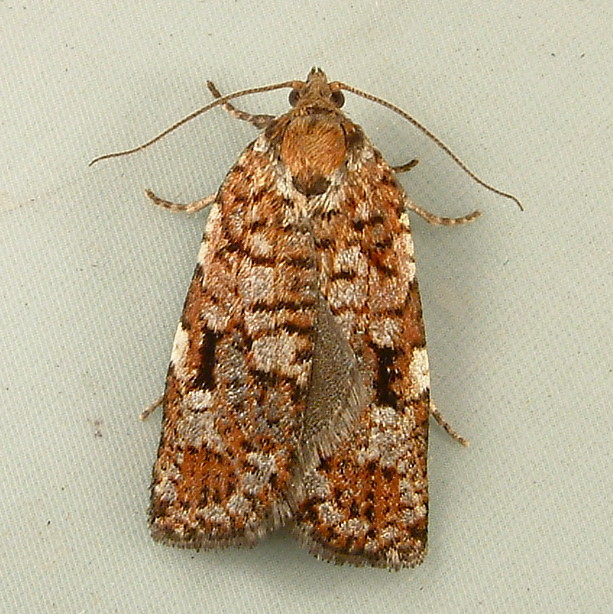
\includegraphics[height=4cm]{images/spruce-budworm-1}
\end{subfigure}
\begin{subfigure}[t]{0.32\textwidth}
	\centering
	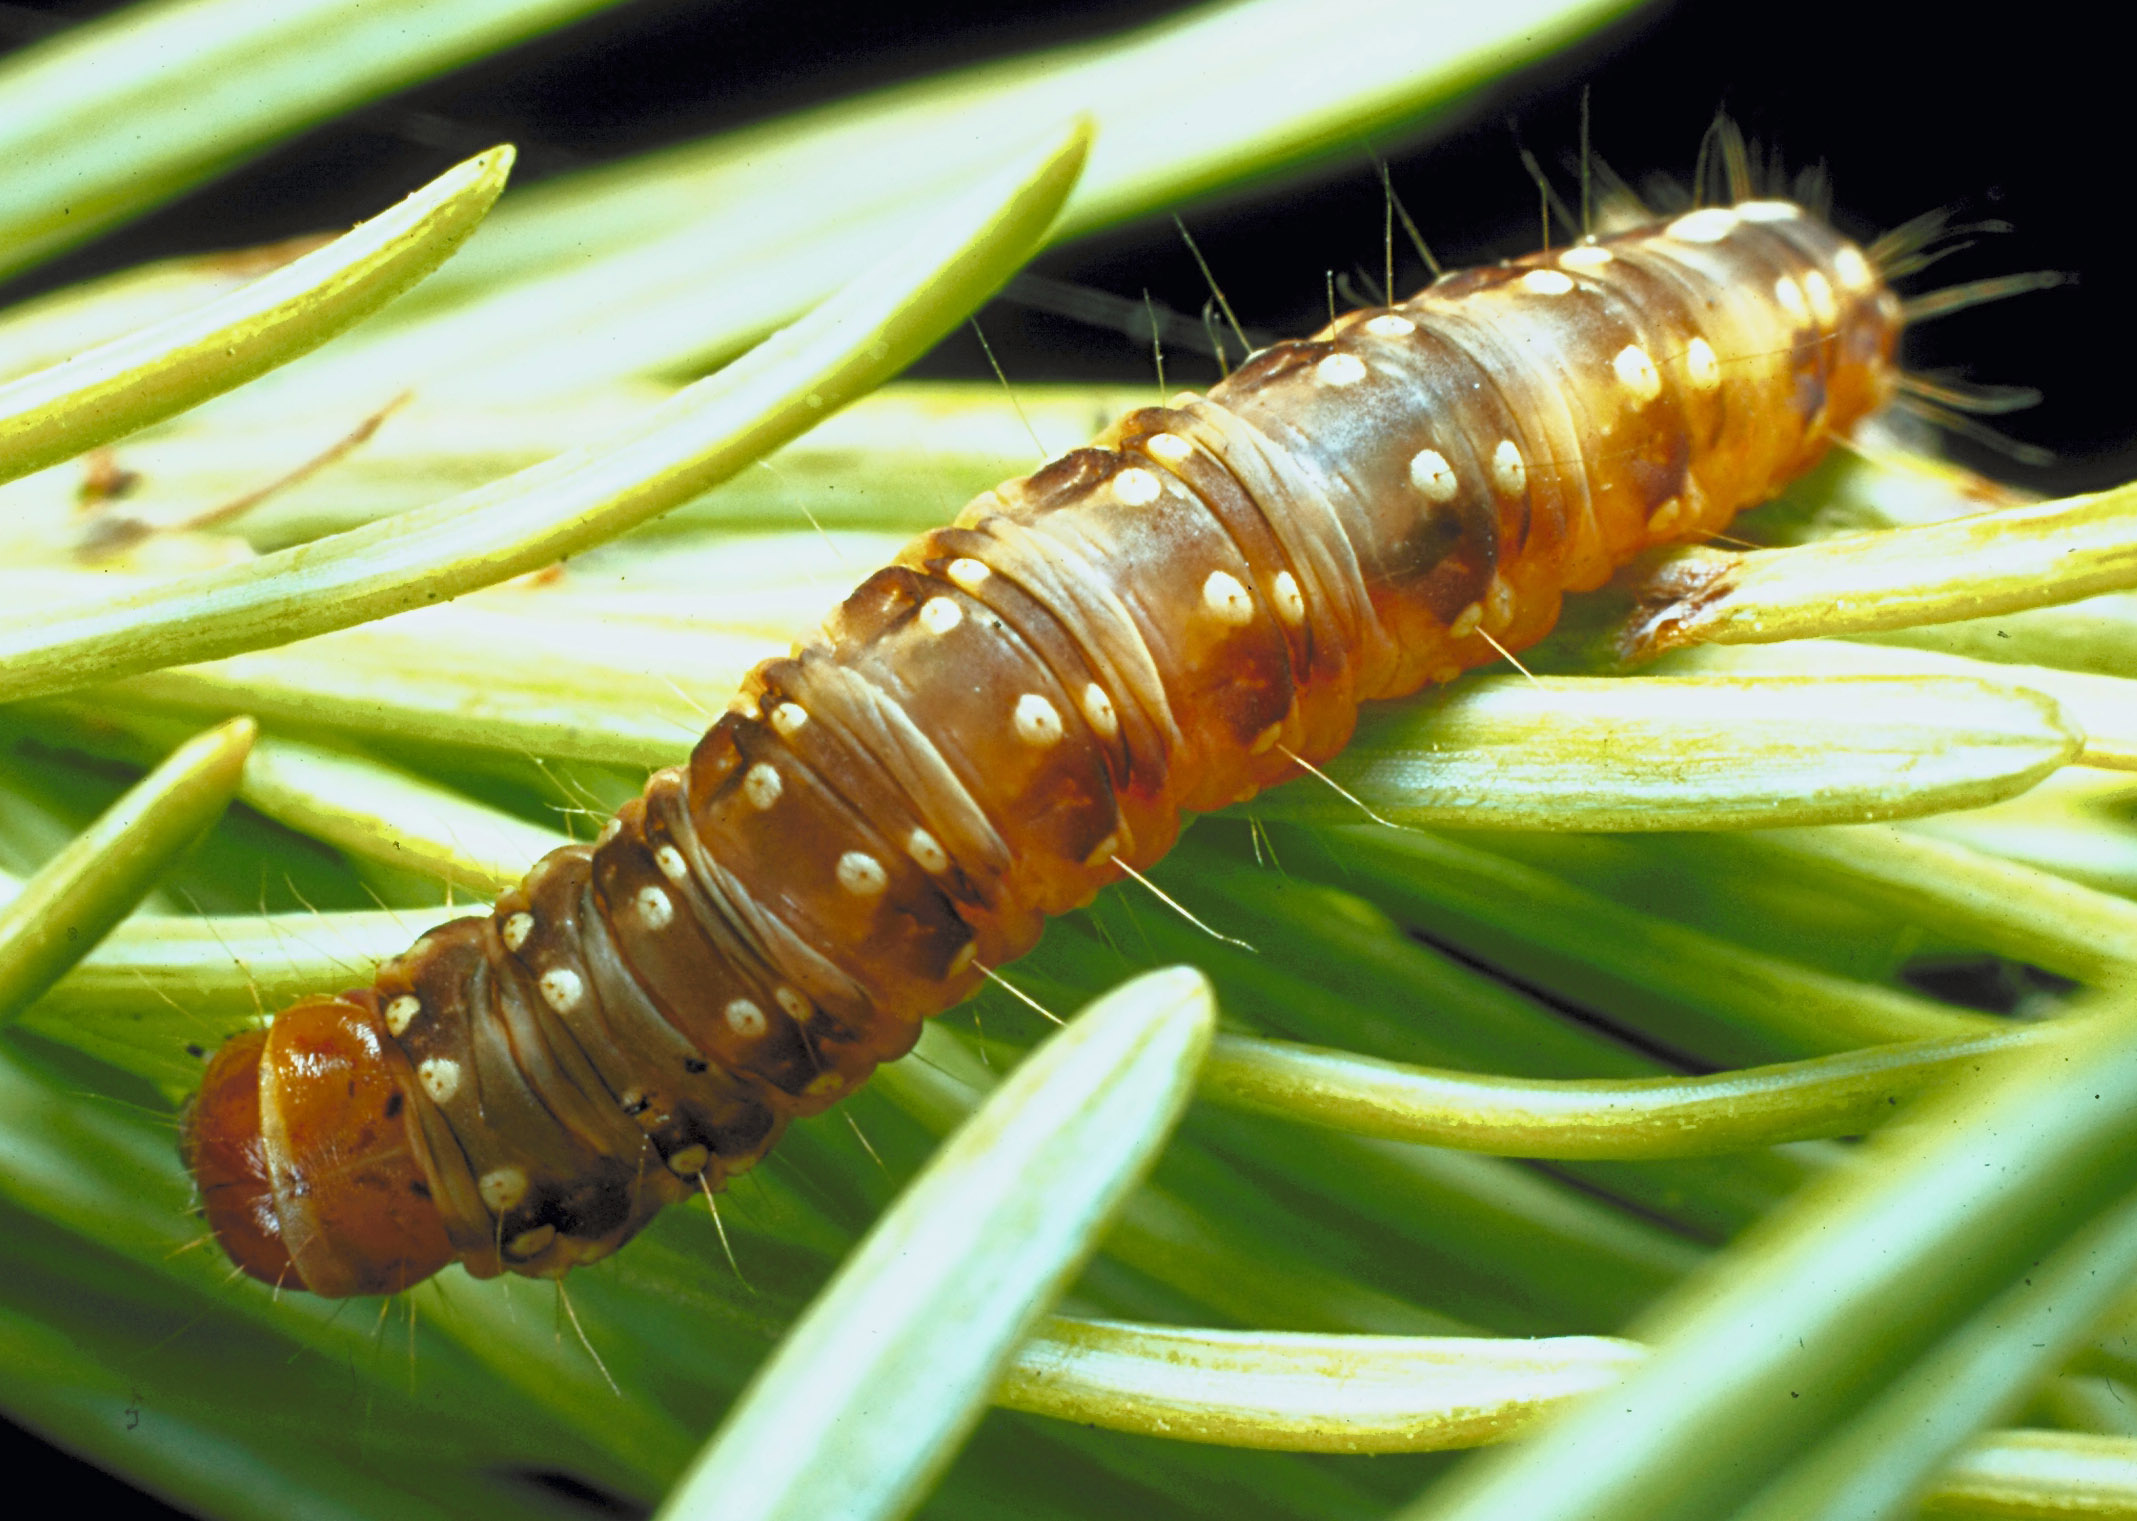
\includegraphics[height=4cm]{images/spruce-budworm-2}
\end{subfigure}
\begin{subfigure}[t]{0.32\textwidth}
	\centering
	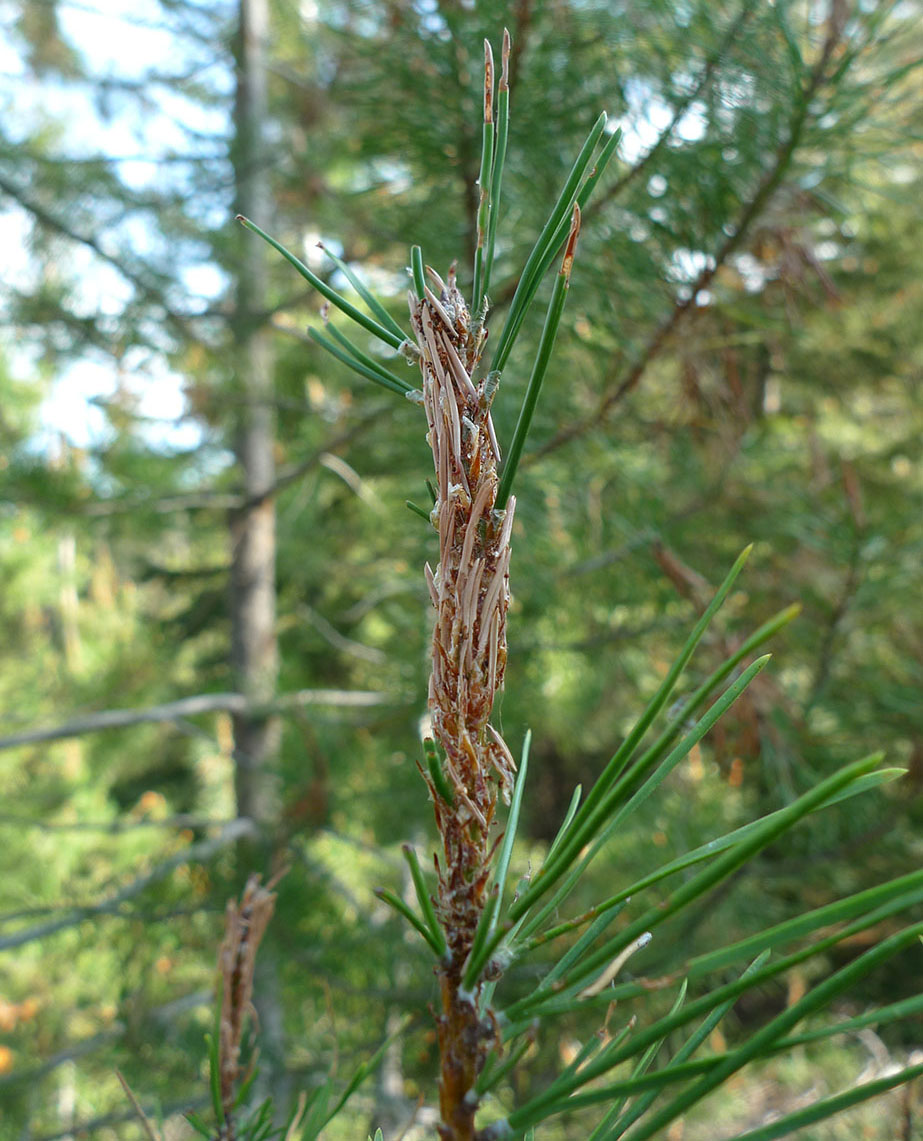
\includegraphics[height=4cm]{images/spruce-budworm-3}
\end{subfigure}
\caption{The spruce budworm is a moth (left), native to eastern Canada and the US, which lays eggs in spruce trees, a type of fir tree. These eggs hatch into larvae (centre) that eat the needles of the spruce tree. Four years of infestation and defoliation of the tree (right) can kill the tree. \emph{[Images: Moth Photograpers Group, \textsc{cc by-nc-sa 2.0}; Jerald E.\ Dewey, \textsc{cc by 3.0}; Thayne Tuason, \textsc{cc by-sa 4.0}]} }%
\label{fig:spruce-budworm}%
\end{figure}

One cannot take a mathematical biology course without encountering the spruce budworm. It shows how a simple, one-dimensional systems can yield rich dynamics with relevant predictions of a biological phenomenon. The \href{https://en.wikipedia.org/wiki/Choristoneura_fumiferana}{spruce budworm}, shown in \cref{fig:spruce-budworm}, is a moth that infects spruce trees (a type of fir tree) in eastern Canada and the US. The moths produce larvae which feed on the needles of the conifers: a serious infestation can lead to complete defoliation of a forest in about four years, and so the budworm is considered one of the most destructive pests in North America. 

The budworm is preyed upon by birds that for low budworm population feed only upon the budworms once the budworm population has reached a certain level. Assuming logistic growth for the budworm population in the absence of birds, the budworm population size, $x$, is governed by the variation on the logistic equation,
\begin{equation}
	\fd{x}{t} = rx\left(1-\frac{x}{K}\right) - \frac{Bx^2}{A^2 + x^2}.
\end{equation}
What does the new term tell us? As $x \to \infty$, the predation rate becomes $B > 0$, similar to our harvesting model. Meanwhile, $A > 0$ provides a measure of the threshold population size where predation suddenly increases. 

Nondimensionalising with
\begin{equation}
	x = A \hat{x}, \quad t = \frac{A}{B}\hat{t},
\end{equation}
and dropping hats, we get
\begin{equation}
	\label{budworm-nondim}
	\fd{x}{t} = Rx\left(1-\frac{x}{k}\right) - \frac{x^2}{1+x^2},
\end{equation}
where $R=rA/B$ and $k=K/A$. Once again nondimensionalisation has reduced the parameter space, from four to two!

%We are going to do a linear stability analysis on our new system, but because this is a one-dimensional, first-order system, we can take advantage of the observations we made for such systems in \cref{chap:growth} to skip steps \StepTwoIcon and \StepThreeIcon in our formal procedure.

\subsubsection*{\StepOne Find equilibria}
%\paragraph{Equilibria}
\vspace{-2mm}
The equilibria are given by $x=0$ and
\begin{equation}
	R\left(1-\frac{x}{k}\right) = \frac{x}{1+x^2},
	\label{spruce-rk}
\end{equation}
where the logistic growth is balanced by the predation. Thus, the equilibria occur when the line given by the left-hand side of \cref{spruce-rk} intersects the curve given by the right-hand side. Naturally, we’d like to explore how these equilibria vary with $R$ and $k$ and, in doing so, we see the benefit of our choice of nondimensionalisation. 

The curve given by $g(x) = x/(1 + x^2)$ does not depend on either parameter, and as for the line $h(x) = R(1-x/k)$, $R$ is the $y$-intercept, while $k$ is the where it crosses the $x$-axis. This is plotted in \cref{fig:spruce-1}, and as you can see, this makes graphical evaluation quite easy!

\begin{figure}%
	\centering
	%% Creator: Matplotlib, PGF backend
%%
%% To include the figure in your LaTeX document, write
%%   \input{<filename>.pgf}
%%
%% Make sure the required packages are loaded in your preamble
%%   \usepackage{pgf}
%%
%% Also ensure that all the required font packages are loaded; for instance,
%% the lmodern package is sometimes necessary when using math font.
%%   \usepackage{lmodern}
%%
%% Figures using additional raster images can only be included by \input if
%% they are in the same directory as the main LaTeX file. For loading figures
%% from other directories you can use the `import` package
%%   \usepackage{import}
%%
%% and then include the figures with
%%   \import{<path to file>}{<filename>.pgf}
%%
%% Matplotlib used the following preamble
%%   \usepackage{fontspec}
%%   \setmainfont{DejaVuSerif.ttf}[Path=\detokenize{/Users/adam/opt/anaconda3/lib/python3.8/site-packages/matplotlib/mpl-data/fonts/ttf/}]
%%   \setsansfont{DejaVuSans.ttf}[Path=\detokenize{/Users/adam/opt/anaconda3/lib/python3.8/site-packages/matplotlib/mpl-data/fonts/ttf/}]
%%   \setmonofont{DejaVuSansMono.ttf}[Path=\detokenize{/Users/adam/opt/anaconda3/lib/python3.8/site-packages/matplotlib/mpl-data/fonts/ttf/}]
%%
\begingroup%
\makeatletter%
\begin{pgfpicture}%
\pgfpathrectangle{\pgfpointorigin}{\pgfqpoint{4.210000in}{1.770000in}}%
\pgfusepath{use as bounding box, clip}%
\begin{pgfscope}%
\pgfsetbuttcap%
\pgfsetmiterjoin%
\definecolor{currentfill}{rgb}{1.000000,1.000000,1.000000}%
\pgfsetfillcolor{currentfill}%
\pgfsetlinewidth{0.000000pt}%
\definecolor{currentstroke}{rgb}{1.000000,1.000000,1.000000}%
\pgfsetstrokecolor{currentstroke}%
\pgfsetdash{}{0pt}%
\pgfpathmoveto{\pgfqpoint{0.000000in}{0.000000in}}%
\pgfpathlineto{\pgfqpoint{4.210000in}{0.000000in}}%
\pgfpathlineto{\pgfqpoint{4.210000in}{1.770000in}}%
\pgfpathlineto{\pgfqpoint{0.000000in}{1.770000in}}%
\pgfpathlineto{\pgfqpoint{0.000000in}{0.000000in}}%
\pgfpathclose%
\pgfusepath{fill}%
\end{pgfscope}%
\begin{pgfscope}%
\pgfsetbuttcap%
\pgfsetmiterjoin%
\definecolor{currentfill}{rgb}{1.000000,1.000000,1.000000}%
\pgfsetfillcolor{currentfill}%
\pgfsetlinewidth{0.000000pt}%
\definecolor{currentstroke}{rgb}{0.000000,0.000000,0.000000}%
\pgfsetstrokecolor{currentstroke}%
\pgfsetstrokeopacity{0.000000}%
\pgfsetdash{}{0pt}%
\pgfpathmoveto{\pgfqpoint{0.356877in}{0.223784in}}%
\pgfpathlineto{\pgfqpoint{4.163222in}{0.223784in}}%
\pgfpathlineto{\pgfqpoint{4.163222in}{1.743182in}}%
\pgfpathlineto{\pgfqpoint{0.356877in}{1.743182in}}%
\pgfpathlineto{\pgfqpoint{0.356877in}{0.223784in}}%
\pgfpathclose%
\pgfusepath{fill}%
\end{pgfscope}%
\begin{pgfscope}%
\pgfsetbuttcap%
\pgfsetroundjoin%
\definecolor{currentfill}{rgb}{0.000000,0.000000,0.000000}%
\pgfsetfillcolor{currentfill}%
\pgfsetlinewidth{0.803000pt}%
\definecolor{currentstroke}{rgb}{0.000000,0.000000,0.000000}%
\pgfsetstrokecolor{currentstroke}%
\pgfsetdash{}{0pt}%
\pgfsys@defobject{currentmarker}{\pgfqpoint{0.000000in}{-0.048611in}}{\pgfqpoint{0.000000in}{0.000000in}}{%
\pgfpathmoveto{\pgfqpoint{0.000000in}{0.000000in}}%
\pgfpathlineto{\pgfqpoint{0.000000in}{-0.048611in}}%
\pgfusepath{stroke,fill}%
}%
\begin{pgfscope}%
\pgfsys@transformshift{0.356877in}{0.223784in}%
\pgfsys@useobject{currentmarker}{}%
\end{pgfscope}%
\end{pgfscope}%
\begin{pgfscope}%
\definecolor{textcolor}{rgb}{0.000000,0.000000,0.000000}%
\pgfsetstrokecolor{textcolor}%
\pgfsetfillcolor{textcolor}%
\pgftext[x=0.356877in,y=0.126562in,,top]{\color{textcolor}\rmfamily\fontsize{12.000000}{14.400000}\selectfont 0}%
\end{pgfscope}%
\begin{pgfscope}%
\pgfsetbuttcap%
\pgfsetroundjoin%
\definecolor{currentfill}{rgb}{0.000000,0.000000,0.000000}%
\pgfsetfillcolor{currentfill}%
\pgfsetlinewidth{0.803000pt}%
\definecolor{currentstroke}{rgb}{0.000000,0.000000,0.000000}%
\pgfsetstrokecolor{currentstroke}%
\pgfsetdash{}{0pt}%
\pgfsys@defobject{currentmarker}{\pgfqpoint{0.000000in}{-0.048611in}}{\pgfqpoint{0.000000in}{0.000000in}}{%
\pgfpathmoveto{\pgfqpoint{0.000000in}{0.000000in}}%
\pgfpathlineto{\pgfqpoint{0.000000in}{-0.048611in}}%
\pgfusepath{stroke,fill}%
}%
\begin{pgfscope}%
\pgfsys@transformshift{0.588718in}{0.223784in}%
\pgfsys@useobject{currentmarker}{}%
\end{pgfscope}%
\end{pgfscope}%
\begin{pgfscope}%
\definecolor{textcolor}{rgb}{0.000000,0.000000,0.000000}%
\pgfsetstrokecolor{textcolor}%
\pgfsetfillcolor{textcolor}%
\pgftext[x=0.588718in,y=0.126562in,,top]{\color{textcolor}\rmfamily\fontsize{12.000000}{14.400000}\selectfont \(\displaystyle a\)}%
\end{pgfscope}%
\begin{pgfscope}%
\pgfsetbuttcap%
\pgfsetroundjoin%
\definecolor{currentfill}{rgb}{0.000000,0.000000,0.000000}%
\pgfsetfillcolor{currentfill}%
\pgfsetlinewidth{0.803000pt}%
\definecolor{currentstroke}{rgb}{0.000000,0.000000,0.000000}%
\pgfsetstrokecolor{currentstroke}%
\pgfsetdash{}{0pt}%
\pgfsys@defobject{currentmarker}{\pgfqpoint{0.000000in}{-0.048611in}}{\pgfqpoint{0.000000in}{0.000000in}}{%
\pgfpathmoveto{\pgfqpoint{0.000000in}{0.000000in}}%
\pgfpathlineto{\pgfqpoint{0.000000in}{-0.048611in}}%
\pgfusepath{stroke,fill}%
}%
\begin{pgfscope}%
\pgfsys@transformshift{1.066242in}{0.223784in}%
\pgfsys@useobject{currentmarker}{}%
\end{pgfscope}%
\end{pgfscope}%
\begin{pgfscope}%
\definecolor{textcolor}{rgb}{0.000000,0.000000,0.000000}%
\pgfsetstrokecolor{textcolor}%
\pgfsetfillcolor{textcolor}%
\pgftext[x=1.066242in,y=0.126562in,,top]{\color{textcolor}\rmfamily\fontsize{12.000000}{14.400000}\selectfont \(\displaystyle b\)}%
\end{pgfscope}%
\begin{pgfscope}%
\pgfsetbuttcap%
\pgfsetroundjoin%
\definecolor{currentfill}{rgb}{0.000000,0.000000,0.000000}%
\pgfsetfillcolor{currentfill}%
\pgfsetlinewidth{0.803000pt}%
\definecolor{currentstroke}{rgb}{0.000000,0.000000,0.000000}%
\pgfsetstrokecolor{currentstroke}%
\pgfsetdash{}{0pt}%
\pgfsys@defobject{currentmarker}{\pgfqpoint{0.000000in}{-0.048611in}}{\pgfqpoint{0.000000in}{0.000000in}}{%
\pgfpathmoveto{\pgfqpoint{0.000000in}{0.000000in}}%
\pgfpathlineto{\pgfqpoint{0.000000in}{-0.048611in}}%
\pgfusepath{stroke,fill}%
}%
\begin{pgfscope}%
\pgfsys@transformshift{2.879446in}{0.223784in}%
\pgfsys@useobject{currentmarker}{}%
\end{pgfscope}%
\end{pgfscope}%
\begin{pgfscope}%
\definecolor{textcolor}{rgb}{0.000000,0.000000,0.000000}%
\pgfsetstrokecolor{textcolor}%
\pgfsetfillcolor{textcolor}%
\pgftext[x=2.879446in,y=0.126562in,,top]{\color{textcolor}\rmfamily\fontsize{12.000000}{14.400000}\selectfont \(\displaystyle c\)}%
\end{pgfscope}%
\begin{pgfscope}%
\pgfsetbuttcap%
\pgfsetroundjoin%
\definecolor{currentfill}{rgb}{0.000000,0.000000,0.000000}%
\pgfsetfillcolor{currentfill}%
\pgfsetlinewidth{0.803000pt}%
\definecolor{currentstroke}{rgb}{0.000000,0.000000,0.000000}%
\pgfsetstrokecolor{currentstroke}%
\pgfsetdash{}{0pt}%
\pgfsys@defobject{currentmarker}{\pgfqpoint{0.000000in}{-0.048611in}}{\pgfqpoint{0.000000in}{0.000000in}}{%
\pgfpathmoveto{\pgfqpoint{0.000000in}{0.000000in}}%
\pgfpathlineto{\pgfqpoint{0.000000in}{-0.048611in}}%
\pgfusepath{stroke,fill}%
}%
\begin{pgfscope}%
\pgfsys@transformshift{3.817191in}{0.223784in}%
\pgfsys@useobject{currentmarker}{}%
\end{pgfscope}%
\end{pgfscope}%
\begin{pgfscope}%
\definecolor{textcolor}{rgb}{0.000000,0.000000,0.000000}%
\pgfsetstrokecolor{textcolor}%
\pgfsetfillcolor{textcolor}%
\pgftext[x=3.817191in,y=0.126562in,,top]{\color{textcolor}\rmfamily\fontsize{12.000000}{14.400000}\selectfont \(\displaystyle k\)}%
\end{pgfscope}%
\begin{pgfscope}%
\pgfsetbuttcap%
\pgfsetroundjoin%
\definecolor{currentfill}{rgb}{0.000000,0.000000,0.000000}%
\pgfsetfillcolor{currentfill}%
\pgfsetlinewidth{0.803000pt}%
\definecolor{currentstroke}{rgb}{0.000000,0.000000,0.000000}%
\pgfsetstrokecolor{currentstroke}%
\pgfsetdash{}{0pt}%
\pgfsys@defobject{currentmarker}{\pgfqpoint{-0.048611in}{0.000000in}}{\pgfqpoint{-0.000000in}{0.000000in}}{%
\pgfpathmoveto{\pgfqpoint{-0.000000in}{0.000000in}}%
\pgfpathlineto{\pgfqpoint{-0.048611in}{0.000000in}}%
\pgfusepath{stroke,fill}%
}%
\begin{pgfscope}%
\pgfsys@transformshift{0.356877in}{0.223784in}%
\pgfsys@useobject{currentmarker}{}%
\end{pgfscope}%
\end{pgfscope}%
\begin{pgfscope}%
\definecolor{textcolor}{rgb}{0.000000,0.000000,0.000000}%
\pgfsetstrokecolor{textcolor}%
\pgfsetfillcolor{textcolor}%
\pgftext[x=0.153617in, y=0.160470in, left, base]{\color{textcolor}\rmfamily\fontsize{12.000000}{14.400000}\selectfont 0}%
\end{pgfscope}%
\begin{pgfscope}%
\pgfsetbuttcap%
\pgfsetroundjoin%
\definecolor{currentfill}{rgb}{0.000000,0.000000,0.000000}%
\pgfsetfillcolor{currentfill}%
\pgfsetlinewidth{0.803000pt}%
\definecolor{currentstroke}{rgb}{0.000000,0.000000,0.000000}%
\pgfsetstrokecolor{currentstroke}%
\pgfsetdash{}{0pt}%
\pgfsys@defobject{currentmarker}{\pgfqpoint{-0.048611in}{0.000000in}}{\pgfqpoint{-0.000000in}{0.000000in}}{%
\pgfpathmoveto{\pgfqpoint{-0.000000in}{0.000000in}}%
\pgfpathlineto{\pgfqpoint{-0.048611in}{0.000000in}}%
\pgfusepath{stroke,fill}%
}%
\begin{pgfscope}%
\pgfsys@transformshift{0.356877in}{1.649640in}%
\pgfsys@useobject{currentmarker}{}%
\end{pgfscope}%
\end{pgfscope}%
\begin{pgfscope}%
\definecolor{textcolor}{rgb}{0.000000,0.000000,0.000000}%
\pgfsetstrokecolor{textcolor}%
\pgfsetfillcolor{textcolor}%
\pgftext[x=0.134068in, y=1.586326in, left, base]{\color{textcolor}\rmfamily\fontsize{12.000000}{14.400000}\selectfont \(\displaystyle R\)}%
\end{pgfscope}%
\begin{pgfscope}%
\pgfpathrectangle{\pgfqpoint{0.356877in}{0.223784in}}{\pgfqpoint{3.806345in}{1.519398in}}%
\pgfusepath{clip}%
\pgfsetbuttcap%
\pgfsetroundjoin%
\pgfsetlinewidth{0.803000pt}%
\definecolor{currentstroke}{rgb}{0.000000,0.000000,0.000000}%
\pgfsetstrokecolor{currentstroke}%
\pgfsetdash{{2.960000pt}{1.280000pt}}{0.000000pt}%
\pgfpathmoveto{\pgfqpoint{0.588718in}{0.223784in}}%
\pgfpathlineto{\pgfqpoint{0.588718in}{1.554108in}}%
\pgfusepath{stroke}%
\end{pgfscope}%
\begin{pgfscope}%
\pgfpathrectangle{\pgfqpoint{0.356877in}{0.223784in}}{\pgfqpoint{3.806345in}{1.519398in}}%
\pgfusepath{clip}%
\pgfsetbuttcap%
\pgfsetroundjoin%
\pgfsetlinewidth{0.803000pt}%
\definecolor{currentstroke}{rgb}{0.000000,0.000000,0.000000}%
\pgfsetstrokecolor{currentstroke}%
\pgfsetdash{{2.960000pt}{1.280000pt}}{0.000000pt}%
\pgfpathmoveto{\pgfqpoint{1.066242in}{0.223784in}}%
\pgfpathlineto{\pgfqpoint{1.066242in}{1.357340in}}%
\pgfusepath{stroke}%
\end{pgfscope}%
\begin{pgfscope}%
\pgfpathrectangle{\pgfqpoint{0.356877in}{0.223784in}}{\pgfqpoint{3.806345in}{1.519398in}}%
\pgfusepath{clip}%
\pgfsetbuttcap%
\pgfsetroundjoin%
\pgfsetlinewidth{0.803000pt}%
\definecolor{currentstroke}{rgb}{0.000000,0.000000,0.000000}%
\pgfsetstrokecolor{currentstroke}%
\pgfsetdash{{2.960000pt}{1.280000pt}}{0.000000pt}%
\pgfpathmoveto{\pgfqpoint{2.879446in}{0.223784in}}%
\pgfpathlineto{\pgfqpoint{2.879446in}{0.610191in}}%
\pgfusepath{stroke}%
\end{pgfscope}%
\begin{pgfscope}%
\pgfpathrectangle{\pgfqpoint{0.356877in}{0.223784in}}{\pgfqpoint{3.806345in}{1.519398in}}%
\pgfusepath{clip}%
\pgfsetrectcap%
\pgfsetroundjoin%
\pgfsetlinewidth{1.505625pt}%
\definecolor{currentstroke}{rgb}{0.121569,0.466667,0.705882}%
\pgfsetstrokecolor{currentstroke}%
\pgfsetdash{}{0pt}%
\pgfpathmoveto{\pgfqpoint{0.356877in}{0.223784in}}%
\pgfpathlineto{\pgfqpoint{0.394979in}{0.537159in}}%
\pgfpathlineto{\pgfqpoint{0.417840in}{0.715986in}}%
\pgfpathlineto{\pgfqpoint{0.436891in}{0.856044in}}%
\pgfpathlineto{\pgfqpoint{0.452131in}{0.960866in}}%
\pgfpathlineto{\pgfqpoint{0.467372in}{1.058479in}}%
\pgfpathlineto{\pgfqpoint{0.482613in}{1.148381in}}%
\pgfpathlineto{\pgfqpoint{0.497853in}{1.230271in}}%
\pgfpathlineto{\pgfqpoint{0.509284in}{1.286355in}}%
\pgfpathlineto{\pgfqpoint{0.520714in}{1.337878in}}%
\pgfpathlineto{\pgfqpoint{0.532145in}{1.384901in}}%
\pgfpathlineto{\pgfqpoint{0.543575in}{1.427525in}}%
\pgfpathlineto{\pgfqpoint{0.555005in}{1.465881in}}%
\pgfpathlineto{\pgfqpoint{0.566436in}{1.500131in}}%
\pgfpathlineto{\pgfqpoint{0.577866in}{1.530455in}}%
\pgfpathlineto{\pgfqpoint{0.589297in}{1.557052in}}%
\pgfpathlineto{\pgfqpoint{0.600727in}{1.580127in}}%
\pgfpathlineto{\pgfqpoint{0.612158in}{1.599893in}}%
\pgfpathlineto{\pgfqpoint{0.623588in}{1.616567in}}%
\pgfpathlineto{\pgfqpoint{0.631209in}{1.626071in}}%
\pgfpathlineto{\pgfqpoint{0.638829in}{1.634359in}}%
\pgfpathlineto{\pgfqpoint{0.646449in}{1.641492in}}%
\pgfpathlineto{\pgfqpoint{0.654069in}{1.647531in}}%
\pgfpathlineto{\pgfqpoint{0.661690in}{1.652535in}}%
\pgfpathlineto{\pgfqpoint{0.669310in}{1.656562in}}%
\pgfpathlineto{\pgfqpoint{0.676930in}{1.659668in}}%
\pgfpathlineto{\pgfqpoint{0.684551in}{1.661905in}}%
\pgfpathlineto{\pgfqpoint{0.692171in}{1.663327in}}%
\pgfpathlineto{\pgfqpoint{0.703601in}{1.664040in}}%
\pgfpathlineto{\pgfqpoint{0.715032in}{1.663189in}}%
\pgfpathlineto{\pgfqpoint{0.726462in}{1.660925in}}%
\pgfpathlineto{\pgfqpoint{0.737893in}{1.657389in}}%
\pgfpathlineto{\pgfqpoint{0.749323in}{1.652708in}}%
\pgfpathlineto{\pgfqpoint{0.760754in}{1.647005in}}%
\pgfpathlineto{\pgfqpoint{0.775994in}{1.637999in}}%
\pgfpathlineto{\pgfqpoint{0.791235in}{1.627609in}}%
\pgfpathlineto{\pgfqpoint{0.810286in}{1.612997in}}%
\pgfpathlineto{\pgfqpoint{0.829337in}{1.596917in}}%
\pgfpathlineto{\pgfqpoint{0.852198in}{1.576119in}}%
\pgfpathlineto{\pgfqpoint{0.878869in}{1.550346in}}%
\pgfpathlineto{\pgfqpoint{0.916970in}{1.511782in}}%
\pgfpathlineto{\pgfqpoint{1.061756in}{1.363253in}}%
\pgfpathlineto{\pgfqpoint{1.103668in}{1.322582in}}%
\pgfpathlineto{\pgfqpoint{1.141769in}{1.287046in}}%
\pgfpathlineto{\pgfqpoint{1.179871in}{1.252969in}}%
\pgfpathlineto{\pgfqpoint{1.217972in}{1.220386in}}%
\pgfpathlineto{\pgfqpoint{1.256074in}{1.189292in}}%
\pgfpathlineto{\pgfqpoint{1.294176in}{1.159659in}}%
\pgfpathlineto{\pgfqpoint{1.332277in}{1.131440in}}%
\pgfpathlineto{\pgfqpoint{1.370379in}{1.104582in}}%
\pgfpathlineto{\pgfqpoint{1.408480in}{1.079022in}}%
\pgfpathlineto{\pgfqpoint{1.446582in}{1.054696in}}%
\pgfpathlineto{\pgfqpoint{1.488493in}{1.029285in}}%
\pgfpathlineto{\pgfqpoint{1.530405in}{1.005205in}}%
\pgfpathlineto{\pgfqpoint{1.572317in}{0.982372in}}%
\pgfpathlineto{\pgfqpoint{1.618039in}{0.958794in}}%
\pgfpathlineto{\pgfqpoint{1.663761in}{0.936509in}}%
\pgfpathlineto{\pgfqpoint{1.709482in}{0.915429in}}%
\pgfpathlineto{\pgfqpoint{1.759014in}{0.893852in}}%
\pgfpathlineto{\pgfqpoint{1.808546in}{0.873491in}}%
\pgfpathlineto{\pgfqpoint{1.861889in}{0.852818in}}%
\pgfpathlineto{\pgfqpoint{1.915231in}{0.833346in}}%
\pgfpathlineto{\pgfqpoint{1.972383in}{0.813708in}}%
\pgfpathlineto{\pgfqpoint{2.029535in}{0.795235in}}%
\pgfpathlineto{\pgfqpoint{2.090498in}{0.776708in}}%
\pgfpathlineto{\pgfqpoint{2.155271in}{0.758242in}}%
\pgfpathlineto{\pgfqpoint{2.220043in}{0.740923in}}%
\pgfpathlineto{\pgfqpoint{2.288626in}{0.723725in}}%
\pgfpathlineto{\pgfqpoint{2.361019in}{0.706732in}}%
\pgfpathlineto{\pgfqpoint{2.437222in}{0.690012in}}%
\pgfpathlineto{\pgfqpoint{2.517235in}{0.673625in}}%
\pgfpathlineto{\pgfqpoint{2.601059in}{0.657618in}}%
\pgfpathlineto{\pgfqpoint{2.688692in}{0.642030in}}%
\pgfpathlineto{\pgfqpoint{2.780136in}{0.626890in}}%
\pgfpathlineto{\pgfqpoint{2.879200in}{0.611655in}}%
\pgfpathlineto{\pgfqpoint{2.982074in}{0.596985in}}%
\pgfpathlineto{\pgfqpoint{3.088759in}{0.582881in}}%
\pgfpathlineto{\pgfqpoint{3.203063in}{0.568888in}}%
\pgfpathlineto{\pgfqpoint{3.324988in}{0.555100in}}%
\pgfpathlineto{\pgfqpoint{3.454533in}{0.541594in}}%
\pgfpathlineto{\pgfqpoint{3.591699in}{0.528429in}}%
\pgfpathlineto{\pgfqpoint{3.736485in}{0.515655in}}%
\pgfpathlineto{\pgfqpoint{3.892701in}{0.503010in}}%
\pgfpathlineto{\pgfqpoint{4.056538in}{0.490864in}}%
\pgfpathlineto{\pgfqpoint{4.163222in}{0.483503in}}%
\pgfpathlineto{\pgfqpoint{4.163222in}{0.483503in}}%
\pgfusepath{stroke}%
\end{pgfscope}%
\begin{pgfscope}%
\pgfpathrectangle{\pgfqpoint{0.356877in}{0.223784in}}{\pgfqpoint{3.806345in}{1.519398in}}%
\pgfusepath{clip}%
\pgfsetbuttcap%
\pgfsetroundjoin%
\pgfsetlinewidth{1.505625pt}%
\definecolor{currentstroke}{rgb}{1.000000,0.498039,0.054902}%
\pgfsetstrokecolor{currentstroke}%
\pgfsetdash{{5.550000pt}{2.400000pt}}{0.000000pt}%
\pgfpathmoveto{\pgfqpoint{0.356877in}{1.649640in}}%
\pgfpathlineto{\pgfqpoint{3.829325in}{0.218784in}}%
\pgfpathlineto{\pgfqpoint{3.829325in}{0.218784in}}%
\pgfusepath{stroke}%
\end{pgfscope}%
\begin{pgfscope}%
\pgfsetrectcap%
\pgfsetmiterjoin%
\pgfsetlinewidth{0.803000pt}%
\definecolor{currentstroke}{rgb}{0.000000,0.000000,0.000000}%
\pgfsetstrokecolor{currentstroke}%
\pgfsetdash{}{0pt}%
\pgfpathmoveto{\pgfqpoint{0.356877in}{0.223784in}}%
\pgfpathlineto{\pgfqpoint{0.356877in}{1.743182in}}%
\pgfusepath{stroke}%
\end{pgfscope}%
\begin{pgfscope}%
\pgfsetrectcap%
\pgfsetmiterjoin%
\pgfsetlinewidth{0.803000pt}%
\definecolor{currentstroke}{rgb}{0.000000,0.000000,0.000000}%
\pgfsetstrokecolor{currentstroke}%
\pgfsetdash{}{0pt}%
\pgfpathmoveto{\pgfqpoint{0.356877in}{0.223784in}}%
\pgfpathlineto{\pgfqpoint{4.163222in}{0.223784in}}%
\pgfusepath{stroke}%
\end{pgfscope}%
\begin{pgfscope}%
\definecolor{textcolor}{rgb}{0.000000,0.000000,0.000000}%
\pgfsetstrokecolor{textcolor}%
\pgfsetfillcolor{textcolor}%
\pgftext[x=4.163222in,y=0.126562in,right,top]{\color{textcolor}\rmfamily\fontsize{12.000000}{14.400000}\selectfont \(\displaystyle x\)}%
\end{pgfscope}%
\begin{pgfscope}%
\pgfsetrectcap%
\pgfsetroundjoin%
\pgfsetlinewidth{1.505625pt}%
\definecolor{currentstroke}{rgb}{0.121569,0.466667,0.705882}%
\pgfsetstrokecolor{currentstroke}%
\pgfsetdash{}{0pt}%
\pgfpathmoveto{\pgfqpoint{3.602614in}{1.674888in}}%
\pgfpathlineto{\pgfqpoint{3.769280in}{1.674888in}}%
\pgfpathlineto{\pgfqpoint{3.935947in}{1.674888in}}%
\pgfusepath{stroke}%
\end{pgfscope}%
\begin{pgfscope}%
\definecolor{textcolor}{rgb}{0.000000,0.000000,0.000000}%
\pgfsetstrokecolor{textcolor}%
\pgfsetfillcolor{textcolor}%
\pgftext[x=4.069280in,y=1.616554in,left,base]{\color{textcolor}\rmfamily\fontsize{12.000000}{14.400000}\selectfont \(\displaystyle g\)}%
\end{pgfscope}%
\begin{pgfscope}%
\pgfsetbuttcap%
\pgfsetroundjoin%
\pgfsetlinewidth{1.505625pt}%
\definecolor{currentstroke}{rgb}{1.000000,0.498039,0.054902}%
\pgfsetstrokecolor{currentstroke}%
\pgfsetdash{{5.550000pt}{2.400000pt}}{0.000000pt}%
\pgfpathmoveto{\pgfqpoint{3.602614in}{1.430259in}}%
\pgfpathlineto{\pgfqpoint{3.769280in}{1.430259in}}%
\pgfpathlineto{\pgfqpoint{3.935947in}{1.430259in}}%
\pgfusepath{stroke}%
\end{pgfscope}%
\begin{pgfscope}%
\definecolor{textcolor}{rgb}{0.000000,0.000000,0.000000}%
\pgfsetstrokecolor{textcolor}%
\pgfsetfillcolor{textcolor}%
\pgftext[x=4.069280in,y=1.371925in,left,base]{\color{textcolor}\rmfamily\fontsize{12.000000}{14.400000}\selectfont \(\displaystyle h\)}%
\end{pgfscope}%
\end{pgfpicture}%
\makeatother%
\endgroup%

	\caption{Graphical evaluation of the equilibria for the spruce budworm model. Intersections at $a$, $b$ and $c$ represent the locations of equilibria for given $k$ and $R$. (Note: this is not a phase portrait!)}
	\label{fig:spruce-1}
\end{figure}%	

Just like in the harvesting model (where we changed the parameter $H$), we see that changing $R$ and $k$ can lead to us going from three additional equilibria (we already have $x=0$), to two, to one: more \emph{bifurcations}.

\subsubsection{Jump to... \StepFour Assess stability} 
We can go further and classify the equilibria in these regions: as we saw in \cref{sec:allee}, for one dimension it is quite easy. Just to the right of $x=0$, let's say $x=\ep$, you can see from \cref{budworm-nondim} that $\fd{x}{t} > 0$. So $x=0$ is unstable. Then, thinking about the phase portrait of $\fd{x}{t}$ against $x$, by the continuity of $\fd{x}{t}$, the stability must alternate. 

Which equilibria $a,b,c$ (in addition to the $x=0$ one) do we have in each region?
\begin{center}
\begin{tabular}{lllll}
\toprule
	region & \multicolumn{4}{c}{equilibria} \\
\midrule
	1 extra equilibrium (high $R$, high $k$) & $x=0$, & & & $x=c$ \\
	3 extra equilibria & $x=0$, & $x=a$, & $x=b$, & $x=c$ \\
	1 extra equilibrium (low $R$, low $k$) & $x=0$, & $x=a$& & \\		
\midrule
	stability must be & unstable & stable & unstable & stable \\
\midrule
	name & extinction & refuge & threshold & outbreak \\
\bottomrule
\end{tabular}
\end{center}

What are the biological interpretations of these equilibria? The equilibrium $a$ corresponds to the \emph{refuge} population level, and $c$ to the \emph{outbreak} population level. The unstable equilibrium $b$ is referred to as the \emph{threshold} as initial populations $x > b$ increase to the outbreak level, while for $x < b$ the population will decrease to the refuge size. 

\paragraph{Bifurcation diagram} Although we have two parameters we can vary, we could still draw a bifurcation diagram by holding one of the parameters fixed and varying the other. So we could ask `fixing $k$, what are the equilibria, $x_0$, for any given parameter, $R$?' 

In order to do this, we need to solve for $x$ in \cref{spruce-rk}. This is an ugly cubic but you can trust me that it's possible to do analytically (I don't expect you to work this out). We can plot all the branches where the solutions are real on one diagram: see \cref{fig:spruce-budworm-bifurcation}(a). Once again, when the equilibrium $x_0$ is unstable, the line is dotted; when it's stable, the line is solid.

\begin{figure}%
	\centering
	%% Creator: Matplotlib, PGF backend
%%
%% To include the figure in your LaTeX document, write
%%   \input{<filename>.pgf}
%%
%% Make sure the required packages are loaded in your preamble
%%   \usepackage{pgf}
%%
%% Also ensure that all the required font packages are loaded; for instance,
%% the lmodern package is sometimes necessary when using math font.
%%   \usepackage{lmodern}
%%
%% Figures using additional raster images can only be included by \input if
%% they are in the same directory as the main LaTeX file. For loading figures
%% from other directories you can use the `import` package
%%   \usepackage{import}
%%
%% and then include the figures with
%%   \import{<path to file>}{<filename>.pgf}
%%
%% Matplotlib used the following preamble
%%   \usepackage{fontspec}
%%   \setmainfont{DejaVuSerif.ttf}[Path=\detokenize{/Users/adam/opt/anaconda3/lib/python3.9/site-packages/matplotlib/mpl-data/fonts/ttf/}]
%%   \setsansfont{DejaVuSans.ttf}[Path=\detokenize{/Users/adam/opt/anaconda3/lib/python3.9/site-packages/matplotlib/mpl-data/fonts/ttf/}]
%%   \setmonofont{DejaVuSansMono.ttf}[Path=\detokenize{/Users/adam/opt/anaconda3/lib/python3.9/site-packages/matplotlib/mpl-data/fonts/ttf/}]
%%
\begingroup%
\makeatletter%
\begin{pgfpicture}%
\pgfpathrectangle{\pgfpointorigin}{\pgfqpoint{3.000000in}{2.200000in}}%
\pgfusepath{use as bounding box, clip}%
\begin{pgfscope}%
\pgfsetbuttcap%
\pgfsetmiterjoin%
\definecolor{currentfill}{rgb}{1.000000,1.000000,1.000000}%
\pgfsetfillcolor{currentfill}%
\pgfsetlinewidth{0.000000pt}%
\definecolor{currentstroke}{rgb}{1.000000,1.000000,1.000000}%
\pgfsetstrokecolor{currentstroke}%
\pgfsetdash{}{0pt}%
\pgfpathmoveto{\pgfqpoint{0.000000in}{0.000000in}}%
\pgfpathlineto{\pgfqpoint{3.000000in}{0.000000in}}%
\pgfpathlineto{\pgfqpoint{3.000000in}{2.200000in}}%
\pgfpathlineto{\pgfqpoint{0.000000in}{2.200000in}}%
\pgfpathlineto{\pgfqpoint{0.000000in}{0.000000in}}%
\pgfpathclose%
\pgfusepath{fill}%
\end{pgfscope}%
\begin{pgfscope}%
\pgfsetbuttcap%
\pgfsetmiterjoin%
\definecolor{currentfill}{rgb}{1.000000,1.000000,1.000000}%
\pgfsetfillcolor{currentfill}%
\pgfsetlinewidth{0.000000pt}%
\definecolor{currentstroke}{rgb}{0.000000,0.000000,0.000000}%
\pgfsetstrokecolor{currentstroke}%
\pgfsetstrokeopacity{0.000000}%
\pgfsetdash{}{0pt}%
\pgfpathmoveto{\pgfqpoint{0.281754in}{0.278150in}}%
\pgfpathlineto{\pgfqpoint{2.966667in}{0.278150in}}%
\pgfpathlineto{\pgfqpoint{2.966667in}{2.166667in}}%
\pgfpathlineto{\pgfqpoint{0.281754in}{2.166667in}}%
\pgfpathlineto{\pgfqpoint{0.281754in}{0.278150in}}%
\pgfpathclose%
\pgfusepath{fill}%
\end{pgfscope}%
\begin{pgfscope}%
\pgfsetbuttcap%
\pgfsetroundjoin%
\definecolor{currentfill}{rgb}{0.000000,0.000000,0.000000}%
\pgfsetfillcolor{currentfill}%
\pgfsetlinewidth{0.803000pt}%
\definecolor{currentstroke}{rgb}{0.000000,0.000000,0.000000}%
\pgfsetstrokecolor{currentstroke}%
\pgfsetdash{}{0pt}%
\pgfsys@defobject{currentmarker}{\pgfqpoint{0.000000in}{-0.048611in}}{\pgfqpoint{0.000000in}{0.000000in}}{%
\pgfpathmoveto{\pgfqpoint{0.000000in}{0.000000in}}%
\pgfpathlineto{\pgfqpoint{0.000000in}{-0.048611in}}%
\pgfusepath{stroke,fill}%
}%
\begin{pgfscope}%
\pgfsys@transformshift{0.281754in}{0.278150in}%
\pgfsys@useobject{currentmarker}{}%
\end{pgfscope}%
\end{pgfscope}%
\begin{pgfscope}%
\definecolor{textcolor}{rgb}{0.000000,0.000000,0.000000}%
\pgfsetstrokecolor{textcolor}%
\pgfsetfillcolor{textcolor}%
\pgftext[x=0.281754in,y=0.180927in,,top]{\color{textcolor}\rmfamily\fontsize{12.000000}{14.400000}\selectfont 0}%
\end{pgfscope}%
\begin{pgfscope}%
\pgfsetbuttcap%
\pgfsetroundjoin%
\definecolor{currentfill}{rgb}{0.000000,0.000000,0.000000}%
\pgfsetfillcolor{currentfill}%
\pgfsetlinewidth{0.803000pt}%
\definecolor{currentstroke}{rgb}{0.000000,0.000000,0.000000}%
\pgfsetstrokecolor{currentstroke}%
\pgfsetdash{}{0pt}%
\pgfsys@defobject{currentmarker}{\pgfqpoint{-0.048611in}{0.000000in}}{\pgfqpoint{-0.000000in}{0.000000in}}{%
\pgfpathmoveto{\pgfqpoint{-0.000000in}{0.000000in}}%
\pgfpathlineto{\pgfqpoint{-0.048611in}{0.000000in}}%
\pgfusepath{stroke,fill}%
}%
\begin{pgfscope}%
\pgfsys@transformshift{0.281754in}{0.278150in}%
\pgfsys@useobject{currentmarker}{}%
\end{pgfscope}%
\end{pgfscope}%
\begin{pgfscope}%
\definecolor{textcolor}{rgb}{0.000000,0.000000,0.000000}%
\pgfsetstrokecolor{textcolor}%
\pgfsetfillcolor{textcolor}%
\pgftext[x=0.078493in, y=0.214836in, left, base]{\color{textcolor}\rmfamily\fontsize{12.000000}{14.400000}\selectfont 0}%
\end{pgfscope}%
\begin{pgfscope}%
\pgfsetbuttcap%
\pgfsetroundjoin%
\definecolor{currentfill}{rgb}{0.000000,0.000000,0.000000}%
\pgfsetfillcolor{currentfill}%
\pgfsetlinewidth{0.803000pt}%
\definecolor{currentstroke}{rgb}{0.000000,0.000000,0.000000}%
\pgfsetstrokecolor{currentstroke}%
\pgfsetdash{}{0pt}%
\pgfsys@defobject{currentmarker}{\pgfqpoint{-0.048611in}{0.000000in}}{\pgfqpoint{-0.000000in}{0.000000in}}{%
\pgfpathmoveto{\pgfqpoint{-0.000000in}{0.000000in}}%
\pgfpathlineto{\pgfqpoint{-0.048611in}{0.000000in}}%
\pgfusepath{stroke,fill}%
}%
\begin{pgfscope}%
\pgfsys@transformshift{0.281754in}{1.851914in}%
\pgfsys@useobject{currentmarker}{}%
\end{pgfscope}%
\end{pgfscope}%
\begin{pgfscope}%
\definecolor{textcolor}{rgb}{0.000000,0.000000,0.000000}%
\pgfsetstrokecolor{textcolor}%
\pgfsetfillcolor{textcolor}%
\pgftext[x=0.094062in, y=1.788600in, left, base]{\color{textcolor}\rmfamily\fontsize{12.000000}{14.400000}\selectfont \(\displaystyle k\)}%
\end{pgfscope}%
\begin{pgfscope}%
\pgfpathrectangle{\pgfqpoint{0.281754in}{0.278150in}}{\pgfqpoint{2.684913in}{1.888517in}}%
\pgfusepath{clip}%
\pgfsetrectcap%
\pgfsetroundjoin%
\pgfsetlinewidth{1.505625pt}%
\definecolor{currentstroke}{rgb}{0.580392,0.403922,0.741176}%
\pgfsetstrokecolor{currentstroke}%
\pgfsetdash{}{0pt}%
\pgfpathmoveto{\pgfqpoint{1.313792in}{1.058203in}}%
\pgfpathlineto{\pgfqpoint{1.316480in}{1.081500in}}%
\pgfpathlineto{\pgfqpoint{1.321855in}{1.109368in}}%
\pgfpathlineto{\pgfqpoint{1.327230in}{1.129433in}}%
\pgfpathlineto{\pgfqpoint{1.332606in}{1.145865in}}%
\pgfpathlineto{\pgfqpoint{1.340668in}{1.166552in}}%
\pgfpathlineto{\pgfqpoint{1.348731in}{1.184186in}}%
\pgfpathlineto{\pgfqpoint{1.359482in}{1.204561in}}%
\pgfpathlineto{\pgfqpoint{1.370232in}{1.222408in}}%
\pgfpathlineto{\pgfqpoint{1.383670in}{1.242154in}}%
\pgfpathlineto{\pgfqpoint{1.397108in}{1.259757in}}%
\pgfpathlineto{\pgfqpoint{1.410546in}{1.275700in}}%
\pgfpathlineto{\pgfqpoint{1.426672in}{1.293086in}}%
\pgfpathlineto{\pgfqpoint{1.442797in}{1.308928in}}%
\pgfpathlineto{\pgfqpoint{1.461610in}{1.325816in}}%
\pgfpathlineto{\pgfqpoint{1.480424in}{1.341280in}}%
\pgfpathlineto{\pgfqpoint{1.501924in}{1.357500in}}%
\pgfpathlineto{\pgfqpoint{1.523425in}{1.372412in}}%
\pgfpathlineto{\pgfqpoint{1.547614in}{1.387864in}}%
\pgfpathlineto{\pgfqpoint{1.574490in}{1.403631in}}%
\pgfpathlineto{\pgfqpoint{1.601366in}{1.418140in}}%
\pgfpathlineto{\pgfqpoint{1.630929in}{1.432852in}}%
\pgfpathlineto{\pgfqpoint{1.663180in}{1.447619in}}%
\pgfpathlineto{\pgfqpoint{1.698119in}{1.462315in}}%
\pgfpathlineto{\pgfqpoint{1.735746in}{1.476838in}}%
\pgfpathlineto{\pgfqpoint{1.776060in}{1.491107in}}%
\pgfpathlineto{\pgfqpoint{1.819061in}{1.505058in}}%
\pgfpathlineto{\pgfqpoint{1.864750in}{1.518639in}}%
\pgfpathlineto{\pgfqpoint{1.913127in}{1.531815in}}%
\pgfpathlineto{\pgfqpoint{1.964192in}{1.544558in}}%
\pgfpathlineto{\pgfqpoint{2.017944in}{1.556851in}}%
\pgfpathlineto{\pgfqpoint{2.077071in}{1.569223in}}%
\pgfpathlineto{\pgfqpoint{2.141573in}{1.581529in}}%
\pgfpathlineto{\pgfqpoint{2.208763in}{1.593209in}}%
\pgfpathlineto{\pgfqpoint{2.281329in}{1.604696in}}%
\pgfpathlineto{\pgfqpoint{2.359269in}{1.615911in}}%
\pgfpathlineto{\pgfqpoint{2.445272in}{1.627126in}}%
\pgfpathlineto{\pgfqpoint{2.536651in}{1.637898in}}%
\pgfpathlineto{\pgfqpoint{2.636092in}{1.648479in}}%
\pgfpathlineto{\pgfqpoint{2.743596in}{1.658776in}}%
\pgfpathlineto{\pgfqpoint{2.859163in}{1.668722in}}%
\pgfpathlineto{\pgfqpoint{2.966667in}{1.677082in}}%
\pgfpathlineto{\pgfqpoint{2.966667in}{1.677082in}}%
\pgfusepath{stroke}%
\end{pgfscope}%
\begin{pgfscope}%
\pgfpathrectangle{\pgfqpoint{0.281754in}{0.278150in}}{\pgfqpoint{2.684913in}{1.888517in}}%
\pgfusepath{clip}%
\pgfsetbuttcap%
\pgfsetroundjoin%
\pgfsetlinewidth{1.505625pt}%
\definecolor{currentstroke}{rgb}{0.580392,0.403922,0.741176}%
\pgfsetstrokecolor{currentstroke}%
\pgfsetdash{{5.550000pt}{2.400000pt}}{0.000000pt}%
\pgfpathmoveto{\pgfqpoint{1.313792in}{1.002916in}}%
\pgfpathlineto{\pgfqpoint{1.316480in}{0.979371in}}%
\pgfpathlineto{\pgfqpoint{1.321855in}{0.951003in}}%
\pgfpathlineto{\pgfqpoint{1.327230in}{0.930435in}}%
\pgfpathlineto{\pgfqpoint{1.332606in}{0.913497in}}%
\pgfpathlineto{\pgfqpoint{1.340668in}{0.892043in}}%
\pgfpathlineto{\pgfqpoint{1.348731in}{0.873633in}}%
\pgfpathlineto{\pgfqpoint{1.359482in}{0.852210in}}%
\pgfpathlineto{\pgfqpoint{1.370232in}{0.833299in}}%
\pgfpathlineto{\pgfqpoint{1.383670in}{0.812199in}}%
\pgfpathlineto{\pgfqpoint{1.397108in}{0.793213in}}%
\pgfpathlineto{\pgfqpoint{1.413234in}{0.772550in}}%
\pgfpathlineto{\pgfqpoint{1.429359in}{0.753697in}}%
\pgfpathlineto{\pgfqpoint{1.448172in}{0.733505in}}%
\pgfpathlineto{\pgfqpoint{1.466986in}{0.714873in}}%
\pgfpathlineto{\pgfqpoint{1.488486in}{0.695118in}}%
\pgfpathlineto{\pgfqpoint{1.512675in}{0.674477in}}%
\pgfpathlineto{\pgfqpoint{1.539551in}{0.653108in}}%
\pgfpathlineto{\pgfqpoint{1.569114in}{0.631086in}}%
\pgfpathlineto{\pgfqpoint{1.604053in}{0.606544in}}%
\pgfpathlineto{\pgfqpoint{1.649742in}{0.575950in}}%
\pgfpathlineto{\pgfqpoint{1.714245in}{0.532807in}}%
\pgfpathlineto{\pgfqpoint{1.735746in}{0.517198in}}%
\pgfpathlineto{\pgfqpoint{1.751871in}{0.504250in}}%
\pgfpathlineto{\pgfqpoint{1.762622in}{0.494427in}}%
\pgfpathlineto{\pgfqpoint{1.770684in}{0.485802in}}%
\pgfpathlineto{\pgfqpoint{1.776060in}{0.478818in}}%
\pgfpathlineto{\pgfqpoint{1.778747in}{0.474563in}}%
\pgfpathlineto{\pgfqpoint{1.781435in}{0.469162in}}%
\pgfpathlineto{\pgfqpoint{1.781435in}{0.469162in}}%
\pgfusepath{stroke}%
\end{pgfscope}%
\begin{pgfscope}%
\pgfpathrectangle{\pgfqpoint{0.281754in}{0.278150in}}{\pgfqpoint{2.684913in}{1.888517in}}%
\pgfusepath{clip}%
\pgfsetrectcap%
\pgfsetroundjoin%
\pgfsetlinewidth{1.505625pt}%
\definecolor{currentstroke}{rgb}{0.580392,0.403922,0.741176}%
\pgfsetstrokecolor{currentstroke}%
\pgfsetdash{}{0pt}%
\pgfpathmoveto{\pgfqpoint{0.281754in}{0.278150in}}%
\pgfpathlineto{\pgfqpoint{0.797773in}{0.308940in}}%
\pgfpathlineto{\pgfqpoint{0.993968in}{0.321869in}}%
\pgfpathlineto{\pgfqpoint{1.144474in}{0.332859in}}%
\pgfpathlineto{\pgfqpoint{1.265416in}{0.342759in}}%
\pgfpathlineto{\pgfqpoint{1.364857in}{0.351972in}}%
\pgfpathlineto{\pgfqpoint{1.448172in}{0.360793in}}%
\pgfpathlineto{\pgfqpoint{1.515362in}{0.368981in}}%
\pgfpathlineto{\pgfqpoint{1.571802in}{0.376951in}}%
\pgfpathlineto{\pgfqpoint{1.617491in}{0.384481in}}%
\pgfpathlineto{\pgfqpoint{1.655118in}{0.391764in}}%
\pgfpathlineto{\pgfqpoint{1.684681in}{0.398520in}}%
\pgfpathlineto{\pgfqpoint{1.708870in}{0.405079in}}%
\pgfpathlineto{\pgfqpoint{1.727683in}{0.411175in}}%
\pgfpathlineto{\pgfqpoint{1.743808in}{0.417506in}}%
\pgfpathlineto{\pgfqpoint{1.757246in}{0.424102in}}%
\pgfpathlineto{\pgfqpoint{1.765309in}{0.429075in}}%
\pgfpathlineto{\pgfqpoint{1.773372in}{0.435526in}}%
\pgfpathlineto{\pgfqpoint{1.778747in}{0.441634in}}%
\pgfpathlineto{\pgfqpoint{1.781435in}{0.446132in}}%
\pgfpathlineto{\pgfqpoint{1.781435in}{0.446132in}}%
\pgfusepath{stroke}%
\end{pgfscope}%
\begin{pgfscope}%
\pgfsetbuttcap%
\pgfsetroundjoin%
\pgfsetlinewidth{1.505625pt}%
\definecolor{currentstroke}{rgb}{0.580392,0.403922,0.741176}%
\pgfsetstrokecolor{currentstroke}%
\pgfsetdash{{5.550000pt}{2.400000pt}}{0.000000pt}%
\pgfpathmoveto{\pgfqpoint{0.281754in}{0.278150in}}%
\pgfpathlineto{\pgfqpoint{2.966667in}{0.278150in}}%
\pgfpathlineto{\pgfqpoint{2.966667in}{0.278150in}}%
\pgfusepath{stroke}%
\end{pgfscope}%
\begin{pgfscope}%
\pgfsetrectcap%
\pgfsetmiterjoin%
\pgfsetlinewidth{0.803000pt}%
\definecolor{currentstroke}{rgb}{0.000000,0.000000,0.000000}%
\pgfsetstrokecolor{currentstroke}%
\pgfsetdash{}{0pt}%
\pgfpathmoveto{\pgfqpoint{0.281754in}{0.278150in}}%
\pgfpathlineto{\pgfqpoint{0.281754in}{2.166667in}}%
\pgfusepath{stroke}%
\end{pgfscope}%
\begin{pgfscope}%
\pgfsetrectcap%
\pgfsetmiterjoin%
\pgfsetlinewidth{0.803000pt}%
\definecolor{currentstroke}{rgb}{0.000000,0.000000,0.000000}%
\pgfsetstrokecolor{currentstroke}%
\pgfsetdash{}{0pt}%
\pgfpathmoveto{\pgfqpoint{0.281754in}{0.278150in}}%
\pgfpathlineto{\pgfqpoint{2.966667in}{0.278150in}}%
\pgfusepath{stroke}%
\end{pgfscope}%
\begin{pgfscope}%
\definecolor{textcolor}{rgb}{0.000000,0.000000,0.000000}%
\pgfsetstrokecolor{textcolor}%
\pgfsetfillcolor{textcolor}%
\pgftext[x=2.966667in,y=0.180927in,right,top]{\color{textcolor}\rmfamily\fontsize{12.000000}{14.400000}\selectfont \(\displaystyle R\)}%
\end{pgfscope}%
\begin{pgfscope}%
\definecolor{textcolor}{rgb}{0.000000,0.000000,0.000000}%
\pgfsetstrokecolor{textcolor}%
\pgfsetfillcolor{textcolor}%
\pgftext[x=0.184532in,y=2.166667in,right,top]{\color{textcolor}\rmfamily\fontsize{12.000000}{14.400000}\selectfont \(\displaystyle x_0\)}%
\end{pgfscope}%
\end{pgfpicture}%
\makeatother%
\endgroup%

	%% Creator: Matplotlib, PGF backend
%%
%% To include the figure in your LaTeX document, write
%%   \input{<filename>.pgf}
%%
%% Make sure the required packages are loaded in your preamble
%%   \usepackage{pgf}
%%
%% Also ensure that all the required font packages are loaded; for instance,
%% the lmodern package is sometimes necessary when using math font.
%%   \usepackage{lmodern}
%%
%% Figures using additional raster images can only be included by \input if
%% they are in the same directory as the main LaTeX file. For loading figures
%% from other directories you can use the `import` package
%%   \usepackage{import}
%%
%% and then include the figures with
%%   \import{<path to file>}{<filename>.pgf}
%%
%% Matplotlib used the following preamble
%%   \usepackage{fontspec}
%%   \setmainfont{DejaVuSerif.ttf}[Path=\detokenize{/Users/adam/opt/anaconda3/lib/python3.9/site-packages/matplotlib/mpl-data/fonts/ttf/}]
%%   \setsansfont{DejaVuSans.ttf}[Path=\detokenize{/Users/adam/opt/anaconda3/lib/python3.9/site-packages/matplotlib/mpl-data/fonts/ttf/}]
%%   \setmonofont{DejaVuSansMono.ttf}[Path=\detokenize{/Users/adam/opt/anaconda3/lib/python3.9/site-packages/matplotlib/mpl-data/fonts/ttf/}]
%%
\begingroup%
\makeatletter%
\begin{pgfpicture}%
\pgfpathrectangle{\pgfpointorigin}{\pgfqpoint{3.000000in}{2.200000in}}%
\pgfusepath{use as bounding box, clip}%
\begin{pgfscope}%
\pgfsetbuttcap%
\pgfsetmiterjoin%
\definecolor{currentfill}{rgb}{1.000000,1.000000,1.000000}%
\pgfsetfillcolor{currentfill}%
\pgfsetlinewidth{0.000000pt}%
\definecolor{currentstroke}{rgb}{1.000000,1.000000,1.000000}%
\pgfsetstrokecolor{currentstroke}%
\pgfsetdash{}{0pt}%
\pgfpathmoveto{\pgfqpoint{0.000000in}{0.000000in}}%
\pgfpathlineto{\pgfqpoint{3.000000in}{0.000000in}}%
\pgfpathlineto{\pgfqpoint{3.000000in}{2.200000in}}%
\pgfpathlineto{\pgfqpoint{0.000000in}{2.200000in}}%
\pgfpathlineto{\pgfqpoint{0.000000in}{0.000000in}}%
\pgfpathclose%
\pgfusepath{fill}%
\end{pgfscope}%
\begin{pgfscope}%
\pgfsetbuttcap%
\pgfsetmiterjoin%
\definecolor{currentfill}{rgb}{1.000000,1.000000,1.000000}%
\pgfsetfillcolor{currentfill}%
\pgfsetlinewidth{0.000000pt}%
\definecolor{currentstroke}{rgb}{0.000000,0.000000,0.000000}%
\pgfsetstrokecolor{currentstroke}%
\pgfsetstrokeopacity{0.000000}%
\pgfsetdash{}{0pt}%
\pgfpathmoveto{\pgfqpoint{0.281754in}{0.278150in}}%
\pgfpathlineto{\pgfqpoint{2.966667in}{0.278150in}}%
\pgfpathlineto{\pgfqpoint{2.966667in}{2.166667in}}%
\pgfpathlineto{\pgfqpoint{0.281754in}{2.166667in}}%
\pgfpathlineto{\pgfqpoint{0.281754in}{0.278150in}}%
\pgfpathclose%
\pgfusepath{fill}%
\end{pgfscope}%
\begin{pgfscope}%
\pgfsetbuttcap%
\pgfsetroundjoin%
\definecolor{currentfill}{rgb}{0.000000,0.000000,0.000000}%
\pgfsetfillcolor{currentfill}%
\pgfsetlinewidth{0.803000pt}%
\definecolor{currentstroke}{rgb}{0.000000,0.000000,0.000000}%
\pgfsetstrokecolor{currentstroke}%
\pgfsetdash{}{0pt}%
\pgfsys@defobject{currentmarker}{\pgfqpoint{0.000000in}{-0.048611in}}{\pgfqpoint{0.000000in}{0.000000in}}{%
\pgfpathmoveto{\pgfqpoint{0.000000in}{0.000000in}}%
\pgfpathlineto{\pgfqpoint{0.000000in}{-0.048611in}}%
\pgfusepath{stroke,fill}%
}%
\begin{pgfscope}%
\pgfsys@transformshift{0.281754in}{0.278150in}%
\pgfsys@useobject{currentmarker}{}%
\end{pgfscope}%
\end{pgfscope}%
\begin{pgfscope}%
\definecolor{textcolor}{rgb}{0.000000,0.000000,0.000000}%
\pgfsetstrokecolor{textcolor}%
\pgfsetfillcolor{textcolor}%
\pgftext[x=0.281754in,y=0.180927in,,top]{\color{textcolor}\rmfamily\fontsize{12.000000}{14.400000}\selectfont 0}%
\end{pgfscope}%
\begin{pgfscope}%
\pgfsetbuttcap%
\pgfsetroundjoin%
\definecolor{currentfill}{rgb}{0.000000,0.000000,0.000000}%
\pgfsetfillcolor{currentfill}%
\pgfsetlinewidth{0.803000pt}%
\definecolor{currentstroke}{rgb}{0.000000,0.000000,0.000000}%
\pgfsetstrokecolor{currentstroke}%
\pgfsetdash{}{0pt}%
\pgfsys@defobject{currentmarker}{\pgfqpoint{-0.048611in}{0.000000in}}{\pgfqpoint{-0.000000in}{0.000000in}}{%
\pgfpathmoveto{\pgfqpoint{-0.000000in}{0.000000in}}%
\pgfpathlineto{\pgfqpoint{-0.048611in}{0.000000in}}%
\pgfusepath{stroke,fill}%
}%
\begin{pgfscope}%
\pgfsys@transformshift{0.281754in}{0.278150in}%
\pgfsys@useobject{currentmarker}{}%
\end{pgfscope}%
\end{pgfscope}%
\begin{pgfscope}%
\definecolor{textcolor}{rgb}{0.000000,0.000000,0.000000}%
\pgfsetstrokecolor{textcolor}%
\pgfsetfillcolor{textcolor}%
\pgftext[x=0.078493in, y=0.214836in, left, base]{\color{textcolor}\rmfamily\fontsize{12.000000}{14.400000}\selectfont 0}%
\end{pgfscope}%
\begin{pgfscope}%
\pgfsetbuttcap%
\pgfsetroundjoin%
\definecolor{currentfill}{rgb}{0.000000,0.000000,0.000000}%
\pgfsetfillcolor{currentfill}%
\pgfsetlinewidth{0.803000pt}%
\definecolor{currentstroke}{rgb}{0.000000,0.000000,0.000000}%
\pgfsetstrokecolor{currentstroke}%
\pgfsetdash{}{0pt}%
\pgfsys@defobject{currentmarker}{\pgfqpoint{-0.048611in}{0.000000in}}{\pgfqpoint{-0.000000in}{0.000000in}}{%
\pgfpathmoveto{\pgfqpoint{-0.000000in}{0.000000in}}%
\pgfpathlineto{\pgfqpoint{-0.048611in}{0.000000in}}%
\pgfusepath{stroke,fill}%
}%
\begin{pgfscope}%
\pgfsys@transformshift{0.281754in}{1.851914in}%
\pgfsys@useobject{currentmarker}{}%
\end{pgfscope}%
\end{pgfscope}%
\begin{pgfscope}%
\definecolor{textcolor}{rgb}{0.000000,0.000000,0.000000}%
\pgfsetstrokecolor{textcolor}%
\pgfsetfillcolor{textcolor}%
\pgftext[x=0.094062in, y=1.788600in, left, base]{\color{textcolor}\rmfamily\fontsize{12.000000}{14.400000}\selectfont \(\displaystyle k\)}%
\end{pgfscope}%
\begin{pgfscope}%
\pgfpathrectangle{\pgfqpoint{0.281754in}{0.278150in}}{\pgfqpoint{2.684913in}{1.888517in}}%
\pgfusepath{clip}%
\pgfsetrectcap%
\pgfsetroundjoin%
\pgfsetlinewidth{1.505625pt}%
\definecolor{currentstroke}{rgb}{0.580392,0.403922,0.741176}%
\pgfsetstrokecolor{currentstroke}%
\pgfsetdash{}{0pt}%
\pgfpathmoveto{\pgfqpoint{1.313792in}{1.058203in}}%
\pgfpathlineto{\pgfqpoint{1.316480in}{1.081500in}}%
\pgfpathlineto{\pgfqpoint{1.321855in}{1.109368in}}%
\pgfpathlineto{\pgfqpoint{1.327230in}{1.129433in}}%
\pgfpathlineto{\pgfqpoint{1.332606in}{1.145865in}}%
\pgfpathlineto{\pgfqpoint{1.340668in}{1.166552in}}%
\pgfpathlineto{\pgfqpoint{1.348731in}{1.184186in}}%
\pgfpathlineto{\pgfqpoint{1.359482in}{1.204561in}}%
\pgfpathlineto{\pgfqpoint{1.370232in}{1.222408in}}%
\pgfpathlineto{\pgfqpoint{1.383670in}{1.242154in}}%
\pgfpathlineto{\pgfqpoint{1.397108in}{1.259757in}}%
\pgfpathlineto{\pgfqpoint{1.410546in}{1.275700in}}%
\pgfpathlineto{\pgfqpoint{1.426672in}{1.293086in}}%
\pgfpathlineto{\pgfqpoint{1.442797in}{1.308928in}}%
\pgfpathlineto{\pgfqpoint{1.461610in}{1.325816in}}%
\pgfpathlineto{\pgfqpoint{1.480424in}{1.341280in}}%
\pgfpathlineto{\pgfqpoint{1.501924in}{1.357500in}}%
\pgfpathlineto{\pgfqpoint{1.523425in}{1.372412in}}%
\pgfpathlineto{\pgfqpoint{1.547614in}{1.387864in}}%
\pgfpathlineto{\pgfqpoint{1.574490in}{1.403631in}}%
\pgfpathlineto{\pgfqpoint{1.601366in}{1.418140in}}%
\pgfpathlineto{\pgfqpoint{1.630929in}{1.432852in}}%
\pgfpathlineto{\pgfqpoint{1.663180in}{1.447619in}}%
\pgfpathlineto{\pgfqpoint{1.698119in}{1.462315in}}%
\pgfpathlineto{\pgfqpoint{1.735746in}{1.476838in}}%
\pgfpathlineto{\pgfqpoint{1.776060in}{1.491107in}}%
\pgfpathlineto{\pgfqpoint{1.819061in}{1.505058in}}%
\pgfpathlineto{\pgfqpoint{1.864750in}{1.518639in}}%
\pgfpathlineto{\pgfqpoint{1.913127in}{1.531815in}}%
\pgfpathlineto{\pgfqpoint{1.964192in}{1.544558in}}%
\pgfpathlineto{\pgfqpoint{2.017944in}{1.556851in}}%
\pgfpathlineto{\pgfqpoint{2.077071in}{1.569223in}}%
\pgfpathlineto{\pgfqpoint{2.141573in}{1.581529in}}%
\pgfpathlineto{\pgfqpoint{2.208763in}{1.593209in}}%
\pgfpathlineto{\pgfqpoint{2.281329in}{1.604696in}}%
\pgfpathlineto{\pgfqpoint{2.359269in}{1.615911in}}%
\pgfpathlineto{\pgfqpoint{2.445272in}{1.627126in}}%
\pgfpathlineto{\pgfqpoint{2.536651in}{1.637898in}}%
\pgfpathlineto{\pgfqpoint{2.636092in}{1.648479in}}%
\pgfpathlineto{\pgfqpoint{2.743596in}{1.658776in}}%
\pgfpathlineto{\pgfqpoint{2.859163in}{1.668722in}}%
\pgfpathlineto{\pgfqpoint{2.966667in}{1.677082in}}%
\pgfpathlineto{\pgfqpoint{2.966667in}{1.677082in}}%
\pgfusepath{stroke}%
\end{pgfscope}%
\begin{pgfscope}%
\pgfpathrectangle{\pgfqpoint{0.281754in}{0.278150in}}{\pgfqpoint{2.684913in}{1.888517in}}%
\pgfusepath{clip}%
\pgfsetbuttcap%
\pgfsetroundjoin%
\pgfsetlinewidth{1.505625pt}%
\definecolor{currentstroke}{rgb}{0.580392,0.403922,0.741176}%
\pgfsetstrokecolor{currentstroke}%
\pgfsetdash{{5.550000pt}{2.400000pt}}{0.000000pt}%
\pgfpathmoveto{\pgfqpoint{1.313792in}{1.002916in}}%
\pgfpathlineto{\pgfqpoint{1.316480in}{0.979371in}}%
\pgfpathlineto{\pgfqpoint{1.321855in}{0.951003in}}%
\pgfpathlineto{\pgfqpoint{1.327230in}{0.930435in}}%
\pgfpathlineto{\pgfqpoint{1.332606in}{0.913497in}}%
\pgfpathlineto{\pgfqpoint{1.340668in}{0.892043in}}%
\pgfpathlineto{\pgfqpoint{1.348731in}{0.873633in}}%
\pgfpathlineto{\pgfqpoint{1.359482in}{0.852210in}}%
\pgfpathlineto{\pgfqpoint{1.370232in}{0.833299in}}%
\pgfpathlineto{\pgfqpoint{1.383670in}{0.812199in}}%
\pgfpathlineto{\pgfqpoint{1.397108in}{0.793213in}}%
\pgfpathlineto{\pgfqpoint{1.413234in}{0.772550in}}%
\pgfpathlineto{\pgfqpoint{1.429359in}{0.753697in}}%
\pgfpathlineto{\pgfqpoint{1.448172in}{0.733505in}}%
\pgfpathlineto{\pgfqpoint{1.466986in}{0.714873in}}%
\pgfpathlineto{\pgfqpoint{1.488486in}{0.695118in}}%
\pgfpathlineto{\pgfqpoint{1.512675in}{0.674477in}}%
\pgfpathlineto{\pgfqpoint{1.539551in}{0.653108in}}%
\pgfpathlineto{\pgfqpoint{1.569114in}{0.631086in}}%
\pgfpathlineto{\pgfqpoint{1.604053in}{0.606544in}}%
\pgfpathlineto{\pgfqpoint{1.649742in}{0.575950in}}%
\pgfpathlineto{\pgfqpoint{1.714245in}{0.532807in}}%
\pgfpathlineto{\pgfqpoint{1.735746in}{0.517198in}}%
\pgfpathlineto{\pgfqpoint{1.751871in}{0.504250in}}%
\pgfpathlineto{\pgfqpoint{1.762622in}{0.494427in}}%
\pgfpathlineto{\pgfqpoint{1.770684in}{0.485802in}}%
\pgfpathlineto{\pgfqpoint{1.776060in}{0.478818in}}%
\pgfpathlineto{\pgfqpoint{1.778747in}{0.474563in}}%
\pgfpathlineto{\pgfqpoint{1.781435in}{0.469162in}}%
\pgfpathlineto{\pgfqpoint{1.781435in}{0.469162in}}%
\pgfusepath{stroke}%
\end{pgfscope}%
\begin{pgfscope}%
\pgfpathrectangle{\pgfqpoint{0.281754in}{0.278150in}}{\pgfqpoint{2.684913in}{1.888517in}}%
\pgfusepath{clip}%
\pgfsetrectcap%
\pgfsetroundjoin%
\pgfsetlinewidth{1.505625pt}%
\definecolor{currentstroke}{rgb}{0.580392,0.403922,0.741176}%
\pgfsetstrokecolor{currentstroke}%
\pgfsetdash{}{0pt}%
\pgfpathmoveto{\pgfqpoint{0.281754in}{0.278150in}}%
\pgfpathlineto{\pgfqpoint{0.797773in}{0.308940in}}%
\pgfpathlineto{\pgfqpoint{0.993968in}{0.321869in}}%
\pgfpathlineto{\pgfqpoint{1.144474in}{0.332859in}}%
\pgfpathlineto{\pgfqpoint{1.265416in}{0.342759in}}%
\pgfpathlineto{\pgfqpoint{1.364857in}{0.351972in}}%
\pgfpathlineto{\pgfqpoint{1.448172in}{0.360793in}}%
\pgfpathlineto{\pgfqpoint{1.515362in}{0.368981in}}%
\pgfpathlineto{\pgfqpoint{1.571802in}{0.376951in}}%
\pgfpathlineto{\pgfqpoint{1.617491in}{0.384481in}}%
\pgfpathlineto{\pgfqpoint{1.655118in}{0.391764in}}%
\pgfpathlineto{\pgfqpoint{1.684681in}{0.398520in}}%
\pgfpathlineto{\pgfqpoint{1.708870in}{0.405079in}}%
\pgfpathlineto{\pgfqpoint{1.727683in}{0.411175in}}%
\pgfpathlineto{\pgfqpoint{1.743808in}{0.417506in}}%
\pgfpathlineto{\pgfqpoint{1.757246in}{0.424102in}}%
\pgfpathlineto{\pgfqpoint{1.765309in}{0.429075in}}%
\pgfpathlineto{\pgfqpoint{1.773372in}{0.435526in}}%
\pgfpathlineto{\pgfqpoint{1.778747in}{0.441634in}}%
\pgfpathlineto{\pgfqpoint{1.781435in}{0.446132in}}%
\pgfpathlineto{\pgfqpoint{1.781435in}{0.446132in}}%
\pgfusepath{stroke}%
\end{pgfscope}%
\begin{pgfscope}%
\pgfsetbuttcap%
\pgfsetroundjoin%
\pgfsetlinewidth{1.505625pt}%
\definecolor{currentstroke}{rgb}{0.580392,0.403922,0.741176}%
\pgfsetstrokecolor{currentstroke}%
\pgfsetdash{{5.550000pt}{2.400000pt}}{0.000000pt}%
\pgfpathmoveto{\pgfqpoint{0.281754in}{0.278150in}}%
\pgfpathlineto{\pgfqpoint{2.966667in}{0.278150in}}%
\pgfpathlineto{\pgfqpoint{2.966667in}{0.278150in}}%
\pgfusepath{stroke}%
\end{pgfscope}%
\begin{pgfscope}%
\pgfsetrectcap%
\pgfsetmiterjoin%
\pgfsetlinewidth{0.803000pt}%
\definecolor{currentstroke}{rgb}{0.000000,0.000000,0.000000}%
\pgfsetstrokecolor{currentstroke}%
\pgfsetdash{}{0pt}%
\pgfpathmoveto{\pgfqpoint{0.281754in}{0.278150in}}%
\pgfpathlineto{\pgfqpoint{0.281754in}{2.166667in}}%
\pgfusepath{stroke}%
\end{pgfscope}%
\begin{pgfscope}%
\pgfsetrectcap%
\pgfsetmiterjoin%
\pgfsetlinewidth{0.803000pt}%
\definecolor{currentstroke}{rgb}{0.000000,0.000000,0.000000}%
\pgfsetstrokecolor{currentstroke}%
\pgfsetdash{}{0pt}%
\pgfpathmoveto{\pgfqpoint{0.281754in}{0.278150in}}%
\pgfpathlineto{\pgfqpoint{2.966667in}{0.278150in}}%
\pgfusepath{stroke}%
\end{pgfscope}%
\begin{pgfscope}%
\definecolor{textcolor}{rgb}{0.000000,0.000000,0.000000}%
\pgfsetstrokecolor{textcolor}%
\pgfsetfillcolor{textcolor}%
\pgftext[x=2.966667in,y=0.180927in,right,top]{\color{textcolor}\rmfamily\fontsize{12.000000}{14.400000}\selectfont \(\displaystyle R\)}%
\end{pgfscope}%
\begin{pgfscope}%
\definecolor{textcolor}{rgb}{0.000000,0.000000,0.000000}%
\pgfsetstrokecolor{textcolor}%
\pgfsetfillcolor{textcolor}%
\pgftext[x=0.184532in,y=2.166667in,right,top]{\color{textcolor}\rmfamily\fontsize{12.000000}{14.400000}\selectfont \(\displaystyle x_0\)}%
\end{pgfscope}%
\begin{pgfscope}%
\pgfsetroundcap%
\pgfsetroundjoin%
\pgfsetlinewidth{0.702625pt}%
\definecolor{currentstroke}{rgb}{0.839216,0.152941,0.156863}%
\pgfsetstrokecolor{currentstroke}%
\pgfsetdash{}{0pt}%
\pgfpathmoveto{\pgfqpoint{1.785305in}{1.404076in}}%
\pgfpathquadraticcurveto{\pgfqpoint{1.785305in}{1.017816in}}{\pgfqpoint{1.785305in}{0.620686in}}%
\pgfusepath{stroke}%
\end{pgfscope}%
\begin{pgfscope}%
\pgfsetroundcap%
\pgfsetroundjoin%
\pgfsetlinewidth{0.702625pt}%
\definecolor{currentstroke}{rgb}{0.839216,0.152941,0.156863}%
\pgfsetstrokecolor{currentstroke}%
\pgfsetdash{}{0pt}%
\pgfpathmoveto{\pgfqpoint{1.751972in}{1.337410in}}%
\pgfpathlineto{\pgfqpoint{1.785305in}{1.404076in}}%
\pgfpathlineto{\pgfqpoint{1.818638in}{1.337410in}}%
\pgfusepath{stroke}%
\end{pgfscope}%
\begin{pgfscope}%
\pgfsetroundcap%
\pgfsetroundjoin%
\pgfsetlinewidth{0.702625pt}%
\definecolor{currentstroke}{rgb}{0.839216,0.152941,0.156863}%
\pgfsetstrokecolor{currentstroke}%
\pgfsetdash{}{0pt}%
\pgfpathmoveto{\pgfqpoint{1.302021in}{0.785440in}}%
\pgfpathquadraticcurveto{\pgfqpoint{1.302021in}{0.600778in}}{\pgfqpoint{1.302021in}{0.426985in}}%
\pgfusepath{stroke}%
\end{pgfscope}%
\begin{pgfscope}%
\pgfsetroundcap%
\pgfsetroundjoin%
\pgfsetlinewidth{0.702625pt}%
\definecolor{currentstroke}{rgb}{0.839216,0.152941,0.156863}%
\pgfsetstrokecolor{currentstroke}%
\pgfsetdash{}{0pt}%
\pgfpathmoveto{\pgfqpoint{1.335354in}{0.493651in}}%
\pgfpathlineto{\pgfqpoint{1.302021in}{0.426985in}}%
\pgfpathlineto{\pgfqpoint{1.268687in}{0.493651in}}%
\pgfusepath{stroke}%
\end{pgfscope}%
\end{pgfpicture}%
\makeatother%
\endgroup%

	\caption{\textbf{(a) Left:} Bifurcation diagram for our spruce budworm model, keeping $k$ fixed as in \cref{fig:spruce-1} and varying $R$. \textbf{(b) Right:} With jumps annotated as $R$ is increased and decreased, indicated hysteresis.}
	\label{fig:spruce-budworm-bifurcation}
\end{figure}%	

\begin{do-it-yourself}
	Convince yourself that this corresponds to \cref{fig:spruce-1} where $k$ is fixed and $R$ is varied.
\end{do-it-yourself} 

\paragraph{Hysteresis} One important feature of this system is that it can exhibit \emph{hysteresis}, meaning that varying the parameters in such a way that their return to their initial values does not return the system to its original state.

Go back to \cref{fig:spruce-1}. Suppose that the parameters $R$ and $k$ are such that we have four equilibria (including $x = 0$). Let’s suppose that the population is at the refuge size, $x = a$. Now, imagine that $R$ is increased and the bifurcation occurs making $x=c$ the only stable equilibrium. The system will move to the outbreak size. 

Even if we reduce $R$ to its original value, we will be above the threshold and continue to move to $c$ rather than $a$. Thus, once the outbreak occurs, reducing $R$ to its original value won’t solve the problem. 

\label{para:discussion-on-jumps}We can see how this plays out on the bifurcation diagram in \cref{fig:spruce-budworm-bifurcation}(b). If we want four equilibria we should set $R$ so that it's in the middle of the `S' shape. If we start at the equilibrium $x_0=a$, we must on the lower branch of the `S'. Increasing $R$, we move to the right until we have to jump! The only stable equilibrium is the top branch, so we jump up to the top. Now reducing $R$ again, we slide down this top branch, but you see that when we return to the original value of $R$ we are at a different equilibrium.

\begin{do-it-yourself}
How might you go about returning the population of the refuge value?
\end{do-it-yourself}

%\paragraph{Bifurcation curves}
%In our bifurcation diagrams so far, we have only been able to vary one parameter. If we have two parameters, an alternative is to plot them against each other and show how the resultant plane is broken up into regions where you have different numbers of equilibria. So you lose the knowledge of what the equilibria \emph{are}, because you lose the $x_0$ axis, but if all you are interested in is \emph{how many} you have, this is not a bad option for two-parameter, single-species systems.
%
%So let's do this. We can find the regions in $(k,R)$ parameter space for which there are one or three additional equilibria by finding parametric curves $R(x)$ and $k(x)$ that give the \emph{bifurcation curves} -- the curves containing the bifurcation points. 
%
%Looking back at \cref{fig:logistic-growth-harvesting}, bifurcations for functions of the form $\fd{x}{t} = f(x)$ happen when both $f(x)=0$ (our equilibrium condition) and $f'(x) = 0$. This corresponds to asking where $R(1-x/k)$ is tangent to the curve $x/(1+x^2)$. Performing this calculation, we find that
%\begin{equation}
%	R(x) = \frac{2x^3}{(1 + x^2)^2}, \quad k(x) = \frac{2x^3}{x^2-1}.
%\end{equation}
%We can plot these parametrically (using a computer), as in \cref{fig:spruce-rk}, and thus indicate the number of equilibria in each region. 
%
%\begin{figure}%
%	\centering
%	%% Creator: Matplotlib, PGF backend
%%
%% To include the figure in your LaTeX document, write
%%   \input{<filename>.pgf}
%%
%% Make sure the required packages are loaded in your preamble
%%   \usepackage{pgf}
%%
%% and, on pdftex
%%   \usepackage[utf8]{inputenc}\DeclareUnicodeCharacter{2212}{-}
%%
%% or, on luatex and xetex
%%   \usepackage{unicode-math}
%%
%% Figures using additional raster images can only be included by \input if
%% they are in the same directory as the main LaTeX file. For loading figures
%% from other directories you can use the `import` package
%%   \usepackage{import}
%%
%% and then include the figures with
%%   \import{<path to file>}{<filename>.pgf}
%%
%% Matplotlib used the following preamble
%%   \usepackage{fontspec}
%%   \setmainfont{DejaVuSerif.ttf}[Path=/Users/adam/opt/anaconda3/lib/python3.8/site-packages/matplotlib/mpl-data/fonts/ttf/]
%%   \setsansfont{DejaVuSans.ttf}[Path=/Users/adam/opt/anaconda3/lib/python3.8/site-packages/matplotlib/mpl-data/fonts/ttf/]
%%   \setmonofont{DejaVuSansMono.ttf}[Path=/Users/adam/opt/anaconda3/lib/python3.8/site-packages/matplotlib/mpl-data/fonts/ttf/]
%%
\begingroup%
\makeatletter%
\begin{pgfpicture}%
\pgfpathrectangle{\pgfpointorigin}{\pgfqpoint{3.000000in}{2.200000in}}%
\pgfusepath{use as bounding box, clip}%
\begin{pgfscope}%
\pgfsetbuttcap%
\pgfsetmiterjoin%
\definecolor{currentfill}{rgb}{1.000000,1.000000,1.000000}%
\pgfsetfillcolor{currentfill}%
\pgfsetlinewidth{0.000000pt}%
\definecolor{currentstroke}{rgb}{1.000000,1.000000,1.000000}%
\pgfsetstrokecolor{currentstroke}%
\pgfsetdash{}{0pt}%
\pgfpathmoveto{\pgfqpoint{0.000000in}{0.000000in}}%
\pgfpathlineto{\pgfqpoint{3.000000in}{0.000000in}}%
\pgfpathlineto{\pgfqpoint{3.000000in}{2.200000in}}%
\pgfpathlineto{\pgfqpoint{0.000000in}{2.200000in}}%
\pgfpathclose%
\pgfusepath{fill}%
\end{pgfscope}%
\begin{pgfscope}%
\pgfsetbuttcap%
\pgfsetmiterjoin%
\definecolor{currentfill}{rgb}{1.000000,1.000000,1.000000}%
\pgfsetfillcolor{currentfill}%
\pgfsetlinewidth{0.000000pt}%
\definecolor{currentstroke}{rgb}{0.000000,0.000000,0.000000}%
\pgfsetstrokecolor{currentstroke}%
\pgfsetstrokeopacity{0.000000}%
\pgfsetdash{}{0pt}%
\pgfpathmoveto{\pgfqpoint{0.467446in}{0.123273in}}%
\pgfpathlineto{\pgfqpoint{2.966667in}{0.123273in}}%
\pgfpathlineto{\pgfqpoint{2.966667in}{2.166667in}}%
\pgfpathlineto{\pgfqpoint{0.467446in}{2.166667in}}%
\pgfpathclose%
\pgfusepath{fill}%
\end{pgfscope}%
\begin{pgfscope}%
\pgfsetbuttcap%
\pgfsetroundjoin%
\definecolor{currentfill}{rgb}{0.000000,0.000000,0.000000}%
\pgfsetfillcolor{currentfill}%
\pgfsetlinewidth{0.803000pt}%
\definecolor{currentstroke}{rgb}{0.000000,0.000000,0.000000}%
\pgfsetstrokecolor{currentstroke}%
\pgfsetdash{}{0pt}%
\pgfsys@defobject{currentmarker}{\pgfqpoint{0.000000in}{-0.048611in}}{\pgfqpoint{0.000000in}{0.000000in}}{%
\pgfpathmoveto{\pgfqpoint{0.000000in}{0.000000in}}%
\pgfpathlineto{\pgfqpoint{0.000000in}{-0.048611in}}%
\pgfusepath{stroke,fill}%
}%
\begin{pgfscope}%
\pgfsys@transformshift{0.467446in}{0.577361in}%
\pgfsys@useobject{currentmarker}{}%
\end{pgfscope}%
\end{pgfscope}%
\begin{pgfscope}%
\definecolor{textcolor}{rgb}{0.000000,0.000000,0.000000}%
\pgfsetstrokecolor{textcolor}%
\pgfsetfillcolor{textcolor}%
\pgftext[x=0.467446in,y=0.480139in,,top]{\color{textcolor}\rmfamily\fontsize{12.000000}{14.400000}\selectfont \(\displaystyle {0}\)}%
\end{pgfscope}%
\begin{pgfscope}%
\pgfsetbuttcap%
\pgfsetroundjoin%
\definecolor{currentfill}{rgb}{0.000000,0.000000,0.000000}%
\pgfsetfillcolor{currentfill}%
\pgfsetlinewidth{0.803000pt}%
\definecolor{currentstroke}{rgb}{0.000000,0.000000,0.000000}%
\pgfsetstrokecolor{currentstroke}%
\pgfsetdash{}{0pt}%
\pgfsys@defobject{currentmarker}{\pgfqpoint{0.000000in}{-0.048611in}}{\pgfqpoint{0.000000in}{0.000000in}}{%
\pgfpathmoveto{\pgfqpoint{0.000000in}{0.000000in}}%
\pgfpathlineto{\pgfqpoint{0.000000in}{-0.048611in}}%
\pgfusepath{stroke,fill}%
}%
\begin{pgfscope}%
\pgfsys@transformshift{1.092251in}{0.577361in}%
\pgfsys@useobject{currentmarker}{}%
\end{pgfscope}%
\end{pgfscope}%
\begin{pgfscope}%
\definecolor{textcolor}{rgb}{0.000000,0.000000,0.000000}%
\pgfsetstrokecolor{textcolor}%
\pgfsetfillcolor{textcolor}%
\pgftext[x=1.092251in,y=0.480139in,,top]{\color{textcolor}\rmfamily\fontsize{12.000000}{14.400000}\selectfont \(\displaystyle {50}\)}%
\end{pgfscope}%
\begin{pgfscope}%
\pgfsetbuttcap%
\pgfsetroundjoin%
\definecolor{currentfill}{rgb}{0.000000,0.000000,0.000000}%
\pgfsetfillcolor{currentfill}%
\pgfsetlinewidth{0.803000pt}%
\definecolor{currentstroke}{rgb}{0.000000,0.000000,0.000000}%
\pgfsetstrokecolor{currentstroke}%
\pgfsetdash{}{0pt}%
\pgfsys@defobject{currentmarker}{\pgfqpoint{0.000000in}{-0.048611in}}{\pgfqpoint{0.000000in}{0.000000in}}{%
\pgfpathmoveto{\pgfqpoint{0.000000in}{0.000000in}}%
\pgfpathlineto{\pgfqpoint{0.000000in}{-0.048611in}}%
\pgfusepath{stroke,fill}%
}%
\begin{pgfscope}%
\pgfsys@transformshift{1.717056in}{0.577361in}%
\pgfsys@useobject{currentmarker}{}%
\end{pgfscope}%
\end{pgfscope}%
\begin{pgfscope}%
\definecolor{textcolor}{rgb}{0.000000,0.000000,0.000000}%
\pgfsetstrokecolor{textcolor}%
\pgfsetfillcolor{textcolor}%
\pgftext[x=1.717056in,y=0.480139in,,top]{\color{textcolor}\rmfamily\fontsize{12.000000}{14.400000}\selectfont \(\displaystyle {100}\)}%
\end{pgfscope}%
\begin{pgfscope}%
\pgfsetbuttcap%
\pgfsetroundjoin%
\definecolor{currentfill}{rgb}{0.000000,0.000000,0.000000}%
\pgfsetfillcolor{currentfill}%
\pgfsetlinewidth{0.803000pt}%
\definecolor{currentstroke}{rgb}{0.000000,0.000000,0.000000}%
\pgfsetstrokecolor{currentstroke}%
\pgfsetdash{}{0pt}%
\pgfsys@defobject{currentmarker}{\pgfqpoint{0.000000in}{-0.048611in}}{\pgfqpoint{0.000000in}{0.000000in}}{%
\pgfpathmoveto{\pgfqpoint{0.000000in}{0.000000in}}%
\pgfpathlineto{\pgfqpoint{0.000000in}{-0.048611in}}%
\pgfusepath{stroke,fill}%
}%
\begin{pgfscope}%
\pgfsys@transformshift{2.341862in}{0.577361in}%
\pgfsys@useobject{currentmarker}{}%
\end{pgfscope}%
\end{pgfscope}%
\begin{pgfscope}%
\definecolor{textcolor}{rgb}{0.000000,0.000000,0.000000}%
\pgfsetstrokecolor{textcolor}%
\pgfsetfillcolor{textcolor}%
\pgftext[x=2.341862in,y=0.480139in,,top]{\color{textcolor}\rmfamily\fontsize{12.000000}{14.400000}\selectfont \(\displaystyle {150}\)}%
\end{pgfscope}%
\begin{pgfscope}%
\pgfsetbuttcap%
\pgfsetroundjoin%
\definecolor{currentfill}{rgb}{0.000000,0.000000,0.000000}%
\pgfsetfillcolor{currentfill}%
\pgfsetlinewidth{0.803000pt}%
\definecolor{currentstroke}{rgb}{0.000000,0.000000,0.000000}%
\pgfsetstrokecolor{currentstroke}%
\pgfsetdash{}{0pt}%
\pgfsys@defobject{currentmarker}{\pgfqpoint{-0.048611in}{0.000000in}}{\pgfqpoint{-0.000000in}{0.000000in}}{%
\pgfpathmoveto{\pgfqpoint{-0.000000in}{0.000000in}}%
\pgfpathlineto{\pgfqpoint{-0.048611in}{0.000000in}}%
\pgfusepath{stroke,fill}%
}%
\begin{pgfscope}%
\pgfsys@transformshift{0.467446in}{0.123273in}%
\pgfsys@useobject{currentmarker}{}%
\end{pgfscope}%
\end{pgfscope}%
\begin{pgfscope}%
\definecolor{textcolor}{rgb}{0.000000,0.000000,0.000000}%
\pgfsetstrokecolor{textcolor}%
\pgfsetfillcolor{textcolor}%
\pgftext[x=0.022052in, y=0.059960in, left, base]{\color{textcolor}\rmfamily\fontsize{12.000000}{14.400000}\selectfont \(\displaystyle {−0.2}\)}%
\end{pgfscope}%
\begin{pgfscope}%
\pgfsetbuttcap%
\pgfsetroundjoin%
\definecolor{currentfill}{rgb}{0.000000,0.000000,0.000000}%
\pgfsetfillcolor{currentfill}%
\pgfsetlinewidth{0.803000pt}%
\definecolor{currentstroke}{rgb}{0.000000,0.000000,0.000000}%
\pgfsetstrokecolor{currentstroke}%
\pgfsetdash{}{0pt}%
\pgfsys@defobject{currentmarker}{\pgfqpoint{-0.048611in}{0.000000in}}{\pgfqpoint{-0.000000in}{0.000000in}}{%
\pgfpathmoveto{\pgfqpoint{-0.000000in}{0.000000in}}%
\pgfpathlineto{\pgfqpoint{-0.048611in}{0.000000in}}%
\pgfusepath{stroke,fill}%
}%
\begin{pgfscope}%
\pgfsys@transformshift{0.467446in}{0.577361in}%
\pgfsys@useobject{currentmarker}{}%
\end{pgfscope}%
\end{pgfscope}%
\begin{pgfscope}%
\definecolor{textcolor}{rgb}{0.000000,0.000000,0.000000}%
\pgfsetstrokecolor{textcolor}%
\pgfsetfillcolor{textcolor}%
\pgftext[x=0.161700in, y=0.514047in, left, base]{\color{textcolor}\rmfamily\fontsize{12.000000}{14.400000}\selectfont \(\displaystyle {0.0}\)}%
\end{pgfscope}%
\begin{pgfscope}%
\pgfsetbuttcap%
\pgfsetroundjoin%
\definecolor{currentfill}{rgb}{0.000000,0.000000,0.000000}%
\pgfsetfillcolor{currentfill}%
\pgfsetlinewidth{0.803000pt}%
\definecolor{currentstroke}{rgb}{0.000000,0.000000,0.000000}%
\pgfsetstrokecolor{currentstroke}%
\pgfsetdash{}{0pt}%
\pgfsys@defobject{currentmarker}{\pgfqpoint{-0.048611in}{0.000000in}}{\pgfqpoint{-0.000000in}{0.000000in}}{%
\pgfpathmoveto{\pgfqpoint{-0.000000in}{0.000000in}}%
\pgfpathlineto{\pgfqpoint{-0.048611in}{0.000000in}}%
\pgfusepath{stroke,fill}%
}%
\begin{pgfscope}%
\pgfsys@transformshift{0.467446in}{1.031448in}%
\pgfsys@useobject{currentmarker}{}%
\end{pgfscope}%
\end{pgfscope}%
\begin{pgfscope}%
\definecolor{textcolor}{rgb}{0.000000,0.000000,0.000000}%
\pgfsetstrokecolor{textcolor}%
\pgfsetfillcolor{textcolor}%
\pgftext[x=0.161700in, y=0.968134in, left, base]{\color{textcolor}\rmfamily\fontsize{12.000000}{14.400000}\selectfont \(\displaystyle {0.2}\)}%
\end{pgfscope}%
\begin{pgfscope}%
\pgfsetbuttcap%
\pgfsetroundjoin%
\definecolor{currentfill}{rgb}{0.000000,0.000000,0.000000}%
\pgfsetfillcolor{currentfill}%
\pgfsetlinewidth{0.803000pt}%
\definecolor{currentstroke}{rgb}{0.000000,0.000000,0.000000}%
\pgfsetstrokecolor{currentstroke}%
\pgfsetdash{}{0pt}%
\pgfsys@defobject{currentmarker}{\pgfqpoint{-0.048611in}{0.000000in}}{\pgfqpoint{-0.000000in}{0.000000in}}{%
\pgfpathmoveto{\pgfqpoint{-0.000000in}{0.000000in}}%
\pgfpathlineto{\pgfqpoint{-0.048611in}{0.000000in}}%
\pgfusepath{stroke,fill}%
}%
\begin{pgfscope}%
\pgfsys@transformshift{0.467446in}{1.485536in}%
\pgfsys@useobject{currentmarker}{}%
\end{pgfscope}%
\end{pgfscope}%
\begin{pgfscope}%
\definecolor{textcolor}{rgb}{0.000000,0.000000,0.000000}%
\pgfsetstrokecolor{textcolor}%
\pgfsetfillcolor{textcolor}%
\pgftext[x=0.161700in, y=1.422222in, left, base]{\color{textcolor}\rmfamily\fontsize{12.000000}{14.400000}\selectfont \(\displaystyle {0.4}\)}%
\end{pgfscope}%
\begin{pgfscope}%
\pgfsetbuttcap%
\pgfsetroundjoin%
\definecolor{currentfill}{rgb}{0.000000,0.000000,0.000000}%
\pgfsetfillcolor{currentfill}%
\pgfsetlinewidth{0.803000pt}%
\definecolor{currentstroke}{rgb}{0.000000,0.000000,0.000000}%
\pgfsetstrokecolor{currentstroke}%
\pgfsetdash{}{0pt}%
\pgfsys@defobject{currentmarker}{\pgfqpoint{-0.048611in}{0.000000in}}{\pgfqpoint{-0.000000in}{0.000000in}}{%
\pgfpathmoveto{\pgfqpoint{-0.000000in}{0.000000in}}%
\pgfpathlineto{\pgfqpoint{-0.048611in}{0.000000in}}%
\pgfusepath{stroke,fill}%
}%
\begin{pgfscope}%
\pgfsys@transformshift{0.467446in}{1.939623in}%
\pgfsys@useobject{currentmarker}{}%
\end{pgfscope}%
\end{pgfscope}%
\begin{pgfscope}%
\definecolor{textcolor}{rgb}{0.000000,0.000000,0.000000}%
\pgfsetstrokecolor{textcolor}%
\pgfsetfillcolor{textcolor}%
\pgftext[x=0.161700in, y=1.876309in, left, base]{\color{textcolor}\rmfamily\fontsize{12.000000}{14.400000}\selectfont \(\displaystyle {0.6}\)}%
\end{pgfscope}%
\begin{pgfscope}%
\pgfpathrectangle{\pgfqpoint{0.467446in}{0.123273in}}{\pgfqpoint{2.499220in}{2.043393in}}%
\pgfusepath{clip}%
\pgfsetrectcap%
\pgfsetroundjoin%
\pgfsetlinewidth{1.505625pt}%
\definecolor{currentstroke}{rgb}{0.121569,0.466667,0.705882}%
\pgfsetstrokecolor{currentstroke}%
\pgfsetdash{}{0pt}%
\pgfpathmoveto{\pgfqpoint{2.971667in}{1.718402in}}%
\pgfpathlineto{\pgfqpoint{1.337650in}{1.729243in}}%
\pgfpathlineto{\pgfqpoint{1.003085in}{1.740036in}}%
\pgfpathlineto{\pgfqpoint{0.859550in}{1.750607in}}%
\pgfpathlineto{\pgfqpoint{0.779834in}{1.760957in}}%
\pgfpathlineto{\pgfqpoint{0.729159in}{1.771086in}}%
\pgfpathlineto{\pgfqpoint{0.694131in}{1.780996in}}%
\pgfpathlineto{\pgfqpoint{0.668496in}{1.790686in}}%
\pgfpathlineto{\pgfqpoint{0.648941in}{1.800159in}}%
\pgfpathlineto{\pgfqpoint{0.633547in}{1.809416in}}%
\pgfpathlineto{\pgfqpoint{0.621126in}{1.818458in}}%
\pgfpathlineto{\pgfqpoint{0.610903in}{1.827286in}}%
\pgfpathlineto{\pgfqpoint{0.602350in}{1.835902in}}%
\pgfpathlineto{\pgfqpoint{0.595096in}{1.844308in}}%
\pgfpathlineto{\pgfqpoint{0.583482in}{1.860497in}}%
\pgfpathlineto{\pgfqpoint{0.574623in}{1.875869in}}%
\pgfpathlineto{\pgfqpoint{0.567673in}{1.890439in}}%
\pgfpathlineto{\pgfqpoint{0.559713in}{1.910831in}}%
\pgfpathlineto{\pgfqpoint{0.553784in}{1.929524in}}%
\pgfpathlineto{\pgfqpoint{0.547969in}{1.951919in}}%
\pgfpathlineto{\pgfqpoint{0.542892in}{1.976074in}}%
\pgfpathlineto{\pgfqpoint{0.538301in}{2.003304in}}%
\pgfpathlineto{\pgfqpoint{0.534207in}{2.034401in}}%
\pgfpathlineto{\pgfqpoint{0.532379in}{2.052046in}}%
\pgfpathlineto{\pgfqpoint{0.534037in}{2.031155in}}%
\pgfpathlineto{\pgfqpoint{0.553369in}{1.785298in}}%
\pgfpathlineto{\pgfqpoint{0.562250in}{1.690718in}}%
\pgfpathlineto{\pgfqpoint{0.571000in}{1.609180in}}%
\pgfpathlineto{\pgfqpoint{0.579943in}{1.536222in}}%
\pgfpathlineto{\pgfqpoint{0.589023in}{1.471291in}}%
\pgfpathlineto{\pgfqpoint{0.598201in}{1.413537in}}%
\pgfpathlineto{\pgfqpoint{0.607692in}{1.360830in}}%
\pgfpathlineto{\pgfqpoint{0.617484in}{1.312743in}}%
\pgfpathlineto{\pgfqpoint{0.627566in}{1.268844in}}%
\pgfpathlineto{\pgfqpoint{0.637931in}{1.228719in}}%
\pgfpathlineto{\pgfqpoint{0.648573in}{1.191986in}}%
\pgfpathlineto{\pgfqpoint{0.659488in}{1.158297in}}%
\pgfpathlineto{\pgfqpoint{0.670672in}{1.127340in}}%
\pgfpathlineto{\pgfqpoint{0.682122in}{1.098836in}}%
\pgfpathlineto{\pgfqpoint{0.694080in}{1.072019in}}%
\pgfpathlineto{\pgfqpoint{0.706300in}{1.047288in}}%
\pgfpathlineto{\pgfqpoint{0.719026in}{1.024005in}}%
\pgfpathlineto{\pgfqpoint{0.732256in}{1.002102in}}%
\pgfpathlineto{\pgfqpoint{0.745990in}{0.981509in}}%
\pgfpathlineto{\pgfqpoint{0.760227in}{0.962153in}}%
\pgfpathlineto{\pgfqpoint{0.774966in}{0.943961in}}%
\pgfpathlineto{\pgfqpoint{0.790453in}{0.926601in}}%
\pgfpathlineto{\pgfqpoint{0.806688in}{0.910075in}}%
\pgfpathlineto{\pgfqpoint{0.823670in}{0.894374in}}%
\pgfpathlineto{\pgfqpoint{0.841647in}{0.879285in}}%
\pgfpathlineto{\pgfqpoint{0.860370in}{0.865018in}}%
\pgfpathlineto{\pgfqpoint{0.880334in}{0.851214in}}%
\pgfpathlineto{\pgfqpoint{0.901291in}{0.838076in}}%
\pgfpathlineto{\pgfqpoint{0.923735in}{0.825331in}}%
\pgfpathlineto{\pgfqpoint{0.947420in}{0.813163in}}%
\pgfpathlineto{\pgfqpoint{0.972840in}{0.801362in}}%
\pgfpathlineto{\pgfqpoint{0.999994in}{0.789993in}}%
\pgfpathlineto{\pgfqpoint{1.029129in}{0.779008in}}%
\pgfpathlineto{\pgfqpoint{1.060494in}{0.768382in}}%
\pgfpathlineto{\pgfqpoint{1.094335in}{0.758104in}}%
\pgfpathlineto{\pgfqpoint{1.130900in}{0.748172in}}%
\pgfpathlineto{\pgfqpoint{1.170684in}{0.738534in}}%
\pgfpathlineto{\pgfqpoint{1.213933in}{0.729218in}}%
\pgfpathlineto{\pgfqpoint{1.261143in}{0.720204in}}%
\pgfpathlineto{\pgfqpoint{1.312809in}{0.711489in}}%
\pgfpathlineto{\pgfqpoint{1.369425in}{0.703084in}}%
\pgfpathlineto{\pgfqpoint{1.431733in}{0.694971in}}%
\pgfpathlineto{\pgfqpoint{1.500724in}{0.687128in}}%
\pgfpathlineto{\pgfqpoint{1.577140in}{0.679577in}}%
\pgfpathlineto{\pgfqpoint{1.662217in}{0.672305in}}%
\pgfpathlineto{\pgfqpoint{1.757441in}{0.665302in}}%
\pgfpathlineto{\pgfqpoint{1.864296in}{0.658579in}}%
\pgfpathlineto{\pgfqpoint{1.985009in}{0.652123in}}%
\pgfpathlineto{\pgfqpoint{2.121806in}{0.645944in}}%
\pgfpathlineto{\pgfqpoint{2.277658in}{0.640041in}}%
\pgfpathlineto{\pgfqpoint{2.456522in}{0.634407in}}%
\pgfpathlineto{\pgfqpoint{2.662854in}{0.629047in}}%
\pgfpathlineto{\pgfqpoint{2.902590in}{0.623959in}}%
\pgfpathlineto{\pgfqpoint{2.966917in}{0.622760in}}%
\pgfpathlineto{\pgfqpoint{2.966917in}{0.622760in}}%
\pgfusepath{stroke}%
\end{pgfscope}%
\begin{pgfscope}%
\pgfsetrectcap%
\pgfsetmiterjoin%
\pgfsetlinewidth{0.803000pt}%
\definecolor{currentstroke}{rgb}{0.000000,0.000000,0.000000}%
\pgfsetstrokecolor{currentstroke}%
\pgfsetdash{}{0pt}%
\pgfpathmoveto{\pgfqpoint{0.467446in}{0.123273in}}%
\pgfpathlineto{\pgfqpoint{0.467446in}{2.166667in}}%
\pgfusepath{stroke}%
\end{pgfscope}%
\begin{pgfscope}%
\pgfsetrectcap%
\pgfsetmiterjoin%
\pgfsetlinewidth{0.803000pt}%
\definecolor{currentstroke}{rgb}{0.000000,0.000000,0.000000}%
\pgfsetstrokecolor{currentstroke}%
\pgfsetdash{}{0pt}%
\pgfpathmoveto{\pgfqpoint{0.467446in}{0.577361in}}%
\pgfpathlineto{\pgfqpoint{2.966667in}{0.577361in}}%
\pgfusepath{stroke}%
\end{pgfscope}%
\begin{pgfscope}%
\definecolor{textcolor}{rgb}{0.000000,0.000000,0.000000}%
\pgfsetstrokecolor{textcolor}%
\pgfsetfillcolor{textcolor}%
\pgftext[x=1.404654in,y=1.939623in,left,base]{\color{textcolor}\rmfamily\fontsize{12.000000}{14.400000}\selectfont \textbf{1 equilibrium}}%
\end{pgfscope}%
\begin{pgfscope}%
\definecolor{textcolor}{rgb}{0.000000,0.000000,0.000000}%
\pgfsetstrokecolor{textcolor}%
\pgfsetfillcolor{textcolor}%
\pgftext[x=1.404654in,y=1.258492in,left,base]{\color{textcolor}\rmfamily\fontsize{12.000000}{14.400000}\selectfont \textbf{3 equilibria}}%
\end{pgfscope}%
\begin{pgfscope}%
\definecolor{textcolor}{rgb}{0.000000,0.000000,0.000000}%
\pgfsetstrokecolor{textcolor}%
\pgfsetfillcolor{textcolor}%
\pgftext[x=1.404654in,y=0.123273in,left,base]{\color{textcolor}\rmfamily\fontsize{12.000000}{14.400000}\selectfont \textbf{1 equilibrium}}%
\end{pgfscope}%
\begin{pgfscope}%
\definecolor{textcolor}{rgb}{0.000000,0.000000,0.000000}%
\pgfsetstrokecolor{textcolor}%
\pgfsetfillcolor{textcolor}%
\pgftext[x=2.966667in,y=0.496032in,right,top]{\color{textcolor}\rmfamily\fontsize{12.000000}{14.400000}\selectfont \(\displaystyle k\)}%
\end{pgfscope}%
\begin{pgfscope}%
\definecolor{textcolor}{rgb}{0.000000,0.000000,0.000000}%
\pgfsetstrokecolor{textcolor}%
\pgfsetfillcolor{textcolor}%
\pgftext[x=0.370224in,y=2.166667in,right,top]{\color{textcolor}\rmfamily\fontsize{12.000000}{14.400000}\selectfont \(\displaystyle R\)}%
\end{pgfscope}%
\end{pgfpicture}%
\makeatother%
\endgroup%

%	\caption{Bifurcation curves on a parameter plot in $(k,R)$ space of the number of additional equilibria (additional to $x_0=0$) guaranteed from our spruce budworm model.}
%	\label{fig:spruce-rk}
%\end{figure}%	
%
%\begin{do-it-yourself}
%	Which of the extra equilibria, $a,b,c$, exist in each of the three regions?
%	% a,b,c all exist in the 3 eq. region
%	% top region: c only
%	% bottom region: a only
%\end{do-it-yourself}
%
%\begin{do-it-yourself}
%	Which points on the graph correspond to us having two additional equilibria?
%	% The lines indicating the bifurcation themselves
%\end{do-it-yourself}
%
%The bifurcation diagrams and bifurcation curves we have seen here are a little too complicated to expect you to draw in an exam, although you are expected to understand them. But there are simpler equations than the two biological models here which also produce bifurcations, and in fact these simpler equations capture the generic scenarios which appear in many, more complicated biological models. So let's look at them now.

The bifurcation diagrams we have seen here are a little too complicated to expect you to draw in an exam, although you are expected to understand them. But there are simpler equations than the two biological models here which also produce bifurcations, and in fact these simpler equations capture the generic scenarios which appear in many, more complicated biological models. So let's look at them now.

\subsection{General bifurcations of single-species models}
In general, a single-species model (that is, a single ODE), can only do so many different things as parameters are varied. In particular, the only long-time behaviour that can occur for a finite population is that it tends to a steady state value. 

\begin{do-it-yourself}
Can you explain why the solution $x(t)$ to a single first-order ODE must go to an equilibrium (or blow-up to $\pm \infty$) as $t \to \infty$? Try explaining this to a friend who has seen ODEs but has not done any dynamics. 
\end{do-it-yourself}

%You should be able to explain this to your friends in first year who have seen ODEs but not done dynamics yet.

But what sorts of different things can happen as parameters vary? Well it turns out that in general you can have a number of different scenarios, depending on how many parameters vary, and how `generic' or commonplace we expect these behaviours to be. Rather than formally and systematically listing all of these bifurcations, let's just consider the two most common examples, and one example of a `complex' bifurcation diagram formed by combining these basic bifurcations together. Importantly, these are not just examples for single-species models, but they can and do occur commonly in larger models of many species.

\paragraph{Saddle node bifurcation} A \emph{saddle node} bifurcation (sometimes called a \emph{fold} bifurcation or \emph{annihilation point})  occurs when an unstable equilibrium and a stable equilibrium `collide' at the same value, and then both cease to exist afterwards. This is what happened in \cref{sec:harvesting-bif} as $H$ increased beyond $aK/4$, our bifurcation point. Confirm you agree with this by looking at \cref{fig:logistic-growth-harvesting}.

The model there was a little awkward to draw the bifurcation diagram for but actually the prototypical model of the saddle node bifurcation is the much simpler equation
\begin{equation}
	\label{prototypical-saddle-node}
    \fd{x}{t} = p+x^2,
\end{equation}
where $p$ is a parameter. 
\begin{do-it-yourself}
Draw the phase space of \cref{prototypical-saddle-node} and check how many equilibria it has, and what their stabilities are, as $p$ varies. Don't worry about negative $x$ not being feasible for representing biological populations: here we are looking at the broader mathematical principle.
\end{do-it-yourself}
By plotting the equilibria against the parameter, we create a bifurcation diagram, and you can see it in \cref{fig:1D_Bif_diagrams}(a).

\begin{figure}
\centering
\begin{subfigure}[t]{0.30\textwidth}
	\centering
	%% Creator: Matplotlib, PGF backend
%%
%% To include the figure in your LaTeX document, write
%%   \input{<filename>.pgf}
%%
%% Make sure the required packages are loaded in your preamble
%%   \usepackage{pgf}
%%
%% Also ensure that all the required font packages are loaded; for instance,
%% the lmodern package is sometimes necessary when using math font.
%%   \usepackage{lmodern}
%%
%% Figures using additional raster images can only be included by \input if
%% they are in the same directory as the main LaTeX file. For loading figures
%% from other directories you can use the `import` package
%%   \usepackage{import}
%%
%% and then include the figures with
%%   \import{<path to file>}{<filename>.pgf}
%%
%% Matplotlib used the following preamble
%%   \usepackage{fontspec}
%%   \setmainfont{DejaVuSerif.ttf}[Path=\detokenize{/Users/adam/opt/anaconda3/lib/python3.8/site-packages/matplotlib/mpl-data/fonts/ttf/}]
%%   \setsansfont{DejaVuSans.ttf}[Path=\detokenize{/Users/adam/opt/anaconda3/lib/python3.8/site-packages/matplotlib/mpl-data/fonts/ttf/}]
%%   \setmonofont{DejaVuSansMono.ttf}[Path=\detokenize{/Users/adam/opt/anaconda3/lib/python3.8/site-packages/matplotlib/mpl-data/fonts/ttf/}]
%%
\begingroup%
\makeatletter%
\begin{pgfpicture}%
\pgfpathrectangle{\pgfpointorigin}{\pgfqpoint{1.800000in}{2.200000in}}%
\pgfusepath{use as bounding box, clip}%
\begin{pgfscope}%
\pgfsetbuttcap%
\pgfsetmiterjoin%
\definecolor{currentfill}{rgb}{1.000000,1.000000,1.000000}%
\pgfsetfillcolor{currentfill}%
\pgfsetlinewidth{0.000000pt}%
\definecolor{currentstroke}{rgb}{1.000000,1.000000,1.000000}%
\pgfsetstrokecolor{currentstroke}%
\pgfsetdash{}{0pt}%
\pgfpathmoveto{\pgfqpoint{0.000000in}{0.000000in}}%
\pgfpathlineto{\pgfqpoint{1.800000in}{0.000000in}}%
\pgfpathlineto{\pgfqpoint{1.800000in}{2.200000in}}%
\pgfpathlineto{\pgfqpoint{0.000000in}{2.200000in}}%
\pgfpathlineto{\pgfqpoint{0.000000in}{0.000000in}}%
\pgfpathclose%
\pgfusepath{fill}%
\end{pgfscope}%
\begin{pgfscope}%
\pgfsetbuttcap%
\pgfsetmiterjoin%
\definecolor{currentfill}{rgb}{1.000000,1.000000,1.000000}%
\pgfsetfillcolor{currentfill}%
\pgfsetlinewidth{0.000000pt}%
\definecolor{currentstroke}{rgb}{0.000000,0.000000,0.000000}%
\pgfsetstrokecolor{currentstroke}%
\pgfsetstrokeopacity{0.000000}%
\pgfsetdash{}{0pt}%
\pgfpathmoveto{\pgfqpoint{0.051313in}{0.033333in}}%
\pgfpathlineto{\pgfqpoint{1.766667in}{0.033333in}}%
\pgfpathlineto{\pgfqpoint{1.766667in}{2.166667in}}%
\pgfpathlineto{\pgfqpoint{0.051313in}{2.166667in}}%
\pgfpathlineto{\pgfqpoint{0.051313in}{0.033333in}}%
\pgfpathclose%
\pgfusepath{fill}%
\end{pgfscope}%
\begin{pgfscope}%
\pgfsetrectcap%
\pgfsetmiterjoin%
\pgfsetlinewidth{0.803000pt}%
\definecolor{currentstroke}{rgb}{0.666667,0.666667,0.666667}%
\pgfsetstrokecolor{currentstroke}%
\pgfsetdash{}{0pt}%
\pgfpathmoveto{\pgfqpoint{0.908990in}{0.033333in}}%
\pgfpathlineto{\pgfqpoint{0.908990in}{2.166667in}}%
\pgfusepath{stroke}%
\end{pgfscope}%
\begin{pgfscope}%
\pgfsetrectcap%
\pgfsetmiterjoin%
\pgfsetlinewidth{0.803000pt}%
\definecolor{currentstroke}{rgb}{0.666667,0.666667,0.666667}%
\pgfsetstrokecolor{currentstroke}%
\pgfsetdash{}{0pt}%
\pgfpathmoveto{\pgfqpoint{0.051313in}{1.100000in}}%
\pgfpathlineto{\pgfqpoint{1.766667in}{1.100000in}}%
\pgfusepath{stroke}%
\end{pgfscope}%
\begin{pgfscope}%
\definecolor{textcolor}{rgb}{0.000000,0.000000,0.000000}%
\pgfsetstrokecolor{textcolor}%
\pgfsetfillcolor{textcolor}%
\pgftext[x=1.766667in,y=1.002778in,right,top]{\color{textcolor}\rmfamily\fontsize{12.000000}{14.400000}\selectfont \(\displaystyle p\)}%
\end{pgfscope}%
\begin{pgfscope}%
\definecolor{textcolor}{rgb}{0.000000,0.000000,0.000000}%
\pgfsetstrokecolor{textcolor}%
\pgfsetfillcolor{textcolor}%
\pgftext[x=0.811768in,y=2.166667in,right,top]{\color{textcolor}\rmfamily\fontsize{12.000000}{14.400000}\selectfont \(\displaystyle x_0\)}%
\end{pgfscope}%
\begin{pgfscope}%
\pgfsetbuttcap%
\pgfsetroundjoin%
\pgfsetlinewidth{1.505625pt}%
\definecolor{currentstroke}{rgb}{0.580392,0.403922,0.741176}%
\pgfsetstrokecolor{currentstroke}%
\pgfsetdash{{5.550000pt}{2.400000pt}}{0.000000pt}%
\pgfpathmoveto{\pgfqpoint{0.051313in}{2.069697in}}%
\pgfpathlineto{\pgfqpoint{0.113128in}{2.034100in}}%
\pgfpathlineto{\pgfqpoint{0.171508in}{1.999187in}}%
\pgfpathlineto{\pgfqpoint{0.226455in}{1.965041in}}%
\pgfpathlineto{\pgfqpoint{0.277967in}{1.931758in}}%
\pgfpathlineto{\pgfqpoint{0.327762in}{1.898266in}}%
\pgfpathlineto{\pgfqpoint{0.374123in}{1.865768in}}%
\pgfpathlineto{\pgfqpoint{0.418766in}{1.833114in}}%
\pgfpathlineto{\pgfqpoint{0.459976in}{1.801624in}}%
\pgfpathlineto{\pgfqpoint{0.499469in}{1.770058in}}%
\pgfpathlineto{\pgfqpoint{0.537244in}{1.738406in}}%
\pgfpathlineto{\pgfqpoint{0.571586in}{1.708204in}}%
\pgfpathlineto{\pgfqpoint{0.604210in}{1.678053in}}%
\pgfpathlineto{\pgfqpoint{0.635117in}{1.647960in}}%
\pgfpathlineto{\pgfqpoint{0.664307in}{1.617936in}}%
\pgfpathlineto{\pgfqpoint{0.690064in}{1.589918in}}%
\pgfpathlineto{\pgfqpoint{0.714103in}{1.562239in}}%
\pgfpathlineto{\pgfqpoint{0.736424in}{1.534962in}}%
\pgfpathlineto{\pgfqpoint{0.757029in}{1.508169in}}%
\pgfpathlineto{\pgfqpoint{0.777634in}{1.479489in}}%
\pgfpathlineto{\pgfqpoint{0.796522in}{1.451147in}}%
\pgfpathlineto{\pgfqpoint{0.813693in}{1.423232in}}%
\pgfpathlineto{\pgfqpoint{0.829146in}{1.395866in}}%
\pgfpathlineto{\pgfqpoint{0.842883in}{1.369215in}}%
\pgfpathlineto{\pgfqpoint{0.854902in}{1.343514in}}%
\pgfpathlineto{\pgfqpoint{0.865205in}{1.319098in}}%
\pgfpathlineto{\pgfqpoint{0.875507in}{1.291596in}}%
\pgfpathlineto{\pgfqpoint{0.884092in}{1.265216in}}%
\pgfpathlineto{\pgfqpoint{0.890961in}{1.240593in}}%
\pgfpathlineto{\pgfqpoint{0.896112in}{1.218823in}}%
\pgfpathlineto{\pgfqpoint{0.901263in}{1.192040in}}%
\pgfpathlineto{\pgfqpoint{0.904697in}{1.168602in}}%
\pgfpathlineto{\pgfqpoint{0.906414in}{1.153139in}}%
\pgfpathlineto{\pgfqpoint{0.908131in}{1.130680in}}%
\pgfpathlineto{\pgfqpoint{0.908131in}{1.130680in}}%
\pgfusepath{stroke}%
\end{pgfscope}%
\begin{pgfscope}%
\pgfsetrectcap%
\pgfsetroundjoin%
\pgfsetlinewidth{1.505625pt}%
\definecolor{currentstroke}{rgb}{0.580392,0.403922,0.741176}%
\pgfsetstrokecolor{currentstroke}%
\pgfsetdash{}{0pt}%
\pgfpathmoveto{\pgfqpoint{0.051313in}{0.130303in}}%
\pgfpathlineto{\pgfqpoint{0.113128in}{0.165900in}}%
\pgfpathlineto{\pgfqpoint{0.171508in}{0.200813in}}%
\pgfpathlineto{\pgfqpoint{0.226455in}{0.234959in}}%
\pgfpathlineto{\pgfqpoint{0.277967in}{0.268242in}}%
\pgfpathlineto{\pgfqpoint{0.327762in}{0.301734in}}%
\pgfpathlineto{\pgfqpoint{0.374123in}{0.334232in}}%
\pgfpathlineto{\pgfqpoint{0.418766in}{0.366886in}}%
\pgfpathlineto{\pgfqpoint{0.459976in}{0.398376in}}%
\pgfpathlineto{\pgfqpoint{0.499469in}{0.429942in}}%
\pgfpathlineto{\pgfqpoint{0.537244in}{0.461594in}}%
\pgfpathlineto{\pgfqpoint{0.571586in}{0.491796in}}%
\pgfpathlineto{\pgfqpoint{0.604210in}{0.521947in}}%
\pgfpathlineto{\pgfqpoint{0.635117in}{0.552040in}}%
\pgfpathlineto{\pgfqpoint{0.664307in}{0.582064in}}%
\pgfpathlineto{\pgfqpoint{0.690064in}{0.610082in}}%
\pgfpathlineto{\pgfqpoint{0.714103in}{0.637761in}}%
\pgfpathlineto{\pgfqpoint{0.736424in}{0.665038in}}%
\pgfpathlineto{\pgfqpoint{0.757029in}{0.691831in}}%
\pgfpathlineto{\pgfqpoint{0.777634in}{0.720511in}}%
\pgfpathlineto{\pgfqpoint{0.796522in}{0.748853in}}%
\pgfpathlineto{\pgfqpoint{0.813693in}{0.776768in}}%
\pgfpathlineto{\pgfqpoint{0.829146in}{0.804134in}}%
\pgfpathlineto{\pgfqpoint{0.842883in}{0.830785in}}%
\pgfpathlineto{\pgfqpoint{0.854902in}{0.856486in}}%
\pgfpathlineto{\pgfqpoint{0.865205in}{0.880902in}}%
\pgfpathlineto{\pgfqpoint{0.875507in}{0.908404in}}%
\pgfpathlineto{\pgfqpoint{0.884092in}{0.934784in}}%
\pgfpathlineto{\pgfqpoint{0.890961in}{0.959407in}}%
\pgfpathlineto{\pgfqpoint{0.896112in}{0.981177in}}%
\pgfpathlineto{\pgfqpoint{0.901263in}{1.007960in}}%
\pgfpathlineto{\pgfqpoint{0.904697in}{1.031398in}}%
\pgfpathlineto{\pgfqpoint{0.906414in}{1.046861in}}%
\pgfpathlineto{\pgfqpoint{0.908131in}{1.069320in}}%
\pgfpathlineto{\pgfqpoint{0.908131in}{1.069320in}}%
\pgfusepath{stroke}%
\end{pgfscope}%
\begin{pgfscope}%
\definecolor{textcolor}{rgb}{0.580392,0.403922,0.741176}%
\pgfsetstrokecolor{textcolor}%
\pgfsetfillcolor{textcolor}%
\pgftext[x=0.149579in, y=1.836143in, left, base,rotate=320.000000]{\color{textcolor}\rmfamily\fontsize{9.000000}{10.800000}\selectfont \(\displaystyle x_0=\sqrt{-p}\)}%
\end{pgfscope}%
\begin{pgfscope}%
\definecolor{textcolor}{rgb}{0.580392,0.403922,0.741176}%
\pgfsetstrokecolor{textcolor}%
\pgfsetfillcolor{textcolor}%
\pgftext[x=0.161622in, y=0.271780in, left, base,rotate=40.000000]{\color{textcolor}\rmfamily\fontsize{9.000000}{10.800000}\selectfont \(\displaystyle x_0=-\sqrt{-p}\)}%
\end{pgfscope}%
\end{pgfpicture}%
\makeatother%
\endgroup%

	\caption{Saddle node bifurcation}
\end{subfigure}
\begin{subfigure}[t]{0.32\textwidth}
	\centering
	%% Creator: Matplotlib, PGF backend
%%
%% To include the figure in your LaTeX document, write
%%   \input{<filename>.pgf}
%%
%% Make sure the required packages are loaded in your preamble
%%   \usepackage{pgf}
%%
%% Also ensure that all the required font packages are loaded; for instance,
%% the lmodern package is sometimes necessary when using math font.
%%   \usepackage{lmodern}
%%
%% Figures using additional raster images can only be included by \input if
%% they are in the same directory as the main LaTeX file. For loading figures
%% from other directories you can use the `import` package
%%   \usepackage{import}
%%
%% and then include the figures with
%%   \import{<path to file>}{<filename>.pgf}
%%
%% Matplotlib used the following preamble
%%   \usepackage{fontspec}
%%   \setmainfont{DejaVuSerif.ttf}[Path=\detokenize{/Users/adam/opt/anaconda3/lib/python3.8/site-packages/matplotlib/mpl-data/fonts/ttf/}]
%%   \setsansfont{DejaVuSans.ttf}[Path=\detokenize{/Users/adam/opt/anaconda3/lib/python3.8/site-packages/matplotlib/mpl-data/fonts/ttf/}]
%%   \setmonofont{DejaVuSansMono.ttf}[Path=\detokenize{/Users/adam/opt/anaconda3/lib/python3.8/site-packages/matplotlib/mpl-data/fonts/ttf/}]
%%
\begingroup%
\makeatletter%
\begin{pgfpicture}%
\pgfpathrectangle{\pgfpointorigin}{\pgfqpoint{1.800000in}{2.200000in}}%
\pgfusepath{use as bounding box, clip}%
\begin{pgfscope}%
\pgfsetbuttcap%
\pgfsetmiterjoin%
\definecolor{currentfill}{rgb}{1.000000,1.000000,1.000000}%
\pgfsetfillcolor{currentfill}%
\pgfsetlinewidth{0.000000pt}%
\definecolor{currentstroke}{rgb}{1.000000,1.000000,1.000000}%
\pgfsetstrokecolor{currentstroke}%
\pgfsetdash{}{0pt}%
\pgfpathmoveto{\pgfqpoint{0.000000in}{0.000000in}}%
\pgfpathlineto{\pgfqpoint{1.800000in}{0.000000in}}%
\pgfpathlineto{\pgfqpoint{1.800000in}{2.200000in}}%
\pgfpathlineto{\pgfqpoint{0.000000in}{2.200000in}}%
\pgfpathlineto{\pgfqpoint{0.000000in}{0.000000in}}%
\pgfpathclose%
\pgfusepath{fill}%
\end{pgfscope}%
\begin{pgfscope}%
\pgfsetbuttcap%
\pgfsetmiterjoin%
\definecolor{currentfill}{rgb}{1.000000,1.000000,1.000000}%
\pgfsetfillcolor{currentfill}%
\pgfsetlinewidth{0.000000pt}%
\definecolor{currentstroke}{rgb}{0.000000,0.000000,0.000000}%
\pgfsetstrokecolor{currentstroke}%
\pgfsetstrokeopacity{0.000000}%
\pgfsetdash{}{0pt}%
\pgfpathmoveto{\pgfqpoint{0.033333in}{0.033333in}}%
\pgfpathlineto{\pgfqpoint{1.766667in}{0.033333in}}%
\pgfpathlineto{\pgfqpoint{1.766667in}{2.166667in}}%
\pgfpathlineto{\pgfqpoint{0.033333in}{2.166667in}}%
\pgfpathlineto{\pgfqpoint{0.033333in}{0.033333in}}%
\pgfpathclose%
\pgfusepath{fill}%
\end{pgfscope}%
\begin{pgfscope}%
\pgfsetrectcap%
\pgfsetmiterjoin%
\pgfsetlinewidth{0.803000pt}%
\definecolor{currentstroke}{rgb}{0.666667,0.666667,0.666667}%
\pgfsetstrokecolor{currentstroke}%
\pgfsetdash{}{0pt}%
\pgfpathmoveto{\pgfqpoint{0.900000in}{0.033333in}}%
\pgfpathlineto{\pgfqpoint{0.900000in}{2.166667in}}%
\pgfusepath{stroke}%
\end{pgfscope}%
\begin{pgfscope}%
\pgfsetrectcap%
\pgfsetmiterjoin%
\pgfsetlinewidth{0.803000pt}%
\definecolor{currentstroke}{rgb}{0.666667,0.666667,0.666667}%
\pgfsetstrokecolor{currentstroke}%
\pgfsetdash{}{0pt}%
\pgfpathmoveto{\pgfqpoint{0.033333in}{1.100000in}}%
\pgfpathlineto{\pgfqpoint{1.766667in}{1.100000in}}%
\pgfusepath{stroke}%
\end{pgfscope}%
\begin{pgfscope}%
\definecolor{textcolor}{rgb}{0.000000,0.000000,0.000000}%
\pgfsetstrokecolor{textcolor}%
\pgfsetfillcolor{textcolor}%
\pgftext[x=1.766667in,y=1.002778in,right,top]{\color{textcolor}\rmfamily\fontsize{12.000000}{14.400000}\selectfont \(\displaystyle p\)}%
\end{pgfscope}%
\begin{pgfscope}%
\definecolor{textcolor}{rgb}{0.000000,0.000000,0.000000}%
\pgfsetstrokecolor{textcolor}%
\pgfsetfillcolor{textcolor}%
\pgftext[x=0.802778in,y=2.166667in,right,top]{\color{textcolor}\rmfamily\fontsize{12.000000}{14.400000}\selectfont \(\displaystyle x_0\)}%
\end{pgfscope}%
\begin{pgfscope}%
\pgfsetrectcap%
\pgfsetroundjoin%
\pgfsetlinewidth{1.505625pt}%
\definecolor{currentstroke}{rgb}{0.580392,0.403922,0.741176}%
\pgfsetstrokecolor{currentstroke}%
\pgfsetdash{}{0pt}%
\pgfpathmoveto{\pgfqpoint{0.900868in}{1.130680in}}%
\pgfpathlineto{\pgfqpoint{0.904338in}{1.168602in}}%
\pgfpathlineto{\pgfqpoint{0.907808in}{1.192040in}}%
\pgfpathlineto{\pgfqpoint{0.913013in}{1.218823in}}%
\pgfpathlineto{\pgfqpoint{0.919953in}{1.247135in}}%
\pgfpathlineto{\pgfqpoint{0.926894in}{1.270818in}}%
\pgfpathlineto{\pgfqpoint{0.935569in}{1.296447in}}%
\pgfpathlineto{\pgfqpoint{0.945979in}{1.323353in}}%
\pgfpathlineto{\pgfqpoint{0.956390in}{1.347349in}}%
\pgfpathlineto{\pgfqpoint{0.968535in}{1.372689in}}%
\pgfpathlineto{\pgfqpoint{0.982416in}{1.399030in}}%
\pgfpathlineto{\pgfqpoint{0.998031in}{1.426131in}}%
\pgfpathlineto{\pgfqpoint{1.015382in}{1.453817in}}%
\pgfpathlineto{\pgfqpoint{1.034468in}{1.481961in}}%
\pgfpathlineto{\pgfqpoint{1.053554in}{1.508169in}}%
\pgfpathlineto{\pgfqpoint{1.074374in}{1.534962in}}%
\pgfpathlineto{\pgfqpoint{1.096930in}{1.562239in}}%
\pgfpathlineto{\pgfqpoint{1.121221in}{1.589918in}}%
\pgfpathlineto{\pgfqpoint{1.147247in}{1.617936in}}%
\pgfpathlineto{\pgfqpoint{1.175008in}{1.646239in}}%
\pgfpathlineto{\pgfqpoint{1.204505in}{1.674787in}}%
\pgfpathlineto{\pgfqpoint{1.237471in}{1.705101in}}%
\pgfpathlineto{\pgfqpoint{1.272172in}{1.735451in}}%
\pgfpathlineto{\pgfqpoint{1.308609in}{1.765831in}}%
\pgfpathlineto{\pgfqpoint{1.346780in}{1.796237in}}%
\pgfpathlineto{\pgfqpoint{1.388422in}{1.827960in}}%
\pgfpathlineto{\pgfqpoint{1.431798in}{1.859598in}}%
\pgfpathlineto{\pgfqpoint{1.478645in}{1.892348in}}%
\pgfpathlineto{\pgfqpoint{1.527227in}{1.924940in}}%
\pgfpathlineto{\pgfqpoint{1.579279in}{1.958488in}}%
\pgfpathlineto{\pgfqpoint{1.633066in}{1.991829in}}%
\pgfpathlineto{\pgfqpoint{1.690324in}{2.026003in}}%
\pgfpathlineto{\pgfqpoint{1.751051in}{2.060921in}}%
\pgfpathlineto{\pgfqpoint{1.766667in}{2.069697in}}%
\pgfpathlineto{\pgfqpoint{1.766667in}{2.069697in}}%
\pgfusepath{stroke}%
\end{pgfscope}%
\begin{pgfscope}%
\pgfsetrectcap%
\pgfsetroundjoin%
\pgfsetlinewidth{1.505625pt}%
\definecolor{currentstroke}{rgb}{0.580392,0.403922,0.741176}%
\pgfsetstrokecolor{currentstroke}%
\pgfsetdash{}{0pt}%
\pgfpathmoveto{\pgfqpoint{0.900868in}{1.069320in}}%
\pgfpathlineto{\pgfqpoint{0.904338in}{1.031398in}}%
\pgfpathlineto{\pgfqpoint{0.907808in}{1.007960in}}%
\pgfpathlineto{\pgfqpoint{0.913013in}{0.981177in}}%
\pgfpathlineto{\pgfqpoint{0.919953in}{0.952865in}}%
\pgfpathlineto{\pgfqpoint{0.926894in}{0.929182in}}%
\pgfpathlineto{\pgfqpoint{0.935569in}{0.903553in}}%
\pgfpathlineto{\pgfqpoint{0.945979in}{0.876647in}}%
\pgfpathlineto{\pgfqpoint{0.956390in}{0.852651in}}%
\pgfpathlineto{\pgfqpoint{0.968535in}{0.827311in}}%
\pgfpathlineto{\pgfqpoint{0.982416in}{0.800970in}}%
\pgfpathlineto{\pgfqpoint{0.998031in}{0.773869in}}%
\pgfpathlineto{\pgfqpoint{1.015382in}{0.746183in}}%
\pgfpathlineto{\pgfqpoint{1.034468in}{0.718039in}}%
\pgfpathlineto{\pgfqpoint{1.053554in}{0.691831in}}%
\pgfpathlineto{\pgfqpoint{1.074374in}{0.665038in}}%
\pgfpathlineto{\pgfqpoint{1.096930in}{0.637761in}}%
\pgfpathlineto{\pgfqpoint{1.121221in}{0.610082in}}%
\pgfpathlineto{\pgfqpoint{1.147247in}{0.582064in}}%
\pgfpathlineto{\pgfqpoint{1.175008in}{0.553761in}}%
\pgfpathlineto{\pgfqpoint{1.204505in}{0.525213in}}%
\pgfpathlineto{\pgfqpoint{1.237471in}{0.494899in}}%
\pgfpathlineto{\pgfqpoint{1.272172in}{0.464549in}}%
\pgfpathlineto{\pgfqpoint{1.308609in}{0.434169in}}%
\pgfpathlineto{\pgfqpoint{1.346780in}{0.403763in}}%
\pgfpathlineto{\pgfqpoint{1.388422in}{0.372040in}}%
\pgfpathlineto{\pgfqpoint{1.431798in}{0.340402in}}%
\pgfpathlineto{\pgfqpoint{1.478645in}{0.307652in}}%
\pgfpathlineto{\pgfqpoint{1.527227in}{0.275060in}}%
\pgfpathlineto{\pgfqpoint{1.579279in}{0.241512in}}%
\pgfpathlineto{\pgfqpoint{1.633066in}{0.208171in}}%
\pgfpathlineto{\pgfqpoint{1.690324in}{0.173997in}}%
\pgfpathlineto{\pgfqpoint{1.751051in}{0.139079in}}%
\pgfpathlineto{\pgfqpoint{1.766667in}{0.130303in}}%
\pgfpathlineto{\pgfqpoint{1.766667in}{0.130303in}}%
\pgfusepath{stroke}%
\end{pgfscope}%
\begin{pgfscope}%
\pgfsetrectcap%
\pgfsetroundjoin%
\pgfsetlinewidth{1.505625pt}%
\definecolor{currentstroke}{rgb}{0.580392,0.403922,0.741176}%
\pgfsetstrokecolor{currentstroke}%
\pgfsetdash{}{0pt}%
\pgfpathmoveto{\pgfqpoint{0.033333in}{1.100000in}}%
\pgfpathlineto{\pgfqpoint{0.900000in}{1.100000in}}%
\pgfusepath{stroke}%
\end{pgfscope}%
\begin{pgfscope}%
\pgfsetbuttcap%
\pgfsetroundjoin%
\pgfsetlinewidth{1.505625pt}%
\definecolor{currentstroke}{rgb}{0.580392,0.403922,0.741176}%
\pgfsetstrokecolor{currentstroke}%
\pgfsetdash{{5.550000pt}{2.400000pt}}{0.000000pt}%
\pgfpathmoveto{\pgfqpoint{0.900000in}{1.100000in}}%
\pgfpathlineto{\pgfqpoint{1.766667in}{1.100000in}}%
\pgfusepath{stroke}%
\end{pgfscope}%
\begin{pgfscope}%
\definecolor{textcolor}{rgb}{0.580392,0.403922,0.741176}%
\pgfsetstrokecolor{textcolor}%
\pgfsetfillcolor{textcolor}%
\pgftext[x=1.257613in, y=1.506998in, left, base,rotate=40.000000]{\color{textcolor}\rmfamily\fontsize{9.000000}{10.800000}\selectfont \(\displaystyle x_0=\sqrt{p}\)}%
\end{pgfscope}%
\begin{pgfscope}%
\definecolor{textcolor}{rgb}{0.580392,0.403922,0.741176}%
\pgfsetstrokecolor{textcolor}%
\pgfsetfillcolor{textcolor}%
\pgftext[x=1.181365in, y=0.679859in, left, base,rotate=320.000000]{\color{textcolor}\rmfamily\fontsize{9.000000}{10.800000}\selectfont \(\displaystyle x_0=-\sqrt{p}\)}%
\end{pgfscope}%
\begin{pgfscope}%
\definecolor{textcolor}{rgb}{0.580392,0.403922,0.741176}%
\pgfsetstrokecolor{textcolor}%
\pgfsetfillcolor{textcolor}%
\pgftext[x=0.466667in,y=1.196970in,,]{\color{textcolor}\rmfamily\fontsize{9.000000}{10.800000}\selectfont \(\displaystyle x_0=0\)}%
\end{pgfscope}%
\end{pgfpicture}%
\makeatother%
\endgroup%

	\caption{Pitchfork bifurcation}
\end{subfigure}
\begin{subfigure}[t]{0.32\textwidth}
	\centering
	%% Creator: Matplotlib, PGF backend
%%
%% To include the figure in your LaTeX document, write
%%   \input{<filename>.pgf}
%%
%% Make sure the required packages are loaded in your preamble
%%   \usepackage{pgf}
%%
%% Also ensure that all the required font packages are loaded; for instance,
%% the lmodern package is sometimes necessary when using math font.
%%   \usepackage{lmodern}
%%
%% Figures using additional raster images can only be included by \input if
%% they are in the same directory as the main LaTeX file. For loading figures
%% from other directories you can use the `import` package
%%   \usepackage{import}
%%
%% and then include the figures with
%%   \import{<path to file>}{<filename>.pgf}
%%
%% Matplotlib used the following preamble
%%   \usepackage{fontspec}
%%   \setmainfont{DejaVuSerif.ttf}[Path=\detokenize{/Users/adam/opt/anaconda3/lib/python3.8/site-packages/matplotlib/mpl-data/fonts/ttf/}]
%%   \setsansfont{DejaVuSans.ttf}[Path=\detokenize{/Users/adam/opt/anaconda3/lib/python3.8/site-packages/matplotlib/mpl-data/fonts/ttf/}]
%%   \setmonofont{DejaVuSansMono.ttf}[Path=\detokenize{/Users/adam/opt/anaconda3/lib/python3.8/site-packages/matplotlib/mpl-data/fonts/ttf/}]
%%
\begingroup%
\makeatletter%
\begin{pgfpicture}%
\pgfpathrectangle{\pgfpointorigin}{\pgfqpoint{1.800000in}{2.200000in}}%
\pgfusepath{use as bounding box, clip}%
\begin{pgfscope}%
\pgfsetbuttcap%
\pgfsetmiterjoin%
\definecolor{currentfill}{rgb}{1.000000,1.000000,1.000000}%
\pgfsetfillcolor{currentfill}%
\pgfsetlinewidth{0.000000pt}%
\definecolor{currentstroke}{rgb}{1.000000,1.000000,1.000000}%
\pgfsetstrokecolor{currentstroke}%
\pgfsetdash{}{0pt}%
\pgfpathmoveto{\pgfqpoint{0.000000in}{0.000000in}}%
\pgfpathlineto{\pgfqpoint{1.800000in}{0.000000in}}%
\pgfpathlineto{\pgfqpoint{1.800000in}{2.200000in}}%
\pgfpathlineto{\pgfqpoint{0.000000in}{2.200000in}}%
\pgfpathlineto{\pgfqpoint{0.000000in}{0.000000in}}%
\pgfpathclose%
\pgfusepath{fill}%
\end{pgfscope}%
\begin{pgfscope}%
\pgfsetbuttcap%
\pgfsetmiterjoin%
\definecolor{currentfill}{rgb}{1.000000,1.000000,1.000000}%
\pgfsetfillcolor{currentfill}%
\pgfsetlinewidth{0.000000pt}%
\definecolor{currentstroke}{rgb}{0.000000,0.000000,0.000000}%
\pgfsetstrokecolor{currentstroke}%
\pgfsetstrokeopacity{0.000000}%
\pgfsetdash{}{0pt}%
\pgfpathmoveto{\pgfqpoint{0.033333in}{0.033333in}}%
\pgfpathlineto{\pgfqpoint{1.766667in}{0.033333in}}%
\pgfpathlineto{\pgfqpoint{1.766667in}{2.166667in}}%
\pgfpathlineto{\pgfqpoint{0.033333in}{2.166667in}}%
\pgfpathlineto{\pgfqpoint{0.033333in}{0.033333in}}%
\pgfpathclose%
\pgfusepath{fill}%
\end{pgfscope}%
\begin{pgfscope}%
\pgfsetrectcap%
\pgfsetmiterjoin%
\pgfsetlinewidth{0.803000pt}%
\definecolor{currentstroke}{rgb}{0.666667,0.666667,0.666667}%
\pgfsetstrokecolor{currentstroke}%
\pgfsetdash{}{0pt}%
\pgfpathmoveto{\pgfqpoint{0.900000in}{0.033333in}}%
\pgfpathlineto{\pgfqpoint{0.900000in}{2.166667in}}%
\pgfusepath{stroke}%
\end{pgfscope}%
\begin{pgfscope}%
\pgfsetrectcap%
\pgfsetmiterjoin%
\pgfsetlinewidth{0.803000pt}%
\definecolor{currentstroke}{rgb}{0.666667,0.666667,0.666667}%
\pgfsetstrokecolor{currentstroke}%
\pgfsetdash{}{0pt}%
\pgfpathmoveto{\pgfqpoint{0.033333in}{1.100000in}}%
\pgfpathlineto{\pgfqpoint{1.766667in}{1.100000in}}%
\pgfusepath{stroke}%
\end{pgfscope}%
\begin{pgfscope}%
\definecolor{textcolor}{rgb}{0.000000,0.000000,0.000000}%
\pgfsetstrokecolor{textcolor}%
\pgfsetfillcolor{textcolor}%
\pgftext[x=1.766667in,y=1.002778in,right,top]{\color{textcolor}\rmfamily\fontsize{12.000000}{14.400000}\selectfont \(\displaystyle p\)}%
\end{pgfscope}%
\begin{pgfscope}%
\definecolor{textcolor}{rgb}{0.000000,0.000000,0.000000}%
\pgfsetstrokecolor{textcolor}%
\pgfsetfillcolor{textcolor}%
\pgftext[x=0.802778in,y=2.166667in,right,top]{\color{textcolor}\rmfamily\fontsize{12.000000}{14.400000}\selectfont \(\displaystyle x_0\)}%
\end{pgfscope}%
\begin{pgfscope}%
\pgfsetrectcap%
\pgfsetroundjoin%
\pgfsetlinewidth{1.505625pt}%
\definecolor{currentstroke}{rgb}{0.580392,0.403922,0.741176}%
\pgfsetstrokecolor{currentstroke}%
\pgfsetdash{}{0pt}%
\pgfpathmoveto{\pgfqpoint{0.033333in}{0.130303in}}%
\pgfpathlineto{\pgfqpoint{0.137437in}{0.151488in}}%
\pgfpathlineto{\pgfqpoint{0.234601in}{0.172387in}}%
\pgfpathlineto{\pgfqpoint{0.324825in}{0.192917in}}%
\pgfpathlineto{\pgfqpoint{0.408108in}{0.212983in}}%
\pgfpathlineto{\pgfqpoint{0.486186in}{0.232926in}}%
\pgfpathlineto{\pgfqpoint{0.559059in}{0.252691in}}%
\pgfpathlineto{\pgfqpoint{0.624992in}{0.271696in}}%
\pgfpathlineto{\pgfqpoint{0.687454in}{0.290859in}}%
\pgfpathlineto{\pgfqpoint{0.744711in}{0.309593in}}%
\pgfpathlineto{\pgfqpoint{0.796763in}{0.327776in}}%
\pgfpathlineto{\pgfqpoint{0.845345in}{0.345925in}}%
\pgfpathlineto{\pgfqpoint{0.888722in}{0.363280in}}%
\pgfpathlineto{\pgfqpoint{0.899132in}{0.367631in}}%
\pgfpathlineto{\pgfqpoint{0.899132in}{0.367631in}}%
\pgfusepath{stroke}%
\end{pgfscope}%
\begin{pgfscope}%
\pgfsetrectcap%
\pgfsetroundjoin%
\pgfsetlinewidth{1.505625pt}%
\definecolor{currentstroke}{rgb}{0.580392,0.403922,0.741176}%
\pgfsetstrokecolor{currentstroke}%
\pgfsetdash{}{0pt}%
\pgfpathmoveto{\pgfqpoint{0.900868in}{1.832369in}}%
\pgfpathlineto{\pgfqpoint{0.942509in}{1.849334in}}%
\pgfpathlineto{\pgfqpoint{0.987621in}{1.866525in}}%
\pgfpathlineto{\pgfqpoint{1.037938in}{1.884478in}}%
\pgfpathlineto{\pgfqpoint{1.091725in}{1.902468in}}%
\pgfpathlineto{\pgfqpoint{1.150717in}{1.920996in}}%
\pgfpathlineto{\pgfqpoint{1.213180in}{1.939447in}}%
\pgfpathlineto{\pgfqpoint{1.280848in}{1.958282in}}%
\pgfpathlineto{\pgfqpoint{1.353720in}{1.977415in}}%
\pgfpathlineto{\pgfqpoint{1.433534in}{1.997194in}}%
\pgfpathlineto{\pgfqpoint{1.518552in}{2.017099in}}%
\pgfpathlineto{\pgfqpoint{1.610511in}{2.037462in}}%
\pgfpathlineto{\pgfqpoint{1.707674in}{2.057835in}}%
\pgfpathlineto{\pgfqpoint{1.766667in}{2.069697in}}%
\pgfpathlineto{\pgfqpoint{1.766667in}{2.069697in}}%
\pgfusepath{stroke}%
\end{pgfscope}%
\begin{pgfscope}%
\pgfsetrectcap%
\pgfsetroundjoin%
\pgfsetlinewidth{1.505625pt}%
\definecolor{currentstroke}{rgb}{0.580392,0.403922,0.741176}%
\pgfsetstrokecolor{currentstroke}%
\pgfsetdash{}{0pt}%
\pgfpathmoveto{\pgfqpoint{0.567734in}{1.544103in}}%
\pgfpathlineto{\pgfqpoint{0.571205in}{1.563301in}}%
\pgfpathlineto{\pgfqpoint{0.574675in}{1.575801in}}%
\pgfpathlineto{\pgfqpoint{0.579880in}{1.590162in}}%
\pgfpathlineto{\pgfqpoint{0.586820in}{1.605303in}}%
\pgfpathlineto{\pgfqpoint{0.593760in}{1.617896in}}%
\pgfpathlineto{\pgfqpoint{0.602436in}{1.631433in}}%
\pgfpathlineto{\pgfqpoint{0.612846in}{1.645534in}}%
\pgfpathlineto{\pgfqpoint{0.624992in}{1.659968in}}%
\pgfpathlineto{\pgfqpoint{0.638872in}{1.674589in}}%
\pgfpathlineto{\pgfqpoint{0.654488in}{1.689306in}}%
\pgfpathlineto{\pgfqpoint{0.671839in}{1.704057in}}%
\pgfpathlineto{\pgfqpoint{0.690924in}{1.718803in}}%
\pgfpathlineto{\pgfqpoint{0.711745in}{1.733516in}}%
\pgfpathlineto{\pgfqpoint{0.736036in}{1.749258in}}%
\pgfpathlineto{\pgfqpoint{0.762062in}{1.764771in}}%
\pgfpathlineto{\pgfqpoint{0.791558in}{1.781000in}}%
\pgfpathlineto{\pgfqpoint{0.822789in}{1.796913in}}%
\pgfpathlineto{\pgfqpoint{0.857491in}{1.813343in}}%
\pgfpathlineto{\pgfqpoint{0.895662in}{1.830164in}}%
\pgfpathlineto{\pgfqpoint{0.899132in}{1.831636in}}%
\pgfpathlineto{\pgfqpoint{0.899132in}{1.831636in}}%
\pgfusepath{stroke}%
\end{pgfscope}%
\begin{pgfscope}%
\pgfsetrectcap%
\pgfsetroundjoin%
\pgfsetlinewidth{1.505625pt}%
\definecolor{currentstroke}{rgb}{0.580392,0.403922,0.741176}%
\pgfsetstrokecolor{currentstroke}%
\pgfsetdash{}{0pt}%
\pgfpathmoveto{\pgfqpoint{0.900868in}{0.368364in}}%
\pgfpathlineto{\pgfqpoint{0.940774in}{0.385866in}}%
\pgfpathlineto{\pgfqpoint{0.977211in}{0.403087in}}%
\pgfpathlineto{\pgfqpoint{1.010177in}{0.419920in}}%
\pgfpathlineto{\pgfqpoint{1.039673in}{0.436225in}}%
\pgfpathlineto{\pgfqpoint{1.065699in}{0.451823in}}%
\pgfpathlineto{\pgfqpoint{1.089990in}{0.467663in}}%
\pgfpathlineto{\pgfqpoint{1.110811in}{0.482483in}}%
\pgfpathlineto{\pgfqpoint{1.129897in}{0.497354in}}%
\pgfpathlineto{\pgfqpoint{1.147247in}{0.512254in}}%
\pgfpathlineto{\pgfqpoint{1.162863in}{0.527149in}}%
\pgfpathlineto{\pgfqpoint{1.176743in}{0.541987in}}%
\pgfpathlineto{\pgfqpoint{1.188889in}{0.556688in}}%
\pgfpathlineto{\pgfqpoint{1.199299in}{0.571121in}}%
\pgfpathlineto{\pgfqpoint{1.207975in}{0.585076in}}%
\pgfpathlineto{\pgfqpoint{1.214915in}{0.598189in}}%
\pgfpathlineto{\pgfqpoint{1.220120in}{0.609838in}}%
\pgfpathlineto{\pgfqpoint{1.225325in}{0.624199in}}%
\pgfpathlineto{\pgfqpoint{1.228795in}{0.636699in}}%
\pgfpathlineto{\pgfqpoint{1.230531in}{0.644800in}}%
\pgfpathlineto{\pgfqpoint{1.232266in}{0.655897in}}%
\pgfpathlineto{\pgfqpoint{1.232266in}{0.655897in}}%
\pgfusepath{stroke}%
\end{pgfscope}%
\begin{pgfscope}%
\pgfsetbuttcap%
\pgfsetroundjoin%
\pgfsetlinewidth{1.505625pt}%
\definecolor{currentstroke}{rgb}{0.580392,0.403922,0.741176}%
\pgfsetstrokecolor{currentstroke}%
\pgfsetdash{{5.550000pt}{2.400000pt}}{0.000000pt}%
\pgfpathmoveto{\pgfqpoint{0.567734in}{1.500771in}}%
\pgfpathlineto{\pgfqpoint{0.571205in}{1.480592in}}%
\pgfpathlineto{\pgfqpoint{0.576410in}{1.461411in}}%
\pgfpathlineto{\pgfqpoint{0.581615in}{1.446664in}}%
\pgfpathlineto{\pgfqpoint{0.588555in}{1.430308in}}%
\pgfpathlineto{\pgfqpoint{0.597231in}{1.412895in}}%
\pgfpathlineto{\pgfqpoint{0.607641in}{1.394695in}}%
\pgfpathlineto{\pgfqpoint{0.619786in}{1.375845in}}%
\pgfpathlineto{\pgfqpoint{0.633667in}{1.356412in}}%
\pgfpathlineto{\pgfqpoint{0.649283in}{1.336424in}}%
\pgfpathlineto{\pgfqpoint{0.668368in}{1.313906in}}%
\pgfpathlineto{\pgfqpoint{0.689189in}{1.291074in}}%
\pgfpathlineto{\pgfqpoint{0.713480in}{1.266089in}}%
\pgfpathlineto{\pgfqpoint{0.741241in}{1.239115in}}%
\pgfpathlineto{\pgfqpoint{0.774208in}{1.208640in}}%
\pgfpathlineto{\pgfqpoint{0.815849in}{1.171765in}}%
\pgfpathlineto{\pgfqpoint{0.871371in}{1.124207in}}%
\pgfpathlineto{\pgfqpoint{0.994561in}{1.019145in}}%
\pgfpathlineto{\pgfqpoint{1.036203in}{0.981885in}}%
\pgfpathlineto{\pgfqpoint{1.069169in}{0.950935in}}%
\pgfpathlineto{\pgfqpoint{1.096930in}{0.923388in}}%
\pgfpathlineto{\pgfqpoint{1.121221in}{0.897702in}}%
\pgfpathlineto{\pgfqpoint{1.142042in}{0.874034in}}%
\pgfpathlineto{\pgfqpoint{1.159393in}{0.852679in}}%
\pgfpathlineto{\pgfqpoint{1.175008in}{0.831664in}}%
\pgfpathlineto{\pgfqpoint{1.187154in}{0.813641in}}%
\pgfpathlineto{\pgfqpoint{1.197564in}{0.796496in}}%
\pgfpathlineto{\pgfqpoint{1.206240in}{0.780446in}}%
\pgfpathlineto{\pgfqpoint{1.214915in}{0.761867in}}%
\pgfpathlineto{\pgfqpoint{1.221855in}{0.743837in}}%
\pgfpathlineto{\pgfqpoint{1.227060in}{0.726584in}}%
\pgfpathlineto{\pgfqpoint{1.230531in}{0.710816in}}%
\pgfpathlineto{\pgfqpoint{1.232266in}{0.699229in}}%
\pgfpathlineto{\pgfqpoint{1.232266in}{0.699229in}}%
\pgfusepath{stroke}%
\end{pgfscope}%
\begin{pgfscope}%
\pgfsetroundcap%
\pgfsetroundjoin%
\pgfsetlinewidth{0.702625pt}%
\definecolor{currentstroke}{rgb}{0.839216,0.152941,0.156863}%
\pgfsetstrokecolor{currentstroke}%
\pgfsetdash{}{0pt}%
\pgfpathmoveto{\pgfqpoint{1.246667in}{1.829943in}}%
\pgfpathquadraticcurveto{\pgfqpoint{1.246667in}{1.374491in}}{\pgfqpoint{1.246667in}{0.908170in}}%
\pgfusepath{stroke}%
\end{pgfscope}%
\begin{pgfscope}%
\pgfsetroundcap%
\pgfsetroundjoin%
\pgfsetlinewidth{0.702625pt}%
\definecolor{currentstroke}{rgb}{0.839216,0.152941,0.156863}%
\pgfsetstrokecolor{currentstroke}%
\pgfsetdash{}{0pt}%
\pgfpathmoveto{\pgfqpoint{1.213333in}{1.763276in}}%
\pgfpathlineto{\pgfqpoint{1.246667in}{1.829943in}}%
\pgfpathlineto{\pgfqpoint{1.280000in}{1.763276in}}%
\pgfusepath{stroke}%
\end{pgfscope}%
\begin{pgfscope}%
\pgfsetroundcap%
\pgfsetroundjoin%
\pgfsetlinewidth{0.702625pt}%
\definecolor{currentstroke}{rgb}{0.839216,0.152941,0.156863}%
\pgfsetstrokecolor{currentstroke}%
\pgfsetdash{}{0pt}%
\pgfpathmoveto{\pgfqpoint{0.553333in}{0.370057in}}%
\pgfpathquadraticcurveto{\pgfqpoint{0.553333in}{0.825509in}}{\pgfqpoint{0.553333in}{1.291830in}}%
\pgfusepath{stroke}%
\end{pgfscope}%
\begin{pgfscope}%
\pgfsetroundcap%
\pgfsetroundjoin%
\pgfsetlinewidth{0.702625pt}%
\definecolor{currentstroke}{rgb}{0.839216,0.152941,0.156863}%
\pgfsetstrokecolor{currentstroke}%
\pgfsetdash{}{0pt}%
\pgfpathmoveto{\pgfqpoint{0.586667in}{0.436724in}}%
\pgfpathlineto{\pgfqpoint{0.553333in}{0.370057in}}%
\pgfpathlineto{\pgfqpoint{0.520000in}{0.436724in}}%
\pgfusepath{stroke}%
\end{pgfscope}%
\end{pgfpicture}%
\makeatother%
\endgroup%

	\caption{Hysteresis}
\end{subfigure}
\caption{Common examples of bifurcation phenomena found in biological models: these bifurcation diagrams show the value and number of equilibria, $x_0$, as we change a parameter, $p$. Dotted lines represent unstable equilibria, and solid lines represent stable equilibria.}%
\label{fig:1D_Bif_diagrams}%
\end{figure}

\paragraph{Pitchfork bifurcation} Another type of bifurcation is the \emph{pitchfork} bifurcation, and the prototypical example is
\begin{equation}
	\label{prototypical-pitchfork}
	\fd{x}{t} = x(p - x^2),
\end{equation}
for a parameter $p$. Think about the phase space of this equation: this is a negative cubic with roots at $x=0$ and $x=\pm\sqrt{p}$ if $p>0$. If $p<0$, then the only real root is $x=0$. The two possible phase spaces are drawn in \cref{fig:pitchfork-phase}, where you can infer the stability.

\begin{figure}
	\centering
	%% Creator: Matplotlib, PGF backend
%%
%% To include the figure in your LaTeX document, write
%%   \input{<filename>.pgf}
%%
%% Make sure the required packages are loaded in your preamble
%%   \usepackage{pgf}
%%
%% Also ensure that all the required font packages are loaded; for instance,
%% the lmodern package is sometimes necessary when using math font.
%%   \usepackage{lmodern}
%%
%% Figures using additional raster images can only be included by \input if
%% they are in the same directory as the main LaTeX file. For loading figures
%% from other directories you can use the `import` package
%%   \usepackage{import}
%%
%% and then include the figures with
%%   \import{<path to file>}{<filename>.pgf}
%%
%% Matplotlib used the following preamble
%%   \usepackage{fontspec}
%%   \setmainfont{DejaVuSerif.ttf}[Path=\detokenize{/Users/adam/opt/anaconda3/lib/python3.8/site-packages/matplotlib/mpl-data/fonts/ttf/}]
%%   \setsansfont{DejaVuSans.ttf}[Path=\detokenize{/Users/adam/opt/anaconda3/lib/python3.8/site-packages/matplotlib/mpl-data/fonts/ttf/}]
%%   \setmonofont{DejaVuSansMono.ttf}[Path=\detokenize{/Users/adam/opt/anaconda3/lib/python3.8/site-packages/matplotlib/mpl-data/fonts/ttf/}]
%%
\begingroup%
\makeatletter%
\begin{pgfpicture}%
\pgfpathrectangle{\pgfpointorigin}{\pgfqpoint{2.200000in}{2.200000in}}%
\pgfusepath{use as bounding box, clip}%
\begin{pgfscope}%
\pgfsetbuttcap%
\pgfsetmiterjoin%
\definecolor{currentfill}{rgb}{1.000000,1.000000,1.000000}%
\pgfsetfillcolor{currentfill}%
\pgfsetlinewidth{0.000000pt}%
\definecolor{currentstroke}{rgb}{1.000000,1.000000,1.000000}%
\pgfsetstrokecolor{currentstroke}%
\pgfsetdash{}{0pt}%
\pgfpathmoveto{\pgfqpoint{0.000000in}{0.000000in}}%
\pgfpathlineto{\pgfqpoint{2.200000in}{0.000000in}}%
\pgfpathlineto{\pgfqpoint{2.200000in}{2.200000in}}%
\pgfpathlineto{\pgfqpoint{0.000000in}{2.200000in}}%
\pgfpathlineto{\pgfqpoint{0.000000in}{0.000000in}}%
\pgfpathclose%
\pgfusepath{fill}%
\end{pgfscope}%
\begin{pgfscope}%
\pgfsetbuttcap%
\pgfsetmiterjoin%
\definecolor{currentfill}{rgb}{1.000000,1.000000,1.000000}%
\pgfsetfillcolor{currentfill}%
\pgfsetlinewidth{0.000000pt}%
\definecolor{currentstroke}{rgb}{0.000000,0.000000,0.000000}%
\pgfsetstrokecolor{currentstroke}%
\pgfsetstrokeopacity{0.000000}%
\pgfsetdash{}{0pt}%
\pgfpathmoveto{\pgfqpoint{0.033333in}{0.033333in}}%
\pgfpathlineto{\pgfqpoint{2.166667in}{0.033333in}}%
\pgfpathlineto{\pgfqpoint{2.166667in}{2.166667in}}%
\pgfpathlineto{\pgfqpoint{0.033333in}{2.166667in}}%
\pgfpathlineto{\pgfqpoint{0.033333in}{0.033333in}}%
\pgfpathclose%
\pgfusepath{fill}%
\end{pgfscope}%
\begin{pgfscope}%
\pgfpathrectangle{\pgfqpoint{0.033333in}{0.033333in}}{\pgfqpoint{2.133333in}{2.133333in}}%
\pgfusepath{clip}%
\pgfsetrectcap%
\pgfsetroundjoin%
\pgfsetlinewidth{1.505625pt}%
\definecolor{currentstroke}{rgb}{0.172549,0.627451,0.172549}%
\pgfsetstrokecolor{currentstroke}%
\pgfsetdash{}{0pt}%
\pgfpathmoveto{\pgfqpoint{0.033333in}{2.069697in}}%
\pgfpathlineto{\pgfqpoint{0.054688in}{1.958023in}}%
\pgfpathlineto{\pgfqpoint{0.076043in}{1.851946in}}%
\pgfpathlineto{\pgfqpoint{0.097397in}{1.751352in}}%
\pgfpathlineto{\pgfqpoint{0.118752in}{1.656127in}}%
\pgfpathlineto{\pgfqpoint{0.140107in}{1.566156in}}%
\pgfpathlineto{\pgfqpoint{0.161461in}{1.481325in}}%
\pgfpathlineto{\pgfqpoint{0.180681in}{1.409276in}}%
\pgfpathlineto{\pgfqpoint{0.199900in}{1.341215in}}%
\pgfpathlineto{\pgfqpoint{0.219119in}{1.277058in}}%
\pgfpathlineto{\pgfqpoint{0.238338in}{1.216722in}}%
\pgfpathlineto{\pgfqpoint{0.257558in}{1.160123in}}%
\pgfpathlineto{\pgfqpoint{0.276777in}{1.107177in}}%
\pgfpathlineto{\pgfqpoint{0.295996in}{1.057803in}}%
\pgfpathlineto{\pgfqpoint{0.313080in}{1.016844in}}%
\pgfpathlineto{\pgfqpoint{0.330163in}{0.978582in}}%
\pgfpathlineto{\pgfqpoint{0.347247in}{0.942958in}}%
\pgfpathlineto{\pgfqpoint{0.364331in}{0.909914in}}%
\pgfpathlineto{\pgfqpoint{0.381415in}{0.879391in}}%
\pgfpathlineto{\pgfqpoint{0.398498in}{0.851330in}}%
\pgfpathlineto{\pgfqpoint{0.413447in}{0.828751in}}%
\pgfpathlineto{\pgfqpoint{0.428395in}{0.807974in}}%
\pgfpathlineto{\pgfqpoint{0.443343in}{0.788958in}}%
\pgfpathlineto{\pgfqpoint{0.458292in}{0.771665in}}%
\pgfpathlineto{\pgfqpoint{0.473240in}{0.756057in}}%
\pgfpathlineto{\pgfqpoint{0.488188in}{0.742092in}}%
\pgfpathlineto{\pgfqpoint{0.503136in}{0.729733in}}%
\pgfpathlineto{\pgfqpoint{0.518085in}{0.718940in}}%
\pgfpathlineto{\pgfqpoint{0.533033in}{0.709673in}}%
\pgfpathlineto{\pgfqpoint{0.547981in}{0.701894in}}%
\pgfpathlineto{\pgfqpoint{0.560794in}{0.696381in}}%
\pgfpathlineto{\pgfqpoint{0.573607in}{0.691907in}}%
\pgfpathlineto{\pgfqpoint{0.586420in}{0.688448in}}%
\pgfpathlineto{\pgfqpoint{0.599233in}{0.685979in}}%
\pgfpathlineto{\pgfqpoint{0.614181in}{0.684316in}}%
\pgfpathlineto{\pgfqpoint{0.629129in}{0.683928in}}%
\pgfpathlineto{\pgfqpoint{0.644077in}{0.684776in}}%
\pgfpathlineto{\pgfqpoint{0.659026in}{0.686820in}}%
\pgfpathlineto{\pgfqpoint{0.673974in}{0.690021in}}%
\pgfpathlineto{\pgfqpoint{0.688922in}{0.694339in}}%
\pgfpathlineto{\pgfqpoint{0.703871in}{0.699737in}}%
\pgfpathlineto{\pgfqpoint{0.720954in}{0.707175in}}%
\pgfpathlineto{\pgfqpoint{0.738038in}{0.715913in}}%
\pgfpathlineto{\pgfqpoint{0.755122in}{0.725891in}}%
\pgfpathlineto{\pgfqpoint{0.774341in}{0.738526in}}%
\pgfpathlineto{\pgfqpoint{0.793560in}{0.752573in}}%
\pgfpathlineto{\pgfqpoint{0.812779in}{0.767950in}}%
\pgfpathlineto{\pgfqpoint{0.834134in}{0.786493in}}%
\pgfpathlineto{\pgfqpoint{0.855489in}{0.806459in}}%
\pgfpathlineto{\pgfqpoint{0.878979in}{0.829929in}}%
\pgfpathlineto{\pgfqpoint{0.904605in}{0.857161in}}%
\pgfpathlineto{\pgfqpoint{0.932366in}{0.888357in}}%
\pgfpathlineto{\pgfqpoint{0.962262in}{0.923641in}}%
\pgfpathlineto{\pgfqpoint{0.996430in}{0.965718in}}%
\pgfpathlineto{\pgfqpoint{1.037004in}{1.017490in}}%
\pgfpathlineto{\pgfqpoint{1.098932in}{1.098593in}}%
\pgfpathlineto{\pgfqpoint{1.175809in}{1.199028in}}%
\pgfpathlineto{\pgfqpoint{1.216383in}{1.250252in}}%
\pgfpathlineto{\pgfqpoint{1.250551in}{1.291676in}}%
\pgfpathlineto{\pgfqpoint{1.280447in}{1.326245in}}%
\pgfpathlineto{\pgfqpoint{1.308208in}{1.356655in}}%
\pgfpathlineto{\pgfqpoint{1.333834in}{1.383060in}}%
\pgfpathlineto{\pgfqpoint{1.357324in}{1.405685in}}%
\pgfpathlineto{\pgfqpoint{1.378679in}{1.424811in}}%
\pgfpathlineto{\pgfqpoint{1.400033in}{1.442445in}}%
\pgfpathlineto{\pgfqpoint{1.419253in}{1.456944in}}%
\pgfpathlineto{\pgfqpoint{1.438472in}{1.470060in}}%
\pgfpathlineto{\pgfqpoint{1.455556in}{1.480488in}}%
\pgfpathlineto{\pgfqpoint{1.472639in}{1.489697in}}%
\pgfpathlineto{\pgfqpoint{1.489723in}{1.497630in}}%
\pgfpathlineto{\pgfqpoint{1.506807in}{1.504227in}}%
\pgfpathlineto{\pgfqpoint{1.521755in}{1.508858in}}%
\pgfpathlineto{\pgfqpoint{1.536703in}{1.512382in}}%
\pgfpathlineto{\pgfqpoint{1.551652in}{1.514760in}}%
\pgfpathlineto{\pgfqpoint{1.566600in}{1.515954in}}%
\pgfpathlineto{\pgfqpoint{1.581548in}{1.515923in}}%
\pgfpathlineto{\pgfqpoint{1.596496in}{1.514629in}}%
\pgfpathlineto{\pgfqpoint{1.609309in}{1.512484in}}%
\pgfpathlineto{\pgfqpoint{1.622122in}{1.509358in}}%
\pgfpathlineto{\pgfqpoint{1.634935in}{1.505225in}}%
\pgfpathlineto{\pgfqpoint{1.647748in}{1.500060in}}%
\pgfpathlineto{\pgfqpoint{1.660561in}{1.493840in}}%
\pgfpathlineto{\pgfqpoint{1.673373in}{1.486540in}}%
\pgfpathlineto{\pgfqpoint{1.688322in}{1.476624in}}%
\pgfpathlineto{\pgfqpoint{1.703270in}{1.465164in}}%
\pgfpathlineto{\pgfqpoint{1.718218in}{1.452122in}}%
\pgfpathlineto{\pgfqpoint{1.733166in}{1.437458in}}%
\pgfpathlineto{\pgfqpoint{1.748115in}{1.421132in}}%
\pgfpathlineto{\pgfqpoint{1.763063in}{1.403106in}}%
\pgfpathlineto{\pgfqpoint{1.778011in}{1.383340in}}%
\pgfpathlineto{\pgfqpoint{1.792960in}{1.361795in}}%
\pgfpathlineto{\pgfqpoint{1.807908in}{1.338432in}}%
\pgfpathlineto{\pgfqpoint{1.822856in}{1.313212in}}%
\pgfpathlineto{\pgfqpoint{1.839940in}{1.282064in}}%
\pgfpathlineto{\pgfqpoint{1.857024in}{1.248380in}}%
\pgfpathlineto{\pgfqpoint{1.874107in}{1.212102in}}%
\pgfpathlineto{\pgfqpoint{1.891191in}{1.173172in}}%
\pgfpathlineto{\pgfqpoint{1.908275in}{1.131530in}}%
\pgfpathlineto{\pgfqpoint{1.925359in}{1.087118in}}%
\pgfpathlineto{\pgfqpoint{1.942442in}{1.039877in}}%
\pgfpathlineto{\pgfqpoint{1.961662in}{0.983278in}}%
\pgfpathlineto{\pgfqpoint{1.980881in}{0.922942in}}%
\pgfpathlineto{\pgfqpoint{2.000100in}{0.858785in}}%
\pgfpathlineto{\pgfqpoint{2.019319in}{0.790724in}}%
\pgfpathlineto{\pgfqpoint{2.038539in}{0.718675in}}%
\pgfpathlineto{\pgfqpoint{2.057758in}{0.642557in}}%
\pgfpathlineto{\pgfqpoint{2.079112in}{0.553105in}}%
\pgfpathlineto{\pgfqpoint{2.100467in}{0.458410in}}%
\pgfpathlineto{\pgfqpoint{2.121822in}{0.358358in}}%
\pgfpathlineto{\pgfqpoint{2.143177in}{0.252835in}}%
\pgfpathlineto{\pgfqpoint{2.164531in}{0.141726in}}%
\pgfpathlineto{\pgfqpoint{2.166667in}{0.130303in}}%
\pgfpathlineto{\pgfqpoint{2.166667in}{0.130303in}}%
\pgfusepath{stroke}%
\end{pgfscope}%
\begin{pgfscope}%
\pgfsetbuttcap%
\pgfsetroundjoin%
\definecolor{currentfill}{rgb}{0.000000,0.000000,0.000000}%
\pgfsetfillcolor{currentfill}%
\pgfsetlinewidth{0.803000pt}%
\definecolor{currentstroke}{rgb}{0.000000,0.000000,0.000000}%
\pgfsetstrokecolor{currentstroke}%
\pgfsetdash{}{0pt}%
\pgfsys@defobject{currentmarker}{\pgfqpoint{0.000000in}{-0.048611in}}{\pgfqpoint{0.000000in}{0.000000in}}{%
\pgfpathmoveto{\pgfqpoint{0.000000in}{0.000000in}}%
\pgfpathlineto{\pgfqpoint{0.000000in}{-0.048611in}}%
\pgfusepath{stroke,fill}%
}%
\begin{pgfscope}%
\pgfsys@transformshift{0.279487in}{1.100000in}%
\pgfsys@useobject{currentmarker}{}%
\end{pgfscope}%
\end{pgfscope}%
\begin{pgfscope}%
\definecolor{textcolor}{rgb}{0.000000,0.000000,0.000000}%
\pgfsetstrokecolor{textcolor}%
\pgfsetfillcolor{textcolor}%
\pgftext[x=0.279487in,y=1.002778in,,top]{\color{textcolor}\rmfamily\fontsize{12.000000}{14.400000}\selectfont \(\displaystyle -\sqrt{p}\)}%
\end{pgfscope}%
\begin{pgfscope}%
\pgfsetbuttcap%
\pgfsetroundjoin%
\definecolor{currentfill}{rgb}{0.000000,0.000000,0.000000}%
\pgfsetfillcolor{currentfill}%
\pgfsetlinewidth{0.803000pt}%
\definecolor{currentstroke}{rgb}{0.000000,0.000000,0.000000}%
\pgfsetstrokecolor{currentstroke}%
\pgfsetdash{}{0pt}%
\pgfsys@defobject{currentmarker}{\pgfqpoint{0.000000in}{-0.048611in}}{\pgfqpoint{0.000000in}{0.000000in}}{%
\pgfpathmoveto{\pgfqpoint{0.000000in}{0.000000in}}%
\pgfpathlineto{\pgfqpoint{0.000000in}{-0.048611in}}%
\pgfusepath{stroke,fill}%
}%
\begin{pgfscope}%
\pgfsys@transformshift{1.100000in}{1.100000in}%
\pgfsys@useobject{currentmarker}{}%
\end{pgfscope}%
\end{pgfscope}%
\begin{pgfscope}%
\definecolor{textcolor}{rgb}{0.000000,0.000000,0.000000}%
\pgfsetstrokecolor{textcolor}%
\pgfsetfillcolor{textcolor}%
\pgftext[x=1.100000in,y=1.002778in,,top]{\color{textcolor}\rmfamily\fontsize{12.000000}{14.400000}\selectfont 0}%
\end{pgfscope}%
\begin{pgfscope}%
\pgfsetbuttcap%
\pgfsetroundjoin%
\definecolor{currentfill}{rgb}{0.000000,0.000000,0.000000}%
\pgfsetfillcolor{currentfill}%
\pgfsetlinewidth{0.803000pt}%
\definecolor{currentstroke}{rgb}{0.000000,0.000000,0.000000}%
\pgfsetstrokecolor{currentstroke}%
\pgfsetdash{}{0pt}%
\pgfsys@defobject{currentmarker}{\pgfqpoint{0.000000in}{-0.048611in}}{\pgfqpoint{0.000000in}{0.000000in}}{%
\pgfpathmoveto{\pgfqpoint{0.000000in}{0.000000in}}%
\pgfpathlineto{\pgfqpoint{0.000000in}{-0.048611in}}%
\pgfusepath{stroke,fill}%
}%
\begin{pgfscope}%
\pgfsys@transformshift{1.920513in}{1.100000in}%
\pgfsys@useobject{currentmarker}{}%
\end{pgfscope}%
\end{pgfscope}%
\begin{pgfscope}%
\definecolor{textcolor}{rgb}{0.000000,0.000000,0.000000}%
\pgfsetstrokecolor{textcolor}%
\pgfsetfillcolor{textcolor}%
\pgftext[x=1.920513in,y=1.002778in,,top]{\color{textcolor}\rmfamily\fontsize{12.000000}{14.400000}\selectfont \(\displaystyle \sqrt{p}\)}%
\end{pgfscope}%
\begin{pgfscope}%
\pgfsetbuttcap%
\pgfsetroundjoin%
\definecolor{currentfill}{rgb}{0.000000,0.000000,0.000000}%
\pgfsetfillcolor{currentfill}%
\pgfsetlinewidth{0.803000pt}%
\definecolor{currentstroke}{rgb}{0.000000,0.000000,0.000000}%
\pgfsetstrokecolor{currentstroke}%
\pgfsetdash{}{0pt}%
\pgfsys@defobject{currentmarker}{\pgfqpoint{-0.048611in}{0.000000in}}{\pgfqpoint{-0.000000in}{0.000000in}}{%
\pgfpathmoveto{\pgfqpoint{-0.000000in}{0.000000in}}%
\pgfpathlineto{\pgfqpoint{-0.048611in}{0.000000in}}%
\pgfusepath{stroke,fill}%
}%
\begin{pgfscope}%
\pgfsys@transformshift{1.100000in}{1.100000in}%
\pgfsys@useobject{currentmarker}{}%
\end{pgfscope}%
\end{pgfscope}%
\begin{pgfscope}%
\definecolor{textcolor}{rgb}{0.000000,0.000000,0.000000}%
\pgfsetstrokecolor{textcolor}%
\pgfsetfillcolor{textcolor}%
\pgftext[x=0.896739in, y=1.036686in, left, base]{\color{textcolor}\rmfamily\fontsize{12.000000}{14.400000}\selectfont 0}%
\end{pgfscope}%
\begin{pgfscope}%
\pgfsetrectcap%
\pgfsetmiterjoin%
\pgfsetlinewidth{0.803000pt}%
\definecolor{currentstroke}{rgb}{0.000000,0.000000,0.000000}%
\pgfsetstrokecolor{currentstroke}%
\pgfsetdash{}{0pt}%
\pgfpathmoveto{\pgfqpoint{1.100000in}{0.033333in}}%
\pgfpathlineto{\pgfqpoint{1.100000in}{2.166667in}}%
\pgfusepath{stroke}%
\end{pgfscope}%
\begin{pgfscope}%
\pgfsetrectcap%
\pgfsetmiterjoin%
\pgfsetlinewidth{0.803000pt}%
\definecolor{currentstroke}{rgb}{0.000000,0.000000,0.000000}%
\pgfsetstrokecolor{currentstroke}%
\pgfsetdash{}{0pt}%
\pgfpathmoveto{\pgfqpoint{0.033333in}{1.100000in}}%
\pgfpathlineto{\pgfqpoint{2.166667in}{1.100000in}}%
\pgfusepath{stroke}%
\end{pgfscope}%
\begin{pgfscope}%
\definecolor{textcolor}{rgb}{0.000000,0.000000,0.000000}%
\pgfsetstrokecolor{textcolor}%
\pgfsetfillcolor{textcolor}%
\pgftext[x=2.166667in,y=1.322778in,right,top]{\color{textcolor}\rmfamily\fontsize{12.000000}{14.400000}\selectfont \(\displaystyle x\)}%
\end{pgfscope}%
\begin{pgfscope}%
\definecolor{textcolor}{rgb}{0.000000,0.000000,0.000000}%
\pgfsetstrokecolor{textcolor}%
\pgfsetfillcolor{textcolor}%
\pgftext[x=1.002778in,y=2.166667in,right,top]{\color{textcolor}\rmfamily\fontsize{12.000000}{14.400000}\selectfont \(\displaystyle \displaystyle\frac{\mathrm{d}x}{\mathrm{d}t}\)}%
\end{pgfscope}%
\begin{pgfscope}%
\pgfsetroundcap%
\pgfsetroundjoin%
\pgfsetlinewidth{1.003750pt}%
\definecolor{currentstroke}{rgb}{0.839216,0.152941,0.156863}%
\pgfsetstrokecolor{currentstroke}%
\pgfsetdash{}{0pt}%
\pgfpathmoveto{\pgfqpoint{0.148205in}{1.100000in}}%
\pgfpathquadraticcurveto{\pgfqpoint{0.152308in}{1.100000in}}{\pgfqpoint{0.144836in}{1.100000in}}%
\pgfusepath{stroke}%
\end{pgfscope}%
\begin{pgfscope}%
\pgfsetroundcap%
\pgfsetroundjoin%
\pgfsetlinewidth{1.003750pt}%
\definecolor{currentstroke}{rgb}{0.839216,0.152941,0.156863}%
\pgfsetstrokecolor{currentstroke}%
\pgfsetdash{}{0pt}%
\pgfpathmoveto{\pgfqpoint{0.078170in}{1.150000in}}%
\pgfpathlineto{\pgfqpoint{0.144836in}{1.100000in}}%
\pgfpathlineto{\pgfqpoint{0.078170in}{1.050000in}}%
\pgfusepath{stroke}%
\end{pgfscope}%
\begin{pgfscope}%
\pgfsetroundcap%
\pgfsetroundjoin%
\pgfsetlinewidth{1.003750pt}%
\definecolor{currentstroke}{rgb}{0.839216,0.152941,0.156863}%
\pgfsetstrokecolor{currentstroke}%
\pgfsetdash{}{0pt}%
\pgfpathmoveto{\pgfqpoint{0.607692in}{1.100000in}}%
\pgfpathquadraticcurveto{\pgfqpoint{0.603590in}{1.100000in}}{\pgfqpoint{0.611061in}{1.100000in}}%
\pgfusepath{stroke}%
\end{pgfscope}%
\begin{pgfscope}%
\pgfsetroundcap%
\pgfsetroundjoin%
\pgfsetlinewidth{1.003750pt}%
\definecolor{currentstroke}{rgb}{0.839216,0.152941,0.156863}%
\pgfsetstrokecolor{currentstroke}%
\pgfsetdash{}{0pt}%
\pgfpathmoveto{\pgfqpoint{0.677728in}{1.050000in}}%
\pgfpathlineto{\pgfqpoint{0.611061in}{1.100000in}}%
\pgfpathlineto{\pgfqpoint{0.677728in}{1.150000in}}%
\pgfusepath{stroke}%
\end{pgfscope}%
\begin{pgfscope}%
\pgfsetroundcap%
\pgfsetroundjoin%
\pgfsetlinewidth{1.003750pt}%
\definecolor{currentstroke}{rgb}{0.839216,0.152941,0.156863}%
\pgfsetstrokecolor{currentstroke}%
\pgfsetdash{}{0pt}%
\pgfpathmoveto{\pgfqpoint{1.584103in}{1.100000in}}%
\pgfpathquadraticcurveto{\pgfqpoint{1.588205in}{1.100000in}}{\pgfqpoint{1.580734in}{1.100000in}}%
\pgfusepath{stroke}%
\end{pgfscope}%
\begin{pgfscope}%
\pgfsetroundcap%
\pgfsetroundjoin%
\pgfsetlinewidth{1.003750pt}%
\definecolor{currentstroke}{rgb}{0.839216,0.152941,0.156863}%
\pgfsetstrokecolor{currentstroke}%
\pgfsetdash{}{0pt}%
\pgfpathmoveto{\pgfqpoint{1.514067in}{1.150000in}}%
\pgfpathlineto{\pgfqpoint{1.580734in}{1.100000in}}%
\pgfpathlineto{\pgfqpoint{1.514067in}{1.050000in}}%
\pgfusepath{stroke}%
\end{pgfscope}%
\begin{pgfscope}%
\pgfsetroundcap%
\pgfsetroundjoin%
\pgfsetlinewidth{1.003750pt}%
\definecolor{currentstroke}{rgb}{0.839216,0.152941,0.156863}%
\pgfsetstrokecolor{currentstroke}%
\pgfsetdash{}{0pt}%
\pgfpathmoveto{\pgfqpoint{2.051795in}{1.100000in}}%
\pgfpathquadraticcurveto{\pgfqpoint{2.047692in}{1.100000in}}{\pgfqpoint{2.055164in}{1.100000in}}%
\pgfusepath{stroke}%
\end{pgfscope}%
\begin{pgfscope}%
\pgfsetroundcap%
\pgfsetroundjoin%
\pgfsetlinewidth{1.003750pt}%
\definecolor{currentstroke}{rgb}{0.839216,0.152941,0.156863}%
\pgfsetstrokecolor{currentstroke}%
\pgfsetdash{}{0pt}%
\pgfpathmoveto{\pgfqpoint{2.121830in}{1.050000in}}%
\pgfpathlineto{\pgfqpoint{2.055164in}{1.100000in}}%
\pgfpathlineto{\pgfqpoint{2.121830in}{1.150000in}}%
\pgfusepath{stroke}%
\end{pgfscope}%
\begin{pgfscope}%
\pgfsetbuttcap%
\pgfsetroundjoin%
\definecolor{currentfill}{rgb}{0.172549,0.627451,0.172549}%
\pgfsetfillcolor{currentfill}%
\pgfsetlinewidth{1.003750pt}%
\definecolor{currentstroke}{rgb}{0.172549,0.627451,0.172549}%
\pgfsetstrokecolor{currentstroke}%
\pgfsetdash{}{0pt}%
\pgfsys@defobject{currentmarker}{\pgfqpoint{-0.041667in}{-0.041667in}}{\pgfqpoint{0.041667in}{0.041667in}}{%
\pgfpathmoveto{\pgfqpoint{0.000000in}{-0.041667in}}%
\pgfpathcurveto{\pgfqpoint{0.011050in}{-0.041667in}}{\pgfqpoint{0.021649in}{-0.037276in}}{\pgfqpoint{0.029463in}{-0.029463in}}%
\pgfpathcurveto{\pgfqpoint{0.037276in}{-0.021649in}}{\pgfqpoint{0.041667in}{-0.011050in}}{\pgfqpoint{0.041667in}{0.000000in}}%
\pgfpathcurveto{\pgfqpoint{0.041667in}{0.011050in}}{\pgfqpoint{0.037276in}{0.021649in}}{\pgfqpoint{0.029463in}{0.029463in}}%
\pgfpathcurveto{\pgfqpoint{0.021649in}{0.037276in}}{\pgfqpoint{0.011050in}{0.041667in}}{\pgfqpoint{0.000000in}{0.041667in}}%
\pgfpathcurveto{\pgfqpoint{-0.011050in}{0.041667in}}{\pgfqpoint{-0.021649in}{0.037276in}}{\pgfqpoint{-0.029463in}{0.029463in}}%
\pgfpathcurveto{\pgfqpoint{-0.037276in}{0.021649in}}{\pgfqpoint{-0.041667in}{0.011050in}}{\pgfqpoint{-0.041667in}{0.000000in}}%
\pgfpathcurveto{\pgfqpoint{-0.041667in}{-0.011050in}}{\pgfqpoint{-0.037276in}{-0.021649in}}{\pgfqpoint{-0.029463in}{-0.029463in}}%
\pgfpathcurveto{\pgfqpoint{-0.021649in}{-0.037276in}}{\pgfqpoint{-0.011050in}{-0.041667in}}{\pgfqpoint{0.000000in}{-0.041667in}}%
\pgfpathlineto{\pgfqpoint{0.000000in}{-0.041667in}}%
\pgfpathclose%
\pgfusepath{stroke,fill}%
}%
\begin{pgfscope}%
\pgfsys@transformshift{1.920513in}{1.100000in}%
\pgfsys@useobject{currentmarker}{}%
\end{pgfscope}%
\end{pgfscope}%
\begin{pgfscope}%
\pgfsetbuttcap%
\pgfsetroundjoin%
\definecolor{currentfill}{rgb}{0.172549,0.627451,0.172549}%
\pgfsetfillcolor{currentfill}%
\pgfsetlinewidth{1.003750pt}%
\definecolor{currentstroke}{rgb}{0.172549,0.627451,0.172549}%
\pgfsetstrokecolor{currentstroke}%
\pgfsetdash{}{0pt}%
\pgfsys@defobject{currentmarker}{\pgfqpoint{-0.041667in}{-0.041667in}}{\pgfqpoint{0.041667in}{0.041667in}}{%
\pgfpathmoveto{\pgfqpoint{0.000000in}{-0.041667in}}%
\pgfpathcurveto{\pgfqpoint{0.011050in}{-0.041667in}}{\pgfqpoint{0.021649in}{-0.037276in}}{\pgfqpoint{0.029463in}{-0.029463in}}%
\pgfpathcurveto{\pgfqpoint{0.037276in}{-0.021649in}}{\pgfqpoint{0.041667in}{-0.011050in}}{\pgfqpoint{0.041667in}{0.000000in}}%
\pgfpathcurveto{\pgfqpoint{0.041667in}{0.011050in}}{\pgfqpoint{0.037276in}{0.021649in}}{\pgfqpoint{0.029463in}{0.029463in}}%
\pgfpathcurveto{\pgfqpoint{0.021649in}{0.037276in}}{\pgfqpoint{0.011050in}{0.041667in}}{\pgfqpoint{0.000000in}{0.041667in}}%
\pgfpathcurveto{\pgfqpoint{-0.011050in}{0.041667in}}{\pgfqpoint{-0.021649in}{0.037276in}}{\pgfqpoint{-0.029463in}{0.029463in}}%
\pgfpathcurveto{\pgfqpoint{-0.037276in}{0.021649in}}{\pgfqpoint{-0.041667in}{0.011050in}}{\pgfqpoint{-0.041667in}{0.000000in}}%
\pgfpathcurveto{\pgfqpoint{-0.041667in}{-0.011050in}}{\pgfqpoint{-0.037276in}{-0.021649in}}{\pgfqpoint{-0.029463in}{-0.029463in}}%
\pgfpathcurveto{\pgfqpoint{-0.021649in}{-0.037276in}}{\pgfqpoint{-0.011050in}{-0.041667in}}{\pgfqpoint{0.000000in}{-0.041667in}}%
\pgfpathlineto{\pgfqpoint{0.000000in}{-0.041667in}}%
\pgfpathclose%
\pgfusepath{stroke,fill}%
}%
\begin{pgfscope}%
\pgfsys@transformshift{0.279487in}{1.100000in}%
\pgfsys@useobject{currentmarker}{}%
\end{pgfscope}%
\end{pgfscope}%
\begin{pgfscope}%
\pgfsetbuttcap%
\pgfsetroundjoin%
\definecolor{currentfill}{rgb}{1.000000,1.000000,1.000000}%
\pgfsetfillcolor{currentfill}%
\pgfsetlinewidth{1.003750pt}%
\definecolor{currentstroke}{rgb}{0.172549,0.627451,0.172549}%
\pgfsetstrokecolor{currentstroke}%
\pgfsetdash{}{0pt}%
\pgfsys@defobject{currentmarker}{\pgfqpoint{-0.041667in}{-0.041667in}}{\pgfqpoint{0.041667in}{0.041667in}}{%
\pgfpathmoveto{\pgfqpoint{0.000000in}{-0.041667in}}%
\pgfpathcurveto{\pgfqpoint{0.011050in}{-0.041667in}}{\pgfqpoint{0.021649in}{-0.037276in}}{\pgfqpoint{0.029463in}{-0.029463in}}%
\pgfpathcurveto{\pgfqpoint{0.037276in}{-0.021649in}}{\pgfqpoint{0.041667in}{-0.011050in}}{\pgfqpoint{0.041667in}{0.000000in}}%
\pgfpathcurveto{\pgfqpoint{0.041667in}{0.011050in}}{\pgfqpoint{0.037276in}{0.021649in}}{\pgfqpoint{0.029463in}{0.029463in}}%
\pgfpathcurveto{\pgfqpoint{0.021649in}{0.037276in}}{\pgfqpoint{0.011050in}{0.041667in}}{\pgfqpoint{0.000000in}{0.041667in}}%
\pgfpathcurveto{\pgfqpoint{-0.011050in}{0.041667in}}{\pgfqpoint{-0.021649in}{0.037276in}}{\pgfqpoint{-0.029463in}{0.029463in}}%
\pgfpathcurveto{\pgfqpoint{-0.037276in}{0.021649in}}{\pgfqpoint{-0.041667in}{0.011050in}}{\pgfqpoint{-0.041667in}{0.000000in}}%
\pgfpathcurveto{\pgfqpoint{-0.041667in}{-0.011050in}}{\pgfqpoint{-0.037276in}{-0.021649in}}{\pgfqpoint{-0.029463in}{-0.029463in}}%
\pgfpathcurveto{\pgfqpoint{-0.021649in}{-0.037276in}}{\pgfqpoint{-0.011050in}{-0.041667in}}{\pgfqpoint{0.000000in}{-0.041667in}}%
\pgfpathlineto{\pgfqpoint{0.000000in}{-0.041667in}}%
\pgfpathclose%
\pgfusepath{stroke,fill}%
}%
\begin{pgfscope}%
\pgfsys@transformshift{1.100000in}{1.100000in}%
\pgfsys@useobject{currentmarker}{}%
\end{pgfscope}%
\end{pgfscope}%
\end{pgfpicture}%
\makeatother%
\endgroup%
\qquad
	%% Creator: Matplotlib, PGF backend
%%
%% To include the figure in your LaTeX document, write
%%   \input{<filename>.pgf}
%%
%% Make sure the required packages are loaded in your preamble
%%   \usepackage{pgf}
%%
%% Also ensure that all the required font packages are loaded; for instance,
%% the lmodern package is sometimes necessary when using math font.
%%   \usepackage{lmodern}
%%
%% Figures using additional raster images can only be included by \input if
%% they are in the same directory as the main LaTeX file. For loading figures
%% from other directories you can use the `import` package
%%   \usepackage{import}
%%
%% and then include the figures with
%%   \import{<path to file>}{<filename>.pgf}
%%
%% Matplotlib used the following preamble
%%   \usepackage{fontspec}
%%   \setmainfont{DejaVuSerif.ttf}[Path=\detokenize{/Users/adam/opt/anaconda3/lib/python3.8/site-packages/matplotlib/mpl-data/fonts/ttf/}]
%%   \setsansfont{DejaVuSans.ttf}[Path=\detokenize{/Users/adam/opt/anaconda3/lib/python3.8/site-packages/matplotlib/mpl-data/fonts/ttf/}]
%%   \setmonofont{DejaVuSansMono.ttf}[Path=\detokenize{/Users/adam/opt/anaconda3/lib/python3.8/site-packages/matplotlib/mpl-data/fonts/ttf/}]
%%
\begingroup%
\makeatletter%
\begin{pgfpicture}%
\pgfpathrectangle{\pgfpointorigin}{\pgfqpoint{2.200000in}{2.200000in}}%
\pgfusepath{use as bounding box, clip}%
\begin{pgfscope}%
\pgfsetbuttcap%
\pgfsetmiterjoin%
\definecolor{currentfill}{rgb}{1.000000,1.000000,1.000000}%
\pgfsetfillcolor{currentfill}%
\pgfsetlinewidth{0.000000pt}%
\definecolor{currentstroke}{rgb}{1.000000,1.000000,1.000000}%
\pgfsetstrokecolor{currentstroke}%
\pgfsetdash{}{0pt}%
\pgfpathmoveto{\pgfqpoint{0.000000in}{0.000000in}}%
\pgfpathlineto{\pgfqpoint{2.200000in}{0.000000in}}%
\pgfpathlineto{\pgfqpoint{2.200000in}{2.200000in}}%
\pgfpathlineto{\pgfqpoint{0.000000in}{2.200000in}}%
\pgfpathlineto{\pgfqpoint{0.000000in}{0.000000in}}%
\pgfpathclose%
\pgfusepath{fill}%
\end{pgfscope}%
\begin{pgfscope}%
\pgfsetbuttcap%
\pgfsetmiterjoin%
\definecolor{currentfill}{rgb}{1.000000,1.000000,1.000000}%
\pgfsetfillcolor{currentfill}%
\pgfsetlinewidth{0.000000pt}%
\definecolor{currentstroke}{rgb}{0.000000,0.000000,0.000000}%
\pgfsetstrokecolor{currentstroke}%
\pgfsetstrokeopacity{0.000000}%
\pgfsetdash{}{0pt}%
\pgfpathmoveto{\pgfqpoint{0.033333in}{0.033333in}}%
\pgfpathlineto{\pgfqpoint{2.166667in}{0.033333in}}%
\pgfpathlineto{\pgfqpoint{2.166667in}{2.166667in}}%
\pgfpathlineto{\pgfqpoint{0.033333in}{2.166667in}}%
\pgfpathlineto{\pgfqpoint{0.033333in}{0.033333in}}%
\pgfpathclose%
\pgfusepath{fill}%
\end{pgfscope}%
\begin{pgfscope}%
\pgfpathrectangle{\pgfqpoint{0.033333in}{0.033333in}}{\pgfqpoint{2.133333in}{2.133333in}}%
\pgfusepath{clip}%
\pgfsetrectcap%
\pgfsetroundjoin%
\pgfsetlinewidth{1.505625pt}%
\definecolor{currentstroke}{rgb}{0.172549,0.627451,0.172549}%
\pgfsetstrokecolor{currentstroke}%
\pgfsetdash{}{0pt}%
\pgfpathmoveto{\pgfqpoint{0.033333in}{2.069697in}}%
\pgfpathlineto{\pgfqpoint{0.058959in}{2.003984in}}%
\pgfpathlineto{\pgfqpoint{0.084585in}{1.941366in}}%
\pgfpathlineto{\pgfqpoint{0.110210in}{1.881765in}}%
\pgfpathlineto{\pgfqpoint{0.135836in}{1.825107in}}%
\pgfpathlineto{\pgfqpoint{0.161461in}{1.771314in}}%
\pgfpathlineto{\pgfqpoint{0.184952in}{1.724457in}}%
\pgfpathlineto{\pgfqpoint{0.208442in}{1.679884in}}%
\pgfpathlineto{\pgfqpoint{0.231932in}{1.637539in}}%
\pgfpathlineto{\pgfqpoint{0.255422in}{1.597361in}}%
\pgfpathlineto{\pgfqpoint{0.278912in}{1.559293in}}%
\pgfpathlineto{\pgfqpoint{0.302402in}{1.523275in}}%
\pgfpathlineto{\pgfqpoint{0.325893in}{1.489250in}}%
\pgfpathlineto{\pgfqpoint{0.349383in}{1.457157in}}%
\pgfpathlineto{\pgfqpoint{0.372873in}{1.426940in}}%
\pgfpathlineto{\pgfqpoint{0.396363in}{1.398538in}}%
\pgfpathlineto{\pgfqpoint{0.419853in}{1.371894in}}%
\pgfpathlineto{\pgfqpoint{0.443343in}{1.346948in}}%
\pgfpathlineto{\pgfqpoint{0.466834in}{1.323643in}}%
\pgfpathlineto{\pgfqpoint{0.490324in}{1.301919in}}%
\pgfpathlineto{\pgfqpoint{0.513814in}{1.281717in}}%
\pgfpathlineto{\pgfqpoint{0.537304in}{1.262980in}}%
\pgfpathlineto{\pgfqpoint{0.560794in}{1.245647in}}%
\pgfpathlineto{\pgfqpoint{0.584284in}{1.229662in}}%
\pgfpathlineto{\pgfqpoint{0.607774in}{1.214964in}}%
\pgfpathlineto{\pgfqpoint{0.631265in}{1.201496in}}%
\pgfpathlineto{\pgfqpoint{0.656890in}{1.188137in}}%
\pgfpathlineto{\pgfqpoint{0.682516in}{1.176094in}}%
\pgfpathlineto{\pgfqpoint{0.708141in}{1.165293in}}%
\pgfpathlineto{\pgfqpoint{0.733767in}{1.155656in}}%
\pgfpathlineto{\pgfqpoint{0.761528in}{1.146442in}}%
\pgfpathlineto{\pgfqpoint{0.789289in}{1.138408in}}%
\pgfpathlineto{\pgfqpoint{0.819186in}{1.130967in}}%
\pgfpathlineto{\pgfqpoint{0.849082in}{1.124661in}}%
\pgfpathlineto{\pgfqpoint{0.881114in}{1.119028in}}%
\pgfpathlineto{\pgfqpoint{0.915282in}{1.114136in}}%
\pgfpathlineto{\pgfqpoint{0.953720in}{1.109790in}}%
\pgfpathlineto{\pgfqpoint{0.996430in}{1.106098in}}%
\pgfpathlineto{\pgfqpoint{1.049816in}{1.102644in}}%
\pgfpathlineto{\pgfqpoint{1.222789in}{1.092367in}}%
\pgfpathlineto{\pgfqpoint{1.265499in}{1.088175in}}%
\pgfpathlineto{\pgfqpoint{1.301802in}{1.083552in}}%
\pgfpathlineto{\pgfqpoint{1.335969in}{1.078104in}}%
\pgfpathlineto{\pgfqpoint{1.368001in}{1.071868in}}%
\pgfpathlineto{\pgfqpoint{1.397898in}{1.064928in}}%
\pgfpathlineto{\pgfqpoint{1.425659in}{1.057407in}}%
\pgfpathlineto{\pgfqpoint{1.453420in}{1.048750in}}%
\pgfpathlineto{\pgfqpoint{1.481181in}{1.038860in}}%
\pgfpathlineto{\pgfqpoint{1.506807in}{1.028553in}}%
\pgfpathlineto{\pgfqpoint{1.532432in}{1.017037in}}%
\pgfpathlineto{\pgfqpoint{1.558058in}{1.004235in}}%
\pgfpathlineto{\pgfqpoint{1.581548in}{0.991307in}}%
\pgfpathlineto{\pgfqpoint{1.605038in}{0.977175in}}%
\pgfpathlineto{\pgfqpoint{1.628529in}{0.961782in}}%
\pgfpathlineto{\pgfqpoint{1.652019in}{0.945069in}}%
\pgfpathlineto{\pgfqpoint{1.675509in}{0.926978in}}%
\pgfpathlineto{\pgfqpoint{1.698999in}{0.907449in}}%
\pgfpathlineto{\pgfqpoint{1.722489in}{0.886424in}}%
\pgfpathlineto{\pgfqpoint{1.745979in}{0.863845in}}%
\pgfpathlineto{\pgfqpoint{1.769469in}{0.839652in}}%
\pgfpathlineto{\pgfqpoint{1.792960in}{0.813787in}}%
\pgfpathlineto{\pgfqpoint{1.816450in}{0.786192in}}%
\pgfpathlineto{\pgfqpoint{1.839940in}{0.756807in}}%
\pgfpathlineto{\pgfqpoint{1.863430in}{0.725574in}}%
\pgfpathlineto{\pgfqpoint{1.886920in}{0.692434in}}%
\pgfpathlineto{\pgfqpoint{1.910410in}{0.657329in}}%
\pgfpathlineto{\pgfqpoint{1.933901in}{0.620201in}}%
\pgfpathlineto{\pgfqpoint{1.957391in}{0.580989in}}%
\pgfpathlineto{\pgfqpoint{1.980881in}{0.539636in}}%
\pgfpathlineto{\pgfqpoint{2.004371in}{0.496083in}}%
\pgfpathlineto{\pgfqpoint{2.027861in}{0.450272in}}%
\pgfpathlineto{\pgfqpoint{2.051351in}{0.402143in}}%
\pgfpathlineto{\pgfqpoint{2.074842in}{0.351638in}}%
\pgfpathlineto{\pgfqpoint{2.100467in}{0.293763in}}%
\pgfpathlineto{\pgfqpoint{2.126093in}{0.232914in}}%
\pgfpathlineto{\pgfqpoint{2.151718in}{0.169016in}}%
\pgfpathlineto{\pgfqpoint{2.166667in}{0.130303in}}%
\pgfpathlineto{\pgfqpoint{2.166667in}{0.130303in}}%
\pgfusepath{stroke}%
\end{pgfscope}%
\begin{pgfscope}%
\pgfsetbuttcap%
\pgfsetroundjoin%
\definecolor{currentfill}{rgb}{0.000000,0.000000,0.000000}%
\pgfsetfillcolor{currentfill}%
\pgfsetlinewidth{0.803000pt}%
\definecolor{currentstroke}{rgb}{0.000000,0.000000,0.000000}%
\pgfsetstrokecolor{currentstroke}%
\pgfsetdash{}{0pt}%
\pgfsys@defobject{currentmarker}{\pgfqpoint{0.000000in}{-0.048611in}}{\pgfqpoint{0.000000in}{0.000000in}}{%
\pgfpathmoveto{\pgfqpoint{0.000000in}{0.000000in}}%
\pgfpathlineto{\pgfqpoint{0.000000in}{-0.048611in}}%
\pgfusepath{stroke,fill}%
}%
\begin{pgfscope}%
\pgfsys@transformshift{1.100000in}{1.100000in}%
\pgfsys@useobject{currentmarker}{}%
\end{pgfscope}%
\end{pgfscope}%
\begin{pgfscope}%
\definecolor{textcolor}{rgb}{0.000000,0.000000,0.000000}%
\pgfsetstrokecolor{textcolor}%
\pgfsetfillcolor{textcolor}%
\pgftext[x=1.100000in,y=1.002778in,,top]{\color{textcolor}\rmfamily\fontsize{12.000000}{14.400000}\selectfont 0}%
\end{pgfscope}%
\begin{pgfscope}%
\pgfsetbuttcap%
\pgfsetroundjoin%
\definecolor{currentfill}{rgb}{0.000000,0.000000,0.000000}%
\pgfsetfillcolor{currentfill}%
\pgfsetlinewidth{0.803000pt}%
\definecolor{currentstroke}{rgb}{0.000000,0.000000,0.000000}%
\pgfsetstrokecolor{currentstroke}%
\pgfsetdash{}{0pt}%
\pgfsys@defobject{currentmarker}{\pgfqpoint{-0.048611in}{0.000000in}}{\pgfqpoint{-0.000000in}{0.000000in}}{%
\pgfpathmoveto{\pgfqpoint{-0.000000in}{0.000000in}}%
\pgfpathlineto{\pgfqpoint{-0.048611in}{0.000000in}}%
\pgfusepath{stroke,fill}%
}%
\begin{pgfscope}%
\pgfsys@transformshift{1.100000in}{1.100000in}%
\pgfsys@useobject{currentmarker}{}%
\end{pgfscope}%
\end{pgfscope}%
\begin{pgfscope}%
\definecolor{textcolor}{rgb}{0.000000,0.000000,0.000000}%
\pgfsetstrokecolor{textcolor}%
\pgfsetfillcolor{textcolor}%
\pgftext[x=0.896739in, y=1.036686in, left, base]{\color{textcolor}\rmfamily\fontsize{12.000000}{14.400000}\selectfont 0}%
\end{pgfscope}%
\begin{pgfscope}%
\pgfsetrectcap%
\pgfsetmiterjoin%
\pgfsetlinewidth{0.803000pt}%
\definecolor{currentstroke}{rgb}{0.000000,0.000000,0.000000}%
\pgfsetstrokecolor{currentstroke}%
\pgfsetdash{}{0pt}%
\pgfpathmoveto{\pgfqpoint{1.100000in}{0.033333in}}%
\pgfpathlineto{\pgfqpoint{1.100000in}{2.166667in}}%
\pgfusepath{stroke}%
\end{pgfscope}%
\begin{pgfscope}%
\pgfsetrectcap%
\pgfsetmiterjoin%
\pgfsetlinewidth{0.803000pt}%
\definecolor{currentstroke}{rgb}{0.000000,0.000000,0.000000}%
\pgfsetstrokecolor{currentstroke}%
\pgfsetdash{}{0pt}%
\pgfpathmoveto{\pgfqpoint{0.033333in}{1.100000in}}%
\pgfpathlineto{\pgfqpoint{2.166667in}{1.100000in}}%
\pgfusepath{stroke}%
\end{pgfscope}%
\begin{pgfscope}%
\definecolor{textcolor}{rgb}{0.000000,0.000000,0.000000}%
\pgfsetstrokecolor{textcolor}%
\pgfsetfillcolor{textcolor}%
\pgftext[x=2.166667in,y=1.322778in,right,top]{\color{textcolor}\rmfamily\fontsize{12.000000}{14.400000}\selectfont \(\displaystyle x\)}%
\end{pgfscope}%
\begin{pgfscope}%
\definecolor{textcolor}{rgb}{0.000000,0.000000,0.000000}%
\pgfsetstrokecolor{textcolor}%
\pgfsetfillcolor{textcolor}%
\pgftext[x=1.002778in,y=2.166667in,right,top]{\color{textcolor}\rmfamily\fontsize{12.000000}{14.400000}\selectfont \(\displaystyle \displaystyle\frac{\mathrm{d}x}{\mathrm{d}t}\)}%
\end{pgfscope}%
\begin{pgfscope}%
\pgfsetroundcap%
\pgfsetroundjoin%
\pgfsetlinewidth{1.003750pt}%
\definecolor{currentstroke}{rgb}{0.839216,0.152941,0.156863}%
\pgfsetstrokecolor{currentstroke}%
\pgfsetdash{}{0pt}%
\pgfpathmoveto{\pgfqpoint{0.599487in}{1.100000in}}%
\pgfpathquadraticcurveto{\pgfqpoint{0.603590in}{1.100000in}}{\pgfqpoint{0.596118in}{1.100000in}}%
\pgfusepath{stroke}%
\end{pgfscope}%
\begin{pgfscope}%
\pgfsetroundcap%
\pgfsetroundjoin%
\pgfsetlinewidth{1.003750pt}%
\definecolor{currentstroke}{rgb}{0.839216,0.152941,0.156863}%
\pgfsetstrokecolor{currentstroke}%
\pgfsetdash{}{0pt}%
\pgfpathmoveto{\pgfqpoint{0.529452in}{1.150000in}}%
\pgfpathlineto{\pgfqpoint{0.596118in}{1.100000in}}%
\pgfpathlineto{\pgfqpoint{0.529452in}{1.050000in}}%
\pgfusepath{stroke}%
\end{pgfscope}%
\begin{pgfscope}%
\pgfsetroundcap%
\pgfsetroundjoin%
\pgfsetlinewidth{1.003750pt}%
\definecolor{currentstroke}{rgb}{0.839216,0.152941,0.156863}%
\pgfsetstrokecolor{currentstroke}%
\pgfsetdash{}{0pt}%
\pgfpathmoveto{\pgfqpoint{1.600513in}{1.100000in}}%
\pgfpathquadraticcurveto{\pgfqpoint{1.596410in}{1.100000in}}{\pgfqpoint{1.603882in}{1.100000in}}%
\pgfusepath{stroke}%
\end{pgfscope}%
\begin{pgfscope}%
\pgfsetroundcap%
\pgfsetroundjoin%
\pgfsetlinewidth{1.003750pt}%
\definecolor{currentstroke}{rgb}{0.839216,0.152941,0.156863}%
\pgfsetstrokecolor{currentstroke}%
\pgfsetdash{}{0pt}%
\pgfpathmoveto{\pgfqpoint{1.670548in}{1.050000in}}%
\pgfpathlineto{\pgfqpoint{1.603882in}{1.100000in}}%
\pgfpathlineto{\pgfqpoint{1.670548in}{1.150000in}}%
\pgfusepath{stroke}%
\end{pgfscope}%
\begin{pgfscope}%
\pgfsetbuttcap%
\pgfsetroundjoin%
\definecolor{currentfill}{rgb}{0.172549,0.627451,0.172549}%
\pgfsetfillcolor{currentfill}%
\pgfsetlinewidth{1.003750pt}%
\definecolor{currentstroke}{rgb}{0.172549,0.627451,0.172549}%
\pgfsetstrokecolor{currentstroke}%
\pgfsetdash{}{0pt}%
\pgfsys@defobject{currentmarker}{\pgfqpoint{-0.041667in}{-0.041667in}}{\pgfqpoint{0.041667in}{0.041667in}}{%
\pgfpathmoveto{\pgfqpoint{0.000000in}{-0.041667in}}%
\pgfpathcurveto{\pgfqpoint{0.011050in}{-0.041667in}}{\pgfqpoint{0.021649in}{-0.037276in}}{\pgfqpoint{0.029463in}{-0.029463in}}%
\pgfpathcurveto{\pgfqpoint{0.037276in}{-0.021649in}}{\pgfqpoint{0.041667in}{-0.011050in}}{\pgfqpoint{0.041667in}{0.000000in}}%
\pgfpathcurveto{\pgfqpoint{0.041667in}{0.011050in}}{\pgfqpoint{0.037276in}{0.021649in}}{\pgfqpoint{0.029463in}{0.029463in}}%
\pgfpathcurveto{\pgfqpoint{0.021649in}{0.037276in}}{\pgfqpoint{0.011050in}{0.041667in}}{\pgfqpoint{0.000000in}{0.041667in}}%
\pgfpathcurveto{\pgfqpoint{-0.011050in}{0.041667in}}{\pgfqpoint{-0.021649in}{0.037276in}}{\pgfqpoint{-0.029463in}{0.029463in}}%
\pgfpathcurveto{\pgfqpoint{-0.037276in}{0.021649in}}{\pgfqpoint{-0.041667in}{0.011050in}}{\pgfqpoint{-0.041667in}{0.000000in}}%
\pgfpathcurveto{\pgfqpoint{-0.041667in}{-0.011050in}}{\pgfqpoint{-0.037276in}{-0.021649in}}{\pgfqpoint{-0.029463in}{-0.029463in}}%
\pgfpathcurveto{\pgfqpoint{-0.021649in}{-0.037276in}}{\pgfqpoint{-0.011050in}{-0.041667in}}{\pgfqpoint{0.000000in}{-0.041667in}}%
\pgfpathlineto{\pgfqpoint{0.000000in}{-0.041667in}}%
\pgfpathclose%
\pgfusepath{stroke,fill}%
}%
\begin{pgfscope}%
\pgfsys@transformshift{1.100000in}{1.100000in}%
\pgfsys@useobject{currentmarker}{}%
\end{pgfscope}%
\end{pgfscope}%
\end{pgfpicture}%
\makeatother%
\endgroup%

	\caption{Phase space of the prototypical pitchfork bifurcation, \cref{prototypical-pitchfork}, for $p>0$ (left) and $p<0$ (right).}
	\label{fig:pitchfork-phase}
\end{figure}

Calling our equilibria $x_0$ again, consider the stability of the $x_0=0$ equilibrium. If $p<0$, it's stable, and is the only equilibrium. As we increase $p$ so it becomes positive, this equilibrium becomes unstable, and at the same time we get two new symmetric stable equilibria. The corresponding bifurcation diagram is shown in \cref{fig:1D_Bif_diagrams}(b), where you can see from where the name `pitchfork' comes! 

\paragraph{Hysteresis (again)}
We can combine these two simple models to find more complex behaviour, the type of which we have already seen in the spruce budworm model.

Let's take the pitchfork prototype and add the shift from the saddle node prototype: in other words, let's consider the two-parameter model
\begin{equation}
	\fd{x}{t} = p + x(q-x^2),
\end{equation}
for two parameters $p$ and $q$. For this discussion, we'll fix $q=1$ but we could do the same analysis as what follows by fixing $p$. So we have
\begin{equation}
	\label{prototypical-hysteresis}
	\fd{x}{t} = p + x(1-x^2).
\end{equation}
What does the phase space look like and how many equilibria do we have for any $p$?

\begin{figure}
	\centering
	%% Creator: Matplotlib, PGF backend
%%
%% To include the figure in your LaTeX document, write
%%   \input{<filename>.pgf}
%%
%% Make sure the required packages are loaded in your preamble
%%   \usepackage{pgf}
%%
%% Also ensure that all the required font packages are loaded; for instance,
%% the lmodern package is sometimes necessary when using math font.
%%   \usepackage{lmodern}
%%
%% Figures using additional raster images can only be included by \input if
%% they are in the same directory as the main LaTeX file. For loading figures
%% from other directories you can use the `import` package
%%   \usepackage{import}
%%
%% and then include the figures with
%%   \import{<path to file>}{<filename>.pgf}
%%
%% Matplotlib used the following preamble
%%   \usepackage{fontspec}
%%   \setmainfont{DejaVuSerif.ttf}[Path=\detokenize{/Users/adam/opt/anaconda3/lib/python3.8/site-packages/matplotlib/mpl-data/fonts/ttf/}]
%%   \setsansfont{DejaVuSans.ttf}[Path=\detokenize{/Users/adam/opt/anaconda3/lib/python3.8/site-packages/matplotlib/mpl-data/fonts/ttf/}]
%%   \setmonofont{DejaVuSansMono.ttf}[Path=\detokenize{/Users/adam/opt/anaconda3/lib/python3.8/site-packages/matplotlib/mpl-data/fonts/ttf/}]
%%
\begingroup%
\makeatletter%
\begin{pgfpicture}%
\pgfpathrectangle{\pgfpointorigin}{\pgfqpoint{3.000000in}{2.200000in}}%
\pgfusepath{use as bounding box, clip}%
\begin{pgfscope}%
\pgfsetbuttcap%
\pgfsetmiterjoin%
\definecolor{currentfill}{rgb}{1.000000,1.000000,1.000000}%
\pgfsetfillcolor{currentfill}%
\pgfsetlinewidth{0.000000pt}%
\definecolor{currentstroke}{rgb}{1.000000,1.000000,1.000000}%
\pgfsetstrokecolor{currentstroke}%
\pgfsetdash{}{0pt}%
\pgfpathmoveto{\pgfqpoint{0.000000in}{0.000000in}}%
\pgfpathlineto{\pgfqpoint{3.000000in}{0.000000in}}%
\pgfpathlineto{\pgfqpoint{3.000000in}{2.200000in}}%
\pgfpathlineto{\pgfqpoint{0.000000in}{2.200000in}}%
\pgfpathlineto{\pgfqpoint{0.000000in}{0.000000in}}%
\pgfpathclose%
\pgfusepath{fill}%
\end{pgfscope}%
\begin{pgfscope}%
\pgfsetbuttcap%
\pgfsetmiterjoin%
\definecolor{currentfill}{rgb}{1.000000,1.000000,1.000000}%
\pgfsetfillcolor{currentfill}%
\pgfsetlinewidth{0.000000pt}%
\definecolor{currentstroke}{rgb}{0.000000,0.000000,0.000000}%
\pgfsetstrokecolor{currentstroke}%
\pgfsetstrokeopacity{0.000000}%
\pgfsetdash{}{0pt}%
\pgfpathmoveto{\pgfqpoint{0.033333in}{0.033333in}}%
\pgfpathlineto{\pgfqpoint{2.966667in}{0.033333in}}%
\pgfpathlineto{\pgfqpoint{2.966667in}{2.166667in}}%
\pgfpathlineto{\pgfqpoint{0.033333in}{2.166667in}}%
\pgfpathlineto{\pgfqpoint{0.033333in}{0.033333in}}%
\pgfpathclose%
\pgfusepath{fill}%
\end{pgfscope}%
\begin{pgfscope}%
\pgfsetbuttcap%
\pgfsetroundjoin%
\definecolor{currentfill}{rgb}{0.000000,0.000000,0.000000}%
\pgfsetfillcolor{currentfill}%
\pgfsetlinewidth{0.803000pt}%
\definecolor{currentstroke}{rgb}{0.000000,0.000000,0.000000}%
\pgfsetstrokecolor{currentstroke}%
\pgfsetdash{}{0pt}%
\pgfsys@defobject{currentmarker}{\pgfqpoint{0.000000in}{-0.048611in}}{\pgfqpoint{0.000000in}{0.000000in}}{%
\pgfpathmoveto{\pgfqpoint{0.000000in}{0.000000in}}%
\pgfpathlineto{\pgfqpoint{0.000000in}{-0.048611in}}%
\pgfusepath{stroke,fill}%
}%
\begin{pgfscope}%
\pgfsys@transformshift{0.371795in}{1.100000in}%
\pgfsys@useobject{currentmarker}{}%
\end{pgfscope}%
\end{pgfscope}%
\begin{pgfscope}%
\definecolor{textcolor}{rgb}{0.000000,0.000000,0.000000}%
\pgfsetstrokecolor{textcolor}%
\pgfsetfillcolor{textcolor}%
\pgftext[x=0.371795in,y=1.002778in,,top]{\color{textcolor}\rmfamily\fontsize{12.000000}{14.400000}\selectfont \(\displaystyle -1\)}%
\end{pgfscope}%
\begin{pgfscope}%
\pgfsetbuttcap%
\pgfsetroundjoin%
\definecolor{currentfill}{rgb}{0.000000,0.000000,0.000000}%
\pgfsetfillcolor{currentfill}%
\pgfsetlinewidth{0.803000pt}%
\definecolor{currentstroke}{rgb}{0.000000,0.000000,0.000000}%
\pgfsetstrokecolor{currentstroke}%
\pgfsetdash{}{0pt}%
\pgfsys@defobject{currentmarker}{\pgfqpoint{0.000000in}{-0.048611in}}{\pgfqpoint{0.000000in}{0.000000in}}{%
\pgfpathmoveto{\pgfqpoint{0.000000in}{0.000000in}}%
\pgfpathlineto{\pgfqpoint{0.000000in}{-0.048611in}}%
\pgfusepath{stroke,fill}%
}%
\begin{pgfscope}%
\pgfsys@transformshift{1.500000in}{1.100000in}%
\pgfsys@useobject{currentmarker}{}%
\end{pgfscope}%
\end{pgfscope}%
\begin{pgfscope}%
\definecolor{textcolor}{rgb}{0.000000,0.000000,0.000000}%
\pgfsetstrokecolor{textcolor}%
\pgfsetfillcolor{textcolor}%
\pgftext[x=1.500000in,y=1.002778in,,top]{\color{textcolor}\rmfamily\fontsize{12.000000}{14.400000}\selectfont 0}%
\end{pgfscope}%
\begin{pgfscope}%
\pgfsetbuttcap%
\pgfsetroundjoin%
\definecolor{currentfill}{rgb}{0.000000,0.000000,0.000000}%
\pgfsetfillcolor{currentfill}%
\pgfsetlinewidth{0.803000pt}%
\definecolor{currentstroke}{rgb}{0.000000,0.000000,0.000000}%
\pgfsetstrokecolor{currentstroke}%
\pgfsetdash{}{0pt}%
\pgfsys@defobject{currentmarker}{\pgfqpoint{0.000000in}{-0.048611in}}{\pgfqpoint{0.000000in}{0.000000in}}{%
\pgfpathmoveto{\pgfqpoint{0.000000in}{0.000000in}}%
\pgfpathlineto{\pgfqpoint{0.000000in}{-0.048611in}}%
\pgfusepath{stroke,fill}%
}%
\begin{pgfscope}%
\pgfsys@transformshift{2.628205in}{1.100000in}%
\pgfsys@useobject{currentmarker}{}%
\end{pgfscope}%
\end{pgfscope}%
\begin{pgfscope}%
\definecolor{textcolor}{rgb}{0.000000,0.000000,0.000000}%
\pgfsetstrokecolor{textcolor}%
\pgfsetfillcolor{textcolor}%
\pgftext[x=2.628205in,y=1.002778in,,top]{\color{textcolor}\rmfamily\fontsize{12.000000}{14.400000}\selectfont \(\displaystyle 1\)}%
\end{pgfscope}%
\begin{pgfscope}%
\pgfsetbuttcap%
\pgfsetroundjoin%
\definecolor{currentfill}{rgb}{0.000000,0.000000,0.000000}%
\pgfsetfillcolor{currentfill}%
\pgfsetlinewidth{0.803000pt}%
\definecolor{currentstroke}{rgb}{0.000000,0.000000,0.000000}%
\pgfsetstrokecolor{currentstroke}%
\pgfsetdash{}{0pt}%
\pgfsys@defobject{currentmarker}{\pgfqpoint{-0.048611in}{0.000000in}}{\pgfqpoint{-0.000000in}{0.000000in}}{%
\pgfpathmoveto{\pgfqpoint{-0.000000in}{0.000000in}}%
\pgfpathlineto{\pgfqpoint{-0.048611in}{0.000000in}}%
\pgfusepath{stroke,fill}%
}%
\begin{pgfscope}%
\pgfsys@transformshift{1.500000in}{1.100000in}%
\pgfsys@useobject{currentmarker}{}%
\end{pgfscope}%
\end{pgfscope}%
\begin{pgfscope}%
\definecolor{textcolor}{rgb}{0.000000,0.000000,0.000000}%
\pgfsetstrokecolor{textcolor}%
\pgfsetfillcolor{textcolor}%
\pgftext[x=1.296739in, y=1.036686in, left, base]{\color{textcolor}\rmfamily\fontsize{12.000000}{14.400000}\selectfont 0}%
\end{pgfscope}%
\begin{pgfscope}%
\pgfpathrectangle{\pgfqpoint{0.033333in}{0.033333in}}{\pgfqpoint{2.933333in}{2.133333in}}%
\pgfusepath{clip}%
\pgfsetrectcap%
\pgfsetroundjoin%
\pgfsetlinewidth{1.505625pt}%
\definecolor{currentstroke}{rgb}{0.172549,0.627451,0.172549}%
\pgfsetstrokecolor{currentstroke}%
\pgfsetdash{}{0pt}%
\pgfpathmoveto{\pgfqpoint{0.033333in}{1.722633in}}%
\pgfpathlineto{\pgfqpoint{0.059760in}{1.657936in}}%
\pgfpathlineto{\pgfqpoint{0.086186in}{1.596156in}}%
\pgfpathlineto{\pgfqpoint{0.112613in}{1.537239in}}%
\pgfpathlineto{\pgfqpoint{0.139039in}{1.481132in}}%
\pgfpathlineto{\pgfqpoint{0.165465in}{1.427782in}}%
\pgfpathlineto{\pgfqpoint{0.191892in}{1.377134in}}%
\pgfpathlineto{\pgfqpoint{0.218318in}{1.329137in}}%
\pgfpathlineto{\pgfqpoint{0.241808in}{1.288653in}}%
\pgfpathlineto{\pgfqpoint{0.265299in}{1.250182in}}%
\pgfpathlineto{\pgfqpoint{0.288789in}{1.213688in}}%
\pgfpathlineto{\pgfqpoint{0.312279in}{1.179131in}}%
\pgfpathlineto{\pgfqpoint{0.335769in}{1.146476in}}%
\pgfpathlineto{\pgfqpoint{0.359259in}{1.115683in}}%
\pgfpathlineto{\pgfqpoint{0.382749in}{1.086716in}}%
\pgfpathlineto{\pgfqpoint{0.406240in}{1.059537in}}%
\pgfpathlineto{\pgfqpoint{0.429730in}{1.034108in}}%
\pgfpathlineto{\pgfqpoint{0.453220in}{1.010392in}}%
\pgfpathlineto{\pgfqpoint{0.476710in}{0.988352in}}%
\pgfpathlineto{\pgfqpoint{0.500200in}{0.967948in}}%
\pgfpathlineto{\pgfqpoint{0.523690in}{0.949145in}}%
\pgfpathlineto{\pgfqpoint{0.547181in}{0.931904in}}%
\pgfpathlineto{\pgfqpoint{0.570671in}{0.916188in}}%
\pgfpathlineto{\pgfqpoint{0.594161in}{0.901959in}}%
\pgfpathlineto{\pgfqpoint{0.617651in}{0.889180in}}%
\pgfpathlineto{\pgfqpoint{0.641141in}{0.877812in}}%
\pgfpathlineto{\pgfqpoint{0.664631in}{0.867819in}}%
\pgfpathlineto{\pgfqpoint{0.688121in}{0.859163in}}%
\pgfpathlineto{\pgfqpoint{0.711612in}{0.851806in}}%
\pgfpathlineto{\pgfqpoint{0.735102in}{0.845711in}}%
\pgfpathlineto{\pgfqpoint{0.758592in}{0.840840in}}%
\pgfpathlineto{\pgfqpoint{0.782082in}{0.837156in}}%
\pgfpathlineto{\pgfqpoint{0.805572in}{0.834620in}}%
\pgfpathlineto{\pgfqpoint{0.829062in}{0.833195in}}%
\pgfpathlineto{\pgfqpoint{0.852553in}{0.832844in}}%
\pgfpathlineto{\pgfqpoint{0.876043in}{0.833530in}}%
\pgfpathlineto{\pgfqpoint{0.902469in}{0.835492in}}%
\pgfpathlineto{\pgfqpoint{0.928896in}{0.838665in}}%
\pgfpathlineto{\pgfqpoint{0.955322in}{0.842995in}}%
\pgfpathlineto{\pgfqpoint{0.981748in}{0.848428in}}%
\pgfpathlineto{\pgfqpoint{1.008175in}{0.854910in}}%
\pgfpathlineto{\pgfqpoint{1.037538in}{0.863278in}}%
\pgfpathlineto{\pgfqpoint{1.066900in}{0.872803in}}%
\pgfpathlineto{\pgfqpoint{1.099199in}{0.884529in}}%
\pgfpathlineto{\pgfqpoint{1.131498in}{0.897467in}}%
\pgfpathlineto{\pgfqpoint{1.166733in}{0.912849in}}%
\pgfpathlineto{\pgfqpoint{1.201969in}{0.929432in}}%
\pgfpathlineto{\pgfqpoint{1.240140in}{0.948603in}}%
\pgfpathlineto{\pgfqpoint{1.281248in}{0.970473in}}%
\pgfpathlineto{\pgfqpoint{1.328228in}{0.996767in}}%
\pgfpathlineto{\pgfqpoint{1.381081in}{1.027648in}}%
\pgfpathlineto{\pgfqpoint{1.448615in}{1.068451in}}%
\pgfpathlineto{\pgfqpoint{1.636537in}{1.182774in}}%
\pgfpathlineto{\pgfqpoint{1.689389in}{1.213238in}}%
\pgfpathlineto{\pgfqpoint{1.736370in}{1.239043in}}%
\pgfpathlineto{\pgfqpoint{1.777477in}{1.260391in}}%
\pgfpathlineto{\pgfqpoint{1.815649in}{1.279001in}}%
\pgfpathlineto{\pgfqpoint{1.850884in}{1.295000in}}%
\pgfpathlineto{\pgfqpoint{1.886119in}{1.309735in}}%
\pgfpathlineto{\pgfqpoint{1.918418in}{1.322023in}}%
\pgfpathlineto{\pgfqpoint{1.947781in}{1.332099in}}%
\pgfpathlineto{\pgfqpoint{1.977144in}{1.341055in}}%
\pgfpathlineto{\pgfqpoint{2.006507in}{1.348818in}}%
\pgfpathlineto{\pgfqpoint{2.032933in}{1.354724in}}%
\pgfpathlineto{\pgfqpoint{2.059359in}{1.359550in}}%
\pgfpathlineto{\pgfqpoint{2.085786in}{1.363244in}}%
\pgfpathlineto{\pgfqpoint{2.112212in}{1.365751in}}%
\pgfpathlineto{\pgfqpoint{2.135702in}{1.366940in}}%
\pgfpathlineto{\pgfqpoint{2.159193in}{1.367112in}}%
\pgfpathlineto{\pgfqpoint{2.182683in}{1.366229in}}%
\pgfpathlineto{\pgfqpoint{2.206173in}{1.364254in}}%
\pgfpathlineto{\pgfqpoint{2.229663in}{1.361148in}}%
\pgfpathlineto{\pgfqpoint{2.253153in}{1.356875in}}%
\pgfpathlineto{\pgfqpoint{2.276643in}{1.351396in}}%
\pgfpathlineto{\pgfqpoint{2.300133in}{1.344675in}}%
\pgfpathlineto{\pgfqpoint{2.323624in}{1.336673in}}%
\pgfpathlineto{\pgfqpoint{2.347114in}{1.327354in}}%
\pgfpathlineto{\pgfqpoint{2.370604in}{1.316678in}}%
\pgfpathlineto{\pgfqpoint{2.394094in}{1.304610in}}%
\pgfpathlineto{\pgfqpoint{2.417584in}{1.291110in}}%
\pgfpathlineto{\pgfqpoint{2.441074in}{1.276142in}}%
\pgfpathlineto{\pgfqpoint{2.464565in}{1.259668in}}%
\pgfpathlineto{\pgfqpoint{2.488055in}{1.241651in}}%
\pgfpathlineto{\pgfqpoint{2.511545in}{1.222052in}}%
\pgfpathlineto{\pgfqpoint{2.535035in}{1.200835in}}%
\pgfpathlineto{\pgfqpoint{2.558525in}{1.177961in}}%
\pgfpathlineto{\pgfqpoint{2.582015in}{1.153394in}}%
\pgfpathlineto{\pgfqpoint{2.605506in}{1.127095in}}%
\pgfpathlineto{\pgfqpoint{2.628996in}{1.099026in}}%
\pgfpathlineto{\pgfqpoint{2.652486in}{1.069151in}}%
\pgfpathlineto{\pgfqpoint{2.675976in}{1.037432in}}%
\pgfpathlineto{\pgfqpoint{2.699466in}{1.003831in}}%
\pgfpathlineto{\pgfqpoint{2.722956in}{0.968310in}}%
\pgfpathlineto{\pgfqpoint{2.746446in}{0.930832in}}%
\pgfpathlineto{\pgfqpoint{2.769937in}{0.891359in}}%
\pgfpathlineto{\pgfqpoint{2.793427in}{0.849855in}}%
\pgfpathlineto{\pgfqpoint{2.816917in}{0.806280in}}%
\pgfpathlineto{\pgfqpoint{2.843343in}{0.754738in}}%
\pgfpathlineto{\pgfqpoint{2.869770in}{0.700475in}}%
\pgfpathlineto{\pgfqpoint{2.896196in}{0.643437in}}%
\pgfpathlineto{\pgfqpoint{2.922623in}{0.583572in}}%
\pgfpathlineto{\pgfqpoint{2.949049in}{0.520825in}}%
\pgfpathlineto{\pgfqpoint{2.966667in}{0.477367in}}%
\pgfpathlineto{\pgfqpoint{2.966667in}{0.477367in}}%
\pgfusepath{stroke}%
\end{pgfscope}%
\begin{pgfscope}%
\pgfpathrectangle{\pgfqpoint{0.033333in}{0.033333in}}{\pgfqpoint{2.933333in}{2.133333in}}%
\pgfusepath{clip}%
\pgfsetrectcap%
\pgfsetroundjoin%
\pgfsetlinewidth{1.505625pt}%
\definecolor{currentstroke}{rgb}{0.172549,0.627451,0.172549}%
\pgfsetstrokecolor{currentstroke}%
\pgfsetdash{}{0pt}%
\pgfpathmoveto{\pgfqpoint{0.033333in}{1.375569in}}%
\pgfpathlineto{\pgfqpoint{0.059760in}{1.310872in}}%
\pgfpathlineto{\pgfqpoint{0.086186in}{1.249091in}}%
\pgfpathlineto{\pgfqpoint{0.112613in}{1.190175in}}%
\pgfpathlineto{\pgfqpoint{0.139039in}{1.134068in}}%
\pgfpathlineto{\pgfqpoint{0.165465in}{1.080718in}}%
\pgfpathlineto{\pgfqpoint{0.191892in}{1.030070in}}%
\pgfpathlineto{\pgfqpoint{0.218318in}{0.982072in}}%
\pgfpathlineto{\pgfqpoint{0.241808in}{0.941589in}}%
\pgfpathlineto{\pgfqpoint{0.265299in}{0.903118in}}%
\pgfpathlineto{\pgfqpoint{0.288789in}{0.866623in}}%
\pgfpathlineto{\pgfqpoint{0.312279in}{0.832067in}}%
\pgfpathlineto{\pgfqpoint{0.335769in}{0.799412in}}%
\pgfpathlineto{\pgfqpoint{0.359259in}{0.768619in}}%
\pgfpathlineto{\pgfqpoint{0.382749in}{0.739652in}}%
\pgfpathlineto{\pgfqpoint{0.406240in}{0.712473in}}%
\pgfpathlineto{\pgfqpoint{0.429730in}{0.687044in}}%
\pgfpathlineto{\pgfqpoint{0.453220in}{0.663328in}}%
\pgfpathlineto{\pgfqpoint{0.476710in}{0.641287in}}%
\pgfpathlineto{\pgfqpoint{0.500200in}{0.620884in}}%
\pgfpathlineto{\pgfqpoint{0.523690in}{0.602081in}}%
\pgfpathlineto{\pgfqpoint{0.547181in}{0.584840in}}%
\pgfpathlineto{\pgfqpoint{0.570671in}{0.569124in}}%
\pgfpathlineto{\pgfqpoint{0.594161in}{0.554895in}}%
\pgfpathlineto{\pgfqpoint{0.617651in}{0.542116in}}%
\pgfpathlineto{\pgfqpoint{0.641141in}{0.530748in}}%
\pgfpathlineto{\pgfqpoint{0.664631in}{0.520755in}}%
\pgfpathlineto{\pgfqpoint{0.688121in}{0.512099in}}%
\pgfpathlineto{\pgfqpoint{0.711612in}{0.504742in}}%
\pgfpathlineto{\pgfqpoint{0.735102in}{0.498647in}}%
\pgfpathlineto{\pgfqpoint{0.758592in}{0.493776in}}%
\pgfpathlineto{\pgfqpoint{0.782082in}{0.490091in}}%
\pgfpathlineto{\pgfqpoint{0.805572in}{0.487556in}}%
\pgfpathlineto{\pgfqpoint{0.829062in}{0.486131in}}%
\pgfpathlineto{\pgfqpoint{0.852553in}{0.485780in}}%
\pgfpathlineto{\pgfqpoint{0.876043in}{0.486466in}}%
\pgfpathlineto{\pgfqpoint{0.902469in}{0.488428in}}%
\pgfpathlineto{\pgfqpoint{0.928896in}{0.491601in}}%
\pgfpathlineto{\pgfqpoint{0.955322in}{0.495931in}}%
\pgfpathlineto{\pgfqpoint{0.981748in}{0.501363in}}%
\pgfpathlineto{\pgfqpoint{1.008175in}{0.507846in}}%
\pgfpathlineto{\pgfqpoint{1.037538in}{0.516214in}}%
\pgfpathlineto{\pgfqpoint{1.066900in}{0.525739in}}%
\pgfpathlineto{\pgfqpoint{1.099199in}{0.537465in}}%
\pgfpathlineto{\pgfqpoint{1.131498in}{0.550403in}}%
\pgfpathlineto{\pgfqpoint{1.166733in}{0.565785in}}%
\pgfpathlineto{\pgfqpoint{1.201969in}{0.582368in}}%
\pgfpathlineto{\pgfqpoint{1.240140in}{0.601539in}}%
\pgfpathlineto{\pgfqpoint{1.281248in}{0.623409in}}%
\pgfpathlineto{\pgfqpoint{1.328228in}{0.649703in}}%
\pgfpathlineto{\pgfqpoint{1.381081in}{0.680584in}}%
\pgfpathlineto{\pgfqpoint{1.448615in}{0.721387in}}%
\pgfpathlineto{\pgfqpoint{1.636537in}{0.835710in}}%
\pgfpathlineto{\pgfqpoint{1.689389in}{0.866174in}}%
\pgfpathlineto{\pgfqpoint{1.736370in}{0.891979in}}%
\pgfpathlineto{\pgfqpoint{1.777477in}{0.913327in}}%
\pgfpathlineto{\pgfqpoint{1.815649in}{0.931937in}}%
\pgfpathlineto{\pgfqpoint{1.850884in}{0.947936in}}%
\pgfpathlineto{\pgfqpoint{1.886119in}{0.962671in}}%
\pgfpathlineto{\pgfqpoint{1.918418in}{0.974959in}}%
\pgfpathlineto{\pgfqpoint{1.947781in}{0.985035in}}%
\pgfpathlineto{\pgfqpoint{1.977144in}{0.993991in}}%
\pgfpathlineto{\pgfqpoint{2.006507in}{1.001754in}}%
\pgfpathlineto{\pgfqpoint{2.032933in}{1.007660in}}%
\pgfpathlineto{\pgfqpoint{2.059359in}{1.012486in}}%
\pgfpathlineto{\pgfqpoint{2.085786in}{1.016180in}}%
\pgfpathlineto{\pgfqpoint{2.112212in}{1.018687in}}%
\pgfpathlineto{\pgfqpoint{2.135702in}{1.019876in}}%
\pgfpathlineto{\pgfqpoint{2.159193in}{1.020048in}}%
\pgfpathlineto{\pgfqpoint{2.182683in}{1.019165in}}%
\pgfpathlineto{\pgfqpoint{2.206173in}{1.017190in}}%
\pgfpathlineto{\pgfqpoint{2.229663in}{1.014084in}}%
\pgfpathlineto{\pgfqpoint{2.253153in}{1.009811in}}%
\pgfpathlineto{\pgfqpoint{2.276643in}{1.004332in}}%
\pgfpathlineto{\pgfqpoint{2.300133in}{0.997611in}}%
\pgfpathlineto{\pgfqpoint{2.323624in}{0.989609in}}%
\pgfpathlineto{\pgfqpoint{2.347114in}{0.980290in}}%
\pgfpathlineto{\pgfqpoint{2.370604in}{0.969614in}}%
\pgfpathlineto{\pgfqpoint{2.394094in}{0.957546in}}%
\pgfpathlineto{\pgfqpoint{2.417584in}{0.944046in}}%
\pgfpathlineto{\pgfqpoint{2.441074in}{0.929078in}}%
\pgfpathlineto{\pgfqpoint{2.464565in}{0.912604in}}%
\pgfpathlineto{\pgfqpoint{2.488055in}{0.894587in}}%
\pgfpathlineto{\pgfqpoint{2.511545in}{0.874988in}}%
\pgfpathlineto{\pgfqpoint{2.535035in}{0.853771in}}%
\pgfpathlineto{\pgfqpoint{2.558525in}{0.830897in}}%
\pgfpathlineto{\pgfqpoint{2.582015in}{0.806330in}}%
\pgfpathlineto{\pgfqpoint{2.605506in}{0.780030in}}%
\pgfpathlineto{\pgfqpoint{2.628996in}{0.751962in}}%
\pgfpathlineto{\pgfqpoint{2.652486in}{0.722087in}}%
\pgfpathlineto{\pgfqpoint{2.675976in}{0.690368in}}%
\pgfpathlineto{\pgfqpoint{2.699466in}{0.656767in}}%
\pgfpathlineto{\pgfqpoint{2.722956in}{0.621246in}}%
\pgfpathlineto{\pgfqpoint{2.746446in}{0.583768in}}%
\pgfpathlineto{\pgfqpoint{2.769937in}{0.544295in}}%
\pgfpathlineto{\pgfqpoint{2.793427in}{0.502791in}}%
\pgfpathlineto{\pgfqpoint{2.816917in}{0.459216in}}%
\pgfpathlineto{\pgfqpoint{2.843343in}{0.407674in}}%
\pgfpathlineto{\pgfqpoint{2.869770in}{0.353411in}}%
\pgfpathlineto{\pgfqpoint{2.896196in}{0.296373in}}%
\pgfpathlineto{\pgfqpoint{2.922623in}{0.236508in}}%
\pgfpathlineto{\pgfqpoint{2.949049in}{0.173761in}}%
\pgfpathlineto{\pgfqpoint{2.966667in}{0.130303in}}%
\pgfpathlineto{\pgfqpoint{2.966667in}{0.130303in}}%
\pgfusepath{stroke}%
\end{pgfscope}%
\begin{pgfscope}%
\pgfpathrectangle{\pgfqpoint{0.033333in}{0.033333in}}{\pgfqpoint{2.933333in}{2.133333in}}%
\pgfusepath{clip}%
\pgfsetrectcap%
\pgfsetroundjoin%
\pgfsetlinewidth{1.505625pt}%
\definecolor{currentstroke}{rgb}{0.172549,0.627451,0.172549}%
\pgfsetstrokecolor{currentstroke}%
\pgfsetdash{}{0pt}%
\pgfpathmoveto{\pgfqpoint{0.033333in}{2.069697in}}%
\pgfpathlineto{\pgfqpoint{0.059760in}{2.005000in}}%
\pgfpathlineto{\pgfqpoint{0.086186in}{1.943220in}}%
\pgfpathlineto{\pgfqpoint{0.112613in}{1.884303in}}%
\pgfpathlineto{\pgfqpoint{0.139039in}{1.828196in}}%
\pgfpathlineto{\pgfqpoint{0.165465in}{1.774846in}}%
\pgfpathlineto{\pgfqpoint{0.191892in}{1.724199in}}%
\pgfpathlineto{\pgfqpoint{0.218318in}{1.676201in}}%
\pgfpathlineto{\pgfqpoint{0.241808in}{1.635717in}}%
\pgfpathlineto{\pgfqpoint{0.265299in}{1.597246in}}%
\pgfpathlineto{\pgfqpoint{0.288789in}{1.560752in}}%
\pgfpathlineto{\pgfqpoint{0.312279in}{1.526195in}}%
\pgfpathlineto{\pgfqpoint{0.335769in}{1.493540in}}%
\pgfpathlineto{\pgfqpoint{0.359259in}{1.462747in}}%
\pgfpathlineto{\pgfqpoint{0.382749in}{1.433780in}}%
\pgfpathlineto{\pgfqpoint{0.406240in}{1.406601in}}%
\pgfpathlineto{\pgfqpoint{0.429730in}{1.381172in}}%
\pgfpathlineto{\pgfqpoint{0.453220in}{1.357456in}}%
\pgfpathlineto{\pgfqpoint{0.476710in}{1.335416in}}%
\pgfpathlineto{\pgfqpoint{0.500200in}{1.315012in}}%
\pgfpathlineto{\pgfqpoint{0.523690in}{1.296209in}}%
\pgfpathlineto{\pgfqpoint{0.547181in}{1.278968in}}%
\pgfpathlineto{\pgfqpoint{0.570671in}{1.263252in}}%
\pgfpathlineto{\pgfqpoint{0.594161in}{1.249023in}}%
\pgfpathlineto{\pgfqpoint{0.617651in}{1.236244in}}%
\pgfpathlineto{\pgfqpoint{0.641141in}{1.224876in}}%
\pgfpathlineto{\pgfqpoint{0.664631in}{1.214883in}}%
\pgfpathlineto{\pgfqpoint{0.688121in}{1.206227in}}%
\pgfpathlineto{\pgfqpoint{0.711612in}{1.198871in}}%
\pgfpathlineto{\pgfqpoint{0.735102in}{1.192775in}}%
\pgfpathlineto{\pgfqpoint{0.758592in}{1.187904in}}%
\pgfpathlineto{\pgfqpoint{0.782082in}{1.184220in}}%
\pgfpathlineto{\pgfqpoint{0.805572in}{1.181684in}}%
\pgfpathlineto{\pgfqpoint{0.829062in}{1.180259in}}%
\pgfpathlineto{\pgfqpoint{0.852553in}{1.179909in}}%
\pgfpathlineto{\pgfqpoint{0.876043in}{1.180594in}}%
\pgfpathlineto{\pgfqpoint{0.902469in}{1.182556in}}%
\pgfpathlineto{\pgfqpoint{0.928896in}{1.185729in}}%
\pgfpathlineto{\pgfqpoint{0.955322in}{1.190059in}}%
\pgfpathlineto{\pgfqpoint{0.981748in}{1.195492in}}%
\pgfpathlineto{\pgfqpoint{1.008175in}{1.201974in}}%
\pgfpathlineto{\pgfqpoint{1.037538in}{1.210343in}}%
\pgfpathlineto{\pgfqpoint{1.066900in}{1.219868in}}%
\pgfpathlineto{\pgfqpoint{1.099199in}{1.231593in}}%
\pgfpathlineto{\pgfqpoint{1.131498in}{1.244531in}}%
\pgfpathlineto{\pgfqpoint{1.166733in}{1.259913in}}%
\pgfpathlineto{\pgfqpoint{1.201969in}{1.276496in}}%
\pgfpathlineto{\pgfqpoint{1.240140in}{1.295667in}}%
\pgfpathlineto{\pgfqpoint{1.281248in}{1.317537in}}%
\pgfpathlineto{\pgfqpoint{1.328228in}{1.343831in}}%
\pgfpathlineto{\pgfqpoint{1.381081in}{1.374712in}}%
\pgfpathlineto{\pgfqpoint{1.448615in}{1.415515in}}%
\pgfpathlineto{\pgfqpoint{1.636537in}{1.529838in}}%
\pgfpathlineto{\pgfqpoint{1.689389in}{1.560302in}}%
\pgfpathlineto{\pgfqpoint{1.736370in}{1.586107in}}%
\pgfpathlineto{\pgfqpoint{1.777477in}{1.607455in}}%
\pgfpathlineto{\pgfqpoint{1.815649in}{1.626065in}}%
\pgfpathlineto{\pgfqpoint{1.850884in}{1.642064in}}%
\pgfpathlineto{\pgfqpoint{1.886119in}{1.656799in}}%
\pgfpathlineto{\pgfqpoint{1.918418in}{1.669087in}}%
\pgfpathlineto{\pgfqpoint{1.947781in}{1.679163in}}%
\pgfpathlineto{\pgfqpoint{1.977144in}{1.688119in}}%
\pgfpathlineto{\pgfqpoint{2.006507in}{1.695882in}}%
\pgfpathlineto{\pgfqpoint{2.032933in}{1.701788in}}%
\pgfpathlineto{\pgfqpoint{2.059359in}{1.706614in}}%
\pgfpathlineto{\pgfqpoint{2.085786in}{1.710308in}}%
\pgfpathlineto{\pgfqpoint{2.112212in}{1.712815in}}%
\pgfpathlineto{\pgfqpoint{2.135702in}{1.714004in}}%
\pgfpathlineto{\pgfqpoint{2.159193in}{1.714176in}}%
\pgfpathlineto{\pgfqpoint{2.182683in}{1.713293in}}%
\pgfpathlineto{\pgfqpoint{2.206173in}{1.711318in}}%
\pgfpathlineto{\pgfqpoint{2.229663in}{1.708212in}}%
\pgfpathlineto{\pgfqpoint{2.253153in}{1.703939in}}%
\pgfpathlineto{\pgfqpoint{2.276643in}{1.698461in}}%
\pgfpathlineto{\pgfqpoint{2.300133in}{1.691739in}}%
\pgfpathlineto{\pgfqpoint{2.323624in}{1.683737in}}%
\pgfpathlineto{\pgfqpoint{2.347114in}{1.674418in}}%
\pgfpathlineto{\pgfqpoint{2.370604in}{1.663742in}}%
\pgfpathlineto{\pgfqpoint{2.394094in}{1.651674in}}%
\pgfpathlineto{\pgfqpoint{2.417584in}{1.638174in}}%
\pgfpathlineto{\pgfqpoint{2.441074in}{1.623206in}}%
\pgfpathlineto{\pgfqpoint{2.464565in}{1.606733in}}%
\pgfpathlineto{\pgfqpoint{2.488055in}{1.588715in}}%
\pgfpathlineto{\pgfqpoint{2.511545in}{1.569117in}}%
\pgfpathlineto{\pgfqpoint{2.535035in}{1.547899in}}%
\pgfpathlineto{\pgfqpoint{2.558525in}{1.525025in}}%
\pgfpathlineto{\pgfqpoint{2.582015in}{1.500458in}}%
\pgfpathlineto{\pgfqpoint{2.605506in}{1.474159in}}%
\pgfpathlineto{\pgfqpoint{2.628996in}{1.446090in}}%
\pgfpathlineto{\pgfqpoint{2.652486in}{1.416215in}}%
\pgfpathlineto{\pgfqpoint{2.675976in}{1.384496in}}%
\pgfpathlineto{\pgfqpoint{2.699466in}{1.350895in}}%
\pgfpathlineto{\pgfqpoint{2.722956in}{1.315374in}}%
\pgfpathlineto{\pgfqpoint{2.746446in}{1.277896in}}%
\pgfpathlineto{\pgfqpoint{2.769937in}{1.238424in}}%
\pgfpathlineto{\pgfqpoint{2.793427in}{1.196919in}}%
\pgfpathlineto{\pgfqpoint{2.816917in}{1.153344in}}%
\pgfpathlineto{\pgfqpoint{2.843343in}{1.101802in}}%
\pgfpathlineto{\pgfqpoint{2.869770in}{1.047539in}}%
\pgfpathlineto{\pgfqpoint{2.896196in}{0.990501in}}%
\pgfpathlineto{\pgfqpoint{2.922623in}{0.930636in}}%
\pgfpathlineto{\pgfqpoint{2.949049in}{0.867889in}}%
\pgfpathlineto{\pgfqpoint{2.966667in}{0.824431in}}%
\pgfpathlineto{\pgfqpoint{2.966667in}{0.824431in}}%
\pgfusepath{stroke}%
\end{pgfscope}%
\begin{pgfscope}%
\pgfsetrectcap%
\pgfsetmiterjoin%
\pgfsetlinewidth{0.803000pt}%
\definecolor{currentstroke}{rgb}{0.000000,0.000000,0.000000}%
\pgfsetstrokecolor{currentstroke}%
\pgfsetdash{}{0pt}%
\pgfpathmoveto{\pgfqpoint{1.500000in}{0.033333in}}%
\pgfpathlineto{\pgfqpoint{1.500000in}{2.166667in}}%
\pgfusepath{stroke}%
\end{pgfscope}%
\begin{pgfscope}%
\pgfsetrectcap%
\pgfsetmiterjoin%
\pgfsetlinewidth{0.803000pt}%
\definecolor{currentstroke}{rgb}{0.000000,0.000000,0.000000}%
\pgfsetstrokecolor{currentstroke}%
\pgfsetdash{}{0pt}%
\pgfpathmoveto{\pgfqpoint{0.033333in}{1.100000in}}%
\pgfpathlineto{\pgfqpoint{2.966667in}{1.100000in}}%
\pgfusepath{stroke}%
\end{pgfscope}%
\begin{pgfscope}%
\definecolor{textcolor}{rgb}{0.000000,0.000000,0.000000}%
\pgfsetstrokecolor{textcolor}%
\pgfsetfillcolor{textcolor}%
\pgftext[x=2.966667in,y=1.386778in,right,top]{\color{textcolor}\rmfamily\fontsize{12.000000}{14.400000}\selectfont \(\displaystyle x\)}%
\end{pgfscope}%
\begin{pgfscope}%
\definecolor{textcolor}{rgb}{0.000000,0.000000,0.000000}%
\pgfsetstrokecolor{textcolor}%
\pgfsetfillcolor{textcolor}%
\pgftext[x=1.402778in,y=2.166667in,right,top]{\color{textcolor}\rmfamily\fontsize{12.000000}{14.400000}\selectfont \(\displaystyle \displaystyle\frac{\mathrm{d}x}{\mathrm{d}t}\)}%
\end{pgfscope}%
\begin{pgfscope}%
\pgfsetbuttcap%
\pgfsetroundjoin%
\definecolor{currentfill}{rgb}{0.172549,0.627451,0.172549}%
\pgfsetfillcolor{currentfill}%
\pgfsetlinewidth{1.003750pt}%
\definecolor{currentstroke}{rgb}{0.172549,0.627451,0.172549}%
\pgfsetstrokecolor{currentstroke}%
\pgfsetdash{}{0pt}%
\pgfsys@defobject{currentmarker}{\pgfqpoint{-0.041667in}{-0.041667in}}{\pgfqpoint{0.041667in}{0.041667in}}{%
\pgfpathmoveto{\pgfqpoint{0.000000in}{-0.041667in}}%
\pgfpathcurveto{\pgfqpoint{0.011050in}{-0.041667in}}{\pgfqpoint{0.021649in}{-0.037276in}}{\pgfqpoint{0.029463in}{-0.029463in}}%
\pgfpathcurveto{\pgfqpoint{0.037276in}{-0.021649in}}{\pgfqpoint{0.041667in}{-0.011050in}}{\pgfqpoint{0.041667in}{0.000000in}}%
\pgfpathcurveto{\pgfqpoint{0.041667in}{0.011050in}}{\pgfqpoint{0.037276in}{0.021649in}}{\pgfqpoint{0.029463in}{0.029463in}}%
\pgfpathcurveto{\pgfqpoint{0.021649in}{0.037276in}}{\pgfqpoint{0.011050in}{0.041667in}}{\pgfqpoint{0.000000in}{0.041667in}}%
\pgfpathcurveto{\pgfqpoint{-0.011050in}{0.041667in}}{\pgfqpoint{-0.021649in}{0.037276in}}{\pgfqpoint{-0.029463in}{0.029463in}}%
\pgfpathcurveto{\pgfqpoint{-0.037276in}{0.021649in}}{\pgfqpoint{-0.041667in}{0.011050in}}{\pgfqpoint{-0.041667in}{0.000000in}}%
\pgfpathcurveto{\pgfqpoint{-0.041667in}{-0.011050in}}{\pgfqpoint{-0.037276in}{-0.021649in}}{\pgfqpoint{-0.029463in}{-0.029463in}}%
\pgfpathcurveto{\pgfqpoint{-0.021649in}{-0.037276in}}{\pgfqpoint{-0.011050in}{-0.041667in}}{\pgfqpoint{0.000000in}{-0.041667in}}%
\pgfpathlineto{\pgfqpoint{0.000000in}{-0.041667in}}%
\pgfpathclose%
\pgfusepath{stroke,fill}%
}%
\begin{pgfscope}%
\pgfsys@transformshift{2.628205in}{1.100000in}%
\pgfsys@useobject{currentmarker}{}%
\end{pgfscope}%
\end{pgfscope}%
\begin{pgfscope}%
\pgfsetbuttcap%
\pgfsetroundjoin%
\definecolor{currentfill}{rgb}{0.172549,0.627451,0.172549}%
\pgfsetfillcolor{currentfill}%
\pgfsetlinewidth{1.003750pt}%
\definecolor{currentstroke}{rgb}{0.172549,0.627451,0.172549}%
\pgfsetstrokecolor{currentstroke}%
\pgfsetdash{}{0pt}%
\pgfsys@defobject{currentmarker}{\pgfqpoint{-0.041667in}{-0.041667in}}{\pgfqpoint{0.041667in}{0.041667in}}{%
\pgfpathmoveto{\pgfqpoint{0.000000in}{-0.041667in}}%
\pgfpathcurveto{\pgfqpoint{0.011050in}{-0.041667in}}{\pgfqpoint{0.021649in}{-0.037276in}}{\pgfqpoint{0.029463in}{-0.029463in}}%
\pgfpathcurveto{\pgfqpoint{0.037276in}{-0.021649in}}{\pgfqpoint{0.041667in}{-0.011050in}}{\pgfqpoint{0.041667in}{0.000000in}}%
\pgfpathcurveto{\pgfqpoint{0.041667in}{0.011050in}}{\pgfqpoint{0.037276in}{0.021649in}}{\pgfqpoint{0.029463in}{0.029463in}}%
\pgfpathcurveto{\pgfqpoint{0.021649in}{0.037276in}}{\pgfqpoint{0.011050in}{0.041667in}}{\pgfqpoint{0.000000in}{0.041667in}}%
\pgfpathcurveto{\pgfqpoint{-0.011050in}{0.041667in}}{\pgfqpoint{-0.021649in}{0.037276in}}{\pgfqpoint{-0.029463in}{0.029463in}}%
\pgfpathcurveto{\pgfqpoint{-0.037276in}{0.021649in}}{\pgfqpoint{-0.041667in}{0.011050in}}{\pgfqpoint{-0.041667in}{0.000000in}}%
\pgfpathcurveto{\pgfqpoint{-0.041667in}{-0.011050in}}{\pgfqpoint{-0.037276in}{-0.021649in}}{\pgfqpoint{-0.029463in}{-0.029463in}}%
\pgfpathcurveto{\pgfqpoint{-0.021649in}{-0.037276in}}{\pgfqpoint{-0.011050in}{-0.041667in}}{\pgfqpoint{0.000000in}{-0.041667in}}%
\pgfpathlineto{\pgfqpoint{0.000000in}{-0.041667in}}%
\pgfpathclose%
\pgfusepath{stroke,fill}%
}%
\begin{pgfscope}%
\pgfsys@transformshift{0.371795in}{1.100000in}%
\pgfsys@useobject{currentmarker}{}%
\end{pgfscope}%
\end{pgfscope}%
\begin{pgfscope}%
\pgfsetbuttcap%
\pgfsetroundjoin%
\definecolor{currentfill}{rgb}{1.000000,1.000000,1.000000}%
\pgfsetfillcolor{currentfill}%
\pgfsetlinewidth{1.003750pt}%
\definecolor{currentstroke}{rgb}{0.172549,0.627451,0.172549}%
\pgfsetstrokecolor{currentstroke}%
\pgfsetdash{}{0pt}%
\pgfsys@defobject{currentmarker}{\pgfqpoint{-0.041667in}{-0.041667in}}{\pgfqpoint{0.041667in}{0.041667in}}{%
\pgfpathmoveto{\pgfqpoint{0.000000in}{-0.041667in}}%
\pgfpathcurveto{\pgfqpoint{0.011050in}{-0.041667in}}{\pgfqpoint{0.021649in}{-0.037276in}}{\pgfqpoint{0.029463in}{-0.029463in}}%
\pgfpathcurveto{\pgfqpoint{0.037276in}{-0.021649in}}{\pgfqpoint{0.041667in}{-0.011050in}}{\pgfqpoint{0.041667in}{0.000000in}}%
\pgfpathcurveto{\pgfqpoint{0.041667in}{0.011050in}}{\pgfqpoint{0.037276in}{0.021649in}}{\pgfqpoint{0.029463in}{0.029463in}}%
\pgfpathcurveto{\pgfqpoint{0.021649in}{0.037276in}}{\pgfqpoint{0.011050in}{0.041667in}}{\pgfqpoint{0.000000in}{0.041667in}}%
\pgfpathcurveto{\pgfqpoint{-0.011050in}{0.041667in}}{\pgfqpoint{-0.021649in}{0.037276in}}{\pgfqpoint{-0.029463in}{0.029463in}}%
\pgfpathcurveto{\pgfqpoint{-0.037276in}{0.021649in}}{\pgfqpoint{-0.041667in}{0.011050in}}{\pgfqpoint{-0.041667in}{0.000000in}}%
\pgfpathcurveto{\pgfqpoint{-0.041667in}{-0.011050in}}{\pgfqpoint{-0.037276in}{-0.021649in}}{\pgfqpoint{-0.029463in}{-0.029463in}}%
\pgfpathcurveto{\pgfqpoint{-0.021649in}{-0.037276in}}{\pgfqpoint{-0.011050in}{-0.041667in}}{\pgfqpoint{0.000000in}{-0.041667in}}%
\pgfpathlineto{\pgfqpoint{0.000000in}{-0.041667in}}%
\pgfpathclose%
\pgfusepath{stroke,fill}%
}%
\begin{pgfscope}%
\pgfsys@transformshift{1.500000in}{1.100000in}%
\pgfsys@useobject{currentmarker}{}%
\end{pgfscope}%
\end{pgfscope}%
\begin{pgfscope}%
\pgfsetbuttcap%
\pgfsetroundjoin%
\definecolor{currentfill}{rgb}{0.172549,0.627451,0.172549}%
\pgfsetfillcolor{currentfill}%
\pgfsetlinewidth{1.003750pt}%
\definecolor{currentstroke}{rgb}{0.172549,0.627451,0.172549}%
\pgfsetstrokecolor{currentstroke}%
\pgfsetdash{}{0pt}%
\pgfsys@defobject{currentmarker}{\pgfqpoint{-0.041667in}{-0.041667in}}{\pgfqpoint{0.041667in}{0.041667in}}{%
\pgfpathmoveto{\pgfqpoint{0.000000in}{-0.041667in}}%
\pgfpathcurveto{\pgfqpoint{0.011050in}{-0.041667in}}{\pgfqpoint{0.021649in}{-0.037276in}}{\pgfqpoint{0.029463in}{-0.029463in}}%
\pgfpathcurveto{\pgfqpoint{0.037276in}{-0.021649in}}{\pgfqpoint{0.041667in}{-0.011050in}}{\pgfqpoint{0.041667in}{0.000000in}}%
\pgfpathcurveto{\pgfqpoint{0.041667in}{0.011050in}}{\pgfqpoint{0.037276in}{0.021649in}}{\pgfqpoint{0.029463in}{0.029463in}}%
\pgfpathcurveto{\pgfqpoint{0.021649in}{0.037276in}}{\pgfqpoint{0.011050in}{0.041667in}}{\pgfqpoint{0.000000in}{0.041667in}}%
\pgfpathcurveto{\pgfqpoint{-0.011050in}{0.041667in}}{\pgfqpoint{-0.021649in}{0.037276in}}{\pgfqpoint{-0.029463in}{0.029463in}}%
\pgfpathcurveto{\pgfqpoint{-0.037276in}{0.021649in}}{\pgfqpoint{-0.041667in}{0.011050in}}{\pgfqpoint{-0.041667in}{0.000000in}}%
\pgfpathcurveto{\pgfqpoint{-0.041667in}{-0.011050in}}{\pgfqpoint{-0.037276in}{-0.021649in}}{\pgfqpoint{-0.029463in}{-0.029463in}}%
\pgfpathcurveto{\pgfqpoint{-0.021649in}{-0.037276in}}{\pgfqpoint{-0.011050in}{-0.041667in}}{\pgfqpoint{0.000000in}{-0.041667in}}%
\pgfpathlineto{\pgfqpoint{0.000000in}{-0.041667in}}%
\pgfpathclose%
\pgfusepath{stroke,fill}%
}%
\begin{pgfscope}%
\pgfsys@transformshift{0.157436in}{1.100000in}%
\pgfsys@useobject{currentmarker}{}%
\end{pgfscope}%
\end{pgfscope}%
\begin{pgfscope}%
\pgfsetbuttcap%
\pgfsetroundjoin%
\definecolor{currentfill}{rgb}{0.172549,0.627451,0.172549}%
\pgfsetfillcolor{currentfill}%
\pgfsetlinewidth{1.003750pt}%
\definecolor{currentstroke}{rgb}{0.172549,0.627451,0.172549}%
\pgfsetstrokecolor{currentstroke}%
\pgfsetdash{}{0pt}%
\pgfsys@defobject{currentmarker}{\pgfqpoint{-0.041667in}{-0.041667in}}{\pgfqpoint{0.041667in}{0.041667in}}{%
\pgfpathmoveto{\pgfqpoint{0.000000in}{-0.041667in}}%
\pgfpathcurveto{\pgfqpoint{0.011050in}{-0.041667in}}{\pgfqpoint{0.021649in}{-0.037276in}}{\pgfqpoint{0.029463in}{-0.029463in}}%
\pgfpathcurveto{\pgfqpoint{0.037276in}{-0.021649in}}{\pgfqpoint{0.041667in}{-0.011050in}}{\pgfqpoint{0.041667in}{0.000000in}}%
\pgfpathcurveto{\pgfqpoint{0.041667in}{0.011050in}}{\pgfqpoint{0.037276in}{0.021649in}}{\pgfqpoint{0.029463in}{0.029463in}}%
\pgfpathcurveto{\pgfqpoint{0.021649in}{0.037276in}}{\pgfqpoint{0.011050in}{0.041667in}}{\pgfqpoint{0.000000in}{0.041667in}}%
\pgfpathcurveto{\pgfqpoint{-0.011050in}{0.041667in}}{\pgfqpoint{-0.021649in}{0.037276in}}{\pgfqpoint{-0.029463in}{0.029463in}}%
\pgfpathcurveto{\pgfqpoint{-0.037276in}{0.021649in}}{\pgfqpoint{-0.041667in}{0.011050in}}{\pgfqpoint{-0.041667in}{0.000000in}}%
\pgfpathcurveto{\pgfqpoint{-0.041667in}{-0.011050in}}{\pgfqpoint{-0.037276in}{-0.021649in}}{\pgfqpoint{-0.029463in}{-0.029463in}}%
\pgfpathcurveto{\pgfqpoint{-0.021649in}{-0.037276in}}{\pgfqpoint{-0.011050in}{-0.041667in}}{\pgfqpoint{0.000000in}{-0.041667in}}%
\pgfpathlineto{\pgfqpoint{0.000000in}{-0.041667in}}%
\pgfpathclose%
\pgfusepath{stroke,fill}%
}%
\begin{pgfscope}%
\pgfsys@transformshift{2.842564in}{1.100000in}%
\pgfsys@useobject{currentmarker}{}%
\end{pgfscope}%
\end{pgfscope}%
\begin{pgfscope}%
\pgfsetroundcap%
\pgfsetroundjoin%
\pgfsetlinewidth{0.702625pt}%
\definecolor{currentstroke}{rgb}{0.000000,0.000000,0.000000}%
\pgfsetstrokecolor{currentstroke}%
\pgfsetdash{}{0pt}%
\pgfpathmoveto{\pgfqpoint{2.346154in}{1.831876in}}%
\pgfpathquadraticcurveto{\pgfqpoint{2.346154in}{1.311735in}}{\pgfqpoint{2.346154in}{0.780723in}}%
\pgfusepath{stroke}%
\end{pgfscope}%
\begin{pgfscope}%
\pgfsetroundcap%
\pgfsetroundjoin%
\pgfsetlinewidth{0.702625pt}%
\definecolor{currentstroke}{rgb}{0.000000,0.000000,0.000000}%
\pgfsetstrokecolor{currentstroke}%
\pgfsetdash{}{0pt}%
\pgfpathmoveto{\pgfqpoint{2.312821in}{1.765209in}}%
\pgfpathlineto{\pgfqpoint{2.346154in}{1.831876in}}%
\pgfpathlineto{\pgfqpoint{2.379487in}{1.765209in}}%
\pgfusepath{stroke}%
\end{pgfscope}%
\begin{pgfscope}%
\definecolor{textcolor}{rgb}{0.000000,0.000000,0.000000}%
\pgfsetstrokecolor{textcolor}%
\pgfsetfillcolor{textcolor}%
\pgftext[x=2.346154in,y=1.932954in,,base]{\color{textcolor}\rmfamily\fontsize{12.000000}{14.400000}\selectfont \(\displaystyle p\)}%
\end{pgfscope}%
\end{pgfpicture}%
\makeatother%
\endgroup%

	\caption{Phase space of the prototypical hysteresis-displaying model, \cref{prototypical-hysteresis}, for increasing $p$.}
	\label{fig:hysteresis-prototype-phase}
\end{figure}

The phase space is drawn in \cref{fig:hysteresis-prototype-phase} and we can see that equilibria appear and disappear as we change $p$. We can find the equilibria, $x_0$, in terms of $p$ by once again solving this equation when $\fd{x}{t}=0$. Plotting these $x_0$ when they are real as a function of $p$ gives us the bifurcation diagram in \cref{fig:1D_Bif_diagrams}(c).

Just like in the spruce budworm, we see we can vary $p$ such that returning $p$ to its initial value doesn't return the system to its original state: \emph{hysteresis}. If you don't see why, read again the discussion under the spruce budworm on page \pageref{para:discussion-on-jumps} and see that it applies exactly to this model.

These three bifurcation phenomena -- saddle nodes, pitchforks and hysteresis -- will reappear next term: for now, we're learning about them because with these bifurcation diagrams you can read off essentially the entire system's behaviour for any given parameter. Pretty cool!

\section{The Schnakenberg enzyme reaction system}
We promised that we would look at a two-dimensional model which also experiences bifurcations, displaying both periodic behaviour as well as decay and relaxation. For this we step into another important area of mathematical biology: biochemical reactions.

The reason that the Lotka--Volterra model has Lotka's name attached is because the American biophysicist Alfred J.\ Lotka (1880--1949) stumbled upon the same system independently between 1910 and 1925, initially in the context of how \emph{chemicals} interact. 

%So far we have thought about individuals within populations interacting. We can think about molecules within chemical concentrations behaving in the same way. 

%%This model has its roots in chemistry, so we will have to take a brief language lesson in the mathematics of chemical reactions. As we'll see, the underlying behaviour is exactly the same as for population models, and this insight will allow us to interpret more complex population relations too in a systematic way.
%
%Suppose we have two molecules, $A$ and $B$, that react to form another molecule $C$ at a rate $k_1$. Chemists like to write this as a \emph{stoichiometric equation},
%\begin{equation}
%	A + B \xrightarrow{k_1} C.
%\end{equation}
%%Rusty chemists like me might remember, for example, that copper reacts with oxygen to make copper oxide:
%%\begin{equation}
%%	2\mathrm{Cu} + \mathrm{O}_2 \to 2\mathrm{CuO}.
%%\end{equation}
%Writing the concentration of the molecules as $a = [A]$, $b=[B]$, $c=[C]$, the \emph{law of mass action} says that the reaction rate is proportional to the product of the concentration of the reactants... just like the interaction of greenflies and ladybirds. In our case that means
%\begin{equation}
%	\fd{c}{t} = k_1 ab,
%\end{equation}
%and the depletion rates of $a$ and $b$ are
%\begin{equation}
%	\fd{a}{t} = -k_1 ab, \qquad \fd{b}{t} = -k_1ab.
%\end{equation}
%Now suppose instead that the reaction is instead
%\begin{equation}
%	A + 2B \xrightarrow{k_1} C,
%\end{equation}
%i.e.\ one $A$ combines with two $B$s to form one $C$. Then the law of mass action states
%\begin{equation}
%	\fd{c}{t} = k_1 a b^2, \qquad \fd{a}{t} = -k_1 a b^2, \qquad \fd{b}{t} = -2k_1 a b^2.
%\end{equation}
%If the reaction is reversible with rate $k_2$ such that
%\begin{equation}
%	C \xrightarrow{k_2} A + 2B,
%\end{equation}
%then the complete differential equations for the concentrations are
%\begin{equation}
%	\fd{c}{t} = k_1 ab^2 - k_2 c, \qquad \fd{a}{t} = k_2 c - k_1 ab^2, \qquad \fd{b}{t} = 2k_2 c - 2k_1 a b^2.
%\end{equation}
%Do you see the process? More generally, suppose there are $M$ elementary reactions of $N$ molecules, or chemical species, $A_i$, with concentrations $a_i$. We write the $j$th reaction as
%\begin{equation}
%	\alpha_{1j}A_1 + \alpha_{2j}A_2 + \dots + \alpha_{Nj}A_N \xrightleftharpoons[k_j^-]{k_j^+}   \beta_{1j}A_1 + \beta_{2j}A_2 + \dots + \beta_{Nj} A_N
%\end{equation}
%where the stoichiometric parameters $\alpha_{ij}, \beta_{ij} \geq 0$, and the rate constants $k_j^{+,-} \geq 0$.
%
%The law of mass action gives the differential equation for the concentration $a_i$ as
%\begin{equation}
%	\fd{x_i}{t} = \sum_{j=1}^M(\beta_{ij}-\alpha_{ij})\left(k_j^+\prod_{\ell=1}^N a_\ell^{\alpha_{\ell j}} - k_j^-\prod_{\ell=1}^N a_i^{\beta_{\ell j}} \right).
%\end{equation}
%
%\begin{do-it-yourself}
%	Can you write the Lotka--Volterra equations in stoichiometric form?
%\end{do-it-yourself}

Biochemical reactions are extremely important for biological function. They are
involved in metabolism and its control, immunological responses, and cell-signalling processes. Biochemical processes are often controlled by \emph{enzymes}. Enzymes are proteins that catalyse biochemical reactions by lowering the activation energy. Let's have a look at such a reaction.
% Even when present in very small amounts, enzymes can have a dramatic effect (Figure 2.1, right). Table 2.1 illustrates how
%effective enzymes can be at accelerating reactions in biochemical systems.

%We promised that we would look at a model which has both periodic behaviour as well as decay and relaxation. %We start by returning to solely temporal (ODE) systems. 

Consider the chemical reaction mechanism,
\begin{equation}
	U \xrightleftharpoons[k_{-1}]{k_1} A, \qquad 
	B \xrightarrow{k_2} V, \qquad
	2U+V \xrightarrow{k_3} 3U.	
\end{equation}

%The law of mass action tells us the relevant differential equations for $u$ and $v$ are are
%\begin{align}
%	\fd{u}{t} & = -k_1 u + k_{-1} a + 3 k_3 u^2 v - 2 k_3 u^2 v  = -k_1 u + k_{-1} a + k_3 u^2 v,\\
%	\fd{v}{t} & = k_2 b - k_3 u^2 v.
%\end{align}
This system can be represented in nondimensional form by the system of equations, 
\begin{subequations}
\label{limcyc}
\begin{align}
\fd{u}{t} &= a - u +u^2v,\\
\fd{v}{t} &= b - u^2v,
\end{align}
\end{subequations}
with constants $a,b>0$. %This system is cited by Murray, chapter~7.4 (the course textbook) as the simplest example of an \emph{enzyme reaction system}. 

\begin{nem}
We can translate between chemical (stoichiometric) equations and ODEs using the \emph{law of mass action}. The law says that the rate of a reaction is proportional to the product of the concentrations of the reactants.

Suppose there are $M$ elementary reactions of $N$ molecules, or chemical species, $A_i$, with concentrations $a_i$. We write the $j$th reaction as
\begin{equation}
	\alpha_{1j}A_1 + \alpha_{2j}A_2 + \dots + \alpha_{Nj}A_N \xrightleftharpoons[k_j^-]{k_j^+}   \beta_{1j}A_1 + \beta_{2j}A_2 + \dots + \beta_{Nj} A_N,
\end{equation}
with stoichiometric parameters $\alpha_{ij}, \beta_{ij} \geq 0$, and rate constants $k_j^{+,-} \geq 0$.

The law of mass action gives the differential equation for the concentration $a_i$ as
\begin{equation}
	\fd{x_i}{t} = \sum_{j=1}^M(\beta_{ij}-\alpha_{ij})\left(k_j^+\prod_{\ell=1}^N a_\ell^{\alpha_{\ell j}} - k_j^-\prod_{\ell=1}^N a_i^{\beta_{\ell j}} \right).
\end{equation}
\end{nem}

In Epiphany term you will analyse a variant of this system which includes \emph{spatial} variables; this system will explain the tree-like growth of one of the largest single cell organisms, known as \emph{Acetabularia} (see \cref{acet}).

\begin{figure}
\centering
\begin{subfigure}[t]{0.45\textwidth}
	\centering
	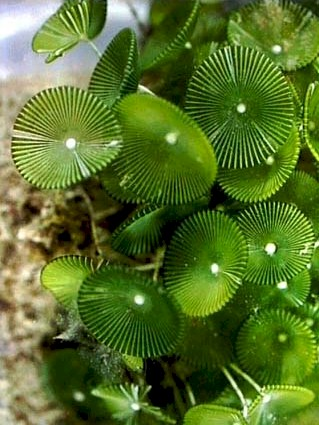
\includegraphics[height=8.2cm]{images/acetabularia1.jpg}
\end{subfigure}
\begin{subfigure}[t]{0.53\textwidth}
	\centering
	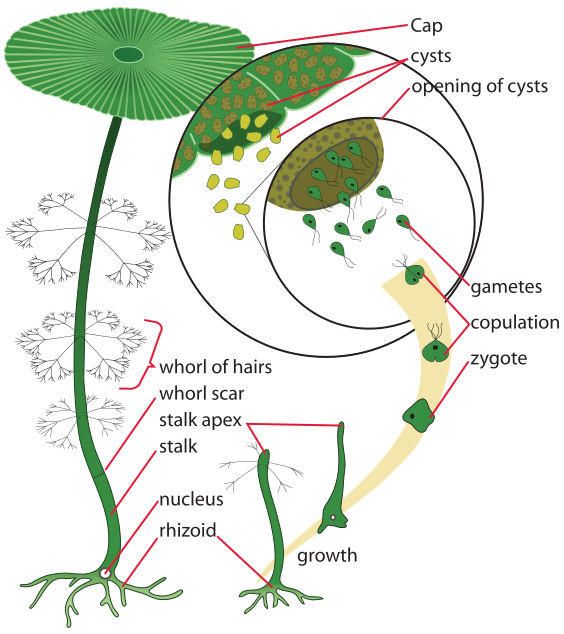
\includegraphics[height=8.2cm]{images/acetabularia2.png}
\end{subfigure}
\caption{(a) \emph{Acetabularia}, a single cell organism that looks like a plant. (b) A schematic depicting its growth process, which we will later model using a spatial variant of the enzyme reaction system, \cref{limcyc}.}%
\label{acet}%
\end{figure}

\begin{figure}
\begin{subfigure}[t]{0.32\textwidth}
	\centering
	%% Creator: Matplotlib, PGF backend
%%
%% To include the figure in your LaTeX document, write
%%   \input{<filename>.pgf}
%%
%% Make sure the required packages are loaded in your preamble
%%   \usepackage{pgf}
%%
%% Figures using additional raster images can only be included by \input if
%% they are in the same directory as the main LaTeX file. For loading figures
%% from other directories you can use the `import` package
%%   \usepackage{import}
%% and then include the figures with
%%   \import{<path to file>}{<filename>.pgf}
%%
%% Matplotlib used the following preamble
%%   \usepackage{fontspec}
%%   \setmainfont{DejaVuSerif.ttf}[Path=/Library/Python/3.7/site-packages/matplotlib/mpl-data/fonts/ttf/]
%%   \setsansfont{DejaVuSans.ttf}[Path=/Library/Python/3.7/site-packages/matplotlib/mpl-data/fonts/ttf/]
%%   \setmonofont{DejaVuSansMono.ttf}[Path=/Library/Python/3.7/site-packages/matplotlib/mpl-data/fonts/ttf/]
%%
\begingroup%
\makeatletter%
\begin{pgfpicture}%
\pgfpathrectangle{\pgfpointorigin}{\pgfqpoint{2.000000in}{2.200000in}}%
\pgfusepath{use as bounding box, clip}%
\begin{pgfscope}%
\pgfsetbuttcap%
\pgfsetmiterjoin%
\definecolor{currentfill}{rgb}{1.000000,1.000000,1.000000}%
\pgfsetfillcolor{currentfill}%
\pgfsetlinewidth{0.000000pt}%
\definecolor{currentstroke}{rgb}{1.000000,1.000000,1.000000}%
\pgfsetstrokecolor{currentstroke}%
\pgfsetdash{}{0pt}%
\pgfpathmoveto{\pgfqpoint{0.000000in}{0.000000in}}%
\pgfpathlineto{\pgfqpoint{2.000000in}{0.000000in}}%
\pgfpathlineto{\pgfqpoint{2.000000in}{2.200000in}}%
\pgfpathlineto{\pgfqpoint{0.000000in}{2.200000in}}%
\pgfpathclose%
\pgfusepath{fill}%
\end{pgfscope}%
\begin{pgfscope}%
\pgfsetbuttcap%
\pgfsetmiterjoin%
\definecolor{currentfill}{rgb}{1.000000,1.000000,1.000000}%
\pgfsetfillcolor{currentfill}%
\pgfsetlinewidth{0.000000pt}%
\definecolor{currentstroke}{rgb}{0.000000,0.000000,0.000000}%
\pgfsetstrokecolor{currentstroke}%
\pgfsetstrokeopacity{0.000000}%
\pgfsetdash{}{0pt}%
\pgfpathmoveto{\pgfqpoint{0.211847in}{0.278150in}}%
\pgfpathlineto{\pgfqpoint{1.966667in}{0.278150in}}%
\pgfpathlineto{\pgfqpoint{1.966667in}{2.166667in}}%
\pgfpathlineto{\pgfqpoint{0.211847in}{2.166667in}}%
\pgfpathclose%
\pgfusepath{fill}%
\end{pgfscope}%
\begin{pgfscope}%
\pgfpathrectangle{\pgfqpoint{0.211847in}{0.278150in}}{\pgfqpoint{1.754820in}{1.888517in}}%
\pgfusepath{clip}%
\pgfsetrectcap%
\pgfsetroundjoin%
\pgfsetlinewidth{1.505625pt}%
\definecolor{currentstroke}{rgb}{0.121569,0.466667,0.705882}%
\pgfsetstrokecolor{currentstroke}%
\pgfsetdash{}{0pt}%
\pgfpathmoveto{\pgfqpoint{0.211847in}{0.879817in}}%
\pgfpathlineto{\pgfqpoint{0.224021in}{0.910836in}}%
\pgfpathlineto{\pgfqpoint{0.236196in}{0.945124in}}%
\pgfpathlineto{\pgfqpoint{0.248370in}{0.983081in}}%
\pgfpathlineto{\pgfqpoint{0.260544in}{1.025120in}}%
\pgfpathlineto{\pgfqpoint{0.272719in}{1.071646in}}%
\pgfpathlineto{\pgfqpoint{0.284893in}{1.123011in}}%
\pgfpathlineto{\pgfqpoint{0.297067in}{1.179454in}}%
\pgfpathlineto{\pgfqpoint{0.309241in}{1.241012in}}%
\pgfpathlineto{\pgfqpoint{0.323155in}{1.317263in}}%
\pgfpathlineto{\pgfqpoint{0.340547in}{1.419708in}}%
\pgfpathlineto{\pgfqpoint{0.384026in}{1.680109in}}%
\pgfpathlineto{\pgfqpoint{0.396201in}{1.744274in}}%
\pgfpathlineto{\pgfqpoint{0.406636in}{1.793564in}}%
\pgfpathlineto{\pgfqpoint{0.417071in}{1.837003in}}%
\pgfpathlineto{\pgfqpoint{0.425767in}{1.868630in}}%
\pgfpathlineto{\pgfqpoint{0.434463in}{1.896219in}}%
\pgfpathlineto{\pgfqpoint{0.443159in}{1.920021in}}%
\pgfpathlineto{\pgfqpoint{0.451855in}{1.940370in}}%
\pgfpathlineto{\pgfqpoint{0.460550in}{1.957648in}}%
\pgfpathlineto{\pgfqpoint{0.469246in}{1.972250in}}%
\pgfpathlineto{\pgfqpoint{0.477942in}{1.984556in}}%
\pgfpathlineto{\pgfqpoint{0.486638in}{1.994920in}}%
\pgfpathlineto{\pgfqpoint{0.495334in}{2.003657in}}%
\pgfpathlineto{\pgfqpoint{0.505769in}{2.012378in}}%
\pgfpathlineto{\pgfqpoint{0.516204in}{2.019550in}}%
\pgfpathlineto{\pgfqpoint{0.528379in}{2.026390in}}%
\pgfpathlineto{\pgfqpoint{0.540553in}{2.031965in}}%
\pgfpathlineto{\pgfqpoint{0.554466in}{2.037178in}}%
\pgfpathlineto{\pgfqpoint{0.571858in}{2.042430in}}%
\pgfpathlineto{\pgfqpoint{0.592728in}{2.047449in}}%
\pgfpathlineto{\pgfqpoint{0.617077in}{2.052127in}}%
\pgfpathlineto{\pgfqpoint{0.648382in}{2.056933in}}%
\pgfpathlineto{\pgfqpoint{0.686644in}{2.061599in}}%
\pgfpathlineto{\pgfqpoint{0.731863in}{2.065950in}}%
\pgfpathlineto{\pgfqpoint{0.785778in}{2.069961in}}%
\pgfpathlineto{\pgfqpoint{0.848389in}{2.073443in}}%
\pgfpathlineto{\pgfqpoint{0.921434in}{2.076356in}}%
\pgfpathlineto{\pgfqpoint{1.010133in}{2.078741in}}%
\pgfpathlineto{\pgfqpoint{1.123180in}{2.080607in}}%
\pgfpathlineto{\pgfqpoint{1.276228in}{2.081943in}}%
\pgfpathlineto{\pgfqpoint{1.511018in}{2.082765in}}%
\pgfpathlineto{\pgfqpoint{1.949292in}{2.083105in}}%
\pgfpathlineto{\pgfqpoint{1.949292in}{2.083105in}}%
\pgfusepath{stroke}%
\end{pgfscope}%
\begin{pgfscope}%
\pgfpathrectangle{\pgfqpoint{0.211847in}{0.278150in}}{\pgfqpoint{1.754820in}{1.888517in}}%
\pgfusepath{clip}%
\pgfsetbuttcap%
\pgfsetroundjoin%
\pgfsetlinewidth{1.505625pt}%
\definecolor{currentstroke}{rgb}{1.000000,0.498039,0.054902}%
\pgfsetstrokecolor{currentstroke}%
\pgfsetdash{{5.550000pt}{2.400000pt}}{0.000000pt}%
\pgfpathmoveto{\pgfqpoint{0.211847in}{0.879817in}}%
\pgfpathlineto{\pgfqpoint{0.222282in}{0.903463in}}%
\pgfpathlineto{\pgfqpoint{0.230978in}{0.920495in}}%
\pgfpathlineto{\pgfqpoint{0.239674in}{0.934880in}}%
\pgfpathlineto{\pgfqpoint{0.246631in}{0.944339in}}%
\pgfpathlineto{\pgfqpoint{0.253588in}{0.951854in}}%
\pgfpathlineto{\pgfqpoint{0.258805in}{0.956144in}}%
\pgfpathlineto{\pgfqpoint{0.264023in}{0.959228in}}%
\pgfpathlineto{\pgfqpoint{0.269240in}{0.961057in}}%
\pgfpathlineto{\pgfqpoint{0.274458in}{0.961585in}}%
\pgfpathlineto{\pgfqpoint{0.279675in}{0.960768in}}%
\pgfpathlineto{\pgfqpoint{0.284893in}{0.958566in}}%
\pgfpathlineto{\pgfqpoint{0.290110in}{0.954943in}}%
\pgfpathlineto{\pgfqpoint{0.295328in}{0.949871in}}%
\pgfpathlineto{\pgfqpoint{0.300545in}{0.943328in}}%
\pgfpathlineto{\pgfqpoint{0.305763in}{0.935304in}}%
\pgfpathlineto{\pgfqpoint{0.312720in}{0.922305in}}%
\pgfpathlineto{\pgfqpoint{0.319677in}{0.906716in}}%
\pgfpathlineto{\pgfqpoint{0.326633in}{0.888632in}}%
\pgfpathlineto{\pgfqpoint{0.335329in}{0.862755in}}%
\pgfpathlineto{\pgfqpoint{0.345764in}{0.827501in}}%
\pgfpathlineto{\pgfqpoint{0.357939in}{0.781947in}}%
\pgfpathlineto{\pgfqpoint{0.401418in}{0.613831in}}%
\pgfpathlineto{\pgfqpoint{0.411853in}{0.579611in}}%
\pgfpathlineto{\pgfqpoint{0.422288in}{0.549528in}}%
\pgfpathlineto{\pgfqpoint{0.430984in}{0.527766in}}%
\pgfpathlineto{\pgfqpoint{0.439680in}{0.508951in}}%
\pgfpathlineto{\pgfqpoint{0.448376in}{0.492909in}}%
\pgfpathlineto{\pgfqpoint{0.457072in}{0.479391in}}%
\pgfpathlineto{\pgfqpoint{0.465768in}{0.468111in}}%
\pgfpathlineto{\pgfqpoint{0.474464in}{0.458773in}}%
\pgfpathlineto{\pgfqpoint{0.483160in}{0.451090in}}%
\pgfpathlineto{\pgfqpoint{0.491856in}{0.444799in}}%
\pgfpathlineto{\pgfqpoint{0.502291in}{0.438756in}}%
\pgfpathlineto{\pgfqpoint{0.512726in}{0.434030in}}%
\pgfpathlineto{\pgfqpoint{0.524900in}{0.429804in}}%
\pgfpathlineto{\pgfqpoint{0.538814in}{0.426240in}}%
\pgfpathlineto{\pgfqpoint{0.554466in}{0.423376in}}%
\pgfpathlineto{\pgfqpoint{0.575337in}{0.420799in}}%
\pgfpathlineto{\pgfqpoint{0.601424in}{0.418768in}}%
\pgfpathlineto{\pgfqpoint{0.639686in}{0.417007in}}%
\pgfpathlineto{\pgfqpoint{0.702297in}{0.415399in}}%
\pgfpathlineto{\pgfqpoint{0.808387in}{0.413907in}}%
\pgfpathlineto{\pgfqpoint{0.975349in}{0.412753in}}%
\pgfpathlineto{\pgfqpoint{1.253618in}{0.412084in}}%
\pgfpathlineto{\pgfqpoint{1.947553in}{0.411861in}}%
\pgfpathlineto{\pgfqpoint{1.949292in}{0.411861in}}%
\pgfpathlineto{\pgfqpoint{1.949292in}{0.411861in}}%
\pgfusepath{stroke}%
\end{pgfscope}%
\begin{pgfscope}%
\pgfsetbuttcap%
\pgfsetroundjoin%
\definecolor{currentfill}{rgb}{0.000000,0.000000,0.000000}%
\pgfsetfillcolor{currentfill}%
\pgfsetlinewidth{0.803000pt}%
\definecolor{currentstroke}{rgb}{0.000000,0.000000,0.000000}%
\pgfsetstrokecolor{currentstroke}%
\pgfsetdash{}{0pt}%
\pgfsys@defobject{currentmarker}{\pgfqpoint{0.000000in}{-0.048611in}}{\pgfqpoint{0.000000in}{0.000000in}}{%
\pgfpathmoveto{\pgfqpoint{0.000000in}{0.000000in}}%
\pgfpathlineto{\pgfqpoint{0.000000in}{-0.048611in}}%
\pgfusepath{stroke,fill}%
}%
\begin{pgfscope}%
\pgfsys@transformshift{0.211847in}{0.278150in}%
\pgfsys@useobject{currentmarker}{}%
\end{pgfscope}%
\end{pgfscope}%
\begin{pgfscope}%
\definecolor{textcolor}{rgb}{0.000000,0.000000,0.000000}%
\pgfsetstrokecolor{textcolor}%
\pgfsetfillcolor{textcolor}%
\pgftext[x=0.211847in,y=0.180927in,,top]{\color{textcolor}\rmfamily\fontsize{12.000000}{14.400000}\selectfont \(\displaystyle 0.0\)}%
\end{pgfscope}%
\begin{pgfscope}%
\pgfsetbuttcap%
\pgfsetroundjoin%
\definecolor{currentfill}{rgb}{0.000000,0.000000,0.000000}%
\pgfsetfillcolor{currentfill}%
\pgfsetlinewidth{0.803000pt}%
\definecolor{currentstroke}{rgb}{0.000000,0.000000,0.000000}%
\pgfsetstrokecolor{currentstroke}%
\pgfsetdash{}{0pt}%
\pgfsys@defobject{currentmarker}{\pgfqpoint{0.000000in}{-0.048611in}}{\pgfqpoint{0.000000in}{0.000000in}}{%
\pgfpathmoveto{\pgfqpoint{0.000000in}{0.000000in}}%
\pgfpathlineto{\pgfqpoint{0.000000in}{-0.048611in}}%
\pgfusepath{stroke,fill}%
}%
\begin{pgfscope}%
\pgfsys@transformshift{0.832363in}{0.278150in}%
\pgfsys@useobject{currentmarker}{}%
\end{pgfscope}%
\end{pgfscope}%
\begin{pgfscope}%
\definecolor{textcolor}{rgb}{0.000000,0.000000,0.000000}%
\pgfsetstrokecolor{textcolor}%
\pgfsetfillcolor{textcolor}%
\pgftext[x=0.832363in,y=0.180927in,,top]{\color{textcolor}\rmfamily\fontsize{12.000000}{14.400000}\selectfont \(\displaystyle 2.5\)}%
\end{pgfscope}%
\begin{pgfscope}%
\pgfsetbuttcap%
\pgfsetroundjoin%
\definecolor{currentfill}{rgb}{0.000000,0.000000,0.000000}%
\pgfsetfillcolor{currentfill}%
\pgfsetlinewidth{0.803000pt}%
\definecolor{currentstroke}{rgb}{0.000000,0.000000,0.000000}%
\pgfsetstrokecolor{currentstroke}%
\pgfsetdash{}{0pt}%
\pgfsys@defobject{currentmarker}{\pgfqpoint{0.000000in}{-0.048611in}}{\pgfqpoint{0.000000in}{0.000000in}}{%
\pgfpathmoveto{\pgfqpoint{0.000000in}{0.000000in}}%
\pgfpathlineto{\pgfqpoint{0.000000in}{-0.048611in}}%
\pgfusepath{stroke,fill}%
}%
\begin{pgfscope}%
\pgfsys@transformshift{1.452879in}{0.278150in}%
\pgfsys@useobject{currentmarker}{}%
\end{pgfscope}%
\end{pgfscope}%
\begin{pgfscope}%
\definecolor{textcolor}{rgb}{0.000000,0.000000,0.000000}%
\pgfsetstrokecolor{textcolor}%
\pgfsetfillcolor{textcolor}%
\pgftext[x=1.452879in,y=0.180927in,,top]{\color{textcolor}\rmfamily\fontsize{12.000000}{14.400000}\selectfont \(\displaystyle 5.0\)}%
\end{pgfscope}%
\begin{pgfscope}%
\pgfsetbuttcap%
\pgfsetroundjoin%
\definecolor{currentfill}{rgb}{0.000000,0.000000,0.000000}%
\pgfsetfillcolor{currentfill}%
\pgfsetlinewidth{0.803000pt}%
\definecolor{currentstroke}{rgb}{0.000000,0.000000,0.000000}%
\pgfsetstrokecolor{currentstroke}%
\pgfsetdash{}{0pt}%
\pgfsys@defobject{currentmarker}{\pgfqpoint{-0.048611in}{0.000000in}}{\pgfqpoint{0.000000in}{0.000000in}}{%
\pgfpathmoveto{\pgfqpoint{0.000000in}{0.000000in}}%
\pgfpathlineto{\pgfqpoint{-0.048611in}{0.000000in}}%
\pgfusepath{stroke,fill}%
}%
\begin{pgfscope}%
\pgfsys@transformshift{0.211847in}{0.278150in}%
\pgfsys@useobject{currentmarker}{}%
\end{pgfscope}%
\end{pgfscope}%
\begin{pgfscope}%
\definecolor{textcolor}{rgb}{0.000000,0.000000,0.000000}%
\pgfsetstrokecolor{textcolor}%
\pgfsetfillcolor{textcolor}%
\pgftext[x=0.033028in,y=0.214836in,left,base]{\color{textcolor}\rmfamily\fontsize{12.000000}{14.400000}\selectfont \(\displaystyle 0\)}%
\end{pgfscope}%
\begin{pgfscope}%
\pgfsetbuttcap%
\pgfsetroundjoin%
\definecolor{currentfill}{rgb}{0.000000,0.000000,0.000000}%
\pgfsetfillcolor{currentfill}%
\pgfsetlinewidth{0.803000pt}%
\definecolor{currentstroke}{rgb}{0.000000,0.000000,0.000000}%
\pgfsetstrokecolor{currentstroke}%
\pgfsetdash{}{0pt}%
\pgfsys@defobject{currentmarker}{\pgfqpoint{-0.048611in}{0.000000in}}{\pgfqpoint{0.000000in}{0.000000in}}{%
\pgfpathmoveto{\pgfqpoint{0.000000in}{0.000000in}}%
\pgfpathlineto{\pgfqpoint{-0.048611in}{0.000000in}}%
\pgfusepath{stroke,fill}%
}%
\begin{pgfscope}%
\pgfsys@transformshift{0.211847in}{0.879817in}%
\pgfsys@useobject{currentmarker}{}%
\end{pgfscope}%
\end{pgfscope}%
\begin{pgfscope}%
\definecolor{textcolor}{rgb}{0.000000,0.000000,0.000000}%
\pgfsetstrokecolor{textcolor}%
\pgfsetfillcolor{textcolor}%
\pgftext[x=0.033028in,y=0.816503in,left,base]{\color{textcolor}\rmfamily\fontsize{12.000000}{14.400000}\selectfont \(\displaystyle 1\)}%
\end{pgfscope}%
\begin{pgfscope}%
\pgfsetbuttcap%
\pgfsetroundjoin%
\definecolor{currentfill}{rgb}{0.000000,0.000000,0.000000}%
\pgfsetfillcolor{currentfill}%
\pgfsetlinewidth{0.803000pt}%
\definecolor{currentstroke}{rgb}{0.000000,0.000000,0.000000}%
\pgfsetstrokecolor{currentstroke}%
\pgfsetdash{}{0pt}%
\pgfsys@defobject{currentmarker}{\pgfqpoint{-0.048611in}{0.000000in}}{\pgfqpoint{0.000000in}{0.000000in}}{%
\pgfpathmoveto{\pgfqpoint{0.000000in}{0.000000in}}%
\pgfpathlineto{\pgfqpoint{-0.048611in}{0.000000in}}%
\pgfusepath{stroke,fill}%
}%
\begin{pgfscope}%
\pgfsys@transformshift{0.211847in}{1.481483in}%
\pgfsys@useobject{currentmarker}{}%
\end{pgfscope}%
\end{pgfscope}%
\begin{pgfscope}%
\definecolor{textcolor}{rgb}{0.000000,0.000000,0.000000}%
\pgfsetstrokecolor{textcolor}%
\pgfsetfillcolor{textcolor}%
\pgftext[x=0.033028in,y=1.418170in,left,base]{\color{textcolor}\rmfamily\fontsize{12.000000}{14.400000}\selectfont \(\displaystyle 2\)}%
\end{pgfscope}%
\begin{pgfscope}%
\pgfsetbuttcap%
\pgfsetroundjoin%
\definecolor{currentfill}{rgb}{0.000000,0.000000,0.000000}%
\pgfsetfillcolor{currentfill}%
\pgfsetlinewidth{0.803000pt}%
\definecolor{currentstroke}{rgb}{0.000000,0.000000,0.000000}%
\pgfsetstrokecolor{currentstroke}%
\pgfsetdash{}{0pt}%
\pgfsys@defobject{currentmarker}{\pgfqpoint{-0.048611in}{0.000000in}}{\pgfqpoint{0.000000in}{0.000000in}}{%
\pgfpathmoveto{\pgfqpoint{0.000000in}{0.000000in}}%
\pgfpathlineto{\pgfqpoint{-0.048611in}{0.000000in}}%
\pgfusepath{stroke,fill}%
}%
\begin{pgfscope}%
\pgfsys@transformshift{0.211847in}{2.083150in}%
\pgfsys@useobject{currentmarker}{}%
\end{pgfscope}%
\end{pgfscope}%
\begin{pgfscope}%
\definecolor{textcolor}{rgb}{0.000000,0.000000,0.000000}%
\pgfsetstrokecolor{textcolor}%
\pgfsetfillcolor{textcolor}%
\pgftext[x=0.033028in,y=2.019836in,left,base]{\color{textcolor}\rmfamily\fontsize{12.000000}{14.400000}\selectfont \(\displaystyle 3\)}%
\end{pgfscope}%
\begin{pgfscope}%
\pgfsetrectcap%
\pgfsetmiterjoin%
\pgfsetlinewidth{0.803000pt}%
\definecolor{currentstroke}{rgb}{0.000000,0.000000,0.000000}%
\pgfsetstrokecolor{currentstroke}%
\pgfsetdash{}{0pt}%
\pgfpathmoveto{\pgfqpoint{0.211847in}{0.278150in}}%
\pgfpathlineto{\pgfqpoint{0.211847in}{2.166667in}}%
\pgfusepath{stroke}%
\end{pgfscope}%
\begin{pgfscope}%
\pgfsetrectcap%
\pgfsetmiterjoin%
\pgfsetlinewidth{0.803000pt}%
\definecolor{currentstroke}{rgb}{0.000000,0.000000,0.000000}%
\pgfsetstrokecolor{currentstroke}%
\pgfsetdash{}{0pt}%
\pgfpathmoveto{\pgfqpoint{0.211847in}{0.278150in}}%
\pgfpathlineto{\pgfqpoint{1.966667in}{0.278150in}}%
\pgfusepath{stroke}%
\end{pgfscope}%
\begin{pgfscope}%
\definecolor{textcolor}{rgb}{0.000000,0.000000,0.000000}%
\pgfsetstrokecolor{textcolor}%
\pgfsetfillcolor{textcolor}%
\pgftext[x=1.966667in,y=0.180927in,right,top]{\color{textcolor}\rmfamily\fontsize{12.000000}{14.400000}\selectfont \(\displaystyle t\)}%
\end{pgfscope}%
\begin{pgfscope}%
\pgfsetbuttcap%
\pgfsetmiterjoin%
\definecolor{currentfill}{rgb}{1.000000,1.000000,1.000000}%
\pgfsetfillcolor{currentfill}%
\pgfsetfillopacity{0.800000}%
\pgfsetlinewidth{0.000000pt}%
\definecolor{currentstroke}{rgb}{0.800000,0.800000,0.800000}%
\pgfsetstrokecolor{currentstroke}%
\pgfsetstrokeopacity{0.800000}%
\pgfsetdash{}{0pt}%
\pgfpathmoveto{\pgfqpoint{1.423764in}{1.019446in}}%
\pgfpathlineto{\pgfqpoint{1.933333in}{1.019446in}}%
\pgfpathquadraticcurveto{\pgfqpoint{1.966667in}{1.019446in}}{\pgfqpoint{1.966667in}{1.052779in}}%
\pgfpathlineto{\pgfqpoint{1.966667in}{1.392037in}}%
\pgfpathquadraticcurveto{\pgfqpoint{1.966667in}{1.425370in}}{\pgfqpoint{1.933333in}{1.425370in}}%
\pgfpathlineto{\pgfqpoint{1.423764in}{1.425370in}}%
\pgfpathquadraticcurveto{\pgfqpoint{1.390431in}{1.425370in}}{\pgfqpoint{1.390431in}{1.392037in}}%
\pgfpathlineto{\pgfqpoint{1.390431in}{1.052779in}}%
\pgfpathquadraticcurveto{\pgfqpoint{1.390431in}{1.019446in}}{\pgfqpoint{1.423764in}{1.019446in}}%
\pgfpathclose%
\pgfusepath{fill}%
\end{pgfscope}%
\begin{pgfscope}%
\pgfsetrectcap%
\pgfsetroundjoin%
\pgfsetlinewidth{1.505625pt}%
\definecolor{currentstroke}{rgb}{0.121569,0.466667,0.705882}%
\pgfsetstrokecolor{currentstroke}%
\pgfsetdash{}{0pt}%
\pgfpathmoveto{\pgfqpoint{1.390431in}{1.357076in}}%
\pgfpathlineto{\pgfqpoint{1.723764in}{1.357076in}}%
\pgfusepath{stroke}%
\end{pgfscope}%
\begin{pgfscope}%
\definecolor{textcolor}{rgb}{0.000000,0.000000,0.000000}%
\pgfsetstrokecolor{textcolor}%
\pgfsetfillcolor{textcolor}%
\pgftext[x=1.857098in,y=1.298743in,left,base]{\color{textcolor}\rmfamily\fontsize{12.000000}{14.400000}\selectfont \(\displaystyle u\)\hspace{-14pt}}%
\end{pgfscope}%
\begin{pgfscope}%
\pgfsetbuttcap%
\pgfsetroundjoin%
\pgfsetlinewidth{1.505625pt}%
\definecolor{currentstroke}{rgb}{1.000000,0.498039,0.054902}%
\pgfsetstrokecolor{currentstroke}%
\pgfsetdash{{5.550000pt}{2.400000pt}}{0.000000pt}%
\pgfpathmoveto{\pgfqpoint{1.390431in}{1.112447in}}%
\pgfpathlineto{\pgfqpoint{1.723764in}{1.112447in}}%
\pgfusepath{stroke}%
\end{pgfscope}%
\begin{pgfscope}%
\definecolor{textcolor}{rgb}{0.000000,0.000000,0.000000}%
\pgfsetstrokecolor{textcolor}%
\pgfsetfillcolor{textcolor}%
\pgftext[x=1.857098in,y=1.054114in,left,base]{\color{textcolor}\rmfamily\fontsize{12.000000}{14.400000}\selectfont \(\displaystyle v\)\hspace{-14pt}}%
\end{pgfscope}%
\end{pgfpicture}%
\makeatother%
\endgroup%

	%\includegraphics[width=7cm]{limitCylcleBoring.PDF}
\end{subfigure}
\begin{subfigure}[t]{0.32\textwidth}
	\centering
	%% Creator: Matplotlib, PGF backend
%%
%% To include the figure in your LaTeX document, write
%%   \input{<filename>.pgf}
%%
%% Make sure the required packages are loaded in your preamble
%%   \usepackage{pgf}
%%
%% Figures using additional raster images can only be included by \input if
%% they are in the same directory as the main LaTeX file. For loading figures
%% from other directories you can use the `import` package
%%   \usepackage{import}
%% and then include the figures with
%%   \import{<path to file>}{<filename>.pgf}
%%
%% Matplotlib used the following preamble
%%   \usepackage{fontspec}
%%   \setmainfont{DejaVuSerif.ttf}[Path=/Library/Python/3.7/site-packages/matplotlib/mpl-data/fonts/ttf/]
%%   \setsansfont{DejaVuSans.ttf}[Path=/Library/Python/3.7/site-packages/matplotlib/mpl-data/fonts/ttf/]
%%   \setmonofont{DejaVuSansMono.ttf}[Path=/Library/Python/3.7/site-packages/matplotlib/mpl-data/fonts/ttf/]
%%
\begingroup%
\makeatletter%
\begin{pgfpicture}%
\pgfpathrectangle{\pgfpointorigin}{\pgfqpoint{2.000000in}{2.200000in}}%
\pgfusepath{use as bounding box, clip}%
\begin{pgfscope}%
\pgfsetbuttcap%
\pgfsetmiterjoin%
\definecolor{currentfill}{rgb}{1.000000,1.000000,1.000000}%
\pgfsetfillcolor{currentfill}%
\pgfsetlinewidth{0.000000pt}%
\definecolor{currentstroke}{rgb}{1.000000,1.000000,1.000000}%
\pgfsetstrokecolor{currentstroke}%
\pgfsetdash{}{0pt}%
\pgfpathmoveto{\pgfqpoint{0.000000in}{0.000000in}}%
\pgfpathlineto{\pgfqpoint{2.000000in}{0.000000in}}%
\pgfpathlineto{\pgfqpoint{2.000000in}{2.200000in}}%
\pgfpathlineto{\pgfqpoint{0.000000in}{2.200000in}}%
\pgfpathclose%
\pgfusepath{fill}%
\end{pgfscope}%
\begin{pgfscope}%
\pgfsetbuttcap%
\pgfsetmiterjoin%
\definecolor{currentfill}{rgb}{1.000000,1.000000,1.000000}%
\pgfsetfillcolor{currentfill}%
\pgfsetlinewidth{0.000000pt}%
\definecolor{currentstroke}{rgb}{0.000000,0.000000,0.000000}%
\pgfsetstrokecolor{currentstroke}%
\pgfsetstrokeopacity{0.000000}%
\pgfsetdash{}{0pt}%
\pgfpathmoveto{\pgfqpoint{0.338301in}{0.278150in}}%
\pgfpathlineto{\pgfqpoint{1.966667in}{0.278150in}}%
\pgfpathlineto{\pgfqpoint{1.966667in}{2.166667in}}%
\pgfpathlineto{\pgfqpoint{0.338301in}{2.166667in}}%
\pgfpathclose%
\pgfusepath{fill}%
\end{pgfscope}%
\begin{pgfscope}%
\pgfpathrectangle{\pgfqpoint{0.338301in}{0.278150in}}{\pgfqpoint{1.628366in}{1.888517in}}%
\pgfusepath{clip}%
\pgfsetrectcap%
\pgfsetroundjoin%
\pgfsetlinewidth{1.505625pt}%
\definecolor{currentstroke}{rgb}{0.121569,0.466667,0.705882}%
\pgfsetstrokecolor{currentstroke}%
\pgfsetdash{}{0pt}%
\pgfpathmoveto{\pgfqpoint{0.338301in}{1.661246in}}%
\pgfpathlineto{\pgfqpoint{0.341528in}{1.718732in}}%
\pgfpathlineto{\pgfqpoint{0.343142in}{1.733663in}}%
\pgfpathlineto{\pgfqpoint{0.344756in}{1.738734in}}%
\pgfpathlineto{\pgfqpoint{0.346370in}{1.734264in}}%
\pgfpathlineto{\pgfqpoint{0.347984in}{1.721110in}}%
\pgfpathlineto{\pgfqpoint{0.351211in}{1.673831in}}%
\pgfpathlineto{\pgfqpoint{0.356053in}{1.571429in}}%
\pgfpathlineto{\pgfqpoint{0.365736in}{1.353625in}}%
\pgfpathlineto{\pgfqpoint{0.370578in}{1.264281in}}%
\pgfpathlineto{\pgfqpoint{0.375419in}{1.192659in}}%
\pgfpathlineto{\pgfqpoint{0.380261in}{1.138337in}}%
\pgfpathlineto{\pgfqpoint{0.383489in}{1.111127in}}%
\pgfpathlineto{\pgfqpoint{0.386716in}{1.090666in}}%
\pgfpathlineto{\pgfqpoint{0.389944in}{1.076621in}}%
\pgfpathlineto{\pgfqpoint{0.393172in}{1.068750in}}%
\pgfpathlineto{\pgfqpoint{0.394786in}{1.067082in}}%
\pgfpathlineto{\pgfqpoint{0.396399in}{1.066914in}}%
\pgfpathlineto{\pgfqpoint{0.398013in}{1.068248in}}%
\pgfpathlineto{\pgfqpoint{0.399627in}{1.071091in}}%
\pgfpathlineto{\pgfqpoint{0.402855in}{1.081379in}}%
\pgfpathlineto{\pgfqpoint{0.406083in}{1.097991in}}%
\pgfpathlineto{\pgfqpoint{0.409310in}{1.121233in}}%
\pgfpathlineto{\pgfqpoint{0.412538in}{1.151464in}}%
\pgfpathlineto{\pgfqpoint{0.417380in}{1.210556in}}%
\pgfpathlineto{\pgfqpoint{0.422221in}{1.285930in}}%
\pgfpathlineto{\pgfqpoint{0.436746in}{1.539655in}}%
\pgfpathlineto{\pgfqpoint{0.439974in}{1.571448in}}%
\pgfpathlineto{\pgfqpoint{0.441587in}{1.580237in}}%
\pgfpathlineto{\pgfqpoint{0.443201in}{1.584001in}}%
\pgfpathlineto{\pgfqpoint{0.444815in}{1.582788in}}%
\pgfpathlineto{\pgfqpoint{0.446429in}{1.576846in}}%
\pgfpathlineto{\pgfqpoint{0.448043in}{1.566579in}}%
\pgfpathlineto{\pgfqpoint{0.451271in}{1.535229in}}%
\pgfpathlineto{\pgfqpoint{0.456112in}{1.470201in}}%
\pgfpathlineto{\pgfqpoint{0.469023in}{1.282244in}}%
\pgfpathlineto{\pgfqpoint{0.473865in}{1.226443in}}%
\pgfpathlineto{\pgfqpoint{0.478706in}{1.182573in}}%
\pgfpathlineto{\pgfqpoint{0.483548in}{1.150954in}}%
\pgfpathlineto{\pgfqpoint{0.486775in}{1.136612in}}%
\pgfpathlineto{\pgfqpoint{0.490003in}{1.127575in}}%
\pgfpathlineto{\pgfqpoint{0.491617in}{1.125028in}}%
\pgfpathlineto{\pgfqpoint{0.493231in}{1.123788in}}%
\pgfpathlineto{\pgfqpoint{0.494845in}{1.123855in}}%
\pgfpathlineto{\pgfqpoint{0.496459in}{1.125230in}}%
\pgfpathlineto{\pgfqpoint{0.498072in}{1.127915in}}%
\pgfpathlineto{\pgfqpoint{0.501300in}{1.137240in}}%
\pgfpathlineto{\pgfqpoint{0.504528in}{1.151890in}}%
\pgfpathlineto{\pgfqpoint{0.507756in}{1.171915in}}%
\pgfpathlineto{\pgfqpoint{0.512597in}{1.211965in}}%
\pgfpathlineto{\pgfqpoint{0.517439in}{1.263249in}}%
\pgfpathlineto{\pgfqpoint{0.525508in}{1.365343in}}%
\pgfpathlineto{\pgfqpoint{0.531963in}{1.443336in}}%
\pgfpathlineto{\pgfqpoint{0.535191in}{1.472816in}}%
\pgfpathlineto{\pgfqpoint{0.538419in}{1.492095in}}%
\pgfpathlineto{\pgfqpoint{0.540033in}{1.497332in}}%
\pgfpathlineto{\pgfqpoint{0.541647in}{1.499506in}}%
\pgfpathlineto{\pgfqpoint{0.543260in}{1.498638in}}%
\pgfpathlineto{\pgfqpoint{0.544874in}{1.494843in}}%
\pgfpathlineto{\pgfqpoint{0.546488in}{1.488311in}}%
\pgfpathlineto{\pgfqpoint{0.549716in}{1.468098in}}%
\pgfpathlineto{\pgfqpoint{0.554557in}{1.424690in}}%
\pgfpathlineto{\pgfqpoint{0.572310in}{1.245605in}}%
\pgfpathlineto{\pgfqpoint{0.577151in}{1.210937in}}%
\pgfpathlineto{\pgfqpoint{0.581993in}{1.185685in}}%
\pgfpathlineto{\pgfqpoint{0.585221in}{1.174286in}}%
\pgfpathlineto{\pgfqpoint{0.588448in}{1.167289in}}%
\pgfpathlineto{\pgfqpoint{0.590062in}{1.165448in}}%
\pgfpathlineto{\pgfqpoint{0.591676in}{1.164711in}}%
\pgfpathlineto{\pgfqpoint{0.593290in}{1.165080in}}%
\pgfpathlineto{\pgfqpoint{0.594904in}{1.166552in}}%
\pgfpathlineto{\pgfqpoint{0.596518in}{1.169128in}}%
\pgfpathlineto{\pgfqpoint{0.599745in}{1.177572in}}%
\pgfpathlineto{\pgfqpoint{0.602973in}{1.190364in}}%
\pgfpathlineto{\pgfqpoint{0.606201in}{1.207391in}}%
\pgfpathlineto{\pgfqpoint{0.611042in}{1.240363in}}%
\pgfpathlineto{\pgfqpoint{0.617498in}{1.295562in}}%
\pgfpathlineto{\pgfqpoint{0.628795in}{1.398076in}}%
\pgfpathlineto{\pgfqpoint{0.632023in}{1.420396in}}%
\pgfpathlineto{\pgfqpoint{0.635250in}{1.436284in}}%
\pgfpathlineto{\pgfqpoint{0.636864in}{1.441415in}}%
\pgfpathlineto{\pgfqpoint{0.638478in}{1.444546in}}%
\pgfpathlineto{\pgfqpoint{0.640092in}{1.445645in}}%
\pgfpathlineto{\pgfqpoint{0.641706in}{1.444731in}}%
\pgfpathlineto{\pgfqpoint{0.643320in}{1.441870in}}%
\pgfpathlineto{\pgfqpoint{0.646547in}{1.430784in}}%
\pgfpathlineto{\pgfqpoint{0.649775in}{1.413641in}}%
\pgfpathlineto{\pgfqpoint{0.654617in}{1.380023in}}%
\pgfpathlineto{\pgfqpoint{0.670755in}{1.257973in}}%
\pgfpathlineto{\pgfqpoint{0.675597in}{1.230894in}}%
\pgfpathlineto{\pgfqpoint{0.680438in}{1.211129in}}%
\pgfpathlineto{\pgfqpoint{0.683666in}{1.202328in}}%
\pgfpathlineto{\pgfqpoint{0.686894in}{1.197142in}}%
\pgfpathlineto{\pgfqpoint{0.688508in}{1.195920in}}%
\pgfpathlineto{\pgfqpoint{0.690122in}{1.195615in}}%
\pgfpathlineto{\pgfqpoint{0.691735in}{1.196226in}}%
\pgfpathlineto{\pgfqpoint{0.693349in}{1.197749in}}%
\pgfpathlineto{\pgfqpoint{0.696577in}{1.203505in}}%
\pgfpathlineto{\pgfqpoint{0.699805in}{1.212797in}}%
\pgfpathlineto{\pgfqpoint{0.703032in}{1.225469in}}%
\pgfpathlineto{\pgfqpoint{0.707874in}{1.250238in}}%
\pgfpathlineto{\pgfqpoint{0.714329in}{1.291611in}}%
\pgfpathlineto{\pgfqpoint{0.725626in}{1.368264in}}%
\pgfpathlineto{\pgfqpoint{0.730468in}{1.392582in}}%
\pgfpathlineto{\pgfqpoint{0.733696in}{1.403069in}}%
\pgfpathlineto{\pgfqpoint{0.735310in}{1.406309in}}%
\pgfpathlineto{\pgfqpoint{0.736923in}{1.408149in}}%
\pgfpathlineto{\pgfqpoint{0.738537in}{1.408576in}}%
\pgfpathlineto{\pgfqpoint{0.740151in}{1.407608in}}%
\pgfpathlineto{\pgfqpoint{0.741765in}{1.405289in}}%
\pgfpathlineto{\pgfqpoint{0.744993in}{1.396904in}}%
\pgfpathlineto{\pgfqpoint{0.748220in}{1.384216in}}%
\pgfpathlineto{\pgfqpoint{0.753062in}{1.359348in}}%
\pgfpathlineto{\pgfqpoint{0.770814in}{1.259157in}}%
\pgfpathlineto{\pgfqpoint{0.775656in}{1.239992in}}%
\pgfpathlineto{\pgfqpoint{0.778884in}{1.230506in}}%
\pgfpathlineto{\pgfqpoint{0.782111in}{1.223860in}}%
\pgfpathlineto{\pgfqpoint{0.785339in}{1.220156in}}%
\pgfpathlineto{\pgfqpoint{0.786953in}{1.219425in}}%
\pgfpathlineto{\pgfqpoint{0.788567in}{1.219442in}}%
\pgfpathlineto{\pgfqpoint{0.790181in}{1.220206in}}%
\pgfpathlineto{\pgfqpoint{0.793408in}{1.223948in}}%
\pgfpathlineto{\pgfqpoint{0.796636in}{1.230561in}}%
\pgfpathlineto{\pgfqpoint{0.799864in}{1.239892in}}%
\pgfpathlineto{\pgfqpoint{0.804705in}{1.258443in}}%
\pgfpathlineto{\pgfqpoint{0.811161in}{1.289636in}}%
\pgfpathlineto{\pgfqpoint{0.824072in}{1.354886in}}%
\pgfpathlineto{\pgfqpoint{0.827299in}{1.366991in}}%
\pgfpathlineto{\pgfqpoint{0.830527in}{1.375834in}}%
\pgfpathlineto{\pgfqpoint{0.833755in}{1.380905in}}%
\pgfpathlineto{\pgfqpoint{0.835369in}{1.381939in}}%
\pgfpathlineto{\pgfqpoint{0.836983in}{1.381962in}}%
\pgfpathlineto{\pgfqpoint{0.838596in}{1.380990in}}%
\pgfpathlineto{\pgfqpoint{0.840210in}{1.379056in}}%
\pgfpathlineto{\pgfqpoint{0.843438in}{1.372506in}}%
\pgfpathlineto{\pgfqpoint{0.846666in}{1.362850in}}%
\pgfpathlineto{\pgfqpoint{0.851507in}{1.344059in}}%
\pgfpathlineto{\pgfqpoint{0.870874in}{1.262117in}}%
\pgfpathlineto{\pgfqpoint{0.875715in}{1.248905in}}%
\pgfpathlineto{\pgfqpoint{0.878943in}{1.242824in}}%
\pgfpathlineto{\pgfqpoint{0.882171in}{1.239079in}}%
\pgfpathlineto{\pgfqpoint{0.885398in}{1.237737in}}%
\pgfpathlineto{\pgfqpoint{0.887012in}{1.237972in}}%
\pgfpathlineto{\pgfqpoint{0.890240in}{1.240236in}}%
\pgfpathlineto{\pgfqpoint{0.893468in}{1.244825in}}%
\pgfpathlineto{\pgfqpoint{0.896695in}{1.251604in}}%
\pgfpathlineto{\pgfqpoint{0.901537in}{1.265419in}}%
\pgfpathlineto{\pgfqpoint{0.907992in}{1.288972in}}%
\pgfpathlineto{\pgfqpoint{0.920903in}{1.339057in}}%
\pgfpathlineto{\pgfqpoint{0.925745in}{1.352717in}}%
\pgfpathlineto{\pgfqpoint{0.928972in}{1.358793in}}%
\pgfpathlineto{\pgfqpoint{0.932200in}{1.362056in}}%
\pgfpathlineto{\pgfqpoint{0.933814in}{1.362586in}}%
\pgfpathlineto{\pgfqpoint{0.935428in}{1.362378in}}%
\pgfpathlineto{\pgfqpoint{0.937042in}{1.361446in}}%
\pgfpathlineto{\pgfqpoint{0.940269in}{1.357522in}}%
\pgfpathlineto{\pgfqpoint{0.943497in}{1.351125in}}%
\pgfpathlineto{\pgfqpoint{0.948339in}{1.337872in}}%
\pgfpathlineto{\pgfqpoint{0.956408in}{1.310447in}}%
\pgfpathlineto{\pgfqpoint{0.964477in}{1.283339in}}%
\pgfpathlineto{\pgfqpoint{0.969319in}{1.269952in}}%
\pgfpathlineto{\pgfqpoint{0.974160in}{1.259921in}}%
\pgfpathlineto{\pgfqpoint{0.977388in}{1.255408in}}%
\pgfpathlineto{\pgfqpoint{0.980616in}{1.252768in}}%
\pgfpathlineto{\pgfqpoint{0.983844in}{1.252053in}}%
\pgfpathlineto{\pgfqpoint{0.987071in}{1.253262in}}%
\pgfpathlineto{\pgfqpoint{0.990299in}{1.256344in}}%
\pgfpathlineto{\pgfqpoint{0.993527in}{1.261192in}}%
\pgfpathlineto{\pgfqpoint{0.998368in}{1.271400in}}%
\pgfpathlineto{\pgfqpoint{1.004824in}{1.289164in}}%
\pgfpathlineto{\pgfqpoint{1.019348in}{1.331822in}}%
\pgfpathlineto{\pgfqpoint{1.024190in}{1.341608in}}%
\pgfpathlineto{\pgfqpoint{1.027418in}{1.345793in}}%
\pgfpathlineto{\pgfqpoint{1.030645in}{1.347863in}}%
\pgfpathlineto{\pgfqpoint{1.033873in}{1.347749in}}%
\pgfpathlineto{\pgfqpoint{1.037101in}{1.345511in}}%
\pgfpathlineto{\pgfqpoint{1.040329in}{1.341329in}}%
\pgfpathlineto{\pgfqpoint{1.045170in}{1.332038in}}%
\pgfpathlineto{\pgfqpoint{1.051626in}{1.315949in}}%
\pgfpathlineto{\pgfqpoint{1.062923in}{1.286420in}}%
\pgfpathlineto{\pgfqpoint{1.067764in}{1.276203in}}%
\pgfpathlineto{\pgfqpoint{1.072606in}{1.268646in}}%
\pgfpathlineto{\pgfqpoint{1.075833in}{1.265341in}}%
\pgfpathlineto{\pgfqpoint{1.079061in}{1.263527in}}%
\pgfpathlineto{\pgfqpoint{1.082289in}{1.263244in}}%
\pgfpathlineto{\pgfqpoint{1.085517in}{1.264483in}}%
\pgfpathlineto{\pgfqpoint{1.088744in}{1.267186in}}%
\pgfpathlineto{\pgfqpoint{1.091972in}{1.271253in}}%
\pgfpathlineto{\pgfqpoint{1.096814in}{1.279566in}}%
\pgfpathlineto{\pgfqpoint{1.103269in}{1.293622in}}%
\pgfpathlineto{\pgfqpoint{1.116180in}{1.322932in}}%
\pgfpathlineto{\pgfqpoint{1.121021in}{1.330917in}}%
\pgfpathlineto{\pgfqpoint{1.124249in}{1.334556in}}%
\pgfpathlineto{\pgfqpoint{1.127477in}{1.336643in}}%
\pgfpathlineto{\pgfqpoint{1.130705in}{1.337102in}}%
\pgfpathlineto{\pgfqpoint{1.133932in}{1.335943in}}%
\pgfpathlineto{\pgfqpoint{1.137160in}{1.333267in}}%
\pgfpathlineto{\pgfqpoint{1.140388in}{1.329247in}}%
\pgfpathlineto{\pgfqpoint{1.145229in}{1.321224in}}%
\pgfpathlineto{\pgfqpoint{1.153299in}{1.304944in}}%
\pgfpathlineto{\pgfqpoint{1.161368in}{1.288994in}}%
\pgfpathlineto{\pgfqpoint{1.166209in}{1.281228in}}%
\pgfpathlineto{\pgfqpoint{1.171051in}{1.275577in}}%
\pgfpathlineto{\pgfqpoint{1.174279in}{1.273186in}}%
\pgfpathlineto{\pgfqpoint{1.177506in}{1.271978in}}%
\pgfpathlineto{\pgfqpoint{1.180734in}{1.271979in}}%
\pgfpathlineto{\pgfqpoint{1.183962in}{1.273172in}}%
\pgfpathlineto{\pgfqpoint{1.187190in}{1.275504in}}%
\pgfpathlineto{\pgfqpoint{1.192031in}{1.280917in}}%
\pgfpathlineto{\pgfqpoint{1.196873in}{1.288188in}}%
\pgfpathlineto{\pgfqpoint{1.206556in}{1.305543in}}%
\pgfpathlineto{\pgfqpoint{1.213011in}{1.316513in}}%
\pgfpathlineto{\pgfqpoint{1.217853in}{1.323003in}}%
\pgfpathlineto{\pgfqpoint{1.221081in}{1.326114in}}%
\pgfpathlineto{\pgfqpoint{1.224308in}{1.328084in}}%
\pgfpathlineto{\pgfqpoint{1.227536in}{1.328837in}}%
\pgfpathlineto{\pgfqpoint{1.230764in}{1.328359in}}%
\pgfpathlineto{\pgfqpoint{1.233991in}{1.326702in}}%
\pgfpathlineto{\pgfqpoint{1.237219in}{1.323973in}}%
\pgfpathlineto{\pgfqpoint{1.242061in}{1.318228in}}%
\pgfpathlineto{\pgfqpoint{1.248516in}{1.308563in}}%
\pgfpathlineto{\pgfqpoint{1.259813in}{1.291162in}}%
\pgfpathlineto{\pgfqpoint{1.264655in}{1.285282in}}%
\pgfpathlineto{\pgfqpoint{1.269496in}{1.281084in}}%
\pgfpathlineto{\pgfqpoint{1.272724in}{1.279377in}}%
\pgfpathlineto{\pgfqpoint{1.275952in}{1.278604in}}%
\pgfpathlineto{\pgfqpoint{1.279180in}{1.278779in}}%
\pgfpathlineto{\pgfqpoint{1.282407in}{1.279884in}}%
\pgfpathlineto{\pgfqpoint{1.287249in}{1.283160in}}%
\pgfpathlineto{\pgfqpoint{1.292090in}{1.288094in}}%
\pgfpathlineto{\pgfqpoint{1.298546in}{1.296447in}}%
\pgfpathlineto{\pgfqpoint{1.311457in}{1.313794in}}%
\pgfpathlineto{\pgfqpoint{1.316298in}{1.318557in}}%
\pgfpathlineto{\pgfqpoint{1.321140in}{1.321557in}}%
\pgfpathlineto{\pgfqpoint{1.324368in}{1.322433in}}%
\pgfpathlineto{\pgfqpoint{1.327595in}{1.322373in}}%
\pgfpathlineto{\pgfqpoint{1.330823in}{1.321400in}}%
\pgfpathlineto{\pgfqpoint{1.335665in}{1.318384in}}%
\pgfpathlineto{\pgfqpoint{1.340506in}{1.313848in}}%
\pgfpathlineto{\pgfqpoint{1.348575in}{1.304337in}}%
\pgfpathlineto{\pgfqpoint{1.358259in}{1.292990in}}%
\pgfpathlineto{\pgfqpoint{1.363100in}{1.288554in}}%
\pgfpathlineto{\pgfqpoint{1.367942in}{1.285457in}}%
\pgfpathlineto{\pgfqpoint{1.372783in}{1.283928in}}%
\pgfpathlineto{\pgfqpoint{1.377625in}{1.284060in}}%
\pgfpathlineto{\pgfqpoint{1.382466in}{1.285804in}}%
\pgfpathlineto{\pgfqpoint{1.387308in}{1.288982in}}%
\pgfpathlineto{\pgfqpoint{1.393763in}{1.294906in}}%
\pgfpathlineto{\pgfqpoint{1.411516in}{1.312816in}}%
\pgfpathlineto{\pgfqpoint{1.416357in}{1.315880in}}%
\pgfpathlineto{\pgfqpoint{1.421199in}{1.317482in}}%
\pgfpathlineto{\pgfqpoint{1.426041in}{1.317495in}}%
\pgfpathlineto{\pgfqpoint{1.430882in}{1.315963in}}%
\pgfpathlineto{\pgfqpoint{1.435724in}{1.313092in}}%
\pgfpathlineto{\pgfqpoint{1.442179in}{1.307770in}}%
\pgfpathlineto{\pgfqpoint{1.458318in}{1.293314in}}%
\pgfpathlineto{\pgfqpoint{1.463159in}{1.290309in}}%
\pgfpathlineto{\pgfqpoint{1.468001in}{1.288437in}}%
\pgfpathlineto{\pgfqpoint{1.472842in}{1.287832in}}%
\pgfpathlineto{\pgfqpoint{1.477684in}{1.288518in}}%
\pgfpathlineto{\pgfqpoint{1.482526in}{1.290406in}}%
\pgfpathlineto{\pgfqpoint{1.488981in}{1.294451in}}%
\pgfpathlineto{\pgfqpoint{1.500278in}{1.303647in}}%
\pgfpathlineto{\pgfqpoint{1.508347in}{1.309628in}}%
\pgfpathlineto{\pgfqpoint{1.513189in}{1.312187in}}%
\pgfpathlineto{\pgfqpoint{1.518030in}{1.313665in}}%
\pgfpathlineto{\pgfqpoint{1.522872in}{1.313938in}}%
\pgfpathlineto{\pgfqpoint{1.527714in}{1.313012in}}%
\pgfpathlineto{\pgfqpoint{1.532555in}{1.311017in}}%
\pgfpathlineto{\pgfqpoint{1.539011in}{1.307105in}}%
\pgfpathlineto{\pgfqpoint{1.558377in}{1.294067in}}%
\pgfpathlineto{\pgfqpoint{1.564832in}{1.291667in}}%
\pgfpathlineto{\pgfqpoint{1.569674in}{1.290984in}}%
\pgfpathlineto{\pgfqpoint{1.574515in}{1.291308in}}%
\pgfpathlineto{\pgfqpoint{1.579357in}{1.292587in}}%
\pgfpathlineto{\pgfqpoint{1.585812in}{1.295533in}}%
\pgfpathlineto{\pgfqpoint{1.595496in}{1.301505in}}%
\pgfpathlineto{\pgfqpoint{1.605179in}{1.307290in}}%
\pgfpathlineto{\pgfqpoint{1.611634in}{1.309946in}}%
\pgfpathlineto{\pgfqpoint{1.616476in}{1.310971in}}%
\pgfpathlineto{\pgfqpoint{1.621317in}{1.311069in}}%
\pgfpathlineto{\pgfqpoint{1.626159in}{1.310256in}}%
\pgfpathlineto{\pgfqpoint{1.632614in}{1.307952in}}%
\pgfpathlineto{\pgfqpoint{1.642297in}{1.302865in}}%
\pgfpathlineto{\pgfqpoint{1.653594in}{1.296892in}}%
\pgfpathlineto{\pgfqpoint{1.660050in}{1.294550in}}%
\pgfpathlineto{\pgfqpoint{1.666505in}{1.293456in}}%
\pgfpathlineto{\pgfqpoint{1.672961in}{1.293742in}}%
\pgfpathlineto{\pgfqpoint{1.679416in}{1.295321in}}%
\pgfpathlineto{\pgfqpoint{1.687485in}{1.298651in}}%
\pgfpathlineto{\pgfqpoint{1.705238in}{1.306805in}}%
\pgfpathlineto{\pgfqpoint{1.711693in}{1.308481in}}%
\pgfpathlineto{\pgfqpoint{1.718149in}{1.308946in}}%
\pgfpathlineto{\pgfqpoint{1.724604in}{1.308161in}}%
\pgfpathlineto{\pgfqpoint{1.731060in}{1.306308in}}%
\pgfpathlineto{\pgfqpoint{1.742357in}{1.301631in}}%
\pgfpathlineto{\pgfqpoint{1.753654in}{1.297268in}}%
\pgfpathlineto{\pgfqpoint{1.760109in}{1.295762in}}%
\pgfpathlineto{\pgfqpoint{1.766564in}{1.295276in}}%
\pgfpathlineto{\pgfqpoint{1.773020in}{1.295855in}}%
\pgfpathlineto{\pgfqpoint{1.781089in}{1.297870in}}%
\pgfpathlineto{\pgfqpoint{1.795614in}{1.303230in}}%
\pgfpathlineto{\pgfqpoint{1.805297in}{1.306156in}}%
\pgfpathlineto{\pgfqpoint{1.811752in}{1.307142in}}%
\pgfpathlineto{\pgfqpoint{1.818208in}{1.307168in}}%
\pgfpathlineto{\pgfqpoint{1.826277in}{1.305910in}}%
\pgfpathlineto{\pgfqpoint{1.835960in}{1.303075in}}%
\pgfpathlineto{\pgfqpoint{1.852099in}{1.298134in}}%
\pgfpathlineto{\pgfqpoint{1.860168in}{1.296882in}}%
\pgfpathlineto{\pgfqpoint{1.868237in}{1.296895in}}%
\pgfpathlineto{\pgfqpoint{1.876307in}{1.298121in}}%
\pgfpathlineto{\pgfqpoint{1.887604in}{1.301153in}}%
\pgfpathlineto{\pgfqpoint{1.902129in}{1.304938in}}%
\pgfpathlineto{\pgfqpoint{1.910198in}{1.305913in}}%
\pgfpathlineto{\pgfqpoint{1.918267in}{1.305739in}}%
\pgfpathlineto{\pgfqpoint{1.927950in}{1.304169in}}%
\pgfpathlineto{\pgfqpoint{1.950544in}{1.298837in}}%
\pgfpathlineto{\pgfqpoint{1.950544in}{1.298837in}}%
\pgfusepath{stroke}%
\end{pgfscope}%
\begin{pgfscope}%
\pgfpathrectangle{\pgfqpoint{0.338301in}{0.278150in}}{\pgfqpoint{1.628366in}{1.888517in}}%
\pgfusepath{clip}%
\pgfsetbuttcap%
\pgfsetroundjoin%
\pgfsetlinewidth{1.505625pt}%
\definecolor{currentstroke}{rgb}{1.000000,0.498039,0.054902}%
\pgfsetstrokecolor{currentstroke}%
\pgfsetdash{{5.550000pt}{2.400000pt}}{0.000000pt}%
\pgfpathmoveto{\pgfqpoint{0.338301in}{1.661246in}}%
\pgfpathlineto{\pgfqpoint{0.343142in}{1.419571in}}%
\pgfpathlineto{\pgfqpoint{0.346370in}{1.296908in}}%
\pgfpathlineto{\pgfqpoint{0.349598in}{1.213456in}}%
\pgfpathlineto{\pgfqpoint{0.352825in}{1.167297in}}%
\pgfpathlineto{\pgfqpoint{0.354439in}{1.156445in}}%
\pgfpathlineto{\pgfqpoint{0.356053in}{1.152645in}}%
\pgfpathlineto{\pgfqpoint{0.357667in}{1.155091in}}%
\pgfpathlineto{\pgfqpoint{0.359281in}{1.163036in}}%
\pgfpathlineto{\pgfqpoint{0.362508in}{1.192785in}}%
\pgfpathlineto{\pgfqpoint{0.365736in}{1.237320in}}%
\pgfpathlineto{\pgfqpoint{0.370578in}{1.324198in}}%
\pgfpathlineto{\pgfqpoint{0.377033in}{1.463874in}}%
\pgfpathlineto{\pgfqpoint{0.398013in}{1.939655in}}%
\pgfpathlineto{\pgfqpoint{0.402855in}{2.022371in}}%
\pgfpathlineto{\pgfqpoint{0.406083in}{2.065318in}}%
\pgfpathlineto{\pgfqpoint{0.409310in}{2.096057in}}%
\pgfpathlineto{\pgfqpoint{0.410924in}{2.106144in}}%
\pgfpathlineto{\pgfqpoint{0.412538in}{2.112321in}}%
\pgfpathlineto{\pgfqpoint{0.414152in}{2.114297in}}%
\pgfpathlineto{\pgfqpoint{0.415766in}{2.111789in}}%
\pgfpathlineto{\pgfqpoint{0.417380in}{2.104530in}}%
\pgfpathlineto{\pgfqpoint{0.418993in}{2.092284in}}%
\pgfpathlineto{\pgfqpoint{0.422221in}{2.052146in}}%
\pgfpathlineto{\pgfqpoint{0.425449in}{1.990813in}}%
\pgfpathlineto{\pgfqpoint{0.428677in}{1.909591in}}%
\pgfpathlineto{\pgfqpoint{0.435132in}{1.705975in}}%
\pgfpathlineto{\pgfqpoint{0.441587in}{1.501397in}}%
\pgfpathlineto{\pgfqpoint{0.446429in}{1.386845in}}%
\pgfpathlineto{\pgfqpoint{0.449657in}{1.337101in}}%
\pgfpathlineto{\pgfqpoint{0.452884in}{1.308911in}}%
\pgfpathlineto{\pgfqpoint{0.454498in}{1.302340in}}%
\pgfpathlineto{\pgfqpoint{0.456112in}{1.300358in}}%
\pgfpathlineto{\pgfqpoint{0.457726in}{1.302607in}}%
\pgfpathlineto{\pgfqpoint{0.459340in}{1.308723in}}%
\pgfpathlineto{\pgfqpoint{0.462568in}{1.331130in}}%
\pgfpathlineto{\pgfqpoint{0.465795in}{1.364874in}}%
\pgfpathlineto{\pgfqpoint{0.470637in}{1.431524in}}%
\pgfpathlineto{\pgfqpoint{0.477092in}{1.539718in}}%
\pgfpathlineto{\pgfqpoint{0.494845in}{1.850993in}}%
\pgfpathlineto{\pgfqpoint{0.499686in}{1.916397in}}%
\pgfpathlineto{\pgfqpoint{0.502914in}{1.950433in}}%
\pgfpathlineto{\pgfqpoint{0.506142in}{1.975009in}}%
\pgfpathlineto{\pgfqpoint{0.507756in}{1.983268in}}%
\pgfpathlineto{\pgfqpoint{0.509369in}{1.988592in}}%
\pgfpathlineto{\pgfqpoint{0.510983in}{1.990807in}}%
\pgfpathlineto{\pgfqpoint{0.512597in}{1.989753in}}%
\pgfpathlineto{\pgfqpoint{0.514211in}{1.985293in}}%
\pgfpathlineto{\pgfqpoint{0.515825in}{1.977317in}}%
\pgfpathlineto{\pgfqpoint{0.519053in}{1.950579in}}%
\pgfpathlineto{\pgfqpoint{0.522280in}{1.909594in}}%
\pgfpathlineto{\pgfqpoint{0.527122in}{1.824238in}}%
\pgfpathlineto{\pgfqpoint{0.535191in}{1.645614in}}%
\pgfpathlineto{\pgfqpoint{0.541647in}{1.513277in}}%
\pgfpathlineto{\pgfqpoint{0.544874in}{1.462862in}}%
\pgfpathlineto{\pgfqpoint{0.548102in}{1.426204in}}%
\pgfpathlineto{\pgfqpoint{0.551330in}{1.403893in}}%
\pgfpathlineto{\pgfqpoint{0.552944in}{1.397982in}}%
\pgfpathlineto{\pgfqpoint{0.554557in}{1.395390in}}%
\pgfpathlineto{\pgfqpoint{0.556171in}{1.395943in}}%
\pgfpathlineto{\pgfqpoint{0.557785in}{1.399443in}}%
\pgfpathlineto{\pgfqpoint{0.559399in}{1.405680in}}%
\pgfpathlineto{\pgfqpoint{0.562627in}{1.425487in}}%
\pgfpathlineto{\pgfqpoint{0.565854in}{1.453618in}}%
\pgfpathlineto{\pgfqpoint{0.570696in}{1.507740in}}%
\pgfpathlineto{\pgfqpoint{0.578765in}{1.616875in}}%
\pgfpathlineto{\pgfqpoint{0.590062in}{1.773215in}}%
\pgfpathlineto{\pgfqpoint{0.594904in}{1.829485in}}%
\pgfpathlineto{\pgfqpoint{0.599745in}{1.873288in}}%
\pgfpathlineto{\pgfqpoint{0.602973in}{1.893579in}}%
\pgfpathlineto{\pgfqpoint{0.606201in}{1.905451in}}%
\pgfpathlineto{\pgfqpoint{0.607815in}{1.907926in}}%
\pgfpathlineto{\pgfqpoint{0.609429in}{1.907958in}}%
\pgfpathlineto{\pgfqpoint{0.611042in}{1.905469in}}%
\pgfpathlineto{\pgfqpoint{0.612656in}{1.900403in}}%
\pgfpathlineto{\pgfqpoint{0.615884in}{1.882461in}}%
\pgfpathlineto{\pgfqpoint{0.619112in}{1.854337in}}%
\pgfpathlineto{\pgfqpoint{0.622340in}{1.816904in}}%
\pgfpathlineto{\pgfqpoint{0.627181in}{1.747110in}}%
\pgfpathlineto{\pgfqpoint{0.640092in}{1.548705in}}%
\pgfpathlineto{\pgfqpoint{0.643320in}{1.512465in}}%
\pgfpathlineto{\pgfqpoint{0.646547in}{1.485644in}}%
\pgfpathlineto{\pgfqpoint{0.649775in}{1.468869in}}%
\pgfpathlineto{\pgfqpoint{0.651389in}{1.464246in}}%
\pgfpathlineto{\pgfqpoint{0.653003in}{1.462057in}}%
\pgfpathlineto{\pgfqpoint{0.654617in}{1.462210in}}%
\pgfpathlineto{\pgfqpoint{0.656231in}{1.464594in}}%
\pgfpathlineto{\pgfqpoint{0.657844in}{1.469079in}}%
\pgfpathlineto{\pgfqpoint{0.661072in}{1.483786in}}%
\pgfpathlineto{\pgfqpoint{0.664300in}{1.505128in}}%
\pgfpathlineto{\pgfqpoint{0.669141in}{1.546847in}}%
\pgfpathlineto{\pgfqpoint{0.675597in}{1.614089in}}%
\pgfpathlineto{\pgfqpoint{0.688508in}{1.753304in}}%
\pgfpathlineto{\pgfqpoint{0.693349in}{1.795827in}}%
\pgfpathlineto{\pgfqpoint{0.698191in}{1.827723in}}%
\pgfpathlineto{\pgfqpoint{0.701419in}{1.841578in}}%
\pgfpathlineto{\pgfqpoint{0.703032in}{1.845989in}}%
\pgfpathlineto{\pgfqpoint{0.704646in}{1.848615in}}%
\pgfpathlineto{\pgfqpoint{0.706260in}{1.849389in}}%
\pgfpathlineto{\pgfqpoint{0.707874in}{1.848264in}}%
\pgfpathlineto{\pgfqpoint{0.709488in}{1.845207in}}%
\pgfpathlineto{\pgfqpoint{0.711102in}{1.840207in}}%
\pgfpathlineto{\pgfqpoint{0.714329in}{1.824459in}}%
\pgfpathlineto{\pgfqpoint{0.717557in}{1.801442in}}%
\pgfpathlineto{\pgfqpoint{0.722399in}{1.755370in}}%
\pgfpathlineto{\pgfqpoint{0.730468in}{1.661369in}}%
\pgfpathlineto{\pgfqpoint{0.736923in}{1.589453in}}%
\pgfpathlineto{\pgfqpoint{0.741765in}{1.547703in}}%
\pgfpathlineto{\pgfqpoint{0.744993in}{1.528102in}}%
\pgfpathlineto{\pgfqpoint{0.748220in}{1.515778in}}%
\pgfpathlineto{\pgfqpoint{0.749834in}{1.512379in}}%
\pgfpathlineto{\pgfqpoint{0.751448in}{1.510791in}}%
\pgfpathlineto{\pgfqpoint{0.753062in}{1.510962in}}%
\pgfpathlineto{\pgfqpoint{0.754676in}{1.512824in}}%
\pgfpathlineto{\pgfqpoint{0.756290in}{1.516294in}}%
\pgfpathlineto{\pgfqpoint{0.759517in}{1.527676in}}%
\pgfpathlineto{\pgfqpoint{0.762745in}{1.544261in}}%
\pgfpathlineto{\pgfqpoint{0.767587in}{1.576840in}}%
\pgfpathlineto{\pgfqpoint{0.774042in}{1.629519in}}%
\pgfpathlineto{\pgfqpoint{0.786953in}{1.737567in}}%
\pgfpathlineto{\pgfqpoint{0.791795in}{1.769600in}}%
\pgfpathlineto{\pgfqpoint{0.795022in}{1.786150in}}%
\pgfpathlineto{\pgfqpoint{0.798250in}{1.798044in}}%
\pgfpathlineto{\pgfqpoint{0.801478in}{1.804715in}}%
\pgfpathlineto{\pgfqpoint{0.803092in}{1.805956in}}%
\pgfpathlineto{\pgfqpoint{0.804705in}{1.805749in}}%
\pgfpathlineto{\pgfqpoint{0.806319in}{1.804077in}}%
\pgfpathlineto{\pgfqpoint{0.807933in}{1.800932in}}%
\pgfpathlineto{\pgfqpoint{0.811161in}{1.790297in}}%
\pgfpathlineto{\pgfqpoint{0.814389in}{1.774163in}}%
\pgfpathlineto{\pgfqpoint{0.819230in}{1.741137in}}%
\pgfpathlineto{\pgfqpoint{0.825686in}{1.686364in}}%
\pgfpathlineto{\pgfqpoint{0.835369in}{1.604532in}}%
\pgfpathlineto{\pgfqpoint{0.840210in}{1.573954in}}%
\pgfpathlineto{\pgfqpoint{0.843438in}{1.559644in}}%
\pgfpathlineto{\pgfqpoint{0.846666in}{1.550726in}}%
\pgfpathlineto{\pgfqpoint{0.848280in}{1.548329in}}%
\pgfpathlineto{\pgfqpoint{0.849893in}{1.547292in}}%
\pgfpathlineto{\pgfqpoint{0.851507in}{1.547586in}}%
\pgfpathlineto{\pgfqpoint{0.853121in}{1.549166in}}%
\pgfpathlineto{\pgfqpoint{0.854735in}{1.551977in}}%
\pgfpathlineto{\pgfqpoint{0.857963in}{1.561020in}}%
\pgfpathlineto{\pgfqpoint{0.861190in}{1.574101in}}%
\pgfpathlineto{\pgfqpoint{0.866032in}{1.599736in}}%
\pgfpathlineto{\pgfqpoint{0.872487in}{1.641086in}}%
\pgfpathlineto{\pgfqpoint{0.883784in}{1.715440in}}%
\pgfpathlineto{\pgfqpoint{0.888626in}{1.741492in}}%
\pgfpathlineto{\pgfqpoint{0.893468in}{1.760808in}}%
\pgfpathlineto{\pgfqpoint{0.896695in}{1.769052in}}%
\pgfpathlineto{\pgfqpoint{0.898309in}{1.771628in}}%
\pgfpathlineto{\pgfqpoint{0.899923in}{1.773123in}}%
\pgfpathlineto{\pgfqpoint{0.901537in}{1.773511in}}%
\pgfpathlineto{\pgfqpoint{0.903151in}{1.772777in}}%
\pgfpathlineto{\pgfqpoint{0.904765in}{1.770918in}}%
\pgfpathlineto{\pgfqpoint{0.907992in}{1.763874in}}%
\pgfpathlineto{\pgfqpoint{0.911220in}{1.752610in}}%
\pgfpathlineto{\pgfqpoint{0.914448in}{1.737584in}}%
\pgfpathlineto{\pgfqpoint{0.919289in}{1.709514in}}%
\pgfpathlineto{\pgfqpoint{0.935428in}{1.608213in}}%
\pgfpathlineto{\pgfqpoint{0.938656in}{1.594046in}}%
\pgfpathlineto{\pgfqpoint{0.941883in}{1.583621in}}%
\pgfpathlineto{\pgfqpoint{0.945111in}{1.577250in}}%
\pgfpathlineto{\pgfqpoint{0.946725in}{1.575621in}}%
\pgfpathlineto{\pgfqpoint{0.948339in}{1.575023in}}%
\pgfpathlineto{\pgfqpoint{0.949953in}{1.575435in}}%
\pgfpathlineto{\pgfqpoint{0.951566in}{1.576829in}}%
\pgfpathlineto{\pgfqpoint{0.954794in}{1.582393in}}%
\pgfpathlineto{\pgfqpoint{0.958022in}{1.591310in}}%
\pgfpathlineto{\pgfqpoint{0.962863in}{1.609854in}}%
\pgfpathlineto{\pgfqpoint{0.969319in}{1.641124in}}%
\pgfpathlineto{\pgfqpoint{0.982230in}{1.707106in}}%
\pgfpathlineto{\pgfqpoint{0.987071in}{1.726733in}}%
\pgfpathlineto{\pgfqpoint{0.990299in}{1.736822in}}%
\pgfpathlineto{\pgfqpoint{0.993527in}{1.744030in}}%
\pgfpathlineto{\pgfqpoint{0.996754in}{1.748049in}}%
\pgfpathlineto{\pgfqpoint{0.998368in}{1.748795in}}%
\pgfpathlineto{\pgfqpoint{0.999982in}{1.748680in}}%
\pgfpathlineto{\pgfqpoint{1.001596in}{1.747701in}}%
\pgfpathlineto{\pgfqpoint{1.003210in}{1.745861in}}%
\pgfpathlineto{\pgfqpoint{1.006438in}{1.739675in}}%
\pgfpathlineto{\pgfqpoint{1.009665in}{1.730365in}}%
\pgfpathlineto{\pgfqpoint{1.014507in}{1.711463in}}%
\pgfpathlineto{\pgfqpoint{1.020962in}{1.680258in}}%
\pgfpathlineto{\pgfqpoint{1.030645in}{1.632958in}}%
\pgfpathlineto{\pgfqpoint{1.035487in}{1.614537in}}%
\pgfpathlineto{\pgfqpoint{1.038715in}{1.605502in}}%
\pgfpathlineto{\pgfqpoint{1.041942in}{1.599453in}}%
\pgfpathlineto{\pgfqpoint{1.045170in}{1.596539in}}%
\pgfpathlineto{\pgfqpoint{1.046784in}{1.596262in}}%
\pgfpathlineto{\pgfqpoint{1.048398in}{1.596756in}}%
\pgfpathlineto{\pgfqpoint{1.050012in}{1.597999in}}%
\pgfpathlineto{\pgfqpoint{1.053239in}{1.602610in}}%
\pgfpathlineto{\pgfqpoint{1.056467in}{1.609791in}}%
\pgfpathlineto{\pgfqpoint{1.061309in}{1.624519in}}%
\pgfpathlineto{\pgfqpoint{1.067764in}{1.649105in}}%
\pgfpathlineto{\pgfqpoint{1.080675in}{1.700078in}}%
\pgfpathlineto{\pgfqpoint{1.085517in}{1.714801in}}%
\pgfpathlineto{\pgfqpoint{1.088744in}{1.722167in}}%
\pgfpathlineto{\pgfqpoint{1.091972in}{1.727218in}}%
\pgfpathlineto{\pgfqpoint{1.095200in}{1.729742in}}%
\pgfpathlineto{\pgfqpoint{1.096814in}{1.730018in}}%
\pgfpathlineto{\pgfqpoint{1.098427in}{1.729626in}}%
\pgfpathlineto{\pgfqpoint{1.101655in}{1.726861in}}%
\pgfpathlineto{\pgfqpoint{1.104883in}{1.721555in}}%
\pgfpathlineto{\pgfqpoint{1.108111in}{1.713935in}}%
\pgfpathlineto{\pgfqpoint{1.112952in}{1.698942in}}%
\pgfpathlineto{\pgfqpoint{1.121021in}{1.668536in}}%
\pgfpathlineto{\pgfqpoint{1.129091in}{1.639130in}}%
\pgfpathlineto{\pgfqpoint{1.133932in}{1.625478in}}%
\pgfpathlineto{\pgfqpoint{1.137160in}{1.618882in}}%
\pgfpathlineto{\pgfqpoint{1.140388in}{1.614572in}}%
\pgfpathlineto{\pgfqpoint{1.143615in}{1.612658in}}%
\pgfpathlineto{\pgfqpoint{1.145229in}{1.612603in}}%
\pgfpathlineto{\pgfqpoint{1.148457in}{1.614244in}}%
\pgfpathlineto{\pgfqpoint{1.151685in}{1.618082in}}%
\pgfpathlineto{\pgfqpoint{1.154912in}{1.623882in}}%
\pgfpathlineto{\pgfqpoint{1.159754in}{1.635592in}}%
\pgfpathlineto{\pgfqpoint{1.166209in}{1.654902in}}%
\pgfpathlineto{\pgfqpoint{1.177506in}{1.689844in}}%
\pgfpathlineto{\pgfqpoint{1.182348in}{1.701863in}}%
\pgfpathlineto{\pgfqpoint{1.187190in}{1.710512in}}%
\pgfpathlineto{\pgfqpoint{1.190417in}{1.714013in}}%
\pgfpathlineto{\pgfqpoint{1.193645in}{1.715527in}}%
\pgfpathlineto{\pgfqpoint{1.196873in}{1.714992in}}%
\pgfpathlineto{\pgfqpoint{1.200100in}{1.712431in}}%
\pgfpathlineto{\pgfqpoint{1.203328in}{1.707955in}}%
\pgfpathlineto{\pgfqpoint{1.206556in}{1.701767in}}%
\pgfpathlineto{\pgfqpoint{1.211397in}{1.689907in}}%
\pgfpathlineto{\pgfqpoint{1.222694in}{1.657066in}}%
\pgfpathlineto{\pgfqpoint{1.229150in}{1.640558in}}%
\pgfpathlineto{\pgfqpoint{1.233991in}{1.631548in}}%
\pgfpathlineto{\pgfqpoint{1.237219in}{1.627612in}}%
\pgfpathlineto{\pgfqpoint{1.240447in}{1.625485in}}%
\pgfpathlineto{\pgfqpoint{1.243675in}{1.625204in}}%
\pgfpathlineto{\pgfqpoint{1.246902in}{1.626721in}}%
\pgfpathlineto{\pgfqpoint{1.250130in}{1.629916in}}%
\pgfpathlineto{\pgfqpoint{1.253358in}{1.634605in}}%
\pgfpathlineto{\pgfqpoint{1.258199in}{1.643914in}}%
\pgfpathlineto{\pgfqpoint{1.266269in}{1.663070in}}%
\pgfpathlineto{\pgfqpoint{1.275952in}{1.685954in}}%
\pgfpathlineto{\pgfqpoint{1.280793in}{1.694970in}}%
\pgfpathlineto{\pgfqpoint{1.284021in}{1.699507in}}%
\pgfpathlineto{\pgfqpoint{1.287249in}{1.702649in}}%
\pgfpathlineto{\pgfqpoint{1.290477in}{1.704275in}}%
\pgfpathlineto{\pgfqpoint{1.293704in}{1.704324in}}%
\pgfpathlineto{\pgfqpoint{1.296932in}{1.702800in}}%
\pgfpathlineto{\pgfqpoint{1.300160in}{1.699774in}}%
\pgfpathlineto{\pgfqpoint{1.303387in}{1.695386in}}%
\pgfpathlineto{\pgfqpoint{1.308229in}{1.686707in}}%
\pgfpathlineto{\pgfqpoint{1.316298in}{1.668982in}}%
\pgfpathlineto{\pgfqpoint{1.324368in}{1.651569in}}%
\pgfpathlineto{\pgfqpoint{1.329209in}{1.643281in}}%
\pgfpathlineto{\pgfqpoint{1.332437in}{1.639160in}}%
\pgfpathlineto{\pgfqpoint{1.335665in}{1.636348in}}%
\pgfpathlineto{\pgfqpoint{1.338892in}{1.634930in}}%
\pgfpathlineto{\pgfqpoint{1.342120in}{1.634928in}}%
\pgfpathlineto{\pgfqpoint{1.345348in}{1.636303in}}%
\pgfpathlineto{\pgfqpoint{1.348575in}{1.638958in}}%
\pgfpathlineto{\pgfqpoint{1.353417in}{1.645009in}}%
\pgfpathlineto{\pgfqpoint{1.359872in}{1.655885in}}%
\pgfpathlineto{\pgfqpoint{1.376011in}{1.685103in}}%
\pgfpathlineto{\pgfqpoint{1.380853in}{1.691170in}}%
\pgfpathlineto{\pgfqpoint{1.384080in}{1.693936in}}%
\pgfpathlineto{\pgfqpoint{1.387308in}{1.695550in}}%
\pgfpathlineto{\pgfqpoint{1.390536in}{1.695952in}}%
\pgfpathlineto{\pgfqpoint{1.393763in}{1.695133in}}%
\pgfpathlineto{\pgfqpoint{1.396991in}{1.693139in}}%
\pgfpathlineto{\pgfqpoint{1.400219in}{1.690063in}}%
\pgfpathlineto{\pgfqpoint{1.405060in}{1.683745in}}%
\pgfpathlineto{\pgfqpoint{1.411516in}{1.673200in}}%
\pgfpathlineto{\pgfqpoint{1.422813in}{1.654350in}}%
\pgfpathlineto{\pgfqpoint{1.427654in}{1.648183in}}%
\pgfpathlineto{\pgfqpoint{1.432496in}{1.644044in}}%
\pgfpathlineto{\pgfqpoint{1.435724in}{1.642584in}}%
\pgfpathlineto{\pgfqpoint{1.438951in}{1.642213in}}%
\pgfpathlineto{\pgfqpoint{1.442179in}{1.642917in}}%
\pgfpathlineto{\pgfqpoint{1.445407in}{1.644640in}}%
\pgfpathlineto{\pgfqpoint{1.450248in}{1.648911in}}%
\pgfpathlineto{\pgfqpoint{1.455090in}{1.654776in}}%
\pgfpathlineto{\pgfqpoint{1.464773in}{1.668859in}}%
\pgfpathlineto{\pgfqpoint{1.472842in}{1.679858in}}%
\pgfpathlineto{\pgfqpoint{1.477684in}{1.684878in}}%
\pgfpathlineto{\pgfqpoint{1.482526in}{1.688150in}}%
\pgfpathlineto{\pgfqpoint{1.485753in}{1.689214in}}%
\pgfpathlineto{\pgfqpoint{1.488981in}{1.689338in}}%
\pgfpathlineto{\pgfqpoint{1.492209in}{1.688524in}}%
\pgfpathlineto{\pgfqpoint{1.495436in}{1.686816in}}%
\pgfpathlineto{\pgfqpoint{1.500278in}{1.682769in}}%
\pgfpathlineto{\pgfqpoint{1.506733in}{1.675295in}}%
\pgfpathlineto{\pgfqpoint{1.522872in}{1.655012in}}%
\pgfpathlineto{\pgfqpoint{1.527714in}{1.650922in}}%
\pgfpathlineto{\pgfqpoint{1.532555in}{1.648522in}}%
\pgfpathlineto{\pgfqpoint{1.535783in}{1.647953in}}%
\pgfpathlineto{\pgfqpoint{1.539011in}{1.648221in}}%
\pgfpathlineto{\pgfqpoint{1.543852in}{1.650113in}}%
\pgfpathlineto{\pgfqpoint{1.548694in}{1.653568in}}%
\pgfpathlineto{\pgfqpoint{1.555149in}{1.659947in}}%
\pgfpathlineto{\pgfqpoint{1.572902in}{1.678907in}}%
\pgfpathlineto{\pgfqpoint{1.577743in}{1.682200in}}%
\pgfpathlineto{\pgfqpoint{1.582585in}{1.684022in}}%
\pgfpathlineto{\pgfqpoint{1.587426in}{1.684227in}}%
\pgfpathlineto{\pgfqpoint{1.592268in}{1.682822in}}%
\pgfpathlineto{\pgfqpoint{1.597109in}{1.679970in}}%
\pgfpathlineto{\pgfqpoint{1.603565in}{1.674451in}}%
\pgfpathlineto{\pgfqpoint{1.621317in}{1.657400in}}%
\pgfpathlineto{\pgfqpoint{1.626159in}{1.654389in}}%
\pgfpathlineto{\pgfqpoint{1.631000in}{1.652698in}}%
\pgfpathlineto{\pgfqpoint{1.635842in}{1.652446in}}%
\pgfpathlineto{\pgfqpoint{1.640684in}{1.653609in}}%
\pgfpathlineto{\pgfqpoint{1.645525in}{1.656032in}}%
\pgfpathlineto{\pgfqpoint{1.651981in}{1.660748in}}%
\pgfpathlineto{\pgfqpoint{1.671347in}{1.676622in}}%
\pgfpathlineto{\pgfqpoint{1.676188in}{1.679034in}}%
\pgfpathlineto{\pgfqpoint{1.681030in}{1.680286in}}%
\pgfpathlineto{\pgfqpoint{1.685872in}{1.680284in}}%
\pgfpathlineto{\pgfqpoint{1.690713in}{1.679050in}}%
\pgfpathlineto{\pgfqpoint{1.695555in}{1.676726in}}%
\pgfpathlineto{\pgfqpoint{1.702010in}{1.672367in}}%
\pgfpathlineto{\pgfqpoint{1.719763in}{1.659348in}}%
\pgfpathlineto{\pgfqpoint{1.724604in}{1.657138in}}%
\pgfpathlineto{\pgfqpoint{1.729446in}{1.655960in}}%
\pgfpathlineto{\pgfqpoint{1.734287in}{1.655893in}}%
\pgfpathlineto{\pgfqpoint{1.739129in}{1.656908in}}%
\pgfpathlineto{\pgfqpoint{1.745584in}{1.659712in}}%
\pgfpathlineto{\pgfqpoint{1.753654in}{1.664764in}}%
\pgfpathlineto{\pgfqpoint{1.766564in}{1.673156in}}%
\pgfpathlineto{\pgfqpoint{1.773020in}{1.676031in}}%
\pgfpathlineto{\pgfqpoint{1.777861in}{1.677193in}}%
\pgfpathlineto{\pgfqpoint{1.782703in}{1.677394in}}%
\pgfpathlineto{\pgfqpoint{1.787545in}{1.676634in}}%
\pgfpathlineto{\pgfqpoint{1.794000in}{1.674297in}}%
\pgfpathlineto{\pgfqpoint{1.802069in}{1.669901in}}%
\pgfpathlineto{\pgfqpoint{1.816594in}{1.661627in}}%
\pgfpathlineto{\pgfqpoint{1.823049in}{1.659315in}}%
\pgfpathlineto{\pgfqpoint{1.829505in}{1.658425in}}%
\pgfpathlineto{\pgfqpoint{1.834346in}{1.658755in}}%
\pgfpathlineto{\pgfqpoint{1.840802in}{1.660420in}}%
\pgfpathlineto{\pgfqpoint{1.848871in}{1.663970in}}%
\pgfpathlineto{\pgfqpoint{1.866624in}{1.672692in}}%
\pgfpathlineto{\pgfqpoint{1.873079in}{1.674534in}}%
\pgfpathlineto{\pgfqpoint{1.879534in}{1.675116in}}%
\pgfpathlineto{\pgfqpoint{1.885990in}{1.674378in}}%
\pgfpathlineto{\pgfqpoint{1.892445in}{1.672482in}}%
\pgfpathlineto{\pgfqpoint{1.902129in}{1.668273in}}%
\pgfpathlineto{\pgfqpoint{1.915039in}{1.662730in}}%
\pgfpathlineto{\pgfqpoint{1.921495in}{1.661036in}}%
\pgfpathlineto{\pgfqpoint{1.927950in}{1.660452in}}%
\pgfpathlineto{\pgfqpoint{1.934406in}{1.661032in}}%
\pgfpathlineto{\pgfqpoint{1.942475in}{1.663163in}}%
\pgfpathlineto{\pgfqpoint{1.950544in}{1.666264in}}%
\pgfpathlineto{\pgfqpoint{1.950544in}{1.666264in}}%
\pgfusepath{stroke}%
\end{pgfscope}%
\begin{pgfscope}%
\pgfsetbuttcap%
\pgfsetroundjoin%
\definecolor{currentfill}{rgb}{0.000000,0.000000,0.000000}%
\pgfsetfillcolor{currentfill}%
\pgfsetlinewidth{0.803000pt}%
\definecolor{currentstroke}{rgb}{0.000000,0.000000,0.000000}%
\pgfsetstrokecolor{currentstroke}%
\pgfsetdash{}{0pt}%
\pgfsys@defobject{currentmarker}{\pgfqpoint{0.000000in}{-0.048611in}}{\pgfqpoint{0.000000in}{0.000000in}}{%
\pgfpathmoveto{\pgfqpoint{0.000000in}{0.000000in}}%
\pgfpathlineto{\pgfqpoint{0.000000in}{-0.048611in}}%
\pgfusepath{stroke,fill}%
}%
\begin{pgfscope}%
\pgfsys@transformshift{0.338301in}{0.278150in}%
\pgfsys@useobject{currentmarker}{}%
\end{pgfscope}%
\end{pgfscope}%
\begin{pgfscope}%
\definecolor{textcolor}{rgb}{0.000000,0.000000,0.000000}%
\pgfsetstrokecolor{textcolor}%
\pgfsetfillcolor{textcolor}%
\pgftext[x=0.338301in,y=0.180927in,,top]{\color{textcolor}\rmfamily\fontsize{12.000000}{14.400000}\selectfont \(\displaystyle 0\)}%
\end{pgfscope}%
\begin{pgfscope}%
\pgfsetbuttcap%
\pgfsetroundjoin%
\definecolor{currentfill}{rgb}{0.000000,0.000000,0.000000}%
\pgfsetfillcolor{currentfill}%
\pgfsetlinewidth{0.803000pt}%
\definecolor{currentstroke}{rgb}{0.000000,0.000000,0.000000}%
\pgfsetstrokecolor{currentstroke}%
\pgfsetdash{}{0pt}%
\pgfsys@defobject{currentmarker}{\pgfqpoint{0.000000in}{-0.048611in}}{\pgfqpoint{0.000000in}{0.000000in}}{%
\pgfpathmoveto{\pgfqpoint{0.000000in}{0.000000in}}%
\pgfpathlineto{\pgfqpoint{0.000000in}{-0.048611in}}%
\pgfusepath{stroke,fill}%
}%
\begin{pgfscope}%
\pgfsys@transformshift{0.914102in}{0.278150in}%
\pgfsys@useobject{currentmarker}{}%
\end{pgfscope}%
\end{pgfscope}%
\begin{pgfscope}%
\definecolor{textcolor}{rgb}{0.000000,0.000000,0.000000}%
\pgfsetstrokecolor{textcolor}%
\pgfsetfillcolor{textcolor}%
\pgftext[x=0.914102in,y=0.180927in,,top]{\color{textcolor}\rmfamily\fontsize{12.000000}{14.400000}\selectfont \(\displaystyle 50\)}%
\end{pgfscope}%
\begin{pgfscope}%
\pgfsetbuttcap%
\pgfsetroundjoin%
\definecolor{currentfill}{rgb}{0.000000,0.000000,0.000000}%
\pgfsetfillcolor{currentfill}%
\pgfsetlinewidth{0.803000pt}%
\definecolor{currentstroke}{rgb}{0.000000,0.000000,0.000000}%
\pgfsetstrokecolor{currentstroke}%
\pgfsetdash{}{0pt}%
\pgfsys@defobject{currentmarker}{\pgfqpoint{0.000000in}{-0.048611in}}{\pgfqpoint{0.000000in}{0.000000in}}{%
\pgfpathmoveto{\pgfqpoint{0.000000in}{0.000000in}}%
\pgfpathlineto{\pgfqpoint{0.000000in}{-0.048611in}}%
\pgfusepath{stroke,fill}%
}%
\begin{pgfscope}%
\pgfsys@transformshift{1.489903in}{0.278150in}%
\pgfsys@useobject{currentmarker}{}%
\end{pgfscope}%
\end{pgfscope}%
\begin{pgfscope}%
\definecolor{textcolor}{rgb}{0.000000,0.000000,0.000000}%
\pgfsetstrokecolor{textcolor}%
\pgfsetfillcolor{textcolor}%
\pgftext[x=1.489903in,y=0.180927in,,top]{\color{textcolor}\rmfamily\fontsize{12.000000}{14.400000}\selectfont \(\displaystyle 100\)}%
\end{pgfscope}%
\begin{pgfscope}%
\pgfsetbuttcap%
\pgfsetroundjoin%
\definecolor{currentfill}{rgb}{0.000000,0.000000,0.000000}%
\pgfsetfillcolor{currentfill}%
\pgfsetlinewidth{0.803000pt}%
\definecolor{currentstroke}{rgb}{0.000000,0.000000,0.000000}%
\pgfsetstrokecolor{currentstroke}%
\pgfsetdash{}{0pt}%
\pgfsys@defobject{currentmarker}{\pgfqpoint{-0.048611in}{0.000000in}}{\pgfqpoint{0.000000in}{0.000000in}}{%
\pgfpathmoveto{\pgfqpoint{0.000000in}{0.000000in}}%
\pgfpathlineto{\pgfqpoint{-0.048611in}{0.000000in}}%
\pgfusepath{stroke,fill}%
}%
\begin{pgfscope}%
\pgfsys@transformshift{0.338301in}{0.278150in}%
\pgfsys@useobject{currentmarker}{}%
\end{pgfscope}%
\end{pgfscope}%
\begin{pgfscope}%
\definecolor{textcolor}{rgb}{0.000000,0.000000,0.000000}%
\pgfsetstrokecolor{textcolor}%
\pgfsetfillcolor{textcolor}%
\pgftext[x=0.032554in,y=0.214836in,left,base]{\color{textcolor}\rmfamily\fontsize{12.000000}{14.400000}\selectfont \(\displaystyle 0.0\)}%
\end{pgfscope}%
\begin{pgfscope}%
\pgfsetbuttcap%
\pgfsetroundjoin%
\definecolor{currentfill}{rgb}{0.000000,0.000000,0.000000}%
\pgfsetfillcolor{currentfill}%
\pgfsetlinewidth{0.803000pt}%
\definecolor{currentstroke}{rgb}{0.000000,0.000000,0.000000}%
\pgfsetstrokecolor{currentstroke}%
\pgfsetdash{}{0pt}%
\pgfsys@defobject{currentmarker}{\pgfqpoint{-0.048611in}{0.000000in}}{\pgfqpoint{0.000000in}{0.000000in}}{%
\pgfpathmoveto{\pgfqpoint{0.000000in}{0.000000in}}%
\pgfpathlineto{\pgfqpoint{-0.048611in}{0.000000in}}%
\pgfusepath{stroke,fill}%
}%
\begin{pgfscope}%
\pgfsys@transformshift{0.338301in}{0.969698in}%
\pgfsys@useobject{currentmarker}{}%
\end{pgfscope}%
\end{pgfscope}%
\begin{pgfscope}%
\definecolor{textcolor}{rgb}{0.000000,0.000000,0.000000}%
\pgfsetstrokecolor{textcolor}%
\pgfsetfillcolor{textcolor}%
\pgftext[x=0.032554in,y=0.906384in,left,base]{\color{textcolor}\rmfamily\fontsize{12.000000}{14.400000}\selectfont \(\displaystyle 0.5\)}%
\end{pgfscope}%
\begin{pgfscope}%
\pgfsetbuttcap%
\pgfsetroundjoin%
\definecolor{currentfill}{rgb}{0.000000,0.000000,0.000000}%
\pgfsetfillcolor{currentfill}%
\pgfsetlinewidth{0.803000pt}%
\definecolor{currentstroke}{rgb}{0.000000,0.000000,0.000000}%
\pgfsetstrokecolor{currentstroke}%
\pgfsetdash{}{0pt}%
\pgfsys@defobject{currentmarker}{\pgfqpoint{-0.048611in}{0.000000in}}{\pgfqpoint{0.000000in}{0.000000in}}{%
\pgfpathmoveto{\pgfqpoint{0.000000in}{0.000000in}}%
\pgfpathlineto{\pgfqpoint{-0.048611in}{0.000000in}}%
\pgfusepath{stroke,fill}%
}%
\begin{pgfscope}%
\pgfsys@transformshift{0.338301in}{1.661246in}%
\pgfsys@useobject{currentmarker}{}%
\end{pgfscope}%
\end{pgfscope}%
\begin{pgfscope}%
\definecolor{textcolor}{rgb}{0.000000,0.000000,0.000000}%
\pgfsetstrokecolor{textcolor}%
\pgfsetfillcolor{textcolor}%
\pgftext[x=0.032554in,y=1.597932in,left,base]{\color{textcolor}\rmfamily\fontsize{12.000000}{14.400000}\selectfont \(\displaystyle 1.0\)}%
\end{pgfscope}%
\begin{pgfscope}%
\pgfsetrectcap%
\pgfsetmiterjoin%
\pgfsetlinewidth{0.803000pt}%
\definecolor{currentstroke}{rgb}{0.000000,0.000000,0.000000}%
\pgfsetstrokecolor{currentstroke}%
\pgfsetdash{}{0pt}%
\pgfpathmoveto{\pgfqpoint{0.338301in}{0.278150in}}%
\pgfpathlineto{\pgfqpoint{0.338301in}{2.166667in}}%
\pgfusepath{stroke}%
\end{pgfscope}%
\begin{pgfscope}%
\pgfsetrectcap%
\pgfsetmiterjoin%
\pgfsetlinewidth{0.803000pt}%
\definecolor{currentstroke}{rgb}{0.000000,0.000000,0.000000}%
\pgfsetstrokecolor{currentstroke}%
\pgfsetdash{}{0pt}%
\pgfpathmoveto{\pgfqpoint{0.338301in}{0.278150in}}%
\pgfpathlineto{\pgfqpoint{1.966667in}{0.278150in}}%
\pgfusepath{stroke}%
\end{pgfscope}%
\begin{pgfscope}%
\definecolor{textcolor}{rgb}{0.000000,0.000000,0.000000}%
\pgfsetstrokecolor{textcolor}%
\pgfsetfillcolor{textcolor}%
\pgftext[x=1.966667in,y=0.180927in,right,top]{\color{textcolor}\rmfamily\fontsize{12.000000}{14.400000}\selectfont \(\displaystyle t\)}%
\end{pgfscope}%
\begin{pgfscope}%
\pgfsetbuttcap%
\pgfsetmiterjoin%
\definecolor{currentfill}{rgb}{1.000000,1.000000,1.000000}%
\pgfsetfillcolor{currentfill}%
\pgfsetfillopacity{0.800000}%
\pgfsetlinewidth{0.000000pt}%
\definecolor{currentstroke}{rgb}{0.800000,0.800000,0.800000}%
\pgfsetstrokecolor{currentstroke}%
\pgfsetstrokeopacity{0.800000}%
\pgfsetdash{}{0pt}%
\pgfpathmoveto{\pgfqpoint{1.423764in}{1.760743in}}%
\pgfpathlineto{\pgfqpoint{1.933333in}{1.760743in}}%
\pgfpathquadraticcurveto{\pgfqpoint{1.966667in}{1.760743in}}{\pgfqpoint{1.966667in}{1.794076in}}%
\pgfpathlineto{\pgfqpoint{1.966667in}{2.133333in}}%
\pgfpathquadraticcurveto{\pgfqpoint{1.966667in}{2.166667in}}{\pgfqpoint{1.933333in}{2.166667in}}%
\pgfpathlineto{\pgfqpoint{1.423764in}{2.166667in}}%
\pgfpathquadraticcurveto{\pgfqpoint{1.390431in}{2.166667in}}{\pgfqpoint{1.390431in}{2.133333in}}%
\pgfpathlineto{\pgfqpoint{1.390431in}{1.794076in}}%
\pgfpathquadraticcurveto{\pgfqpoint{1.390431in}{1.760743in}}{\pgfqpoint{1.423764in}{1.760743in}}%
\pgfpathclose%
\pgfusepath{fill}%
\end{pgfscope}%
\begin{pgfscope}%
\pgfsetrectcap%
\pgfsetroundjoin%
\pgfsetlinewidth{1.505625pt}%
\definecolor{currentstroke}{rgb}{0.121569,0.466667,0.705882}%
\pgfsetstrokecolor{currentstroke}%
\pgfsetdash{}{0pt}%
\pgfpathmoveto{\pgfqpoint{1.390431in}{2.098372in}}%
\pgfpathlineto{\pgfqpoint{1.723764in}{2.098372in}}%
\pgfusepath{stroke}%
\end{pgfscope}%
\begin{pgfscope}%
\definecolor{textcolor}{rgb}{0.000000,0.000000,0.000000}%
\pgfsetstrokecolor{textcolor}%
\pgfsetfillcolor{textcolor}%
\pgftext[x=1.857098in,y=2.040039in,left,base]{\color{textcolor}\rmfamily\fontsize{12.000000}{14.400000}\selectfont \(\displaystyle u\)\hspace{-14pt}}%
\end{pgfscope}%
\begin{pgfscope}%
\pgfsetbuttcap%
\pgfsetroundjoin%
\pgfsetlinewidth{1.505625pt}%
\definecolor{currentstroke}{rgb}{1.000000,0.498039,0.054902}%
\pgfsetstrokecolor{currentstroke}%
\pgfsetdash{{5.550000pt}{2.400000pt}}{0.000000pt}%
\pgfpathmoveto{\pgfqpoint{1.390431in}{1.853744in}}%
\pgfpathlineto{\pgfqpoint{1.723764in}{1.853744in}}%
\pgfusepath{stroke}%
\end{pgfscope}%
\begin{pgfscope}%
\definecolor{textcolor}{rgb}{0.000000,0.000000,0.000000}%
\pgfsetstrokecolor{textcolor}%
\pgfsetfillcolor{textcolor}%
\pgftext[x=1.857098in,y=1.795410in,left,base]{\color{textcolor}\rmfamily\fontsize{12.000000}{14.400000}\selectfont \(\displaystyle v\)\hspace{-14pt}}%
\end{pgfscope}%
\end{pgfpicture}%
\makeatother%
\endgroup%

	%\includegraphics[width=7cm]{limitCylcleFun.PDF}
\end{subfigure}
\begin{subfigure}[t]{0.32\textwidth}
	\centering
	%% Creator: Matplotlib, PGF backend
%%
%% To include the figure in your LaTeX document, write
%%   \input{<filename>.pgf}
%%
%% Make sure the required packages are loaded in your preamble
%%   \usepackage{pgf}
%%
%% Figures using additional raster images can only be included by \input if
%% they are in the same directory as the main LaTeX file. For loading figures
%% from other directories you can use the `import` package
%%   \usepackage{import}
%% and then include the figures with
%%   \import{<path to file>}{<filename>.pgf}
%%
%% Matplotlib used the following preamble
%%   \usepackage{fontspec}
%%   \setmainfont{DejaVuSerif.ttf}[Path=/Library/Python/3.7/site-packages/matplotlib/mpl-data/fonts/ttf/]
%%   \setsansfont{DejaVuSans.ttf}[Path=/Library/Python/3.7/site-packages/matplotlib/mpl-data/fonts/ttf/]
%%   \setmonofont{DejaVuSansMono.ttf}[Path=/Library/Python/3.7/site-packages/matplotlib/mpl-data/fonts/ttf/]
%%
\begingroup%
\makeatletter%
\begin{pgfpicture}%
\pgfpathrectangle{\pgfpointorigin}{\pgfqpoint{2.000000in}{2.200000in}}%
\pgfusepath{use as bounding box, clip}%
\begin{pgfscope}%
\pgfsetbuttcap%
\pgfsetmiterjoin%
\definecolor{currentfill}{rgb}{1.000000,1.000000,1.000000}%
\pgfsetfillcolor{currentfill}%
\pgfsetlinewidth{0.000000pt}%
\definecolor{currentstroke}{rgb}{1.000000,1.000000,1.000000}%
\pgfsetstrokecolor{currentstroke}%
\pgfsetdash{}{0pt}%
\pgfpathmoveto{\pgfqpoint{0.000000in}{0.000000in}}%
\pgfpathlineto{\pgfqpoint{2.000000in}{0.000000in}}%
\pgfpathlineto{\pgfqpoint{2.000000in}{2.200000in}}%
\pgfpathlineto{\pgfqpoint{0.000000in}{2.200000in}}%
\pgfpathclose%
\pgfusepath{fill}%
\end{pgfscope}%
\begin{pgfscope}%
\pgfsetbuttcap%
\pgfsetmiterjoin%
\definecolor{currentfill}{rgb}{1.000000,1.000000,1.000000}%
\pgfsetfillcolor{currentfill}%
\pgfsetlinewidth{0.000000pt}%
\definecolor{currentstroke}{rgb}{0.000000,0.000000,0.000000}%
\pgfsetstrokecolor{currentstroke}%
\pgfsetstrokeopacity{0.000000}%
\pgfsetdash{}{0pt}%
\pgfpathmoveto{\pgfqpoint{0.211847in}{0.278150in}}%
\pgfpathlineto{\pgfqpoint{1.966667in}{0.278150in}}%
\pgfpathlineto{\pgfqpoint{1.966667in}{2.109013in}}%
\pgfpathlineto{\pgfqpoint{0.211847in}{2.109013in}}%
\pgfpathclose%
\pgfusepath{fill}%
\end{pgfscope}%
\begin{pgfscope}%
\pgfpathrectangle{\pgfqpoint{0.211847in}{0.278150in}}{\pgfqpoint{1.754820in}{1.830863in}}%
\pgfusepath{clip}%
\pgfsetrectcap%
\pgfsetroundjoin%
\pgfsetlinewidth{1.505625pt}%
\definecolor{currentstroke}{rgb}{0.121569,0.466667,0.705882}%
\pgfsetstrokecolor{currentstroke}%
\pgfsetdash{}{0pt}%
\pgfpathmoveto{\pgfqpoint{0.211847in}{0.644322in}}%
\pgfpathlineto{\pgfqpoint{0.213586in}{0.647129in}}%
\pgfpathlineto{\pgfqpoint{0.215325in}{0.648551in}}%
\pgfpathlineto{\pgfqpoint{0.217065in}{0.648570in}}%
\pgfpathlineto{\pgfqpoint{0.218804in}{0.647214in}}%
\pgfpathlineto{\pgfqpoint{0.220543in}{0.644552in}}%
\pgfpathlineto{\pgfqpoint{0.224021in}{0.635739in}}%
\pgfpathlineto{\pgfqpoint{0.227500in}{0.623167in}}%
\pgfpathlineto{\pgfqpoint{0.232717in}{0.599736in}}%
\pgfpathlineto{\pgfqpoint{0.253588in}{0.499902in}}%
\pgfpathlineto{\pgfqpoint{0.260544in}{0.473013in}}%
\pgfpathlineto{\pgfqpoint{0.267501in}{0.450213in}}%
\pgfpathlineto{\pgfqpoint{0.274458in}{0.431175in}}%
\pgfpathlineto{\pgfqpoint{0.281414in}{0.415452in}}%
\pgfpathlineto{\pgfqpoint{0.288371in}{0.402591in}}%
\pgfpathlineto{\pgfqpoint{0.295328in}{0.392177in}}%
\pgfpathlineto{\pgfqpoint{0.302285in}{0.383848in}}%
\pgfpathlineto{\pgfqpoint{0.309241in}{0.377302in}}%
\pgfpathlineto{\pgfqpoint{0.316198in}{0.372294in}}%
\pgfpathlineto{\pgfqpoint{0.323155in}{0.368630in}}%
\pgfpathlineto{\pgfqpoint{0.330112in}{0.366166in}}%
\pgfpathlineto{\pgfqpoint{0.337068in}{0.364810in}}%
\pgfpathlineto{\pgfqpoint{0.344025in}{0.364522in}}%
\pgfpathlineto{\pgfqpoint{0.350982in}{0.365324in}}%
\pgfpathlineto{\pgfqpoint{0.357939in}{0.367320in}}%
\pgfpathlineto{\pgfqpoint{0.364895in}{0.370729in}}%
\pgfpathlineto{\pgfqpoint{0.370113in}{0.374448in}}%
\pgfpathlineto{\pgfqpoint{0.375330in}{0.379472in}}%
\pgfpathlineto{\pgfqpoint{0.380548in}{0.386256in}}%
\pgfpathlineto{\pgfqpoint{0.385766in}{0.395552in}}%
\pgfpathlineto{\pgfqpoint{0.389244in}{0.403759in}}%
\pgfpathlineto{\pgfqpoint{0.392722in}{0.414279in}}%
\pgfpathlineto{\pgfqpoint{0.396201in}{0.428108in}}%
\pgfpathlineto{\pgfqpoint{0.399679in}{0.446897in}}%
\pgfpathlineto{\pgfqpoint{0.403157in}{0.473537in}}%
\pgfpathlineto{\pgfqpoint{0.406636in}{0.513432in}}%
\pgfpathlineto{\pgfqpoint{0.410114in}{0.577353in}}%
\pgfpathlineto{\pgfqpoint{0.411853in}{0.624501in}}%
\pgfpathlineto{\pgfqpoint{0.413592in}{0.687010in}}%
\pgfpathlineto{\pgfqpoint{0.417071in}{0.874094in}}%
\pgfpathlineto{\pgfqpoint{0.420549in}{1.099724in}}%
\pgfpathlineto{\pgfqpoint{0.422288in}{1.166195in}}%
\pgfpathlineto{\pgfqpoint{0.424028in}{1.183578in}}%
\pgfpathlineto{\pgfqpoint{0.425767in}{1.164975in}}%
\pgfpathlineto{\pgfqpoint{0.429245in}{1.080864in}}%
\pgfpathlineto{\pgfqpoint{0.436202in}{0.897267in}}%
\pgfpathlineto{\pgfqpoint{0.441419in}{0.786519in}}%
\pgfpathlineto{\pgfqpoint{0.446637in}{0.698697in}}%
\pgfpathlineto{\pgfqpoint{0.451855in}{0.629201in}}%
\pgfpathlineto{\pgfqpoint{0.457072in}{0.573945in}}%
\pgfpathlineto{\pgfqpoint{0.462290in}{0.529724in}}%
\pgfpathlineto{\pgfqpoint{0.467507in}{0.494102in}}%
\pgfpathlineto{\pgfqpoint{0.472725in}{0.465238in}}%
\pgfpathlineto{\pgfqpoint{0.477942in}{0.441734in}}%
\pgfpathlineto{\pgfqpoint{0.483160in}{0.422524in}}%
\pgfpathlineto{\pgfqpoint{0.488377in}{0.406785in}}%
\pgfpathlineto{\pgfqpoint{0.493595in}{0.393872in}}%
\pgfpathlineto{\pgfqpoint{0.498812in}{0.383280in}}%
\pgfpathlineto{\pgfqpoint{0.504030in}{0.374603in}}%
\pgfpathlineto{\pgfqpoint{0.510987in}{0.365461in}}%
\pgfpathlineto{\pgfqpoint{0.517944in}{0.358549in}}%
\pgfpathlineto{\pgfqpoint{0.524900in}{0.353409in}}%
\pgfpathlineto{\pgfqpoint{0.531857in}{0.349693in}}%
\pgfpathlineto{\pgfqpoint{0.538814in}{0.347143in}}%
\pgfpathlineto{\pgfqpoint{0.547510in}{0.345308in}}%
\pgfpathlineto{\pgfqpoint{0.556206in}{0.344752in}}%
\pgfpathlineto{\pgfqpoint{0.564902in}{0.345349in}}%
\pgfpathlineto{\pgfqpoint{0.573597in}{0.347090in}}%
\pgfpathlineto{\pgfqpoint{0.582293in}{0.350106in}}%
\pgfpathlineto{\pgfqpoint{0.589250in}{0.353649in}}%
\pgfpathlineto{\pgfqpoint{0.596207in}{0.358534in}}%
\pgfpathlineto{\pgfqpoint{0.601424in}{0.363406in}}%
\pgfpathlineto{\pgfqpoint{0.606642in}{0.369743in}}%
\pgfpathlineto{\pgfqpoint{0.611859in}{0.378207in}}%
\pgfpathlineto{\pgfqpoint{0.615338in}{0.385574in}}%
\pgfpathlineto{\pgfqpoint{0.618816in}{0.394951in}}%
\pgfpathlineto{\pgfqpoint{0.622295in}{0.407245in}}%
\pgfpathlineto{\pgfqpoint{0.625773in}{0.423996in}}%
\pgfpathlineto{\pgfqpoint{0.629251in}{0.448006in}}%
\pgfpathlineto{\pgfqpoint{0.632730in}{0.484860in}}%
\pgfpathlineto{\pgfqpoint{0.634469in}{0.511497in}}%
\pgfpathlineto{\pgfqpoint{0.636208in}{0.547003in}}%
\pgfpathlineto{\pgfqpoint{0.637947in}{0.595904in}}%
\pgfpathlineto{\pgfqpoint{0.639686in}{0.665573in}}%
\pgfpathlineto{\pgfqpoint{0.641426in}{0.767377in}}%
\pgfpathlineto{\pgfqpoint{0.644904in}{1.102433in}}%
\pgfpathlineto{\pgfqpoint{0.646643in}{1.274807in}}%
\pgfpathlineto{\pgfqpoint{0.648382in}{1.357798in}}%
\pgfpathlineto{\pgfqpoint{0.650122in}{1.354009in}}%
\pgfpathlineto{\pgfqpoint{0.653600in}{1.245105in}}%
\pgfpathlineto{\pgfqpoint{0.660557in}{1.007228in}}%
\pgfpathlineto{\pgfqpoint{0.665774in}{0.869674in}}%
\pgfpathlineto{\pgfqpoint{0.670992in}{0.762589in}}%
\pgfpathlineto{\pgfqpoint{0.676209in}{0.678910in}}%
\pgfpathlineto{\pgfqpoint{0.681427in}{0.613034in}}%
\pgfpathlineto{\pgfqpoint{0.686644in}{0.560749in}}%
\pgfpathlineto{\pgfqpoint{0.691862in}{0.518924in}}%
\pgfpathlineto{\pgfqpoint{0.697080in}{0.485228in}}%
\pgfpathlineto{\pgfqpoint{0.702297in}{0.457917in}}%
\pgfpathlineto{\pgfqpoint{0.707515in}{0.435675in}}%
\pgfpathlineto{\pgfqpoint{0.712732in}{0.417495in}}%
\pgfpathlineto{\pgfqpoint{0.717950in}{0.402603in}}%
\pgfpathlineto{\pgfqpoint{0.723167in}{0.390393in}}%
\pgfpathlineto{\pgfqpoint{0.728385in}{0.380385in}}%
\pgfpathlineto{\pgfqpoint{0.733602in}{0.372197in}}%
\pgfpathlineto{\pgfqpoint{0.740559in}{0.363587in}}%
\pgfpathlineto{\pgfqpoint{0.747516in}{0.357100in}}%
\pgfpathlineto{\pgfqpoint{0.754473in}{0.352302in}}%
\pgfpathlineto{\pgfqpoint{0.761429in}{0.348866in}}%
\pgfpathlineto{\pgfqpoint{0.768386in}{0.346547in}}%
\pgfpathlineto{\pgfqpoint{0.777082in}{0.344953in}}%
\pgfpathlineto{\pgfqpoint{0.785778in}{0.344605in}}%
\pgfpathlineto{\pgfqpoint{0.794474in}{0.345394in}}%
\pgfpathlineto{\pgfqpoint{0.803170in}{0.347332in}}%
\pgfpathlineto{\pgfqpoint{0.811866in}{0.350576in}}%
\pgfpathlineto{\pgfqpoint{0.818822in}{0.354351in}}%
\pgfpathlineto{\pgfqpoint{0.825779in}{0.359550in}}%
\pgfpathlineto{\pgfqpoint{0.830997in}{0.364749in}}%
\pgfpathlineto{\pgfqpoint{0.836214in}{0.371551in}}%
\pgfpathlineto{\pgfqpoint{0.841432in}{0.380712in}}%
\pgfpathlineto{\pgfqpoint{0.844910in}{0.388763in}}%
\pgfpathlineto{\pgfqpoint{0.848389in}{0.399118in}}%
\pgfpathlineto{\pgfqpoint{0.851867in}{0.412880in}}%
\pgfpathlineto{\pgfqpoint{0.855345in}{0.431967in}}%
\pgfpathlineto{\pgfqpoint{0.858824in}{0.459987in}}%
\pgfpathlineto{\pgfqpoint{0.862302in}{0.504432in}}%
\pgfpathlineto{\pgfqpoint{0.864041in}{0.537544in}}%
\pgfpathlineto{\pgfqpoint{0.865780in}{0.582807in}}%
\pgfpathlineto{\pgfqpoint{0.867520in}{0.646832in}}%
\pgfpathlineto{\pgfqpoint{0.869259in}{0.740073in}}%
\pgfpathlineto{\pgfqpoint{0.870998in}{0.876013in}}%
\pgfpathlineto{\pgfqpoint{0.874476in}{1.242401in}}%
\pgfpathlineto{\pgfqpoint{0.876215in}{1.349323in}}%
\pgfpathlineto{\pgfqpoint{0.877955in}{1.361658in}}%
\pgfpathlineto{\pgfqpoint{0.879694in}{1.320943in}}%
\pgfpathlineto{\pgfqpoint{0.890129in}{0.969193in}}%
\pgfpathlineto{\pgfqpoint{0.895347in}{0.840037in}}%
\pgfpathlineto{\pgfqpoint{0.900564in}{0.739477in}}%
\pgfpathlineto{\pgfqpoint{0.905782in}{0.660764in}}%
\pgfpathlineto{\pgfqpoint{0.910999in}{0.598672in}}%
\pgfpathlineto{\pgfqpoint{0.916217in}{0.549291in}}%
\pgfpathlineto{\pgfqpoint{0.921434in}{0.509714in}}%
\pgfpathlineto{\pgfqpoint{0.926652in}{0.477778in}}%
\pgfpathlineto{\pgfqpoint{0.931869in}{0.451858in}}%
\pgfpathlineto{\pgfqpoint{0.937087in}{0.430728in}}%
\pgfpathlineto{\pgfqpoint{0.942304in}{0.413445in}}%
\pgfpathlineto{\pgfqpoint{0.947522in}{0.399283in}}%
\pgfpathlineto{\pgfqpoint{0.952740in}{0.387670in}}%
\pgfpathlineto{\pgfqpoint{0.957957in}{0.378155in}}%
\pgfpathlineto{\pgfqpoint{0.964914in}{0.368116in}}%
\pgfpathlineto{\pgfqpoint{0.971871in}{0.360501in}}%
\pgfpathlineto{\pgfqpoint{0.978827in}{0.354804in}}%
\pgfpathlineto{\pgfqpoint{0.985784in}{0.350640in}}%
\pgfpathlineto{\pgfqpoint{0.992741in}{0.347721in}}%
\pgfpathlineto{\pgfqpoint{0.999698in}{0.345833in}}%
\pgfpathlineto{\pgfqpoint{1.008394in}{0.344696in}}%
\pgfpathlineto{\pgfqpoint{1.017089in}{0.344754in}}%
\pgfpathlineto{\pgfqpoint{1.025785in}{0.345939in}}%
\pgfpathlineto{\pgfqpoint{1.034481in}{0.348310in}}%
\pgfpathlineto{\pgfqpoint{1.041438in}{0.351201in}}%
\pgfpathlineto{\pgfqpoint{1.048395in}{0.355212in}}%
\pgfpathlineto{\pgfqpoint{1.055351in}{0.360741in}}%
\pgfpathlineto{\pgfqpoint{1.060569in}{0.366294in}}%
\pgfpathlineto{\pgfqpoint{1.065787in}{0.373603in}}%
\pgfpathlineto{\pgfqpoint{1.071004in}{0.383543in}}%
\pgfpathlineto{\pgfqpoint{1.074483in}{0.392370in}}%
\pgfpathlineto{\pgfqpoint{1.077961in}{0.403854in}}%
\pgfpathlineto{\pgfqpoint{1.081439in}{0.419345in}}%
\pgfpathlineto{\pgfqpoint{1.084918in}{0.441254in}}%
\pgfpathlineto{\pgfqpoint{1.088396in}{0.474282in}}%
\pgfpathlineto{\pgfqpoint{1.091874in}{0.528612in}}%
\pgfpathlineto{\pgfqpoint{1.093614in}{0.570450in}}%
\pgfpathlineto{\pgfqpoint{1.095353in}{0.629146in}}%
\pgfpathlineto{\pgfqpoint{1.097092in}{0.714135in}}%
\pgfpathlineto{\pgfqpoint{1.098831in}{0.838620in}}%
\pgfpathlineto{\pgfqpoint{1.104049in}{1.333119in}}%
\pgfpathlineto{\pgfqpoint{1.105788in}{1.365283in}}%
\pgfpathlineto{\pgfqpoint{1.107527in}{1.333471in}}%
\pgfpathlineto{\pgfqpoint{1.121440in}{0.889597in}}%
\pgfpathlineto{\pgfqpoint{1.126658in}{0.778100in}}%
\pgfpathlineto{\pgfqpoint{1.131876in}{0.691064in}}%
\pgfpathlineto{\pgfqpoint{1.137093in}{0.622634in}}%
\pgfpathlineto{\pgfqpoint{1.142311in}{0.568395in}}%
\pgfpathlineto{\pgfqpoint{1.147528in}{0.525059in}}%
\pgfpathlineto{\pgfqpoint{1.152746in}{0.490185in}}%
\pgfpathlineto{\pgfqpoint{1.157963in}{0.461943in}}%
\pgfpathlineto{\pgfqpoint{1.163181in}{0.438959in}}%
\pgfpathlineto{\pgfqpoint{1.168398in}{0.420183in}}%
\pgfpathlineto{\pgfqpoint{1.173616in}{0.404806in}}%
\pgfpathlineto{\pgfqpoint{1.178834in}{0.392199in}}%
\pgfpathlineto{\pgfqpoint{1.184051in}{0.381864in}}%
\pgfpathlineto{\pgfqpoint{1.189269in}{0.373405in}}%
\pgfpathlineto{\pgfqpoint{1.196225in}{0.364504in}}%
\pgfpathlineto{\pgfqpoint{1.203182in}{0.357786in}}%
\pgfpathlineto{\pgfqpoint{1.210139in}{0.352804in}}%
\pgfpathlineto{\pgfqpoint{1.217096in}{0.349217in}}%
\pgfpathlineto{\pgfqpoint{1.224052in}{0.346774in}}%
\pgfpathlineto{\pgfqpoint{1.232748in}{0.345050in}}%
\pgfpathlineto{\pgfqpoint{1.241444in}{0.344587in}}%
\pgfpathlineto{\pgfqpoint{1.250140in}{0.345268in}}%
\pgfpathlineto{\pgfqpoint{1.258836in}{0.347091in}}%
\pgfpathlineto{\pgfqpoint{1.267532in}{0.350197in}}%
\pgfpathlineto{\pgfqpoint{1.274489in}{0.353827in}}%
\pgfpathlineto{\pgfqpoint{1.281445in}{0.358828in}}%
\pgfpathlineto{\pgfqpoint{1.286663in}{0.363817in}}%
\pgfpathlineto{\pgfqpoint{1.291881in}{0.370319in}}%
\pgfpathlineto{\pgfqpoint{1.297098in}{0.379030in}}%
\pgfpathlineto{\pgfqpoint{1.300576in}{0.386636in}}%
\pgfpathlineto{\pgfqpoint{1.304055in}{0.396354in}}%
\pgfpathlineto{\pgfqpoint{1.307533in}{0.409156in}}%
\pgfpathlineto{\pgfqpoint{1.311012in}{0.426711in}}%
\pgfpathlineto{\pgfqpoint{1.314490in}{0.452090in}}%
\pgfpathlineto{\pgfqpoint{1.317968in}{0.491508in}}%
\pgfpathlineto{\pgfqpoint{1.319707in}{0.520311in}}%
\pgfpathlineto{\pgfqpoint{1.321447in}{0.559061in}}%
\pgfpathlineto{\pgfqpoint{1.323186in}{0.612973in}}%
\pgfpathlineto{\pgfqpoint{1.324925in}{0.690508in}}%
\pgfpathlineto{\pgfqpoint{1.326664in}{0.804177in}}%
\pgfpathlineto{\pgfqpoint{1.331882in}{1.310709in}}%
\pgfpathlineto{\pgfqpoint{1.333621in}{1.365208in}}%
\pgfpathlineto{\pgfqpoint{1.335360in}{1.344607in}}%
\pgfpathlineto{\pgfqpoint{1.338839in}{1.227688in}}%
\pgfpathlineto{\pgfqpoint{1.344056in}{1.045926in}}%
\pgfpathlineto{\pgfqpoint{1.349274in}{0.899861in}}%
\pgfpathlineto{\pgfqpoint{1.354491in}{0.786090in}}%
\pgfpathlineto{\pgfqpoint{1.359709in}{0.697321in}}%
\pgfpathlineto{\pgfqpoint{1.364926in}{0.627573in}}%
\pgfpathlineto{\pgfqpoint{1.370144in}{0.572324in}}%
\pgfpathlineto{\pgfqpoint{1.375361in}{0.528210in}}%
\pgfpathlineto{\pgfqpoint{1.380579in}{0.492728in}}%
\pgfpathlineto{\pgfqpoint{1.385796in}{0.464009in}}%
\pgfpathlineto{\pgfqpoint{1.391014in}{0.440643in}}%
\pgfpathlineto{\pgfqpoint{1.396232in}{0.421561in}}%
\pgfpathlineto{\pgfqpoint{1.401449in}{0.405935in}}%
\pgfpathlineto{\pgfqpoint{1.406667in}{0.393125in}}%
\pgfpathlineto{\pgfqpoint{1.411884in}{0.382623in}}%
\pgfpathlineto{\pgfqpoint{1.417102in}{0.374026in}}%
\pgfpathlineto{\pgfqpoint{1.424059in}{0.364975in}}%
\pgfpathlineto{\pgfqpoint{1.431015in}{0.358139in}}%
\pgfpathlineto{\pgfqpoint{1.437972in}{0.353062in}}%
\pgfpathlineto{\pgfqpoint{1.444929in}{0.349400in}}%
\pgfpathlineto{\pgfqpoint{1.451886in}{0.346893in}}%
\pgfpathlineto{\pgfqpoint{1.460581in}{0.345103in}}%
\pgfpathlineto{\pgfqpoint{1.469277in}{0.344583in}}%
\pgfpathlineto{\pgfqpoint{1.477973in}{0.345209in}}%
\pgfpathlineto{\pgfqpoint{1.486669in}{0.346975in}}%
\pgfpathlineto{\pgfqpoint{1.495365in}{0.350013in}}%
\pgfpathlineto{\pgfqpoint{1.502322in}{0.353573in}}%
\pgfpathlineto{\pgfqpoint{1.509279in}{0.358477in}}%
\pgfpathlineto{\pgfqpoint{1.514496in}{0.363366in}}%
\pgfpathlineto{\pgfqpoint{1.519714in}{0.369725in}}%
\pgfpathlineto{\pgfqpoint{1.524931in}{0.378222in}}%
\pgfpathlineto{\pgfqpoint{1.528410in}{0.385619in}}%
\pgfpathlineto{\pgfqpoint{1.531888in}{0.395039in}}%
\pgfpathlineto{\pgfqpoint{1.535366in}{0.407398in}}%
\pgfpathlineto{\pgfqpoint{1.538845in}{0.424253in}}%
\pgfpathlineto{\pgfqpoint{1.542323in}{0.448445in}}%
\pgfpathlineto{\pgfqpoint{1.545801in}{0.485647in}}%
\pgfpathlineto{\pgfqpoint{1.547541in}{0.512583in}}%
\pgfpathlineto{\pgfqpoint{1.549280in}{0.548544in}}%
\pgfpathlineto{\pgfqpoint{1.551019in}{0.598161in}}%
\pgfpathlineto{\pgfqpoint{1.552758in}{0.668985in}}%
\pgfpathlineto{\pgfqpoint{1.554497in}{0.772616in}}%
\pgfpathlineto{\pgfqpoint{1.557976in}{1.111743in}}%
\pgfpathlineto{\pgfqpoint{1.559715in}{1.282056in}}%
\pgfpathlineto{\pgfqpoint{1.561454in}{1.360710in}}%
\pgfpathlineto{\pgfqpoint{1.563193in}{1.353928in}}%
\pgfpathlineto{\pgfqpoint{1.566672in}{1.243265in}}%
\pgfpathlineto{\pgfqpoint{1.573628in}{1.005562in}}%
\pgfpathlineto{\pgfqpoint{1.578846in}{0.868358in}}%
\pgfpathlineto{\pgfqpoint{1.584064in}{0.761557in}}%
\pgfpathlineto{\pgfqpoint{1.589281in}{0.678098in}}%
\pgfpathlineto{\pgfqpoint{1.594499in}{0.612390in}}%
\pgfpathlineto{\pgfqpoint{1.599716in}{0.560235in}}%
\pgfpathlineto{\pgfqpoint{1.604934in}{0.518511in}}%
\pgfpathlineto{\pgfqpoint{1.610151in}{0.484894in}}%
\pgfpathlineto{\pgfqpoint{1.615369in}{0.457645in}}%
\pgfpathlineto{\pgfqpoint{1.620586in}{0.435452in}}%
\pgfpathlineto{\pgfqpoint{1.625804in}{0.417313in}}%
\pgfpathlineto{\pgfqpoint{1.631021in}{0.402454in}}%
\pgfpathlineto{\pgfqpoint{1.636239in}{0.390270in}}%
\pgfpathlineto{\pgfqpoint{1.641457in}{0.380284in}}%
\pgfpathlineto{\pgfqpoint{1.646674in}{0.372114in}}%
\pgfpathlineto{\pgfqpoint{1.653631in}{0.363524in}}%
\pgfpathlineto{\pgfqpoint{1.660588in}{0.357053in}}%
\pgfpathlineto{\pgfqpoint{1.667544in}{0.352268in}}%
\pgfpathlineto{\pgfqpoint{1.674501in}{0.348842in}}%
\pgfpathlineto{\pgfqpoint{1.681458in}{0.346531in}}%
\pgfpathlineto{\pgfqpoint{1.690154in}{0.344947in}}%
\pgfpathlineto{\pgfqpoint{1.698850in}{0.344606in}}%
\pgfpathlineto{\pgfqpoint{1.707546in}{0.345402in}}%
\pgfpathlineto{\pgfqpoint{1.716242in}{0.347348in}}%
\pgfpathlineto{\pgfqpoint{1.724937in}{0.350602in}}%
\pgfpathlineto{\pgfqpoint{1.731894in}{0.354387in}}%
\pgfpathlineto{\pgfqpoint{1.738851in}{0.359599in}}%
\pgfpathlineto{\pgfqpoint{1.744068in}{0.364814in}}%
\pgfpathlineto{\pgfqpoint{1.749286in}{0.371636in}}%
\pgfpathlineto{\pgfqpoint{1.754504in}{0.380830in}}%
\pgfpathlineto{\pgfqpoint{1.757982in}{0.388912in}}%
\pgfpathlineto{\pgfqpoint{1.761460in}{0.399313in}}%
\pgfpathlineto{\pgfqpoint{1.764939in}{0.413144in}}%
\pgfpathlineto{\pgfqpoint{1.768417in}{0.432342in}}%
\pgfpathlineto{\pgfqpoint{1.771895in}{0.460556in}}%
\pgfpathlineto{\pgfqpoint{1.775374in}{0.505375in}}%
\pgfpathlineto{\pgfqpoint{1.777113in}{0.538812in}}%
\pgfpathlineto{\pgfqpoint{1.778852in}{0.584569in}}%
\pgfpathlineto{\pgfqpoint{1.780591in}{0.649365in}}%
\pgfpathlineto{\pgfqpoint{1.782331in}{0.743794in}}%
\pgfpathlineto{\pgfqpoint{1.784070in}{0.881332in}}%
\pgfpathlineto{\pgfqpoint{1.787548in}{1.247522in}}%
\pgfpathlineto{\pgfqpoint{1.789287in}{1.351073in}}%
\pgfpathlineto{\pgfqpoint{1.791026in}{1.360922in}}%
\pgfpathlineto{\pgfqpoint{1.792766in}{1.319154in}}%
\pgfpathlineto{\pgfqpoint{1.803201in}{0.967595in}}%
\pgfpathlineto{\pgfqpoint{1.808418in}{0.838794in}}%
\pgfpathlineto{\pgfqpoint{1.813636in}{0.738506in}}%
\pgfpathlineto{\pgfqpoint{1.818853in}{0.660002in}}%
\pgfpathlineto{\pgfqpoint{1.824071in}{0.598068in}}%
\pgfpathlineto{\pgfqpoint{1.829288in}{0.548808in}}%
\pgfpathlineto{\pgfqpoint{1.834506in}{0.509326in}}%
\pgfpathlineto{\pgfqpoint{1.839724in}{0.477463in}}%
\pgfpathlineto{\pgfqpoint{1.844941in}{0.451603in}}%
\pgfpathlineto{\pgfqpoint{1.850159in}{0.430519in}}%
\pgfpathlineto{\pgfqpoint{1.855376in}{0.413274in}}%
\pgfpathlineto{\pgfqpoint{1.860594in}{0.399143in}}%
\pgfpathlineto{\pgfqpoint{1.865811in}{0.387555in}}%
\pgfpathlineto{\pgfqpoint{1.871029in}{0.378061in}}%
\pgfpathlineto{\pgfqpoint{1.877986in}{0.368045in}}%
\pgfpathlineto{\pgfqpoint{1.884942in}{0.360447in}}%
\pgfpathlineto{\pgfqpoint{1.891899in}{0.354764in}}%
\pgfpathlineto{\pgfqpoint{1.898856in}{0.350611in}}%
\pgfpathlineto{\pgfqpoint{1.905813in}{0.347701in}}%
\pgfpathlineto{\pgfqpoint{1.912769in}{0.345821in}}%
\pgfpathlineto{\pgfqpoint{1.921465in}{0.344693in}}%
\pgfpathlineto{\pgfqpoint{1.930161in}{0.344758in}}%
\pgfpathlineto{\pgfqpoint{1.938857in}{0.345951in}}%
\pgfpathlineto{\pgfqpoint{1.947553in}{0.348330in}}%
\pgfpathlineto{\pgfqpoint{1.949292in}{0.348964in}}%
\pgfpathlineto{\pgfqpoint{1.949292in}{0.348964in}}%
\pgfusepath{stroke}%
\end{pgfscope}%
\begin{pgfscope}%
\pgfpathrectangle{\pgfqpoint{0.211847in}{0.278150in}}{\pgfqpoint{1.754820in}{1.830863in}}%
\pgfusepath{clip}%
\pgfsetbuttcap%
\pgfsetroundjoin%
\pgfsetlinewidth{1.505625pt}%
\definecolor{currentstroke}{rgb}{1.000000,0.498039,0.054902}%
\pgfsetstrokecolor{currentstroke}%
\pgfsetdash{{5.550000pt}{2.400000pt}}{0.000000pt}%
\pgfpathmoveto{\pgfqpoint{0.211847in}{0.644322in}}%
\pgfpathlineto{\pgfqpoint{0.217065in}{0.597385in}}%
\pgfpathlineto{\pgfqpoint{0.220543in}{0.573038in}}%
\pgfpathlineto{\pgfqpoint{0.224021in}{0.554720in}}%
\pgfpathlineto{\pgfqpoint{0.227500in}{0.542212in}}%
\pgfpathlineto{\pgfqpoint{0.230978in}{0.534980in}}%
\pgfpathlineto{\pgfqpoint{0.232717in}{0.533138in}}%
\pgfpathlineto{\pgfqpoint{0.234456in}{0.532368in}}%
\pgfpathlineto{\pgfqpoint{0.236196in}{0.532590in}}%
\pgfpathlineto{\pgfqpoint{0.237935in}{0.533727in}}%
\pgfpathlineto{\pgfqpoint{0.241413in}{0.538471in}}%
\pgfpathlineto{\pgfqpoint{0.244892in}{0.546103in}}%
\pgfpathlineto{\pgfqpoint{0.248370in}{0.556208in}}%
\pgfpathlineto{\pgfqpoint{0.253588in}{0.575272in}}%
\pgfpathlineto{\pgfqpoint{0.260544in}{0.606628in}}%
\pgfpathlineto{\pgfqpoint{0.267501in}{0.643339in}}%
\pgfpathlineto{\pgfqpoint{0.276197in}{0.694998in}}%
\pgfpathlineto{\pgfqpoint{0.288371in}{0.775140in}}%
\pgfpathlineto{\pgfqpoint{0.304024in}{0.886735in}}%
\pgfpathlineto{\pgfqpoint{0.361417in}{1.305145in}}%
\pgfpathlineto{\pgfqpoint{0.371852in}{1.369806in}}%
\pgfpathlineto{\pgfqpoint{0.378809in}{1.406986in}}%
\pgfpathlineto{\pgfqpoint{0.384026in}{1.430058in}}%
\pgfpathlineto{\pgfqpoint{0.387505in}{1.442198in}}%
\pgfpathlineto{\pgfqpoint{0.390983in}{1.450810in}}%
\pgfpathlineto{\pgfqpoint{0.392722in}{1.453430in}}%
\pgfpathlineto{\pgfqpoint{0.394461in}{1.454661in}}%
\pgfpathlineto{\pgfqpoint{0.396201in}{1.454243in}}%
\pgfpathlineto{\pgfqpoint{0.397940in}{1.451843in}}%
\pgfpathlineto{\pgfqpoint{0.399679in}{1.447029in}}%
\pgfpathlineto{\pgfqpoint{0.401418in}{1.439235in}}%
\pgfpathlineto{\pgfqpoint{0.403157in}{1.427704in}}%
\pgfpathlineto{\pgfqpoint{0.404897in}{1.411406in}}%
\pgfpathlineto{\pgfqpoint{0.406636in}{1.388914in}}%
\pgfpathlineto{\pgfqpoint{0.408375in}{1.358217in}}%
\pgfpathlineto{\pgfqpoint{0.410114in}{1.316462in}}%
\pgfpathlineto{\pgfqpoint{0.411853in}{1.259615in}}%
\pgfpathlineto{\pgfqpoint{0.413592in}{1.182231in}}%
\pgfpathlineto{\pgfqpoint{0.417071in}{0.942768in}}%
\pgfpathlineto{\pgfqpoint{0.422288in}{0.496141in}}%
\pgfpathlineto{\pgfqpoint{0.424028in}{0.414020in}}%
\pgfpathlineto{\pgfqpoint{0.425767in}{0.368085in}}%
\pgfpathlineto{\pgfqpoint{0.427506in}{0.344327in}}%
\pgfpathlineto{\pgfqpoint{0.429245in}{0.332791in}}%
\pgfpathlineto{\pgfqpoint{0.430984in}{0.327904in}}%
\pgfpathlineto{\pgfqpoint{0.432723in}{0.326773in}}%
\pgfpathlineto{\pgfqpoint{0.434463in}{0.327902in}}%
\pgfpathlineto{\pgfqpoint{0.436202in}{0.330506in}}%
\pgfpathlineto{\pgfqpoint{0.439680in}{0.338599in}}%
\pgfpathlineto{\pgfqpoint{0.444898in}{0.355543in}}%
\pgfpathlineto{\pgfqpoint{0.450115in}{0.376777in}}%
\pgfpathlineto{\pgfqpoint{0.457072in}{0.410645in}}%
\pgfpathlineto{\pgfqpoint{0.464029in}{0.450005in}}%
\pgfpathlineto{\pgfqpoint{0.472725in}{0.505681in}}%
\pgfpathlineto{\pgfqpoint{0.483160in}{0.580007in}}%
\pgfpathlineto{\pgfqpoint{0.497073in}{0.688129in}}%
\pgfpathlineto{\pgfqpoint{0.516204in}{0.846581in}}%
\pgfpathlineto{\pgfqpoint{0.575337in}{1.342868in}}%
\pgfpathlineto{\pgfqpoint{0.589250in}{1.449074in}}%
\pgfpathlineto{\pgfqpoint{0.599685in}{1.521263in}}%
\pgfpathlineto{\pgfqpoint{0.606642in}{1.563527in}}%
\pgfpathlineto{\pgfqpoint{0.611859in}{1.590464in}}%
\pgfpathlineto{\pgfqpoint{0.617077in}{1.611261in}}%
\pgfpathlineto{\pgfqpoint{0.620555in}{1.620117in}}%
\pgfpathlineto{\pgfqpoint{0.622295in}{1.622466in}}%
\pgfpathlineto{\pgfqpoint{0.624034in}{1.623043in}}%
\pgfpathlineto{\pgfqpoint{0.625773in}{1.621443in}}%
\pgfpathlineto{\pgfqpoint{0.627512in}{1.617125in}}%
\pgfpathlineto{\pgfqpoint{0.629251in}{1.609345in}}%
\pgfpathlineto{\pgfqpoint{0.630991in}{1.597055in}}%
\pgfpathlineto{\pgfqpoint{0.632730in}{1.578739in}}%
\pgfpathlineto{\pgfqpoint{0.634469in}{1.552128in}}%
\pgfpathlineto{\pgfqpoint{0.636208in}{1.513722in}}%
\pgfpathlineto{\pgfqpoint{0.637947in}{1.457952in}}%
\pgfpathlineto{\pgfqpoint{0.639686in}{1.375850in}}%
\pgfpathlineto{\pgfqpoint{0.641426in}{1.253566in}}%
\pgfpathlineto{\pgfqpoint{0.643165in}{1.074398in}}%
\pgfpathlineto{\pgfqpoint{0.648382in}{0.437744in}}%
\pgfpathlineto{\pgfqpoint{0.650122in}{0.359424in}}%
\pgfpathlineto{\pgfqpoint{0.651861in}{0.327203in}}%
\pgfpathlineto{\pgfqpoint{0.653600in}{0.314908in}}%
\pgfpathlineto{\pgfqpoint{0.655339in}{0.310989in}}%
\pgfpathlineto{\pgfqpoint{0.657078in}{0.310848in}}%
\pgfpathlineto{\pgfqpoint{0.658817in}{0.312625in}}%
\pgfpathlineto{\pgfqpoint{0.662296in}{0.319187in}}%
\pgfpathlineto{\pgfqpoint{0.667513in}{0.333411in}}%
\pgfpathlineto{\pgfqpoint{0.672731in}{0.351582in}}%
\pgfpathlineto{\pgfqpoint{0.677948in}{0.373318in}}%
\pgfpathlineto{\pgfqpoint{0.684905in}{0.407452in}}%
\pgfpathlineto{\pgfqpoint{0.691862in}{0.446909in}}%
\pgfpathlineto{\pgfqpoint{0.700558in}{0.502632in}}%
\pgfpathlineto{\pgfqpoint{0.710993in}{0.576992in}}%
\pgfpathlineto{\pgfqpoint{0.724906in}{0.685172in}}%
\pgfpathlineto{\pgfqpoint{0.744037in}{0.843743in}}%
\pgfpathlineto{\pgfqpoint{0.803170in}{1.340715in}}%
\pgfpathlineto{\pgfqpoint{0.817083in}{1.447256in}}%
\pgfpathlineto{\pgfqpoint{0.827518in}{1.519834in}}%
\pgfpathlineto{\pgfqpoint{0.834475in}{1.562490in}}%
\pgfpathlineto{\pgfqpoint{0.839693in}{1.589849in}}%
\pgfpathlineto{\pgfqpoint{0.844910in}{1.611262in}}%
\pgfpathlineto{\pgfqpoint{0.848389in}{1.620714in}}%
\pgfpathlineto{\pgfqpoint{0.850128in}{1.623447in}}%
\pgfpathlineto{\pgfqpoint{0.851867in}{1.624488in}}%
\pgfpathlineto{\pgfqpoint{0.853606in}{1.623458in}}%
\pgfpathlineto{\pgfqpoint{0.855345in}{1.619853in}}%
\pgfpathlineto{\pgfqpoint{0.857084in}{1.612983in}}%
\pgfpathlineto{\pgfqpoint{0.858824in}{1.601884in}}%
\pgfpathlineto{\pgfqpoint{0.860563in}{1.585166in}}%
\pgfpathlineto{\pgfqpoint{0.862302in}{1.560769in}}%
\pgfpathlineto{\pgfqpoint{0.864041in}{1.525534in}}%
\pgfpathlineto{\pgfqpoint{0.865780in}{1.474463in}}%
\pgfpathlineto{\pgfqpoint{0.867520in}{1.399499in}}%
\pgfpathlineto{\pgfqpoint{0.869259in}{1.287941in}}%
\pgfpathlineto{\pgfqpoint{0.870998in}{1.122890in}}%
\pgfpathlineto{\pgfqpoint{0.876215in}{0.466208in}}%
\pgfpathlineto{\pgfqpoint{0.877955in}{0.371710in}}%
\pgfpathlineto{\pgfqpoint{0.879694in}{0.331964in}}%
\pgfpathlineto{\pgfqpoint{0.881433in}{0.316568in}}%
\pgfpathlineto{\pgfqpoint{0.883172in}{0.311330in}}%
\pgfpathlineto{\pgfqpoint{0.884911in}{0.310571in}}%
\pgfpathlineto{\pgfqpoint{0.886651in}{0.312014in}}%
\pgfpathlineto{\pgfqpoint{0.890129in}{0.318214in}}%
\pgfpathlineto{\pgfqpoint{0.893607in}{0.326987in}}%
\pgfpathlineto{\pgfqpoint{0.898825in}{0.343605in}}%
\pgfpathlineto{\pgfqpoint{0.904042in}{0.363897in}}%
\pgfpathlineto{\pgfqpoint{0.910999in}{0.396250in}}%
\pgfpathlineto{\pgfqpoint{0.917956in}{0.434129in}}%
\pgfpathlineto{\pgfqpoint{0.926652in}{0.488198in}}%
\pgfpathlineto{\pgfqpoint{0.937087in}{0.561037in}}%
\pgfpathlineto{\pgfqpoint{0.949261in}{0.654048in}}%
\pgfpathlineto{\pgfqpoint{0.966653in}{0.796255in}}%
\pgfpathlineto{\pgfqpoint{1.008394in}{1.151312in}}%
\pgfpathlineto{\pgfqpoint{1.031003in}{1.337379in}}%
\pgfpathlineto{\pgfqpoint{1.044916in}{1.444177in}}%
\pgfpathlineto{\pgfqpoint{1.055351in}{1.517087in}}%
\pgfpathlineto{\pgfqpoint{1.064047in}{1.569853in}}%
\pgfpathlineto{\pgfqpoint{1.069265in}{1.595923in}}%
\pgfpathlineto{\pgfqpoint{1.072743in}{1.609825in}}%
\pgfpathlineto{\pgfqpoint{1.076222in}{1.619837in}}%
\pgfpathlineto{\pgfqpoint{1.077961in}{1.622934in}}%
\pgfpathlineto{\pgfqpoint{1.079700in}{1.624414in}}%
\pgfpathlineto{\pgfqpoint{1.081439in}{1.623926in}}%
\pgfpathlineto{\pgfqpoint{1.083178in}{1.620999in}}%
\pgfpathlineto{\pgfqpoint{1.084918in}{1.614994in}}%
\pgfpathlineto{\pgfqpoint{1.086657in}{1.605025in}}%
\pgfpathlineto{\pgfqpoint{1.088396in}{1.589824in}}%
\pgfpathlineto{\pgfqpoint{1.090135in}{1.567522in}}%
\pgfpathlineto{\pgfqpoint{1.091874in}{1.535279in}}%
\pgfpathlineto{\pgfqpoint{1.093614in}{1.488633in}}%
\pgfpathlineto{\pgfqpoint{1.095353in}{1.420408in}}%
\pgfpathlineto{\pgfqpoint{1.097092in}{1.319149in}}%
\pgfpathlineto{\pgfqpoint{1.098831in}{1.168545in}}%
\pgfpathlineto{\pgfqpoint{1.104049in}{0.501815in}}%
\pgfpathlineto{\pgfqpoint{1.105788in}{0.387994in}}%
\pgfpathlineto{\pgfqpoint{1.107527in}{0.338506in}}%
\pgfpathlineto{\pgfqpoint{1.109266in}{0.319017in}}%
\pgfpathlineto{\pgfqpoint{1.111005in}{0.312051in}}%
\pgfpathlineto{\pgfqpoint{1.112745in}{0.310497in}}%
\pgfpathlineto{\pgfqpoint{1.114484in}{0.311527in}}%
\pgfpathlineto{\pgfqpoint{1.117962in}{0.317303in}}%
\pgfpathlineto{\pgfqpoint{1.121440in}{0.325819in}}%
\pgfpathlineto{\pgfqpoint{1.126658in}{0.342125in}}%
\pgfpathlineto{\pgfqpoint{1.131876in}{0.362131in}}%
\pgfpathlineto{\pgfqpoint{1.138832in}{0.394132in}}%
\pgfpathlineto{\pgfqpoint{1.145789in}{0.431695in}}%
\pgfpathlineto{\pgfqpoint{1.154485in}{0.485431in}}%
\pgfpathlineto{\pgfqpoint{1.164920in}{0.557962in}}%
\pgfpathlineto{\pgfqpoint{1.177094in}{0.650725in}}%
\pgfpathlineto{\pgfqpoint{1.194486in}{0.792733in}}%
\pgfpathlineto{\pgfqpoint{1.232748in}{1.118342in}}%
\pgfpathlineto{\pgfqpoint{1.257097in}{1.320134in}}%
\pgfpathlineto{\pgfqpoint{1.272750in}{1.441084in}}%
\pgfpathlineto{\pgfqpoint{1.283185in}{1.514318in}}%
\pgfpathlineto{\pgfqpoint{1.291881in}{1.567536in}}%
\pgfpathlineto{\pgfqpoint{1.297098in}{1.594030in}}%
\pgfpathlineto{\pgfqpoint{1.300576in}{1.608328in}}%
\pgfpathlineto{\pgfqpoint{1.304055in}{1.618878in}}%
\pgfpathlineto{\pgfqpoint{1.305794in}{1.622322in}}%
\pgfpathlineto{\pgfqpoint{1.307533in}{1.624222in}}%
\pgfpathlineto{\pgfqpoint{1.309272in}{1.624248in}}%
\pgfpathlineto{\pgfqpoint{1.311012in}{1.621961in}}%
\pgfpathlineto{\pgfqpoint{1.312751in}{1.616770in}}%
\pgfpathlineto{\pgfqpoint{1.314490in}{1.607859in}}%
\pgfpathlineto{\pgfqpoint{1.316229in}{1.594066in}}%
\pgfpathlineto{\pgfqpoint{1.317968in}{1.573697in}}%
\pgfpathlineto{\pgfqpoint{1.319707in}{1.544190in}}%
\pgfpathlineto{\pgfqpoint{1.321447in}{1.501558in}}%
\pgfpathlineto{\pgfqpoint{1.323186in}{1.439410in}}%
\pgfpathlineto{\pgfqpoint{1.324925in}{1.347473in}}%
\pgfpathlineto{\pgfqpoint{1.326664in}{1.210422in}}%
\pgfpathlineto{\pgfqpoint{1.330143in}{0.766448in}}%
\pgfpathlineto{\pgfqpoint{1.331882in}{0.543184in}}%
\pgfpathlineto{\pgfqpoint{1.333621in}{0.408020in}}%
\pgfpathlineto{\pgfqpoint{1.335360in}{0.346713in}}%
\pgfpathlineto{\pgfqpoint{1.337099in}{0.322155in}}%
\pgfpathlineto{\pgfqpoint{1.338839in}{0.313072in}}%
\pgfpathlineto{\pgfqpoint{1.340578in}{0.310568in}}%
\pgfpathlineto{\pgfqpoint{1.342317in}{0.311119in}}%
\pgfpathlineto{\pgfqpoint{1.344056in}{0.313282in}}%
\pgfpathlineto{\pgfqpoint{1.347534in}{0.320276in}}%
\pgfpathlineto{\pgfqpoint{1.352752in}{0.334907in}}%
\pgfpathlineto{\pgfqpoint{1.357970in}{0.353420in}}%
\pgfpathlineto{\pgfqpoint{1.364926in}{0.383573in}}%
\pgfpathlineto{\pgfqpoint{1.371883in}{0.419477in}}%
\pgfpathlineto{\pgfqpoint{1.380579in}{0.471452in}}%
\pgfpathlineto{\pgfqpoint{1.391014in}{0.542339in}}%
\pgfpathlineto{\pgfqpoint{1.403188in}{0.633765in}}%
\pgfpathlineto{\pgfqpoint{1.418841in}{0.760232in}}%
\pgfpathlineto{\pgfqpoint{1.446668in}{0.996122in}}%
\pgfpathlineto{\pgfqpoint{1.479712in}{1.274485in}}%
\pgfpathlineto{\pgfqpoint{1.497104in}{1.411952in}}%
\pgfpathlineto{\pgfqpoint{1.509279in}{1.499843in}}%
\pgfpathlineto{\pgfqpoint{1.517975in}{1.555211in}}%
\pgfpathlineto{\pgfqpoint{1.524931in}{1.592097in}}%
\pgfpathlineto{\pgfqpoint{1.530149in}{1.612833in}}%
\pgfpathlineto{\pgfqpoint{1.533627in}{1.621620in}}%
\pgfpathlineto{\pgfqpoint{1.535366in}{1.623920in}}%
\pgfpathlineto{\pgfqpoint{1.537106in}{1.624435in}}%
\pgfpathlineto{\pgfqpoint{1.538845in}{1.622754in}}%
\pgfpathlineto{\pgfqpoint{1.540584in}{1.618331in}}%
\pgfpathlineto{\pgfqpoint{1.542323in}{1.610410in}}%
\pgfpathlineto{\pgfqpoint{1.544062in}{1.597928in}}%
\pgfpathlineto{\pgfqpoint{1.545801in}{1.579343in}}%
\pgfpathlineto{\pgfqpoint{1.547541in}{1.552345in}}%
\pgfpathlineto{\pgfqpoint{1.549280in}{1.513360in}}%
\pgfpathlineto{\pgfqpoint{1.551019in}{1.456696in}}%
\pgfpathlineto{\pgfqpoint{1.552758in}{1.373174in}}%
\pgfpathlineto{\pgfqpoint{1.554497in}{1.248657in}}%
\pgfpathlineto{\pgfqpoint{1.557976in}{0.827512in}}%
\pgfpathlineto{\pgfqpoint{1.559715in}{0.590209in}}%
\pgfpathlineto{\pgfqpoint{1.561454in}{0.432419in}}%
\pgfpathlineto{\pgfqpoint{1.563193in}{0.356972in}}%
\pgfpathlineto{\pgfqpoint{1.564932in}{0.326142in}}%
\pgfpathlineto{\pgfqpoint{1.566672in}{0.314454in}}%
\pgfpathlineto{\pgfqpoint{1.568411in}{0.310809in}}%
\pgfpathlineto{\pgfqpoint{1.570150in}{0.310803in}}%
\pgfpathlineto{\pgfqpoint{1.571889in}{0.312653in}}%
\pgfpathlineto{\pgfqpoint{1.575368in}{0.319292in}}%
\pgfpathlineto{\pgfqpoint{1.580585in}{0.333577in}}%
\pgfpathlineto{\pgfqpoint{1.585803in}{0.351793in}}%
\pgfpathlineto{\pgfqpoint{1.591020in}{0.373570in}}%
\pgfpathlineto{\pgfqpoint{1.597977in}{0.407752in}}%
\pgfpathlineto{\pgfqpoint{1.604934in}{0.447252in}}%
\pgfpathlineto{\pgfqpoint{1.613630in}{0.503018in}}%
\pgfpathlineto{\pgfqpoint{1.624065in}{0.577418in}}%
\pgfpathlineto{\pgfqpoint{1.637978in}{0.685634in}}%
\pgfpathlineto{\pgfqpoint{1.657109in}{0.844229in}}%
\pgfpathlineto{\pgfqpoint{1.716242in}{1.341173in}}%
\pgfpathlineto{\pgfqpoint{1.730155in}{1.447678in}}%
\pgfpathlineto{\pgfqpoint{1.740590in}{1.520211in}}%
\pgfpathlineto{\pgfqpoint{1.747547in}{1.562819in}}%
\pgfpathlineto{\pgfqpoint{1.752764in}{1.590124in}}%
\pgfpathlineto{\pgfqpoint{1.757982in}{1.611458in}}%
\pgfpathlineto{\pgfqpoint{1.761460in}{1.620832in}}%
\pgfpathlineto{\pgfqpoint{1.763199in}{1.623515in}}%
\pgfpathlineto{\pgfqpoint{1.764939in}{1.624494in}}%
\pgfpathlineto{\pgfqpoint{1.766678in}{1.623388in}}%
\pgfpathlineto{\pgfqpoint{1.768417in}{1.619688in}}%
\pgfpathlineto{\pgfqpoint{1.770156in}{1.612696in}}%
\pgfpathlineto{\pgfqpoint{1.771895in}{1.601437in}}%
\pgfpathlineto{\pgfqpoint{1.773635in}{1.584504in}}%
\pgfpathlineto{\pgfqpoint{1.775374in}{1.559809in}}%
\pgfpathlineto{\pgfqpoint{1.777113in}{1.524145in}}%
\pgfpathlineto{\pgfqpoint{1.778852in}{1.472436in}}%
\pgfpathlineto{\pgfqpoint{1.780591in}{1.396499in}}%
\pgfpathlineto{\pgfqpoint{1.782331in}{1.283460in}}%
\pgfpathlineto{\pgfqpoint{1.784070in}{1.116383in}}%
\pgfpathlineto{\pgfqpoint{1.789287in}{0.461794in}}%
\pgfpathlineto{\pgfqpoint{1.791026in}{0.369747in}}%
\pgfpathlineto{\pgfqpoint{1.792766in}{0.331182in}}%
\pgfpathlineto{\pgfqpoint{1.794505in}{0.316279in}}%
\pgfpathlineto{\pgfqpoint{1.796244in}{0.311252in}}%
\pgfpathlineto{\pgfqpoint{1.797983in}{0.310590in}}%
\pgfpathlineto{\pgfqpoint{1.799722in}{0.312086in}}%
\pgfpathlineto{\pgfqpoint{1.803201in}{0.318341in}}%
\pgfpathlineto{\pgfqpoint{1.806679in}{0.327147in}}%
\pgfpathlineto{\pgfqpoint{1.811897in}{0.343808in}}%
\pgfpathlineto{\pgfqpoint{1.817114in}{0.364138in}}%
\pgfpathlineto{\pgfqpoint{1.824071in}{0.396540in}}%
\pgfpathlineto{\pgfqpoint{1.831028in}{0.434462in}}%
\pgfpathlineto{\pgfqpoint{1.839724in}{0.488576in}}%
\pgfpathlineto{\pgfqpoint{1.850159in}{0.561456in}}%
\pgfpathlineto{\pgfqpoint{1.862333in}{0.654501in}}%
\pgfpathlineto{\pgfqpoint{1.879725in}{0.796734in}}%
\pgfpathlineto{\pgfqpoint{1.949292in}{1.378831in}}%
\pgfpathlineto{\pgfqpoint{1.949292in}{1.378831in}}%
\pgfusepath{stroke}%
\end{pgfscope}%
\begin{pgfscope}%
\pgfsetbuttcap%
\pgfsetroundjoin%
\definecolor{currentfill}{rgb}{0.000000,0.000000,0.000000}%
\pgfsetfillcolor{currentfill}%
\pgfsetlinewidth{0.803000pt}%
\definecolor{currentstroke}{rgb}{0.000000,0.000000,0.000000}%
\pgfsetstrokecolor{currentstroke}%
\pgfsetdash{}{0pt}%
\pgfsys@defobject{currentmarker}{\pgfqpoint{0.000000in}{-0.048611in}}{\pgfqpoint{0.000000in}{0.000000in}}{%
\pgfpathmoveto{\pgfqpoint{0.000000in}{0.000000in}}%
\pgfpathlineto{\pgfqpoint{0.000000in}{-0.048611in}}%
\pgfusepath{stroke,fill}%
}%
\begin{pgfscope}%
\pgfsys@transformshift{0.211847in}{0.278150in}%
\pgfsys@useobject{currentmarker}{}%
\end{pgfscope}%
\end{pgfscope}%
\begin{pgfscope}%
\definecolor{textcolor}{rgb}{0.000000,0.000000,0.000000}%
\pgfsetstrokecolor{textcolor}%
\pgfsetfillcolor{textcolor}%
\pgftext[x=0.211847in,y=0.180927in,,top]{\color{textcolor}\rmfamily\fontsize{12.000000}{14.400000}\selectfont \(\displaystyle 0\)}%
\end{pgfscope}%
\begin{pgfscope}%
\pgfsetbuttcap%
\pgfsetroundjoin%
\definecolor{currentfill}{rgb}{0.000000,0.000000,0.000000}%
\pgfsetfillcolor{currentfill}%
\pgfsetlinewidth{0.803000pt}%
\definecolor{currentstroke}{rgb}{0.000000,0.000000,0.000000}%
\pgfsetstrokecolor{currentstroke}%
\pgfsetdash{}{0pt}%
\pgfsys@defobject{currentmarker}{\pgfqpoint{0.000000in}{-0.048611in}}{\pgfqpoint{0.000000in}{0.000000in}}{%
\pgfpathmoveto{\pgfqpoint{0.000000in}{0.000000in}}%
\pgfpathlineto{\pgfqpoint{0.000000in}{-0.048611in}}%
\pgfusepath{stroke,fill}%
}%
\begin{pgfscope}%
\pgfsys@transformshift{1.126292in}{0.278150in}%
\pgfsys@useobject{currentmarker}{}%
\end{pgfscope}%
\end{pgfscope}%
\begin{pgfscope}%
\definecolor{textcolor}{rgb}{0.000000,0.000000,0.000000}%
\pgfsetstrokecolor{textcolor}%
\pgfsetfillcolor{textcolor}%
\pgftext[x=1.126292in,y=0.180927in,,top]{\color{textcolor}\rmfamily\fontsize{12.000000}{14.400000}\selectfont \(\displaystyle 50\)}%
\end{pgfscope}%
\begin{pgfscope}%
\pgfsetbuttcap%
\pgfsetroundjoin%
\definecolor{currentfill}{rgb}{0.000000,0.000000,0.000000}%
\pgfsetfillcolor{currentfill}%
\pgfsetlinewidth{0.803000pt}%
\definecolor{currentstroke}{rgb}{0.000000,0.000000,0.000000}%
\pgfsetstrokecolor{currentstroke}%
\pgfsetdash{}{0pt}%
\pgfsys@defobject{currentmarker}{\pgfqpoint{-0.048611in}{0.000000in}}{\pgfqpoint{0.000000in}{0.000000in}}{%
\pgfpathmoveto{\pgfqpoint{0.000000in}{0.000000in}}%
\pgfpathlineto{\pgfqpoint{-0.048611in}{0.000000in}}%
\pgfusepath{stroke,fill}%
}%
\begin{pgfscope}%
\pgfsys@transformshift{0.211847in}{0.278150in}%
\pgfsys@useobject{currentmarker}{}%
\end{pgfscope}%
\end{pgfscope}%
\begin{pgfscope}%
\definecolor{textcolor}{rgb}{0.000000,0.000000,0.000000}%
\pgfsetstrokecolor{textcolor}%
\pgfsetfillcolor{textcolor}%
\pgftext[x=0.033028in,y=0.214836in,left,base]{\color{textcolor}\rmfamily\fontsize{12.000000}{14.400000}\selectfont \(\displaystyle 0\)}%
\end{pgfscope}%
\begin{pgfscope}%
\pgfsetbuttcap%
\pgfsetroundjoin%
\definecolor{currentfill}{rgb}{0.000000,0.000000,0.000000}%
\pgfsetfillcolor{currentfill}%
\pgfsetlinewidth{0.803000pt}%
\definecolor{currentstroke}{rgb}{0.000000,0.000000,0.000000}%
\pgfsetstrokecolor{currentstroke}%
\pgfsetdash{}{0pt}%
\pgfsys@defobject{currentmarker}{\pgfqpoint{-0.048611in}{0.000000in}}{\pgfqpoint{0.000000in}{0.000000in}}{%
\pgfpathmoveto{\pgfqpoint{0.000000in}{0.000000in}}%
\pgfpathlineto{\pgfqpoint{-0.048611in}{0.000000in}}%
\pgfusepath{stroke,fill}%
}%
\begin{pgfscope}%
\pgfsys@transformshift{0.211847in}{0.644322in}%
\pgfsys@useobject{currentmarker}{}%
\end{pgfscope}%
\end{pgfscope}%
\begin{pgfscope}%
\definecolor{textcolor}{rgb}{0.000000,0.000000,0.000000}%
\pgfsetstrokecolor{textcolor}%
\pgfsetfillcolor{textcolor}%
\pgftext[x=0.033028in,y=0.581008in,left,base]{\color{textcolor}\rmfamily\fontsize{12.000000}{14.400000}\selectfont \(\displaystyle 1\)}%
\end{pgfscope}%
\begin{pgfscope}%
\pgfsetbuttcap%
\pgfsetroundjoin%
\definecolor{currentfill}{rgb}{0.000000,0.000000,0.000000}%
\pgfsetfillcolor{currentfill}%
\pgfsetlinewidth{0.803000pt}%
\definecolor{currentstroke}{rgb}{0.000000,0.000000,0.000000}%
\pgfsetstrokecolor{currentstroke}%
\pgfsetdash{}{0pt}%
\pgfsys@defobject{currentmarker}{\pgfqpoint{-0.048611in}{0.000000in}}{\pgfqpoint{0.000000in}{0.000000in}}{%
\pgfpathmoveto{\pgfqpoint{0.000000in}{0.000000in}}%
\pgfpathlineto{\pgfqpoint{-0.048611in}{0.000000in}}%
\pgfusepath{stroke,fill}%
}%
\begin{pgfscope}%
\pgfsys@transformshift{0.211847in}{1.010495in}%
\pgfsys@useobject{currentmarker}{}%
\end{pgfscope}%
\end{pgfscope}%
\begin{pgfscope}%
\definecolor{textcolor}{rgb}{0.000000,0.000000,0.000000}%
\pgfsetstrokecolor{textcolor}%
\pgfsetfillcolor{textcolor}%
\pgftext[x=0.033028in,y=0.947181in,left,base]{\color{textcolor}\rmfamily\fontsize{12.000000}{14.400000}\selectfont \(\displaystyle 2\)}%
\end{pgfscope}%
\begin{pgfscope}%
\pgfsetbuttcap%
\pgfsetroundjoin%
\definecolor{currentfill}{rgb}{0.000000,0.000000,0.000000}%
\pgfsetfillcolor{currentfill}%
\pgfsetlinewidth{0.803000pt}%
\definecolor{currentstroke}{rgb}{0.000000,0.000000,0.000000}%
\pgfsetstrokecolor{currentstroke}%
\pgfsetdash{}{0pt}%
\pgfsys@defobject{currentmarker}{\pgfqpoint{-0.048611in}{0.000000in}}{\pgfqpoint{0.000000in}{0.000000in}}{%
\pgfpathmoveto{\pgfqpoint{0.000000in}{0.000000in}}%
\pgfpathlineto{\pgfqpoint{-0.048611in}{0.000000in}}%
\pgfusepath{stroke,fill}%
}%
\begin{pgfscope}%
\pgfsys@transformshift{0.211847in}{1.376667in}%
\pgfsys@useobject{currentmarker}{}%
\end{pgfscope}%
\end{pgfscope}%
\begin{pgfscope}%
\definecolor{textcolor}{rgb}{0.000000,0.000000,0.000000}%
\pgfsetstrokecolor{textcolor}%
\pgfsetfillcolor{textcolor}%
\pgftext[x=0.033028in,y=1.313354in,left,base]{\color{textcolor}\rmfamily\fontsize{12.000000}{14.400000}\selectfont \(\displaystyle 3\)}%
\end{pgfscope}%
\begin{pgfscope}%
\pgfsetbuttcap%
\pgfsetroundjoin%
\definecolor{currentfill}{rgb}{0.000000,0.000000,0.000000}%
\pgfsetfillcolor{currentfill}%
\pgfsetlinewidth{0.803000pt}%
\definecolor{currentstroke}{rgb}{0.000000,0.000000,0.000000}%
\pgfsetstrokecolor{currentstroke}%
\pgfsetdash{}{0pt}%
\pgfsys@defobject{currentmarker}{\pgfqpoint{-0.048611in}{0.000000in}}{\pgfqpoint{0.000000in}{0.000000in}}{%
\pgfpathmoveto{\pgfqpoint{0.000000in}{0.000000in}}%
\pgfpathlineto{\pgfqpoint{-0.048611in}{0.000000in}}%
\pgfusepath{stroke,fill}%
}%
\begin{pgfscope}%
\pgfsys@transformshift{0.211847in}{1.742840in}%
\pgfsys@useobject{currentmarker}{}%
\end{pgfscope}%
\end{pgfscope}%
\begin{pgfscope}%
\definecolor{textcolor}{rgb}{0.000000,0.000000,0.000000}%
\pgfsetstrokecolor{textcolor}%
\pgfsetfillcolor{textcolor}%
\pgftext[x=0.033028in,y=1.679526in,left,base]{\color{textcolor}\rmfamily\fontsize{12.000000}{14.400000}\selectfont \(\displaystyle 4\)}%
\end{pgfscope}%
\begin{pgfscope}%
\pgfsetbuttcap%
\pgfsetroundjoin%
\definecolor{currentfill}{rgb}{0.000000,0.000000,0.000000}%
\pgfsetfillcolor{currentfill}%
\pgfsetlinewidth{0.803000pt}%
\definecolor{currentstroke}{rgb}{0.000000,0.000000,0.000000}%
\pgfsetstrokecolor{currentstroke}%
\pgfsetdash{}{0pt}%
\pgfsys@defobject{currentmarker}{\pgfqpoint{-0.048611in}{0.000000in}}{\pgfqpoint{0.000000in}{0.000000in}}{%
\pgfpathmoveto{\pgfqpoint{0.000000in}{0.000000in}}%
\pgfpathlineto{\pgfqpoint{-0.048611in}{0.000000in}}%
\pgfusepath{stroke,fill}%
}%
\begin{pgfscope}%
\pgfsys@transformshift{0.211847in}{2.109013in}%
\pgfsys@useobject{currentmarker}{}%
\end{pgfscope}%
\end{pgfscope}%
\begin{pgfscope}%
\definecolor{textcolor}{rgb}{0.000000,0.000000,0.000000}%
\pgfsetstrokecolor{textcolor}%
\pgfsetfillcolor{textcolor}%
\pgftext[x=0.033028in,y=2.045699in,left,base]{\color{textcolor}\rmfamily\fontsize{12.000000}{14.400000}\selectfont \(\displaystyle 5\)}%
\end{pgfscope}%
\begin{pgfscope}%
\pgfsetrectcap%
\pgfsetmiterjoin%
\pgfsetlinewidth{0.803000pt}%
\definecolor{currentstroke}{rgb}{0.000000,0.000000,0.000000}%
\pgfsetstrokecolor{currentstroke}%
\pgfsetdash{}{0pt}%
\pgfpathmoveto{\pgfqpoint{0.211847in}{0.278150in}}%
\pgfpathlineto{\pgfqpoint{0.211847in}{2.109013in}}%
\pgfusepath{stroke}%
\end{pgfscope}%
\begin{pgfscope}%
\pgfsetrectcap%
\pgfsetmiterjoin%
\pgfsetlinewidth{0.803000pt}%
\definecolor{currentstroke}{rgb}{0.000000,0.000000,0.000000}%
\pgfsetstrokecolor{currentstroke}%
\pgfsetdash{}{0pt}%
\pgfpathmoveto{\pgfqpoint{0.211847in}{0.278150in}}%
\pgfpathlineto{\pgfqpoint{1.966667in}{0.278150in}}%
\pgfusepath{stroke}%
\end{pgfscope}%
\begin{pgfscope}%
\definecolor{textcolor}{rgb}{0.000000,0.000000,0.000000}%
\pgfsetstrokecolor{textcolor}%
\pgfsetfillcolor{textcolor}%
\pgftext[x=1.966667in,y=0.180927in,right,top]{\color{textcolor}\rmfamily\fontsize{12.000000}{14.400000}\selectfont \(\displaystyle t\)}%
\end{pgfscope}%
\begin{pgfscope}%
\pgfsetbuttcap%
\pgfsetmiterjoin%
\definecolor{currentfill}{rgb}{1.000000,1.000000,1.000000}%
\pgfsetfillcolor{currentfill}%
\pgfsetfillopacity{0.800000}%
\pgfsetlinewidth{0.000000pt}%
\definecolor{currentstroke}{rgb}{0.800000,0.800000,0.800000}%
\pgfsetstrokecolor{currentstroke}%
\pgfsetstrokeopacity{0.800000}%
\pgfsetdash{}{0pt}%
\pgfpathmoveto{\pgfqpoint{1.423764in}{1.703088in}}%
\pgfpathlineto{\pgfqpoint{1.933333in}{1.703088in}}%
\pgfpathquadraticcurveto{\pgfqpoint{1.966667in}{1.703088in}}{\pgfqpoint{1.966667in}{1.736422in}}%
\pgfpathlineto{\pgfqpoint{1.966667in}{2.075679in}}%
\pgfpathquadraticcurveto{\pgfqpoint{1.966667in}{2.109013in}}{\pgfqpoint{1.933333in}{2.109013in}}%
\pgfpathlineto{\pgfqpoint{1.423764in}{2.109013in}}%
\pgfpathquadraticcurveto{\pgfqpoint{1.390431in}{2.109013in}}{\pgfqpoint{1.390431in}{2.075679in}}%
\pgfpathlineto{\pgfqpoint{1.390431in}{1.736422in}}%
\pgfpathquadraticcurveto{\pgfqpoint{1.390431in}{1.703088in}}{\pgfqpoint{1.423764in}{1.703088in}}%
\pgfpathclose%
\pgfusepath{fill}%
\end{pgfscope}%
\begin{pgfscope}%
\pgfsetrectcap%
\pgfsetroundjoin%
\pgfsetlinewidth{1.505625pt}%
\definecolor{currentstroke}{rgb}{0.121569,0.466667,0.705882}%
\pgfsetstrokecolor{currentstroke}%
\pgfsetdash{}{0pt}%
\pgfpathmoveto{\pgfqpoint{1.390431in}{2.040718in}}%
\pgfpathlineto{\pgfqpoint{1.723764in}{2.040718in}}%
\pgfusepath{stroke}%
\end{pgfscope}%
\begin{pgfscope}%
\definecolor{textcolor}{rgb}{0.000000,0.000000,0.000000}%
\pgfsetstrokecolor{textcolor}%
\pgfsetfillcolor{textcolor}%
\pgftext[x=1.857098in,y=1.982385in,left,base]{\color{textcolor}\rmfamily\fontsize{12.000000}{14.400000}\selectfont \(\displaystyle u\)\hspace{-14pt}}%
\end{pgfscope}%
\begin{pgfscope}%
\pgfsetbuttcap%
\pgfsetroundjoin%
\pgfsetlinewidth{1.505625pt}%
\definecolor{currentstroke}{rgb}{1.000000,0.498039,0.054902}%
\pgfsetstrokecolor{currentstroke}%
\pgfsetdash{{5.550000pt}{2.400000pt}}{0.000000pt}%
\pgfpathmoveto{\pgfqpoint{1.390431in}{1.796090in}}%
\pgfpathlineto{\pgfqpoint{1.723764in}{1.796090in}}%
\pgfusepath{stroke}%
\end{pgfscope}%
\begin{pgfscope}%
\definecolor{textcolor}{rgb}{0.000000,0.000000,0.000000}%
\pgfsetstrokecolor{textcolor}%
\pgfsetfillcolor{textcolor}%
\pgftext[x=1.857098in,y=1.737756in,left,base]{\color{textcolor}\rmfamily\fontsize{12.000000}{14.400000}\selectfont \(\displaystyle v\)\hspace{-14pt}}%
\end{pgfscope}%
\end{pgfpicture}%
\makeatother%
\endgroup%

	%\includegraphics[width=7cm]{limitCylcleFun2.PDF}
\end{subfigure}
\begin{subfigure}[t]{0.32\textwidth}
	\centering
	%% Creator: Matplotlib, PGF backend
%%
%% To include the figure in your LaTeX document, write
%%   \input{<filename>.pgf}
%%
%% Make sure the required packages are loaded in your preamble
%%   \usepackage{pgf}
%%
%% and, on pdftex
%%   \usepackage[utf8]{inputenc}\DeclareUnicodeCharacter{2212}{-}
%%
%% or, on luatex and xetex
%%   \usepackage{unicode-math}
%%
%% Figures using additional raster images can only be included by \input if
%% they are in the same directory as the main LaTeX file. For loading figures
%% from other directories you can use the `import` package
%%   \usepackage{import}
%%
%% and then include the figures with
%%   \import{<path to file>}{<filename>.pgf}
%%
%% Matplotlib used the following preamble
%%   \usepackage{fontspec}
%%   \setmainfont{DejaVuSerif.ttf}[Path=/Users/adam/opt/anaconda3/lib/python3.8/site-packages/matplotlib/mpl-data/fonts/ttf/]
%%   \setsansfont{DejaVuSans.ttf}[Path=/Users/adam/opt/anaconda3/lib/python3.8/site-packages/matplotlib/mpl-data/fonts/ttf/]
%%   \setmonofont{DejaVuSansMono.ttf}[Path=/Users/adam/opt/anaconda3/lib/python3.8/site-packages/matplotlib/mpl-data/fonts/ttf/]
%%
\begingroup%
\makeatletter%
\begin{pgfpicture}%
\pgfpathrectangle{\pgfpointorigin}{\pgfqpoint{2.200000in}{2.200000in}}%
\pgfusepath{use as bounding box, clip}%
\begin{pgfscope}%
\pgfsetbuttcap%
\pgfsetmiterjoin%
\definecolor{currentfill}{rgb}{1.000000,1.000000,1.000000}%
\pgfsetfillcolor{currentfill}%
\pgfsetlinewidth{0.000000pt}%
\definecolor{currentstroke}{rgb}{1.000000,1.000000,1.000000}%
\pgfsetstrokecolor{currentstroke}%
\pgfsetdash{}{0pt}%
\pgfpathmoveto{\pgfqpoint{0.000000in}{0.000000in}}%
\pgfpathlineto{\pgfqpoint{2.200000in}{0.000000in}}%
\pgfpathlineto{\pgfqpoint{2.200000in}{2.200000in}}%
\pgfpathlineto{\pgfqpoint{0.000000in}{2.200000in}}%
\pgfpathclose%
\pgfusepath{fill}%
\end{pgfscope}%
\begin{pgfscope}%
\pgfsetbuttcap%
\pgfsetmiterjoin%
\definecolor{currentfill}{rgb}{1.000000,1.000000,1.000000}%
\pgfsetfillcolor{currentfill}%
\pgfsetlinewidth{0.000000pt}%
\definecolor{currentstroke}{rgb}{0.000000,0.000000,0.000000}%
\pgfsetstrokecolor{currentstroke}%
\pgfsetstrokeopacity{0.000000}%
\pgfsetdash{}{0pt}%
\pgfpathmoveto{\pgfqpoint{0.287072in}{0.278150in}}%
\pgfpathlineto{\pgfqpoint{2.166667in}{0.278150in}}%
\pgfpathlineto{\pgfqpoint{2.166667in}{2.166667in}}%
\pgfpathlineto{\pgfqpoint{0.287072in}{2.166667in}}%
\pgfpathclose%
\pgfusepath{fill}%
\end{pgfscope}%
\begin{pgfscope}%
\pgfsetbuttcap%
\pgfsetroundjoin%
\definecolor{currentfill}{rgb}{0.000000,0.000000,0.000000}%
\pgfsetfillcolor{currentfill}%
\pgfsetlinewidth{0.803000pt}%
\definecolor{currentstroke}{rgb}{0.000000,0.000000,0.000000}%
\pgfsetstrokecolor{currentstroke}%
\pgfsetdash{}{0pt}%
\pgfsys@defobject{currentmarker}{\pgfqpoint{0.000000in}{-0.048611in}}{\pgfqpoint{0.000000in}{0.000000in}}{%
\pgfpathmoveto{\pgfqpoint{0.000000in}{0.000000in}}%
\pgfpathlineto{\pgfqpoint{0.000000in}{-0.048611in}}%
\pgfusepath{stroke,fill}%
}%
\begin{pgfscope}%
\pgfsys@transformshift{0.343546in}{0.278150in}%
\pgfsys@useobject{currentmarker}{}%
\end{pgfscope}%
\end{pgfscope}%
\begin{pgfscope}%
\definecolor{textcolor}{rgb}{0.000000,0.000000,0.000000}%
\pgfsetstrokecolor{textcolor}%
\pgfsetfillcolor{textcolor}%
\pgftext[x=0.343546in,y=0.180927in,,top]{\color{textcolor}\rmfamily\fontsize{12.000000}{14.400000}\selectfont \(\displaystyle {0.0}\)}%
\end{pgfscope}%
\begin{pgfscope}%
\pgfsetbuttcap%
\pgfsetroundjoin%
\definecolor{currentfill}{rgb}{0.000000,0.000000,0.000000}%
\pgfsetfillcolor{currentfill}%
\pgfsetlinewidth{0.803000pt}%
\definecolor{currentstroke}{rgb}{0.000000,0.000000,0.000000}%
\pgfsetstrokecolor{currentstroke}%
\pgfsetdash{}{0pt}%
\pgfsys@defobject{currentmarker}{\pgfqpoint{0.000000in}{-0.048611in}}{\pgfqpoint{0.000000in}{0.000000in}}{%
\pgfpathmoveto{\pgfqpoint{0.000000in}{0.000000in}}%
\pgfpathlineto{\pgfqpoint{0.000000in}{-0.048611in}}%
\pgfusepath{stroke,fill}%
}%
\begin{pgfscope}%
\pgfsys@transformshift{1.067582in}{0.278150in}%
\pgfsys@useobject{currentmarker}{}%
\end{pgfscope}%
\end{pgfscope}%
\begin{pgfscope}%
\definecolor{textcolor}{rgb}{0.000000,0.000000,0.000000}%
\pgfsetstrokecolor{textcolor}%
\pgfsetfillcolor{textcolor}%
\pgftext[x=1.067582in,y=0.180927in,,top]{\color{textcolor}\rmfamily\fontsize{12.000000}{14.400000}\selectfont \(\displaystyle {2.5}\)}%
\end{pgfscope}%
\begin{pgfscope}%
\pgfsetbuttcap%
\pgfsetroundjoin%
\definecolor{currentfill}{rgb}{0.000000,0.000000,0.000000}%
\pgfsetfillcolor{currentfill}%
\pgfsetlinewidth{0.803000pt}%
\definecolor{currentstroke}{rgb}{0.000000,0.000000,0.000000}%
\pgfsetstrokecolor{currentstroke}%
\pgfsetdash{}{0pt}%
\pgfsys@defobject{currentmarker}{\pgfqpoint{0.000000in}{-0.048611in}}{\pgfqpoint{0.000000in}{0.000000in}}{%
\pgfpathmoveto{\pgfqpoint{0.000000in}{0.000000in}}%
\pgfpathlineto{\pgfqpoint{0.000000in}{-0.048611in}}%
\pgfusepath{stroke,fill}%
}%
\begin{pgfscope}%
\pgfsys@transformshift{1.791617in}{0.278150in}%
\pgfsys@useobject{currentmarker}{}%
\end{pgfscope}%
\end{pgfscope}%
\begin{pgfscope}%
\definecolor{textcolor}{rgb}{0.000000,0.000000,0.000000}%
\pgfsetstrokecolor{textcolor}%
\pgfsetfillcolor{textcolor}%
\pgftext[x=1.791617in,y=0.180927in,,top]{\color{textcolor}\rmfamily\fontsize{12.000000}{14.400000}\selectfont \(\displaystyle {5.0}\)}%
\end{pgfscope}%
\begin{pgfscope}%
\pgfsetbuttcap%
\pgfsetroundjoin%
\definecolor{currentfill}{rgb}{0.000000,0.000000,0.000000}%
\pgfsetfillcolor{currentfill}%
\pgfsetlinewidth{0.803000pt}%
\definecolor{currentstroke}{rgb}{0.000000,0.000000,0.000000}%
\pgfsetstrokecolor{currentstroke}%
\pgfsetdash{}{0pt}%
\pgfsys@defobject{currentmarker}{\pgfqpoint{-0.048611in}{0.000000in}}{\pgfqpoint{0.000000in}{0.000000in}}{%
\pgfpathmoveto{\pgfqpoint{0.000000in}{0.000000in}}%
\pgfpathlineto{\pgfqpoint{-0.048611in}{0.000000in}}%
\pgfusepath{stroke,fill}%
}%
\begin{pgfscope}%
\pgfsys@transformshift{0.343546in}{0.278150in}%
\pgfsys@useobject{currentmarker}{}%
\end{pgfscope}%
\end{pgfscope}%
\begin{pgfscope}%
\definecolor{textcolor}{rgb}{0.000000,0.000000,0.000000}%
\pgfsetstrokecolor{textcolor}%
\pgfsetfillcolor{textcolor}%
\pgftext[x=0.037800in, y=0.214836in, left, base]{\color{textcolor}\rmfamily\fontsize{12.000000}{14.400000}\selectfont \(\displaystyle {0.0}\)}%
\end{pgfscope}%
\begin{pgfscope}%
\pgfsetbuttcap%
\pgfsetroundjoin%
\definecolor{currentfill}{rgb}{0.000000,0.000000,0.000000}%
\pgfsetfillcolor{currentfill}%
\pgfsetlinewidth{0.803000pt}%
\definecolor{currentstroke}{rgb}{0.000000,0.000000,0.000000}%
\pgfsetstrokecolor{currentstroke}%
\pgfsetdash{}{0pt}%
\pgfsys@defobject{currentmarker}{\pgfqpoint{-0.048611in}{0.000000in}}{\pgfqpoint{0.000000in}{0.000000in}}{%
\pgfpathmoveto{\pgfqpoint{0.000000in}{0.000000in}}%
\pgfpathlineto{\pgfqpoint{-0.048611in}{0.000000in}}%
\pgfusepath{stroke,fill}%
}%
\begin{pgfscope}%
\pgfsys@transformshift{0.343546in}{0.671591in}%
\pgfsys@useobject{currentmarker}{}%
\end{pgfscope}%
\end{pgfscope}%
\begin{pgfscope}%
\definecolor{textcolor}{rgb}{0.000000,0.000000,0.000000}%
\pgfsetstrokecolor{textcolor}%
\pgfsetfillcolor{textcolor}%
\pgftext[x=0.037800in, y=0.608277in, left, base]{\color{textcolor}\rmfamily\fontsize{12.000000}{14.400000}\selectfont \(\displaystyle {0.5}\)}%
\end{pgfscope}%
\begin{pgfscope}%
\pgfsetbuttcap%
\pgfsetroundjoin%
\definecolor{currentfill}{rgb}{0.000000,0.000000,0.000000}%
\pgfsetfillcolor{currentfill}%
\pgfsetlinewidth{0.803000pt}%
\definecolor{currentstroke}{rgb}{0.000000,0.000000,0.000000}%
\pgfsetstrokecolor{currentstroke}%
\pgfsetdash{}{0pt}%
\pgfsys@defobject{currentmarker}{\pgfqpoint{-0.048611in}{0.000000in}}{\pgfqpoint{0.000000in}{0.000000in}}{%
\pgfpathmoveto{\pgfqpoint{0.000000in}{0.000000in}}%
\pgfpathlineto{\pgfqpoint{-0.048611in}{0.000000in}}%
\pgfusepath{stroke,fill}%
}%
\begin{pgfscope}%
\pgfsys@transformshift{0.343546in}{1.065032in}%
\pgfsys@useobject{currentmarker}{}%
\end{pgfscope}%
\end{pgfscope}%
\begin{pgfscope}%
\definecolor{textcolor}{rgb}{0.000000,0.000000,0.000000}%
\pgfsetstrokecolor{textcolor}%
\pgfsetfillcolor{textcolor}%
\pgftext[x=0.037800in, y=1.001718in, left, base]{\color{textcolor}\rmfamily\fontsize{12.000000}{14.400000}\selectfont \(\displaystyle {1.0}\)}%
\end{pgfscope}%
\begin{pgfscope}%
\pgfsetbuttcap%
\pgfsetroundjoin%
\definecolor{currentfill}{rgb}{0.000000,0.000000,0.000000}%
\pgfsetfillcolor{currentfill}%
\pgfsetlinewidth{0.803000pt}%
\definecolor{currentstroke}{rgb}{0.000000,0.000000,0.000000}%
\pgfsetstrokecolor{currentstroke}%
\pgfsetdash{}{0pt}%
\pgfsys@defobject{currentmarker}{\pgfqpoint{-0.048611in}{0.000000in}}{\pgfqpoint{0.000000in}{0.000000in}}{%
\pgfpathmoveto{\pgfqpoint{0.000000in}{0.000000in}}%
\pgfpathlineto{\pgfqpoint{-0.048611in}{0.000000in}}%
\pgfusepath{stroke,fill}%
}%
\begin{pgfscope}%
\pgfsys@transformshift{0.343546in}{1.458473in}%
\pgfsys@useobject{currentmarker}{}%
\end{pgfscope}%
\end{pgfscope}%
\begin{pgfscope}%
\definecolor{textcolor}{rgb}{0.000000,0.000000,0.000000}%
\pgfsetstrokecolor{textcolor}%
\pgfsetfillcolor{textcolor}%
\pgftext[x=0.037800in, y=1.395159in, left, base]{\color{textcolor}\rmfamily\fontsize{12.000000}{14.400000}\selectfont \(\displaystyle {1.5}\)}%
\end{pgfscope}%
\begin{pgfscope}%
\pgfsetbuttcap%
\pgfsetroundjoin%
\definecolor{currentfill}{rgb}{0.000000,0.000000,0.000000}%
\pgfsetfillcolor{currentfill}%
\pgfsetlinewidth{0.803000pt}%
\definecolor{currentstroke}{rgb}{0.000000,0.000000,0.000000}%
\pgfsetstrokecolor{currentstroke}%
\pgfsetdash{}{0pt}%
\pgfsys@defobject{currentmarker}{\pgfqpoint{-0.048611in}{0.000000in}}{\pgfqpoint{0.000000in}{0.000000in}}{%
\pgfpathmoveto{\pgfqpoint{0.000000in}{0.000000in}}%
\pgfpathlineto{\pgfqpoint{-0.048611in}{0.000000in}}%
\pgfusepath{stroke,fill}%
}%
\begin{pgfscope}%
\pgfsys@transformshift{0.343546in}{1.851914in}%
\pgfsys@useobject{currentmarker}{}%
\end{pgfscope}%
\end{pgfscope}%
\begin{pgfscope}%
\definecolor{textcolor}{rgb}{0.000000,0.000000,0.000000}%
\pgfsetstrokecolor{textcolor}%
\pgfsetfillcolor{textcolor}%
\pgftext[x=0.037800in, y=1.788600in, left, base]{\color{textcolor}\rmfamily\fontsize{12.000000}{14.400000}\selectfont \(\displaystyle {2.0}\)}%
\end{pgfscope}%
\begin{pgfscope}%
\pgfpathrectangle{\pgfqpoint{0.287072in}{0.278150in}}{\pgfqpoint{1.879595in}{1.888517in}}%
\pgfusepath{clip}%
\pgfsetrectcap%
\pgfsetroundjoin%
\pgfsetlinewidth{1.505625pt}%
\definecolor{currentstroke}{rgb}{0.172549,0.627451,0.172549}%
\pgfsetstrokecolor{currentstroke}%
\pgfsetdash{}{0pt}%
\pgfpathmoveto{\pgfqpoint{0.372508in}{0.356838in}}%
\pgfpathlineto{\pgfqpoint{0.391431in}{0.474789in}}%
\pgfpathlineto{\pgfqpoint{0.412621in}{0.615542in}}%
\pgfpathlineto{\pgfqpoint{0.439097in}{0.800264in}}%
\pgfpathlineto{\pgfqpoint{0.467929in}{1.000554in}}%
\pgfpathlineto{\pgfqpoint{0.484230in}{1.106466in}}%
\pgfpathlineto{\pgfqpoint{0.497758in}{1.187436in}}%
\pgfpathlineto{\pgfqpoint{0.508343in}{1.245496in}}%
\pgfpathlineto{\pgfqpoint{0.519428in}{1.300871in}}%
\pgfpathlineto{\pgfqpoint{0.531141in}{1.353147in}}%
\pgfpathlineto{\pgfqpoint{0.539369in}{1.386043in}}%
\pgfpathlineto{\pgfqpoint{0.547987in}{1.417191in}}%
\pgfpathlineto{\pgfqpoint{0.557050in}{1.446412in}}%
\pgfpathlineto{\pgfqpoint{0.566614in}{1.473509in}}%
\pgfpathlineto{\pgfqpoint{0.576745in}{1.498264in}}%
\pgfpathlineto{\pgfqpoint{0.587514in}{1.520433in}}%
\pgfpathlineto{\pgfqpoint{0.599001in}{1.539744in}}%
\pgfpathlineto{\pgfqpoint{0.605041in}{1.548235in}}%
\pgfpathlineto{\pgfqpoint{0.611294in}{1.555896in}}%
\pgfpathlineto{\pgfqpoint{0.617772in}{1.562685in}}%
\pgfpathlineto{\pgfqpoint{0.624489in}{1.568557in}}%
\pgfpathlineto{\pgfqpoint{0.631458in}{1.573464in}}%
\pgfpathlineto{\pgfqpoint{0.638694in}{1.577358in}}%
\pgfpathlineto{\pgfqpoint{0.646211in}{1.580187in}}%
\pgfpathlineto{\pgfqpoint{0.654024in}{1.581897in}}%
\pgfpathlineto{\pgfqpoint{0.662150in}{1.582432in}}%
\pgfpathlineto{\pgfqpoint{0.670605in}{1.581736in}}%
\pgfpathlineto{\pgfqpoint{0.679406in}{1.579749in}}%
\pgfpathlineto{\pgfqpoint{0.688569in}{1.576409in}}%
\pgfpathlineto{\pgfqpoint{0.698113in}{1.571656in}}%
\pgfpathlineto{\pgfqpoint{0.708053in}{1.565428in}}%
\pgfpathlineto{\pgfqpoint{0.718407in}{1.557661in}}%
\pgfpathlineto{\pgfqpoint{0.729191in}{1.548295in}}%
\pgfpathlineto{\pgfqpoint{0.740420in}{1.537271in}}%
\pgfpathlineto{\pgfqpoint{0.752108in}{1.524533in}}%
\pgfpathlineto{\pgfqpoint{0.764267in}{1.510028in}}%
\pgfpathlineto{\pgfqpoint{0.776906in}{1.493711in}}%
\pgfpathlineto{\pgfqpoint{0.790033in}{1.475545in}}%
\pgfpathlineto{\pgfqpoint{0.803650in}{1.455503in}}%
\pgfpathlineto{\pgfqpoint{0.817755in}{1.433568in}}%
\pgfpathlineto{\pgfqpoint{0.832341in}{1.409742in}}%
\pgfpathlineto{\pgfqpoint{0.862894in}{1.356504in}}%
\pgfpathlineto{\pgfqpoint{0.895108in}{1.296189in}}%
\pgfpathlineto{\pgfqpoint{0.928645in}{1.229595in}}%
\pgfpathlineto{\pgfqpoint{0.963014in}{1.157967in}}%
\pgfpathlineto{\pgfqpoint{0.997580in}{1.082987in}}%
\pgfpathlineto{\pgfqpoint{1.031600in}{1.006688in}}%
\pgfpathlineto{\pgfqpoint{1.064286in}{0.931286in}}%
\pgfpathlineto{\pgfqpoint{1.109207in}{0.824553in}}%
\pgfpathlineto{\pgfqpoint{1.147538in}{0.730615in}}%
\pgfpathlineto{\pgfqpoint{1.186980in}{0.630633in}}%
\pgfpathlineto{\pgfqpoint{1.213813in}{0.559529in}}%
\pgfpathlineto{\pgfqpoint{1.230548in}{0.512345in}}%
\pgfpathlineto{\pgfqpoint{1.240106in}{0.482554in}}%
\pgfpathlineto{\pgfqpoint{1.244953in}{0.464414in}}%
\pgfpathlineto{\pgfqpoint{1.246874in}{0.453695in}}%
\pgfpathlineto{\pgfqpoint{1.247047in}{0.447564in}}%
\pgfpathlineto{\pgfqpoint{1.246219in}{0.444216in}}%
\pgfpathlineto{\pgfqpoint{1.244845in}{0.442535in}}%
\pgfpathlineto{\pgfqpoint{1.242765in}{0.441773in}}%
\pgfpathlineto{\pgfqpoint{1.239670in}{0.441952in}}%
\pgfpathlineto{\pgfqpoint{1.234298in}{0.443539in}}%
\pgfpathlineto{\pgfqpoint{1.222066in}{0.448626in}}%
\pgfpathlineto{\pgfqpoint{1.212389in}{0.453012in}}%
\pgfpathlineto{\pgfqpoint{1.212389in}{0.453012in}}%
\pgfusepath{stroke}%
\end{pgfscope}%
\begin{pgfscope}%
\pgfpathrectangle{\pgfqpoint{0.287072in}{0.278150in}}{\pgfqpoint{1.879595in}{1.888517in}}%
\pgfusepath{clip}%
\pgfsetrectcap%
\pgfsetroundjoin%
\pgfsetlinewidth{1.505625pt}%
\definecolor{currentstroke}{rgb}{0.172549,0.627451,0.172549}%
\pgfsetstrokecolor{currentstroke}%
\pgfsetdash{}{0pt}%
\pgfpathmoveto{\pgfqpoint{0.633161in}{0.671591in}}%
\pgfpathlineto{\pgfqpoint{0.640130in}{0.723127in}}%
\pgfpathlineto{\pgfqpoint{0.648020in}{0.771253in}}%
\pgfpathlineto{\pgfqpoint{0.653816in}{0.801321in}}%
\pgfpathlineto{\pgfqpoint{0.660059in}{0.829682in}}%
\pgfpathlineto{\pgfqpoint{0.666768in}{0.856247in}}%
\pgfpathlineto{\pgfqpoint{0.673965in}{0.880924in}}%
\pgfpathlineto{\pgfqpoint{0.681669in}{0.903611in}}%
\pgfpathlineto{\pgfqpoint{0.689904in}{0.924205in}}%
\pgfpathlineto{\pgfqpoint{0.698694in}{0.942598in}}%
\pgfpathlineto{\pgfqpoint{0.708063in}{0.958678in}}%
\pgfpathlineto{\pgfqpoint{0.718034in}{0.972333in}}%
\pgfpathlineto{\pgfqpoint{0.728630in}{0.983452in}}%
\pgfpathlineto{\pgfqpoint{0.734168in}{0.988026in}}%
\pgfpathlineto{\pgfqpoint{0.739871in}{0.991927in}}%
\pgfpathlineto{\pgfqpoint{0.745738in}{0.995142in}}%
\pgfpathlineto{\pgfqpoint{0.751773in}{0.997660in}}%
\pgfpathlineto{\pgfqpoint{0.757977in}{0.999470in}}%
\pgfpathlineto{\pgfqpoint{0.764351in}{1.000562in}}%
\pgfpathlineto{\pgfqpoint{0.770894in}{1.000928in}}%
\pgfpathlineto{\pgfqpoint{0.777608in}{1.000561in}}%
\pgfpathlineto{\pgfqpoint{0.784492in}{0.999456in}}%
\pgfpathlineto{\pgfqpoint{0.791544in}{0.997608in}}%
\pgfpathlineto{\pgfqpoint{0.798762in}{0.995018in}}%
\pgfpathlineto{\pgfqpoint{0.806145in}{0.991684in}}%
\pgfpathlineto{\pgfqpoint{0.813687in}{0.987611in}}%
\pgfpathlineto{\pgfqpoint{0.829234in}{0.977270in}}%
\pgfpathlineto{\pgfqpoint{0.845355in}{0.964076in}}%
\pgfpathlineto{\pgfqpoint{0.861986in}{0.948163in}}%
\pgfpathlineto{\pgfqpoint{0.879042in}{0.929718in}}%
\pgfpathlineto{\pgfqpoint{0.896422in}{0.908986in}}%
\pgfpathlineto{\pgfqpoint{0.914008in}{0.886271in}}%
\pgfpathlineto{\pgfqpoint{0.931663in}{0.861926in}}%
\pgfpathlineto{\pgfqpoint{0.957959in}{0.823224in}}%
\pgfpathlineto{\pgfqpoint{0.983575in}{0.783187in}}%
\pgfpathlineto{\pgfqpoint{1.015828in}{0.730226in}}%
\pgfpathlineto{\pgfqpoint{1.058288in}{0.657616in}}%
\pgfpathlineto{\pgfqpoint{1.117957in}{0.554981in}}%
\pgfpathlineto{\pgfqpoint{1.139336in}{0.520617in}}%
\pgfpathlineto{\pgfqpoint{1.152275in}{0.501677in}}%
\pgfpathlineto{\pgfqpoint{1.163164in}{0.487617in}}%
\pgfpathlineto{\pgfqpoint{1.172070in}{0.477951in}}%
\pgfpathlineto{\pgfqpoint{1.180059in}{0.470974in}}%
\pgfpathlineto{\pgfqpoint{1.188442in}{0.465254in}}%
\pgfpathlineto{\pgfqpoint{1.199485in}{0.459239in}}%
\pgfpathlineto{\pgfqpoint{1.212389in}{0.453012in}}%
\pgfpathlineto{\pgfqpoint{1.212389in}{0.453012in}}%
\pgfusepath{stroke}%
\end{pgfscope}%
\begin{pgfscope}%
\pgfpathrectangle{\pgfqpoint{0.287072in}{0.278150in}}{\pgfqpoint{1.879595in}{1.888517in}}%
\pgfusepath{clip}%
\pgfsetrectcap%
\pgfsetroundjoin%
\pgfsetlinewidth{1.505625pt}%
\definecolor{currentstroke}{rgb}{0.172549,0.627451,0.172549}%
\pgfsetstrokecolor{currentstroke}%
\pgfsetdash{}{0pt}%
\pgfpathmoveto{\pgfqpoint{0.372508in}{1.065032in}}%
\pgfpathlineto{\pgfqpoint{0.395525in}{1.205232in}}%
\pgfpathlineto{\pgfqpoint{0.442873in}{1.497201in}}%
\pgfpathlineto{\pgfqpoint{0.457656in}{1.581409in}}%
\pgfpathlineto{\pgfqpoint{0.473000in}{1.661637in}}%
\pgfpathlineto{\pgfqpoint{0.485072in}{1.718597in}}%
\pgfpathlineto{\pgfqpoint{0.497805in}{1.772243in}}%
\pgfpathlineto{\pgfqpoint{0.506753in}{1.805872in}}%
\pgfpathlineto{\pgfqpoint{0.516144in}{1.837551in}}%
\pgfpathlineto{\pgfqpoint{0.526050in}{1.867044in}}%
\pgfpathlineto{\pgfqpoint{0.536554in}{1.894080in}}%
\pgfpathlineto{\pgfqpoint{0.547751in}{1.918350in}}%
\pgfpathlineto{\pgfqpoint{0.553642in}{1.929339in}}%
\pgfpathlineto{\pgfqpoint{0.559748in}{1.939499in}}%
\pgfpathlineto{\pgfqpoint{0.566085in}{1.948777in}}%
\pgfpathlineto{\pgfqpoint{0.572670in}{1.957118in}}%
\pgfpathlineto{\pgfqpoint{0.579523in}{1.964459in}}%
\pgfpathlineto{\pgfqpoint{0.586662in}{1.970736in}}%
\pgfpathlineto{\pgfqpoint{0.594109in}{1.975878in}}%
\pgfpathlineto{\pgfqpoint{0.601888in}{1.979809in}}%
\pgfpathlineto{\pgfqpoint{0.610022in}{1.982449in}}%
\pgfpathlineto{\pgfqpoint{0.618539in}{1.983711in}}%
\pgfpathlineto{\pgfqpoint{0.627466in}{1.983501in}}%
\pgfpathlineto{\pgfqpoint{0.636835in}{1.981719in}}%
\pgfpathlineto{\pgfqpoint{0.646677in}{1.978260in}}%
\pgfpathlineto{\pgfqpoint{0.657026in}{1.973009in}}%
\pgfpathlineto{\pgfqpoint{0.667920in}{1.965848in}}%
\pgfpathlineto{\pgfqpoint{0.679395in}{1.956649in}}%
\pgfpathlineto{\pgfqpoint{0.691493in}{1.945279in}}%
\pgfpathlineto{\pgfqpoint{0.704254in}{1.931600in}}%
\pgfpathlineto{\pgfqpoint{0.717721in}{1.915468in}}%
\pgfpathlineto{\pgfqpoint{0.731936in}{1.896739in}}%
\pgfpathlineto{\pgfqpoint{0.746942in}{1.875265in}}%
\pgfpathlineto{\pgfqpoint{0.762779in}{1.850902in}}%
\pgfpathlineto{\pgfqpoint{0.779486in}{1.823515in}}%
\pgfpathlineto{\pgfqpoint{0.797095in}{1.792976in}}%
\pgfpathlineto{\pgfqpoint{0.815632in}{1.759178in}}%
\pgfpathlineto{\pgfqpoint{0.835113in}{1.722040in}}%
\pgfpathlineto{\pgfqpoint{0.855541in}{1.681514in}}%
\pgfpathlineto{\pgfqpoint{0.876903in}{1.637598in}}%
\pgfpathlineto{\pgfqpoint{0.899166in}{1.590345in}}%
\pgfpathlineto{\pgfqpoint{0.922272in}{1.539877in}}%
\pgfpathlineto{\pgfqpoint{0.970642in}{1.430170in}}%
\pgfpathlineto{\pgfqpoint{1.020962in}{1.311131in}}%
\pgfpathlineto{\pgfqpoint{1.071691in}{1.186847in}}%
\pgfpathlineto{\pgfqpoint{1.120925in}{1.062530in}}%
\pgfpathlineto{\pgfqpoint{1.166681in}{0.943778in}}%
\pgfpathlineto{\pgfqpoint{1.207256in}{0.835570in}}%
\pgfpathlineto{\pgfqpoint{1.241542in}{0.741389in}}%
\pgfpathlineto{\pgfqpoint{1.269158in}{0.662805in}}%
\pgfpathlineto{\pgfqpoint{1.290379in}{0.599608in}}%
\pgfpathlineto{\pgfqpoint{1.305927in}{0.550332in}}%
\pgfpathlineto{\pgfqpoint{1.316736in}{0.512862in}}%
\pgfpathlineto{\pgfqpoint{1.323767in}{0.484936in}}%
\pgfpathlineto{\pgfqpoint{1.327890in}{0.464461in}}%
\pgfpathlineto{\pgfqpoint{1.329836in}{0.449658in}}%
\pgfpathlineto{\pgfqpoint{1.330187in}{0.439097in}}%
\pgfpathlineto{\pgfqpoint{1.329393in}{0.431669in}}%
\pgfpathlineto{\pgfqpoint{1.327790in}{0.426538in}}%
\pgfpathlineto{\pgfqpoint{1.325629in}{0.423080in}}%
\pgfpathlineto{\pgfqpoint{1.323092in}{0.420836in}}%
\pgfpathlineto{\pgfqpoint{1.318860in}{0.419039in}}%
\pgfpathlineto{\pgfqpoint{1.314374in}{0.418469in}}%
\pgfpathlineto{\pgfqpoint{1.308303in}{0.418817in}}%
\pgfpathlineto{\pgfqpoint{1.299442in}{0.420509in}}%
\pgfpathlineto{\pgfqpoint{1.286008in}{0.424300in}}%
\pgfpathlineto{\pgfqpoint{1.264604in}{0.431589in}}%
\pgfpathlineto{\pgfqpoint{1.238301in}{0.441724in}}%
\pgfpathlineto{\pgfqpoint{1.213907in}{0.452309in}}%
\pgfpathlineto{\pgfqpoint{1.212389in}{0.453012in}}%
\pgfpathlineto{\pgfqpoint{1.212389in}{0.453012in}}%
\pgfusepath{stroke}%
\end{pgfscope}%
\begin{pgfscope}%
\pgfpathrectangle{\pgfqpoint{0.287072in}{0.278150in}}{\pgfqpoint{1.879595in}{1.888517in}}%
\pgfusepath{clip}%
\pgfsetrectcap%
\pgfsetroundjoin%
\pgfsetlinewidth{1.505625pt}%
\definecolor{currentstroke}{rgb}{0.172549,0.627451,0.172549}%
\pgfsetstrokecolor{currentstroke}%
\pgfsetdash{}{0pt}%
\pgfpathmoveto{\pgfqpoint{0.922775in}{0.356838in}}%
\pgfpathlineto{\pgfqpoint{0.918394in}{0.392558in}}%
\pgfpathlineto{\pgfqpoint{0.915533in}{0.424447in}}%
\pgfpathlineto{\pgfqpoint{0.913990in}{0.452930in}}%
\pgfpathlineto{\pgfqpoint{0.913607in}{0.478341in}}%
\pgfpathlineto{\pgfqpoint{0.914252in}{0.500947in}}%
\pgfpathlineto{\pgfqpoint{0.915816in}{0.520966in}}%
\pgfpathlineto{\pgfqpoint{0.918204in}{0.538582in}}%
\pgfpathlineto{\pgfqpoint{0.921336in}{0.553953in}}%
\pgfpathlineto{\pgfqpoint{0.925140in}{0.567216in}}%
\pgfpathlineto{\pgfqpoint{0.929548in}{0.578500in}}%
\pgfpathlineto{\pgfqpoint{0.934501in}{0.587921in}}%
\pgfpathlineto{\pgfqpoint{0.939941in}{0.595594in}}%
\pgfpathlineto{\pgfqpoint{0.945815in}{0.601628in}}%
\pgfpathlineto{\pgfqpoint{0.952069in}{0.606133in}}%
\pgfpathlineto{\pgfqpoint{0.958653in}{0.609219in}}%
\pgfpathlineto{\pgfqpoint{0.965516in}{0.610996in}}%
\pgfpathlineto{\pgfqpoint{0.972610in}{0.611577in}}%
\pgfpathlineto{\pgfqpoint{0.979886in}{0.611075in}}%
\pgfpathlineto{\pgfqpoint{0.987299in}{0.609603in}}%
\pgfpathlineto{\pgfqpoint{0.998575in}{0.605826in}}%
\pgfpathlineto{\pgfqpoint{1.009911in}{0.600499in}}%
\pgfpathlineto{\pgfqpoint{1.021176in}{0.593983in}}%
\pgfpathlineto{\pgfqpoint{1.035880in}{0.584029in}}%
\pgfpathlineto{\pgfqpoint{1.053434in}{0.570530in}}%
\pgfpathlineto{\pgfqpoint{1.075913in}{0.551573in}}%
\pgfpathlineto{\pgfqpoint{1.136888in}{0.499094in}}%
\pgfpathlineto{\pgfqpoint{1.154706in}{0.485752in}}%
\pgfpathlineto{\pgfqpoint{1.171197in}{0.474871in}}%
\pgfpathlineto{\pgfqpoint{1.187749in}{0.465326in}}%
\pgfpathlineto{\pgfqpoint{1.207136in}{0.455489in}}%
\pgfpathlineto{\pgfqpoint{1.212389in}{0.453012in}}%
\pgfpathlineto{\pgfqpoint{1.212389in}{0.453012in}}%
\pgfusepath{stroke}%
\end{pgfscope}%
\begin{pgfscope}%
\pgfpathrectangle{\pgfqpoint{0.287072in}{0.278150in}}{\pgfqpoint{1.879595in}{1.888517in}}%
\pgfusepath{clip}%
\pgfsetrectcap%
\pgfsetroundjoin%
\pgfsetlinewidth{1.505625pt}%
\definecolor{currentstroke}{rgb}{0.172549,0.627451,0.172549}%
\pgfsetstrokecolor{currentstroke}%
\pgfsetdash{}{0pt}%
\pgfpathmoveto{\pgfqpoint{1.212389in}{1.851914in}}%
\pgfpathlineto{\pgfqpoint{1.282636in}{1.659622in}}%
\pgfpathlineto{\pgfqpoint{1.352546in}{1.465379in}}%
\pgfpathlineto{\pgfqpoint{1.419364in}{1.276738in}}%
\pgfpathlineto{\pgfqpoint{1.480398in}{1.101196in}}%
\pgfpathlineto{\pgfqpoint{1.533521in}{0.944814in}}%
\pgfpathlineto{\pgfqpoint{1.577526in}{0.811220in}}%
\pgfpathlineto{\pgfqpoint{1.612211in}{0.701347in}}%
\pgfpathlineto{\pgfqpoint{1.638196in}{0.613878in}}%
\pgfpathlineto{\pgfqpoint{1.656610in}{0.546077in}}%
\pgfpathlineto{\pgfqpoint{1.668783in}{0.494611in}}%
\pgfpathlineto{\pgfqpoint{1.676019in}{0.456170in}}%
\pgfpathlineto{\pgfqpoint{1.679467in}{0.427807in}}%
\pgfpathlineto{\pgfqpoint{1.680076in}{0.407077in}}%
\pgfpathlineto{\pgfqpoint{1.678594in}{0.392046in}}%
\pgfpathlineto{\pgfqpoint{1.675597in}{0.381228in}}%
\pgfpathlineto{\pgfqpoint{1.671514in}{0.373505in}}%
\pgfpathlineto{\pgfqpoint{1.666664in}{0.368047in}}%
\pgfpathlineto{\pgfqpoint{1.661282in}{0.364246in}}%
\pgfpathlineto{\pgfqpoint{1.655538in}{0.361656in}}%
\pgfpathlineto{\pgfqpoint{1.649556in}{0.359951in}}%
\pgfpathlineto{\pgfqpoint{1.637215in}{0.358315in}}%
\pgfpathlineto{\pgfqpoint{1.624719in}{0.358114in}}%
\pgfpathlineto{\pgfqpoint{1.606179in}{0.359162in}}%
\pgfpathlineto{\pgfqpoint{1.576567in}{0.362345in}}%
\pgfpathlineto{\pgfqpoint{1.533256in}{0.368372in}}%
\pgfpathlineto{\pgfqpoint{1.485897in}{0.376047in}}%
\pgfpathlineto{\pgfqpoint{1.437789in}{0.384995in}}%
\pgfpathlineto{\pgfqpoint{1.394758in}{0.394164in}}%
\pgfpathlineto{\pgfqpoint{1.357167in}{0.403265in}}%
\pgfpathlineto{\pgfqpoint{1.321373in}{0.413079in}}%
\pgfpathlineto{\pgfqpoint{1.288717in}{0.423216in}}%
\pgfpathlineto{\pgfqpoint{1.259476in}{0.433465in}}%
\pgfpathlineto{\pgfqpoint{1.232986in}{0.443925in}}%
\pgfpathlineto{\pgfqpoint{1.212389in}{0.453012in}}%
\pgfpathlineto{\pgfqpoint{1.212389in}{0.453012in}}%
\pgfusepath{stroke}%
\end{pgfscope}%
\begin{pgfscope}%
\pgfpathrectangle{\pgfqpoint{0.287072in}{0.278150in}}{\pgfqpoint{1.879595in}{1.888517in}}%
\pgfusepath{clip}%
\pgfsetrectcap%
\pgfsetroundjoin%
\pgfsetlinewidth{1.505625pt}%
\definecolor{currentstroke}{rgb}{0.172549,0.627451,0.172549}%
\pgfsetstrokecolor{currentstroke}%
\pgfsetdash{}{0pt}%
\pgfpathmoveto{\pgfqpoint{1.502003in}{1.851914in}}%
\pgfpathlineto{\pgfqpoint{1.624814in}{1.503886in}}%
\pgfpathlineto{\pgfqpoint{1.734036in}{1.188014in}}%
\pgfpathlineto{\pgfqpoint{1.821704in}{0.926670in}}%
\pgfpathlineto{\pgfqpoint{1.885092in}{0.728210in}}%
\pgfpathlineto{\pgfqpoint{1.926359in}{0.587736in}}%
\pgfpathlineto{\pgfqpoint{1.950188in}{0.493330in}}%
\pgfpathlineto{\pgfqpoint{1.961556in}{0.432076in}}%
\pgfpathlineto{\pgfqpoint{1.964577in}{0.393221in}}%
\pgfpathlineto{\pgfqpoint{1.962235in}{0.368931in}}%
\pgfpathlineto{\pgfqpoint{1.956544in}{0.353910in}}%
\pgfpathlineto{\pgfqpoint{1.948809in}{0.344720in}}%
\pgfpathlineto{\pgfqpoint{1.939855in}{0.339186in}}%
\pgfpathlineto{\pgfqpoint{1.930198in}{0.335942in}}%
\pgfpathlineto{\pgfqpoint{1.920159in}{0.334137in}}%
\pgfpathlineto{\pgfqpoint{1.909939in}{0.333239in}}%
\pgfpathlineto{\pgfqpoint{1.889402in}{0.332964in}}%
\pgfpathlineto{\pgfqpoint{1.859129in}{0.334219in}}%
\pgfpathlineto{\pgfqpoint{1.811165in}{0.337564in}}%
\pgfpathlineto{\pgfqpoint{1.741320in}{0.343534in}}%
\pgfpathlineto{\pgfqpoint{1.672072in}{0.350474in}}%
\pgfpathlineto{\pgfqpoint{1.605306in}{0.358306in}}%
\pgfpathlineto{\pgfqpoint{1.547843in}{0.366153in}}%
\pgfpathlineto{\pgfqpoint{1.493882in}{0.374673in}}%
\pgfpathlineto{\pgfqpoint{1.444437in}{0.383682in}}%
\pgfpathlineto{\pgfqpoint{1.400198in}{0.392936in}}%
\pgfpathlineto{\pgfqpoint{1.361539in}{0.402148in}}%
\pgfpathlineto{\pgfqpoint{1.326614in}{0.411563in}}%
\pgfpathlineto{\pgfqpoint{1.293825in}{0.421546in}}%
\pgfpathlineto{\pgfqpoint{1.264463in}{0.431628in}}%
\pgfpathlineto{\pgfqpoint{1.237329in}{0.442122in}}%
\pgfpathlineto{\pgfqpoint{1.213035in}{0.452712in}}%
\pgfpathlineto{\pgfqpoint{1.212389in}{0.453012in}}%
\pgfpathlineto{\pgfqpoint{1.212389in}{0.453012in}}%
\pgfusepath{stroke}%
\end{pgfscope}%
\begin{pgfscope}%
\pgfsetrectcap%
\pgfsetmiterjoin%
\pgfsetlinewidth{0.803000pt}%
\definecolor{currentstroke}{rgb}{0.000000,0.000000,0.000000}%
\pgfsetstrokecolor{currentstroke}%
\pgfsetdash{}{0pt}%
\pgfpathmoveto{\pgfqpoint{0.343546in}{0.278150in}}%
\pgfpathlineto{\pgfqpoint{0.343546in}{2.166667in}}%
\pgfusepath{stroke}%
\end{pgfscope}%
\begin{pgfscope}%
\pgfsetrectcap%
\pgfsetmiterjoin%
\pgfsetlinewidth{0.803000pt}%
\definecolor{currentstroke}{rgb}{0.000000,0.000000,0.000000}%
\pgfsetstrokecolor{currentstroke}%
\pgfsetdash{}{0pt}%
\pgfpathmoveto{\pgfqpoint{0.287072in}{0.278150in}}%
\pgfpathlineto{\pgfqpoint{2.166667in}{0.278150in}}%
\pgfusepath{stroke}%
\end{pgfscope}%
\begin{pgfscope}%
\definecolor{textcolor}{rgb}{0.000000,0.000000,0.000000}%
\pgfsetstrokecolor{textcolor}%
\pgfsetfillcolor{textcolor}%
\pgftext[x=2.166667in,y=0.180927in,right,top]{\color{textcolor}\rmfamily\fontsize{12.000000}{14.400000}\selectfont \(\displaystyle u\)}%
\end{pgfscope}%
\begin{pgfscope}%
\definecolor{textcolor}{rgb}{0.000000,0.000000,0.000000}%
\pgfsetstrokecolor{textcolor}%
\pgfsetfillcolor{textcolor}%
\pgftext[x=0.189850in,y=2.166667in,right,top]{\color{textcolor}\rmfamily\fontsize{12.000000}{14.400000}\selectfont \(\displaystyle v\)}%
\end{pgfscope}%
\begin{pgfscope}%
\pgfsetroundcap%
\pgfsetroundjoin%
\pgfsetlinewidth{1.003750pt}%
\definecolor{currentstroke}{rgb}{0.172549,0.627451,0.172549}%
\pgfsetstrokecolor{currentstroke}%
\pgfsetdash{}{0pt}%
\pgfpathmoveto{\pgfqpoint{0.474392in}{1.043474in}}%
\pgfpathquadraticcurveto{\pgfqpoint{0.476020in}{1.054070in}}{\pgfqpoint{0.475290in}{1.049318in}}%
\pgfusepath{stroke}%
\end{pgfscope}%
\begin{pgfscope}%
\pgfsetroundcap%
\pgfsetroundjoin%
\definecolor{currentfill}{rgb}{0.172549,0.627451,0.172549}%
\pgfsetfillcolor{currentfill}%
\pgfsetlinewidth{1.003750pt}%
\definecolor{currentstroke}{rgb}{0.172549,0.627451,0.172549}%
\pgfsetstrokecolor{currentstroke}%
\pgfsetdash{}{0pt}%
\pgfpathmoveto{\pgfqpoint{0.410680in}{0.958073in}}%
\pgfpathlineto{\pgfqpoint{0.475290in}{1.049318in}}%
\pgfpathlineto{\pgfqpoint{0.509520in}{0.942883in}}%
\pgfpathlineto{\pgfqpoint{0.410680in}{0.958073in}}%
\pgfpathclose%
\pgfusepath{stroke,fill}%
\end{pgfscope}%
\begin{pgfscope}%
\pgfsetroundcap%
\pgfsetroundjoin%
\pgfsetlinewidth{1.003750pt}%
\definecolor{currentstroke}{rgb}{0.172549,0.627451,0.172549}%
\pgfsetstrokecolor{currentstroke}%
\pgfsetdash{}{0pt}%
\pgfpathmoveto{\pgfqpoint{0.660059in}{0.829682in}}%
\pgfpathquadraticcurveto{\pgfqpoint{0.661707in}{0.836438in}}{\pgfqpoint{0.659675in}{0.828109in}}%
\pgfusepath{stroke}%
\end{pgfscope}%
\begin{pgfscope}%
\pgfsetroundcap%
\pgfsetroundjoin%
\definecolor{currentfill}{rgb}{0.172549,0.627451,0.172549}%
\pgfsetfillcolor{currentfill}%
\pgfsetlinewidth{1.003750pt}%
\definecolor{currentstroke}{rgb}{0.172549,0.627451,0.172549}%
\pgfsetstrokecolor{currentstroke}%
\pgfsetdash{}{0pt}%
\pgfpathmoveto{\pgfqpoint{0.587407in}{0.742801in}}%
\pgfpathlineto{\pgfqpoint{0.659675in}{0.828109in}}%
\pgfpathlineto{\pgfqpoint{0.684561in}{0.719110in}}%
\pgfpathlineto{\pgfqpoint{0.587407in}{0.742801in}}%
\pgfpathclose%
\pgfusepath{stroke,fill}%
\end{pgfscope}%
\begin{pgfscope}%
\pgfsetroundcap%
\pgfsetroundjoin%
\pgfsetlinewidth{1.003750pt}%
\definecolor{currentstroke}{rgb}{0.172549,0.627451,0.172549}%
\pgfsetstrokecolor{currentstroke}%
\pgfsetdash{}{0pt}%
\pgfpathmoveto{\pgfqpoint{0.485072in}{1.718597in}}%
\pgfpathquadraticcurveto{\pgfqpoint{0.487153in}{1.727736in}}{\pgfqpoint{0.485786in}{1.721734in}}%
\pgfusepath{stroke}%
\end{pgfscope}%
\begin{pgfscope}%
\pgfsetroundcap%
\pgfsetroundjoin%
\definecolor{currentfill}{rgb}{0.172549,0.627451,0.172549}%
\pgfsetfillcolor{currentfill}%
\pgfsetlinewidth{1.003750pt}%
\definecolor{currentstroke}{rgb}{0.172549,0.627451,0.172549}%
\pgfsetstrokecolor{currentstroke}%
\pgfsetdash{}{0pt}%
\pgfpathmoveto{\pgfqpoint{0.414831in}{1.635331in}}%
\pgfpathlineto{\pgfqpoint{0.485786in}{1.721734in}}%
\pgfpathlineto{\pgfqpoint{0.512335in}{1.613129in}}%
\pgfpathlineto{\pgfqpoint{0.414831in}{1.635331in}}%
\pgfpathclose%
\pgfusepath{stroke,fill}%
\end{pgfscope}%
\begin{pgfscope}%
\pgfsetroundcap%
\pgfsetroundjoin%
\pgfsetlinewidth{1.003750pt}%
\definecolor{currentstroke}{rgb}{0.172549,0.627451,0.172549}%
\pgfsetstrokecolor{currentstroke}%
\pgfsetdash{}{0pt}%
\pgfpathmoveto{\pgfqpoint{0.914252in}{0.500947in}}%
\pgfpathquadraticcurveto{\pgfqpoint{0.914589in}{0.506107in}}{\pgfqpoint{0.913915in}{0.495772in}}%
\pgfusepath{stroke}%
\end{pgfscope}%
\begin{pgfscope}%
\pgfsetroundcap%
\pgfsetroundjoin%
\definecolor{currentfill}{rgb}{0.172549,0.627451,0.172549}%
\pgfsetfillcolor{currentfill}%
\pgfsetlinewidth{1.003750pt}%
\definecolor{currentstroke}{rgb}{0.172549,0.627451,0.172549}%
\pgfsetstrokecolor{currentstroke}%
\pgfsetdash{}{0pt}%
\pgfpathmoveto{\pgfqpoint{0.857513in}{0.399238in}}%
\pgfpathlineto{\pgfqpoint{0.913915in}{0.495772in}}%
\pgfpathlineto{\pgfqpoint{0.957301in}{0.392730in}}%
\pgfpathlineto{\pgfqpoint{0.857513in}{0.399238in}}%
\pgfpathclose%
\pgfusepath{stroke,fill}%
\end{pgfscope}%
\begin{pgfscope}%
\pgfsetroundcap%
\pgfsetroundjoin%
\pgfsetlinewidth{1.003750pt}%
\definecolor{currentstroke}{rgb}{0.172549,0.627451,0.172549}%
\pgfsetstrokecolor{currentstroke}%
\pgfsetdash{}{0pt}%
\pgfpathmoveto{\pgfqpoint{1.212389in}{1.851914in}}%
\pgfpathquadraticcurveto{\pgfqpoint{1.247512in}{1.755768in}}{\pgfqpoint{1.277307in}{1.674208in}}%
\pgfusepath{stroke}%
\end{pgfscope}%
\begin{pgfscope}%
\pgfsetroundcap%
\pgfsetroundjoin%
\definecolor{currentfill}{rgb}{0.172549,0.627451,0.172549}%
\pgfsetfillcolor{currentfill}%
\pgfsetlinewidth{1.003750pt}%
\definecolor{currentstroke}{rgb}{0.172549,0.627451,0.172549}%
\pgfsetstrokecolor{currentstroke}%
\pgfsetdash{}{0pt}%
\pgfpathmoveto{\pgfqpoint{1.289958in}{1.785293in}}%
\pgfpathlineto{\pgfqpoint{1.277307in}{1.674208in}}%
\pgfpathlineto{\pgfqpoint{1.196029in}{1.750980in}}%
\pgfpathlineto{\pgfqpoint{1.289958in}{1.785293in}}%
\pgfpathclose%
\pgfusepath{stroke,fill}%
\end{pgfscope}%
\begin{pgfscope}%
\pgfsetroundcap%
\pgfsetroundjoin%
\pgfsetlinewidth{1.003750pt}%
\definecolor{currentstroke}{rgb}{0.172549,0.627451,0.172549}%
\pgfsetstrokecolor{currentstroke}%
\pgfsetdash{}{0pt}%
\pgfpathmoveto{\pgfqpoint{1.502003in}{1.851914in}}%
\pgfpathquadraticcurveto{\pgfqpoint{1.563408in}{1.677900in}}{\pgfqpoint{1.619647in}{1.518529in}}%
\pgfusepath{stroke}%
\end{pgfscope}%
\begin{pgfscope}%
\pgfsetroundcap%
\pgfsetroundjoin%
\definecolor{currentfill}{rgb}{0.172549,0.627451,0.172549}%
\pgfsetfillcolor{currentfill}%
\pgfsetlinewidth{1.003750pt}%
\definecolor{currentstroke}{rgb}{0.172549,0.627451,0.172549}%
\pgfsetstrokecolor{currentstroke}%
\pgfsetdash{}{0pt}%
\pgfpathmoveto{\pgfqpoint{1.633520in}{1.629469in}}%
\pgfpathlineto{\pgfqpoint{1.619647in}{1.518529in}}%
\pgfpathlineto{\pgfqpoint{1.539219in}{1.596192in}}%
\pgfpathlineto{\pgfqpoint{1.633520in}{1.629469in}}%
\pgfpathclose%
\pgfusepath{stroke,fill}%
\end{pgfscope}%
\begin{pgfscope}%
\pgfpathrectangle{\pgfqpoint{0.287072in}{0.278150in}}{\pgfqpoint{1.879595in}{1.888517in}}%
\pgfusepath{clip}%
\pgfsetbuttcap%
\pgfsetroundjoin%
\pgfsetlinewidth{0.702625pt}%
\definecolor{currentstroke}{rgb}{0.121569,0.466667,0.705882}%
\pgfsetstrokecolor{currentstroke}%
\pgfsetdash{{2.590000pt}{1.120000pt}}{0.000000pt}%
\pgfpathmoveto{\pgfqpoint{0.631350in}{0.273150in}}%
\pgfpathlineto{\pgfqpoint{0.631405in}{0.273322in}}%
\pgfpathlineto{\pgfqpoint{0.648665in}{0.316103in}}%
\pgfpathlineto{\pgfqpoint{0.665925in}{0.349995in}}%
\pgfpathlineto{\pgfqpoint{0.683185in}{0.376977in}}%
\pgfpathlineto{\pgfqpoint{0.700445in}{0.398529in}}%
\pgfpathlineto{\pgfqpoint{0.717704in}{0.415776in}}%
\pgfpathlineto{\pgfqpoint{0.734964in}{0.429580in}}%
\pgfpathlineto{\pgfqpoint{0.752224in}{0.440610in}}%
\pgfpathlineto{\pgfqpoint{0.769484in}{0.449391in}}%
\pgfpathlineto{\pgfqpoint{0.786744in}{0.456338in}}%
\pgfpathlineto{\pgfqpoint{0.804004in}{0.461782in}}%
\pgfpathlineto{\pgfqpoint{0.821263in}{0.465988in}}%
\pgfpathlineto{\pgfqpoint{0.838523in}{0.469171in}}%
\pgfpathlineto{\pgfqpoint{0.855783in}{0.471505in}}%
\pgfpathlineto{\pgfqpoint{0.873043in}{0.473135in}}%
\pgfpathlineto{\pgfqpoint{0.890303in}{0.474176in}}%
\pgfpathlineto{\pgfqpoint{0.907562in}{0.474727in}}%
\pgfpathlineto{\pgfqpoint{0.924822in}{0.474868in}}%
\pgfpathlineto{\pgfqpoint{0.942082in}{0.474665in}}%
\pgfpathlineto{\pgfqpoint{0.959342in}{0.474176in}}%
\pgfpathlineto{\pgfqpoint{0.976602in}{0.473448in}}%
\pgfpathlineto{\pgfqpoint{0.993862in}{0.472520in}}%
\pgfpathlineto{\pgfqpoint{1.011121in}{0.471425in}}%
\pgfpathlineto{\pgfqpoint{1.028381in}{0.470192in}}%
\pgfpathlineto{\pgfqpoint{1.045641in}{0.468846in}}%
\pgfpathlineto{\pgfqpoint{1.062901in}{0.467406in}}%
\pgfpathlineto{\pgfqpoint{1.080161in}{0.465890in}}%
\pgfpathlineto{\pgfqpoint{1.097421in}{0.464312in}}%
\pgfpathlineto{\pgfqpoint{1.114680in}{0.462687in}}%
\pgfpathlineto{\pgfqpoint{1.131940in}{0.461024in}}%
\pgfpathlineto{\pgfqpoint{1.149200in}{0.459332in}}%
\pgfpathlineto{\pgfqpoint{1.166460in}{0.457620in}}%
\pgfpathlineto{\pgfqpoint{1.183720in}{0.455894in}}%
\pgfpathlineto{\pgfqpoint{1.200979in}{0.454160in}}%
\pgfpathlineto{\pgfqpoint{1.218239in}{0.452424in}}%
\pgfpathlineto{\pgfqpoint{1.235499in}{0.450688in}}%
\pgfpathlineto{\pgfqpoint{1.252759in}{0.448958in}}%
\pgfpathlineto{\pgfqpoint{1.270019in}{0.447235in}}%
\pgfpathlineto{\pgfqpoint{1.287279in}{0.445524in}}%
\pgfpathlineto{\pgfqpoint{1.304538in}{0.443825in}}%
\pgfpathlineto{\pgfqpoint{1.321798in}{0.442140in}}%
\pgfpathlineto{\pgfqpoint{1.339058in}{0.440472in}}%
\pgfpathlineto{\pgfqpoint{1.356318in}{0.438821in}}%
\pgfpathlineto{\pgfqpoint{1.373578in}{0.437189in}}%
\pgfpathlineto{\pgfqpoint{1.390838in}{0.435576in}}%
\pgfpathlineto{\pgfqpoint{1.408097in}{0.433984in}}%
\pgfpathlineto{\pgfqpoint{1.425357in}{0.432412in}}%
\pgfpathlineto{\pgfqpoint{1.442617in}{0.430861in}}%
\pgfpathlineto{\pgfqpoint{1.459877in}{0.429332in}}%
\pgfpathlineto{\pgfqpoint{1.477137in}{0.427824in}}%
\pgfpathlineto{\pgfqpoint{1.494396in}{0.426338in}}%
\pgfpathlineto{\pgfqpoint{1.511656in}{0.424874in}}%
\pgfpathlineto{\pgfqpoint{1.528916in}{0.423431in}}%
\pgfpathlineto{\pgfqpoint{1.546176in}{0.422011in}}%
\pgfpathlineto{\pgfqpoint{1.563436in}{0.420612in}}%
\pgfpathlineto{\pgfqpoint{1.580696in}{0.419235in}}%
\pgfpathlineto{\pgfqpoint{1.597955in}{0.417878in}}%
\pgfpathlineto{\pgfqpoint{1.615215in}{0.416544in}}%
\pgfpathlineto{\pgfqpoint{1.632475in}{0.415230in}}%
\pgfpathlineto{\pgfqpoint{1.649735in}{0.413936in}}%
\pgfpathlineto{\pgfqpoint{1.666995in}{0.412663in}}%
\pgfpathlineto{\pgfqpoint{1.684255in}{0.411410in}}%
\pgfpathlineto{\pgfqpoint{1.701514in}{0.410177in}}%
\pgfpathlineto{\pgfqpoint{1.718774in}{0.408964in}}%
\pgfpathlineto{\pgfqpoint{1.736034in}{0.407770in}}%
\pgfpathlineto{\pgfqpoint{1.753294in}{0.406594in}}%
\pgfpathlineto{\pgfqpoint{1.770554in}{0.405438in}}%
\pgfpathlineto{\pgfqpoint{1.787814in}{0.404299in}}%
\pgfpathlineto{\pgfqpoint{1.805073in}{0.403179in}}%
\pgfpathlineto{\pgfqpoint{1.822333in}{0.402076in}}%
\pgfpathlineto{\pgfqpoint{1.839593in}{0.400990in}}%
\pgfpathlineto{\pgfqpoint{1.856853in}{0.399922in}}%
\pgfpathlineto{\pgfqpoint{1.874113in}{0.398870in}}%
\pgfpathlineto{\pgfqpoint{1.891372in}{0.397834in}}%
\pgfpathlineto{\pgfqpoint{1.908632in}{0.396815in}}%
\pgfpathlineto{\pgfqpoint{1.925892in}{0.395811in}}%
\pgfpathlineto{\pgfqpoint{1.943152in}{0.394823in}}%
\pgfpathlineto{\pgfqpoint{1.960412in}{0.393850in}}%
\pgfpathlineto{\pgfqpoint{1.977672in}{0.392892in}}%
\pgfpathlineto{\pgfqpoint{1.994931in}{0.391948in}}%
\pgfpathlineto{\pgfqpoint{2.012191in}{0.391019in}}%
\pgfpathlineto{\pgfqpoint{2.029451in}{0.390104in}}%
\pgfpathlineto{\pgfqpoint{2.046711in}{0.389202in}}%
\pgfpathlineto{\pgfqpoint{2.063971in}{0.388314in}}%
\pgfpathlineto{\pgfqpoint{2.081231in}{0.387439in}}%
\pgfusepath{stroke}%
\end{pgfscope}%
\begin{pgfscope}%
\pgfpathrectangle{\pgfqpoint{0.287072in}{0.278150in}}{\pgfqpoint{1.879595in}{1.888517in}}%
\pgfusepath{clip}%
\pgfsetbuttcap%
\pgfsetroundjoin%
\pgfsetlinewidth{0.702625pt}%
\definecolor{currentstroke}{rgb}{1.000000,0.498039,0.054902}%
\pgfsetstrokecolor{currentstroke}%
\pgfsetdash{{2.590000pt}{1.120000pt}}{0.000000pt}%
\pgfpathmoveto{\pgfqpoint{0.607975in}{2.171667in}}%
\pgfpathlineto{\pgfqpoint{0.614145in}{2.080863in}}%
\pgfpathlineto{\pgfqpoint{0.631405in}{1.871165in}}%
\pgfpathlineto{\pgfqpoint{0.648665in}{1.696036in}}%
\pgfpathlineto{\pgfqpoint{0.665925in}{1.548276in}}%
\pgfpathlineto{\pgfqpoint{0.683185in}{1.422465in}}%
\pgfpathlineto{\pgfqpoint{0.700445in}{1.314461in}}%
\pgfpathlineto{\pgfqpoint{0.717704in}{1.221057in}}%
\pgfpathlineto{\pgfqpoint{0.734964in}{1.139734in}}%
\pgfpathlineto{\pgfqpoint{0.752224in}{1.068496in}}%
\pgfpathlineto{\pgfqpoint{0.769484in}{1.005741in}}%
\pgfpathlineto{\pgfqpoint{0.786744in}{0.950174in}}%
\pgfpathlineto{\pgfqpoint{0.804004in}{0.900737in}}%
\pgfpathlineto{\pgfqpoint{0.821263in}{0.856562in}}%
\pgfpathlineto{\pgfqpoint{0.838523in}{0.816927in}}%
\pgfpathlineto{\pgfqpoint{0.855783in}{0.781230in}}%
\pgfpathlineto{\pgfqpoint{0.873043in}{0.748967in}}%
\pgfpathlineto{\pgfqpoint{0.890303in}{0.719711in}}%
\pgfpathlineto{\pgfqpoint{0.907562in}{0.693100in}}%
\pgfpathlineto{\pgfqpoint{0.924822in}{0.668823in}}%
\pgfpathlineto{\pgfqpoint{0.942082in}{0.646617in}}%
\pgfpathlineto{\pgfqpoint{0.959342in}{0.626251in}}%
\pgfpathlineto{\pgfqpoint{0.976602in}{0.607528in}}%
\pgfpathlineto{\pgfqpoint{0.993862in}{0.590277in}}%
\pgfpathlineto{\pgfqpoint{1.011121in}{0.574345in}}%
\pgfpathlineto{\pgfqpoint{1.028381in}{0.559604in}}%
\pgfpathlineto{\pgfqpoint{1.045641in}{0.545935in}}%
\pgfpathlineto{\pgfqpoint{1.062901in}{0.533239in}}%
\pgfpathlineto{\pgfqpoint{1.080161in}{0.521425in}}%
\pgfpathlineto{\pgfqpoint{1.097421in}{0.510413in}}%
\pgfpathlineto{\pgfqpoint{1.114680in}{0.500132in}}%
\pgfpathlineto{\pgfqpoint{1.131940in}{0.490519in}}%
\pgfpathlineto{\pgfqpoint{1.149200in}{0.481517in}}%
\pgfpathlineto{\pgfqpoint{1.166460in}{0.473076in}}%
\pgfpathlineto{\pgfqpoint{1.183720in}{0.465149in}}%
\pgfpathlineto{\pgfqpoint{1.200979in}{0.457697in}}%
\pgfpathlineto{\pgfqpoint{1.218239in}{0.450681in}}%
\pgfpathlineto{\pgfqpoint{1.235499in}{0.444068in}}%
\pgfpathlineto{\pgfqpoint{1.252759in}{0.437829in}}%
\pgfpathlineto{\pgfqpoint{1.270019in}{0.431935in}}%
\pgfpathlineto{\pgfqpoint{1.287279in}{0.426361in}}%
\pgfpathlineto{\pgfqpoint{1.304538in}{0.421085in}}%
\pgfpathlineto{\pgfqpoint{1.321798in}{0.416086in}}%
\pgfpathlineto{\pgfqpoint{1.339058in}{0.411344in}}%
\pgfpathlineto{\pgfqpoint{1.356318in}{0.406843in}}%
\pgfpathlineto{\pgfqpoint{1.373578in}{0.402566in}}%
\pgfpathlineto{\pgfqpoint{1.390838in}{0.398499in}}%
\pgfpathlineto{\pgfqpoint{1.408097in}{0.394628in}}%
\pgfpathlineto{\pgfqpoint{1.425357in}{0.390941in}}%
\pgfpathlineto{\pgfqpoint{1.442617in}{0.387426in}}%
\pgfpathlineto{\pgfqpoint{1.459877in}{0.384073in}}%
\pgfpathlineto{\pgfqpoint{1.477137in}{0.380872in}}%
\pgfpathlineto{\pgfqpoint{1.494396in}{0.377814in}}%
\pgfpathlineto{\pgfqpoint{1.511656in}{0.374891in}}%
\pgfpathlineto{\pgfqpoint{1.528916in}{0.372094in}}%
\pgfpathlineto{\pgfqpoint{1.546176in}{0.369417in}}%
\pgfpathlineto{\pgfqpoint{1.563436in}{0.366853in}}%
\pgfpathlineto{\pgfqpoint{1.580696in}{0.364395in}}%
\pgfpathlineto{\pgfqpoint{1.597955in}{0.362038in}}%
\pgfpathlineto{\pgfqpoint{1.615215in}{0.359776in}}%
\pgfpathlineto{\pgfqpoint{1.632475in}{0.357605in}}%
\pgfpathlineto{\pgfqpoint{1.649735in}{0.355519in}}%
\pgfpathlineto{\pgfqpoint{1.666995in}{0.353514in}}%
\pgfpathlineto{\pgfqpoint{1.684255in}{0.351586in}}%
\pgfpathlineto{\pgfqpoint{1.701514in}{0.349731in}}%
\pgfpathlineto{\pgfqpoint{1.718774in}{0.347946in}}%
\pgfpathlineto{\pgfqpoint{1.736034in}{0.346226in}}%
\pgfpathlineto{\pgfqpoint{1.753294in}{0.344569in}}%
\pgfpathlineto{\pgfqpoint{1.770554in}{0.342972in}}%
\pgfpathlineto{\pgfqpoint{1.787814in}{0.341432in}}%
\pgfpathlineto{\pgfqpoint{1.805073in}{0.339946in}}%
\pgfpathlineto{\pgfqpoint{1.822333in}{0.338512in}}%
\pgfpathlineto{\pgfqpoint{1.839593in}{0.337127in}}%
\pgfpathlineto{\pgfqpoint{1.856853in}{0.335790in}}%
\pgfpathlineto{\pgfqpoint{1.874113in}{0.334497in}}%
\pgfpathlineto{\pgfqpoint{1.891372in}{0.333247in}}%
\pgfpathlineto{\pgfqpoint{1.908632in}{0.332039in}}%
\pgfpathlineto{\pgfqpoint{1.925892in}{0.330870in}}%
\pgfpathlineto{\pgfqpoint{1.943152in}{0.329738in}}%
\pgfpathlineto{\pgfqpoint{1.960412in}{0.328643in}}%
\pgfpathlineto{\pgfqpoint{1.977672in}{0.327582in}}%
\pgfpathlineto{\pgfqpoint{1.994931in}{0.326554in}}%
\pgfpathlineto{\pgfqpoint{2.012191in}{0.325558in}}%
\pgfpathlineto{\pgfqpoint{2.029451in}{0.324592in}}%
\pgfpathlineto{\pgfqpoint{2.046711in}{0.323655in}}%
\pgfpathlineto{\pgfqpoint{2.063971in}{0.322747in}}%
\pgfpathlineto{\pgfqpoint{2.081231in}{0.321865in}}%
\pgfusepath{stroke}%
\end{pgfscope}%
\begin{pgfscope}%
\pgfsetbuttcap%
\pgfsetroundjoin%
\definecolor{currentfill}{rgb}{0.000000,0.000000,0.000000}%
\pgfsetfillcolor{currentfill}%
\pgfsetlinewidth{1.003750pt}%
\definecolor{currentstroke}{rgb}{0.000000,0.000000,0.000000}%
\pgfsetstrokecolor{currentstroke}%
\pgfsetdash{}{0pt}%
\pgfsys@defobject{currentmarker}{\pgfqpoint{-0.041667in}{-0.041667in}}{\pgfqpoint{0.041667in}{0.041667in}}{%
\pgfpathmoveto{\pgfqpoint{0.000000in}{-0.041667in}}%
\pgfpathcurveto{\pgfqpoint{0.011050in}{-0.041667in}}{\pgfqpoint{0.021649in}{-0.037276in}}{\pgfqpoint{0.029463in}{-0.029463in}}%
\pgfpathcurveto{\pgfqpoint{0.037276in}{-0.021649in}}{\pgfqpoint{0.041667in}{-0.011050in}}{\pgfqpoint{0.041667in}{0.000000in}}%
\pgfpathcurveto{\pgfqpoint{0.041667in}{0.011050in}}{\pgfqpoint{0.037276in}{0.021649in}}{\pgfqpoint{0.029463in}{0.029463in}}%
\pgfpathcurveto{\pgfqpoint{0.021649in}{0.037276in}}{\pgfqpoint{0.011050in}{0.041667in}}{\pgfqpoint{0.000000in}{0.041667in}}%
\pgfpathcurveto{\pgfqpoint{-0.011050in}{0.041667in}}{\pgfqpoint{-0.021649in}{0.037276in}}{\pgfqpoint{-0.029463in}{0.029463in}}%
\pgfpathcurveto{\pgfqpoint{-0.037276in}{0.021649in}}{\pgfqpoint{-0.041667in}{0.011050in}}{\pgfqpoint{-0.041667in}{0.000000in}}%
\pgfpathcurveto{\pgfqpoint{-0.041667in}{-0.011050in}}{\pgfqpoint{-0.037276in}{-0.021649in}}{\pgfqpoint{-0.029463in}{-0.029463in}}%
\pgfpathcurveto{\pgfqpoint{-0.021649in}{-0.037276in}}{\pgfqpoint{-0.011050in}{-0.041667in}}{\pgfqpoint{0.000000in}{-0.041667in}}%
\pgfpathclose%
\pgfusepath{stroke,fill}%
}%
\begin{pgfscope}%
\pgfsys@transformshift{1.212389in}{0.453012in}%
\pgfsys@useobject{currentmarker}{}%
\end{pgfscope}%
\end{pgfscope}%
\end{pgfpicture}%
\makeatother%
\endgroup%

\end{subfigure}
\begin{subfigure}[t]{0.32\textwidth}
	\centering
	%% Creator: Matplotlib, PGF backend
%%
%% To include the figure in your LaTeX document, write
%%   \input{<filename>.pgf}
%%
%% Make sure the required packages are loaded in your preamble
%%   \usepackage{pgf}
%%
%% and, on pdftex
%%   \usepackage[utf8]{inputenc}\DeclareUnicodeCharacter{2212}{-}
%%
%% or, on luatex and xetex
%%   \usepackage{unicode-math}
%%
%% Figures using additional raster images can only be included by \input if
%% they are in the same directory as the main LaTeX file. For loading figures
%% from other directories you can use the `import` package
%%   \usepackage{import}
%%
%% and then include the figures with
%%   \import{<path to file>}{<filename>.pgf}
%%
%% Matplotlib used the following preamble
%%   \usepackage{fontspec}
%%   \setmainfont{DejaVuSerif.ttf}[Path=/Users/adam/opt/anaconda3/lib/python3.8/site-packages/matplotlib/mpl-data/fonts/ttf/]
%%   \setsansfont{DejaVuSans.ttf}[Path=/Users/adam/opt/anaconda3/lib/python3.8/site-packages/matplotlib/mpl-data/fonts/ttf/]
%%   \setmonofont{DejaVuSansMono.ttf}[Path=/Users/adam/opt/anaconda3/lib/python3.8/site-packages/matplotlib/mpl-data/fonts/ttf/]
%%
\begingroup%
\makeatletter%
\begin{pgfpicture}%
\pgfpathrectangle{\pgfpointorigin}{\pgfqpoint{2.200000in}{2.200000in}}%
\pgfusepath{use as bounding box, clip}%
\begin{pgfscope}%
\pgfsetbuttcap%
\pgfsetmiterjoin%
\definecolor{currentfill}{rgb}{1.000000,1.000000,1.000000}%
\pgfsetfillcolor{currentfill}%
\pgfsetlinewidth{0.000000pt}%
\definecolor{currentstroke}{rgb}{1.000000,1.000000,1.000000}%
\pgfsetstrokecolor{currentstroke}%
\pgfsetdash{}{0pt}%
\pgfpathmoveto{\pgfqpoint{0.000000in}{0.000000in}}%
\pgfpathlineto{\pgfqpoint{2.200000in}{0.000000in}}%
\pgfpathlineto{\pgfqpoint{2.200000in}{2.200000in}}%
\pgfpathlineto{\pgfqpoint{0.000000in}{2.200000in}}%
\pgfpathclose%
\pgfusepath{fill}%
\end{pgfscope}%
\begin{pgfscope}%
\pgfsetbuttcap%
\pgfsetmiterjoin%
\definecolor{currentfill}{rgb}{1.000000,1.000000,1.000000}%
\pgfsetfillcolor{currentfill}%
\pgfsetlinewidth{0.000000pt}%
\definecolor{currentstroke}{rgb}{0.000000,0.000000,0.000000}%
\pgfsetstrokecolor{currentstroke}%
\pgfsetstrokeopacity{0.000000}%
\pgfsetdash{}{0pt}%
\pgfpathmoveto{\pgfqpoint{0.338301in}{0.278150in}}%
\pgfpathlineto{\pgfqpoint{2.166667in}{0.278150in}}%
\pgfpathlineto{\pgfqpoint{2.166667in}{2.166667in}}%
\pgfpathlineto{\pgfqpoint{0.338301in}{2.166667in}}%
\pgfpathclose%
\pgfusepath{fill}%
\end{pgfscope}%
\begin{pgfscope}%
\pgfsetbuttcap%
\pgfsetroundjoin%
\definecolor{currentfill}{rgb}{0.000000,0.000000,0.000000}%
\pgfsetfillcolor{currentfill}%
\pgfsetlinewidth{0.803000pt}%
\definecolor{currentstroke}{rgb}{0.000000,0.000000,0.000000}%
\pgfsetstrokecolor{currentstroke}%
\pgfsetdash{}{0pt}%
\pgfsys@defobject{currentmarker}{\pgfqpoint{0.000000in}{-0.048611in}}{\pgfqpoint{0.000000in}{0.000000in}}{%
\pgfpathmoveto{\pgfqpoint{0.000000in}{0.000000in}}%
\pgfpathlineto{\pgfqpoint{0.000000in}{-0.048611in}}%
\pgfusepath{stroke,fill}%
}%
\begin{pgfscope}%
\pgfsys@transformshift{0.338301in}{0.278150in}%
\pgfsys@useobject{currentmarker}{}%
\end{pgfscope}%
\end{pgfscope}%
\begin{pgfscope}%
\definecolor{textcolor}{rgb}{0.000000,0.000000,0.000000}%
\pgfsetstrokecolor{textcolor}%
\pgfsetfillcolor{textcolor}%
\pgftext[x=0.338301in,y=0.180927in,,top]{\color{textcolor}\rmfamily\fontsize{12.000000}{14.400000}\selectfont \(\displaystyle {0}\)}%
\end{pgfscope}%
\begin{pgfscope}%
\pgfsetbuttcap%
\pgfsetroundjoin%
\definecolor{currentfill}{rgb}{0.000000,0.000000,0.000000}%
\pgfsetfillcolor{currentfill}%
\pgfsetlinewidth{0.803000pt}%
\definecolor{currentstroke}{rgb}{0.000000,0.000000,0.000000}%
\pgfsetstrokecolor{currentstroke}%
\pgfsetdash{}{0pt}%
\pgfsys@defobject{currentmarker}{\pgfqpoint{0.000000in}{-0.048611in}}{\pgfqpoint{0.000000in}{0.000000in}}{%
\pgfpathmoveto{\pgfqpoint{0.000000in}{0.000000in}}%
\pgfpathlineto{\pgfqpoint{0.000000in}{-0.048611in}}%
\pgfusepath{stroke,fill}%
}%
\begin{pgfscope}%
\pgfsys@transformshift{1.169376in}{0.278150in}%
\pgfsys@useobject{currentmarker}{}%
\end{pgfscope}%
\end{pgfscope}%
\begin{pgfscope}%
\definecolor{textcolor}{rgb}{0.000000,0.000000,0.000000}%
\pgfsetstrokecolor{textcolor}%
\pgfsetfillcolor{textcolor}%
\pgftext[x=1.169376in,y=0.180927in,,top]{\color{textcolor}\rmfamily\fontsize{12.000000}{14.400000}\selectfont \(\displaystyle {1}\)}%
\end{pgfscope}%
\begin{pgfscope}%
\pgfsetbuttcap%
\pgfsetroundjoin%
\definecolor{currentfill}{rgb}{0.000000,0.000000,0.000000}%
\pgfsetfillcolor{currentfill}%
\pgfsetlinewidth{0.803000pt}%
\definecolor{currentstroke}{rgb}{0.000000,0.000000,0.000000}%
\pgfsetstrokecolor{currentstroke}%
\pgfsetdash{}{0pt}%
\pgfsys@defobject{currentmarker}{\pgfqpoint{0.000000in}{-0.048611in}}{\pgfqpoint{0.000000in}{0.000000in}}{%
\pgfpathmoveto{\pgfqpoint{0.000000in}{0.000000in}}%
\pgfpathlineto{\pgfqpoint{0.000000in}{-0.048611in}}%
\pgfusepath{stroke,fill}%
}%
\begin{pgfscope}%
\pgfsys@transformshift{2.000452in}{0.278150in}%
\pgfsys@useobject{currentmarker}{}%
\end{pgfscope}%
\end{pgfscope}%
\begin{pgfscope}%
\definecolor{textcolor}{rgb}{0.000000,0.000000,0.000000}%
\pgfsetstrokecolor{textcolor}%
\pgfsetfillcolor{textcolor}%
\pgftext[x=2.000452in,y=0.180927in,,top]{\color{textcolor}\rmfamily\fontsize{12.000000}{14.400000}\selectfont \(\displaystyle {2}\)}%
\end{pgfscope}%
\begin{pgfscope}%
\pgfsetbuttcap%
\pgfsetroundjoin%
\definecolor{currentfill}{rgb}{0.000000,0.000000,0.000000}%
\pgfsetfillcolor{currentfill}%
\pgfsetlinewidth{0.803000pt}%
\definecolor{currentstroke}{rgb}{0.000000,0.000000,0.000000}%
\pgfsetstrokecolor{currentstroke}%
\pgfsetdash{}{0pt}%
\pgfsys@defobject{currentmarker}{\pgfqpoint{-0.048611in}{0.000000in}}{\pgfqpoint{0.000000in}{0.000000in}}{%
\pgfpathmoveto{\pgfqpoint{0.000000in}{0.000000in}}%
\pgfpathlineto{\pgfqpoint{-0.048611in}{0.000000in}}%
\pgfusepath{stroke,fill}%
}%
\begin{pgfscope}%
\pgfsys@transformshift{0.338301in}{0.278150in}%
\pgfsys@useobject{currentmarker}{}%
\end{pgfscope}%
\end{pgfscope}%
\begin{pgfscope}%
\definecolor{textcolor}{rgb}{0.000000,0.000000,0.000000}%
\pgfsetstrokecolor{textcolor}%
\pgfsetfillcolor{textcolor}%
\pgftext[x=0.032554in, y=0.214836in, left, base]{\color{textcolor}\rmfamily\fontsize{12.000000}{14.400000}\selectfont \(\displaystyle {0.0}\)}%
\end{pgfscope}%
\begin{pgfscope}%
\pgfsetbuttcap%
\pgfsetroundjoin%
\definecolor{currentfill}{rgb}{0.000000,0.000000,0.000000}%
\pgfsetfillcolor{currentfill}%
\pgfsetlinewidth{0.803000pt}%
\definecolor{currentstroke}{rgb}{0.000000,0.000000,0.000000}%
\pgfsetstrokecolor{currentstroke}%
\pgfsetdash{}{0pt}%
\pgfsys@defobject{currentmarker}{\pgfqpoint{-0.048611in}{0.000000in}}{\pgfqpoint{0.000000in}{0.000000in}}{%
\pgfpathmoveto{\pgfqpoint{0.000000in}{0.000000in}}%
\pgfpathlineto{\pgfqpoint{-0.048611in}{0.000000in}}%
\pgfusepath{stroke,fill}%
}%
\begin{pgfscope}%
\pgfsys@transformshift{0.338301in}{0.671591in}%
\pgfsys@useobject{currentmarker}{}%
\end{pgfscope}%
\end{pgfscope}%
\begin{pgfscope}%
\definecolor{textcolor}{rgb}{0.000000,0.000000,0.000000}%
\pgfsetstrokecolor{textcolor}%
\pgfsetfillcolor{textcolor}%
\pgftext[x=0.032554in, y=0.608277in, left, base]{\color{textcolor}\rmfamily\fontsize{12.000000}{14.400000}\selectfont \(\displaystyle {0.5}\)}%
\end{pgfscope}%
\begin{pgfscope}%
\pgfsetbuttcap%
\pgfsetroundjoin%
\definecolor{currentfill}{rgb}{0.000000,0.000000,0.000000}%
\pgfsetfillcolor{currentfill}%
\pgfsetlinewidth{0.803000pt}%
\definecolor{currentstroke}{rgb}{0.000000,0.000000,0.000000}%
\pgfsetstrokecolor{currentstroke}%
\pgfsetdash{}{0pt}%
\pgfsys@defobject{currentmarker}{\pgfqpoint{-0.048611in}{0.000000in}}{\pgfqpoint{0.000000in}{0.000000in}}{%
\pgfpathmoveto{\pgfqpoint{0.000000in}{0.000000in}}%
\pgfpathlineto{\pgfqpoint{-0.048611in}{0.000000in}}%
\pgfusepath{stroke,fill}%
}%
\begin{pgfscope}%
\pgfsys@transformshift{0.338301in}{1.065032in}%
\pgfsys@useobject{currentmarker}{}%
\end{pgfscope}%
\end{pgfscope}%
\begin{pgfscope}%
\definecolor{textcolor}{rgb}{0.000000,0.000000,0.000000}%
\pgfsetstrokecolor{textcolor}%
\pgfsetfillcolor{textcolor}%
\pgftext[x=0.032554in, y=1.001718in, left, base]{\color{textcolor}\rmfamily\fontsize{12.000000}{14.400000}\selectfont \(\displaystyle {1.0}\)}%
\end{pgfscope}%
\begin{pgfscope}%
\pgfsetbuttcap%
\pgfsetroundjoin%
\definecolor{currentfill}{rgb}{0.000000,0.000000,0.000000}%
\pgfsetfillcolor{currentfill}%
\pgfsetlinewidth{0.803000pt}%
\definecolor{currentstroke}{rgb}{0.000000,0.000000,0.000000}%
\pgfsetstrokecolor{currentstroke}%
\pgfsetdash{}{0pt}%
\pgfsys@defobject{currentmarker}{\pgfqpoint{-0.048611in}{0.000000in}}{\pgfqpoint{0.000000in}{0.000000in}}{%
\pgfpathmoveto{\pgfqpoint{0.000000in}{0.000000in}}%
\pgfpathlineto{\pgfqpoint{-0.048611in}{0.000000in}}%
\pgfusepath{stroke,fill}%
}%
\begin{pgfscope}%
\pgfsys@transformshift{0.338301in}{1.458473in}%
\pgfsys@useobject{currentmarker}{}%
\end{pgfscope}%
\end{pgfscope}%
\begin{pgfscope}%
\definecolor{textcolor}{rgb}{0.000000,0.000000,0.000000}%
\pgfsetstrokecolor{textcolor}%
\pgfsetfillcolor{textcolor}%
\pgftext[x=0.032554in, y=1.395159in, left, base]{\color{textcolor}\rmfamily\fontsize{12.000000}{14.400000}\selectfont \(\displaystyle {1.5}\)}%
\end{pgfscope}%
\begin{pgfscope}%
\pgfsetbuttcap%
\pgfsetroundjoin%
\definecolor{currentfill}{rgb}{0.000000,0.000000,0.000000}%
\pgfsetfillcolor{currentfill}%
\pgfsetlinewidth{0.803000pt}%
\definecolor{currentstroke}{rgb}{0.000000,0.000000,0.000000}%
\pgfsetstrokecolor{currentstroke}%
\pgfsetdash{}{0pt}%
\pgfsys@defobject{currentmarker}{\pgfqpoint{-0.048611in}{0.000000in}}{\pgfqpoint{0.000000in}{0.000000in}}{%
\pgfpathmoveto{\pgfqpoint{0.000000in}{0.000000in}}%
\pgfpathlineto{\pgfqpoint{-0.048611in}{0.000000in}}%
\pgfusepath{stroke,fill}%
}%
\begin{pgfscope}%
\pgfsys@transformshift{0.338301in}{1.851914in}%
\pgfsys@useobject{currentmarker}{}%
\end{pgfscope}%
\end{pgfscope}%
\begin{pgfscope}%
\definecolor{textcolor}{rgb}{0.000000,0.000000,0.000000}%
\pgfsetstrokecolor{textcolor}%
\pgfsetfillcolor{textcolor}%
\pgftext[x=0.032554in, y=1.788600in, left, base]{\color{textcolor}\rmfamily\fontsize{12.000000}{14.400000}\selectfont \(\displaystyle {2.0}\)}%
\end{pgfscope}%
\begin{pgfscope}%
\pgfpathrectangle{\pgfqpoint{0.338301in}{0.278150in}}{\pgfqpoint{1.828366in}{1.888517in}}%
\pgfusepath{clip}%
\pgfsetrectcap%
\pgfsetroundjoin%
\pgfsetlinewidth{1.505625pt}%
\definecolor{currentstroke}{rgb}{0.172549,0.627451,0.172549}%
\pgfsetstrokecolor{currentstroke}%
\pgfsetdash{}{0pt}%
\pgfpathmoveto{\pgfqpoint{0.421408in}{0.356838in}}%
\pgfpathlineto{\pgfqpoint{0.428644in}{0.400050in}}%
\pgfpathlineto{\pgfqpoint{0.441343in}{0.486239in}}%
\pgfpathlineto{\pgfqpoint{0.452130in}{0.572019in}}%
\pgfpathlineto{\pgfqpoint{0.461454in}{0.657285in}}%
\pgfpathlineto{\pgfqpoint{0.469671in}{0.741943in}}%
\pgfpathlineto{\pgfqpoint{0.480524in}{0.867599in}}%
\pgfpathlineto{\pgfqpoint{0.493335in}{1.032231in}}%
\pgfpathlineto{\pgfqpoint{0.517541in}{1.348922in}}%
\pgfpathlineto{\pgfqpoint{0.527253in}{1.462262in}}%
\pgfpathlineto{\pgfqpoint{0.537841in}{1.571895in}}%
\pgfpathlineto{\pgfqpoint{0.545578in}{1.642597in}}%
\pgfpathlineto{\pgfqpoint{0.554015in}{1.711107in}}%
\pgfpathlineto{\pgfqpoint{0.563317in}{1.777118in}}%
\pgfpathlineto{\pgfqpoint{0.573687in}{1.840257in}}%
\pgfpathlineto{\pgfqpoint{0.585382in}{1.900056in}}%
\pgfpathlineto{\pgfqpoint{0.591825in}{1.928523in}}%
\pgfpathlineto{\pgfqpoint{0.598731in}{1.955921in}}%
\pgfpathlineto{\pgfqpoint{0.606157in}{1.982147in}}%
\pgfpathlineto{\pgfqpoint{0.614170in}{2.007086in}}%
\pgfpathlineto{\pgfqpoint{0.622849in}{2.030604in}}%
\pgfpathlineto{\pgfqpoint{0.632287in}{2.052546in}}%
\pgfpathlineto{\pgfqpoint{0.642593in}{2.072731in}}%
\pgfpathlineto{\pgfqpoint{0.653898in}{2.090948in}}%
\pgfpathlineto{\pgfqpoint{0.666355in}{2.106948in}}%
\pgfpathlineto{\pgfqpoint{0.680154in}{2.120436in}}%
\pgfpathlineto{\pgfqpoint{0.695522in}{2.131058in}}%
\pgfpathlineto{\pgfqpoint{0.712738in}{2.138390in}}%
\pgfpathlineto{\pgfqpoint{0.732143in}{2.141915in}}%
\pgfpathlineto{\pgfqpoint{0.754161in}{2.141007in}}%
\pgfpathlineto{\pgfqpoint{0.779321in}{2.134893in}}%
\pgfpathlineto{\pgfqpoint{0.808283in}{2.122621in}}%
\pgfpathlineto{\pgfqpoint{0.841875in}{2.103008in}}%
\pgfpathlineto{\pgfqpoint{0.881131in}{2.074588in}}%
\pgfpathlineto{\pgfqpoint{0.927338in}{2.035549in}}%
\pgfpathlineto{\pgfqpoint{0.982052in}{1.983686in}}%
\pgfpathlineto{\pgfqpoint{1.047085in}{1.916393in}}%
\pgfpathlineto{\pgfqpoint{1.124344in}{1.830796in}}%
\pgfpathlineto{\pgfqpoint{1.215426in}{1.724143in}}%
\pgfpathlineto{\pgfqpoint{1.320729in}{1.594714in}}%
\pgfpathlineto{\pgfqpoint{1.437974in}{1.443399in}}%
\pgfpathlineto{\pgfqpoint{1.560453in}{1.275694in}}%
\pgfpathlineto{\pgfqpoint{1.676402in}{1.102764in}}%
\pgfpathlineto{\pgfqpoint{1.771468in}{0.939495in}}%
\pgfpathlineto{\pgfqpoint{1.834210in}{0.799290in}}%
\pgfpathlineto{\pgfqpoint{1.860756in}{0.689126in}}%
\pgfpathlineto{\pgfqpoint{1.854871in}{0.608743in}}%
\pgfpathlineto{\pgfqpoint{1.824408in}{0.553421in}}%
\pgfpathlineto{\pgfqpoint{1.777662in}{0.517236in}}%
\pgfpathlineto{\pgfqpoint{1.721447in}{0.494942in}}%
\pgfpathlineto{\pgfqpoint{1.660670in}{0.482543in}}%
\pgfpathlineto{\pgfqpoint{1.598598in}{0.477212in}}%
\pgfpathlineto{\pgfqpoint{1.537294in}{0.477014in}}%
\pgfpathlineto{\pgfqpoint{1.478000in}{0.480634in}}%
\pgfpathlineto{\pgfqpoint{1.421422in}{0.487178in}}%
\pgfpathlineto{\pgfqpoint{1.367920in}{0.496028in}}%
\pgfpathlineto{\pgfqpoint{1.317635in}{0.506750in}}%
\pgfpathlineto{\pgfqpoint{1.270575in}{0.519032in}}%
\pgfpathlineto{\pgfqpoint{1.226663in}{0.532643in}}%
\pgfpathlineto{\pgfqpoint{1.185776in}{0.547409in}}%
\pgfpathlineto{\pgfqpoint{1.147760in}{0.563193in}}%
\pgfpathlineto{\pgfqpoint{1.112455in}{0.579884in}}%
\pgfpathlineto{\pgfqpoint{1.079691in}{0.597393in}}%
\pgfpathlineto{\pgfqpoint{1.049306in}{0.615641in}}%
\pgfpathlineto{\pgfqpoint{1.021139in}{0.634562in}}%
\pgfpathlineto{\pgfqpoint{0.995040in}{0.654096in}}%
\pgfpathlineto{\pgfqpoint{0.970865in}{0.674189in}}%
\pgfpathlineto{\pgfqpoint{0.948483in}{0.694790in}}%
\pgfpathlineto{\pgfqpoint{0.927769in}{0.715854in}}%
\pgfpathlineto{\pgfqpoint{0.908607in}{0.737335in}}%
\pgfpathlineto{\pgfqpoint{0.890893in}{0.759194in}}%
\pgfpathlineto{\pgfqpoint{0.874528in}{0.781389in}}%
\pgfpathlineto{\pgfqpoint{0.859422in}{0.803882in}}%
\pgfpathlineto{\pgfqpoint{0.845493in}{0.826637in}}%
\pgfpathlineto{\pgfqpoint{0.832665in}{0.849616in}}%
\pgfpathlineto{\pgfqpoint{0.820868in}{0.872786in}}%
\pgfpathlineto{\pgfqpoint{0.810039in}{0.896111in}}%
\pgfpathlineto{\pgfqpoint{0.800119in}{0.919558in}}%
\pgfpathlineto{\pgfqpoint{0.791057in}{0.943092in}}%
\pgfpathlineto{\pgfqpoint{0.782803in}{0.966681in}}%
\pgfpathlineto{\pgfqpoint{0.775313in}{0.990292in}}%
\pgfpathlineto{\pgfqpoint{0.768549in}{1.013892in}}%
\pgfpathlineto{\pgfqpoint{0.762473in}{1.037448in}}%
\pgfpathlineto{\pgfqpoint{0.757054in}{1.060926in}}%
\pgfpathlineto{\pgfqpoint{0.752263in}{1.084293in}}%
\pgfpathlineto{\pgfqpoint{0.744465in}{1.130559in}}%
\pgfpathlineto{\pgfqpoint{0.738910in}{1.175965in}}%
\pgfpathlineto{\pgfqpoint{0.735473in}{1.220215in}}%
\pgfpathlineto{\pgfqpoint{0.734075in}{1.262993in}}%
\pgfpathlineto{\pgfqpoint{0.734675in}{1.303953in}}%
\pgfpathlineto{\pgfqpoint{0.737277in}{1.342715in}}%
\pgfpathlineto{\pgfqpoint{0.739342in}{1.361140in}}%
\pgfpathlineto{\pgfqpoint{0.741928in}{1.378851in}}%
\pgfpathlineto{\pgfqpoint{0.745050in}{1.395785in}}%
\pgfpathlineto{\pgfqpoint{0.748722in}{1.411875in}}%
\pgfpathlineto{\pgfqpoint{0.752966in}{1.427049in}}%
\pgfpathlineto{\pgfqpoint{0.757804in}{1.441231in}}%
\pgfpathlineto{\pgfqpoint{0.763264in}{1.454336in}}%
\pgfpathlineto{\pgfqpoint{0.769377in}{1.466274in}}%
\pgfpathlineto{\pgfqpoint{0.776178in}{1.476949in}}%
\pgfpathlineto{\pgfqpoint{0.783707in}{1.486257in}}%
\pgfpathlineto{\pgfqpoint{0.792008in}{1.494083in}}%
\pgfpathlineto{\pgfqpoint{0.801130in}{1.500307in}}%
\pgfpathlineto{\pgfqpoint{0.811127in}{1.504797in}}%
\pgfpathlineto{\pgfqpoint{0.822056in}{1.507414in}}%
\pgfpathlineto{\pgfqpoint{0.833979in}{1.508006in}}%
\pgfpathlineto{\pgfqpoint{0.846961in}{1.506416in}}%
\pgfpathlineto{\pgfqpoint{0.861069in}{1.502478in}}%
\pgfpathlineto{\pgfqpoint{0.876368in}{1.496018in}}%
\pgfpathlineto{\pgfqpoint{0.892921in}{1.486861in}}%
\pgfpathlineto{\pgfqpoint{0.910785in}{1.474834in}}%
\pgfpathlineto{\pgfqpoint{0.930000in}{1.459770in}}%
\pgfpathlineto{\pgfqpoint{0.950589in}{1.441519in}}%
\pgfpathlineto{\pgfqpoint{0.972543in}{1.419960in}}%
\pgfpathlineto{\pgfqpoint{0.995812in}{1.395011in}}%
\pgfpathlineto{\pgfqpoint{1.020291in}{1.366653in}}%
\pgfpathlineto{\pgfqpoint{1.045808in}{1.334942in}}%
\pgfpathlineto{\pgfqpoint{1.072104in}{1.300034in}}%
\pgfpathlineto{\pgfqpoint{1.098831in}{1.262204in}}%
\pgfpathlineto{\pgfqpoint{1.125540in}{1.221854in}}%
\pgfpathlineto{\pgfqpoint{1.151689in}{1.179524in}}%
\pgfpathlineto{\pgfqpoint{1.176661in}{1.135882in}}%
\pgfpathlineto{\pgfqpoint{1.199794in}{1.091696in}}%
\pgfpathlineto{\pgfqpoint{1.220430in}{1.047795in}}%
\pgfpathlineto{\pgfqpoint{1.237962in}{1.005019in}}%
\pgfpathlineto{\pgfqpoint{1.251893in}{0.964160in}}%
\pgfpathlineto{\pgfqpoint{1.261872in}{0.925906in}}%
\pgfpathlineto{\pgfqpoint{1.267726in}{0.890807in}}%
\pgfpathlineto{\pgfqpoint{1.269462in}{0.859249in}}%
\pgfpathlineto{\pgfqpoint{1.267248in}{0.831454in}}%
\pgfpathlineto{\pgfqpoint{1.261390in}{0.807496in}}%
\pgfpathlineto{\pgfqpoint{1.252286in}{0.787322in}}%
\pgfpathlineto{\pgfqpoint{1.240393in}{0.770789in}}%
\pgfpathlineto{\pgfqpoint{1.226187in}{0.757686in}}%
\pgfpathlineto{\pgfqpoint{1.210134in}{0.747769in}}%
\pgfpathlineto{\pgfqpoint{1.192675in}{0.740776in}}%
\pgfpathlineto{\pgfqpoint{1.174207in}{0.736443in}}%
\pgfpathlineto{\pgfqpoint{1.155081in}{0.734517in}}%
\pgfpathlineto{\pgfqpoint{1.135597in}{0.734762in}}%
\pgfpathlineto{\pgfqpoint{1.116010in}{0.736958in}}%
\pgfpathlineto{\pgfqpoint{1.096528in}{0.740907in}}%
\pgfpathlineto{\pgfqpoint{1.077321in}{0.746430in}}%
\pgfpathlineto{\pgfqpoint{1.058523in}{0.753368in}}%
\pgfpathlineto{\pgfqpoint{1.040240in}{0.761578in}}%
\pgfpathlineto{\pgfqpoint{1.022550in}{0.770930in}}%
\pgfpathlineto{\pgfqpoint{1.005513in}{0.781310in}}%
\pgfpathlineto{\pgfqpoint{0.989170in}{0.792615in}}%
\pgfpathlineto{\pgfqpoint{0.973549in}{0.804752in}}%
\pgfpathlineto{\pgfqpoint{0.958665in}{0.817636in}}%
\pgfpathlineto{\pgfqpoint{0.944526in}{0.831190in}}%
\pgfpathlineto{\pgfqpoint{0.931131in}{0.845344in}}%
\pgfpathlineto{\pgfqpoint{0.918476in}{0.860033in}}%
\pgfpathlineto{\pgfqpoint{0.906550in}{0.875196in}}%
\pgfpathlineto{\pgfqpoint{0.895340in}{0.890777in}}%
\pgfpathlineto{\pgfqpoint{0.884832in}{0.906722in}}%
\pgfpathlineto{\pgfqpoint{0.875009in}{0.922983in}}%
\pgfpathlineto{\pgfqpoint{0.865853in}{0.939510in}}%
\pgfpathlineto{\pgfqpoint{0.857348in}{0.956259in}}%
\pgfpathlineto{\pgfqpoint{0.849475in}{0.973186in}}%
\pgfpathlineto{\pgfqpoint{0.842216in}{0.990247in}}%
\pgfpathlineto{\pgfqpoint{0.835554in}{1.007403in}}%
\pgfpathlineto{\pgfqpoint{0.823959in}{1.041835in}}%
\pgfpathlineto{\pgfqpoint{0.814570in}{1.076165in}}%
\pgfpathlineto{\pgfqpoint{0.807286in}{1.110081in}}%
\pgfpathlineto{\pgfqpoint{0.802023in}{1.143270in}}%
\pgfpathlineto{\pgfqpoint{0.798723in}{1.175413in}}%
\pgfpathlineto{\pgfqpoint{0.797346in}{1.206177in}}%
\pgfpathlineto{\pgfqpoint{0.797879in}{1.235214in}}%
\pgfpathlineto{\pgfqpoint{0.800330in}{1.262151in}}%
\pgfpathlineto{\pgfqpoint{0.802285in}{1.274709in}}%
\pgfpathlineto{\pgfqpoint{0.804734in}{1.286591in}}%
\pgfpathlineto{\pgfqpoint{0.807685in}{1.297741in}}%
\pgfpathlineto{\pgfqpoint{0.811149in}{1.308102in}}%
\pgfpathlineto{\pgfqpoint{0.815135in}{1.317615in}}%
\pgfpathlineto{\pgfqpoint{0.819657in}{1.326219in}}%
\pgfpathlineto{\pgfqpoint{0.824727in}{1.333848in}}%
\pgfpathlineto{\pgfqpoint{0.830361in}{1.340436in}}%
\pgfpathlineto{\pgfqpoint{0.836574in}{1.345916in}}%
\pgfpathlineto{\pgfqpoint{0.843382in}{1.350215in}}%
\pgfpathlineto{\pgfqpoint{0.850800in}{1.353262in}}%
\pgfpathlineto{\pgfqpoint{0.858845in}{1.354983in}}%
\pgfpathlineto{\pgfqpoint{0.867530in}{1.355305in}}%
\pgfpathlineto{\pgfqpoint{0.876868in}{1.354155in}}%
\pgfpathlineto{\pgfqpoint{0.886869in}{1.351461in}}%
\pgfpathlineto{\pgfqpoint{0.897536in}{1.347156in}}%
\pgfpathlineto{\pgfqpoint{0.908870in}{1.341178in}}%
\pgfpathlineto{\pgfqpoint{0.920860in}{1.333473in}}%
\pgfpathlineto{\pgfqpoint{0.933489in}{1.323997in}}%
\pgfpathlineto{\pgfqpoint{0.946724in}{1.312720in}}%
\pgfpathlineto{\pgfqpoint{0.960519in}{1.299632in}}%
\pgfpathlineto{\pgfqpoint{0.974812in}{1.284741in}}%
\pgfpathlineto{\pgfqpoint{0.989518in}{1.268084in}}%
\pgfpathlineto{\pgfqpoint{1.004532in}{1.249726in}}%
\pgfpathlineto{\pgfqpoint{1.019724in}{1.229766in}}%
\pgfpathlineto{\pgfqpoint{1.034941in}{1.208341in}}%
\pgfpathlineto{\pgfqpoint{1.050005in}{1.185624in}}%
\pgfpathlineto{\pgfqpoint{1.064718in}{1.161827in}}%
\pgfpathlineto{\pgfqpoint{1.078866in}{1.137195in}}%
\pgfpathlineto{\pgfqpoint{1.092224in}{1.112006in}}%
\pgfpathlineto{\pgfqpoint{1.104566in}{1.086560in}}%
\pgfpathlineto{\pgfqpoint{1.115673in}{1.061169in}}%
\pgfpathlineto{\pgfqpoint{1.125345in}{1.036152in}}%
\pgfpathlineto{\pgfqpoint{1.133409in}{1.011815in}}%
\pgfpathlineto{\pgfqpoint{1.139730in}{0.988445in}}%
\pgfpathlineto{\pgfqpoint{1.144216in}{0.966301in}}%
\pgfpathlineto{\pgfqpoint{1.146820in}{0.945603in}}%
\pgfpathlineto{\pgfqpoint{1.147543in}{0.926528in}}%
\pgfpathlineto{\pgfqpoint{1.146431in}{0.909209in}}%
\pgfpathlineto{\pgfqpoint{1.143569in}{0.893736in}}%
\pgfpathlineto{\pgfqpoint{1.139076in}{0.880157in}}%
\pgfpathlineto{\pgfqpoint{1.133096in}{0.868484in}}%
\pgfpathlineto{\pgfqpoint{1.125789in}{0.858698in}}%
\pgfpathlineto{\pgfqpoint{1.117326in}{0.850755in}}%
\pgfpathlineto{\pgfqpoint{1.107881in}{0.844592in}}%
\pgfpathlineto{\pgfqpoint{1.097626in}{0.840130in}}%
\pgfpathlineto{\pgfqpoint{1.086726in}{0.837284in}}%
\pgfpathlineto{\pgfqpoint{1.075333in}{0.835961in}}%
\pgfpathlineto{\pgfqpoint{1.063592in}{0.836066in}}%
\pgfpathlineto{\pgfqpoint{1.051631in}{0.837503in}}%
\pgfpathlineto{\pgfqpoint{1.039565in}{0.840179in}}%
\pgfpathlineto{\pgfqpoint{1.027495in}{0.844003in}}%
\pgfpathlineto{\pgfqpoint{1.015509in}{0.848888in}}%
\pgfpathlineto{\pgfqpoint{1.003684in}{0.854751in}}%
\pgfpathlineto{\pgfqpoint{0.992082in}{0.861511in}}%
\pgfpathlineto{\pgfqpoint{0.980759in}{0.869095in}}%
\pgfpathlineto{\pgfqpoint{0.969759in}{0.877432in}}%
\pgfpathlineto{\pgfqpoint{0.959118in}{0.886454in}}%
\pgfpathlineto{\pgfqpoint{0.948866in}{0.896098in}}%
\pgfpathlineto{\pgfqpoint{0.939025in}{0.906305in}}%
\pgfpathlineto{\pgfqpoint{0.929614in}{0.917018in}}%
\pgfpathlineto{\pgfqpoint{0.920645in}{0.928183in}}%
\pgfpathlineto{\pgfqpoint{0.912129in}{0.939748in}}%
\pgfpathlineto{\pgfqpoint{0.896474in}{0.963887in}}%
\pgfpathlineto{\pgfqpoint{0.882672in}{0.989063in}}%
\pgfpathlineto{\pgfqpoint{0.870716in}{1.014933in}}%
\pgfpathlineto{\pgfqpoint{0.860583in}{1.041169in}}%
\pgfpathlineto{\pgfqpoint{0.852244in}{1.067458in}}%
\pgfpathlineto{\pgfqpoint{0.845665in}{1.093493in}}%
\pgfpathlineto{\pgfqpoint{0.840817in}{1.118971in}}%
\pgfpathlineto{\pgfqpoint{0.837677in}{1.143590in}}%
\pgfpathlineto{\pgfqpoint{0.836229in}{1.167041in}}%
\pgfpathlineto{\pgfqpoint{0.836466in}{1.189011in}}%
\pgfpathlineto{\pgfqpoint{0.838394in}{1.209176in}}%
\pgfpathlineto{\pgfqpoint{0.842023in}{1.227203in}}%
\pgfpathlineto{\pgfqpoint{0.844483in}{1.235307in}}%
\pgfpathlineto{\pgfqpoint{0.847377in}{1.242746in}}%
\pgfpathlineto{\pgfqpoint{0.850708in}{1.249476in}}%
\pgfpathlineto{\pgfqpoint{0.854481in}{1.255452in}}%
\pgfpathlineto{\pgfqpoint{0.858699in}{1.260627in}}%
\pgfpathlineto{\pgfqpoint{0.863364in}{1.264958in}}%
\pgfpathlineto{\pgfqpoint{0.868480in}{1.268399in}}%
\pgfpathlineto{\pgfqpoint{0.874048in}{1.270906in}}%
\pgfpathlineto{\pgfqpoint{0.880068in}{1.272435in}}%
\pgfpathlineto{\pgfqpoint{0.886538in}{1.272946in}}%
\pgfpathlineto{\pgfqpoint{0.893456in}{1.272399in}}%
\pgfpathlineto{\pgfqpoint{0.900814in}{1.270759in}}%
\pgfpathlineto{\pgfqpoint{0.908601in}{1.267994in}}%
\pgfpathlineto{\pgfqpoint{0.916804in}{1.264079in}}%
\pgfpathlineto{\pgfqpoint{0.925401in}{1.258992in}}%
\pgfpathlineto{\pgfqpoint{0.934368in}{1.252724in}}%
\pgfpathlineto{\pgfqpoint{0.943672in}{1.245270in}}%
\pgfpathlineto{\pgfqpoint{0.953273in}{1.236639in}}%
\pgfpathlineto{\pgfqpoint{0.963121in}{1.226852in}}%
\pgfpathlineto{\pgfqpoint{0.973160in}{1.215941in}}%
\pgfpathlineto{\pgfqpoint{0.983322in}{1.203956in}}%
\pgfpathlineto{\pgfqpoint{0.993531in}{1.190961in}}%
\pgfpathlineto{\pgfqpoint{1.003700in}{1.177036in}}%
\pgfpathlineto{\pgfqpoint{1.013736in}{1.162280in}}%
\pgfpathlineto{\pgfqpoint{1.023536in}{1.146806in}}%
\pgfpathlineto{\pgfqpoint{1.032993in}{1.130744in}}%
\pgfpathlineto{\pgfqpoint{1.041996in}{1.114235in}}%
\pgfpathlineto{\pgfqpoint{1.050435in}{1.097434in}}%
\pgfpathlineto{\pgfqpoint{1.058200in}{1.080501in}}%
\pgfpathlineto{\pgfqpoint{1.065189in}{1.063604in}}%
\pgfpathlineto{\pgfqpoint{1.071309in}{1.046907in}}%
\pgfpathlineto{\pgfqpoint{1.076479in}{1.030574in}}%
\pgfpathlineto{\pgfqpoint{1.080635in}{1.014759in}}%
\pgfpathlineto{\pgfqpoint{1.083729in}{0.999606in}}%
\pgfpathlineto{\pgfqpoint{1.085732in}{0.985243in}}%
\pgfpathlineto{\pgfqpoint{1.086636in}{0.971785in}}%
\pgfpathlineto{\pgfqpoint{1.086450in}{0.959324in}}%
\pgfpathlineto{\pgfqpoint{1.085202in}{0.947936in}}%
\pgfpathlineto{\pgfqpoint{1.082937in}{0.937679in}}%
\pgfpathlineto{\pgfqpoint{1.079713in}{0.928590in}}%
\pgfpathlineto{\pgfqpoint{1.075600in}{0.920691in}}%
\pgfpathlineto{\pgfqpoint{1.070676in}{0.913988in}}%
\pgfpathlineto{\pgfqpoint{1.065026in}{0.908475in}}%
\pgfpathlineto{\pgfqpoint{1.058738in}{0.904133in}}%
\pgfpathlineto{\pgfqpoint{1.051902in}{0.900932in}}%
\pgfpathlineto{\pgfqpoint{1.044604in}{0.898839in}}%
\pgfpathlineto{\pgfqpoint{1.036932in}{0.897810in}}%
\pgfpathlineto{\pgfqpoint{1.028967in}{0.897800in}}%
\pgfpathlineto{\pgfqpoint{1.020787in}{0.898759in}}%
\pgfpathlineto{\pgfqpoint{1.012464in}{0.900637in}}%
\pgfpathlineto{\pgfqpoint{1.004065in}{0.903380in}}%
\pgfpathlineto{\pgfqpoint{0.995649in}{0.906935in}}%
\pgfpathlineto{\pgfqpoint{0.987271in}{0.911251in}}%
\pgfpathlineto{\pgfqpoint{0.978980in}{0.916275in}}%
\pgfpathlineto{\pgfqpoint{0.970819in}{0.921955in}}%
\pgfpathlineto{\pgfqpoint{0.962827in}{0.928242in}}%
\pgfpathlineto{\pgfqpoint{0.947473in}{0.942443in}}%
\pgfpathlineto{\pgfqpoint{0.933132in}{0.958501in}}%
\pgfpathlineto{\pgfqpoint{0.919959in}{0.976064in}}%
\pgfpathlineto{\pgfqpoint{0.908062in}{0.994796in}}%
\pgfpathlineto{\pgfqpoint{0.897512in}{1.014382in}}%
\pgfpathlineto{\pgfqpoint{0.888355in}{1.034516in}}%
\pgfpathlineto{\pgfqpoint{0.880617in}{1.054908in}}%
\pgfpathlineto{\pgfqpoint{0.874312in}{1.075274in}}%
\pgfpathlineto{\pgfqpoint{0.869447in}{1.095337in}}%
\pgfpathlineto{\pgfqpoint{0.866020in}{1.114823in}}%
\pgfpathlineto{\pgfqpoint{0.864033in}{1.133459in}}%
\pgfpathlineto{\pgfqpoint{0.863485in}{1.150973in}}%
\pgfpathlineto{\pgfqpoint{0.864373in}{1.167094in}}%
\pgfpathlineto{\pgfqpoint{0.866699in}{1.181550in}}%
\pgfpathlineto{\pgfqpoint{0.870462in}{1.194068in}}%
\pgfpathlineto{\pgfqpoint{0.872882in}{1.199516in}}%
\pgfpathlineto{\pgfqpoint{0.875659in}{1.204380in}}%
\pgfpathlineto{\pgfqpoint{0.878791in}{1.208626in}}%
\pgfpathlineto{\pgfqpoint{0.882278in}{1.212224in}}%
\pgfpathlineto{\pgfqpoint{0.886115in}{1.215143in}}%
\pgfpathlineto{\pgfqpoint{0.890299in}{1.217353in}}%
\pgfpathlineto{\pgfqpoint{0.894825in}{1.218827in}}%
\pgfpathlineto{\pgfqpoint{0.899684in}{1.219540in}}%
\pgfpathlineto{\pgfqpoint{0.904869in}{1.219469in}}%
\pgfpathlineto{\pgfqpoint{0.910369in}{1.218593in}}%
\pgfpathlineto{\pgfqpoint{0.916169in}{1.216898in}}%
\pgfpathlineto{\pgfqpoint{0.922253in}{1.214370in}}%
\pgfpathlineto{\pgfqpoint{0.928601in}{1.211003in}}%
\pgfpathlineto{\pgfqpoint{0.935190in}{1.206794in}}%
\pgfpathlineto{\pgfqpoint{0.948977in}{1.195877in}}%
\pgfpathlineto{\pgfqpoint{0.963344in}{1.181738in}}%
\pgfpathlineto{\pgfqpoint{0.977948in}{1.164622in}}%
\pgfpathlineto{\pgfqpoint{0.992376in}{1.144915in}}%
\pgfpathlineto{\pgfqpoint{1.006156in}{1.123140in}}%
\pgfpathlineto{\pgfqpoint{1.018780in}{1.099948in}}%
\pgfpathlineto{\pgfqpoint{1.029743in}{1.076086in}}%
\pgfpathlineto{\pgfqpoint{1.038584in}{1.052351in}}%
\pgfpathlineto{\pgfqpoint{1.044928in}{1.029534in}}%
\pgfpathlineto{\pgfqpoint{1.047082in}{1.018703in}}%
\pgfpathlineto{\pgfqpoint{1.048531in}{1.008368in}}%
\pgfpathlineto{\pgfqpoint{1.049268in}{0.998603in}}%
\pgfpathlineto{\pgfqpoint{1.049296in}{0.989474in}}%
\pgfpathlineto{\pgfqpoint{1.048626in}{0.981036in}}%
\pgfpathlineto{\pgfqpoint{1.047280in}{0.973334in}}%
\pgfpathlineto{\pgfqpoint{1.045286in}{0.966403in}}%
\pgfpathlineto{\pgfqpoint{1.042681in}{0.960271in}}%
\pgfpathlineto{\pgfqpoint{1.039504in}{0.954953in}}%
\pgfpathlineto{\pgfqpoint{1.035802in}{0.950459in}}%
\pgfpathlineto{\pgfqpoint{1.031626in}{0.946788in}}%
\pgfpathlineto{\pgfqpoint{1.027025in}{0.943935in}}%
\pgfpathlineto{\pgfqpoint{1.022054in}{0.941887in}}%
\pgfpathlineto{\pgfqpoint{1.016765in}{0.940627in}}%
\pgfpathlineto{\pgfqpoint{1.011210in}{0.940132in}}%
\pgfpathlineto{\pgfqpoint{1.005442in}{0.940377in}}%
\pgfpathlineto{\pgfqpoint{0.999508in}{0.941333in}}%
\pgfpathlineto{\pgfqpoint{0.993457in}{0.942969in}}%
\pgfpathlineto{\pgfqpoint{0.987331in}{0.945252in}}%
\pgfpathlineto{\pgfqpoint{0.975022in}{0.951622in}}%
\pgfpathlineto{\pgfqpoint{0.962875in}{0.960161in}}%
\pgfpathlineto{\pgfqpoint{0.951135in}{0.970582in}}%
\pgfpathlineto{\pgfqpoint{0.940004in}{0.982597in}}%
\pgfpathlineto{\pgfqpoint{0.929640in}{0.995924in}}%
\pgfpathlineto{\pgfqpoint{0.920168in}{1.010289in}}%
\pgfpathlineto{\pgfqpoint{0.911682in}{1.025424in}}%
\pgfpathlineto{\pgfqpoint{0.904253in}{1.041068in}}%
\pgfpathlineto{\pgfqpoint{0.897932in}{1.056966in}}%
\pgfpathlineto{\pgfqpoint{0.892754in}{1.072872in}}%
\pgfpathlineto{\pgfqpoint{0.888746in}{1.088542in}}%
\pgfpathlineto{\pgfqpoint{0.885922in}{1.103737in}}%
\pgfpathlineto{\pgfqpoint{0.884294in}{1.118223in}}%
\pgfpathlineto{\pgfqpoint{0.883865in}{1.131769in}}%
\pgfpathlineto{\pgfqpoint{0.884635in}{1.144147in}}%
\pgfpathlineto{\pgfqpoint{0.886597in}{1.155137in}}%
\pgfpathlineto{\pgfqpoint{0.889741in}{1.164524in}}%
\pgfpathlineto{\pgfqpoint{0.894046in}{1.172105in}}%
\pgfpathlineto{\pgfqpoint{0.899482in}{1.177692in}}%
\pgfpathlineto{\pgfqpoint{0.902611in}{1.179683in}}%
\pgfpathlineto{\pgfqpoint{0.906005in}{1.181115in}}%
\pgfpathlineto{\pgfqpoint{0.909656in}{1.181969in}}%
\pgfpathlineto{\pgfqpoint{0.913554in}{1.182232in}}%
\pgfpathlineto{\pgfqpoint{0.917687in}{1.181891in}}%
\pgfpathlineto{\pgfqpoint{0.922043in}{1.180937in}}%
\pgfpathlineto{\pgfqpoint{0.931358in}{1.177171in}}%
\pgfpathlineto{\pgfqpoint{0.941353in}{1.170927in}}%
\pgfpathlineto{\pgfqpoint{0.951844in}{1.162270in}}%
\pgfpathlineto{\pgfqpoint{0.962607in}{1.151337in}}%
\pgfpathlineto{\pgfqpoint{0.973379in}{1.138350in}}%
\pgfpathlineto{\pgfqpoint{0.983865in}{1.123614in}}%
\pgfpathlineto{\pgfqpoint{0.993745in}{1.107516in}}%
\pgfpathlineto{\pgfqpoint{1.002696in}{1.090509in}}%
\pgfpathlineto{\pgfqpoint{1.010403in}{1.073096in}}%
\pgfpathlineto{\pgfqpoint{1.016590in}{1.055801in}}%
\pgfpathlineto{\pgfqpoint{1.021036in}{1.039143in}}%
\pgfpathlineto{\pgfqpoint{1.023597in}{1.023604in}}%
\pgfpathlineto{\pgfqpoint{1.024212in}{1.009607in}}%
\pgfpathlineto{\pgfqpoint{1.022909in}{0.997493in}}%
\pgfpathlineto{\pgfqpoint{1.021568in}{0.992224in}}%
\pgfpathlineto{\pgfqpoint{1.019795in}{0.987514in}}%
\pgfpathlineto{\pgfqpoint{1.017612in}{0.983378in}}%
\pgfpathlineto{\pgfqpoint{1.015047in}{0.979830in}}%
\pgfpathlineto{\pgfqpoint{1.012129in}{0.976875in}}%
\pgfpathlineto{\pgfqpoint{1.008892in}{0.974516in}}%
\pgfpathlineto{\pgfqpoint{1.005367in}{0.972748in}}%
\pgfpathlineto{\pgfqpoint{1.001590in}{0.971567in}}%
\pgfpathlineto{\pgfqpoint{0.997594in}{0.970961in}}%
\pgfpathlineto{\pgfqpoint{0.989083in}{0.971420in}}%
\pgfpathlineto{\pgfqpoint{0.980102in}{0.973985in}}%
\pgfpathlineto{\pgfqpoint{0.970900in}{0.978488in}}%
\pgfpathlineto{\pgfqpoint{0.961702in}{0.984733in}}%
\pgfpathlineto{\pgfqpoint{0.952706in}{0.992515in}}%
\pgfpathlineto{\pgfqpoint{0.944081in}{1.001617in}}%
\pgfpathlineto{\pgfqpoint{0.935972in}{1.011820in}}%
\pgfpathlineto{\pgfqpoint{0.928495in}{1.022903in}}%
\pgfpathlineto{\pgfqpoint{0.921746in}{1.034646in}}%
\pgfpathlineto{\pgfqpoint{0.915801in}{1.046832in}}%
\pgfpathlineto{\pgfqpoint{0.910719in}{1.059246in}}%
\pgfpathlineto{\pgfqpoint{0.906545in}{1.071679in}}%
\pgfpathlineto{\pgfqpoint{0.903312in}{1.083924in}}%
\pgfpathlineto{\pgfqpoint{0.901043in}{1.095778in}}%
\pgfpathlineto{\pgfqpoint{0.899751in}{1.107044in}}%
\pgfpathlineto{\pgfqpoint{0.899444in}{1.117529in}}%
\pgfpathlineto{\pgfqpoint{0.900119in}{1.127049in}}%
\pgfpathlineto{\pgfqpoint{0.901768in}{1.135427in}}%
\pgfpathlineto{\pgfqpoint{0.904373in}{1.142496in}}%
\pgfpathlineto{\pgfqpoint{0.907907in}{1.148103in}}%
\pgfpathlineto{\pgfqpoint{0.912331in}{1.152113in}}%
\pgfpathlineto{\pgfqpoint{0.917592in}{1.154410in}}%
\pgfpathlineto{\pgfqpoint{0.923623in}{1.154908in}}%
\pgfpathlineto{\pgfqpoint{0.930336in}{1.153551in}}%
\pgfpathlineto{\pgfqpoint{0.937622in}{1.150322in}}%
\pgfpathlineto{\pgfqpoint{0.945352in}{1.145247in}}%
\pgfpathlineto{\pgfqpoint{0.953371in}{1.138404in}}%
\pgfpathlineto{\pgfqpoint{0.961500in}{1.129922in}}%
\pgfpathlineto{\pgfqpoint{0.969543in}{1.119987in}}%
\pgfpathlineto{\pgfqpoint{0.977286in}{1.108836in}}%
\pgfpathlineto{\pgfqpoint{0.984509in}{1.096755in}}%
\pgfpathlineto{\pgfqpoint{0.990996in}{1.084069in}}%
\pgfpathlineto{\pgfqpoint{0.996542in}{1.071129in}}%
\pgfpathlineto{\pgfqpoint{1.000974in}{1.058297in}}%
\pgfpathlineto{\pgfqpoint{1.004153in}{1.045927in}}%
\pgfpathlineto{\pgfqpoint{1.005988in}{1.034354in}}%
\pgfpathlineto{\pgfqpoint{1.006441in}{1.023872in}}%
\pgfpathlineto{\pgfqpoint{1.005528in}{1.014729in}}%
\pgfpathlineto{\pgfqpoint{1.003314in}{1.007114in}}%
\pgfpathlineto{\pgfqpoint{0.999908in}{1.001163in}}%
\pgfpathlineto{\pgfqpoint{0.995456in}{0.996950in}}%
\pgfpathlineto{\pgfqpoint{0.990126in}{0.994497in}}%
\pgfpathlineto{\pgfqpoint{0.984103in}{0.993780in}}%
\pgfpathlineto{\pgfqpoint{0.977574in}{0.994735in}}%
\pgfpathlineto{\pgfqpoint{0.970725in}{0.997263in}}%
\pgfpathlineto{\pgfqpoint{0.963733in}{1.001242in}}%
\pgfpathlineto{\pgfqpoint{0.956759in}{1.006529in}}%
\pgfpathlineto{\pgfqpoint{0.949951in}{1.012968in}}%
\pgfpathlineto{\pgfqpoint{0.943437in}{1.020392in}}%
\pgfpathlineto{\pgfqpoint{0.937330in}{1.028630in}}%
\pgfpathlineto{\pgfqpoint{0.931724in}{1.037504in}}%
\pgfpathlineto{\pgfqpoint{0.924423in}{1.051622in}}%
\pgfpathlineto{\pgfqpoint{0.918631in}{1.066176in}}%
\pgfpathlineto{\pgfqpoint{0.914492in}{1.080580in}}%
\pgfpathlineto{\pgfqpoint{0.912098in}{1.094264in}}%
\pgfpathlineto{\pgfqpoint{0.911490in}{1.106682in}}%
\pgfpathlineto{\pgfqpoint{0.912080in}{1.114004in}}%
\pgfpathlineto{\pgfqpoint{0.913455in}{1.120397in}}%
\pgfpathlineto{\pgfqpoint{0.915595in}{1.125732in}}%
\pgfpathlineto{\pgfqpoint{0.918470in}{1.129896in}}%
\pgfpathlineto{\pgfqpoint{0.922039in}{1.132790in}}%
\pgfpathlineto{\pgfqpoint{0.926251in}{1.134337in}}%
\pgfpathlineto{\pgfqpoint{0.931040in}{1.134484in}}%
\pgfpathlineto{\pgfqpoint{0.936325in}{1.133205in}}%
\pgfpathlineto{\pgfqpoint{0.942012in}{1.130504in}}%
\pgfpathlineto{\pgfqpoint{0.947990in}{1.126420in}}%
\pgfpathlineto{\pgfqpoint{0.954135in}{1.121027in}}%
\pgfpathlineto{\pgfqpoint{0.960307in}{1.114438in}}%
\pgfpathlineto{\pgfqpoint{0.966360in}{1.106802in}}%
\pgfpathlineto{\pgfqpoint{0.974875in}{1.093793in}}%
\pgfpathlineto{\pgfqpoint{0.982256in}{1.079588in}}%
\pgfpathlineto{\pgfqpoint{0.988033in}{1.065020in}}%
\pgfpathlineto{\pgfqpoint{0.990806in}{1.055532in}}%
\pgfpathlineto{\pgfqpoint{0.992625in}{1.046512in}}%
\pgfpathlineto{\pgfqpoint{0.993448in}{1.038184in}}%
\pgfpathlineto{\pgfqpoint{0.993268in}{1.030745in}}%
\pgfpathlineto{\pgfqpoint{0.992110in}{1.024359in}}%
\pgfpathlineto{\pgfqpoint{0.990033in}{1.019151in}}%
\pgfpathlineto{\pgfqpoint{0.987122in}{1.015207in}}%
\pgfpathlineto{\pgfqpoint{0.983483in}{1.012575in}}%
\pgfpathlineto{\pgfqpoint{0.979238in}{1.011267in}}%
\pgfpathlineto{\pgfqpoint{0.974516in}{1.011261in}}%
\pgfpathlineto{\pgfqpoint{0.969453in}{1.012508in}}%
\pgfpathlineto{\pgfqpoint{0.964182in}{1.014934in}}%
\pgfpathlineto{\pgfqpoint{0.958829in}{1.018445in}}%
\pgfpathlineto{\pgfqpoint{0.953516in}{1.022932in}}%
\pgfpathlineto{\pgfqpoint{0.945856in}{1.031223in}}%
\pgfpathlineto{\pgfqpoint{0.938849in}{1.040988in}}%
\pgfpathlineto{\pgfqpoint{0.932757in}{1.051754in}}%
\pgfpathlineto{\pgfqpoint{0.927784in}{1.063038in}}%
\pgfpathlineto{\pgfqpoint{0.924080in}{1.074357in}}%
\pgfpathlineto{\pgfqpoint{0.921745in}{1.085240in}}%
\pgfpathlineto{\pgfqpoint{0.920835in}{1.095237in}}%
\pgfpathlineto{\pgfqpoint{0.921361in}{1.103927in}}%
\pgfpathlineto{\pgfqpoint{0.922497in}{1.108807in}}%
\pgfpathlineto{\pgfqpoint{0.924240in}{1.112840in}}%
\pgfpathlineto{\pgfqpoint{0.926559in}{1.115940in}}%
\pgfpathlineto{\pgfqpoint{0.929419in}{1.118038in}}%
\pgfpathlineto{\pgfqpoint{0.932769in}{1.119082in}}%
\pgfpathlineto{\pgfqpoint{0.936551in}{1.119040in}}%
\pgfpathlineto{\pgfqpoint{0.940697in}{1.117901in}}%
\pgfpathlineto{\pgfqpoint{0.945126in}{1.115680in}}%
\pgfpathlineto{\pgfqpoint{0.949748in}{1.112416in}}%
\pgfpathlineto{\pgfqpoint{0.956824in}{1.105720in}}%
\pgfpathlineto{\pgfqpoint{0.963747in}{1.097170in}}%
\pgfpathlineto{\pgfqpoint{0.970137in}{1.087223in}}%
\pgfpathlineto{\pgfqpoint{0.975627in}{1.076430in}}%
\pgfpathlineto{\pgfqpoint{0.979892in}{1.065404in}}%
\pgfpathlineto{\pgfqpoint{0.982681in}{1.054768in}}%
\pgfpathlineto{\pgfqpoint{0.983844in}{1.045107in}}%
\pgfpathlineto{\pgfqpoint{0.983346in}{1.036925in}}%
\pgfpathlineto{\pgfqpoint{0.982125in}{1.032490in}}%
\pgfpathlineto{\pgfqpoint{0.980249in}{1.028970in}}%
\pgfpathlineto{\pgfqpoint{0.977782in}{1.026421in}}%
\pgfpathlineto{\pgfqpoint{0.974806in}{1.024872in}}%
\pgfpathlineto{\pgfqpoint{0.971410in}{1.024327in}}%
\pgfpathlineto{\pgfqpoint{0.967690in}{1.024764in}}%
\pgfpathlineto{\pgfqpoint{0.963744in}{1.026143in}}%
\pgfpathlineto{\pgfqpoint{0.957614in}{1.029844in}}%
\pgfpathlineto{\pgfqpoint{0.951510in}{1.035269in}}%
\pgfpathlineto{\pgfqpoint{0.945714in}{1.042099in}}%
\pgfpathlineto{\pgfqpoint{0.940471in}{1.049980in}}%
\pgfpathlineto{\pgfqpoint{0.935985in}{1.058532in}}%
\pgfpathlineto{\pgfqpoint{0.932412in}{1.067368in}}%
\pgfpathlineto{\pgfqpoint{0.929870in}{1.076100in}}%
\pgfpathlineto{\pgfqpoint{0.928433in}{1.084353in}}%
\pgfpathlineto{\pgfqpoint{0.928136in}{1.091773in}}%
\pgfpathlineto{\pgfqpoint{0.928976in}{1.098039in}}%
\pgfpathlineto{\pgfqpoint{0.930910in}{1.102873in}}%
\pgfpathlineto{\pgfqpoint{0.932769in}{1.105187in}}%
\pgfpathlineto{\pgfqpoint{0.935045in}{1.106714in}}%
\pgfpathlineto{\pgfqpoint{0.937695in}{1.107418in}}%
\pgfpathlineto{\pgfqpoint{0.940671in}{1.107281in}}%
\pgfpathlineto{\pgfqpoint{0.943913in}{1.106301in}}%
\pgfpathlineto{\pgfqpoint{0.949130in}{1.103295in}}%
\pgfpathlineto{\pgfqpoint{0.954550in}{1.098579in}}%
\pgfpathlineto{\pgfqpoint{0.959902in}{1.092390in}}%
\pgfpathlineto{\pgfqpoint{0.964903in}{1.085054in}}%
\pgfpathlineto{\pgfqpoint{0.969279in}{1.076970in}}%
\pgfpathlineto{\pgfqpoint{0.972788in}{1.068582in}}%
\pgfpathlineto{\pgfqpoint{0.975233in}{1.060350in}}%
\pgfpathlineto{\pgfqpoint{0.976487in}{1.052718in}}%
\pgfpathlineto{\pgfqpoint{0.976500in}{1.046081in}}%
\pgfpathlineto{\pgfqpoint{0.975302in}{1.040760in}}%
\pgfpathlineto{\pgfqpoint{0.972997in}{1.036989in}}%
\pgfpathlineto{\pgfqpoint{0.970926in}{1.035405in}}%
\pgfpathlineto{\pgfqpoint{0.968498in}{1.034587in}}%
\pgfpathlineto{\pgfqpoint{0.965781in}{1.034532in}}%
\pgfpathlineto{\pgfqpoint{0.961320in}{1.035832in}}%
\pgfpathlineto{\pgfqpoint{0.956615in}{1.038671in}}%
\pgfpathlineto{\pgfqpoint{0.951908in}{1.042856in}}%
\pgfpathlineto{\pgfqpoint{0.947420in}{1.048145in}}%
\pgfpathlineto{\pgfqpoint{0.942112in}{1.056435in}}%
\pgfpathlineto{\pgfqpoint{0.937915in}{1.065485in}}%
\pgfpathlineto{\pgfqpoint{0.935102in}{1.074560in}}%
\pgfpathlineto{\pgfqpoint{0.933835in}{1.082947in}}%
\pgfpathlineto{\pgfqpoint{0.933937in}{1.088391in}}%
\pgfpathlineto{\pgfqpoint{0.934927in}{1.092838in}}%
\pgfpathlineto{\pgfqpoint{0.936756in}{1.096088in}}%
\pgfpathlineto{\pgfqpoint{0.939341in}{1.097993in}}%
\pgfpathlineto{\pgfqpoint{0.942568in}{1.098460in}}%
\pgfpathlineto{\pgfqpoint{0.946290in}{1.097467in}}%
\pgfpathlineto{\pgfqpoint{0.950335in}{1.095060in}}%
\pgfpathlineto{\pgfqpoint{0.954507in}{1.091359in}}%
\pgfpathlineto{\pgfqpoint{0.959906in}{1.084752in}}%
\pgfpathlineto{\pgfqpoint{0.964662in}{1.076814in}}%
\pgfpathlineto{\pgfqpoint{0.968327in}{1.068300in}}%
\pgfpathlineto{\pgfqpoint{0.970557in}{1.060018in}}%
\pgfpathlineto{\pgfqpoint{0.971162in}{1.052734in}}%
\pgfpathlineto{\pgfqpoint{0.970535in}{1.048316in}}%
\pgfpathlineto{\pgfqpoint{0.969041in}{1.045023in}}%
\pgfpathlineto{\pgfqpoint{0.966787in}{1.042984in}}%
\pgfpathlineto{\pgfqpoint{0.963919in}{1.042259in}}%
\pgfpathlineto{\pgfqpoint{0.960607in}{1.042837in}}%
\pgfpathlineto{\pgfqpoint{0.957035in}{1.044644in}}%
\pgfpathlineto{\pgfqpoint{0.953390in}{1.047551in}}%
\pgfpathlineto{\pgfqpoint{0.948718in}{1.052837in}}%
\pgfpathlineto{\pgfqpoint{0.944602in}{1.059272in}}%
\pgfpathlineto{\pgfqpoint{0.941347in}{1.066299in}}%
\pgfpathlineto{\pgfqpoint{0.939173in}{1.073336in}}%
\pgfpathlineto{\pgfqpoint{0.938214in}{1.079819in}}%
\pgfpathlineto{\pgfqpoint{0.938515in}{1.085236in}}%
\pgfpathlineto{\pgfqpoint{0.939542in}{1.088335in}}%
\pgfpathlineto{\pgfqpoint{0.941203in}{1.090451in}}%
\pgfpathlineto{\pgfqpoint{0.943419in}{1.091489in}}%
\pgfpathlineto{\pgfqpoint{0.946087in}{1.091401in}}%
\pgfpathlineto{\pgfqpoint{0.949081in}{1.090196in}}%
\pgfpathlineto{\pgfqpoint{0.953331in}{1.086970in}}%
\pgfpathlineto{\pgfqpoint{0.957532in}{1.082175in}}%
\pgfpathlineto{\pgfqpoint{0.961305in}{1.076262in}}%
\pgfpathlineto{\pgfqpoint{0.962140in}{1.074673in}}%
\pgfpathlineto{\pgfqpoint{0.962140in}{1.074673in}}%
\pgfusepath{stroke}%
\end{pgfscope}%
\begin{pgfscope}%
\pgfsetrectcap%
\pgfsetmiterjoin%
\pgfsetlinewidth{0.803000pt}%
\definecolor{currentstroke}{rgb}{0.000000,0.000000,0.000000}%
\pgfsetstrokecolor{currentstroke}%
\pgfsetdash{}{0pt}%
\pgfpathmoveto{\pgfqpoint{0.338301in}{0.278150in}}%
\pgfpathlineto{\pgfqpoint{0.338301in}{2.166667in}}%
\pgfusepath{stroke}%
\end{pgfscope}%
\begin{pgfscope}%
\pgfsetrectcap%
\pgfsetmiterjoin%
\pgfsetlinewidth{0.803000pt}%
\definecolor{currentstroke}{rgb}{0.000000,0.000000,0.000000}%
\pgfsetstrokecolor{currentstroke}%
\pgfsetdash{}{0pt}%
\pgfpathmoveto{\pgfqpoint{0.338301in}{0.278150in}}%
\pgfpathlineto{\pgfqpoint{2.166667in}{0.278150in}}%
\pgfusepath{stroke}%
\end{pgfscope}%
\begin{pgfscope}%
\definecolor{textcolor}{rgb}{0.000000,0.000000,0.000000}%
\pgfsetstrokecolor{textcolor}%
\pgfsetfillcolor{textcolor}%
\pgftext[x=2.166667in,y=0.180927in,right,top]{\color{textcolor}\rmfamily\fontsize{12.000000}{14.400000}\selectfont \(\displaystyle u\)}%
\end{pgfscope}%
\begin{pgfscope}%
\definecolor{textcolor}{rgb}{0.000000,0.000000,0.000000}%
\pgfsetstrokecolor{textcolor}%
\pgfsetfillcolor{textcolor}%
\pgftext[x=0.241078in,y=2.166667in,right,top]{\color{textcolor}\rmfamily\fontsize{12.000000}{14.400000}\selectfont \(\displaystyle v\)}%
\end{pgfscope}%
\begin{pgfscope}%
\pgfsetroundcap%
\pgfsetroundjoin%
\pgfsetlinewidth{1.003750pt}%
\definecolor{currentstroke}{rgb}{0.172549,0.627451,0.172549}%
\pgfsetstrokecolor{currentstroke}%
\pgfsetdash{}{0pt}%
\pgfpathmoveto{\pgfqpoint{0.537841in}{1.571895in}}%
\pgfpathquadraticcurveto{\pgfqpoint{0.539736in}{1.589699in}}{\pgfqpoint{0.539988in}{1.592062in}}%
\pgfusepath{stroke}%
\end{pgfscope}%
\begin{pgfscope}%
\pgfsetroundcap%
\pgfsetroundjoin%
\definecolor{currentfill}{rgb}{0.172549,0.627451,0.172549}%
\pgfsetfillcolor{currentfill}%
\pgfsetlinewidth{1.003750pt}%
\definecolor{currentstroke}{rgb}{0.172549,0.627451,0.172549}%
\pgfsetstrokecolor{currentstroke}%
\pgfsetdash{}{0pt}%
\pgfpathmoveto{\pgfqpoint{0.479685in}{1.497916in}}%
\pgfpathlineto{\pgfqpoint{0.539988in}{1.592062in}}%
\pgfpathlineto{\pgfqpoint{0.579123in}{1.487332in}}%
\pgfpathlineto{\pgfqpoint{0.479685in}{1.497916in}}%
\pgfpathclose%
\pgfusepath{stroke,fill}%
\end{pgfscope}%
\begin{pgfscope}%
\pgfpathrectangle{\pgfqpoint{0.338301in}{0.278150in}}{\pgfqpoint{1.828366in}{1.888517in}}%
\pgfusepath{clip}%
\pgfsetbuttcap%
\pgfsetroundjoin%
\pgfsetlinewidth{0.702625pt}%
\definecolor{currentstroke}{rgb}{0.121569,0.466667,0.705882}%
\pgfsetstrokecolor{currentstroke}%
\pgfsetdash{{2.590000pt}{1.120000pt}}{0.000000pt}%
\pgfpathmoveto{\pgfqpoint{0.496899in}{0.273150in}}%
\pgfpathlineto{\pgfqpoint{0.505355in}{0.492570in}}%
\pgfpathlineto{\pgfqpoint{0.522145in}{0.780047in}}%
\pgfpathlineto{\pgfqpoint{0.538934in}{0.972321in}}%
\pgfpathlineto{\pgfqpoint{0.555723in}{1.101513in}}%
\pgfpathlineto{\pgfqpoint{0.572513in}{1.187854in}}%
\pgfpathlineto{\pgfqpoint{0.589302in}{1.244499in}}%
\pgfpathlineto{\pgfqpoint{0.606092in}{1.280231in}}%
\pgfpathlineto{\pgfqpoint{0.622881in}{1.301053in}}%
\pgfpathlineto{\pgfqpoint{0.639670in}{1.311144in}}%
\pgfpathlineto{\pgfqpoint{0.656460in}{1.313464in}}%
\pgfpathlineto{\pgfqpoint{0.673249in}{1.310140in}}%
\pgfpathlineto{\pgfqpoint{0.690039in}{1.302718in}}%
\pgfpathlineto{\pgfqpoint{0.706828in}{1.292333in}}%
\pgfpathlineto{\pgfqpoint{0.723617in}{1.279828in}}%
\pgfpathlineto{\pgfqpoint{0.740407in}{1.265833in}}%
\pgfpathlineto{\pgfqpoint{0.757196in}{1.250817in}}%
\pgfpathlineto{\pgfqpoint{0.773986in}{1.235139in}}%
\pgfpathlineto{\pgfqpoint{0.790775in}{1.219065in}}%
\pgfpathlineto{\pgfqpoint{0.807564in}{1.202801in}}%
\pgfpathlineto{\pgfqpoint{0.824354in}{1.186500in}}%
\pgfpathlineto{\pgfqpoint{0.841143in}{1.170278in}}%
\pgfpathlineto{\pgfqpoint{0.857933in}{1.154222in}}%
\pgfpathlineto{\pgfqpoint{0.874722in}{1.138397in}}%
\pgfpathlineto{\pgfqpoint{0.891511in}{1.122850in}}%
\pgfpathlineto{\pgfqpoint{0.908301in}{1.107615in}}%
\pgfpathlineto{\pgfqpoint{0.925090in}{1.092716in}}%
\pgfpathlineto{\pgfqpoint{0.941880in}{1.078168in}}%
\pgfpathlineto{\pgfqpoint{0.958669in}{1.063980in}}%
\pgfpathlineto{\pgfqpoint{0.975458in}{1.050157in}}%
\pgfpathlineto{\pgfqpoint{0.992248in}{1.036699in}}%
\pgfpathlineto{\pgfqpoint{1.009037in}{1.023605in}}%
\pgfpathlineto{\pgfqpoint{1.025827in}{1.010869in}}%
\pgfpathlineto{\pgfqpoint{1.042616in}{0.998486in}}%
\pgfpathlineto{\pgfqpoint{1.059405in}{0.986448in}}%
\pgfpathlineto{\pgfqpoint{1.076195in}{0.974748in}}%
\pgfpathlineto{\pgfqpoint{1.092984in}{0.963376in}}%
\pgfpathlineto{\pgfqpoint{1.109774in}{0.952323in}}%
\pgfpathlineto{\pgfqpoint{1.126563in}{0.941581in}}%
\pgfpathlineto{\pgfqpoint{1.143352in}{0.931138in}}%
\pgfpathlineto{\pgfqpoint{1.160142in}{0.920987in}}%
\pgfpathlineto{\pgfqpoint{1.176931in}{0.911117in}}%
\pgfpathlineto{\pgfqpoint{1.193721in}{0.901519in}}%
\pgfpathlineto{\pgfqpoint{1.210510in}{0.892183in}}%
\pgfpathlineto{\pgfqpoint{1.227300in}{0.883102in}}%
\pgfpathlineto{\pgfqpoint{1.244089in}{0.874266in}}%
\pgfpathlineto{\pgfqpoint{1.260878in}{0.865666in}}%
\pgfpathlineto{\pgfqpoint{1.277668in}{0.857295in}}%
\pgfpathlineto{\pgfqpoint{1.294457in}{0.849145in}}%
\pgfpathlineto{\pgfqpoint{1.311247in}{0.841207in}}%
\pgfpathlineto{\pgfqpoint{1.328036in}{0.833474in}}%
\pgfpathlineto{\pgfqpoint{1.344825in}{0.825940in}}%
\pgfpathlineto{\pgfqpoint{1.361615in}{0.818598in}}%
\pgfpathlineto{\pgfqpoint{1.378404in}{0.811440in}}%
\pgfpathlineto{\pgfqpoint{1.395194in}{0.804460in}}%
\pgfpathlineto{\pgfqpoint{1.411983in}{0.797653in}}%
\pgfpathlineto{\pgfqpoint{1.428772in}{0.791013in}}%
\pgfpathlineto{\pgfqpoint{1.445562in}{0.784533in}}%
\pgfpathlineto{\pgfqpoint{1.462351in}{0.778209in}}%
\pgfpathlineto{\pgfqpoint{1.479141in}{0.772035in}}%
\pgfpathlineto{\pgfqpoint{1.495930in}{0.766006in}}%
\pgfpathlineto{\pgfqpoint{1.512719in}{0.760117in}}%
\pgfpathlineto{\pgfqpoint{1.529509in}{0.754364in}}%
\pgfpathlineto{\pgfqpoint{1.546298in}{0.748743in}}%
\pgfpathlineto{\pgfqpoint{1.563088in}{0.743249in}}%
\pgfpathlineto{\pgfqpoint{1.579877in}{0.737878in}}%
\pgfpathlineto{\pgfqpoint{1.596666in}{0.732626in}}%
\pgfpathlineto{\pgfqpoint{1.613456in}{0.727489in}}%
\pgfpathlineto{\pgfqpoint{1.630245in}{0.722464in}}%
\pgfpathlineto{\pgfqpoint{1.647035in}{0.717548in}}%
\pgfpathlineto{\pgfqpoint{1.663824in}{0.712736in}}%
\pgfpathlineto{\pgfqpoint{1.680613in}{0.708027in}}%
\pgfpathlineto{\pgfqpoint{1.697403in}{0.703415in}}%
\pgfpathlineto{\pgfqpoint{1.714192in}{0.698900in}}%
\pgfpathlineto{\pgfqpoint{1.730982in}{0.694477in}}%
\pgfpathlineto{\pgfqpoint{1.747771in}{0.690145in}}%
\pgfpathlineto{\pgfqpoint{1.764560in}{0.685900in}}%
\pgfpathlineto{\pgfqpoint{1.781350in}{0.681739in}}%
\pgfpathlineto{\pgfqpoint{1.798139in}{0.677661in}}%
\pgfpathlineto{\pgfqpoint{1.814929in}{0.673664in}}%
\pgfpathlineto{\pgfqpoint{1.831718in}{0.669743in}}%
\pgfpathlineto{\pgfqpoint{1.848507in}{0.665899in}}%
\pgfpathlineto{\pgfqpoint{1.865297in}{0.662128in}}%
\pgfpathlineto{\pgfqpoint{1.882086in}{0.658429in}}%
\pgfpathlineto{\pgfqpoint{1.898876in}{0.654798in}}%
\pgfpathlineto{\pgfqpoint{1.915665in}{0.651236in}}%
\pgfpathlineto{\pgfqpoint{1.932454in}{0.647739in}}%
\pgfpathlineto{\pgfqpoint{1.949244in}{0.644306in}}%
\pgfpathlineto{\pgfqpoint{1.966033in}{0.640936in}}%
\pgfpathlineto{\pgfqpoint{1.982823in}{0.637626in}}%
\pgfpathlineto{\pgfqpoint{1.999612in}{0.634375in}}%
\pgfpathlineto{\pgfqpoint{2.016402in}{0.631181in}}%
\pgfpathlineto{\pgfqpoint{2.033191in}{0.628044in}}%
\pgfpathlineto{\pgfqpoint{2.049980in}{0.624961in}}%
\pgfpathlineto{\pgfqpoint{2.066770in}{0.621931in}}%
\pgfpathlineto{\pgfqpoint{2.083559in}{0.618953in}}%
\pgfusepath{stroke}%
\end{pgfscope}%
\begin{pgfscope}%
\pgfpathrectangle{\pgfqpoint{0.338301in}{0.278150in}}{\pgfqpoint{1.828366in}{1.888517in}}%
\pgfusepath{clip}%
\pgfsetbuttcap%
\pgfsetroundjoin%
\pgfsetlinewidth{0.702625pt}%
\definecolor{currentstroke}{rgb}{1.000000,0.498039,0.054902}%
\pgfsetstrokecolor{currentstroke}%
\pgfsetdash{{2.590000pt}{1.120000pt}}{0.000000pt}%
\pgfpathmoveto{\pgfqpoint{0.735838in}{2.171667in}}%
\pgfpathlineto{\pgfqpoint{0.740407in}{2.126872in}}%
\pgfpathlineto{\pgfqpoint{0.757196in}{1.981648in}}%
\pgfpathlineto{\pgfqpoint{0.773986in}{1.852887in}}%
\pgfpathlineto{\pgfqpoint{0.790775in}{1.738191in}}%
\pgfpathlineto{\pgfqpoint{0.807564in}{1.635585in}}%
\pgfpathlineto{\pgfqpoint{0.824354in}{1.543427in}}%
\pgfpathlineto{\pgfqpoint{0.841143in}{1.460345in}}%
\pgfpathlineto{\pgfqpoint{0.857933in}{1.385185in}}%
\pgfpathlineto{\pgfqpoint{0.874722in}{1.316971in}}%
\pgfpathlineto{\pgfqpoint{0.891511in}{1.254874in}}%
\pgfpathlineto{\pgfqpoint{0.908301in}{1.198182in}}%
\pgfpathlineto{\pgfqpoint{0.925090in}{1.146287in}}%
\pgfpathlineto{\pgfqpoint{0.941880in}{1.098662in}}%
\pgfpathlineto{\pgfqpoint{0.958669in}{1.054851in}}%
\pgfpathlineto{\pgfqpoint{0.975458in}{1.014457in}}%
\pgfpathlineto{\pgfqpoint{0.992248in}{0.977135in}}%
\pgfpathlineto{\pgfqpoint{1.009037in}{0.942580in}}%
\pgfpathlineto{\pgfqpoint{1.025827in}{0.910525in}}%
\pgfpathlineto{\pgfqpoint{1.042616in}{0.880735in}}%
\pgfpathlineto{\pgfqpoint{1.059405in}{0.853002in}}%
\pgfpathlineto{\pgfqpoint{1.076195in}{0.827140in}}%
\pgfpathlineto{\pgfqpoint{1.092984in}{0.802985in}}%
\pgfpathlineto{\pgfqpoint{1.109774in}{0.780390in}}%
\pgfpathlineto{\pgfqpoint{1.126563in}{0.759223in}}%
\pgfpathlineto{\pgfqpoint{1.143352in}{0.739367in}}%
\pgfpathlineto{\pgfqpoint{1.160142in}{0.720715in}}%
\pgfpathlineto{\pgfqpoint{1.176931in}{0.703172in}}%
\pgfpathlineto{\pgfqpoint{1.193721in}{0.686652in}}%
\pgfpathlineto{\pgfqpoint{1.210510in}{0.671076in}}%
\pgfpathlineto{\pgfqpoint{1.227300in}{0.656375in}}%
\pgfpathlineto{\pgfqpoint{1.244089in}{0.642484in}}%
\pgfpathlineto{\pgfqpoint{1.260878in}{0.629344in}}%
\pgfpathlineto{\pgfqpoint{1.277668in}{0.616902in}}%
\pgfpathlineto{\pgfqpoint{1.294457in}{0.605110in}}%
\pgfpathlineto{\pgfqpoint{1.311247in}{0.593923in}}%
\pgfpathlineto{\pgfqpoint{1.328036in}{0.583301in}}%
\pgfpathlineto{\pgfqpoint{1.344825in}{0.573206in}}%
\pgfpathlineto{\pgfqpoint{1.361615in}{0.563603in}}%
\pgfpathlineto{\pgfqpoint{1.378404in}{0.554462in}}%
\pgfpathlineto{\pgfqpoint{1.395194in}{0.545753in}}%
\pgfpathlineto{\pgfqpoint{1.411983in}{0.537449in}}%
\pgfpathlineto{\pgfqpoint{1.428772in}{0.529526in}}%
\pgfpathlineto{\pgfqpoint{1.445562in}{0.521961in}}%
\pgfpathlineto{\pgfqpoint{1.462351in}{0.514732in}}%
\pgfpathlineto{\pgfqpoint{1.479141in}{0.507819in}}%
\pgfpathlineto{\pgfqpoint{1.495930in}{0.501206in}}%
\pgfpathlineto{\pgfqpoint{1.512719in}{0.494874in}}%
\pgfpathlineto{\pgfqpoint{1.529509in}{0.488808in}}%
\pgfpathlineto{\pgfqpoint{1.546298in}{0.482993in}}%
\pgfpathlineto{\pgfqpoint{1.563088in}{0.477415in}}%
\pgfpathlineto{\pgfqpoint{1.579877in}{0.472062in}}%
\pgfpathlineto{\pgfqpoint{1.596666in}{0.466922in}}%
\pgfpathlineto{\pgfqpoint{1.613456in}{0.461984in}}%
\pgfpathlineto{\pgfqpoint{1.630245in}{0.457237in}}%
\pgfpathlineto{\pgfqpoint{1.647035in}{0.452672in}}%
\pgfpathlineto{\pgfqpoint{1.663824in}{0.448279in}}%
\pgfpathlineto{\pgfqpoint{1.680613in}{0.444049in}}%
\pgfpathlineto{\pgfqpoint{1.697403in}{0.439976in}}%
\pgfpathlineto{\pgfqpoint{1.714192in}{0.436051in}}%
\pgfpathlineto{\pgfqpoint{1.730982in}{0.432266in}}%
\pgfpathlineto{\pgfqpoint{1.747771in}{0.428617in}}%
\pgfpathlineto{\pgfqpoint{1.764560in}{0.425095in}}%
\pgfpathlineto{\pgfqpoint{1.781350in}{0.421696in}}%
\pgfpathlineto{\pgfqpoint{1.798139in}{0.418413in}}%
\pgfpathlineto{\pgfqpoint{1.814929in}{0.415241in}}%
\pgfpathlineto{\pgfqpoint{1.831718in}{0.412176in}}%
\pgfpathlineto{\pgfqpoint{1.848507in}{0.409213in}}%
\pgfpathlineto{\pgfqpoint{1.865297in}{0.406347in}}%
\pgfpathlineto{\pgfqpoint{1.882086in}{0.403573in}}%
\pgfpathlineto{\pgfqpoint{1.898876in}{0.400889in}}%
\pgfpathlineto{\pgfqpoint{1.915665in}{0.398290in}}%
\pgfpathlineto{\pgfqpoint{1.932454in}{0.395773in}}%
\pgfpathlineto{\pgfqpoint{1.949244in}{0.393334in}}%
\pgfpathlineto{\pgfqpoint{1.966033in}{0.390970in}}%
\pgfpathlineto{\pgfqpoint{1.982823in}{0.388678in}}%
\pgfpathlineto{\pgfqpoint{1.999612in}{0.386455in}}%
\pgfpathlineto{\pgfqpoint{2.016402in}{0.384299in}}%
\pgfpathlineto{\pgfqpoint{2.033191in}{0.382206in}}%
\pgfpathlineto{\pgfqpoint{2.049980in}{0.380175in}}%
\pgfpathlineto{\pgfqpoint{2.066770in}{0.378203in}}%
\pgfpathlineto{\pgfqpoint{2.083559in}{0.376287in}}%
\pgfusepath{stroke}%
\end{pgfscope}%
\begin{pgfscope}%
\pgfsetbuttcap%
\pgfsetroundjoin%
\definecolor{currentfill}{rgb}{0.000000,0.000000,0.000000}%
\pgfsetfillcolor{currentfill}%
\pgfsetlinewidth{1.003750pt}%
\definecolor{currentstroke}{rgb}{0.000000,0.000000,0.000000}%
\pgfsetstrokecolor{currentstroke}%
\pgfsetdash{}{0pt}%
\pgfsys@defobject{currentmarker}{\pgfqpoint{-0.041667in}{-0.041667in}}{\pgfqpoint{0.041667in}{0.041667in}}{%
\pgfpathmoveto{\pgfqpoint{0.000000in}{-0.041667in}}%
\pgfpathcurveto{\pgfqpoint{0.011050in}{-0.041667in}}{\pgfqpoint{0.021649in}{-0.037276in}}{\pgfqpoint{0.029463in}{-0.029463in}}%
\pgfpathcurveto{\pgfqpoint{0.037276in}{-0.021649in}}{\pgfqpoint{0.041667in}{-0.011050in}}{\pgfqpoint{0.041667in}{0.000000in}}%
\pgfpathcurveto{\pgfqpoint{0.041667in}{0.011050in}}{\pgfqpoint{0.037276in}{0.021649in}}{\pgfqpoint{0.029463in}{0.029463in}}%
\pgfpathcurveto{\pgfqpoint{0.021649in}{0.037276in}}{\pgfqpoint{0.011050in}{0.041667in}}{\pgfqpoint{0.000000in}{0.041667in}}%
\pgfpathcurveto{\pgfqpoint{-0.011050in}{0.041667in}}{\pgfqpoint{-0.021649in}{0.037276in}}{\pgfqpoint{-0.029463in}{0.029463in}}%
\pgfpathcurveto{\pgfqpoint{-0.037276in}{0.021649in}}{\pgfqpoint{-0.041667in}{0.011050in}}{\pgfqpoint{-0.041667in}{0.000000in}}%
\pgfpathcurveto{\pgfqpoint{-0.041667in}{-0.011050in}}{\pgfqpoint{-0.037276in}{-0.021649in}}{\pgfqpoint{-0.029463in}{-0.029463in}}%
\pgfpathcurveto{\pgfqpoint{-0.021649in}{-0.037276in}}{\pgfqpoint{-0.011050in}{-0.041667in}}{\pgfqpoint{0.000000in}{-0.041667in}}%
\pgfpathclose%
\pgfusepath{stroke,fill}%
}%
\begin{pgfscope}%
\pgfsys@transformshift{0.953296in}{1.068480in}%
\pgfsys@useobject{currentmarker}{}%
\end{pgfscope}%
\end{pgfscope}%
\end{pgfpicture}%
\makeatother%
\endgroup%

\end{subfigure}
\begin{subfigure}[t]{0.32\textwidth}
	\centering
	%% Creator: Matplotlib, PGF backend
%%
%% To include the figure in your LaTeX document, write
%%   \input{<filename>.pgf}
%%
%% Make sure the required packages are loaded in your preamble
%%   \usepackage{pgf}
%%
%% and, on pdftex
%%   \usepackage[utf8]{inputenc}\DeclareUnicodeCharacter{2212}{-}
%%
%% or, on luatex and xetex
%%   \usepackage{unicode-math}
%%
%% Figures using additional raster images can only be included by \input if
%% they are in the same directory as the main LaTeX file. For loading figures
%% from other directories you can use the `import` package
%%   \usepackage{import}
%%
%% and then include the figures with
%%   \import{<path to file>}{<filename>.pgf}
%%
%% Matplotlib used the following preamble
%%   \usepackage{fontspec}
%%   \setmainfont{DejaVuSerif.ttf}[Path=/Users/adam/opt/anaconda3/lib/python3.8/site-packages/matplotlib/mpl-data/fonts/ttf/]
%%   \setsansfont{DejaVuSans.ttf}[Path=/Users/adam/opt/anaconda3/lib/python3.8/site-packages/matplotlib/mpl-data/fonts/ttf/]
%%   \setmonofont{DejaVuSansMono.ttf}[Path=/Users/adam/opt/anaconda3/lib/python3.8/site-packages/matplotlib/mpl-data/fonts/ttf/]
%%
\begingroup%
\makeatletter%
\begin{pgfpicture}%
\pgfpathrectangle{\pgfpointorigin}{\pgfqpoint{2.200000in}{2.200000in}}%
\pgfusepath{use as bounding box, clip}%
\begin{pgfscope}%
\pgfsetbuttcap%
\pgfsetmiterjoin%
\definecolor{currentfill}{rgb}{1.000000,1.000000,1.000000}%
\pgfsetfillcolor{currentfill}%
\pgfsetlinewidth{0.000000pt}%
\definecolor{currentstroke}{rgb}{1.000000,1.000000,1.000000}%
\pgfsetstrokecolor{currentstroke}%
\pgfsetdash{}{0pt}%
\pgfpathmoveto{\pgfqpoint{0.000000in}{0.000000in}}%
\pgfpathlineto{\pgfqpoint{2.200000in}{0.000000in}}%
\pgfpathlineto{\pgfqpoint{2.200000in}{2.200000in}}%
\pgfpathlineto{\pgfqpoint{0.000000in}{2.200000in}}%
\pgfpathclose%
\pgfusepath{fill}%
\end{pgfscope}%
\begin{pgfscope}%
\pgfsetbuttcap%
\pgfsetmiterjoin%
\definecolor{currentfill}{rgb}{1.000000,1.000000,1.000000}%
\pgfsetfillcolor{currentfill}%
\pgfsetlinewidth{0.000000pt}%
\definecolor{currentstroke}{rgb}{0.000000,0.000000,0.000000}%
\pgfsetstrokecolor{currentstroke}%
\pgfsetstrokeopacity{0.000000}%
\pgfsetdash{}{0pt}%
\pgfpathmoveto{\pgfqpoint{0.209156in}{0.278150in}}%
\pgfpathlineto{\pgfqpoint{2.166667in}{0.278150in}}%
\pgfpathlineto{\pgfqpoint{2.166667in}{2.166667in}}%
\pgfpathlineto{\pgfqpoint{0.209156in}{2.166667in}}%
\pgfpathclose%
\pgfusepath{fill}%
\end{pgfscope}%
\begin{pgfscope}%
\pgfsetbuttcap%
\pgfsetroundjoin%
\definecolor{currentfill}{rgb}{0.000000,0.000000,0.000000}%
\pgfsetfillcolor{currentfill}%
\pgfsetlinewidth{0.803000pt}%
\definecolor{currentstroke}{rgb}{0.000000,0.000000,0.000000}%
\pgfsetstrokecolor{currentstroke}%
\pgfsetdash{}{0pt}%
\pgfsys@defobject{currentmarker}{\pgfqpoint{0.000000in}{-0.048611in}}{\pgfqpoint{0.000000in}{0.000000in}}{%
\pgfpathmoveto{\pgfqpoint{0.000000in}{0.000000in}}%
\pgfpathlineto{\pgfqpoint{0.000000in}{-0.048611in}}%
\pgfusepath{stroke,fill}%
}%
\begin{pgfscope}%
\pgfsys@transformshift{0.250038in}{0.278150in}%
\pgfsys@useobject{currentmarker}{}%
\end{pgfscope}%
\end{pgfscope}%
\begin{pgfscope}%
\definecolor{textcolor}{rgb}{0.000000,0.000000,0.000000}%
\pgfsetstrokecolor{textcolor}%
\pgfsetfillcolor{textcolor}%
\pgftext[x=0.250038in,y=0.180927in,,top]{\color{textcolor}\rmfamily\fontsize{12.000000}{14.400000}\selectfont \(\displaystyle {0}\)}%
\end{pgfscope}%
\begin{pgfscope}%
\pgfsetbuttcap%
\pgfsetroundjoin%
\definecolor{currentfill}{rgb}{0.000000,0.000000,0.000000}%
\pgfsetfillcolor{currentfill}%
\pgfsetlinewidth{0.803000pt}%
\definecolor{currentstroke}{rgb}{0.000000,0.000000,0.000000}%
\pgfsetstrokecolor{currentstroke}%
\pgfsetdash{}{0pt}%
\pgfsys@defobject{currentmarker}{\pgfqpoint{0.000000in}{-0.048611in}}{\pgfqpoint{0.000000in}{0.000000in}}{%
\pgfpathmoveto{\pgfqpoint{0.000000in}{0.000000in}}%
\pgfpathlineto{\pgfqpoint{0.000000in}{-0.048611in}}%
\pgfusepath{stroke,fill}%
}%
\begin{pgfscope}%
\pgfsys@transformshift{1.211960in}{0.278150in}%
\pgfsys@useobject{currentmarker}{}%
\end{pgfscope}%
\end{pgfscope}%
\begin{pgfscope}%
\definecolor{textcolor}{rgb}{0.000000,0.000000,0.000000}%
\pgfsetstrokecolor{textcolor}%
\pgfsetfillcolor{textcolor}%
\pgftext[x=1.211960in,y=0.180927in,,top]{\color{textcolor}\rmfamily\fontsize{12.000000}{14.400000}\selectfont \(\displaystyle {2}\)}%
\end{pgfscope}%
\begin{pgfscope}%
\pgfsetbuttcap%
\pgfsetroundjoin%
\definecolor{currentfill}{rgb}{0.000000,0.000000,0.000000}%
\pgfsetfillcolor{currentfill}%
\pgfsetlinewidth{0.803000pt}%
\definecolor{currentstroke}{rgb}{0.000000,0.000000,0.000000}%
\pgfsetstrokecolor{currentstroke}%
\pgfsetdash{}{0pt}%
\pgfsys@defobject{currentmarker}{\pgfqpoint{-0.048611in}{0.000000in}}{\pgfqpoint{0.000000in}{0.000000in}}{%
\pgfpathmoveto{\pgfqpoint{0.000000in}{0.000000in}}%
\pgfpathlineto{\pgfqpoint{-0.048611in}{0.000000in}}%
\pgfusepath{stroke,fill}%
}%
\begin{pgfscope}%
\pgfsys@transformshift{0.250038in}{0.278150in}%
\pgfsys@useobject{currentmarker}{}%
\end{pgfscope}%
\end{pgfscope}%
\begin{pgfscope}%
\definecolor{textcolor}{rgb}{0.000000,0.000000,0.000000}%
\pgfsetstrokecolor{textcolor}%
\pgfsetfillcolor{textcolor}%
\pgftext[x=0.071219in, y=0.214836in, left, base]{\color{textcolor}\rmfamily\fontsize{12.000000}{14.400000}\selectfont \(\displaystyle {0}\)}%
\end{pgfscope}%
\begin{pgfscope}%
\pgfsetbuttcap%
\pgfsetroundjoin%
\definecolor{currentfill}{rgb}{0.000000,0.000000,0.000000}%
\pgfsetfillcolor{currentfill}%
\pgfsetlinewidth{0.803000pt}%
\definecolor{currentstroke}{rgb}{0.000000,0.000000,0.000000}%
\pgfsetstrokecolor{currentstroke}%
\pgfsetdash{}{0pt}%
\pgfsys@defobject{currentmarker}{\pgfqpoint{-0.048611in}{0.000000in}}{\pgfqpoint{0.000000in}{0.000000in}}{%
\pgfpathmoveto{\pgfqpoint{0.000000in}{0.000000in}}%
\pgfpathlineto{\pgfqpoint{-0.048611in}{0.000000in}}%
\pgfusepath{stroke,fill}%
}%
\begin{pgfscope}%
\pgfsys@transformshift{0.250038in}{0.697820in}%
\pgfsys@useobject{currentmarker}{}%
\end{pgfscope}%
\end{pgfscope}%
\begin{pgfscope}%
\definecolor{textcolor}{rgb}{0.000000,0.000000,0.000000}%
\pgfsetstrokecolor{textcolor}%
\pgfsetfillcolor{textcolor}%
\pgftext[x=0.071219in, y=0.634506in, left, base]{\color{textcolor}\rmfamily\fontsize{12.000000}{14.400000}\selectfont \(\displaystyle {1}\)}%
\end{pgfscope}%
\begin{pgfscope}%
\pgfsetbuttcap%
\pgfsetroundjoin%
\definecolor{currentfill}{rgb}{0.000000,0.000000,0.000000}%
\pgfsetfillcolor{currentfill}%
\pgfsetlinewidth{0.803000pt}%
\definecolor{currentstroke}{rgb}{0.000000,0.000000,0.000000}%
\pgfsetstrokecolor{currentstroke}%
\pgfsetdash{}{0pt}%
\pgfsys@defobject{currentmarker}{\pgfqpoint{-0.048611in}{0.000000in}}{\pgfqpoint{0.000000in}{0.000000in}}{%
\pgfpathmoveto{\pgfqpoint{0.000000in}{0.000000in}}%
\pgfpathlineto{\pgfqpoint{-0.048611in}{0.000000in}}%
\pgfusepath{stroke,fill}%
}%
\begin{pgfscope}%
\pgfsys@transformshift{0.250038in}{1.117491in}%
\pgfsys@useobject{currentmarker}{}%
\end{pgfscope}%
\end{pgfscope}%
\begin{pgfscope}%
\definecolor{textcolor}{rgb}{0.000000,0.000000,0.000000}%
\pgfsetstrokecolor{textcolor}%
\pgfsetfillcolor{textcolor}%
\pgftext[x=0.071219in, y=1.054177in, left, base]{\color{textcolor}\rmfamily\fontsize{12.000000}{14.400000}\selectfont \(\displaystyle {2}\)}%
\end{pgfscope}%
\begin{pgfscope}%
\pgfsetbuttcap%
\pgfsetroundjoin%
\definecolor{currentfill}{rgb}{0.000000,0.000000,0.000000}%
\pgfsetfillcolor{currentfill}%
\pgfsetlinewidth{0.803000pt}%
\definecolor{currentstroke}{rgb}{0.000000,0.000000,0.000000}%
\pgfsetstrokecolor{currentstroke}%
\pgfsetdash{}{0pt}%
\pgfsys@defobject{currentmarker}{\pgfqpoint{-0.048611in}{0.000000in}}{\pgfqpoint{0.000000in}{0.000000in}}{%
\pgfpathmoveto{\pgfqpoint{0.000000in}{0.000000in}}%
\pgfpathlineto{\pgfqpoint{-0.048611in}{0.000000in}}%
\pgfusepath{stroke,fill}%
}%
\begin{pgfscope}%
\pgfsys@transformshift{0.250038in}{1.537161in}%
\pgfsys@useobject{currentmarker}{}%
\end{pgfscope}%
\end{pgfscope}%
\begin{pgfscope}%
\definecolor{textcolor}{rgb}{0.000000,0.000000,0.000000}%
\pgfsetstrokecolor{textcolor}%
\pgfsetfillcolor{textcolor}%
\pgftext[x=0.071219in, y=1.473847in, left, base]{\color{textcolor}\rmfamily\fontsize{12.000000}{14.400000}\selectfont \(\displaystyle {3}\)}%
\end{pgfscope}%
\begin{pgfscope}%
\pgfsetbuttcap%
\pgfsetroundjoin%
\definecolor{currentfill}{rgb}{0.000000,0.000000,0.000000}%
\pgfsetfillcolor{currentfill}%
\pgfsetlinewidth{0.803000pt}%
\definecolor{currentstroke}{rgb}{0.000000,0.000000,0.000000}%
\pgfsetstrokecolor{currentstroke}%
\pgfsetdash{}{0pt}%
\pgfsys@defobject{currentmarker}{\pgfqpoint{-0.048611in}{0.000000in}}{\pgfqpoint{0.000000in}{0.000000in}}{%
\pgfpathmoveto{\pgfqpoint{0.000000in}{0.000000in}}%
\pgfpathlineto{\pgfqpoint{-0.048611in}{0.000000in}}%
\pgfusepath{stroke,fill}%
}%
\begin{pgfscope}%
\pgfsys@transformshift{0.250038in}{1.956831in}%
\pgfsys@useobject{currentmarker}{}%
\end{pgfscope}%
\end{pgfscope}%
\begin{pgfscope}%
\definecolor{textcolor}{rgb}{0.000000,0.000000,0.000000}%
\pgfsetstrokecolor{textcolor}%
\pgfsetfillcolor{textcolor}%
\pgftext[x=0.071219in, y=1.893518in, left, base]{\color{textcolor}\rmfamily\fontsize{12.000000}{14.400000}\selectfont \(\displaystyle {4}\)}%
\end{pgfscope}%
\begin{pgfscope}%
\pgfpathrectangle{\pgfqpoint{0.209156in}{0.278150in}}{\pgfqpoint{1.957510in}{1.888517in}}%
\pgfusepath{clip}%
\pgfsetrectcap%
\pgfsetroundjoin%
\pgfsetlinewidth{1.505625pt}%
\definecolor{currentstroke}{rgb}{0.172549,0.627451,0.172549}%
\pgfsetstrokecolor{currentstroke}%
\pgfsetdash{}{0pt}%
\pgfpathmoveto{\pgfqpoint{0.730999in}{0.697820in}}%
\pgfpathlineto{\pgfqpoint{0.734223in}{0.681444in}}%
\pgfpathlineto{\pgfqpoint{0.736163in}{0.666008in}}%
\pgfpathlineto{\pgfqpoint{0.736795in}{0.651623in}}%
\pgfpathlineto{\pgfqpoint{0.736128in}{0.638373in}}%
\pgfpathlineto{\pgfqpoint{0.734199in}{0.626314in}}%
\pgfpathlineto{\pgfqpoint{0.731071in}{0.615480in}}%
\pgfpathlineto{\pgfqpoint{0.726826in}{0.605878in}}%
\pgfpathlineto{\pgfqpoint{0.721562in}{0.597498in}}%
\pgfpathlineto{\pgfqpoint{0.715386in}{0.590315in}}%
\pgfpathlineto{\pgfqpoint{0.708411in}{0.584288in}}%
\pgfpathlineto{\pgfqpoint{0.700752in}{0.579371in}}%
\pgfpathlineto{\pgfqpoint{0.692518in}{0.575510in}}%
\pgfpathlineto{\pgfqpoint{0.683818in}{0.572650in}}%
\pgfpathlineto{\pgfqpoint{0.674749in}{0.570731in}}%
\pgfpathlineto{\pgfqpoint{0.665404in}{0.569698in}}%
\pgfpathlineto{\pgfqpoint{0.655866in}{0.569494in}}%
\pgfpathlineto{\pgfqpoint{0.641353in}{0.570627in}}%
\pgfpathlineto{\pgfqpoint{0.626780in}{0.573339in}}%
\pgfpathlineto{\pgfqpoint{0.612317in}{0.577477in}}%
\pgfpathlineto{\pgfqpoint{0.598098in}{0.582907in}}%
\pgfpathlineto{\pgfqpoint{0.584226in}{0.589507in}}%
\pgfpathlineto{\pgfqpoint{0.570776in}{0.597171in}}%
\pgfpathlineto{\pgfqpoint{0.557803in}{0.605805in}}%
\pgfpathlineto{\pgfqpoint{0.545341in}{0.615324in}}%
\pgfpathlineto{\pgfqpoint{0.533415in}{0.625656in}}%
\pgfpathlineto{\pgfqpoint{0.522033in}{0.636733in}}%
\pgfpathlineto{\pgfqpoint{0.511200in}{0.648497in}}%
\pgfpathlineto{\pgfqpoint{0.497598in}{0.665158in}}%
\pgfpathlineto{\pgfqpoint{0.484937in}{0.682833in}}%
\pgfpathlineto{\pgfqpoint{0.473184in}{0.701421in}}%
\pgfpathlineto{\pgfqpoint{0.462298in}{0.720834in}}%
\pgfpathlineto{\pgfqpoint{0.452236in}{0.740992in}}%
\pgfpathlineto{\pgfqpoint{0.442951in}{0.761823in}}%
\pgfpathlineto{\pgfqpoint{0.432369in}{0.788707in}}%
\pgfpathlineto{\pgfqpoint{0.422845in}{0.816425in}}%
\pgfpathlineto{\pgfqpoint{0.414294in}{0.844869in}}%
\pgfpathlineto{\pgfqpoint{0.406640in}{0.873946in}}%
\pgfpathlineto{\pgfqpoint{0.398537in}{0.909551in}}%
\pgfpathlineto{\pgfqpoint{0.391507in}{0.945804in}}%
\pgfpathlineto{\pgfqpoint{0.385449in}{0.982578in}}%
\pgfpathlineto{\pgfqpoint{0.379491in}{1.025988in}}%
\pgfpathlineto{\pgfqpoint{0.374611in}{1.069779in}}%
\pgfpathlineto{\pgfqpoint{0.370224in}{1.120087in}}%
\pgfpathlineto{\pgfqpoint{0.366992in}{1.170451in}}%
\pgfpathlineto{\pgfqpoint{0.364825in}{1.220637in}}%
\pgfpathlineto{\pgfqpoint{0.363594in}{1.276583in}}%
\pgfpathlineto{\pgfqpoint{0.363555in}{1.325564in}}%
\pgfpathlineto{\pgfqpoint{0.364540in}{1.373521in}}%
\pgfpathlineto{\pgfqpoint{0.366634in}{1.420083in}}%
\pgfpathlineto{\pgfqpoint{0.369500in}{1.459313in}}%
\pgfpathlineto{\pgfqpoint{0.372862in}{1.491493in}}%
\pgfpathlineto{\pgfqpoint{0.377233in}{1.521987in}}%
\pgfpathlineto{\pgfqpoint{0.381819in}{1.545790in}}%
\pgfpathlineto{\pgfqpoint{0.386245in}{1.563539in}}%
\pgfpathlineto{\pgfqpoint{0.391493in}{1.579898in}}%
\pgfpathlineto{\pgfqpoint{0.396078in}{1.591083in}}%
\pgfpathlineto{\pgfqpoint{0.401329in}{1.601171in}}%
\pgfpathlineto{\pgfqpoint{0.407378in}{1.609973in}}%
\pgfpathlineto{\pgfqpoint{0.411933in}{1.615012in}}%
\pgfpathlineto{\pgfqpoint{0.416977in}{1.619290in}}%
\pgfpathlineto{\pgfqpoint{0.422583in}{1.622705in}}%
\pgfpathlineto{\pgfqpoint{0.428841in}{1.625138in}}%
\pgfpathlineto{\pgfqpoint{0.435859in}{1.626444in}}%
\pgfpathlineto{\pgfqpoint{0.443774in}{1.626447in}}%
\pgfpathlineto{\pgfqpoint{0.452751in}{1.624934in}}%
\pgfpathlineto{\pgfqpoint{0.463002in}{1.621639in}}%
\pgfpathlineto{\pgfqpoint{0.474795in}{1.616230in}}%
\pgfpathlineto{\pgfqpoint{0.488473in}{1.608289in}}%
\pgfpathlineto{\pgfqpoint{0.504483in}{1.597279in}}%
\pgfpathlineto{\pgfqpoint{0.523414in}{1.582502in}}%
\pgfpathlineto{\pgfqpoint{0.546052in}{1.563045in}}%
\pgfpathlineto{\pgfqpoint{0.573451in}{1.537692in}}%
\pgfpathlineto{\pgfqpoint{0.607045in}{1.504812in}}%
\pgfpathlineto{\pgfqpoint{0.648780in}{1.462210in}}%
\pgfpathlineto{\pgfqpoint{0.701256in}{1.406962in}}%
\pgfpathlineto{\pgfqpoint{0.767795in}{1.335306in}}%
\pgfpathlineto{\pgfqpoint{0.852138in}{1.242863in}}%
\pgfpathlineto{\pgfqpoint{0.957095in}{1.125830in}}%
\pgfpathlineto{\pgfqpoint{1.017125in}{1.057794in}}%
\pgfpathlineto{\pgfqpoint{1.081069in}{0.984172in}}%
\pgfpathlineto{\pgfqpoint{1.147131in}{0.906426in}}%
\pgfpathlineto{\pgfqpoint{1.212679in}{0.826820in}}%
\pgfpathlineto{\pgfqpoint{1.274472in}{0.748255in}}%
\pgfpathlineto{\pgfqpoint{1.329160in}{0.673847in}}%
\pgfpathlineto{\pgfqpoint{1.373945in}{0.606335in}}%
\pgfpathlineto{\pgfqpoint{1.407132in}{0.547578in}}%
\pgfpathlineto{\pgfqpoint{1.428336in}{0.498327in}}%
\pgfpathlineto{\pgfqpoint{1.438310in}{0.458335in}}%
\pgfpathlineto{\pgfqpoint{1.438542in}{0.426668in}}%
\pgfpathlineto{\pgfqpoint{1.430830in}{0.402071in}}%
\pgfpathlineto{\pgfqpoint{1.416953in}{0.383235in}}%
\pgfpathlineto{\pgfqpoint{1.398489in}{0.368970in}}%
\pgfpathlineto{\pgfqpoint{1.376749in}{0.358269in}}%
\pgfpathlineto{\pgfqpoint{1.352769in}{0.350325in}}%
\pgfpathlineto{\pgfqpoint{1.327344in}{0.344506in}}%
\pgfpathlineto{\pgfqpoint{1.301075in}{0.340328in}}%
\pgfpathlineto{\pgfqpoint{1.274406in}{0.337425in}}%
\pgfpathlineto{\pgfqpoint{1.247665in}{0.335520in}}%
\pgfpathlineto{\pgfqpoint{1.221088in}{0.334402in}}%
\pgfpathlineto{\pgfqpoint{1.169062in}{0.333938in}}%
\pgfpathlineto{\pgfqpoint{1.119176in}{0.335171in}}%
\pgfpathlineto{\pgfqpoint{1.071821in}{0.337595in}}%
\pgfpathlineto{\pgfqpoint{1.027135in}{0.340906in}}%
\pgfpathlineto{\pgfqpoint{0.985119in}{0.344915in}}%
\pgfpathlineto{\pgfqpoint{0.945700in}{0.349503in}}%
\pgfpathlineto{\pgfqpoint{0.908763in}{0.354593in}}%
\pgfpathlineto{\pgfqpoint{0.874175in}{0.360130in}}%
\pgfpathlineto{\pgfqpoint{0.841797in}{0.366079in}}%
\pgfpathlineto{\pgfqpoint{0.811488in}{0.372411in}}%
\pgfpathlineto{\pgfqpoint{0.783111in}{0.379107in}}%
\pgfpathlineto{\pgfqpoint{0.756535in}{0.386150in}}%
\pgfpathlineto{\pgfqpoint{0.731638in}{0.393527in}}%
\pgfpathlineto{\pgfqpoint{0.708302in}{0.401226in}}%
\pgfpathlineto{\pgfqpoint{0.686419in}{0.409236in}}%
\pgfpathlineto{\pgfqpoint{0.665889in}{0.417547in}}%
\pgfpathlineto{\pgfqpoint{0.646617in}{0.426150in}}%
\pgfpathlineto{\pgfqpoint{0.619882in}{0.439581in}}%
\pgfpathlineto{\pgfqpoint{0.595519in}{0.453618in}}%
\pgfpathlineto{\pgfqpoint{0.573291in}{0.468231in}}%
\pgfpathlineto{\pgfqpoint{0.552989in}{0.483391in}}%
\pgfpathlineto{\pgfqpoint{0.534426in}{0.499069in}}%
\pgfpathlineto{\pgfqpoint{0.517436in}{0.515237in}}%
\pgfpathlineto{\pgfqpoint{0.501871in}{0.531865in}}%
\pgfpathlineto{\pgfqpoint{0.487600in}{0.548928in}}%
\pgfpathlineto{\pgfqpoint{0.474506in}{0.566397in}}%
\pgfpathlineto{\pgfqpoint{0.462482in}{0.584247in}}%
\pgfpathlineto{\pgfqpoint{0.451436in}{0.602452in}}%
\pgfpathlineto{\pgfqpoint{0.441282in}{0.620988in}}%
\pgfpathlineto{\pgfqpoint{0.429004in}{0.646179in}}%
\pgfpathlineto{\pgfqpoint{0.418019in}{0.671863in}}%
\pgfpathlineto{\pgfqpoint{0.408189in}{0.697993in}}%
\pgfpathlineto{\pgfqpoint{0.399393in}{0.724522in}}%
\pgfpathlineto{\pgfqpoint{0.391522in}{0.751406in}}%
\pgfpathlineto{\pgfqpoint{0.382843in}{0.785450in}}%
\pgfpathlineto{\pgfqpoint{0.375304in}{0.819914in}}%
\pgfpathlineto{\pgfqpoint{0.368766in}{0.854732in}}%
\pgfpathlineto{\pgfqpoint{0.362074in}{0.896897in}}%
\pgfpathlineto{\pgfqpoint{0.356478in}{0.939392in}}%
\pgfpathlineto{\pgfqpoint{0.351138in}{0.989273in}}%
\pgfpathlineto{\pgfqpoint{0.346894in}{1.039365in}}%
\pgfpathlineto{\pgfqpoint{0.343187in}{1.096731in}}%
\pgfpathlineto{\pgfqpoint{0.340253in}{1.161234in}}%
\pgfpathlineto{\pgfqpoint{0.338438in}{1.225503in}}%
\pgfpathlineto{\pgfqpoint{0.337564in}{1.296388in}}%
\pgfpathlineto{\pgfqpoint{0.337784in}{1.366431in}}%
\pgfpathlineto{\pgfqpoint{0.339055in}{1.435295in}}%
\pgfpathlineto{\pgfqpoint{0.341421in}{1.502572in}}%
\pgfpathlineto{\pgfqpoint{0.344603in}{1.561329in}}%
\pgfpathlineto{\pgfqpoint{0.348435in}{1.611701in}}%
\pgfpathlineto{\pgfqpoint{0.352753in}{1.653936in}}%
\pgfpathlineto{\pgfqpoint{0.357364in}{1.688407in}}%
\pgfpathlineto{\pgfqpoint{0.362020in}{1.715613in}}%
\pgfpathlineto{\pgfqpoint{0.367617in}{1.741104in}}%
\pgfpathlineto{\pgfqpoint{0.372951in}{1.759984in}}%
\pgfpathlineto{\pgfqpoint{0.377575in}{1.773076in}}%
\pgfpathlineto{\pgfqpoint{0.382848in}{1.785084in}}%
\pgfpathlineto{\pgfqpoint{0.388912in}{1.795809in}}%
\pgfpathlineto{\pgfqpoint{0.393480in}{1.802127in}}%
\pgfpathlineto{\pgfqpoint{0.398547in}{1.807673in}}%
\pgfpathlineto{\pgfqpoint{0.404195in}{1.812338in}}%
\pgfpathlineto{\pgfqpoint{0.410528in}{1.815988in}}%
\pgfpathlineto{\pgfqpoint{0.417672in}{1.818460in}}%
\pgfpathlineto{\pgfqpoint{0.425788in}{1.819552in}}%
\pgfpathlineto{\pgfqpoint{0.435082in}{1.819008in}}%
\pgfpathlineto{\pgfqpoint{0.445820in}{1.816507in}}%
\pgfpathlineto{\pgfqpoint{0.458350in}{1.811632in}}%
\pgfpathlineto{\pgfqpoint{0.473141in}{1.803833in}}%
\pgfpathlineto{\pgfqpoint{0.490825in}{1.792378in}}%
\pgfpathlineto{\pgfqpoint{0.512286in}{1.776266in}}%
\pgfpathlineto{\pgfqpoint{0.538775in}{1.754101in}}%
\pgfpathlineto{\pgfqpoint{0.572108in}{1.723887in}}%
\pgfpathlineto{\pgfqpoint{0.614975in}{1.682710in}}%
\pgfpathlineto{\pgfqpoint{0.671431in}{1.626234in}}%
\pgfpathlineto{\pgfqpoint{0.747595in}{1.547972in}}%
\pgfpathlineto{\pgfqpoint{0.852320in}{1.438529in}}%
\pgfpathlineto{\pgfqpoint{0.996410in}{1.286104in}}%
\pgfpathlineto{\pgfqpoint{1.085635in}{1.190730in}}%
\pgfpathlineto{\pgfqpoint{1.185432in}{1.082822in}}%
\pgfpathlineto{\pgfqpoint{1.292184in}{0.965224in}}%
\pgfpathlineto{\pgfqpoint{1.399107in}{0.843718in}}%
\pgfpathlineto{\pgfqpoint{1.497047in}{0.726444in}}%
\pgfpathlineto{\pgfqpoint{1.577066in}{0.621676in}}%
\pgfpathlineto{\pgfqpoint{1.633559in}{0.535042in}}%
\pgfpathlineto{\pgfqpoint{1.665706in}{0.468107in}}%
\pgfpathlineto{\pgfqpoint{1.676518in}{0.419051in}}%
\pgfpathlineto{\pgfqpoint{1.670747in}{0.384391in}}%
\pgfpathlineto{\pgfqpoint{1.653154in}{0.360467in}}%
\pgfpathlineto{\pgfqpoint{1.627672in}{0.344189in}}%
\pgfpathlineto{\pgfqpoint{1.597225in}{0.333229in}}%
\pgfpathlineto{\pgfqpoint{1.563859in}{0.325934in}}%
\pgfpathlineto{\pgfqpoint{1.528962in}{0.321170in}}%
\pgfpathlineto{\pgfqpoint{1.493458in}{0.318170in}}%
\pgfpathlineto{\pgfqpoint{1.457950in}{0.316414in}}%
\pgfpathlineto{\pgfqpoint{1.422833in}{0.315551in}}%
\pgfpathlineto{\pgfqpoint{1.354689in}{0.315626in}}%
\pgfpathlineto{\pgfqpoint{1.290100in}{0.317239in}}%
\pgfpathlineto{\pgfqpoint{1.229411in}{0.319827in}}%
\pgfpathlineto{\pgfqpoint{1.172640in}{0.323101in}}%
\pgfpathlineto{\pgfqpoint{1.094516in}{0.328980in}}%
\pgfpathlineto{\pgfqpoint{1.024211in}{0.335810in}}%
\pgfpathlineto{\pgfqpoint{0.960962in}{0.343475in}}%
\pgfpathlineto{\pgfqpoint{0.904032in}{0.351919in}}%
\pgfpathlineto{\pgfqpoint{0.852739in}{0.361110in}}%
\pgfpathlineto{\pgfqpoint{0.806467in}{0.371027in}}%
\pgfpathlineto{\pgfqpoint{0.778137in}{0.378032in}}%
\pgfpathlineto{\pgfqpoint{0.751646in}{0.385346in}}%
\pgfpathlineto{\pgfqpoint{0.726860in}{0.392963in}}%
\pgfpathlineto{\pgfqpoint{0.703654in}{0.400877in}}%
\pgfpathlineto{\pgfqpoint{0.681914in}{0.409083in}}%
\pgfpathlineto{\pgfqpoint{0.661532in}{0.417574in}}%
\pgfpathlineto{\pgfqpoint{0.633299in}{0.430829in}}%
\pgfpathlineto{\pgfqpoint{0.607613in}{0.444685in}}%
\pgfpathlineto{\pgfqpoint{0.584212in}{0.459117in}}%
\pgfpathlineto{\pgfqpoint{0.562866in}{0.474099in}}%
\pgfpathlineto{\pgfqpoint{0.543372in}{0.489604in}}%
\pgfpathlineto{\pgfqpoint{0.525549in}{0.505605in}}%
\pgfpathlineto{\pgfqpoint{0.509237in}{0.522075in}}%
\pgfpathlineto{\pgfqpoint{0.494295in}{0.538987in}}%
\pgfpathlineto{\pgfqpoint{0.480594in}{0.556315in}}%
\pgfpathlineto{\pgfqpoint{0.468024in}{0.574033in}}%
\pgfpathlineto{\pgfqpoint{0.456482in}{0.592116in}}%
\pgfpathlineto{\pgfqpoint{0.445880in}{0.610539in}}%
\pgfpathlineto{\pgfqpoint{0.436136in}{0.629280in}}%
\pgfpathlineto{\pgfqpoint{0.424354in}{0.654720in}}%
\pgfpathlineto{\pgfqpoint{0.413816in}{0.680633in}}%
\pgfpathlineto{\pgfqpoint{0.404390in}{0.706970in}}%
\pgfpathlineto{\pgfqpoint{0.395957in}{0.733686in}}%
\pgfpathlineto{\pgfqpoint{0.388416in}{0.760740in}}%
\pgfpathlineto{\pgfqpoint{0.380105in}{0.794972in}}%
\pgfpathlineto{\pgfqpoint{0.372891in}{0.829602in}}%
\pgfpathlineto{\pgfqpoint{0.366641in}{0.864564in}}%
\pgfpathlineto{\pgfqpoint{0.360254in}{0.906876in}}%
\pgfpathlineto{\pgfqpoint{0.354923in}{0.949493in}}%
\pgfpathlineto{\pgfqpoint{0.349850in}{0.999487in}}%
\pgfpathlineto{\pgfqpoint{0.345835in}{1.049666in}}%
\pgfpathlineto{\pgfqpoint{0.342352in}{1.107100in}}%
\pgfpathlineto{\pgfqpoint{0.339631in}{1.171645in}}%
\pgfpathlineto{\pgfqpoint{0.338000in}{1.235919in}}%
\pgfpathlineto{\pgfqpoint{0.337305in}{1.306769in}}%
\pgfpathlineto{\pgfqpoint{0.337688in}{1.376732in}}%
\pgfpathlineto{\pgfqpoint{0.339118in}{1.445464in}}%
\pgfpathlineto{\pgfqpoint{0.341651in}{1.512544in}}%
\pgfpathlineto{\pgfqpoint{0.345004in}{1.571054in}}%
\pgfpathlineto{\pgfqpoint{0.349019in}{1.621129in}}%
\pgfpathlineto{\pgfqpoint{0.353536in}{1.663024in}}%
\pgfpathlineto{\pgfqpoint{0.358363in}{1.697121in}}%
\pgfpathlineto{\pgfqpoint{0.363246in}{1.723935in}}%
\pgfpathlineto{\pgfqpoint{0.367861in}{1.744101in}}%
\pgfpathlineto{\pgfqpoint{0.373263in}{1.762883in}}%
\pgfpathlineto{\pgfqpoint{0.377948in}{1.775886in}}%
\pgfpathlineto{\pgfqpoint{0.383296in}{1.787786in}}%
\pgfpathlineto{\pgfqpoint{0.389450in}{1.798381in}}%
\pgfpathlineto{\pgfqpoint{0.394090in}{1.804595in}}%
\pgfpathlineto{\pgfqpoint{0.399241in}{1.810023in}}%
\pgfpathlineto{\pgfqpoint{0.404988in}{1.814550in}}%
\pgfpathlineto{\pgfqpoint{0.411436in}{1.818040in}}%
\pgfpathlineto{\pgfqpoint{0.418719in}{1.820322in}}%
\pgfpathlineto{\pgfqpoint{0.427004in}{1.821188in}}%
\pgfpathlineto{\pgfqpoint{0.436504in}{1.820374in}}%
\pgfpathlineto{\pgfqpoint{0.447496in}{1.817543in}}%
\pgfpathlineto{\pgfqpoint{0.460346in}{1.812260in}}%
\pgfpathlineto{\pgfqpoint{0.475545in}{1.803952in}}%
\pgfpathlineto{\pgfqpoint{0.493760in}{1.791848in}}%
\pgfpathlineto{\pgfqpoint{0.515925in}{1.774894in}}%
\pgfpathlineto{\pgfqpoint{0.543366in}{1.751612in}}%
\pgfpathlineto{\pgfqpoint{0.578019in}{1.719882in}}%
\pgfpathlineto{\pgfqpoint{0.622762in}{1.676593in}}%
\pgfpathlineto{\pgfqpoint{0.681943in}{1.617107in}}%
\pgfpathlineto{\pgfqpoint{0.762110in}{1.534486in}}%
\pgfpathlineto{\pgfqpoint{0.872619in}{1.418790in}}%
\pgfpathlineto{\pgfqpoint{1.024297in}{1.258070in}}%
\pgfpathlineto{\pgfqpoint{1.117436in}{1.158236in}}%
\pgfpathlineto{\pgfqpoint{1.220378in}{1.046415in}}%
\pgfpathlineto{\pgfqpoint{1.328473in}{0.926393in}}%
\pgfpathlineto{\pgfqpoint{1.433935in}{0.804911in}}%
\pgfpathlineto{\pgfqpoint{1.527252in}{0.690526in}}%
\pgfpathlineto{\pgfqpoint{1.600209in}{0.590983in}}%
\pgfpathlineto{\pgfqpoint{1.648711in}{0.510653in}}%
\pgfpathlineto{\pgfqpoint{1.673409in}{0.449822in}}%
\pgfpathlineto{\pgfqpoint{1.678162in}{0.405893in}}%
\pgfpathlineto{\pgfqpoint{1.667912in}{0.375166in}}%
\pgfpathlineto{\pgfqpoint{1.647229in}{0.354095in}}%
\pgfpathlineto{\pgfqpoint{1.619727in}{0.339826in}}%
\pgfpathlineto{\pgfqpoint{1.588025in}{0.330261in}}%
\pgfpathlineto{\pgfqpoint{1.553934in}{0.323934in}}%
\pgfpathlineto{\pgfqpoint{1.518669in}{0.319847in}}%
\pgfpathlineto{\pgfqpoint{1.483032in}{0.317324in}}%
\pgfpathlineto{\pgfqpoint{1.447549in}{0.315910in}}%
\pgfpathlineto{\pgfqpoint{1.412560in}{0.315298in}}%
\pgfpathlineto{\pgfqpoint{1.344846in}{0.315701in}}%
\pgfpathlineto{\pgfqpoint{1.280795in}{0.317514in}}%
\pgfpathlineto{\pgfqpoint{1.220675in}{0.320236in}}%
\pgfpathlineto{\pgfqpoint{1.164468in}{0.323608in}}%
\pgfpathlineto{\pgfqpoint{1.087147in}{0.329601in}}%
\pgfpathlineto{\pgfqpoint{1.017574in}{0.336525in}}%
\pgfpathlineto{\pgfqpoint{0.954986in}{0.344274in}}%
\pgfpathlineto{\pgfqpoint{0.898647in}{0.352796in}}%
\pgfpathlineto{\pgfqpoint{0.847882in}{0.362063in}}%
\pgfpathlineto{\pgfqpoint{0.802081in}{0.372053in}}%
\pgfpathlineto{\pgfqpoint{0.774036in}{0.379105in}}%
\pgfpathlineto{\pgfqpoint{0.747810in}{0.386466in}}%
\pgfpathlineto{\pgfqpoint{0.723269in}{0.394129in}}%
\pgfpathlineto{\pgfqpoint{0.700290in}{0.402088in}}%
\pgfpathlineto{\pgfqpoint{0.678760in}{0.410338in}}%
\pgfpathlineto{\pgfqpoint{0.658574in}{0.418871in}}%
\pgfpathlineto{\pgfqpoint{0.630609in}{0.432188in}}%
\pgfpathlineto{\pgfqpoint{0.605163in}{0.446104in}}%
\pgfpathlineto{\pgfqpoint{0.581978in}{0.460593in}}%
\pgfpathlineto{\pgfqpoint{0.560827in}{0.475628in}}%
\pgfpathlineto{\pgfqpoint{0.541509in}{0.491185in}}%
\pgfpathlineto{\pgfqpoint{0.523844in}{0.507234in}}%
\pgfpathlineto{\pgfqpoint{0.507676in}{0.523750in}}%
\pgfpathlineto{\pgfqpoint{0.492863in}{0.540706in}}%
\pgfpathlineto{\pgfqpoint{0.479281in}{0.558074in}}%
\pgfpathlineto{\pgfqpoint{0.466818in}{0.575830in}}%
\pgfpathlineto{\pgfqpoint{0.455375in}{0.593949in}}%
\pgfpathlineto{\pgfqpoint{0.444862in}{0.612405in}}%
\pgfpathlineto{\pgfqpoint{0.435200in}{0.631175in}}%
\pgfpathlineto{\pgfqpoint{0.423517in}{0.656654in}}%
\pgfpathlineto{\pgfqpoint{0.423517in}{0.656654in}}%
\pgfusepath{stroke}%
\end{pgfscope}%
\begin{pgfscope}%
\pgfsetrectcap%
\pgfsetmiterjoin%
\pgfsetlinewidth{0.803000pt}%
\definecolor{currentstroke}{rgb}{0.000000,0.000000,0.000000}%
\pgfsetstrokecolor{currentstroke}%
\pgfsetdash{}{0pt}%
\pgfpathmoveto{\pgfqpoint{0.250038in}{0.278150in}}%
\pgfpathlineto{\pgfqpoint{0.250038in}{2.166667in}}%
\pgfusepath{stroke}%
\end{pgfscope}%
\begin{pgfscope}%
\pgfsetrectcap%
\pgfsetmiterjoin%
\pgfsetlinewidth{0.803000pt}%
\definecolor{currentstroke}{rgb}{0.000000,0.000000,0.000000}%
\pgfsetstrokecolor{currentstroke}%
\pgfsetdash{}{0pt}%
\pgfpathmoveto{\pgfqpoint{0.209156in}{0.278150in}}%
\pgfpathlineto{\pgfqpoint{2.166667in}{0.278150in}}%
\pgfusepath{stroke}%
\end{pgfscope}%
\begin{pgfscope}%
\definecolor{textcolor}{rgb}{0.000000,0.000000,0.000000}%
\pgfsetstrokecolor{textcolor}%
\pgfsetfillcolor{textcolor}%
\pgftext[x=2.166667in,y=0.180927in,right,top]{\color{textcolor}\rmfamily\fontsize{12.000000}{14.400000}\selectfont \(\displaystyle u\)}%
\end{pgfscope}%
\begin{pgfscope}%
\definecolor{textcolor}{rgb}{0.000000,0.000000,0.000000}%
\pgfsetstrokecolor{textcolor}%
\pgfsetfillcolor{textcolor}%
\pgftext[x=0.111934in,y=2.166667in,right,top]{\color{textcolor}\rmfamily\fontsize{12.000000}{14.400000}\selectfont \(\displaystyle v\)}%
\end{pgfscope}%
\begin{pgfscope}%
\pgfsetroundcap%
\pgfsetroundjoin%
\pgfsetlinewidth{1.003750pt}%
\definecolor{currentstroke}{rgb}{0.172549,0.627451,0.172549}%
\pgfsetstrokecolor{currentstroke}%
\pgfsetdash{}{0pt}%
\pgfpathmoveto{\pgfqpoint{0.440746in}{0.767128in}}%
\pgfpathquadraticcurveto{\pgfqpoint{0.439666in}{0.769799in}}{\pgfqpoint{0.444407in}{0.758074in}}%
\pgfusepath{stroke}%
\end{pgfscope}%
\begin{pgfscope}%
\pgfsetroundcap%
\pgfsetroundjoin%
\definecolor{currentfill}{rgb}{0.172549,0.627451,0.172549}%
\pgfsetfillcolor{currentfill}%
\pgfsetlinewidth{1.003750pt}%
\definecolor{currentstroke}{rgb}{0.172549,0.627451,0.172549}%
\pgfsetstrokecolor{currentstroke}%
\pgfsetdash{}{0pt}%
\pgfpathmoveto{\pgfqpoint{0.435539in}{0.646622in}}%
\pgfpathlineto{\pgfqpoint{0.444407in}{0.758074in}}%
\pgfpathlineto{\pgfqpoint{0.528247in}{0.684109in}}%
\pgfpathlineto{\pgfqpoint{0.435539in}{0.646622in}}%
\pgfpathclose%
\pgfusepath{stroke,fill}%
\end{pgfscope}%
\begin{pgfscope}%
\pgfpathrectangle{\pgfqpoint{0.209156in}{0.278150in}}{\pgfqpoint{1.957510in}{1.888517in}}%
\pgfusepath{clip}%
\pgfsetbuttcap%
\pgfsetroundjoin%
\pgfsetlinewidth{0.702625pt}%
\definecolor{currentstroke}{rgb}{0.121569,0.466667,0.705882}%
\pgfsetstrokecolor{currentstroke}%
\pgfsetdash{{2.590000pt}{1.120000pt}}{0.000000pt}%
\pgfpathmoveto{\pgfqpoint{0.298134in}{0.278150in}}%
\pgfpathlineto{\pgfqpoint{0.316109in}{1.109277in}}%
\pgfpathlineto{\pgfqpoint{0.334085in}{1.305416in}}%
\pgfpathlineto{\pgfqpoint{0.352060in}{1.323900in}}%
\pgfpathlineto{\pgfqpoint{0.370035in}{1.286036in}}%
\pgfpathlineto{\pgfqpoint{0.388011in}{1.231118in}}%
\pgfpathlineto{\pgfqpoint{0.405986in}{1.173280in}}%
\pgfpathlineto{\pgfqpoint{0.423961in}{1.117759in}}%
\pgfpathlineto{\pgfqpoint{0.441937in}{1.066358in}}%
\pgfpathlineto{\pgfqpoint{0.459912in}{1.019495in}}%
\pgfpathlineto{\pgfqpoint{0.477887in}{0.977025in}}%
\pgfpathlineto{\pgfqpoint{0.495862in}{0.938595in}}%
\pgfpathlineto{\pgfqpoint{0.513838in}{0.903793in}}%
\pgfpathlineto{\pgfqpoint{0.531813in}{0.872213in}}%
\pgfpathlineto{\pgfqpoint{0.549788in}{0.843481in}}%
\pgfpathlineto{\pgfqpoint{0.567764in}{0.817264in}}%
\pgfpathlineto{\pgfqpoint{0.585739in}{0.793271in}}%
\pgfpathlineto{\pgfqpoint{0.603714in}{0.771246in}}%
\pgfpathlineto{\pgfqpoint{0.621690in}{0.750969in}}%
\pgfpathlineto{\pgfqpoint{0.639665in}{0.732248in}}%
\pgfpathlineto{\pgfqpoint{0.657640in}{0.714918in}}%
\pgfpathlineto{\pgfqpoint{0.675615in}{0.698834in}}%
\pgfpathlineto{\pgfqpoint{0.693591in}{0.683870in}}%
\pgfpathlineto{\pgfqpoint{0.711566in}{0.669915in}}%
\pgfpathlineto{\pgfqpoint{0.729541in}{0.656873in}}%
\pgfpathlineto{\pgfqpoint{0.747517in}{0.644659in}}%
\pgfpathlineto{\pgfqpoint{0.765492in}{0.633198in}}%
\pgfpathlineto{\pgfqpoint{0.783467in}{0.622424in}}%
\pgfpathlineto{\pgfqpoint{0.801443in}{0.612277in}}%
\pgfpathlineto{\pgfqpoint{0.819418in}{0.602704in}}%
\pgfpathlineto{\pgfqpoint{0.837393in}{0.593660in}}%
\pgfpathlineto{\pgfqpoint{0.855368in}{0.585102in}}%
\pgfpathlineto{\pgfqpoint{0.873344in}{0.576992in}}%
\pgfpathlineto{\pgfqpoint{0.891319in}{0.569296in}}%
\pgfpathlineto{\pgfqpoint{0.909294in}{0.561984in}}%
\pgfpathlineto{\pgfqpoint{0.927270in}{0.555027in}}%
\pgfpathlineto{\pgfqpoint{0.945245in}{0.548401in}}%
\pgfpathlineto{\pgfqpoint{0.963220in}{0.542083in}}%
\pgfpathlineto{\pgfqpoint{0.981196in}{0.536052in}}%
\pgfpathlineto{\pgfqpoint{0.999171in}{0.530289in}}%
\pgfpathlineto{\pgfqpoint{1.017146in}{0.524777in}}%
\pgfpathlineto{\pgfqpoint{1.035121in}{0.519499in}}%
\pgfpathlineto{\pgfqpoint{1.053097in}{0.514442in}}%
\pgfpathlineto{\pgfqpoint{1.071072in}{0.509591in}}%
\pgfpathlineto{\pgfqpoint{1.089047in}{0.504934in}}%
\pgfpathlineto{\pgfqpoint{1.107023in}{0.500461in}}%
\pgfpathlineto{\pgfqpoint{1.124998in}{0.496159in}}%
\pgfpathlineto{\pgfqpoint{1.142973in}{0.492021in}}%
\pgfpathlineto{\pgfqpoint{1.160949in}{0.488036in}}%
\pgfpathlineto{\pgfqpoint{1.178924in}{0.484196in}}%
\pgfpathlineto{\pgfqpoint{1.196899in}{0.480494in}}%
\pgfpathlineto{\pgfqpoint{1.214874in}{0.476922in}}%
\pgfpathlineto{\pgfqpoint{1.232850in}{0.473474in}}%
\pgfpathlineto{\pgfqpoint{1.250825in}{0.470143in}}%
\pgfpathlineto{\pgfqpoint{1.268800in}{0.466924in}}%
\pgfpathlineto{\pgfqpoint{1.286776in}{0.463810in}}%
\pgfpathlineto{\pgfqpoint{1.304751in}{0.460797in}}%
\pgfpathlineto{\pgfqpoint{1.322726in}{0.457880in}}%
\pgfpathlineto{\pgfqpoint{1.340702in}{0.455055in}}%
\pgfpathlineto{\pgfqpoint{1.358677in}{0.452317in}}%
\pgfpathlineto{\pgfqpoint{1.376652in}{0.449662in}}%
\pgfpathlineto{\pgfqpoint{1.394627in}{0.447087in}}%
\pgfpathlineto{\pgfqpoint{1.412603in}{0.444587in}}%
\pgfpathlineto{\pgfqpoint{1.430578in}{0.442161in}}%
\pgfpathlineto{\pgfqpoint{1.448553in}{0.439804in}}%
\pgfpathlineto{\pgfqpoint{1.466529in}{0.437514in}}%
\pgfpathlineto{\pgfqpoint{1.484504in}{0.435287in}}%
\pgfpathlineto{\pgfqpoint{1.502479in}{0.433122in}}%
\pgfpathlineto{\pgfqpoint{1.520455in}{0.431016in}}%
\pgfpathlineto{\pgfqpoint{1.538430in}{0.428966in}}%
\pgfpathlineto{\pgfqpoint{1.556405in}{0.426970in}}%
\pgfpathlineto{\pgfqpoint{1.574380in}{0.425026in}}%
\pgfpathlineto{\pgfqpoint{1.592356in}{0.423132in}}%
\pgfpathlineto{\pgfqpoint{1.610331in}{0.421287in}}%
\pgfpathlineto{\pgfqpoint{1.628306in}{0.419487in}}%
\pgfpathlineto{\pgfqpoint{1.646282in}{0.417733in}}%
\pgfpathlineto{\pgfqpoint{1.664257in}{0.416021in}}%
\pgfpathlineto{\pgfqpoint{1.682232in}{0.414351in}}%
\pgfpathlineto{\pgfqpoint{1.700208in}{0.412721in}}%
\pgfpathlineto{\pgfqpoint{1.718183in}{0.411129in}}%
\pgfpathlineto{\pgfqpoint{1.736158in}{0.409574in}}%
\pgfpathlineto{\pgfqpoint{1.754134in}{0.408055in}}%
\pgfpathlineto{\pgfqpoint{1.772109in}{0.406571in}}%
\pgfpathlineto{\pgfqpoint{1.790084in}{0.405121in}}%
\pgfpathlineto{\pgfqpoint{1.808059in}{0.403703in}}%
\pgfpathlineto{\pgfqpoint{1.826035in}{0.402316in}}%
\pgfpathlineto{\pgfqpoint{1.844010in}{0.400959in}}%
\pgfpathlineto{\pgfqpoint{1.861985in}{0.399632in}}%
\pgfpathlineto{\pgfqpoint{1.879961in}{0.398333in}}%
\pgfpathlineto{\pgfqpoint{1.897936in}{0.397061in}}%
\pgfpathlineto{\pgfqpoint{1.915911in}{0.395816in}}%
\pgfpathlineto{\pgfqpoint{1.933887in}{0.394597in}}%
\pgfpathlineto{\pgfqpoint{1.951862in}{0.393403in}}%
\pgfpathlineto{\pgfqpoint{1.969837in}{0.392233in}}%
\pgfpathlineto{\pgfqpoint{1.987812in}{0.391086in}}%
\pgfpathlineto{\pgfqpoint{2.005788in}{0.389963in}}%
\pgfpathlineto{\pgfqpoint{2.023763in}{0.388861in}}%
\pgfpathlineto{\pgfqpoint{2.041738in}{0.387781in}}%
\pgfpathlineto{\pgfqpoint{2.059714in}{0.386722in}}%
\pgfpathlineto{\pgfqpoint{2.077689in}{0.385683in}}%
\pgfusepath{stroke}%
\end{pgfscope}%
\begin{pgfscope}%
\pgfpathrectangle{\pgfqpoint{0.209156in}{0.278150in}}{\pgfqpoint{1.957510in}{1.888517in}}%
\pgfusepath{clip}%
\pgfsetbuttcap%
\pgfsetroundjoin%
\pgfsetlinewidth{0.702625pt}%
\definecolor{currentstroke}{rgb}{1.000000,0.498039,0.054902}%
\pgfsetstrokecolor{currentstroke}%
\pgfsetdash{{2.590000pt}{1.120000pt}}{0.000000pt}%
\pgfpathmoveto{\pgfqpoint{0.410690in}{2.171667in}}%
\pgfpathlineto{\pgfqpoint{0.423961in}{1.882809in}}%
\pgfpathlineto{\pgfqpoint{0.441937in}{1.596269in}}%
\pgfpathlineto{\pgfqpoint{0.459912in}{1.380149in}}%
\pgfpathlineto{\pgfqpoint{0.477887in}{1.213131in}}%
\pgfpathlineto{\pgfqpoint{0.495862in}{1.081394in}}%
\pgfpathlineto{\pgfqpoint{0.513838in}{0.975658in}}%
\pgfpathlineto{\pgfqpoint{0.531813in}{0.889504in}}%
\pgfpathlineto{\pgfqpoint{0.549788in}{0.818379in}}%
\pgfpathlineto{\pgfqpoint{0.567764in}{0.758982in}}%
\pgfpathlineto{\pgfqpoint{0.585739in}{0.708867in}}%
\pgfpathlineto{\pgfqpoint{0.603714in}{0.666198in}}%
\pgfpathlineto{\pgfqpoint{0.621690in}{0.629569in}}%
\pgfpathlineto{\pgfqpoint{0.639665in}{0.597892in}}%
\pgfpathlineto{\pgfqpoint{0.657640in}{0.570312in}}%
\pgfpathlineto{\pgfqpoint{0.675615in}{0.546153in}}%
\pgfpathlineto{\pgfqpoint{0.693591in}{0.524871in}}%
\pgfpathlineto{\pgfqpoint{0.711566in}{0.506027in}}%
\pgfpathlineto{\pgfqpoint{0.729541in}{0.489262in}}%
\pgfpathlineto{\pgfqpoint{0.747517in}{0.474282in}}%
\pgfpathlineto{\pgfqpoint{0.765492in}{0.460841in}}%
\pgfpathlineto{\pgfqpoint{0.783467in}{0.448736in}}%
\pgfpathlineto{\pgfqpoint{0.801443in}{0.437795in}}%
\pgfpathlineto{\pgfqpoint{0.819418in}{0.427874in}}%
\pgfpathlineto{\pgfqpoint{0.837393in}{0.418850in}}%
\pgfpathlineto{\pgfqpoint{0.855368in}{0.410618in}}%
\pgfpathlineto{\pgfqpoint{0.873344in}{0.403088in}}%
\pgfpathlineto{\pgfqpoint{0.891319in}{0.396182in}}%
\pgfpathlineto{\pgfqpoint{0.909294in}{0.389833in}}%
\pgfpathlineto{\pgfqpoint{0.927270in}{0.383983in}}%
\pgfpathlineto{\pgfqpoint{0.945245in}{0.378581in}}%
\pgfpathlineto{\pgfqpoint{0.963220in}{0.373582in}}%
\pgfpathlineto{\pgfqpoint{0.981196in}{0.368948in}}%
\pgfpathlineto{\pgfqpoint{0.999171in}{0.364642in}}%
\pgfpathlineto{\pgfqpoint{1.017146in}{0.360636in}}%
\pgfpathlineto{\pgfqpoint{1.035121in}{0.356902in}}%
\pgfpathlineto{\pgfqpoint{1.053097in}{0.353416in}}%
\pgfpathlineto{\pgfqpoint{1.071072in}{0.350157in}}%
\pgfpathlineto{\pgfqpoint{1.089047in}{0.347104in}}%
\pgfpathlineto{\pgfqpoint{1.107023in}{0.344242in}}%
\pgfpathlineto{\pgfqpoint{1.124998in}{0.341554in}}%
\pgfpathlineto{\pgfqpoint{1.142973in}{0.339027in}}%
\pgfpathlineto{\pgfqpoint{1.160949in}{0.336648in}}%
\pgfpathlineto{\pgfqpoint{1.178924in}{0.334406in}}%
\pgfpathlineto{\pgfqpoint{1.196899in}{0.332291in}}%
\pgfpathlineto{\pgfqpoint{1.214874in}{0.330292in}}%
\pgfpathlineto{\pgfqpoint{1.232850in}{0.328402in}}%
\pgfpathlineto{\pgfqpoint{1.250825in}{0.326613in}}%
\pgfpathlineto{\pgfqpoint{1.268800in}{0.324918in}}%
\pgfpathlineto{\pgfqpoint{1.286776in}{0.323310in}}%
\pgfpathlineto{\pgfqpoint{1.304751in}{0.321784in}}%
\pgfpathlineto{\pgfqpoint{1.322726in}{0.320334in}}%
\pgfpathlineto{\pgfqpoint{1.340702in}{0.318955in}}%
\pgfpathlineto{\pgfqpoint{1.358677in}{0.317642in}}%
\pgfpathlineto{\pgfqpoint{1.376652in}{0.316392in}}%
\pgfpathlineto{\pgfqpoint{1.394627in}{0.315201in}}%
\pgfpathlineto{\pgfqpoint{1.412603in}{0.314064in}}%
\pgfpathlineto{\pgfqpoint{1.430578in}{0.312978in}}%
\pgfpathlineto{\pgfqpoint{1.448553in}{0.311941in}}%
\pgfpathlineto{\pgfqpoint{1.466529in}{0.310950in}}%
\pgfpathlineto{\pgfqpoint{1.484504in}{0.310002in}}%
\pgfpathlineto{\pgfqpoint{1.502479in}{0.309094in}}%
\pgfpathlineto{\pgfqpoint{1.520455in}{0.308225in}}%
\pgfpathlineto{\pgfqpoint{1.538430in}{0.307391in}}%
\pgfpathlineto{\pgfqpoint{1.556405in}{0.306592in}}%
\pgfpathlineto{\pgfqpoint{1.574380in}{0.305825in}}%
\pgfpathlineto{\pgfqpoint{1.592356in}{0.305089in}}%
\pgfpathlineto{\pgfqpoint{1.610331in}{0.304382in}}%
\pgfpathlineto{\pgfqpoint{1.628306in}{0.303702in}}%
\pgfpathlineto{\pgfqpoint{1.646282in}{0.303048in}}%
\pgfpathlineto{\pgfqpoint{1.664257in}{0.302419in}}%
\pgfpathlineto{\pgfqpoint{1.682232in}{0.301814in}}%
\pgfpathlineto{\pgfqpoint{1.700208in}{0.301231in}}%
\pgfpathlineto{\pgfqpoint{1.718183in}{0.300669in}}%
\pgfpathlineto{\pgfqpoint{1.736158in}{0.300128in}}%
\pgfpathlineto{\pgfqpoint{1.754134in}{0.299606in}}%
\pgfpathlineto{\pgfqpoint{1.772109in}{0.299102in}}%
\pgfpathlineto{\pgfqpoint{1.790084in}{0.298616in}}%
\pgfpathlineto{\pgfqpoint{1.808059in}{0.298146in}}%
\pgfpathlineto{\pgfqpoint{1.826035in}{0.297692in}}%
\pgfpathlineto{\pgfqpoint{1.844010in}{0.297254in}}%
\pgfpathlineto{\pgfqpoint{1.861985in}{0.296830in}}%
\pgfpathlineto{\pgfqpoint{1.879961in}{0.296421in}}%
\pgfpathlineto{\pgfqpoint{1.897936in}{0.296024in}}%
\pgfpathlineto{\pgfqpoint{1.915911in}{0.295641in}}%
\pgfpathlineto{\pgfqpoint{1.933887in}{0.295269in}}%
\pgfpathlineto{\pgfqpoint{1.951862in}{0.294909in}}%
\pgfpathlineto{\pgfqpoint{1.969837in}{0.294561in}}%
\pgfpathlineto{\pgfqpoint{1.987812in}{0.294223in}}%
\pgfpathlineto{\pgfqpoint{2.005788in}{0.293896in}}%
\pgfpathlineto{\pgfqpoint{2.023763in}{0.293578in}}%
\pgfpathlineto{\pgfqpoint{2.041738in}{0.293270in}}%
\pgfpathlineto{\pgfqpoint{2.059714in}{0.292971in}}%
\pgfpathlineto{\pgfqpoint{2.077689in}{0.292681in}}%
\pgfusepath{stroke}%
\end{pgfscope}%
\begin{pgfscope}%
\pgfsetbuttcap%
\pgfsetroundjoin%
\definecolor{currentfill}{rgb}{0.000000,0.000000,0.000000}%
\pgfsetfillcolor{currentfill}%
\pgfsetlinewidth{1.003750pt}%
\definecolor{currentstroke}{rgb}{0.000000,0.000000,0.000000}%
\pgfsetstrokecolor{currentstroke}%
\pgfsetdash{}{0pt}%
\pgfsys@defobject{currentmarker}{\pgfqpoint{-0.041667in}{-0.041667in}}{\pgfqpoint{0.041667in}{0.041667in}}{%
\pgfpathmoveto{\pgfqpoint{0.000000in}{-0.041667in}}%
\pgfpathcurveto{\pgfqpoint{0.011050in}{-0.041667in}}{\pgfqpoint{0.021649in}{-0.037276in}}{\pgfqpoint{0.029463in}{-0.029463in}}%
\pgfpathcurveto{\pgfqpoint{0.037276in}{-0.021649in}}{\pgfqpoint{0.041667in}{-0.011050in}}{\pgfqpoint{0.041667in}{0.000000in}}%
\pgfpathcurveto{\pgfqpoint{0.041667in}{0.011050in}}{\pgfqpoint{0.037276in}{0.021649in}}{\pgfqpoint{0.029463in}{0.029463in}}%
\pgfpathcurveto{\pgfqpoint{0.021649in}{0.037276in}}{\pgfqpoint{0.011050in}{0.041667in}}{\pgfqpoint{0.000000in}{0.041667in}}%
\pgfpathcurveto{\pgfqpoint{-0.011050in}{0.041667in}}{\pgfqpoint{-0.021649in}{0.037276in}}{\pgfqpoint{-0.029463in}{0.029463in}}%
\pgfpathcurveto{\pgfqpoint{-0.037276in}{0.021649in}}{\pgfqpoint{-0.041667in}{0.011050in}}{\pgfqpoint{-0.041667in}{0.000000in}}%
\pgfpathcurveto{\pgfqpoint{-0.041667in}{-0.011050in}}{\pgfqpoint{-0.037276in}{-0.021649in}}{\pgfqpoint{-0.029463in}{-0.029463in}}%
\pgfpathcurveto{\pgfqpoint{-0.021649in}{-0.037276in}}{\pgfqpoint{-0.011050in}{-0.041667in}}{\pgfqpoint{0.000000in}{-0.041667in}}%
\pgfpathclose%
\pgfusepath{stroke,fill}%
}%
\begin{pgfscope}%
\pgfsys@transformshift{0.538614in}{0.861025in}%
\pgfsys@useobject{currentmarker}{}%
\end{pgfscope}%
\end{pgfscope}%
\end{pgfpicture}%
\makeatother%
\endgroup%

\end{subfigure}
\caption{\textbf{Top:} Solutions to the system in \cref{limcyc}. (a) $a=1,b=2$: a stable node, with the solution relaxating to fixed nonzero values. (b) $a= 0.19, b=0.55$: a stable spiral, with slowly decaying periodic behaviour. (c) $a=0.1,b=0.5$: transition into a cycle of fixed period. \textbf{Bottom:} Associated phase portraits of (a), (b) and (c). Dotted lines represent nullclines.}
\label{limc}
\end{figure} 

The system, \cref{limcyc}, was developed by Jürgen Schnakenberg in 1979 as a `simple' chemical reaction which can exhibit very different behaviour, depending on the value of the parameters $a$ and $b$. In \cref{limc} we see solutions to this system which show:%
\begin{enumerate}[label=(\alph*)]%
	\item a stable node ($a=1$, $b=2$),
	\item a stable spiral ($a= 0.19$, $b=0.55$), and 
	\item (convergence to) fixed periodic behaviour ($a=0.1$, $b=0.5$).
\end{enumerate}

The question we seek to answer here is how we can identify which parameters $(a,b)$ lead to the differing behaviour, and hence -- critically -- where does the behaviour switch? 

\begin{do-it-yourself}
Have a go at reproducing the plots in \cref{limc} in Python by modifying your existing code. How sensitive is the system to small changes in $a$ and $b$?
\end{do-it-yourself}

This is an important aspect of mathematical biology (and indeed other areas of applied mathematics). The idea is that  if we know our model can accurately represent a given real life system (as in the \emph{Acetabularia} case) then we can use the kind of analysis we are about to introduce in order to \emph{control} the system's behaviour. 

We haven't spoken much about periodic, or oscillatory, behaviour so far, other than saying that periodic behaviour is seen in the original Lotka--Volterra model and in the lynx/hare population it models. In bioscience, where we are often modelling biochemical reactions like we have here, periodic behaviour is extremely common: think heartbeats, breathing and nerve impulses.

So if we wanted our enzyme system to display periodic behaviour, we should influence the system to achieve (for example) the parameters $a=0.1$, $b=0.5$, which have been identified using the analysis we will see here. 



%We have seen that this system exhibits growth, decay, and oscillatory behaviour, depending on the values of $a$ and $b$. %Examples are shown in \cref{complexperturbations}.

%Let's go hunting for the values of $a$ and $b$ which produce fixed-amplitude oscillatory behaviour in the linearised system. 

%In particular, we are going to start to pay attention to the imaginary part of our eigenvalues. If $\lambda = a +\i b$, then at least part of the solution to some linearised system will look like
%\begin{equation}
%u(t) =\e^{a t}\cos(b t).
%\end{equation}
%We can see that the linearised solution varies sinusoidally in time and the amplitude of this variation either decays or grows exponentially at a rate $a$ . 

%The point of linearising our system is that we capture accurately the behaviour of our system in the neighbourhood of the equilibrium. The existence of oscillatory behaviour in the neighbourhood of the equilibrium is a good indicator of oscillatory behaviour in the general system (unless it has some very complex behaviour). Searching for oscillatory behaviour, and the transition between non-oscillatory and oscillatory behaviour, can be boiled down to a search for imaginary parts of the eigenvalues of our linearised system. 

%\begin{figure}
%\begin{subfigure}[t]{0.32\textwidth}
%	%% Creator: Matplotlib, PGF backend
%%
%% To include the figure in your LaTeX document, write
%%   \input{<filename>.pgf}
%%
%% Make sure the required packages are loaded in your preamble
%%   \usepackage{pgf}
%%
%% Figures using additional raster images can only be included by \input if
%% they are in the same directory as the main LaTeX file. For loading figures
%% from other directories you can use the `import` package
%%   \usepackage{import}
%% and then include the figures with
%%   \import{<path to file>}{<filename>.pgf}
%%
%% Matplotlib used the following preamble
%%   \usepackage{fontspec}
%%   \setmainfont{DejaVuSerif.ttf}[Path=/Library/Python/3.7/site-packages/matplotlib/mpl-data/fonts/ttf/]
%%   \setsansfont{DejaVuSans.ttf}[Path=/Library/Python/3.7/site-packages/matplotlib/mpl-data/fonts/ttf/]
%%   \setmonofont{DejaVuSansMono.ttf}[Path=/Library/Python/3.7/site-packages/matplotlib/mpl-data/fonts/ttf/]
%%
\begingroup%
\makeatletter%
\begin{pgfpicture}%
\pgfpathrectangle{\pgfpointorigin}{\pgfqpoint{2.000000in}{2.200000in}}%
\pgfusepath{use as bounding box, clip}%
\begin{pgfscope}%
\pgfsetbuttcap%
\pgfsetmiterjoin%
\definecolor{currentfill}{rgb}{1.000000,1.000000,1.000000}%
\pgfsetfillcolor{currentfill}%
\pgfsetlinewidth{0.000000pt}%
\definecolor{currentstroke}{rgb}{1.000000,1.000000,1.000000}%
\pgfsetstrokecolor{currentstroke}%
\pgfsetdash{}{0pt}%
\pgfpathmoveto{\pgfqpoint{0.000000in}{0.000000in}}%
\pgfpathlineto{\pgfqpoint{2.000000in}{0.000000in}}%
\pgfpathlineto{\pgfqpoint{2.000000in}{2.200000in}}%
\pgfpathlineto{\pgfqpoint{0.000000in}{2.200000in}}%
\pgfpathclose%
\pgfusepath{fill}%
\end{pgfscope}%
\begin{pgfscope}%
\pgfsetbuttcap%
\pgfsetmiterjoin%
\definecolor{currentfill}{rgb}{1.000000,1.000000,1.000000}%
\pgfsetfillcolor{currentfill}%
\pgfsetlinewidth{0.000000pt}%
\definecolor{currentstroke}{rgb}{0.000000,0.000000,0.000000}%
\pgfsetstrokecolor{currentstroke}%
\pgfsetstrokeopacity{0.000000}%
\pgfsetdash{}{0pt}%
\pgfpathmoveto{\pgfqpoint{0.223089in}{0.033333in}}%
\pgfpathlineto{\pgfqpoint{1.966667in}{0.033333in}}%
\pgfpathlineto{\pgfqpoint{1.966667in}{2.166667in}}%
\pgfpathlineto{\pgfqpoint{0.223089in}{2.166667in}}%
\pgfpathclose%
\pgfusepath{fill}%
\end{pgfscope}%
\begin{pgfscope}%
\pgfpathrectangle{\pgfqpoint{0.223089in}{0.033333in}}{\pgfqpoint{1.743577in}{2.133333in}}%
\pgfusepath{clip}%
\pgfsetrectcap%
\pgfsetroundjoin%
\pgfsetlinewidth{1.505625pt}%
\definecolor{currentstroke}{rgb}{0.121569,0.466667,0.705882}%
\pgfsetstrokecolor{currentstroke}%
\pgfsetdash{}{0pt}%
\pgfpathmoveto{\pgfqpoint{0.223089in}{2.166667in}}%
\pgfpathlineto{\pgfqpoint{0.224817in}{2.161074in}}%
\pgfpathlineto{\pgfqpoint{0.228274in}{2.142072in}}%
\pgfpathlineto{\pgfqpoint{0.231730in}{2.112957in}}%
\pgfpathlineto{\pgfqpoint{0.235186in}{2.074179in}}%
\pgfpathlineto{\pgfqpoint{0.240370in}{1.999102in}}%
\pgfpathlineto{\pgfqpoint{0.245554in}{1.905688in}}%
\pgfpathlineto{\pgfqpoint{0.252466in}{1.757021in}}%
\pgfpathlineto{\pgfqpoint{0.261106in}{1.542080in}}%
\pgfpathlineto{\pgfqpoint{0.280115in}{1.024512in}}%
\pgfpathlineto{\pgfqpoint{0.290483in}{0.760573in}}%
\pgfpathlineto{\pgfqpoint{0.297395in}{0.606880in}}%
\pgfpathlineto{\pgfqpoint{0.304307in}{0.477543in}}%
\pgfpathlineto{\pgfqpoint{0.309492in}{0.399186in}}%
\pgfpathlineto{\pgfqpoint{0.314676in}{0.338370in}}%
\pgfpathlineto{\pgfqpoint{0.318132in}{0.308057in}}%
\pgfpathlineto{\pgfqpoint{0.321588in}{0.286140in}}%
\pgfpathlineto{\pgfqpoint{0.325044in}{0.272707in}}%
\pgfpathlineto{\pgfqpoint{0.326772in}{0.269175in}}%
\pgfpathlineto{\pgfqpoint{0.328500in}{0.267757in}}%
\pgfpathlineto{\pgfqpoint{0.330228in}{0.268439in}}%
\pgfpathlineto{\pgfqpoint{0.331956in}{0.271203in}}%
\pgfpathlineto{\pgfqpoint{0.333684in}{0.276026in}}%
\pgfpathlineto{\pgfqpoint{0.337140in}{0.291729in}}%
\pgfpathlineto{\pgfqpoint{0.340596in}{0.315262in}}%
\pgfpathlineto{\pgfqpoint{0.344052in}{0.346264in}}%
\pgfpathlineto{\pgfqpoint{0.349237in}{0.405819in}}%
\pgfpathlineto{\pgfqpoint{0.354421in}{0.479493in}}%
\pgfpathlineto{\pgfqpoint{0.361333in}{0.596227in}}%
\pgfpathlineto{\pgfqpoint{0.369973in}{0.764329in}}%
\pgfpathlineto{\pgfqpoint{0.402806in}{1.432769in}}%
\pgfpathlineto{\pgfqpoint{0.409718in}{1.542213in}}%
\pgfpathlineto{\pgfqpoint{0.414902in}{1.610724in}}%
\pgfpathlineto{\pgfqpoint{0.420086in}{1.666179in}}%
\pgfpathlineto{\pgfqpoint{0.425270in}{1.707649in}}%
\pgfpathlineto{\pgfqpoint{0.428726in}{1.727218in}}%
\pgfpathlineto{\pgfqpoint{0.432183in}{1.740206in}}%
\pgfpathlineto{\pgfqpoint{0.433911in}{1.744222in}}%
\pgfpathlineto{\pgfqpoint{0.435639in}{1.746589in}}%
\pgfpathlineto{\pgfqpoint{0.437367in}{1.747314in}}%
\pgfpathlineto{\pgfqpoint{0.439095in}{1.746408in}}%
\pgfpathlineto{\pgfqpoint{0.440823in}{1.743886in}}%
\pgfpathlineto{\pgfqpoint{0.442551in}{1.739768in}}%
\pgfpathlineto{\pgfqpoint{0.446007in}{1.726839in}}%
\pgfpathlineto{\pgfqpoint{0.449463in}{1.707850in}}%
\pgfpathlineto{\pgfqpoint{0.452919in}{1.683087in}}%
\pgfpathlineto{\pgfqpoint{0.458103in}{1.635872in}}%
\pgfpathlineto{\pgfqpoint{0.463287in}{1.577786in}}%
\pgfpathlineto{\pgfqpoint{0.470199in}{1.486148in}}%
\pgfpathlineto{\pgfqpoint{0.478840in}{1.354701in}}%
\pgfpathlineto{\pgfqpoint{0.509944in}{0.859180in}}%
\pgfpathlineto{\pgfqpoint{0.516857in}{0.771242in}}%
\pgfpathlineto{\pgfqpoint{0.522041in}{0.715502in}}%
\pgfpathlineto{\pgfqpoint{0.527225in}{0.669688in}}%
\pgfpathlineto{\pgfqpoint{0.532409in}{0.634591in}}%
\pgfpathlineto{\pgfqpoint{0.535865in}{0.617420in}}%
\pgfpathlineto{\pgfqpoint{0.539321in}{0.605344in}}%
\pgfpathlineto{\pgfqpoint{0.542777in}{0.598406in}}%
\pgfpathlineto{\pgfqpoint{0.544505in}{0.596860in}}%
\pgfpathlineto{\pgfqpoint{0.546233in}{0.596591in}}%
\pgfpathlineto{\pgfqpoint{0.547961in}{0.597587in}}%
\pgfpathlineto{\pgfqpoint{0.549689in}{0.599836in}}%
\pgfpathlineto{\pgfqpoint{0.553145in}{0.608030in}}%
\pgfpathlineto{\pgfqpoint{0.556602in}{0.621010in}}%
\pgfpathlineto{\pgfqpoint{0.560058in}{0.638573in}}%
\pgfpathlineto{\pgfqpoint{0.565242in}{0.672952in}}%
\pgfpathlineto{\pgfqpoint{0.570426in}{0.716071in}}%
\pgfpathlineto{\pgfqpoint{0.577338in}{0.785111in}}%
\pgfpathlineto{\pgfqpoint{0.585978in}{0.885470in}}%
\pgfpathlineto{\pgfqpoint{0.601531in}{1.084641in}}%
\pgfpathlineto{\pgfqpoint{0.613627in}{1.234004in}}%
\pgfpathlineto{\pgfqpoint{0.622267in}{1.326833in}}%
\pgfpathlineto{\pgfqpoint{0.629179in}{1.388644in}}%
\pgfpathlineto{\pgfqpoint{0.634363in}{1.426322in}}%
\pgfpathlineto{\pgfqpoint{0.639548in}{1.455804in}}%
\pgfpathlineto{\pgfqpoint{0.643004in}{1.470666in}}%
\pgfpathlineto{\pgfqpoint{0.646460in}{1.481588in}}%
\pgfpathlineto{\pgfqpoint{0.649916in}{1.488522in}}%
\pgfpathlineto{\pgfqpoint{0.651644in}{1.490490in}}%
\pgfpathlineto{\pgfqpoint{0.653372in}{1.491462in}}%
\pgfpathlineto{\pgfqpoint{0.655100in}{1.491444in}}%
\pgfpathlineto{\pgfqpoint{0.656828in}{1.490443in}}%
\pgfpathlineto{\pgfqpoint{0.658556in}{1.488470in}}%
\pgfpathlineto{\pgfqpoint{0.662012in}{1.481660in}}%
\pgfpathlineto{\pgfqpoint{0.665468in}{1.471144in}}%
\pgfpathlineto{\pgfqpoint{0.668924in}{1.457085in}}%
\pgfpathlineto{\pgfqpoint{0.674108in}{1.429793in}}%
\pgfpathlineto{\pgfqpoint{0.679293in}{1.395769in}}%
\pgfpathlineto{\pgfqpoint{0.686205in}{1.341540in}}%
\pgfpathlineto{\pgfqpoint{0.694845in}{1.263033in}}%
\pgfpathlineto{\pgfqpoint{0.712125in}{1.090728in}}%
\pgfpathlineto{\pgfqpoint{0.722494in}{0.992194in}}%
\pgfpathlineto{\pgfqpoint{0.731134in}{0.920544in}}%
\pgfpathlineto{\pgfqpoint{0.738046in}{0.873030in}}%
\pgfpathlineto{\pgfqpoint{0.743230in}{0.844200in}}%
\pgfpathlineto{\pgfqpoint{0.748414in}{0.821778in}}%
\pgfpathlineto{\pgfqpoint{0.751870in}{0.810569in}}%
\pgfpathlineto{\pgfqpoint{0.755326in}{0.802432in}}%
\pgfpathlineto{\pgfqpoint{0.758782in}{0.797398in}}%
\pgfpathlineto{\pgfqpoint{0.760511in}{0.796046in}}%
\pgfpathlineto{\pgfqpoint{0.762239in}{0.795469in}}%
\pgfpathlineto{\pgfqpoint{0.763967in}{0.795660in}}%
\pgfpathlineto{\pgfqpoint{0.765695in}{0.796614in}}%
\pgfpathlineto{\pgfqpoint{0.769151in}{0.800773in}}%
\pgfpathlineto{\pgfqpoint{0.772607in}{0.807858in}}%
\pgfpathlineto{\pgfqpoint{0.776063in}{0.817750in}}%
\pgfpathlineto{\pgfqpoint{0.781247in}{0.837531in}}%
\pgfpathlineto{\pgfqpoint{0.786431in}{0.862716in}}%
\pgfpathlineto{\pgfqpoint{0.793343in}{0.903493in}}%
\pgfpathlineto{\pgfqpoint{0.801984in}{0.963349in}}%
\pgfpathlineto{\pgfqpoint{0.815808in}{1.069918in}}%
\pgfpathlineto{\pgfqpoint{0.829632in}{1.174512in}}%
\pgfpathlineto{\pgfqpoint{0.838272in}{1.231634in}}%
\pgfpathlineto{\pgfqpoint{0.845185in}{1.270024in}}%
\pgfpathlineto{\pgfqpoint{0.850369in}{1.293667in}}%
\pgfpathlineto{\pgfqpoint{0.855553in}{1.312414in}}%
\pgfpathlineto{\pgfqpoint{0.859009in}{1.322038in}}%
\pgfpathlineto{\pgfqpoint{0.862465in}{1.329290in}}%
\pgfpathlineto{\pgfqpoint{0.865921in}{1.334135in}}%
\pgfpathlineto{\pgfqpoint{0.869377in}{1.336563in}}%
\pgfpathlineto{\pgfqpoint{0.871105in}{1.336873in}}%
\pgfpathlineto{\pgfqpoint{0.872833in}{1.336587in}}%
\pgfpathlineto{\pgfqpoint{0.876289in}{1.334246in}}%
\pgfpathlineto{\pgfqpoint{0.879745in}{1.329601in}}%
\pgfpathlineto{\pgfqpoint{0.883202in}{1.322735in}}%
\pgfpathlineto{\pgfqpoint{0.886658in}{1.313752in}}%
\pgfpathlineto{\pgfqpoint{0.891842in}{1.296582in}}%
\pgfpathlineto{\pgfqpoint{0.897026in}{1.275421in}}%
\pgfpathlineto{\pgfqpoint{0.903938in}{1.241989in}}%
\pgfpathlineto{\pgfqpoint{0.912578in}{1.193972in}}%
\pgfpathlineto{\pgfqpoint{0.943683in}{1.012538in}}%
\pgfpathlineto{\pgfqpoint{0.950595in}{0.980259in}}%
\pgfpathlineto{\pgfqpoint{0.957507in}{0.953735in}}%
\pgfpathlineto{\pgfqpoint{0.962691in}{0.938151in}}%
\pgfpathlineto{\pgfqpoint{0.967876in}{0.926559in}}%
\pgfpathlineto{\pgfqpoint{0.971332in}{0.921134in}}%
\pgfpathlineto{\pgfqpoint{0.974788in}{0.917583in}}%
\pgfpathlineto{\pgfqpoint{0.978244in}{0.915912in}}%
\pgfpathlineto{\pgfqpoint{0.981700in}{0.916107in}}%
\pgfpathlineto{\pgfqpoint{0.985156in}{0.918138in}}%
\pgfpathlineto{\pgfqpoint{0.988612in}{0.921953in}}%
\pgfpathlineto{\pgfqpoint{0.992068in}{0.927488in}}%
\pgfpathlineto{\pgfqpoint{0.997252in}{0.938829in}}%
\pgfpathlineto{\pgfqpoint{1.002436in}{0.953507in}}%
\pgfpathlineto{\pgfqpoint{1.009349in}{0.977555in}}%
\pgfpathlineto{\pgfqpoint{1.017989in}{1.013219in}}%
\pgfpathlineto{\pgfqpoint{1.030085in}{1.069179in}}%
\pgfpathlineto{\pgfqpoint{1.045637in}{1.141061in}}%
\pgfpathlineto{\pgfqpoint{1.054278in}{1.176179in}}%
\pgfpathlineto{\pgfqpoint{1.061190in}{1.199992in}}%
\pgfpathlineto{\pgfqpoint{1.066374in}{1.214800in}}%
\pgfpathlineto{\pgfqpoint{1.071558in}{1.226687in}}%
\pgfpathlineto{\pgfqpoint{1.076742in}{1.235458in}}%
\pgfpathlineto{\pgfqpoint{1.080198in}{1.239510in}}%
\pgfpathlineto{\pgfqpoint{1.083654in}{1.242103in}}%
\pgfpathlineto{\pgfqpoint{1.087111in}{1.243234in}}%
\pgfpathlineto{\pgfqpoint{1.090567in}{1.242916in}}%
\pgfpathlineto{\pgfqpoint{1.094023in}{1.241174in}}%
\pgfpathlineto{\pgfqpoint{1.097479in}{1.238049in}}%
\pgfpathlineto{\pgfqpoint{1.100935in}{1.233594in}}%
\pgfpathlineto{\pgfqpoint{1.106119in}{1.224563in}}%
\pgfpathlineto{\pgfqpoint{1.111303in}{1.212960in}}%
\pgfpathlineto{\pgfqpoint{1.118215in}{1.194047in}}%
\pgfpathlineto{\pgfqpoint{1.126855in}{1.166125in}}%
\pgfpathlineto{\pgfqpoint{1.140680in}{1.116113in}}%
\pgfpathlineto{\pgfqpoint{1.154504in}{1.066720in}}%
\pgfpathlineto{\pgfqpoint{1.163144in}{1.039592in}}%
\pgfpathlineto{\pgfqpoint{1.170057in}{1.021266in}}%
\pgfpathlineto{\pgfqpoint{1.175241in}{1.009918in}}%
\pgfpathlineto{\pgfqpoint{1.180425in}{1.000854in}}%
\pgfpathlineto{\pgfqpoint{1.185609in}{0.994224in}}%
\pgfpathlineto{\pgfqpoint{1.189065in}{0.991203in}}%
\pgfpathlineto{\pgfqpoint{1.192521in}{0.989318in}}%
\pgfpathlineto{\pgfqpoint{1.195977in}{0.988569in}}%
\pgfpathlineto{\pgfqpoint{1.199433in}{0.988945in}}%
\pgfpathlineto{\pgfqpoint{1.202889in}{0.990426in}}%
\pgfpathlineto{\pgfqpoint{1.206345in}{0.992978in}}%
\pgfpathlineto{\pgfqpoint{1.211530in}{0.998721in}}%
\pgfpathlineto{\pgfqpoint{1.216714in}{1.006593in}}%
\pgfpathlineto{\pgfqpoint{1.221898in}{1.016369in}}%
\pgfpathlineto{\pgfqpoint{1.228810in}{1.031903in}}%
\pgfpathlineto{\pgfqpoint{1.237450in}{1.054331in}}%
\pgfpathlineto{\pgfqpoint{1.270283in}{1.143953in}}%
\pgfpathlineto{\pgfqpoint{1.277195in}{1.158706in}}%
\pgfpathlineto{\pgfqpoint{1.284107in}{1.170671in}}%
\pgfpathlineto{\pgfqpoint{1.289291in}{1.177578in}}%
\pgfpathlineto{\pgfqpoint{1.294476in}{1.182586in}}%
\pgfpathlineto{\pgfqpoint{1.299660in}{1.185626in}}%
\pgfpathlineto{\pgfqpoint{1.303116in}{1.186548in}}%
\pgfpathlineto{\pgfqpoint{1.306572in}{1.186590in}}%
\pgfpathlineto{\pgfqpoint{1.310028in}{1.185766in}}%
\pgfpathlineto{\pgfqpoint{1.313484in}{1.184098in}}%
\pgfpathlineto{\pgfqpoint{1.318668in}{1.180081in}}%
\pgfpathlineto{\pgfqpoint{1.323852in}{1.174367in}}%
\pgfpathlineto{\pgfqpoint{1.329036in}{1.167125in}}%
\pgfpathlineto{\pgfqpoint{1.335949in}{1.155438in}}%
\pgfpathlineto{\pgfqpoint{1.344589in}{1.138331in}}%
\pgfpathlineto{\pgfqpoint{1.360141in}{1.104114in}}%
\pgfpathlineto{\pgfqpoint{1.373965in}{1.074822in}}%
\pgfpathlineto{\pgfqpoint{1.382606in}{1.059169in}}%
\pgfpathlineto{\pgfqpoint{1.389518in}{1.048861in}}%
\pgfpathlineto{\pgfqpoint{1.394702in}{1.042656in}}%
\pgfpathlineto{\pgfqpoint{1.399886in}{1.037882in}}%
\pgfpathlineto{\pgfqpoint{1.405070in}{1.034610in}}%
\pgfpathlineto{\pgfqpoint{1.410254in}{1.032880in}}%
\pgfpathlineto{\pgfqpoint{1.415439in}{1.032693in}}%
\pgfpathlineto{\pgfqpoint{1.420623in}{1.034016in}}%
\pgfpathlineto{\pgfqpoint{1.425807in}{1.036784in}}%
\pgfpathlineto{\pgfqpoint{1.430991in}{1.040902in}}%
\pgfpathlineto{\pgfqpoint{1.437903in}{1.048271in}}%
\pgfpathlineto{\pgfqpoint{1.444815in}{1.057455in}}%
\pgfpathlineto{\pgfqpoint{1.453455in}{1.070841in}}%
\pgfpathlineto{\pgfqpoint{1.470736in}{1.100463in}}%
\pgfpathlineto{\pgfqpoint{1.482832in}{1.120189in}}%
\pgfpathlineto{\pgfqpoint{1.491472in}{1.132265in}}%
\pgfpathlineto{\pgfqpoint{1.498385in}{1.140184in}}%
\pgfpathlineto{\pgfqpoint{1.505297in}{1.146262in}}%
\pgfpathlineto{\pgfqpoint{1.510481in}{1.149501in}}%
\pgfpathlineto{\pgfqpoint{1.515665in}{1.151556in}}%
\pgfpathlineto{\pgfqpoint{1.520849in}{1.152408in}}%
\pgfpathlineto{\pgfqpoint{1.526033in}{1.152067in}}%
\pgfpathlineto{\pgfqpoint{1.531217in}{1.150569in}}%
\pgfpathlineto{\pgfqpoint{1.536401in}{1.147975in}}%
\pgfpathlineto{\pgfqpoint{1.543314in}{1.142960in}}%
\pgfpathlineto{\pgfqpoint{1.550226in}{1.136403in}}%
\pgfpathlineto{\pgfqpoint{1.558866in}{1.126513in}}%
\pgfpathlineto{\pgfqpoint{1.570962in}{1.110744in}}%
\pgfpathlineto{\pgfqpoint{1.589971in}{1.085880in}}%
\pgfpathlineto{\pgfqpoint{1.598611in}{1.076237in}}%
\pgfpathlineto{\pgfqpoint{1.605523in}{1.069825in}}%
\pgfpathlineto{\pgfqpoint{1.612435in}{1.064809in}}%
\pgfpathlineto{\pgfqpoint{1.619347in}{1.061343in}}%
\pgfpathlineto{\pgfqpoint{1.624532in}{1.059817in}}%
\pgfpathlineto{\pgfqpoint{1.629716in}{1.059227in}}%
\pgfpathlineto{\pgfqpoint{1.634900in}{1.059562in}}%
\pgfpathlineto{\pgfqpoint{1.640084in}{1.060795in}}%
\pgfpathlineto{\pgfqpoint{1.646996in}{1.063746in}}%
\pgfpathlineto{\pgfqpoint{1.653908in}{1.068039in}}%
\pgfpathlineto{\pgfqpoint{1.662549in}{1.074965in}}%
\pgfpathlineto{\pgfqpoint{1.672917in}{1.084899in}}%
\pgfpathlineto{\pgfqpoint{1.704022in}{1.115972in}}%
\pgfpathlineto{\pgfqpoint{1.712662in}{1.122590in}}%
\pgfpathlineto{\pgfqpoint{1.719574in}{1.126711in}}%
\pgfpathlineto{\pgfqpoint{1.726486in}{1.129645in}}%
\pgfpathlineto{\pgfqpoint{1.733398in}{1.131314in}}%
\pgfpathlineto{\pgfqpoint{1.740310in}{1.131691in}}%
\pgfpathlineto{\pgfqpoint{1.747223in}{1.130803in}}%
\pgfpathlineto{\pgfqpoint{1.754135in}{1.128724in}}%
\pgfpathlineto{\pgfqpoint{1.761047in}{1.125574in}}%
\pgfpathlineto{\pgfqpoint{1.769687in}{1.120375in}}%
\pgfpathlineto{\pgfqpoint{1.780055in}{1.112789in}}%
\pgfpathlineto{\pgfqpoint{1.814616in}{1.086205in}}%
\pgfpathlineto{\pgfqpoint{1.823256in}{1.081351in}}%
\pgfpathlineto{\pgfqpoint{1.831897in}{1.077833in}}%
\pgfpathlineto{\pgfqpoint{1.838809in}{1.076095in}}%
\pgfpathlineto{\pgfqpoint{1.845721in}{1.075358in}}%
\pgfpathlineto{\pgfqpoint{1.852633in}{1.075618in}}%
\pgfpathlineto{\pgfqpoint{1.859545in}{1.076835in}}%
\pgfpathlineto{\pgfqpoint{1.868186in}{1.079579in}}%
\pgfpathlineto{\pgfqpoint{1.876826in}{1.083470in}}%
\pgfpathlineto{\pgfqpoint{1.888922in}{1.090296in}}%
\pgfpathlineto{\pgfqpoint{1.923483in}{1.110924in}}%
\pgfpathlineto{\pgfqpoint{1.933851in}{1.115281in}}%
\pgfpathlineto{\pgfqpoint{1.942491in}{1.117738in}}%
\pgfpathlineto{\pgfqpoint{1.949404in}{1.118852in}}%
\pgfpathlineto{\pgfqpoint{1.949404in}{1.118852in}}%
\pgfusepath{stroke}%
\end{pgfscope}%
\begin{pgfscope}%
\pgfsetrectcap%
\pgfsetmiterjoin%
\pgfsetlinewidth{0.803000pt}%
\definecolor{currentstroke}{rgb}{0.000000,0.000000,0.000000}%
\pgfsetstrokecolor{currentstroke}%
\pgfsetdash{}{0pt}%
\pgfpathmoveto{\pgfqpoint{0.223089in}{0.033333in}}%
\pgfpathlineto{\pgfqpoint{0.223089in}{2.166667in}}%
\pgfusepath{stroke}%
\end{pgfscope}%
\begin{pgfscope}%
\pgfsetrectcap%
\pgfsetmiterjoin%
\pgfsetlinewidth{0.803000pt}%
\definecolor{currentstroke}{rgb}{0.000000,0.000000,0.000000}%
\pgfsetstrokecolor{currentstroke}%
\pgfsetdash{}{0pt}%
\pgfpathmoveto{\pgfqpoint{0.223089in}{1.100000in}}%
\pgfpathlineto{\pgfqpoint{1.966667in}{1.100000in}}%
\pgfusepath{stroke}%
\end{pgfscope}%
\begin{pgfscope}%
\definecolor{textcolor}{rgb}{0.000000,0.000000,0.000000}%
\pgfsetstrokecolor{textcolor}%
\pgfsetfillcolor{textcolor}%
\pgftext[x=1.966667in,y=1.002778in,right,top]{\color{textcolor}\rmfamily\fontsize{12.000000}{14.400000}\selectfont \(\displaystyle t\)}%
\end{pgfscope}%
\begin{pgfscope}%
\definecolor{textcolor}{rgb}{0.000000,0.000000,0.000000}%
\pgfsetstrokecolor{textcolor}%
\pgfsetfillcolor{textcolor}%
\pgftext[x=0.125867in,y=2.166667in,right,top]{\color{textcolor}\rmfamily\fontsize{12.000000}{14.400000}\selectfont \(\displaystyle u\)}%
\end{pgfscope}%
\end{pgfpicture}%
\makeatother%
\endgroup%

%	%\includegraphics[]{complexPertubationDecay.pdf}
%\end{subfigure}
%\begin{subfigure}[t]{0.32\textwidth}
%	%% Creator: Matplotlib, PGF backend
%%
%% To include the figure in your LaTeX document, write
%%   \input{<filename>.pgf}
%%
%% Make sure the required packages are loaded in your preamble
%%   \usepackage{pgf}
%%
%% Figures using additional raster images can only be included by \input if
%% they are in the same directory as the main LaTeX file. For loading figures
%% from other directories you can use the `import` package
%%   \usepackage{import}
%% and then include the figures with
%%   \import{<path to file>}{<filename>.pgf}
%%
%% Matplotlib used the following preamble
%%   \usepackage{fontspec}
%%   \setmainfont{DejaVuSerif.ttf}[Path=/Library/Python/3.7/site-packages/matplotlib/mpl-data/fonts/ttf/]
%%   \setsansfont{DejaVuSans.ttf}[Path=/Library/Python/3.7/site-packages/matplotlib/mpl-data/fonts/ttf/]
%%   \setmonofont{DejaVuSansMono.ttf}[Path=/Library/Python/3.7/site-packages/matplotlib/mpl-data/fonts/ttf/]
%%
\begingroup%
\makeatletter%
\begin{pgfpicture}%
\pgfpathrectangle{\pgfpointorigin}{\pgfqpoint{2.000000in}{2.200000in}}%
\pgfusepath{use as bounding box, clip}%
\begin{pgfscope}%
\pgfsetbuttcap%
\pgfsetmiterjoin%
\definecolor{currentfill}{rgb}{1.000000,1.000000,1.000000}%
\pgfsetfillcolor{currentfill}%
\pgfsetlinewidth{0.000000pt}%
\definecolor{currentstroke}{rgb}{1.000000,1.000000,1.000000}%
\pgfsetstrokecolor{currentstroke}%
\pgfsetdash{}{0pt}%
\pgfpathmoveto{\pgfqpoint{0.000000in}{0.000000in}}%
\pgfpathlineto{\pgfqpoint{2.000000in}{0.000000in}}%
\pgfpathlineto{\pgfqpoint{2.000000in}{2.200000in}}%
\pgfpathlineto{\pgfqpoint{0.000000in}{2.200000in}}%
\pgfpathclose%
\pgfusepath{fill}%
\end{pgfscope}%
\begin{pgfscope}%
\pgfsetbuttcap%
\pgfsetmiterjoin%
\definecolor{currentfill}{rgb}{1.000000,1.000000,1.000000}%
\pgfsetfillcolor{currentfill}%
\pgfsetlinewidth{0.000000pt}%
\definecolor{currentstroke}{rgb}{0.000000,0.000000,0.000000}%
\pgfsetstrokecolor{currentstroke}%
\pgfsetstrokeopacity{0.000000}%
\pgfsetdash{}{0pt}%
\pgfpathmoveto{\pgfqpoint{0.223089in}{0.033333in}}%
\pgfpathlineto{\pgfqpoint{1.966667in}{0.033333in}}%
\pgfpathlineto{\pgfqpoint{1.966667in}{2.166667in}}%
\pgfpathlineto{\pgfqpoint{0.223089in}{2.166667in}}%
\pgfpathclose%
\pgfusepath{fill}%
\end{pgfscope}%
\begin{pgfscope}%
\pgfpathrectangle{\pgfqpoint{0.223089in}{0.033333in}}{\pgfqpoint{1.743577in}{2.133333in}}%
\pgfusepath{clip}%
\pgfsetrectcap%
\pgfsetroundjoin%
\pgfsetlinewidth{1.505625pt}%
\definecolor{currentstroke}{rgb}{0.121569,0.466667,0.705882}%
\pgfsetstrokecolor{currentstroke}%
\pgfsetdash{}{0pt}%
\pgfpathmoveto{\pgfqpoint{0.223089in}{1.120246in}}%
\pgfpathlineto{\pgfqpoint{0.231400in}{1.120012in}}%
\pgfpathlineto{\pgfqpoint{0.239712in}{1.118488in}}%
\pgfpathlineto{\pgfqpoint{0.248023in}{1.115720in}}%
\pgfpathlineto{\pgfqpoint{0.256334in}{1.111832in}}%
\pgfpathlineto{\pgfqpoint{0.266307in}{1.105982in}}%
\pgfpathlineto{\pgfqpoint{0.282929in}{1.094646in}}%
\pgfpathlineto{\pgfqpoint{0.299551in}{1.083741in}}%
\pgfpathlineto{\pgfqpoint{0.309524in}{1.078602in}}%
\pgfpathlineto{\pgfqpoint{0.317836in}{1.075617in}}%
\pgfpathlineto{\pgfqpoint{0.324484in}{1.074254in}}%
\pgfpathlineto{\pgfqpoint{0.331133in}{1.073899in}}%
\pgfpathlineto{\pgfqpoint{0.337782in}{1.074599in}}%
\pgfpathlineto{\pgfqpoint{0.344431in}{1.076359in}}%
\pgfpathlineto{\pgfqpoint{0.351080in}{1.079142in}}%
\pgfpathlineto{\pgfqpoint{0.359391in}{1.083934in}}%
\pgfpathlineto{\pgfqpoint{0.369364in}{1.091270in}}%
\pgfpathlineto{\pgfqpoint{0.382662in}{1.102744in}}%
\pgfpathlineto{\pgfqpoint{0.400946in}{1.118631in}}%
\pgfpathlineto{\pgfqpoint{0.410919in}{1.125766in}}%
\pgfpathlineto{\pgfqpoint{0.419230in}{1.130190in}}%
\pgfpathlineto{\pgfqpoint{0.425879in}{1.132482in}}%
\pgfpathlineto{\pgfqpoint{0.432528in}{1.133522in}}%
\pgfpathlineto{\pgfqpoint{0.439177in}{1.133226in}}%
\pgfpathlineto{\pgfqpoint{0.445826in}{1.131563in}}%
\pgfpathlineto{\pgfqpoint{0.452475in}{1.128557in}}%
\pgfpathlineto{\pgfqpoint{0.459124in}{1.124286in}}%
\pgfpathlineto{\pgfqpoint{0.467435in}{1.117377in}}%
\pgfpathlineto{\pgfqpoint{0.477408in}{1.107287in}}%
\pgfpathlineto{\pgfqpoint{0.495692in}{1.086458in}}%
\pgfpathlineto{\pgfqpoint{0.507328in}{1.073994in}}%
\pgfpathlineto{\pgfqpoint{0.515639in}{1.066566in}}%
\pgfpathlineto{\pgfqpoint{0.522288in}{1.061922in}}%
\pgfpathlineto{\pgfqpoint{0.528936in}{1.058683in}}%
\pgfpathlineto{\pgfqpoint{0.533923in}{1.057284in}}%
\pgfpathlineto{\pgfqpoint{0.538910in}{1.056831in}}%
\pgfpathlineto{\pgfqpoint{0.543896in}{1.057356in}}%
\pgfpathlineto{\pgfqpoint{0.548883in}{1.058871in}}%
\pgfpathlineto{\pgfqpoint{0.553870in}{1.061366in}}%
\pgfpathlineto{\pgfqpoint{0.560518in}{1.066155in}}%
\pgfpathlineto{\pgfqpoint{0.567167in}{1.072483in}}%
\pgfpathlineto{\pgfqpoint{0.575478in}{1.082232in}}%
\pgfpathlineto{\pgfqpoint{0.585452in}{1.095902in}}%
\pgfpathlineto{\pgfqpoint{0.613709in}{1.135972in}}%
\pgfpathlineto{\pgfqpoint{0.622020in}{1.145001in}}%
\pgfpathlineto{\pgfqpoint{0.628669in}{1.150444in}}%
\pgfpathlineto{\pgfqpoint{0.633656in}{1.153303in}}%
\pgfpathlineto{\pgfqpoint{0.638642in}{1.155010in}}%
\pgfpathlineto{\pgfqpoint{0.643629in}{1.155497in}}%
\pgfpathlineto{\pgfqpoint{0.648616in}{1.154724in}}%
\pgfpathlineto{\pgfqpoint{0.653602in}{1.152678in}}%
\pgfpathlineto{\pgfqpoint{0.658589in}{1.149375in}}%
\pgfpathlineto{\pgfqpoint{0.663576in}{1.144860in}}%
\pgfpathlineto{\pgfqpoint{0.670224in}{1.137086in}}%
\pgfpathlineto{\pgfqpoint{0.676873in}{1.127544in}}%
\pgfpathlineto{\pgfqpoint{0.685184in}{1.113644in}}%
\pgfpathlineto{\pgfqpoint{0.698482in}{1.088787in}}%
\pgfpathlineto{\pgfqpoint{0.713442in}{1.061265in}}%
\pgfpathlineto{\pgfqpoint{0.721753in}{1.048222in}}%
\pgfpathlineto{\pgfqpoint{0.728402in}{1.039749in}}%
\pgfpathlineto{\pgfqpoint{0.733389in}{1.034810in}}%
\pgfpathlineto{\pgfqpoint{0.738375in}{1.031244in}}%
\pgfpathlineto{\pgfqpoint{0.743362in}{1.029168in}}%
\pgfpathlineto{\pgfqpoint{0.748348in}{1.028665in}}%
\pgfpathlineto{\pgfqpoint{0.753335in}{1.029784in}}%
\pgfpathlineto{\pgfqpoint{0.758322in}{1.032540in}}%
\pgfpathlineto{\pgfqpoint{0.763308in}{1.036910in}}%
\pgfpathlineto{\pgfqpoint{0.768295in}{1.042832in}}%
\pgfpathlineto{\pgfqpoint{0.774944in}{1.052967in}}%
\pgfpathlineto{\pgfqpoint{0.781593in}{1.065355in}}%
\pgfpathlineto{\pgfqpoint{0.789904in}{1.083336in}}%
\pgfpathlineto{\pgfqpoint{0.803201in}{1.115361in}}%
\pgfpathlineto{\pgfqpoint{0.818161in}{1.150640in}}%
\pgfpathlineto{\pgfqpoint{0.826472in}{1.167270in}}%
\pgfpathlineto{\pgfqpoint{0.833121in}{1.178014in}}%
\pgfpathlineto{\pgfqpoint{0.838108in}{1.184235in}}%
\pgfpathlineto{\pgfqpoint{0.843094in}{1.188677in}}%
\pgfpathlineto{\pgfqpoint{0.846419in}{1.190576in}}%
\pgfpathlineto{\pgfqpoint{0.849743in}{1.191586in}}%
\pgfpathlineto{\pgfqpoint{0.853068in}{1.191682in}}%
\pgfpathlineto{\pgfqpoint{0.856392in}{1.190848in}}%
\pgfpathlineto{\pgfqpoint{0.859717in}{1.189079in}}%
\pgfpathlineto{\pgfqpoint{0.863041in}{1.186375in}}%
\pgfpathlineto{\pgfqpoint{0.868028in}{1.180600in}}%
\pgfpathlineto{\pgfqpoint{0.873014in}{1.172838in}}%
\pgfpathlineto{\pgfqpoint{0.878001in}{1.163217in}}%
\pgfpathlineto{\pgfqpoint{0.884650in}{1.147807in}}%
\pgfpathlineto{\pgfqpoint{0.892961in}{1.125167in}}%
\pgfpathlineto{\pgfqpoint{0.904596in}{1.089546in}}%
\pgfpathlineto{\pgfqpoint{0.921218in}{1.038499in}}%
\pgfpathlineto{\pgfqpoint{0.929530in}{1.016530in}}%
\pgfpathlineto{\pgfqpoint{0.936178in}{1.002086in}}%
\pgfpathlineto{\pgfqpoint{0.941165in}{0.993537in}}%
\pgfpathlineto{\pgfqpoint{0.946152in}{0.987220in}}%
\pgfpathlineto{\pgfqpoint{0.949476in}{0.984349in}}%
\pgfpathlineto{\pgfqpoint{0.952800in}{0.982607in}}%
\pgfpathlineto{\pgfqpoint{0.956125in}{0.982028in}}%
\pgfpathlineto{\pgfqpoint{0.959449in}{0.982639in}}%
\pgfpathlineto{\pgfqpoint{0.962774in}{0.984451in}}%
\pgfpathlineto{\pgfqpoint{0.966098in}{0.987467in}}%
\pgfpathlineto{\pgfqpoint{0.969423in}{0.991674in}}%
\pgfpathlineto{\pgfqpoint{0.974409in}{1.000164in}}%
\pgfpathlineto{\pgfqpoint{0.979396in}{1.011149in}}%
\pgfpathlineto{\pgfqpoint{0.986045in}{1.029337in}}%
\pgfpathlineto{\pgfqpoint{0.992694in}{1.051005in}}%
\pgfpathlineto{\pgfqpoint{1.001005in}{1.081791in}}%
\pgfpathlineto{\pgfqpoint{1.032587in}{1.203301in}}%
\pgfpathlineto{\pgfqpoint{1.039236in}{1.222648in}}%
\pgfpathlineto{\pgfqpoint{1.044222in}{1.234327in}}%
\pgfpathlineto{\pgfqpoint{1.049209in}{1.243212in}}%
\pgfpathlineto{\pgfqpoint{1.052533in}{1.247445in}}%
\pgfpathlineto{\pgfqpoint{1.055858in}{1.250250in}}%
\pgfpathlineto{\pgfqpoint{1.059182in}{1.251573in}}%
\pgfpathlineto{\pgfqpoint{1.062506in}{1.251379in}}%
\pgfpathlineto{\pgfqpoint{1.065831in}{1.249644in}}%
\pgfpathlineto{\pgfqpoint{1.069155in}{1.246361in}}%
\pgfpathlineto{\pgfqpoint{1.072480in}{1.241538in}}%
\pgfpathlineto{\pgfqpoint{1.077466in}{1.231474in}}%
\pgfpathlineto{\pgfqpoint{1.082453in}{1.218153in}}%
\pgfpathlineto{\pgfqpoint{1.087440in}{1.201799in}}%
\pgfpathlineto{\pgfqpoint{1.094089in}{1.175808in}}%
\pgfpathlineto{\pgfqpoint{1.102400in}{1.137899in}}%
\pgfpathlineto{\pgfqpoint{1.114035in}{1.078708in}}%
\pgfpathlineto{\pgfqpoint{1.130657in}{0.994735in}}%
\pgfpathlineto{\pgfqpoint{1.138968in}{0.958994in}}%
\pgfpathlineto{\pgfqpoint{1.145617in}{0.935737in}}%
\pgfpathlineto{\pgfqpoint{1.150604in}{0.922148in}}%
\pgfpathlineto{\pgfqpoint{1.155590in}{0.912305in}}%
\pgfpathlineto{\pgfqpoint{1.158915in}{0.907984in}}%
\pgfpathlineto{\pgfqpoint{1.162239in}{0.905543in}}%
\pgfpathlineto{\pgfqpoint{1.165564in}{0.905038in}}%
\pgfpathlineto{\pgfqpoint{1.168888in}{0.906505in}}%
\pgfpathlineto{\pgfqpoint{1.172212in}{0.909961in}}%
\pgfpathlineto{\pgfqpoint{1.175537in}{0.915403in}}%
\pgfpathlineto{\pgfqpoint{1.178861in}{0.922808in}}%
\pgfpathlineto{\pgfqpoint{1.183848in}{0.937495in}}%
\pgfpathlineto{\pgfqpoint{1.188835in}{0.956263in}}%
\pgfpathlineto{\pgfqpoint{1.195483in}{0.987052in}}%
\pgfpathlineto{\pgfqpoint{1.202132in}{1.023457in}}%
\pgfpathlineto{\pgfqpoint{1.212106in}{1.085680in}}%
\pgfpathlineto{\pgfqpoint{1.237039in}{1.247391in}}%
\pgfpathlineto{\pgfqpoint{1.243688in}{1.283206in}}%
\pgfpathlineto{\pgfqpoint{1.250336in}{1.312703in}}%
\pgfpathlineto{\pgfqpoint{1.255323in}{1.329821in}}%
\pgfpathlineto{\pgfqpoint{1.258647in}{1.338565in}}%
\pgfpathlineto{\pgfqpoint{1.261972in}{1.345027in}}%
\pgfpathlineto{\pgfqpoint{1.265296in}{1.349104in}}%
\pgfpathlineto{\pgfqpoint{1.268621in}{1.350717in}}%
\pgfpathlineto{\pgfqpoint{1.270283in}{1.350581in}}%
\pgfpathlineto{\pgfqpoint{1.271945in}{1.349810in}}%
\pgfpathlineto{\pgfqpoint{1.275270in}{1.346350in}}%
\pgfpathlineto{\pgfqpoint{1.278594in}{1.340333in}}%
\pgfpathlineto{\pgfqpoint{1.281918in}{1.331777in}}%
\pgfpathlineto{\pgfqpoint{1.285243in}{1.320730in}}%
\pgfpathlineto{\pgfqpoint{1.290230in}{1.299650in}}%
\pgfpathlineto{\pgfqpoint{1.295216in}{1.273481in}}%
\pgfpathlineto{\pgfqpoint{1.301865in}{1.231514in}}%
\pgfpathlineto{\pgfqpoint{1.310176in}{1.169779in}}%
\pgfpathlineto{\pgfqpoint{1.321812in}{1.072522in}}%
\pgfpathlineto{\pgfqpoint{1.338434in}{0.932919in}}%
\pgfpathlineto{\pgfqpoint{1.346745in}{0.872729in}}%
\pgfpathlineto{\pgfqpoint{1.353394in}{0.833092in}}%
\pgfpathlineto{\pgfqpoint{1.358380in}{0.809582in}}%
\pgfpathlineto{\pgfqpoint{1.363367in}{0.792158in}}%
\pgfpathlineto{\pgfqpoint{1.366691in}{0.784198in}}%
\pgfpathlineto{\pgfqpoint{1.370016in}{0.779316in}}%
\pgfpathlineto{\pgfqpoint{1.371678in}{0.778063in}}%
\pgfpathlineto{\pgfqpoint{1.373340in}{0.777614in}}%
\pgfpathlineto{\pgfqpoint{1.375002in}{0.777977in}}%
\pgfpathlineto{\pgfqpoint{1.376665in}{0.779158in}}%
\pgfpathlineto{\pgfqpoint{1.379989in}{0.783986in}}%
\pgfpathlineto{\pgfqpoint{1.383313in}{0.792101in}}%
\pgfpathlineto{\pgfqpoint{1.386638in}{0.803475in}}%
\pgfpathlineto{\pgfqpoint{1.391624in}{0.826498in}}%
\pgfpathlineto{\pgfqpoint{1.396611in}{0.856350in}}%
\pgfpathlineto{\pgfqpoint{1.401598in}{0.892512in}}%
\pgfpathlineto{\pgfqpoint{1.408247in}{0.949356in}}%
\pgfpathlineto{\pgfqpoint{1.416558in}{1.031395in}}%
\pgfpathlineto{\pgfqpoint{1.429855in}{1.176518in}}%
\pgfpathlineto{\pgfqpoint{1.443153in}{1.318663in}}%
\pgfpathlineto{\pgfqpoint{1.451464in}{1.395447in}}%
\pgfpathlineto{\pgfqpoint{1.458113in}{1.445758in}}%
\pgfpathlineto{\pgfqpoint{1.463100in}{1.475412in}}%
\pgfpathlineto{\pgfqpoint{1.468086in}{1.497182in}}%
\pgfpathlineto{\pgfqpoint{1.471411in}{1.506967in}}%
\pgfpathlineto{\pgfqpoint{1.474735in}{1.512776in}}%
\pgfpathlineto{\pgfqpoint{1.476397in}{1.514150in}}%
\pgfpathlineto{\pgfqpoint{1.478059in}{1.514487in}}%
\pgfpathlineto{\pgfqpoint{1.479722in}{1.513778in}}%
\pgfpathlineto{\pgfqpoint{1.481384in}{1.512016in}}%
\pgfpathlineto{\pgfqpoint{1.484708in}{1.505320in}}%
\pgfpathlineto{\pgfqpoint{1.488033in}{1.494399in}}%
\pgfpathlineto{\pgfqpoint{1.491357in}{1.479296in}}%
\pgfpathlineto{\pgfqpoint{1.496344in}{1.449000in}}%
\pgfpathlineto{\pgfqpoint{1.501330in}{1.409967in}}%
\pgfpathlineto{\pgfqpoint{1.506317in}{1.362881in}}%
\pgfpathlineto{\pgfqpoint{1.512966in}{1.289126in}}%
\pgfpathlineto{\pgfqpoint{1.521277in}{1.183044in}}%
\pgfpathlineto{\pgfqpoint{1.536237in}{0.972480in}}%
\pgfpathlineto{\pgfqpoint{1.547872in}{0.813947in}}%
\pgfpathlineto{\pgfqpoint{1.556183in}{0.716014in}}%
\pgfpathlineto{\pgfqpoint{1.562832in}{0.652176in}}%
\pgfpathlineto{\pgfqpoint{1.567819in}{0.614794in}}%
\pgfpathlineto{\pgfqpoint{1.571143in}{0.595487in}}%
\pgfpathlineto{\pgfqpoint{1.574468in}{0.580993in}}%
\pgfpathlineto{\pgfqpoint{1.577792in}{0.571537in}}%
\pgfpathlineto{\pgfqpoint{1.579454in}{0.568755in}}%
\pgfpathlineto{\pgfqpoint{1.581117in}{0.567295in}}%
\pgfpathlineto{\pgfqpoint{1.582779in}{0.567172in}}%
\pgfpathlineto{\pgfqpoint{1.584441in}{0.568396in}}%
\pgfpathlineto{\pgfqpoint{1.586103in}{0.570975in}}%
\pgfpathlineto{\pgfqpoint{1.589428in}{0.580212in}}%
\pgfpathlineto{\pgfqpoint{1.592752in}{0.594878in}}%
\pgfpathlineto{\pgfqpoint{1.596077in}{0.614912in}}%
\pgfpathlineto{\pgfqpoint{1.601063in}{0.654754in}}%
\pgfpathlineto{\pgfqpoint{1.606050in}{0.705771in}}%
\pgfpathlineto{\pgfqpoint{1.612699in}{0.789587in}}%
\pgfpathlineto{\pgfqpoint{1.619347in}{0.888812in}}%
\pgfpathlineto{\pgfqpoint{1.629321in}{1.058604in}}%
\pgfpathlineto{\pgfqpoint{1.654254in}{1.500781in}}%
\pgfpathlineto{\pgfqpoint{1.660903in}{1.598944in}}%
\pgfpathlineto{\pgfqpoint{1.667552in}{1.679918in}}%
\pgfpathlineto{\pgfqpoint{1.672538in}{1.727017in}}%
\pgfpathlineto{\pgfqpoint{1.675863in}{1.751142in}}%
\pgfpathlineto{\pgfqpoint{1.679187in}{1.769043in}}%
\pgfpathlineto{\pgfqpoint{1.682512in}{1.780438in}}%
\pgfpathlineto{\pgfqpoint{1.684174in}{1.783623in}}%
\pgfpathlineto{\pgfqpoint{1.685836in}{1.785105in}}%
\pgfpathlineto{\pgfqpoint{1.687498in}{1.784865in}}%
\pgfpathlineto{\pgfqpoint{1.689160in}{1.782889in}}%
\pgfpathlineto{\pgfqpoint{1.690823in}{1.779170in}}%
\pgfpathlineto{\pgfqpoint{1.694147in}{1.766485in}}%
\pgfpathlineto{\pgfqpoint{1.697471in}{1.746826in}}%
\pgfpathlineto{\pgfqpoint{1.700796in}{1.720280in}}%
\pgfpathlineto{\pgfqpoint{1.705783in}{1.667914in}}%
\pgfpathlineto{\pgfqpoint{1.710769in}{1.601257in}}%
\pgfpathlineto{\pgfqpoint{1.717418in}{1.492240in}}%
\pgfpathlineto{\pgfqpoint{1.724067in}{1.363651in}}%
\pgfpathlineto{\pgfqpoint{1.734040in}{1.144379in}}%
\pgfpathlineto{\pgfqpoint{1.758973in}{0.576911in}}%
\pgfpathlineto{\pgfqpoint{1.765622in}{0.451828in}}%
\pgfpathlineto{\pgfqpoint{1.772271in}{0.349153in}}%
\pgfpathlineto{\pgfqpoint{1.777258in}{0.289847in}}%
\pgfpathlineto{\pgfqpoint{1.780582in}{0.259732in}}%
\pgfpathlineto{\pgfqpoint{1.783906in}{0.237665in}}%
\pgfpathlineto{\pgfqpoint{1.787231in}{0.224001in}}%
\pgfpathlineto{\pgfqpoint{1.788893in}{0.220409in}}%
\pgfpathlineto{\pgfqpoint{1.790555in}{0.219013in}}%
\pgfpathlineto{\pgfqpoint{1.792218in}{0.219836in}}%
\pgfpathlineto{\pgfqpoint{1.793880in}{0.222893in}}%
\pgfpathlineto{\pgfqpoint{1.795542in}{0.228194in}}%
\pgfpathlineto{\pgfqpoint{1.798866in}{0.245542in}}%
\pgfpathlineto{\pgfqpoint{1.802191in}{0.271848in}}%
\pgfpathlineto{\pgfqpoint{1.805515in}{0.306991in}}%
\pgfpathlineto{\pgfqpoint{1.810502in}{0.375778in}}%
\pgfpathlineto{\pgfqpoint{1.815488in}{0.462838in}}%
\pgfpathlineto{\pgfqpoint{1.822137in}{0.604599in}}%
\pgfpathlineto{\pgfqpoint{1.828786in}{0.771213in}}%
\pgfpathlineto{\pgfqpoint{1.838759in}{1.054341in}}%
\pgfpathlineto{\pgfqpoint{1.862030in}{1.738927in}}%
\pgfpathlineto{\pgfqpoint{1.868679in}{1.904479in}}%
\pgfpathlineto{\pgfqpoint{1.875328in}{2.042556in}}%
\pgfpathlineto{\pgfqpoint{1.880315in}{2.124110in}}%
\pgfpathlineto{\pgfqpoint{1.883639in}{2.166667in}}%
\pgfpathlineto{\pgfqpoint{1.883639in}{2.166667in}}%
\pgfusepath{stroke}%
\end{pgfscope}%
\begin{pgfscope}%
\pgfsetrectcap%
\pgfsetmiterjoin%
\pgfsetlinewidth{0.803000pt}%
\definecolor{currentstroke}{rgb}{0.000000,0.000000,0.000000}%
\pgfsetstrokecolor{currentstroke}%
\pgfsetdash{}{0pt}%
\pgfpathmoveto{\pgfqpoint{0.223089in}{0.033333in}}%
\pgfpathlineto{\pgfqpoint{0.223089in}{2.166667in}}%
\pgfusepath{stroke}%
\end{pgfscope}%
\begin{pgfscope}%
\pgfsetrectcap%
\pgfsetmiterjoin%
\pgfsetlinewidth{0.803000pt}%
\definecolor{currentstroke}{rgb}{0.000000,0.000000,0.000000}%
\pgfsetstrokecolor{currentstroke}%
\pgfsetdash{}{0pt}%
\pgfpathmoveto{\pgfqpoint{0.223089in}{1.100000in}}%
\pgfpathlineto{\pgfqpoint{1.966667in}{1.100000in}}%
\pgfusepath{stroke}%
\end{pgfscope}%
\begin{pgfscope}%
\definecolor{textcolor}{rgb}{0.000000,0.000000,0.000000}%
\pgfsetstrokecolor{textcolor}%
\pgfsetfillcolor{textcolor}%
\pgftext[x=1.966667in,y=1.002778in,right,top]{\color{textcolor}\rmfamily\fontsize{12.000000}{14.400000}\selectfont \(\displaystyle t\)}%
\end{pgfscope}%
\begin{pgfscope}%
\definecolor{textcolor}{rgb}{0.000000,0.000000,0.000000}%
\pgfsetstrokecolor{textcolor}%
\pgfsetfillcolor{textcolor}%
\pgftext[x=0.125867in,y=2.166667in,right,top]{\color{textcolor}\rmfamily\fontsize{12.000000}{14.400000}\selectfont \(\displaystyle u\)}%
\end{pgfscope}%
\end{pgfpicture}%
\makeatother%
\endgroup%

%	%\includegraphics[]{complexPertubationGrow.pdf}
%\end{subfigure}
%\begin{subfigure}[t]{0.32\textwidth}
%	%% Creator: Matplotlib, PGF backend
%%
%% To include the figure in your LaTeX document, write
%%   \input{<filename>.pgf}
%%
%% Make sure the required packages are loaded in your preamble
%%   \usepackage{pgf}
%%
%% Figures using additional raster images can only be included by \input if
%% they are in the same directory as the main LaTeX file. For loading figures
%% from other directories you can use the `import` package
%%   \usepackage{import}
%% and then include the figures with
%%   \import{<path to file>}{<filename>.pgf}
%%
%% Matplotlib used the following preamble
%%   \usepackage{fontspec}
%%   \setmainfont{DejaVuSerif.ttf}[Path=/Library/Python/3.7/site-packages/matplotlib/mpl-data/fonts/ttf/]
%%   \setsansfont{DejaVuSans.ttf}[Path=/Library/Python/3.7/site-packages/matplotlib/mpl-data/fonts/ttf/]
%%   \setmonofont{DejaVuSansMono.ttf}[Path=/Library/Python/3.7/site-packages/matplotlib/mpl-data/fonts/ttf/]
%%
\begingroup%
\makeatletter%
\begin{pgfpicture}%
\pgfpathrectangle{\pgfpointorigin}{\pgfqpoint{2.000000in}{2.200000in}}%
\pgfusepath{use as bounding box, clip}%
\begin{pgfscope}%
\pgfsetbuttcap%
\pgfsetmiterjoin%
\definecolor{currentfill}{rgb}{1.000000,1.000000,1.000000}%
\pgfsetfillcolor{currentfill}%
\pgfsetlinewidth{0.000000pt}%
\definecolor{currentstroke}{rgb}{1.000000,1.000000,1.000000}%
\pgfsetstrokecolor{currentstroke}%
\pgfsetdash{}{0pt}%
\pgfpathmoveto{\pgfqpoint{0.000000in}{0.000000in}}%
\pgfpathlineto{\pgfqpoint{2.000000in}{0.000000in}}%
\pgfpathlineto{\pgfqpoint{2.000000in}{2.200000in}}%
\pgfpathlineto{\pgfqpoint{0.000000in}{2.200000in}}%
\pgfpathclose%
\pgfusepath{fill}%
\end{pgfscope}%
\begin{pgfscope}%
\pgfsetbuttcap%
\pgfsetmiterjoin%
\definecolor{currentfill}{rgb}{1.000000,1.000000,1.000000}%
\pgfsetfillcolor{currentfill}%
\pgfsetlinewidth{0.000000pt}%
\definecolor{currentstroke}{rgb}{0.000000,0.000000,0.000000}%
\pgfsetstrokecolor{currentstroke}%
\pgfsetstrokeopacity{0.000000}%
\pgfsetdash{}{0pt}%
\pgfpathmoveto{\pgfqpoint{0.223089in}{0.033333in}}%
\pgfpathlineto{\pgfqpoint{1.966667in}{0.033333in}}%
\pgfpathlineto{\pgfqpoint{1.966667in}{2.166667in}}%
\pgfpathlineto{\pgfqpoint{0.223089in}{2.166667in}}%
\pgfpathclose%
\pgfusepath{fill}%
\end{pgfscope}%
\begin{pgfscope}%
\pgfpathrectangle{\pgfqpoint{0.223089in}{0.033333in}}{\pgfqpoint{1.743577in}{2.133333in}}%
\pgfusepath{clip}%
\pgfsetrectcap%
\pgfsetroundjoin%
\pgfsetlinewidth{1.505625pt}%
\definecolor{currentstroke}{rgb}{0.121569,0.466667,0.705882}%
\pgfsetstrokecolor{currentstroke}%
\pgfsetdash{}{0pt}%
\pgfpathmoveto{\pgfqpoint{0.223089in}{1.811111in}}%
\pgfpathlineto{\pgfqpoint{0.224784in}{1.810221in}}%
\pgfpathlineto{\pgfqpoint{0.226478in}{1.807551in}}%
\pgfpathlineto{\pgfqpoint{0.228173in}{1.803110in}}%
\pgfpathlineto{\pgfqpoint{0.231562in}{1.788960in}}%
\pgfpathlineto{\pgfqpoint{0.234951in}{1.767913in}}%
\pgfpathlineto{\pgfqpoint{0.238340in}{1.740179in}}%
\pgfpathlineto{\pgfqpoint{0.243423in}{1.686664in}}%
\pgfpathlineto{\pgfqpoint{0.248507in}{1.619948in}}%
\pgfpathlineto{\pgfqpoint{0.255285in}{1.513091in}}%
\pgfpathlineto{\pgfqpoint{0.263757in}{1.356880in}}%
\pgfpathlineto{\pgfqpoint{0.277313in}{1.078097in}}%
\pgfpathlineto{\pgfqpoint{0.290869in}{0.802779in}}%
\pgfpathlineto{\pgfqpoint{0.299341in}{0.652054in}}%
\pgfpathlineto{\pgfqpoint{0.306119in}{0.551169in}}%
\pgfpathlineto{\pgfqpoint{0.311203in}{0.489705in}}%
\pgfpathlineto{\pgfqpoint{0.316286in}{0.441974in}}%
\pgfpathlineto{\pgfqpoint{0.319675in}{0.418326in}}%
\pgfpathlineto{\pgfqpoint{0.323064in}{0.401504in}}%
\pgfpathlineto{\pgfqpoint{0.326453in}{0.391674in}}%
\pgfpathlineto{\pgfqpoint{0.328148in}{0.389416in}}%
\pgfpathlineto{\pgfqpoint{0.329842in}{0.388936in}}%
\pgfpathlineto{\pgfqpoint{0.331537in}{0.390238in}}%
\pgfpathlineto{\pgfqpoint{0.333231in}{0.393317in}}%
\pgfpathlineto{\pgfqpoint{0.334926in}{0.398167in}}%
\pgfpathlineto{\pgfqpoint{0.338315in}{0.413122in}}%
\pgfpathlineto{\pgfqpoint{0.341704in}{0.434953in}}%
\pgfpathlineto{\pgfqpoint{0.345093in}{0.463443in}}%
\pgfpathlineto{\pgfqpoint{0.350176in}{0.518021in}}%
\pgfpathlineto{\pgfqpoint{0.355259in}{0.585695in}}%
\pgfpathlineto{\pgfqpoint{0.362037in}{0.693628in}}%
\pgfpathlineto{\pgfqpoint{0.370510in}{0.850802in}}%
\pgfpathlineto{\pgfqpoint{0.384066in}{1.130118in}}%
\pgfpathlineto{\pgfqpoint{0.397622in}{1.404669in}}%
\pgfpathlineto{\pgfqpoint{0.406094in}{1.554301in}}%
\pgfpathlineto{\pgfqpoint{0.412872in}{1.654021in}}%
\pgfpathlineto{\pgfqpoint{0.417956in}{1.714474in}}%
\pgfpathlineto{\pgfqpoint{0.423039in}{1.761099in}}%
\pgfpathlineto{\pgfqpoint{0.426428in}{1.783969in}}%
\pgfpathlineto{\pgfqpoint{0.429817in}{1.799991in}}%
\pgfpathlineto{\pgfqpoint{0.433206in}{1.809005in}}%
\pgfpathlineto{\pgfqpoint{0.434900in}{1.810853in}}%
\pgfpathlineto{\pgfqpoint{0.436595in}{1.810921in}}%
\pgfpathlineto{\pgfqpoint{0.438289in}{1.809208in}}%
\pgfpathlineto{\pgfqpoint{0.439984in}{1.805719in}}%
\pgfpathlineto{\pgfqpoint{0.443373in}{1.793452in}}%
\pgfpathlineto{\pgfqpoint{0.446762in}{1.774243in}}%
\pgfpathlineto{\pgfqpoint{0.450151in}{1.748283in}}%
\pgfpathlineto{\pgfqpoint{0.455234in}{1.697272in}}%
\pgfpathlineto{\pgfqpoint{0.460318in}{1.632822in}}%
\pgfpathlineto{\pgfqpoint{0.467096in}{1.528527in}}%
\pgfpathlineto{\pgfqpoint{0.475568in}{1.374641in}}%
\pgfpathlineto{\pgfqpoint{0.487430in}{1.132823in}}%
\pgfpathlineto{\pgfqpoint{0.504374in}{0.787924in}}%
\pgfpathlineto{\pgfqpoint{0.512847in}{0.639405in}}%
\pgfpathlineto{\pgfqpoint{0.519625in}{0.540862in}}%
\pgfpathlineto{\pgfqpoint{0.524708in}{0.481430in}}%
\pgfpathlineto{\pgfqpoint{0.529792in}{0.435917in}}%
\pgfpathlineto{\pgfqpoint{0.533181in}{0.413827in}}%
\pgfpathlineto{\pgfqpoint{0.536570in}{0.398608in}}%
\pgfpathlineto{\pgfqpoint{0.538264in}{0.393624in}}%
\pgfpathlineto{\pgfqpoint{0.539959in}{0.390410in}}%
\pgfpathlineto{\pgfqpoint{0.541653in}{0.388973in}}%
\pgfpathlineto{\pgfqpoint{0.543348in}{0.389317in}}%
\pgfpathlineto{\pgfqpoint{0.545042in}{0.391440in}}%
\pgfpathlineto{\pgfqpoint{0.546737in}{0.395338in}}%
\pgfpathlineto{\pgfqpoint{0.550126in}{0.408415in}}%
\pgfpathlineto{\pgfqpoint{0.553515in}{0.428415in}}%
\pgfpathlineto{\pgfqpoint{0.556904in}{0.455139in}}%
\pgfpathlineto{\pgfqpoint{0.561987in}{0.507229in}}%
\pgfpathlineto{\pgfqpoint{0.567070in}{0.572658in}}%
\pgfpathlineto{\pgfqpoint{0.573848in}{0.678062in}}%
\pgfpathlineto{\pgfqpoint{0.582321in}{0.832960in}}%
\pgfpathlineto{\pgfqpoint{0.594182in}{1.075391in}}%
\pgfpathlineto{\pgfqpoint{0.609433in}{1.387257in}}%
\pgfpathlineto{\pgfqpoint{0.617905in}{1.539406in}}%
\pgfpathlineto{\pgfqpoint{0.624683in}{1.641817in}}%
\pgfpathlineto{\pgfqpoint{0.629767in}{1.704614in}}%
\pgfpathlineto{\pgfqpoint{0.634850in}{1.753806in}}%
\pgfpathlineto{\pgfqpoint{0.638239in}{1.778481in}}%
\pgfpathlineto{\pgfqpoint{0.641628in}{1.796364in}}%
\pgfpathlineto{\pgfqpoint{0.645017in}{1.807276in}}%
\pgfpathlineto{\pgfqpoint{0.646711in}{1.810080in}}%
\pgfpathlineto{\pgfqpoint{0.648406in}{1.811106in}}%
\pgfpathlineto{\pgfqpoint{0.650100in}{1.810351in}}%
\pgfpathlineto{\pgfqpoint{0.651795in}{1.807817in}}%
\pgfpathlineto{\pgfqpoint{0.653489in}{1.803510in}}%
\pgfpathlineto{\pgfqpoint{0.656878in}{1.789626in}}%
\pgfpathlineto{\pgfqpoint{0.660267in}{1.768837in}}%
\pgfpathlineto{\pgfqpoint{0.663656in}{1.741353in}}%
\pgfpathlineto{\pgfqpoint{0.668740in}{1.688190in}}%
\pgfpathlineto{\pgfqpoint{0.673823in}{1.621792in}}%
\pgfpathlineto{\pgfqpoint{0.680601in}{1.515292in}}%
\pgfpathlineto{\pgfqpoint{0.689074in}{1.359404in}}%
\pgfpathlineto{\pgfqpoint{0.700935in}{1.116392in}}%
\pgfpathlineto{\pgfqpoint{0.716185in}{0.805242in}}%
\pgfpathlineto{\pgfqpoint{0.724658in}{0.654160in}}%
\pgfpathlineto{\pgfqpoint{0.731436in}{0.552895in}}%
\pgfpathlineto{\pgfqpoint{0.736519in}{0.491099in}}%
\pgfpathlineto{\pgfqpoint{0.741603in}{0.443005in}}%
\pgfpathlineto{\pgfqpoint{0.744992in}{0.419102in}}%
\pgfpathlineto{\pgfqpoint{0.748381in}{0.402017in}}%
\pgfpathlineto{\pgfqpoint{0.751770in}{0.391919in}}%
\pgfpathlineto{\pgfqpoint{0.753464in}{0.389525in}}%
\pgfpathlineto{\pgfqpoint{0.755159in}{0.388910in}}%
\pgfpathlineto{\pgfqpoint{0.756853in}{0.390077in}}%
\pgfpathlineto{\pgfqpoint{0.758548in}{0.393021in}}%
\pgfpathlineto{\pgfqpoint{0.760242in}{0.397736in}}%
\pgfpathlineto{\pgfqpoint{0.763631in}{0.412426in}}%
\pgfpathlineto{\pgfqpoint{0.767020in}{0.433999in}}%
\pgfpathlineto{\pgfqpoint{0.770409in}{0.462241in}}%
\pgfpathlineto{\pgfqpoint{0.775492in}{0.516469in}}%
\pgfpathlineto{\pgfqpoint{0.780576in}{0.583828in}}%
\pgfpathlineto{\pgfqpoint{0.787354in}{0.691409in}}%
\pgfpathlineto{\pgfqpoint{0.795826in}{0.848268in}}%
\pgfpathlineto{\pgfqpoint{0.809382in}{1.127412in}}%
\pgfpathlineto{\pgfqpoint{0.822938in}{1.402220in}}%
\pgfpathlineto{\pgfqpoint{0.831411in}{1.552214in}}%
\pgfpathlineto{\pgfqpoint{0.838189in}{1.652320in}}%
\pgfpathlineto{\pgfqpoint{0.843272in}{1.713106in}}%
\pgfpathlineto{\pgfqpoint{0.848355in}{1.760097in}}%
\pgfpathlineto{\pgfqpoint{0.851744in}{1.783223in}}%
\pgfpathlineto{\pgfqpoint{0.855133in}{1.799509in}}%
\pgfpathlineto{\pgfqpoint{0.858522in}{1.808792in}}%
\pgfpathlineto{\pgfqpoint{0.860217in}{1.810775in}}%
\pgfpathlineto{\pgfqpoint{0.861911in}{1.810978in}}%
\pgfpathlineto{\pgfqpoint{0.863606in}{1.809401in}}%
\pgfpathlineto{\pgfqpoint{0.865300in}{1.806047in}}%
\pgfpathlineto{\pgfqpoint{0.868689in}{1.794047in}}%
\pgfpathlineto{\pgfqpoint{0.872078in}{1.775098in}}%
\pgfpathlineto{\pgfqpoint{0.875467in}{1.749391in}}%
\pgfpathlineto{\pgfqpoint{0.880551in}{1.698738in}}%
\pgfpathlineto{\pgfqpoint{0.885634in}{1.634611in}}%
\pgfpathlineto{\pgfqpoint{0.892412in}{1.530684in}}%
\pgfpathlineto{\pgfqpoint{0.900885in}{1.377137in}}%
\pgfpathlineto{\pgfqpoint{0.912746in}{1.135528in}}%
\pgfpathlineto{\pgfqpoint{0.929691in}{0.790359in}}%
\pgfpathlineto{\pgfqpoint{0.938163in}{0.641472in}}%
\pgfpathlineto{\pgfqpoint{0.944941in}{0.542539in}}%
\pgfpathlineto{\pgfqpoint{0.950025in}{0.482770in}}%
\pgfpathlineto{\pgfqpoint{0.955108in}{0.436890in}}%
\pgfpathlineto{\pgfqpoint{0.958497in}{0.414543in}}%
\pgfpathlineto{\pgfqpoint{0.961886in}{0.399059in}}%
\pgfpathlineto{\pgfqpoint{0.963581in}{0.393941in}}%
\pgfpathlineto{\pgfqpoint{0.965275in}{0.390592in}}%
\pgfpathlineto{\pgfqpoint{0.966970in}{0.389020in}}%
\pgfpathlineto{\pgfqpoint{0.968664in}{0.389228in}}%
\pgfpathlineto{\pgfqpoint{0.970359in}{0.391216in}}%
\pgfpathlineto{\pgfqpoint{0.972053in}{0.394979in}}%
\pgfpathlineto{\pgfqpoint{0.975442in}{0.407789in}}%
\pgfpathlineto{\pgfqpoint{0.978831in}{0.427530in}}%
\pgfpathlineto{\pgfqpoint{0.982220in}{0.454003in}}%
\pgfpathlineto{\pgfqpoint{0.987303in}{0.505738in}}%
\pgfpathlineto{\pgfqpoint{0.992387in}{0.570845in}}%
\pgfpathlineto{\pgfqpoint{0.999165in}{0.675886in}}%
\pgfpathlineto{\pgfqpoint{1.007637in}{0.830452in}}%
\pgfpathlineto{\pgfqpoint{1.019499in}{1.072685in}}%
\pgfpathlineto{\pgfqpoint{1.036444in}{1.417021in}}%
\pgfpathlineto{\pgfqpoint{1.044916in}{1.564781in}}%
\pgfpathlineto{\pgfqpoint{1.051694in}{1.662527in}}%
\pgfpathlineto{\pgfqpoint{1.056777in}{1.721271in}}%
\pgfpathlineto{\pgfqpoint{1.061861in}{1.766035in}}%
\pgfpathlineto{\pgfqpoint{1.065250in}{1.787599in}}%
\pgfpathlineto{\pgfqpoint{1.068639in}{1.802280in}}%
\pgfpathlineto{\pgfqpoint{1.070333in}{1.806990in}}%
\pgfpathlineto{\pgfqpoint{1.072028in}{1.809929in}}%
\pgfpathlineto{\pgfqpoint{1.073722in}{1.811090in}}%
\pgfpathlineto{\pgfqpoint{1.075417in}{1.810471in}}%
\pgfpathlineto{\pgfqpoint{1.077111in}{1.808072in}}%
\pgfpathlineto{\pgfqpoint{1.078806in}{1.803900in}}%
\pgfpathlineto{\pgfqpoint{1.082195in}{1.790282in}}%
\pgfpathlineto{\pgfqpoint{1.085584in}{1.769752in}}%
\pgfpathlineto{\pgfqpoint{1.088973in}{1.742518in}}%
\pgfpathlineto{\pgfqpoint{1.094056in}{1.689708in}}%
\pgfpathlineto{\pgfqpoint{1.099140in}{1.623628in}}%
\pgfpathlineto{\pgfqpoint{1.105918in}{1.517487in}}%
\pgfpathlineto{\pgfqpoint{1.114390in}{1.361923in}}%
\pgfpathlineto{\pgfqpoint{1.126251in}{1.119099in}}%
\pgfpathlineto{\pgfqpoint{1.141502in}{0.807708in}}%
\pgfpathlineto{\pgfqpoint{1.149974in}{0.656273in}}%
\pgfpathlineto{\pgfqpoint{1.156752in}{0.554629in}}%
\pgfpathlineto{\pgfqpoint{1.161836in}{0.492502in}}%
\pgfpathlineto{\pgfqpoint{1.166919in}{0.444046in}}%
\pgfpathlineto{\pgfqpoint{1.170308in}{0.419888in}}%
\pgfpathlineto{\pgfqpoint{1.173697in}{0.402540in}}%
\pgfpathlineto{\pgfqpoint{1.177086in}{0.392174in}}%
\pgfpathlineto{\pgfqpoint{1.178781in}{0.389645in}}%
\pgfpathlineto{\pgfqpoint{1.180475in}{0.388894in}}%
\pgfpathlineto{\pgfqpoint{1.182170in}{0.389925in}}%
\pgfpathlineto{\pgfqpoint{1.183864in}{0.392734in}}%
\pgfpathlineto{\pgfqpoint{1.185559in}{0.397315in}}%
\pgfpathlineto{\pgfqpoint{1.188948in}{0.411740in}}%
\pgfpathlineto{\pgfqpoint{1.192337in}{0.433055in}}%
\pgfpathlineto{\pgfqpoint{1.195726in}{0.461048in}}%
\pgfpathlineto{\pgfqpoint{1.200809in}{0.514926in}}%
\pgfpathlineto{\pgfqpoint{1.205892in}{0.581969in}}%
\pgfpathlineto{\pgfqpoint{1.212670in}{0.689195in}}%
\pgfpathlineto{\pgfqpoint{1.221143in}{0.845737in}}%
\pgfpathlineto{\pgfqpoint{1.234699in}{1.124706in}}%
\pgfpathlineto{\pgfqpoint{1.248255in}{1.399766in}}%
\pgfpathlineto{\pgfqpoint{1.256727in}{1.550121in}}%
\pgfpathlineto{\pgfqpoint{1.263505in}{1.650610in}}%
\pgfpathlineto{\pgfqpoint{1.268588in}{1.711730in}}%
\pgfpathlineto{\pgfqpoint{1.273672in}{1.759085in}}%
\pgfpathlineto{\pgfqpoint{1.277061in}{1.782467in}}%
\pgfpathlineto{\pgfqpoint{1.280450in}{1.799017in}}%
\pgfpathlineto{\pgfqpoint{1.283839in}{1.808568in}}%
\pgfpathlineto{\pgfqpoint{1.285533in}{1.810687in}}%
\pgfpathlineto{\pgfqpoint{1.287228in}{1.811026in}}%
\pgfpathlineto{\pgfqpoint{1.288922in}{1.809584in}}%
\pgfpathlineto{\pgfqpoint{1.290617in}{1.806365in}}%
\pgfpathlineto{\pgfqpoint{1.292311in}{1.801376in}}%
\pgfpathlineto{\pgfqpoint{1.295700in}{1.786147in}}%
\pgfpathlineto{\pgfqpoint{1.299089in}{1.764048in}}%
\pgfpathlineto{\pgfqpoint{1.302478in}{1.735302in}}%
\pgfpathlineto{\pgfqpoint{1.307562in}{1.680363in}}%
\pgfpathlineto{\pgfqpoint{1.312645in}{1.612364in}}%
\pgfpathlineto{\pgfqpoint{1.319423in}{1.504067in}}%
\pgfpathlineto{\pgfqpoint{1.327896in}{1.346569in}}%
\pgfpathlineto{\pgfqpoint{1.341451in}{1.067080in}}%
\pgfpathlineto{\pgfqpoint{1.355007in}{0.792799in}}%
\pgfpathlineto{\pgfqpoint{1.363480in}{0.643545in}}%
\pgfpathlineto{\pgfqpoint{1.370258in}{0.544225in}}%
\pgfpathlineto{\pgfqpoint{1.375341in}{0.484119in}}%
\pgfpathlineto{\pgfqpoint{1.380425in}{0.437873in}}%
\pgfpathlineto{\pgfqpoint{1.383814in}{0.415269in}}%
\pgfpathlineto{\pgfqpoint{1.387203in}{0.399520in}}%
\pgfpathlineto{\pgfqpoint{1.390592in}{0.390785in}}%
\pgfpathlineto{\pgfqpoint{1.392286in}{0.389077in}}%
\pgfpathlineto{\pgfqpoint{1.393981in}{0.389149in}}%
\pgfpathlineto{\pgfqpoint{1.395675in}{0.391002in}}%
\pgfpathlineto{\pgfqpoint{1.397370in}{0.394631in}}%
\pgfpathlineto{\pgfqpoint{1.400759in}{0.407174in}}%
\pgfpathlineto{\pgfqpoint{1.404148in}{0.426654in}}%
\pgfpathlineto{\pgfqpoint{1.407536in}{0.452875in}}%
\pgfpathlineto{\pgfqpoint{1.412620in}{0.504255in}}%
\pgfpathlineto{\pgfqpoint{1.417703in}{0.569040in}}%
\pgfpathlineto{\pgfqpoint{1.424481in}{0.673715in}}%
\pgfpathlineto{\pgfqpoint{1.432954in}{0.827948in}}%
\pgfpathlineto{\pgfqpoint{1.444815in}{1.069979in}}%
\pgfpathlineto{\pgfqpoint{1.461760in}{1.414594in}}%
\pgfpathlineto{\pgfqpoint{1.470233in}{1.562728in}}%
\pgfpathlineto{\pgfqpoint{1.477010in}{1.660866in}}%
\pgfpathlineto{\pgfqpoint{1.482094in}{1.719949in}}%
\pgfpathlineto{\pgfqpoint{1.487177in}{1.765081in}}%
\pgfpathlineto{\pgfqpoint{1.490566in}{1.786904in}}%
\pgfpathlineto{\pgfqpoint{1.493955in}{1.801849in}}%
\pgfpathlineto{\pgfqpoint{1.495650in}{1.806693in}}%
\pgfpathlineto{\pgfqpoint{1.497344in}{1.809768in}}%
\pgfpathlineto{\pgfqpoint{1.499039in}{1.811065in}}%
\pgfpathlineto{\pgfqpoint{1.500733in}{1.810581in}}%
\pgfpathlineto{\pgfqpoint{1.502428in}{1.808317in}}%
\pgfpathlineto{\pgfqpoint{1.504122in}{1.804279in}}%
\pgfpathlineto{\pgfqpoint{1.507511in}{1.790927in}}%
\pgfpathlineto{\pgfqpoint{1.510900in}{1.770658in}}%
\pgfpathlineto{\pgfqpoint{1.514289in}{1.743674in}}%
\pgfpathlineto{\pgfqpoint{1.519373in}{1.691217in}}%
\pgfpathlineto{\pgfqpoint{1.524456in}{1.625456in}}%
\pgfpathlineto{\pgfqpoint{1.531234in}{1.519677in}}%
\pgfpathlineto{\pgfqpoint{1.539707in}{1.364439in}}%
\pgfpathlineto{\pgfqpoint{1.551568in}{1.121806in}}%
\pgfpathlineto{\pgfqpoint{1.566818in}{0.810179in}}%
\pgfpathlineto{\pgfqpoint{1.575291in}{0.658392in}}%
\pgfpathlineto{\pgfqpoint{1.582069in}{0.556371in}}%
\pgfpathlineto{\pgfqpoint{1.587152in}{0.493914in}}%
\pgfpathlineto{\pgfqpoint{1.592236in}{0.445096in}}%
\pgfpathlineto{\pgfqpoint{1.595625in}{0.420684in}}%
\pgfpathlineto{\pgfqpoint{1.599014in}{0.403073in}}%
\pgfpathlineto{\pgfqpoint{1.602403in}{0.392439in}}%
\pgfpathlineto{\pgfqpoint{1.604097in}{0.389775in}}%
\pgfpathlineto{\pgfqpoint{1.605792in}{0.388889in}}%
\pgfpathlineto{\pgfqpoint{1.607486in}{0.389784in}}%
\pgfpathlineto{\pgfqpoint{1.609181in}{0.392458in}}%
\pgfpathlineto{\pgfqpoint{1.610875in}{0.396904in}}%
\pgfpathlineto{\pgfqpoint{1.614264in}{0.411064in}}%
\pgfpathlineto{\pgfqpoint{1.617653in}{0.432120in}}%
\pgfpathlineto{\pgfqpoint{1.621042in}{0.459864in}}%
\pgfpathlineto{\pgfqpoint{1.626125in}{0.513391in}}%
\pgfpathlineto{\pgfqpoint{1.631209in}{0.580118in}}%
\pgfpathlineto{\pgfqpoint{1.637987in}{0.686988in}}%
\pgfpathlineto{\pgfqpoint{1.646459in}{0.843210in}}%
\pgfpathlineto{\pgfqpoint{1.660015in}{1.121999in}}%
\pgfpathlineto{\pgfqpoint{1.673571in}{1.397309in}}%
\pgfpathlineto{\pgfqpoint{1.682044in}{1.548022in}}%
\pgfpathlineto{\pgfqpoint{1.688821in}{1.648892in}}%
\pgfpathlineto{\pgfqpoint{1.693905in}{1.710345in}}%
\pgfpathlineto{\pgfqpoint{1.698988in}{1.758063in}}%
\pgfpathlineto{\pgfqpoint{1.702377in}{1.781701in}}%
\pgfpathlineto{\pgfqpoint{1.705766in}{1.798514in}}%
\pgfpathlineto{\pgfqpoint{1.709155in}{1.808334in}}%
\pgfpathlineto{\pgfqpoint{1.710850in}{1.810588in}}%
\pgfpathlineto{\pgfqpoint{1.712544in}{1.811062in}}%
\pgfpathlineto{\pgfqpoint{1.714239in}{1.809756in}}%
\pgfpathlineto{\pgfqpoint{1.715933in}{1.806672in}}%
\pgfpathlineto{\pgfqpoint{1.717628in}{1.801818in}}%
\pgfpathlineto{\pgfqpoint{1.721017in}{1.786853in}}%
\pgfpathlineto{\pgfqpoint{1.724406in}{1.765012in}}%
\pgfpathlineto{\pgfqpoint{1.727795in}{1.736514in}}%
\pgfpathlineto{\pgfqpoint{1.732878in}{1.681923in}}%
\pgfpathlineto{\pgfqpoint{1.737962in}{1.614238in}}%
\pgfpathlineto{\pgfqpoint{1.744740in}{1.506293in}}%
\pgfpathlineto{\pgfqpoint{1.753212in}{1.349107in}}%
\pgfpathlineto{\pgfqpoint{1.766768in}{1.069785in}}%
\pgfpathlineto{\pgfqpoint{1.780324in}{0.795244in}}%
\pgfpathlineto{\pgfqpoint{1.788796in}{0.645624in}}%
\pgfpathlineto{\pgfqpoint{1.795574in}{0.545918in}}%
\pgfpathlineto{\pgfqpoint{1.800658in}{0.485477in}}%
\pgfpathlineto{\pgfqpoint{1.805741in}{0.438865in}}%
\pgfpathlineto{\pgfqpoint{1.809130in}{0.416005in}}%
\pgfpathlineto{\pgfqpoint{1.812519in}{0.399992in}}%
\pgfpathlineto{\pgfqpoint{1.815908in}{0.390987in}}%
\pgfpathlineto{\pgfqpoint{1.817603in}{0.389144in}}%
\pgfpathlineto{\pgfqpoint{1.819297in}{0.389081in}}%
\pgfpathlineto{\pgfqpoint{1.820992in}{0.390799in}}%
\pgfpathlineto{\pgfqpoint{1.822686in}{0.394293in}}%
\pgfpathlineto{\pgfqpoint{1.826075in}{0.406569in}}%
\pgfpathlineto{\pgfqpoint{1.829464in}{0.425788in}}%
\pgfpathlineto{\pgfqpoint{1.832853in}{0.451757in}}%
\pgfpathlineto{\pgfqpoint{1.837936in}{0.502780in}}%
\pgfpathlineto{\pgfqpoint{1.843020in}{0.567243in}}%
\pgfpathlineto{\pgfqpoint{1.849798in}{0.671551in}}%
\pgfpathlineto{\pgfqpoint{1.858270in}{0.825448in}}%
\pgfpathlineto{\pgfqpoint{1.870132in}{1.067274in}}%
\pgfpathlineto{\pgfqpoint{1.887077in}{1.412163in}}%
\pgfpathlineto{\pgfqpoint{1.895549in}{1.560669in}}%
\pgfpathlineto{\pgfqpoint{1.902327in}{1.659198in}}%
\pgfpathlineto{\pgfqpoint{1.907410in}{1.718618in}}%
\pgfpathlineto{\pgfqpoint{1.912494in}{1.764118in}}%
\pgfpathlineto{\pgfqpoint{1.915883in}{1.786198in}}%
\pgfpathlineto{\pgfqpoint{1.915883in}{1.786198in}}%
\pgfusepath{stroke}%
\end{pgfscope}%
\begin{pgfscope}%
\pgfsetrectcap%
\pgfsetmiterjoin%
\pgfsetlinewidth{0.803000pt}%
\definecolor{currentstroke}{rgb}{0.000000,0.000000,0.000000}%
\pgfsetstrokecolor{currentstroke}%
\pgfsetdash{}{0pt}%
\pgfpathmoveto{\pgfqpoint{0.223089in}{0.033333in}}%
\pgfpathlineto{\pgfqpoint{0.223089in}{2.166667in}}%
\pgfusepath{stroke}%
\end{pgfscope}%
\begin{pgfscope}%
\pgfsetrectcap%
\pgfsetmiterjoin%
\pgfsetlinewidth{0.803000pt}%
\definecolor{currentstroke}{rgb}{0.000000,0.000000,0.000000}%
\pgfsetstrokecolor{currentstroke}%
\pgfsetdash{}{0pt}%
\pgfpathmoveto{\pgfqpoint{0.223089in}{1.100000in}}%
\pgfpathlineto{\pgfqpoint{1.966667in}{1.100000in}}%
\pgfusepath{stroke}%
\end{pgfscope}%
\begin{pgfscope}%
\definecolor{textcolor}{rgb}{0.000000,0.000000,0.000000}%
\pgfsetstrokecolor{textcolor}%
\pgfsetfillcolor{textcolor}%
\pgftext[x=1.966667in,y=1.002778in,right,top]{\color{textcolor}\rmfamily\fontsize{12.000000}{14.400000}\selectfont \(\displaystyle t\)}%
\end{pgfscope}%
\begin{pgfscope}%
\definecolor{textcolor}{rgb}{0.000000,0.000000,0.000000}%
\pgfsetstrokecolor{textcolor}%
\pgfsetfillcolor{textcolor}%
\pgftext[x=0.125867in,y=2.166667in,right,top]{\color{textcolor}\rmfamily\fontsize{12.000000}{14.400000}\selectfont \(\displaystyle u\)}%
\end{pgfscope}%
\end{pgfpicture}%
\makeatother%
\endgroup%

%	%\includegraphics[]{complexPertubationStable.pdf}
%\end{subfigure}
%\caption{Linearised sinusoidal variations resulting from a linear stability analysis with complex $\lambda$. (a) $\Re(\lambda)<0$: the variation decays. (b) $\Re(\lambda)>0$: the variation grows. (c) $\Re(\lambda)=0$: A cosine wave when $\lambda$ is pure imaginary.}
%\label{complexperturbations}
%\end{figure}

\subsubsection*{\StepOne Find equilibria}
It is straightforward to see that the equilibrium takes the form 
\begin{equation}
\label{enzyme-equil}
u_0 = a+b,\quad v_0 = \frac{b}{(a+b)^2}.
\end{equation}
See how this is true in \cref{limc}(a) and (b). Because $a,b>0$, this equilibrium is always permissible: if we are to find bifurcations, they will be of the `change in behaviour' type, rather than the `change in number of equilibria' type.

\subsubsection{\StepTwo Linearise the system}
%Linearising $u\approx u_0+\ep u_1$ and $v\approx v_0 + \ep v_1$ we have, to order $\ep$,
%\begin{subequations}
%\begin{align}
%\fd{u_1}{t} &= -u_1 + 2u_0v_0u_1 + u_0^2v_1,\\
%\fd{v_1}{t} &= -2u_0v_0u_1 - u_0^2v_1.
%\end{align}
%\end{subequations}
%Of course, we could have also just gone ahead and written down the Jacobian matrix,
The Jacobian of the system is
\begin{equation}
\m{J} = 
\mat{-1+2u_0 v_0}{u_0^2}{-2u_0v_0}{-u_0^2}.
\end{equation}

\subsubsection*{\StepThree Solve the linearised system}
We once again look for eigenvalues by looking to solve 
\begin{equation}
\det(\m{J}-\lambda\m{I}) = 0.
\end{equation}

\subsubsection*{\StepFour Assess stability}

Let's go hunting for the values of $a$ and $b$ which produce fixed-amplitude oscillatory behaviour in the linearised system. Recalling \cref{tab:2d-stability}, equilibria about which we find oscillatory behaviour that doesn't decay or grow are known as \emph{centres}. These require imaginary eigenvalues or
\begin{equation}
\label{req-for-cyclic-2}
\tr (\m{J})^2 - 4 \det(\m{J}) < 0, \qquad  \det(\m{J}) > 0, \quad \text{and} \quad \tr(\m{J}) = 0.
\end{equation}
The trace and determinant of our matrix, evaluated at the equilibrium, are
\begin{equation}
\tr(\m{J}) = \frac{b-a}{a+b} -(a+b)^2,\quad \det(\m{J}) = (a+b)^2.
\end{equation}
Since $\det(\m{J})>0$ (because $a,b>0$), the determinant automatically satisfies the second required condition for periodic behaviour.

Zero trace requires 
\begin{equation}
b-a = (a+b)^3.
\label{zero-trace-enzyme}
\end{equation}
The condition $\tr(\m{J}) = 0$ automatically satisfies the first condition in \cref{req-for-cyclic-2} and so, as long as we pick $a$ and $b$ such that $b-a = (a+b)^3$, we will have periodic solutions. This relation was used to get the curve shown in \cref{limc}(c). 

%Thinking back to our $(k,R)$ parameter plane for our one-dimensional bifurcation, \cref{fig:spruce-rk}, what does \cref{zero-trace-enzyme} look like in $(b,a)$ parameter space? Solving this cubic is messy, but the line is drawn in \cref{fig:enzyme-bifurcation}(a), splitting the plane into two regions. But what are these regions?

\begin{figure}
	\centering
	%% Creator: Matplotlib, PGF backend
%%
%% To include the figure in your LaTeX document, write
%%   \input{<filename>.pgf}
%%
%% Make sure the required packages are loaded in your preamble
%%   \usepackage{pgf}
%%
%% and, on pdftex
%%   \usepackage[utf8]{inputenc}\DeclareUnicodeCharacter{2212}{-}
%%
%% or, on luatex and xetex
%%   \usepackage{unicode-math}
%%
%% Figures using additional raster images can only be included by \input if
%% they are in the same directory as the main LaTeX file. For loading figures
%% from other directories you can use the `import` package
%%   \usepackage{import}
%%
%% and then include the figures with
%%   \import{<path to file>}{<filename>.pgf}
%%
%% Matplotlib used the following preamble
%%   \usepackage{fontspec}
%%   \setmainfont{DejaVuSerif.ttf}[Path=/Users/adam/opt/anaconda3/lib/python3.8/site-packages/matplotlib/mpl-data/fonts/ttf/]
%%   \setsansfont{DejaVuSans.ttf}[Path=/Users/adam/opt/anaconda3/lib/python3.8/site-packages/matplotlib/mpl-data/fonts/ttf/]
%%   \setmonofont{DejaVuSansMono.ttf}[Path=/Users/adam/opt/anaconda3/lib/python3.8/site-packages/matplotlib/mpl-data/fonts/ttf/]
%%
\begingroup%
\makeatletter%
\begin{pgfpicture}%
\pgfpathrectangle{\pgfpointorigin}{\pgfqpoint{3.000000in}{2.200000in}}%
\pgfusepath{use as bounding box, clip}%
\begin{pgfscope}%
\pgfsetbuttcap%
\pgfsetmiterjoin%
\definecolor{currentfill}{rgb}{1.000000,1.000000,1.000000}%
\pgfsetfillcolor{currentfill}%
\pgfsetlinewidth{0.000000pt}%
\definecolor{currentstroke}{rgb}{1.000000,1.000000,1.000000}%
\pgfsetstrokecolor{currentstroke}%
\pgfsetdash{}{0pt}%
\pgfpathmoveto{\pgfqpoint{0.000000in}{0.000000in}}%
\pgfpathlineto{\pgfqpoint{3.000000in}{0.000000in}}%
\pgfpathlineto{\pgfqpoint{3.000000in}{2.200000in}}%
\pgfpathlineto{\pgfqpoint{0.000000in}{2.200000in}}%
\pgfpathclose%
\pgfusepath{fill}%
\end{pgfscope}%
\begin{pgfscope}%
\pgfsetbuttcap%
\pgfsetmiterjoin%
\definecolor{currentfill}{rgb}{1.000000,1.000000,1.000000}%
\pgfsetfillcolor{currentfill}%
\pgfsetlinewidth{0.000000pt}%
\definecolor{currentstroke}{rgb}{0.000000,0.000000,0.000000}%
\pgfsetstrokecolor{currentstroke}%
\pgfsetstrokeopacity{0.000000}%
\pgfsetdash{}{0pt}%
\pgfpathmoveto{\pgfqpoint{0.419592in}{0.278150in}}%
\pgfpathlineto{\pgfqpoint{2.966667in}{0.278150in}}%
\pgfpathlineto{\pgfqpoint{2.966667in}{2.166667in}}%
\pgfpathlineto{\pgfqpoint{0.419592in}{2.166667in}}%
\pgfpathclose%
\pgfusepath{fill}%
\end{pgfscope}%
\begin{pgfscope}%
\pgfpathrectangle{\pgfqpoint{0.419592in}{0.278150in}}{\pgfqpoint{2.547075in}{1.888517in}}%
\pgfusepath{clip}%
\pgfsetrectcap%
\pgfsetroundjoin%
\pgfsetlinewidth{0.803000pt}%
\definecolor{currentstroke}{rgb}{0.690196,0.690196,0.690196}%
\pgfsetstrokecolor{currentstroke}%
\pgfsetdash{}{0pt}%
\pgfpathmoveto{\pgfqpoint{0.419592in}{0.278150in}}%
\pgfpathlineto{\pgfqpoint{0.419592in}{2.166667in}}%
\pgfusepath{stroke}%
\end{pgfscope}%
\begin{pgfscope}%
\pgfsetbuttcap%
\pgfsetroundjoin%
\definecolor{currentfill}{rgb}{0.000000,0.000000,0.000000}%
\pgfsetfillcolor{currentfill}%
\pgfsetlinewidth{0.803000pt}%
\definecolor{currentstroke}{rgb}{0.000000,0.000000,0.000000}%
\pgfsetstrokecolor{currentstroke}%
\pgfsetdash{}{0pt}%
\pgfsys@defobject{currentmarker}{\pgfqpoint{0.000000in}{-0.048611in}}{\pgfqpoint{0.000000in}{0.000000in}}{%
\pgfpathmoveto{\pgfqpoint{0.000000in}{0.000000in}}%
\pgfpathlineto{\pgfqpoint{0.000000in}{-0.048611in}}%
\pgfusepath{stroke,fill}%
}%
\begin{pgfscope}%
\pgfsys@transformshift{0.419592in}{0.278150in}%
\pgfsys@useobject{currentmarker}{}%
\end{pgfscope}%
\end{pgfscope}%
\begin{pgfscope}%
\definecolor{textcolor}{rgb}{0.000000,0.000000,0.000000}%
\pgfsetstrokecolor{textcolor}%
\pgfsetfillcolor{textcolor}%
\pgftext[x=0.419592in,y=0.180927in,,top]{\color{textcolor}\rmfamily\fontsize{12.000000}{14.400000}\selectfont \(\displaystyle {0.00}\)}%
\end{pgfscope}%
\begin{pgfscope}%
\pgfpathrectangle{\pgfqpoint{0.419592in}{0.278150in}}{\pgfqpoint{2.547075in}{1.888517in}}%
\pgfusepath{clip}%
\pgfsetrectcap%
\pgfsetroundjoin%
\pgfsetlinewidth{0.803000pt}%
\definecolor{currentstroke}{rgb}{0.690196,0.690196,0.690196}%
\pgfsetstrokecolor{currentstroke}%
\pgfsetdash{}{0pt}%
\pgfpathmoveto{\pgfqpoint{0.998473in}{0.278150in}}%
\pgfpathlineto{\pgfqpoint{0.998473in}{2.166667in}}%
\pgfusepath{stroke}%
\end{pgfscope}%
\begin{pgfscope}%
\pgfsetbuttcap%
\pgfsetroundjoin%
\definecolor{currentfill}{rgb}{0.000000,0.000000,0.000000}%
\pgfsetfillcolor{currentfill}%
\pgfsetlinewidth{0.803000pt}%
\definecolor{currentstroke}{rgb}{0.000000,0.000000,0.000000}%
\pgfsetstrokecolor{currentstroke}%
\pgfsetdash{}{0pt}%
\pgfsys@defobject{currentmarker}{\pgfqpoint{0.000000in}{-0.048611in}}{\pgfqpoint{0.000000in}{0.000000in}}{%
\pgfpathmoveto{\pgfqpoint{0.000000in}{0.000000in}}%
\pgfpathlineto{\pgfqpoint{0.000000in}{-0.048611in}}%
\pgfusepath{stroke,fill}%
}%
\begin{pgfscope}%
\pgfsys@transformshift{0.998473in}{0.278150in}%
\pgfsys@useobject{currentmarker}{}%
\end{pgfscope}%
\end{pgfscope}%
\begin{pgfscope}%
\definecolor{textcolor}{rgb}{0.000000,0.000000,0.000000}%
\pgfsetstrokecolor{textcolor}%
\pgfsetfillcolor{textcolor}%
\pgftext[x=0.998473in,y=0.180927in,,top]{\color{textcolor}\rmfamily\fontsize{12.000000}{14.400000}\selectfont \(\displaystyle {0.25}\)}%
\end{pgfscope}%
\begin{pgfscope}%
\pgfpathrectangle{\pgfqpoint{0.419592in}{0.278150in}}{\pgfqpoint{2.547075in}{1.888517in}}%
\pgfusepath{clip}%
\pgfsetrectcap%
\pgfsetroundjoin%
\pgfsetlinewidth{0.803000pt}%
\definecolor{currentstroke}{rgb}{0.690196,0.690196,0.690196}%
\pgfsetstrokecolor{currentstroke}%
\pgfsetdash{}{0pt}%
\pgfpathmoveto{\pgfqpoint{1.577353in}{0.278150in}}%
\pgfpathlineto{\pgfqpoint{1.577353in}{2.166667in}}%
\pgfusepath{stroke}%
\end{pgfscope}%
\begin{pgfscope}%
\pgfsetbuttcap%
\pgfsetroundjoin%
\definecolor{currentfill}{rgb}{0.000000,0.000000,0.000000}%
\pgfsetfillcolor{currentfill}%
\pgfsetlinewidth{0.803000pt}%
\definecolor{currentstroke}{rgb}{0.000000,0.000000,0.000000}%
\pgfsetstrokecolor{currentstroke}%
\pgfsetdash{}{0pt}%
\pgfsys@defobject{currentmarker}{\pgfqpoint{0.000000in}{-0.048611in}}{\pgfqpoint{0.000000in}{0.000000in}}{%
\pgfpathmoveto{\pgfqpoint{0.000000in}{0.000000in}}%
\pgfpathlineto{\pgfqpoint{0.000000in}{-0.048611in}}%
\pgfusepath{stroke,fill}%
}%
\begin{pgfscope}%
\pgfsys@transformshift{1.577353in}{0.278150in}%
\pgfsys@useobject{currentmarker}{}%
\end{pgfscope}%
\end{pgfscope}%
\begin{pgfscope}%
\definecolor{textcolor}{rgb}{0.000000,0.000000,0.000000}%
\pgfsetstrokecolor{textcolor}%
\pgfsetfillcolor{textcolor}%
\pgftext[x=1.577353in,y=0.180927in,,top]{\color{textcolor}\rmfamily\fontsize{12.000000}{14.400000}\selectfont \(\displaystyle {0.50}\)}%
\end{pgfscope}%
\begin{pgfscope}%
\pgfpathrectangle{\pgfqpoint{0.419592in}{0.278150in}}{\pgfqpoint{2.547075in}{1.888517in}}%
\pgfusepath{clip}%
\pgfsetrectcap%
\pgfsetroundjoin%
\pgfsetlinewidth{0.803000pt}%
\definecolor{currentstroke}{rgb}{0.690196,0.690196,0.690196}%
\pgfsetstrokecolor{currentstroke}%
\pgfsetdash{}{0pt}%
\pgfpathmoveto{\pgfqpoint{2.156234in}{0.278150in}}%
\pgfpathlineto{\pgfqpoint{2.156234in}{2.166667in}}%
\pgfusepath{stroke}%
\end{pgfscope}%
\begin{pgfscope}%
\pgfsetbuttcap%
\pgfsetroundjoin%
\definecolor{currentfill}{rgb}{0.000000,0.000000,0.000000}%
\pgfsetfillcolor{currentfill}%
\pgfsetlinewidth{0.803000pt}%
\definecolor{currentstroke}{rgb}{0.000000,0.000000,0.000000}%
\pgfsetstrokecolor{currentstroke}%
\pgfsetdash{}{0pt}%
\pgfsys@defobject{currentmarker}{\pgfqpoint{0.000000in}{-0.048611in}}{\pgfqpoint{0.000000in}{0.000000in}}{%
\pgfpathmoveto{\pgfqpoint{0.000000in}{0.000000in}}%
\pgfpathlineto{\pgfqpoint{0.000000in}{-0.048611in}}%
\pgfusepath{stroke,fill}%
}%
\begin{pgfscope}%
\pgfsys@transformshift{2.156234in}{0.278150in}%
\pgfsys@useobject{currentmarker}{}%
\end{pgfscope}%
\end{pgfscope}%
\begin{pgfscope}%
\definecolor{textcolor}{rgb}{0.000000,0.000000,0.000000}%
\pgfsetstrokecolor{textcolor}%
\pgfsetfillcolor{textcolor}%
\pgftext[x=2.156234in,y=0.180927in,,top]{\color{textcolor}\rmfamily\fontsize{12.000000}{14.400000}\selectfont \(\displaystyle {0.75}\)}%
\end{pgfscope}%
\begin{pgfscope}%
\pgfpathrectangle{\pgfqpoint{0.419592in}{0.278150in}}{\pgfqpoint{2.547075in}{1.888517in}}%
\pgfusepath{clip}%
\pgfsetrectcap%
\pgfsetroundjoin%
\pgfsetlinewidth{0.803000pt}%
\definecolor{currentstroke}{rgb}{0.690196,0.690196,0.690196}%
\pgfsetstrokecolor{currentstroke}%
\pgfsetdash{}{0pt}%
\pgfpathmoveto{\pgfqpoint{2.735114in}{0.278150in}}%
\pgfpathlineto{\pgfqpoint{2.735114in}{2.166667in}}%
\pgfusepath{stroke}%
\end{pgfscope}%
\begin{pgfscope}%
\pgfsetbuttcap%
\pgfsetroundjoin%
\definecolor{currentfill}{rgb}{0.000000,0.000000,0.000000}%
\pgfsetfillcolor{currentfill}%
\pgfsetlinewidth{0.803000pt}%
\definecolor{currentstroke}{rgb}{0.000000,0.000000,0.000000}%
\pgfsetstrokecolor{currentstroke}%
\pgfsetdash{}{0pt}%
\pgfsys@defobject{currentmarker}{\pgfqpoint{0.000000in}{-0.048611in}}{\pgfqpoint{0.000000in}{0.000000in}}{%
\pgfpathmoveto{\pgfqpoint{0.000000in}{0.000000in}}%
\pgfpathlineto{\pgfqpoint{0.000000in}{-0.048611in}}%
\pgfusepath{stroke,fill}%
}%
\begin{pgfscope}%
\pgfsys@transformshift{2.735114in}{0.278150in}%
\pgfsys@useobject{currentmarker}{}%
\end{pgfscope}%
\end{pgfscope}%
\begin{pgfscope}%
\definecolor{textcolor}{rgb}{0.000000,0.000000,0.000000}%
\pgfsetstrokecolor{textcolor}%
\pgfsetfillcolor{textcolor}%
\pgftext[x=2.735114in,y=0.180927in,,top]{\color{textcolor}\rmfamily\fontsize{12.000000}{14.400000}\selectfont \(\displaystyle {1.00}\)}%
\end{pgfscope}%
\begin{pgfscope}%
\pgfpathrectangle{\pgfqpoint{0.419592in}{0.278150in}}{\pgfqpoint{2.547075in}{1.888517in}}%
\pgfusepath{clip}%
\pgfsetrectcap%
\pgfsetroundjoin%
\pgfsetlinewidth{0.803000pt}%
\definecolor{currentstroke}{rgb}{0.690196,0.690196,0.690196}%
\pgfsetstrokecolor{currentstroke}%
\pgfsetdash{}{0pt}%
\pgfpathmoveto{\pgfqpoint{0.419592in}{0.278150in}}%
\pgfpathlineto{\pgfqpoint{2.966667in}{0.278150in}}%
\pgfusepath{stroke}%
\end{pgfscope}%
\begin{pgfscope}%
\pgfsetbuttcap%
\pgfsetroundjoin%
\definecolor{currentfill}{rgb}{0.000000,0.000000,0.000000}%
\pgfsetfillcolor{currentfill}%
\pgfsetlinewidth{0.803000pt}%
\definecolor{currentstroke}{rgb}{0.000000,0.000000,0.000000}%
\pgfsetstrokecolor{currentstroke}%
\pgfsetdash{}{0pt}%
\pgfsys@defobject{currentmarker}{\pgfqpoint{-0.048611in}{0.000000in}}{\pgfqpoint{-0.000000in}{0.000000in}}{%
\pgfpathmoveto{\pgfqpoint{-0.000000in}{0.000000in}}%
\pgfpathlineto{\pgfqpoint{-0.048611in}{0.000000in}}%
\pgfusepath{stroke,fill}%
}%
\begin{pgfscope}%
\pgfsys@transformshift{0.419592in}{0.278150in}%
\pgfsys@useobject{currentmarker}{}%
\end{pgfscope}%
\end{pgfscope}%
\begin{pgfscope}%
\definecolor{textcolor}{rgb}{0.000000,0.000000,0.000000}%
\pgfsetstrokecolor{textcolor}%
\pgfsetfillcolor{textcolor}%
\pgftext[x=0.032249in, y=0.214836in, left, base]{\color{textcolor}\rmfamily\fontsize{12.000000}{14.400000}\selectfont \(\displaystyle {0.00}\)}%
\end{pgfscope}%
\begin{pgfscope}%
\pgfpathrectangle{\pgfqpoint{0.419592in}{0.278150in}}{\pgfqpoint{2.547075in}{1.888517in}}%
\pgfusepath{clip}%
\pgfsetrectcap%
\pgfsetroundjoin%
\pgfsetlinewidth{0.803000pt}%
\definecolor{currentstroke}{rgb}{0.690196,0.690196,0.690196}%
\pgfsetstrokecolor{currentstroke}%
\pgfsetdash{}{0pt}%
\pgfpathmoveto{\pgfqpoint{0.419592in}{0.687026in}}%
\pgfpathlineto{\pgfqpoint{2.966667in}{0.687026in}}%
\pgfusepath{stroke}%
\end{pgfscope}%
\begin{pgfscope}%
\pgfsetbuttcap%
\pgfsetroundjoin%
\definecolor{currentfill}{rgb}{0.000000,0.000000,0.000000}%
\pgfsetfillcolor{currentfill}%
\pgfsetlinewidth{0.803000pt}%
\definecolor{currentstroke}{rgb}{0.000000,0.000000,0.000000}%
\pgfsetstrokecolor{currentstroke}%
\pgfsetdash{}{0pt}%
\pgfsys@defobject{currentmarker}{\pgfqpoint{-0.048611in}{0.000000in}}{\pgfqpoint{-0.000000in}{0.000000in}}{%
\pgfpathmoveto{\pgfqpoint{-0.000000in}{0.000000in}}%
\pgfpathlineto{\pgfqpoint{-0.048611in}{0.000000in}}%
\pgfusepath{stroke,fill}%
}%
\begin{pgfscope}%
\pgfsys@transformshift{0.419592in}{0.687026in}%
\pgfsys@useobject{currentmarker}{}%
\end{pgfscope}%
\end{pgfscope}%
\begin{pgfscope}%
\definecolor{textcolor}{rgb}{0.000000,0.000000,0.000000}%
\pgfsetstrokecolor{textcolor}%
\pgfsetfillcolor{textcolor}%
\pgftext[x=0.032249in, y=0.623712in, left, base]{\color{textcolor}\rmfamily\fontsize{12.000000}{14.400000}\selectfont \(\displaystyle {0.05}\)}%
\end{pgfscope}%
\begin{pgfscope}%
\pgfpathrectangle{\pgfqpoint{0.419592in}{0.278150in}}{\pgfqpoint{2.547075in}{1.888517in}}%
\pgfusepath{clip}%
\pgfsetrectcap%
\pgfsetroundjoin%
\pgfsetlinewidth{0.803000pt}%
\definecolor{currentstroke}{rgb}{0.690196,0.690196,0.690196}%
\pgfsetstrokecolor{currentstroke}%
\pgfsetdash{}{0pt}%
\pgfpathmoveto{\pgfqpoint{0.419592in}{1.095902in}}%
\pgfpathlineto{\pgfqpoint{2.966667in}{1.095902in}}%
\pgfusepath{stroke}%
\end{pgfscope}%
\begin{pgfscope}%
\pgfsetbuttcap%
\pgfsetroundjoin%
\definecolor{currentfill}{rgb}{0.000000,0.000000,0.000000}%
\pgfsetfillcolor{currentfill}%
\pgfsetlinewidth{0.803000pt}%
\definecolor{currentstroke}{rgb}{0.000000,0.000000,0.000000}%
\pgfsetstrokecolor{currentstroke}%
\pgfsetdash{}{0pt}%
\pgfsys@defobject{currentmarker}{\pgfqpoint{-0.048611in}{0.000000in}}{\pgfqpoint{-0.000000in}{0.000000in}}{%
\pgfpathmoveto{\pgfqpoint{-0.000000in}{0.000000in}}%
\pgfpathlineto{\pgfqpoint{-0.048611in}{0.000000in}}%
\pgfusepath{stroke,fill}%
}%
\begin{pgfscope}%
\pgfsys@transformshift{0.419592in}{1.095902in}%
\pgfsys@useobject{currentmarker}{}%
\end{pgfscope}%
\end{pgfscope}%
\begin{pgfscope}%
\definecolor{textcolor}{rgb}{0.000000,0.000000,0.000000}%
\pgfsetstrokecolor{textcolor}%
\pgfsetfillcolor{textcolor}%
\pgftext[x=0.032249in, y=1.032588in, left, base]{\color{textcolor}\rmfamily\fontsize{12.000000}{14.400000}\selectfont \(\displaystyle {0.10}\)}%
\end{pgfscope}%
\begin{pgfscope}%
\pgfpathrectangle{\pgfqpoint{0.419592in}{0.278150in}}{\pgfqpoint{2.547075in}{1.888517in}}%
\pgfusepath{clip}%
\pgfsetrectcap%
\pgfsetroundjoin%
\pgfsetlinewidth{0.803000pt}%
\definecolor{currentstroke}{rgb}{0.690196,0.690196,0.690196}%
\pgfsetstrokecolor{currentstroke}%
\pgfsetdash{}{0pt}%
\pgfpathmoveto{\pgfqpoint{0.419592in}{1.504777in}}%
\pgfpathlineto{\pgfqpoint{2.966667in}{1.504777in}}%
\pgfusepath{stroke}%
\end{pgfscope}%
\begin{pgfscope}%
\pgfsetbuttcap%
\pgfsetroundjoin%
\definecolor{currentfill}{rgb}{0.000000,0.000000,0.000000}%
\pgfsetfillcolor{currentfill}%
\pgfsetlinewidth{0.803000pt}%
\definecolor{currentstroke}{rgb}{0.000000,0.000000,0.000000}%
\pgfsetstrokecolor{currentstroke}%
\pgfsetdash{}{0pt}%
\pgfsys@defobject{currentmarker}{\pgfqpoint{-0.048611in}{0.000000in}}{\pgfqpoint{-0.000000in}{0.000000in}}{%
\pgfpathmoveto{\pgfqpoint{-0.000000in}{0.000000in}}%
\pgfpathlineto{\pgfqpoint{-0.048611in}{0.000000in}}%
\pgfusepath{stroke,fill}%
}%
\begin{pgfscope}%
\pgfsys@transformshift{0.419592in}{1.504777in}%
\pgfsys@useobject{currentmarker}{}%
\end{pgfscope}%
\end{pgfscope}%
\begin{pgfscope}%
\definecolor{textcolor}{rgb}{0.000000,0.000000,0.000000}%
\pgfsetstrokecolor{textcolor}%
\pgfsetfillcolor{textcolor}%
\pgftext[x=0.032249in, y=1.441464in, left, base]{\color{textcolor}\rmfamily\fontsize{12.000000}{14.400000}\selectfont \(\displaystyle {0.15}\)}%
\end{pgfscope}%
\begin{pgfscope}%
\pgfpathrectangle{\pgfqpoint{0.419592in}{0.278150in}}{\pgfqpoint{2.547075in}{1.888517in}}%
\pgfusepath{clip}%
\pgfsetrectcap%
\pgfsetroundjoin%
\pgfsetlinewidth{0.803000pt}%
\definecolor{currentstroke}{rgb}{0.690196,0.690196,0.690196}%
\pgfsetstrokecolor{currentstroke}%
\pgfsetdash{}{0pt}%
\pgfpathmoveto{\pgfqpoint{0.419592in}{1.913653in}}%
\pgfpathlineto{\pgfqpoint{2.966667in}{1.913653in}}%
\pgfusepath{stroke}%
\end{pgfscope}%
\begin{pgfscope}%
\pgfsetbuttcap%
\pgfsetroundjoin%
\definecolor{currentfill}{rgb}{0.000000,0.000000,0.000000}%
\pgfsetfillcolor{currentfill}%
\pgfsetlinewidth{0.803000pt}%
\definecolor{currentstroke}{rgb}{0.000000,0.000000,0.000000}%
\pgfsetstrokecolor{currentstroke}%
\pgfsetdash{}{0pt}%
\pgfsys@defobject{currentmarker}{\pgfqpoint{-0.048611in}{0.000000in}}{\pgfqpoint{-0.000000in}{0.000000in}}{%
\pgfpathmoveto{\pgfqpoint{-0.000000in}{0.000000in}}%
\pgfpathlineto{\pgfqpoint{-0.048611in}{0.000000in}}%
\pgfusepath{stroke,fill}%
}%
\begin{pgfscope}%
\pgfsys@transformshift{0.419592in}{1.913653in}%
\pgfsys@useobject{currentmarker}{}%
\end{pgfscope}%
\end{pgfscope}%
\begin{pgfscope}%
\definecolor{textcolor}{rgb}{0.000000,0.000000,0.000000}%
\pgfsetstrokecolor{textcolor}%
\pgfsetfillcolor{textcolor}%
\pgftext[x=0.032249in, y=1.850340in, left, base]{\color{textcolor}\rmfamily\fontsize{12.000000}{14.400000}\selectfont \(\displaystyle {0.20}\)}%
\end{pgfscope}%
\begin{pgfscope}%
\pgfpathrectangle{\pgfqpoint{0.419592in}{0.278150in}}{\pgfqpoint{2.547075in}{1.888517in}}%
\pgfusepath{clip}%
\pgfsetrectcap%
\pgfsetroundjoin%
\pgfsetlinewidth{1.505625pt}%
\definecolor{currentstroke}{rgb}{0.121569,0.466667,0.705882}%
\pgfsetstrokecolor{currentstroke}%
\pgfsetdash{}{0pt}%
\pgfpathmoveto{\pgfqpoint{0.419592in}{0.278249in}}%
\pgfpathlineto{\pgfqpoint{0.490982in}{0.528461in}}%
\pgfpathlineto{\pgfqpoint{0.529226in}{0.658652in}}%
\pgfpathlineto{\pgfqpoint{0.562371in}{0.767790in}}%
\pgfpathlineto{\pgfqpoint{0.592967in}{0.864752in}}%
\pgfpathlineto{\pgfqpoint{0.621012in}{0.949994in}}%
\pgfpathlineto{\pgfqpoint{0.646509in}{1.024199in}}%
\pgfpathlineto{\pgfqpoint{0.672005in}{1.095093in}}%
\pgfpathlineto{\pgfqpoint{0.697501in}{1.162554in}}%
\pgfpathlineto{\pgfqpoint{0.720448in}{1.220270in}}%
\pgfpathlineto{\pgfqpoint{0.743394in}{1.275114in}}%
\pgfpathlineto{\pgfqpoint{0.766341in}{1.327081in}}%
\pgfpathlineto{\pgfqpoint{0.789288in}{1.376182in}}%
\pgfpathlineto{\pgfqpoint{0.812234in}{1.422447in}}%
\pgfpathlineto{\pgfqpoint{0.832631in}{1.461224in}}%
\pgfpathlineto{\pgfqpoint{0.853028in}{1.497828in}}%
\pgfpathlineto{\pgfqpoint{0.873425in}{1.532300in}}%
\pgfpathlineto{\pgfqpoint{0.893822in}{1.564686in}}%
\pgfpathlineto{\pgfqpoint{0.914219in}{1.595034in}}%
\pgfpathlineto{\pgfqpoint{0.934616in}{1.623395in}}%
\pgfpathlineto{\pgfqpoint{0.955013in}{1.649818in}}%
\pgfpathlineto{\pgfqpoint{0.975410in}{1.674359in}}%
\pgfpathlineto{\pgfqpoint{0.995807in}{1.697068in}}%
\pgfpathlineto{\pgfqpoint{1.016204in}{1.718000in}}%
\pgfpathlineto{\pgfqpoint{1.036601in}{1.737206in}}%
\pgfpathlineto{\pgfqpoint{1.056998in}{1.754739in}}%
\pgfpathlineto{\pgfqpoint{1.077395in}{1.770649in}}%
\pgfpathlineto{\pgfqpoint{1.097792in}{1.784986in}}%
\pgfpathlineto{\pgfqpoint{1.118189in}{1.797799in}}%
\pgfpathlineto{\pgfqpoint{1.138586in}{1.809134in}}%
\pgfpathlineto{\pgfqpoint{1.158983in}{1.819039in}}%
\pgfpathlineto{\pgfqpoint{1.179380in}{1.827557in}}%
\pgfpathlineto{\pgfqpoint{1.199777in}{1.834732in}}%
\pgfpathlineto{\pgfqpoint{1.220174in}{1.840605in}}%
\pgfpathlineto{\pgfqpoint{1.240571in}{1.845217in}}%
\pgfpathlineto{\pgfqpoint{1.260968in}{1.848606in}}%
\pgfpathlineto{\pgfqpoint{1.281365in}{1.850810in}}%
\pgfpathlineto{\pgfqpoint{1.301762in}{1.851865in}}%
\pgfpathlineto{\pgfqpoint{1.322159in}{1.851806in}}%
\pgfpathlineto{\pgfqpoint{1.342556in}{1.850666in}}%
\pgfpathlineto{\pgfqpoint{1.362953in}{1.848478in}}%
\pgfpathlineto{\pgfqpoint{1.383350in}{1.845272in}}%
\pgfpathlineto{\pgfqpoint{1.406297in}{1.840486in}}%
\pgfpathlineto{\pgfqpoint{1.429243in}{1.834491in}}%
\pgfpathlineto{\pgfqpoint{1.452190in}{1.827326in}}%
\pgfpathlineto{\pgfqpoint{1.475137in}{1.819028in}}%
\pgfpathlineto{\pgfqpoint{1.498083in}{1.809632in}}%
\pgfpathlineto{\pgfqpoint{1.523579in}{1.797947in}}%
\pgfpathlineto{\pgfqpoint{1.549076in}{1.784995in}}%
\pgfpathlineto{\pgfqpoint{1.574572in}{1.770819in}}%
\pgfpathlineto{\pgfqpoint{1.602618in}{1.753858in}}%
\pgfpathlineto{\pgfqpoint{1.630664in}{1.735518in}}%
\pgfpathlineto{\pgfqpoint{1.658709in}{1.715845in}}%
\pgfpathlineto{\pgfqpoint{1.686755in}{1.694888in}}%
\pgfpathlineto{\pgfqpoint{1.717351in}{1.670612in}}%
\pgfpathlineto{\pgfqpoint{1.747946in}{1.644914in}}%
\pgfpathlineto{\pgfqpoint{1.781091in}{1.615530in}}%
\pgfpathlineto{\pgfqpoint{1.814237in}{1.584602in}}%
\pgfpathlineto{\pgfqpoint{1.847382in}{1.552186in}}%
\pgfpathlineto{\pgfqpoint{1.883076in}{1.515679in}}%
\pgfpathlineto{\pgfqpoint{1.918771in}{1.477578in}}%
\pgfpathlineto{\pgfqpoint{1.957015in}{1.435058in}}%
\pgfpathlineto{\pgfqpoint{1.995260in}{1.390850in}}%
\pgfpathlineto{\pgfqpoint{2.036054in}{1.341913in}}%
\pgfpathlineto{\pgfqpoint{2.076848in}{1.291210in}}%
\pgfpathlineto{\pgfqpoint{2.120191in}{1.235485in}}%
\pgfpathlineto{\pgfqpoint{2.163535in}{1.177931in}}%
\pgfpathlineto{\pgfqpoint{2.209428in}{1.115081in}}%
\pgfpathlineto{\pgfqpoint{2.255322in}{1.050351in}}%
\pgfpathlineto{\pgfqpoint{2.303764in}{0.980071in}}%
\pgfpathlineto{\pgfqpoint{2.352207in}{0.907873in}}%
\pgfpathlineto{\pgfqpoint{2.403200in}{0.829890in}}%
\pgfpathlineto{\pgfqpoint{2.456742in}{0.745915in}}%
\pgfpathlineto{\pgfqpoint{2.510284in}{0.659890in}}%
\pgfpathlineto{\pgfqpoint{2.566376in}{0.567669in}}%
\pgfpathlineto{\pgfqpoint{2.625017in}{0.469061in}}%
\pgfpathlineto{\pgfqpoint{2.683658in}{0.368310in}}%
\pgfpathlineto{\pgfqpoint{2.737982in}{0.273150in}}%
\pgfpathlineto{\pgfqpoint{2.737982in}{0.273150in}}%
\pgfusepath{stroke}%
\end{pgfscope}%
\begin{pgfscope}%
\pgfsetrectcap%
\pgfsetmiterjoin%
\pgfsetlinewidth{0.803000pt}%
\definecolor{currentstroke}{rgb}{0.000000,0.000000,0.000000}%
\pgfsetstrokecolor{currentstroke}%
\pgfsetdash{}{0pt}%
\pgfpathmoveto{\pgfqpoint{0.419592in}{0.278150in}}%
\pgfpathlineto{\pgfqpoint{0.419592in}{2.166667in}}%
\pgfusepath{stroke}%
\end{pgfscope}%
\begin{pgfscope}%
\pgfsetrectcap%
\pgfsetmiterjoin%
\pgfsetlinewidth{0.803000pt}%
\definecolor{currentstroke}{rgb}{0.000000,0.000000,0.000000}%
\pgfsetstrokecolor{currentstroke}%
\pgfsetdash{}{0pt}%
\pgfpathmoveto{\pgfqpoint{0.419592in}{0.278150in}}%
\pgfpathlineto{\pgfqpoint{2.966667in}{0.278150in}}%
\pgfusepath{stroke}%
\end{pgfscope}%
\begin{pgfscope}%
\definecolor{textcolor}{rgb}{0.000000,0.000000,0.000000}%
\pgfsetstrokecolor{textcolor}%
\pgfsetfillcolor{textcolor}%
\pgftext[x=2.966667in,y=0.180927in,right,top]{\color{textcolor}\rmfamily\fontsize{12.000000}{14.400000}\selectfont \(\displaystyle b\)}%
\end{pgfscope}%
\begin{pgfscope}%
\definecolor{textcolor}{rgb}{0.000000,0.000000,0.000000}%
\pgfsetstrokecolor{textcolor}%
\pgfsetfillcolor{textcolor}%
\pgftext[x=0.322370in,y=2.166667in,right,top]{\color{textcolor}\rmfamily\fontsize{12.000000}{14.400000}\selectfont \(\displaystyle a\)}%
\end{pgfscope}%
\end{pgfpicture}%
\makeatother%
\endgroup%

	%% Creator: Matplotlib, PGF backend
%%
%% To include the figure in your LaTeX document, write
%%   \input{<filename>.pgf}
%%
%% Make sure the required packages are loaded in your preamble
%%   \usepackage{pgf}
%%
%% Also ensure that all the required font packages are loaded; for instance,
%% the lmodern package is sometimes necessary when using math font.
%%   \usepackage{lmodern}
%%
%% Figures using additional raster images can only be included by \input if
%% they are in the same directory as the main LaTeX file. For loading figures
%% from other directories you can use the `import` package
%%   \usepackage{import}
%%
%% and then include the figures with
%%   \import{<path to file>}{<filename>.pgf}
%%
%% Matplotlib used the following preamble
%%   \usepackage{fontspec}
%%   \setmainfont{DejaVuSerif.ttf}[Path=\detokenize{/Users/adam/opt/anaconda3/lib/python3.8/site-packages/matplotlib/mpl-data/fonts/ttf/}]
%%   \setsansfont{DejaVuSans.ttf}[Path=\detokenize{/Users/adam/opt/anaconda3/lib/python3.8/site-packages/matplotlib/mpl-data/fonts/ttf/}]
%%   \setmonofont{DejaVuSansMono.ttf}[Path=\detokenize{/Users/adam/opt/anaconda3/lib/python3.8/site-packages/matplotlib/mpl-data/fonts/ttf/}]
%%
\begingroup%
\makeatletter%
\begin{pgfpicture}%
\pgfpathrectangle{\pgfpointorigin}{\pgfqpoint{3.000000in}{2.200000in}}%
\pgfusepath{use as bounding box, clip}%
\begin{pgfscope}%
\pgfsetbuttcap%
\pgfsetmiterjoin%
\definecolor{currentfill}{rgb}{1.000000,1.000000,1.000000}%
\pgfsetfillcolor{currentfill}%
\pgfsetlinewidth{0.000000pt}%
\definecolor{currentstroke}{rgb}{1.000000,1.000000,1.000000}%
\pgfsetstrokecolor{currentstroke}%
\pgfsetdash{}{0pt}%
\pgfpathmoveto{\pgfqpoint{0.000000in}{0.000000in}}%
\pgfpathlineto{\pgfqpoint{3.000000in}{0.000000in}}%
\pgfpathlineto{\pgfqpoint{3.000000in}{2.200000in}}%
\pgfpathlineto{\pgfqpoint{0.000000in}{2.200000in}}%
\pgfpathlineto{\pgfqpoint{0.000000in}{0.000000in}}%
\pgfpathclose%
\pgfusepath{fill}%
\end{pgfscope}%
\begin{pgfscope}%
\pgfsetbuttcap%
\pgfsetmiterjoin%
\definecolor{currentfill}{rgb}{1.000000,1.000000,1.000000}%
\pgfsetfillcolor{currentfill}%
\pgfsetlinewidth{0.000000pt}%
\definecolor{currentstroke}{rgb}{0.000000,0.000000,0.000000}%
\pgfsetstrokecolor{currentstroke}%
\pgfsetstrokeopacity{0.000000}%
\pgfsetdash{}{0pt}%
\pgfpathmoveto{\pgfqpoint{0.419592in}{0.278150in}}%
\pgfpathlineto{\pgfqpoint{2.966667in}{0.278150in}}%
\pgfpathlineto{\pgfqpoint{2.966667in}{2.166667in}}%
\pgfpathlineto{\pgfqpoint{0.419592in}{2.166667in}}%
\pgfpathlineto{\pgfqpoint{0.419592in}{0.278150in}}%
\pgfpathclose%
\pgfusepath{fill}%
\end{pgfscope}%
\begin{pgfscope}%
\pgfpathrectangle{\pgfqpoint{0.419592in}{0.278150in}}{\pgfqpoint{2.547075in}{1.888517in}}%
\pgfusepath{clip}%
\pgfsetbuttcap%
\pgfsetroundjoin%
\definecolor{currentfill}{rgb}{0.121569,0.466667,0.705882}%
\pgfsetfillcolor{currentfill}%
\pgfsetlinewidth{1.003750pt}%
\definecolor{currentstroke}{rgb}{0.121569,0.466667,0.705882}%
\pgfsetstrokecolor{currentstroke}%
\pgfsetdash{}{0pt}%
\pgfpathmoveto{\pgfqpoint{0.419592in}{2.741433in}}%
\pgfpathlineto{\pgfqpoint{0.419592in}{0.278150in}}%
\pgfpathlineto{\pgfqpoint{0.422142in}{0.278150in}}%
\pgfpathlineto{\pgfqpoint{0.424691in}{0.278150in}}%
\pgfpathlineto{\pgfqpoint{0.427241in}{0.278150in}}%
\pgfpathlineto{\pgfqpoint{0.429791in}{0.278150in}}%
\pgfpathlineto{\pgfqpoint{0.432340in}{0.278150in}}%
\pgfpathlineto{\pgfqpoint{0.434890in}{0.278150in}}%
\pgfpathlineto{\pgfqpoint{0.437439in}{0.278150in}}%
\pgfpathlineto{\pgfqpoint{0.439989in}{0.278150in}}%
\pgfpathlineto{\pgfqpoint{0.442539in}{0.278150in}}%
\pgfpathlineto{\pgfqpoint{0.445088in}{0.278150in}}%
\pgfpathlineto{\pgfqpoint{0.447638in}{0.278150in}}%
\pgfpathlineto{\pgfqpoint{0.450188in}{0.278150in}}%
\pgfpathlineto{\pgfqpoint{0.452737in}{0.278150in}}%
\pgfpathlineto{\pgfqpoint{0.455287in}{0.278150in}}%
\pgfpathlineto{\pgfqpoint{0.457836in}{0.278150in}}%
\pgfpathlineto{\pgfqpoint{0.460386in}{0.278150in}}%
\pgfpathlineto{\pgfqpoint{0.462936in}{0.278150in}}%
\pgfpathlineto{\pgfqpoint{0.465485in}{0.278150in}}%
\pgfpathlineto{\pgfqpoint{0.468035in}{0.278150in}}%
\pgfpathlineto{\pgfqpoint{0.470585in}{0.278150in}}%
\pgfpathlineto{\pgfqpoint{0.473134in}{0.278150in}}%
\pgfpathlineto{\pgfqpoint{0.475684in}{0.278150in}}%
\pgfpathlineto{\pgfqpoint{0.478233in}{0.278150in}}%
\pgfpathlineto{\pgfqpoint{0.480783in}{0.278150in}}%
\pgfpathlineto{\pgfqpoint{0.483333in}{0.278150in}}%
\pgfpathlineto{\pgfqpoint{0.485882in}{0.278150in}}%
\pgfpathlineto{\pgfqpoint{0.488432in}{0.278150in}}%
\pgfpathlineto{\pgfqpoint{0.490982in}{0.278150in}}%
\pgfpathlineto{\pgfqpoint{0.493531in}{0.278150in}}%
\pgfpathlineto{\pgfqpoint{0.496081in}{0.278150in}}%
\pgfpathlineto{\pgfqpoint{0.498630in}{0.278150in}}%
\pgfpathlineto{\pgfqpoint{0.501180in}{0.278150in}}%
\pgfpathlineto{\pgfqpoint{0.503730in}{0.278150in}}%
\pgfpathlineto{\pgfqpoint{0.506279in}{0.278150in}}%
\pgfpathlineto{\pgfqpoint{0.508829in}{0.278150in}}%
\pgfpathlineto{\pgfqpoint{0.511379in}{0.278150in}}%
\pgfpathlineto{\pgfqpoint{0.513928in}{0.278150in}}%
\pgfpathlineto{\pgfqpoint{0.516478in}{0.278150in}}%
\pgfpathlineto{\pgfqpoint{0.519027in}{0.278150in}}%
\pgfpathlineto{\pgfqpoint{0.521577in}{0.278150in}}%
\pgfpathlineto{\pgfqpoint{0.524127in}{0.278150in}}%
\pgfpathlineto{\pgfqpoint{0.526676in}{0.278150in}}%
\pgfpathlineto{\pgfqpoint{0.529226in}{0.278150in}}%
\pgfpathlineto{\pgfqpoint{0.531776in}{0.278150in}}%
\pgfpathlineto{\pgfqpoint{0.534325in}{0.278150in}}%
\pgfpathlineto{\pgfqpoint{0.536875in}{0.278150in}}%
\pgfpathlineto{\pgfqpoint{0.539424in}{0.278150in}}%
\pgfpathlineto{\pgfqpoint{0.541974in}{0.278150in}}%
\pgfpathlineto{\pgfqpoint{0.544524in}{0.278150in}}%
\pgfpathlineto{\pgfqpoint{0.547073in}{0.278150in}}%
\pgfpathlineto{\pgfqpoint{0.549623in}{0.278150in}}%
\pgfpathlineto{\pgfqpoint{0.552173in}{0.278150in}}%
\pgfpathlineto{\pgfqpoint{0.554722in}{0.278150in}}%
\pgfpathlineto{\pgfqpoint{0.557272in}{0.278150in}}%
\pgfpathlineto{\pgfqpoint{0.559821in}{0.278150in}}%
\pgfpathlineto{\pgfqpoint{0.562371in}{0.278150in}}%
\pgfpathlineto{\pgfqpoint{0.564921in}{0.278150in}}%
\pgfpathlineto{\pgfqpoint{0.567470in}{0.278150in}}%
\pgfpathlineto{\pgfqpoint{0.570020in}{0.278150in}}%
\pgfpathlineto{\pgfqpoint{0.572570in}{0.278150in}}%
\pgfpathlineto{\pgfqpoint{0.575119in}{0.278150in}}%
\pgfpathlineto{\pgfqpoint{0.577669in}{0.278150in}}%
\pgfpathlineto{\pgfqpoint{0.580218in}{0.278150in}}%
\pgfpathlineto{\pgfqpoint{0.582768in}{0.278150in}}%
\pgfpathlineto{\pgfqpoint{0.585318in}{0.278150in}}%
\pgfpathlineto{\pgfqpoint{0.587867in}{0.278150in}}%
\pgfpathlineto{\pgfqpoint{0.590417in}{0.278150in}}%
\pgfpathlineto{\pgfqpoint{0.592967in}{0.278150in}}%
\pgfpathlineto{\pgfqpoint{0.595516in}{0.278150in}}%
\pgfpathlineto{\pgfqpoint{0.598066in}{0.278150in}}%
\pgfpathlineto{\pgfqpoint{0.600615in}{0.278150in}}%
\pgfpathlineto{\pgfqpoint{0.603165in}{0.278150in}}%
\pgfpathlineto{\pgfqpoint{0.605715in}{0.278150in}}%
\pgfpathlineto{\pgfqpoint{0.608264in}{0.278150in}}%
\pgfpathlineto{\pgfqpoint{0.610814in}{0.278150in}}%
\pgfpathlineto{\pgfqpoint{0.613364in}{0.278150in}}%
\pgfpathlineto{\pgfqpoint{0.615913in}{0.278150in}}%
\pgfpathlineto{\pgfqpoint{0.618463in}{0.278150in}}%
\pgfpathlineto{\pgfqpoint{0.621012in}{0.278150in}}%
\pgfpathlineto{\pgfqpoint{0.623562in}{0.278150in}}%
\pgfpathlineto{\pgfqpoint{0.626112in}{0.278150in}}%
\pgfpathlineto{\pgfqpoint{0.628661in}{0.278150in}}%
\pgfpathlineto{\pgfqpoint{0.631211in}{0.278150in}}%
\pgfpathlineto{\pgfqpoint{0.633761in}{0.278150in}}%
\pgfpathlineto{\pgfqpoint{0.636310in}{0.278150in}}%
\pgfpathlineto{\pgfqpoint{0.638860in}{0.278150in}}%
\pgfpathlineto{\pgfqpoint{0.641409in}{0.278150in}}%
\pgfpathlineto{\pgfqpoint{0.643959in}{0.278150in}}%
\pgfpathlineto{\pgfqpoint{0.646509in}{0.278150in}}%
\pgfpathlineto{\pgfqpoint{0.649058in}{0.278150in}}%
\pgfpathlineto{\pgfqpoint{0.651608in}{0.278150in}}%
\pgfpathlineto{\pgfqpoint{0.654158in}{0.278150in}}%
\pgfpathlineto{\pgfqpoint{0.656707in}{0.278150in}}%
\pgfpathlineto{\pgfqpoint{0.659257in}{0.278150in}}%
\pgfpathlineto{\pgfqpoint{0.661806in}{0.278150in}}%
\pgfpathlineto{\pgfqpoint{0.664356in}{0.278150in}}%
\pgfpathlineto{\pgfqpoint{0.666906in}{0.278150in}}%
\pgfpathlineto{\pgfqpoint{0.669455in}{0.278150in}}%
\pgfpathlineto{\pgfqpoint{0.672005in}{0.278150in}}%
\pgfpathlineto{\pgfqpoint{0.674555in}{0.278150in}}%
\pgfpathlineto{\pgfqpoint{0.677104in}{0.278150in}}%
\pgfpathlineto{\pgfqpoint{0.679654in}{0.278150in}}%
\pgfpathlineto{\pgfqpoint{0.682203in}{0.278150in}}%
\pgfpathlineto{\pgfqpoint{0.684753in}{0.278150in}}%
\pgfpathlineto{\pgfqpoint{0.687303in}{0.278150in}}%
\pgfpathlineto{\pgfqpoint{0.689852in}{0.278150in}}%
\pgfpathlineto{\pgfqpoint{0.692402in}{0.278150in}}%
\pgfpathlineto{\pgfqpoint{0.694952in}{0.278150in}}%
\pgfpathlineto{\pgfqpoint{0.697501in}{0.278150in}}%
\pgfpathlineto{\pgfqpoint{0.700051in}{0.278150in}}%
\pgfpathlineto{\pgfqpoint{0.702600in}{0.278150in}}%
\pgfpathlineto{\pgfqpoint{0.705150in}{0.278150in}}%
\pgfpathlineto{\pgfqpoint{0.707700in}{0.278150in}}%
\pgfpathlineto{\pgfqpoint{0.710249in}{0.278150in}}%
\pgfpathlineto{\pgfqpoint{0.712799in}{0.278150in}}%
\pgfpathlineto{\pgfqpoint{0.715349in}{0.278150in}}%
\pgfpathlineto{\pgfqpoint{0.717898in}{0.278150in}}%
\pgfpathlineto{\pgfqpoint{0.720448in}{0.278150in}}%
\pgfpathlineto{\pgfqpoint{0.722997in}{0.278150in}}%
\pgfpathlineto{\pgfqpoint{0.725547in}{0.278150in}}%
\pgfpathlineto{\pgfqpoint{0.728097in}{0.278150in}}%
\pgfpathlineto{\pgfqpoint{0.730646in}{0.278150in}}%
\pgfpathlineto{\pgfqpoint{0.733196in}{0.278150in}}%
\pgfpathlineto{\pgfqpoint{0.735746in}{0.278150in}}%
\pgfpathlineto{\pgfqpoint{0.738295in}{0.278150in}}%
\pgfpathlineto{\pgfqpoint{0.740845in}{0.278150in}}%
\pgfpathlineto{\pgfqpoint{0.743394in}{0.278150in}}%
\pgfpathlineto{\pgfqpoint{0.745944in}{0.278150in}}%
\pgfpathlineto{\pgfqpoint{0.748494in}{0.278150in}}%
\pgfpathlineto{\pgfqpoint{0.751043in}{0.278150in}}%
\pgfpathlineto{\pgfqpoint{0.753593in}{0.278150in}}%
\pgfpathlineto{\pgfqpoint{0.756143in}{0.278150in}}%
\pgfpathlineto{\pgfqpoint{0.758692in}{0.278150in}}%
\pgfpathlineto{\pgfqpoint{0.761242in}{0.278150in}}%
\pgfpathlineto{\pgfqpoint{0.763791in}{0.278150in}}%
\pgfpathlineto{\pgfqpoint{0.766341in}{0.278150in}}%
\pgfpathlineto{\pgfqpoint{0.768891in}{0.278150in}}%
\pgfpathlineto{\pgfqpoint{0.771440in}{0.278150in}}%
\pgfpathlineto{\pgfqpoint{0.773990in}{0.278150in}}%
\pgfpathlineto{\pgfqpoint{0.776539in}{0.278150in}}%
\pgfpathlineto{\pgfqpoint{0.779089in}{0.278150in}}%
\pgfpathlineto{\pgfqpoint{0.781639in}{0.278150in}}%
\pgfpathlineto{\pgfqpoint{0.784188in}{0.278150in}}%
\pgfpathlineto{\pgfqpoint{0.786738in}{0.278150in}}%
\pgfpathlineto{\pgfqpoint{0.789288in}{0.278150in}}%
\pgfpathlineto{\pgfqpoint{0.791837in}{0.278150in}}%
\pgfpathlineto{\pgfqpoint{0.794387in}{0.278150in}}%
\pgfpathlineto{\pgfqpoint{0.796936in}{0.278150in}}%
\pgfpathlineto{\pgfqpoint{0.799486in}{0.278150in}}%
\pgfpathlineto{\pgfqpoint{0.802036in}{0.278150in}}%
\pgfpathlineto{\pgfqpoint{0.804585in}{0.278150in}}%
\pgfpathlineto{\pgfqpoint{0.807135in}{0.278150in}}%
\pgfpathlineto{\pgfqpoint{0.809685in}{0.278150in}}%
\pgfpathlineto{\pgfqpoint{0.812234in}{0.278150in}}%
\pgfpathlineto{\pgfqpoint{0.814784in}{0.278150in}}%
\pgfpathlineto{\pgfqpoint{0.817333in}{0.278150in}}%
\pgfpathlineto{\pgfqpoint{0.819883in}{0.278150in}}%
\pgfpathlineto{\pgfqpoint{0.822433in}{0.278150in}}%
\pgfpathlineto{\pgfqpoint{0.824982in}{0.278150in}}%
\pgfpathlineto{\pgfqpoint{0.827532in}{0.278150in}}%
\pgfpathlineto{\pgfqpoint{0.830082in}{0.278150in}}%
\pgfpathlineto{\pgfqpoint{0.832631in}{0.278150in}}%
\pgfpathlineto{\pgfqpoint{0.835181in}{0.278150in}}%
\pgfpathlineto{\pgfqpoint{0.837730in}{0.278150in}}%
\pgfpathlineto{\pgfqpoint{0.840280in}{0.278150in}}%
\pgfpathlineto{\pgfqpoint{0.842830in}{0.278150in}}%
\pgfpathlineto{\pgfqpoint{0.845379in}{0.278150in}}%
\pgfpathlineto{\pgfqpoint{0.847929in}{0.278150in}}%
\pgfpathlineto{\pgfqpoint{0.850479in}{0.278150in}}%
\pgfpathlineto{\pgfqpoint{0.853028in}{0.278150in}}%
\pgfpathlineto{\pgfqpoint{0.855578in}{0.278150in}}%
\pgfpathlineto{\pgfqpoint{0.858127in}{0.278150in}}%
\pgfpathlineto{\pgfqpoint{0.860677in}{0.278150in}}%
\pgfpathlineto{\pgfqpoint{0.863227in}{0.278150in}}%
\pgfpathlineto{\pgfqpoint{0.865776in}{0.278150in}}%
\pgfpathlineto{\pgfqpoint{0.868326in}{0.278150in}}%
\pgfpathlineto{\pgfqpoint{0.870876in}{0.278150in}}%
\pgfpathlineto{\pgfqpoint{0.873425in}{0.278150in}}%
\pgfpathlineto{\pgfqpoint{0.875975in}{0.278150in}}%
\pgfpathlineto{\pgfqpoint{0.878524in}{0.278150in}}%
\pgfpathlineto{\pgfqpoint{0.881074in}{0.278150in}}%
\pgfpathlineto{\pgfqpoint{0.883624in}{0.278150in}}%
\pgfpathlineto{\pgfqpoint{0.886173in}{0.278150in}}%
\pgfpathlineto{\pgfqpoint{0.888723in}{0.278150in}}%
\pgfpathlineto{\pgfqpoint{0.891273in}{0.278150in}}%
\pgfpathlineto{\pgfqpoint{0.893822in}{0.278150in}}%
\pgfpathlineto{\pgfqpoint{0.896372in}{0.278150in}}%
\pgfpathlineto{\pgfqpoint{0.898921in}{0.278150in}}%
\pgfpathlineto{\pgfqpoint{0.901471in}{0.278150in}}%
\pgfpathlineto{\pgfqpoint{0.904021in}{0.278150in}}%
\pgfpathlineto{\pgfqpoint{0.906570in}{0.278150in}}%
\pgfpathlineto{\pgfqpoint{0.909120in}{0.278150in}}%
\pgfpathlineto{\pgfqpoint{0.911670in}{0.278150in}}%
\pgfpathlineto{\pgfqpoint{0.914219in}{0.278150in}}%
\pgfpathlineto{\pgfqpoint{0.916769in}{0.278150in}}%
\pgfpathlineto{\pgfqpoint{0.919318in}{0.278150in}}%
\pgfpathlineto{\pgfqpoint{0.921868in}{0.278150in}}%
\pgfpathlineto{\pgfqpoint{0.924418in}{0.278150in}}%
\pgfpathlineto{\pgfqpoint{0.926967in}{0.278150in}}%
\pgfpathlineto{\pgfqpoint{0.929517in}{0.278150in}}%
\pgfpathlineto{\pgfqpoint{0.932067in}{0.278150in}}%
\pgfpathlineto{\pgfqpoint{0.934616in}{0.278150in}}%
\pgfpathlineto{\pgfqpoint{0.937166in}{0.278150in}}%
\pgfpathlineto{\pgfqpoint{0.939715in}{0.278150in}}%
\pgfpathlineto{\pgfqpoint{0.942265in}{0.278150in}}%
\pgfpathlineto{\pgfqpoint{0.944815in}{0.278150in}}%
\pgfpathlineto{\pgfqpoint{0.947364in}{0.278150in}}%
\pgfpathlineto{\pgfqpoint{0.949914in}{0.278150in}}%
\pgfpathlineto{\pgfqpoint{0.952464in}{0.278150in}}%
\pgfpathlineto{\pgfqpoint{0.955013in}{0.278150in}}%
\pgfpathlineto{\pgfqpoint{0.957563in}{0.278150in}}%
\pgfpathlineto{\pgfqpoint{0.960112in}{0.278150in}}%
\pgfpathlineto{\pgfqpoint{0.962662in}{0.278150in}}%
\pgfpathlineto{\pgfqpoint{0.965212in}{0.278150in}}%
\pgfpathlineto{\pgfqpoint{0.967761in}{0.278150in}}%
\pgfpathlineto{\pgfqpoint{0.970311in}{0.278150in}}%
\pgfpathlineto{\pgfqpoint{0.972861in}{0.278150in}}%
\pgfpathlineto{\pgfqpoint{0.975410in}{0.278150in}}%
\pgfpathlineto{\pgfqpoint{0.977960in}{0.278150in}}%
\pgfpathlineto{\pgfqpoint{0.980509in}{0.278150in}}%
\pgfpathlineto{\pgfqpoint{0.983059in}{0.278150in}}%
\pgfpathlineto{\pgfqpoint{0.985609in}{0.278150in}}%
\pgfpathlineto{\pgfqpoint{0.988158in}{0.278150in}}%
\pgfpathlineto{\pgfqpoint{0.990708in}{0.278150in}}%
\pgfpathlineto{\pgfqpoint{0.993258in}{0.278150in}}%
\pgfpathlineto{\pgfqpoint{0.995807in}{0.278150in}}%
\pgfpathlineto{\pgfqpoint{0.998357in}{0.278150in}}%
\pgfpathlineto{\pgfqpoint{1.000906in}{0.278150in}}%
\pgfpathlineto{\pgfqpoint{1.003456in}{0.278150in}}%
\pgfpathlineto{\pgfqpoint{1.006006in}{0.278150in}}%
\pgfpathlineto{\pgfqpoint{1.008555in}{0.278150in}}%
\pgfpathlineto{\pgfqpoint{1.011105in}{0.278150in}}%
\pgfpathlineto{\pgfqpoint{1.013655in}{0.278150in}}%
\pgfpathlineto{\pgfqpoint{1.016204in}{0.278150in}}%
\pgfpathlineto{\pgfqpoint{1.018754in}{0.278150in}}%
\pgfpathlineto{\pgfqpoint{1.021303in}{0.278150in}}%
\pgfpathlineto{\pgfqpoint{1.023853in}{0.278150in}}%
\pgfpathlineto{\pgfqpoint{1.026403in}{0.278150in}}%
\pgfpathlineto{\pgfqpoint{1.028952in}{0.278150in}}%
\pgfpathlineto{\pgfqpoint{1.031502in}{0.278150in}}%
\pgfpathlineto{\pgfqpoint{1.034052in}{0.278150in}}%
\pgfpathlineto{\pgfqpoint{1.036601in}{0.278150in}}%
\pgfpathlineto{\pgfqpoint{1.039151in}{0.278150in}}%
\pgfpathlineto{\pgfqpoint{1.041700in}{0.278150in}}%
\pgfpathlineto{\pgfqpoint{1.044250in}{0.278150in}}%
\pgfpathlineto{\pgfqpoint{1.046800in}{0.278150in}}%
\pgfpathlineto{\pgfqpoint{1.049349in}{0.278150in}}%
\pgfpathlineto{\pgfqpoint{1.051899in}{0.278150in}}%
\pgfpathlineto{\pgfqpoint{1.054449in}{0.278150in}}%
\pgfpathlineto{\pgfqpoint{1.056998in}{0.278150in}}%
\pgfpathlineto{\pgfqpoint{1.059548in}{0.278150in}}%
\pgfpathlineto{\pgfqpoint{1.062097in}{0.278150in}}%
\pgfpathlineto{\pgfqpoint{1.064647in}{0.278150in}}%
\pgfpathlineto{\pgfqpoint{1.067197in}{0.278150in}}%
\pgfpathlineto{\pgfqpoint{1.069746in}{0.278150in}}%
\pgfpathlineto{\pgfqpoint{1.072296in}{0.278150in}}%
\pgfpathlineto{\pgfqpoint{1.074846in}{0.278150in}}%
\pgfpathlineto{\pgfqpoint{1.077395in}{0.278150in}}%
\pgfpathlineto{\pgfqpoint{1.079945in}{0.278150in}}%
\pgfpathlineto{\pgfqpoint{1.082494in}{0.278150in}}%
\pgfpathlineto{\pgfqpoint{1.085044in}{0.278150in}}%
\pgfpathlineto{\pgfqpoint{1.087594in}{0.278150in}}%
\pgfpathlineto{\pgfqpoint{1.090143in}{0.278150in}}%
\pgfpathlineto{\pgfqpoint{1.092693in}{0.278150in}}%
\pgfpathlineto{\pgfqpoint{1.095243in}{0.278150in}}%
\pgfpathlineto{\pgfqpoint{1.097792in}{0.278150in}}%
\pgfpathlineto{\pgfqpoint{1.100342in}{0.278150in}}%
\pgfpathlineto{\pgfqpoint{1.102891in}{0.278150in}}%
\pgfpathlineto{\pgfqpoint{1.105441in}{0.278150in}}%
\pgfpathlineto{\pgfqpoint{1.107991in}{0.278150in}}%
\pgfpathlineto{\pgfqpoint{1.110540in}{0.278150in}}%
\pgfpathlineto{\pgfqpoint{1.113090in}{0.278150in}}%
\pgfpathlineto{\pgfqpoint{1.115640in}{0.278150in}}%
\pgfpathlineto{\pgfqpoint{1.118189in}{0.278150in}}%
\pgfpathlineto{\pgfqpoint{1.120739in}{0.278150in}}%
\pgfpathlineto{\pgfqpoint{1.123288in}{0.278150in}}%
\pgfpathlineto{\pgfqpoint{1.125838in}{0.278150in}}%
\pgfpathlineto{\pgfqpoint{1.128388in}{0.278150in}}%
\pgfpathlineto{\pgfqpoint{1.130937in}{0.278150in}}%
\pgfpathlineto{\pgfqpoint{1.133487in}{0.278150in}}%
\pgfpathlineto{\pgfqpoint{1.136037in}{0.278150in}}%
\pgfpathlineto{\pgfqpoint{1.138586in}{0.278150in}}%
\pgfpathlineto{\pgfqpoint{1.141136in}{0.278150in}}%
\pgfpathlineto{\pgfqpoint{1.143685in}{0.278150in}}%
\pgfpathlineto{\pgfqpoint{1.146235in}{0.278150in}}%
\pgfpathlineto{\pgfqpoint{1.148785in}{0.278150in}}%
\pgfpathlineto{\pgfqpoint{1.151334in}{0.278150in}}%
\pgfpathlineto{\pgfqpoint{1.153884in}{0.278150in}}%
\pgfpathlineto{\pgfqpoint{1.156433in}{0.278150in}}%
\pgfpathlineto{\pgfqpoint{1.158983in}{0.278150in}}%
\pgfpathlineto{\pgfqpoint{1.161533in}{0.278150in}}%
\pgfpathlineto{\pgfqpoint{1.164082in}{0.278150in}}%
\pgfpathlineto{\pgfqpoint{1.166632in}{0.278150in}}%
\pgfpathlineto{\pgfqpoint{1.169182in}{0.278150in}}%
\pgfpathlineto{\pgfqpoint{1.171731in}{0.278150in}}%
\pgfpathlineto{\pgfqpoint{1.174281in}{0.278150in}}%
\pgfpathlineto{\pgfqpoint{1.176830in}{0.278150in}}%
\pgfpathlineto{\pgfqpoint{1.179380in}{0.278150in}}%
\pgfpathlineto{\pgfqpoint{1.181930in}{0.278150in}}%
\pgfpathlineto{\pgfqpoint{1.184479in}{0.278150in}}%
\pgfpathlineto{\pgfqpoint{1.187029in}{0.278150in}}%
\pgfpathlineto{\pgfqpoint{1.189579in}{0.278150in}}%
\pgfpathlineto{\pgfqpoint{1.192128in}{0.278150in}}%
\pgfpathlineto{\pgfqpoint{1.194678in}{0.278150in}}%
\pgfpathlineto{\pgfqpoint{1.197227in}{0.278150in}}%
\pgfpathlineto{\pgfqpoint{1.199777in}{0.278150in}}%
\pgfpathlineto{\pgfqpoint{1.202327in}{0.278150in}}%
\pgfpathlineto{\pgfqpoint{1.204876in}{0.278150in}}%
\pgfpathlineto{\pgfqpoint{1.207426in}{0.278150in}}%
\pgfpathlineto{\pgfqpoint{1.209976in}{0.278150in}}%
\pgfpathlineto{\pgfqpoint{1.212525in}{0.278150in}}%
\pgfpathlineto{\pgfqpoint{1.215075in}{0.278150in}}%
\pgfpathlineto{\pgfqpoint{1.217624in}{0.278150in}}%
\pgfpathlineto{\pgfqpoint{1.220174in}{0.278150in}}%
\pgfpathlineto{\pgfqpoint{1.222724in}{0.278150in}}%
\pgfpathlineto{\pgfqpoint{1.225273in}{0.278150in}}%
\pgfpathlineto{\pgfqpoint{1.227823in}{0.278150in}}%
\pgfpathlineto{\pgfqpoint{1.230373in}{0.278150in}}%
\pgfpathlineto{\pgfqpoint{1.232922in}{0.278150in}}%
\pgfpathlineto{\pgfqpoint{1.235472in}{0.278150in}}%
\pgfpathlineto{\pgfqpoint{1.238021in}{0.278150in}}%
\pgfpathlineto{\pgfqpoint{1.240571in}{0.278150in}}%
\pgfpathlineto{\pgfqpoint{1.243121in}{0.278150in}}%
\pgfpathlineto{\pgfqpoint{1.245670in}{0.278150in}}%
\pgfpathlineto{\pgfqpoint{1.248220in}{0.278150in}}%
\pgfpathlineto{\pgfqpoint{1.250770in}{0.278150in}}%
\pgfpathlineto{\pgfqpoint{1.253319in}{0.278150in}}%
\pgfpathlineto{\pgfqpoint{1.255869in}{0.278150in}}%
\pgfpathlineto{\pgfqpoint{1.258418in}{0.278150in}}%
\pgfpathlineto{\pgfqpoint{1.260968in}{0.278150in}}%
\pgfpathlineto{\pgfqpoint{1.263518in}{0.278150in}}%
\pgfpathlineto{\pgfqpoint{1.266067in}{0.278150in}}%
\pgfpathlineto{\pgfqpoint{1.268617in}{0.278150in}}%
\pgfpathlineto{\pgfqpoint{1.271167in}{0.278150in}}%
\pgfpathlineto{\pgfqpoint{1.273716in}{0.278150in}}%
\pgfpathlineto{\pgfqpoint{1.276266in}{0.278150in}}%
\pgfpathlineto{\pgfqpoint{1.278815in}{0.278150in}}%
\pgfpathlineto{\pgfqpoint{1.281365in}{0.278150in}}%
\pgfpathlineto{\pgfqpoint{1.283915in}{0.278150in}}%
\pgfpathlineto{\pgfqpoint{1.286464in}{0.278150in}}%
\pgfpathlineto{\pgfqpoint{1.289014in}{0.278150in}}%
\pgfpathlineto{\pgfqpoint{1.291564in}{0.278150in}}%
\pgfpathlineto{\pgfqpoint{1.294113in}{0.278150in}}%
\pgfpathlineto{\pgfqpoint{1.296663in}{0.278150in}}%
\pgfpathlineto{\pgfqpoint{1.299212in}{0.278150in}}%
\pgfpathlineto{\pgfqpoint{1.301762in}{0.278150in}}%
\pgfpathlineto{\pgfqpoint{1.304312in}{0.278150in}}%
\pgfpathlineto{\pgfqpoint{1.306861in}{0.278150in}}%
\pgfpathlineto{\pgfqpoint{1.309411in}{0.278150in}}%
\pgfpathlineto{\pgfqpoint{1.311961in}{0.278150in}}%
\pgfpathlineto{\pgfqpoint{1.314510in}{0.278150in}}%
\pgfpathlineto{\pgfqpoint{1.317060in}{0.278150in}}%
\pgfpathlineto{\pgfqpoint{1.319609in}{0.278150in}}%
\pgfpathlineto{\pgfqpoint{1.322159in}{0.278150in}}%
\pgfpathlineto{\pgfqpoint{1.324709in}{0.278150in}}%
\pgfpathlineto{\pgfqpoint{1.327258in}{0.278150in}}%
\pgfpathlineto{\pgfqpoint{1.329808in}{0.278150in}}%
\pgfpathlineto{\pgfqpoint{1.332358in}{0.278150in}}%
\pgfpathlineto{\pgfqpoint{1.334907in}{0.278150in}}%
\pgfpathlineto{\pgfqpoint{1.337457in}{0.278150in}}%
\pgfpathlineto{\pgfqpoint{1.340006in}{0.278150in}}%
\pgfpathlineto{\pgfqpoint{1.342556in}{0.278150in}}%
\pgfpathlineto{\pgfqpoint{1.345106in}{0.278150in}}%
\pgfpathlineto{\pgfqpoint{1.347655in}{0.278150in}}%
\pgfpathlineto{\pgfqpoint{1.350205in}{0.278150in}}%
\pgfpathlineto{\pgfqpoint{1.352755in}{0.278150in}}%
\pgfpathlineto{\pgfqpoint{1.355304in}{0.278150in}}%
\pgfpathlineto{\pgfqpoint{1.357854in}{0.278150in}}%
\pgfpathlineto{\pgfqpoint{1.360403in}{0.278150in}}%
\pgfpathlineto{\pgfqpoint{1.362953in}{0.278150in}}%
\pgfpathlineto{\pgfqpoint{1.365503in}{0.278150in}}%
\pgfpathlineto{\pgfqpoint{1.368052in}{0.278150in}}%
\pgfpathlineto{\pgfqpoint{1.370602in}{0.278150in}}%
\pgfpathlineto{\pgfqpoint{1.373152in}{0.278150in}}%
\pgfpathlineto{\pgfqpoint{1.375701in}{0.278150in}}%
\pgfpathlineto{\pgfqpoint{1.378251in}{0.278150in}}%
\pgfpathlineto{\pgfqpoint{1.380800in}{0.278150in}}%
\pgfpathlineto{\pgfqpoint{1.383350in}{0.278150in}}%
\pgfpathlineto{\pgfqpoint{1.385900in}{0.278150in}}%
\pgfpathlineto{\pgfqpoint{1.388449in}{0.278150in}}%
\pgfpathlineto{\pgfqpoint{1.390999in}{0.278150in}}%
\pgfpathlineto{\pgfqpoint{1.393549in}{0.278150in}}%
\pgfpathlineto{\pgfqpoint{1.396098in}{0.278150in}}%
\pgfpathlineto{\pgfqpoint{1.398648in}{0.278150in}}%
\pgfpathlineto{\pgfqpoint{1.401197in}{0.278150in}}%
\pgfpathlineto{\pgfqpoint{1.403747in}{0.278150in}}%
\pgfpathlineto{\pgfqpoint{1.406297in}{0.278150in}}%
\pgfpathlineto{\pgfqpoint{1.408846in}{0.278150in}}%
\pgfpathlineto{\pgfqpoint{1.411396in}{0.278150in}}%
\pgfpathlineto{\pgfqpoint{1.413946in}{0.278150in}}%
\pgfpathlineto{\pgfqpoint{1.416495in}{0.278150in}}%
\pgfpathlineto{\pgfqpoint{1.419045in}{0.278150in}}%
\pgfpathlineto{\pgfqpoint{1.421594in}{0.278150in}}%
\pgfpathlineto{\pgfqpoint{1.424144in}{0.278150in}}%
\pgfpathlineto{\pgfqpoint{1.426694in}{0.278150in}}%
\pgfpathlineto{\pgfqpoint{1.429243in}{0.278150in}}%
\pgfpathlineto{\pgfqpoint{1.431793in}{0.278150in}}%
\pgfpathlineto{\pgfqpoint{1.434343in}{0.278150in}}%
\pgfpathlineto{\pgfqpoint{1.436892in}{0.278150in}}%
\pgfpathlineto{\pgfqpoint{1.439442in}{0.278150in}}%
\pgfpathlineto{\pgfqpoint{1.441991in}{0.278150in}}%
\pgfpathlineto{\pgfqpoint{1.444541in}{0.278150in}}%
\pgfpathlineto{\pgfqpoint{1.447091in}{0.278150in}}%
\pgfpathlineto{\pgfqpoint{1.449640in}{0.278150in}}%
\pgfpathlineto{\pgfqpoint{1.452190in}{0.278150in}}%
\pgfpathlineto{\pgfqpoint{1.454740in}{0.278150in}}%
\pgfpathlineto{\pgfqpoint{1.457289in}{0.278150in}}%
\pgfpathlineto{\pgfqpoint{1.459839in}{0.278150in}}%
\pgfpathlineto{\pgfqpoint{1.462388in}{0.278150in}}%
\pgfpathlineto{\pgfqpoint{1.464938in}{0.278150in}}%
\pgfpathlineto{\pgfqpoint{1.467488in}{0.278150in}}%
\pgfpathlineto{\pgfqpoint{1.470037in}{0.278150in}}%
\pgfpathlineto{\pgfqpoint{1.472587in}{0.278150in}}%
\pgfpathlineto{\pgfqpoint{1.475137in}{0.278150in}}%
\pgfpathlineto{\pgfqpoint{1.477686in}{0.278150in}}%
\pgfpathlineto{\pgfqpoint{1.480236in}{0.278150in}}%
\pgfpathlineto{\pgfqpoint{1.482785in}{0.278150in}}%
\pgfpathlineto{\pgfqpoint{1.485335in}{0.278150in}}%
\pgfpathlineto{\pgfqpoint{1.487885in}{0.278150in}}%
\pgfpathlineto{\pgfqpoint{1.490434in}{0.278150in}}%
\pgfpathlineto{\pgfqpoint{1.492984in}{0.278150in}}%
\pgfpathlineto{\pgfqpoint{1.495534in}{0.278150in}}%
\pgfpathlineto{\pgfqpoint{1.498083in}{0.278150in}}%
\pgfpathlineto{\pgfqpoint{1.500633in}{0.278150in}}%
\pgfpathlineto{\pgfqpoint{1.503182in}{0.278150in}}%
\pgfpathlineto{\pgfqpoint{1.505732in}{0.278150in}}%
\pgfpathlineto{\pgfqpoint{1.508282in}{0.278150in}}%
\pgfpathlineto{\pgfqpoint{1.510831in}{0.278150in}}%
\pgfpathlineto{\pgfqpoint{1.513381in}{0.278150in}}%
\pgfpathlineto{\pgfqpoint{1.515931in}{0.278150in}}%
\pgfpathlineto{\pgfqpoint{1.518480in}{0.278150in}}%
\pgfpathlineto{\pgfqpoint{1.521030in}{0.278150in}}%
\pgfpathlineto{\pgfqpoint{1.523579in}{0.278150in}}%
\pgfpathlineto{\pgfqpoint{1.526129in}{0.278150in}}%
\pgfpathlineto{\pgfqpoint{1.528679in}{0.278150in}}%
\pgfpathlineto{\pgfqpoint{1.531228in}{0.278150in}}%
\pgfpathlineto{\pgfqpoint{1.533778in}{0.278150in}}%
\pgfpathlineto{\pgfqpoint{1.536328in}{0.278150in}}%
\pgfpathlineto{\pgfqpoint{1.538877in}{0.278150in}}%
\pgfpathlineto{\pgfqpoint{1.541427in}{0.278150in}}%
\pgfpathlineto{\pgfqpoint{1.543976in}{0.278150in}}%
\pgfpathlineto{\pgfqpoint{1.546526in}{0.278150in}}%
\pgfpathlineto{\pgfqpoint{1.549076in}{0.278150in}}%
\pgfpathlineto{\pgfqpoint{1.551625in}{0.278150in}}%
\pgfpathlineto{\pgfqpoint{1.554175in}{0.278150in}}%
\pgfpathlineto{\pgfqpoint{1.556724in}{0.278150in}}%
\pgfpathlineto{\pgfqpoint{1.559274in}{0.278150in}}%
\pgfpathlineto{\pgfqpoint{1.561824in}{0.278150in}}%
\pgfpathlineto{\pgfqpoint{1.564373in}{0.278150in}}%
\pgfpathlineto{\pgfqpoint{1.566923in}{0.278150in}}%
\pgfpathlineto{\pgfqpoint{1.569473in}{0.278150in}}%
\pgfpathlineto{\pgfqpoint{1.572022in}{0.278150in}}%
\pgfpathlineto{\pgfqpoint{1.574572in}{0.278150in}}%
\pgfpathlineto{\pgfqpoint{1.577121in}{0.278150in}}%
\pgfpathlineto{\pgfqpoint{1.579671in}{0.278150in}}%
\pgfpathlineto{\pgfqpoint{1.582221in}{0.278150in}}%
\pgfpathlineto{\pgfqpoint{1.584770in}{0.278150in}}%
\pgfpathlineto{\pgfqpoint{1.587320in}{0.278150in}}%
\pgfpathlineto{\pgfqpoint{1.589870in}{0.278150in}}%
\pgfpathlineto{\pgfqpoint{1.592419in}{0.278150in}}%
\pgfpathlineto{\pgfqpoint{1.594969in}{0.278150in}}%
\pgfpathlineto{\pgfqpoint{1.597518in}{0.278150in}}%
\pgfpathlineto{\pgfqpoint{1.600068in}{0.278150in}}%
\pgfpathlineto{\pgfqpoint{1.602618in}{0.278150in}}%
\pgfpathlineto{\pgfqpoint{1.605167in}{0.278150in}}%
\pgfpathlineto{\pgfqpoint{1.607717in}{0.278150in}}%
\pgfpathlineto{\pgfqpoint{1.610267in}{0.278150in}}%
\pgfpathlineto{\pgfqpoint{1.612816in}{0.278150in}}%
\pgfpathlineto{\pgfqpoint{1.615366in}{0.278150in}}%
\pgfpathlineto{\pgfqpoint{1.617915in}{0.278150in}}%
\pgfpathlineto{\pgfqpoint{1.620465in}{0.278150in}}%
\pgfpathlineto{\pgfqpoint{1.623015in}{0.278150in}}%
\pgfpathlineto{\pgfqpoint{1.625564in}{0.278150in}}%
\pgfpathlineto{\pgfqpoint{1.628114in}{0.278150in}}%
\pgfpathlineto{\pgfqpoint{1.630664in}{0.278150in}}%
\pgfpathlineto{\pgfqpoint{1.633213in}{0.278150in}}%
\pgfpathlineto{\pgfqpoint{1.635763in}{0.278150in}}%
\pgfpathlineto{\pgfqpoint{1.638312in}{0.278150in}}%
\pgfpathlineto{\pgfqpoint{1.640862in}{0.278150in}}%
\pgfpathlineto{\pgfqpoint{1.643412in}{0.278150in}}%
\pgfpathlineto{\pgfqpoint{1.645961in}{0.278150in}}%
\pgfpathlineto{\pgfqpoint{1.648511in}{0.278150in}}%
\pgfpathlineto{\pgfqpoint{1.651061in}{0.278150in}}%
\pgfpathlineto{\pgfqpoint{1.653610in}{0.278150in}}%
\pgfpathlineto{\pgfqpoint{1.656160in}{0.278150in}}%
\pgfpathlineto{\pgfqpoint{1.658709in}{0.278150in}}%
\pgfpathlineto{\pgfqpoint{1.661259in}{0.278150in}}%
\pgfpathlineto{\pgfqpoint{1.663809in}{0.278150in}}%
\pgfpathlineto{\pgfqpoint{1.666358in}{0.278150in}}%
\pgfpathlineto{\pgfqpoint{1.668908in}{0.278150in}}%
\pgfpathlineto{\pgfqpoint{1.671458in}{0.278150in}}%
\pgfpathlineto{\pgfqpoint{1.674007in}{0.278150in}}%
\pgfpathlineto{\pgfqpoint{1.676557in}{0.278150in}}%
\pgfpathlineto{\pgfqpoint{1.679106in}{0.278150in}}%
\pgfpathlineto{\pgfqpoint{1.681656in}{0.278150in}}%
\pgfpathlineto{\pgfqpoint{1.684206in}{0.278150in}}%
\pgfpathlineto{\pgfqpoint{1.686755in}{0.278150in}}%
\pgfpathlineto{\pgfqpoint{1.689305in}{0.278150in}}%
\pgfpathlineto{\pgfqpoint{1.691855in}{0.278150in}}%
\pgfpathlineto{\pgfqpoint{1.694404in}{0.278150in}}%
\pgfpathlineto{\pgfqpoint{1.696954in}{0.278150in}}%
\pgfpathlineto{\pgfqpoint{1.699503in}{0.278150in}}%
\pgfpathlineto{\pgfqpoint{1.702053in}{0.278150in}}%
\pgfpathlineto{\pgfqpoint{1.704603in}{0.278150in}}%
\pgfpathlineto{\pgfqpoint{1.707152in}{0.278150in}}%
\pgfpathlineto{\pgfqpoint{1.709702in}{0.278150in}}%
\pgfpathlineto{\pgfqpoint{1.712252in}{0.278150in}}%
\pgfpathlineto{\pgfqpoint{1.714801in}{0.278150in}}%
\pgfpathlineto{\pgfqpoint{1.717351in}{0.278150in}}%
\pgfpathlineto{\pgfqpoint{1.719900in}{0.278150in}}%
\pgfpathlineto{\pgfqpoint{1.722450in}{0.278150in}}%
\pgfpathlineto{\pgfqpoint{1.725000in}{0.278150in}}%
\pgfpathlineto{\pgfqpoint{1.727549in}{0.278150in}}%
\pgfpathlineto{\pgfqpoint{1.730099in}{0.278150in}}%
\pgfpathlineto{\pgfqpoint{1.732649in}{0.278150in}}%
\pgfpathlineto{\pgfqpoint{1.735198in}{0.278150in}}%
\pgfpathlineto{\pgfqpoint{1.737748in}{0.278150in}}%
\pgfpathlineto{\pgfqpoint{1.740297in}{0.278150in}}%
\pgfpathlineto{\pgfqpoint{1.742847in}{0.278150in}}%
\pgfpathlineto{\pgfqpoint{1.745397in}{0.278150in}}%
\pgfpathlineto{\pgfqpoint{1.747946in}{0.278150in}}%
\pgfpathlineto{\pgfqpoint{1.750496in}{0.278150in}}%
\pgfpathlineto{\pgfqpoint{1.753046in}{0.278150in}}%
\pgfpathlineto{\pgfqpoint{1.755595in}{0.278150in}}%
\pgfpathlineto{\pgfqpoint{1.758145in}{0.278150in}}%
\pgfpathlineto{\pgfqpoint{1.760694in}{0.278150in}}%
\pgfpathlineto{\pgfqpoint{1.763244in}{0.278150in}}%
\pgfpathlineto{\pgfqpoint{1.765794in}{0.278150in}}%
\pgfpathlineto{\pgfqpoint{1.768343in}{0.278150in}}%
\pgfpathlineto{\pgfqpoint{1.770893in}{0.278150in}}%
\pgfpathlineto{\pgfqpoint{1.773443in}{0.278150in}}%
\pgfpathlineto{\pgfqpoint{1.775992in}{0.278150in}}%
\pgfpathlineto{\pgfqpoint{1.778542in}{0.278150in}}%
\pgfpathlineto{\pgfqpoint{1.781091in}{0.278150in}}%
\pgfpathlineto{\pgfqpoint{1.783641in}{0.278150in}}%
\pgfpathlineto{\pgfqpoint{1.786191in}{0.278150in}}%
\pgfpathlineto{\pgfqpoint{1.788740in}{0.278150in}}%
\pgfpathlineto{\pgfqpoint{1.791290in}{0.278150in}}%
\pgfpathlineto{\pgfqpoint{1.793840in}{0.278150in}}%
\pgfpathlineto{\pgfqpoint{1.796389in}{0.278150in}}%
\pgfpathlineto{\pgfqpoint{1.798939in}{0.278150in}}%
\pgfpathlineto{\pgfqpoint{1.801488in}{0.278150in}}%
\pgfpathlineto{\pgfqpoint{1.804038in}{0.278150in}}%
\pgfpathlineto{\pgfqpoint{1.806588in}{0.278150in}}%
\pgfpathlineto{\pgfqpoint{1.809137in}{0.278150in}}%
\pgfpathlineto{\pgfqpoint{1.811687in}{0.278150in}}%
\pgfpathlineto{\pgfqpoint{1.814237in}{0.278150in}}%
\pgfpathlineto{\pgfqpoint{1.816786in}{0.278150in}}%
\pgfpathlineto{\pgfqpoint{1.819336in}{0.278150in}}%
\pgfpathlineto{\pgfqpoint{1.821885in}{0.278150in}}%
\pgfpathlineto{\pgfqpoint{1.824435in}{0.278150in}}%
\pgfpathlineto{\pgfqpoint{1.826985in}{0.278150in}}%
\pgfpathlineto{\pgfqpoint{1.829534in}{0.278150in}}%
\pgfpathlineto{\pgfqpoint{1.832084in}{0.278150in}}%
\pgfpathlineto{\pgfqpoint{1.834634in}{0.278150in}}%
\pgfpathlineto{\pgfqpoint{1.837183in}{0.278150in}}%
\pgfpathlineto{\pgfqpoint{1.839733in}{0.278150in}}%
\pgfpathlineto{\pgfqpoint{1.842282in}{0.278150in}}%
\pgfpathlineto{\pgfqpoint{1.844832in}{0.278150in}}%
\pgfpathlineto{\pgfqpoint{1.847382in}{0.278150in}}%
\pgfpathlineto{\pgfqpoint{1.849931in}{0.278150in}}%
\pgfpathlineto{\pgfqpoint{1.852481in}{0.278150in}}%
\pgfpathlineto{\pgfqpoint{1.855031in}{0.278150in}}%
\pgfpathlineto{\pgfqpoint{1.857580in}{0.278150in}}%
\pgfpathlineto{\pgfqpoint{1.860130in}{0.278150in}}%
\pgfpathlineto{\pgfqpoint{1.862679in}{0.278150in}}%
\pgfpathlineto{\pgfqpoint{1.865229in}{0.278150in}}%
\pgfpathlineto{\pgfqpoint{1.867779in}{0.278150in}}%
\pgfpathlineto{\pgfqpoint{1.870328in}{0.278150in}}%
\pgfpathlineto{\pgfqpoint{1.872878in}{0.278150in}}%
\pgfpathlineto{\pgfqpoint{1.875428in}{0.278150in}}%
\pgfpathlineto{\pgfqpoint{1.877977in}{0.278150in}}%
\pgfpathlineto{\pgfqpoint{1.880527in}{0.278150in}}%
\pgfpathlineto{\pgfqpoint{1.883076in}{0.278150in}}%
\pgfpathlineto{\pgfqpoint{1.885626in}{0.278150in}}%
\pgfpathlineto{\pgfqpoint{1.888176in}{0.278150in}}%
\pgfpathlineto{\pgfqpoint{1.890725in}{0.278150in}}%
\pgfpathlineto{\pgfqpoint{1.893275in}{0.278150in}}%
\pgfpathlineto{\pgfqpoint{1.895825in}{0.278150in}}%
\pgfpathlineto{\pgfqpoint{1.898374in}{0.278150in}}%
\pgfpathlineto{\pgfqpoint{1.900924in}{0.278150in}}%
\pgfpathlineto{\pgfqpoint{1.903473in}{0.278150in}}%
\pgfpathlineto{\pgfqpoint{1.906023in}{0.278150in}}%
\pgfpathlineto{\pgfqpoint{1.908573in}{0.278150in}}%
\pgfpathlineto{\pgfqpoint{1.911122in}{0.278150in}}%
\pgfpathlineto{\pgfqpoint{1.913672in}{0.278150in}}%
\pgfpathlineto{\pgfqpoint{1.916222in}{0.278150in}}%
\pgfpathlineto{\pgfqpoint{1.918771in}{0.278150in}}%
\pgfpathlineto{\pgfqpoint{1.921321in}{0.278150in}}%
\pgfpathlineto{\pgfqpoint{1.923870in}{0.278150in}}%
\pgfpathlineto{\pgfqpoint{1.926420in}{0.278150in}}%
\pgfpathlineto{\pgfqpoint{1.928970in}{0.278150in}}%
\pgfpathlineto{\pgfqpoint{1.931519in}{0.278150in}}%
\pgfpathlineto{\pgfqpoint{1.934069in}{0.278150in}}%
\pgfpathlineto{\pgfqpoint{1.936618in}{0.278150in}}%
\pgfpathlineto{\pgfqpoint{1.939168in}{0.278150in}}%
\pgfpathlineto{\pgfqpoint{1.941718in}{0.278150in}}%
\pgfpathlineto{\pgfqpoint{1.944267in}{0.278150in}}%
\pgfpathlineto{\pgfqpoint{1.946817in}{0.278150in}}%
\pgfpathlineto{\pgfqpoint{1.949367in}{0.278150in}}%
\pgfpathlineto{\pgfqpoint{1.951916in}{0.278150in}}%
\pgfpathlineto{\pgfqpoint{1.954466in}{0.278150in}}%
\pgfpathlineto{\pgfqpoint{1.957015in}{0.278150in}}%
\pgfpathlineto{\pgfqpoint{1.959565in}{0.278150in}}%
\pgfpathlineto{\pgfqpoint{1.962115in}{0.278150in}}%
\pgfpathlineto{\pgfqpoint{1.964664in}{0.278150in}}%
\pgfpathlineto{\pgfqpoint{1.967214in}{0.278150in}}%
\pgfpathlineto{\pgfqpoint{1.969764in}{0.278150in}}%
\pgfpathlineto{\pgfqpoint{1.972313in}{0.278150in}}%
\pgfpathlineto{\pgfqpoint{1.974863in}{0.278150in}}%
\pgfpathlineto{\pgfqpoint{1.977412in}{0.278150in}}%
\pgfpathlineto{\pgfqpoint{1.979962in}{0.278150in}}%
\pgfpathlineto{\pgfqpoint{1.982512in}{0.278150in}}%
\pgfpathlineto{\pgfqpoint{1.985061in}{0.278150in}}%
\pgfpathlineto{\pgfqpoint{1.987611in}{0.278150in}}%
\pgfpathlineto{\pgfqpoint{1.990161in}{0.278150in}}%
\pgfpathlineto{\pgfqpoint{1.992710in}{0.278150in}}%
\pgfpathlineto{\pgfqpoint{1.995260in}{0.278150in}}%
\pgfpathlineto{\pgfqpoint{1.997809in}{0.278150in}}%
\pgfpathlineto{\pgfqpoint{2.000359in}{0.278150in}}%
\pgfpathlineto{\pgfqpoint{2.002909in}{0.278150in}}%
\pgfpathlineto{\pgfqpoint{2.005458in}{0.278150in}}%
\pgfpathlineto{\pgfqpoint{2.008008in}{0.278150in}}%
\pgfpathlineto{\pgfqpoint{2.010558in}{0.278150in}}%
\pgfpathlineto{\pgfqpoint{2.013107in}{0.278150in}}%
\pgfpathlineto{\pgfqpoint{2.015657in}{0.278150in}}%
\pgfpathlineto{\pgfqpoint{2.018206in}{0.278150in}}%
\pgfpathlineto{\pgfqpoint{2.020756in}{0.278150in}}%
\pgfpathlineto{\pgfqpoint{2.023306in}{0.278150in}}%
\pgfpathlineto{\pgfqpoint{2.025855in}{0.278150in}}%
\pgfpathlineto{\pgfqpoint{2.028405in}{0.278150in}}%
\pgfpathlineto{\pgfqpoint{2.030955in}{0.278150in}}%
\pgfpathlineto{\pgfqpoint{2.033504in}{0.278150in}}%
\pgfpathlineto{\pgfqpoint{2.036054in}{0.278150in}}%
\pgfpathlineto{\pgfqpoint{2.038603in}{0.278150in}}%
\pgfpathlineto{\pgfqpoint{2.041153in}{0.278150in}}%
\pgfpathlineto{\pgfqpoint{2.043703in}{0.278150in}}%
\pgfpathlineto{\pgfqpoint{2.046252in}{0.278150in}}%
\pgfpathlineto{\pgfqpoint{2.048802in}{0.278150in}}%
\pgfpathlineto{\pgfqpoint{2.051352in}{0.278150in}}%
\pgfpathlineto{\pgfqpoint{2.053901in}{0.278150in}}%
\pgfpathlineto{\pgfqpoint{2.056451in}{0.278150in}}%
\pgfpathlineto{\pgfqpoint{2.059000in}{0.278150in}}%
\pgfpathlineto{\pgfqpoint{2.061550in}{0.278150in}}%
\pgfpathlineto{\pgfqpoint{2.064100in}{0.278150in}}%
\pgfpathlineto{\pgfqpoint{2.066649in}{0.278150in}}%
\pgfpathlineto{\pgfqpoint{2.069199in}{0.278150in}}%
\pgfpathlineto{\pgfqpoint{2.071749in}{0.278150in}}%
\pgfpathlineto{\pgfqpoint{2.074298in}{0.278150in}}%
\pgfpathlineto{\pgfqpoint{2.076848in}{0.278150in}}%
\pgfpathlineto{\pgfqpoint{2.079397in}{0.278150in}}%
\pgfpathlineto{\pgfqpoint{2.081947in}{0.278150in}}%
\pgfpathlineto{\pgfqpoint{2.084497in}{0.278150in}}%
\pgfpathlineto{\pgfqpoint{2.087046in}{0.278150in}}%
\pgfpathlineto{\pgfqpoint{2.089596in}{0.278150in}}%
\pgfpathlineto{\pgfqpoint{2.092146in}{0.278150in}}%
\pgfpathlineto{\pgfqpoint{2.094695in}{0.278150in}}%
\pgfpathlineto{\pgfqpoint{2.097245in}{0.278150in}}%
\pgfpathlineto{\pgfqpoint{2.099794in}{0.278150in}}%
\pgfpathlineto{\pgfqpoint{2.102344in}{0.278150in}}%
\pgfpathlineto{\pgfqpoint{2.104894in}{0.278150in}}%
\pgfpathlineto{\pgfqpoint{2.107443in}{0.278150in}}%
\pgfpathlineto{\pgfqpoint{2.109993in}{0.278150in}}%
\pgfpathlineto{\pgfqpoint{2.112543in}{0.278150in}}%
\pgfpathlineto{\pgfqpoint{2.115092in}{0.278150in}}%
\pgfpathlineto{\pgfqpoint{2.117642in}{0.278150in}}%
\pgfpathlineto{\pgfqpoint{2.120191in}{0.278150in}}%
\pgfpathlineto{\pgfqpoint{2.122741in}{0.278150in}}%
\pgfpathlineto{\pgfqpoint{2.125291in}{0.278150in}}%
\pgfpathlineto{\pgfqpoint{2.127840in}{0.278150in}}%
\pgfpathlineto{\pgfqpoint{2.130390in}{0.278150in}}%
\pgfpathlineto{\pgfqpoint{2.132940in}{0.278150in}}%
\pgfpathlineto{\pgfqpoint{2.135489in}{0.278150in}}%
\pgfpathlineto{\pgfqpoint{2.138039in}{0.278150in}}%
\pgfpathlineto{\pgfqpoint{2.140588in}{0.278150in}}%
\pgfpathlineto{\pgfqpoint{2.143138in}{0.278150in}}%
\pgfpathlineto{\pgfqpoint{2.145688in}{0.278150in}}%
\pgfpathlineto{\pgfqpoint{2.148237in}{0.278150in}}%
\pgfpathlineto{\pgfqpoint{2.150787in}{0.278150in}}%
\pgfpathlineto{\pgfqpoint{2.153337in}{0.278150in}}%
\pgfpathlineto{\pgfqpoint{2.155886in}{0.278150in}}%
\pgfpathlineto{\pgfqpoint{2.158436in}{0.278150in}}%
\pgfpathlineto{\pgfqpoint{2.160985in}{0.278150in}}%
\pgfpathlineto{\pgfqpoint{2.163535in}{0.278150in}}%
\pgfpathlineto{\pgfqpoint{2.166085in}{0.278150in}}%
\pgfpathlineto{\pgfqpoint{2.168634in}{0.278150in}}%
\pgfpathlineto{\pgfqpoint{2.171184in}{0.278150in}}%
\pgfpathlineto{\pgfqpoint{2.173734in}{0.278150in}}%
\pgfpathlineto{\pgfqpoint{2.176283in}{0.278150in}}%
\pgfpathlineto{\pgfqpoint{2.178833in}{0.278150in}}%
\pgfpathlineto{\pgfqpoint{2.181382in}{0.278150in}}%
\pgfpathlineto{\pgfqpoint{2.183932in}{0.278150in}}%
\pgfpathlineto{\pgfqpoint{2.186482in}{0.278150in}}%
\pgfpathlineto{\pgfqpoint{2.189031in}{0.278150in}}%
\pgfpathlineto{\pgfqpoint{2.191581in}{0.278150in}}%
\pgfpathlineto{\pgfqpoint{2.194131in}{0.278150in}}%
\pgfpathlineto{\pgfqpoint{2.196680in}{0.278150in}}%
\pgfpathlineto{\pgfqpoint{2.199230in}{0.278150in}}%
\pgfpathlineto{\pgfqpoint{2.201779in}{0.278150in}}%
\pgfpathlineto{\pgfqpoint{2.204329in}{0.278150in}}%
\pgfpathlineto{\pgfqpoint{2.206879in}{0.278150in}}%
\pgfpathlineto{\pgfqpoint{2.209428in}{0.278150in}}%
\pgfpathlineto{\pgfqpoint{2.211978in}{0.278150in}}%
\pgfpathlineto{\pgfqpoint{2.214528in}{0.278150in}}%
\pgfpathlineto{\pgfqpoint{2.217077in}{0.278150in}}%
\pgfpathlineto{\pgfqpoint{2.219627in}{0.278150in}}%
\pgfpathlineto{\pgfqpoint{2.222176in}{0.278150in}}%
\pgfpathlineto{\pgfqpoint{2.224726in}{0.278150in}}%
\pgfpathlineto{\pgfqpoint{2.227276in}{0.278150in}}%
\pgfpathlineto{\pgfqpoint{2.229825in}{0.278150in}}%
\pgfpathlineto{\pgfqpoint{2.232375in}{0.278150in}}%
\pgfpathlineto{\pgfqpoint{2.234925in}{0.278150in}}%
\pgfpathlineto{\pgfqpoint{2.237474in}{0.278150in}}%
\pgfpathlineto{\pgfqpoint{2.240024in}{0.278150in}}%
\pgfpathlineto{\pgfqpoint{2.242573in}{0.278150in}}%
\pgfpathlineto{\pgfqpoint{2.245123in}{0.278150in}}%
\pgfpathlineto{\pgfqpoint{2.247673in}{0.278150in}}%
\pgfpathlineto{\pgfqpoint{2.250222in}{0.278150in}}%
\pgfpathlineto{\pgfqpoint{2.252772in}{0.278150in}}%
\pgfpathlineto{\pgfqpoint{2.255322in}{0.278150in}}%
\pgfpathlineto{\pgfqpoint{2.257871in}{0.278150in}}%
\pgfpathlineto{\pgfqpoint{2.260421in}{0.278150in}}%
\pgfpathlineto{\pgfqpoint{2.262970in}{0.278150in}}%
\pgfpathlineto{\pgfqpoint{2.265520in}{0.278150in}}%
\pgfpathlineto{\pgfqpoint{2.268070in}{0.278150in}}%
\pgfpathlineto{\pgfqpoint{2.270619in}{0.278150in}}%
\pgfpathlineto{\pgfqpoint{2.273169in}{0.278150in}}%
\pgfpathlineto{\pgfqpoint{2.275719in}{0.278150in}}%
\pgfpathlineto{\pgfqpoint{2.278268in}{0.278150in}}%
\pgfpathlineto{\pgfqpoint{2.280818in}{0.278150in}}%
\pgfpathlineto{\pgfqpoint{2.283367in}{0.278150in}}%
\pgfpathlineto{\pgfqpoint{2.285917in}{0.278150in}}%
\pgfpathlineto{\pgfqpoint{2.288467in}{0.278150in}}%
\pgfpathlineto{\pgfqpoint{2.291016in}{0.278150in}}%
\pgfpathlineto{\pgfqpoint{2.293566in}{0.278150in}}%
\pgfpathlineto{\pgfqpoint{2.296116in}{0.278150in}}%
\pgfpathlineto{\pgfqpoint{2.298665in}{0.278150in}}%
\pgfpathlineto{\pgfqpoint{2.301215in}{0.278150in}}%
\pgfpathlineto{\pgfqpoint{2.303764in}{0.278150in}}%
\pgfpathlineto{\pgfqpoint{2.306314in}{0.278150in}}%
\pgfpathlineto{\pgfqpoint{2.308864in}{0.278150in}}%
\pgfpathlineto{\pgfqpoint{2.311413in}{0.278150in}}%
\pgfpathlineto{\pgfqpoint{2.313963in}{0.278150in}}%
\pgfpathlineto{\pgfqpoint{2.316513in}{0.278150in}}%
\pgfpathlineto{\pgfqpoint{2.319062in}{0.278150in}}%
\pgfpathlineto{\pgfqpoint{2.321612in}{0.278150in}}%
\pgfpathlineto{\pgfqpoint{2.324161in}{0.278150in}}%
\pgfpathlineto{\pgfqpoint{2.326711in}{0.278150in}}%
\pgfpathlineto{\pgfqpoint{2.329261in}{0.278150in}}%
\pgfpathlineto{\pgfqpoint{2.331810in}{0.278150in}}%
\pgfpathlineto{\pgfqpoint{2.334360in}{0.278150in}}%
\pgfpathlineto{\pgfqpoint{2.336909in}{0.278150in}}%
\pgfpathlineto{\pgfqpoint{2.339459in}{0.278150in}}%
\pgfpathlineto{\pgfqpoint{2.342009in}{0.278150in}}%
\pgfpathlineto{\pgfqpoint{2.344558in}{0.278150in}}%
\pgfpathlineto{\pgfqpoint{2.347108in}{0.278150in}}%
\pgfpathlineto{\pgfqpoint{2.349658in}{0.278150in}}%
\pgfpathlineto{\pgfqpoint{2.352207in}{0.278150in}}%
\pgfpathlineto{\pgfqpoint{2.354757in}{0.278150in}}%
\pgfpathlineto{\pgfqpoint{2.357306in}{0.278150in}}%
\pgfpathlineto{\pgfqpoint{2.359856in}{0.278150in}}%
\pgfpathlineto{\pgfqpoint{2.362406in}{0.278150in}}%
\pgfpathlineto{\pgfqpoint{2.364955in}{0.278150in}}%
\pgfpathlineto{\pgfqpoint{2.367505in}{0.278150in}}%
\pgfpathlineto{\pgfqpoint{2.370055in}{0.278150in}}%
\pgfpathlineto{\pgfqpoint{2.372604in}{0.278150in}}%
\pgfpathlineto{\pgfqpoint{2.375154in}{0.278150in}}%
\pgfpathlineto{\pgfqpoint{2.377703in}{0.278150in}}%
\pgfpathlineto{\pgfqpoint{2.380253in}{0.278150in}}%
\pgfpathlineto{\pgfqpoint{2.382803in}{0.278150in}}%
\pgfpathlineto{\pgfqpoint{2.385352in}{0.278150in}}%
\pgfpathlineto{\pgfqpoint{2.387902in}{0.278150in}}%
\pgfpathlineto{\pgfqpoint{2.390452in}{0.278150in}}%
\pgfpathlineto{\pgfqpoint{2.393001in}{0.278150in}}%
\pgfpathlineto{\pgfqpoint{2.395551in}{0.278150in}}%
\pgfpathlineto{\pgfqpoint{2.398100in}{0.278150in}}%
\pgfpathlineto{\pgfqpoint{2.400650in}{0.278150in}}%
\pgfpathlineto{\pgfqpoint{2.403200in}{0.278150in}}%
\pgfpathlineto{\pgfqpoint{2.405749in}{0.278150in}}%
\pgfpathlineto{\pgfqpoint{2.408299in}{0.278150in}}%
\pgfpathlineto{\pgfqpoint{2.410849in}{0.278150in}}%
\pgfpathlineto{\pgfqpoint{2.413398in}{0.278150in}}%
\pgfpathlineto{\pgfqpoint{2.415948in}{0.278150in}}%
\pgfpathlineto{\pgfqpoint{2.418497in}{0.278150in}}%
\pgfpathlineto{\pgfqpoint{2.421047in}{0.278150in}}%
\pgfpathlineto{\pgfqpoint{2.423597in}{0.278150in}}%
\pgfpathlineto{\pgfqpoint{2.426146in}{0.278150in}}%
\pgfpathlineto{\pgfqpoint{2.428696in}{0.278150in}}%
\pgfpathlineto{\pgfqpoint{2.431246in}{0.278150in}}%
\pgfpathlineto{\pgfqpoint{2.433795in}{0.278150in}}%
\pgfpathlineto{\pgfqpoint{2.436345in}{0.278150in}}%
\pgfpathlineto{\pgfqpoint{2.438894in}{0.278150in}}%
\pgfpathlineto{\pgfqpoint{2.441444in}{0.278150in}}%
\pgfpathlineto{\pgfqpoint{2.443994in}{0.278150in}}%
\pgfpathlineto{\pgfqpoint{2.446543in}{0.278150in}}%
\pgfpathlineto{\pgfqpoint{2.449093in}{0.278150in}}%
\pgfpathlineto{\pgfqpoint{2.451643in}{0.278150in}}%
\pgfpathlineto{\pgfqpoint{2.454192in}{0.278150in}}%
\pgfpathlineto{\pgfqpoint{2.456742in}{0.278150in}}%
\pgfpathlineto{\pgfqpoint{2.459291in}{0.278150in}}%
\pgfpathlineto{\pgfqpoint{2.461841in}{0.278150in}}%
\pgfpathlineto{\pgfqpoint{2.464391in}{0.278150in}}%
\pgfpathlineto{\pgfqpoint{2.466940in}{0.278150in}}%
\pgfpathlineto{\pgfqpoint{2.469490in}{0.278150in}}%
\pgfpathlineto{\pgfqpoint{2.472040in}{0.278150in}}%
\pgfpathlineto{\pgfqpoint{2.474589in}{0.278150in}}%
\pgfpathlineto{\pgfqpoint{2.477139in}{0.278150in}}%
\pgfpathlineto{\pgfqpoint{2.479688in}{0.278150in}}%
\pgfpathlineto{\pgfqpoint{2.482238in}{0.278150in}}%
\pgfpathlineto{\pgfqpoint{2.484788in}{0.278150in}}%
\pgfpathlineto{\pgfqpoint{2.487337in}{0.278150in}}%
\pgfpathlineto{\pgfqpoint{2.489887in}{0.278150in}}%
\pgfpathlineto{\pgfqpoint{2.492437in}{0.278150in}}%
\pgfpathlineto{\pgfqpoint{2.494986in}{0.278150in}}%
\pgfpathlineto{\pgfqpoint{2.497536in}{0.278150in}}%
\pgfpathlineto{\pgfqpoint{2.500085in}{0.278150in}}%
\pgfpathlineto{\pgfqpoint{2.502635in}{0.278150in}}%
\pgfpathlineto{\pgfqpoint{2.505185in}{0.278150in}}%
\pgfpathlineto{\pgfqpoint{2.507734in}{0.278150in}}%
\pgfpathlineto{\pgfqpoint{2.510284in}{0.278150in}}%
\pgfpathlineto{\pgfqpoint{2.512834in}{0.278150in}}%
\pgfpathlineto{\pgfqpoint{2.515383in}{0.278150in}}%
\pgfpathlineto{\pgfqpoint{2.517933in}{0.278150in}}%
\pgfpathlineto{\pgfqpoint{2.520482in}{0.278150in}}%
\pgfpathlineto{\pgfqpoint{2.523032in}{0.278150in}}%
\pgfpathlineto{\pgfqpoint{2.525582in}{0.278150in}}%
\pgfpathlineto{\pgfqpoint{2.528131in}{0.278150in}}%
\pgfpathlineto{\pgfqpoint{2.530681in}{0.278150in}}%
\pgfpathlineto{\pgfqpoint{2.533231in}{0.278150in}}%
\pgfpathlineto{\pgfqpoint{2.535780in}{0.278150in}}%
\pgfpathlineto{\pgfqpoint{2.538330in}{0.278150in}}%
\pgfpathlineto{\pgfqpoint{2.540879in}{0.278150in}}%
\pgfpathlineto{\pgfqpoint{2.543429in}{0.278150in}}%
\pgfpathlineto{\pgfqpoint{2.545979in}{0.278150in}}%
\pgfpathlineto{\pgfqpoint{2.548528in}{0.278150in}}%
\pgfpathlineto{\pgfqpoint{2.551078in}{0.278150in}}%
\pgfpathlineto{\pgfqpoint{2.553628in}{0.278150in}}%
\pgfpathlineto{\pgfqpoint{2.556177in}{0.278150in}}%
\pgfpathlineto{\pgfqpoint{2.558727in}{0.278150in}}%
\pgfpathlineto{\pgfqpoint{2.561276in}{0.278150in}}%
\pgfpathlineto{\pgfqpoint{2.563826in}{0.278150in}}%
\pgfpathlineto{\pgfqpoint{2.566376in}{0.278150in}}%
\pgfpathlineto{\pgfqpoint{2.568925in}{0.278150in}}%
\pgfpathlineto{\pgfqpoint{2.571475in}{0.278150in}}%
\pgfpathlineto{\pgfqpoint{2.574025in}{0.278150in}}%
\pgfpathlineto{\pgfqpoint{2.576574in}{0.278150in}}%
\pgfpathlineto{\pgfqpoint{2.579124in}{0.278150in}}%
\pgfpathlineto{\pgfqpoint{2.581673in}{0.278150in}}%
\pgfpathlineto{\pgfqpoint{2.584223in}{0.278150in}}%
\pgfpathlineto{\pgfqpoint{2.586773in}{0.278150in}}%
\pgfpathlineto{\pgfqpoint{2.589322in}{0.278150in}}%
\pgfpathlineto{\pgfqpoint{2.591872in}{0.278150in}}%
\pgfpathlineto{\pgfqpoint{2.594422in}{0.278150in}}%
\pgfpathlineto{\pgfqpoint{2.596971in}{0.278150in}}%
\pgfpathlineto{\pgfqpoint{2.599521in}{0.278150in}}%
\pgfpathlineto{\pgfqpoint{2.602070in}{0.278150in}}%
\pgfpathlineto{\pgfqpoint{2.604620in}{0.278150in}}%
\pgfpathlineto{\pgfqpoint{2.607170in}{0.278150in}}%
\pgfpathlineto{\pgfqpoint{2.609719in}{0.278150in}}%
\pgfpathlineto{\pgfqpoint{2.612269in}{0.278150in}}%
\pgfpathlineto{\pgfqpoint{2.614819in}{0.278150in}}%
\pgfpathlineto{\pgfqpoint{2.617368in}{0.278150in}}%
\pgfpathlineto{\pgfqpoint{2.619918in}{0.278150in}}%
\pgfpathlineto{\pgfqpoint{2.622467in}{0.278150in}}%
\pgfpathlineto{\pgfqpoint{2.625017in}{0.278150in}}%
\pgfpathlineto{\pgfqpoint{2.627567in}{0.278150in}}%
\pgfpathlineto{\pgfqpoint{2.630116in}{0.278150in}}%
\pgfpathlineto{\pgfqpoint{2.632666in}{0.278150in}}%
\pgfpathlineto{\pgfqpoint{2.635216in}{0.278150in}}%
\pgfpathlineto{\pgfqpoint{2.637765in}{0.278150in}}%
\pgfpathlineto{\pgfqpoint{2.640315in}{0.278150in}}%
\pgfpathlineto{\pgfqpoint{2.642864in}{0.278150in}}%
\pgfpathlineto{\pgfqpoint{2.645414in}{0.278150in}}%
\pgfpathlineto{\pgfqpoint{2.647964in}{0.278150in}}%
\pgfpathlineto{\pgfqpoint{2.650513in}{0.278150in}}%
\pgfpathlineto{\pgfqpoint{2.653063in}{0.278150in}}%
\pgfpathlineto{\pgfqpoint{2.655613in}{0.278150in}}%
\pgfpathlineto{\pgfqpoint{2.658162in}{0.278150in}}%
\pgfpathlineto{\pgfqpoint{2.660712in}{0.278150in}}%
\pgfpathlineto{\pgfqpoint{2.663261in}{0.278150in}}%
\pgfpathlineto{\pgfqpoint{2.665811in}{0.278150in}}%
\pgfpathlineto{\pgfqpoint{2.668361in}{0.278150in}}%
\pgfpathlineto{\pgfqpoint{2.670910in}{0.278150in}}%
\pgfpathlineto{\pgfqpoint{2.673460in}{0.278150in}}%
\pgfpathlineto{\pgfqpoint{2.676010in}{0.278150in}}%
\pgfpathlineto{\pgfqpoint{2.678559in}{0.278150in}}%
\pgfpathlineto{\pgfqpoint{2.681109in}{0.278150in}}%
\pgfpathlineto{\pgfqpoint{2.683658in}{0.278150in}}%
\pgfpathlineto{\pgfqpoint{2.686208in}{0.278150in}}%
\pgfpathlineto{\pgfqpoint{2.688758in}{0.278150in}}%
\pgfpathlineto{\pgfqpoint{2.691307in}{0.278150in}}%
\pgfpathlineto{\pgfqpoint{2.693857in}{0.278150in}}%
\pgfpathlineto{\pgfqpoint{2.696407in}{0.278150in}}%
\pgfpathlineto{\pgfqpoint{2.698956in}{0.278150in}}%
\pgfpathlineto{\pgfqpoint{2.701506in}{0.278150in}}%
\pgfpathlineto{\pgfqpoint{2.704055in}{0.278150in}}%
\pgfpathlineto{\pgfqpoint{2.706605in}{0.278150in}}%
\pgfpathlineto{\pgfqpoint{2.709155in}{0.278150in}}%
\pgfpathlineto{\pgfqpoint{2.711704in}{0.278150in}}%
\pgfpathlineto{\pgfqpoint{2.714254in}{0.278150in}}%
\pgfpathlineto{\pgfqpoint{2.716803in}{0.278150in}}%
\pgfpathlineto{\pgfqpoint{2.719353in}{0.278150in}}%
\pgfpathlineto{\pgfqpoint{2.721903in}{0.278150in}}%
\pgfpathlineto{\pgfqpoint{2.724452in}{0.278150in}}%
\pgfpathlineto{\pgfqpoint{2.727002in}{0.278150in}}%
\pgfpathlineto{\pgfqpoint{2.729552in}{0.278150in}}%
\pgfpathlineto{\pgfqpoint{2.732101in}{0.278150in}}%
\pgfpathlineto{\pgfqpoint{2.734651in}{0.278150in}}%
\pgfpathlineto{\pgfqpoint{2.737200in}{0.278150in}}%
\pgfpathlineto{\pgfqpoint{2.739750in}{0.278150in}}%
\pgfpathlineto{\pgfqpoint{2.742300in}{0.278150in}}%
\pgfpathlineto{\pgfqpoint{2.744849in}{0.278150in}}%
\pgfpathlineto{\pgfqpoint{2.747399in}{0.278150in}}%
\pgfpathlineto{\pgfqpoint{2.749949in}{0.278150in}}%
\pgfpathlineto{\pgfqpoint{2.752498in}{0.278150in}}%
\pgfpathlineto{\pgfqpoint{2.755048in}{0.278150in}}%
\pgfpathlineto{\pgfqpoint{2.757597in}{0.278150in}}%
\pgfpathlineto{\pgfqpoint{2.760147in}{0.278150in}}%
\pgfpathlineto{\pgfqpoint{2.762697in}{0.278150in}}%
\pgfpathlineto{\pgfqpoint{2.765246in}{0.278150in}}%
\pgfpathlineto{\pgfqpoint{2.767796in}{0.278150in}}%
\pgfpathlineto{\pgfqpoint{2.770346in}{0.278150in}}%
\pgfpathlineto{\pgfqpoint{2.772895in}{0.278150in}}%
\pgfpathlineto{\pgfqpoint{2.775445in}{0.278150in}}%
\pgfpathlineto{\pgfqpoint{2.777994in}{0.278150in}}%
\pgfpathlineto{\pgfqpoint{2.780544in}{0.278150in}}%
\pgfpathlineto{\pgfqpoint{2.783094in}{0.278150in}}%
\pgfpathlineto{\pgfqpoint{2.785643in}{0.278150in}}%
\pgfpathlineto{\pgfqpoint{2.788193in}{0.278150in}}%
\pgfpathlineto{\pgfqpoint{2.790743in}{0.278150in}}%
\pgfpathlineto{\pgfqpoint{2.793292in}{0.278150in}}%
\pgfpathlineto{\pgfqpoint{2.795842in}{0.278150in}}%
\pgfpathlineto{\pgfqpoint{2.798391in}{0.278150in}}%
\pgfpathlineto{\pgfqpoint{2.800941in}{0.278150in}}%
\pgfpathlineto{\pgfqpoint{2.803491in}{0.278150in}}%
\pgfpathlineto{\pgfqpoint{2.806040in}{0.278150in}}%
\pgfpathlineto{\pgfqpoint{2.808590in}{0.278150in}}%
\pgfpathlineto{\pgfqpoint{2.811140in}{0.278150in}}%
\pgfpathlineto{\pgfqpoint{2.813689in}{0.278150in}}%
\pgfpathlineto{\pgfqpoint{2.816239in}{0.278150in}}%
\pgfpathlineto{\pgfqpoint{2.818788in}{0.278150in}}%
\pgfpathlineto{\pgfqpoint{2.821338in}{0.278150in}}%
\pgfpathlineto{\pgfqpoint{2.823888in}{0.278150in}}%
\pgfpathlineto{\pgfqpoint{2.826437in}{0.278150in}}%
\pgfpathlineto{\pgfqpoint{2.828987in}{0.278150in}}%
\pgfpathlineto{\pgfqpoint{2.831537in}{0.278150in}}%
\pgfpathlineto{\pgfqpoint{2.834086in}{0.278150in}}%
\pgfpathlineto{\pgfqpoint{2.836636in}{0.278150in}}%
\pgfpathlineto{\pgfqpoint{2.839185in}{0.278150in}}%
\pgfpathlineto{\pgfqpoint{2.841735in}{0.278150in}}%
\pgfpathlineto{\pgfqpoint{2.844285in}{0.278150in}}%
\pgfpathlineto{\pgfqpoint{2.846834in}{0.278150in}}%
\pgfpathlineto{\pgfqpoint{2.849384in}{0.278150in}}%
\pgfpathlineto{\pgfqpoint{2.851934in}{0.278150in}}%
\pgfpathlineto{\pgfqpoint{2.854483in}{0.278150in}}%
\pgfpathlineto{\pgfqpoint{2.857033in}{0.278150in}}%
\pgfpathlineto{\pgfqpoint{2.859582in}{0.278150in}}%
\pgfpathlineto{\pgfqpoint{2.862132in}{0.278150in}}%
\pgfpathlineto{\pgfqpoint{2.864682in}{0.278150in}}%
\pgfpathlineto{\pgfqpoint{2.867231in}{0.278150in}}%
\pgfpathlineto{\pgfqpoint{2.869781in}{0.278150in}}%
\pgfpathlineto{\pgfqpoint{2.872331in}{0.278150in}}%
\pgfpathlineto{\pgfqpoint{2.874880in}{0.278150in}}%
\pgfpathlineto{\pgfqpoint{2.877430in}{0.278150in}}%
\pgfpathlineto{\pgfqpoint{2.879979in}{0.278150in}}%
\pgfpathlineto{\pgfqpoint{2.882529in}{0.278150in}}%
\pgfpathlineto{\pgfqpoint{2.885079in}{0.278150in}}%
\pgfpathlineto{\pgfqpoint{2.887628in}{0.278150in}}%
\pgfpathlineto{\pgfqpoint{2.890178in}{0.278150in}}%
\pgfpathlineto{\pgfqpoint{2.892728in}{0.278150in}}%
\pgfpathlineto{\pgfqpoint{2.895277in}{0.278150in}}%
\pgfpathlineto{\pgfqpoint{2.897827in}{0.278150in}}%
\pgfpathlineto{\pgfqpoint{2.900376in}{0.278150in}}%
\pgfpathlineto{\pgfqpoint{2.902926in}{0.278150in}}%
\pgfpathlineto{\pgfqpoint{2.905476in}{0.278150in}}%
\pgfpathlineto{\pgfqpoint{2.908025in}{0.278150in}}%
\pgfpathlineto{\pgfqpoint{2.910575in}{0.278150in}}%
\pgfpathlineto{\pgfqpoint{2.913125in}{0.278150in}}%
\pgfpathlineto{\pgfqpoint{2.915674in}{0.278150in}}%
\pgfpathlineto{\pgfqpoint{2.918224in}{0.278150in}}%
\pgfpathlineto{\pgfqpoint{2.920773in}{0.278150in}}%
\pgfpathlineto{\pgfqpoint{2.923323in}{0.278150in}}%
\pgfpathlineto{\pgfqpoint{2.925873in}{0.278150in}}%
\pgfpathlineto{\pgfqpoint{2.928422in}{0.278150in}}%
\pgfpathlineto{\pgfqpoint{2.930972in}{0.278150in}}%
\pgfpathlineto{\pgfqpoint{2.933522in}{0.278150in}}%
\pgfpathlineto{\pgfqpoint{2.936071in}{0.278150in}}%
\pgfpathlineto{\pgfqpoint{2.938621in}{0.278150in}}%
\pgfpathlineto{\pgfqpoint{2.941170in}{0.278150in}}%
\pgfpathlineto{\pgfqpoint{2.943720in}{0.278150in}}%
\pgfpathlineto{\pgfqpoint{2.946270in}{0.278150in}}%
\pgfpathlineto{\pgfqpoint{2.948819in}{0.278150in}}%
\pgfpathlineto{\pgfqpoint{2.951369in}{0.278150in}}%
\pgfpathlineto{\pgfqpoint{2.953919in}{0.278150in}}%
\pgfpathlineto{\pgfqpoint{2.956468in}{0.278150in}}%
\pgfpathlineto{\pgfqpoint{2.959018in}{0.278150in}}%
\pgfpathlineto{\pgfqpoint{2.961567in}{0.278150in}}%
\pgfpathlineto{\pgfqpoint{2.964117in}{0.278150in}}%
\pgfpathlineto{\pgfqpoint{2.966667in}{0.278150in}}%
\pgfpathlineto{\pgfqpoint{2.966667in}{2.741433in}}%
\pgfpathlineto{\pgfqpoint{2.966667in}{2.741433in}}%
\pgfpathlineto{\pgfqpoint{2.964117in}{2.741433in}}%
\pgfpathlineto{\pgfqpoint{2.961567in}{2.741433in}}%
\pgfpathlineto{\pgfqpoint{2.959018in}{2.741433in}}%
\pgfpathlineto{\pgfqpoint{2.956468in}{2.741433in}}%
\pgfpathlineto{\pgfqpoint{2.953919in}{2.741433in}}%
\pgfpathlineto{\pgfqpoint{2.951369in}{2.741433in}}%
\pgfpathlineto{\pgfqpoint{2.948819in}{2.741433in}}%
\pgfpathlineto{\pgfqpoint{2.946270in}{2.741433in}}%
\pgfpathlineto{\pgfqpoint{2.943720in}{2.741433in}}%
\pgfpathlineto{\pgfqpoint{2.941170in}{2.741433in}}%
\pgfpathlineto{\pgfqpoint{2.938621in}{2.741433in}}%
\pgfpathlineto{\pgfqpoint{2.936071in}{2.741433in}}%
\pgfpathlineto{\pgfqpoint{2.933522in}{2.741433in}}%
\pgfpathlineto{\pgfqpoint{2.930972in}{2.741433in}}%
\pgfpathlineto{\pgfqpoint{2.928422in}{2.741433in}}%
\pgfpathlineto{\pgfqpoint{2.925873in}{2.741433in}}%
\pgfpathlineto{\pgfqpoint{2.923323in}{2.741433in}}%
\pgfpathlineto{\pgfqpoint{2.920773in}{2.741433in}}%
\pgfpathlineto{\pgfqpoint{2.918224in}{2.741433in}}%
\pgfpathlineto{\pgfqpoint{2.915674in}{2.741433in}}%
\pgfpathlineto{\pgfqpoint{2.913125in}{2.741433in}}%
\pgfpathlineto{\pgfqpoint{2.910575in}{2.741433in}}%
\pgfpathlineto{\pgfqpoint{2.908025in}{2.741433in}}%
\pgfpathlineto{\pgfqpoint{2.905476in}{2.741433in}}%
\pgfpathlineto{\pgfqpoint{2.902926in}{2.741433in}}%
\pgfpathlineto{\pgfqpoint{2.900376in}{2.741433in}}%
\pgfpathlineto{\pgfqpoint{2.897827in}{2.741433in}}%
\pgfpathlineto{\pgfqpoint{2.895277in}{2.741433in}}%
\pgfpathlineto{\pgfqpoint{2.892728in}{2.741433in}}%
\pgfpathlineto{\pgfqpoint{2.890178in}{2.741433in}}%
\pgfpathlineto{\pgfqpoint{2.887628in}{2.741433in}}%
\pgfpathlineto{\pgfqpoint{2.885079in}{2.741433in}}%
\pgfpathlineto{\pgfqpoint{2.882529in}{2.741433in}}%
\pgfpathlineto{\pgfqpoint{2.879979in}{2.741433in}}%
\pgfpathlineto{\pgfqpoint{2.877430in}{2.741433in}}%
\pgfpathlineto{\pgfqpoint{2.874880in}{2.741433in}}%
\pgfpathlineto{\pgfqpoint{2.872331in}{2.741433in}}%
\pgfpathlineto{\pgfqpoint{2.869781in}{2.741433in}}%
\pgfpathlineto{\pgfqpoint{2.867231in}{2.741433in}}%
\pgfpathlineto{\pgfqpoint{2.864682in}{2.741433in}}%
\pgfpathlineto{\pgfqpoint{2.862132in}{2.741433in}}%
\pgfpathlineto{\pgfqpoint{2.859582in}{2.741433in}}%
\pgfpathlineto{\pgfqpoint{2.857033in}{2.741433in}}%
\pgfpathlineto{\pgfqpoint{2.854483in}{2.741433in}}%
\pgfpathlineto{\pgfqpoint{2.851934in}{2.741433in}}%
\pgfpathlineto{\pgfqpoint{2.849384in}{2.741433in}}%
\pgfpathlineto{\pgfqpoint{2.846834in}{2.741433in}}%
\pgfpathlineto{\pgfqpoint{2.844285in}{2.741433in}}%
\pgfpathlineto{\pgfqpoint{2.841735in}{2.741433in}}%
\pgfpathlineto{\pgfqpoint{2.839185in}{2.741433in}}%
\pgfpathlineto{\pgfqpoint{2.836636in}{2.741433in}}%
\pgfpathlineto{\pgfqpoint{2.834086in}{2.741433in}}%
\pgfpathlineto{\pgfqpoint{2.831537in}{2.741433in}}%
\pgfpathlineto{\pgfqpoint{2.828987in}{2.741433in}}%
\pgfpathlineto{\pgfqpoint{2.826437in}{2.741433in}}%
\pgfpathlineto{\pgfqpoint{2.823888in}{2.741433in}}%
\pgfpathlineto{\pgfqpoint{2.821338in}{2.741433in}}%
\pgfpathlineto{\pgfqpoint{2.818788in}{2.741433in}}%
\pgfpathlineto{\pgfqpoint{2.816239in}{2.741433in}}%
\pgfpathlineto{\pgfqpoint{2.813689in}{2.741433in}}%
\pgfpathlineto{\pgfqpoint{2.811140in}{2.741433in}}%
\pgfpathlineto{\pgfqpoint{2.808590in}{2.741433in}}%
\pgfpathlineto{\pgfqpoint{2.806040in}{2.741433in}}%
\pgfpathlineto{\pgfqpoint{2.803491in}{2.741433in}}%
\pgfpathlineto{\pgfqpoint{2.800941in}{2.741433in}}%
\pgfpathlineto{\pgfqpoint{2.798391in}{2.741433in}}%
\pgfpathlineto{\pgfqpoint{2.795842in}{2.741433in}}%
\pgfpathlineto{\pgfqpoint{2.793292in}{2.741433in}}%
\pgfpathlineto{\pgfqpoint{2.790743in}{2.741433in}}%
\pgfpathlineto{\pgfqpoint{2.788193in}{2.741433in}}%
\pgfpathlineto{\pgfqpoint{2.785643in}{2.741433in}}%
\pgfpathlineto{\pgfqpoint{2.783094in}{2.741433in}}%
\pgfpathlineto{\pgfqpoint{2.780544in}{2.741433in}}%
\pgfpathlineto{\pgfqpoint{2.777994in}{2.741433in}}%
\pgfpathlineto{\pgfqpoint{2.775445in}{2.741433in}}%
\pgfpathlineto{\pgfqpoint{2.772895in}{2.741433in}}%
\pgfpathlineto{\pgfqpoint{2.770346in}{2.741433in}}%
\pgfpathlineto{\pgfqpoint{2.767796in}{2.741433in}}%
\pgfpathlineto{\pgfqpoint{2.765246in}{2.741433in}}%
\pgfpathlineto{\pgfqpoint{2.762697in}{2.741433in}}%
\pgfpathlineto{\pgfqpoint{2.760147in}{2.741433in}}%
\pgfpathlineto{\pgfqpoint{2.757597in}{2.741433in}}%
\pgfpathlineto{\pgfqpoint{2.755048in}{2.741433in}}%
\pgfpathlineto{\pgfqpoint{2.752498in}{2.741433in}}%
\pgfpathlineto{\pgfqpoint{2.749949in}{2.741433in}}%
\pgfpathlineto{\pgfqpoint{2.747399in}{2.741433in}}%
\pgfpathlineto{\pgfqpoint{2.744849in}{2.741433in}}%
\pgfpathlineto{\pgfqpoint{2.742300in}{2.741433in}}%
\pgfpathlineto{\pgfqpoint{2.739750in}{2.741433in}}%
\pgfpathlineto{\pgfqpoint{2.737200in}{2.741433in}}%
\pgfpathlineto{\pgfqpoint{2.734651in}{2.741433in}}%
\pgfpathlineto{\pgfqpoint{2.732101in}{2.741433in}}%
\pgfpathlineto{\pgfqpoint{2.729552in}{2.741433in}}%
\pgfpathlineto{\pgfqpoint{2.727002in}{2.741433in}}%
\pgfpathlineto{\pgfqpoint{2.724452in}{2.741433in}}%
\pgfpathlineto{\pgfqpoint{2.721903in}{2.741433in}}%
\pgfpathlineto{\pgfqpoint{2.719353in}{2.741433in}}%
\pgfpathlineto{\pgfqpoint{2.716803in}{2.741433in}}%
\pgfpathlineto{\pgfqpoint{2.714254in}{2.741433in}}%
\pgfpathlineto{\pgfqpoint{2.711704in}{2.741433in}}%
\pgfpathlineto{\pgfqpoint{2.709155in}{2.741433in}}%
\pgfpathlineto{\pgfqpoint{2.706605in}{2.741433in}}%
\pgfpathlineto{\pgfqpoint{2.704055in}{2.741433in}}%
\pgfpathlineto{\pgfqpoint{2.701506in}{2.741433in}}%
\pgfpathlineto{\pgfqpoint{2.698956in}{2.741433in}}%
\pgfpathlineto{\pgfqpoint{2.696407in}{2.741433in}}%
\pgfpathlineto{\pgfqpoint{2.693857in}{2.741433in}}%
\pgfpathlineto{\pgfqpoint{2.691307in}{2.741433in}}%
\pgfpathlineto{\pgfqpoint{2.688758in}{2.741433in}}%
\pgfpathlineto{\pgfqpoint{2.686208in}{2.741433in}}%
\pgfpathlineto{\pgfqpoint{2.683658in}{2.741433in}}%
\pgfpathlineto{\pgfqpoint{2.681109in}{2.741433in}}%
\pgfpathlineto{\pgfqpoint{2.678559in}{2.741433in}}%
\pgfpathlineto{\pgfqpoint{2.676010in}{2.741433in}}%
\pgfpathlineto{\pgfqpoint{2.673460in}{2.741433in}}%
\pgfpathlineto{\pgfqpoint{2.670910in}{2.741433in}}%
\pgfpathlineto{\pgfqpoint{2.668361in}{2.741433in}}%
\pgfpathlineto{\pgfqpoint{2.665811in}{2.741433in}}%
\pgfpathlineto{\pgfqpoint{2.663261in}{2.741433in}}%
\pgfpathlineto{\pgfqpoint{2.660712in}{2.741433in}}%
\pgfpathlineto{\pgfqpoint{2.658162in}{2.741433in}}%
\pgfpathlineto{\pgfqpoint{2.655613in}{2.741433in}}%
\pgfpathlineto{\pgfqpoint{2.653063in}{2.741433in}}%
\pgfpathlineto{\pgfqpoint{2.650513in}{2.741433in}}%
\pgfpathlineto{\pgfqpoint{2.647964in}{2.741433in}}%
\pgfpathlineto{\pgfqpoint{2.645414in}{2.741433in}}%
\pgfpathlineto{\pgfqpoint{2.642864in}{2.741433in}}%
\pgfpathlineto{\pgfqpoint{2.640315in}{2.741433in}}%
\pgfpathlineto{\pgfqpoint{2.637765in}{2.741433in}}%
\pgfpathlineto{\pgfqpoint{2.635216in}{2.741433in}}%
\pgfpathlineto{\pgfqpoint{2.632666in}{2.741433in}}%
\pgfpathlineto{\pgfqpoint{2.630116in}{2.741433in}}%
\pgfpathlineto{\pgfqpoint{2.627567in}{2.741433in}}%
\pgfpathlineto{\pgfqpoint{2.625017in}{2.741433in}}%
\pgfpathlineto{\pgfqpoint{2.622467in}{2.741433in}}%
\pgfpathlineto{\pgfqpoint{2.619918in}{2.741433in}}%
\pgfpathlineto{\pgfqpoint{2.617368in}{2.741433in}}%
\pgfpathlineto{\pgfqpoint{2.614819in}{2.741433in}}%
\pgfpathlineto{\pgfqpoint{2.612269in}{2.741433in}}%
\pgfpathlineto{\pgfqpoint{2.609719in}{2.741433in}}%
\pgfpathlineto{\pgfqpoint{2.607170in}{2.741433in}}%
\pgfpathlineto{\pgfqpoint{2.604620in}{2.741433in}}%
\pgfpathlineto{\pgfqpoint{2.602070in}{2.741433in}}%
\pgfpathlineto{\pgfqpoint{2.599521in}{2.741433in}}%
\pgfpathlineto{\pgfqpoint{2.596971in}{2.741433in}}%
\pgfpathlineto{\pgfqpoint{2.594422in}{2.741433in}}%
\pgfpathlineto{\pgfqpoint{2.591872in}{2.741433in}}%
\pgfpathlineto{\pgfqpoint{2.589322in}{2.741433in}}%
\pgfpathlineto{\pgfqpoint{2.586773in}{2.741433in}}%
\pgfpathlineto{\pgfqpoint{2.584223in}{2.741433in}}%
\pgfpathlineto{\pgfqpoint{2.581673in}{2.741433in}}%
\pgfpathlineto{\pgfqpoint{2.579124in}{2.741433in}}%
\pgfpathlineto{\pgfqpoint{2.576574in}{2.741433in}}%
\pgfpathlineto{\pgfqpoint{2.574025in}{2.741433in}}%
\pgfpathlineto{\pgfqpoint{2.571475in}{2.741433in}}%
\pgfpathlineto{\pgfqpoint{2.568925in}{2.741433in}}%
\pgfpathlineto{\pgfqpoint{2.566376in}{2.741433in}}%
\pgfpathlineto{\pgfqpoint{2.563826in}{2.741433in}}%
\pgfpathlineto{\pgfqpoint{2.561276in}{2.741433in}}%
\pgfpathlineto{\pgfqpoint{2.558727in}{2.741433in}}%
\pgfpathlineto{\pgfqpoint{2.556177in}{2.741433in}}%
\pgfpathlineto{\pgfqpoint{2.553628in}{2.741433in}}%
\pgfpathlineto{\pgfqpoint{2.551078in}{2.741433in}}%
\pgfpathlineto{\pgfqpoint{2.548528in}{2.741433in}}%
\pgfpathlineto{\pgfqpoint{2.545979in}{2.741433in}}%
\pgfpathlineto{\pgfqpoint{2.543429in}{2.741433in}}%
\pgfpathlineto{\pgfqpoint{2.540879in}{2.741433in}}%
\pgfpathlineto{\pgfqpoint{2.538330in}{2.741433in}}%
\pgfpathlineto{\pgfqpoint{2.535780in}{2.741433in}}%
\pgfpathlineto{\pgfqpoint{2.533231in}{2.741433in}}%
\pgfpathlineto{\pgfqpoint{2.530681in}{2.741433in}}%
\pgfpathlineto{\pgfqpoint{2.528131in}{2.741433in}}%
\pgfpathlineto{\pgfqpoint{2.525582in}{2.741433in}}%
\pgfpathlineto{\pgfqpoint{2.523032in}{2.741433in}}%
\pgfpathlineto{\pgfqpoint{2.520482in}{2.741433in}}%
\pgfpathlineto{\pgfqpoint{2.517933in}{2.741433in}}%
\pgfpathlineto{\pgfqpoint{2.515383in}{2.741433in}}%
\pgfpathlineto{\pgfqpoint{2.512834in}{2.741433in}}%
\pgfpathlineto{\pgfqpoint{2.510284in}{2.741433in}}%
\pgfpathlineto{\pgfqpoint{2.507734in}{2.741433in}}%
\pgfpathlineto{\pgfqpoint{2.505185in}{2.741433in}}%
\pgfpathlineto{\pgfqpoint{2.502635in}{2.741433in}}%
\pgfpathlineto{\pgfqpoint{2.500085in}{2.741433in}}%
\pgfpathlineto{\pgfqpoint{2.497536in}{2.741433in}}%
\pgfpathlineto{\pgfqpoint{2.494986in}{2.741433in}}%
\pgfpathlineto{\pgfqpoint{2.492437in}{2.741433in}}%
\pgfpathlineto{\pgfqpoint{2.489887in}{2.741433in}}%
\pgfpathlineto{\pgfqpoint{2.487337in}{2.741433in}}%
\pgfpathlineto{\pgfqpoint{2.484788in}{2.741433in}}%
\pgfpathlineto{\pgfqpoint{2.482238in}{2.741433in}}%
\pgfpathlineto{\pgfqpoint{2.479688in}{2.741433in}}%
\pgfpathlineto{\pgfqpoint{2.477139in}{2.741433in}}%
\pgfpathlineto{\pgfqpoint{2.474589in}{2.741433in}}%
\pgfpathlineto{\pgfqpoint{2.472040in}{2.741433in}}%
\pgfpathlineto{\pgfqpoint{2.469490in}{2.741433in}}%
\pgfpathlineto{\pgfqpoint{2.466940in}{2.741433in}}%
\pgfpathlineto{\pgfqpoint{2.464391in}{2.741433in}}%
\pgfpathlineto{\pgfqpoint{2.461841in}{2.741433in}}%
\pgfpathlineto{\pgfqpoint{2.459291in}{2.741433in}}%
\pgfpathlineto{\pgfqpoint{2.456742in}{2.741433in}}%
\pgfpathlineto{\pgfqpoint{2.454192in}{2.741433in}}%
\pgfpathlineto{\pgfqpoint{2.451643in}{2.741433in}}%
\pgfpathlineto{\pgfqpoint{2.449093in}{2.741433in}}%
\pgfpathlineto{\pgfqpoint{2.446543in}{2.741433in}}%
\pgfpathlineto{\pgfqpoint{2.443994in}{2.741433in}}%
\pgfpathlineto{\pgfqpoint{2.441444in}{2.741433in}}%
\pgfpathlineto{\pgfqpoint{2.438894in}{2.741433in}}%
\pgfpathlineto{\pgfqpoint{2.436345in}{2.741433in}}%
\pgfpathlineto{\pgfqpoint{2.433795in}{2.741433in}}%
\pgfpathlineto{\pgfqpoint{2.431246in}{2.741433in}}%
\pgfpathlineto{\pgfqpoint{2.428696in}{2.741433in}}%
\pgfpathlineto{\pgfqpoint{2.426146in}{2.741433in}}%
\pgfpathlineto{\pgfqpoint{2.423597in}{2.741433in}}%
\pgfpathlineto{\pgfqpoint{2.421047in}{2.741433in}}%
\pgfpathlineto{\pgfqpoint{2.418497in}{2.741433in}}%
\pgfpathlineto{\pgfqpoint{2.415948in}{2.741433in}}%
\pgfpathlineto{\pgfqpoint{2.413398in}{2.741433in}}%
\pgfpathlineto{\pgfqpoint{2.410849in}{2.741433in}}%
\pgfpathlineto{\pgfqpoint{2.408299in}{2.741433in}}%
\pgfpathlineto{\pgfqpoint{2.405749in}{2.741433in}}%
\pgfpathlineto{\pgfqpoint{2.403200in}{2.741433in}}%
\pgfpathlineto{\pgfqpoint{2.400650in}{2.741433in}}%
\pgfpathlineto{\pgfqpoint{2.398100in}{2.741433in}}%
\pgfpathlineto{\pgfqpoint{2.395551in}{2.741433in}}%
\pgfpathlineto{\pgfqpoint{2.393001in}{2.741433in}}%
\pgfpathlineto{\pgfqpoint{2.390452in}{2.741433in}}%
\pgfpathlineto{\pgfqpoint{2.387902in}{2.741433in}}%
\pgfpathlineto{\pgfqpoint{2.385352in}{2.741433in}}%
\pgfpathlineto{\pgfqpoint{2.382803in}{2.741433in}}%
\pgfpathlineto{\pgfqpoint{2.380253in}{2.741433in}}%
\pgfpathlineto{\pgfqpoint{2.377703in}{2.741433in}}%
\pgfpathlineto{\pgfqpoint{2.375154in}{2.741433in}}%
\pgfpathlineto{\pgfqpoint{2.372604in}{2.741433in}}%
\pgfpathlineto{\pgfqpoint{2.370055in}{2.741433in}}%
\pgfpathlineto{\pgfqpoint{2.367505in}{2.741433in}}%
\pgfpathlineto{\pgfqpoint{2.364955in}{2.741433in}}%
\pgfpathlineto{\pgfqpoint{2.362406in}{2.741433in}}%
\pgfpathlineto{\pgfqpoint{2.359856in}{2.741433in}}%
\pgfpathlineto{\pgfqpoint{2.357306in}{2.741433in}}%
\pgfpathlineto{\pgfqpoint{2.354757in}{2.741433in}}%
\pgfpathlineto{\pgfqpoint{2.352207in}{2.741433in}}%
\pgfpathlineto{\pgfqpoint{2.349658in}{2.741433in}}%
\pgfpathlineto{\pgfqpoint{2.347108in}{2.741433in}}%
\pgfpathlineto{\pgfqpoint{2.344558in}{2.741433in}}%
\pgfpathlineto{\pgfqpoint{2.342009in}{2.741433in}}%
\pgfpathlineto{\pgfqpoint{2.339459in}{2.741433in}}%
\pgfpathlineto{\pgfqpoint{2.336909in}{2.741433in}}%
\pgfpathlineto{\pgfqpoint{2.334360in}{2.741433in}}%
\pgfpathlineto{\pgfqpoint{2.331810in}{2.741433in}}%
\pgfpathlineto{\pgfqpoint{2.329261in}{2.741433in}}%
\pgfpathlineto{\pgfqpoint{2.326711in}{2.741433in}}%
\pgfpathlineto{\pgfqpoint{2.324161in}{2.741433in}}%
\pgfpathlineto{\pgfqpoint{2.321612in}{2.741433in}}%
\pgfpathlineto{\pgfqpoint{2.319062in}{2.741433in}}%
\pgfpathlineto{\pgfqpoint{2.316513in}{2.741433in}}%
\pgfpathlineto{\pgfqpoint{2.313963in}{2.741433in}}%
\pgfpathlineto{\pgfqpoint{2.311413in}{2.741433in}}%
\pgfpathlineto{\pgfqpoint{2.308864in}{2.741433in}}%
\pgfpathlineto{\pgfqpoint{2.306314in}{2.741433in}}%
\pgfpathlineto{\pgfqpoint{2.303764in}{2.741433in}}%
\pgfpathlineto{\pgfqpoint{2.301215in}{2.741433in}}%
\pgfpathlineto{\pgfqpoint{2.298665in}{2.741433in}}%
\pgfpathlineto{\pgfqpoint{2.296116in}{2.741433in}}%
\pgfpathlineto{\pgfqpoint{2.293566in}{2.741433in}}%
\pgfpathlineto{\pgfqpoint{2.291016in}{2.741433in}}%
\pgfpathlineto{\pgfqpoint{2.288467in}{2.741433in}}%
\pgfpathlineto{\pgfqpoint{2.285917in}{2.741433in}}%
\pgfpathlineto{\pgfqpoint{2.283367in}{2.741433in}}%
\pgfpathlineto{\pgfqpoint{2.280818in}{2.741433in}}%
\pgfpathlineto{\pgfqpoint{2.278268in}{2.741433in}}%
\pgfpathlineto{\pgfqpoint{2.275719in}{2.741433in}}%
\pgfpathlineto{\pgfqpoint{2.273169in}{2.741433in}}%
\pgfpathlineto{\pgfqpoint{2.270619in}{2.741433in}}%
\pgfpathlineto{\pgfqpoint{2.268070in}{2.741433in}}%
\pgfpathlineto{\pgfqpoint{2.265520in}{2.741433in}}%
\pgfpathlineto{\pgfqpoint{2.262970in}{2.741433in}}%
\pgfpathlineto{\pgfqpoint{2.260421in}{2.741433in}}%
\pgfpathlineto{\pgfqpoint{2.257871in}{2.741433in}}%
\pgfpathlineto{\pgfqpoint{2.255322in}{2.741433in}}%
\pgfpathlineto{\pgfqpoint{2.252772in}{2.741433in}}%
\pgfpathlineto{\pgfqpoint{2.250222in}{2.741433in}}%
\pgfpathlineto{\pgfqpoint{2.247673in}{2.741433in}}%
\pgfpathlineto{\pgfqpoint{2.245123in}{2.741433in}}%
\pgfpathlineto{\pgfqpoint{2.242573in}{2.741433in}}%
\pgfpathlineto{\pgfqpoint{2.240024in}{2.741433in}}%
\pgfpathlineto{\pgfqpoint{2.237474in}{2.741433in}}%
\pgfpathlineto{\pgfqpoint{2.234925in}{2.741433in}}%
\pgfpathlineto{\pgfqpoint{2.232375in}{2.741433in}}%
\pgfpathlineto{\pgfqpoint{2.229825in}{2.741433in}}%
\pgfpathlineto{\pgfqpoint{2.227276in}{2.741433in}}%
\pgfpathlineto{\pgfqpoint{2.224726in}{2.741433in}}%
\pgfpathlineto{\pgfqpoint{2.222176in}{2.741433in}}%
\pgfpathlineto{\pgfqpoint{2.219627in}{2.741433in}}%
\pgfpathlineto{\pgfqpoint{2.217077in}{2.741433in}}%
\pgfpathlineto{\pgfqpoint{2.214528in}{2.741433in}}%
\pgfpathlineto{\pgfqpoint{2.211978in}{2.741433in}}%
\pgfpathlineto{\pgfqpoint{2.209428in}{2.741433in}}%
\pgfpathlineto{\pgfqpoint{2.206879in}{2.741433in}}%
\pgfpathlineto{\pgfqpoint{2.204329in}{2.741433in}}%
\pgfpathlineto{\pgfqpoint{2.201779in}{2.741433in}}%
\pgfpathlineto{\pgfqpoint{2.199230in}{2.741433in}}%
\pgfpathlineto{\pgfqpoint{2.196680in}{2.741433in}}%
\pgfpathlineto{\pgfqpoint{2.194131in}{2.741433in}}%
\pgfpathlineto{\pgfqpoint{2.191581in}{2.741433in}}%
\pgfpathlineto{\pgfqpoint{2.189031in}{2.741433in}}%
\pgfpathlineto{\pgfqpoint{2.186482in}{2.741433in}}%
\pgfpathlineto{\pgfqpoint{2.183932in}{2.741433in}}%
\pgfpathlineto{\pgfqpoint{2.181382in}{2.741433in}}%
\pgfpathlineto{\pgfqpoint{2.178833in}{2.741433in}}%
\pgfpathlineto{\pgfqpoint{2.176283in}{2.741433in}}%
\pgfpathlineto{\pgfqpoint{2.173734in}{2.741433in}}%
\pgfpathlineto{\pgfqpoint{2.171184in}{2.741433in}}%
\pgfpathlineto{\pgfqpoint{2.168634in}{2.741433in}}%
\pgfpathlineto{\pgfqpoint{2.166085in}{2.741433in}}%
\pgfpathlineto{\pgfqpoint{2.163535in}{2.741433in}}%
\pgfpathlineto{\pgfqpoint{2.160985in}{2.741433in}}%
\pgfpathlineto{\pgfqpoint{2.158436in}{2.741433in}}%
\pgfpathlineto{\pgfqpoint{2.155886in}{2.741433in}}%
\pgfpathlineto{\pgfqpoint{2.153337in}{2.741433in}}%
\pgfpathlineto{\pgfqpoint{2.150787in}{2.741433in}}%
\pgfpathlineto{\pgfqpoint{2.148237in}{2.741433in}}%
\pgfpathlineto{\pgfqpoint{2.145688in}{2.741433in}}%
\pgfpathlineto{\pgfqpoint{2.143138in}{2.741433in}}%
\pgfpathlineto{\pgfqpoint{2.140588in}{2.741433in}}%
\pgfpathlineto{\pgfqpoint{2.138039in}{2.741433in}}%
\pgfpathlineto{\pgfqpoint{2.135489in}{2.741433in}}%
\pgfpathlineto{\pgfqpoint{2.132940in}{2.741433in}}%
\pgfpathlineto{\pgfqpoint{2.130390in}{2.741433in}}%
\pgfpathlineto{\pgfqpoint{2.127840in}{2.741433in}}%
\pgfpathlineto{\pgfqpoint{2.125291in}{2.741433in}}%
\pgfpathlineto{\pgfqpoint{2.122741in}{2.741433in}}%
\pgfpathlineto{\pgfqpoint{2.120191in}{2.741433in}}%
\pgfpathlineto{\pgfqpoint{2.117642in}{2.741433in}}%
\pgfpathlineto{\pgfqpoint{2.115092in}{2.741433in}}%
\pgfpathlineto{\pgfqpoint{2.112543in}{2.741433in}}%
\pgfpathlineto{\pgfqpoint{2.109993in}{2.741433in}}%
\pgfpathlineto{\pgfqpoint{2.107443in}{2.741433in}}%
\pgfpathlineto{\pgfqpoint{2.104894in}{2.741433in}}%
\pgfpathlineto{\pgfqpoint{2.102344in}{2.741433in}}%
\pgfpathlineto{\pgfqpoint{2.099794in}{2.741433in}}%
\pgfpathlineto{\pgfqpoint{2.097245in}{2.741433in}}%
\pgfpathlineto{\pgfqpoint{2.094695in}{2.741433in}}%
\pgfpathlineto{\pgfqpoint{2.092146in}{2.741433in}}%
\pgfpathlineto{\pgfqpoint{2.089596in}{2.741433in}}%
\pgfpathlineto{\pgfqpoint{2.087046in}{2.741433in}}%
\pgfpathlineto{\pgfqpoint{2.084497in}{2.741433in}}%
\pgfpathlineto{\pgfqpoint{2.081947in}{2.741433in}}%
\pgfpathlineto{\pgfqpoint{2.079397in}{2.741433in}}%
\pgfpathlineto{\pgfqpoint{2.076848in}{2.741433in}}%
\pgfpathlineto{\pgfqpoint{2.074298in}{2.741433in}}%
\pgfpathlineto{\pgfqpoint{2.071749in}{2.741433in}}%
\pgfpathlineto{\pgfqpoint{2.069199in}{2.741433in}}%
\pgfpathlineto{\pgfqpoint{2.066649in}{2.741433in}}%
\pgfpathlineto{\pgfqpoint{2.064100in}{2.741433in}}%
\pgfpathlineto{\pgfqpoint{2.061550in}{2.741433in}}%
\pgfpathlineto{\pgfqpoint{2.059000in}{2.741433in}}%
\pgfpathlineto{\pgfqpoint{2.056451in}{2.741433in}}%
\pgfpathlineto{\pgfqpoint{2.053901in}{2.741433in}}%
\pgfpathlineto{\pgfqpoint{2.051352in}{2.741433in}}%
\pgfpathlineto{\pgfqpoint{2.048802in}{2.741433in}}%
\pgfpathlineto{\pgfqpoint{2.046252in}{2.741433in}}%
\pgfpathlineto{\pgfqpoint{2.043703in}{2.741433in}}%
\pgfpathlineto{\pgfqpoint{2.041153in}{2.741433in}}%
\pgfpathlineto{\pgfqpoint{2.038603in}{2.741433in}}%
\pgfpathlineto{\pgfqpoint{2.036054in}{2.741433in}}%
\pgfpathlineto{\pgfqpoint{2.033504in}{2.741433in}}%
\pgfpathlineto{\pgfqpoint{2.030955in}{2.741433in}}%
\pgfpathlineto{\pgfqpoint{2.028405in}{2.741433in}}%
\pgfpathlineto{\pgfqpoint{2.025855in}{2.741433in}}%
\pgfpathlineto{\pgfqpoint{2.023306in}{2.741433in}}%
\pgfpathlineto{\pgfqpoint{2.020756in}{2.741433in}}%
\pgfpathlineto{\pgfqpoint{2.018206in}{2.741433in}}%
\pgfpathlineto{\pgfqpoint{2.015657in}{2.741433in}}%
\pgfpathlineto{\pgfqpoint{2.013107in}{2.741433in}}%
\pgfpathlineto{\pgfqpoint{2.010558in}{2.741433in}}%
\pgfpathlineto{\pgfqpoint{2.008008in}{2.741433in}}%
\pgfpathlineto{\pgfqpoint{2.005458in}{2.741433in}}%
\pgfpathlineto{\pgfqpoint{2.002909in}{2.741433in}}%
\pgfpathlineto{\pgfqpoint{2.000359in}{2.741433in}}%
\pgfpathlineto{\pgfqpoint{1.997809in}{2.741433in}}%
\pgfpathlineto{\pgfqpoint{1.995260in}{2.741433in}}%
\pgfpathlineto{\pgfqpoint{1.992710in}{2.741433in}}%
\pgfpathlineto{\pgfqpoint{1.990161in}{2.741433in}}%
\pgfpathlineto{\pgfqpoint{1.987611in}{2.741433in}}%
\pgfpathlineto{\pgfqpoint{1.985061in}{2.741433in}}%
\pgfpathlineto{\pgfqpoint{1.982512in}{2.741433in}}%
\pgfpathlineto{\pgfqpoint{1.979962in}{2.741433in}}%
\pgfpathlineto{\pgfqpoint{1.977412in}{2.741433in}}%
\pgfpathlineto{\pgfqpoint{1.974863in}{2.741433in}}%
\pgfpathlineto{\pgfqpoint{1.972313in}{2.741433in}}%
\pgfpathlineto{\pgfqpoint{1.969764in}{2.741433in}}%
\pgfpathlineto{\pgfqpoint{1.967214in}{2.741433in}}%
\pgfpathlineto{\pgfqpoint{1.964664in}{2.741433in}}%
\pgfpathlineto{\pgfqpoint{1.962115in}{2.741433in}}%
\pgfpathlineto{\pgfqpoint{1.959565in}{2.741433in}}%
\pgfpathlineto{\pgfqpoint{1.957015in}{2.741433in}}%
\pgfpathlineto{\pgfqpoint{1.954466in}{2.741433in}}%
\pgfpathlineto{\pgfqpoint{1.951916in}{2.741433in}}%
\pgfpathlineto{\pgfqpoint{1.949367in}{2.741433in}}%
\pgfpathlineto{\pgfqpoint{1.946817in}{2.741433in}}%
\pgfpathlineto{\pgfqpoint{1.944267in}{2.741433in}}%
\pgfpathlineto{\pgfqpoint{1.941718in}{2.741433in}}%
\pgfpathlineto{\pgfqpoint{1.939168in}{2.741433in}}%
\pgfpathlineto{\pgfqpoint{1.936618in}{2.741433in}}%
\pgfpathlineto{\pgfqpoint{1.934069in}{2.741433in}}%
\pgfpathlineto{\pgfqpoint{1.931519in}{2.741433in}}%
\pgfpathlineto{\pgfqpoint{1.928970in}{2.741433in}}%
\pgfpathlineto{\pgfqpoint{1.926420in}{2.741433in}}%
\pgfpathlineto{\pgfqpoint{1.923870in}{2.741433in}}%
\pgfpathlineto{\pgfqpoint{1.921321in}{2.741433in}}%
\pgfpathlineto{\pgfqpoint{1.918771in}{2.741433in}}%
\pgfpathlineto{\pgfqpoint{1.916222in}{2.741433in}}%
\pgfpathlineto{\pgfqpoint{1.913672in}{2.741433in}}%
\pgfpathlineto{\pgfqpoint{1.911122in}{2.741433in}}%
\pgfpathlineto{\pgfqpoint{1.908573in}{2.741433in}}%
\pgfpathlineto{\pgfqpoint{1.906023in}{2.741433in}}%
\pgfpathlineto{\pgfqpoint{1.903473in}{2.741433in}}%
\pgfpathlineto{\pgfqpoint{1.900924in}{2.741433in}}%
\pgfpathlineto{\pgfqpoint{1.898374in}{2.741433in}}%
\pgfpathlineto{\pgfqpoint{1.895825in}{2.741433in}}%
\pgfpathlineto{\pgfqpoint{1.893275in}{2.741433in}}%
\pgfpathlineto{\pgfqpoint{1.890725in}{2.741433in}}%
\pgfpathlineto{\pgfqpoint{1.888176in}{2.741433in}}%
\pgfpathlineto{\pgfqpoint{1.885626in}{2.741433in}}%
\pgfpathlineto{\pgfqpoint{1.883076in}{2.741433in}}%
\pgfpathlineto{\pgfqpoint{1.880527in}{2.741433in}}%
\pgfpathlineto{\pgfqpoint{1.877977in}{2.741433in}}%
\pgfpathlineto{\pgfqpoint{1.875428in}{2.741433in}}%
\pgfpathlineto{\pgfqpoint{1.872878in}{2.741433in}}%
\pgfpathlineto{\pgfqpoint{1.870328in}{2.741433in}}%
\pgfpathlineto{\pgfqpoint{1.867779in}{2.741433in}}%
\pgfpathlineto{\pgfqpoint{1.865229in}{2.741433in}}%
\pgfpathlineto{\pgfqpoint{1.862679in}{2.741433in}}%
\pgfpathlineto{\pgfqpoint{1.860130in}{2.741433in}}%
\pgfpathlineto{\pgfqpoint{1.857580in}{2.741433in}}%
\pgfpathlineto{\pgfqpoint{1.855031in}{2.741433in}}%
\pgfpathlineto{\pgfqpoint{1.852481in}{2.741433in}}%
\pgfpathlineto{\pgfqpoint{1.849931in}{2.741433in}}%
\pgfpathlineto{\pgfqpoint{1.847382in}{2.741433in}}%
\pgfpathlineto{\pgfqpoint{1.844832in}{2.741433in}}%
\pgfpathlineto{\pgfqpoint{1.842282in}{2.741433in}}%
\pgfpathlineto{\pgfqpoint{1.839733in}{2.741433in}}%
\pgfpathlineto{\pgfqpoint{1.837183in}{2.741433in}}%
\pgfpathlineto{\pgfqpoint{1.834634in}{2.741433in}}%
\pgfpathlineto{\pgfqpoint{1.832084in}{2.741433in}}%
\pgfpathlineto{\pgfqpoint{1.829534in}{2.741433in}}%
\pgfpathlineto{\pgfqpoint{1.826985in}{2.741433in}}%
\pgfpathlineto{\pgfqpoint{1.824435in}{2.741433in}}%
\pgfpathlineto{\pgfqpoint{1.821885in}{2.741433in}}%
\pgfpathlineto{\pgfqpoint{1.819336in}{2.741433in}}%
\pgfpathlineto{\pgfqpoint{1.816786in}{2.741433in}}%
\pgfpathlineto{\pgfqpoint{1.814237in}{2.741433in}}%
\pgfpathlineto{\pgfqpoint{1.811687in}{2.741433in}}%
\pgfpathlineto{\pgfqpoint{1.809137in}{2.741433in}}%
\pgfpathlineto{\pgfqpoint{1.806588in}{2.741433in}}%
\pgfpathlineto{\pgfqpoint{1.804038in}{2.741433in}}%
\pgfpathlineto{\pgfqpoint{1.801488in}{2.741433in}}%
\pgfpathlineto{\pgfqpoint{1.798939in}{2.741433in}}%
\pgfpathlineto{\pgfqpoint{1.796389in}{2.741433in}}%
\pgfpathlineto{\pgfqpoint{1.793840in}{2.741433in}}%
\pgfpathlineto{\pgfqpoint{1.791290in}{2.741433in}}%
\pgfpathlineto{\pgfqpoint{1.788740in}{2.741433in}}%
\pgfpathlineto{\pgfqpoint{1.786191in}{2.741433in}}%
\pgfpathlineto{\pgfqpoint{1.783641in}{2.741433in}}%
\pgfpathlineto{\pgfqpoint{1.781091in}{2.741433in}}%
\pgfpathlineto{\pgfqpoint{1.778542in}{2.741433in}}%
\pgfpathlineto{\pgfqpoint{1.775992in}{2.741433in}}%
\pgfpathlineto{\pgfqpoint{1.773443in}{2.741433in}}%
\pgfpathlineto{\pgfqpoint{1.770893in}{2.741433in}}%
\pgfpathlineto{\pgfqpoint{1.768343in}{2.741433in}}%
\pgfpathlineto{\pgfqpoint{1.765794in}{2.741433in}}%
\pgfpathlineto{\pgfqpoint{1.763244in}{2.741433in}}%
\pgfpathlineto{\pgfqpoint{1.760694in}{2.741433in}}%
\pgfpathlineto{\pgfqpoint{1.758145in}{2.741433in}}%
\pgfpathlineto{\pgfqpoint{1.755595in}{2.741433in}}%
\pgfpathlineto{\pgfqpoint{1.753046in}{2.741433in}}%
\pgfpathlineto{\pgfqpoint{1.750496in}{2.741433in}}%
\pgfpathlineto{\pgfqpoint{1.747946in}{2.741433in}}%
\pgfpathlineto{\pgfqpoint{1.745397in}{2.741433in}}%
\pgfpathlineto{\pgfqpoint{1.742847in}{2.741433in}}%
\pgfpathlineto{\pgfqpoint{1.740297in}{2.741433in}}%
\pgfpathlineto{\pgfqpoint{1.737748in}{2.741433in}}%
\pgfpathlineto{\pgfqpoint{1.735198in}{2.741433in}}%
\pgfpathlineto{\pgfqpoint{1.732649in}{2.741433in}}%
\pgfpathlineto{\pgfqpoint{1.730099in}{2.741433in}}%
\pgfpathlineto{\pgfqpoint{1.727549in}{2.741433in}}%
\pgfpathlineto{\pgfqpoint{1.725000in}{2.741433in}}%
\pgfpathlineto{\pgfqpoint{1.722450in}{2.741433in}}%
\pgfpathlineto{\pgfqpoint{1.719900in}{2.741433in}}%
\pgfpathlineto{\pgfqpoint{1.717351in}{2.741433in}}%
\pgfpathlineto{\pgfqpoint{1.714801in}{2.741433in}}%
\pgfpathlineto{\pgfqpoint{1.712252in}{2.741433in}}%
\pgfpathlineto{\pgfqpoint{1.709702in}{2.741433in}}%
\pgfpathlineto{\pgfqpoint{1.707152in}{2.741433in}}%
\pgfpathlineto{\pgfqpoint{1.704603in}{2.741433in}}%
\pgfpathlineto{\pgfqpoint{1.702053in}{2.741433in}}%
\pgfpathlineto{\pgfqpoint{1.699503in}{2.741433in}}%
\pgfpathlineto{\pgfqpoint{1.696954in}{2.741433in}}%
\pgfpathlineto{\pgfqpoint{1.694404in}{2.741433in}}%
\pgfpathlineto{\pgfqpoint{1.691855in}{2.741433in}}%
\pgfpathlineto{\pgfqpoint{1.689305in}{2.741433in}}%
\pgfpathlineto{\pgfqpoint{1.686755in}{2.741433in}}%
\pgfpathlineto{\pgfqpoint{1.684206in}{2.741433in}}%
\pgfpathlineto{\pgfqpoint{1.681656in}{2.741433in}}%
\pgfpathlineto{\pgfqpoint{1.679106in}{2.741433in}}%
\pgfpathlineto{\pgfqpoint{1.676557in}{2.741433in}}%
\pgfpathlineto{\pgfqpoint{1.674007in}{2.741433in}}%
\pgfpathlineto{\pgfqpoint{1.671458in}{2.741433in}}%
\pgfpathlineto{\pgfqpoint{1.668908in}{2.741433in}}%
\pgfpathlineto{\pgfqpoint{1.666358in}{2.741433in}}%
\pgfpathlineto{\pgfqpoint{1.663809in}{2.741433in}}%
\pgfpathlineto{\pgfqpoint{1.661259in}{2.741433in}}%
\pgfpathlineto{\pgfqpoint{1.658709in}{2.741433in}}%
\pgfpathlineto{\pgfqpoint{1.656160in}{2.741433in}}%
\pgfpathlineto{\pgfqpoint{1.653610in}{2.741433in}}%
\pgfpathlineto{\pgfqpoint{1.651061in}{2.741433in}}%
\pgfpathlineto{\pgfqpoint{1.648511in}{2.741433in}}%
\pgfpathlineto{\pgfqpoint{1.645961in}{2.741433in}}%
\pgfpathlineto{\pgfqpoint{1.643412in}{2.741433in}}%
\pgfpathlineto{\pgfqpoint{1.640862in}{2.741433in}}%
\pgfpathlineto{\pgfqpoint{1.638312in}{2.741433in}}%
\pgfpathlineto{\pgfqpoint{1.635763in}{2.741433in}}%
\pgfpathlineto{\pgfqpoint{1.633213in}{2.741433in}}%
\pgfpathlineto{\pgfqpoint{1.630664in}{2.741433in}}%
\pgfpathlineto{\pgfqpoint{1.628114in}{2.741433in}}%
\pgfpathlineto{\pgfqpoint{1.625564in}{2.741433in}}%
\pgfpathlineto{\pgfqpoint{1.623015in}{2.741433in}}%
\pgfpathlineto{\pgfqpoint{1.620465in}{2.741433in}}%
\pgfpathlineto{\pgfqpoint{1.617915in}{2.741433in}}%
\pgfpathlineto{\pgfqpoint{1.615366in}{2.741433in}}%
\pgfpathlineto{\pgfqpoint{1.612816in}{2.741433in}}%
\pgfpathlineto{\pgfqpoint{1.610267in}{2.741433in}}%
\pgfpathlineto{\pgfqpoint{1.607717in}{2.741433in}}%
\pgfpathlineto{\pgfqpoint{1.605167in}{2.741433in}}%
\pgfpathlineto{\pgfqpoint{1.602618in}{2.741433in}}%
\pgfpathlineto{\pgfqpoint{1.600068in}{2.741433in}}%
\pgfpathlineto{\pgfqpoint{1.597518in}{2.741433in}}%
\pgfpathlineto{\pgfqpoint{1.594969in}{2.741433in}}%
\pgfpathlineto{\pgfqpoint{1.592419in}{2.741433in}}%
\pgfpathlineto{\pgfqpoint{1.589870in}{2.741433in}}%
\pgfpathlineto{\pgfqpoint{1.587320in}{2.741433in}}%
\pgfpathlineto{\pgfqpoint{1.584770in}{2.741433in}}%
\pgfpathlineto{\pgfqpoint{1.582221in}{2.741433in}}%
\pgfpathlineto{\pgfqpoint{1.579671in}{2.741433in}}%
\pgfpathlineto{\pgfqpoint{1.577121in}{2.741433in}}%
\pgfpathlineto{\pgfqpoint{1.574572in}{2.741433in}}%
\pgfpathlineto{\pgfqpoint{1.572022in}{2.741433in}}%
\pgfpathlineto{\pgfqpoint{1.569473in}{2.741433in}}%
\pgfpathlineto{\pgfqpoint{1.566923in}{2.741433in}}%
\pgfpathlineto{\pgfqpoint{1.564373in}{2.741433in}}%
\pgfpathlineto{\pgfqpoint{1.561824in}{2.741433in}}%
\pgfpathlineto{\pgfqpoint{1.559274in}{2.741433in}}%
\pgfpathlineto{\pgfqpoint{1.556724in}{2.741433in}}%
\pgfpathlineto{\pgfqpoint{1.554175in}{2.741433in}}%
\pgfpathlineto{\pgfqpoint{1.551625in}{2.741433in}}%
\pgfpathlineto{\pgfqpoint{1.549076in}{2.741433in}}%
\pgfpathlineto{\pgfqpoint{1.546526in}{2.741433in}}%
\pgfpathlineto{\pgfqpoint{1.543976in}{2.741433in}}%
\pgfpathlineto{\pgfqpoint{1.541427in}{2.741433in}}%
\pgfpathlineto{\pgfqpoint{1.538877in}{2.741433in}}%
\pgfpathlineto{\pgfqpoint{1.536328in}{2.741433in}}%
\pgfpathlineto{\pgfqpoint{1.533778in}{2.741433in}}%
\pgfpathlineto{\pgfqpoint{1.531228in}{2.741433in}}%
\pgfpathlineto{\pgfqpoint{1.528679in}{2.741433in}}%
\pgfpathlineto{\pgfqpoint{1.526129in}{2.741433in}}%
\pgfpathlineto{\pgfqpoint{1.523579in}{2.741433in}}%
\pgfpathlineto{\pgfqpoint{1.521030in}{2.741433in}}%
\pgfpathlineto{\pgfqpoint{1.518480in}{2.741433in}}%
\pgfpathlineto{\pgfqpoint{1.515931in}{2.741433in}}%
\pgfpathlineto{\pgfqpoint{1.513381in}{2.741433in}}%
\pgfpathlineto{\pgfqpoint{1.510831in}{2.741433in}}%
\pgfpathlineto{\pgfqpoint{1.508282in}{2.741433in}}%
\pgfpathlineto{\pgfqpoint{1.505732in}{2.741433in}}%
\pgfpathlineto{\pgfqpoint{1.503182in}{2.741433in}}%
\pgfpathlineto{\pgfqpoint{1.500633in}{2.741433in}}%
\pgfpathlineto{\pgfqpoint{1.498083in}{2.741433in}}%
\pgfpathlineto{\pgfqpoint{1.495534in}{2.741433in}}%
\pgfpathlineto{\pgfqpoint{1.492984in}{2.741433in}}%
\pgfpathlineto{\pgfqpoint{1.490434in}{2.741433in}}%
\pgfpathlineto{\pgfqpoint{1.487885in}{2.741433in}}%
\pgfpathlineto{\pgfqpoint{1.485335in}{2.741433in}}%
\pgfpathlineto{\pgfqpoint{1.482785in}{2.741433in}}%
\pgfpathlineto{\pgfqpoint{1.480236in}{2.741433in}}%
\pgfpathlineto{\pgfqpoint{1.477686in}{2.741433in}}%
\pgfpathlineto{\pgfqpoint{1.475137in}{2.741433in}}%
\pgfpathlineto{\pgfqpoint{1.472587in}{2.741433in}}%
\pgfpathlineto{\pgfqpoint{1.470037in}{2.741433in}}%
\pgfpathlineto{\pgfqpoint{1.467488in}{2.741433in}}%
\pgfpathlineto{\pgfqpoint{1.464938in}{2.741433in}}%
\pgfpathlineto{\pgfqpoint{1.462388in}{2.741433in}}%
\pgfpathlineto{\pgfqpoint{1.459839in}{2.741433in}}%
\pgfpathlineto{\pgfqpoint{1.457289in}{2.741433in}}%
\pgfpathlineto{\pgfqpoint{1.454740in}{2.741433in}}%
\pgfpathlineto{\pgfqpoint{1.452190in}{2.741433in}}%
\pgfpathlineto{\pgfqpoint{1.449640in}{2.741433in}}%
\pgfpathlineto{\pgfqpoint{1.447091in}{2.741433in}}%
\pgfpathlineto{\pgfqpoint{1.444541in}{2.741433in}}%
\pgfpathlineto{\pgfqpoint{1.441991in}{2.741433in}}%
\pgfpathlineto{\pgfqpoint{1.439442in}{2.741433in}}%
\pgfpathlineto{\pgfqpoint{1.436892in}{2.741433in}}%
\pgfpathlineto{\pgfqpoint{1.434343in}{2.741433in}}%
\pgfpathlineto{\pgfqpoint{1.431793in}{2.741433in}}%
\pgfpathlineto{\pgfqpoint{1.429243in}{2.741433in}}%
\pgfpathlineto{\pgfqpoint{1.426694in}{2.741433in}}%
\pgfpathlineto{\pgfqpoint{1.424144in}{2.741433in}}%
\pgfpathlineto{\pgfqpoint{1.421594in}{2.741433in}}%
\pgfpathlineto{\pgfqpoint{1.419045in}{2.741433in}}%
\pgfpathlineto{\pgfqpoint{1.416495in}{2.741433in}}%
\pgfpathlineto{\pgfqpoint{1.413946in}{2.741433in}}%
\pgfpathlineto{\pgfqpoint{1.411396in}{2.741433in}}%
\pgfpathlineto{\pgfqpoint{1.408846in}{2.741433in}}%
\pgfpathlineto{\pgfqpoint{1.406297in}{2.741433in}}%
\pgfpathlineto{\pgfqpoint{1.403747in}{2.741433in}}%
\pgfpathlineto{\pgfqpoint{1.401197in}{2.741433in}}%
\pgfpathlineto{\pgfqpoint{1.398648in}{2.741433in}}%
\pgfpathlineto{\pgfqpoint{1.396098in}{2.741433in}}%
\pgfpathlineto{\pgfqpoint{1.393549in}{2.741433in}}%
\pgfpathlineto{\pgfqpoint{1.390999in}{2.741433in}}%
\pgfpathlineto{\pgfqpoint{1.388449in}{2.741433in}}%
\pgfpathlineto{\pgfqpoint{1.385900in}{2.741433in}}%
\pgfpathlineto{\pgfqpoint{1.383350in}{2.741433in}}%
\pgfpathlineto{\pgfqpoint{1.380800in}{2.741433in}}%
\pgfpathlineto{\pgfqpoint{1.378251in}{2.741433in}}%
\pgfpathlineto{\pgfqpoint{1.375701in}{2.741433in}}%
\pgfpathlineto{\pgfqpoint{1.373152in}{2.741433in}}%
\pgfpathlineto{\pgfqpoint{1.370602in}{2.741433in}}%
\pgfpathlineto{\pgfqpoint{1.368052in}{2.741433in}}%
\pgfpathlineto{\pgfqpoint{1.365503in}{2.741433in}}%
\pgfpathlineto{\pgfqpoint{1.362953in}{2.741433in}}%
\pgfpathlineto{\pgfqpoint{1.360403in}{2.741433in}}%
\pgfpathlineto{\pgfqpoint{1.357854in}{2.741433in}}%
\pgfpathlineto{\pgfqpoint{1.355304in}{2.741433in}}%
\pgfpathlineto{\pgfqpoint{1.352755in}{2.741433in}}%
\pgfpathlineto{\pgfqpoint{1.350205in}{2.741433in}}%
\pgfpathlineto{\pgfqpoint{1.347655in}{2.741433in}}%
\pgfpathlineto{\pgfqpoint{1.345106in}{2.741433in}}%
\pgfpathlineto{\pgfqpoint{1.342556in}{2.741433in}}%
\pgfpathlineto{\pgfqpoint{1.340006in}{2.741433in}}%
\pgfpathlineto{\pgfqpoint{1.337457in}{2.741433in}}%
\pgfpathlineto{\pgfqpoint{1.334907in}{2.741433in}}%
\pgfpathlineto{\pgfqpoint{1.332358in}{2.741433in}}%
\pgfpathlineto{\pgfqpoint{1.329808in}{2.741433in}}%
\pgfpathlineto{\pgfqpoint{1.327258in}{2.741433in}}%
\pgfpathlineto{\pgfqpoint{1.324709in}{2.741433in}}%
\pgfpathlineto{\pgfqpoint{1.322159in}{2.741433in}}%
\pgfpathlineto{\pgfqpoint{1.319609in}{2.741433in}}%
\pgfpathlineto{\pgfqpoint{1.317060in}{2.741433in}}%
\pgfpathlineto{\pgfqpoint{1.314510in}{2.741433in}}%
\pgfpathlineto{\pgfqpoint{1.311961in}{2.741433in}}%
\pgfpathlineto{\pgfqpoint{1.309411in}{2.741433in}}%
\pgfpathlineto{\pgfqpoint{1.306861in}{2.741433in}}%
\pgfpathlineto{\pgfqpoint{1.304312in}{2.741433in}}%
\pgfpathlineto{\pgfqpoint{1.301762in}{2.741433in}}%
\pgfpathlineto{\pgfqpoint{1.299212in}{2.741433in}}%
\pgfpathlineto{\pgfqpoint{1.296663in}{2.741433in}}%
\pgfpathlineto{\pgfqpoint{1.294113in}{2.741433in}}%
\pgfpathlineto{\pgfqpoint{1.291564in}{2.741433in}}%
\pgfpathlineto{\pgfqpoint{1.289014in}{2.741433in}}%
\pgfpathlineto{\pgfqpoint{1.286464in}{2.741433in}}%
\pgfpathlineto{\pgfqpoint{1.283915in}{2.741433in}}%
\pgfpathlineto{\pgfqpoint{1.281365in}{2.741433in}}%
\pgfpathlineto{\pgfqpoint{1.278815in}{2.741433in}}%
\pgfpathlineto{\pgfqpoint{1.276266in}{2.741433in}}%
\pgfpathlineto{\pgfqpoint{1.273716in}{2.741433in}}%
\pgfpathlineto{\pgfqpoint{1.271167in}{2.741433in}}%
\pgfpathlineto{\pgfqpoint{1.268617in}{2.741433in}}%
\pgfpathlineto{\pgfqpoint{1.266067in}{2.741433in}}%
\pgfpathlineto{\pgfqpoint{1.263518in}{2.741433in}}%
\pgfpathlineto{\pgfqpoint{1.260968in}{2.741433in}}%
\pgfpathlineto{\pgfqpoint{1.258418in}{2.741433in}}%
\pgfpathlineto{\pgfqpoint{1.255869in}{2.741433in}}%
\pgfpathlineto{\pgfqpoint{1.253319in}{2.741433in}}%
\pgfpathlineto{\pgfqpoint{1.250770in}{2.741433in}}%
\pgfpathlineto{\pgfqpoint{1.248220in}{2.741433in}}%
\pgfpathlineto{\pgfqpoint{1.245670in}{2.741433in}}%
\pgfpathlineto{\pgfqpoint{1.243121in}{2.741433in}}%
\pgfpathlineto{\pgfqpoint{1.240571in}{2.741433in}}%
\pgfpathlineto{\pgfqpoint{1.238021in}{2.741433in}}%
\pgfpathlineto{\pgfqpoint{1.235472in}{2.741433in}}%
\pgfpathlineto{\pgfqpoint{1.232922in}{2.741433in}}%
\pgfpathlineto{\pgfqpoint{1.230373in}{2.741433in}}%
\pgfpathlineto{\pgfqpoint{1.227823in}{2.741433in}}%
\pgfpathlineto{\pgfqpoint{1.225273in}{2.741433in}}%
\pgfpathlineto{\pgfqpoint{1.222724in}{2.741433in}}%
\pgfpathlineto{\pgfqpoint{1.220174in}{2.741433in}}%
\pgfpathlineto{\pgfqpoint{1.217624in}{2.741433in}}%
\pgfpathlineto{\pgfqpoint{1.215075in}{2.741433in}}%
\pgfpathlineto{\pgfqpoint{1.212525in}{2.741433in}}%
\pgfpathlineto{\pgfqpoint{1.209976in}{2.741433in}}%
\pgfpathlineto{\pgfqpoint{1.207426in}{2.741433in}}%
\pgfpathlineto{\pgfqpoint{1.204876in}{2.741433in}}%
\pgfpathlineto{\pgfqpoint{1.202327in}{2.741433in}}%
\pgfpathlineto{\pgfqpoint{1.199777in}{2.741433in}}%
\pgfpathlineto{\pgfqpoint{1.197227in}{2.741433in}}%
\pgfpathlineto{\pgfqpoint{1.194678in}{2.741433in}}%
\pgfpathlineto{\pgfqpoint{1.192128in}{2.741433in}}%
\pgfpathlineto{\pgfqpoint{1.189579in}{2.741433in}}%
\pgfpathlineto{\pgfqpoint{1.187029in}{2.741433in}}%
\pgfpathlineto{\pgfqpoint{1.184479in}{2.741433in}}%
\pgfpathlineto{\pgfqpoint{1.181930in}{2.741433in}}%
\pgfpathlineto{\pgfqpoint{1.179380in}{2.741433in}}%
\pgfpathlineto{\pgfqpoint{1.176830in}{2.741433in}}%
\pgfpathlineto{\pgfqpoint{1.174281in}{2.741433in}}%
\pgfpathlineto{\pgfqpoint{1.171731in}{2.741433in}}%
\pgfpathlineto{\pgfqpoint{1.169182in}{2.741433in}}%
\pgfpathlineto{\pgfqpoint{1.166632in}{2.741433in}}%
\pgfpathlineto{\pgfqpoint{1.164082in}{2.741433in}}%
\pgfpathlineto{\pgfqpoint{1.161533in}{2.741433in}}%
\pgfpathlineto{\pgfqpoint{1.158983in}{2.741433in}}%
\pgfpathlineto{\pgfqpoint{1.156433in}{2.741433in}}%
\pgfpathlineto{\pgfqpoint{1.153884in}{2.741433in}}%
\pgfpathlineto{\pgfqpoint{1.151334in}{2.741433in}}%
\pgfpathlineto{\pgfqpoint{1.148785in}{2.741433in}}%
\pgfpathlineto{\pgfqpoint{1.146235in}{2.741433in}}%
\pgfpathlineto{\pgfqpoint{1.143685in}{2.741433in}}%
\pgfpathlineto{\pgfqpoint{1.141136in}{2.741433in}}%
\pgfpathlineto{\pgfqpoint{1.138586in}{2.741433in}}%
\pgfpathlineto{\pgfqpoint{1.136037in}{2.741433in}}%
\pgfpathlineto{\pgfqpoint{1.133487in}{2.741433in}}%
\pgfpathlineto{\pgfqpoint{1.130937in}{2.741433in}}%
\pgfpathlineto{\pgfqpoint{1.128388in}{2.741433in}}%
\pgfpathlineto{\pgfqpoint{1.125838in}{2.741433in}}%
\pgfpathlineto{\pgfqpoint{1.123288in}{2.741433in}}%
\pgfpathlineto{\pgfqpoint{1.120739in}{2.741433in}}%
\pgfpathlineto{\pgfqpoint{1.118189in}{2.741433in}}%
\pgfpathlineto{\pgfqpoint{1.115640in}{2.741433in}}%
\pgfpathlineto{\pgfqpoint{1.113090in}{2.741433in}}%
\pgfpathlineto{\pgfqpoint{1.110540in}{2.741433in}}%
\pgfpathlineto{\pgfqpoint{1.107991in}{2.741433in}}%
\pgfpathlineto{\pgfqpoint{1.105441in}{2.741433in}}%
\pgfpathlineto{\pgfqpoint{1.102891in}{2.741433in}}%
\pgfpathlineto{\pgfqpoint{1.100342in}{2.741433in}}%
\pgfpathlineto{\pgfqpoint{1.097792in}{2.741433in}}%
\pgfpathlineto{\pgfqpoint{1.095243in}{2.741433in}}%
\pgfpathlineto{\pgfqpoint{1.092693in}{2.741433in}}%
\pgfpathlineto{\pgfqpoint{1.090143in}{2.741433in}}%
\pgfpathlineto{\pgfqpoint{1.087594in}{2.741433in}}%
\pgfpathlineto{\pgfqpoint{1.085044in}{2.741433in}}%
\pgfpathlineto{\pgfqpoint{1.082494in}{2.741433in}}%
\pgfpathlineto{\pgfqpoint{1.079945in}{2.741433in}}%
\pgfpathlineto{\pgfqpoint{1.077395in}{2.741433in}}%
\pgfpathlineto{\pgfqpoint{1.074846in}{2.741433in}}%
\pgfpathlineto{\pgfqpoint{1.072296in}{2.741433in}}%
\pgfpathlineto{\pgfqpoint{1.069746in}{2.741433in}}%
\pgfpathlineto{\pgfqpoint{1.067197in}{2.741433in}}%
\pgfpathlineto{\pgfqpoint{1.064647in}{2.741433in}}%
\pgfpathlineto{\pgfqpoint{1.062097in}{2.741433in}}%
\pgfpathlineto{\pgfqpoint{1.059548in}{2.741433in}}%
\pgfpathlineto{\pgfqpoint{1.056998in}{2.741433in}}%
\pgfpathlineto{\pgfqpoint{1.054449in}{2.741433in}}%
\pgfpathlineto{\pgfqpoint{1.051899in}{2.741433in}}%
\pgfpathlineto{\pgfqpoint{1.049349in}{2.741433in}}%
\pgfpathlineto{\pgfqpoint{1.046800in}{2.741433in}}%
\pgfpathlineto{\pgfqpoint{1.044250in}{2.741433in}}%
\pgfpathlineto{\pgfqpoint{1.041700in}{2.741433in}}%
\pgfpathlineto{\pgfqpoint{1.039151in}{2.741433in}}%
\pgfpathlineto{\pgfqpoint{1.036601in}{2.741433in}}%
\pgfpathlineto{\pgfqpoint{1.034052in}{2.741433in}}%
\pgfpathlineto{\pgfqpoint{1.031502in}{2.741433in}}%
\pgfpathlineto{\pgfqpoint{1.028952in}{2.741433in}}%
\pgfpathlineto{\pgfqpoint{1.026403in}{2.741433in}}%
\pgfpathlineto{\pgfqpoint{1.023853in}{2.741433in}}%
\pgfpathlineto{\pgfqpoint{1.021303in}{2.741433in}}%
\pgfpathlineto{\pgfqpoint{1.018754in}{2.741433in}}%
\pgfpathlineto{\pgfqpoint{1.016204in}{2.741433in}}%
\pgfpathlineto{\pgfqpoint{1.013655in}{2.741433in}}%
\pgfpathlineto{\pgfqpoint{1.011105in}{2.741433in}}%
\pgfpathlineto{\pgfqpoint{1.008555in}{2.741433in}}%
\pgfpathlineto{\pgfqpoint{1.006006in}{2.741433in}}%
\pgfpathlineto{\pgfqpoint{1.003456in}{2.741433in}}%
\pgfpathlineto{\pgfqpoint{1.000906in}{2.741433in}}%
\pgfpathlineto{\pgfqpoint{0.998357in}{2.741433in}}%
\pgfpathlineto{\pgfqpoint{0.995807in}{2.741433in}}%
\pgfpathlineto{\pgfqpoint{0.993258in}{2.741433in}}%
\pgfpathlineto{\pgfqpoint{0.990708in}{2.741433in}}%
\pgfpathlineto{\pgfqpoint{0.988158in}{2.741433in}}%
\pgfpathlineto{\pgfqpoint{0.985609in}{2.741433in}}%
\pgfpathlineto{\pgfqpoint{0.983059in}{2.741433in}}%
\pgfpathlineto{\pgfqpoint{0.980509in}{2.741433in}}%
\pgfpathlineto{\pgfqpoint{0.977960in}{2.741433in}}%
\pgfpathlineto{\pgfqpoint{0.975410in}{2.741433in}}%
\pgfpathlineto{\pgfqpoint{0.972861in}{2.741433in}}%
\pgfpathlineto{\pgfqpoint{0.970311in}{2.741433in}}%
\pgfpathlineto{\pgfqpoint{0.967761in}{2.741433in}}%
\pgfpathlineto{\pgfqpoint{0.965212in}{2.741433in}}%
\pgfpathlineto{\pgfqpoint{0.962662in}{2.741433in}}%
\pgfpathlineto{\pgfqpoint{0.960112in}{2.741433in}}%
\pgfpathlineto{\pgfqpoint{0.957563in}{2.741433in}}%
\pgfpathlineto{\pgfqpoint{0.955013in}{2.741433in}}%
\pgfpathlineto{\pgfqpoint{0.952464in}{2.741433in}}%
\pgfpathlineto{\pgfqpoint{0.949914in}{2.741433in}}%
\pgfpathlineto{\pgfqpoint{0.947364in}{2.741433in}}%
\pgfpathlineto{\pgfqpoint{0.944815in}{2.741433in}}%
\pgfpathlineto{\pgfqpoint{0.942265in}{2.741433in}}%
\pgfpathlineto{\pgfqpoint{0.939715in}{2.741433in}}%
\pgfpathlineto{\pgfqpoint{0.937166in}{2.741433in}}%
\pgfpathlineto{\pgfqpoint{0.934616in}{2.741433in}}%
\pgfpathlineto{\pgfqpoint{0.932067in}{2.741433in}}%
\pgfpathlineto{\pgfqpoint{0.929517in}{2.741433in}}%
\pgfpathlineto{\pgfqpoint{0.926967in}{2.741433in}}%
\pgfpathlineto{\pgfqpoint{0.924418in}{2.741433in}}%
\pgfpathlineto{\pgfqpoint{0.921868in}{2.741433in}}%
\pgfpathlineto{\pgfqpoint{0.919318in}{2.741433in}}%
\pgfpathlineto{\pgfqpoint{0.916769in}{2.741433in}}%
\pgfpathlineto{\pgfqpoint{0.914219in}{2.741433in}}%
\pgfpathlineto{\pgfqpoint{0.911670in}{2.741433in}}%
\pgfpathlineto{\pgfqpoint{0.909120in}{2.741433in}}%
\pgfpathlineto{\pgfqpoint{0.906570in}{2.741433in}}%
\pgfpathlineto{\pgfqpoint{0.904021in}{2.741433in}}%
\pgfpathlineto{\pgfqpoint{0.901471in}{2.741433in}}%
\pgfpathlineto{\pgfqpoint{0.898921in}{2.741433in}}%
\pgfpathlineto{\pgfqpoint{0.896372in}{2.741433in}}%
\pgfpathlineto{\pgfqpoint{0.893822in}{2.741433in}}%
\pgfpathlineto{\pgfqpoint{0.891273in}{2.741433in}}%
\pgfpathlineto{\pgfqpoint{0.888723in}{2.741433in}}%
\pgfpathlineto{\pgfqpoint{0.886173in}{2.741433in}}%
\pgfpathlineto{\pgfqpoint{0.883624in}{2.741433in}}%
\pgfpathlineto{\pgfqpoint{0.881074in}{2.741433in}}%
\pgfpathlineto{\pgfqpoint{0.878524in}{2.741433in}}%
\pgfpathlineto{\pgfqpoint{0.875975in}{2.741433in}}%
\pgfpathlineto{\pgfqpoint{0.873425in}{2.741433in}}%
\pgfpathlineto{\pgfqpoint{0.870876in}{2.741433in}}%
\pgfpathlineto{\pgfqpoint{0.868326in}{2.741433in}}%
\pgfpathlineto{\pgfqpoint{0.865776in}{2.741433in}}%
\pgfpathlineto{\pgfqpoint{0.863227in}{2.741433in}}%
\pgfpathlineto{\pgfqpoint{0.860677in}{2.741433in}}%
\pgfpathlineto{\pgfqpoint{0.858127in}{2.741433in}}%
\pgfpathlineto{\pgfqpoint{0.855578in}{2.741433in}}%
\pgfpathlineto{\pgfqpoint{0.853028in}{2.741433in}}%
\pgfpathlineto{\pgfqpoint{0.850479in}{2.741433in}}%
\pgfpathlineto{\pgfqpoint{0.847929in}{2.741433in}}%
\pgfpathlineto{\pgfqpoint{0.845379in}{2.741433in}}%
\pgfpathlineto{\pgfqpoint{0.842830in}{2.741433in}}%
\pgfpathlineto{\pgfqpoint{0.840280in}{2.741433in}}%
\pgfpathlineto{\pgfqpoint{0.837730in}{2.741433in}}%
\pgfpathlineto{\pgfqpoint{0.835181in}{2.741433in}}%
\pgfpathlineto{\pgfqpoint{0.832631in}{2.741433in}}%
\pgfpathlineto{\pgfqpoint{0.830082in}{2.741433in}}%
\pgfpathlineto{\pgfqpoint{0.827532in}{2.741433in}}%
\pgfpathlineto{\pgfqpoint{0.824982in}{2.741433in}}%
\pgfpathlineto{\pgfqpoint{0.822433in}{2.741433in}}%
\pgfpathlineto{\pgfqpoint{0.819883in}{2.741433in}}%
\pgfpathlineto{\pgfqpoint{0.817333in}{2.741433in}}%
\pgfpathlineto{\pgfqpoint{0.814784in}{2.741433in}}%
\pgfpathlineto{\pgfqpoint{0.812234in}{2.741433in}}%
\pgfpathlineto{\pgfqpoint{0.809685in}{2.741433in}}%
\pgfpathlineto{\pgfqpoint{0.807135in}{2.741433in}}%
\pgfpathlineto{\pgfqpoint{0.804585in}{2.741433in}}%
\pgfpathlineto{\pgfqpoint{0.802036in}{2.741433in}}%
\pgfpathlineto{\pgfqpoint{0.799486in}{2.741433in}}%
\pgfpathlineto{\pgfqpoint{0.796936in}{2.741433in}}%
\pgfpathlineto{\pgfqpoint{0.794387in}{2.741433in}}%
\pgfpathlineto{\pgfqpoint{0.791837in}{2.741433in}}%
\pgfpathlineto{\pgfqpoint{0.789288in}{2.741433in}}%
\pgfpathlineto{\pgfqpoint{0.786738in}{2.741433in}}%
\pgfpathlineto{\pgfqpoint{0.784188in}{2.741433in}}%
\pgfpathlineto{\pgfqpoint{0.781639in}{2.741433in}}%
\pgfpathlineto{\pgfqpoint{0.779089in}{2.741433in}}%
\pgfpathlineto{\pgfqpoint{0.776539in}{2.741433in}}%
\pgfpathlineto{\pgfqpoint{0.773990in}{2.741433in}}%
\pgfpathlineto{\pgfqpoint{0.771440in}{2.741433in}}%
\pgfpathlineto{\pgfqpoint{0.768891in}{2.741433in}}%
\pgfpathlineto{\pgfqpoint{0.766341in}{2.741433in}}%
\pgfpathlineto{\pgfqpoint{0.763791in}{2.741433in}}%
\pgfpathlineto{\pgfqpoint{0.761242in}{2.741433in}}%
\pgfpathlineto{\pgfqpoint{0.758692in}{2.741433in}}%
\pgfpathlineto{\pgfqpoint{0.756143in}{2.741433in}}%
\pgfpathlineto{\pgfqpoint{0.753593in}{2.741433in}}%
\pgfpathlineto{\pgfqpoint{0.751043in}{2.741433in}}%
\pgfpathlineto{\pgfqpoint{0.748494in}{2.741433in}}%
\pgfpathlineto{\pgfqpoint{0.745944in}{2.741433in}}%
\pgfpathlineto{\pgfqpoint{0.743394in}{2.741433in}}%
\pgfpathlineto{\pgfqpoint{0.740845in}{2.741433in}}%
\pgfpathlineto{\pgfqpoint{0.738295in}{2.741433in}}%
\pgfpathlineto{\pgfqpoint{0.735746in}{2.741433in}}%
\pgfpathlineto{\pgfqpoint{0.733196in}{2.741433in}}%
\pgfpathlineto{\pgfqpoint{0.730646in}{2.741433in}}%
\pgfpathlineto{\pgfqpoint{0.728097in}{2.741433in}}%
\pgfpathlineto{\pgfqpoint{0.725547in}{2.741433in}}%
\pgfpathlineto{\pgfqpoint{0.722997in}{2.741433in}}%
\pgfpathlineto{\pgfqpoint{0.720448in}{2.741433in}}%
\pgfpathlineto{\pgfqpoint{0.717898in}{2.741433in}}%
\pgfpathlineto{\pgfqpoint{0.715349in}{2.741433in}}%
\pgfpathlineto{\pgfqpoint{0.712799in}{2.741433in}}%
\pgfpathlineto{\pgfqpoint{0.710249in}{2.741433in}}%
\pgfpathlineto{\pgfqpoint{0.707700in}{2.741433in}}%
\pgfpathlineto{\pgfqpoint{0.705150in}{2.741433in}}%
\pgfpathlineto{\pgfqpoint{0.702600in}{2.741433in}}%
\pgfpathlineto{\pgfqpoint{0.700051in}{2.741433in}}%
\pgfpathlineto{\pgfqpoint{0.697501in}{2.741433in}}%
\pgfpathlineto{\pgfqpoint{0.694952in}{2.741433in}}%
\pgfpathlineto{\pgfqpoint{0.692402in}{2.741433in}}%
\pgfpathlineto{\pgfqpoint{0.689852in}{2.741433in}}%
\pgfpathlineto{\pgfqpoint{0.687303in}{2.741433in}}%
\pgfpathlineto{\pgfqpoint{0.684753in}{2.741433in}}%
\pgfpathlineto{\pgfqpoint{0.682203in}{2.741433in}}%
\pgfpathlineto{\pgfqpoint{0.679654in}{2.741433in}}%
\pgfpathlineto{\pgfqpoint{0.677104in}{2.741433in}}%
\pgfpathlineto{\pgfqpoint{0.674555in}{2.741433in}}%
\pgfpathlineto{\pgfqpoint{0.672005in}{2.741433in}}%
\pgfpathlineto{\pgfqpoint{0.669455in}{2.741433in}}%
\pgfpathlineto{\pgfqpoint{0.666906in}{2.741433in}}%
\pgfpathlineto{\pgfqpoint{0.664356in}{2.741433in}}%
\pgfpathlineto{\pgfqpoint{0.661806in}{2.741433in}}%
\pgfpathlineto{\pgfqpoint{0.659257in}{2.741433in}}%
\pgfpathlineto{\pgfqpoint{0.656707in}{2.741433in}}%
\pgfpathlineto{\pgfqpoint{0.654158in}{2.741433in}}%
\pgfpathlineto{\pgfqpoint{0.651608in}{2.741433in}}%
\pgfpathlineto{\pgfqpoint{0.649058in}{2.741433in}}%
\pgfpathlineto{\pgfqpoint{0.646509in}{2.741433in}}%
\pgfpathlineto{\pgfqpoint{0.643959in}{2.741433in}}%
\pgfpathlineto{\pgfqpoint{0.641409in}{2.741433in}}%
\pgfpathlineto{\pgfqpoint{0.638860in}{2.741433in}}%
\pgfpathlineto{\pgfqpoint{0.636310in}{2.741433in}}%
\pgfpathlineto{\pgfqpoint{0.633761in}{2.741433in}}%
\pgfpathlineto{\pgfqpoint{0.631211in}{2.741433in}}%
\pgfpathlineto{\pgfqpoint{0.628661in}{2.741433in}}%
\pgfpathlineto{\pgfqpoint{0.626112in}{2.741433in}}%
\pgfpathlineto{\pgfqpoint{0.623562in}{2.741433in}}%
\pgfpathlineto{\pgfqpoint{0.621012in}{2.741433in}}%
\pgfpathlineto{\pgfqpoint{0.618463in}{2.741433in}}%
\pgfpathlineto{\pgfqpoint{0.615913in}{2.741433in}}%
\pgfpathlineto{\pgfqpoint{0.613364in}{2.741433in}}%
\pgfpathlineto{\pgfqpoint{0.610814in}{2.741433in}}%
\pgfpathlineto{\pgfqpoint{0.608264in}{2.741433in}}%
\pgfpathlineto{\pgfqpoint{0.605715in}{2.741433in}}%
\pgfpathlineto{\pgfqpoint{0.603165in}{2.741433in}}%
\pgfpathlineto{\pgfqpoint{0.600615in}{2.741433in}}%
\pgfpathlineto{\pgfqpoint{0.598066in}{2.741433in}}%
\pgfpathlineto{\pgfqpoint{0.595516in}{2.741433in}}%
\pgfpathlineto{\pgfqpoint{0.592967in}{2.741433in}}%
\pgfpathlineto{\pgfqpoint{0.590417in}{2.741433in}}%
\pgfpathlineto{\pgfqpoint{0.587867in}{2.741433in}}%
\pgfpathlineto{\pgfqpoint{0.585318in}{2.741433in}}%
\pgfpathlineto{\pgfqpoint{0.582768in}{2.741433in}}%
\pgfpathlineto{\pgfqpoint{0.580218in}{2.741433in}}%
\pgfpathlineto{\pgfqpoint{0.577669in}{2.741433in}}%
\pgfpathlineto{\pgfqpoint{0.575119in}{2.741433in}}%
\pgfpathlineto{\pgfqpoint{0.572570in}{2.741433in}}%
\pgfpathlineto{\pgfqpoint{0.570020in}{2.741433in}}%
\pgfpathlineto{\pgfqpoint{0.567470in}{2.741433in}}%
\pgfpathlineto{\pgfqpoint{0.564921in}{2.741433in}}%
\pgfpathlineto{\pgfqpoint{0.562371in}{2.741433in}}%
\pgfpathlineto{\pgfqpoint{0.559821in}{2.741433in}}%
\pgfpathlineto{\pgfqpoint{0.557272in}{2.741433in}}%
\pgfpathlineto{\pgfqpoint{0.554722in}{2.741433in}}%
\pgfpathlineto{\pgfqpoint{0.552173in}{2.741433in}}%
\pgfpathlineto{\pgfqpoint{0.549623in}{2.741433in}}%
\pgfpathlineto{\pgfqpoint{0.547073in}{2.741433in}}%
\pgfpathlineto{\pgfqpoint{0.544524in}{2.741433in}}%
\pgfpathlineto{\pgfqpoint{0.541974in}{2.741433in}}%
\pgfpathlineto{\pgfqpoint{0.539424in}{2.741433in}}%
\pgfpathlineto{\pgfqpoint{0.536875in}{2.741433in}}%
\pgfpathlineto{\pgfqpoint{0.534325in}{2.741433in}}%
\pgfpathlineto{\pgfqpoint{0.531776in}{2.741433in}}%
\pgfpathlineto{\pgfqpoint{0.529226in}{2.741433in}}%
\pgfpathlineto{\pgfqpoint{0.526676in}{2.741433in}}%
\pgfpathlineto{\pgfqpoint{0.524127in}{2.741433in}}%
\pgfpathlineto{\pgfqpoint{0.521577in}{2.741433in}}%
\pgfpathlineto{\pgfqpoint{0.519027in}{2.741433in}}%
\pgfpathlineto{\pgfqpoint{0.516478in}{2.741433in}}%
\pgfpathlineto{\pgfqpoint{0.513928in}{2.741433in}}%
\pgfpathlineto{\pgfqpoint{0.511379in}{2.741433in}}%
\pgfpathlineto{\pgfqpoint{0.508829in}{2.741433in}}%
\pgfpathlineto{\pgfqpoint{0.506279in}{2.741433in}}%
\pgfpathlineto{\pgfqpoint{0.503730in}{2.741433in}}%
\pgfpathlineto{\pgfqpoint{0.501180in}{2.741433in}}%
\pgfpathlineto{\pgfqpoint{0.498630in}{2.741433in}}%
\pgfpathlineto{\pgfqpoint{0.496081in}{2.741433in}}%
\pgfpathlineto{\pgfqpoint{0.493531in}{2.741433in}}%
\pgfpathlineto{\pgfqpoint{0.490982in}{2.741433in}}%
\pgfpathlineto{\pgfqpoint{0.488432in}{2.741433in}}%
\pgfpathlineto{\pgfqpoint{0.485882in}{2.741433in}}%
\pgfpathlineto{\pgfqpoint{0.483333in}{2.741433in}}%
\pgfpathlineto{\pgfqpoint{0.480783in}{2.741433in}}%
\pgfpathlineto{\pgfqpoint{0.478233in}{2.741433in}}%
\pgfpathlineto{\pgfqpoint{0.475684in}{2.741433in}}%
\pgfpathlineto{\pgfqpoint{0.473134in}{2.741433in}}%
\pgfpathlineto{\pgfqpoint{0.470585in}{2.741433in}}%
\pgfpathlineto{\pgfqpoint{0.468035in}{2.741433in}}%
\pgfpathlineto{\pgfqpoint{0.465485in}{2.741433in}}%
\pgfpathlineto{\pgfqpoint{0.462936in}{2.741433in}}%
\pgfpathlineto{\pgfqpoint{0.460386in}{2.741433in}}%
\pgfpathlineto{\pgfqpoint{0.457836in}{2.741433in}}%
\pgfpathlineto{\pgfqpoint{0.455287in}{2.741433in}}%
\pgfpathlineto{\pgfqpoint{0.452737in}{2.741433in}}%
\pgfpathlineto{\pgfqpoint{0.450188in}{2.741433in}}%
\pgfpathlineto{\pgfqpoint{0.447638in}{2.741433in}}%
\pgfpathlineto{\pgfqpoint{0.445088in}{2.741433in}}%
\pgfpathlineto{\pgfqpoint{0.442539in}{2.741433in}}%
\pgfpathlineto{\pgfqpoint{0.439989in}{2.741433in}}%
\pgfpathlineto{\pgfqpoint{0.437439in}{2.741433in}}%
\pgfpathlineto{\pgfqpoint{0.434890in}{2.741433in}}%
\pgfpathlineto{\pgfqpoint{0.432340in}{2.741433in}}%
\pgfpathlineto{\pgfqpoint{0.429791in}{2.741433in}}%
\pgfpathlineto{\pgfqpoint{0.427241in}{2.741433in}}%
\pgfpathlineto{\pgfqpoint{0.424691in}{2.741433in}}%
\pgfpathlineto{\pgfqpoint{0.422142in}{2.741433in}}%
\pgfpathlineto{\pgfqpoint{0.419592in}{2.741433in}}%
\pgfpathlineto{\pgfqpoint{0.419592in}{2.741433in}}%
\pgfpathclose%
\pgfusepath{stroke,fill}%
\end{pgfscope}%
\begin{pgfscope}%
\pgfpathrectangle{\pgfqpoint{0.419592in}{0.278150in}}{\pgfqpoint{2.547075in}{1.888517in}}%
\pgfusepath{clip}%
\pgfsetbuttcap%
\pgfsetroundjoin%
\definecolor{currentfill}{rgb}{1.000000,0.498039,0.054902}%
\pgfsetfillcolor{currentfill}%
\pgfsetlinewidth{1.003750pt}%
\definecolor{currentstroke}{rgb}{1.000000,0.498039,0.054902}%
\pgfsetstrokecolor{currentstroke}%
\pgfsetdash{}{0pt}%
\pgfsys@defobject{currentmarker}{\pgfqpoint{0.419592in}{-0.975836in}}{\pgfqpoint{2.966667in}{0.594189in}}{%
\pgfpathmoveto{\pgfqpoint{0.419592in}{0.278150in}}%
\pgfpathlineto{\pgfqpoint{0.419592in}{0.278150in}}%
\pgfpathlineto{\pgfqpoint{0.422142in}{0.278150in}}%
\pgfpathlineto{\pgfqpoint{0.424691in}{0.278150in}}%
\pgfpathlineto{\pgfqpoint{0.427241in}{0.278150in}}%
\pgfpathlineto{\pgfqpoint{0.429791in}{0.278150in}}%
\pgfpathlineto{\pgfqpoint{0.432340in}{0.278150in}}%
\pgfpathlineto{\pgfqpoint{0.434890in}{0.278150in}}%
\pgfpathlineto{\pgfqpoint{0.437439in}{0.278150in}}%
\pgfpathlineto{\pgfqpoint{0.439989in}{0.278150in}}%
\pgfpathlineto{\pgfqpoint{0.442539in}{0.278150in}}%
\pgfpathlineto{\pgfqpoint{0.445088in}{0.278150in}}%
\pgfpathlineto{\pgfqpoint{0.447638in}{0.278150in}}%
\pgfpathlineto{\pgfqpoint{0.450188in}{0.278150in}}%
\pgfpathlineto{\pgfqpoint{0.452737in}{0.278150in}}%
\pgfpathlineto{\pgfqpoint{0.455287in}{0.278150in}}%
\pgfpathlineto{\pgfqpoint{0.457836in}{0.278150in}}%
\pgfpathlineto{\pgfqpoint{0.460386in}{0.278150in}}%
\pgfpathlineto{\pgfqpoint{0.462936in}{0.278150in}}%
\pgfpathlineto{\pgfqpoint{0.465485in}{0.278150in}}%
\pgfpathlineto{\pgfqpoint{0.468035in}{0.278150in}}%
\pgfpathlineto{\pgfqpoint{0.470585in}{0.278150in}}%
\pgfpathlineto{\pgfqpoint{0.473134in}{0.278150in}}%
\pgfpathlineto{\pgfqpoint{0.475684in}{0.278150in}}%
\pgfpathlineto{\pgfqpoint{0.478233in}{0.278150in}}%
\pgfpathlineto{\pgfqpoint{0.480783in}{0.278150in}}%
\pgfpathlineto{\pgfqpoint{0.483333in}{0.278150in}}%
\pgfpathlineto{\pgfqpoint{0.485882in}{0.278150in}}%
\pgfpathlineto{\pgfqpoint{0.488432in}{0.278150in}}%
\pgfpathlineto{\pgfqpoint{0.490982in}{0.278150in}}%
\pgfpathlineto{\pgfqpoint{0.493531in}{0.278150in}}%
\pgfpathlineto{\pgfqpoint{0.496081in}{0.278150in}}%
\pgfpathlineto{\pgfqpoint{0.498630in}{0.278150in}}%
\pgfpathlineto{\pgfqpoint{0.501180in}{0.278150in}}%
\pgfpathlineto{\pgfqpoint{0.503730in}{0.278150in}}%
\pgfpathlineto{\pgfqpoint{0.506279in}{0.278150in}}%
\pgfpathlineto{\pgfqpoint{0.508829in}{0.278150in}}%
\pgfpathlineto{\pgfqpoint{0.511379in}{0.278150in}}%
\pgfpathlineto{\pgfqpoint{0.513928in}{0.278150in}}%
\pgfpathlineto{\pgfqpoint{0.516478in}{0.278150in}}%
\pgfpathlineto{\pgfqpoint{0.519027in}{0.278150in}}%
\pgfpathlineto{\pgfqpoint{0.521577in}{0.278150in}}%
\pgfpathlineto{\pgfqpoint{0.524127in}{0.278150in}}%
\pgfpathlineto{\pgfqpoint{0.526676in}{0.278150in}}%
\pgfpathlineto{\pgfqpoint{0.529226in}{0.278150in}}%
\pgfpathlineto{\pgfqpoint{0.531776in}{0.278150in}}%
\pgfpathlineto{\pgfqpoint{0.534325in}{0.278150in}}%
\pgfpathlineto{\pgfqpoint{0.536875in}{0.278150in}}%
\pgfpathlineto{\pgfqpoint{0.539424in}{0.278150in}}%
\pgfpathlineto{\pgfqpoint{0.541974in}{0.278150in}}%
\pgfpathlineto{\pgfqpoint{0.544524in}{0.278150in}}%
\pgfpathlineto{\pgfqpoint{0.547073in}{0.278150in}}%
\pgfpathlineto{\pgfqpoint{0.549623in}{0.278150in}}%
\pgfpathlineto{\pgfqpoint{0.552173in}{0.278150in}}%
\pgfpathlineto{\pgfqpoint{0.554722in}{0.278150in}}%
\pgfpathlineto{\pgfqpoint{0.557272in}{0.278150in}}%
\pgfpathlineto{\pgfqpoint{0.559821in}{0.278150in}}%
\pgfpathlineto{\pgfqpoint{0.562371in}{0.278150in}}%
\pgfpathlineto{\pgfqpoint{0.564921in}{0.278150in}}%
\pgfpathlineto{\pgfqpoint{0.567470in}{0.278150in}}%
\pgfpathlineto{\pgfqpoint{0.570020in}{0.278150in}}%
\pgfpathlineto{\pgfqpoint{0.572570in}{0.278150in}}%
\pgfpathlineto{\pgfqpoint{0.575119in}{0.278150in}}%
\pgfpathlineto{\pgfqpoint{0.577669in}{0.278150in}}%
\pgfpathlineto{\pgfqpoint{0.580218in}{0.278150in}}%
\pgfpathlineto{\pgfqpoint{0.582768in}{0.278150in}}%
\pgfpathlineto{\pgfqpoint{0.585318in}{0.278150in}}%
\pgfpathlineto{\pgfqpoint{0.587867in}{0.278150in}}%
\pgfpathlineto{\pgfqpoint{0.590417in}{0.278150in}}%
\pgfpathlineto{\pgfqpoint{0.592967in}{0.278150in}}%
\pgfpathlineto{\pgfqpoint{0.595516in}{0.278150in}}%
\pgfpathlineto{\pgfqpoint{0.598066in}{0.278150in}}%
\pgfpathlineto{\pgfqpoint{0.600615in}{0.278150in}}%
\pgfpathlineto{\pgfqpoint{0.603165in}{0.278150in}}%
\pgfpathlineto{\pgfqpoint{0.605715in}{0.278150in}}%
\pgfpathlineto{\pgfqpoint{0.608264in}{0.278150in}}%
\pgfpathlineto{\pgfqpoint{0.610814in}{0.278150in}}%
\pgfpathlineto{\pgfqpoint{0.613364in}{0.278150in}}%
\pgfpathlineto{\pgfqpoint{0.615913in}{0.278150in}}%
\pgfpathlineto{\pgfqpoint{0.618463in}{0.278150in}}%
\pgfpathlineto{\pgfqpoint{0.621012in}{0.278150in}}%
\pgfpathlineto{\pgfqpoint{0.623562in}{0.278150in}}%
\pgfpathlineto{\pgfqpoint{0.626112in}{0.278150in}}%
\pgfpathlineto{\pgfqpoint{0.628661in}{0.278150in}}%
\pgfpathlineto{\pgfqpoint{0.631211in}{0.278150in}}%
\pgfpathlineto{\pgfqpoint{0.633761in}{0.278150in}}%
\pgfpathlineto{\pgfqpoint{0.636310in}{0.278150in}}%
\pgfpathlineto{\pgfqpoint{0.638860in}{0.278150in}}%
\pgfpathlineto{\pgfqpoint{0.641409in}{0.278150in}}%
\pgfpathlineto{\pgfqpoint{0.643959in}{0.278150in}}%
\pgfpathlineto{\pgfqpoint{0.646509in}{0.278150in}}%
\pgfpathlineto{\pgfqpoint{0.649058in}{0.278150in}}%
\pgfpathlineto{\pgfqpoint{0.651608in}{0.278150in}}%
\pgfpathlineto{\pgfqpoint{0.654158in}{0.278150in}}%
\pgfpathlineto{\pgfqpoint{0.656707in}{0.278150in}}%
\pgfpathlineto{\pgfqpoint{0.659257in}{0.278150in}}%
\pgfpathlineto{\pgfqpoint{0.661806in}{0.278150in}}%
\pgfpathlineto{\pgfqpoint{0.664356in}{0.278150in}}%
\pgfpathlineto{\pgfqpoint{0.666906in}{0.278150in}}%
\pgfpathlineto{\pgfqpoint{0.669455in}{0.278150in}}%
\pgfpathlineto{\pgfqpoint{0.672005in}{0.278150in}}%
\pgfpathlineto{\pgfqpoint{0.674555in}{0.278150in}}%
\pgfpathlineto{\pgfqpoint{0.677104in}{0.278150in}}%
\pgfpathlineto{\pgfqpoint{0.679654in}{0.278150in}}%
\pgfpathlineto{\pgfqpoint{0.682203in}{0.278150in}}%
\pgfpathlineto{\pgfqpoint{0.684753in}{0.278150in}}%
\pgfpathlineto{\pgfqpoint{0.687303in}{0.278150in}}%
\pgfpathlineto{\pgfqpoint{0.689852in}{0.278150in}}%
\pgfpathlineto{\pgfqpoint{0.692402in}{0.278150in}}%
\pgfpathlineto{\pgfqpoint{0.694952in}{0.278150in}}%
\pgfpathlineto{\pgfqpoint{0.697501in}{0.278150in}}%
\pgfpathlineto{\pgfqpoint{0.700051in}{0.278150in}}%
\pgfpathlineto{\pgfqpoint{0.702600in}{0.278150in}}%
\pgfpathlineto{\pgfqpoint{0.705150in}{0.278150in}}%
\pgfpathlineto{\pgfqpoint{0.707700in}{0.278150in}}%
\pgfpathlineto{\pgfqpoint{0.710249in}{0.278150in}}%
\pgfpathlineto{\pgfqpoint{0.712799in}{0.278150in}}%
\pgfpathlineto{\pgfqpoint{0.715349in}{0.278150in}}%
\pgfpathlineto{\pgfqpoint{0.717898in}{0.278150in}}%
\pgfpathlineto{\pgfqpoint{0.720448in}{0.278150in}}%
\pgfpathlineto{\pgfqpoint{0.722997in}{0.278150in}}%
\pgfpathlineto{\pgfqpoint{0.725547in}{0.278150in}}%
\pgfpathlineto{\pgfqpoint{0.728097in}{0.278150in}}%
\pgfpathlineto{\pgfqpoint{0.730646in}{0.278150in}}%
\pgfpathlineto{\pgfqpoint{0.733196in}{0.278150in}}%
\pgfpathlineto{\pgfqpoint{0.735746in}{0.278150in}}%
\pgfpathlineto{\pgfqpoint{0.738295in}{0.278150in}}%
\pgfpathlineto{\pgfqpoint{0.740845in}{0.278150in}}%
\pgfpathlineto{\pgfqpoint{0.743394in}{0.278150in}}%
\pgfpathlineto{\pgfqpoint{0.745944in}{0.278150in}}%
\pgfpathlineto{\pgfqpoint{0.748494in}{0.278150in}}%
\pgfpathlineto{\pgfqpoint{0.751043in}{0.278150in}}%
\pgfpathlineto{\pgfqpoint{0.753593in}{0.278150in}}%
\pgfpathlineto{\pgfqpoint{0.756143in}{0.278150in}}%
\pgfpathlineto{\pgfqpoint{0.758692in}{0.278150in}}%
\pgfpathlineto{\pgfqpoint{0.761242in}{0.278150in}}%
\pgfpathlineto{\pgfqpoint{0.763791in}{0.278150in}}%
\pgfpathlineto{\pgfqpoint{0.766341in}{0.278150in}}%
\pgfpathlineto{\pgfqpoint{0.768891in}{0.278150in}}%
\pgfpathlineto{\pgfqpoint{0.771440in}{0.278150in}}%
\pgfpathlineto{\pgfqpoint{0.773990in}{0.278150in}}%
\pgfpathlineto{\pgfqpoint{0.776539in}{0.278150in}}%
\pgfpathlineto{\pgfqpoint{0.779089in}{0.278150in}}%
\pgfpathlineto{\pgfqpoint{0.781639in}{0.278150in}}%
\pgfpathlineto{\pgfqpoint{0.784188in}{0.278150in}}%
\pgfpathlineto{\pgfqpoint{0.786738in}{0.278150in}}%
\pgfpathlineto{\pgfqpoint{0.789288in}{0.278150in}}%
\pgfpathlineto{\pgfqpoint{0.791837in}{0.278150in}}%
\pgfpathlineto{\pgfqpoint{0.794387in}{0.278150in}}%
\pgfpathlineto{\pgfqpoint{0.796936in}{0.278150in}}%
\pgfpathlineto{\pgfqpoint{0.799486in}{0.278150in}}%
\pgfpathlineto{\pgfqpoint{0.802036in}{0.278150in}}%
\pgfpathlineto{\pgfqpoint{0.804585in}{0.278150in}}%
\pgfpathlineto{\pgfqpoint{0.807135in}{0.278150in}}%
\pgfpathlineto{\pgfqpoint{0.809685in}{0.278150in}}%
\pgfpathlineto{\pgfqpoint{0.812234in}{0.278150in}}%
\pgfpathlineto{\pgfqpoint{0.814784in}{0.278150in}}%
\pgfpathlineto{\pgfqpoint{0.817333in}{0.278150in}}%
\pgfpathlineto{\pgfqpoint{0.819883in}{0.278150in}}%
\pgfpathlineto{\pgfqpoint{0.822433in}{0.278150in}}%
\pgfpathlineto{\pgfqpoint{0.824982in}{0.278150in}}%
\pgfpathlineto{\pgfqpoint{0.827532in}{0.278150in}}%
\pgfpathlineto{\pgfqpoint{0.830082in}{0.278150in}}%
\pgfpathlineto{\pgfqpoint{0.832631in}{0.278150in}}%
\pgfpathlineto{\pgfqpoint{0.835181in}{0.278150in}}%
\pgfpathlineto{\pgfqpoint{0.837730in}{0.278150in}}%
\pgfpathlineto{\pgfqpoint{0.840280in}{0.278150in}}%
\pgfpathlineto{\pgfqpoint{0.842830in}{0.278150in}}%
\pgfpathlineto{\pgfqpoint{0.845379in}{0.278150in}}%
\pgfpathlineto{\pgfqpoint{0.847929in}{0.278150in}}%
\pgfpathlineto{\pgfqpoint{0.850479in}{0.278150in}}%
\pgfpathlineto{\pgfqpoint{0.853028in}{0.278150in}}%
\pgfpathlineto{\pgfqpoint{0.855578in}{0.278150in}}%
\pgfpathlineto{\pgfqpoint{0.858127in}{0.278150in}}%
\pgfpathlineto{\pgfqpoint{0.860677in}{0.278150in}}%
\pgfpathlineto{\pgfqpoint{0.863227in}{0.278150in}}%
\pgfpathlineto{\pgfqpoint{0.865776in}{0.278150in}}%
\pgfpathlineto{\pgfqpoint{0.868326in}{0.278150in}}%
\pgfpathlineto{\pgfqpoint{0.870876in}{0.278150in}}%
\pgfpathlineto{\pgfqpoint{0.873425in}{0.278150in}}%
\pgfpathlineto{\pgfqpoint{0.875975in}{0.278150in}}%
\pgfpathlineto{\pgfqpoint{0.878524in}{0.278150in}}%
\pgfpathlineto{\pgfqpoint{0.881074in}{0.278150in}}%
\pgfpathlineto{\pgfqpoint{0.883624in}{0.278150in}}%
\pgfpathlineto{\pgfqpoint{0.886173in}{0.278150in}}%
\pgfpathlineto{\pgfqpoint{0.888723in}{0.278150in}}%
\pgfpathlineto{\pgfqpoint{0.891273in}{0.278150in}}%
\pgfpathlineto{\pgfqpoint{0.893822in}{0.278150in}}%
\pgfpathlineto{\pgfqpoint{0.896372in}{0.278150in}}%
\pgfpathlineto{\pgfqpoint{0.898921in}{0.278150in}}%
\pgfpathlineto{\pgfqpoint{0.901471in}{0.278150in}}%
\pgfpathlineto{\pgfqpoint{0.904021in}{0.278150in}}%
\pgfpathlineto{\pgfqpoint{0.906570in}{0.278150in}}%
\pgfpathlineto{\pgfqpoint{0.909120in}{0.278150in}}%
\pgfpathlineto{\pgfqpoint{0.911670in}{0.278150in}}%
\pgfpathlineto{\pgfqpoint{0.914219in}{0.278150in}}%
\pgfpathlineto{\pgfqpoint{0.916769in}{0.278150in}}%
\pgfpathlineto{\pgfqpoint{0.919318in}{0.278150in}}%
\pgfpathlineto{\pgfqpoint{0.921868in}{0.278150in}}%
\pgfpathlineto{\pgfqpoint{0.924418in}{0.278150in}}%
\pgfpathlineto{\pgfqpoint{0.926967in}{0.278150in}}%
\pgfpathlineto{\pgfqpoint{0.929517in}{0.278150in}}%
\pgfpathlineto{\pgfqpoint{0.932067in}{0.278150in}}%
\pgfpathlineto{\pgfqpoint{0.934616in}{0.278150in}}%
\pgfpathlineto{\pgfqpoint{0.937166in}{0.278150in}}%
\pgfpathlineto{\pgfqpoint{0.939715in}{0.278150in}}%
\pgfpathlineto{\pgfqpoint{0.942265in}{0.278150in}}%
\pgfpathlineto{\pgfqpoint{0.944815in}{0.278150in}}%
\pgfpathlineto{\pgfqpoint{0.947364in}{0.278150in}}%
\pgfpathlineto{\pgfqpoint{0.949914in}{0.278150in}}%
\pgfpathlineto{\pgfqpoint{0.952464in}{0.278150in}}%
\pgfpathlineto{\pgfqpoint{0.955013in}{0.278150in}}%
\pgfpathlineto{\pgfqpoint{0.957563in}{0.278150in}}%
\pgfpathlineto{\pgfqpoint{0.960112in}{0.278150in}}%
\pgfpathlineto{\pgfqpoint{0.962662in}{0.278150in}}%
\pgfpathlineto{\pgfqpoint{0.965212in}{0.278150in}}%
\pgfpathlineto{\pgfqpoint{0.967761in}{0.278150in}}%
\pgfpathlineto{\pgfqpoint{0.970311in}{0.278150in}}%
\pgfpathlineto{\pgfqpoint{0.972861in}{0.278150in}}%
\pgfpathlineto{\pgfqpoint{0.975410in}{0.278150in}}%
\pgfpathlineto{\pgfqpoint{0.977960in}{0.278150in}}%
\pgfpathlineto{\pgfqpoint{0.980509in}{0.278150in}}%
\pgfpathlineto{\pgfqpoint{0.983059in}{0.278150in}}%
\pgfpathlineto{\pgfqpoint{0.985609in}{0.278150in}}%
\pgfpathlineto{\pgfqpoint{0.988158in}{0.278150in}}%
\pgfpathlineto{\pgfqpoint{0.990708in}{0.278150in}}%
\pgfpathlineto{\pgfqpoint{0.993258in}{0.278150in}}%
\pgfpathlineto{\pgfqpoint{0.995807in}{0.278150in}}%
\pgfpathlineto{\pgfqpoint{0.998357in}{0.278150in}}%
\pgfpathlineto{\pgfqpoint{1.000906in}{0.278150in}}%
\pgfpathlineto{\pgfqpoint{1.003456in}{0.278150in}}%
\pgfpathlineto{\pgfqpoint{1.006006in}{0.278150in}}%
\pgfpathlineto{\pgfqpoint{1.008555in}{0.278150in}}%
\pgfpathlineto{\pgfqpoint{1.011105in}{0.278150in}}%
\pgfpathlineto{\pgfqpoint{1.013655in}{0.278150in}}%
\pgfpathlineto{\pgfqpoint{1.016204in}{0.278150in}}%
\pgfpathlineto{\pgfqpoint{1.018754in}{0.278150in}}%
\pgfpathlineto{\pgfqpoint{1.021303in}{0.278150in}}%
\pgfpathlineto{\pgfqpoint{1.023853in}{0.278150in}}%
\pgfpathlineto{\pgfqpoint{1.026403in}{0.278150in}}%
\pgfpathlineto{\pgfqpoint{1.028952in}{0.278150in}}%
\pgfpathlineto{\pgfqpoint{1.031502in}{0.278150in}}%
\pgfpathlineto{\pgfqpoint{1.034052in}{0.278150in}}%
\pgfpathlineto{\pgfqpoint{1.036601in}{0.278150in}}%
\pgfpathlineto{\pgfqpoint{1.039151in}{0.278150in}}%
\pgfpathlineto{\pgfqpoint{1.041700in}{0.278150in}}%
\pgfpathlineto{\pgfqpoint{1.044250in}{0.278150in}}%
\pgfpathlineto{\pgfqpoint{1.046800in}{0.278150in}}%
\pgfpathlineto{\pgfqpoint{1.049349in}{0.278150in}}%
\pgfpathlineto{\pgfqpoint{1.051899in}{0.278150in}}%
\pgfpathlineto{\pgfqpoint{1.054449in}{0.278150in}}%
\pgfpathlineto{\pgfqpoint{1.056998in}{0.278150in}}%
\pgfpathlineto{\pgfqpoint{1.059548in}{0.278150in}}%
\pgfpathlineto{\pgfqpoint{1.062097in}{0.278150in}}%
\pgfpathlineto{\pgfqpoint{1.064647in}{0.278150in}}%
\pgfpathlineto{\pgfqpoint{1.067197in}{0.278150in}}%
\pgfpathlineto{\pgfqpoint{1.069746in}{0.278150in}}%
\pgfpathlineto{\pgfqpoint{1.072296in}{0.278150in}}%
\pgfpathlineto{\pgfqpoint{1.074846in}{0.278150in}}%
\pgfpathlineto{\pgfqpoint{1.077395in}{0.278150in}}%
\pgfpathlineto{\pgfqpoint{1.079945in}{0.278150in}}%
\pgfpathlineto{\pgfqpoint{1.082494in}{0.278150in}}%
\pgfpathlineto{\pgfqpoint{1.085044in}{0.278150in}}%
\pgfpathlineto{\pgfqpoint{1.087594in}{0.278150in}}%
\pgfpathlineto{\pgfqpoint{1.090143in}{0.278150in}}%
\pgfpathlineto{\pgfqpoint{1.092693in}{0.278150in}}%
\pgfpathlineto{\pgfqpoint{1.095243in}{0.278150in}}%
\pgfpathlineto{\pgfqpoint{1.097792in}{0.278150in}}%
\pgfpathlineto{\pgfqpoint{1.100342in}{0.278150in}}%
\pgfpathlineto{\pgfqpoint{1.102891in}{0.278150in}}%
\pgfpathlineto{\pgfqpoint{1.105441in}{0.278150in}}%
\pgfpathlineto{\pgfqpoint{1.107991in}{0.278150in}}%
\pgfpathlineto{\pgfqpoint{1.110540in}{0.278150in}}%
\pgfpathlineto{\pgfqpoint{1.113090in}{0.278150in}}%
\pgfpathlineto{\pgfqpoint{1.115640in}{0.278150in}}%
\pgfpathlineto{\pgfqpoint{1.118189in}{0.278150in}}%
\pgfpathlineto{\pgfqpoint{1.120739in}{0.278150in}}%
\pgfpathlineto{\pgfqpoint{1.123288in}{0.278150in}}%
\pgfpathlineto{\pgfqpoint{1.125838in}{0.278150in}}%
\pgfpathlineto{\pgfqpoint{1.128388in}{0.278150in}}%
\pgfpathlineto{\pgfqpoint{1.130937in}{0.278150in}}%
\pgfpathlineto{\pgfqpoint{1.133487in}{0.278150in}}%
\pgfpathlineto{\pgfqpoint{1.136037in}{0.278150in}}%
\pgfpathlineto{\pgfqpoint{1.138586in}{0.278150in}}%
\pgfpathlineto{\pgfqpoint{1.141136in}{0.278150in}}%
\pgfpathlineto{\pgfqpoint{1.143685in}{0.278150in}}%
\pgfpathlineto{\pgfqpoint{1.146235in}{0.278150in}}%
\pgfpathlineto{\pgfqpoint{1.148785in}{0.278150in}}%
\pgfpathlineto{\pgfqpoint{1.151334in}{0.278150in}}%
\pgfpathlineto{\pgfqpoint{1.153884in}{0.278150in}}%
\pgfpathlineto{\pgfqpoint{1.156433in}{0.278150in}}%
\pgfpathlineto{\pgfqpoint{1.158983in}{0.278150in}}%
\pgfpathlineto{\pgfqpoint{1.161533in}{0.278150in}}%
\pgfpathlineto{\pgfqpoint{1.164082in}{0.278150in}}%
\pgfpathlineto{\pgfqpoint{1.166632in}{0.278150in}}%
\pgfpathlineto{\pgfqpoint{1.169182in}{0.278150in}}%
\pgfpathlineto{\pgfqpoint{1.171731in}{0.278150in}}%
\pgfpathlineto{\pgfqpoint{1.174281in}{0.278150in}}%
\pgfpathlineto{\pgfqpoint{1.176830in}{0.278150in}}%
\pgfpathlineto{\pgfqpoint{1.179380in}{0.278150in}}%
\pgfpathlineto{\pgfqpoint{1.181930in}{0.278150in}}%
\pgfpathlineto{\pgfqpoint{1.184479in}{0.278150in}}%
\pgfpathlineto{\pgfqpoint{1.187029in}{0.278150in}}%
\pgfpathlineto{\pgfqpoint{1.189579in}{0.278150in}}%
\pgfpathlineto{\pgfqpoint{1.192128in}{0.278150in}}%
\pgfpathlineto{\pgfqpoint{1.194678in}{0.278150in}}%
\pgfpathlineto{\pgfqpoint{1.197227in}{0.278150in}}%
\pgfpathlineto{\pgfqpoint{1.199777in}{0.278150in}}%
\pgfpathlineto{\pgfqpoint{1.202327in}{0.278150in}}%
\pgfpathlineto{\pgfqpoint{1.204876in}{0.278150in}}%
\pgfpathlineto{\pgfqpoint{1.207426in}{0.278150in}}%
\pgfpathlineto{\pgfqpoint{1.209976in}{0.278150in}}%
\pgfpathlineto{\pgfqpoint{1.212525in}{0.278150in}}%
\pgfpathlineto{\pgfqpoint{1.215075in}{0.278150in}}%
\pgfpathlineto{\pgfqpoint{1.217624in}{0.278150in}}%
\pgfpathlineto{\pgfqpoint{1.220174in}{0.278150in}}%
\pgfpathlineto{\pgfqpoint{1.222724in}{0.278150in}}%
\pgfpathlineto{\pgfqpoint{1.225273in}{0.278150in}}%
\pgfpathlineto{\pgfqpoint{1.227823in}{0.278150in}}%
\pgfpathlineto{\pgfqpoint{1.230373in}{0.278150in}}%
\pgfpathlineto{\pgfqpoint{1.232922in}{0.278150in}}%
\pgfpathlineto{\pgfqpoint{1.235472in}{0.278150in}}%
\pgfpathlineto{\pgfqpoint{1.238021in}{0.278150in}}%
\pgfpathlineto{\pgfqpoint{1.240571in}{0.278150in}}%
\pgfpathlineto{\pgfqpoint{1.243121in}{0.278150in}}%
\pgfpathlineto{\pgfqpoint{1.245670in}{0.278150in}}%
\pgfpathlineto{\pgfqpoint{1.248220in}{0.278150in}}%
\pgfpathlineto{\pgfqpoint{1.250770in}{0.278150in}}%
\pgfpathlineto{\pgfqpoint{1.253319in}{0.278150in}}%
\pgfpathlineto{\pgfqpoint{1.255869in}{0.278150in}}%
\pgfpathlineto{\pgfqpoint{1.258418in}{0.278150in}}%
\pgfpathlineto{\pgfqpoint{1.260968in}{0.278150in}}%
\pgfpathlineto{\pgfqpoint{1.263518in}{0.278150in}}%
\pgfpathlineto{\pgfqpoint{1.266067in}{0.278150in}}%
\pgfpathlineto{\pgfqpoint{1.268617in}{0.278150in}}%
\pgfpathlineto{\pgfqpoint{1.271167in}{0.278150in}}%
\pgfpathlineto{\pgfqpoint{1.273716in}{0.278150in}}%
\pgfpathlineto{\pgfqpoint{1.276266in}{0.278150in}}%
\pgfpathlineto{\pgfqpoint{1.278815in}{0.278150in}}%
\pgfpathlineto{\pgfqpoint{1.281365in}{0.278150in}}%
\pgfpathlineto{\pgfqpoint{1.283915in}{0.278150in}}%
\pgfpathlineto{\pgfqpoint{1.286464in}{0.278150in}}%
\pgfpathlineto{\pgfqpoint{1.289014in}{0.278150in}}%
\pgfpathlineto{\pgfqpoint{1.291564in}{0.278150in}}%
\pgfpathlineto{\pgfqpoint{1.294113in}{0.278150in}}%
\pgfpathlineto{\pgfqpoint{1.296663in}{0.278150in}}%
\pgfpathlineto{\pgfqpoint{1.299212in}{0.278150in}}%
\pgfpathlineto{\pgfqpoint{1.301762in}{0.278150in}}%
\pgfpathlineto{\pgfqpoint{1.304312in}{0.278150in}}%
\pgfpathlineto{\pgfqpoint{1.306861in}{0.278150in}}%
\pgfpathlineto{\pgfqpoint{1.309411in}{0.278150in}}%
\pgfpathlineto{\pgfqpoint{1.311961in}{0.278150in}}%
\pgfpathlineto{\pgfqpoint{1.314510in}{0.278150in}}%
\pgfpathlineto{\pgfqpoint{1.317060in}{0.278150in}}%
\pgfpathlineto{\pgfqpoint{1.319609in}{0.278150in}}%
\pgfpathlineto{\pgfqpoint{1.322159in}{0.278150in}}%
\pgfpathlineto{\pgfqpoint{1.324709in}{0.278150in}}%
\pgfpathlineto{\pgfqpoint{1.327258in}{0.278150in}}%
\pgfpathlineto{\pgfqpoint{1.329808in}{0.278150in}}%
\pgfpathlineto{\pgfqpoint{1.332358in}{0.278150in}}%
\pgfpathlineto{\pgfqpoint{1.334907in}{0.278150in}}%
\pgfpathlineto{\pgfqpoint{1.337457in}{0.278150in}}%
\pgfpathlineto{\pgfqpoint{1.340006in}{0.278150in}}%
\pgfpathlineto{\pgfqpoint{1.342556in}{0.278150in}}%
\pgfpathlineto{\pgfqpoint{1.345106in}{0.278150in}}%
\pgfpathlineto{\pgfqpoint{1.347655in}{0.278150in}}%
\pgfpathlineto{\pgfqpoint{1.350205in}{0.278150in}}%
\pgfpathlineto{\pgfqpoint{1.352755in}{0.278150in}}%
\pgfpathlineto{\pgfqpoint{1.355304in}{0.278150in}}%
\pgfpathlineto{\pgfqpoint{1.357854in}{0.278150in}}%
\pgfpathlineto{\pgfqpoint{1.360403in}{0.278150in}}%
\pgfpathlineto{\pgfqpoint{1.362953in}{0.278150in}}%
\pgfpathlineto{\pgfqpoint{1.365503in}{0.278150in}}%
\pgfpathlineto{\pgfqpoint{1.368052in}{0.278150in}}%
\pgfpathlineto{\pgfqpoint{1.370602in}{0.278150in}}%
\pgfpathlineto{\pgfqpoint{1.373152in}{0.278150in}}%
\pgfpathlineto{\pgfqpoint{1.375701in}{0.278150in}}%
\pgfpathlineto{\pgfqpoint{1.378251in}{0.278150in}}%
\pgfpathlineto{\pgfqpoint{1.380800in}{0.278150in}}%
\pgfpathlineto{\pgfqpoint{1.383350in}{0.278150in}}%
\pgfpathlineto{\pgfqpoint{1.385900in}{0.278150in}}%
\pgfpathlineto{\pgfqpoint{1.388449in}{0.278150in}}%
\pgfpathlineto{\pgfqpoint{1.390999in}{0.278150in}}%
\pgfpathlineto{\pgfqpoint{1.393549in}{0.278150in}}%
\pgfpathlineto{\pgfqpoint{1.396098in}{0.278150in}}%
\pgfpathlineto{\pgfqpoint{1.398648in}{0.278150in}}%
\pgfpathlineto{\pgfqpoint{1.401197in}{0.278150in}}%
\pgfpathlineto{\pgfqpoint{1.403747in}{0.278150in}}%
\pgfpathlineto{\pgfqpoint{1.406297in}{0.278150in}}%
\pgfpathlineto{\pgfqpoint{1.408846in}{0.278150in}}%
\pgfpathlineto{\pgfqpoint{1.411396in}{0.278150in}}%
\pgfpathlineto{\pgfqpoint{1.413946in}{0.278150in}}%
\pgfpathlineto{\pgfqpoint{1.416495in}{0.278150in}}%
\pgfpathlineto{\pgfqpoint{1.419045in}{0.278150in}}%
\pgfpathlineto{\pgfqpoint{1.421594in}{0.278150in}}%
\pgfpathlineto{\pgfqpoint{1.424144in}{0.278150in}}%
\pgfpathlineto{\pgfqpoint{1.426694in}{0.278150in}}%
\pgfpathlineto{\pgfqpoint{1.429243in}{0.278150in}}%
\pgfpathlineto{\pgfqpoint{1.431793in}{0.278150in}}%
\pgfpathlineto{\pgfqpoint{1.434343in}{0.278150in}}%
\pgfpathlineto{\pgfqpoint{1.436892in}{0.278150in}}%
\pgfpathlineto{\pgfqpoint{1.439442in}{0.278150in}}%
\pgfpathlineto{\pgfqpoint{1.441991in}{0.278150in}}%
\pgfpathlineto{\pgfqpoint{1.444541in}{0.278150in}}%
\pgfpathlineto{\pgfqpoint{1.447091in}{0.278150in}}%
\pgfpathlineto{\pgfqpoint{1.449640in}{0.278150in}}%
\pgfpathlineto{\pgfqpoint{1.452190in}{0.278150in}}%
\pgfpathlineto{\pgfqpoint{1.454740in}{0.278150in}}%
\pgfpathlineto{\pgfqpoint{1.457289in}{0.278150in}}%
\pgfpathlineto{\pgfqpoint{1.459839in}{0.278150in}}%
\pgfpathlineto{\pgfqpoint{1.462388in}{0.278150in}}%
\pgfpathlineto{\pgfqpoint{1.464938in}{0.278150in}}%
\pgfpathlineto{\pgfqpoint{1.467488in}{0.278150in}}%
\pgfpathlineto{\pgfqpoint{1.470037in}{0.278150in}}%
\pgfpathlineto{\pgfqpoint{1.472587in}{0.278150in}}%
\pgfpathlineto{\pgfqpoint{1.475137in}{0.278150in}}%
\pgfpathlineto{\pgfqpoint{1.477686in}{0.278150in}}%
\pgfpathlineto{\pgfqpoint{1.480236in}{0.278150in}}%
\pgfpathlineto{\pgfqpoint{1.482785in}{0.278150in}}%
\pgfpathlineto{\pgfqpoint{1.485335in}{0.278150in}}%
\pgfpathlineto{\pgfqpoint{1.487885in}{0.278150in}}%
\pgfpathlineto{\pgfqpoint{1.490434in}{0.278150in}}%
\pgfpathlineto{\pgfqpoint{1.492984in}{0.278150in}}%
\pgfpathlineto{\pgfqpoint{1.495534in}{0.278150in}}%
\pgfpathlineto{\pgfqpoint{1.498083in}{0.278150in}}%
\pgfpathlineto{\pgfqpoint{1.500633in}{0.278150in}}%
\pgfpathlineto{\pgfqpoint{1.503182in}{0.278150in}}%
\pgfpathlineto{\pgfqpoint{1.505732in}{0.278150in}}%
\pgfpathlineto{\pgfqpoint{1.508282in}{0.278150in}}%
\pgfpathlineto{\pgfqpoint{1.510831in}{0.278150in}}%
\pgfpathlineto{\pgfqpoint{1.513381in}{0.278150in}}%
\pgfpathlineto{\pgfqpoint{1.515931in}{0.278150in}}%
\pgfpathlineto{\pgfqpoint{1.518480in}{0.278150in}}%
\pgfpathlineto{\pgfqpoint{1.521030in}{0.278150in}}%
\pgfpathlineto{\pgfqpoint{1.523579in}{0.278150in}}%
\pgfpathlineto{\pgfqpoint{1.526129in}{0.278150in}}%
\pgfpathlineto{\pgfqpoint{1.528679in}{0.278150in}}%
\pgfpathlineto{\pgfqpoint{1.531228in}{0.278150in}}%
\pgfpathlineto{\pgfqpoint{1.533778in}{0.278150in}}%
\pgfpathlineto{\pgfqpoint{1.536328in}{0.278150in}}%
\pgfpathlineto{\pgfqpoint{1.538877in}{0.278150in}}%
\pgfpathlineto{\pgfqpoint{1.541427in}{0.278150in}}%
\pgfpathlineto{\pgfqpoint{1.543976in}{0.278150in}}%
\pgfpathlineto{\pgfqpoint{1.546526in}{0.278150in}}%
\pgfpathlineto{\pgfqpoint{1.549076in}{0.278150in}}%
\pgfpathlineto{\pgfqpoint{1.551625in}{0.278150in}}%
\pgfpathlineto{\pgfqpoint{1.554175in}{0.278150in}}%
\pgfpathlineto{\pgfqpoint{1.556724in}{0.278150in}}%
\pgfpathlineto{\pgfqpoint{1.559274in}{0.278150in}}%
\pgfpathlineto{\pgfqpoint{1.561824in}{0.278150in}}%
\pgfpathlineto{\pgfqpoint{1.564373in}{0.278150in}}%
\pgfpathlineto{\pgfqpoint{1.566923in}{0.278150in}}%
\pgfpathlineto{\pgfqpoint{1.569473in}{0.278150in}}%
\pgfpathlineto{\pgfqpoint{1.572022in}{0.278150in}}%
\pgfpathlineto{\pgfqpoint{1.574572in}{0.278150in}}%
\pgfpathlineto{\pgfqpoint{1.577121in}{0.278150in}}%
\pgfpathlineto{\pgfqpoint{1.579671in}{0.278150in}}%
\pgfpathlineto{\pgfqpoint{1.582221in}{0.278150in}}%
\pgfpathlineto{\pgfqpoint{1.584770in}{0.278150in}}%
\pgfpathlineto{\pgfqpoint{1.587320in}{0.278150in}}%
\pgfpathlineto{\pgfqpoint{1.589870in}{0.278150in}}%
\pgfpathlineto{\pgfqpoint{1.592419in}{0.278150in}}%
\pgfpathlineto{\pgfqpoint{1.594969in}{0.278150in}}%
\pgfpathlineto{\pgfqpoint{1.597518in}{0.278150in}}%
\pgfpathlineto{\pgfqpoint{1.600068in}{0.278150in}}%
\pgfpathlineto{\pgfqpoint{1.602618in}{0.278150in}}%
\pgfpathlineto{\pgfqpoint{1.605167in}{0.278150in}}%
\pgfpathlineto{\pgfqpoint{1.607717in}{0.278150in}}%
\pgfpathlineto{\pgfqpoint{1.610267in}{0.278150in}}%
\pgfpathlineto{\pgfqpoint{1.612816in}{0.278150in}}%
\pgfpathlineto{\pgfqpoint{1.615366in}{0.278150in}}%
\pgfpathlineto{\pgfqpoint{1.617915in}{0.278150in}}%
\pgfpathlineto{\pgfqpoint{1.620465in}{0.278150in}}%
\pgfpathlineto{\pgfqpoint{1.623015in}{0.278150in}}%
\pgfpathlineto{\pgfqpoint{1.625564in}{0.278150in}}%
\pgfpathlineto{\pgfqpoint{1.628114in}{0.278150in}}%
\pgfpathlineto{\pgfqpoint{1.630664in}{0.278150in}}%
\pgfpathlineto{\pgfqpoint{1.633213in}{0.278150in}}%
\pgfpathlineto{\pgfqpoint{1.635763in}{0.278150in}}%
\pgfpathlineto{\pgfqpoint{1.638312in}{0.278150in}}%
\pgfpathlineto{\pgfqpoint{1.640862in}{0.278150in}}%
\pgfpathlineto{\pgfqpoint{1.643412in}{0.278150in}}%
\pgfpathlineto{\pgfqpoint{1.645961in}{0.278150in}}%
\pgfpathlineto{\pgfqpoint{1.648511in}{0.278150in}}%
\pgfpathlineto{\pgfqpoint{1.651061in}{0.278150in}}%
\pgfpathlineto{\pgfqpoint{1.653610in}{0.278150in}}%
\pgfpathlineto{\pgfqpoint{1.656160in}{0.278150in}}%
\pgfpathlineto{\pgfqpoint{1.658709in}{0.278150in}}%
\pgfpathlineto{\pgfqpoint{1.661259in}{0.278150in}}%
\pgfpathlineto{\pgfqpoint{1.663809in}{0.278150in}}%
\pgfpathlineto{\pgfqpoint{1.666358in}{0.278150in}}%
\pgfpathlineto{\pgfqpoint{1.668908in}{0.278150in}}%
\pgfpathlineto{\pgfqpoint{1.671458in}{0.278150in}}%
\pgfpathlineto{\pgfqpoint{1.674007in}{0.278150in}}%
\pgfpathlineto{\pgfqpoint{1.676557in}{0.278150in}}%
\pgfpathlineto{\pgfqpoint{1.679106in}{0.278150in}}%
\pgfpathlineto{\pgfqpoint{1.681656in}{0.278150in}}%
\pgfpathlineto{\pgfqpoint{1.684206in}{0.278150in}}%
\pgfpathlineto{\pgfqpoint{1.686755in}{0.278150in}}%
\pgfpathlineto{\pgfqpoint{1.689305in}{0.278150in}}%
\pgfpathlineto{\pgfqpoint{1.691855in}{0.278150in}}%
\pgfpathlineto{\pgfqpoint{1.694404in}{0.278150in}}%
\pgfpathlineto{\pgfqpoint{1.696954in}{0.278150in}}%
\pgfpathlineto{\pgfqpoint{1.699503in}{0.278150in}}%
\pgfpathlineto{\pgfqpoint{1.702053in}{0.278150in}}%
\pgfpathlineto{\pgfqpoint{1.704603in}{0.278150in}}%
\pgfpathlineto{\pgfqpoint{1.707152in}{0.278150in}}%
\pgfpathlineto{\pgfqpoint{1.709702in}{0.278150in}}%
\pgfpathlineto{\pgfqpoint{1.712252in}{0.278150in}}%
\pgfpathlineto{\pgfqpoint{1.714801in}{0.278150in}}%
\pgfpathlineto{\pgfqpoint{1.717351in}{0.278150in}}%
\pgfpathlineto{\pgfqpoint{1.719900in}{0.278150in}}%
\pgfpathlineto{\pgfqpoint{1.722450in}{0.278150in}}%
\pgfpathlineto{\pgfqpoint{1.725000in}{0.278150in}}%
\pgfpathlineto{\pgfqpoint{1.727549in}{0.278150in}}%
\pgfpathlineto{\pgfqpoint{1.730099in}{0.278150in}}%
\pgfpathlineto{\pgfqpoint{1.732649in}{0.278150in}}%
\pgfpathlineto{\pgfqpoint{1.735198in}{0.278150in}}%
\pgfpathlineto{\pgfqpoint{1.737748in}{0.278150in}}%
\pgfpathlineto{\pgfqpoint{1.740297in}{0.278150in}}%
\pgfpathlineto{\pgfqpoint{1.742847in}{0.278150in}}%
\pgfpathlineto{\pgfqpoint{1.745397in}{0.278150in}}%
\pgfpathlineto{\pgfqpoint{1.747946in}{0.278150in}}%
\pgfpathlineto{\pgfqpoint{1.750496in}{0.278150in}}%
\pgfpathlineto{\pgfqpoint{1.753046in}{0.278150in}}%
\pgfpathlineto{\pgfqpoint{1.755595in}{0.278150in}}%
\pgfpathlineto{\pgfqpoint{1.758145in}{0.278150in}}%
\pgfpathlineto{\pgfqpoint{1.760694in}{0.278150in}}%
\pgfpathlineto{\pgfqpoint{1.763244in}{0.278150in}}%
\pgfpathlineto{\pgfqpoint{1.765794in}{0.278150in}}%
\pgfpathlineto{\pgfqpoint{1.768343in}{0.278150in}}%
\pgfpathlineto{\pgfqpoint{1.770893in}{0.278150in}}%
\pgfpathlineto{\pgfqpoint{1.773443in}{0.278150in}}%
\pgfpathlineto{\pgfqpoint{1.775992in}{0.278150in}}%
\pgfpathlineto{\pgfqpoint{1.778542in}{0.278150in}}%
\pgfpathlineto{\pgfqpoint{1.781091in}{0.278150in}}%
\pgfpathlineto{\pgfqpoint{1.783641in}{0.278150in}}%
\pgfpathlineto{\pgfqpoint{1.786191in}{0.278150in}}%
\pgfpathlineto{\pgfqpoint{1.788740in}{0.278150in}}%
\pgfpathlineto{\pgfqpoint{1.791290in}{0.278150in}}%
\pgfpathlineto{\pgfqpoint{1.793840in}{0.278150in}}%
\pgfpathlineto{\pgfqpoint{1.796389in}{0.278150in}}%
\pgfpathlineto{\pgfqpoint{1.798939in}{0.278150in}}%
\pgfpathlineto{\pgfqpoint{1.801488in}{0.278150in}}%
\pgfpathlineto{\pgfqpoint{1.804038in}{0.278150in}}%
\pgfpathlineto{\pgfqpoint{1.806588in}{0.278150in}}%
\pgfpathlineto{\pgfqpoint{1.809137in}{0.278150in}}%
\pgfpathlineto{\pgfqpoint{1.811687in}{0.278150in}}%
\pgfpathlineto{\pgfqpoint{1.814237in}{0.278150in}}%
\pgfpathlineto{\pgfqpoint{1.816786in}{0.278150in}}%
\pgfpathlineto{\pgfqpoint{1.819336in}{0.278150in}}%
\pgfpathlineto{\pgfqpoint{1.821885in}{0.278150in}}%
\pgfpathlineto{\pgfqpoint{1.824435in}{0.278150in}}%
\pgfpathlineto{\pgfqpoint{1.826985in}{0.278150in}}%
\pgfpathlineto{\pgfqpoint{1.829534in}{0.278150in}}%
\pgfpathlineto{\pgfqpoint{1.832084in}{0.278150in}}%
\pgfpathlineto{\pgfqpoint{1.834634in}{0.278150in}}%
\pgfpathlineto{\pgfqpoint{1.837183in}{0.278150in}}%
\pgfpathlineto{\pgfqpoint{1.839733in}{0.278150in}}%
\pgfpathlineto{\pgfqpoint{1.842282in}{0.278150in}}%
\pgfpathlineto{\pgfqpoint{1.844832in}{0.278150in}}%
\pgfpathlineto{\pgfqpoint{1.847382in}{0.278150in}}%
\pgfpathlineto{\pgfqpoint{1.849931in}{0.278150in}}%
\pgfpathlineto{\pgfqpoint{1.852481in}{0.278150in}}%
\pgfpathlineto{\pgfqpoint{1.855031in}{0.278150in}}%
\pgfpathlineto{\pgfqpoint{1.857580in}{0.278150in}}%
\pgfpathlineto{\pgfqpoint{1.860130in}{0.278150in}}%
\pgfpathlineto{\pgfqpoint{1.862679in}{0.278150in}}%
\pgfpathlineto{\pgfqpoint{1.865229in}{0.278150in}}%
\pgfpathlineto{\pgfqpoint{1.867779in}{0.278150in}}%
\pgfpathlineto{\pgfqpoint{1.870328in}{0.278150in}}%
\pgfpathlineto{\pgfqpoint{1.872878in}{0.278150in}}%
\pgfpathlineto{\pgfqpoint{1.875428in}{0.278150in}}%
\pgfpathlineto{\pgfqpoint{1.877977in}{0.278150in}}%
\pgfpathlineto{\pgfqpoint{1.880527in}{0.278150in}}%
\pgfpathlineto{\pgfqpoint{1.883076in}{0.278150in}}%
\pgfpathlineto{\pgfqpoint{1.885626in}{0.278150in}}%
\pgfpathlineto{\pgfqpoint{1.888176in}{0.278150in}}%
\pgfpathlineto{\pgfqpoint{1.890725in}{0.278150in}}%
\pgfpathlineto{\pgfqpoint{1.893275in}{0.278150in}}%
\pgfpathlineto{\pgfqpoint{1.895825in}{0.278150in}}%
\pgfpathlineto{\pgfqpoint{1.898374in}{0.278150in}}%
\pgfpathlineto{\pgfqpoint{1.900924in}{0.278150in}}%
\pgfpathlineto{\pgfqpoint{1.903473in}{0.278150in}}%
\pgfpathlineto{\pgfqpoint{1.906023in}{0.278150in}}%
\pgfpathlineto{\pgfqpoint{1.908573in}{0.278150in}}%
\pgfpathlineto{\pgfqpoint{1.911122in}{0.278150in}}%
\pgfpathlineto{\pgfqpoint{1.913672in}{0.278150in}}%
\pgfpathlineto{\pgfqpoint{1.916222in}{0.278150in}}%
\pgfpathlineto{\pgfqpoint{1.918771in}{0.278150in}}%
\pgfpathlineto{\pgfqpoint{1.921321in}{0.278150in}}%
\pgfpathlineto{\pgfqpoint{1.923870in}{0.278150in}}%
\pgfpathlineto{\pgfqpoint{1.926420in}{0.278150in}}%
\pgfpathlineto{\pgfqpoint{1.928970in}{0.278150in}}%
\pgfpathlineto{\pgfqpoint{1.931519in}{0.278150in}}%
\pgfpathlineto{\pgfqpoint{1.934069in}{0.278150in}}%
\pgfpathlineto{\pgfqpoint{1.936618in}{0.278150in}}%
\pgfpathlineto{\pgfqpoint{1.939168in}{0.278150in}}%
\pgfpathlineto{\pgfqpoint{1.941718in}{0.278150in}}%
\pgfpathlineto{\pgfqpoint{1.944267in}{0.278150in}}%
\pgfpathlineto{\pgfqpoint{1.946817in}{0.278150in}}%
\pgfpathlineto{\pgfqpoint{1.949367in}{0.278150in}}%
\pgfpathlineto{\pgfqpoint{1.951916in}{0.278150in}}%
\pgfpathlineto{\pgfqpoint{1.954466in}{0.278150in}}%
\pgfpathlineto{\pgfqpoint{1.957015in}{0.278150in}}%
\pgfpathlineto{\pgfqpoint{1.959565in}{0.278150in}}%
\pgfpathlineto{\pgfqpoint{1.962115in}{0.278150in}}%
\pgfpathlineto{\pgfqpoint{1.964664in}{0.278150in}}%
\pgfpathlineto{\pgfqpoint{1.967214in}{0.278150in}}%
\pgfpathlineto{\pgfqpoint{1.969764in}{0.278150in}}%
\pgfpathlineto{\pgfqpoint{1.972313in}{0.278150in}}%
\pgfpathlineto{\pgfqpoint{1.974863in}{0.278150in}}%
\pgfpathlineto{\pgfqpoint{1.977412in}{0.278150in}}%
\pgfpathlineto{\pgfqpoint{1.979962in}{0.278150in}}%
\pgfpathlineto{\pgfqpoint{1.982512in}{0.278150in}}%
\pgfpathlineto{\pgfqpoint{1.985061in}{0.278150in}}%
\pgfpathlineto{\pgfqpoint{1.987611in}{0.278150in}}%
\pgfpathlineto{\pgfqpoint{1.990161in}{0.278150in}}%
\pgfpathlineto{\pgfqpoint{1.992710in}{0.278150in}}%
\pgfpathlineto{\pgfqpoint{1.995260in}{0.278150in}}%
\pgfpathlineto{\pgfqpoint{1.997809in}{0.278150in}}%
\pgfpathlineto{\pgfqpoint{2.000359in}{0.278150in}}%
\pgfpathlineto{\pgfqpoint{2.002909in}{0.278150in}}%
\pgfpathlineto{\pgfqpoint{2.005458in}{0.278150in}}%
\pgfpathlineto{\pgfqpoint{2.008008in}{0.278150in}}%
\pgfpathlineto{\pgfqpoint{2.010558in}{0.278150in}}%
\pgfpathlineto{\pgfqpoint{2.013107in}{0.278150in}}%
\pgfpathlineto{\pgfqpoint{2.015657in}{0.278150in}}%
\pgfpathlineto{\pgfqpoint{2.018206in}{0.278150in}}%
\pgfpathlineto{\pgfqpoint{2.020756in}{0.278150in}}%
\pgfpathlineto{\pgfqpoint{2.023306in}{0.278150in}}%
\pgfpathlineto{\pgfqpoint{2.025855in}{0.278150in}}%
\pgfpathlineto{\pgfqpoint{2.028405in}{0.278150in}}%
\pgfpathlineto{\pgfqpoint{2.030955in}{0.278150in}}%
\pgfpathlineto{\pgfqpoint{2.033504in}{0.278150in}}%
\pgfpathlineto{\pgfqpoint{2.036054in}{0.278150in}}%
\pgfpathlineto{\pgfqpoint{2.038603in}{0.278150in}}%
\pgfpathlineto{\pgfqpoint{2.041153in}{0.278150in}}%
\pgfpathlineto{\pgfqpoint{2.043703in}{0.278150in}}%
\pgfpathlineto{\pgfqpoint{2.046252in}{0.278150in}}%
\pgfpathlineto{\pgfqpoint{2.048802in}{0.278150in}}%
\pgfpathlineto{\pgfqpoint{2.051352in}{0.278150in}}%
\pgfpathlineto{\pgfqpoint{2.053901in}{0.278150in}}%
\pgfpathlineto{\pgfqpoint{2.056451in}{0.278150in}}%
\pgfpathlineto{\pgfqpoint{2.059000in}{0.278150in}}%
\pgfpathlineto{\pgfqpoint{2.061550in}{0.278150in}}%
\pgfpathlineto{\pgfqpoint{2.064100in}{0.278150in}}%
\pgfpathlineto{\pgfqpoint{2.066649in}{0.278150in}}%
\pgfpathlineto{\pgfqpoint{2.069199in}{0.278150in}}%
\pgfpathlineto{\pgfqpoint{2.071749in}{0.278150in}}%
\pgfpathlineto{\pgfqpoint{2.074298in}{0.278150in}}%
\pgfpathlineto{\pgfqpoint{2.076848in}{0.278150in}}%
\pgfpathlineto{\pgfqpoint{2.079397in}{0.278150in}}%
\pgfpathlineto{\pgfqpoint{2.081947in}{0.278150in}}%
\pgfpathlineto{\pgfqpoint{2.084497in}{0.278150in}}%
\pgfpathlineto{\pgfqpoint{2.087046in}{0.278150in}}%
\pgfpathlineto{\pgfqpoint{2.089596in}{0.278150in}}%
\pgfpathlineto{\pgfqpoint{2.092146in}{0.278150in}}%
\pgfpathlineto{\pgfqpoint{2.094695in}{0.278150in}}%
\pgfpathlineto{\pgfqpoint{2.097245in}{0.278150in}}%
\pgfpathlineto{\pgfqpoint{2.099794in}{0.278150in}}%
\pgfpathlineto{\pgfqpoint{2.102344in}{0.278150in}}%
\pgfpathlineto{\pgfqpoint{2.104894in}{0.278150in}}%
\pgfpathlineto{\pgfqpoint{2.107443in}{0.278150in}}%
\pgfpathlineto{\pgfqpoint{2.109993in}{0.278150in}}%
\pgfpathlineto{\pgfqpoint{2.112543in}{0.278150in}}%
\pgfpathlineto{\pgfqpoint{2.115092in}{0.278150in}}%
\pgfpathlineto{\pgfqpoint{2.117642in}{0.278150in}}%
\pgfpathlineto{\pgfqpoint{2.120191in}{0.278150in}}%
\pgfpathlineto{\pgfqpoint{2.122741in}{0.278150in}}%
\pgfpathlineto{\pgfqpoint{2.125291in}{0.278150in}}%
\pgfpathlineto{\pgfqpoint{2.127840in}{0.278150in}}%
\pgfpathlineto{\pgfqpoint{2.130390in}{0.278150in}}%
\pgfpathlineto{\pgfqpoint{2.132940in}{0.278150in}}%
\pgfpathlineto{\pgfqpoint{2.135489in}{0.278150in}}%
\pgfpathlineto{\pgfqpoint{2.138039in}{0.278150in}}%
\pgfpathlineto{\pgfqpoint{2.140588in}{0.278150in}}%
\pgfpathlineto{\pgfqpoint{2.143138in}{0.278150in}}%
\pgfpathlineto{\pgfqpoint{2.145688in}{0.278150in}}%
\pgfpathlineto{\pgfqpoint{2.148237in}{0.278150in}}%
\pgfpathlineto{\pgfqpoint{2.150787in}{0.278150in}}%
\pgfpathlineto{\pgfqpoint{2.153337in}{0.278150in}}%
\pgfpathlineto{\pgfqpoint{2.155886in}{0.278150in}}%
\pgfpathlineto{\pgfqpoint{2.158436in}{0.278150in}}%
\pgfpathlineto{\pgfqpoint{2.160985in}{0.278150in}}%
\pgfpathlineto{\pgfqpoint{2.163535in}{0.278150in}}%
\pgfpathlineto{\pgfqpoint{2.166085in}{0.278150in}}%
\pgfpathlineto{\pgfqpoint{2.168634in}{0.278150in}}%
\pgfpathlineto{\pgfqpoint{2.171184in}{0.278150in}}%
\pgfpathlineto{\pgfqpoint{2.173734in}{0.278150in}}%
\pgfpathlineto{\pgfqpoint{2.176283in}{0.278150in}}%
\pgfpathlineto{\pgfqpoint{2.178833in}{0.278150in}}%
\pgfpathlineto{\pgfqpoint{2.181382in}{0.278150in}}%
\pgfpathlineto{\pgfqpoint{2.183932in}{0.278150in}}%
\pgfpathlineto{\pgfqpoint{2.186482in}{0.278150in}}%
\pgfpathlineto{\pgfqpoint{2.189031in}{0.278150in}}%
\pgfpathlineto{\pgfqpoint{2.191581in}{0.278150in}}%
\pgfpathlineto{\pgfqpoint{2.194131in}{0.278150in}}%
\pgfpathlineto{\pgfqpoint{2.196680in}{0.278150in}}%
\pgfpathlineto{\pgfqpoint{2.199230in}{0.278150in}}%
\pgfpathlineto{\pgfqpoint{2.201779in}{0.278150in}}%
\pgfpathlineto{\pgfqpoint{2.204329in}{0.278150in}}%
\pgfpathlineto{\pgfqpoint{2.206879in}{0.278150in}}%
\pgfpathlineto{\pgfqpoint{2.209428in}{0.278150in}}%
\pgfpathlineto{\pgfqpoint{2.211978in}{0.278150in}}%
\pgfpathlineto{\pgfqpoint{2.214528in}{0.278150in}}%
\pgfpathlineto{\pgfqpoint{2.217077in}{0.278150in}}%
\pgfpathlineto{\pgfqpoint{2.219627in}{0.278150in}}%
\pgfpathlineto{\pgfqpoint{2.222176in}{0.278150in}}%
\pgfpathlineto{\pgfqpoint{2.224726in}{0.278150in}}%
\pgfpathlineto{\pgfqpoint{2.227276in}{0.278150in}}%
\pgfpathlineto{\pgfqpoint{2.229825in}{0.278150in}}%
\pgfpathlineto{\pgfqpoint{2.232375in}{0.278150in}}%
\pgfpathlineto{\pgfqpoint{2.234925in}{0.278150in}}%
\pgfpathlineto{\pgfqpoint{2.237474in}{0.278150in}}%
\pgfpathlineto{\pgfqpoint{2.240024in}{0.278150in}}%
\pgfpathlineto{\pgfqpoint{2.242573in}{0.278150in}}%
\pgfpathlineto{\pgfqpoint{2.245123in}{0.278150in}}%
\pgfpathlineto{\pgfqpoint{2.247673in}{0.278150in}}%
\pgfpathlineto{\pgfqpoint{2.250222in}{0.278150in}}%
\pgfpathlineto{\pgfqpoint{2.252772in}{0.278150in}}%
\pgfpathlineto{\pgfqpoint{2.255322in}{0.278150in}}%
\pgfpathlineto{\pgfqpoint{2.257871in}{0.278150in}}%
\pgfpathlineto{\pgfqpoint{2.260421in}{0.278150in}}%
\pgfpathlineto{\pgfqpoint{2.262970in}{0.278150in}}%
\pgfpathlineto{\pgfqpoint{2.265520in}{0.278150in}}%
\pgfpathlineto{\pgfqpoint{2.268070in}{0.278150in}}%
\pgfpathlineto{\pgfqpoint{2.270619in}{0.278150in}}%
\pgfpathlineto{\pgfqpoint{2.273169in}{0.278150in}}%
\pgfpathlineto{\pgfqpoint{2.275719in}{0.278150in}}%
\pgfpathlineto{\pgfqpoint{2.278268in}{0.278150in}}%
\pgfpathlineto{\pgfqpoint{2.280818in}{0.278150in}}%
\pgfpathlineto{\pgfqpoint{2.283367in}{0.278150in}}%
\pgfpathlineto{\pgfqpoint{2.285917in}{0.278150in}}%
\pgfpathlineto{\pgfqpoint{2.288467in}{0.278150in}}%
\pgfpathlineto{\pgfqpoint{2.291016in}{0.278150in}}%
\pgfpathlineto{\pgfqpoint{2.293566in}{0.278150in}}%
\pgfpathlineto{\pgfqpoint{2.296116in}{0.278150in}}%
\pgfpathlineto{\pgfqpoint{2.298665in}{0.278150in}}%
\pgfpathlineto{\pgfqpoint{2.301215in}{0.278150in}}%
\pgfpathlineto{\pgfqpoint{2.303764in}{0.278150in}}%
\pgfpathlineto{\pgfqpoint{2.306314in}{0.278150in}}%
\pgfpathlineto{\pgfqpoint{2.308864in}{0.278150in}}%
\pgfpathlineto{\pgfqpoint{2.311413in}{0.278150in}}%
\pgfpathlineto{\pgfqpoint{2.313963in}{0.278150in}}%
\pgfpathlineto{\pgfqpoint{2.316513in}{0.278150in}}%
\pgfpathlineto{\pgfqpoint{2.319062in}{0.278150in}}%
\pgfpathlineto{\pgfqpoint{2.321612in}{0.278150in}}%
\pgfpathlineto{\pgfqpoint{2.324161in}{0.278150in}}%
\pgfpathlineto{\pgfqpoint{2.326711in}{0.278150in}}%
\pgfpathlineto{\pgfqpoint{2.329261in}{0.278150in}}%
\pgfpathlineto{\pgfqpoint{2.331810in}{0.278150in}}%
\pgfpathlineto{\pgfqpoint{2.334360in}{0.278150in}}%
\pgfpathlineto{\pgfqpoint{2.336909in}{0.278150in}}%
\pgfpathlineto{\pgfqpoint{2.339459in}{0.278150in}}%
\pgfpathlineto{\pgfqpoint{2.342009in}{0.278150in}}%
\pgfpathlineto{\pgfqpoint{2.344558in}{0.278150in}}%
\pgfpathlineto{\pgfqpoint{2.347108in}{0.278150in}}%
\pgfpathlineto{\pgfqpoint{2.349658in}{0.278150in}}%
\pgfpathlineto{\pgfqpoint{2.352207in}{0.278150in}}%
\pgfpathlineto{\pgfqpoint{2.354757in}{0.278150in}}%
\pgfpathlineto{\pgfqpoint{2.357306in}{0.278150in}}%
\pgfpathlineto{\pgfqpoint{2.359856in}{0.278150in}}%
\pgfpathlineto{\pgfqpoint{2.362406in}{0.278150in}}%
\pgfpathlineto{\pgfqpoint{2.364955in}{0.278150in}}%
\pgfpathlineto{\pgfqpoint{2.367505in}{0.278150in}}%
\pgfpathlineto{\pgfqpoint{2.370055in}{0.278150in}}%
\pgfpathlineto{\pgfqpoint{2.372604in}{0.278150in}}%
\pgfpathlineto{\pgfqpoint{2.375154in}{0.278150in}}%
\pgfpathlineto{\pgfqpoint{2.377703in}{0.278150in}}%
\pgfpathlineto{\pgfqpoint{2.380253in}{0.278150in}}%
\pgfpathlineto{\pgfqpoint{2.382803in}{0.278150in}}%
\pgfpathlineto{\pgfqpoint{2.385352in}{0.278150in}}%
\pgfpathlineto{\pgfqpoint{2.387902in}{0.278150in}}%
\pgfpathlineto{\pgfqpoint{2.390452in}{0.278150in}}%
\pgfpathlineto{\pgfqpoint{2.393001in}{0.278150in}}%
\pgfpathlineto{\pgfqpoint{2.395551in}{0.278150in}}%
\pgfpathlineto{\pgfqpoint{2.398100in}{0.278150in}}%
\pgfpathlineto{\pgfqpoint{2.400650in}{0.278150in}}%
\pgfpathlineto{\pgfqpoint{2.403200in}{0.278150in}}%
\pgfpathlineto{\pgfqpoint{2.405749in}{0.278150in}}%
\pgfpathlineto{\pgfqpoint{2.408299in}{0.278150in}}%
\pgfpathlineto{\pgfqpoint{2.410849in}{0.278150in}}%
\pgfpathlineto{\pgfqpoint{2.413398in}{0.278150in}}%
\pgfpathlineto{\pgfqpoint{2.415948in}{0.278150in}}%
\pgfpathlineto{\pgfqpoint{2.418497in}{0.278150in}}%
\pgfpathlineto{\pgfqpoint{2.421047in}{0.278150in}}%
\pgfpathlineto{\pgfqpoint{2.423597in}{0.278150in}}%
\pgfpathlineto{\pgfqpoint{2.426146in}{0.278150in}}%
\pgfpathlineto{\pgfqpoint{2.428696in}{0.278150in}}%
\pgfpathlineto{\pgfqpoint{2.431246in}{0.278150in}}%
\pgfpathlineto{\pgfqpoint{2.433795in}{0.278150in}}%
\pgfpathlineto{\pgfqpoint{2.436345in}{0.278150in}}%
\pgfpathlineto{\pgfqpoint{2.438894in}{0.278150in}}%
\pgfpathlineto{\pgfqpoint{2.441444in}{0.278150in}}%
\pgfpathlineto{\pgfqpoint{2.443994in}{0.278150in}}%
\pgfpathlineto{\pgfqpoint{2.446543in}{0.278150in}}%
\pgfpathlineto{\pgfqpoint{2.449093in}{0.278150in}}%
\pgfpathlineto{\pgfqpoint{2.451643in}{0.278150in}}%
\pgfpathlineto{\pgfqpoint{2.454192in}{0.278150in}}%
\pgfpathlineto{\pgfqpoint{2.456742in}{0.278150in}}%
\pgfpathlineto{\pgfqpoint{2.459291in}{0.278150in}}%
\pgfpathlineto{\pgfqpoint{2.461841in}{0.278150in}}%
\pgfpathlineto{\pgfqpoint{2.464391in}{0.278150in}}%
\pgfpathlineto{\pgfqpoint{2.466940in}{0.278150in}}%
\pgfpathlineto{\pgfqpoint{2.469490in}{0.278150in}}%
\pgfpathlineto{\pgfqpoint{2.472040in}{0.278150in}}%
\pgfpathlineto{\pgfqpoint{2.474589in}{0.278150in}}%
\pgfpathlineto{\pgfqpoint{2.477139in}{0.278150in}}%
\pgfpathlineto{\pgfqpoint{2.479688in}{0.278150in}}%
\pgfpathlineto{\pgfqpoint{2.482238in}{0.278150in}}%
\pgfpathlineto{\pgfqpoint{2.484788in}{0.278150in}}%
\pgfpathlineto{\pgfqpoint{2.487337in}{0.278150in}}%
\pgfpathlineto{\pgfqpoint{2.489887in}{0.278150in}}%
\pgfpathlineto{\pgfqpoint{2.492437in}{0.278150in}}%
\pgfpathlineto{\pgfqpoint{2.494986in}{0.278150in}}%
\pgfpathlineto{\pgfqpoint{2.497536in}{0.278150in}}%
\pgfpathlineto{\pgfqpoint{2.500085in}{0.278150in}}%
\pgfpathlineto{\pgfqpoint{2.502635in}{0.278150in}}%
\pgfpathlineto{\pgfqpoint{2.505185in}{0.278150in}}%
\pgfpathlineto{\pgfqpoint{2.507734in}{0.278150in}}%
\pgfpathlineto{\pgfqpoint{2.510284in}{0.278150in}}%
\pgfpathlineto{\pgfqpoint{2.512834in}{0.278150in}}%
\pgfpathlineto{\pgfqpoint{2.515383in}{0.278150in}}%
\pgfpathlineto{\pgfqpoint{2.517933in}{0.278150in}}%
\pgfpathlineto{\pgfqpoint{2.520482in}{0.278150in}}%
\pgfpathlineto{\pgfqpoint{2.523032in}{0.278150in}}%
\pgfpathlineto{\pgfqpoint{2.525582in}{0.278150in}}%
\pgfpathlineto{\pgfqpoint{2.528131in}{0.278150in}}%
\pgfpathlineto{\pgfqpoint{2.530681in}{0.278150in}}%
\pgfpathlineto{\pgfqpoint{2.533231in}{0.278150in}}%
\pgfpathlineto{\pgfqpoint{2.535780in}{0.278150in}}%
\pgfpathlineto{\pgfqpoint{2.538330in}{0.278150in}}%
\pgfpathlineto{\pgfqpoint{2.540879in}{0.278150in}}%
\pgfpathlineto{\pgfqpoint{2.543429in}{0.278150in}}%
\pgfpathlineto{\pgfqpoint{2.545979in}{0.278150in}}%
\pgfpathlineto{\pgfqpoint{2.548528in}{0.278150in}}%
\pgfpathlineto{\pgfqpoint{2.551078in}{0.278150in}}%
\pgfpathlineto{\pgfqpoint{2.553628in}{0.278150in}}%
\pgfpathlineto{\pgfqpoint{2.556177in}{0.278150in}}%
\pgfpathlineto{\pgfqpoint{2.558727in}{0.278150in}}%
\pgfpathlineto{\pgfqpoint{2.561276in}{0.278150in}}%
\pgfpathlineto{\pgfqpoint{2.563826in}{0.278150in}}%
\pgfpathlineto{\pgfqpoint{2.566376in}{0.278150in}}%
\pgfpathlineto{\pgfqpoint{2.568925in}{0.278150in}}%
\pgfpathlineto{\pgfqpoint{2.571475in}{0.278150in}}%
\pgfpathlineto{\pgfqpoint{2.574025in}{0.278150in}}%
\pgfpathlineto{\pgfqpoint{2.576574in}{0.278150in}}%
\pgfpathlineto{\pgfqpoint{2.579124in}{0.278150in}}%
\pgfpathlineto{\pgfqpoint{2.581673in}{0.278150in}}%
\pgfpathlineto{\pgfqpoint{2.584223in}{0.278150in}}%
\pgfpathlineto{\pgfqpoint{2.586773in}{0.278150in}}%
\pgfpathlineto{\pgfqpoint{2.589322in}{0.278150in}}%
\pgfpathlineto{\pgfqpoint{2.591872in}{0.278150in}}%
\pgfpathlineto{\pgfqpoint{2.594422in}{0.278150in}}%
\pgfpathlineto{\pgfqpoint{2.596971in}{0.278150in}}%
\pgfpathlineto{\pgfqpoint{2.599521in}{0.278150in}}%
\pgfpathlineto{\pgfqpoint{2.602070in}{0.278150in}}%
\pgfpathlineto{\pgfqpoint{2.604620in}{0.278150in}}%
\pgfpathlineto{\pgfqpoint{2.607170in}{0.278150in}}%
\pgfpathlineto{\pgfqpoint{2.609719in}{0.278150in}}%
\pgfpathlineto{\pgfqpoint{2.612269in}{0.278150in}}%
\pgfpathlineto{\pgfqpoint{2.614819in}{0.278150in}}%
\pgfpathlineto{\pgfqpoint{2.617368in}{0.278150in}}%
\pgfpathlineto{\pgfqpoint{2.619918in}{0.278150in}}%
\pgfpathlineto{\pgfqpoint{2.622467in}{0.278150in}}%
\pgfpathlineto{\pgfqpoint{2.625017in}{0.278150in}}%
\pgfpathlineto{\pgfqpoint{2.627567in}{0.278150in}}%
\pgfpathlineto{\pgfqpoint{2.630116in}{0.278150in}}%
\pgfpathlineto{\pgfqpoint{2.632666in}{0.278150in}}%
\pgfpathlineto{\pgfqpoint{2.635216in}{0.278150in}}%
\pgfpathlineto{\pgfqpoint{2.637765in}{0.278150in}}%
\pgfpathlineto{\pgfqpoint{2.640315in}{0.278150in}}%
\pgfpathlineto{\pgfqpoint{2.642864in}{0.278150in}}%
\pgfpathlineto{\pgfqpoint{2.645414in}{0.278150in}}%
\pgfpathlineto{\pgfqpoint{2.647964in}{0.278150in}}%
\pgfpathlineto{\pgfqpoint{2.650513in}{0.278150in}}%
\pgfpathlineto{\pgfqpoint{2.653063in}{0.278150in}}%
\pgfpathlineto{\pgfqpoint{2.655613in}{0.278150in}}%
\pgfpathlineto{\pgfqpoint{2.658162in}{0.278150in}}%
\pgfpathlineto{\pgfqpoint{2.660712in}{0.278150in}}%
\pgfpathlineto{\pgfqpoint{2.663261in}{0.278150in}}%
\pgfpathlineto{\pgfqpoint{2.665811in}{0.278150in}}%
\pgfpathlineto{\pgfqpoint{2.668361in}{0.278150in}}%
\pgfpathlineto{\pgfqpoint{2.670910in}{0.278150in}}%
\pgfpathlineto{\pgfqpoint{2.673460in}{0.278150in}}%
\pgfpathlineto{\pgfqpoint{2.676010in}{0.278150in}}%
\pgfpathlineto{\pgfqpoint{2.678559in}{0.278150in}}%
\pgfpathlineto{\pgfqpoint{2.681109in}{0.278150in}}%
\pgfpathlineto{\pgfqpoint{2.683658in}{0.278150in}}%
\pgfpathlineto{\pgfqpoint{2.686208in}{0.278150in}}%
\pgfpathlineto{\pgfqpoint{2.688758in}{0.278150in}}%
\pgfpathlineto{\pgfqpoint{2.691307in}{0.278150in}}%
\pgfpathlineto{\pgfqpoint{2.693857in}{0.278150in}}%
\pgfpathlineto{\pgfqpoint{2.696407in}{0.278150in}}%
\pgfpathlineto{\pgfqpoint{2.698956in}{0.278150in}}%
\pgfpathlineto{\pgfqpoint{2.701506in}{0.278150in}}%
\pgfpathlineto{\pgfqpoint{2.704055in}{0.278150in}}%
\pgfpathlineto{\pgfqpoint{2.706605in}{0.278150in}}%
\pgfpathlineto{\pgfqpoint{2.709155in}{0.278150in}}%
\pgfpathlineto{\pgfqpoint{2.711704in}{0.278150in}}%
\pgfpathlineto{\pgfqpoint{2.714254in}{0.278150in}}%
\pgfpathlineto{\pgfqpoint{2.716803in}{0.278150in}}%
\pgfpathlineto{\pgfqpoint{2.719353in}{0.278150in}}%
\pgfpathlineto{\pgfqpoint{2.721903in}{0.278150in}}%
\pgfpathlineto{\pgfqpoint{2.724452in}{0.278150in}}%
\pgfpathlineto{\pgfqpoint{2.727002in}{0.278150in}}%
\pgfpathlineto{\pgfqpoint{2.729552in}{0.278150in}}%
\pgfpathlineto{\pgfqpoint{2.732101in}{0.278150in}}%
\pgfpathlineto{\pgfqpoint{2.734651in}{0.278150in}}%
\pgfpathlineto{\pgfqpoint{2.737200in}{0.278150in}}%
\pgfpathlineto{\pgfqpoint{2.739750in}{0.278150in}}%
\pgfpathlineto{\pgfqpoint{2.742300in}{0.278150in}}%
\pgfpathlineto{\pgfqpoint{2.744849in}{0.278150in}}%
\pgfpathlineto{\pgfqpoint{2.747399in}{0.278150in}}%
\pgfpathlineto{\pgfqpoint{2.749949in}{0.278150in}}%
\pgfpathlineto{\pgfqpoint{2.752498in}{0.278150in}}%
\pgfpathlineto{\pgfqpoint{2.755048in}{0.278150in}}%
\pgfpathlineto{\pgfqpoint{2.757597in}{0.278150in}}%
\pgfpathlineto{\pgfqpoint{2.760147in}{0.278150in}}%
\pgfpathlineto{\pgfqpoint{2.762697in}{0.278150in}}%
\pgfpathlineto{\pgfqpoint{2.765246in}{0.278150in}}%
\pgfpathlineto{\pgfqpoint{2.767796in}{0.278150in}}%
\pgfpathlineto{\pgfqpoint{2.770346in}{0.278150in}}%
\pgfpathlineto{\pgfqpoint{2.772895in}{0.278150in}}%
\pgfpathlineto{\pgfqpoint{2.775445in}{0.278150in}}%
\pgfpathlineto{\pgfqpoint{2.777994in}{0.278150in}}%
\pgfpathlineto{\pgfqpoint{2.780544in}{0.278150in}}%
\pgfpathlineto{\pgfqpoint{2.783094in}{0.278150in}}%
\pgfpathlineto{\pgfqpoint{2.785643in}{0.278150in}}%
\pgfpathlineto{\pgfqpoint{2.788193in}{0.278150in}}%
\pgfpathlineto{\pgfqpoint{2.790743in}{0.278150in}}%
\pgfpathlineto{\pgfqpoint{2.793292in}{0.278150in}}%
\pgfpathlineto{\pgfqpoint{2.795842in}{0.278150in}}%
\pgfpathlineto{\pgfqpoint{2.798391in}{0.278150in}}%
\pgfpathlineto{\pgfqpoint{2.800941in}{0.278150in}}%
\pgfpathlineto{\pgfqpoint{2.803491in}{0.278150in}}%
\pgfpathlineto{\pgfqpoint{2.806040in}{0.278150in}}%
\pgfpathlineto{\pgfqpoint{2.808590in}{0.278150in}}%
\pgfpathlineto{\pgfqpoint{2.811140in}{0.278150in}}%
\pgfpathlineto{\pgfqpoint{2.813689in}{0.278150in}}%
\pgfpathlineto{\pgfqpoint{2.816239in}{0.278150in}}%
\pgfpathlineto{\pgfqpoint{2.818788in}{0.278150in}}%
\pgfpathlineto{\pgfqpoint{2.821338in}{0.278150in}}%
\pgfpathlineto{\pgfqpoint{2.823888in}{0.278150in}}%
\pgfpathlineto{\pgfqpoint{2.826437in}{0.278150in}}%
\pgfpathlineto{\pgfqpoint{2.828987in}{0.278150in}}%
\pgfpathlineto{\pgfqpoint{2.831537in}{0.278150in}}%
\pgfpathlineto{\pgfqpoint{2.834086in}{0.278150in}}%
\pgfpathlineto{\pgfqpoint{2.836636in}{0.278150in}}%
\pgfpathlineto{\pgfqpoint{2.839185in}{0.278150in}}%
\pgfpathlineto{\pgfqpoint{2.841735in}{0.278150in}}%
\pgfpathlineto{\pgfqpoint{2.844285in}{0.278150in}}%
\pgfpathlineto{\pgfqpoint{2.846834in}{0.278150in}}%
\pgfpathlineto{\pgfqpoint{2.849384in}{0.278150in}}%
\pgfpathlineto{\pgfqpoint{2.851934in}{0.278150in}}%
\pgfpathlineto{\pgfqpoint{2.854483in}{0.278150in}}%
\pgfpathlineto{\pgfqpoint{2.857033in}{0.278150in}}%
\pgfpathlineto{\pgfqpoint{2.859582in}{0.278150in}}%
\pgfpathlineto{\pgfqpoint{2.862132in}{0.278150in}}%
\pgfpathlineto{\pgfqpoint{2.864682in}{0.278150in}}%
\pgfpathlineto{\pgfqpoint{2.867231in}{0.278150in}}%
\pgfpathlineto{\pgfqpoint{2.869781in}{0.278150in}}%
\pgfpathlineto{\pgfqpoint{2.872331in}{0.278150in}}%
\pgfpathlineto{\pgfqpoint{2.874880in}{0.278150in}}%
\pgfpathlineto{\pgfqpoint{2.877430in}{0.278150in}}%
\pgfpathlineto{\pgfqpoint{2.879979in}{0.278150in}}%
\pgfpathlineto{\pgfqpoint{2.882529in}{0.278150in}}%
\pgfpathlineto{\pgfqpoint{2.885079in}{0.278150in}}%
\pgfpathlineto{\pgfqpoint{2.887628in}{0.278150in}}%
\pgfpathlineto{\pgfqpoint{2.890178in}{0.278150in}}%
\pgfpathlineto{\pgfqpoint{2.892728in}{0.278150in}}%
\pgfpathlineto{\pgfqpoint{2.895277in}{0.278150in}}%
\pgfpathlineto{\pgfqpoint{2.897827in}{0.278150in}}%
\pgfpathlineto{\pgfqpoint{2.900376in}{0.278150in}}%
\pgfpathlineto{\pgfqpoint{2.902926in}{0.278150in}}%
\pgfpathlineto{\pgfqpoint{2.905476in}{0.278150in}}%
\pgfpathlineto{\pgfqpoint{2.908025in}{0.278150in}}%
\pgfpathlineto{\pgfqpoint{2.910575in}{0.278150in}}%
\pgfpathlineto{\pgfqpoint{2.913125in}{0.278150in}}%
\pgfpathlineto{\pgfqpoint{2.915674in}{0.278150in}}%
\pgfpathlineto{\pgfqpoint{2.918224in}{0.278150in}}%
\pgfpathlineto{\pgfqpoint{2.920773in}{0.278150in}}%
\pgfpathlineto{\pgfqpoint{2.923323in}{0.278150in}}%
\pgfpathlineto{\pgfqpoint{2.925873in}{0.278150in}}%
\pgfpathlineto{\pgfqpoint{2.928422in}{0.278150in}}%
\pgfpathlineto{\pgfqpoint{2.930972in}{0.278150in}}%
\pgfpathlineto{\pgfqpoint{2.933522in}{0.278150in}}%
\pgfpathlineto{\pgfqpoint{2.936071in}{0.278150in}}%
\pgfpathlineto{\pgfqpoint{2.938621in}{0.278150in}}%
\pgfpathlineto{\pgfqpoint{2.941170in}{0.278150in}}%
\pgfpathlineto{\pgfqpoint{2.943720in}{0.278150in}}%
\pgfpathlineto{\pgfqpoint{2.946270in}{0.278150in}}%
\pgfpathlineto{\pgfqpoint{2.948819in}{0.278150in}}%
\pgfpathlineto{\pgfqpoint{2.951369in}{0.278150in}}%
\pgfpathlineto{\pgfqpoint{2.953919in}{0.278150in}}%
\pgfpathlineto{\pgfqpoint{2.956468in}{0.278150in}}%
\pgfpathlineto{\pgfqpoint{2.959018in}{0.278150in}}%
\pgfpathlineto{\pgfqpoint{2.961567in}{0.278150in}}%
\pgfpathlineto{\pgfqpoint{2.964117in}{0.278150in}}%
\pgfpathlineto{\pgfqpoint{2.966667in}{0.278150in}}%
\pgfpathlineto{\pgfqpoint{2.966667in}{-0.975836in}}%
\pgfpathlineto{\pgfqpoint{2.966667in}{-0.975836in}}%
\pgfpathlineto{\pgfqpoint{2.964117in}{-0.973226in}}%
\pgfpathlineto{\pgfqpoint{2.961567in}{-0.970617in}}%
\pgfpathlineto{\pgfqpoint{2.959018in}{-0.968008in}}%
\pgfpathlineto{\pgfqpoint{2.956468in}{-0.965400in}}%
\pgfpathlineto{\pgfqpoint{2.953919in}{-0.962793in}}%
\pgfpathlineto{\pgfqpoint{2.951369in}{-0.960187in}}%
\pgfpathlineto{\pgfqpoint{2.948819in}{-0.957581in}}%
\pgfpathlineto{\pgfqpoint{2.946270in}{-0.954976in}}%
\pgfpathlineto{\pgfqpoint{2.943720in}{-0.952372in}}%
\pgfpathlineto{\pgfqpoint{2.941170in}{-0.949769in}}%
\pgfpathlineto{\pgfqpoint{2.938621in}{-0.947166in}}%
\pgfpathlineto{\pgfqpoint{2.936071in}{-0.944564in}}%
\pgfpathlineto{\pgfqpoint{2.933522in}{-0.941963in}}%
\pgfpathlineto{\pgfqpoint{2.930972in}{-0.939363in}}%
\pgfpathlineto{\pgfqpoint{2.928422in}{-0.936763in}}%
\pgfpathlineto{\pgfqpoint{2.925873in}{-0.934165in}}%
\pgfpathlineto{\pgfqpoint{2.923323in}{-0.931567in}}%
\pgfpathlineto{\pgfqpoint{2.920773in}{-0.928969in}}%
\pgfpathlineto{\pgfqpoint{2.918224in}{-0.926373in}}%
\pgfpathlineto{\pgfqpoint{2.915674in}{-0.923777in}}%
\pgfpathlineto{\pgfqpoint{2.913125in}{-0.921182in}}%
\pgfpathlineto{\pgfqpoint{2.910575in}{-0.918588in}}%
\pgfpathlineto{\pgfqpoint{2.908025in}{-0.915994in}}%
\pgfpathlineto{\pgfqpoint{2.905476in}{-0.913402in}}%
\pgfpathlineto{\pgfqpoint{2.902926in}{-0.910810in}}%
\pgfpathlineto{\pgfqpoint{2.900376in}{-0.908218in}}%
\pgfpathlineto{\pgfqpoint{2.897827in}{-0.905628in}}%
\pgfpathlineto{\pgfqpoint{2.895277in}{-0.903038in}}%
\pgfpathlineto{\pgfqpoint{2.892728in}{-0.900450in}}%
\pgfpathlineto{\pgfqpoint{2.890178in}{-0.897862in}}%
\pgfpathlineto{\pgfqpoint{2.887628in}{-0.895274in}}%
\pgfpathlineto{\pgfqpoint{2.885079in}{-0.892688in}}%
\pgfpathlineto{\pgfqpoint{2.882529in}{-0.890102in}}%
\pgfpathlineto{\pgfqpoint{2.879979in}{-0.887517in}}%
\pgfpathlineto{\pgfqpoint{2.877430in}{-0.884933in}}%
\pgfpathlineto{\pgfqpoint{2.874880in}{-0.882350in}}%
\pgfpathlineto{\pgfqpoint{2.872331in}{-0.879767in}}%
\pgfpathlineto{\pgfqpoint{2.869781in}{-0.877185in}}%
\pgfpathlineto{\pgfqpoint{2.867231in}{-0.874604in}}%
\pgfpathlineto{\pgfqpoint{2.864682in}{-0.872024in}}%
\pgfpathlineto{\pgfqpoint{2.862132in}{-0.869445in}}%
\pgfpathlineto{\pgfqpoint{2.859582in}{-0.866866in}}%
\pgfpathlineto{\pgfqpoint{2.857033in}{-0.864289in}}%
\pgfpathlineto{\pgfqpoint{2.854483in}{-0.861712in}}%
\pgfpathlineto{\pgfqpoint{2.851934in}{-0.859135in}}%
\pgfpathlineto{\pgfqpoint{2.849384in}{-0.856560in}}%
\pgfpathlineto{\pgfqpoint{2.846834in}{-0.853985in}}%
\pgfpathlineto{\pgfqpoint{2.844285in}{-0.851412in}}%
\pgfpathlineto{\pgfqpoint{2.841735in}{-0.848839in}}%
\pgfpathlineto{\pgfqpoint{2.839185in}{-0.846266in}}%
\pgfpathlineto{\pgfqpoint{2.836636in}{-0.843695in}}%
\pgfpathlineto{\pgfqpoint{2.834086in}{-0.841124in}}%
\pgfpathlineto{\pgfqpoint{2.831537in}{-0.838555in}}%
\pgfpathlineto{\pgfqpoint{2.828987in}{-0.835986in}}%
\pgfpathlineto{\pgfqpoint{2.826437in}{-0.833418in}}%
\pgfpathlineto{\pgfqpoint{2.823888in}{-0.830850in}}%
\pgfpathlineto{\pgfqpoint{2.821338in}{-0.828284in}}%
\pgfpathlineto{\pgfqpoint{2.818788in}{-0.825718in}}%
\pgfpathlineto{\pgfqpoint{2.816239in}{-0.823153in}}%
\pgfpathlineto{\pgfqpoint{2.813689in}{-0.820589in}}%
\pgfpathlineto{\pgfqpoint{2.811140in}{-0.818026in}}%
\pgfpathlineto{\pgfqpoint{2.808590in}{-0.815464in}}%
\pgfpathlineto{\pgfqpoint{2.806040in}{-0.812902in}}%
\pgfpathlineto{\pgfqpoint{2.803491in}{-0.810342in}}%
\pgfpathlineto{\pgfqpoint{2.800941in}{-0.807782in}}%
\pgfpathlineto{\pgfqpoint{2.798391in}{-0.805223in}}%
\pgfpathlineto{\pgfqpoint{2.795842in}{-0.802665in}}%
\pgfpathlineto{\pgfqpoint{2.793292in}{-0.800107in}}%
\pgfpathlineto{\pgfqpoint{2.790743in}{-0.797551in}}%
\pgfpathlineto{\pgfqpoint{2.788193in}{-0.794995in}}%
\pgfpathlineto{\pgfqpoint{2.785643in}{-0.792440in}}%
\pgfpathlineto{\pgfqpoint{2.783094in}{-0.789886in}}%
\pgfpathlineto{\pgfqpoint{2.780544in}{-0.787333in}}%
\pgfpathlineto{\pgfqpoint{2.777994in}{-0.784781in}}%
\pgfpathlineto{\pgfqpoint{2.775445in}{-0.782229in}}%
\pgfpathlineto{\pgfqpoint{2.772895in}{-0.779679in}}%
\pgfpathlineto{\pgfqpoint{2.770346in}{-0.777129in}}%
\pgfpathlineto{\pgfqpoint{2.767796in}{-0.774580in}}%
\pgfpathlineto{\pgfqpoint{2.765246in}{-0.772032in}}%
\pgfpathlineto{\pgfqpoint{2.762697in}{-0.769485in}}%
\pgfpathlineto{\pgfqpoint{2.760147in}{-0.766938in}}%
\pgfpathlineto{\pgfqpoint{2.757597in}{-0.764393in}}%
\pgfpathlineto{\pgfqpoint{2.755048in}{-0.761848in}}%
\pgfpathlineto{\pgfqpoint{2.752498in}{-0.759304in}}%
\pgfpathlineto{\pgfqpoint{2.749949in}{-0.756761in}}%
\pgfpathlineto{\pgfqpoint{2.747399in}{-0.754219in}}%
\pgfpathlineto{\pgfqpoint{2.744849in}{-0.751678in}}%
\pgfpathlineto{\pgfqpoint{2.742300in}{-0.749138in}}%
\pgfpathlineto{\pgfqpoint{2.739750in}{-0.746598in}}%
\pgfpathlineto{\pgfqpoint{2.737200in}{-0.744060in}}%
\pgfpathlineto{\pgfqpoint{2.734651in}{-0.741522in}}%
\pgfpathlineto{\pgfqpoint{2.732101in}{-0.738985in}}%
\pgfpathlineto{\pgfqpoint{2.729552in}{-0.736449in}}%
\pgfpathlineto{\pgfqpoint{2.727002in}{-0.733914in}}%
\pgfpathlineto{\pgfqpoint{2.724452in}{-0.731380in}}%
\pgfpathlineto{\pgfqpoint{2.721903in}{-0.728847in}}%
\pgfpathlineto{\pgfqpoint{2.719353in}{-0.726314in}}%
\pgfpathlineto{\pgfqpoint{2.716803in}{-0.723783in}}%
\pgfpathlineto{\pgfqpoint{2.714254in}{-0.721252in}}%
\pgfpathlineto{\pgfqpoint{2.711704in}{-0.718722in}}%
\pgfpathlineto{\pgfqpoint{2.709155in}{-0.716193in}}%
\pgfpathlineto{\pgfqpoint{2.706605in}{-0.713665in}}%
\pgfpathlineto{\pgfqpoint{2.704055in}{-0.711138in}}%
\pgfpathlineto{\pgfqpoint{2.701506in}{-0.708612in}}%
\pgfpathlineto{\pgfqpoint{2.698956in}{-0.706087in}}%
\pgfpathlineto{\pgfqpoint{2.696407in}{-0.703563in}}%
\pgfpathlineto{\pgfqpoint{2.693857in}{-0.701039in}}%
\pgfpathlineto{\pgfqpoint{2.691307in}{-0.698516in}}%
\pgfpathlineto{\pgfqpoint{2.688758in}{-0.695995in}}%
\pgfpathlineto{\pgfqpoint{2.686208in}{-0.693474in}}%
\pgfpathlineto{\pgfqpoint{2.683658in}{-0.690954in}}%
\pgfpathlineto{\pgfqpoint{2.681109in}{-0.688435in}}%
\pgfpathlineto{\pgfqpoint{2.678559in}{-0.685917in}}%
\pgfpathlineto{\pgfqpoint{2.676010in}{-0.683400in}}%
\pgfpathlineto{\pgfqpoint{2.673460in}{-0.680884in}}%
\pgfpathlineto{\pgfqpoint{2.670910in}{-0.678369in}}%
\pgfpathlineto{\pgfqpoint{2.668361in}{-0.675854in}}%
\pgfpathlineto{\pgfqpoint{2.665811in}{-0.673341in}}%
\pgfpathlineto{\pgfqpoint{2.663261in}{-0.670828in}}%
\pgfpathlineto{\pgfqpoint{2.660712in}{-0.668317in}}%
\pgfpathlineto{\pgfqpoint{2.658162in}{-0.665806in}}%
\pgfpathlineto{\pgfqpoint{2.655613in}{-0.663296in}}%
\pgfpathlineto{\pgfqpoint{2.653063in}{-0.660787in}}%
\pgfpathlineto{\pgfqpoint{2.650513in}{-0.658279in}}%
\pgfpathlineto{\pgfqpoint{2.647964in}{-0.655773in}}%
\pgfpathlineto{\pgfqpoint{2.645414in}{-0.653267in}}%
\pgfpathlineto{\pgfqpoint{2.642864in}{-0.650761in}}%
\pgfpathlineto{\pgfqpoint{2.640315in}{-0.648257in}}%
\pgfpathlineto{\pgfqpoint{2.637765in}{-0.645754in}}%
\pgfpathlineto{\pgfqpoint{2.635216in}{-0.643252in}}%
\pgfpathlineto{\pgfqpoint{2.632666in}{-0.640751in}}%
\pgfpathlineto{\pgfqpoint{2.630116in}{-0.638250in}}%
\pgfpathlineto{\pgfqpoint{2.627567in}{-0.635751in}}%
\pgfpathlineto{\pgfqpoint{2.625017in}{-0.633252in}}%
\pgfpathlineto{\pgfqpoint{2.622467in}{-0.630755in}}%
\pgfpathlineto{\pgfqpoint{2.619918in}{-0.628258in}}%
\pgfpathlineto{\pgfqpoint{2.617368in}{-0.625763in}}%
\pgfpathlineto{\pgfqpoint{2.614819in}{-0.623268in}}%
\pgfpathlineto{\pgfqpoint{2.612269in}{-0.620775in}}%
\pgfpathlineto{\pgfqpoint{2.609719in}{-0.618282in}}%
\pgfpathlineto{\pgfqpoint{2.607170in}{-0.615790in}}%
\pgfpathlineto{\pgfqpoint{2.604620in}{-0.613299in}}%
\pgfpathlineto{\pgfqpoint{2.602070in}{-0.610810in}}%
\pgfpathlineto{\pgfqpoint{2.599521in}{-0.608321in}}%
\pgfpathlineto{\pgfqpoint{2.596971in}{-0.605833in}}%
\pgfpathlineto{\pgfqpoint{2.594422in}{-0.603346in}}%
\pgfpathlineto{\pgfqpoint{2.591872in}{-0.600860in}}%
\pgfpathlineto{\pgfqpoint{2.589322in}{-0.598375in}}%
\pgfpathlineto{\pgfqpoint{2.586773in}{-0.595891in}}%
\pgfpathlineto{\pgfqpoint{2.584223in}{-0.593408in}}%
\pgfpathlineto{\pgfqpoint{2.581673in}{-0.590926in}}%
\pgfpathlineto{\pgfqpoint{2.579124in}{-0.588445in}}%
\pgfpathlineto{\pgfqpoint{2.576574in}{-0.585965in}}%
\pgfpathlineto{\pgfqpoint{2.574025in}{-0.583487in}}%
\pgfpathlineto{\pgfqpoint{2.571475in}{-0.581009in}}%
\pgfpathlineto{\pgfqpoint{2.568925in}{-0.578532in}}%
\pgfpathlineto{\pgfqpoint{2.566376in}{-0.576056in}}%
\pgfpathlineto{\pgfqpoint{2.563826in}{-0.573581in}}%
\pgfpathlineto{\pgfqpoint{2.561276in}{-0.571107in}}%
\pgfpathlineto{\pgfqpoint{2.558727in}{-0.568634in}}%
\pgfpathlineto{\pgfqpoint{2.556177in}{-0.566162in}}%
\pgfpathlineto{\pgfqpoint{2.553628in}{-0.563691in}}%
\pgfpathlineto{\pgfqpoint{2.551078in}{-0.561221in}}%
\pgfpathlineto{\pgfqpoint{2.548528in}{-0.558752in}}%
\pgfpathlineto{\pgfqpoint{2.545979in}{-0.556284in}}%
\pgfpathlineto{\pgfqpoint{2.543429in}{-0.553817in}}%
\pgfpathlineto{\pgfqpoint{2.540879in}{-0.551351in}}%
\pgfpathlineto{\pgfqpoint{2.538330in}{-0.548886in}}%
\pgfpathlineto{\pgfqpoint{2.535780in}{-0.546422in}}%
\pgfpathlineto{\pgfqpoint{2.533231in}{-0.543959in}}%
\pgfpathlineto{\pgfqpoint{2.530681in}{-0.541498in}}%
\pgfpathlineto{\pgfqpoint{2.528131in}{-0.539037in}}%
\pgfpathlineto{\pgfqpoint{2.525582in}{-0.536577in}}%
\pgfpathlineto{\pgfqpoint{2.523032in}{-0.534119in}}%
\pgfpathlineto{\pgfqpoint{2.520482in}{-0.531661in}}%
\pgfpathlineto{\pgfqpoint{2.517933in}{-0.529204in}}%
\pgfpathlineto{\pgfqpoint{2.515383in}{-0.526749in}}%
\pgfpathlineto{\pgfqpoint{2.512834in}{-0.524294in}}%
\pgfpathlineto{\pgfqpoint{2.510284in}{-0.521841in}}%
\pgfpathlineto{\pgfqpoint{2.507734in}{-0.519388in}}%
\pgfpathlineto{\pgfqpoint{2.505185in}{-0.516937in}}%
\pgfpathlineto{\pgfqpoint{2.502635in}{-0.514487in}}%
\pgfpathlineto{\pgfqpoint{2.500085in}{-0.512037in}}%
\pgfpathlineto{\pgfqpoint{2.497536in}{-0.509589in}}%
\pgfpathlineto{\pgfqpoint{2.494986in}{-0.507142in}}%
\pgfpathlineto{\pgfqpoint{2.492437in}{-0.504696in}}%
\pgfpathlineto{\pgfqpoint{2.489887in}{-0.502251in}}%
\pgfpathlineto{\pgfqpoint{2.487337in}{-0.499807in}}%
\pgfpathlineto{\pgfqpoint{2.484788in}{-0.497364in}}%
\pgfpathlineto{\pgfqpoint{2.482238in}{-0.494922in}}%
\pgfpathlineto{\pgfqpoint{2.479688in}{-0.492482in}}%
\pgfpathlineto{\pgfqpoint{2.477139in}{-0.490042in}}%
\pgfpathlineto{\pgfqpoint{2.474589in}{-0.487603in}}%
\pgfpathlineto{\pgfqpoint{2.472040in}{-0.485166in}}%
\pgfpathlineto{\pgfqpoint{2.469490in}{-0.482729in}}%
\pgfpathlineto{\pgfqpoint{2.466940in}{-0.480294in}}%
\pgfpathlineto{\pgfqpoint{2.464391in}{-0.477860in}}%
\pgfpathlineto{\pgfqpoint{2.461841in}{-0.475427in}}%
\pgfpathlineto{\pgfqpoint{2.459291in}{-0.472995in}}%
\pgfpathlineto{\pgfqpoint{2.456742in}{-0.470564in}}%
\pgfpathlineto{\pgfqpoint{2.454192in}{-0.468134in}}%
\pgfpathlineto{\pgfqpoint{2.451643in}{-0.465705in}}%
\pgfpathlineto{\pgfqpoint{2.449093in}{-0.463277in}}%
\pgfpathlineto{\pgfqpoint{2.446543in}{-0.460851in}}%
\pgfpathlineto{\pgfqpoint{2.443994in}{-0.458425in}}%
\pgfpathlineto{\pgfqpoint{2.441444in}{-0.456001in}}%
\pgfpathlineto{\pgfqpoint{2.438894in}{-0.453578in}}%
\pgfpathlineto{\pgfqpoint{2.436345in}{-0.451156in}}%
\pgfpathlineto{\pgfqpoint{2.433795in}{-0.448735in}}%
\pgfpathlineto{\pgfqpoint{2.431246in}{-0.446315in}}%
\pgfpathlineto{\pgfqpoint{2.428696in}{-0.443896in}}%
\pgfpathlineto{\pgfqpoint{2.426146in}{-0.441479in}}%
\pgfpathlineto{\pgfqpoint{2.423597in}{-0.439062in}}%
\pgfpathlineto{\pgfqpoint{2.421047in}{-0.436647in}}%
\pgfpathlineto{\pgfqpoint{2.418497in}{-0.434233in}}%
\pgfpathlineto{\pgfqpoint{2.415948in}{-0.431820in}}%
\pgfpathlineto{\pgfqpoint{2.413398in}{-0.429408in}}%
\pgfpathlineto{\pgfqpoint{2.410849in}{-0.426997in}}%
\pgfpathlineto{\pgfqpoint{2.408299in}{-0.424587in}}%
\pgfpathlineto{\pgfqpoint{2.405749in}{-0.422179in}}%
\pgfpathlineto{\pgfqpoint{2.403200in}{-0.419771in}}%
\pgfpathlineto{\pgfqpoint{2.400650in}{-0.417365in}}%
\pgfpathlineto{\pgfqpoint{2.398100in}{-0.414960in}}%
\pgfpathlineto{\pgfqpoint{2.395551in}{-0.412556in}}%
\pgfpathlineto{\pgfqpoint{2.393001in}{-0.410153in}}%
\pgfpathlineto{\pgfqpoint{2.390452in}{-0.407752in}}%
\pgfpathlineto{\pgfqpoint{2.387902in}{-0.405351in}}%
\pgfpathlineto{\pgfqpoint{2.385352in}{-0.402952in}}%
\pgfpathlineto{\pgfqpoint{2.382803in}{-0.400554in}}%
\pgfpathlineto{\pgfqpoint{2.380253in}{-0.398157in}}%
\pgfpathlineto{\pgfqpoint{2.377703in}{-0.395762in}}%
\pgfpathlineto{\pgfqpoint{2.375154in}{-0.393367in}}%
\pgfpathlineto{\pgfqpoint{2.372604in}{-0.390974in}}%
\pgfpathlineto{\pgfqpoint{2.370055in}{-0.388581in}}%
\pgfpathlineto{\pgfqpoint{2.367505in}{-0.386190in}}%
\pgfpathlineto{\pgfqpoint{2.364955in}{-0.383801in}}%
\pgfpathlineto{\pgfqpoint{2.362406in}{-0.381412in}}%
\pgfpathlineto{\pgfqpoint{2.359856in}{-0.379025in}}%
\pgfpathlineto{\pgfqpoint{2.357306in}{-0.376638in}}%
\pgfpathlineto{\pgfqpoint{2.354757in}{-0.374253in}}%
\pgfpathlineto{\pgfqpoint{2.352207in}{-0.371870in}}%
\pgfpathlineto{\pgfqpoint{2.349658in}{-0.369487in}}%
\pgfpathlineto{\pgfqpoint{2.347108in}{-0.367106in}}%
\pgfpathlineto{\pgfqpoint{2.344558in}{-0.364725in}}%
\pgfpathlineto{\pgfqpoint{2.342009in}{-0.362346in}}%
\pgfpathlineto{\pgfqpoint{2.339459in}{-0.359969in}}%
\pgfpathlineto{\pgfqpoint{2.336909in}{-0.357592in}}%
\pgfpathlineto{\pgfqpoint{2.334360in}{-0.355217in}}%
\pgfpathlineto{\pgfqpoint{2.331810in}{-0.352843in}}%
\pgfpathlineto{\pgfqpoint{2.329261in}{-0.350470in}}%
\pgfpathlineto{\pgfqpoint{2.326711in}{-0.348098in}}%
\pgfpathlineto{\pgfqpoint{2.324161in}{-0.345728in}}%
\pgfpathlineto{\pgfqpoint{2.321612in}{-0.343359in}}%
\pgfpathlineto{\pgfqpoint{2.319062in}{-0.340991in}}%
\pgfpathlineto{\pgfqpoint{2.316513in}{-0.338624in}}%
\pgfpathlineto{\pgfqpoint{2.313963in}{-0.336259in}}%
\pgfpathlineto{\pgfqpoint{2.311413in}{-0.333895in}}%
\pgfpathlineto{\pgfqpoint{2.308864in}{-0.331532in}}%
\pgfpathlineto{\pgfqpoint{2.306314in}{-0.329170in}}%
\pgfpathlineto{\pgfqpoint{2.303764in}{-0.326810in}}%
\pgfpathlineto{\pgfqpoint{2.301215in}{-0.324451in}}%
\pgfpathlineto{\pgfqpoint{2.298665in}{-0.322093in}}%
\pgfpathlineto{\pgfqpoint{2.296116in}{-0.319736in}}%
\pgfpathlineto{\pgfqpoint{2.293566in}{-0.317381in}}%
\pgfpathlineto{\pgfqpoint{2.291016in}{-0.315027in}}%
\pgfpathlineto{\pgfqpoint{2.288467in}{-0.312674in}}%
\pgfpathlineto{\pgfqpoint{2.285917in}{-0.310323in}}%
\pgfpathlineto{\pgfqpoint{2.283367in}{-0.307972in}}%
\pgfpathlineto{\pgfqpoint{2.280818in}{-0.305624in}}%
\pgfpathlineto{\pgfqpoint{2.278268in}{-0.303276in}}%
\pgfpathlineto{\pgfqpoint{2.275719in}{-0.300930in}}%
\pgfpathlineto{\pgfqpoint{2.273169in}{-0.298585in}}%
\pgfpathlineto{\pgfqpoint{2.270619in}{-0.296241in}}%
\pgfpathlineto{\pgfqpoint{2.268070in}{-0.293898in}}%
\pgfpathlineto{\pgfqpoint{2.265520in}{-0.291557in}}%
\pgfpathlineto{\pgfqpoint{2.262970in}{-0.289217in}}%
\pgfpathlineto{\pgfqpoint{2.260421in}{-0.286879in}}%
\pgfpathlineto{\pgfqpoint{2.257871in}{-0.284542in}}%
\pgfpathlineto{\pgfqpoint{2.255322in}{-0.282206in}}%
\pgfpathlineto{\pgfqpoint{2.252772in}{-0.279871in}}%
\pgfpathlineto{\pgfqpoint{2.250222in}{-0.277538in}}%
\pgfpathlineto{\pgfqpoint{2.247673in}{-0.275206in}}%
\pgfpathlineto{\pgfqpoint{2.245123in}{-0.272876in}}%
\pgfpathlineto{\pgfqpoint{2.242573in}{-0.270546in}}%
\pgfpathlineto{\pgfqpoint{2.240024in}{-0.268218in}}%
\pgfpathlineto{\pgfqpoint{2.237474in}{-0.265892in}}%
\pgfpathlineto{\pgfqpoint{2.234925in}{-0.263567in}}%
\pgfpathlineto{\pgfqpoint{2.232375in}{-0.261243in}}%
\pgfpathlineto{\pgfqpoint{2.229825in}{-0.258920in}}%
\pgfpathlineto{\pgfqpoint{2.227276in}{-0.256599in}}%
\pgfpathlineto{\pgfqpoint{2.224726in}{-0.254279in}}%
\pgfpathlineto{\pgfqpoint{2.222176in}{-0.251961in}}%
\pgfpathlineto{\pgfqpoint{2.219627in}{-0.249644in}}%
\pgfpathlineto{\pgfqpoint{2.217077in}{-0.247328in}}%
\pgfpathlineto{\pgfqpoint{2.214528in}{-0.245014in}}%
\pgfpathlineto{\pgfqpoint{2.211978in}{-0.242701in}}%
\pgfpathlineto{\pgfqpoint{2.209428in}{-0.240389in}}%
\pgfpathlineto{\pgfqpoint{2.206879in}{-0.238079in}}%
\pgfpathlineto{\pgfqpoint{2.204329in}{-0.235770in}}%
\pgfpathlineto{\pgfqpoint{2.201779in}{-0.233463in}}%
\pgfpathlineto{\pgfqpoint{2.199230in}{-0.231157in}}%
\pgfpathlineto{\pgfqpoint{2.196680in}{-0.228852in}}%
\pgfpathlineto{\pgfqpoint{2.194131in}{-0.226549in}}%
\pgfpathlineto{\pgfqpoint{2.191581in}{-0.224247in}}%
\pgfpathlineto{\pgfqpoint{2.189031in}{-0.221947in}}%
\pgfpathlineto{\pgfqpoint{2.186482in}{-0.219648in}}%
\pgfpathlineto{\pgfqpoint{2.183932in}{-0.217350in}}%
\pgfpathlineto{\pgfqpoint{2.181382in}{-0.215054in}}%
\pgfpathlineto{\pgfqpoint{2.178833in}{-0.212759in}}%
\pgfpathlineto{\pgfqpoint{2.176283in}{-0.210466in}}%
\pgfpathlineto{\pgfqpoint{2.173734in}{-0.208174in}}%
\pgfpathlineto{\pgfqpoint{2.171184in}{-0.205884in}}%
\pgfpathlineto{\pgfqpoint{2.168634in}{-0.203595in}}%
\pgfpathlineto{\pgfqpoint{2.166085in}{-0.201307in}}%
\pgfpathlineto{\pgfqpoint{2.163535in}{-0.199021in}}%
\pgfpathlineto{\pgfqpoint{2.160985in}{-0.196736in}}%
\pgfpathlineto{\pgfqpoint{2.158436in}{-0.194453in}}%
\pgfpathlineto{\pgfqpoint{2.155886in}{-0.192171in}}%
\pgfpathlineto{\pgfqpoint{2.153337in}{-0.189891in}}%
\pgfpathlineto{\pgfqpoint{2.150787in}{-0.187612in}}%
\pgfpathlineto{\pgfqpoint{2.148237in}{-0.185335in}}%
\pgfpathlineto{\pgfqpoint{2.145688in}{-0.183059in}}%
\pgfpathlineto{\pgfqpoint{2.143138in}{-0.180785in}}%
\pgfpathlineto{\pgfqpoint{2.140588in}{-0.178512in}}%
\pgfpathlineto{\pgfqpoint{2.138039in}{-0.176240in}}%
\pgfpathlineto{\pgfqpoint{2.135489in}{-0.173970in}}%
\pgfpathlineto{\pgfqpoint{2.132940in}{-0.171702in}}%
\pgfpathlineto{\pgfqpoint{2.130390in}{-0.169435in}}%
\pgfpathlineto{\pgfqpoint{2.127840in}{-0.167169in}}%
\pgfpathlineto{\pgfqpoint{2.125291in}{-0.164905in}}%
\pgfpathlineto{\pgfqpoint{2.122741in}{-0.162643in}}%
\pgfpathlineto{\pgfqpoint{2.120191in}{-0.160382in}}%
\pgfpathlineto{\pgfqpoint{2.117642in}{-0.158122in}}%
\pgfpathlineto{\pgfqpoint{2.115092in}{-0.155864in}}%
\pgfpathlineto{\pgfqpoint{2.112543in}{-0.153608in}}%
\pgfpathlineto{\pgfqpoint{2.109993in}{-0.151353in}}%
\pgfpathlineto{\pgfqpoint{2.107443in}{-0.149099in}}%
\pgfpathlineto{\pgfqpoint{2.104894in}{-0.146848in}}%
\pgfpathlineto{\pgfqpoint{2.102344in}{-0.144597in}}%
\pgfpathlineto{\pgfqpoint{2.099794in}{-0.142349in}}%
\pgfpathlineto{\pgfqpoint{2.097245in}{-0.140101in}}%
\pgfpathlineto{\pgfqpoint{2.094695in}{-0.137856in}}%
\pgfpathlineto{\pgfqpoint{2.092146in}{-0.135612in}}%
\pgfpathlineto{\pgfqpoint{2.089596in}{-0.133369in}}%
\pgfpathlineto{\pgfqpoint{2.087046in}{-0.131128in}}%
\pgfpathlineto{\pgfqpoint{2.084497in}{-0.128889in}}%
\pgfpathlineto{\pgfqpoint{2.081947in}{-0.126651in}}%
\pgfpathlineto{\pgfqpoint{2.079397in}{-0.124415in}}%
\pgfpathlineto{\pgfqpoint{2.076848in}{-0.122180in}}%
\pgfpathlineto{\pgfqpoint{2.074298in}{-0.119947in}}%
\pgfpathlineto{\pgfqpoint{2.071749in}{-0.117715in}}%
\pgfpathlineto{\pgfqpoint{2.069199in}{-0.115485in}}%
\pgfpathlineto{\pgfqpoint{2.066649in}{-0.113257in}}%
\pgfpathlineto{\pgfqpoint{2.064100in}{-0.111030in}}%
\pgfpathlineto{\pgfqpoint{2.061550in}{-0.108805in}}%
\pgfpathlineto{\pgfqpoint{2.059000in}{-0.106582in}}%
\pgfpathlineto{\pgfqpoint{2.056451in}{-0.104360in}}%
\pgfpathlineto{\pgfqpoint{2.053901in}{-0.102140in}}%
\pgfpathlineto{\pgfqpoint{2.051352in}{-0.099921in}}%
\pgfpathlineto{\pgfqpoint{2.048802in}{-0.097704in}}%
\pgfpathlineto{\pgfqpoint{2.046252in}{-0.095489in}}%
\pgfpathlineto{\pgfqpoint{2.043703in}{-0.093275in}}%
\pgfpathlineto{\pgfqpoint{2.041153in}{-0.091063in}}%
\pgfpathlineto{\pgfqpoint{2.038603in}{-0.088852in}}%
\pgfpathlineto{\pgfqpoint{2.036054in}{-0.086644in}}%
\pgfpathlineto{\pgfqpoint{2.033504in}{-0.084437in}}%
\pgfpathlineto{\pgfqpoint{2.030955in}{-0.082231in}}%
\pgfpathlineto{\pgfqpoint{2.028405in}{-0.080027in}}%
\pgfpathlineto{\pgfqpoint{2.025855in}{-0.077825in}}%
\pgfpathlineto{\pgfqpoint{2.023306in}{-0.075625in}}%
\pgfpathlineto{\pgfqpoint{2.020756in}{-0.073426in}}%
\pgfpathlineto{\pgfqpoint{2.018206in}{-0.071229in}}%
\pgfpathlineto{\pgfqpoint{2.015657in}{-0.069033in}}%
\pgfpathlineto{\pgfqpoint{2.013107in}{-0.066840in}}%
\pgfpathlineto{\pgfqpoint{2.010558in}{-0.064648in}}%
\pgfpathlineto{\pgfqpoint{2.008008in}{-0.062457in}}%
\pgfpathlineto{\pgfqpoint{2.005458in}{-0.060269in}}%
\pgfpathlineto{\pgfqpoint{2.002909in}{-0.058082in}}%
\pgfpathlineto{\pgfqpoint{2.000359in}{-0.055897in}}%
\pgfpathlineto{\pgfqpoint{1.997809in}{-0.053713in}}%
\pgfpathlineto{\pgfqpoint{1.995260in}{-0.051532in}}%
\pgfpathlineto{\pgfqpoint{1.992710in}{-0.049352in}}%
\pgfpathlineto{\pgfqpoint{1.990161in}{-0.047174in}}%
\pgfpathlineto{\pgfqpoint{1.987611in}{-0.044997in}}%
\pgfpathlineto{\pgfqpoint{1.985061in}{-0.042822in}}%
\pgfpathlineto{\pgfqpoint{1.982512in}{-0.040649in}}%
\pgfpathlineto{\pgfqpoint{1.979962in}{-0.038478in}}%
\pgfpathlineto{\pgfqpoint{1.977412in}{-0.036309in}}%
\pgfpathlineto{\pgfqpoint{1.974863in}{-0.034141in}}%
\pgfpathlineto{\pgfqpoint{1.972313in}{-0.031975in}}%
\pgfpathlineto{\pgfqpoint{1.969764in}{-0.029811in}}%
\pgfpathlineto{\pgfqpoint{1.967214in}{-0.027649in}}%
\pgfpathlineto{\pgfqpoint{1.964664in}{-0.025488in}}%
\pgfpathlineto{\pgfqpoint{1.962115in}{-0.023329in}}%
\pgfpathlineto{\pgfqpoint{1.959565in}{-0.021172in}}%
\pgfpathlineto{\pgfqpoint{1.957015in}{-0.019017in}}%
\pgfpathlineto{\pgfqpoint{1.954466in}{-0.016864in}}%
\pgfpathlineto{\pgfqpoint{1.951916in}{-0.014712in}}%
\pgfpathlineto{\pgfqpoint{1.949367in}{-0.012563in}}%
\pgfpathlineto{\pgfqpoint{1.946817in}{-0.010415in}}%
\pgfpathlineto{\pgfqpoint{1.944267in}{-0.008269in}}%
\pgfpathlineto{\pgfqpoint{1.941718in}{-0.006124in}}%
\pgfpathlineto{\pgfqpoint{1.939168in}{-0.003982in}}%
\pgfpathlineto{\pgfqpoint{1.936618in}{-0.001842in}}%
\pgfpathlineto{\pgfqpoint{1.934069in}{0.000297in}}%
\pgfpathlineto{\pgfqpoint{1.931519in}{0.002434in}}%
\pgfpathlineto{\pgfqpoint{1.928970in}{0.004569in}}%
\pgfpathlineto{\pgfqpoint{1.926420in}{0.006702in}}%
\pgfpathlineto{\pgfqpoint{1.923870in}{0.008833in}}%
\pgfpathlineto{\pgfqpoint{1.921321in}{0.010962in}}%
\pgfpathlineto{\pgfqpoint{1.918771in}{0.013090in}}%
\pgfpathlineto{\pgfqpoint{1.916222in}{0.015215in}}%
\pgfpathlineto{\pgfqpoint{1.913672in}{0.017339in}}%
\pgfpathlineto{\pgfqpoint{1.911122in}{0.019461in}}%
\pgfpathlineto{\pgfqpoint{1.908573in}{0.021580in}}%
\pgfpathlineto{\pgfqpoint{1.906023in}{0.023698in}}%
\pgfpathlineto{\pgfqpoint{1.903473in}{0.025814in}}%
\pgfpathlineto{\pgfqpoint{1.900924in}{0.027928in}}%
\pgfpathlineto{\pgfqpoint{1.898374in}{0.030040in}}%
\pgfpathlineto{\pgfqpoint{1.895825in}{0.032151in}}%
\pgfpathlineto{\pgfqpoint{1.893275in}{0.034259in}}%
\pgfpathlineto{\pgfqpoint{1.890725in}{0.036365in}}%
\pgfpathlineto{\pgfqpoint{1.888176in}{0.038469in}}%
\pgfpathlineto{\pgfqpoint{1.885626in}{0.040572in}}%
\pgfpathlineto{\pgfqpoint{1.883076in}{0.042672in}}%
\pgfpathlineto{\pgfqpoint{1.880527in}{0.044770in}}%
\pgfpathlineto{\pgfqpoint{1.877977in}{0.046867in}}%
\pgfpathlineto{\pgfqpoint{1.875428in}{0.048961in}}%
\pgfpathlineto{\pgfqpoint{1.872878in}{0.051054in}}%
\pgfpathlineto{\pgfqpoint{1.870328in}{0.053144in}}%
\pgfpathlineto{\pgfqpoint{1.867779in}{0.055233in}}%
\pgfpathlineto{\pgfqpoint{1.865229in}{0.057319in}}%
\pgfpathlineto{\pgfqpoint{1.862679in}{0.059403in}}%
\pgfpathlineto{\pgfqpoint{1.860130in}{0.061486in}}%
\pgfpathlineto{\pgfqpoint{1.857580in}{0.063566in}}%
\pgfpathlineto{\pgfqpoint{1.855031in}{0.065644in}}%
\pgfpathlineto{\pgfqpoint{1.852481in}{0.067721in}}%
\pgfpathlineto{\pgfqpoint{1.849931in}{0.069795in}}%
\pgfpathlineto{\pgfqpoint{1.847382in}{0.071867in}}%
\pgfpathlineto{\pgfqpoint{1.844832in}{0.073937in}}%
\pgfpathlineto{\pgfqpoint{1.842282in}{0.076005in}}%
\pgfpathlineto{\pgfqpoint{1.839733in}{0.078071in}}%
\pgfpathlineto{\pgfqpoint{1.837183in}{0.080135in}}%
\pgfpathlineto{\pgfqpoint{1.834634in}{0.082196in}}%
\pgfpathlineto{\pgfqpoint{1.832084in}{0.084256in}}%
\pgfpathlineto{\pgfqpoint{1.829534in}{0.086314in}}%
\pgfpathlineto{\pgfqpoint{1.826985in}{0.088369in}}%
\pgfpathlineto{\pgfqpoint{1.824435in}{0.090422in}}%
\pgfpathlineto{\pgfqpoint{1.821885in}{0.092474in}}%
\pgfpathlineto{\pgfqpoint{1.819336in}{0.094523in}}%
\pgfpathlineto{\pgfqpoint{1.816786in}{0.096569in}}%
\pgfpathlineto{\pgfqpoint{1.814237in}{0.098614in}}%
\pgfpathlineto{\pgfqpoint{1.811687in}{0.100657in}}%
\pgfpathlineto{\pgfqpoint{1.809137in}{0.102697in}}%
\pgfpathlineto{\pgfqpoint{1.806588in}{0.104736in}}%
\pgfpathlineto{\pgfqpoint{1.804038in}{0.106772in}}%
\pgfpathlineto{\pgfqpoint{1.801488in}{0.108806in}}%
\pgfpathlineto{\pgfqpoint{1.798939in}{0.110837in}}%
\pgfpathlineto{\pgfqpoint{1.796389in}{0.112867in}}%
\pgfpathlineto{\pgfqpoint{1.793840in}{0.114894in}}%
\pgfpathlineto{\pgfqpoint{1.791290in}{0.116919in}}%
\pgfpathlineto{\pgfqpoint{1.788740in}{0.118942in}}%
\pgfpathlineto{\pgfqpoint{1.786191in}{0.120963in}}%
\pgfpathlineto{\pgfqpoint{1.783641in}{0.122982in}}%
\pgfpathlineto{\pgfqpoint{1.781091in}{0.124998in}}%
\pgfpathlineto{\pgfqpoint{1.778542in}{0.127012in}}%
\pgfpathlineto{\pgfqpoint{1.775992in}{0.129024in}}%
\pgfpathlineto{\pgfqpoint{1.773443in}{0.131033in}}%
\pgfpathlineto{\pgfqpoint{1.770893in}{0.133040in}}%
\pgfpathlineto{\pgfqpoint{1.768343in}{0.135045in}}%
\pgfpathlineto{\pgfqpoint{1.765794in}{0.137048in}}%
\pgfpathlineto{\pgfqpoint{1.763244in}{0.139048in}}%
\pgfpathlineto{\pgfqpoint{1.760694in}{0.141046in}}%
\pgfpathlineto{\pgfqpoint{1.758145in}{0.143042in}}%
\pgfpathlineto{\pgfqpoint{1.755595in}{0.145035in}}%
\pgfpathlineto{\pgfqpoint{1.753046in}{0.147027in}}%
\pgfpathlineto{\pgfqpoint{1.750496in}{0.149015in}}%
\pgfpathlineto{\pgfqpoint{1.747946in}{0.151002in}}%
\pgfpathlineto{\pgfqpoint{1.745397in}{0.152986in}}%
\pgfpathlineto{\pgfqpoint{1.742847in}{0.154968in}}%
\pgfpathlineto{\pgfqpoint{1.740297in}{0.156947in}}%
\pgfpathlineto{\pgfqpoint{1.737748in}{0.158924in}}%
\pgfpathlineto{\pgfqpoint{1.735198in}{0.160899in}}%
\pgfpathlineto{\pgfqpoint{1.732649in}{0.162871in}}%
\pgfpathlineto{\pgfqpoint{1.730099in}{0.164841in}}%
\pgfpathlineto{\pgfqpoint{1.727549in}{0.166808in}}%
\pgfpathlineto{\pgfqpoint{1.725000in}{0.168773in}}%
\pgfpathlineto{\pgfqpoint{1.722450in}{0.170736in}}%
\pgfpathlineto{\pgfqpoint{1.719900in}{0.172696in}}%
\pgfpathlineto{\pgfqpoint{1.717351in}{0.174654in}}%
\pgfpathlineto{\pgfqpoint{1.714801in}{0.176609in}}%
\pgfpathlineto{\pgfqpoint{1.712252in}{0.178562in}}%
\pgfpathlineto{\pgfqpoint{1.709702in}{0.180512in}}%
\pgfpathlineto{\pgfqpoint{1.707152in}{0.182460in}}%
\pgfpathlineto{\pgfqpoint{1.704603in}{0.184406in}}%
\pgfpathlineto{\pgfqpoint{1.702053in}{0.186349in}}%
\pgfpathlineto{\pgfqpoint{1.699503in}{0.188289in}}%
\pgfpathlineto{\pgfqpoint{1.696954in}{0.190227in}}%
\pgfpathlineto{\pgfqpoint{1.694404in}{0.192163in}}%
\pgfpathlineto{\pgfqpoint{1.691855in}{0.194096in}}%
\pgfpathlineto{\pgfqpoint{1.689305in}{0.196026in}}%
\pgfpathlineto{\pgfqpoint{1.686755in}{0.197954in}}%
\pgfpathlineto{\pgfqpoint{1.684206in}{0.199879in}}%
\pgfpathlineto{\pgfqpoint{1.681656in}{0.201802in}}%
\pgfpathlineto{\pgfqpoint{1.679106in}{0.203722in}}%
\pgfpathlineto{\pgfqpoint{1.676557in}{0.205640in}}%
\pgfpathlineto{\pgfqpoint{1.674007in}{0.207555in}}%
\pgfpathlineto{\pgfqpoint{1.671458in}{0.209467in}}%
\pgfpathlineto{\pgfqpoint{1.668908in}{0.211377in}}%
\pgfpathlineto{\pgfqpoint{1.666358in}{0.213284in}}%
\pgfpathlineto{\pgfqpoint{1.663809in}{0.215189in}}%
\pgfpathlineto{\pgfqpoint{1.661259in}{0.217091in}}%
\pgfpathlineto{\pgfqpoint{1.658709in}{0.218990in}}%
\pgfpathlineto{\pgfqpoint{1.656160in}{0.220887in}}%
\pgfpathlineto{\pgfqpoint{1.653610in}{0.222781in}}%
\pgfpathlineto{\pgfqpoint{1.651061in}{0.224672in}}%
\pgfpathlineto{\pgfqpoint{1.648511in}{0.226561in}}%
\pgfpathlineto{\pgfqpoint{1.645961in}{0.228447in}}%
\pgfpathlineto{\pgfqpoint{1.643412in}{0.230330in}}%
\pgfpathlineto{\pgfqpoint{1.640862in}{0.232211in}}%
\pgfpathlineto{\pgfqpoint{1.638312in}{0.234089in}}%
\pgfpathlineto{\pgfqpoint{1.635763in}{0.235964in}}%
\pgfpathlineto{\pgfqpoint{1.633213in}{0.237836in}}%
\pgfpathlineto{\pgfqpoint{1.630664in}{0.239706in}}%
\pgfpathlineto{\pgfqpoint{1.628114in}{0.241573in}}%
\pgfpathlineto{\pgfqpoint{1.625564in}{0.243437in}}%
\pgfpathlineto{\pgfqpoint{1.623015in}{0.245298in}}%
\pgfpathlineto{\pgfqpoint{1.620465in}{0.247156in}}%
\pgfpathlineto{\pgfqpoint{1.617915in}{0.249012in}}%
\pgfpathlineto{\pgfqpoint{1.615366in}{0.250865in}}%
\pgfpathlineto{\pgfqpoint{1.612816in}{0.252715in}}%
\pgfpathlineto{\pgfqpoint{1.610267in}{0.254562in}}%
\pgfpathlineto{\pgfqpoint{1.607717in}{0.256407in}}%
\pgfpathlineto{\pgfqpoint{1.605167in}{0.258248in}}%
\pgfpathlineto{\pgfqpoint{1.602618in}{0.260087in}}%
\pgfpathlineto{\pgfqpoint{1.600068in}{0.261923in}}%
\pgfpathlineto{\pgfqpoint{1.597518in}{0.263756in}}%
\pgfpathlineto{\pgfqpoint{1.594969in}{0.265586in}}%
\pgfpathlineto{\pgfqpoint{1.592419in}{0.267413in}}%
\pgfpathlineto{\pgfqpoint{1.589870in}{0.269237in}}%
\pgfpathlineto{\pgfqpoint{1.587320in}{0.271058in}}%
\pgfpathlineto{\pgfqpoint{1.584770in}{0.272877in}}%
\pgfpathlineto{\pgfqpoint{1.582221in}{0.274692in}}%
\pgfpathlineto{\pgfqpoint{1.579671in}{0.276505in}}%
\pgfpathlineto{\pgfqpoint{1.577121in}{0.278314in}}%
\pgfpathlineto{\pgfqpoint{1.574572in}{0.280120in}}%
\pgfpathlineto{\pgfqpoint{1.572022in}{0.281924in}}%
\pgfpathlineto{\pgfqpoint{1.569473in}{0.283724in}}%
\pgfpathlineto{\pgfqpoint{1.566923in}{0.285522in}}%
\pgfpathlineto{\pgfqpoint{1.564373in}{0.287316in}}%
\pgfpathlineto{\pgfqpoint{1.561824in}{0.289108in}}%
\pgfpathlineto{\pgfqpoint{1.559274in}{0.290896in}}%
\pgfpathlineto{\pgfqpoint{1.556724in}{0.292681in}}%
\pgfpathlineto{\pgfqpoint{1.554175in}{0.294463in}}%
\pgfpathlineto{\pgfqpoint{1.551625in}{0.296242in}}%
\pgfpathlineto{\pgfqpoint{1.549076in}{0.298018in}}%
\pgfpathlineto{\pgfqpoint{1.546526in}{0.299791in}}%
\pgfpathlineto{\pgfqpoint{1.543976in}{0.301561in}}%
\pgfpathlineto{\pgfqpoint{1.541427in}{0.303327in}}%
\pgfpathlineto{\pgfqpoint{1.538877in}{0.305090in}}%
\pgfpathlineto{\pgfqpoint{1.536328in}{0.306851in}}%
\pgfpathlineto{\pgfqpoint{1.533778in}{0.308608in}}%
\pgfpathlineto{\pgfqpoint{1.531228in}{0.310362in}}%
\pgfpathlineto{\pgfqpoint{1.528679in}{0.312112in}}%
\pgfpathlineto{\pgfqpoint{1.526129in}{0.313860in}}%
\pgfpathlineto{\pgfqpoint{1.523579in}{0.315604in}}%
\pgfpathlineto{\pgfqpoint{1.521030in}{0.317345in}}%
\pgfpathlineto{\pgfqpoint{1.518480in}{0.319082in}}%
\pgfpathlineto{\pgfqpoint{1.515931in}{0.320817in}}%
\pgfpathlineto{\pgfqpoint{1.513381in}{0.322548in}}%
\pgfpathlineto{\pgfqpoint{1.510831in}{0.324276in}}%
\pgfpathlineto{\pgfqpoint{1.508282in}{0.326000in}}%
\pgfpathlineto{\pgfqpoint{1.505732in}{0.327721in}}%
\pgfpathlineto{\pgfqpoint{1.503182in}{0.329439in}}%
\pgfpathlineto{\pgfqpoint{1.500633in}{0.331154in}}%
\pgfpathlineto{\pgfqpoint{1.498083in}{0.332865in}}%
\pgfpathlineto{\pgfqpoint{1.495534in}{0.334573in}}%
\pgfpathlineto{\pgfqpoint{1.492984in}{0.336277in}}%
\pgfpathlineto{\pgfqpoint{1.490434in}{0.337978in}}%
\pgfpathlineto{\pgfqpoint{1.487885in}{0.339675in}}%
\pgfpathlineto{\pgfqpoint{1.485335in}{0.341369in}}%
\pgfpathlineto{\pgfqpoint{1.482785in}{0.343060in}}%
\pgfpathlineto{\pgfqpoint{1.480236in}{0.344747in}}%
\pgfpathlineto{\pgfqpoint{1.477686in}{0.346431in}}%
\pgfpathlineto{\pgfqpoint{1.475137in}{0.348111in}}%
\pgfpathlineto{\pgfqpoint{1.472587in}{0.349788in}}%
\pgfpathlineto{\pgfqpoint{1.470037in}{0.351461in}}%
\pgfpathlineto{\pgfqpoint{1.467488in}{0.353131in}}%
\pgfpathlineto{\pgfqpoint{1.464938in}{0.354797in}}%
\pgfpathlineto{\pgfqpoint{1.462388in}{0.356459in}}%
\pgfpathlineto{\pgfqpoint{1.459839in}{0.358118in}}%
\pgfpathlineto{\pgfqpoint{1.457289in}{0.359773in}}%
\pgfpathlineto{\pgfqpoint{1.454740in}{0.361425in}}%
\pgfpathlineto{\pgfqpoint{1.452190in}{0.363073in}}%
\pgfpathlineto{\pgfqpoint{1.449640in}{0.364718in}}%
\pgfpathlineto{\pgfqpoint{1.447091in}{0.366358in}}%
\pgfpathlineto{\pgfqpoint{1.444541in}{0.367996in}}%
\pgfpathlineto{\pgfqpoint{1.441991in}{0.369629in}}%
\pgfpathlineto{\pgfqpoint{1.439442in}{0.371259in}}%
\pgfpathlineto{\pgfqpoint{1.436892in}{0.372885in}}%
\pgfpathlineto{\pgfqpoint{1.434343in}{0.374507in}}%
\pgfpathlineto{\pgfqpoint{1.431793in}{0.376125in}}%
\pgfpathlineto{\pgfqpoint{1.429243in}{0.377740in}}%
\pgfpathlineto{\pgfqpoint{1.426694in}{0.379351in}}%
\pgfpathlineto{\pgfqpoint{1.424144in}{0.380958in}}%
\pgfpathlineto{\pgfqpoint{1.421594in}{0.382561in}}%
\pgfpathlineto{\pgfqpoint{1.419045in}{0.384161in}}%
\pgfpathlineto{\pgfqpoint{1.416495in}{0.385756in}}%
\pgfpathlineto{\pgfqpoint{1.413946in}{0.387348in}}%
\pgfpathlineto{\pgfqpoint{1.411396in}{0.388936in}}%
\pgfpathlineto{\pgfqpoint{1.408846in}{0.390520in}}%
\pgfpathlineto{\pgfqpoint{1.406297in}{0.392100in}}%
\pgfpathlineto{\pgfqpoint{1.403747in}{0.393676in}}%
\pgfpathlineto{\pgfqpoint{1.401197in}{0.395248in}}%
\pgfpathlineto{\pgfqpoint{1.398648in}{0.396816in}}%
\pgfpathlineto{\pgfqpoint{1.396098in}{0.398380in}}%
\pgfpathlineto{\pgfqpoint{1.393549in}{0.399940in}}%
\pgfpathlineto{\pgfqpoint{1.390999in}{0.401496in}}%
\pgfpathlineto{\pgfqpoint{1.388449in}{0.403048in}}%
\pgfpathlineto{\pgfqpoint{1.385900in}{0.404596in}}%
\pgfpathlineto{\pgfqpoint{1.383350in}{0.406140in}}%
\pgfpathlineto{\pgfqpoint{1.380800in}{0.407680in}}%
\pgfpathlineto{\pgfqpoint{1.378251in}{0.409215in}}%
\pgfpathlineto{\pgfqpoint{1.375701in}{0.410747in}}%
\pgfpathlineto{\pgfqpoint{1.373152in}{0.412274in}}%
\pgfpathlineto{\pgfqpoint{1.370602in}{0.413797in}}%
\pgfpathlineto{\pgfqpoint{1.368052in}{0.415316in}}%
\pgfpathlineto{\pgfqpoint{1.365503in}{0.416831in}}%
\pgfpathlineto{\pgfqpoint{1.362953in}{0.418341in}}%
\pgfpathlineto{\pgfqpoint{1.360403in}{0.419847in}}%
\pgfpathlineto{\pgfqpoint{1.357854in}{0.421349in}}%
\pgfpathlineto{\pgfqpoint{1.355304in}{0.422847in}}%
\pgfpathlineto{\pgfqpoint{1.352755in}{0.424340in}}%
\pgfpathlineto{\pgfqpoint{1.350205in}{0.425829in}}%
\pgfpathlineto{\pgfqpoint{1.347655in}{0.427314in}}%
\pgfpathlineto{\pgfqpoint{1.345106in}{0.428794in}}%
\pgfpathlineto{\pgfqpoint{1.342556in}{0.430270in}}%
\pgfpathlineto{\pgfqpoint{1.340006in}{0.431741in}}%
\pgfpathlineto{\pgfqpoint{1.337457in}{0.433208in}}%
\pgfpathlineto{\pgfqpoint{1.334907in}{0.434671in}}%
\pgfpathlineto{\pgfqpoint{1.332358in}{0.436129in}}%
\pgfpathlineto{\pgfqpoint{1.329808in}{0.437582in}}%
\pgfpathlineto{\pgfqpoint{1.327258in}{0.439031in}}%
\pgfpathlineto{\pgfqpoint{1.324709in}{0.440476in}}%
\pgfpathlineto{\pgfqpoint{1.322159in}{0.441915in}}%
\pgfpathlineto{\pgfqpoint{1.319609in}{0.443351in}}%
\pgfpathlineto{\pgfqpoint{1.317060in}{0.444781in}}%
\pgfpathlineto{\pgfqpoint{1.314510in}{0.446207in}}%
\pgfpathlineto{\pgfqpoint{1.311961in}{0.447629in}}%
\pgfpathlineto{\pgfqpoint{1.309411in}{0.449045in}}%
\pgfpathlineto{\pgfqpoint{1.306861in}{0.450457in}}%
\pgfpathlineto{\pgfqpoint{1.304312in}{0.451864in}}%
\pgfpathlineto{\pgfqpoint{1.301762in}{0.453267in}}%
\pgfpathlineto{\pgfqpoint{1.299212in}{0.454664in}}%
\pgfpathlineto{\pgfqpoint{1.296663in}{0.456057in}}%
\pgfpathlineto{\pgfqpoint{1.294113in}{0.457445in}}%
\pgfpathlineto{\pgfqpoint{1.291564in}{0.458829in}}%
\pgfpathlineto{\pgfqpoint{1.289014in}{0.460207in}}%
\pgfpathlineto{\pgfqpoint{1.286464in}{0.461580in}}%
\pgfpathlineto{\pgfqpoint{1.283915in}{0.462949in}}%
\pgfpathlineto{\pgfqpoint{1.281365in}{0.464312in}}%
\pgfpathlineto{\pgfqpoint{1.278815in}{0.465671in}}%
\pgfpathlineto{\pgfqpoint{1.276266in}{0.467025in}}%
\pgfpathlineto{\pgfqpoint{1.273716in}{0.468373in}}%
\pgfpathlineto{\pgfqpoint{1.271167in}{0.469717in}}%
\pgfpathlineto{\pgfqpoint{1.268617in}{0.471055in}}%
\pgfpathlineto{\pgfqpoint{1.266067in}{0.472389in}}%
\pgfpathlineto{\pgfqpoint{1.263518in}{0.473717in}}%
\pgfpathlineto{\pgfqpoint{1.260968in}{0.475040in}}%
\pgfpathlineto{\pgfqpoint{1.258418in}{0.476358in}}%
\pgfpathlineto{\pgfqpoint{1.255869in}{0.477671in}}%
\pgfpathlineto{\pgfqpoint{1.253319in}{0.478978in}}%
\pgfpathlineto{\pgfqpoint{1.250770in}{0.480280in}}%
\pgfpathlineto{\pgfqpoint{1.248220in}{0.481577in}}%
\pgfpathlineto{\pgfqpoint{1.245670in}{0.482869in}}%
\pgfpathlineto{\pgfqpoint{1.243121in}{0.484155in}}%
\pgfpathlineto{\pgfqpoint{1.240571in}{0.485436in}}%
\pgfpathlineto{\pgfqpoint{1.238021in}{0.486712in}}%
\pgfpathlineto{\pgfqpoint{1.235472in}{0.487982in}}%
\pgfpathlineto{\pgfqpoint{1.232922in}{0.489246in}}%
\pgfpathlineto{\pgfqpoint{1.230373in}{0.490506in}}%
\pgfpathlineto{\pgfqpoint{1.227823in}{0.491759in}}%
\pgfpathlineto{\pgfqpoint{1.225273in}{0.493007in}}%
\pgfpathlineto{\pgfqpoint{1.222724in}{0.494250in}}%
\pgfpathlineto{\pgfqpoint{1.220174in}{0.495487in}}%
\pgfpathlineto{\pgfqpoint{1.217624in}{0.496718in}}%
\pgfpathlineto{\pgfqpoint{1.215075in}{0.497944in}}%
\pgfpathlineto{\pgfqpoint{1.212525in}{0.499164in}}%
\pgfpathlineto{\pgfqpoint{1.209976in}{0.500378in}}%
\pgfpathlineto{\pgfqpoint{1.207426in}{0.501587in}}%
\pgfpathlineto{\pgfqpoint{1.204876in}{0.502790in}}%
\pgfpathlineto{\pgfqpoint{1.202327in}{0.503986in}}%
\pgfpathlineto{\pgfqpoint{1.199777in}{0.505178in}}%
\pgfpathlineto{\pgfqpoint{1.197227in}{0.506363in}}%
\pgfpathlineto{\pgfqpoint{1.194678in}{0.507542in}}%
\pgfpathlineto{\pgfqpoint{1.192128in}{0.508715in}}%
\pgfpathlineto{\pgfqpoint{1.189579in}{0.509883in}}%
\pgfpathlineto{\pgfqpoint{1.187029in}{0.511044in}}%
\pgfpathlineto{\pgfqpoint{1.184479in}{0.512200in}}%
\pgfpathlineto{\pgfqpoint{1.181930in}{0.513349in}}%
\pgfpathlineto{\pgfqpoint{1.179380in}{0.514492in}}%
\pgfpathlineto{\pgfqpoint{1.176830in}{0.515629in}}%
\pgfpathlineto{\pgfqpoint{1.174281in}{0.516760in}}%
\pgfpathlineto{\pgfqpoint{1.171731in}{0.517885in}}%
\pgfpathlineto{\pgfqpoint{1.169182in}{0.519003in}}%
\pgfpathlineto{\pgfqpoint{1.166632in}{0.520115in}}%
\pgfpathlineto{\pgfqpoint{1.164082in}{0.521221in}}%
\pgfpathlineto{\pgfqpoint{1.161533in}{0.522321in}}%
\pgfpathlineto{\pgfqpoint{1.158983in}{0.523414in}}%
\pgfpathlineto{\pgfqpoint{1.156433in}{0.524501in}}%
\pgfpathlineto{\pgfqpoint{1.153884in}{0.525581in}}%
\pgfpathlineto{\pgfqpoint{1.151334in}{0.526655in}}%
\pgfpathlineto{\pgfqpoint{1.148785in}{0.527722in}}%
\pgfpathlineto{\pgfqpoint{1.146235in}{0.528783in}}%
\pgfpathlineto{\pgfqpoint{1.143685in}{0.529837in}}%
\pgfpathlineto{\pgfqpoint{1.141136in}{0.530884in}}%
\pgfpathlineto{\pgfqpoint{1.138586in}{0.531925in}}%
\pgfpathlineto{\pgfqpoint{1.136037in}{0.532959in}}%
\pgfpathlineto{\pgfqpoint{1.133487in}{0.533986in}}%
\pgfpathlineto{\pgfqpoint{1.130937in}{0.535006in}}%
\pgfpathlineto{\pgfqpoint{1.128388in}{0.536020in}}%
\pgfpathlineto{\pgfqpoint{1.125838in}{0.537027in}}%
\pgfpathlineto{\pgfqpoint{1.123288in}{0.538027in}}%
\pgfpathlineto{\pgfqpoint{1.120739in}{0.539019in}}%
\pgfpathlineto{\pgfqpoint{1.118189in}{0.540005in}}%
\pgfpathlineto{\pgfqpoint{1.115640in}{0.540984in}}%
\pgfpathlineto{\pgfqpoint{1.113090in}{0.541956in}}%
\pgfpathlineto{\pgfqpoint{1.110540in}{0.542920in}}%
\pgfpathlineto{\pgfqpoint{1.107991in}{0.543878in}}%
\pgfpathlineto{\pgfqpoint{1.105441in}{0.544828in}}%
\pgfpathlineto{\pgfqpoint{1.102891in}{0.545771in}}%
\pgfpathlineto{\pgfqpoint{1.100342in}{0.546707in}}%
\pgfpathlineto{\pgfqpoint{1.097792in}{0.547635in}}%
\pgfpathlineto{\pgfqpoint{1.095243in}{0.548556in}}%
\pgfpathlineto{\pgfqpoint{1.092693in}{0.549469in}}%
\pgfpathlineto{\pgfqpoint{1.090143in}{0.550375in}}%
\pgfpathlineto{\pgfqpoint{1.087594in}{0.551274in}}%
\pgfpathlineto{\pgfqpoint{1.085044in}{0.552165in}}%
\pgfpathlineto{\pgfqpoint{1.082494in}{0.553048in}}%
\pgfpathlineto{\pgfqpoint{1.079945in}{0.553924in}}%
\pgfpathlineto{\pgfqpoint{1.077395in}{0.554792in}}%
\pgfpathlineto{\pgfqpoint{1.074846in}{0.555652in}}%
\pgfpathlineto{\pgfqpoint{1.072296in}{0.556504in}}%
\pgfpathlineto{\pgfqpoint{1.069746in}{0.557349in}}%
\pgfpathlineto{\pgfqpoint{1.067197in}{0.558185in}}%
\pgfpathlineto{\pgfqpoint{1.064647in}{0.559014in}}%
\pgfpathlineto{\pgfqpoint{1.062097in}{0.559835in}}%
\pgfpathlineto{\pgfqpoint{1.059548in}{0.560647in}}%
\pgfpathlineto{\pgfqpoint{1.056998in}{0.561452in}}%
\pgfpathlineto{\pgfqpoint{1.054449in}{0.562248in}}%
\pgfpathlineto{\pgfqpoint{1.051899in}{0.563036in}}%
\pgfpathlineto{\pgfqpoint{1.049349in}{0.563816in}}%
\pgfpathlineto{\pgfqpoint{1.046800in}{0.564587in}}%
\pgfpathlineto{\pgfqpoint{1.044250in}{0.565351in}}%
\pgfpathlineto{\pgfqpoint{1.041700in}{0.566105in}}%
\pgfpathlineto{\pgfqpoint{1.039151in}{0.566852in}}%
\pgfpathlineto{\pgfqpoint{1.036601in}{0.567589in}}%
\pgfpathlineto{\pgfqpoint{1.034052in}{0.568319in}}%
\pgfpathlineto{\pgfqpoint{1.031502in}{0.569039in}}%
\pgfpathlineto{\pgfqpoint{1.028952in}{0.569751in}}%
\pgfpathlineto{\pgfqpoint{1.026403in}{0.570454in}}%
\pgfpathlineto{\pgfqpoint{1.023853in}{0.571148in}}%
\pgfpathlineto{\pgfqpoint{1.021303in}{0.571834in}}%
\pgfpathlineto{\pgfqpoint{1.018754in}{0.572510in}}%
\pgfpathlineto{\pgfqpoint{1.016204in}{0.573178in}}%
\pgfpathlineto{\pgfqpoint{1.013655in}{0.573836in}}%
\pgfpathlineto{\pgfqpoint{1.011105in}{0.574486in}}%
\pgfpathlineto{\pgfqpoint{1.008555in}{0.575126in}}%
\pgfpathlineto{\pgfqpoint{1.006006in}{0.575757in}}%
\pgfpathlineto{\pgfqpoint{1.003456in}{0.576378in}}%
\pgfpathlineto{\pgfqpoint{1.000906in}{0.576991in}}%
\pgfpathlineto{\pgfqpoint{0.998357in}{0.577594in}}%
\pgfpathlineto{\pgfqpoint{0.995807in}{0.578187in}}%
\pgfpathlineto{\pgfqpoint{0.993258in}{0.578771in}}%
\pgfpathlineto{\pgfqpoint{0.990708in}{0.579345in}}%
\pgfpathlineto{\pgfqpoint{0.988158in}{0.579910in}}%
\pgfpathlineto{\pgfqpoint{0.985609in}{0.580465in}}%
\pgfpathlineto{\pgfqpoint{0.983059in}{0.581010in}}%
\pgfpathlineto{\pgfqpoint{0.980509in}{0.581545in}}%
\pgfpathlineto{\pgfqpoint{0.977960in}{0.582070in}}%
\pgfpathlineto{\pgfqpoint{0.975410in}{0.582585in}}%
\pgfpathlineto{\pgfqpoint{0.972861in}{0.583091in}}%
\pgfpathlineto{\pgfqpoint{0.970311in}{0.583586in}}%
\pgfpathlineto{\pgfqpoint{0.967761in}{0.584070in}}%
\pgfpathlineto{\pgfqpoint{0.965212in}{0.584545in}}%
\pgfpathlineto{\pgfqpoint{0.962662in}{0.585009in}}%
\pgfpathlineto{\pgfqpoint{0.960112in}{0.585463in}}%
\pgfpathlineto{\pgfqpoint{0.957563in}{0.585906in}}%
\pgfpathlineto{\pgfqpoint{0.955013in}{0.586339in}}%
\pgfpathlineto{\pgfqpoint{0.952464in}{0.586761in}}%
\pgfpathlineto{\pgfqpoint{0.949914in}{0.587172in}}%
\pgfpathlineto{\pgfqpoint{0.947364in}{0.587573in}}%
\pgfpathlineto{\pgfqpoint{0.944815in}{0.587962in}}%
\pgfpathlineto{\pgfqpoint{0.942265in}{0.588341in}}%
\pgfpathlineto{\pgfqpoint{0.939715in}{0.588709in}}%
\pgfpathlineto{\pgfqpoint{0.937166in}{0.589065in}}%
\pgfpathlineto{\pgfqpoint{0.934616in}{0.589410in}}%
\pgfpathlineto{\pgfqpoint{0.932067in}{0.589744in}}%
\pgfpathlineto{\pgfqpoint{0.929517in}{0.590067in}}%
\pgfpathlineto{\pgfqpoint{0.926967in}{0.590378in}}%
\pgfpathlineto{\pgfqpoint{0.924418in}{0.590678in}}%
\pgfpathlineto{\pgfqpoint{0.921868in}{0.590966in}}%
\pgfpathlineto{\pgfqpoint{0.919318in}{0.591243in}}%
\pgfpathlineto{\pgfqpoint{0.916769in}{0.591507in}}%
\pgfpathlineto{\pgfqpoint{0.914219in}{0.591760in}}%
\pgfpathlineto{\pgfqpoint{0.911670in}{0.592001in}}%
\pgfpathlineto{\pgfqpoint{0.909120in}{0.592230in}}%
\pgfpathlineto{\pgfqpoint{0.906570in}{0.592446in}}%
\pgfpathlineto{\pgfqpoint{0.904021in}{0.592651in}}%
\pgfpathlineto{\pgfqpoint{0.901471in}{0.592843in}}%
\pgfpathlineto{\pgfqpoint{0.898921in}{0.593023in}}%
\pgfpathlineto{\pgfqpoint{0.896372in}{0.593190in}}%
\pgfpathlineto{\pgfqpoint{0.893822in}{0.593345in}}%
\pgfpathlineto{\pgfqpoint{0.891273in}{0.593487in}}%
\pgfpathlineto{\pgfqpoint{0.888723in}{0.593616in}}%
\pgfpathlineto{\pgfqpoint{0.886173in}{0.593733in}}%
\pgfpathlineto{\pgfqpoint{0.883624in}{0.593836in}}%
\pgfpathlineto{\pgfqpoint{0.881074in}{0.593926in}}%
\pgfpathlineto{\pgfqpoint{0.878524in}{0.594004in}}%
\pgfpathlineto{\pgfqpoint{0.875975in}{0.594067in}}%
\pgfpathlineto{\pgfqpoint{0.873425in}{0.594118in}}%
\pgfpathlineto{\pgfqpoint{0.870876in}{0.594155in}}%
\pgfpathlineto{\pgfqpoint{0.868326in}{0.594179in}}%
\pgfpathlineto{\pgfqpoint{0.865776in}{0.594189in}}%
\pgfpathlineto{\pgfqpoint{0.863227in}{0.594185in}}%
\pgfpathlineto{\pgfqpoint{0.860677in}{0.594167in}}%
\pgfpathlineto{\pgfqpoint{0.858127in}{0.594135in}}%
\pgfpathlineto{\pgfqpoint{0.855578in}{0.594090in}}%
\pgfpathlineto{\pgfqpoint{0.853028in}{0.594030in}}%
\pgfpathlineto{\pgfqpoint{0.850479in}{0.593955in}}%
\pgfpathlineto{\pgfqpoint{0.847929in}{0.593866in}}%
\pgfpathlineto{\pgfqpoint{0.845379in}{0.593763in}}%
\pgfpathlineto{\pgfqpoint{0.842830in}{0.593645in}}%
\pgfpathlineto{\pgfqpoint{0.840280in}{0.593513in}}%
\pgfpathlineto{\pgfqpoint{0.837730in}{0.593365in}}%
\pgfpathlineto{\pgfqpoint{0.835181in}{0.593202in}}%
\pgfpathlineto{\pgfqpoint{0.832631in}{0.593025in}}%
\pgfpathlineto{\pgfqpoint{0.830082in}{0.592832in}}%
\pgfpathlineto{\pgfqpoint{0.827532in}{0.592624in}}%
\pgfpathlineto{\pgfqpoint{0.824982in}{0.592400in}}%
\pgfpathlineto{\pgfqpoint{0.822433in}{0.592161in}}%
\pgfpathlineto{\pgfqpoint{0.819883in}{0.591906in}}%
\pgfpathlineto{\pgfqpoint{0.817333in}{0.591635in}}%
\pgfpathlineto{\pgfqpoint{0.814784in}{0.591348in}}%
\pgfpathlineto{\pgfqpoint{0.812234in}{0.591045in}}%
\pgfpathlineto{\pgfqpoint{0.809685in}{0.590726in}}%
\pgfpathlineto{\pgfqpoint{0.807135in}{0.590391in}}%
\pgfpathlineto{\pgfqpoint{0.804585in}{0.590039in}}%
\pgfpathlineto{\pgfqpoint{0.802036in}{0.589671in}}%
\pgfpathlineto{\pgfqpoint{0.799486in}{0.589286in}}%
\pgfpathlineto{\pgfqpoint{0.796936in}{0.588884in}}%
\pgfpathlineto{\pgfqpoint{0.794387in}{0.588465in}}%
\pgfpathlineto{\pgfqpoint{0.791837in}{0.588028in}}%
\pgfpathlineto{\pgfqpoint{0.789288in}{0.587575in}}%
\pgfpathlineto{\pgfqpoint{0.786738in}{0.587104in}}%
\pgfpathlineto{\pgfqpoint{0.784188in}{0.586616in}}%
\pgfpathlineto{\pgfqpoint{0.781639in}{0.586110in}}%
\pgfpathlineto{\pgfqpoint{0.779089in}{0.585586in}}%
\pgfpathlineto{\pgfqpoint{0.776539in}{0.585044in}}%
\pgfpathlineto{\pgfqpoint{0.773990in}{0.584484in}}%
\pgfpathlineto{\pgfqpoint{0.771440in}{0.583906in}}%
\pgfpathlineto{\pgfqpoint{0.768891in}{0.583310in}}%
\pgfpathlineto{\pgfqpoint{0.766341in}{0.582695in}}%
\pgfpathlineto{\pgfqpoint{0.763791in}{0.582061in}}%
\pgfpathlineto{\pgfqpoint{0.761242in}{0.581408in}}%
\pgfpathlineto{\pgfqpoint{0.758692in}{0.580737in}}%
\pgfpathlineto{\pgfqpoint{0.756143in}{0.580046in}}%
\pgfpathlineto{\pgfqpoint{0.753593in}{0.579336in}}%
\pgfpathlineto{\pgfqpoint{0.751043in}{0.578606in}}%
\pgfpathlineto{\pgfqpoint{0.748494in}{0.577857in}}%
\pgfpathlineto{\pgfqpoint{0.745944in}{0.577089in}}%
\pgfpathlineto{\pgfqpoint{0.743394in}{0.576300in}}%
\pgfpathlineto{\pgfqpoint{0.740845in}{0.575491in}}%
\pgfpathlineto{\pgfqpoint{0.738295in}{0.574662in}}%
\pgfpathlineto{\pgfqpoint{0.735746in}{0.573813in}}%
\pgfpathlineto{\pgfqpoint{0.733196in}{0.572943in}}%
\pgfpathlineto{\pgfqpoint{0.730646in}{0.572053in}}%
\pgfpathlineto{\pgfqpoint{0.728097in}{0.571142in}}%
\pgfpathlineto{\pgfqpoint{0.725547in}{0.570209in}}%
\pgfpathlineto{\pgfqpoint{0.722997in}{0.569256in}}%
\pgfpathlineto{\pgfqpoint{0.720448in}{0.568281in}}%
\pgfpathlineto{\pgfqpoint{0.717898in}{0.567285in}}%
\pgfpathlineto{\pgfqpoint{0.715349in}{0.566267in}}%
\pgfpathlineto{\pgfqpoint{0.712799in}{0.565227in}}%
\pgfpathlineto{\pgfqpoint{0.710249in}{0.564165in}}%
\pgfpathlineto{\pgfqpoint{0.707700in}{0.563081in}}%
\pgfpathlineto{\pgfqpoint{0.705150in}{0.561975in}}%
\pgfpathlineto{\pgfqpoint{0.702600in}{0.560846in}}%
\pgfpathlineto{\pgfqpoint{0.700051in}{0.559695in}}%
\pgfpathlineto{\pgfqpoint{0.697501in}{0.558521in}}%
\pgfpathlineto{\pgfqpoint{0.694952in}{0.557323in}}%
\pgfpathlineto{\pgfqpoint{0.692402in}{0.556103in}}%
\pgfpathlineto{\pgfqpoint{0.689852in}{0.554859in}}%
\pgfpathlineto{\pgfqpoint{0.687303in}{0.553592in}}%
\pgfpathlineto{\pgfqpoint{0.684753in}{0.552302in}}%
\pgfpathlineto{\pgfqpoint{0.682203in}{0.550987in}}%
\pgfpathlineto{\pgfqpoint{0.679654in}{0.549649in}}%
\pgfpathlineto{\pgfqpoint{0.677104in}{0.548286in}}%
\pgfpathlineto{\pgfqpoint{0.674555in}{0.546899in}}%
\pgfpathlineto{\pgfqpoint{0.672005in}{0.545488in}}%
\pgfpathlineto{\pgfqpoint{0.669455in}{0.544052in}}%
\pgfpathlineto{\pgfqpoint{0.666906in}{0.542591in}}%
\pgfpathlineto{\pgfqpoint{0.664356in}{0.541105in}}%
\pgfpathlineto{\pgfqpoint{0.661806in}{0.539594in}}%
\pgfpathlineto{\pgfqpoint{0.659257in}{0.538058in}}%
\pgfpathlineto{\pgfqpoint{0.656707in}{0.536496in}}%
\pgfpathlineto{\pgfqpoint{0.654158in}{0.534909in}}%
\pgfpathlineto{\pgfqpoint{0.651608in}{0.533296in}}%
\pgfpathlineto{\pgfqpoint{0.649058in}{0.531657in}}%
\pgfpathlineto{\pgfqpoint{0.646509in}{0.529992in}}%
\pgfpathlineto{\pgfqpoint{0.643959in}{0.528301in}}%
\pgfpathlineto{\pgfqpoint{0.641409in}{0.526584in}}%
\pgfpathlineto{\pgfqpoint{0.638860in}{0.524840in}}%
\pgfpathlineto{\pgfqpoint{0.636310in}{0.523070in}}%
\pgfpathlineto{\pgfqpoint{0.633761in}{0.521272in}}%
\pgfpathlineto{\pgfqpoint{0.631211in}{0.519448in}}%
\pgfpathlineto{\pgfqpoint{0.628661in}{0.517597in}}%
\pgfpathlineto{\pgfqpoint{0.626112in}{0.515719in}}%
\pgfpathlineto{\pgfqpoint{0.623562in}{0.513813in}}%
\pgfpathlineto{\pgfqpoint{0.621012in}{0.511880in}}%
\pgfpathlineto{\pgfqpoint{0.618463in}{0.509920in}}%
\pgfpathlineto{\pgfqpoint{0.615913in}{0.507932in}}%
\pgfpathlineto{\pgfqpoint{0.613364in}{0.505916in}}%
\pgfpathlineto{\pgfqpoint{0.610814in}{0.503872in}}%
\pgfpathlineto{\pgfqpoint{0.608264in}{0.501801in}}%
\pgfpathlineto{\pgfqpoint{0.605715in}{0.499701in}}%
\pgfpathlineto{\pgfqpoint{0.603165in}{0.497573in}}%
\pgfpathlineto{\pgfqpoint{0.600615in}{0.495418in}}%
\pgfpathlineto{\pgfqpoint{0.598066in}{0.493233in}}%
\pgfpathlineto{\pgfqpoint{0.595516in}{0.491021in}}%
\pgfpathlineto{\pgfqpoint{0.592967in}{0.488780in}}%
\pgfpathlineto{\pgfqpoint{0.590417in}{0.486511in}}%
\pgfpathlineto{\pgfqpoint{0.587867in}{0.484213in}}%
\pgfpathlineto{\pgfqpoint{0.585318in}{0.481887in}}%
\pgfpathlineto{\pgfqpoint{0.582768in}{0.479532in}}%
\pgfpathlineto{\pgfqpoint{0.580218in}{0.477149in}}%
\pgfpathlineto{\pgfqpoint{0.577669in}{0.474737in}}%
\pgfpathlineto{\pgfqpoint{0.575119in}{0.472297in}}%
\pgfpathlineto{\pgfqpoint{0.572570in}{0.469828in}}%
\pgfpathlineto{\pgfqpoint{0.570020in}{0.467330in}}%
\pgfpathlineto{\pgfqpoint{0.567470in}{0.464804in}}%
\pgfpathlineto{\pgfqpoint{0.564921in}{0.462250in}}%
\pgfpathlineto{\pgfqpoint{0.562371in}{0.459667in}}%
\pgfpathlineto{\pgfqpoint{0.559821in}{0.457056in}}%
\pgfpathlineto{\pgfqpoint{0.557272in}{0.454417in}}%
\pgfpathlineto{\pgfqpoint{0.554722in}{0.451749in}}%
\pgfpathlineto{\pgfqpoint{0.552173in}{0.449053in}}%
\pgfpathlineto{\pgfqpoint{0.549623in}{0.446330in}}%
\pgfpathlineto{\pgfqpoint{0.547073in}{0.443578in}}%
\pgfpathlineto{\pgfqpoint{0.544524in}{0.440799in}}%
\pgfpathlineto{\pgfqpoint{0.541974in}{0.437992in}}%
\pgfpathlineto{\pgfqpoint{0.539424in}{0.435158in}}%
\pgfpathlineto{\pgfqpoint{0.536875in}{0.432297in}}%
\pgfpathlineto{\pgfqpoint{0.534325in}{0.429409in}}%
\pgfpathlineto{\pgfqpoint{0.531776in}{0.426494in}}%
\pgfpathlineto{\pgfqpoint{0.529226in}{0.423553in}}%
\pgfpathlineto{\pgfqpoint{0.526676in}{0.420585in}}%
\pgfpathlineto{\pgfqpoint{0.524127in}{0.417592in}}%
\pgfpathlineto{\pgfqpoint{0.521577in}{0.414572in}}%
\pgfpathlineto{\pgfqpoint{0.519027in}{0.411528in}}%
\pgfpathlineto{\pgfqpoint{0.516478in}{0.408458in}}%
\pgfpathlineto{\pgfqpoint{0.513928in}{0.405363in}}%
\pgfpathlineto{\pgfqpoint{0.511379in}{0.402244in}}%
\pgfpathlineto{\pgfqpoint{0.508829in}{0.399101in}}%
\pgfpathlineto{\pgfqpoint{0.506279in}{0.395934in}}%
\pgfpathlineto{\pgfqpoint{0.503730in}{0.392745in}}%
\pgfpathlineto{\pgfqpoint{0.501180in}{0.389532in}}%
\pgfpathlineto{\pgfqpoint{0.498630in}{0.386297in}}%
\pgfpathlineto{\pgfqpoint{0.496081in}{0.383040in}}%
\pgfpathlineto{\pgfqpoint{0.493531in}{0.379761in}}%
\pgfpathlineto{\pgfqpoint{0.490982in}{0.376462in}}%
\pgfpathlineto{\pgfqpoint{0.488432in}{0.373143in}}%
\pgfpathlineto{\pgfqpoint{0.485882in}{0.369803in}}%
\pgfpathlineto{\pgfqpoint{0.483333in}{0.366444in}}%
\pgfpathlineto{\pgfqpoint{0.480783in}{0.363067in}}%
\pgfpathlineto{\pgfqpoint{0.478233in}{0.359671in}}%
\pgfpathlineto{\pgfqpoint{0.475684in}{0.356258in}}%
\pgfpathlineto{\pgfqpoint{0.473134in}{0.352828in}}%
\pgfpathlineto{\pgfqpoint{0.470585in}{0.349381in}}%
\pgfpathlineto{\pgfqpoint{0.468035in}{0.345919in}}%
\pgfpathlineto{\pgfqpoint{0.465485in}{0.342442in}}%
\pgfpathlineto{\pgfqpoint{0.462936in}{0.338951in}}%
\pgfpathlineto{\pgfqpoint{0.460386in}{0.335446in}}%
\pgfpathlineto{\pgfqpoint{0.457836in}{0.331929in}}%
\pgfpathlineto{\pgfqpoint{0.455287in}{0.328399in}}%
\pgfpathlineto{\pgfqpoint{0.452737in}{0.324858in}}%
\pgfpathlineto{\pgfqpoint{0.450188in}{0.321306in}}%
\pgfpathlineto{\pgfqpoint{0.447638in}{0.317745in}}%
\pgfpathlineto{\pgfqpoint{0.445088in}{0.314174in}}%
\pgfpathlineto{\pgfqpoint{0.442539in}{0.310596in}}%
\pgfpathlineto{\pgfqpoint{0.439989in}{0.307010in}}%
\pgfpathlineto{\pgfqpoint{0.437439in}{0.303417in}}%
\pgfpathlineto{\pgfqpoint{0.434890in}{0.299818in}}%
\pgfpathlineto{\pgfqpoint{0.432340in}{0.296214in}}%
\pgfpathlineto{\pgfqpoint{0.429791in}{0.292606in}}%
\pgfpathlineto{\pgfqpoint{0.427241in}{0.288995in}}%
\pgfpathlineto{\pgfqpoint{0.424691in}{0.285381in}}%
\pgfpathlineto{\pgfqpoint{0.422142in}{0.281766in}}%
\pgfpathlineto{\pgfqpoint{0.419592in}{0.278150in}}%
\pgfpathlineto{\pgfqpoint{0.419592in}{0.278150in}}%
\pgfpathclose%
\pgfusepath{stroke,fill}%
}%
\begin{pgfscope}%
\pgfsys@transformshift{0.000000in}{0.000000in}%
\pgfsys@useobject{currentmarker}{}%
\end{pgfscope}%
\end{pgfscope}%
\begin{pgfscope}%
\pgfpathrectangle{\pgfqpoint{0.419592in}{0.278150in}}{\pgfqpoint{2.547075in}{1.888517in}}%
\pgfusepath{clip}%
\pgfsetbuttcap%
\pgfsetroundjoin%
\definecolor{currentfill}{rgb}{0.839216,0.152941,0.156863}%
\pgfsetfillcolor{currentfill}%
\pgfsetlinewidth{1.003750pt}%
\definecolor{currentstroke}{rgb}{0.839216,0.152941,0.156863}%
\pgfsetstrokecolor{currentstroke}%
\pgfsetdash{}{0pt}%
\pgfsys@defobject{currentmarker}{\pgfqpoint{0.419592in}{-1.612807in}}{\pgfqpoint{2.966667in}{0.370614in}}{%
\pgfpathmoveto{\pgfqpoint{0.419592in}{0.278150in}}%
\pgfpathlineto{\pgfqpoint{0.419592in}{0.278150in}}%
\pgfpathlineto{\pgfqpoint{0.422142in}{0.278150in}}%
\pgfpathlineto{\pgfqpoint{0.424691in}{0.278150in}}%
\pgfpathlineto{\pgfqpoint{0.427241in}{0.278150in}}%
\pgfpathlineto{\pgfqpoint{0.429791in}{0.278150in}}%
\pgfpathlineto{\pgfqpoint{0.432340in}{0.278150in}}%
\pgfpathlineto{\pgfqpoint{0.434890in}{0.278150in}}%
\pgfpathlineto{\pgfqpoint{0.437439in}{0.278150in}}%
\pgfpathlineto{\pgfqpoint{0.439989in}{0.278150in}}%
\pgfpathlineto{\pgfqpoint{0.442539in}{0.278150in}}%
\pgfpathlineto{\pgfqpoint{0.445088in}{0.278150in}}%
\pgfpathlineto{\pgfqpoint{0.447638in}{0.278150in}}%
\pgfpathlineto{\pgfqpoint{0.450188in}{0.278150in}}%
\pgfpathlineto{\pgfqpoint{0.452737in}{0.278150in}}%
\pgfpathlineto{\pgfqpoint{0.455287in}{0.278150in}}%
\pgfpathlineto{\pgfqpoint{0.457836in}{0.278150in}}%
\pgfpathlineto{\pgfqpoint{0.460386in}{0.278150in}}%
\pgfpathlineto{\pgfqpoint{0.462936in}{0.278150in}}%
\pgfpathlineto{\pgfqpoint{0.465485in}{0.278150in}}%
\pgfpathlineto{\pgfqpoint{0.468035in}{0.278150in}}%
\pgfpathlineto{\pgfqpoint{0.470585in}{0.278150in}}%
\pgfpathlineto{\pgfqpoint{0.473134in}{0.278150in}}%
\pgfpathlineto{\pgfqpoint{0.475684in}{0.278150in}}%
\pgfpathlineto{\pgfqpoint{0.478233in}{0.278150in}}%
\pgfpathlineto{\pgfqpoint{0.480783in}{0.278150in}}%
\pgfpathlineto{\pgfqpoint{0.483333in}{0.278150in}}%
\pgfpathlineto{\pgfqpoint{0.485882in}{0.278150in}}%
\pgfpathlineto{\pgfqpoint{0.488432in}{0.278150in}}%
\pgfpathlineto{\pgfqpoint{0.490982in}{0.278150in}}%
\pgfpathlineto{\pgfqpoint{0.493531in}{0.278150in}}%
\pgfpathlineto{\pgfqpoint{0.496081in}{0.278150in}}%
\pgfpathlineto{\pgfqpoint{0.498630in}{0.278150in}}%
\pgfpathlineto{\pgfqpoint{0.501180in}{0.278150in}}%
\pgfpathlineto{\pgfqpoint{0.503730in}{0.278150in}}%
\pgfpathlineto{\pgfqpoint{0.506279in}{0.278150in}}%
\pgfpathlineto{\pgfqpoint{0.508829in}{0.278150in}}%
\pgfpathlineto{\pgfqpoint{0.511379in}{0.278150in}}%
\pgfpathlineto{\pgfqpoint{0.513928in}{0.278150in}}%
\pgfpathlineto{\pgfqpoint{0.516478in}{0.278150in}}%
\pgfpathlineto{\pgfqpoint{0.519027in}{0.278150in}}%
\pgfpathlineto{\pgfqpoint{0.521577in}{0.278150in}}%
\pgfpathlineto{\pgfqpoint{0.524127in}{0.278150in}}%
\pgfpathlineto{\pgfqpoint{0.526676in}{0.278150in}}%
\pgfpathlineto{\pgfqpoint{0.529226in}{0.278150in}}%
\pgfpathlineto{\pgfqpoint{0.531776in}{0.278150in}}%
\pgfpathlineto{\pgfqpoint{0.534325in}{0.278150in}}%
\pgfpathlineto{\pgfqpoint{0.536875in}{0.278150in}}%
\pgfpathlineto{\pgfqpoint{0.539424in}{0.278150in}}%
\pgfpathlineto{\pgfqpoint{0.541974in}{0.278150in}}%
\pgfpathlineto{\pgfqpoint{0.544524in}{0.278150in}}%
\pgfpathlineto{\pgfqpoint{0.547073in}{0.278150in}}%
\pgfpathlineto{\pgfqpoint{0.549623in}{0.278150in}}%
\pgfpathlineto{\pgfqpoint{0.552173in}{0.278150in}}%
\pgfpathlineto{\pgfqpoint{0.554722in}{0.278150in}}%
\pgfpathlineto{\pgfqpoint{0.557272in}{0.278150in}}%
\pgfpathlineto{\pgfqpoint{0.559821in}{0.278150in}}%
\pgfpathlineto{\pgfqpoint{0.562371in}{0.278150in}}%
\pgfpathlineto{\pgfqpoint{0.564921in}{0.278150in}}%
\pgfpathlineto{\pgfqpoint{0.567470in}{0.278150in}}%
\pgfpathlineto{\pgfqpoint{0.570020in}{0.278150in}}%
\pgfpathlineto{\pgfqpoint{0.572570in}{0.278150in}}%
\pgfpathlineto{\pgfqpoint{0.575119in}{0.278150in}}%
\pgfpathlineto{\pgfqpoint{0.577669in}{0.278150in}}%
\pgfpathlineto{\pgfqpoint{0.580218in}{0.278150in}}%
\pgfpathlineto{\pgfqpoint{0.582768in}{0.278150in}}%
\pgfpathlineto{\pgfqpoint{0.585318in}{0.278150in}}%
\pgfpathlineto{\pgfqpoint{0.587867in}{0.278150in}}%
\pgfpathlineto{\pgfqpoint{0.590417in}{0.278150in}}%
\pgfpathlineto{\pgfqpoint{0.592967in}{0.278150in}}%
\pgfpathlineto{\pgfqpoint{0.595516in}{0.278150in}}%
\pgfpathlineto{\pgfqpoint{0.598066in}{0.278150in}}%
\pgfpathlineto{\pgfqpoint{0.600615in}{0.278150in}}%
\pgfpathlineto{\pgfqpoint{0.603165in}{0.278150in}}%
\pgfpathlineto{\pgfqpoint{0.605715in}{0.278150in}}%
\pgfpathlineto{\pgfqpoint{0.608264in}{0.278150in}}%
\pgfpathlineto{\pgfqpoint{0.610814in}{0.278150in}}%
\pgfpathlineto{\pgfqpoint{0.613364in}{0.278150in}}%
\pgfpathlineto{\pgfqpoint{0.615913in}{0.278150in}}%
\pgfpathlineto{\pgfqpoint{0.618463in}{0.278150in}}%
\pgfpathlineto{\pgfqpoint{0.621012in}{0.278150in}}%
\pgfpathlineto{\pgfqpoint{0.623562in}{0.278150in}}%
\pgfpathlineto{\pgfqpoint{0.626112in}{0.278150in}}%
\pgfpathlineto{\pgfqpoint{0.628661in}{0.278150in}}%
\pgfpathlineto{\pgfqpoint{0.631211in}{0.278150in}}%
\pgfpathlineto{\pgfqpoint{0.633761in}{0.278150in}}%
\pgfpathlineto{\pgfqpoint{0.636310in}{0.278150in}}%
\pgfpathlineto{\pgfqpoint{0.638860in}{0.278150in}}%
\pgfpathlineto{\pgfqpoint{0.641409in}{0.278150in}}%
\pgfpathlineto{\pgfqpoint{0.643959in}{0.278150in}}%
\pgfpathlineto{\pgfqpoint{0.646509in}{0.278150in}}%
\pgfpathlineto{\pgfqpoint{0.649058in}{0.278150in}}%
\pgfpathlineto{\pgfqpoint{0.651608in}{0.278150in}}%
\pgfpathlineto{\pgfqpoint{0.654158in}{0.278150in}}%
\pgfpathlineto{\pgfqpoint{0.656707in}{0.278150in}}%
\pgfpathlineto{\pgfqpoint{0.659257in}{0.278150in}}%
\pgfpathlineto{\pgfqpoint{0.661806in}{0.278150in}}%
\pgfpathlineto{\pgfqpoint{0.664356in}{0.278150in}}%
\pgfpathlineto{\pgfqpoint{0.666906in}{0.278150in}}%
\pgfpathlineto{\pgfqpoint{0.669455in}{0.278150in}}%
\pgfpathlineto{\pgfqpoint{0.672005in}{0.278150in}}%
\pgfpathlineto{\pgfqpoint{0.674555in}{0.278150in}}%
\pgfpathlineto{\pgfqpoint{0.677104in}{0.278150in}}%
\pgfpathlineto{\pgfqpoint{0.679654in}{0.278150in}}%
\pgfpathlineto{\pgfqpoint{0.682203in}{0.278150in}}%
\pgfpathlineto{\pgfqpoint{0.684753in}{0.278150in}}%
\pgfpathlineto{\pgfqpoint{0.687303in}{0.278150in}}%
\pgfpathlineto{\pgfqpoint{0.689852in}{0.278150in}}%
\pgfpathlineto{\pgfqpoint{0.692402in}{0.278150in}}%
\pgfpathlineto{\pgfqpoint{0.694952in}{0.278150in}}%
\pgfpathlineto{\pgfqpoint{0.697501in}{0.278150in}}%
\pgfpathlineto{\pgfqpoint{0.700051in}{0.278150in}}%
\pgfpathlineto{\pgfqpoint{0.702600in}{0.278150in}}%
\pgfpathlineto{\pgfqpoint{0.705150in}{0.278150in}}%
\pgfpathlineto{\pgfqpoint{0.707700in}{0.278150in}}%
\pgfpathlineto{\pgfqpoint{0.710249in}{0.278150in}}%
\pgfpathlineto{\pgfqpoint{0.712799in}{0.278150in}}%
\pgfpathlineto{\pgfqpoint{0.715349in}{0.278150in}}%
\pgfpathlineto{\pgfqpoint{0.717898in}{0.278150in}}%
\pgfpathlineto{\pgfqpoint{0.720448in}{0.278150in}}%
\pgfpathlineto{\pgfqpoint{0.722997in}{0.278150in}}%
\pgfpathlineto{\pgfqpoint{0.725547in}{0.278150in}}%
\pgfpathlineto{\pgfqpoint{0.728097in}{0.278150in}}%
\pgfpathlineto{\pgfqpoint{0.730646in}{0.278150in}}%
\pgfpathlineto{\pgfqpoint{0.733196in}{0.278150in}}%
\pgfpathlineto{\pgfqpoint{0.735746in}{0.278150in}}%
\pgfpathlineto{\pgfqpoint{0.738295in}{0.278150in}}%
\pgfpathlineto{\pgfqpoint{0.740845in}{0.278150in}}%
\pgfpathlineto{\pgfqpoint{0.743394in}{0.278150in}}%
\pgfpathlineto{\pgfqpoint{0.745944in}{0.278150in}}%
\pgfpathlineto{\pgfqpoint{0.748494in}{0.278150in}}%
\pgfpathlineto{\pgfqpoint{0.751043in}{0.278150in}}%
\pgfpathlineto{\pgfqpoint{0.753593in}{0.278150in}}%
\pgfpathlineto{\pgfqpoint{0.756143in}{0.278150in}}%
\pgfpathlineto{\pgfqpoint{0.758692in}{0.278150in}}%
\pgfpathlineto{\pgfqpoint{0.761242in}{0.278150in}}%
\pgfpathlineto{\pgfqpoint{0.763791in}{0.278150in}}%
\pgfpathlineto{\pgfqpoint{0.766341in}{0.278150in}}%
\pgfpathlineto{\pgfqpoint{0.768891in}{0.278150in}}%
\pgfpathlineto{\pgfqpoint{0.771440in}{0.278150in}}%
\pgfpathlineto{\pgfqpoint{0.773990in}{0.278150in}}%
\pgfpathlineto{\pgfqpoint{0.776539in}{0.278150in}}%
\pgfpathlineto{\pgfqpoint{0.779089in}{0.278150in}}%
\pgfpathlineto{\pgfqpoint{0.781639in}{0.278150in}}%
\pgfpathlineto{\pgfqpoint{0.784188in}{0.278150in}}%
\pgfpathlineto{\pgfqpoint{0.786738in}{0.278150in}}%
\pgfpathlineto{\pgfqpoint{0.789288in}{0.278150in}}%
\pgfpathlineto{\pgfqpoint{0.791837in}{0.278150in}}%
\pgfpathlineto{\pgfqpoint{0.794387in}{0.278150in}}%
\pgfpathlineto{\pgfqpoint{0.796936in}{0.278150in}}%
\pgfpathlineto{\pgfqpoint{0.799486in}{0.278150in}}%
\pgfpathlineto{\pgfqpoint{0.802036in}{0.278150in}}%
\pgfpathlineto{\pgfqpoint{0.804585in}{0.278150in}}%
\pgfpathlineto{\pgfqpoint{0.807135in}{0.278150in}}%
\pgfpathlineto{\pgfqpoint{0.809685in}{0.278150in}}%
\pgfpathlineto{\pgfqpoint{0.812234in}{0.278150in}}%
\pgfpathlineto{\pgfqpoint{0.814784in}{0.278150in}}%
\pgfpathlineto{\pgfqpoint{0.817333in}{0.278150in}}%
\pgfpathlineto{\pgfqpoint{0.819883in}{0.278150in}}%
\pgfpathlineto{\pgfqpoint{0.822433in}{0.278150in}}%
\pgfpathlineto{\pgfqpoint{0.824982in}{0.278150in}}%
\pgfpathlineto{\pgfqpoint{0.827532in}{0.278150in}}%
\pgfpathlineto{\pgfqpoint{0.830082in}{0.278150in}}%
\pgfpathlineto{\pgfqpoint{0.832631in}{0.278150in}}%
\pgfpathlineto{\pgfqpoint{0.835181in}{0.278150in}}%
\pgfpathlineto{\pgfqpoint{0.837730in}{0.278150in}}%
\pgfpathlineto{\pgfqpoint{0.840280in}{0.278150in}}%
\pgfpathlineto{\pgfqpoint{0.842830in}{0.278150in}}%
\pgfpathlineto{\pgfqpoint{0.845379in}{0.278150in}}%
\pgfpathlineto{\pgfqpoint{0.847929in}{0.278150in}}%
\pgfpathlineto{\pgfqpoint{0.850479in}{0.278150in}}%
\pgfpathlineto{\pgfqpoint{0.853028in}{0.278150in}}%
\pgfpathlineto{\pgfqpoint{0.855578in}{0.278150in}}%
\pgfpathlineto{\pgfqpoint{0.858127in}{0.278150in}}%
\pgfpathlineto{\pgfqpoint{0.860677in}{0.278150in}}%
\pgfpathlineto{\pgfqpoint{0.863227in}{0.278150in}}%
\pgfpathlineto{\pgfqpoint{0.865776in}{0.278150in}}%
\pgfpathlineto{\pgfqpoint{0.868326in}{0.278150in}}%
\pgfpathlineto{\pgfqpoint{0.870876in}{0.278150in}}%
\pgfpathlineto{\pgfqpoint{0.873425in}{0.278150in}}%
\pgfpathlineto{\pgfqpoint{0.875975in}{0.278150in}}%
\pgfpathlineto{\pgfqpoint{0.878524in}{0.278150in}}%
\pgfpathlineto{\pgfqpoint{0.881074in}{0.278150in}}%
\pgfpathlineto{\pgfqpoint{0.883624in}{0.278150in}}%
\pgfpathlineto{\pgfqpoint{0.886173in}{0.278150in}}%
\pgfpathlineto{\pgfqpoint{0.888723in}{0.278150in}}%
\pgfpathlineto{\pgfqpoint{0.891273in}{0.278150in}}%
\pgfpathlineto{\pgfqpoint{0.893822in}{0.278150in}}%
\pgfpathlineto{\pgfqpoint{0.896372in}{0.278150in}}%
\pgfpathlineto{\pgfqpoint{0.898921in}{0.278150in}}%
\pgfpathlineto{\pgfqpoint{0.901471in}{0.278150in}}%
\pgfpathlineto{\pgfqpoint{0.904021in}{0.278150in}}%
\pgfpathlineto{\pgfqpoint{0.906570in}{0.278150in}}%
\pgfpathlineto{\pgfqpoint{0.909120in}{0.278150in}}%
\pgfpathlineto{\pgfqpoint{0.911670in}{0.278150in}}%
\pgfpathlineto{\pgfqpoint{0.914219in}{0.278150in}}%
\pgfpathlineto{\pgfqpoint{0.916769in}{0.278150in}}%
\pgfpathlineto{\pgfqpoint{0.919318in}{0.278150in}}%
\pgfpathlineto{\pgfqpoint{0.921868in}{0.278150in}}%
\pgfpathlineto{\pgfqpoint{0.924418in}{0.278150in}}%
\pgfpathlineto{\pgfqpoint{0.926967in}{0.278150in}}%
\pgfpathlineto{\pgfqpoint{0.929517in}{0.278150in}}%
\pgfpathlineto{\pgfqpoint{0.932067in}{0.278150in}}%
\pgfpathlineto{\pgfqpoint{0.934616in}{0.278150in}}%
\pgfpathlineto{\pgfqpoint{0.937166in}{0.278150in}}%
\pgfpathlineto{\pgfqpoint{0.939715in}{0.278150in}}%
\pgfpathlineto{\pgfqpoint{0.942265in}{0.278150in}}%
\pgfpathlineto{\pgfqpoint{0.944815in}{0.278150in}}%
\pgfpathlineto{\pgfqpoint{0.947364in}{0.278150in}}%
\pgfpathlineto{\pgfqpoint{0.949914in}{0.278150in}}%
\pgfpathlineto{\pgfqpoint{0.952464in}{0.278150in}}%
\pgfpathlineto{\pgfqpoint{0.955013in}{0.278150in}}%
\pgfpathlineto{\pgfqpoint{0.957563in}{0.278150in}}%
\pgfpathlineto{\pgfqpoint{0.960112in}{0.278150in}}%
\pgfpathlineto{\pgfqpoint{0.962662in}{0.278150in}}%
\pgfpathlineto{\pgfqpoint{0.965212in}{0.278150in}}%
\pgfpathlineto{\pgfqpoint{0.967761in}{0.278150in}}%
\pgfpathlineto{\pgfqpoint{0.970311in}{0.278150in}}%
\pgfpathlineto{\pgfqpoint{0.972861in}{0.278150in}}%
\pgfpathlineto{\pgfqpoint{0.975410in}{0.278150in}}%
\pgfpathlineto{\pgfqpoint{0.977960in}{0.278150in}}%
\pgfpathlineto{\pgfqpoint{0.980509in}{0.278150in}}%
\pgfpathlineto{\pgfqpoint{0.983059in}{0.278150in}}%
\pgfpathlineto{\pgfqpoint{0.985609in}{0.278150in}}%
\pgfpathlineto{\pgfqpoint{0.988158in}{0.278150in}}%
\pgfpathlineto{\pgfqpoint{0.990708in}{0.278150in}}%
\pgfpathlineto{\pgfqpoint{0.993258in}{0.278150in}}%
\pgfpathlineto{\pgfqpoint{0.995807in}{0.278150in}}%
\pgfpathlineto{\pgfqpoint{0.998357in}{0.278150in}}%
\pgfpathlineto{\pgfqpoint{1.000906in}{0.278150in}}%
\pgfpathlineto{\pgfqpoint{1.003456in}{0.278150in}}%
\pgfpathlineto{\pgfqpoint{1.006006in}{0.278150in}}%
\pgfpathlineto{\pgfqpoint{1.008555in}{0.278150in}}%
\pgfpathlineto{\pgfqpoint{1.011105in}{0.278150in}}%
\pgfpathlineto{\pgfqpoint{1.013655in}{0.278150in}}%
\pgfpathlineto{\pgfqpoint{1.016204in}{0.278150in}}%
\pgfpathlineto{\pgfqpoint{1.018754in}{0.278150in}}%
\pgfpathlineto{\pgfqpoint{1.021303in}{0.278150in}}%
\pgfpathlineto{\pgfqpoint{1.023853in}{0.278150in}}%
\pgfpathlineto{\pgfqpoint{1.026403in}{0.278150in}}%
\pgfpathlineto{\pgfqpoint{1.028952in}{0.278150in}}%
\pgfpathlineto{\pgfqpoint{1.031502in}{0.278150in}}%
\pgfpathlineto{\pgfqpoint{1.034052in}{0.278150in}}%
\pgfpathlineto{\pgfqpoint{1.036601in}{0.278150in}}%
\pgfpathlineto{\pgfqpoint{1.039151in}{0.278150in}}%
\pgfpathlineto{\pgfqpoint{1.041700in}{0.278150in}}%
\pgfpathlineto{\pgfqpoint{1.044250in}{0.278150in}}%
\pgfpathlineto{\pgfqpoint{1.046800in}{0.278150in}}%
\pgfpathlineto{\pgfqpoint{1.049349in}{0.278150in}}%
\pgfpathlineto{\pgfqpoint{1.051899in}{0.278150in}}%
\pgfpathlineto{\pgfqpoint{1.054449in}{0.278150in}}%
\pgfpathlineto{\pgfqpoint{1.056998in}{0.278150in}}%
\pgfpathlineto{\pgfqpoint{1.059548in}{0.278150in}}%
\pgfpathlineto{\pgfqpoint{1.062097in}{0.278150in}}%
\pgfpathlineto{\pgfqpoint{1.064647in}{0.278150in}}%
\pgfpathlineto{\pgfqpoint{1.067197in}{0.278150in}}%
\pgfpathlineto{\pgfqpoint{1.069746in}{0.278150in}}%
\pgfpathlineto{\pgfqpoint{1.072296in}{0.278150in}}%
\pgfpathlineto{\pgfqpoint{1.074846in}{0.278150in}}%
\pgfpathlineto{\pgfqpoint{1.077395in}{0.278150in}}%
\pgfpathlineto{\pgfqpoint{1.079945in}{0.278150in}}%
\pgfpathlineto{\pgfqpoint{1.082494in}{0.278150in}}%
\pgfpathlineto{\pgfqpoint{1.085044in}{0.278150in}}%
\pgfpathlineto{\pgfqpoint{1.087594in}{0.278150in}}%
\pgfpathlineto{\pgfqpoint{1.090143in}{0.278150in}}%
\pgfpathlineto{\pgfqpoint{1.092693in}{0.278150in}}%
\pgfpathlineto{\pgfqpoint{1.095243in}{0.278150in}}%
\pgfpathlineto{\pgfqpoint{1.097792in}{0.278150in}}%
\pgfpathlineto{\pgfqpoint{1.100342in}{0.278150in}}%
\pgfpathlineto{\pgfqpoint{1.102891in}{0.278150in}}%
\pgfpathlineto{\pgfqpoint{1.105441in}{0.278150in}}%
\pgfpathlineto{\pgfqpoint{1.107991in}{0.278150in}}%
\pgfpathlineto{\pgfqpoint{1.110540in}{0.278150in}}%
\pgfpathlineto{\pgfqpoint{1.113090in}{0.278150in}}%
\pgfpathlineto{\pgfqpoint{1.115640in}{0.278150in}}%
\pgfpathlineto{\pgfqpoint{1.118189in}{0.278150in}}%
\pgfpathlineto{\pgfqpoint{1.120739in}{0.278150in}}%
\pgfpathlineto{\pgfqpoint{1.123288in}{0.278150in}}%
\pgfpathlineto{\pgfqpoint{1.125838in}{0.278150in}}%
\pgfpathlineto{\pgfqpoint{1.128388in}{0.278150in}}%
\pgfpathlineto{\pgfqpoint{1.130937in}{0.278150in}}%
\pgfpathlineto{\pgfqpoint{1.133487in}{0.278150in}}%
\pgfpathlineto{\pgfqpoint{1.136037in}{0.278150in}}%
\pgfpathlineto{\pgfqpoint{1.138586in}{0.278150in}}%
\pgfpathlineto{\pgfqpoint{1.141136in}{0.278150in}}%
\pgfpathlineto{\pgfqpoint{1.143685in}{0.278150in}}%
\pgfpathlineto{\pgfqpoint{1.146235in}{0.278150in}}%
\pgfpathlineto{\pgfqpoint{1.148785in}{0.278150in}}%
\pgfpathlineto{\pgfqpoint{1.151334in}{0.278150in}}%
\pgfpathlineto{\pgfqpoint{1.153884in}{0.278150in}}%
\pgfpathlineto{\pgfqpoint{1.156433in}{0.278150in}}%
\pgfpathlineto{\pgfqpoint{1.158983in}{0.278150in}}%
\pgfpathlineto{\pgfqpoint{1.161533in}{0.278150in}}%
\pgfpathlineto{\pgfqpoint{1.164082in}{0.278150in}}%
\pgfpathlineto{\pgfqpoint{1.166632in}{0.278150in}}%
\pgfpathlineto{\pgfqpoint{1.169182in}{0.278150in}}%
\pgfpathlineto{\pgfqpoint{1.171731in}{0.278150in}}%
\pgfpathlineto{\pgfqpoint{1.174281in}{0.278150in}}%
\pgfpathlineto{\pgfqpoint{1.176830in}{0.278150in}}%
\pgfpathlineto{\pgfqpoint{1.179380in}{0.278150in}}%
\pgfpathlineto{\pgfqpoint{1.181930in}{0.278150in}}%
\pgfpathlineto{\pgfqpoint{1.184479in}{0.278150in}}%
\pgfpathlineto{\pgfqpoint{1.187029in}{0.278150in}}%
\pgfpathlineto{\pgfqpoint{1.189579in}{0.278150in}}%
\pgfpathlineto{\pgfqpoint{1.192128in}{0.278150in}}%
\pgfpathlineto{\pgfqpoint{1.194678in}{0.278150in}}%
\pgfpathlineto{\pgfqpoint{1.197227in}{0.278150in}}%
\pgfpathlineto{\pgfqpoint{1.199777in}{0.278150in}}%
\pgfpathlineto{\pgfqpoint{1.202327in}{0.278150in}}%
\pgfpathlineto{\pgfqpoint{1.204876in}{0.278150in}}%
\pgfpathlineto{\pgfqpoint{1.207426in}{0.278150in}}%
\pgfpathlineto{\pgfqpoint{1.209976in}{0.278150in}}%
\pgfpathlineto{\pgfqpoint{1.212525in}{0.278150in}}%
\pgfpathlineto{\pgfqpoint{1.215075in}{0.278150in}}%
\pgfpathlineto{\pgfqpoint{1.217624in}{0.278150in}}%
\pgfpathlineto{\pgfqpoint{1.220174in}{0.278150in}}%
\pgfpathlineto{\pgfqpoint{1.222724in}{0.278150in}}%
\pgfpathlineto{\pgfqpoint{1.225273in}{0.278150in}}%
\pgfpathlineto{\pgfqpoint{1.227823in}{0.278150in}}%
\pgfpathlineto{\pgfqpoint{1.230373in}{0.278150in}}%
\pgfpathlineto{\pgfqpoint{1.232922in}{0.278150in}}%
\pgfpathlineto{\pgfqpoint{1.235472in}{0.278150in}}%
\pgfpathlineto{\pgfqpoint{1.238021in}{0.278150in}}%
\pgfpathlineto{\pgfqpoint{1.240571in}{0.278150in}}%
\pgfpathlineto{\pgfqpoint{1.243121in}{0.278150in}}%
\pgfpathlineto{\pgfqpoint{1.245670in}{0.278150in}}%
\pgfpathlineto{\pgfqpoint{1.248220in}{0.278150in}}%
\pgfpathlineto{\pgfqpoint{1.250770in}{0.278150in}}%
\pgfpathlineto{\pgfqpoint{1.253319in}{0.278150in}}%
\pgfpathlineto{\pgfqpoint{1.255869in}{0.278150in}}%
\pgfpathlineto{\pgfqpoint{1.258418in}{0.278150in}}%
\pgfpathlineto{\pgfqpoint{1.260968in}{0.278150in}}%
\pgfpathlineto{\pgfqpoint{1.263518in}{0.278150in}}%
\pgfpathlineto{\pgfqpoint{1.266067in}{0.278150in}}%
\pgfpathlineto{\pgfqpoint{1.268617in}{0.278150in}}%
\pgfpathlineto{\pgfqpoint{1.271167in}{0.278150in}}%
\pgfpathlineto{\pgfqpoint{1.273716in}{0.278150in}}%
\pgfpathlineto{\pgfqpoint{1.276266in}{0.278150in}}%
\pgfpathlineto{\pgfqpoint{1.278815in}{0.278150in}}%
\pgfpathlineto{\pgfqpoint{1.281365in}{0.278150in}}%
\pgfpathlineto{\pgfqpoint{1.283915in}{0.278150in}}%
\pgfpathlineto{\pgfqpoint{1.286464in}{0.278150in}}%
\pgfpathlineto{\pgfqpoint{1.289014in}{0.278150in}}%
\pgfpathlineto{\pgfqpoint{1.291564in}{0.278150in}}%
\pgfpathlineto{\pgfqpoint{1.294113in}{0.278150in}}%
\pgfpathlineto{\pgfqpoint{1.296663in}{0.278150in}}%
\pgfpathlineto{\pgfqpoint{1.299212in}{0.278150in}}%
\pgfpathlineto{\pgfqpoint{1.301762in}{0.278150in}}%
\pgfpathlineto{\pgfqpoint{1.304312in}{0.278150in}}%
\pgfpathlineto{\pgfqpoint{1.306861in}{0.278150in}}%
\pgfpathlineto{\pgfqpoint{1.309411in}{0.278150in}}%
\pgfpathlineto{\pgfqpoint{1.311961in}{0.278150in}}%
\pgfpathlineto{\pgfqpoint{1.314510in}{0.278150in}}%
\pgfpathlineto{\pgfqpoint{1.317060in}{0.278150in}}%
\pgfpathlineto{\pgfqpoint{1.319609in}{0.278150in}}%
\pgfpathlineto{\pgfqpoint{1.322159in}{0.278150in}}%
\pgfpathlineto{\pgfqpoint{1.324709in}{0.278150in}}%
\pgfpathlineto{\pgfqpoint{1.327258in}{0.278150in}}%
\pgfpathlineto{\pgfqpoint{1.329808in}{0.278150in}}%
\pgfpathlineto{\pgfqpoint{1.332358in}{0.278150in}}%
\pgfpathlineto{\pgfqpoint{1.334907in}{0.278150in}}%
\pgfpathlineto{\pgfqpoint{1.337457in}{0.278150in}}%
\pgfpathlineto{\pgfqpoint{1.340006in}{0.278150in}}%
\pgfpathlineto{\pgfqpoint{1.342556in}{0.278150in}}%
\pgfpathlineto{\pgfqpoint{1.345106in}{0.278150in}}%
\pgfpathlineto{\pgfqpoint{1.347655in}{0.278150in}}%
\pgfpathlineto{\pgfqpoint{1.350205in}{0.278150in}}%
\pgfpathlineto{\pgfqpoint{1.352755in}{0.278150in}}%
\pgfpathlineto{\pgfqpoint{1.355304in}{0.278150in}}%
\pgfpathlineto{\pgfqpoint{1.357854in}{0.278150in}}%
\pgfpathlineto{\pgfqpoint{1.360403in}{0.278150in}}%
\pgfpathlineto{\pgfqpoint{1.362953in}{0.278150in}}%
\pgfpathlineto{\pgfqpoint{1.365503in}{0.278150in}}%
\pgfpathlineto{\pgfqpoint{1.368052in}{0.278150in}}%
\pgfpathlineto{\pgfqpoint{1.370602in}{0.278150in}}%
\pgfpathlineto{\pgfqpoint{1.373152in}{0.278150in}}%
\pgfpathlineto{\pgfqpoint{1.375701in}{0.278150in}}%
\pgfpathlineto{\pgfqpoint{1.378251in}{0.278150in}}%
\pgfpathlineto{\pgfqpoint{1.380800in}{0.278150in}}%
\pgfpathlineto{\pgfqpoint{1.383350in}{0.278150in}}%
\pgfpathlineto{\pgfqpoint{1.385900in}{0.278150in}}%
\pgfpathlineto{\pgfqpoint{1.388449in}{0.278150in}}%
\pgfpathlineto{\pgfqpoint{1.390999in}{0.278150in}}%
\pgfpathlineto{\pgfqpoint{1.393549in}{0.278150in}}%
\pgfpathlineto{\pgfqpoint{1.396098in}{0.278150in}}%
\pgfpathlineto{\pgfqpoint{1.398648in}{0.278150in}}%
\pgfpathlineto{\pgfqpoint{1.401197in}{0.278150in}}%
\pgfpathlineto{\pgfqpoint{1.403747in}{0.278150in}}%
\pgfpathlineto{\pgfqpoint{1.406297in}{0.278150in}}%
\pgfpathlineto{\pgfqpoint{1.408846in}{0.278150in}}%
\pgfpathlineto{\pgfqpoint{1.411396in}{0.278150in}}%
\pgfpathlineto{\pgfqpoint{1.413946in}{0.278150in}}%
\pgfpathlineto{\pgfqpoint{1.416495in}{0.278150in}}%
\pgfpathlineto{\pgfqpoint{1.419045in}{0.278150in}}%
\pgfpathlineto{\pgfqpoint{1.421594in}{0.278150in}}%
\pgfpathlineto{\pgfqpoint{1.424144in}{0.278150in}}%
\pgfpathlineto{\pgfqpoint{1.426694in}{0.278150in}}%
\pgfpathlineto{\pgfqpoint{1.429243in}{0.278150in}}%
\pgfpathlineto{\pgfqpoint{1.431793in}{0.278150in}}%
\pgfpathlineto{\pgfqpoint{1.434343in}{0.278150in}}%
\pgfpathlineto{\pgfqpoint{1.436892in}{0.278150in}}%
\pgfpathlineto{\pgfqpoint{1.439442in}{0.278150in}}%
\pgfpathlineto{\pgfqpoint{1.441991in}{0.278150in}}%
\pgfpathlineto{\pgfqpoint{1.444541in}{0.278150in}}%
\pgfpathlineto{\pgfqpoint{1.447091in}{0.278150in}}%
\pgfpathlineto{\pgfqpoint{1.449640in}{0.278150in}}%
\pgfpathlineto{\pgfqpoint{1.452190in}{0.278150in}}%
\pgfpathlineto{\pgfqpoint{1.454740in}{0.278150in}}%
\pgfpathlineto{\pgfqpoint{1.457289in}{0.278150in}}%
\pgfpathlineto{\pgfqpoint{1.459839in}{0.278150in}}%
\pgfpathlineto{\pgfqpoint{1.462388in}{0.278150in}}%
\pgfpathlineto{\pgfqpoint{1.464938in}{0.278150in}}%
\pgfpathlineto{\pgfqpoint{1.467488in}{0.278150in}}%
\pgfpathlineto{\pgfqpoint{1.470037in}{0.278150in}}%
\pgfpathlineto{\pgfqpoint{1.472587in}{0.278150in}}%
\pgfpathlineto{\pgfqpoint{1.475137in}{0.278150in}}%
\pgfpathlineto{\pgfqpoint{1.477686in}{0.278150in}}%
\pgfpathlineto{\pgfqpoint{1.480236in}{0.278150in}}%
\pgfpathlineto{\pgfqpoint{1.482785in}{0.278150in}}%
\pgfpathlineto{\pgfqpoint{1.485335in}{0.278150in}}%
\pgfpathlineto{\pgfqpoint{1.487885in}{0.278150in}}%
\pgfpathlineto{\pgfqpoint{1.490434in}{0.278150in}}%
\pgfpathlineto{\pgfqpoint{1.492984in}{0.278150in}}%
\pgfpathlineto{\pgfqpoint{1.495534in}{0.278150in}}%
\pgfpathlineto{\pgfqpoint{1.498083in}{0.278150in}}%
\pgfpathlineto{\pgfqpoint{1.500633in}{0.278150in}}%
\pgfpathlineto{\pgfqpoint{1.503182in}{0.278150in}}%
\pgfpathlineto{\pgfqpoint{1.505732in}{0.278150in}}%
\pgfpathlineto{\pgfqpoint{1.508282in}{0.278150in}}%
\pgfpathlineto{\pgfqpoint{1.510831in}{0.278150in}}%
\pgfpathlineto{\pgfqpoint{1.513381in}{0.278150in}}%
\pgfpathlineto{\pgfqpoint{1.515931in}{0.278150in}}%
\pgfpathlineto{\pgfqpoint{1.518480in}{0.278150in}}%
\pgfpathlineto{\pgfqpoint{1.521030in}{0.278150in}}%
\pgfpathlineto{\pgfqpoint{1.523579in}{0.278150in}}%
\pgfpathlineto{\pgfqpoint{1.526129in}{0.278150in}}%
\pgfpathlineto{\pgfqpoint{1.528679in}{0.278150in}}%
\pgfpathlineto{\pgfqpoint{1.531228in}{0.278150in}}%
\pgfpathlineto{\pgfqpoint{1.533778in}{0.278150in}}%
\pgfpathlineto{\pgfqpoint{1.536328in}{0.278150in}}%
\pgfpathlineto{\pgfqpoint{1.538877in}{0.278150in}}%
\pgfpathlineto{\pgfqpoint{1.541427in}{0.278150in}}%
\pgfpathlineto{\pgfqpoint{1.543976in}{0.278150in}}%
\pgfpathlineto{\pgfqpoint{1.546526in}{0.278150in}}%
\pgfpathlineto{\pgfqpoint{1.549076in}{0.278150in}}%
\pgfpathlineto{\pgfqpoint{1.551625in}{0.278150in}}%
\pgfpathlineto{\pgfqpoint{1.554175in}{0.278150in}}%
\pgfpathlineto{\pgfqpoint{1.556724in}{0.278150in}}%
\pgfpathlineto{\pgfqpoint{1.559274in}{0.278150in}}%
\pgfpathlineto{\pgfqpoint{1.561824in}{0.278150in}}%
\pgfpathlineto{\pgfqpoint{1.564373in}{0.278150in}}%
\pgfpathlineto{\pgfqpoint{1.566923in}{0.278150in}}%
\pgfpathlineto{\pgfqpoint{1.569473in}{0.278150in}}%
\pgfpathlineto{\pgfqpoint{1.572022in}{0.278150in}}%
\pgfpathlineto{\pgfqpoint{1.574572in}{0.278150in}}%
\pgfpathlineto{\pgfqpoint{1.577121in}{0.278150in}}%
\pgfpathlineto{\pgfqpoint{1.579671in}{0.278150in}}%
\pgfpathlineto{\pgfqpoint{1.582221in}{0.278150in}}%
\pgfpathlineto{\pgfqpoint{1.584770in}{0.278150in}}%
\pgfpathlineto{\pgfqpoint{1.587320in}{0.278150in}}%
\pgfpathlineto{\pgfqpoint{1.589870in}{0.278150in}}%
\pgfpathlineto{\pgfqpoint{1.592419in}{0.278150in}}%
\pgfpathlineto{\pgfqpoint{1.594969in}{0.278150in}}%
\pgfpathlineto{\pgfqpoint{1.597518in}{0.278150in}}%
\pgfpathlineto{\pgfqpoint{1.600068in}{0.278150in}}%
\pgfpathlineto{\pgfqpoint{1.602618in}{0.278150in}}%
\pgfpathlineto{\pgfqpoint{1.605167in}{0.278150in}}%
\pgfpathlineto{\pgfqpoint{1.607717in}{0.278150in}}%
\pgfpathlineto{\pgfqpoint{1.610267in}{0.278150in}}%
\pgfpathlineto{\pgfqpoint{1.612816in}{0.278150in}}%
\pgfpathlineto{\pgfqpoint{1.615366in}{0.278150in}}%
\pgfpathlineto{\pgfqpoint{1.617915in}{0.278150in}}%
\pgfpathlineto{\pgfqpoint{1.620465in}{0.278150in}}%
\pgfpathlineto{\pgfqpoint{1.623015in}{0.278150in}}%
\pgfpathlineto{\pgfqpoint{1.625564in}{0.278150in}}%
\pgfpathlineto{\pgfqpoint{1.628114in}{0.278150in}}%
\pgfpathlineto{\pgfqpoint{1.630664in}{0.278150in}}%
\pgfpathlineto{\pgfqpoint{1.633213in}{0.278150in}}%
\pgfpathlineto{\pgfqpoint{1.635763in}{0.278150in}}%
\pgfpathlineto{\pgfqpoint{1.638312in}{0.278150in}}%
\pgfpathlineto{\pgfqpoint{1.640862in}{0.278150in}}%
\pgfpathlineto{\pgfqpoint{1.643412in}{0.278150in}}%
\pgfpathlineto{\pgfqpoint{1.645961in}{0.278150in}}%
\pgfpathlineto{\pgfqpoint{1.648511in}{0.278150in}}%
\pgfpathlineto{\pgfqpoint{1.651061in}{0.278150in}}%
\pgfpathlineto{\pgfqpoint{1.653610in}{0.278150in}}%
\pgfpathlineto{\pgfqpoint{1.656160in}{0.278150in}}%
\pgfpathlineto{\pgfqpoint{1.658709in}{0.278150in}}%
\pgfpathlineto{\pgfqpoint{1.661259in}{0.278150in}}%
\pgfpathlineto{\pgfqpoint{1.663809in}{0.278150in}}%
\pgfpathlineto{\pgfqpoint{1.666358in}{0.278150in}}%
\pgfpathlineto{\pgfqpoint{1.668908in}{0.278150in}}%
\pgfpathlineto{\pgfqpoint{1.671458in}{0.278150in}}%
\pgfpathlineto{\pgfqpoint{1.674007in}{0.278150in}}%
\pgfpathlineto{\pgfqpoint{1.676557in}{0.278150in}}%
\pgfpathlineto{\pgfqpoint{1.679106in}{0.278150in}}%
\pgfpathlineto{\pgfqpoint{1.681656in}{0.278150in}}%
\pgfpathlineto{\pgfqpoint{1.684206in}{0.278150in}}%
\pgfpathlineto{\pgfqpoint{1.686755in}{0.278150in}}%
\pgfpathlineto{\pgfqpoint{1.689305in}{0.278150in}}%
\pgfpathlineto{\pgfqpoint{1.691855in}{0.278150in}}%
\pgfpathlineto{\pgfqpoint{1.694404in}{0.278150in}}%
\pgfpathlineto{\pgfqpoint{1.696954in}{0.278150in}}%
\pgfpathlineto{\pgfqpoint{1.699503in}{0.278150in}}%
\pgfpathlineto{\pgfqpoint{1.702053in}{0.278150in}}%
\pgfpathlineto{\pgfqpoint{1.704603in}{0.278150in}}%
\pgfpathlineto{\pgfqpoint{1.707152in}{0.278150in}}%
\pgfpathlineto{\pgfqpoint{1.709702in}{0.278150in}}%
\pgfpathlineto{\pgfqpoint{1.712252in}{0.278150in}}%
\pgfpathlineto{\pgfqpoint{1.714801in}{0.278150in}}%
\pgfpathlineto{\pgfqpoint{1.717351in}{0.278150in}}%
\pgfpathlineto{\pgfqpoint{1.719900in}{0.278150in}}%
\pgfpathlineto{\pgfqpoint{1.722450in}{0.278150in}}%
\pgfpathlineto{\pgfqpoint{1.725000in}{0.278150in}}%
\pgfpathlineto{\pgfqpoint{1.727549in}{0.278150in}}%
\pgfpathlineto{\pgfqpoint{1.730099in}{0.278150in}}%
\pgfpathlineto{\pgfqpoint{1.732649in}{0.278150in}}%
\pgfpathlineto{\pgfqpoint{1.735198in}{0.278150in}}%
\pgfpathlineto{\pgfqpoint{1.737748in}{0.278150in}}%
\pgfpathlineto{\pgfqpoint{1.740297in}{0.278150in}}%
\pgfpathlineto{\pgfqpoint{1.742847in}{0.278150in}}%
\pgfpathlineto{\pgfqpoint{1.745397in}{0.278150in}}%
\pgfpathlineto{\pgfqpoint{1.747946in}{0.278150in}}%
\pgfpathlineto{\pgfqpoint{1.750496in}{0.278150in}}%
\pgfpathlineto{\pgfqpoint{1.753046in}{0.278150in}}%
\pgfpathlineto{\pgfqpoint{1.755595in}{0.278150in}}%
\pgfpathlineto{\pgfqpoint{1.758145in}{0.278150in}}%
\pgfpathlineto{\pgfqpoint{1.760694in}{0.278150in}}%
\pgfpathlineto{\pgfqpoint{1.763244in}{0.278150in}}%
\pgfpathlineto{\pgfqpoint{1.765794in}{0.278150in}}%
\pgfpathlineto{\pgfqpoint{1.768343in}{0.278150in}}%
\pgfpathlineto{\pgfqpoint{1.770893in}{0.278150in}}%
\pgfpathlineto{\pgfqpoint{1.773443in}{0.278150in}}%
\pgfpathlineto{\pgfqpoint{1.775992in}{0.278150in}}%
\pgfpathlineto{\pgfqpoint{1.778542in}{0.278150in}}%
\pgfpathlineto{\pgfqpoint{1.781091in}{0.278150in}}%
\pgfpathlineto{\pgfqpoint{1.783641in}{0.278150in}}%
\pgfpathlineto{\pgfqpoint{1.786191in}{0.278150in}}%
\pgfpathlineto{\pgfqpoint{1.788740in}{0.278150in}}%
\pgfpathlineto{\pgfqpoint{1.791290in}{0.278150in}}%
\pgfpathlineto{\pgfqpoint{1.793840in}{0.278150in}}%
\pgfpathlineto{\pgfqpoint{1.796389in}{0.278150in}}%
\pgfpathlineto{\pgfqpoint{1.798939in}{0.278150in}}%
\pgfpathlineto{\pgfqpoint{1.801488in}{0.278150in}}%
\pgfpathlineto{\pgfqpoint{1.804038in}{0.278150in}}%
\pgfpathlineto{\pgfqpoint{1.806588in}{0.278150in}}%
\pgfpathlineto{\pgfqpoint{1.809137in}{0.278150in}}%
\pgfpathlineto{\pgfqpoint{1.811687in}{0.278150in}}%
\pgfpathlineto{\pgfqpoint{1.814237in}{0.278150in}}%
\pgfpathlineto{\pgfqpoint{1.816786in}{0.278150in}}%
\pgfpathlineto{\pgfqpoint{1.819336in}{0.278150in}}%
\pgfpathlineto{\pgfqpoint{1.821885in}{0.278150in}}%
\pgfpathlineto{\pgfqpoint{1.824435in}{0.278150in}}%
\pgfpathlineto{\pgfqpoint{1.826985in}{0.278150in}}%
\pgfpathlineto{\pgfqpoint{1.829534in}{0.278150in}}%
\pgfpathlineto{\pgfqpoint{1.832084in}{0.278150in}}%
\pgfpathlineto{\pgfqpoint{1.834634in}{0.278150in}}%
\pgfpathlineto{\pgfqpoint{1.837183in}{0.278150in}}%
\pgfpathlineto{\pgfqpoint{1.839733in}{0.278150in}}%
\pgfpathlineto{\pgfqpoint{1.842282in}{0.278150in}}%
\pgfpathlineto{\pgfqpoint{1.844832in}{0.278150in}}%
\pgfpathlineto{\pgfqpoint{1.847382in}{0.278150in}}%
\pgfpathlineto{\pgfqpoint{1.849931in}{0.278150in}}%
\pgfpathlineto{\pgfqpoint{1.852481in}{0.278150in}}%
\pgfpathlineto{\pgfqpoint{1.855031in}{0.278150in}}%
\pgfpathlineto{\pgfqpoint{1.857580in}{0.278150in}}%
\pgfpathlineto{\pgfqpoint{1.860130in}{0.278150in}}%
\pgfpathlineto{\pgfqpoint{1.862679in}{0.278150in}}%
\pgfpathlineto{\pgfqpoint{1.865229in}{0.278150in}}%
\pgfpathlineto{\pgfqpoint{1.867779in}{0.278150in}}%
\pgfpathlineto{\pgfqpoint{1.870328in}{0.278150in}}%
\pgfpathlineto{\pgfqpoint{1.872878in}{0.278150in}}%
\pgfpathlineto{\pgfqpoint{1.875428in}{0.278150in}}%
\pgfpathlineto{\pgfqpoint{1.877977in}{0.278150in}}%
\pgfpathlineto{\pgfqpoint{1.880527in}{0.278150in}}%
\pgfpathlineto{\pgfqpoint{1.883076in}{0.278150in}}%
\pgfpathlineto{\pgfqpoint{1.885626in}{0.278150in}}%
\pgfpathlineto{\pgfqpoint{1.888176in}{0.278150in}}%
\pgfpathlineto{\pgfqpoint{1.890725in}{0.278150in}}%
\pgfpathlineto{\pgfqpoint{1.893275in}{0.278150in}}%
\pgfpathlineto{\pgfqpoint{1.895825in}{0.278150in}}%
\pgfpathlineto{\pgfqpoint{1.898374in}{0.278150in}}%
\pgfpathlineto{\pgfqpoint{1.900924in}{0.278150in}}%
\pgfpathlineto{\pgfqpoint{1.903473in}{0.278150in}}%
\pgfpathlineto{\pgfqpoint{1.906023in}{0.278150in}}%
\pgfpathlineto{\pgfqpoint{1.908573in}{0.278150in}}%
\pgfpathlineto{\pgfqpoint{1.911122in}{0.278150in}}%
\pgfpathlineto{\pgfqpoint{1.913672in}{0.278150in}}%
\pgfpathlineto{\pgfqpoint{1.916222in}{0.278150in}}%
\pgfpathlineto{\pgfqpoint{1.918771in}{0.278150in}}%
\pgfpathlineto{\pgfqpoint{1.921321in}{0.278150in}}%
\pgfpathlineto{\pgfqpoint{1.923870in}{0.278150in}}%
\pgfpathlineto{\pgfqpoint{1.926420in}{0.278150in}}%
\pgfpathlineto{\pgfqpoint{1.928970in}{0.278150in}}%
\pgfpathlineto{\pgfqpoint{1.931519in}{0.278150in}}%
\pgfpathlineto{\pgfqpoint{1.934069in}{0.278150in}}%
\pgfpathlineto{\pgfqpoint{1.936618in}{0.278150in}}%
\pgfpathlineto{\pgfqpoint{1.939168in}{0.278150in}}%
\pgfpathlineto{\pgfqpoint{1.941718in}{0.278150in}}%
\pgfpathlineto{\pgfqpoint{1.944267in}{0.278150in}}%
\pgfpathlineto{\pgfqpoint{1.946817in}{0.278150in}}%
\pgfpathlineto{\pgfqpoint{1.949367in}{0.278150in}}%
\pgfpathlineto{\pgfqpoint{1.951916in}{0.278150in}}%
\pgfpathlineto{\pgfqpoint{1.954466in}{0.278150in}}%
\pgfpathlineto{\pgfqpoint{1.957015in}{0.278150in}}%
\pgfpathlineto{\pgfqpoint{1.959565in}{0.278150in}}%
\pgfpathlineto{\pgfqpoint{1.962115in}{0.278150in}}%
\pgfpathlineto{\pgfqpoint{1.964664in}{0.278150in}}%
\pgfpathlineto{\pgfqpoint{1.967214in}{0.278150in}}%
\pgfpathlineto{\pgfqpoint{1.969764in}{0.278150in}}%
\pgfpathlineto{\pgfqpoint{1.972313in}{0.278150in}}%
\pgfpathlineto{\pgfqpoint{1.974863in}{0.278150in}}%
\pgfpathlineto{\pgfqpoint{1.977412in}{0.278150in}}%
\pgfpathlineto{\pgfqpoint{1.979962in}{0.278150in}}%
\pgfpathlineto{\pgfqpoint{1.982512in}{0.278150in}}%
\pgfpathlineto{\pgfqpoint{1.985061in}{0.278150in}}%
\pgfpathlineto{\pgfqpoint{1.987611in}{0.278150in}}%
\pgfpathlineto{\pgfqpoint{1.990161in}{0.278150in}}%
\pgfpathlineto{\pgfqpoint{1.992710in}{0.278150in}}%
\pgfpathlineto{\pgfqpoint{1.995260in}{0.278150in}}%
\pgfpathlineto{\pgfqpoint{1.997809in}{0.278150in}}%
\pgfpathlineto{\pgfqpoint{2.000359in}{0.278150in}}%
\pgfpathlineto{\pgfqpoint{2.002909in}{0.278150in}}%
\pgfpathlineto{\pgfqpoint{2.005458in}{0.278150in}}%
\pgfpathlineto{\pgfqpoint{2.008008in}{0.278150in}}%
\pgfpathlineto{\pgfqpoint{2.010558in}{0.278150in}}%
\pgfpathlineto{\pgfqpoint{2.013107in}{0.278150in}}%
\pgfpathlineto{\pgfqpoint{2.015657in}{0.278150in}}%
\pgfpathlineto{\pgfqpoint{2.018206in}{0.278150in}}%
\pgfpathlineto{\pgfqpoint{2.020756in}{0.278150in}}%
\pgfpathlineto{\pgfqpoint{2.023306in}{0.278150in}}%
\pgfpathlineto{\pgfqpoint{2.025855in}{0.278150in}}%
\pgfpathlineto{\pgfqpoint{2.028405in}{0.278150in}}%
\pgfpathlineto{\pgfqpoint{2.030955in}{0.278150in}}%
\pgfpathlineto{\pgfqpoint{2.033504in}{0.278150in}}%
\pgfpathlineto{\pgfqpoint{2.036054in}{0.278150in}}%
\pgfpathlineto{\pgfqpoint{2.038603in}{0.278150in}}%
\pgfpathlineto{\pgfqpoint{2.041153in}{0.278150in}}%
\pgfpathlineto{\pgfqpoint{2.043703in}{0.278150in}}%
\pgfpathlineto{\pgfqpoint{2.046252in}{0.278150in}}%
\pgfpathlineto{\pgfqpoint{2.048802in}{0.278150in}}%
\pgfpathlineto{\pgfqpoint{2.051352in}{0.278150in}}%
\pgfpathlineto{\pgfqpoint{2.053901in}{0.278150in}}%
\pgfpathlineto{\pgfqpoint{2.056451in}{0.278150in}}%
\pgfpathlineto{\pgfqpoint{2.059000in}{0.278150in}}%
\pgfpathlineto{\pgfqpoint{2.061550in}{0.278150in}}%
\pgfpathlineto{\pgfqpoint{2.064100in}{0.278150in}}%
\pgfpathlineto{\pgfqpoint{2.066649in}{0.278150in}}%
\pgfpathlineto{\pgfqpoint{2.069199in}{0.278150in}}%
\pgfpathlineto{\pgfqpoint{2.071749in}{0.278150in}}%
\pgfpathlineto{\pgfqpoint{2.074298in}{0.278150in}}%
\pgfpathlineto{\pgfqpoint{2.076848in}{0.278150in}}%
\pgfpathlineto{\pgfqpoint{2.079397in}{0.278150in}}%
\pgfpathlineto{\pgfqpoint{2.081947in}{0.278150in}}%
\pgfpathlineto{\pgfqpoint{2.084497in}{0.278150in}}%
\pgfpathlineto{\pgfqpoint{2.087046in}{0.278150in}}%
\pgfpathlineto{\pgfqpoint{2.089596in}{0.278150in}}%
\pgfpathlineto{\pgfqpoint{2.092146in}{0.278150in}}%
\pgfpathlineto{\pgfqpoint{2.094695in}{0.278150in}}%
\pgfpathlineto{\pgfqpoint{2.097245in}{0.278150in}}%
\pgfpathlineto{\pgfqpoint{2.099794in}{0.278150in}}%
\pgfpathlineto{\pgfqpoint{2.102344in}{0.278150in}}%
\pgfpathlineto{\pgfqpoint{2.104894in}{0.278150in}}%
\pgfpathlineto{\pgfqpoint{2.107443in}{0.278150in}}%
\pgfpathlineto{\pgfqpoint{2.109993in}{0.278150in}}%
\pgfpathlineto{\pgfqpoint{2.112543in}{0.278150in}}%
\pgfpathlineto{\pgfqpoint{2.115092in}{0.278150in}}%
\pgfpathlineto{\pgfqpoint{2.117642in}{0.278150in}}%
\pgfpathlineto{\pgfqpoint{2.120191in}{0.278150in}}%
\pgfpathlineto{\pgfqpoint{2.122741in}{0.278150in}}%
\pgfpathlineto{\pgfqpoint{2.125291in}{0.278150in}}%
\pgfpathlineto{\pgfqpoint{2.127840in}{0.278150in}}%
\pgfpathlineto{\pgfqpoint{2.130390in}{0.278150in}}%
\pgfpathlineto{\pgfqpoint{2.132940in}{0.278150in}}%
\pgfpathlineto{\pgfqpoint{2.135489in}{0.278150in}}%
\pgfpathlineto{\pgfqpoint{2.138039in}{0.278150in}}%
\pgfpathlineto{\pgfqpoint{2.140588in}{0.278150in}}%
\pgfpathlineto{\pgfqpoint{2.143138in}{0.278150in}}%
\pgfpathlineto{\pgfqpoint{2.145688in}{0.278150in}}%
\pgfpathlineto{\pgfqpoint{2.148237in}{0.278150in}}%
\pgfpathlineto{\pgfqpoint{2.150787in}{0.278150in}}%
\pgfpathlineto{\pgfqpoint{2.153337in}{0.278150in}}%
\pgfpathlineto{\pgfqpoint{2.155886in}{0.278150in}}%
\pgfpathlineto{\pgfqpoint{2.158436in}{0.278150in}}%
\pgfpathlineto{\pgfqpoint{2.160985in}{0.278150in}}%
\pgfpathlineto{\pgfqpoint{2.163535in}{0.278150in}}%
\pgfpathlineto{\pgfqpoint{2.166085in}{0.278150in}}%
\pgfpathlineto{\pgfqpoint{2.168634in}{0.278150in}}%
\pgfpathlineto{\pgfqpoint{2.171184in}{0.278150in}}%
\pgfpathlineto{\pgfqpoint{2.173734in}{0.278150in}}%
\pgfpathlineto{\pgfqpoint{2.176283in}{0.278150in}}%
\pgfpathlineto{\pgfqpoint{2.178833in}{0.278150in}}%
\pgfpathlineto{\pgfqpoint{2.181382in}{0.278150in}}%
\pgfpathlineto{\pgfqpoint{2.183932in}{0.278150in}}%
\pgfpathlineto{\pgfqpoint{2.186482in}{0.278150in}}%
\pgfpathlineto{\pgfqpoint{2.189031in}{0.278150in}}%
\pgfpathlineto{\pgfqpoint{2.191581in}{0.278150in}}%
\pgfpathlineto{\pgfqpoint{2.194131in}{0.278150in}}%
\pgfpathlineto{\pgfqpoint{2.196680in}{0.278150in}}%
\pgfpathlineto{\pgfqpoint{2.199230in}{0.278150in}}%
\pgfpathlineto{\pgfqpoint{2.201779in}{0.278150in}}%
\pgfpathlineto{\pgfqpoint{2.204329in}{0.278150in}}%
\pgfpathlineto{\pgfqpoint{2.206879in}{0.278150in}}%
\pgfpathlineto{\pgfqpoint{2.209428in}{0.278150in}}%
\pgfpathlineto{\pgfqpoint{2.211978in}{0.278150in}}%
\pgfpathlineto{\pgfqpoint{2.214528in}{0.278150in}}%
\pgfpathlineto{\pgfqpoint{2.217077in}{0.278150in}}%
\pgfpathlineto{\pgfqpoint{2.219627in}{0.278150in}}%
\pgfpathlineto{\pgfqpoint{2.222176in}{0.278150in}}%
\pgfpathlineto{\pgfqpoint{2.224726in}{0.278150in}}%
\pgfpathlineto{\pgfqpoint{2.227276in}{0.278150in}}%
\pgfpathlineto{\pgfqpoint{2.229825in}{0.278150in}}%
\pgfpathlineto{\pgfqpoint{2.232375in}{0.278150in}}%
\pgfpathlineto{\pgfqpoint{2.234925in}{0.278150in}}%
\pgfpathlineto{\pgfqpoint{2.237474in}{0.278150in}}%
\pgfpathlineto{\pgfqpoint{2.240024in}{0.278150in}}%
\pgfpathlineto{\pgfqpoint{2.242573in}{0.278150in}}%
\pgfpathlineto{\pgfqpoint{2.245123in}{0.278150in}}%
\pgfpathlineto{\pgfqpoint{2.247673in}{0.278150in}}%
\pgfpathlineto{\pgfqpoint{2.250222in}{0.278150in}}%
\pgfpathlineto{\pgfqpoint{2.252772in}{0.278150in}}%
\pgfpathlineto{\pgfqpoint{2.255322in}{0.278150in}}%
\pgfpathlineto{\pgfqpoint{2.257871in}{0.278150in}}%
\pgfpathlineto{\pgfqpoint{2.260421in}{0.278150in}}%
\pgfpathlineto{\pgfqpoint{2.262970in}{0.278150in}}%
\pgfpathlineto{\pgfqpoint{2.265520in}{0.278150in}}%
\pgfpathlineto{\pgfqpoint{2.268070in}{0.278150in}}%
\pgfpathlineto{\pgfqpoint{2.270619in}{0.278150in}}%
\pgfpathlineto{\pgfqpoint{2.273169in}{0.278150in}}%
\pgfpathlineto{\pgfqpoint{2.275719in}{0.278150in}}%
\pgfpathlineto{\pgfqpoint{2.278268in}{0.278150in}}%
\pgfpathlineto{\pgfqpoint{2.280818in}{0.278150in}}%
\pgfpathlineto{\pgfqpoint{2.283367in}{0.278150in}}%
\pgfpathlineto{\pgfqpoint{2.285917in}{0.278150in}}%
\pgfpathlineto{\pgfqpoint{2.288467in}{0.278150in}}%
\pgfpathlineto{\pgfqpoint{2.291016in}{0.278150in}}%
\pgfpathlineto{\pgfqpoint{2.293566in}{0.278150in}}%
\pgfpathlineto{\pgfqpoint{2.296116in}{0.278150in}}%
\pgfpathlineto{\pgfqpoint{2.298665in}{0.278150in}}%
\pgfpathlineto{\pgfqpoint{2.301215in}{0.278150in}}%
\pgfpathlineto{\pgfqpoint{2.303764in}{0.278150in}}%
\pgfpathlineto{\pgfqpoint{2.306314in}{0.278150in}}%
\pgfpathlineto{\pgfqpoint{2.308864in}{0.278150in}}%
\pgfpathlineto{\pgfqpoint{2.311413in}{0.278150in}}%
\pgfpathlineto{\pgfqpoint{2.313963in}{0.278150in}}%
\pgfpathlineto{\pgfqpoint{2.316513in}{0.278150in}}%
\pgfpathlineto{\pgfqpoint{2.319062in}{0.278150in}}%
\pgfpathlineto{\pgfqpoint{2.321612in}{0.278150in}}%
\pgfpathlineto{\pgfqpoint{2.324161in}{0.278150in}}%
\pgfpathlineto{\pgfqpoint{2.326711in}{0.278150in}}%
\pgfpathlineto{\pgfqpoint{2.329261in}{0.278150in}}%
\pgfpathlineto{\pgfqpoint{2.331810in}{0.278150in}}%
\pgfpathlineto{\pgfqpoint{2.334360in}{0.278150in}}%
\pgfpathlineto{\pgfqpoint{2.336909in}{0.278150in}}%
\pgfpathlineto{\pgfqpoint{2.339459in}{0.278150in}}%
\pgfpathlineto{\pgfqpoint{2.342009in}{0.278150in}}%
\pgfpathlineto{\pgfqpoint{2.344558in}{0.278150in}}%
\pgfpathlineto{\pgfqpoint{2.347108in}{0.278150in}}%
\pgfpathlineto{\pgfqpoint{2.349658in}{0.278150in}}%
\pgfpathlineto{\pgfqpoint{2.352207in}{0.278150in}}%
\pgfpathlineto{\pgfqpoint{2.354757in}{0.278150in}}%
\pgfpathlineto{\pgfqpoint{2.357306in}{0.278150in}}%
\pgfpathlineto{\pgfqpoint{2.359856in}{0.278150in}}%
\pgfpathlineto{\pgfqpoint{2.362406in}{0.278150in}}%
\pgfpathlineto{\pgfqpoint{2.364955in}{0.278150in}}%
\pgfpathlineto{\pgfqpoint{2.367505in}{0.278150in}}%
\pgfpathlineto{\pgfqpoint{2.370055in}{0.278150in}}%
\pgfpathlineto{\pgfqpoint{2.372604in}{0.278150in}}%
\pgfpathlineto{\pgfqpoint{2.375154in}{0.278150in}}%
\pgfpathlineto{\pgfqpoint{2.377703in}{0.278150in}}%
\pgfpathlineto{\pgfqpoint{2.380253in}{0.278150in}}%
\pgfpathlineto{\pgfqpoint{2.382803in}{0.278150in}}%
\pgfpathlineto{\pgfqpoint{2.385352in}{0.278150in}}%
\pgfpathlineto{\pgfqpoint{2.387902in}{0.278150in}}%
\pgfpathlineto{\pgfqpoint{2.390452in}{0.278150in}}%
\pgfpathlineto{\pgfqpoint{2.393001in}{0.278150in}}%
\pgfpathlineto{\pgfqpoint{2.395551in}{0.278150in}}%
\pgfpathlineto{\pgfqpoint{2.398100in}{0.278150in}}%
\pgfpathlineto{\pgfqpoint{2.400650in}{0.278150in}}%
\pgfpathlineto{\pgfqpoint{2.403200in}{0.278150in}}%
\pgfpathlineto{\pgfqpoint{2.405749in}{0.278150in}}%
\pgfpathlineto{\pgfqpoint{2.408299in}{0.278150in}}%
\pgfpathlineto{\pgfqpoint{2.410849in}{0.278150in}}%
\pgfpathlineto{\pgfqpoint{2.413398in}{0.278150in}}%
\pgfpathlineto{\pgfqpoint{2.415948in}{0.278150in}}%
\pgfpathlineto{\pgfqpoint{2.418497in}{0.278150in}}%
\pgfpathlineto{\pgfqpoint{2.421047in}{0.278150in}}%
\pgfpathlineto{\pgfqpoint{2.423597in}{0.278150in}}%
\pgfpathlineto{\pgfqpoint{2.426146in}{0.278150in}}%
\pgfpathlineto{\pgfqpoint{2.428696in}{0.278150in}}%
\pgfpathlineto{\pgfqpoint{2.431246in}{0.278150in}}%
\pgfpathlineto{\pgfqpoint{2.433795in}{0.278150in}}%
\pgfpathlineto{\pgfqpoint{2.436345in}{0.278150in}}%
\pgfpathlineto{\pgfqpoint{2.438894in}{0.278150in}}%
\pgfpathlineto{\pgfqpoint{2.441444in}{0.278150in}}%
\pgfpathlineto{\pgfqpoint{2.443994in}{0.278150in}}%
\pgfpathlineto{\pgfqpoint{2.446543in}{0.278150in}}%
\pgfpathlineto{\pgfqpoint{2.449093in}{0.278150in}}%
\pgfpathlineto{\pgfqpoint{2.451643in}{0.278150in}}%
\pgfpathlineto{\pgfqpoint{2.454192in}{0.278150in}}%
\pgfpathlineto{\pgfqpoint{2.456742in}{0.278150in}}%
\pgfpathlineto{\pgfqpoint{2.459291in}{0.278150in}}%
\pgfpathlineto{\pgfqpoint{2.461841in}{0.278150in}}%
\pgfpathlineto{\pgfqpoint{2.464391in}{0.278150in}}%
\pgfpathlineto{\pgfqpoint{2.466940in}{0.278150in}}%
\pgfpathlineto{\pgfqpoint{2.469490in}{0.278150in}}%
\pgfpathlineto{\pgfqpoint{2.472040in}{0.278150in}}%
\pgfpathlineto{\pgfqpoint{2.474589in}{0.278150in}}%
\pgfpathlineto{\pgfqpoint{2.477139in}{0.278150in}}%
\pgfpathlineto{\pgfqpoint{2.479688in}{0.278150in}}%
\pgfpathlineto{\pgfqpoint{2.482238in}{0.278150in}}%
\pgfpathlineto{\pgfqpoint{2.484788in}{0.278150in}}%
\pgfpathlineto{\pgfqpoint{2.487337in}{0.278150in}}%
\pgfpathlineto{\pgfqpoint{2.489887in}{0.278150in}}%
\pgfpathlineto{\pgfqpoint{2.492437in}{0.278150in}}%
\pgfpathlineto{\pgfqpoint{2.494986in}{0.278150in}}%
\pgfpathlineto{\pgfqpoint{2.497536in}{0.278150in}}%
\pgfpathlineto{\pgfqpoint{2.500085in}{0.278150in}}%
\pgfpathlineto{\pgfqpoint{2.502635in}{0.278150in}}%
\pgfpathlineto{\pgfqpoint{2.505185in}{0.278150in}}%
\pgfpathlineto{\pgfqpoint{2.507734in}{0.278150in}}%
\pgfpathlineto{\pgfqpoint{2.510284in}{0.278150in}}%
\pgfpathlineto{\pgfqpoint{2.512834in}{0.278150in}}%
\pgfpathlineto{\pgfqpoint{2.515383in}{0.278150in}}%
\pgfpathlineto{\pgfqpoint{2.517933in}{0.278150in}}%
\pgfpathlineto{\pgfqpoint{2.520482in}{0.278150in}}%
\pgfpathlineto{\pgfqpoint{2.523032in}{0.278150in}}%
\pgfpathlineto{\pgfqpoint{2.525582in}{0.278150in}}%
\pgfpathlineto{\pgfqpoint{2.528131in}{0.278150in}}%
\pgfpathlineto{\pgfqpoint{2.530681in}{0.278150in}}%
\pgfpathlineto{\pgfqpoint{2.533231in}{0.278150in}}%
\pgfpathlineto{\pgfqpoint{2.535780in}{0.278150in}}%
\pgfpathlineto{\pgfqpoint{2.538330in}{0.278150in}}%
\pgfpathlineto{\pgfqpoint{2.540879in}{0.278150in}}%
\pgfpathlineto{\pgfqpoint{2.543429in}{0.278150in}}%
\pgfpathlineto{\pgfqpoint{2.545979in}{0.278150in}}%
\pgfpathlineto{\pgfqpoint{2.548528in}{0.278150in}}%
\pgfpathlineto{\pgfqpoint{2.551078in}{0.278150in}}%
\pgfpathlineto{\pgfqpoint{2.553628in}{0.278150in}}%
\pgfpathlineto{\pgfqpoint{2.556177in}{0.278150in}}%
\pgfpathlineto{\pgfqpoint{2.558727in}{0.278150in}}%
\pgfpathlineto{\pgfqpoint{2.561276in}{0.278150in}}%
\pgfpathlineto{\pgfqpoint{2.563826in}{0.278150in}}%
\pgfpathlineto{\pgfqpoint{2.566376in}{0.278150in}}%
\pgfpathlineto{\pgfqpoint{2.568925in}{0.278150in}}%
\pgfpathlineto{\pgfqpoint{2.571475in}{0.278150in}}%
\pgfpathlineto{\pgfqpoint{2.574025in}{0.278150in}}%
\pgfpathlineto{\pgfqpoint{2.576574in}{0.278150in}}%
\pgfpathlineto{\pgfqpoint{2.579124in}{0.278150in}}%
\pgfpathlineto{\pgfqpoint{2.581673in}{0.278150in}}%
\pgfpathlineto{\pgfqpoint{2.584223in}{0.278150in}}%
\pgfpathlineto{\pgfqpoint{2.586773in}{0.278150in}}%
\pgfpathlineto{\pgfqpoint{2.589322in}{0.278150in}}%
\pgfpathlineto{\pgfqpoint{2.591872in}{0.278150in}}%
\pgfpathlineto{\pgfqpoint{2.594422in}{0.278150in}}%
\pgfpathlineto{\pgfqpoint{2.596971in}{0.278150in}}%
\pgfpathlineto{\pgfqpoint{2.599521in}{0.278150in}}%
\pgfpathlineto{\pgfqpoint{2.602070in}{0.278150in}}%
\pgfpathlineto{\pgfqpoint{2.604620in}{0.278150in}}%
\pgfpathlineto{\pgfqpoint{2.607170in}{0.278150in}}%
\pgfpathlineto{\pgfqpoint{2.609719in}{0.278150in}}%
\pgfpathlineto{\pgfqpoint{2.612269in}{0.278150in}}%
\pgfpathlineto{\pgfqpoint{2.614819in}{0.278150in}}%
\pgfpathlineto{\pgfqpoint{2.617368in}{0.278150in}}%
\pgfpathlineto{\pgfqpoint{2.619918in}{0.278150in}}%
\pgfpathlineto{\pgfqpoint{2.622467in}{0.278150in}}%
\pgfpathlineto{\pgfqpoint{2.625017in}{0.278150in}}%
\pgfpathlineto{\pgfqpoint{2.627567in}{0.278150in}}%
\pgfpathlineto{\pgfqpoint{2.630116in}{0.278150in}}%
\pgfpathlineto{\pgfqpoint{2.632666in}{0.278150in}}%
\pgfpathlineto{\pgfqpoint{2.635216in}{0.278150in}}%
\pgfpathlineto{\pgfqpoint{2.637765in}{0.278150in}}%
\pgfpathlineto{\pgfqpoint{2.640315in}{0.278150in}}%
\pgfpathlineto{\pgfqpoint{2.642864in}{0.278150in}}%
\pgfpathlineto{\pgfqpoint{2.645414in}{0.278150in}}%
\pgfpathlineto{\pgfqpoint{2.647964in}{0.278150in}}%
\pgfpathlineto{\pgfqpoint{2.650513in}{0.278150in}}%
\pgfpathlineto{\pgfqpoint{2.653063in}{0.278150in}}%
\pgfpathlineto{\pgfqpoint{2.655613in}{0.278150in}}%
\pgfpathlineto{\pgfqpoint{2.658162in}{0.278150in}}%
\pgfpathlineto{\pgfqpoint{2.660712in}{0.278150in}}%
\pgfpathlineto{\pgfqpoint{2.663261in}{0.278150in}}%
\pgfpathlineto{\pgfqpoint{2.665811in}{0.278150in}}%
\pgfpathlineto{\pgfqpoint{2.668361in}{0.278150in}}%
\pgfpathlineto{\pgfqpoint{2.670910in}{0.278150in}}%
\pgfpathlineto{\pgfqpoint{2.673460in}{0.278150in}}%
\pgfpathlineto{\pgfqpoint{2.676010in}{0.278150in}}%
\pgfpathlineto{\pgfqpoint{2.678559in}{0.278150in}}%
\pgfpathlineto{\pgfqpoint{2.681109in}{0.278150in}}%
\pgfpathlineto{\pgfqpoint{2.683658in}{0.278150in}}%
\pgfpathlineto{\pgfqpoint{2.686208in}{0.278150in}}%
\pgfpathlineto{\pgfqpoint{2.688758in}{0.278150in}}%
\pgfpathlineto{\pgfqpoint{2.691307in}{0.278150in}}%
\pgfpathlineto{\pgfqpoint{2.693857in}{0.278150in}}%
\pgfpathlineto{\pgfqpoint{2.696407in}{0.278150in}}%
\pgfpathlineto{\pgfqpoint{2.698956in}{0.278150in}}%
\pgfpathlineto{\pgfqpoint{2.701506in}{0.278150in}}%
\pgfpathlineto{\pgfqpoint{2.704055in}{0.278150in}}%
\pgfpathlineto{\pgfqpoint{2.706605in}{0.278150in}}%
\pgfpathlineto{\pgfqpoint{2.709155in}{0.278150in}}%
\pgfpathlineto{\pgfqpoint{2.711704in}{0.278150in}}%
\pgfpathlineto{\pgfqpoint{2.714254in}{0.278150in}}%
\pgfpathlineto{\pgfqpoint{2.716803in}{0.278150in}}%
\pgfpathlineto{\pgfqpoint{2.719353in}{0.278150in}}%
\pgfpathlineto{\pgfqpoint{2.721903in}{0.278150in}}%
\pgfpathlineto{\pgfqpoint{2.724452in}{0.278150in}}%
\pgfpathlineto{\pgfqpoint{2.727002in}{0.278150in}}%
\pgfpathlineto{\pgfqpoint{2.729552in}{0.278150in}}%
\pgfpathlineto{\pgfqpoint{2.732101in}{0.278150in}}%
\pgfpathlineto{\pgfqpoint{2.734651in}{0.278150in}}%
\pgfpathlineto{\pgfqpoint{2.737200in}{0.278150in}}%
\pgfpathlineto{\pgfqpoint{2.739750in}{0.278150in}}%
\pgfpathlineto{\pgfqpoint{2.742300in}{0.278150in}}%
\pgfpathlineto{\pgfqpoint{2.744849in}{0.278150in}}%
\pgfpathlineto{\pgfqpoint{2.747399in}{0.278150in}}%
\pgfpathlineto{\pgfqpoint{2.749949in}{0.278150in}}%
\pgfpathlineto{\pgfqpoint{2.752498in}{0.278150in}}%
\pgfpathlineto{\pgfqpoint{2.755048in}{0.278150in}}%
\pgfpathlineto{\pgfqpoint{2.757597in}{0.278150in}}%
\pgfpathlineto{\pgfqpoint{2.760147in}{0.278150in}}%
\pgfpathlineto{\pgfqpoint{2.762697in}{0.278150in}}%
\pgfpathlineto{\pgfqpoint{2.765246in}{0.278150in}}%
\pgfpathlineto{\pgfqpoint{2.767796in}{0.278150in}}%
\pgfpathlineto{\pgfqpoint{2.770346in}{0.278150in}}%
\pgfpathlineto{\pgfqpoint{2.772895in}{0.278150in}}%
\pgfpathlineto{\pgfqpoint{2.775445in}{0.278150in}}%
\pgfpathlineto{\pgfqpoint{2.777994in}{0.278150in}}%
\pgfpathlineto{\pgfqpoint{2.780544in}{0.278150in}}%
\pgfpathlineto{\pgfqpoint{2.783094in}{0.278150in}}%
\pgfpathlineto{\pgfqpoint{2.785643in}{0.278150in}}%
\pgfpathlineto{\pgfqpoint{2.788193in}{0.278150in}}%
\pgfpathlineto{\pgfqpoint{2.790743in}{0.278150in}}%
\pgfpathlineto{\pgfqpoint{2.793292in}{0.278150in}}%
\pgfpathlineto{\pgfqpoint{2.795842in}{0.278150in}}%
\pgfpathlineto{\pgfqpoint{2.798391in}{0.278150in}}%
\pgfpathlineto{\pgfqpoint{2.800941in}{0.278150in}}%
\pgfpathlineto{\pgfqpoint{2.803491in}{0.278150in}}%
\pgfpathlineto{\pgfqpoint{2.806040in}{0.278150in}}%
\pgfpathlineto{\pgfqpoint{2.808590in}{0.278150in}}%
\pgfpathlineto{\pgfqpoint{2.811140in}{0.278150in}}%
\pgfpathlineto{\pgfqpoint{2.813689in}{0.278150in}}%
\pgfpathlineto{\pgfqpoint{2.816239in}{0.278150in}}%
\pgfpathlineto{\pgfqpoint{2.818788in}{0.278150in}}%
\pgfpathlineto{\pgfqpoint{2.821338in}{0.278150in}}%
\pgfpathlineto{\pgfqpoint{2.823888in}{0.278150in}}%
\pgfpathlineto{\pgfqpoint{2.826437in}{0.278150in}}%
\pgfpathlineto{\pgfqpoint{2.828987in}{0.278150in}}%
\pgfpathlineto{\pgfqpoint{2.831537in}{0.278150in}}%
\pgfpathlineto{\pgfqpoint{2.834086in}{0.278150in}}%
\pgfpathlineto{\pgfqpoint{2.836636in}{0.278150in}}%
\pgfpathlineto{\pgfqpoint{2.839185in}{0.278150in}}%
\pgfpathlineto{\pgfqpoint{2.841735in}{0.278150in}}%
\pgfpathlineto{\pgfqpoint{2.844285in}{0.278150in}}%
\pgfpathlineto{\pgfqpoint{2.846834in}{0.278150in}}%
\pgfpathlineto{\pgfqpoint{2.849384in}{0.278150in}}%
\pgfpathlineto{\pgfqpoint{2.851934in}{0.278150in}}%
\pgfpathlineto{\pgfqpoint{2.854483in}{0.278150in}}%
\pgfpathlineto{\pgfqpoint{2.857033in}{0.278150in}}%
\pgfpathlineto{\pgfqpoint{2.859582in}{0.278150in}}%
\pgfpathlineto{\pgfqpoint{2.862132in}{0.278150in}}%
\pgfpathlineto{\pgfqpoint{2.864682in}{0.278150in}}%
\pgfpathlineto{\pgfqpoint{2.867231in}{0.278150in}}%
\pgfpathlineto{\pgfqpoint{2.869781in}{0.278150in}}%
\pgfpathlineto{\pgfqpoint{2.872331in}{0.278150in}}%
\pgfpathlineto{\pgfqpoint{2.874880in}{0.278150in}}%
\pgfpathlineto{\pgfqpoint{2.877430in}{0.278150in}}%
\pgfpathlineto{\pgfqpoint{2.879979in}{0.278150in}}%
\pgfpathlineto{\pgfqpoint{2.882529in}{0.278150in}}%
\pgfpathlineto{\pgfqpoint{2.885079in}{0.278150in}}%
\pgfpathlineto{\pgfqpoint{2.887628in}{0.278150in}}%
\pgfpathlineto{\pgfqpoint{2.890178in}{0.278150in}}%
\pgfpathlineto{\pgfqpoint{2.892728in}{0.278150in}}%
\pgfpathlineto{\pgfqpoint{2.895277in}{0.278150in}}%
\pgfpathlineto{\pgfqpoint{2.897827in}{0.278150in}}%
\pgfpathlineto{\pgfqpoint{2.900376in}{0.278150in}}%
\pgfpathlineto{\pgfqpoint{2.902926in}{0.278150in}}%
\pgfpathlineto{\pgfqpoint{2.905476in}{0.278150in}}%
\pgfpathlineto{\pgfqpoint{2.908025in}{0.278150in}}%
\pgfpathlineto{\pgfqpoint{2.910575in}{0.278150in}}%
\pgfpathlineto{\pgfqpoint{2.913125in}{0.278150in}}%
\pgfpathlineto{\pgfqpoint{2.915674in}{0.278150in}}%
\pgfpathlineto{\pgfqpoint{2.918224in}{0.278150in}}%
\pgfpathlineto{\pgfqpoint{2.920773in}{0.278150in}}%
\pgfpathlineto{\pgfqpoint{2.923323in}{0.278150in}}%
\pgfpathlineto{\pgfqpoint{2.925873in}{0.278150in}}%
\pgfpathlineto{\pgfqpoint{2.928422in}{0.278150in}}%
\pgfpathlineto{\pgfqpoint{2.930972in}{0.278150in}}%
\pgfpathlineto{\pgfqpoint{2.933522in}{0.278150in}}%
\pgfpathlineto{\pgfqpoint{2.936071in}{0.278150in}}%
\pgfpathlineto{\pgfqpoint{2.938621in}{0.278150in}}%
\pgfpathlineto{\pgfqpoint{2.941170in}{0.278150in}}%
\pgfpathlineto{\pgfqpoint{2.943720in}{0.278150in}}%
\pgfpathlineto{\pgfqpoint{2.946270in}{0.278150in}}%
\pgfpathlineto{\pgfqpoint{2.948819in}{0.278150in}}%
\pgfpathlineto{\pgfqpoint{2.951369in}{0.278150in}}%
\pgfpathlineto{\pgfqpoint{2.953919in}{0.278150in}}%
\pgfpathlineto{\pgfqpoint{2.956468in}{0.278150in}}%
\pgfpathlineto{\pgfqpoint{2.959018in}{0.278150in}}%
\pgfpathlineto{\pgfqpoint{2.961567in}{0.278150in}}%
\pgfpathlineto{\pgfqpoint{2.964117in}{0.278150in}}%
\pgfpathlineto{\pgfqpoint{2.966667in}{0.278150in}}%
\pgfpathlineto{\pgfqpoint{2.966667in}{-1.612807in}}%
\pgfpathlineto{\pgfqpoint{2.966667in}{-1.612807in}}%
\pgfpathlineto{\pgfqpoint{2.964117in}{-1.610042in}}%
\pgfpathlineto{\pgfqpoint{2.961567in}{-1.607278in}}%
\pgfpathlineto{\pgfqpoint{2.959018in}{-1.604515in}}%
\pgfpathlineto{\pgfqpoint{2.956468in}{-1.601752in}}%
\pgfpathlineto{\pgfqpoint{2.953919in}{-1.598990in}}%
\pgfpathlineto{\pgfqpoint{2.951369in}{-1.596228in}}%
\pgfpathlineto{\pgfqpoint{2.948819in}{-1.593467in}}%
\pgfpathlineto{\pgfqpoint{2.946270in}{-1.590706in}}%
\pgfpathlineto{\pgfqpoint{2.943720in}{-1.587946in}}%
\pgfpathlineto{\pgfqpoint{2.941170in}{-1.585186in}}%
\pgfpathlineto{\pgfqpoint{2.938621in}{-1.582427in}}%
\pgfpathlineto{\pgfqpoint{2.936071in}{-1.579669in}}%
\pgfpathlineto{\pgfqpoint{2.933522in}{-1.576911in}}%
\pgfpathlineto{\pgfqpoint{2.930972in}{-1.574153in}}%
\pgfpathlineto{\pgfqpoint{2.928422in}{-1.571396in}}%
\pgfpathlineto{\pgfqpoint{2.925873in}{-1.568640in}}%
\pgfpathlineto{\pgfqpoint{2.923323in}{-1.565884in}}%
\pgfpathlineto{\pgfqpoint{2.920773in}{-1.563129in}}%
\pgfpathlineto{\pgfqpoint{2.918224in}{-1.560374in}}%
\pgfpathlineto{\pgfqpoint{2.915674in}{-1.557620in}}%
\pgfpathlineto{\pgfqpoint{2.913125in}{-1.554867in}}%
\pgfpathlineto{\pgfqpoint{2.910575in}{-1.552114in}}%
\pgfpathlineto{\pgfqpoint{2.908025in}{-1.549361in}}%
\pgfpathlineto{\pgfqpoint{2.905476in}{-1.546609in}}%
\pgfpathlineto{\pgfqpoint{2.902926in}{-1.543858in}}%
\pgfpathlineto{\pgfqpoint{2.900376in}{-1.541107in}}%
\pgfpathlineto{\pgfqpoint{2.897827in}{-1.538357in}}%
\pgfpathlineto{\pgfqpoint{2.895277in}{-1.535607in}}%
\pgfpathlineto{\pgfqpoint{2.892728in}{-1.532858in}}%
\pgfpathlineto{\pgfqpoint{2.890178in}{-1.530110in}}%
\pgfpathlineto{\pgfqpoint{2.887628in}{-1.527362in}}%
\pgfpathlineto{\pgfqpoint{2.885079in}{-1.524614in}}%
\pgfpathlineto{\pgfqpoint{2.882529in}{-1.521867in}}%
\pgfpathlineto{\pgfqpoint{2.879979in}{-1.519121in}}%
\pgfpathlineto{\pgfqpoint{2.877430in}{-1.516375in}}%
\pgfpathlineto{\pgfqpoint{2.874880in}{-1.513630in}}%
\pgfpathlineto{\pgfqpoint{2.872331in}{-1.510885in}}%
\pgfpathlineto{\pgfqpoint{2.869781in}{-1.508141in}}%
\pgfpathlineto{\pgfqpoint{2.867231in}{-1.505398in}}%
\pgfpathlineto{\pgfqpoint{2.864682in}{-1.502655in}}%
\pgfpathlineto{\pgfqpoint{2.862132in}{-1.499913in}}%
\pgfpathlineto{\pgfqpoint{2.859582in}{-1.497171in}}%
\pgfpathlineto{\pgfqpoint{2.857033in}{-1.494430in}}%
\pgfpathlineto{\pgfqpoint{2.854483in}{-1.491689in}}%
\pgfpathlineto{\pgfqpoint{2.851934in}{-1.488949in}}%
\pgfpathlineto{\pgfqpoint{2.849384in}{-1.486210in}}%
\pgfpathlineto{\pgfqpoint{2.846834in}{-1.483471in}}%
\pgfpathlineto{\pgfqpoint{2.844285in}{-1.480732in}}%
\pgfpathlineto{\pgfqpoint{2.841735in}{-1.477995in}}%
\pgfpathlineto{\pgfqpoint{2.839185in}{-1.475258in}}%
\pgfpathlineto{\pgfqpoint{2.836636in}{-1.472521in}}%
\pgfpathlineto{\pgfqpoint{2.834086in}{-1.469785in}}%
\pgfpathlineto{\pgfqpoint{2.831537in}{-1.467050in}}%
\pgfpathlineto{\pgfqpoint{2.828987in}{-1.464315in}}%
\pgfpathlineto{\pgfqpoint{2.826437in}{-1.461581in}}%
\pgfpathlineto{\pgfqpoint{2.823888in}{-1.458847in}}%
\pgfpathlineto{\pgfqpoint{2.821338in}{-1.456114in}}%
\pgfpathlineto{\pgfqpoint{2.818788in}{-1.453381in}}%
\pgfpathlineto{\pgfqpoint{2.816239in}{-1.450650in}}%
\pgfpathlineto{\pgfqpoint{2.813689in}{-1.447918in}}%
\pgfpathlineto{\pgfqpoint{2.811140in}{-1.445188in}}%
\pgfpathlineto{\pgfqpoint{2.808590in}{-1.442457in}}%
\pgfpathlineto{\pgfqpoint{2.806040in}{-1.439728in}}%
\pgfpathlineto{\pgfqpoint{2.803491in}{-1.436999in}}%
\pgfpathlineto{\pgfqpoint{2.800941in}{-1.434271in}}%
\pgfpathlineto{\pgfqpoint{2.798391in}{-1.431543in}}%
\pgfpathlineto{\pgfqpoint{2.795842in}{-1.428816in}}%
\pgfpathlineto{\pgfqpoint{2.793292in}{-1.426089in}}%
\pgfpathlineto{\pgfqpoint{2.790743in}{-1.423363in}}%
\pgfpathlineto{\pgfqpoint{2.788193in}{-1.420638in}}%
\pgfpathlineto{\pgfqpoint{2.785643in}{-1.417913in}}%
\pgfpathlineto{\pgfqpoint{2.783094in}{-1.415189in}}%
\pgfpathlineto{\pgfqpoint{2.780544in}{-1.412465in}}%
\pgfpathlineto{\pgfqpoint{2.777994in}{-1.409743in}}%
\pgfpathlineto{\pgfqpoint{2.775445in}{-1.407020in}}%
\pgfpathlineto{\pgfqpoint{2.772895in}{-1.404298in}}%
\pgfpathlineto{\pgfqpoint{2.770346in}{-1.401577in}}%
\pgfpathlineto{\pgfqpoint{2.767796in}{-1.398857in}}%
\pgfpathlineto{\pgfqpoint{2.765246in}{-1.396137in}}%
\pgfpathlineto{\pgfqpoint{2.762697in}{-1.393418in}}%
\pgfpathlineto{\pgfqpoint{2.760147in}{-1.390699in}}%
\pgfpathlineto{\pgfqpoint{2.757597in}{-1.387981in}}%
\pgfpathlineto{\pgfqpoint{2.755048in}{-1.385263in}}%
\pgfpathlineto{\pgfqpoint{2.752498in}{-1.382547in}}%
\pgfpathlineto{\pgfqpoint{2.749949in}{-1.379830in}}%
\pgfpathlineto{\pgfqpoint{2.747399in}{-1.377115in}}%
\pgfpathlineto{\pgfqpoint{2.744849in}{-1.374400in}}%
\pgfpathlineto{\pgfqpoint{2.742300in}{-1.371685in}}%
\pgfpathlineto{\pgfqpoint{2.739750in}{-1.368972in}}%
\pgfpathlineto{\pgfqpoint{2.737200in}{-1.366258in}}%
\pgfpathlineto{\pgfqpoint{2.734651in}{-1.363546in}}%
\pgfpathlineto{\pgfqpoint{2.732101in}{-1.360834in}}%
\pgfpathlineto{\pgfqpoint{2.729552in}{-1.358123in}}%
\pgfpathlineto{\pgfqpoint{2.727002in}{-1.355412in}}%
\pgfpathlineto{\pgfqpoint{2.724452in}{-1.352702in}}%
\pgfpathlineto{\pgfqpoint{2.721903in}{-1.349993in}}%
\pgfpathlineto{\pgfqpoint{2.719353in}{-1.347284in}}%
\pgfpathlineto{\pgfqpoint{2.716803in}{-1.344576in}}%
\pgfpathlineto{\pgfqpoint{2.714254in}{-1.341868in}}%
\pgfpathlineto{\pgfqpoint{2.711704in}{-1.339161in}}%
\pgfpathlineto{\pgfqpoint{2.709155in}{-1.336455in}}%
\pgfpathlineto{\pgfqpoint{2.706605in}{-1.333749in}}%
\pgfpathlineto{\pgfqpoint{2.704055in}{-1.331045in}}%
\pgfpathlineto{\pgfqpoint{2.701506in}{-1.328340in}}%
\pgfpathlineto{\pgfqpoint{2.698956in}{-1.325636in}}%
\pgfpathlineto{\pgfqpoint{2.696407in}{-1.322933in}}%
\pgfpathlineto{\pgfqpoint{2.693857in}{-1.320231in}}%
\pgfpathlineto{\pgfqpoint{2.691307in}{-1.317529in}}%
\pgfpathlineto{\pgfqpoint{2.688758in}{-1.314828in}}%
\pgfpathlineto{\pgfqpoint{2.686208in}{-1.312127in}}%
\pgfpathlineto{\pgfqpoint{2.683658in}{-1.309428in}}%
\pgfpathlineto{\pgfqpoint{2.681109in}{-1.306728in}}%
\pgfpathlineto{\pgfqpoint{2.678559in}{-1.304030in}}%
\pgfpathlineto{\pgfqpoint{2.676010in}{-1.301332in}}%
\pgfpathlineto{\pgfqpoint{2.673460in}{-1.298635in}}%
\pgfpathlineto{\pgfqpoint{2.670910in}{-1.295938in}}%
\pgfpathlineto{\pgfqpoint{2.668361in}{-1.293242in}}%
\pgfpathlineto{\pgfqpoint{2.665811in}{-1.290547in}}%
\pgfpathlineto{\pgfqpoint{2.663261in}{-1.287852in}}%
\pgfpathlineto{\pgfqpoint{2.660712in}{-1.285158in}}%
\pgfpathlineto{\pgfqpoint{2.658162in}{-1.282465in}}%
\pgfpathlineto{\pgfqpoint{2.655613in}{-1.279772in}}%
\pgfpathlineto{\pgfqpoint{2.653063in}{-1.277080in}}%
\pgfpathlineto{\pgfqpoint{2.650513in}{-1.274388in}}%
\pgfpathlineto{\pgfqpoint{2.647964in}{-1.271698in}}%
\pgfpathlineto{\pgfqpoint{2.645414in}{-1.269008in}}%
\pgfpathlineto{\pgfqpoint{2.642864in}{-1.266318in}}%
\pgfpathlineto{\pgfqpoint{2.640315in}{-1.263629in}}%
\pgfpathlineto{\pgfqpoint{2.637765in}{-1.260941in}}%
\pgfpathlineto{\pgfqpoint{2.635216in}{-1.258254in}}%
\pgfpathlineto{\pgfqpoint{2.632666in}{-1.255567in}}%
\pgfpathlineto{\pgfqpoint{2.630116in}{-1.252881in}}%
\pgfpathlineto{\pgfqpoint{2.627567in}{-1.250196in}}%
\pgfpathlineto{\pgfqpoint{2.625017in}{-1.247511in}}%
\pgfpathlineto{\pgfqpoint{2.622467in}{-1.244827in}}%
\pgfpathlineto{\pgfqpoint{2.619918in}{-1.242144in}}%
\pgfpathlineto{\pgfqpoint{2.617368in}{-1.239461in}}%
\pgfpathlineto{\pgfqpoint{2.614819in}{-1.236779in}}%
\pgfpathlineto{\pgfqpoint{2.612269in}{-1.234097in}}%
\pgfpathlineto{\pgfqpoint{2.609719in}{-1.231417in}}%
\pgfpathlineto{\pgfqpoint{2.607170in}{-1.228737in}}%
\pgfpathlineto{\pgfqpoint{2.604620in}{-1.226057in}}%
\pgfpathlineto{\pgfqpoint{2.602070in}{-1.223379in}}%
\pgfpathlineto{\pgfqpoint{2.599521in}{-1.220701in}}%
\pgfpathlineto{\pgfqpoint{2.596971in}{-1.218023in}}%
\pgfpathlineto{\pgfqpoint{2.594422in}{-1.215347in}}%
\pgfpathlineto{\pgfqpoint{2.591872in}{-1.212671in}}%
\pgfpathlineto{\pgfqpoint{2.589322in}{-1.209996in}}%
\pgfpathlineto{\pgfqpoint{2.586773in}{-1.207321in}}%
\pgfpathlineto{\pgfqpoint{2.584223in}{-1.204647in}}%
\pgfpathlineto{\pgfqpoint{2.581673in}{-1.201974in}}%
\pgfpathlineto{\pgfqpoint{2.579124in}{-1.199302in}}%
\pgfpathlineto{\pgfqpoint{2.576574in}{-1.196630in}}%
\pgfpathlineto{\pgfqpoint{2.574025in}{-1.193959in}}%
\pgfpathlineto{\pgfqpoint{2.571475in}{-1.191288in}}%
\pgfpathlineto{\pgfqpoint{2.568925in}{-1.188619in}}%
\pgfpathlineto{\pgfqpoint{2.566376in}{-1.185950in}}%
\pgfpathlineto{\pgfqpoint{2.563826in}{-1.183282in}}%
\pgfpathlineto{\pgfqpoint{2.561276in}{-1.180614in}}%
\pgfpathlineto{\pgfqpoint{2.558727in}{-1.177947in}}%
\pgfpathlineto{\pgfqpoint{2.556177in}{-1.175281in}}%
\pgfpathlineto{\pgfqpoint{2.553628in}{-1.172615in}}%
\pgfpathlineto{\pgfqpoint{2.551078in}{-1.169951in}}%
\pgfpathlineto{\pgfqpoint{2.548528in}{-1.167287in}}%
\pgfpathlineto{\pgfqpoint{2.545979in}{-1.164623in}}%
\pgfpathlineto{\pgfqpoint{2.543429in}{-1.161961in}}%
\pgfpathlineto{\pgfqpoint{2.540879in}{-1.159299in}}%
\pgfpathlineto{\pgfqpoint{2.538330in}{-1.156638in}}%
\pgfpathlineto{\pgfqpoint{2.535780in}{-1.153977in}}%
\pgfpathlineto{\pgfqpoint{2.533231in}{-1.151317in}}%
\pgfpathlineto{\pgfqpoint{2.530681in}{-1.148658in}}%
\pgfpathlineto{\pgfqpoint{2.528131in}{-1.146000in}}%
\pgfpathlineto{\pgfqpoint{2.525582in}{-1.143342in}}%
\pgfpathlineto{\pgfqpoint{2.523032in}{-1.140685in}}%
\pgfpathlineto{\pgfqpoint{2.520482in}{-1.138029in}}%
\pgfpathlineto{\pgfqpoint{2.517933in}{-1.135374in}}%
\pgfpathlineto{\pgfqpoint{2.515383in}{-1.132719in}}%
\pgfpathlineto{\pgfqpoint{2.512834in}{-1.130065in}}%
\pgfpathlineto{\pgfqpoint{2.510284in}{-1.127412in}}%
\pgfpathlineto{\pgfqpoint{2.507734in}{-1.124759in}}%
\pgfpathlineto{\pgfqpoint{2.505185in}{-1.122108in}}%
\pgfpathlineto{\pgfqpoint{2.502635in}{-1.119457in}}%
\pgfpathlineto{\pgfqpoint{2.500085in}{-1.116806in}}%
\pgfpathlineto{\pgfqpoint{2.497536in}{-1.114157in}}%
\pgfpathlineto{\pgfqpoint{2.494986in}{-1.111508in}}%
\pgfpathlineto{\pgfqpoint{2.492437in}{-1.108860in}}%
\pgfpathlineto{\pgfqpoint{2.489887in}{-1.106212in}}%
\pgfpathlineto{\pgfqpoint{2.487337in}{-1.103566in}}%
\pgfpathlineto{\pgfqpoint{2.484788in}{-1.100920in}}%
\pgfpathlineto{\pgfqpoint{2.482238in}{-1.098275in}}%
\pgfpathlineto{\pgfqpoint{2.479688in}{-1.095630in}}%
\pgfpathlineto{\pgfqpoint{2.477139in}{-1.092987in}}%
\pgfpathlineto{\pgfqpoint{2.474589in}{-1.090344in}}%
\pgfpathlineto{\pgfqpoint{2.472040in}{-1.087702in}}%
\pgfpathlineto{\pgfqpoint{2.469490in}{-1.085060in}}%
\pgfpathlineto{\pgfqpoint{2.466940in}{-1.082420in}}%
\pgfpathlineto{\pgfqpoint{2.464391in}{-1.079780in}}%
\pgfpathlineto{\pgfqpoint{2.461841in}{-1.077141in}}%
\pgfpathlineto{\pgfqpoint{2.459291in}{-1.074502in}}%
\pgfpathlineto{\pgfqpoint{2.456742in}{-1.071865in}}%
\pgfpathlineto{\pgfqpoint{2.454192in}{-1.069228in}}%
\pgfpathlineto{\pgfqpoint{2.451643in}{-1.066592in}}%
\pgfpathlineto{\pgfqpoint{2.449093in}{-1.063956in}}%
\pgfpathlineto{\pgfqpoint{2.446543in}{-1.061322in}}%
\pgfpathlineto{\pgfqpoint{2.443994in}{-1.058688in}}%
\pgfpathlineto{\pgfqpoint{2.441444in}{-1.056055in}}%
\pgfpathlineto{\pgfqpoint{2.438894in}{-1.053423in}}%
\pgfpathlineto{\pgfqpoint{2.436345in}{-1.050791in}}%
\pgfpathlineto{\pgfqpoint{2.433795in}{-1.048161in}}%
\pgfpathlineto{\pgfqpoint{2.431246in}{-1.045531in}}%
\pgfpathlineto{\pgfqpoint{2.428696in}{-1.042901in}}%
\pgfpathlineto{\pgfqpoint{2.426146in}{-1.040273in}}%
\pgfpathlineto{\pgfqpoint{2.423597in}{-1.037645in}}%
\pgfpathlineto{\pgfqpoint{2.421047in}{-1.035019in}}%
\pgfpathlineto{\pgfqpoint{2.418497in}{-1.032393in}}%
\pgfpathlineto{\pgfqpoint{2.415948in}{-1.029767in}}%
\pgfpathlineto{\pgfqpoint{2.413398in}{-1.027143in}}%
\pgfpathlineto{\pgfqpoint{2.410849in}{-1.024519in}}%
\pgfpathlineto{\pgfqpoint{2.408299in}{-1.021896in}}%
\pgfpathlineto{\pgfqpoint{2.405749in}{-1.019274in}}%
\pgfpathlineto{\pgfqpoint{2.403200in}{-1.016653in}}%
\pgfpathlineto{\pgfqpoint{2.400650in}{-1.014032in}}%
\pgfpathlineto{\pgfqpoint{2.398100in}{-1.011413in}}%
\pgfpathlineto{\pgfqpoint{2.395551in}{-1.008794in}}%
\pgfpathlineto{\pgfqpoint{2.393001in}{-1.006176in}}%
\pgfpathlineto{\pgfqpoint{2.390452in}{-1.003558in}}%
\pgfpathlineto{\pgfqpoint{2.387902in}{-1.000942in}}%
\pgfpathlineto{\pgfqpoint{2.385352in}{-0.998326in}}%
\pgfpathlineto{\pgfqpoint{2.382803in}{-0.995711in}}%
\pgfpathlineto{\pgfqpoint{2.380253in}{-0.993097in}}%
\pgfpathlineto{\pgfqpoint{2.377703in}{-0.990484in}}%
\pgfpathlineto{\pgfqpoint{2.375154in}{-0.987871in}}%
\pgfpathlineto{\pgfqpoint{2.372604in}{-0.985259in}}%
\pgfpathlineto{\pgfqpoint{2.370055in}{-0.982649in}}%
\pgfpathlineto{\pgfqpoint{2.367505in}{-0.980038in}}%
\pgfpathlineto{\pgfqpoint{2.364955in}{-0.977429in}}%
\pgfpathlineto{\pgfqpoint{2.362406in}{-0.974821in}}%
\pgfpathlineto{\pgfqpoint{2.359856in}{-0.972213in}}%
\pgfpathlineto{\pgfqpoint{2.357306in}{-0.969606in}}%
\pgfpathlineto{\pgfqpoint{2.354757in}{-0.967000in}}%
\pgfpathlineto{\pgfqpoint{2.352207in}{-0.964395in}}%
\pgfpathlineto{\pgfqpoint{2.349658in}{-0.961791in}}%
\pgfpathlineto{\pgfqpoint{2.347108in}{-0.959187in}}%
\pgfpathlineto{\pgfqpoint{2.344558in}{-0.956585in}}%
\pgfpathlineto{\pgfqpoint{2.342009in}{-0.953983in}}%
\pgfpathlineto{\pgfqpoint{2.339459in}{-0.951382in}}%
\pgfpathlineto{\pgfqpoint{2.336909in}{-0.948782in}}%
\pgfpathlineto{\pgfqpoint{2.334360in}{-0.946183in}}%
\pgfpathlineto{\pgfqpoint{2.331810in}{-0.943584in}}%
\pgfpathlineto{\pgfqpoint{2.329261in}{-0.940986in}}%
\pgfpathlineto{\pgfqpoint{2.326711in}{-0.938390in}}%
\pgfpathlineto{\pgfqpoint{2.324161in}{-0.935794in}}%
\pgfpathlineto{\pgfqpoint{2.321612in}{-0.933199in}}%
\pgfpathlineto{\pgfqpoint{2.319062in}{-0.930604in}}%
\pgfpathlineto{\pgfqpoint{2.316513in}{-0.928011in}}%
\pgfpathlineto{\pgfqpoint{2.313963in}{-0.925418in}}%
\pgfpathlineto{\pgfqpoint{2.311413in}{-0.922827in}}%
\pgfpathlineto{\pgfqpoint{2.308864in}{-0.920236in}}%
\pgfpathlineto{\pgfqpoint{2.306314in}{-0.917646in}}%
\pgfpathlineto{\pgfqpoint{2.303764in}{-0.915057in}}%
\pgfpathlineto{\pgfqpoint{2.301215in}{-0.912468in}}%
\pgfpathlineto{\pgfqpoint{2.298665in}{-0.909881in}}%
\pgfpathlineto{\pgfqpoint{2.296116in}{-0.907294in}}%
\pgfpathlineto{\pgfqpoint{2.293566in}{-0.904709in}}%
\pgfpathlineto{\pgfqpoint{2.291016in}{-0.902124in}}%
\pgfpathlineto{\pgfqpoint{2.288467in}{-0.899540in}}%
\pgfpathlineto{\pgfqpoint{2.285917in}{-0.896957in}}%
\pgfpathlineto{\pgfqpoint{2.283367in}{-0.894374in}}%
\pgfpathlineto{\pgfqpoint{2.280818in}{-0.891793in}}%
\pgfpathlineto{\pgfqpoint{2.278268in}{-0.889213in}}%
\pgfpathlineto{\pgfqpoint{2.275719in}{-0.886633in}}%
\pgfpathlineto{\pgfqpoint{2.273169in}{-0.884054in}}%
\pgfpathlineto{\pgfqpoint{2.270619in}{-0.881476in}}%
\pgfpathlineto{\pgfqpoint{2.268070in}{-0.878900in}}%
\pgfpathlineto{\pgfqpoint{2.265520in}{-0.876323in}}%
\pgfpathlineto{\pgfqpoint{2.262970in}{-0.873748in}}%
\pgfpathlineto{\pgfqpoint{2.260421in}{-0.871174in}}%
\pgfpathlineto{\pgfqpoint{2.257871in}{-0.868601in}}%
\pgfpathlineto{\pgfqpoint{2.255322in}{-0.866028in}}%
\pgfpathlineto{\pgfqpoint{2.252772in}{-0.863457in}}%
\pgfpathlineto{\pgfqpoint{2.250222in}{-0.860886in}}%
\pgfpathlineto{\pgfqpoint{2.247673in}{-0.858316in}}%
\pgfpathlineto{\pgfqpoint{2.245123in}{-0.855747in}}%
\pgfpathlineto{\pgfqpoint{2.242573in}{-0.853179in}}%
\pgfpathlineto{\pgfqpoint{2.240024in}{-0.850612in}}%
\pgfpathlineto{\pgfqpoint{2.237474in}{-0.848046in}}%
\pgfpathlineto{\pgfqpoint{2.234925in}{-0.845480in}}%
\pgfpathlineto{\pgfqpoint{2.232375in}{-0.842916in}}%
\pgfpathlineto{\pgfqpoint{2.229825in}{-0.840353in}}%
\pgfpathlineto{\pgfqpoint{2.227276in}{-0.837790in}}%
\pgfpathlineto{\pgfqpoint{2.224726in}{-0.835228in}}%
\pgfpathlineto{\pgfqpoint{2.222176in}{-0.832668in}}%
\pgfpathlineto{\pgfqpoint{2.219627in}{-0.830108in}}%
\pgfpathlineto{\pgfqpoint{2.217077in}{-0.827549in}}%
\pgfpathlineto{\pgfqpoint{2.214528in}{-0.824991in}}%
\pgfpathlineto{\pgfqpoint{2.211978in}{-0.822434in}}%
\pgfpathlineto{\pgfqpoint{2.209428in}{-0.819878in}}%
\pgfpathlineto{\pgfqpoint{2.206879in}{-0.817323in}}%
\pgfpathlineto{\pgfqpoint{2.204329in}{-0.814769in}}%
\pgfpathlineto{\pgfqpoint{2.201779in}{-0.812215in}}%
\pgfpathlineto{\pgfqpoint{2.199230in}{-0.809663in}}%
\pgfpathlineto{\pgfqpoint{2.196680in}{-0.807112in}}%
\pgfpathlineto{\pgfqpoint{2.194131in}{-0.804561in}}%
\pgfpathlineto{\pgfqpoint{2.191581in}{-0.802012in}}%
\pgfpathlineto{\pgfqpoint{2.189031in}{-0.799463in}}%
\pgfpathlineto{\pgfqpoint{2.186482in}{-0.796915in}}%
\pgfpathlineto{\pgfqpoint{2.183932in}{-0.794369in}}%
\pgfpathlineto{\pgfqpoint{2.181382in}{-0.791823in}}%
\pgfpathlineto{\pgfqpoint{2.178833in}{-0.789278in}}%
\pgfpathlineto{\pgfqpoint{2.176283in}{-0.786734in}}%
\pgfpathlineto{\pgfqpoint{2.173734in}{-0.784192in}}%
\pgfpathlineto{\pgfqpoint{2.171184in}{-0.781650in}}%
\pgfpathlineto{\pgfqpoint{2.168634in}{-0.779109in}}%
\pgfpathlineto{\pgfqpoint{2.166085in}{-0.776569in}}%
\pgfpathlineto{\pgfqpoint{2.163535in}{-0.774030in}}%
\pgfpathlineto{\pgfqpoint{2.160985in}{-0.771492in}}%
\pgfpathlineto{\pgfqpoint{2.158436in}{-0.768955in}}%
\pgfpathlineto{\pgfqpoint{2.155886in}{-0.766419in}}%
\pgfpathlineto{\pgfqpoint{2.153337in}{-0.763883in}}%
\pgfpathlineto{\pgfqpoint{2.150787in}{-0.761349in}}%
\pgfpathlineto{\pgfqpoint{2.148237in}{-0.758816in}}%
\pgfpathlineto{\pgfqpoint{2.145688in}{-0.756284in}}%
\pgfpathlineto{\pgfqpoint{2.143138in}{-0.753753in}}%
\pgfpathlineto{\pgfqpoint{2.140588in}{-0.751223in}}%
\pgfpathlineto{\pgfqpoint{2.138039in}{-0.748693in}}%
\pgfpathlineto{\pgfqpoint{2.135489in}{-0.746165in}}%
\pgfpathlineto{\pgfqpoint{2.132940in}{-0.743638in}}%
\pgfpathlineto{\pgfqpoint{2.130390in}{-0.741112in}}%
\pgfpathlineto{\pgfqpoint{2.127840in}{-0.738586in}}%
\pgfpathlineto{\pgfqpoint{2.125291in}{-0.736062in}}%
\pgfpathlineto{\pgfqpoint{2.122741in}{-0.733539in}}%
\pgfpathlineto{\pgfqpoint{2.120191in}{-0.731017in}}%
\pgfpathlineto{\pgfqpoint{2.117642in}{-0.728496in}}%
\pgfpathlineto{\pgfqpoint{2.115092in}{-0.725975in}}%
\pgfpathlineto{\pgfqpoint{2.112543in}{-0.723456in}}%
\pgfpathlineto{\pgfqpoint{2.109993in}{-0.720938in}}%
\pgfpathlineto{\pgfqpoint{2.107443in}{-0.718421in}}%
\pgfpathlineto{\pgfqpoint{2.104894in}{-0.715905in}}%
\pgfpathlineto{\pgfqpoint{2.102344in}{-0.713390in}}%
\pgfpathlineto{\pgfqpoint{2.099794in}{-0.710875in}}%
\pgfpathlineto{\pgfqpoint{2.097245in}{-0.708362in}}%
\pgfpathlineto{\pgfqpoint{2.094695in}{-0.705850in}}%
\pgfpathlineto{\pgfqpoint{2.092146in}{-0.703339in}}%
\pgfpathlineto{\pgfqpoint{2.089596in}{-0.700829in}}%
\pgfpathlineto{\pgfqpoint{2.087046in}{-0.698320in}}%
\pgfpathlineto{\pgfqpoint{2.084497in}{-0.695813in}}%
\pgfpathlineto{\pgfqpoint{2.081947in}{-0.693306in}}%
\pgfpathlineto{\pgfqpoint{2.079397in}{-0.690800in}}%
\pgfpathlineto{\pgfqpoint{2.076848in}{-0.688295in}}%
\pgfpathlineto{\pgfqpoint{2.074298in}{-0.685791in}}%
\pgfpathlineto{\pgfqpoint{2.071749in}{-0.683289in}}%
\pgfpathlineto{\pgfqpoint{2.069199in}{-0.680787in}}%
\pgfpathlineto{\pgfqpoint{2.066649in}{-0.678287in}}%
\pgfpathlineto{\pgfqpoint{2.064100in}{-0.675787in}}%
\pgfpathlineto{\pgfqpoint{2.061550in}{-0.673289in}}%
\pgfpathlineto{\pgfqpoint{2.059000in}{-0.670791in}}%
\pgfpathlineto{\pgfqpoint{2.056451in}{-0.668295in}}%
\pgfpathlineto{\pgfqpoint{2.053901in}{-0.665800in}}%
\pgfpathlineto{\pgfqpoint{2.051352in}{-0.663306in}}%
\pgfpathlineto{\pgfqpoint{2.048802in}{-0.660813in}}%
\pgfpathlineto{\pgfqpoint{2.046252in}{-0.658321in}}%
\pgfpathlineto{\pgfqpoint{2.043703in}{-0.655830in}}%
\pgfpathlineto{\pgfqpoint{2.041153in}{-0.653340in}}%
\pgfpathlineto{\pgfqpoint{2.038603in}{-0.650851in}}%
\pgfpathlineto{\pgfqpoint{2.036054in}{-0.648363in}}%
\pgfpathlineto{\pgfqpoint{2.033504in}{-0.645877in}}%
\pgfpathlineto{\pgfqpoint{2.030955in}{-0.643391in}}%
\pgfpathlineto{\pgfqpoint{2.028405in}{-0.640907in}}%
\pgfpathlineto{\pgfqpoint{2.025855in}{-0.638424in}}%
\pgfpathlineto{\pgfqpoint{2.023306in}{-0.635941in}}%
\pgfpathlineto{\pgfqpoint{2.020756in}{-0.633460in}}%
\pgfpathlineto{\pgfqpoint{2.018206in}{-0.630980in}}%
\pgfpathlineto{\pgfqpoint{2.015657in}{-0.628501in}}%
\pgfpathlineto{\pgfqpoint{2.013107in}{-0.626024in}}%
\pgfpathlineto{\pgfqpoint{2.010558in}{-0.623547in}}%
\pgfpathlineto{\pgfqpoint{2.008008in}{-0.621072in}}%
\pgfpathlineto{\pgfqpoint{2.005458in}{-0.618597in}}%
\pgfpathlineto{\pgfqpoint{2.002909in}{-0.616124in}}%
\pgfpathlineto{\pgfqpoint{2.000359in}{-0.613652in}}%
\pgfpathlineto{\pgfqpoint{1.997809in}{-0.611181in}}%
\pgfpathlineto{\pgfqpoint{1.995260in}{-0.608711in}}%
\pgfpathlineto{\pgfqpoint{1.992710in}{-0.606242in}}%
\pgfpathlineto{\pgfqpoint{1.990161in}{-0.603774in}}%
\pgfpathlineto{\pgfqpoint{1.987611in}{-0.601308in}}%
\pgfpathlineto{\pgfqpoint{1.985061in}{-0.598843in}}%
\pgfpathlineto{\pgfqpoint{1.982512in}{-0.596378in}}%
\pgfpathlineto{\pgfqpoint{1.979962in}{-0.593915in}}%
\pgfpathlineto{\pgfqpoint{1.977412in}{-0.591453in}}%
\pgfpathlineto{\pgfqpoint{1.974863in}{-0.588993in}}%
\pgfpathlineto{\pgfqpoint{1.972313in}{-0.586533in}}%
\pgfpathlineto{\pgfqpoint{1.969764in}{-0.584075in}}%
\pgfpathlineto{\pgfqpoint{1.967214in}{-0.581617in}}%
\pgfpathlineto{\pgfqpoint{1.964664in}{-0.579161in}}%
\pgfpathlineto{\pgfqpoint{1.962115in}{-0.576706in}}%
\pgfpathlineto{\pgfqpoint{1.959565in}{-0.574253in}}%
\pgfpathlineto{\pgfqpoint{1.957015in}{-0.571800in}}%
\pgfpathlineto{\pgfqpoint{1.954466in}{-0.569349in}}%
\pgfpathlineto{\pgfqpoint{1.951916in}{-0.566898in}}%
\pgfpathlineto{\pgfqpoint{1.949367in}{-0.564449in}}%
\pgfpathlineto{\pgfqpoint{1.946817in}{-0.562002in}}%
\pgfpathlineto{\pgfqpoint{1.944267in}{-0.559555in}}%
\pgfpathlineto{\pgfqpoint{1.941718in}{-0.557109in}}%
\pgfpathlineto{\pgfqpoint{1.939168in}{-0.554665in}}%
\pgfpathlineto{\pgfqpoint{1.936618in}{-0.552222in}}%
\pgfpathlineto{\pgfqpoint{1.934069in}{-0.549780in}}%
\pgfpathlineto{\pgfqpoint{1.931519in}{-0.547339in}}%
\pgfpathlineto{\pgfqpoint{1.928970in}{-0.544900in}}%
\pgfpathlineto{\pgfqpoint{1.926420in}{-0.542462in}}%
\pgfpathlineto{\pgfqpoint{1.923870in}{-0.540025in}}%
\pgfpathlineto{\pgfqpoint{1.921321in}{-0.537589in}}%
\pgfpathlineto{\pgfqpoint{1.918771in}{-0.535154in}}%
\pgfpathlineto{\pgfqpoint{1.916222in}{-0.532721in}}%
\pgfpathlineto{\pgfqpoint{1.913672in}{-0.530289in}}%
\pgfpathlineto{\pgfqpoint{1.911122in}{-0.527858in}}%
\pgfpathlineto{\pgfqpoint{1.908573in}{-0.525428in}}%
\pgfpathlineto{\pgfqpoint{1.906023in}{-0.523000in}}%
\pgfpathlineto{\pgfqpoint{1.903473in}{-0.520573in}}%
\pgfpathlineto{\pgfqpoint{1.900924in}{-0.518147in}}%
\pgfpathlineto{\pgfqpoint{1.898374in}{-0.515722in}}%
\pgfpathlineto{\pgfqpoint{1.895825in}{-0.513299in}}%
\pgfpathlineto{\pgfqpoint{1.893275in}{-0.510876in}}%
\pgfpathlineto{\pgfqpoint{1.890725in}{-0.508455in}}%
\pgfpathlineto{\pgfqpoint{1.888176in}{-0.506036in}}%
\pgfpathlineto{\pgfqpoint{1.885626in}{-0.503617in}}%
\pgfpathlineto{\pgfqpoint{1.883076in}{-0.501200in}}%
\pgfpathlineto{\pgfqpoint{1.880527in}{-0.498784in}}%
\pgfpathlineto{\pgfqpoint{1.877977in}{-0.496370in}}%
\pgfpathlineto{\pgfqpoint{1.875428in}{-0.493956in}}%
\pgfpathlineto{\pgfqpoint{1.872878in}{-0.491544in}}%
\pgfpathlineto{\pgfqpoint{1.870328in}{-0.489134in}}%
\pgfpathlineto{\pgfqpoint{1.867779in}{-0.486724in}}%
\pgfpathlineto{\pgfqpoint{1.865229in}{-0.484316in}}%
\pgfpathlineto{\pgfqpoint{1.862679in}{-0.481909in}}%
\pgfpathlineto{\pgfqpoint{1.860130in}{-0.479503in}}%
\pgfpathlineto{\pgfqpoint{1.857580in}{-0.477099in}}%
\pgfpathlineto{\pgfqpoint{1.855031in}{-0.474696in}}%
\pgfpathlineto{\pgfqpoint{1.852481in}{-0.472295in}}%
\pgfpathlineto{\pgfqpoint{1.849931in}{-0.469894in}}%
\pgfpathlineto{\pgfqpoint{1.847382in}{-0.467495in}}%
\pgfpathlineto{\pgfqpoint{1.844832in}{-0.465097in}}%
\pgfpathlineto{\pgfqpoint{1.842282in}{-0.462701in}}%
\pgfpathlineto{\pgfqpoint{1.839733in}{-0.460306in}}%
\pgfpathlineto{\pgfqpoint{1.837183in}{-0.457912in}}%
\pgfpathlineto{\pgfqpoint{1.834634in}{-0.455520in}}%
\pgfpathlineto{\pgfqpoint{1.832084in}{-0.453129in}}%
\pgfpathlineto{\pgfqpoint{1.829534in}{-0.450739in}}%
\pgfpathlineto{\pgfqpoint{1.826985in}{-0.448351in}}%
\pgfpathlineto{\pgfqpoint{1.824435in}{-0.445964in}}%
\pgfpathlineto{\pgfqpoint{1.821885in}{-0.443578in}}%
\pgfpathlineto{\pgfqpoint{1.819336in}{-0.441194in}}%
\pgfpathlineto{\pgfqpoint{1.816786in}{-0.438811in}}%
\pgfpathlineto{\pgfqpoint{1.814237in}{-0.436429in}}%
\pgfpathlineto{\pgfqpoint{1.811687in}{-0.434049in}}%
\pgfpathlineto{\pgfqpoint{1.809137in}{-0.431670in}}%
\pgfpathlineto{\pgfqpoint{1.806588in}{-0.429292in}}%
\pgfpathlineto{\pgfqpoint{1.804038in}{-0.426916in}}%
\pgfpathlineto{\pgfqpoint{1.801488in}{-0.424542in}}%
\pgfpathlineto{\pgfqpoint{1.798939in}{-0.422168in}}%
\pgfpathlineto{\pgfqpoint{1.796389in}{-0.419796in}}%
\pgfpathlineto{\pgfqpoint{1.793840in}{-0.417426in}}%
\pgfpathlineto{\pgfqpoint{1.791290in}{-0.415057in}}%
\pgfpathlineto{\pgfqpoint{1.788740in}{-0.412689in}}%
\pgfpathlineto{\pgfqpoint{1.786191in}{-0.410323in}}%
\pgfpathlineto{\pgfqpoint{1.783641in}{-0.407958in}}%
\pgfpathlineto{\pgfqpoint{1.781091in}{-0.405594in}}%
\pgfpathlineto{\pgfqpoint{1.778542in}{-0.403232in}}%
\pgfpathlineto{\pgfqpoint{1.775992in}{-0.400871in}}%
\pgfpathlineto{\pgfqpoint{1.773443in}{-0.398512in}}%
\pgfpathlineto{\pgfqpoint{1.770893in}{-0.396154in}}%
\pgfpathlineto{\pgfqpoint{1.768343in}{-0.393798in}}%
\pgfpathlineto{\pgfqpoint{1.765794in}{-0.391443in}}%
\pgfpathlineto{\pgfqpoint{1.763244in}{-0.389090in}}%
\pgfpathlineto{\pgfqpoint{1.760694in}{-0.386738in}}%
\pgfpathlineto{\pgfqpoint{1.758145in}{-0.384387in}}%
\pgfpathlineto{\pgfqpoint{1.755595in}{-0.382038in}}%
\pgfpathlineto{\pgfqpoint{1.753046in}{-0.379690in}}%
\pgfpathlineto{\pgfqpoint{1.750496in}{-0.377344in}}%
\pgfpathlineto{\pgfqpoint{1.747946in}{-0.374999in}}%
\pgfpathlineto{\pgfqpoint{1.745397in}{-0.372656in}}%
\pgfpathlineto{\pgfqpoint{1.742847in}{-0.370314in}}%
\pgfpathlineto{\pgfqpoint{1.740297in}{-0.367974in}}%
\pgfpathlineto{\pgfqpoint{1.737748in}{-0.365635in}}%
\pgfpathlineto{\pgfqpoint{1.735198in}{-0.363298in}}%
\pgfpathlineto{\pgfqpoint{1.732649in}{-0.360962in}}%
\pgfpathlineto{\pgfqpoint{1.730099in}{-0.358628in}}%
\pgfpathlineto{\pgfqpoint{1.727549in}{-0.356295in}}%
\pgfpathlineto{\pgfqpoint{1.725000in}{-0.353964in}}%
\pgfpathlineto{\pgfqpoint{1.722450in}{-0.351634in}}%
\pgfpathlineto{\pgfqpoint{1.719900in}{-0.349306in}}%
\pgfpathlineto{\pgfqpoint{1.717351in}{-0.346979in}}%
\pgfpathlineto{\pgfqpoint{1.714801in}{-0.344654in}}%
\pgfpathlineto{\pgfqpoint{1.712252in}{-0.342330in}}%
\pgfpathlineto{\pgfqpoint{1.709702in}{-0.340008in}}%
\pgfpathlineto{\pgfqpoint{1.707152in}{-0.337687in}}%
\pgfpathlineto{\pgfqpoint{1.704603in}{-0.335368in}}%
\pgfpathlineto{\pgfqpoint{1.702053in}{-0.333051in}}%
\pgfpathlineto{\pgfqpoint{1.699503in}{-0.330735in}}%
\pgfpathlineto{\pgfqpoint{1.696954in}{-0.328420in}}%
\pgfpathlineto{\pgfqpoint{1.694404in}{-0.326107in}}%
\pgfpathlineto{\pgfqpoint{1.691855in}{-0.323796in}}%
\pgfpathlineto{\pgfqpoint{1.689305in}{-0.321486in}}%
\pgfpathlineto{\pgfqpoint{1.686755in}{-0.319178in}}%
\pgfpathlineto{\pgfqpoint{1.684206in}{-0.316872in}}%
\pgfpathlineto{\pgfqpoint{1.681656in}{-0.314567in}}%
\pgfpathlineto{\pgfqpoint{1.679106in}{-0.312264in}}%
\pgfpathlineto{\pgfqpoint{1.676557in}{-0.309962in}}%
\pgfpathlineto{\pgfqpoint{1.674007in}{-0.307662in}}%
\pgfpathlineto{\pgfqpoint{1.671458in}{-0.305363in}}%
\pgfpathlineto{\pgfqpoint{1.668908in}{-0.303066in}}%
\pgfpathlineto{\pgfqpoint{1.666358in}{-0.300771in}}%
\pgfpathlineto{\pgfqpoint{1.663809in}{-0.298477in}}%
\pgfpathlineto{\pgfqpoint{1.661259in}{-0.296185in}}%
\pgfpathlineto{\pgfqpoint{1.658709in}{-0.293895in}}%
\pgfpathlineto{\pgfqpoint{1.656160in}{-0.291606in}}%
\pgfpathlineto{\pgfqpoint{1.653610in}{-0.289319in}}%
\pgfpathlineto{\pgfqpoint{1.651061in}{-0.287033in}}%
\pgfpathlineto{\pgfqpoint{1.648511in}{-0.284749in}}%
\pgfpathlineto{\pgfqpoint{1.645961in}{-0.282467in}}%
\pgfpathlineto{\pgfqpoint{1.643412in}{-0.280187in}}%
\pgfpathlineto{\pgfqpoint{1.640862in}{-0.277908in}}%
\pgfpathlineto{\pgfqpoint{1.638312in}{-0.275631in}}%
\pgfpathlineto{\pgfqpoint{1.635763in}{-0.273355in}}%
\pgfpathlineto{\pgfqpoint{1.633213in}{-0.271081in}}%
\pgfpathlineto{\pgfqpoint{1.630664in}{-0.268809in}}%
\pgfpathlineto{\pgfqpoint{1.628114in}{-0.266539in}}%
\pgfpathlineto{\pgfqpoint{1.625564in}{-0.264270in}}%
\pgfpathlineto{\pgfqpoint{1.623015in}{-0.262003in}}%
\pgfpathlineto{\pgfqpoint{1.620465in}{-0.259738in}}%
\pgfpathlineto{\pgfqpoint{1.617915in}{-0.257474in}}%
\pgfpathlineto{\pgfqpoint{1.615366in}{-0.255212in}}%
\pgfpathlineto{\pgfqpoint{1.612816in}{-0.252952in}}%
\pgfpathlineto{\pgfqpoint{1.610267in}{-0.250694in}}%
\pgfpathlineto{\pgfqpoint{1.607717in}{-0.248437in}}%
\pgfpathlineto{\pgfqpoint{1.605167in}{-0.246182in}}%
\pgfpathlineto{\pgfqpoint{1.602618in}{-0.243929in}}%
\pgfpathlineto{\pgfqpoint{1.600068in}{-0.241678in}}%
\pgfpathlineto{\pgfqpoint{1.597518in}{-0.239428in}}%
\pgfpathlineto{\pgfqpoint{1.594969in}{-0.237180in}}%
\pgfpathlineto{\pgfqpoint{1.592419in}{-0.234934in}}%
\pgfpathlineto{\pgfqpoint{1.589870in}{-0.232690in}}%
\pgfpathlineto{\pgfqpoint{1.587320in}{-0.230447in}}%
\pgfpathlineto{\pgfqpoint{1.584770in}{-0.228207in}}%
\pgfpathlineto{\pgfqpoint{1.582221in}{-0.225968in}}%
\pgfpathlineto{\pgfqpoint{1.579671in}{-0.223731in}}%
\pgfpathlineto{\pgfqpoint{1.577121in}{-0.221495in}}%
\pgfpathlineto{\pgfqpoint{1.574572in}{-0.219262in}}%
\pgfpathlineto{\pgfqpoint{1.572022in}{-0.217030in}}%
\pgfpathlineto{\pgfqpoint{1.569473in}{-0.214800in}}%
\pgfpathlineto{\pgfqpoint{1.566923in}{-0.212572in}}%
\pgfpathlineto{\pgfqpoint{1.564373in}{-0.210346in}}%
\pgfpathlineto{\pgfqpoint{1.561824in}{-0.208122in}}%
\pgfpathlineto{\pgfqpoint{1.559274in}{-0.205899in}}%
\pgfpathlineto{\pgfqpoint{1.556724in}{-0.203679in}}%
\pgfpathlineto{\pgfqpoint{1.554175in}{-0.201460in}}%
\pgfpathlineto{\pgfqpoint{1.551625in}{-0.199243in}}%
\pgfpathlineto{\pgfqpoint{1.549076in}{-0.197028in}}%
\pgfpathlineto{\pgfqpoint{1.546526in}{-0.194815in}}%
\pgfpathlineto{\pgfqpoint{1.543976in}{-0.192604in}}%
\pgfpathlineto{\pgfqpoint{1.541427in}{-0.190394in}}%
\pgfpathlineto{\pgfqpoint{1.538877in}{-0.188187in}}%
\pgfpathlineto{\pgfqpoint{1.536328in}{-0.185982in}}%
\pgfpathlineto{\pgfqpoint{1.533778in}{-0.183778in}}%
\pgfpathlineto{\pgfqpoint{1.531228in}{-0.181576in}}%
\pgfpathlineto{\pgfqpoint{1.528679in}{-0.179377in}}%
\pgfpathlineto{\pgfqpoint{1.526129in}{-0.177179in}}%
\pgfpathlineto{\pgfqpoint{1.523579in}{-0.174983in}}%
\pgfpathlineto{\pgfqpoint{1.521030in}{-0.172789in}}%
\pgfpathlineto{\pgfqpoint{1.518480in}{-0.170597in}}%
\pgfpathlineto{\pgfqpoint{1.515931in}{-0.168407in}}%
\pgfpathlineto{\pgfqpoint{1.513381in}{-0.166219in}}%
\pgfpathlineto{\pgfqpoint{1.510831in}{-0.164033in}}%
\pgfpathlineto{\pgfqpoint{1.508282in}{-0.161849in}}%
\pgfpathlineto{\pgfqpoint{1.505732in}{-0.159667in}}%
\pgfpathlineto{\pgfqpoint{1.503182in}{-0.157487in}}%
\pgfpathlineto{\pgfqpoint{1.500633in}{-0.155309in}}%
\pgfpathlineto{\pgfqpoint{1.498083in}{-0.153133in}}%
\pgfpathlineto{\pgfqpoint{1.495534in}{-0.150959in}}%
\pgfpathlineto{\pgfqpoint{1.492984in}{-0.148787in}}%
\pgfpathlineto{\pgfqpoint{1.490434in}{-0.146617in}}%
\pgfpathlineto{\pgfqpoint{1.487885in}{-0.144449in}}%
\pgfpathlineto{\pgfqpoint{1.485335in}{-0.142283in}}%
\pgfpathlineto{\pgfqpoint{1.482785in}{-0.140119in}}%
\pgfpathlineto{\pgfqpoint{1.480236in}{-0.137958in}}%
\pgfpathlineto{\pgfqpoint{1.477686in}{-0.135798in}}%
\pgfpathlineto{\pgfqpoint{1.475137in}{-0.133640in}}%
\pgfpathlineto{\pgfqpoint{1.472587in}{-0.131485in}}%
\pgfpathlineto{\pgfqpoint{1.470037in}{-0.129331in}}%
\pgfpathlineto{\pgfqpoint{1.467488in}{-0.127180in}}%
\pgfpathlineto{\pgfqpoint{1.464938in}{-0.125031in}}%
\pgfpathlineto{\pgfqpoint{1.462388in}{-0.122884in}}%
\pgfpathlineto{\pgfqpoint{1.459839in}{-0.120739in}}%
\pgfpathlineto{\pgfqpoint{1.457289in}{-0.118596in}}%
\pgfpathlineto{\pgfqpoint{1.454740in}{-0.116455in}}%
\pgfpathlineto{\pgfqpoint{1.452190in}{-0.114317in}}%
\pgfpathlineto{\pgfqpoint{1.449640in}{-0.112180in}}%
\pgfpathlineto{\pgfqpoint{1.447091in}{-0.110046in}}%
\pgfpathlineto{\pgfqpoint{1.444541in}{-0.107914in}}%
\pgfpathlineto{\pgfqpoint{1.441991in}{-0.105784in}}%
\pgfpathlineto{\pgfqpoint{1.439442in}{-0.103657in}}%
\pgfpathlineto{\pgfqpoint{1.436892in}{-0.101531in}}%
\pgfpathlineto{\pgfqpoint{1.434343in}{-0.099408in}}%
\pgfpathlineto{\pgfqpoint{1.431793in}{-0.097287in}}%
\pgfpathlineto{\pgfqpoint{1.429243in}{-0.095168in}}%
\pgfpathlineto{\pgfqpoint{1.426694in}{-0.093051in}}%
\pgfpathlineto{\pgfqpoint{1.424144in}{-0.090937in}}%
\pgfpathlineto{\pgfqpoint{1.421594in}{-0.088825in}}%
\pgfpathlineto{\pgfqpoint{1.419045in}{-0.086715in}}%
\pgfpathlineto{\pgfqpoint{1.416495in}{-0.084608in}}%
\pgfpathlineto{\pgfqpoint{1.413946in}{-0.082502in}}%
\pgfpathlineto{\pgfqpoint{1.411396in}{-0.080399in}}%
\pgfpathlineto{\pgfqpoint{1.408846in}{-0.078298in}}%
\pgfpathlineto{\pgfqpoint{1.406297in}{-0.076200in}}%
\pgfpathlineto{\pgfqpoint{1.403747in}{-0.074104in}}%
\pgfpathlineto{\pgfqpoint{1.401197in}{-0.072010in}}%
\pgfpathlineto{\pgfqpoint{1.398648in}{-0.069918in}}%
\pgfpathlineto{\pgfqpoint{1.396098in}{-0.067829in}}%
\pgfpathlineto{\pgfqpoint{1.393549in}{-0.065742in}}%
\pgfpathlineto{\pgfqpoint{1.390999in}{-0.063658in}}%
\pgfpathlineto{\pgfqpoint{1.388449in}{-0.061576in}}%
\pgfpathlineto{\pgfqpoint{1.385900in}{-0.059496in}}%
\pgfpathlineto{\pgfqpoint{1.383350in}{-0.057419in}}%
\pgfpathlineto{\pgfqpoint{1.380800in}{-0.055344in}}%
\pgfpathlineto{\pgfqpoint{1.378251in}{-0.053271in}}%
\pgfpathlineto{\pgfqpoint{1.375701in}{-0.051201in}}%
\pgfpathlineto{\pgfqpoint{1.373152in}{-0.049133in}}%
\pgfpathlineto{\pgfqpoint{1.370602in}{-0.047068in}}%
\pgfpathlineto{\pgfqpoint{1.368052in}{-0.045005in}}%
\pgfpathlineto{\pgfqpoint{1.365503in}{-0.042945in}}%
\pgfpathlineto{\pgfqpoint{1.362953in}{-0.040887in}}%
\pgfpathlineto{\pgfqpoint{1.360403in}{-0.038831in}}%
\pgfpathlineto{\pgfqpoint{1.357854in}{-0.036778in}}%
\pgfpathlineto{\pgfqpoint{1.355304in}{-0.034728in}}%
\pgfpathlineto{\pgfqpoint{1.352755in}{-0.032680in}}%
\pgfpathlineto{\pgfqpoint{1.350205in}{-0.030634in}}%
\pgfpathlineto{\pgfqpoint{1.347655in}{-0.028591in}}%
\pgfpathlineto{\pgfqpoint{1.345106in}{-0.026551in}}%
\pgfpathlineto{\pgfqpoint{1.342556in}{-0.024513in}}%
\pgfpathlineto{\pgfqpoint{1.340006in}{-0.022477in}}%
\pgfpathlineto{\pgfqpoint{1.337457in}{-0.020444in}}%
\pgfpathlineto{\pgfqpoint{1.334907in}{-0.018414in}}%
\pgfpathlineto{\pgfqpoint{1.332358in}{-0.016386in}}%
\pgfpathlineto{\pgfqpoint{1.329808in}{-0.014361in}}%
\pgfpathlineto{\pgfqpoint{1.327258in}{-0.012339in}}%
\pgfpathlineto{\pgfqpoint{1.324709in}{-0.010319in}}%
\pgfpathlineto{\pgfqpoint{1.322159in}{-0.008302in}}%
\pgfpathlineto{\pgfqpoint{1.319609in}{-0.006287in}}%
\pgfpathlineto{\pgfqpoint{1.317060in}{-0.004275in}}%
\pgfpathlineto{\pgfqpoint{1.314510in}{-0.002266in}}%
\pgfpathlineto{\pgfqpoint{1.311961in}{-0.000259in}}%
\pgfpathlineto{\pgfqpoint{1.309411in}{0.001745in}}%
\pgfpathlineto{\pgfqpoint{1.306861in}{0.003746in}}%
\pgfpathlineto{\pgfqpoint{1.304312in}{0.005745in}}%
\pgfpathlineto{\pgfqpoint{1.301762in}{0.007741in}}%
\pgfpathlineto{\pgfqpoint{1.299212in}{0.009734in}}%
\pgfpathlineto{\pgfqpoint{1.296663in}{0.011724in}}%
\pgfpathlineto{\pgfqpoint{1.294113in}{0.013712in}}%
\pgfpathlineto{\pgfqpoint{1.291564in}{0.015697in}}%
\pgfpathlineto{\pgfqpoint{1.289014in}{0.017679in}}%
\pgfpathlineto{\pgfqpoint{1.286464in}{0.019658in}}%
\pgfpathlineto{\pgfqpoint{1.283915in}{0.021635in}}%
\pgfpathlineto{\pgfqpoint{1.281365in}{0.023609in}}%
\pgfpathlineto{\pgfqpoint{1.278815in}{0.025580in}}%
\pgfpathlineto{\pgfqpoint{1.276266in}{0.027548in}}%
\pgfpathlineto{\pgfqpoint{1.273716in}{0.029513in}}%
\pgfpathlineto{\pgfqpoint{1.271167in}{0.031476in}}%
\pgfpathlineto{\pgfqpoint{1.268617in}{0.033435in}}%
\pgfpathlineto{\pgfqpoint{1.266067in}{0.035392in}}%
\pgfpathlineto{\pgfqpoint{1.263518in}{0.037346in}}%
\pgfpathlineto{\pgfqpoint{1.260968in}{0.039296in}}%
\pgfpathlineto{\pgfqpoint{1.258418in}{0.041244in}}%
\pgfpathlineto{\pgfqpoint{1.255869in}{0.043189in}}%
\pgfpathlineto{\pgfqpoint{1.253319in}{0.045131in}}%
\pgfpathlineto{\pgfqpoint{1.250770in}{0.047070in}}%
\pgfpathlineto{\pgfqpoint{1.248220in}{0.049007in}}%
\pgfpathlineto{\pgfqpoint{1.245670in}{0.050940in}}%
\pgfpathlineto{\pgfqpoint{1.243121in}{0.052870in}}%
\pgfpathlineto{\pgfqpoint{1.240571in}{0.054797in}}%
\pgfpathlineto{\pgfqpoint{1.238021in}{0.056721in}}%
\pgfpathlineto{\pgfqpoint{1.235472in}{0.058642in}}%
\pgfpathlineto{\pgfqpoint{1.232922in}{0.060560in}}%
\pgfpathlineto{\pgfqpoint{1.230373in}{0.062475in}}%
\pgfpathlineto{\pgfqpoint{1.227823in}{0.064387in}}%
\pgfpathlineto{\pgfqpoint{1.225273in}{0.066296in}}%
\pgfpathlineto{\pgfqpoint{1.222724in}{0.068201in}}%
\pgfpathlineto{\pgfqpoint{1.220174in}{0.070104in}}%
\pgfpathlineto{\pgfqpoint{1.217624in}{0.072003in}}%
\pgfpathlineto{\pgfqpoint{1.215075in}{0.073899in}}%
\pgfpathlineto{\pgfqpoint{1.212525in}{0.075793in}}%
\pgfpathlineto{\pgfqpoint{1.209976in}{0.077682in}}%
\pgfpathlineto{\pgfqpoint{1.207426in}{0.079569in}}%
\pgfpathlineto{\pgfqpoint{1.204876in}{0.081452in}}%
\pgfpathlineto{\pgfqpoint{1.202327in}{0.083333in}}%
\pgfpathlineto{\pgfqpoint{1.199777in}{0.085210in}}%
\pgfpathlineto{\pgfqpoint{1.197227in}{0.087083in}}%
\pgfpathlineto{\pgfqpoint{1.194678in}{0.088954in}}%
\pgfpathlineto{\pgfqpoint{1.192128in}{0.090821in}}%
\pgfpathlineto{\pgfqpoint{1.189579in}{0.092685in}}%
\pgfpathlineto{\pgfqpoint{1.187029in}{0.094545in}}%
\pgfpathlineto{\pgfqpoint{1.184479in}{0.096403in}}%
\pgfpathlineto{\pgfqpoint{1.181930in}{0.098256in}}%
\pgfpathlineto{\pgfqpoint{1.179380in}{0.100107in}}%
\pgfpathlineto{\pgfqpoint{1.176830in}{0.101954in}}%
\pgfpathlineto{\pgfqpoint{1.174281in}{0.103797in}}%
\pgfpathlineto{\pgfqpoint{1.171731in}{0.105638in}}%
\pgfpathlineto{\pgfqpoint{1.169182in}{0.107475in}}%
\pgfpathlineto{\pgfqpoint{1.166632in}{0.109308in}}%
\pgfpathlineto{\pgfqpoint{1.164082in}{0.111138in}}%
\pgfpathlineto{\pgfqpoint{1.161533in}{0.112964in}}%
\pgfpathlineto{\pgfqpoint{1.158983in}{0.114787in}}%
\pgfpathlineto{\pgfqpoint{1.156433in}{0.116606in}}%
\pgfpathlineto{\pgfqpoint{1.153884in}{0.118422in}}%
\pgfpathlineto{\pgfqpoint{1.151334in}{0.120234in}}%
\pgfpathlineto{\pgfqpoint{1.148785in}{0.122043in}}%
\pgfpathlineto{\pgfqpoint{1.146235in}{0.123848in}}%
\pgfpathlineto{\pgfqpoint{1.143685in}{0.125649in}}%
\pgfpathlineto{\pgfqpoint{1.141136in}{0.127447in}}%
\pgfpathlineto{\pgfqpoint{1.138586in}{0.129241in}}%
\pgfpathlineto{\pgfqpoint{1.136037in}{0.131032in}}%
\pgfpathlineto{\pgfqpoint{1.133487in}{0.132819in}}%
\pgfpathlineto{\pgfqpoint{1.130937in}{0.134602in}}%
\pgfpathlineto{\pgfqpoint{1.128388in}{0.136381in}}%
\pgfpathlineto{\pgfqpoint{1.125838in}{0.138157in}}%
\pgfpathlineto{\pgfqpoint{1.123288in}{0.139929in}}%
\pgfpathlineto{\pgfqpoint{1.120739in}{0.141697in}}%
\pgfpathlineto{\pgfqpoint{1.118189in}{0.143461in}}%
\pgfpathlineto{\pgfqpoint{1.115640in}{0.145222in}}%
\pgfpathlineto{\pgfqpoint{1.113090in}{0.146978in}}%
\pgfpathlineto{\pgfqpoint{1.110540in}{0.148731in}}%
\pgfpathlineto{\pgfqpoint{1.107991in}{0.150480in}}%
\pgfpathlineto{\pgfqpoint{1.105441in}{0.152225in}}%
\pgfpathlineto{\pgfqpoint{1.102891in}{0.153966in}}%
\pgfpathlineto{\pgfqpoint{1.100342in}{0.155703in}}%
\pgfpathlineto{\pgfqpoint{1.097792in}{0.157436in}}%
\pgfpathlineto{\pgfqpoint{1.095243in}{0.159165in}}%
\pgfpathlineto{\pgfqpoint{1.092693in}{0.160890in}}%
\pgfpathlineto{\pgfqpoint{1.090143in}{0.162611in}}%
\pgfpathlineto{\pgfqpoint{1.087594in}{0.164328in}}%
\pgfpathlineto{\pgfqpoint{1.085044in}{0.166041in}}%
\pgfpathlineto{\pgfqpoint{1.082494in}{0.167750in}}%
\pgfpathlineto{\pgfqpoint{1.079945in}{0.169455in}}%
\pgfpathlineto{\pgfqpoint{1.077395in}{0.171155in}}%
\pgfpathlineto{\pgfqpoint{1.074846in}{0.172851in}}%
\pgfpathlineto{\pgfqpoint{1.072296in}{0.174544in}}%
\pgfpathlineto{\pgfqpoint{1.069746in}{0.176232in}}%
\pgfpathlineto{\pgfqpoint{1.067197in}{0.177915in}}%
\pgfpathlineto{\pgfqpoint{1.064647in}{0.179595in}}%
\pgfpathlineto{\pgfqpoint{1.062097in}{0.181270in}}%
\pgfpathlineto{\pgfqpoint{1.059548in}{0.182941in}}%
\pgfpathlineto{\pgfqpoint{1.056998in}{0.184607in}}%
\pgfpathlineto{\pgfqpoint{1.054449in}{0.186270in}}%
\pgfpathlineto{\pgfqpoint{1.051899in}{0.187927in}}%
\pgfpathlineto{\pgfqpoint{1.049349in}{0.189581in}}%
\pgfpathlineto{\pgfqpoint{1.046800in}{0.191230in}}%
\pgfpathlineto{\pgfqpoint{1.044250in}{0.192874in}}%
\pgfpathlineto{\pgfqpoint{1.041700in}{0.194514in}}%
\pgfpathlineto{\pgfqpoint{1.039151in}{0.196150in}}%
\pgfpathlineto{\pgfqpoint{1.036601in}{0.197781in}}%
\pgfpathlineto{\pgfqpoint{1.034052in}{0.199407in}}%
\pgfpathlineto{\pgfqpoint{1.031502in}{0.201029in}}%
\pgfpathlineto{\pgfqpoint{1.028952in}{0.202646in}}%
\pgfpathlineto{\pgfqpoint{1.026403in}{0.204259in}}%
\pgfpathlineto{\pgfqpoint{1.023853in}{0.205867in}}%
\pgfpathlineto{\pgfqpoint{1.021303in}{0.207470in}}%
\pgfpathlineto{\pgfqpoint{1.018754in}{0.209068in}}%
\pgfpathlineto{\pgfqpoint{1.016204in}{0.210662in}}%
\pgfpathlineto{\pgfqpoint{1.013655in}{0.212251in}}%
\pgfpathlineto{\pgfqpoint{1.011105in}{0.213835in}}%
\pgfpathlineto{\pgfqpoint{1.008555in}{0.215414in}}%
\pgfpathlineto{\pgfqpoint{1.006006in}{0.216988in}}%
\pgfpathlineto{\pgfqpoint{1.003456in}{0.218558in}}%
\pgfpathlineto{\pgfqpoint{1.000906in}{0.220122in}}%
\pgfpathlineto{\pgfqpoint{0.998357in}{0.221682in}}%
\pgfpathlineto{\pgfqpoint{0.995807in}{0.223236in}}%
\pgfpathlineto{\pgfqpoint{0.993258in}{0.224786in}}%
\pgfpathlineto{\pgfqpoint{0.990708in}{0.226330in}}%
\pgfpathlineto{\pgfqpoint{0.988158in}{0.227870in}}%
\pgfpathlineto{\pgfqpoint{0.985609in}{0.229404in}}%
\pgfpathlineto{\pgfqpoint{0.983059in}{0.230933in}}%
\pgfpathlineto{\pgfqpoint{0.980509in}{0.232457in}}%
\pgfpathlineto{\pgfqpoint{0.977960in}{0.233976in}}%
\pgfpathlineto{\pgfqpoint{0.975410in}{0.235489in}}%
\pgfpathlineto{\pgfqpoint{0.972861in}{0.236997in}}%
\pgfpathlineto{\pgfqpoint{0.970311in}{0.238500in}}%
\pgfpathlineto{\pgfqpoint{0.967761in}{0.239998in}}%
\pgfpathlineto{\pgfqpoint{0.965212in}{0.241490in}}%
\pgfpathlineto{\pgfqpoint{0.962662in}{0.242977in}}%
\pgfpathlineto{\pgfqpoint{0.960112in}{0.244458in}}%
\pgfpathlineto{\pgfqpoint{0.957563in}{0.245934in}}%
\pgfpathlineto{\pgfqpoint{0.955013in}{0.247404in}}%
\pgfpathlineto{\pgfqpoint{0.952464in}{0.248868in}}%
\pgfpathlineto{\pgfqpoint{0.949914in}{0.250327in}}%
\pgfpathlineto{\pgfqpoint{0.947364in}{0.251781in}}%
\pgfpathlineto{\pgfqpoint{0.944815in}{0.253229in}}%
\pgfpathlineto{\pgfqpoint{0.942265in}{0.254671in}}%
\pgfpathlineto{\pgfqpoint{0.939715in}{0.256107in}}%
\pgfpathlineto{\pgfqpoint{0.937166in}{0.257537in}}%
\pgfpathlineto{\pgfqpoint{0.934616in}{0.258962in}}%
\pgfpathlineto{\pgfqpoint{0.932067in}{0.260381in}}%
\pgfpathlineto{\pgfqpoint{0.929517in}{0.261793in}}%
\pgfpathlineto{\pgfqpoint{0.926967in}{0.263200in}}%
\pgfpathlineto{\pgfqpoint{0.924418in}{0.264601in}}%
\pgfpathlineto{\pgfqpoint{0.921868in}{0.265996in}}%
\pgfpathlineto{\pgfqpoint{0.919318in}{0.267385in}}%
\pgfpathlineto{\pgfqpoint{0.916769in}{0.268767in}}%
\pgfpathlineto{\pgfqpoint{0.914219in}{0.270144in}}%
\pgfpathlineto{\pgfqpoint{0.911670in}{0.271514in}}%
\pgfpathlineto{\pgfqpoint{0.909120in}{0.272878in}}%
\pgfpathlineto{\pgfqpoint{0.906570in}{0.274236in}}%
\pgfpathlineto{\pgfqpoint{0.904021in}{0.275587in}}%
\pgfpathlineto{\pgfqpoint{0.901471in}{0.276932in}}%
\pgfpathlineto{\pgfqpoint{0.898921in}{0.278271in}}%
\pgfpathlineto{\pgfqpoint{0.896372in}{0.279603in}}%
\pgfpathlineto{\pgfqpoint{0.893822in}{0.280928in}}%
\pgfpathlineto{\pgfqpoint{0.891273in}{0.282247in}}%
\pgfpathlineto{\pgfqpoint{0.888723in}{0.283560in}}%
\pgfpathlineto{\pgfqpoint{0.886173in}{0.284865in}}%
\pgfpathlineto{\pgfqpoint{0.883624in}{0.286164in}}%
\pgfpathlineto{\pgfqpoint{0.881074in}{0.287456in}}%
\pgfpathlineto{\pgfqpoint{0.878524in}{0.288742in}}%
\pgfpathlineto{\pgfqpoint{0.875975in}{0.290020in}}%
\pgfpathlineto{\pgfqpoint{0.873425in}{0.291292in}}%
\pgfpathlineto{\pgfqpoint{0.870876in}{0.292556in}}%
\pgfpathlineto{\pgfqpoint{0.868326in}{0.293814in}}%
\pgfpathlineto{\pgfqpoint{0.865776in}{0.295064in}}%
\pgfpathlineto{\pgfqpoint{0.863227in}{0.296308in}}%
\pgfpathlineto{\pgfqpoint{0.860677in}{0.297544in}}%
\pgfpathlineto{\pgfqpoint{0.858127in}{0.298773in}}%
\pgfpathlineto{\pgfqpoint{0.855578in}{0.299994in}}%
\pgfpathlineto{\pgfqpoint{0.853028in}{0.301208in}}%
\pgfpathlineto{\pgfqpoint{0.850479in}{0.302415in}}%
\pgfpathlineto{\pgfqpoint{0.847929in}{0.303615in}}%
\pgfpathlineto{\pgfqpoint{0.845379in}{0.304806in}}%
\pgfpathlineto{\pgfqpoint{0.842830in}{0.305990in}}%
\pgfpathlineto{\pgfqpoint{0.840280in}{0.307167in}}%
\pgfpathlineto{\pgfqpoint{0.837730in}{0.308336in}}%
\pgfpathlineto{\pgfqpoint{0.835181in}{0.309497in}}%
\pgfpathlineto{\pgfqpoint{0.832631in}{0.310650in}}%
\pgfpathlineto{\pgfqpoint{0.830082in}{0.311795in}}%
\pgfpathlineto{\pgfqpoint{0.827532in}{0.312932in}}%
\pgfpathlineto{\pgfqpoint{0.824982in}{0.314061in}}%
\pgfpathlineto{\pgfqpoint{0.822433in}{0.315183in}}%
\pgfpathlineto{\pgfqpoint{0.819883in}{0.316295in}}%
\pgfpathlineto{\pgfqpoint{0.817333in}{0.317400in}}%
\pgfpathlineto{\pgfqpoint{0.814784in}{0.318496in}}%
\pgfpathlineto{\pgfqpoint{0.812234in}{0.319584in}}%
\pgfpathlineto{\pgfqpoint{0.809685in}{0.320664in}}%
\pgfpathlineto{\pgfqpoint{0.807135in}{0.321735in}}%
\pgfpathlineto{\pgfqpoint{0.804585in}{0.322797in}}%
\pgfpathlineto{\pgfqpoint{0.802036in}{0.323851in}}%
\pgfpathlineto{\pgfqpoint{0.799486in}{0.324896in}}%
\pgfpathlineto{\pgfqpoint{0.796936in}{0.325932in}}%
\pgfpathlineto{\pgfqpoint{0.794387in}{0.326959in}}%
\pgfpathlineto{\pgfqpoint{0.791837in}{0.327977in}}%
\pgfpathlineto{\pgfqpoint{0.789288in}{0.328986in}}%
\pgfpathlineto{\pgfqpoint{0.786738in}{0.329986in}}%
\pgfpathlineto{\pgfqpoint{0.784188in}{0.330977in}}%
\pgfpathlineto{\pgfqpoint{0.781639in}{0.331958in}}%
\pgfpathlineto{\pgfqpoint{0.779089in}{0.332930in}}%
\pgfpathlineto{\pgfqpoint{0.776539in}{0.333893in}}%
\pgfpathlineto{\pgfqpoint{0.773990in}{0.334845in}}%
\pgfpathlineto{\pgfqpoint{0.771440in}{0.335789in}}%
\pgfpathlineto{\pgfqpoint{0.768891in}{0.336722in}}%
\pgfpathlineto{\pgfqpoint{0.766341in}{0.337646in}}%
\pgfpathlineto{\pgfqpoint{0.763791in}{0.338559in}}%
\pgfpathlineto{\pgfqpoint{0.761242in}{0.339463in}}%
\pgfpathlineto{\pgfqpoint{0.758692in}{0.340357in}}%
\pgfpathlineto{\pgfqpoint{0.756143in}{0.341240in}}%
\pgfpathlineto{\pgfqpoint{0.753593in}{0.342113in}}%
\pgfpathlineto{\pgfqpoint{0.751043in}{0.342975in}}%
\pgfpathlineto{\pgfqpoint{0.748494in}{0.343827in}}%
\pgfpathlineto{\pgfqpoint{0.745944in}{0.344669in}}%
\pgfpathlineto{\pgfqpoint{0.743394in}{0.345499in}}%
\pgfpathlineto{\pgfqpoint{0.740845in}{0.346319in}}%
\pgfpathlineto{\pgfqpoint{0.738295in}{0.347128in}}%
\pgfpathlineto{\pgfqpoint{0.735746in}{0.347926in}}%
\pgfpathlineto{\pgfqpoint{0.733196in}{0.348712in}}%
\pgfpathlineto{\pgfqpoint{0.730646in}{0.349488in}}%
\pgfpathlineto{\pgfqpoint{0.728097in}{0.350251in}}%
\pgfpathlineto{\pgfqpoint{0.725547in}{0.351004in}}%
\pgfpathlineto{\pgfqpoint{0.722997in}{0.351745in}}%
\pgfpathlineto{\pgfqpoint{0.720448in}{0.352473in}}%
\pgfpathlineto{\pgfqpoint{0.717898in}{0.353191in}}%
\pgfpathlineto{\pgfqpoint{0.715349in}{0.353896in}}%
\pgfpathlineto{\pgfqpoint{0.712799in}{0.354588in}}%
\pgfpathlineto{\pgfqpoint{0.710249in}{0.355269in}}%
\pgfpathlineto{\pgfqpoint{0.707700in}{0.355937in}}%
\pgfpathlineto{\pgfqpoint{0.705150in}{0.356593in}}%
\pgfpathlineto{\pgfqpoint{0.702600in}{0.357236in}}%
\pgfpathlineto{\pgfqpoint{0.700051in}{0.357866in}}%
\pgfpathlineto{\pgfqpoint{0.697501in}{0.358483in}}%
\pgfpathlineto{\pgfqpoint{0.694952in}{0.359087in}}%
\pgfpathlineto{\pgfqpoint{0.692402in}{0.359678in}}%
\pgfpathlineto{\pgfqpoint{0.689852in}{0.360256in}}%
\pgfpathlineto{\pgfqpoint{0.687303in}{0.360819in}}%
\pgfpathlineto{\pgfqpoint{0.684753in}{0.361370in}}%
\pgfpathlineto{\pgfqpoint{0.682203in}{0.361906in}}%
\pgfpathlineto{\pgfqpoint{0.679654in}{0.362428in}}%
\pgfpathlineto{\pgfqpoint{0.677104in}{0.362936in}}%
\pgfpathlineto{\pgfqpoint{0.674555in}{0.363430in}}%
\pgfpathlineto{\pgfqpoint{0.672005in}{0.363909in}}%
\pgfpathlineto{\pgfqpoint{0.669455in}{0.364373in}}%
\pgfpathlineto{\pgfqpoint{0.666906in}{0.364823in}}%
\pgfpathlineto{\pgfqpoint{0.664356in}{0.365257in}}%
\pgfpathlineto{\pgfqpoint{0.661806in}{0.365676in}}%
\pgfpathlineto{\pgfqpoint{0.659257in}{0.366080in}}%
\pgfpathlineto{\pgfqpoint{0.656707in}{0.366468in}}%
\pgfpathlineto{\pgfqpoint{0.654158in}{0.366840in}}%
\pgfpathlineto{\pgfqpoint{0.651608in}{0.367196in}}%
\pgfpathlineto{\pgfqpoint{0.649058in}{0.367536in}}%
\pgfpathlineto{\pgfqpoint{0.646509in}{0.367860in}}%
\pgfpathlineto{\pgfqpoint{0.643959in}{0.368167in}}%
\pgfpathlineto{\pgfqpoint{0.641409in}{0.368457in}}%
\pgfpathlineto{\pgfqpoint{0.638860in}{0.368729in}}%
\pgfpathlineto{\pgfqpoint{0.636310in}{0.368985in}}%
\pgfpathlineto{\pgfqpoint{0.633761in}{0.369223in}}%
\pgfpathlineto{\pgfqpoint{0.631211in}{0.369443in}}%
\pgfpathlineto{\pgfqpoint{0.628661in}{0.369645in}}%
\pgfpathlineto{\pgfqpoint{0.626112in}{0.369828in}}%
\pgfpathlineto{\pgfqpoint{0.623562in}{0.369994in}}%
\pgfpathlineto{\pgfqpoint{0.621012in}{0.370140in}}%
\pgfpathlineto{\pgfqpoint{0.618463in}{0.370267in}}%
\pgfpathlineto{\pgfqpoint{0.615913in}{0.370375in}}%
\pgfpathlineto{\pgfqpoint{0.613364in}{0.370463in}}%
\pgfpathlineto{\pgfqpoint{0.610814in}{0.370532in}}%
\pgfpathlineto{\pgfqpoint{0.608264in}{0.370580in}}%
\pgfpathlineto{\pgfqpoint{0.605715in}{0.370607in}}%
\pgfpathlineto{\pgfqpoint{0.603165in}{0.370614in}}%
\pgfpathlineto{\pgfqpoint{0.600615in}{0.370600in}}%
\pgfpathlineto{\pgfqpoint{0.598066in}{0.370564in}}%
\pgfpathlineto{\pgfqpoint{0.595516in}{0.370507in}}%
\pgfpathlineto{\pgfqpoint{0.592967in}{0.370427in}}%
\pgfpathlineto{\pgfqpoint{0.590417in}{0.370325in}}%
\pgfpathlineto{\pgfqpoint{0.587867in}{0.370200in}}%
\pgfpathlineto{\pgfqpoint{0.585318in}{0.370052in}}%
\pgfpathlineto{\pgfqpoint{0.582768in}{0.369880in}}%
\pgfpathlineto{\pgfqpoint{0.580218in}{0.369685in}}%
\pgfpathlineto{\pgfqpoint{0.577669in}{0.369465in}}%
\pgfpathlineto{\pgfqpoint{0.575119in}{0.369220in}}%
\pgfpathlineto{\pgfqpoint{0.572570in}{0.368950in}}%
\pgfpathlineto{\pgfqpoint{0.570020in}{0.368655in}}%
\pgfpathlineto{\pgfqpoint{0.567470in}{0.368333in}}%
\pgfpathlineto{\pgfqpoint{0.564921in}{0.367986in}}%
\pgfpathlineto{\pgfqpoint{0.562371in}{0.367611in}}%
\pgfpathlineto{\pgfqpoint{0.559821in}{0.367209in}}%
\pgfpathlineto{\pgfqpoint{0.557272in}{0.366779in}}%
\pgfpathlineto{\pgfqpoint{0.554722in}{0.366320in}}%
\pgfpathlineto{\pgfqpoint{0.552173in}{0.365833in}}%
\pgfpathlineto{\pgfqpoint{0.549623in}{0.365316in}}%
\pgfpathlineto{\pgfqpoint{0.547073in}{0.364769in}}%
\pgfpathlineto{\pgfqpoint{0.544524in}{0.364192in}}%
\pgfpathlineto{\pgfqpoint{0.541974in}{0.363583in}}%
\pgfpathlineto{\pgfqpoint{0.539424in}{0.362943in}}%
\pgfpathlineto{\pgfqpoint{0.536875in}{0.362270in}}%
\pgfpathlineto{\pgfqpoint{0.534325in}{0.361564in}}%
\pgfpathlineto{\pgfqpoint{0.531776in}{0.360825in}}%
\pgfpathlineto{\pgfqpoint{0.529226in}{0.360051in}}%
\pgfpathlineto{\pgfqpoint{0.526676in}{0.359242in}}%
\pgfpathlineto{\pgfqpoint{0.524127in}{0.358398in}}%
\pgfpathlineto{\pgfqpoint{0.521577in}{0.357516in}}%
\pgfpathlineto{\pgfqpoint{0.519027in}{0.356598in}}%
\pgfpathlineto{\pgfqpoint{0.516478in}{0.355641in}}%
\pgfpathlineto{\pgfqpoint{0.513928in}{0.354645in}}%
\pgfpathlineto{\pgfqpoint{0.511379in}{0.353609in}}%
\pgfpathlineto{\pgfqpoint{0.508829in}{0.352532in}}%
\pgfpathlineto{\pgfqpoint{0.506279in}{0.351414in}}%
\pgfpathlineto{\pgfqpoint{0.503730in}{0.350253in}}%
\pgfpathlineto{\pgfqpoint{0.501180in}{0.349048in}}%
\pgfpathlineto{\pgfqpoint{0.498630in}{0.347798in}}%
\pgfpathlineto{\pgfqpoint{0.496081in}{0.346503in}}%
\pgfpathlineto{\pgfqpoint{0.493531in}{0.345160in}}%
\pgfpathlineto{\pgfqpoint{0.490982in}{0.343770in}}%
\pgfpathlineto{\pgfqpoint{0.488432in}{0.342329in}}%
\pgfpathlineto{\pgfqpoint{0.485882in}{0.340838in}}%
\pgfpathlineto{\pgfqpoint{0.483333in}{0.339295in}}%
\pgfpathlineto{\pgfqpoint{0.480783in}{0.337699in}}%
\pgfpathlineto{\pgfqpoint{0.478233in}{0.336048in}}%
\pgfpathlineto{\pgfqpoint{0.475684in}{0.334340in}}%
\pgfpathlineto{\pgfqpoint{0.473134in}{0.332574in}}%
\pgfpathlineto{\pgfqpoint{0.470585in}{0.330748in}}%
\pgfpathlineto{\pgfqpoint{0.468035in}{0.328861in}}%
\pgfpathlineto{\pgfqpoint{0.465485in}{0.326910in}}%
\pgfpathlineto{\pgfqpoint{0.462936in}{0.324895in}}%
\pgfpathlineto{\pgfqpoint{0.460386in}{0.322811in}}%
\pgfpathlineto{\pgfqpoint{0.457836in}{0.320659in}}%
\pgfpathlineto{\pgfqpoint{0.455287in}{0.318435in}}%
\pgfpathlineto{\pgfqpoint{0.452737in}{0.316136in}}%
\pgfpathlineto{\pgfqpoint{0.450188in}{0.313761in}}%
\pgfpathlineto{\pgfqpoint{0.447638in}{0.311307in}}%
\pgfpathlineto{\pgfqpoint{0.445088in}{0.308771in}}%
\pgfpathlineto{\pgfqpoint{0.442539in}{0.306150in}}%
\pgfpathlineto{\pgfqpoint{0.439989in}{0.303441in}}%
\pgfpathlineto{\pgfqpoint{0.437439in}{0.300641in}}%
\pgfpathlineto{\pgfqpoint{0.434890in}{0.297745in}}%
\pgfpathlineto{\pgfqpoint{0.432340in}{0.294751in}}%
\pgfpathlineto{\pgfqpoint{0.429791in}{0.291654in}}%
\pgfpathlineto{\pgfqpoint{0.427241in}{0.288451in}}%
\pgfpathlineto{\pgfqpoint{0.424691in}{0.285135in}}%
\pgfpathlineto{\pgfqpoint{0.422142in}{0.281703in}}%
\pgfpathlineto{\pgfqpoint{0.419592in}{0.278150in}}%
\pgfpathlineto{\pgfqpoint{0.419592in}{0.278150in}}%
\pgfpathclose%
\pgfusepath{stroke,fill}%
}%
\begin{pgfscope}%
\pgfsys@transformshift{0.000000in}{0.000000in}%
\pgfsys@useobject{currentmarker}{}%
\end{pgfscope}%
\end{pgfscope}%
\begin{pgfscope}%
\pgfpathrectangle{\pgfqpoint{0.419592in}{0.278150in}}{\pgfqpoint{2.547075in}{1.888517in}}%
\pgfusepath{clip}%
\pgfsetbuttcap%
\pgfsetroundjoin%
\definecolor{currentfill}{rgb}{0.890196,0.466667,0.760784}%
\pgfsetfillcolor{currentfill}%
\pgfsetlinewidth{1.003750pt}%
\definecolor{currentstroke}{rgb}{0.890196,0.466667,0.760784}%
\pgfsetstrokecolor{currentstroke}%
\pgfsetdash{}{0pt}%
\pgfsys@defobject{currentmarker}{\pgfqpoint{0.419592in}{0.703902in}}{\pgfqpoint{0.505352in}{1.920338in}}{%
\pgfpathmoveto{\pgfqpoint{0.419592in}{1.920338in}}%
\pgfpathlineto{\pgfqpoint{0.419592in}{0.703902in}}%
\pgfpathlineto{\pgfqpoint{0.419678in}{0.703902in}}%
\pgfpathlineto{\pgfqpoint{0.419764in}{0.703902in}}%
\pgfpathlineto{\pgfqpoint{0.419850in}{0.703902in}}%
\pgfpathlineto{\pgfqpoint{0.419935in}{0.703902in}}%
\pgfpathlineto{\pgfqpoint{0.420021in}{0.703902in}}%
\pgfpathlineto{\pgfqpoint{0.420107in}{0.703902in}}%
\pgfpathlineto{\pgfqpoint{0.420193in}{0.703902in}}%
\pgfpathlineto{\pgfqpoint{0.420279in}{0.703902in}}%
\pgfpathlineto{\pgfqpoint{0.420365in}{0.703902in}}%
\pgfpathlineto{\pgfqpoint{0.420451in}{0.703902in}}%
\pgfpathlineto{\pgfqpoint{0.420536in}{0.703902in}}%
\pgfpathlineto{\pgfqpoint{0.420622in}{0.703902in}}%
\pgfpathlineto{\pgfqpoint{0.420708in}{0.703902in}}%
\pgfpathlineto{\pgfqpoint{0.420794in}{0.703902in}}%
\pgfpathlineto{\pgfqpoint{0.420880in}{0.703902in}}%
\pgfpathlineto{\pgfqpoint{0.420966in}{0.703902in}}%
\pgfpathlineto{\pgfqpoint{0.421051in}{0.703902in}}%
\pgfpathlineto{\pgfqpoint{0.421137in}{0.703902in}}%
\pgfpathlineto{\pgfqpoint{0.421223in}{0.703902in}}%
\pgfpathlineto{\pgfqpoint{0.421309in}{0.703902in}}%
\pgfpathlineto{\pgfqpoint{0.421395in}{0.703902in}}%
\pgfpathlineto{\pgfqpoint{0.421481in}{0.703902in}}%
\pgfpathlineto{\pgfqpoint{0.421567in}{0.703902in}}%
\pgfpathlineto{\pgfqpoint{0.421652in}{0.703902in}}%
\pgfpathlineto{\pgfqpoint{0.421738in}{0.703902in}}%
\pgfpathlineto{\pgfqpoint{0.421824in}{0.703902in}}%
\pgfpathlineto{\pgfqpoint{0.421910in}{0.703902in}}%
\pgfpathlineto{\pgfqpoint{0.421996in}{0.703902in}}%
\pgfpathlineto{\pgfqpoint{0.422082in}{0.703902in}}%
\pgfpathlineto{\pgfqpoint{0.422167in}{0.703902in}}%
\pgfpathlineto{\pgfqpoint{0.422253in}{0.703902in}}%
\pgfpathlineto{\pgfqpoint{0.422339in}{0.703902in}}%
\pgfpathlineto{\pgfqpoint{0.422425in}{0.703902in}}%
\pgfpathlineto{\pgfqpoint{0.422511in}{0.703902in}}%
\pgfpathlineto{\pgfqpoint{0.422597in}{0.703902in}}%
\pgfpathlineto{\pgfqpoint{0.422683in}{0.703902in}}%
\pgfpathlineto{\pgfqpoint{0.422768in}{0.703902in}}%
\pgfpathlineto{\pgfqpoint{0.422854in}{0.703902in}}%
\pgfpathlineto{\pgfqpoint{0.422940in}{0.703902in}}%
\pgfpathlineto{\pgfqpoint{0.423026in}{0.703902in}}%
\pgfpathlineto{\pgfqpoint{0.423112in}{0.703902in}}%
\pgfpathlineto{\pgfqpoint{0.423198in}{0.703902in}}%
\pgfpathlineto{\pgfqpoint{0.423283in}{0.703902in}}%
\pgfpathlineto{\pgfqpoint{0.423369in}{0.703902in}}%
\pgfpathlineto{\pgfqpoint{0.423455in}{0.703902in}}%
\pgfpathlineto{\pgfqpoint{0.423541in}{0.703902in}}%
\pgfpathlineto{\pgfqpoint{0.423627in}{0.703902in}}%
\pgfpathlineto{\pgfqpoint{0.423713in}{0.703902in}}%
\pgfpathlineto{\pgfqpoint{0.423799in}{0.703902in}}%
\pgfpathlineto{\pgfqpoint{0.423884in}{0.703902in}}%
\pgfpathlineto{\pgfqpoint{0.423970in}{0.703902in}}%
\pgfpathlineto{\pgfqpoint{0.424056in}{0.703902in}}%
\pgfpathlineto{\pgfqpoint{0.424142in}{0.703902in}}%
\pgfpathlineto{\pgfqpoint{0.424228in}{0.703902in}}%
\pgfpathlineto{\pgfqpoint{0.424314in}{0.703902in}}%
\pgfpathlineto{\pgfqpoint{0.424399in}{0.703902in}}%
\pgfpathlineto{\pgfqpoint{0.424485in}{0.703902in}}%
\pgfpathlineto{\pgfqpoint{0.424571in}{0.703902in}}%
\pgfpathlineto{\pgfqpoint{0.424657in}{0.703902in}}%
\pgfpathlineto{\pgfqpoint{0.424743in}{0.703902in}}%
\pgfpathlineto{\pgfqpoint{0.424829in}{0.703902in}}%
\pgfpathlineto{\pgfqpoint{0.424915in}{0.703902in}}%
\pgfpathlineto{\pgfqpoint{0.425000in}{0.703902in}}%
\pgfpathlineto{\pgfqpoint{0.425086in}{0.703902in}}%
\pgfpathlineto{\pgfqpoint{0.425172in}{0.703902in}}%
\pgfpathlineto{\pgfqpoint{0.425258in}{0.703902in}}%
\pgfpathlineto{\pgfqpoint{0.425344in}{0.703902in}}%
\pgfpathlineto{\pgfqpoint{0.425430in}{0.703902in}}%
\pgfpathlineto{\pgfqpoint{0.425515in}{0.703902in}}%
\pgfpathlineto{\pgfqpoint{0.425601in}{0.703902in}}%
\pgfpathlineto{\pgfqpoint{0.425687in}{0.703902in}}%
\pgfpathlineto{\pgfqpoint{0.425773in}{0.703902in}}%
\pgfpathlineto{\pgfqpoint{0.425859in}{0.703902in}}%
\pgfpathlineto{\pgfqpoint{0.425945in}{0.703902in}}%
\pgfpathlineto{\pgfqpoint{0.426031in}{0.703902in}}%
\pgfpathlineto{\pgfqpoint{0.426116in}{0.703902in}}%
\pgfpathlineto{\pgfqpoint{0.426202in}{0.703902in}}%
\pgfpathlineto{\pgfqpoint{0.426288in}{0.703902in}}%
\pgfpathlineto{\pgfqpoint{0.426374in}{0.703902in}}%
\pgfpathlineto{\pgfqpoint{0.426460in}{0.703902in}}%
\pgfpathlineto{\pgfqpoint{0.426546in}{0.703902in}}%
\pgfpathlineto{\pgfqpoint{0.426631in}{0.703902in}}%
\pgfpathlineto{\pgfqpoint{0.426717in}{0.703902in}}%
\pgfpathlineto{\pgfqpoint{0.426803in}{0.703902in}}%
\pgfpathlineto{\pgfqpoint{0.426889in}{0.703902in}}%
\pgfpathlineto{\pgfqpoint{0.426975in}{0.703902in}}%
\pgfpathlineto{\pgfqpoint{0.427061in}{0.703902in}}%
\pgfpathlineto{\pgfqpoint{0.427147in}{0.703902in}}%
\pgfpathlineto{\pgfqpoint{0.427232in}{0.703902in}}%
\pgfpathlineto{\pgfqpoint{0.427318in}{0.703902in}}%
\pgfpathlineto{\pgfqpoint{0.427404in}{0.703902in}}%
\pgfpathlineto{\pgfqpoint{0.427490in}{0.703902in}}%
\pgfpathlineto{\pgfqpoint{0.427576in}{0.703902in}}%
\pgfpathlineto{\pgfqpoint{0.427662in}{0.703902in}}%
\pgfpathlineto{\pgfqpoint{0.427747in}{0.703902in}}%
\pgfpathlineto{\pgfqpoint{0.427833in}{0.703902in}}%
\pgfpathlineto{\pgfqpoint{0.427919in}{0.703902in}}%
\pgfpathlineto{\pgfqpoint{0.428005in}{0.703902in}}%
\pgfpathlineto{\pgfqpoint{0.428091in}{0.703902in}}%
\pgfpathlineto{\pgfqpoint{0.428177in}{0.703902in}}%
\pgfpathlineto{\pgfqpoint{0.428263in}{0.703902in}}%
\pgfpathlineto{\pgfqpoint{0.428348in}{0.703902in}}%
\pgfpathlineto{\pgfqpoint{0.428434in}{0.703902in}}%
\pgfpathlineto{\pgfqpoint{0.428520in}{0.703902in}}%
\pgfpathlineto{\pgfqpoint{0.428606in}{0.703902in}}%
\pgfpathlineto{\pgfqpoint{0.428692in}{0.703902in}}%
\pgfpathlineto{\pgfqpoint{0.428778in}{0.703902in}}%
\pgfpathlineto{\pgfqpoint{0.428863in}{0.703902in}}%
\pgfpathlineto{\pgfqpoint{0.428949in}{0.703902in}}%
\pgfpathlineto{\pgfqpoint{0.429035in}{0.703902in}}%
\pgfpathlineto{\pgfqpoint{0.429121in}{0.703902in}}%
\pgfpathlineto{\pgfqpoint{0.429207in}{0.703902in}}%
\pgfpathlineto{\pgfqpoint{0.429293in}{0.703902in}}%
\pgfpathlineto{\pgfqpoint{0.429379in}{0.703902in}}%
\pgfpathlineto{\pgfqpoint{0.429464in}{0.703902in}}%
\pgfpathlineto{\pgfqpoint{0.429550in}{0.703902in}}%
\pgfpathlineto{\pgfqpoint{0.429636in}{0.703902in}}%
\pgfpathlineto{\pgfqpoint{0.429722in}{0.703902in}}%
\pgfpathlineto{\pgfqpoint{0.429808in}{0.703902in}}%
\pgfpathlineto{\pgfqpoint{0.429894in}{0.703902in}}%
\pgfpathlineto{\pgfqpoint{0.429979in}{0.703902in}}%
\pgfpathlineto{\pgfqpoint{0.430065in}{0.703902in}}%
\pgfpathlineto{\pgfqpoint{0.430151in}{0.703902in}}%
\pgfpathlineto{\pgfqpoint{0.430237in}{0.703902in}}%
\pgfpathlineto{\pgfqpoint{0.430323in}{0.703902in}}%
\pgfpathlineto{\pgfqpoint{0.430409in}{0.703902in}}%
\pgfpathlineto{\pgfqpoint{0.430495in}{0.703902in}}%
\pgfpathlineto{\pgfqpoint{0.430580in}{0.703902in}}%
\pgfpathlineto{\pgfqpoint{0.430666in}{0.703902in}}%
\pgfpathlineto{\pgfqpoint{0.430752in}{0.703902in}}%
\pgfpathlineto{\pgfqpoint{0.430838in}{0.703902in}}%
\pgfpathlineto{\pgfqpoint{0.430924in}{0.703902in}}%
\pgfpathlineto{\pgfqpoint{0.431010in}{0.703902in}}%
\pgfpathlineto{\pgfqpoint{0.431095in}{0.703902in}}%
\pgfpathlineto{\pgfqpoint{0.431181in}{0.703902in}}%
\pgfpathlineto{\pgfqpoint{0.431267in}{0.703902in}}%
\pgfpathlineto{\pgfqpoint{0.431353in}{0.703902in}}%
\pgfpathlineto{\pgfqpoint{0.431439in}{0.703902in}}%
\pgfpathlineto{\pgfqpoint{0.431525in}{0.703902in}}%
\pgfpathlineto{\pgfqpoint{0.431611in}{0.703902in}}%
\pgfpathlineto{\pgfqpoint{0.431696in}{0.703902in}}%
\pgfpathlineto{\pgfqpoint{0.431782in}{0.703902in}}%
\pgfpathlineto{\pgfqpoint{0.431868in}{0.703902in}}%
\pgfpathlineto{\pgfqpoint{0.431954in}{0.703902in}}%
\pgfpathlineto{\pgfqpoint{0.432040in}{0.703902in}}%
\pgfpathlineto{\pgfqpoint{0.432126in}{0.703902in}}%
\pgfpathlineto{\pgfqpoint{0.432211in}{0.703902in}}%
\pgfpathlineto{\pgfqpoint{0.432297in}{0.703902in}}%
\pgfpathlineto{\pgfqpoint{0.432383in}{0.703902in}}%
\pgfpathlineto{\pgfqpoint{0.432469in}{0.703902in}}%
\pgfpathlineto{\pgfqpoint{0.432555in}{0.703902in}}%
\pgfpathlineto{\pgfqpoint{0.432641in}{0.703902in}}%
\pgfpathlineto{\pgfqpoint{0.432727in}{0.703902in}}%
\pgfpathlineto{\pgfqpoint{0.432812in}{0.703902in}}%
\pgfpathlineto{\pgfqpoint{0.432898in}{0.703902in}}%
\pgfpathlineto{\pgfqpoint{0.432984in}{0.703902in}}%
\pgfpathlineto{\pgfqpoint{0.433070in}{0.703902in}}%
\pgfpathlineto{\pgfqpoint{0.433156in}{0.703902in}}%
\pgfpathlineto{\pgfqpoint{0.433242in}{0.703902in}}%
\pgfpathlineto{\pgfqpoint{0.433327in}{0.703902in}}%
\pgfpathlineto{\pgfqpoint{0.433413in}{0.703902in}}%
\pgfpathlineto{\pgfqpoint{0.433499in}{0.703902in}}%
\pgfpathlineto{\pgfqpoint{0.433585in}{0.703902in}}%
\pgfpathlineto{\pgfqpoint{0.433671in}{0.703902in}}%
\pgfpathlineto{\pgfqpoint{0.433757in}{0.703902in}}%
\pgfpathlineto{\pgfqpoint{0.433843in}{0.703902in}}%
\pgfpathlineto{\pgfqpoint{0.433928in}{0.703902in}}%
\pgfpathlineto{\pgfqpoint{0.434014in}{0.703902in}}%
\pgfpathlineto{\pgfqpoint{0.434100in}{0.703902in}}%
\pgfpathlineto{\pgfqpoint{0.434186in}{0.703902in}}%
\pgfpathlineto{\pgfqpoint{0.434272in}{0.703902in}}%
\pgfpathlineto{\pgfqpoint{0.434358in}{0.703902in}}%
\pgfpathlineto{\pgfqpoint{0.434443in}{0.703902in}}%
\pgfpathlineto{\pgfqpoint{0.434529in}{0.703902in}}%
\pgfpathlineto{\pgfqpoint{0.434615in}{0.703902in}}%
\pgfpathlineto{\pgfqpoint{0.434701in}{0.703902in}}%
\pgfpathlineto{\pgfqpoint{0.434787in}{0.703902in}}%
\pgfpathlineto{\pgfqpoint{0.434873in}{0.703902in}}%
\pgfpathlineto{\pgfqpoint{0.434959in}{0.703902in}}%
\pgfpathlineto{\pgfqpoint{0.435044in}{0.703902in}}%
\pgfpathlineto{\pgfqpoint{0.435130in}{0.703902in}}%
\pgfpathlineto{\pgfqpoint{0.435216in}{0.703902in}}%
\pgfpathlineto{\pgfqpoint{0.435302in}{0.703902in}}%
\pgfpathlineto{\pgfqpoint{0.435388in}{0.703902in}}%
\pgfpathlineto{\pgfqpoint{0.435474in}{0.703902in}}%
\pgfpathlineto{\pgfqpoint{0.435559in}{0.703902in}}%
\pgfpathlineto{\pgfqpoint{0.435645in}{0.703902in}}%
\pgfpathlineto{\pgfqpoint{0.435731in}{0.703902in}}%
\pgfpathlineto{\pgfqpoint{0.435817in}{0.703902in}}%
\pgfpathlineto{\pgfqpoint{0.435903in}{0.703902in}}%
\pgfpathlineto{\pgfqpoint{0.435989in}{0.703902in}}%
\pgfpathlineto{\pgfqpoint{0.436075in}{0.703902in}}%
\pgfpathlineto{\pgfqpoint{0.436160in}{0.703902in}}%
\pgfpathlineto{\pgfqpoint{0.436246in}{0.703902in}}%
\pgfpathlineto{\pgfqpoint{0.436332in}{0.703902in}}%
\pgfpathlineto{\pgfqpoint{0.436418in}{0.703902in}}%
\pgfpathlineto{\pgfqpoint{0.436504in}{0.703902in}}%
\pgfpathlineto{\pgfqpoint{0.436590in}{0.703902in}}%
\pgfpathlineto{\pgfqpoint{0.436675in}{0.703902in}}%
\pgfpathlineto{\pgfqpoint{0.436761in}{0.703902in}}%
\pgfpathlineto{\pgfqpoint{0.436847in}{0.703902in}}%
\pgfpathlineto{\pgfqpoint{0.436933in}{0.703902in}}%
\pgfpathlineto{\pgfqpoint{0.437019in}{0.703902in}}%
\pgfpathlineto{\pgfqpoint{0.437105in}{0.703902in}}%
\pgfpathlineto{\pgfqpoint{0.437191in}{0.703902in}}%
\pgfpathlineto{\pgfqpoint{0.437276in}{0.703902in}}%
\pgfpathlineto{\pgfqpoint{0.437362in}{0.703902in}}%
\pgfpathlineto{\pgfqpoint{0.437448in}{0.703902in}}%
\pgfpathlineto{\pgfqpoint{0.437534in}{0.703902in}}%
\pgfpathlineto{\pgfqpoint{0.437620in}{0.703902in}}%
\pgfpathlineto{\pgfqpoint{0.437706in}{0.703902in}}%
\pgfpathlineto{\pgfqpoint{0.437791in}{0.703902in}}%
\pgfpathlineto{\pgfqpoint{0.437877in}{0.703902in}}%
\pgfpathlineto{\pgfqpoint{0.437963in}{0.703902in}}%
\pgfpathlineto{\pgfqpoint{0.438049in}{0.703902in}}%
\pgfpathlineto{\pgfqpoint{0.438135in}{0.703902in}}%
\pgfpathlineto{\pgfqpoint{0.438221in}{0.703902in}}%
\pgfpathlineto{\pgfqpoint{0.438307in}{0.703902in}}%
\pgfpathlineto{\pgfqpoint{0.438392in}{0.703902in}}%
\pgfpathlineto{\pgfqpoint{0.438478in}{0.703902in}}%
\pgfpathlineto{\pgfqpoint{0.438564in}{0.703902in}}%
\pgfpathlineto{\pgfqpoint{0.438650in}{0.703902in}}%
\pgfpathlineto{\pgfqpoint{0.438736in}{0.703902in}}%
\pgfpathlineto{\pgfqpoint{0.438822in}{0.703902in}}%
\pgfpathlineto{\pgfqpoint{0.438907in}{0.703902in}}%
\pgfpathlineto{\pgfqpoint{0.438993in}{0.703902in}}%
\pgfpathlineto{\pgfqpoint{0.439079in}{0.703902in}}%
\pgfpathlineto{\pgfqpoint{0.439165in}{0.703902in}}%
\pgfpathlineto{\pgfqpoint{0.439251in}{0.703902in}}%
\pgfpathlineto{\pgfqpoint{0.439337in}{0.703902in}}%
\pgfpathlineto{\pgfqpoint{0.439423in}{0.703902in}}%
\pgfpathlineto{\pgfqpoint{0.439508in}{0.703902in}}%
\pgfpathlineto{\pgfqpoint{0.439594in}{0.703902in}}%
\pgfpathlineto{\pgfqpoint{0.439680in}{0.703902in}}%
\pgfpathlineto{\pgfqpoint{0.439766in}{0.703902in}}%
\pgfpathlineto{\pgfqpoint{0.439852in}{0.703902in}}%
\pgfpathlineto{\pgfqpoint{0.439938in}{0.703902in}}%
\pgfpathlineto{\pgfqpoint{0.440023in}{0.703902in}}%
\pgfpathlineto{\pgfqpoint{0.440109in}{0.703902in}}%
\pgfpathlineto{\pgfqpoint{0.440195in}{0.703902in}}%
\pgfpathlineto{\pgfqpoint{0.440281in}{0.703902in}}%
\pgfpathlineto{\pgfqpoint{0.440367in}{0.703902in}}%
\pgfpathlineto{\pgfqpoint{0.440453in}{0.703902in}}%
\pgfpathlineto{\pgfqpoint{0.440539in}{0.703902in}}%
\pgfpathlineto{\pgfqpoint{0.440624in}{0.703902in}}%
\pgfpathlineto{\pgfqpoint{0.440710in}{0.703902in}}%
\pgfpathlineto{\pgfqpoint{0.440796in}{0.703902in}}%
\pgfpathlineto{\pgfqpoint{0.440882in}{0.703902in}}%
\pgfpathlineto{\pgfqpoint{0.440968in}{0.703902in}}%
\pgfpathlineto{\pgfqpoint{0.441054in}{0.703902in}}%
\pgfpathlineto{\pgfqpoint{0.441139in}{0.703902in}}%
\pgfpathlineto{\pgfqpoint{0.441225in}{0.703902in}}%
\pgfpathlineto{\pgfqpoint{0.441311in}{0.703902in}}%
\pgfpathlineto{\pgfqpoint{0.441397in}{0.703902in}}%
\pgfpathlineto{\pgfqpoint{0.441483in}{0.703902in}}%
\pgfpathlineto{\pgfqpoint{0.441569in}{0.703902in}}%
\pgfpathlineto{\pgfqpoint{0.441655in}{0.703902in}}%
\pgfpathlineto{\pgfqpoint{0.441740in}{0.703902in}}%
\pgfpathlineto{\pgfqpoint{0.441826in}{0.703902in}}%
\pgfpathlineto{\pgfqpoint{0.441912in}{0.703902in}}%
\pgfpathlineto{\pgfqpoint{0.441998in}{0.703902in}}%
\pgfpathlineto{\pgfqpoint{0.442084in}{0.703902in}}%
\pgfpathlineto{\pgfqpoint{0.442170in}{0.703902in}}%
\pgfpathlineto{\pgfqpoint{0.442255in}{0.703902in}}%
\pgfpathlineto{\pgfqpoint{0.442341in}{0.703902in}}%
\pgfpathlineto{\pgfqpoint{0.442427in}{0.703902in}}%
\pgfpathlineto{\pgfqpoint{0.442513in}{0.703902in}}%
\pgfpathlineto{\pgfqpoint{0.442599in}{0.703902in}}%
\pgfpathlineto{\pgfqpoint{0.442685in}{0.703902in}}%
\pgfpathlineto{\pgfqpoint{0.442771in}{0.703902in}}%
\pgfpathlineto{\pgfqpoint{0.442856in}{0.703902in}}%
\pgfpathlineto{\pgfqpoint{0.442942in}{0.703902in}}%
\pgfpathlineto{\pgfqpoint{0.443028in}{0.703902in}}%
\pgfpathlineto{\pgfqpoint{0.443114in}{0.703902in}}%
\pgfpathlineto{\pgfqpoint{0.443200in}{0.703902in}}%
\pgfpathlineto{\pgfqpoint{0.443286in}{0.703902in}}%
\pgfpathlineto{\pgfqpoint{0.443371in}{0.703902in}}%
\pgfpathlineto{\pgfqpoint{0.443457in}{0.703902in}}%
\pgfpathlineto{\pgfqpoint{0.443543in}{0.703902in}}%
\pgfpathlineto{\pgfqpoint{0.443629in}{0.703902in}}%
\pgfpathlineto{\pgfqpoint{0.443715in}{0.703902in}}%
\pgfpathlineto{\pgfqpoint{0.443801in}{0.703902in}}%
\pgfpathlineto{\pgfqpoint{0.443887in}{0.703902in}}%
\pgfpathlineto{\pgfqpoint{0.443972in}{0.703902in}}%
\pgfpathlineto{\pgfqpoint{0.444058in}{0.703902in}}%
\pgfpathlineto{\pgfqpoint{0.444144in}{0.703902in}}%
\pgfpathlineto{\pgfqpoint{0.444230in}{0.703902in}}%
\pgfpathlineto{\pgfqpoint{0.444316in}{0.703902in}}%
\pgfpathlineto{\pgfqpoint{0.444402in}{0.703902in}}%
\pgfpathlineto{\pgfqpoint{0.444487in}{0.703902in}}%
\pgfpathlineto{\pgfqpoint{0.444573in}{0.703902in}}%
\pgfpathlineto{\pgfqpoint{0.444659in}{0.703902in}}%
\pgfpathlineto{\pgfqpoint{0.444745in}{0.703902in}}%
\pgfpathlineto{\pgfqpoint{0.444831in}{0.703902in}}%
\pgfpathlineto{\pgfqpoint{0.444917in}{0.703902in}}%
\pgfpathlineto{\pgfqpoint{0.445003in}{0.703902in}}%
\pgfpathlineto{\pgfqpoint{0.445088in}{0.703902in}}%
\pgfpathlineto{\pgfqpoint{0.445174in}{0.703902in}}%
\pgfpathlineto{\pgfqpoint{0.445260in}{0.703902in}}%
\pgfpathlineto{\pgfqpoint{0.445346in}{0.703902in}}%
\pgfpathlineto{\pgfqpoint{0.445432in}{0.703902in}}%
\pgfpathlineto{\pgfqpoint{0.445518in}{0.703902in}}%
\pgfpathlineto{\pgfqpoint{0.445603in}{0.703902in}}%
\pgfpathlineto{\pgfqpoint{0.445689in}{0.703902in}}%
\pgfpathlineto{\pgfqpoint{0.445775in}{0.703902in}}%
\pgfpathlineto{\pgfqpoint{0.445861in}{0.703902in}}%
\pgfpathlineto{\pgfqpoint{0.445947in}{0.703902in}}%
\pgfpathlineto{\pgfqpoint{0.446033in}{0.703902in}}%
\pgfpathlineto{\pgfqpoint{0.446119in}{0.703902in}}%
\pgfpathlineto{\pgfqpoint{0.446204in}{0.703902in}}%
\pgfpathlineto{\pgfqpoint{0.446290in}{0.703902in}}%
\pgfpathlineto{\pgfqpoint{0.446376in}{0.703902in}}%
\pgfpathlineto{\pgfqpoint{0.446462in}{0.703902in}}%
\pgfpathlineto{\pgfqpoint{0.446548in}{0.703902in}}%
\pgfpathlineto{\pgfqpoint{0.446634in}{0.703902in}}%
\pgfpathlineto{\pgfqpoint{0.446719in}{0.703902in}}%
\pgfpathlineto{\pgfqpoint{0.446805in}{0.703902in}}%
\pgfpathlineto{\pgfqpoint{0.446891in}{0.703902in}}%
\pgfpathlineto{\pgfqpoint{0.446977in}{0.703902in}}%
\pgfpathlineto{\pgfqpoint{0.447063in}{0.703902in}}%
\pgfpathlineto{\pgfqpoint{0.447149in}{0.703902in}}%
\pgfpathlineto{\pgfqpoint{0.447235in}{0.703902in}}%
\pgfpathlineto{\pgfqpoint{0.447320in}{0.703902in}}%
\pgfpathlineto{\pgfqpoint{0.447406in}{0.703902in}}%
\pgfpathlineto{\pgfqpoint{0.447492in}{0.703902in}}%
\pgfpathlineto{\pgfqpoint{0.447578in}{0.703902in}}%
\pgfpathlineto{\pgfqpoint{0.447664in}{0.703902in}}%
\pgfpathlineto{\pgfqpoint{0.447750in}{0.703902in}}%
\pgfpathlineto{\pgfqpoint{0.447835in}{0.703902in}}%
\pgfpathlineto{\pgfqpoint{0.447921in}{0.703902in}}%
\pgfpathlineto{\pgfqpoint{0.448007in}{0.703902in}}%
\pgfpathlineto{\pgfqpoint{0.448093in}{0.703902in}}%
\pgfpathlineto{\pgfqpoint{0.448179in}{0.703902in}}%
\pgfpathlineto{\pgfqpoint{0.448265in}{0.703902in}}%
\pgfpathlineto{\pgfqpoint{0.448350in}{0.703902in}}%
\pgfpathlineto{\pgfqpoint{0.448436in}{0.703902in}}%
\pgfpathlineto{\pgfqpoint{0.448522in}{0.703902in}}%
\pgfpathlineto{\pgfqpoint{0.448608in}{0.703902in}}%
\pgfpathlineto{\pgfqpoint{0.448694in}{0.703902in}}%
\pgfpathlineto{\pgfqpoint{0.448780in}{0.703902in}}%
\pgfpathlineto{\pgfqpoint{0.448866in}{0.703902in}}%
\pgfpathlineto{\pgfqpoint{0.448951in}{0.703902in}}%
\pgfpathlineto{\pgfqpoint{0.449037in}{0.703902in}}%
\pgfpathlineto{\pgfqpoint{0.449123in}{0.703902in}}%
\pgfpathlineto{\pgfqpoint{0.449209in}{0.703902in}}%
\pgfpathlineto{\pgfqpoint{0.449295in}{0.703902in}}%
\pgfpathlineto{\pgfqpoint{0.449381in}{0.703902in}}%
\pgfpathlineto{\pgfqpoint{0.449466in}{0.703902in}}%
\pgfpathlineto{\pgfqpoint{0.449552in}{0.703902in}}%
\pgfpathlineto{\pgfqpoint{0.449638in}{0.703902in}}%
\pgfpathlineto{\pgfqpoint{0.449724in}{0.703902in}}%
\pgfpathlineto{\pgfqpoint{0.449810in}{0.703902in}}%
\pgfpathlineto{\pgfqpoint{0.449896in}{0.703902in}}%
\pgfpathlineto{\pgfqpoint{0.449982in}{0.703902in}}%
\pgfpathlineto{\pgfqpoint{0.450067in}{0.703902in}}%
\pgfpathlineto{\pgfqpoint{0.450153in}{0.703902in}}%
\pgfpathlineto{\pgfqpoint{0.450239in}{0.703902in}}%
\pgfpathlineto{\pgfqpoint{0.450325in}{0.703902in}}%
\pgfpathlineto{\pgfqpoint{0.450411in}{0.703902in}}%
\pgfpathlineto{\pgfqpoint{0.450497in}{0.703902in}}%
\pgfpathlineto{\pgfqpoint{0.450582in}{0.703902in}}%
\pgfpathlineto{\pgfqpoint{0.450668in}{0.703902in}}%
\pgfpathlineto{\pgfqpoint{0.450754in}{0.703902in}}%
\pgfpathlineto{\pgfqpoint{0.450840in}{0.703902in}}%
\pgfpathlineto{\pgfqpoint{0.450926in}{0.703902in}}%
\pgfpathlineto{\pgfqpoint{0.451012in}{0.703902in}}%
\pgfpathlineto{\pgfqpoint{0.451098in}{0.703902in}}%
\pgfpathlineto{\pgfqpoint{0.451183in}{0.703902in}}%
\pgfpathlineto{\pgfqpoint{0.451269in}{0.703902in}}%
\pgfpathlineto{\pgfqpoint{0.451355in}{0.703902in}}%
\pgfpathlineto{\pgfqpoint{0.451441in}{0.703902in}}%
\pgfpathlineto{\pgfqpoint{0.451527in}{0.703902in}}%
\pgfpathlineto{\pgfqpoint{0.451613in}{0.703902in}}%
\pgfpathlineto{\pgfqpoint{0.451698in}{0.703902in}}%
\pgfpathlineto{\pgfqpoint{0.451784in}{0.703902in}}%
\pgfpathlineto{\pgfqpoint{0.451870in}{0.703902in}}%
\pgfpathlineto{\pgfqpoint{0.451956in}{0.703902in}}%
\pgfpathlineto{\pgfqpoint{0.452042in}{0.703902in}}%
\pgfpathlineto{\pgfqpoint{0.452128in}{0.703902in}}%
\pgfpathlineto{\pgfqpoint{0.452214in}{0.703902in}}%
\pgfpathlineto{\pgfqpoint{0.452299in}{0.703902in}}%
\pgfpathlineto{\pgfqpoint{0.452385in}{0.703902in}}%
\pgfpathlineto{\pgfqpoint{0.452471in}{0.703902in}}%
\pgfpathlineto{\pgfqpoint{0.452557in}{0.703902in}}%
\pgfpathlineto{\pgfqpoint{0.452643in}{0.703902in}}%
\pgfpathlineto{\pgfqpoint{0.452729in}{0.703902in}}%
\pgfpathlineto{\pgfqpoint{0.452814in}{0.703902in}}%
\pgfpathlineto{\pgfqpoint{0.452900in}{0.703902in}}%
\pgfpathlineto{\pgfqpoint{0.452986in}{0.703902in}}%
\pgfpathlineto{\pgfqpoint{0.453072in}{0.703902in}}%
\pgfpathlineto{\pgfqpoint{0.453158in}{0.703902in}}%
\pgfpathlineto{\pgfqpoint{0.453244in}{0.703902in}}%
\pgfpathlineto{\pgfqpoint{0.453330in}{0.703902in}}%
\pgfpathlineto{\pgfqpoint{0.453415in}{0.703902in}}%
\pgfpathlineto{\pgfqpoint{0.453501in}{0.703902in}}%
\pgfpathlineto{\pgfqpoint{0.453587in}{0.703902in}}%
\pgfpathlineto{\pgfqpoint{0.453673in}{0.703902in}}%
\pgfpathlineto{\pgfqpoint{0.453759in}{0.703902in}}%
\pgfpathlineto{\pgfqpoint{0.453845in}{0.703902in}}%
\pgfpathlineto{\pgfqpoint{0.453930in}{0.703902in}}%
\pgfpathlineto{\pgfqpoint{0.454016in}{0.703902in}}%
\pgfpathlineto{\pgfqpoint{0.454102in}{0.703902in}}%
\pgfpathlineto{\pgfqpoint{0.454188in}{0.703902in}}%
\pgfpathlineto{\pgfqpoint{0.454274in}{0.703902in}}%
\pgfpathlineto{\pgfqpoint{0.454360in}{0.703902in}}%
\pgfpathlineto{\pgfqpoint{0.454446in}{0.703902in}}%
\pgfpathlineto{\pgfqpoint{0.454531in}{0.703902in}}%
\pgfpathlineto{\pgfqpoint{0.454617in}{0.703902in}}%
\pgfpathlineto{\pgfqpoint{0.454703in}{0.703902in}}%
\pgfpathlineto{\pgfqpoint{0.454789in}{0.703902in}}%
\pgfpathlineto{\pgfqpoint{0.454875in}{0.703902in}}%
\pgfpathlineto{\pgfqpoint{0.454961in}{0.703902in}}%
\pgfpathlineto{\pgfqpoint{0.455046in}{0.703902in}}%
\pgfpathlineto{\pgfqpoint{0.455132in}{0.703902in}}%
\pgfpathlineto{\pgfqpoint{0.455218in}{0.703902in}}%
\pgfpathlineto{\pgfqpoint{0.455304in}{0.703902in}}%
\pgfpathlineto{\pgfqpoint{0.455390in}{0.703902in}}%
\pgfpathlineto{\pgfqpoint{0.455476in}{0.703902in}}%
\pgfpathlineto{\pgfqpoint{0.455562in}{0.703902in}}%
\pgfpathlineto{\pgfqpoint{0.455647in}{0.703902in}}%
\pgfpathlineto{\pgfqpoint{0.455733in}{0.703902in}}%
\pgfpathlineto{\pgfqpoint{0.455819in}{0.703902in}}%
\pgfpathlineto{\pgfqpoint{0.455905in}{0.703902in}}%
\pgfpathlineto{\pgfqpoint{0.455991in}{0.703902in}}%
\pgfpathlineto{\pgfqpoint{0.456077in}{0.703902in}}%
\pgfpathlineto{\pgfqpoint{0.456162in}{0.703902in}}%
\pgfpathlineto{\pgfqpoint{0.456248in}{0.703902in}}%
\pgfpathlineto{\pgfqpoint{0.456334in}{0.703902in}}%
\pgfpathlineto{\pgfqpoint{0.456420in}{0.703902in}}%
\pgfpathlineto{\pgfqpoint{0.456506in}{0.703902in}}%
\pgfpathlineto{\pgfqpoint{0.456592in}{0.703902in}}%
\pgfpathlineto{\pgfqpoint{0.456678in}{0.703902in}}%
\pgfpathlineto{\pgfqpoint{0.456763in}{0.703902in}}%
\pgfpathlineto{\pgfqpoint{0.456849in}{0.703902in}}%
\pgfpathlineto{\pgfqpoint{0.456935in}{0.703902in}}%
\pgfpathlineto{\pgfqpoint{0.457021in}{0.703902in}}%
\pgfpathlineto{\pgfqpoint{0.457107in}{0.703902in}}%
\pgfpathlineto{\pgfqpoint{0.457193in}{0.703902in}}%
\pgfpathlineto{\pgfqpoint{0.457278in}{0.703902in}}%
\pgfpathlineto{\pgfqpoint{0.457364in}{0.703902in}}%
\pgfpathlineto{\pgfqpoint{0.457450in}{0.703902in}}%
\pgfpathlineto{\pgfqpoint{0.457536in}{0.703902in}}%
\pgfpathlineto{\pgfqpoint{0.457622in}{0.703902in}}%
\pgfpathlineto{\pgfqpoint{0.457708in}{0.703902in}}%
\pgfpathlineto{\pgfqpoint{0.457794in}{0.703902in}}%
\pgfpathlineto{\pgfqpoint{0.457879in}{0.703902in}}%
\pgfpathlineto{\pgfqpoint{0.457965in}{0.703902in}}%
\pgfpathlineto{\pgfqpoint{0.458051in}{0.703902in}}%
\pgfpathlineto{\pgfqpoint{0.458137in}{0.703902in}}%
\pgfpathlineto{\pgfqpoint{0.458223in}{0.703902in}}%
\pgfpathlineto{\pgfqpoint{0.458309in}{0.703902in}}%
\pgfpathlineto{\pgfqpoint{0.458394in}{0.703902in}}%
\pgfpathlineto{\pgfqpoint{0.458480in}{0.703902in}}%
\pgfpathlineto{\pgfqpoint{0.458566in}{0.703902in}}%
\pgfpathlineto{\pgfqpoint{0.458652in}{0.703902in}}%
\pgfpathlineto{\pgfqpoint{0.458738in}{0.703902in}}%
\pgfpathlineto{\pgfqpoint{0.458824in}{0.703902in}}%
\pgfpathlineto{\pgfqpoint{0.458910in}{0.703902in}}%
\pgfpathlineto{\pgfqpoint{0.458995in}{0.703902in}}%
\pgfpathlineto{\pgfqpoint{0.459081in}{0.703902in}}%
\pgfpathlineto{\pgfqpoint{0.459167in}{0.703902in}}%
\pgfpathlineto{\pgfqpoint{0.459253in}{0.703902in}}%
\pgfpathlineto{\pgfqpoint{0.459339in}{0.703902in}}%
\pgfpathlineto{\pgfqpoint{0.459425in}{0.703902in}}%
\pgfpathlineto{\pgfqpoint{0.459510in}{0.703902in}}%
\pgfpathlineto{\pgfqpoint{0.459596in}{0.703902in}}%
\pgfpathlineto{\pgfqpoint{0.459682in}{0.703902in}}%
\pgfpathlineto{\pgfqpoint{0.459768in}{0.703902in}}%
\pgfpathlineto{\pgfqpoint{0.459854in}{0.703902in}}%
\pgfpathlineto{\pgfqpoint{0.459940in}{0.703902in}}%
\pgfpathlineto{\pgfqpoint{0.460026in}{0.703902in}}%
\pgfpathlineto{\pgfqpoint{0.460111in}{0.703902in}}%
\pgfpathlineto{\pgfqpoint{0.460197in}{0.703902in}}%
\pgfpathlineto{\pgfqpoint{0.460283in}{0.703902in}}%
\pgfpathlineto{\pgfqpoint{0.460369in}{0.703902in}}%
\pgfpathlineto{\pgfqpoint{0.460455in}{0.703902in}}%
\pgfpathlineto{\pgfqpoint{0.460541in}{0.703902in}}%
\pgfpathlineto{\pgfqpoint{0.460626in}{0.703902in}}%
\pgfpathlineto{\pgfqpoint{0.460712in}{0.703902in}}%
\pgfpathlineto{\pgfqpoint{0.460798in}{0.703902in}}%
\pgfpathlineto{\pgfqpoint{0.460884in}{0.703902in}}%
\pgfpathlineto{\pgfqpoint{0.460970in}{0.703902in}}%
\pgfpathlineto{\pgfqpoint{0.461056in}{0.703902in}}%
\pgfpathlineto{\pgfqpoint{0.461142in}{0.703902in}}%
\pgfpathlineto{\pgfqpoint{0.461227in}{0.703902in}}%
\pgfpathlineto{\pgfqpoint{0.461313in}{0.703902in}}%
\pgfpathlineto{\pgfqpoint{0.461399in}{0.703902in}}%
\pgfpathlineto{\pgfqpoint{0.461485in}{0.703902in}}%
\pgfpathlineto{\pgfqpoint{0.461571in}{0.703902in}}%
\pgfpathlineto{\pgfqpoint{0.461657in}{0.703902in}}%
\pgfpathlineto{\pgfqpoint{0.461742in}{0.703902in}}%
\pgfpathlineto{\pgfqpoint{0.461828in}{0.703902in}}%
\pgfpathlineto{\pgfqpoint{0.461914in}{0.703902in}}%
\pgfpathlineto{\pgfqpoint{0.462000in}{0.703902in}}%
\pgfpathlineto{\pgfqpoint{0.462086in}{0.703902in}}%
\pgfpathlineto{\pgfqpoint{0.462172in}{0.703902in}}%
\pgfpathlineto{\pgfqpoint{0.462258in}{0.703902in}}%
\pgfpathlineto{\pgfqpoint{0.462343in}{0.703902in}}%
\pgfpathlineto{\pgfqpoint{0.462429in}{0.703902in}}%
\pgfpathlineto{\pgfqpoint{0.462515in}{0.703902in}}%
\pgfpathlineto{\pgfqpoint{0.462601in}{0.703902in}}%
\pgfpathlineto{\pgfqpoint{0.462687in}{0.703902in}}%
\pgfpathlineto{\pgfqpoint{0.462773in}{0.703902in}}%
\pgfpathlineto{\pgfqpoint{0.462858in}{0.703902in}}%
\pgfpathlineto{\pgfqpoint{0.462944in}{0.703902in}}%
\pgfpathlineto{\pgfqpoint{0.463030in}{0.703902in}}%
\pgfpathlineto{\pgfqpoint{0.463116in}{0.703902in}}%
\pgfpathlineto{\pgfqpoint{0.463202in}{0.703902in}}%
\pgfpathlineto{\pgfqpoint{0.463288in}{0.703902in}}%
\pgfpathlineto{\pgfqpoint{0.463374in}{0.703902in}}%
\pgfpathlineto{\pgfqpoint{0.463459in}{0.703902in}}%
\pgfpathlineto{\pgfqpoint{0.463545in}{0.703902in}}%
\pgfpathlineto{\pgfqpoint{0.463631in}{0.703902in}}%
\pgfpathlineto{\pgfqpoint{0.463717in}{0.703902in}}%
\pgfpathlineto{\pgfqpoint{0.463803in}{0.703902in}}%
\pgfpathlineto{\pgfqpoint{0.463889in}{0.703902in}}%
\pgfpathlineto{\pgfqpoint{0.463974in}{0.703902in}}%
\pgfpathlineto{\pgfqpoint{0.464060in}{0.703902in}}%
\pgfpathlineto{\pgfqpoint{0.464146in}{0.703902in}}%
\pgfpathlineto{\pgfqpoint{0.464232in}{0.703902in}}%
\pgfpathlineto{\pgfqpoint{0.464318in}{0.703902in}}%
\pgfpathlineto{\pgfqpoint{0.464404in}{0.703902in}}%
\pgfpathlineto{\pgfqpoint{0.464490in}{0.703902in}}%
\pgfpathlineto{\pgfqpoint{0.464575in}{0.703902in}}%
\pgfpathlineto{\pgfqpoint{0.464661in}{0.703902in}}%
\pgfpathlineto{\pgfqpoint{0.464747in}{0.703902in}}%
\pgfpathlineto{\pgfqpoint{0.464833in}{0.703902in}}%
\pgfpathlineto{\pgfqpoint{0.464919in}{0.703902in}}%
\pgfpathlineto{\pgfqpoint{0.465005in}{0.703902in}}%
\pgfpathlineto{\pgfqpoint{0.465090in}{0.703902in}}%
\pgfpathlineto{\pgfqpoint{0.465176in}{0.703902in}}%
\pgfpathlineto{\pgfqpoint{0.465262in}{0.703902in}}%
\pgfpathlineto{\pgfqpoint{0.465348in}{0.703902in}}%
\pgfpathlineto{\pgfqpoint{0.465434in}{0.703902in}}%
\pgfpathlineto{\pgfqpoint{0.465520in}{0.703902in}}%
\pgfpathlineto{\pgfqpoint{0.465606in}{0.703902in}}%
\pgfpathlineto{\pgfqpoint{0.465691in}{0.703902in}}%
\pgfpathlineto{\pgfqpoint{0.465777in}{0.703902in}}%
\pgfpathlineto{\pgfqpoint{0.465863in}{0.703902in}}%
\pgfpathlineto{\pgfqpoint{0.465949in}{0.703902in}}%
\pgfpathlineto{\pgfqpoint{0.466035in}{0.703902in}}%
\pgfpathlineto{\pgfqpoint{0.466121in}{0.703902in}}%
\pgfpathlineto{\pgfqpoint{0.466206in}{0.703902in}}%
\pgfpathlineto{\pgfqpoint{0.466292in}{0.703902in}}%
\pgfpathlineto{\pgfqpoint{0.466378in}{0.703902in}}%
\pgfpathlineto{\pgfqpoint{0.466464in}{0.703902in}}%
\pgfpathlineto{\pgfqpoint{0.466550in}{0.703902in}}%
\pgfpathlineto{\pgfqpoint{0.466636in}{0.703902in}}%
\pgfpathlineto{\pgfqpoint{0.466722in}{0.703902in}}%
\pgfpathlineto{\pgfqpoint{0.466807in}{0.703902in}}%
\pgfpathlineto{\pgfqpoint{0.466893in}{0.703902in}}%
\pgfpathlineto{\pgfqpoint{0.466979in}{0.703902in}}%
\pgfpathlineto{\pgfqpoint{0.467065in}{0.703902in}}%
\pgfpathlineto{\pgfqpoint{0.467151in}{0.703902in}}%
\pgfpathlineto{\pgfqpoint{0.467237in}{0.703902in}}%
\pgfpathlineto{\pgfqpoint{0.467322in}{0.703902in}}%
\pgfpathlineto{\pgfqpoint{0.467408in}{0.703902in}}%
\pgfpathlineto{\pgfqpoint{0.467494in}{0.703902in}}%
\pgfpathlineto{\pgfqpoint{0.467580in}{0.703902in}}%
\pgfpathlineto{\pgfqpoint{0.467666in}{0.703902in}}%
\pgfpathlineto{\pgfqpoint{0.467752in}{0.703902in}}%
\pgfpathlineto{\pgfqpoint{0.467838in}{0.703902in}}%
\pgfpathlineto{\pgfqpoint{0.467923in}{0.703902in}}%
\pgfpathlineto{\pgfqpoint{0.468009in}{0.703902in}}%
\pgfpathlineto{\pgfqpoint{0.468095in}{0.703902in}}%
\pgfpathlineto{\pgfqpoint{0.468181in}{0.703902in}}%
\pgfpathlineto{\pgfqpoint{0.468267in}{0.703902in}}%
\pgfpathlineto{\pgfqpoint{0.468353in}{0.703902in}}%
\pgfpathlineto{\pgfqpoint{0.468438in}{0.703902in}}%
\pgfpathlineto{\pgfqpoint{0.468524in}{0.703902in}}%
\pgfpathlineto{\pgfqpoint{0.468610in}{0.703902in}}%
\pgfpathlineto{\pgfqpoint{0.468696in}{0.703902in}}%
\pgfpathlineto{\pgfqpoint{0.468782in}{0.703902in}}%
\pgfpathlineto{\pgfqpoint{0.468868in}{0.703902in}}%
\pgfpathlineto{\pgfqpoint{0.468954in}{0.703902in}}%
\pgfpathlineto{\pgfqpoint{0.469039in}{0.703902in}}%
\pgfpathlineto{\pgfqpoint{0.469125in}{0.703902in}}%
\pgfpathlineto{\pgfqpoint{0.469211in}{0.703902in}}%
\pgfpathlineto{\pgfqpoint{0.469297in}{0.703902in}}%
\pgfpathlineto{\pgfqpoint{0.469383in}{0.703902in}}%
\pgfpathlineto{\pgfqpoint{0.469469in}{0.703902in}}%
\pgfpathlineto{\pgfqpoint{0.469554in}{0.703902in}}%
\pgfpathlineto{\pgfqpoint{0.469640in}{0.703902in}}%
\pgfpathlineto{\pgfqpoint{0.469726in}{0.703902in}}%
\pgfpathlineto{\pgfqpoint{0.469812in}{0.703902in}}%
\pgfpathlineto{\pgfqpoint{0.469898in}{0.703902in}}%
\pgfpathlineto{\pgfqpoint{0.469984in}{0.703902in}}%
\pgfpathlineto{\pgfqpoint{0.470070in}{0.703902in}}%
\pgfpathlineto{\pgfqpoint{0.470155in}{0.703902in}}%
\pgfpathlineto{\pgfqpoint{0.470241in}{0.703902in}}%
\pgfpathlineto{\pgfqpoint{0.470327in}{0.703902in}}%
\pgfpathlineto{\pgfqpoint{0.470413in}{0.703902in}}%
\pgfpathlineto{\pgfqpoint{0.470499in}{0.703902in}}%
\pgfpathlineto{\pgfqpoint{0.470585in}{0.703902in}}%
\pgfpathlineto{\pgfqpoint{0.470670in}{0.703902in}}%
\pgfpathlineto{\pgfqpoint{0.470756in}{0.703902in}}%
\pgfpathlineto{\pgfqpoint{0.470842in}{0.703902in}}%
\pgfpathlineto{\pgfqpoint{0.470928in}{0.703902in}}%
\pgfpathlineto{\pgfqpoint{0.471014in}{0.703902in}}%
\pgfpathlineto{\pgfqpoint{0.471100in}{0.703902in}}%
\pgfpathlineto{\pgfqpoint{0.471186in}{0.703902in}}%
\pgfpathlineto{\pgfqpoint{0.471271in}{0.703902in}}%
\pgfpathlineto{\pgfqpoint{0.471357in}{0.703902in}}%
\pgfpathlineto{\pgfqpoint{0.471443in}{0.703902in}}%
\pgfpathlineto{\pgfqpoint{0.471529in}{0.703902in}}%
\pgfpathlineto{\pgfqpoint{0.471615in}{0.703902in}}%
\pgfpathlineto{\pgfqpoint{0.471701in}{0.703902in}}%
\pgfpathlineto{\pgfqpoint{0.471786in}{0.703902in}}%
\pgfpathlineto{\pgfqpoint{0.471872in}{0.703902in}}%
\pgfpathlineto{\pgfqpoint{0.471958in}{0.703902in}}%
\pgfpathlineto{\pgfqpoint{0.472044in}{0.703902in}}%
\pgfpathlineto{\pgfqpoint{0.472130in}{0.703902in}}%
\pgfpathlineto{\pgfqpoint{0.472216in}{0.703902in}}%
\pgfpathlineto{\pgfqpoint{0.472302in}{0.703902in}}%
\pgfpathlineto{\pgfqpoint{0.472387in}{0.703902in}}%
\pgfpathlineto{\pgfqpoint{0.472473in}{0.703902in}}%
\pgfpathlineto{\pgfqpoint{0.472559in}{0.703902in}}%
\pgfpathlineto{\pgfqpoint{0.472645in}{0.703902in}}%
\pgfpathlineto{\pgfqpoint{0.472731in}{0.703902in}}%
\pgfpathlineto{\pgfqpoint{0.472817in}{0.703902in}}%
\pgfpathlineto{\pgfqpoint{0.472902in}{0.703902in}}%
\pgfpathlineto{\pgfqpoint{0.472988in}{0.703902in}}%
\pgfpathlineto{\pgfqpoint{0.473074in}{0.703902in}}%
\pgfpathlineto{\pgfqpoint{0.473160in}{0.703902in}}%
\pgfpathlineto{\pgfqpoint{0.473246in}{0.703902in}}%
\pgfpathlineto{\pgfqpoint{0.473332in}{0.703902in}}%
\pgfpathlineto{\pgfqpoint{0.473418in}{0.703902in}}%
\pgfpathlineto{\pgfqpoint{0.473503in}{0.703902in}}%
\pgfpathlineto{\pgfqpoint{0.473589in}{0.703902in}}%
\pgfpathlineto{\pgfqpoint{0.473675in}{0.703902in}}%
\pgfpathlineto{\pgfqpoint{0.473761in}{0.703902in}}%
\pgfpathlineto{\pgfqpoint{0.473847in}{0.703902in}}%
\pgfpathlineto{\pgfqpoint{0.473933in}{0.703902in}}%
\pgfpathlineto{\pgfqpoint{0.474018in}{0.703902in}}%
\pgfpathlineto{\pgfqpoint{0.474104in}{0.703902in}}%
\pgfpathlineto{\pgfqpoint{0.474190in}{0.703902in}}%
\pgfpathlineto{\pgfqpoint{0.474276in}{0.703902in}}%
\pgfpathlineto{\pgfqpoint{0.474362in}{0.703902in}}%
\pgfpathlineto{\pgfqpoint{0.474448in}{0.703902in}}%
\pgfpathlineto{\pgfqpoint{0.474534in}{0.703902in}}%
\pgfpathlineto{\pgfqpoint{0.474619in}{0.703902in}}%
\pgfpathlineto{\pgfqpoint{0.474705in}{0.703902in}}%
\pgfpathlineto{\pgfqpoint{0.474791in}{0.703902in}}%
\pgfpathlineto{\pgfqpoint{0.474877in}{0.703902in}}%
\pgfpathlineto{\pgfqpoint{0.474963in}{0.703902in}}%
\pgfpathlineto{\pgfqpoint{0.475049in}{0.703902in}}%
\pgfpathlineto{\pgfqpoint{0.475134in}{0.703902in}}%
\pgfpathlineto{\pgfqpoint{0.475220in}{0.703902in}}%
\pgfpathlineto{\pgfqpoint{0.475306in}{0.703902in}}%
\pgfpathlineto{\pgfqpoint{0.475392in}{0.703902in}}%
\pgfpathlineto{\pgfqpoint{0.475478in}{0.703902in}}%
\pgfpathlineto{\pgfqpoint{0.475564in}{0.703902in}}%
\pgfpathlineto{\pgfqpoint{0.475650in}{0.703902in}}%
\pgfpathlineto{\pgfqpoint{0.475735in}{0.703902in}}%
\pgfpathlineto{\pgfqpoint{0.475821in}{0.703902in}}%
\pgfpathlineto{\pgfqpoint{0.475907in}{0.703902in}}%
\pgfpathlineto{\pgfqpoint{0.475993in}{0.703902in}}%
\pgfpathlineto{\pgfqpoint{0.476079in}{0.703902in}}%
\pgfpathlineto{\pgfqpoint{0.476165in}{0.703902in}}%
\pgfpathlineto{\pgfqpoint{0.476250in}{0.703902in}}%
\pgfpathlineto{\pgfqpoint{0.476336in}{0.703902in}}%
\pgfpathlineto{\pgfqpoint{0.476422in}{0.703902in}}%
\pgfpathlineto{\pgfqpoint{0.476508in}{0.703902in}}%
\pgfpathlineto{\pgfqpoint{0.476594in}{0.703902in}}%
\pgfpathlineto{\pgfqpoint{0.476680in}{0.703902in}}%
\pgfpathlineto{\pgfqpoint{0.476766in}{0.703902in}}%
\pgfpathlineto{\pgfqpoint{0.476851in}{0.703902in}}%
\pgfpathlineto{\pgfqpoint{0.476937in}{0.703902in}}%
\pgfpathlineto{\pgfqpoint{0.477023in}{0.703902in}}%
\pgfpathlineto{\pgfqpoint{0.477109in}{0.703902in}}%
\pgfpathlineto{\pgfqpoint{0.477195in}{0.703902in}}%
\pgfpathlineto{\pgfqpoint{0.477281in}{0.703902in}}%
\pgfpathlineto{\pgfqpoint{0.477366in}{0.703902in}}%
\pgfpathlineto{\pgfqpoint{0.477452in}{0.703902in}}%
\pgfpathlineto{\pgfqpoint{0.477538in}{0.703902in}}%
\pgfpathlineto{\pgfqpoint{0.477624in}{0.703902in}}%
\pgfpathlineto{\pgfqpoint{0.477710in}{0.703902in}}%
\pgfpathlineto{\pgfqpoint{0.477796in}{0.703902in}}%
\pgfpathlineto{\pgfqpoint{0.477881in}{0.703902in}}%
\pgfpathlineto{\pgfqpoint{0.477967in}{0.703902in}}%
\pgfpathlineto{\pgfqpoint{0.478053in}{0.703902in}}%
\pgfpathlineto{\pgfqpoint{0.478139in}{0.703902in}}%
\pgfpathlineto{\pgfqpoint{0.478225in}{0.703902in}}%
\pgfpathlineto{\pgfqpoint{0.478311in}{0.703902in}}%
\pgfpathlineto{\pgfqpoint{0.478397in}{0.703902in}}%
\pgfpathlineto{\pgfqpoint{0.478482in}{0.703902in}}%
\pgfpathlineto{\pgfqpoint{0.478568in}{0.703902in}}%
\pgfpathlineto{\pgfqpoint{0.478654in}{0.703902in}}%
\pgfpathlineto{\pgfqpoint{0.478740in}{0.703902in}}%
\pgfpathlineto{\pgfqpoint{0.478826in}{0.703902in}}%
\pgfpathlineto{\pgfqpoint{0.478912in}{0.703902in}}%
\pgfpathlineto{\pgfqpoint{0.478997in}{0.703902in}}%
\pgfpathlineto{\pgfqpoint{0.479083in}{0.703902in}}%
\pgfpathlineto{\pgfqpoint{0.479169in}{0.703902in}}%
\pgfpathlineto{\pgfqpoint{0.479255in}{0.703902in}}%
\pgfpathlineto{\pgfqpoint{0.479341in}{0.703902in}}%
\pgfpathlineto{\pgfqpoint{0.479427in}{0.703902in}}%
\pgfpathlineto{\pgfqpoint{0.479513in}{0.703902in}}%
\pgfpathlineto{\pgfqpoint{0.479598in}{0.703902in}}%
\pgfpathlineto{\pgfqpoint{0.479684in}{0.703902in}}%
\pgfpathlineto{\pgfqpoint{0.479770in}{0.703902in}}%
\pgfpathlineto{\pgfqpoint{0.479856in}{0.703902in}}%
\pgfpathlineto{\pgfqpoint{0.479942in}{0.703902in}}%
\pgfpathlineto{\pgfqpoint{0.480028in}{0.703902in}}%
\pgfpathlineto{\pgfqpoint{0.480113in}{0.703902in}}%
\pgfpathlineto{\pgfqpoint{0.480199in}{0.703902in}}%
\pgfpathlineto{\pgfqpoint{0.480285in}{0.703902in}}%
\pgfpathlineto{\pgfqpoint{0.480371in}{0.703902in}}%
\pgfpathlineto{\pgfqpoint{0.480457in}{0.703902in}}%
\pgfpathlineto{\pgfqpoint{0.480543in}{0.703902in}}%
\pgfpathlineto{\pgfqpoint{0.480629in}{0.703902in}}%
\pgfpathlineto{\pgfqpoint{0.480714in}{0.703902in}}%
\pgfpathlineto{\pgfqpoint{0.480800in}{0.703902in}}%
\pgfpathlineto{\pgfqpoint{0.480886in}{0.703902in}}%
\pgfpathlineto{\pgfqpoint{0.480972in}{0.703902in}}%
\pgfpathlineto{\pgfqpoint{0.481058in}{0.703902in}}%
\pgfpathlineto{\pgfqpoint{0.481144in}{0.703902in}}%
\pgfpathlineto{\pgfqpoint{0.481229in}{0.703902in}}%
\pgfpathlineto{\pgfqpoint{0.481315in}{0.703902in}}%
\pgfpathlineto{\pgfqpoint{0.481401in}{0.703902in}}%
\pgfpathlineto{\pgfqpoint{0.481487in}{0.703902in}}%
\pgfpathlineto{\pgfqpoint{0.481573in}{0.703902in}}%
\pgfpathlineto{\pgfqpoint{0.481659in}{0.703902in}}%
\pgfpathlineto{\pgfqpoint{0.481745in}{0.703902in}}%
\pgfpathlineto{\pgfqpoint{0.481830in}{0.703902in}}%
\pgfpathlineto{\pgfqpoint{0.481916in}{0.703902in}}%
\pgfpathlineto{\pgfqpoint{0.482002in}{0.703902in}}%
\pgfpathlineto{\pgfqpoint{0.482088in}{0.703902in}}%
\pgfpathlineto{\pgfqpoint{0.482174in}{0.703902in}}%
\pgfpathlineto{\pgfqpoint{0.482260in}{0.703902in}}%
\pgfpathlineto{\pgfqpoint{0.482345in}{0.703902in}}%
\pgfpathlineto{\pgfqpoint{0.482431in}{0.703902in}}%
\pgfpathlineto{\pgfqpoint{0.482517in}{0.703902in}}%
\pgfpathlineto{\pgfqpoint{0.482603in}{0.703902in}}%
\pgfpathlineto{\pgfqpoint{0.482689in}{0.703902in}}%
\pgfpathlineto{\pgfqpoint{0.482775in}{0.703902in}}%
\pgfpathlineto{\pgfqpoint{0.482861in}{0.703902in}}%
\pgfpathlineto{\pgfqpoint{0.482946in}{0.703902in}}%
\pgfpathlineto{\pgfqpoint{0.483032in}{0.703902in}}%
\pgfpathlineto{\pgfqpoint{0.483118in}{0.703902in}}%
\pgfpathlineto{\pgfqpoint{0.483204in}{0.703902in}}%
\pgfpathlineto{\pgfqpoint{0.483290in}{0.703902in}}%
\pgfpathlineto{\pgfqpoint{0.483376in}{0.703902in}}%
\pgfpathlineto{\pgfqpoint{0.483461in}{0.703902in}}%
\pgfpathlineto{\pgfqpoint{0.483547in}{0.703902in}}%
\pgfpathlineto{\pgfqpoint{0.483633in}{0.703902in}}%
\pgfpathlineto{\pgfqpoint{0.483719in}{0.703902in}}%
\pgfpathlineto{\pgfqpoint{0.483805in}{0.703902in}}%
\pgfpathlineto{\pgfqpoint{0.483891in}{0.703902in}}%
\pgfpathlineto{\pgfqpoint{0.483977in}{0.703902in}}%
\pgfpathlineto{\pgfqpoint{0.484062in}{0.703902in}}%
\pgfpathlineto{\pgfqpoint{0.484148in}{0.703902in}}%
\pgfpathlineto{\pgfqpoint{0.484234in}{0.703902in}}%
\pgfpathlineto{\pgfqpoint{0.484320in}{0.703902in}}%
\pgfpathlineto{\pgfqpoint{0.484406in}{0.703902in}}%
\pgfpathlineto{\pgfqpoint{0.484492in}{0.703902in}}%
\pgfpathlineto{\pgfqpoint{0.484577in}{0.703902in}}%
\pgfpathlineto{\pgfqpoint{0.484663in}{0.703902in}}%
\pgfpathlineto{\pgfqpoint{0.484749in}{0.703902in}}%
\pgfpathlineto{\pgfqpoint{0.484835in}{0.703902in}}%
\pgfpathlineto{\pgfqpoint{0.484921in}{0.703902in}}%
\pgfpathlineto{\pgfqpoint{0.485007in}{0.703902in}}%
\pgfpathlineto{\pgfqpoint{0.485093in}{0.703902in}}%
\pgfpathlineto{\pgfqpoint{0.485178in}{0.703902in}}%
\pgfpathlineto{\pgfqpoint{0.485264in}{0.703902in}}%
\pgfpathlineto{\pgfqpoint{0.485350in}{0.703902in}}%
\pgfpathlineto{\pgfqpoint{0.485436in}{0.703902in}}%
\pgfpathlineto{\pgfqpoint{0.485522in}{0.703902in}}%
\pgfpathlineto{\pgfqpoint{0.485608in}{0.703902in}}%
\pgfpathlineto{\pgfqpoint{0.485693in}{0.703902in}}%
\pgfpathlineto{\pgfqpoint{0.485779in}{0.703902in}}%
\pgfpathlineto{\pgfqpoint{0.485865in}{0.703902in}}%
\pgfpathlineto{\pgfqpoint{0.485951in}{0.703902in}}%
\pgfpathlineto{\pgfqpoint{0.486037in}{0.703902in}}%
\pgfpathlineto{\pgfqpoint{0.486123in}{0.703902in}}%
\pgfpathlineto{\pgfqpoint{0.486209in}{0.703902in}}%
\pgfpathlineto{\pgfqpoint{0.486294in}{0.703902in}}%
\pgfpathlineto{\pgfqpoint{0.486380in}{0.703902in}}%
\pgfpathlineto{\pgfqpoint{0.486466in}{0.703902in}}%
\pgfpathlineto{\pgfqpoint{0.486552in}{0.703902in}}%
\pgfpathlineto{\pgfqpoint{0.486638in}{0.703902in}}%
\pgfpathlineto{\pgfqpoint{0.486724in}{0.703902in}}%
\pgfpathlineto{\pgfqpoint{0.486809in}{0.703902in}}%
\pgfpathlineto{\pgfqpoint{0.486895in}{0.703902in}}%
\pgfpathlineto{\pgfqpoint{0.486981in}{0.703902in}}%
\pgfpathlineto{\pgfqpoint{0.487067in}{0.703902in}}%
\pgfpathlineto{\pgfqpoint{0.487153in}{0.703902in}}%
\pgfpathlineto{\pgfqpoint{0.487239in}{0.703902in}}%
\pgfpathlineto{\pgfqpoint{0.487325in}{0.703902in}}%
\pgfpathlineto{\pgfqpoint{0.487410in}{0.703902in}}%
\pgfpathlineto{\pgfqpoint{0.487496in}{0.703902in}}%
\pgfpathlineto{\pgfqpoint{0.487582in}{0.703902in}}%
\pgfpathlineto{\pgfqpoint{0.487668in}{0.703902in}}%
\pgfpathlineto{\pgfqpoint{0.487754in}{0.703902in}}%
\pgfpathlineto{\pgfqpoint{0.487840in}{0.703902in}}%
\pgfpathlineto{\pgfqpoint{0.487925in}{0.703902in}}%
\pgfpathlineto{\pgfqpoint{0.488011in}{0.703902in}}%
\pgfpathlineto{\pgfqpoint{0.488097in}{0.703902in}}%
\pgfpathlineto{\pgfqpoint{0.488183in}{0.703902in}}%
\pgfpathlineto{\pgfqpoint{0.488269in}{0.703902in}}%
\pgfpathlineto{\pgfqpoint{0.488355in}{0.703902in}}%
\pgfpathlineto{\pgfqpoint{0.488441in}{0.703902in}}%
\pgfpathlineto{\pgfqpoint{0.488526in}{0.703902in}}%
\pgfpathlineto{\pgfqpoint{0.488612in}{0.703902in}}%
\pgfpathlineto{\pgfqpoint{0.488698in}{0.703902in}}%
\pgfpathlineto{\pgfqpoint{0.488784in}{0.703902in}}%
\pgfpathlineto{\pgfqpoint{0.488870in}{0.703902in}}%
\pgfpathlineto{\pgfqpoint{0.488956in}{0.703902in}}%
\pgfpathlineto{\pgfqpoint{0.489041in}{0.703902in}}%
\pgfpathlineto{\pgfqpoint{0.489127in}{0.703902in}}%
\pgfpathlineto{\pgfqpoint{0.489213in}{0.703902in}}%
\pgfpathlineto{\pgfqpoint{0.489299in}{0.703902in}}%
\pgfpathlineto{\pgfqpoint{0.489385in}{0.703902in}}%
\pgfpathlineto{\pgfqpoint{0.489471in}{0.703902in}}%
\pgfpathlineto{\pgfqpoint{0.489557in}{0.703902in}}%
\pgfpathlineto{\pgfqpoint{0.489642in}{0.703902in}}%
\pgfpathlineto{\pgfqpoint{0.489728in}{0.703902in}}%
\pgfpathlineto{\pgfqpoint{0.489814in}{0.703902in}}%
\pgfpathlineto{\pgfqpoint{0.489900in}{0.703902in}}%
\pgfpathlineto{\pgfqpoint{0.489986in}{0.703902in}}%
\pgfpathlineto{\pgfqpoint{0.490072in}{0.703902in}}%
\pgfpathlineto{\pgfqpoint{0.490157in}{0.703902in}}%
\pgfpathlineto{\pgfqpoint{0.490243in}{0.703902in}}%
\pgfpathlineto{\pgfqpoint{0.490329in}{0.703902in}}%
\pgfpathlineto{\pgfqpoint{0.490415in}{0.703902in}}%
\pgfpathlineto{\pgfqpoint{0.490501in}{0.703902in}}%
\pgfpathlineto{\pgfqpoint{0.490587in}{0.703902in}}%
\pgfpathlineto{\pgfqpoint{0.490673in}{0.703902in}}%
\pgfpathlineto{\pgfqpoint{0.490758in}{0.703902in}}%
\pgfpathlineto{\pgfqpoint{0.490844in}{0.703902in}}%
\pgfpathlineto{\pgfqpoint{0.490930in}{0.703902in}}%
\pgfpathlineto{\pgfqpoint{0.491016in}{0.703902in}}%
\pgfpathlineto{\pgfqpoint{0.491102in}{0.703902in}}%
\pgfpathlineto{\pgfqpoint{0.491188in}{0.703902in}}%
\pgfpathlineto{\pgfqpoint{0.491273in}{0.703902in}}%
\pgfpathlineto{\pgfqpoint{0.491359in}{0.703902in}}%
\pgfpathlineto{\pgfqpoint{0.491445in}{0.703902in}}%
\pgfpathlineto{\pgfqpoint{0.491531in}{0.703902in}}%
\pgfpathlineto{\pgfqpoint{0.491617in}{0.703902in}}%
\pgfpathlineto{\pgfqpoint{0.491703in}{0.703902in}}%
\pgfpathlineto{\pgfqpoint{0.491789in}{0.703902in}}%
\pgfpathlineto{\pgfqpoint{0.491874in}{0.703902in}}%
\pgfpathlineto{\pgfqpoint{0.491960in}{0.703902in}}%
\pgfpathlineto{\pgfqpoint{0.492046in}{0.703902in}}%
\pgfpathlineto{\pgfqpoint{0.492132in}{0.703902in}}%
\pgfpathlineto{\pgfqpoint{0.492218in}{0.703902in}}%
\pgfpathlineto{\pgfqpoint{0.492304in}{0.703902in}}%
\pgfpathlineto{\pgfqpoint{0.492389in}{0.703902in}}%
\pgfpathlineto{\pgfqpoint{0.492475in}{0.703902in}}%
\pgfpathlineto{\pgfqpoint{0.492561in}{0.703902in}}%
\pgfpathlineto{\pgfqpoint{0.492647in}{0.703902in}}%
\pgfpathlineto{\pgfqpoint{0.492733in}{0.703902in}}%
\pgfpathlineto{\pgfqpoint{0.492819in}{0.703902in}}%
\pgfpathlineto{\pgfqpoint{0.492905in}{0.703902in}}%
\pgfpathlineto{\pgfqpoint{0.492990in}{0.703902in}}%
\pgfpathlineto{\pgfqpoint{0.493076in}{0.703902in}}%
\pgfpathlineto{\pgfqpoint{0.493162in}{0.703902in}}%
\pgfpathlineto{\pgfqpoint{0.493248in}{0.703902in}}%
\pgfpathlineto{\pgfqpoint{0.493334in}{0.703902in}}%
\pgfpathlineto{\pgfqpoint{0.493420in}{0.703902in}}%
\pgfpathlineto{\pgfqpoint{0.493505in}{0.703902in}}%
\pgfpathlineto{\pgfqpoint{0.493591in}{0.703902in}}%
\pgfpathlineto{\pgfqpoint{0.493677in}{0.703902in}}%
\pgfpathlineto{\pgfqpoint{0.493763in}{0.703902in}}%
\pgfpathlineto{\pgfqpoint{0.493849in}{0.703902in}}%
\pgfpathlineto{\pgfqpoint{0.493935in}{0.703902in}}%
\pgfpathlineto{\pgfqpoint{0.494021in}{0.703902in}}%
\pgfpathlineto{\pgfqpoint{0.494106in}{0.703902in}}%
\pgfpathlineto{\pgfqpoint{0.494192in}{0.703902in}}%
\pgfpathlineto{\pgfqpoint{0.494278in}{0.703902in}}%
\pgfpathlineto{\pgfqpoint{0.494364in}{0.703902in}}%
\pgfpathlineto{\pgfqpoint{0.494450in}{0.703902in}}%
\pgfpathlineto{\pgfqpoint{0.494536in}{0.703902in}}%
\pgfpathlineto{\pgfqpoint{0.494621in}{0.703902in}}%
\pgfpathlineto{\pgfqpoint{0.494707in}{0.703902in}}%
\pgfpathlineto{\pgfqpoint{0.494793in}{0.703902in}}%
\pgfpathlineto{\pgfqpoint{0.494879in}{0.703902in}}%
\pgfpathlineto{\pgfqpoint{0.494965in}{0.703902in}}%
\pgfpathlineto{\pgfqpoint{0.495051in}{0.703902in}}%
\pgfpathlineto{\pgfqpoint{0.495137in}{0.703902in}}%
\pgfpathlineto{\pgfqpoint{0.495222in}{0.703902in}}%
\pgfpathlineto{\pgfqpoint{0.495308in}{0.703902in}}%
\pgfpathlineto{\pgfqpoint{0.495394in}{0.703902in}}%
\pgfpathlineto{\pgfqpoint{0.495480in}{0.703902in}}%
\pgfpathlineto{\pgfqpoint{0.495566in}{0.703902in}}%
\pgfpathlineto{\pgfqpoint{0.495652in}{0.703902in}}%
\pgfpathlineto{\pgfqpoint{0.495737in}{0.703902in}}%
\pgfpathlineto{\pgfqpoint{0.495823in}{0.703902in}}%
\pgfpathlineto{\pgfqpoint{0.495909in}{0.703902in}}%
\pgfpathlineto{\pgfqpoint{0.495995in}{0.703902in}}%
\pgfpathlineto{\pgfqpoint{0.496081in}{0.703902in}}%
\pgfpathlineto{\pgfqpoint{0.496167in}{0.703902in}}%
\pgfpathlineto{\pgfqpoint{0.496253in}{0.703902in}}%
\pgfpathlineto{\pgfqpoint{0.496338in}{0.703902in}}%
\pgfpathlineto{\pgfqpoint{0.496424in}{0.703902in}}%
\pgfpathlineto{\pgfqpoint{0.496510in}{0.703902in}}%
\pgfpathlineto{\pgfqpoint{0.496596in}{0.703902in}}%
\pgfpathlineto{\pgfqpoint{0.496682in}{0.703902in}}%
\pgfpathlineto{\pgfqpoint{0.496768in}{0.703902in}}%
\pgfpathlineto{\pgfqpoint{0.496853in}{0.703902in}}%
\pgfpathlineto{\pgfqpoint{0.496939in}{0.703902in}}%
\pgfpathlineto{\pgfqpoint{0.497025in}{0.703902in}}%
\pgfpathlineto{\pgfqpoint{0.497111in}{0.703902in}}%
\pgfpathlineto{\pgfqpoint{0.497197in}{0.703902in}}%
\pgfpathlineto{\pgfqpoint{0.497283in}{0.703902in}}%
\pgfpathlineto{\pgfqpoint{0.497369in}{0.703902in}}%
\pgfpathlineto{\pgfqpoint{0.497454in}{0.703902in}}%
\pgfpathlineto{\pgfqpoint{0.497540in}{0.703902in}}%
\pgfpathlineto{\pgfqpoint{0.497626in}{0.703902in}}%
\pgfpathlineto{\pgfqpoint{0.497712in}{0.703902in}}%
\pgfpathlineto{\pgfqpoint{0.497798in}{0.703902in}}%
\pgfpathlineto{\pgfqpoint{0.497884in}{0.703902in}}%
\pgfpathlineto{\pgfqpoint{0.497969in}{0.703902in}}%
\pgfpathlineto{\pgfqpoint{0.498055in}{0.703902in}}%
\pgfpathlineto{\pgfqpoint{0.498141in}{0.703902in}}%
\pgfpathlineto{\pgfqpoint{0.498227in}{0.703902in}}%
\pgfpathlineto{\pgfqpoint{0.498313in}{0.703902in}}%
\pgfpathlineto{\pgfqpoint{0.498399in}{0.703902in}}%
\pgfpathlineto{\pgfqpoint{0.498485in}{0.703902in}}%
\pgfpathlineto{\pgfqpoint{0.498570in}{0.703902in}}%
\pgfpathlineto{\pgfqpoint{0.498656in}{0.703902in}}%
\pgfpathlineto{\pgfqpoint{0.498742in}{0.703902in}}%
\pgfpathlineto{\pgfqpoint{0.498828in}{0.703902in}}%
\pgfpathlineto{\pgfqpoint{0.498914in}{0.703902in}}%
\pgfpathlineto{\pgfqpoint{0.499000in}{0.703902in}}%
\pgfpathlineto{\pgfqpoint{0.499085in}{0.703902in}}%
\pgfpathlineto{\pgfqpoint{0.499171in}{0.703902in}}%
\pgfpathlineto{\pgfqpoint{0.499257in}{0.703902in}}%
\pgfpathlineto{\pgfqpoint{0.499343in}{0.703902in}}%
\pgfpathlineto{\pgfqpoint{0.499429in}{0.703902in}}%
\pgfpathlineto{\pgfqpoint{0.499515in}{0.703902in}}%
\pgfpathlineto{\pgfqpoint{0.499601in}{0.703902in}}%
\pgfpathlineto{\pgfqpoint{0.499686in}{0.703902in}}%
\pgfpathlineto{\pgfqpoint{0.499772in}{0.703902in}}%
\pgfpathlineto{\pgfqpoint{0.499858in}{0.703902in}}%
\pgfpathlineto{\pgfqpoint{0.499944in}{0.703902in}}%
\pgfpathlineto{\pgfqpoint{0.500030in}{0.703902in}}%
\pgfpathlineto{\pgfqpoint{0.500116in}{0.703902in}}%
\pgfpathlineto{\pgfqpoint{0.500201in}{0.703902in}}%
\pgfpathlineto{\pgfqpoint{0.500287in}{0.703902in}}%
\pgfpathlineto{\pgfqpoint{0.500373in}{0.703902in}}%
\pgfpathlineto{\pgfqpoint{0.500459in}{0.703902in}}%
\pgfpathlineto{\pgfqpoint{0.500545in}{0.703902in}}%
\pgfpathlineto{\pgfqpoint{0.500631in}{0.703902in}}%
\pgfpathlineto{\pgfqpoint{0.500717in}{0.703902in}}%
\pgfpathlineto{\pgfqpoint{0.500802in}{0.703902in}}%
\pgfpathlineto{\pgfqpoint{0.500888in}{0.703902in}}%
\pgfpathlineto{\pgfqpoint{0.500974in}{0.703902in}}%
\pgfpathlineto{\pgfqpoint{0.501060in}{0.703902in}}%
\pgfpathlineto{\pgfqpoint{0.501146in}{0.703902in}}%
\pgfpathlineto{\pgfqpoint{0.501232in}{0.703902in}}%
\pgfpathlineto{\pgfqpoint{0.501317in}{0.703902in}}%
\pgfpathlineto{\pgfqpoint{0.501403in}{0.703902in}}%
\pgfpathlineto{\pgfqpoint{0.501489in}{0.703902in}}%
\pgfpathlineto{\pgfqpoint{0.501575in}{0.703902in}}%
\pgfpathlineto{\pgfqpoint{0.501661in}{0.703902in}}%
\pgfpathlineto{\pgfqpoint{0.501747in}{0.703902in}}%
\pgfpathlineto{\pgfqpoint{0.501833in}{0.703902in}}%
\pgfpathlineto{\pgfqpoint{0.501918in}{0.703902in}}%
\pgfpathlineto{\pgfqpoint{0.502004in}{0.703902in}}%
\pgfpathlineto{\pgfqpoint{0.502090in}{0.703902in}}%
\pgfpathlineto{\pgfqpoint{0.502176in}{0.703902in}}%
\pgfpathlineto{\pgfqpoint{0.502262in}{0.703902in}}%
\pgfpathlineto{\pgfqpoint{0.502348in}{0.703902in}}%
\pgfpathlineto{\pgfqpoint{0.502433in}{0.703902in}}%
\pgfpathlineto{\pgfqpoint{0.502519in}{0.703902in}}%
\pgfpathlineto{\pgfqpoint{0.502605in}{0.703902in}}%
\pgfpathlineto{\pgfqpoint{0.502691in}{0.703902in}}%
\pgfpathlineto{\pgfqpoint{0.502777in}{0.703902in}}%
\pgfpathlineto{\pgfqpoint{0.502863in}{0.703902in}}%
\pgfpathlineto{\pgfqpoint{0.502949in}{0.703902in}}%
\pgfpathlineto{\pgfqpoint{0.503034in}{0.703902in}}%
\pgfpathlineto{\pgfqpoint{0.503120in}{0.703902in}}%
\pgfpathlineto{\pgfqpoint{0.503206in}{0.703902in}}%
\pgfpathlineto{\pgfqpoint{0.503292in}{0.703902in}}%
\pgfpathlineto{\pgfqpoint{0.503378in}{0.703902in}}%
\pgfpathlineto{\pgfqpoint{0.503464in}{0.703902in}}%
\pgfpathlineto{\pgfqpoint{0.503549in}{0.703902in}}%
\pgfpathlineto{\pgfqpoint{0.503635in}{0.703902in}}%
\pgfpathlineto{\pgfqpoint{0.503721in}{0.703902in}}%
\pgfpathlineto{\pgfqpoint{0.503807in}{0.703902in}}%
\pgfpathlineto{\pgfqpoint{0.503893in}{0.703902in}}%
\pgfpathlineto{\pgfqpoint{0.503979in}{0.703902in}}%
\pgfpathlineto{\pgfqpoint{0.504065in}{0.703902in}}%
\pgfpathlineto{\pgfqpoint{0.504150in}{0.703902in}}%
\pgfpathlineto{\pgfqpoint{0.504236in}{0.703902in}}%
\pgfpathlineto{\pgfqpoint{0.504322in}{0.703902in}}%
\pgfpathlineto{\pgfqpoint{0.504408in}{0.703902in}}%
\pgfpathlineto{\pgfqpoint{0.504494in}{0.703902in}}%
\pgfpathlineto{\pgfqpoint{0.504580in}{0.703902in}}%
\pgfpathlineto{\pgfqpoint{0.504665in}{0.703902in}}%
\pgfpathlineto{\pgfqpoint{0.504751in}{0.703902in}}%
\pgfpathlineto{\pgfqpoint{0.504837in}{0.703902in}}%
\pgfpathlineto{\pgfqpoint{0.504923in}{0.703902in}}%
\pgfpathlineto{\pgfqpoint{0.505009in}{0.703902in}}%
\pgfpathlineto{\pgfqpoint{0.505095in}{0.703902in}}%
\pgfpathlineto{\pgfqpoint{0.505181in}{0.703902in}}%
\pgfpathlineto{\pgfqpoint{0.505266in}{0.703902in}}%
\pgfpathlineto{\pgfqpoint{0.505352in}{0.703902in}}%
\pgfpathlineto{\pgfqpoint{0.505352in}{0.703902in}}%
\pgfpathlineto{\pgfqpoint{0.505352in}{0.703902in}}%
\pgfpathlineto{\pgfqpoint{0.505266in}{0.724146in}}%
\pgfpathlineto{\pgfqpoint{0.505181in}{0.732676in}}%
\pgfpathlineto{\pgfqpoint{0.505095in}{0.739281in}}%
\pgfpathlineto{\pgfqpoint{0.505009in}{0.744888in}}%
\pgfpathlineto{\pgfqpoint{0.504923in}{0.749859in}}%
\pgfpathlineto{\pgfqpoint{0.504837in}{0.754377in}}%
\pgfpathlineto{\pgfqpoint{0.504751in}{0.758553in}}%
\pgfpathlineto{\pgfqpoint{0.504665in}{0.762458in}}%
\pgfpathlineto{\pgfqpoint{0.504580in}{0.766141in}}%
\pgfpathlineto{\pgfqpoint{0.504494in}{0.769640in}}%
\pgfpathlineto{\pgfqpoint{0.504408in}{0.772980in}}%
\pgfpathlineto{\pgfqpoint{0.504322in}{0.776183in}}%
\pgfpathlineto{\pgfqpoint{0.504236in}{0.779266in}}%
\pgfpathlineto{\pgfqpoint{0.504150in}{0.782243in}}%
\pgfpathlineto{\pgfqpoint{0.504065in}{0.785124in}}%
\pgfpathlineto{\pgfqpoint{0.503979in}{0.787920in}}%
\pgfpathlineto{\pgfqpoint{0.503893in}{0.790638in}}%
\pgfpathlineto{\pgfqpoint{0.503807in}{0.793285in}}%
\pgfpathlineto{\pgfqpoint{0.503721in}{0.795867in}}%
\pgfpathlineto{\pgfqpoint{0.503635in}{0.798389in}}%
\pgfpathlineto{\pgfqpoint{0.503549in}{0.800855in}}%
\pgfpathlineto{\pgfqpoint{0.503464in}{0.803270in}}%
\pgfpathlineto{\pgfqpoint{0.503378in}{0.805637in}}%
\pgfpathlineto{\pgfqpoint{0.503292in}{0.807959in}}%
\pgfpathlineto{\pgfqpoint{0.503206in}{0.810238in}}%
\pgfpathlineto{\pgfqpoint{0.503120in}{0.812478in}}%
\pgfpathlineto{\pgfqpoint{0.503034in}{0.814681in}}%
\pgfpathlineto{\pgfqpoint{0.502949in}{0.816848in}}%
\pgfpathlineto{\pgfqpoint{0.502863in}{0.818982in}}%
\pgfpathlineto{\pgfqpoint{0.502777in}{0.821084in}}%
\pgfpathlineto{\pgfqpoint{0.502691in}{0.823156in}}%
\pgfpathlineto{\pgfqpoint{0.502605in}{0.825199in}}%
\pgfpathlineto{\pgfqpoint{0.502519in}{0.827216in}}%
\pgfpathlineto{\pgfqpoint{0.502433in}{0.829206in}}%
\pgfpathlineto{\pgfqpoint{0.502348in}{0.831171in}}%
\pgfpathlineto{\pgfqpoint{0.502262in}{0.833112in}}%
\pgfpathlineto{\pgfqpoint{0.502176in}{0.835031in}}%
\pgfpathlineto{\pgfqpoint{0.502090in}{0.836928in}}%
\pgfpathlineto{\pgfqpoint{0.502004in}{0.838803in}}%
\pgfpathlineto{\pgfqpoint{0.501918in}{0.840659in}}%
\pgfpathlineto{\pgfqpoint{0.501833in}{0.842495in}}%
\pgfpathlineto{\pgfqpoint{0.501747in}{0.844312in}}%
\pgfpathlineto{\pgfqpoint{0.501661in}{0.846111in}}%
\pgfpathlineto{\pgfqpoint{0.501575in}{0.847893in}}%
\pgfpathlineto{\pgfqpoint{0.501489in}{0.849658in}}%
\pgfpathlineto{\pgfqpoint{0.501403in}{0.851407in}}%
\pgfpathlineto{\pgfqpoint{0.501317in}{0.853140in}}%
\pgfpathlineto{\pgfqpoint{0.501232in}{0.854857in}}%
\pgfpathlineto{\pgfqpoint{0.501146in}{0.856560in}}%
\pgfpathlineto{\pgfqpoint{0.501060in}{0.858249in}}%
\pgfpathlineto{\pgfqpoint{0.500974in}{0.859924in}}%
\pgfpathlineto{\pgfqpoint{0.500888in}{0.861586in}}%
\pgfpathlineto{\pgfqpoint{0.500802in}{0.863234in}}%
\pgfpathlineto{\pgfqpoint{0.500717in}{0.864870in}}%
\pgfpathlineto{\pgfqpoint{0.500631in}{0.866493in}}%
\pgfpathlineto{\pgfqpoint{0.500545in}{0.868105in}}%
\pgfpathlineto{\pgfqpoint{0.500459in}{0.869705in}}%
\pgfpathlineto{\pgfqpoint{0.500373in}{0.871293in}}%
\pgfpathlineto{\pgfqpoint{0.500287in}{0.872871in}}%
\pgfpathlineto{\pgfqpoint{0.500201in}{0.874437in}}%
\pgfpathlineto{\pgfqpoint{0.500116in}{0.875994in}}%
\pgfpathlineto{\pgfqpoint{0.500030in}{0.877540in}}%
\pgfpathlineto{\pgfqpoint{0.499944in}{0.879076in}}%
\pgfpathlineto{\pgfqpoint{0.499858in}{0.880602in}}%
\pgfpathlineto{\pgfqpoint{0.499772in}{0.882119in}}%
\pgfpathlineto{\pgfqpoint{0.499686in}{0.883627in}}%
\pgfpathlineto{\pgfqpoint{0.499601in}{0.885125in}}%
\pgfpathlineto{\pgfqpoint{0.499515in}{0.886615in}}%
\pgfpathlineto{\pgfqpoint{0.499429in}{0.888096in}}%
\pgfpathlineto{\pgfqpoint{0.499343in}{0.889569in}}%
\pgfpathlineto{\pgfqpoint{0.499257in}{0.891033in}}%
\pgfpathlineto{\pgfqpoint{0.499171in}{0.892489in}}%
\pgfpathlineto{\pgfqpoint{0.499085in}{0.893938in}}%
\pgfpathlineto{\pgfqpoint{0.499000in}{0.895378in}}%
\pgfpathlineto{\pgfqpoint{0.498914in}{0.896811in}}%
\pgfpathlineto{\pgfqpoint{0.498828in}{0.898237in}}%
\pgfpathlineto{\pgfqpoint{0.498742in}{0.899655in}}%
\pgfpathlineto{\pgfqpoint{0.498656in}{0.901067in}}%
\pgfpathlineto{\pgfqpoint{0.498570in}{0.902471in}}%
\pgfpathlineto{\pgfqpoint{0.498485in}{0.903868in}}%
\pgfpathlineto{\pgfqpoint{0.498399in}{0.905259in}}%
\pgfpathlineto{\pgfqpoint{0.498313in}{0.906643in}}%
\pgfpathlineto{\pgfqpoint{0.498227in}{0.908021in}}%
\pgfpathlineto{\pgfqpoint{0.498141in}{0.909392in}}%
\pgfpathlineto{\pgfqpoint{0.498055in}{0.910757in}}%
\pgfpathlineto{\pgfqpoint{0.497969in}{0.912116in}}%
\pgfpathlineto{\pgfqpoint{0.497884in}{0.913469in}}%
\pgfpathlineto{\pgfqpoint{0.497798in}{0.914816in}}%
\pgfpathlineto{\pgfqpoint{0.497712in}{0.916157in}}%
\pgfpathlineto{\pgfqpoint{0.497626in}{0.917493in}}%
\pgfpathlineto{\pgfqpoint{0.497540in}{0.918823in}}%
\pgfpathlineto{\pgfqpoint{0.497454in}{0.920147in}}%
\pgfpathlineto{\pgfqpoint{0.497369in}{0.921466in}}%
\pgfpathlineto{\pgfqpoint{0.497283in}{0.922780in}}%
\pgfpathlineto{\pgfqpoint{0.497197in}{0.924088in}}%
\pgfpathlineto{\pgfqpoint{0.497111in}{0.925392in}}%
\pgfpathlineto{\pgfqpoint{0.497025in}{0.926690in}}%
\pgfpathlineto{\pgfqpoint{0.496939in}{0.927983in}}%
\pgfpathlineto{\pgfqpoint{0.496853in}{0.929272in}}%
\pgfpathlineto{\pgfqpoint{0.496768in}{0.930555in}}%
\pgfpathlineto{\pgfqpoint{0.496682in}{0.931834in}}%
\pgfpathlineto{\pgfqpoint{0.496596in}{0.933108in}}%
\pgfpathlineto{\pgfqpoint{0.496510in}{0.934378in}}%
\pgfpathlineto{\pgfqpoint{0.496424in}{0.935643in}}%
\pgfpathlineto{\pgfqpoint{0.496338in}{0.936904in}}%
\pgfpathlineto{\pgfqpoint{0.496253in}{0.938160in}}%
\pgfpathlineto{\pgfqpoint{0.496167in}{0.939412in}}%
\pgfpathlineto{\pgfqpoint{0.496081in}{0.940660in}}%
\pgfpathlineto{\pgfqpoint{0.495995in}{0.941903in}}%
\pgfpathlineto{\pgfqpoint{0.495909in}{0.943142in}}%
\pgfpathlineto{\pgfqpoint{0.495823in}{0.944378in}}%
\pgfpathlineto{\pgfqpoint{0.495737in}{0.945609in}}%
\pgfpathlineto{\pgfqpoint{0.495652in}{0.946836in}}%
\pgfpathlineto{\pgfqpoint{0.495566in}{0.948059in}}%
\pgfpathlineto{\pgfqpoint{0.495480in}{0.949279in}}%
\pgfpathlineto{\pgfqpoint{0.495394in}{0.950495in}}%
\pgfpathlineto{\pgfqpoint{0.495308in}{0.951707in}}%
\pgfpathlineto{\pgfqpoint{0.495222in}{0.952915in}}%
\pgfpathlineto{\pgfqpoint{0.495137in}{0.954119in}}%
\pgfpathlineto{\pgfqpoint{0.495051in}{0.955320in}}%
\pgfpathlineto{\pgfqpoint{0.494965in}{0.956518in}}%
\pgfpathlineto{\pgfqpoint{0.494879in}{0.957712in}}%
\pgfpathlineto{\pgfqpoint{0.494793in}{0.958902in}}%
\pgfpathlineto{\pgfqpoint{0.494707in}{0.960090in}}%
\pgfpathlineto{\pgfqpoint{0.494621in}{0.961273in}}%
\pgfpathlineto{\pgfqpoint{0.494536in}{0.962454in}}%
\pgfpathlineto{\pgfqpoint{0.494450in}{0.963631in}}%
\pgfpathlineto{\pgfqpoint{0.494364in}{0.964805in}}%
\pgfpathlineto{\pgfqpoint{0.494278in}{0.965975in}}%
\pgfpathlineto{\pgfqpoint{0.494192in}{0.967143in}}%
\pgfpathlineto{\pgfqpoint{0.494106in}{0.968307in}}%
\pgfpathlineto{\pgfqpoint{0.494021in}{0.969469in}}%
\pgfpathlineto{\pgfqpoint{0.493935in}{0.970627in}}%
\pgfpathlineto{\pgfqpoint{0.493849in}{0.971782in}}%
\pgfpathlineto{\pgfqpoint{0.493763in}{0.972934in}}%
\pgfpathlineto{\pgfqpoint{0.493677in}{0.974084in}}%
\pgfpathlineto{\pgfqpoint{0.493591in}{0.975230in}}%
\pgfpathlineto{\pgfqpoint{0.493505in}{0.976374in}}%
\pgfpathlineto{\pgfqpoint{0.493420in}{0.977515in}}%
\pgfpathlineto{\pgfqpoint{0.493334in}{0.978653in}}%
\pgfpathlineto{\pgfqpoint{0.493248in}{0.979788in}}%
\pgfpathlineto{\pgfqpoint{0.493162in}{0.980920in}}%
\pgfpathlineto{\pgfqpoint{0.493076in}{0.982050in}}%
\pgfpathlineto{\pgfqpoint{0.492990in}{0.983177in}}%
\pgfpathlineto{\pgfqpoint{0.492905in}{0.984302in}}%
\pgfpathlineto{\pgfqpoint{0.492819in}{0.985423in}}%
\pgfpathlineto{\pgfqpoint{0.492733in}{0.986543in}}%
\pgfpathlineto{\pgfqpoint{0.492647in}{0.987659in}}%
\pgfpathlineto{\pgfqpoint{0.492561in}{0.988774in}}%
\pgfpathlineto{\pgfqpoint{0.492475in}{0.989885in}}%
\pgfpathlineto{\pgfqpoint{0.492389in}{0.990994in}}%
\pgfpathlineto{\pgfqpoint{0.492304in}{0.992101in}}%
\pgfpathlineto{\pgfqpoint{0.492218in}{0.993206in}}%
\pgfpathlineto{\pgfqpoint{0.492132in}{0.994308in}}%
\pgfpathlineto{\pgfqpoint{0.492046in}{0.995407in}}%
\pgfpathlineto{\pgfqpoint{0.491960in}{0.996504in}}%
\pgfpathlineto{\pgfqpoint{0.491874in}{0.997599in}}%
\pgfpathlineto{\pgfqpoint{0.491789in}{0.998692in}}%
\pgfpathlineto{\pgfqpoint{0.491703in}{0.999782in}}%
\pgfpathlineto{\pgfqpoint{0.491617in}{1.000871in}}%
\pgfpathlineto{\pgfqpoint{0.491531in}{1.001957in}}%
\pgfpathlineto{\pgfqpoint{0.491445in}{1.003040in}}%
\pgfpathlineto{\pgfqpoint{0.491359in}{1.004122in}}%
\pgfpathlineto{\pgfqpoint{0.491273in}{1.005201in}}%
\pgfpathlineto{\pgfqpoint{0.491188in}{1.006279in}}%
\pgfpathlineto{\pgfqpoint{0.491102in}{1.007354in}}%
\pgfpathlineto{\pgfqpoint{0.491016in}{1.008427in}}%
\pgfpathlineto{\pgfqpoint{0.490930in}{1.009498in}}%
\pgfpathlineto{\pgfqpoint{0.490844in}{1.010567in}}%
\pgfpathlineto{\pgfqpoint{0.490758in}{1.011634in}}%
\pgfpathlineto{\pgfqpoint{0.490673in}{1.012699in}}%
\pgfpathlineto{\pgfqpoint{0.490587in}{1.013762in}}%
\pgfpathlineto{\pgfqpoint{0.490501in}{1.014823in}}%
\pgfpathlineto{\pgfqpoint{0.490415in}{1.015882in}}%
\pgfpathlineto{\pgfqpoint{0.490329in}{1.016939in}}%
\pgfpathlineto{\pgfqpoint{0.490243in}{1.017994in}}%
\pgfpathlineto{\pgfqpoint{0.490157in}{1.019048in}}%
\pgfpathlineto{\pgfqpoint{0.490072in}{1.020099in}}%
\pgfpathlineto{\pgfqpoint{0.489986in}{1.021149in}}%
\pgfpathlineto{\pgfqpoint{0.489900in}{1.022197in}}%
\pgfpathlineto{\pgfqpoint{0.489814in}{1.023243in}}%
\pgfpathlineto{\pgfqpoint{0.489728in}{1.024287in}}%
\pgfpathlineto{\pgfqpoint{0.489642in}{1.025329in}}%
\pgfpathlineto{\pgfqpoint{0.489557in}{1.026370in}}%
\pgfpathlineto{\pgfqpoint{0.489471in}{1.027409in}}%
\pgfpathlineto{\pgfqpoint{0.489385in}{1.028446in}}%
\pgfpathlineto{\pgfqpoint{0.489299in}{1.029482in}}%
\pgfpathlineto{\pgfqpoint{0.489213in}{1.030515in}}%
\pgfpathlineto{\pgfqpoint{0.489127in}{1.031547in}}%
\pgfpathlineto{\pgfqpoint{0.489041in}{1.032578in}}%
\pgfpathlineto{\pgfqpoint{0.488956in}{1.033606in}}%
\pgfpathlineto{\pgfqpoint{0.488870in}{1.034634in}}%
\pgfpathlineto{\pgfqpoint{0.488784in}{1.035659in}}%
\pgfpathlineto{\pgfqpoint{0.488698in}{1.036683in}}%
\pgfpathlineto{\pgfqpoint{0.488612in}{1.037705in}}%
\pgfpathlineto{\pgfqpoint{0.488526in}{1.038726in}}%
\pgfpathlineto{\pgfqpoint{0.488441in}{1.039745in}}%
\pgfpathlineto{\pgfqpoint{0.488355in}{1.040763in}}%
\pgfpathlineto{\pgfqpoint{0.488269in}{1.041779in}}%
\pgfpathlineto{\pgfqpoint{0.488183in}{1.042793in}}%
\pgfpathlineto{\pgfqpoint{0.488097in}{1.043806in}}%
\pgfpathlineto{\pgfqpoint{0.488011in}{1.044818in}}%
\pgfpathlineto{\pgfqpoint{0.487925in}{1.045828in}}%
\pgfpathlineto{\pgfqpoint{0.487840in}{1.046836in}}%
\pgfpathlineto{\pgfqpoint{0.487754in}{1.047844in}}%
\pgfpathlineto{\pgfqpoint{0.487668in}{1.048849in}}%
\pgfpathlineto{\pgfqpoint{0.487582in}{1.049853in}}%
\pgfpathlineto{\pgfqpoint{0.487496in}{1.050856in}}%
\pgfpathlineto{\pgfqpoint{0.487410in}{1.051858in}}%
\pgfpathlineto{\pgfqpoint{0.487325in}{1.052858in}}%
\pgfpathlineto{\pgfqpoint{0.487239in}{1.053856in}}%
\pgfpathlineto{\pgfqpoint{0.487153in}{1.054854in}}%
\pgfpathlineto{\pgfqpoint{0.487067in}{1.055850in}}%
\pgfpathlineto{\pgfqpoint{0.486981in}{1.056844in}}%
\pgfpathlineto{\pgfqpoint{0.486895in}{1.057837in}}%
\pgfpathlineto{\pgfqpoint{0.486809in}{1.058829in}}%
\pgfpathlineto{\pgfqpoint{0.486724in}{1.059820in}}%
\pgfpathlineto{\pgfqpoint{0.486638in}{1.060809in}}%
\pgfpathlineto{\pgfqpoint{0.486552in}{1.061797in}}%
\pgfpathlineto{\pgfqpoint{0.486466in}{1.062784in}}%
\pgfpathlineto{\pgfqpoint{0.486380in}{1.063769in}}%
\pgfpathlineto{\pgfqpoint{0.486294in}{1.064753in}}%
\pgfpathlineto{\pgfqpoint{0.486209in}{1.065736in}}%
\pgfpathlineto{\pgfqpoint{0.486123in}{1.066718in}}%
\pgfpathlineto{\pgfqpoint{0.486037in}{1.067698in}}%
\pgfpathlineto{\pgfqpoint{0.485951in}{1.068678in}}%
\pgfpathlineto{\pgfqpoint{0.485865in}{1.069656in}}%
\pgfpathlineto{\pgfqpoint{0.485779in}{1.070633in}}%
\pgfpathlineto{\pgfqpoint{0.485693in}{1.071608in}}%
\pgfpathlineto{\pgfqpoint{0.485608in}{1.072583in}}%
\pgfpathlineto{\pgfqpoint{0.485522in}{1.073556in}}%
\pgfpathlineto{\pgfqpoint{0.485436in}{1.074528in}}%
\pgfpathlineto{\pgfqpoint{0.485350in}{1.075499in}}%
\pgfpathlineto{\pgfqpoint{0.485264in}{1.076469in}}%
\pgfpathlineto{\pgfqpoint{0.485178in}{1.077438in}}%
\pgfpathlineto{\pgfqpoint{0.485093in}{1.078405in}}%
\pgfpathlineto{\pgfqpoint{0.485007in}{1.079372in}}%
\pgfpathlineto{\pgfqpoint{0.484921in}{1.080337in}}%
\pgfpathlineto{\pgfqpoint{0.484835in}{1.081301in}}%
\pgfpathlineto{\pgfqpoint{0.484749in}{1.082265in}}%
\pgfpathlineto{\pgfqpoint{0.484663in}{1.083227in}}%
\pgfpathlineto{\pgfqpoint{0.484577in}{1.084188in}}%
\pgfpathlineto{\pgfqpoint{0.484492in}{1.085148in}}%
\pgfpathlineto{\pgfqpoint{0.484406in}{1.086107in}}%
\pgfpathlineto{\pgfqpoint{0.484320in}{1.087065in}}%
\pgfpathlineto{\pgfqpoint{0.484234in}{1.088022in}}%
\pgfpathlineto{\pgfqpoint{0.484148in}{1.088977in}}%
\pgfpathlineto{\pgfqpoint{0.484062in}{1.089932in}}%
\pgfpathlineto{\pgfqpoint{0.483977in}{1.090886in}}%
\pgfpathlineto{\pgfqpoint{0.483891in}{1.091839in}}%
\pgfpathlineto{\pgfqpoint{0.483805in}{1.092791in}}%
\pgfpathlineto{\pgfqpoint{0.483719in}{1.093741in}}%
\pgfpathlineto{\pgfqpoint{0.483633in}{1.094691in}}%
\pgfpathlineto{\pgfqpoint{0.483547in}{1.095640in}}%
\pgfpathlineto{\pgfqpoint{0.483461in}{1.096588in}}%
\pgfpathlineto{\pgfqpoint{0.483376in}{1.097535in}}%
\pgfpathlineto{\pgfqpoint{0.483290in}{1.098481in}}%
\pgfpathlineto{\pgfqpoint{0.483204in}{1.099426in}}%
\pgfpathlineto{\pgfqpoint{0.483118in}{1.100370in}}%
\pgfpathlineto{\pgfqpoint{0.483032in}{1.101314in}}%
\pgfpathlineto{\pgfqpoint{0.482946in}{1.102256in}}%
\pgfpathlineto{\pgfqpoint{0.482861in}{1.103197in}}%
\pgfpathlineto{\pgfqpoint{0.482775in}{1.104138in}}%
\pgfpathlineto{\pgfqpoint{0.482689in}{1.105077in}}%
\pgfpathlineto{\pgfqpoint{0.482603in}{1.106016in}}%
\pgfpathlineto{\pgfqpoint{0.482517in}{1.106954in}}%
\pgfpathlineto{\pgfqpoint{0.482431in}{1.107891in}}%
\pgfpathlineto{\pgfqpoint{0.482345in}{1.108827in}}%
\pgfpathlineto{\pgfqpoint{0.482260in}{1.109762in}}%
\pgfpathlineto{\pgfqpoint{0.482174in}{1.110696in}}%
\pgfpathlineto{\pgfqpoint{0.482088in}{1.111630in}}%
\pgfpathlineto{\pgfqpoint{0.482002in}{1.112563in}}%
\pgfpathlineto{\pgfqpoint{0.481916in}{1.113494in}}%
\pgfpathlineto{\pgfqpoint{0.481830in}{1.114425in}}%
\pgfpathlineto{\pgfqpoint{0.481745in}{1.115356in}}%
\pgfpathlineto{\pgfqpoint{0.481659in}{1.116285in}}%
\pgfpathlineto{\pgfqpoint{0.481573in}{1.117213in}}%
\pgfpathlineto{\pgfqpoint{0.481487in}{1.118141in}}%
\pgfpathlineto{\pgfqpoint{0.481401in}{1.119068in}}%
\pgfpathlineto{\pgfqpoint{0.481315in}{1.119994in}}%
\pgfpathlineto{\pgfqpoint{0.481229in}{1.120920in}}%
\pgfpathlineto{\pgfqpoint{0.481144in}{1.121844in}}%
\pgfpathlineto{\pgfqpoint{0.481058in}{1.122768in}}%
\pgfpathlineto{\pgfqpoint{0.480972in}{1.123691in}}%
\pgfpathlineto{\pgfqpoint{0.480886in}{1.124613in}}%
\pgfpathlineto{\pgfqpoint{0.480800in}{1.125535in}}%
\pgfpathlineto{\pgfqpoint{0.480714in}{1.126456in}}%
\pgfpathlineto{\pgfqpoint{0.480629in}{1.127376in}}%
\pgfpathlineto{\pgfqpoint{0.480543in}{1.128295in}}%
\pgfpathlineto{\pgfqpoint{0.480457in}{1.129214in}}%
\pgfpathlineto{\pgfqpoint{0.480371in}{1.130132in}}%
\pgfpathlineto{\pgfqpoint{0.480285in}{1.131049in}}%
\pgfpathlineto{\pgfqpoint{0.480199in}{1.131965in}}%
\pgfpathlineto{\pgfqpoint{0.480113in}{1.132881in}}%
\pgfpathlineto{\pgfqpoint{0.480028in}{1.133796in}}%
\pgfpathlineto{\pgfqpoint{0.479942in}{1.134710in}}%
\pgfpathlineto{\pgfqpoint{0.479856in}{1.135624in}}%
\pgfpathlineto{\pgfqpoint{0.479770in}{1.136537in}}%
\pgfpathlineto{\pgfqpoint{0.479684in}{1.137449in}}%
\pgfpathlineto{\pgfqpoint{0.479598in}{1.138360in}}%
\pgfpathlineto{\pgfqpoint{0.479513in}{1.139271in}}%
\pgfpathlineto{\pgfqpoint{0.479427in}{1.140181in}}%
\pgfpathlineto{\pgfqpoint{0.479341in}{1.141091in}}%
\pgfpathlineto{\pgfqpoint{0.479255in}{1.142000in}}%
\pgfpathlineto{\pgfqpoint{0.479169in}{1.142908in}}%
\pgfpathlineto{\pgfqpoint{0.479083in}{1.143816in}}%
\pgfpathlineto{\pgfqpoint{0.478997in}{1.144723in}}%
\pgfpathlineto{\pgfqpoint{0.478912in}{1.145629in}}%
\pgfpathlineto{\pgfqpoint{0.478826in}{1.146535in}}%
\pgfpathlineto{\pgfqpoint{0.478740in}{1.147440in}}%
\pgfpathlineto{\pgfqpoint{0.478654in}{1.148344in}}%
\pgfpathlineto{\pgfqpoint{0.478568in}{1.149248in}}%
\pgfpathlineto{\pgfqpoint{0.478482in}{1.150151in}}%
\pgfpathlineto{\pgfqpoint{0.478397in}{1.151054in}}%
\pgfpathlineto{\pgfqpoint{0.478311in}{1.151956in}}%
\pgfpathlineto{\pgfqpoint{0.478225in}{1.152857in}}%
\pgfpathlineto{\pgfqpoint{0.478139in}{1.153758in}}%
\pgfpathlineto{\pgfqpoint{0.478053in}{1.154658in}}%
\pgfpathlineto{\pgfqpoint{0.477967in}{1.155558in}}%
\pgfpathlineto{\pgfqpoint{0.477881in}{1.156457in}}%
\pgfpathlineto{\pgfqpoint{0.477796in}{1.157356in}}%
\pgfpathlineto{\pgfqpoint{0.477710in}{1.158254in}}%
\pgfpathlineto{\pgfqpoint{0.477624in}{1.159151in}}%
\pgfpathlineto{\pgfqpoint{0.477538in}{1.160048in}}%
\pgfpathlineto{\pgfqpoint{0.477452in}{1.160944in}}%
\pgfpathlineto{\pgfqpoint{0.477366in}{1.161840in}}%
\pgfpathlineto{\pgfqpoint{0.477281in}{1.162735in}}%
\pgfpathlineto{\pgfqpoint{0.477195in}{1.163629in}}%
\pgfpathlineto{\pgfqpoint{0.477109in}{1.164523in}}%
\pgfpathlineto{\pgfqpoint{0.477023in}{1.165417in}}%
\pgfpathlineto{\pgfqpoint{0.476937in}{1.166310in}}%
\pgfpathlineto{\pgfqpoint{0.476851in}{1.167203in}}%
\pgfpathlineto{\pgfqpoint{0.476766in}{1.168094in}}%
\pgfpathlineto{\pgfqpoint{0.476680in}{1.168986in}}%
\pgfpathlineto{\pgfqpoint{0.476594in}{1.169877in}}%
\pgfpathlineto{\pgfqpoint{0.476508in}{1.170767in}}%
\pgfpathlineto{\pgfqpoint{0.476422in}{1.171657in}}%
\pgfpathlineto{\pgfqpoint{0.476336in}{1.172547in}}%
\pgfpathlineto{\pgfqpoint{0.476250in}{1.173436in}}%
\pgfpathlineto{\pgfqpoint{0.476165in}{1.174324in}}%
\pgfpathlineto{\pgfqpoint{0.476079in}{1.175212in}}%
\pgfpathlineto{\pgfqpoint{0.475993in}{1.176099in}}%
\pgfpathlineto{\pgfqpoint{0.475907in}{1.176986in}}%
\pgfpathlineto{\pgfqpoint{0.475821in}{1.177873in}}%
\pgfpathlineto{\pgfqpoint{0.475735in}{1.178759in}}%
\pgfpathlineto{\pgfqpoint{0.475650in}{1.179645in}}%
\pgfpathlineto{\pgfqpoint{0.475564in}{1.180530in}}%
\pgfpathlineto{\pgfqpoint{0.475478in}{1.181414in}}%
\pgfpathlineto{\pgfqpoint{0.475392in}{1.182299in}}%
\pgfpathlineto{\pgfqpoint{0.475306in}{1.183182in}}%
\pgfpathlineto{\pgfqpoint{0.475220in}{1.184066in}}%
\pgfpathlineto{\pgfqpoint{0.475134in}{1.184949in}}%
\pgfpathlineto{\pgfqpoint{0.475049in}{1.185831in}}%
\pgfpathlineto{\pgfqpoint{0.474963in}{1.186713in}}%
\pgfpathlineto{\pgfqpoint{0.474877in}{1.187595in}}%
\pgfpathlineto{\pgfqpoint{0.474791in}{1.188476in}}%
\pgfpathlineto{\pgfqpoint{0.474705in}{1.189356in}}%
\pgfpathlineto{\pgfqpoint{0.474619in}{1.190237in}}%
\pgfpathlineto{\pgfqpoint{0.474534in}{1.191116in}}%
\pgfpathlineto{\pgfqpoint{0.474448in}{1.191996in}}%
\pgfpathlineto{\pgfqpoint{0.474362in}{1.192875in}}%
\pgfpathlineto{\pgfqpoint{0.474276in}{1.193754in}}%
\pgfpathlineto{\pgfqpoint{0.474190in}{1.194632in}}%
\pgfpathlineto{\pgfqpoint{0.474104in}{1.195510in}}%
\pgfpathlineto{\pgfqpoint{0.474018in}{1.196387in}}%
\pgfpathlineto{\pgfqpoint{0.473933in}{1.197264in}}%
\pgfpathlineto{\pgfqpoint{0.473847in}{1.198141in}}%
\pgfpathlineto{\pgfqpoint{0.473761in}{1.199017in}}%
\pgfpathlineto{\pgfqpoint{0.473675in}{1.199893in}}%
\pgfpathlineto{\pgfqpoint{0.473589in}{1.200769in}}%
\pgfpathlineto{\pgfqpoint{0.473503in}{1.201644in}}%
\pgfpathlineto{\pgfqpoint{0.473418in}{1.202518in}}%
\pgfpathlineto{\pgfqpoint{0.473332in}{1.203393in}}%
\pgfpathlineto{\pgfqpoint{0.473246in}{1.204267in}}%
\pgfpathlineto{\pgfqpoint{0.473160in}{1.205141in}}%
\pgfpathlineto{\pgfqpoint{0.473074in}{1.206014in}}%
\pgfpathlineto{\pgfqpoint{0.472988in}{1.206887in}}%
\pgfpathlineto{\pgfqpoint{0.472902in}{1.207760in}}%
\pgfpathlineto{\pgfqpoint{0.472817in}{1.208632in}}%
\pgfpathlineto{\pgfqpoint{0.472731in}{1.209504in}}%
\pgfpathlineto{\pgfqpoint{0.472645in}{1.210375in}}%
\pgfpathlineto{\pgfqpoint{0.472559in}{1.211247in}}%
\pgfpathlineto{\pgfqpoint{0.472473in}{1.212118in}}%
\pgfpathlineto{\pgfqpoint{0.472387in}{1.212988in}}%
\pgfpathlineto{\pgfqpoint{0.472302in}{1.213858in}}%
\pgfpathlineto{\pgfqpoint{0.472216in}{1.214728in}}%
\pgfpathlineto{\pgfqpoint{0.472130in}{1.215598in}}%
\pgfpathlineto{\pgfqpoint{0.472044in}{1.216467in}}%
\pgfpathlineto{\pgfqpoint{0.471958in}{1.217336in}}%
\pgfpathlineto{\pgfqpoint{0.471872in}{1.218205in}}%
\pgfpathlineto{\pgfqpoint{0.471786in}{1.219073in}}%
\pgfpathlineto{\pgfqpoint{0.471701in}{1.219942in}}%
\pgfpathlineto{\pgfqpoint{0.471615in}{1.220809in}}%
\pgfpathlineto{\pgfqpoint{0.471529in}{1.221677in}}%
\pgfpathlineto{\pgfqpoint{0.471443in}{1.222544in}}%
\pgfpathlineto{\pgfqpoint{0.471357in}{1.223411in}}%
\pgfpathlineto{\pgfqpoint{0.471271in}{1.224278in}}%
\pgfpathlineto{\pgfqpoint{0.471186in}{1.225144in}}%
\pgfpathlineto{\pgfqpoint{0.471100in}{1.226010in}}%
\pgfpathlineto{\pgfqpoint{0.471014in}{1.226876in}}%
\pgfpathlineto{\pgfqpoint{0.470928in}{1.227741in}}%
\pgfpathlineto{\pgfqpoint{0.470842in}{1.228606in}}%
\pgfpathlineto{\pgfqpoint{0.470756in}{1.229471in}}%
\pgfpathlineto{\pgfqpoint{0.470670in}{1.230336in}}%
\pgfpathlineto{\pgfqpoint{0.470585in}{1.231200in}}%
\pgfpathlineto{\pgfqpoint{0.470499in}{1.232065in}}%
\pgfpathlineto{\pgfqpoint{0.470413in}{1.232929in}}%
\pgfpathlineto{\pgfqpoint{0.470327in}{1.233792in}}%
\pgfpathlineto{\pgfqpoint{0.470241in}{1.234656in}}%
\pgfpathlineto{\pgfqpoint{0.470155in}{1.235519in}}%
\pgfpathlineto{\pgfqpoint{0.470070in}{1.236382in}}%
\pgfpathlineto{\pgfqpoint{0.469984in}{1.237244in}}%
\pgfpathlineto{\pgfqpoint{0.469898in}{1.238107in}}%
\pgfpathlineto{\pgfqpoint{0.469812in}{1.238969in}}%
\pgfpathlineto{\pgfqpoint{0.469726in}{1.239831in}}%
\pgfpathlineto{\pgfqpoint{0.469640in}{1.240693in}}%
\pgfpathlineto{\pgfqpoint{0.469554in}{1.241554in}}%
\pgfpathlineto{\pgfqpoint{0.469469in}{1.242416in}}%
\pgfpathlineto{\pgfqpoint{0.469383in}{1.243277in}}%
\pgfpathlineto{\pgfqpoint{0.469297in}{1.244137in}}%
\pgfpathlineto{\pgfqpoint{0.469211in}{1.244998in}}%
\pgfpathlineto{\pgfqpoint{0.469125in}{1.245858in}}%
\pgfpathlineto{\pgfqpoint{0.469039in}{1.246719in}}%
\pgfpathlineto{\pgfqpoint{0.468954in}{1.247579in}}%
\pgfpathlineto{\pgfqpoint{0.468868in}{1.248439in}}%
\pgfpathlineto{\pgfqpoint{0.468782in}{1.249298in}}%
\pgfpathlineto{\pgfqpoint{0.468696in}{1.250158in}}%
\pgfpathlineto{\pgfqpoint{0.468610in}{1.251017in}}%
\pgfpathlineto{\pgfqpoint{0.468524in}{1.251876in}}%
\pgfpathlineto{\pgfqpoint{0.468438in}{1.252735in}}%
\pgfpathlineto{\pgfqpoint{0.468353in}{1.253593in}}%
\pgfpathlineto{\pgfqpoint{0.468267in}{1.254452in}}%
\pgfpathlineto{\pgfqpoint{0.468181in}{1.255310in}}%
\pgfpathlineto{\pgfqpoint{0.468095in}{1.256168in}}%
\pgfpathlineto{\pgfqpoint{0.468009in}{1.257026in}}%
\pgfpathlineto{\pgfqpoint{0.467923in}{1.257884in}}%
\pgfpathlineto{\pgfqpoint{0.467838in}{1.258741in}}%
\pgfpathlineto{\pgfqpoint{0.467752in}{1.259599in}}%
\pgfpathlineto{\pgfqpoint{0.467666in}{1.260456in}}%
\pgfpathlineto{\pgfqpoint{0.467580in}{1.261313in}}%
\pgfpathlineto{\pgfqpoint{0.467494in}{1.262170in}}%
\pgfpathlineto{\pgfqpoint{0.467408in}{1.263027in}}%
\pgfpathlineto{\pgfqpoint{0.467322in}{1.263883in}}%
\pgfpathlineto{\pgfqpoint{0.467237in}{1.264740in}}%
\pgfpathlineto{\pgfqpoint{0.467151in}{1.265596in}}%
\pgfpathlineto{\pgfqpoint{0.467065in}{1.266452in}}%
\pgfpathlineto{\pgfqpoint{0.466979in}{1.267308in}}%
\pgfpathlineto{\pgfqpoint{0.466893in}{1.268164in}}%
\pgfpathlineto{\pgfqpoint{0.466807in}{1.269020in}}%
\pgfpathlineto{\pgfqpoint{0.466722in}{1.269876in}}%
\pgfpathlineto{\pgfqpoint{0.466636in}{1.270731in}}%
\pgfpathlineto{\pgfqpoint{0.466550in}{1.271587in}}%
\pgfpathlineto{\pgfqpoint{0.466464in}{1.272442in}}%
\pgfpathlineto{\pgfqpoint{0.466378in}{1.273297in}}%
\pgfpathlineto{\pgfqpoint{0.466292in}{1.274152in}}%
\pgfpathlineto{\pgfqpoint{0.466206in}{1.275007in}}%
\pgfpathlineto{\pgfqpoint{0.466121in}{1.275862in}}%
\pgfpathlineto{\pgfqpoint{0.466035in}{1.276716in}}%
\pgfpathlineto{\pgfqpoint{0.465949in}{1.277571in}}%
\pgfpathlineto{\pgfqpoint{0.465863in}{1.278425in}}%
\pgfpathlineto{\pgfqpoint{0.465777in}{1.279280in}}%
\pgfpathlineto{\pgfqpoint{0.465691in}{1.280134in}}%
\pgfpathlineto{\pgfqpoint{0.465606in}{1.280988in}}%
\pgfpathlineto{\pgfqpoint{0.465520in}{1.281842in}}%
\pgfpathlineto{\pgfqpoint{0.465434in}{1.282696in}}%
\pgfpathlineto{\pgfqpoint{0.465348in}{1.283550in}}%
\pgfpathlineto{\pgfqpoint{0.465262in}{1.284404in}}%
\pgfpathlineto{\pgfqpoint{0.465176in}{1.285257in}}%
\pgfpathlineto{\pgfqpoint{0.465090in}{1.286111in}}%
\pgfpathlineto{\pgfqpoint{0.465005in}{1.286965in}}%
\pgfpathlineto{\pgfqpoint{0.464919in}{1.287818in}}%
\pgfpathlineto{\pgfqpoint{0.464833in}{1.288671in}}%
\pgfpathlineto{\pgfqpoint{0.464747in}{1.289525in}}%
\pgfpathlineto{\pgfqpoint{0.464661in}{1.290378in}}%
\pgfpathlineto{\pgfqpoint{0.464575in}{1.291231in}}%
\pgfpathlineto{\pgfqpoint{0.464490in}{1.292084in}}%
\pgfpathlineto{\pgfqpoint{0.464404in}{1.292937in}}%
\pgfpathlineto{\pgfqpoint{0.464318in}{1.293790in}}%
\pgfpathlineto{\pgfqpoint{0.464232in}{1.294643in}}%
\pgfpathlineto{\pgfqpoint{0.464146in}{1.295496in}}%
\pgfpathlineto{\pgfqpoint{0.464060in}{1.296349in}}%
\pgfpathlineto{\pgfqpoint{0.463974in}{1.297202in}}%
\pgfpathlineto{\pgfqpoint{0.463889in}{1.298054in}}%
\pgfpathlineto{\pgfqpoint{0.463803in}{1.298907in}}%
\pgfpathlineto{\pgfqpoint{0.463717in}{1.299760in}}%
\pgfpathlineto{\pgfqpoint{0.463631in}{1.300612in}}%
\pgfpathlineto{\pgfqpoint{0.463545in}{1.301465in}}%
\pgfpathlineto{\pgfqpoint{0.463459in}{1.302318in}}%
\pgfpathlineto{\pgfqpoint{0.463374in}{1.303170in}}%
\pgfpathlineto{\pgfqpoint{0.463288in}{1.304023in}}%
\pgfpathlineto{\pgfqpoint{0.463202in}{1.304875in}}%
\pgfpathlineto{\pgfqpoint{0.463116in}{1.305727in}}%
\pgfpathlineto{\pgfqpoint{0.463030in}{1.306580in}}%
\pgfpathlineto{\pgfqpoint{0.462944in}{1.307432in}}%
\pgfpathlineto{\pgfqpoint{0.462858in}{1.308285in}}%
\pgfpathlineto{\pgfqpoint{0.462773in}{1.309137in}}%
\pgfpathlineto{\pgfqpoint{0.462687in}{1.309989in}}%
\pgfpathlineto{\pgfqpoint{0.462601in}{1.310842in}}%
\pgfpathlineto{\pgfqpoint{0.462515in}{1.311694in}}%
\pgfpathlineto{\pgfqpoint{0.462429in}{1.312547in}}%
\pgfpathlineto{\pgfqpoint{0.462343in}{1.313399in}}%
\pgfpathlineto{\pgfqpoint{0.462258in}{1.314251in}}%
\pgfpathlineto{\pgfqpoint{0.462172in}{1.315104in}}%
\pgfpathlineto{\pgfqpoint{0.462086in}{1.315956in}}%
\pgfpathlineto{\pgfqpoint{0.462000in}{1.316808in}}%
\pgfpathlineto{\pgfqpoint{0.461914in}{1.317661in}}%
\pgfpathlineto{\pgfqpoint{0.461828in}{1.318513in}}%
\pgfpathlineto{\pgfqpoint{0.461742in}{1.319366in}}%
\pgfpathlineto{\pgfqpoint{0.461657in}{1.320218in}}%
\pgfpathlineto{\pgfqpoint{0.461571in}{1.321071in}}%
\pgfpathlineto{\pgfqpoint{0.461485in}{1.321923in}}%
\pgfpathlineto{\pgfqpoint{0.461399in}{1.322776in}}%
\pgfpathlineto{\pgfqpoint{0.461313in}{1.323628in}}%
\pgfpathlineto{\pgfqpoint{0.461227in}{1.324481in}}%
\pgfpathlineto{\pgfqpoint{0.461142in}{1.325333in}}%
\pgfpathlineto{\pgfqpoint{0.461056in}{1.326186in}}%
\pgfpathlineto{\pgfqpoint{0.460970in}{1.327039in}}%
\pgfpathlineto{\pgfqpoint{0.460884in}{1.327892in}}%
\pgfpathlineto{\pgfqpoint{0.460798in}{1.328745in}}%
\pgfpathlineto{\pgfqpoint{0.460712in}{1.329597in}}%
\pgfpathlineto{\pgfqpoint{0.460626in}{1.330450in}}%
\pgfpathlineto{\pgfqpoint{0.460541in}{1.331303in}}%
\pgfpathlineto{\pgfqpoint{0.460455in}{1.332156in}}%
\pgfpathlineto{\pgfqpoint{0.460369in}{1.333009in}}%
\pgfpathlineto{\pgfqpoint{0.460283in}{1.333863in}}%
\pgfpathlineto{\pgfqpoint{0.460197in}{1.334716in}}%
\pgfpathlineto{\pgfqpoint{0.460111in}{1.335569in}}%
\pgfpathlineto{\pgfqpoint{0.460026in}{1.336423in}}%
\pgfpathlineto{\pgfqpoint{0.459940in}{1.337276in}}%
\pgfpathlineto{\pgfqpoint{0.459854in}{1.338130in}}%
\pgfpathlineto{\pgfqpoint{0.459768in}{1.338983in}}%
\pgfpathlineto{\pgfqpoint{0.459682in}{1.339837in}}%
\pgfpathlineto{\pgfqpoint{0.459596in}{1.340691in}}%
\pgfpathlineto{\pgfqpoint{0.459510in}{1.341545in}}%
\pgfpathlineto{\pgfqpoint{0.459425in}{1.342398in}}%
\pgfpathlineto{\pgfqpoint{0.459339in}{1.343253in}}%
\pgfpathlineto{\pgfqpoint{0.459253in}{1.344107in}}%
\pgfpathlineto{\pgfqpoint{0.459167in}{1.344961in}}%
\pgfpathlineto{\pgfqpoint{0.459081in}{1.345815in}}%
\pgfpathlineto{\pgfqpoint{0.458995in}{1.346670in}}%
\pgfpathlineto{\pgfqpoint{0.458910in}{1.347524in}}%
\pgfpathlineto{\pgfqpoint{0.458824in}{1.348379in}}%
\pgfpathlineto{\pgfqpoint{0.458738in}{1.349234in}}%
\pgfpathlineto{\pgfqpoint{0.458652in}{1.350089in}}%
\pgfpathlineto{\pgfqpoint{0.458566in}{1.350944in}}%
\pgfpathlineto{\pgfqpoint{0.458480in}{1.351799in}}%
\pgfpathlineto{\pgfqpoint{0.458394in}{1.352654in}}%
\pgfpathlineto{\pgfqpoint{0.458309in}{1.353509in}}%
\pgfpathlineto{\pgfqpoint{0.458223in}{1.354365in}}%
\pgfpathlineto{\pgfqpoint{0.458137in}{1.355221in}}%
\pgfpathlineto{\pgfqpoint{0.458051in}{1.356076in}}%
\pgfpathlineto{\pgfqpoint{0.457965in}{1.356932in}}%
\pgfpathlineto{\pgfqpoint{0.457879in}{1.357788in}}%
\pgfpathlineto{\pgfqpoint{0.457794in}{1.358644in}}%
\pgfpathlineto{\pgfqpoint{0.457708in}{1.359501in}}%
\pgfpathlineto{\pgfqpoint{0.457622in}{1.360357in}}%
\pgfpathlineto{\pgfqpoint{0.457536in}{1.361214in}}%
\pgfpathlineto{\pgfqpoint{0.457450in}{1.362071in}}%
\pgfpathlineto{\pgfqpoint{0.457364in}{1.362928in}}%
\pgfpathlineto{\pgfqpoint{0.457278in}{1.363785in}}%
\pgfpathlineto{\pgfqpoint{0.457193in}{1.364642in}}%
\pgfpathlineto{\pgfqpoint{0.457107in}{1.365499in}}%
\pgfpathlineto{\pgfqpoint{0.457021in}{1.366357in}}%
\pgfpathlineto{\pgfqpoint{0.456935in}{1.367215in}}%
\pgfpathlineto{\pgfqpoint{0.456849in}{1.368073in}}%
\pgfpathlineto{\pgfqpoint{0.456763in}{1.368931in}}%
\pgfpathlineto{\pgfqpoint{0.456678in}{1.369789in}}%
\pgfpathlineto{\pgfqpoint{0.456592in}{1.370647in}}%
\pgfpathlineto{\pgfqpoint{0.456506in}{1.371506in}}%
\pgfpathlineto{\pgfqpoint{0.456420in}{1.372365in}}%
\pgfpathlineto{\pgfqpoint{0.456334in}{1.373224in}}%
\pgfpathlineto{\pgfqpoint{0.456248in}{1.374083in}}%
\pgfpathlineto{\pgfqpoint{0.456162in}{1.374943in}}%
\pgfpathlineto{\pgfqpoint{0.456077in}{1.375802in}}%
\pgfpathlineto{\pgfqpoint{0.455991in}{1.376662in}}%
\pgfpathlineto{\pgfqpoint{0.455905in}{1.377522in}}%
\pgfpathlineto{\pgfqpoint{0.455819in}{1.378382in}}%
\pgfpathlineto{\pgfqpoint{0.455733in}{1.379243in}}%
\pgfpathlineto{\pgfqpoint{0.455647in}{1.380103in}}%
\pgfpathlineto{\pgfqpoint{0.455562in}{1.380964in}}%
\pgfpathlineto{\pgfqpoint{0.455476in}{1.381825in}}%
\pgfpathlineto{\pgfqpoint{0.455390in}{1.382686in}}%
\pgfpathlineto{\pgfqpoint{0.455304in}{1.383548in}}%
\pgfpathlineto{\pgfqpoint{0.455218in}{1.384410in}}%
\pgfpathlineto{\pgfqpoint{0.455132in}{1.385272in}}%
\pgfpathlineto{\pgfqpoint{0.455046in}{1.386134in}}%
\pgfpathlineto{\pgfqpoint{0.454961in}{1.386996in}}%
\pgfpathlineto{\pgfqpoint{0.454875in}{1.387859in}}%
\pgfpathlineto{\pgfqpoint{0.454789in}{1.388722in}}%
\pgfpathlineto{\pgfqpoint{0.454703in}{1.389585in}}%
\pgfpathlineto{\pgfqpoint{0.454617in}{1.390448in}}%
\pgfpathlineto{\pgfqpoint{0.454531in}{1.391312in}}%
\pgfpathlineto{\pgfqpoint{0.454446in}{1.392176in}}%
\pgfpathlineto{\pgfqpoint{0.454360in}{1.393040in}}%
\pgfpathlineto{\pgfqpoint{0.454274in}{1.393905in}}%
\pgfpathlineto{\pgfqpoint{0.454188in}{1.394769in}}%
\pgfpathlineto{\pgfqpoint{0.454102in}{1.395634in}}%
\pgfpathlineto{\pgfqpoint{0.454016in}{1.396499in}}%
\pgfpathlineto{\pgfqpoint{0.453930in}{1.397365in}}%
\pgfpathlineto{\pgfqpoint{0.453845in}{1.398231in}}%
\pgfpathlineto{\pgfqpoint{0.453759in}{1.399097in}}%
\pgfpathlineto{\pgfqpoint{0.453673in}{1.399963in}}%
\pgfpathlineto{\pgfqpoint{0.453587in}{1.400830in}}%
\pgfpathlineto{\pgfqpoint{0.453501in}{1.401697in}}%
\pgfpathlineto{\pgfqpoint{0.453415in}{1.402564in}}%
\pgfpathlineto{\pgfqpoint{0.453330in}{1.403431in}}%
\pgfpathlineto{\pgfqpoint{0.453244in}{1.404299in}}%
\pgfpathlineto{\pgfqpoint{0.453158in}{1.405167in}}%
\pgfpathlineto{\pgfqpoint{0.453072in}{1.406036in}}%
\pgfpathlineto{\pgfqpoint{0.452986in}{1.406904in}}%
\pgfpathlineto{\pgfqpoint{0.452900in}{1.407773in}}%
\pgfpathlineto{\pgfqpoint{0.452814in}{1.408643in}}%
\pgfpathlineto{\pgfqpoint{0.452729in}{1.409512in}}%
\pgfpathlineto{\pgfqpoint{0.452643in}{1.410382in}}%
\pgfpathlineto{\pgfqpoint{0.452557in}{1.411252in}}%
\pgfpathlineto{\pgfqpoint{0.452471in}{1.412123in}}%
\pgfpathlineto{\pgfqpoint{0.452385in}{1.412994in}}%
\pgfpathlineto{\pgfqpoint{0.452299in}{1.413865in}}%
\pgfpathlineto{\pgfqpoint{0.452214in}{1.414737in}}%
\pgfpathlineto{\pgfqpoint{0.452128in}{1.415609in}}%
\pgfpathlineto{\pgfqpoint{0.452042in}{1.416481in}}%
\pgfpathlineto{\pgfqpoint{0.451956in}{1.417354in}}%
\pgfpathlineto{\pgfqpoint{0.451870in}{1.418227in}}%
\pgfpathlineto{\pgfqpoint{0.451784in}{1.419100in}}%
\pgfpathlineto{\pgfqpoint{0.451698in}{1.419974in}}%
\pgfpathlineto{\pgfqpoint{0.451613in}{1.420848in}}%
\pgfpathlineto{\pgfqpoint{0.451527in}{1.421722in}}%
\pgfpathlineto{\pgfqpoint{0.451441in}{1.422597in}}%
\pgfpathlineto{\pgfqpoint{0.451355in}{1.423472in}}%
\pgfpathlineto{\pgfqpoint{0.451269in}{1.424348in}}%
\pgfpathlineto{\pgfqpoint{0.451183in}{1.425224in}}%
\pgfpathlineto{\pgfqpoint{0.451098in}{1.426100in}}%
\pgfpathlineto{\pgfqpoint{0.451012in}{1.426976in}}%
\pgfpathlineto{\pgfqpoint{0.450926in}{1.427853in}}%
\pgfpathlineto{\pgfqpoint{0.450840in}{1.428731in}}%
\pgfpathlineto{\pgfqpoint{0.450754in}{1.429609in}}%
\pgfpathlineto{\pgfqpoint{0.450668in}{1.430487in}}%
\pgfpathlineto{\pgfqpoint{0.450582in}{1.431366in}}%
\pgfpathlineto{\pgfqpoint{0.450497in}{1.432245in}}%
\pgfpathlineto{\pgfqpoint{0.450411in}{1.433124in}}%
\pgfpathlineto{\pgfqpoint{0.450325in}{1.434004in}}%
\pgfpathlineto{\pgfqpoint{0.450239in}{1.434884in}}%
\pgfpathlineto{\pgfqpoint{0.450153in}{1.435765in}}%
\pgfpathlineto{\pgfqpoint{0.450067in}{1.436646in}}%
\pgfpathlineto{\pgfqpoint{0.449982in}{1.437528in}}%
\pgfpathlineto{\pgfqpoint{0.449896in}{1.438410in}}%
\pgfpathlineto{\pgfqpoint{0.449810in}{1.439292in}}%
\pgfpathlineto{\pgfqpoint{0.449724in}{1.440175in}}%
\pgfpathlineto{\pgfqpoint{0.449638in}{1.441058in}}%
\pgfpathlineto{\pgfqpoint{0.449552in}{1.441942in}}%
\pgfpathlineto{\pgfqpoint{0.449466in}{1.442826in}}%
\pgfpathlineto{\pgfqpoint{0.449381in}{1.443711in}}%
\pgfpathlineto{\pgfqpoint{0.449295in}{1.444596in}}%
\pgfpathlineto{\pgfqpoint{0.449209in}{1.445482in}}%
\pgfpathlineto{\pgfqpoint{0.449123in}{1.446368in}}%
\pgfpathlineto{\pgfqpoint{0.449037in}{1.447254in}}%
\pgfpathlineto{\pgfqpoint{0.448951in}{1.448141in}}%
\pgfpathlineto{\pgfqpoint{0.448866in}{1.449029in}}%
\pgfpathlineto{\pgfqpoint{0.448780in}{1.449917in}}%
\pgfpathlineto{\pgfqpoint{0.448694in}{1.450805in}}%
\pgfpathlineto{\pgfqpoint{0.448608in}{1.451694in}}%
\pgfpathlineto{\pgfqpoint{0.448522in}{1.452583in}}%
\pgfpathlineto{\pgfqpoint{0.448436in}{1.453473in}}%
\pgfpathlineto{\pgfqpoint{0.448350in}{1.454364in}}%
\pgfpathlineto{\pgfqpoint{0.448265in}{1.455255in}}%
\pgfpathlineto{\pgfqpoint{0.448179in}{1.456146in}}%
\pgfpathlineto{\pgfqpoint{0.448093in}{1.457038in}}%
\pgfpathlineto{\pgfqpoint{0.448007in}{1.457931in}}%
\pgfpathlineto{\pgfqpoint{0.447921in}{1.458824in}}%
\pgfpathlineto{\pgfqpoint{0.447835in}{1.459717in}}%
\pgfpathlineto{\pgfqpoint{0.447750in}{1.460611in}}%
\pgfpathlineto{\pgfqpoint{0.447664in}{1.461506in}}%
\pgfpathlineto{\pgfqpoint{0.447578in}{1.462401in}}%
\pgfpathlineto{\pgfqpoint{0.447492in}{1.463297in}}%
\pgfpathlineto{\pgfqpoint{0.447406in}{1.464193in}}%
\pgfpathlineto{\pgfqpoint{0.447320in}{1.465090in}}%
\pgfpathlineto{\pgfqpoint{0.447235in}{1.465987in}}%
\pgfpathlineto{\pgfqpoint{0.447149in}{1.466885in}}%
\pgfpathlineto{\pgfqpoint{0.447063in}{1.467784in}}%
\pgfpathlineto{\pgfqpoint{0.446977in}{1.468683in}}%
\pgfpathlineto{\pgfqpoint{0.446891in}{1.469582in}}%
\pgfpathlineto{\pgfqpoint{0.446805in}{1.470483in}}%
\pgfpathlineto{\pgfqpoint{0.446719in}{1.471383in}}%
\pgfpathlineto{\pgfqpoint{0.446634in}{1.472285in}}%
\pgfpathlineto{\pgfqpoint{0.446548in}{1.473187in}}%
\pgfpathlineto{\pgfqpoint{0.446462in}{1.474089in}}%
\pgfpathlineto{\pgfqpoint{0.446376in}{1.474993in}}%
\pgfpathlineto{\pgfqpoint{0.446290in}{1.475896in}}%
\pgfpathlineto{\pgfqpoint{0.446204in}{1.476801in}}%
\pgfpathlineto{\pgfqpoint{0.446119in}{1.477706in}}%
\pgfpathlineto{\pgfqpoint{0.446033in}{1.478612in}}%
\pgfpathlineto{\pgfqpoint{0.445947in}{1.479518in}}%
\pgfpathlineto{\pgfqpoint{0.445861in}{1.480425in}}%
\pgfpathlineto{\pgfqpoint{0.445775in}{1.481333in}}%
\pgfpathlineto{\pgfqpoint{0.445689in}{1.482241in}}%
\pgfpathlineto{\pgfqpoint{0.445603in}{1.483150in}}%
\pgfpathlineto{\pgfqpoint{0.445518in}{1.484059in}}%
\pgfpathlineto{\pgfqpoint{0.445432in}{1.484969in}}%
\pgfpathlineto{\pgfqpoint{0.445346in}{1.485880in}}%
\pgfpathlineto{\pgfqpoint{0.445260in}{1.486792in}}%
\pgfpathlineto{\pgfqpoint{0.445174in}{1.487704in}}%
\pgfpathlineto{\pgfqpoint{0.445088in}{1.488617in}}%
\pgfpathlineto{\pgfqpoint{0.445003in}{1.489531in}}%
\pgfpathlineto{\pgfqpoint{0.444917in}{1.490445in}}%
\pgfpathlineto{\pgfqpoint{0.444831in}{1.491360in}}%
\pgfpathlineto{\pgfqpoint{0.444745in}{1.492276in}}%
\pgfpathlineto{\pgfqpoint{0.444659in}{1.493192in}}%
\pgfpathlineto{\pgfqpoint{0.444573in}{1.494109in}}%
\pgfpathlineto{\pgfqpoint{0.444487in}{1.495027in}}%
\pgfpathlineto{\pgfqpoint{0.444402in}{1.495946in}}%
\pgfpathlineto{\pgfqpoint{0.444316in}{1.496865in}}%
\pgfpathlineto{\pgfqpoint{0.444230in}{1.497785in}}%
\pgfpathlineto{\pgfqpoint{0.444144in}{1.498706in}}%
\pgfpathlineto{\pgfqpoint{0.444058in}{1.499627in}}%
\pgfpathlineto{\pgfqpoint{0.443972in}{1.500549in}}%
\pgfpathlineto{\pgfqpoint{0.443887in}{1.501473in}}%
\pgfpathlineto{\pgfqpoint{0.443801in}{1.502396in}}%
\pgfpathlineto{\pgfqpoint{0.443715in}{1.503321in}}%
\pgfpathlineto{\pgfqpoint{0.443629in}{1.504246in}}%
\pgfpathlineto{\pgfqpoint{0.443543in}{1.505172in}}%
\pgfpathlineto{\pgfqpoint{0.443457in}{1.506099in}}%
\pgfpathlineto{\pgfqpoint{0.443371in}{1.507027in}}%
\pgfpathlineto{\pgfqpoint{0.443286in}{1.507956in}}%
\pgfpathlineto{\pgfqpoint{0.443200in}{1.508885in}}%
\pgfpathlineto{\pgfqpoint{0.443114in}{1.509815in}}%
\pgfpathlineto{\pgfqpoint{0.443028in}{1.510746in}}%
\pgfpathlineto{\pgfqpoint{0.442942in}{1.511678in}}%
\pgfpathlineto{\pgfqpoint{0.442856in}{1.512611in}}%
\pgfpathlineto{\pgfqpoint{0.442771in}{1.513544in}}%
\pgfpathlineto{\pgfqpoint{0.442685in}{1.514479in}}%
\pgfpathlineto{\pgfqpoint{0.442599in}{1.515414in}}%
\pgfpathlineto{\pgfqpoint{0.442513in}{1.516350in}}%
\pgfpathlineto{\pgfqpoint{0.442427in}{1.517287in}}%
\pgfpathlineto{\pgfqpoint{0.442341in}{1.518225in}}%
\pgfpathlineto{\pgfqpoint{0.442255in}{1.519163in}}%
\pgfpathlineto{\pgfqpoint{0.442170in}{1.520103in}}%
\pgfpathlineto{\pgfqpoint{0.442084in}{1.521043in}}%
\pgfpathlineto{\pgfqpoint{0.441998in}{1.521985in}}%
\pgfpathlineto{\pgfqpoint{0.441912in}{1.522927in}}%
\pgfpathlineto{\pgfqpoint{0.441826in}{1.523870in}}%
\pgfpathlineto{\pgfqpoint{0.441740in}{1.524814in}}%
\pgfpathlineto{\pgfqpoint{0.441655in}{1.525760in}}%
\pgfpathlineto{\pgfqpoint{0.441569in}{1.526706in}}%
\pgfpathlineto{\pgfqpoint{0.441483in}{1.527653in}}%
\pgfpathlineto{\pgfqpoint{0.441397in}{1.528600in}}%
\pgfpathlineto{\pgfqpoint{0.441311in}{1.529549in}}%
\pgfpathlineto{\pgfqpoint{0.441225in}{1.530499in}}%
\pgfpathlineto{\pgfqpoint{0.441139in}{1.531450in}}%
\pgfpathlineto{\pgfqpoint{0.441054in}{1.532402in}}%
\pgfpathlineto{\pgfqpoint{0.440968in}{1.533355in}}%
\pgfpathlineto{\pgfqpoint{0.440882in}{1.534308in}}%
\pgfpathlineto{\pgfqpoint{0.440796in}{1.535263in}}%
\pgfpathlineto{\pgfqpoint{0.440710in}{1.536219in}}%
\pgfpathlineto{\pgfqpoint{0.440624in}{1.537176in}}%
\pgfpathlineto{\pgfqpoint{0.440539in}{1.538134in}}%
\pgfpathlineto{\pgfqpoint{0.440453in}{1.539093in}}%
\pgfpathlineto{\pgfqpoint{0.440367in}{1.540053in}}%
\pgfpathlineto{\pgfqpoint{0.440281in}{1.541014in}}%
\pgfpathlineto{\pgfqpoint{0.440195in}{1.541976in}}%
\pgfpathlineto{\pgfqpoint{0.440109in}{1.542939in}}%
\pgfpathlineto{\pgfqpoint{0.440023in}{1.543904in}}%
\pgfpathlineto{\pgfqpoint{0.439938in}{1.544869in}}%
\pgfpathlineto{\pgfqpoint{0.439852in}{1.545835in}}%
\pgfpathlineto{\pgfqpoint{0.439766in}{1.546803in}}%
\pgfpathlineto{\pgfqpoint{0.439680in}{1.547772in}}%
\pgfpathlineto{\pgfqpoint{0.439594in}{1.548742in}}%
\pgfpathlineto{\pgfqpoint{0.439508in}{1.549713in}}%
\pgfpathlineto{\pgfqpoint{0.439423in}{1.550685in}}%
\pgfpathlineto{\pgfqpoint{0.439337in}{1.551658in}}%
\pgfpathlineto{\pgfqpoint{0.439251in}{1.552632in}}%
\pgfpathlineto{\pgfqpoint{0.439165in}{1.553608in}}%
\pgfpathlineto{\pgfqpoint{0.439079in}{1.554585in}}%
\pgfpathlineto{\pgfqpoint{0.438993in}{1.555563in}}%
\pgfpathlineto{\pgfqpoint{0.438907in}{1.556542in}}%
\pgfpathlineto{\pgfqpoint{0.438822in}{1.557523in}}%
\pgfpathlineto{\pgfqpoint{0.438736in}{1.558504in}}%
\pgfpathlineto{\pgfqpoint{0.438650in}{1.559487in}}%
\pgfpathlineto{\pgfqpoint{0.438564in}{1.560471in}}%
\pgfpathlineto{\pgfqpoint{0.438478in}{1.561457in}}%
\pgfpathlineto{\pgfqpoint{0.438392in}{1.562444in}}%
\pgfpathlineto{\pgfqpoint{0.438307in}{1.563432in}}%
\pgfpathlineto{\pgfqpoint{0.438221in}{1.564421in}}%
\pgfpathlineto{\pgfqpoint{0.438135in}{1.565411in}}%
\pgfpathlineto{\pgfqpoint{0.438049in}{1.566403in}}%
\pgfpathlineto{\pgfqpoint{0.437963in}{1.567397in}}%
\pgfpathlineto{\pgfqpoint{0.437877in}{1.568391in}}%
\pgfpathlineto{\pgfqpoint{0.437791in}{1.569387in}}%
\pgfpathlineto{\pgfqpoint{0.437706in}{1.570384in}}%
\pgfpathlineto{\pgfqpoint{0.437620in}{1.571383in}}%
\pgfpathlineto{\pgfqpoint{0.437534in}{1.572383in}}%
\pgfpathlineto{\pgfqpoint{0.437448in}{1.573384in}}%
\pgfpathlineto{\pgfqpoint{0.437362in}{1.574387in}}%
\pgfpathlineto{\pgfqpoint{0.437276in}{1.575391in}}%
\pgfpathlineto{\pgfqpoint{0.437191in}{1.576397in}}%
\pgfpathlineto{\pgfqpoint{0.437105in}{1.577404in}}%
\pgfpathlineto{\pgfqpoint{0.437019in}{1.578413in}}%
\pgfpathlineto{\pgfqpoint{0.436933in}{1.579423in}}%
\pgfpathlineto{\pgfqpoint{0.436847in}{1.580434in}}%
\pgfpathlineto{\pgfqpoint{0.436761in}{1.581447in}}%
\pgfpathlineto{\pgfqpoint{0.436675in}{1.582462in}}%
\pgfpathlineto{\pgfqpoint{0.436590in}{1.583478in}}%
\pgfpathlineto{\pgfqpoint{0.436504in}{1.584496in}}%
\pgfpathlineto{\pgfqpoint{0.436418in}{1.585515in}}%
\pgfpathlineto{\pgfqpoint{0.436332in}{1.586535in}}%
\pgfpathlineto{\pgfqpoint{0.436246in}{1.587558in}}%
\pgfpathlineto{\pgfqpoint{0.436160in}{1.588582in}}%
\pgfpathlineto{\pgfqpoint{0.436075in}{1.589607in}}%
\pgfpathlineto{\pgfqpoint{0.435989in}{1.590634in}}%
\pgfpathlineto{\pgfqpoint{0.435903in}{1.591663in}}%
\pgfpathlineto{\pgfqpoint{0.435817in}{1.592693in}}%
\pgfpathlineto{\pgfqpoint{0.435731in}{1.593725in}}%
\pgfpathlineto{\pgfqpoint{0.435645in}{1.594759in}}%
\pgfpathlineto{\pgfqpoint{0.435559in}{1.595795in}}%
\pgfpathlineto{\pgfqpoint{0.435474in}{1.596832in}}%
\pgfpathlineto{\pgfqpoint{0.435388in}{1.597871in}}%
\pgfpathlineto{\pgfqpoint{0.435302in}{1.598911in}}%
\pgfpathlineto{\pgfqpoint{0.435216in}{1.599954in}}%
\pgfpathlineto{\pgfqpoint{0.435130in}{1.600998in}}%
\pgfpathlineto{\pgfqpoint{0.435044in}{1.602044in}}%
\pgfpathlineto{\pgfqpoint{0.434959in}{1.603092in}}%
\pgfpathlineto{\pgfqpoint{0.434873in}{1.604141in}}%
\pgfpathlineto{\pgfqpoint{0.434787in}{1.605193in}}%
\pgfpathlineto{\pgfqpoint{0.434701in}{1.606246in}}%
\pgfpathlineto{\pgfqpoint{0.434615in}{1.607302in}}%
\pgfpathlineto{\pgfqpoint{0.434529in}{1.608359in}}%
\pgfpathlineto{\pgfqpoint{0.434443in}{1.609418in}}%
\pgfpathlineto{\pgfqpoint{0.434358in}{1.610479in}}%
\pgfpathlineto{\pgfqpoint{0.434272in}{1.611542in}}%
\pgfpathlineto{\pgfqpoint{0.434186in}{1.612607in}}%
\pgfpathlineto{\pgfqpoint{0.434100in}{1.613674in}}%
\pgfpathlineto{\pgfqpoint{0.434014in}{1.614743in}}%
\pgfpathlineto{\pgfqpoint{0.433928in}{1.615814in}}%
\pgfpathlineto{\pgfqpoint{0.433843in}{1.616887in}}%
\pgfpathlineto{\pgfqpoint{0.433757in}{1.617962in}}%
\pgfpathlineto{\pgfqpoint{0.433671in}{1.619039in}}%
\pgfpathlineto{\pgfqpoint{0.433585in}{1.620119in}}%
\pgfpathlineto{\pgfqpoint{0.433499in}{1.621200in}}%
\pgfpathlineto{\pgfqpoint{0.433413in}{1.622284in}}%
\pgfpathlineto{\pgfqpoint{0.433327in}{1.623370in}}%
\pgfpathlineto{\pgfqpoint{0.433242in}{1.624458in}}%
\pgfpathlineto{\pgfqpoint{0.433156in}{1.625549in}}%
\pgfpathlineto{\pgfqpoint{0.433070in}{1.626641in}}%
\pgfpathlineto{\pgfqpoint{0.432984in}{1.627736in}}%
\pgfpathlineto{\pgfqpoint{0.432898in}{1.628833in}}%
\pgfpathlineto{\pgfqpoint{0.432812in}{1.629933in}}%
\pgfpathlineto{\pgfqpoint{0.432727in}{1.631035in}}%
\pgfpathlineto{\pgfqpoint{0.432641in}{1.632139in}}%
\pgfpathlineto{\pgfqpoint{0.432555in}{1.633246in}}%
\pgfpathlineto{\pgfqpoint{0.432469in}{1.634355in}}%
\pgfpathlineto{\pgfqpoint{0.432383in}{1.635467in}}%
\pgfpathlineto{\pgfqpoint{0.432297in}{1.636581in}}%
\pgfpathlineto{\pgfqpoint{0.432211in}{1.637698in}}%
\pgfpathlineto{\pgfqpoint{0.432126in}{1.638817in}}%
\pgfpathlineto{\pgfqpoint{0.432040in}{1.639939in}}%
\pgfpathlineto{\pgfqpoint{0.431954in}{1.641064in}}%
\pgfpathlineto{\pgfqpoint{0.431868in}{1.642191in}}%
\pgfpathlineto{\pgfqpoint{0.431782in}{1.643320in}}%
\pgfpathlineto{\pgfqpoint{0.431696in}{1.644453in}}%
\pgfpathlineto{\pgfqpoint{0.431611in}{1.645588in}}%
\pgfpathlineto{\pgfqpoint{0.431525in}{1.646726in}}%
\pgfpathlineto{\pgfqpoint{0.431439in}{1.647867in}}%
\pgfpathlineto{\pgfqpoint{0.431353in}{1.649010in}}%
\pgfpathlineto{\pgfqpoint{0.431267in}{1.650157in}}%
\pgfpathlineto{\pgfqpoint{0.431181in}{1.651306in}}%
\pgfpathlineto{\pgfqpoint{0.431095in}{1.652459in}}%
\pgfpathlineto{\pgfqpoint{0.431010in}{1.653614in}}%
\pgfpathlineto{\pgfqpoint{0.430924in}{1.654772in}}%
\pgfpathlineto{\pgfqpoint{0.430838in}{1.655933in}}%
\pgfpathlineto{\pgfqpoint{0.430752in}{1.657098in}}%
\pgfpathlineto{\pgfqpoint{0.430666in}{1.658265in}}%
\pgfpathlineto{\pgfqpoint{0.430580in}{1.659436in}}%
\pgfpathlineto{\pgfqpoint{0.430495in}{1.660610in}}%
\pgfpathlineto{\pgfqpoint{0.430409in}{1.661787in}}%
\pgfpathlineto{\pgfqpoint{0.430323in}{1.662967in}}%
\pgfpathlineto{\pgfqpoint{0.430237in}{1.664151in}}%
\pgfpathlineto{\pgfqpoint{0.430151in}{1.665338in}}%
\pgfpathlineto{\pgfqpoint{0.430065in}{1.666529in}}%
\pgfpathlineto{\pgfqpoint{0.429979in}{1.667723in}}%
\pgfpathlineto{\pgfqpoint{0.429894in}{1.668920in}}%
\pgfpathlineto{\pgfqpoint{0.429808in}{1.670121in}}%
\pgfpathlineto{\pgfqpoint{0.429722in}{1.671326in}}%
\pgfpathlineto{\pgfqpoint{0.429636in}{1.672534in}}%
\pgfpathlineto{\pgfqpoint{0.429550in}{1.673746in}}%
\pgfpathlineto{\pgfqpoint{0.429464in}{1.674962in}}%
\pgfpathlineto{\pgfqpoint{0.429379in}{1.676181in}}%
\pgfpathlineto{\pgfqpoint{0.429293in}{1.677405in}}%
\pgfpathlineto{\pgfqpoint{0.429207in}{1.678632in}}%
\pgfpathlineto{\pgfqpoint{0.429121in}{1.679863in}}%
\pgfpathlineto{\pgfqpoint{0.429035in}{1.681098in}}%
\pgfpathlineto{\pgfqpoint{0.428949in}{1.682338in}}%
\pgfpathlineto{\pgfqpoint{0.428863in}{1.683581in}}%
\pgfpathlineto{\pgfqpoint{0.428778in}{1.684829in}}%
\pgfpathlineto{\pgfqpoint{0.428692in}{1.686081in}}%
\pgfpathlineto{\pgfqpoint{0.428606in}{1.687337in}}%
\pgfpathlineto{\pgfqpoint{0.428520in}{1.688598in}}%
\pgfpathlineto{\pgfqpoint{0.428434in}{1.689863in}}%
\pgfpathlineto{\pgfqpoint{0.428348in}{1.691132in}}%
\pgfpathlineto{\pgfqpoint{0.428263in}{1.692406in}}%
\pgfpathlineto{\pgfqpoint{0.428177in}{1.693685in}}%
\pgfpathlineto{\pgfqpoint{0.428091in}{1.694969in}}%
\pgfpathlineto{\pgfqpoint{0.428005in}{1.696257in}}%
\pgfpathlineto{\pgfqpoint{0.427919in}{1.697551in}}%
\pgfpathlineto{\pgfqpoint{0.427833in}{1.698849in}}%
\pgfpathlineto{\pgfqpoint{0.427747in}{1.700152in}}%
\pgfpathlineto{\pgfqpoint{0.427662in}{1.701461in}}%
\pgfpathlineto{\pgfqpoint{0.427576in}{1.702775in}}%
\pgfpathlineto{\pgfqpoint{0.427490in}{1.704094in}}%
\pgfpathlineto{\pgfqpoint{0.427404in}{1.705418in}}%
\pgfpathlineto{\pgfqpoint{0.427318in}{1.706748in}}%
\pgfpathlineto{\pgfqpoint{0.427232in}{1.708084in}}%
\pgfpathlineto{\pgfqpoint{0.427147in}{1.709425in}}%
\pgfpathlineto{\pgfqpoint{0.427061in}{1.710772in}}%
\pgfpathlineto{\pgfqpoint{0.426975in}{1.712125in}}%
\pgfpathlineto{\pgfqpoint{0.426889in}{1.713484in}}%
\pgfpathlineto{\pgfqpoint{0.426803in}{1.714849in}}%
\pgfpathlineto{\pgfqpoint{0.426717in}{1.716220in}}%
\pgfpathlineto{\pgfqpoint{0.426631in}{1.717598in}}%
\pgfpathlineto{\pgfqpoint{0.426546in}{1.718982in}}%
\pgfpathlineto{\pgfqpoint{0.426460in}{1.720372in}}%
\pgfpathlineto{\pgfqpoint{0.426374in}{1.721770in}}%
\pgfpathlineto{\pgfqpoint{0.426288in}{1.723174in}}%
\pgfpathlineto{\pgfqpoint{0.426202in}{1.724585in}}%
\pgfpathlineto{\pgfqpoint{0.426116in}{1.726004in}}%
\pgfpathlineto{\pgfqpoint{0.426031in}{1.727429in}}%
\pgfpathlineto{\pgfqpoint{0.425945in}{1.728862in}}%
\pgfpathlineto{\pgfqpoint{0.425859in}{1.730303in}}%
\pgfpathlineto{\pgfqpoint{0.425773in}{1.731751in}}%
\pgfpathlineto{\pgfqpoint{0.425687in}{1.733208in}}%
\pgfpathlineto{\pgfqpoint{0.425601in}{1.734672in}}%
\pgfpathlineto{\pgfqpoint{0.425515in}{1.736145in}}%
\pgfpathlineto{\pgfqpoint{0.425430in}{1.737626in}}%
\pgfpathlineto{\pgfqpoint{0.425344in}{1.739116in}}%
\pgfpathlineto{\pgfqpoint{0.425258in}{1.740614in}}%
\pgfpathlineto{\pgfqpoint{0.425172in}{1.742122in}}%
\pgfpathlineto{\pgfqpoint{0.425086in}{1.743639in}}%
\pgfpathlineto{\pgfqpoint{0.425000in}{1.745165in}}%
\pgfpathlineto{\pgfqpoint{0.424915in}{1.746701in}}%
\pgfpathlineto{\pgfqpoint{0.424829in}{1.748247in}}%
\pgfpathlineto{\pgfqpoint{0.424743in}{1.749803in}}%
\pgfpathlineto{\pgfqpoint{0.424657in}{1.751370in}}%
\pgfpathlineto{\pgfqpoint{0.424571in}{1.752948in}}%
\pgfpathlineto{\pgfqpoint{0.424485in}{1.754536in}}%
\pgfpathlineto{\pgfqpoint{0.424399in}{1.756136in}}%
\pgfpathlineto{\pgfqpoint{0.424314in}{1.757747in}}%
\pgfpathlineto{\pgfqpoint{0.424228in}{1.759371in}}%
\pgfpathlineto{\pgfqpoint{0.424142in}{1.761007in}}%
\pgfpathlineto{\pgfqpoint{0.424056in}{1.762655in}}%
\pgfpathlineto{\pgfqpoint{0.423970in}{1.764317in}}%
\pgfpathlineto{\pgfqpoint{0.423884in}{1.765992in}}%
\pgfpathlineto{\pgfqpoint{0.423799in}{1.767680in}}%
\pgfpathlineto{\pgfqpoint{0.423713in}{1.769383in}}%
\pgfpathlineto{\pgfqpoint{0.423627in}{1.771101in}}%
\pgfpathlineto{\pgfqpoint{0.423541in}{1.772834in}}%
\pgfpathlineto{\pgfqpoint{0.423455in}{1.774583in}}%
\pgfpathlineto{\pgfqpoint{0.423369in}{1.776348in}}%
\pgfpathlineto{\pgfqpoint{0.423283in}{1.778130in}}%
\pgfpathlineto{\pgfqpoint{0.423198in}{1.779929in}}%
\pgfpathlineto{\pgfqpoint{0.423112in}{1.781746in}}%
\pgfpathlineto{\pgfqpoint{0.423026in}{1.783582in}}%
\pgfpathlineto{\pgfqpoint{0.422940in}{1.785437in}}%
\pgfpathlineto{\pgfqpoint{0.422854in}{1.787313in}}%
\pgfpathlineto{\pgfqpoint{0.422768in}{1.789210in}}%
\pgfpathlineto{\pgfqpoint{0.422683in}{1.791128in}}%
\pgfpathlineto{\pgfqpoint{0.422597in}{1.793070in}}%
\pgfpathlineto{\pgfqpoint{0.422511in}{1.795035in}}%
\pgfpathlineto{\pgfqpoint{0.422425in}{1.797025in}}%
\pgfpathlineto{\pgfqpoint{0.422339in}{1.799041in}}%
\pgfpathlineto{\pgfqpoint{0.422253in}{1.801085in}}%
\pgfpathlineto{\pgfqpoint{0.422167in}{1.803157in}}%
\pgfpathlineto{\pgfqpoint{0.422082in}{1.805259in}}%
\pgfpathlineto{\pgfqpoint{0.421996in}{1.807393in}}%
\pgfpathlineto{\pgfqpoint{0.421910in}{1.809560in}}%
\pgfpathlineto{\pgfqpoint{0.421824in}{1.811763in}}%
\pgfpathlineto{\pgfqpoint{0.421738in}{1.814003in}}%
\pgfpathlineto{\pgfqpoint{0.421652in}{1.816282in}}%
\pgfpathlineto{\pgfqpoint{0.421567in}{1.818604in}}%
\pgfpathlineto{\pgfqpoint{0.421481in}{1.820971in}}%
\pgfpathlineto{\pgfqpoint{0.421395in}{1.823385in}}%
\pgfpathlineto{\pgfqpoint{0.421309in}{1.825852in}}%
\pgfpathlineto{\pgfqpoint{0.421223in}{1.828374in}}%
\pgfpathlineto{\pgfqpoint{0.421137in}{1.830956in}}%
\pgfpathlineto{\pgfqpoint{0.421051in}{1.833603in}}%
\pgfpathlineto{\pgfqpoint{0.420966in}{1.836321in}}%
\pgfpathlineto{\pgfqpoint{0.420880in}{1.839117in}}%
\pgfpathlineto{\pgfqpoint{0.420794in}{1.841998in}}%
\pgfpathlineto{\pgfqpoint{0.420708in}{1.844975in}}%
\pgfpathlineto{\pgfqpoint{0.420622in}{1.848058in}}%
\pgfpathlineto{\pgfqpoint{0.420536in}{1.851261in}}%
\pgfpathlineto{\pgfqpoint{0.420451in}{1.854601in}}%
\pgfpathlineto{\pgfqpoint{0.420365in}{1.858099in}}%
\pgfpathlineto{\pgfqpoint{0.420279in}{1.861783in}}%
\pgfpathlineto{\pgfqpoint{0.420193in}{1.865687in}}%
\pgfpathlineto{\pgfqpoint{0.420107in}{1.869863in}}%
\pgfpathlineto{\pgfqpoint{0.420021in}{1.874382in}}%
\pgfpathlineto{\pgfqpoint{0.419935in}{1.879353in}}%
\pgfpathlineto{\pgfqpoint{0.419850in}{1.884960in}}%
\pgfpathlineto{\pgfqpoint{0.419764in}{1.891564in}}%
\pgfpathlineto{\pgfqpoint{0.419678in}{1.900095in}}%
\pgfpathlineto{\pgfqpoint{0.419592in}{1.920338in}}%
\pgfpathlineto{\pgfqpoint{0.419592in}{1.920338in}}%
\pgfpathclose%
\pgfusepath{stroke,fill}%
}%
\begin{pgfscope}%
\pgfsys@transformshift{0.000000in}{0.000000in}%
\pgfsys@useobject{currentmarker}{}%
\end{pgfscope}%
\end{pgfscope}%
\begin{pgfscope}%
\pgfpathrectangle{\pgfqpoint{0.419592in}{0.278150in}}{\pgfqpoint{2.547075in}{1.888517in}}%
\pgfusepath{clip}%
\pgfsetbuttcap%
\pgfsetroundjoin%
\definecolor{currentfill}{rgb}{0.890196,0.466667,0.760784}%
\pgfsetfillcolor{currentfill}%
\pgfsetlinewidth{1.003750pt}%
\definecolor{currentstroke}{rgb}{0.890196,0.466667,0.760784}%
\pgfsetstrokecolor{currentstroke}%
\pgfsetdash{}{0pt}%
\pgfsys@defobject{currentmarker}{\pgfqpoint{0.419592in}{0.278150in}}{\pgfqpoint{0.505352in}{0.703902in}}{%
\pgfpathmoveto{\pgfqpoint{0.419592in}{0.703902in}}%
\pgfpathlineto{\pgfqpoint{0.419592in}{0.278150in}}%
\pgfpathlineto{\pgfqpoint{0.419678in}{0.278271in}}%
\pgfpathlineto{\pgfqpoint{0.419764in}{0.278393in}}%
\pgfpathlineto{\pgfqpoint{0.419850in}{0.278516in}}%
\pgfpathlineto{\pgfqpoint{0.419935in}{0.278638in}}%
\pgfpathlineto{\pgfqpoint{0.420021in}{0.278760in}}%
\pgfpathlineto{\pgfqpoint{0.420107in}{0.278883in}}%
\pgfpathlineto{\pgfqpoint{0.420193in}{0.279006in}}%
\pgfpathlineto{\pgfqpoint{0.420279in}{0.279128in}}%
\pgfpathlineto{\pgfqpoint{0.420365in}{0.279251in}}%
\pgfpathlineto{\pgfqpoint{0.420451in}{0.279375in}}%
\pgfpathlineto{\pgfqpoint{0.420536in}{0.279498in}}%
\pgfpathlineto{\pgfqpoint{0.420622in}{0.279621in}}%
\pgfpathlineto{\pgfqpoint{0.420708in}{0.279745in}}%
\pgfpathlineto{\pgfqpoint{0.420794in}{0.279869in}}%
\pgfpathlineto{\pgfqpoint{0.420880in}{0.279993in}}%
\pgfpathlineto{\pgfqpoint{0.420966in}{0.280117in}}%
\pgfpathlineto{\pgfqpoint{0.421051in}{0.280241in}}%
\pgfpathlineto{\pgfqpoint{0.421137in}{0.280365in}}%
\pgfpathlineto{\pgfqpoint{0.421223in}{0.280490in}}%
\pgfpathlineto{\pgfqpoint{0.421309in}{0.280614in}}%
\pgfpathlineto{\pgfqpoint{0.421395in}{0.280739in}}%
\pgfpathlineto{\pgfqpoint{0.421481in}{0.280864in}}%
\pgfpathlineto{\pgfqpoint{0.421567in}{0.280989in}}%
\pgfpathlineto{\pgfqpoint{0.421652in}{0.281114in}}%
\pgfpathlineto{\pgfqpoint{0.421738in}{0.281240in}}%
\pgfpathlineto{\pgfqpoint{0.421824in}{0.281365in}}%
\pgfpathlineto{\pgfqpoint{0.421910in}{0.281491in}}%
\pgfpathlineto{\pgfqpoint{0.421996in}{0.281617in}}%
\pgfpathlineto{\pgfqpoint{0.422082in}{0.281743in}}%
\pgfpathlineto{\pgfqpoint{0.422167in}{0.281869in}}%
\pgfpathlineto{\pgfqpoint{0.422253in}{0.281995in}}%
\pgfpathlineto{\pgfqpoint{0.422339in}{0.282121in}}%
\pgfpathlineto{\pgfqpoint{0.422425in}{0.282248in}}%
\pgfpathlineto{\pgfqpoint{0.422511in}{0.282375in}}%
\pgfpathlineto{\pgfqpoint{0.422597in}{0.282502in}}%
\pgfpathlineto{\pgfqpoint{0.422683in}{0.282629in}}%
\pgfpathlineto{\pgfqpoint{0.422768in}{0.282756in}}%
\pgfpathlineto{\pgfqpoint{0.422854in}{0.282883in}}%
\pgfpathlineto{\pgfqpoint{0.422940in}{0.283011in}}%
\pgfpathlineto{\pgfqpoint{0.423026in}{0.283138in}}%
\pgfpathlineto{\pgfqpoint{0.423112in}{0.283266in}}%
\pgfpathlineto{\pgfqpoint{0.423198in}{0.283394in}}%
\pgfpathlineto{\pgfqpoint{0.423283in}{0.283522in}}%
\pgfpathlineto{\pgfqpoint{0.423369in}{0.283650in}}%
\pgfpathlineto{\pgfqpoint{0.423455in}{0.283779in}}%
\pgfpathlineto{\pgfqpoint{0.423541in}{0.283907in}}%
\pgfpathlineto{\pgfqpoint{0.423627in}{0.284036in}}%
\pgfpathlineto{\pgfqpoint{0.423713in}{0.284165in}}%
\pgfpathlineto{\pgfqpoint{0.423799in}{0.284294in}}%
\pgfpathlineto{\pgfqpoint{0.423884in}{0.284423in}}%
\pgfpathlineto{\pgfqpoint{0.423970in}{0.284553in}}%
\pgfpathlineto{\pgfqpoint{0.424056in}{0.284682in}}%
\pgfpathlineto{\pgfqpoint{0.424142in}{0.284812in}}%
\pgfpathlineto{\pgfqpoint{0.424228in}{0.284942in}}%
\pgfpathlineto{\pgfqpoint{0.424314in}{0.285072in}}%
\pgfpathlineto{\pgfqpoint{0.424399in}{0.285202in}}%
\pgfpathlineto{\pgfqpoint{0.424485in}{0.285332in}}%
\pgfpathlineto{\pgfqpoint{0.424571in}{0.285463in}}%
\pgfpathlineto{\pgfqpoint{0.424657in}{0.285593in}}%
\pgfpathlineto{\pgfqpoint{0.424743in}{0.285724in}}%
\pgfpathlineto{\pgfqpoint{0.424829in}{0.285855in}}%
\pgfpathlineto{\pgfqpoint{0.424915in}{0.285986in}}%
\pgfpathlineto{\pgfqpoint{0.425000in}{0.286117in}}%
\pgfpathlineto{\pgfqpoint{0.425086in}{0.286249in}}%
\pgfpathlineto{\pgfqpoint{0.425172in}{0.286380in}}%
\pgfpathlineto{\pgfqpoint{0.425258in}{0.286512in}}%
\pgfpathlineto{\pgfqpoint{0.425344in}{0.286644in}}%
\pgfpathlineto{\pgfqpoint{0.425430in}{0.286776in}}%
\pgfpathlineto{\pgfqpoint{0.425515in}{0.286908in}}%
\pgfpathlineto{\pgfqpoint{0.425601in}{0.287041in}}%
\pgfpathlineto{\pgfqpoint{0.425687in}{0.287173in}}%
\pgfpathlineto{\pgfqpoint{0.425773in}{0.287306in}}%
\pgfpathlineto{\pgfqpoint{0.425859in}{0.287439in}}%
\pgfpathlineto{\pgfqpoint{0.425945in}{0.287572in}}%
\pgfpathlineto{\pgfqpoint{0.426031in}{0.287705in}}%
\pgfpathlineto{\pgfqpoint{0.426116in}{0.287838in}}%
\pgfpathlineto{\pgfqpoint{0.426202in}{0.287972in}}%
\pgfpathlineto{\pgfqpoint{0.426288in}{0.288106in}}%
\pgfpathlineto{\pgfqpoint{0.426374in}{0.288239in}}%
\pgfpathlineto{\pgfqpoint{0.426460in}{0.288373in}}%
\pgfpathlineto{\pgfqpoint{0.426546in}{0.288508in}}%
\pgfpathlineto{\pgfqpoint{0.426631in}{0.288642in}}%
\pgfpathlineto{\pgfqpoint{0.426717in}{0.288776in}}%
\pgfpathlineto{\pgfqpoint{0.426803in}{0.288911in}}%
\pgfpathlineto{\pgfqpoint{0.426889in}{0.289046in}}%
\pgfpathlineto{\pgfqpoint{0.426975in}{0.289181in}}%
\pgfpathlineto{\pgfqpoint{0.427061in}{0.289316in}}%
\pgfpathlineto{\pgfqpoint{0.427147in}{0.289451in}}%
\pgfpathlineto{\pgfqpoint{0.427232in}{0.289587in}}%
\pgfpathlineto{\pgfqpoint{0.427318in}{0.289723in}}%
\pgfpathlineto{\pgfqpoint{0.427404in}{0.289858in}}%
\pgfpathlineto{\pgfqpoint{0.427490in}{0.289994in}}%
\pgfpathlineto{\pgfqpoint{0.427576in}{0.290131in}}%
\pgfpathlineto{\pgfqpoint{0.427662in}{0.290267in}}%
\pgfpathlineto{\pgfqpoint{0.427747in}{0.290403in}}%
\pgfpathlineto{\pgfqpoint{0.427833in}{0.290540in}}%
\pgfpathlineto{\pgfqpoint{0.427919in}{0.290677in}}%
\pgfpathlineto{\pgfqpoint{0.428005in}{0.290814in}}%
\pgfpathlineto{\pgfqpoint{0.428091in}{0.290951in}}%
\pgfpathlineto{\pgfqpoint{0.428177in}{0.291089in}}%
\pgfpathlineto{\pgfqpoint{0.428263in}{0.291226in}}%
\pgfpathlineto{\pgfqpoint{0.428348in}{0.291364in}}%
\pgfpathlineto{\pgfqpoint{0.428434in}{0.291502in}}%
\pgfpathlineto{\pgfqpoint{0.428520in}{0.291640in}}%
\pgfpathlineto{\pgfqpoint{0.428606in}{0.291778in}}%
\pgfpathlineto{\pgfqpoint{0.428692in}{0.291916in}}%
\pgfpathlineto{\pgfqpoint{0.428778in}{0.292055in}}%
\pgfpathlineto{\pgfqpoint{0.428863in}{0.292194in}}%
\pgfpathlineto{\pgfqpoint{0.428949in}{0.292332in}}%
\pgfpathlineto{\pgfqpoint{0.429035in}{0.292472in}}%
\pgfpathlineto{\pgfqpoint{0.429121in}{0.292611in}}%
\pgfpathlineto{\pgfqpoint{0.429207in}{0.292750in}}%
\pgfpathlineto{\pgfqpoint{0.429293in}{0.292890in}}%
\pgfpathlineto{\pgfqpoint{0.429379in}{0.293030in}}%
\pgfpathlineto{\pgfqpoint{0.429464in}{0.293169in}}%
\pgfpathlineto{\pgfqpoint{0.429550in}{0.293310in}}%
\pgfpathlineto{\pgfqpoint{0.429636in}{0.293450in}}%
\pgfpathlineto{\pgfqpoint{0.429722in}{0.293590in}}%
\pgfpathlineto{\pgfqpoint{0.429808in}{0.293731in}}%
\pgfpathlineto{\pgfqpoint{0.429894in}{0.293872in}}%
\pgfpathlineto{\pgfqpoint{0.429979in}{0.294013in}}%
\pgfpathlineto{\pgfqpoint{0.430065in}{0.294154in}}%
\pgfpathlineto{\pgfqpoint{0.430151in}{0.294295in}}%
\pgfpathlineto{\pgfqpoint{0.430237in}{0.294437in}}%
\pgfpathlineto{\pgfqpoint{0.430323in}{0.294579in}}%
\pgfpathlineto{\pgfqpoint{0.430409in}{0.294720in}}%
\pgfpathlineto{\pgfqpoint{0.430495in}{0.294862in}}%
\pgfpathlineto{\pgfqpoint{0.430580in}{0.295005in}}%
\pgfpathlineto{\pgfqpoint{0.430666in}{0.295147in}}%
\pgfpathlineto{\pgfqpoint{0.430752in}{0.295290in}}%
\pgfpathlineto{\pgfqpoint{0.430838in}{0.295432in}}%
\pgfpathlineto{\pgfqpoint{0.430924in}{0.295575in}}%
\pgfpathlineto{\pgfqpoint{0.431010in}{0.295719in}}%
\pgfpathlineto{\pgfqpoint{0.431095in}{0.295862in}}%
\pgfpathlineto{\pgfqpoint{0.431181in}{0.296005in}}%
\pgfpathlineto{\pgfqpoint{0.431267in}{0.296149in}}%
\pgfpathlineto{\pgfqpoint{0.431353in}{0.296293in}}%
\pgfpathlineto{\pgfqpoint{0.431439in}{0.296437in}}%
\pgfpathlineto{\pgfqpoint{0.431525in}{0.296581in}}%
\pgfpathlineto{\pgfqpoint{0.431611in}{0.296726in}}%
\pgfpathlineto{\pgfqpoint{0.431696in}{0.296870in}}%
\pgfpathlineto{\pgfqpoint{0.431782in}{0.297015in}}%
\pgfpathlineto{\pgfqpoint{0.431868in}{0.297160in}}%
\pgfpathlineto{\pgfqpoint{0.431954in}{0.297305in}}%
\pgfpathlineto{\pgfqpoint{0.432040in}{0.297450in}}%
\pgfpathlineto{\pgfqpoint{0.432126in}{0.297596in}}%
\pgfpathlineto{\pgfqpoint{0.432211in}{0.297741in}}%
\pgfpathlineto{\pgfqpoint{0.432297in}{0.297887in}}%
\pgfpathlineto{\pgfqpoint{0.432383in}{0.298033in}}%
\pgfpathlineto{\pgfqpoint{0.432469in}{0.298180in}}%
\pgfpathlineto{\pgfqpoint{0.432555in}{0.298326in}}%
\pgfpathlineto{\pgfqpoint{0.432641in}{0.298473in}}%
\pgfpathlineto{\pgfqpoint{0.432727in}{0.298620in}}%
\pgfpathlineto{\pgfqpoint{0.432812in}{0.298766in}}%
\pgfpathlineto{\pgfqpoint{0.432898in}{0.298914in}}%
\pgfpathlineto{\pgfqpoint{0.432984in}{0.299061in}}%
\pgfpathlineto{\pgfqpoint{0.433070in}{0.299209in}}%
\pgfpathlineto{\pgfqpoint{0.433156in}{0.299356in}}%
\pgfpathlineto{\pgfqpoint{0.433242in}{0.299504in}}%
\pgfpathlineto{\pgfqpoint{0.433327in}{0.299652in}}%
\pgfpathlineto{\pgfqpoint{0.433413in}{0.299801in}}%
\pgfpathlineto{\pgfqpoint{0.433499in}{0.299949in}}%
\pgfpathlineto{\pgfqpoint{0.433585in}{0.300098in}}%
\pgfpathlineto{\pgfqpoint{0.433671in}{0.300247in}}%
\pgfpathlineto{\pgfqpoint{0.433757in}{0.300396in}}%
\pgfpathlineto{\pgfqpoint{0.433843in}{0.300545in}}%
\pgfpathlineto{\pgfqpoint{0.433928in}{0.300695in}}%
\pgfpathlineto{\pgfqpoint{0.434014in}{0.300844in}}%
\pgfpathlineto{\pgfqpoint{0.434100in}{0.300994in}}%
\pgfpathlineto{\pgfqpoint{0.434186in}{0.301144in}}%
\pgfpathlineto{\pgfqpoint{0.434272in}{0.301294in}}%
\pgfpathlineto{\pgfqpoint{0.434358in}{0.301445in}}%
\pgfpathlineto{\pgfqpoint{0.434443in}{0.301595in}}%
\pgfpathlineto{\pgfqpoint{0.434529in}{0.301746in}}%
\pgfpathlineto{\pgfqpoint{0.434615in}{0.301897in}}%
\pgfpathlineto{\pgfqpoint{0.434701in}{0.302048in}}%
\pgfpathlineto{\pgfqpoint{0.434787in}{0.302200in}}%
\pgfpathlineto{\pgfqpoint{0.434873in}{0.302351in}}%
\pgfpathlineto{\pgfqpoint{0.434959in}{0.302503in}}%
\pgfpathlineto{\pgfqpoint{0.435044in}{0.302655in}}%
\pgfpathlineto{\pgfqpoint{0.435130in}{0.302807in}}%
\pgfpathlineto{\pgfqpoint{0.435216in}{0.302960in}}%
\pgfpathlineto{\pgfqpoint{0.435302in}{0.303112in}}%
\pgfpathlineto{\pgfqpoint{0.435388in}{0.303265in}}%
\pgfpathlineto{\pgfqpoint{0.435474in}{0.303418in}}%
\pgfpathlineto{\pgfqpoint{0.435559in}{0.303571in}}%
\pgfpathlineto{\pgfqpoint{0.435645in}{0.303724in}}%
\pgfpathlineto{\pgfqpoint{0.435731in}{0.303878in}}%
\pgfpathlineto{\pgfqpoint{0.435817in}{0.304032in}}%
\pgfpathlineto{\pgfqpoint{0.435903in}{0.304186in}}%
\pgfpathlineto{\pgfqpoint{0.435989in}{0.304340in}}%
\pgfpathlineto{\pgfqpoint{0.436075in}{0.304494in}}%
\pgfpathlineto{\pgfqpoint{0.436160in}{0.304649in}}%
\pgfpathlineto{\pgfqpoint{0.436246in}{0.304803in}}%
\pgfpathlineto{\pgfqpoint{0.436332in}{0.304958in}}%
\pgfpathlineto{\pgfqpoint{0.436418in}{0.305114in}}%
\pgfpathlineto{\pgfqpoint{0.436504in}{0.305269in}}%
\pgfpathlineto{\pgfqpoint{0.436590in}{0.305425in}}%
\pgfpathlineto{\pgfqpoint{0.436675in}{0.305580in}}%
\pgfpathlineto{\pgfqpoint{0.436761in}{0.305736in}}%
\pgfpathlineto{\pgfqpoint{0.436847in}{0.305892in}}%
\pgfpathlineto{\pgfqpoint{0.436933in}{0.306049in}}%
\pgfpathlineto{\pgfqpoint{0.437019in}{0.306205in}}%
\pgfpathlineto{\pgfqpoint{0.437105in}{0.306362in}}%
\pgfpathlineto{\pgfqpoint{0.437191in}{0.306519in}}%
\pgfpathlineto{\pgfqpoint{0.437276in}{0.306677in}}%
\pgfpathlineto{\pgfqpoint{0.437362in}{0.306834in}}%
\pgfpathlineto{\pgfqpoint{0.437448in}{0.306992in}}%
\pgfpathlineto{\pgfqpoint{0.437534in}{0.307149in}}%
\pgfpathlineto{\pgfqpoint{0.437620in}{0.307307in}}%
\pgfpathlineto{\pgfqpoint{0.437706in}{0.307466in}}%
\pgfpathlineto{\pgfqpoint{0.437791in}{0.307624in}}%
\pgfpathlineto{\pgfqpoint{0.437877in}{0.307783in}}%
\pgfpathlineto{\pgfqpoint{0.437963in}{0.307942in}}%
\pgfpathlineto{\pgfqpoint{0.438049in}{0.308101in}}%
\pgfpathlineto{\pgfqpoint{0.438135in}{0.308260in}}%
\pgfpathlineto{\pgfqpoint{0.438221in}{0.308420in}}%
\pgfpathlineto{\pgfqpoint{0.438307in}{0.308579in}}%
\pgfpathlineto{\pgfqpoint{0.438392in}{0.308739in}}%
\pgfpathlineto{\pgfqpoint{0.438478in}{0.308899in}}%
\pgfpathlineto{\pgfqpoint{0.438564in}{0.309060in}}%
\pgfpathlineto{\pgfqpoint{0.438650in}{0.309220in}}%
\pgfpathlineto{\pgfqpoint{0.438736in}{0.309381in}}%
\pgfpathlineto{\pgfqpoint{0.438822in}{0.309542in}}%
\pgfpathlineto{\pgfqpoint{0.438907in}{0.309703in}}%
\pgfpathlineto{\pgfqpoint{0.438993in}{0.309865in}}%
\pgfpathlineto{\pgfqpoint{0.439079in}{0.310026in}}%
\pgfpathlineto{\pgfqpoint{0.439165in}{0.310188in}}%
\pgfpathlineto{\pgfqpoint{0.439251in}{0.310350in}}%
\pgfpathlineto{\pgfqpoint{0.439337in}{0.310513in}}%
\pgfpathlineto{\pgfqpoint{0.439423in}{0.310675in}}%
\pgfpathlineto{\pgfqpoint{0.439508in}{0.310838in}}%
\pgfpathlineto{\pgfqpoint{0.439594in}{0.311001in}}%
\pgfpathlineto{\pgfqpoint{0.439680in}{0.311164in}}%
\pgfpathlineto{\pgfqpoint{0.439766in}{0.311327in}}%
\pgfpathlineto{\pgfqpoint{0.439852in}{0.311491in}}%
\pgfpathlineto{\pgfqpoint{0.439938in}{0.311655in}}%
\pgfpathlineto{\pgfqpoint{0.440023in}{0.311819in}}%
\pgfpathlineto{\pgfqpoint{0.440109in}{0.311983in}}%
\pgfpathlineto{\pgfqpoint{0.440195in}{0.312147in}}%
\pgfpathlineto{\pgfqpoint{0.440281in}{0.312312in}}%
\pgfpathlineto{\pgfqpoint{0.440367in}{0.312477in}}%
\pgfpathlineto{\pgfqpoint{0.440453in}{0.312642in}}%
\pgfpathlineto{\pgfqpoint{0.440539in}{0.312808in}}%
\pgfpathlineto{\pgfqpoint{0.440624in}{0.312973in}}%
\pgfpathlineto{\pgfqpoint{0.440710in}{0.313139in}}%
\pgfpathlineto{\pgfqpoint{0.440796in}{0.313305in}}%
\pgfpathlineto{\pgfqpoint{0.440882in}{0.313471in}}%
\pgfpathlineto{\pgfqpoint{0.440968in}{0.313638in}}%
\pgfpathlineto{\pgfqpoint{0.441054in}{0.313805in}}%
\pgfpathlineto{\pgfqpoint{0.441139in}{0.313971in}}%
\pgfpathlineto{\pgfqpoint{0.441225in}{0.314139in}}%
\pgfpathlineto{\pgfqpoint{0.441311in}{0.314306in}}%
\pgfpathlineto{\pgfqpoint{0.441397in}{0.314474in}}%
\pgfpathlineto{\pgfqpoint{0.441483in}{0.314641in}}%
\pgfpathlineto{\pgfqpoint{0.441569in}{0.314810in}}%
\pgfpathlineto{\pgfqpoint{0.441655in}{0.314978in}}%
\pgfpathlineto{\pgfqpoint{0.441740in}{0.315146in}}%
\pgfpathlineto{\pgfqpoint{0.441826in}{0.315315in}}%
\pgfpathlineto{\pgfqpoint{0.441912in}{0.315484in}}%
\pgfpathlineto{\pgfqpoint{0.441998in}{0.315653in}}%
\pgfpathlineto{\pgfqpoint{0.442084in}{0.315823in}}%
\pgfpathlineto{\pgfqpoint{0.442170in}{0.315993in}}%
\pgfpathlineto{\pgfqpoint{0.442255in}{0.316162in}}%
\pgfpathlineto{\pgfqpoint{0.442341in}{0.316333in}}%
\pgfpathlineto{\pgfqpoint{0.442427in}{0.316503in}}%
\pgfpathlineto{\pgfqpoint{0.442513in}{0.316674in}}%
\pgfpathlineto{\pgfqpoint{0.442599in}{0.316844in}}%
\pgfpathlineto{\pgfqpoint{0.442685in}{0.317016in}}%
\pgfpathlineto{\pgfqpoint{0.442771in}{0.317187in}}%
\pgfpathlineto{\pgfqpoint{0.442856in}{0.317358in}}%
\pgfpathlineto{\pgfqpoint{0.442942in}{0.317530in}}%
\pgfpathlineto{\pgfqpoint{0.443028in}{0.317702in}}%
\pgfpathlineto{\pgfqpoint{0.443114in}{0.317874in}}%
\pgfpathlineto{\pgfqpoint{0.443200in}{0.318047in}}%
\pgfpathlineto{\pgfqpoint{0.443286in}{0.318220in}}%
\pgfpathlineto{\pgfqpoint{0.443371in}{0.318393in}}%
\pgfpathlineto{\pgfqpoint{0.443457in}{0.318566in}}%
\pgfpathlineto{\pgfqpoint{0.443543in}{0.318739in}}%
\pgfpathlineto{\pgfqpoint{0.443629in}{0.318913in}}%
\pgfpathlineto{\pgfqpoint{0.443715in}{0.319087in}}%
\pgfpathlineto{\pgfqpoint{0.443801in}{0.319261in}}%
\pgfpathlineto{\pgfqpoint{0.443887in}{0.319436in}}%
\pgfpathlineto{\pgfqpoint{0.443972in}{0.319610in}}%
\pgfpathlineto{\pgfqpoint{0.444058in}{0.319785in}}%
\pgfpathlineto{\pgfqpoint{0.444144in}{0.319960in}}%
\pgfpathlineto{\pgfqpoint{0.444230in}{0.320136in}}%
\pgfpathlineto{\pgfqpoint{0.444316in}{0.320311in}}%
\pgfpathlineto{\pgfqpoint{0.444402in}{0.320487in}}%
\pgfpathlineto{\pgfqpoint{0.444487in}{0.320663in}}%
\pgfpathlineto{\pgfqpoint{0.444573in}{0.320840in}}%
\pgfpathlineto{\pgfqpoint{0.444659in}{0.321016in}}%
\pgfpathlineto{\pgfqpoint{0.444745in}{0.321193in}}%
\pgfpathlineto{\pgfqpoint{0.444831in}{0.321370in}}%
\pgfpathlineto{\pgfqpoint{0.444917in}{0.321548in}}%
\pgfpathlineto{\pgfqpoint{0.445003in}{0.321725in}}%
\pgfpathlineto{\pgfqpoint{0.445088in}{0.321903in}}%
\pgfpathlineto{\pgfqpoint{0.445174in}{0.322081in}}%
\pgfpathlineto{\pgfqpoint{0.445260in}{0.322260in}}%
\pgfpathlineto{\pgfqpoint{0.445346in}{0.322438in}}%
\pgfpathlineto{\pgfqpoint{0.445432in}{0.322617in}}%
\pgfpathlineto{\pgfqpoint{0.445518in}{0.322796in}}%
\pgfpathlineto{\pgfqpoint{0.445603in}{0.322976in}}%
\pgfpathlineto{\pgfqpoint{0.445689in}{0.323155in}}%
\pgfpathlineto{\pgfqpoint{0.445775in}{0.323335in}}%
\pgfpathlineto{\pgfqpoint{0.445861in}{0.323515in}}%
\pgfpathlineto{\pgfqpoint{0.445947in}{0.323696in}}%
\pgfpathlineto{\pgfqpoint{0.446033in}{0.323876in}}%
\pgfpathlineto{\pgfqpoint{0.446119in}{0.324057in}}%
\pgfpathlineto{\pgfqpoint{0.446204in}{0.324238in}}%
\pgfpathlineto{\pgfqpoint{0.446290in}{0.324420in}}%
\pgfpathlineto{\pgfqpoint{0.446376in}{0.324601in}}%
\pgfpathlineto{\pgfqpoint{0.446462in}{0.324783in}}%
\pgfpathlineto{\pgfqpoint{0.446548in}{0.324965in}}%
\pgfpathlineto{\pgfqpoint{0.446634in}{0.325148in}}%
\pgfpathlineto{\pgfqpoint{0.446719in}{0.325331in}}%
\pgfpathlineto{\pgfqpoint{0.446805in}{0.325514in}}%
\pgfpathlineto{\pgfqpoint{0.446891in}{0.325697in}}%
\pgfpathlineto{\pgfqpoint{0.446977in}{0.325880in}}%
\pgfpathlineto{\pgfqpoint{0.447063in}{0.326064in}}%
\pgfpathlineto{\pgfqpoint{0.447149in}{0.326248in}}%
\pgfpathlineto{\pgfqpoint{0.447235in}{0.326432in}}%
\pgfpathlineto{\pgfqpoint{0.447320in}{0.326617in}}%
\pgfpathlineto{\pgfqpoint{0.447406in}{0.326802in}}%
\pgfpathlineto{\pgfqpoint{0.447492in}{0.326987in}}%
\pgfpathlineto{\pgfqpoint{0.447578in}{0.327172in}}%
\pgfpathlineto{\pgfqpoint{0.447664in}{0.327358in}}%
\pgfpathlineto{\pgfqpoint{0.447750in}{0.327544in}}%
\pgfpathlineto{\pgfqpoint{0.447835in}{0.327730in}}%
\pgfpathlineto{\pgfqpoint{0.447921in}{0.327916in}}%
\pgfpathlineto{\pgfqpoint{0.448007in}{0.328103in}}%
\pgfpathlineto{\pgfqpoint{0.448093in}{0.328290in}}%
\pgfpathlineto{\pgfqpoint{0.448179in}{0.328477in}}%
\pgfpathlineto{\pgfqpoint{0.448265in}{0.328664in}}%
\pgfpathlineto{\pgfqpoint{0.448350in}{0.328852in}}%
\pgfpathlineto{\pgfqpoint{0.448436in}{0.329040in}}%
\pgfpathlineto{\pgfqpoint{0.448522in}{0.329228in}}%
\pgfpathlineto{\pgfqpoint{0.448608in}{0.329417in}}%
\pgfpathlineto{\pgfqpoint{0.448694in}{0.329606in}}%
\pgfpathlineto{\pgfqpoint{0.448780in}{0.329795in}}%
\pgfpathlineto{\pgfqpoint{0.448866in}{0.329984in}}%
\pgfpathlineto{\pgfqpoint{0.448951in}{0.330174in}}%
\pgfpathlineto{\pgfqpoint{0.449037in}{0.330364in}}%
\pgfpathlineto{\pgfqpoint{0.449123in}{0.330554in}}%
\pgfpathlineto{\pgfqpoint{0.449209in}{0.330745in}}%
\pgfpathlineto{\pgfqpoint{0.449295in}{0.330936in}}%
\pgfpathlineto{\pgfqpoint{0.449381in}{0.331127in}}%
\pgfpathlineto{\pgfqpoint{0.449466in}{0.331318in}}%
\pgfpathlineto{\pgfqpoint{0.449552in}{0.331510in}}%
\pgfpathlineto{\pgfqpoint{0.449638in}{0.331701in}}%
\pgfpathlineto{\pgfqpoint{0.449724in}{0.331894in}}%
\pgfpathlineto{\pgfqpoint{0.449810in}{0.332086in}}%
\pgfpathlineto{\pgfqpoint{0.449896in}{0.332279in}}%
\pgfpathlineto{\pgfqpoint{0.449982in}{0.332472in}}%
\pgfpathlineto{\pgfqpoint{0.450067in}{0.332665in}}%
\pgfpathlineto{\pgfqpoint{0.450153in}{0.332859in}}%
\pgfpathlineto{\pgfqpoint{0.450239in}{0.333053in}}%
\pgfpathlineto{\pgfqpoint{0.450325in}{0.333247in}}%
\pgfpathlineto{\pgfqpoint{0.450411in}{0.333441in}}%
\pgfpathlineto{\pgfqpoint{0.450497in}{0.333636in}}%
\pgfpathlineto{\pgfqpoint{0.450582in}{0.333831in}}%
\pgfpathlineto{\pgfqpoint{0.450668in}{0.334027in}}%
\pgfpathlineto{\pgfqpoint{0.450754in}{0.334222in}}%
\pgfpathlineto{\pgfqpoint{0.450840in}{0.334418in}}%
\pgfpathlineto{\pgfqpoint{0.450926in}{0.334614in}}%
\pgfpathlineto{\pgfqpoint{0.451012in}{0.334811in}}%
\pgfpathlineto{\pgfqpoint{0.451098in}{0.335008in}}%
\pgfpathlineto{\pgfqpoint{0.451183in}{0.335205in}}%
\pgfpathlineto{\pgfqpoint{0.451269in}{0.335402in}}%
\pgfpathlineto{\pgfqpoint{0.451355in}{0.335600in}}%
\pgfpathlineto{\pgfqpoint{0.451441in}{0.335798in}}%
\pgfpathlineto{\pgfqpoint{0.451527in}{0.335996in}}%
\pgfpathlineto{\pgfqpoint{0.451613in}{0.336195in}}%
\pgfpathlineto{\pgfqpoint{0.451698in}{0.336393in}}%
\pgfpathlineto{\pgfqpoint{0.451784in}{0.336593in}}%
\pgfpathlineto{\pgfqpoint{0.451870in}{0.336792in}}%
\pgfpathlineto{\pgfqpoint{0.451956in}{0.336992in}}%
\pgfpathlineto{\pgfqpoint{0.452042in}{0.337192in}}%
\pgfpathlineto{\pgfqpoint{0.452128in}{0.337392in}}%
\pgfpathlineto{\pgfqpoint{0.452214in}{0.337593in}}%
\pgfpathlineto{\pgfqpoint{0.452299in}{0.337794in}}%
\pgfpathlineto{\pgfqpoint{0.452385in}{0.337995in}}%
\pgfpathlineto{\pgfqpoint{0.452471in}{0.338197in}}%
\pgfpathlineto{\pgfqpoint{0.452557in}{0.338399in}}%
\pgfpathlineto{\pgfqpoint{0.452643in}{0.338601in}}%
\pgfpathlineto{\pgfqpoint{0.452729in}{0.338803in}}%
\pgfpathlineto{\pgfqpoint{0.452814in}{0.339006in}}%
\pgfpathlineto{\pgfqpoint{0.452900in}{0.339209in}}%
\pgfpathlineto{\pgfqpoint{0.452986in}{0.339413in}}%
\pgfpathlineto{\pgfqpoint{0.453072in}{0.339616in}}%
\pgfpathlineto{\pgfqpoint{0.453158in}{0.339820in}}%
\pgfpathlineto{\pgfqpoint{0.453244in}{0.340025in}}%
\pgfpathlineto{\pgfqpoint{0.453330in}{0.340229in}}%
\pgfpathlineto{\pgfqpoint{0.453415in}{0.340434in}}%
\pgfpathlineto{\pgfqpoint{0.453501in}{0.340640in}}%
\pgfpathlineto{\pgfqpoint{0.453587in}{0.340845in}}%
\pgfpathlineto{\pgfqpoint{0.453673in}{0.341051in}}%
\pgfpathlineto{\pgfqpoint{0.453759in}{0.341258in}}%
\pgfpathlineto{\pgfqpoint{0.453845in}{0.341464in}}%
\pgfpathlineto{\pgfqpoint{0.453930in}{0.341671in}}%
\pgfpathlineto{\pgfqpoint{0.454016in}{0.341878in}}%
\pgfpathlineto{\pgfqpoint{0.454102in}{0.342086in}}%
\pgfpathlineto{\pgfqpoint{0.454188in}{0.342294in}}%
\pgfpathlineto{\pgfqpoint{0.454274in}{0.342502in}}%
\pgfpathlineto{\pgfqpoint{0.454360in}{0.342710in}}%
\pgfpathlineto{\pgfqpoint{0.454446in}{0.342919in}}%
\pgfpathlineto{\pgfqpoint{0.454531in}{0.343128in}}%
\pgfpathlineto{\pgfqpoint{0.454617in}{0.343338in}}%
\pgfpathlineto{\pgfqpoint{0.454703in}{0.343547in}}%
\pgfpathlineto{\pgfqpoint{0.454789in}{0.343757in}}%
\pgfpathlineto{\pgfqpoint{0.454875in}{0.343968in}}%
\pgfpathlineto{\pgfqpoint{0.454961in}{0.344179in}}%
\pgfpathlineto{\pgfqpoint{0.455046in}{0.344390in}}%
\pgfpathlineto{\pgfqpoint{0.455132in}{0.344601in}}%
\pgfpathlineto{\pgfqpoint{0.455218in}{0.344813in}}%
\pgfpathlineto{\pgfqpoint{0.455304in}{0.345025in}}%
\pgfpathlineto{\pgfqpoint{0.455390in}{0.345237in}}%
\pgfpathlineto{\pgfqpoint{0.455476in}{0.345450in}}%
\pgfpathlineto{\pgfqpoint{0.455562in}{0.345663in}}%
\pgfpathlineto{\pgfqpoint{0.455647in}{0.345877in}}%
\pgfpathlineto{\pgfqpoint{0.455733in}{0.346090in}}%
\pgfpathlineto{\pgfqpoint{0.455819in}{0.346305in}}%
\pgfpathlineto{\pgfqpoint{0.455905in}{0.346519in}}%
\pgfpathlineto{\pgfqpoint{0.455991in}{0.346734in}}%
\pgfpathlineto{\pgfqpoint{0.456077in}{0.346949in}}%
\pgfpathlineto{\pgfqpoint{0.456162in}{0.347164in}}%
\pgfpathlineto{\pgfqpoint{0.456248in}{0.347380in}}%
\pgfpathlineto{\pgfqpoint{0.456334in}{0.347596in}}%
\pgfpathlineto{\pgfqpoint{0.456420in}{0.347813in}}%
\pgfpathlineto{\pgfqpoint{0.456506in}{0.348030in}}%
\pgfpathlineto{\pgfqpoint{0.456592in}{0.348247in}}%
\pgfpathlineto{\pgfqpoint{0.456678in}{0.348464in}}%
\pgfpathlineto{\pgfqpoint{0.456763in}{0.348682in}}%
\pgfpathlineto{\pgfqpoint{0.456849in}{0.348900in}}%
\pgfpathlineto{\pgfqpoint{0.456935in}{0.349119in}}%
\pgfpathlineto{\pgfqpoint{0.457021in}{0.349338in}}%
\pgfpathlineto{\pgfqpoint{0.457107in}{0.349557in}}%
\pgfpathlineto{\pgfqpoint{0.457193in}{0.349777in}}%
\pgfpathlineto{\pgfqpoint{0.457278in}{0.349997in}}%
\pgfpathlineto{\pgfqpoint{0.457364in}{0.350217in}}%
\pgfpathlineto{\pgfqpoint{0.457450in}{0.350438in}}%
\pgfpathlineto{\pgfqpoint{0.457536in}{0.350659in}}%
\pgfpathlineto{\pgfqpoint{0.457622in}{0.350880in}}%
\pgfpathlineto{\pgfqpoint{0.457708in}{0.351102in}}%
\pgfpathlineto{\pgfqpoint{0.457794in}{0.351324in}}%
\pgfpathlineto{\pgfqpoint{0.457879in}{0.351546in}}%
\pgfpathlineto{\pgfqpoint{0.457965in}{0.351769in}}%
\pgfpathlineto{\pgfqpoint{0.458051in}{0.351993in}}%
\pgfpathlineto{\pgfqpoint{0.458137in}{0.352216in}}%
\pgfpathlineto{\pgfqpoint{0.458223in}{0.352440in}}%
\pgfpathlineto{\pgfqpoint{0.458309in}{0.352664in}}%
\pgfpathlineto{\pgfqpoint{0.458394in}{0.352889in}}%
\pgfpathlineto{\pgfqpoint{0.458480in}{0.353114in}}%
\pgfpathlineto{\pgfqpoint{0.458566in}{0.353339in}}%
\pgfpathlineto{\pgfqpoint{0.458652in}{0.353565in}}%
\pgfpathlineto{\pgfqpoint{0.458738in}{0.353791in}}%
\pgfpathlineto{\pgfqpoint{0.458824in}{0.354018in}}%
\pgfpathlineto{\pgfqpoint{0.458910in}{0.354245in}}%
\pgfpathlineto{\pgfqpoint{0.458995in}{0.354472in}}%
\pgfpathlineto{\pgfqpoint{0.459081in}{0.354699in}}%
\pgfpathlineto{\pgfqpoint{0.459167in}{0.354927in}}%
\pgfpathlineto{\pgfqpoint{0.459253in}{0.355156in}}%
\pgfpathlineto{\pgfqpoint{0.459339in}{0.355385in}}%
\pgfpathlineto{\pgfqpoint{0.459425in}{0.355614in}}%
\pgfpathlineto{\pgfqpoint{0.459510in}{0.355843in}}%
\pgfpathlineto{\pgfqpoint{0.459596in}{0.356073in}}%
\pgfpathlineto{\pgfqpoint{0.459682in}{0.356303in}}%
\pgfpathlineto{\pgfqpoint{0.459768in}{0.356534in}}%
\pgfpathlineto{\pgfqpoint{0.459854in}{0.356765in}}%
\pgfpathlineto{\pgfqpoint{0.459940in}{0.356996in}}%
\pgfpathlineto{\pgfqpoint{0.460026in}{0.357228in}}%
\pgfpathlineto{\pgfqpoint{0.460111in}{0.357460in}}%
\pgfpathlineto{\pgfqpoint{0.460197in}{0.357693in}}%
\pgfpathlineto{\pgfqpoint{0.460283in}{0.357926in}}%
\pgfpathlineto{\pgfqpoint{0.460369in}{0.358159in}}%
\pgfpathlineto{\pgfqpoint{0.460455in}{0.358393in}}%
\pgfpathlineto{\pgfqpoint{0.460541in}{0.358627in}}%
\pgfpathlineto{\pgfqpoint{0.460626in}{0.358862in}}%
\pgfpathlineto{\pgfqpoint{0.460712in}{0.359097in}}%
\pgfpathlineto{\pgfqpoint{0.460798in}{0.359332in}}%
\pgfpathlineto{\pgfqpoint{0.460884in}{0.359568in}}%
\pgfpathlineto{\pgfqpoint{0.460970in}{0.359804in}}%
\pgfpathlineto{\pgfqpoint{0.461056in}{0.360040in}}%
\pgfpathlineto{\pgfqpoint{0.461142in}{0.360277in}}%
\pgfpathlineto{\pgfqpoint{0.461227in}{0.360515in}}%
\pgfpathlineto{\pgfqpoint{0.461313in}{0.360753in}}%
\pgfpathlineto{\pgfqpoint{0.461399in}{0.360991in}}%
\pgfpathlineto{\pgfqpoint{0.461485in}{0.361229in}}%
\pgfpathlineto{\pgfqpoint{0.461571in}{0.361468in}}%
\pgfpathlineto{\pgfqpoint{0.461657in}{0.361708in}}%
\pgfpathlineto{\pgfqpoint{0.461742in}{0.361947in}}%
\pgfpathlineto{\pgfqpoint{0.461828in}{0.362188in}}%
\pgfpathlineto{\pgfqpoint{0.461914in}{0.362428in}}%
\pgfpathlineto{\pgfqpoint{0.462000in}{0.362669in}}%
\pgfpathlineto{\pgfqpoint{0.462086in}{0.362911in}}%
\pgfpathlineto{\pgfqpoint{0.462172in}{0.363152in}}%
\pgfpathlineto{\pgfqpoint{0.462258in}{0.363395in}}%
\pgfpathlineto{\pgfqpoint{0.462343in}{0.363637in}}%
\pgfpathlineto{\pgfqpoint{0.462429in}{0.363881in}}%
\pgfpathlineto{\pgfqpoint{0.462515in}{0.364124in}}%
\pgfpathlineto{\pgfqpoint{0.462601in}{0.364368in}}%
\pgfpathlineto{\pgfqpoint{0.462687in}{0.364612in}}%
\pgfpathlineto{\pgfqpoint{0.462773in}{0.364857in}}%
\pgfpathlineto{\pgfqpoint{0.462858in}{0.365102in}}%
\pgfpathlineto{\pgfqpoint{0.462944in}{0.365348in}}%
\pgfpathlineto{\pgfqpoint{0.463030in}{0.365594in}}%
\pgfpathlineto{\pgfqpoint{0.463116in}{0.365841in}}%
\pgfpathlineto{\pgfqpoint{0.463202in}{0.366088in}}%
\pgfpathlineto{\pgfqpoint{0.463288in}{0.366335in}}%
\pgfpathlineto{\pgfqpoint{0.463374in}{0.366583in}}%
\pgfpathlineto{\pgfqpoint{0.463459in}{0.366831in}}%
\pgfpathlineto{\pgfqpoint{0.463545in}{0.367080in}}%
\pgfpathlineto{\pgfqpoint{0.463631in}{0.367329in}}%
\pgfpathlineto{\pgfqpoint{0.463717in}{0.367578in}}%
\pgfpathlineto{\pgfqpoint{0.463803in}{0.367829in}}%
\pgfpathlineto{\pgfqpoint{0.463889in}{0.368079in}}%
\pgfpathlineto{\pgfqpoint{0.463974in}{0.368330in}}%
\pgfpathlineto{\pgfqpoint{0.464060in}{0.368581in}}%
\pgfpathlineto{\pgfqpoint{0.464146in}{0.368833in}}%
\pgfpathlineto{\pgfqpoint{0.464232in}{0.369085in}}%
\pgfpathlineto{\pgfqpoint{0.464318in}{0.369338in}}%
\pgfpathlineto{\pgfqpoint{0.464404in}{0.369591in}}%
\pgfpathlineto{\pgfqpoint{0.464490in}{0.369845in}}%
\pgfpathlineto{\pgfqpoint{0.464575in}{0.370099in}}%
\pgfpathlineto{\pgfqpoint{0.464661in}{0.370353in}}%
\pgfpathlineto{\pgfqpoint{0.464747in}{0.370608in}}%
\pgfpathlineto{\pgfqpoint{0.464833in}{0.370864in}}%
\pgfpathlineto{\pgfqpoint{0.464919in}{0.371120in}}%
\pgfpathlineto{\pgfqpoint{0.465005in}{0.371376in}}%
\pgfpathlineto{\pgfqpoint{0.465090in}{0.371633in}}%
\pgfpathlineto{\pgfqpoint{0.465176in}{0.371890in}}%
\pgfpathlineto{\pgfqpoint{0.465262in}{0.372148in}}%
\pgfpathlineto{\pgfqpoint{0.465348in}{0.372406in}}%
\pgfpathlineto{\pgfqpoint{0.465434in}{0.372665in}}%
\pgfpathlineto{\pgfqpoint{0.465520in}{0.372924in}}%
\pgfpathlineto{\pgfqpoint{0.465606in}{0.373183in}}%
\pgfpathlineto{\pgfqpoint{0.465691in}{0.373444in}}%
\pgfpathlineto{\pgfqpoint{0.465777in}{0.373704in}}%
\pgfpathlineto{\pgfqpoint{0.465863in}{0.373965in}}%
\pgfpathlineto{\pgfqpoint{0.465949in}{0.374227in}}%
\pgfpathlineto{\pgfqpoint{0.466035in}{0.374489in}}%
\pgfpathlineto{\pgfqpoint{0.466121in}{0.374751in}}%
\pgfpathlineto{\pgfqpoint{0.466206in}{0.375014in}}%
\pgfpathlineto{\pgfqpoint{0.466292in}{0.375278in}}%
\pgfpathlineto{\pgfqpoint{0.466378in}{0.375542in}}%
\pgfpathlineto{\pgfqpoint{0.466464in}{0.375806in}}%
\pgfpathlineto{\pgfqpoint{0.466550in}{0.376071in}}%
\pgfpathlineto{\pgfqpoint{0.466636in}{0.376336in}}%
\pgfpathlineto{\pgfqpoint{0.466722in}{0.376602in}}%
\pgfpathlineto{\pgfqpoint{0.466807in}{0.376869in}}%
\pgfpathlineto{\pgfqpoint{0.466893in}{0.377136in}}%
\pgfpathlineto{\pgfqpoint{0.466979in}{0.377403in}}%
\pgfpathlineto{\pgfqpoint{0.467065in}{0.377671in}}%
\pgfpathlineto{\pgfqpoint{0.467151in}{0.377939in}}%
\pgfpathlineto{\pgfqpoint{0.467237in}{0.378208in}}%
\pgfpathlineto{\pgfqpoint{0.467322in}{0.378478in}}%
\pgfpathlineto{\pgfqpoint{0.467408in}{0.378748in}}%
\pgfpathlineto{\pgfqpoint{0.467494in}{0.379018in}}%
\pgfpathlineto{\pgfqpoint{0.467580in}{0.379289in}}%
\pgfpathlineto{\pgfqpoint{0.467666in}{0.379561in}}%
\pgfpathlineto{\pgfqpoint{0.467752in}{0.379833in}}%
\pgfpathlineto{\pgfqpoint{0.467838in}{0.380105in}}%
\pgfpathlineto{\pgfqpoint{0.467923in}{0.380378in}}%
\pgfpathlineto{\pgfqpoint{0.468009in}{0.380652in}}%
\pgfpathlineto{\pgfqpoint{0.468095in}{0.380926in}}%
\pgfpathlineto{\pgfqpoint{0.468181in}{0.381200in}}%
\pgfpathlineto{\pgfqpoint{0.468267in}{0.381475in}}%
\pgfpathlineto{\pgfqpoint{0.468353in}{0.381751in}}%
\pgfpathlineto{\pgfqpoint{0.468438in}{0.382027in}}%
\pgfpathlineto{\pgfqpoint{0.468524in}{0.382304in}}%
\pgfpathlineto{\pgfqpoint{0.468610in}{0.382581in}}%
\pgfpathlineto{\pgfqpoint{0.468696in}{0.382859in}}%
\pgfpathlineto{\pgfqpoint{0.468782in}{0.383137in}}%
\pgfpathlineto{\pgfqpoint{0.468868in}{0.383416in}}%
\pgfpathlineto{\pgfqpoint{0.468954in}{0.383696in}}%
\pgfpathlineto{\pgfqpoint{0.469039in}{0.383975in}}%
\pgfpathlineto{\pgfqpoint{0.469125in}{0.384256in}}%
\pgfpathlineto{\pgfqpoint{0.469211in}{0.384537in}}%
\pgfpathlineto{\pgfqpoint{0.469297in}{0.384819in}}%
\pgfpathlineto{\pgfqpoint{0.469383in}{0.385101in}}%
\pgfpathlineto{\pgfqpoint{0.469469in}{0.385383in}}%
\pgfpathlineto{\pgfqpoint{0.469554in}{0.385667in}}%
\pgfpathlineto{\pgfqpoint{0.469640in}{0.385950in}}%
\pgfpathlineto{\pgfqpoint{0.469726in}{0.386235in}}%
\pgfpathlineto{\pgfqpoint{0.469812in}{0.386520in}}%
\pgfpathlineto{\pgfqpoint{0.469898in}{0.386805in}}%
\pgfpathlineto{\pgfqpoint{0.469984in}{0.387091in}}%
\pgfpathlineto{\pgfqpoint{0.470070in}{0.387378in}}%
\pgfpathlineto{\pgfqpoint{0.470155in}{0.387665in}}%
\pgfpathlineto{\pgfqpoint{0.470241in}{0.387953in}}%
\pgfpathlineto{\pgfqpoint{0.470327in}{0.388241in}}%
\pgfpathlineto{\pgfqpoint{0.470413in}{0.388530in}}%
\pgfpathlineto{\pgfqpoint{0.470499in}{0.388819in}}%
\pgfpathlineto{\pgfqpoint{0.470585in}{0.389110in}}%
\pgfpathlineto{\pgfqpoint{0.470670in}{0.389400in}}%
\pgfpathlineto{\pgfqpoint{0.470756in}{0.389691in}}%
\pgfpathlineto{\pgfqpoint{0.470842in}{0.389983in}}%
\pgfpathlineto{\pgfqpoint{0.470928in}{0.390276in}}%
\pgfpathlineto{\pgfqpoint{0.471014in}{0.390569in}}%
\pgfpathlineto{\pgfqpoint{0.471100in}{0.390862in}}%
\pgfpathlineto{\pgfqpoint{0.471186in}{0.391156in}}%
\pgfpathlineto{\pgfqpoint{0.471271in}{0.391451in}}%
\pgfpathlineto{\pgfqpoint{0.471357in}{0.391747in}}%
\pgfpathlineto{\pgfqpoint{0.471443in}{0.392043in}}%
\pgfpathlineto{\pgfqpoint{0.471529in}{0.392339in}}%
\pgfpathlineto{\pgfqpoint{0.471615in}{0.392636in}}%
\pgfpathlineto{\pgfqpoint{0.471701in}{0.392934in}}%
\pgfpathlineto{\pgfqpoint{0.471786in}{0.393233in}}%
\pgfpathlineto{\pgfqpoint{0.471872in}{0.393532in}}%
\pgfpathlineto{\pgfqpoint{0.471958in}{0.393831in}}%
\pgfpathlineto{\pgfqpoint{0.472044in}{0.394132in}}%
\pgfpathlineto{\pgfqpoint{0.472130in}{0.394433in}}%
\pgfpathlineto{\pgfqpoint{0.472216in}{0.394734in}}%
\pgfpathlineto{\pgfqpoint{0.472302in}{0.395036in}}%
\pgfpathlineto{\pgfqpoint{0.472387in}{0.395339in}}%
\pgfpathlineto{\pgfqpoint{0.472473in}{0.395642in}}%
\pgfpathlineto{\pgfqpoint{0.472559in}{0.395946in}}%
\pgfpathlineto{\pgfqpoint{0.472645in}{0.396251in}}%
\pgfpathlineto{\pgfqpoint{0.472731in}{0.396557in}}%
\pgfpathlineto{\pgfqpoint{0.472817in}{0.396862in}}%
\pgfpathlineto{\pgfqpoint{0.472902in}{0.397169in}}%
\pgfpathlineto{\pgfqpoint{0.472988in}{0.397476in}}%
\pgfpathlineto{\pgfqpoint{0.473074in}{0.397784in}}%
\pgfpathlineto{\pgfqpoint{0.473160in}{0.398093in}}%
\pgfpathlineto{\pgfqpoint{0.473246in}{0.398402in}}%
\pgfpathlineto{\pgfqpoint{0.473332in}{0.398712in}}%
\pgfpathlineto{\pgfqpoint{0.473418in}{0.399023in}}%
\pgfpathlineto{\pgfqpoint{0.473503in}{0.399334in}}%
\pgfpathlineto{\pgfqpoint{0.473589in}{0.399646in}}%
\pgfpathlineto{\pgfqpoint{0.473675in}{0.399958in}}%
\pgfpathlineto{\pgfqpoint{0.473761in}{0.400271in}}%
\pgfpathlineto{\pgfqpoint{0.473847in}{0.400585in}}%
\pgfpathlineto{\pgfqpoint{0.473933in}{0.400900in}}%
\pgfpathlineto{\pgfqpoint{0.474018in}{0.401215in}}%
\pgfpathlineto{\pgfqpoint{0.474104in}{0.401531in}}%
\pgfpathlineto{\pgfqpoint{0.474190in}{0.401848in}}%
\pgfpathlineto{\pgfqpoint{0.474276in}{0.402165in}}%
\pgfpathlineto{\pgfqpoint{0.474362in}{0.402483in}}%
\pgfpathlineto{\pgfqpoint{0.474448in}{0.402802in}}%
\pgfpathlineto{\pgfqpoint{0.474534in}{0.403121in}}%
\pgfpathlineto{\pgfqpoint{0.474619in}{0.403441in}}%
\pgfpathlineto{\pgfqpoint{0.474705in}{0.403762in}}%
\pgfpathlineto{\pgfqpoint{0.474791in}{0.404084in}}%
\pgfpathlineto{\pgfqpoint{0.474877in}{0.404406in}}%
\pgfpathlineto{\pgfqpoint{0.474963in}{0.404729in}}%
\pgfpathlineto{\pgfqpoint{0.475049in}{0.405052in}}%
\pgfpathlineto{\pgfqpoint{0.475134in}{0.405377in}}%
\pgfpathlineto{\pgfqpoint{0.475220in}{0.405702in}}%
\pgfpathlineto{\pgfqpoint{0.475306in}{0.406028in}}%
\pgfpathlineto{\pgfqpoint{0.475392in}{0.406354in}}%
\pgfpathlineto{\pgfqpoint{0.475478in}{0.406682in}}%
\pgfpathlineto{\pgfqpoint{0.475564in}{0.407010in}}%
\pgfpathlineto{\pgfqpoint{0.475650in}{0.407338in}}%
\pgfpathlineto{\pgfqpoint{0.475735in}{0.407668in}}%
\pgfpathlineto{\pgfqpoint{0.475821in}{0.407998in}}%
\pgfpathlineto{\pgfqpoint{0.475907in}{0.408329in}}%
\pgfpathlineto{\pgfqpoint{0.475993in}{0.408661in}}%
\pgfpathlineto{\pgfqpoint{0.476079in}{0.408993in}}%
\pgfpathlineto{\pgfqpoint{0.476165in}{0.409327in}}%
\pgfpathlineto{\pgfqpoint{0.476250in}{0.409661in}}%
\pgfpathlineto{\pgfqpoint{0.476336in}{0.409995in}}%
\pgfpathlineto{\pgfqpoint{0.476422in}{0.410331in}}%
\pgfpathlineto{\pgfqpoint{0.476508in}{0.410667in}}%
\pgfpathlineto{\pgfqpoint{0.476594in}{0.411004in}}%
\pgfpathlineto{\pgfqpoint{0.476680in}{0.411342in}}%
\pgfpathlineto{\pgfqpoint{0.476766in}{0.411681in}}%
\pgfpathlineto{\pgfqpoint{0.476851in}{0.412020in}}%
\pgfpathlineto{\pgfqpoint{0.476937in}{0.412361in}}%
\pgfpathlineto{\pgfqpoint{0.477023in}{0.412702in}}%
\pgfpathlineto{\pgfqpoint{0.477109in}{0.413044in}}%
\pgfpathlineto{\pgfqpoint{0.477195in}{0.413386in}}%
\pgfpathlineto{\pgfqpoint{0.477281in}{0.413730in}}%
\pgfpathlineto{\pgfqpoint{0.477366in}{0.414074in}}%
\pgfpathlineto{\pgfqpoint{0.477452in}{0.414419in}}%
\pgfpathlineto{\pgfqpoint{0.477538in}{0.414765in}}%
\pgfpathlineto{\pgfqpoint{0.477624in}{0.415112in}}%
\pgfpathlineto{\pgfqpoint{0.477710in}{0.415459in}}%
\pgfpathlineto{\pgfqpoint{0.477796in}{0.415807in}}%
\pgfpathlineto{\pgfqpoint{0.477881in}{0.416157in}}%
\pgfpathlineto{\pgfqpoint{0.477967in}{0.416507in}}%
\pgfpathlineto{\pgfqpoint{0.478053in}{0.416858in}}%
\pgfpathlineto{\pgfqpoint{0.478139in}{0.417209in}}%
\pgfpathlineto{\pgfqpoint{0.478225in}{0.417562in}}%
\pgfpathlineto{\pgfqpoint{0.478311in}{0.417915in}}%
\pgfpathlineto{\pgfqpoint{0.478397in}{0.418269in}}%
\pgfpathlineto{\pgfqpoint{0.478482in}{0.418625in}}%
\pgfpathlineto{\pgfqpoint{0.478568in}{0.418981in}}%
\pgfpathlineto{\pgfqpoint{0.478654in}{0.419337in}}%
\pgfpathlineto{\pgfqpoint{0.478740in}{0.419695in}}%
\pgfpathlineto{\pgfqpoint{0.478826in}{0.420054in}}%
\pgfpathlineto{\pgfqpoint{0.478912in}{0.420413in}}%
\pgfpathlineto{\pgfqpoint{0.478997in}{0.420774in}}%
\pgfpathlineto{\pgfqpoint{0.479083in}{0.421135in}}%
\pgfpathlineto{\pgfqpoint{0.479169in}{0.421497in}}%
\pgfpathlineto{\pgfqpoint{0.479255in}{0.421860in}}%
\pgfpathlineto{\pgfqpoint{0.479341in}{0.422224in}}%
\pgfpathlineto{\pgfqpoint{0.479427in}{0.422589in}}%
\pgfpathlineto{\pgfqpoint{0.479513in}{0.422955in}}%
\pgfpathlineto{\pgfqpoint{0.479598in}{0.423322in}}%
\pgfpathlineto{\pgfqpoint{0.479684in}{0.423689in}}%
\pgfpathlineto{\pgfqpoint{0.479770in}{0.424058in}}%
\pgfpathlineto{\pgfqpoint{0.479856in}{0.424427in}}%
\pgfpathlineto{\pgfqpoint{0.479942in}{0.424798in}}%
\pgfpathlineto{\pgfqpoint{0.480028in}{0.425169in}}%
\pgfpathlineto{\pgfqpoint{0.480113in}{0.425542in}}%
\pgfpathlineto{\pgfqpoint{0.480199in}{0.425915in}}%
\pgfpathlineto{\pgfqpoint{0.480285in}{0.426289in}}%
\pgfpathlineto{\pgfqpoint{0.480371in}{0.426664in}}%
\pgfpathlineto{\pgfqpoint{0.480457in}{0.427040in}}%
\pgfpathlineto{\pgfqpoint{0.480543in}{0.427418in}}%
\pgfpathlineto{\pgfqpoint{0.480629in}{0.427796in}}%
\pgfpathlineto{\pgfqpoint{0.480714in}{0.428175in}}%
\pgfpathlineto{\pgfqpoint{0.480800in}{0.428555in}}%
\pgfpathlineto{\pgfqpoint{0.480886in}{0.428936in}}%
\pgfpathlineto{\pgfqpoint{0.480972in}{0.429318in}}%
\pgfpathlineto{\pgfqpoint{0.481058in}{0.429701in}}%
\pgfpathlineto{\pgfqpoint{0.481144in}{0.430085in}}%
\pgfpathlineto{\pgfqpoint{0.481229in}{0.430470in}}%
\pgfpathlineto{\pgfqpoint{0.481315in}{0.430857in}}%
\pgfpathlineto{\pgfqpoint{0.481401in}{0.431244in}}%
\pgfpathlineto{\pgfqpoint{0.481487in}{0.431632in}}%
\pgfpathlineto{\pgfqpoint{0.481573in}{0.432021in}}%
\pgfpathlineto{\pgfqpoint{0.481659in}{0.432411in}}%
\pgfpathlineto{\pgfqpoint{0.481745in}{0.432803in}}%
\pgfpathlineto{\pgfqpoint{0.481830in}{0.433195in}}%
\pgfpathlineto{\pgfqpoint{0.481916in}{0.433589in}}%
\pgfpathlineto{\pgfqpoint{0.482002in}{0.433983in}}%
\pgfpathlineto{\pgfqpoint{0.482088in}{0.434379in}}%
\pgfpathlineto{\pgfqpoint{0.482174in}{0.434775in}}%
\pgfpathlineto{\pgfqpoint{0.482260in}{0.435173in}}%
\pgfpathlineto{\pgfqpoint{0.482345in}{0.435572in}}%
\pgfpathlineto{\pgfqpoint{0.482431in}{0.435972in}}%
\pgfpathlineto{\pgfqpoint{0.482517in}{0.436373in}}%
\pgfpathlineto{\pgfqpoint{0.482603in}{0.436775in}}%
\pgfpathlineto{\pgfqpoint{0.482689in}{0.437178in}}%
\pgfpathlineto{\pgfqpoint{0.482775in}{0.437583in}}%
\pgfpathlineto{\pgfqpoint{0.482861in}{0.437988in}}%
\pgfpathlineto{\pgfqpoint{0.482946in}{0.438395in}}%
\pgfpathlineto{\pgfqpoint{0.483032in}{0.438802in}}%
\pgfpathlineto{\pgfqpoint{0.483118in}{0.439211in}}%
\pgfpathlineto{\pgfqpoint{0.483204in}{0.439622in}}%
\pgfpathlineto{\pgfqpoint{0.483290in}{0.440033in}}%
\pgfpathlineto{\pgfqpoint{0.483376in}{0.440445in}}%
\pgfpathlineto{\pgfqpoint{0.483461in}{0.440859in}}%
\pgfpathlineto{\pgfqpoint{0.483547in}{0.441274in}}%
\pgfpathlineto{\pgfqpoint{0.483633in}{0.441690in}}%
\pgfpathlineto{\pgfqpoint{0.483719in}{0.442107in}}%
\pgfpathlineto{\pgfqpoint{0.483805in}{0.442525in}}%
\pgfpathlineto{\pgfqpoint{0.483891in}{0.442945in}}%
\pgfpathlineto{\pgfqpoint{0.483977in}{0.443365in}}%
\pgfpathlineto{\pgfqpoint{0.484062in}{0.443787in}}%
\pgfpathlineto{\pgfqpoint{0.484148in}{0.444211in}}%
\pgfpathlineto{\pgfqpoint{0.484234in}{0.444635in}}%
\pgfpathlineto{\pgfqpoint{0.484320in}{0.445061in}}%
\pgfpathlineto{\pgfqpoint{0.484406in}{0.445488in}}%
\pgfpathlineto{\pgfqpoint{0.484492in}{0.445916in}}%
\pgfpathlineto{\pgfqpoint{0.484577in}{0.446346in}}%
\pgfpathlineto{\pgfqpoint{0.484663in}{0.446777in}}%
\pgfpathlineto{\pgfqpoint{0.484749in}{0.447209in}}%
\pgfpathlineto{\pgfqpoint{0.484835in}{0.447642in}}%
\pgfpathlineto{\pgfqpoint{0.484921in}{0.448077in}}%
\pgfpathlineto{\pgfqpoint{0.485007in}{0.448513in}}%
\pgfpathlineto{\pgfqpoint{0.485093in}{0.448950in}}%
\pgfpathlineto{\pgfqpoint{0.485178in}{0.449389in}}%
\pgfpathlineto{\pgfqpoint{0.485264in}{0.449829in}}%
\pgfpathlineto{\pgfqpoint{0.485350in}{0.450271in}}%
\pgfpathlineto{\pgfqpoint{0.485436in}{0.450713in}}%
\pgfpathlineto{\pgfqpoint{0.485522in}{0.451157in}}%
\pgfpathlineto{\pgfqpoint{0.485608in}{0.451603in}}%
\pgfpathlineto{\pgfqpoint{0.485693in}{0.452050in}}%
\pgfpathlineto{\pgfqpoint{0.485779in}{0.452498in}}%
\pgfpathlineto{\pgfqpoint{0.485865in}{0.452948in}}%
\pgfpathlineto{\pgfqpoint{0.485951in}{0.453399in}}%
\pgfpathlineto{\pgfqpoint{0.486037in}{0.453851in}}%
\pgfpathlineto{\pgfqpoint{0.486123in}{0.454305in}}%
\pgfpathlineto{\pgfqpoint{0.486209in}{0.454761in}}%
\pgfpathlineto{\pgfqpoint{0.486294in}{0.455218in}}%
\pgfpathlineto{\pgfqpoint{0.486380in}{0.455676in}}%
\pgfpathlineto{\pgfqpoint{0.486466in}{0.456136in}}%
\pgfpathlineto{\pgfqpoint{0.486552in}{0.456597in}}%
\pgfpathlineto{\pgfqpoint{0.486638in}{0.457060in}}%
\pgfpathlineto{\pgfqpoint{0.486724in}{0.457524in}}%
\pgfpathlineto{\pgfqpoint{0.486809in}{0.457990in}}%
\pgfpathlineto{\pgfqpoint{0.486895in}{0.458457in}}%
\pgfpathlineto{\pgfqpoint{0.486981in}{0.458926in}}%
\pgfpathlineto{\pgfqpoint{0.487067in}{0.459396in}}%
\pgfpathlineto{\pgfqpoint{0.487153in}{0.459868in}}%
\pgfpathlineto{\pgfqpoint{0.487239in}{0.460342in}}%
\pgfpathlineto{\pgfqpoint{0.487325in}{0.460817in}}%
\pgfpathlineto{\pgfqpoint{0.487410in}{0.461293in}}%
\pgfpathlineto{\pgfqpoint{0.487496in}{0.461772in}}%
\pgfpathlineto{\pgfqpoint{0.487582in}{0.462252in}}%
\pgfpathlineto{\pgfqpoint{0.487668in}{0.462733in}}%
\pgfpathlineto{\pgfqpoint{0.487754in}{0.463216in}}%
\pgfpathlineto{\pgfqpoint{0.487840in}{0.463701in}}%
\pgfpathlineto{\pgfqpoint{0.487925in}{0.464188in}}%
\pgfpathlineto{\pgfqpoint{0.488011in}{0.464676in}}%
\pgfpathlineto{\pgfqpoint{0.488097in}{0.465166in}}%
\pgfpathlineto{\pgfqpoint{0.488183in}{0.465657in}}%
\pgfpathlineto{\pgfqpoint{0.488269in}{0.466150in}}%
\pgfpathlineto{\pgfqpoint{0.488355in}{0.466645in}}%
\pgfpathlineto{\pgfqpoint{0.488441in}{0.467142in}}%
\pgfpathlineto{\pgfqpoint{0.488526in}{0.467641in}}%
\pgfpathlineto{\pgfqpoint{0.488612in}{0.468141in}}%
\pgfpathlineto{\pgfqpoint{0.488698in}{0.468643in}}%
\pgfpathlineto{\pgfqpoint{0.488784in}{0.469147in}}%
\pgfpathlineto{\pgfqpoint{0.488870in}{0.469652in}}%
\pgfpathlineto{\pgfqpoint{0.488956in}{0.470160in}}%
\pgfpathlineto{\pgfqpoint{0.489041in}{0.470669in}}%
\pgfpathlineto{\pgfqpoint{0.489127in}{0.471180in}}%
\pgfpathlineto{\pgfqpoint{0.489213in}{0.471693in}}%
\pgfpathlineto{\pgfqpoint{0.489299in}{0.472208in}}%
\pgfpathlineto{\pgfqpoint{0.489385in}{0.472725in}}%
\pgfpathlineto{\pgfqpoint{0.489471in}{0.473244in}}%
\pgfpathlineto{\pgfqpoint{0.489557in}{0.473764in}}%
\pgfpathlineto{\pgfqpoint{0.489642in}{0.474287in}}%
\pgfpathlineto{\pgfqpoint{0.489728in}{0.474811in}}%
\pgfpathlineto{\pgfqpoint{0.489814in}{0.475338in}}%
\pgfpathlineto{\pgfqpoint{0.489900in}{0.475866in}}%
\pgfpathlineto{\pgfqpoint{0.489986in}{0.476397in}}%
\pgfpathlineto{\pgfqpoint{0.490072in}{0.476930in}}%
\pgfpathlineto{\pgfqpoint{0.490157in}{0.477464in}}%
\pgfpathlineto{\pgfqpoint{0.490243in}{0.478001in}}%
\pgfpathlineto{\pgfqpoint{0.490329in}{0.478540in}}%
\pgfpathlineto{\pgfqpoint{0.490415in}{0.479081in}}%
\pgfpathlineto{\pgfqpoint{0.490501in}{0.479624in}}%
\pgfpathlineto{\pgfqpoint{0.490587in}{0.480169in}}%
\pgfpathlineto{\pgfqpoint{0.490673in}{0.480716in}}%
\pgfpathlineto{\pgfqpoint{0.490758in}{0.481265in}}%
\pgfpathlineto{\pgfqpoint{0.490844in}{0.481817in}}%
\pgfpathlineto{\pgfqpoint{0.490930in}{0.482371in}}%
\pgfpathlineto{\pgfqpoint{0.491016in}{0.482927in}}%
\pgfpathlineto{\pgfqpoint{0.491102in}{0.483485in}}%
\pgfpathlineto{\pgfqpoint{0.491188in}{0.484046in}}%
\pgfpathlineto{\pgfqpoint{0.491273in}{0.484609in}}%
\pgfpathlineto{\pgfqpoint{0.491359in}{0.485174in}}%
\pgfpathlineto{\pgfqpoint{0.491445in}{0.485742in}}%
\pgfpathlineto{\pgfqpoint{0.491531in}{0.486312in}}%
\pgfpathlineto{\pgfqpoint{0.491617in}{0.486884in}}%
\pgfpathlineto{\pgfqpoint{0.491703in}{0.487459in}}%
\pgfpathlineto{\pgfqpoint{0.491789in}{0.488036in}}%
\pgfpathlineto{\pgfqpoint{0.491874in}{0.488616in}}%
\pgfpathlineto{\pgfqpoint{0.491960in}{0.489198in}}%
\pgfpathlineto{\pgfqpoint{0.492046in}{0.489782in}}%
\pgfpathlineto{\pgfqpoint{0.492132in}{0.490369in}}%
\pgfpathlineto{\pgfqpoint{0.492218in}{0.490959in}}%
\pgfpathlineto{\pgfqpoint{0.492304in}{0.491551in}}%
\pgfpathlineto{\pgfqpoint{0.492389in}{0.492146in}}%
\pgfpathlineto{\pgfqpoint{0.492475in}{0.492744in}}%
\pgfpathlineto{\pgfqpoint{0.492561in}{0.493344in}}%
\pgfpathlineto{\pgfqpoint{0.492647in}{0.493947in}}%
\pgfpathlineto{\pgfqpoint{0.492733in}{0.494552in}}%
\pgfpathlineto{\pgfqpoint{0.492819in}{0.495161in}}%
\pgfpathlineto{\pgfqpoint{0.492905in}{0.495772in}}%
\pgfpathlineto{\pgfqpoint{0.492990in}{0.496385in}}%
\pgfpathlineto{\pgfqpoint{0.493076in}{0.497002in}}%
\pgfpathlineto{\pgfqpoint{0.493162in}{0.497622in}}%
\pgfpathlineto{\pgfqpoint{0.493248in}{0.498244in}}%
\pgfpathlineto{\pgfqpoint{0.493334in}{0.498869in}}%
\pgfpathlineto{\pgfqpoint{0.493420in}{0.499498in}}%
\pgfpathlineto{\pgfqpoint{0.493505in}{0.500129in}}%
\pgfpathlineto{\pgfqpoint{0.493591in}{0.500763in}}%
\pgfpathlineto{\pgfqpoint{0.493677in}{0.501400in}}%
\pgfpathlineto{\pgfqpoint{0.493763in}{0.502041in}}%
\pgfpathlineto{\pgfqpoint{0.493849in}{0.502684in}}%
\pgfpathlineto{\pgfqpoint{0.493935in}{0.503331in}}%
\pgfpathlineto{\pgfqpoint{0.494021in}{0.503981in}}%
\pgfpathlineto{\pgfqpoint{0.494106in}{0.504634in}}%
\pgfpathlineto{\pgfqpoint{0.494192in}{0.505290in}}%
\pgfpathlineto{\pgfqpoint{0.494278in}{0.505950in}}%
\pgfpathlineto{\pgfqpoint{0.494364in}{0.506613in}}%
\pgfpathlineto{\pgfqpoint{0.494450in}{0.507279in}}%
\pgfpathlineto{\pgfqpoint{0.494536in}{0.507949in}}%
\pgfpathlineto{\pgfqpoint{0.494621in}{0.508622in}}%
\pgfpathlineto{\pgfqpoint{0.494707in}{0.509299in}}%
\pgfpathlineto{\pgfqpoint{0.494793in}{0.509979in}}%
\pgfpathlineto{\pgfqpoint{0.494879in}{0.510663in}}%
\pgfpathlineto{\pgfqpoint{0.494965in}{0.511351in}}%
\pgfpathlineto{\pgfqpoint{0.495051in}{0.512042in}}%
\pgfpathlineto{\pgfqpoint{0.495137in}{0.512737in}}%
\pgfpathlineto{\pgfqpoint{0.495222in}{0.513435in}}%
\pgfpathlineto{\pgfqpoint{0.495308in}{0.514138in}}%
\pgfpathlineto{\pgfqpoint{0.495394in}{0.514844in}}%
\pgfpathlineto{\pgfqpoint{0.495480in}{0.515555in}}%
\pgfpathlineto{\pgfqpoint{0.495566in}{0.516269in}}%
\pgfpathlineto{\pgfqpoint{0.495652in}{0.516987in}}%
\pgfpathlineto{\pgfqpoint{0.495737in}{0.517709in}}%
\pgfpathlineto{\pgfqpoint{0.495823in}{0.518436in}}%
\pgfpathlineto{\pgfqpoint{0.495909in}{0.519167in}}%
\pgfpathlineto{\pgfqpoint{0.495995in}{0.519902in}}%
\pgfpathlineto{\pgfqpoint{0.496081in}{0.520641in}}%
\pgfpathlineto{\pgfqpoint{0.496167in}{0.521385in}}%
\pgfpathlineto{\pgfqpoint{0.496253in}{0.522133in}}%
\pgfpathlineto{\pgfqpoint{0.496338in}{0.522885in}}%
\pgfpathlineto{\pgfqpoint{0.496424in}{0.523642in}}%
\pgfpathlineto{\pgfqpoint{0.496510in}{0.524404in}}%
\pgfpathlineto{\pgfqpoint{0.496596in}{0.525171in}}%
\pgfpathlineto{\pgfqpoint{0.496682in}{0.525942in}}%
\pgfpathlineto{\pgfqpoint{0.496768in}{0.526718in}}%
\pgfpathlineto{\pgfqpoint{0.496853in}{0.527499in}}%
\pgfpathlineto{\pgfqpoint{0.496939in}{0.528285in}}%
\pgfpathlineto{\pgfqpoint{0.497025in}{0.529076in}}%
\pgfpathlineto{\pgfqpoint{0.497111in}{0.529872in}}%
\pgfpathlineto{\pgfqpoint{0.497197in}{0.530673in}}%
\pgfpathlineto{\pgfqpoint{0.497283in}{0.531480in}}%
\pgfpathlineto{\pgfqpoint{0.497369in}{0.532292in}}%
\pgfpathlineto{\pgfqpoint{0.497454in}{0.533110in}}%
\pgfpathlineto{\pgfqpoint{0.497540in}{0.533933in}}%
\pgfpathlineto{\pgfqpoint{0.497626in}{0.534762in}}%
\pgfpathlineto{\pgfqpoint{0.497712in}{0.535596in}}%
\pgfpathlineto{\pgfqpoint{0.497798in}{0.536437in}}%
\pgfpathlineto{\pgfqpoint{0.497884in}{0.537283in}}%
\pgfpathlineto{\pgfqpoint{0.497969in}{0.538135in}}%
\pgfpathlineto{\pgfqpoint{0.498055in}{0.538994in}}%
\pgfpathlineto{\pgfqpoint{0.498141in}{0.539859in}}%
\pgfpathlineto{\pgfqpoint{0.498227in}{0.540730in}}%
\pgfpathlineto{\pgfqpoint{0.498313in}{0.541608in}}%
\pgfpathlineto{\pgfqpoint{0.498399in}{0.542493in}}%
\pgfpathlineto{\pgfqpoint{0.498485in}{0.543384in}}%
\pgfpathlineto{\pgfqpoint{0.498570in}{0.544282in}}%
\pgfpathlineto{\pgfqpoint{0.498656in}{0.545187in}}%
\pgfpathlineto{\pgfqpoint{0.498742in}{0.546099in}}%
\pgfpathlineto{\pgfqpoint{0.498828in}{0.547019in}}%
\pgfpathlineto{\pgfqpoint{0.498914in}{0.547946in}}%
\pgfpathlineto{\pgfqpoint{0.499000in}{0.548880in}}%
\pgfpathlineto{\pgfqpoint{0.499085in}{0.549823in}}%
\pgfpathlineto{\pgfqpoint{0.499171in}{0.550773in}}%
\pgfpathlineto{\pgfqpoint{0.499257in}{0.551731in}}%
\pgfpathlineto{\pgfqpoint{0.499343in}{0.552698in}}%
\pgfpathlineto{\pgfqpoint{0.499429in}{0.553673in}}%
\pgfpathlineto{\pgfqpoint{0.499515in}{0.554656in}}%
\pgfpathlineto{\pgfqpoint{0.499601in}{0.555649in}}%
\pgfpathlineto{\pgfqpoint{0.499686in}{0.556650in}}%
\pgfpathlineto{\pgfqpoint{0.499772in}{0.557661in}}%
\pgfpathlineto{\pgfqpoint{0.499858in}{0.558681in}}%
\pgfpathlineto{\pgfqpoint{0.499944in}{0.559710in}}%
\pgfpathlineto{\pgfqpoint{0.500030in}{0.560750in}}%
\pgfpathlineto{\pgfqpoint{0.500116in}{0.561799in}}%
\pgfpathlineto{\pgfqpoint{0.500201in}{0.562859in}}%
\pgfpathlineto{\pgfqpoint{0.500287in}{0.563930in}}%
\pgfpathlineto{\pgfqpoint{0.500373in}{0.565012in}}%
\pgfpathlineto{\pgfqpoint{0.500459in}{0.566104in}}%
\pgfpathlineto{\pgfqpoint{0.500545in}{0.567209in}}%
\pgfpathlineto{\pgfqpoint{0.500631in}{0.568325in}}%
\pgfpathlineto{\pgfqpoint{0.500717in}{0.569453in}}%
\pgfpathlineto{\pgfqpoint{0.500802in}{0.570594in}}%
\pgfpathlineto{\pgfqpoint{0.500888in}{0.571747in}}%
\pgfpathlineto{\pgfqpoint{0.500974in}{0.572914in}}%
\pgfpathlineto{\pgfqpoint{0.501060in}{0.574094in}}%
\pgfpathlineto{\pgfqpoint{0.501146in}{0.575288in}}%
\pgfpathlineto{\pgfqpoint{0.501232in}{0.576497in}}%
\pgfpathlineto{\pgfqpoint{0.501317in}{0.577720in}}%
\pgfpathlineto{\pgfqpoint{0.501403in}{0.578959in}}%
\pgfpathlineto{\pgfqpoint{0.501489in}{0.580214in}}%
\pgfpathlineto{\pgfqpoint{0.501575in}{0.581485in}}%
\pgfpathlineto{\pgfqpoint{0.501661in}{0.582774in}}%
\pgfpathlineto{\pgfqpoint{0.501747in}{0.584079in}}%
\pgfpathlineto{\pgfqpoint{0.501833in}{0.585403in}}%
\pgfpathlineto{\pgfqpoint{0.501918in}{0.586746in}}%
\pgfpathlineto{\pgfqpoint{0.502004in}{0.588109in}}%
\pgfpathlineto{\pgfqpoint{0.502090in}{0.589492in}}%
\pgfpathlineto{\pgfqpoint{0.502176in}{0.590896in}}%
\pgfpathlineto{\pgfqpoint{0.502262in}{0.592322in}}%
\pgfpathlineto{\pgfqpoint{0.502348in}{0.593771in}}%
\pgfpathlineto{\pgfqpoint{0.502433in}{0.595244in}}%
\pgfpathlineto{\pgfqpoint{0.502519in}{0.596742in}}%
\pgfpathlineto{\pgfqpoint{0.502605in}{0.598266in}}%
\pgfpathlineto{\pgfqpoint{0.502691in}{0.599818in}}%
\pgfpathlineto{\pgfqpoint{0.502777in}{0.601399in}}%
\pgfpathlineto{\pgfqpoint{0.502863in}{0.603009in}}%
\pgfpathlineto{\pgfqpoint{0.502949in}{0.604652in}}%
\pgfpathlineto{\pgfqpoint{0.503034in}{0.606328in}}%
\pgfpathlineto{\pgfqpoint{0.503120in}{0.608040in}}%
\pgfpathlineto{\pgfqpoint{0.503206in}{0.609789in}}%
\pgfpathlineto{\pgfqpoint{0.503292in}{0.611578in}}%
\pgfpathlineto{\pgfqpoint{0.503378in}{0.613409in}}%
\pgfpathlineto{\pgfqpoint{0.503464in}{0.615285in}}%
\pgfpathlineto{\pgfqpoint{0.503549in}{0.617210in}}%
\pgfpathlineto{\pgfqpoint{0.503635in}{0.619186in}}%
\pgfpathlineto{\pgfqpoint{0.503721in}{0.621218in}}%
\pgfpathlineto{\pgfqpoint{0.503807in}{0.623310in}}%
\pgfpathlineto{\pgfqpoint{0.503893in}{0.625468in}}%
\pgfpathlineto{\pgfqpoint{0.503979in}{0.627696in}}%
\pgfpathlineto{\pgfqpoint{0.504065in}{0.630003in}}%
\pgfpathlineto{\pgfqpoint{0.504150in}{0.632395in}}%
\pgfpathlineto{\pgfqpoint{0.504236in}{0.634883in}}%
\pgfpathlineto{\pgfqpoint{0.504322in}{0.637477in}}%
\pgfpathlineto{\pgfqpoint{0.504408in}{0.640191in}}%
\pgfpathlineto{\pgfqpoint{0.504494in}{0.643043in}}%
\pgfpathlineto{\pgfqpoint{0.504580in}{0.646053in}}%
\pgfpathlineto{\pgfqpoint{0.504665in}{0.649248in}}%
\pgfpathlineto{\pgfqpoint{0.504751in}{0.652664in}}%
\pgfpathlineto{\pgfqpoint{0.504837in}{0.656352in}}%
\pgfpathlineto{\pgfqpoint{0.504923in}{0.660383in}}%
\pgfpathlineto{\pgfqpoint{0.505009in}{0.664866in}}%
\pgfpathlineto{\pgfqpoint{0.505095in}{0.669986in}}%
\pgfpathlineto{\pgfqpoint{0.505181in}{0.676103in}}%
\pgfpathlineto{\pgfqpoint{0.505266in}{0.684146in}}%
\pgfpathlineto{\pgfqpoint{0.505352in}{0.703902in}}%
\pgfpathlineto{\pgfqpoint{0.505352in}{0.703902in}}%
\pgfpathlineto{\pgfqpoint{0.505352in}{0.703902in}}%
\pgfpathlineto{\pgfqpoint{0.505266in}{0.703902in}}%
\pgfpathlineto{\pgfqpoint{0.505181in}{0.703902in}}%
\pgfpathlineto{\pgfqpoint{0.505095in}{0.703902in}}%
\pgfpathlineto{\pgfqpoint{0.505009in}{0.703902in}}%
\pgfpathlineto{\pgfqpoint{0.504923in}{0.703902in}}%
\pgfpathlineto{\pgfqpoint{0.504837in}{0.703902in}}%
\pgfpathlineto{\pgfqpoint{0.504751in}{0.703902in}}%
\pgfpathlineto{\pgfqpoint{0.504665in}{0.703902in}}%
\pgfpathlineto{\pgfqpoint{0.504580in}{0.703902in}}%
\pgfpathlineto{\pgfqpoint{0.504494in}{0.703902in}}%
\pgfpathlineto{\pgfqpoint{0.504408in}{0.703902in}}%
\pgfpathlineto{\pgfqpoint{0.504322in}{0.703902in}}%
\pgfpathlineto{\pgfqpoint{0.504236in}{0.703902in}}%
\pgfpathlineto{\pgfqpoint{0.504150in}{0.703902in}}%
\pgfpathlineto{\pgfqpoint{0.504065in}{0.703902in}}%
\pgfpathlineto{\pgfqpoint{0.503979in}{0.703902in}}%
\pgfpathlineto{\pgfqpoint{0.503893in}{0.703902in}}%
\pgfpathlineto{\pgfqpoint{0.503807in}{0.703902in}}%
\pgfpathlineto{\pgfqpoint{0.503721in}{0.703902in}}%
\pgfpathlineto{\pgfqpoint{0.503635in}{0.703902in}}%
\pgfpathlineto{\pgfqpoint{0.503549in}{0.703902in}}%
\pgfpathlineto{\pgfqpoint{0.503464in}{0.703902in}}%
\pgfpathlineto{\pgfqpoint{0.503378in}{0.703902in}}%
\pgfpathlineto{\pgfqpoint{0.503292in}{0.703902in}}%
\pgfpathlineto{\pgfqpoint{0.503206in}{0.703902in}}%
\pgfpathlineto{\pgfqpoint{0.503120in}{0.703902in}}%
\pgfpathlineto{\pgfqpoint{0.503034in}{0.703902in}}%
\pgfpathlineto{\pgfqpoint{0.502949in}{0.703902in}}%
\pgfpathlineto{\pgfqpoint{0.502863in}{0.703902in}}%
\pgfpathlineto{\pgfqpoint{0.502777in}{0.703902in}}%
\pgfpathlineto{\pgfqpoint{0.502691in}{0.703902in}}%
\pgfpathlineto{\pgfqpoint{0.502605in}{0.703902in}}%
\pgfpathlineto{\pgfqpoint{0.502519in}{0.703902in}}%
\pgfpathlineto{\pgfqpoint{0.502433in}{0.703902in}}%
\pgfpathlineto{\pgfqpoint{0.502348in}{0.703902in}}%
\pgfpathlineto{\pgfqpoint{0.502262in}{0.703902in}}%
\pgfpathlineto{\pgfqpoint{0.502176in}{0.703902in}}%
\pgfpathlineto{\pgfqpoint{0.502090in}{0.703902in}}%
\pgfpathlineto{\pgfqpoint{0.502004in}{0.703902in}}%
\pgfpathlineto{\pgfqpoint{0.501918in}{0.703902in}}%
\pgfpathlineto{\pgfqpoint{0.501833in}{0.703902in}}%
\pgfpathlineto{\pgfqpoint{0.501747in}{0.703902in}}%
\pgfpathlineto{\pgfqpoint{0.501661in}{0.703902in}}%
\pgfpathlineto{\pgfqpoint{0.501575in}{0.703902in}}%
\pgfpathlineto{\pgfqpoint{0.501489in}{0.703902in}}%
\pgfpathlineto{\pgfqpoint{0.501403in}{0.703902in}}%
\pgfpathlineto{\pgfqpoint{0.501317in}{0.703902in}}%
\pgfpathlineto{\pgfqpoint{0.501232in}{0.703902in}}%
\pgfpathlineto{\pgfqpoint{0.501146in}{0.703902in}}%
\pgfpathlineto{\pgfqpoint{0.501060in}{0.703902in}}%
\pgfpathlineto{\pgfqpoint{0.500974in}{0.703902in}}%
\pgfpathlineto{\pgfqpoint{0.500888in}{0.703902in}}%
\pgfpathlineto{\pgfqpoint{0.500802in}{0.703902in}}%
\pgfpathlineto{\pgfqpoint{0.500717in}{0.703902in}}%
\pgfpathlineto{\pgfqpoint{0.500631in}{0.703902in}}%
\pgfpathlineto{\pgfqpoint{0.500545in}{0.703902in}}%
\pgfpathlineto{\pgfqpoint{0.500459in}{0.703902in}}%
\pgfpathlineto{\pgfqpoint{0.500373in}{0.703902in}}%
\pgfpathlineto{\pgfqpoint{0.500287in}{0.703902in}}%
\pgfpathlineto{\pgfqpoint{0.500201in}{0.703902in}}%
\pgfpathlineto{\pgfqpoint{0.500116in}{0.703902in}}%
\pgfpathlineto{\pgfqpoint{0.500030in}{0.703902in}}%
\pgfpathlineto{\pgfqpoint{0.499944in}{0.703902in}}%
\pgfpathlineto{\pgfqpoint{0.499858in}{0.703902in}}%
\pgfpathlineto{\pgfqpoint{0.499772in}{0.703902in}}%
\pgfpathlineto{\pgfqpoint{0.499686in}{0.703902in}}%
\pgfpathlineto{\pgfqpoint{0.499601in}{0.703902in}}%
\pgfpathlineto{\pgfqpoint{0.499515in}{0.703902in}}%
\pgfpathlineto{\pgfqpoint{0.499429in}{0.703902in}}%
\pgfpathlineto{\pgfqpoint{0.499343in}{0.703902in}}%
\pgfpathlineto{\pgfqpoint{0.499257in}{0.703902in}}%
\pgfpathlineto{\pgfqpoint{0.499171in}{0.703902in}}%
\pgfpathlineto{\pgfqpoint{0.499085in}{0.703902in}}%
\pgfpathlineto{\pgfqpoint{0.499000in}{0.703902in}}%
\pgfpathlineto{\pgfqpoint{0.498914in}{0.703902in}}%
\pgfpathlineto{\pgfqpoint{0.498828in}{0.703902in}}%
\pgfpathlineto{\pgfqpoint{0.498742in}{0.703902in}}%
\pgfpathlineto{\pgfqpoint{0.498656in}{0.703902in}}%
\pgfpathlineto{\pgfqpoint{0.498570in}{0.703902in}}%
\pgfpathlineto{\pgfqpoint{0.498485in}{0.703902in}}%
\pgfpathlineto{\pgfqpoint{0.498399in}{0.703902in}}%
\pgfpathlineto{\pgfqpoint{0.498313in}{0.703902in}}%
\pgfpathlineto{\pgfqpoint{0.498227in}{0.703902in}}%
\pgfpathlineto{\pgfqpoint{0.498141in}{0.703902in}}%
\pgfpathlineto{\pgfqpoint{0.498055in}{0.703902in}}%
\pgfpathlineto{\pgfqpoint{0.497969in}{0.703902in}}%
\pgfpathlineto{\pgfqpoint{0.497884in}{0.703902in}}%
\pgfpathlineto{\pgfqpoint{0.497798in}{0.703902in}}%
\pgfpathlineto{\pgfqpoint{0.497712in}{0.703902in}}%
\pgfpathlineto{\pgfqpoint{0.497626in}{0.703902in}}%
\pgfpathlineto{\pgfqpoint{0.497540in}{0.703902in}}%
\pgfpathlineto{\pgfqpoint{0.497454in}{0.703902in}}%
\pgfpathlineto{\pgfqpoint{0.497369in}{0.703902in}}%
\pgfpathlineto{\pgfqpoint{0.497283in}{0.703902in}}%
\pgfpathlineto{\pgfqpoint{0.497197in}{0.703902in}}%
\pgfpathlineto{\pgfqpoint{0.497111in}{0.703902in}}%
\pgfpathlineto{\pgfqpoint{0.497025in}{0.703902in}}%
\pgfpathlineto{\pgfqpoint{0.496939in}{0.703902in}}%
\pgfpathlineto{\pgfqpoint{0.496853in}{0.703902in}}%
\pgfpathlineto{\pgfqpoint{0.496768in}{0.703902in}}%
\pgfpathlineto{\pgfqpoint{0.496682in}{0.703902in}}%
\pgfpathlineto{\pgfqpoint{0.496596in}{0.703902in}}%
\pgfpathlineto{\pgfqpoint{0.496510in}{0.703902in}}%
\pgfpathlineto{\pgfqpoint{0.496424in}{0.703902in}}%
\pgfpathlineto{\pgfqpoint{0.496338in}{0.703902in}}%
\pgfpathlineto{\pgfqpoint{0.496253in}{0.703902in}}%
\pgfpathlineto{\pgfqpoint{0.496167in}{0.703902in}}%
\pgfpathlineto{\pgfqpoint{0.496081in}{0.703902in}}%
\pgfpathlineto{\pgfqpoint{0.495995in}{0.703902in}}%
\pgfpathlineto{\pgfqpoint{0.495909in}{0.703902in}}%
\pgfpathlineto{\pgfqpoint{0.495823in}{0.703902in}}%
\pgfpathlineto{\pgfqpoint{0.495737in}{0.703902in}}%
\pgfpathlineto{\pgfqpoint{0.495652in}{0.703902in}}%
\pgfpathlineto{\pgfqpoint{0.495566in}{0.703902in}}%
\pgfpathlineto{\pgfqpoint{0.495480in}{0.703902in}}%
\pgfpathlineto{\pgfqpoint{0.495394in}{0.703902in}}%
\pgfpathlineto{\pgfqpoint{0.495308in}{0.703902in}}%
\pgfpathlineto{\pgfqpoint{0.495222in}{0.703902in}}%
\pgfpathlineto{\pgfqpoint{0.495137in}{0.703902in}}%
\pgfpathlineto{\pgfqpoint{0.495051in}{0.703902in}}%
\pgfpathlineto{\pgfqpoint{0.494965in}{0.703902in}}%
\pgfpathlineto{\pgfqpoint{0.494879in}{0.703902in}}%
\pgfpathlineto{\pgfqpoint{0.494793in}{0.703902in}}%
\pgfpathlineto{\pgfqpoint{0.494707in}{0.703902in}}%
\pgfpathlineto{\pgfqpoint{0.494621in}{0.703902in}}%
\pgfpathlineto{\pgfqpoint{0.494536in}{0.703902in}}%
\pgfpathlineto{\pgfqpoint{0.494450in}{0.703902in}}%
\pgfpathlineto{\pgfqpoint{0.494364in}{0.703902in}}%
\pgfpathlineto{\pgfqpoint{0.494278in}{0.703902in}}%
\pgfpathlineto{\pgfqpoint{0.494192in}{0.703902in}}%
\pgfpathlineto{\pgfqpoint{0.494106in}{0.703902in}}%
\pgfpathlineto{\pgfqpoint{0.494021in}{0.703902in}}%
\pgfpathlineto{\pgfqpoint{0.493935in}{0.703902in}}%
\pgfpathlineto{\pgfqpoint{0.493849in}{0.703902in}}%
\pgfpathlineto{\pgfqpoint{0.493763in}{0.703902in}}%
\pgfpathlineto{\pgfqpoint{0.493677in}{0.703902in}}%
\pgfpathlineto{\pgfqpoint{0.493591in}{0.703902in}}%
\pgfpathlineto{\pgfqpoint{0.493505in}{0.703902in}}%
\pgfpathlineto{\pgfqpoint{0.493420in}{0.703902in}}%
\pgfpathlineto{\pgfqpoint{0.493334in}{0.703902in}}%
\pgfpathlineto{\pgfqpoint{0.493248in}{0.703902in}}%
\pgfpathlineto{\pgfqpoint{0.493162in}{0.703902in}}%
\pgfpathlineto{\pgfqpoint{0.493076in}{0.703902in}}%
\pgfpathlineto{\pgfqpoint{0.492990in}{0.703902in}}%
\pgfpathlineto{\pgfqpoint{0.492905in}{0.703902in}}%
\pgfpathlineto{\pgfqpoint{0.492819in}{0.703902in}}%
\pgfpathlineto{\pgfqpoint{0.492733in}{0.703902in}}%
\pgfpathlineto{\pgfqpoint{0.492647in}{0.703902in}}%
\pgfpathlineto{\pgfqpoint{0.492561in}{0.703902in}}%
\pgfpathlineto{\pgfqpoint{0.492475in}{0.703902in}}%
\pgfpathlineto{\pgfqpoint{0.492389in}{0.703902in}}%
\pgfpathlineto{\pgfqpoint{0.492304in}{0.703902in}}%
\pgfpathlineto{\pgfqpoint{0.492218in}{0.703902in}}%
\pgfpathlineto{\pgfqpoint{0.492132in}{0.703902in}}%
\pgfpathlineto{\pgfqpoint{0.492046in}{0.703902in}}%
\pgfpathlineto{\pgfqpoint{0.491960in}{0.703902in}}%
\pgfpathlineto{\pgfqpoint{0.491874in}{0.703902in}}%
\pgfpathlineto{\pgfqpoint{0.491789in}{0.703902in}}%
\pgfpathlineto{\pgfqpoint{0.491703in}{0.703902in}}%
\pgfpathlineto{\pgfqpoint{0.491617in}{0.703902in}}%
\pgfpathlineto{\pgfqpoint{0.491531in}{0.703902in}}%
\pgfpathlineto{\pgfqpoint{0.491445in}{0.703902in}}%
\pgfpathlineto{\pgfqpoint{0.491359in}{0.703902in}}%
\pgfpathlineto{\pgfqpoint{0.491273in}{0.703902in}}%
\pgfpathlineto{\pgfqpoint{0.491188in}{0.703902in}}%
\pgfpathlineto{\pgfqpoint{0.491102in}{0.703902in}}%
\pgfpathlineto{\pgfqpoint{0.491016in}{0.703902in}}%
\pgfpathlineto{\pgfqpoint{0.490930in}{0.703902in}}%
\pgfpathlineto{\pgfqpoint{0.490844in}{0.703902in}}%
\pgfpathlineto{\pgfqpoint{0.490758in}{0.703902in}}%
\pgfpathlineto{\pgfqpoint{0.490673in}{0.703902in}}%
\pgfpathlineto{\pgfqpoint{0.490587in}{0.703902in}}%
\pgfpathlineto{\pgfqpoint{0.490501in}{0.703902in}}%
\pgfpathlineto{\pgfqpoint{0.490415in}{0.703902in}}%
\pgfpathlineto{\pgfqpoint{0.490329in}{0.703902in}}%
\pgfpathlineto{\pgfqpoint{0.490243in}{0.703902in}}%
\pgfpathlineto{\pgfqpoint{0.490157in}{0.703902in}}%
\pgfpathlineto{\pgfqpoint{0.490072in}{0.703902in}}%
\pgfpathlineto{\pgfqpoint{0.489986in}{0.703902in}}%
\pgfpathlineto{\pgfqpoint{0.489900in}{0.703902in}}%
\pgfpathlineto{\pgfqpoint{0.489814in}{0.703902in}}%
\pgfpathlineto{\pgfqpoint{0.489728in}{0.703902in}}%
\pgfpathlineto{\pgfqpoint{0.489642in}{0.703902in}}%
\pgfpathlineto{\pgfqpoint{0.489557in}{0.703902in}}%
\pgfpathlineto{\pgfqpoint{0.489471in}{0.703902in}}%
\pgfpathlineto{\pgfqpoint{0.489385in}{0.703902in}}%
\pgfpathlineto{\pgfqpoint{0.489299in}{0.703902in}}%
\pgfpathlineto{\pgfqpoint{0.489213in}{0.703902in}}%
\pgfpathlineto{\pgfqpoint{0.489127in}{0.703902in}}%
\pgfpathlineto{\pgfqpoint{0.489041in}{0.703902in}}%
\pgfpathlineto{\pgfqpoint{0.488956in}{0.703902in}}%
\pgfpathlineto{\pgfqpoint{0.488870in}{0.703902in}}%
\pgfpathlineto{\pgfqpoint{0.488784in}{0.703902in}}%
\pgfpathlineto{\pgfqpoint{0.488698in}{0.703902in}}%
\pgfpathlineto{\pgfqpoint{0.488612in}{0.703902in}}%
\pgfpathlineto{\pgfqpoint{0.488526in}{0.703902in}}%
\pgfpathlineto{\pgfqpoint{0.488441in}{0.703902in}}%
\pgfpathlineto{\pgfqpoint{0.488355in}{0.703902in}}%
\pgfpathlineto{\pgfqpoint{0.488269in}{0.703902in}}%
\pgfpathlineto{\pgfqpoint{0.488183in}{0.703902in}}%
\pgfpathlineto{\pgfqpoint{0.488097in}{0.703902in}}%
\pgfpathlineto{\pgfqpoint{0.488011in}{0.703902in}}%
\pgfpathlineto{\pgfqpoint{0.487925in}{0.703902in}}%
\pgfpathlineto{\pgfqpoint{0.487840in}{0.703902in}}%
\pgfpathlineto{\pgfqpoint{0.487754in}{0.703902in}}%
\pgfpathlineto{\pgfqpoint{0.487668in}{0.703902in}}%
\pgfpathlineto{\pgfqpoint{0.487582in}{0.703902in}}%
\pgfpathlineto{\pgfqpoint{0.487496in}{0.703902in}}%
\pgfpathlineto{\pgfqpoint{0.487410in}{0.703902in}}%
\pgfpathlineto{\pgfqpoint{0.487325in}{0.703902in}}%
\pgfpathlineto{\pgfqpoint{0.487239in}{0.703902in}}%
\pgfpathlineto{\pgfqpoint{0.487153in}{0.703902in}}%
\pgfpathlineto{\pgfqpoint{0.487067in}{0.703902in}}%
\pgfpathlineto{\pgfqpoint{0.486981in}{0.703902in}}%
\pgfpathlineto{\pgfqpoint{0.486895in}{0.703902in}}%
\pgfpathlineto{\pgfqpoint{0.486809in}{0.703902in}}%
\pgfpathlineto{\pgfqpoint{0.486724in}{0.703902in}}%
\pgfpathlineto{\pgfqpoint{0.486638in}{0.703902in}}%
\pgfpathlineto{\pgfqpoint{0.486552in}{0.703902in}}%
\pgfpathlineto{\pgfqpoint{0.486466in}{0.703902in}}%
\pgfpathlineto{\pgfqpoint{0.486380in}{0.703902in}}%
\pgfpathlineto{\pgfqpoint{0.486294in}{0.703902in}}%
\pgfpathlineto{\pgfqpoint{0.486209in}{0.703902in}}%
\pgfpathlineto{\pgfqpoint{0.486123in}{0.703902in}}%
\pgfpathlineto{\pgfqpoint{0.486037in}{0.703902in}}%
\pgfpathlineto{\pgfqpoint{0.485951in}{0.703902in}}%
\pgfpathlineto{\pgfqpoint{0.485865in}{0.703902in}}%
\pgfpathlineto{\pgfqpoint{0.485779in}{0.703902in}}%
\pgfpathlineto{\pgfqpoint{0.485693in}{0.703902in}}%
\pgfpathlineto{\pgfqpoint{0.485608in}{0.703902in}}%
\pgfpathlineto{\pgfqpoint{0.485522in}{0.703902in}}%
\pgfpathlineto{\pgfqpoint{0.485436in}{0.703902in}}%
\pgfpathlineto{\pgfqpoint{0.485350in}{0.703902in}}%
\pgfpathlineto{\pgfqpoint{0.485264in}{0.703902in}}%
\pgfpathlineto{\pgfqpoint{0.485178in}{0.703902in}}%
\pgfpathlineto{\pgfqpoint{0.485093in}{0.703902in}}%
\pgfpathlineto{\pgfqpoint{0.485007in}{0.703902in}}%
\pgfpathlineto{\pgfqpoint{0.484921in}{0.703902in}}%
\pgfpathlineto{\pgfqpoint{0.484835in}{0.703902in}}%
\pgfpathlineto{\pgfqpoint{0.484749in}{0.703902in}}%
\pgfpathlineto{\pgfqpoint{0.484663in}{0.703902in}}%
\pgfpathlineto{\pgfqpoint{0.484577in}{0.703902in}}%
\pgfpathlineto{\pgfqpoint{0.484492in}{0.703902in}}%
\pgfpathlineto{\pgfqpoint{0.484406in}{0.703902in}}%
\pgfpathlineto{\pgfqpoint{0.484320in}{0.703902in}}%
\pgfpathlineto{\pgfqpoint{0.484234in}{0.703902in}}%
\pgfpathlineto{\pgfqpoint{0.484148in}{0.703902in}}%
\pgfpathlineto{\pgfqpoint{0.484062in}{0.703902in}}%
\pgfpathlineto{\pgfqpoint{0.483977in}{0.703902in}}%
\pgfpathlineto{\pgfqpoint{0.483891in}{0.703902in}}%
\pgfpathlineto{\pgfqpoint{0.483805in}{0.703902in}}%
\pgfpathlineto{\pgfqpoint{0.483719in}{0.703902in}}%
\pgfpathlineto{\pgfqpoint{0.483633in}{0.703902in}}%
\pgfpathlineto{\pgfqpoint{0.483547in}{0.703902in}}%
\pgfpathlineto{\pgfqpoint{0.483461in}{0.703902in}}%
\pgfpathlineto{\pgfqpoint{0.483376in}{0.703902in}}%
\pgfpathlineto{\pgfqpoint{0.483290in}{0.703902in}}%
\pgfpathlineto{\pgfqpoint{0.483204in}{0.703902in}}%
\pgfpathlineto{\pgfqpoint{0.483118in}{0.703902in}}%
\pgfpathlineto{\pgfqpoint{0.483032in}{0.703902in}}%
\pgfpathlineto{\pgfqpoint{0.482946in}{0.703902in}}%
\pgfpathlineto{\pgfqpoint{0.482861in}{0.703902in}}%
\pgfpathlineto{\pgfqpoint{0.482775in}{0.703902in}}%
\pgfpathlineto{\pgfqpoint{0.482689in}{0.703902in}}%
\pgfpathlineto{\pgfqpoint{0.482603in}{0.703902in}}%
\pgfpathlineto{\pgfqpoint{0.482517in}{0.703902in}}%
\pgfpathlineto{\pgfqpoint{0.482431in}{0.703902in}}%
\pgfpathlineto{\pgfqpoint{0.482345in}{0.703902in}}%
\pgfpathlineto{\pgfqpoint{0.482260in}{0.703902in}}%
\pgfpathlineto{\pgfqpoint{0.482174in}{0.703902in}}%
\pgfpathlineto{\pgfqpoint{0.482088in}{0.703902in}}%
\pgfpathlineto{\pgfqpoint{0.482002in}{0.703902in}}%
\pgfpathlineto{\pgfqpoint{0.481916in}{0.703902in}}%
\pgfpathlineto{\pgfqpoint{0.481830in}{0.703902in}}%
\pgfpathlineto{\pgfqpoint{0.481745in}{0.703902in}}%
\pgfpathlineto{\pgfqpoint{0.481659in}{0.703902in}}%
\pgfpathlineto{\pgfqpoint{0.481573in}{0.703902in}}%
\pgfpathlineto{\pgfqpoint{0.481487in}{0.703902in}}%
\pgfpathlineto{\pgfqpoint{0.481401in}{0.703902in}}%
\pgfpathlineto{\pgfqpoint{0.481315in}{0.703902in}}%
\pgfpathlineto{\pgfqpoint{0.481229in}{0.703902in}}%
\pgfpathlineto{\pgfqpoint{0.481144in}{0.703902in}}%
\pgfpathlineto{\pgfqpoint{0.481058in}{0.703902in}}%
\pgfpathlineto{\pgfqpoint{0.480972in}{0.703902in}}%
\pgfpathlineto{\pgfqpoint{0.480886in}{0.703902in}}%
\pgfpathlineto{\pgfqpoint{0.480800in}{0.703902in}}%
\pgfpathlineto{\pgfqpoint{0.480714in}{0.703902in}}%
\pgfpathlineto{\pgfqpoint{0.480629in}{0.703902in}}%
\pgfpathlineto{\pgfqpoint{0.480543in}{0.703902in}}%
\pgfpathlineto{\pgfqpoint{0.480457in}{0.703902in}}%
\pgfpathlineto{\pgfqpoint{0.480371in}{0.703902in}}%
\pgfpathlineto{\pgfqpoint{0.480285in}{0.703902in}}%
\pgfpathlineto{\pgfqpoint{0.480199in}{0.703902in}}%
\pgfpathlineto{\pgfqpoint{0.480113in}{0.703902in}}%
\pgfpathlineto{\pgfqpoint{0.480028in}{0.703902in}}%
\pgfpathlineto{\pgfqpoint{0.479942in}{0.703902in}}%
\pgfpathlineto{\pgfqpoint{0.479856in}{0.703902in}}%
\pgfpathlineto{\pgfqpoint{0.479770in}{0.703902in}}%
\pgfpathlineto{\pgfqpoint{0.479684in}{0.703902in}}%
\pgfpathlineto{\pgfqpoint{0.479598in}{0.703902in}}%
\pgfpathlineto{\pgfqpoint{0.479513in}{0.703902in}}%
\pgfpathlineto{\pgfqpoint{0.479427in}{0.703902in}}%
\pgfpathlineto{\pgfqpoint{0.479341in}{0.703902in}}%
\pgfpathlineto{\pgfqpoint{0.479255in}{0.703902in}}%
\pgfpathlineto{\pgfqpoint{0.479169in}{0.703902in}}%
\pgfpathlineto{\pgfqpoint{0.479083in}{0.703902in}}%
\pgfpathlineto{\pgfqpoint{0.478997in}{0.703902in}}%
\pgfpathlineto{\pgfqpoint{0.478912in}{0.703902in}}%
\pgfpathlineto{\pgfqpoint{0.478826in}{0.703902in}}%
\pgfpathlineto{\pgfqpoint{0.478740in}{0.703902in}}%
\pgfpathlineto{\pgfqpoint{0.478654in}{0.703902in}}%
\pgfpathlineto{\pgfqpoint{0.478568in}{0.703902in}}%
\pgfpathlineto{\pgfqpoint{0.478482in}{0.703902in}}%
\pgfpathlineto{\pgfqpoint{0.478397in}{0.703902in}}%
\pgfpathlineto{\pgfqpoint{0.478311in}{0.703902in}}%
\pgfpathlineto{\pgfqpoint{0.478225in}{0.703902in}}%
\pgfpathlineto{\pgfqpoint{0.478139in}{0.703902in}}%
\pgfpathlineto{\pgfqpoint{0.478053in}{0.703902in}}%
\pgfpathlineto{\pgfqpoint{0.477967in}{0.703902in}}%
\pgfpathlineto{\pgfqpoint{0.477881in}{0.703902in}}%
\pgfpathlineto{\pgfqpoint{0.477796in}{0.703902in}}%
\pgfpathlineto{\pgfqpoint{0.477710in}{0.703902in}}%
\pgfpathlineto{\pgfqpoint{0.477624in}{0.703902in}}%
\pgfpathlineto{\pgfqpoint{0.477538in}{0.703902in}}%
\pgfpathlineto{\pgfqpoint{0.477452in}{0.703902in}}%
\pgfpathlineto{\pgfqpoint{0.477366in}{0.703902in}}%
\pgfpathlineto{\pgfqpoint{0.477281in}{0.703902in}}%
\pgfpathlineto{\pgfqpoint{0.477195in}{0.703902in}}%
\pgfpathlineto{\pgfqpoint{0.477109in}{0.703902in}}%
\pgfpathlineto{\pgfqpoint{0.477023in}{0.703902in}}%
\pgfpathlineto{\pgfqpoint{0.476937in}{0.703902in}}%
\pgfpathlineto{\pgfqpoint{0.476851in}{0.703902in}}%
\pgfpathlineto{\pgfqpoint{0.476766in}{0.703902in}}%
\pgfpathlineto{\pgfqpoint{0.476680in}{0.703902in}}%
\pgfpathlineto{\pgfqpoint{0.476594in}{0.703902in}}%
\pgfpathlineto{\pgfqpoint{0.476508in}{0.703902in}}%
\pgfpathlineto{\pgfqpoint{0.476422in}{0.703902in}}%
\pgfpathlineto{\pgfqpoint{0.476336in}{0.703902in}}%
\pgfpathlineto{\pgfqpoint{0.476250in}{0.703902in}}%
\pgfpathlineto{\pgfqpoint{0.476165in}{0.703902in}}%
\pgfpathlineto{\pgfqpoint{0.476079in}{0.703902in}}%
\pgfpathlineto{\pgfqpoint{0.475993in}{0.703902in}}%
\pgfpathlineto{\pgfqpoint{0.475907in}{0.703902in}}%
\pgfpathlineto{\pgfqpoint{0.475821in}{0.703902in}}%
\pgfpathlineto{\pgfqpoint{0.475735in}{0.703902in}}%
\pgfpathlineto{\pgfqpoint{0.475650in}{0.703902in}}%
\pgfpathlineto{\pgfqpoint{0.475564in}{0.703902in}}%
\pgfpathlineto{\pgfqpoint{0.475478in}{0.703902in}}%
\pgfpathlineto{\pgfqpoint{0.475392in}{0.703902in}}%
\pgfpathlineto{\pgfqpoint{0.475306in}{0.703902in}}%
\pgfpathlineto{\pgfqpoint{0.475220in}{0.703902in}}%
\pgfpathlineto{\pgfqpoint{0.475134in}{0.703902in}}%
\pgfpathlineto{\pgfqpoint{0.475049in}{0.703902in}}%
\pgfpathlineto{\pgfqpoint{0.474963in}{0.703902in}}%
\pgfpathlineto{\pgfqpoint{0.474877in}{0.703902in}}%
\pgfpathlineto{\pgfqpoint{0.474791in}{0.703902in}}%
\pgfpathlineto{\pgfqpoint{0.474705in}{0.703902in}}%
\pgfpathlineto{\pgfqpoint{0.474619in}{0.703902in}}%
\pgfpathlineto{\pgfqpoint{0.474534in}{0.703902in}}%
\pgfpathlineto{\pgfqpoint{0.474448in}{0.703902in}}%
\pgfpathlineto{\pgfqpoint{0.474362in}{0.703902in}}%
\pgfpathlineto{\pgfqpoint{0.474276in}{0.703902in}}%
\pgfpathlineto{\pgfqpoint{0.474190in}{0.703902in}}%
\pgfpathlineto{\pgfqpoint{0.474104in}{0.703902in}}%
\pgfpathlineto{\pgfqpoint{0.474018in}{0.703902in}}%
\pgfpathlineto{\pgfqpoint{0.473933in}{0.703902in}}%
\pgfpathlineto{\pgfqpoint{0.473847in}{0.703902in}}%
\pgfpathlineto{\pgfqpoint{0.473761in}{0.703902in}}%
\pgfpathlineto{\pgfqpoint{0.473675in}{0.703902in}}%
\pgfpathlineto{\pgfqpoint{0.473589in}{0.703902in}}%
\pgfpathlineto{\pgfqpoint{0.473503in}{0.703902in}}%
\pgfpathlineto{\pgfqpoint{0.473418in}{0.703902in}}%
\pgfpathlineto{\pgfqpoint{0.473332in}{0.703902in}}%
\pgfpathlineto{\pgfqpoint{0.473246in}{0.703902in}}%
\pgfpathlineto{\pgfqpoint{0.473160in}{0.703902in}}%
\pgfpathlineto{\pgfqpoint{0.473074in}{0.703902in}}%
\pgfpathlineto{\pgfqpoint{0.472988in}{0.703902in}}%
\pgfpathlineto{\pgfqpoint{0.472902in}{0.703902in}}%
\pgfpathlineto{\pgfqpoint{0.472817in}{0.703902in}}%
\pgfpathlineto{\pgfqpoint{0.472731in}{0.703902in}}%
\pgfpathlineto{\pgfqpoint{0.472645in}{0.703902in}}%
\pgfpathlineto{\pgfqpoint{0.472559in}{0.703902in}}%
\pgfpathlineto{\pgfqpoint{0.472473in}{0.703902in}}%
\pgfpathlineto{\pgfqpoint{0.472387in}{0.703902in}}%
\pgfpathlineto{\pgfqpoint{0.472302in}{0.703902in}}%
\pgfpathlineto{\pgfqpoint{0.472216in}{0.703902in}}%
\pgfpathlineto{\pgfqpoint{0.472130in}{0.703902in}}%
\pgfpathlineto{\pgfqpoint{0.472044in}{0.703902in}}%
\pgfpathlineto{\pgfqpoint{0.471958in}{0.703902in}}%
\pgfpathlineto{\pgfqpoint{0.471872in}{0.703902in}}%
\pgfpathlineto{\pgfqpoint{0.471786in}{0.703902in}}%
\pgfpathlineto{\pgfqpoint{0.471701in}{0.703902in}}%
\pgfpathlineto{\pgfqpoint{0.471615in}{0.703902in}}%
\pgfpathlineto{\pgfqpoint{0.471529in}{0.703902in}}%
\pgfpathlineto{\pgfqpoint{0.471443in}{0.703902in}}%
\pgfpathlineto{\pgfqpoint{0.471357in}{0.703902in}}%
\pgfpathlineto{\pgfqpoint{0.471271in}{0.703902in}}%
\pgfpathlineto{\pgfqpoint{0.471186in}{0.703902in}}%
\pgfpathlineto{\pgfqpoint{0.471100in}{0.703902in}}%
\pgfpathlineto{\pgfqpoint{0.471014in}{0.703902in}}%
\pgfpathlineto{\pgfqpoint{0.470928in}{0.703902in}}%
\pgfpathlineto{\pgfqpoint{0.470842in}{0.703902in}}%
\pgfpathlineto{\pgfqpoint{0.470756in}{0.703902in}}%
\pgfpathlineto{\pgfqpoint{0.470670in}{0.703902in}}%
\pgfpathlineto{\pgfqpoint{0.470585in}{0.703902in}}%
\pgfpathlineto{\pgfqpoint{0.470499in}{0.703902in}}%
\pgfpathlineto{\pgfqpoint{0.470413in}{0.703902in}}%
\pgfpathlineto{\pgfqpoint{0.470327in}{0.703902in}}%
\pgfpathlineto{\pgfqpoint{0.470241in}{0.703902in}}%
\pgfpathlineto{\pgfqpoint{0.470155in}{0.703902in}}%
\pgfpathlineto{\pgfqpoint{0.470070in}{0.703902in}}%
\pgfpathlineto{\pgfqpoint{0.469984in}{0.703902in}}%
\pgfpathlineto{\pgfqpoint{0.469898in}{0.703902in}}%
\pgfpathlineto{\pgfqpoint{0.469812in}{0.703902in}}%
\pgfpathlineto{\pgfqpoint{0.469726in}{0.703902in}}%
\pgfpathlineto{\pgfqpoint{0.469640in}{0.703902in}}%
\pgfpathlineto{\pgfqpoint{0.469554in}{0.703902in}}%
\pgfpathlineto{\pgfqpoint{0.469469in}{0.703902in}}%
\pgfpathlineto{\pgfqpoint{0.469383in}{0.703902in}}%
\pgfpathlineto{\pgfqpoint{0.469297in}{0.703902in}}%
\pgfpathlineto{\pgfqpoint{0.469211in}{0.703902in}}%
\pgfpathlineto{\pgfqpoint{0.469125in}{0.703902in}}%
\pgfpathlineto{\pgfqpoint{0.469039in}{0.703902in}}%
\pgfpathlineto{\pgfqpoint{0.468954in}{0.703902in}}%
\pgfpathlineto{\pgfqpoint{0.468868in}{0.703902in}}%
\pgfpathlineto{\pgfqpoint{0.468782in}{0.703902in}}%
\pgfpathlineto{\pgfqpoint{0.468696in}{0.703902in}}%
\pgfpathlineto{\pgfqpoint{0.468610in}{0.703902in}}%
\pgfpathlineto{\pgfqpoint{0.468524in}{0.703902in}}%
\pgfpathlineto{\pgfqpoint{0.468438in}{0.703902in}}%
\pgfpathlineto{\pgfqpoint{0.468353in}{0.703902in}}%
\pgfpathlineto{\pgfqpoint{0.468267in}{0.703902in}}%
\pgfpathlineto{\pgfqpoint{0.468181in}{0.703902in}}%
\pgfpathlineto{\pgfqpoint{0.468095in}{0.703902in}}%
\pgfpathlineto{\pgfqpoint{0.468009in}{0.703902in}}%
\pgfpathlineto{\pgfqpoint{0.467923in}{0.703902in}}%
\pgfpathlineto{\pgfqpoint{0.467838in}{0.703902in}}%
\pgfpathlineto{\pgfqpoint{0.467752in}{0.703902in}}%
\pgfpathlineto{\pgfqpoint{0.467666in}{0.703902in}}%
\pgfpathlineto{\pgfqpoint{0.467580in}{0.703902in}}%
\pgfpathlineto{\pgfqpoint{0.467494in}{0.703902in}}%
\pgfpathlineto{\pgfqpoint{0.467408in}{0.703902in}}%
\pgfpathlineto{\pgfqpoint{0.467322in}{0.703902in}}%
\pgfpathlineto{\pgfqpoint{0.467237in}{0.703902in}}%
\pgfpathlineto{\pgfqpoint{0.467151in}{0.703902in}}%
\pgfpathlineto{\pgfqpoint{0.467065in}{0.703902in}}%
\pgfpathlineto{\pgfqpoint{0.466979in}{0.703902in}}%
\pgfpathlineto{\pgfqpoint{0.466893in}{0.703902in}}%
\pgfpathlineto{\pgfqpoint{0.466807in}{0.703902in}}%
\pgfpathlineto{\pgfqpoint{0.466722in}{0.703902in}}%
\pgfpathlineto{\pgfqpoint{0.466636in}{0.703902in}}%
\pgfpathlineto{\pgfqpoint{0.466550in}{0.703902in}}%
\pgfpathlineto{\pgfqpoint{0.466464in}{0.703902in}}%
\pgfpathlineto{\pgfqpoint{0.466378in}{0.703902in}}%
\pgfpathlineto{\pgfqpoint{0.466292in}{0.703902in}}%
\pgfpathlineto{\pgfqpoint{0.466206in}{0.703902in}}%
\pgfpathlineto{\pgfqpoint{0.466121in}{0.703902in}}%
\pgfpathlineto{\pgfqpoint{0.466035in}{0.703902in}}%
\pgfpathlineto{\pgfqpoint{0.465949in}{0.703902in}}%
\pgfpathlineto{\pgfqpoint{0.465863in}{0.703902in}}%
\pgfpathlineto{\pgfqpoint{0.465777in}{0.703902in}}%
\pgfpathlineto{\pgfqpoint{0.465691in}{0.703902in}}%
\pgfpathlineto{\pgfqpoint{0.465606in}{0.703902in}}%
\pgfpathlineto{\pgfqpoint{0.465520in}{0.703902in}}%
\pgfpathlineto{\pgfqpoint{0.465434in}{0.703902in}}%
\pgfpathlineto{\pgfqpoint{0.465348in}{0.703902in}}%
\pgfpathlineto{\pgfqpoint{0.465262in}{0.703902in}}%
\pgfpathlineto{\pgfqpoint{0.465176in}{0.703902in}}%
\pgfpathlineto{\pgfqpoint{0.465090in}{0.703902in}}%
\pgfpathlineto{\pgfqpoint{0.465005in}{0.703902in}}%
\pgfpathlineto{\pgfqpoint{0.464919in}{0.703902in}}%
\pgfpathlineto{\pgfqpoint{0.464833in}{0.703902in}}%
\pgfpathlineto{\pgfqpoint{0.464747in}{0.703902in}}%
\pgfpathlineto{\pgfqpoint{0.464661in}{0.703902in}}%
\pgfpathlineto{\pgfqpoint{0.464575in}{0.703902in}}%
\pgfpathlineto{\pgfqpoint{0.464490in}{0.703902in}}%
\pgfpathlineto{\pgfqpoint{0.464404in}{0.703902in}}%
\pgfpathlineto{\pgfqpoint{0.464318in}{0.703902in}}%
\pgfpathlineto{\pgfqpoint{0.464232in}{0.703902in}}%
\pgfpathlineto{\pgfqpoint{0.464146in}{0.703902in}}%
\pgfpathlineto{\pgfqpoint{0.464060in}{0.703902in}}%
\pgfpathlineto{\pgfqpoint{0.463974in}{0.703902in}}%
\pgfpathlineto{\pgfqpoint{0.463889in}{0.703902in}}%
\pgfpathlineto{\pgfqpoint{0.463803in}{0.703902in}}%
\pgfpathlineto{\pgfqpoint{0.463717in}{0.703902in}}%
\pgfpathlineto{\pgfqpoint{0.463631in}{0.703902in}}%
\pgfpathlineto{\pgfqpoint{0.463545in}{0.703902in}}%
\pgfpathlineto{\pgfqpoint{0.463459in}{0.703902in}}%
\pgfpathlineto{\pgfqpoint{0.463374in}{0.703902in}}%
\pgfpathlineto{\pgfqpoint{0.463288in}{0.703902in}}%
\pgfpathlineto{\pgfqpoint{0.463202in}{0.703902in}}%
\pgfpathlineto{\pgfqpoint{0.463116in}{0.703902in}}%
\pgfpathlineto{\pgfqpoint{0.463030in}{0.703902in}}%
\pgfpathlineto{\pgfqpoint{0.462944in}{0.703902in}}%
\pgfpathlineto{\pgfqpoint{0.462858in}{0.703902in}}%
\pgfpathlineto{\pgfqpoint{0.462773in}{0.703902in}}%
\pgfpathlineto{\pgfqpoint{0.462687in}{0.703902in}}%
\pgfpathlineto{\pgfqpoint{0.462601in}{0.703902in}}%
\pgfpathlineto{\pgfqpoint{0.462515in}{0.703902in}}%
\pgfpathlineto{\pgfqpoint{0.462429in}{0.703902in}}%
\pgfpathlineto{\pgfqpoint{0.462343in}{0.703902in}}%
\pgfpathlineto{\pgfqpoint{0.462258in}{0.703902in}}%
\pgfpathlineto{\pgfqpoint{0.462172in}{0.703902in}}%
\pgfpathlineto{\pgfqpoint{0.462086in}{0.703902in}}%
\pgfpathlineto{\pgfqpoint{0.462000in}{0.703902in}}%
\pgfpathlineto{\pgfqpoint{0.461914in}{0.703902in}}%
\pgfpathlineto{\pgfqpoint{0.461828in}{0.703902in}}%
\pgfpathlineto{\pgfqpoint{0.461742in}{0.703902in}}%
\pgfpathlineto{\pgfqpoint{0.461657in}{0.703902in}}%
\pgfpathlineto{\pgfqpoint{0.461571in}{0.703902in}}%
\pgfpathlineto{\pgfqpoint{0.461485in}{0.703902in}}%
\pgfpathlineto{\pgfqpoint{0.461399in}{0.703902in}}%
\pgfpathlineto{\pgfqpoint{0.461313in}{0.703902in}}%
\pgfpathlineto{\pgfqpoint{0.461227in}{0.703902in}}%
\pgfpathlineto{\pgfqpoint{0.461142in}{0.703902in}}%
\pgfpathlineto{\pgfqpoint{0.461056in}{0.703902in}}%
\pgfpathlineto{\pgfqpoint{0.460970in}{0.703902in}}%
\pgfpathlineto{\pgfqpoint{0.460884in}{0.703902in}}%
\pgfpathlineto{\pgfqpoint{0.460798in}{0.703902in}}%
\pgfpathlineto{\pgfqpoint{0.460712in}{0.703902in}}%
\pgfpathlineto{\pgfqpoint{0.460626in}{0.703902in}}%
\pgfpathlineto{\pgfqpoint{0.460541in}{0.703902in}}%
\pgfpathlineto{\pgfqpoint{0.460455in}{0.703902in}}%
\pgfpathlineto{\pgfqpoint{0.460369in}{0.703902in}}%
\pgfpathlineto{\pgfqpoint{0.460283in}{0.703902in}}%
\pgfpathlineto{\pgfqpoint{0.460197in}{0.703902in}}%
\pgfpathlineto{\pgfqpoint{0.460111in}{0.703902in}}%
\pgfpathlineto{\pgfqpoint{0.460026in}{0.703902in}}%
\pgfpathlineto{\pgfqpoint{0.459940in}{0.703902in}}%
\pgfpathlineto{\pgfqpoint{0.459854in}{0.703902in}}%
\pgfpathlineto{\pgfqpoint{0.459768in}{0.703902in}}%
\pgfpathlineto{\pgfqpoint{0.459682in}{0.703902in}}%
\pgfpathlineto{\pgfqpoint{0.459596in}{0.703902in}}%
\pgfpathlineto{\pgfqpoint{0.459510in}{0.703902in}}%
\pgfpathlineto{\pgfqpoint{0.459425in}{0.703902in}}%
\pgfpathlineto{\pgfqpoint{0.459339in}{0.703902in}}%
\pgfpathlineto{\pgfqpoint{0.459253in}{0.703902in}}%
\pgfpathlineto{\pgfqpoint{0.459167in}{0.703902in}}%
\pgfpathlineto{\pgfqpoint{0.459081in}{0.703902in}}%
\pgfpathlineto{\pgfqpoint{0.458995in}{0.703902in}}%
\pgfpathlineto{\pgfqpoint{0.458910in}{0.703902in}}%
\pgfpathlineto{\pgfqpoint{0.458824in}{0.703902in}}%
\pgfpathlineto{\pgfqpoint{0.458738in}{0.703902in}}%
\pgfpathlineto{\pgfqpoint{0.458652in}{0.703902in}}%
\pgfpathlineto{\pgfqpoint{0.458566in}{0.703902in}}%
\pgfpathlineto{\pgfqpoint{0.458480in}{0.703902in}}%
\pgfpathlineto{\pgfqpoint{0.458394in}{0.703902in}}%
\pgfpathlineto{\pgfqpoint{0.458309in}{0.703902in}}%
\pgfpathlineto{\pgfqpoint{0.458223in}{0.703902in}}%
\pgfpathlineto{\pgfqpoint{0.458137in}{0.703902in}}%
\pgfpathlineto{\pgfqpoint{0.458051in}{0.703902in}}%
\pgfpathlineto{\pgfqpoint{0.457965in}{0.703902in}}%
\pgfpathlineto{\pgfqpoint{0.457879in}{0.703902in}}%
\pgfpathlineto{\pgfqpoint{0.457794in}{0.703902in}}%
\pgfpathlineto{\pgfqpoint{0.457708in}{0.703902in}}%
\pgfpathlineto{\pgfqpoint{0.457622in}{0.703902in}}%
\pgfpathlineto{\pgfqpoint{0.457536in}{0.703902in}}%
\pgfpathlineto{\pgfqpoint{0.457450in}{0.703902in}}%
\pgfpathlineto{\pgfqpoint{0.457364in}{0.703902in}}%
\pgfpathlineto{\pgfqpoint{0.457278in}{0.703902in}}%
\pgfpathlineto{\pgfqpoint{0.457193in}{0.703902in}}%
\pgfpathlineto{\pgfqpoint{0.457107in}{0.703902in}}%
\pgfpathlineto{\pgfqpoint{0.457021in}{0.703902in}}%
\pgfpathlineto{\pgfqpoint{0.456935in}{0.703902in}}%
\pgfpathlineto{\pgfqpoint{0.456849in}{0.703902in}}%
\pgfpathlineto{\pgfqpoint{0.456763in}{0.703902in}}%
\pgfpathlineto{\pgfqpoint{0.456678in}{0.703902in}}%
\pgfpathlineto{\pgfqpoint{0.456592in}{0.703902in}}%
\pgfpathlineto{\pgfqpoint{0.456506in}{0.703902in}}%
\pgfpathlineto{\pgfqpoint{0.456420in}{0.703902in}}%
\pgfpathlineto{\pgfqpoint{0.456334in}{0.703902in}}%
\pgfpathlineto{\pgfqpoint{0.456248in}{0.703902in}}%
\pgfpathlineto{\pgfqpoint{0.456162in}{0.703902in}}%
\pgfpathlineto{\pgfqpoint{0.456077in}{0.703902in}}%
\pgfpathlineto{\pgfqpoint{0.455991in}{0.703902in}}%
\pgfpathlineto{\pgfqpoint{0.455905in}{0.703902in}}%
\pgfpathlineto{\pgfqpoint{0.455819in}{0.703902in}}%
\pgfpathlineto{\pgfqpoint{0.455733in}{0.703902in}}%
\pgfpathlineto{\pgfqpoint{0.455647in}{0.703902in}}%
\pgfpathlineto{\pgfqpoint{0.455562in}{0.703902in}}%
\pgfpathlineto{\pgfqpoint{0.455476in}{0.703902in}}%
\pgfpathlineto{\pgfqpoint{0.455390in}{0.703902in}}%
\pgfpathlineto{\pgfqpoint{0.455304in}{0.703902in}}%
\pgfpathlineto{\pgfqpoint{0.455218in}{0.703902in}}%
\pgfpathlineto{\pgfqpoint{0.455132in}{0.703902in}}%
\pgfpathlineto{\pgfqpoint{0.455046in}{0.703902in}}%
\pgfpathlineto{\pgfqpoint{0.454961in}{0.703902in}}%
\pgfpathlineto{\pgfqpoint{0.454875in}{0.703902in}}%
\pgfpathlineto{\pgfqpoint{0.454789in}{0.703902in}}%
\pgfpathlineto{\pgfqpoint{0.454703in}{0.703902in}}%
\pgfpathlineto{\pgfqpoint{0.454617in}{0.703902in}}%
\pgfpathlineto{\pgfqpoint{0.454531in}{0.703902in}}%
\pgfpathlineto{\pgfqpoint{0.454446in}{0.703902in}}%
\pgfpathlineto{\pgfqpoint{0.454360in}{0.703902in}}%
\pgfpathlineto{\pgfqpoint{0.454274in}{0.703902in}}%
\pgfpathlineto{\pgfqpoint{0.454188in}{0.703902in}}%
\pgfpathlineto{\pgfqpoint{0.454102in}{0.703902in}}%
\pgfpathlineto{\pgfqpoint{0.454016in}{0.703902in}}%
\pgfpathlineto{\pgfqpoint{0.453930in}{0.703902in}}%
\pgfpathlineto{\pgfqpoint{0.453845in}{0.703902in}}%
\pgfpathlineto{\pgfqpoint{0.453759in}{0.703902in}}%
\pgfpathlineto{\pgfqpoint{0.453673in}{0.703902in}}%
\pgfpathlineto{\pgfqpoint{0.453587in}{0.703902in}}%
\pgfpathlineto{\pgfqpoint{0.453501in}{0.703902in}}%
\pgfpathlineto{\pgfqpoint{0.453415in}{0.703902in}}%
\pgfpathlineto{\pgfqpoint{0.453330in}{0.703902in}}%
\pgfpathlineto{\pgfqpoint{0.453244in}{0.703902in}}%
\pgfpathlineto{\pgfqpoint{0.453158in}{0.703902in}}%
\pgfpathlineto{\pgfqpoint{0.453072in}{0.703902in}}%
\pgfpathlineto{\pgfqpoint{0.452986in}{0.703902in}}%
\pgfpathlineto{\pgfqpoint{0.452900in}{0.703902in}}%
\pgfpathlineto{\pgfqpoint{0.452814in}{0.703902in}}%
\pgfpathlineto{\pgfqpoint{0.452729in}{0.703902in}}%
\pgfpathlineto{\pgfqpoint{0.452643in}{0.703902in}}%
\pgfpathlineto{\pgfqpoint{0.452557in}{0.703902in}}%
\pgfpathlineto{\pgfqpoint{0.452471in}{0.703902in}}%
\pgfpathlineto{\pgfqpoint{0.452385in}{0.703902in}}%
\pgfpathlineto{\pgfqpoint{0.452299in}{0.703902in}}%
\pgfpathlineto{\pgfqpoint{0.452214in}{0.703902in}}%
\pgfpathlineto{\pgfqpoint{0.452128in}{0.703902in}}%
\pgfpathlineto{\pgfqpoint{0.452042in}{0.703902in}}%
\pgfpathlineto{\pgfqpoint{0.451956in}{0.703902in}}%
\pgfpathlineto{\pgfqpoint{0.451870in}{0.703902in}}%
\pgfpathlineto{\pgfqpoint{0.451784in}{0.703902in}}%
\pgfpathlineto{\pgfqpoint{0.451698in}{0.703902in}}%
\pgfpathlineto{\pgfqpoint{0.451613in}{0.703902in}}%
\pgfpathlineto{\pgfqpoint{0.451527in}{0.703902in}}%
\pgfpathlineto{\pgfqpoint{0.451441in}{0.703902in}}%
\pgfpathlineto{\pgfqpoint{0.451355in}{0.703902in}}%
\pgfpathlineto{\pgfqpoint{0.451269in}{0.703902in}}%
\pgfpathlineto{\pgfqpoint{0.451183in}{0.703902in}}%
\pgfpathlineto{\pgfqpoint{0.451098in}{0.703902in}}%
\pgfpathlineto{\pgfqpoint{0.451012in}{0.703902in}}%
\pgfpathlineto{\pgfqpoint{0.450926in}{0.703902in}}%
\pgfpathlineto{\pgfqpoint{0.450840in}{0.703902in}}%
\pgfpathlineto{\pgfqpoint{0.450754in}{0.703902in}}%
\pgfpathlineto{\pgfqpoint{0.450668in}{0.703902in}}%
\pgfpathlineto{\pgfqpoint{0.450582in}{0.703902in}}%
\pgfpathlineto{\pgfqpoint{0.450497in}{0.703902in}}%
\pgfpathlineto{\pgfqpoint{0.450411in}{0.703902in}}%
\pgfpathlineto{\pgfqpoint{0.450325in}{0.703902in}}%
\pgfpathlineto{\pgfqpoint{0.450239in}{0.703902in}}%
\pgfpathlineto{\pgfqpoint{0.450153in}{0.703902in}}%
\pgfpathlineto{\pgfqpoint{0.450067in}{0.703902in}}%
\pgfpathlineto{\pgfqpoint{0.449982in}{0.703902in}}%
\pgfpathlineto{\pgfqpoint{0.449896in}{0.703902in}}%
\pgfpathlineto{\pgfqpoint{0.449810in}{0.703902in}}%
\pgfpathlineto{\pgfqpoint{0.449724in}{0.703902in}}%
\pgfpathlineto{\pgfqpoint{0.449638in}{0.703902in}}%
\pgfpathlineto{\pgfqpoint{0.449552in}{0.703902in}}%
\pgfpathlineto{\pgfqpoint{0.449466in}{0.703902in}}%
\pgfpathlineto{\pgfqpoint{0.449381in}{0.703902in}}%
\pgfpathlineto{\pgfqpoint{0.449295in}{0.703902in}}%
\pgfpathlineto{\pgfqpoint{0.449209in}{0.703902in}}%
\pgfpathlineto{\pgfqpoint{0.449123in}{0.703902in}}%
\pgfpathlineto{\pgfqpoint{0.449037in}{0.703902in}}%
\pgfpathlineto{\pgfqpoint{0.448951in}{0.703902in}}%
\pgfpathlineto{\pgfqpoint{0.448866in}{0.703902in}}%
\pgfpathlineto{\pgfqpoint{0.448780in}{0.703902in}}%
\pgfpathlineto{\pgfqpoint{0.448694in}{0.703902in}}%
\pgfpathlineto{\pgfqpoint{0.448608in}{0.703902in}}%
\pgfpathlineto{\pgfqpoint{0.448522in}{0.703902in}}%
\pgfpathlineto{\pgfqpoint{0.448436in}{0.703902in}}%
\pgfpathlineto{\pgfqpoint{0.448350in}{0.703902in}}%
\pgfpathlineto{\pgfqpoint{0.448265in}{0.703902in}}%
\pgfpathlineto{\pgfqpoint{0.448179in}{0.703902in}}%
\pgfpathlineto{\pgfqpoint{0.448093in}{0.703902in}}%
\pgfpathlineto{\pgfqpoint{0.448007in}{0.703902in}}%
\pgfpathlineto{\pgfqpoint{0.447921in}{0.703902in}}%
\pgfpathlineto{\pgfqpoint{0.447835in}{0.703902in}}%
\pgfpathlineto{\pgfqpoint{0.447750in}{0.703902in}}%
\pgfpathlineto{\pgfqpoint{0.447664in}{0.703902in}}%
\pgfpathlineto{\pgfqpoint{0.447578in}{0.703902in}}%
\pgfpathlineto{\pgfqpoint{0.447492in}{0.703902in}}%
\pgfpathlineto{\pgfqpoint{0.447406in}{0.703902in}}%
\pgfpathlineto{\pgfqpoint{0.447320in}{0.703902in}}%
\pgfpathlineto{\pgfqpoint{0.447235in}{0.703902in}}%
\pgfpathlineto{\pgfqpoint{0.447149in}{0.703902in}}%
\pgfpathlineto{\pgfqpoint{0.447063in}{0.703902in}}%
\pgfpathlineto{\pgfqpoint{0.446977in}{0.703902in}}%
\pgfpathlineto{\pgfqpoint{0.446891in}{0.703902in}}%
\pgfpathlineto{\pgfqpoint{0.446805in}{0.703902in}}%
\pgfpathlineto{\pgfqpoint{0.446719in}{0.703902in}}%
\pgfpathlineto{\pgfqpoint{0.446634in}{0.703902in}}%
\pgfpathlineto{\pgfqpoint{0.446548in}{0.703902in}}%
\pgfpathlineto{\pgfqpoint{0.446462in}{0.703902in}}%
\pgfpathlineto{\pgfqpoint{0.446376in}{0.703902in}}%
\pgfpathlineto{\pgfqpoint{0.446290in}{0.703902in}}%
\pgfpathlineto{\pgfqpoint{0.446204in}{0.703902in}}%
\pgfpathlineto{\pgfqpoint{0.446119in}{0.703902in}}%
\pgfpathlineto{\pgfqpoint{0.446033in}{0.703902in}}%
\pgfpathlineto{\pgfqpoint{0.445947in}{0.703902in}}%
\pgfpathlineto{\pgfqpoint{0.445861in}{0.703902in}}%
\pgfpathlineto{\pgfqpoint{0.445775in}{0.703902in}}%
\pgfpathlineto{\pgfqpoint{0.445689in}{0.703902in}}%
\pgfpathlineto{\pgfqpoint{0.445603in}{0.703902in}}%
\pgfpathlineto{\pgfqpoint{0.445518in}{0.703902in}}%
\pgfpathlineto{\pgfqpoint{0.445432in}{0.703902in}}%
\pgfpathlineto{\pgfqpoint{0.445346in}{0.703902in}}%
\pgfpathlineto{\pgfqpoint{0.445260in}{0.703902in}}%
\pgfpathlineto{\pgfqpoint{0.445174in}{0.703902in}}%
\pgfpathlineto{\pgfqpoint{0.445088in}{0.703902in}}%
\pgfpathlineto{\pgfqpoint{0.445003in}{0.703902in}}%
\pgfpathlineto{\pgfqpoint{0.444917in}{0.703902in}}%
\pgfpathlineto{\pgfqpoint{0.444831in}{0.703902in}}%
\pgfpathlineto{\pgfqpoint{0.444745in}{0.703902in}}%
\pgfpathlineto{\pgfqpoint{0.444659in}{0.703902in}}%
\pgfpathlineto{\pgfqpoint{0.444573in}{0.703902in}}%
\pgfpathlineto{\pgfqpoint{0.444487in}{0.703902in}}%
\pgfpathlineto{\pgfqpoint{0.444402in}{0.703902in}}%
\pgfpathlineto{\pgfqpoint{0.444316in}{0.703902in}}%
\pgfpathlineto{\pgfqpoint{0.444230in}{0.703902in}}%
\pgfpathlineto{\pgfqpoint{0.444144in}{0.703902in}}%
\pgfpathlineto{\pgfqpoint{0.444058in}{0.703902in}}%
\pgfpathlineto{\pgfqpoint{0.443972in}{0.703902in}}%
\pgfpathlineto{\pgfqpoint{0.443887in}{0.703902in}}%
\pgfpathlineto{\pgfqpoint{0.443801in}{0.703902in}}%
\pgfpathlineto{\pgfqpoint{0.443715in}{0.703902in}}%
\pgfpathlineto{\pgfqpoint{0.443629in}{0.703902in}}%
\pgfpathlineto{\pgfqpoint{0.443543in}{0.703902in}}%
\pgfpathlineto{\pgfqpoint{0.443457in}{0.703902in}}%
\pgfpathlineto{\pgfqpoint{0.443371in}{0.703902in}}%
\pgfpathlineto{\pgfqpoint{0.443286in}{0.703902in}}%
\pgfpathlineto{\pgfqpoint{0.443200in}{0.703902in}}%
\pgfpathlineto{\pgfqpoint{0.443114in}{0.703902in}}%
\pgfpathlineto{\pgfqpoint{0.443028in}{0.703902in}}%
\pgfpathlineto{\pgfqpoint{0.442942in}{0.703902in}}%
\pgfpathlineto{\pgfqpoint{0.442856in}{0.703902in}}%
\pgfpathlineto{\pgfqpoint{0.442771in}{0.703902in}}%
\pgfpathlineto{\pgfqpoint{0.442685in}{0.703902in}}%
\pgfpathlineto{\pgfqpoint{0.442599in}{0.703902in}}%
\pgfpathlineto{\pgfqpoint{0.442513in}{0.703902in}}%
\pgfpathlineto{\pgfqpoint{0.442427in}{0.703902in}}%
\pgfpathlineto{\pgfqpoint{0.442341in}{0.703902in}}%
\pgfpathlineto{\pgfqpoint{0.442255in}{0.703902in}}%
\pgfpathlineto{\pgfqpoint{0.442170in}{0.703902in}}%
\pgfpathlineto{\pgfqpoint{0.442084in}{0.703902in}}%
\pgfpathlineto{\pgfqpoint{0.441998in}{0.703902in}}%
\pgfpathlineto{\pgfqpoint{0.441912in}{0.703902in}}%
\pgfpathlineto{\pgfqpoint{0.441826in}{0.703902in}}%
\pgfpathlineto{\pgfqpoint{0.441740in}{0.703902in}}%
\pgfpathlineto{\pgfqpoint{0.441655in}{0.703902in}}%
\pgfpathlineto{\pgfqpoint{0.441569in}{0.703902in}}%
\pgfpathlineto{\pgfqpoint{0.441483in}{0.703902in}}%
\pgfpathlineto{\pgfqpoint{0.441397in}{0.703902in}}%
\pgfpathlineto{\pgfqpoint{0.441311in}{0.703902in}}%
\pgfpathlineto{\pgfqpoint{0.441225in}{0.703902in}}%
\pgfpathlineto{\pgfqpoint{0.441139in}{0.703902in}}%
\pgfpathlineto{\pgfqpoint{0.441054in}{0.703902in}}%
\pgfpathlineto{\pgfqpoint{0.440968in}{0.703902in}}%
\pgfpathlineto{\pgfqpoint{0.440882in}{0.703902in}}%
\pgfpathlineto{\pgfqpoint{0.440796in}{0.703902in}}%
\pgfpathlineto{\pgfqpoint{0.440710in}{0.703902in}}%
\pgfpathlineto{\pgfqpoint{0.440624in}{0.703902in}}%
\pgfpathlineto{\pgfqpoint{0.440539in}{0.703902in}}%
\pgfpathlineto{\pgfqpoint{0.440453in}{0.703902in}}%
\pgfpathlineto{\pgfqpoint{0.440367in}{0.703902in}}%
\pgfpathlineto{\pgfqpoint{0.440281in}{0.703902in}}%
\pgfpathlineto{\pgfqpoint{0.440195in}{0.703902in}}%
\pgfpathlineto{\pgfqpoint{0.440109in}{0.703902in}}%
\pgfpathlineto{\pgfqpoint{0.440023in}{0.703902in}}%
\pgfpathlineto{\pgfqpoint{0.439938in}{0.703902in}}%
\pgfpathlineto{\pgfqpoint{0.439852in}{0.703902in}}%
\pgfpathlineto{\pgfqpoint{0.439766in}{0.703902in}}%
\pgfpathlineto{\pgfqpoint{0.439680in}{0.703902in}}%
\pgfpathlineto{\pgfqpoint{0.439594in}{0.703902in}}%
\pgfpathlineto{\pgfqpoint{0.439508in}{0.703902in}}%
\pgfpathlineto{\pgfqpoint{0.439423in}{0.703902in}}%
\pgfpathlineto{\pgfqpoint{0.439337in}{0.703902in}}%
\pgfpathlineto{\pgfqpoint{0.439251in}{0.703902in}}%
\pgfpathlineto{\pgfqpoint{0.439165in}{0.703902in}}%
\pgfpathlineto{\pgfqpoint{0.439079in}{0.703902in}}%
\pgfpathlineto{\pgfqpoint{0.438993in}{0.703902in}}%
\pgfpathlineto{\pgfqpoint{0.438907in}{0.703902in}}%
\pgfpathlineto{\pgfqpoint{0.438822in}{0.703902in}}%
\pgfpathlineto{\pgfqpoint{0.438736in}{0.703902in}}%
\pgfpathlineto{\pgfqpoint{0.438650in}{0.703902in}}%
\pgfpathlineto{\pgfqpoint{0.438564in}{0.703902in}}%
\pgfpathlineto{\pgfqpoint{0.438478in}{0.703902in}}%
\pgfpathlineto{\pgfqpoint{0.438392in}{0.703902in}}%
\pgfpathlineto{\pgfqpoint{0.438307in}{0.703902in}}%
\pgfpathlineto{\pgfqpoint{0.438221in}{0.703902in}}%
\pgfpathlineto{\pgfqpoint{0.438135in}{0.703902in}}%
\pgfpathlineto{\pgfqpoint{0.438049in}{0.703902in}}%
\pgfpathlineto{\pgfqpoint{0.437963in}{0.703902in}}%
\pgfpathlineto{\pgfqpoint{0.437877in}{0.703902in}}%
\pgfpathlineto{\pgfqpoint{0.437791in}{0.703902in}}%
\pgfpathlineto{\pgfqpoint{0.437706in}{0.703902in}}%
\pgfpathlineto{\pgfqpoint{0.437620in}{0.703902in}}%
\pgfpathlineto{\pgfqpoint{0.437534in}{0.703902in}}%
\pgfpathlineto{\pgfqpoint{0.437448in}{0.703902in}}%
\pgfpathlineto{\pgfqpoint{0.437362in}{0.703902in}}%
\pgfpathlineto{\pgfqpoint{0.437276in}{0.703902in}}%
\pgfpathlineto{\pgfqpoint{0.437191in}{0.703902in}}%
\pgfpathlineto{\pgfqpoint{0.437105in}{0.703902in}}%
\pgfpathlineto{\pgfqpoint{0.437019in}{0.703902in}}%
\pgfpathlineto{\pgfqpoint{0.436933in}{0.703902in}}%
\pgfpathlineto{\pgfqpoint{0.436847in}{0.703902in}}%
\pgfpathlineto{\pgfqpoint{0.436761in}{0.703902in}}%
\pgfpathlineto{\pgfqpoint{0.436675in}{0.703902in}}%
\pgfpathlineto{\pgfqpoint{0.436590in}{0.703902in}}%
\pgfpathlineto{\pgfqpoint{0.436504in}{0.703902in}}%
\pgfpathlineto{\pgfqpoint{0.436418in}{0.703902in}}%
\pgfpathlineto{\pgfqpoint{0.436332in}{0.703902in}}%
\pgfpathlineto{\pgfqpoint{0.436246in}{0.703902in}}%
\pgfpathlineto{\pgfqpoint{0.436160in}{0.703902in}}%
\pgfpathlineto{\pgfqpoint{0.436075in}{0.703902in}}%
\pgfpathlineto{\pgfqpoint{0.435989in}{0.703902in}}%
\pgfpathlineto{\pgfqpoint{0.435903in}{0.703902in}}%
\pgfpathlineto{\pgfqpoint{0.435817in}{0.703902in}}%
\pgfpathlineto{\pgfqpoint{0.435731in}{0.703902in}}%
\pgfpathlineto{\pgfqpoint{0.435645in}{0.703902in}}%
\pgfpathlineto{\pgfqpoint{0.435559in}{0.703902in}}%
\pgfpathlineto{\pgfqpoint{0.435474in}{0.703902in}}%
\pgfpathlineto{\pgfqpoint{0.435388in}{0.703902in}}%
\pgfpathlineto{\pgfqpoint{0.435302in}{0.703902in}}%
\pgfpathlineto{\pgfqpoint{0.435216in}{0.703902in}}%
\pgfpathlineto{\pgfqpoint{0.435130in}{0.703902in}}%
\pgfpathlineto{\pgfqpoint{0.435044in}{0.703902in}}%
\pgfpathlineto{\pgfqpoint{0.434959in}{0.703902in}}%
\pgfpathlineto{\pgfqpoint{0.434873in}{0.703902in}}%
\pgfpathlineto{\pgfqpoint{0.434787in}{0.703902in}}%
\pgfpathlineto{\pgfqpoint{0.434701in}{0.703902in}}%
\pgfpathlineto{\pgfqpoint{0.434615in}{0.703902in}}%
\pgfpathlineto{\pgfqpoint{0.434529in}{0.703902in}}%
\pgfpathlineto{\pgfqpoint{0.434443in}{0.703902in}}%
\pgfpathlineto{\pgfqpoint{0.434358in}{0.703902in}}%
\pgfpathlineto{\pgfqpoint{0.434272in}{0.703902in}}%
\pgfpathlineto{\pgfqpoint{0.434186in}{0.703902in}}%
\pgfpathlineto{\pgfqpoint{0.434100in}{0.703902in}}%
\pgfpathlineto{\pgfqpoint{0.434014in}{0.703902in}}%
\pgfpathlineto{\pgfqpoint{0.433928in}{0.703902in}}%
\pgfpathlineto{\pgfqpoint{0.433843in}{0.703902in}}%
\pgfpathlineto{\pgfqpoint{0.433757in}{0.703902in}}%
\pgfpathlineto{\pgfqpoint{0.433671in}{0.703902in}}%
\pgfpathlineto{\pgfqpoint{0.433585in}{0.703902in}}%
\pgfpathlineto{\pgfqpoint{0.433499in}{0.703902in}}%
\pgfpathlineto{\pgfqpoint{0.433413in}{0.703902in}}%
\pgfpathlineto{\pgfqpoint{0.433327in}{0.703902in}}%
\pgfpathlineto{\pgfqpoint{0.433242in}{0.703902in}}%
\pgfpathlineto{\pgfqpoint{0.433156in}{0.703902in}}%
\pgfpathlineto{\pgfqpoint{0.433070in}{0.703902in}}%
\pgfpathlineto{\pgfqpoint{0.432984in}{0.703902in}}%
\pgfpathlineto{\pgfqpoint{0.432898in}{0.703902in}}%
\pgfpathlineto{\pgfqpoint{0.432812in}{0.703902in}}%
\pgfpathlineto{\pgfqpoint{0.432727in}{0.703902in}}%
\pgfpathlineto{\pgfqpoint{0.432641in}{0.703902in}}%
\pgfpathlineto{\pgfqpoint{0.432555in}{0.703902in}}%
\pgfpathlineto{\pgfqpoint{0.432469in}{0.703902in}}%
\pgfpathlineto{\pgfqpoint{0.432383in}{0.703902in}}%
\pgfpathlineto{\pgfqpoint{0.432297in}{0.703902in}}%
\pgfpathlineto{\pgfqpoint{0.432211in}{0.703902in}}%
\pgfpathlineto{\pgfqpoint{0.432126in}{0.703902in}}%
\pgfpathlineto{\pgfqpoint{0.432040in}{0.703902in}}%
\pgfpathlineto{\pgfqpoint{0.431954in}{0.703902in}}%
\pgfpathlineto{\pgfqpoint{0.431868in}{0.703902in}}%
\pgfpathlineto{\pgfqpoint{0.431782in}{0.703902in}}%
\pgfpathlineto{\pgfqpoint{0.431696in}{0.703902in}}%
\pgfpathlineto{\pgfqpoint{0.431611in}{0.703902in}}%
\pgfpathlineto{\pgfqpoint{0.431525in}{0.703902in}}%
\pgfpathlineto{\pgfqpoint{0.431439in}{0.703902in}}%
\pgfpathlineto{\pgfqpoint{0.431353in}{0.703902in}}%
\pgfpathlineto{\pgfqpoint{0.431267in}{0.703902in}}%
\pgfpathlineto{\pgfqpoint{0.431181in}{0.703902in}}%
\pgfpathlineto{\pgfqpoint{0.431095in}{0.703902in}}%
\pgfpathlineto{\pgfqpoint{0.431010in}{0.703902in}}%
\pgfpathlineto{\pgfqpoint{0.430924in}{0.703902in}}%
\pgfpathlineto{\pgfqpoint{0.430838in}{0.703902in}}%
\pgfpathlineto{\pgfqpoint{0.430752in}{0.703902in}}%
\pgfpathlineto{\pgfqpoint{0.430666in}{0.703902in}}%
\pgfpathlineto{\pgfqpoint{0.430580in}{0.703902in}}%
\pgfpathlineto{\pgfqpoint{0.430495in}{0.703902in}}%
\pgfpathlineto{\pgfqpoint{0.430409in}{0.703902in}}%
\pgfpathlineto{\pgfqpoint{0.430323in}{0.703902in}}%
\pgfpathlineto{\pgfqpoint{0.430237in}{0.703902in}}%
\pgfpathlineto{\pgfqpoint{0.430151in}{0.703902in}}%
\pgfpathlineto{\pgfqpoint{0.430065in}{0.703902in}}%
\pgfpathlineto{\pgfqpoint{0.429979in}{0.703902in}}%
\pgfpathlineto{\pgfqpoint{0.429894in}{0.703902in}}%
\pgfpathlineto{\pgfqpoint{0.429808in}{0.703902in}}%
\pgfpathlineto{\pgfqpoint{0.429722in}{0.703902in}}%
\pgfpathlineto{\pgfqpoint{0.429636in}{0.703902in}}%
\pgfpathlineto{\pgfqpoint{0.429550in}{0.703902in}}%
\pgfpathlineto{\pgfqpoint{0.429464in}{0.703902in}}%
\pgfpathlineto{\pgfqpoint{0.429379in}{0.703902in}}%
\pgfpathlineto{\pgfqpoint{0.429293in}{0.703902in}}%
\pgfpathlineto{\pgfqpoint{0.429207in}{0.703902in}}%
\pgfpathlineto{\pgfqpoint{0.429121in}{0.703902in}}%
\pgfpathlineto{\pgfqpoint{0.429035in}{0.703902in}}%
\pgfpathlineto{\pgfqpoint{0.428949in}{0.703902in}}%
\pgfpathlineto{\pgfqpoint{0.428863in}{0.703902in}}%
\pgfpathlineto{\pgfqpoint{0.428778in}{0.703902in}}%
\pgfpathlineto{\pgfqpoint{0.428692in}{0.703902in}}%
\pgfpathlineto{\pgfqpoint{0.428606in}{0.703902in}}%
\pgfpathlineto{\pgfqpoint{0.428520in}{0.703902in}}%
\pgfpathlineto{\pgfqpoint{0.428434in}{0.703902in}}%
\pgfpathlineto{\pgfqpoint{0.428348in}{0.703902in}}%
\pgfpathlineto{\pgfqpoint{0.428263in}{0.703902in}}%
\pgfpathlineto{\pgfqpoint{0.428177in}{0.703902in}}%
\pgfpathlineto{\pgfqpoint{0.428091in}{0.703902in}}%
\pgfpathlineto{\pgfqpoint{0.428005in}{0.703902in}}%
\pgfpathlineto{\pgfqpoint{0.427919in}{0.703902in}}%
\pgfpathlineto{\pgfqpoint{0.427833in}{0.703902in}}%
\pgfpathlineto{\pgfqpoint{0.427747in}{0.703902in}}%
\pgfpathlineto{\pgfqpoint{0.427662in}{0.703902in}}%
\pgfpathlineto{\pgfqpoint{0.427576in}{0.703902in}}%
\pgfpathlineto{\pgfqpoint{0.427490in}{0.703902in}}%
\pgfpathlineto{\pgfqpoint{0.427404in}{0.703902in}}%
\pgfpathlineto{\pgfqpoint{0.427318in}{0.703902in}}%
\pgfpathlineto{\pgfqpoint{0.427232in}{0.703902in}}%
\pgfpathlineto{\pgfqpoint{0.427147in}{0.703902in}}%
\pgfpathlineto{\pgfqpoint{0.427061in}{0.703902in}}%
\pgfpathlineto{\pgfqpoint{0.426975in}{0.703902in}}%
\pgfpathlineto{\pgfqpoint{0.426889in}{0.703902in}}%
\pgfpathlineto{\pgfqpoint{0.426803in}{0.703902in}}%
\pgfpathlineto{\pgfqpoint{0.426717in}{0.703902in}}%
\pgfpathlineto{\pgfqpoint{0.426631in}{0.703902in}}%
\pgfpathlineto{\pgfqpoint{0.426546in}{0.703902in}}%
\pgfpathlineto{\pgfqpoint{0.426460in}{0.703902in}}%
\pgfpathlineto{\pgfqpoint{0.426374in}{0.703902in}}%
\pgfpathlineto{\pgfqpoint{0.426288in}{0.703902in}}%
\pgfpathlineto{\pgfqpoint{0.426202in}{0.703902in}}%
\pgfpathlineto{\pgfqpoint{0.426116in}{0.703902in}}%
\pgfpathlineto{\pgfqpoint{0.426031in}{0.703902in}}%
\pgfpathlineto{\pgfqpoint{0.425945in}{0.703902in}}%
\pgfpathlineto{\pgfqpoint{0.425859in}{0.703902in}}%
\pgfpathlineto{\pgfqpoint{0.425773in}{0.703902in}}%
\pgfpathlineto{\pgfqpoint{0.425687in}{0.703902in}}%
\pgfpathlineto{\pgfqpoint{0.425601in}{0.703902in}}%
\pgfpathlineto{\pgfqpoint{0.425515in}{0.703902in}}%
\pgfpathlineto{\pgfqpoint{0.425430in}{0.703902in}}%
\pgfpathlineto{\pgfqpoint{0.425344in}{0.703902in}}%
\pgfpathlineto{\pgfqpoint{0.425258in}{0.703902in}}%
\pgfpathlineto{\pgfqpoint{0.425172in}{0.703902in}}%
\pgfpathlineto{\pgfqpoint{0.425086in}{0.703902in}}%
\pgfpathlineto{\pgfqpoint{0.425000in}{0.703902in}}%
\pgfpathlineto{\pgfqpoint{0.424915in}{0.703902in}}%
\pgfpathlineto{\pgfqpoint{0.424829in}{0.703902in}}%
\pgfpathlineto{\pgfqpoint{0.424743in}{0.703902in}}%
\pgfpathlineto{\pgfqpoint{0.424657in}{0.703902in}}%
\pgfpathlineto{\pgfqpoint{0.424571in}{0.703902in}}%
\pgfpathlineto{\pgfqpoint{0.424485in}{0.703902in}}%
\pgfpathlineto{\pgfqpoint{0.424399in}{0.703902in}}%
\pgfpathlineto{\pgfqpoint{0.424314in}{0.703902in}}%
\pgfpathlineto{\pgfqpoint{0.424228in}{0.703902in}}%
\pgfpathlineto{\pgfqpoint{0.424142in}{0.703902in}}%
\pgfpathlineto{\pgfqpoint{0.424056in}{0.703902in}}%
\pgfpathlineto{\pgfqpoint{0.423970in}{0.703902in}}%
\pgfpathlineto{\pgfqpoint{0.423884in}{0.703902in}}%
\pgfpathlineto{\pgfqpoint{0.423799in}{0.703902in}}%
\pgfpathlineto{\pgfqpoint{0.423713in}{0.703902in}}%
\pgfpathlineto{\pgfqpoint{0.423627in}{0.703902in}}%
\pgfpathlineto{\pgfqpoint{0.423541in}{0.703902in}}%
\pgfpathlineto{\pgfqpoint{0.423455in}{0.703902in}}%
\pgfpathlineto{\pgfqpoint{0.423369in}{0.703902in}}%
\pgfpathlineto{\pgfqpoint{0.423283in}{0.703902in}}%
\pgfpathlineto{\pgfqpoint{0.423198in}{0.703902in}}%
\pgfpathlineto{\pgfqpoint{0.423112in}{0.703902in}}%
\pgfpathlineto{\pgfqpoint{0.423026in}{0.703902in}}%
\pgfpathlineto{\pgfqpoint{0.422940in}{0.703902in}}%
\pgfpathlineto{\pgfqpoint{0.422854in}{0.703902in}}%
\pgfpathlineto{\pgfqpoint{0.422768in}{0.703902in}}%
\pgfpathlineto{\pgfqpoint{0.422683in}{0.703902in}}%
\pgfpathlineto{\pgfqpoint{0.422597in}{0.703902in}}%
\pgfpathlineto{\pgfqpoint{0.422511in}{0.703902in}}%
\pgfpathlineto{\pgfqpoint{0.422425in}{0.703902in}}%
\pgfpathlineto{\pgfqpoint{0.422339in}{0.703902in}}%
\pgfpathlineto{\pgfqpoint{0.422253in}{0.703902in}}%
\pgfpathlineto{\pgfqpoint{0.422167in}{0.703902in}}%
\pgfpathlineto{\pgfqpoint{0.422082in}{0.703902in}}%
\pgfpathlineto{\pgfqpoint{0.421996in}{0.703902in}}%
\pgfpathlineto{\pgfqpoint{0.421910in}{0.703902in}}%
\pgfpathlineto{\pgfqpoint{0.421824in}{0.703902in}}%
\pgfpathlineto{\pgfqpoint{0.421738in}{0.703902in}}%
\pgfpathlineto{\pgfqpoint{0.421652in}{0.703902in}}%
\pgfpathlineto{\pgfqpoint{0.421567in}{0.703902in}}%
\pgfpathlineto{\pgfqpoint{0.421481in}{0.703902in}}%
\pgfpathlineto{\pgfqpoint{0.421395in}{0.703902in}}%
\pgfpathlineto{\pgfqpoint{0.421309in}{0.703902in}}%
\pgfpathlineto{\pgfqpoint{0.421223in}{0.703902in}}%
\pgfpathlineto{\pgfqpoint{0.421137in}{0.703902in}}%
\pgfpathlineto{\pgfqpoint{0.421051in}{0.703902in}}%
\pgfpathlineto{\pgfqpoint{0.420966in}{0.703902in}}%
\pgfpathlineto{\pgfqpoint{0.420880in}{0.703902in}}%
\pgfpathlineto{\pgfqpoint{0.420794in}{0.703902in}}%
\pgfpathlineto{\pgfqpoint{0.420708in}{0.703902in}}%
\pgfpathlineto{\pgfqpoint{0.420622in}{0.703902in}}%
\pgfpathlineto{\pgfqpoint{0.420536in}{0.703902in}}%
\pgfpathlineto{\pgfqpoint{0.420451in}{0.703902in}}%
\pgfpathlineto{\pgfqpoint{0.420365in}{0.703902in}}%
\pgfpathlineto{\pgfqpoint{0.420279in}{0.703902in}}%
\pgfpathlineto{\pgfqpoint{0.420193in}{0.703902in}}%
\pgfpathlineto{\pgfqpoint{0.420107in}{0.703902in}}%
\pgfpathlineto{\pgfqpoint{0.420021in}{0.703902in}}%
\pgfpathlineto{\pgfqpoint{0.419935in}{0.703902in}}%
\pgfpathlineto{\pgfqpoint{0.419850in}{0.703902in}}%
\pgfpathlineto{\pgfqpoint{0.419764in}{0.703902in}}%
\pgfpathlineto{\pgfqpoint{0.419678in}{0.703902in}}%
\pgfpathlineto{\pgfqpoint{0.419592in}{0.703902in}}%
\pgfpathlineto{\pgfqpoint{0.419592in}{0.703902in}}%
\pgfpathclose%
\pgfusepath{stroke,fill}%
}%
\begin{pgfscope}%
\pgfsys@transformshift{0.000000in}{0.000000in}%
\pgfsys@useobject{currentmarker}{}%
\end{pgfscope}%
\end{pgfscope}%
\begin{pgfscope}%
\pgfpathrectangle{\pgfqpoint{0.419592in}{0.278150in}}{\pgfqpoint{2.547075in}{1.888517in}}%
\pgfusepath{clip}%
\pgfsetbuttcap%
\pgfsetroundjoin%
\definecolor{currentfill}{rgb}{0.890196,0.466667,0.760784}%
\pgfsetfillcolor{currentfill}%
\pgfsetlinewidth{1.003750pt}%
\definecolor{currentstroke}{rgb}{0.890196,0.466667,0.760784}%
\pgfsetstrokecolor{currentstroke}%
\pgfsetdash{}{0pt}%
\pgfsys@defobject{currentmarker}{\pgfqpoint{1.287913in}{0.547822in}}{\pgfqpoint{2.966667in}{2.741433in}}{%
\pgfpathmoveto{\pgfqpoint{1.287913in}{2.741433in}}%
\pgfpathlineto{\pgfqpoint{1.287913in}{2.151402in}}%
\pgfpathlineto{\pgfqpoint{1.289593in}{2.150163in}}%
\pgfpathlineto{\pgfqpoint{1.291274in}{2.148923in}}%
\pgfpathlineto{\pgfqpoint{1.292954in}{2.147682in}}%
\pgfpathlineto{\pgfqpoint{1.294635in}{2.146439in}}%
\pgfpathlineto{\pgfqpoint{1.296315in}{2.145194in}}%
\pgfpathlineto{\pgfqpoint{1.297996in}{2.143949in}}%
\pgfpathlineto{\pgfqpoint{1.299676in}{2.142702in}}%
\pgfpathlineto{\pgfqpoint{1.301356in}{2.141453in}}%
\pgfpathlineto{\pgfqpoint{1.303037in}{2.140203in}}%
\pgfpathlineto{\pgfqpoint{1.304717in}{2.138952in}}%
\pgfpathlineto{\pgfqpoint{1.306398in}{2.137700in}}%
\pgfpathlineto{\pgfqpoint{1.308078in}{2.136446in}}%
\pgfpathlineto{\pgfqpoint{1.309759in}{2.135190in}}%
\pgfpathlineto{\pgfqpoint{1.311439in}{2.133934in}}%
\pgfpathlineto{\pgfqpoint{1.313119in}{2.132676in}}%
\pgfpathlineto{\pgfqpoint{1.314800in}{2.131416in}}%
\pgfpathlineto{\pgfqpoint{1.316480in}{2.130155in}}%
\pgfpathlineto{\pgfqpoint{1.318161in}{2.128893in}}%
\pgfpathlineto{\pgfqpoint{1.319841in}{2.127630in}}%
\pgfpathlineto{\pgfqpoint{1.321522in}{2.126365in}}%
\pgfpathlineto{\pgfqpoint{1.323202in}{2.125099in}}%
\pgfpathlineto{\pgfqpoint{1.324883in}{2.123832in}}%
\pgfpathlineto{\pgfqpoint{1.326563in}{2.122563in}}%
\pgfpathlineto{\pgfqpoint{1.328243in}{2.121293in}}%
\pgfpathlineto{\pgfqpoint{1.329924in}{2.120022in}}%
\pgfpathlineto{\pgfqpoint{1.331604in}{2.118749in}}%
\pgfpathlineto{\pgfqpoint{1.333285in}{2.117475in}}%
\pgfpathlineto{\pgfqpoint{1.334965in}{2.116200in}}%
\pgfpathlineto{\pgfqpoint{1.336646in}{2.114924in}}%
\pgfpathlineto{\pgfqpoint{1.338326in}{2.113646in}}%
\pgfpathlineto{\pgfqpoint{1.340006in}{2.112367in}}%
\pgfpathlineto{\pgfqpoint{1.341687in}{2.111086in}}%
\pgfpathlineto{\pgfqpoint{1.343367in}{2.109805in}}%
\pgfpathlineto{\pgfqpoint{1.345048in}{2.108522in}}%
\pgfpathlineto{\pgfqpoint{1.346728in}{2.107238in}}%
\pgfpathlineto{\pgfqpoint{1.348409in}{2.105952in}}%
\pgfpathlineto{\pgfqpoint{1.350089in}{2.104666in}}%
\pgfpathlineto{\pgfqpoint{1.351769in}{2.103378in}}%
\pgfpathlineto{\pgfqpoint{1.353450in}{2.102088in}}%
\pgfpathlineto{\pgfqpoint{1.355130in}{2.100798in}}%
\pgfpathlineto{\pgfqpoint{1.356811in}{2.099506in}}%
\pgfpathlineto{\pgfqpoint{1.358491in}{2.098213in}}%
\pgfpathlineto{\pgfqpoint{1.360172in}{2.096919in}}%
\pgfpathlineto{\pgfqpoint{1.361852in}{2.095623in}}%
\pgfpathlineto{\pgfqpoint{1.363533in}{2.094327in}}%
\pgfpathlineto{\pgfqpoint{1.365213in}{2.093029in}}%
\pgfpathlineto{\pgfqpoint{1.366893in}{2.091729in}}%
\pgfpathlineto{\pgfqpoint{1.368574in}{2.090429in}}%
\pgfpathlineto{\pgfqpoint{1.370254in}{2.089127in}}%
\pgfpathlineto{\pgfqpoint{1.371935in}{2.087825in}}%
\pgfpathlineto{\pgfqpoint{1.373615in}{2.086521in}}%
\pgfpathlineto{\pgfqpoint{1.375296in}{2.085215in}}%
\pgfpathlineto{\pgfqpoint{1.376976in}{2.083909in}}%
\pgfpathlineto{\pgfqpoint{1.378656in}{2.082601in}}%
\pgfpathlineto{\pgfqpoint{1.380337in}{2.081292in}}%
\pgfpathlineto{\pgfqpoint{1.382017in}{2.079982in}}%
\pgfpathlineto{\pgfqpoint{1.383698in}{2.078671in}}%
\pgfpathlineto{\pgfqpoint{1.385378in}{2.077358in}}%
\pgfpathlineto{\pgfqpoint{1.387059in}{2.076045in}}%
\pgfpathlineto{\pgfqpoint{1.388739in}{2.074730in}}%
\pgfpathlineto{\pgfqpoint{1.390419in}{2.073414in}}%
\pgfpathlineto{\pgfqpoint{1.392100in}{2.072097in}}%
\pgfpathlineto{\pgfqpoint{1.393780in}{2.070778in}}%
\pgfpathlineto{\pgfqpoint{1.395461in}{2.069459in}}%
\pgfpathlineto{\pgfqpoint{1.397141in}{2.068138in}}%
\pgfpathlineto{\pgfqpoint{1.398822in}{2.066816in}}%
\pgfpathlineto{\pgfqpoint{1.400502in}{2.065493in}}%
\pgfpathlineto{\pgfqpoint{1.402183in}{2.064169in}}%
\pgfpathlineto{\pgfqpoint{1.403863in}{2.062844in}}%
\pgfpathlineto{\pgfqpoint{1.405543in}{2.061517in}}%
\pgfpathlineto{\pgfqpoint{1.407224in}{2.060189in}}%
\pgfpathlineto{\pgfqpoint{1.408904in}{2.058861in}}%
\pgfpathlineto{\pgfqpoint{1.410585in}{2.057531in}}%
\pgfpathlineto{\pgfqpoint{1.412265in}{2.056200in}}%
\pgfpathlineto{\pgfqpoint{1.413946in}{2.054867in}}%
\pgfpathlineto{\pgfqpoint{1.415626in}{2.053534in}}%
\pgfpathlineto{\pgfqpoint{1.417306in}{2.052200in}}%
\pgfpathlineto{\pgfqpoint{1.418987in}{2.050864in}}%
\pgfpathlineto{\pgfqpoint{1.420667in}{2.049527in}}%
\pgfpathlineto{\pgfqpoint{1.422348in}{2.048189in}}%
\pgfpathlineto{\pgfqpoint{1.424028in}{2.046850in}}%
\pgfpathlineto{\pgfqpoint{1.425709in}{2.045510in}}%
\pgfpathlineto{\pgfqpoint{1.427389in}{2.044169in}}%
\pgfpathlineto{\pgfqpoint{1.429069in}{2.042827in}}%
\pgfpathlineto{\pgfqpoint{1.430750in}{2.041483in}}%
\pgfpathlineto{\pgfqpoint{1.432430in}{2.040139in}}%
\pgfpathlineto{\pgfqpoint{1.434111in}{2.038793in}}%
\pgfpathlineto{\pgfqpoint{1.435791in}{2.037447in}}%
\pgfpathlineto{\pgfqpoint{1.437472in}{2.036099in}}%
\pgfpathlineto{\pgfqpoint{1.439152in}{2.034750in}}%
\pgfpathlineto{\pgfqpoint{1.440832in}{2.033400in}}%
\pgfpathlineto{\pgfqpoint{1.442513in}{2.032049in}}%
\pgfpathlineto{\pgfqpoint{1.444193in}{2.030697in}}%
\pgfpathlineto{\pgfqpoint{1.445874in}{2.029344in}}%
\pgfpathlineto{\pgfqpoint{1.447554in}{2.027989in}}%
\pgfpathlineto{\pgfqpoint{1.449235in}{2.026634in}}%
\pgfpathlineto{\pgfqpoint{1.450915in}{2.025277in}}%
\pgfpathlineto{\pgfqpoint{1.452596in}{2.023920in}}%
\pgfpathlineto{\pgfqpoint{1.454276in}{2.022561in}}%
\pgfpathlineto{\pgfqpoint{1.455956in}{2.021202in}}%
\pgfpathlineto{\pgfqpoint{1.457637in}{2.019841in}}%
\pgfpathlineto{\pgfqpoint{1.459317in}{2.018479in}}%
\pgfpathlineto{\pgfqpoint{1.460998in}{2.017116in}}%
\pgfpathlineto{\pgfqpoint{1.462678in}{2.015753in}}%
\pgfpathlineto{\pgfqpoint{1.464359in}{2.014388in}}%
\pgfpathlineto{\pgfqpoint{1.466039in}{2.013022in}}%
\pgfpathlineto{\pgfqpoint{1.467719in}{2.011655in}}%
\pgfpathlineto{\pgfqpoint{1.469400in}{2.010287in}}%
\pgfpathlineto{\pgfqpoint{1.471080in}{2.008918in}}%
\pgfpathlineto{\pgfqpoint{1.472761in}{2.007547in}}%
\pgfpathlineto{\pgfqpoint{1.474441in}{2.006176in}}%
\pgfpathlineto{\pgfqpoint{1.476122in}{2.004804in}}%
\pgfpathlineto{\pgfqpoint{1.477802in}{2.003431in}}%
\pgfpathlineto{\pgfqpoint{1.479482in}{2.002057in}}%
\pgfpathlineto{\pgfqpoint{1.481163in}{2.000681in}}%
\pgfpathlineto{\pgfqpoint{1.482843in}{1.999305in}}%
\pgfpathlineto{\pgfqpoint{1.484524in}{1.997928in}}%
\pgfpathlineto{\pgfqpoint{1.486204in}{1.996550in}}%
\pgfpathlineto{\pgfqpoint{1.487885in}{1.995170in}}%
\pgfpathlineto{\pgfqpoint{1.489565in}{1.993790in}}%
\pgfpathlineto{\pgfqpoint{1.491246in}{1.992409in}}%
\pgfpathlineto{\pgfqpoint{1.492926in}{1.991026in}}%
\pgfpathlineto{\pgfqpoint{1.494606in}{1.989643in}}%
\pgfpathlineto{\pgfqpoint{1.496287in}{1.988259in}}%
\pgfpathlineto{\pgfqpoint{1.497967in}{1.986873in}}%
\pgfpathlineto{\pgfqpoint{1.499648in}{1.985487in}}%
\pgfpathlineto{\pgfqpoint{1.501328in}{1.984100in}}%
\pgfpathlineto{\pgfqpoint{1.503009in}{1.982711in}}%
\pgfpathlineto{\pgfqpoint{1.504689in}{1.981322in}}%
\pgfpathlineto{\pgfqpoint{1.506369in}{1.979932in}}%
\pgfpathlineto{\pgfqpoint{1.508050in}{1.978541in}}%
\pgfpathlineto{\pgfqpoint{1.509730in}{1.977148in}}%
\pgfpathlineto{\pgfqpoint{1.511411in}{1.975755in}}%
\pgfpathlineto{\pgfqpoint{1.513091in}{1.974361in}}%
\pgfpathlineto{\pgfqpoint{1.514772in}{1.972966in}}%
\pgfpathlineto{\pgfqpoint{1.516452in}{1.971570in}}%
\pgfpathlineto{\pgfqpoint{1.518132in}{1.970173in}}%
\pgfpathlineto{\pgfqpoint{1.519813in}{1.968775in}}%
\pgfpathlineto{\pgfqpoint{1.521493in}{1.967376in}}%
\pgfpathlineto{\pgfqpoint{1.523174in}{1.965976in}}%
\pgfpathlineto{\pgfqpoint{1.524854in}{1.964575in}}%
\pgfpathlineto{\pgfqpoint{1.526535in}{1.963173in}}%
\pgfpathlineto{\pgfqpoint{1.528215in}{1.961770in}}%
\pgfpathlineto{\pgfqpoint{1.529895in}{1.960366in}}%
\pgfpathlineto{\pgfqpoint{1.531576in}{1.958961in}}%
\pgfpathlineto{\pgfqpoint{1.533256in}{1.957556in}}%
\pgfpathlineto{\pgfqpoint{1.534937in}{1.956149in}}%
\pgfpathlineto{\pgfqpoint{1.536617in}{1.954742in}}%
\pgfpathlineto{\pgfqpoint{1.538298in}{1.953333in}}%
\pgfpathlineto{\pgfqpoint{1.539978in}{1.951924in}}%
\pgfpathlineto{\pgfqpoint{1.541659in}{1.950513in}}%
\pgfpathlineto{\pgfqpoint{1.543339in}{1.949102in}}%
\pgfpathlineto{\pgfqpoint{1.545019in}{1.947690in}}%
\pgfpathlineto{\pgfqpoint{1.546700in}{1.946276in}}%
\pgfpathlineto{\pgfqpoint{1.548380in}{1.944862in}}%
\pgfpathlineto{\pgfqpoint{1.550061in}{1.943447in}}%
\pgfpathlineto{\pgfqpoint{1.551741in}{1.942031in}}%
\pgfpathlineto{\pgfqpoint{1.553422in}{1.940615in}}%
\pgfpathlineto{\pgfqpoint{1.555102in}{1.939197in}}%
\pgfpathlineto{\pgfqpoint{1.556782in}{1.937778in}}%
\pgfpathlineto{\pgfqpoint{1.558463in}{1.936359in}}%
\pgfpathlineto{\pgfqpoint{1.560143in}{1.934938in}}%
\pgfpathlineto{\pgfqpoint{1.561824in}{1.933517in}}%
\pgfpathlineto{\pgfqpoint{1.563504in}{1.932094in}}%
\pgfpathlineto{\pgfqpoint{1.565185in}{1.930671in}}%
\pgfpathlineto{\pgfqpoint{1.566865in}{1.929247in}}%
\pgfpathlineto{\pgfqpoint{1.568545in}{1.927822in}}%
\pgfpathlineto{\pgfqpoint{1.570226in}{1.926396in}}%
\pgfpathlineto{\pgfqpoint{1.571906in}{1.924969in}}%
\pgfpathlineto{\pgfqpoint{1.573587in}{1.923542in}}%
\pgfpathlineto{\pgfqpoint{1.575267in}{1.922113in}}%
\pgfpathlineto{\pgfqpoint{1.576948in}{1.920684in}}%
\pgfpathlineto{\pgfqpoint{1.578628in}{1.919253in}}%
\pgfpathlineto{\pgfqpoint{1.580309in}{1.917822in}}%
\pgfpathlineto{\pgfqpoint{1.581989in}{1.916390in}}%
\pgfpathlineto{\pgfqpoint{1.583669in}{1.914957in}}%
\pgfpathlineto{\pgfqpoint{1.585350in}{1.913523in}}%
\pgfpathlineto{\pgfqpoint{1.587030in}{1.912088in}}%
\pgfpathlineto{\pgfqpoint{1.588711in}{1.910653in}}%
\pgfpathlineto{\pgfqpoint{1.590391in}{1.909216in}}%
\pgfpathlineto{\pgfqpoint{1.592072in}{1.907779in}}%
\pgfpathlineto{\pgfqpoint{1.593752in}{1.906340in}}%
\pgfpathlineto{\pgfqpoint{1.595432in}{1.904901in}}%
\pgfpathlineto{\pgfqpoint{1.597113in}{1.903461in}}%
\pgfpathlineto{\pgfqpoint{1.598793in}{1.902020in}}%
\pgfpathlineto{\pgfqpoint{1.600474in}{1.900579in}}%
\pgfpathlineto{\pgfqpoint{1.602154in}{1.899136in}}%
\pgfpathlineto{\pgfqpoint{1.603835in}{1.897693in}}%
\pgfpathlineto{\pgfqpoint{1.605515in}{1.896249in}}%
\pgfpathlineto{\pgfqpoint{1.607195in}{1.894803in}}%
\pgfpathlineto{\pgfqpoint{1.608876in}{1.893357in}}%
\pgfpathlineto{\pgfqpoint{1.610556in}{1.891911in}}%
\pgfpathlineto{\pgfqpoint{1.612237in}{1.890463in}}%
\pgfpathlineto{\pgfqpoint{1.613917in}{1.889014in}}%
\pgfpathlineto{\pgfqpoint{1.615598in}{1.887565in}}%
\pgfpathlineto{\pgfqpoint{1.617278in}{1.886115in}}%
\pgfpathlineto{\pgfqpoint{1.618959in}{1.884664in}}%
\pgfpathlineto{\pgfqpoint{1.620639in}{1.883212in}}%
\pgfpathlineto{\pgfqpoint{1.622319in}{1.881759in}}%
\pgfpathlineto{\pgfqpoint{1.624000in}{1.880306in}}%
\pgfpathlineto{\pgfqpoint{1.625680in}{1.878851in}}%
\pgfpathlineto{\pgfqpoint{1.627361in}{1.877396in}}%
\pgfpathlineto{\pgfqpoint{1.629041in}{1.875940in}}%
\pgfpathlineto{\pgfqpoint{1.630722in}{1.874483in}}%
\pgfpathlineto{\pgfqpoint{1.632402in}{1.873026in}}%
\pgfpathlineto{\pgfqpoint{1.634082in}{1.871567in}}%
\pgfpathlineto{\pgfqpoint{1.635763in}{1.870108in}}%
\pgfpathlineto{\pgfqpoint{1.637443in}{1.868648in}}%
\pgfpathlineto{\pgfqpoint{1.639124in}{1.867187in}}%
\pgfpathlineto{\pgfqpoint{1.640804in}{1.865725in}}%
\pgfpathlineto{\pgfqpoint{1.642485in}{1.864263in}}%
\pgfpathlineto{\pgfqpoint{1.644165in}{1.862799in}}%
\pgfpathlineto{\pgfqpoint{1.645845in}{1.861335in}}%
\pgfpathlineto{\pgfqpoint{1.647526in}{1.859870in}}%
\pgfpathlineto{\pgfqpoint{1.649206in}{1.858404in}}%
\pgfpathlineto{\pgfqpoint{1.650887in}{1.856938in}}%
\pgfpathlineto{\pgfqpoint{1.652567in}{1.855470in}}%
\pgfpathlineto{\pgfqpoint{1.654248in}{1.854002in}}%
\pgfpathlineto{\pgfqpoint{1.655928in}{1.852533in}}%
\pgfpathlineto{\pgfqpoint{1.657608in}{1.851063in}}%
\pgfpathlineto{\pgfqpoint{1.659289in}{1.849593in}}%
\pgfpathlineto{\pgfqpoint{1.660969in}{1.848121in}}%
\pgfpathlineto{\pgfqpoint{1.662650in}{1.846649in}}%
\pgfpathlineto{\pgfqpoint{1.664330in}{1.845176in}}%
\pgfpathlineto{\pgfqpoint{1.666011in}{1.843702in}}%
\pgfpathlineto{\pgfqpoint{1.667691in}{1.842228in}}%
\pgfpathlineto{\pgfqpoint{1.669372in}{1.840753in}}%
\pgfpathlineto{\pgfqpoint{1.671052in}{1.839276in}}%
\pgfpathlineto{\pgfqpoint{1.672732in}{1.837800in}}%
\pgfpathlineto{\pgfqpoint{1.674413in}{1.836322in}}%
\pgfpathlineto{\pgfqpoint{1.676093in}{1.834843in}}%
\pgfpathlineto{\pgfqpoint{1.677774in}{1.833364in}}%
\pgfpathlineto{\pgfqpoint{1.679454in}{1.831884in}}%
\pgfpathlineto{\pgfqpoint{1.681135in}{1.830403in}}%
\pgfpathlineto{\pgfqpoint{1.682815in}{1.828922in}}%
\pgfpathlineto{\pgfqpoint{1.684495in}{1.827440in}}%
\pgfpathlineto{\pgfqpoint{1.686176in}{1.825957in}}%
\pgfpathlineto{\pgfqpoint{1.687856in}{1.824473in}}%
\pgfpathlineto{\pgfqpoint{1.689537in}{1.822988in}}%
\pgfpathlineto{\pgfqpoint{1.691217in}{1.821503in}}%
\pgfpathlineto{\pgfqpoint{1.692898in}{1.820017in}}%
\pgfpathlineto{\pgfqpoint{1.694578in}{1.818530in}}%
\pgfpathlineto{\pgfqpoint{1.696258in}{1.817042in}}%
\pgfpathlineto{\pgfqpoint{1.697939in}{1.815554in}}%
\pgfpathlineto{\pgfqpoint{1.699619in}{1.814065in}}%
\pgfpathlineto{\pgfqpoint{1.701300in}{1.812575in}}%
\pgfpathlineto{\pgfqpoint{1.702980in}{1.811084in}}%
\pgfpathlineto{\pgfqpoint{1.704661in}{1.809593in}}%
\pgfpathlineto{\pgfqpoint{1.706341in}{1.808101in}}%
\pgfpathlineto{\pgfqpoint{1.708022in}{1.806608in}}%
\pgfpathlineto{\pgfqpoint{1.709702in}{1.805114in}}%
\pgfpathlineto{\pgfqpoint{1.711382in}{1.803620in}}%
\pgfpathlineto{\pgfqpoint{1.713063in}{1.802124in}}%
\pgfpathlineto{\pgfqpoint{1.714743in}{1.800629in}}%
\pgfpathlineto{\pgfqpoint{1.716424in}{1.799132in}}%
\pgfpathlineto{\pgfqpoint{1.718104in}{1.797635in}}%
\pgfpathlineto{\pgfqpoint{1.719785in}{1.796137in}}%
\pgfpathlineto{\pgfqpoint{1.721465in}{1.794638in}}%
\pgfpathlineto{\pgfqpoint{1.723145in}{1.793138in}}%
\pgfpathlineto{\pgfqpoint{1.724826in}{1.791638in}}%
\pgfpathlineto{\pgfqpoint{1.726506in}{1.790137in}}%
\pgfpathlineto{\pgfqpoint{1.728187in}{1.788635in}}%
\pgfpathlineto{\pgfqpoint{1.729867in}{1.787133in}}%
\pgfpathlineto{\pgfqpoint{1.731548in}{1.785630in}}%
\pgfpathlineto{\pgfqpoint{1.733228in}{1.784126in}}%
\pgfpathlineto{\pgfqpoint{1.734908in}{1.782621in}}%
\pgfpathlineto{\pgfqpoint{1.736589in}{1.781116in}}%
\pgfpathlineto{\pgfqpoint{1.738269in}{1.779610in}}%
\pgfpathlineto{\pgfqpoint{1.739950in}{1.778103in}}%
\pgfpathlineto{\pgfqpoint{1.741630in}{1.776595in}}%
\pgfpathlineto{\pgfqpoint{1.743311in}{1.775087in}}%
\pgfpathlineto{\pgfqpoint{1.744991in}{1.773578in}}%
\pgfpathlineto{\pgfqpoint{1.746671in}{1.772069in}}%
\pgfpathlineto{\pgfqpoint{1.748352in}{1.770558in}}%
\pgfpathlineto{\pgfqpoint{1.750032in}{1.769047in}}%
\pgfpathlineto{\pgfqpoint{1.751713in}{1.767535in}}%
\pgfpathlineto{\pgfqpoint{1.753393in}{1.766023in}}%
\pgfpathlineto{\pgfqpoint{1.755074in}{1.764510in}}%
\pgfpathlineto{\pgfqpoint{1.756754in}{1.762996in}}%
\pgfpathlineto{\pgfqpoint{1.758435in}{1.761481in}}%
\pgfpathlineto{\pgfqpoint{1.760115in}{1.759966in}}%
\pgfpathlineto{\pgfqpoint{1.761795in}{1.758450in}}%
\pgfpathlineto{\pgfqpoint{1.763476in}{1.756934in}}%
\pgfpathlineto{\pgfqpoint{1.765156in}{1.755416in}}%
\pgfpathlineto{\pgfqpoint{1.766837in}{1.753898in}}%
\pgfpathlineto{\pgfqpoint{1.768517in}{1.752379in}}%
\pgfpathlineto{\pgfqpoint{1.770198in}{1.750860in}}%
\pgfpathlineto{\pgfqpoint{1.771878in}{1.749340in}}%
\pgfpathlineto{\pgfqpoint{1.773558in}{1.747819in}}%
\pgfpathlineto{\pgfqpoint{1.775239in}{1.746297in}}%
\pgfpathlineto{\pgfqpoint{1.776919in}{1.744775in}}%
\pgfpathlineto{\pgfqpoint{1.778600in}{1.743252in}}%
\pgfpathlineto{\pgfqpoint{1.780280in}{1.741729in}}%
\pgfpathlineto{\pgfqpoint{1.781961in}{1.740205in}}%
\pgfpathlineto{\pgfqpoint{1.783641in}{1.738680in}}%
\pgfpathlineto{\pgfqpoint{1.785321in}{1.737154in}}%
\pgfpathlineto{\pgfqpoint{1.787002in}{1.735628in}}%
\pgfpathlineto{\pgfqpoint{1.788682in}{1.734101in}}%
\pgfpathlineto{\pgfqpoint{1.790363in}{1.732573in}}%
\pgfpathlineto{\pgfqpoint{1.792043in}{1.731045in}}%
\pgfpathlineto{\pgfqpoint{1.793724in}{1.729516in}}%
\pgfpathlineto{\pgfqpoint{1.795404in}{1.727986in}}%
\pgfpathlineto{\pgfqpoint{1.797085in}{1.726456in}}%
\pgfpathlineto{\pgfqpoint{1.798765in}{1.724925in}}%
\pgfpathlineto{\pgfqpoint{1.800445in}{1.723393in}}%
\pgfpathlineto{\pgfqpoint{1.802126in}{1.721861in}}%
\pgfpathlineto{\pgfqpoint{1.803806in}{1.720328in}}%
\pgfpathlineto{\pgfqpoint{1.805487in}{1.718794in}}%
\pgfpathlineto{\pgfqpoint{1.807167in}{1.717260in}}%
\pgfpathlineto{\pgfqpoint{1.808848in}{1.715725in}}%
\pgfpathlineto{\pgfqpoint{1.810528in}{1.714189in}}%
\pgfpathlineto{\pgfqpoint{1.812208in}{1.712653in}}%
\pgfpathlineto{\pgfqpoint{1.813889in}{1.711116in}}%
\pgfpathlineto{\pgfqpoint{1.815569in}{1.709579in}}%
\pgfpathlineto{\pgfqpoint{1.817250in}{1.708040in}}%
\pgfpathlineto{\pgfqpoint{1.818930in}{1.706502in}}%
\pgfpathlineto{\pgfqpoint{1.820611in}{1.704962in}}%
\pgfpathlineto{\pgfqpoint{1.822291in}{1.703422in}}%
\pgfpathlineto{\pgfqpoint{1.823971in}{1.701881in}}%
\pgfpathlineto{\pgfqpoint{1.825652in}{1.700339in}}%
\pgfpathlineto{\pgfqpoint{1.827332in}{1.698797in}}%
\pgfpathlineto{\pgfqpoint{1.829013in}{1.697255in}}%
\pgfpathlineto{\pgfqpoint{1.830693in}{1.695711in}}%
\pgfpathlineto{\pgfqpoint{1.832374in}{1.694167in}}%
\pgfpathlineto{\pgfqpoint{1.834054in}{1.692622in}}%
\pgfpathlineto{\pgfqpoint{1.835735in}{1.691077in}}%
\pgfpathlineto{\pgfqpoint{1.837415in}{1.689531in}}%
\pgfpathlineto{\pgfqpoint{1.839095in}{1.687984in}}%
\pgfpathlineto{\pgfqpoint{1.840776in}{1.686437in}}%
\pgfpathlineto{\pgfqpoint{1.842456in}{1.684889in}}%
\pgfpathlineto{\pgfqpoint{1.844137in}{1.683341in}}%
\pgfpathlineto{\pgfqpoint{1.845817in}{1.681791in}}%
\pgfpathlineto{\pgfqpoint{1.847498in}{1.680242in}}%
\pgfpathlineto{\pgfqpoint{1.849178in}{1.678691in}}%
\pgfpathlineto{\pgfqpoint{1.850858in}{1.677140in}}%
\pgfpathlineto{\pgfqpoint{1.852539in}{1.675588in}}%
\pgfpathlineto{\pgfqpoint{1.854219in}{1.674036in}}%
\pgfpathlineto{\pgfqpoint{1.855900in}{1.672483in}}%
\pgfpathlineto{\pgfqpoint{1.857580in}{1.670930in}}%
\pgfpathlineto{\pgfqpoint{1.859261in}{1.669375in}}%
\pgfpathlineto{\pgfqpoint{1.860941in}{1.667821in}}%
\pgfpathlineto{\pgfqpoint{1.862621in}{1.666265in}}%
\pgfpathlineto{\pgfqpoint{1.864302in}{1.664709in}}%
\pgfpathlineto{\pgfqpoint{1.865982in}{1.663152in}}%
\pgfpathlineto{\pgfqpoint{1.867663in}{1.661595in}}%
\pgfpathlineto{\pgfqpoint{1.869343in}{1.660037in}}%
\pgfpathlineto{\pgfqpoint{1.871024in}{1.658479in}}%
\pgfpathlineto{\pgfqpoint{1.872704in}{1.656920in}}%
\pgfpathlineto{\pgfqpoint{1.874384in}{1.655360in}}%
\pgfpathlineto{\pgfqpoint{1.876065in}{1.653800in}}%
\pgfpathlineto{\pgfqpoint{1.877745in}{1.652239in}}%
\pgfpathlineto{\pgfqpoint{1.879426in}{1.650677in}}%
\pgfpathlineto{\pgfqpoint{1.881106in}{1.649115in}}%
\pgfpathlineto{\pgfqpoint{1.882787in}{1.647552in}}%
\pgfpathlineto{\pgfqpoint{1.884467in}{1.645989in}}%
\pgfpathlineto{\pgfqpoint{1.886148in}{1.644425in}}%
\pgfpathlineto{\pgfqpoint{1.887828in}{1.642860in}}%
\pgfpathlineto{\pgfqpoint{1.889508in}{1.641295in}}%
\pgfpathlineto{\pgfqpoint{1.891189in}{1.639729in}}%
\pgfpathlineto{\pgfqpoint{1.892869in}{1.638163in}}%
\pgfpathlineto{\pgfqpoint{1.894550in}{1.636596in}}%
\pgfpathlineto{\pgfqpoint{1.896230in}{1.635028in}}%
\pgfpathlineto{\pgfqpoint{1.897911in}{1.633460in}}%
\pgfpathlineto{\pgfqpoint{1.899591in}{1.631891in}}%
\pgfpathlineto{\pgfqpoint{1.901271in}{1.630322in}}%
\pgfpathlineto{\pgfqpoint{1.902952in}{1.628752in}}%
\pgfpathlineto{\pgfqpoint{1.904632in}{1.627181in}}%
\pgfpathlineto{\pgfqpoint{1.906313in}{1.625610in}}%
\pgfpathlineto{\pgfqpoint{1.907993in}{1.624038in}}%
\pgfpathlineto{\pgfqpoint{1.909674in}{1.622466in}}%
\pgfpathlineto{\pgfqpoint{1.911354in}{1.620893in}}%
\pgfpathlineto{\pgfqpoint{1.913034in}{1.619319in}}%
\pgfpathlineto{\pgfqpoint{1.914715in}{1.617745in}}%
\pgfpathlineto{\pgfqpoint{1.916395in}{1.616171in}}%
\pgfpathlineto{\pgfqpoint{1.918076in}{1.614595in}}%
\pgfpathlineto{\pgfqpoint{1.919756in}{1.613019in}}%
\pgfpathlineto{\pgfqpoint{1.921437in}{1.611443in}}%
\pgfpathlineto{\pgfqpoint{1.923117in}{1.609866in}}%
\pgfpathlineto{\pgfqpoint{1.924798in}{1.608288in}}%
\pgfpathlineto{\pgfqpoint{1.926478in}{1.606710in}}%
\pgfpathlineto{\pgfqpoint{1.928158in}{1.605131in}}%
\pgfpathlineto{\pgfqpoint{1.929839in}{1.603552in}}%
\pgfpathlineto{\pgfqpoint{1.931519in}{1.601972in}}%
\pgfpathlineto{\pgfqpoint{1.933200in}{1.600392in}}%
\pgfpathlineto{\pgfqpoint{1.934880in}{1.598811in}}%
\pgfpathlineto{\pgfqpoint{1.936561in}{1.597229in}}%
\pgfpathlineto{\pgfqpoint{1.938241in}{1.595647in}}%
\pgfpathlineto{\pgfqpoint{1.939921in}{1.594064in}}%
\pgfpathlineto{\pgfqpoint{1.941602in}{1.592481in}}%
\pgfpathlineto{\pgfqpoint{1.943282in}{1.590897in}}%
\pgfpathlineto{\pgfqpoint{1.944963in}{1.589312in}}%
\pgfpathlineto{\pgfqpoint{1.946643in}{1.587727in}}%
\pgfpathlineto{\pgfqpoint{1.948324in}{1.586142in}}%
\pgfpathlineto{\pgfqpoint{1.950004in}{1.584555in}}%
\pgfpathlineto{\pgfqpoint{1.951684in}{1.582969in}}%
\pgfpathlineto{\pgfqpoint{1.953365in}{1.581381in}}%
\pgfpathlineto{\pgfqpoint{1.955045in}{1.579794in}}%
\pgfpathlineto{\pgfqpoint{1.956726in}{1.578205in}}%
\pgfpathlineto{\pgfqpoint{1.958406in}{1.576616in}}%
\pgfpathlineto{\pgfqpoint{1.960087in}{1.575027in}}%
\pgfpathlineto{\pgfqpoint{1.961767in}{1.573437in}}%
\pgfpathlineto{\pgfqpoint{1.963447in}{1.571846in}}%
\pgfpathlineto{\pgfqpoint{1.965128in}{1.570255in}}%
\pgfpathlineto{\pgfqpoint{1.966808in}{1.568663in}}%
\pgfpathlineto{\pgfqpoint{1.968489in}{1.567071in}}%
\pgfpathlineto{\pgfqpoint{1.970169in}{1.565478in}}%
\pgfpathlineto{\pgfqpoint{1.971850in}{1.563884in}}%
\pgfpathlineto{\pgfqpoint{1.973530in}{1.562290in}}%
\pgfpathlineto{\pgfqpoint{1.975211in}{1.560696in}}%
\pgfpathlineto{\pgfqpoint{1.976891in}{1.559101in}}%
\pgfpathlineto{\pgfqpoint{1.978571in}{1.557505in}}%
\pgfpathlineto{\pgfqpoint{1.980252in}{1.555909in}}%
\pgfpathlineto{\pgfqpoint{1.981932in}{1.554312in}}%
\pgfpathlineto{\pgfqpoint{1.983613in}{1.552715in}}%
\pgfpathlineto{\pgfqpoint{1.985293in}{1.551117in}}%
\pgfpathlineto{\pgfqpoint{1.986974in}{1.549519in}}%
\pgfpathlineto{\pgfqpoint{1.988654in}{1.547920in}}%
\pgfpathlineto{\pgfqpoint{1.990334in}{1.546321in}}%
\pgfpathlineto{\pgfqpoint{1.992015in}{1.544721in}}%
\pgfpathlineto{\pgfqpoint{1.993695in}{1.543120in}}%
\pgfpathlineto{\pgfqpoint{1.995376in}{1.541519in}}%
\pgfpathlineto{\pgfqpoint{1.997056in}{1.539918in}}%
\pgfpathlineto{\pgfqpoint{1.998737in}{1.538316in}}%
\pgfpathlineto{\pgfqpoint{2.000417in}{1.536713in}}%
\pgfpathlineto{\pgfqpoint{2.002097in}{1.535110in}}%
\pgfpathlineto{\pgfqpoint{2.003778in}{1.533506in}}%
\pgfpathlineto{\pgfqpoint{2.005458in}{1.531902in}}%
\pgfpathlineto{\pgfqpoint{2.007139in}{1.530297in}}%
\pgfpathlineto{\pgfqpoint{2.008819in}{1.528692in}}%
\pgfpathlineto{\pgfqpoint{2.010500in}{1.527086in}}%
\pgfpathlineto{\pgfqpoint{2.012180in}{1.525480in}}%
\pgfpathlineto{\pgfqpoint{2.013861in}{1.523873in}}%
\pgfpathlineto{\pgfqpoint{2.015541in}{1.522265in}}%
\pgfpathlineto{\pgfqpoint{2.017221in}{1.520657in}}%
\pgfpathlineto{\pgfqpoint{2.018902in}{1.519049in}}%
\pgfpathlineto{\pgfqpoint{2.020582in}{1.517440in}}%
\pgfpathlineto{\pgfqpoint{2.022263in}{1.515830in}}%
\pgfpathlineto{\pgfqpoint{2.023943in}{1.514220in}}%
\pgfpathlineto{\pgfqpoint{2.025624in}{1.512610in}}%
\pgfpathlineto{\pgfqpoint{2.027304in}{1.510999in}}%
\pgfpathlineto{\pgfqpoint{2.028984in}{1.509387in}}%
\pgfpathlineto{\pgfqpoint{2.030665in}{1.507775in}}%
\pgfpathlineto{\pgfqpoint{2.032345in}{1.506162in}}%
\pgfpathlineto{\pgfqpoint{2.034026in}{1.504549in}}%
\pgfpathlineto{\pgfqpoint{2.035706in}{1.502935in}}%
\pgfpathlineto{\pgfqpoint{2.037387in}{1.501321in}}%
\pgfpathlineto{\pgfqpoint{2.039067in}{1.499707in}}%
\pgfpathlineto{\pgfqpoint{2.040747in}{1.498091in}}%
\pgfpathlineto{\pgfqpoint{2.042428in}{1.496476in}}%
\pgfpathlineto{\pgfqpoint{2.044108in}{1.494859in}}%
\pgfpathlineto{\pgfqpoint{2.045789in}{1.493243in}}%
\pgfpathlineto{\pgfqpoint{2.047469in}{1.491625in}}%
\pgfpathlineto{\pgfqpoint{2.049150in}{1.490008in}}%
\pgfpathlineto{\pgfqpoint{2.050830in}{1.488389in}}%
\pgfpathlineto{\pgfqpoint{2.052511in}{1.486771in}}%
\pgfpathlineto{\pgfqpoint{2.054191in}{1.485151in}}%
\pgfpathlineto{\pgfqpoint{2.055871in}{1.483532in}}%
\pgfpathlineto{\pgfqpoint{2.057552in}{1.481911in}}%
\pgfpathlineto{\pgfqpoint{2.059232in}{1.480290in}}%
\pgfpathlineto{\pgfqpoint{2.060913in}{1.478669in}}%
\pgfpathlineto{\pgfqpoint{2.062593in}{1.477047in}}%
\pgfpathlineto{\pgfqpoint{2.064274in}{1.475425in}}%
\pgfpathlineto{\pgfqpoint{2.065954in}{1.473802in}}%
\pgfpathlineto{\pgfqpoint{2.067634in}{1.472179in}}%
\pgfpathlineto{\pgfqpoint{2.069315in}{1.470555in}}%
\pgfpathlineto{\pgfqpoint{2.070995in}{1.468931in}}%
\pgfpathlineto{\pgfqpoint{2.072676in}{1.467306in}}%
\pgfpathlineto{\pgfqpoint{2.074356in}{1.465681in}}%
\pgfpathlineto{\pgfqpoint{2.076037in}{1.464055in}}%
\pgfpathlineto{\pgfqpoint{2.077717in}{1.462429in}}%
\pgfpathlineto{\pgfqpoint{2.079397in}{1.460802in}}%
\pgfpathlineto{\pgfqpoint{2.081078in}{1.459174in}}%
\pgfpathlineto{\pgfqpoint{2.082758in}{1.457547in}}%
\pgfpathlineto{\pgfqpoint{2.084439in}{1.455918in}}%
\pgfpathlineto{\pgfqpoint{2.086119in}{1.454290in}}%
\pgfpathlineto{\pgfqpoint{2.087800in}{1.452660in}}%
\pgfpathlineto{\pgfqpoint{2.089480in}{1.451031in}}%
\pgfpathlineto{\pgfqpoint{2.091160in}{1.449400in}}%
\pgfpathlineto{\pgfqpoint{2.092841in}{1.447770in}}%
\pgfpathlineto{\pgfqpoint{2.094521in}{1.446138in}}%
\pgfpathlineto{\pgfqpoint{2.096202in}{1.444507in}}%
\pgfpathlineto{\pgfqpoint{2.097882in}{1.442875in}}%
\pgfpathlineto{\pgfqpoint{2.099563in}{1.441242in}}%
\pgfpathlineto{\pgfqpoint{2.101243in}{1.439609in}}%
\pgfpathlineto{\pgfqpoint{2.102924in}{1.437975in}}%
\pgfpathlineto{\pgfqpoint{2.104604in}{1.436341in}}%
\pgfpathlineto{\pgfqpoint{2.106284in}{1.434706in}}%
\pgfpathlineto{\pgfqpoint{2.107965in}{1.433071in}}%
\pgfpathlineto{\pgfqpoint{2.109645in}{1.431436in}}%
\pgfpathlineto{\pgfqpoint{2.111326in}{1.429800in}}%
\pgfpathlineto{\pgfqpoint{2.113006in}{1.428163in}}%
\pgfpathlineto{\pgfqpoint{2.114687in}{1.426526in}}%
\pgfpathlineto{\pgfqpoint{2.116367in}{1.424889in}}%
\pgfpathlineto{\pgfqpoint{2.118047in}{1.423251in}}%
\pgfpathlineto{\pgfqpoint{2.119728in}{1.421613in}}%
\pgfpathlineto{\pgfqpoint{2.121408in}{1.419974in}}%
\pgfpathlineto{\pgfqpoint{2.123089in}{1.418334in}}%
\pgfpathlineto{\pgfqpoint{2.124769in}{1.416694in}}%
\pgfpathlineto{\pgfqpoint{2.126450in}{1.415054in}}%
\pgfpathlineto{\pgfqpoint{2.128130in}{1.413413in}}%
\pgfpathlineto{\pgfqpoint{2.129810in}{1.411772in}}%
\pgfpathlineto{\pgfqpoint{2.131491in}{1.410130in}}%
\pgfpathlineto{\pgfqpoint{2.133171in}{1.408488in}}%
\pgfpathlineto{\pgfqpoint{2.134852in}{1.406846in}}%
\pgfpathlineto{\pgfqpoint{2.136532in}{1.405202in}}%
\pgfpathlineto{\pgfqpoint{2.138213in}{1.403559in}}%
\pgfpathlineto{\pgfqpoint{2.139893in}{1.401915in}}%
\pgfpathlineto{\pgfqpoint{2.141574in}{1.400270in}}%
\pgfpathlineto{\pgfqpoint{2.143254in}{1.398625in}}%
\pgfpathlineto{\pgfqpoint{2.144934in}{1.396980in}}%
\pgfpathlineto{\pgfqpoint{2.146615in}{1.395334in}}%
\pgfpathlineto{\pgfqpoint{2.148295in}{1.393687in}}%
\pgfpathlineto{\pgfqpoint{2.149976in}{1.392041in}}%
\pgfpathlineto{\pgfqpoint{2.151656in}{1.390393in}}%
\pgfpathlineto{\pgfqpoint{2.153337in}{1.388746in}}%
\pgfpathlineto{\pgfqpoint{2.155017in}{1.387097in}}%
\pgfpathlineto{\pgfqpoint{2.156697in}{1.385449in}}%
\pgfpathlineto{\pgfqpoint{2.158378in}{1.383800in}}%
\pgfpathlineto{\pgfqpoint{2.160058in}{1.382150in}}%
\pgfpathlineto{\pgfqpoint{2.161739in}{1.380500in}}%
\pgfpathlineto{\pgfqpoint{2.163419in}{1.378849in}}%
\pgfpathlineto{\pgfqpoint{2.165100in}{1.377198in}}%
\pgfpathlineto{\pgfqpoint{2.166780in}{1.375547in}}%
\pgfpathlineto{\pgfqpoint{2.168460in}{1.373895in}}%
\pgfpathlineto{\pgfqpoint{2.170141in}{1.372243in}}%
\pgfpathlineto{\pgfqpoint{2.171821in}{1.370590in}}%
\pgfpathlineto{\pgfqpoint{2.173502in}{1.368937in}}%
\pgfpathlineto{\pgfqpoint{2.175182in}{1.367283in}}%
\pgfpathlineto{\pgfqpoint{2.176863in}{1.365629in}}%
\pgfpathlineto{\pgfqpoint{2.178543in}{1.363974in}}%
\pgfpathlineto{\pgfqpoint{2.180223in}{1.362319in}}%
\pgfpathlineto{\pgfqpoint{2.181904in}{1.360664in}}%
\pgfpathlineto{\pgfqpoint{2.183584in}{1.359008in}}%
\pgfpathlineto{\pgfqpoint{2.185265in}{1.357352in}}%
\pgfpathlineto{\pgfqpoint{2.186945in}{1.355695in}}%
\pgfpathlineto{\pgfqpoint{2.188626in}{1.354037in}}%
\pgfpathlineto{\pgfqpoint{2.190306in}{1.352380in}}%
\pgfpathlineto{\pgfqpoint{2.191987in}{1.350722in}}%
\pgfpathlineto{\pgfqpoint{2.193667in}{1.349063in}}%
\pgfpathlineto{\pgfqpoint{2.195347in}{1.347404in}}%
\pgfpathlineto{\pgfqpoint{2.197028in}{1.345744in}}%
\pgfpathlineto{\pgfqpoint{2.198708in}{1.344084in}}%
\pgfpathlineto{\pgfqpoint{2.200389in}{1.342424in}}%
\pgfpathlineto{\pgfqpoint{2.202069in}{1.340763in}}%
\pgfpathlineto{\pgfqpoint{2.203750in}{1.339102in}}%
\pgfpathlineto{\pgfqpoint{2.205430in}{1.337440in}}%
\pgfpathlineto{\pgfqpoint{2.207110in}{1.335778in}}%
\pgfpathlineto{\pgfqpoint{2.208791in}{1.334116in}}%
\pgfpathlineto{\pgfqpoint{2.210471in}{1.332453in}}%
\pgfpathlineto{\pgfqpoint{2.212152in}{1.330789in}}%
\pgfpathlineto{\pgfqpoint{2.213832in}{1.329125in}}%
\pgfpathlineto{\pgfqpoint{2.215513in}{1.327461in}}%
\pgfpathlineto{\pgfqpoint{2.217193in}{1.325796in}}%
\pgfpathlineto{\pgfqpoint{2.218873in}{1.324131in}}%
\pgfpathlineto{\pgfqpoint{2.220554in}{1.322466in}}%
\pgfpathlineto{\pgfqpoint{2.222234in}{1.320800in}}%
\pgfpathlineto{\pgfqpoint{2.223915in}{1.319133in}}%
\pgfpathlineto{\pgfqpoint{2.225595in}{1.317466in}}%
\pgfpathlineto{\pgfqpoint{2.227276in}{1.315799in}}%
\pgfpathlineto{\pgfqpoint{2.228956in}{1.314131in}}%
\pgfpathlineto{\pgfqpoint{2.230637in}{1.312463in}}%
\pgfpathlineto{\pgfqpoint{2.232317in}{1.310794in}}%
\pgfpathlineto{\pgfqpoint{2.233997in}{1.309125in}}%
\pgfpathlineto{\pgfqpoint{2.235678in}{1.307456in}}%
\pgfpathlineto{\pgfqpoint{2.237358in}{1.305786in}}%
\pgfpathlineto{\pgfqpoint{2.239039in}{1.304116in}}%
\pgfpathlineto{\pgfqpoint{2.240719in}{1.302445in}}%
\pgfpathlineto{\pgfqpoint{2.242400in}{1.300774in}}%
\pgfpathlineto{\pgfqpoint{2.244080in}{1.299102in}}%
\pgfpathlineto{\pgfqpoint{2.245760in}{1.297430in}}%
\pgfpathlineto{\pgfqpoint{2.247441in}{1.295758in}}%
\pgfpathlineto{\pgfqpoint{2.249121in}{1.294085in}}%
\pgfpathlineto{\pgfqpoint{2.250802in}{1.292411in}}%
\pgfpathlineto{\pgfqpoint{2.252482in}{1.290738in}}%
\pgfpathlineto{\pgfqpoint{2.254163in}{1.289064in}}%
\pgfpathlineto{\pgfqpoint{2.255843in}{1.287389in}}%
\pgfpathlineto{\pgfqpoint{2.257523in}{1.285714in}}%
\pgfpathlineto{\pgfqpoint{2.259204in}{1.284039in}}%
\pgfpathlineto{\pgfqpoint{2.260884in}{1.282363in}}%
\pgfpathlineto{\pgfqpoint{2.262565in}{1.280687in}}%
\pgfpathlineto{\pgfqpoint{2.264245in}{1.279010in}}%
\pgfpathlineto{\pgfqpoint{2.265926in}{1.277333in}}%
\pgfpathlineto{\pgfqpoint{2.267606in}{1.275656in}}%
\pgfpathlineto{\pgfqpoint{2.269287in}{1.273978in}}%
\pgfpathlineto{\pgfqpoint{2.270967in}{1.272299in}}%
\pgfpathlineto{\pgfqpoint{2.272647in}{1.270621in}}%
\pgfpathlineto{\pgfqpoint{2.274328in}{1.268942in}}%
\pgfpathlineto{\pgfqpoint{2.276008in}{1.267262in}}%
\pgfpathlineto{\pgfqpoint{2.277689in}{1.265582in}}%
\pgfpathlineto{\pgfqpoint{2.279369in}{1.263902in}}%
\pgfpathlineto{\pgfqpoint{2.281050in}{1.262221in}}%
\pgfpathlineto{\pgfqpoint{2.282730in}{1.260540in}}%
\pgfpathlineto{\pgfqpoint{2.284410in}{1.258858in}}%
\pgfpathlineto{\pgfqpoint{2.286091in}{1.257176in}}%
\pgfpathlineto{\pgfqpoint{2.287771in}{1.255494in}}%
\pgfpathlineto{\pgfqpoint{2.289452in}{1.253811in}}%
\pgfpathlineto{\pgfqpoint{2.291132in}{1.252128in}}%
\pgfpathlineto{\pgfqpoint{2.292813in}{1.250444in}}%
\pgfpathlineto{\pgfqpoint{2.294493in}{1.248760in}}%
\pgfpathlineto{\pgfqpoint{2.296173in}{1.247076in}}%
\pgfpathlineto{\pgfqpoint{2.297854in}{1.245391in}}%
\pgfpathlineto{\pgfqpoint{2.299534in}{1.243706in}}%
\pgfpathlineto{\pgfqpoint{2.301215in}{1.242020in}}%
\pgfpathlineto{\pgfqpoint{2.302895in}{1.240334in}}%
\pgfpathlineto{\pgfqpoint{2.304576in}{1.238648in}}%
\pgfpathlineto{\pgfqpoint{2.306256in}{1.236961in}}%
\pgfpathlineto{\pgfqpoint{2.307936in}{1.235274in}}%
\pgfpathlineto{\pgfqpoint{2.309617in}{1.233586in}}%
\pgfpathlineto{\pgfqpoint{2.311297in}{1.231898in}}%
\pgfpathlineto{\pgfqpoint{2.312978in}{1.230209in}}%
\pgfpathlineto{\pgfqpoint{2.314658in}{1.228521in}}%
\pgfpathlineto{\pgfqpoint{2.316339in}{1.226831in}}%
\pgfpathlineto{\pgfqpoint{2.318019in}{1.225142in}}%
\pgfpathlineto{\pgfqpoint{2.319700in}{1.223452in}}%
\pgfpathlineto{\pgfqpoint{2.321380in}{1.221761in}}%
\pgfpathlineto{\pgfqpoint{2.323060in}{1.220070in}}%
\pgfpathlineto{\pgfqpoint{2.324741in}{1.218379in}}%
\pgfpathlineto{\pgfqpoint{2.326421in}{1.216688in}}%
\pgfpathlineto{\pgfqpoint{2.328102in}{1.214996in}}%
\pgfpathlineto{\pgfqpoint{2.329782in}{1.213303in}}%
\pgfpathlineto{\pgfqpoint{2.331463in}{1.211610in}}%
\pgfpathlineto{\pgfqpoint{2.333143in}{1.209917in}}%
\pgfpathlineto{\pgfqpoint{2.334823in}{1.208224in}}%
\pgfpathlineto{\pgfqpoint{2.336504in}{1.206530in}}%
\pgfpathlineto{\pgfqpoint{2.338184in}{1.204835in}}%
\pgfpathlineto{\pgfqpoint{2.339865in}{1.203141in}}%
\pgfpathlineto{\pgfqpoint{2.341545in}{1.201446in}}%
\pgfpathlineto{\pgfqpoint{2.343226in}{1.199750in}}%
\pgfpathlineto{\pgfqpoint{2.344906in}{1.198054in}}%
\pgfpathlineto{\pgfqpoint{2.346586in}{1.196358in}}%
\pgfpathlineto{\pgfqpoint{2.348267in}{1.194661in}}%
\pgfpathlineto{\pgfqpoint{2.349947in}{1.192964in}}%
\pgfpathlineto{\pgfqpoint{2.351628in}{1.191267in}}%
\pgfpathlineto{\pgfqpoint{2.353308in}{1.189569in}}%
\pgfpathlineto{\pgfqpoint{2.354989in}{1.187871in}}%
\pgfpathlineto{\pgfqpoint{2.356669in}{1.186172in}}%
\pgfpathlineto{\pgfqpoint{2.358350in}{1.184473in}}%
\pgfpathlineto{\pgfqpoint{2.360030in}{1.182774in}}%
\pgfpathlineto{\pgfqpoint{2.361710in}{1.181074in}}%
\pgfpathlineto{\pgfqpoint{2.363391in}{1.179374in}}%
\pgfpathlineto{\pgfqpoint{2.365071in}{1.177673in}}%
\pgfpathlineto{\pgfqpoint{2.366752in}{1.175972in}}%
\pgfpathlineto{\pgfqpoint{2.368432in}{1.174271in}}%
\pgfpathlineto{\pgfqpoint{2.370113in}{1.172569in}}%
\pgfpathlineto{\pgfqpoint{2.371793in}{1.170867in}}%
\pgfpathlineto{\pgfqpoint{2.373473in}{1.169165in}}%
\pgfpathlineto{\pgfqpoint{2.375154in}{1.167462in}}%
\pgfpathlineto{\pgfqpoint{2.376834in}{1.165759in}}%
\pgfpathlineto{\pgfqpoint{2.378515in}{1.164055in}}%
\pgfpathlineto{\pgfqpoint{2.380195in}{1.162351in}}%
\pgfpathlineto{\pgfqpoint{2.381876in}{1.160647in}}%
\pgfpathlineto{\pgfqpoint{2.383556in}{1.158942in}}%
\pgfpathlineto{\pgfqpoint{2.385236in}{1.157237in}}%
\pgfpathlineto{\pgfqpoint{2.386917in}{1.155532in}}%
\pgfpathlineto{\pgfqpoint{2.388597in}{1.153826in}}%
\pgfpathlineto{\pgfqpoint{2.390278in}{1.152120in}}%
\pgfpathlineto{\pgfqpoint{2.391958in}{1.150413in}}%
\pgfpathlineto{\pgfqpoint{2.393639in}{1.148706in}}%
\pgfpathlineto{\pgfqpoint{2.395319in}{1.146999in}}%
\pgfpathlineto{\pgfqpoint{2.397000in}{1.145291in}}%
\pgfpathlineto{\pgfqpoint{2.398680in}{1.143583in}}%
\pgfpathlineto{\pgfqpoint{2.400360in}{1.141875in}}%
\pgfpathlineto{\pgfqpoint{2.402041in}{1.140166in}}%
\pgfpathlineto{\pgfqpoint{2.403721in}{1.138457in}}%
\pgfpathlineto{\pgfqpoint{2.405402in}{1.136748in}}%
\pgfpathlineto{\pgfqpoint{2.407082in}{1.135038in}}%
\pgfpathlineto{\pgfqpoint{2.408763in}{1.133327in}}%
\pgfpathlineto{\pgfqpoint{2.410443in}{1.131617in}}%
\pgfpathlineto{\pgfqpoint{2.412123in}{1.129906in}}%
\pgfpathlineto{\pgfqpoint{2.413804in}{1.128194in}}%
\pgfpathlineto{\pgfqpoint{2.415484in}{1.126483in}}%
\pgfpathlineto{\pgfqpoint{2.417165in}{1.124771in}}%
\pgfpathlineto{\pgfqpoint{2.418845in}{1.123058in}}%
\pgfpathlineto{\pgfqpoint{2.420526in}{1.121345in}}%
\pgfpathlineto{\pgfqpoint{2.422206in}{1.119632in}}%
\pgfpathlineto{\pgfqpoint{2.423886in}{1.117919in}}%
\pgfpathlineto{\pgfqpoint{2.425567in}{1.116205in}}%
\pgfpathlineto{\pgfqpoint{2.427247in}{1.114490in}}%
\pgfpathlineto{\pgfqpoint{2.428928in}{1.112776in}}%
\pgfpathlineto{\pgfqpoint{2.430608in}{1.111061in}}%
\pgfpathlineto{\pgfqpoint{2.432289in}{1.109345in}}%
\pgfpathlineto{\pgfqpoint{2.433969in}{1.107630in}}%
\pgfpathlineto{\pgfqpoint{2.435649in}{1.105914in}}%
\pgfpathlineto{\pgfqpoint{2.437330in}{1.104197in}}%
\pgfpathlineto{\pgfqpoint{2.439010in}{1.102480in}}%
\pgfpathlineto{\pgfqpoint{2.440691in}{1.100763in}}%
\pgfpathlineto{\pgfqpoint{2.442371in}{1.099046in}}%
\pgfpathlineto{\pgfqpoint{2.444052in}{1.097328in}}%
\pgfpathlineto{\pgfqpoint{2.445732in}{1.095610in}}%
\pgfpathlineto{\pgfqpoint{2.447413in}{1.093891in}}%
\pgfpathlineto{\pgfqpoint{2.449093in}{1.092172in}}%
\pgfpathlineto{\pgfqpoint{2.450773in}{1.090453in}}%
\pgfpathlineto{\pgfqpoint{2.452454in}{1.088733in}}%
\pgfpathlineto{\pgfqpoint{2.454134in}{1.087013in}}%
\pgfpathlineto{\pgfqpoint{2.455815in}{1.085293in}}%
\pgfpathlineto{\pgfqpoint{2.457495in}{1.083572in}}%
\pgfpathlineto{\pgfqpoint{2.459176in}{1.081851in}}%
\pgfpathlineto{\pgfqpoint{2.460856in}{1.080130in}}%
\pgfpathlineto{\pgfqpoint{2.462536in}{1.078408in}}%
\pgfpathlineto{\pgfqpoint{2.464217in}{1.076686in}}%
\pgfpathlineto{\pgfqpoint{2.465897in}{1.074963in}}%
\pgfpathlineto{\pgfqpoint{2.467578in}{1.073240in}}%
\pgfpathlineto{\pgfqpoint{2.469258in}{1.071517in}}%
\pgfpathlineto{\pgfqpoint{2.470939in}{1.069794in}}%
\pgfpathlineto{\pgfqpoint{2.472619in}{1.068070in}}%
\pgfpathlineto{\pgfqpoint{2.474299in}{1.066346in}}%
\pgfpathlineto{\pgfqpoint{2.475980in}{1.064621in}}%
\pgfpathlineto{\pgfqpoint{2.477660in}{1.062896in}}%
\pgfpathlineto{\pgfqpoint{2.479341in}{1.061171in}}%
\pgfpathlineto{\pgfqpoint{2.481021in}{1.059445in}}%
\pgfpathlineto{\pgfqpoint{2.482702in}{1.057719in}}%
\pgfpathlineto{\pgfqpoint{2.484382in}{1.055993in}}%
\pgfpathlineto{\pgfqpoint{2.486063in}{1.054266in}}%
\pgfpathlineto{\pgfqpoint{2.487743in}{1.052539in}}%
\pgfpathlineto{\pgfqpoint{2.489423in}{1.050812in}}%
\pgfpathlineto{\pgfqpoint{2.491104in}{1.049084in}}%
\pgfpathlineto{\pgfqpoint{2.492784in}{1.047356in}}%
\pgfpathlineto{\pgfqpoint{2.494465in}{1.045628in}}%
\pgfpathlineto{\pgfqpoint{2.496145in}{1.043899in}}%
\pgfpathlineto{\pgfqpoint{2.497826in}{1.042170in}}%
\pgfpathlineto{\pgfqpoint{2.499506in}{1.040441in}}%
\pgfpathlineto{\pgfqpoint{2.501186in}{1.038711in}}%
\pgfpathlineto{\pgfqpoint{2.502867in}{1.036981in}}%
\pgfpathlineto{\pgfqpoint{2.504547in}{1.035250in}}%
\pgfpathlineto{\pgfqpoint{2.506228in}{1.033520in}}%
\pgfpathlineto{\pgfqpoint{2.507908in}{1.031788in}}%
\pgfpathlineto{\pgfqpoint{2.509589in}{1.030057in}}%
\pgfpathlineto{\pgfqpoint{2.511269in}{1.028325in}}%
\pgfpathlineto{\pgfqpoint{2.512949in}{1.026593in}}%
\pgfpathlineto{\pgfqpoint{2.514630in}{1.024861in}}%
\pgfpathlineto{\pgfqpoint{2.516310in}{1.023128in}}%
\pgfpathlineto{\pgfqpoint{2.517991in}{1.021395in}}%
\pgfpathlineto{\pgfqpoint{2.519671in}{1.019661in}}%
\pgfpathlineto{\pgfqpoint{2.521352in}{1.017927in}}%
\pgfpathlineto{\pgfqpoint{2.523032in}{1.016193in}}%
\pgfpathlineto{\pgfqpoint{2.524712in}{1.014459in}}%
\pgfpathlineto{\pgfqpoint{2.526393in}{1.012724in}}%
\pgfpathlineto{\pgfqpoint{2.528073in}{1.010989in}}%
\pgfpathlineto{\pgfqpoint{2.529754in}{1.009253in}}%
\pgfpathlineto{\pgfqpoint{2.531434in}{1.007518in}}%
\pgfpathlineto{\pgfqpoint{2.533115in}{1.005781in}}%
\pgfpathlineto{\pgfqpoint{2.534795in}{1.004045in}}%
\pgfpathlineto{\pgfqpoint{2.536476in}{1.002308in}}%
\pgfpathlineto{\pgfqpoint{2.538156in}{1.000571in}}%
\pgfpathlineto{\pgfqpoint{2.539836in}{0.998833in}}%
\pgfpathlineto{\pgfqpoint{2.541517in}{0.997096in}}%
\pgfpathlineto{\pgfqpoint{2.543197in}{0.995357in}}%
\pgfpathlineto{\pgfqpoint{2.544878in}{0.993619in}}%
\pgfpathlineto{\pgfqpoint{2.546558in}{0.991880in}}%
\pgfpathlineto{\pgfqpoint{2.548239in}{0.990141in}}%
\pgfpathlineto{\pgfqpoint{2.549919in}{0.988402in}}%
\pgfpathlineto{\pgfqpoint{2.551599in}{0.986662in}}%
\pgfpathlineto{\pgfqpoint{2.553280in}{0.984922in}}%
\pgfpathlineto{\pgfqpoint{2.554960in}{0.983181in}}%
\pgfpathlineto{\pgfqpoint{2.556641in}{0.981440in}}%
\pgfpathlineto{\pgfqpoint{2.558321in}{0.979699in}}%
\pgfpathlineto{\pgfqpoint{2.560002in}{0.977958in}}%
\pgfpathlineto{\pgfqpoint{2.561682in}{0.976216in}}%
\pgfpathlineto{\pgfqpoint{2.563362in}{0.974474in}}%
\pgfpathlineto{\pgfqpoint{2.565043in}{0.972732in}}%
\pgfpathlineto{\pgfqpoint{2.566723in}{0.970989in}}%
\pgfpathlineto{\pgfqpoint{2.568404in}{0.969246in}}%
\pgfpathlineto{\pgfqpoint{2.570084in}{0.967502in}}%
\pgfpathlineto{\pgfqpoint{2.571765in}{0.965759in}}%
\pgfpathlineto{\pgfqpoint{2.573445in}{0.964015in}}%
\pgfpathlineto{\pgfqpoint{2.575126in}{0.962270in}}%
\pgfpathlineto{\pgfqpoint{2.576806in}{0.960526in}}%
\pgfpathlineto{\pgfqpoint{2.578486in}{0.958781in}}%
\pgfpathlineto{\pgfqpoint{2.580167in}{0.957035in}}%
\pgfpathlineto{\pgfqpoint{2.581847in}{0.955290in}}%
\pgfpathlineto{\pgfqpoint{2.583528in}{0.953544in}}%
\pgfpathlineto{\pgfqpoint{2.585208in}{0.951798in}}%
\pgfpathlineto{\pgfqpoint{2.586889in}{0.950051in}}%
\pgfpathlineto{\pgfqpoint{2.588569in}{0.948304in}}%
\pgfpathlineto{\pgfqpoint{2.590249in}{0.946557in}}%
\pgfpathlineto{\pgfqpoint{2.591930in}{0.944809in}}%
\pgfpathlineto{\pgfqpoint{2.593610in}{0.943061in}}%
\pgfpathlineto{\pgfqpoint{2.595291in}{0.941313in}}%
\pgfpathlineto{\pgfqpoint{2.596971in}{0.939565in}}%
\pgfpathlineto{\pgfqpoint{2.598652in}{0.937816in}}%
\pgfpathlineto{\pgfqpoint{2.600332in}{0.936067in}}%
\pgfpathlineto{\pgfqpoint{2.602012in}{0.934317in}}%
\pgfpathlineto{\pgfqpoint{2.603693in}{0.932567in}}%
\pgfpathlineto{\pgfqpoint{2.605373in}{0.930817in}}%
\pgfpathlineto{\pgfqpoint{2.607054in}{0.929067in}}%
\pgfpathlineto{\pgfqpoint{2.608734in}{0.927316in}}%
\pgfpathlineto{\pgfqpoint{2.610415in}{0.925565in}}%
\pgfpathlineto{\pgfqpoint{2.612095in}{0.923814in}}%
\pgfpathlineto{\pgfqpoint{2.613776in}{0.922062in}}%
\pgfpathlineto{\pgfqpoint{2.615456in}{0.920310in}}%
\pgfpathlineto{\pgfqpoint{2.617136in}{0.918558in}}%
\pgfpathlineto{\pgfqpoint{2.618817in}{0.916805in}}%
\pgfpathlineto{\pgfqpoint{2.620497in}{0.915052in}}%
\pgfpathlineto{\pgfqpoint{2.622178in}{0.913299in}}%
\pgfpathlineto{\pgfqpoint{2.623858in}{0.911546in}}%
\pgfpathlineto{\pgfqpoint{2.625539in}{0.909792in}}%
\pgfpathlineto{\pgfqpoint{2.627219in}{0.908038in}}%
\pgfpathlineto{\pgfqpoint{2.628899in}{0.906283in}}%
\pgfpathlineto{\pgfqpoint{2.630580in}{0.904528in}}%
\pgfpathlineto{\pgfqpoint{2.632260in}{0.902773in}}%
\pgfpathlineto{\pgfqpoint{2.633941in}{0.901018in}}%
\pgfpathlineto{\pgfqpoint{2.635621in}{0.899262in}}%
\pgfpathlineto{\pgfqpoint{2.637302in}{0.897506in}}%
\pgfpathlineto{\pgfqpoint{2.638982in}{0.895750in}}%
\pgfpathlineto{\pgfqpoint{2.640662in}{0.893993in}}%
\pgfpathlineto{\pgfqpoint{2.642343in}{0.892236in}}%
\pgfpathlineto{\pgfqpoint{2.644023in}{0.890479in}}%
\pgfpathlineto{\pgfqpoint{2.645704in}{0.888722in}}%
\pgfpathlineto{\pgfqpoint{2.647384in}{0.886964in}}%
\pgfpathlineto{\pgfqpoint{2.649065in}{0.885205in}}%
\pgfpathlineto{\pgfqpoint{2.650745in}{0.883447in}}%
\pgfpathlineto{\pgfqpoint{2.652425in}{0.881688in}}%
\pgfpathlineto{\pgfqpoint{2.654106in}{0.879929in}}%
\pgfpathlineto{\pgfqpoint{2.655786in}{0.878170in}}%
\pgfpathlineto{\pgfqpoint{2.657467in}{0.876410in}}%
\pgfpathlineto{\pgfqpoint{2.659147in}{0.874650in}}%
\pgfpathlineto{\pgfqpoint{2.660828in}{0.872890in}}%
\pgfpathlineto{\pgfqpoint{2.662508in}{0.871129in}}%
\pgfpathlineto{\pgfqpoint{2.664189in}{0.869368in}}%
\pgfpathlineto{\pgfqpoint{2.665869in}{0.867607in}}%
\pgfpathlineto{\pgfqpoint{2.667549in}{0.865846in}}%
\pgfpathlineto{\pgfqpoint{2.669230in}{0.864084in}}%
\pgfpathlineto{\pgfqpoint{2.670910in}{0.862322in}}%
\pgfpathlineto{\pgfqpoint{2.672591in}{0.860559in}}%
\pgfpathlineto{\pgfqpoint{2.674271in}{0.858797in}}%
\pgfpathlineto{\pgfqpoint{2.675952in}{0.857034in}}%
\pgfpathlineto{\pgfqpoint{2.677632in}{0.855270in}}%
\pgfpathlineto{\pgfqpoint{2.679312in}{0.853507in}}%
\pgfpathlineto{\pgfqpoint{2.680993in}{0.851743in}}%
\pgfpathlineto{\pgfqpoint{2.682673in}{0.849979in}}%
\pgfpathlineto{\pgfqpoint{2.684354in}{0.848214in}}%
\pgfpathlineto{\pgfqpoint{2.686034in}{0.846449in}}%
\pgfpathlineto{\pgfqpoint{2.687715in}{0.844684in}}%
\pgfpathlineto{\pgfqpoint{2.689395in}{0.842919in}}%
\pgfpathlineto{\pgfqpoint{2.691075in}{0.841153in}}%
\pgfpathlineto{\pgfqpoint{2.692756in}{0.839387in}}%
\pgfpathlineto{\pgfqpoint{2.694436in}{0.837621in}}%
\pgfpathlineto{\pgfqpoint{2.696117in}{0.835855in}}%
\pgfpathlineto{\pgfqpoint{2.697797in}{0.834088in}}%
\pgfpathlineto{\pgfqpoint{2.699478in}{0.832321in}}%
\pgfpathlineto{\pgfqpoint{2.701158in}{0.830553in}}%
\pgfpathlineto{\pgfqpoint{2.702839in}{0.828785in}}%
\pgfpathlineto{\pgfqpoint{2.704519in}{0.827017in}}%
\pgfpathlineto{\pgfqpoint{2.706199in}{0.825249in}}%
\pgfpathlineto{\pgfqpoint{2.707880in}{0.823480in}}%
\pgfpathlineto{\pgfqpoint{2.709560in}{0.821711in}}%
\pgfpathlineto{\pgfqpoint{2.711241in}{0.819942in}}%
\pgfpathlineto{\pgfqpoint{2.712921in}{0.818173in}}%
\pgfpathlineto{\pgfqpoint{2.714602in}{0.816403in}}%
\pgfpathlineto{\pgfqpoint{2.716282in}{0.814633in}}%
\pgfpathlineto{\pgfqpoint{2.717962in}{0.812863in}}%
\pgfpathlineto{\pgfqpoint{2.719643in}{0.811092in}}%
\pgfpathlineto{\pgfqpoint{2.721323in}{0.809321in}}%
\pgfpathlineto{\pgfqpoint{2.723004in}{0.807550in}}%
\pgfpathlineto{\pgfqpoint{2.724684in}{0.805778in}}%
\pgfpathlineto{\pgfqpoint{2.726365in}{0.804006in}}%
\pgfpathlineto{\pgfqpoint{2.728045in}{0.802234in}}%
\pgfpathlineto{\pgfqpoint{2.729725in}{0.800462in}}%
\pgfpathlineto{\pgfqpoint{2.731406in}{0.798689in}}%
\pgfpathlineto{\pgfqpoint{2.733086in}{0.796916in}}%
\pgfpathlineto{\pgfqpoint{2.734767in}{0.795143in}}%
\pgfpathlineto{\pgfqpoint{2.736447in}{0.793369in}}%
\pgfpathlineto{\pgfqpoint{2.738128in}{0.791596in}}%
\pgfpathlineto{\pgfqpoint{2.739808in}{0.789821in}}%
\pgfpathlineto{\pgfqpoint{2.741488in}{0.788047in}}%
\pgfpathlineto{\pgfqpoint{2.743169in}{0.786272in}}%
\pgfpathlineto{\pgfqpoint{2.744849in}{0.784497in}}%
\pgfpathlineto{\pgfqpoint{2.746530in}{0.782722in}}%
\pgfpathlineto{\pgfqpoint{2.748210in}{0.780947in}}%
\pgfpathlineto{\pgfqpoint{2.749891in}{0.779171in}}%
\pgfpathlineto{\pgfqpoint{2.751571in}{0.777395in}}%
\pgfpathlineto{\pgfqpoint{2.753252in}{0.775618in}}%
\pgfpathlineto{\pgfqpoint{2.754932in}{0.773842in}}%
\pgfpathlineto{\pgfqpoint{2.756612in}{0.772065in}}%
\pgfpathlineto{\pgfqpoint{2.758293in}{0.770287in}}%
\pgfpathlineto{\pgfqpoint{2.759973in}{0.768510in}}%
\pgfpathlineto{\pgfqpoint{2.761654in}{0.766732in}}%
\pgfpathlineto{\pgfqpoint{2.763334in}{0.764954in}}%
\pgfpathlineto{\pgfqpoint{2.765015in}{0.763176in}}%
\pgfpathlineto{\pgfqpoint{2.766695in}{0.761397in}}%
\pgfpathlineto{\pgfqpoint{2.768375in}{0.759618in}}%
\pgfpathlineto{\pgfqpoint{2.770056in}{0.757839in}}%
\pgfpathlineto{\pgfqpoint{2.771736in}{0.756059in}}%
\pgfpathlineto{\pgfqpoint{2.773417in}{0.754280in}}%
\pgfpathlineto{\pgfqpoint{2.775097in}{0.752499in}}%
\pgfpathlineto{\pgfqpoint{2.776778in}{0.750719in}}%
\pgfpathlineto{\pgfqpoint{2.778458in}{0.748939in}}%
\pgfpathlineto{\pgfqpoint{2.780138in}{0.747158in}}%
\pgfpathlineto{\pgfqpoint{2.781819in}{0.745377in}}%
\pgfpathlineto{\pgfqpoint{2.783499in}{0.743595in}}%
\pgfpathlineto{\pgfqpoint{2.785180in}{0.741813in}}%
\pgfpathlineto{\pgfqpoint{2.786860in}{0.740031in}}%
\pgfpathlineto{\pgfqpoint{2.788541in}{0.738249in}}%
\pgfpathlineto{\pgfqpoint{2.790221in}{0.736467in}}%
\pgfpathlineto{\pgfqpoint{2.791902in}{0.734684in}}%
\pgfpathlineto{\pgfqpoint{2.793582in}{0.732901in}}%
\pgfpathlineto{\pgfqpoint{2.795262in}{0.731117in}}%
\pgfpathlineto{\pgfqpoint{2.796943in}{0.729334in}}%
\pgfpathlineto{\pgfqpoint{2.798623in}{0.727550in}}%
\pgfpathlineto{\pgfqpoint{2.800304in}{0.725765in}}%
\pgfpathlineto{\pgfqpoint{2.801984in}{0.723981in}}%
\pgfpathlineto{\pgfqpoint{2.803665in}{0.722196in}}%
\pgfpathlineto{\pgfqpoint{2.805345in}{0.720411in}}%
\pgfpathlineto{\pgfqpoint{2.807025in}{0.718626in}}%
\pgfpathlineto{\pgfqpoint{2.808706in}{0.716840in}}%
\pgfpathlineto{\pgfqpoint{2.810386in}{0.715055in}}%
\pgfpathlineto{\pgfqpoint{2.812067in}{0.713268in}}%
\pgfpathlineto{\pgfqpoint{2.813747in}{0.711482in}}%
\pgfpathlineto{\pgfqpoint{2.815428in}{0.709695in}}%
\pgfpathlineto{\pgfqpoint{2.817108in}{0.707908in}}%
\pgfpathlineto{\pgfqpoint{2.818788in}{0.706121in}}%
\pgfpathlineto{\pgfqpoint{2.820469in}{0.704334in}}%
\pgfpathlineto{\pgfqpoint{2.822149in}{0.702546in}}%
\pgfpathlineto{\pgfqpoint{2.823830in}{0.700758in}}%
\pgfpathlineto{\pgfqpoint{2.825510in}{0.698970in}}%
\pgfpathlineto{\pgfqpoint{2.827191in}{0.697181in}}%
\pgfpathlineto{\pgfqpoint{2.828871in}{0.695392in}}%
\pgfpathlineto{\pgfqpoint{2.830552in}{0.693603in}}%
\pgfpathlineto{\pgfqpoint{2.832232in}{0.691814in}}%
\pgfpathlineto{\pgfqpoint{2.833912in}{0.690024in}}%
\pgfpathlineto{\pgfqpoint{2.835593in}{0.688234in}}%
\pgfpathlineto{\pgfqpoint{2.837273in}{0.686444in}}%
\pgfpathlineto{\pgfqpoint{2.838954in}{0.684654in}}%
\pgfpathlineto{\pgfqpoint{2.840634in}{0.682863in}}%
\pgfpathlineto{\pgfqpoint{2.842315in}{0.681072in}}%
\pgfpathlineto{\pgfqpoint{2.843995in}{0.679281in}}%
\pgfpathlineto{\pgfqpoint{2.845675in}{0.677490in}}%
\pgfpathlineto{\pgfqpoint{2.847356in}{0.675698in}}%
\pgfpathlineto{\pgfqpoint{2.849036in}{0.673906in}}%
\pgfpathlineto{\pgfqpoint{2.850717in}{0.672113in}}%
\pgfpathlineto{\pgfqpoint{2.852397in}{0.670321in}}%
\pgfpathlineto{\pgfqpoint{2.854078in}{0.668528in}}%
\pgfpathlineto{\pgfqpoint{2.855758in}{0.666735in}}%
\pgfpathlineto{\pgfqpoint{2.857438in}{0.664942in}}%
\pgfpathlineto{\pgfqpoint{2.859119in}{0.663148in}}%
\pgfpathlineto{\pgfqpoint{2.860799in}{0.661354in}}%
\pgfpathlineto{\pgfqpoint{2.862480in}{0.659560in}}%
\pgfpathlineto{\pgfqpoint{2.864160in}{0.657766in}}%
\pgfpathlineto{\pgfqpoint{2.865841in}{0.655971in}}%
\pgfpathlineto{\pgfqpoint{2.867521in}{0.654176in}}%
\pgfpathlineto{\pgfqpoint{2.869201in}{0.652381in}}%
\pgfpathlineto{\pgfqpoint{2.870882in}{0.650585in}}%
\pgfpathlineto{\pgfqpoint{2.872562in}{0.648790in}}%
\pgfpathlineto{\pgfqpoint{2.874243in}{0.646994in}}%
\pgfpathlineto{\pgfqpoint{2.875923in}{0.645198in}}%
\pgfpathlineto{\pgfqpoint{2.877604in}{0.643401in}}%
\pgfpathlineto{\pgfqpoint{2.879284in}{0.641604in}}%
\pgfpathlineto{\pgfqpoint{2.880965in}{0.639807in}}%
\pgfpathlineto{\pgfqpoint{2.882645in}{0.638010in}}%
\pgfpathlineto{\pgfqpoint{2.884325in}{0.636212in}}%
\pgfpathlineto{\pgfqpoint{2.886006in}{0.634415in}}%
\pgfpathlineto{\pgfqpoint{2.887686in}{0.632617in}}%
\pgfpathlineto{\pgfqpoint{2.889367in}{0.630818in}}%
\pgfpathlineto{\pgfqpoint{2.891047in}{0.629020in}}%
\pgfpathlineto{\pgfqpoint{2.892728in}{0.627221in}}%
\pgfpathlineto{\pgfqpoint{2.894408in}{0.625422in}}%
\pgfpathlineto{\pgfqpoint{2.896088in}{0.623623in}}%
\pgfpathlineto{\pgfqpoint{2.897769in}{0.621823in}}%
\pgfpathlineto{\pgfqpoint{2.899449in}{0.620023in}}%
\pgfpathlineto{\pgfqpoint{2.901130in}{0.618223in}}%
\pgfpathlineto{\pgfqpoint{2.902810in}{0.616423in}}%
\pgfpathlineto{\pgfqpoint{2.904491in}{0.614622in}}%
\pgfpathlineto{\pgfqpoint{2.906171in}{0.612821in}}%
\pgfpathlineto{\pgfqpoint{2.907851in}{0.611020in}}%
\pgfpathlineto{\pgfqpoint{2.909532in}{0.609219in}}%
\pgfpathlineto{\pgfqpoint{2.911212in}{0.607417in}}%
\pgfpathlineto{\pgfqpoint{2.912893in}{0.605615in}}%
\pgfpathlineto{\pgfqpoint{2.914573in}{0.603813in}}%
\pgfpathlineto{\pgfqpoint{2.916254in}{0.602011in}}%
\pgfpathlineto{\pgfqpoint{2.917934in}{0.600208in}}%
\pgfpathlineto{\pgfqpoint{2.919615in}{0.598405in}}%
\pgfpathlineto{\pgfqpoint{2.921295in}{0.596602in}}%
\pgfpathlineto{\pgfqpoint{2.922975in}{0.594798in}}%
\pgfpathlineto{\pgfqpoint{2.924656in}{0.592995in}}%
\pgfpathlineto{\pgfqpoint{2.926336in}{0.591191in}}%
\pgfpathlineto{\pgfqpoint{2.928017in}{0.589387in}}%
\pgfpathlineto{\pgfqpoint{2.929697in}{0.587582in}}%
\pgfpathlineto{\pgfqpoint{2.931378in}{0.585778in}}%
\pgfpathlineto{\pgfqpoint{2.933058in}{0.583973in}}%
\pgfpathlineto{\pgfqpoint{2.934738in}{0.582167in}}%
\pgfpathlineto{\pgfqpoint{2.936419in}{0.580362in}}%
\pgfpathlineto{\pgfqpoint{2.938099in}{0.578556in}}%
\pgfpathlineto{\pgfqpoint{2.939780in}{0.576750in}}%
\pgfpathlineto{\pgfqpoint{2.941460in}{0.574944in}}%
\pgfpathlineto{\pgfqpoint{2.943141in}{0.573138in}}%
\pgfpathlineto{\pgfqpoint{2.944821in}{0.571331in}}%
\pgfpathlineto{\pgfqpoint{2.946501in}{0.569524in}}%
\pgfpathlineto{\pgfqpoint{2.948182in}{0.567717in}}%
\pgfpathlineto{\pgfqpoint{2.949862in}{0.565910in}}%
\pgfpathlineto{\pgfqpoint{2.951543in}{0.564102in}}%
\pgfpathlineto{\pgfqpoint{2.953223in}{0.562294in}}%
\pgfpathlineto{\pgfqpoint{2.954904in}{0.560486in}}%
\pgfpathlineto{\pgfqpoint{2.956584in}{0.558677in}}%
\pgfpathlineto{\pgfqpoint{2.958264in}{0.556869in}}%
\pgfpathlineto{\pgfqpoint{2.959945in}{0.555060in}}%
\pgfpathlineto{\pgfqpoint{2.961625in}{0.553251in}}%
\pgfpathlineto{\pgfqpoint{2.963306in}{0.551441in}}%
\pgfpathlineto{\pgfqpoint{2.964986in}{0.549632in}}%
\pgfpathlineto{\pgfqpoint{2.966667in}{0.547822in}}%
\pgfpathlineto{\pgfqpoint{2.966667in}{2.741433in}}%
\pgfpathlineto{\pgfqpoint{2.966667in}{2.741433in}}%
\pgfpathlineto{\pgfqpoint{2.964986in}{2.741433in}}%
\pgfpathlineto{\pgfqpoint{2.963306in}{2.741433in}}%
\pgfpathlineto{\pgfqpoint{2.961625in}{2.741433in}}%
\pgfpathlineto{\pgfqpoint{2.959945in}{2.741433in}}%
\pgfpathlineto{\pgfqpoint{2.958264in}{2.741433in}}%
\pgfpathlineto{\pgfqpoint{2.956584in}{2.741433in}}%
\pgfpathlineto{\pgfqpoint{2.954904in}{2.741433in}}%
\pgfpathlineto{\pgfqpoint{2.953223in}{2.741433in}}%
\pgfpathlineto{\pgfqpoint{2.951543in}{2.741433in}}%
\pgfpathlineto{\pgfqpoint{2.949862in}{2.741433in}}%
\pgfpathlineto{\pgfqpoint{2.948182in}{2.741433in}}%
\pgfpathlineto{\pgfqpoint{2.946501in}{2.741433in}}%
\pgfpathlineto{\pgfqpoint{2.944821in}{2.741433in}}%
\pgfpathlineto{\pgfqpoint{2.943141in}{2.741433in}}%
\pgfpathlineto{\pgfqpoint{2.941460in}{2.741433in}}%
\pgfpathlineto{\pgfqpoint{2.939780in}{2.741433in}}%
\pgfpathlineto{\pgfqpoint{2.938099in}{2.741433in}}%
\pgfpathlineto{\pgfqpoint{2.936419in}{2.741433in}}%
\pgfpathlineto{\pgfqpoint{2.934738in}{2.741433in}}%
\pgfpathlineto{\pgfqpoint{2.933058in}{2.741433in}}%
\pgfpathlineto{\pgfqpoint{2.931378in}{2.741433in}}%
\pgfpathlineto{\pgfqpoint{2.929697in}{2.741433in}}%
\pgfpathlineto{\pgfqpoint{2.928017in}{2.741433in}}%
\pgfpathlineto{\pgfqpoint{2.926336in}{2.741433in}}%
\pgfpathlineto{\pgfqpoint{2.924656in}{2.741433in}}%
\pgfpathlineto{\pgfqpoint{2.922975in}{2.741433in}}%
\pgfpathlineto{\pgfqpoint{2.921295in}{2.741433in}}%
\pgfpathlineto{\pgfqpoint{2.919615in}{2.741433in}}%
\pgfpathlineto{\pgfqpoint{2.917934in}{2.741433in}}%
\pgfpathlineto{\pgfqpoint{2.916254in}{2.741433in}}%
\pgfpathlineto{\pgfqpoint{2.914573in}{2.741433in}}%
\pgfpathlineto{\pgfqpoint{2.912893in}{2.741433in}}%
\pgfpathlineto{\pgfqpoint{2.911212in}{2.741433in}}%
\pgfpathlineto{\pgfqpoint{2.909532in}{2.741433in}}%
\pgfpathlineto{\pgfqpoint{2.907851in}{2.741433in}}%
\pgfpathlineto{\pgfqpoint{2.906171in}{2.741433in}}%
\pgfpathlineto{\pgfqpoint{2.904491in}{2.741433in}}%
\pgfpathlineto{\pgfqpoint{2.902810in}{2.741433in}}%
\pgfpathlineto{\pgfqpoint{2.901130in}{2.741433in}}%
\pgfpathlineto{\pgfqpoint{2.899449in}{2.741433in}}%
\pgfpathlineto{\pgfqpoint{2.897769in}{2.741433in}}%
\pgfpathlineto{\pgfqpoint{2.896088in}{2.741433in}}%
\pgfpathlineto{\pgfqpoint{2.894408in}{2.741433in}}%
\pgfpathlineto{\pgfqpoint{2.892728in}{2.741433in}}%
\pgfpathlineto{\pgfqpoint{2.891047in}{2.741433in}}%
\pgfpathlineto{\pgfqpoint{2.889367in}{2.741433in}}%
\pgfpathlineto{\pgfqpoint{2.887686in}{2.741433in}}%
\pgfpathlineto{\pgfqpoint{2.886006in}{2.741433in}}%
\pgfpathlineto{\pgfqpoint{2.884325in}{2.741433in}}%
\pgfpathlineto{\pgfqpoint{2.882645in}{2.741433in}}%
\pgfpathlineto{\pgfqpoint{2.880965in}{2.741433in}}%
\pgfpathlineto{\pgfqpoint{2.879284in}{2.741433in}}%
\pgfpathlineto{\pgfqpoint{2.877604in}{2.741433in}}%
\pgfpathlineto{\pgfqpoint{2.875923in}{2.741433in}}%
\pgfpathlineto{\pgfqpoint{2.874243in}{2.741433in}}%
\pgfpathlineto{\pgfqpoint{2.872562in}{2.741433in}}%
\pgfpathlineto{\pgfqpoint{2.870882in}{2.741433in}}%
\pgfpathlineto{\pgfqpoint{2.869201in}{2.741433in}}%
\pgfpathlineto{\pgfqpoint{2.867521in}{2.741433in}}%
\pgfpathlineto{\pgfqpoint{2.865841in}{2.741433in}}%
\pgfpathlineto{\pgfqpoint{2.864160in}{2.741433in}}%
\pgfpathlineto{\pgfqpoint{2.862480in}{2.741433in}}%
\pgfpathlineto{\pgfqpoint{2.860799in}{2.741433in}}%
\pgfpathlineto{\pgfqpoint{2.859119in}{2.741433in}}%
\pgfpathlineto{\pgfqpoint{2.857438in}{2.741433in}}%
\pgfpathlineto{\pgfqpoint{2.855758in}{2.741433in}}%
\pgfpathlineto{\pgfqpoint{2.854078in}{2.741433in}}%
\pgfpathlineto{\pgfqpoint{2.852397in}{2.741433in}}%
\pgfpathlineto{\pgfqpoint{2.850717in}{2.741433in}}%
\pgfpathlineto{\pgfqpoint{2.849036in}{2.741433in}}%
\pgfpathlineto{\pgfqpoint{2.847356in}{2.741433in}}%
\pgfpathlineto{\pgfqpoint{2.845675in}{2.741433in}}%
\pgfpathlineto{\pgfqpoint{2.843995in}{2.741433in}}%
\pgfpathlineto{\pgfqpoint{2.842315in}{2.741433in}}%
\pgfpathlineto{\pgfqpoint{2.840634in}{2.741433in}}%
\pgfpathlineto{\pgfqpoint{2.838954in}{2.741433in}}%
\pgfpathlineto{\pgfqpoint{2.837273in}{2.741433in}}%
\pgfpathlineto{\pgfqpoint{2.835593in}{2.741433in}}%
\pgfpathlineto{\pgfqpoint{2.833912in}{2.741433in}}%
\pgfpathlineto{\pgfqpoint{2.832232in}{2.741433in}}%
\pgfpathlineto{\pgfqpoint{2.830552in}{2.741433in}}%
\pgfpathlineto{\pgfqpoint{2.828871in}{2.741433in}}%
\pgfpathlineto{\pgfqpoint{2.827191in}{2.741433in}}%
\pgfpathlineto{\pgfqpoint{2.825510in}{2.741433in}}%
\pgfpathlineto{\pgfqpoint{2.823830in}{2.741433in}}%
\pgfpathlineto{\pgfqpoint{2.822149in}{2.741433in}}%
\pgfpathlineto{\pgfqpoint{2.820469in}{2.741433in}}%
\pgfpathlineto{\pgfqpoint{2.818788in}{2.741433in}}%
\pgfpathlineto{\pgfqpoint{2.817108in}{2.741433in}}%
\pgfpathlineto{\pgfqpoint{2.815428in}{2.741433in}}%
\pgfpathlineto{\pgfqpoint{2.813747in}{2.741433in}}%
\pgfpathlineto{\pgfqpoint{2.812067in}{2.741433in}}%
\pgfpathlineto{\pgfqpoint{2.810386in}{2.741433in}}%
\pgfpathlineto{\pgfqpoint{2.808706in}{2.741433in}}%
\pgfpathlineto{\pgfqpoint{2.807025in}{2.741433in}}%
\pgfpathlineto{\pgfqpoint{2.805345in}{2.741433in}}%
\pgfpathlineto{\pgfqpoint{2.803665in}{2.741433in}}%
\pgfpathlineto{\pgfqpoint{2.801984in}{2.741433in}}%
\pgfpathlineto{\pgfqpoint{2.800304in}{2.741433in}}%
\pgfpathlineto{\pgfqpoint{2.798623in}{2.741433in}}%
\pgfpathlineto{\pgfqpoint{2.796943in}{2.741433in}}%
\pgfpathlineto{\pgfqpoint{2.795262in}{2.741433in}}%
\pgfpathlineto{\pgfqpoint{2.793582in}{2.741433in}}%
\pgfpathlineto{\pgfqpoint{2.791902in}{2.741433in}}%
\pgfpathlineto{\pgfqpoint{2.790221in}{2.741433in}}%
\pgfpathlineto{\pgfqpoint{2.788541in}{2.741433in}}%
\pgfpathlineto{\pgfqpoint{2.786860in}{2.741433in}}%
\pgfpathlineto{\pgfqpoint{2.785180in}{2.741433in}}%
\pgfpathlineto{\pgfqpoint{2.783499in}{2.741433in}}%
\pgfpathlineto{\pgfqpoint{2.781819in}{2.741433in}}%
\pgfpathlineto{\pgfqpoint{2.780138in}{2.741433in}}%
\pgfpathlineto{\pgfqpoint{2.778458in}{2.741433in}}%
\pgfpathlineto{\pgfqpoint{2.776778in}{2.741433in}}%
\pgfpathlineto{\pgfqpoint{2.775097in}{2.741433in}}%
\pgfpathlineto{\pgfqpoint{2.773417in}{2.741433in}}%
\pgfpathlineto{\pgfqpoint{2.771736in}{2.741433in}}%
\pgfpathlineto{\pgfqpoint{2.770056in}{2.741433in}}%
\pgfpathlineto{\pgfqpoint{2.768375in}{2.741433in}}%
\pgfpathlineto{\pgfqpoint{2.766695in}{2.741433in}}%
\pgfpathlineto{\pgfqpoint{2.765015in}{2.741433in}}%
\pgfpathlineto{\pgfqpoint{2.763334in}{2.741433in}}%
\pgfpathlineto{\pgfqpoint{2.761654in}{2.741433in}}%
\pgfpathlineto{\pgfqpoint{2.759973in}{2.741433in}}%
\pgfpathlineto{\pgfqpoint{2.758293in}{2.741433in}}%
\pgfpathlineto{\pgfqpoint{2.756612in}{2.741433in}}%
\pgfpathlineto{\pgfqpoint{2.754932in}{2.741433in}}%
\pgfpathlineto{\pgfqpoint{2.753252in}{2.741433in}}%
\pgfpathlineto{\pgfqpoint{2.751571in}{2.741433in}}%
\pgfpathlineto{\pgfqpoint{2.749891in}{2.741433in}}%
\pgfpathlineto{\pgfqpoint{2.748210in}{2.741433in}}%
\pgfpathlineto{\pgfqpoint{2.746530in}{2.741433in}}%
\pgfpathlineto{\pgfqpoint{2.744849in}{2.741433in}}%
\pgfpathlineto{\pgfqpoint{2.743169in}{2.741433in}}%
\pgfpathlineto{\pgfqpoint{2.741488in}{2.741433in}}%
\pgfpathlineto{\pgfqpoint{2.739808in}{2.741433in}}%
\pgfpathlineto{\pgfqpoint{2.738128in}{2.741433in}}%
\pgfpathlineto{\pgfqpoint{2.736447in}{2.741433in}}%
\pgfpathlineto{\pgfqpoint{2.734767in}{2.741433in}}%
\pgfpathlineto{\pgfqpoint{2.733086in}{2.741433in}}%
\pgfpathlineto{\pgfqpoint{2.731406in}{2.741433in}}%
\pgfpathlineto{\pgfqpoint{2.729725in}{2.741433in}}%
\pgfpathlineto{\pgfqpoint{2.728045in}{2.741433in}}%
\pgfpathlineto{\pgfqpoint{2.726365in}{2.741433in}}%
\pgfpathlineto{\pgfqpoint{2.724684in}{2.741433in}}%
\pgfpathlineto{\pgfqpoint{2.723004in}{2.741433in}}%
\pgfpathlineto{\pgfqpoint{2.721323in}{2.741433in}}%
\pgfpathlineto{\pgfqpoint{2.719643in}{2.741433in}}%
\pgfpathlineto{\pgfqpoint{2.717962in}{2.741433in}}%
\pgfpathlineto{\pgfqpoint{2.716282in}{2.741433in}}%
\pgfpathlineto{\pgfqpoint{2.714602in}{2.741433in}}%
\pgfpathlineto{\pgfqpoint{2.712921in}{2.741433in}}%
\pgfpathlineto{\pgfqpoint{2.711241in}{2.741433in}}%
\pgfpathlineto{\pgfqpoint{2.709560in}{2.741433in}}%
\pgfpathlineto{\pgfqpoint{2.707880in}{2.741433in}}%
\pgfpathlineto{\pgfqpoint{2.706199in}{2.741433in}}%
\pgfpathlineto{\pgfqpoint{2.704519in}{2.741433in}}%
\pgfpathlineto{\pgfqpoint{2.702839in}{2.741433in}}%
\pgfpathlineto{\pgfqpoint{2.701158in}{2.741433in}}%
\pgfpathlineto{\pgfqpoint{2.699478in}{2.741433in}}%
\pgfpathlineto{\pgfqpoint{2.697797in}{2.741433in}}%
\pgfpathlineto{\pgfqpoint{2.696117in}{2.741433in}}%
\pgfpathlineto{\pgfqpoint{2.694436in}{2.741433in}}%
\pgfpathlineto{\pgfqpoint{2.692756in}{2.741433in}}%
\pgfpathlineto{\pgfqpoint{2.691075in}{2.741433in}}%
\pgfpathlineto{\pgfqpoint{2.689395in}{2.741433in}}%
\pgfpathlineto{\pgfqpoint{2.687715in}{2.741433in}}%
\pgfpathlineto{\pgfqpoint{2.686034in}{2.741433in}}%
\pgfpathlineto{\pgfqpoint{2.684354in}{2.741433in}}%
\pgfpathlineto{\pgfqpoint{2.682673in}{2.741433in}}%
\pgfpathlineto{\pgfqpoint{2.680993in}{2.741433in}}%
\pgfpathlineto{\pgfqpoint{2.679312in}{2.741433in}}%
\pgfpathlineto{\pgfqpoint{2.677632in}{2.741433in}}%
\pgfpathlineto{\pgfqpoint{2.675952in}{2.741433in}}%
\pgfpathlineto{\pgfqpoint{2.674271in}{2.741433in}}%
\pgfpathlineto{\pgfqpoint{2.672591in}{2.741433in}}%
\pgfpathlineto{\pgfqpoint{2.670910in}{2.741433in}}%
\pgfpathlineto{\pgfqpoint{2.669230in}{2.741433in}}%
\pgfpathlineto{\pgfqpoint{2.667549in}{2.741433in}}%
\pgfpathlineto{\pgfqpoint{2.665869in}{2.741433in}}%
\pgfpathlineto{\pgfqpoint{2.664189in}{2.741433in}}%
\pgfpathlineto{\pgfqpoint{2.662508in}{2.741433in}}%
\pgfpathlineto{\pgfqpoint{2.660828in}{2.741433in}}%
\pgfpathlineto{\pgfqpoint{2.659147in}{2.741433in}}%
\pgfpathlineto{\pgfqpoint{2.657467in}{2.741433in}}%
\pgfpathlineto{\pgfqpoint{2.655786in}{2.741433in}}%
\pgfpathlineto{\pgfqpoint{2.654106in}{2.741433in}}%
\pgfpathlineto{\pgfqpoint{2.652425in}{2.741433in}}%
\pgfpathlineto{\pgfqpoint{2.650745in}{2.741433in}}%
\pgfpathlineto{\pgfqpoint{2.649065in}{2.741433in}}%
\pgfpathlineto{\pgfqpoint{2.647384in}{2.741433in}}%
\pgfpathlineto{\pgfqpoint{2.645704in}{2.741433in}}%
\pgfpathlineto{\pgfqpoint{2.644023in}{2.741433in}}%
\pgfpathlineto{\pgfqpoint{2.642343in}{2.741433in}}%
\pgfpathlineto{\pgfqpoint{2.640662in}{2.741433in}}%
\pgfpathlineto{\pgfqpoint{2.638982in}{2.741433in}}%
\pgfpathlineto{\pgfqpoint{2.637302in}{2.741433in}}%
\pgfpathlineto{\pgfqpoint{2.635621in}{2.741433in}}%
\pgfpathlineto{\pgfqpoint{2.633941in}{2.741433in}}%
\pgfpathlineto{\pgfqpoint{2.632260in}{2.741433in}}%
\pgfpathlineto{\pgfqpoint{2.630580in}{2.741433in}}%
\pgfpathlineto{\pgfqpoint{2.628899in}{2.741433in}}%
\pgfpathlineto{\pgfqpoint{2.627219in}{2.741433in}}%
\pgfpathlineto{\pgfqpoint{2.625539in}{2.741433in}}%
\pgfpathlineto{\pgfqpoint{2.623858in}{2.741433in}}%
\pgfpathlineto{\pgfqpoint{2.622178in}{2.741433in}}%
\pgfpathlineto{\pgfqpoint{2.620497in}{2.741433in}}%
\pgfpathlineto{\pgfqpoint{2.618817in}{2.741433in}}%
\pgfpathlineto{\pgfqpoint{2.617136in}{2.741433in}}%
\pgfpathlineto{\pgfqpoint{2.615456in}{2.741433in}}%
\pgfpathlineto{\pgfqpoint{2.613776in}{2.741433in}}%
\pgfpathlineto{\pgfqpoint{2.612095in}{2.741433in}}%
\pgfpathlineto{\pgfqpoint{2.610415in}{2.741433in}}%
\pgfpathlineto{\pgfqpoint{2.608734in}{2.741433in}}%
\pgfpathlineto{\pgfqpoint{2.607054in}{2.741433in}}%
\pgfpathlineto{\pgfqpoint{2.605373in}{2.741433in}}%
\pgfpathlineto{\pgfqpoint{2.603693in}{2.741433in}}%
\pgfpathlineto{\pgfqpoint{2.602012in}{2.741433in}}%
\pgfpathlineto{\pgfqpoint{2.600332in}{2.741433in}}%
\pgfpathlineto{\pgfqpoint{2.598652in}{2.741433in}}%
\pgfpathlineto{\pgfqpoint{2.596971in}{2.741433in}}%
\pgfpathlineto{\pgfqpoint{2.595291in}{2.741433in}}%
\pgfpathlineto{\pgfqpoint{2.593610in}{2.741433in}}%
\pgfpathlineto{\pgfqpoint{2.591930in}{2.741433in}}%
\pgfpathlineto{\pgfqpoint{2.590249in}{2.741433in}}%
\pgfpathlineto{\pgfqpoint{2.588569in}{2.741433in}}%
\pgfpathlineto{\pgfqpoint{2.586889in}{2.741433in}}%
\pgfpathlineto{\pgfqpoint{2.585208in}{2.741433in}}%
\pgfpathlineto{\pgfqpoint{2.583528in}{2.741433in}}%
\pgfpathlineto{\pgfqpoint{2.581847in}{2.741433in}}%
\pgfpathlineto{\pgfqpoint{2.580167in}{2.741433in}}%
\pgfpathlineto{\pgfqpoint{2.578486in}{2.741433in}}%
\pgfpathlineto{\pgfqpoint{2.576806in}{2.741433in}}%
\pgfpathlineto{\pgfqpoint{2.575126in}{2.741433in}}%
\pgfpathlineto{\pgfqpoint{2.573445in}{2.741433in}}%
\pgfpathlineto{\pgfqpoint{2.571765in}{2.741433in}}%
\pgfpathlineto{\pgfqpoint{2.570084in}{2.741433in}}%
\pgfpathlineto{\pgfqpoint{2.568404in}{2.741433in}}%
\pgfpathlineto{\pgfqpoint{2.566723in}{2.741433in}}%
\pgfpathlineto{\pgfqpoint{2.565043in}{2.741433in}}%
\pgfpathlineto{\pgfqpoint{2.563362in}{2.741433in}}%
\pgfpathlineto{\pgfqpoint{2.561682in}{2.741433in}}%
\pgfpathlineto{\pgfqpoint{2.560002in}{2.741433in}}%
\pgfpathlineto{\pgfqpoint{2.558321in}{2.741433in}}%
\pgfpathlineto{\pgfqpoint{2.556641in}{2.741433in}}%
\pgfpathlineto{\pgfqpoint{2.554960in}{2.741433in}}%
\pgfpathlineto{\pgfqpoint{2.553280in}{2.741433in}}%
\pgfpathlineto{\pgfqpoint{2.551599in}{2.741433in}}%
\pgfpathlineto{\pgfqpoint{2.549919in}{2.741433in}}%
\pgfpathlineto{\pgfqpoint{2.548239in}{2.741433in}}%
\pgfpathlineto{\pgfqpoint{2.546558in}{2.741433in}}%
\pgfpathlineto{\pgfqpoint{2.544878in}{2.741433in}}%
\pgfpathlineto{\pgfqpoint{2.543197in}{2.741433in}}%
\pgfpathlineto{\pgfqpoint{2.541517in}{2.741433in}}%
\pgfpathlineto{\pgfqpoint{2.539836in}{2.741433in}}%
\pgfpathlineto{\pgfqpoint{2.538156in}{2.741433in}}%
\pgfpathlineto{\pgfqpoint{2.536476in}{2.741433in}}%
\pgfpathlineto{\pgfqpoint{2.534795in}{2.741433in}}%
\pgfpathlineto{\pgfqpoint{2.533115in}{2.741433in}}%
\pgfpathlineto{\pgfqpoint{2.531434in}{2.741433in}}%
\pgfpathlineto{\pgfqpoint{2.529754in}{2.741433in}}%
\pgfpathlineto{\pgfqpoint{2.528073in}{2.741433in}}%
\pgfpathlineto{\pgfqpoint{2.526393in}{2.741433in}}%
\pgfpathlineto{\pgfqpoint{2.524712in}{2.741433in}}%
\pgfpathlineto{\pgfqpoint{2.523032in}{2.741433in}}%
\pgfpathlineto{\pgfqpoint{2.521352in}{2.741433in}}%
\pgfpathlineto{\pgfqpoint{2.519671in}{2.741433in}}%
\pgfpathlineto{\pgfqpoint{2.517991in}{2.741433in}}%
\pgfpathlineto{\pgfqpoint{2.516310in}{2.741433in}}%
\pgfpathlineto{\pgfqpoint{2.514630in}{2.741433in}}%
\pgfpathlineto{\pgfqpoint{2.512949in}{2.741433in}}%
\pgfpathlineto{\pgfqpoint{2.511269in}{2.741433in}}%
\pgfpathlineto{\pgfqpoint{2.509589in}{2.741433in}}%
\pgfpathlineto{\pgfqpoint{2.507908in}{2.741433in}}%
\pgfpathlineto{\pgfqpoint{2.506228in}{2.741433in}}%
\pgfpathlineto{\pgfqpoint{2.504547in}{2.741433in}}%
\pgfpathlineto{\pgfqpoint{2.502867in}{2.741433in}}%
\pgfpathlineto{\pgfqpoint{2.501186in}{2.741433in}}%
\pgfpathlineto{\pgfqpoint{2.499506in}{2.741433in}}%
\pgfpathlineto{\pgfqpoint{2.497826in}{2.741433in}}%
\pgfpathlineto{\pgfqpoint{2.496145in}{2.741433in}}%
\pgfpathlineto{\pgfqpoint{2.494465in}{2.741433in}}%
\pgfpathlineto{\pgfqpoint{2.492784in}{2.741433in}}%
\pgfpathlineto{\pgfqpoint{2.491104in}{2.741433in}}%
\pgfpathlineto{\pgfqpoint{2.489423in}{2.741433in}}%
\pgfpathlineto{\pgfqpoint{2.487743in}{2.741433in}}%
\pgfpathlineto{\pgfqpoint{2.486063in}{2.741433in}}%
\pgfpathlineto{\pgfqpoint{2.484382in}{2.741433in}}%
\pgfpathlineto{\pgfqpoint{2.482702in}{2.741433in}}%
\pgfpathlineto{\pgfqpoint{2.481021in}{2.741433in}}%
\pgfpathlineto{\pgfqpoint{2.479341in}{2.741433in}}%
\pgfpathlineto{\pgfqpoint{2.477660in}{2.741433in}}%
\pgfpathlineto{\pgfqpoint{2.475980in}{2.741433in}}%
\pgfpathlineto{\pgfqpoint{2.474299in}{2.741433in}}%
\pgfpathlineto{\pgfqpoint{2.472619in}{2.741433in}}%
\pgfpathlineto{\pgfqpoint{2.470939in}{2.741433in}}%
\pgfpathlineto{\pgfqpoint{2.469258in}{2.741433in}}%
\pgfpathlineto{\pgfqpoint{2.467578in}{2.741433in}}%
\pgfpathlineto{\pgfqpoint{2.465897in}{2.741433in}}%
\pgfpathlineto{\pgfqpoint{2.464217in}{2.741433in}}%
\pgfpathlineto{\pgfqpoint{2.462536in}{2.741433in}}%
\pgfpathlineto{\pgfqpoint{2.460856in}{2.741433in}}%
\pgfpathlineto{\pgfqpoint{2.459176in}{2.741433in}}%
\pgfpathlineto{\pgfqpoint{2.457495in}{2.741433in}}%
\pgfpathlineto{\pgfqpoint{2.455815in}{2.741433in}}%
\pgfpathlineto{\pgfqpoint{2.454134in}{2.741433in}}%
\pgfpathlineto{\pgfqpoint{2.452454in}{2.741433in}}%
\pgfpathlineto{\pgfqpoint{2.450773in}{2.741433in}}%
\pgfpathlineto{\pgfqpoint{2.449093in}{2.741433in}}%
\pgfpathlineto{\pgfqpoint{2.447413in}{2.741433in}}%
\pgfpathlineto{\pgfqpoint{2.445732in}{2.741433in}}%
\pgfpathlineto{\pgfqpoint{2.444052in}{2.741433in}}%
\pgfpathlineto{\pgfqpoint{2.442371in}{2.741433in}}%
\pgfpathlineto{\pgfqpoint{2.440691in}{2.741433in}}%
\pgfpathlineto{\pgfqpoint{2.439010in}{2.741433in}}%
\pgfpathlineto{\pgfqpoint{2.437330in}{2.741433in}}%
\pgfpathlineto{\pgfqpoint{2.435649in}{2.741433in}}%
\pgfpathlineto{\pgfqpoint{2.433969in}{2.741433in}}%
\pgfpathlineto{\pgfqpoint{2.432289in}{2.741433in}}%
\pgfpathlineto{\pgfqpoint{2.430608in}{2.741433in}}%
\pgfpathlineto{\pgfqpoint{2.428928in}{2.741433in}}%
\pgfpathlineto{\pgfqpoint{2.427247in}{2.741433in}}%
\pgfpathlineto{\pgfqpoint{2.425567in}{2.741433in}}%
\pgfpathlineto{\pgfqpoint{2.423886in}{2.741433in}}%
\pgfpathlineto{\pgfqpoint{2.422206in}{2.741433in}}%
\pgfpathlineto{\pgfqpoint{2.420526in}{2.741433in}}%
\pgfpathlineto{\pgfqpoint{2.418845in}{2.741433in}}%
\pgfpathlineto{\pgfqpoint{2.417165in}{2.741433in}}%
\pgfpathlineto{\pgfqpoint{2.415484in}{2.741433in}}%
\pgfpathlineto{\pgfqpoint{2.413804in}{2.741433in}}%
\pgfpathlineto{\pgfqpoint{2.412123in}{2.741433in}}%
\pgfpathlineto{\pgfqpoint{2.410443in}{2.741433in}}%
\pgfpathlineto{\pgfqpoint{2.408763in}{2.741433in}}%
\pgfpathlineto{\pgfqpoint{2.407082in}{2.741433in}}%
\pgfpathlineto{\pgfqpoint{2.405402in}{2.741433in}}%
\pgfpathlineto{\pgfqpoint{2.403721in}{2.741433in}}%
\pgfpathlineto{\pgfqpoint{2.402041in}{2.741433in}}%
\pgfpathlineto{\pgfqpoint{2.400360in}{2.741433in}}%
\pgfpathlineto{\pgfqpoint{2.398680in}{2.741433in}}%
\pgfpathlineto{\pgfqpoint{2.397000in}{2.741433in}}%
\pgfpathlineto{\pgfqpoint{2.395319in}{2.741433in}}%
\pgfpathlineto{\pgfqpoint{2.393639in}{2.741433in}}%
\pgfpathlineto{\pgfqpoint{2.391958in}{2.741433in}}%
\pgfpathlineto{\pgfqpoint{2.390278in}{2.741433in}}%
\pgfpathlineto{\pgfqpoint{2.388597in}{2.741433in}}%
\pgfpathlineto{\pgfqpoint{2.386917in}{2.741433in}}%
\pgfpathlineto{\pgfqpoint{2.385236in}{2.741433in}}%
\pgfpathlineto{\pgfqpoint{2.383556in}{2.741433in}}%
\pgfpathlineto{\pgfqpoint{2.381876in}{2.741433in}}%
\pgfpathlineto{\pgfqpoint{2.380195in}{2.741433in}}%
\pgfpathlineto{\pgfqpoint{2.378515in}{2.741433in}}%
\pgfpathlineto{\pgfqpoint{2.376834in}{2.741433in}}%
\pgfpathlineto{\pgfqpoint{2.375154in}{2.741433in}}%
\pgfpathlineto{\pgfqpoint{2.373473in}{2.741433in}}%
\pgfpathlineto{\pgfqpoint{2.371793in}{2.741433in}}%
\pgfpathlineto{\pgfqpoint{2.370113in}{2.741433in}}%
\pgfpathlineto{\pgfqpoint{2.368432in}{2.741433in}}%
\pgfpathlineto{\pgfqpoint{2.366752in}{2.741433in}}%
\pgfpathlineto{\pgfqpoint{2.365071in}{2.741433in}}%
\pgfpathlineto{\pgfqpoint{2.363391in}{2.741433in}}%
\pgfpathlineto{\pgfqpoint{2.361710in}{2.741433in}}%
\pgfpathlineto{\pgfqpoint{2.360030in}{2.741433in}}%
\pgfpathlineto{\pgfqpoint{2.358350in}{2.741433in}}%
\pgfpathlineto{\pgfqpoint{2.356669in}{2.741433in}}%
\pgfpathlineto{\pgfqpoint{2.354989in}{2.741433in}}%
\pgfpathlineto{\pgfqpoint{2.353308in}{2.741433in}}%
\pgfpathlineto{\pgfqpoint{2.351628in}{2.741433in}}%
\pgfpathlineto{\pgfqpoint{2.349947in}{2.741433in}}%
\pgfpathlineto{\pgfqpoint{2.348267in}{2.741433in}}%
\pgfpathlineto{\pgfqpoint{2.346586in}{2.741433in}}%
\pgfpathlineto{\pgfqpoint{2.344906in}{2.741433in}}%
\pgfpathlineto{\pgfqpoint{2.343226in}{2.741433in}}%
\pgfpathlineto{\pgfqpoint{2.341545in}{2.741433in}}%
\pgfpathlineto{\pgfqpoint{2.339865in}{2.741433in}}%
\pgfpathlineto{\pgfqpoint{2.338184in}{2.741433in}}%
\pgfpathlineto{\pgfqpoint{2.336504in}{2.741433in}}%
\pgfpathlineto{\pgfqpoint{2.334823in}{2.741433in}}%
\pgfpathlineto{\pgfqpoint{2.333143in}{2.741433in}}%
\pgfpathlineto{\pgfqpoint{2.331463in}{2.741433in}}%
\pgfpathlineto{\pgfqpoint{2.329782in}{2.741433in}}%
\pgfpathlineto{\pgfqpoint{2.328102in}{2.741433in}}%
\pgfpathlineto{\pgfqpoint{2.326421in}{2.741433in}}%
\pgfpathlineto{\pgfqpoint{2.324741in}{2.741433in}}%
\pgfpathlineto{\pgfqpoint{2.323060in}{2.741433in}}%
\pgfpathlineto{\pgfqpoint{2.321380in}{2.741433in}}%
\pgfpathlineto{\pgfqpoint{2.319700in}{2.741433in}}%
\pgfpathlineto{\pgfqpoint{2.318019in}{2.741433in}}%
\pgfpathlineto{\pgfqpoint{2.316339in}{2.741433in}}%
\pgfpathlineto{\pgfqpoint{2.314658in}{2.741433in}}%
\pgfpathlineto{\pgfqpoint{2.312978in}{2.741433in}}%
\pgfpathlineto{\pgfqpoint{2.311297in}{2.741433in}}%
\pgfpathlineto{\pgfqpoint{2.309617in}{2.741433in}}%
\pgfpathlineto{\pgfqpoint{2.307936in}{2.741433in}}%
\pgfpathlineto{\pgfqpoint{2.306256in}{2.741433in}}%
\pgfpathlineto{\pgfqpoint{2.304576in}{2.741433in}}%
\pgfpathlineto{\pgfqpoint{2.302895in}{2.741433in}}%
\pgfpathlineto{\pgfqpoint{2.301215in}{2.741433in}}%
\pgfpathlineto{\pgfqpoint{2.299534in}{2.741433in}}%
\pgfpathlineto{\pgfqpoint{2.297854in}{2.741433in}}%
\pgfpathlineto{\pgfqpoint{2.296173in}{2.741433in}}%
\pgfpathlineto{\pgfqpoint{2.294493in}{2.741433in}}%
\pgfpathlineto{\pgfqpoint{2.292813in}{2.741433in}}%
\pgfpathlineto{\pgfqpoint{2.291132in}{2.741433in}}%
\pgfpathlineto{\pgfqpoint{2.289452in}{2.741433in}}%
\pgfpathlineto{\pgfqpoint{2.287771in}{2.741433in}}%
\pgfpathlineto{\pgfqpoint{2.286091in}{2.741433in}}%
\pgfpathlineto{\pgfqpoint{2.284410in}{2.741433in}}%
\pgfpathlineto{\pgfqpoint{2.282730in}{2.741433in}}%
\pgfpathlineto{\pgfqpoint{2.281050in}{2.741433in}}%
\pgfpathlineto{\pgfqpoint{2.279369in}{2.741433in}}%
\pgfpathlineto{\pgfqpoint{2.277689in}{2.741433in}}%
\pgfpathlineto{\pgfqpoint{2.276008in}{2.741433in}}%
\pgfpathlineto{\pgfqpoint{2.274328in}{2.741433in}}%
\pgfpathlineto{\pgfqpoint{2.272647in}{2.741433in}}%
\pgfpathlineto{\pgfqpoint{2.270967in}{2.741433in}}%
\pgfpathlineto{\pgfqpoint{2.269287in}{2.741433in}}%
\pgfpathlineto{\pgfqpoint{2.267606in}{2.741433in}}%
\pgfpathlineto{\pgfqpoint{2.265926in}{2.741433in}}%
\pgfpathlineto{\pgfqpoint{2.264245in}{2.741433in}}%
\pgfpathlineto{\pgfqpoint{2.262565in}{2.741433in}}%
\pgfpathlineto{\pgfqpoint{2.260884in}{2.741433in}}%
\pgfpathlineto{\pgfqpoint{2.259204in}{2.741433in}}%
\pgfpathlineto{\pgfqpoint{2.257523in}{2.741433in}}%
\pgfpathlineto{\pgfqpoint{2.255843in}{2.741433in}}%
\pgfpathlineto{\pgfqpoint{2.254163in}{2.741433in}}%
\pgfpathlineto{\pgfqpoint{2.252482in}{2.741433in}}%
\pgfpathlineto{\pgfqpoint{2.250802in}{2.741433in}}%
\pgfpathlineto{\pgfqpoint{2.249121in}{2.741433in}}%
\pgfpathlineto{\pgfqpoint{2.247441in}{2.741433in}}%
\pgfpathlineto{\pgfqpoint{2.245760in}{2.741433in}}%
\pgfpathlineto{\pgfqpoint{2.244080in}{2.741433in}}%
\pgfpathlineto{\pgfqpoint{2.242400in}{2.741433in}}%
\pgfpathlineto{\pgfqpoint{2.240719in}{2.741433in}}%
\pgfpathlineto{\pgfqpoint{2.239039in}{2.741433in}}%
\pgfpathlineto{\pgfqpoint{2.237358in}{2.741433in}}%
\pgfpathlineto{\pgfqpoint{2.235678in}{2.741433in}}%
\pgfpathlineto{\pgfqpoint{2.233997in}{2.741433in}}%
\pgfpathlineto{\pgfqpoint{2.232317in}{2.741433in}}%
\pgfpathlineto{\pgfqpoint{2.230637in}{2.741433in}}%
\pgfpathlineto{\pgfqpoint{2.228956in}{2.741433in}}%
\pgfpathlineto{\pgfqpoint{2.227276in}{2.741433in}}%
\pgfpathlineto{\pgfqpoint{2.225595in}{2.741433in}}%
\pgfpathlineto{\pgfqpoint{2.223915in}{2.741433in}}%
\pgfpathlineto{\pgfqpoint{2.222234in}{2.741433in}}%
\pgfpathlineto{\pgfqpoint{2.220554in}{2.741433in}}%
\pgfpathlineto{\pgfqpoint{2.218873in}{2.741433in}}%
\pgfpathlineto{\pgfqpoint{2.217193in}{2.741433in}}%
\pgfpathlineto{\pgfqpoint{2.215513in}{2.741433in}}%
\pgfpathlineto{\pgfqpoint{2.213832in}{2.741433in}}%
\pgfpathlineto{\pgfqpoint{2.212152in}{2.741433in}}%
\pgfpathlineto{\pgfqpoint{2.210471in}{2.741433in}}%
\pgfpathlineto{\pgfqpoint{2.208791in}{2.741433in}}%
\pgfpathlineto{\pgfqpoint{2.207110in}{2.741433in}}%
\pgfpathlineto{\pgfqpoint{2.205430in}{2.741433in}}%
\pgfpathlineto{\pgfqpoint{2.203750in}{2.741433in}}%
\pgfpathlineto{\pgfqpoint{2.202069in}{2.741433in}}%
\pgfpathlineto{\pgfqpoint{2.200389in}{2.741433in}}%
\pgfpathlineto{\pgfqpoint{2.198708in}{2.741433in}}%
\pgfpathlineto{\pgfqpoint{2.197028in}{2.741433in}}%
\pgfpathlineto{\pgfqpoint{2.195347in}{2.741433in}}%
\pgfpathlineto{\pgfqpoint{2.193667in}{2.741433in}}%
\pgfpathlineto{\pgfqpoint{2.191987in}{2.741433in}}%
\pgfpathlineto{\pgfqpoint{2.190306in}{2.741433in}}%
\pgfpathlineto{\pgfqpoint{2.188626in}{2.741433in}}%
\pgfpathlineto{\pgfqpoint{2.186945in}{2.741433in}}%
\pgfpathlineto{\pgfqpoint{2.185265in}{2.741433in}}%
\pgfpathlineto{\pgfqpoint{2.183584in}{2.741433in}}%
\pgfpathlineto{\pgfqpoint{2.181904in}{2.741433in}}%
\pgfpathlineto{\pgfqpoint{2.180223in}{2.741433in}}%
\pgfpathlineto{\pgfqpoint{2.178543in}{2.741433in}}%
\pgfpathlineto{\pgfqpoint{2.176863in}{2.741433in}}%
\pgfpathlineto{\pgfqpoint{2.175182in}{2.741433in}}%
\pgfpathlineto{\pgfqpoint{2.173502in}{2.741433in}}%
\pgfpathlineto{\pgfqpoint{2.171821in}{2.741433in}}%
\pgfpathlineto{\pgfqpoint{2.170141in}{2.741433in}}%
\pgfpathlineto{\pgfqpoint{2.168460in}{2.741433in}}%
\pgfpathlineto{\pgfqpoint{2.166780in}{2.741433in}}%
\pgfpathlineto{\pgfqpoint{2.165100in}{2.741433in}}%
\pgfpathlineto{\pgfqpoint{2.163419in}{2.741433in}}%
\pgfpathlineto{\pgfqpoint{2.161739in}{2.741433in}}%
\pgfpathlineto{\pgfqpoint{2.160058in}{2.741433in}}%
\pgfpathlineto{\pgfqpoint{2.158378in}{2.741433in}}%
\pgfpathlineto{\pgfqpoint{2.156697in}{2.741433in}}%
\pgfpathlineto{\pgfqpoint{2.155017in}{2.741433in}}%
\pgfpathlineto{\pgfqpoint{2.153337in}{2.741433in}}%
\pgfpathlineto{\pgfqpoint{2.151656in}{2.741433in}}%
\pgfpathlineto{\pgfqpoint{2.149976in}{2.741433in}}%
\pgfpathlineto{\pgfqpoint{2.148295in}{2.741433in}}%
\pgfpathlineto{\pgfqpoint{2.146615in}{2.741433in}}%
\pgfpathlineto{\pgfqpoint{2.144934in}{2.741433in}}%
\pgfpathlineto{\pgfqpoint{2.143254in}{2.741433in}}%
\pgfpathlineto{\pgfqpoint{2.141574in}{2.741433in}}%
\pgfpathlineto{\pgfqpoint{2.139893in}{2.741433in}}%
\pgfpathlineto{\pgfqpoint{2.138213in}{2.741433in}}%
\pgfpathlineto{\pgfqpoint{2.136532in}{2.741433in}}%
\pgfpathlineto{\pgfqpoint{2.134852in}{2.741433in}}%
\pgfpathlineto{\pgfqpoint{2.133171in}{2.741433in}}%
\pgfpathlineto{\pgfqpoint{2.131491in}{2.741433in}}%
\pgfpathlineto{\pgfqpoint{2.129810in}{2.741433in}}%
\pgfpathlineto{\pgfqpoint{2.128130in}{2.741433in}}%
\pgfpathlineto{\pgfqpoint{2.126450in}{2.741433in}}%
\pgfpathlineto{\pgfqpoint{2.124769in}{2.741433in}}%
\pgfpathlineto{\pgfqpoint{2.123089in}{2.741433in}}%
\pgfpathlineto{\pgfqpoint{2.121408in}{2.741433in}}%
\pgfpathlineto{\pgfqpoint{2.119728in}{2.741433in}}%
\pgfpathlineto{\pgfqpoint{2.118047in}{2.741433in}}%
\pgfpathlineto{\pgfqpoint{2.116367in}{2.741433in}}%
\pgfpathlineto{\pgfqpoint{2.114687in}{2.741433in}}%
\pgfpathlineto{\pgfqpoint{2.113006in}{2.741433in}}%
\pgfpathlineto{\pgfqpoint{2.111326in}{2.741433in}}%
\pgfpathlineto{\pgfqpoint{2.109645in}{2.741433in}}%
\pgfpathlineto{\pgfqpoint{2.107965in}{2.741433in}}%
\pgfpathlineto{\pgfqpoint{2.106284in}{2.741433in}}%
\pgfpathlineto{\pgfqpoint{2.104604in}{2.741433in}}%
\pgfpathlineto{\pgfqpoint{2.102924in}{2.741433in}}%
\pgfpathlineto{\pgfqpoint{2.101243in}{2.741433in}}%
\pgfpathlineto{\pgfqpoint{2.099563in}{2.741433in}}%
\pgfpathlineto{\pgfqpoint{2.097882in}{2.741433in}}%
\pgfpathlineto{\pgfqpoint{2.096202in}{2.741433in}}%
\pgfpathlineto{\pgfqpoint{2.094521in}{2.741433in}}%
\pgfpathlineto{\pgfqpoint{2.092841in}{2.741433in}}%
\pgfpathlineto{\pgfqpoint{2.091160in}{2.741433in}}%
\pgfpathlineto{\pgfqpoint{2.089480in}{2.741433in}}%
\pgfpathlineto{\pgfqpoint{2.087800in}{2.741433in}}%
\pgfpathlineto{\pgfqpoint{2.086119in}{2.741433in}}%
\pgfpathlineto{\pgfqpoint{2.084439in}{2.741433in}}%
\pgfpathlineto{\pgfqpoint{2.082758in}{2.741433in}}%
\pgfpathlineto{\pgfqpoint{2.081078in}{2.741433in}}%
\pgfpathlineto{\pgfqpoint{2.079397in}{2.741433in}}%
\pgfpathlineto{\pgfqpoint{2.077717in}{2.741433in}}%
\pgfpathlineto{\pgfqpoint{2.076037in}{2.741433in}}%
\pgfpathlineto{\pgfqpoint{2.074356in}{2.741433in}}%
\pgfpathlineto{\pgfqpoint{2.072676in}{2.741433in}}%
\pgfpathlineto{\pgfqpoint{2.070995in}{2.741433in}}%
\pgfpathlineto{\pgfqpoint{2.069315in}{2.741433in}}%
\pgfpathlineto{\pgfqpoint{2.067634in}{2.741433in}}%
\pgfpathlineto{\pgfqpoint{2.065954in}{2.741433in}}%
\pgfpathlineto{\pgfqpoint{2.064274in}{2.741433in}}%
\pgfpathlineto{\pgfqpoint{2.062593in}{2.741433in}}%
\pgfpathlineto{\pgfqpoint{2.060913in}{2.741433in}}%
\pgfpathlineto{\pgfqpoint{2.059232in}{2.741433in}}%
\pgfpathlineto{\pgfqpoint{2.057552in}{2.741433in}}%
\pgfpathlineto{\pgfqpoint{2.055871in}{2.741433in}}%
\pgfpathlineto{\pgfqpoint{2.054191in}{2.741433in}}%
\pgfpathlineto{\pgfqpoint{2.052511in}{2.741433in}}%
\pgfpathlineto{\pgfqpoint{2.050830in}{2.741433in}}%
\pgfpathlineto{\pgfqpoint{2.049150in}{2.741433in}}%
\pgfpathlineto{\pgfqpoint{2.047469in}{2.741433in}}%
\pgfpathlineto{\pgfqpoint{2.045789in}{2.741433in}}%
\pgfpathlineto{\pgfqpoint{2.044108in}{2.741433in}}%
\pgfpathlineto{\pgfqpoint{2.042428in}{2.741433in}}%
\pgfpathlineto{\pgfqpoint{2.040747in}{2.741433in}}%
\pgfpathlineto{\pgfqpoint{2.039067in}{2.741433in}}%
\pgfpathlineto{\pgfqpoint{2.037387in}{2.741433in}}%
\pgfpathlineto{\pgfqpoint{2.035706in}{2.741433in}}%
\pgfpathlineto{\pgfqpoint{2.034026in}{2.741433in}}%
\pgfpathlineto{\pgfqpoint{2.032345in}{2.741433in}}%
\pgfpathlineto{\pgfqpoint{2.030665in}{2.741433in}}%
\pgfpathlineto{\pgfqpoint{2.028984in}{2.741433in}}%
\pgfpathlineto{\pgfqpoint{2.027304in}{2.741433in}}%
\pgfpathlineto{\pgfqpoint{2.025624in}{2.741433in}}%
\pgfpathlineto{\pgfqpoint{2.023943in}{2.741433in}}%
\pgfpathlineto{\pgfqpoint{2.022263in}{2.741433in}}%
\pgfpathlineto{\pgfqpoint{2.020582in}{2.741433in}}%
\pgfpathlineto{\pgfqpoint{2.018902in}{2.741433in}}%
\pgfpathlineto{\pgfqpoint{2.017221in}{2.741433in}}%
\pgfpathlineto{\pgfqpoint{2.015541in}{2.741433in}}%
\pgfpathlineto{\pgfqpoint{2.013861in}{2.741433in}}%
\pgfpathlineto{\pgfqpoint{2.012180in}{2.741433in}}%
\pgfpathlineto{\pgfqpoint{2.010500in}{2.741433in}}%
\pgfpathlineto{\pgfqpoint{2.008819in}{2.741433in}}%
\pgfpathlineto{\pgfqpoint{2.007139in}{2.741433in}}%
\pgfpathlineto{\pgfqpoint{2.005458in}{2.741433in}}%
\pgfpathlineto{\pgfqpoint{2.003778in}{2.741433in}}%
\pgfpathlineto{\pgfqpoint{2.002097in}{2.741433in}}%
\pgfpathlineto{\pgfqpoint{2.000417in}{2.741433in}}%
\pgfpathlineto{\pgfqpoint{1.998737in}{2.741433in}}%
\pgfpathlineto{\pgfqpoint{1.997056in}{2.741433in}}%
\pgfpathlineto{\pgfqpoint{1.995376in}{2.741433in}}%
\pgfpathlineto{\pgfqpoint{1.993695in}{2.741433in}}%
\pgfpathlineto{\pgfqpoint{1.992015in}{2.741433in}}%
\pgfpathlineto{\pgfqpoint{1.990334in}{2.741433in}}%
\pgfpathlineto{\pgfqpoint{1.988654in}{2.741433in}}%
\pgfpathlineto{\pgfqpoint{1.986974in}{2.741433in}}%
\pgfpathlineto{\pgfqpoint{1.985293in}{2.741433in}}%
\pgfpathlineto{\pgfqpoint{1.983613in}{2.741433in}}%
\pgfpathlineto{\pgfqpoint{1.981932in}{2.741433in}}%
\pgfpathlineto{\pgfqpoint{1.980252in}{2.741433in}}%
\pgfpathlineto{\pgfqpoint{1.978571in}{2.741433in}}%
\pgfpathlineto{\pgfqpoint{1.976891in}{2.741433in}}%
\pgfpathlineto{\pgfqpoint{1.975211in}{2.741433in}}%
\pgfpathlineto{\pgfqpoint{1.973530in}{2.741433in}}%
\pgfpathlineto{\pgfqpoint{1.971850in}{2.741433in}}%
\pgfpathlineto{\pgfqpoint{1.970169in}{2.741433in}}%
\pgfpathlineto{\pgfqpoint{1.968489in}{2.741433in}}%
\pgfpathlineto{\pgfqpoint{1.966808in}{2.741433in}}%
\pgfpathlineto{\pgfqpoint{1.965128in}{2.741433in}}%
\pgfpathlineto{\pgfqpoint{1.963447in}{2.741433in}}%
\pgfpathlineto{\pgfqpoint{1.961767in}{2.741433in}}%
\pgfpathlineto{\pgfqpoint{1.960087in}{2.741433in}}%
\pgfpathlineto{\pgfqpoint{1.958406in}{2.741433in}}%
\pgfpathlineto{\pgfqpoint{1.956726in}{2.741433in}}%
\pgfpathlineto{\pgfqpoint{1.955045in}{2.741433in}}%
\pgfpathlineto{\pgfqpoint{1.953365in}{2.741433in}}%
\pgfpathlineto{\pgfqpoint{1.951684in}{2.741433in}}%
\pgfpathlineto{\pgfqpoint{1.950004in}{2.741433in}}%
\pgfpathlineto{\pgfqpoint{1.948324in}{2.741433in}}%
\pgfpathlineto{\pgfqpoint{1.946643in}{2.741433in}}%
\pgfpathlineto{\pgfqpoint{1.944963in}{2.741433in}}%
\pgfpathlineto{\pgfqpoint{1.943282in}{2.741433in}}%
\pgfpathlineto{\pgfqpoint{1.941602in}{2.741433in}}%
\pgfpathlineto{\pgfqpoint{1.939921in}{2.741433in}}%
\pgfpathlineto{\pgfqpoint{1.938241in}{2.741433in}}%
\pgfpathlineto{\pgfqpoint{1.936561in}{2.741433in}}%
\pgfpathlineto{\pgfqpoint{1.934880in}{2.741433in}}%
\pgfpathlineto{\pgfqpoint{1.933200in}{2.741433in}}%
\pgfpathlineto{\pgfqpoint{1.931519in}{2.741433in}}%
\pgfpathlineto{\pgfqpoint{1.929839in}{2.741433in}}%
\pgfpathlineto{\pgfqpoint{1.928158in}{2.741433in}}%
\pgfpathlineto{\pgfqpoint{1.926478in}{2.741433in}}%
\pgfpathlineto{\pgfqpoint{1.924798in}{2.741433in}}%
\pgfpathlineto{\pgfqpoint{1.923117in}{2.741433in}}%
\pgfpathlineto{\pgfqpoint{1.921437in}{2.741433in}}%
\pgfpathlineto{\pgfqpoint{1.919756in}{2.741433in}}%
\pgfpathlineto{\pgfqpoint{1.918076in}{2.741433in}}%
\pgfpathlineto{\pgfqpoint{1.916395in}{2.741433in}}%
\pgfpathlineto{\pgfqpoint{1.914715in}{2.741433in}}%
\pgfpathlineto{\pgfqpoint{1.913034in}{2.741433in}}%
\pgfpathlineto{\pgfqpoint{1.911354in}{2.741433in}}%
\pgfpathlineto{\pgfqpoint{1.909674in}{2.741433in}}%
\pgfpathlineto{\pgfqpoint{1.907993in}{2.741433in}}%
\pgfpathlineto{\pgfqpoint{1.906313in}{2.741433in}}%
\pgfpathlineto{\pgfqpoint{1.904632in}{2.741433in}}%
\pgfpathlineto{\pgfqpoint{1.902952in}{2.741433in}}%
\pgfpathlineto{\pgfqpoint{1.901271in}{2.741433in}}%
\pgfpathlineto{\pgfqpoint{1.899591in}{2.741433in}}%
\pgfpathlineto{\pgfqpoint{1.897911in}{2.741433in}}%
\pgfpathlineto{\pgfqpoint{1.896230in}{2.741433in}}%
\pgfpathlineto{\pgfqpoint{1.894550in}{2.741433in}}%
\pgfpathlineto{\pgfqpoint{1.892869in}{2.741433in}}%
\pgfpathlineto{\pgfqpoint{1.891189in}{2.741433in}}%
\pgfpathlineto{\pgfqpoint{1.889508in}{2.741433in}}%
\pgfpathlineto{\pgfqpoint{1.887828in}{2.741433in}}%
\pgfpathlineto{\pgfqpoint{1.886148in}{2.741433in}}%
\pgfpathlineto{\pgfqpoint{1.884467in}{2.741433in}}%
\pgfpathlineto{\pgfqpoint{1.882787in}{2.741433in}}%
\pgfpathlineto{\pgfqpoint{1.881106in}{2.741433in}}%
\pgfpathlineto{\pgfqpoint{1.879426in}{2.741433in}}%
\pgfpathlineto{\pgfqpoint{1.877745in}{2.741433in}}%
\pgfpathlineto{\pgfqpoint{1.876065in}{2.741433in}}%
\pgfpathlineto{\pgfqpoint{1.874384in}{2.741433in}}%
\pgfpathlineto{\pgfqpoint{1.872704in}{2.741433in}}%
\pgfpathlineto{\pgfqpoint{1.871024in}{2.741433in}}%
\pgfpathlineto{\pgfqpoint{1.869343in}{2.741433in}}%
\pgfpathlineto{\pgfqpoint{1.867663in}{2.741433in}}%
\pgfpathlineto{\pgfqpoint{1.865982in}{2.741433in}}%
\pgfpathlineto{\pgfqpoint{1.864302in}{2.741433in}}%
\pgfpathlineto{\pgfqpoint{1.862621in}{2.741433in}}%
\pgfpathlineto{\pgfqpoint{1.860941in}{2.741433in}}%
\pgfpathlineto{\pgfqpoint{1.859261in}{2.741433in}}%
\pgfpathlineto{\pgfqpoint{1.857580in}{2.741433in}}%
\pgfpathlineto{\pgfqpoint{1.855900in}{2.741433in}}%
\pgfpathlineto{\pgfqpoint{1.854219in}{2.741433in}}%
\pgfpathlineto{\pgfqpoint{1.852539in}{2.741433in}}%
\pgfpathlineto{\pgfqpoint{1.850858in}{2.741433in}}%
\pgfpathlineto{\pgfqpoint{1.849178in}{2.741433in}}%
\pgfpathlineto{\pgfqpoint{1.847498in}{2.741433in}}%
\pgfpathlineto{\pgfqpoint{1.845817in}{2.741433in}}%
\pgfpathlineto{\pgfqpoint{1.844137in}{2.741433in}}%
\pgfpathlineto{\pgfqpoint{1.842456in}{2.741433in}}%
\pgfpathlineto{\pgfqpoint{1.840776in}{2.741433in}}%
\pgfpathlineto{\pgfqpoint{1.839095in}{2.741433in}}%
\pgfpathlineto{\pgfqpoint{1.837415in}{2.741433in}}%
\pgfpathlineto{\pgfqpoint{1.835735in}{2.741433in}}%
\pgfpathlineto{\pgfqpoint{1.834054in}{2.741433in}}%
\pgfpathlineto{\pgfqpoint{1.832374in}{2.741433in}}%
\pgfpathlineto{\pgfqpoint{1.830693in}{2.741433in}}%
\pgfpathlineto{\pgfqpoint{1.829013in}{2.741433in}}%
\pgfpathlineto{\pgfqpoint{1.827332in}{2.741433in}}%
\pgfpathlineto{\pgfqpoint{1.825652in}{2.741433in}}%
\pgfpathlineto{\pgfqpoint{1.823971in}{2.741433in}}%
\pgfpathlineto{\pgfqpoint{1.822291in}{2.741433in}}%
\pgfpathlineto{\pgfqpoint{1.820611in}{2.741433in}}%
\pgfpathlineto{\pgfqpoint{1.818930in}{2.741433in}}%
\pgfpathlineto{\pgfqpoint{1.817250in}{2.741433in}}%
\pgfpathlineto{\pgfqpoint{1.815569in}{2.741433in}}%
\pgfpathlineto{\pgfqpoint{1.813889in}{2.741433in}}%
\pgfpathlineto{\pgfqpoint{1.812208in}{2.741433in}}%
\pgfpathlineto{\pgfqpoint{1.810528in}{2.741433in}}%
\pgfpathlineto{\pgfqpoint{1.808848in}{2.741433in}}%
\pgfpathlineto{\pgfqpoint{1.807167in}{2.741433in}}%
\pgfpathlineto{\pgfqpoint{1.805487in}{2.741433in}}%
\pgfpathlineto{\pgfqpoint{1.803806in}{2.741433in}}%
\pgfpathlineto{\pgfqpoint{1.802126in}{2.741433in}}%
\pgfpathlineto{\pgfqpoint{1.800445in}{2.741433in}}%
\pgfpathlineto{\pgfqpoint{1.798765in}{2.741433in}}%
\pgfpathlineto{\pgfqpoint{1.797085in}{2.741433in}}%
\pgfpathlineto{\pgfqpoint{1.795404in}{2.741433in}}%
\pgfpathlineto{\pgfqpoint{1.793724in}{2.741433in}}%
\pgfpathlineto{\pgfqpoint{1.792043in}{2.741433in}}%
\pgfpathlineto{\pgfqpoint{1.790363in}{2.741433in}}%
\pgfpathlineto{\pgfqpoint{1.788682in}{2.741433in}}%
\pgfpathlineto{\pgfqpoint{1.787002in}{2.741433in}}%
\pgfpathlineto{\pgfqpoint{1.785321in}{2.741433in}}%
\pgfpathlineto{\pgfqpoint{1.783641in}{2.741433in}}%
\pgfpathlineto{\pgfqpoint{1.781961in}{2.741433in}}%
\pgfpathlineto{\pgfqpoint{1.780280in}{2.741433in}}%
\pgfpathlineto{\pgfqpoint{1.778600in}{2.741433in}}%
\pgfpathlineto{\pgfqpoint{1.776919in}{2.741433in}}%
\pgfpathlineto{\pgfqpoint{1.775239in}{2.741433in}}%
\pgfpathlineto{\pgfqpoint{1.773558in}{2.741433in}}%
\pgfpathlineto{\pgfqpoint{1.771878in}{2.741433in}}%
\pgfpathlineto{\pgfqpoint{1.770198in}{2.741433in}}%
\pgfpathlineto{\pgfqpoint{1.768517in}{2.741433in}}%
\pgfpathlineto{\pgfqpoint{1.766837in}{2.741433in}}%
\pgfpathlineto{\pgfqpoint{1.765156in}{2.741433in}}%
\pgfpathlineto{\pgfqpoint{1.763476in}{2.741433in}}%
\pgfpathlineto{\pgfqpoint{1.761795in}{2.741433in}}%
\pgfpathlineto{\pgfqpoint{1.760115in}{2.741433in}}%
\pgfpathlineto{\pgfqpoint{1.758435in}{2.741433in}}%
\pgfpathlineto{\pgfqpoint{1.756754in}{2.741433in}}%
\pgfpathlineto{\pgfqpoint{1.755074in}{2.741433in}}%
\pgfpathlineto{\pgfqpoint{1.753393in}{2.741433in}}%
\pgfpathlineto{\pgfqpoint{1.751713in}{2.741433in}}%
\pgfpathlineto{\pgfqpoint{1.750032in}{2.741433in}}%
\pgfpathlineto{\pgfqpoint{1.748352in}{2.741433in}}%
\pgfpathlineto{\pgfqpoint{1.746671in}{2.741433in}}%
\pgfpathlineto{\pgfqpoint{1.744991in}{2.741433in}}%
\pgfpathlineto{\pgfqpoint{1.743311in}{2.741433in}}%
\pgfpathlineto{\pgfqpoint{1.741630in}{2.741433in}}%
\pgfpathlineto{\pgfqpoint{1.739950in}{2.741433in}}%
\pgfpathlineto{\pgfqpoint{1.738269in}{2.741433in}}%
\pgfpathlineto{\pgfqpoint{1.736589in}{2.741433in}}%
\pgfpathlineto{\pgfqpoint{1.734908in}{2.741433in}}%
\pgfpathlineto{\pgfqpoint{1.733228in}{2.741433in}}%
\pgfpathlineto{\pgfqpoint{1.731548in}{2.741433in}}%
\pgfpathlineto{\pgfqpoint{1.729867in}{2.741433in}}%
\pgfpathlineto{\pgfqpoint{1.728187in}{2.741433in}}%
\pgfpathlineto{\pgfqpoint{1.726506in}{2.741433in}}%
\pgfpathlineto{\pgfqpoint{1.724826in}{2.741433in}}%
\pgfpathlineto{\pgfqpoint{1.723145in}{2.741433in}}%
\pgfpathlineto{\pgfqpoint{1.721465in}{2.741433in}}%
\pgfpathlineto{\pgfqpoint{1.719785in}{2.741433in}}%
\pgfpathlineto{\pgfqpoint{1.718104in}{2.741433in}}%
\pgfpathlineto{\pgfqpoint{1.716424in}{2.741433in}}%
\pgfpathlineto{\pgfqpoint{1.714743in}{2.741433in}}%
\pgfpathlineto{\pgfqpoint{1.713063in}{2.741433in}}%
\pgfpathlineto{\pgfqpoint{1.711382in}{2.741433in}}%
\pgfpathlineto{\pgfqpoint{1.709702in}{2.741433in}}%
\pgfpathlineto{\pgfqpoint{1.708022in}{2.741433in}}%
\pgfpathlineto{\pgfqpoint{1.706341in}{2.741433in}}%
\pgfpathlineto{\pgfqpoint{1.704661in}{2.741433in}}%
\pgfpathlineto{\pgfqpoint{1.702980in}{2.741433in}}%
\pgfpathlineto{\pgfqpoint{1.701300in}{2.741433in}}%
\pgfpathlineto{\pgfqpoint{1.699619in}{2.741433in}}%
\pgfpathlineto{\pgfqpoint{1.697939in}{2.741433in}}%
\pgfpathlineto{\pgfqpoint{1.696258in}{2.741433in}}%
\pgfpathlineto{\pgfqpoint{1.694578in}{2.741433in}}%
\pgfpathlineto{\pgfqpoint{1.692898in}{2.741433in}}%
\pgfpathlineto{\pgfqpoint{1.691217in}{2.741433in}}%
\pgfpathlineto{\pgfqpoint{1.689537in}{2.741433in}}%
\pgfpathlineto{\pgfqpoint{1.687856in}{2.741433in}}%
\pgfpathlineto{\pgfqpoint{1.686176in}{2.741433in}}%
\pgfpathlineto{\pgfqpoint{1.684495in}{2.741433in}}%
\pgfpathlineto{\pgfqpoint{1.682815in}{2.741433in}}%
\pgfpathlineto{\pgfqpoint{1.681135in}{2.741433in}}%
\pgfpathlineto{\pgfqpoint{1.679454in}{2.741433in}}%
\pgfpathlineto{\pgfqpoint{1.677774in}{2.741433in}}%
\pgfpathlineto{\pgfqpoint{1.676093in}{2.741433in}}%
\pgfpathlineto{\pgfqpoint{1.674413in}{2.741433in}}%
\pgfpathlineto{\pgfqpoint{1.672732in}{2.741433in}}%
\pgfpathlineto{\pgfqpoint{1.671052in}{2.741433in}}%
\pgfpathlineto{\pgfqpoint{1.669372in}{2.741433in}}%
\pgfpathlineto{\pgfqpoint{1.667691in}{2.741433in}}%
\pgfpathlineto{\pgfqpoint{1.666011in}{2.741433in}}%
\pgfpathlineto{\pgfqpoint{1.664330in}{2.741433in}}%
\pgfpathlineto{\pgfqpoint{1.662650in}{2.741433in}}%
\pgfpathlineto{\pgfqpoint{1.660969in}{2.741433in}}%
\pgfpathlineto{\pgfqpoint{1.659289in}{2.741433in}}%
\pgfpathlineto{\pgfqpoint{1.657608in}{2.741433in}}%
\pgfpathlineto{\pgfqpoint{1.655928in}{2.741433in}}%
\pgfpathlineto{\pgfqpoint{1.654248in}{2.741433in}}%
\pgfpathlineto{\pgfqpoint{1.652567in}{2.741433in}}%
\pgfpathlineto{\pgfqpoint{1.650887in}{2.741433in}}%
\pgfpathlineto{\pgfqpoint{1.649206in}{2.741433in}}%
\pgfpathlineto{\pgfqpoint{1.647526in}{2.741433in}}%
\pgfpathlineto{\pgfqpoint{1.645845in}{2.741433in}}%
\pgfpathlineto{\pgfqpoint{1.644165in}{2.741433in}}%
\pgfpathlineto{\pgfqpoint{1.642485in}{2.741433in}}%
\pgfpathlineto{\pgfqpoint{1.640804in}{2.741433in}}%
\pgfpathlineto{\pgfqpoint{1.639124in}{2.741433in}}%
\pgfpathlineto{\pgfqpoint{1.637443in}{2.741433in}}%
\pgfpathlineto{\pgfqpoint{1.635763in}{2.741433in}}%
\pgfpathlineto{\pgfqpoint{1.634082in}{2.741433in}}%
\pgfpathlineto{\pgfqpoint{1.632402in}{2.741433in}}%
\pgfpathlineto{\pgfqpoint{1.630722in}{2.741433in}}%
\pgfpathlineto{\pgfqpoint{1.629041in}{2.741433in}}%
\pgfpathlineto{\pgfqpoint{1.627361in}{2.741433in}}%
\pgfpathlineto{\pgfqpoint{1.625680in}{2.741433in}}%
\pgfpathlineto{\pgfqpoint{1.624000in}{2.741433in}}%
\pgfpathlineto{\pgfqpoint{1.622319in}{2.741433in}}%
\pgfpathlineto{\pgfqpoint{1.620639in}{2.741433in}}%
\pgfpathlineto{\pgfqpoint{1.618959in}{2.741433in}}%
\pgfpathlineto{\pgfqpoint{1.617278in}{2.741433in}}%
\pgfpathlineto{\pgfqpoint{1.615598in}{2.741433in}}%
\pgfpathlineto{\pgfqpoint{1.613917in}{2.741433in}}%
\pgfpathlineto{\pgfqpoint{1.612237in}{2.741433in}}%
\pgfpathlineto{\pgfqpoint{1.610556in}{2.741433in}}%
\pgfpathlineto{\pgfqpoint{1.608876in}{2.741433in}}%
\pgfpathlineto{\pgfqpoint{1.607195in}{2.741433in}}%
\pgfpathlineto{\pgfqpoint{1.605515in}{2.741433in}}%
\pgfpathlineto{\pgfqpoint{1.603835in}{2.741433in}}%
\pgfpathlineto{\pgfqpoint{1.602154in}{2.741433in}}%
\pgfpathlineto{\pgfqpoint{1.600474in}{2.741433in}}%
\pgfpathlineto{\pgfqpoint{1.598793in}{2.741433in}}%
\pgfpathlineto{\pgfqpoint{1.597113in}{2.741433in}}%
\pgfpathlineto{\pgfqpoint{1.595432in}{2.741433in}}%
\pgfpathlineto{\pgfqpoint{1.593752in}{2.741433in}}%
\pgfpathlineto{\pgfqpoint{1.592072in}{2.741433in}}%
\pgfpathlineto{\pgfqpoint{1.590391in}{2.741433in}}%
\pgfpathlineto{\pgfqpoint{1.588711in}{2.741433in}}%
\pgfpathlineto{\pgfqpoint{1.587030in}{2.741433in}}%
\pgfpathlineto{\pgfqpoint{1.585350in}{2.741433in}}%
\pgfpathlineto{\pgfqpoint{1.583669in}{2.741433in}}%
\pgfpathlineto{\pgfqpoint{1.581989in}{2.741433in}}%
\pgfpathlineto{\pgfqpoint{1.580309in}{2.741433in}}%
\pgfpathlineto{\pgfqpoint{1.578628in}{2.741433in}}%
\pgfpathlineto{\pgfqpoint{1.576948in}{2.741433in}}%
\pgfpathlineto{\pgfqpoint{1.575267in}{2.741433in}}%
\pgfpathlineto{\pgfqpoint{1.573587in}{2.741433in}}%
\pgfpathlineto{\pgfqpoint{1.571906in}{2.741433in}}%
\pgfpathlineto{\pgfqpoint{1.570226in}{2.741433in}}%
\pgfpathlineto{\pgfqpoint{1.568545in}{2.741433in}}%
\pgfpathlineto{\pgfqpoint{1.566865in}{2.741433in}}%
\pgfpathlineto{\pgfqpoint{1.565185in}{2.741433in}}%
\pgfpathlineto{\pgfqpoint{1.563504in}{2.741433in}}%
\pgfpathlineto{\pgfqpoint{1.561824in}{2.741433in}}%
\pgfpathlineto{\pgfqpoint{1.560143in}{2.741433in}}%
\pgfpathlineto{\pgfqpoint{1.558463in}{2.741433in}}%
\pgfpathlineto{\pgfqpoint{1.556782in}{2.741433in}}%
\pgfpathlineto{\pgfqpoint{1.555102in}{2.741433in}}%
\pgfpathlineto{\pgfqpoint{1.553422in}{2.741433in}}%
\pgfpathlineto{\pgfqpoint{1.551741in}{2.741433in}}%
\pgfpathlineto{\pgfqpoint{1.550061in}{2.741433in}}%
\pgfpathlineto{\pgfqpoint{1.548380in}{2.741433in}}%
\pgfpathlineto{\pgfqpoint{1.546700in}{2.741433in}}%
\pgfpathlineto{\pgfqpoint{1.545019in}{2.741433in}}%
\pgfpathlineto{\pgfqpoint{1.543339in}{2.741433in}}%
\pgfpathlineto{\pgfqpoint{1.541659in}{2.741433in}}%
\pgfpathlineto{\pgfqpoint{1.539978in}{2.741433in}}%
\pgfpathlineto{\pgfqpoint{1.538298in}{2.741433in}}%
\pgfpathlineto{\pgfqpoint{1.536617in}{2.741433in}}%
\pgfpathlineto{\pgfqpoint{1.534937in}{2.741433in}}%
\pgfpathlineto{\pgfqpoint{1.533256in}{2.741433in}}%
\pgfpathlineto{\pgfqpoint{1.531576in}{2.741433in}}%
\pgfpathlineto{\pgfqpoint{1.529895in}{2.741433in}}%
\pgfpathlineto{\pgfqpoint{1.528215in}{2.741433in}}%
\pgfpathlineto{\pgfqpoint{1.526535in}{2.741433in}}%
\pgfpathlineto{\pgfqpoint{1.524854in}{2.741433in}}%
\pgfpathlineto{\pgfqpoint{1.523174in}{2.741433in}}%
\pgfpathlineto{\pgfqpoint{1.521493in}{2.741433in}}%
\pgfpathlineto{\pgfqpoint{1.519813in}{2.741433in}}%
\pgfpathlineto{\pgfqpoint{1.518132in}{2.741433in}}%
\pgfpathlineto{\pgfqpoint{1.516452in}{2.741433in}}%
\pgfpathlineto{\pgfqpoint{1.514772in}{2.741433in}}%
\pgfpathlineto{\pgfqpoint{1.513091in}{2.741433in}}%
\pgfpathlineto{\pgfqpoint{1.511411in}{2.741433in}}%
\pgfpathlineto{\pgfqpoint{1.509730in}{2.741433in}}%
\pgfpathlineto{\pgfqpoint{1.508050in}{2.741433in}}%
\pgfpathlineto{\pgfqpoint{1.506369in}{2.741433in}}%
\pgfpathlineto{\pgfqpoint{1.504689in}{2.741433in}}%
\pgfpathlineto{\pgfqpoint{1.503009in}{2.741433in}}%
\pgfpathlineto{\pgfqpoint{1.501328in}{2.741433in}}%
\pgfpathlineto{\pgfqpoint{1.499648in}{2.741433in}}%
\pgfpathlineto{\pgfqpoint{1.497967in}{2.741433in}}%
\pgfpathlineto{\pgfqpoint{1.496287in}{2.741433in}}%
\pgfpathlineto{\pgfqpoint{1.494606in}{2.741433in}}%
\pgfpathlineto{\pgfqpoint{1.492926in}{2.741433in}}%
\pgfpathlineto{\pgfqpoint{1.491246in}{2.741433in}}%
\pgfpathlineto{\pgfqpoint{1.489565in}{2.741433in}}%
\pgfpathlineto{\pgfqpoint{1.487885in}{2.741433in}}%
\pgfpathlineto{\pgfqpoint{1.486204in}{2.741433in}}%
\pgfpathlineto{\pgfqpoint{1.484524in}{2.741433in}}%
\pgfpathlineto{\pgfqpoint{1.482843in}{2.741433in}}%
\pgfpathlineto{\pgfqpoint{1.481163in}{2.741433in}}%
\pgfpathlineto{\pgfqpoint{1.479482in}{2.741433in}}%
\pgfpathlineto{\pgfqpoint{1.477802in}{2.741433in}}%
\pgfpathlineto{\pgfqpoint{1.476122in}{2.741433in}}%
\pgfpathlineto{\pgfqpoint{1.474441in}{2.741433in}}%
\pgfpathlineto{\pgfqpoint{1.472761in}{2.741433in}}%
\pgfpathlineto{\pgfqpoint{1.471080in}{2.741433in}}%
\pgfpathlineto{\pgfqpoint{1.469400in}{2.741433in}}%
\pgfpathlineto{\pgfqpoint{1.467719in}{2.741433in}}%
\pgfpathlineto{\pgfqpoint{1.466039in}{2.741433in}}%
\pgfpathlineto{\pgfqpoint{1.464359in}{2.741433in}}%
\pgfpathlineto{\pgfqpoint{1.462678in}{2.741433in}}%
\pgfpathlineto{\pgfqpoint{1.460998in}{2.741433in}}%
\pgfpathlineto{\pgfqpoint{1.459317in}{2.741433in}}%
\pgfpathlineto{\pgfqpoint{1.457637in}{2.741433in}}%
\pgfpathlineto{\pgfqpoint{1.455956in}{2.741433in}}%
\pgfpathlineto{\pgfqpoint{1.454276in}{2.741433in}}%
\pgfpathlineto{\pgfqpoint{1.452596in}{2.741433in}}%
\pgfpathlineto{\pgfqpoint{1.450915in}{2.741433in}}%
\pgfpathlineto{\pgfqpoint{1.449235in}{2.741433in}}%
\pgfpathlineto{\pgfqpoint{1.447554in}{2.741433in}}%
\pgfpathlineto{\pgfqpoint{1.445874in}{2.741433in}}%
\pgfpathlineto{\pgfqpoint{1.444193in}{2.741433in}}%
\pgfpathlineto{\pgfqpoint{1.442513in}{2.741433in}}%
\pgfpathlineto{\pgfqpoint{1.440832in}{2.741433in}}%
\pgfpathlineto{\pgfqpoint{1.439152in}{2.741433in}}%
\pgfpathlineto{\pgfqpoint{1.437472in}{2.741433in}}%
\pgfpathlineto{\pgfqpoint{1.435791in}{2.741433in}}%
\pgfpathlineto{\pgfqpoint{1.434111in}{2.741433in}}%
\pgfpathlineto{\pgfqpoint{1.432430in}{2.741433in}}%
\pgfpathlineto{\pgfqpoint{1.430750in}{2.741433in}}%
\pgfpathlineto{\pgfqpoint{1.429069in}{2.741433in}}%
\pgfpathlineto{\pgfqpoint{1.427389in}{2.741433in}}%
\pgfpathlineto{\pgfqpoint{1.425709in}{2.741433in}}%
\pgfpathlineto{\pgfqpoint{1.424028in}{2.741433in}}%
\pgfpathlineto{\pgfqpoint{1.422348in}{2.741433in}}%
\pgfpathlineto{\pgfqpoint{1.420667in}{2.741433in}}%
\pgfpathlineto{\pgfqpoint{1.418987in}{2.741433in}}%
\pgfpathlineto{\pgfqpoint{1.417306in}{2.741433in}}%
\pgfpathlineto{\pgfqpoint{1.415626in}{2.741433in}}%
\pgfpathlineto{\pgfqpoint{1.413946in}{2.741433in}}%
\pgfpathlineto{\pgfqpoint{1.412265in}{2.741433in}}%
\pgfpathlineto{\pgfqpoint{1.410585in}{2.741433in}}%
\pgfpathlineto{\pgfqpoint{1.408904in}{2.741433in}}%
\pgfpathlineto{\pgfqpoint{1.407224in}{2.741433in}}%
\pgfpathlineto{\pgfqpoint{1.405543in}{2.741433in}}%
\pgfpathlineto{\pgfqpoint{1.403863in}{2.741433in}}%
\pgfpathlineto{\pgfqpoint{1.402183in}{2.741433in}}%
\pgfpathlineto{\pgfqpoint{1.400502in}{2.741433in}}%
\pgfpathlineto{\pgfqpoint{1.398822in}{2.741433in}}%
\pgfpathlineto{\pgfqpoint{1.397141in}{2.741433in}}%
\pgfpathlineto{\pgfqpoint{1.395461in}{2.741433in}}%
\pgfpathlineto{\pgfqpoint{1.393780in}{2.741433in}}%
\pgfpathlineto{\pgfqpoint{1.392100in}{2.741433in}}%
\pgfpathlineto{\pgfqpoint{1.390419in}{2.741433in}}%
\pgfpathlineto{\pgfqpoint{1.388739in}{2.741433in}}%
\pgfpathlineto{\pgfqpoint{1.387059in}{2.741433in}}%
\pgfpathlineto{\pgfqpoint{1.385378in}{2.741433in}}%
\pgfpathlineto{\pgfqpoint{1.383698in}{2.741433in}}%
\pgfpathlineto{\pgfqpoint{1.382017in}{2.741433in}}%
\pgfpathlineto{\pgfqpoint{1.380337in}{2.741433in}}%
\pgfpathlineto{\pgfqpoint{1.378656in}{2.741433in}}%
\pgfpathlineto{\pgfqpoint{1.376976in}{2.741433in}}%
\pgfpathlineto{\pgfqpoint{1.375296in}{2.741433in}}%
\pgfpathlineto{\pgfqpoint{1.373615in}{2.741433in}}%
\pgfpathlineto{\pgfqpoint{1.371935in}{2.741433in}}%
\pgfpathlineto{\pgfqpoint{1.370254in}{2.741433in}}%
\pgfpathlineto{\pgfqpoint{1.368574in}{2.741433in}}%
\pgfpathlineto{\pgfqpoint{1.366893in}{2.741433in}}%
\pgfpathlineto{\pgfqpoint{1.365213in}{2.741433in}}%
\pgfpathlineto{\pgfqpoint{1.363533in}{2.741433in}}%
\pgfpathlineto{\pgfqpoint{1.361852in}{2.741433in}}%
\pgfpathlineto{\pgfqpoint{1.360172in}{2.741433in}}%
\pgfpathlineto{\pgfqpoint{1.358491in}{2.741433in}}%
\pgfpathlineto{\pgfqpoint{1.356811in}{2.741433in}}%
\pgfpathlineto{\pgfqpoint{1.355130in}{2.741433in}}%
\pgfpathlineto{\pgfqpoint{1.353450in}{2.741433in}}%
\pgfpathlineto{\pgfqpoint{1.351769in}{2.741433in}}%
\pgfpathlineto{\pgfqpoint{1.350089in}{2.741433in}}%
\pgfpathlineto{\pgfqpoint{1.348409in}{2.741433in}}%
\pgfpathlineto{\pgfqpoint{1.346728in}{2.741433in}}%
\pgfpathlineto{\pgfqpoint{1.345048in}{2.741433in}}%
\pgfpathlineto{\pgfqpoint{1.343367in}{2.741433in}}%
\pgfpathlineto{\pgfqpoint{1.341687in}{2.741433in}}%
\pgfpathlineto{\pgfqpoint{1.340006in}{2.741433in}}%
\pgfpathlineto{\pgfqpoint{1.338326in}{2.741433in}}%
\pgfpathlineto{\pgfqpoint{1.336646in}{2.741433in}}%
\pgfpathlineto{\pgfqpoint{1.334965in}{2.741433in}}%
\pgfpathlineto{\pgfqpoint{1.333285in}{2.741433in}}%
\pgfpathlineto{\pgfqpoint{1.331604in}{2.741433in}}%
\pgfpathlineto{\pgfqpoint{1.329924in}{2.741433in}}%
\pgfpathlineto{\pgfqpoint{1.328243in}{2.741433in}}%
\pgfpathlineto{\pgfqpoint{1.326563in}{2.741433in}}%
\pgfpathlineto{\pgfqpoint{1.324883in}{2.741433in}}%
\pgfpathlineto{\pgfqpoint{1.323202in}{2.741433in}}%
\pgfpathlineto{\pgfqpoint{1.321522in}{2.741433in}}%
\pgfpathlineto{\pgfqpoint{1.319841in}{2.741433in}}%
\pgfpathlineto{\pgfqpoint{1.318161in}{2.741433in}}%
\pgfpathlineto{\pgfqpoint{1.316480in}{2.741433in}}%
\pgfpathlineto{\pgfqpoint{1.314800in}{2.741433in}}%
\pgfpathlineto{\pgfqpoint{1.313119in}{2.741433in}}%
\pgfpathlineto{\pgfqpoint{1.311439in}{2.741433in}}%
\pgfpathlineto{\pgfqpoint{1.309759in}{2.741433in}}%
\pgfpathlineto{\pgfqpoint{1.308078in}{2.741433in}}%
\pgfpathlineto{\pgfqpoint{1.306398in}{2.741433in}}%
\pgfpathlineto{\pgfqpoint{1.304717in}{2.741433in}}%
\pgfpathlineto{\pgfqpoint{1.303037in}{2.741433in}}%
\pgfpathlineto{\pgfqpoint{1.301356in}{2.741433in}}%
\pgfpathlineto{\pgfqpoint{1.299676in}{2.741433in}}%
\pgfpathlineto{\pgfqpoint{1.297996in}{2.741433in}}%
\pgfpathlineto{\pgfqpoint{1.296315in}{2.741433in}}%
\pgfpathlineto{\pgfqpoint{1.294635in}{2.741433in}}%
\pgfpathlineto{\pgfqpoint{1.292954in}{2.741433in}}%
\pgfpathlineto{\pgfqpoint{1.291274in}{2.741433in}}%
\pgfpathlineto{\pgfqpoint{1.289593in}{2.741433in}}%
\pgfpathlineto{\pgfqpoint{1.287913in}{2.741433in}}%
\pgfpathlineto{\pgfqpoint{1.287913in}{2.741433in}}%
\pgfpathclose%
\pgfusepath{stroke,fill}%
}%
\begin{pgfscope}%
\pgfsys@transformshift{0.000000in}{0.000000in}%
\pgfsys@useobject{currentmarker}{}%
\end{pgfscope}%
\end{pgfscope}%
\begin{pgfscope}%
\pgfpathrectangle{\pgfqpoint{0.419592in}{0.278150in}}{\pgfqpoint{2.547075in}{1.888517in}}%
\pgfusepath{clip}%
\pgfsetrectcap%
\pgfsetroundjoin%
\pgfsetlinewidth{0.803000pt}%
\definecolor{currentstroke}{rgb}{0.690196,0.690196,0.690196}%
\pgfsetstrokecolor{currentstroke}%
\pgfsetdash{}{0pt}%
\pgfpathmoveto{\pgfqpoint{0.419592in}{0.278150in}}%
\pgfpathlineto{\pgfqpoint{0.419592in}{2.166667in}}%
\pgfusepath{stroke}%
\end{pgfscope}%
\begin{pgfscope}%
\pgfsetbuttcap%
\pgfsetroundjoin%
\definecolor{currentfill}{rgb}{0.000000,0.000000,0.000000}%
\pgfsetfillcolor{currentfill}%
\pgfsetlinewidth{0.803000pt}%
\definecolor{currentstroke}{rgb}{0.000000,0.000000,0.000000}%
\pgfsetstrokecolor{currentstroke}%
\pgfsetdash{}{0pt}%
\pgfsys@defobject{currentmarker}{\pgfqpoint{0.000000in}{-0.048611in}}{\pgfqpoint{0.000000in}{0.000000in}}{%
\pgfpathmoveto{\pgfqpoint{0.000000in}{0.000000in}}%
\pgfpathlineto{\pgfqpoint{0.000000in}{-0.048611in}}%
\pgfusepath{stroke,fill}%
}%
\begin{pgfscope}%
\pgfsys@transformshift{0.419592in}{0.278150in}%
\pgfsys@useobject{currentmarker}{}%
\end{pgfscope}%
\end{pgfscope}%
\begin{pgfscope}%
\definecolor{textcolor}{rgb}{0.000000,0.000000,0.000000}%
\pgfsetstrokecolor{textcolor}%
\pgfsetfillcolor{textcolor}%
\pgftext[x=0.419592in,y=0.180927in,,top]{\color{textcolor}\rmfamily\fontsize{12.000000}{14.400000}\selectfont \(\displaystyle {0.0}\)}%
\end{pgfscope}%
\begin{pgfscope}%
\pgfpathrectangle{\pgfqpoint{0.419592in}{0.278150in}}{\pgfqpoint{2.547075in}{1.888517in}}%
\pgfusepath{clip}%
\pgfsetrectcap%
\pgfsetroundjoin%
\pgfsetlinewidth{0.803000pt}%
\definecolor{currentstroke}{rgb}{0.690196,0.690196,0.690196}%
\pgfsetstrokecolor{currentstroke}%
\pgfsetdash{}{0pt}%
\pgfpathmoveto{\pgfqpoint{0.998473in}{0.278150in}}%
\pgfpathlineto{\pgfqpoint{0.998473in}{2.166667in}}%
\pgfusepath{stroke}%
\end{pgfscope}%
\begin{pgfscope}%
\pgfsetbuttcap%
\pgfsetroundjoin%
\definecolor{currentfill}{rgb}{0.000000,0.000000,0.000000}%
\pgfsetfillcolor{currentfill}%
\pgfsetlinewidth{0.803000pt}%
\definecolor{currentstroke}{rgb}{0.000000,0.000000,0.000000}%
\pgfsetstrokecolor{currentstroke}%
\pgfsetdash{}{0pt}%
\pgfsys@defobject{currentmarker}{\pgfqpoint{0.000000in}{-0.048611in}}{\pgfqpoint{0.000000in}{0.000000in}}{%
\pgfpathmoveto{\pgfqpoint{0.000000in}{0.000000in}}%
\pgfpathlineto{\pgfqpoint{0.000000in}{-0.048611in}}%
\pgfusepath{stroke,fill}%
}%
\begin{pgfscope}%
\pgfsys@transformshift{0.998473in}{0.278150in}%
\pgfsys@useobject{currentmarker}{}%
\end{pgfscope}%
\end{pgfscope}%
\begin{pgfscope}%
\definecolor{textcolor}{rgb}{0.000000,0.000000,0.000000}%
\pgfsetstrokecolor{textcolor}%
\pgfsetfillcolor{textcolor}%
\pgftext[x=0.998473in,y=0.180927in,,top]{\color{textcolor}\rmfamily\fontsize{12.000000}{14.400000}\selectfont \(\displaystyle {0.5}\)}%
\end{pgfscope}%
\begin{pgfscope}%
\pgfpathrectangle{\pgfqpoint{0.419592in}{0.278150in}}{\pgfqpoint{2.547075in}{1.888517in}}%
\pgfusepath{clip}%
\pgfsetrectcap%
\pgfsetroundjoin%
\pgfsetlinewidth{0.803000pt}%
\definecolor{currentstroke}{rgb}{0.690196,0.690196,0.690196}%
\pgfsetstrokecolor{currentstroke}%
\pgfsetdash{}{0pt}%
\pgfpathmoveto{\pgfqpoint{1.577353in}{0.278150in}}%
\pgfpathlineto{\pgfqpoint{1.577353in}{2.166667in}}%
\pgfusepath{stroke}%
\end{pgfscope}%
\begin{pgfscope}%
\pgfsetbuttcap%
\pgfsetroundjoin%
\definecolor{currentfill}{rgb}{0.000000,0.000000,0.000000}%
\pgfsetfillcolor{currentfill}%
\pgfsetlinewidth{0.803000pt}%
\definecolor{currentstroke}{rgb}{0.000000,0.000000,0.000000}%
\pgfsetstrokecolor{currentstroke}%
\pgfsetdash{}{0pt}%
\pgfsys@defobject{currentmarker}{\pgfqpoint{0.000000in}{-0.048611in}}{\pgfqpoint{0.000000in}{0.000000in}}{%
\pgfpathmoveto{\pgfqpoint{0.000000in}{0.000000in}}%
\pgfpathlineto{\pgfqpoint{0.000000in}{-0.048611in}}%
\pgfusepath{stroke,fill}%
}%
\begin{pgfscope}%
\pgfsys@transformshift{1.577353in}{0.278150in}%
\pgfsys@useobject{currentmarker}{}%
\end{pgfscope}%
\end{pgfscope}%
\begin{pgfscope}%
\definecolor{textcolor}{rgb}{0.000000,0.000000,0.000000}%
\pgfsetstrokecolor{textcolor}%
\pgfsetfillcolor{textcolor}%
\pgftext[x=1.577353in,y=0.180927in,,top]{\color{textcolor}\rmfamily\fontsize{12.000000}{14.400000}\selectfont \(\displaystyle {1.0}\)}%
\end{pgfscope}%
\begin{pgfscope}%
\pgfpathrectangle{\pgfqpoint{0.419592in}{0.278150in}}{\pgfqpoint{2.547075in}{1.888517in}}%
\pgfusepath{clip}%
\pgfsetrectcap%
\pgfsetroundjoin%
\pgfsetlinewidth{0.803000pt}%
\definecolor{currentstroke}{rgb}{0.690196,0.690196,0.690196}%
\pgfsetstrokecolor{currentstroke}%
\pgfsetdash{}{0pt}%
\pgfpathmoveto{\pgfqpoint{2.156234in}{0.278150in}}%
\pgfpathlineto{\pgfqpoint{2.156234in}{2.166667in}}%
\pgfusepath{stroke}%
\end{pgfscope}%
\begin{pgfscope}%
\pgfsetbuttcap%
\pgfsetroundjoin%
\definecolor{currentfill}{rgb}{0.000000,0.000000,0.000000}%
\pgfsetfillcolor{currentfill}%
\pgfsetlinewidth{0.803000pt}%
\definecolor{currentstroke}{rgb}{0.000000,0.000000,0.000000}%
\pgfsetstrokecolor{currentstroke}%
\pgfsetdash{}{0pt}%
\pgfsys@defobject{currentmarker}{\pgfqpoint{0.000000in}{-0.048611in}}{\pgfqpoint{0.000000in}{0.000000in}}{%
\pgfpathmoveto{\pgfqpoint{0.000000in}{0.000000in}}%
\pgfpathlineto{\pgfqpoint{0.000000in}{-0.048611in}}%
\pgfusepath{stroke,fill}%
}%
\begin{pgfscope}%
\pgfsys@transformshift{2.156234in}{0.278150in}%
\pgfsys@useobject{currentmarker}{}%
\end{pgfscope}%
\end{pgfscope}%
\begin{pgfscope}%
\definecolor{textcolor}{rgb}{0.000000,0.000000,0.000000}%
\pgfsetstrokecolor{textcolor}%
\pgfsetfillcolor{textcolor}%
\pgftext[x=2.156234in,y=0.180927in,,top]{\color{textcolor}\rmfamily\fontsize{12.000000}{14.400000}\selectfont \(\displaystyle {1.5}\)}%
\end{pgfscope}%
\begin{pgfscope}%
\pgfpathrectangle{\pgfqpoint{0.419592in}{0.278150in}}{\pgfqpoint{2.547075in}{1.888517in}}%
\pgfusepath{clip}%
\pgfsetrectcap%
\pgfsetroundjoin%
\pgfsetlinewidth{0.803000pt}%
\definecolor{currentstroke}{rgb}{0.690196,0.690196,0.690196}%
\pgfsetstrokecolor{currentstroke}%
\pgfsetdash{}{0pt}%
\pgfpathmoveto{\pgfqpoint{2.735114in}{0.278150in}}%
\pgfpathlineto{\pgfqpoint{2.735114in}{2.166667in}}%
\pgfusepath{stroke}%
\end{pgfscope}%
\begin{pgfscope}%
\pgfsetbuttcap%
\pgfsetroundjoin%
\definecolor{currentfill}{rgb}{0.000000,0.000000,0.000000}%
\pgfsetfillcolor{currentfill}%
\pgfsetlinewidth{0.803000pt}%
\definecolor{currentstroke}{rgb}{0.000000,0.000000,0.000000}%
\pgfsetstrokecolor{currentstroke}%
\pgfsetdash{}{0pt}%
\pgfsys@defobject{currentmarker}{\pgfqpoint{0.000000in}{-0.048611in}}{\pgfqpoint{0.000000in}{0.000000in}}{%
\pgfpathmoveto{\pgfqpoint{0.000000in}{0.000000in}}%
\pgfpathlineto{\pgfqpoint{0.000000in}{-0.048611in}}%
\pgfusepath{stroke,fill}%
}%
\begin{pgfscope}%
\pgfsys@transformshift{2.735114in}{0.278150in}%
\pgfsys@useobject{currentmarker}{}%
\end{pgfscope}%
\end{pgfscope}%
\begin{pgfscope}%
\definecolor{textcolor}{rgb}{0.000000,0.000000,0.000000}%
\pgfsetstrokecolor{textcolor}%
\pgfsetfillcolor{textcolor}%
\pgftext[x=2.735114in,y=0.180927in,,top]{\color{textcolor}\rmfamily\fontsize{12.000000}{14.400000}\selectfont \(\displaystyle {2.0}\)}%
\end{pgfscope}%
\begin{pgfscope}%
\pgfpathrectangle{\pgfqpoint{0.419592in}{0.278150in}}{\pgfqpoint{2.547075in}{1.888517in}}%
\pgfusepath{clip}%
\pgfsetrectcap%
\pgfsetroundjoin%
\pgfsetlinewidth{0.803000pt}%
\definecolor{currentstroke}{rgb}{0.690196,0.690196,0.690196}%
\pgfsetstrokecolor{currentstroke}%
\pgfsetdash{}{0pt}%
\pgfpathmoveto{\pgfqpoint{0.419592in}{0.278150in}}%
\pgfpathlineto{\pgfqpoint{2.966667in}{0.278150in}}%
\pgfusepath{stroke}%
\end{pgfscope}%
\begin{pgfscope}%
\pgfsetbuttcap%
\pgfsetroundjoin%
\definecolor{currentfill}{rgb}{0.000000,0.000000,0.000000}%
\pgfsetfillcolor{currentfill}%
\pgfsetlinewidth{0.803000pt}%
\definecolor{currentstroke}{rgb}{0.000000,0.000000,0.000000}%
\pgfsetstrokecolor{currentstroke}%
\pgfsetdash{}{0pt}%
\pgfsys@defobject{currentmarker}{\pgfqpoint{-0.048611in}{0.000000in}}{\pgfqpoint{-0.000000in}{0.000000in}}{%
\pgfpathmoveto{\pgfqpoint{-0.000000in}{0.000000in}}%
\pgfpathlineto{\pgfqpoint{-0.048611in}{0.000000in}}%
\pgfusepath{stroke,fill}%
}%
\begin{pgfscope}%
\pgfsys@transformshift{0.419592in}{0.278150in}%
\pgfsys@useobject{currentmarker}{}%
\end{pgfscope}%
\end{pgfscope}%
\begin{pgfscope}%
\definecolor{textcolor}{rgb}{0.000000,0.000000,0.000000}%
\pgfsetstrokecolor{textcolor}%
\pgfsetfillcolor{textcolor}%
\pgftext[x=0.032249in, y=0.214836in, left, base]{\color{textcolor}\rmfamily\fontsize{12.000000}{14.400000}\selectfont \(\displaystyle {0.00}\)}%
\end{pgfscope}%
\begin{pgfscope}%
\pgfpathrectangle{\pgfqpoint{0.419592in}{0.278150in}}{\pgfqpoint{2.547075in}{1.888517in}}%
\pgfusepath{clip}%
\pgfsetrectcap%
\pgfsetroundjoin%
\pgfsetlinewidth{0.803000pt}%
\definecolor{currentstroke}{rgb}{0.690196,0.690196,0.690196}%
\pgfsetstrokecolor{currentstroke}%
\pgfsetdash{}{0pt}%
\pgfpathmoveto{\pgfqpoint{0.419592in}{0.688697in}}%
\pgfpathlineto{\pgfqpoint{2.966667in}{0.688697in}}%
\pgfusepath{stroke}%
\end{pgfscope}%
\begin{pgfscope}%
\pgfsetbuttcap%
\pgfsetroundjoin%
\definecolor{currentfill}{rgb}{0.000000,0.000000,0.000000}%
\pgfsetfillcolor{currentfill}%
\pgfsetlinewidth{0.803000pt}%
\definecolor{currentstroke}{rgb}{0.000000,0.000000,0.000000}%
\pgfsetstrokecolor{currentstroke}%
\pgfsetdash{}{0pt}%
\pgfsys@defobject{currentmarker}{\pgfqpoint{-0.048611in}{0.000000in}}{\pgfqpoint{-0.000000in}{0.000000in}}{%
\pgfpathmoveto{\pgfqpoint{-0.000000in}{0.000000in}}%
\pgfpathlineto{\pgfqpoint{-0.048611in}{0.000000in}}%
\pgfusepath{stroke,fill}%
}%
\begin{pgfscope}%
\pgfsys@transformshift{0.419592in}{0.688697in}%
\pgfsys@useobject{currentmarker}{}%
\end{pgfscope}%
\end{pgfscope}%
\begin{pgfscope}%
\definecolor{textcolor}{rgb}{0.000000,0.000000,0.000000}%
\pgfsetstrokecolor{textcolor}%
\pgfsetfillcolor{textcolor}%
\pgftext[x=0.032249in, y=0.625383in, left, base]{\color{textcolor}\rmfamily\fontsize{12.000000}{14.400000}\selectfont \(\displaystyle {0.25}\)}%
\end{pgfscope}%
\begin{pgfscope}%
\pgfpathrectangle{\pgfqpoint{0.419592in}{0.278150in}}{\pgfqpoint{2.547075in}{1.888517in}}%
\pgfusepath{clip}%
\pgfsetrectcap%
\pgfsetroundjoin%
\pgfsetlinewidth{0.803000pt}%
\definecolor{currentstroke}{rgb}{0.690196,0.690196,0.690196}%
\pgfsetstrokecolor{currentstroke}%
\pgfsetdash{}{0pt}%
\pgfpathmoveto{\pgfqpoint{0.419592in}{1.099244in}}%
\pgfpathlineto{\pgfqpoint{2.966667in}{1.099244in}}%
\pgfusepath{stroke}%
\end{pgfscope}%
\begin{pgfscope}%
\pgfsetbuttcap%
\pgfsetroundjoin%
\definecolor{currentfill}{rgb}{0.000000,0.000000,0.000000}%
\pgfsetfillcolor{currentfill}%
\pgfsetlinewidth{0.803000pt}%
\definecolor{currentstroke}{rgb}{0.000000,0.000000,0.000000}%
\pgfsetstrokecolor{currentstroke}%
\pgfsetdash{}{0pt}%
\pgfsys@defobject{currentmarker}{\pgfqpoint{-0.048611in}{0.000000in}}{\pgfqpoint{-0.000000in}{0.000000in}}{%
\pgfpathmoveto{\pgfqpoint{-0.000000in}{0.000000in}}%
\pgfpathlineto{\pgfqpoint{-0.048611in}{0.000000in}}%
\pgfusepath{stroke,fill}%
}%
\begin{pgfscope}%
\pgfsys@transformshift{0.419592in}{1.099244in}%
\pgfsys@useobject{currentmarker}{}%
\end{pgfscope}%
\end{pgfscope}%
\begin{pgfscope}%
\definecolor{textcolor}{rgb}{0.000000,0.000000,0.000000}%
\pgfsetstrokecolor{textcolor}%
\pgfsetfillcolor{textcolor}%
\pgftext[x=0.032249in, y=1.035930in, left, base]{\color{textcolor}\rmfamily\fontsize{12.000000}{14.400000}\selectfont \(\displaystyle {0.50}\)}%
\end{pgfscope}%
\begin{pgfscope}%
\pgfpathrectangle{\pgfqpoint{0.419592in}{0.278150in}}{\pgfqpoint{2.547075in}{1.888517in}}%
\pgfusepath{clip}%
\pgfsetrectcap%
\pgfsetroundjoin%
\pgfsetlinewidth{0.803000pt}%
\definecolor{currentstroke}{rgb}{0.690196,0.690196,0.690196}%
\pgfsetstrokecolor{currentstroke}%
\pgfsetdash{}{0pt}%
\pgfpathmoveto{\pgfqpoint{0.419592in}{1.509791in}}%
\pgfpathlineto{\pgfqpoint{2.966667in}{1.509791in}}%
\pgfusepath{stroke}%
\end{pgfscope}%
\begin{pgfscope}%
\pgfsetbuttcap%
\pgfsetroundjoin%
\definecolor{currentfill}{rgb}{0.000000,0.000000,0.000000}%
\pgfsetfillcolor{currentfill}%
\pgfsetlinewidth{0.803000pt}%
\definecolor{currentstroke}{rgb}{0.000000,0.000000,0.000000}%
\pgfsetstrokecolor{currentstroke}%
\pgfsetdash{}{0pt}%
\pgfsys@defobject{currentmarker}{\pgfqpoint{-0.048611in}{0.000000in}}{\pgfqpoint{-0.000000in}{0.000000in}}{%
\pgfpathmoveto{\pgfqpoint{-0.000000in}{0.000000in}}%
\pgfpathlineto{\pgfqpoint{-0.048611in}{0.000000in}}%
\pgfusepath{stroke,fill}%
}%
\begin{pgfscope}%
\pgfsys@transformshift{0.419592in}{1.509791in}%
\pgfsys@useobject{currentmarker}{}%
\end{pgfscope}%
\end{pgfscope}%
\begin{pgfscope}%
\definecolor{textcolor}{rgb}{0.000000,0.000000,0.000000}%
\pgfsetstrokecolor{textcolor}%
\pgfsetfillcolor{textcolor}%
\pgftext[x=0.032249in, y=1.446477in, left, base]{\color{textcolor}\rmfamily\fontsize{12.000000}{14.400000}\selectfont \(\displaystyle {0.75}\)}%
\end{pgfscope}%
\begin{pgfscope}%
\pgfpathrectangle{\pgfqpoint{0.419592in}{0.278150in}}{\pgfqpoint{2.547075in}{1.888517in}}%
\pgfusepath{clip}%
\pgfsetrectcap%
\pgfsetroundjoin%
\pgfsetlinewidth{0.803000pt}%
\definecolor{currentstroke}{rgb}{0.690196,0.690196,0.690196}%
\pgfsetstrokecolor{currentstroke}%
\pgfsetdash{}{0pt}%
\pgfpathmoveto{\pgfqpoint{0.419592in}{1.920338in}}%
\pgfpathlineto{\pgfqpoint{2.966667in}{1.920338in}}%
\pgfusepath{stroke}%
\end{pgfscope}%
\begin{pgfscope}%
\pgfsetbuttcap%
\pgfsetroundjoin%
\definecolor{currentfill}{rgb}{0.000000,0.000000,0.000000}%
\pgfsetfillcolor{currentfill}%
\pgfsetlinewidth{0.803000pt}%
\definecolor{currentstroke}{rgb}{0.000000,0.000000,0.000000}%
\pgfsetstrokecolor{currentstroke}%
\pgfsetdash{}{0pt}%
\pgfsys@defobject{currentmarker}{\pgfqpoint{-0.048611in}{0.000000in}}{\pgfqpoint{-0.000000in}{0.000000in}}{%
\pgfpathmoveto{\pgfqpoint{-0.000000in}{0.000000in}}%
\pgfpathlineto{\pgfqpoint{-0.048611in}{0.000000in}}%
\pgfusepath{stroke,fill}%
}%
\begin{pgfscope}%
\pgfsys@transformshift{0.419592in}{1.920338in}%
\pgfsys@useobject{currentmarker}{}%
\end{pgfscope}%
\end{pgfscope}%
\begin{pgfscope}%
\definecolor{textcolor}{rgb}{0.000000,0.000000,0.000000}%
\pgfsetstrokecolor{textcolor}%
\pgfsetfillcolor{textcolor}%
\pgftext[x=0.032249in, y=1.857025in, left, base]{\color{textcolor}\rmfamily\fontsize{12.000000}{14.400000}\selectfont \(\displaystyle {1.00}\)}%
\end{pgfscope}%
\begin{pgfscope}%
\pgfpathrectangle{\pgfqpoint{0.419592in}{0.278150in}}{\pgfqpoint{2.547075in}{1.888517in}}%
\pgfusepath{clip}%
\pgfsetrectcap%
\pgfsetroundjoin%
\pgfsetlinewidth{1.505625pt}%
\definecolor{currentstroke}{rgb}{0.000000,0.000000,0.000000}%
\pgfsetstrokecolor{currentstroke}%
\pgfsetdash{}{0pt}%
\pgfpathmoveto{\pgfqpoint{0.419592in}{0.278150in}}%
\pgfpathlineto{\pgfqpoint{0.468035in}{0.345919in}}%
\pgfpathlineto{\pgfqpoint{0.493531in}{0.379761in}}%
\pgfpathlineto{\pgfqpoint{0.516478in}{0.408458in}}%
\pgfpathlineto{\pgfqpoint{0.536875in}{0.432297in}}%
\pgfpathlineto{\pgfqpoint{0.557272in}{0.454417in}}%
\pgfpathlineto{\pgfqpoint{0.577669in}{0.474737in}}%
\pgfpathlineto{\pgfqpoint{0.595516in}{0.491021in}}%
\pgfpathlineto{\pgfqpoint{0.613364in}{0.505916in}}%
\pgfpathlineto{\pgfqpoint{0.631211in}{0.519448in}}%
\pgfpathlineto{\pgfqpoint{0.649058in}{0.531657in}}%
\pgfpathlineto{\pgfqpoint{0.666906in}{0.542591in}}%
\pgfpathlineto{\pgfqpoint{0.684753in}{0.552302in}}%
\pgfpathlineto{\pgfqpoint{0.702600in}{0.560846in}}%
\pgfpathlineto{\pgfqpoint{0.720448in}{0.568281in}}%
\pgfpathlineto{\pgfqpoint{0.740845in}{0.575491in}}%
\pgfpathlineto{\pgfqpoint{0.761242in}{0.581408in}}%
\pgfpathlineto{\pgfqpoint{0.781639in}{0.586110in}}%
\pgfpathlineto{\pgfqpoint{0.802036in}{0.589671in}}%
\pgfpathlineto{\pgfqpoint{0.822433in}{0.592161in}}%
\pgfpathlineto{\pgfqpoint{0.845379in}{0.593763in}}%
\pgfpathlineto{\pgfqpoint{0.868326in}{0.594179in}}%
\pgfpathlineto{\pgfqpoint{0.891273in}{0.593487in}}%
\pgfpathlineto{\pgfqpoint{0.914219in}{0.591760in}}%
\pgfpathlineto{\pgfqpoint{0.939715in}{0.588709in}}%
\pgfpathlineto{\pgfqpoint{0.965212in}{0.584545in}}%
\pgfpathlineto{\pgfqpoint{0.993258in}{0.578771in}}%
\pgfpathlineto{\pgfqpoint{1.021303in}{0.571834in}}%
\pgfpathlineto{\pgfqpoint{1.051899in}{0.563036in}}%
\pgfpathlineto{\pgfqpoint{1.082494in}{0.553048in}}%
\pgfpathlineto{\pgfqpoint{1.115640in}{0.540984in}}%
\pgfpathlineto{\pgfqpoint{1.148785in}{0.527722in}}%
\pgfpathlineto{\pgfqpoint{1.184479in}{0.512200in}}%
\pgfpathlineto{\pgfqpoint{1.220174in}{0.495487in}}%
\pgfpathlineto{\pgfqpoint{1.258418in}{0.476358in}}%
\pgfpathlineto{\pgfqpoint{1.299212in}{0.454664in}}%
\pgfpathlineto{\pgfqpoint{1.340006in}{0.431741in}}%
\pgfpathlineto{\pgfqpoint{1.383350in}{0.406140in}}%
\pgfpathlineto{\pgfqpoint{1.429243in}{0.377740in}}%
\pgfpathlineto{\pgfqpoint{1.477686in}{0.346431in}}%
\pgfpathlineto{\pgfqpoint{1.528679in}{0.312112in}}%
\pgfpathlineto{\pgfqpoint{1.582221in}{0.274692in}}%
\pgfpathlineto{\pgfqpoint{1.584387in}{0.273150in}}%
\pgfpathlineto{\pgfqpoint{1.584387in}{0.273150in}}%
\pgfusepath{stroke}%
\end{pgfscope}%
\begin{pgfscope}%
\pgfsetrectcap%
\pgfsetmiterjoin%
\pgfsetlinewidth{0.803000pt}%
\definecolor{currentstroke}{rgb}{0.000000,0.000000,0.000000}%
\pgfsetstrokecolor{currentstroke}%
\pgfsetdash{}{0pt}%
\pgfpathmoveto{\pgfqpoint{0.419592in}{0.278150in}}%
\pgfpathlineto{\pgfqpoint{0.419592in}{2.166667in}}%
\pgfusepath{stroke}%
\end{pgfscope}%
\begin{pgfscope}%
\pgfsetrectcap%
\pgfsetmiterjoin%
\pgfsetlinewidth{0.803000pt}%
\definecolor{currentstroke}{rgb}{0.000000,0.000000,0.000000}%
\pgfsetstrokecolor{currentstroke}%
\pgfsetdash{}{0pt}%
\pgfpathmoveto{\pgfqpoint{0.419592in}{0.278150in}}%
\pgfpathlineto{\pgfqpoint{2.966667in}{0.278150in}}%
\pgfusepath{stroke}%
\end{pgfscope}%
\begin{pgfscope}%
\definecolor{textcolor}{rgb}{0.000000,0.000000,0.000000}%
\pgfsetstrokecolor{textcolor}%
\pgfsetfillcolor{textcolor}%
\pgftext[x=2.966667in,y=0.180927in,right,top]{\color{textcolor}\rmfamily\fontsize{12.000000}{14.400000}\selectfont \(\displaystyle b\)}%
\end{pgfscope}%
\begin{pgfscope}%
\definecolor{textcolor}{rgb}{0.000000,0.000000,0.000000}%
\pgfsetstrokecolor{textcolor}%
\pgfsetfillcolor{textcolor}%
\pgftext[x=0.322370in,y=2.166667in,right,top]{\color{textcolor}\rmfamily\fontsize{12.000000}{14.400000}\selectfont \(\displaystyle a\)}%
\end{pgfscope}%
\begin{pgfscope}%
\definecolor{textcolor}{rgb}{1.000000,1.000000,1.000000}%
\pgfsetstrokecolor{textcolor}%
\pgfsetfillcolor{textcolor}%
\pgftext[x=1.287913in,y=1.304518in,,]{\color{textcolor}\rmfamily\fontsize{12.000000}{14.400000}\selectfont \textsc{ss}}%
\end{pgfscope}%
\begin{pgfscope}%
\definecolor{textcolor}{rgb}{1.000000,1.000000,1.000000}%
\pgfsetstrokecolor{textcolor}%
\pgfsetfillcolor{textcolor}%
\pgftext[x=2.445674in,y=1.715065in,,]{\color{textcolor}\rmfamily\fontsize{12.000000}{14.400000}\selectfont \textsc{sn}}%
\end{pgfscope}%
\begin{pgfscope}%
\definecolor{textcolor}{rgb}{1.000000,1.000000,1.000000}%
\pgfsetstrokecolor{textcolor}%
\pgfsetfillcolor{textcolor}%
\pgftext[x=0.442747in,y=0.893970in,left,]{\color{textcolor}\rmfamily\fontsize{12.000000}{14.400000}\selectfont \(\displaystyle \leftarrow\)\textsc{sn}}%
\end{pgfscope}%
\begin{pgfscope}%
\definecolor{textcolor}{rgb}{1.000000,1.000000,1.000000}%
\pgfsetstrokecolor{textcolor}%
\pgfsetfillcolor{textcolor}%
\pgftext[x=0.998473in,y=0.442369in,,]{\color{textcolor}\rmfamily\fontsize{12.000000}{14.400000}\selectfont \textsc{us}}%
\end{pgfscope}%
\begin{pgfscope}%
\definecolor{textcolor}{rgb}{1.000000,1.000000,1.000000}%
\pgfsetstrokecolor{textcolor}%
\pgfsetfillcolor{textcolor}%
\pgftext[x=0.651144in,y=0.343837in,,]{\color{textcolor}\rmfamily\fontsize{12.000000}{14.400000}\selectfont \textsc{un}}%
\end{pgfscope}%
\end{pgfpicture}%
\makeatother%
\endgroup%

	\caption{\textbf{Left:} Periodic solutions lie along the  line $b-a=(a+b)^3$ in the $(b,a)$ parameter plane, splitting the plane into an unstable region and a stable region. \textbf{Right:} Zooming out, we can classify what type of unstable/stable equilibria we expect, although the black line remains the only bifurcation. The plane has been coloured depending on the type of stability of the equilibrium: {\color{C0} $\blacksquare$~Stable spiral}, {\color{C1} $\blacksquare$~Unstable spiral}, {\color{C6} $\blacksquare$~Stable node}, {\color{C3} $\blacksquare$~Unstable node}}
	\label{fig:enzyme-bifurcation}
\end{figure}

Something we could do is plot \cref{zero-trace-enzyme} in $(b,a)$ parameter space. Solving this cubic is messy, but the line is drawn in \cref{fig:enzyme-bifurcation}(a), and it splits the plane into two regions. But what are these regions?

Look back at the trace/determinant stability table on page \pageref{tr-det-table}. A centre (what we've found) happens when you go from a stable spiral to an unstable spiral, or vice versa: the trace changes sign and so the centre corresponds to the parameter values where the equilibrium of the system changes stability. So this line also represents a \emph{bifurcation!} On one side of the line the parameters are such that our equilibrium is a stable spiral, and the other side it is an unstable spiral. This scenario -- a transition between an unstable and stable spiral -- is a special type of bifurcation called a \emph{Hopf bifurcation} and you will see it again next term.

Zooming out, you can do this type of analysis for all possible changes between types of equilibrium: you can see the regions you'd get on \cref{fig:enzyme-bifurcation}(b). We have only uncovered one small part of this complicated system, but it turns out to be the most important, because only this line represents the change from a stable to an unstable equilibrium: it represents the only bifurcation.

%\begin{do-it-yourself}
%In Problem Sheet 2, you will develop the conditions for the solutions to transition between exponentially decaying behaviour (real eigenvalues) and imaginary behaviour: this relationship was used to choose the parameters shown in \cref{limc}(a) and (b). 
%\end{do-it-yourself}

\begin{nem}
	What we see in \cref{limc} -- convergence to an oscillatory solution -- is known as a \emph{limit cycle}. You can prove that these must exist using the Poincar\'{e}--Bendixson theorem. Contrast this to Lotka--Volterra, where the oscillations (in particular their amplitudes) are highly dependent on their initial conditions. For this set of parameter values, all initial conditions approach a single closed orbit in phase space -- the limit cycle. This indicates that there is a natural oscillatory behaviour of the system that is independent of the initial conditions. Perhaps this is what Volterra was after!
\end{nem}

%\section{Switching}
%We have seen that our system, \cref{limcyc}, can either have oscillatory behaviour or exponential decay/growth depending on the values of the parameters $a$ and $b$. This suggests the possibility of defining a system  which can be switched between oscillatory and non-oscillatory behaviour. Say we have the same system but this time make $a$ and $b$ functions of time,
%\begin{subequations}
%\label{limcycswtch}
%\begin{align}
%\fd{u}{t} &= a(t) - u +u^2v,\\
%\fd{v}{t} &= b(t) - u^2v,
%\end{align}
%\end{subequations}
%where we vary $a$ and $b$ as
%\begin{align}
%a(t) = \left\{
%\begin{array}{ll}
%a_{\text{on}} & \mbox{ if } n\Delta t <t < (n+1) \Delta t,\quad n \mbox{  even},\\
%a_{\text{off}} & \mbox{ if } n\Delta t <t < (n+1) \Delta t,\quad n \mbox{ odd},
%\end{array}
%\right.\\
%b(t) = \left\{
%\begin{array}{ll}
%b_{\text{on}} & \mbox{ if } n\Delta t <t < (n+1) \Delta t,\quad n \mbox{  even},\\
%b_{\text{off}} & \mbox{ if } n\Delta t <t < (n+1) \Delta t,\quad n \mbox{ odd}.
%\end{array}
%\right.
%\end{align}
%
%\begin{figure}
%	\centering
%	%% Creator: Matplotlib, PGF backend
%%
%% To include the figure in your LaTeX document, write
%%   \input{<filename>.pgf}
%%
%% Make sure the required packages are loaded in your preamble
%%   \usepackage{pgf}
%%
%% Figures using additional raster images can only be included by \input if
%% they are in the same directory as the main LaTeX file. For loading figures
%% from other directories you can use the `import` package
%%   \usepackage{import}
%% and then include the figures with
%%   \import{<path to file>}{<filename>.pgf}
%%
%% Matplotlib used the following preamble
%%   \usepackage{fontspec}
%%   \setmainfont{DejaVuSerif.ttf}[Path=/Library/Python/3.7/site-packages/matplotlib/mpl-data/fonts/ttf/]
%%   \setsansfont{DejaVuSans.ttf}[Path=/Library/Python/3.7/site-packages/matplotlib/mpl-data/fonts/ttf/]
%%   \setmonofont{DejaVuSansMono.ttf}[Path=/Library/Python/3.7/site-packages/matplotlib/mpl-data/fonts/ttf/]
%%
\begingroup%
\makeatletter%
\begin{pgfpicture}%
\pgfpathrectangle{\pgfpointorigin}{\pgfqpoint{3.000000in}{2.200000in}}%
\pgfusepath{use as bounding box, clip}%
\begin{pgfscope}%
\pgfsetbuttcap%
\pgfsetmiterjoin%
\definecolor{currentfill}{rgb}{1.000000,1.000000,1.000000}%
\pgfsetfillcolor{currentfill}%
\pgfsetlinewidth{0.000000pt}%
\definecolor{currentstroke}{rgb}{1.000000,1.000000,1.000000}%
\pgfsetstrokecolor{currentstroke}%
\pgfsetdash{}{0pt}%
\pgfpathmoveto{\pgfqpoint{0.000000in}{0.000000in}}%
\pgfpathlineto{\pgfqpoint{3.000000in}{0.000000in}}%
\pgfpathlineto{\pgfqpoint{3.000000in}{2.200000in}}%
\pgfpathlineto{\pgfqpoint{0.000000in}{2.200000in}}%
\pgfpathclose%
\pgfusepath{fill}%
\end{pgfscope}%
\begin{pgfscope}%
\pgfsetbuttcap%
\pgfsetmiterjoin%
\definecolor{currentfill}{rgb}{1.000000,1.000000,1.000000}%
\pgfsetfillcolor{currentfill}%
\pgfsetlinewidth{0.000000pt}%
\definecolor{currentstroke}{rgb}{0.000000,0.000000,0.000000}%
\pgfsetstrokecolor{currentstroke}%
\pgfsetstrokeopacity{0.000000}%
\pgfsetdash{}{0pt}%
\pgfpathmoveto{\pgfqpoint{0.343319in}{0.278150in}}%
\pgfpathlineto{\pgfqpoint{2.966667in}{0.278150in}}%
\pgfpathlineto{\pgfqpoint{2.966667in}{2.166667in}}%
\pgfpathlineto{\pgfqpoint{0.343319in}{2.166667in}}%
\pgfpathclose%
\pgfusepath{fill}%
\end{pgfscope}%
\begin{pgfscope}%
\pgfpathrectangle{\pgfqpoint{0.343319in}{0.278150in}}{\pgfqpoint{2.623347in}{1.888517in}}%
\pgfusepath{clip}%
\pgfsetrectcap%
\pgfsetroundjoin%
\pgfsetlinewidth{1.505625pt}%
\definecolor{currentstroke}{rgb}{0.121569,0.466667,0.705882}%
\pgfsetstrokecolor{currentstroke}%
\pgfsetdash{}{0pt}%
\pgfpathmoveto{\pgfqpoint{0.343319in}{1.694537in}}%
\pgfpathlineto{\pgfqpoint{0.889314in}{1.694537in}}%
\pgfpathlineto{\pgfqpoint{0.891914in}{0.750279in}}%
\pgfpathlineto{\pgfqpoint{1.435308in}{0.750279in}}%
\pgfpathlineto{\pgfqpoint{1.437908in}{1.694537in}}%
\pgfpathlineto{\pgfqpoint{1.981303in}{1.694537in}}%
\pgfpathlineto{\pgfqpoint{1.983903in}{0.750279in}}%
\pgfpathlineto{\pgfqpoint{2.529897in}{0.750279in}}%
\pgfpathlineto{\pgfqpoint{2.532497in}{1.694537in}}%
\pgfpathlineto{\pgfqpoint{2.940693in}{1.694537in}}%
\pgfpathlineto{\pgfqpoint{2.940693in}{1.694537in}}%
\pgfusepath{stroke}%
\end{pgfscope}%
\begin{pgfscope}%
\pgfsetbuttcap%
\pgfsetroundjoin%
\definecolor{currentfill}{rgb}{0.000000,0.000000,0.000000}%
\pgfsetfillcolor{currentfill}%
\pgfsetlinewidth{0.803000pt}%
\definecolor{currentstroke}{rgb}{0.000000,0.000000,0.000000}%
\pgfsetstrokecolor{currentstroke}%
\pgfsetdash{}{0pt}%
\pgfsys@defobject{currentmarker}{\pgfqpoint{0.000000in}{-0.048611in}}{\pgfqpoint{0.000000in}{0.000000in}}{%
\pgfpathmoveto{\pgfqpoint{0.000000in}{0.000000in}}%
\pgfpathlineto{\pgfqpoint{0.000000in}{-0.048611in}}%
\pgfusepath{stroke,fill}%
}%
\begin{pgfscope}%
\pgfsys@transformshift{0.343319in}{0.278150in}%
\pgfsys@useobject{currentmarker}{}%
\end{pgfscope}%
\end{pgfscope}%
\begin{pgfscope}%
\definecolor{textcolor}{rgb}{0.000000,0.000000,0.000000}%
\pgfsetstrokecolor{textcolor}%
\pgfsetfillcolor{textcolor}%
\pgftext[x=0.343319in,y=0.180927in,,top]{\color{textcolor}\rmfamily\fontsize{12.000000}{14.400000}\selectfont \(\displaystyle 0\)}%
\end{pgfscope}%
\begin{pgfscope}%
\pgfsetbuttcap%
\pgfsetroundjoin%
\definecolor{currentfill}{rgb}{0.000000,0.000000,0.000000}%
\pgfsetfillcolor{currentfill}%
\pgfsetlinewidth{0.803000pt}%
\definecolor{currentstroke}{rgb}{0.000000,0.000000,0.000000}%
\pgfsetstrokecolor{currentstroke}%
\pgfsetdash{}{0pt}%
\pgfsys@defobject{currentmarker}{\pgfqpoint{0.000000in}{-0.048611in}}{\pgfqpoint{0.000000in}{0.000000in}}{%
\pgfpathmoveto{\pgfqpoint{0.000000in}{0.000000in}}%
\pgfpathlineto{\pgfqpoint{0.000000in}{-0.048611in}}%
\pgfusepath{stroke,fill}%
}%
\begin{pgfscope}%
\pgfsys@transformshift{0.890135in}{0.278150in}%
\pgfsys@useobject{currentmarker}{}%
\end{pgfscope}%
\end{pgfscope}%
\begin{pgfscope}%
\definecolor{textcolor}{rgb}{0.000000,0.000000,0.000000}%
\pgfsetstrokecolor{textcolor}%
\pgfsetfillcolor{textcolor}%
\pgftext[x=0.890135in,y=0.180927in,,top]{\color{textcolor}\rmfamily\fontsize{12.000000}{14.400000}\selectfont \(\displaystyle \Delta t\)}%
\end{pgfscope}%
\begin{pgfscope}%
\pgfsetbuttcap%
\pgfsetroundjoin%
\definecolor{currentfill}{rgb}{0.000000,0.000000,0.000000}%
\pgfsetfillcolor{currentfill}%
\pgfsetlinewidth{0.803000pt}%
\definecolor{currentstroke}{rgb}{0.000000,0.000000,0.000000}%
\pgfsetstrokecolor{currentstroke}%
\pgfsetdash{}{0pt}%
\pgfsys@defobject{currentmarker}{\pgfqpoint{0.000000in}{-0.048611in}}{\pgfqpoint{0.000000in}{0.000000in}}{%
\pgfpathmoveto{\pgfqpoint{0.000000in}{0.000000in}}%
\pgfpathlineto{\pgfqpoint{0.000000in}{-0.048611in}}%
\pgfusepath{stroke,fill}%
}%
\begin{pgfscope}%
\pgfsys@transformshift{1.436950in}{0.278150in}%
\pgfsys@useobject{currentmarker}{}%
\end{pgfscope}%
\end{pgfscope}%
\begin{pgfscope}%
\definecolor{textcolor}{rgb}{0.000000,0.000000,0.000000}%
\pgfsetstrokecolor{textcolor}%
\pgfsetfillcolor{textcolor}%
\pgftext[x=1.436950in,y=0.180927in,,top]{\color{textcolor}\rmfamily\fontsize{12.000000}{14.400000}\selectfont \(\displaystyle 2\Delta t\)}%
\end{pgfscope}%
\begin{pgfscope}%
\pgfsetbuttcap%
\pgfsetroundjoin%
\definecolor{currentfill}{rgb}{0.000000,0.000000,0.000000}%
\pgfsetfillcolor{currentfill}%
\pgfsetlinewidth{0.803000pt}%
\definecolor{currentstroke}{rgb}{0.000000,0.000000,0.000000}%
\pgfsetstrokecolor{currentstroke}%
\pgfsetdash{}{0pt}%
\pgfsys@defobject{currentmarker}{\pgfqpoint{0.000000in}{-0.048611in}}{\pgfqpoint{0.000000in}{0.000000in}}{%
\pgfpathmoveto{\pgfqpoint{0.000000in}{0.000000in}}%
\pgfpathlineto{\pgfqpoint{0.000000in}{-0.048611in}}%
\pgfusepath{stroke,fill}%
}%
\begin{pgfscope}%
\pgfsys@transformshift{1.983766in}{0.278150in}%
\pgfsys@useobject{currentmarker}{}%
\end{pgfscope}%
\end{pgfscope}%
\begin{pgfscope}%
\definecolor{textcolor}{rgb}{0.000000,0.000000,0.000000}%
\pgfsetstrokecolor{textcolor}%
\pgfsetfillcolor{textcolor}%
\pgftext[x=1.983766in,y=0.180927in,,top]{\color{textcolor}\rmfamily\fontsize{12.000000}{14.400000}\selectfont \(\displaystyle 3\Delta t\)}%
\end{pgfscope}%
\begin{pgfscope}%
\pgfsetbuttcap%
\pgfsetroundjoin%
\definecolor{currentfill}{rgb}{0.000000,0.000000,0.000000}%
\pgfsetfillcolor{currentfill}%
\pgfsetlinewidth{0.803000pt}%
\definecolor{currentstroke}{rgb}{0.000000,0.000000,0.000000}%
\pgfsetstrokecolor{currentstroke}%
\pgfsetdash{}{0pt}%
\pgfsys@defobject{currentmarker}{\pgfqpoint{0.000000in}{-0.048611in}}{\pgfqpoint{0.000000in}{0.000000in}}{%
\pgfpathmoveto{\pgfqpoint{0.000000in}{0.000000in}}%
\pgfpathlineto{\pgfqpoint{0.000000in}{-0.048611in}}%
\pgfusepath{stroke,fill}%
}%
\begin{pgfscope}%
\pgfsys@transformshift{2.530581in}{0.278150in}%
\pgfsys@useobject{currentmarker}{}%
\end{pgfscope}%
\end{pgfscope}%
\begin{pgfscope}%
\definecolor{textcolor}{rgb}{0.000000,0.000000,0.000000}%
\pgfsetstrokecolor{textcolor}%
\pgfsetfillcolor{textcolor}%
\pgftext[x=2.530581in,y=0.180927in,,top]{\color{textcolor}\rmfamily\fontsize{12.000000}{14.400000}\selectfont \(\displaystyle 4\Delta t\)}%
\end{pgfscope}%
\begin{pgfscope}%
\pgfsetbuttcap%
\pgfsetroundjoin%
\definecolor{currentfill}{rgb}{0.000000,0.000000,0.000000}%
\pgfsetfillcolor{currentfill}%
\pgfsetlinewidth{0.803000pt}%
\definecolor{currentstroke}{rgb}{0.000000,0.000000,0.000000}%
\pgfsetstrokecolor{currentstroke}%
\pgfsetdash{}{0pt}%
\pgfsys@defobject{currentmarker}{\pgfqpoint{-0.048611in}{0.000000in}}{\pgfqpoint{0.000000in}{0.000000in}}{%
\pgfpathmoveto{\pgfqpoint{0.000000in}{0.000000in}}%
\pgfpathlineto{\pgfqpoint{-0.048611in}{0.000000in}}%
\pgfusepath{stroke,fill}%
}%
\begin{pgfscope}%
\pgfsys@transformshift{0.343319in}{0.750279in}%
\pgfsys@useobject{currentmarker}{}%
\end{pgfscope}%
\end{pgfscope}%
\begin{pgfscope}%
\definecolor{textcolor}{rgb}{0.000000,0.000000,0.000000}%
\pgfsetstrokecolor{textcolor}%
\pgfsetfillcolor{textcolor}%
\pgftext[x=0.004344in,y=0.686965in,left,base]{\color{textcolor}\rmfamily\fontsize{12.000000}{14.400000}\selectfont \(\displaystyle a_{\mathrm{off}}\)}%
\end{pgfscope}%
\begin{pgfscope}%
\pgfsetbuttcap%
\pgfsetroundjoin%
\definecolor{currentfill}{rgb}{0.000000,0.000000,0.000000}%
\pgfsetfillcolor{currentfill}%
\pgfsetlinewidth{0.803000pt}%
\definecolor{currentstroke}{rgb}{0.000000,0.000000,0.000000}%
\pgfsetstrokecolor{currentstroke}%
\pgfsetdash{}{0pt}%
\pgfsys@defobject{currentmarker}{\pgfqpoint{-0.048611in}{0.000000in}}{\pgfqpoint{0.000000in}{0.000000in}}{%
\pgfpathmoveto{\pgfqpoint{0.000000in}{0.000000in}}%
\pgfpathlineto{\pgfqpoint{-0.048611in}{0.000000in}}%
\pgfusepath{stroke,fill}%
}%
\begin{pgfscope}%
\pgfsys@transformshift{0.343319in}{1.694537in}%
\pgfsys@useobject{currentmarker}{}%
\end{pgfscope}%
\end{pgfscope}%
\begin{pgfscope}%
\definecolor{textcolor}{rgb}{0.000000,0.000000,0.000000}%
\pgfsetstrokecolor{textcolor}%
\pgfsetfillcolor{textcolor}%
\pgftext[x=0.015032in,y=1.631224in,left,base]{\color{textcolor}\rmfamily\fontsize{12.000000}{14.400000}\selectfont \(\displaystyle a_{\mathrm{on}}\)}%
\end{pgfscope}%
\begin{pgfscope}%
\pgfsetrectcap%
\pgfsetmiterjoin%
\pgfsetlinewidth{0.803000pt}%
\definecolor{currentstroke}{rgb}{0.000000,0.000000,0.000000}%
\pgfsetstrokecolor{currentstroke}%
\pgfsetdash{}{0pt}%
\pgfpathmoveto{\pgfqpoint{0.343319in}{0.278150in}}%
\pgfpathlineto{\pgfqpoint{0.343319in}{2.166667in}}%
\pgfusepath{stroke}%
\end{pgfscope}%
\begin{pgfscope}%
\pgfsetrectcap%
\pgfsetmiterjoin%
\pgfsetlinewidth{0.803000pt}%
\definecolor{currentstroke}{rgb}{0.000000,0.000000,0.000000}%
\pgfsetstrokecolor{currentstroke}%
\pgfsetdash{}{0pt}%
\pgfpathmoveto{\pgfqpoint{0.343319in}{0.278150in}}%
\pgfpathlineto{\pgfqpoint{2.966667in}{0.278150in}}%
\pgfusepath{stroke}%
\end{pgfscope}%
\begin{pgfscope}%
\definecolor{textcolor}{rgb}{0.000000,0.000000,0.000000}%
\pgfsetstrokecolor{textcolor}%
\pgfsetfillcolor{textcolor}%
\pgftext[x=2.966667in,y=0.180927in,right,top]{\color{textcolor}\rmfamily\fontsize{12.000000}{14.400000}\selectfont \(\displaystyle t\)}%
\end{pgfscope}%
\begin{pgfscope}%
\definecolor{textcolor}{rgb}{0.000000,0.000000,0.000000}%
\pgfsetstrokecolor{textcolor}%
\pgfsetfillcolor{textcolor}%
\pgftext[x=0.246097in,y=2.166667in,right,top]{\color{textcolor}\rmfamily\fontsize{12.000000}{14.400000}\selectfont \(\displaystyle a\)}%
\end{pgfscope}%
\end{pgfpicture}%
\makeatother%
\endgroup%

%	\caption{The digital signal $a(t)$}
%	\label{fig:digital-signals}
%\end{figure}
%
%\begin{figure}
%\begin{subfigure}[t]{0.49\textwidth}
%	%% Creator: Matplotlib, PGF backend
%%
%% To include the figure in your LaTeX document, write
%%   \input{<filename>.pgf}
%%
%% Make sure the required packages are loaded in your preamble
%%   \usepackage{pgf}
%%
%% Figures using additional raster images can only be included by \input if
%% they are in the same directory as the main LaTeX file. For loading figures
%% from other directories you can use the `import` package
%%   \usepackage{import}
%% and then include the figures with
%%   \import{<path to file>}{<filename>.pgf}
%%
%% Matplotlib used the following preamble
%%   \usepackage{fontspec}
%%   \setmainfont{DejaVuSerif.ttf}[Path=/Library/Python/3.7/site-packages/matplotlib/mpl-data/fonts/ttf/]
%%   \setsansfont{DejaVuSans.ttf}[Path=/Library/Python/3.7/site-packages/matplotlib/mpl-data/fonts/ttf/]
%%   \setmonofont{DejaVuSansMono.ttf}[Path=/Library/Python/3.7/site-packages/matplotlib/mpl-data/fonts/ttf/]
%%
\begingroup%
\makeatletter%
\begin{pgfpicture}%
\pgfpathrectangle{\pgfpointorigin}{\pgfqpoint{3.000000in}{2.200000in}}%
\pgfusepath{use as bounding box, clip}%
\begin{pgfscope}%
\pgfsetbuttcap%
\pgfsetmiterjoin%
\definecolor{currentfill}{rgb}{1.000000,1.000000,1.000000}%
\pgfsetfillcolor{currentfill}%
\pgfsetlinewidth{0.000000pt}%
\definecolor{currentstroke}{rgb}{1.000000,1.000000,1.000000}%
\pgfsetstrokecolor{currentstroke}%
\pgfsetdash{}{0pt}%
\pgfpathmoveto{\pgfqpoint{0.000000in}{0.000000in}}%
\pgfpathlineto{\pgfqpoint{3.000000in}{0.000000in}}%
\pgfpathlineto{\pgfqpoint{3.000000in}{2.200000in}}%
\pgfpathlineto{\pgfqpoint{0.000000in}{2.200000in}}%
\pgfpathclose%
\pgfusepath{fill}%
\end{pgfscope}%
\begin{pgfscope}%
\pgfsetbuttcap%
\pgfsetmiterjoin%
\definecolor{currentfill}{rgb}{1.000000,1.000000,1.000000}%
\pgfsetfillcolor{currentfill}%
\pgfsetlinewidth{0.000000pt}%
\definecolor{currentstroke}{rgb}{0.000000,0.000000,0.000000}%
\pgfsetstrokecolor{currentstroke}%
\pgfsetstrokeopacity{0.000000}%
\pgfsetdash{}{0pt}%
\pgfpathmoveto{\pgfqpoint{0.211847in}{0.278150in}}%
\pgfpathlineto{\pgfqpoint{2.966667in}{0.278150in}}%
\pgfpathlineto{\pgfqpoint{2.966667in}{2.166667in}}%
\pgfpathlineto{\pgfqpoint{0.211847in}{2.166667in}}%
\pgfpathclose%
\pgfusepath{fill}%
\end{pgfscope}%
\begin{pgfscope}%
\pgfpathrectangle{\pgfqpoint{0.211847in}{0.278150in}}{\pgfqpoint{2.754820in}{1.888517in}}%
\pgfusepath{clip}%
\pgfsetrectcap%
\pgfsetroundjoin%
\pgfsetlinewidth{1.505625pt}%
\definecolor{currentstroke}{rgb}{0.121569,0.466667,0.705882}%
\pgfsetstrokecolor{currentstroke}%
\pgfsetdash{}{0pt}%
\pgfpathmoveto{\pgfqpoint{0.211847in}{0.691482in}}%
\pgfpathlineto{\pgfqpoint{0.214577in}{0.696151in}}%
\pgfpathlineto{\pgfqpoint{0.217308in}{0.695235in}}%
\pgfpathlineto{\pgfqpoint{0.220038in}{0.689038in}}%
\pgfpathlineto{\pgfqpoint{0.222768in}{0.678347in}}%
\pgfpathlineto{\pgfqpoint{0.228229in}{0.647657in}}%
\pgfpathlineto{\pgfqpoint{0.247341in}{0.524453in}}%
\pgfpathlineto{\pgfqpoint{0.252801in}{0.496277in}}%
\pgfpathlineto{\pgfqpoint{0.258262in}{0.472187in}}%
\pgfpathlineto{\pgfqpoint{0.263722in}{0.451864in}}%
\pgfpathlineto{\pgfqpoint{0.269183in}{0.434886in}}%
\pgfpathlineto{\pgfqpoint{0.274643in}{0.420822in}}%
\pgfpathlineto{\pgfqpoint{0.280104in}{0.409274in}}%
\pgfpathlineto{\pgfqpoint{0.285564in}{0.399891in}}%
\pgfpathlineto{\pgfqpoint{0.291025in}{0.392373in}}%
\pgfpathlineto{\pgfqpoint{0.296486in}{0.386473in}}%
\pgfpathlineto{\pgfqpoint{0.301946in}{0.381990in}}%
\pgfpathlineto{\pgfqpoint{0.307407in}{0.378768in}}%
\pgfpathlineto{\pgfqpoint{0.312867in}{0.376696in}}%
\pgfpathlineto{\pgfqpoint{0.318328in}{0.375710in}}%
\pgfpathlineto{\pgfqpoint{0.323788in}{0.375794in}}%
\pgfpathlineto{\pgfqpoint{0.329249in}{0.376991in}}%
\pgfpathlineto{\pgfqpoint{0.334709in}{0.379426in}}%
\pgfpathlineto{\pgfqpoint{0.340170in}{0.383338in}}%
\pgfpathlineto{\pgfqpoint{0.345631in}{0.389152in}}%
\pgfpathlineto{\pgfqpoint{0.351091in}{0.397617in}}%
\pgfpathlineto{\pgfqpoint{0.356552in}{0.410115in}}%
\pgfpathlineto{\pgfqpoint{0.359282in}{0.418640in}}%
\pgfpathlineto{\pgfqpoint{0.362012in}{0.429383in}}%
\pgfpathlineto{\pgfqpoint{0.364742in}{0.443216in}}%
\pgfpathlineto{\pgfqpoint{0.367473in}{0.461523in}}%
\pgfpathlineto{\pgfqpoint{0.370203in}{0.486623in}}%
\pgfpathlineto{\pgfqpoint{0.372933in}{0.522608in}}%
\pgfpathlineto{\pgfqpoint{0.375664in}{0.577158in}}%
\pgfpathlineto{\pgfqpoint{0.378394in}{0.665289in}}%
\pgfpathlineto{\pgfqpoint{0.381124in}{0.814297in}}%
\pgfpathlineto{\pgfqpoint{0.386585in}{1.256671in}}%
\pgfpathlineto{\pgfqpoint{0.389315in}{1.294057in}}%
\pgfpathlineto{\pgfqpoint{0.392045in}{1.218288in}}%
\pgfpathlineto{\pgfqpoint{0.400236in}{0.931716in}}%
\pgfpathlineto{\pgfqpoint{0.405697in}{0.790418in}}%
\pgfpathlineto{\pgfqpoint{0.411157in}{0.685117in}}%
\pgfpathlineto{\pgfqpoint{0.416618in}{0.606254in}}%
\pgfpathlineto{\pgfqpoint{0.422078in}{0.546594in}}%
\pgfpathlineto{\pgfqpoint{0.427539in}{0.501003in}}%
\pgfpathlineto{\pgfqpoint{0.432999in}{0.465864in}}%
\pgfpathlineto{\pgfqpoint{0.438460in}{0.438608in}}%
\pgfpathlineto{\pgfqpoint{0.443920in}{0.417382in}}%
\pgfpathlineto{\pgfqpoint{0.449381in}{0.400829in}}%
\pgfpathlineto{\pgfqpoint{0.454842in}{0.387934in}}%
\pgfpathlineto{\pgfqpoint{0.460302in}{0.377932in}}%
\pgfpathlineto{\pgfqpoint{0.465763in}{0.370233in}}%
\pgfpathlineto{\pgfqpoint{0.471223in}{0.364388in}}%
\pgfpathlineto{\pgfqpoint{0.476684in}{0.360047in}}%
\pgfpathlineto{\pgfqpoint{0.482144in}{0.356944in}}%
\pgfpathlineto{\pgfqpoint{0.487605in}{0.354880in}}%
\pgfpathlineto{\pgfqpoint{0.493065in}{0.353708in}}%
\pgfpathlineto{\pgfqpoint{0.498526in}{0.353330in}}%
\pgfpathlineto{\pgfqpoint{0.506717in}{0.354140in}}%
\pgfpathlineto{\pgfqpoint{0.512177in}{0.355595in}}%
\pgfpathlineto{\pgfqpoint{0.517638in}{0.357844in}}%
\pgfpathlineto{\pgfqpoint{0.523098in}{0.361013in}}%
\pgfpathlineto{\pgfqpoint{0.528559in}{0.365327in}}%
\pgfpathlineto{\pgfqpoint{0.534019in}{0.371167in}}%
\pgfpathlineto{\pgfqpoint{0.539480in}{0.379196in}}%
\pgfpathlineto{\pgfqpoint{0.544941in}{0.390629in}}%
\pgfpathlineto{\pgfqpoint{0.547671in}{0.398298in}}%
\pgfpathlineto{\pgfqpoint{0.550401in}{0.407894in}}%
\pgfpathlineto{\pgfqpoint{0.553131in}{0.420211in}}%
\pgfpathlineto{\pgfqpoint{0.555862in}{0.436536in}}%
\pgfpathlineto{\pgfqpoint{0.558592in}{0.459092in}}%
\pgfpathlineto{\pgfqpoint{0.561322in}{0.492016in}}%
\pgfpathlineto{\pgfqpoint{0.564052in}{0.543743in}}%
\pgfpathlineto{\pgfqpoint{0.566783in}{0.633428in}}%
\pgfpathlineto{\pgfqpoint{0.569513in}{0.807816in}}%
\pgfpathlineto{\pgfqpoint{0.574974in}{1.473437in}}%
\pgfpathlineto{\pgfqpoint{0.577704in}{1.470334in}}%
\pgfpathlineto{\pgfqpoint{0.585895in}{1.093175in}}%
\pgfpathlineto{\pgfqpoint{0.591355in}{0.906150in}}%
\pgfpathlineto{\pgfqpoint{0.596816in}{0.769470in}}%
\pgfpathlineto{\pgfqpoint{0.602276in}{0.668707in}}%
\pgfpathlineto{\pgfqpoint{0.607737in}{0.593482in}}%
\pgfpathlineto{\pgfqpoint{0.613197in}{0.536620in}}%
\pgfpathlineto{\pgfqpoint{0.618658in}{0.493170in}}%
\pgfpathlineto{\pgfqpoint{0.624119in}{0.459678in}}%
\pgfpathlineto{\pgfqpoint{0.629579in}{0.433702in}}%
\pgfpathlineto{\pgfqpoint{0.635040in}{0.413481in}}%
\pgfpathlineto{\pgfqpoint{0.640500in}{0.397724in}}%
\pgfpathlineto{\pgfqpoint{0.645961in}{0.385466in}}%
\pgfpathlineto{\pgfqpoint{0.651421in}{0.375974in}}%
\pgfpathlineto{\pgfqpoint{0.656882in}{0.368690in}}%
\pgfpathlineto{\pgfqpoint{0.662342in}{0.363182in}}%
\pgfpathlineto{\pgfqpoint{0.667803in}{0.359118in}}%
\pgfpathlineto{\pgfqpoint{0.673263in}{0.356247in}}%
\pgfpathlineto{\pgfqpoint{0.678724in}{0.354378in}}%
\pgfpathlineto{\pgfqpoint{0.684185in}{0.353377in}}%
\pgfpathlineto{\pgfqpoint{0.692375in}{0.353314in}}%
\pgfpathlineto{\pgfqpoint{0.700566in}{0.354882in}}%
\pgfpathlineto{\pgfqpoint{0.706027in}{0.356874in}}%
\pgfpathlineto{\pgfqpoint{0.711487in}{0.359734in}}%
\pgfpathlineto{\pgfqpoint{0.716948in}{0.363649in}}%
\pgfpathlineto{\pgfqpoint{0.722408in}{0.368941in}}%
\pgfpathlineto{\pgfqpoint{0.727869in}{0.376161in}}%
\pgfpathlineto{\pgfqpoint{0.733329in}{0.386299in}}%
\pgfpathlineto{\pgfqpoint{0.736060in}{0.392999in}}%
\pgfpathlineto{\pgfqpoint{0.738790in}{0.401270in}}%
\pgfpathlineto{\pgfqpoint{0.741520in}{0.411705in}}%
\pgfpathlineto{\pgfqpoint{0.744251in}{0.425237in}}%
\pgfpathlineto{\pgfqpoint{0.746981in}{0.443415in}}%
\pgfpathlineto{\pgfqpoint{0.749711in}{0.468978in}}%
\pgfpathlineto{\pgfqpoint{0.752441in}{0.507178in}}%
\pgfpathlineto{\pgfqpoint{0.755172in}{0.569142in}}%
\pgfpathlineto{\pgfqpoint{0.757902in}{0.681072in}}%
\pgfpathlineto{\pgfqpoint{0.760632in}{0.905477in}}%
\pgfpathlineto{\pgfqpoint{0.763363in}{1.291225in}}%
\pgfpathlineto{\pgfqpoint{0.766093in}{1.504966in}}%
\pgfpathlineto{\pgfqpoint{0.768823in}{1.430839in}}%
\pgfpathlineto{\pgfqpoint{0.774284in}{1.167982in}}%
\pgfpathlineto{\pgfqpoint{0.779744in}{0.960921in}}%
\pgfpathlineto{\pgfqpoint{0.785205in}{0.809561in}}%
\pgfpathlineto{\pgfqpoint{0.790665in}{0.698388in}}%
\pgfpathlineto{\pgfqpoint{0.796126in}{0.615741in}}%
\pgfpathlineto{\pgfqpoint{0.801586in}{0.553515in}}%
\pgfpathlineto{\pgfqpoint{0.807047in}{0.506124in}}%
\pgfpathlineto{\pgfqpoint{0.812507in}{0.469689in}}%
\pgfpathlineto{\pgfqpoint{0.817968in}{0.441479in}}%
\pgfpathlineto{\pgfqpoint{0.823429in}{0.419540in}}%
\pgfpathlineto{\pgfqpoint{0.828889in}{0.402444in}}%
\pgfpathlineto{\pgfqpoint{0.834350in}{0.389133in}}%
\pgfpathlineto{\pgfqpoint{0.839810in}{0.378807in}}%
\pgfpathlineto{\pgfqpoint{0.845271in}{0.370855in}}%
\pgfpathlineto{\pgfqpoint{0.850731in}{0.364807in}}%
\pgfpathlineto{\pgfqpoint{0.856192in}{0.360303in}}%
\pgfpathlineto{\pgfqpoint{0.861652in}{0.357066in}}%
\pgfpathlineto{\pgfqpoint{0.867113in}{0.354887in}}%
\pgfpathlineto{\pgfqpoint{0.872573in}{0.353614in}}%
\pgfpathlineto{\pgfqpoint{0.878034in}{0.353143in}}%
\pgfpathlineto{\pgfqpoint{0.886225in}{0.353815in}}%
\pgfpathlineto{\pgfqpoint{0.894416in}{0.356134in}}%
\pgfpathlineto{\pgfqpoint{0.897146in}{0.357303in}}%
\pgfpathlineto{\pgfqpoint{0.899876in}{0.418291in}}%
\pgfpathlineto{\pgfqpoint{0.902607in}{0.509835in}}%
\pgfpathlineto{\pgfqpoint{0.905337in}{0.673190in}}%
\pgfpathlineto{\pgfqpoint{0.908067in}{1.110285in}}%
\pgfpathlineto{\pgfqpoint{0.910797in}{1.990360in}}%
\pgfpathlineto{\pgfqpoint{0.913528in}{2.078411in}}%
\pgfpathlineto{\pgfqpoint{0.918988in}{1.907291in}}%
\pgfpathlineto{\pgfqpoint{0.924449in}{1.782480in}}%
\pgfpathlineto{\pgfqpoint{0.929909in}{1.696249in}}%
\pgfpathlineto{\pgfqpoint{0.935370in}{1.637210in}}%
\pgfpathlineto{\pgfqpoint{0.940830in}{1.597180in}}%
\pgfpathlineto{\pgfqpoint{0.946291in}{1.570295in}}%
\pgfpathlineto{\pgfqpoint{0.951751in}{1.552392in}}%
\pgfpathlineto{\pgfqpoint{0.957212in}{1.540554in}}%
\pgfpathlineto{\pgfqpoint{0.962673in}{1.532770in}}%
\pgfpathlineto{\pgfqpoint{0.968133in}{1.527673in}}%
\pgfpathlineto{\pgfqpoint{0.973594in}{1.524344in}}%
\pgfpathlineto{\pgfqpoint{0.979054in}{1.522176in}}%
\pgfpathlineto{\pgfqpoint{0.987245in}{1.520256in}}%
\pgfpathlineto{\pgfqpoint{0.998166in}{1.519036in}}%
\pgfpathlineto{\pgfqpoint{1.017278in}{1.518342in}}%
\pgfpathlineto{\pgfqpoint{1.069153in}{1.518150in}}%
\pgfpathlineto{\pgfqpoint{1.582445in}{1.518146in}}%
\pgfpathlineto{\pgfqpoint{1.585175in}{1.440911in}}%
\pgfpathlineto{\pgfqpoint{1.590636in}{1.172029in}}%
\pgfpathlineto{\pgfqpoint{1.596096in}{0.963451in}}%
\pgfpathlineto{\pgfqpoint{1.601557in}{0.811309in}}%
\pgfpathlineto{\pgfqpoint{1.607017in}{0.699641in}}%
\pgfpathlineto{\pgfqpoint{1.612478in}{0.616660in}}%
\pgfpathlineto{\pgfqpoint{1.617938in}{0.554200in}}%
\pgfpathlineto{\pgfqpoint{1.623399in}{0.506641in}}%
\pgfpathlineto{\pgfqpoint{1.628860in}{0.470083in}}%
\pgfpathlineto{\pgfqpoint{1.634320in}{0.441781in}}%
\pgfpathlineto{\pgfqpoint{1.639781in}{0.419772in}}%
\pgfpathlineto{\pgfqpoint{1.645241in}{0.402623in}}%
\pgfpathlineto{\pgfqpoint{1.650702in}{0.389270in}}%
\pgfpathlineto{\pgfqpoint{1.656162in}{0.378911in}}%
\pgfpathlineto{\pgfqpoint{1.661623in}{0.370932in}}%
\pgfpathlineto{\pgfqpoint{1.667083in}{0.364863in}}%
\pgfpathlineto{\pgfqpoint{1.672544in}{0.360342in}}%
\pgfpathlineto{\pgfqpoint{1.678004in}{0.357091in}}%
\pgfpathlineto{\pgfqpoint{1.683465in}{0.354901in}}%
\pgfpathlineto{\pgfqpoint{1.688926in}{0.353618in}}%
\pgfpathlineto{\pgfqpoint{1.694386in}{0.353137in}}%
\pgfpathlineto{\pgfqpoint{1.702577in}{0.353795in}}%
\pgfpathlineto{\pgfqpoint{1.710768in}{0.356100in}}%
\pgfpathlineto{\pgfqpoint{1.716228in}{0.358649in}}%
\pgfpathlineto{\pgfqpoint{1.721689in}{0.362177in}}%
\pgfpathlineto{\pgfqpoint{1.727149in}{0.366954in}}%
\pgfpathlineto{\pgfqpoint{1.732610in}{0.373435in}}%
\pgfpathlineto{\pgfqpoint{1.738070in}{0.382427in}}%
\pgfpathlineto{\pgfqpoint{1.743531in}{0.395444in}}%
\pgfpathlineto{\pgfqpoint{1.746261in}{0.404329in}}%
\pgfpathlineto{\pgfqpoint{1.748992in}{0.415630in}}%
\pgfpathlineto{\pgfqpoint{1.751722in}{0.430438in}}%
\pgfpathlineto{\pgfqpoint{1.754452in}{0.450595in}}%
\pgfpathlineto{\pgfqpoint{1.757182in}{0.479444in}}%
\pgfpathlineto{\pgfqpoint{1.759913in}{0.523584in}}%
\pgfpathlineto{\pgfqpoint{1.762643in}{0.597487in}}%
\pgfpathlineto{\pgfqpoint{1.765373in}{0.736145in}}%
\pgfpathlineto{\pgfqpoint{1.768104in}{1.015663in}}%
\pgfpathlineto{\pgfqpoint{1.770834in}{1.402071in}}%
\pgfpathlineto{\pgfqpoint{1.773564in}{1.498626in}}%
\pgfpathlineto{\pgfqpoint{1.776294in}{1.388792in}}%
\pgfpathlineto{\pgfqpoint{1.781755in}{1.130518in}}%
\pgfpathlineto{\pgfqpoint{1.787215in}{0.933436in}}%
\pgfpathlineto{\pgfqpoint{1.792676in}{0.789454in}}%
\pgfpathlineto{\pgfqpoint{1.798137in}{0.683516in}}%
\pgfpathlineto{\pgfqpoint{1.803597in}{0.604599in}}%
\pgfpathlineto{\pgfqpoint{1.809058in}{0.545065in}}%
\pgfpathlineto{\pgfqpoint{1.814518in}{0.499650in}}%
\pgfpathlineto{\pgfqpoint{1.819979in}{0.464688in}}%
\pgfpathlineto{\pgfqpoint{1.825439in}{0.437595in}}%
\pgfpathlineto{\pgfqpoint{1.830900in}{0.416514in}}%
\pgfpathlineto{\pgfqpoint{1.836360in}{0.400087in}}%
\pgfpathlineto{\pgfqpoint{1.841821in}{0.387301in}}%
\pgfpathlineto{\pgfqpoint{1.847281in}{0.377391in}}%
\pgfpathlineto{\pgfqpoint{1.852742in}{0.369771in}}%
\pgfpathlineto{\pgfqpoint{1.858203in}{0.363992in}}%
\pgfpathlineto{\pgfqpoint{1.863663in}{0.359707in}}%
\pgfpathlineto{\pgfqpoint{1.869124in}{0.356651in}}%
\pgfpathlineto{\pgfqpoint{1.874584in}{0.354626in}}%
\pgfpathlineto{\pgfqpoint{1.880045in}{0.353487in}}%
\pgfpathlineto{\pgfqpoint{1.885505in}{0.353137in}}%
\pgfpathlineto{\pgfqpoint{1.893696in}{0.353982in}}%
\pgfpathlineto{\pgfqpoint{1.899157in}{0.355456in}}%
\pgfpathlineto{\pgfqpoint{1.904617in}{0.357723in}}%
\pgfpathlineto{\pgfqpoint{1.910078in}{0.360908in}}%
\pgfpathlineto{\pgfqpoint{1.915538in}{0.365237in}}%
\pgfpathlineto{\pgfqpoint{1.920999in}{0.371094in}}%
\pgfpathlineto{\pgfqpoint{1.926459in}{0.379145in}}%
\pgfpathlineto{\pgfqpoint{1.931920in}{0.390610in}}%
\pgfpathlineto{\pgfqpoint{1.934650in}{0.398302in}}%
\pgfpathlineto{\pgfqpoint{1.937381in}{0.407931in}}%
\pgfpathlineto{\pgfqpoint{1.940111in}{0.420295in}}%
\pgfpathlineto{\pgfqpoint{1.942841in}{0.436693in}}%
\pgfpathlineto{\pgfqpoint{1.945571in}{0.459371in}}%
\pgfpathlineto{\pgfqpoint{1.948302in}{0.492512in}}%
\pgfpathlineto{\pgfqpoint{1.951032in}{0.544673in}}%
\pgfpathlineto{\pgfqpoint{1.953762in}{0.635332in}}%
\pgfpathlineto{\pgfqpoint{1.956492in}{0.812119in}}%
\pgfpathlineto{\pgfqpoint{1.961953in}{1.477958in}}%
\pgfpathlineto{\pgfqpoint{1.964683in}{1.469856in}}%
\pgfpathlineto{\pgfqpoint{1.972874in}{1.091840in}}%
\pgfpathlineto{\pgfqpoint{1.978335in}{0.905153in}}%
\pgfpathlineto{\pgfqpoint{1.983795in}{0.768734in}}%
\pgfpathlineto{\pgfqpoint{1.989256in}{0.668158in}}%
\pgfpathlineto{\pgfqpoint{1.994716in}{0.593068in}}%
\pgfpathlineto{\pgfqpoint{2.000177in}{0.536305in}}%
\pgfpathlineto{\pgfqpoint{2.005637in}{0.492927in}}%
\pgfpathlineto{\pgfqpoint{2.011098in}{0.459490in}}%
\pgfpathlineto{\pgfqpoint{2.016558in}{0.433555in}}%
\pgfpathlineto{\pgfqpoint{2.022019in}{0.413367in}}%
\pgfpathlineto{\pgfqpoint{2.027480in}{0.397635in}}%
\pgfpathlineto{\pgfqpoint{2.032940in}{0.385396in}}%
\pgfpathlineto{\pgfqpoint{2.038401in}{0.375921in}}%
\pgfpathlineto{\pgfqpoint{2.043861in}{0.368649in}}%
\pgfpathlineto{\pgfqpoint{2.049322in}{0.363151in}}%
\pgfpathlineto{\pgfqpoint{2.054782in}{0.359096in}}%
\pgfpathlineto{\pgfqpoint{2.060243in}{0.356231in}}%
\pgfpathlineto{\pgfqpoint{2.065703in}{0.354369in}}%
\pgfpathlineto{\pgfqpoint{2.071164in}{0.353372in}}%
\pgfpathlineto{\pgfqpoint{2.079355in}{0.353316in}}%
\pgfpathlineto{\pgfqpoint{2.087546in}{0.354892in}}%
\pgfpathlineto{\pgfqpoint{2.093006in}{0.356889in}}%
\pgfpathlineto{\pgfqpoint{2.098467in}{0.359755in}}%
\pgfpathlineto{\pgfqpoint{2.103927in}{0.363678in}}%
\pgfpathlineto{\pgfqpoint{2.109388in}{0.368980in}}%
\pgfpathlineto{\pgfqpoint{2.114848in}{0.376214in}}%
\pgfpathlineto{\pgfqpoint{2.120309in}{0.386376in}}%
\pgfpathlineto{\pgfqpoint{2.123039in}{0.393093in}}%
\pgfpathlineto{\pgfqpoint{2.125769in}{0.401386in}}%
\pgfpathlineto{\pgfqpoint{2.128500in}{0.411854in}}%
\pgfpathlineto{\pgfqpoint{2.131230in}{0.425433in}}%
\pgfpathlineto{\pgfqpoint{2.133960in}{0.443684in}}%
\pgfpathlineto{\pgfqpoint{2.136691in}{0.469365in}}%
\pgfpathlineto{\pgfqpoint{2.139421in}{0.507778in}}%
\pgfpathlineto{\pgfqpoint{2.142151in}{0.570161in}}%
\pgfpathlineto{\pgfqpoint{2.144881in}{0.683017in}}%
\pgfpathlineto{\pgfqpoint{2.147612in}{0.909439in}}%
\pgfpathlineto{\pgfqpoint{2.150342in}{1.296146in}}%
\pgfpathlineto{\pgfqpoint{2.153072in}{1.505232in}}%
\pgfpathlineto{\pgfqpoint{2.155802in}{1.429241in}}%
\pgfpathlineto{\pgfqpoint{2.161263in}{1.166471in}}%
\pgfpathlineto{\pgfqpoint{2.166724in}{0.959810in}}%
\pgfpathlineto{\pgfqpoint{2.172184in}{0.808748in}}%
\pgfpathlineto{\pgfqpoint{2.177645in}{0.697788in}}%
\pgfpathlineto{\pgfqpoint{2.183105in}{0.615291in}}%
\pgfpathlineto{\pgfqpoint{2.188566in}{0.553174in}}%
\pgfpathlineto{\pgfqpoint{2.194026in}{0.505863in}}%
\pgfpathlineto{\pgfqpoint{2.199487in}{0.469487in}}%
\pgfpathlineto{\pgfqpoint{2.204947in}{0.441323in}}%
\pgfpathlineto{\pgfqpoint{2.210408in}{0.419418in}}%
\pgfpathlineto{\pgfqpoint{2.215869in}{0.402349in}}%
\pgfpathlineto{\pgfqpoint{2.221329in}{0.389060in}}%
\pgfpathlineto{\pgfqpoint{2.226790in}{0.378750in}}%
\pgfpathlineto{\pgfqpoint{2.232250in}{0.370811in}}%
\pgfpathlineto{\pgfqpoint{2.237711in}{0.364774in}}%
\pgfpathlineto{\pgfqpoint{2.243171in}{0.360279in}}%
\pgfpathlineto{\pgfqpoint{2.248632in}{0.357049in}}%
\pgfpathlineto{\pgfqpoint{2.254092in}{0.354876in}}%
\pgfpathlineto{\pgfqpoint{2.259553in}{0.353609in}}%
\pgfpathlineto{\pgfqpoint{2.265013in}{0.353142in}}%
\pgfpathlineto{\pgfqpoint{2.267744in}{0.353189in}}%
\pgfpathlineto{\pgfqpoint{2.270474in}{0.391402in}}%
\pgfpathlineto{\pgfqpoint{2.273204in}{0.467705in}}%
\pgfpathlineto{\pgfqpoint{2.275935in}{0.578976in}}%
\pgfpathlineto{\pgfqpoint{2.278665in}{0.801950in}}%
\pgfpathlineto{\pgfqpoint{2.284125in}{1.970230in}}%
\pgfpathlineto{\pgfqpoint{2.286856in}{1.961325in}}%
\pgfpathlineto{\pgfqpoint{2.292316in}{1.823478in}}%
\pgfpathlineto{\pgfqpoint{2.297777in}{1.724511in}}%
\pgfpathlineto{\pgfqpoint{2.303237in}{1.656497in}}%
\pgfpathlineto{\pgfqpoint{2.308698in}{1.610213in}}%
\pgfpathlineto{\pgfqpoint{2.314158in}{1.579021in}}%
\pgfpathlineto{\pgfqpoint{2.319619in}{1.558187in}}%
\pgfpathlineto{\pgfqpoint{2.325079in}{1.544378in}}%
\pgfpathlineto{\pgfqpoint{2.330540in}{1.535281in}}%
\pgfpathlineto{\pgfqpoint{2.336001in}{1.529315in}}%
\pgfpathlineto{\pgfqpoint{2.341461in}{1.525416in}}%
\pgfpathlineto{\pgfqpoint{2.346922in}{1.522873in}}%
\pgfpathlineto{\pgfqpoint{2.355113in}{1.520622in}}%
\pgfpathlineto{\pgfqpoint{2.366034in}{1.519190in}}%
\pgfpathlineto{\pgfqpoint{2.382415in}{1.518432in}}%
\pgfpathlineto{\pgfqpoint{2.420639in}{1.518160in}}%
\pgfpathlineto{\pgfqpoint{2.939391in}{1.518146in}}%
\pgfpathlineto{\pgfqpoint{2.939391in}{1.518146in}}%
\pgfusepath{stroke}%
\end{pgfscope}%
\begin{pgfscope}%
\pgfpathrectangle{\pgfqpoint{0.211847in}{0.278150in}}{\pgfqpoint{2.754820in}{1.888517in}}%
\pgfusepath{clip}%
\pgfsetbuttcap%
\pgfsetroundjoin%
\pgfsetlinewidth{1.505625pt}%
\definecolor{currentstroke}{rgb}{1.000000,0.498039,0.054902}%
\pgfsetstrokecolor{currentstroke}%
\pgfsetdash{{5.550000pt}{2.400000pt}}{0.000000pt}%
\pgfpathmoveto{\pgfqpoint{0.211847in}{0.691482in}}%
\pgfpathlineto{\pgfqpoint{0.217308in}{0.627142in}}%
\pgfpathlineto{\pgfqpoint{0.220038in}{0.603523in}}%
\pgfpathlineto{\pgfqpoint{0.222768in}{0.585926in}}%
\pgfpathlineto{\pgfqpoint{0.225498in}{0.574031in}}%
\pgfpathlineto{\pgfqpoint{0.228229in}{0.567289in}}%
\pgfpathlineto{\pgfqpoint{0.230959in}{0.565074in}}%
\pgfpathlineto{\pgfqpoint{0.233689in}{0.566776in}}%
\pgfpathlineto{\pgfqpoint{0.236420in}{0.571850in}}%
\pgfpathlineto{\pgfqpoint{0.239150in}{0.579826in}}%
\pgfpathlineto{\pgfqpoint{0.244610in}{0.602969in}}%
\pgfpathlineto{\pgfqpoint{0.250071in}{0.633772in}}%
\pgfpathlineto{\pgfqpoint{0.255531in}{0.670521in}}%
\pgfpathlineto{\pgfqpoint{0.263722in}{0.734128in}}%
\pgfpathlineto{\pgfqpoint{0.274643in}{0.830231in}}%
\pgfpathlineto{\pgfqpoint{0.288295in}{0.961632in}}%
\pgfpathlineto{\pgfqpoint{0.337440in}{1.446051in}}%
\pgfpathlineto{\pgfqpoint{0.345631in}{1.514067in}}%
\pgfpathlineto{\pgfqpoint{0.351091in}{1.553274in}}%
\pgfpathlineto{\pgfqpoint{0.356552in}{1.584748in}}%
\pgfpathlineto{\pgfqpoint{0.359282in}{1.596278in}}%
\pgfpathlineto{\pgfqpoint{0.362012in}{1.603874in}}%
\pgfpathlineto{\pgfqpoint{0.364742in}{1.606196in}}%
\pgfpathlineto{\pgfqpoint{0.367473in}{1.601189in}}%
\pgfpathlineto{\pgfqpoint{0.370203in}{1.585545in}}%
\pgfpathlineto{\pgfqpoint{0.372933in}{1.553625in}}%
\pgfpathlineto{\pgfqpoint{0.375664in}{1.495184in}}%
\pgfpathlineto{\pgfqpoint{0.378394in}{1.390685in}}%
\pgfpathlineto{\pgfqpoint{0.381124in}{1.204562in}}%
\pgfpathlineto{\pgfqpoint{0.386585in}{0.577129in}}%
\pgfpathlineto{\pgfqpoint{0.389315in}{0.402891in}}%
\pgfpathlineto{\pgfqpoint{0.392045in}{0.347018in}}%
\pgfpathlineto{\pgfqpoint{0.394775in}{0.333697in}}%
\pgfpathlineto{\pgfqpoint{0.397506in}{0.334602in}}%
\pgfpathlineto{\pgfqpoint{0.400236in}{0.341414in}}%
\pgfpathlineto{\pgfqpoint{0.402966in}{0.351504in}}%
\pgfpathlineto{\pgfqpoint{0.408427in}{0.378261in}}%
\pgfpathlineto{\pgfqpoint{0.413887in}{0.411927in}}%
\pgfpathlineto{\pgfqpoint{0.419348in}{0.451439in}}%
\pgfpathlineto{\pgfqpoint{0.427539in}{0.519926in}}%
\pgfpathlineto{\pgfqpoint{0.438460in}{0.624590in}}%
\pgfpathlineto{\pgfqpoint{0.452111in}{0.769701in}}%
\pgfpathlineto{\pgfqpoint{0.473953in}{1.017990in}}%
\pgfpathlineto{\pgfqpoint{0.509447in}{1.423016in}}%
\pgfpathlineto{\pgfqpoint{0.523098in}{1.567929in}}%
\pgfpathlineto{\pgfqpoint{0.534019in}{1.672859in}}%
\pgfpathlineto{\pgfqpoint{0.542210in}{1.739710in}}%
\pgfpathlineto{\pgfqpoint{0.547671in}{1.774269in}}%
\pgfpathlineto{\pgfqpoint{0.550401in}{1.786755in}}%
\pgfpathlineto{\pgfqpoint{0.553131in}{1.794572in}}%
\pgfpathlineto{\pgfqpoint{0.555862in}{1.795840in}}%
\pgfpathlineto{\pgfqpoint{0.558592in}{1.787436in}}%
\pgfpathlineto{\pgfqpoint{0.561322in}{1.763779in}}%
\pgfpathlineto{\pgfqpoint{0.564052in}{1.713912in}}%
\pgfpathlineto{\pgfqpoint{0.566783in}{1.613845in}}%
\pgfpathlineto{\pgfqpoint{0.569513in}{1.406448in}}%
\pgfpathlineto{\pgfqpoint{0.574974in}{0.518241in}}%
\pgfpathlineto{\pgfqpoint{0.577704in}{0.348105in}}%
\pgfpathlineto{\pgfqpoint{0.580434in}{0.317291in}}%
\pgfpathlineto{\pgfqpoint{0.583164in}{0.315410in}}%
\pgfpathlineto{\pgfqpoint{0.585895in}{0.320859in}}%
\pgfpathlineto{\pgfqpoint{0.588625in}{0.329381in}}%
\pgfpathlineto{\pgfqpoint{0.594086in}{0.352263in}}%
\pgfpathlineto{\pgfqpoint{0.599546in}{0.381716in}}%
\pgfpathlineto{\pgfqpoint{0.605007in}{0.417174in}}%
\pgfpathlineto{\pgfqpoint{0.613197in}{0.480370in}}%
\pgfpathlineto{\pgfqpoint{0.621388in}{0.553554in}}%
\pgfpathlineto{\pgfqpoint{0.632309in}{0.662696in}}%
\pgfpathlineto{\pgfqpoint{0.645961in}{0.811175in}}%
\pgfpathlineto{\pgfqpoint{0.670533in}{1.093166in}}%
\pgfpathlineto{\pgfqpoint{0.700566in}{1.434689in}}%
\pgfpathlineto{\pgfqpoint{0.714218in}{1.578906in}}%
\pgfpathlineto{\pgfqpoint{0.725139in}{1.682708in}}%
\pgfpathlineto{\pgfqpoint{0.733329in}{1.747946in}}%
\pgfpathlineto{\pgfqpoint{0.738790in}{1.780597in}}%
\pgfpathlineto{\pgfqpoint{0.741520in}{1.791641in}}%
\pgfpathlineto{\pgfqpoint{0.744251in}{1.797458in}}%
\pgfpathlineto{\pgfqpoint{0.746981in}{1.795819in}}%
\pgfpathlineto{\pgfqpoint{0.749711in}{1.782930in}}%
\pgfpathlineto{\pgfqpoint{0.752441in}{1.751799in}}%
\pgfpathlineto{\pgfqpoint{0.755172in}{1.688172in}}%
\pgfpathlineto{\pgfqpoint{0.757902in}{1.559585in}}%
\pgfpathlineto{\pgfqpoint{0.760632in}{1.289701in}}%
\pgfpathlineto{\pgfqpoint{0.763363in}{0.802844in}}%
\pgfpathlineto{\pgfqpoint{0.766093in}{0.427011in}}%
\pgfpathlineto{\pgfqpoint{0.768823in}{0.330252in}}%
\pgfpathlineto{\pgfqpoint{0.771553in}{0.315034in}}%
\pgfpathlineto{\pgfqpoint{0.774284in}{0.316751in}}%
\pgfpathlineto{\pgfqpoint{0.777014in}{0.323511in}}%
\pgfpathlineto{\pgfqpoint{0.782474in}{0.344013in}}%
\pgfpathlineto{\pgfqpoint{0.787935in}{0.371401in}}%
\pgfpathlineto{\pgfqpoint{0.793396in}{0.404956in}}%
\pgfpathlineto{\pgfqpoint{0.798856in}{0.444151in}}%
\pgfpathlineto{\pgfqpoint{0.807047in}{0.512123in}}%
\pgfpathlineto{\pgfqpoint{0.815238in}{0.589029in}}%
\pgfpathlineto{\pgfqpoint{0.826159in}{0.701643in}}%
\pgfpathlineto{\pgfqpoint{0.842540in}{0.883633in}}%
\pgfpathlineto{\pgfqpoint{0.897146in}{1.503811in}}%
\pgfpathlineto{\pgfqpoint{0.902607in}{1.718277in}}%
\pgfpathlineto{\pgfqpoint{0.905337in}{1.722780in}}%
\pgfpathlineto{\pgfqpoint{0.908067in}{1.405316in}}%
\pgfpathlineto{\pgfqpoint{0.910797in}{0.516280in}}%
\pgfpathlineto{\pgfqpoint{0.913528in}{0.327760in}}%
\pgfpathlineto{\pgfqpoint{0.916258in}{0.325176in}}%
\pgfpathlineto{\pgfqpoint{0.929909in}{0.346668in}}%
\pgfpathlineto{\pgfqpoint{0.935370in}{0.353136in}}%
\pgfpathlineto{\pgfqpoint{0.940830in}{0.358141in}}%
\pgfpathlineto{\pgfqpoint{0.946291in}{0.361844in}}%
\pgfpathlineto{\pgfqpoint{0.951751in}{0.364485in}}%
\pgfpathlineto{\pgfqpoint{0.959942in}{0.367003in}}%
\pgfpathlineto{\pgfqpoint{0.970863in}{0.368705in}}%
\pgfpathlineto{\pgfqpoint{0.987245in}{0.369642in}}%
\pgfpathlineto{\pgfqpoint{1.020008in}{0.369974in}}%
\pgfpathlineto{\pgfqpoint{1.323069in}{0.370001in}}%
\pgfpathlineto{\pgfqpoint{1.582445in}{0.370001in}}%
\pgfpathlineto{\pgfqpoint{1.585175in}{0.325547in}}%
\pgfpathlineto{\pgfqpoint{1.587905in}{0.313304in}}%
\pgfpathlineto{\pgfqpoint{1.590636in}{0.315864in}}%
\pgfpathlineto{\pgfqpoint{1.593366in}{0.322902in}}%
\pgfpathlineto{\pgfqpoint{1.598826in}{0.343531in}}%
\pgfpathlineto{\pgfqpoint{1.604287in}{0.370902in}}%
\pgfpathlineto{\pgfqpoint{1.609748in}{0.404410in}}%
\pgfpathlineto{\pgfqpoint{1.615208in}{0.443553in}}%
\pgfpathlineto{\pgfqpoint{1.623399in}{0.511454in}}%
\pgfpathlineto{\pgfqpoint{1.631590in}{0.588304in}}%
\pgfpathlineto{\pgfqpoint{1.642511in}{0.700868in}}%
\pgfpathlineto{\pgfqpoint{1.658893in}{0.882821in}}%
\pgfpathlineto{\pgfqpoint{1.713498in}{1.503079in}}%
\pgfpathlineto{\pgfqpoint{1.724419in}{1.614709in}}%
\pgfpathlineto{\pgfqpoint{1.732610in}{1.690369in}}%
\pgfpathlineto{\pgfqpoint{1.738070in}{1.734584in}}%
\pgfpathlineto{\pgfqpoint{1.743531in}{1.770893in}}%
\pgfpathlineto{\pgfqpoint{1.746261in}{1.784662in}}%
\pgfpathlineto{\pgfqpoint{1.748992in}{1.794218in}}%
\pgfpathlineto{\pgfqpoint{1.751722in}{1.797950in}}%
\pgfpathlineto{\pgfqpoint{1.754452in}{1.793236in}}%
\pgfpathlineto{\pgfqpoint{1.757182in}{1.775507in}}%
\pgfpathlineto{\pgfqpoint{1.759913in}{1.736085in}}%
\pgfpathlineto{\pgfqpoint{1.762643in}{1.656641in}}%
\pgfpathlineto{\pgfqpoint{1.765373in}{1.494185in}}%
\pgfpathlineto{\pgfqpoint{1.768104in}{1.154790in}}%
\pgfpathlineto{\pgfqpoint{1.770834in}{0.644899in}}%
\pgfpathlineto{\pgfqpoint{1.773564in}{0.377382in}}%
\pgfpathlineto{\pgfqpoint{1.776294in}{0.321696in}}%
\pgfpathlineto{\pgfqpoint{1.779025in}{0.314677in}}%
\pgfpathlineto{\pgfqpoint{1.781755in}{0.318550in}}%
\pgfpathlineto{\pgfqpoint{1.784485in}{0.326253in}}%
\pgfpathlineto{\pgfqpoint{1.789946in}{0.347954in}}%
\pgfpathlineto{\pgfqpoint{1.795406in}{0.376360in}}%
\pgfpathlineto{\pgfqpoint{1.800867in}{0.410854in}}%
\pgfpathlineto{\pgfqpoint{1.809058in}{0.472796in}}%
\pgfpathlineto{\pgfqpoint{1.817248in}{0.544987in}}%
\pgfpathlineto{\pgfqpoint{1.828170in}{0.653186in}}%
\pgfpathlineto{\pgfqpoint{1.841821in}{0.800977in}}%
\pgfpathlineto{\pgfqpoint{1.866393in}{1.082603in}}%
\pgfpathlineto{\pgfqpoint{1.896426in}{1.424694in}}%
\pgfpathlineto{\pgfqpoint{1.910078in}{1.569678in}}%
\pgfpathlineto{\pgfqpoint{1.920999in}{1.674638in}}%
\pgfpathlineto{\pgfqpoint{1.929190in}{1.741484in}}%
\pgfpathlineto{\pgfqpoint{1.934650in}{1.776008in}}%
\pgfpathlineto{\pgfqpoint{1.937381in}{1.788458in}}%
\pgfpathlineto{\pgfqpoint{1.940111in}{1.796217in}}%
\pgfpathlineto{\pgfqpoint{1.942841in}{1.797391in}}%
\pgfpathlineto{\pgfqpoint{1.945571in}{1.788828in}}%
\pgfpathlineto{\pgfqpoint{1.948302in}{1.764885in}}%
\pgfpathlineto{\pgfqpoint{1.951032in}{1.714463in}}%
\pgfpathlineto{\pgfqpoint{1.953762in}{1.613179in}}%
\pgfpathlineto{\pgfqpoint{1.956492in}{1.402859in}}%
\pgfpathlineto{\pgfqpoint{1.961953in}{0.511984in}}%
\pgfpathlineto{\pgfqpoint{1.964683in}{0.346570in}}%
\pgfpathlineto{\pgfqpoint{1.967414in}{0.316963in}}%
\pgfpathlineto{\pgfqpoint{1.970144in}{0.315368in}}%
\pgfpathlineto{\pgfqpoint{1.972874in}{0.320911in}}%
\pgfpathlineto{\pgfqpoint{1.975604in}{0.329479in}}%
\pgfpathlineto{\pgfqpoint{1.981065in}{0.352418in}}%
\pgfpathlineto{\pgfqpoint{1.986525in}{0.381915in}}%
\pgfpathlineto{\pgfqpoint{1.991986in}{0.417412in}}%
\pgfpathlineto{\pgfqpoint{2.000177in}{0.480656in}}%
\pgfpathlineto{\pgfqpoint{2.008368in}{0.553879in}}%
\pgfpathlineto{\pgfqpoint{2.019289in}{0.663057in}}%
\pgfpathlineto{\pgfqpoint{2.032940in}{0.811563in}}%
\pgfpathlineto{\pgfqpoint{2.057513in}{1.093569in}}%
\pgfpathlineto{\pgfqpoint{2.087546in}{1.435070in}}%
\pgfpathlineto{\pgfqpoint{2.101197in}{1.579258in}}%
\pgfpathlineto{\pgfqpoint{2.112118in}{1.683015in}}%
\pgfpathlineto{\pgfqpoint{2.117579in}{1.728170in}}%
\pgfpathlineto{\pgfqpoint{2.123039in}{1.765936in}}%
\pgfpathlineto{\pgfqpoint{2.125769in}{1.780768in}}%
\pgfpathlineto{\pgfqpoint{2.128500in}{1.791756in}}%
\pgfpathlineto{\pgfqpoint{2.131230in}{1.797495in}}%
\pgfpathlineto{\pgfqpoint{2.133960in}{1.795742in}}%
\pgfpathlineto{\pgfqpoint{2.136691in}{1.782676in}}%
\pgfpathlineto{\pgfqpoint{2.139421in}{1.751246in}}%
\pgfpathlineto{\pgfqpoint{2.142151in}{1.687059in}}%
\pgfpathlineto{\pgfqpoint{2.144881in}{1.557292in}}%
\pgfpathlineto{\pgfqpoint{2.147612in}{1.284881in}}%
\pgfpathlineto{\pgfqpoint{2.150342in}{0.796191in}}%
\pgfpathlineto{\pgfqpoint{2.153072in}{0.424534in}}%
\pgfpathlineto{\pgfqpoint{2.155802in}{0.329808in}}%
\pgfpathlineto{\pgfqpoint{2.158533in}{0.314996in}}%
\pgfpathlineto{\pgfqpoint{2.161263in}{0.316814in}}%
\pgfpathlineto{\pgfqpoint{2.163993in}{0.323615in}}%
\pgfpathlineto{\pgfqpoint{2.169454in}{0.344166in}}%
\pgfpathlineto{\pgfqpoint{2.174914in}{0.371593in}}%
\pgfpathlineto{\pgfqpoint{2.180375in}{0.405186in}}%
\pgfpathlineto{\pgfqpoint{2.185835in}{0.444414in}}%
\pgfpathlineto{\pgfqpoint{2.194026in}{0.512429in}}%
\pgfpathlineto{\pgfqpoint{2.202217in}{0.589368in}}%
\pgfpathlineto{\pgfqpoint{2.213138in}{0.702012in}}%
\pgfpathlineto{\pgfqpoint{2.229520in}{0.884026in}}%
\pgfpathlineto{\pgfqpoint{2.267744in}{1.323974in}}%
\pgfpathlineto{\pgfqpoint{2.270474in}{1.415116in}}%
\pgfpathlineto{\pgfqpoint{2.273204in}{1.534136in}}%
\pgfpathlineto{\pgfqpoint{2.275935in}{1.601966in}}%
\pgfpathlineto{\pgfqpoint{2.278665in}{1.530120in}}%
\pgfpathlineto{\pgfqpoint{2.281395in}{1.029844in}}%
\pgfpathlineto{\pgfqpoint{2.284125in}{0.405096in}}%
\pgfpathlineto{\pgfqpoint{2.286856in}{0.330825in}}%
\pgfpathlineto{\pgfqpoint{2.289586in}{0.331209in}}%
\pgfpathlineto{\pgfqpoint{2.300507in}{0.347589in}}%
\pgfpathlineto{\pgfqpoint{2.305968in}{0.353864in}}%
\pgfpathlineto{\pgfqpoint{2.311428in}{0.358689in}}%
\pgfpathlineto{\pgfqpoint{2.316889in}{0.362240in}}%
\pgfpathlineto{\pgfqpoint{2.322349in}{0.364763in}}%
\pgfpathlineto{\pgfqpoint{2.330540in}{0.367159in}}%
\pgfpathlineto{\pgfqpoint{2.341461in}{0.368774in}}%
\pgfpathlineto{\pgfqpoint{2.357843in}{0.369661in}}%
\pgfpathlineto{\pgfqpoint{2.393336in}{0.369981in}}%
\pgfpathlineto{\pgfqpoint{2.786496in}{0.370001in}}%
\pgfpathlineto{\pgfqpoint{2.939391in}{0.370001in}}%
\pgfpathlineto{\pgfqpoint{2.939391in}{0.370001in}}%
\pgfusepath{stroke}%
\end{pgfscope}%
\begin{pgfscope}%
\pgfsetbuttcap%
\pgfsetroundjoin%
\definecolor{currentfill}{rgb}{0.000000,0.000000,0.000000}%
\pgfsetfillcolor{currentfill}%
\pgfsetlinewidth{0.803000pt}%
\definecolor{currentstroke}{rgb}{0.000000,0.000000,0.000000}%
\pgfsetstrokecolor{currentstroke}%
\pgfsetdash{}{0pt}%
\pgfsys@defobject{currentmarker}{\pgfqpoint{0.000000in}{-0.048611in}}{\pgfqpoint{0.000000in}{0.000000in}}{%
\pgfpathmoveto{\pgfqpoint{0.000000in}{0.000000in}}%
\pgfpathlineto{\pgfqpoint{0.000000in}{-0.048611in}}%
\pgfusepath{stroke,fill}%
}%
\begin{pgfscope}%
\pgfsys@transformshift{0.211847in}{0.278150in}%
\pgfsys@useobject{currentmarker}{}%
\end{pgfscope}%
\end{pgfscope}%
\begin{pgfscope}%
\definecolor{textcolor}{rgb}{0.000000,0.000000,0.000000}%
\pgfsetstrokecolor{textcolor}%
\pgfsetfillcolor{textcolor}%
\pgftext[x=0.211847in,y=0.180927in,,top]{\color{textcolor}\rmfamily\fontsize{12.000000}{14.400000}\selectfont \(\displaystyle 0\)}%
\end{pgfscope}%
\begin{pgfscope}%
\pgfsetbuttcap%
\pgfsetroundjoin%
\definecolor{currentfill}{rgb}{0.000000,0.000000,0.000000}%
\pgfsetfillcolor{currentfill}%
\pgfsetlinewidth{0.803000pt}%
\definecolor{currentstroke}{rgb}{0.000000,0.000000,0.000000}%
\pgfsetstrokecolor{currentstroke}%
\pgfsetdash{}{0pt}%
\pgfsys@defobject{currentmarker}{\pgfqpoint{0.000000in}{-0.048611in}}{\pgfqpoint{0.000000in}{0.000000in}}{%
\pgfpathmoveto{\pgfqpoint{0.000000in}{0.000000in}}%
\pgfpathlineto{\pgfqpoint{0.000000in}{-0.048611in}}%
\pgfusepath{stroke,fill}%
}%
\begin{pgfscope}%
\pgfsys@transformshift{0.973731in}{0.278150in}%
\pgfsys@useobject{currentmarker}{}%
\end{pgfscope}%
\end{pgfscope}%
\begin{pgfscope}%
\definecolor{textcolor}{rgb}{0.000000,0.000000,0.000000}%
\pgfsetstrokecolor{textcolor}%
\pgfsetfillcolor{textcolor}%
\pgftext[x=0.973731in,y=0.180927in,,top]{\color{textcolor}\rmfamily\fontsize{12.000000}{14.400000}\selectfont \(\displaystyle 50\)}%
\end{pgfscope}%
\begin{pgfscope}%
\pgfsetbuttcap%
\pgfsetroundjoin%
\definecolor{currentfill}{rgb}{0.000000,0.000000,0.000000}%
\pgfsetfillcolor{currentfill}%
\pgfsetlinewidth{0.803000pt}%
\definecolor{currentstroke}{rgb}{0.000000,0.000000,0.000000}%
\pgfsetstrokecolor{currentstroke}%
\pgfsetdash{}{0pt}%
\pgfsys@defobject{currentmarker}{\pgfqpoint{0.000000in}{-0.048611in}}{\pgfqpoint{0.000000in}{0.000000in}}{%
\pgfpathmoveto{\pgfqpoint{0.000000in}{0.000000in}}%
\pgfpathlineto{\pgfqpoint{0.000000in}{-0.048611in}}%
\pgfusepath{stroke,fill}%
}%
\begin{pgfscope}%
\pgfsys@transformshift{1.735615in}{0.278150in}%
\pgfsys@useobject{currentmarker}{}%
\end{pgfscope}%
\end{pgfscope}%
\begin{pgfscope}%
\definecolor{textcolor}{rgb}{0.000000,0.000000,0.000000}%
\pgfsetstrokecolor{textcolor}%
\pgfsetfillcolor{textcolor}%
\pgftext[x=1.735615in,y=0.180927in,,top]{\color{textcolor}\rmfamily\fontsize{12.000000}{14.400000}\selectfont \(\displaystyle 100\)}%
\end{pgfscope}%
\begin{pgfscope}%
\pgfsetbuttcap%
\pgfsetroundjoin%
\definecolor{currentfill}{rgb}{0.000000,0.000000,0.000000}%
\pgfsetfillcolor{currentfill}%
\pgfsetlinewidth{0.803000pt}%
\definecolor{currentstroke}{rgb}{0.000000,0.000000,0.000000}%
\pgfsetstrokecolor{currentstroke}%
\pgfsetdash{}{0pt}%
\pgfsys@defobject{currentmarker}{\pgfqpoint{0.000000in}{-0.048611in}}{\pgfqpoint{0.000000in}{0.000000in}}{%
\pgfpathmoveto{\pgfqpoint{0.000000in}{0.000000in}}%
\pgfpathlineto{\pgfqpoint{0.000000in}{-0.048611in}}%
\pgfusepath{stroke,fill}%
}%
\begin{pgfscope}%
\pgfsys@transformshift{2.497499in}{0.278150in}%
\pgfsys@useobject{currentmarker}{}%
\end{pgfscope}%
\end{pgfscope}%
\begin{pgfscope}%
\definecolor{textcolor}{rgb}{0.000000,0.000000,0.000000}%
\pgfsetstrokecolor{textcolor}%
\pgfsetfillcolor{textcolor}%
\pgftext[x=2.497499in,y=0.180927in,,top]{\color{textcolor}\rmfamily\fontsize{12.000000}{14.400000}\selectfont \(\displaystyle 150\)}%
\end{pgfscope}%
\begin{pgfscope}%
\pgfsetbuttcap%
\pgfsetroundjoin%
\definecolor{currentfill}{rgb}{0.000000,0.000000,0.000000}%
\pgfsetfillcolor{currentfill}%
\pgfsetlinewidth{0.803000pt}%
\definecolor{currentstroke}{rgb}{0.000000,0.000000,0.000000}%
\pgfsetstrokecolor{currentstroke}%
\pgfsetdash{}{0pt}%
\pgfsys@defobject{currentmarker}{\pgfqpoint{-0.048611in}{0.000000in}}{\pgfqpoint{0.000000in}{0.000000in}}{%
\pgfpathmoveto{\pgfqpoint{0.000000in}{0.000000in}}%
\pgfpathlineto{\pgfqpoint{-0.048611in}{0.000000in}}%
\pgfusepath{stroke,fill}%
}%
\begin{pgfscope}%
\pgfsys@transformshift{0.211847in}{0.278150in}%
\pgfsys@useobject{currentmarker}{}%
\end{pgfscope}%
\end{pgfscope}%
\begin{pgfscope}%
\definecolor{textcolor}{rgb}{0.000000,0.000000,0.000000}%
\pgfsetstrokecolor{textcolor}%
\pgfsetfillcolor{textcolor}%
\pgftext[x=0.033028in,y=0.214836in,left,base]{\color{textcolor}\rmfamily\fontsize{12.000000}{14.400000}\selectfont \(\displaystyle 0\)}%
\end{pgfscope}%
\begin{pgfscope}%
\pgfsetbuttcap%
\pgfsetroundjoin%
\definecolor{currentfill}{rgb}{0.000000,0.000000,0.000000}%
\pgfsetfillcolor{currentfill}%
\pgfsetlinewidth{0.803000pt}%
\definecolor{currentstroke}{rgb}{0.000000,0.000000,0.000000}%
\pgfsetstrokecolor{currentstroke}%
\pgfsetdash{}{0pt}%
\pgfsys@defobject{currentmarker}{\pgfqpoint{-0.048611in}{0.000000in}}{\pgfqpoint{0.000000in}{0.000000in}}{%
\pgfpathmoveto{\pgfqpoint{0.000000in}{0.000000in}}%
\pgfpathlineto{\pgfqpoint{-0.048611in}{0.000000in}}%
\pgfusepath{stroke,fill}%
}%
\begin{pgfscope}%
\pgfsys@transformshift{0.211847in}{0.691482in}%
\pgfsys@useobject{currentmarker}{}%
\end{pgfscope}%
\end{pgfscope}%
\begin{pgfscope}%
\definecolor{textcolor}{rgb}{0.000000,0.000000,0.000000}%
\pgfsetstrokecolor{textcolor}%
\pgfsetfillcolor{textcolor}%
\pgftext[x=0.033028in,y=0.628168in,left,base]{\color{textcolor}\rmfamily\fontsize{12.000000}{14.400000}\selectfont \(\displaystyle 1\)}%
\end{pgfscope}%
\begin{pgfscope}%
\pgfsetbuttcap%
\pgfsetroundjoin%
\definecolor{currentfill}{rgb}{0.000000,0.000000,0.000000}%
\pgfsetfillcolor{currentfill}%
\pgfsetlinewidth{0.803000pt}%
\definecolor{currentstroke}{rgb}{0.000000,0.000000,0.000000}%
\pgfsetstrokecolor{currentstroke}%
\pgfsetdash{}{0pt}%
\pgfsys@defobject{currentmarker}{\pgfqpoint{-0.048611in}{0.000000in}}{\pgfqpoint{0.000000in}{0.000000in}}{%
\pgfpathmoveto{\pgfqpoint{0.000000in}{0.000000in}}%
\pgfpathlineto{\pgfqpoint{-0.048611in}{0.000000in}}%
\pgfusepath{stroke,fill}%
}%
\begin{pgfscope}%
\pgfsys@transformshift{0.211847in}{1.104814in}%
\pgfsys@useobject{currentmarker}{}%
\end{pgfscope}%
\end{pgfscope}%
\begin{pgfscope}%
\definecolor{textcolor}{rgb}{0.000000,0.000000,0.000000}%
\pgfsetstrokecolor{textcolor}%
\pgfsetfillcolor{textcolor}%
\pgftext[x=0.033028in,y=1.041500in,left,base]{\color{textcolor}\rmfamily\fontsize{12.000000}{14.400000}\selectfont \(\displaystyle 2\)}%
\end{pgfscope}%
\begin{pgfscope}%
\pgfsetbuttcap%
\pgfsetroundjoin%
\definecolor{currentfill}{rgb}{0.000000,0.000000,0.000000}%
\pgfsetfillcolor{currentfill}%
\pgfsetlinewidth{0.803000pt}%
\definecolor{currentstroke}{rgb}{0.000000,0.000000,0.000000}%
\pgfsetstrokecolor{currentstroke}%
\pgfsetdash{}{0pt}%
\pgfsys@defobject{currentmarker}{\pgfqpoint{-0.048611in}{0.000000in}}{\pgfqpoint{0.000000in}{0.000000in}}{%
\pgfpathmoveto{\pgfqpoint{0.000000in}{0.000000in}}%
\pgfpathlineto{\pgfqpoint{-0.048611in}{0.000000in}}%
\pgfusepath{stroke,fill}%
}%
\begin{pgfscope}%
\pgfsys@transformshift{0.211847in}{1.518146in}%
\pgfsys@useobject{currentmarker}{}%
\end{pgfscope}%
\end{pgfscope}%
\begin{pgfscope}%
\definecolor{textcolor}{rgb}{0.000000,0.000000,0.000000}%
\pgfsetstrokecolor{textcolor}%
\pgfsetfillcolor{textcolor}%
\pgftext[x=0.033028in,y=1.454833in,left,base]{\color{textcolor}\rmfamily\fontsize{12.000000}{14.400000}\selectfont \(\displaystyle 3\)}%
\end{pgfscope}%
\begin{pgfscope}%
\pgfsetbuttcap%
\pgfsetroundjoin%
\definecolor{currentfill}{rgb}{0.000000,0.000000,0.000000}%
\pgfsetfillcolor{currentfill}%
\pgfsetlinewidth{0.803000pt}%
\definecolor{currentstroke}{rgb}{0.000000,0.000000,0.000000}%
\pgfsetstrokecolor{currentstroke}%
\pgfsetdash{}{0pt}%
\pgfsys@defobject{currentmarker}{\pgfqpoint{-0.048611in}{0.000000in}}{\pgfqpoint{0.000000in}{0.000000in}}{%
\pgfpathmoveto{\pgfqpoint{0.000000in}{0.000000in}}%
\pgfpathlineto{\pgfqpoint{-0.048611in}{0.000000in}}%
\pgfusepath{stroke,fill}%
}%
\begin{pgfscope}%
\pgfsys@transformshift{0.211847in}{1.931479in}%
\pgfsys@useobject{currentmarker}{}%
\end{pgfscope}%
\end{pgfscope}%
\begin{pgfscope}%
\definecolor{textcolor}{rgb}{0.000000,0.000000,0.000000}%
\pgfsetstrokecolor{textcolor}%
\pgfsetfillcolor{textcolor}%
\pgftext[x=0.033028in,y=1.868165in,left,base]{\color{textcolor}\rmfamily\fontsize{12.000000}{14.400000}\selectfont \(\displaystyle 4\)}%
\end{pgfscope}%
\begin{pgfscope}%
\pgfsetrectcap%
\pgfsetmiterjoin%
\pgfsetlinewidth{0.803000pt}%
\definecolor{currentstroke}{rgb}{0.000000,0.000000,0.000000}%
\pgfsetstrokecolor{currentstroke}%
\pgfsetdash{}{0pt}%
\pgfpathmoveto{\pgfqpoint{0.211847in}{0.278150in}}%
\pgfpathlineto{\pgfqpoint{0.211847in}{2.166667in}}%
\pgfusepath{stroke}%
\end{pgfscope}%
\begin{pgfscope}%
\pgfsetrectcap%
\pgfsetmiterjoin%
\pgfsetlinewidth{0.803000pt}%
\definecolor{currentstroke}{rgb}{0.000000,0.000000,0.000000}%
\pgfsetstrokecolor{currentstroke}%
\pgfsetdash{}{0pt}%
\pgfpathmoveto{\pgfqpoint{0.211847in}{0.278150in}}%
\pgfpathlineto{\pgfqpoint{2.966667in}{0.278150in}}%
\pgfusepath{stroke}%
\end{pgfscope}%
\begin{pgfscope}%
\definecolor{textcolor}{rgb}{0.000000,0.000000,0.000000}%
\pgfsetstrokecolor{textcolor}%
\pgfsetfillcolor{textcolor}%
\pgftext[x=2.966667in,y=0.180927in,right,top]{\color{textcolor}\rmfamily\fontsize{12.000000}{14.400000}\selectfont \(\displaystyle t\)}%
\end{pgfscope}%
\begin{pgfscope}%
\pgfsetbuttcap%
\pgfsetmiterjoin%
\definecolor{currentfill}{rgb}{1.000000,1.000000,1.000000}%
\pgfsetfillcolor{currentfill}%
\pgfsetfillopacity{0.800000}%
\pgfsetlinewidth{0.000000pt}%
\definecolor{currentstroke}{rgb}{0.800000,0.800000,0.800000}%
\pgfsetstrokecolor{currentstroke}%
\pgfsetstrokeopacity{0.800000}%
\pgfsetdash{}{0pt}%
\pgfpathmoveto{\pgfqpoint{2.423764in}{1.760743in}}%
\pgfpathlineto{\pgfqpoint{2.933333in}{1.760743in}}%
\pgfpathquadraticcurveto{\pgfqpoint{2.966667in}{1.760743in}}{\pgfqpoint{2.966667in}{1.794076in}}%
\pgfpathlineto{\pgfqpoint{2.966667in}{2.133333in}}%
\pgfpathquadraticcurveto{\pgfqpoint{2.966667in}{2.166667in}}{\pgfqpoint{2.933333in}{2.166667in}}%
\pgfpathlineto{\pgfqpoint{2.423764in}{2.166667in}}%
\pgfpathquadraticcurveto{\pgfqpoint{2.390431in}{2.166667in}}{\pgfqpoint{2.390431in}{2.133333in}}%
\pgfpathlineto{\pgfqpoint{2.390431in}{1.794076in}}%
\pgfpathquadraticcurveto{\pgfqpoint{2.390431in}{1.760743in}}{\pgfqpoint{2.423764in}{1.760743in}}%
\pgfpathclose%
\pgfusepath{fill}%
\end{pgfscope}%
\begin{pgfscope}%
\pgfsetrectcap%
\pgfsetroundjoin%
\pgfsetlinewidth{1.505625pt}%
\definecolor{currentstroke}{rgb}{0.121569,0.466667,0.705882}%
\pgfsetstrokecolor{currentstroke}%
\pgfsetdash{}{0pt}%
\pgfpathmoveto{\pgfqpoint{2.390431in}{2.098372in}}%
\pgfpathlineto{\pgfqpoint{2.723764in}{2.098372in}}%
\pgfusepath{stroke}%
\end{pgfscope}%
\begin{pgfscope}%
\definecolor{textcolor}{rgb}{0.000000,0.000000,0.000000}%
\pgfsetstrokecolor{textcolor}%
\pgfsetfillcolor{textcolor}%
\pgftext[x=2.857098in,y=2.040039in,left,base]{\color{textcolor}\rmfamily\fontsize{12.000000}{14.400000}\selectfont \(\displaystyle u\)\hspace{-14pt}}%
\end{pgfscope}%
\begin{pgfscope}%
\pgfsetbuttcap%
\pgfsetroundjoin%
\pgfsetlinewidth{1.505625pt}%
\definecolor{currentstroke}{rgb}{1.000000,0.498039,0.054902}%
\pgfsetstrokecolor{currentstroke}%
\pgfsetdash{{5.550000pt}{2.400000pt}}{0.000000pt}%
\pgfpathmoveto{\pgfqpoint{2.390431in}{1.853744in}}%
\pgfpathlineto{\pgfqpoint{2.723764in}{1.853744in}}%
\pgfusepath{stroke}%
\end{pgfscope}%
\begin{pgfscope}%
\definecolor{textcolor}{rgb}{0.000000,0.000000,0.000000}%
\pgfsetstrokecolor{textcolor}%
\pgfsetfillcolor{textcolor}%
\pgftext[x=2.857098in,y=1.795410in,left,base]{\color{textcolor}\rmfamily\fontsize{12.000000}{14.400000}\selectfont \(\displaystyle v\)\hspace{-14pt}}%
\end{pgfscope}%
\end{pgfpicture}%
\makeatother%
\endgroup%

%\end{subfigure}
%\begin{subfigure}[t]{0.49\textwidth}
%	%% Creator: Matplotlib, PGF backend
%%
%% To include the figure in your LaTeX document, write
%%   \input{<filename>.pgf}
%%
%% Make sure the required packages are loaded in your preamble
%%   \usepackage{pgf}
%%
%% Figures using additional raster images can only be included by \input if
%% they are in the same directory as the main LaTeX file. For loading figures
%% from other directories you can use the `import` package
%%   \usepackage{import}
%% and then include the figures with
%%   \import{<path to file>}{<filename>.pgf}
%%
%% Matplotlib used the following preamble
%%   \usepackage{fontspec}
%%   \setmainfont{DejaVuSerif.ttf}[Path=/Library/Python/3.7/site-packages/matplotlib/mpl-data/fonts/ttf/]
%%   \setsansfont{DejaVuSans.ttf}[Path=/Library/Python/3.7/site-packages/matplotlib/mpl-data/fonts/ttf/]
%%   \setmonofont{DejaVuSansMono.ttf}[Path=/Library/Python/3.7/site-packages/matplotlib/mpl-data/fonts/ttf/]
%%
\begingroup%
\makeatletter%
\begin{pgfpicture}%
\pgfpathrectangle{\pgfpointorigin}{\pgfqpoint{3.000000in}{2.200000in}}%
\pgfusepath{use as bounding box, clip}%
\begin{pgfscope}%
\pgfsetbuttcap%
\pgfsetmiterjoin%
\definecolor{currentfill}{rgb}{1.000000,1.000000,1.000000}%
\pgfsetfillcolor{currentfill}%
\pgfsetlinewidth{0.000000pt}%
\definecolor{currentstroke}{rgb}{1.000000,1.000000,1.000000}%
\pgfsetstrokecolor{currentstroke}%
\pgfsetdash{}{0pt}%
\pgfpathmoveto{\pgfqpoint{0.000000in}{0.000000in}}%
\pgfpathlineto{\pgfqpoint{3.000000in}{0.000000in}}%
\pgfpathlineto{\pgfqpoint{3.000000in}{2.200000in}}%
\pgfpathlineto{\pgfqpoint{0.000000in}{2.200000in}}%
\pgfpathclose%
\pgfusepath{fill}%
\end{pgfscope}%
\begin{pgfscope}%
\pgfsetbuttcap%
\pgfsetmiterjoin%
\definecolor{currentfill}{rgb}{1.000000,1.000000,1.000000}%
\pgfsetfillcolor{currentfill}%
\pgfsetlinewidth{0.000000pt}%
\definecolor{currentstroke}{rgb}{0.000000,0.000000,0.000000}%
\pgfsetstrokecolor{currentstroke}%
\pgfsetstrokeopacity{0.000000}%
\pgfsetdash{}{0pt}%
\pgfpathmoveto{\pgfqpoint{0.338301in}{0.278150in}}%
\pgfpathlineto{\pgfqpoint{2.966667in}{0.278150in}}%
\pgfpathlineto{\pgfqpoint{2.966667in}{2.109013in}}%
\pgfpathlineto{\pgfqpoint{0.338301in}{2.109013in}}%
\pgfpathclose%
\pgfusepath{fill}%
\end{pgfscope}%
\begin{pgfscope}%
\pgfpathrectangle{\pgfqpoint{0.338301in}{0.278150in}}{\pgfqpoint{2.628366in}{1.830863in}}%
\pgfusepath{clip}%
\pgfsetrectcap%
\pgfsetroundjoin%
\pgfsetlinewidth{1.505625pt}%
\definecolor{currentstroke}{rgb}{0.121569,0.466667,0.705882}%
\pgfsetstrokecolor{currentstroke}%
\pgfsetdash{}{0pt}%
\pgfpathmoveto{\pgfqpoint{0.338301in}{1.193581in}}%
\pgfpathlineto{\pgfqpoint{0.340906in}{1.214573in}}%
\pgfpathlineto{\pgfqpoint{0.343510in}{1.220872in}}%
\pgfpathlineto{\pgfqpoint{0.346115in}{1.212180in}}%
\pgfpathlineto{\pgfqpoint{0.348720in}{1.191259in}}%
\pgfpathlineto{\pgfqpoint{0.353930in}{1.130067in}}%
\pgfpathlineto{\pgfqpoint{0.359140in}{1.068115in}}%
\pgfpathlineto{\pgfqpoint{0.361745in}{1.042888in}}%
\pgfpathlineto{\pgfqpoint{0.364350in}{1.023236in}}%
\pgfpathlineto{\pgfqpoint{0.366955in}{1.009938in}}%
\pgfpathlineto{\pgfqpoint{0.369560in}{1.003574in}}%
\pgfpathlineto{\pgfqpoint{0.372165in}{1.004623in}}%
\pgfpathlineto{\pgfqpoint{0.374770in}{1.013477in}}%
\pgfpathlineto{\pgfqpoint{0.377375in}{1.030360in}}%
\pgfpathlineto{\pgfqpoint{0.379980in}{1.055096in}}%
\pgfpathlineto{\pgfqpoint{0.385190in}{1.122865in}}%
\pgfpathlineto{\pgfqpoint{0.390400in}{1.191192in}}%
\pgfpathlineto{\pgfqpoint{0.393004in}{1.212238in}}%
\pgfpathlineto{\pgfqpoint{0.395609in}{1.218970in}}%
\pgfpathlineto{\pgfqpoint{0.398214in}{1.210963in}}%
\pgfpathlineto{\pgfqpoint{0.400819in}{1.190806in}}%
\pgfpathlineto{\pgfqpoint{0.406029in}{1.130880in}}%
\pgfpathlineto{\pgfqpoint{0.411239in}{1.069594in}}%
\pgfpathlineto{\pgfqpoint{0.413844in}{1.044499in}}%
\pgfpathlineto{\pgfqpoint{0.416449in}{1.024872in}}%
\pgfpathlineto{\pgfqpoint{0.419054in}{1.011508in}}%
\pgfpathlineto{\pgfqpoint{0.421659in}{1.004993in}}%
\pgfpathlineto{\pgfqpoint{0.424264in}{1.005805in}}%
\pgfpathlineto{\pgfqpoint{0.426869in}{1.014330in}}%
\pgfpathlineto{\pgfqpoint{0.429474in}{1.030782in}}%
\pgfpathlineto{\pgfqpoint{0.432079in}{1.054983in}}%
\pgfpathlineto{\pgfqpoint{0.437289in}{1.121482in}}%
\pgfpathlineto{\pgfqpoint{0.442498in}{1.188931in}}%
\pgfpathlineto{\pgfqpoint{0.445103in}{1.210011in}}%
\pgfpathlineto{\pgfqpoint{0.447708in}{1.217137in}}%
\pgfpathlineto{\pgfqpoint{0.450313in}{1.209768in}}%
\pgfpathlineto{\pgfqpoint{0.452918in}{1.190334in}}%
\pgfpathlineto{\pgfqpoint{0.458128in}{1.131624in}}%
\pgfpathlineto{\pgfqpoint{0.463338in}{1.070990in}}%
\pgfpathlineto{\pgfqpoint{0.465943in}{1.046030in}}%
\pgfpathlineto{\pgfqpoint{0.468548in}{1.026435in}}%
\pgfpathlineto{\pgfqpoint{0.471153in}{1.013013in}}%
\pgfpathlineto{\pgfqpoint{0.473758in}{1.006359in}}%
\pgfpathlineto{\pgfqpoint{0.476363in}{1.006948in}}%
\pgfpathlineto{\pgfqpoint{0.478968in}{1.015162in}}%
\pgfpathlineto{\pgfqpoint{0.481573in}{1.031207in}}%
\pgfpathlineto{\pgfqpoint{0.484178in}{1.054900in}}%
\pgfpathlineto{\pgfqpoint{0.489388in}{1.120192in}}%
\pgfpathlineto{\pgfqpoint{0.494597in}{1.186789in}}%
\pgfpathlineto{\pgfqpoint{0.497202in}{1.207885in}}%
\pgfpathlineto{\pgfqpoint{0.499807in}{1.215367in}}%
\pgfpathlineto{\pgfqpoint{0.502412in}{1.208595in}}%
\pgfpathlineto{\pgfqpoint{0.505017in}{1.189845in}}%
\pgfpathlineto{\pgfqpoint{0.510227in}{1.132304in}}%
\pgfpathlineto{\pgfqpoint{0.515437in}{1.072310in}}%
\pgfpathlineto{\pgfqpoint{0.520647in}{1.027928in}}%
\pgfpathlineto{\pgfqpoint{0.523252in}{1.014457in}}%
\pgfpathlineto{\pgfqpoint{0.525857in}{1.007673in}}%
\pgfpathlineto{\pgfqpoint{0.528462in}{1.008054in}}%
\pgfpathlineto{\pgfqpoint{0.531067in}{1.015975in}}%
\pgfpathlineto{\pgfqpoint{0.533672in}{1.031633in}}%
\pgfpathlineto{\pgfqpoint{0.536277in}{1.054845in}}%
\pgfpathlineto{\pgfqpoint{0.541486in}{1.118988in}}%
\pgfpathlineto{\pgfqpoint{0.546696in}{1.184758in}}%
\pgfpathlineto{\pgfqpoint{0.549301in}{1.205854in}}%
\pgfpathlineto{\pgfqpoint{0.551906in}{1.213660in}}%
\pgfpathlineto{\pgfqpoint{0.554511in}{1.207446in}}%
\pgfpathlineto{\pgfqpoint{0.557116in}{1.189343in}}%
\pgfpathlineto{\pgfqpoint{0.562326in}{1.132925in}}%
\pgfpathlineto{\pgfqpoint{0.567536in}{1.073560in}}%
\pgfpathlineto{\pgfqpoint{0.572746in}{1.029356in}}%
\pgfpathlineto{\pgfqpoint{0.575351in}{1.015843in}}%
\pgfpathlineto{\pgfqpoint{0.577956in}{1.008940in}}%
\pgfpathlineto{\pgfqpoint{0.580561in}{1.009125in}}%
\pgfpathlineto{\pgfqpoint{0.583166in}{1.016768in}}%
\pgfpathlineto{\pgfqpoint{0.585771in}{1.032060in}}%
\pgfpathlineto{\pgfqpoint{0.588376in}{1.054814in}}%
\pgfpathlineto{\pgfqpoint{0.593585in}{1.117862in}}%
\pgfpathlineto{\pgfqpoint{0.598795in}{1.182830in}}%
\pgfpathlineto{\pgfqpoint{0.601400in}{1.203911in}}%
\pgfpathlineto{\pgfqpoint{0.604005in}{1.212013in}}%
\pgfpathlineto{\pgfqpoint{0.606610in}{1.206318in}}%
\pgfpathlineto{\pgfqpoint{0.609215in}{1.188830in}}%
\pgfpathlineto{\pgfqpoint{0.614425in}{1.133493in}}%
\pgfpathlineto{\pgfqpoint{0.619635in}{1.074743in}}%
\pgfpathlineto{\pgfqpoint{0.624845in}{1.030723in}}%
\pgfpathlineto{\pgfqpoint{0.627450in}{1.017175in}}%
\pgfpathlineto{\pgfqpoint{0.630055in}{1.010162in}}%
\pgfpathlineto{\pgfqpoint{0.632660in}{1.010163in}}%
\pgfpathlineto{\pgfqpoint{0.635265in}{1.017543in}}%
\pgfpathlineto{\pgfqpoint{0.637870in}{1.032487in}}%
\pgfpathlineto{\pgfqpoint{0.640475in}{1.054806in}}%
\pgfpathlineto{\pgfqpoint{0.645684in}{1.116807in}}%
\pgfpathlineto{\pgfqpoint{0.650894in}{1.180997in}}%
\pgfpathlineto{\pgfqpoint{0.653499in}{1.202052in}}%
\pgfpathlineto{\pgfqpoint{0.656104in}{1.210421in}}%
\pgfpathlineto{\pgfqpoint{0.658709in}{1.205214in}}%
\pgfpathlineto{\pgfqpoint{0.661314in}{1.188308in}}%
\pgfpathlineto{\pgfqpoint{0.666524in}{1.134011in}}%
\pgfpathlineto{\pgfqpoint{0.671734in}{1.075864in}}%
\pgfpathlineto{\pgfqpoint{0.674339in}{1.076430in}}%
\pgfpathlineto{\pgfqpoint{0.679549in}{1.264943in}}%
\pgfpathlineto{\pgfqpoint{0.682154in}{1.310267in}}%
\pgfpathlineto{\pgfqpoint{0.684759in}{1.315788in}}%
\pgfpathlineto{\pgfqpoint{0.687364in}{1.292793in}}%
\pgfpathlineto{\pgfqpoint{0.697783in}{1.145600in}}%
\pgfpathlineto{\pgfqpoint{0.700388in}{1.120269in}}%
\pgfpathlineto{\pgfqpoint{0.702993in}{1.101357in}}%
\pgfpathlineto{\pgfqpoint{0.705598in}{1.088224in}}%
\pgfpathlineto{\pgfqpoint{0.708203in}{1.080035in}}%
\pgfpathlineto{\pgfqpoint{0.710808in}{1.075907in}}%
\pgfpathlineto{\pgfqpoint{0.713413in}{1.074977in}}%
\pgfpathlineto{\pgfqpoint{0.716018in}{1.076431in}}%
\pgfpathlineto{\pgfqpoint{0.718623in}{1.079525in}}%
\pgfpathlineto{\pgfqpoint{0.731648in}{1.099961in}}%
\pgfpathlineto{\pgfqpoint{0.736858in}{1.104523in}}%
\pgfpathlineto{\pgfqpoint{0.739463in}{1.105690in}}%
\pgfpathlineto{\pgfqpoint{0.744672in}{1.106264in}}%
\pgfpathlineto{\pgfqpoint{0.749882in}{1.105363in}}%
\pgfpathlineto{\pgfqpoint{0.762907in}{1.102182in}}%
\pgfpathlineto{\pgfqpoint{0.770722in}{1.101435in}}%
\pgfpathlineto{\pgfqpoint{0.783747in}{1.101675in}}%
\pgfpathlineto{\pgfqpoint{0.807191in}{1.102133in}}%
\pgfpathlineto{\pgfqpoint{0.945253in}{1.102038in}}%
\pgfpathlineto{\pgfqpoint{1.007772in}{1.102038in}}%
\pgfpathlineto{\pgfqpoint{1.010377in}{1.054798in}}%
\pgfpathlineto{\pgfqpoint{1.012982in}{0.953355in}}%
\pgfpathlineto{\pgfqpoint{1.015587in}{0.877783in}}%
\pgfpathlineto{\pgfqpoint{1.018192in}{0.821264in}}%
\pgfpathlineto{\pgfqpoint{1.020797in}{0.779519in}}%
\pgfpathlineto{\pgfqpoint{1.023402in}{0.749870in}}%
\pgfpathlineto{\pgfqpoint{1.026007in}{0.730791in}}%
\pgfpathlineto{\pgfqpoint{1.028612in}{0.721734in}}%
\pgfpathlineto{\pgfqpoint{1.031217in}{0.723183in}}%
\pgfpathlineto{\pgfqpoint{1.033822in}{0.737000in}}%
\pgfpathlineto{\pgfqpoint{1.036427in}{0.767281in}}%
\pgfpathlineto{\pgfqpoint{1.039031in}{0.822292in}}%
\pgfpathlineto{\pgfqpoint{1.041636in}{0.918740in}}%
\pgfpathlineto{\pgfqpoint{1.044241in}{1.089884in}}%
\pgfpathlineto{\pgfqpoint{1.046846in}{1.384757in}}%
\pgfpathlineto{\pgfqpoint{1.049451in}{1.754689in}}%
\pgfpathlineto{\pgfqpoint{1.052056in}{1.900453in}}%
\pgfpathlineto{\pgfqpoint{1.054661in}{1.777122in}}%
\pgfpathlineto{\pgfqpoint{1.059871in}{1.397360in}}%
\pgfpathlineto{\pgfqpoint{1.065081in}{1.126531in}}%
\pgfpathlineto{\pgfqpoint{1.067686in}{1.032204in}}%
\pgfpathlineto{\pgfqpoint{1.070291in}{0.958775in}}%
\pgfpathlineto{\pgfqpoint{1.072896in}{0.902386in}}%
\pgfpathlineto{\pgfqpoint{1.075501in}{0.860207in}}%
\pgfpathlineto{\pgfqpoint{1.078106in}{0.830345in}}%
\pgfpathlineto{\pgfqpoint{1.080711in}{0.811753in}}%
\pgfpathlineto{\pgfqpoint{1.083316in}{0.804244in}}%
\pgfpathlineto{\pgfqpoint{1.085921in}{0.808626in}}%
\pgfpathlineto{\pgfqpoint{1.088525in}{0.827050in}}%
\pgfpathlineto{\pgfqpoint{1.091130in}{0.863682in}}%
\pgfpathlineto{\pgfqpoint{1.093735in}{0.925819in}}%
\pgfpathlineto{\pgfqpoint{1.096340in}{1.025090in}}%
\pgfpathlineto{\pgfqpoint{1.098945in}{1.175379in}}%
\pgfpathlineto{\pgfqpoint{1.104155in}{1.556231in}}%
\pgfpathlineto{\pgfqpoint{1.106760in}{1.619931in}}%
\pgfpathlineto{\pgfqpoint{1.109365in}{1.558292in}}%
\pgfpathlineto{\pgfqpoint{1.119785in}{1.103968in}}%
\pgfpathlineto{\pgfqpoint{1.124995in}{0.964717in}}%
\pgfpathlineto{\pgfqpoint{1.127600in}{0.917175in}}%
\pgfpathlineto{\pgfqpoint{1.130205in}{0.882112in}}%
\pgfpathlineto{\pgfqpoint{1.132810in}{0.858496in}}%
\pgfpathlineto{\pgfqpoint{1.135415in}{0.845941in}}%
\pgfpathlineto{\pgfqpoint{1.138019in}{0.844834in}}%
\pgfpathlineto{\pgfqpoint{1.140624in}{0.856546in}}%
\pgfpathlineto{\pgfqpoint{1.143229in}{0.883783in}}%
\pgfpathlineto{\pgfqpoint{1.145834in}{0.931090in}}%
\pgfpathlineto{\pgfqpoint{1.148439in}{1.005165in}}%
\pgfpathlineto{\pgfqpoint{1.151044in}{1.113424in}}%
\pgfpathlineto{\pgfqpoint{1.156254in}{1.405411in}}%
\pgfpathlineto{\pgfqpoint{1.158859in}{1.501799in}}%
\pgfpathlineto{\pgfqpoint{1.161464in}{1.505424in}}%
\pgfpathlineto{\pgfqpoint{1.164069in}{1.437180in}}%
\pgfpathlineto{\pgfqpoint{1.171884in}{1.146434in}}%
\pgfpathlineto{\pgfqpoint{1.177094in}{1.005463in}}%
\pgfpathlineto{\pgfqpoint{1.179699in}{0.955235in}}%
\pgfpathlineto{\pgfqpoint{1.182304in}{0.917140in}}%
\pgfpathlineto{\pgfqpoint{1.184909in}{0.890325in}}%
\pgfpathlineto{\pgfqpoint{1.187514in}{0.874388in}}%
\pgfpathlineto{\pgfqpoint{1.190118in}{0.869522in}}%
\pgfpathlineto{\pgfqpoint{1.192723in}{0.876685in}}%
\pgfpathlineto{\pgfqpoint{1.195328in}{0.897834in}}%
\pgfpathlineto{\pgfqpoint{1.197933in}{0.936198in}}%
\pgfpathlineto{\pgfqpoint{1.200538in}{0.996351in}}%
\pgfpathlineto{\pgfqpoint{1.203143in}{1.083142in}}%
\pgfpathlineto{\pgfqpoint{1.210958in}{1.421627in}}%
\pgfpathlineto{\pgfqpoint{1.213563in}{1.455121in}}%
\pgfpathlineto{\pgfqpoint{1.216168in}{1.421036in}}%
\pgfpathlineto{\pgfqpoint{1.221378in}{1.258903in}}%
\pgfpathlineto{\pgfqpoint{1.226588in}{1.098316in}}%
\pgfpathlineto{\pgfqpoint{1.231798in}{0.983207in}}%
\pgfpathlineto{\pgfqpoint{1.234403in}{0.943257in}}%
\pgfpathlineto{\pgfqpoint{1.237008in}{0.914269in}}%
\pgfpathlineto{\pgfqpoint{1.239612in}{0.895903in}}%
\pgfpathlineto{\pgfqpoint{1.242217in}{0.888268in}}%
\pgfpathlineto{\pgfqpoint{1.244822in}{0.892084in}}%
\pgfpathlineto{\pgfqpoint{1.247427in}{0.908857in}}%
\pgfpathlineto{\pgfqpoint{1.250032in}{0.941055in}}%
\pgfpathlineto{\pgfqpoint{1.252637in}{0.992085in}}%
\pgfpathlineto{\pgfqpoint{1.255242in}{1.065458in}}%
\pgfpathlineto{\pgfqpoint{1.263057in}{1.365313in}}%
\pgfpathlineto{\pgfqpoint{1.265662in}{1.412796in}}%
\pgfpathlineto{\pgfqpoint{1.268267in}{1.401154in}}%
\pgfpathlineto{\pgfqpoint{1.270872in}{1.345982in}}%
\pgfpathlineto{\pgfqpoint{1.281292in}{1.056837in}}%
\pgfpathlineto{\pgfqpoint{1.286502in}{0.963791in}}%
\pgfpathlineto{\pgfqpoint{1.289106in}{0.933280in}}%
\pgfpathlineto{\pgfqpoint{1.291711in}{0.913102in}}%
\pgfpathlineto{\pgfqpoint{1.294316in}{0.903339in}}%
\pgfpathlineto{\pgfqpoint{1.296921in}{0.904566in}}%
\pgfpathlineto{\pgfqpoint{1.299526in}{0.917998in}}%
\pgfpathlineto{\pgfqpoint{1.302131in}{0.945610in}}%
\pgfpathlineto{\pgfqpoint{1.304736in}{0.990082in}}%
\pgfpathlineto{\pgfqpoint{1.307341in}{1.054113in}}%
\pgfpathlineto{\pgfqpoint{1.312551in}{1.234729in}}%
\pgfpathlineto{\pgfqpoint{1.315156in}{1.323987in}}%
\pgfpathlineto{\pgfqpoint{1.317761in}{1.378011in}}%
\pgfpathlineto{\pgfqpoint{1.320366in}{1.381252in}}%
\pgfpathlineto{\pgfqpoint{1.322971in}{1.341179in}}%
\pgfpathlineto{\pgfqpoint{1.335996in}{1.022222in}}%
\pgfpathlineto{\pgfqpoint{1.338600in}{0.980495in}}%
\pgfpathlineto{\pgfqpoint{1.341205in}{0.948905in}}%
\pgfpathlineto{\pgfqpoint{1.343810in}{0.927339in}}%
\pgfpathlineto{\pgfqpoint{1.346415in}{0.992166in}}%
\pgfpathlineto{\pgfqpoint{1.351625in}{1.257593in}}%
\pgfpathlineto{\pgfqpoint{1.354230in}{1.350979in}}%
\pgfpathlineto{\pgfqpoint{1.356835in}{1.385553in}}%
\pgfpathlineto{\pgfqpoint{1.359440in}{1.368436in}}%
\pgfpathlineto{\pgfqpoint{1.364650in}{1.268048in}}%
\pgfpathlineto{\pgfqpoint{1.369860in}{1.171701in}}%
\pgfpathlineto{\pgfqpoint{1.372465in}{1.136294in}}%
\pgfpathlineto{\pgfqpoint{1.375070in}{1.109606in}}%
\pgfpathlineto{\pgfqpoint{1.377675in}{1.090686in}}%
\pgfpathlineto{\pgfqpoint{1.380280in}{1.078369in}}%
\pgfpathlineto{\pgfqpoint{1.382885in}{1.071474in}}%
\pgfpathlineto{\pgfqpoint{1.385490in}{1.068883in}}%
\pgfpathlineto{\pgfqpoint{1.388094in}{1.069569in}}%
\pgfpathlineto{\pgfqpoint{1.390699in}{1.072602in}}%
\pgfpathlineto{\pgfqpoint{1.395909in}{1.082481in}}%
\pgfpathlineto{\pgfqpoint{1.403724in}{1.097749in}}%
\pgfpathlineto{\pgfqpoint{1.408934in}{1.104194in}}%
\pgfpathlineto{\pgfqpoint{1.411539in}{1.106015in}}%
\pgfpathlineto{\pgfqpoint{1.414144in}{1.107002in}}%
\pgfpathlineto{\pgfqpoint{1.419354in}{1.107063in}}%
\pgfpathlineto{\pgfqpoint{1.427169in}{1.104777in}}%
\pgfpathlineto{\pgfqpoint{1.434984in}{1.102455in}}%
\pgfpathlineto{\pgfqpoint{1.442798in}{1.101354in}}%
\pgfpathlineto{\pgfqpoint{1.453218in}{1.101402in}}%
\pgfpathlineto{\pgfqpoint{1.479268in}{1.102159in}}%
\pgfpathlineto{\pgfqpoint{1.622540in}{1.102038in}}%
\pgfpathlineto{\pgfqpoint{1.679849in}{1.102038in}}%
\pgfpathlineto{\pgfqpoint{1.685058in}{0.922170in}}%
\pgfpathlineto{\pgfqpoint{1.687663in}{0.854440in}}%
\pgfpathlineto{\pgfqpoint{1.690268in}{0.803911in}}%
\pgfpathlineto{\pgfqpoint{1.692873in}{0.766987in}}%
\pgfpathlineto{\pgfqpoint{1.695478in}{0.741461in}}%
\pgfpathlineto{\pgfqpoint{1.698083in}{0.726186in}}%
\pgfpathlineto{\pgfqpoint{1.700688in}{0.720982in}}%
\pgfpathlineto{\pgfqpoint{1.703293in}{0.726796in}}%
\pgfpathlineto{\pgfqpoint{1.705898in}{0.746191in}}%
\pgfpathlineto{\pgfqpoint{1.708503in}{0.784527in}}%
\pgfpathlineto{\pgfqpoint{1.711108in}{0.852571in}}%
\pgfpathlineto{\pgfqpoint{1.713713in}{0.972151in}}%
\pgfpathlineto{\pgfqpoint{1.716318in}{1.184703in}}%
\pgfpathlineto{\pgfqpoint{1.721528in}{1.850802in}}%
\pgfpathlineto{\pgfqpoint{1.724133in}{1.873695in}}%
\pgfpathlineto{\pgfqpoint{1.734552in}{1.197821in}}%
\pgfpathlineto{\pgfqpoint{1.737157in}{1.088108in}}%
\pgfpathlineto{\pgfqpoint{1.739762in}{1.002206in}}%
\pgfpathlineto{\pgfqpoint{1.742367in}{0.935618in}}%
\pgfpathlineto{\pgfqpoint{1.744972in}{0.884883in}}%
\pgfpathlineto{\pgfqpoint{1.747577in}{0.847539in}}%
\pgfpathlineto{\pgfqpoint{1.750182in}{0.822018in}}%
\pgfpathlineto{\pgfqpoint{1.752787in}{0.807591in}}%
\pgfpathlineto{\pgfqpoint{1.755392in}{0.804422in}}%
\pgfpathlineto{\pgfqpoint{1.757997in}{0.813772in}}%
\pgfpathlineto{\pgfqpoint{1.760602in}{0.838453in}}%
\pgfpathlineto{\pgfqpoint{1.763207in}{0.883659in}}%
\pgfpathlineto{\pgfqpoint{1.765812in}{0.958227in}}%
\pgfpathlineto{\pgfqpoint{1.768417in}{1.075334in}}%
\pgfpathlineto{\pgfqpoint{1.776232in}{1.597629in}}%
\pgfpathlineto{\pgfqpoint{1.778837in}{1.607978in}}%
\pgfpathlineto{\pgfqpoint{1.781442in}{1.516536in}}%
\pgfpathlineto{\pgfqpoint{1.789256in}{1.161164in}}%
\pgfpathlineto{\pgfqpoint{1.794466in}{1.001251in}}%
\pgfpathlineto{\pgfqpoint{1.797071in}{0.945178in}}%
\pgfpathlineto{\pgfqpoint{1.799676in}{0.902515in}}%
\pgfpathlineto{\pgfqpoint{1.802281in}{0.871870in}}%
\pgfpathlineto{\pgfqpoint{1.804886in}{0.852444in}}%
\pgfpathlineto{\pgfqpoint{1.807491in}{0.844126in}}%
\pgfpathlineto{\pgfqpoint{1.810096in}{0.847644in}}%
\pgfpathlineto{\pgfqpoint{1.812701in}{0.864822in}}%
\pgfpathlineto{\pgfqpoint{1.815306in}{0.899001in}}%
\pgfpathlineto{\pgfqpoint{1.817911in}{0.955537in}}%
\pgfpathlineto{\pgfqpoint{1.820516in}{1.041776in}}%
\pgfpathlineto{\pgfqpoint{1.823121in}{1.163898in}}%
\pgfpathlineto{\pgfqpoint{1.828331in}{1.451541in}}%
\pgfpathlineto{\pgfqpoint{1.830936in}{1.514083in}}%
\pgfpathlineto{\pgfqpoint{1.833541in}{1.485702in}}%
\pgfpathlineto{\pgfqpoint{1.838750in}{1.299869in}}%
\pgfpathlineto{\pgfqpoint{1.843960in}{1.115432in}}%
\pgfpathlineto{\pgfqpoint{1.849170in}{0.984972in}}%
\pgfpathlineto{\pgfqpoint{1.851775in}{0.939454in}}%
\pgfpathlineto{\pgfqpoint{1.854380in}{0.905704in}}%
\pgfpathlineto{\pgfqpoint{1.856985in}{0.883022in}}%
\pgfpathlineto{\pgfqpoint{1.859590in}{0.871213in}}%
\pgfpathlineto{\pgfqpoint{1.862195in}{0.870735in}}%
\pgfpathlineto{\pgfqpoint{1.864800in}{0.882895in}}%
\pgfpathlineto{\pgfqpoint{1.867405in}{0.910100in}}%
\pgfpathlineto{\pgfqpoint{1.870010in}{0.956107in}}%
\pgfpathlineto{\pgfqpoint{1.872615in}{1.025841in}}%
\pgfpathlineto{\pgfqpoint{1.875220in}{1.123344in}}%
\pgfpathlineto{\pgfqpoint{1.880430in}{1.365794in}}%
\pgfpathlineto{\pgfqpoint{1.883035in}{1.443090in}}%
\pgfpathlineto{\pgfqpoint{1.885639in}{1.448995in}}%
\pgfpathlineto{\pgfqpoint{1.888244in}{1.395944in}}%
\pgfpathlineto{\pgfqpoint{1.898664in}{1.072826in}}%
\pgfpathlineto{\pgfqpoint{1.903874in}{0.966773in}}%
\pgfpathlineto{\pgfqpoint{1.906479in}{0.931030in}}%
\pgfpathlineto{\pgfqpoint{1.909084in}{0.906079in}}%
\pgfpathlineto{\pgfqpoint{1.911689in}{0.891730in}}%
\pgfpathlineto{\pgfqpoint{1.914294in}{0.888303in}}%
\pgfpathlineto{\pgfqpoint{1.916899in}{0.896793in}}%
\pgfpathlineto{\pgfqpoint{1.919504in}{0.919055in}}%
\pgfpathlineto{\pgfqpoint{1.922109in}{0.957936in}}%
\pgfpathlineto{\pgfqpoint{1.924714in}{1.017064in}}%
\pgfpathlineto{\pgfqpoint{1.927319in}{1.099352in}}%
\pgfpathlineto{\pgfqpoint{1.935133in}{1.390185in}}%
\pgfpathlineto{\pgfqpoint{1.937738in}{1.414940in}}%
\pgfpathlineto{\pgfqpoint{1.940343in}{1.384092in}}%
\pgfpathlineto{\pgfqpoint{1.945553in}{1.240734in}}%
\pgfpathlineto{\pgfqpoint{1.950763in}{1.094666in}}%
\pgfpathlineto{\pgfqpoint{1.955973in}{0.988068in}}%
\pgfpathlineto{\pgfqpoint{1.958578in}{0.951026in}}%
\pgfpathlineto{\pgfqpoint{1.961183in}{0.924438in}}%
\pgfpathlineto{\pgfqpoint{1.963788in}{0.908166in}}%
\pgfpathlineto{\pgfqpoint{1.966393in}{0.902460in}}%
\pgfpathlineto{\pgfqpoint{1.968998in}{0.908122in}}%
\pgfpathlineto{\pgfqpoint{1.971603in}{0.926642in}}%
\pgfpathlineto{\pgfqpoint{1.974208in}{0.960288in}}%
\pgfpathlineto{\pgfqpoint{1.976813in}{1.011890in}}%
\pgfpathlineto{\pgfqpoint{1.979418in}{1.083672in}}%
\pgfpathlineto{\pgfqpoint{1.987232in}{1.349899in}}%
\pgfpathlineto{\pgfqpoint{1.989837in}{1.385262in}}%
\pgfpathlineto{\pgfqpoint{1.992442in}{1.370229in}}%
\pgfpathlineto{\pgfqpoint{1.995047in}{1.318654in}}%
\pgfpathlineto{\pgfqpoint{2.005467in}{1.053313in}}%
\pgfpathlineto{\pgfqpoint{2.010677in}{0.967363in}}%
\pgfpathlineto{\pgfqpoint{2.013282in}{0.939571in}}%
\pgfpathlineto{\pgfqpoint{2.015887in}{0.921804in}}%
\pgfpathlineto{\pgfqpoint{2.023702in}{1.298999in}}%
\pgfpathlineto{\pgfqpoint{2.026307in}{1.371207in}}%
\pgfpathlineto{\pgfqpoint{2.028912in}{1.384011in}}%
\pgfpathlineto{\pgfqpoint{2.031517in}{1.353224in}}%
\pgfpathlineto{\pgfqpoint{2.041936in}{1.157244in}}%
\pgfpathlineto{\pgfqpoint{2.044541in}{1.125218in}}%
\pgfpathlineto{\pgfqpoint{2.047146in}{1.101597in}}%
\pgfpathlineto{\pgfqpoint{2.049751in}{1.085316in}}%
\pgfpathlineto{\pgfqpoint{2.052356in}{1.075186in}}%
\pgfpathlineto{\pgfqpoint{2.054961in}{1.070045in}}%
\pgfpathlineto{\pgfqpoint{2.057566in}{1.068809in}}%
\pgfpathlineto{\pgfqpoint{2.060171in}{1.070488in}}%
\pgfpathlineto{\pgfqpoint{2.062776in}{1.074185in}}%
\pgfpathlineto{\pgfqpoint{2.078406in}{1.102597in}}%
\pgfpathlineto{\pgfqpoint{2.081011in}{1.104988in}}%
\pgfpathlineto{\pgfqpoint{2.083615in}{1.106480in}}%
\pgfpathlineto{\pgfqpoint{2.086220in}{1.107186in}}%
\pgfpathlineto{\pgfqpoint{2.091430in}{1.106873in}}%
\pgfpathlineto{\pgfqpoint{2.112270in}{1.101478in}}%
\pgfpathlineto{\pgfqpoint{2.120085in}{1.101253in}}%
\pgfpathlineto{\pgfqpoint{2.164369in}{1.102062in}}%
\pgfpathlineto{\pgfqpoint{2.260752in}{1.102038in}}%
\pgfpathlineto{\pgfqpoint{2.349320in}{1.102038in}}%
\pgfpathlineto{\pgfqpoint{2.351925in}{1.084566in}}%
\pgfpathlineto{\pgfqpoint{2.354530in}{0.975343in}}%
\pgfpathlineto{\pgfqpoint{2.357135in}{0.894226in}}%
\pgfpathlineto{\pgfqpoint{2.359740in}{0.833537in}}%
\pgfpathlineto{\pgfqpoint{2.362345in}{0.788491in}}%
\pgfpathlineto{\pgfqpoint{2.364950in}{0.756076in}}%
\pgfpathlineto{\pgfqpoint{2.367555in}{0.734510in}}%
\pgfpathlineto{\pgfqpoint{2.370160in}{0.723010in}}%
\pgfpathlineto{\pgfqpoint{2.372765in}{0.721791in}}%
\pgfpathlineto{\pgfqpoint{2.375370in}{0.732324in}}%
\pgfpathlineto{\pgfqpoint{2.377975in}{0.758041in}}%
\pgfpathlineto{\pgfqpoint{2.380580in}{0.805917in}}%
\pgfpathlineto{\pgfqpoint{2.383184in}{0.890011in}}%
\pgfpathlineto{\pgfqpoint{2.385789in}{1.038669in}}%
\pgfpathlineto{\pgfqpoint{2.388394in}{1.299973in}}%
\pgfpathlineto{\pgfqpoint{2.390999in}{1.672070in}}%
\pgfpathlineto{\pgfqpoint{2.393604in}{1.896868in}}%
\pgfpathlineto{\pgfqpoint{2.396209in}{1.820063in}}%
\pgfpathlineto{\pgfqpoint{2.404024in}{1.280318in}}%
\pgfpathlineto{\pgfqpoint{2.409234in}{1.053082in}}%
\pgfpathlineto{\pgfqpoint{2.411839in}{0.974960in}}%
\pgfpathlineto{\pgfqpoint{2.414444in}{0.914719in}}%
\pgfpathlineto{\pgfqpoint{2.417049in}{0.869288in}}%
\pgfpathlineto{\pgfqpoint{2.419654in}{0.836554in}}%
\pgfpathlineto{\pgfqpoint{2.422259in}{0.815269in}}%
\pgfpathlineto{\pgfqpoint{2.424864in}{0.805028in}}%
\pgfpathlineto{\pgfqpoint{2.427469in}{0.806375in}}%
\pgfpathlineto{\pgfqpoint{2.430074in}{0.821087in}}%
\pgfpathlineto{\pgfqpoint{2.432678in}{0.852755in}}%
\pgfpathlineto{\pgfqpoint{2.435283in}{0.907787in}}%
\pgfpathlineto{\pgfqpoint{2.437888in}{0.996707in}}%
\pgfpathlineto{\pgfqpoint{2.440493in}{1.133578in}}%
\pgfpathlineto{\pgfqpoint{2.445703in}{1.519552in}}%
\pgfpathlineto{\pgfqpoint{2.448308in}{1.617904in}}%
\pgfpathlineto{\pgfqpoint{2.450913in}{1.581267in}}%
\pgfpathlineto{\pgfqpoint{2.463938in}{1.043683in}}%
\pgfpathlineto{\pgfqpoint{2.466543in}{0.978356in}}%
\pgfpathlineto{\pgfqpoint{2.469148in}{0.927552in}}%
\pgfpathlineto{\pgfqpoint{2.471753in}{0.889568in}}%
\pgfpathlineto{\pgfqpoint{2.474358in}{0.863226in}}%
\pgfpathlineto{\pgfqpoint{2.476963in}{0.847973in}}%
\pgfpathlineto{\pgfqpoint{2.479568in}{0.843994in}}%
\pgfpathlineto{\pgfqpoint{2.482172in}{0.852393in}}%
\pgfpathlineto{\pgfqpoint{2.484777in}{0.875510in}}%
\pgfpathlineto{\pgfqpoint{2.487382in}{0.917393in}}%
\pgfpathlineto{\pgfqpoint{2.489987in}{0.984232in}}%
\pgfpathlineto{\pgfqpoint{2.492592in}{1.083638in}}%
\pgfpathlineto{\pgfqpoint{2.500407in}{1.486409in}}%
\pgfpathlineto{\pgfqpoint{2.503012in}{1.512744in}}%
\pgfpathlineto{\pgfqpoint{2.505617in}{1.458048in}}%
\pgfpathlineto{\pgfqpoint{2.516037in}{1.086472in}}%
\pgfpathlineto{\pgfqpoint{2.521247in}{0.966311in}}%
\pgfpathlineto{\pgfqpoint{2.523852in}{0.925353in}}%
\pgfpathlineto{\pgfqpoint{2.526457in}{0.895847in}}%
\pgfpathlineto{\pgfqpoint{2.529062in}{0.877268in}}%
\pgfpathlineto{\pgfqpoint{2.531666in}{0.869650in}}%
\pgfpathlineto{\pgfqpoint{2.534271in}{0.873746in}}%
\pgfpathlineto{\pgfqpoint{2.536876in}{0.891244in}}%
\pgfpathlineto{\pgfqpoint{2.539481in}{0.925042in}}%
\pgfpathlineto{\pgfqpoint{2.542086in}{0.979413in}}%
\pgfpathlineto{\pgfqpoint{2.544691in}{1.059374in}}%
\pgfpathlineto{\pgfqpoint{2.552506in}{1.402502in}}%
\pgfpathlineto{\pgfqpoint{2.555111in}{1.453839in}}%
\pgfpathlineto{\pgfqpoint{2.557716in}{1.434270in}}%
\pgfpathlineto{\pgfqpoint{2.560321in}{1.366808in}}%
\pgfpathlineto{\pgfqpoint{2.568136in}{1.115644in}}%
\pgfpathlineto{\pgfqpoint{2.573346in}{0.994663in}}%
\pgfpathlineto{\pgfqpoint{2.575951in}{0.951957in}}%
\pgfpathlineto{\pgfqpoint{2.578556in}{0.920344in}}%
\pgfpathlineto{\pgfqpoint{2.581160in}{0.899401in}}%
\pgfpathlineto{\pgfqpoint{2.583765in}{0.889112in}}%
\pgfpathlineto{\pgfqpoint{2.586370in}{0.890033in}}%
\pgfpathlineto{\pgfqpoint{2.588975in}{0.903462in}}%
\pgfpathlineto{\pgfqpoint{2.591580in}{0.931621in}}%
\pgfpathlineto{\pgfqpoint{2.594185in}{0.977717in}}%
\pgfpathlineto{\pgfqpoint{2.596790in}{1.045404in}}%
\pgfpathlineto{\pgfqpoint{2.602000in}{1.243985in}}%
\pgfpathlineto{\pgfqpoint{2.604605in}{1.345474in}}%
\pgfpathlineto{\pgfqpoint{2.607210in}{1.406778in}}%
\pgfpathlineto{\pgfqpoint{2.609815in}{1.408896in}}%
\pgfpathlineto{\pgfqpoint{2.612420in}{1.362112in}}%
\pgfpathlineto{\pgfqpoint{2.622840in}{1.071157in}}%
\pgfpathlineto{\pgfqpoint{2.628050in}{0.972809in}}%
\pgfpathlineto{\pgfqpoint{2.630654in}{0.939754in}}%
\pgfpathlineto{\pgfqpoint{2.633259in}{0.917067in}}%
\pgfpathlineto{\pgfqpoint{2.635864in}{0.904736in}}%
\pgfpathlineto{\pgfqpoint{2.638469in}{0.903201in}}%
\pgfpathlineto{\pgfqpoint{2.641074in}{0.913509in}}%
\pgfpathlineto{\pgfqpoint{2.643679in}{0.937443in}}%
\pgfpathlineto{\pgfqpoint{2.646284in}{0.977539in}}%
\pgfpathlineto{\pgfqpoint{2.648889in}{1.036620in}}%
\pgfpathlineto{\pgfqpoint{2.654099in}{1.210865in}}%
\pgfpathlineto{\pgfqpoint{2.656704in}{1.304464in}}%
\pgfpathlineto{\pgfqpoint{2.659309in}{1.369334in}}%
\pgfpathlineto{\pgfqpoint{2.661914in}{1.385067in}}%
\pgfpathlineto{\pgfqpoint{2.664519in}{1.353936in}}%
\pgfpathlineto{\pgfqpoint{2.669729in}{1.222477in}}%
\pgfpathlineto{\pgfqpoint{2.674939in}{1.088276in}}%
\pgfpathlineto{\pgfqpoint{2.680148in}{0.989718in}}%
\pgfpathlineto{\pgfqpoint{2.682753in}{0.955673in}}%
\pgfpathlineto{\pgfqpoint{2.685358in}{0.931668in}}%
\pgfpathlineto{\pgfqpoint{2.687963in}{0.961015in}}%
\pgfpathlineto{\pgfqpoint{2.695778in}{1.333277in}}%
\pgfpathlineto{\pgfqpoint{2.698383in}{1.382615in}}%
\pgfpathlineto{\pgfqpoint{2.700988in}{1.376173in}}%
\pgfpathlineto{\pgfqpoint{2.703593in}{1.335207in}}%
\pgfpathlineto{\pgfqpoint{2.711408in}{1.181700in}}%
\pgfpathlineto{\pgfqpoint{2.714013in}{1.144088in}}%
\pgfpathlineto{\pgfqpoint{2.716618in}{1.115348in}}%
\pgfpathlineto{\pgfqpoint{2.719223in}{1.094640in}}%
\pgfpathlineto{\pgfqpoint{2.721828in}{1.080826in}}%
\pgfpathlineto{\pgfqpoint{2.724433in}{1.072715in}}%
\pgfpathlineto{\pgfqpoint{2.727038in}{1.069174in}}%
\pgfpathlineto{\pgfqpoint{2.729642in}{1.069152in}}%
\pgfpathlineto{\pgfqpoint{2.732247in}{1.071694in}}%
\pgfpathlineto{\pgfqpoint{2.737457in}{1.081144in}}%
\pgfpathlineto{\pgfqpoint{2.745272in}{1.096713in}}%
\pgfpathlineto{\pgfqpoint{2.750482in}{1.103612in}}%
\pgfpathlineto{\pgfqpoint{2.753087in}{1.105653in}}%
\pgfpathlineto{\pgfqpoint{2.755692in}{1.106832in}}%
\pgfpathlineto{\pgfqpoint{2.758297in}{1.107280in}}%
\pgfpathlineto{\pgfqpoint{2.763507in}{1.106639in}}%
\pgfpathlineto{\pgfqpoint{2.781741in}{1.101654in}}%
\pgfpathlineto{\pgfqpoint{2.789556in}{1.101233in}}%
\pgfpathlineto{\pgfqpoint{2.867705in}{1.102036in}}%
\pgfpathlineto{\pgfqpoint{2.940643in}{1.102038in}}%
\pgfpathlineto{\pgfqpoint{2.940643in}{1.102038in}}%
\pgfusepath{stroke}%
\end{pgfscope}%
\begin{pgfscope}%
\pgfsetbuttcap%
\pgfsetroundjoin%
\definecolor{currentfill}{rgb}{0.000000,0.000000,0.000000}%
\pgfsetfillcolor{currentfill}%
\pgfsetlinewidth{0.803000pt}%
\definecolor{currentstroke}{rgb}{0.000000,0.000000,0.000000}%
\pgfsetstrokecolor{currentstroke}%
\pgfsetdash{}{0pt}%
\pgfsys@defobject{currentmarker}{\pgfqpoint{0.000000in}{-0.048611in}}{\pgfqpoint{0.000000in}{0.000000in}}{%
\pgfpathmoveto{\pgfqpoint{0.000000in}{0.000000in}}%
\pgfpathlineto{\pgfqpoint{0.000000in}{-0.048611in}}%
\pgfusepath{stroke,fill}%
}%
\begin{pgfscope}%
\pgfsys@transformshift{0.338301in}{0.278150in}%
\pgfsys@useobject{currentmarker}{}%
\end{pgfscope}%
\end{pgfscope}%
\begin{pgfscope}%
\definecolor{textcolor}{rgb}{0.000000,0.000000,0.000000}%
\pgfsetstrokecolor{textcolor}%
\pgfsetfillcolor{textcolor}%
\pgftext[x=0.338301in,y=0.180927in,,top]{\color{textcolor}\rmfamily\fontsize{12.000000}{14.400000}\selectfont \(\displaystyle 0\)}%
\end{pgfscope}%
\begin{pgfscope}%
\pgfsetbuttcap%
\pgfsetroundjoin%
\definecolor{currentfill}{rgb}{0.000000,0.000000,0.000000}%
\pgfsetfillcolor{currentfill}%
\pgfsetlinewidth{0.803000pt}%
\definecolor{currentstroke}{rgb}{0.000000,0.000000,0.000000}%
\pgfsetstrokecolor{currentstroke}%
\pgfsetdash{}{0pt}%
\pgfsys@defobject{currentmarker}{\pgfqpoint{0.000000in}{-0.048611in}}{\pgfqpoint{0.000000in}{0.000000in}}{%
\pgfpathmoveto{\pgfqpoint{0.000000in}{0.000000in}}%
\pgfpathlineto{\pgfqpoint{0.000000in}{-0.048611in}}%
\pgfusepath{stroke,fill}%
}%
\begin{pgfscope}%
\pgfsys@transformshift{1.083958in}{0.278150in}%
\pgfsys@useobject{currentmarker}{}%
\end{pgfscope}%
\end{pgfscope}%
\begin{pgfscope}%
\definecolor{textcolor}{rgb}{0.000000,0.000000,0.000000}%
\pgfsetstrokecolor{textcolor}%
\pgfsetfillcolor{textcolor}%
\pgftext[x=1.083958in,y=0.180927in,,top]{\color{textcolor}\rmfamily\fontsize{12.000000}{14.400000}\selectfont \(\displaystyle 100\)}%
\end{pgfscope}%
\begin{pgfscope}%
\pgfsetbuttcap%
\pgfsetroundjoin%
\definecolor{currentfill}{rgb}{0.000000,0.000000,0.000000}%
\pgfsetfillcolor{currentfill}%
\pgfsetlinewidth{0.803000pt}%
\definecolor{currentstroke}{rgb}{0.000000,0.000000,0.000000}%
\pgfsetstrokecolor{currentstroke}%
\pgfsetdash{}{0pt}%
\pgfsys@defobject{currentmarker}{\pgfqpoint{0.000000in}{-0.048611in}}{\pgfqpoint{0.000000in}{0.000000in}}{%
\pgfpathmoveto{\pgfqpoint{0.000000in}{0.000000in}}%
\pgfpathlineto{\pgfqpoint{0.000000in}{-0.048611in}}%
\pgfusepath{stroke,fill}%
}%
\begin{pgfscope}%
\pgfsys@transformshift{1.829614in}{0.278150in}%
\pgfsys@useobject{currentmarker}{}%
\end{pgfscope}%
\end{pgfscope}%
\begin{pgfscope}%
\definecolor{textcolor}{rgb}{0.000000,0.000000,0.000000}%
\pgfsetstrokecolor{textcolor}%
\pgfsetfillcolor{textcolor}%
\pgftext[x=1.829614in,y=0.180927in,,top]{\color{textcolor}\rmfamily\fontsize{12.000000}{14.400000}\selectfont \(\displaystyle 200\)}%
\end{pgfscope}%
\begin{pgfscope}%
\pgfsetbuttcap%
\pgfsetroundjoin%
\definecolor{currentfill}{rgb}{0.000000,0.000000,0.000000}%
\pgfsetfillcolor{currentfill}%
\pgfsetlinewidth{0.803000pt}%
\definecolor{currentstroke}{rgb}{0.000000,0.000000,0.000000}%
\pgfsetstrokecolor{currentstroke}%
\pgfsetdash{}{0pt}%
\pgfsys@defobject{currentmarker}{\pgfqpoint{0.000000in}{-0.048611in}}{\pgfqpoint{0.000000in}{0.000000in}}{%
\pgfpathmoveto{\pgfqpoint{0.000000in}{0.000000in}}%
\pgfpathlineto{\pgfqpoint{0.000000in}{-0.048611in}}%
\pgfusepath{stroke,fill}%
}%
\begin{pgfscope}%
\pgfsys@transformshift{2.575271in}{0.278150in}%
\pgfsys@useobject{currentmarker}{}%
\end{pgfscope}%
\end{pgfscope}%
\begin{pgfscope}%
\definecolor{textcolor}{rgb}{0.000000,0.000000,0.000000}%
\pgfsetstrokecolor{textcolor}%
\pgfsetfillcolor{textcolor}%
\pgftext[x=2.575271in,y=0.180927in,,top]{\color{textcolor}\rmfamily\fontsize{12.000000}{14.400000}\selectfont \(\displaystyle 300\)}%
\end{pgfscope}%
\begin{pgfscope}%
\pgfsetbuttcap%
\pgfsetroundjoin%
\definecolor{currentfill}{rgb}{0.000000,0.000000,0.000000}%
\pgfsetfillcolor{currentfill}%
\pgfsetlinewidth{0.803000pt}%
\definecolor{currentstroke}{rgb}{0.000000,0.000000,0.000000}%
\pgfsetstrokecolor{currentstroke}%
\pgfsetdash{}{0pt}%
\pgfsys@defobject{currentmarker}{\pgfqpoint{-0.048611in}{0.000000in}}{\pgfqpoint{0.000000in}{0.000000in}}{%
\pgfpathmoveto{\pgfqpoint{0.000000in}{0.000000in}}%
\pgfpathlineto{\pgfqpoint{-0.048611in}{0.000000in}}%
\pgfusepath{stroke,fill}%
}%
\begin{pgfscope}%
\pgfsys@transformshift{0.338301in}{0.278150in}%
\pgfsys@useobject{currentmarker}{}%
\end{pgfscope}%
\end{pgfscope}%
\begin{pgfscope}%
\definecolor{textcolor}{rgb}{0.000000,0.000000,0.000000}%
\pgfsetstrokecolor{textcolor}%
\pgfsetfillcolor{textcolor}%
\pgftext[x=0.032554in,y=0.214836in,left,base]{\color{textcolor}\rmfamily\fontsize{12.000000}{14.400000}\selectfont \(\displaystyle 0.0\)}%
\end{pgfscope}%
\begin{pgfscope}%
\pgfsetbuttcap%
\pgfsetroundjoin%
\definecolor{currentfill}{rgb}{0.000000,0.000000,0.000000}%
\pgfsetfillcolor{currentfill}%
\pgfsetlinewidth{0.803000pt}%
\definecolor{currentstroke}{rgb}{0.000000,0.000000,0.000000}%
\pgfsetstrokecolor{currentstroke}%
\pgfsetdash{}{0pt}%
\pgfsys@defobject{currentmarker}{\pgfqpoint{-0.048611in}{0.000000in}}{\pgfqpoint{0.000000in}{0.000000in}}{%
\pgfpathmoveto{\pgfqpoint{0.000000in}{0.000000in}}%
\pgfpathlineto{\pgfqpoint{-0.048611in}{0.000000in}}%
\pgfusepath{stroke,fill}%
}%
\begin{pgfscope}%
\pgfsys@transformshift{0.338301in}{0.735865in}%
\pgfsys@useobject{currentmarker}{}%
\end{pgfscope}%
\end{pgfscope}%
\begin{pgfscope}%
\definecolor{textcolor}{rgb}{0.000000,0.000000,0.000000}%
\pgfsetstrokecolor{textcolor}%
\pgfsetfillcolor{textcolor}%
\pgftext[x=0.032554in,y=0.672552in,left,base]{\color{textcolor}\rmfamily\fontsize{12.000000}{14.400000}\selectfont \(\displaystyle 0.5\)}%
\end{pgfscope}%
\begin{pgfscope}%
\pgfsetbuttcap%
\pgfsetroundjoin%
\definecolor{currentfill}{rgb}{0.000000,0.000000,0.000000}%
\pgfsetfillcolor{currentfill}%
\pgfsetlinewidth{0.803000pt}%
\definecolor{currentstroke}{rgb}{0.000000,0.000000,0.000000}%
\pgfsetstrokecolor{currentstroke}%
\pgfsetdash{}{0pt}%
\pgfsys@defobject{currentmarker}{\pgfqpoint{-0.048611in}{0.000000in}}{\pgfqpoint{0.000000in}{0.000000in}}{%
\pgfpathmoveto{\pgfqpoint{0.000000in}{0.000000in}}%
\pgfpathlineto{\pgfqpoint{-0.048611in}{0.000000in}}%
\pgfusepath{stroke,fill}%
}%
\begin{pgfscope}%
\pgfsys@transformshift{0.338301in}{1.193581in}%
\pgfsys@useobject{currentmarker}{}%
\end{pgfscope}%
\end{pgfscope}%
\begin{pgfscope}%
\definecolor{textcolor}{rgb}{0.000000,0.000000,0.000000}%
\pgfsetstrokecolor{textcolor}%
\pgfsetfillcolor{textcolor}%
\pgftext[x=0.032554in,y=1.130267in,left,base]{\color{textcolor}\rmfamily\fontsize{12.000000}{14.400000}\selectfont \(\displaystyle 1.0\)}%
\end{pgfscope}%
\begin{pgfscope}%
\pgfsetbuttcap%
\pgfsetroundjoin%
\definecolor{currentfill}{rgb}{0.000000,0.000000,0.000000}%
\pgfsetfillcolor{currentfill}%
\pgfsetlinewidth{0.803000pt}%
\definecolor{currentstroke}{rgb}{0.000000,0.000000,0.000000}%
\pgfsetstrokecolor{currentstroke}%
\pgfsetdash{}{0pt}%
\pgfsys@defobject{currentmarker}{\pgfqpoint{-0.048611in}{0.000000in}}{\pgfqpoint{0.000000in}{0.000000in}}{%
\pgfpathmoveto{\pgfqpoint{0.000000in}{0.000000in}}%
\pgfpathlineto{\pgfqpoint{-0.048611in}{0.000000in}}%
\pgfusepath{stroke,fill}%
}%
\begin{pgfscope}%
\pgfsys@transformshift{0.338301in}{1.651297in}%
\pgfsys@useobject{currentmarker}{}%
\end{pgfscope}%
\end{pgfscope}%
\begin{pgfscope}%
\definecolor{textcolor}{rgb}{0.000000,0.000000,0.000000}%
\pgfsetstrokecolor{textcolor}%
\pgfsetfillcolor{textcolor}%
\pgftext[x=0.032554in,y=1.587983in,left,base]{\color{textcolor}\rmfamily\fontsize{12.000000}{14.400000}\selectfont \(\displaystyle 1.5\)}%
\end{pgfscope}%
\begin{pgfscope}%
\pgfsetbuttcap%
\pgfsetroundjoin%
\definecolor{currentfill}{rgb}{0.000000,0.000000,0.000000}%
\pgfsetfillcolor{currentfill}%
\pgfsetlinewidth{0.803000pt}%
\definecolor{currentstroke}{rgb}{0.000000,0.000000,0.000000}%
\pgfsetstrokecolor{currentstroke}%
\pgfsetdash{}{0pt}%
\pgfsys@defobject{currentmarker}{\pgfqpoint{-0.048611in}{0.000000in}}{\pgfqpoint{0.000000in}{0.000000in}}{%
\pgfpathmoveto{\pgfqpoint{0.000000in}{0.000000in}}%
\pgfpathlineto{\pgfqpoint{-0.048611in}{0.000000in}}%
\pgfusepath{stroke,fill}%
}%
\begin{pgfscope}%
\pgfsys@transformshift{0.338301in}{2.109013in}%
\pgfsys@useobject{currentmarker}{}%
\end{pgfscope}%
\end{pgfscope}%
\begin{pgfscope}%
\definecolor{textcolor}{rgb}{0.000000,0.000000,0.000000}%
\pgfsetstrokecolor{textcolor}%
\pgfsetfillcolor{textcolor}%
\pgftext[x=0.032554in,y=2.045699in,left,base]{\color{textcolor}\rmfamily\fontsize{12.000000}{14.400000}\selectfont \(\displaystyle 2.0\)}%
\end{pgfscope}%
\begin{pgfscope}%
\pgfsetrectcap%
\pgfsetmiterjoin%
\pgfsetlinewidth{0.803000pt}%
\definecolor{currentstroke}{rgb}{0.000000,0.000000,0.000000}%
\pgfsetstrokecolor{currentstroke}%
\pgfsetdash{}{0pt}%
\pgfpathmoveto{\pgfqpoint{0.338301in}{0.278150in}}%
\pgfpathlineto{\pgfqpoint{0.338301in}{2.109013in}}%
\pgfusepath{stroke}%
\end{pgfscope}%
\begin{pgfscope}%
\pgfsetrectcap%
\pgfsetmiterjoin%
\pgfsetlinewidth{0.803000pt}%
\definecolor{currentstroke}{rgb}{0.000000,0.000000,0.000000}%
\pgfsetstrokecolor{currentstroke}%
\pgfsetdash{}{0pt}%
\pgfpathmoveto{\pgfqpoint{0.338301in}{0.278150in}}%
\pgfpathlineto{\pgfqpoint{2.966667in}{0.278150in}}%
\pgfusepath{stroke}%
\end{pgfscope}%
\begin{pgfscope}%
\definecolor{textcolor}{rgb}{0.000000,0.000000,0.000000}%
\pgfsetstrokecolor{textcolor}%
\pgfsetfillcolor{textcolor}%
\pgftext[x=2.966667in,y=0.180927in,right,top]{\color{textcolor}\rmfamily\fontsize{12.000000}{14.400000}\selectfont \(\displaystyle t\)}%
\end{pgfscope}%
\begin{pgfscope}%
\pgfsetbuttcap%
\pgfsetmiterjoin%
\definecolor{currentfill}{rgb}{1.000000,1.000000,1.000000}%
\pgfsetfillcolor{currentfill}%
\pgfsetfillopacity{0.800000}%
\pgfsetlinewidth{0.000000pt}%
\definecolor{currentstroke}{rgb}{0.800000,0.800000,0.800000}%
\pgfsetstrokecolor{currentstroke}%
\pgfsetstrokeopacity{0.800000}%
\pgfsetdash{}{0pt}%
\pgfpathmoveto{\pgfqpoint{2.431770in}{1.947717in}}%
\pgfpathlineto{\pgfqpoint{2.933333in}{1.947717in}}%
\pgfpathquadraticcurveto{\pgfqpoint{2.966667in}{1.947717in}}{\pgfqpoint{2.966667in}{1.981051in}}%
\pgfpathlineto{\pgfqpoint{2.966667in}{2.075679in}}%
\pgfpathquadraticcurveto{\pgfqpoint{2.966667in}{2.109013in}}{\pgfqpoint{2.933333in}{2.109013in}}%
\pgfpathlineto{\pgfqpoint{2.431770in}{2.109013in}}%
\pgfpathquadraticcurveto{\pgfqpoint{2.398436in}{2.109013in}}{\pgfqpoint{2.398436in}{2.075679in}}%
\pgfpathlineto{\pgfqpoint{2.398436in}{1.981051in}}%
\pgfpathquadraticcurveto{\pgfqpoint{2.398436in}{1.947717in}}{\pgfqpoint{2.431770in}{1.947717in}}%
\pgfpathclose%
\pgfusepath{fill}%
\end{pgfscope}%
\begin{pgfscope}%
\pgfsetrectcap%
\pgfsetroundjoin%
\pgfsetlinewidth{1.505625pt}%
\definecolor{currentstroke}{rgb}{0.121569,0.466667,0.705882}%
\pgfsetstrokecolor{currentstroke}%
\pgfsetdash{}{0pt}%
\pgfpathmoveto{\pgfqpoint{2.398436in}{2.040718in}}%
\pgfpathlineto{\pgfqpoint{2.731770in}{2.040718in}}%
\pgfusepath{stroke}%
\end{pgfscope}%
\begin{pgfscope}%
\definecolor{textcolor}{rgb}{0.000000,0.000000,0.000000}%
\pgfsetstrokecolor{textcolor}%
\pgfsetfillcolor{textcolor}%
\pgftext[x=2.865103in,y=1.982385in,left,base]{\color{textcolor}\rmfamily\fontsize{12.000000}{14.400000}\selectfont \(\displaystyle u\)\hspace{-14pt}}%
\end{pgfscope}%
\end{pgfpicture}%
\makeatother%
\endgroup%

%	%\includegraphics[width=10cm]{perfectSwitch.pdf}
%\end{subfigure}
%\caption{\label{switch}(a) An example of a switch system which switches periodically between the decay and oscillatory behaviours from \cref{limc}(a \& c). (b) The so-called perfect switch of the system, \cref{limcycswtch}, whose parameters are to be derived in Problem Sheet 2 (the figure shows $u$).}
%\end{figure}
%
%The functions $a$ and $b$ are essentially digital signals of period $\Delta t$, depicted in \cref{fig:digital-signals}. During the various periods this system will act like the constant coefficient variant, \cref{limcyc}. 
%
%In \cref{switch}(a) you can see exactly that: we've chosen $(a_{\text{on}},b_{\text{on}})$ such that, for the given $b$, the solutions $u$ and $v$ are locally periodic (purely imaginary) with neither growth or decay. And we've chosen $(a_{\text{off}},b_{\text{off}})$ such that the system is non-periodic ($\lambda$ real) and asymptotically stable. The system then switches between stable oscillatory behaviour and having a fixed value. 
%
%Switching-type behaviour and models are popular in the modelling of nerve cells, where periodic excitement causes signals to be produced followed by a period of relaxation. It could also be used to turn on and off oscillatory biochemical reactions.  We might also have some reason to do this for biological population models: can you think of a scenario where this might be desirable?  
%
%\begin{do-it-yourself}
%In Problem Sheet 2, you will be led through the process of constructing a `perfect switch', which is defined as one whose mean oscillatory `on' value is the same as its relaxed `off' value, as shown in \cref{switch}(b). In that case you need to choose the values of $b$ appropriately, a process the assignment walks you through.
%\end{do-it-yourself}
%
%\begin{figure}
%\begin{center}
%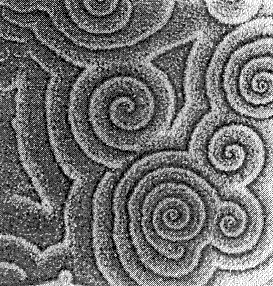
\includegraphics[height=1.8in]{images/spiralWaves1.png}\quad 
%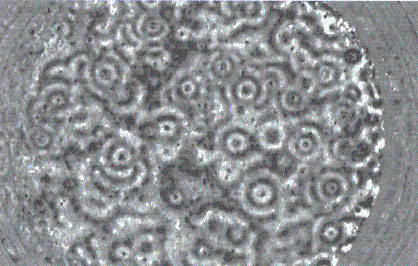
\includegraphics[height=1.8in]{images/spiralWaves2.png}
%\caption{\label{spiralmould}Spiral patterns caused by spiral wave signalling in the slime mould \emph{Dictyostelium discoideum}.}
%\end{center}
%\end{figure}
%\begin{nem}
%\textbf{Spiral waves}\quad
%You can use Hopf bifurcation analysis to locate the formation of \emph{spiral waves} in spatial variants of reaction--diffusion equations. Many systems exhibit spiral shape waves of high intensity with the kind of shape seen in \cref{spiralmould}. Such patterns can be in chemical systems, such as the Belousov--Zhabotinsky reaction; in electrochemical waves in the brain caused by lesions in the tissue; and also mould growth due to spiral signalling patterns: this is what is shown in \cref{spiralmould}.
%
%Spiral waves are the spatial equivalent of fixed amplitude oscillations and the transition of a system through a Hopf bifurcation leads to the formation of spiral waves. This is crucial in cardiac electrical activity where spiral wave type signals are shown to correlate heavily with heart attacks.
%\end{nem}

\paragraph{Spatial behaviour}
The main ingredient missing from all our models so far is \emph{spatial dependence}. For example, if our ladybirds and greenflies are originally in different parts of their ecosystem, they cannot interact. But the interaction constants (the ones proportional to $xy$) have no dependence on the position of the species; the model just assumes the species interact at a given frequency regardless. Our next aim must be to model the movement in space of the populations $x$ and $y$. With this in mind, we turn to the notion of diffusion.

\begin{extra-reading}
\begin{itemize}
	\item The spruce budworm is covered in \textsc{Murray}, vol.~I, chap.~1.2.
	\item Enzyme kinetics are covered in \textsc{Murray}, vol.~I, chap.~6.
%	\item Oscillatory switching is covered in \textsc{Murray}, vol.~I, chap.~7.4.
\end{itemize}
\end{extra-reading}

% ---------------------------------------
% Chapter 6 
% ---------------------------------------

\chapter{Diffusion of populations}
\label{chap:diffusion}

Thus far, we’ve used ODEs to generate mathematical models of population dynamics, biochemical reactions, and epidemiological phenomena (in the problems classes). In modelling these biological systems in this way, we have implicitly assumed that the phenomena that can occur can be described by functions of time that evolve deterministically. It’s not very hard to envision situations, including those we’ve already discussed, that may also have a spatial dependence. For example, one can easily imagine a population of bacteria or another kind of microorganism that may initially be localised in space, but owing to motility, it may spread over time. As a result, we would not only observe growth in the population size due to cell division, but also in the region of space which the population occupies.

From this point on, we’ll discuss how ODE models can be augmented to become partial differential equations (PDEs) that allow for both temporal and spatial evolution. In particular, we’ll be focusing on a class of PDEs known as \emph{reaction--diffusion equations} where the motion of the species from one location to another is modelled by diffusion. We’ll examine cases where these equations permit travelling wave solutions (this term) as well as stationary patterns (next term), and discuss how these arise in biological models.

Modelling the behaviour of individual members of a species of a population is a significantly difficult task. How do we represent the motivation of each individual to move? The answer is `lots of intensive computational power', but even this is limited. This is what drives us to concentrate on the bulk statistical behaviour of a large population. 

Random movement is one of the simplest kinds of motion, and it is very common in nature. Briefly, the history of diffusion (and mathematical models of it) goes as follows. In 1822, Jean-Baptiste Joseph Fourier published the first example of what we know as the \emph{heat equation}, as he was interested in describing how heat flows through different materials with different thermal conductivities (think of metal vs wood). Fourier derived this equation by an argument regarding the conservation of heat. We will see an analogue of this derivation using conservation of mass in \cref{sec:continuum-random} below. He also developed a method to find solutions to this equation given an initial heat distribution using sines and cosines, which we will do in \cref{sec:sep-variables}.

Unrelated to this, in 1827 the botanist Robert Brown was looking through a microscope at pollen, and noticed that the particles of pollen seemed to \href{https://www.youtube.com/watch?v=R5t-oA796to}{jiggle around randomly}. For many years these random movements were interesting, but difficult to study or understand. Finally, in 1905 Albert Einstein published a paper connecting this so-called `Brownian motion' to the heat equation, providing a concrete connection between microscopic random movement and macroscopic diffusion\footnote{This was also the year that Einstein proposed special relativity and a solution to the ultraviolet catastrophe -- he was a busy guy in 1905!}. We will see a version of this connection below in terms of random movement, but the key idea is that the diffusion equation (aka the heat equation) is intimately tied to the small-scale random movement of whatever is being modelled -- either chemical species in water, \href{https://www.youtube.com/watch?v=oYsEid5YES4}{cells} or animals moving around randomly in an ecosystem, or even human migration in a new territory. Of course animals, people, and even molecules have other modes of transportation -- advection in a fluid flow, or directed movement towards where we might want to be for instance -- but diffusion is one of the simplest kinds of motion that can be found in nature, and it plays a crucial role in many kinds of biological systems.

\begin{figure}
\centering
\begin{subfigure}[t]{0.26\textwidth}
	\centering
	%\includegraphics[width=1.9cm]{diff0p5n5.pdf}
	%% Creator: Matplotlib, PGF backend
%%
%% To include the figure in your LaTeX document, write
%%   \input{<filename>.pgf}
%%
%% Make sure the required packages are loaded in your preamble
%%   \usepackage{pgf}
%%
%% Figures using additional raster images can only be included by \input if
%% they are in the same directory as the main LaTeX file. For loading figures
%% from other directories you can use the `import` package
%%   \usepackage{import}
%% and then include the figures with
%%   \import{<path to file>}{<filename>.pgf}
%%
%% Matplotlib used the following preamble
%%   \usepackage{fontspec}
%%   \setmainfont{DejaVuSerif.ttf}[Path=/Library/Python/3.7/site-packages/matplotlib/mpl-data/fonts/ttf/]
%%   \setsansfont{DejaVuSans.ttf}[Path=/Library/Python/3.7/site-packages/matplotlib/mpl-data/fonts/ttf/]
%%   \setmonofont{DejaVuSansMono.ttf}[Path=/Library/Python/3.7/site-packages/matplotlib/mpl-data/fonts/ttf/]
%%
\begingroup%
\makeatletter%
\begin{pgfpicture}%
\pgfpathrectangle{\pgfpointorigin}{\pgfqpoint{1.010000in}{3.000000in}}%
\pgfusepath{use as bounding box, clip}%
\begin{pgfscope}%
\pgfsetbuttcap%
\pgfsetmiterjoin%
\definecolor{currentfill}{rgb}{1.000000,1.000000,1.000000}%
\pgfsetfillcolor{currentfill}%
\pgfsetlinewidth{0.000000pt}%
\definecolor{currentstroke}{rgb}{1.000000,1.000000,1.000000}%
\pgfsetstrokecolor{currentstroke}%
\pgfsetdash{}{0pt}%
\pgfpathmoveto{\pgfqpoint{0.000000in}{0.000000in}}%
\pgfpathlineto{\pgfqpoint{1.010000in}{0.000000in}}%
\pgfpathlineto{\pgfqpoint{1.010000in}{3.000000in}}%
\pgfpathlineto{\pgfqpoint{0.000000in}{3.000000in}}%
\pgfpathclose%
\pgfusepath{fill}%
\end{pgfscope}%
\begin{pgfscope}%
\pgfsetbuttcap%
\pgfsetmiterjoin%
\definecolor{currentfill}{rgb}{1.000000,1.000000,1.000000}%
\pgfsetfillcolor{currentfill}%
\pgfsetlinewidth{0.000000pt}%
\definecolor{currentstroke}{rgb}{0.000000,0.000000,0.000000}%
\pgfsetstrokecolor{currentstroke}%
\pgfsetstrokeopacity{0.000000}%
\pgfsetdash{}{0pt}%
\pgfpathmoveto{\pgfqpoint{0.135329in}{0.278150in}}%
\pgfpathlineto{\pgfqpoint{0.874671in}{0.278150in}}%
\pgfpathlineto{\pgfqpoint{0.874671in}{2.966667in}}%
\pgfpathlineto{\pgfqpoint{0.135329in}{2.966667in}}%
\pgfpathclose%
\pgfusepath{fill}%
\end{pgfscope}%
\begin{pgfscope}%
\pgfpathrectangle{\pgfqpoint{0.135329in}{0.278150in}}{\pgfqpoint{0.739342in}{2.688517in}}%
\pgfusepath{clip}%
\pgfsetrectcap%
\pgfsetroundjoin%
\pgfsetlinewidth{1.505625pt}%
\definecolor{currentstroke}{rgb}{0.121569,0.466667,0.705882}%
\pgfsetstrokecolor{currentstroke}%
\pgfsetstrokeopacity{0.600000}%
\pgfsetdash{}{0pt}%
\pgfpathmoveto{\pgfqpoint{0.417623in}{0.278150in}}%
\pgfpathlineto{\pgfqpoint{0.442064in}{0.302591in}}%
\pgfpathlineto{\pgfqpoint{0.417623in}{0.327032in}}%
\pgfpathlineto{\pgfqpoint{0.442064in}{0.351473in}}%
\pgfpathlineto{\pgfqpoint{0.417623in}{0.375914in}}%
\pgfpathlineto{\pgfqpoint{0.393182in}{0.400355in}}%
\pgfpathlineto{\pgfqpoint{0.417623in}{0.424796in}}%
\pgfpathlineto{\pgfqpoint{0.442064in}{0.449237in}}%
\pgfpathlineto{\pgfqpoint{0.417623in}{0.473678in}}%
\pgfpathlineto{\pgfqpoint{0.442064in}{0.498119in}}%
\pgfpathlineto{\pgfqpoint{0.417623in}{0.522560in}}%
\pgfpathlineto{\pgfqpoint{0.393182in}{0.547001in}}%
\pgfpathlineto{\pgfqpoint{0.368741in}{0.571442in}}%
\pgfpathlineto{\pgfqpoint{0.393182in}{0.595883in}}%
\pgfpathlineto{\pgfqpoint{0.368741in}{0.620325in}}%
\pgfpathlineto{\pgfqpoint{0.344300in}{0.644766in}}%
\pgfpathlineto{\pgfqpoint{0.368741in}{0.669207in}}%
\pgfpathlineto{\pgfqpoint{0.393182in}{0.693648in}}%
\pgfpathlineto{\pgfqpoint{0.368741in}{0.718089in}}%
\pgfpathlineto{\pgfqpoint{0.344300in}{0.742530in}}%
\pgfpathlineto{\pgfqpoint{0.319859in}{0.766971in}}%
\pgfpathlineto{\pgfqpoint{0.344300in}{0.791412in}}%
\pgfpathlineto{\pgfqpoint{0.319859in}{0.815853in}}%
\pgfpathlineto{\pgfqpoint{0.344300in}{0.840294in}}%
\pgfpathlineto{\pgfqpoint{0.319859in}{0.864735in}}%
\pgfpathlineto{\pgfqpoint{0.295418in}{0.889176in}}%
\pgfpathlineto{\pgfqpoint{0.270977in}{0.913617in}}%
\pgfpathlineto{\pgfqpoint{0.295418in}{0.938058in}}%
\pgfpathlineto{\pgfqpoint{0.319859in}{0.962499in}}%
\pgfpathlineto{\pgfqpoint{0.295418in}{0.986941in}}%
\pgfpathlineto{\pgfqpoint{0.270977in}{1.011382in}}%
\pgfpathlineto{\pgfqpoint{0.246536in}{1.035823in}}%
\pgfpathlineto{\pgfqpoint{0.270977in}{1.060264in}}%
\pgfpathlineto{\pgfqpoint{0.246536in}{1.084705in}}%
\pgfpathlineto{\pgfqpoint{0.270977in}{1.109146in}}%
\pgfpathlineto{\pgfqpoint{0.246536in}{1.133587in}}%
\pgfpathlineto{\pgfqpoint{0.270977in}{1.158028in}}%
\pgfpathlineto{\pgfqpoint{0.246536in}{1.182469in}}%
\pgfpathlineto{\pgfqpoint{0.222095in}{1.206910in}}%
\pgfpathlineto{\pgfqpoint{0.246536in}{1.231351in}}%
\pgfpathlineto{\pgfqpoint{0.270977in}{1.255792in}}%
\pgfpathlineto{\pgfqpoint{0.246536in}{1.280233in}}%
\pgfpathlineto{\pgfqpoint{0.270977in}{1.304674in}}%
\pgfpathlineto{\pgfqpoint{0.295418in}{1.329115in}}%
\pgfpathlineto{\pgfqpoint{0.319859in}{1.353556in}}%
\pgfpathlineto{\pgfqpoint{0.295418in}{1.377998in}}%
\pgfpathlineto{\pgfqpoint{0.270977in}{1.402439in}}%
\pgfpathlineto{\pgfqpoint{0.295418in}{1.426880in}}%
\pgfpathlineto{\pgfqpoint{0.319859in}{1.451321in}}%
\pgfpathlineto{\pgfqpoint{0.344300in}{1.475762in}}%
\pgfpathlineto{\pgfqpoint{0.368741in}{1.500203in}}%
\pgfpathlineto{\pgfqpoint{0.393182in}{1.524644in}}%
\pgfpathlineto{\pgfqpoint{0.368741in}{1.549085in}}%
\pgfpathlineto{\pgfqpoint{0.344300in}{1.573526in}}%
\pgfpathlineto{\pgfqpoint{0.319859in}{1.597967in}}%
\pgfpathlineto{\pgfqpoint{0.344300in}{1.622408in}}%
\pgfpathlineto{\pgfqpoint{0.368741in}{1.646849in}}%
\pgfpathlineto{\pgfqpoint{0.344300in}{1.671290in}}%
\pgfpathlineto{\pgfqpoint{0.368741in}{1.695731in}}%
\pgfpathlineto{\pgfqpoint{0.344300in}{1.720172in}}%
\pgfpathlineto{\pgfqpoint{0.368741in}{1.744613in}}%
\pgfpathlineto{\pgfqpoint{0.344300in}{1.769055in}}%
\pgfpathlineto{\pgfqpoint{0.319859in}{1.793496in}}%
\pgfpathlineto{\pgfqpoint{0.344300in}{1.817937in}}%
\pgfpathlineto{\pgfqpoint{0.368741in}{1.842378in}}%
\pgfpathlineto{\pgfqpoint{0.344300in}{1.866819in}}%
\pgfpathlineto{\pgfqpoint{0.368741in}{1.891260in}}%
\pgfpathlineto{\pgfqpoint{0.393182in}{1.915701in}}%
\pgfpathlineto{\pgfqpoint{0.417623in}{1.940142in}}%
\pgfpathlineto{\pgfqpoint{0.393182in}{1.964583in}}%
\pgfpathlineto{\pgfqpoint{0.368741in}{1.989024in}}%
\pgfpathlineto{\pgfqpoint{0.393182in}{2.013465in}}%
\pgfpathlineto{\pgfqpoint{0.368741in}{2.037906in}}%
\pgfpathlineto{\pgfqpoint{0.344300in}{2.062347in}}%
\pgfpathlineto{\pgfqpoint{0.319859in}{2.086788in}}%
\pgfpathlineto{\pgfqpoint{0.344300in}{2.111229in}}%
\pgfpathlineto{\pgfqpoint{0.319859in}{2.135671in}}%
\pgfpathlineto{\pgfqpoint{0.295418in}{2.160112in}}%
\pgfpathlineto{\pgfqpoint{0.270977in}{2.184553in}}%
\pgfpathlineto{\pgfqpoint{0.295418in}{2.208994in}}%
\pgfpathlineto{\pgfqpoint{0.319859in}{2.233435in}}%
\pgfpathlineto{\pgfqpoint{0.344300in}{2.257876in}}%
\pgfpathlineto{\pgfqpoint{0.319859in}{2.282317in}}%
\pgfpathlineto{\pgfqpoint{0.344300in}{2.306758in}}%
\pgfpathlineto{\pgfqpoint{0.319859in}{2.331199in}}%
\pgfpathlineto{\pgfqpoint{0.344300in}{2.355640in}}%
\pgfpathlineto{\pgfqpoint{0.319859in}{2.380081in}}%
\pgfpathlineto{\pgfqpoint{0.295418in}{2.404522in}}%
\pgfpathlineto{\pgfqpoint{0.319859in}{2.428963in}}%
\pgfpathlineto{\pgfqpoint{0.344300in}{2.453404in}}%
\pgfpathlineto{\pgfqpoint{0.368741in}{2.477845in}}%
\pgfpathlineto{\pgfqpoint{0.393182in}{2.502286in}}%
\pgfpathlineto{\pgfqpoint{0.417623in}{2.526728in}}%
\pgfpathlineto{\pgfqpoint{0.393182in}{2.551169in}}%
\pgfpathlineto{\pgfqpoint{0.368741in}{2.575610in}}%
\pgfpathlineto{\pgfqpoint{0.393182in}{2.600051in}}%
\pgfpathlineto{\pgfqpoint{0.368741in}{2.624492in}}%
\pgfpathlineto{\pgfqpoint{0.344300in}{2.648933in}}%
\pgfpathlineto{\pgfqpoint{0.368741in}{2.673374in}}%
\pgfpathlineto{\pgfqpoint{0.344300in}{2.697815in}}%
\pgfusepath{stroke}%
\end{pgfscope}%
\begin{pgfscope}%
\pgfpathrectangle{\pgfqpoint{0.135329in}{0.278150in}}{\pgfqpoint{0.739342in}{2.688517in}}%
\pgfusepath{clip}%
\pgfsetrectcap%
\pgfsetroundjoin%
\pgfsetlinewidth{1.505625pt}%
\definecolor{currentstroke}{rgb}{0.121569,0.466667,0.705882}%
\pgfsetstrokecolor{currentstroke}%
\pgfsetstrokeopacity{0.600000}%
\pgfsetdash{}{0pt}%
\pgfpathmoveto{\pgfqpoint{0.417623in}{0.278150in}}%
\pgfpathlineto{\pgfqpoint{0.393182in}{0.302591in}}%
\pgfpathlineto{\pgfqpoint{0.417623in}{0.327032in}}%
\pgfpathlineto{\pgfqpoint{0.442064in}{0.351473in}}%
\pgfpathlineto{\pgfqpoint{0.417623in}{0.375914in}}%
\pgfpathlineto{\pgfqpoint{0.393182in}{0.400355in}}%
\pgfpathlineto{\pgfqpoint{0.417623in}{0.424796in}}%
\pgfpathlineto{\pgfqpoint{0.442064in}{0.449237in}}%
\pgfpathlineto{\pgfqpoint{0.466505in}{0.473678in}}%
\pgfpathlineto{\pgfqpoint{0.442064in}{0.498119in}}%
\pgfpathlineto{\pgfqpoint{0.466505in}{0.522560in}}%
\pgfpathlineto{\pgfqpoint{0.490946in}{0.547001in}}%
\pgfpathlineto{\pgfqpoint{0.515387in}{0.571442in}}%
\pgfpathlineto{\pgfqpoint{0.490946in}{0.595883in}}%
\pgfpathlineto{\pgfqpoint{0.466505in}{0.620325in}}%
\pgfpathlineto{\pgfqpoint{0.442064in}{0.644766in}}%
\pgfpathlineto{\pgfqpoint{0.417623in}{0.669207in}}%
\pgfpathlineto{\pgfqpoint{0.442064in}{0.693648in}}%
\pgfpathlineto{\pgfqpoint{0.417623in}{0.718089in}}%
\pgfpathlineto{\pgfqpoint{0.442064in}{0.742530in}}%
\pgfpathlineto{\pgfqpoint{0.417623in}{0.766971in}}%
\pgfpathlineto{\pgfqpoint{0.393182in}{0.791412in}}%
\pgfpathlineto{\pgfqpoint{0.417623in}{0.815853in}}%
\pgfpathlineto{\pgfqpoint{0.393182in}{0.840294in}}%
\pgfpathlineto{\pgfqpoint{0.368741in}{0.864735in}}%
\pgfpathlineto{\pgfqpoint{0.393182in}{0.889176in}}%
\pgfpathlineto{\pgfqpoint{0.417623in}{0.913617in}}%
\pgfpathlineto{\pgfqpoint{0.393182in}{0.938058in}}%
\pgfpathlineto{\pgfqpoint{0.368741in}{0.962499in}}%
\pgfpathlineto{\pgfqpoint{0.393182in}{0.986941in}}%
\pgfpathlineto{\pgfqpoint{0.368741in}{1.011382in}}%
\pgfpathlineto{\pgfqpoint{0.393182in}{1.035823in}}%
\pgfpathlineto{\pgfqpoint{0.368741in}{1.060264in}}%
\pgfpathlineto{\pgfqpoint{0.393182in}{1.084705in}}%
\pgfpathlineto{\pgfqpoint{0.368741in}{1.109146in}}%
\pgfpathlineto{\pgfqpoint{0.344300in}{1.133587in}}%
\pgfpathlineto{\pgfqpoint{0.319859in}{1.158028in}}%
\pgfpathlineto{\pgfqpoint{0.344300in}{1.182469in}}%
\pgfpathlineto{\pgfqpoint{0.319859in}{1.206910in}}%
\pgfpathlineto{\pgfqpoint{0.344300in}{1.231351in}}%
\pgfpathlineto{\pgfqpoint{0.368741in}{1.255792in}}%
\pgfpathlineto{\pgfqpoint{0.393182in}{1.280233in}}%
\pgfpathlineto{\pgfqpoint{0.417623in}{1.304674in}}%
\pgfpathlineto{\pgfqpoint{0.393182in}{1.329115in}}%
\pgfpathlineto{\pgfqpoint{0.368741in}{1.353556in}}%
\pgfpathlineto{\pgfqpoint{0.344300in}{1.377998in}}%
\pgfpathlineto{\pgfqpoint{0.368741in}{1.402439in}}%
\pgfpathlineto{\pgfqpoint{0.344300in}{1.426880in}}%
\pgfpathlineto{\pgfqpoint{0.368741in}{1.451321in}}%
\pgfpathlineto{\pgfqpoint{0.344300in}{1.475762in}}%
\pgfpathlineto{\pgfqpoint{0.319859in}{1.500203in}}%
\pgfpathlineto{\pgfqpoint{0.344300in}{1.524644in}}%
\pgfpathlineto{\pgfqpoint{0.368741in}{1.549085in}}%
\pgfpathlineto{\pgfqpoint{0.393182in}{1.573526in}}%
\pgfpathlineto{\pgfqpoint{0.417623in}{1.597967in}}%
\pgfpathlineto{\pgfqpoint{0.393182in}{1.622408in}}%
\pgfpathlineto{\pgfqpoint{0.417623in}{1.646849in}}%
\pgfpathlineto{\pgfqpoint{0.442064in}{1.671290in}}%
\pgfpathlineto{\pgfqpoint{0.417623in}{1.695731in}}%
\pgfpathlineto{\pgfqpoint{0.442064in}{1.720172in}}%
\pgfpathlineto{\pgfqpoint{0.466505in}{1.744613in}}%
\pgfpathlineto{\pgfqpoint{0.490946in}{1.769055in}}%
\pgfpathlineto{\pgfqpoint{0.515387in}{1.793496in}}%
\pgfpathlineto{\pgfqpoint{0.490946in}{1.817937in}}%
\pgfpathlineto{\pgfqpoint{0.515387in}{1.842378in}}%
\pgfpathlineto{\pgfqpoint{0.490946in}{1.866819in}}%
\pgfpathlineto{\pgfqpoint{0.466505in}{1.891260in}}%
\pgfpathlineto{\pgfqpoint{0.490946in}{1.915701in}}%
\pgfpathlineto{\pgfqpoint{0.466505in}{1.940142in}}%
\pgfpathlineto{\pgfqpoint{0.490946in}{1.964583in}}%
\pgfpathlineto{\pgfqpoint{0.515387in}{1.989024in}}%
\pgfpathlineto{\pgfqpoint{0.539829in}{2.013465in}}%
\pgfpathlineto{\pgfqpoint{0.564270in}{2.037906in}}%
\pgfpathlineto{\pgfqpoint{0.539829in}{2.062347in}}%
\pgfpathlineto{\pgfqpoint{0.515387in}{2.086788in}}%
\pgfpathlineto{\pgfqpoint{0.539829in}{2.111229in}}%
\pgfpathlineto{\pgfqpoint{0.564270in}{2.135671in}}%
\pgfpathlineto{\pgfqpoint{0.588711in}{2.160112in}}%
\pgfpathlineto{\pgfqpoint{0.564270in}{2.184553in}}%
\pgfpathlineto{\pgfqpoint{0.539829in}{2.208994in}}%
\pgfpathlineto{\pgfqpoint{0.515387in}{2.233435in}}%
\pgfpathlineto{\pgfqpoint{0.539829in}{2.257876in}}%
\pgfpathlineto{\pgfqpoint{0.564270in}{2.282317in}}%
\pgfpathlineto{\pgfqpoint{0.539829in}{2.306758in}}%
\pgfpathlineto{\pgfqpoint{0.515387in}{2.331199in}}%
\pgfpathlineto{\pgfqpoint{0.490946in}{2.355640in}}%
\pgfpathlineto{\pgfqpoint{0.515387in}{2.380081in}}%
\pgfpathlineto{\pgfqpoint{0.490946in}{2.404522in}}%
\pgfpathlineto{\pgfqpoint{0.515387in}{2.428963in}}%
\pgfpathlineto{\pgfqpoint{0.490946in}{2.453404in}}%
\pgfpathlineto{\pgfqpoint{0.515387in}{2.477845in}}%
\pgfpathlineto{\pgfqpoint{0.490946in}{2.502286in}}%
\pgfpathlineto{\pgfqpoint{0.515387in}{2.526728in}}%
\pgfpathlineto{\pgfqpoint{0.539829in}{2.551169in}}%
\pgfpathlineto{\pgfqpoint{0.515387in}{2.575610in}}%
\pgfpathlineto{\pgfqpoint{0.539829in}{2.600051in}}%
\pgfpathlineto{\pgfqpoint{0.564270in}{2.624492in}}%
\pgfpathlineto{\pgfqpoint{0.588711in}{2.648933in}}%
\pgfpathlineto{\pgfqpoint{0.564270in}{2.673374in}}%
\pgfpathlineto{\pgfqpoint{0.588711in}{2.697815in}}%
\pgfusepath{stroke}%
\end{pgfscope}%
\begin{pgfscope}%
\pgfpathrectangle{\pgfqpoint{0.135329in}{0.278150in}}{\pgfqpoint{0.739342in}{2.688517in}}%
\pgfusepath{clip}%
\pgfsetrectcap%
\pgfsetroundjoin%
\pgfsetlinewidth{1.505625pt}%
\definecolor{currentstroke}{rgb}{0.121569,0.466667,0.705882}%
\pgfsetstrokecolor{currentstroke}%
\pgfsetstrokeopacity{0.600000}%
\pgfsetdash{}{0pt}%
\pgfpathmoveto{\pgfqpoint{0.417623in}{0.278150in}}%
\pgfpathlineto{\pgfqpoint{0.442064in}{0.302591in}}%
\pgfpathlineto{\pgfqpoint{0.466505in}{0.327032in}}%
\pgfpathlineto{\pgfqpoint{0.442064in}{0.351473in}}%
\pgfpathlineto{\pgfqpoint{0.417623in}{0.375914in}}%
\pgfpathlineto{\pgfqpoint{0.393182in}{0.400355in}}%
\pgfpathlineto{\pgfqpoint{0.417623in}{0.424796in}}%
\pgfpathlineto{\pgfqpoint{0.442064in}{0.449237in}}%
\pgfpathlineto{\pgfqpoint{0.417623in}{0.473678in}}%
\pgfpathlineto{\pgfqpoint{0.442064in}{0.498119in}}%
\pgfpathlineto{\pgfqpoint{0.417623in}{0.522560in}}%
\pgfpathlineto{\pgfqpoint{0.393182in}{0.547001in}}%
\pgfpathlineto{\pgfqpoint{0.417623in}{0.571442in}}%
\pgfpathlineto{\pgfqpoint{0.442064in}{0.595883in}}%
\pgfpathlineto{\pgfqpoint{0.466505in}{0.620325in}}%
\pgfpathlineto{\pgfqpoint{0.490946in}{0.644766in}}%
\pgfpathlineto{\pgfqpoint{0.466505in}{0.669207in}}%
\pgfpathlineto{\pgfqpoint{0.442064in}{0.693648in}}%
\pgfpathlineto{\pgfqpoint{0.417623in}{0.718089in}}%
\pgfpathlineto{\pgfqpoint{0.442064in}{0.742530in}}%
\pgfpathlineto{\pgfqpoint{0.466505in}{0.766971in}}%
\pgfpathlineto{\pgfqpoint{0.442064in}{0.791412in}}%
\pgfpathlineto{\pgfqpoint{0.466505in}{0.815853in}}%
\pgfpathlineto{\pgfqpoint{0.490946in}{0.840294in}}%
\pgfpathlineto{\pgfqpoint{0.515387in}{0.864735in}}%
\pgfpathlineto{\pgfqpoint{0.539829in}{0.889176in}}%
\pgfpathlineto{\pgfqpoint{0.515387in}{0.913617in}}%
\pgfpathlineto{\pgfqpoint{0.490946in}{0.938058in}}%
\pgfpathlineto{\pgfqpoint{0.515387in}{0.962499in}}%
\pgfpathlineto{\pgfqpoint{0.539829in}{0.986941in}}%
\pgfpathlineto{\pgfqpoint{0.564270in}{1.011382in}}%
\pgfpathlineto{\pgfqpoint{0.539829in}{1.035823in}}%
\pgfpathlineto{\pgfqpoint{0.515387in}{1.060264in}}%
\pgfpathlineto{\pgfqpoint{0.490946in}{1.084705in}}%
\pgfpathlineto{\pgfqpoint{0.466505in}{1.109146in}}%
\pgfpathlineto{\pgfqpoint{0.490946in}{1.133587in}}%
\pgfpathlineto{\pgfqpoint{0.515387in}{1.158028in}}%
\pgfpathlineto{\pgfqpoint{0.490946in}{1.182469in}}%
\pgfpathlineto{\pgfqpoint{0.466505in}{1.206910in}}%
\pgfpathlineto{\pgfqpoint{0.442064in}{1.231351in}}%
\pgfpathlineto{\pgfqpoint{0.417623in}{1.255792in}}%
\pgfpathlineto{\pgfqpoint{0.393182in}{1.280233in}}%
\pgfpathlineto{\pgfqpoint{0.368741in}{1.304674in}}%
\pgfpathlineto{\pgfqpoint{0.344300in}{1.329115in}}%
\pgfpathlineto{\pgfqpoint{0.368741in}{1.353556in}}%
\pgfpathlineto{\pgfqpoint{0.344300in}{1.377998in}}%
\pgfpathlineto{\pgfqpoint{0.319859in}{1.402439in}}%
\pgfpathlineto{\pgfqpoint{0.344300in}{1.426880in}}%
\pgfpathlineto{\pgfqpoint{0.319859in}{1.451321in}}%
\pgfpathlineto{\pgfqpoint{0.295418in}{1.475762in}}%
\pgfpathlineto{\pgfqpoint{0.270977in}{1.500203in}}%
\pgfpathlineto{\pgfqpoint{0.246536in}{1.524644in}}%
\pgfpathlineto{\pgfqpoint{0.270977in}{1.549085in}}%
\pgfpathlineto{\pgfqpoint{0.295418in}{1.573526in}}%
\pgfpathlineto{\pgfqpoint{0.270977in}{1.597967in}}%
\pgfpathlineto{\pgfqpoint{0.295418in}{1.622408in}}%
\pgfpathlineto{\pgfqpoint{0.319859in}{1.646849in}}%
\pgfpathlineto{\pgfqpoint{0.344300in}{1.671290in}}%
\pgfpathlineto{\pgfqpoint{0.319859in}{1.695731in}}%
\pgfpathlineto{\pgfqpoint{0.295418in}{1.720172in}}%
\pgfpathlineto{\pgfqpoint{0.270977in}{1.744613in}}%
\pgfpathlineto{\pgfqpoint{0.295418in}{1.769055in}}%
\pgfpathlineto{\pgfqpoint{0.270977in}{1.793496in}}%
\pgfpathlineto{\pgfqpoint{0.295418in}{1.817937in}}%
\pgfpathlineto{\pgfqpoint{0.270977in}{1.842378in}}%
\pgfpathlineto{\pgfqpoint{0.246536in}{1.866819in}}%
\pgfpathlineto{\pgfqpoint{0.222095in}{1.891260in}}%
\pgfpathlineto{\pgfqpoint{0.197654in}{1.915701in}}%
\pgfpathlineto{\pgfqpoint{0.222095in}{1.940142in}}%
\pgfpathlineto{\pgfqpoint{0.197654in}{1.964583in}}%
\pgfpathlineto{\pgfqpoint{0.173213in}{1.989024in}}%
\pgfpathlineto{\pgfqpoint{0.148771in}{2.013465in}}%
\pgfpathlineto{\pgfqpoint{0.173213in}{2.037906in}}%
\pgfpathlineto{\pgfqpoint{0.197654in}{2.062347in}}%
\pgfpathlineto{\pgfqpoint{0.222095in}{2.086788in}}%
\pgfpathlineto{\pgfqpoint{0.246536in}{2.111229in}}%
\pgfpathlineto{\pgfqpoint{0.270977in}{2.135671in}}%
\pgfpathlineto{\pgfqpoint{0.246536in}{2.160112in}}%
\pgfpathlineto{\pgfqpoint{0.270977in}{2.184553in}}%
\pgfpathlineto{\pgfqpoint{0.295418in}{2.208994in}}%
\pgfpathlineto{\pgfqpoint{0.319859in}{2.233435in}}%
\pgfpathlineto{\pgfqpoint{0.344300in}{2.257876in}}%
\pgfpathlineto{\pgfqpoint{0.319859in}{2.282317in}}%
\pgfpathlineto{\pgfqpoint{0.344300in}{2.306758in}}%
\pgfpathlineto{\pgfqpoint{0.319859in}{2.331199in}}%
\pgfpathlineto{\pgfqpoint{0.295418in}{2.355640in}}%
\pgfpathlineto{\pgfqpoint{0.270977in}{2.380081in}}%
\pgfpathlineto{\pgfqpoint{0.246536in}{2.404522in}}%
\pgfpathlineto{\pgfqpoint{0.222095in}{2.428963in}}%
\pgfpathlineto{\pgfqpoint{0.246536in}{2.453404in}}%
\pgfpathlineto{\pgfqpoint{0.222095in}{2.477845in}}%
\pgfpathlineto{\pgfqpoint{0.246536in}{2.502286in}}%
\pgfpathlineto{\pgfqpoint{0.270977in}{2.526728in}}%
\pgfpathlineto{\pgfqpoint{0.295418in}{2.551169in}}%
\pgfpathlineto{\pgfqpoint{0.319859in}{2.575610in}}%
\pgfpathlineto{\pgfqpoint{0.295418in}{2.600051in}}%
\pgfpathlineto{\pgfqpoint{0.319859in}{2.624492in}}%
\pgfpathlineto{\pgfqpoint{0.295418in}{2.648933in}}%
\pgfpathlineto{\pgfqpoint{0.270977in}{2.673374in}}%
\pgfpathlineto{\pgfqpoint{0.246536in}{2.697815in}}%
\pgfusepath{stroke}%
\end{pgfscope}%
\begin{pgfscope}%
\pgfpathrectangle{\pgfqpoint{0.135329in}{0.278150in}}{\pgfqpoint{0.739342in}{2.688517in}}%
\pgfusepath{clip}%
\pgfsetrectcap%
\pgfsetroundjoin%
\pgfsetlinewidth{1.505625pt}%
\definecolor{currentstroke}{rgb}{0.121569,0.466667,0.705882}%
\pgfsetstrokecolor{currentstroke}%
\pgfsetstrokeopacity{0.600000}%
\pgfsetdash{}{0pt}%
\pgfpathmoveto{\pgfqpoint{0.417623in}{0.278150in}}%
\pgfpathlineto{\pgfqpoint{0.393182in}{0.302591in}}%
\pgfpathlineto{\pgfqpoint{0.368741in}{0.327032in}}%
\pgfpathlineto{\pgfqpoint{0.344300in}{0.351473in}}%
\pgfpathlineto{\pgfqpoint{0.319859in}{0.375914in}}%
\pgfpathlineto{\pgfqpoint{0.344300in}{0.400355in}}%
\pgfpathlineto{\pgfqpoint{0.319859in}{0.424796in}}%
\pgfpathlineto{\pgfqpoint{0.344300in}{0.449237in}}%
\pgfpathlineto{\pgfqpoint{0.368741in}{0.473678in}}%
\pgfpathlineto{\pgfqpoint{0.393182in}{0.498119in}}%
\pgfpathlineto{\pgfqpoint{0.417623in}{0.522560in}}%
\pgfpathlineto{\pgfqpoint{0.442064in}{0.547001in}}%
\pgfpathlineto{\pgfqpoint{0.417623in}{0.571442in}}%
\pgfpathlineto{\pgfqpoint{0.393182in}{0.595883in}}%
\pgfpathlineto{\pgfqpoint{0.368741in}{0.620325in}}%
\pgfpathlineto{\pgfqpoint{0.393182in}{0.644766in}}%
\pgfpathlineto{\pgfqpoint{0.417623in}{0.669207in}}%
\pgfpathlineto{\pgfqpoint{0.393182in}{0.693648in}}%
\pgfpathlineto{\pgfqpoint{0.417623in}{0.718089in}}%
\pgfpathlineto{\pgfqpoint{0.393182in}{0.742530in}}%
\pgfpathlineto{\pgfqpoint{0.417623in}{0.766971in}}%
\pgfpathlineto{\pgfqpoint{0.442064in}{0.791412in}}%
\pgfpathlineto{\pgfqpoint{0.417623in}{0.815853in}}%
\pgfpathlineto{\pgfqpoint{0.393182in}{0.840294in}}%
\pgfpathlineto{\pgfqpoint{0.368741in}{0.864735in}}%
\pgfpathlineto{\pgfqpoint{0.393182in}{0.889176in}}%
\pgfpathlineto{\pgfqpoint{0.368741in}{0.913617in}}%
\pgfpathlineto{\pgfqpoint{0.344300in}{0.938058in}}%
\pgfpathlineto{\pgfqpoint{0.368741in}{0.962499in}}%
\pgfpathlineto{\pgfqpoint{0.393182in}{0.986941in}}%
\pgfpathlineto{\pgfqpoint{0.368741in}{1.011382in}}%
\pgfpathlineto{\pgfqpoint{0.344300in}{1.035823in}}%
\pgfpathlineto{\pgfqpoint{0.368741in}{1.060264in}}%
\pgfpathlineto{\pgfqpoint{0.393182in}{1.084705in}}%
\pgfpathlineto{\pgfqpoint{0.368741in}{1.109146in}}%
\pgfpathlineto{\pgfqpoint{0.393182in}{1.133587in}}%
\pgfpathlineto{\pgfqpoint{0.368741in}{1.158028in}}%
\pgfpathlineto{\pgfqpoint{0.393182in}{1.182469in}}%
\pgfpathlineto{\pgfqpoint{0.417623in}{1.206910in}}%
\pgfpathlineto{\pgfqpoint{0.393182in}{1.231351in}}%
\pgfpathlineto{\pgfqpoint{0.368741in}{1.255792in}}%
\pgfpathlineto{\pgfqpoint{0.393182in}{1.280233in}}%
\pgfpathlineto{\pgfqpoint{0.368741in}{1.304674in}}%
\pgfpathlineto{\pgfqpoint{0.393182in}{1.329115in}}%
\pgfpathlineto{\pgfqpoint{0.368741in}{1.353556in}}%
\pgfpathlineto{\pgfqpoint{0.393182in}{1.377998in}}%
\pgfpathlineto{\pgfqpoint{0.417623in}{1.402439in}}%
\pgfpathlineto{\pgfqpoint{0.442064in}{1.426880in}}%
\pgfpathlineto{\pgfqpoint{0.417623in}{1.451321in}}%
\pgfpathlineto{\pgfqpoint{0.442064in}{1.475762in}}%
\pgfpathlineto{\pgfqpoint{0.417623in}{1.500203in}}%
\pgfpathlineto{\pgfqpoint{0.393182in}{1.524644in}}%
\pgfpathlineto{\pgfqpoint{0.368741in}{1.549085in}}%
\pgfpathlineto{\pgfqpoint{0.344300in}{1.573526in}}%
\pgfpathlineto{\pgfqpoint{0.368741in}{1.597967in}}%
\pgfpathlineto{\pgfqpoint{0.393182in}{1.622408in}}%
\pgfpathlineto{\pgfqpoint{0.368741in}{1.646849in}}%
\pgfpathlineto{\pgfqpoint{0.393182in}{1.671290in}}%
\pgfpathlineto{\pgfqpoint{0.417623in}{1.695731in}}%
\pgfpathlineto{\pgfqpoint{0.442064in}{1.720172in}}%
\pgfpathlineto{\pgfqpoint{0.417623in}{1.744613in}}%
\pgfpathlineto{\pgfqpoint{0.393182in}{1.769055in}}%
\pgfpathlineto{\pgfqpoint{0.417623in}{1.793496in}}%
\pgfpathlineto{\pgfqpoint{0.393182in}{1.817937in}}%
\pgfpathlineto{\pgfqpoint{0.417623in}{1.842378in}}%
\pgfpathlineto{\pgfqpoint{0.442064in}{1.866819in}}%
\pgfpathlineto{\pgfqpoint{0.417623in}{1.891260in}}%
\pgfpathlineto{\pgfqpoint{0.393182in}{1.915701in}}%
\pgfpathlineto{\pgfqpoint{0.417623in}{1.940142in}}%
\pgfpathlineto{\pgfqpoint{0.393182in}{1.964583in}}%
\pgfpathlineto{\pgfqpoint{0.368741in}{1.989024in}}%
\pgfpathlineto{\pgfqpoint{0.393182in}{2.013465in}}%
\pgfpathlineto{\pgfqpoint{0.417623in}{2.037906in}}%
\pgfpathlineto{\pgfqpoint{0.442064in}{2.062347in}}%
\pgfpathlineto{\pgfqpoint{0.417623in}{2.086788in}}%
\pgfpathlineto{\pgfqpoint{0.442064in}{2.111229in}}%
\pgfpathlineto{\pgfqpoint{0.417623in}{2.135671in}}%
\pgfpathlineto{\pgfqpoint{0.442064in}{2.160112in}}%
\pgfpathlineto{\pgfqpoint{0.466505in}{2.184553in}}%
\pgfpathlineto{\pgfqpoint{0.442064in}{2.208994in}}%
\pgfpathlineto{\pgfqpoint{0.466505in}{2.233435in}}%
\pgfpathlineto{\pgfqpoint{0.442064in}{2.257876in}}%
\pgfpathlineto{\pgfqpoint{0.417623in}{2.282317in}}%
\pgfpathlineto{\pgfqpoint{0.442064in}{2.306758in}}%
\pgfpathlineto{\pgfqpoint{0.466505in}{2.331199in}}%
\pgfpathlineto{\pgfqpoint{0.442064in}{2.355640in}}%
\pgfpathlineto{\pgfqpoint{0.417623in}{2.380081in}}%
\pgfpathlineto{\pgfqpoint{0.393182in}{2.404522in}}%
\pgfpathlineto{\pgfqpoint{0.417623in}{2.428963in}}%
\pgfpathlineto{\pgfqpoint{0.393182in}{2.453404in}}%
\pgfpathlineto{\pgfqpoint{0.417623in}{2.477845in}}%
\pgfpathlineto{\pgfqpoint{0.442064in}{2.502286in}}%
\pgfpathlineto{\pgfqpoint{0.417623in}{2.526728in}}%
\pgfpathlineto{\pgfqpoint{0.442064in}{2.551169in}}%
\pgfpathlineto{\pgfqpoint{0.417623in}{2.575610in}}%
\pgfpathlineto{\pgfqpoint{0.393182in}{2.600051in}}%
\pgfpathlineto{\pgfqpoint{0.417623in}{2.624492in}}%
\pgfpathlineto{\pgfqpoint{0.393182in}{2.648933in}}%
\pgfpathlineto{\pgfqpoint{0.417623in}{2.673374in}}%
\pgfpathlineto{\pgfqpoint{0.393182in}{2.697815in}}%
\pgfusepath{stroke}%
\end{pgfscope}%
\begin{pgfscope}%
\pgfpathrectangle{\pgfqpoint{0.135329in}{0.278150in}}{\pgfqpoint{0.739342in}{2.688517in}}%
\pgfusepath{clip}%
\pgfsetrectcap%
\pgfsetroundjoin%
\pgfsetlinewidth{1.505625pt}%
\definecolor{currentstroke}{rgb}{0.121569,0.466667,0.705882}%
\pgfsetstrokecolor{currentstroke}%
\pgfsetstrokeopacity{0.600000}%
\pgfsetdash{}{0pt}%
\pgfpathmoveto{\pgfqpoint{0.417623in}{0.278150in}}%
\pgfpathlineto{\pgfqpoint{0.442064in}{0.302591in}}%
\pgfpathlineto{\pgfqpoint{0.466505in}{0.327032in}}%
\pgfpathlineto{\pgfqpoint{0.442064in}{0.351473in}}%
\pgfpathlineto{\pgfqpoint{0.466505in}{0.375914in}}%
\pgfpathlineto{\pgfqpoint{0.490946in}{0.400355in}}%
\pgfpathlineto{\pgfqpoint{0.515387in}{0.424796in}}%
\pgfpathlineto{\pgfqpoint{0.539829in}{0.449237in}}%
\pgfpathlineto{\pgfqpoint{0.515387in}{0.473678in}}%
\pgfpathlineto{\pgfqpoint{0.539829in}{0.498119in}}%
\pgfpathlineto{\pgfqpoint{0.564270in}{0.522560in}}%
\pgfpathlineto{\pgfqpoint{0.588711in}{0.547001in}}%
\pgfpathlineto{\pgfqpoint{0.564270in}{0.571442in}}%
\pgfpathlineto{\pgfqpoint{0.539829in}{0.595883in}}%
\pgfpathlineto{\pgfqpoint{0.515387in}{0.620325in}}%
\pgfpathlineto{\pgfqpoint{0.490946in}{0.644766in}}%
\pgfpathlineto{\pgfqpoint{0.515387in}{0.669207in}}%
\pgfpathlineto{\pgfqpoint{0.539829in}{0.693648in}}%
\pgfpathlineto{\pgfqpoint{0.515387in}{0.718089in}}%
\pgfpathlineto{\pgfqpoint{0.539829in}{0.742530in}}%
\pgfpathlineto{\pgfqpoint{0.564270in}{0.766971in}}%
\pgfpathlineto{\pgfqpoint{0.588711in}{0.791412in}}%
\pgfpathlineto{\pgfqpoint{0.613152in}{0.815853in}}%
\pgfpathlineto{\pgfqpoint{0.588711in}{0.840294in}}%
\pgfpathlineto{\pgfqpoint{0.613152in}{0.864735in}}%
\pgfpathlineto{\pgfqpoint{0.588711in}{0.889176in}}%
\pgfpathlineto{\pgfqpoint{0.564270in}{0.913617in}}%
\pgfpathlineto{\pgfqpoint{0.539829in}{0.938058in}}%
\pgfpathlineto{\pgfqpoint{0.515387in}{0.962499in}}%
\pgfpathlineto{\pgfqpoint{0.539829in}{0.986941in}}%
\pgfpathlineto{\pgfqpoint{0.515387in}{1.011382in}}%
\pgfpathlineto{\pgfqpoint{0.539829in}{1.035823in}}%
\pgfpathlineto{\pgfqpoint{0.564270in}{1.060264in}}%
\pgfpathlineto{\pgfqpoint{0.539829in}{1.084705in}}%
\pgfpathlineto{\pgfqpoint{0.515387in}{1.109146in}}%
\pgfpathlineto{\pgfqpoint{0.539829in}{1.133587in}}%
\pgfpathlineto{\pgfqpoint{0.515387in}{1.158028in}}%
\pgfpathlineto{\pgfqpoint{0.490946in}{1.182469in}}%
\pgfpathlineto{\pgfqpoint{0.466505in}{1.206910in}}%
\pgfpathlineto{\pgfqpoint{0.442064in}{1.231351in}}%
\pgfpathlineto{\pgfqpoint{0.417623in}{1.255792in}}%
\pgfpathlineto{\pgfqpoint{0.393182in}{1.280233in}}%
\pgfpathlineto{\pgfqpoint{0.417623in}{1.304674in}}%
\pgfpathlineto{\pgfqpoint{0.393182in}{1.329115in}}%
\pgfpathlineto{\pgfqpoint{0.368741in}{1.353556in}}%
\pgfpathlineto{\pgfqpoint{0.344300in}{1.377998in}}%
\pgfpathlineto{\pgfqpoint{0.368741in}{1.402439in}}%
\pgfpathlineto{\pgfqpoint{0.393182in}{1.426880in}}%
\pgfpathlineto{\pgfqpoint{0.417623in}{1.451321in}}%
\pgfpathlineto{\pgfqpoint{0.393182in}{1.475762in}}%
\pgfpathlineto{\pgfqpoint{0.417623in}{1.500203in}}%
\pgfpathlineto{\pgfqpoint{0.393182in}{1.524644in}}%
\pgfpathlineto{\pgfqpoint{0.417623in}{1.549085in}}%
\pgfpathlineto{\pgfqpoint{0.442064in}{1.573526in}}%
\pgfpathlineto{\pgfqpoint{0.417623in}{1.597967in}}%
\pgfpathlineto{\pgfqpoint{0.442064in}{1.622408in}}%
\pgfpathlineto{\pgfqpoint{0.466505in}{1.646849in}}%
\pgfpathlineto{\pgfqpoint{0.490946in}{1.671290in}}%
\pgfpathlineto{\pgfqpoint{0.466505in}{1.695731in}}%
\pgfpathlineto{\pgfqpoint{0.442064in}{1.720172in}}%
\pgfpathlineto{\pgfqpoint{0.466505in}{1.744613in}}%
\pgfpathlineto{\pgfqpoint{0.442064in}{1.769055in}}%
\pgfpathlineto{\pgfqpoint{0.466505in}{1.793496in}}%
\pgfpathlineto{\pgfqpoint{0.442064in}{1.817937in}}%
\pgfpathlineto{\pgfqpoint{0.417623in}{1.842378in}}%
\pgfpathlineto{\pgfqpoint{0.442064in}{1.866819in}}%
\pgfpathlineto{\pgfqpoint{0.466505in}{1.891260in}}%
\pgfpathlineto{\pgfqpoint{0.442064in}{1.915701in}}%
\pgfpathlineto{\pgfqpoint{0.417623in}{1.940142in}}%
\pgfpathlineto{\pgfqpoint{0.442064in}{1.964583in}}%
\pgfpathlineto{\pgfqpoint{0.466505in}{1.989024in}}%
\pgfpathlineto{\pgfqpoint{0.442064in}{2.013465in}}%
\pgfpathlineto{\pgfqpoint{0.417623in}{2.037906in}}%
\pgfpathlineto{\pgfqpoint{0.442064in}{2.062347in}}%
\pgfpathlineto{\pgfqpoint{0.466505in}{2.086788in}}%
\pgfpathlineto{\pgfqpoint{0.442064in}{2.111229in}}%
\pgfpathlineto{\pgfqpoint{0.417623in}{2.135671in}}%
\pgfpathlineto{\pgfqpoint{0.393182in}{2.160112in}}%
\pgfpathlineto{\pgfqpoint{0.368741in}{2.184553in}}%
\pgfpathlineto{\pgfqpoint{0.393182in}{2.208994in}}%
\pgfpathlineto{\pgfqpoint{0.417623in}{2.233435in}}%
\pgfpathlineto{\pgfqpoint{0.442064in}{2.257876in}}%
\pgfpathlineto{\pgfqpoint{0.417623in}{2.282317in}}%
\pgfpathlineto{\pgfqpoint{0.393182in}{2.306758in}}%
\pgfpathlineto{\pgfqpoint{0.368741in}{2.331199in}}%
\pgfpathlineto{\pgfqpoint{0.393182in}{2.355640in}}%
\pgfpathlineto{\pgfqpoint{0.417623in}{2.380081in}}%
\pgfpathlineto{\pgfqpoint{0.442064in}{2.404522in}}%
\pgfpathlineto{\pgfqpoint{0.417623in}{2.428963in}}%
\pgfpathlineto{\pgfqpoint{0.393182in}{2.453404in}}%
\pgfpathlineto{\pgfqpoint{0.368741in}{2.477845in}}%
\pgfpathlineto{\pgfqpoint{0.393182in}{2.502286in}}%
\pgfpathlineto{\pgfqpoint{0.417623in}{2.526728in}}%
\pgfpathlineto{\pgfqpoint{0.393182in}{2.551169in}}%
\pgfpathlineto{\pgfqpoint{0.417623in}{2.575610in}}%
\pgfpathlineto{\pgfqpoint{0.442064in}{2.600051in}}%
\pgfpathlineto{\pgfqpoint{0.417623in}{2.624492in}}%
\pgfpathlineto{\pgfqpoint{0.442064in}{2.648933in}}%
\pgfpathlineto{\pgfqpoint{0.466505in}{2.673374in}}%
\pgfpathlineto{\pgfqpoint{0.442064in}{2.697815in}}%
\pgfusepath{stroke}%
\end{pgfscope}%
\begin{pgfscope}%
\pgfsetbuttcap%
\pgfsetroundjoin%
\definecolor{currentfill}{rgb}{0.000000,0.000000,0.000000}%
\pgfsetfillcolor{currentfill}%
\pgfsetlinewidth{0.803000pt}%
\definecolor{currentstroke}{rgb}{0.000000,0.000000,0.000000}%
\pgfsetstrokecolor{currentstroke}%
\pgfsetdash{}{0pt}%
\pgfsys@defobject{currentmarker}{\pgfqpoint{0.000000in}{-0.048611in}}{\pgfqpoint{0.000000in}{0.000000in}}{%
\pgfpathmoveto{\pgfqpoint{0.000000in}{0.000000in}}%
\pgfpathlineto{\pgfqpoint{0.000000in}{-0.048611in}}%
\pgfusepath{stroke,fill}%
}%
\begin{pgfscope}%
\pgfsys@transformshift{0.173213in}{0.278150in}%
\pgfsys@useobject{currentmarker}{}%
\end{pgfscope}%
\end{pgfscope}%
\begin{pgfscope}%
\definecolor{textcolor}{rgb}{0.000000,0.000000,0.000000}%
\pgfsetstrokecolor{textcolor}%
\pgfsetfillcolor{textcolor}%
\pgftext[x=0.173213in,y=0.180927in,,top]{\color{textcolor}\rmfamily\fontsize{12.000000}{14.400000}\selectfont \(\displaystyle -10\)}%
\end{pgfscope}%
\begin{pgfscope}%
\pgfsetbuttcap%
\pgfsetroundjoin%
\definecolor{currentfill}{rgb}{0.000000,0.000000,0.000000}%
\pgfsetfillcolor{currentfill}%
\pgfsetlinewidth{0.803000pt}%
\definecolor{currentstroke}{rgb}{0.000000,0.000000,0.000000}%
\pgfsetstrokecolor{currentstroke}%
\pgfsetdash{}{0pt}%
\pgfsys@defobject{currentmarker}{\pgfqpoint{0.000000in}{-0.048611in}}{\pgfqpoint{0.000000in}{0.000000in}}{%
\pgfpathmoveto{\pgfqpoint{0.000000in}{0.000000in}}%
\pgfpathlineto{\pgfqpoint{0.000000in}{-0.048611in}}%
\pgfusepath{stroke,fill}%
}%
\begin{pgfscope}%
\pgfsys@transformshift{0.417623in}{0.278150in}%
\pgfsys@useobject{currentmarker}{}%
\end{pgfscope}%
\end{pgfscope}%
\begin{pgfscope}%
\definecolor{textcolor}{rgb}{0.000000,0.000000,0.000000}%
\pgfsetstrokecolor{textcolor}%
\pgfsetfillcolor{textcolor}%
\pgftext[x=0.417623in,y=0.180927in,,top]{\color{textcolor}\rmfamily\fontsize{12.000000}{14.400000}\selectfont \(\displaystyle 0\)}%
\end{pgfscope}%
\begin{pgfscope}%
\pgfsetbuttcap%
\pgfsetroundjoin%
\definecolor{currentfill}{rgb}{0.000000,0.000000,0.000000}%
\pgfsetfillcolor{currentfill}%
\pgfsetlinewidth{0.803000pt}%
\definecolor{currentstroke}{rgb}{0.000000,0.000000,0.000000}%
\pgfsetstrokecolor{currentstroke}%
\pgfsetdash{}{0pt}%
\pgfsys@defobject{currentmarker}{\pgfqpoint{0.000000in}{-0.048611in}}{\pgfqpoint{0.000000in}{0.000000in}}{%
\pgfpathmoveto{\pgfqpoint{0.000000in}{0.000000in}}%
\pgfpathlineto{\pgfqpoint{0.000000in}{-0.048611in}}%
\pgfusepath{stroke,fill}%
}%
\begin{pgfscope}%
\pgfsys@transformshift{0.662034in}{0.278150in}%
\pgfsys@useobject{currentmarker}{}%
\end{pgfscope}%
\end{pgfscope}%
\begin{pgfscope}%
\definecolor{textcolor}{rgb}{0.000000,0.000000,0.000000}%
\pgfsetstrokecolor{textcolor}%
\pgfsetfillcolor{textcolor}%
\pgftext[x=0.662034in,y=0.180927in,,top]{\color{textcolor}\rmfamily\fontsize{12.000000}{14.400000}\selectfont \(\displaystyle 10\)}%
\end{pgfscope}%
\begin{pgfscope}%
\pgfsetbuttcap%
\pgfsetroundjoin%
\definecolor{currentfill}{rgb}{0.000000,0.000000,0.000000}%
\pgfsetfillcolor{currentfill}%
\pgfsetlinewidth{0.803000pt}%
\definecolor{currentstroke}{rgb}{0.000000,0.000000,0.000000}%
\pgfsetstrokecolor{currentstroke}%
\pgfsetdash{}{0pt}%
\pgfsys@defobject{currentmarker}{\pgfqpoint{-0.048611in}{0.000000in}}{\pgfqpoint{0.000000in}{0.000000in}}{%
\pgfpathmoveto{\pgfqpoint{0.000000in}{0.000000in}}%
\pgfpathlineto{\pgfqpoint{-0.048611in}{0.000000in}}%
\pgfusepath{stroke,fill}%
}%
\begin{pgfscope}%
\pgfsys@transformshift{0.417623in}{0.278150in}%
\pgfsys@useobject{currentmarker}{}%
\end{pgfscope}%
\end{pgfscope}%
\begin{pgfscope}%
\definecolor{textcolor}{rgb}{0.000000,0.000000,0.000000}%
\pgfsetstrokecolor{textcolor}%
\pgfsetfillcolor{textcolor}%
\pgftext[x=0.238805in,y=0.214836in,left,base]{\color{textcolor}\rmfamily\fontsize{12.000000}{14.400000}\selectfont \(\displaystyle 0\)}%
\end{pgfscope}%
\begin{pgfscope}%
\pgfsetbuttcap%
\pgfsetroundjoin%
\definecolor{currentfill}{rgb}{0.000000,0.000000,0.000000}%
\pgfsetfillcolor{currentfill}%
\pgfsetlinewidth{0.803000pt}%
\definecolor{currentstroke}{rgb}{0.000000,0.000000,0.000000}%
\pgfsetstrokecolor{currentstroke}%
\pgfsetdash{}{0pt}%
\pgfsys@defobject{currentmarker}{\pgfqpoint{-0.048611in}{0.000000in}}{\pgfqpoint{0.000000in}{0.000000in}}{%
\pgfpathmoveto{\pgfqpoint{0.000000in}{0.000000in}}%
\pgfpathlineto{\pgfqpoint{-0.048611in}{0.000000in}}%
\pgfusepath{stroke,fill}%
}%
\begin{pgfscope}%
\pgfsys@transformshift{0.417623in}{0.766971in}%
\pgfsys@useobject{currentmarker}{}%
\end{pgfscope}%
\end{pgfscope}%
\begin{pgfscope}%
\definecolor{textcolor}{rgb}{0.000000,0.000000,0.000000}%
\pgfsetstrokecolor{textcolor}%
\pgfsetfillcolor{textcolor}%
\pgftext[x=0.157208in,y=0.703657in,left,base]{\color{textcolor}\rmfamily\fontsize{12.000000}{14.400000}\selectfont \(\displaystyle 20\)}%
\end{pgfscope}%
\begin{pgfscope}%
\pgfsetbuttcap%
\pgfsetroundjoin%
\definecolor{currentfill}{rgb}{0.000000,0.000000,0.000000}%
\pgfsetfillcolor{currentfill}%
\pgfsetlinewidth{0.803000pt}%
\definecolor{currentstroke}{rgb}{0.000000,0.000000,0.000000}%
\pgfsetstrokecolor{currentstroke}%
\pgfsetdash{}{0pt}%
\pgfsys@defobject{currentmarker}{\pgfqpoint{-0.048611in}{0.000000in}}{\pgfqpoint{0.000000in}{0.000000in}}{%
\pgfpathmoveto{\pgfqpoint{0.000000in}{0.000000in}}%
\pgfpathlineto{\pgfqpoint{-0.048611in}{0.000000in}}%
\pgfusepath{stroke,fill}%
}%
\begin{pgfscope}%
\pgfsys@transformshift{0.417623in}{1.255792in}%
\pgfsys@useobject{currentmarker}{}%
\end{pgfscope}%
\end{pgfscope}%
\begin{pgfscope}%
\definecolor{textcolor}{rgb}{0.000000,0.000000,0.000000}%
\pgfsetstrokecolor{textcolor}%
\pgfsetfillcolor{textcolor}%
\pgftext[x=0.157208in,y=1.192478in,left,base]{\color{textcolor}\rmfamily\fontsize{12.000000}{14.400000}\selectfont \(\displaystyle 40\)}%
\end{pgfscope}%
\begin{pgfscope}%
\pgfsetbuttcap%
\pgfsetroundjoin%
\definecolor{currentfill}{rgb}{0.000000,0.000000,0.000000}%
\pgfsetfillcolor{currentfill}%
\pgfsetlinewidth{0.803000pt}%
\definecolor{currentstroke}{rgb}{0.000000,0.000000,0.000000}%
\pgfsetstrokecolor{currentstroke}%
\pgfsetdash{}{0pt}%
\pgfsys@defobject{currentmarker}{\pgfqpoint{-0.048611in}{0.000000in}}{\pgfqpoint{0.000000in}{0.000000in}}{%
\pgfpathmoveto{\pgfqpoint{0.000000in}{0.000000in}}%
\pgfpathlineto{\pgfqpoint{-0.048611in}{0.000000in}}%
\pgfusepath{stroke,fill}%
}%
\begin{pgfscope}%
\pgfsys@transformshift{0.417623in}{1.744613in}%
\pgfsys@useobject{currentmarker}{}%
\end{pgfscope}%
\end{pgfscope}%
\begin{pgfscope}%
\definecolor{textcolor}{rgb}{0.000000,0.000000,0.000000}%
\pgfsetstrokecolor{textcolor}%
\pgfsetfillcolor{textcolor}%
\pgftext[x=0.157208in,y=1.681300in,left,base]{\color{textcolor}\rmfamily\fontsize{12.000000}{14.400000}\selectfont \(\displaystyle 60\)}%
\end{pgfscope}%
\begin{pgfscope}%
\pgfsetbuttcap%
\pgfsetroundjoin%
\definecolor{currentfill}{rgb}{0.000000,0.000000,0.000000}%
\pgfsetfillcolor{currentfill}%
\pgfsetlinewidth{0.803000pt}%
\definecolor{currentstroke}{rgb}{0.000000,0.000000,0.000000}%
\pgfsetstrokecolor{currentstroke}%
\pgfsetdash{}{0pt}%
\pgfsys@defobject{currentmarker}{\pgfqpoint{-0.048611in}{0.000000in}}{\pgfqpoint{0.000000in}{0.000000in}}{%
\pgfpathmoveto{\pgfqpoint{0.000000in}{0.000000in}}%
\pgfpathlineto{\pgfqpoint{-0.048611in}{0.000000in}}%
\pgfusepath{stroke,fill}%
}%
\begin{pgfscope}%
\pgfsys@transformshift{0.417623in}{2.233435in}%
\pgfsys@useobject{currentmarker}{}%
\end{pgfscope}%
\end{pgfscope}%
\begin{pgfscope}%
\definecolor{textcolor}{rgb}{0.000000,0.000000,0.000000}%
\pgfsetstrokecolor{textcolor}%
\pgfsetfillcolor{textcolor}%
\pgftext[x=0.157208in,y=2.170121in,left,base]{\color{textcolor}\rmfamily\fontsize{12.000000}{14.400000}\selectfont \(\displaystyle 80\)}%
\end{pgfscope}%
\begin{pgfscope}%
\pgfsetbuttcap%
\pgfsetroundjoin%
\definecolor{currentfill}{rgb}{0.000000,0.000000,0.000000}%
\pgfsetfillcolor{currentfill}%
\pgfsetlinewidth{0.803000pt}%
\definecolor{currentstroke}{rgb}{0.000000,0.000000,0.000000}%
\pgfsetstrokecolor{currentstroke}%
\pgfsetdash{}{0pt}%
\pgfsys@defobject{currentmarker}{\pgfqpoint{-0.048611in}{0.000000in}}{\pgfqpoint{0.000000in}{0.000000in}}{%
\pgfpathmoveto{\pgfqpoint{0.000000in}{0.000000in}}%
\pgfpathlineto{\pgfqpoint{-0.048611in}{0.000000in}}%
\pgfusepath{stroke,fill}%
}%
\begin{pgfscope}%
\pgfsys@transformshift{0.417623in}{2.722256in}%
\pgfsys@useobject{currentmarker}{}%
\end{pgfscope}%
\end{pgfscope}%
\begin{pgfscope}%
\definecolor{textcolor}{rgb}{0.000000,0.000000,0.000000}%
\pgfsetstrokecolor{textcolor}%
\pgfsetfillcolor{textcolor}%
\pgftext[x=0.075612in,y=2.658942in,left,base]{\color{textcolor}\rmfamily\fontsize{12.000000}{14.400000}\selectfont \(\displaystyle 100\)}%
\end{pgfscope}%
\begin{pgfscope}%
\pgfsetrectcap%
\pgfsetmiterjoin%
\pgfsetlinewidth{0.803000pt}%
\definecolor{currentstroke}{rgb}{0.000000,0.000000,0.000000}%
\pgfsetstrokecolor{currentstroke}%
\pgfsetdash{}{0pt}%
\pgfpathmoveto{\pgfqpoint{0.417623in}{0.278150in}}%
\pgfpathlineto{\pgfqpoint{0.417623in}{2.966667in}}%
\pgfusepath{stroke}%
\end{pgfscope}%
\begin{pgfscope}%
\pgfsetrectcap%
\pgfsetmiterjoin%
\pgfsetlinewidth{0.803000pt}%
\definecolor{currentstroke}{rgb}{0.000000,0.000000,0.000000}%
\pgfsetstrokecolor{currentstroke}%
\pgfsetdash{}{0pt}%
\pgfpathmoveto{\pgfqpoint{0.135329in}{0.278150in}}%
\pgfpathlineto{\pgfqpoint{0.874671in}{0.278150in}}%
\pgfusepath{stroke}%
\end{pgfscope}%
\begin{pgfscope}%
\definecolor{textcolor}{rgb}{0.000000,0.000000,0.000000}%
\pgfsetstrokecolor{textcolor}%
\pgfsetfillcolor{textcolor}%
\pgftext[x=0.874671in,y=0.180927in,right,top]{\color{textcolor}\rmfamily\fontsize{12.000000}{14.400000}\selectfont \(\displaystyle x\)}%
\end{pgfscope}%
\begin{pgfscope}%
\definecolor{textcolor}{rgb}{0.000000,0.000000,0.000000}%
\pgfsetstrokecolor{textcolor}%
\pgfsetfillcolor{textcolor}%
\pgftext[x=0.320401in,y=2.966667in,right,top]{\color{textcolor}\rmfamily\fontsize{12.000000}{14.400000}\selectfont \(\displaystyle t\)}%
\end{pgfscope}%
\end{pgfpicture}%
\makeatother%
\endgroup%

\end{subfigure}
\begin{subfigure}[t]{0.25\textwidth}
	\centering
	%\includegraphics[width=3.1cm]{diff0p6n5.pdf}
	%% Creator: Matplotlib, PGF backend
%%
%% To include the figure in your LaTeX document, write
%%   \input{<filename>.pgf}
%%
%% Make sure the required packages are loaded in your preamble
%%   \usepackage{pgf}
%%
%% Figures using additional raster images can only be included by \input if
%% they are in the same directory as the main LaTeX file. For loading figures
%% from other directories you can use the `import` package
%%   \usepackage{import}
%% and then include the figures with
%%   \import{<path to file>}{<filename>.pgf}
%%
%% Matplotlib used the following preamble
%%   \usepackage{fontspec}
%%   \setmainfont{DejaVuSerif.ttf}[Path=/Library/Python/3.7/site-packages/matplotlib/mpl-data/fonts/ttf/]
%%   \setsansfont{DejaVuSans.ttf}[Path=/Library/Python/3.7/site-packages/matplotlib/mpl-data/fonts/ttf/]
%%   \setmonofont{DejaVuSansMono.ttf}[Path=/Library/Python/3.7/site-packages/matplotlib/mpl-data/fonts/ttf/]
%%
\begingroup%
\makeatletter%
\begin{pgfpicture}%
\pgfpathrectangle{\pgfpointorigin}{\pgfqpoint{1.410000in}{3.000000in}}%
\pgfusepath{use as bounding box, clip}%
\begin{pgfscope}%
\pgfsetbuttcap%
\pgfsetmiterjoin%
\definecolor{currentfill}{rgb}{1.000000,1.000000,1.000000}%
\pgfsetfillcolor{currentfill}%
\pgfsetlinewidth{0.000000pt}%
\definecolor{currentstroke}{rgb}{1.000000,1.000000,1.000000}%
\pgfsetstrokecolor{currentstroke}%
\pgfsetdash{}{0pt}%
\pgfpathmoveto{\pgfqpoint{0.000000in}{0.000000in}}%
\pgfpathlineto{\pgfqpoint{1.410000in}{0.000000in}}%
\pgfpathlineto{\pgfqpoint{1.410000in}{3.000000in}}%
\pgfpathlineto{\pgfqpoint{0.000000in}{3.000000in}}%
\pgfpathclose%
\pgfusepath{fill}%
\end{pgfscope}%
\begin{pgfscope}%
\pgfsetbuttcap%
\pgfsetmiterjoin%
\definecolor{currentfill}{rgb}{1.000000,1.000000,1.000000}%
\pgfsetfillcolor{currentfill}%
\pgfsetlinewidth{0.000000pt}%
\definecolor{currentstroke}{rgb}{0.000000,0.000000,0.000000}%
\pgfsetstrokecolor{currentstroke}%
\pgfsetstrokeopacity{0.000000}%
\pgfsetdash{}{0pt}%
\pgfpathmoveto{\pgfqpoint{0.157212in}{0.278150in}}%
\pgfpathlineto{\pgfqpoint{1.313274in}{0.278150in}}%
\pgfpathlineto{\pgfqpoint{1.313274in}{2.966667in}}%
\pgfpathlineto{\pgfqpoint{0.157212in}{2.966667in}}%
\pgfpathclose%
\pgfusepath{fill}%
\end{pgfscope}%
\begin{pgfscope}%
\pgfpathrectangle{\pgfqpoint{0.157212in}{0.278150in}}{\pgfqpoint{1.156062in}{2.688517in}}%
\pgfusepath{clip}%
\pgfsetrectcap%
\pgfsetroundjoin%
\pgfsetlinewidth{1.505625pt}%
\definecolor{currentstroke}{rgb}{0.121569,0.466667,0.705882}%
\pgfsetstrokecolor{currentstroke}%
\pgfsetstrokeopacity{0.600000}%
\pgfsetdash{}{0pt}%
\pgfpathmoveto{\pgfqpoint{0.380848in}{0.278150in}}%
\pgfpathlineto{\pgfqpoint{0.405289in}{0.302591in}}%
\pgfpathlineto{\pgfqpoint{0.429730in}{0.327032in}}%
\pgfpathlineto{\pgfqpoint{0.454171in}{0.351473in}}%
\pgfpathlineto{\pgfqpoint{0.429730in}{0.375914in}}%
\pgfpathlineto{\pgfqpoint{0.454171in}{0.400355in}}%
\pgfpathlineto{\pgfqpoint{0.429730in}{0.424796in}}%
\pgfpathlineto{\pgfqpoint{0.454171in}{0.449237in}}%
\pgfpathlineto{\pgfqpoint{0.429730in}{0.473678in}}%
\pgfpathlineto{\pgfqpoint{0.405289in}{0.498119in}}%
\pgfpathlineto{\pgfqpoint{0.380848in}{0.522560in}}%
\pgfpathlineto{\pgfqpoint{0.405289in}{0.547001in}}%
\pgfpathlineto{\pgfqpoint{0.380848in}{0.571442in}}%
\pgfpathlineto{\pgfqpoint{0.405289in}{0.595883in}}%
\pgfpathlineto{\pgfqpoint{0.429730in}{0.620325in}}%
\pgfpathlineto{\pgfqpoint{0.454171in}{0.644766in}}%
\pgfpathlineto{\pgfqpoint{0.478612in}{0.669207in}}%
\pgfpathlineto{\pgfqpoint{0.454171in}{0.693648in}}%
\pgfpathlineto{\pgfqpoint{0.478612in}{0.718089in}}%
\pgfpathlineto{\pgfqpoint{0.454171in}{0.742530in}}%
\pgfpathlineto{\pgfqpoint{0.429730in}{0.766971in}}%
\pgfpathlineto{\pgfqpoint{0.454171in}{0.791412in}}%
\pgfpathlineto{\pgfqpoint{0.478612in}{0.815853in}}%
\pgfpathlineto{\pgfqpoint{0.503053in}{0.840294in}}%
\pgfpathlineto{\pgfqpoint{0.527494in}{0.864735in}}%
\pgfpathlineto{\pgfqpoint{0.551935in}{0.889176in}}%
\pgfpathlineto{\pgfqpoint{0.527494in}{0.913617in}}%
\pgfpathlineto{\pgfqpoint{0.551935in}{0.938058in}}%
\pgfpathlineto{\pgfqpoint{0.576376in}{0.962499in}}%
\pgfpathlineto{\pgfqpoint{0.551935in}{0.986941in}}%
\pgfpathlineto{\pgfqpoint{0.576376in}{1.011382in}}%
\pgfpathlineto{\pgfqpoint{0.551935in}{1.035823in}}%
\pgfpathlineto{\pgfqpoint{0.576376in}{1.060264in}}%
\pgfpathlineto{\pgfqpoint{0.600817in}{1.084705in}}%
\pgfpathlineto{\pgfqpoint{0.625258in}{1.109146in}}%
\pgfpathlineto{\pgfqpoint{0.600817in}{1.133587in}}%
\pgfpathlineto{\pgfqpoint{0.625258in}{1.158028in}}%
\pgfpathlineto{\pgfqpoint{0.600817in}{1.182469in}}%
\pgfpathlineto{\pgfqpoint{0.625258in}{1.206910in}}%
\pgfpathlineto{\pgfqpoint{0.649699in}{1.231351in}}%
\pgfpathlineto{\pgfqpoint{0.674140in}{1.255792in}}%
\pgfpathlineto{\pgfqpoint{0.698581in}{1.280233in}}%
\pgfpathlineto{\pgfqpoint{0.674140in}{1.304674in}}%
\pgfpathlineto{\pgfqpoint{0.649699in}{1.329115in}}%
\pgfpathlineto{\pgfqpoint{0.625258in}{1.353556in}}%
\pgfpathlineto{\pgfqpoint{0.649699in}{1.377998in}}%
\pgfpathlineto{\pgfqpoint{0.674140in}{1.402439in}}%
\pgfpathlineto{\pgfqpoint{0.649699in}{1.426880in}}%
\pgfpathlineto{\pgfqpoint{0.674140in}{1.451321in}}%
\pgfpathlineto{\pgfqpoint{0.698581in}{1.475762in}}%
\pgfpathlineto{\pgfqpoint{0.723022in}{1.500203in}}%
\pgfpathlineto{\pgfqpoint{0.698581in}{1.524644in}}%
\pgfpathlineto{\pgfqpoint{0.723022in}{1.549085in}}%
\pgfpathlineto{\pgfqpoint{0.747464in}{1.573526in}}%
\pgfpathlineto{\pgfqpoint{0.723022in}{1.597967in}}%
\pgfpathlineto{\pgfqpoint{0.747464in}{1.622408in}}%
\pgfpathlineto{\pgfqpoint{0.771905in}{1.646849in}}%
\pgfpathlineto{\pgfqpoint{0.796346in}{1.671290in}}%
\pgfpathlineto{\pgfqpoint{0.771905in}{1.695731in}}%
\pgfpathlineto{\pgfqpoint{0.796346in}{1.720172in}}%
\pgfpathlineto{\pgfqpoint{0.820787in}{1.744613in}}%
\pgfpathlineto{\pgfqpoint{0.796346in}{1.769055in}}%
\pgfpathlineto{\pgfqpoint{0.820787in}{1.793496in}}%
\pgfpathlineto{\pgfqpoint{0.845228in}{1.817937in}}%
\pgfpathlineto{\pgfqpoint{0.820787in}{1.842378in}}%
\pgfpathlineto{\pgfqpoint{0.845228in}{1.866819in}}%
\pgfpathlineto{\pgfqpoint{0.869669in}{1.891260in}}%
\pgfpathlineto{\pgfqpoint{0.894110in}{1.915701in}}%
\pgfpathlineto{\pgfqpoint{0.869669in}{1.940142in}}%
\pgfpathlineto{\pgfqpoint{0.894110in}{1.964583in}}%
\pgfpathlineto{\pgfqpoint{0.918551in}{1.989024in}}%
\pgfpathlineto{\pgfqpoint{0.942992in}{2.013465in}}%
\pgfpathlineto{\pgfqpoint{0.918551in}{2.037906in}}%
\pgfpathlineto{\pgfqpoint{0.894110in}{2.062347in}}%
\pgfpathlineto{\pgfqpoint{0.918551in}{2.086788in}}%
\pgfpathlineto{\pgfqpoint{0.894110in}{2.111229in}}%
\pgfpathlineto{\pgfqpoint{0.869669in}{2.135671in}}%
\pgfpathlineto{\pgfqpoint{0.894110in}{2.160112in}}%
\pgfpathlineto{\pgfqpoint{0.918551in}{2.184553in}}%
\pgfpathlineto{\pgfqpoint{0.894110in}{2.208994in}}%
\pgfpathlineto{\pgfqpoint{0.918551in}{2.233435in}}%
\pgfpathlineto{\pgfqpoint{0.894110in}{2.257876in}}%
\pgfpathlineto{\pgfqpoint{0.918551in}{2.282317in}}%
\pgfpathlineto{\pgfqpoint{0.894110in}{2.306758in}}%
\pgfpathlineto{\pgfqpoint{0.869669in}{2.331199in}}%
\pgfpathlineto{\pgfqpoint{0.894110in}{2.355640in}}%
\pgfpathlineto{\pgfqpoint{0.869669in}{2.380081in}}%
\pgfpathlineto{\pgfqpoint{0.894110in}{2.404522in}}%
\pgfpathlineto{\pgfqpoint{0.869669in}{2.428963in}}%
\pgfpathlineto{\pgfqpoint{0.894110in}{2.453404in}}%
\pgfpathlineto{\pgfqpoint{0.918551in}{2.477845in}}%
\pgfpathlineto{\pgfqpoint{0.894110in}{2.502286in}}%
\pgfpathlineto{\pgfqpoint{0.869669in}{2.526728in}}%
\pgfpathlineto{\pgfqpoint{0.894110in}{2.551169in}}%
\pgfpathlineto{\pgfqpoint{0.918551in}{2.575610in}}%
\pgfpathlineto{\pgfqpoint{0.894110in}{2.600051in}}%
\pgfpathlineto{\pgfqpoint{0.918551in}{2.624492in}}%
\pgfpathlineto{\pgfqpoint{0.942992in}{2.648933in}}%
\pgfpathlineto{\pgfqpoint{0.918551in}{2.673374in}}%
\pgfpathlineto{\pgfqpoint{0.894110in}{2.697815in}}%
\pgfusepath{stroke}%
\end{pgfscope}%
\begin{pgfscope}%
\pgfpathrectangle{\pgfqpoint{0.157212in}{0.278150in}}{\pgfqpoint{1.156062in}{2.688517in}}%
\pgfusepath{clip}%
\pgfsetrectcap%
\pgfsetroundjoin%
\pgfsetlinewidth{1.505625pt}%
\definecolor{currentstroke}{rgb}{0.121569,0.466667,0.705882}%
\pgfsetstrokecolor{currentstroke}%
\pgfsetstrokeopacity{0.600000}%
\pgfsetdash{}{0pt}%
\pgfpathmoveto{\pgfqpoint{0.380848in}{0.278150in}}%
\pgfpathlineto{\pgfqpoint{0.356407in}{0.302591in}}%
\pgfpathlineto{\pgfqpoint{0.331965in}{0.327032in}}%
\pgfpathlineto{\pgfqpoint{0.307524in}{0.351473in}}%
\pgfpathlineto{\pgfqpoint{0.331965in}{0.375914in}}%
\pgfpathlineto{\pgfqpoint{0.356407in}{0.400355in}}%
\pgfpathlineto{\pgfqpoint{0.380848in}{0.424796in}}%
\pgfpathlineto{\pgfqpoint{0.356407in}{0.449237in}}%
\pgfpathlineto{\pgfqpoint{0.380848in}{0.473678in}}%
\pgfpathlineto{\pgfqpoint{0.356407in}{0.498119in}}%
\pgfpathlineto{\pgfqpoint{0.331965in}{0.522560in}}%
\pgfpathlineto{\pgfqpoint{0.307524in}{0.547001in}}%
\pgfpathlineto{\pgfqpoint{0.283083in}{0.571442in}}%
\pgfpathlineto{\pgfqpoint{0.307524in}{0.595883in}}%
\pgfpathlineto{\pgfqpoint{0.331965in}{0.620325in}}%
\pgfpathlineto{\pgfqpoint{0.356407in}{0.644766in}}%
\pgfpathlineto{\pgfqpoint{0.380848in}{0.669207in}}%
\pgfpathlineto{\pgfqpoint{0.405289in}{0.693648in}}%
\pgfpathlineto{\pgfqpoint{0.429730in}{0.718089in}}%
\pgfpathlineto{\pgfqpoint{0.405289in}{0.742530in}}%
\pgfpathlineto{\pgfqpoint{0.380848in}{0.766971in}}%
\pgfpathlineto{\pgfqpoint{0.405289in}{0.791412in}}%
\pgfpathlineto{\pgfqpoint{0.380848in}{0.815853in}}%
\pgfpathlineto{\pgfqpoint{0.405289in}{0.840294in}}%
\pgfpathlineto{\pgfqpoint{0.380848in}{0.864735in}}%
\pgfpathlineto{\pgfqpoint{0.356407in}{0.889176in}}%
\pgfpathlineto{\pgfqpoint{0.380848in}{0.913617in}}%
\pgfpathlineto{\pgfqpoint{0.356407in}{0.938058in}}%
\pgfpathlineto{\pgfqpoint{0.380848in}{0.962499in}}%
\pgfpathlineto{\pgfqpoint{0.356407in}{0.986941in}}%
\pgfpathlineto{\pgfqpoint{0.331965in}{1.011382in}}%
\pgfpathlineto{\pgfqpoint{0.307524in}{1.035823in}}%
\pgfpathlineto{\pgfqpoint{0.283083in}{1.060264in}}%
\pgfpathlineto{\pgfqpoint{0.307524in}{1.084705in}}%
\pgfpathlineto{\pgfqpoint{0.331965in}{1.109146in}}%
\pgfpathlineto{\pgfqpoint{0.356407in}{1.133587in}}%
\pgfpathlineto{\pgfqpoint{0.331965in}{1.158028in}}%
\pgfpathlineto{\pgfqpoint{0.356407in}{1.182469in}}%
\pgfpathlineto{\pgfqpoint{0.380848in}{1.206910in}}%
\pgfpathlineto{\pgfqpoint{0.405289in}{1.231351in}}%
\pgfpathlineto{\pgfqpoint{0.380848in}{1.255792in}}%
\pgfpathlineto{\pgfqpoint{0.405289in}{1.280233in}}%
\pgfpathlineto{\pgfqpoint{0.380848in}{1.304674in}}%
\pgfpathlineto{\pgfqpoint{0.356407in}{1.329115in}}%
\pgfpathlineto{\pgfqpoint{0.331965in}{1.353556in}}%
\pgfpathlineto{\pgfqpoint{0.356407in}{1.377998in}}%
\pgfpathlineto{\pgfqpoint{0.331965in}{1.402439in}}%
\pgfpathlineto{\pgfqpoint{0.307524in}{1.426880in}}%
\pgfpathlineto{\pgfqpoint{0.331965in}{1.451321in}}%
\pgfpathlineto{\pgfqpoint{0.307524in}{1.475762in}}%
\pgfpathlineto{\pgfqpoint{0.331965in}{1.500203in}}%
\pgfpathlineto{\pgfqpoint{0.356407in}{1.524644in}}%
\pgfpathlineto{\pgfqpoint{0.380848in}{1.549085in}}%
\pgfpathlineto{\pgfqpoint{0.356407in}{1.573526in}}%
\pgfpathlineto{\pgfqpoint{0.380848in}{1.597967in}}%
\pgfpathlineto{\pgfqpoint{0.356407in}{1.622408in}}%
\pgfpathlineto{\pgfqpoint{0.380848in}{1.646849in}}%
\pgfpathlineto{\pgfqpoint{0.405289in}{1.671290in}}%
\pgfpathlineto{\pgfqpoint{0.380848in}{1.695731in}}%
\pgfpathlineto{\pgfqpoint{0.356407in}{1.720172in}}%
\pgfpathlineto{\pgfqpoint{0.380848in}{1.744613in}}%
\pgfpathlineto{\pgfqpoint{0.356407in}{1.769055in}}%
\pgfpathlineto{\pgfqpoint{0.331965in}{1.793496in}}%
\pgfpathlineto{\pgfqpoint{0.307524in}{1.817937in}}%
\pgfpathlineto{\pgfqpoint{0.331965in}{1.842378in}}%
\pgfpathlineto{\pgfqpoint{0.307524in}{1.866819in}}%
\pgfpathlineto{\pgfqpoint{0.331965in}{1.891260in}}%
\pgfpathlineto{\pgfqpoint{0.307524in}{1.915701in}}%
\pgfpathlineto{\pgfqpoint{0.331965in}{1.940142in}}%
\pgfpathlineto{\pgfqpoint{0.356407in}{1.964583in}}%
\pgfpathlineto{\pgfqpoint{0.380848in}{1.989024in}}%
\pgfpathlineto{\pgfqpoint{0.356407in}{2.013465in}}%
\pgfpathlineto{\pgfqpoint{0.380848in}{2.037906in}}%
\pgfpathlineto{\pgfqpoint{0.356407in}{2.062347in}}%
\pgfpathlineto{\pgfqpoint{0.331965in}{2.086788in}}%
\pgfpathlineto{\pgfqpoint{0.356407in}{2.111229in}}%
\pgfpathlineto{\pgfqpoint{0.380848in}{2.135671in}}%
\pgfpathlineto{\pgfqpoint{0.405289in}{2.160112in}}%
\pgfpathlineto{\pgfqpoint{0.429730in}{2.184553in}}%
\pgfpathlineto{\pgfqpoint{0.405289in}{2.208994in}}%
\pgfpathlineto{\pgfqpoint{0.429730in}{2.233435in}}%
\pgfpathlineto{\pgfqpoint{0.454171in}{2.257876in}}%
\pgfpathlineto{\pgfqpoint{0.429730in}{2.282317in}}%
\pgfpathlineto{\pgfqpoint{0.454171in}{2.306758in}}%
\pgfpathlineto{\pgfqpoint{0.478612in}{2.331199in}}%
\pgfpathlineto{\pgfqpoint{0.503053in}{2.355640in}}%
\pgfpathlineto{\pgfqpoint{0.527494in}{2.380081in}}%
\pgfpathlineto{\pgfqpoint{0.551935in}{2.404522in}}%
\pgfpathlineto{\pgfqpoint{0.527494in}{2.428963in}}%
\pgfpathlineto{\pgfqpoint{0.503053in}{2.453404in}}%
\pgfpathlineto{\pgfqpoint{0.527494in}{2.477845in}}%
\pgfpathlineto{\pgfqpoint{0.551935in}{2.502286in}}%
\pgfpathlineto{\pgfqpoint{0.527494in}{2.526728in}}%
\pgfpathlineto{\pgfqpoint{0.503053in}{2.551169in}}%
\pgfpathlineto{\pgfqpoint{0.478612in}{2.575610in}}%
\pgfpathlineto{\pgfqpoint{0.454171in}{2.600051in}}%
\pgfpathlineto{\pgfqpoint{0.429730in}{2.624492in}}%
\pgfpathlineto{\pgfqpoint{0.454171in}{2.648933in}}%
\pgfpathlineto{\pgfqpoint{0.429730in}{2.673374in}}%
\pgfpathlineto{\pgfqpoint{0.405289in}{2.697815in}}%
\pgfusepath{stroke}%
\end{pgfscope}%
\begin{pgfscope}%
\pgfpathrectangle{\pgfqpoint{0.157212in}{0.278150in}}{\pgfqpoint{1.156062in}{2.688517in}}%
\pgfusepath{clip}%
\pgfsetrectcap%
\pgfsetroundjoin%
\pgfsetlinewidth{1.505625pt}%
\definecolor{currentstroke}{rgb}{0.121569,0.466667,0.705882}%
\pgfsetstrokecolor{currentstroke}%
\pgfsetstrokeopacity{0.600000}%
\pgfsetdash{}{0pt}%
\pgfpathmoveto{\pgfqpoint{0.380848in}{0.278150in}}%
\pgfpathlineto{\pgfqpoint{0.356407in}{0.302591in}}%
\pgfpathlineto{\pgfqpoint{0.380848in}{0.327032in}}%
\pgfpathlineto{\pgfqpoint{0.405289in}{0.351473in}}%
\pgfpathlineto{\pgfqpoint{0.429730in}{0.375914in}}%
\pgfpathlineto{\pgfqpoint{0.454171in}{0.400355in}}%
\pgfpathlineto{\pgfqpoint{0.478612in}{0.424796in}}%
\pgfpathlineto{\pgfqpoint{0.503053in}{0.449237in}}%
\pgfpathlineto{\pgfqpoint{0.527494in}{0.473678in}}%
\pgfpathlineto{\pgfqpoint{0.551935in}{0.498119in}}%
\pgfpathlineto{\pgfqpoint{0.576376in}{0.522560in}}%
\pgfpathlineto{\pgfqpoint{0.600817in}{0.547001in}}%
\pgfpathlineto{\pgfqpoint{0.576376in}{0.571442in}}%
\pgfpathlineto{\pgfqpoint{0.551935in}{0.595883in}}%
\pgfpathlineto{\pgfqpoint{0.576376in}{0.620325in}}%
\pgfpathlineto{\pgfqpoint{0.551935in}{0.644766in}}%
\pgfpathlineto{\pgfqpoint{0.576376in}{0.669207in}}%
\pgfpathlineto{\pgfqpoint{0.600817in}{0.693648in}}%
\pgfpathlineto{\pgfqpoint{0.576376in}{0.718089in}}%
\pgfpathlineto{\pgfqpoint{0.600817in}{0.742530in}}%
\pgfpathlineto{\pgfqpoint{0.625258in}{0.766971in}}%
\pgfpathlineto{\pgfqpoint{0.649699in}{0.791412in}}%
\pgfpathlineto{\pgfqpoint{0.625258in}{0.815853in}}%
\pgfpathlineto{\pgfqpoint{0.600817in}{0.840294in}}%
\pgfpathlineto{\pgfqpoint{0.625258in}{0.864735in}}%
\pgfpathlineto{\pgfqpoint{0.600817in}{0.889176in}}%
\pgfpathlineto{\pgfqpoint{0.625258in}{0.913617in}}%
\pgfpathlineto{\pgfqpoint{0.649699in}{0.938058in}}%
\pgfpathlineto{\pgfqpoint{0.674140in}{0.962499in}}%
\pgfpathlineto{\pgfqpoint{0.698581in}{0.986941in}}%
\pgfpathlineto{\pgfqpoint{0.674140in}{1.011382in}}%
\pgfpathlineto{\pgfqpoint{0.698581in}{1.035823in}}%
\pgfpathlineto{\pgfqpoint{0.723022in}{1.060264in}}%
\pgfpathlineto{\pgfqpoint{0.698581in}{1.084705in}}%
\pgfpathlineto{\pgfqpoint{0.674140in}{1.109146in}}%
\pgfpathlineto{\pgfqpoint{0.649699in}{1.133587in}}%
\pgfpathlineto{\pgfqpoint{0.674140in}{1.158028in}}%
\pgfpathlineto{\pgfqpoint{0.698581in}{1.182469in}}%
\pgfpathlineto{\pgfqpoint{0.723022in}{1.206910in}}%
\pgfpathlineto{\pgfqpoint{0.698581in}{1.231351in}}%
\pgfpathlineto{\pgfqpoint{0.723022in}{1.255792in}}%
\pgfpathlineto{\pgfqpoint{0.698581in}{1.280233in}}%
\pgfpathlineto{\pgfqpoint{0.723022in}{1.304674in}}%
\pgfpathlineto{\pgfqpoint{0.698581in}{1.329115in}}%
\pgfpathlineto{\pgfqpoint{0.723022in}{1.353556in}}%
\pgfpathlineto{\pgfqpoint{0.747464in}{1.377998in}}%
\pgfpathlineto{\pgfqpoint{0.771905in}{1.402439in}}%
\pgfpathlineto{\pgfqpoint{0.747464in}{1.426880in}}%
\pgfpathlineto{\pgfqpoint{0.771905in}{1.451321in}}%
\pgfpathlineto{\pgfqpoint{0.747464in}{1.475762in}}%
\pgfpathlineto{\pgfqpoint{0.771905in}{1.500203in}}%
\pgfpathlineto{\pgfqpoint{0.747464in}{1.524644in}}%
\pgfpathlineto{\pgfqpoint{0.771905in}{1.549085in}}%
\pgfpathlineto{\pgfqpoint{0.796346in}{1.573526in}}%
\pgfpathlineto{\pgfqpoint{0.771905in}{1.597967in}}%
\pgfpathlineto{\pgfqpoint{0.796346in}{1.622408in}}%
\pgfpathlineto{\pgfqpoint{0.820787in}{1.646849in}}%
\pgfpathlineto{\pgfqpoint{0.845228in}{1.671290in}}%
\pgfpathlineto{\pgfqpoint{0.869669in}{1.695731in}}%
\pgfpathlineto{\pgfqpoint{0.894110in}{1.720172in}}%
\pgfpathlineto{\pgfqpoint{0.918551in}{1.744613in}}%
\pgfpathlineto{\pgfqpoint{0.894110in}{1.769055in}}%
\pgfpathlineto{\pgfqpoint{0.918551in}{1.793496in}}%
\pgfpathlineto{\pgfqpoint{0.942992in}{1.817937in}}%
\pgfpathlineto{\pgfqpoint{0.918551in}{1.842378in}}%
\pgfpathlineto{\pgfqpoint{0.894110in}{1.866819in}}%
\pgfpathlineto{\pgfqpoint{0.869669in}{1.891260in}}%
\pgfpathlineto{\pgfqpoint{0.894110in}{1.915701in}}%
\pgfpathlineto{\pgfqpoint{0.918551in}{1.940142in}}%
\pgfpathlineto{\pgfqpoint{0.942992in}{1.964583in}}%
\pgfpathlineto{\pgfqpoint{0.967433in}{1.989024in}}%
\pgfpathlineto{\pgfqpoint{0.991874in}{2.013465in}}%
\pgfpathlineto{\pgfqpoint{0.967433in}{2.037906in}}%
\pgfpathlineto{\pgfqpoint{0.991874in}{2.062347in}}%
\pgfpathlineto{\pgfqpoint{1.016315in}{2.086788in}}%
\pgfpathlineto{\pgfqpoint{1.040756in}{2.111229in}}%
\pgfpathlineto{\pgfqpoint{1.065197in}{2.135671in}}%
\pgfpathlineto{\pgfqpoint{1.040756in}{2.160112in}}%
\pgfpathlineto{\pgfqpoint{1.065197in}{2.184553in}}%
\pgfpathlineto{\pgfqpoint{1.040756in}{2.208994in}}%
\pgfpathlineto{\pgfqpoint{1.065197in}{2.233435in}}%
\pgfpathlineto{\pgfqpoint{1.089638in}{2.257876in}}%
\pgfpathlineto{\pgfqpoint{1.114079in}{2.282317in}}%
\pgfpathlineto{\pgfqpoint{1.138521in}{2.306758in}}%
\pgfpathlineto{\pgfqpoint{1.114079in}{2.331199in}}%
\pgfpathlineto{\pgfqpoint{1.089638in}{2.355640in}}%
\pgfpathlineto{\pgfqpoint{1.114079in}{2.380081in}}%
\pgfpathlineto{\pgfqpoint{1.138521in}{2.404522in}}%
\pgfpathlineto{\pgfqpoint{1.114079in}{2.428963in}}%
\pgfpathlineto{\pgfqpoint{1.138521in}{2.453404in}}%
\pgfpathlineto{\pgfqpoint{1.162962in}{2.477845in}}%
\pgfpathlineto{\pgfqpoint{1.187403in}{2.502286in}}%
\pgfpathlineto{\pgfqpoint{1.211844in}{2.526728in}}%
\pgfpathlineto{\pgfqpoint{1.187403in}{2.551169in}}%
\pgfpathlineto{\pgfqpoint{1.162962in}{2.575610in}}%
\pgfpathlineto{\pgfqpoint{1.187403in}{2.600051in}}%
\pgfpathlineto{\pgfqpoint{1.211844in}{2.624492in}}%
\pgfpathlineto{\pgfqpoint{1.236285in}{2.648933in}}%
\pgfpathlineto{\pgfqpoint{1.260726in}{2.673374in}}%
\pgfpathlineto{\pgfqpoint{1.236285in}{2.697815in}}%
\pgfusepath{stroke}%
\end{pgfscope}%
\begin{pgfscope}%
\pgfpathrectangle{\pgfqpoint{0.157212in}{0.278150in}}{\pgfqpoint{1.156062in}{2.688517in}}%
\pgfusepath{clip}%
\pgfsetrectcap%
\pgfsetroundjoin%
\pgfsetlinewidth{1.505625pt}%
\definecolor{currentstroke}{rgb}{0.121569,0.466667,0.705882}%
\pgfsetstrokecolor{currentstroke}%
\pgfsetstrokeopacity{0.600000}%
\pgfsetdash{}{0pt}%
\pgfpathmoveto{\pgfqpoint{0.380848in}{0.278150in}}%
\pgfpathlineto{\pgfqpoint{0.356407in}{0.302591in}}%
\pgfpathlineto{\pgfqpoint{0.331965in}{0.327032in}}%
\pgfpathlineto{\pgfqpoint{0.356407in}{0.351473in}}%
\pgfpathlineto{\pgfqpoint{0.331965in}{0.375914in}}%
\pgfpathlineto{\pgfqpoint{0.307524in}{0.400355in}}%
\pgfpathlineto{\pgfqpoint{0.283083in}{0.424796in}}%
\pgfpathlineto{\pgfqpoint{0.258642in}{0.449237in}}%
\pgfpathlineto{\pgfqpoint{0.234201in}{0.473678in}}%
\pgfpathlineto{\pgfqpoint{0.209760in}{0.498119in}}%
\pgfpathlineto{\pgfqpoint{0.234201in}{0.522560in}}%
\pgfpathlineto{\pgfqpoint{0.258642in}{0.547001in}}%
\pgfpathlineto{\pgfqpoint{0.283083in}{0.571442in}}%
\pgfpathlineto{\pgfqpoint{0.307524in}{0.595883in}}%
\pgfpathlineto{\pgfqpoint{0.331965in}{0.620325in}}%
\pgfpathlineto{\pgfqpoint{0.356407in}{0.644766in}}%
\pgfpathlineto{\pgfqpoint{0.380848in}{0.669207in}}%
\pgfpathlineto{\pgfqpoint{0.356407in}{0.693648in}}%
\pgfpathlineto{\pgfqpoint{0.380848in}{0.718089in}}%
\pgfpathlineto{\pgfqpoint{0.356407in}{0.742530in}}%
\pgfpathlineto{\pgfqpoint{0.380848in}{0.766971in}}%
\pgfpathlineto{\pgfqpoint{0.405289in}{0.791412in}}%
\pgfpathlineto{\pgfqpoint{0.429730in}{0.815853in}}%
\pgfpathlineto{\pgfqpoint{0.454171in}{0.840294in}}%
\pgfpathlineto{\pgfqpoint{0.429730in}{0.864735in}}%
\pgfpathlineto{\pgfqpoint{0.405289in}{0.889176in}}%
\pgfpathlineto{\pgfqpoint{0.429730in}{0.913617in}}%
\pgfpathlineto{\pgfqpoint{0.454171in}{0.938058in}}%
\pgfpathlineto{\pgfqpoint{0.478612in}{0.962499in}}%
\pgfpathlineto{\pgfqpoint{0.454171in}{0.986941in}}%
\pgfpathlineto{\pgfqpoint{0.478612in}{1.011382in}}%
\pgfpathlineto{\pgfqpoint{0.454171in}{1.035823in}}%
\pgfpathlineto{\pgfqpoint{0.478612in}{1.060264in}}%
\pgfpathlineto{\pgfqpoint{0.454171in}{1.084705in}}%
\pgfpathlineto{\pgfqpoint{0.429730in}{1.109146in}}%
\pgfpathlineto{\pgfqpoint{0.454171in}{1.133587in}}%
\pgfpathlineto{\pgfqpoint{0.429730in}{1.158028in}}%
\pgfpathlineto{\pgfqpoint{0.454171in}{1.182469in}}%
\pgfpathlineto{\pgfqpoint{0.478612in}{1.206910in}}%
\pgfpathlineto{\pgfqpoint{0.454171in}{1.231351in}}%
\pgfpathlineto{\pgfqpoint{0.478612in}{1.255792in}}%
\pgfpathlineto{\pgfqpoint{0.503053in}{1.280233in}}%
\pgfpathlineto{\pgfqpoint{0.478612in}{1.304674in}}%
\pgfpathlineto{\pgfqpoint{0.503053in}{1.329115in}}%
\pgfpathlineto{\pgfqpoint{0.527494in}{1.353556in}}%
\pgfpathlineto{\pgfqpoint{0.551935in}{1.377998in}}%
\pgfpathlineto{\pgfqpoint{0.527494in}{1.402439in}}%
\pgfpathlineto{\pgfqpoint{0.503053in}{1.426880in}}%
\pgfpathlineto{\pgfqpoint{0.527494in}{1.451321in}}%
\pgfpathlineto{\pgfqpoint{0.551935in}{1.475762in}}%
\pgfpathlineto{\pgfqpoint{0.576376in}{1.500203in}}%
\pgfpathlineto{\pgfqpoint{0.600817in}{1.524644in}}%
\pgfpathlineto{\pgfqpoint{0.625258in}{1.549085in}}%
\pgfpathlineto{\pgfqpoint{0.649699in}{1.573526in}}%
\pgfpathlineto{\pgfqpoint{0.625258in}{1.597967in}}%
\pgfpathlineto{\pgfqpoint{0.600817in}{1.622408in}}%
\pgfpathlineto{\pgfqpoint{0.576376in}{1.646849in}}%
\pgfpathlineto{\pgfqpoint{0.600817in}{1.671290in}}%
\pgfpathlineto{\pgfqpoint{0.625258in}{1.695731in}}%
\pgfpathlineto{\pgfqpoint{0.649699in}{1.720172in}}%
\pgfpathlineto{\pgfqpoint{0.674140in}{1.744613in}}%
\pgfpathlineto{\pgfqpoint{0.698581in}{1.769055in}}%
\pgfpathlineto{\pgfqpoint{0.674140in}{1.793496in}}%
\pgfpathlineto{\pgfqpoint{0.649699in}{1.817937in}}%
\pgfpathlineto{\pgfqpoint{0.674140in}{1.842378in}}%
\pgfpathlineto{\pgfqpoint{0.698581in}{1.866819in}}%
\pgfpathlineto{\pgfqpoint{0.723022in}{1.891260in}}%
\pgfpathlineto{\pgfqpoint{0.747464in}{1.915701in}}%
\pgfpathlineto{\pgfqpoint{0.723022in}{1.940142in}}%
\pgfpathlineto{\pgfqpoint{0.747464in}{1.964583in}}%
\pgfpathlineto{\pgfqpoint{0.723022in}{1.989024in}}%
\pgfpathlineto{\pgfqpoint{0.747464in}{2.013465in}}%
\pgfpathlineto{\pgfqpoint{0.723022in}{2.037906in}}%
\pgfpathlineto{\pgfqpoint{0.747464in}{2.062347in}}%
\pgfpathlineto{\pgfqpoint{0.771905in}{2.086788in}}%
\pgfpathlineto{\pgfqpoint{0.796346in}{2.111229in}}%
\pgfpathlineto{\pgfqpoint{0.820787in}{2.135671in}}%
\pgfpathlineto{\pgfqpoint{0.845228in}{2.160112in}}%
\pgfpathlineto{\pgfqpoint{0.820787in}{2.184553in}}%
\pgfpathlineto{\pgfqpoint{0.845228in}{2.208994in}}%
\pgfpathlineto{\pgfqpoint{0.869669in}{2.233435in}}%
\pgfpathlineto{\pgfqpoint{0.845228in}{2.257876in}}%
\pgfpathlineto{\pgfqpoint{0.869669in}{2.282317in}}%
\pgfpathlineto{\pgfqpoint{0.894110in}{2.306758in}}%
\pgfpathlineto{\pgfqpoint{0.918551in}{2.331199in}}%
\pgfpathlineto{\pgfqpoint{0.894110in}{2.355640in}}%
\pgfpathlineto{\pgfqpoint{0.918551in}{2.380081in}}%
\pgfpathlineto{\pgfqpoint{0.894110in}{2.404522in}}%
\pgfpathlineto{\pgfqpoint{0.869669in}{2.428963in}}%
\pgfpathlineto{\pgfqpoint{0.845228in}{2.453404in}}%
\pgfpathlineto{\pgfqpoint{0.869669in}{2.477845in}}%
\pgfpathlineto{\pgfqpoint{0.894110in}{2.502286in}}%
\pgfpathlineto{\pgfqpoint{0.918551in}{2.526728in}}%
\pgfpathlineto{\pgfqpoint{0.942992in}{2.551169in}}%
\pgfpathlineto{\pgfqpoint{0.967433in}{2.575610in}}%
\pgfpathlineto{\pgfqpoint{0.942992in}{2.600051in}}%
\pgfpathlineto{\pgfqpoint{0.967433in}{2.624492in}}%
\pgfpathlineto{\pgfqpoint{0.991874in}{2.648933in}}%
\pgfpathlineto{\pgfqpoint{1.016315in}{2.673374in}}%
\pgfpathlineto{\pgfqpoint{1.040756in}{2.697815in}}%
\pgfusepath{stroke}%
\end{pgfscope}%
\begin{pgfscope}%
\pgfpathrectangle{\pgfqpoint{0.157212in}{0.278150in}}{\pgfqpoint{1.156062in}{2.688517in}}%
\pgfusepath{clip}%
\pgfsetrectcap%
\pgfsetroundjoin%
\pgfsetlinewidth{1.505625pt}%
\definecolor{currentstroke}{rgb}{0.121569,0.466667,0.705882}%
\pgfsetstrokecolor{currentstroke}%
\pgfsetstrokeopacity{0.600000}%
\pgfsetdash{}{0pt}%
\pgfpathmoveto{\pgfqpoint{0.380848in}{0.278150in}}%
\pgfpathlineto{\pgfqpoint{0.405289in}{0.302591in}}%
\pgfpathlineto{\pgfqpoint{0.429730in}{0.327032in}}%
\pgfpathlineto{\pgfqpoint{0.454171in}{0.351473in}}%
\pgfpathlineto{\pgfqpoint{0.429730in}{0.375914in}}%
\pgfpathlineto{\pgfqpoint{0.405289in}{0.400355in}}%
\pgfpathlineto{\pgfqpoint{0.380848in}{0.424796in}}%
\pgfpathlineto{\pgfqpoint{0.405289in}{0.449237in}}%
\pgfpathlineto{\pgfqpoint{0.429730in}{0.473678in}}%
\pgfpathlineto{\pgfqpoint{0.454171in}{0.498119in}}%
\pgfpathlineto{\pgfqpoint{0.478612in}{0.522560in}}%
\pgfpathlineto{\pgfqpoint{0.454171in}{0.547001in}}%
\pgfpathlineto{\pgfqpoint{0.478612in}{0.571442in}}%
\pgfpathlineto{\pgfqpoint{0.454171in}{0.595883in}}%
\pgfpathlineto{\pgfqpoint{0.478612in}{0.620325in}}%
\pgfpathlineto{\pgfqpoint{0.454171in}{0.644766in}}%
\pgfpathlineto{\pgfqpoint{0.429730in}{0.669207in}}%
\pgfpathlineto{\pgfqpoint{0.405289in}{0.693648in}}%
\pgfpathlineto{\pgfqpoint{0.380848in}{0.718089in}}%
\pgfpathlineto{\pgfqpoint{0.405289in}{0.742530in}}%
\pgfpathlineto{\pgfqpoint{0.380848in}{0.766971in}}%
\pgfpathlineto{\pgfqpoint{0.405289in}{0.791412in}}%
\pgfpathlineto{\pgfqpoint{0.380848in}{0.815853in}}%
\pgfpathlineto{\pgfqpoint{0.405289in}{0.840294in}}%
\pgfpathlineto{\pgfqpoint{0.380848in}{0.864735in}}%
\pgfpathlineto{\pgfqpoint{0.356407in}{0.889176in}}%
\pgfpathlineto{\pgfqpoint{0.331965in}{0.913617in}}%
\pgfpathlineto{\pgfqpoint{0.356407in}{0.938058in}}%
\pgfpathlineto{\pgfqpoint{0.380848in}{0.962499in}}%
\pgfpathlineto{\pgfqpoint{0.405289in}{0.986941in}}%
\pgfpathlineto{\pgfqpoint{0.429730in}{1.011382in}}%
\pgfpathlineto{\pgfqpoint{0.405289in}{1.035823in}}%
\pgfpathlineto{\pgfqpoint{0.380848in}{1.060264in}}%
\pgfpathlineto{\pgfqpoint{0.356407in}{1.084705in}}%
\pgfpathlineto{\pgfqpoint{0.331965in}{1.109146in}}%
\pgfpathlineto{\pgfqpoint{0.307524in}{1.133587in}}%
\pgfpathlineto{\pgfqpoint{0.331965in}{1.158028in}}%
\pgfpathlineto{\pgfqpoint{0.307524in}{1.182469in}}%
\pgfpathlineto{\pgfqpoint{0.331965in}{1.206910in}}%
\pgfpathlineto{\pgfqpoint{0.356407in}{1.231351in}}%
\pgfpathlineto{\pgfqpoint{0.331965in}{1.255792in}}%
\pgfpathlineto{\pgfqpoint{0.356407in}{1.280233in}}%
\pgfpathlineto{\pgfqpoint{0.331965in}{1.304674in}}%
\pgfpathlineto{\pgfqpoint{0.307524in}{1.329115in}}%
\pgfpathlineto{\pgfqpoint{0.331965in}{1.353556in}}%
\pgfpathlineto{\pgfqpoint{0.356407in}{1.377998in}}%
\pgfpathlineto{\pgfqpoint{0.380848in}{1.402439in}}%
\pgfpathlineto{\pgfqpoint{0.356407in}{1.426880in}}%
\pgfpathlineto{\pgfqpoint{0.331965in}{1.451321in}}%
\pgfpathlineto{\pgfqpoint{0.356407in}{1.475762in}}%
\pgfpathlineto{\pgfqpoint{0.380848in}{1.500203in}}%
\pgfpathlineto{\pgfqpoint{0.405289in}{1.524644in}}%
\pgfpathlineto{\pgfqpoint{0.429730in}{1.549085in}}%
\pgfpathlineto{\pgfqpoint{0.454171in}{1.573526in}}%
\pgfpathlineto{\pgfqpoint{0.478612in}{1.597967in}}%
\pgfpathlineto{\pgfqpoint{0.454171in}{1.622408in}}%
\pgfpathlineto{\pgfqpoint{0.478612in}{1.646849in}}%
\pgfpathlineto{\pgfqpoint{0.503053in}{1.671290in}}%
\pgfpathlineto{\pgfqpoint{0.478612in}{1.695731in}}%
\pgfpathlineto{\pgfqpoint{0.454171in}{1.720172in}}%
\pgfpathlineto{\pgfqpoint{0.478612in}{1.744613in}}%
\pgfpathlineto{\pgfqpoint{0.454171in}{1.769055in}}%
\pgfpathlineto{\pgfqpoint{0.429730in}{1.793496in}}%
\pgfpathlineto{\pgfqpoint{0.454171in}{1.817937in}}%
\pgfpathlineto{\pgfqpoint{0.429730in}{1.842378in}}%
\pgfpathlineto{\pgfqpoint{0.405289in}{1.866819in}}%
\pgfpathlineto{\pgfqpoint{0.429730in}{1.891260in}}%
\pgfpathlineto{\pgfqpoint{0.405289in}{1.915701in}}%
\pgfpathlineto{\pgfqpoint{0.429730in}{1.940142in}}%
\pgfpathlineto{\pgfqpoint{0.454171in}{1.964583in}}%
\pgfpathlineto{\pgfqpoint{0.429730in}{1.989024in}}%
\pgfpathlineto{\pgfqpoint{0.405289in}{2.013465in}}%
\pgfpathlineto{\pgfqpoint{0.380848in}{2.037906in}}%
\pgfpathlineto{\pgfqpoint{0.405289in}{2.062347in}}%
\pgfpathlineto{\pgfqpoint{0.380848in}{2.086788in}}%
\pgfpathlineto{\pgfqpoint{0.405289in}{2.111229in}}%
\pgfpathlineto{\pgfqpoint{0.429730in}{2.135671in}}%
\pgfpathlineto{\pgfqpoint{0.405289in}{2.160112in}}%
\pgfpathlineto{\pgfqpoint{0.429730in}{2.184553in}}%
\pgfpathlineto{\pgfqpoint{0.405289in}{2.208994in}}%
\pgfpathlineto{\pgfqpoint{0.380848in}{2.233435in}}%
\pgfpathlineto{\pgfqpoint{0.356407in}{2.257876in}}%
\pgfpathlineto{\pgfqpoint{0.331965in}{2.282317in}}%
\pgfpathlineto{\pgfqpoint{0.356407in}{2.306758in}}%
\pgfpathlineto{\pgfqpoint{0.331965in}{2.331199in}}%
\pgfpathlineto{\pgfqpoint{0.356407in}{2.355640in}}%
\pgfpathlineto{\pgfqpoint{0.380848in}{2.380081in}}%
\pgfpathlineto{\pgfqpoint{0.356407in}{2.404522in}}%
\pgfpathlineto{\pgfqpoint{0.380848in}{2.428963in}}%
\pgfpathlineto{\pgfqpoint{0.405289in}{2.453404in}}%
\pgfpathlineto{\pgfqpoint{0.429730in}{2.477845in}}%
\pgfpathlineto{\pgfqpoint{0.454171in}{2.502286in}}%
\pgfpathlineto{\pgfqpoint{0.429730in}{2.526728in}}%
\pgfpathlineto{\pgfqpoint{0.454171in}{2.551169in}}%
\pgfpathlineto{\pgfqpoint{0.478612in}{2.575610in}}%
\pgfpathlineto{\pgfqpoint{0.454171in}{2.600051in}}%
\pgfpathlineto{\pgfqpoint{0.478612in}{2.624492in}}%
\pgfpathlineto{\pgfqpoint{0.503053in}{2.648933in}}%
\pgfpathlineto{\pgfqpoint{0.527494in}{2.673374in}}%
\pgfpathlineto{\pgfqpoint{0.551935in}{2.697815in}}%
\pgfusepath{stroke}%
\end{pgfscope}%
\begin{pgfscope}%
\pgfsetbuttcap%
\pgfsetroundjoin%
\definecolor{currentfill}{rgb}{0.000000,0.000000,0.000000}%
\pgfsetfillcolor{currentfill}%
\pgfsetlinewidth{0.803000pt}%
\definecolor{currentstroke}{rgb}{0.000000,0.000000,0.000000}%
\pgfsetstrokecolor{currentstroke}%
\pgfsetdash{}{0pt}%
\pgfsys@defobject{currentmarker}{\pgfqpoint{0.000000in}{-0.048611in}}{\pgfqpoint{0.000000in}{0.000000in}}{%
\pgfpathmoveto{\pgfqpoint{0.000000in}{0.000000in}}%
\pgfpathlineto{\pgfqpoint{0.000000in}{-0.048611in}}%
\pgfusepath{stroke,fill}%
}%
\begin{pgfscope}%
\pgfsys@transformshift{0.380848in}{0.278150in}%
\pgfsys@useobject{currentmarker}{}%
\end{pgfscope}%
\end{pgfscope}%
\begin{pgfscope}%
\definecolor{textcolor}{rgb}{0.000000,0.000000,0.000000}%
\pgfsetstrokecolor{textcolor}%
\pgfsetfillcolor{textcolor}%
\pgftext[x=0.380848in,y=0.180927in,,top]{\color{textcolor}\rmfamily\fontsize{12.000000}{14.400000}\selectfont \(\displaystyle 0\)}%
\end{pgfscope}%
\begin{pgfscope}%
\pgfsetbuttcap%
\pgfsetroundjoin%
\definecolor{currentfill}{rgb}{0.000000,0.000000,0.000000}%
\pgfsetfillcolor{currentfill}%
\pgfsetlinewidth{0.803000pt}%
\definecolor{currentstroke}{rgb}{0.000000,0.000000,0.000000}%
\pgfsetstrokecolor{currentstroke}%
\pgfsetdash{}{0pt}%
\pgfsys@defobject{currentmarker}{\pgfqpoint{0.000000in}{-0.048611in}}{\pgfqpoint{0.000000in}{0.000000in}}{%
\pgfpathmoveto{\pgfqpoint{0.000000in}{0.000000in}}%
\pgfpathlineto{\pgfqpoint{0.000000in}{-0.048611in}}%
\pgfusepath{stroke,fill}%
}%
\begin{pgfscope}%
\pgfsys@transformshift{0.991874in}{0.278150in}%
\pgfsys@useobject{currentmarker}{}%
\end{pgfscope}%
\end{pgfscope}%
\begin{pgfscope}%
\definecolor{textcolor}{rgb}{0.000000,0.000000,0.000000}%
\pgfsetstrokecolor{textcolor}%
\pgfsetfillcolor{textcolor}%
\pgftext[x=0.991874in,y=0.180927in,,top]{\color{textcolor}\rmfamily\fontsize{12.000000}{14.400000}\selectfont \(\displaystyle 25\)}%
\end{pgfscope}%
\begin{pgfscope}%
\pgfsetbuttcap%
\pgfsetroundjoin%
\definecolor{currentfill}{rgb}{0.000000,0.000000,0.000000}%
\pgfsetfillcolor{currentfill}%
\pgfsetlinewidth{0.803000pt}%
\definecolor{currentstroke}{rgb}{0.000000,0.000000,0.000000}%
\pgfsetstrokecolor{currentstroke}%
\pgfsetdash{}{0pt}%
\pgfsys@defobject{currentmarker}{\pgfqpoint{-0.048611in}{0.000000in}}{\pgfqpoint{0.000000in}{0.000000in}}{%
\pgfpathmoveto{\pgfqpoint{0.000000in}{0.000000in}}%
\pgfpathlineto{\pgfqpoint{-0.048611in}{0.000000in}}%
\pgfusepath{stroke,fill}%
}%
\begin{pgfscope}%
\pgfsys@transformshift{0.380848in}{0.278150in}%
\pgfsys@useobject{currentmarker}{}%
\end{pgfscope}%
\end{pgfscope}%
\begin{pgfscope}%
\definecolor{textcolor}{rgb}{0.000000,0.000000,0.000000}%
\pgfsetstrokecolor{textcolor}%
\pgfsetfillcolor{textcolor}%
\pgftext[x=0.202029in,y=0.214836in,left,base]{\color{textcolor}\rmfamily\fontsize{12.000000}{14.400000}\selectfont \(\displaystyle 0\)}%
\end{pgfscope}%
\begin{pgfscope}%
\pgfsetbuttcap%
\pgfsetroundjoin%
\definecolor{currentfill}{rgb}{0.000000,0.000000,0.000000}%
\pgfsetfillcolor{currentfill}%
\pgfsetlinewidth{0.803000pt}%
\definecolor{currentstroke}{rgb}{0.000000,0.000000,0.000000}%
\pgfsetstrokecolor{currentstroke}%
\pgfsetdash{}{0pt}%
\pgfsys@defobject{currentmarker}{\pgfqpoint{-0.048611in}{0.000000in}}{\pgfqpoint{0.000000in}{0.000000in}}{%
\pgfpathmoveto{\pgfqpoint{0.000000in}{0.000000in}}%
\pgfpathlineto{\pgfqpoint{-0.048611in}{0.000000in}}%
\pgfusepath{stroke,fill}%
}%
\begin{pgfscope}%
\pgfsys@transformshift{0.380848in}{0.766971in}%
\pgfsys@useobject{currentmarker}{}%
\end{pgfscope}%
\end{pgfscope}%
\begin{pgfscope}%
\definecolor{textcolor}{rgb}{0.000000,0.000000,0.000000}%
\pgfsetstrokecolor{textcolor}%
\pgfsetfillcolor{textcolor}%
\pgftext[x=0.120433in,y=0.703657in,left,base]{\color{textcolor}\rmfamily\fontsize{12.000000}{14.400000}\selectfont \(\displaystyle 20\)}%
\end{pgfscope}%
\begin{pgfscope}%
\pgfsetbuttcap%
\pgfsetroundjoin%
\definecolor{currentfill}{rgb}{0.000000,0.000000,0.000000}%
\pgfsetfillcolor{currentfill}%
\pgfsetlinewidth{0.803000pt}%
\definecolor{currentstroke}{rgb}{0.000000,0.000000,0.000000}%
\pgfsetstrokecolor{currentstroke}%
\pgfsetdash{}{0pt}%
\pgfsys@defobject{currentmarker}{\pgfqpoint{-0.048611in}{0.000000in}}{\pgfqpoint{0.000000in}{0.000000in}}{%
\pgfpathmoveto{\pgfqpoint{0.000000in}{0.000000in}}%
\pgfpathlineto{\pgfqpoint{-0.048611in}{0.000000in}}%
\pgfusepath{stroke,fill}%
}%
\begin{pgfscope}%
\pgfsys@transformshift{0.380848in}{1.255792in}%
\pgfsys@useobject{currentmarker}{}%
\end{pgfscope}%
\end{pgfscope}%
\begin{pgfscope}%
\definecolor{textcolor}{rgb}{0.000000,0.000000,0.000000}%
\pgfsetstrokecolor{textcolor}%
\pgfsetfillcolor{textcolor}%
\pgftext[x=0.120433in,y=1.192478in,left,base]{\color{textcolor}\rmfamily\fontsize{12.000000}{14.400000}\selectfont \(\displaystyle 40\)}%
\end{pgfscope}%
\begin{pgfscope}%
\pgfsetbuttcap%
\pgfsetroundjoin%
\definecolor{currentfill}{rgb}{0.000000,0.000000,0.000000}%
\pgfsetfillcolor{currentfill}%
\pgfsetlinewidth{0.803000pt}%
\definecolor{currentstroke}{rgb}{0.000000,0.000000,0.000000}%
\pgfsetstrokecolor{currentstroke}%
\pgfsetdash{}{0pt}%
\pgfsys@defobject{currentmarker}{\pgfqpoint{-0.048611in}{0.000000in}}{\pgfqpoint{0.000000in}{0.000000in}}{%
\pgfpathmoveto{\pgfqpoint{0.000000in}{0.000000in}}%
\pgfpathlineto{\pgfqpoint{-0.048611in}{0.000000in}}%
\pgfusepath{stroke,fill}%
}%
\begin{pgfscope}%
\pgfsys@transformshift{0.380848in}{1.744613in}%
\pgfsys@useobject{currentmarker}{}%
\end{pgfscope}%
\end{pgfscope}%
\begin{pgfscope}%
\definecolor{textcolor}{rgb}{0.000000,0.000000,0.000000}%
\pgfsetstrokecolor{textcolor}%
\pgfsetfillcolor{textcolor}%
\pgftext[x=0.120433in,y=1.681300in,left,base]{\color{textcolor}\rmfamily\fontsize{12.000000}{14.400000}\selectfont \(\displaystyle 60\)}%
\end{pgfscope}%
\begin{pgfscope}%
\pgfsetbuttcap%
\pgfsetroundjoin%
\definecolor{currentfill}{rgb}{0.000000,0.000000,0.000000}%
\pgfsetfillcolor{currentfill}%
\pgfsetlinewidth{0.803000pt}%
\definecolor{currentstroke}{rgb}{0.000000,0.000000,0.000000}%
\pgfsetstrokecolor{currentstroke}%
\pgfsetdash{}{0pt}%
\pgfsys@defobject{currentmarker}{\pgfqpoint{-0.048611in}{0.000000in}}{\pgfqpoint{0.000000in}{0.000000in}}{%
\pgfpathmoveto{\pgfqpoint{0.000000in}{0.000000in}}%
\pgfpathlineto{\pgfqpoint{-0.048611in}{0.000000in}}%
\pgfusepath{stroke,fill}%
}%
\begin{pgfscope}%
\pgfsys@transformshift{0.380848in}{2.233435in}%
\pgfsys@useobject{currentmarker}{}%
\end{pgfscope}%
\end{pgfscope}%
\begin{pgfscope}%
\definecolor{textcolor}{rgb}{0.000000,0.000000,0.000000}%
\pgfsetstrokecolor{textcolor}%
\pgfsetfillcolor{textcolor}%
\pgftext[x=0.120433in,y=2.170121in,left,base]{\color{textcolor}\rmfamily\fontsize{12.000000}{14.400000}\selectfont \(\displaystyle 80\)}%
\end{pgfscope}%
\begin{pgfscope}%
\pgfsetbuttcap%
\pgfsetroundjoin%
\definecolor{currentfill}{rgb}{0.000000,0.000000,0.000000}%
\pgfsetfillcolor{currentfill}%
\pgfsetlinewidth{0.803000pt}%
\definecolor{currentstroke}{rgb}{0.000000,0.000000,0.000000}%
\pgfsetstrokecolor{currentstroke}%
\pgfsetdash{}{0pt}%
\pgfsys@defobject{currentmarker}{\pgfqpoint{-0.048611in}{0.000000in}}{\pgfqpoint{0.000000in}{0.000000in}}{%
\pgfpathmoveto{\pgfqpoint{0.000000in}{0.000000in}}%
\pgfpathlineto{\pgfqpoint{-0.048611in}{0.000000in}}%
\pgfusepath{stroke,fill}%
}%
\begin{pgfscope}%
\pgfsys@transformshift{0.380848in}{2.722256in}%
\pgfsys@useobject{currentmarker}{}%
\end{pgfscope}%
\end{pgfscope}%
\begin{pgfscope}%
\definecolor{textcolor}{rgb}{0.000000,0.000000,0.000000}%
\pgfsetstrokecolor{textcolor}%
\pgfsetfillcolor{textcolor}%
\pgftext[x=0.038836in,y=2.658942in,left,base]{\color{textcolor}\rmfamily\fontsize{12.000000}{14.400000}\selectfont \(\displaystyle 100\)}%
\end{pgfscope}%
\begin{pgfscope}%
\pgfsetrectcap%
\pgfsetmiterjoin%
\pgfsetlinewidth{0.803000pt}%
\definecolor{currentstroke}{rgb}{0.000000,0.000000,0.000000}%
\pgfsetstrokecolor{currentstroke}%
\pgfsetdash{}{0pt}%
\pgfpathmoveto{\pgfqpoint{0.380848in}{0.278150in}}%
\pgfpathlineto{\pgfqpoint{0.380848in}{2.966667in}}%
\pgfusepath{stroke}%
\end{pgfscope}%
\begin{pgfscope}%
\pgfsetrectcap%
\pgfsetmiterjoin%
\pgfsetlinewidth{0.803000pt}%
\definecolor{currentstroke}{rgb}{0.000000,0.000000,0.000000}%
\pgfsetstrokecolor{currentstroke}%
\pgfsetdash{}{0pt}%
\pgfpathmoveto{\pgfqpoint{0.157212in}{0.278150in}}%
\pgfpathlineto{\pgfqpoint{1.313274in}{0.278150in}}%
\pgfusepath{stroke}%
\end{pgfscope}%
\begin{pgfscope}%
\definecolor{textcolor}{rgb}{0.000000,0.000000,0.000000}%
\pgfsetstrokecolor{textcolor}%
\pgfsetfillcolor{textcolor}%
\pgftext[x=1.313274in,y=0.180927in,right,top]{\color{textcolor}\rmfamily\fontsize{12.000000}{14.400000}\selectfont \(\displaystyle x\)}%
\end{pgfscope}%
\begin{pgfscope}%
\definecolor{textcolor}{rgb}{0.000000,0.000000,0.000000}%
\pgfsetstrokecolor{textcolor}%
\pgfsetfillcolor{textcolor}%
\pgftext[x=0.283625in,y=2.966667in,right,top]{\color{textcolor}\rmfamily\fontsize{12.000000}{14.400000}\selectfont \(\displaystyle t\)}%
\end{pgfscope}%
\end{pgfpicture}%
\makeatother%
\endgroup%

\end{subfigure}
\begin{subfigure}[t]{0.45\textwidth}
	\centering
	%\includegraphics[width=7cm]{diff0p9n5.pdf}
	%% Creator: Matplotlib, PGF backend
%%
%% To include the figure in your LaTeX document, write
%%   \input{<filename>.pgf}
%%
%% Make sure the required packages are loaded in your preamble
%%   \usepackage{pgf}
%%
%% Figures using additional raster images can only be included by \input if
%% they are in the same directory as the main LaTeX file. For loading figures
%% from other directories you can use the `import` package
%%   \usepackage{import}
%% and then include the figures with
%%   \import{<path to file>}{<filename>.pgf}
%%
%% Matplotlib used the following preamble
%%   \usepackage{fontspec}
%%   \setmainfont{DejaVuSerif.ttf}[Path=/Library/Python/3.7/site-packages/matplotlib/mpl-data/fonts/ttf/]
%%   \setsansfont{DejaVuSans.ttf}[Path=/Library/Python/3.7/site-packages/matplotlib/mpl-data/fonts/ttf/]
%%   \setmonofont{DejaVuSansMono.ttf}[Path=/Library/Python/3.7/site-packages/matplotlib/mpl-data/fonts/ttf/]
%%
\begingroup%
\makeatletter%
\begin{pgfpicture}%
\pgfpathrectangle{\pgfpointorigin}{\pgfqpoint{2.750000in}{3.000000in}}%
\pgfusepath{use as bounding box, clip}%
\begin{pgfscope}%
\pgfsetbuttcap%
\pgfsetmiterjoin%
\definecolor{currentfill}{rgb}{1.000000,1.000000,1.000000}%
\pgfsetfillcolor{currentfill}%
\pgfsetlinewidth{0.000000pt}%
\definecolor{currentstroke}{rgb}{1.000000,1.000000,1.000000}%
\pgfsetstrokecolor{currentstroke}%
\pgfsetdash{}{0pt}%
\pgfpathmoveto{\pgfqpoint{0.000000in}{0.000000in}}%
\pgfpathlineto{\pgfqpoint{2.750000in}{0.000000in}}%
\pgfpathlineto{\pgfqpoint{2.750000in}{3.000000in}}%
\pgfpathlineto{\pgfqpoint{0.000000in}{3.000000in}}%
\pgfpathclose%
\pgfusepath{fill}%
\end{pgfscope}%
\begin{pgfscope}%
\pgfsetbuttcap%
\pgfsetmiterjoin%
\definecolor{currentfill}{rgb}{1.000000,1.000000,1.000000}%
\pgfsetfillcolor{currentfill}%
\pgfsetlinewidth{0.000000pt}%
\definecolor{currentstroke}{rgb}{0.000000,0.000000,0.000000}%
\pgfsetstrokecolor{currentstroke}%
\pgfsetstrokeopacity{0.000000}%
\pgfsetdash{}{0pt}%
\pgfpathmoveto{\pgfqpoint{0.264966in}{0.278150in}}%
\pgfpathlineto{\pgfqpoint{2.550206in}{0.278150in}}%
\pgfpathlineto{\pgfqpoint{2.550206in}{2.966667in}}%
\pgfpathlineto{\pgfqpoint{0.264966in}{2.966667in}}%
\pgfpathclose%
\pgfusepath{fill}%
\end{pgfscope}%
\begin{pgfscope}%
\pgfpathrectangle{\pgfqpoint{0.264966in}{0.278150in}}{\pgfqpoint{2.285239in}{2.688517in}}%
\pgfusepath{clip}%
\pgfsetrectcap%
\pgfsetroundjoin%
\pgfsetlinewidth{1.505625pt}%
\definecolor{currentstroke}{rgb}{0.121569,0.466667,0.705882}%
\pgfsetstrokecolor{currentstroke}%
\pgfsetstrokeopacity{0.600000}%
\pgfsetdash{}{0pt}%
\pgfpathmoveto{\pgfqpoint{0.368841in}{0.278150in}}%
\pgfpathlineto{\pgfqpoint{0.393282in}{0.302591in}}%
\pgfpathlineto{\pgfqpoint{0.417723in}{0.327032in}}%
\pgfpathlineto{\pgfqpoint{0.393282in}{0.351473in}}%
\pgfpathlineto{\pgfqpoint{0.417723in}{0.375914in}}%
\pgfpathlineto{\pgfqpoint{0.442164in}{0.400355in}}%
\pgfpathlineto{\pgfqpoint{0.466605in}{0.424796in}}%
\pgfpathlineto{\pgfqpoint{0.491046in}{0.449237in}}%
\pgfpathlineto{\pgfqpoint{0.515487in}{0.473678in}}%
\pgfpathlineto{\pgfqpoint{0.539928in}{0.498119in}}%
\pgfpathlineto{\pgfqpoint{0.564369in}{0.522560in}}%
\pgfpathlineto{\pgfqpoint{0.588810in}{0.547001in}}%
\pgfpathlineto{\pgfqpoint{0.613251in}{0.571442in}}%
\pgfpathlineto{\pgfqpoint{0.637693in}{0.595883in}}%
\pgfpathlineto{\pgfqpoint{0.613251in}{0.620325in}}%
\pgfpathlineto{\pgfqpoint{0.588810in}{0.644766in}}%
\pgfpathlineto{\pgfqpoint{0.613251in}{0.669207in}}%
\pgfpathlineto{\pgfqpoint{0.637693in}{0.693648in}}%
\pgfpathlineto{\pgfqpoint{0.662134in}{0.718089in}}%
\pgfpathlineto{\pgfqpoint{0.686575in}{0.742530in}}%
\pgfpathlineto{\pgfqpoint{0.662134in}{0.766971in}}%
\pgfpathlineto{\pgfqpoint{0.637693in}{0.791412in}}%
\pgfpathlineto{\pgfqpoint{0.662134in}{0.815853in}}%
\pgfpathlineto{\pgfqpoint{0.637693in}{0.840294in}}%
\pgfpathlineto{\pgfqpoint{0.662134in}{0.864735in}}%
\pgfpathlineto{\pgfqpoint{0.637693in}{0.889176in}}%
\pgfpathlineto{\pgfqpoint{0.662134in}{0.913617in}}%
\pgfpathlineto{\pgfqpoint{0.637693in}{0.938058in}}%
\pgfpathlineto{\pgfqpoint{0.662134in}{0.962499in}}%
\pgfpathlineto{\pgfqpoint{0.637693in}{0.986941in}}%
\pgfpathlineto{\pgfqpoint{0.662134in}{1.011382in}}%
\pgfpathlineto{\pgfqpoint{0.686575in}{1.035823in}}%
\pgfpathlineto{\pgfqpoint{0.711016in}{1.060264in}}%
\pgfpathlineto{\pgfqpoint{0.735457in}{1.084705in}}%
\pgfpathlineto{\pgfqpoint{0.759898in}{1.109146in}}%
\pgfpathlineto{\pgfqpoint{0.784339in}{1.133587in}}%
\pgfpathlineto{\pgfqpoint{0.808780in}{1.158028in}}%
\pgfpathlineto{\pgfqpoint{0.784339in}{1.182469in}}%
\pgfpathlineto{\pgfqpoint{0.808780in}{1.206910in}}%
\pgfpathlineto{\pgfqpoint{0.833221in}{1.231351in}}%
\pgfpathlineto{\pgfqpoint{0.857662in}{1.255792in}}%
\pgfpathlineto{\pgfqpoint{0.882103in}{1.280233in}}%
\pgfpathlineto{\pgfqpoint{0.906544in}{1.304674in}}%
\pgfpathlineto{\pgfqpoint{0.930985in}{1.329115in}}%
\pgfpathlineto{\pgfqpoint{0.955426in}{1.353556in}}%
\pgfpathlineto{\pgfqpoint{0.979867in}{1.377998in}}%
\pgfpathlineto{\pgfqpoint{1.004308in}{1.402439in}}%
\pgfpathlineto{\pgfqpoint{1.028750in}{1.426880in}}%
\pgfpathlineto{\pgfqpoint{1.053191in}{1.451321in}}%
\pgfpathlineto{\pgfqpoint{1.077632in}{1.475762in}}%
\pgfpathlineto{\pgfqpoint{1.102073in}{1.500203in}}%
\pgfpathlineto{\pgfqpoint{1.126514in}{1.524644in}}%
\pgfpathlineto{\pgfqpoint{1.150955in}{1.549085in}}%
\pgfpathlineto{\pgfqpoint{1.175396in}{1.573526in}}%
\pgfpathlineto{\pgfqpoint{1.199837in}{1.597967in}}%
\pgfpathlineto{\pgfqpoint{1.224278in}{1.622408in}}%
\pgfpathlineto{\pgfqpoint{1.248719in}{1.646849in}}%
\pgfpathlineto{\pgfqpoint{1.273160in}{1.671290in}}%
\pgfpathlineto{\pgfqpoint{1.297601in}{1.695731in}}%
\pgfpathlineto{\pgfqpoint{1.322042in}{1.720172in}}%
\pgfpathlineto{\pgfqpoint{1.297601in}{1.744613in}}%
\pgfpathlineto{\pgfqpoint{1.322042in}{1.769055in}}%
\pgfpathlineto{\pgfqpoint{1.346483in}{1.793496in}}%
\pgfpathlineto{\pgfqpoint{1.370924in}{1.817937in}}%
\pgfpathlineto{\pgfqpoint{1.395366in}{1.842378in}}%
\pgfpathlineto{\pgfqpoint{1.370924in}{1.866819in}}%
\pgfpathlineto{\pgfqpoint{1.395366in}{1.891260in}}%
\pgfpathlineto{\pgfqpoint{1.419807in}{1.915701in}}%
\pgfpathlineto{\pgfqpoint{1.444248in}{1.940142in}}%
\pgfpathlineto{\pgfqpoint{1.468689in}{1.964583in}}%
\pgfpathlineto{\pgfqpoint{1.493130in}{1.989024in}}%
\pgfpathlineto{\pgfqpoint{1.517571in}{2.013465in}}%
\pgfpathlineto{\pgfqpoint{1.542012in}{2.037906in}}%
\pgfpathlineto{\pgfqpoint{1.566453in}{2.062347in}}%
\pgfpathlineto{\pgfqpoint{1.542012in}{2.086788in}}%
\pgfpathlineto{\pgfqpoint{1.566453in}{2.111229in}}%
\pgfpathlineto{\pgfqpoint{1.590894in}{2.135671in}}%
\pgfpathlineto{\pgfqpoint{1.615335in}{2.160112in}}%
\pgfpathlineto{\pgfqpoint{1.639776in}{2.184553in}}%
\pgfpathlineto{\pgfqpoint{1.664217in}{2.208994in}}%
\pgfpathlineto{\pgfqpoint{1.688658in}{2.233435in}}%
\pgfpathlineto{\pgfqpoint{1.713099in}{2.257876in}}%
\pgfpathlineto{\pgfqpoint{1.737540in}{2.282317in}}%
\pgfpathlineto{\pgfqpoint{1.761981in}{2.306758in}}%
\pgfpathlineto{\pgfqpoint{1.737540in}{2.331199in}}%
\pgfpathlineto{\pgfqpoint{1.761981in}{2.355640in}}%
\pgfpathlineto{\pgfqpoint{1.786423in}{2.380081in}}%
\pgfpathlineto{\pgfqpoint{1.810864in}{2.404522in}}%
\pgfpathlineto{\pgfqpoint{1.835305in}{2.428963in}}%
\pgfpathlineto{\pgfqpoint{1.859746in}{2.453404in}}%
\pgfpathlineto{\pgfqpoint{1.884187in}{2.477845in}}%
\pgfpathlineto{\pgfqpoint{1.908628in}{2.502286in}}%
\pgfpathlineto{\pgfqpoint{1.933069in}{2.526728in}}%
\pgfpathlineto{\pgfqpoint{1.957510in}{2.551169in}}%
\pgfpathlineto{\pgfqpoint{1.981951in}{2.575610in}}%
\pgfpathlineto{\pgfqpoint{2.006392in}{2.600051in}}%
\pgfpathlineto{\pgfqpoint{2.030833in}{2.624492in}}%
\pgfpathlineto{\pgfqpoint{2.055274in}{2.648933in}}%
\pgfpathlineto{\pgfqpoint{2.079715in}{2.673374in}}%
\pgfpathlineto{\pgfqpoint{2.055274in}{2.697815in}}%
\pgfusepath{stroke}%
\end{pgfscope}%
\begin{pgfscope}%
\pgfpathrectangle{\pgfqpoint{0.264966in}{0.278150in}}{\pgfqpoint{2.285239in}{2.688517in}}%
\pgfusepath{clip}%
\pgfsetrectcap%
\pgfsetroundjoin%
\pgfsetlinewidth{1.505625pt}%
\definecolor{currentstroke}{rgb}{0.121569,0.466667,0.705882}%
\pgfsetstrokecolor{currentstroke}%
\pgfsetstrokeopacity{0.600000}%
\pgfsetdash{}{0pt}%
\pgfpathmoveto{\pgfqpoint{0.368841in}{0.278150in}}%
\pgfpathlineto{\pgfqpoint{0.393282in}{0.302591in}}%
\pgfpathlineto{\pgfqpoint{0.417723in}{0.327032in}}%
\pgfpathlineto{\pgfqpoint{0.442164in}{0.351473in}}%
\pgfpathlineto{\pgfqpoint{0.466605in}{0.375914in}}%
\pgfpathlineto{\pgfqpoint{0.491046in}{0.400355in}}%
\pgfpathlineto{\pgfqpoint{0.515487in}{0.424796in}}%
\pgfpathlineto{\pgfqpoint{0.539928in}{0.449237in}}%
\pgfpathlineto{\pgfqpoint{0.564369in}{0.473678in}}%
\pgfpathlineto{\pgfqpoint{0.588810in}{0.498119in}}%
\pgfpathlineto{\pgfqpoint{0.613251in}{0.522560in}}%
\pgfpathlineto{\pgfqpoint{0.637693in}{0.547001in}}%
\pgfpathlineto{\pgfqpoint{0.662134in}{0.571442in}}%
\pgfpathlineto{\pgfqpoint{0.686575in}{0.595883in}}%
\pgfpathlineto{\pgfqpoint{0.662134in}{0.620325in}}%
\pgfpathlineto{\pgfqpoint{0.686575in}{0.644766in}}%
\pgfpathlineto{\pgfqpoint{0.711016in}{0.669207in}}%
\pgfpathlineto{\pgfqpoint{0.735457in}{0.693648in}}%
\pgfpathlineto{\pgfqpoint{0.759898in}{0.718089in}}%
\pgfpathlineto{\pgfqpoint{0.784339in}{0.742530in}}%
\pgfpathlineto{\pgfqpoint{0.808780in}{0.766971in}}%
\pgfpathlineto{\pgfqpoint{0.833221in}{0.791412in}}%
\pgfpathlineto{\pgfqpoint{0.857662in}{0.815853in}}%
\pgfpathlineto{\pgfqpoint{0.882103in}{0.840294in}}%
\pgfpathlineto{\pgfqpoint{0.906544in}{0.864735in}}%
\pgfpathlineto{\pgfqpoint{0.930985in}{0.889176in}}%
\pgfpathlineto{\pgfqpoint{0.955426in}{0.913617in}}%
\pgfpathlineto{\pgfqpoint{0.979867in}{0.938058in}}%
\pgfpathlineto{\pgfqpoint{1.004308in}{0.962499in}}%
\pgfpathlineto{\pgfqpoint{1.028750in}{0.986941in}}%
\pgfpathlineto{\pgfqpoint{1.004308in}{1.011382in}}%
\pgfpathlineto{\pgfqpoint{1.028750in}{1.035823in}}%
\pgfpathlineto{\pgfqpoint{1.053191in}{1.060264in}}%
\pgfpathlineto{\pgfqpoint{1.077632in}{1.084705in}}%
\pgfpathlineto{\pgfqpoint{1.102073in}{1.109146in}}%
\pgfpathlineto{\pgfqpoint{1.126514in}{1.133587in}}%
\pgfpathlineto{\pgfqpoint{1.150955in}{1.158028in}}%
\pgfpathlineto{\pgfqpoint{1.175396in}{1.182469in}}%
\pgfpathlineto{\pgfqpoint{1.199837in}{1.206910in}}%
\pgfpathlineto{\pgfqpoint{1.224278in}{1.231351in}}%
\pgfpathlineto{\pgfqpoint{1.248719in}{1.255792in}}%
\pgfpathlineto{\pgfqpoint{1.273160in}{1.280233in}}%
\pgfpathlineto{\pgfqpoint{1.297601in}{1.304674in}}%
\pgfpathlineto{\pgfqpoint{1.322042in}{1.329115in}}%
\pgfpathlineto{\pgfqpoint{1.346483in}{1.353556in}}%
\pgfpathlineto{\pgfqpoint{1.370924in}{1.377998in}}%
\pgfpathlineto{\pgfqpoint{1.395366in}{1.402439in}}%
\pgfpathlineto{\pgfqpoint{1.419807in}{1.426880in}}%
\pgfpathlineto{\pgfqpoint{1.444248in}{1.451321in}}%
\pgfpathlineto{\pgfqpoint{1.468689in}{1.475762in}}%
\pgfpathlineto{\pgfqpoint{1.493130in}{1.500203in}}%
\pgfpathlineto{\pgfqpoint{1.517571in}{1.524644in}}%
\pgfpathlineto{\pgfqpoint{1.493130in}{1.549085in}}%
\pgfpathlineto{\pgfqpoint{1.517571in}{1.573526in}}%
\pgfpathlineto{\pgfqpoint{1.542012in}{1.597967in}}%
\pgfpathlineto{\pgfqpoint{1.566453in}{1.622408in}}%
\pgfpathlineto{\pgfqpoint{1.590894in}{1.646849in}}%
\pgfpathlineto{\pgfqpoint{1.615335in}{1.671290in}}%
\pgfpathlineto{\pgfqpoint{1.639776in}{1.695731in}}%
\pgfpathlineto{\pgfqpoint{1.664217in}{1.720172in}}%
\pgfpathlineto{\pgfqpoint{1.688658in}{1.744613in}}%
\pgfpathlineto{\pgfqpoint{1.713099in}{1.769055in}}%
\pgfpathlineto{\pgfqpoint{1.737540in}{1.793496in}}%
\pgfpathlineto{\pgfqpoint{1.761981in}{1.817937in}}%
\pgfpathlineto{\pgfqpoint{1.786423in}{1.842378in}}%
\pgfpathlineto{\pgfqpoint{1.810864in}{1.866819in}}%
\pgfpathlineto{\pgfqpoint{1.835305in}{1.891260in}}%
\pgfpathlineto{\pgfqpoint{1.859746in}{1.915701in}}%
\pgfpathlineto{\pgfqpoint{1.884187in}{1.940142in}}%
\pgfpathlineto{\pgfqpoint{1.908628in}{1.964583in}}%
\pgfpathlineto{\pgfqpoint{1.933069in}{1.989024in}}%
\pgfpathlineto{\pgfqpoint{1.908628in}{2.013465in}}%
\pgfpathlineto{\pgfqpoint{1.884187in}{2.037906in}}%
\pgfpathlineto{\pgfqpoint{1.908628in}{2.062347in}}%
\pgfpathlineto{\pgfqpoint{1.933069in}{2.086788in}}%
\pgfpathlineto{\pgfqpoint{1.957510in}{2.111229in}}%
\pgfpathlineto{\pgfqpoint{1.981951in}{2.135671in}}%
\pgfpathlineto{\pgfqpoint{2.006392in}{2.160112in}}%
\pgfpathlineto{\pgfqpoint{2.030833in}{2.184553in}}%
\pgfpathlineto{\pgfqpoint{2.055274in}{2.208994in}}%
\pgfpathlineto{\pgfqpoint{2.079715in}{2.233435in}}%
\pgfpathlineto{\pgfqpoint{2.104156in}{2.257876in}}%
\pgfpathlineto{\pgfqpoint{2.128597in}{2.282317in}}%
\pgfpathlineto{\pgfqpoint{2.153038in}{2.306758in}}%
\pgfpathlineto{\pgfqpoint{2.177480in}{2.331199in}}%
\pgfpathlineto{\pgfqpoint{2.201921in}{2.355640in}}%
\pgfpathlineto{\pgfqpoint{2.226362in}{2.380081in}}%
\pgfpathlineto{\pgfqpoint{2.250803in}{2.404522in}}%
\pgfpathlineto{\pgfqpoint{2.275244in}{2.428963in}}%
\pgfpathlineto{\pgfqpoint{2.299685in}{2.453404in}}%
\pgfpathlineto{\pgfqpoint{2.324126in}{2.477845in}}%
\pgfpathlineto{\pgfqpoint{2.348567in}{2.502286in}}%
\pgfpathlineto{\pgfqpoint{2.324126in}{2.526728in}}%
\pgfpathlineto{\pgfqpoint{2.348567in}{2.551169in}}%
\pgfpathlineto{\pgfqpoint{2.324126in}{2.575610in}}%
\pgfpathlineto{\pgfqpoint{2.348567in}{2.600051in}}%
\pgfpathlineto{\pgfqpoint{2.373008in}{2.624492in}}%
\pgfpathlineto{\pgfqpoint{2.397449in}{2.648933in}}%
\pgfpathlineto{\pgfqpoint{2.421890in}{2.673374in}}%
\pgfpathlineto{\pgfqpoint{2.446331in}{2.697815in}}%
\pgfusepath{stroke}%
\end{pgfscope}%
\begin{pgfscope}%
\pgfpathrectangle{\pgfqpoint{0.264966in}{0.278150in}}{\pgfqpoint{2.285239in}{2.688517in}}%
\pgfusepath{clip}%
\pgfsetrectcap%
\pgfsetroundjoin%
\pgfsetlinewidth{1.505625pt}%
\definecolor{currentstroke}{rgb}{0.121569,0.466667,0.705882}%
\pgfsetstrokecolor{currentstroke}%
\pgfsetstrokeopacity{0.600000}%
\pgfsetdash{}{0pt}%
\pgfpathmoveto{\pgfqpoint{0.368841in}{0.278150in}}%
\pgfpathlineto{\pgfqpoint{0.393282in}{0.302591in}}%
\pgfpathlineto{\pgfqpoint{0.368841in}{0.327032in}}%
\pgfpathlineto{\pgfqpoint{0.393282in}{0.351473in}}%
\pgfpathlineto{\pgfqpoint{0.417723in}{0.375914in}}%
\pgfpathlineto{\pgfqpoint{0.442164in}{0.400355in}}%
\pgfpathlineto{\pgfqpoint{0.466605in}{0.424796in}}%
\pgfpathlineto{\pgfqpoint{0.491046in}{0.449237in}}%
\pgfpathlineto{\pgfqpoint{0.515487in}{0.473678in}}%
\pgfpathlineto{\pgfqpoint{0.539928in}{0.498119in}}%
\pgfpathlineto{\pgfqpoint{0.564369in}{0.522560in}}%
\pgfpathlineto{\pgfqpoint{0.588810in}{0.547001in}}%
\pgfpathlineto{\pgfqpoint{0.613251in}{0.571442in}}%
\pgfpathlineto{\pgfqpoint{0.637693in}{0.595883in}}%
\pgfpathlineto{\pgfqpoint{0.662134in}{0.620325in}}%
\pgfpathlineto{\pgfqpoint{0.637693in}{0.644766in}}%
\pgfpathlineto{\pgfqpoint{0.662134in}{0.669207in}}%
\pgfpathlineto{\pgfqpoint{0.686575in}{0.693648in}}%
\pgfpathlineto{\pgfqpoint{0.711016in}{0.718089in}}%
\pgfpathlineto{\pgfqpoint{0.735457in}{0.742530in}}%
\pgfpathlineto{\pgfqpoint{0.759898in}{0.766971in}}%
\pgfpathlineto{\pgfqpoint{0.784339in}{0.791412in}}%
\pgfpathlineto{\pgfqpoint{0.808780in}{0.815853in}}%
\pgfpathlineto{\pgfqpoint{0.833221in}{0.840294in}}%
\pgfpathlineto{\pgfqpoint{0.857662in}{0.864735in}}%
\pgfpathlineto{\pgfqpoint{0.833221in}{0.889176in}}%
\pgfpathlineto{\pgfqpoint{0.857662in}{0.913617in}}%
\pgfpathlineto{\pgfqpoint{0.882103in}{0.938058in}}%
\pgfpathlineto{\pgfqpoint{0.906544in}{0.962499in}}%
\pgfpathlineto{\pgfqpoint{0.882103in}{0.986941in}}%
\pgfpathlineto{\pgfqpoint{0.906544in}{1.011382in}}%
\pgfpathlineto{\pgfqpoint{0.930985in}{1.035823in}}%
\pgfpathlineto{\pgfqpoint{0.906544in}{1.060264in}}%
\pgfpathlineto{\pgfqpoint{0.930985in}{1.084705in}}%
\pgfpathlineto{\pgfqpoint{0.955426in}{1.109146in}}%
\pgfpathlineto{\pgfqpoint{0.979867in}{1.133587in}}%
\pgfpathlineto{\pgfqpoint{1.004308in}{1.158028in}}%
\pgfpathlineto{\pgfqpoint{1.028750in}{1.182469in}}%
\pgfpathlineto{\pgfqpoint{1.053191in}{1.206910in}}%
\pgfpathlineto{\pgfqpoint{1.077632in}{1.231351in}}%
\pgfpathlineto{\pgfqpoint{1.102073in}{1.255792in}}%
\pgfpathlineto{\pgfqpoint{1.126514in}{1.280233in}}%
\pgfpathlineto{\pgfqpoint{1.150955in}{1.304674in}}%
\pgfpathlineto{\pgfqpoint{1.175396in}{1.329115in}}%
\pgfpathlineto{\pgfqpoint{1.199837in}{1.353556in}}%
\pgfpathlineto{\pgfqpoint{1.224278in}{1.377998in}}%
\pgfpathlineto{\pgfqpoint{1.248719in}{1.402439in}}%
\pgfpathlineto{\pgfqpoint{1.273160in}{1.426880in}}%
\pgfpathlineto{\pgfqpoint{1.297601in}{1.451321in}}%
\pgfpathlineto{\pgfqpoint{1.273160in}{1.475762in}}%
\pgfpathlineto{\pgfqpoint{1.248719in}{1.500203in}}%
\pgfpathlineto{\pgfqpoint{1.273160in}{1.524644in}}%
\pgfpathlineto{\pgfqpoint{1.297601in}{1.549085in}}%
\pgfpathlineto{\pgfqpoint{1.322042in}{1.573526in}}%
\pgfpathlineto{\pgfqpoint{1.346483in}{1.597967in}}%
\pgfpathlineto{\pgfqpoint{1.370924in}{1.622408in}}%
\pgfpathlineto{\pgfqpoint{1.395366in}{1.646849in}}%
\pgfpathlineto{\pgfqpoint{1.419807in}{1.671290in}}%
\pgfpathlineto{\pgfqpoint{1.444248in}{1.695731in}}%
\pgfpathlineto{\pgfqpoint{1.468689in}{1.720172in}}%
\pgfpathlineto{\pgfqpoint{1.493130in}{1.744613in}}%
\pgfpathlineto{\pgfqpoint{1.517571in}{1.769055in}}%
\pgfpathlineto{\pgfqpoint{1.542012in}{1.793496in}}%
\pgfpathlineto{\pgfqpoint{1.517571in}{1.817937in}}%
\pgfpathlineto{\pgfqpoint{1.542012in}{1.842378in}}%
\pgfpathlineto{\pgfqpoint{1.517571in}{1.866819in}}%
\pgfpathlineto{\pgfqpoint{1.542012in}{1.891260in}}%
\pgfpathlineto{\pgfqpoint{1.566453in}{1.915701in}}%
\pgfpathlineto{\pgfqpoint{1.590894in}{1.940142in}}%
\pgfpathlineto{\pgfqpoint{1.615335in}{1.964583in}}%
\pgfpathlineto{\pgfqpoint{1.639776in}{1.989024in}}%
\pgfpathlineto{\pgfqpoint{1.664217in}{2.013465in}}%
\pgfpathlineto{\pgfqpoint{1.688658in}{2.037906in}}%
\pgfpathlineto{\pgfqpoint{1.713099in}{2.062347in}}%
\pgfpathlineto{\pgfqpoint{1.737540in}{2.086788in}}%
\pgfpathlineto{\pgfqpoint{1.761981in}{2.111229in}}%
\pgfpathlineto{\pgfqpoint{1.786423in}{2.135671in}}%
\pgfpathlineto{\pgfqpoint{1.810864in}{2.160112in}}%
\pgfpathlineto{\pgfqpoint{1.835305in}{2.184553in}}%
\pgfpathlineto{\pgfqpoint{1.859746in}{2.208994in}}%
\pgfpathlineto{\pgfqpoint{1.884187in}{2.233435in}}%
\pgfpathlineto{\pgfqpoint{1.908628in}{2.257876in}}%
\pgfpathlineto{\pgfqpoint{1.933069in}{2.282317in}}%
\pgfpathlineto{\pgfqpoint{1.957510in}{2.306758in}}%
\pgfpathlineto{\pgfqpoint{1.981951in}{2.331199in}}%
\pgfpathlineto{\pgfqpoint{2.006392in}{2.355640in}}%
\pgfpathlineto{\pgfqpoint{2.030833in}{2.380081in}}%
\pgfpathlineto{\pgfqpoint{2.055274in}{2.404522in}}%
\pgfpathlineto{\pgfqpoint{2.079715in}{2.428963in}}%
\pgfpathlineto{\pgfqpoint{2.055274in}{2.453404in}}%
\pgfpathlineto{\pgfqpoint{2.079715in}{2.477845in}}%
\pgfpathlineto{\pgfqpoint{2.104156in}{2.502286in}}%
\pgfpathlineto{\pgfqpoint{2.128597in}{2.526728in}}%
\pgfpathlineto{\pgfqpoint{2.153038in}{2.551169in}}%
\pgfpathlineto{\pgfqpoint{2.128597in}{2.575610in}}%
\pgfpathlineto{\pgfqpoint{2.104156in}{2.600051in}}%
\pgfpathlineto{\pgfqpoint{2.128597in}{2.624492in}}%
\pgfpathlineto{\pgfqpoint{2.104156in}{2.648933in}}%
\pgfpathlineto{\pgfqpoint{2.128597in}{2.673374in}}%
\pgfpathlineto{\pgfqpoint{2.153038in}{2.697815in}}%
\pgfusepath{stroke}%
\end{pgfscope}%
\begin{pgfscope}%
\pgfpathrectangle{\pgfqpoint{0.264966in}{0.278150in}}{\pgfqpoint{2.285239in}{2.688517in}}%
\pgfusepath{clip}%
\pgfsetrectcap%
\pgfsetroundjoin%
\pgfsetlinewidth{1.505625pt}%
\definecolor{currentstroke}{rgb}{0.121569,0.466667,0.705882}%
\pgfsetstrokecolor{currentstroke}%
\pgfsetstrokeopacity{0.600000}%
\pgfsetdash{}{0pt}%
\pgfpathmoveto{\pgfqpoint{0.368841in}{0.278150in}}%
\pgfpathlineto{\pgfqpoint{0.393282in}{0.302591in}}%
\pgfpathlineto{\pgfqpoint{0.417723in}{0.327032in}}%
\pgfpathlineto{\pgfqpoint{0.442164in}{0.351473in}}%
\pgfpathlineto{\pgfqpoint{0.466605in}{0.375914in}}%
\pgfpathlineto{\pgfqpoint{0.491046in}{0.400355in}}%
\pgfpathlineto{\pgfqpoint{0.466605in}{0.424796in}}%
\pgfpathlineto{\pgfqpoint{0.491046in}{0.449237in}}%
\pgfpathlineto{\pgfqpoint{0.515487in}{0.473678in}}%
\pgfpathlineto{\pgfqpoint{0.539928in}{0.498119in}}%
\pgfpathlineto{\pgfqpoint{0.564369in}{0.522560in}}%
\pgfpathlineto{\pgfqpoint{0.588810in}{0.547001in}}%
\pgfpathlineto{\pgfqpoint{0.613251in}{0.571442in}}%
\pgfpathlineto{\pgfqpoint{0.637693in}{0.595883in}}%
\pgfpathlineto{\pgfqpoint{0.662134in}{0.620325in}}%
\pgfpathlineto{\pgfqpoint{0.686575in}{0.644766in}}%
\pgfpathlineto{\pgfqpoint{0.711016in}{0.669207in}}%
\pgfpathlineto{\pgfqpoint{0.735457in}{0.693648in}}%
\pgfpathlineto{\pgfqpoint{0.759898in}{0.718089in}}%
\pgfpathlineto{\pgfqpoint{0.784339in}{0.742530in}}%
\pgfpathlineto{\pgfqpoint{0.808780in}{0.766971in}}%
\pgfpathlineto{\pgfqpoint{0.833221in}{0.791412in}}%
\pgfpathlineto{\pgfqpoint{0.857662in}{0.815853in}}%
\pgfpathlineto{\pgfqpoint{0.882103in}{0.840294in}}%
\pgfpathlineto{\pgfqpoint{0.906544in}{0.864735in}}%
\pgfpathlineto{\pgfqpoint{0.930985in}{0.889176in}}%
\pgfpathlineto{\pgfqpoint{0.955426in}{0.913617in}}%
\pgfpathlineto{\pgfqpoint{0.979867in}{0.938058in}}%
\pgfpathlineto{\pgfqpoint{0.955426in}{0.962499in}}%
\pgfpathlineto{\pgfqpoint{0.930985in}{0.986941in}}%
\pgfpathlineto{\pgfqpoint{0.955426in}{1.011382in}}%
\pgfpathlineto{\pgfqpoint{0.979867in}{1.035823in}}%
\pgfpathlineto{\pgfqpoint{1.004308in}{1.060264in}}%
\pgfpathlineto{\pgfqpoint{1.028750in}{1.084705in}}%
\pgfpathlineto{\pgfqpoint{1.053191in}{1.109146in}}%
\pgfpathlineto{\pgfqpoint{1.077632in}{1.133587in}}%
\pgfpathlineto{\pgfqpoint{1.053191in}{1.158028in}}%
\pgfpathlineto{\pgfqpoint{1.077632in}{1.182469in}}%
\pgfpathlineto{\pgfqpoint{1.102073in}{1.206910in}}%
\pgfpathlineto{\pgfqpoint{1.077632in}{1.231351in}}%
\pgfpathlineto{\pgfqpoint{1.102073in}{1.255792in}}%
\pgfpathlineto{\pgfqpoint{1.126514in}{1.280233in}}%
\pgfpathlineto{\pgfqpoint{1.150955in}{1.304674in}}%
\pgfpathlineto{\pgfqpoint{1.175396in}{1.329115in}}%
\pgfpathlineto{\pgfqpoint{1.150955in}{1.353556in}}%
\pgfpathlineto{\pgfqpoint{1.175396in}{1.377998in}}%
\pgfpathlineto{\pgfqpoint{1.199837in}{1.402439in}}%
\pgfpathlineto{\pgfqpoint{1.224278in}{1.426880in}}%
\pgfpathlineto{\pgfqpoint{1.248719in}{1.451321in}}%
\pgfpathlineto{\pgfqpoint{1.273160in}{1.475762in}}%
\pgfpathlineto{\pgfqpoint{1.297601in}{1.500203in}}%
\pgfpathlineto{\pgfqpoint{1.322042in}{1.524644in}}%
\pgfpathlineto{\pgfqpoint{1.346483in}{1.549085in}}%
\pgfpathlineto{\pgfqpoint{1.322042in}{1.573526in}}%
\pgfpathlineto{\pgfqpoint{1.346483in}{1.597967in}}%
\pgfpathlineto{\pgfqpoint{1.370924in}{1.622408in}}%
\pgfpathlineto{\pgfqpoint{1.395366in}{1.646849in}}%
\pgfpathlineto{\pgfqpoint{1.419807in}{1.671290in}}%
\pgfpathlineto{\pgfqpoint{1.444248in}{1.695731in}}%
\pgfpathlineto{\pgfqpoint{1.468689in}{1.720172in}}%
\pgfpathlineto{\pgfqpoint{1.493130in}{1.744613in}}%
\pgfpathlineto{\pgfqpoint{1.517571in}{1.769055in}}%
\pgfpathlineto{\pgfqpoint{1.542012in}{1.793496in}}%
\pgfpathlineto{\pgfqpoint{1.566453in}{1.817937in}}%
\pgfpathlineto{\pgfqpoint{1.590894in}{1.842378in}}%
\pgfpathlineto{\pgfqpoint{1.615335in}{1.866819in}}%
\pgfpathlineto{\pgfqpoint{1.639776in}{1.891260in}}%
\pgfpathlineto{\pgfqpoint{1.664217in}{1.915701in}}%
\pgfpathlineto{\pgfqpoint{1.688658in}{1.940142in}}%
\pgfpathlineto{\pgfqpoint{1.713099in}{1.964583in}}%
\pgfpathlineto{\pgfqpoint{1.737540in}{1.989024in}}%
\pgfpathlineto{\pgfqpoint{1.761981in}{2.013465in}}%
\pgfpathlineto{\pgfqpoint{1.786423in}{2.037906in}}%
\pgfpathlineto{\pgfqpoint{1.761981in}{2.062347in}}%
\pgfpathlineto{\pgfqpoint{1.786423in}{2.086788in}}%
\pgfpathlineto{\pgfqpoint{1.810864in}{2.111229in}}%
\pgfpathlineto{\pgfqpoint{1.835305in}{2.135671in}}%
\pgfpathlineto{\pgfqpoint{1.859746in}{2.160112in}}%
\pgfpathlineto{\pgfqpoint{1.884187in}{2.184553in}}%
\pgfpathlineto{\pgfqpoint{1.908628in}{2.208994in}}%
\pgfpathlineto{\pgfqpoint{1.884187in}{2.233435in}}%
\pgfpathlineto{\pgfqpoint{1.908628in}{2.257876in}}%
\pgfpathlineto{\pgfqpoint{1.933069in}{2.282317in}}%
\pgfpathlineto{\pgfqpoint{1.957510in}{2.306758in}}%
\pgfpathlineto{\pgfqpoint{1.981951in}{2.331199in}}%
\pgfpathlineto{\pgfqpoint{2.006392in}{2.355640in}}%
\pgfpathlineto{\pgfqpoint{2.030833in}{2.380081in}}%
\pgfpathlineto{\pgfqpoint{2.055274in}{2.404522in}}%
\pgfpathlineto{\pgfqpoint{2.079715in}{2.428963in}}%
\pgfpathlineto{\pgfqpoint{2.104156in}{2.453404in}}%
\pgfpathlineto{\pgfqpoint{2.128597in}{2.477845in}}%
\pgfpathlineto{\pgfqpoint{2.153038in}{2.502286in}}%
\pgfpathlineto{\pgfqpoint{2.177480in}{2.526728in}}%
\pgfpathlineto{\pgfqpoint{2.201921in}{2.551169in}}%
\pgfpathlineto{\pgfqpoint{2.177480in}{2.575610in}}%
\pgfpathlineto{\pgfqpoint{2.201921in}{2.600051in}}%
\pgfpathlineto{\pgfqpoint{2.226362in}{2.624492in}}%
\pgfpathlineto{\pgfqpoint{2.250803in}{2.648933in}}%
\pgfpathlineto{\pgfqpoint{2.275244in}{2.673374in}}%
\pgfpathlineto{\pgfqpoint{2.299685in}{2.697815in}}%
\pgfusepath{stroke}%
\end{pgfscope}%
\begin{pgfscope}%
\pgfpathrectangle{\pgfqpoint{0.264966in}{0.278150in}}{\pgfqpoint{2.285239in}{2.688517in}}%
\pgfusepath{clip}%
\pgfsetrectcap%
\pgfsetroundjoin%
\pgfsetlinewidth{1.505625pt}%
\definecolor{currentstroke}{rgb}{0.121569,0.466667,0.705882}%
\pgfsetstrokecolor{currentstroke}%
\pgfsetstrokeopacity{0.600000}%
\pgfsetdash{}{0pt}%
\pgfpathmoveto{\pgfqpoint{0.368841in}{0.278150in}}%
\pgfpathlineto{\pgfqpoint{0.393282in}{0.302591in}}%
\pgfpathlineto{\pgfqpoint{0.368841in}{0.327032in}}%
\pgfpathlineto{\pgfqpoint{0.393282in}{0.351473in}}%
\pgfpathlineto{\pgfqpoint{0.368841in}{0.375914in}}%
\pgfpathlineto{\pgfqpoint{0.393282in}{0.400355in}}%
\pgfpathlineto{\pgfqpoint{0.417723in}{0.424796in}}%
\pgfpathlineto{\pgfqpoint{0.393282in}{0.449237in}}%
\pgfpathlineto{\pgfqpoint{0.417723in}{0.473678in}}%
\pgfpathlineto{\pgfqpoint{0.393282in}{0.498119in}}%
\pgfpathlineto{\pgfqpoint{0.417723in}{0.522560in}}%
\pgfpathlineto{\pgfqpoint{0.442164in}{0.547001in}}%
\pgfpathlineto{\pgfqpoint{0.466605in}{0.571442in}}%
\pgfpathlineto{\pgfqpoint{0.491046in}{0.595883in}}%
\pgfpathlineto{\pgfqpoint{0.515487in}{0.620325in}}%
\pgfpathlineto{\pgfqpoint{0.539928in}{0.644766in}}%
\pgfpathlineto{\pgfqpoint{0.564369in}{0.669207in}}%
\pgfpathlineto{\pgfqpoint{0.588810in}{0.693648in}}%
\pgfpathlineto{\pgfqpoint{0.613251in}{0.718089in}}%
\pgfpathlineto{\pgfqpoint{0.637693in}{0.742530in}}%
\pgfpathlineto{\pgfqpoint{0.662134in}{0.766971in}}%
\pgfpathlineto{\pgfqpoint{0.686575in}{0.791412in}}%
\pgfpathlineto{\pgfqpoint{0.711016in}{0.815853in}}%
\pgfpathlineto{\pgfqpoint{0.735457in}{0.840294in}}%
\pgfpathlineto{\pgfqpoint{0.759898in}{0.864735in}}%
\pgfpathlineto{\pgfqpoint{0.784339in}{0.889176in}}%
\pgfpathlineto{\pgfqpoint{0.808780in}{0.913617in}}%
\pgfpathlineto{\pgfqpoint{0.784339in}{0.938058in}}%
\pgfpathlineto{\pgfqpoint{0.808780in}{0.962499in}}%
\pgfpathlineto{\pgfqpoint{0.833221in}{0.986941in}}%
\pgfpathlineto{\pgfqpoint{0.857662in}{1.011382in}}%
\pgfpathlineto{\pgfqpoint{0.882103in}{1.035823in}}%
\pgfpathlineto{\pgfqpoint{0.906544in}{1.060264in}}%
\pgfpathlineto{\pgfqpoint{0.930985in}{1.084705in}}%
\pgfpathlineto{\pgfqpoint{0.955426in}{1.109146in}}%
\pgfpathlineto{\pgfqpoint{0.979867in}{1.133587in}}%
\pgfpathlineto{\pgfqpoint{0.955426in}{1.158028in}}%
\pgfpathlineto{\pgfqpoint{0.979867in}{1.182469in}}%
\pgfpathlineto{\pgfqpoint{1.004308in}{1.206910in}}%
\pgfpathlineto{\pgfqpoint{1.028750in}{1.231351in}}%
\pgfpathlineto{\pgfqpoint{1.053191in}{1.255792in}}%
\pgfpathlineto{\pgfqpoint{1.028750in}{1.280233in}}%
\pgfpathlineto{\pgfqpoint{1.004308in}{1.304674in}}%
\pgfpathlineto{\pgfqpoint{1.028750in}{1.329115in}}%
\pgfpathlineto{\pgfqpoint{1.053191in}{1.353556in}}%
\pgfpathlineto{\pgfqpoint{1.077632in}{1.377998in}}%
\pgfpathlineto{\pgfqpoint{1.102073in}{1.402439in}}%
\pgfpathlineto{\pgfqpoint{1.126514in}{1.426880in}}%
\pgfpathlineto{\pgfqpoint{1.150955in}{1.451321in}}%
\pgfpathlineto{\pgfqpoint{1.126514in}{1.475762in}}%
\pgfpathlineto{\pgfqpoint{1.150955in}{1.500203in}}%
\pgfpathlineto{\pgfqpoint{1.175396in}{1.524644in}}%
\pgfpathlineto{\pgfqpoint{1.199837in}{1.549085in}}%
\pgfpathlineto{\pgfqpoint{1.224278in}{1.573526in}}%
\pgfpathlineto{\pgfqpoint{1.248719in}{1.597967in}}%
\pgfpathlineto{\pgfqpoint{1.224278in}{1.622408in}}%
\pgfpathlineto{\pgfqpoint{1.248719in}{1.646849in}}%
\pgfpathlineto{\pgfqpoint{1.273160in}{1.671290in}}%
\pgfpathlineto{\pgfqpoint{1.297601in}{1.695731in}}%
\pgfpathlineto{\pgfqpoint{1.322042in}{1.720172in}}%
\pgfpathlineto{\pgfqpoint{1.346483in}{1.744613in}}%
\pgfpathlineto{\pgfqpoint{1.370924in}{1.769055in}}%
\pgfpathlineto{\pgfqpoint{1.395366in}{1.793496in}}%
\pgfpathlineto{\pgfqpoint{1.419807in}{1.817937in}}%
\pgfpathlineto{\pgfqpoint{1.444248in}{1.842378in}}%
\pgfpathlineto{\pgfqpoint{1.419807in}{1.866819in}}%
\pgfpathlineto{\pgfqpoint{1.444248in}{1.891260in}}%
\pgfpathlineto{\pgfqpoint{1.468689in}{1.915701in}}%
\pgfpathlineto{\pgfqpoint{1.493130in}{1.940142in}}%
\pgfpathlineto{\pgfqpoint{1.517571in}{1.964583in}}%
\pgfpathlineto{\pgfqpoint{1.542012in}{1.989024in}}%
\pgfpathlineto{\pgfqpoint{1.566453in}{2.013465in}}%
\pgfpathlineto{\pgfqpoint{1.590894in}{2.037906in}}%
\pgfpathlineto{\pgfqpoint{1.615335in}{2.062347in}}%
\pgfpathlineto{\pgfqpoint{1.639776in}{2.086788in}}%
\pgfpathlineto{\pgfqpoint{1.664217in}{2.111229in}}%
\pgfpathlineto{\pgfqpoint{1.688658in}{2.135671in}}%
\pgfpathlineto{\pgfqpoint{1.713099in}{2.160112in}}%
\pgfpathlineto{\pgfqpoint{1.737540in}{2.184553in}}%
\pgfpathlineto{\pgfqpoint{1.761981in}{2.208994in}}%
\pgfpathlineto{\pgfqpoint{1.786423in}{2.233435in}}%
\pgfpathlineto{\pgfqpoint{1.810864in}{2.257876in}}%
\pgfpathlineto{\pgfqpoint{1.835305in}{2.282317in}}%
\pgfpathlineto{\pgfqpoint{1.810864in}{2.306758in}}%
\pgfpathlineto{\pgfqpoint{1.786423in}{2.331199in}}%
\pgfpathlineto{\pgfqpoint{1.810864in}{2.355640in}}%
\pgfpathlineto{\pgfqpoint{1.835305in}{2.380081in}}%
\pgfpathlineto{\pgfqpoint{1.859746in}{2.404522in}}%
\pgfpathlineto{\pgfqpoint{1.884187in}{2.428963in}}%
\pgfpathlineto{\pgfqpoint{1.908628in}{2.453404in}}%
\pgfpathlineto{\pgfqpoint{1.933069in}{2.477845in}}%
\pgfpathlineto{\pgfqpoint{1.957510in}{2.502286in}}%
\pgfpathlineto{\pgfqpoint{1.981951in}{2.526728in}}%
\pgfpathlineto{\pgfqpoint{2.006392in}{2.551169in}}%
\pgfpathlineto{\pgfqpoint{2.030833in}{2.575610in}}%
\pgfpathlineto{\pgfqpoint{2.006392in}{2.600051in}}%
\pgfpathlineto{\pgfqpoint{2.030833in}{2.624492in}}%
\pgfpathlineto{\pgfqpoint{2.055274in}{2.648933in}}%
\pgfpathlineto{\pgfqpoint{2.079715in}{2.673374in}}%
\pgfpathlineto{\pgfqpoint{2.104156in}{2.697815in}}%
\pgfusepath{stroke}%
\end{pgfscope}%
\begin{pgfscope}%
\pgfsetbuttcap%
\pgfsetroundjoin%
\definecolor{currentfill}{rgb}{0.000000,0.000000,0.000000}%
\pgfsetfillcolor{currentfill}%
\pgfsetlinewidth{0.803000pt}%
\definecolor{currentstroke}{rgb}{0.000000,0.000000,0.000000}%
\pgfsetstrokecolor{currentstroke}%
\pgfsetdash{}{0pt}%
\pgfsys@defobject{currentmarker}{\pgfqpoint{0.000000in}{-0.048611in}}{\pgfqpoint{0.000000in}{0.000000in}}{%
\pgfpathmoveto{\pgfqpoint{0.000000in}{0.000000in}}%
\pgfpathlineto{\pgfqpoint{0.000000in}{-0.048611in}}%
\pgfusepath{stroke,fill}%
}%
\begin{pgfscope}%
\pgfsys@transformshift{0.368841in}{0.278150in}%
\pgfsys@useobject{currentmarker}{}%
\end{pgfscope}%
\end{pgfscope}%
\begin{pgfscope}%
\definecolor{textcolor}{rgb}{0.000000,0.000000,0.000000}%
\pgfsetstrokecolor{textcolor}%
\pgfsetfillcolor{textcolor}%
\pgftext[x=0.368841in,y=0.180927in,,top]{\color{textcolor}\rmfamily\fontsize{12.000000}{14.400000}\selectfont \(\displaystyle 0\)}%
\end{pgfscope}%
\begin{pgfscope}%
\pgfsetbuttcap%
\pgfsetroundjoin%
\definecolor{currentfill}{rgb}{0.000000,0.000000,0.000000}%
\pgfsetfillcolor{currentfill}%
\pgfsetlinewidth{0.803000pt}%
\definecolor{currentstroke}{rgb}{0.000000,0.000000,0.000000}%
\pgfsetstrokecolor{currentstroke}%
\pgfsetdash{}{0pt}%
\pgfsys@defobject{currentmarker}{\pgfqpoint{0.000000in}{-0.048611in}}{\pgfqpoint{0.000000in}{0.000000in}}{%
\pgfpathmoveto{\pgfqpoint{0.000000in}{0.000000in}}%
\pgfpathlineto{\pgfqpoint{0.000000in}{-0.048611in}}%
\pgfusepath{stroke,fill}%
}%
\begin{pgfscope}%
\pgfsys@transformshift{0.979867in}{0.278150in}%
\pgfsys@useobject{currentmarker}{}%
\end{pgfscope}%
\end{pgfscope}%
\begin{pgfscope}%
\definecolor{textcolor}{rgb}{0.000000,0.000000,0.000000}%
\pgfsetstrokecolor{textcolor}%
\pgfsetfillcolor{textcolor}%
\pgftext[x=0.979867in,y=0.180927in,,top]{\color{textcolor}\rmfamily\fontsize{12.000000}{14.400000}\selectfont \(\displaystyle 25\)}%
\end{pgfscope}%
\begin{pgfscope}%
\pgfsetbuttcap%
\pgfsetroundjoin%
\definecolor{currentfill}{rgb}{0.000000,0.000000,0.000000}%
\pgfsetfillcolor{currentfill}%
\pgfsetlinewidth{0.803000pt}%
\definecolor{currentstroke}{rgb}{0.000000,0.000000,0.000000}%
\pgfsetstrokecolor{currentstroke}%
\pgfsetdash{}{0pt}%
\pgfsys@defobject{currentmarker}{\pgfqpoint{0.000000in}{-0.048611in}}{\pgfqpoint{0.000000in}{0.000000in}}{%
\pgfpathmoveto{\pgfqpoint{0.000000in}{0.000000in}}%
\pgfpathlineto{\pgfqpoint{0.000000in}{-0.048611in}}%
\pgfusepath{stroke,fill}%
}%
\begin{pgfscope}%
\pgfsys@transformshift{1.590894in}{0.278150in}%
\pgfsys@useobject{currentmarker}{}%
\end{pgfscope}%
\end{pgfscope}%
\begin{pgfscope}%
\definecolor{textcolor}{rgb}{0.000000,0.000000,0.000000}%
\pgfsetstrokecolor{textcolor}%
\pgfsetfillcolor{textcolor}%
\pgftext[x=1.590894in,y=0.180927in,,top]{\color{textcolor}\rmfamily\fontsize{12.000000}{14.400000}\selectfont \(\displaystyle 50\)}%
\end{pgfscope}%
\begin{pgfscope}%
\pgfsetbuttcap%
\pgfsetroundjoin%
\definecolor{currentfill}{rgb}{0.000000,0.000000,0.000000}%
\pgfsetfillcolor{currentfill}%
\pgfsetlinewidth{0.803000pt}%
\definecolor{currentstroke}{rgb}{0.000000,0.000000,0.000000}%
\pgfsetstrokecolor{currentstroke}%
\pgfsetdash{}{0pt}%
\pgfsys@defobject{currentmarker}{\pgfqpoint{0.000000in}{-0.048611in}}{\pgfqpoint{0.000000in}{0.000000in}}{%
\pgfpathmoveto{\pgfqpoint{0.000000in}{0.000000in}}%
\pgfpathlineto{\pgfqpoint{0.000000in}{-0.048611in}}%
\pgfusepath{stroke,fill}%
}%
\begin{pgfscope}%
\pgfsys@transformshift{2.201921in}{0.278150in}%
\pgfsys@useobject{currentmarker}{}%
\end{pgfscope}%
\end{pgfscope}%
\begin{pgfscope}%
\definecolor{textcolor}{rgb}{0.000000,0.000000,0.000000}%
\pgfsetstrokecolor{textcolor}%
\pgfsetfillcolor{textcolor}%
\pgftext[x=2.201921in,y=0.180927in,,top]{\color{textcolor}\rmfamily\fontsize{12.000000}{14.400000}\selectfont \(\displaystyle 75\)}%
\end{pgfscope}%
\begin{pgfscope}%
\pgfsetbuttcap%
\pgfsetroundjoin%
\definecolor{currentfill}{rgb}{0.000000,0.000000,0.000000}%
\pgfsetfillcolor{currentfill}%
\pgfsetlinewidth{0.803000pt}%
\definecolor{currentstroke}{rgb}{0.000000,0.000000,0.000000}%
\pgfsetstrokecolor{currentstroke}%
\pgfsetdash{}{0pt}%
\pgfsys@defobject{currentmarker}{\pgfqpoint{-0.048611in}{0.000000in}}{\pgfqpoint{0.000000in}{0.000000in}}{%
\pgfpathmoveto{\pgfqpoint{0.000000in}{0.000000in}}%
\pgfpathlineto{\pgfqpoint{-0.048611in}{0.000000in}}%
\pgfusepath{stroke,fill}%
}%
\begin{pgfscope}%
\pgfsys@transformshift{0.368841in}{0.278150in}%
\pgfsys@useobject{currentmarker}{}%
\end{pgfscope}%
\end{pgfscope}%
\begin{pgfscope}%
\definecolor{textcolor}{rgb}{0.000000,0.000000,0.000000}%
\pgfsetstrokecolor{textcolor}%
\pgfsetfillcolor{textcolor}%
\pgftext[x=0.190022in,y=0.214836in,left,base]{\color{textcolor}\rmfamily\fontsize{12.000000}{14.400000}\selectfont \(\displaystyle 0\)}%
\end{pgfscope}%
\begin{pgfscope}%
\pgfsetbuttcap%
\pgfsetroundjoin%
\definecolor{currentfill}{rgb}{0.000000,0.000000,0.000000}%
\pgfsetfillcolor{currentfill}%
\pgfsetlinewidth{0.803000pt}%
\definecolor{currentstroke}{rgb}{0.000000,0.000000,0.000000}%
\pgfsetstrokecolor{currentstroke}%
\pgfsetdash{}{0pt}%
\pgfsys@defobject{currentmarker}{\pgfqpoint{-0.048611in}{0.000000in}}{\pgfqpoint{0.000000in}{0.000000in}}{%
\pgfpathmoveto{\pgfqpoint{0.000000in}{0.000000in}}%
\pgfpathlineto{\pgfqpoint{-0.048611in}{0.000000in}}%
\pgfusepath{stroke,fill}%
}%
\begin{pgfscope}%
\pgfsys@transformshift{0.368841in}{0.766971in}%
\pgfsys@useobject{currentmarker}{}%
\end{pgfscope}%
\end{pgfscope}%
\begin{pgfscope}%
\definecolor{textcolor}{rgb}{0.000000,0.000000,0.000000}%
\pgfsetstrokecolor{textcolor}%
\pgfsetfillcolor{textcolor}%
\pgftext[x=0.108426in,y=0.703657in,left,base]{\color{textcolor}\rmfamily\fontsize{12.000000}{14.400000}\selectfont \(\displaystyle 20\)}%
\end{pgfscope}%
\begin{pgfscope}%
\pgfsetbuttcap%
\pgfsetroundjoin%
\definecolor{currentfill}{rgb}{0.000000,0.000000,0.000000}%
\pgfsetfillcolor{currentfill}%
\pgfsetlinewidth{0.803000pt}%
\definecolor{currentstroke}{rgb}{0.000000,0.000000,0.000000}%
\pgfsetstrokecolor{currentstroke}%
\pgfsetdash{}{0pt}%
\pgfsys@defobject{currentmarker}{\pgfqpoint{-0.048611in}{0.000000in}}{\pgfqpoint{0.000000in}{0.000000in}}{%
\pgfpathmoveto{\pgfqpoint{0.000000in}{0.000000in}}%
\pgfpathlineto{\pgfqpoint{-0.048611in}{0.000000in}}%
\pgfusepath{stroke,fill}%
}%
\begin{pgfscope}%
\pgfsys@transformshift{0.368841in}{1.255792in}%
\pgfsys@useobject{currentmarker}{}%
\end{pgfscope}%
\end{pgfscope}%
\begin{pgfscope}%
\definecolor{textcolor}{rgb}{0.000000,0.000000,0.000000}%
\pgfsetstrokecolor{textcolor}%
\pgfsetfillcolor{textcolor}%
\pgftext[x=0.108426in,y=1.192478in,left,base]{\color{textcolor}\rmfamily\fontsize{12.000000}{14.400000}\selectfont \(\displaystyle 40\)}%
\end{pgfscope}%
\begin{pgfscope}%
\pgfsetbuttcap%
\pgfsetroundjoin%
\definecolor{currentfill}{rgb}{0.000000,0.000000,0.000000}%
\pgfsetfillcolor{currentfill}%
\pgfsetlinewidth{0.803000pt}%
\definecolor{currentstroke}{rgb}{0.000000,0.000000,0.000000}%
\pgfsetstrokecolor{currentstroke}%
\pgfsetdash{}{0pt}%
\pgfsys@defobject{currentmarker}{\pgfqpoint{-0.048611in}{0.000000in}}{\pgfqpoint{0.000000in}{0.000000in}}{%
\pgfpathmoveto{\pgfqpoint{0.000000in}{0.000000in}}%
\pgfpathlineto{\pgfqpoint{-0.048611in}{0.000000in}}%
\pgfusepath{stroke,fill}%
}%
\begin{pgfscope}%
\pgfsys@transformshift{0.368841in}{1.744613in}%
\pgfsys@useobject{currentmarker}{}%
\end{pgfscope}%
\end{pgfscope}%
\begin{pgfscope}%
\definecolor{textcolor}{rgb}{0.000000,0.000000,0.000000}%
\pgfsetstrokecolor{textcolor}%
\pgfsetfillcolor{textcolor}%
\pgftext[x=0.108426in,y=1.681300in,left,base]{\color{textcolor}\rmfamily\fontsize{12.000000}{14.400000}\selectfont \(\displaystyle 60\)}%
\end{pgfscope}%
\begin{pgfscope}%
\pgfsetbuttcap%
\pgfsetroundjoin%
\definecolor{currentfill}{rgb}{0.000000,0.000000,0.000000}%
\pgfsetfillcolor{currentfill}%
\pgfsetlinewidth{0.803000pt}%
\definecolor{currentstroke}{rgb}{0.000000,0.000000,0.000000}%
\pgfsetstrokecolor{currentstroke}%
\pgfsetdash{}{0pt}%
\pgfsys@defobject{currentmarker}{\pgfqpoint{-0.048611in}{0.000000in}}{\pgfqpoint{0.000000in}{0.000000in}}{%
\pgfpathmoveto{\pgfqpoint{0.000000in}{0.000000in}}%
\pgfpathlineto{\pgfqpoint{-0.048611in}{0.000000in}}%
\pgfusepath{stroke,fill}%
}%
\begin{pgfscope}%
\pgfsys@transformshift{0.368841in}{2.233435in}%
\pgfsys@useobject{currentmarker}{}%
\end{pgfscope}%
\end{pgfscope}%
\begin{pgfscope}%
\definecolor{textcolor}{rgb}{0.000000,0.000000,0.000000}%
\pgfsetstrokecolor{textcolor}%
\pgfsetfillcolor{textcolor}%
\pgftext[x=0.108426in,y=2.170121in,left,base]{\color{textcolor}\rmfamily\fontsize{12.000000}{14.400000}\selectfont \(\displaystyle 80\)}%
\end{pgfscope}%
\begin{pgfscope}%
\pgfsetbuttcap%
\pgfsetroundjoin%
\definecolor{currentfill}{rgb}{0.000000,0.000000,0.000000}%
\pgfsetfillcolor{currentfill}%
\pgfsetlinewidth{0.803000pt}%
\definecolor{currentstroke}{rgb}{0.000000,0.000000,0.000000}%
\pgfsetstrokecolor{currentstroke}%
\pgfsetdash{}{0pt}%
\pgfsys@defobject{currentmarker}{\pgfqpoint{-0.048611in}{0.000000in}}{\pgfqpoint{0.000000in}{0.000000in}}{%
\pgfpathmoveto{\pgfqpoint{0.000000in}{0.000000in}}%
\pgfpathlineto{\pgfqpoint{-0.048611in}{0.000000in}}%
\pgfusepath{stroke,fill}%
}%
\begin{pgfscope}%
\pgfsys@transformshift{0.368841in}{2.722256in}%
\pgfsys@useobject{currentmarker}{}%
\end{pgfscope}%
\end{pgfscope}%
\begin{pgfscope}%
\definecolor{textcolor}{rgb}{0.000000,0.000000,0.000000}%
\pgfsetstrokecolor{textcolor}%
\pgfsetfillcolor{textcolor}%
\pgftext[x=0.026829in,y=2.658942in,left,base]{\color{textcolor}\rmfamily\fontsize{12.000000}{14.400000}\selectfont \(\displaystyle 100\)}%
\end{pgfscope}%
\begin{pgfscope}%
\pgfsetrectcap%
\pgfsetmiterjoin%
\pgfsetlinewidth{0.803000pt}%
\definecolor{currentstroke}{rgb}{0.000000,0.000000,0.000000}%
\pgfsetstrokecolor{currentstroke}%
\pgfsetdash{}{0pt}%
\pgfpathmoveto{\pgfqpoint{0.368841in}{0.278150in}}%
\pgfpathlineto{\pgfqpoint{0.368841in}{2.966667in}}%
\pgfusepath{stroke}%
\end{pgfscope}%
\begin{pgfscope}%
\pgfsetrectcap%
\pgfsetmiterjoin%
\pgfsetlinewidth{0.803000pt}%
\definecolor{currentstroke}{rgb}{0.000000,0.000000,0.000000}%
\pgfsetstrokecolor{currentstroke}%
\pgfsetdash{}{0pt}%
\pgfpathmoveto{\pgfqpoint{0.264966in}{0.278150in}}%
\pgfpathlineto{\pgfqpoint{2.550206in}{0.278150in}}%
\pgfusepath{stroke}%
\end{pgfscope}%
\begin{pgfscope}%
\definecolor{textcolor}{rgb}{0.000000,0.000000,0.000000}%
\pgfsetstrokecolor{textcolor}%
\pgfsetfillcolor{textcolor}%
\pgftext[x=2.550206in,y=0.180927in,right,top]{\color{textcolor}\rmfamily\fontsize{12.000000}{14.400000}\selectfont \(\displaystyle x\)}%
\end{pgfscope}%
\begin{pgfscope}%
\definecolor{textcolor}{rgb}{0.000000,0.000000,0.000000}%
\pgfsetstrokecolor{textcolor}%
\pgfsetfillcolor{textcolor}%
\pgftext[x=0.271619in,y=2.966667in,right,top]{\color{textcolor}\rmfamily\fontsize{12.000000}{14.400000}\selectfont \(\displaystyle t\)}%
\end{pgfscope}%
\end{pgfpicture}%
\makeatother%
\endgroup%

\end{subfigure}
\caption{Five random walks with (a) $p=0.5$, (b) $p=0.6$ and (c) $p=0.9$.}
\label{ranfive}
\end{figure}
\begin{figure}
\centering
\begin{subfigure}[t]{0.27\textwidth}
	\centering
	%\includegraphics[width=3.8cm]{diff0p5n200.pdf}
	%% Creator: Matplotlib, PGF backend
%%
%% To include the figure in your LaTeX document, write
%%   \input{<filename>.pgf}
%%
%% Make sure the required packages are loaded in your preamble
%%   \usepackage{pgf}
%%
%% Figures using additional raster images can only be included by \input if
%% they are in the same directory as the main LaTeX file. For loading figures
%% from other directories you can use the `import` package
%%   \usepackage{import}
%% and then include the figures with
%%   \import{<path to file>}{<filename>.pgf}
%%
%% Matplotlib used the following preamble
%%   \usepackage{fontspec}
%%   \setmainfont{DejaVuSerif.ttf}[Path=/Library/Python/3.7/site-packages/matplotlib/mpl-data/fonts/ttf/]
%%   \setsansfont{DejaVuSans.ttf}[Path=/Library/Python/3.7/site-packages/matplotlib/mpl-data/fonts/ttf/]
%%   \setmonofont{DejaVuSansMono.ttf}[Path=/Library/Python/3.7/site-packages/matplotlib/mpl-data/fonts/ttf/]
%%
\begingroup%
\makeatletter%
\begin{pgfpicture}%
\pgfpathrectangle{\pgfpointorigin}{\pgfqpoint{1.780000in}{3.000000in}}%
\pgfusepath{use as bounding box, clip}%
\begin{pgfscope}%
\pgfsetbuttcap%
\pgfsetmiterjoin%
\definecolor{currentfill}{rgb}{1.000000,1.000000,1.000000}%
\pgfsetfillcolor{currentfill}%
\pgfsetlinewidth{0.000000pt}%
\definecolor{currentstroke}{rgb}{1.000000,1.000000,1.000000}%
\pgfsetstrokecolor{currentstroke}%
\pgfsetdash{}{0pt}%
\pgfpathmoveto{\pgfqpoint{0.000000in}{0.000000in}}%
\pgfpathlineto{\pgfqpoint{1.780000in}{0.000000in}}%
\pgfpathlineto{\pgfqpoint{1.780000in}{3.000000in}}%
\pgfpathlineto{\pgfqpoint{0.000000in}{3.000000in}}%
\pgfpathclose%
\pgfusepath{fill}%
\end{pgfscope}%
\begin{pgfscope}%
\pgfsetbuttcap%
\pgfsetmiterjoin%
\definecolor{currentfill}{rgb}{1.000000,1.000000,1.000000}%
\pgfsetfillcolor{currentfill}%
\pgfsetlinewidth{0.000000pt}%
\definecolor{currentstroke}{rgb}{0.000000,0.000000,0.000000}%
\pgfsetstrokecolor{currentstroke}%
\pgfsetstrokeopacity{0.000000}%
\pgfsetdash{}{0pt}%
\pgfpathmoveto{\pgfqpoint{0.043117in}{0.278150in}}%
\pgfpathlineto{\pgfqpoint{1.736883in}{0.278150in}}%
\pgfpathlineto{\pgfqpoint{1.736883in}{2.966667in}}%
\pgfpathlineto{\pgfqpoint{0.043117in}{2.966667in}}%
\pgfpathclose%
\pgfusepath{fill}%
\end{pgfscope}%
\begin{pgfscope}%
\pgfpathrectangle{\pgfqpoint{0.043117in}{0.278150in}}{\pgfqpoint{1.693766in}{2.688517in}}%
\pgfusepath{clip}%
\pgfsetrectcap%
\pgfsetroundjoin%
\pgfsetlinewidth{1.505625pt}%
\definecolor{currentstroke}{rgb}{0.121569,0.466667,0.705882}%
\pgfsetstrokecolor{currentstroke}%
\pgfsetstrokeopacity{0.200000}%
\pgfsetdash{}{0pt}%
\pgfpathmoveto{\pgfqpoint{0.890000in}{0.278150in}}%
\pgfpathlineto{\pgfqpoint{0.914441in}{0.302591in}}%
\pgfpathlineto{\pgfqpoint{0.890000in}{0.327032in}}%
\pgfpathlineto{\pgfqpoint{0.914441in}{0.351473in}}%
\pgfpathlineto{\pgfqpoint{0.938882in}{0.375914in}}%
\pgfpathlineto{\pgfqpoint{0.963323in}{0.400355in}}%
\pgfpathlineto{\pgfqpoint{0.938882in}{0.424796in}}%
\pgfpathlineto{\pgfqpoint{0.963323in}{0.449237in}}%
\pgfpathlineto{\pgfqpoint{0.938882in}{0.473678in}}%
\pgfpathlineto{\pgfqpoint{0.963323in}{0.498119in}}%
\pgfpathlineto{\pgfqpoint{0.987764in}{0.522560in}}%
\pgfpathlineto{\pgfqpoint{0.963323in}{0.547001in}}%
\pgfpathlineto{\pgfqpoint{0.938882in}{0.571442in}}%
\pgfpathlineto{\pgfqpoint{0.914441in}{0.595883in}}%
\pgfpathlineto{\pgfqpoint{0.938882in}{0.620325in}}%
\pgfpathlineto{\pgfqpoint{0.963323in}{0.644766in}}%
\pgfpathlineto{\pgfqpoint{0.938882in}{0.669207in}}%
\pgfpathlineto{\pgfqpoint{0.914441in}{0.693648in}}%
\pgfpathlineto{\pgfqpoint{0.890000in}{0.718089in}}%
\pgfpathlineto{\pgfqpoint{0.914441in}{0.742530in}}%
\pgfpathlineto{\pgfqpoint{0.938882in}{0.766971in}}%
\pgfpathlineto{\pgfqpoint{0.914441in}{0.791412in}}%
\pgfpathlineto{\pgfqpoint{0.890000in}{0.815853in}}%
\pgfpathlineto{\pgfqpoint{0.914441in}{0.840294in}}%
\pgfpathlineto{\pgfqpoint{0.938882in}{0.864735in}}%
\pgfpathlineto{\pgfqpoint{0.914441in}{0.889176in}}%
\pgfpathlineto{\pgfqpoint{0.938882in}{0.913617in}}%
\pgfpathlineto{\pgfqpoint{0.914441in}{0.938058in}}%
\pgfpathlineto{\pgfqpoint{0.890000in}{0.962499in}}%
\pgfpathlineto{\pgfqpoint{0.914441in}{0.986941in}}%
\pgfpathlineto{\pgfqpoint{0.890000in}{1.011382in}}%
\pgfpathlineto{\pgfqpoint{0.914441in}{1.035823in}}%
\pgfpathlineto{\pgfqpoint{0.938882in}{1.060264in}}%
\pgfpathlineto{\pgfqpoint{0.914441in}{1.084705in}}%
\pgfpathlineto{\pgfqpoint{0.938882in}{1.109146in}}%
\pgfpathlineto{\pgfqpoint{0.914441in}{1.133587in}}%
\pgfpathlineto{\pgfqpoint{0.890000in}{1.158028in}}%
\pgfpathlineto{\pgfqpoint{0.914441in}{1.182469in}}%
\pgfpathlineto{\pgfqpoint{0.890000in}{1.206910in}}%
\pgfpathlineto{\pgfqpoint{0.914441in}{1.231351in}}%
\pgfpathlineto{\pgfqpoint{0.890000in}{1.255792in}}%
\pgfpathlineto{\pgfqpoint{0.865559in}{1.280233in}}%
\pgfpathlineto{\pgfqpoint{0.841118in}{1.304674in}}%
\pgfpathlineto{\pgfqpoint{0.865559in}{1.329115in}}%
\pgfpathlineto{\pgfqpoint{0.841118in}{1.353556in}}%
\pgfpathlineto{\pgfqpoint{0.865559in}{1.377998in}}%
\pgfpathlineto{\pgfqpoint{0.890000in}{1.402439in}}%
\pgfpathlineto{\pgfqpoint{0.865559in}{1.426880in}}%
\pgfpathlineto{\pgfqpoint{0.890000in}{1.451321in}}%
\pgfpathlineto{\pgfqpoint{0.914441in}{1.475762in}}%
\pgfpathlineto{\pgfqpoint{0.938882in}{1.500203in}}%
\pgfpathlineto{\pgfqpoint{0.914441in}{1.524644in}}%
\pgfpathlineto{\pgfqpoint{0.938882in}{1.549085in}}%
\pgfpathlineto{\pgfqpoint{0.914441in}{1.573526in}}%
\pgfpathlineto{\pgfqpoint{0.938882in}{1.597967in}}%
\pgfpathlineto{\pgfqpoint{0.914441in}{1.622408in}}%
\pgfpathlineto{\pgfqpoint{0.938882in}{1.646849in}}%
\pgfpathlineto{\pgfqpoint{0.914441in}{1.671290in}}%
\pgfpathlineto{\pgfqpoint{0.938882in}{1.695731in}}%
\pgfpathlineto{\pgfqpoint{0.914441in}{1.720172in}}%
\pgfpathlineto{\pgfqpoint{0.890000in}{1.744613in}}%
\pgfpathlineto{\pgfqpoint{0.865559in}{1.769055in}}%
\pgfpathlineto{\pgfqpoint{0.890000in}{1.793496in}}%
\pgfpathlineto{\pgfqpoint{0.865559in}{1.817937in}}%
\pgfpathlineto{\pgfqpoint{0.841118in}{1.842378in}}%
\pgfpathlineto{\pgfqpoint{0.816677in}{1.866819in}}%
\pgfpathlineto{\pgfqpoint{0.841118in}{1.891260in}}%
\pgfpathlineto{\pgfqpoint{0.865559in}{1.915701in}}%
\pgfpathlineto{\pgfqpoint{0.841118in}{1.940142in}}%
\pgfpathlineto{\pgfqpoint{0.865559in}{1.964583in}}%
\pgfpathlineto{\pgfqpoint{0.841118in}{1.989024in}}%
\pgfpathlineto{\pgfqpoint{0.865559in}{2.013465in}}%
\pgfpathlineto{\pgfqpoint{0.890000in}{2.037906in}}%
\pgfpathlineto{\pgfqpoint{0.914441in}{2.062347in}}%
\pgfpathlineto{\pgfqpoint{0.938882in}{2.086788in}}%
\pgfpathlineto{\pgfqpoint{0.963323in}{2.111229in}}%
\pgfpathlineto{\pgfqpoint{0.987764in}{2.135671in}}%
\pgfpathlineto{\pgfqpoint{0.963323in}{2.160112in}}%
\pgfpathlineto{\pgfqpoint{0.938882in}{2.184553in}}%
\pgfpathlineto{\pgfqpoint{0.963323in}{2.208994in}}%
\pgfpathlineto{\pgfqpoint{0.987764in}{2.233435in}}%
\pgfpathlineto{\pgfqpoint{1.012205in}{2.257876in}}%
\pgfpathlineto{\pgfqpoint{1.036646in}{2.282317in}}%
\pgfpathlineto{\pgfqpoint{1.061087in}{2.306758in}}%
\pgfpathlineto{\pgfqpoint{1.036646in}{2.331199in}}%
\pgfpathlineto{\pgfqpoint{1.061087in}{2.355640in}}%
\pgfpathlineto{\pgfqpoint{1.085529in}{2.380081in}}%
\pgfpathlineto{\pgfqpoint{1.061087in}{2.404522in}}%
\pgfpathlineto{\pgfqpoint{1.036646in}{2.428963in}}%
\pgfpathlineto{\pgfqpoint{1.012205in}{2.453404in}}%
\pgfpathlineto{\pgfqpoint{0.987764in}{2.477845in}}%
\pgfpathlineto{\pgfqpoint{0.963323in}{2.502286in}}%
\pgfpathlineto{\pgfqpoint{0.987764in}{2.526728in}}%
\pgfpathlineto{\pgfqpoint{1.012205in}{2.551169in}}%
\pgfpathlineto{\pgfqpoint{1.036646in}{2.575610in}}%
\pgfpathlineto{\pgfqpoint{1.012205in}{2.600051in}}%
\pgfpathlineto{\pgfqpoint{0.987764in}{2.624492in}}%
\pgfpathlineto{\pgfqpoint{0.963323in}{2.648933in}}%
\pgfpathlineto{\pgfqpoint{0.987764in}{2.673374in}}%
\pgfpathlineto{\pgfqpoint{1.012205in}{2.697815in}}%
\pgfusepath{stroke}%
\end{pgfscope}%
\begin{pgfscope}%
\pgfpathrectangle{\pgfqpoint{0.043117in}{0.278150in}}{\pgfqpoint{1.693766in}{2.688517in}}%
\pgfusepath{clip}%
\pgfsetrectcap%
\pgfsetroundjoin%
\pgfsetlinewidth{1.505625pt}%
\definecolor{currentstroke}{rgb}{0.121569,0.466667,0.705882}%
\pgfsetstrokecolor{currentstroke}%
\pgfsetstrokeopacity{0.200000}%
\pgfsetdash{}{0pt}%
\pgfpathmoveto{\pgfqpoint{0.890000in}{0.278150in}}%
\pgfpathlineto{\pgfqpoint{0.865559in}{0.302591in}}%
\pgfpathlineto{\pgfqpoint{0.841118in}{0.327032in}}%
\pgfpathlineto{\pgfqpoint{0.865559in}{0.351473in}}%
\pgfpathlineto{\pgfqpoint{0.841118in}{0.375914in}}%
\pgfpathlineto{\pgfqpoint{0.865559in}{0.400355in}}%
\pgfpathlineto{\pgfqpoint{0.841118in}{0.424796in}}%
\pgfpathlineto{\pgfqpoint{0.865559in}{0.449237in}}%
\pgfpathlineto{\pgfqpoint{0.890000in}{0.473678in}}%
\pgfpathlineto{\pgfqpoint{0.914441in}{0.498119in}}%
\pgfpathlineto{\pgfqpoint{0.890000in}{0.522560in}}%
\pgfpathlineto{\pgfqpoint{0.914441in}{0.547001in}}%
\pgfpathlineto{\pgfqpoint{0.890000in}{0.571442in}}%
\pgfpathlineto{\pgfqpoint{0.914441in}{0.595883in}}%
\pgfpathlineto{\pgfqpoint{0.938882in}{0.620325in}}%
\pgfpathlineto{\pgfqpoint{0.914441in}{0.644766in}}%
\pgfpathlineto{\pgfqpoint{0.890000in}{0.669207in}}%
\pgfpathlineto{\pgfqpoint{0.865559in}{0.693648in}}%
\pgfpathlineto{\pgfqpoint{0.890000in}{0.718089in}}%
\pgfpathlineto{\pgfqpoint{0.865559in}{0.742530in}}%
\pgfpathlineto{\pgfqpoint{0.890000in}{0.766971in}}%
\pgfpathlineto{\pgfqpoint{0.914441in}{0.791412in}}%
\pgfpathlineto{\pgfqpoint{0.938882in}{0.815853in}}%
\pgfpathlineto{\pgfqpoint{0.963323in}{0.840294in}}%
\pgfpathlineto{\pgfqpoint{0.938882in}{0.864735in}}%
\pgfpathlineto{\pgfqpoint{0.914441in}{0.889176in}}%
\pgfpathlineto{\pgfqpoint{0.938882in}{0.913617in}}%
\pgfpathlineto{\pgfqpoint{0.914441in}{0.938058in}}%
\pgfpathlineto{\pgfqpoint{0.890000in}{0.962499in}}%
\pgfpathlineto{\pgfqpoint{0.865559in}{0.986941in}}%
\pgfpathlineto{\pgfqpoint{0.841118in}{1.011382in}}%
\pgfpathlineto{\pgfqpoint{0.816677in}{1.035823in}}%
\pgfpathlineto{\pgfqpoint{0.841118in}{1.060264in}}%
\pgfpathlineto{\pgfqpoint{0.865559in}{1.084705in}}%
\pgfpathlineto{\pgfqpoint{0.890000in}{1.109146in}}%
\pgfpathlineto{\pgfqpoint{0.865559in}{1.133587in}}%
\pgfpathlineto{\pgfqpoint{0.890000in}{1.158028in}}%
\pgfpathlineto{\pgfqpoint{0.865559in}{1.182469in}}%
\pgfpathlineto{\pgfqpoint{0.841118in}{1.206910in}}%
\pgfpathlineto{\pgfqpoint{0.816677in}{1.231351in}}%
\pgfpathlineto{\pgfqpoint{0.841118in}{1.255792in}}%
\pgfpathlineto{\pgfqpoint{0.865559in}{1.280233in}}%
\pgfpathlineto{\pgfqpoint{0.841118in}{1.304674in}}%
\pgfpathlineto{\pgfqpoint{0.816677in}{1.329115in}}%
\pgfpathlineto{\pgfqpoint{0.792236in}{1.353556in}}%
\pgfpathlineto{\pgfqpoint{0.767795in}{1.377998in}}%
\pgfpathlineto{\pgfqpoint{0.743354in}{1.402439in}}%
\pgfpathlineto{\pgfqpoint{0.718913in}{1.426880in}}%
\pgfpathlineto{\pgfqpoint{0.694471in}{1.451321in}}%
\pgfpathlineto{\pgfqpoint{0.718913in}{1.475762in}}%
\pgfpathlineto{\pgfqpoint{0.743354in}{1.500203in}}%
\pgfpathlineto{\pgfqpoint{0.718913in}{1.524644in}}%
\pgfpathlineto{\pgfqpoint{0.743354in}{1.549085in}}%
\pgfpathlineto{\pgfqpoint{0.718913in}{1.573526in}}%
\pgfpathlineto{\pgfqpoint{0.694471in}{1.597967in}}%
\pgfpathlineto{\pgfqpoint{0.670030in}{1.622408in}}%
\pgfpathlineto{\pgfqpoint{0.694471in}{1.646849in}}%
\pgfpathlineto{\pgfqpoint{0.718913in}{1.671290in}}%
\pgfpathlineto{\pgfqpoint{0.743354in}{1.695731in}}%
\pgfpathlineto{\pgfqpoint{0.767795in}{1.720172in}}%
\pgfpathlineto{\pgfqpoint{0.792236in}{1.744613in}}%
\pgfpathlineto{\pgfqpoint{0.767795in}{1.769055in}}%
\pgfpathlineto{\pgfqpoint{0.792236in}{1.793496in}}%
\pgfpathlineto{\pgfqpoint{0.816677in}{1.817937in}}%
\pgfpathlineto{\pgfqpoint{0.792236in}{1.842378in}}%
\pgfpathlineto{\pgfqpoint{0.767795in}{1.866819in}}%
\pgfpathlineto{\pgfqpoint{0.743354in}{1.891260in}}%
\pgfpathlineto{\pgfqpoint{0.718913in}{1.915701in}}%
\pgfpathlineto{\pgfqpoint{0.743354in}{1.940142in}}%
\pgfpathlineto{\pgfqpoint{0.767795in}{1.964583in}}%
\pgfpathlineto{\pgfqpoint{0.792236in}{1.989024in}}%
\pgfpathlineto{\pgfqpoint{0.816677in}{2.013465in}}%
\pgfpathlineto{\pgfqpoint{0.792236in}{2.037906in}}%
\pgfpathlineto{\pgfqpoint{0.767795in}{2.062347in}}%
\pgfpathlineto{\pgfqpoint{0.743354in}{2.086788in}}%
\pgfpathlineto{\pgfqpoint{0.718913in}{2.111229in}}%
\pgfpathlineto{\pgfqpoint{0.694471in}{2.135671in}}%
\pgfpathlineto{\pgfqpoint{0.670030in}{2.160112in}}%
\pgfpathlineto{\pgfqpoint{0.645589in}{2.184553in}}%
\pgfpathlineto{\pgfqpoint{0.670030in}{2.208994in}}%
\pgfpathlineto{\pgfqpoint{0.694471in}{2.233435in}}%
\pgfpathlineto{\pgfqpoint{0.670030in}{2.257876in}}%
\pgfpathlineto{\pgfqpoint{0.694471in}{2.282317in}}%
\pgfpathlineto{\pgfqpoint{0.718913in}{2.306758in}}%
\pgfpathlineto{\pgfqpoint{0.694471in}{2.331199in}}%
\pgfpathlineto{\pgfqpoint{0.718913in}{2.355640in}}%
\pgfpathlineto{\pgfqpoint{0.743354in}{2.380081in}}%
\pgfpathlineto{\pgfqpoint{0.718913in}{2.404522in}}%
\pgfpathlineto{\pgfqpoint{0.694471in}{2.428963in}}%
\pgfpathlineto{\pgfqpoint{0.718913in}{2.453404in}}%
\pgfpathlineto{\pgfqpoint{0.743354in}{2.477845in}}%
\pgfpathlineto{\pgfqpoint{0.718913in}{2.502286in}}%
\pgfpathlineto{\pgfqpoint{0.694471in}{2.526728in}}%
\pgfpathlineto{\pgfqpoint{0.718913in}{2.551169in}}%
\pgfpathlineto{\pgfqpoint{0.743354in}{2.575610in}}%
\pgfpathlineto{\pgfqpoint{0.718913in}{2.600051in}}%
\pgfpathlineto{\pgfqpoint{0.694471in}{2.624492in}}%
\pgfpathlineto{\pgfqpoint{0.670030in}{2.648933in}}%
\pgfpathlineto{\pgfqpoint{0.694471in}{2.673374in}}%
\pgfpathlineto{\pgfqpoint{0.670030in}{2.697815in}}%
\pgfusepath{stroke}%
\end{pgfscope}%
\begin{pgfscope}%
\pgfpathrectangle{\pgfqpoint{0.043117in}{0.278150in}}{\pgfqpoint{1.693766in}{2.688517in}}%
\pgfusepath{clip}%
\pgfsetrectcap%
\pgfsetroundjoin%
\pgfsetlinewidth{1.505625pt}%
\definecolor{currentstroke}{rgb}{0.121569,0.466667,0.705882}%
\pgfsetstrokecolor{currentstroke}%
\pgfsetstrokeopacity{0.200000}%
\pgfsetdash{}{0pt}%
\pgfpathmoveto{\pgfqpoint{0.890000in}{0.278150in}}%
\pgfpathlineto{\pgfqpoint{0.865559in}{0.302591in}}%
\pgfpathlineto{\pgfqpoint{0.890000in}{0.327032in}}%
\pgfpathlineto{\pgfqpoint{0.865559in}{0.351473in}}%
\pgfpathlineto{\pgfqpoint{0.841118in}{0.375914in}}%
\pgfpathlineto{\pgfqpoint{0.816677in}{0.400355in}}%
\pgfpathlineto{\pgfqpoint{0.841118in}{0.424796in}}%
\pgfpathlineto{\pgfqpoint{0.865559in}{0.449237in}}%
\pgfpathlineto{\pgfqpoint{0.841118in}{0.473678in}}%
\pgfpathlineto{\pgfqpoint{0.865559in}{0.498119in}}%
\pgfpathlineto{\pgfqpoint{0.841118in}{0.522560in}}%
\pgfpathlineto{\pgfqpoint{0.865559in}{0.547001in}}%
\pgfpathlineto{\pgfqpoint{0.841118in}{0.571442in}}%
\pgfpathlineto{\pgfqpoint{0.865559in}{0.595883in}}%
\pgfpathlineto{\pgfqpoint{0.841118in}{0.620325in}}%
\pgfpathlineto{\pgfqpoint{0.865559in}{0.644766in}}%
\pgfpathlineto{\pgfqpoint{0.841118in}{0.669207in}}%
\pgfpathlineto{\pgfqpoint{0.865559in}{0.693648in}}%
\pgfpathlineto{\pgfqpoint{0.890000in}{0.718089in}}%
\pgfpathlineto{\pgfqpoint{0.914441in}{0.742530in}}%
\pgfpathlineto{\pgfqpoint{0.890000in}{0.766971in}}%
\pgfpathlineto{\pgfqpoint{0.865559in}{0.791412in}}%
\pgfpathlineto{\pgfqpoint{0.890000in}{0.815853in}}%
\pgfpathlineto{\pgfqpoint{0.865559in}{0.840294in}}%
\pgfpathlineto{\pgfqpoint{0.841118in}{0.864735in}}%
\pgfpathlineto{\pgfqpoint{0.816677in}{0.889176in}}%
\pgfpathlineto{\pgfqpoint{0.792236in}{0.913617in}}%
\pgfpathlineto{\pgfqpoint{0.767795in}{0.938058in}}%
\pgfpathlineto{\pgfqpoint{0.743354in}{0.962499in}}%
\pgfpathlineto{\pgfqpoint{0.718913in}{0.986941in}}%
\pgfpathlineto{\pgfqpoint{0.694471in}{1.011382in}}%
\pgfpathlineto{\pgfqpoint{0.670030in}{1.035823in}}%
\pgfpathlineto{\pgfqpoint{0.694471in}{1.060264in}}%
\pgfpathlineto{\pgfqpoint{0.670030in}{1.084705in}}%
\pgfpathlineto{\pgfqpoint{0.694471in}{1.109146in}}%
\pgfpathlineto{\pgfqpoint{0.670030in}{1.133587in}}%
\pgfpathlineto{\pgfqpoint{0.694471in}{1.158028in}}%
\pgfpathlineto{\pgfqpoint{0.718913in}{1.182469in}}%
\pgfpathlineto{\pgfqpoint{0.694471in}{1.206910in}}%
\pgfpathlineto{\pgfqpoint{0.670030in}{1.231351in}}%
\pgfpathlineto{\pgfqpoint{0.645589in}{1.255792in}}%
\pgfpathlineto{\pgfqpoint{0.621148in}{1.280233in}}%
\pgfpathlineto{\pgfqpoint{0.645589in}{1.304674in}}%
\pgfpathlineto{\pgfqpoint{0.621148in}{1.329115in}}%
\pgfpathlineto{\pgfqpoint{0.645589in}{1.353556in}}%
\pgfpathlineto{\pgfqpoint{0.621148in}{1.377998in}}%
\pgfpathlineto{\pgfqpoint{0.596707in}{1.402439in}}%
\pgfpathlineto{\pgfqpoint{0.572266in}{1.426880in}}%
\pgfpathlineto{\pgfqpoint{0.596707in}{1.451321in}}%
\pgfpathlineto{\pgfqpoint{0.621148in}{1.475762in}}%
\pgfpathlineto{\pgfqpoint{0.645589in}{1.500203in}}%
\pgfpathlineto{\pgfqpoint{0.621148in}{1.524644in}}%
\pgfpathlineto{\pgfqpoint{0.596707in}{1.549085in}}%
\pgfpathlineto{\pgfqpoint{0.621148in}{1.573526in}}%
\pgfpathlineto{\pgfqpoint{0.596707in}{1.597967in}}%
\pgfpathlineto{\pgfqpoint{0.572266in}{1.622408in}}%
\pgfpathlineto{\pgfqpoint{0.596707in}{1.646849in}}%
\pgfpathlineto{\pgfqpoint{0.621148in}{1.671290in}}%
\pgfpathlineto{\pgfqpoint{0.645589in}{1.695731in}}%
\pgfpathlineto{\pgfqpoint{0.670030in}{1.720172in}}%
\pgfpathlineto{\pgfqpoint{0.694471in}{1.744613in}}%
\pgfpathlineto{\pgfqpoint{0.718913in}{1.769055in}}%
\pgfpathlineto{\pgfqpoint{0.743354in}{1.793496in}}%
\pgfpathlineto{\pgfqpoint{0.718913in}{1.817937in}}%
\pgfpathlineto{\pgfqpoint{0.743354in}{1.842378in}}%
\pgfpathlineto{\pgfqpoint{0.718913in}{1.866819in}}%
\pgfpathlineto{\pgfqpoint{0.694471in}{1.891260in}}%
\pgfpathlineto{\pgfqpoint{0.718913in}{1.915701in}}%
\pgfpathlineto{\pgfqpoint{0.694471in}{1.940142in}}%
\pgfpathlineto{\pgfqpoint{0.718913in}{1.964583in}}%
\pgfpathlineto{\pgfqpoint{0.694471in}{1.989024in}}%
\pgfpathlineto{\pgfqpoint{0.718913in}{2.013465in}}%
\pgfpathlineto{\pgfqpoint{0.743354in}{2.037906in}}%
\pgfpathlineto{\pgfqpoint{0.718913in}{2.062347in}}%
\pgfpathlineto{\pgfqpoint{0.743354in}{2.086788in}}%
\pgfpathlineto{\pgfqpoint{0.718913in}{2.111229in}}%
\pgfpathlineto{\pgfqpoint{0.743354in}{2.135671in}}%
\pgfpathlineto{\pgfqpoint{0.718913in}{2.160112in}}%
\pgfpathlineto{\pgfqpoint{0.743354in}{2.184553in}}%
\pgfpathlineto{\pgfqpoint{0.767795in}{2.208994in}}%
\pgfpathlineto{\pgfqpoint{0.743354in}{2.233435in}}%
\pgfpathlineto{\pgfqpoint{0.767795in}{2.257876in}}%
\pgfpathlineto{\pgfqpoint{0.792236in}{2.282317in}}%
\pgfpathlineto{\pgfqpoint{0.816677in}{2.306758in}}%
\pgfpathlineto{\pgfqpoint{0.841118in}{2.331199in}}%
\pgfpathlineto{\pgfqpoint{0.816677in}{2.355640in}}%
\pgfpathlineto{\pgfqpoint{0.792236in}{2.380081in}}%
\pgfpathlineto{\pgfqpoint{0.767795in}{2.404522in}}%
\pgfpathlineto{\pgfqpoint{0.743354in}{2.428963in}}%
\pgfpathlineto{\pgfqpoint{0.718913in}{2.453404in}}%
\pgfpathlineto{\pgfqpoint{0.743354in}{2.477845in}}%
\pgfpathlineto{\pgfqpoint{0.767795in}{2.502286in}}%
\pgfpathlineto{\pgfqpoint{0.743354in}{2.526728in}}%
\pgfpathlineto{\pgfqpoint{0.767795in}{2.551169in}}%
\pgfpathlineto{\pgfqpoint{0.792236in}{2.575610in}}%
\pgfpathlineto{\pgfqpoint{0.816677in}{2.600051in}}%
\pgfpathlineto{\pgfqpoint{0.841118in}{2.624492in}}%
\pgfpathlineto{\pgfqpoint{0.865559in}{2.648933in}}%
\pgfpathlineto{\pgfqpoint{0.841118in}{2.673374in}}%
\pgfpathlineto{\pgfqpoint{0.816677in}{2.697815in}}%
\pgfusepath{stroke}%
\end{pgfscope}%
\begin{pgfscope}%
\pgfpathrectangle{\pgfqpoint{0.043117in}{0.278150in}}{\pgfqpoint{1.693766in}{2.688517in}}%
\pgfusepath{clip}%
\pgfsetrectcap%
\pgfsetroundjoin%
\pgfsetlinewidth{1.505625pt}%
\definecolor{currentstroke}{rgb}{0.121569,0.466667,0.705882}%
\pgfsetstrokecolor{currentstroke}%
\pgfsetstrokeopacity{0.200000}%
\pgfsetdash{}{0pt}%
\pgfpathmoveto{\pgfqpoint{0.890000in}{0.278150in}}%
\pgfpathlineto{\pgfqpoint{0.865559in}{0.302591in}}%
\pgfpathlineto{\pgfqpoint{0.841118in}{0.327032in}}%
\pgfpathlineto{\pgfqpoint{0.816677in}{0.351473in}}%
\pgfpathlineto{\pgfqpoint{0.841118in}{0.375914in}}%
\pgfpathlineto{\pgfqpoint{0.865559in}{0.400355in}}%
\pgfpathlineto{\pgfqpoint{0.841118in}{0.424796in}}%
\pgfpathlineto{\pgfqpoint{0.816677in}{0.449237in}}%
\pgfpathlineto{\pgfqpoint{0.792236in}{0.473678in}}%
\pgfpathlineto{\pgfqpoint{0.767795in}{0.498119in}}%
\pgfpathlineto{\pgfqpoint{0.743354in}{0.522560in}}%
\pgfpathlineto{\pgfqpoint{0.718913in}{0.547001in}}%
\pgfpathlineto{\pgfqpoint{0.694471in}{0.571442in}}%
\pgfpathlineto{\pgfqpoint{0.718913in}{0.595883in}}%
\pgfpathlineto{\pgfqpoint{0.694471in}{0.620325in}}%
\pgfpathlineto{\pgfqpoint{0.718913in}{0.644766in}}%
\pgfpathlineto{\pgfqpoint{0.743354in}{0.669207in}}%
\pgfpathlineto{\pgfqpoint{0.767795in}{0.693648in}}%
\pgfpathlineto{\pgfqpoint{0.743354in}{0.718089in}}%
\pgfpathlineto{\pgfqpoint{0.718913in}{0.742530in}}%
\pgfpathlineto{\pgfqpoint{0.694471in}{0.766971in}}%
\pgfpathlineto{\pgfqpoint{0.670030in}{0.791412in}}%
\pgfpathlineto{\pgfqpoint{0.694471in}{0.815853in}}%
\pgfpathlineto{\pgfqpoint{0.670030in}{0.840294in}}%
\pgfpathlineto{\pgfqpoint{0.645589in}{0.864735in}}%
\pgfpathlineto{\pgfqpoint{0.670030in}{0.889176in}}%
\pgfpathlineto{\pgfqpoint{0.694471in}{0.913617in}}%
\pgfpathlineto{\pgfqpoint{0.718913in}{0.938058in}}%
\pgfpathlineto{\pgfqpoint{0.743354in}{0.962499in}}%
\pgfpathlineto{\pgfqpoint{0.718913in}{0.986941in}}%
\pgfpathlineto{\pgfqpoint{0.743354in}{1.011382in}}%
\pgfpathlineto{\pgfqpoint{0.767795in}{1.035823in}}%
\pgfpathlineto{\pgfqpoint{0.743354in}{1.060264in}}%
\pgfpathlineto{\pgfqpoint{0.718913in}{1.084705in}}%
\pgfpathlineto{\pgfqpoint{0.694471in}{1.109146in}}%
\pgfpathlineto{\pgfqpoint{0.670030in}{1.133587in}}%
\pgfpathlineto{\pgfqpoint{0.645589in}{1.158028in}}%
\pgfpathlineto{\pgfqpoint{0.670030in}{1.182469in}}%
\pgfpathlineto{\pgfqpoint{0.694471in}{1.206910in}}%
\pgfpathlineto{\pgfqpoint{0.670030in}{1.231351in}}%
\pgfpathlineto{\pgfqpoint{0.694471in}{1.255792in}}%
\pgfpathlineto{\pgfqpoint{0.670030in}{1.280233in}}%
\pgfpathlineto{\pgfqpoint{0.645589in}{1.304674in}}%
\pgfpathlineto{\pgfqpoint{0.670030in}{1.329115in}}%
\pgfpathlineto{\pgfqpoint{0.694471in}{1.353556in}}%
\pgfpathlineto{\pgfqpoint{0.718913in}{1.377998in}}%
\pgfpathlineto{\pgfqpoint{0.694471in}{1.402439in}}%
\pgfpathlineto{\pgfqpoint{0.718913in}{1.426880in}}%
\pgfpathlineto{\pgfqpoint{0.694471in}{1.451321in}}%
\pgfpathlineto{\pgfqpoint{0.718913in}{1.475762in}}%
\pgfpathlineto{\pgfqpoint{0.694471in}{1.500203in}}%
\pgfpathlineto{\pgfqpoint{0.718913in}{1.524644in}}%
\pgfpathlineto{\pgfqpoint{0.743354in}{1.549085in}}%
\pgfpathlineto{\pgfqpoint{0.718913in}{1.573526in}}%
\pgfpathlineto{\pgfqpoint{0.694471in}{1.597967in}}%
\pgfpathlineto{\pgfqpoint{0.718913in}{1.622408in}}%
\pgfpathlineto{\pgfqpoint{0.694471in}{1.646849in}}%
\pgfpathlineto{\pgfqpoint{0.670030in}{1.671290in}}%
\pgfpathlineto{\pgfqpoint{0.645589in}{1.695731in}}%
\pgfpathlineto{\pgfqpoint{0.621148in}{1.720172in}}%
\pgfpathlineto{\pgfqpoint{0.596707in}{1.744613in}}%
\pgfpathlineto{\pgfqpoint{0.621148in}{1.769055in}}%
\pgfpathlineto{\pgfqpoint{0.596707in}{1.793496in}}%
\pgfpathlineto{\pgfqpoint{0.621148in}{1.817937in}}%
\pgfpathlineto{\pgfqpoint{0.645589in}{1.842378in}}%
\pgfpathlineto{\pgfqpoint{0.621148in}{1.866819in}}%
\pgfpathlineto{\pgfqpoint{0.596707in}{1.891260in}}%
\pgfpathlineto{\pgfqpoint{0.621148in}{1.915701in}}%
\pgfpathlineto{\pgfqpoint{0.596707in}{1.940142in}}%
\pgfpathlineto{\pgfqpoint{0.572266in}{1.964583in}}%
\pgfpathlineto{\pgfqpoint{0.547825in}{1.989024in}}%
\pgfpathlineto{\pgfqpoint{0.523384in}{2.013465in}}%
\pgfpathlineto{\pgfqpoint{0.498943in}{2.037906in}}%
\pgfpathlineto{\pgfqpoint{0.474502in}{2.062347in}}%
\pgfpathlineto{\pgfqpoint{0.450061in}{2.086788in}}%
\pgfpathlineto{\pgfqpoint{0.425620in}{2.111229in}}%
\pgfpathlineto{\pgfqpoint{0.401179in}{2.135671in}}%
\pgfpathlineto{\pgfqpoint{0.376738in}{2.160112in}}%
\pgfpathlineto{\pgfqpoint{0.401179in}{2.184553in}}%
\pgfpathlineto{\pgfqpoint{0.425620in}{2.208994in}}%
\pgfpathlineto{\pgfqpoint{0.450061in}{2.233435in}}%
\pgfpathlineto{\pgfqpoint{0.474502in}{2.257876in}}%
\pgfpathlineto{\pgfqpoint{0.450061in}{2.282317in}}%
\pgfpathlineto{\pgfqpoint{0.474502in}{2.306758in}}%
\pgfpathlineto{\pgfqpoint{0.498943in}{2.331199in}}%
\pgfpathlineto{\pgfqpoint{0.523384in}{2.355640in}}%
\pgfpathlineto{\pgfqpoint{0.547825in}{2.380081in}}%
\pgfpathlineto{\pgfqpoint{0.523384in}{2.404522in}}%
\pgfpathlineto{\pgfqpoint{0.498943in}{2.428963in}}%
\pgfpathlineto{\pgfqpoint{0.523384in}{2.453404in}}%
\pgfpathlineto{\pgfqpoint{0.547825in}{2.477845in}}%
\pgfpathlineto{\pgfqpoint{0.572266in}{2.502286in}}%
\pgfpathlineto{\pgfqpoint{0.596707in}{2.526728in}}%
\pgfpathlineto{\pgfqpoint{0.572266in}{2.551169in}}%
\pgfpathlineto{\pgfqpoint{0.596707in}{2.575610in}}%
\pgfpathlineto{\pgfqpoint{0.572266in}{2.600051in}}%
\pgfpathlineto{\pgfqpoint{0.596707in}{2.624492in}}%
\pgfpathlineto{\pgfqpoint{0.572266in}{2.648933in}}%
\pgfpathlineto{\pgfqpoint{0.547825in}{2.673374in}}%
\pgfpathlineto{\pgfqpoint{0.523384in}{2.697815in}}%
\pgfusepath{stroke}%
\end{pgfscope}%
\begin{pgfscope}%
\pgfpathrectangle{\pgfqpoint{0.043117in}{0.278150in}}{\pgfqpoint{1.693766in}{2.688517in}}%
\pgfusepath{clip}%
\pgfsetrectcap%
\pgfsetroundjoin%
\pgfsetlinewidth{1.505625pt}%
\definecolor{currentstroke}{rgb}{0.121569,0.466667,0.705882}%
\pgfsetstrokecolor{currentstroke}%
\pgfsetstrokeopacity{0.200000}%
\pgfsetdash{}{0pt}%
\pgfpathmoveto{\pgfqpoint{0.890000in}{0.278150in}}%
\pgfpathlineto{\pgfqpoint{0.914441in}{0.302591in}}%
\pgfpathlineto{\pgfqpoint{0.938882in}{0.327032in}}%
\pgfpathlineto{\pgfqpoint{0.963323in}{0.351473in}}%
\pgfpathlineto{\pgfqpoint{0.938882in}{0.375914in}}%
\pgfpathlineto{\pgfqpoint{0.963323in}{0.400355in}}%
\pgfpathlineto{\pgfqpoint{0.938882in}{0.424796in}}%
\pgfpathlineto{\pgfqpoint{0.963323in}{0.449237in}}%
\pgfpathlineto{\pgfqpoint{0.938882in}{0.473678in}}%
\pgfpathlineto{\pgfqpoint{0.914441in}{0.498119in}}%
\pgfpathlineto{\pgfqpoint{0.890000in}{0.522560in}}%
\pgfpathlineto{\pgfqpoint{0.914441in}{0.547001in}}%
\pgfpathlineto{\pgfqpoint{0.938882in}{0.571442in}}%
\pgfpathlineto{\pgfqpoint{0.963323in}{0.595883in}}%
\pgfpathlineto{\pgfqpoint{0.987764in}{0.620325in}}%
\pgfpathlineto{\pgfqpoint{0.963323in}{0.644766in}}%
\pgfpathlineto{\pgfqpoint{0.987764in}{0.669207in}}%
\pgfpathlineto{\pgfqpoint{0.963323in}{0.693648in}}%
\pgfpathlineto{\pgfqpoint{0.987764in}{0.718089in}}%
\pgfpathlineto{\pgfqpoint{0.963323in}{0.742530in}}%
\pgfpathlineto{\pgfqpoint{0.987764in}{0.766971in}}%
\pgfpathlineto{\pgfqpoint{1.012205in}{0.791412in}}%
\pgfpathlineto{\pgfqpoint{1.036646in}{0.815853in}}%
\pgfpathlineto{\pgfqpoint{1.061087in}{0.840294in}}%
\pgfpathlineto{\pgfqpoint{1.085529in}{0.864735in}}%
\pgfpathlineto{\pgfqpoint{1.109970in}{0.889176in}}%
\pgfpathlineto{\pgfqpoint{1.134411in}{0.913617in}}%
\pgfpathlineto{\pgfqpoint{1.158852in}{0.938058in}}%
\pgfpathlineto{\pgfqpoint{1.134411in}{0.962499in}}%
\pgfpathlineto{\pgfqpoint{1.158852in}{0.986941in}}%
\pgfpathlineto{\pgfqpoint{1.134411in}{1.011382in}}%
\pgfpathlineto{\pgfqpoint{1.109970in}{1.035823in}}%
\pgfpathlineto{\pgfqpoint{1.134411in}{1.060264in}}%
\pgfpathlineto{\pgfqpoint{1.158852in}{1.084705in}}%
\pgfpathlineto{\pgfqpoint{1.183293in}{1.109146in}}%
\pgfpathlineto{\pgfqpoint{1.207734in}{1.133587in}}%
\pgfpathlineto{\pgfqpoint{1.183293in}{1.158028in}}%
\pgfpathlineto{\pgfqpoint{1.207734in}{1.182469in}}%
\pgfpathlineto{\pgfqpoint{1.183293in}{1.206910in}}%
\pgfpathlineto{\pgfqpoint{1.207734in}{1.231351in}}%
\pgfpathlineto{\pgfqpoint{1.183293in}{1.255792in}}%
\pgfpathlineto{\pgfqpoint{1.158852in}{1.280233in}}%
\pgfpathlineto{\pgfqpoint{1.134411in}{1.304674in}}%
\pgfpathlineto{\pgfqpoint{1.158852in}{1.329115in}}%
\pgfpathlineto{\pgfqpoint{1.134411in}{1.353556in}}%
\pgfpathlineto{\pgfqpoint{1.158852in}{1.377998in}}%
\pgfpathlineto{\pgfqpoint{1.134411in}{1.402439in}}%
\pgfpathlineto{\pgfqpoint{1.158852in}{1.426880in}}%
\pgfpathlineto{\pgfqpoint{1.183293in}{1.451321in}}%
\pgfpathlineto{\pgfqpoint{1.158852in}{1.475762in}}%
\pgfpathlineto{\pgfqpoint{1.183293in}{1.500203in}}%
\pgfpathlineto{\pgfqpoint{1.207734in}{1.524644in}}%
\pgfpathlineto{\pgfqpoint{1.232175in}{1.549085in}}%
\pgfpathlineto{\pgfqpoint{1.256616in}{1.573526in}}%
\pgfpathlineto{\pgfqpoint{1.232175in}{1.597967in}}%
\pgfpathlineto{\pgfqpoint{1.256616in}{1.622408in}}%
\pgfpathlineto{\pgfqpoint{1.232175in}{1.646849in}}%
\pgfpathlineto{\pgfqpoint{1.207734in}{1.671290in}}%
\pgfpathlineto{\pgfqpoint{1.232175in}{1.695731in}}%
\pgfpathlineto{\pgfqpoint{1.207734in}{1.720172in}}%
\pgfpathlineto{\pgfqpoint{1.183293in}{1.744613in}}%
\pgfpathlineto{\pgfqpoint{1.158852in}{1.769055in}}%
\pgfpathlineto{\pgfqpoint{1.183293in}{1.793496in}}%
\pgfpathlineto{\pgfqpoint{1.207734in}{1.817937in}}%
\pgfpathlineto{\pgfqpoint{1.183293in}{1.842378in}}%
\pgfpathlineto{\pgfqpoint{1.207734in}{1.866819in}}%
\pgfpathlineto{\pgfqpoint{1.183293in}{1.891260in}}%
\pgfpathlineto{\pgfqpoint{1.207734in}{1.915701in}}%
\pgfpathlineto{\pgfqpoint{1.183293in}{1.940142in}}%
\pgfpathlineto{\pgfqpoint{1.158852in}{1.964583in}}%
\pgfpathlineto{\pgfqpoint{1.134411in}{1.989024in}}%
\pgfpathlineto{\pgfqpoint{1.158852in}{2.013465in}}%
\pgfpathlineto{\pgfqpoint{1.183293in}{2.037906in}}%
\pgfpathlineto{\pgfqpoint{1.158852in}{2.062347in}}%
\pgfpathlineto{\pgfqpoint{1.183293in}{2.086788in}}%
\pgfpathlineto{\pgfqpoint{1.158852in}{2.111229in}}%
\pgfpathlineto{\pgfqpoint{1.183293in}{2.135671in}}%
\pgfpathlineto{\pgfqpoint{1.207734in}{2.160112in}}%
\pgfpathlineto{\pgfqpoint{1.232175in}{2.184553in}}%
\pgfpathlineto{\pgfqpoint{1.207734in}{2.208994in}}%
\pgfpathlineto{\pgfqpoint{1.232175in}{2.233435in}}%
\pgfpathlineto{\pgfqpoint{1.256616in}{2.257876in}}%
\pgfpathlineto{\pgfqpoint{1.232175in}{2.282317in}}%
\pgfpathlineto{\pgfqpoint{1.207734in}{2.306758in}}%
\pgfpathlineto{\pgfqpoint{1.232175in}{2.331199in}}%
\pgfpathlineto{\pgfqpoint{1.207734in}{2.355640in}}%
\pgfpathlineto{\pgfqpoint{1.232175in}{2.380081in}}%
\pgfpathlineto{\pgfqpoint{1.207734in}{2.404522in}}%
\pgfpathlineto{\pgfqpoint{1.183293in}{2.428963in}}%
\pgfpathlineto{\pgfqpoint{1.207734in}{2.453404in}}%
\pgfpathlineto{\pgfqpoint{1.232175in}{2.477845in}}%
\pgfpathlineto{\pgfqpoint{1.207734in}{2.502286in}}%
\pgfpathlineto{\pgfqpoint{1.232175in}{2.526728in}}%
\pgfpathlineto{\pgfqpoint{1.207734in}{2.551169in}}%
\pgfpathlineto{\pgfqpoint{1.183293in}{2.575610in}}%
\pgfpathlineto{\pgfqpoint{1.207734in}{2.600051in}}%
\pgfpathlineto{\pgfqpoint{1.183293in}{2.624492in}}%
\pgfpathlineto{\pgfqpoint{1.158852in}{2.648933in}}%
\pgfpathlineto{\pgfqpoint{1.183293in}{2.673374in}}%
\pgfpathlineto{\pgfqpoint{1.207734in}{2.697815in}}%
\pgfusepath{stroke}%
\end{pgfscope}%
\begin{pgfscope}%
\pgfpathrectangle{\pgfqpoint{0.043117in}{0.278150in}}{\pgfqpoint{1.693766in}{2.688517in}}%
\pgfusepath{clip}%
\pgfsetrectcap%
\pgfsetroundjoin%
\pgfsetlinewidth{1.505625pt}%
\definecolor{currentstroke}{rgb}{0.121569,0.466667,0.705882}%
\pgfsetstrokecolor{currentstroke}%
\pgfsetstrokeopacity{0.200000}%
\pgfsetdash{}{0pt}%
\pgfpathmoveto{\pgfqpoint{0.890000in}{0.278150in}}%
\pgfpathlineto{\pgfqpoint{0.914441in}{0.302591in}}%
\pgfpathlineto{\pgfqpoint{0.938882in}{0.327032in}}%
\pgfpathlineto{\pgfqpoint{0.914441in}{0.351473in}}%
\pgfpathlineto{\pgfqpoint{0.938882in}{0.375914in}}%
\pgfpathlineto{\pgfqpoint{0.963323in}{0.400355in}}%
\pgfpathlineto{\pgfqpoint{0.938882in}{0.424796in}}%
\pgfpathlineto{\pgfqpoint{0.963323in}{0.449237in}}%
\pgfpathlineto{\pgfqpoint{0.987764in}{0.473678in}}%
\pgfpathlineto{\pgfqpoint{0.963323in}{0.498119in}}%
\pgfpathlineto{\pgfqpoint{0.987764in}{0.522560in}}%
\pgfpathlineto{\pgfqpoint{1.012205in}{0.547001in}}%
\pgfpathlineto{\pgfqpoint{0.987764in}{0.571442in}}%
\pgfpathlineto{\pgfqpoint{0.963323in}{0.595883in}}%
\pgfpathlineto{\pgfqpoint{0.938882in}{0.620325in}}%
\pgfpathlineto{\pgfqpoint{0.963323in}{0.644766in}}%
\pgfpathlineto{\pgfqpoint{0.987764in}{0.669207in}}%
\pgfpathlineto{\pgfqpoint{0.963323in}{0.693648in}}%
\pgfpathlineto{\pgfqpoint{0.938882in}{0.718089in}}%
\pgfpathlineto{\pgfqpoint{0.914441in}{0.742530in}}%
\pgfpathlineto{\pgfqpoint{0.890000in}{0.766971in}}%
\pgfpathlineto{\pgfqpoint{0.865559in}{0.791412in}}%
\pgfpathlineto{\pgfqpoint{0.890000in}{0.815853in}}%
\pgfpathlineto{\pgfqpoint{0.865559in}{0.840294in}}%
\pgfpathlineto{\pgfqpoint{0.841118in}{0.864735in}}%
\pgfpathlineto{\pgfqpoint{0.865559in}{0.889176in}}%
\pgfpathlineto{\pgfqpoint{0.841118in}{0.913617in}}%
\pgfpathlineto{\pgfqpoint{0.865559in}{0.938058in}}%
\pgfpathlineto{\pgfqpoint{0.841118in}{0.962499in}}%
\pgfpathlineto{\pgfqpoint{0.865559in}{0.986941in}}%
\pgfpathlineto{\pgfqpoint{0.841118in}{1.011382in}}%
\pgfpathlineto{\pgfqpoint{0.816677in}{1.035823in}}%
\pgfpathlineto{\pgfqpoint{0.792236in}{1.060264in}}%
\pgfpathlineto{\pgfqpoint{0.767795in}{1.084705in}}%
\pgfpathlineto{\pgfqpoint{0.792236in}{1.109146in}}%
\pgfpathlineto{\pgfqpoint{0.816677in}{1.133587in}}%
\pgfpathlineto{\pgfqpoint{0.841118in}{1.158028in}}%
\pgfpathlineto{\pgfqpoint{0.865559in}{1.182469in}}%
\pgfpathlineto{\pgfqpoint{0.890000in}{1.206910in}}%
\pgfpathlineto{\pgfqpoint{0.914441in}{1.231351in}}%
\pgfpathlineto{\pgfqpoint{0.938882in}{1.255792in}}%
\pgfpathlineto{\pgfqpoint{0.914441in}{1.280233in}}%
\pgfpathlineto{\pgfqpoint{0.938882in}{1.304674in}}%
\pgfpathlineto{\pgfqpoint{0.963323in}{1.329115in}}%
\pgfpathlineto{\pgfqpoint{0.987764in}{1.353556in}}%
\pgfpathlineto{\pgfqpoint{1.012205in}{1.377998in}}%
\pgfpathlineto{\pgfqpoint{0.987764in}{1.402439in}}%
\pgfpathlineto{\pgfqpoint{1.012205in}{1.426880in}}%
\pgfpathlineto{\pgfqpoint{1.036646in}{1.451321in}}%
\pgfpathlineto{\pgfqpoint{1.012205in}{1.475762in}}%
\pgfpathlineto{\pgfqpoint{1.036646in}{1.500203in}}%
\pgfpathlineto{\pgfqpoint{1.061087in}{1.524644in}}%
\pgfpathlineto{\pgfqpoint{1.036646in}{1.549085in}}%
\pgfpathlineto{\pgfqpoint{1.061087in}{1.573526in}}%
\pgfpathlineto{\pgfqpoint{1.085529in}{1.597967in}}%
\pgfpathlineto{\pgfqpoint{1.109970in}{1.622408in}}%
\pgfpathlineto{\pgfqpoint{1.085529in}{1.646849in}}%
\pgfpathlineto{\pgfqpoint{1.061087in}{1.671290in}}%
\pgfpathlineto{\pgfqpoint{1.085529in}{1.695731in}}%
\pgfpathlineto{\pgfqpoint{1.109970in}{1.720172in}}%
\pgfpathlineto{\pgfqpoint{1.085529in}{1.744613in}}%
\pgfpathlineto{\pgfqpoint{1.061087in}{1.769055in}}%
\pgfpathlineto{\pgfqpoint{1.085529in}{1.793496in}}%
\pgfpathlineto{\pgfqpoint{1.061087in}{1.817937in}}%
\pgfpathlineto{\pgfqpoint{1.036646in}{1.842378in}}%
\pgfpathlineto{\pgfqpoint{1.012205in}{1.866819in}}%
\pgfpathlineto{\pgfqpoint{0.987764in}{1.891260in}}%
\pgfpathlineto{\pgfqpoint{0.963323in}{1.915701in}}%
\pgfpathlineto{\pgfqpoint{0.987764in}{1.940142in}}%
\pgfpathlineto{\pgfqpoint{0.963323in}{1.964583in}}%
\pgfpathlineto{\pgfqpoint{0.938882in}{1.989024in}}%
\pgfpathlineto{\pgfqpoint{0.914441in}{2.013465in}}%
\pgfpathlineto{\pgfqpoint{0.938882in}{2.037906in}}%
\pgfpathlineto{\pgfqpoint{0.914441in}{2.062347in}}%
\pgfpathlineto{\pgfqpoint{0.890000in}{2.086788in}}%
\pgfpathlineto{\pgfqpoint{0.914441in}{2.111229in}}%
\pgfpathlineto{\pgfqpoint{0.890000in}{2.135671in}}%
\pgfpathlineto{\pgfqpoint{0.865559in}{2.160112in}}%
\pgfpathlineto{\pgfqpoint{0.841118in}{2.184553in}}%
\pgfpathlineto{\pgfqpoint{0.816677in}{2.208994in}}%
\pgfpathlineto{\pgfqpoint{0.792236in}{2.233435in}}%
\pgfpathlineto{\pgfqpoint{0.767795in}{2.257876in}}%
\pgfpathlineto{\pgfqpoint{0.743354in}{2.282317in}}%
\pgfpathlineto{\pgfqpoint{0.718913in}{2.306758in}}%
\pgfpathlineto{\pgfqpoint{0.743354in}{2.331199in}}%
\pgfpathlineto{\pgfqpoint{0.718913in}{2.355640in}}%
\pgfpathlineto{\pgfqpoint{0.694471in}{2.380081in}}%
\pgfpathlineto{\pgfqpoint{0.670030in}{2.404522in}}%
\pgfpathlineto{\pgfqpoint{0.694471in}{2.428963in}}%
\pgfpathlineto{\pgfqpoint{0.718913in}{2.453404in}}%
\pgfpathlineto{\pgfqpoint{0.694471in}{2.477845in}}%
\pgfpathlineto{\pgfqpoint{0.718913in}{2.502286in}}%
\pgfpathlineto{\pgfqpoint{0.743354in}{2.526728in}}%
\pgfpathlineto{\pgfqpoint{0.767795in}{2.551169in}}%
\pgfpathlineto{\pgfqpoint{0.743354in}{2.575610in}}%
\pgfpathlineto{\pgfqpoint{0.718913in}{2.600051in}}%
\pgfpathlineto{\pgfqpoint{0.743354in}{2.624492in}}%
\pgfpathlineto{\pgfqpoint{0.767795in}{2.648933in}}%
\pgfpathlineto{\pgfqpoint{0.743354in}{2.673374in}}%
\pgfpathlineto{\pgfqpoint{0.767795in}{2.697815in}}%
\pgfusepath{stroke}%
\end{pgfscope}%
\begin{pgfscope}%
\pgfpathrectangle{\pgfqpoint{0.043117in}{0.278150in}}{\pgfqpoint{1.693766in}{2.688517in}}%
\pgfusepath{clip}%
\pgfsetrectcap%
\pgfsetroundjoin%
\pgfsetlinewidth{1.505625pt}%
\definecolor{currentstroke}{rgb}{0.121569,0.466667,0.705882}%
\pgfsetstrokecolor{currentstroke}%
\pgfsetstrokeopacity{0.200000}%
\pgfsetdash{}{0pt}%
\pgfpathmoveto{\pgfqpoint{0.890000in}{0.278150in}}%
\pgfpathlineto{\pgfqpoint{0.914441in}{0.302591in}}%
\pgfpathlineto{\pgfqpoint{0.938882in}{0.327032in}}%
\pgfpathlineto{\pgfqpoint{0.914441in}{0.351473in}}%
\pgfpathlineto{\pgfqpoint{0.938882in}{0.375914in}}%
\pgfpathlineto{\pgfqpoint{0.963323in}{0.400355in}}%
\pgfpathlineto{\pgfqpoint{0.987764in}{0.424796in}}%
\pgfpathlineto{\pgfqpoint{0.963323in}{0.449237in}}%
\pgfpathlineto{\pgfqpoint{0.987764in}{0.473678in}}%
\pgfpathlineto{\pgfqpoint{0.963323in}{0.498119in}}%
\pgfpathlineto{\pgfqpoint{0.938882in}{0.522560in}}%
\pgfpathlineto{\pgfqpoint{0.963323in}{0.547001in}}%
\pgfpathlineto{\pgfqpoint{0.938882in}{0.571442in}}%
\pgfpathlineto{\pgfqpoint{0.914441in}{0.595883in}}%
\pgfpathlineto{\pgfqpoint{0.938882in}{0.620325in}}%
\pgfpathlineto{\pgfqpoint{0.963323in}{0.644766in}}%
\pgfpathlineto{\pgfqpoint{0.987764in}{0.669207in}}%
\pgfpathlineto{\pgfqpoint{1.012205in}{0.693648in}}%
\pgfpathlineto{\pgfqpoint{0.987764in}{0.718089in}}%
\pgfpathlineto{\pgfqpoint{1.012205in}{0.742530in}}%
\pgfpathlineto{\pgfqpoint{1.036646in}{0.766971in}}%
\pgfpathlineto{\pgfqpoint{1.012205in}{0.791412in}}%
\pgfpathlineto{\pgfqpoint{0.987764in}{0.815853in}}%
\pgfpathlineto{\pgfqpoint{0.963323in}{0.840294in}}%
\pgfpathlineto{\pgfqpoint{0.987764in}{0.864735in}}%
\pgfpathlineto{\pgfqpoint{1.012205in}{0.889176in}}%
\pgfpathlineto{\pgfqpoint{1.036646in}{0.913617in}}%
\pgfpathlineto{\pgfqpoint{1.012205in}{0.938058in}}%
\pgfpathlineto{\pgfqpoint{0.987764in}{0.962499in}}%
\pgfpathlineto{\pgfqpoint{1.012205in}{0.986941in}}%
\pgfpathlineto{\pgfqpoint{1.036646in}{1.011382in}}%
\pgfpathlineto{\pgfqpoint{1.061087in}{1.035823in}}%
\pgfpathlineto{\pgfqpoint{1.085529in}{1.060264in}}%
\pgfpathlineto{\pgfqpoint{1.061087in}{1.084705in}}%
\pgfpathlineto{\pgfqpoint{1.036646in}{1.109146in}}%
\pgfpathlineto{\pgfqpoint{1.012205in}{1.133587in}}%
\pgfpathlineto{\pgfqpoint{0.987764in}{1.158028in}}%
\pgfpathlineto{\pgfqpoint{1.012205in}{1.182469in}}%
\pgfpathlineto{\pgfqpoint{1.036646in}{1.206910in}}%
\pgfpathlineto{\pgfqpoint{1.012205in}{1.231351in}}%
\pgfpathlineto{\pgfqpoint{1.036646in}{1.255792in}}%
\pgfpathlineto{\pgfqpoint{1.061087in}{1.280233in}}%
\pgfpathlineto{\pgfqpoint{1.036646in}{1.304674in}}%
\pgfpathlineto{\pgfqpoint{1.061087in}{1.329115in}}%
\pgfpathlineto{\pgfqpoint{1.085529in}{1.353556in}}%
\pgfpathlineto{\pgfqpoint{1.061087in}{1.377998in}}%
\pgfpathlineto{\pgfqpoint{1.085529in}{1.402439in}}%
\pgfpathlineto{\pgfqpoint{1.061087in}{1.426880in}}%
\pgfpathlineto{\pgfqpoint{1.036646in}{1.451321in}}%
\pgfpathlineto{\pgfqpoint{1.061087in}{1.475762in}}%
\pgfpathlineto{\pgfqpoint{1.036646in}{1.500203in}}%
\pgfpathlineto{\pgfqpoint{1.012205in}{1.524644in}}%
\pgfpathlineto{\pgfqpoint{1.036646in}{1.549085in}}%
\pgfpathlineto{\pgfqpoint{1.061087in}{1.573526in}}%
\pgfpathlineto{\pgfqpoint{1.036646in}{1.597967in}}%
\pgfpathlineto{\pgfqpoint{1.012205in}{1.622408in}}%
\pgfpathlineto{\pgfqpoint{1.036646in}{1.646849in}}%
\pgfpathlineto{\pgfqpoint{1.061087in}{1.671290in}}%
\pgfpathlineto{\pgfqpoint{1.085529in}{1.695731in}}%
\pgfpathlineto{\pgfqpoint{1.109970in}{1.720172in}}%
\pgfpathlineto{\pgfqpoint{1.085529in}{1.744613in}}%
\pgfpathlineto{\pgfqpoint{1.109970in}{1.769055in}}%
\pgfpathlineto{\pgfqpoint{1.134411in}{1.793496in}}%
\pgfpathlineto{\pgfqpoint{1.158852in}{1.817937in}}%
\pgfpathlineto{\pgfqpoint{1.183293in}{1.842378in}}%
\pgfpathlineto{\pgfqpoint{1.158852in}{1.866819in}}%
\pgfpathlineto{\pgfqpoint{1.134411in}{1.891260in}}%
\pgfpathlineto{\pgfqpoint{1.158852in}{1.915701in}}%
\pgfpathlineto{\pgfqpoint{1.134411in}{1.940142in}}%
\pgfpathlineto{\pgfqpoint{1.158852in}{1.964583in}}%
\pgfpathlineto{\pgfqpoint{1.183293in}{1.989024in}}%
\pgfpathlineto{\pgfqpoint{1.158852in}{2.013465in}}%
\pgfpathlineto{\pgfqpoint{1.134411in}{2.037906in}}%
\pgfpathlineto{\pgfqpoint{1.158852in}{2.062347in}}%
\pgfpathlineto{\pgfqpoint{1.183293in}{2.086788in}}%
\pgfpathlineto{\pgfqpoint{1.207734in}{2.111229in}}%
\pgfpathlineto{\pgfqpoint{1.183293in}{2.135671in}}%
\pgfpathlineto{\pgfqpoint{1.158852in}{2.160112in}}%
\pgfpathlineto{\pgfqpoint{1.134411in}{2.184553in}}%
\pgfpathlineto{\pgfqpoint{1.158852in}{2.208994in}}%
\pgfpathlineto{\pgfqpoint{1.134411in}{2.233435in}}%
\pgfpathlineto{\pgfqpoint{1.158852in}{2.257876in}}%
\pgfpathlineto{\pgfqpoint{1.183293in}{2.282317in}}%
\pgfpathlineto{\pgfqpoint{1.158852in}{2.306758in}}%
\pgfpathlineto{\pgfqpoint{1.183293in}{2.331199in}}%
\pgfpathlineto{\pgfqpoint{1.158852in}{2.355640in}}%
\pgfpathlineto{\pgfqpoint{1.134411in}{2.380081in}}%
\pgfpathlineto{\pgfqpoint{1.158852in}{2.404522in}}%
\pgfpathlineto{\pgfqpoint{1.183293in}{2.428963in}}%
\pgfpathlineto{\pgfqpoint{1.158852in}{2.453404in}}%
\pgfpathlineto{\pgfqpoint{1.183293in}{2.477845in}}%
\pgfpathlineto{\pgfqpoint{1.207734in}{2.502286in}}%
\pgfpathlineto{\pgfqpoint{1.183293in}{2.526728in}}%
\pgfpathlineto{\pgfqpoint{1.158852in}{2.551169in}}%
\pgfpathlineto{\pgfqpoint{1.183293in}{2.575610in}}%
\pgfpathlineto{\pgfqpoint{1.207734in}{2.600051in}}%
\pgfpathlineto{\pgfqpoint{1.183293in}{2.624492in}}%
\pgfpathlineto{\pgfqpoint{1.158852in}{2.648933in}}%
\pgfpathlineto{\pgfqpoint{1.183293in}{2.673374in}}%
\pgfpathlineto{\pgfqpoint{1.158852in}{2.697815in}}%
\pgfusepath{stroke}%
\end{pgfscope}%
\begin{pgfscope}%
\pgfpathrectangle{\pgfqpoint{0.043117in}{0.278150in}}{\pgfqpoint{1.693766in}{2.688517in}}%
\pgfusepath{clip}%
\pgfsetrectcap%
\pgfsetroundjoin%
\pgfsetlinewidth{1.505625pt}%
\definecolor{currentstroke}{rgb}{0.121569,0.466667,0.705882}%
\pgfsetstrokecolor{currentstroke}%
\pgfsetstrokeopacity{0.200000}%
\pgfsetdash{}{0pt}%
\pgfpathmoveto{\pgfqpoint{0.890000in}{0.278150in}}%
\pgfpathlineto{\pgfqpoint{0.914441in}{0.302591in}}%
\pgfpathlineto{\pgfqpoint{0.938882in}{0.327032in}}%
\pgfpathlineto{\pgfqpoint{0.963323in}{0.351473in}}%
\pgfpathlineto{\pgfqpoint{0.938882in}{0.375914in}}%
\pgfpathlineto{\pgfqpoint{0.914441in}{0.400355in}}%
\pgfpathlineto{\pgfqpoint{0.890000in}{0.424796in}}%
\pgfpathlineto{\pgfqpoint{0.865559in}{0.449237in}}%
\pgfpathlineto{\pgfqpoint{0.841118in}{0.473678in}}%
\pgfpathlineto{\pgfqpoint{0.865559in}{0.498119in}}%
\pgfpathlineto{\pgfqpoint{0.841118in}{0.522560in}}%
\pgfpathlineto{\pgfqpoint{0.816677in}{0.547001in}}%
\pgfpathlineto{\pgfqpoint{0.792236in}{0.571442in}}%
\pgfpathlineto{\pgfqpoint{0.767795in}{0.595883in}}%
\pgfpathlineto{\pgfqpoint{0.792236in}{0.620325in}}%
\pgfpathlineto{\pgfqpoint{0.816677in}{0.644766in}}%
\pgfpathlineto{\pgfqpoint{0.841118in}{0.669207in}}%
\pgfpathlineto{\pgfqpoint{0.816677in}{0.693648in}}%
\pgfpathlineto{\pgfqpoint{0.841118in}{0.718089in}}%
\pgfpathlineto{\pgfqpoint{0.816677in}{0.742530in}}%
\pgfpathlineto{\pgfqpoint{0.792236in}{0.766971in}}%
\pgfpathlineto{\pgfqpoint{0.816677in}{0.791412in}}%
\pgfpathlineto{\pgfqpoint{0.792236in}{0.815853in}}%
\pgfpathlineto{\pgfqpoint{0.767795in}{0.840294in}}%
\pgfpathlineto{\pgfqpoint{0.792236in}{0.864735in}}%
\pgfpathlineto{\pgfqpoint{0.767795in}{0.889176in}}%
\pgfpathlineto{\pgfqpoint{0.743354in}{0.913617in}}%
\pgfpathlineto{\pgfqpoint{0.767795in}{0.938058in}}%
\pgfpathlineto{\pgfqpoint{0.743354in}{0.962499in}}%
\pgfpathlineto{\pgfqpoint{0.767795in}{0.986941in}}%
\pgfpathlineto{\pgfqpoint{0.792236in}{1.011382in}}%
\pgfpathlineto{\pgfqpoint{0.767795in}{1.035823in}}%
\pgfpathlineto{\pgfqpoint{0.743354in}{1.060264in}}%
\pgfpathlineto{\pgfqpoint{0.718913in}{1.084705in}}%
\pgfpathlineto{\pgfqpoint{0.743354in}{1.109146in}}%
\pgfpathlineto{\pgfqpoint{0.718913in}{1.133587in}}%
\pgfpathlineto{\pgfqpoint{0.743354in}{1.158028in}}%
\pgfpathlineto{\pgfqpoint{0.767795in}{1.182469in}}%
\pgfpathlineto{\pgfqpoint{0.792236in}{1.206910in}}%
\pgfpathlineto{\pgfqpoint{0.816677in}{1.231351in}}%
\pgfpathlineto{\pgfqpoint{0.792236in}{1.255792in}}%
\pgfpathlineto{\pgfqpoint{0.816677in}{1.280233in}}%
\pgfpathlineto{\pgfqpoint{0.841118in}{1.304674in}}%
\pgfpathlineto{\pgfqpoint{0.865559in}{1.329115in}}%
\pgfpathlineto{\pgfqpoint{0.841118in}{1.353556in}}%
\pgfpathlineto{\pgfqpoint{0.816677in}{1.377998in}}%
\pgfpathlineto{\pgfqpoint{0.792236in}{1.402439in}}%
\pgfpathlineto{\pgfqpoint{0.816677in}{1.426880in}}%
\pgfpathlineto{\pgfqpoint{0.792236in}{1.451321in}}%
\pgfpathlineto{\pgfqpoint{0.767795in}{1.475762in}}%
\pgfpathlineto{\pgfqpoint{0.792236in}{1.500203in}}%
\pgfpathlineto{\pgfqpoint{0.816677in}{1.524644in}}%
\pgfpathlineto{\pgfqpoint{0.841118in}{1.549085in}}%
\pgfpathlineto{\pgfqpoint{0.865559in}{1.573526in}}%
\pgfpathlineto{\pgfqpoint{0.890000in}{1.597967in}}%
\pgfpathlineto{\pgfqpoint{0.865559in}{1.622408in}}%
\pgfpathlineto{\pgfqpoint{0.841118in}{1.646849in}}%
\pgfpathlineto{\pgfqpoint{0.865559in}{1.671290in}}%
\pgfpathlineto{\pgfqpoint{0.841118in}{1.695731in}}%
\pgfpathlineto{\pgfqpoint{0.865559in}{1.720172in}}%
\pgfpathlineto{\pgfqpoint{0.890000in}{1.744613in}}%
\pgfpathlineto{\pgfqpoint{0.865559in}{1.769055in}}%
\pgfpathlineto{\pgfqpoint{0.890000in}{1.793496in}}%
\pgfpathlineto{\pgfqpoint{0.865559in}{1.817937in}}%
\pgfpathlineto{\pgfqpoint{0.890000in}{1.842378in}}%
\pgfpathlineto{\pgfqpoint{0.865559in}{1.866819in}}%
\pgfpathlineto{\pgfqpoint{0.841118in}{1.891260in}}%
\pgfpathlineto{\pgfqpoint{0.816677in}{1.915701in}}%
\pgfpathlineto{\pgfqpoint{0.792236in}{1.940142in}}%
\pgfpathlineto{\pgfqpoint{0.816677in}{1.964583in}}%
\pgfpathlineto{\pgfqpoint{0.792236in}{1.989024in}}%
\pgfpathlineto{\pgfqpoint{0.767795in}{2.013465in}}%
\pgfpathlineto{\pgfqpoint{0.743354in}{2.037906in}}%
\pgfpathlineto{\pgfqpoint{0.767795in}{2.062347in}}%
\pgfpathlineto{\pgfqpoint{0.792236in}{2.086788in}}%
\pgfpathlineto{\pgfqpoint{0.767795in}{2.111229in}}%
\pgfpathlineto{\pgfqpoint{0.743354in}{2.135671in}}%
\pgfpathlineto{\pgfqpoint{0.718913in}{2.160112in}}%
\pgfpathlineto{\pgfqpoint{0.694471in}{2.184553in}}%
\pgfpathlineto{\pgfqpoint{0.670030in}{2.208994in}}%
\pgfpathlineto{\pgfqpoint{0.694471in}{2.233435in}}%
\pgfpathlineto{\pgfqpoint{0.718913in}{2.257876in}}%
\pgfpathlineto{\pgfqpoint{0.694471in}{2.282317in}}%
\pgfpathlineto{\pgfqpoint{0.670030in}{2.306758in}}%
\pgfpathlineto{\pgfqpoint{0.645589in}{2.331199in}}%
\pgfpathlineto{\pgfqpoint{0.621148in}{2.355640in}}%
\pgfpathlineto{\pgfqpoint{0.596707in}{2.380081in}}%
\pgfpathlineto{\pgfqpoint{0.621148in}{2.404522in}}%
\pgfpathlineto{\pgfqpoint{0.645589in}{2.428963in}}%
\pgfpathlineto{\pgfqpoint{0.670030in}{2.453404in}}%
\pgfpathlineto{\pgfqpoint{0.645589in}{2.477845in}}%
\pgfpathlineto{\pgfqpoint{0.621148in}{2.502286in}}%
\pgfpathlineto{\pgfqpoint{0.596707in}{2.526728in}}%
\pgfpathlineto{\pgfqpoint{0.621148in}{2.551169in}}%
\pgfpathlineto{\pgfqpoint{0.645589in}{2.575610in}}%
\pgfpathlineto{\pgfqpoint{0.670030in}{2.600051in}}%
\pgfpathlineto{\pgfqpoint{0.694471in}{2.624492in}}%
\pgfpathlineto{\pgfqpoint{0.670030in}{2.648933in}}%
\pgfpathlineto{\pgfqpoint{0.645589in}{2.673374in}}%
\pgfpathlineto{\pgfqpoint{0.621148in}{2.697815in}}%
\pgfusepath{stroke}%
\end{pgfscope}%
\begin{pgfscope}%
\pgfpathrectangle{\pgfqpoint{0.043117in}{0.278150in}}{\pgfqpoint{1.693766in}{2.688517in}}%
\pgfusepath{clip}%
\pgfsetrectcap%
\pgfsetroundjoin%
\pgfsetlinewidth{1.505625pt}%
\definecolor{currentstroke}{rgb}{0.121569,0.466667,0.705882}%
\pgfsetstrokecolor{currentstroke}%
\pgfsetstrokeopacity{0.200000}%
\pgfsetdash{}{0pt}%
\pgfpathmoveto{\pgfqpoint{0.890000in}{0.278150in}}%
\pgfpathlineto{\pgfqpoint{0.914441in}{0.302591in}}%
\pgfpathlineto{\pgfqpoint{0.890000in}{0.327032in}}%
\pgfpathlineto{\pgfqpoint{0.865559in}{0.351473in}}%
\pgfpathlineto{\pgfqpoint{0.890000in}{0.375914in}}%
\pgfpathlineto{\pgfqpoint{0.865559in}{0.400355in}}%
\pgfpathlineto{\pgfqpoint{0.841118in}{0.424796in}}%
\pgfpathlineto{\pgfqpoint{0.865559in}{0.449237in}}%
\pgfpathlineto{\pgfqpoint{0.841118in}{0.473678in}}%
\pgfpathlineto{\pgfqpoint{0.865559in}{0.498119in}}%
\pgfpathlineto{\pgfqpoint{0.841118in}{0.522560in}}%
\pgfpathlineto{\pgfqpoint{0.816677in}{0.547001in}}%
\pgfpathlineto{\pgfqpoint{0.841118in}{0.571442in}}%
\pgfpathlineto{\pgfqpoint{0.865559in}{0.595883in}}%
\pgfpathlineto{\pgfqpoint{0.890000in}{0.620325in}}%
\pgfpathlineto{\pgfqpoint{0.914441in}{0.644766in}}%
\pgfpathlineto{\pgfqpoint{0.890000in}{0.669207in}}%
\pgfpathlineto{\pgfqpoint{0.865559in}{0.693648in}}%
\pgfpathlineto{\pgfqpoint{0.890000in}{0.718089in}}%
\pgfpathlineto{\pgfqpoint{0.865559in}{0.742530in}}%
\pgfpathlineto{\pgfqpoint{0.890000in}{0.766971in}}%
\pgfpathlineto{\pgfqpoint{0.865559in}{0.791412in}}%
\pgfpathlineto{\pgfqpoint{0.841118in}{0.815853in}}%
\pgfpathlineto{\pgfqpoint{0.816677in}{0.840294in}}%
\pgfpathlineto{\pgfqpoint{0.792236in}{0.864735in}}%
\pgfpathlineto{\pgfqpoint{0.767795in}{0.889176in}}%
\pgfpathlineto{\pgfqpoint{0.792236in}{0.913617in}}%
\pgfpathlineto{\pgfqpoint{0.767795in}{0.938058in}}%
\pgfpathlineto{\pgfqpoint{0.792236in}{0.962499in}}%
\pgfpathlineto{\pgfqpoint{0.767795in}{0.986941in}}%
\pgfpathlineto{\pgfqpoint{0.792236in}{1.011382in}}%
\pgfpathlineto{\pgfqpoint{0.816677in}{1.035823in}}%
\pgfpathlineto{\pgfqpoint{0.841118in}{1.060264in}}%
\pgfpathlineto{\pgfqpoint{0.816677in}{1.084705in}}%
\pgfpathlineto{\pgfqpoint{0.792236in}{1.109146in}}%
\pgfpathlineto{\pgfqpoint{0.816677in}{1.133587in}}%
\pgfpathlineto{\pgfqpoint{0.792236in}{1.158028in}}%
\pgfpathlineto{\pgfqpoint{0.767795in}{1.182469in}}%
\pgfpathlineto{\pgfqpoint{0.743354in}{1.206910in}}%
\pgfpathlineto{\pgfqpoint{0.718913in}{1.231351in}}%
\pgfpathlineto{\pgfqpoint{0.743354in}{1.255792in}}%
\pgfpathlineto{\pgfqpoint{0.718913in}{1.280233in}}%
\pgfpathlineto{\pgfqpoint{0.743354in}{1.304674in}}%
\pgfpathlineto{\pgfqpoint{0.718913in}{1.329115in}}%
\pgfpathlineto{\pgfqpoint{0.743354in}{1.353556in}}%
\pgfpathlineto{\pgfqpoint{0.767795in}{1.377998in}}%
\pgfpathlineto{\pgfqpoint{0.743354in}{1.402439in}}%
\pgfpathlineto{\pgfqpoint{0.718913in}{1.426880in}}%
\pgfpathlineto{\pgfqpoint{0.743354in}{1.451321in}}%
\pgfpathlineto{\pgfqpoint{0.767795in}{1.475762in}}%
\pgfpathlineto{\pgfqpoint{0.792236in}{1.500203in}}%
\pgfpathlineto{\pgfqpoint{0.816677in}{1.524644in}}%
\pgfpathlineto{\pgfqpoint{0.792236in}{1.549085in}}%
\pgfpathlineto{\pgfqpoint{0.767795in}{1.573526in}}%
\pgfpathlineto{\pgfqpoint{0.792236in}{1.597967in}}%
\pgfpathlineto{\pgfqpoint{0.767795in}{1.622408in}}%
\pgfpathlineto{\pgfqpoint{0.792236in}{1.646849in}}%
\pgfpathlineto{\pgfqpoint{0.816677in}{1.671290in}}%
\pgfpathlineto{\pgfqpoint{0.792236in}{1.695731in}}%
\pgfpathlineto{\pgfqpoint{0.816677in}{1.720172in}}%
\pgfpathlineto{\pgfqpoint{0.841118in}{1.744613in}}%
\pgfpathlineto{\pgfqpoint{0.865559in}{1.769055in}}%
\pgfpathlineto{\pgfqpoint{0.890000in}{1.793496in}}%
\pgfpathlineto{\pgfqpoint{0.865559in}{1.817937in}}%
\pgfpathlineto{\pgfqpoint{0.890000in}{1.842378in}}%
\pgfpathlineto{\pgfqpoint{0.914441in}{1.866819in}}%
\pgfpathlineto{\pgfqpoint{0.938882in}{1.891260in}}%
\pgfpathlineto{\pgfqpoint{0.963323in}{1.915701in}}%
\pgfpathlineto{\pgfqpoint{0.938882in}{1.940142in}}%
\pgfpathlineto{\pgfqpoint{0.963323in}{1.964583in}}%
\pgfpathlineto{\pgfqpoint{0.938882in}{1.989024in}}%
\pgfpathlineto{\pgfqpoint{0.963323in}{2.013465in}}%
\pgfpathlineto{\pgfqpoint{0.938882in}{2.037906in}}%
\pgfpathlineto{\pgfqpoint{0.914441in}{2.062347in}}%
\pgfpathlineto{\pgfqpoint{0.890000in}{2.086788in}}%
\pgfpathlineto{\pgfqpoint{0.865559in}{2.111229in}}%
\pgfpathlineto{\pgfqpoint{0.890000in}{2.135671in}}%
\pgfpathlineto{\pgfqpoint{0.914441in}{2.160112in}}%
\pgfpathlineto{\pgfqpoint{0.938882in}{2.184553in}}%
\pgfpathlineto{\pgfqpoint{0.914441in}{2.208994in}}%
\pgfpathlineto{\pgfqpoint{0.938882in}{2.233435in}}%
\pgfpathlineto{\pgfqpoint{0.914441in}{2.257876in}}%
\pgfpathlineto{\pgfqpoint{0.890000in}{2.282317in}}%
\pgfpathlineto{\pgfqpoint{0.914441in}{2.306758in}}%
\pgfpathlineto{\pgfqpoint{0.938882in}{2.331199in}}%
\pgfpathlineto{\pgfqpoint{0.963323in}{2.355640in}}%
\pgfpathlineto{\pgfqpoint{0.938882in}{2.380081in}}%
\pgfpathlineto{\pgfqpoint{0.963323in}{2.404522in}}%
\pgfpathlineto{\pgfqpoint{0.938882in}{2.428963in}}%
\pgfpathlineto{\pgfqpoint{0.963323in}{2.453404in}}%
\pgfpathlineto{\pgfqpoint{0.938882in}{2.477845in}}%
\pgfpathlineto{\pgfqpoint{0.914441in}{2.502286in}}%
\pgfpathlineto{\pgfqpoint{0.890000in}{2.526728in}}%
\pgfpathlineto{\pgfqpoint{0.914441in}{2.551169in}}%
\pgfpathlineto{\pgfqpoint{0.890000in}{2.575610in}}%
\pgfpathlineto{\pgfqpoint{0.865559in}{2.600051in}}%
\pgfpathlineto{\pgfqpoint{0.841118in}{2.624492in}}%
\pgfpathlineto{\pgfqpoint{0.865559in}{2.648933in}}%
\pgfpathlineto{\pgfqpoint{0.841118in}{2.673374in}}%
\pgfpathlineto{\pgfqpoint{0.816677in}{2.697815in}}%
\pgfusepath{stroke}%
\end{pgfscope}%
\begin{pgfscope}%
\pgfpathrectangle{\pgfqpoint{0.043117in}{0.278150in}}{\pgfqpoint{1.693766in}{2.688517in}}%
\pgfusepath{clip}%
\pgfsetrectcap%
\pgfsetroundjoin%
\pgfsetlinewidth{1.505625pt}%
\definecolor{currentstroke}{rgb}{0.121569,0.466667,0.705882}%
\pgfsetstrokecolor{currentstroke}%
\pgfsetstrokeopacity{0.200000}%
\pgfsetdash{}{0pt}%
\pgfpathmoveto{\pgfqpoint{0.890000in}{0.278150in}}%
\pgfpathlineto{\pgfqpoint{0.865559in}{0.302591in}}%
\pgfpathlineto{\pgfqpoint{0.890000in}{0.327032in}}%
\pgfpathlineto{\pgfqpoint{0.914441in}{0.351473in}}%
\pgfpathlineto{\pgfqpoint{0.938882in}{0.375914in}}%
\pgfpathlineto{\pgfqpoint{0.914441in}{0.400355in}}%
\pgfpathlineto{\pgfqpoint{0.890000in}{0.424796in}}%
\pgfpathlineto{\pgfqpoint{0.914441in}{0.449237in}}%
\pgfpathlineto{\pgfqpoint{0.938882in}{0.473678in}}%
\pgfpathlineto{\pgfqpoint{0.914441in}{0.498119in}}%
\pgfpathlineto{\pgfqpoint{0.890000in}{0.522560in}}%
\pgfpathlineto{\pgfqpoint{0.914441in}{0.547001in}}%
\pgfpathlineto{\pgfqpoint{0.890000in}{0.571442in}}%
\pgfpathlineto{\pgfqpoint{0.914441in}{0.595883in}}%
\pgfpathlineto{\pgfqpoint{0.890000in}{0.620325in}}%
\pgfpathlineto{\pgfqpoint{0.914441in}{0.644766in}}%
\pgfpathlineto{\pgfqpoint{0.938882in}{0.669207in}}%
\pgfpathlineto{\pgfqpoint{0.963323in}{0.693648in}}%
\pgfpathlineto{\pgfqpoint{0.938882in}{0.718089in}}%
\pgfpathlineto{\pgfqpoint{0.963323in}{0.742530in}}%
\pgfpathlineto{\pgfqpoint{0.938882in}{0.766971in}}%
\pgfpathlineto{\pgfqpoint{0.914441in}{0.791412in}}%
\pgfpathlineto{\pgfqpoint{0.938882in}{0.815853in}}%
\pgfpathlineto{\pgfqpoint{0.963323in}{0.840294in}}%
\pgfpathlineto{\pgfqpoint{0.938882in}{0.864735in}}%
\pgfpathlineto{\pgfqpoint{0.963323in}{0.889176in}}%
\pgfpathlineto{\pgfqpoint{0.938882in}{0.913617in}}%
\pgfpathlineto{\pgfqpoint{0.963323in}{0.938058in}}%
\pgfpathlineto{\pgfqpoint{0.938882in}{0.962499in}}%
\pgfpathlineto{\pgfqpoint{0.963323in}{0.986941in}}%
\pgfpathlineto{\pgfqpoint{0.938882in}{1.011382in}}%
\pgfpathlineto{\pgfqpoint{0.914441in}{1.035823in}}%
\pgfpathlineto{\pgfqpoint{0.938882in}{1.060264in}}%
\pgfpathlineto{\pgfqpoint{0.963323in}{1.084705in}}%
\pgfpathlineto{\pgfqpoint{0.938882in}{1.109146in}}%
\pgfpathlineto{\pgfqpoint{0.963323in}{1.133587in}}%
\pgfpathlineto{\pgfqpoint{0.987764in}{1.158028in}}%
\pgfpathlineto{\pgfqpoint{0.963323in}{1.182469in}}%
\pgfpathlineto{\pgfqpoint{0.938882in}{1.206910in}}%
\pgfpathlineto{\pgfqpoint{0.914441in}{1.231351in}}%
\pgfpathlineto{\pgfqpoint{0.938882in}{1.255792in}}%
\pgfpathlineto{\pgfqpoint{0.963323in}{1.280233in}}%
\pgfpathlineto{\pgfqpoint{0.987764in}{1.304674in}}%
\pgfpathlineto{\pgfqpoint{1.012205in}{1.329115in}}%
\pgfpathlineto{\pgfqpoint{1.036646in}{1.353556in}}%
\pgfpathlineto{\pgfqpoint{1.061087in}{1.377998in}}%
\pgfpathlineto{\pgfqpoint{1.085529in}{1.402439in}}%
\pgfpathlineto{\pgfqpoint{1.061087in}{1.426880in}}%
\pgfpathlineto{\pgfqpoint{1.085529in}{1.451321in}}%
\pgfpathlineto{\pgfqpoint{1.061087in}{1.475762in}}%
\pgfpathlineto{\pgfqpoint{1.036646in}{1.500203in}}%
\pgfpathlineto{\pgfqpoint{1.061087in}{1.524644in}}%
\pgfpathlineto{\pgfqpoint{1.085529in}{1.549085in}}%
\pgfpathlineto{\pgfqpoint{1.109970in}{1.573526in}}%
\pgfpathlineto{\pgfqpoint{1.134411in}{1.597967in}}%
\pgfpathlineto{\pgfqpoint{1.109970in}{1.622408in}}%
\pgfpathlineto{\pgfqpoint{1.085529in}{1.646849in}}%
\pgfpathlineto{\pgfqpoint{1.109970in}{1.671290in}}%
\pgfpathlineto{\pgfqpoint{1.134411in}{1.695731in}}%
\pgfpathlineto{\pgfqpoint{1.109970in}{1.720172in}}%
\pgfpathlineto{\pgfqpoint{1.134411in}{1.744613in}}%
\pgfpathlineto{\pgfqpoint{1.109970in}{1.769055in}}%
\pgfpathlineto{\pgfqpoint{1.085529in}{1.793496in}}%
\pgfpathlineto{\pgfqpoint{1.061087in}{1.817937in}}%
\pgfpathlineto{\pgfqpoint{1.036646in}{1.842378in}}%
\pgfpathlineto{\pgfqpoint{1.061087in}{1.866819in}}%
\pgfpathlineto{\pgfqpoint{1.036646in}{1.891260in}}%
\pgfpathlineto{\pgfqpoint{1.012205in}{1.915701in}}%
\pgfpathlineto{\pgfqpoint{1.036646in}{1.940142in}}%
\pgfpathlineto{\pgfqpoint{1.061087in}{1.964583in}}%
\pgfpathlineto{\pgfqpoint{1.085529in}{1.989024in}}%
\pgfpathlineto{\pgfqpoint{1.061087in}{2.013465in}}%
\pgfpathlineto{\pgfqpoint{1.085529in}{2.037906in}}%
\pgfpathlineto{\pgfqpoint{1.061087in}{2.062347in}}%
\pgfpathlineto{\pgfqpoint{1.085529in}{2.086788in}}%
\pgfpathlineto{\pgfqpoint{1.109970in}{2.111229in}}%
\pgfpathlineto{\pgfqpoint{1.085529in}{2.135671in}}%
\pgfpathlineto{\pgfqpoint{1.109970in}{2.160112in}}%
\pgfpathlineto{\pgfqpoint{1.134411in}{2.184553in}}%
\pgfpathlineto{\pgfqpoint{1.158852in}{2.208994in}}%
\pgfpathlineto{\pgfqpoint{1.134411in}{2.233435in}}%
\pgfpathlineto{\pgfqpoint{1.158852in}{2.257876in}}%
\pgfpathlineto{\pgfqpoint{1.183293in}{2.282317in}}%
\pgfpathlineto{\pgfqpoint{1.207734in}{2.306758in}}%
\pgfpathlineto{\pgfqpoint{1.183293in}{2.331199in}}%
\pgfpathlineto{\pgfqpoint{1.207734in}{2.355640in}}%
\pgfpathlineto{\pgfqpoint{1.183293in}{2.380081in}}%
\pgfpathlineto{\pgfqpoint{1.207734in}{2.404522in}}%
\pgfpathlineto{\pgfqpoint{1.232175in}{2.428963in}}%
\pgfpathlineto{\pgfqpoint{1.256616in}{2.453404in}}%
\pgfpathlineto{\pgfqpoint{1.232175in}{2.477845in}}%
\pgfpathlineto{\pgfqpoint{1.207734in}{2.502286in}}%
\pgfpathlineto{\pgfqpoint{1.183293in}{2.526728in}}%
\pgfpathlineto{\pgfqpoint{1.158852in}{2.551169in}}%
\pgfpathlineto{\pgfqpoint{1.134411in}{2.575610in}}%
\pgfpathlineto{\pgfqpoint{1.158852in}{2.600051in}}%
\pgfpathlineto{\pgfqpoint{1.183293in}{2.624492in}}%
\pgfpathlineto{\pgfqpoint{1.158852in}{2.648933in}}%
\pgfpathlineto{\pgfqpoint{1.183293in}{2.673374in}}%
\pgfpathlineto{\pgfqpoint{1.207734in}{2.697815in}}%
\pgfusepath{stroke}%
\end{pgfscope}%
\begin{pgfscope}%
\pgfpathrectangle{\pgfqpoint{0.043117in}{0.278150in}}{\pgfqpoint{1.693766in}{2.688517in}}%
\pgfusepath{clip}%
\pgfsetrectcap%
\pgfsetroundjoin%
\pgfsetlinewidth{1.505625pt}%
\definecolor{currentstroke}{rgb}{0.121569,0.466667,0.705882}%
\pgfsetstrokecolor{currentstroke}%
\pgfsetstrokeopacity{0.200000}%
\pgfsetdash{}{0pt}%
\pgfpathmoveto{\pgfqpoint{0.890000in}{0.278150in}}%
\pgfpathlineto{\pgfqpoint{0.914441in}{0.302591in}}%
\pgfpathlineto{\pgfqpoint{0.938882in}{0.327032in}}%
\pgfpathlineto{\pgfqpoint{0.914441in}{0.351473in}}%
\pgfpathlineto{\pgfqpoint{0.938882in}{0.375914in}}%
\pgfpathlineto{\pgfqpoint{0.963323in}{0.400355in}}%
\pgfpathlineto{\pgfqpoint{0.987764in}{0.424796in}}%
\pgfpathlineto{\pgfqpoint{1.012205in}{0.449237in}}%
\pgfpathlineto{\pgfqpoint{1.036646in}{0.473678in}}%
\pgfpathlineto{\pgfqpoint{1.012205in}{0.498119in}}%
\pgfpathlineto{\pgfqpoint{0.987764in}{0.522560in}}%
\pgfpathlineto{\pgfqpoint{1.012205in}{0.547001in}}%
\pgfpathlineto{\pgfqpoint{0.987764in}{0.571442in}}%
\pgfpathlineto{\pgfqpoint{1.012205in}{0.595883in}}%
\pgfpathlineto{\pgfqpoint{1.036646in}{0.620325in}}%
\pgfpathlineto{\pgfqpoint{1.061087in}{0.644766in}}%
\pgfpathlineto{\pgfqpoint{1.036646in}{0.669207in}}%
\pgfpathlineto{\pgfqpoint{1.012205in}{0.693648in}}%
\pgfpathlineto{\pgfqpoint{1.036646in}{0.718089in}}%
\pgfpathlineto{\pgfqpoint{1.012205in}{0.742530in}}%
\pgfpathlineto{\pgfqpoint{0.987764in}{0.766971in}}%
\pgfpathlineto{\pgfqpoint{0.963323in}{0.791412in}}%
\pgfpathlineto{\pgfqpoint{0.987764in}{0.815853in}}%
\pgfpathlineto{\pgfqpoint{0.963323in}{0.840294in}}%
\pgfpathlineto{\pgfqpoint{0.938882in}{0.864735in}}%
\pgfpathlineto{\pgfqpoint{0.963323in}{0.889176in}}%
\pgfpathlineto{\pgfqpoint{0.987764in}{0.913617in}}%
\pgfpathlineto{\pgfqpoint{1.012205in}{0.938058in}}%
\pgfpathlineto{\pgfqpoint{0.987764in}{0.962499in}}%
\pgfpathlineto{\pgfqpoint{0.963323in}{0.986941in}}%
\pgfpathlineto{\pgfqpoint{0.987764in}{1.011382in}}%
\pgfpathlineto{\pgfqpoint{1.012205in}{1.035823in}}%
\pgfpathlineto{\pgfqpoint{1.036646in}{1.060264in}}%
\pgfpathlineto{\pgfqpoint{1.012205in}{1.084705in}}%
\pgfpathlineto{\pgfqpoint{1.036646in}{1.109146in}}%
\pgfpathlineto{\pgfqpoint{1.061087in}{1.133587in}}%
\pgfpathlineto{\pgfqpoint{1.036646in}{1.158028in}}%
\pgfpathlineto{\pgfqpoint{1.012205in}{1.182469in}}%
\pgfpathlineto{\pgfqpoint{0.987764in}{1.206910in}}%
\pgfpathlineto{\pgfqpoint{1.012205in}{1.231351in}}%
\pgfpathlineto{\pgfqpoint{0.987764in}{1.255792in}}%
\pgfpathlineto{\pgfqpoint{1.012205in}{1.280233in}}%
\pgfpathlineto{\pgfqpoint{0.987764in}{1.304674in}}%
\pgfpathlineto{\pgfqpoint{0.963323in}{1.329115in}}%
\pgfpathlineto{\pgfqpoint{0.987764in}{1.353556in}}%
\pgfpathlineto{\pgfqpoint{1.012205in}{1.377998in}}%
\pgfpathlineto{\pgfqpoint{1.036646in}{1.402439in}}%
\pgfpathlineto{\pgfqpoint{1.061087in}{1.426880in}}%
\pgfpathlineto{\pgfqpoint{1.036646in}{1.451321in}}%
\pgfpathlineto{\pgfqpoint{1.061087in}{1.475762in}}%
\pgfpathlineto{\pgfqpoint{1.085529in}{1.500203in}}%
\pgfpathlineto{\pgfqpoint{1.109970in}{1.524644in}}%
\pgfpathlineto{\pgfqpoint{1.134411in}{1.549085in}}%
\pgfpathlineto{\pgfqpoint{1.109970in}{1.573526in}}%
\pgfpathlineto{\pgfqpoint{1.085529in}{1.597967in}}%
\pgfpathlineto{\pgfqpoint{1.061087in}{1.622408in}}%
\pgfpathlineto{\pgfqpoint{1.036646in}{1.646849in}}%
\pgfpathlineto{\pgfqpoint{1.061087in}{1.671290in}}%
\pgfpathlineto{\pgfqpoint{1.085529in}{1.695731in}}%
\pgfpathlineto{\pgfqpoint{1.109970in}{1.720172in}}%
\pgfpathlineto{\pgfqpoint{1.085529in}{1.744613in}}%
\pgfpathlineto{\pgfqpoint{1.109970in}{1.769055in}}%
\pgfpathlineto{\pgfqpoint{1.085529in}{1.793496in}}%
\pgfpathlineto{\pgfqpoint{1.109970in}{1.817937in}}%
\pgfpathlineto{\pgfqpoint{1.134411in}{1.842378in}}%
\pgfpathlineto{\pgfqpoint{1.109970in}{1.866819in}}%
\pgfpathlineto{\pgfqpoint{1.085529in}{1.891260in}}%
\pgfpathlineto{\pgfqpoint{1.109970in}{1.915701in}}%
\pgfpathlineto{\pgfqpoint{1.085529in}{1.940142in}}%
\pgfpathlineto{\pgfqpoint{1.109970in}{1.964583in}}%
\pgfpathlineto{\pgfqpoint{1.085529in}{1.989024in}}%
\pgfpathlineto{\pgfqpoint{1.109970in}{2.013465in}}%
\pgfpathlineto{\pgfqpoint{1.085529in}{2.037906in}}%
\pgfpathlineto{\pgfqpoint{1.061087in}{2.062347in}}%
\pgfpathlineto{\pgfqpoint{1.085529in}{2.086788in}}%
\pgfpathlineto{\pgfqpoint{1.061087in}{2.111229in}}%
\pgfpathlineto{\pgfqpoint{1.085529in}{2.135671in}}%
\pgfpathlineto{\pgfqpoint{1.109970in}{2.160112in}}%
\pgfpathlineto{\pgfqpoint{1.085529in}{2.184553in}}%
\pgfpathlineto{\pgfqpoint{1.061087in}{2.208994in}}%
\pgfpathlineto{\pgfqpoint{1.085529in}{2.233435in}}%
\pgfpathlineto{\pgfqpoint{1.109970in}{2.257876in}}%
\pgfpathlineto{\pgfqpoint{1.134411in}{2.282317in}}%
\pgfpathlineto{\pgfqpoint{1.109970in}{2.306758in}}%
\pgfpathlineto{\pgfqpoint{1.134411in}{2.331199in}}%
\pgfpathlineto{\pgfqpoint{1.109970in}{2.355640in}}%
\pgfpathlineto{\pgfqpoint{1.134411in}{2.380081in}}%
\pgfpathlineto{\pgfqpoint{1.158852in}{2.404522in}}%
\pgfpathlineto{\pgfqpoint{1.183293in}{2.428963in}}%
\pgfpathlineto{\pgfqpoint{1.207734in}{2.453404in}}%
\pgfpathlineto{\pgfqpoint{1.232175in}{2.477845in}}%
\pgfpathlineto{\pgfqpoint{1.207734in}{2.502286in}}%
\pgfpathlineto{\pgfqpoint{1.183293in}{2.526728in}}%
\pgfpathlineto{\pgfqpoint{1.207734in}{2.551169in}}%
\pgfpathlineto{\pgfqpoint{1.183293in}{2.575610in}}%
\pgfpathlineto{\pgfqpoint{1.158852in}{2.600051in}}%
\pgfpathlineto{\pgfqpoint{1.134411in}{2.624492in}}%
\pgfpathlineto{\pgfqpoint{1.109970in}{2.648933in}}%
\pgfpathlineto{\pgfqpoint{1.085529in}{2.673374in}}%
\pgfpathlineto{\pgfqpoint{1.061087in}{2.697815in}}%
\pgfusepath{stroke}%
\end{pgfscope}%
\begin{pgfscope}%
\pgfpathrectangle{\pgfqpoint{0.043117in}{0.278150in}}{\pgfqpoint{1.693766in}{2.688517in}}%
\pgfusepath{clip}%
\pgfsetrectcap%
\pgfsetroundjoin%
\pgfsetlinewidth{1.505625pt}%
\definecolor{currentstroke}{rgb}{0.121569,0.466667,0.705882}%
\pgfsetstrokecolor{currentstroke}%
\pgfsetstrokeopacity{0.200000}%
\pgfsetdash{}{0pt}%
\pgfpathmoveto{\pgfqpoint{0.890000in}{0.278150in}}%
\pgfpathlineto{\pgfqpoint{0.914441in}{0.302591in}}%
\pgfpathlineto{\pgfqpoint{0.938882in}{0.327032in}}%
\pgfpathlineto{\pgfqpoint{0.914441in}{0.351473in}}%
\pgfpathlineto{\pgfqpoint{0.890000in}{0.375914in}}%
\pgfpathlineto{\pgfqpoint{0.865559in}{0.400355in}}%
\pgfpathlineto{\pgfqpoint{0.841118in}{0.424796in}}%
\pgfpathlineto{\pgfqpoint{0.865559in}{0.449237in}}%
\pgfpathlineto{\pgfqpoint{0.841118in}{0.473678in}}%
\pgfpathlineto{\pgfqpoint{0.816677in}{0.498119in}}%
\pgfpathlineto{\pgfqpoint{0.841118in}{0.522560in}}%
\pgfpathlineto{\pgfqpoint{0.816677in}{0.547001in}}%
\pgfpathlineto{\pgfqpoint{0.792236in}{0.571442in}}%
\pgfpathlineto{\pgfqpoint{0.767795in}{0.595883in}}%
\pgfpathlineto{\pgfqpoint{0.743354in}{0.620325in}}%
\pgfpathlineto{\pgfqpoint{0.718913in}{0.644766in}}%
\pgfpathlineto{\pgfqpoint{0.743354in}{0.669207in}}%
\pgfpathlineto{\pgfqpoint{0.767795in}{0.693648in}}%
\pgfpathlineto{\pgfqpoint{0.792236in}{0.718089in}}%
\pgfpathlineto{\pgfqpoint{0.816677in}{0.742530in}}%
\pgfpathlineto{\pgfqpoint{0.792236in}{0.766971in}}%
\pgfpathlineto{\pgfqpoint{0.816677in}{0.791412in}}%
\pgfpathlineto{\pgfqpoint{0.792236in}{0.815853in}}%
\pgfpathlineto{\pgfqpoint{0.767795in}{0.840294in}}%
\pgfpathlineto{\pgfqpoint{0.743354in}{0.864735in}}%
\pgfpathlineto{\pgfqpoint{0.718913in}{0.889176in}}%
\pgfpathlineto{\pgfqpoint{0.743354in}{0.913617in}}%
\pgfpathlineto{\pgfqpoint{0.718913in}{0.938058in}}%
\pgfpathlineto{\pgfqpoint{0.694471in}{0.962499in}}%
\pgfpathlineto{\pgfqpoint{0.670030in}{0.986941in}}%
\pgfpathlineto{\pgfqpoint{0.645589in}{1.011382in}}%
\pgfpathlineto{\pgfqpoint{0.621148in}{1.035823in}}%
\pgfpathlineto{\pgfqpoint{0.596707in}{1.060264in}}%
\pgfpathlineto{\pgfqpoint{0.572266in}{1.084705in}}%
\pgfpathlineto{\pgfqpoint{0.547825in}{1.109146in}}%
\pgfpathlineto{\pgfqpoint{0.523384in}{1.133587in}}%
\pgfpathlineto{\pgfqpoint{0.547825in}{1.158028in}}%
\pgfpathlineto{\pgfqpoint{0.523384in}{1.182469in}}%
\pgfpathlineto{\pgfqpoint{0.547825in}{1.206910in}}%
\pgfpathlineto{\pgfqpoint{0.523384in}{1.231351in}}%
\pgfpathlineto{\pgfqpoint{0.547825in}{1.255792in}}%
\pgfpathlineto{\pgfqpoint{0.523384in}{1.280233in}}%
\pgfpathlineto{\pgfqpoint{0.498943in}{1.304674in}}%
\pgfpathlineto{\pgfqpoint{0.523384in}{1.329115in}}%
\pgfpathlineto{\pgfqpoint{0.547825in}{1.353556in}}%
\pgfpathlineto{\pgfqpoint{0.572266in}{1.377998in}}%
\pgfpathlineto{\pgfqpoint{0.596707in}{1.402439in}}%
\pgfpathlineto{\pgfqpoint{0.621148in}{1.426880in}}%
\pgfpathlineto{\pgfqpoint{0.645589in}{1.451321in}}%
\pgfpathlineto{\pgfqpoint{0.670030in}{1.475762in}}%
\pgfpathlineto{\pgfqpoint{0.645589in}{1.500203in}}%
\pgfpathlineto{\pgfqpoint{0.621148in}{1.524644in}}%
\pgfpathlineto{\pgfqpoint{0.645589in}{1.549085in}}%
\pgfpathlineto{\pgfqpoint{0.670030in}{1.573526in}}%
\pgfpathlineto{\pgfqpoint{0.645589in}{1.597967in}}%
\pgfpathlineto{\pgfqpoint{0.621148in}{1.622408in}}%
\pgfpathlineto{\pgfqpoint{0.645589in}{1.646849in}}%
\pgfpathlineto{\pgfqpoint{0.621148in}{1.671290in}}%
\pgfpathlineto{\pgfqpoint{0.645589in}{1.695731in}}%
\pgfpathlineto{\pgfqpoint{0.621148in}{1.720172in}}%
\pgfpathlineto{\pgfqpoint{0.596707in}{1.744613in}}%
\pgfpathlineto{\pgfqpoint{0.572266in}{1.769055in}}%
\pgfpathlineto{\pgfqpoint{0.596707in}{1.793496in}}%
\pgfpathlineto{\pgfqpoint{0.572266in}{1.817937in}}%
\pgfpathlineto{\pgfqpoint{0.547825in}{1.842378in}}%
\pgfpathlineto{\pgfqpoint{0.572266in}{1.866819in}}%
\pgfpathlineto{\pgfqpoint{0.547825in}{1.891260in}}%
\pgfpathlineto{\pgfqpoint{0.572266in}{1.915701in}}%
\pgfpathlineto{\pgfqpoint{0.596707in}{1.940142in}}%
\pgfpathlineto{\pgfqpoint{0.621148in}{1.964583in}}%
\pgfpathlineto{\pgfqpoint{0.645589in}{1.989024in}}%
\pgfpathlineto{\pgfqpoint{0.670030in}{2.013465in}}%
\pgfpathlineto{\pgfqpoint{0.694471in}{2.037906in}}%
\pgfpathlineto{\pgfqpoint{0.718913in}{2.062347in}}%
\pgfpathlineto{\pgfqpoint{0.743354in}{2.086788in}}%
\pgfpathlineto{\pgfqpoint{0.767795in}{2.111229in}}%
\pgfpathlineto{\pgfqpoint{0.743354in}{2.135671in}}%
\pgfpathlineto{\pgfqpoint{0.767795in}{2.160112in}}%
\pgfpathlineto{\pgfqpoint{0.792236in}{2.184553in}}%
\pgfpathlineto{\pgfqpoint{0.816677in}{2.208994in}}%
\pgfpathlineto{\pgfqpoint{0.792236in}{2.233435in}}%
\pgfpathlineto{\pgfqpoint{0.816677in}{2.257876in}}%
\pgfpathlineto{\pgfqpoint{0.792236in}{2.282317in}}%
\pgfpathlineto{\pgfqpoint{0.767795in}{2.306758in}}%
\pgfpathlineto{\pgfqpoint{0.743354in}{2.331199in}}%
\pgfpathlineto{\pgfqpoint{0.718913in}{2.355640in}}%
\pgfpathlineto{\pgfqpoint{0.694471in}{2.380081in}}%
\pgfpathlineto{\pgfqpoint{0.718913in}{2.404522in}}%
\pgfpathlineto{\pgfqpoint{0.743354in}{2.428963in}}%
\pgfpathlineto{\pgfqpoint{0.718913in}{2.453404in}}%
\pgfpathlineto{\pgfqpoint{0.743354in}{2.477845in}}%
\pgfpathlineto{\pgfqpoint{0.718913in}{2.502286in}}%
\pgfpathlineto{\pgfqpoint{0.694471in}{2.526728in}}%
\pgfpathlineto{\pgfqpoint{0.670030in}{2.551169in}}%
\pgfpathlineto{\pgfqpoint{0.645589in}{2.575610in}}%
\pgfpathlineto{\pgfqpoint{0.621148in}{2.600051in}}%
\pgfpathlineto{\pgfqpoint{0.645589in}{2.624492in}}%
\pgfpathlineto{\pgfqpoint{0.670030in}{2.648933in}}%
\pgfpathlineto{\pgfqpoint{0.694471in}{2.673374in}}%
\pgfpathlineto{\pgfqpoint{0.718913in}{2.697815in}}%
\pgfusepath{stroke}%
\end{pgfscope}%
\begin{pgfscope}%
\pgfpathrectangle{\pgfqpoint{0.043117in}{0.278150in}}{\pgfqpoint{1.693766in}{2.688517in}}%
\pgfusepath{clip}%
\pgfsetrectcap%
\pgfsetroundjoin%
\pgfsetlinewidth{1.505625pt}%
\definecolor{currentstroke}{rgb}{0.121569,0.466667,0.705882}%
\pgfsetstrokecolor{currentstroke}%
\pgfsetstrokeopacity{0.200000}%
\pgfsetdash{}{0pt}%
\pgfpathmoveto{\pgfqpoint{0.890000in}{0.278150in}}%
\pgfpathlineto{\pgfqpoint{0.914441in}{0.302591in}}%
\pgfpathlineto{\pgfqpoint{0.938882in}{0.327032in}}%
\pgfpathlineto{\pgfqpoint{0.963323in}{0.351473in}}%
\pgfpathlineto{\pgfqpoint{0.987764in}{0.375914in}}%
\pgfpathlineto{\pgfqpoint{0.963323in}{0.400355in}}%
\pgfpathlineto{\pgfqpoint{0.938882in}{0.424796in}}%
\pgfpathlineto{\pgfqpoint{0.914441in}{0.449237in}}%
\pgfpathlineto{\pgfqpoint{0.938882in}{0.473678in}}%
\pgfpathlineto{\pgfqpoint{0.963323in}{0.498119in}}%
\pgfpathlineto{\pgfqpoint{0.938882in}{0.522560in}}%
\pgfpathlineto{\pgfqpoint{0.963323in}{0.547001in}}%
\pgfpathlineto{\pgfqpoint{0.938882in}{0.571442in}}%
\pgfpathlineto{\pgfqpoint{0.914441in}{0.595883in}}%
\pgfpathlineto{\pgfqpoint{0.890000in}{0.620325in}}%
\pgfpathlineto{\pgfqpoint{0.865559in}{0.644766in}}%
\pgfpathlineto{\pgfqpoint{0.890000in}{0.669207in}}%
\pgfpathlineto{\pgfqpoint{0.914441in}{0.693648in}}%
\pgfpathlineto{\pgfqpoint{0.890000in}{0.718089in}}%
\pgfpathlineto{\pgfqpoint{0.914441in}{0.742530in}}%
\pgfpathlineto{\pgfqpoint{0.938882in}{0.766971in}}%
\pgfpathlineto{\pgfqpoint{0.963323in}{0.791412in}}%
\pgfpathlineto{\pgfqpoint{0.938882in}{0.815853in}}%
\pgfpathlineto{\pgfqpoint{0.963323in}{0.840294in}}%
\pgfpathlineto{\pgfqpoint{0.938882in}{0.864735in}}%
\pgfpathlineto{\pgfqpoint{0.914441in}{0.889176in}}%
\pgfpathlineto{\pgfqpoint{0.938882in}{0.913617in}}%
\pgfpathlineto{\pgfqpoint{0.963323in}{0.938058in}}%
\pgfpathlineto{\pgfqpoint{0.987764in}{0.962499in}}%
\pgfpathlineto{\pgfqpoint{1.012205in}{0.986941in}}%
\pgfpathlineto{\pgfqpoint{1.036646in}{1.011382in}}%
\pgfpathlineto{\pgfqpoint{1.012205in}{1.035823in}}%
\pgfpathlineto{\pgfqpoint{0.987764in}{1.060264in}}%
\pgfpathlineto{\pgfqpoint{1.012205in}{1.084705in}}%
\pgfpathlineto{\pgfqpoint{1.036646in}{1.109146in}}%
\pgfpathlineto{\pgfqpoint{1.012205in}{1.133587in}}%
\pgfpathlineto{\pgfqpoint{0.987764in}{1.158028in}}%
\pgfpathlineto{\pgfqpoint{1.012205in}{1.182469in}}%
\pgfpathlineto{\pgfqpoint{1.036646in}{1.206910in}}%
\pgfpathlineto{\pgfqpoint{1.012205in}{1.231351in}}%
\pgfpathlineto{\pgfqpoint{0.987764in}{1.255792in}}%
\pgfpathlineto{\pgfqpoint{0.963323in}{1.280233in}}%
\pgfpathlineto{\pgfqpoint{0.938882in}{1.304674in}}%
\pgfpathlineto{\pgfqpoint{0.914441in}{1.329115in}}%
\pgfpathlineto{\pgfqpoint{0.890000in}{1.353556in}}%
\pgfpathlineto{\pgfqpoint{0.865559in}{1.377998in}}%
\pgfpathlineto{\pgfqpoint{0.890000in}{1.402439in}}%
\pgfpathlineto{\pgfqpoint{0.914441in}{1.426880in}}%
\pgfpathlineto{\pgfqpoint{0.890000in}{1.451321in}}%
\pgfpathlineto{\pgfqpoint{0.865559in}{1.475762in}}%
\pgfpathlineto{\pgfqpoint{0.841118in}{1.500203in}}%
\pgfpathlineto{\pgfqpoint{0.865559in}{1.524644in}}%
\pgfpathlineto{\pgfqpoint{0.890000in}{1.549085in}}%
\pgfpathlineto{\pgfqpoint{0.914441in}{1.573526in}}%
\pgfpathlineto{\pgfqpoint{0.890000in}{1.597967in}}%
\pgfpathlineto{\pgfqpoint{0.865559in}{1.622408in}}%
\pgfpathlineto{\pgfqpoint{0.841118in}{1.646849in}}%
\pgfpathlineto{\pgfqpoint{0.816677in}{1.671290in}}%
\pgfpathlineto{\pgfqpoint{0.841118in}{1.695731in}}%
\pgfpathlineto{\pgfqpoint{0.865559in}{1.720172in}}%
\pgfpathlineto{\pgfqpoint{0.890000in}{1.744613in}}%
\pgfpathlineto{\pgfqpoint{0.914441in}{1.769055in}}%
\pgfpathlineto{\pgfqpoint{0.938882in}{1.793496in}}%
\pgfpathlineto{\pgfqpoint{0.914441in}{1.817937in}}%
\pgfpathlineto{\pgfqpoint{0.938882in}{1.842378in}}%
\pgfpathlineto{\pgfqpoint{0.914441in}{1.866819in}}%
\pgfpathlineto{\pgfqpoint{0.890000in}{1.891260in}}%
\pgfpathlineto{\pgfqpoint{0.914441in}{1.915701in}}%
\pgfpathlineto{\pgfqpoint{0.938882in}{1.940142in}}%
\pgfpathlineto{\pgfqpoint{0.963323in}{1.964583in}}%
\pgfpathlineto{\pgfqpoint{0.987764in}{1.989024in}}%
\pgfpathlineto{\pgfqpoint{1.012205in}{2.013465in}}%
\pgfpathlineto{\pgfqpoint{1.036646in}{2.037906in}}%
\pgfpathlineto{\pgfqpoint{1.012205in}{2.062347in}}%
\pgfpathlineto{\pgfqpoint{0.987764in}{2.086788in}}%
\pgfpathlineto{\pgfqpoint{0.963323in}{2.111229in}}%
\pgfpathlineto{\pgfqpoint{0.938882in}{2.135671in}}%
\pgfpathlineto{\pgfqpoint{0.963323in}{2.160112in}}%
\pgfpathlineto{\pgfqpoint{0.987764in}{2.184553in}}%
\pgfpathlineto{\pgfqpoint{0.963323in}{2.208994in}}%
\pgfpathlineto{\pgfqpoint{0.987764in}{2.233435in}}%
\pgfpathlineto{\pgfqpoint{1.012205in}{2.257876in}}%
\pgfpathlineto{\pgfqpoint{1.036646in}{2.282317in}}%
\pgfpathlineto{\pgfqpoint{1.012205in}{2.306758in}}%
\pgfpathlineto{\pgfqpoint{0.987764in}{2.331199in}}%
\pgfpathlineto{\pgfqpoint{1.012205in}{2.355640in}}%
\pgfpathlineto{\pgfqpoint{0.987764in}{2.380081in}}%
\pgfpathlineto{\pgfqpoint{0.963323in}{2.404522in}}%
\pgfpathlineto{\pgfqpoint{0.987764in}{2.428963in}}%
\pgfpathlineto{\pgfqpoint{0.963323in}{2.453404in}}%
\pgfpathlineto{\pgfqpoint{0.987764in}{2.477845in}}%
\pgfpathlineto{\pgfqpoint{0.963323in}{2.502286in}}%
\pgfpathlineto{\pgfqpoint{0.938882in}{2.526728in}}%
\pgfpathlineto{\pgfqpoint{0.914441in}{2.551169in}}%
\pgfpathlineto{\pgfqpoint{0.938882in}{2.575610in}}%
\pgfpathlineto{\pgfqpoint{0.963323in}{2.600051in}}%
\pgfpathlineto{\pgfqpoint{0.987764in}{2.624492in}}%
\pgfpathlineto{\pgfqpoint{0.963323in}{2.648933in}}%
\pgfpathlineto{\pgfqpoint{0.938882in}{2.673374in}}%
\pgfpathlineto{\pgfqpoint{0.914441in}{2.697815in}}%
\pgfusepath{stroke}%
\end{pgfscope}%
\begin{pgfscope}%
\pgfpathrectangle{\pgfqpoint{0.043117in}{0.278150in}}{\pgfqpoint{1.693766in}{2.688517in}}%
\pgfusepath{clip}%
\pgfsetrectcap%
\pgfsetroundjoin%
\pgfsetlinewidth{1.505625pt}%
\definecolor{currentstroke}{rgb}{0.121569,0.466667,0.705882}%
\pgfsetstrokecolor{currentstroke}%
\pgfsetstrokeopacity{0.200000}%
\pgfsetdash{}{0pt}%
\pgfpathmoveto{\pgfqpoint{0.890000in}{0.278150in}}%
\pgfpathlineto{\pgfqpoint{0.914441in}{0.302591in}}%
\pgfpathlineto{\pgfqpoint{0.890000in}{0.327032in}}%
\pgfpathlineto{\pgfqpoint{0.914441in}{0.351473in}}%
\pgfpathlineto{\pgfqpoint{0.890000in}{0.375914in}}%
\pgfpathlineto{\pgfqpoint{0.914441in}{0.400355in}}%
\pgfpathlineto{\pgfqpoint{0.938882in}{0.424796in}}%
\pgfpathlineto{\pgfqpoint{0.963323in}{0.449237in}}%
\pgfpathlineto{\pgfqpoint{0.987764in}{0.473678in}}%
\pgfpathlineto{\pgfqpoint{1.012205in}{0.498119in}}%
\pgfpathlineto{\pgfqpoint{1.036646in}{0.522560in}}%
\pgfpathlineto{\pgfqpoint{1.061087in}{0.547001in}}%
\pgfpathlineto{\pgfqpoint{1.085529in}{0.571442in}}%
\pgfpathlineto{\pgfqpoint{1.061087in}{0.595883in}}%
\pgfpathlineto{\pgfqpoint{1.085529in}{0.620325in}}%
\pgfpathlineto{\pgfqpoint{1.109970in}{0.644766in}}%
\pgfpathlineto{\pgfqpoint{1.134411in}{0.669207in}}%
\pgfpathlineto{\pgfqpoint{1.109970in}{0.693648in}}%
\pgfpathlineto{\pgfqpoint{1.085529in}{0.718089in}}%
\pgfpathlineto{\pgfqpoint{1.109970in}{0.742530in}}%
\pgfpathlineto{\pgfqpoint{1.085529in}{0.766971in}}%
\pgfpathlineto{\pgfqpoint{1.109970in}{0.791412in}}%
\pgfpathlineto{\pgfqpoint{1.085529in}{0.815853in}}%
\pgfpathlineto{\pgfqpoint{1.109970in}{0.840294in}}%
\pgfpathlineto{\pgfqpoint{1.134411in}{0.864735in}}%
\pgfpathlineto{\pgfqpoint{1.109970in}{0.889176in}}%
\pgfpathlineto{\pgfqpoint{1.134411in}{0.913617in}}%
\pgfpathlineto{\pgfqpoint{1.158852in}{0.938058in}}%
\pgfpathlineto{\pgfqpoint{1.134411in}{0.962499in}}%
\pgfpathlineto{\pgfqpoint{1.158852in}{0.986941in}}%
\pgfpathlineto{\pgfqpoint{1.183293in}{1.011382in}}%
\pgfpathlineto{\pgfqpoint{1.207734in}{1.035823in}}%
\pgfpathlineto{\pgfqpoint{1.183293in}{1.060264in}}%
\pgfpathlineto{\pgfqpoint{1.207734in}{1.084705in}}%
\pgfpathlineto{\pgfqpoint{1.183293in}{1.109146in}}%
\pgfpathlineto{\pgfqpoint{1.158852in}{1.133587in}}%
\pgfpathlineto{\pgfqpoint{1.183293in}{1.158028in}}%
\pgfpathlineto{\pgfqpoint{1.207734in}{1.182469in}}%
\pgfpathlineto{\pgfqpoint{1.232175in}{1.206910in}}%
\pgfpathlineto{\pgfqpoint{1.256616in}{1.231351in}}%
\pgfpathlineto{\pgfqpoint{1.281057in}{1.255792in}}%
\pgfpathlineto{\pgfqpoint{1.256616in}{1.280233in}}%
\pgfpathlineto{\pgfqpoint{1.281057in}{1.304674in}}%
\pgfpathlineto{\pgfqpoint{1.305498in}{1.329115in}}%
\pgfpathlineto{\pgfqpoint{1.329939in}{1.353556in}}%
\pgfpathlineto{\pgfqpoint{1.354380in}{1.377998in}}%
\pgfpathlineto{\pgfqpoint{1.329939in}{1.402439in}}%
\pgfpathlineto{\pgfqpoint{1.354380in}{1.426880in}}%
\pgfpathlineto{\pgfqpoint{1.329939in}{1.451321in}}%
\pgfpathlineto{\pgfqpoint{1.354380in}{1.475762in}}%
\pgfpathlineto{\pgfqpoint{1.378821in}{1.500203in}}%
\pgfpathlineto{\pgfqpoint{1.403262in}{1.524644in}}%
\pgfpathlineto{\pgfqpoint{1.378821in}{1.549085in}}%
\pgfpathlineto{\pgfqpoint{1.403262in}{1.573526in}}%
\pgfpathlineto{\pgfqpoint{1.427703in}{1.597967in}}%
\pgfpathlineto{\pgfqpoint{1.452144in}{1.622408in}}%
\pgfpathlineto{\pgfqpoint{1.476586in}{1.646849in}}%
\pgfpathlineto{\pgfqpoint{1.501027in}{1.671290in}}%
\pgfpathlineto{\pgfqpoint{1.525468in}{1.695731in}}%
\pgfpathlineto{\pgfqpoint{1.501027in}{1.720172in}}%
\pgfpathlineto{\pgfqpoint{1.525468in}{1.744613in}}%
\pgfpathlineto{\pgfqpoint{1.549909in}{1.769055in}}%
\pgfpathlineto{\pgfqpoint{1.525468in}{1.793496in}}%
\pgfpathlineto{\pgfqpoint{1.501027in}{1.817937in}}%
\pgfpathlineto{\pgfqpoint{1.476586in}{1.842378in}}%
\pgfpathlineto{\pgfqpoint{1.501027in}{1.866819in}}%
\pgfpathlineto{\pgfqpoint{1.525468in}{1.891260in}}%
\pgfpathlineto{\pgfqpoint{1.549909in}{1.915701in}}%
\pgfpathlineto{\pgfqpoint{1.525468in}{1.940142in}}%
\pgfpathlineto{\pgfqpoint{1.549909in}{1.964583in}}%
\pgfpathlineto{\pgfqpoint{1.525468in}{1.989024in}}%
\pgfpathlineto{\pgfqpoint{1.549909in}{2.013465in}}%
\pgfpathlineto{\pgfqpoint{1.574350in}{2.037906in}}%
\pgfpathlineto{\pgfqpoint{1.598791in}{2.062347in}}%
\pgfpathlineto{\pgfqpoint{1.623232in}{2.086788in}}%
\pgfpathlineto{\pgfqpoint{1.598791in}{2.111229in}}%
\pgfpathlineto{\pgfqpoint{1.574350in}{2.135671in}}%
\pgfpathlineto{\pgfqpoint{1.549909in}{2.160112in}}%
\pgfpathlineto{\pgfqpoint{1.525468in}{2.184553in}}%
\pgfpathlineto{\pgfqpoint{1.501027in}{2.208994in}}%
\pgfpathlineto{\pgfqpoint{1.476586in}{2.233435in}}%
\pgfpathlineto{\pgfqpoint{1.452144in}{2.257876in}}%
\pgfpathlineto{\pgfqpoint{1.476586in}{2.282317in}}%
\pgfpathlineto{\pgfqpoint{1.501027in}{2.306758in}}%
\pgfpathlineto{\pgfqpoint{1.525468in}{2.331199in}}%
\pgfpathlineto{\pgfqpoint{1.549909in}{2.355640in}}%
\pgfpathlineto{\pgfqpoint{1.525468in}{2.380081in}}%
\pgfpathlineto{\pgfqpoint{1.501027in}{2.404522in}}%
\pgfpathlineto{\pgfqpoint{1.525468in}{2.428963in}}%
\pgfpathlineto{\pgfqpoint{1.549909in}{2.453404in}}%
\pgfpathlineto{\pgfqpoint{1.574350in}{2.477845in}}%
\pgfpathlineto{\pgfqpoint{1.549909in}{2.502286in}}%
\pgfpathlineto{\pgfqpoint{1.574350in}{2.526728in}}%
\pgfpathlineto{\pgfqpoint{1.598791in}{2.551169in}}%
\pgfpathlineto{\pgfqpoint{1.623232in}{2.575610in}}%
\pgfpathlineto{\pgfqpoint{1.598791in}{2.600051in}}%
\pgfpathlineto{\pgfqpoint{1.574350in}{2.624492in}}%
\pgfpathlineto{\pgfqpoint{1.549909in}{2.648933in}}%
\pgfpathlineto{\pgfqpoint{1.574350in}{2.673374in}}%
\pgfpathlineto{\pgfqpoint{1.598791in}{2.697815in}}%
\pgfusepath{stroke}%
\end{pgfscope}%
\begin{pgfscope}%
\pgfpathrectangle{\pgfqpoint{0.043117in}{0.278150in}}{\pgfqpoint{1.693766in}{2.688517in}}%
\pgfusepath{clip}%
\pgfsetrectcap%
\pgfsetroundjoin%
\pgfsetlinewidth{1.505625pt}%
\definecolor{currentstroke}{rgb}{0.121569,0.466667,0.705882}%
\pgfsetstrokecolor{currentstroke}%
\pgfsetstrokeopacity{0.200000}%
\pgfsetdash{}{0pt}%
\pgfpathmoveto{\pgfqpoint{0.890000in}{0.278150in}}%
\pgfpathlineto{\pgfqpoint{0.914441in}{0.302591in}}%
\pgfpathlineto{\pgfqpoint{0.890000in}{0.327032in}}%
\pgfpathlineto{\pgfqpoint{0.914441in}{0.351473in}}%
\pgfpathlineto{\pgfqpoint{0.938882in}{0.375914in}}%
\pgfpathlineto{\pgfqpoint{0.963323in}{0.400355in}}%
\pgfpathlineto{\pgfqpoint{0.987764in}{0.424796in}}%
\pgfpathlineto{\pgfqpoint{0.963323in}{0.449237in}}%
\pgfpathlineto{\pgfqpoint{0.987764in}{0.473678in}}%
\pgfpathlineto{\pgfqpoint{0.963323in}{0.498119in}}%
\pgfpathlineto{\pgfqpoint{0.987764in}{0.522560in}}%
\pgfpathlineto{\pgfqpoint{0.963323in}{0.547001in}}%
\pgfpathlineto{\pgfqpoint{0.938882in}{0.571442in}}%
\pgfpathlineto{\pgfqpoint{0.914441in}{0.595883in}}%
\pgfpathlineto{\pgfqpoint{0.938882in}{0.620325in}}%
\pgfpathlineto{\pgfqpoint{0.914441in}{0.644766in}}%
\pgfpathlineto{\pgfqpoint{0.938882in}{0.669207in}}%
\pgfpathlineto{\pgfqpoint{0.914441in}{0.693648in}}%
\pgfpathlineto{\pgfqpoint{0.890000in}{0.718089in}}%
\pgfpathlineto{\pgfqpoint{0.914441in}{0.742530in}}%
\pgfpathlineto{\pgfqpoint{0.938882in}{0.766971in}}%
\pgfpathlineto{\pgfqpoint{0.914441in}{0.791412in}}%
\pgfpathlineto{\pgfqpoint{0.890000in}{0.815853in}}%
\pgfpathlineto{\pgfqpoint{0.865559in}{0.840294in}}%
\pgfpathlineto{\pgfqpoint{0.841118in}{0.864735in}}%
\pgfpathlineto{\pgfqpoint{0.816677in}{0.889176in}}%
\pgfpathlineto{\pgfqpoint{0.841118in}{0.913617in}}%
\pgfpathlineto{\pgfqpoint{0.816677in}{0.938058in}}%
\pgfpathlineto{\pgfqpoint{0.792236in}{0.962499in}}%
\pgfpathlineto{\pgfqpoint{0.816677in}{0.986941in}}%
\pgfpathlineto{\pgfqpoint{0.841118in}{1.011382in}}%
\pgfpathlineto{\pgfqpoint{0.816677in}{1.035823in}}%
\pgfpathlineto{\pgfqpoint{0.792236in}{1.060264in}}%
\pgfpathlineto{\pgfqpoint{0.767795in}{1.084705in}}%
\pgfpathlineto{\pgfqpoint{0.743354in}{1.109146in}}%
\pgfpathlineto{\pgfqpoint{0.718913in}{1.133587in}}%
\pgfpathlineto{\pgfqpoint{0.743354in}{1.158028in}}%
\pgfpathlineto{\pgfqpoint{0.767795in}{1.182469in}}%
\pgfpathlineto{\pgfqpoint{0.792236in}{1.206910in}}%
\pgfpathlineto{\pgfqpoint{0.816677in}{1.231351in}}%
\pgfpathlineto{\pgfqpoint{0.841118in}{1.255792in}}%
\pgfpathlineto{\pgfqpoint{0.865559in}{1.280233in}}%
\pgfpathlineto{\pgfqpoint{0.890000in}{1.304674in}}%
\pgfpathlineto{\pgfqpoint{0.914441in}{1.329115in}}%
\pgfpathlineto{\pgfqpoint{0.890000in}{1.353556in}}%
\pgfpathlineto{\pgfqpoint{0.914441in}{1.377998in}}%
\pgfpathlineto{\pgfqpoint{0.890000in}{1.402439in}}%
\pgfpathlineto{\pgfqpoint{0.914441in}{1.426880in}}%
\pgfpathlineto{\pgfqpoint{0.938882in}{1.451321in}}%
\pgfpathlineto{\pgfqpoint{0.963323in}{1.475762in}}%
\pgfpathlineto{\pgfqpoint{0.938882in}{1.500203in}}%
\pgfpathlineto{\pgfqpoint{0.914441in}{1.524644in}}%
\pgfpathlineto{\pgfqpoint{0.938882in}{1.549085in}}%
\pgfpathlineto{\pgfqpoint{0.963323in}{1.573526in}}%
\pgfpathlineto{\pgfqpoint{0.987764in}{1.597967in}}%
\pgfpathlineto{\pgfqpoint{1.012205in}{1.622408in}}%
\pgfpathlineto{\pgfqpoint{1.036646in}{1.646849in}}%
\pgfpathlineto{\pgfqpoint{1.012205in}{1.671290in}}%
\pgfpathlineto{\pgfqpoint{0.987764in}{1.695731in}}%
\pgfpathlineto{\pgfqpoint{0.963323in}{1.720172in}}%
\pgfpathlineto{\pgfqpoint{0.938882in}{1.744613in}}%
\pgfpathlineto{\pgfqpoint{0.914441in}{1.769055in}}%
\pgfpathlineto{\pgfqpoint{0.938882in}{1.793496in}}%
\pgfpathlineto{\pgfqpoint{0.914441in}{1.817937in}}%
\pgfpathlineto{\pgfqpoint{0.890000in}{1.842378in}}%
\pgfpathlineto{\pgfqpoint{0.914441in}{1.866819in}}%
\pgfpathlineto{\pgfqpoint{0.938882in}{1.891260in}}%
\pgfpathlineto{\pgfqpoint{0.963323in}{1.915701in}}%
\pgfpathlineto{\pgfqpoint{0.938882in}{1.940142in}}%
\pgfpathlineto{\pgfqpoint{0.963323in}{1.964583in}}%
\pgfpathlineto{\pgfqpoint{0.938882in}{1.989024in}}%
\pgfpathlineto{\pgfqpoint{0.963323in}{2.013465in}}%
\pgfpathlineto{\pgfqpoint{0.987764in}{2.037906in}}%
\pgfpathlineto{\pgfqpoint{0.963323in}{2.062347in}}%
\pgfpathlineto{\pgfqpoint{0.987764in}{2.086788in}}%
\pgfpathlineto{\pgfqpoint{1.012205in}{2.111229in}}%
\pgfpathlineto{\pgfqpoint{0.987764in}{2.135671in}}%
\pgfpathlineto{\pgfqpoint{0.963323in}{2.160112in}}%
\pgfpathlineto{\pgfqpoint{0.987764in}{2.184553in}}%
\pgfpathlineto{\pgfqpoint{1.012205in}{2.208994in}}%
\pgfpathlineto{\pgfqpoint{1.036646in}{2.233435in}}%
\pgfpathlineto{\pgfqpoint{1.012205in}{2.257876in}}%
\pgfpathlineto{\pgfqpoint{0.987764in}{2.282317in}}%
\pgfpathlineto{\pgfqpoint{1.012205in}{2.306758in}}%
\pgfpathlineto{\pgfqpoint{0.987764in}{2.331199in}}%
\pgfpathlineto{\pgfqpoint{0.963323in}{2.355640in}}%
\pgfpathlineto{\pgfqpoint{0.938882in}{2.380081in}}%
\pgfpathlineto{\pgfqpoint{0.914441in}{2.404522in}}%
\pgfpathlineto{\pgfqpoint{0.890000in}{2.428963in}}%
\pgfpathlineto{\pgfqpoint{0.914441in}{2.453404in}}%
\pgfpathlineto{\pgfqpoint{0.890000in}{2.477845in}}%
\pgfpathlineto{\pgfqpoint{0.914441in}{2.502286in}}%
\pgfpathlineto{\pgfqpoint{0.890000in}{2.526728in}}%
\pgfpathlineto{\pgfqpoint{0.914441in}{2.551169in}}%
\pgfpathlineto{\pgfqpoint{0.938882in}{2.575610in}}%
\pgfpathlineto{\pgfqpoint{0.914441in}{2.600051in}}%
\pgfpathlineto{\pgfqpoint{0.890000in}{2.624492in}}%
\pgfpathlineto{\pgfqpoint{0.914441in}{2.648933in}}%
\pgfpathlineto{\pgfqpoint{0.938882in}{2.673374in}}%
\pgfpathlineto{\pgfqpoint{0.914441in}{2.697815in}}%
\pgfusepath{stroke}%
\end{pgfscope}%
\begin{pgfscope}%
\pgfpathrectangle{\pgfqpoint{0.043117in}{0.278150in}}{\pgfqpoint{1.693766in}{2.688517in}}%
\pgfusepath{clip}%
\pgfsetrectcap%
\pgfsetroundjoin%
\pgfsetlinewidth{1.505625pt}%
\definecolor{currentstroke}{rgb}{0.121569,0.466667,0.705882}%
\pgfsetstrokecolor{currentstroke}%
\pgfsetstrokeopacity{0.200000}%
\pgfsetdash{}{0pt}%
\pgfpathmoveto{\pgfqpoint{0.890000in}{0.278150in}}%
\pgfpathlineto{\pgfqpoint{0.865559in}{0.302591in}}%
\pgfpathlineto{\pgfqpoint{0.890000in}{0.327032in}}%
\pgfpathlineto{\pgfqpoint{0.865559in}{0.351473in}}%
\pgfpathlineto{\pgfqpoint{0.890000in}{0.375914in}}%
\pgfpathlineto{\pgfqpoint{0.865559in}{0.400355in}}%
\pgfpathlineto{\pgfqpoint{0.890000in}{0.424796in}}%
\pgfpathlineto{\pgfqpoint{0.914441in}{0.449237in}}%
\pgfpathlineto{\pgfqpoint{0.890000in}{0.473678in}}%
\pgfpathlineto{\pgfqpoint{0.914441in}{0.498119in}}%
\pgfpathlineto{\pgfqpoint{0.938882in}{0.522560in}}%
\pgfpathlineto{\pgfqpoint{0.963323in}{0.547001in}}%
\pgfpathlineto{\pgfqpoint{0.987764in}{0.571442in}}%
\pgfpathlineto{\pgfqpoint{1.012205in}{0.595883in}}%
\pgfpathlineto{\pgfqpoint{1.036646in}{0.620325in}}%
\pgfpathlineto{\pgfqpoint{1.061087in}{0.644766in}}%
\pgfpathlineto{\pgfqpoint{1.036646in}{0.669207in}}%
\pgfpathlineto{\pgfqpoint{1.012205in}{0.693648in}}%
\pgfpathlineto{\pgfqpoint{1.036646in}{0.718089in}}%
\pgfpathlineto{\pgfqpoint{1.012205in}{0.742530in}}%
\pgfpathlineto{\pgfqpoint{0.987764in}{0.766971in}}%
\pgfpathlineto{\pgfqpoint{1.012205in}{0.791412in}}%
\pgfpathlineto{\pgfqpoint{1.036646in}{0.815853in}}%
\pgfpathlineto{\pgfqpoint{1.012205in}{0.840294in}}%
\pgfpathlineto{\pgfqpoint{0.987764in}{0.864735in}}%
\pgfpathlineto{\pgfqpoint{0.963323in}{0.889176in}}%
\pgfpathlineto{\pgfqpoint{0.938882in}{0.913617in}}%
\pgfpathlineto{\pgfqpoint{0.963323in}{0.938058in}}%
\pgfpathlineto{\pgfqpoint{0.987764in}{0.962499in}}%
\pgfpathlineto{\pgfqpoint{1.012205in}{0.986941in}}%
\pgfpathlineto{\pgfqpoint{0.987764in}{1.011382in}}%
\pgfpathlineto{\pgfqpoint{0.963323in}{1.035823in}}%
\pgfpathlineto{\pgfqpoint{0.987764in}{1.060264in}}%
\pgfpathlineto{\pgfqpoint{1.012205in}{1.084705in}}%
\pgfpathlineto{\pgfqpoint{0.987764in}{1.109146in}}%
\pgfpathlineto{\pgfqpoint{1.012205in}{1.133587in}}%
\pgfpathlineto{\pgfqpoint{0.987764in}{1.158028in}}%
\pgfpathlineto{\pgfqpoint{0.963323in}{1.182469in}}%
\pgfpathlineto{\pgfqpoint{0.987764in}{1.206910in}}%
\pgfpathlineto{\pgfqpoint{1.012205in}{1.231351in}}%
\pgfpathlineto{\pgfqpoint{0.987764in}{1.255792in}}%
\pgfpathlineto{\pgfqpoint{0.963323in}{1.280233in}}%
\pgfpathlineto{\pgfqpoint{0.938882in}{1.304674in}}%
\pgfpathlineto{\pgfqpoint{0.963323in}{1.329115in}}%
\pgfpathlineto{\pgfqpoint{0.938882in}{1.353556in}}%
\pgfpathlineto{\pgfqpoint{0.963323in}{1.377998in}}%
\pgfpathlineto{\pgfqpoint{0.938882in}{1.402439in}}%
\pgfpathlineto{\pgfqpoint{0.914441in}{1.426880in}}%
\pgfpathlineto{\pgfqpoint{0.938882in}{1.451321in}}%
\pgfpathlineto{\pgfqpoint{0.914441in}{1.475762in}}%
\pgfpathlineto{\pgfqpoint{0.938882in}{1.500203in}}%
\pgfpathlineto{\pgfqpoint{0.963323in}{1.524644in}}%
\pgfpathlineto{\pgfqpoint{0.987764in}{1.549085in}}%
\pgfpathlineto{\pgfqpoint{1.012205in}{1.573526in}}%
\pgfpathlineto{\pgfqpoint{1.036646in}{1.597967in}}%
\pgfpathlineto{\pgfqpoint{1.061087in}{1.622408in}}%
\pgfpathlineto{\pgfqpoint{1.085529in}{1.646849in}}%
\pgfpathlineto{\pgfqpoint{1.109970in}{1.671290in}}%
\pgfpathlineto{\pgfqpoint{1.134411in}{1.695731in}}%
\pgfpathlineto{\pgfqpoint{1.109970in}{1.720172in}}%
\pgfpathlineto{\pgfqpoint{1.085529in}{1.744613in}}%
\pgfpathlineto{\pgfqpoint{1.109970in}{1.769055in}}%
\pgfpathlineto{\pgfqpoint{1.085529in}{1.793496in}}%
\pgfpathlineto{\pgfqpoint{1.061087in}{1.817937in}}%
\pgfpathlineto{\pgfqpoint{1.036646in}{1.842378in}}%
\pgfpathlineto{\pgfqpoint{1.012205in}{1.866819in}}%
\pgfpathlineto{\pgfqpoint{1.036646in}{1.891260in}}%
\pgfpathlineto{\pgfqpoint{1.061087in}{1.915701in}}%
\pgfpathlineto{\pgfqpoint{1.036646in}{1.940142in}}%
\pgfpathlineto{\pgfqpoint{1.061087in}{1.964583in}}%
\pgfpathlineto{\pgfqpoint{1.085529in}{1.989024in}}%
\pgfpathlineto{\pgfqpoint{1.061087in}{2.013465in}}%
\pgfpathlineto{\pgfqpoint{1.085529in}{2.037906in}}%
\pgfpathlineto{\pgfqpoint{1.109970in}{2.062347in}}%
\pgfpathlineto{\pgfqpoint{1.134411in}{2.086788in}}%
\pgfpathlineto{\pgfqpoint{1.158852in}{2.111229in}}%
\pgfpathlineto{\pgfqpoint{1.183293in}{2.135671in}}%
\pgfpathlineto{\pgfqpoint{1.207734in}{2.160112in}}%
\pgfpathlineto{\pgfqpoint{1.232175in}{2.184553in}}%
\pgfpathlineto{\pgfqpoint{1.256616in}{2.208994in}}%
\pgfpathlineto{\pgfqpoint{1.232175in}{2.233435in}}%
\pgfpathlineto{\pgfqpoint{1.256616in}{2.257876in}}%
\pgfpathlineto{\pgfqpoint{1.232175in}{2.282317in}}%
\pgfpathlineto{\pgfqpoint{1.256616in}{2.306758in}}%
\pgfpathlineto{\pgfqpoint{1.232175in}{2.331199in}}%
\pgfpathlineto{\pgfqpoint{1.256616in}{2.355640in}}%
\pgfpathlineto{\pgfqpoint{1.281057in}{2.380081in}}%
\pgfpathlineto{\pgfqpoint{1.256616in}{2.404522in}}%
\pgfpathlineto{\pgfqpoint{1.232175in}{2.428963in}}%
\pgfpathlineto{\pgfqpoint{1.207734in}{2.453404in}}%
\pgfpathlineto{\pgfqpoint{1.232175in}{2.477845in}}%
\pgfpathlineto{\pgfqpoint{1.256616in}{2.502286in}}%
\pgfpathlineto{\pgfqpoint{1.232175in}{2.526728in}}%
\pgfpathlineto{\pgfqpoint{1.256616in}{2.551169in}}%
\pgfpathlineto{\pgfqpoint{1.281057in}{2.575610in}}%
\pgfpathlineto{\pgfqpoint{1.305498in}{2.600051in}}%
\pgfpathlineto{\pgfqpoint{1.281057in}{2.624492in}}%
\pgfpathlineto{\pgfqpoint{1.256616in}{2.648933in}}%
\pgfpathlineto{\pgfqpoint{1.281057in}{2.673374in}}%
\pgfpathlineto{\pgfqpoint{1.256616in}{2.697815in}}%
\pgfusepath{stroke}%
\end{pgfscope}%
\begin{pgfscope}%
\pgfpathrectangle{\pgfqpoint{0.043117in}{0.278150in}}{\pgfqpoint{1.693766in}{2.688517in}}%
\pgfusepath{clip}%
\pgfsetrectcap%
\pgfsetroundjoin%
\pgfsetlinewidth{1.505625pt}%
\definecolor{currentstroke}{rgb}{0.121569,0.466667,0.705882}%
\pgfsetstrokecolor{currentstroke}%
\pgfsetstrokeopacity{0.200000}%
\pgfsetdash{}{0pt}%
\pgfpathmoveto{\pgfqpoint{0.890000in}{0.278150in}}%
\pgfpathlineto{\pgfqpoint{0.914441in}{0.302591in}}%
\pgfpathlineto{\pgfqpoint{0.890000in}{0.327032in}}%
\pgfpathlineto{\pgfqpoint{0.914441in}{0.351473in}}%
\pgfpathlineto{\pgfqpoint{0.890000in}{0.375914in}}%
\pgfpathlineto{\pgfqpoint{0.914441in}{0.400355in}}%
\pgfpathlineto{\pgfqpoint{0.890000in}{0.424796in}}%
\pgfpathlineto{\pgfqpoint{0.865559in}{0.449237in}}%
\pgfpathlineto{\pgfqpoint{0.890000in}{0.473678in}}%
\pgfpathlineto{\pgfqpoint{0.914441in}{0.498119in}}%
\pgfpathlineto{\pgfqpoint{0.938882in}{0.522560in}}%
\pgfpathlineto{\pgfqpoint{0.914441in}{0.547001in}}%
\pgfpathlineto{\pgfqpoint{0.890000in}{0.571442in}}%
\pgfpathlineto{\pgfqpoint{0.914441in}{0.595883in}}%
\pgfpathlineto{\pgfqpoint{0.938882in}{0.620325in}}%
\pgfpathlineto{\pgfqpoint{0.963323in}{0.644766in}}%
\pgfpathlineto{\pgfqpoint{0.987764in}{0.669207in}}%
\pgfpathlineto{\pgfqpoint{1.012205in}{0.693648in}}%
\pgfpathlineto{\pgfqpoint{1.036646in}{0.718089in}}%
\pgfpathlineto{\pgfqpoint{1.061087in}{0.742530in}}%
\pgfpathlineto{\pgfqpoint{1.036646in}{0.766971in}}%
\pgfpathlineto{\pgfqpoint{1.061087in}{0.791412in}}%
\pgfpathlineto{\pgfqpoint{1.036646in}{0.815853in}}%
\pgfpathlineto{\pgfqpoint{1.012205in}{0.840294in}}%
\pgfpathlineto{\pgfqpoint{1.036646in}{0.864735in}}%
\pgfpathlineto{\pgfqpoint{1.012205in}{0.889176in}}%
\pgfpathlineto{\pgfqpoint{1.036646in}{0.913617in}}%
\pgfpathlineto{\pgfqpoint{1.012205in}{0.938058in}}%
\pgfpathlineto{\pgfqpoint{1.036646in}{0.962499in}}%
\pgfpathlineto{\pgfqpoint{1.061087in}{0.986941in}}%
\pgfpathlineto{\pgfqpoint{1.085529in}{1.011382in}}%
\pgfpathlineto{\pgfqpoint{1.061087in}{1.035823in}}%
\pgfpathlineto{\pgfqpoint{1.036646in}{1.060264in}}%
\pgfpathlineto{\pgfqpoint{1.061087in}{1.084705in}}%
\pgfpathlineto{\pgfqpoint{1.085529in}{1.109146in}}%
\pgfpathlineto{\pgfqpoint{1.061087in}{1.133587in}}%
\pgfpathlineto{\pgfqpoint{1.036646in}{1.158028in}}%
\pgfpathlineto{\pgfqpoint{1.012205in}{1.182469in}}%
\pgfpathlineto{\pgfqpoint{1.036646in}{1.206910in}}%
\pgfpathlineto{\pgfqpoint{1.061087in}{1.231351in}}%
\pgfpathlineto{\pgfqpoint{1.036646in}{1.255792in}}%
\pgfpathlineto{\pgfqpoint{1.012205in}{1.280233in}}%
\pgfpathlineto{\pgfqpoint{1.036646in}{1.304674in}}%
\pgfpathlineto{\pgfqpoint{1.061087in}{1.329115in}}%
\pgfpathlineto{\pgfqpoint{1.085529in}{1.353556in}}%
\pgfpathlineto{\pgfqpoint{1.061087in}{1.377998in}}%
\pgfpathlineto{\pgfqpoint{1.036646in}{1.402439in}}%
\pgfpathlineto{\pgfqpoint{1.061087in}{1.426880in}}%
\pgfpathlineto{\pgfqpoint{1.085529in}{1.451321in}}%
\pgfpathlineto{\pgfqpoint{1.109970in}{1.475762in}}%
\pgfpathlineto{\pgfqpoint{1.085529in}{1.500203in}}%
\pgfpathlineto{\pgfqpoint{1.061087in}{1.524644in}}%
\pgfpathlineto{\pgfqpoint{1.085529in}{1.549085in}}%
\pgfpathlineto{\pgfqpoint{1.109970in}{1.573526in}}%
\pgfpathlineto{\pgfqpoint{1.134411in}{1.597967in}}%
\pgfpathlineto{\pgfqpoint{1.109970in}{1.622408in}}%
\pgfpathlineto{\pgfqpoint{1.134411in}{1.646849in}}%
\pgfpathlineto{\pgfqpoint{1.158852in}{1.671290in}}%
\pgfpathlineto{\pgfqpoint{1.183293in}{1.695731in}}%
\pgfpathlineto{\pgfqpoint{1.158852in}{1.720172in}}%
\pgfpathlineto{\pgfqpoint{1.183293in}{1.744613in}}%
\pgfpathlineto{\pgfqpoint{1.158852in}{1.769055in}}%
\pgfpathlineto{\pgfqpoint{1.134411in}{1.793496in}}%
\pgfpathlineto{\pgfqpoint{1.109970in}{1.817937in}}%
\pgfpathlineto{\pgfqpoint{1.085529in}{1.842378in}}%
\pgfpathlineto{\pgfqpoint{1.109970in}{1.866819in}}%
\pgfpathlineto{\pgfqpoint{1.134411in}{1.891260in}}%
\pgfpathlineto{\pgfqpoint{1.109970in}{1.915701in}}%
\pgfpathlineto{\pgfqpoint{1.085529in}{1.940142in}}%
\pgfpathlineto{\pgfqpoint{1.109970in}{1.964583in}}%
\pgfpathlineto{\pgfqpoint{1.085529in}{1.989024in}}%
\pgfpathlineto{\pgfqpoint{1.061087in}{2.013465in}}%
\pgfpathlineto{\pgfqpoint{1.085529in}{2.037906in}}%
\pgfpathlineto{\pgfqpoint{1.109970in}{2.062347in}}%
\pgfpathlineto{\pgfqpoint{1.085529in}{2.086788in}}%
\pgfpathlineto{\pgfqpoint{1.061087in}{2.111229in}}%
\pgfpathlineto{\pgfqpoint{1.036646in}{2.135671in}}%
\pgfpathlineto{\pgfqpoint{1.012205in}{2.160112in}}%
\pgfpathlineto{\pgfqpoint{1.036646in}{2.184553in}}%
\pgfpathlineto{\pgfqpoint{1.012205in}{2.208994in}}%
\pgfpathlineto{\pgfqpoint{0.987764in}{2.233435in}}%
\pgfpathlineto{\pgfqpoint{1.012205in}{2.257876in}}%
\pgfpathlineto{\pgfqpoint{1.036646in}{2.282317in}}%
\pgfpathlineto{\pgfqpoint{1.061087in}{2.306758in}}%
\pgfpathlineto{\pgfqpoint{1.036646in}{2.331199in}}%
\pgfpathlineto{\pgfqpoint{1.061087in}{2.355640in}}%
\pgfpathlineto{\pgfqpoint{1.085529in}{2.380081in}}%
\pgfpathlineto{\pgfqpoint{1.109970in}{2.404522in}}%
\pgfpathlineto{\pgfqpoint{1.085529in}{2.428963in}}%
\pgfpathlineto{\pgfqpoint{1.061087in}{2.453404in}}%
\pgfpathlineto{\pgfqpoint{1.085529in}{2.477845in}}%
\pgfpathlineto{\pgfqpoint{1.109970in}{2.502286in}}%
\pgfpathlineto{\pgfqpoint{1.134411in}{2.526728in}}%
\pgfpathlineto{\pgfqpoint{1.109970in}{2.551169in}}%
\pgfpathlineto{\pgfqpoint{1.085529in}{2.575610in}}%
\pgfpathlineto{\pgfqpoint{1.061087in}{2.600051in}}%
\pgfpathlineto{\pgfqpoint{1.085529in}{2.624492in}}%
\pgfpathlineto{\pgfqpoint{1.061087in}{2.648933in}}%
\pgfpathlineto{\pgfqpoint{1.036646in}{2.673374in}}%
\pgfpathlineto{\pgfqpoint{1.061087in}{2.697815in}}%
\pgfusepath{stroke}%
\end{pgfscope}%
\begin{pgfscope}%
\pgfpathrectangle{\pgfqpoint{0.043117in}{0.278150in}}{\pgfqpoint{1.693766in}{2.688517in}}%
\pgfusepath{clip}%
\pgfsetrectcap%
\pgfsetroundjoin%
\pgfsetlinewidth{1.505625pt}%
\definecolor{currentstroke}{rgb}{0.121569,0.466667,0.705882}%
\pgfsetstrokecolor{currentstroke}%
\pgfsetstrokeopacity{0.200000}%
\pgfsetdash{}{0pt}%
\pgfpathmoveto{\pgfqpoint{0.890000in}{0.278150in}}%
\pgfpathlineto{\pgfqpoint{0.914441in}{0.302591in}}%
\pgfpathlineto{\pgfqpoint{0.890000in}{0.327032in}}%
\pgfpathlineto{\pgfqpoint{0.865559in}{0.351473in}}%
\pgfpathlineto{\pgfqpoint{0.890000in}{0.375914in}}%
\pgfpathlineto{\pgfqpoint{0.865559in}{0.400355in}}%
\pgfpathlineto{\pgfqpoint{0.890000in}{0.424796in}}%
\pgfpathlineto{\pgfqpoint{0.865559in}{0.449237in}}%
\pgfpathlineto{\pgfqpoint{0.890000in}{0.473678in}}%
\pgfpathlineto{\pgfqpoint{0.914441in}{0.498119in}}%
\pgfpathlineto{\pgfqpoint{0.890000in}{0.522560in}}%
\pgfpathlineto{\pgfqpoint{0.865559in}{0.547001in}}%
\pgfpathlineto{\pgfqpoint{0.890000in}{0.571442in}}%
\pgfpathlineto{\pgfqpoint{0.914441in}{0.595883in}}%
\pgfpathlineto{\pgfqpoint{0.890000in}{0.620325in}}%
\pgfpathlineto{\pgfqpoint{0.865559in}{0.644766in}}%
\pgfpathlineto{\pgfqpoint{0.841118in}{0.669207in}}%
\pgfpathlineto{\pgfqpoint{0.865559in}{0.693648in}}%
\pgfpathlineto{\pgfqpoint{0.841118in}{0.718089in}}%
\pgfpathlineto{\pgfqpoint{0.816677in}{0.742530in}}%
\pgfpathlineto{\pgfqpoint{0.792236in}{0.766971in}}%
\pgfpathlineto{\pgfqpoint{0.767795in}{0.791412in}}%
\pgfpathlineto{\pgfqpoint{0.792236in}{0.815853in}}%
\pgfpathlineto{\pgfqpoint{0.767795in}{0.840294in}}%
\pgfpathlineto{\pgfqpoint{0.743354in}{0.864735in}}%
\pgfpathlineto{\pgfqpoint{0.718913in}{0.889176in}}%
\pgfpathlineto{\pgfqpoint{0.743354in}{0.913617in}}%
\pgfpathlineto{\pgfqpoint{0.767795in}{0.938058in}}%
\pgfpathlineto{\pgfqpoint{0.792236in}{0.962499in}}%
\pgfpathlineto{\pgfqpoint{0.816677in}{0.986941in}}%
\pgfpathlineto{\pgfqpoint{0.792236in}{1.011382in}}%
\pgfpathlineto{\pgfqpoint{0.816677in}{1.035823in}}%
\pgfpathlineto{\pgfqpoint{0.792236in}{1.060264in}}%
\pgfpathlineto{\pgfqpoint{0.816677in}{1.084705in}}%
\pgfpathlineto{\pgfqpoint{0.792236in}{1.109146in}}%
\pgfpathlineto{\pgfqpoint{0.767795in}{1.133587in}}%
\pgfpathlineto{\pgfqpoint{0.792236in}{1.158028in}}%
\pgfpathlineto{\pgfqpoint{0.767795in}{1.182469in}}%
\pgfpathlineto{\pgfqpoint{0.743354in}{1.206910in}}%
\pgfpathlineto{\pgfqpoint{0.718913in}{1.231351in}}%
\pgfpathlineto{\pgfqpoint{0.743354in}{1.255792in}}%
\pgfpathlineto{\pgfqpoint{0.718913in}{1.280233in}}%
\pgfpathlineto{\pgfqpoint{0.694471in}{1.304674in}}%
\pgfpathlineto{\pgfqpoint{0.718913in}{1.329115in}}%
\pgfpathlineto{\pgfqpoint{0.743354in}{1.353556in}}%
\pgfpathlineto{\pgfqpoint{0.718913in}{1.377998in}}%
\pgfpathlineto{\pgfqpoint{0.694471in}{1.402439in}}%
\pgfpathlineto{\pgfqpoint{0.718913in}{1.426880in}}%
\pgfpathlineto{\pgfqpoint{0.743354in}{1.451321in}}%
\pgfpathlineto{\pgfqpoint{0.767795in}{1.475762in}}%
\pgfpathlineto{\pgfqpoint{0.792236in}{1.500203in}}%
\pgfpathlineto{\pgfqpoint{0.816677in}{1.524644in}}%
\pgfpathlineto{\pgfqpoint{0.792236in}{1.549085in}}%
\pgfpathlineto{\pgfqpoint{0.767795in}{1.573526in}}%
\pgfpathlineto{\pgfqpoint{0.792236in}{1.597967in}}%
\pgfpathlineto{\pgfqpoint{0.767795in}{1.622408in}}%
\pgfpathlineto{\pgfqpoint{0.792236in}{1.646849in}}%
\pgfpathlineto{\pgfqpoint{0.816677in}{1.671290in}}%
\pgfpathlineto{\pgfqpoint{0.792236in}{1.695731in}}%
\pgfpathlineto{\pgfqpoint{0.816677in}{1.720172in}}%
\pgfpathlineto{\pgfqpoint{0.841118in}{1.744613in}}%
\pgfpathlineto{\pgfqpoint{0.865559in}{1.769055in}}%
\pgfpathlineto{\pgfqpoint{0.890000in}{1.793496in}}%
\pgfpathlineto{\pgfqpoint{0.865559in}{1.817937in}}%
\pgfpathlineto{\pgfqpoint{0.890000in}{1.842378in}}%
\pgfpathlineto{\pgfqpoint{0.914441in}{1.866819in}}%
\pgfpathlineto{\pgfqpoint{0.890000in}{1.891260in}}%
\pgfpathlineto{\pgfqpoint{0.865559in}{1.915701in}}%
\pgfpathlineto{\pgfqpoint{0.841118in}{1.940142in}}%
\pgfpathlineto{\pgfqpoint{0.816677in}{1.964583in}}%
\pgfpathlineto{\pgfqpoint{0.841118in}{1.989024in}}%
\pgfpathlineto{\pgfqpoint{0.816677in}{2.013465in}}%
\pgfpathlineto{\pgfqpoint{0.792236in}{2.037906in}}%
\pgfpathlineto{\pgfqpoint{0.767795in}{2.062347in}}%
\pgfpathlineto{\pgfqpoint{0.743354in}{2.086788in}}%
\pgfpathlineto{\pgfqpoint{0.718913in}{2.111229in}}%
\pgfpathlineto{\pgfqpoint{0.694471in}{2.135671in}}%
\pgfpathlineto{\pgfqpoint{0.718913in}{2.160112in}}%
\pgfpathlineto{\pgfqpoint{0.694471in}{2.184553in}}%
\pgfpathlineto{\pgfqpoint{0.718913in}{2.208994in}}%
\pgfpathlineto{\pgfqpoint{0.694471in}{2.233435in}}%
\pgfpathlineto{\pgfqpoint{0.670030in}{2.257876in}}%
\pgfpathlineto{\pgfqpoint{0.645589in}{2.282317in}}%
\pgfpathlineto{\pgfqpoint{0.621148in}{2.306758in}}%
\pgfpathlineto{\pgfqpoint{0.645589in}{2.331199in}}%
\pgfpathlineto{\pgfqpoint{0.621148in}{2.355640in}}%
\pgfpathlineto{\pgfqpoint{0.596707in}{2.380081in}}%
\pgfpathlineto{\pgfqpoint{0.572266in}{2.404522in}}%
\pgfpathlineto{\pgfqpoint{0.547825in}{2.428963in}}%
\pgfpathlineto{\pgfqpoint{0.523384in}{2.453404in}}%
\pgfpathlineto{\pgfqpoint{0.498943in}{2.477845in}}%
\pgfpathlineto{\pgfqpoint{0.474502in}{2.502286in}}%
\pgfpathlineto{\pgfqpoint{0.498943in}{2.526728in}}%
\pgfpathlineto{\pgfqpoint{0.474502in}{2.551169in}}%
\pgfpathlineto{\pgfqpoint{0.498943in}{2.575610in}}%
\pgfpathlineto{\pgfqpoint{0.474502in}{2.600051in}}%
\pgfpathlineto{\pgfqpoint{0.450061in}{2.624492in}}%
\pgfpathlineto{\pgfqpoint{0.425620in}{2.648933in}}%
\pgfpathlineto{\pgfqpoint{0.401179in}{2.673374in}}%
\pgfpathlineto{\pgfqpoint{0.376738in}{2.697815in}}%
\pgfusepath{stroke}%
\end{pgfscope}%
\begin{pgfscope}%
\pgfpathrectangle{\pgfqpoint{0.043117in}{0.278150in}}{\pgfqpoint{1.693766in}{2.688517in}}%
\pgfusepath{clip}%
\pgfsetrectcap%
\pgfsetroundjoin%
\pgfsetlinewidth{1.505625pt}%
\definecolor{currentstroke}{rgb}{0.121569,0.466667,0.705882}%
\pgfsetstrokecolor{currentstroke}%
\pgfsetstrokeopacity{0.200000}%
\pgfsetdash{}{0pt}%
\pgfpathmoveto{\pgfqpoint{0.890000in}{0.278150in}}%
\pgfpathlineto{\pgfqpoint{0.865559in}{0.302591in}}%
\pgfpathlineto{\pgfqpoint{0.841118in}{0.327032in}}%
\pgfpathlineto{\pgfqpoint{0.865559in}{0.351473in}}%
\pgfpathlineto{\pgfqpoint{0.841118in}{0.375914in}}%
\pgfpathlineto{\pgfqpoint{0.816677in}{0.400355in}}%
\pgfpathlineto{\pgfqpoint{0.792236in}{0.424796in}}%
\pgfpathlineto{\pgfqpoint{0.816677in}{0.449237in}}%
\pgfpathlineto{\pgfqpoint{0.792236in}{0.473678in}}%
\pgfpathlineto{\pgfqpoint{0.816677in}{0.498119in}}%
\pgfpathlineto{\pgfqpoint{0.841118in}{0.522560in}}%
\pgfpathlineto{\pgfqpoint{0.816677in}{0.547001in}}%
\pgfpathlineto{\pgfqpoint{0.792236in}{0.571442in}}%
\pgfpathlineto{\pgfqpoint{0.767795in}{0.595883in}}%
\pgfpathlineto{\pgfqpoint{0.743354in}{0.620325in}}%
\pgfpathlineto{\pgfqpoint{0.718913in}{0.644766in}}%
\pgfpathlineto{\pgfqpoint{0.694471in}{0.669207in}}%
\pgfpathlineto{\pgfqpoint{0.718913in}{0.693648in}}%
\pgfpathlineto{\pgfqpoint{0.694471in}{0.718089in}}%
\pgfpathlineto{\pgfqpoint{0.670030in}{0.742530in}}%
\pgfpathlineto{\pgfqpoint{0.645589in}{0.766971in}}%
\pgfpathlineto{\pgfqpoint{0.670030in}{0.791412in}}%
\pgfpathlineto{\pgfqpoint{0.645589in}{0.815853in}}%
\pgfpathlineto{\pgfqpoint{0.621148in}{0.840294in}}%
\pgfpathlineto{\pgfqpoint{0.645589in}{0.864735in}}%
\pgfpathlineto{\pgfqpoint{0.670030in}{0.889176in}}%
\pgfpathlineto{\pgfqpoint{0.645589in}{0.913617in}}%
\pgfpathlineto{\pgfqpoint{0.670030in}{0.938058in}}%
\pgfpathlineto{\pgfqpoint{0.645589in}{0.962499in}}%
\pgfpathlineto{\pgfqpoint{0.621148in}{0.986941in}}%
\pgfpathlineto{\pgfqpoint{0.596707in}{1.011382in}}%
\pgfpathlineto{\pgfqpoint{0.621148in}{1.035823in}}%
\pgfpathlineto{\pgfqpoint{0.596707in}{1.060264in}}%
\pgfpathlineto{\pgfqpoint{0.621148in}{1.084705in}}%
\pgfpathlineto{\pgfqpoint{0.596707in}{1.109146in}}%
\pgfpathlineto{\pgfqpoint{0.621148in}{1.133587in}}%
\pgfpathlineto{\pgfqpoint{0.596707in}{1.158028in}}%
\pgfpathlineto{\pgfqpoint{0.621148in}{1.182469in}}%
\pgfpathlineto{\pgfqpoint{0.596707in}{1.206910in}}%
\pgfpathlineto{\pgfqpoint{0.572266in}{1.231351in}}%
\pgfpathlineto{\pgfqpoint{0.596707in}{1.255792in}}%
\pgfpathlineto{\pgfqpoint{0.572266in}{1.280233in}}%
\pgfpathlineto{\pgfqpoint{0.547825in}{1.304674in}}%
\pgfpathlineto{\pgfqpoint{0.572266in}{1.329115in}}%
\pgfpathlineto{\pgfqpoint{0.547825in}{1.353556in}}%
\pgfpathlineto{\pgfqpoint{0.523384in}{1.377998in}}%
\pgfpathlineto{\pgfqpoint{0.498943in}{1.402439in}}%
\pgfpathlineto{\pgfqpoint{0.523384in}{1.426880in}}%
\pgfpathlineto{\pgfqpoint{0.547825in}{1.451321in}}%
\pgfpathlineto{\pgfqpoint{0.523384in}{1.475762in}}%
\pgfpathlineto{\pgfqpoint{0.498943in}{1.500203in}}%
\pgfpathlineto{\pgfqpoint{0.523384in}{1.524644in}}%
\pgfpathlineto{\pgfqpoint{0.547825in}{1.549085in}}%
\pgfpathlineto{\pgfqpoint{0.572266in}{1.573526in}}%
\pgfpathlineto{\pgfqpoint{0.547825in}{1.597967in}}%
\pgfpathlineto{\pgfqpoint{0.523384in}{1.622408in}}%
\pgfpathlineto{\pgfqpoint{0.547825in}{1.646849in}}%
\pgfpathlineto{\pgfqpoint{0.572266in}{1.671290in}}%
\pgfpathlineto{\pgfqpoint{0.547825in}{1.695731in}}%
\pgfpathlineto{\pgfqpoint{0.572266in}{1.720172in}}%
\pgfpathlineto{\pgfqpoint{0.596707in}{1.744613in}}%
\pgfpathlineto{\pgfqpoint{0.572266in}{1.769055in}}%
\pgfpathlineto{\pgfqpoint{0.547825in}{1.793496in}}%
\pgfpathlineto{\pgfqpoint{0.523384in}{1.817937in}}%
\pgfpathlineto{\pgfqpoint{0.498943in}{1.842378in}}%
\pgfpathlineto{\pgfqpoint{0.474502in}{1.866819in}}%
\pgfpathlineto{\pgfqpoint{0.498943in}{1.891260in}}%
\pgfpathlineto{\pgfqpoint{0.523384in}{1.915701in}}%
\pgfpathlineto{\pgfqpoint{0.498943in}{1.940142in}}%
\pgfpathlineto{\pgfqpoint{0.523384in}{1.964583in}}%
\pgfpathlineto{\pgfqpoint{0.498943in}{1.989024in}}%
\pgfpathlineto{\pgfqpoint{0.474502in}{2.013465in}}%
\pgfpathlineto{\pgfqpoint{0.450061in}{2.037906in}}%
\pgfpathlineto{\pgfqpoint{0.474502in}{2.062347in}}%
\pgfpathlineto{\pgfqpoint{0.450061in}{2.086788in}}%
\pgfpathlineto{\pgfqpoint{0.474502in}{2.111229in}}%
\pgfpathlineto{\pgfqpoint{0.498943in}{2.135671in}}%
\pgfpathlineto{\pgfqpoint{0.523384in}{2.160112in}}%
\pgfpathlineto{\pgfqpoint{0.498943in}{2.184553in}}%
\pgfpathlineto{\pgfqpoint{0.523384in}{2.208994in}}%
\pgfpathlineto{\pgfqpoint{0.547825in}{2.233435in}}%
\pgfpathlineto{\pgfqpoint{0.572266in}{2.257876in}}%
\pgfpathlineto{\pgfqpoint{0.596707in}{2.282317in}}%
\pgfpathlineto{\pgfqpoint{0.572266in}{2.306758in}}%
\pgfpathlineto{\pgfqpoint{0.596707in}{2.331199in}}%
\pgfpathlineto{\pgfqpoint{0.572266in}{2.355640in}}%
\pgfpathlineto{\pgfqpoint{0.596707in}{2.380081in}}%
\pgfpathlineto{\pgfqpoint{0.572266in}{2.404522in}}%
\pgfpathlineto{\pgfqpoint{0.547825in}{2.428963in}}%
\pgfpathlineto{\pgfqpoint{0.572266in}{2.453404in}}%
\pgfpathlineto{\pgfqpoint{0.547825in}{2.477845in}}%
\pgfpathlineto{\pgfqpoint{0.572266in}{2.502286in}}%
\pgfpathlineto{\pgfqpoint{0.547825in}{2.526728in}}%
\pgfpathlineto{\pgfqpoint{0.572266in}{2.551169in}}%
\pgfpathlineto{\pgfqpoint{0.596707in}{2.575610in}}%
\pgfpathlineto{\pgfqpoint{0.621148in}{2.600051in}}%
\pgfpathlineto{\pgfqpoint{0.596707in}{2.624492in}}%
\pgfpathlineto{\pgfqpoint{0.621148in}{2.648933in}}%
\pgfpathlineto{\pgfqpoint{0.645589in}{2.673374in}}%
\pgfpathlineto{\pgfqpoint{0.670030in}{2.697815in}}%
\pgfusepath{stroke}%
\end{pgfscope}%
\begin{pgfscope}%
\pgfpathrectangle{\pgfqpoint{0.043117in}{0.278150in}}{\pgfqpoint{1.693766in}{2.688517in}}%
\pgfusepath{clip}%
\pgfsetrectcap%
\pgfsetroundjoin%
\pgfsetlinewidth{1.505625pt}%
\definecolor{currentstroke}{rgb}{0.121569,0.466667,0.705882}%
\pgfsetstrokecolor{currentstroke}%
\pgfsetstrokeopacity{0.200000}%
\pgfsetdash{}{0pt}%
\pgfpathmoveto{\pgfqpoint{0.890000in}{0.278150in}}%
\pgfpathlineto{\pgfqpoint{0.865559in}{0.302591in}}%
\pgfpathlineto{\pgfqpoint{0.841118in}{0.327032in}}%
\pgfpathlineto{\pgfqpoint{0.865559in}{0.351473in}}%
\pgfpathlineto{\pgfqpoint{0.841118in}{0.375914in}}%
\pgfpathlineto{\pgfqpoint{0.865559in}{0.400355in}}%
\pgfpathlineto{\pgfqpoint{0.841118in}{0.424796in}}%
\pgfpathlineto{\pgfqpoint{0.865559in}{0.449237in}}%
\pgfpathlineto{\pgfqpoint{0.841118in}{0.473678in}}%
\pgfpathlineto{\pgfqpoint{0.816677in}{0.498119in}}%
\pgfpathlineto{\pgfqpoint{0.792236in}{0.522560in}}%
\pgfpathlineto{\pgfqpoint{0.767795in}{0.547001in}}%
\pgfpathlineto{\pgfqpoint{0.792236in}{0.571442in}}%
\pgfpathlineto{\pgfqpoint{0.767795in}{0.595883in}}%
\pgfpathlineto{\pgfqpoint{0.792236in}{0.620325in}}%
\pgfpathlineto{\pgfqpoint{0.816677in}{0.644766in}}%
\pgfpathlineto{\pgfqpoint{0.841118in}{0.669207in}}%
\pgfpathlineto{\pgfqpoint{0.816677in}{0.693648in}}%
\pgfpathlineto{\pgfqpoint{0.841118in}{0.718089in}}%
\pgfpathlineto{\pgfqpoint{0.816677in}{0.742530in}}%
\pgfpathlineto{\pgfqpoint{0.792236in}{0.766971in}}%
\pgfpathlineto{\pgfqpoint{0.767795in}{0.791412in}}%
\pgfpathlineto{\pgfqpoint{0.743354in}{0.815853in}}%
\pgfpathlineto{\pgfqpoint{0.718913in}{0.840294in}}%
\pgfpathlineto{\pgfqpoint{0.694471in}{0.864735in}}%
\pgfpathlineto{\pgfqpoint{0.670030in}{0.889176in}}%
\pgfpathlineto{\pgfqpoint{0.645589in}{0.913617in}}%
\pgfpathlineto{\pgfqpoint{0.621148in}{0.938058in}}%
\pgfpathlineto{\pgfqpoint{0.596707in}{0.962499in}}%
\pgfpathlineto{\pgfqpoint{0.572266in}{0.986941in}}%
\pgfpathlineto{\pgfqpoint{0.547825in}{1.011382in}}%
\pgfpathlineto{\pgfqpoint{0.523384in}{1.035823in}}%
\pgfpathlineto{\pgfqpoint{0.547825in}{1.060264in}}%
\pgfpathlineto{\pgfqpoint{0.523384in}{1.084705in}}%
\pgfpathlineto{\pgfqpoint{0.498943in}{1.109146in}}%
\pgfpathlineto{\pgfqpoint{0.523384in}{1.133587in}}%
\pgfpathlineto{\pgfqpoint{0.547825in}{1.158028in}}%
\pgfpathlineto{\pgfqpoint{0.572266in}{1.182469in}}%
\pgfpathlineto{\pgfqpoint{0.596707in}{1.206910in}}%
\pgfpathlineto{\pgfqpoint{0.621148in}{1.231351in}}%
\pgfpathlineto{\pgfqpoint{0.645589in}{1.255792in}}%
\pgfpathlineto{\pgfqpoint{0.670030in}{1.280233in}}%
\pgfpathlineto{\pgfqpoint{0.645589in}{1.304674in}}%
\pgfpathlineto{\pgfqpoint{0.621148in}{1.329115in}}%
\pgfpathlineto{\pgfqpoint{0.596707in}{1.353556in}}%
\pgfpathlineto{\pgfqpoint{0.572266in}{1.377998in}}%
\pgfpathlineto{\pgfqpoint{0.596707in}{1.402439in}}%
\pgfpathlineto{\pgfqpoint{0.572266in}{1.426880in}}%
\pgfpathlineto{\pgfqpoint{0.596707in}{1.451321in}}%
\pgfpathlineto{\pgfqpoint{0.621148in}{1.475762in}}%
\pgfpathlineto{\pgfqpoint{0.645589in}{1.500203in}}%
\pgfpathlineto{\pgfqpoint{0.621148in}{1.524644in}}%
\pgfpathlineto{\pgfqpoint{0.596707in}{1.549085in}}%
\pgfpathlineto{\pgfqpoint{0.621148in}{1.573526in}}%
\pgfpathlineto{\pgfqpoint{0.596707in}{1.597967in}}%
\pgfpathlineto{\pgfqpoint{0.572266in}{1.622408in}}%
\pgfpathlineto{\pgfqpoint{0.547825in}{1.646849in}}%
\pgfpathlineto{\pgfqpoint{0.572266in}{1.671290in}}%
\pgfpathlineto{\pgfqpoint{0.596707in}{1.695731in}}%
\pgfpathlineto{\pgfqpoint{0.621148in}{1.720172in}}%
\pgfpathlineto{\pgfqpoint{0.645589in}{1.744613in}}%
\pgfpathlineto{\pgfqpoint{0.670030in}{1.769055in}}%
\pgfpathlineto{\pgfqpoint{0.694471in}{1.793496in}}%
\pgfpathlineto{\pgfqpoint{0.670030in}{1.817937in}}%
\pgfpathlineto{\pgfqpoint{0.694471in}{1.842378in}}%
\pgfpathlineto{\pgfqpoint{0.718913in}{1.866819in}}%
\pgfpathlineto{\pgfqpoint{0.743354in}{1.891260in}}%
\pgfpathlineto{\pgfqpoint{0.718913in}{1.915701in}}%
\pgfpathlineto{\pgfqpoint{0.743354in}{1.940142in}}%
\pgfpathlineto{\pgfqpoint{0.718913in}{1.964583in}}%
\pgfpathlineto{\pgfqpoint{0.743354in}{1.989024in}}%
\pgfpathlineto{\pgfqpoint{0.718913in}{2.013465in}}%
\pgfpathlineto{\pgfqpoint{0.743354in}{2.037906in}}%
\pgfpathlineto{\pgfqpoint{0.767795in}{2.062347in}}%
\pgfpathlineto{\pgfqpoint{0.792236in}{2.086788in}}%
\pgfpathlineto{\pgfqpoint{0.816677in}{2.111229in}}%
\pgfpathlineto{\pgfqpoint{0.841118in}{2.135671in}}%
\pgfpathlineto{\pgfqpoint{0.816677in}{2.160112in}}%
\pgfpathlineto{\pgfqpoint{0.841118in}{2.184553in}}%
\pgfpathlineto{\pgfqpoint{0.865559in}{2.208994in}}%
\pgfpathlineto{\pgfqpoint{0.841118in}{2.233435in}}%
\pgfpathlineto{\pgfqpoint{0.816677in}{2.257876in}}%
\pgfpathlineto{\pgfqpoint{0.792236in}{2.282317in}}%
\pgfpathlineto{\pgfqpoint{0.767795in}{2.306758in}}%
\pgfpathlineto{\pgfqpoint{0.792236in}{2.331199in}}%
\pgfpathlineto{\pgfqpoint{0.816677in}{2.355640in}}%
\pgfpathlineto{\pgfqpoint{0.792236in}{2.380081in}}%
\pgfpathlineto{\pgfqpoint{0.767795in}{2.404522in}}%
\pgfpathlineto{\pgfqpoint{0.743354in}{2.428963in}}%
\pgfpathlineto{\pgfqpoint{0.767795in}{2.453404in}}%
\pgfpathlineto{\pgfqpoint{0.792236in}{2.477845in}}%
\pgfpathlineto{\pgfqpoint{0.816677in}{2.502286in}}%
\pgfpathlineto{\pgfqpoint{0.841118in}{2.526728in}}%
\pgfpathlineto{\pgfqpoint{0.865559in}{2.551169in}}%
\pgfpathlineto{\pgfqpoint{0.841118in}{2.575610in}}%
\pgfpathlineto{\pgfqpoint{0.865559in}{2.600051in}}%
\pgfpathlineto{\pgfqpoint{0.841118in}{2.624492in}}%
\pgfpathlineto{\pgfqpoint{0.865559in}{2.648933in}}%
\pgfpathlineto{\pgfqpoint{0.841118in}{2.673374in}}%
\pgfpathlineto{\pgfqpoint{0.865559in}{2.697815in}}%
\pgfusepath{stroke}%
\end{pgfscope}%
\begin{pgfscope}%
\pgfpathrectangle{\pgfqpoint{0.043117in}{0.278150in}}{\pgfqpoint{1.693766in}{2.688517in}}%
\pgfusepath{clip}%
\pgfsetrectcap%
\pgfsetroundjoin%
\pgfsetlinewidth{1.505625pt}%
\definecolor{currentstroke}{rgb}{0.121569,0.466667,0.705882}%
\pgfsetstrokecolor{currentstroke}%
\pgfsetstrokeopacity{0.200000}%
\pgfsetdash{}{0pt}%
\pgfpathmoveto{\pgfqpoint{0.890000in}{0.278150in}}%
\pgfpathlineto{\pgfqpoint{0.914441in}{0.302591in}}%
\pgfpathlineto{\pgfqpoint{0.938882in}{0.327032in}}%
\pgfpathlineto{\pgfqpoint{0.963323in}{0.351473in}}%
\pgfpathlineto{\pgfqpoint{0.938882in}{0.375914in}}%
\pgfpathlineto{\pgfqpoint{0.914441in}{0.400355in}}%
\pgfpathlineto{\pgfqpoint{0.890000in}{0.424796in}}%
\pgfpathlineto{\pgfqpoint{0.914441in}{0.449237in}}%
\pgfpathlineto{\pgfqpoint{0.890000in}{0.473678in}}%
\pgfpathlineto{\pgfqpoint{0.865559in}{0.498119in}}%
\pgfpathlineto{\pgfqpoint{0.890000in}{0.522560in}}%
\pgfpathlineto{\pgfqpoint{0.865559in}{0.547001in}}%
\pgfpathlineto{\pgfqpoint{0.890000in}{0.571442in}}%
\pgfpathlineto{\pgfqpoint{0.865559in}{0.595883in}}%
\pgfpathlineto{\pgfqpoint{0.890000in}{0.620325in}}%
\pgfpathlineto{\pgfqpoint{0.865559in}{0.644766in}}%
\pgfpathlineto{\pgfqpoint{0.890000in}{0.669207in}}%
\pgfpathlineto{\pgfqpoint{0.865559in}{0.693648in}}%
\pgfpathlineto{\pgfqpoint{0.841118in}{0.718089in}}%
\pgfpathlineto{\pgfqpoint{0.865559in}{0.742530in}}%
\pgfpathlineto{\pgfqpoint{0.841118in}{0.766971in}}%
\pgfpathlineto{\pgfqpoint{0.865559in}{0.791412in}}%
\pgfpathlineto{\pgfqpoint{0.890000in}{0.815853in}}%
\pgfpathlineto{\pgfqpoint{0.914441in}{0.840294in}}%
\pgfpathlineto{\pgfqpoint{0.890000in}{0.864735in}}%
\pgfpathlineto{\pgfqpoint{0.865559in}{0.889176in}}%
\pgfpathlineto{\pgfqpoint{0.841118in}{0.913617in}}%
\pgfpathlineto{\pgfqpoint{0.865559in}{0.938058in}}%
\pgfpathlineto{\pgfqpoint{0.890000in}{0.962499in}}%
\pgfpathlineto{\pgfqpoint{0.914441in}{0.986941in}}%
\pgfpathlineto{\pgfqpoint{0.890000in}{1.011382in}}%
\pgfpathlineto{\pgfqpoint{0.865559in}{1.035823in}}%
\pgfpathlineto{\pgfqpoint{0.890000in}{1.060264in}}%
\pgfpathlineto{\pgfqpoint{0.914441in}{1.084705in}}%
\pgfpathlineto{\pgfqpoint{0.938882in}{1.109146in}}%
\pgfpathlineto{\pgfqpoint{0.963323in}{1.133587in}}%
\pgfpathlineto{\pgfqpoint{0.987764in}{1.158028in}}%
\pgfpathlineto{\pgfqpoint{0.963323in}{1.182469in}}%
\pgfpathlineto{\pgfqpoint{0.938882in}{1.206910in}}%
\pgfpathlineto{\pgfqpoint{0.963323in}{1.231351in}}%
\pgfpathlineto{\pgfqpoint{0.938882in}{1.255792in}}%
\pgfpathlineto{\pgfqpoint{0.963323in}{1.280233in}}%
\pgfpathlineto{\pgfqpoint{0.938882in}{1.304674in}}%
\pgfpathlineto{\pgfqpoint{0.914441in}{1.329115in}}%
\pgfpathlineto{\pgfqpoint{0.938882in}{1.353556in}}%
\pgfpathlineto{\pgfqpoint{0.963323in}{1.377998in}}%
\pgfpathlineto{\pgfqpoint{0.987764in}{1.402439in}}%
\pgfpathlineto{\pgfqpoint{1.012205in}{1.426880in}}%
\pgfpathlineto{\pgfqpoint{1.036646in}{1.451321in}}%
\pgfpathlineto{\pgfqpoint{1.012205in}{1.475762in}}%
\pgfpathlineto{\pgfqpoint{0.987764in}{1.500203in}}%
\pgfpathlineto{\pgfqpoint{0.963323in}{1.524644in}}%
\pgfpathlineto{\pgfqpoint{0.987764in}{1.549085in}}%
\pgfpathlineto{\pgfqpoint{1.012205in}{1.573526in}}%
\pgfpathlineto{\pgfqpoint{1.036646in}{1.597967in}}%
\pgfpathlineto{\pgfqpoint{1.012205in}{1.622408in}}%
\pgfpathlineto{\pgfqpoint{1.036646in}{1.646849in}}%
\pgfpathlineto{\pgfqpoint{1.061087in}{1.671290in}}%
\pgfpathlineto{\pgfqpoint{1.036646in}{1.695731in}}%
\pgfpathlineto{\pgfqpoint{1.012205in}{1.720172in}}%
\pgfpathlineto{\pgfqpoint{1.036646in}{1.744613in}}%
\pgfpathlineto{\pgfqpoint{1.061087in}{1.769055in}}%
\pgfpathlineto{\pgfqpoint{1.036646in}{1.793496in}}%
\pgfpathlineto{\pgfqpoint{1.061087in}{1.817937in}}%
\pgfpathlineto{\pgfqpoint{1.085529in}{1.842378in}}%
\pgfpathlineto{\pgfqpoint{1.061087in}{1.866819in}}%
\pgfpathlineto{\pgfqpoint{1.085529in}{1.891260in}}%
\pgfpathlineto{\pgfqpoint{1.061087in}{1.915701in}}%
\pgfpathlineto{\pgfqpoint{1.036646in}{1.940142in}}%
\pgfpathlineto{\pgfqpoint{1.061087in}{1.964583in}}%
\pgfpathlineto{\pgfqpoint{1.036646in}{1.989024in}}%
\pgfpathlineto{\pgfqpoint{1.061087in}{2.013465in}}%
\pgfpathlineto{\pgfqpoint{1.036646in}{2.037906in}}%
\pgfpathlineto{\pgfqpoint{1.012205in}{2.062347in}}%
\pgfpathlineto{\pgfqpoint{1.036646in}{2.086788in}}%
\pgfpathlineto{\pgfqpoint{1.061087in}{2.111229in}}%
\pgfpathlineto{\pgfqpoint{1.036646in}{2.135671in}}%
\pgfpathlineto{\pgfqpoint{1.012205in}{2.160112in}}%
\pgfpathlineto{\pgfqpoint{1.036646in}{2.184553in}}%
\pgfpathlineto{\pgfqpoint{1.012205in}{2.208994in}}%
\pgfpathlineto{\pgfqpoint{0.987764in}{2.233435in}}%
\pgfpathlineto{\pgfqpoint{1.012205in}{2.257876in}}%
\pgfpathlineto{\pgfqpoint{1.036646in}{2.282317in}}%
\pgfpathlineto{\pgfqpoint{1.061087in}{2.306758in}}%
\pgfpathlineto{\pgfqpoint{1.085529in}{2.331199in}}%
\pgfpathlineto{\pgfqpoint{1.061087in}{2.355640in}}%
\pgfpathlineto{\pgfqpoint{1.085529in}{2.380081in}}%
\pgfpathlineto{\pgfqpoint{1.109970in}{2.404522in}}%
\pgfpathlineto{\pgfqpoint{1.085529in}{2.428963in}}%
\pgfpathlineto{\pgfqpoint{1.061087in}{2.453404in}}%
\pgfpathlineto{\pgfqpoint{1.036646in}{2.477845in}}%
\pgfpathlineto{\pgfqpoint{1.061087in}{2.502286in}}%
\pgfpathlineto{\pgfqpoint{1.085529in}{2.526728in}}%
\pgfpathlineto{\pgfqpoint{1.061087in}{2.551169in}}%
\pgfpathlineto{\pgfqpoint{1.036646in}{2.575610in}}%
\pgfpathlineto{\pgfqpoint{1.061087in}{2.600051in}}%
\pgfpathlineto{\pgfqpoint{1.085529in}{2.624492in}}%
\pgfpathlineto{\pgfqpoint{1.109970in}{2.648933in}}%
\pgfpathlineto{\pgfqpoint{1.085529in}{2.673374in}}%
\pgfpathlineto{\pgfqpoint{1.061087in}{2.697815in}}%
\pgfusepath{stroke}%
\end{pgfscope}%
\begin{pgfscope}%
\pgfpathrectangle{\pgfqpoint{0.043117in}{0.278150in}}{\pgfqpoint{1.693766in}{2.688517in}}%
\pgfusepath{clip}%
\pgfsetrectcap%
\pgfsetroundjoin%
\pgfsetlinewidth{1.505625pt}%
\definecolor{currentstroke}{rgb}{0.121569,0.466667,0.705882}%
\pgfsetstrokecolor{currentstroke}%
\pgfsetstrokeopacity{0.200000}%
\pgfsetdash{}{0pt}%
\pgfpathmoveto{\pgfqpoint{0.890000in}{0.278150in}}%
\pgfpathlineto{\pgfqpoint{0.865559in}{0.302591in}}%
\pgfpathlineto{\pgfqpoint{0.890000in}{0.327032in}}%
\pgfpathlineto{\pgfqpoint{0.914441in}{0.351473in}}%
\pgfpathlineto{\pgfqpoint{0.890000in}{0.375914in}}%
\pgfpathlineto{\pgfqpoint{0.914441in}{0.400355in}}%
\pgfpathlineto{\pgfqpoint{0.938882in}{0.424796in}}%
\pgfpathlineto{\pgfqpoint{0.963323in}{0.449237in}}%
\pgfpathlineto{\pgfqpoint{0.987764in}{0.473678in}}%
\pgfpathlineto{\pgfqpoint{1.012205in}{0.498119in}}%
\pgfpathlineto{\pgfqpoint{1.036646in}{0.522560in}}%
\pgfpathlineto{\pgfqpoint{1.061087in}{0.547001in}}%
\pgfpathlineto{\pgfqpoint{1.036646in}{0.571442in}}%
\pgfpathlineto{\pgfqpoint{1.012205in}{0.595883in}}%
\pgfpathlineto{\pgfqpoint{1.036646in}{0.620325in}}%
\pgfpathlineto{\pgfqpoint{1.061087in}{0.644766in}}%
\pgfpathlineto{\pgfqpoint{1.036646in}{0.669207in}}%
\pgfpathlineto{\pgfqpoint{1.012205in}{0.693648in}}%
\pgfpathlineto{\pgfqpoint{0.987764in}{0.718089in}}%
\pgfpathlineto{\pgfqpoint{0.963323in}{0.742530in}}%
\pgfpathlineto{\pgfqpoint{0.987764in}{0.766971in}}%
\pgfpathlineto{\pgfqpoint{1.012205in}{0.791412in}}%
\pgfpathlineto{\pgfqpoint{0.987764in}{0.815853in}}%
\pgfpathlineto{\pgfqpoint{0.963323in}{0.840294in}}%
\pgfpathlineto{\pgfqpoint{0.938882in}{0.864735in}}%
\pgfpathlineto{\pgfqpoint{0.914441in}{0.889176in}}%
\pgfpathlineto{\pgfqpoint{0.890000in}{0.913617in}}%
\pgfpathlineto{\pgfqpoint{0.865559in}{0.938058in}}%
\pgfpathlineto{\pgfqpoint{0.841118in}{0.962499in}}%
\pgfpathlineto{\pgfqpoint{0.816677in}{0.986941in}}%
\pgfpathlineto{\pgfqpoint{0.792236in}{1.011382in}}%
\pgfpathlineto{\pgfqpoint{0.767795in}{1.035823in}}%
\pgfpathlineto{\pgfqpoint{0.792236in}{1.060264in}}%
\pgfpathlineto{\pgfqpoint{0.816677in}{1.084705in}}%
\pgfpathlineto{\pgfqpoint{0.792236in}{1.109146in}}%
\pgfpathlineto{\pgfqpoint{0.816677in}{1.133587in}}%
\pgfpathlineto{\pgfqpoint{0.792236in}{1.158028in}}%
\pgfpathlineto{\pgfqpoint{0.767795in}{1.182469in}}%
\pgfpathlineto{\pgfqpoint{0.792236in}{1.206910in}}%
\pgfpathlineto{\pgfqpoint{0.767795in}{1.231351in}}%
\pgfpathlineto{\pgfqpoint{0.743354in}{1.255792in}}%
\pgfpathlineto{\pgfqpoint{0.718913in}{1.280233in}}%
\pgfpathlineto{\pgfqpoint{0.694471in}{1.304674in}}%
\pgfpathlineto{\pgfqpoint{0.718913in}{1.329115in}}%
\pgfpathlineto{\pgfqpoint{0.694471in}{1.353556in}}%
\pgfpathlineto{\pgfqpoint{0.718913in}{1.377998in}}%
\pgfpathlineto{\pgfqpoint{0.694471in}{1.402439in}}%
\pgfpathlineto{\pgfqpoint{0.718913in}{1.426880in}}%
\pgfpathlineto{\pgfqpoint{0.743354in}{1.451321in}}%
\pgfpathlineto{\pgfqpoint{0.718913in}{1.475762in}}%
\pgfpathlineto{\pgfqpoint{0.743354in}{1.500203in}}%
\pgfpathlineto{\pgfqpoint{0.767795in}{1.524644in}}%
\pgfpathlineto{\pgfqpoint{0.743354in}{1.549085in}}%
\pgfpathlineto{\pgfqpoint{0.767795in}{1.573526in}}%
\pgfpathlineto{\pgfqpoint{0.792236in}{1.597967in}}%
\pgfpathlineto{\pgfqpoint{0.767795in}{1.622408in}}%
\pgfpathlineto{\pgfqpoint{0.743354in}{1.646849in}}%
\pgfpathlineto{\pgfqpoint{0.767795in}{1.671290in}}%
\pgfpathlineto{\pgfqpoint{0.792236in}{1.695731in}}%
\pgfpathlineto{\pgfqpoint{0.767795in}{1.720172in}}%
\pgfpathlineto{\pgfqpoint{0.743354in}{1.744613in}}%
\pgfpathlineto{\pgfqpoint{0.767795in}{1.769055in}}%
\pgfpathlineto{\pgfqpoint{0.743354in}{1.793496in}}%
\pgfpathlineto{\pgfqpoint{0.767795in}{1.817937in}}%
\pgfpathlineto{\pgfqpoint{0.743354in}{1.842378in}}%
\pgfpathlineto{\pgfqpoint{0.718913in}{1.866819in}}%
\pgfpathlineto{\pgfqpoint{0.694471in}{1.891260in}}%
\pgfpathlineto{\pgfqpoint{0.670030in}{1.915701in}}%
\pgfpathlineto{\pgfqpoint{0.694471in}{1.940142in}}%
\pgfpathlineto{\pgfqpoint{0.718913in}{1.964583in}}%
\pgfpathlineto{\pgfqpoint{0.743354in}{1.989024in}}%
\pgfpathlineto{\pgfqpoint{0.767795in}{2.013465in}}%
\pgfpathlineto{\pgfqpoint{0.743354in}{2.037906in}}%
\pgfpathlineto{\pgfqpoint{0.767795in}{2.062347in}}%
\pgfpathlineto{\pgfqpoint{0.743354in}{2.086788in}}%
\pgfpathlineto{\pgfqpoint{0.718913in}{2.111229in}}%
\pgfpathlineto{\pgfqpoint{0.743354in}{2.135671in}}%
\pgfpathlineto{\pgfqpoint{0.767795in}{2.160112in}}%
\pgfpathlineto{\pgfqpoint{0.743354in}{2.184553in}}%
\pgfpathlineto{\pgfqpoint{0.767795in}{2.208994in}}%
\pgfpathlineto{\pgfqpoint{0.743354in}{2.233435in}}%
\pgfpathlineto{\pgfqpoint{0.767795in}{2.257876in}}%
\pgfpathlineto{\pgfqpoint{0.792236in}{2.282317in}}%
\pgfpathlineto{\pgfqpoint{0.816677in}{2.306758in}}%
\pgfpathlineto{\pgfqpoint{0.841118in}{2.331199in}}%
\pgfpathlineto{\pgfqpoint{0.816677in}{2.355640in}}%
\pgfpathlineto{\pgfqpoint{0.792236in}{2.380081in}}%
\pgfpathlineto{\pgfqpoint{0.767795in}{2.404522in}}%
\pgfpathlineto{\pgfqpoint{0.743354in}{2.428963in}}%
\pgfpathlineto{\pgfqpoint{0.718913in}{2.453404in}}%
\pgfpathlineto{\pgfqpoint{0.743354in}{2.477845in}}%
\pgfpathlineto{\pgfqpoint{0.767795in}{2.502286in}}%
\pgfpathlineto{\pgfqpoint{0.792236in}{2.526728in}}%
\pgfpathlineto{\pgfqpoint{0.767795in}{2.551169in}}%
\pgfpathlineto{\pgfqpoint{0.743354in}{2.575610in}}%
\pgfpathlineto{\pgfqpoint{0.767795in}{2.600051in}}%
\pgfpathlineto{\pgfqpoint{0.792236in}{2.624492in}}%
\pgfpathlineto{\pgfqpoint{0.816677in}{2.648933in}}%
\pgfpathlineto{\pgfqpoint{0.792236in}{2.673374in}}%
\pgfpathlineto{\pgfqpoint{0.767795in}{2.697815in}}%
\pgfusepath{stroke}%
\end{pgfscope}%
\begin{pgfscope}%
\pgfpathrectangle{\pgfqpoint{0.043117in}{0.278150in}}{\pgfqpoint{1.693766in}{2.688517in}}%
\pgfusepath{clip}%
\pgfsetrectcap%
\pgfsetroundjoin%
\pgfsetlinewidth{1.505625pt}%
\definecolor{currentstroke}{rgb}{0.121569,0.466667,0.705882}%
\pgfsetstrokecolor{currentstroke}%
\pgfsetstrokeopacity{0.200000}%
\pgfsetdash{}{0pt}%
\pgfpathmoveto{\pgfqpoint{0.890000in}{0.278150in}}%
\pgfpathlineto{\pgfqpoint{0.865559in}{0.302591in}}%
\pgfpathlineto{\pgfqpoint{0.890000in}{0.327032in}}%
\pgfpathlineto{\pgfqpoint{0.914441in}{0.351473in}}%
\pgfpathlineto{\pgfqpoint{0.890000in}{0.375914in}}%
\pgfpathlineto{\pgfqpoint{0.865559in}{0.400355in}}%
\pgfpathlineto{\pgfqpoint{0.890000in}{0.424796in}}%
\pgfpathlineto{\pgfqpoint{0.914441in}{0.449237in}}%
\pgfpathlineto{\pgfqpoint{0.938882in}{0.473678in}}%
\pgfpathlineto{\pgfqpoint{0.963323in}{0.498119in}}%
\pgfpathlineto{\pgfqpoint{0.938882in}{0.522560in}}%
\pgfpathlineto{\pgfqpoint{0.963323in}{0.547001in}}%
\pgfpathlineto{\pgfqpoint{0.938882in}{0.571442in}}%
\pgfpathlineto{\pgfqpoint{0.963323in}{0.595883in}}%
\pgfpathlineto{\pgfqpoint{0.938882in}{0.620325in}}%
\pgfpathlineto{\pgfqpoint{0.963323in}{0.644766in}}%
\pgfpathlineto{\pgfqpoint{0.938882in}{0.669207in}}%
\pgfpathlineto{\pgfqpoint{0.914441in}{0.693648in}}%
\pgfpathlineto{\pgfqpoint{0.938882in}{0.718089in}}%
\pgfpathlineto{\pgfqpoint{0.914441in}{0.742530in}}%
\pgfpathlineto{\pgfqpoint{0.938882in}{0.766971in}}%
\pgfpathlineto{\pgfqpoint{0.963323in}{0.791412in}}%
\pgfpathlineto{\pgfqpoint{0.938882in}{0.815853in}}%
\pgfpathlineto{\pgfqpoint{0.914441in}{0.840294in}}%
\pgfpathlineto{\pgfqpoint{0.890000in}{0.864735in}}%
\pgfpathlineto{\pgfqpoint{0.865559in}{0.889176in}}%
\pgfpathlineto{\pgfqpoint{0.841118in}{0.913617in}}%
\pgfpathlineto{\pgfqpoint{0.865559in}{0.938058in}}%
\pgfpathlineto{\pgfqpoint{0.841118in}{0.962499in}}%
\pgfpathlineto{\pgfqpoint{0.865559in}{0.986941in}}%
\pgfpathlineto{\pgfqpoint{0.841118in}{1.011382in}}%
\pgfpathlineto{\pgfqpoint{0.865559in}{1.035823in}}%
\pgfpathlineto{\pgfqpoint{0.890000in}{1.060264in}}%
\pgfpathlineto{\pgfqpoint{0.914441in}{1.084705in}}%
\pgfpathlineto{\pgfqpoint{0.938882in}{1.109146in}}%
\pgfpathlineto{\pgfqpoint{0.914441in}{1.133587in}}%
\pgfpathlineto{\pgfqpoint{0.890000in}{1.158028in}}%
\pgfpathlineto{\pgfqpoint{0.865559in}{1.182469in}}%
\pgfpathlineto{\pgfqpoint{0.841118in}{1.206910in}}%
\pgfpathlineto{\pgfqpoint{0.816677in}{1.231351in}}%
\pgfpathlineto{\pgfqpoint{0.841118in}{1.255792in}}%
\pgfpathlineto{\pgfqpoint{0.816677in}{1.280233in}}%
\pgfpathlineto{\pgfqpoint{0.841118in}{1.304674in}}%
\pgfpathlineto{\pgfqpoint{0.865559in}{1.329115in}}%
\pgfpathlineto{\pgfqpoint{0.890000in}{1.353556in}}%
\pgfpathlineto{\pgfqpoint{0.914441in}{1.377998in}}%
\pgfpathlineto{\pgfqpoint{0.938882in}{1.402439in}}%
\pgfpathlineto{\pgfqpoint{0.963323in}{1.426880in}}%
\pgfpathlineto{\pgfqpoint{0.987764in}{1.451321in}}%
\pgfpathlineto{\pgfqpoint{1.012205in}{1.475762in}}%
\pgfpathlineto{\pgfqpoint{1.036646in}{1.500203in}}%
\pgfpathlineto{\pgfqpoint{1.012205in}{1.524644in}}%
\pgfpathlineto{\pgfqpoint{1.036646in}{1.549085in}}%
\pgfpathlineto{\pgfqpoint{1.012205in}{1.573526in}}%
\pgfpathlineto{\pgfqpoint{1.036646in}{1.597967in}}%
\pgfpathlineto{\pgfqpoint{1.012205in}{1.622408in}}%
\pgfpathlineto{\pgfqpoint{1.036646in}{1.646849in}}%
\pgfpathlineto{\pgfqpoint{1.061087in}{1.671290in}}%
\pgfpathlineto{\pgfqpoint{1.085529in}{1.695731in}}%
\pgfpathlineto{\pgfqpoint{1.109970in}{1.720172in}}%
\pgfpathlineto{\pgfqpoint{1.085529in}{1.744613in}}%
\pgfpathlineto{\pgfqpoint{1.061087in}{1.769055in}}%
\pgfpathlineto{\pgfqpoint{1.085529in}{1.793496in}}%
\pgfpathlineto{\pgfqpoint{1.109970in}{1.817937in}}%
\pgfpathlineto{\pgfqpoint{1.134411in}{1.842378in}}%
\pgfpathlineto{\pgfqpoint{1.158852in}{1.866819in}}%
\pgfpathlineto{\pgfqpoint{1.183293in}{1.891260in}}%
\pgfpathlineto{\pgfqpoint{1.207734in}{1.915701in}}%
\pgfpathlineto{\pgfqpoint{1.232175in}{1.940142in}}%
\pgfpathlineto{\pgfqpoint{1.256616in}{1.964583in}}%
\pgfpathlineto{\pgfqpoint{1.281057in}{1.989024in}}%
\pgfpathlineto{\pgfqpoint{1.305498in}{2.013465in}}%
\pgfpathlineto{\pgfqpoint{1.329939in}{2.037906in}}%
\pgfpathlineto{\pgfqpoint{1.354380in}{2.062347in}}%
\pgfpathlineto{\pgfqpoint{1.329939in}{2.086788in}}%
\pgfpathlineto{\pgfqpoint{1.354380in}{2.111229in}}%
\pgfpathlineto{\pgfqpoint{1.378821in}{2.135671in}}%
\pgfpathlineto{\pgfqpoint{1.354380in}{2.160112in}}%
\pgfpathlineto{\pgfqpoint{1.378821in}{2.184553in}}%
\pgfpathlineto{\pgfqpoint{1.354380in}{2.208994in}}%
\pgfpathlineto{\pgfqpoint{1.329939in}{2.233435in}}%
\pgfpathlineto{\pgfqpoint{1.305498in}{2.257876in}}%
\pgfpathlineto{\pgfqpoint{1.329939in}{2.282317in}}%
\pgfpathlineto{\pgfqpoint{1.305498in}{2.306758in}}%
\pgfpathlineto{\pgfqpoint{1.281057in}{2.331199in}}%
\pgfpathlineto{\pgfqpoint{1.305498in}{2.355640in}}%
\pgfpathlineto{\pgfqpoint{1.281057in}{2.380081in}}%
\pgfpathlineto{\pgfqpoint{1.305498in}{2.404522in}}%
\pgfpathlineto{\pgfqpoint{1.281057in}{2.428963in}}%
\pgfpathlineto{\pgfqpoint{1.305498in}{2.453404in}}%
\pgfpathlineto{\pgfqpoint{1.329939in}{2.477845in}}%
\pgfpathlineto{\pgfqpoint{1.354380in}{2.502286in}}%
\pgfpathlineto{\pgfqpoint{1.378821in}{2.526728in}}%
\pgfpathlineto{\pgfqpoint{1.403262in}{2.551169in}}%
\pgfpathlineto{\pgfqpoint{1.378821in}{2.575610in}}%
\pgfpathlineto{\pgfqpoint{1.354380in}{2.600051in}}%
\pgfpathlineto{\pgfqpoint{1.378821in}{2.624492in}}%
\pgfpathlineto{\pgfqpoint{1.354380in}{2.648933in}}%
\pgfpathlineto{\pgfqpoint{1.329939in}{2.673374in}}%
\pgfpathlineto{\pgfqpoint{1.354380in}{2.697815in}}%
\pgfusepath{stroke}%
\end{pgfscope}%
\begin{pgfscope}%
\pgfpathrectangle{\pgfqpoint{0.043117in}{0.278150in}}{\pgfqpoint{1.693766in}{2.688517in}}%
\pgfusepath{clip}%
\pgfsetrectcap%
\pgfsetroundjoin%
\pgfsetlinewidth{1.505625pt}%
\definecolor{currentstroke}{rgb}{0.121569,0.466667,0.705882}%
\pgfsetstrokecolor{currentstroke}%
\pgfsetstrokeopacity{0.200000}%
\pgfsetdash{}{0pt}%
\pgfpathmoveto{\pgfqpoint{0.890000in}{0.278150in}}%
\pgfpathlineto{\pgfqpoint{0.865559in}{0.302591in}}%
\pgfpathlineto{\pgfqpoint{0.841118in}{0.327032in}}%
\pgfpathlineto{\pgfqpoint{0.816677in}{0.351473in}}%
\pgfpathlineto{\pgfqpoint{0.792236in}{0.375914in}}%
\pgfpathlineto{\pgfqpoint{0.816677in}{0.400355in}}%
\pgfpathlineto{\pgfqpoint{0.792236in}{0.424796in}}%
\pgfpathlineto{\pgfqpoint{0.816677in}{0.449237in}}%
\pgfpathlineto{\pgfqpoint{0.841118in}{0.473678in}}%
\pgfpathlineto{\pgfqpoint{0.865559in}{0.498119in}}%
\pgfpathlineto{\pgfqpoint{0.890000in}{0.522560in}}%
\pgfpathlineto{\pgfqpoint{0.865559in}{0.547001in}}%
\pgfpathlineto{\pgfqpoint{0.890000in}{0.571442in}}%
\pgfpathlineto{\pgfqpoint{0.865559in}{0.595883in}}%
\pgfpathlineto{\pgfqpoint{0.890000in}{0.620325in}}%
\pgfpathlineto{\pgfqpoint{0.914441in}{0.644766in}}%
\pgfpathlineto{\pgfqpoint{0.938882in}{0.669207in}}%
\pgfpathlineto{\pgfqpoint{0.963323in}{0.693648in}}%
\pgfpathlineto{\pgfqpoint{0.938882in}{0.718089in}}%
\pgfpathlineto{\pgfqpoint{0.963323in}{0.742530in}}%
\pgfpathlineto{\pgfqpoint{0.987764in}{0.766971in}}%
\pgfpathlineto{\pgfqpoint{0.963323in}{0.791412in}}%
\pgfpathlineto{\pgfqpoint{0.938882in}{0.815853in}}%
\pgfpathlineto{\pgfqpoint{0.914441in}{0.840294in}}%
\pgfpathlineto{\pgfqpoint{0.890000in}{0.864735in}}%
\pgfpathlineto{\pgfqpoint{0.865559in}{0.889176in}}%
\pgfpathlineto{\pgfqpoint{0.890000in}{0.913617in}}%
\pgfpathlineto{\pgfqpoint{0.914441in}{0.938058in}}%
\pgfpathlineto{\pgfqpoint{0.890000in}{0.962499in}}%
\pgfpathlineto{\pgfqpoint{0.914441in}{0.986941in}}%
\pgfpathlineto{\pgfqpoint{0.890000in}{1.011382in}}%
\pgfpathlineto{\pgfqpoint{0.914441in}{1.035823in}}%
\pgfpathlineto{\pgfqpoint{0.890000in}{1.060264in}}%
\pgfpathlineto{\pgfqpoint{0.914441in}{1.084705in}}%
\pgfpathlineto{\pgfqpoint{0.890000in}{1.109146in}}%
\pgfpathlineto{\pgfqpoint{0.914441in}{1.133587in}}%
\pgfpathlineto{\pgfqpoint{0.938882in}{1.158028in}}%
\pgfpathlineto{\pgfqpoint{0.914441in}{1.182469in}}%
\pgfpathlineto{\pgfqpoint{0.938882in}{1.206910in}}%
\pgfpathlineto{\pgfqpoint{0.963323in}{1.231351in}}%
\pgfpathlineto{\pgfqpoint{0.987764in}{1.255792in}}%
\pgfpathlineto{\pgfqpoint{0.963323in}{1.280233in}}%
\pgfpathlineto{\pgfqpoint{0.938882in}{1.304674in}}%
\pgfpathlineto{\pgfqpoint{0.914441in}{1.329115in}}%
\pgfpathlineto{\pgfqpoint{0.890000in}{1.353556in}}%
\pgfpathlineto{\pgfqpoint{0.914441in}{1.377998in}}%
\pgfpathlineto{\pgfqpoint{0.890000in}{1.402439in}}%
\pgfpathlineto{\pgfqpoint{0.865559in}{1.426880in}}%
\pgfpathlineto{\pgfqpoint{0.890000in}{1.451321in}}%
\pgfpathlineto{\pgfqpoint{0.865559in}{1.475762in}}%
\pgfpathlineto{\pgfqpoint{0.841118in}{1.500203in}}%
\pgfpathlineto{\pgfqpoint{0.816677in}{1.524644in}}%
\pgfpathlineto{\pgfqpoint{0.841118in}{1.549085in}}%
\pgfpathlineto{\pgfqpoint{0.865559in}{1.573526in}}%
\pgfpathlineto{\pgfqpoint{0.841118in}{1.597967in}}%
\pgfpathlineto{\pgfqpoint{0.816677in}{1.622408in}}%
\pgfpathlineto{\pgfqpoint{0.841118in}{1.646849in}}%
\pgfpathlineto{\pgfqpoint{0.865559in}{1.671290in}}%
\pgfpathlineto{\pgfqpoint{0.890000in}{1.695731in}}%
\pgfpathlineto{\pgfqpoint{0.865559in}{1.720172in}}%
\pgfpathlineto{\pgfqpoint{0.841118in}{1.744613in}}%
\pgfpathlineto{\pgfqpoint{0.865559in}{1.769055in}}%
\pgfpathlineto{\pgfqpoint{0.841118in}{1.793496in}}%
\pgfpathlineto{\pgfqpoint{0.816677in}{1.817937in}}%
\pgfpathlineto{\pgfqpoint{0.792236in}{1.842378in}}%
\pgfpathlineto{\pgfqpoint{0.816677in}{1.866819in}}%
\pgfpathlineto{\pgfqpoint{0.841118in}{1.891260in}}%
\pgfpathlineto{\pgfqpoint{0.865559in}{1.915701in}}%
\pgfpathlineto{\pgfqpoint{0.841118in}{1.940142in}}%
\pgfpathlineto{\pgfqpoint{0.816677in}{1.964583in}}%
\pgfpathlineto{\pgfqpoint{0.792236in}{1.989024in}}%
\pgfpathlineto{\pgfqpoint{0.816677in}{2.013465in}}%
\pgfpathlineto{\pgfqpoint{0.792236in}{2.037906in}}%
\pgfpathlineto{\pgfqpoint{0.767795in}{2.062347in}}%
\pgfpathlineto{\pgfqpoint{0.792236in}{2.086788in}}%
\pgfpathlineto{\pgfqpoint{0.767795in}{2.111229in}}%
\pgfpathlineto{\pgfqpoint{0.792236in}{2.135671in}}%
\pgfpathlineto{\pgfqpoint{0.816677in}{2.160112in}}%
\pgfpathlineto{\pgfqpoint{0.792236in}{2.184553in}}%
\pgfpathlineto{\pgfqpoint{0.767795in}{2.208994in}}%
\pgfpathlineto{\pgfqpoint{0.792236in}{2.233435in}}%
\pgfpathlineto{\pgfqpoint{0.767795in}{2.257876in}}%
\pgfpathlineto{\pgfqpoint{0.743354in}{2.282317in}}%
\pgfpathlineto{\pgfqpoint{0.767795in}{2.306758in}}%
\pgfpathlineto{\pgfqpoint{0.792236in}{2.331199in}}%
\pgfpathlineto{\pgfqpoint{0.767795in}{2.355640in}}%
\pgfpathlineto{\pgfqpoint{0.743354in}{2.380081in}}%
\pgfpathlineto{\pgfqpoint{0.767795in}{2.404522in}}%
\pgfpathlineto{\pgfqpoint{0.792236in}{2.428963in}}%
\pgfpathlineto{\pgfqpoint{0.816677in}{2.453404in}}%
\pgfpathlineto{\pgfqpoint{0.792236in}{2.477845in}}%
\pgfpathlineto{\pgfqpoint{0.816677in}{2.502286in}}%
\pgfpathlineto{\pgfqpoint{0.841118in}{2.526728in}}%
\pgfpathlineto{\pgfqpoint{0.865559in}{2.551169in}}%
\pgfpathlineto{\pgfqpoint{0.841118in}{2.575610in}}%
\pgfpathlineto{\pgfqpoint{0.816677in}{2.600051in}}%
\pgfpathlineto{\pgfqpoint{0.841118in}{2.624492in}}%
\pgfpathlineto{\pgfqpoint{0.816677in}{2.648933in}}%
\pgfpathlineto{\pgfqpoint{0.841118in}{2.673374in}}%
\pgfpathlineto{\pgfqpoint{0.816677in}{2.697815in}}%
\pgfusepath{stroke}%
\end{pgfscope}%
\begin{pgfscope}%
\pgfpathrectangle{\pgfqpoint{0.043117in}{0.278150in}}{\pgfqpoint{1.693766in}{2.688517in}}%
\pgfusepath{clip}%
\pgfsetrectcap%
\pgfsetroundjoin%
\pgfsetlinewidth{1.505625pt}%
\definecolor{currentstroke}{rgb}{0.121569,0.466667,0.705882}%
\pgfsetstrokecolor{currentstroke}%
\pgfsetstrokeopacity{0.200000}%
\pgfsetdash{}{0pt}%
\pgfpathmoveto{\pgfqpoint{0.890000in}{0.278150in}}%
\pgfpathlineto{\pgfqpoint{0.914441in}{0.302591in}}%
\pgfpathlineto{\pgfqpoint{0.938882in}{0.327032in}}%
\pgfpathlineto{\pgfqpoint{0.914441in}{0.351473in}}%
\pgfpathlineto{\pgfqpoint{0.938882in}{0.375914in}}%
\pgfpathlineto{\pgfqpoint{0.963323in}{0.400355in}}%
\pgfpathlineto{\pgfqpoint{0.987764in}{0.424796in}}%
\pgfpathlineto{\pgfqpoint{1.012205in}{0.449237in}}%
\pgfpathlineto{\pgfqpoint{1.036646in}{0.473678in}}%
\pgfpathlineto{\pgfqpoint{1.061087in}{0.498119in}}%
\pgfpathlineto{\pgfqpoint{1.036646in}{0.522560in}}%
\pgfpathlineto{\pgfqpoint{1.012205in}{0.547001in}}%
\pgfpathlineto{\pgfqpoint{0.987764in}{0.571442in}}%
\pgfpathlineto{\pgfqpoint{0.963323in}{0.595883in}}%
\pgfpathlineto{\pgfqpoint{0.987764in}{0.620325in}}%
\pgfpathlineto{\pgfqpoint{1.012205in}{0.644766in}}%
\pgfpathlineto{\pgfqpoint{1.036646in}{0.669207in}}%
\pgfpathlineto{\pgfqpoint{1.012205in}{0.693648in}}%
\pgfpathlineto{\pgfqpoint{0.987764in}{0.718089in}}%
\pgfpathlineto{\pgfqpoint{1.012205in}{0.742530in}}%
\pgfpathlineto{\pgfqpoint{0.987764in}{0.766971in}}%
\pgfpathlineto{\pgfqpoint{1.012205in}{0.791412in}}%
\pgfpathlineto{\pgfqpoint{0.987764in}{0.815853in}}%
\pgfpathlineto{\pgfqpoint{1.012205in}{0.840294in}}%
\pgfpathlineto{\pgfqpoint{0.987764in}{0.864735in}}%
\pgfpathlineto{\pgfqpoint{0.963323in}{0.889176in}}%
\pgfpathlineto{\pgfqpoint{0.987764in}{0.913617in}}%
\pgfpathlineto{\pgfqpoint{0.963323in}{0.938058in}}%
\pgfpathlineto{\pgfqpoint{0.938882in}{0.962499in}}%
\pgfpathlineto{\pgfqpoint{0.963323in}{0.986941in}}%
\pgfpathlineto{\pgfqpoint{0.987764in}{1.011382in}}%
\pgfpathlineto{\pgfqpoint{1.012205in}{1.035823in}}%
\pgfpathlineto{\pgfqpoint{0.987764in}{1.060264in}}%
\pgfpathlineto{\pgfqpoint{0.963323in}{1.084705in}}%
\pgfpathlineto{\pgfqpoint{0.938882in}{1.109146in}}%
\pgfpathlineto{\pgfqpoint{0.914441in}{1.133587in}}%
\pgfpathlineto{\pgfqpoint{0.890000in}{1.158028in}}%
\pgfpathlineto{\pgfqpoint{0.914441in}{1.182469in}}%
\pgfpathlineto{\pgfqpoint{0.938882in}{1.206910in}}%
\pgfpathlineto{\pgfqpoint{0.963323in}{1.231351in}}%
\pgfpathlineto{\pgfqpoint{0.938882in}{1.255792in}}%
\pgfpathlineto{\pgfqpoint{0.963323in}{1.280233in}}%
\pgfpathlineto{\pgfqpoint{0.938882in}{1.304674in}}%
\pgfpathlineto{\pgfqpoint{0.963323in}{1.329115in}}%
\pgfpathlineto{\pgfqpoint{0.987764in}{1.353556in}}%
\pgfpathlineto{\pgfqpoint{1.012205in}{1.377998in}}%
\pgfpathlineto{\pgfqpoint{1.036646in}{1.402439in}}%
\pgfpathlineto{\pgfqpoint{1.012205in}{1.426880in}}%
\pgfpathlineto{\pgfqpoint{0.987764in}{1.451321in}}%
\pgfpathlineto{\pgfqpoint{0.963323in}{1.475762in}}%
\pgfpathlineto{\pgfqpoint{0.938882in}{1.500203in}}%
\pgfpathlineto{\pgfqpoint{0.914441in}{1.524644in}}%
\pgfpathlineto{\pgfqpoint{0.938882in}{1.549085in}}%
\pgfpathlineto{\pgfqpoint{0.914441in}{1.573526in}}%
\pgfpathlineto{\pgfqpoint{0.890000in}{1.597967in}}%
\pgfpathlineto{\pgfqpoint{0.914441in}{1.622408in}}%
\pgfpathlineto{\pgfqpoint{0.938882in}{1.646849in}}%
\pgfpathlineto{\pgfqpoint{0.963323in}{1.671290in}}%
\pgfpathlineto{\pgfqpoint{0.987764in}{1.695731in}}%
\pgfpathlineto{\pgfqpoint{1.012205in}{1.720172in}}%
\pgfpathlineto{\pgfqpoint{0.987764in}{1.744613in}}%
\pgfpathlineto{\pgfqpoint{1.012205in}{1.769055in}}%
\pgfpathlineto{\pgfqpoint{1.036646in}{1.793496in}}%
\pgfpathlineto{\pgfqpoint{1.012205in}{1.817937in}}%
\pgfpathlineto{\pgfqpoint{0.987764in}{1.842378in}}%
\pgfpathlineto{\pgfqpoint{1.012205in}{1.866819in}}%
\pgfpathlineto{\pgfqpoint{1.036646in}{1.891260in}}%
\pgfpathlineto{\pgfqpoint{1.061087in}{1.915701in}}%
\pgfpathlineto{\pgfqpoint{1.036646in}{1.940142in}}%
\pgfpathlineto{\pgfqpoint{1.061087in}{1.964583in}}%
\pgfpathlineto{\pgfqpoint{1.036646in}{1.989024in}}%
\pgfpathlineto{\pgfqpoint{1.061087in}{2.013465in}}%
\pgfpathlineto{\pgfqpoint{1.036646in}{2.037906in}}%
\pgfpathlineto{\pgfqpoint{1.061087in}{2.062347in}}%
\pgfpathlineto{\pgfqpoint{1.085529in}{2.086788in}}%
\pgfpathlineto{\pgfqpoint{1.061087in}{2.111229in}}%
\pgfpathlineto{\pgfqpoint{1.036646in}{2.135671in}}%
\pgfpathlineto{\pgfqpoint{1.061087in}{2.160112in}}%
\pgfpathlineto{\pgfqpoint{1.085529in}{2.184553in}}%
\pgfpathlineto{\pgfqpoint{1.109970in}{2.208994in}}%
\pgfpathlineto{\pgfqpoint{1.085529in}{2.233435in}}%
\pgfpathlineto{\pgfqpoint{1.061087in}{2.257876in}}%
\pgfpathlineto{\pgfqpoint{1.036646in}{2.282317in}}%
\pgfpathlineto{\pgfqpoint{1.012205in}{2.306758in}}%
\pgfpathlineto{\pgfqpoint{0.987764in}{2.331199in}}%
\pgfpathlineto{\pgfqpoint{0.963323in}{2.355640in}}%
\pgfpathlineto{\pgfqpoint{0.987764in}{2.380081in}}%
\pgfpathlineto{\pgfqpoint{1.012205in}{2.404522in}}%
\pgfpathlineto{\pgfqpoint{0.987764in}{2.428963in}}%
\pgfpathlineto{\pgfqpoint{1.012205in}{2.453404in}}%
\pgfpathlineto{\pgfqpoint{0.987764in}{2.477845in}}%
\pgfpathlineto{\pgfqpoint{1.012205in}{2.502286in}}%
\pgfpathlineto{\pgfqpoint{1.036646in}{2.526728in}}%
\pgfpathlineto{\pgfqpoint{1.061087in}{2.551169in}}%
\pgfpathlineto{\pgfqpoint{1.036646in}{2.575610in}}%
\pgfpathlineto{\pgfqpoint{1.012205in}{2.600051in}}%
\pgfpathlineto{\pgfqpoint{1.036646in}{2.624492in}}%
\pgfpathlineto{\pgfqpoint{1.061087in}{2.648933in}}%
\pgfpathlineto{\pgfqpoint{1.036646in}{2.673374in}}%
\pgfpathlineto{\pgfqpoint{1.061087in}{2.697815in}}%
\pgfusepath{stroke}%
\end{pgfscope}%
\begin{pgfscope}%
\pgfpathrectangle{\pgfqpoint{0.043117in}{0.278150in}}{\pgfqpoint{1.693766in}{2.688517in}}%
\pgfusepath{clip}%
\pgfsetrectcap%
\pgfsetroundjoin%
\pgfsetlinewidth{1.505625pt}%
\definecolor{currentstroke}{rgb}{0.121569,0.466667,0.705882}%
\pgfsetstrokecolor{currentstroke}%
\pgfsetstrokeopacity{0.200000}%
\pgfsetdash{}{0pt}%
\pgfpathmoveto{\pgfqpoint{0.890000in}{0.278150in}}%
\pgfpathlineto{\pgfqpoint{0.914441in}{0.302591in}}%
\pgfpathlineto{\pgfqpoint{0.890000in}{0.327032in}}%
\pgfpathlineto{\pgfqpoint{0.865559in}{0.351473in}}%
\pgfpathlineto{\pgfqpoint{0.890000in}{0.375914in}}%
\pgfpathlineto{\pgfqpoint{0.865559in}{0.400355in}}%
\pgfpathlineto{\pgfqpoint{0.890000in}{0.424796in}}%
\pgfpathlineto{\pgfqpoint{0.914441in}{0.449237in}}%
\pgfpathlineto{\pgfqpoint{0.890000in}{0.473678in}}%
\pgfpathlineto{\pgfqpoint{0.914441in}{0.498119in}}%
\pgfpathlineto{\pgfqpoint{0.890000in}{0.522560in}}%
\pgfpathlineto{\pgfqpoint{0.865559in}{0.547001in}}%
\pgfpathlineto{\pgfqpoint{0.890000in}{0.571442in}}%
\pgfpathlineto{\pgfqpoint{0.914441in}{0.595883in}}%
\pgfpathlineto{\pgfqpoint{0.938882in}{0.620325in}}%
\pgfpathlineto{\pgfqpoint{0.914441in}{0.644766in}}%
\pgfpathlineto{\pgfqpoint{0.890000in}{0.669207in}}%
\pgfpathlineto{\pgfqpoint{0.914441in}{0.693648in}}%
\pgfpathlineto{\pgfqpoint{0.938882in}{0.718089in}}%
\pgfpathlineto{\pgfqpoint{0.914441in}{0.742530in}}%
\pgfpathlineto{\pgfqpoint{0.938882in}{0.766971in}}%
\pgfpathlineto{\pgfqpoint{0.963323in}{0.791412in}}%
\pgfpathlineto{\pgfqpoint{0.987764in}{0.815853in}}%
\pgfpathlineto{\pgfqpoint{1.012205in}{0.840294in}}%
\pgfpathlineto{\pgfqpoint{1.036646in}{0.864735in}}%
\pgfpathlineto{\pgfqpoint{1.061087in}{0.889176in}}%
\pgfpathlineto{\pgfqpoint{1.036646in}{0.913617in}}%
\pgfpathlineto{\pgfqpoint{1.012205in}{0.938058in}}%
\pgfpathlineto{\pgfqpoint{0.987764in}{0.962499in}}%
\pgfpathlineto{\pgfqpoint{0.963323in}{0.986941in}}%
\pgfpathlineto{\pgfqpoint{0.938882in}{1.011382in}}%
\pgfpathlineto{\pgfqpoint{0.914441in}{1.035823in}}%
\pgfpathlineto{\pgfqpoint{0.938882in}{1.060264in}}%
\pgfpathlineto{\pgfqpoint{0.914441in}{1.084705in}}%
\pgfpathlineto{\pgfqpoint{0.890000in}{1.109146in}}%
\pgfpathlineto{\pgfqpoint{0.865559in}{1.133587in}}%
\pgfpathlineto{\pgfqpoint{0.890000in}{1.158028in}}%
\pgfpathlineto{\pgfqpoint{0.865559in}{1.182469in}}%
\pgfpathlineto{\pgfqpoint{0.841118in}{1.206910in}}%
\pgfpathlineto{\pgfqpoint{0.865559in}{1.231351in}}%
\pgfpathlineto{\pgfqpoint{0.890000in}{1.255792in}}%
\pgfpathlineto{\pgfqpoint{0.914441in}{1.280233in}}%
\pgfpathlineto{\pgfqpoint{0.890000in}{1.304674in}}%
\pgfpathlineto{\pgfqpoint{0.865559in}{1.329115in}}%
\pgfpathlineto{\pgfqpoint{0.890000in}{1.353556in}}%
\pgfpathlineto{\pgfqpoint{0.865559in}{1.377998in}}%
\pgfpathlineto{\pgfqpoint{0.890000in}{1.402439in}}%
\pgfpathlineto{\pgfqpoint{0.865559in}{1.426880in}}%
\pgfpathlineto{\pgfqpoint{0.890000in}{1.451321in}}%
\pgfpathlineto{\pgfqpoint{0.865559in}{1.475762in}}%
\pgfpathlineto{\pgfqpoint{0.890000in}{1.500203in}}%
\pgfpathlineto{\pgfqpoint{0.865559in}{1.524644in}}%
\pgfpathlineto{\pgfqpoint{0.890000in}{1.549085in}}%
\pgfpathlineto{\pgfqpoint{0.914441in}{1.573526in}}%
\pgfpathlineto{\pgfqpoint{0.938882in}{1.597967in}}%
\pgfpathlineto{\pgfqpoint{0.914441in}{1.622408in}}%
\pgfpathlineto{\pgfqpoint{0.938882in}{1.646849in}}%
\pgfpathlineto{\pgfqpoint{0.963323in}{1.671290in}}%
\pgfpathlineto{\pgfqpoint{0.987764in}{1.695731in}}%
\pgfpathlineto{\pgfqpoint{0.963323in}{1.720172in}}%
\pgfpathlineto{\pgfqpoint{0.938882in}{1.744613in}}%
\pgfpathlineto{\pgfqpoint{0.914441in}{1.769055in}}%
\pgfpathlineto{\pgfqpoint{0.938882in}{1.793496in}}%
\pgfpathlineto{\pgfqpoint{0.963323in}{1.817937in}}%
\pgfpathlineto{\pgfqpoint{0.987764in}{1.842378in}}%
\pgfpathlineto{\pgfqpoint{0.963323in}{1.866819in}}%
\pgfpathlineto{\pgfqpoint{0.987764in}{1.891260in}}%
\pgfpathlineto{\pgfqpoint{1.012205in}{1.915701in}}%
\pgfpathlineto{\pgfqpoint{1.036646in}{1.940142in}}%
\pgfpathlineto{\pgfqpoint{1.012205in}{1.964583in}}%
\pgfpathlineto{\pgfqpoint{1.036646in}{1.989024in}}%
\pgfpathlineto{\pgfqpoint{1.012205in}{2.013465in}}%
\pgfpathlineto{\pgfqpoint{0.987764in}{2.037906in}}%
\pgfpathlineto{\pgfqpoint{0.963323in}{2.062347in}}%
\pgfpathlineto{\pgfqpoint{0.938882in}{2.086788in}}%
\pgfpathlineto{\pgfqpoint{0.914441in}{2.111229in}}%
\pgfpathlineto{\pgfqpoint{0.938882in}{2.135671in}}%
\pgfpathlineto{\pgfqpoint{0.914441in}{2.160112in}}%
\pgfpathlineto{\pgfqpoint{0.890000in}{2.184553in}}%
\pgfpathlineto{\pgfqpoint{0.865559in}{2.208994in}}%
\pgfpathlineto{\pgfqpoint{0.841118in}{2.233435in}}%
\pgfpathlineto{\pgfqpoint{0.865559in}{2.257876in}}%
\pgfpathlineto{\pgfqpoint{0.890000in}{2.282317in}}%
\pgfpathlineto{\pgfqpoint{0.914441in}{2.306758in}}%
\pgfpathlineto{\pgfqpoint{0.938882in}{2.331199in}}%
\pgfpathlineto{\pgfqpoint{0.963323in}{2.355640in}}%
\pgfpathlineto{\pgfqpoint{0.987764in}{2.380081in}}%
\pgfpathlineto{\pgfqpoint{1.012205in}{2.404522in}}%
\pgfpathlineto{\pgfqpoint{1.036646in}{2.428963in}}%
\pgfpathlineto{\pgfqpoint{1.012205in}{2.453404in}}%
\pgfpathlineto{\pgfqpoint{0.987764in}{2.477845in}}%
\pgfpathlineto{\pgfqpoint{0.963323in}{2.502286in}}%
\pgfpathlineto{\pgfqpoint{0.987764in}{2.526728in}}%
\pgfpathlineto{\pgfqpoint{0.963323in}{2.551169in}}%
\pgfpathlineto{\pgfqpoint{0.987764in}{2.575610in}}%
\pgfpathlineto{\pgfqpoint{0.963323in}{2.600051in}}%
\pgfpathlineto{\pgfqpoint{0.938882in}{2.624492in}}%
\pgfpathlineto{\pgfqpoint{0.963323in}{2.648933in}}%
\pgfpathlineto{\pgfqpoint{0.938882in}{2.673374in}}%
\pgfpathlineto{\pgfqpoint{0.963323in}{2.697815in}}%
\pgfusepath{stroke}%
\end{pgfscope}%
\begin{pgfscope}%
\pgfpathrectangle{\pgfqpoint{0.043117in}{0.278150in}}{\pgfqpoint{1.693766in}{2.688517in}}%
\pgfusepath{clip}%
\pgfsetrectcap%
\pgfsetroundjoin%
\pgfsetlinewidth{1.505625pt}%
\definecolor{currentstroke}{rgb}{0.121569,0.466667,0.705882}%
\pgfsetstrokecolor{currentstroke}%
\pgfsetstrokeopacity{0.200000}%
\pgfsetdash{}{0pt}%
\pgfpathmoveto{\pgfqpoint{0.890000in}{0.278150in}}%
\pgfpathlineto{\pgfqpoint{0.865559in}{0.302591in}}%
\pgfpathlineto{\pgfqpoint{0.890000in}{0.327032in}}%
\pgfpathlineto{\pgfqpoint{0.865559in}{0.351473in}}%
\pgfpathlineto{\pgfqpoint{0.841118in}{0.375914in}}%
\pgfpathlineto{\pgfqpoint{0.865559in}{0.400355in}}%
\pgfpathlineto{\pgfqpoint{0.841118in}{0.424796in}}%
\pgfpathlineto{\pgfqpoint{0.865559in}{0.449237in}}%
\pgfpathlineto{\pgfqpoint{0.841118in}{0.473678in}}%
\pgfpathlineto{\pgfqpoint{0.816677in}{0.498119in}}%
\pgfpathlineto{\pgfqpoint{0.841118in}{0.522560in}}%
\pgfpathlineto{\pgfqpoint{0.816677in}{0.547001in}}%
\pgfpathlineto{\pgfqpoint{0.792236in}{0.571442in}}%
\pgfpathlineto{\pgfqpoint{0.767795in}{0.595883in}}%
\pgfpathlineto{\pgfqpoint{0.792236in}{0.620325in}}%
\pgfpathlineto{\pgfqpoint{0.816677in}{0.644766in}}%
\pgfpathlineto{\pgfqpoint{0.792236in}{0.669207in}}%
\pgfpathlineto{\pgfqpoint{0.767795in}{0.693648in}}%
\pgfpathlineto{\pgfqpoint{0.743354in}{0.718089in}}%
\pgfpathlineto{\pgfqpoint{0.718913in}{0.742530in}}%
\pgfpathlineto{\pgfqpoint{0.743354in}{0.766971in}}%
\pgfpathlineto{\pgfqpoint{0.718913in}{0.791412in}}%
\pgfpathlineto{\pgfqpoint{0.694471in}{0.815853in}}%
\pgfpathlineto{\pgfqpoint{0.718913in}{0.840294in}}%
\pgfpathlineto{\pgfqpoint{0.694471in}{0.864735in}}%
\pgfpathlineto{\pgfqpoint{0.670030in}{0.889176in}}%
\pgfpathlineto{\pgfqpoint{0.694471in}{0.913617in}}%
\pgfpathlineto{\pgfqpoint{0.718913in}{0.938058in}}%
\pgfpathlineto{\pgfqpoint{0.743354in}{0.962499in}}%
\pgfpathlineto{\pgfqpoint{0.718913in}{0.986941in}}%
\pgfpathlineto{\pgfqpoint{0.694471in}{1.011382in}}%
\pgfpathlineto{\pgfqpoint{0.670030in}{1.035823in}}%
\pgfpathlineto{\pgfqpoint{0.645589in}{1.060264in}}%
\pgfpathlineto{\pgfqpoint{0.621148in}{1.084705in}}%
\pgfpathlineto{\pgfqpoint{0.645589in}{1.109146in}}%
\pgfpathlineto{\pgfqpoint{0.670030in}{1.133587in}}%
\pgfpathlineto{\pgfqpoint{0.645589in}{1.158028in}}%
\pgfpathlineto{\pgfqpoint{0.670030in}{1.182469in}}%
\pgfpathlineto{\pgfqpoint{0.645589in}{1.206910in}}%
\pgfpathlineto{\pgfqpoint{0.621148in}{1.231351in}}%
\pgfpathlineto{\pgfqpoint{0.596707in}{1.255792in}}%
\pgfpathlineto{\pgfqpoint{0.572266in}{1.280233in}}%
\pgfpathlineto{\pgfqpoint{0.547825in}{1.304674in}}%
\pgfpathlineto{\pgfqpoint{0.523384in}{1.329115in}}%
\pgfpathlineto{\pgfqpoint{0.498943in}{1.353556in}}%
\pgfpathlineto{\pgfqpoint{0.523384in}{1.377998in}}%
\pgfpathlineto{\pgfqpoint{0.498943in}{1.402439in}}%
\pgfpathlineto{\pgfqpoint{0.523384in}{1.426880in}}%
\pgfpathlineto{\pgfqpoint{0.547825in}{1.451321in}}%
\pgfpathlineto{\pgfqpoint{0.572266in}{1.475762in}}%
\pgfpathlineto{\pgfqpoint{0.547825in}{1.500203in}}%
\pgfpathlineto{\pgfqpoint{0.572266in}{1.524644in}}%
\pgfpathlineto{\pgfqpoint{0.596707in}{1.549085in}}%
\pgfpathlineto{\pgfqpoint{0.621148in}{1.573526in}}%
\pgfpathlineto{\pgfqpoint{0.645589in}{1.597967in}}%
\pgfpathlineto{\pgfqpoint{0.670030in}{1.622408in}}%
\pgfpathlineto{\pgfqpoint{0.645589in}{1.646849in}}%
\pgfpathlineto{\pgfqpoint{0.621148in}{1.671290in}}%
\pgfpathlineto{\pgfqpoint{0.645589in}{1.695731in}}%
\pgfpathlineto{\pgfqpoint{0.670030in}{1.720172in}}%
\pgfpathlineto{\pgfqpoint{0.694471in}{1.744613in}}%
\pgfpathlineto{\pgfqpoint{0.718913in}{1.769055in}}%
\pgfpathlineto{\pgfqpoint{0.743354in}{1.793496in}}%
\pgfpathlineto{\pgfqpoint{0.718913in}{1.817937in}}%
\pgfpathlineto{\pgfqpoint{0.743354in}{1.842378in}}%
\pgfpathlineto{\pgfqpoint{0.718913in}{1.866819in}}%
\pgfpathlineto{\pgfqpoint{0.694471in}{1.891260in}}%
\pgfpathlineto{\pgfqpoint{0.718913in}{1.915701in}}%
\pgfpathlineto{\pgfqpoint{0.743354in}{1.940142in}}%
\pgfpathlineto{\pgfqpoint{0.718913in}{1.964583in}}%
\pgfpathlineto{\pgfqpoint{0.743354in}{1.989024in}}%
\pgfpathlineto{\pgfqpoint{0.767795in}{2.013465in}}%
\pgfpathlineto{\pgfqpoint{0.743354in}{2.037906in}}%
\pgfpathlineto{\pgfqpoint{0.767795in}{2.062347in}}%
\pgfpathlineto{\pgfqpoint{0.743354in}{2.086788in}}%
\pgfpathlineto{\pgfqpoint{0.767795in}{2.111229in}}%
\pgfpathlineto{\pgfqpoint{0.792236in}{2.135671in}}%
\pgfpathlineto{\pgfqpoint{0.816677in}{2.160112in}}%
\pgfpathlineto{\pgfqpoint{0.841118in}{2.184553in}}%
\pgfpathlineto{\pgfqpoint{0.816677in}{2.208994in}}%
\pgfpathlineto{\pgfqpoint{0.841118in}{2.233435in}}%
\pgfpathlineto{\pgfqpoint{0.865559in}{2.257876in}}%
\pgfpathlineto{\pgfqpoint{0.841118in}{2.282317in}}%
\pgfpathlineto{\pgfqpoint{0.816677in}{2.306758in}}%
\pgfpathlineto{\pgfqpoint{0.841118in}{2.331199in}}%
\pgfpathlineto{\pgfqpoint{0.816677in}{2.355640in}}%
\pgfpathlineto{\pgfqpoint{0.792236in}{2.380081in}}%
\pgfpathlineto{\pgfqpoint{0.767795in}{2.404522in}}%
\pgfpathlineto{\pgfqpoint{0.743354in}{2.428963in}}%
\pgfpathlineto{\pgfqpoint{0.718913in}{2.453404in}}%
\pgfpathlineto{\pgfqpoint{0.743354in}{2.477845in}}%
\pgfpathlineto{\pgfqpoint{0.767795in}{2.502286in}}%
\pgfpathlineto{\pgfqpoint{0.743354in}{2.526728in}}%
\pgfpathlineto{\pgfqpoint{0.718913in}{2.551169in}}%
\pgfpathlineto{\pgfqpoint{0.743354in}{2.575610in}}%
\pgfpathlineto{\pgfqpoint{0.767795in}{2.600051in}}%
\pgfpathlineto{\pgfqpoint{0.792236in}{2.624492in}}%
\pgfpathlineto{\pgfqpoint{0.816677in}{2.648933in}}%
\pgfpathlineto{\pgfqpoint{0.841118in}{2.673374in}}%
\pgfpathlineto{\pgfqpoint{0.816677in}{2.697815in}}%
\pgfusepath{stroke}%
\end{pgfscope}%
\begin{pgfscope}%
\pgfpathrectangle{\pgfqpoint{0.043117in}{0.278150in}}{\pgfqpoint{1.693766in}{2.688517in}}%
\pgfusepath{clip}%
\pgfsetrectcap%
\pgfsetroundjoin%
\pgfsetlinewidth{1.505625pt}%
\definecolor{currentstroke}{rgb}{0.121569,0.466667,0.705882}%
\pgfsetstrokecolor{currentstroke}%
\pgfsetstrokeopacity{0.200000}%
\pgfsetdash{}{0pt}%
\pgfpathmoveto{\pgfqpoint{0.890000in}{0.278150in}}%
\pgfpathlineto{\pgfqpoint{0.914441in}{0.302591in}}%
\pgfpathlineto{\pgfqpoint{0.938882in}{0.327032in}}%
\pgfpathlineto{\pgfqpoint{0.914441in}{0.351473in}}%
\pgfpathlineto{\pgfqpoint{0.938882in}{0.375914in}}%
\pgfpathlineto{\pgfqpoint{0.914441in}{0.400355in}}%
\pgfpathlineto{\pgfqpoint{0.890000in}{0.424796in}}%
\pgfpathlineto{\pgfqpoint{0.865559in}{0.449237in}}%
\pgfpathlineto{\pgfqpoint{0.841118in}{0.473678in}}%
\pgfpathlineto{\pgfqpoint{0.865559in}{0.498119in}}%
\pgfpathlineto{\pgfqpoint{0.890000in}{0.522560in}}%
\pgfpathlineto{\pgfqpoint{0.865559in}{0.547001in}}%
\pgfpathlineto{\pgfqpoint{0.890000in}{0.571442in}}%
\pgfpathlineto{\pgfqpoint{0.865559in}{0.595883in}}%
\pgfpathlineto{\pgfqpoint{0.841118in}{0.620325in}}%
\pgfpathlineto{\pgfqpoint{0.865559in}{0.644766in}}%
\pgfpathlineto{\pgfqpoint{0.841118in}{0.669207in}}%
\pgfpathlineto{\pgfqpoint{0.865559in}{0.693648in}}%
\pgfpathlineto{\pgfqpoint{0.890000in}{0.718089in}}%
\pgfpathlineto{\pgfqpoint{0.914441in}{0.742530in}}%
\pgfpathlineto{\pgfqpoint{0.938882in}{0.766971in}}%
\pgfpathlineto{\pgfqpoint{0.963323in}{0.791412in}}%
\pgfpathlineto{\pgfqpoint{0.938882in}{0.815853in}}%
\pgfpathlineto{\pgfqpoint{0.914441in}{0.840294in}}%
\pgfpathlineto{\pgfqpoint{0.890000in}{0.864735in}}%
\pgfpathlineto{\pgfqpoint{0.865559in}{0.889176in}}%
\pgfpathlineto{\pgfqpoint{0.841118in}{0.913617in}}%
\pgfpathlineto{\pgfqpoint{0.816677in}{0.938058in}}%
\pgfpathlineto{\pgfqpoint{0.841118in}{0.962499in}}%
\pgfpathlineto{\pgfqpoint{0.865559in}{0.986941in}}%
\pgfpathlineto{\pgfqpoint{0.841118in}{1.011382in}}%
\pgfpathlineto{\pgfqpoint{0.865559in}{1.035823in}}%
\pgfpathlineto{\pgfqpoint{0.841118in}{1.060264in}}%
\pgfpathlineto{\pgfqpoint{0.865559in}{1.084705in}}%
\pgfpathlineto{\pgfqpoint{0.890000in}{1.109146in}}%
\pgfpathlineto{\pgfqpoint{0.914441in}{1.133587in}}%
\pgfpathlineto{\pgfqpoint{0.890000in}{1.158028in}}%
\pgfpathlineto{\pgfqpoint{0.914441in}{1.182469in}}%
\pgfpathlineto{\pgfqpoint{0.938882in}{1.206910in}}%
\pgfpathlineto{\pgfqpoint{0.914441in}{1.231351in}}%
\pgfpathlineto{\pgfqpoint{0.938882in}{1.255792in}}%
\pgfpathlineto{\pgfqpoint{0.914441in}{1.280233in}}%
\pgfpathlineto{\pgfqpoint{0.890000in}{1.304674in}}%
\pgfpathlineto{\pgfqpoint{0.914441in}{1.329115in}}%
\pgfpathlineto{\pgfqpoint{0.890000in}{1.353556in}}%
\pgfpathlineto{\pgfqpoint{0.914441in}{1.377998in}}%
\pgfpathlineto{\pgfqpoint{0.938882in}{1.402439in}}%
\pgfpathlineto{\pgfqpoint{0.914441in}{1.426880in}}%
\pgfpathlineto{\pgfqpoint{0.890000in}{1.451321in}}%
\pgfpathlineto{\pgfqpoint{0.914441in}{1.475762in}}%
\pgfpathlineto{\pgfqpoint{0.938882in}{1.500203in}}%
\pgfpathlineto{\pgfqpoint{0.963323in}{1.524644in}}%
\pgfpathlineto{\pgfqpoint{0.987764in}{1.549085in}}%
\pgfpathlineto{\pgfqpoint{1.012205in}{1.573526in}}%
\pgfpathlineto{\pgfqpoint{0.987764in}{1.597967in}}%
\pgfpathlineto{\pgfqpoint{1.012205in}{1.622408in}}%
\pgfpathlineto{\pgfqpoint{1.036646in}{1.646849in}}%
\pgfpathlineto{\pgfqpoint{1.061087in}{1.671290in}}%
\pgfpathlineto{\pgfqpoint{1.036646in}{1.695731in}}%
\pgfpathlineto{\pgfqpoint{1.012205in}{1.720172in}}%
\pgfpathlineto{\pgfqpoint{1.036646in}{1.744613in}}%
\pgfpathlineto{\pgfqpoint{1.061087in}{1.769055in}}%
\pgfpathlineto{\pgfqpoint{1.085529in}{1.793496in}}%
\pgfpathlineto{\pgfqpoint{1.109970in}{1.817937in}}%
\pgfpathlineto{\pgfqpoint{1.134411in}{1.842378in}}%
\pgfpathlineto{\pgfqpoint{1.109970in}{1.866819in}}%
\pgfpathlineto{\pgfqpoint{1.085529in}{1.891260in}}%
\pgfpathlineto{\pgfqpoint{1.109970in}{1.915701in}}%
\pgfpathlineto{\pgfqpoint{1.134411in}{1.940142in}}%
\pgfpathlineto{\pgfqpoint{1.158852in}{1.964583in}}%
\pgfpathlineto{\pgfqpoint{1.134411in}{1.989024in}}%
\pgfpathlineto{\pgfqpoint{1.158852in}{2.013465in}}%
\pgfpathlineto{\pgfqpoint{1.134411in}{2.037906in}}%
\pgfpathlineto{\pgfqpoint{1.109970in}{2.062347in}}%
\pgfpathlineto{\pgfqpoint{1.085529in}{2.086788in}}%
\pgfpathlineto{\pgfqpoint{1.109970in}{2.111229in}}%
\pgfpathlineto{\pgfqpoint{1.085529in}{2.135671in}}%
\pgfpathlineto{\pgfqpoint{1.109970in}{2.160112in}}%
\pgfpathlineto{\pgfqpoint{1.085529in}{2.184553in}}%
\pgfpathlineto{\pgfqpoint{1.061087in}{2.208994in}}%
\pgfpathlineto{\pgfqpoint{1.085529in}{2.233435in}}%
\pgfpathlineto{\pgfqpoint{1.109970in}{2.257876in}}%
\pgfpathlineto{\pgfqpoint{1.134411in}{2.282317in}}%
\pgfpathlineto{\pgfqpoint{1.109970in}{2.306758in}}%
\pgfpathlineto{\pgfqpoint{1.085529in}{2.331199in}}%
\pgfpathlineto{\pgfqpoint{1.109970in}{2.355640in}}%
\pgfpathlineto{\pgfqpoint{1.085529in}{2.380081in}}%
\pgfpathlineto{\pgfqpoint{1.109970in}{2.404522in}}%
\pgfpathlineto{\pgfqpoint{1.085529in}{2.428963in}}%
\pgfpathlineto{\pgfqpoint{1.061087in}{2.453404in}}%
\pgfpathlineto{\pgfqpoint{1.036646in}{2.477845in}}%
\pgfpathlineto{\pgfqpoint{1.061087in}{2.502286in}}%
\pgfpathlineto{\pgfqpoint{1.036646in}{2.526728in}}%
\pgfpathlineto{\pgfqpoint{1.061087in}{2.551169in}}%
\pgfpathlineto{\pgfqpoint{1.085529in}{2.575610in}}%
\pgfpathlineto{\pgfqpoint{1.109970in}{2.600051in}}%
\pgfpathlineto{\pgfqpoint{1.134411in}{2.624492in}}%
\pgfpathlineto{\pgfqpoint{1.109970in}{2.648933in}}%
\pgfpathlineto{\pgfqpoint{1.085529in}{2.673374in}}%
\pgfpathlineto{\pgfqpoint{1.061087in}{2.697815in}}%
\pgfusepath{stroke}%
\end{pgfscope}%
\begin{pgfscope}%
\pgfpathrectangle{\pgfqpoint{0.043117in}{0.278150in}}{\pgfqpoint{1.693766in}{2.688517in}}%
\pgfusepath{clip}%
\pgfsetrectcap%
\pgfsetroundjoin%
\pgfsetlinewidth{1.505625pt}%
\definecolor{currentstroke}{rgb}{0.121569,0.466667,0.705882}%
\pgfsetstrokecolor{currentstroke}%
\pgfsetstrokeopacity{0.200000}%
\pgfsetdash{}{0pt}%
\pgfpathmoveto{\pgfqpoint{0.890000in}{0.278150in}}%
\pgfpathlineto{\pgfqpoint{0.914441in}{0.302591in}}%
\pgfpathlineto{\pgfqpoint{0.938882in}{0.327032in}}%
\pgfpathlineto{\pgfqpoint{0.914441in}{0.351473in}}%
\pgfpathlineto{\pgfqpoint{0.890000in}{0.375914in}}%
\pgfpathlineto{\pgfqpoint{0.914441in}{0.400355in}}%
\pgfpathlineto{\pgfqpoint{0.938882in}{0.424796in}}%
\pgfpathlineto{\pgfqpoint{0.914441in}{0.449237in}}%
\pgfpathlineto{\pgfqpoint{0.938882in}{0.473678in}}%
\pgfpathlineto{\pgfqpoint{0.914441in}{0.498119in}}%
\pgfpathlineto{\pgfqpoint{0.890000in}{0.522560in}}%
\pgfpathlineto{\pgfqpoint{0.914441in}{0.547001in}}%
\pgfpathlineto{\pgfqpoint{0.938882in}{0.571442in}}%
\pgfpathlineto{\pgfqpoint{0.963323in}{0.595883in}}%
\pgfpathlineto{\pgfqpoint{0.987764in}{0.620325in}}%
\pgfpathlineto{\pgfqpoint{0.963323in}{0.644766in}}%
\pgfpathlineto{\pgfqpoint{0.987764in}{0.669207in}}%
\pgfpathlineto{\pgfqpoint{0.963323in}{0.693648in}}%
\pgfpathlineto{\pgfqpoint{0.938882in}{0.718089in}}%
\pgfpathlineto{\pgfqpoint{0.914441in}{0.742530in}}%
\pgfpathlineto{\pgfqpoint{0.938882in}{0.766971in}}%
\pgfpathlineto{\pgfqpoint{0.963323in}{0.791412in}}%
\pgfpathlineto{\pgfqpoint{0.987764in}{0.815853in}}%
\pgfpathlineto{\pgfqpoint{1.012205in}{0.840294in}}%
\pgfpathlineto{\pgfqpoint{1.036646in}{0.864735in}}%
\pgfpathlineto{\pgfqpoint{1.061087in}{0.889176in}}%
\pgfpathlineto{\pgfqpoint{1.085529in}{0.913617in}}%
\pgfpathlineto{\pgfqpoint{1.061087in}{0.938058in}}%
\pgfpathlineto{\pgfqpoint{1.036646in}{0.962499in}}%
\pgfpathlineto{\pgfqpoint{1.012205in}{0.986941in}}%
\pgfpathlineto{\pgfqpoint{0.987764in}{1.011382in}}%
\pgfpathlineto{\pgfqpoint{1.012205in}{1.035823in}}%
\pgfpathlineto{\pgfqpoint{0.987764in}{1.060264in}}%
\pgfpathlineto{\pgfqpoint{1.012205in}{1.084705in}}%
\pgfpathlineto{\pgfqpoint{1.036646in}{1.109146in}}%
\pgfpathlineto{\pgfqpoint{1.061087in}{1.133587in}}%
\pgfpathlineto{\pgfqpoint{1.036646in}{1.158028in}}%
\pgfpathlineto{\pgfqpoint{1.012205in}{1.182469in}}%
\pgfpathlineto{\pgfqpoint{1.036646in}{1.206910in}}%
\pgfpathlineto{\pgfqpoint{1.061087in}{1.231351in}}%
\pgfpathlineto{\pgfqpoint{1.085529in}{1.255792in}}%
\pgfpathlineto{\pgfqpoint{1.061087in}{1.280233in}}%
\pgfpathlineto{\pgfqpoint{1.036646in}{1.304674in}}%
\pgfpathlineto{\pgfqpoint{1.012205in}{1.329115in}}%
\pgfpathlineto{\pgfqpoint{1.036646in}{1.353556in}}%
\pgfpathlineto{\pgfqpoint{1.061087in}{1.377998in}}%
\pgfpathlineto{\pgfqpoint{1.036646in}{1.402439in}}%
\pgfpathlineto{\pgfqpoint{1.012205in}{1.426880in}}%
\pgfpathlineto{\pgfqpoint{0.987764in}{1.451321in}}%
\pgfpathlineto{\pgfqpoint{0.963323in}{1.475762in}}%
\pgfpathlineto{\pgfqpoint{0.987764in}{1.500203in}}%
\pgfpathlineto{\pgfqpoint{0.963323in}{1.524644in}}%
\pgfpathlineto{\pgfqpoint{0.938882in}{1.549085in}}%
\pgfpathlineto{\pgfqpoint{0.963323in}{1.573526in}}%
\pgfpathlineto{\pgfqpoint{0.987764in}{1.597967in}}%
\pgfpathlineto{\pgfqpoint{0.963323in}{1.622408in}}%
\pgfpathlineto{\pgfqpoint{0.987764in}{1.646849in}}%
\pgfpathlineto{\pgfqpoint{0.963323in}{1.671290in}}%
\pgfpathlineto{\pgfqpoint{0.938882in}{1.695731in}}%
\pgfpathlineto{\pgfqpoint{0.914441in}{1.720172in}}%
\pgfpathlineto{\pgfqpoint{0.890000in}{1.744613in}}%
\pgfpathlineto{\pgfqpoint{0.914441in}{1.769055in}}%
\pgfpathlineto{\pgfqpoint{0.890000in}{1.793496in}}%
\pgfpathlineto{\pgfqpoint{0.914441in}{1.817937in}}%
\pgfpathlineto{\pgfqpoint{0.938882in}{1.842378in}}%
\pgfpathlineto{\pgfqpoint{0.963323in}{1.866819in}}%
\pgfpathlineto{\pgfqpoint{0.938882in}{1.891260in}}%
\pgfpathlineto{\pgfqpoint{0.963323in}{1.915701in}}%
\pgfpathlineto{\pgfqpoint{0.987764in}{1.940142in}}%
\pgfpathlineto{\pgfqpoint{0.963323in}{1.964583in}}%
\pgfpathlineto{\pgfqpoint{0.938882in}{1.989024in}}%
\pgfpathlineto{\pgfqpoint{0.914441in}{2.013465in}}%
\pgfpathlineto{\pgfqpoint{0.890000in}{2.037906in}}%
\pgfpathlineto{\pgfqpoint{0.914441in}{2.062347in}}%
\pgfpathlineto{\pgfqpoint{0.938882in}{2.086788in}}%
\pgfpathlineto{\pgfqpoint{0.914441in}{2.111229in}}%
\pgfpathlineto{\pgfqpoint{0.938882in}{2.135671in}}%
\pgfpathlineto{\pgfqpoint{0.914441in}{2.160112in}}%
\pgfpathlineto{\pgfqpoint{0.938882in}{2.184553in}}%
\pgfpathlineto{\pgfqpoint{0.963323in}{2.208994in}}%
\pgfpathlineto{\pgfqpoint{0.987764in}{2.233435in}}%
\pgfpathlineto{\pgfqpoint{1.012205in}{2.257876in}}%
\pgfpathlineto{\pgfqpoint{0.987764in}{2.282317in}}%
\pgfpathlineto{\pgfqpoint{0.963323in}{2.306758in}}%
\pgfpathlineto{\pgfqpoint{0.938882in}{2.331199in}}%
\pgfpathlineto{\pgfqpoint{0.963323in}{2.355640in}}%
\pgfpathlineto{\pgfqpoint{0.987764in}{2.380081in}}%
\pgfpathlineto{\pgfqpoint{0.963323in}{2.404522in}}%
\pgfpathlineto{\pgfqpoint{0.938882in}{2.428963in}}%
\pgfpathlineto{\pgfqpoint{0.914441in}{2.453404in}}%
\pgfpathlineto{\pgfqpoint{0.938882in}{2.477845in}}%
\pgfpathlineto{\pgfqpoint{0.963323in}{2.502286in}}%
\pgfpathlineto{\pgfqpoint{0.938882in}{2.526728in}}%
\pgfpathlineto{\pgfqpoint{0.963323in}{2.551169in}}%
\pgfpathlineto{\pgfqpoint{0.938882in}{2.575610in}}%
\pgfpathlineto{\pgfqpoint{0.963323in}{2.600051in}}%
\pgfpathlineto{\pgfqpoint{0.987764in}{2.624492in}}%
\pgfpathlineto{\pgfqpoint{1.012205in}{2.648933in}}%
\pgfpathlineto{\pgfqpoint{1.036646in}{2.673374in}}%
\pgfpathlineto{\pgfqpoint{1.012205in}{2.697815in}}%
\pgfusepath{stroke}%
\end{pgfscope}%
\begin{pgfscope}%
\pgfpathrectangle{\pgfqpoint{0.043117in}{0.278150in}}{\pgfqpoint{1.693766in}{2.688517in}}%
\pgfusepath{clip}%
\pgfsetrectcap%
\pgfsetroundjoin%
\pgfsetlinewidth{1.505625pt}%
\definecolor{currentstroke}{rgb}{0.121569,0.466667,0.705882}%
\pgfsetstrokecolor{currentstroke}%
\pgfsetstrokeopacity{0.200000}%
\pgfsetdash{}{0pt}%
\pgfpathmoveto{\pgfqpoint{0.890000in}{0.278150in}}%
\pgfpathlineto{\pgfqpoint{0.914441in}{0.302591in}}%
\pgfpathlineto{\pgfqpoint{0.938882in}{0.327032in}}%
\pgfpathlineto{\pgfqpoint{0.914441in}{0.351473in}}%
\pgfpathlineto{\pgfqpoint{0.890000in}{0.375914in}}%
\pgfpathlineto{\pgfqpoint{0.914441in}{0.400355in}}%
\pgfpathlineto{\pgfqpoint{0.938882in}{0.424796in}}%
\pgfpathlineto{\pgfqpoint{0.963323in}{0.449237in}}%
\pgfpathlineto{\pgfqpoint{0.987764in}{0.473678in}}%
\pgfpathlineto{\pgfqpoint{0.963323in}{0.498119in}}%
\pgfpathlineto{\pgfqpoint{0.987764in}{0.522560in}}%
\pgfpathlineto{\pgfqpoint{0.963323in}{0.547001in}}%
\pgfpathlineto{\pgfqpoint{0.987764in}{0.571442in}}%
\pgfpathlineto{\pgfqpoint{0.963323in}{0.595883in}}%
\pgfpathlineto{\pgfqpoint{0.938882in}{0.620325in}}%
\pgfpathlineto{\pgfqpoint{0.914441in}{0.644766in}}%
\pgfpathlineto{\pgfqpoint{0.938882in}{0.669207in}}%
\pgfpathlineto{\pgfqpoint{0.914441in}{0.693648in}}%
\pgfpathlineto{\pgfqpoint{0.890000in}{0.718089in}}%
\pgfpathlineto{\pgfqpoint{0.914441in}{0.742530in}}%
\pgfpathlineto{\pgfqpoint{0.938882in}{0.766971in}}%
\pgfpathlineto{\pgfqpoint{0.963323in}{0.791412in}}%
\pgfpathlineto{\pgfqpoint{0.987764in}{0.815853in}}%
\pgfpathlineto{\pgfqpoint{1.012205in}{0.840294in}}%
\pgfpathlineto{\pgfqpoint{0.987764in}{0.864735in}}%
\pgfpathlineto{\pgfqpoint{1.012205in}{0.889176in}}%
\pgfpathlineto{\pgfqpoint{0.987764in}{0.913617in}}%
\pgfpathlineto{\pgfqpoint{1.012205in}{0.938058in}}%
\pgfpathlineto{\pgfqpoint{1.036646in}{0.962499in}}%
\pgfpathlineto{\pgfqpoint{1.012205in}{0.986941in}}%
\pgfpathlineto{\pgfqpoint{0.987764in}{1.011382in}}%
\pgfpathlineto{\pgfqpoint{1.012205in}{1.035823in}}%
\pgfpathlineto{\pgfqpoint{0.987764in}{1.060264in}}%
\pgfpathlineto{\pgfqpoint{0.963323in}{1.084705in}}%
\pgfpathlineto{\pgfqpoint{0.938882in}{1.109146in}}%
\pgfpathlineto{\pgfqpoint{0.963323in}{1.133587in}}%
\pgfpathlineto{\pgfqpoint{0.938882in}{1.158028in}}%
\pgfpathlineto{\pgfqpoint{0.963323in}{1.182469in}}%
\pgfpathlineto{\pgfqpoint{0.938882in}{1.206910in}}%
\pgfpathlineto{\pgfqpoint{0.914441in}{1.231351in}}%
\pgfpathlineto{\pgfqpoint{0.890000in}{1.255792in}}%
\pgfpathlineto{\pgfqpoint{0.865559in}{1.280233in}}%
\pgfpathlineto{\pgfqpoint{0.841118in}{1.304674in}}%
\pgfpathlineto{\pgfqpoint{0.816677in}{1.329115in}}%
\pgfpathlineto{\pgfqpoint{0.792236in}{1.353556in}}%
\pgfpathlineto{\pgfqpoint{0.767795in}{1.377998in}}%
\pgfpathlineto{\pgfqpoint{0.792236in}{1.402439in}}%
\pgfpathlineto{\pgfqpoint{0.767795in}{1.426880in}}%
\pgfpathlineto{\pgfqpoint{0.743354in}{1.451321in}}%
\pgfpathlineto{\pgfqpoint{0.767795in}{1.475762in}}%
\pgfpathlineto{\pgfqpoint{0.792236in}{1.500203in}}%
\pgfpathlineto{\pgfqpoint{0.816677in}{1.524644in}}%
\pgfpathlineto{\pgfqpoint{0.841118in}{1.549085in}}%
\pgfpathlineto{\pgfqpoint{0.816677in}{1.573526in}}%
\pgfpathlineto{\pgfqpoint{0.841118in}{1.597967in}}%
\pgfpathlineto{\pgfqpoint{0.816677in}{1.622408in}}%
\pgfpathlineto{\pgfqpoint{0.792236in}{1.646849in}}%
\pgfpathlineto{\pgfqpoint{0.767795in}{1.671290in}}%
\pgfpathlineto{\pgfqpoint{0.792236in}{1.695731in}}%
\pgfpathlineto{\pgfqpoint{0.816677in}{1.720172in}}%
\pgfpathlineto{\pgfqpoint{0.841118in}{1.744613in}}%
\pgfpathlineto{\pgfqpoint{0.816677in}{1.769055in}}%
\pgfpathlineto{\pgfqpoint{0.792236in}{1.793496in}}%
\pgfpathlineto{\pgfqpoint{0.816677in}{1.817937in}}%
\pgfpathlineto{\pgfqpoint{0.792236in}{1.842378in}}%
\pgfpathlineto{\pgfqpoint{0.767795in}{1.866819in}}%
\pgfpathlineto{\pgfqpoint{0.792236in}{1.891260in}}%
\pgfpathlineto{\pgfqpoint{0.767795in}{1.915701in}}%
\pgfpathlineto{\pgfqpoint{0.792236in}{1.940142in}}%
\pgfpathlineto{\pgfqpoint{0.816677in}{1.964583in}}%
\pgfpathlineto{\pgfqpoint{0.792236in}{1.989024in}}%
\pgfpathlineto{\pgfqpoint{0.816677in}{2.013465in}}%
\pgfpathlineto{\pgfqpoint{0.792236in}{2.037906in}}%
\pgfpathlineto{\pgfqpoint{0.816677in}{2.062347in}}%
\pgfpathlineto{\pgfqpoint{0.792236in}{2.086788in}}%
\pgfpathlineto{\pgfqpoint{0.767795in}{2.111229in}}%
\pgfpathlineto{\pgfqpoint{0.743354in}{2.135671in}}%
\pgfpathlineto{\pgfqpoint{0.718913in}{2.160112in}}%
\pgfpathlineto{\pgfqpoint{0.694471in}{2.184553in}}%
\pgfpathlineto{\pgfqpoint{0.718913in}{2.208994in}}%
\pgfpathlineto{\pgfqpoint{0.743354in}{2.233435in}}%
\pgfpathlineto{\pgfqpoint{0.718913in}{2.257876in}}%
\pgfpathlineto{\pgfqpoint{0.743354in}{2.282317in}}%
\pgfpathlineto{\pgfqpoint{0.767795in}{2.306758in}}%
\pgfpathlineto{\pgfqpoint{0.743354in}{2.331199in}}%
\pgfpathlineto{\pgfqpoint{0.718913in}{2.355640in}}%
\pgfpathlineto{\pgfqpoint{0.743354in}{2.380081in}}%
\pgfpathlineto{\pgfqpoint{0.767795in}{2.404522in}}%
\pgfpathlineto{\pgfqpoint{0.792236in}{2.428963in}}%
\pgfpathlineto{\pgfqpoint{0.767795in}{2.453404in}}%
\pgfpathlineto{\pgfqpoint{0.743354in}{2.477845in}}%
\pgfpathlineto{\pgfqpoint{0.767795in}{2.502286in}}%
\pgfpathlineto{\pgfqpoint{0.743354in}{2.526728in}}%
\pgfpathlineto{\pgfqpoint{0.767795in}{2.551169in}}%
\pgfpathlineto{\pgfqpoint{0.743354in}{2.575610in}}%
\pgfpathlineto{\pgfqpoint{0.767795in}{2.600051in}}%
\pgfpathlineto{\pgfqpoint{0.792236in}{2.624492in}}%
\pgfpathlineto{\pgfqpoint{0.767795in}{2.648933in}}%
\pgfpathlineto{\pgfqpoint{0.743354in}{2.673374in}}%
\pgfpathlineto{\pgfqpoint{0.718913in}{2.697815in}}%
\pgfusepath{stroke}%
\end{pgfscope}%
\begin{pgfscope}%
\pgfpathrectangle{\pgfqpoint{0.043117in}{0.278150in}}{\pgfqpoint{1.693766in}{2.688517in}}%
\pgfusepath{clip}%
\pgfsetrectcap%
\pgfsetroundjoin%
\pgfsetlinewidth{1.505625pt}%
\definecolor{currentstroke}{rgb}{0.121569,0.466667,0.705882}%
\pgfsetstrokecolor{currentstroke}%
\pgfsetstrokeopacity{0.200000}%
\pgfsetdash{}{0pt}%
\pgfpathmoveto{\pgfqpoint{0.890000in}{0.278150in}}%
\pgfpathlineto{\pgfqpoint{0.914441in}{0.302591in}}%
\pgfpathlineto{\pgfqpoint{0.890000in}{0.327032in}}%
\pgfpathlineto{\pgfqpoint{0.865559in}{0.351473in}}%
\pgfpathlineto{\pgfqpoint{0.890000in}{0.375914in}}%
\pgfpathlineto{\pgfqpoint{0.914441in}{0.400355in}}%
\pgfpathlineto{\pgfqpoint{0.938882in}{0.424796in}}%
\pgfpathlineto{\pgfqpoint{0.963323in}{0.449237in}}%
\pgfpathlineto{\pgfqpoint{0.938882in}{0.473678in}}%
\pgfpathlineto{\pgfqpoint{0.914441in}{0.498119in}}%
\pgfpathlineto{\pgfqpoint{0.938882in}{0.522560in}}%
\pgfpathlineto{\pgfqpoint{0.914441in}{0.547001in}}%
\pgfpathlineto{\pgfqpoint{0.938882in}{0.571442in}}%
\pgfpathlineto{\pgfqpoint{0.914441in}{0.595883in}}%
\pgfpathlineto{\pgfqpoint{0.938882in}{0.620325in}}%
\pgfpathlineto{\pgfqpoint{0.914441in}{0.644766in}}%
\pgfpathlineto{\pgfqpoint{0.890000in}{0.669207in}}%
\pgfpathlineto{\pgfqpoint{0.865559in}{0.693648in}}%
\pgfpathlineto{\pgfqpoint{0.841118in}{0.718089in}}%
\pgfpathlineto{\pgfqpoint{0.816677in}{0.742530in}}%
\pgfpathlineto{\pgfqpoint{0.792236in}{0.766971in}}%
\pgfpathlineto{\pgfqpoint{0.767795in}{0.791412in}}%
\pgfpathlineto{\pgfqpoint{0.743354in}{0.815853in}}%
\pgfpathlineto{\pgfqpoint{0.718913in}{0.840294in}}%
\pgfpathlineto{\pgfqpoint{0.743354in}{0.864735in}}%
\pgfpathlineto{\pgfqpoint{0.767795in}{0.889176in}}%
\pgfpathlineto{\pgfqpoint{0.743354in}{0.913617in}}%
\pgfpathlineto{\pgfqpoint{0.718913in}{0.938058in}}%
\pgfpathlineto{\pgfqpoint{0.694471in}{0.962499in}}%
\pgfpathlineto{\pgfqpoint{0.718913in}{0.986941in}}%
\pgfpathlineto{\pgfqpoint{0.743354in}{1.011382in}}%
\pgfpathlineto{\pgfqpoint{0.767795in}{1.035823in}}%
\pgfpathlineto{\pgfqpoint{0.743354in}{1.060264in}}%
\pgfpathlineto{\pgfqpoint{0.718913in}{1.084705in}}%
\pgfpathlineto{\pgfqpoint{0.743354in}{1.109146in}}%
\pgfpathlineto{\pgfqpoint{0.767795in}{1.133587in}}%
\pgfpathlineto{\pgfqpoint{0.743354in}{1.158028in}}%
\pgfpathlineto{\pgfqpoint{0.767795in}{1.182469in}}%
\pgfpathlineto{\pgfqpoint{0.792236in}{1.206910in}}%
\pgfpathlineto{\pgfqpoint{0.767795in}{1.231351in}}%
\pgfpathlineto{\pgfqpoint{0.792236in}{1.255792in}}%
\pgfpathlineto{\pgfqpoint{0.767795in}{1.280233in}}%
\pgfpathlineto{\pgfqpoint{0.743354in}{1.304674in}}%
\pgfpathlineto{\pgfqpoint{0.718913in}{1.329115in}}%
\pgfpathlineto{\pgfqpoint{0.694471in}{1.353556in}}%
\pgfpathlineto{\pgfqpoint{0.718913in}{1.377998in}}%
\pgfpathlineto{\pgfqpoint{0.743354in}{1.402439in}}%
\pgfpathlineto{\pgfqpoint{0.767795in}{1.426880in}}%
\pgfpathlineto{\pgfqpoint{0.792236in}{1.451321in}}%
\pgfpathlineto{\pgfqpoint{0.767795in}{1.475762in}}%
\pgfpathlineto{\pgfqpoint{0.792236in}{1.500203in}}%
\pgfpathlineto{\pgfqpoint{0.767795in}{1.524644in}}%
\pgfpathlineto{\pgfqpoint{0.743354in}{1.549085in}}%
\pgfpathlineto{\pgfqpoint{0.718913in}{1.573526in}}%
\pgfpathlineto{\pgfqpoint{0.743354in}{1.597967in}}%
\pgfpathlineto{\pgfqpoint{0.718913in}{1.622408in}}%
\pgfpathlineto{\pgfqpoint{0.743354in}{1.646849in}}%
\pgfpathlineto{\pgfqpoint{0.767795in}{1.671290in}}%
\pgfpathlineto{\pgfqpoint{0.792236in}{1.695731in}}%
\pgfpathlineto{\pgfqpoint{0.767795in}{1.720172in}}%
\pgfpathlineto{\pgfqpoint{0.792236in}{1.744613in}}%
\pgfpathlineto{\pgfqpoint{0.767795in}{1.769055in}}%
\pgfpathlineto{\pgfqpoint{0.792236in}{1.793496in}}%
\pgfpathlineto{\pgfqpoint{0.767795in}{1.817937in}}%
\pgfpathlineto{\pgfqpoint{0.792236in}{1.842378in}}%
\pgfpathlineto{\pgfqpoint{0.816677in}{1.866819in}}%
\pgfpathlineto{\pgfqpoint{0.841118in}{1.891260in}}%
\pgfpathlineto{\pgfqpoint{0.816677in}{1.915701in}}%
\pgfpathlineto{\pgfqpoint{0.841118in}{1.940142in}}%
\pgfpathlineto{\pgfqpoint{0.816677in}{1.964583in}}%
\pgfpathlineto{\pgfqpoint{0.841118in}{1.989024in}}%
\pgfpathlineto{\pgfqpoint{0.816677in}{2.013465in}}%
\pgfpathlineto{\pgfqpoint{0.841118in}{2.037906in}}%
\pgfpathlineto{\pgfqpoint{0.816677in}{2.062347in}}%
\pgfpathlineto{\pgfqpoint{0.841118in}{2.086788in}}%
\pgfpathlineto{\pgfqpoint{0.816677in}{2.111229in}}%
\pgfpathlineto{\pgfqpoint{0.841118in}{2.135671in}}%
\pgfpathlineto{\pgfqpoint{0.865559in}{2.160112in}}%
\pgfpathlineto{\pgfqpoint{0.841118in}{2.184553in}}%
\pgfpathlineto{\pgfqpoint{0.865559in}{2.208994in}}%
\pgfpathlineto{\pgfqpoint{0.890000in}{2.233435in}}%
\pgfpathlineto{\pgfqpoint{0.914441in}{2.257876in}}%
\pgfpathlineto{\pgfqpoint{0.890000in}{2.282317in}}%
\pgfpathlineto{\pgfqpoint{0.914441in}{2.306758in}}%
\pgfpathlineto{\pgfqpoint{0.890000in}{2.331199in}}%
\pgfpathlineto{\pgfqpoint{0.865559in}{2.355640in}}%
\pgfpathlineto{\pgfqpoint{0.841118in}{2.380081in}}%
\pgfpathlineto{\pgfqpoint{0.816677in}{2.404522in}}%
\pgfpathlineto{\pgfqpoint{0.841118in}{2.428963in}}%
\pgfpathlineto{\pgfqpoint{0.816677in}{2.453404in}}%
\pgfpathlineto{\pgfqpoint{0.841118in}{2.477845in}}%
\pgfpathlineto{\pgfqpoint{0.816677in}{2.502286in}}%
\pgfpathlineto{\pgfqpoint{0.841118in}{2.526728in}}%
\pgfpathlineto{\pgfqpoint{0.816677in}{2.551169in}}%
\pgfpathlineto{\pgfqpoint{0.841118in}{2.575610in}}%
\pgfpathlineto{\pgfqpoint{0.816677in}{2.600051in}}%
\pgfpathlineto{\pgfqpoint{0.841118in}{2.624492in}}%
\pgfpathlineto{\pgfqpoint{0.816677in}{2.648933in}}%
\pgfpathlineto{\pgfqpoint{0.792236in}{2.673374in}}%
\pgfpathlineto{\pgfqpoint{0.816677in}{2.697815in}}%
\pgfusepath{stroke}%
\end{pgfscope}%
\begin{pgfscope}%
\pgfpathrectangle{\pgfqpoint{0.043117in}{0.278150in}}{\pgfqpoint{1.693766in}{2.688517in}}%
\pgfusepath{clip}%
\pgfsetrectcap%
\pgfsetroundjoin%
\pgfsetlinewidth{1.505625pt}%
\definecolor{currentstroke}{rgb}{0.121569,0.466667,0.705882}%
\pgfsetstrokecolor{currentstroke}%
\pgfsetstrokeopacity{0.200000}%
\pgfsetdash{}{0pt}%
\pgfpathmoveto{\pgfqpoint{0.890000in}{0.278150in}}%
\pgfpathlineto{\pgfqpoint{0.914441in}{0.302591in}}%
\pgfpathlineto{\pgfqpoint{0.938882in}{0.327032in}}%
\pgfpathlineto{\pgfqpoint{0.914441in}{0.351473in}}%
\pgfpathlineto{\pgfqpoint{0.938882in}{0.375914in}}%
\pgfpathlineto{\pgfqpoint{0.963323in}{0.400355in}}%
\pgfpathlineto{\pgfqpoint{0.987764in}{0.424796in}}%
\pgfpathlineto{\pgfqpoint{0.963323in}{0.449237in}}%
\pgfpathlineto{\pgfqpoint{0.987764in}{0.473678in}}%
\pgfpathlineto{\pgfqpoint{1.012205in}{0.498119in}}%
\pgfpathlineto{\pgfqpoint{0.987764in}{0.522560in}}%
\pgfpathlineto{\pgfqpoint{1.012205in}{0.547001in}}%
\pgfpathlineto{\pgfqpoint{1.036646in}{0.571442in}}%
\pgfpathlineto{\pgfqpoint{1.061087in}{0.595883in}}%
\pgfpathlineto{\pgfqpoint{1.036646in}{0.620325in}}%
\pgfpathlineto{\pgfqpoint{1.061087in}{0.644766in}}%
\pgfpathlineto{\pgfqpoint{1.085529in}{0.669207in}}%
\pgfpathlineto{\pgfqpoint{1.109970in}{0.693648in}}%
\pgfpathlineto{\pgfqpoint{1.085529in}{0.718089in}}%
\pgfpathlineto{\pgfqpoint{1.109970in}{0.742530in}}%
\pgfpathlineto{\pgfqpoint{1.134411in}{0.766971in}}%
\pgfpathlineto{\pgfqpoint{1.158852in}{0.791412in}}%
\pgfpathlineto{\pgfqpoint{1.134411in}{0.815853in}}%
\pgfpathlineto{\pgfqpoint{1.109970in}{0.840294in}}%
\pgfpathlineto{\pgfqpoint{1.085529in}{0.864735in}}%
\pgfpathlineto{\pgfqpoint{1.061087in}{0.889176in}}%
\pgfpathlineto{\pgfqpoint{1.085529in}{0.913617in}}%
\pgfpathlineto{\pgfqpoint{1.109970in}{0.938058in}}%
\pgfpathlineto{\pgfqpoint{1.134411in}{0.962499in}}%
\pgfpathlineto{\pgfqpoint{1.109970in}{0.986941in}}%
\pgfpathlineto{\pgfqpoint{1.085529in}{1.011382in}}%
\pgfpathlineto{\pgfqpoint{1.061087in}{1.035823in}}%
\pgfpathlineto{\pgfqpoint{1.036646in}{1.060264in}}%
\pgfpathlineto{\pgfqpoint{1.012205in}{1.084705in}}%
\pgfpathlineto{\pgfqpoint{0.987764in}{1.109146in}}%
\pgfpathlineto{\pgfqpoint{0.963323in}{1.133587in}}%
\pgfpathlineto{\pgfqpoint{0.987764in}{1.158028in}}%
\pgfpathlineto{\pgfqpoint{1.012205in}{1.182469in}}%
\pgfpathlineto{\pgfqpoint{0.987764in}{1.206910in}}%
\pgfpathlineto{\pgfqpoint{1.012205in}{1.231351in}}%
\pgfpathlineto{\pgfqpoint{1.036646in}{1.255792in}}%
\pgfpathlineto{\pgfqpoint{1.061087in}{1.280233in}}%
\pgfpathlineto{\pgfqpoint{1.085529in}{1.304674in}}%
\pgfpathlineto{\pgfqpoint{1.109970in}{1.329115in}}%
\pgfpathlineto{\pgfqpoint{1.085529in}{1.353556in}}%
\pgfpathlineto{\pgfqpoint{1.109970in}{1.377998in}}%
\pgfpathlineto{\pgfqpoint{1.085529in}{1.402439in}}%
\pgfpathlineto{\pgfqpoint{1.061087in}{1.426880in}}%
\pgfpathlineto{\pgfqpoint{1.085529in}{1.451321in}}%
\pgfpathlineto{\pgfqpoint{1.109970in}{1.475762in}}%
\pgfpathlineto{\pgfqpoint{1.085529in}{1.500203in}}%
\pgfpathlineto{\pgfqpoint{1.109970in}{1.524644in}}%
\pgfpathlineto{\pgfqpoint{1.085529in}{1.549085in}}%
\pgfpathlineto{\pgfqpoint{1.061087in}{1.573526in}}%
\pgfpathlineto{\pgfqpoint{1.036646in}{1.597967in}}%
\pgfpathlineto{\pgfqpoint{1.012205in}{1.622408in}}%
\pgfpathlineto{\pgfqpoint{0.987764in}{1.646849in}}%
\pgfpathlineto{\pgfqpoint{0.963323in}{1.671290in}}%
\pgfpathlineto{\pgfqpoint{0.987764in}{1.695731in}}%
\pgfpathlineto{\pgfqpoint{1.012205in}{1.720172in}}%
\pgfpathlineto{\pgfqpoint{1.036646in}{1.744613in}}%
\pgfpathlineto{\pgfqpoint{1.061087in}{1.769055in}}%
\pgfpathlineto{\pgfqpoint{1.085529in}{1.793496in}}%
\pgfpathlineto{\pgfqpoint{1.061087in}{1.817937in}}%
\pgfpathlineto{\pgfqpoint{1.085529in}{1.842378in}}%
\pgfpathlineto{\pgfqpoint{1.061087in}{1.866819in}}%
\pgfpathlineto{\pgfqpoint{1.036646in}{1.891260in}}%
\pgfpathlineto{\pgfqpoint{1.061087in}{1.915701in}}%
\pgfpathlineto{\pgfqpoint{1.036646in}{1.940142in}}%
\pgfpathlineto{\pgfqpoint{1.061087in}{1.964583in}}%
\pgfpathlineto{\pgfqpoint{1.085529in}{1.989024in}}%
\pgfpathlineto{\pgfqpoint{1.109970in}{2.013465in}}%
\pgfpathlineto{\pgfqpoint{1.085529in}{2.037906in}}%
\pgfpathlineto{\pgfqpoint{1.061087in}{2.062347in}}%
\pgfpathlineto{\pgfqpoint{1.036646in}{2.086788in}}%
\pgfpathlineto{\pgfqpoint{1.012205in}{2.111229in}}%
\pgfpathlineto{\pgfqpoint{0.987764in}{2.135671in}}%
\pgfpathlineto{\pgfqpoint{0.963323in}{2.160112in}}%
\pgfpathlineto{\pgfqpoint{0.938882in}{2.184553in}}%
\pgfpathlineto{\pgfqpoint{0.914441in}{2.208994in}}%
\pgfpathlineto{\pgfqpoint{0.890000in}{2.233435in}}%
\pgfpathlineto{\pgfqpoint{0.865559in}{2.257876in}}%
\pgfpathlineto{\pgfqpoint{0.841118in}{2.282317in}}%
\pgfpathlineto{\pgfqpoint{0.816677in}{2.306758in}}%
\pgfpathlineto{\pgfqpoint{0.792236in}{2.331199in}}%
\pgfpathlineto{\pgfqpoint{0.767795in}{2.355640in}}%
\pgfpathlineto{\pgfqpoint{0.743354in}{2.380081in}}%
\pgfpathlineto{\pgfqpoint{0.767795in}{2.404522in}}%
\pgfpathlineto{\pgfqpoint{0.792236in}{2.428963in}}%
\pgfpathlineto{\pgfqpoint{0.816677in}{2.453404in}}%
\pgfpathlineto{\pgfqpoint{0.792236in}{2.477845in}}%
\pgfpathlineto{\pgfqpoint{0.816677in}{2.502286in}}%
\pgfpathlineto{\pgfqpoint{0.792236in}{2.526728in}}%
\pgfpathlineto{\pgfqpoint{0.767795in}{2.551169in}}%
\pgfpathlineto{\pgfqpoint{0.743354in}{2.575610in}}%
\pgfpathlineto{\pgfqpoint{0.767795in}{2.600051in}}%
\pgfpathlineto{\pgfqpoint{0.792236in}{2.624492in}}%
\pgfpathlineto{\pgfqpoint{0.816677in}{2.648933in}}%
\pgfpathlineto{\pgfqpoint{0.792236in}{2.673374in}}%
\pgfpathlineto{\pgfqpoint{0.816677in}{2.697815in}}%
\pgfusepath{stroke}%
\end{pgfscope}%
\begin{pgfscope}%
\pgfpathrectangle{\pgfqpoint{0.043117in}{0.278150in}}{\pgfqpoint{1.693766in}{2.688517in}}%
\pgfusepath{clip}%
\pgfsetrectcap%
\pgfsetroundjoin%
\pgfsetlinewidth{1.505625pt}%
\definecolor{currentstroke}{rgb}{0.121569,0.466667,0.705882}%
\pgfsetstrokecolor{currentstroke}%
\pgfsetstrokeopacity{0.200000}%
\pgfsetdash{}{0pt}%
\pgfpathmoveto{\pgfqpoint{0.890000in}{0.278150in}}%
\pgfpathlineto{\pgfqpoint{0.914441in}{0.302591in}}%
\pgfpathlineto{\pgfqpoint{0.938882in}{0.327032in}}%
\pgfpathlineto{\pgfqpoint{0.963323in}{0.351473in}}%
\pgfpathlineto{\pgfqpoint{0.987764in}{0.375914in}}%
\pgfpathlineto{\pgfqpoint{1.012205in}{0.400355in}}%
\pgfpathlineto{\pgfqpoint{0.987764in}{0.424796in}}%
\pgfpathlineto{\pgfqpoint{0.963323in}{0.449237in}}%
\pgfpathlineto{\pgfqpoint{0.987764in}{0.473678in}}%
\pgfpathlineto{\pgfqpoint{0.963323in}{0.498119in}}%
\pgfpathlineto{\pgfqpoint{0.987764in}{0.522560in}}%
\pgfpathlineto{\pgfqpoint{1.012205in}{0.547001in}}%
\pgfpathlineto{\pgfqpoint{0.987764in}{0.571442in}}%
\pgfpathlineto{\pgfqpoint{0.963323in}{0.595883in}}%
\pgfpathlineto{\pgfqpoint{0.987764in}{0.620325in}}%
\pgfpathlineto{\pgfqpoint{0.963323in}{0.644766in}}%
\pgfpathlineto{\pgfqpoint{0.987764in}{0.669207in}}%
\pgfpathlineto{\pgfqpoint{1.012205in}{0.693648in}}%
\pgfpathlineto{\pgfqpoint{1.036646in}{0.718089in}}%
\pgfpathlineto{\pgfqpoint{1.012205in}{0.742530in}}%
\pgfpathlineto{\pgfqpoint{1.036646in}{0.766971in}}%
\pgfpathlineto{\pgfqpoint{1.061087in}{0.791412in}}%
\pgfpathlineto{\pgfqpoint{1.085529in}{0.815853in}}%
\pgfpathlineto{\pgfqpoint{1.109970in}{0.840294in}}%
\pgfpathlineto{\pgfqpoint{1.134411in}{0.864735in}}%
\pgfpathlineto{\pgfqpoint{1.158852in}{0.889176in}}%
\pgfpathlineto{\pgfqpoint{1.183293in}{0.913617in}}%
\pgfpathlineto{\pgfqpoint{1.207734in}{0.938058in}}%
\pgfpathlineto{\pgfqpoint{1.232175in}{0.962499in}}%
\pgfpathlineto{\pgfqpoint{1.207734in}{0.986941in}}%
\pgfpathlineto{\pgfqpoint{1.232175in}{1.011382in}}%
\pgfpathlineto{\pgfqpoint{1.207734in}{1.035823in}}%
\pgfpathlineto{\pgfqpoint{1.232175in}{1.060264in}}%
\pgfpathlineto{\pgfqpoint{1.207734in}{1.084705in}}%
\pgfpathlineto{\pgfqpoint{1.183293in}{1.109146in}}%
\pgfpathlineto{\pgfqpoint{1.158852in}{1.133587in}}%
\pgfpathlineto{\pgfqpoint{1.134411in}{1.158028in}}%
\pgfpathlineto{\pgfqpoint{1.158852in}{1.182469in}}%
\pgfpathlineto{\pgfqpoint{1.134411in}{1.206910in}}%
\pgfpathlineto{\pgfqpoint{1.109970in}{1.231351in}}%
\pgfpathlineto{\pgfqpoint{1.134411in}{1.255792in}}%
\pgfpathlineto{\pgfqpoint{1.158852in}{1.280233in}}%
\pgfpathlineto{\pgfqpoint{1.183293in}{1.304674in}}%
\pgfpathlineto{\pgfqpoint{1.207734in}{1.329115in}}%
\pgfpathlineto{\pgfqpoint{1.183293in}{1.353556in}}%
\pgfpathlineto{\pgfqpoint{1.158852in}{1.377998in}}%
\pgfpathlineto{\pgfqpoint{1.134411in}{1.402439in}}%
\pgfpathlineto{\pgfqpoint{1.109970in}{1.426880in}}%
\pgfpathlineto{\pgfqpoint{1.085529in}{1.451321in}}%
\pgfpathlineto{\pgfqpoint{1.061087in}{1.475762in}}%
\pgfpathlineto{\pgfqpoint{1.085529in}{1.500203in}}%
\pgfpathlineto{\pgfqpoint{1.061087in}{1.524644in}}%
\pgfpathlineto{\pgfqpoint{1.036646in}{1.549085in}}%
\pgfpathlineto{\pgfqpoint{1.012205in}{1.573526in}}%
\pgfpathlineto{\pgfqpoint{0.987764in}{1.597967in}}%
\pgfpathlineto{\pgfqpoint{0.963323in}{1.622408in}}%
\pgfpathlineto{\pgfqpoint{0.938882in}{1.646849in}}%
\pgfpathlineto{\pgfqpoint{0.963323in}{1.671290in}}%
\pgfpathlineto{\pgfqpoint{0.987764in}{1.695731in}}%
\pgfpathlineto{\pgfqpoint{0.963323in}{1.720172in}}%
\pgfpathlineto{\pgfqpoint{0.987764in}{1.744613in}}%
\pgfpathlineto{\pgfqpoint{1.012205in}{1.769055in}}%
\pgfpathlineto{\pgfqpoint{0.987764in}{1.793496in}}%
\pgfpathlineto{\pgfqpoint{1.012205in}{1.817937in}}%
\pgfpathlineto{\pgfqpoint{0.987764in}{1.842378in}}%
\pgfpathlineto{\pgfqpoint{1.012205in}{1.866819in}}%
\pgfpathlineto{\pgfqpoint{0.987764in}{1.891260in}}%
\pgfpathlineto{\pgfqpoint{1.012205in}{1.915701in}}%
\pgfpathlineto{\pgfqpoint{0.987764in}{1.940142in}}%
\pgfpathlineto{\pgfqpoint{0.963323in}{1.964583in}}%
\pgfpathlineto{\pgfqpoint{0.938882in}{1.989024in}}%
\pgfpathlineto{\pgfqpoint{0.963323in}{2.013465in}}%
\pgfpathlineto{\pgfqpoint{0.987764in}{2.037906in}}%
\pgfpathlineto{\pgfqpoint{0.963323in}{2.062347in}}%
\pgfpathlineto{\pgfqpoint{0.987764in}{2.086788in}}%
\pgfpathlineto{\pgfqpoint{0.963323in}{2.111229in}}%
\pgfpathlineto{\pgfqpoint{0.987764in}{2.135671in}}%
\pgfpathlineto{\pgfqpoint{1.012205in}{2.160112in}}%
\pgfpathlineto{\pgfqpoint{0.987764in}{2.184553in}}%
\pgfpathlineto{\pgfqpoint{1.012205in}{2.208994in}}%
\pgfpathlineto{\pgfqpoint{1.036646in}{2.233435in}}%
\pgfpathlineto{\pgfqpoint{1.012205in}{2.257876in}}%
\pgfpathlineto{\pgfqpoint{0.987764in}{2.282317in}}%
\pgfpathlineto{\pgfqpoint{0.963323in}{2.306758in}}%
\pgfpathlineto{\pgfqpoint{0.987764in}{2.331199in}}%
\pgfpathlineto{\pgfqpoint{1.012205in}{2.355640in}}%
\pgfpathlineto{\pgfqpoint{0.987764in}{2.380081in}}%
\pgfpathlineto{\pgfqpoint{1.012205in}{2.404522in}}%
\pgfpathlineto{\pgfqpoint{0.987764in}{2.428963in}}%
\pgfpathlineto{\pgfqpoint{0.963323in}{2.453404in}}%
\pgfpathlineto{\pgfqpoint{0.987764in}{2.477845in}}%
\pgfpathlineto{\pgfqpoint{1.012205in}{2.502286in}}%
\pgfpathlineto{\pgfqpoint{1.036646in}{2.526728in}}%
\pgfpathlineto{\pgfqpoint{1.061087in}{2.551169in}}%
\pgfpathlineto{\pgfqpoint{1.036646in}{2.575610in}}%
\pgfpathlineto{\pgfqpoint{1.061087in}{2.600051in}}%
\pgfpathlineto{\pgfqpoint{1.085529in}{2.624492in}}%
\pgfpathlineto{\pgfqpoint{1.109970in}{2.648933in}}%
\pgfpathlineto{\pgfqpoint{1.134411in}{2.673374in}}%
\pgfpathlineto{\pgfqpoint{1.158852in}{2.697815in}}%
\pgfusepath{stroke}%
\end{pgfscope}%
\begin{pgfscope}%
\pgfpathrectangle{\pgfqpoint{0.043117in}{0.278150in}}{\pgfqpoint{1.693766in}{2.688517in}}%
\pgfusepath{clip}%
\pgfsetrectcap%
\pgfsetroundjoin%
\pgfsetlinewidth{1.505625pt}%
\definecolor{currentstroke}{rgb}{0.121569,0.466667,0.705882}%
\pgfsetstrokecolor{currentstroke}%
\pgfsetstrokeopacity{0.200000}%
\pgfsetdash{}{0pt}%
\pgfpathmoveto{\pgfqpoint{0.890000in}{0.278150in}}%
\pgfpathlineto{\pgfqpoint{0.914441in}{0.302591in}}%
\pgfpathlineto{\pgfqpoint{0.938882in}{0.327032in}}%
\pgfpathlineto{\pgfqpoint{0.914441in}{0.351473in}}%
\pgfpathlineto{\pgfqpoint{0.890000in}{0.375914in}}%
\pgfpathlineto{\pgfqpoint{0.865559in}{0.400355in}}%
\pgfpathlineto{\pgfqpoint{0.841118in}{0.424796in}}%
\pgfpathlineto{\pgfqpoint{0.816677in}{0.449237in}}%
\pgfpathlineto{\pgfqpoint{0.792236in}{0.473678in}}%
\pgfpathlineto{\pgfqpoint{0.816677in}{0.498119in}}%
\pgfpathlineto{\pgfqpoint{0.841118in}{0.522560in}}%
\pgfpathlineto{\pgfqpoint{0.816677in}{0.547001in}}%
\pgfpathlineto{\pgfqpoint{0.792236in}{0.571442in}}%
\pgfpathlineto{\pgfqpoint{0.767795in}{0.595883in}}%
\pgfpathlineto{\pgfqpoint{0.792236in}{0.620325in}}%
\pgfpathlineto{\pgfqpoint{0.816677in}{0.644766in}}%
\pgfpathlineto{\pgfqpoint{0.841118in}{0.669207in}}%
\pgfpathlineto{\pgfqpoint{0.816677in}{0.693648in}}%
\pgfpathlineto{\pgfqpoint{0.841118in}{0.718089in}}%
\pgfpathlineto{\pgfqpoint{0.865559in}{0.742530in}}%
\pgfpathlineto{\pgfqpoint{0.841118in}{0.766971in}}%
\pgfpathlineto{\pgfqpoint{0.816677in}{0.791412in}}%
\pgfpathlineto{\pgfqpoint{0.792236in}{0.815853in}}%
\pgfpathlineto{\pgfqpoint{0.816677in}{0.840294in}}%
\pgfpathlineto{\pgfqpoint{0.792236in}{0.864735in}}%
\pgfpathlineto{\pgfqpoint{0.767795in}{0.889176in}}%
\pgfpathlineto{\pgfqpoint{0.792236in}{0.913617in}}%
\pgfpathlineto{\pgfqpoint{0.767795in}{0.938058in}}%
\pgfpathlineto{\pgfqpoint{0.792236in}{0.962499in}}%
\pgfpathlineto{\pgfqpoint{0.816677in}{0.986941in}}%
\pgfpathlineto{\pgfqpoint{0.792236in}{1.011382in}}%
\pgfpathlineto{\pgfqpoint{0.767795in}{1.035823in}}%
\pgfpathlineto{\pgfqpoint{0.743354in}{1.060264in}}%
\pgfpathlineto{\pgfqpoint{0.767795in}{1.084705in}}%
\pgfpathlineto{\pgfqpoint{0.792236in}{1.109146in}}%
\pgfpathlineto{\pgfqpoint{0.816677in}{1.133587in}}%
\pgfpathlineto{\pgfqpoint{0.841118in}{1.158028in}}%
\pgfpathlineto{\pgfqpoint{0.816677in}{1.182469in}}%
\pgfpathlineto{\pgfqpoint{0.792236in}{1.206910in}}%
\pgfpathlineto{\pgfqpoint{0.767795in}{1.231351in}}%
\pgfpathlineto{\pgfqpoint{0.792236in}{1.255792in}}%
\pgfpathlineto{\pgfqpoint{0.767795in}{1.280233in}}%
\pgfpathlineto{\pgfqpoint{0.743354in}{1.304674in}}%
\pgfpathlineto{\pgfqpoint{0.767795in}{1.329115in}}%
\pgfpathlineto{\pgfqpoint{0.792236in}{1.353556in}}%
\pgfpathlineto{\pgfqpoint{0.816677in}{1.377998in}}%
\pgfpathlineto{\pgfqpoint{0.841118in}{1.402439in}}%
\pgfpathlineto{\pgfqpoint{0.865559in}{1.426880in}}%
\pgfpathlineto{\pgfqpoint{0.890000in}{1.451321in}}%
\pgfpathlineto{\pgfqpoint{0.865559in}{1.475762in}}%
\pgfpathlineto{\pgfqpoint{0.841118in}{1.500203in}}%
\pgfpathlineto{\pgfqpoint{0.816677in}{1.524644in}}%
\pgfpathlineto{\pgfqpoint{0.792236in}{1.549085in}}%
\pgfpathlineto{\pgfqpoint{0.816677in}{1.573526in}}%
\pgfpathlineto{\pgfqpoint{0.841118in}{1.597967in}}%
\pgfpathlineto{\pgfqpoint{0.865559in}{1.622408in}}%
\pgfpathlineto{\pgfqpoint{0.890000in}{1.646849in}}%
\pgfpathlineto{\pgfqpoint{0.914441in}{1.671290in}}%
\pgfpathlineto{\pgfqpoint{0.938882in}{1.695731in}}%
\pgfpathlineto{\pgfqpoint{0.963323in}{1.720172in}}%
\pgfpathlineto{\pgfqpoint{0.938882in}{1.744613in}}%
\pgfpathlineto{\pgfqpoint{0.914441in}{1.769055in}}%
\pgfpathlineto{\pgfqpoint{0.890000in}{1.793496in}}%
\pgfpathlineto{\pgfqpoint{0.865559in}{1.817937in}}%
\pgfpathlineto{\pgfqpoint{0.841118in}{1.842378in}}%
\pgfpathlineto{\pgfqpoint{0.865559in}{1.866819in}}%
\pgfpathlineto{\pgfqpoint{0.890000in}{1.891260in}}%
\pgfpathlineto{\pgfqpoint{0.865559in}{1.915701in}}%
\pgfpathlineto{\pgfqpoint{0.890000in}{1.940142in}}%
\pgfpathlineto{\pgfqpoint{0.914441in}{1.964583in}}%
\pgfpathlineto{\pgfqpoint{0.938882in}{1.989024in}}%
\pgfpathlineto{\pgfqpoint{0.914441in}{2.013465in}}%
\pgfpathlineto{\pgfqpoint{0.890000in}{2.037906in}}%
\pgfpathlineto{\pgfqpoint{0.914441in}{2.062347in}}%
\pgfpathlineto{\pgfqpoint{0.890000in}{2.086788in}}%
\pgfpathlineto{\pgfqpoint{0.865559in}{2.111229in}}%
\pgfpathlineto{\pgfqpoint{0.841118in}{2.135671in}}%
\pgfpathlineto{\pgfqpoint{0.865559in}{2.160112in}}%
\pgfpathlineto{\pgfqpoint{0.890000in}{2.184553in}}%
\pgfpathlineto{\pgfqpoint{0.914441in}{2.208994in}}%
\pgfpathlineto{\pgfqpoint{0.890000in}{2.233435in}}%
\pgfpathlineto{\pgfqpoint{0.914441in}{2.257876in}}%
\pgfpathlineto{\pgfqpoint{0.938882in}{2.282317in}}%
\pgfpathlineto{\pgfqpoint{0.963323in}{2.306758in}}%
\pgfpathlineto{\pgfqpoint{0.938882in}{2.331199in}}%
\pgfpathlineto{\pgfqpoint{0.914441in}{2.355640in}}%
\pgfpathlineto{\pgfqpoint{0.938882in}{2.380081in}}%
\pgfpathlineto{\pgfqpoint{0.914441in}{2.404522in}}%
\pgfpathlineto{\pgfqpoint{0.890000in}{2.428963in}}%
\pgfpathlineto{\pgfqpoint{0.865559in}{2.453404in}}%
\pgfpathlineto{\pgfqpoint{0.890000in}{2.477845in}}%
\pgfpathlineto{\pgfqpoint{0.914441in}{2.502286in}}%
\pgfpathlineto{\pgfqpoint{0.890000in}{2.526728in}}%
\pgfpathlineto{\pgfqpoint{0.914441in}{2.551169in}}%
\pgfpathlineto{\pgfqpoint{0.938882in}{2.575610in}}%
\pgfpathlineto{\pgfqpoint{0.963323in}{2.600051in}}%
\pgfpathlineto{\pgfqpoint{0.938882in}{2.624492in}}%
\pgfpathlineto{\pgfqpoint{0.963323in}{2.648933in}}%
\pgfpathlineto{\pgfqpoint{0.987764in}{2.673374in}}%
\pgfpathlineto{\pgfqpoint{1.012205in}{2.697815in}}%
\pgfusepath{stroke}%
\end{pgfscope}%
\begin{pgfscope}%
\pgfpathrectangle{\pgfqpoint{0.043117in}{0.278150in}}{\pgfqpoint{1.693766in}{2.688517in}}%
\pgfusepath{clip}%
\pgfsetrectcap%
\pgfsetroundjoin%
\pgfsetlinewidth{1.505625pt}%
\definecolor{currentstroke}{rgb}{0.121569,0.466667,0.705882}%
\pgfsetstrokecolor{currentstroke}%
\pgfsetstrokeopacity{0.200000}%
\pgfsetdash{}{0pt}%
\pgfpathmoveto{\pgfqpoint{0.890000in}{0.278150in}}%
\pgfpathlineto{\pgfqpoint{0.914441in}{0.302591in}}%
\pgfpathlineto{\pgfqpoint{0.938882in}{0.327032in}}%
\pgfpathlineto{\pgfqpoint{0.963323in}{0.351473in}}%
\pgfpathlineto{\pgfqpoint{0.987764in}{0.375914in}}%
\pgfpathlineto{\pgfqpoint{0.963323in}{0.400355in}}%
\pgfpathlineto{\pgfqpoint{0.987764in}{0.424796in}}%
\pgfpathlineto{\pgfqpoint{0.963323in}{0.449237in}}%
\pgfpathlineto{\pgfqpoint{0.938882in}{0.473678in}}%
\pgfpathlineto{\pgfqpoint{0.914441in}{0.498119in}}%
\pgfpathlineto{\pgfqpoint{0.938882in}{0.522560in}}%
\pgfpathlineto{\pgfqpoint{0.914441in}{0.547001in}}%
\pgfpathlineto{\pgfqpoint{0.890000in}{0.571442in}}%
\pgfpathlineto{\pgfqpoint{0.865559in}{0.595883in}}%
\pgfpathlineto{\pgfqpoint{0.841118in}{0.620325in}}%
\pgfpathlineto{\pgfqpoint{0.865559in}{0.644766in}}%
\pgfpathlineto{\pgfqpoint{0.841118in}{0.669207in}}%
\pgfpathlineto{\pgfqpoint{0.816677in}{0.693648in}}%
\pgfpathlineto{\pgfqpoint{0.792236in}{0.718089in}}%
\pgfpathlineto{\pgfqpoint{0.767795in}{0.742530in}}%
\pgfpathlineto{\pgfqpoint{0.792236in}{0.766971in}}%
\pgfpathlineto{\pgfqpoint{0.767795in}{0.791412in}}%
\pgfpathlineto{\pgfqpoint{0.743354in}{0.815853in}}%
\pgfpathlineto{\pgfqpoint{0.718913in}{0.840294in}}%
\pgfpathlineto{\pgfqpoint{0.694471in}{0.864735in}}%
\pgfpathlineto{\pgfqpoint{0.670030in}{0.889176in}}%
\pgfpathlineto{\pgfqpoint{0.694471in}{0.913617in}}%
\pgfpathlineto{\pgfqpoint{0.670030in}{0.938058in}}%
\pgfpathlineto{\pgfqpoint{0.694471in}{0.962499in}}%
\pgfpathlineto{\pgfqpoint{0.718913in}{0.986941in}}%
\pgfpathlineto{\pgfqpoint{0.694471in}{1.011382in}}%
\pgfpathlineto{\pgfqpoint{0.718913in}{1.035823in}}%
\pgfpathlineto{\pgfqpoint{0.694471in}{1.060264in}}%
\pgfpathlineto{\pgfqpoint{0.670030in}{1.084705in}}%
\pgfpathlineto{\pgfqpoint{0.694471in}{1.109146in}}%
\pgfpathlineto{\pgfqpoint{0.718913in}{1.133587in}}%
\pgfpathlineto{\pgfqpoint{0.694471in}{1.158028in}}%
\pgfpathlineto{\pgfqpoint{0.718913in}{1.182469in}}%
\pgfpathlineto{\pgfqpoint{0.743354in}{1.206910in}}%
\pgfpathlineto{\pgfqpoint{0.718913in}{1.231351in}}%
\pgfpathlineto{\pgfqpoint{0.743354in}{1.255792in}}%
\pgfpathlineto{\pgfqpoint{0.718913in}{1.280233in}}%
\pgfpathlineto{\pgfqpoint{0.743354in}{1.304674in}}%
\pgfpathlineto{\pgfqpoint{0.718913in}{1.329115in}}%
\pgfpathlineto{\pgfqpoint{0.743354in}{1.353556in}}%
\pgfpathlineto{\pgfqpoint{0.767795in}{1.377998in}}%
\pgfpathlineto{\pgfqpoint{0.792236in}{1.402439in}}%
\pgfpathlineto{\pgfqpoint{0.767795in}{1.426880in}}%
\pgfpathlineto{\pgfqpoint{0.792236in}{1.451321in}}%
\pgfpathlineto{\pgfqpoint{0.816677in}{1.475762in}}%
\pgfpathlineto{\pgfqpoint{0.792236in}{1.500203in}}%
\pgfpathlineto{\pgfqpoint{0.816677in}{1.524644in}}%
\pgfpathlineto{\pgfqpoint{0.841118in}{1.549085in}}%
\pgfpathlineto{\pgfqpoint{0.816677in}{1.573526in}}%
\pgfpathlineto{\pgfqpoint{0.841118in}{1.597967in}}%
\pgfpathlineto{\pgfqpoint{0.865559in}{1.622408in}}%
\pgfpathlineto{\pgfqpoint{0.890000in}{1.646849in}}%
\pgfpathlineto{\pgfqpoint{0.865559in}{1.671290in}}%
\pgfpathlineto{\pgfqpoint{0.841118in}{1.695731in}}%
\pgfpathlineto{\pgfqpoint{0.865559in}{1.720172in}}%
\pgfpathlineto{\pgfqpoint{0.890000in}{1.744613in}}%
\pgfpathlineto{\pgfqpoint{0.865559in}{1.769055in}}%
\pgfpathlineto{\pgfqpoint{0.890000in}{1.793496in}}%
\pgfpathlineto{\pgfqpoint{0.914441in}{1.817937in}}%
\pgfpathlineto{\pgfqpoint{0.938882in}{1.842378in}}%
\pgfpathlineto{\pgfqpoint{0.963323in}{1.866819in}}%
\pgfpathlineto{\pgfqpoint{0.987764in}{1.891260in}}%
\pgfpathlineto{\pgfqpoint{1.012205in}{1.915701in}}%
\pgfpathlineto{\pgfqpoint{0.987764in}{1.940142in}}%
\pgfpathlineto{\pgfqpoint{1.012205in}{1.964583in}}%
\pgfpathlineto{\pgfqpoint{1.036646in}{1.989024in}}%
\pgfpathlineto{\pgfqpoint{1.012205in}{2.013465in}}%
\pgfpathlineto{\pgfqpoint{1.036646in}{2.037906in}}%
\pgfpathlineto{\pgfqpoint{1.061087in}{2.062347in}}%
\pgfpathlineto{\pgfqpoint{1.085529in}{2.086788in}}%
\pgfpathlineto{\pgfqpoint{1.109970in}{2.111229in}}%
\pgfpathlineto{\pgfqpoint{1.085529in}{2.135671in}}%
\pgfpathlineto{\pgfqpoint{1.109970in}{2.160112in}}%
\pgfpathlineto{\pgfqpoint{1.134411in}{2.184553in}}%
\pgfpathlineto{\pgfqpoint{1.158852in}{2.208994in}}%
\pgfpathlineto{\pgfqpoint{1.183293in}{2.233435in}}%
\pgfpathlineto{\pgfqpoint{1.207734in}{2.257876in}}%
\pgfpathlineto{\pgfqpoint{1.183293in}{2.282317in}}%
\pgfpathlineto{\pgfqpoint{1.207734in}{2.306758in}}%
\pgfpathlineto{\pgfqpoint{1.183293in}{2.331199in}}%
\pgfpathlineto{\pgfqpoint{1.158852in}{2.355640in}}%
\pgfpathlineto{\pgfqpoint{1.134411in}{2.380081in}}%
\pgfpathlineto{\pgfqpoint{1.158852in}{2.404522in}}%
\pgfpathlineto{\pgfqpoint{1.134411in}{2.428963in}}%
\pgfpathlineto{\pgfqpoint{1.109970in}{2.453404in}}%
\pgfpathlineto{\pgfqpoint{1.085529in}{2.477845in}}%
\pgfpathlineto{\pgfqpoint{1.061087in}{2.502286in}}%
\pgfpathlineto{\pgfqpoint{1.036646in}{2.526728in}}%
\pgfpathlineto{\pgfqpoint{1.012205in}{2.551169in}}%
\pgfpathlineto{\pgfqpoint{0.987764in}{2.575610in}}%
\pgfpathlineto{\pgfqpoint{0.963323in}{2.600051in}}%
\pgfpathlineto{\pgfqpoint{0.987764in}{2.624492in}}%
\pgfpathlineto{\pgfqpoint{1.012205in}{2.648933in}}%
\pgfpathlineto{\pgfqpoint{0.987764in}{2.673374in}}%
\pgfpathlineto{\pgfqpoint{0.963323in}{2.697815in}}%
\pgfusepath{stroke}%
\end{pgfscope}%
\begin{pgfscope}%
\pgfpathrectangle{\pgfqpoint{0.043117in}{0.278150in}}{\pgfqpoint{1.693766in}{2.688517in}}%
\pgfusepath{clip}%
\pgfsetrectcap%
\pgfsetroundjoin%
\pgfsetlinewidth{1.505625pt}%
\definecolor{currentstroke}{rgb}{0.121569,0.466667,0.705882}%
\pgfsetstrokecolor{currentstroke}%
\pgfsetstrokeopacity{0.200000}%
\pgfsetdash{}{0pt}%
\pgfpathmoveto{\pgfqpoint{0.890000in}{0.278150in}}%
\pgfpathlineto{\pgfqpoint{0.914441in}{0.302591in}}%
\pgfpathlineto{\pgfqpoint{0.938882in}{0.327032in}}%
\pgfpathlineto{\pgfqpoint{0.914441in}{0.351473in}}%
\pgfpathlineto{\pgfqpoint{0.938882in}{0.375914in}}%
\pgfpathlineto{\pgfqpoint{0.914441in}{0.400355in}}%
\pgfpathlineto{\pgfqpoint{0.938882in}{0.424796in}}%
\pgfpathlineto{\pgfqpoint{0.914441in}{0.449237in}}%
\pgfpathlineto{\pgfqpoint{0.890000in}{0.473678in}}%
\pgfpathlineto{\pgfqpoint{0.914441in}{0.498119in}}%
\pgfpathlineto{\pgfqpoint{0.890000in}{0.522560in}}%
\pgfpathlineto{\pgfqpoint{0.914441in}{0.547001in}}%
\pgfpathlineto{\pgfqpoint{0.890000in}{0.571442in}}%
\pgfpathlineto{\pgfqpoint{0.865559in}{0.595883in}}%
\pgfpathlineto{\pgfqpoint{0.890000in}{0.620325in}}%
\pgfpathlineto{\pgfqpoint{0.914441in}{0.644766in}}%
\pgfpathlineto{\pgfqpoint{0.938882in}{0.669207in}}%
\pgfpathlineto{\pgfqpoint{0.914441in}{0.693648in}}%
\pgfpathlineto{\pgfqpoint{0.938882in}{0.718089in}}%
\pgfpathlineto{\pgfqpoint{0.963323in}{0.742530in}}%
\pgfpathlineto{\pgfqpoint{0.987764in}{0.766971in}}%
\pgfpathlineto{\pgfqpoint{0.963323in}{0.791412in}}%
\pgfpathlineto{\pgfqpoint{0.938882in}{0.815853in}}%
\pgfpathlineto{\pgfqpoint{0.963323in}{0.840294in}}%
\pgfpathlineto{\pgfqpoint{0.987764in}{0.864735in}}%
\pgfpathlineto{\pgfqpoint{0.963323in}{0.889176in}}%
\pgfpathlineto{\pgfqpoint{0.938882in}{0.913617in}}%
\pgfpathlineto{\pgfqpoint{0.963323in}{0.938058in}}%
\pgfpathlineto{\pgfqpoint{0.938882in}{0.962499in}}%
\pgfpathlineto{\pgfqpoint{0.963323in}{0.986941in}}%
\pgfpathlineto{\pgfqpoint{0.987764in}{1.011382in}}%
\pgfpathlineto{\pgfqpoint{1.012205in}{1.035823in}}%
\pgfpathlineto{\pgfqpoint{0.987764in}{1.060264in}}%
\pgfpathlineto{\pgfqpoint{1.012205in}{1.084705in}}%
\pgfpathlineto{\pgfqpoint{0.987764in}{1.109146in}}%
\pgfpathlineto{\pgfqpoint{0.963323in}{1.133587in}}%
\pgfpathlineto{\pgfqpoint{0.987764in}{1.158028in}}%
\pgfpathlineto{\pgfqpoint{0.963323in}{1.182469in}}%
\pgfpathlineto{\pgfqpoint{0.987764in}{1.206910in}}%
\pgfpathlineto{\pgfqpoint{0.963323in}{1.231351in}}%
\pgfpathlineto{\pgfqpoint{0.938882in}{1.255792in}}%
\pgfpathlineto{\pgfqpoint{0.914441in}{1.280233in}}%
\pgfpathlineto{\pgfqpoint{0.938882in}{1.304674in}}%
\pgfpathlineto{\pgfqpoint{0.963323in}{1.329115in}}%
\pgfpathlineto{\pgfqpoint{0.938882in}{1.353556in}}%
\pgfpathlineto{\pgfqpoint{0.914441in}{1.377998in}}%
\pgfpathlineto{\pgfqpoint{0.938882in}{1.402439in}}%
\pgfpathlineto{\pgfqpoint{0.914441in}{1.426880in}}%
\pgfpathlineto{\pgfqpoint{0.938882in}{1.451321in}}%
\pgfpathlineto{\pgfqpoint{0.963323in}{1.475762in}}%
\pgfpathlineto{\pgfqpoint{0.987764in}{1.500203in}}%
\pgfpathlineto{\pgfqpoint{0.963323in}{1.524644in}}%
\pgfpathlineto{\pgfqpoint{0.987764in}{1.549085in}}%
\pgfpathlineto{\pgfqpoint{1.012205in}{1.573526in}}%
\pgfpathlineto{\pgfqpoint{1.036646in}{1.597967in}}%
\pgfpathlineto{\pgfqpoint{1.061087in}{1.622408in}}%
\pgfpathlineto{\pgfqpoint{1.036646in}{1.646849in}}%
\pgfpathlineto{\pgfqpoint{1.061087in}{1.671290in}}%
\pgfpathlineto{\pgfqpoint{1.036646in}{1.695731in}}%
\pgfpathlineto{\pgfqpoint{1.061087in}{1.720172in}}%
\pgfpathlineto{\pgfqpoint{1.036646in}{1.744613in}}%
\pgfpathlineto{\pgfqpoint{1.012205in}{1.769055in}}%
\pgfpathlineto{\pgfqpoint{0.987764in}{1.793496in}}%
\pgfpathlineto{\pgfqpoint{1.012205in}{1.817937in}}%
\pgfpathlineto{\pgfqpoint{0.987764in}{1.842378in}}%
\pgfpathlineto{\pgfqpoint{1.012205in}{1.866819in}}%
\pgfpathlineto{\pgfqpoint{1.036646in}{1.891260in}}%
\pgfpathlineto{\pgfqpoint{1.061087in}{1.915701in}}%
\pgfpathlineto{\pgfqpoint{1.085529in}{1.940142in}}%
\pgfpathlineto{\pgfqpoint{1.109970in}{1.964583in}}%
\pgfpathlineto{\pgfqpoint{1.134411in}{1.989024in}}%
\pgfpathlineto{\pgfqpoint{1.158852in}{2.013465in}}%
\pgfpathlineto{\pgfqpoint{1.183293in}{2.037906in}}%
\pgfpathlineto{\pgfqpoint{1.158852in}{2.062347in}}%
\pgfpathlineto{\pgfqpoint{1.183293in}{2.086788in}}%
\pgfpathlineto{\pgfqpoint{1.158852in}{2.111229in}}%
\pgfpathlineto{\pgfqpoint{1.183293in}{2.135671in}}%
\pgfpathlineto{\pgfqpoint{1.158852in}{2.160112in}}%
\pgfpathlineto{\pgfqpoint{1.134411in}{2.184553in}}%
\pgfpathlineto{\pgfqpoint{1.158852in}{2.208994in}}%
\pgfpathlineto{\pgfqpoint{1.183293in}{2.233435in}}%
\pgfpathlineto{\pgfqpoint{1.207734in}{2.257876in}}%
\pgfpathlineto{\pgfqpoint{1.183293in}{2.282317in}}%
\pgfpathlineto{\pgfqpoint{1.207734in}{2.306758in}}%
\pgfpathlineto{\pgfqpoint{1.183293in}{2.331199in}}%
\pgfpathlineto{\pgfqpoint{1.207734in}{2.355640in}}%
\pgfpathlineto{\pgfqpoint{1.183293in}{2.380081in}}%
\pgfpathlineto{\pgfqpoint{1.207734in}{2.404522in}}%
\pgfpathlineto{\pgfqpoint{1.232175in}{2.428963in}}%
\pgfpathlineto{\pgfqpoint{1.256616in}{2.453404in}}%
\pgfpathlineto{\pgfqpoint{1.281057in}{2.477845in}}%
\pgfpathlineto{\pgfqpoint{1.256616in}{2.502286in}}%
\pgfpathlineto{\pgfqpoint{1.281057in}{2.526728in}}%
\pgfpathlineto{\pgfqpoint{1.305498in}{2.551169in}}%
\pgfpathlineto{\pgfqpoint{1.281057in}{2.575610in}}%
\pgfpathlineto{\pgfqpoint{1.305498in}{2.600051in}}%
\pgfpathlineto{\pgfqpoint{1.329939in}{2.624492in}}%
\pgfpathlineto{\pgfqpoint{1.354380in}{2.648933in}}%
\pgfpathlineto{\pgfqpoint{1.378821in}{2.673374in}}%
\pgfpathlineto{\pgfqpoint{1.403262in}{2.697815in}}%
\pgfusepath{stroke}%
\end{pgfscope}%
\begin{pgfscope}%
\pgfpathrectangle{\pgfqpoint{0.043117in}{0.278150in}}{\pgfqpoint{1.693766in}{2.688517in}}%
\pgfusepath{clip}%
\pgfsetrectcap%
\pgfsetroundjoin%
\pgfsetlinewidth{1.505625pt}%
\definecolor{currentstroke}{rgb}{0.121569,0.466667,0.705882}%
\pgfsetstrokecolor{currentstroke}%
\pgfsetstrokeopacity{0.200000}%
\pgfsetdash{}{0pt}%
\pgfpathmoveto{\pgfqpoint{0.890000in}{0.278150in}}%
\pgfpathlineto{\pgfqpoint{0.914441in}{0.302591in}}%
\pgfpathlineto{\pgfqpoint{0.938882in}{0.327032in}}%
\pgfpathlineto{\pgfqpoint{0.963323in}{0.351473in}}%
\pgfpathlineto{\pgfqpoint{0.938882in}{0.375914in}}%
\pgfpathlineto{\pgfqpoint{0.914441in}{0.400355in}}%
\pgfpathlineto{\pgfqpoint{0.890000in}{0.424796in}}%
\pgfpathlineto{\pgfqpoint{0.914441in}{0.449237in}}%
\pgfpathlineto{\pgfqpoint{0.938882in}{0.473678in}}%
\pgfpathlineto{\pgfqpoint{0.914441in}{0.498119in}}%
\pgfpathlineto{\pgfqpoint{0.938882in}{0.522560in}}%
\pgfpathlineto{\pgfqpoint{0.914441in}{0.547001in}}%
\pgfpathlineto{\pgfqpoint{0.890000in}{0.571442in}}%
\pgfpathlineto{\pgfqpoint{0.914441in}{0.595883in}}%
\pgfpathlineto{\pgfqpoint{0.938882in}{0.620325in}}%
\pgfpathlineto{\pgfqpoint{0.914441in}{0.644766in}}%
\pgfpathlineto{\pgfqpoint{0.890000in}{0.669207in}}%
\pgfpathlineto{\pgfqpoint{0.914441in}{0.693648in}}%
\pgfpathlineto{\pgfqpoint{0.890000in}{0.718089in}}%
\pgfpathlineto{\pgfqpoint{0.865559in}{0.742530in}}%
\pgfpathlineto{\pgfqpoint{0.890000in}{0.766971in}}%
\pgfpathlineto{\pgfqpoint{0.865559in}{0.791412in}}%
\pgfpathlineto{\pgfqpoint{0.890000in}{0.815853in}}%
\pgfpathlineto{\pgfqpoint{0.865559in}{0.840294in}}%
\pgfpathlineto{\pgfqpoint{0.890000in}{0.864735in}}%
\pgfpathlineto{\pgfqpoint{0.914441in}{0.889176in}}%
\pgfpathlineto{\pgfqpoint{0.890000in}{0.913617in}}%
\pgfpathlineto{\pgfqpoint{0.865559in}{0.938058in}}%
\pgfpathlineto{\pgfqpoint{0.841118in}{0.962499in}}%
\pgfpathlineto{\pgfqpoint{0.816677in}{0.986941in}}%
\pgfpathlineto{\pgfqpoint{0.841118in}{1.011382in}}%
\pgfpathlineto{\pgfqpoint{0.865559in}{1.035823in}}%
\pgfpathlineto{\pgfqpoint{0.890000in}{1.060264in}}%
\pgfpathlineto{\pgfqpoint{0.865559in}{1.084705in}}%
\pgfpathlineto{\pgfqpoint{0.841118in}{1.109146in}}%
\pgfpathlineto{\pgfqpoint{0.816677in}{1.133587in}}%
\pgfpathlineto{\pgfqpoint{0.841118in}{1.158028in}}%
\pgfpathlineto{\pgfqpoint{0.816677in}{1.182469in}}%
\pgfpathlineto{\pgfqpoint{0.792236in}{1.206910in}}%
\pgfpathlineto{\pgfqpoint{0.816677in}{1.231351in}}%
\pgfpathlineto{\pgfqpoint{0.792236in}{1.255792in}}%
\pgfpathlineto{\pgfqpoint{0.816677in}{1.280233in}}%
\pgfpathlineto{\pgfqpoint{0.841118in}{1.304674in}}%
\pgfpathlineto{\pgfqpoint{0.865559in}{1.329115in}}%
\pgfpathlineto{\pgfqpoint{0.890000in}{1.353556in}}%
\pgfpathlineto{\pgfqpoint{0.914441in}{1.377998in}}%
\pgfpathlineto{\pgfqpoint{0.938882in}{1.402439in}}%
\pgfpathlineto{\pgfqpoint{0.963323in}{1.426880in}}%
\pgfpathlineto{\pgfqpoint{0.987764in}{1.451321in}}%
\pgfpathlineto{\pgfqpoint{0.963323in}{1.475762in}}%
\pgfpathlineto{\pgfqpoint{0.987764in}{1.500203in}}%
\pgfpathlineto{\pgfqpoint{0.963323in}{1.524644in}}%
\pgfpathlineto{\pgfqpoint{0.987764in}{1.549085in}}%
\pgfpathlineto{\pgfqpoint{0.963323in}{1.573526in}}%
\pgfpathlineto{\pgfqpoint{0.987764in}{1.597967in}}%
\pgfpathlineto{\pgfqpoint{0.963323in}{1.622408in}}%
\pgfpathlineto{\pgfqpoint{0.938882in}{1.646849in}}%
\pgfpathlineto{\pgfqpoint{0.914441in}{1.671290in}}%
\pgfpathlineto{\pgfqpoint{0.890000in}{1.695731in}}%
\pgfpathlineto{\pgfqpoint{0.865559in}{1.720172in}}%
\pgfpathlineto{\pgfqpoint{0.890000in}{1.744613in}}%
\pgfpathlineto{\pgfqpoint{0.865559in}{1.769055in}}%
\pgfpathlineto{\pgfqpoint{0.841118in}{1.793496in}}%
\pgfpathlineto{\pgfqpoint{0.816677in}{1.817937in}}%
\pgfpathlineto{\pgfqpoint{0.841118in}{1.842378in}}%
\pgfpathlineto{\pgfqpoint{0.865559in}{1.866819in}}%
\pgfpathlineto{\pgfqpoint{0.841118in}{1.891260in}}%
\pgfpathlineto{\pgfqpoint{0.816677in}{1.915701in}}%
\pgfpathlineto{\pgfqpoint{0.792236in}{1.940142in}}%
\pgfpathlineto{\pgfqpoint{0.767795in}{1.964583in}}%
\pgfpathlineto{\pgfqpoint{0.792236in}{1.989024in}}%
\pgfpathlineto{\pgfqpoint{0.816677in}{2.013465in}}%
\pgfpathlineto{\pgfqpoint{0.792236in}{2.037906in}}%
\pgfpathlineto{\pgfqpoint{0.767795in}{2.062347in}}%
\pgfpathlineto{\pgfqpoint{0.743354in}{2.086788in}}%
\pgfpathlineto{\pgfqpoint{0.718913in}{2.111229in}}%
\pgfpathlineto{\pgfqpoint{0.694471in}{2.135671in}}%
\pgfpathlineto{\pgfqpoint{0.670030in}{2.160112in}}%
\pgfpathlineto{\pgfqpoint{0.645589in}{2.184553in}}%
\pgfpathlineto{\pgfqpoint{0.670030in}{2.208994in}}%
\pgfpathlineto{\pgfqpoint{0.694471in}{2.233435in}}%
\pgfpathlineto{\pgfqpoint{0.718913in}{2.257876in}}%
\pgfpathlineto{\pgfqpoint{0.743354in}{2.282317in}}%
\pgfpathlineto{\pgfqpoint{0.718913in}{2.306758in}}%
\pgfpathlineto{\pgfqpoint{0.694471in}{2.331199in}}%
\pgfpathlineto{\pgfqpoint{0.718913in}{2.355640in}}%
\pgfpathlineto{\pgfqpoint{0.743354in}{2.380081in}}%
\pgfpathlineto{\pgfqpoint{0.767795in}{2.404522in}}%
\pgfpathlineto{\pgfqpoint{0.792236in}{2.428963in}}%
\pgfpathlineto{\pgfqpoint{0.816677in}{2.453404in}}%
\pgfpathlineto{\pgfqpoint{0.841118in}{2.477845in}}%
\pgfpathlineto{\pgfqpoint{0.816677in}{2.502286in}}%
\pgfpathlineto{\pgfqpoint{0.792236in}{2.526728in}}%
\pgfpathlineto{\pgfqpoint{0.767795in}{2.551169in}}%
\pgfpathlineto{\pgfqpoint{0.743354in}{2.575610in}}%
\pgfpathlineto{\pgfqpoint{0.718913in}{2.600051in}}%
\pgfpathlineto{\pgfqpoint{0.694471in}{2.624492in}}%
\pgfpathlineto{\pgfqpoint{0.670030in}{2.648933in}}%
\pgfpathlineto{\pgfqpoint{0.645589in}{2.673374in}}%
\pgfpathlineto{\pgfqpoint{0.670030in}{2.697815in}}%
\pgfusepath{stroke}%
\end{pgfscope}%
\begin{pgfscope}%
\pgfpathrectangle{\pgfqpoint{0.043117in}{0.278150in}}{\pgfqpoint{1.693766in}{2.688517in}}%
\pgfusepath{clip}%
\pgfsetrectcap%
\pgfsetroundjoin%
\pgfsetlinewidth{1.505625pt}%
\definecolor{currentstroke}{rgb}{0.121569,0.466667,0.705882}%
\pgfsetstrokecolor{currentstroke}%
\pgfsetstrokeopacity{0.200000}%
\pgfsetdash{}{0pt}%
\pgfpathmoveto{\pgfqpoint{0.890000in}{0.278150in}}%
\pgfpathlineto{\pgfqpoint{0.914441in}{0.302591in}}%
\pgfpathlineto{\pgfqpoint{0.890000in}{0.327032in}}%
\pgfpathlineto{\pgfqpoint{0.914441in}{0.351473in}}%
\pgfpathlineto{\pgfqpoint{0.938882in}{0.375914in}}%
\pgfpathlineto{\pgfqpoint{0.963323in}{0.400355in}}%
\pgfpathlineto{\pgfqpoint{0.987764in}{0.424796in}}%
\pgfpathlineto{\pgfqpoint{0.963323in}{0.449237in}}%
\pgfpathlineto{\pgfqpoint{0.938882in}{0.473678in}}%
\pgfpathlineto{\pgfqpoint{0.963323in}{0.498119in}}%
\pgfpathlineto{\pgfqpoint{0.987764in}{0.522560in}}%
\pgfpathlineto{\pgfqpoint{0.963323in}{0.547001in}}%
\pgfpathlineto{\pgfqpoint{0.938882in}{0.571442in}}%
\pgfpathlineto{\pgfqpoint{0.963323in}{0.595883in}}%
\pgfpathlineto{\pgfqpoint{0.938882in}{0.620325in}}%
\pgfpathlineto{\pgfqpoint{0.914441in}{0.644766in}}%
\pgfpathlineto{\pgfqpoint{0.890000in}{0.669207in}}%
\pgfpathlineto{\pgfqpoint{0.865559in}{0.693648in}}%
\pgfpathlineto{\pgfqpoint{0.841118in}{0.718089in}}%
\pgfpathlineto{\pgfqpoint{0.816677in}{0.742530in}}%
\pgfpathlineto{\pgfqpoint{0.792236in}{0.766971in}}%
\pgfpathlineto{\pgfqpoint{0.767795in}{0.791412in}}%
\pgfpathlineto{\pgfqpoint{0.743354in}{0.815853in}}%
\pgfpathlineto{\pgfqpoint{0.718913in}{0.840294in}}%
\pgfpathlineto{\pgfqpoint{0.743354in}{0.864735in}}%
\pgfpathlineto{\pgfqpoint{0.718913in}{0.889176in}}%
\pgfpathlineto{\pgfqpoint{0.694471in}{0.913617in}}%
\pgfpathlineto{\pgfqpoint{0.718913in}{0.938058in}}%
\pgfpathlineto{\pgfqpoint{0.743354in}{0.962499in}}%
\pgfpathlineto{\pgfqpoint{0.718913in}{0.986941in}}%
\pgfpathlineto{\pgfqpoint{0.743354in}{1.011382in}}%
\pgfpathlineto{\pgfqpoint{0.767795in}{1.035823in}}%
\pgfpathlineto{\pgfqpoint{0.743354in}{1.060264in}}%
\pgfpathlineto{\pgfqpoint{0.718913in}{1.084705in}}%
\pgfpathlineto{\pgfqpoint{0.694471in}{1.109146in}}%
\pgfpathlineto{\pgfqpoint{0.670030in}{1.133587in}}%
\pgfpathlineto{\pgfqpoint{0.645589in}{1.158028in}}%
\pgfpathlineto{\pgfqpoint{0.670030in}{1.182469in}}%
\pgfpathlineto{\pgfqpoint{0.645589in}{1.206910in}}%
\pgfpathlineto{\pgfqpoint{0.670030in}{1.231351in}}%
\pgfpathlineto{\pgfqpoint{0.694471in}{1.255792in}}%
\pgfpathlineto{\pgfqpoint{0.718913in}{1.280233in}}%
\pgfpathlineto{\pgfqpoint{0.743354in}{1.304674in}}%
\pgfpathlineto{\pgfqpoint{0.718913in}{1.329115in}}%
\pgfpathlineto{\pgfqpoint{0.743354in}{1.353556in}}%
\pgfpathlineto{\pgfqpoint{0.767795in}{1.377998in}}%
\pgfpathlineto{\pgfqpoint{0.792236in}{1.402439in}}%
\pgfpathlineto{\pgfqpoint{0.767795in}{1.426880in}}%
\pgfpathlineto{\pgfqpoint{0.743354in}{1.451321in}}%
\pgfpathlineto{\pgfqpoint{0.767795in}{1.475762in}}%
\pgfpathlineto{\pgfqpoint{0.743354in}{1.500203in}}%
\pgfpathlineto{\pgfqpoint{0.767795in}{1.524644in}}%
\pgfpathlineto{\pgfqpoint{0.792236in}{1.549085in}}%
\pgfpathlineto{\pgfqpoint{0.767795in}{1.573526in}}%
\pgfpathlineto{\pgfqpoint{0.743354in}{1.597967in}}%
\pgfpathlineto{\pgfqpoint{0.718913in}{1.622408in}}%
\pgfpathlineto{\pgfqpoint{0.743354in}{1.646849in}}%
\pgfpathlineto{\pgfqpoint{0.767795in}{1.671290in}}%
\pgfpathlineto{\pgfqpoint{0.792236in}{1.695731in}}%
\pgfpathlineto{\pgfqpoint{0.767795in}{1.720172in}}%
\pgfpathlineto{\pgfqpoint{0.743354in}{1.744613in}}%
\pgfpathlineto{\pgfqpoint{0.718913in}{1.769055in}}%
\pgfpathlineto{\pgfqpoint{0.694471in}{1.793496in}}%
\pgfpathlineto{\pgfqpoint{0.718913in}{1.817937in}}%
\pgfpathlineto{\pgfqpoint{0.743354in}{1.842378in}}%
\pgfpathlineto{\pgfqpoint{0.767795in}{1.866819in}}%
\pgfpathlineto{\pgfqpoint{0.792236in}{1.891260in}}%
\pgfpathlineto{\pgfqpoint{0.767795in}{1.915701in}}%
\pgfpathlineto{\pgfqpoint{0.743354in}{1.940142in}}%
\pgfpathlineto{\pgfqpoint{0.718913in}{1.964583in}}%
\pgfpathlineto{\pgfqpoint{0.694471in}{1.989024in}}%
\pgfpathlineto{\pgfqpoint{0.718913in}{2.013465in}}%
\pgfpathlineto{\pgfqpoint{0.743354in}{2.037906in}}%
\pgfpathlineto{\pgfqpoint{0.767795in}{2.062347in}}%
\pgfpathlineto{\pgfqpoint{0.743354in}{2.086788in}}%
\pgfpathlineto{\pgfqpoint{0.767795in}{2.111229in}}%
\pgfpathlineto{\pgfqpoint{0.743354in}{2.135671in}}%
\pgfpathlineto{\pgfqpoint{0.767795in}{2.160112in}}%
\pgfpathlineto{\pgfqpoint{0.743354in}{2.184553in}}%
\pgfpathlineto{\pgfqpoint{0.767795in}{2.208994in}}%
\pgfpathlineto{\pgfqpoint{0.792236in}{2.233435in}}%
\pgfpathlineto{\pgfqpoint{0.816677in}{2.257876in}}%
\pgfpathlineto{\pgfqpoint{0.792236in}{2.282317in}}%
\pgfpathlineto{\pgfqpoint{0.767795in}{2.306758in}}%
\pgfpathlineto{\pgfqpoint{0.792236in}{2.331199in}}%
\pgfpathlineto{\pgfqpoint{0.816677in}{2.355640in}}%
\pgfpathlineto{\pgfqpoint{0.792236in}{2.380081in}}%
\pgfpathlineto{\pgfqpoint{0.816677in}{2.404522in}}%
\pgfpathlineto{\pgfqpoint{0.792236in}{2.428963in}}%
\pgfpathlineto{\pgfqpoint{0.767795in}{2.453404in}}%
\pgfpathlineto{\pgfqpoint{0.792236in}{2.477845in}}%
\pgfpathlineto{\pgfqpoint{0.816677in}{2.502286in}}%
\pgfpathlineto{\pgfqpoint{0.841118in}{2.526728in}}%
\pgfpathlineto{\pgfqpoint{0.816677in}{2.551169in}}%
\pgfpathlineto{\pgfqpoint{0.841118in}{2.575610in}}%
\pgfpathlineto{\pgfqpoint{0.816677in}{2.600051in}}%
\pgfpathlineto{\pgfqpoint{0.841118in}{2.624492in}}%
\pgfpathlineto{\pgfqpoint{0.816677in}{2.648933in}}%
\pgfpathlineto{\pgfqpoint{0.792236in}{2.673374in}}%
\pgfpathlineto{\pgfqpoint{0.767795in}{2.697815in}}%
\pgfusepath{stroke}%
\end{pgfscope}%
\begin{pgfscope}%
\pgfpathrectangle{\pgfqpoint{0.043117in}{0.278150in}}{\pgfqpoint{1.693766in}{2.688517in}}%
\pgfusepath{clip}%
\pgfsetrectcap%
\pgfsetroundjoin%
\pgfsetlinewidth{1.505625pt}%
\definecolor{currentstroke}{rgb}{0.121569,0.466667,0.705882}%
\pgfsetstrokecolor{currentstroke}%
\pgfsetstrokeopacity{0.200000}%
\pgfsetdash{}{0pt}%
\pgfpathmoveto{\pgfqpoint{0.890000in}{0.278150in}}%
\pgfpathlineto{\pgfqpoint{0.914441in}{0.302591in}}%
\pgfpathlineto{\pgfqpoint{0.938882in}{0.327032in}}%
\pgfpathlineto{\pgfqpoint{0.914441in}{0.351473in}}%
\pgfpathlineto{\pgfqpoint{0.938882in}{0.375914in}}%
\pgfpathlineto{\pgfqpoint{0.963323in}{0.400355in}}%
\pgfpathlineto{\pgfqpoint{0.938882in}{0.424796in}}%
\pgfpathlineto{\pgfqpoint{0.914441in}{0.449237in}}%
\pgfpathlineto{\pgfqpoint{0.890000in}{0.473678in}}%
\pgfpathlineto{\pgfqpoint{0.865559in}{0.498119in}}%
\pgfpathlineto{\pgfqpoint{0.841118in}{0.522560in}}%
\pgfpathlineto{\pgfqpoint{0.816677in}{0.547001in}}%
\pgfpathlineto{\pgfqpoint{0.792236in}{0.571442in}}%
\pgfpathlineto{\pgfqpoint{0.767795in}{0.595883in}}%
\pgfpathlineto{\pgfqpoint{0.743354in}{0.620325in}}%
\pgfpathlineto{\pgfqpoint{0.767795in}{0.644766in}}%
\pgfpathlineto{\pgfqpoint{0.743354in}{0.669207in}}%
\pgfpathlineto{\pgfqpoint{0.767795in}{0.693648in}}%
\pgfpathlineto{\pgfqpoint{0.792236in}{0.718089in}}%
\pgfpathlineto{\pgfqpoint{0.816677in}{0.742530in}}%
\pgfpathlineto{\pgfqpoint{0.841118in}{0.766971in}}%
\pgfpathlineto{\pgfqpoint{0.816677in}{0.791412in}}%
\pgfpathlineto{\pgfqpoint{0.792236in}{0.815853in}}%
\pgfpathlineto{\pgfqpoint{0.816677in}{0.840294in}}%
\pgfpathlineto{\pgfqpoint{0.841118in}{0.864735in}}%
\pgfpathlineto{\pgfqpoint{0.865559in}{0.889176in}}%
\pgfpathlineto{\pgfqpoint{0.890000in}{0.913617in}}%
\pgfpathlineto{\pgfqpoint{0.914441in}{0.938058in}}%
\pgfpathlineto{\pgfqpoint{0.938882in}{0.962499in}}%
\pgfpathlineto{\pgfqpoint{0.914441in}{0.986941in}}%
\pgfpathlineto{\pgfqpoint{0.938882in}{1.011382in}}%
\pgfpathlineto{\pgfqpoint{0.914441in}{1.035823in}}%
\pgfpathlineto{\pgfqpoint{0.938882in}{1.060264in}}%
\pgfpathlineto{\pgfqpoint{0.914441in}{1.084705in}}%
\pgfpathlineto{\pgfqpoint{0.890000in}{1.109146in}}%
\pgfpathlineto{\pgfqpoint{0.865559in}{1.133587in}}%
\pgfpathlineto{\pgfqpoint{0.841118in}{1.158028in}}%
\pgfpathlineto{\pgfqpoint{0.816677in}{1.182469in}}%
\pgfpathlineto{\pgfqpoint{0.792236in}{1.206910in}}%
\pgfpathlineto{\pgfqpoint{0.816677in}{1.231351in}}%
\pgfpathlineto{\pgfqpoint{0.792236in}{1.255792in}}%
\pgfpathlineto{\pgfqpoint{0.767795in}{1.280233in}}%
\pgfpathlineto{\pgfqpoint{0.792236in}{1.304674in}}%
\pgfpathlineto{\pgfqpoint{0.816677in}{1.329115in}}%
\pgfpathlineto{\pgfqpoint{0.841118in}{1.353556in}}%
\pgfpathlineto{\pgfqpoint{0.816677in}{1.377998in}}%
\pgfpathlineto{\pgfqpoint{0.841118in}{1.402439in}}%
\pgfpathlineto{\pgfqpoint{0.865559in}{1.426880in}}%
\pgfpathlineto{\pgfqpoint{0.890000in}{1.451321in}}%
\pgfpathlineto{\pgfqpoint{0.865559in}{1.475762in}}%
\pgfpathlineto{\pgfqpoint{0.890000in}{1.500203in}}%
\pgfpathlineto{\pgfqpoint{0.865559in}{1.524644in}}%
\pgfpathlineto{\pgfqpoint{0.841118in}{1.549085in}}%
\pgfpathlineto{\pgfqpoint{0.816677in}{1.573526in}}%
\pgfpathlineto{\pgfqpoint{0.792236in}{1.597967in}}%
\pgfpathlineto{\pgfqpoint{0.767795in}{1.622408in}}%
\pgfpathlineto{\pgfqpoint{0.792236in}{1.646849in}}%
\pgfpathlineto{\pgfqpoint{0.816677in}{1.671290in}}%
\pgfpathlineto{\pgfqpoint{0.841118in}{1.695731in}}%
\pgfpathlineto{\pgfqpoint{0.816677in}{1.720172in}}%
\pgfpathlineto{\pgfqpoint{0.841118in}{1.744613in}}%
\pgfpathlineto{\pgfqpoint{0.865559in}{1.769055in}}%
\pgfpathlineto{\pgfqpoint{0.890000in}{1.793496in}}%
\pgfpathlineto{\pgfqpoint{0.914441in}{1.817937in}}%
\pgfpathlineto{\pgfqpoint{0.890000in}{1.842378in}}%
\pgfpathlineto{\pgfqpoint{0.914441in}{1.866819in}}%
\pgfpathlineto{\pgfqpoint{0.890000in}{1.891260in}}%
\pgfpathlineto{\pgfqpoint{0.865559in}{1.915701in}}%
\pgfpathlineto{\pgfqpoint{0.841118in}{1.940142in}}%
\pgfpathlineto{\pgfqpoint{0.816677in}{1.964583in}}%
\pgfpathlineto{\pgfqpoint{0.792236in}{1.989024in}}%
\pgfpathlineto{\pgfqpoint{0.816677in}{2.013465in}}%
\pgfpathlineto{\pgfqpoint{0.792236in}{2.037906in}}%
\pgfpathlineto{\pgfqpoint{0.816677in}{2.062347in}}%
\pgfpathlineto{\pgfqpoint{0.841118in}{2.086788in}}%
\pgfpathlineto{\pgfqpoint{0.816677in}{2.111229in}}%
\pgfpathlineto{\pgfqpoint{0.841118in}{2.135671in}}%
\pgfpathlineto{\pgfqpoint{0.816677in}{2.160112in}}%
\pgfpathlineto{\pgfqpoint{0.841118in}{2.184553in}}%
\pgfpathlineto{\pgfqpoint{0.816677in}{2.208994in}}%
\pgfpathlineto{\pgfqpoint{0.792236in}{2.233435in}}%
\pgfpathlineto{\pgfqpoint{0.767795in}{2.257876in}}%
\pgfpathlineto{\pgfqpoint{0.792236in}{2.282317in}}%
\pgfpathlineto{\pgfqpoint{0.816677in}{2.306758in}}%
\pgfpathlineto{\pgfqpoint{0.841118in}{2.331199in}}%
\pgfpathlineto{\pgfqpoint{0.816677in}{2.355640in}}%
\pgfpathlineto{\pgfqpoint{0.792236in}{2.380081in}}%
\pgfpathlineto{\pgfqpoint{0.816677in}{2.404522in}}%
\pgfpathlineto{\pgfqpoint{0.841118in}{2.428963in}}%
\pgfpathlineto{\pgfqpoint{0.816677in}{2.453404in}}%
\pgfpathlineto{\pgfqpoint{0.792236in}{2.477845in}}%
\pgfpathlineto{\pgfqpoint{0.767795in}{2.502286in}}%
\pgfpathlineto{\pgfqpoint{0.792236in}{2.526728in}}%
\pgfpathlineto{\pgfqpoint{0.767795in}{2.551169in}}%
\pgfpathlineto{\pgfqpoint{0.792236in}{2.575610in}}%
\pgfpathlineto{\pgfqpoint{0.767795in}{2.600051in}}%
\pgfpathlineto{\pgfqpoint{0.792236in}{2.624492in}}%
\pgfpathlineto{\pgfqpoint{0.816677in}{2.648933in}}%
\pgfpathlineto{\pgfqpoint{0.792236in}{2.673374in}}%
\pgfpathlineto{\pgfqpoint{0.767795in}{2.697815in}}%
\pgfusepath{stroke}%
\end{pgfscope}%
\begin{pgfscope}%
\pgfpathrectangle{\pgfqpoint{0.043117in}{0.278150in}}{\pgfqpoint{1.693766in}{2.688517in}}%
\pgfusepath{clip}%
\pgfsetrectcap%
\pgfsetroundjoin%
\pgfsetlinewidth{1.505625pt}%
\definecolor{currentstroke}{rgb}{0.121569,0.466667,0.705882}%
\pgfsetstrokecolor{currentstroke}%
\pgfsetstrokeopacity{0.200000}%
\pgfsetdash{}{0pt}%
\pgfpathmoveto{\pgfqpoint{0.890000in}{0.278150in}}%
\pgfpathlineto{\pgfqpoint{0.914441in}{0.302591in}}%
\pgfpathlineto{\pgfqpoint{0.938882in}{0.327032in}}%
\pgfpathlineto{\pgfqpoint{0.914441in}{0.351473in}}%
\pgfpathlineto{\pgfqpoint{0.938882in}{0.375914in}}%
\pgfpathlineto{\pgfqpoint{0.914441in}{0.400355in}}%
\pgfpathlineto{\pgfqpoint{0.938882in}{0.424796in}}%
\pgfpathlineto{\pgfqpoint{0.914441in}{0.449237in}}%
\pgfpathlineto{\pgfqpoint{0.890000in}{0.473678in}}%
\pgfpathlineto{\pgfqpoint{0.914441in}{0.498119in}}%
\pgfpathlineto{\pgfqpoint{0.938882in}{0.522560in}}%
\pgfpathlineto{\pgfqpoint{0.914441in}{0.547001in}}%
\pgfpathlineto{\pgfqpoint{0.938882in}{0.571442in}}%
\pgfpathlineto{\pgfqpoint{0.963323in}{0.595883in}}%
\pgfpathlineto{\pgfqpoint{0.987764in}{0.620325in}}%
\pgfpathlineto{\pgfqpoint{1.012205in}{0.644766in}}%
\pgfpathlineto{\pgfqpoint{0.987764in}{0.669207in}}%
\pgfpathlineto{\pgfqpoint{1.012205in}{0.693648in}}%
\pgfpathlineto{\pgfqpoint{0.987764in}{0.718089in}}%
\pgfpathlineto{\pgfqpoint{1.012205in}{0.742530in}}%
\pgfpathlineto{\pgfqpoint{1.036646in}{0.766971in}}%
\pgfpathlineto{\pgfqpoint{1.061087in}{0.791412in}}%
\pgfpathlineto{\pgfqpoint{1.085529in}{0.815853in}}%
\pgfpathlineto{\pgfqpoint{1.109970in}{0.840294in}}%
\pgfpathlineto{\pgfqpoint{1.085529in}{0.864735in}}%
\pgfpathlineto{\pgfqpoint{1.061087in}{0.889176in}}%
\pgfpathlineto{\pgfqpoint{1.036646in}{0.913617in}}%
\pgfpathlineto{\pgfqpoint{1.061087in}{0.938058in}}%
\pgfpathlineto{\pgfqpoint{1.085529in}{0.962499in}}%
\pgfpathlineto{\pgfqpoint{1.109970in}{0.986941in}}%
\pgfpathlineto{\pgfqpoint{1.085529in}{1.011382in}}%
\pgfpathlineto{\pgfqpoint{1.061087in}{1.035823in}}%
\pgfpathlineto{\pgfqpoint{1.085529in}{1.060264in}}%
\pgfpathlineto{\pgfqpoint{1.109970in}{1.084705in}}%
\pgfpathlineto{\pgfqpoint{1.134411in}{1.109146in}}%
\pgfpathlineto{\pgfqpoint{1.158852in}{1.133587in}}%
\pgfpathlineto{\pgfqpoint{1.183293in}{1.158028in}}%
\pgfpathlineto{\pgfqpoint{1.207734in}{1.182469in}}%
\pgfpathlineto{\pgfqpoint{1.183293in}{1.206910in}}%
\pgfpathlineto{\pgfqpoint{1.207734in}{1.231351in}}%
\pgfpathlineto{\pgfqpoint{1.232175in}{1.255792in}}%
\pgfpathlineto{\pgfqpoint{1.207734in}{1.280233in}}%
\pgfpathlineto{\pgfqpoint{1.183293in}{1.304674in}}%
\pgfpathlineto{\pgfqpoint{1.207734in}{1.329115in}}%
\pgfpathlineto{\pgfqpoint{1.232175in}{1.353556in}}%
\pgfpathlineto{\pgfqpoint{1.256616in}{1.377998in}}%
\pgfpathlineto{\pgfqpoint{1.281057in}{1.402439in}}%
\pgfpathlineto{\pgfqpoint{1.256616in}{1.426880in}}%
\pgfpathlineto{\pgfqpoint{1.232175in}{1.451321in}}%
\pgfpathlineto{\pgfqpoint{1.256616in}{1.475762in}}%
\pgfpathlineto{\pgfqpoint{1.281057in}{1.500203in}}%
\pgfpathlineto{\pgfqpoint{1.256616in}{1.524644in}}%
\pgfpathlineto{\pgfqpoint{1.281057in}{1.549085in}}%
\pgfpathlineto{\pgfqpoint{1.256616in}{1.573526in}}%
\pgfpathlineto{\pgfqpoint{1.281057in}{1.597967in}}%
\pgfpathlineto{\pgfqpoint{1.256616in}{1.622408in}}%
\pgfpathlineto{\pgfqpoint{1.281057in}{1.646849in}}%
\pgfpathlineto{\pgfqpoint{1.305498in}{1.671290in}}%
\pgfpathlineto{\pgfqpoint{1.281057in}{1.695731in}}%
\pgfpathlineto{\pgfqpoint{1.305498in}{1.720172in}}%
\pgfpathlineto{\pgfqpoint{1.329939in}{1.744613in}}%
\pgfpathlineto{\pgfqpoint{1.354380in}{1.769055in}}%
\pgfpathlineto{\pgfqpoint{1.329939in}{1.793496in}}%
\pgfpathlineto{\pgfqpoint{1.354380in}{1.817937in}}%
\pgfpathlineto{\pgfqpoint{1.329939in}{1.842378in}}%
\pgfpathlineto{\pgfqpoint{1.305498in}{1.866819in}}%
\pgfpathlineto{\pgfqpoint{1.281057in}{1.891260in}}%
\pgfpathlineto{\pgfqpoint{1.256616in}{1.915701in}}%
\pgfpathlineto{\pgfqpoint{1.281057in}{1.940142in}}%
\pgfpathlineto{\pgfqpoint{1.305498in}{1.964583in}}%
\pgfpathlineto{\pgfqpoint{1.281057in}{1.989024in}}%
\pgfpathlineto{\pgfqpoint{1.305498in}{2.013465in}}%
\pgfpathlineto{\pgfqpoint{1.281057in}{2.037906in}}%
\pgfpathlineto{\pgfqpoint{1.256616in}{2.062347in}}%
\pgfpathlineto{\pgfqpoint{1.281057in}{2.086788in}}%
\pgfpathlineto{\pgfqpoint{1.305498in}{2.111229in}}%
\pgfpathlineto{\pgfqpoint{1.329939in}{2.135671in}}%
\pgfpathlineto{\pgfqpoint{1.354380in}{2.160112in}}%
\pgfpathlineto{\pgfqpoint{1.378821in}{2.184553in}}%
\pgfpathlineto{\pgfqpoint{1.354380in}{2.208994in}}%
\pgfpathlineto{\pgfqpoint{1.329939in}{2.233435in}}%
\pgfpathlineto{\pgfqpoint{1.305498in}{2.257876in}}%
\pgfpathlineto{\pgfqpoint{1.281057in}{2.282317in}}%
\pgfpathlineto{\pgfqpoint{1.256616in}{2.306758in}}%
\pgfpathlineto{\pgfqpoint{1.232175in}{2.331199in}}%
\pgfpathlineto{\pgfqpoint{1.256616in}{2.355640in}}%
\pgfpathlineto{\pgfqpoint{1.232175in}{2.380081in}}%
\pgfpathlineto{\pgfqpoint{1.207734in}{2.404522in}}%
\pgfpathlineto{\pgfqpoint{1.232175in}{2.428963in}}%
\pgfpathlineto{\pgfqpoint{1.207734in}{2.453404in}}%
\pgfpathlineto{\pgfqpoint{1.183293in}{2.477845in}}%
\pgfpathlineto{\pgfqpoint{1.207734in}{2.502286in}}%
\pgfpathlineto{\pgfqpoint{1.232175in}{2.526728in}}%
\pgfpathlineto{\pgfqpoint{1.256616in}{2.551169in}}%
\pgfpathlineto{\pgfqpoint{1.281057in}{2.575610in}}%
\pgfpathlineto{\pgfqpoint{1.256616in}{2.600051in}}%
\pgfpathlineto{\pgfqpoint{1.281057in}{2.624492in}}%
\pgfpathlineto{\pgfqpoint{1.256616in}{2.648933in}}%
\pgfpathlineto{\pgfqpoint{1.281057in}{2.673374in}}%
\pgfpathlineto{\pgfqpoint{1.256616in}{2.697815in}}%
\pgfusepath{stroke}%
\end{pgfscope}%
\begin{pgfscope}%
\pgfpathrectangle{\pgfqpoint{0.043117in}{0.278150in}}{\pgfqpoint{1.693766in}{2.688517in}}%
\pgfusepath{clip}%
\pgfsetrectcap%
\pgfsetroundjoin%
\pgfsetlinewidth{1.505625pt}%
\definecolor{currentstroke}{rgb}{0.121569,0.466667,0.705882}%
\pgfsetstrokecolor{currentstroke}%
\pgfsetstrokeopacity{0.200000}%
\pgfsetdash{}{0pt}%
\pgfpathmoveto{\pgfqpoint{0.890000in}{0.278150in}}%
\pgfpathlineto{\pgfqpoint{0.914441in}{0.302591in}}%
\pgfpathlineto{\pgfqpoint{0.938882in}{0.327032in}}%
\pgfpathlineto{\pgfqpoint{0.963323in}{0.351473in}}%
\pgfpathlineto{\pgfqpoint{0.938882in}{0.375914in}}%
\pgfpathlineto{\pgfqpoint{0.963323in}{0.400355in}}%
\pgfpathlineto{\pgfqpoint{0.938882in}{0.424796in}}%
\pgfpathlineto{\pgfqpoint{0.914441in}{0.449237in}}%
\pgfpathlineto{\pgfqpoint{0.938882in}{0.473678in}}%
\pgfpathlineto{\pgfqpoint{0.963323in}{0.498119in}}%
\pgfpathlineto{\pgfqpoint{0.987764in}{0.522560in}}%
\pgfpathlineto{\pgfqpoint{1.012205in}{0.547001in}}%
\pgfpathlineto{\pgfqpoint{0.987764in}{0.571442in}}%
\pgfpathlineto{\pgfqpoint{1.012205in}{0.595883in}}%
\pgfpathlineto{\pgfqpoint{0.987764in}{0.620325in}}%
\pgfpathlineto{\pgfqpoint{0.963323in}{0.644766in}}%
\pgfpathlineto{\pgfqpoint{0.987764in}{0.669207in}}%
\pgfpathlineto{\pgfqpoint{1.012205in}{0.693648in}}%
\pgfpathlineto{\pgfqpoint{1.036646in}{0.718089in}}%
\pgfpathlineto{\pgfqpoint{1.061087in}{0.742530in}}%
\pgfpathlineto{\pgfqpoint{1.036646in}{0.766971in}}%
\pgfpathlineto{\pgfqpoint{1.061087in}{0.791412in}}%
\pgfpathlineto{\pgfqpoint{1.085529in}{0.815853in}}%
\pgfpathlineto{\pgfqpoint{1.061087in}{0.840294in}}%
\pgfpathlineto{\pgfqpoint{1.085529in}{0.864735in}}%
\pgfpathlineto{\pgfqpoint{1.109970in}{0.889176in}}%
\pgfpathlineto{\pgfqpoint{1.134411in}{0.913617in}}%
\pgfpathlineto{\pgfqpoint{1.109970in}{0.938058in}}%
\pgfpathlineto{\pgfqpoint{1.134411in}{0.962499in}}%
\pgfpathlineto{\pgfqpoint{1.109970in}{0.986941in}}%
\pgfpathlineto{\pgfqpoint{1.134411in}{1.011382in}}%
\pgfpathlineto{\pgfqpoint{1.109970in}{1.035823in}}%
\pgfpathlineto{\pgfqpoint{1.085529in}{1.060264in}}%
\pgfpathlineto{\pgfqpoint{1.109970in}{1.084705in}}%
\pgfpathlineto{\pgfqpoint{1.085529in}{1.109146in}}%
\pgfpathlineto{\pgfqpoint{1.061087in}{1.133587in}}%
\pgfpathlineto{\pgfqpoint{1.085529in}{1.158028in}}%
\pgfpathlineto{\pgfqpoint{1.109970in}{1.182469in}}%
\pgfpathlineto{\pgfqpoint{1.134411in}{1.206910in}}%
\pgfpathlineto{\pgfqpoint{1.109970in}{1.231351in}}%
\pgfpathlineto{\pgfqpoint{1.085529in}{1.255792in}}%
\pgfpathlineto{\pgfqpoint{1.109970in}{1.280233in}}%
\pgfpathlineto{\pgfqpoint{1.134411in}{1.304674in}}%
\pgfpathlineto{\pgfqpoint{1.109970in}{1.329115in}}%
\pgfpathlineto{\pgfqpoint{1.134411in}{1.353556in}}%
\pgfpathlineto{\pgfqpoint{1.158852in}{1.377998in}}%
\pgfpathlineto{\pgfqpoint{1.134411in}{1.402439in}}%
\pgfpathlineto{\pgfqpoint{1.158852in}{1.426880in}}%
\pgfpathlineto{\pgfqpoint{1.134411in}{1.451321in}}%
\pgfpathlineto{\pgfqpoint{1.109970in}{1.475762in}}%
\pgfpathlineto{\pgfqpoint{1.085529in}{1.500203in}}%
\pgfpathlineto{\pgfqpoint{1.061087in}{1.524644in}}%
\pgfpathlineto{\pgfqpoint{1.036646in}{1.549085in}}%
\pgfpathlineto{\pgfqpoint{1.061087in}{1.573526in}}%
\pgfpathlineto{\pgfqpoint{1.085529in}{1.597967in}}%
\pgfpathlineto{\pgfqpoint{1.061087in}{1.622408in}}%
\pgfpathlineto{\pgfqpoint{1.036646in}{1.646849in}}%
\pgfpathlineto{\pgfqpoint{1.061087in}{1.671290in}}%
\pgfpathlineto{\pgfqpoint{1.085529in}{1.695731in}}%
\pgfpathlineto{\pgfqpoint{1.061087in}{1.720172in}}%
\pgfpathlineto{\pgfqpoint{1.085529in}{1.744613in}}%
\pgfpathlineto{\pgfqpoint{1.061087in}{1.769055in}}%
\pgfpathlineto{\pgfqpoint{1.085529in}{1.793496in}}%
\pgfpathlineto{\pgfqpoint{1.061087in}{1.817937in}}%
\pgfpathlineto{\pgfqpoint{1.036646in}{1.842378in}}%
\pgfpathlineto{\pgfqpoint{1.012205in}{1.866819in}}%
\pgfpathlineto{\pgfqpoint{0.987764in}{1.891260in}}%
\pgfpathlineto{\pgfqpoint{0.963323in}{1.915701in}}%
\pgfpathlineto{\pgfqpoint{0.938882in}{1.940142in}}%
\pgfpathlineto{\pgfqpoint{0.963323in}{1.964583in}}%
\pgfpathlineto{\pgfqpoint{0.938882in}{1.989024in}}%
\pgfpathlineto{\pgfqpoint{0.963323in}{2.013465in}}%
\pgfpathlineto{\pgfqpoint{0.987764in}{2.037906in}}%
\pgfpathlineto{\pgfqpoint{1.012205in}{2.062347in}}%
\pgfpathlineto{\pgfqpoint{0.987764in}{2.086788in}}%
\pgfpathlineto{\pgfqpoint{1.012205in}{2.111229in}}%
\pgfpathlineto{\pgfqpoint{1.036646in}{2.135671in}}%
\pgfpathlineto{\pgfqpoint{1.012205in}{2.160112in}}%
\pgfpathlineto{\pgfqpoint{1.036646in}{2.184553in}}%
\pgfpathlineto{\pgfqpoint{1.012205in}{2.208994in}}%
\pgfpathlineto{\pgfqpoint{1.036646in}{2.233435in}}%
\pgfpathlineto{\pgfqpoint{1.061087in}{2.257876in}}%
\pgfpathlineto{\pgfqpoint{1.036646in}{2.282317in}}%
\pgfpathlineto{\pgfqpoint{1.061087in}{2.306758in}}%
\pgfpathlineto{\pgfqpoint{1.036646in}{2.331199in}}%
\pgfpathlineto{\pgfqpoint{1.061087in}{2.355640in}}%
\pgfpathlineto{\pgfqpoint{1.085529in}{2.380081in}}%
\pgfpathlineto{\pgfqpoint{1.109970in}{2.404522in}}%
\pgfpathlineto{\pgfqpoint{1.134411in}{2.428963in}}%
\pgfpathlineto{\pgfqpoint{1.109970in}{2.453404in}}%
\pgfpathlineto{\pgfqpoint{1.085529in}{2.477845in}}%
\pgfpathlineto{\pgfqpoint{1.061087in}{2.502286in}}%
\pgfpathlineto{\pgfqpoint{1.036646in}{2.526728in}}%
\pgfpathlineto{\pgfqpoint{1.061087in}{2.551169in}}%
\pgfpathlineto{\pgfqpoint{1.085529in}{2.575610in}}%
\pgfpathlineto{\pgfqpoint{1.061087in}{2.600051in}}%
\pgfpathlineto{\pgfqpoint{1.036646in}{2.624492in}}%
\pgfpathlineto{\pgfqpoint{1.061087in}{2.648933in}}%
\pgfpathlineto{\pgfqpoint{1.036646in}{2.673374in}}%
\pgfpathlineto{\pgfqpoint{1.012205in}{2.697815in}}%
\pgfusepath{stroke}%
\end{pgfscope}%
\begin{pgfscope}%
\pgfpathrectangle{\pgfqpoint{0.043117in}{0.278150in}}{\pgfqpoint{1.693766in}{2.688517in}}%
\pgfusepath{clip}%
\pgfsetrectcap%
\pgfsetroundjoin%
\pgfsetlinewidth{1.505625pt}%
\definecolor{currentstroke}{rgb}{0.121569,0.466667,0.705882}%
\pgfsetstrokecolor{currentstroke}%
\pgfsetstrokeopacity{0.200000}%
\pgfsetdash{}{0pt}%
\pgfpathmoveto{\pgfqpoint{0.890000in}{0.278150in}}%
\pgfpathlineto{\pgfqpoint{0.865559in}{0.302591in}}%
\pgfpathlineto{\pgfqpoint{0.890000in}{0.327032in}}%
\pgfpathlineto{\pgfqpoint{0.865559in}{0.351473in}}%
\pgfpathlineto{\pgfqpoint{0.841118in}{0.375914in}}%
\pgfpathlineto{\pgfqpoint{0.816677in}{0.400355in}}%
\pgfpathlineto{\pgfqpoint{0.792236in}{0.424796in}}%
\pgfpathlineto{\pgfqpoint{0.767795in}{0.449237in}}%
\pgfpathlineto{\pgfqpoint{0.792236in}{0.473678in}}%
\pgfpathlineto{\pgfqpoint{0.767795in}{0.498119in}}%
\pgfpathlineto{\pgfqpoint{0.792236in}{0.522560in}}%
\pgfpathlineto{\pgfqpoint{0.767795in}{0.547001in}}%
\pgfpathlineto{\pgfqpoint{0.743354in}{0.571442in}}%
\pgfpathlineto{\pgfqpoint{0.718913in}{0.595883in}}%
\pgfpathlineto{\pgfqpoint{0.694471in}{0.620325in}}%
\pgfpathlineto{\pgfqpoint{0.718913in}{0.644766in}}%
\pgfpathlineto{\pgfqpoint{0.694471in}{0.669207in}}%
\pgfpathlineto{\pgfqpoint{0.670030in}{0.693648in}}%
\pgfpathlineto{\pgfqpoint{0.694471in}{0.718089in}}%
\pgfpathlineto{\pgfqpoint{0.718913in}{0.742530in}}%
\pgfpathlineto{\pgfqpoint{0.743354in}{0.766971in}}%
\pgfpathlineto{\pgfqpoint{0.718913in}{0.791412in}}%
\pgfpathlineto{\pgfqpoint{0.743354in}{0.815853in}}%
\pgfpathlineto{\pgfqpoint{0.718913in}{0.840294in}}%
\pgfpathlineto{\pgfqpoint{0.694471in}{0.864735in}}%
\pgfpathlineto{\pgfqpoint{0.670030in}{0.889176in}}%
\pgfpathlineto{\pgfqpoint{0.645589in}{0.913617in}}%
\pgfpathlineto{\pgfqpoint{0.621148in}{0.938058in}}%
\pgfpathlineto{\pgfqpoint{0.645589in}{0.962499in}}%
\pgfpathlineto{\pgfqpoint{0.621148in}{0.986941in}}%
\pgfpathlineto{\pgfqpoint{0.596707in}{1.011382in}}%
\pgfpathlineto{\pgfqpoint{0.621148in}{1.035823in}}%
\pgfpathlineto{\pgfqpoint{0.645589in}{1.060264in}}%
\pgfpathlineto{\pgfqpoint{0.621148in}{1.084705in}}%
\pgfpathlineto{\pgfqpoint{0.596707in}{1.109146in}}%
\pgfpathlineto{\pgfqpoint{0.621148in}{1.133587in}}%
\pgfpathlineto{\pgfqpoint{0.596707in}{1.158028in}}%
\pgfpathlineto{\pgfqpoint{0.621148in}{1.182469in}}%
\pgfpathlineto{\pgfqpoint{0.645589in}{1.206910in}}%
\pgfpathlineto{\pgfqpoint{0.621148in}{1.231351in}}%
\pgfpathlineto{\pgfqpoint{0.596707in}{1.255792in}}%
\pgfpathlineto{\pgfqpoint{0.621148in}{1.280233in}}%
\pgfpathlineto{\pgfqpoint{0.596707in}{1.304674in}}%
\pgfpathlineto{\pgfqpoint{0.572266in}{1.329115in}}%
\pgfpathlineto{\pgfqpoint{0.596707in}{1.353556in}}%
\pgfpathlineto{\pgfqpoint{0.572266in}{1.377998in}}%
\pgfpathlineto{\pgfqpoint{0.596707in}{1.402439in}}%
\pgfpathlineto{\pgfqpoint{0.621148in}{1.426880in}}%
\pgfpathlineto{\pgfqpoint{0.596707in}{1.451321in}}%
\pgfpathlineto{\pgfqpoint{0.621148in}{1.475762in}}%
\pgfpathlineto{\pgfqpoint{0.645589in}{1.500203in}}%
\pgfpathlineto{\pgfqpoint{0.670030in}{1.524644in}}%
\pgfpathlineto{\pgfqpoint{0.645589in}{1.549085in}}%
\pgfpathlineto{\pgfqpoint{0.670030in}{1.573526in}}%
\pgfpathlineto{\pgfqpoint{0.645589in}{1.597967in}}%
\pgfpathlineto{\pgfqpoint{0.670030in}{1.622408in}}%
\pgfpathlineto{\pgfqpoint{0.694471in}{1.646849in}}%
\pgfpathlineto{\pgfqpoint{0.670030in}{1.671290in}}%
\pgfpathlineto{\pgfqpoint{0.645589in}{1.695731in}}%
\pgfpathlineto{\pgfqpoint{0.621148in}{1.720172in}}%
\pgfpathlineto{\pgfqpoint{0.596707in}{1.744613in}}%
\pgfpathlineto{\pgfqpoint{0.621148in}{1.769055in}}%
\pgfpathlineto{\pgfqpoint{0.645589in}{1.793496in}}%
\pgfpathlineto{\pgfqpoint{0.670030in}{1.817937in}}%
\pgfpathlineto{\pgfqpoint{0.694471in}{1.842378in}}%
\pgfpathlineto{\pgfqpoint{0.718913in}{1.866819in}}%
\pgfpathlineto{\pgfqpoint{0.743354in}{1.891260in}}%
\pgfpathlineto{\pgfqpoint{0.718913in}{1.915701in}}%
\pgfpathlineto{\pgfqpoint{0.694471in}{1.940142in}}%
\pgfpathlineto{\pgfqpoint{0.670030in}{1.964583in}}%
\pgfpathlineto{\pgfqpoint{0.645589in}{1.989024in}}%
\pgfpathlineto{\pgfqpoint{0.670030in}{2.013465in}}%
\pgfpathlineto{\pgfqpoint{0.694471in}{2.037906in}}%
\pgfpathlineto{\pgfqpoint{0.670030in}{2.062347in}}%
\pgfpathlineto{\pgfqpoint{0.694471in}{2.086788in}}%
\pgfpathlineto{\pgfqpoint{0.718913in}{2.111229in}}%
\pgfpathlineto{\pgfqpoint{0.743354in}{2.135671in}}%
\pgfpathlineto{\pgfqpoint{0.718913in}{2.160112in}}%
\pgfpathlineto{\pgfqpoint{0.694471in}{2.184553in}}%
\pgfpathlineto{\pgfqpoint{0.670030in}{2.208994in}}%
\pgfpathlineto{\pgfqpoint{0.694471in}{2.233435in}}%
\pgfpathlineto{\pgfqpoint{0.670030in}{2.257876in}}%
\pgfpathlineto{\pgfqpoint{0.645589in}{2.282317in}}%
\pgfpathlineto{\pgfqpoint{0.621148in}{2.306758in}}%
\pgfpathlineto{\pgfqpoint{0.596707in}{2.331199in}}%
\pgfpathlineto{\pgfqpoint{0.621148in}{2.355640in}}%
\pgfpathlineto{\pgfqpoint{0.645589in}{2.380081in}}%
\pgfpathlineto{\pgfqpoint{0.670030in}{2.404522in}}%
\pgfpathlineto{\pgfqpoint{0.645589in}{2.428963in}}%
\pgfpathlineto{\pgfqpoint{0.621148in}{2.453404in}}%
\pgfpathlineto{\pgfqpoint{0.596707in}{2.477845in}}%
\pgfpathlineto{\pgfqpoint{0.621148in}{2.502286in}}%
\pgfpathlineto{\pgfqpoint{0.645589in}{2.526728in}}%
\pgfpathlineto{\pgfqpoint{0.621148in}{2.551169in}}%
\pgfpathlineto{\pgfqpoint{0.645589in}{2.575610in}}%
\pgfpathlineto{\pgfqpoint{0.621148in}{2.600051in}}%
\pgfpathlineto{\pgfqpoint{0.596707in}{2.624492in}}%
\pgfpathlineto{\pgfqpoint{0.572266in}{2.648933in}}%
\pgfpathlineto{\pgfqpoint{0.547825in}{2.673374in}}%
\pgfpathlineto{\pgfqpoint{0.572266in}{2.697815in}}%
\pgfusepath{stroke}%
\end{pgfscope}%
\begin{pgfscope}%
\pgfpathrectangle{\pgfqpoint{0.043117in}{0.278150in}}{\pgfqpoint{1.693766in}{2.688517in}}%
\pgfusepath{clip}%
\pgfsetrectcap%
\pgfsetroundjoin%
\pgfsetlinewidth{1.505625pt}%
\definecolor{currentstroke}{rgb}{0.121569,0.466667,0.705882}%
\pgfsetstrokecolor{currentstroke}%
\pgfsetstrokeopacity{0.200000}%
\pgfsetdash{}{0pt}%
\pgfpathmoveto{\pgfqpoint{0.890000in}{0.278150in}}%
\pgfpathlineto{\pgfqpoint{0.914441in}{0.302591in}}%
\pgfpathlineto{\pgfqpoint{0.890000in}{0.327032in}}%
\pgfpathlineto{\pgfqpoint{0.865559in}{0.351473in}}%
\pgfpathlineto{\pgfqpoint{0.841118in}{0.375914in}}%
\pgfpathlineto{\pgfqpoint{0.816677in}{0.400355in}}%
\pgfpathlineto{\pgfqpoint{0.792236in}{0.424796in}}%
\pgfpathlineto{\pgfqpoint{0.816677in}{0.449237in}}%
\pgfpathlineto{\pgfqpoint{0.792236in}{0.473678in}}%
\pgfpathlineto{\pgfqpoint{0.767795in}{0.498119in}}%
\pgfpathlineto{\pgfqpoint{0.792236in}{0.522560in}}%
\pgfpathlineto{\pgfqpoint{0.767795in}{0.547001in}}%
\pgfpathlineto{\pgfqpoint{0.743354in}{0.571442in}}%
\pgfpathlineto{\pgfqpoint{0.718913in}{0.595883in}}%
\pgfpathlineto{\pgfqpoint{0.694471in}{0.620325in}}%
\pgfpathlineto{\pgfqpoint{0.670030in}{0.644766in}}%
\pgfpathlineto{\pgfqpoint{0.645589in}{0.669207in}}%
\pgfpathlineto{\pgfqpoint{0.670030in}{0.693648in}}%
\pgfpathlineto{\pgfqpoint{0.694471in}{0.718089in}}%
\pgfpathlineto{\pgfqpoint{0.670030in}{0.742530in}}%
\pgfpathlineto{\pgfqpoint{0.694471in}{0.766971in}}%
\pgfpathlineto{\pgfqpoint{0.670030in}{0.791412in}}%
\pgfpathlineto{\pgfqpoint{0.694471in}{0.815853in}}%
\pgfpathlineto{\pgfqpoint{0.670030in}{0.840294in}}%
\pgfpathlineto{\pgfqpoint{0.645589in}{0.864735in}}%
\pgfpathlineto{\pgfqpoint{0.621148in}{0.889176in}}%
\pgfpathlineto{\pgfqpoint{0.596707in}{0.913617in}}%
\pgfpathlineto{\pgfqpoint{0.621148in}{0.938058in}}%
\pgfpathlineto{\pgfqpoint{0.596707in}{0.962499in}}%
\pgfpathlineto{\pgfqpoint{0.572266in}{0.986941in}}%
\pgfpathlineto{\pgfqpoint{0.547825in}{1.011382in}}%
\pgfpathlineto{\pgfqpoint{0.523384in}{1.035823in}}%
\pgfpathlineto{\pgfqpoint{0.498943in}{1.060264in}}%
\pgfpathlineto{\pgfqpoint{0.523384in}{1.084705in}}%
\pgfpathlineto{\pgfqpoint{0.547825in}{1.109146in}}%
\pgfpathlineto{\pgfqpoint{0.523384in}{1.133587in}}%
\pgfpathlineto{\pgfqpoint{0.498943in}{1.158028in}}%
\pgfpathlineto{\pgfqpoint{0.523384in}{1.182469in}}%
\pgfpathlineto{\pgfqpoint{0.498943in}{1.206910in}}%
\pgfpathlineto{\pgfqpoint{0.474502in}{1.231351in}}%
\pgfpathlineto{\pgfqpoint{0.498943in}{1.255792in}}%
\pgfpathlineto{\pgfqpoint{0.523384in}{1.280233in}}%
\pgfpathlineto{\pgfqpoint{0.547825in}{1.304674in}}%
\pgfpathlineto{\pgfqpoint{0.572266in}{1.329115in}}%
\pgfpathlineto{\pgfqpoint{0.596707in}{1.353556in}}%
\pgfpathlineto{\pgfqpoint{0.572266in}{1.377998in}}%
\pgfpathlineto{\pgfqpoint{0.596707in}{1.402439in}}%
\pgfpathlineto{\pgfqpoint{0.621148in}{1.426880in}}%
\pgfpathlineto{\pgfqpoint{0.596707in}{1.451321in}}%
\pgfpathlineto{\pgfqpoint{0.621148in}{1.475762in}}%
\pgfpathlineto{\pgfqpoint{0.596707in}{1.500203in}}%
\pgfpathlineto{\pgfqpoint{0.621148in}{1.524644in}}%
\pgfpathlineto{\pgfqpoint{0.645589in}{1.549085in}}%
\pgfpathlineto{\pgfqpoint{0.621148in}{1.573526in}}%
\pgfpathlineto{\pgfqpoint{0.596707in}{1.597967in}}%
\pgfpathlineto{\pgfqpoint{0.572266in}{1.622408in}}%
\pgfpathlineto{\pgfqpoint{0.596707in}{1.646849in}}%
\pgfpathlineto{\pgfqpoint{0.621148in}{1.671290in}}%
\pgfpathlineto{\pgfqpoint{0.645589in}{1.695731in}}%
\pgfpathlineto{\pgfqpoint{0.621148in}{1.720172in}}%
\pgfpathlineto{\pgfqpoint{0.596707in}{1.744613in}}%
\pgfpathlineto{\pgfqpoint{0.621148in}{1.769055in}}%
\pgfpathlineto{\pgfqpoint{0.645589in}{1.793496in}}%
\pgfpathlineto{\pgfqpoint{0.621148in}{1.817937in}}%
\pgfpathlineto{\pgfqpoint{0.645589in}{1.842378in}}%
\pgfpathlineto{\pgfqpoint{0.621148in}{1.866819in}}%
\pgfpathlineto{\pgfqpoint{0.645589in}{1.891260in}}%
\pgfpathlineto{\pgfqpoint{0.670030in}{1.915701in}}%
\pgfpathlineto{\pgfqpoint{0.694471in}{1.940142in}}%
\pgfpathlineto{\pgfqpoint{0.670030in}{1.964583in}}%
\pgfpathlineto{\pgfqpoint{0.645589in}{1.989024in}}%
\pgfpathlineto{\pgfqpoint{0.621148in}{2.013465in}}%
\pgfpathlineto{\pgfqpoint{0.596707in}{2.037906in}}%
\pgfpathlineto{\pgfqpoint{0.572266in}{2.062347in}}%
\pgfpathlineto{\pgfqpoint{0.547825in}{2.086788in}}%
\pgfpathlineto{\pgfqpoint{0.523384in}{2.111229in}}%
\pgfpathlineto{\pgfqpoint{0.498943in}{2.135671in}}%
\pgfpathlineto{\pgfqpoint{0.474502in}{2.160112in}}%
\pgfpathlineto{\pgfqpoint{0.450061in}{2.184553in}}%
\pgfpathlineto{\pgfqpoint{0.425620in}{2.208994in}}%
\pgfpathlineto{\pgfqpoint{0.401179in}{2.233435in}}%
\pgfpathlineto{\pgfqpoint{0.425620in}{2.257876in}}%
\pgfpathlineto{\pgfqpoint{0.450061in}{2.282317in}}%
\pgfpathlineto{\pgfqpoint{0.425620in}{2.306758in}}%
\pgfpathlineto{\pgfqpoint{0.450061in}{2.331199in}}%
\pgfpathlineto{\pgfqpoint{0.474502in}{2.355640in}}%
\pgfpathlineto{\pgfqpoint{0.450061in}{2.380081in}}%
\pgfpathlineto{\pgfqpoint{0.474502in}{2.404522in}}%
\pgfpathlineto{\pgfqpoint{0.498943in}{2.428963in}}%
\pgfpathlineto{\pgfqpoint{0.523384in}{2.453404in}}%
\pgfpathlineto{\pgfqpoint{0.498943in}{2.477845in}}%
\pgfpathlineto{\pgfqpoint{0.474502in}{2.502286in}}%
\pgfpathlineto{\pgfqpoint{0.498943in}{2.526728in}}%
\pgfpathlineto{\pgfqpoint{0.474502in}{2.551169in}}%
\pgfpathlineto{\pgfqpoint{0.498943in}{2.575610in}}%
\pgfpathlineto{\pgfqpoint{0.474502in}{2.600051in}}%
\pgfpathlineto{\pgfqpoint{0.450061in}{2.624492in}}%
\pgfpathlineto{\pgfqpoint{0.425620in}{2.648933in}}%
\pgfpathlineto{\pgfqpoint{0.450061in}{2.673374in}}%
\pgfpathlineto{\pgfqpoint{0.425620in}{2.697815in}}%
\pgfusepath{stroke}%
\end{pgfscope}%
\begin{pgfscope}%
\pgfpathrectangle{\pgfqpoint{0.043117in}{0.278150in}}{\pgfqpoint{1.693766in}{2.688517in}}%
\pgfusepath{clip}%
\pgfsetrectcap%
\pgfsetroundjoin%
\pgfsetlinewidth{1.505625pt}%
\definecolor{currentstroke}{rgb}{0.121569,0.466667,0.705882}%
\pgfsetstrokecolor{currentstroke}%
\pgfsetstrokeopacity{0.200000}%
\pgfsetdash{}{0pt}%
\pgfpathmoveto{\pgfqpoint{0.890000in}{0.278150in}}%
\pgfpathlineto{\pgfqpoint{0.865559in}{0.302591in}}%
\pgfpathlineto{\pgfqpoint{0.841118in}{0.327032in}}%
\pgfpathlineto{\pgfqpoint{0.816677in}{0.351473in}}%
\pgfpathlineto{\pgfqpoint{0.792236in}{0.375914in}}%
\pgfpathlineto{\pgfqpoint{0.816677in}{0.400355in}}%
\pgfpathlineto{\pgfqpoint{0.841118in}{0.424796in}}%
\pgfpathlineto{\pgfqpoint{0.865559in}{0.449237in}}%
\pgfpathlineto{\pgfqpoint{0.841118in}{0.473678in}}%
\pgfpathlineto{\pgfqpoint{0.865559in}{0.498119in}}%
\pgfpathlineto{\pgfqpoint{0.841118in}{0.522560in}}%
\pgfpathlineto{\pgfqpoint{0.865559in}{0.547001in}}%
\pgfpathlineto{\pgfqpoint{0.841118in}{0.571442in}}%
\pgfpathlineto{\pgfqpoint{0.816677in}{0.595883in}}%
\pgfpathlineto{\pgfqpoint{0.841118in}{0.620325in}}%
\pgfpathlineto{\pgfqpoint{0.865559in}{0.644766in}}%
\pgfpathlineto{\pgfqpoint{0.841118in}{0.669207in}}%
\pgfpathlineto{\pgfqpoint{0.816677in}{0.693648in}}%
\pgfpathlineto{\pgfqpoint{0.792236in}{0.718089in}}%
\pgfpathlineto{\pgfqpoint{0.816677in}{0.742530in}}%
\pgfpathlineto{\pgfqpoint{0.841118in}{0.766971in}}%
\pgfpathlineto{\pgfqpoint{0.816677in}{0.791412in}}%
\pgfpathlineto{\pgfqpoint{0.841118in}{0.815853in}}%
\pgfpathlineto{\pgfqpoint{0.865559in}{0.840294in}}%
\pgfpathlineto{\pgfqpoint{0.841118in}{0.864735in}}%
\pgfpathlineto{\pgfqpoint{0.865559in}{0.889176in}}%
\pgfpathlineto{\pgfqpoint{0.841118in}{0.913617in}}%
\pgfpathlineto{\pgfqpoint{0.865559in}{0.938058in}}%
\pgfpathlineto{\pgfqpoint{0.841118in}{0.962499in}}%
\pgfpathlineto{\pgfqpoint{0.816677in}{0.986941in}}%
\pgfpathlineto{\pgfqpoint{0.792236in}{1.011382in}}%
\pgfpathlineto{\pgfqpoint{0.816677in}{1.035823in}}%
\pgfpathlineto{\pgfqpoint{0.792236in}{1.060264in}}%
\pgfpathlineto{\pgfqpoint{0.816677in}{1.084705in}}%
\pgfpathlineto{\pgfqpoint{0.841118in}{1.109146in}}%
\pgfpathlineto{\pgfqpoint{0.816677in}{1.133587in}}%
\pgfpathlineto{\pgfqpoint{0.841118in}{1.158028in}}%
\pgfpathlineto{\pgfqpoint{0.865559in}{1.182469in}}%
\pgfpathlineto{\pgfqpoint{0.890000in}{1.206910in}}%
\pgfpathlineto{\pgfqpoint{0.914441in}{1.231351in}}%
\pgfpathlineto{\pgfqpoint{0.938882in}{1.255792in}}%
\pgfpathlineto{\pgfqpoint{0.914441in}{1.280233in}}%
\pgfpathlineto{\pgfqpoint{0.890000in}{1.304674in}}%
\pgfpathlineto{\pgfqpoint{0.865559in}{1.329115in}}%
\pgfpathlineto{\pgfqpoint{0.890000in}{1.353556in}}%
\pgfpathlineto{\pgfqpoint{0.865559in}{1.377998in}}%
\pgfpathlineto{\pgfqpoint{0.841118in}{1.402439in}}%
\pgfpathlineto{\pgfqpoint{0.865559in}{1.426880in}}%
\pgfpathlineto{\pgfqpoint{0.890000in}{1.451321in}}%
\pgfpathlineto{\pgfqpoint{0.914441in}{1.475762in}}%
\pgfpathlineto{\pgfqpoint{0.890000in}{1.500203in}}%
\pgfpathlineto{\pgfqpoint{0.865559in}{1.524644in}}%
\pgfpathlineto{\pgfqpoint{0.890000in}{1.549085in}}%
\pgfpathlineto{\pgfqpoint{0.914441in}{1.573526in}}%
\pgfpathlineto{\pgfqpoint{0.890000in}{1.597967in}}%
\pgfpathlineto{\pgfqpoint{0.865559in}{1.622408in}}%
\pgfpathlineto{\pgfqpoint{0.890000in}{1.646849in}}%
\pgfpathlineto{\pgfqpoint{0.914441in}{1.671290in}}%
\pgfpathlineto{\pgfqpoint{0.890000in}{1.695731in}}%
\pgfpathlineto{\pgfqpoint{0.914441in}{1.720172in}}%
\pgfpathlineto{\pgfqpoint{0.938882in}{1.744613in}}%
\pgfpathlineto{\pgfqpoint{0.914441in}{1.769055in}}%
\pgfpathlineto{\pgfqpoint{0.938882in}{1.793496in}}%
\pgfpathlineto{\pgfqpoint{0.914441in}{1.817937in}}%
\pgfpathlineto{\pgfqpoint{0.938882in}{1.842378in}}%
\pgfpathlineto{\pgfqpoint{0.963323in}{1.866819in}}%
\pgfpathlineto{\pgfqpoint{0.987764in}{1.891260in}}%
\pgfpathlineto{\pgfqpoint{0.963323in}{1.915701in}}%
\pgfpathlineto{\pgfqpoint{0.987764in}{1.940142in}}%
\pgfpathlineto{\pgfqpoint{0.963323in}{1.964583in}}%
\pgfpathlineto{\pgfqpoint{0.938882in}{1.989024in}}%
\pgfpathlineto{\pgfqpoint{0.914441in}{2.013465in}}%
\pgfpathlineto{\pgfqpoint{0.890000in}{2.037906in}}%
\pgfpathlineto{\pgfqpoint{0.865559in}{2.062347in}}%
\pgfpathlineto{\pgfqpoint{0.890000in}{2.086788in}}%
\pgfpathlineto{\pgfqpoint{0.865559in}{2.111229in}}%
\pgfpathlineto{\pgfqpoint{0.890000in}{2.135671in}}%
\pgfpathlineto{\pgfqpoint{0.865559in}{2.160112in}}%
\pgfpathlineto{\pgfqpoint{0.841118in}{2.184553in}}%
\pgfpathlineto{\pgfqpoint{0.865559in}{2.208994in}}%
\pgfpathlineto{\pgfqpoint{0.890000in}{2.233435in}}%
\pgfpathlineto{\pgfqpoint{0.914441in}{2.257876in}}%
\pgfpathlineto{\pgfqpoint{0.890000in}{2.282317in}}%
\pgfpathlineto{\pgfqpoint{0.914441in}{2.306758in}}%
\pgfpathlineto{\pgfqpoint{0.938882in}{2.331199in}}%
\pgfpathlineto{\pgfqpoint{0.963323in}{2.355640in}}%
\pgfpathlineto{\pgfqpoint{0.987764in}{2.380081in}}%
\pgfpathlineto{\pgfqpoint{0.963323in}{2.404522in}}%
\pgfpathlineto{\pgfqpoint{0.938882in}{2.428963in}}%
\pgfpathlineto{\pgfqpoint{0.963323in}{2.453404in}}%
\pgfpathlineto{\pgfqpoint{0.938882in}{2.477845in}}%
\pgfpathlineto{\pgfqpoint{0.914441in}{2.502286in}}%
\pgfpathlineto{\pgfqpoint{0.890000in}{2.526728in}}%
\pgfpathlineto{\pgfqpoint{0.914441in}{2.551169in}}%
\pgfpathlineto{\pgfqpoint{0.890000in}{2.575610in}}%
\pgfpathlineto{\pgfqpoint{0.865559in}{2.600051in}}%
\pgfpathlineto{\pgfqpoint{0.890000in}{2.624492in}}%
\pgfpathlineto{\pgfqpoint{0.914441in}{2.648933in}}%
\pgfpathlineto{\pgfqpoint{0.890000in}{2.673374in}}%
\pgfpathlineto{\pgfqpoint{0.914441in}{2.697815in}}%
\pgfusepath{stroke}%
\end{pgfscope}%
\begin{pgfscope}%
\pgfpathrectangle{\pgfqpoint{0.043117in}{0.278150in}}{\pgfqpoint{1.693766in}{2.688517in}}%
\pgfusepath{clip}%
\pgfsetrectcap%
\pgfsetroundjoin%
\pgfsetlinewidth{1.505625pt}%
\definecolor{currentstroke}{rgb}{0.121569,0.466667,0.705882}%
\pgfsetstrokecolor{currentstroke}%
\pgfsetstrokeopacity{0.200000}%
\pgfsetdash{}{0pt}%
\pgfpathmoveto{\pgfqpoint{0.890000in}{0.278150in}}%
\pgfpathlineto{\pgfqpoint{0.914441in}{0.302591in}}%
\pgfpathlineto{\pgfqpoint{0.938882in}{0.327032in}}%
\pgfpathlineto{\pgfqpoint{0.963323in}{0.351473in}}%
\pgfpathlineto{\pgfqpoint{0.987764in}{0.375914in}}%
\pgfpathlineto{\pgfqpoint{0.963323in}{0.400355in}}%
\pgfpathlineto{\pgfqpoint{0.987764in}{0.424796in}}%
\pgfpathlineto{\pgfqpoint{0.963323in}{0.449237in}}%
\pgfpathlineto{\pgfqpoint{0.938882in}{0.473678in}}%
\pgfpathlineto{\pgfqpoint{0.963323in}{0.498119in}}%
\pgfpathlineto{\pgfqpoint{0.938882in}{0.522560in}}%
\pgfpathlineto{\pgfqpoint{0.914441in}{0.547001in}}%
\pgfpathlineto{\pgfqpoint{0.890000in}{0.571442in}}%
\pgfpathlineto{\pgfqpoint{0.914441in}{0.595883in}}%
\pgfpathlineto{\pgfqpoint{0.938882in}{0.620325in}}%
\pgfpathlineto{\pgfqpoint{0.963323in}{0.644766in}}%
\pgfpathlineto{\pgfqpoint{0.938882in}{0.669207in}}%
\pgfpathlineto{\pgfqpoint{0.914441in}{0.693648in}}%
\pgfpathlineto{\pgfqpoint{0.890000in}{0.718089in}}%
\pgfpathlineto{\pgfqpoint{0.865559in}{0.742530in}}%
\pgfpathlineto{\pgfqpoint{0.890000in}{0.766971in}}%
\pgfpathlineto{\pgfqpoint{0.865559in}{0.791412in}}%
\pgfpathlineto{\pgfqpoint{0.841118in}{0.815853in}}%
\pgfpathlineto{\pgfqpoint{0.816677in}{0.840294in}}%
\pgfpathlineto{\pgfqpoint{0.792236in}{0.864735in}}%
\pgfpathlineto{\pgfqpoint{0.767795in}{0.889176in}}%
\pgfpathlineto{\pgfqpoint{0.743354in}{0.913617in}}%
\pgfpathlineto{\pgfqpoint{0.767795in}{0.938058in}}%
\pgfpathlineto{\pgfqpoint{0.792236in}{0.962499in}}%
\pgfpathlineto{\pgfqpoint{0.816677in}{0.986941in}}%
\pgfpathlineto{\pgfqpoint{0.841118in}{1.011382in}}%
\pgfpathlineto{\pgfqpoint{0.865559in}{1.035823in}}%
\pgfpathlineto{\pgfqpoint{0.890000in}{1.060264in}}%
\pgfpathlineto{\pgfqpoint{0.914441in}{1.084705in}}%
\pgfpathlineto{\pgfqpoint{0.938882in}{1.109146in}}%
\pgfpathlineto{\pgfqpoint{0.963323in}{1.133587in}}%
\pgfpathlineto{\pgfqpoint{0.938882in}{1.158028in}}%
\pgfpathlineto{\pgfqpoint{0.914441in}{1.182469in}}%
\pgfpathlineto{\pgfqpoint{0.890000in}{1.206910in}}%
\pgfpathlineto{\pgfqpoint{0.865559in}{1.231351in}}%
\pgfpathlineto{\pgfqpoint{0.841118in}{1.255792in}}%
\pgfpathlineto{\pgfqpoint{0.865559in}{1.280233in}}%
\pgfpathlineto{\pgfqpoint{0.841118in}{1.304674in}}%
\pgfpathlineto{\pgfqpoint{0.816677in}{1.329115in}}%
\pgfpathlineto{\pgfqpoint{0.792236in}{1.353556in}}%
\pgfpathlineto{\pgfqpoint{0.767795in}{1.377998in}}%
\pgfpathlineto{\pgfqpoint{0.743354in}{1.402439in}}%
\pgfpathlineto{\pgfqpoint{0.718913in}{1.426880in}}%
\pgfpathlineto{\pgfqpoint{0.694471in}{1.451321in}}%
\pgfpathlineto{\pgfqpoint{0.718913in}{1.475762in}}%
\pgfpathlineto{\pgfqpoint{0.743354in}{1.500203in}}%
\pgfpathlineto{\pgfqpoint{0.767795in}{1.524644in}}%
\pgfpathlineto{\pgfqpoint{0.792236in}{1.549085in}}%
\pgfpathlineto{\pgfqpoint{0.816677in}{1.573526in}}%
\pgfpathlineto{\pgfqpoint{0.841118in}{1.597967in}}%
\pgfpathlineto{\pgfqpoint{0.865559in}{1.622408in}}%
\pgfpathlineto{\pgfqpoint{0.890000in}{1.646849in}}%
\pgfpathlineto{\pgfqpoint{0.865559in}{1.671290in}}%
\pgfpathlineto{\pgfqpoint{0.890000in}{1.695731in}}%
\pgfpathlineto{\pgfqpoint{0.914441in}{1.720172in}}%
\pgfpathlineto{\pgfqpoint{0.938882in}{1.744613in}}%
\pgfpathlineto{\pgfqpoint{0.963323in}{1.769055in}}%
\pgfpathlineto{\pgfqpoint{0.987764in}{1.793496in}}%
\pgfpathlineto{\pgfqpoint{1.012205in}{1.817937in}}%
\pgfpathlineto{\pgfqpoint{0.987764in}{1.842378in}}%
\pgfpathlineto{\pgfqpoint{0.963323in}{1.866819in}}%
\pgfpathlineto{\pgfqpoint{0.987764in}{1.891260in}}%
\pgfpathlineto{\pgfqpoint{0.963323in}{1.915701in}}%
\pgfpathlineto{\pgfqpoint{0.987764in}{1.940142in}}%
\pgfpathlineto{\pgfqpoint{0.963323in}{1.964583in}}%
\pgfpathlineto{\pgfqpoint{0.987764in}{1.989024in}}%
\pgfpathlineto{\pgfqpoint{1.012205in}{2.013465in}}%
\pgfpathlineto{\pgfqpoint{1.036646in}{2.037906in}}%
\pgfpathlineto{\pgfqpoint{1.012205in}{2.062347in}}%
\pgfpathlineto{\pgfqpoint{0.987764in}{2.086788in}}%
\pgfpathlineto{\pgfqpoint{0.963323in}{2.111229in}}%
\pgfpathlineto{\pgfqpoint{0.987764in}{2.135671in}}%
\pgfpathlineto{\pgfqpoint{1.012205in}{2.160112in}}%
\pgfpathlineto{\pgfqpoint{0.987764in}{2.184553in}}%
\pgfpathlineto{\pgfqpoint{0.963323in}{2.208994in}}%
\pgfpathlineto{\pgfqpoint{0.938882in}{2.233435in}}%
\pgfpathlineto{\pgfqpoint{0.963323in}{2.257876in}}%
\pgfpathlineto{\pgfqpoint{0.938882in}{2.282317in}}%
\pgfpathlineto{\pgfqpoint{0.914441in}{2.306758in}}%
\pgfpathlineto{\pgfqpoint{0.890000in}{2.331199in}}%
\pgfpathlineto{\pgfqpoint{0.914441in}{2.355640in}}%
\pgfpathlineto{\pgfqpoint{0.938882in}{2.380081in}}%
\pgfpathlineto{\pgfqpoint{0.963323in}{2.404522in}}%
\pgfpathlineto{\pgfqpoint{0.987764in}{2.428963in}}%
\pgfpathlineto{\pgfqpoint{0.963323in}{2.453404in}}%
\pgfpathlineto{\pgfqpoint{0.987764in}{2.477845in}}%
\pgfpathlineto{\pgfqpoint{1.012205in}{2.502286in}}%
\pgfpathlineto{\pgfqpoint{1.036646in}{2.526728in}}%
\pgfpathlineto{\pgfqpoint{1.012205in}{2.551169in}}%
\pgfpathlineto{\pgfqpoint{0.987764in}{2.575610in}}%
\pgfpathlineto{\pgfqpoint{1.012205in}{2.600051in}}%
\pgfpathlineto{\pgfqpoint{0.987764in}{2.624492in}}%
\pgfpathlineto{\pgfqpoint{1.012205in}{2.648933in}}%
\pgfpathlineto{\pgfqpoint{0.987764in}{2.673374in}}%
\pgfpathlineto{\pgfqpoint{1.012205in}{2.697815in}}%
\pgfusepath{stroke}%
\end{pgfscope}%
\begin{pgfscope}%
\pgfpathrectangle{\pgfqpoint{0.043117in}{0.278150in}}{\pgfqpoint{1.693766in}{2.688517in}}%
\pgfusepath{clip}%
\pgfsetrectcap%
\pgfsetroundjoin%
\pgfsetlinewidth{1.505625pt}%
\definecolor{currentstroke}{rgb}{0.121569,0.466667,0.705882}%
\pgfsetstrokecolor{currentstroke}%
\pgfsetstrokeopacity{0.200000}%
\pgfsetdash{}{0pt}%
\pgfpathmoveto{\pgfqpoint{0.890000in}{0.278150in}}%
\pgfpathlineto{\pgfqpoint{0.914441in}{0.302591in}}%
\pgfpathlineto{\pgfqpoint{0.938882in}{0.327032in}}%
\pgfpathlineto{\pgfqpoint{0.963323in}{0.351473in}}%
\pgfpathlineto{\pgfqpoint{0.938882in}{0.375914in}}%
\pgfpathlineto{\pgfqpoint{0.914441in}{0.400355in}}%
\pgfpathlineto{\pgfqpoint{0.938882in}{0.424796in}}%
\pgfpathlineto{\pgfqpoint{0.963323in}{0.449237in}}%
\pgfpathlineto{\pgfqpoint{0.987764in}{0.473678in}}%
\pgfpathlineto{\pgfqpoint{0.963323in}{0.498119in}}%
\pgfpathlineto{\pgfqpoint{0.938882in}{0.522560in}}%
\pgfpathlineto{\pgfqpoint{0.963323in}{0.547001in}}%
\pgfpathlineto{\pgfqpoint{0.938882in}{0.571442in}}%
\pgfpathlineto{\pgfqpoint{0.914441in}{0.595883in}}%
\pgfpathlineto{\pgfqpoint{0.890000in}{0.620325in}}%
\pgfpathlineto{\pgfqpoint{0.865559in}{0.644766in}}%
\pgfpathlineto{\pgfqpoint{0.841118in}{0.669207in}}%
\pgfpathlineto{\pgfqpoint{0.816677in}{0.693648in}}%
\pgfpathlineto{\pgfqpoint{0.792236in}{0.718089in}}%
\pgfpathlineto{\pgfqpoint{0.816677in}{0.742530in}}%
\pgfpathlineto{\pgfqpoint{0.841118in}{0.766971in}}%
\pgfpathlineto{\pgfqpoint{0.865559in}{0.791412in}}%
\pgfpathlineto{\pgfqpoint{0.841118in}{0.815853in}}%
\pgfpathlineto{\pgfqpoint{0.816677in}{0.840294in}}%
\pgfpathlineto{\pgfqpoint{0.792236in}{0.864735in}}%
\pgfpathlineto{\pgfqpoint{0.816677in}{0.889176in}}%
\pgfpathlineto{\pgfqpoint{0.792236in}{0.913617in}}%
\pgfpathlineto{\pgfqpoint{0.767795in}{0.938058in}}%
\pgfpathlineto{\pgfqpoint{0.743354in}{0.962499in}}%
\pgfpathlineto{\pgfqpoint{0.767795in}{0.986941in}}%
\pgfpathlineto{\pgfqpoint{0.792236in}{1.011382in}}%
\pgfpathlineto{\pgfqpoint{0.816677in}{1.035823in}}%
\pgfpathlineto{\pgfqpoint{0.792236in}{1.060264in}}%
\pgfpathlineto{\pgfqpoint{0.767795in}{1.084705in}}%
\pgfpathlineto{\pgfqpoint{0.792236in}{1.109146in}}%
\pgfpathlineto{\pgfqpoint{0.816677in}{1.133587in}}%
\pgfpathlineto{\pgfqpoint{0.841118in}{1.158028in}}%
\pgfpathlineto{\pgfqpoint{0.816677in}{1.182469in}}%
\pgfpathlineto{\pgfqpoint{0.792236in}{1.206910in}}%
\pgfpathlineto{\pgfqpoint{0.816677in}{1.231351in}}%
\pgfpathlineto{\pgfqpoint{0.841118in}{1.255792in}}%
\pgfpathlineto{\pgfqpoint{0.816677in}{1.280233in}}%
\pgfpathlineto{\pgfqpoint{0.841118in}{1.304674in}}%
\pgfpathlineto{\pgfqpoint{0.816677in}{1.329115in}}%
\pgfpathlineto{\pgfqpoint{0.841118in}{1.353556in}}%
\pgfpathlineto{\pgfqpoint{0.865559in}{1.377998in}}%
\pgfpathlineto{\pgfqpoint{0.841118in}{1.402439in}}%
\pgfpathlineto{\pgfqpoint{0.865559in}{1.426880in}}%
\pgfpathlineto{\pgfqpoint{0.890000in}{1.451321in}}%
\pgfpathlineto{\pgfqpoint{0.914441in}{1.475762in}}%
\pgfpathlineto{\pgfqpoint{0.938882in}{1.500203in}}%
\pgfpathlineto{\pgfqpoint{0.914441in}{1.524644in}}%
\pgfpathlineto{\pgfqpoint{0.938882in}{1.549085in}}%
\pgfpathlineto{\pgfqpoint{0.914441in}{1.573526in}}%
\pgfpathlineto{\pgfqpoint{0.890000in}{1.597967in}}%
\pgfpathlineto{\pgfqpoint{0.865559in}{1.622408in}}%
\pgfpathlineto{\pgfqpoint{0.890000in}{1.646849in}}%
\pgfpathlineto{\pgfqpoint{0.865559in}{1.671290in}}%
\pgfpathlineto{\pgfqpoint{0.890000in}{1.695731in}}%
\pgfpathlineto{\pgfqpoint{0.914441in}{1.720172in}}%
\pgfpathlineto{\pgfqpoint{0.890000in}{1.744613in}}%
\pgfpathlineto{\pgfqpoint{0.865559in}{1.769055in}}%
\pgfpathlineto{\pgfqpoint{0.841118in}{1.793496in}}%
\pgfpathlineto{\pgfqpoint{0.865559in}{1.817937in}}%
\pgfpathlineto{\pgfqpoint{0.841118in}{1.842378in}}%
\pgfpathlineto{\pgfqpoint{0.865559in}{1.866819in}}%
\pgfpathlineto{\pgfqpoint{0.841118in}{1.891260in}}%
\pgfpathlineto{\pgfqpoint{0.865559in}{1.915701in}}%
\pgfpathlineto{\pgfqpoint{0.841118in}{1.940142in}}%
\pgfpathlineto{\pgfqpoint{0.865559in}{1.964583in}}%
\pgfpathlineto{\pgfqpoint{0.841118in}{1.989024in}}%
\pgfpathlineto{\pgfqpoint{0.865559in}{2.013465in}}%
\pgfpathlineto{\pgfqpoint{0.890000in}{2.037906in}}%
\pgfpathlineto{\pgfqpoint{0.914441in}{2.062347in}}%
\pgfpathlineto{\pgfqpoint{0.938882in}{2.086788in}}%
\pgfpathlineto{\pgfqpoint{0.963323in}{2.111229in}}%
\pgfpathlineto{\pgfqpoint{0.987764in}{2.135671in}}%
\pgfpathlineto{\pgfqpoint{1.012205in}{2.160112in}}%
\pgfpathlineto{\pgfqpoint{1.036646in}{2.184553in}}%
\pgfpathlineto{\pgfqpoint{1.061087in}{2.208994in}}%
\pgfpathlineto{\pgfqpoint{1.036646in}{2.233435in}}%
\pgfpathlineto{\pgfqpoint{1.061087in}{2.257876in}}%
\pgfpathlineto{\pgfqpoint{1.036646in}{2.282317in}}%
\pgfpathlineto{\pgfqpoint{1.012205in}{2.306758in}}%
\pgfpathlineto{\pgfqpoint{0.987764in}{2.331199in}}%
\pgfpathlineto{\pgfqpoint{0.963323in}{2.355640in}}%
\pgfpathlineto{\pgfqpoint{0.938882in}{2.380081in}}%
\pgfpathlineto{\pgfqpoint{0.963323in}{2.404522in}}%
\pgfpathlineto{\pgfqpoint{0.987764in}{2.428963in}}%
\pgfpathlineto{\pgfqpoint{0.963323in}{2.453404in}}%
\pgfpathlineto{\pgfqpoint{0.938882in}{2.477845in}}%
\pgfpathlineto{\pgfqpoint{0.963323in}{2.502286in}}%
\pgfpathlineto{\pgfqpoint{0.938882in}{2.526728in}}%
\pgfpathlineto{\pgfqpoint{0.963323in}{2.551169in}}%
\pgfpathlineto{\pgfqpoint{0.938882in}{2.575610in}}%
\pgfpathlineto{\pgfqpoint{0.914441in}{2.600051in}}%
\pgfpathlineto{\pgfqpoint{0.938882in}{2.624492in}}%
\pgfpathlineto{\pgfqpoint{0.963323in}{2.648933in}}%
\pgfpathlineto{\pgfqpoint{0.938882in}{2.673374in}}%
\pgfpathlineto{\pgfqpoint{0.914441in}{2.697815in}}%
\pgfusepath{stroke}%
\end{pgfscope}%
\begin{pgfscope}%
\pgfpathrectangle{\pgfqpoint{0.043117in}{0.278150in}}{\pgfqpoint{1.693766in}{2.688517in}}%
\pgfusepath{clip}%
\pgfsetrectcap%
\pgfsetroundjoin%
\pgfsetlinewidth{1.505625pt}%
\definecolor{currentstroke}{rgb}{0.121569,0.466667,0.705882}%
\pgfsetstrokecolor{currentstroke}%
\pgfsetstrokeopacity{0.200000}%
\pgfsetdash{}{0pt}%
\pgfpathmoveto{\pgfqpoint{0.890000in}{0.278150in}}%
\pgfpathlineto{\pgfqpoint{0.865559in}{0.302591in}}%
\pgfpathlineto{\pgfqpoint{0.841118in}{0.327032in}}%
\pgfpathlineto{\pgfqpoint{0.816677in}{0.351473in}}%
\pgfpathlineto{\pgfqpoint{0.841118in}{0.375914in}}%
\pgfpathlineto{\pgfqpoint{0.865559in}{0.400355in}}%
\pgfpathlineto{\pgfqpoint{0.841118in}{0.424796in}}%
\pgfpathlineto{\pgfqpoint{0.865559in}{0.449237in}}%
\pgfpathlineto{\pgfqpoint{0.841118in}{0.473678in}}%
\pgfpathlineto{\pgfqpoint{0.816677in}{0.498119in}}%
\pgfpathlineto{\pgfqpoint{0.841118in}{0.522560in}}%
\pgfpathlineto{\pgfqpoint{0.816677in}{0.547001in}}%
\pgfpathlineto{\pgfqpoint{0.792236in}{0.571442in}}%
\pgfpathlineto{\pgfqpoint{0.767795in}{0.595883in}}%
\pgfpathlineto{\pgfqpoint{0.743354in}{0.620325in}}%
\pgfpathlineto{\pgfqpoint{0.767795in}{0.644766in}}%
\pgfpathlineto{\pgfqpoint{0.743354in}{0.669207in}}%
\pgfpathlineto{\pgfqpoint{0.767795in}{0.693648in}}%
\pgfpathlineto{\pgfqpoint{0.792236in}{0.718089in}}%
\pgfpathlineto{\pgfqpoint{0.767795in}{0.742530in}}%
\pgfpathlineto{\pgfqpoint{0.792236in}{0.766971in}}%
\pgfpathlineto{\pgfqpoint{0.816677in}{0.791412in}}%
\pgfpathlineto{\pgfqpoint{0.841118in}{0.815853in}}%
\pgfpathlineto{\pgfqpoint{0.816677in}{0.840294in}}%
\pgfpathlineto{\pgfqpoint{0.841118in}{0.864735in}}%
\pgfpathlineto{\pgfqpoint{0.865559in}{0.889176in}}%
\pgfpathlineto{\pgfqpoint{0.890000in}{0.913617in}}%
\pgfpathlineto{\pgfqpoint{0.865559in}{0.938058in}}%
\pgfpathlineto{\pgfqpoint{0.890000in}{0.962499in}}%
\pgfpathlineto{\pgfqpoint{0.914441in}{0.986941in}}%
\pgfpathlineto{\pgfqpoint{0.938882in}{1.011382in}}%
\pgfpathlineto{\pgfqpoint{0.963323in}{1.035823in}}%
\pgfpathlineto{\pgfqpoint{0.987764in}{1.060264in}}%
\pgfpathlineto{\pgfqpoint{0.963323in}{1.084705in}}%
\pgfpathlineto{\pgfqpoint{0.938882in}{1.109146in}}%
\pgfpathlineto{\pgfqpoint{0.963323in}{1.133587in}}%
\pgfpathlineto{\pgfqpoint{0.938882in}{1.158028in}}%
\pgfpathlineto{\pgfqpoint{0.963323in}{1.182469in}}%
\pgfpathlineto{\pgfqpoint{0.938882in}{1.206910in}}%
\pgfpathlineto{\pgfqpoint{0.914441in}{1.231351in}}%
\pgfpathlineto{\pgfqpoint{0.890000in}{1.255792in}}%
\pgfpathlineto{\pgfqpoint{0.914441in}{1.280233in}}%
\pgfpathlineto{\pgfqpoint{0.938882in}{1.304674in}}%
\pgfpathlineto{\pgfqpoint{0.963323in}{1.329115in}}%
\pgfpathlineto{\pgfqpoint{0.938882in}{1.353556in}}%
\pgfpathlineto{\pgfqpoint{0.963323in}{1.377998in}}%
\pgfpathlineto{\pgfqpoint{0.938882in}{1.402439in}}%
\pgfpathlineto{\pgfqpoint{0.963323in}{1.426880in}}%
\pgfpathlineto{\pgfqpoint{0.987764in}{1.451321in}}%
\pgfpathlineto{\pgfqpoint{1.012205in}{1.475762in}}%
\pgfpathlineto{\pgfqpoint{1.036646in}{1.500203in}}%
\pgfpathlineto{\pgfqpoint{1.061087in}{1.524644in}}%
\pgfpathlineto{\pgfqpoint{1.036646in}{1.549085in}}%
\pgfpathlineto{\pgfqpoint{1.061087in}{1.573526in}}%
\pgfpathlineto{\pgfqpoint{1.036646in}{1.597967in}}%
\pgfpathlineto{\pgfqpoint{1.061087in}{1.622408in}}%
\pgfpathlineto{\pgfqpoint{1.036646in}{1.646849in}}%
\pgfpathlineto{\pgfqpoint{1.061087in}{1.671290in}}%
\pgfpathlineto{\pgfqpoint{1.085529in}{1.695731in}}%
\pgfpathlineto{\pgfqpoint{1.061087in}{1.720172in}}%
\pgfpathlineto{\pgfqpoint{1.085529in}{1.744613in}}%
\pgfpathlineto{\pgfqpoint{1.109970in}{1.769055in}}%
\pgfpathlineto{\pgfqpoint{1.134411in}{1.793496in}}%
\pgfpathlineto{\pgfqpoint{1.158852in}{1.817937in}}%
\pgfpathlineto{\pgfqpoint{1.134411in}{1.842378in}}%
\pgfpathlineto{\pgfqpoint{1.109970in}{1.866819in}}%
\pgfpathlineto{\pgfqpoint{1.134411in}{1.891260in}}%
\pgfpathlineto{\pgfqpoint{1.158852in}{1.915701in}}%
\pgfpathlineto{\pgfqpoint{1.183293in}{1.940142in}}%
\pgfpathlineto{\pgfqpoint{1.207734in}{1.964583in}}%
\pgfpathlineto{\pgfqpoint{1.183293in}{1.989024in}}%
\pgfpathlineto{\pgfqpoint{1.207734in}{2.013465in}}%
\pgfpathlineto{\pgfqpoint{1.183293in}{2.037906in}}%
\pgfpathlineto{\pgfqpoint{1.158852in}{2.062347in}}%
\pgfpathlineto{\pgfqpoint{1.134411in}{2.086788in}}%
\pgfpathlineto{\pgfqpoint{1.109970in}{2.111229in}}%
\pgfpathlineto{\pgfqpoint{1.134411in}{2.135671in}}%
\pgfpathlineto{\pgfqpoint{1.158852in}{2.160112in}}%
\pgfpathlineto{\pgfqpoint{1.183293in}{2.184553in}}%
\pgfpathlineto{\pgfqpoint{1.207734in}{2.208994in}}%
\pgfpathlineto{\pgfqpoint{1.183293in}{2.233435in}}%
\pgfpathlineto{\pgfqpoint{1.207734in}{2.257876in}}%
\pgfpathlineto{\pgfqpoint{1.183293in}{2.282317in}}%
\pgfpathlineto{\pgfqpoint{1.158852in}{2.306758in}}%
\pgfpathlineto{\pgfqpoint{1.183293in}{2.331199in}}%
\pgfpathlineto{\pgfqpoint{1.158852in}{2.355640in}}%
\pgfpathlineto{\pgfqpoint{1.183293in}{2.380081in}}%
\pgfpathlineto{\pgfqpoint{1.207734in}{2.404522in}}%
\pgfpathlineto{\pgfqpoint{1.183293in}{2.428963in}}%
\pgfpathlineto{\pgfqpoint{1.158852in}{2.453404in}}%
\pgfpathlineto{\pgfqpoint{1.183293in}{2.477845in}}%
\pgfpathlineto{\pgfqpoint{1.207734in}{2.502286in}}%
\pgfpathlineto{\pgfqpoint{1.183293in}{2.526728in}}%
\pgfpathlineto{\pgfqpoint{1.158852in}{2.551169in}}%
\pgfpathlineto{\pgfqpoint{1.134411in}{2.575610in}}%
\pgfpathlineto{\pgfqpoint{1.158852in}{2.600051in}}%
\pgfpathlineto{\pgfqpoint{1.134411in}{2.624492in}}%
\pgfpathlineto{\pgfqpoint{1.158852in}{2.648933in}}%
\pgfpathlineto{\pgfqpoint{1.183293in}{2.673374in}}%
\pgfpathlineto{\pgfqpoint{1.158852in}{2.697815in}}%
\pgfusepath{stroke}%
\end{pgfscope}%
\begin{pgfscope}%
\pgfpathrectangle{\pgfqpoint{0.043117in}{0.278150in}}{\pgfqpoint{1.693766in}{2.688517in}}%
\pgfusepath{clip}%
\pgfsetrectcap%
\pgfsetroundjoin%
\pgfsetlinewidth{1.505625pt}%
\definecolor{currentstroke}{rgb}{0.121569,0.466667,0.705882}%
\pgfsetstrokecolor{currentstroke}%
\pgfsetstrokeopacity{0.200000}%
\pgfsetdash{}{0pt}%
\pgfpathmoveto{\pgfqpoint{0.890000in}{0.278150in}}%
\pgfpathlineto{\pgfqpoint{0.914441in}{0.302591in}}%
\pgfpathlineto{\pgfqpoint{0.938882in}{0.327032in}}%
\pgfpathlineto{\pgfqpoint{0.963323in}{0.351473in}}%
\pgfpathlineto{\pgfqpoint{0.938882in}{0.375914in}}%
\pgfpathlineto{\pgfqpoint{0.914441in}{0.400355in}}%
\pgfpathlineto{\pgfqpoint{0.890000in}{0.424796in}}%
\pgfpathlineto{\pgfqpoint{0.914441in}{0.449237in}}%
\pgfpathlineto{\pgfqpoint{0.890000in}{0.473678in}}%
\pgfpathlineto{\pgfqpoint{0.914441in}{0.498119in}}%
\pgfpathlineto{\pgfqpoint{0.938882in}{0.522560in}}%
\pgfpathlineto{\pgfqpoint{0.963323in}{0.547001in}}%
\pgfpathlineto{\pgfqpoint{0.987764in}{0.571442in}}%
\pgfpathlineto{\pgfqpoint{1.012205in}{0.595883in}}%
\pgfpathlineto{\pgfqpoint{0.987764in}{0.620325in}}%
\pgfpathlineto{\pgfqpoint{0.963323in}{0.644766in}}%
\pgfpathlineto{\pgfqpoint{0.987764in}{0.669207in}}%
\pgfpathlineto{\pgfqpoint{0.963323in}{0.693648in}}%
\pgfpathlineto{\pgfqpoint{0.938882in}{0.718089in}}%
\pgfpathlineto{\pgfqpoint{0.963323in}{0.742530in}}%
\pgfpathlineto{\pgfqpoint{0.938882in}{0.766971in}}%
\pgfpathlineto{\pgfqpoint{0.963323in}{0.791412in}}%
\pgfpathlineto{\pgfqpoint{0.987764in}{0.815853in}}%
\pgfpathlineto{\pgfqpoint{1.012205in}{0.840294in}}%
\pgfpathlineto{\pgfqpoint{0.987764in}{0.864735in}}%
\pgfpathlineto{\pgfqpoint{1.012205in}{0.889176in}}%
\pgfpathlineto{\pgfqpoint{1.036646in}{0.913617in}}%
\pgfpathlineto{\pgfqpoint{1.061087in}{0.938058in}}%
\pgfpathlineto{\pgfqpoint{1.036646in}{0.962499in}}%
\pgfpathlineto{\pgfqpoint{1.061087in}{0.986941in}}%
\pgfpathlineto{\pgfqpoint{1.036646in}{1.011382in}}%
\pgfpathlineto{\pgfqpoint{1.061087in}{1.035823in}}%
\pgfpathlineto{\pgfqpoint{1.036646in}{1.060264in}}%
\pgfpathlineto{\pgfqpoint{1.061087in}{1.084705in}}%
\pgfpathlineto{\pgfqpoint{1.085529in}{1.109146in}}%
\pgfpathlineto{\pgfqpoint{1.061087in}{1.133587in}}%
\pgfpathlineto{\pgfqpoint{1.036646in}{1.158028in}}%
\pgfpathlineto{\pgfqpoint{1.061087in}{1.182469in}}%
\pgfpathlineto{\pgfqpoint{1.085529in}{1.206910in}}%
\pgfpathlineto{\pgfqpoint{1.109970in}{1.231351in}}%
\pgfpathlineto{\pgfqpoint{1.134411in}{1.255792in}}%
\pgfpathlineto{\pgfqpoint{1.158852in}{1.280233in}}%
\pgfpathlineto{\pgfqpoint{1.183293in}{1.304674in}}%
\pgfpathlineto{\pgfqpoint{1.158852in}{1.329115in}}%
\pgfpathlineto{\pgfqpoint{1.134411in}{1.353556in}}%
\pgfpathlineto{\pgfqpoint{1.109970in}{1.377998in}}%
\pgfpathlineto{\pgfqpoint{1.085529in}{1.402439in}}%
\pgfpathlineto{\pgfqpoint{1.061087in}{1.426880in}}%
\pgfpathlineto{\pgfqpoint{1.036646in}{1.451321in}}%
\pgfpathlineto{\pgfqpoint{1.012205in}{1.475762in}}%
\pgfpathlineto{\pgfqpoint{0.987764in}{1.500203in}}%
\pgfpathlineto{\pgfqpoint{1.012205in}{1.524644in}}%
\pgfpathlineto{\pgfqpoint{1.036646in}{1.549085in}}%
\pgfpathlineto{\pgfqpoint{1.061087in}{1.573526in}}%
\pgfpathlineto{\pgfqpoint{1.036646in}{1.597967in}}%
\pgfpathlineto{\pgfqpoint{1.061087in}{1.622408in}}%
\pgfpathlineto{\pgfqpoint{1.036646in}{1.646849in}}%
\pgfpathlineto{\pgfqpoint{1.012205in}{1.671290in}}%
\pgfpathlineto{\pgfqpoint{1.036646in}{1.695731in}}%
\pgfpathlineto{\pgfqpoint{1.012205in}{1.720172in}}%
\pgfpathlineto{\pgfqpoint{1.036646in}{1.744613in}}%
\pgfpathlineto{\pgfqpoint{1.061087in}{1.769055in}}%
\pgfpathlineto{\pgfqpoint{1.085529in}{1.793496in}}%
\pgfpathlineto{\pgfqpoint{1.061087in}{1.817937in}}%
\pgfpathlineto{\pgfqpoint{1.036646in}{1.842378in}}%
\pgfpathlineto{\pgfqpoint{1.061087in}{1.866819in}}%
\pgfpathlineto{\pgfqpoint{1.085529in}{1.891260in}}%
\pgfpathlineto{\pgfqpoint{1.061087in}{1.915701in}}%
\pgfpathlineto{\pgfqpoint{1.085529in}{1.940142in}}%
\pgfpathlineto{\pgfqpoint{1.061087in}{1.964583in}}%
\pgfpathlineto{\pgfqpoint{1.036646in}{1.989024in}}%
\pgfpathlineto{\pgfqpoint{1.012205in}{2.013465in}}%
\pgfpathlineto{\pgfqpoint{0.987764in}{2.037906in}}%
\pgfpathlineto{\pgfqpoint{1.012205in}{2.062347in}}%
\pgfpathlineto{\pgfqpoint{0.987764in}{2.086788in}}%
\pgfpathlineto{\pgfqpoint{0.963323in}{2.111229in}}%
\pgfpathlineto{\pgfqpoint{0.987764in}{2.135671in}}%
\pgfpathlineto{\pgfqpoint{1.012205in}{2.160112in}}%
\pgfpathlineto{\pgfqpoint{0.987764in}{2.184553in}}%
\pgfpathlineto{\pgfqpoint{0.963323in}{2.208994in}}%
\pgfpathlineto{\pgfqpoint{0.987764in}{2.233435in}}%
\pgfpathlineto{\pgfqpoint{1.012205in}{2.257876in}}%
\pgfpathlineto{\pgfqpoint{0.987764in}{2.282317in}}%
\pgfpathlineto{\pgfqpoint{0.963323in}{2.306758in}}%
\pgfpathlineto{\pgfqpoint{0.987764in}{2.331199in}}%
\pgfpathlineto{\pgfqpoint{0.963323in}{2.355640in}}%
\pgfpathlineto{\pgfqpoint{0.987764in}{2.380081in}}%
\pgfpathlineto{\pgfqpoint{1.012205in}{2.404522in}}%
\pgfpathlineto{\pgfqpoint{1.036646in}{2.428963in}}%
\pgfpathlineto{\pgfqpoint{1.061087in}{2.453404in}}%
\pgfpathlineto{\pgfqpoint{1.085529in}{2.477845in}}%
\pgfpathlineto{\pgfqpoint{1.109970in}{2.502286in}}%
\pgfpathlineto{\pgfqpoint{1.085529in}{2.526728in}}%
\pgfpathlineto{\pgfqpoint{1.109970in}{2.551169in}}%
\pgfpathlineto{\pgfqpoint{1.134411in}{2.575610in}}%
\pgfpathlineto{\pgfqpoint{1.158852in}{2.600051in}}%
\pgfpathlineto{\pgfqpoint{1.134411in}{2.624492in}}%
\pgfpathlineto{\pgfqpoint{1.109970in}{2.648933in}}%
\pgfpathlineto{\pgfqpoint{1.134411in}{2.673374in}}%
\pgfpathlineto{\pgfqpoint{1.158852in}{2.697815in}}%
\pgfusepath{stroke}%
\end{pgfscope}%
\begin{pgfscope}%
\pgfpathrectangle{\pgfqpoint{0.043117in}{0.278150in}}{\pgfqpoint{1.693766in}{2.688517in}}%
\pgfusepath{clip}%
\pgfsetrectcap%
\pgfsetroundjoin%
\pgfsetlinewidth{1.505625pt}%
\definecolor{currentstroke}{rgb}{0.121569,0.466667,0.705882}%
\pgfsetstrokecolor{currentstroke}%
\pgfsetstrokeopacity{0.200000}%
\pgfsetdash{}{0pt}%
\pgfpathmoveto{\pgfqpoint{0.890000in}{0.278150in}}%
\pgfpathlineto{\pgfqpoint{0.865559in}{0.302591in}}%
\pgfpathlineto{\pgfqpoint{0.890000in}{0.327032in}}%
\pgfpathlineto{\pgfqpoint{0.865559in}{0.351473in}}%
\pgfpathlineto{\pgfqpoint{0.841118in}{0.375914in}}%
\pgfpathlineto{\pgfqpoint{0.816677in}{0.400355in}}%
\pgfpathlineto{\pgfqpoint{0.841118in}{0.424796in}}%
\pgfpathlineto{\pgfqpoint{0.816677in}{0.449237in}}%
\pgfpathlineto{\pgfqpoint{0.792236in}{0.473678in}}%
\pgfpathlineto{\pgfqpoint{0.767795in}{0.498119in}}%
\pgfpathlineto{\pgfqpoint{0.792236in}{0.522560in}}%
\pgfpathlineto{\pgfqpoint{0.816677in}{0.547001in}}%
\pgfpathlineto{\pgfqpoint{0.841118in}{0.571442in}}%
\pgfpathlineto{\pgfqpoint{0.865559in}{0.595883in}}%
\pgfpathlineto{\pgfqpoint{0.890000in}{0.620325in}}%
\pgfpathlineto{\pgfqpoint{0.865559in}{0.644766in}}%
\pgfpathlineto{\pgfqpoint{0.841118in}{0.669207in}}%
\pgfpathlineto{\pgfqpoint{0.816677in}{0.693648in}}%
\pgfpathlineto{\pgfqpoint{0.841118in}{0.718089in}}%
\pgfpathlineto{\pgfqpoint{0.865559in}{0.742530in}}%
\pgfpathlineto{\pgfqpoint{0.890000in}{0.766971in}}%
\pgfpathlineto{\pgfqpoint{0.914441in}{0.791412in}}%
\pgfpathlineto{\pgfqpoint{0.890000in}{0.815853in}}%
\pgfpathlineto{\pgfqpoint{0.914441in}{0.840294in}}%
\pgfpathlineto{\pgfqpoint{0.890000in}{0.864735in}}%
\pgfpathlineto{\pgfqpoint{0.914441in}{0.889176in}}%
\pgfpathlineto{\pgfqpoint{0.890000in}{0.913617in}}%
\pgfpathlineto{\pgfqpoint{0.865559in}{0.938058in}}%
\pgfpathlineto{\pgfqpoint{0.890000in}{0.962499in}}%
\pgfpathlineto{\pgfqpoint{0.865559in}{0.986941in}}%
\pgfpathlineto{\pgfqpoint{0.841118in}{1.011382in}}%
\pgfpathlineto{\pgfqpoint{0.816677in}{1.035823in}}%
\pgfpathlineto{\pgfqpoint{0.792236in}{1.060264in}}%
\pgfpathlineto{\pgfqpoint{0.767795in}{1.084705in}}%
\pgfpathlineto{\pgfqpoint{0.792236in}{1.109146in}}%
\pgfpathlineto{\pgfqpoint{0.816677in}{1.133587in}}%
\pgfpathlineto{\pgfqpoint{0.792236in}{1.158028in}}%
\pgfpathlineto{\pgfqpoint{0.767795in}{1.182469in}}%
\pgfpathlineto{\pgfqpoint{0.743354in}{1.206910in}}%
\pgfpathlineto{\pgfqpoint{0.718913in}{1.231351in}}%
\pgfpathlineto{\pgfqpoint{0.743354in}{1.255792in}}%
\pgfpathlineto{\pgfqpoint{0.718913in}{1.280233in}}%
\pgfpathlineto{\pgfqpoint{0.743354in}{1.304674in}}%
\pgfpathlineto{\pgfqpoint{0.718913in}{1.329115in}}%
\pgfpathlineto{\pgfqpoint{0.743354in}{1.353556in}}%
\pgfpathlineto{\pgfqpoint{0.718913in}{1.377998in}}%
\pgfpathlineto{\pgfqpoint{0.743354in}{1.402439in}}%
\pgfpathlineto{\pgfqpoint{0.718913in}{1.426880in}}%
\pgfpathlineto{\pgfqpoint{0.743354in}{1.451321in}}%
\pgfpathlineto{\pgfqpoint{0.718913in}{1.475762in}}%
\pgfpathlineto{\pgfqpoint{0.743354in}{1.500203in}}%
\pgfpathlineto{\pgfqpoint{0.718913in}{1.524644in}}%
\pgfpathlineto{\pgfqpoint{0.694471in}{1.549085in}}%
\pgfpathlineto{\pgfqpoint{0.718913in}{1.573526in}}%
\pgfpathlineto{\pgfqpoint{0.694471in}{1.597967in}}%
\pgfpathlineto{\pgfqpoint{0.718913in}{1.622408in}}%
\pgfpathlineto{\pgfqpoint{0.694471in}{1.646849in}}%
\pgfpathlineto{\pgfqpoint{0.670030in}{1.671290in}}%
\pgfpathlineto{\pgfqpoint{0.645589in}{1.695731in}}%
\pgfpathlineto{\pgfqpoint{0.670030in}{1.720172in}}%
\pgfpathlineto{\pgfqpoint{0.645589in}{1.744613in}}%
\pgfpathlineto{\pgfqpoint{0.670030in}{1.769055in}}%
\pgfpathlineto{\pgfqpoint{0.694471in}{1.793496in}}%
\pgfpathlineto{\pgfqpoint{0.670030in}{1.817937in}}%
\pgfpathlineto{\pgfqpoint{0.645589in}{1.842378in}}%
\pgfpathlineto{\pgfqpoint{0.670030in}{1.866819in}}%
\pgfpathlineto{\pgfqpoint{0.694471in}{1.891260in}}%
\pgfpathlineto{\pgfqpoint{0.718913in}{1.915701in}}%
\pgfpathlineto{\pgfqpoint{0.743354in}{1.940142in}}%
\pgfpathlineto{\pgfqpoint{0.718913in}{1.964583in}}%
\pgfpathlineto{\pgfqpoint{0.743354in}{1.989024in}}%
\pgfpathlineto{\pgfqpoint{0.718913in}{2.013465in}}%
\pgfpathlineto{\pgfqpoint{0.743354in}{2.037906in}}%
\pgfpathlineto{\pgfqpoint{0.718913in}{2.062347in}}%
\pgfpathlineto{\pgfqpoint{0.694471in}{2.086788in}}%
\pgfpathlineto{\pgfqpoint{0.670030in}{2.111229in}}%
\pgfpathlineto{\pgfqpoint{0.645589in}{2.135671in}}%
\pgfpathlineto{\pgfqpoint{0.621148in}{2.160112in}}%
\pgfpathlineto{\pgfqpoint{0.645589in}{2.184553in}}%
\pgfpathlineto{\pgfqpoint{0.670030in}{2.208994in}}%
\pgfpathlineto{\pgfqpoint{0.694471in}{2.233435in}}%
\pgfpathlineto{\pgfqpoint{0.718913in}{2.257876in}}%
\pgfpathlineto{\pgfqpoint{0.743354in}{2.282317in}}%
\pgfpathlineto{\pgfqpoint{0.718913in}{2.306758in}}%
\pgfpathlineto{\pgfqpoint{0.694471in}{2.331199in}}%
\pgfpathlineto{\pgfqpoint{0.670030in}{2.355640in}}%
\pgfpathlineto{\pgfqpoint{0.694471in}{2.380081in}}%
\pgfpathlineto{\pgfqpoint{0.670030in}{2.404522in}}%
\pgfpathlineto{\pgfqpoint{0.645589in}{2.428963in}}%
\pgfpathlineto{\pgfqpoint{0.670030in}{2.453404in}}%
\pgfpathlineto{\pgfqpoint{0.645589in}{2.477845in}}%
\pgfpathlineto{\pgfqpoint{0.621148in}{2.502286in}}%
\pgfpathlineto{\pgfqpoint{0.645589in}{2.526728in}}%
\pgfpathlineto{\pgfqpoint{0.670030in}{2.551169in}}%
\pgfpathlineto{\pgfqpoint{0.645589in}{2.575610in}}%
\pgfpathlineto{\pgfqpoint{0.670030in}{2.600051in}}%
\pgfpathlineto{\pgfqpoint{0.694471in}{2.624492in}}%
\pgfpathlineto{\pgfqpoint{0.670030in}{2.648933in}}%
\pgfpathlineto{\pgfqpoint{0.645589in}{2.673374in}}%
\pgfpathlineto{\pgfqpoint{0.670030in}{2.697815in}}%
\pgfusepath{stroke}%
\end{pgfscope}%
\begin{pgfscope}%
\pgfpathrectangle{\pgfqpoint{0.043117in}{0.278150in}}{\pgfqpoint{1.693766in}{2.688517in}}%
\pgfusepath{clip}%
\pgfsetrectcap%
\pgfsetroundjoin%
\pgfsetlinewidth{1.505625pt}%
\definecolor{currentstroke}{rgb}{0.121569,0.466667,0.705882}%
\pgfsetstrokecolor{currentstroke}%
\pgfsetstrokeopacity{0.200000}%
\pgfsetdash{}{0pt}%
\pgfpathmoveto{\pgfqpoint{0.890000in}{0.278150in}}%
\pgfpathlineto{\pgfqpoint{0.914441in}{0.302591in}}%
\pgfpathlineto{\pgfqpoint{0.938882in}{0.327032in}}%
\pgfpathlineto{\pgfqpoint{0.963323in}{0.351473in}}%
\pgfpathlineto{\pgfqpoint{0.938882in}{0.375914in}}%
\pgfpathlineto{\pgfqpoint{0.963323in}{0.400355in}}%
\pgfpathlineto{\pgfqpoint{0.938882in}{0.424796in}}%
\pgfpathlineto{\pgfqpoint{0.963323in}{0.449237in}}%
\pgfpathlineto{\pgfqpoint{0.987764in}{0.473678in}}%
\pgfpathlineto{\pgfqpoint{0.963323in}{0.498119in}}%
\pgfpathlineto{\pgfqpoint{0.987764in}{0.522560in}}%
\pgfpathlineto{\pgfqpoint{1.012205in}{0.547001in}}%
\pgfpathlineto{\pgfqpoint{0.987764in}{0.571442in}}%
\pgfpathlineto{\pgfqpoint{1.012205in}{0.595883in}}%
\pgfpathlineto{\pgfqpoint{0.987764in}{0.620325in}}%
\pgfpathlineto{\pgfqpoint{0.963323in}{0.644766in}}%
\pgfpathlineto{\pgfqpoint{0.987764in}{0.669207in}}%
\pgfpathlineto{\pgfqpoint{1.012205in}{0.693648in}}%
\pgfpathlineto{\pgfqpoint{0.987764in}{0.718089in}}%
\pgfpathlineto{\pgfqpoint{0.963323in}{0.742530in}}%
\pgfpathlineto{\pgfqpoint{0.938882in}{0.766971in}}%
\pgfpathlineto{\pgfqpoint{0.914441in}{0.791412in}}%
\pgfpathlineto{\pgfqpoint{0.938882in}{0.815853in}}%
\pgfpathlineto{\pgfqpoint{0.963323in}{0.840294in}}%
\pgfpathlineto{\pgfqpoint{0.938882in}{0.864735in}}%
\pgfpathlineto{\pgfqpoint{0.963323in}{0.889176in}}%
\pgfpathlineto{\pgfqpoint{0.987764in}{0.913617in}}%
\pgfpathlineto{\pgfqpoint{0.963323in}{0.938058in}}%
\pgfpathlineto{\pgfqpoint{0.987764in}{0.962499in}}%
\pgfpathlineto{\pgfqpoint{1.012205in}{0.986941in}}%
\pgfpathlineto{\pgfqpoint{1.036646in}{1.011382in}}%
\pgfpathlineto{\pgfqpoint{1.061087in}{1.035823in}}%
\pgfpathlineto{\pgfqpoint{1.085529in}{1.060264in}}%
\pgfpathlineto{\pgfqpoint{1.109970in}{1.084705in}}%
\pgfpathlineto{\pgfqpoint{1.134411in}{1.109146in}}%
\pgfpathlineto{\pgfqpoint{1.158852in}{1.133587in}}%
\pgfpathlineto{\pgfqpoint{1.183293in}{1.158028in}}%
\pgfpathlineto{\pgfqpoint{1.158852in}{1.182469in}}%
\pgfpathlineto{\pgfqpoint{1.134411in}{1.206910in}}%
\pgfpathlineto{\pgfqpoint{1.158852in}{1.231351in}}%
\pgfpathlineto{\pgfqpoint{1.183293in}{1.255792in}}%
\pgfpathlineto{\pgfqpoint{1.207734in}{1.280233in}}%
\pgfpathlineto{\pgfqpoint{1.232175in}{1.304674in}}%
\pgfpathlineto{\pgfqpoint{1.256616in}{1.329115in}}%
\pgfpathlineto{\pgfqpoint{1.232175in}{1.353556in}}%
\pgfpathlineto{\pgfqpoint{1.207734in}{1.377998in}}%
\pgfpathlineto{\pgfqpoint{1.232175in}{1.402439in}}%
\pgfpathlineto{\pgfqpoint{1.256616in}{1.426880in}}%
\pgfpathlineto{\pgfqpoint{1.281057in}{1.451321in}}%
\pgfpathlineto{\pgfqpoint{1.256616in}{1.475762in}}%
\pgfpathlineto{\pgfqpoint{1.281057in}{1.500203in}}%
\pgfpathlineto{\pgfqpoint{1.305498in}{1.524644in}}%
\pgfpathlineto{\pgfqpoint{1.329939in}{1.549085in}}%
\pgfpathlineto{\pgfqpoint{1.354380in}{1.573526in}}%
\pgfpathlineto{\pgfqpoint{1.329939in}{1.597967in}}%
\pgfpathlineto{\pgfqpoint{1.354380in}{1.622408in}}%
\pgfpathlineto{\pgfqpoint{1.378821in}{1.646849in}}%
\pgfpathlineto{\pgfqpoint{1.354380in}{1.671290in}}%
\pgfpathlineto{\pgfqpoint{1.329939in}{1.695731in}}%
\pgfpathlineto{\pgfqpoint{1.354380in}{1.720172in}}%
\pgfpathlineto{\pgfqpoint{1.378821in}{1.744613in}}%
\pgfpathlineto{\pgfqpoint{1.403262in}{1.769055in}}%
\pgfpathlineto{\pgfqpoint{1.427703in}{1.793496in}}%
\pgfpathlineto{\pgfqpoint{1.452144in}{1.817937in}}%
\pgfpathlineto{\pgfqpoint{1.427703in}{1.842378in}}%
\pgfpathlineto{\pgfqpoint{1.452144in}{1.866819in}}%
\pgfpathlineto{\pgfqpoint{1.427703in}{1.891260in}}%
\pgfpathlineto{\pgfqpoint{1.403262in}{1.915701in}}%
\pgfpathlineto{\pgfqpoint{1.427703in}{1.940142in}}%
\pgfpathlineto{\pgfqpoint{1.452144in}{1.964583in}}%
\pgfpathlineto{\pgfqpoint{1.476586in}{1.989024in}}%
\pgfpathlineto{\pgfqpoint{1.452144in}{2.013465in}}%
\pgfpathlineto{\pgfqpoint{1.476586in}{2.037906in}}%
\pgfpathlineto{\pgfqpoint{1.501027in}{2.062347in}}%
\pgfpathlineto{\pgfqpoint{1.525468in}{2.086788in}}%
\pgfpathlineto{\pgfqpoint{1.501027in}{2.111229in}}%
\pgfpathlineto{\pgfqpoint{1.525468in}{2.135671in}}%
\pgfpathlineto{\pgfqpoint{1.501027in}{2.160112in}}%
\pgfpathlineto{\pgfqpoint{1.476586in}{2.184553in}}%
\pgfpathlineto{\pgfqpoint{1.452144in}{2.208994in}}%
\pgfpathlineto{\pgfqpoint{1.476586in}{2.233435in}}%
\pgfpathlineto{\pgfqpoint{1.452144in}{2.257876in}}%
\pgfpathlineto{\pgfqpoint{1.476586in}{2.282317in}}%
\pgfpathlineto{\pgfqpoint{1.452144in}{2.306758in}}%
\pgfpathlineto{\pgfqpoint{1.427703in}{2.331199in}}%
\pgfpathlineto{\pgfqpoint{1.452144in}{2.355640in}}%
\pgfpathlineto{\pgfqpoint{1.476586in}{2.380081in}}%
\pgfpathlineto{\pgfqpoint{1.452144in}{2.404522in}}%
\pgfpathlineto{\pgfqpoint{1.476586in}{2.428963in}}%
\pgfpathlineto{\pgfqpoint{1.501027in}{2.453404in}}%
\pgfpathlineto{\pgfqpoint{1.525468in}{2.477845in}}%
\pgfpathlineto{\pgfqpoint{1.501027in}{2.502286in}}%
\pgfpathlineto{\pgfqpoint{1.525468in}{2.526728in}}%
\pgfpathlineto{\pgfqpoint{1.549909in}{2.551169in}}%
\pgfpathlineto{\pgfqpoint{1.574350in}{2.575610in}}%
\pgfpathlineto{\pgfqpoint{1.598791in}{2.600051in}}%
\pgfpathlineto{\pgfqpoint{1.574350in}{2.624492in}}%
\pgfpathlineto{\pgfqpoint{1.549909in}{2.648933in}}%
\pgfpathlineto{\pgfqpoint{1.525468in}{2.673374in}}%
\pgfpathlineto{\pgfqpoint{1.549909in}{2.697815in}}%
\pgfusepath{stroke}%
\end{pgfscope}%
\begin{pgfscope}%
\pgfpathrectangle{\pgfqpoint{0.043117in}{0.278150in}}{\pgfqpoint{1.693766in}{2.688517in}}%
\pgfusepath{clip}%
\pgfsetrectcap%
\pgfsetroundjoin%
\pgfsetlinewidth{1.505625pt}%
\definecolor{currentstroke}{rgb}{0.121569,0.466667,0.705882}%
\pgfsetstrokecolor{currentstroke}%
\pgfsetstrokeopacity{0.200000}%
\pgfsetdash{}{0pt}%
\pgfpathmoveto{\pgfqpoint{0.890000in}{0.278150in}}%
\pgfpathlineto{\pgfqpoint{0.914441in}{0.302591in}}%
\pgfpathlineto{\pgfqpoint{0.890000in}{0.327032in}}%
\pgfpathlineto{\pgfqpoint{0.865559in}{0.351473in}}%
\pgfpathlineto{\pgfqpoint{0.841118in}{0.375914in}}%
\pgfpathlineto{\pgfqpoint{0.865559in}{0.400355in}}%
\pgfpathlineto{\pgfqpoint{0.841118in}{0.424796in}}%
\pgfpathlineto{\pgfqpoint{0.816677in}{0.449237in}}%
\pgfpathlineto{\pgfqpoint{0.841118in}{0.473678in}}%
\pgfpathlineto{\pgfqpoint{0.865559in}{0.498119in}}%
\pgfpathlineto{\pgfqpoint{0.890000in}{0.522560in}}%
\pgfpathlineto{\pgfqpoint{0.914441in}{0.547001in}}%
\pgfpathlineto{\pgfqpoint{0.890000in}{0.571442in}}%
\pgfpathlineto{\pgfqpoint{0.914441in}{0.595883in}}%
\pgfpathlineto{\pgfqpoint{0.890000in}{0.620325in}}%
\pgfpathlineto{\pgfqpoint{0.914441in}{0.644766in}}%
\pgfpathlineto{\pgfqpoint{0.938882in}{0.669207in}}%
\pgfpathlineto{\pgfqpoint{0.914441in}{0.693648in}}%
\pgfpathlineto{\pgfqpoint{0.890000in}{0.718089in}}%
\pgfpathlineto{\pgfqpoint{0.914441in}{0.742530in}}%
\pgfpathlineto{\pgfqpoint{0.890000in}{0.766971in}}%
\pgfpathlineto{\pgfqpoint{0.914441in}{0.791412in}}%
\pgfpathlineto{\pgfqpoint{0.890000in}{0.815853in}}%
\pgfpathlineto{\pgfqpoint{0.914441in}{0.840294in}}%
\pgfpathlineto{\pgfqpoint{0.938882in}{0.864735in}}%
\pgfpathlineto{\pgfqpoint{0.914441in}{0.889176in}}%
\pgfpathlineto{\pgfqpoint{0.938882in}{0.913617in}}%
\pgfpathlineto{\pgfqpoint{0.963323in}{0.938058in}}%
\pgfpathlineto{\pgfqpoint{0.987764in}{0.962499in}}%
\pgfpathlineto{\pgfqpoint{0.963323in}{0.986941in}}%
\pgfpathlineto{\pgfqpoint{0.938882in}{1.011382in}}%
\pgfpathlineto{\pgfqpoint{0.963323in}{1.035823in}}%
\pgfpathlineto{\pgfqpoint{0.987764in}{1.060264in}}%
\pgfpathlineto{\pgfqpoint{0.963323in}{1.084705in}}%
\pgfpathlineto{\pgfqpoint{0.938882in}{1.109146in}}%
\pgfpathlineto{\pgfqpoint{0.914441in}{1.133587in}}%
\pgfpathlineto{\pgfqpoint{0.890000in}{1.158028in}}%
\pgfpathlineto{\pgfqpoint{0.865559in}{1.182469in}}%
\pgfpathlineto{\pgfqpoint{0.890000in}{1.206910in}}%
\pgfpathlineto{\pgfqpoint{0.914441in}{1.231351in}}%
\pgfpathlineto{\pgfqpoint{0.938882in}{1.255792in}}%
\pgfpathlineto{\pgfqpoint{0.963323in}{1.280233in}}%
\pgfpathlineto{\pgfqpoint{0.938882in}{1.304674in}}%
\pgfpathlineto{\pgfqpoint{0.963323in}{1.329115in}}%
\pgfpathlineto{\pgfqpoint{0.987764in}{1.353556in}}%
\pgfpathlineto{\pgfqpoint{1.012205in}{1.377998in}}%
\pgfpathlineto{\pgfqpoint{1.036646in}{1.402439in}}%
\pgfpathlineto{\pgfqpoint{1.012205in}{1.426880in}}%
\pgfpathlineto{\pgfqpoint{0.987764in}{1.451321in}}%
\pgfpathlineto{\pgfqpoint{0.963323in}{1.475762in}}%
\pgfpathlineto{\pgfqpoint{0.987764in}{1.500203in}}%
\pgfpathlineto{\pgfqpoint{1.012205in}{1.524644in}}%
\pgfpathlineto{\pgfqpoint{0.987764in}{1.549085in}}%
\pgfpathlineto{\pgfqpoint{1.012205in}{1.573526in}}%
\pgfpathlineto{\pgfqpoint{1.036646in}{1.597967in}}%
\pgfpathlineto{\pgfqpoint{1.012205in}{1.622408in}}%
\pgfpathlineto{\pgfqpoint{0.987764in}{1.646849in}}%
\pgfpathlineto{\pgfqpoint{1.012205in}{1.671290in}}%
\pgfpathlineto{\pgfqpoint{1.036646in}{1.695731in}}%
\pgfpathlineto{\pgfqpoint{1.061087in}{1.720172in}}%
\pgfpathlineto{\pgfqpoint{1.036646in}{1.744613in}}%
\pgfpathlineto{\pgfqpoint{1.061087in}{1.769055in}}%
\pgfpathlineto{\pgfqpoint{1.085529in}{1.793496in}}%
\pgfpathlineto{\pgfqpoint{1.061087in}{1.817937in}}%
\pgfpathlineto{\pgfqpoint{1.085529in}{1.842378in}}%
\pgfpathlineto{\pgfqpoint{1.109970in}{1.866819in}}%
\pgfpathlineto{\pgfqpoint{1.134411in}{1.891260in}}%
\pgfpathlineto{\pgfqpoint{1.158852in}{1.915701in}}%
\pgfpathlineto{\pgfqpoint{1.183293in}{1.940142in}}%
\pgfpathlineto{\pgfqpoint{1.158852in}{1.964583in}}%
\pgfpathlineto{\pgfqpoint{1.134411in}{1.989024in}}%
\pgfpathlineto{\pgfqpoint{1.109970in}{2.013465in}}%
\pgfpathlineto{\pgfqpoint{1.134411in}{2.037906in}}%
\pgfpathlineto{\pgfqpoint{1.158852in}{2.062347in}}%
\pgfpathlineto{\pgfqpoint{1.183293in}{2.086788in}}%
\pgfpathlineto{\pgfqpoint{1.207734in}{2.111229in}}%
\pgfpathlineto{\pgfqpoint{1.183293in}{2.135671in}}%
\pgfpathlineto{\pgfqpoint{1.207734in}{2.160112in}}%
\pgfpathlineto{\pgfqpoint{1.183293in}{2.184553in}}%
\pgfpathlineto{\pgfqpoint{1.158852in}{2.208994in}}%
\pgfpathlineto{\pgfqpoint{1.134411in}{2.233435in}}%
\pgfpathlineto{\pgfqpoint{1.109970in}{2.257876in}}%
\pgfpathlineto{\pgfqpoint{1.134411in}{2.282317in}}%
\pgfpathlineto{\pgfqpoint{1.158852in}{2.306758in}}%
\pgfpathlineto{\pgfqpoint{1.134411in}{2.331199in}}%
\pgfpathlineto{\pgfqpoint{1.158852in}{2.355640in}}%
\pgfpathlineto{\pgfqpoint{1.134411in}{2.380081in}}%
\pgfpathlineto{\pgfqpoint{1.109970in}{2.404522in}}%
\pgfpathlineto{\pgfqpoint{1.085529in}{2.428963in}}%
\pgfpathlineto{\pgfqpoint{1.061087in}{2.453404in}}%
\pgfpathlineto{\pgfqpoint{1.036646in}{2.477845in}}%
\pgfpathlineto{\pgfqpoint{1.061087in}{2.502286in}}%
\pgfpathlineto{\pgfqpoint{1.085529in}{2.526728in}}%
\pgfpathlineto{\pgfqpoint{1.061087in}{2.551169in}}%
\pgfpathlineto{\pgfqpoint{1.085529in}{2.575610in}}%
\pgfpathlineto{\pgfqpoint{1.061087in}{2.600051in}}%
\pgfpathlineto{\pgfqpoint{1.085529in}{2.624492in}}%
\pgfpathlineto{\pgfqpoint{1.061087in}{2.648933in}}%
\pgfpathlineto{\pgfqpoint{1.036646in}{2.673374in}}%
\pgfpathlineto{\pgfqpoint{1.012205in}{2.697815in}}%
\pgfusepath{stroke}%
\end{pgfscope}%
\begin{pgfscope}%
\pgfpathrectangle{\pgfqpoint{0.043117in}{0.278150in}}{\pgfqpoint{1.693766in}{2.688517in}}%
\pgfusepath{clip}%
\pgfsetrectcap%
\pgfsetroundjoin%
\pgfsetlinewidth{1.505625pt}%
\definecolor{currentstroke}{rgb}{0.121569,0.466667,0.705882}%
\pgfsetstrokecolor{currentstroke}%
\pgfsetstrokeopacity{0.200000}%
\pgfsetdash{}{0pt}%
\pgfpathmoveto{\pgfqpoint{0.890000in}{0.278150in}}%
\pgfpathlineto{\pgfqpoint{0.865559in}{0.302591in}}%
\pgfpathlineto{\pgfqpoint{0.890000in}{0.327032in}}%
\pgfpathlineto{\pgfqpoint{0.865559in}{0.351473in}}%
\pgfpathlineto{\pgfqpoint{0.841118in}{0.375914in}}%
\pgfpathlineto{\pgfqpoint{0.865559in}{0.400355in}}%
\pgfpathlineto{\pgfqpoint{0.841118in}{0.424796in}}%
\pgfpathlineto{\pgfqpoint{0.865559in}{0.449237in}}%
\pgfpathlineto{\pgfqpoint{0.841118in}{0.473678in}}%
\pgfpathlineto{\pgfqpoint{0.865559in}{0.498119in}}%
\pgfpathlineto{\pgfqpoint{0.890000in}{0.522560in}}%
\pgfpathlineto{\pgfqpoint{0.865559in}{0.547001in}}%
\pgfpathlineto{\pgfqpoint{0.890000in}{0.571442in}}%
\pgfpathlineto{\pgfqpoint{0.914441in}{0.595883in}}%
\pgfpathlineto{\pgfqpoint{0.938882in}{0.620325in}}%
\pgfpathlineto{\pgfqpoint{0.914441in}{0.644766in}}%
\pgfpathlineto{\pgfqpoint{0.890000in}{0.669207in}}%
\pgfpathlineto{\pgfqpoint{0.865559in}{0.693648in}}%
\pgfpathlineto{\pgfqpoint{0.890000in}{0.718089in}}%
\pgfpathlineto{\pgfqpoint{0.914441in}{0.742530in}}%
\pgfpathlineto{\pgfqpoint{0.890000in}{0.766971in}}%
\pgfpathlineto{\pgfqpoint{0.914441in}{0.791412in}}%
\pgfpathlineto{\pgfqpoint{0.890000in}{0.815853in}}%
\pgfpathlineto{\pgfqpoint{0.914441in}{0.840294in}}%
\pgfpathlineto{\pgfqpoint{0.938882in}{0.864735in}}%
\pgfpathlineto{\pgfqpoint{0.963323in}{0.889176in}}%
\pgfpathlineto{\pgfqpoint{0.987764in}{0.913617in}}%
\pgfpathlineto{\pgfqpoint{0.963323in}{0.938058in}}%
\pgfpathlineto{\pgfqpoint{0.987764in}{0.962499in}}%
\pgfpathlineto{\pgfqpoint{1.012205in}{0.986941in}}%
\pgfpathlineto{\pgfqpoint{0.987764in}{1.011382in}}%
\pgfpathlineto{\pgfqpoint{1.012205in}{1.035823in}}%
\pgfpathlineto{\pgfqpoint{1.036646in}{1.060264in}}%
\pgfpathlineto{\pgfqpoint{1.061087in}{1.084705in}}%
\pgfpathlineto{\pgfqpoint{1.085529in}{1.109146in}}%
\pgfpathlineto{\pgfqpoint{1.109970in}{1.133587in}}%
\pgfpathlineto{\pgfqpoint{1.085529in}{1.158028in}}%
\pgfpathlineto{\pgfqpoint{1.109970in}{1.182469in}}%
\pgfpathlineto{\pgfqpoint{1.085529in}{1.206910in}}%
\pgfpathlineto{\pgfqpoint{1.061087in}{1.231351in}}%
\pgfpathlineto{\pgfqpoint{1.036646in}{1.255792in}}%
\pgfpathlineto{\pgfqpoint{1.061087in}{1.280233in}}%
\pgfpathlineto{\pgfqpoint{1.085529in}{1.304674in}}%
\pgfpathlineto{\pgfqpoint{1.061087in}{1.329115in}}%
\pgfpathlineto{\pgfqpoint{1.036646in}{1.353556in}}%
\pgfpathlineto{\pgfqpoint{1.061087in}{1.377998in}}%
\pgfpathlineto{\pgfqpoint{1.036646in}{1.402439in}}%
\pgfpathlineto{\pgfqpoint{1.061087in}{1.426880in}}%
\pgfpathlineto{\pgfqpoint{1.085529in}{1.451321in}}%
\pgfpathlineto{\pgfqpoint{1.061087in}{1.475762in}}%
\pgfpathlineto{\pgfqpoint{1.085529in}{1.500203in}}%
\pgfpathlineto{\pgfqpoint{1.061087in}{1.524644in}}%
\pgfpathlineto{\pgfqpoint{1.036646in}{1.549085in}}%
\pgfpathlineto{\pgfqpoint{1.061087in}{1.573526in}}%
\pgfpathlineto{\pgfqpoint{1.085529in}{1.597967in}}%
\pgfpathlineto{\pgfqpoint{1.061087in}{1.622408in}}%
\pgfpathlineto{\pgfqpoint{1.036646in}{1.646849in}}%
\pgfpathlineto{\pgfqpoint{1.012205in}{1.671290in}}%
\pgfpathlineto{\pgfqpoint{0.987764in}{1.695731in}}%
\pgfpathlineto{\pgfqpoint{1.012205in}{1.720172in}}%
\pgfpathlineto{\pgfqpoint{0.987764in}{1.744613in}}%
\pgfpathlineto{\pgfqpoint{0.963323in}{1.769055in}}%
\pgfpathlineto{\pgfqpoint{0.987764in}{1.793496in}}%
\pgfpathlineto{\pgfqpoint{1.012205in}{1.817937in}}%
\pgfpathlineto{\pgfqpoint{0.987764in}{1.842378in}}%
\pgfpathlineto{\pgfqpoint{1.012205in}{1.866819in}}%
\pgfpathlineto{\pgfqpoint{1.036646in}{1.891260in}}%
\pgfpathlineto{\pgfqpoint{1.012205in}{1.915701in}}%
\pgfpathlineto{\pgfqpoint{0.987764in}{1.940142in}}%
\pgfpathlineto{\pgfqpoint{0.963323in}{1.964583in}}%
\pgfpathlineto{\pgfqpoint{0.987764in}{1.989024in}}%
\pgfpathlineto{\pgfqpoint{0.963323in}{2.013465in}}%
\pgfpathlineto{\pgfqpoint{0.987764in}{2.037906in}}%
\pgfpathlineto{\pgfqpoint{1.012205in}{2.062347in}}%
\pgfpathlineto{\pgfqpoint{0.987764in}{2.086788in}}%
\pgfpathlineto{\pgfqpoint{1.012205in}{2.111229in}}%
\pgfpathlineto{\pgfqpoint{1.036646in}{2.135671in}}%
\pgfpathlineto{\pgfqpoint{1.012205in}{2.160112in}}%
\pgfpathlineto{\pgfqpoint{1.036646in}{2.184553in}}%
\pgfpathlineto{\pgfqpoint{1.061087in}{2.208994in}}%
\pgfpathlineto{\pgfqpoint{1.085529in}{2.233435in}}%
\pgfpathlineto{\pgfqpoint{1.061087in}{2.257876in}}%
\pgfpathlineto{\pgfqpoint{1.036646in}{2.282317in}}%
\pgfpathlineto{\pgfqpoint{1.061087in}{2.306758in}}%
\pgfpathlineto{\pgfqpoint{1.036646in}{2.331199in}}%
\pgfpathlineto{\pgfqpoint{1.012205in}{2.355640in}}%
\pgfpathlineto{\pgfqpoint{1.036646in}{2.380081in}}%
\pgfpathlineto{\pgfqpoint{1.012205in}{2.404522in}}%
\pgfpathlineto{\pgfqpoint{0.987764in}{2.428963in}}%
\pgfpathlineto{\pgfqpoint{1.012205in}{2.453404in}}%
\pgfpathlineto{\pgfqpoint{0.987764in}{2.477845in}}%
\pgfpathlineto{\pgfqpoint{1.012205in}{2.502286in}}%
\pgfpathlineto{\pgfqpoint{0.987764in}{2.526728in}}%
\pgfpathlineto{\pgfqpoint{0.963323in}{2.551169in}}%
\pgfpathlineto{\pgfqpoint{0.987764in}{2.575610in}}%
\pgfpathlineto{\pgfqpoint{0.963323in}{2.600051in}}%
\pgfpathlineto{\pgfqpoint{0.987764in}{2.624492in}}%
\pgfpathlineto{\pgfqpoint{1.012205in}{2.648933in}}%
\pgfpathlineto{\pgfqpoint{1.036646in}{2.673374in}}%
\pgfpathlineto{\pgfqpoint{1.012205in}{2.697815in}}%
\pgfusepath{stroke}%
\end{pgfscope}%
\begin{pgfscope}%
\pgfpathrectangle{\pgfqpoint{0.043117in}{0.278150in}}{\pgfqpoint{1.693766in}{2.688517in}}%
\pgfusepath{clip}%
\pgfsetrectcap%
\pgfsetroundjoin%
\pgfsetlinewidth{1.505625pt}%
\definecolor{currentstroke}{rgb}{0.121569,0.466667,0.705882}%
\pgfsetstrokecolor{currentstroke}%
\pgfsetstrokeopacity{0.200000}%
\pgfsetdash{}{0pt}%
\pgfpathmoveto{\pgfqpoint{0.890000in}{0.278150in}}%
\pgfpathlineto{\pgfqpoint{0.865559in}{0.302591in}}%
\pgfpathlineto{\pgfqpoint{0.890000in}{0.327032in}}%
\pgfpathlineto{\pgfqpoint{0.914441in}{0.351473in}}%
\pgfpathlineto{\pgfqpoint{0.890000in}{0.375914in}}%
\pgfpathlineto{\pgfqpoint{0.914441in}{0.400355in}}%
\pgfpathlineto{\pgfqpoint{0.890000in}{0.424796in}}%
\pgfpathlineto{\pgfqpoint{0.865559in}{0.449237in}}%
\pgfpathlineto{\pgfqpoint{0.890000in}{0.473678in}}%
\pgfpathlineto{\pgfqpoint{0.914441in}{0.498119in}}%
\pgfpathlineto{\pgfqpoint{0.938882in}{0.522560in}}%
\pgfpathlineto{\pgfqpoint{0.914441in}{0.547001in}}%
\pgfpathlineto{\pgfqpoint{0.890000in}{0.571442in}}%
\pgfpathlineto{\pgfqpoint{0.865559in}{0.595883in}}%
\pgfpathlineto{\pgfqpoint{0.890000in}{0.620325in}}%
\pgfpathlineto{\pgfqpoint{0.914441in}{0.644766in}}%
\pgfpathlineto{\pgfqpoint{0.938882in}{0.669207in}}%
\pgfpathlineto{\pgfqpoint{0.914441in}{0.693648in}}%
\pgfpathlineto{\pgfqpoint{0.890000in}{0.718089in}}%
\pgfpathlineto{\pgfqpoint{0.865559in}{0.742530in}}%
\pgfpathlineto{\pgfqpoint{0.890000in}{0.766971in}}%
\pgfpathlineto{\pgfqpoint{0.914441in}{0.791412in}}%
\pgfpathlineto{\pgfqpoint{0.890000in}{0.815853in}}%
\pgfpathlineto{\pgfqpoint{0.914441in}{0.840294in}}%
\pgfpathlineto{\pgfqpoint{0.890000in}{0.864735in}}%
\pgfpathlineto{\pgfqpoint{0.914441in}{0.889176in}}%
\pgfpathlineto{\pgfqpoint{0.938882in}{0.913617in}}%
\pgfpathlineto{\pgfqpoint{0.914441in}{0.938058in}}%
\pgfpathlineto{\pgfqpoint{0.938882in}{0.962499in}}%
\pgfpathlineto{\pgfqpoint{0.914441in}{0.986941in}}%
\pgfpathlineto{\pgfqpoint{0.890000in}{1.011382in}}%
\pgfpathlineto{\pgfqpoint{0.865559in}{1.035823in}}%
\pgfpathlineto{\pgfqpoint{0.890000in}{1.060264in}}%
\pgfpathlineto{\pgfqpoint{0.914441in}{1.084705in}}%
\pgfpathlineto{\pgfqpoint{0.938882in}{1.109146in}}%
\pgfpathlineto{\pgfqpoint{0.914441in}{1.133587in}}%
\pgfpathlineto{\pgfqpoint{0.890000in}{1.158028in}}%
\pgfpathlineto{\pgfqpoint{0.865559in}{1.182469in}}%
\pgfpathlineto{\pgfqpoint{0.890000in}{1.206910in}}%
\pgfpathlineto{\pgfqpoint{0.914441in}{1.231351in}}%
\pgfpathlineto{\pgfqpoint{0.938882in}{1.255792in}}%
\pgfpathlineto{\pgfqpoint{0.914441in}{1.280233in}}%
\pgfpathlineto{\pgfqpoint{0.938882in}{1.304674in}}%
\pgfpathlineto{\pgfqpoint{0.914441in}{1.329115in}}%
\pgfpathlineto{\pgfqpoint{0.938882in}{1.353556in}}%
\pgfpathlineto{\pgfqpoint{0.914441in}{1.377998in}}%
\pgfpathlineto{\pgfqpoint{0.890000in}{1.402439in}}%
\pgfpathlineto{\pgfqpoint{0.865559in}{1.426880in}}%
\pgfpathlineto{\pgfqpoint{0.841118in}{1.451321in}}%
\pgfpathlineto{\pgfqpoint{0.816677in}{1.475762in}}%
\pgfpathlineto{\pgfqpoint{0.792236in}{1.500203in}}%
\pgfpathlineto{\pgfqpoint{0.767795in}{1.524644in}}%
\pgfpathlineto{\pgfqpoint{0.743354in}{1.549085in}}%
\pgfpathlineto{\pgfqpoint{0.718913in}{1.573526in}}%
\pgfpathlineto{\pgfqpoint{0.694471in}{1.597967in}}%
\pgfpathlineto{\pgfqpoint{0.670030in}{1.622408in}}%
\pgfpathlineto{\pgfqpoint{0.645589in}{1.646849in}}%
\pgfpathlineto{\pgfqpoint{0.670030in}{1.671290in}}%
\pgfpathlineto{\pgfqpoint{0.645589in}{1.695731in}}%
\pgfpathlineto{\pgfqpoint{0.621148in}{1.720172in}}%
\pgfpathlineto{\pgfqpoint{0.645589in}{1.744613in}}%
\pgfpathlineto{\pgfqpoint{0.670030in}{1.769055in}}%
\pgfpathlineto{\pgfqpoint{0.645589in}{1.793496in}}%
\pgfpathlineto{\pgfqpoint{0.670030in}{1.817937in}}%
\pgfpathlineto{\pgfqpoint{0.645589in}{1.842378in}}%
\pgfpathlineto{\pgfqpoint{0.670030in}{1.866819in}}%
\pgfpathlineto{\pgfqpoint{0.645589in}{1.891260in}}%
\pgfpathlineto{\pgfqpoint{0.621148in}{1.915701in}}%
\pgfpathlineto{\pgfqpoint{0.645589in}{1.940142in}}%
\pgfpathlineto{\pgfqpoint{0.670030in}{1.964583in}}%
\pgfpathlineto{\pgfqpoint{0.694471in}{1.989024in}}%
\pgfpathlineto{\pgfqpoint{0.718913in}{2.013465in}}%
\pgfpathlineto{\pgfqpoint{0.743354in}{2.037906in}}%
\pgfpathlineto{\pgfqpoint{0.718913in}{2.062347in}}%
\pgfpathlineto{\pgfqpoint{0.694471in}{2.086788in}}%
\pgfpathlineto{\pgfqpoint{0.670030in}{2.111229in}}%
\pgfpathlineto{\pgfqpoint{0.694471in}{2.135671in}}%
\pgfpathlineto{\pgfqpoint{0.718913in}{2.160112in}}%
\pgfpathlineto{\pgfqpoint{0.694471in}{2.184553in}}%
\pgfpathlineto{\pgfqpoint{0.670030in}{2.208994in}}%
\pgfpathlineto{\pgfqpoint{0.645589in}{2.233435in}}%
\pgfpathlineto{\pgfqpoint{0.621148in}{2.257876in}}%
\pgfpathlineto{\pgfqpoint{0.645589in}{2.282317in}}%
\pgfpathlineto{\pgfqpoint{0.670030in}{2.306758in}}%
\pgfpathlineto{\pgfqpoint{0.645589in}{2.331199in}}%
\pgfpathlineto{\pgfqpoint{0.670030in}{2.355640in}}%
\pgfpathlineto{\pgfqpoint{0.645589in}{2.380081in}}%
\pgfpathlineto{\pgfqpoint{0.670030in}{2.404522in}}%
\pgfpathlineto{\pgfqpoint{0.694471in}{2.428963in}}%
\pgfpathlineto{\pgfqpoint{0.718913in}{2.453404in}}%
\pgfpathlineto{\pgfqpoint{0.743354in}{2.477845in}}%
\pgfpathlineto{\pgfqpoint{0.767795in}{2.502286in}}%
\pgfpathlineto{\pgfqpoint{0.743354in}{2.526728in}}%
\pgfpathlineto{\pgfqpoint{0.718913in}{2.551169in}}%
\pgfpathlineto{\pgfqpoint{0.743354in}{2.575610in}}%
\pgfpathlineto{\pgfqpoint{0.718913in}{2.600051in}}%
\pgfpathlineto{\pgfqpoint{0.694471in}{2.624492in}}%
\pgfpathlineto{\pgfqpoint{0.718913in}{2.648933in}}%
\pgfpathlineto{\pgfqpoint{0.743354in}{2.673374in}}%
\pgfpathlineto{\pgfqpoint{0.718913in}{2.697815in}}%
\pgfusepath{stroke}%
\end{pgfscope}%
\begin{pgfscope}%
\pgfpathrectangle{\pgfqpoint{0.043117in}{0.278150in}}{\pgfqpoint{1.693766in}{2.688517in}}%
\pgfusepath{clip}%
\pgfsetrectcap%
\pgfsetroundjoin%
\pgfsetlinewidth{1.505625pt}%
\definecolor{currentstroke}{rgb}{0.121569,0.466667,0.705882}%
\pgfsetstrokecolor{currentstroke}%
\pgfsetstrokeopacity{0.200000}%
\pgfsetdash{}{0pt}%
\pgfpathmoveto{\pgfqpoint{0.890000in}{0.278150in}}%
\pgfpathlineto{\pgfqpoint{0.914441in}{0.302591in}}%
\pgfpathlineto{\pgfqpoint{0.938882in}{0.327032in}}%
\pgfpathlineto{\pgfqpoint{0.914441in}{0.351473in}}%
\pgfpathlineto{\pgfqpoint{0.890000in}{0.375914in}}%
\pgfpathlineto{\pgfqpoint{0.914441in}{0.400355in}}%
\pgfpathlineto{\pgfqpoint{0.938882in}{0.424796in}}%
\pgfpathlineto{\pgfqpoint{0.963323in}{0.449237in}}%
\pgfpathlineto{\pgfqpoint{0.938882in}{0.473678in}}%
\pgfpathlineto{\pgfqpoint{0.963323in}{0.498119in}}%
\pgfpathlineto{\pgfqpoint{0.987764in}{0.522560in}}%
\pgfpathlineto{\pgfqpoint{1.012205in}{0.547001in}}%
\pgfpathlineto{\pgfqpoint{1.036646in}{0.571442in}}%
\pgfpathlineto{\pgfqpoint{1.061087in}{0.595883in}}%
\pgfpathlineto{\pgfqpoint{1.085529in}{0.620325in}}%
\pgfpathlineto{\pgfqpoint{1.109970in}{0.644766in}}%
\pgfpathlineto{\pgfqpoint{1.085529in}{0.669207in}}%
\pgfpathlineto{\pgfqpoint{1.109970in}{0.693648in}}%
\pgfpathlineto{\pgfqpoint{1.134411in}{0.718089in}}%
\pgfpathlineto{\pgfqpoint{1.109970in}{0.742530in}}%
\pgfpathlineto{\pgfqpoint{1.085529in}{0.766971in}}%
\pgfpathlineto{\pgfqpoint{1.061087in}{0.791412in}}%
\pgfpathlineto{\pgfqpoint{1.085529in}{0.815853in}}%
\pgfpathlineto{\pgfqpoint{1.061087in}{0.840294in}}%
\pgfpathlineto{\pgfqpoint{1.085529in}{0.864735in}}%
\pgfpathlineto{\pgfqpoint{1.061087in}{0.889176in}}%
\pgfpathlineto{\pgfqpoint{1.085529in}{0.913617in}}%
\pgfpathlineto{\pgfqpoint{1.061087in}{0.938058in}}%
\pgfpathlineto{\pgfqpoint{1.085529in}{0.962499in}}%
\pgfpathlineto{\pgfqpoint{1.109970in}{0.986941in}}%
\pgfpathlineto{\pgfqpoint{1.134411in}{1.011382in}}%
\pgfpathlineto{\pgfqpoint{1.109970in}{1.035823in}}%
\pgfpathlineto{\pgfqpoint{1.085529in}{1.060264in}}%
\pgfpathlineto{\pgfqpoint{1.061087in}{1.084705in}}%
\pgfpathlineto{\pgfqpoint{1.085529in}{1.109146in}}%
\pgfpathlineto{\pgfqpoint{1.061087in}{1.133587in}}%
\pgfpathlineto{\pgfqpoint{1.036646in}{1.158028in}}%
\pgfpathlineto{\pgfqpoint{1.012205in}{1.182469in}}%
\pgfpathlineto{\pgfqpoint{1.036646in}{1.206910in}}%
\pgfpathlineto{\pgfqpoint{1.061087in}{1.231351in}}%
\pgfpathlineto{\pgfqpoint{1.085529in}{1.255792in}}%
\pgfpathlineto{\pgfqpoint{1.109970in}{1.280233in}}%
\pgfpathlineto{\pgfqpoint{1.085529in}{1.304674in}}%
\pgfpathlineto{\pgfqpoint{1.109970in}{1.329115in}}%
\pgfpathlineto{\pgfqpoint{1.085529in}{1.353556in}}%
\pgfpathlineto{\pgfqpoint{1.061087in}{1.377998in}}%
\pgfpathlineto{\pgfqpoint{1.036646in}{1.402439in}}%
\pgfpathlineto{\pgfqpoint{1.012205in}{1.426880in}}%
\pgfpathlineto{\pgfqpoint{1.036646in}{1.451321in}}%
\pgfpathlineto{\pgfqpoint{1.061087in}{1.475762in}}%
\pgfpathlineto{\pgfqpoint{1.085529in}{1.500203in}}%
\pgfpathlineto{\pgfqpoint{1.061087in}{1.524644in}}%
\pgfpathlineto{\pgfqpoint{1.036646in}{1.549085in}}%
\pgfpathlineto{\pgfqpoint{1.061087in}{1.573526in}}%
\pgfpathlineto{\pgfqpoint{1.036646in}{1.597967in}}%
\pgfpathlineto{\pgfqpoint{1.012205in}{1.622408in}}%
\pgfpathlineto{\pgfqpoint{1.036646in}{1.646849in}}%
\pgfpathlineto{\pgfqpoint{1.012205in}{1.671290in}}%
\pgfpathlineto{\pgfqpoint{1.036646in}{1.695731in}}%
\pgfpathlineto{\pgfqpoint{1.012205in}{1.720172in}}%
\pgfpathlineto{\pgfqpoint{1.036646in}{1.744613in}}%
\pgfpathlineto{\pgfqpoint{1.061087in}{1.769055in}}%
\pgfpathlineto{\pgfqpoint{1.036646in}{1.793496in}}%
\pgfpathlineto{\pgfqpoint{1.061087in}{1.817937in}}%
\pgfpathlineto{\pgfqpoint{1.085529in}{1.842378in}}%
\pgfpathlineto{\pgfqpoint{1.109970in}{1.866819in}}%
\pgfpathlineto{\pgfqpoint{1.085529in}{1.891260in}}%
\pgfpathlineto{\pgfqpoint{1.061087in}{1.915701in}}%
\pgfpathlineto{\pgfqpoint{1.036646in}{1.940142in}}%
\pgfpathlineto{\pgfqpoint{1.012205in}{1.964583in}}%
\pgfpathlineto{\pgfqpoint{1.036646in}{1.989024in}}%
\pgfpathlineto{\pgfqpoint{1.012205in}{2.013465in}}%
\pgfpathlineto{\pgfqpoint{1.036646in}{2.037906in}}%
\pgfpathlineto{\pgfqpoint{1.061087in}{2.062347in}}%
\pgfpathlineto{\pgfqpoint{1.036646in}{2.086788in}}%
\pgfpathlineto{\pgfqpoint{1.061087in}{2.111229in}}%
\pgfpathlineto{\pgfqpoint{1.036646in}{2.135671in}}%
\pgfpathlineto{\pgfqpoint{1.061087in}{2.160112in}}%
\pgfpathlineto{\pgfqpoint{1.036646in}{2.184553in}}%
\pgfpathlineto{\pgfqpoint{1.061087in}{2.208994in}}%
\pgfpathlineto{\pgfqpoint{1.085529in}{2.233435in}}%
\pgfpathlineto{\pgfqpoint{1.061087in}{2.257876in}}%
\pgfpathlineto{\pgfqpoint{1.036646in}{2.282317in}}%
\pgfpathlineto{\pgfqpoint{1.012205in}{2.306758in}}%
\pgfpathlineto{\pgfqpoint{0.987764in}{2.331199in}}%
\pgfpathlineto{\pgfqpoint{1.012205in}{2.355640in}}%
\pgfpathlineto{\pgfqpoint{0.987764in}{2.380081in}}%
\pgfpathlineto{\pgfqpoint{0.963323in}{2.404522in}}%
\pgfpathlineto{\pgfqpoint{0.987764in}{2.428963in}}%
\pgfpathlineto{\pgfqpoint{1.012205in}{2.453404in}}%
\pgfpathlineto{\pgfqpoint{1.036646in}{2.477845in}}%
\pgfpathlineto{\pgfqpoint{1.012205in}{2.502286in}}%
\pgfpathlineto{\pgfqpoint{1.036646in}{2.526728in}}%
\pgfpathlineto{\pgfqpoint{1.061087in}{2.551169in}}%
\pgfpathlineto{\pgfqpoint{1.085529in}{2.575610in}}%
\pgfpathlineto{\pgfqpoint{1.109970in}{2.600051in}}%
\pgfpathlineto{\pgfqpoint{1.085529in}{2.624492in}}%
\pgfpathlineto{\pgfqpoint{1.061087in}{2.648933in}}%
\pgfpathlineto{\pgfqpoint{1.036646in}{2.673374in}}%
\pgfpathlineto{\pgfqpoint{1.061087in}{2.697815in}}%
\pgfusepath{stroke}%
\end{pgfscope}%
\begin{pgfscope}%
\pgfpathrectangle{\pgfqpoint{0.043117in}{0.278150in}}{\pgfqpoint{1.693766in}{2.688517in}}%
\pgfusepath{clip}%
\pgfsetrectcap%
\pgfsetroundjoin%
\pgfsetlinewidth{1.505625pt}%
\definecolor{currentstroke}{rgb}{0.121569,0.466667,0.705882}%
\pgfsetstrokecolor{currentstroke}%
\pgfsetstrokeopacity{0.200000}%
\pgfsetdash{}{0pt}%
\pgfpathmoveto{\pgfqpoint{0.890000in}{0.278150in}}%
\pgfpathlineto{\pgfqpoint{0.914441in}{0.302591in}}%
\pgfpathlineto{\pgfqpoint{0.938882in}{0.327032in}}%
\pgfpathlineto{\pgfqpoint{0.963323in}{0.351473in}}%
\pgfpathlineto{\pgfqpoint{0.938882in}{0.375914in}}%
\pgfpathlineto{\pgfqpoint{0.914441in}{0.400355in}}%
\pgfpathlineto{\pgfqpoint{0.938882in}{0.424796in}}%
\pgfpathlineto{\pgfqpoint{0.914441in}{0.449237in}}%
\pgfpathlineto{\pgfqpoint{0.938882in}{0.473678in}}%
\pgfpathlineto{\pgfqpoint{0.914441in}{0.498119in}}%
\pgfpathlineto{\pgfqpoint{0.938882in}{0.522560in}}%
\pgfpathlineto{\pgfqpoint{0.914441in}{0.547001in}}%
\pgfpathlineto{\pgfqpoint{0.938882in}{0.571442in}}%
\pgfpathlineto{\pgfqpoint{0.914441in}{0.595883in}}%
\pgfpathlineto{\pgfqpoint{0.890000in}{0.620325in}}%
\pgfpathlineto{\pgfqpoint{0.865559in}{0.644766in}}%
\pgfpathlineto{\pgfqpoint{0.841118in}{0.669207in}}%
\pgfpathlineto{\pgfqpoint{0.816677in}{0.693648in}}%
\pgfpathlineto{\pgfqpoint{0.792236in}{0.718089in}}%
\pgfpathlineto{\pgfqpoint{0.816677in}{0.742530in}}%
\pgfpathlineto{\pgfqpoint{0.841118in}{0.766971in}}%
\pgfpathlineto{\pgfqpoint{0.865559in}{0.791412in}}%
\pgfpathlineto{\pgfqpoint{0.841118in}{0.815853in}}%
\pgfpathlineto{\pgfqpoint{0.865559in}{0.840294in}}%
\pgfpathlineto{\pgfqpoint{0.890000in}{0.864735in}}%
\pgfpathlineto{\pgfqpoint{0.914441in}{0.889176in}}%
\pgfpathlineto{\pgfqpoint{0.938882in}{0.913617in}}%
\pgfpathlineto{\pgfqpoint{0.914441in}{0.938058in}}%
\pgfpathlineto{\pgfqpoint{0.938882in}{0.962499in}}%
\pgfpathlineto{\pgfqpoint{0.963323in}{0.986941in}}%
\pgfpathlineto{\pgfqpoint{0.938882in}{1.011382in}}%
\pgfpathlineto{\pgfqpoint{0.963323in}{1.035823in}}%
\pgfpathlineto{\pgfqpoint{0.938882in}{1.060264in}}%
\pgfpathlineto{\pgfqpoint{0.914441in}{1.084705in}}%
\pgfpathlineto{\pgfqpoint{0.890000in}{1.109146in}}%
\pgfpathlineto{\pgfqpoint{0.914441in}{1.133587in}}%
\pgfpathlineto{\pgfqpoint{0.938882in}{1.158028in}}%
\pgfpathlineto{\pgfqpoint{0.963323in}{1.182469in}}%
\pgfpathlineto{\pgfqpoint{0.938882in}{1.206910in}}%
\pgfpathlineto{\pgfqpoint{0.963323in}{1.231351in}}%
\pgfpathlineto{\pgfqpoint{0.938882in}{1.255792in}}%
\pgfpathlineto{\pgfqpoint{0.963323in}{1.280233in}}%
\pgfpathlineto{\pgfqpoint{0.987764in}{1.304674in}}%
\pgfpathlineto{\pgfqpoint{0.963323in}{1.329115in}}%
\pgfpathlineto{\pgfqpoint{0.987764in}{1.353556in}}%
\pgfpathlineto{\pgfqpoint{1.012205in}{1.377998in}}%
\pgfpathlineto{\pgfqpoint{0.987764in}{1.402439in}}%
\pgfpathlineto{\pgfqpoint{1.012205in}{1.426880in}}%
\pgfpathlineto{\pgfqpoint{1.036646in}{1.451321in}}%
\pgfpathlineto{\pgfqpoint{1.012205in}{1.475762in}}%
\pgfpathlineto{\pgfqpoint{1.036646in}{1.500203in}}%
\pgfpathlineto{\pgfqpoint{1.061087in}{1.524644in}}%
\pgfpathlineto{\pgfqpoint{1.036646in}{1.549085in}}%
\pgfpathlineto{\pgfqpoint{1.061087in}{1.573526in}}%
\pgfpathlineto{\pgfqpoint{1.036646in}{1.597967in}}%
\pgfpathlineto{\pgfqpoint{1.061087in}{1.622408in}}%
\pgfpathlineto{\pgfqpoint{1.036646in}{1.646849in}}%
\pgfpathlineto{\pgfqpoint{1.012205in}{1.671290in}}%
\pgfpathlineto{\pgfqpoint{1.036646in}{1.695731in}}%
\pgfpathlineto{\pgfqpoint{1.061087in}{1.720172in}}%
\pgfpathlineto{\pgfqpoint{1.085529in}{1.744613in}}%
\pgfpathlineto{\pgfqpoint{1.109970in}{1.769055in}}%
\pgfpathlineto{\pgfqpoint{1.134411in}{1.793496in}}%
\pgfpathlineto{\pgfqpoint{1.158852in}{1.817937in}}%
\pgfpathlineto{\pgfqpoint{1.183293in}{1.842378in}}%
\pgfpathlineto{\pgfqpoint{1.158852in}{1.866819in}}%
\pgfpathlineto{\pgfqpoint{1.183293in}{1.891260in}}%
\pgfpathlineto{\pgfqpoint{1.158852in}{1.915701in}}%
\pgfpathlineto{\pgfqpoint{1.134411in}{1.940142in}}%
\pgfpathlineto{\pgfqpoint{1.109970in}{1.964583in}}%
\pgfpathlineto{\pgfqpoint{1.085529in}{1.989024in}}%
\pgfpathlineto{\pgfqpoint{1.061087in}{2.013465in}}%
\pgfpathlineto{\pgfqpoint{1.085529in}{2.037906in}}%
\pgfpathlineto{\pgfqpoint{1.061087in}{2.062347in}}%
\pgfpathlineto{\pgfqpoint{1.085529in}{2.086788in}}%
\pgfpathlineto{\pgfqpoint{1.061087in}{2.111229in}}%
\pgfpathlineto{\pgfqpoint{1.085529in}{2.135671in}}%
\pgfpathlineto{\pgfqpoint{1.109970in}{2.160112in}}%
\pgfpathlineto{\pgfqpoint{1.134411in}{2.184553in}}%
\pgfpathlineto{\pgfqpoint{1.158852in}{2.208994in}}%
\pgfpathlineto{\pgfqpoint{1.134411in}{2.233435in}}%
\pgfpathlineto{\pgfqpoint{1.109970in}{2.257876in}}%
\pgfpathlineto{\pgfqpoint{1.134411in}{2.282317in}}%
\pgfpathlineto{\pgfqpoint{1.158852in}{2.306758in}}%
\pgfpathlineto{\pgfqpoint{1.134411in}{2.331199in}}%
\pgfpathlineto{\pgfqpoint{1.109970in}{2.355640in}}%
\pgfpathlineto{\pgfqpoint{1.134411in}{2.380081in}}%
\pgfpathlineto{\pgfqpoint{1.109970in}{2.404522in}}%
\pgfpathlineto{\pgfqpoint{1.134411in}{2.428963in}}%
\pgfpathlineto{\pgfqpoint{1.158852in}{2.453404in}}%
\pgfpathlineto{\pgfqpoint{1.183293in}{2.477845in}}%
\pgfpathlineto{\pgfqpoint{1.207734in}{2.502286in}}%
\pgfpathlineto{\pgfqpoint{1.232175in}{2.526728in}}%
\pgfpathlineto{\pgfqpoint{1.256616in}{2.551169in}}%
\pgfpathlineto{\pgfqpoint{1.281057in}{2.575610in}}%
\pgfpathlineto{\pgfqpoint{1.305498in}{2.600051in}}%
\pgfpathlineto{\pgfqpoint{1.329939in}{2.624492in}}%
\pgfpathlineto{\pgfqpoint{1.354380in}{2.648933in}}%
\pgfpathlineto{\pgfqpoint{1.329939in}{2.673374in}}%
\pgfpathlineto{\pgfqpoint{1.354380in}{2.697815in}}%
\pgfusepath{stroke}%
\end{pgfscope}%
\begin{pgfscope}%
\pgfpathrectangle{\pgfqpoint{0.043117in}{0.278150in}}{\pgfqpoint{1.693766in}{2.688517in}}%
\pgfusepath{clip}%
\pgfsetrectcap%
\pgfsetroundjoin%
\pgfsetlinewidth{1.505625pt}%
\definecolor{currentstroke}{rgb}{0.121569,0.466667,0.705882}%
\pgfsetstrokecolor{currentstroke}%
\pgfsetstrokeopacity{0.200000}%
\pgfsetdash{}{0pt}%
\pgfpathmoveto{\pgfqpoint{0.890000in}{0.278150in}}%
\pgfpathlineto{\pgfqpoint{0.865559in}{0.302591in}}%
\pgfpathlineto{\pgfqpoint{0.841118in}{0.327032in}}%
\pgfpathlineto{\pgfqpoint{0.816677in}{0.351473in}}%
\pgfpathlineto{\pgfqpoint{0.792236in}{0.375914in}}%
\pgfpathlineto{\pgfqpoint{0.816677in}{0.400355in}}%
\pgfpathlineto{\pgfqpoint{0.841118in}{0.424796in}}%
\pgfpathlineto{\pgfqpoint{0.865559in}{0.449237in}}%
\pgfpathlineto{\pgfqpoint{0.841118in}{0.473678in}}%
\pgfpathlineto{\pgfqpoint{0.816677in}{0.498119in}}%
\pgfpathlineto{\pgfqpoint{0.841118in}{0.522560in}}%
\pgfpathlineto{\pgfqpoint{0.816677in}{0.547001in}}%
\pgfpathlineto{\pgfqpoint{0.792236in}{0.571442in}}%
\pgfpathlineto{\pgfqpoint{0.816677in}{0.595883in}}%
\pgfpathlineto{\pgfqpoint{0.841118in}{0.620325in}}%
\pgfpathlineto{\pgfqpoint{0.865559in}{0.644766in}}%
\pgfpathlineto{\pgfqpoint{0.841118in}{0.669207in}}%
\pgfpathlineto{\pgfqpoint{0.865559in}{0.693648in}}%
\pgfpathlineto{\pgfqpoint{0.841118in}{0.718089in}}%
\pgfpathlineto{\pgfqpoint{0.865559in}{0.742530in}}%
\pgfpathlineto{\pgfqpoint{0.841118in}{0.766971in}}%
\pgfpathlineto{\pgfqpoint{0.816677in}{0.791412in}}%
\pgfpathlineto{\pgfqpoint{0.841118in}{0.815853in}}%
\pgfpathlineto{\pgfqpoint{0.816677in}{0.840294in}}%
\pgfpathlineto{\pgfqpoint{0.792236in}{0.864735in}}%
\pgfpathlineto{\pgfqpoint{0.816677in}{0.889176in}}%
\pgfpathlineto{\pgfqpoint{0.841118in}{0.913617in}}%
\pgfpathlineto{\pgfqpoint{0.816677in}{0.938058in}}%
\pgfpathlineto{\pgfqpoint{0.841118in}{0.962499in}}%
\pgfpathlineto{\pgfqpoint{0.816677in}{0.986941in}}%
\pgfpathlineto{\pgfqpoint{0.792236in}{1.011382in}}%
\pgfpathlineto{\pgfqpoint{0.767795in}{1.035823in}}%
\pgfpathlineto{\pgfqpoint{0.743354in}{1.060264in}}%
\pgfpathlineto{\pgfqpoint{0.767795in}{1.084705in}}%
\pgfpathlineto{\pgfqpoint{0.792236in}{1.109146in}}%
\pgfpathlineto{\pgfqpoint{0.767795in}{1.133587in}}%
\pgfpathlineto{\pgfqpoint{0.743354in}{1.158028in}}%
\pgfpathlineto{\pgfqpoint{0.767795in}{1.182469in}}%
\pgfpathlineto{\pgfqpoint{0.792236in}{1.206910in}}%
\pgfpathlineto{\pgfqpoint{0.816677in}{1.231351in}}%
\pgfpathlineto{\pgfqpoint{0.841118in}{1.255792in}}%
\pgfpathlineto{\pgfqpoint{0.816677in}{1.280233in}}%
\pgfpathlineto{\pgfqpoint{0.792236in}{1.304674in}}%
\pgfpathlineto{\pgfqpoint{0.767795in}{1.329115in}}%
\pgfpathlineto{\pgfqpoint{0.743354in}{1.353556in}}%
\pgfpathlineto{\pgfqpoint{0.767795in}{1.377998in}}%
\pgfpathlineto{\pgfqpoint{0.743354in}{1.402439in}}%
\pgfpathlineto{\pgfqpoint{0.767795in}{1.426880in}}%
\pgfpathlineto{\pgfqpoint{0.743354in}{1.451321in}}%
\pgfpathlineto{\pgfqpoint{0.767795in}{1.475762in}}%
\pgfpathlineto{\pgfqpoint{0.743354in}{1.500203in}}%
\pgfpathlineto{\pgfqpoint{0.767795in}{1.524644in}}%
\pgfpathlineto{\pgfqpoint{0.792236in}{1.549085in}}%
\pgfpathlineto{\pgfqpoint{0.816677in}{1.573526in}}%
\pgfpathlineto{\pgfqpoint{0.792236in}{1.597967in}}%
\pgfpathlineto{\pgfqpoint{0.767795in}{1.622408in}}%
\pgfpathlineto{\pgfqpoint{0.792236in}{1.646849in}}%
\pgfpathlineto{\pgfqpoint{0.767795in}{1.671290in}}%
\pgfpathlineto{\pgfqpoint{0.743354in}{1.695731in}}%
\pgfpathlineto{\pgfqpoint{0.767795in}{1.720172in}}%
\pgfpathlineto{\pgfqpoint{0.743354in}{1.744613in}}%
\pgfpathlineto{\pgfqpoint{0.718913in}{1.769055in}}%
\pgfpathlineto{\pgfqpoint{0.743354in}{1.793496in}}%
\pgfpathlineto{\pgfqpoint{0.718913in}{1.817937in}}%
\pgfpathlineto{\pgfqpoint{0.694471in}{1.842378in}}%
\pgfpathlineto{\pgfqpoint{0.718913in}{1.866819in}}%
\pgfpathlineto{\pgfqpoint{0.743354in}{1.891260in}}%
\pgfpathlineto{\pgfqpoint{0.767795in}{1.915701in}}%
\pgfpathlineto{\pgfqpoint{0.743354in}{1.940142in}}%
\pgfpathlineto{\pgfqpoint{0.718913in}{1.964583in}}%
\pgfpathlineto{\pgfqpoint{0.694471in}{1.989024in}}%
\pgfpathlineto{\pgfqpoint{0.670030in}{2.013465in}}%
\pgfpathlineto{\pgfqpoint{0.645589in}{2.037906in}}%
\pgfpathlineto{\pgfqpoint{0.670030in}{2.062347in}}%
\pgfpathlineto{\pgfqpoint{0.645589in}{2.086788in}}%
\pgfpathlineto{\pgfqpoint{0.621148in}{2.111229in}}%
\pgfpathlineto{\pgfqpoint{0.645589in}{2.135671in}}%
\pgfpathlineto{\pgfqpoint{0.621148in}{2.160112in}}%
\pgfpathlineto{\pgfqpoint{0.645589in}{2.184553in}}%
\pgfpathlineto{\pgfqpoint{0.670030in}{2.208994in}}%
\pgfpathlineto{\pgfqpoint{0.645589in}{2.233435in}}%
\pgfpathlineto{\pgfqpoint{0.670030in}{2.257876in}}%
\pgfpathlineto{\pgfqpoint{0.694471in}{2.282317in}}%
\pgfpathlineto{\pgfqpoint{0.718913in}{2.306758in}}%
\pgfpathlineto{\pgfqpoint{0.743354in}{2.331199in}}%
\pgfpathlineto{\pgfqpoint{0.767795in}{2.355640in}}%
\pgfpathlineto{\pgfqpoint{0.792236in}{2.380081in}}%
\pgfpathlineto{\pgfqpoint{0.816677in}{2.404522in}}%
\pgfpathlineto{\pgfqpoint{0.841118in}{2.428963in}}%
\pgfpathlineto{\pgfqpoint{0.865559in}{2.453404in}}%
\pgfpathlineto{\pgfqpoint{0.841118in}{2.477845in}}%
\pgfpathlineto{\pgfqpoint{0.865559in}{2.502286in}}%
\pgfpathlineto{\pgfqpoint{0.841118in}{2.526728in}}%
\pgfpathlineto{\pgfqpoint{0.816677in}{2.551169in}}%
\pgfpathlineto{\pgfqpoint{0.792236in}{2.575610in}}%
\pgfpathlineto{\pgfqpoint{0.767795in}{2.600051in}}%
\pgfpathlineto{\pgfqpoint{0.792236in}{2.624492in}}%
\pgfpathlineto{\pgfqpoint{0.767795in}{2.648933in}}%
\pgfpathlineto{\pgfqpoint{0.743354in}{2.673374in}}%
\pgfpathlineto{\pgfqpoint{0.767795in}{2.697815in}}%
\pgfusepath{stroke}%
\end{pgfscope}%
\begin{pgfscope}%
\pgfpathrectangle{\pgfqpoint{0.043117in}{0.278150in}}{\pgfqpoint{1.693766in}{2.688517in}}%
\pgfusepath{clip}%
\pgfsetrectcap%
\pgfsetroundjoin%
\pgfsetlinewidth{1.505625pt}%
\definecolor{currentstroke}{rgb}{0.121569,0.466667,0.705882}%
\pgfsetstrokecolor{currentstroke}%
\pgfsetstrokeopacity{0.200000}%
\pgfsetdash{}{0pt}%
\pgfpathmoveto{\pgfqpoint{0.890000in}{0.278150in}}%
\pgfpathlineto{\pgfqpoint{0.914441in}{0.302591in}}%
\pgfpathlineto{\pgfqpoint{0.890000in}{0.327032in}}%
\pgfpathlineto{\pgfqpoint{0.914441in}{0.351473in}}%
\pgfpathlineto{\pgfqpoint{0.890000in}{0.375914in}}%
\pgfpathlineto{\pgfqpoint{0.865559in}{0.400355in}}%
\pgfpathlineto{\pgfqpoint{0.841118in}{0.424796in}}%
\pgfpathlineto{\pgfqpoint{0.816677in}{0.449237in}}%
\pgfpathlineto{\pgfqpoint{0.841118in}{0.473678in}}%
\pgfpathlineto{\pgfqpoint{0.865559in}{0.498119in}}%
\pgfpathlineto{\pgfqpoint{0.841118in}{0.522560in}}%
\pgfpathlineto{\pgfqpoint{0.865559in}{0.547001in}}%
\pgfpathlineto{\pgfqpoint{0.890000in}{0.571442in}}%
\pgfpathlineto{\pgfqpoint{0.865559in}{0.595883in}}%
\pgfpathlineto{\pgfqpoint{0.841118in}{0.620325in}}%
\pgfpathlineto{\pgfqpoint{0.865559in}{0.644766in}}%
\pgfpathlineto{\pgfqpoint{0.890000in}{0.669207in}}%
\pgfpathlineto{\pgfqpoint{0.865559in}{0.693648in}}%
\pgfpathlineto{\pgfqpoint{0.841118in}{0.718089in}}%
\pgfpathlineto{\pgfqpoint{0.865559in}{0.742530in}}%
\pgfpathlineto{\pgfqpoint{0.890000in}{0.766971in}}%
\pgfpathlineto{\pgfqpoint{0.914441in}{0.791412in}}%
\pgfpathlineto{\pgfqpoint{0.938882in}{0.815853in}}%
\pgfpathlineto{\pgfqpoint{0.914441in}{0.840294in}}%
\pgfpathlineto{\pgfqpoint{0.890000in}{0.864735in}}%
\pgfpathlineto{\pgfqpoint{0.914441in}{0.889176in}}%
\pgfpathlineto{\pgfqpoint{0.890000in}{0.913617in}}%
\pgfpathlineto{\pgfqpoint{0.914441in}{0.938058in}}%
\pgfpathlineto{\pgfqpoint{0.890000in}{0.962499in}}%
\pgfpathlineto{\pgfqpoint{0.865559in}{0.986941in}}%
\pgfpathlineto{\pgfqpoint{0.890000in}{1.011382in}}%
\pgfpathlineto{\pgfqpoint{0.865559in}{1.035823in}}%
\pgfpathlineto{\pgfqpoint{0.841118in}{1.060264in}}%
\pgfpathlineto{\pgfqpoint{0.816677in}{1.084705in}}%
\pgfpathlineto{\pgfqpoint{0.841118in}{1.109146in}}%
\pgfpathlineto{\pgfqpoint{0.816677in}{1.133587in}}%
\pgfpathlineto{\pgfqpoint{0.841118in}{1.158028in}}%
\pgfpathlineto{\pgfqpoint{0.865559in}{1.182469in}}%
\pgfpathlineto{\pgfqpoint{0.841118in}{1.206910in}}%
\pgfpathlineto{\pgfqpoint{0.865559in}{1.231351in}}%
\pgfpathlineto{\pgfqpoint{0.841118in}{1.255792in}}%
\pgfpathlineto{\pgfqpoint{0.865559in}{1.280233in}}%
\pgfpathlineto{\pgfqpoint{0.841118in}{1.304674in}}%
\pgfpathlineto{\pgfqpoint{0.865559in}{1.329115in}}%
\pgfpathlineto{\pgfqpoint{0.890000in}{1.353556in}}%
\pgfpathlineto{\pgfqpoint{0.865559in}{1.377998in}}%
\pgfpathlineto{\pgfqpoint{0.890000in}{1.402439in}}%
\pgfpathlineto{\pgfqpoint{0.914441in}{1.426880in}}%
\pgfpathlineto{\pgfqpoint{0.890000in}{1.451321in}}%
\pgfpathlineto{\pgfqpoint{0.865559in}{1.475762in}}%
\pgfpathlineto{\pgfqpoint{0.841118in}{1.500203in}}%
\pgfpathlineto{\pgfqpoint{0.865559in}{1.524644in}}%
\pgfpathlineto{\pgfqpoint{0.890000in}{1.549085in}}%
\pgfpathlineto{\pgfqpoint{0.914441in}{1.573526in}}%
\pgfpathlineto{\pgfqpoint{0.938882in}{1.597967in}}%
\pgfpathlineto{\pgfqpoint{0.914441in}{1.622408in}}%
\pgfpathlineto{\pgfqpoint{0.938882in}{1.646849in}}%
\pgfpathlineto{\pgfqpoint{0.963323in}{1.671290in}}%
\pgfpathlineto{\pgfqpoint{0.938882in}{1.695731in}}%
\pgfpathlineto{\pgfqpoint{0.963323in}{1.720172in}}%
\pgfpathlineto{\pgfqpoint{0.987764in}{1.744613in}}%
\pgfpathlineto{\pgfqpoint{1.012205in}{1.769055in}}%
\pgfpathlineto{\pgfqpoint{1.036646in}{1.793496in}}%
\pgfpathlineto{\pgfqpoint{1.012205in}{1.817937in}}%
\pgfpathlineto{\pgfqpoint{1.036646in}{1.842378in}}%
\pgfpathlineto{\pgfqpoint{1.061087in}{1.866819in}}%
\pgfpathlineto{\pgfqpoint{1.085529in}{1.891260in}}%
\pgfpathlineto{\pgfqpoint{1.109970in}{1.915701in}}%
\pgfpathlineto{\pgfqpoint{1.085529in}{1.940142in}}%
\pgfpathlineto{\pgfqpoint{1.109970in}{1.964583in}}%
\pgfpathlineto{\pgfqpoint{1.085529in}{1.989024in}}%
\pgfpathlineto{\pgfqpoint{1.061087in}{2.013465in}}%
\pgfpathlineto{\pgfqpoint{1.085529in}{2.037906in}}%
\pgfpathlineto{\pgfqpoint{1.109970in}{2.062347in}}%
\pgfpathlineto{\pgfqpoint{1.134411in}{2.086788in}}%
\pgfpathlineto{\pgfqpoint{1.109970in}{2.111229in}}%
\pgfpathlineto{\pgfqpoint{1.134411in}{2.135671in}}%
\pgfpathlineto{\pgfqpoint{1.109970in}{2.160112in}}%
\pgfpathlineto{\pgfqpoint{1.134411in}{2.184553in}}%
\pgfpathlineto{\pgfqpoint{1.158852in}{2.208994in}}%
\pgfpathlineto{\pgfqpoint{1.134411in}{2.233435in}}%
\pgfpathlineto{\pgfqpoint{1.158852in}{2.257876in}}%
\pgfpathlineto{\pgfqpoint{1.183293in}{2.282317in}}%
\pgfpathlineto{\pgfqpoint{1.207734in}{2.306758in}}%
\pgfpathlineto{\pgfqpoint{1.232175in}{2.331199in}}%
\pgfpathlineto{\pgfqpoint{1.256616in}{2.355640in}}%
\pgfpathlineto{\pgfqpoint{1.281057in}{2.380081in}}%
\pgfpathlineto{\pgfqpoint{1.305498in}{2.404522in}}%
\pgfpathlineto{\pgfqpoint{1.281057in}{2.428963in}}%
\pgfpathlineto{\pgfqpoint{1.305498in}{2.453404in}}%
\pgfpathlineto{\pgfqpoint{1.281057in}{2.477845in}}%
\pgfpathlineto{\pgfqpoint{1.256616in}{2.502286in}}%
\pgfpathlineto{\pgfqpoint{1.281057in}{2.526728in}}%
\pgfpathlineto{\pgfqpoint{1.256616in}{2.551169in}}%
\pgfpathlineto{\pgfqpoint{1.232175in}{2.575610in}}%
\pgfpathlineto{\pgfqpoint{1.256616in}{2.600051in}}%
\pgfpathlineto{\pgfqpoint{1.281057in}{2.624492in}}%
\pgfpathlineto{\pgfqpoint{1.256616in}{2.648933in}}%
\pgfpathlineto{\pgfqpoint{1.281057in}{2.673374in}}%
\pgfpathlineto{\pgfqpoint{1.256616in}{2.697815in}}%
\pgfusepath{stroke}%
\end{pgfscope}%
\begin{pgfscope}%
\pgfpathrectangle{\pgfqpoint{0.043117in}{0.278150in}}{\pgfqpoint{1.693766in}{2.688517in}}%
\pgfusepath{clip}%
\pgfsetrectcap%
\pgfsetroundjoin%
\pgfsetlinewidth{1.505625pt}%
\definecolor{currentstroke}{rgb}{0.121569,0.466667,0.705882}%
\pgfsetstrokecolor{currentstroke}%
\pgfsetstrokeopacity{0.200000}%
\pgfsetdash{}{0pt}%
\pgfpathmoveto{\pgfqpoint{0.890000in}{0.278150in}}%
\pgfpathlineto{\pgfqpoint{0.865559in}{0.302591in}}%
\pgfpathlineto{\pgfqpoint{0.890000in}{0.327032in}}%
\pgfpathlineto{\pgfqpoint{0.865559in}{0.351473in}}%
\pgfpathlineto{\pgfqpoint{0.890000in}{0.375914in}}%
\pgfpathlineto{\pgfqpoint{0.914441in}{0.400355in}}%
\pgfpathlineto{\pgfqpoint{0.890000in}{0.424796in}}%
\pgfpathlineto{\pgfqpoint{0.914441in}{0.449237in}}%
\pgfpathlineto{\pgfqpoint{0.938882in}{0.473678in}}%
\pgfpathlineto{\pgfqpoint{0.914441in}{0.498119in}}%
\pgfpathlineto{\pgfqpoint{0.938882in}{0.522560in}}%
\pgfpathlineto{\pgfqpoint{0.914441in}{0.547001in}}%
\pgfpathlineto{\pgfqpoint{0.890000in}{0.571442in}}%
\pgfpathlineto{\pgfqpoint{0.914441in}{0.595883in}}%
\pgfpathlineto{\pgfqpoint{0.938882in}{0.620325in}}%
\pgfpathlineto{\pgfqpoint{0.914441in}{0.644766in}}%
\pgfpathlineto{\pgfqpoint{0.890000in}{0.669207in}}%
\pgfpathlineto{\pgfqpoint{0.914441in}{0.693648in}}%
\pgfpathlineto{\pgfqpoint{0.938882in}{0.718089in}}%
\pgfpathlineto{\pgfqpoint{0.914441in}{0.742530in}}%
\pgfpathlineto{\pgfqpoint{0.890000in}{0.766971in}}%
\pgfpathlineto{\pgfqpoint{0.914441in}{0.791412in}}%
\pgfpathlineto{\pgfqpoint{0.938882in}{0.815853in}}%
\pgfpathlineto{\pgfqpoint{0.963323in}{0.840294in}}%
\pgfpathlineto{\pgfqpoint{0.987764in}{0.864735in}}%
\pgfpathlineto{\pgfqpoint{0.963323in}{0.889176in}}%
\pgfpathlineto{\pgfqpoint{0.938882in}{0.913617in}}%
\pgfpathlineto{\pgfqpoint{0.963323in}{0.938058in}}%
\pgfpathlineto{\pgfqpoint{0.938882in}{0.962499in}}%
\pgfpathlineto{\pgfqpoint{0.914441in}{0.986941in}}%
\pgfpathlineto{\pgfqpoint{0.890000in}{1.011382in}}%
\pgfpathlineto{\pgfqpoint{0.865559in}{1.035823in}}%
\pgfpathlineto{\pgfqpoint{0.841118in}{1.060264in}}%
\pgfpathlineto{\pgfqpoint{0.816677in}{1.084705in}}%
\pgfpathlineto{\pgfqpoint{0.792236in}{1.109146in}}%
\pgfpathlineto{\pgfqpoint{0.816677in}{1.133587in}}%
\pgfpathlineto{\pgfqpoint{0.841118in}{1.158028in}}%
\pgfpathlineto{\pgfqpoint{0.865559in}{1.182469in}}%
\pgfpathlineto{\pgfqpoint{0.890000in}{1.206910in}}%
\pgfpathlineto{\pgfqpoint{0.914441in}{1.231351in}}%
\pgfpathlineto{\pgfqpoint{0.890000in}{1.255792in}}%
\pgfpathlineto{\pgfqpoint{0.914441in}{1.280233in}}%
\pgfpathlineto{\pgfqpoint{0.938882in}{1.304674in}}%
\pgfpathlineto{\pgfqpoint{0.914441in}{1.329115in}}%
\pgfpathlineto{\pgfqpoint{0.938882in}{1.353556in}}%
\pgfpathlineto{\pgfqpoint{0.963323in}{1.377998in}}%
\pgfpathlineto{\pgfqpoint{0.987764in}{1.402439in}}%
\pgfpathlineto{\pgfqpoint{1.012205in}{1.426880in}}%
\pgfpathlineto{\pgfqpoint{0.987764in}{1.451321in}}%
\pgfpathlineto{\pgfqpoint{1.012205in}{1.475762in}}%
\pgfpathlineto{\pgfqpoint{1.036646in}{1.500203in}}%
\pgfpathlineto{\pgfqpoint{1.061087in}{1.524644in}}%
\pgfpathlineto{\pgfqpoint{1.085529in}{1.549085in}}%
\pgfpathlineto{\pgfqpoint{1.109970in}{1.573526in}}%
\pgfpathlineto{\pgfqpoint{1.085529in}{1.597967in}}%
\pgfpathlineto{\pgfqpoint{1.061087in}{1.622408in}}%
\pgfpathlineto{\pgfqpoint{1.085529in}{1.646849in}}%
\pgfpathlineto{\pgfqpoint{1.061087in}{1.671290in}}%
\pgfpathlineto{\pgfqpoint{1.085529in}{1.695731in}}%
\pgfpathlineto{\pgfqpoint{1.109970in}{1.720172in}}%
\pgfpathlineto{\pgfqpoint{1.085529in}{1.744613in}}%
\pgfpathlineto{\pgfqpoint{1.061087in}{1.769055in}}%
\pgfpathlineto{\pgfqpoint{1.085529in}{1.793496in}}%
\pgfpathlineto{\pgfqpoint{1.109970in}{1.817937in}}%
\pgfpathlineto{\pgfqpoint{1.134411in}{1.842378in}}%
\pgfpathlineto{\pgfqpoint{1.109970in}{1.866819in}}%
\pgfpathlineto{\pgfqpoint{1.134411in}{1.891260in}}%
\pgfpathlineto{\pgfqpoint{1.109970in}{1.915701in}}%
\pgfpathlineto{\pgfqpoint{1.134411in}{1.940142in}}%
\pgfpathlineto{\pgfqpoint{1.109970in}{1.964583in}}%
\pgfpathlineto{\pgfqpoint{1.085529in}{1.989024in}}%
\pgfpathlineto{\pgfqpoint{1.061087in}{2.013465in}}%
\pgfpathlineto{\pgfqpoint{1.036646in}{2.037906in}}%
\pgfpathlineto{\pgfqpoint{1.012205in}{2.062347in}}%
\pgfpathlineto{\pgfqpoint{1.036646in}{2.086788in}}%
\pgfpathlineto{\pgfqpoint{1.012205in}{2.111229in}}%
\pgfpathlineto{\pgfqpoint{0.987764in}{2.135671in}}%
\pgfpathlineto{\pgfqpoint{1.012205in}{2.160112in}}%
\pgfpathlineto{\pgfqpoint{0.987764in}{2.184553in}}%
\pgfpathlineto{\pgfqpoint{1.012205in}{2.208994in}}%
\pgfpathlineto{\pgfqpoint{0.987764in}{2.233435in}}%
\pgfpathlineto{\pgfqpoint{1.012205in}{2.257876in}}%
\pgfpathlineto{\pgfqpoint{0.987764in}{2.282317in}}%
\pgfpathlineto{\pgfqpoint{0.963323in}{2.306758in}}%
\pgfpathlineto{\pgfqpoint{0.987764in}{2.331199in}}%
\pgfpathlineto{\pgfqpoint{1.012205in}{2.355640in}}%
\pgfpathlineto{\pgfqpoint{1.036646in}{2.380081in}}%
\pgfpathlineto{\pgfqpoint{1.012205in}{2.404522in}}%
\pgfpathlineto{\pgfqpoint{1.036646in}{2.428963in}}%
\pgfpathlineto{\pgfqpoint{1.012205in}{2.453404in}}%
\pgfpathlineto{\pgfqpoint{0.987764in}{2.477845in}}%
\pgfpathlineto{\pgfqpoint{0.963323in}{2.502286in}}%
\pgfpathlineto{\pgfqpoint{0.987764in}{2.526728in}}%
\pgfpathlineto{\pgfqpoint{0.963323in}{2.551169in}}%
\pgfpathlineto{\pgfqpoint{0.987764in}{2.575610in}}%
\pgfpathlineto{\pgfqpoint{0.963323in}{2.600051in}}%
\pgfpathlineto{\pgfqpoint{0.938882in}{2.624492in}}%
\pgfpathlineto{\pgfqpoint{0.914441in}{2.648933in}}%
\pgfpathlineto{\pgfqpoint{0.890000in}{2.673374in}}%
\pgfpathlineto{\pgfqpoint{0.914441in}{2.697815in}}%
\pgfusepath{stroke}%
\end{pgfscope}%
\begin{pgfscope}%
\pgfpathrectangle{\pgfqpoint{0.043117in}{0.278150in}}{\pgfqpoint{1.693766in}{2.688517in}}%
\pgfusepath{clip}%
\pgfsetrectcap%
\pgfsetroundjoin%
\pgfsetlinewidth{1.505625pt}%
\definecolor{currentstroke}{rgb}{0.121569,0.466667,0.705882}%
\pgfsetstrokecolor{currentstroke}%
\pgfsetstrokeopacity{0.200000}%
\pgfsetdash{}{0pt}%
\pgfpathmoveto{\pgfqpoint{0.890000in}{0.278150in}}%
\pgfpathlineto{\pgfqpoint{0.914441in}{0.302591in}}%
\pgfpathlineto{\pgfqpoint{0.890000in}{0.327032in}}%
\pgfpathlineto{\pgfqpoint{0.914441in}{0.351473in}}%
\pgfpathlineto{\pgfqpoint{0.890000in}{0.375914in}}%
\pgfpathlineto{\pgfqpoint{0.865559in}{0.400355in}}%
\pgfpathlineto{\pgfqpoint{0.841118in}{0.424796in}}%
\pgfpathlineto{\pgfqpoint{0.865559in}{0.449237in}}%
\pgfpathlineto{\pgfqpoint{0.890000in}{0.473678in}}%
\pgfpathlineto{\pgfqpoint{0.865559in}{0.498119in}}%
\pgfpathlineto{\pgfqpoint{0.841118in}{0.522560in}}%
\pgfpathlineto{\pgfqpoint{0.816677in}{0.547001in}}%
\pgfpathlineto{\pgfqpoint{0.792236in}{0.571442in}}%
\pgfpathlineto{\pgfqpoint{0.767795in}{0.595883in}}%
\pgfpathlineto{\pgfqpoint{0.792236in}{0.620325in}}%
\pgfpathlineto{\pgfqpoint{0.816677in}{0.644766in}}%
\pgfpathlineto{\pgfqpoint{0.792236in}{0.669207in}}%
\pgfpathlineto{\pgfqpoint{0.816677in}{0.693648in}}%
\pgfpathlineto{\pgfqpoint{0.792236in}{0.718089in}}%
\pgfpathlineto{\pgfqpoint{0.816677in}{0.742530in}}%
\pgfpathlineto{\pgfqpoint{0.792236in}{0.766971in}}%
\pgfpathlineto{\pgfqpoint{0.816677in}{0.791412in}}%
\pgfpathlineto{\pgfqpoint{0.841118in}{0.815853in}}%
\pgfpathlineto{\pgfqpoint{0.865559in}{0.840294in}}%
\pgfpathlineto{\pgfqpoint{0.890000in}{0.864735in}}%
\pgfpathlineto{\pgfqpoint{0.865559in}{0.889176in}}%
\pgfpathlineto{\pgfqpoint{0.890000in}{0.913617in}}%
\pgfpathlineto{\pgfqpoint{0.914441in}{0.938058in}}%
\pgfpathlineto{\pgfqpoint{0.890000in}{0.962499in}}%
\pgfpathlineto{\pgfqpoint{0.914441in}{0.986941in}}%
\pgfpathlineto{\pgfqpoint{0.890000in}{1.011382in}}%
\pgfpathlineto{\pgfqpoint{0.914441in}{1.035823in}}%
\pgfpathlineto{\pgfqpoint{0.890000in}{1.060264in}}%
\pgfpathlineto{\pgfqpoint{0.914441in}{1.084705in}}%
\pgfpathlineto{\pgfqpoint{0.938882in}{1.109146in}}%
\pgfpathlineto{\pgfqpoint{0.914441in}{1.133587in}}%
\pgfpathlineto{\pgfqpoint{0.938882in}{1.158028in}}%
\pgfpathlineto{\pgfqpoint{0.914441in}{1.182469in}}%
\pgfpathlineto{\pgfqpoint{0.890000in}{1.206910in}}%
\pgfpathlineto{\pgfqpoint{0.865559in}{1.231351in}}%
\pgfpathlineto{\pgfqpoint{0.890000in}{1.255792in}}%
\pgfpathlineto{\pgfqpoint{0.865559in}{1.280233in}}%
\pgfpathlineto{\pgfqpoint{0.841118in}{1.304674in}}%
\pgfpathlineto{\pgfqpoint{0.865559in}{1.329115in}}%
\pgfpathlineto{\pgfqpoint{0.890000in}{1.353556in}}%
\pgfpathlineto{\pgfqpoint{0.865559in}{1.377998in}}%
\pgfpathlineto{\pgfqpoint{0.890000in}{1.402439in}}%
\pgfpathlineto{\pgfqpoint{0.914441in}{1.426880in}}%
\pgfpathlineto{\pgfqpoint{0.938882in}{1.451321in}}%
\pgfpathlineto{\pgfqpoint{0.963323in}{1.475762in}}%
\pgfpathlineto{\pgfqpoint{0.938882in}{1.500203in}}%
\pgfpathlineto{\pgfqpoint{0.963323in}{1.524644in}}%
\pgfpathlineto{\pgfqpoint{0.938882in}{1.549085in}}%
\pgfpathlineto{\pgfqpoint{0.963323in}{1.573526in}}%
\pgfpathlineto{\pgfqpoint{0.938882in}{1.597967in}}%
\pgfpathlineto{\pgfqpoint{0.914441in}{1.622408in}}%
\pgfpathlineto{\pgfqpoint{0.938882in}{1.646849in}}%
\pgfpathlineto{\pgfqpoint{0.914441in}{1.671290in}}%
\pgfpathlineto{\pgfqpoint{0.890000in}{1.695731in}}%
\pgfpathlineto{\pgfqpoint{0.914441in}{1.720172in}}%
\pgfpathlineto{\pgfqpoint{0.890000in}{1.744613in}}%
\pgfpathlineto{\pgfqpoint{0.914441in}{1.769055in}}%
\pgfpathlineto{\pgfqpoint{0.890000in}{1.793496in}}%
\pgfpathlineto{\pgfqpoint{0.914441in}{1.817937in}}%
\pgfpathlineto{\pgfqpoint{0.890000in}{1.842378in}}%
\pgfpathlineto{\pgfqpoint{0.865559in}{1.866819in}}%
\pgfpathlineto{\pgfqpoint{0.890000in}{1.891260in}}%
\pgfpathlineto{\pgfqpoint{0.914441in}{1.915701in}}%
\pgfpathlineto{\pgfqpoint{0.938882in}{1.940142in}}%
\pgfpathlineto{\pgfqpoint{0.963323in}{1.964583in}}%
\pgfpathlineto{\pgfqpoint{0.938882in}{1.989024in}}%
\pgfpathlineto{\pgfqpoint{0.914441in}{2.013465in}}%
\pgfpathlineto{\pgfqpoint{0.938882in}{2.037906in}}%
\pgfpathlineto{\pgfqpoint{0.963323in}{2.062347in}}%
\pgfpathlineto{\pgfqpoint{0.938882in}{2.086788in}}%
\pgfpathlineto{\pgfqpoint{0.963323in}{2.111229in}}%
\pgfpathlineto{\pgfqpoint{0.938882in}{2.135671in}}%
\pgfpathlineto{\pgfqpoint{0.963323in}{2.160112in}}%
\pgfpathlineto{\pgfqpoint{0.987764in}{2.184553in}}%
\pgfpathlineto{\pgfqpoint{0.963323in}{2.208994in}}%
\pgfpathlineto{\pgfqpoint{0.987764in}{2.233435in}}%
\pgfpathlineto{\pgfqpoint{1.012205in}{2.257876in}}%
\pgfpathlineto{\pgfqpoint{0.987764in}{2.282317in}}%
\pgfpathlineto{\pgfqpoint{1.012205in}{2.306758in}}%
\pgfpathlineto{\pgfqpoint{0.987764in}{2.331199in}}%
\pgfpathlineto{\pgfqpoint{1.012205in}{2.355640in}}%
\pgfpathlineto{\pgfqpoint{0.987764in}{2.380081in}}%
\pgfpathlineto{\pgfqpoint{0.963323in}{2.404522in}}%
\pgfpathlineto{\pgfqpoint{0.987764in}{2.428963in}}%
\pgfpathlineto{\pgfqpoint{0.963323in}{2.453404in}}%
\pgfpathlineto{\pgfqpoint{0.987764in}{2.477845in}}%
\pgfpathlineto{\pgfqpoint{0.963323in}{2.502286in}}%
\pgfpathlineto{\pgfqpoint{0.938882in}{2.526728in}}%
\pgfpathlineto{\pgfqpoint{0.963323in}{2.551169in}}%
\pgfpathlineto{\pgfqpoint{0.987764in}{2.575610in}}%
\pgfpathlineto{\pgfqpoint{0.963323in}{2.600051in}}%
\pgfpathlineto{\pgfqpoint{0.938882in}{2.624492in}}%
\pgfpathlineto{\pgfqpoint{0.914441in}{2.648933in}}%
\pgfpathlineto{\pgfqpoint{0.890000in}{2.673374in}}%
\pgfpathlineto{\pgfqpoint{0.914441in}{2.697815in}}%
\pgfusepath{stroke}%
\end{pgfscope}%
\begin{pgfscope}%
\pgfpathrectangle{\pgfqpoint{0.043117in}{0.278150in}}{\pgfqpoint{1.693766in}{2.688517in}}%
\pgfusepath{clip}%
\pgfsetrectcap%
\pgfsetroundjoin%
\pgfsetlinewidth{1.505625pt}%
\definecolor{currentstroke}{rgb}{0.121569,0.466667,0.705882}%
\pgfsetstrokecolor{currentstroke}%
\pgfsetstrokeopacity{0.200000}%
\pgfsetdash{}{0pt}%
\pgfpathmoveto{\pgfqpoint{0.890000in}{0.278150in}}%
\pgfpathlineto{\pgfqpoint{0.865559in}{0.302591in}}%
\pgfpathlineto{\pgfqpoint{0.841118in}{0.327032in}}%
\pgfpathlineto{\pgfqpoint{0.865559in}{0.351473in}}%
\pgfpathlineto{\pgfqpoint{0.841118in}{0.375914in}}%
\pgfpathlineto{\pgfqpoint{0.816677in}{0.400355in}}%
\pgfpathlineto{\pgfqpoint{0.792236in}{0.424796in}}%
\pgfpathlineto{\pgfqpoint{0.816677in}{0.449237in}}%
\pgfpathlineto{\pgfqpoint{0.841118in}{0.473678in}}%
\pgfpathlineto{\pgfqpoint{0.865559in}{0.498119in}}%
\pgfpathlineto{\pgfqpoint{0.890000in}{0.522560in}}%
\pgfpathlineto{\pgfqpoint{0.865559in}{0.547001in}}%
\pgfpathlineto{\pgfqpoint{0.841118in}{0.571442in}}%
\pgfpathlineto{\pgfqpoint{0.816677in}{0.595883in}}%
\pgfpathlineto{\pgfqpoint{0.792236in}{0.620325in}}%
\pgfpathlineto{\pgfqpoint{0.816677in}{0.644766in}}%
\pgfpathlineto{\pgfqpoint{0.841118in}{0.669207in}}%
\pgfpathlineto{\pgfqpoint{0.865559in}{0.693648in}}%
\pgfpathlineto{\pgfqpoint{0.890000in}{0.718089in}}%
\pgfpathlineto{\pgfqpoint{0.865559in}{0.742530in}}%
\pgfpathlineto{\pgfqpoint{0.890000in}{0.766971in}}%
\pgfpathlineto{\pgfqpoint{0.865559in}{0.791412in}}%
\pgfpathlineto{\pgfqpoint{0.890000in}{0.815853in}}%
\pgfpathlineto{\pgfqpoint{0.914441in}{0.840294in}}%
\pgfpathlineto{\pgfqpoint{0.938882in}{0.864735in}}%
\pgfpathlineto{\pgfqpoint{0.963323in}{0.889176in}}%
\pgfpathlineto{\pgfqpoint{0.938882in}{0.913617in}}%
\pgfpathlineto{\pgfqpoint{0.963323in}{0.938058in}}%
\pgfpathlineto{\pgfqpoint{0.938882in}{0.962499in}}%
\pgfpathlineto{\pgfqpoint{0.963323in}{0.986941in}}%
\pgfpathlineto{\pgfqpoint{0.938882in}{1.011382in}}%
\pgfpathlineto{\pgfqpoint{0.914441in}{1.035823in}}%
\pgfpathlineto{\pgfqpoint{0.890000in}{1.060264in}}%
\pgfpathlineto{\pgfqpoint{0.865559in}{1.084705in}}%
\pgfpathlineto{\pgfqpoint{0.890000in}{1.109146in}}%
\pgfpathlineto{\pgfqpoint{0.865559in}{1.133587in}}%
\pgfpathlineto{\pgfqpoint{0.890000in}{1.158028in}}%
\pgfpathlineto{\pgfqpoint{0.914441in}{1.182469in}}%
\pgfpathlineto{\pgfqpoint{0.890000in}{1.206910in}}%
\pgfpathlineto{\pgfqpoint{0.914441in}{1.231351in}}%
\pgfpathlineto{\pgfqpoint{0.890000in}{1.255792in}}%
\pgfpathlineto{\pgfqpoint{0.914441in}{1.280233in}}%
\pgfpathlineto{\pgfqpoint{0.890000in}{1.304674in}}%
\pgfpathlineto{\pgfqpoint{0.865559in}{1.329115in}}%
\pgfpathlineto{\pgfqpoint{0.890000in}{1.353556in}}%
\pgfpathlineto{\pgfqpoint{0.914441in}{1.377998in}}%
\pgfpathlineto{\pgfqpoint{0.938882in}{1.402439in}}%
\pgfpathlineto{\pgfqpoint{0.963323in}{1.426880in}}%
\pgfpathlineto{\pgfqpoint{0.987764in}{1.451321in}}%
\pgfpathlineto{\pgfqpoint{0.963323in}{1.475762in}}%
\pgfpathlineto{\pgfqpoint{0.938882in}{1.500203in}}%
\pgfpathlineto{\pgfqpoint{0.914441in}{1.524644in}}%
\pgfpathlineto{\pgfqpoint{0.938882in}{1.549085in}}%
\pgfpathlineto{\pgfqpoint{0.914441in}{1.573526in}}%
\pgfpathlineto{\pgfqpoint{0.890000in}{1.597967in}}%
\pgfpathlineto{\pgfqpoint{0.865559in}{1.622408in}}%
\pgfpathlineto{\pgfqpoint{0.841118in}{1.646849in}}%
\pgfpathlineto{\pgfqpoint{0.865559in}{1.671290in}}%
\pgfpathlineto{\pgfqpoint{0.890000in}{1.695731in}}%
\pgfpathlineto{\pgfqpoint{0.914441in}{1.720172in}}%
\pgfpathlineto{\pgfqpoint{0.938882in}{1.744613in}}%
\pgfpathlineto{\pgfqpoint{0.963323in}{1.769055in}}%
\pgfpathlineto{\pgfqpoint{0.938882in}{1.793496in}}%
\pgfpathlineto{\pgfqpoint{0.914441in}{1.817937in}}%
\pgfpathlineto{\pgfqpoint{0.890000in}{1.842378in}}%
\pgfpathlineto{\pgfqpoint{0.865559in}{1.866819in}}%
\pgfpathlineto{\pgfqpoint{0.890000in}{1.891260in}}%
\pgfpathlineto{\pgfqpoint{0.914441in}{1.915701in}}%
\pgfpathlineto{\pgfqpoint{0.890000in}{1.940142in}}%
\pgfpathlineto{\pgfqpoint{0.914441in}{1.964583in}}%
\pgfpathlineto{\pgfqpoint{0.890000in}{1.989024in}}%
\pgfpathlineto{\pgfqpoint{0.865559in}{2.013465in}}%
\pgfpathlineto{\pgfqpoint{0.890000in}{2.037906in}}%
\pgfpathlineto{\pgfqpoint{0.914441in}{2.062347in}}%
\pgfpathlineto{\pgfqpoint{0.938882in}{2.086788in}}%
\pgfpathlineto{\pgfqpoint{0.914441in}{2.111229in}}%
\pgfpathlineto{\pgfqpoint{0.890000in}{2.135671in}}%
\pgfpathlineto{\pgfqpoint{0.865559in}{2.160112in}}%
\pgfpathlineto{\pgfqpoint{0.841118in}{2.184553in}}%
\pgfpathlineto{\pgfqpoint{0.816677in}{2.208994in}}%
\pgfpathlineto{\pgfqpoint{0.792236in}{2.233435in}}%
\pgfpathlineto{\pgfqpoint{0.816677in}{2.257876in}}%
\pgfpathlineto{\pgfqpoint{0.792236in}{2.282317in}}%
\pgfpathlineto{\pgfqpoint{0.816677in}{2.306758in}}%
\pgfpathlineto{\pgfqpoint{0.792236in}{2.331199in}}%
\pgfpathlineto{\pgfqpoint{0.816677in}{2.355640in}}%
\pgfpathlineto{\pgfqpoint{0.792236in}{2.380081in}}%
\pgfpathlineto{\pgfqpoint{0.767795in}{2.404522in}}%
\pgfpathlineto{\pgfqpoint{0.743354in}{2.428963in}}%
\pgfpathlineto{\pgfqpoint{0.767795in}{2.453404in}}%
\pgfpathlineto{\pgfqpoint{0.743354in}{2.477845in}}%
\pgfpathlineto{\pgfqpoint{0.767795in}{2.502286in}}%
\pgfpathlineto{\pgfqpoint{0.792236in}{2.526728in}}%
\pgfpathlineto{\pgfqpoint{0.767795in}{2.551169in}}%
\pgfpathlineto{\pgfqpoint{0.792236in}{2.575610in}}%
\pgfpathlineto{\pgfqpoint{0.816677in}{2.600051in}}%
\pgfpathlineto{\pgfqpoint{0.792236in}{2.624492in}}%
\pgfpathlineto{\pgfqpoint{0.767795in}{2.648933in}}%
\pgfpathlineto{\pgfqpoint{0.743354in}{2.673374in}}%
\pgfpathlineto{\pgfqpoint{0.767795in}{2.697815in}}%
\pgfusepath{stroke}%
\end{pgfscope}%
\begin{pgfscope}%
\pgfpathrectangle{\pgfqpoint{0.043117in}{0.278150in}}{\pgfqpoint{1.693766in}{2.688517in}}%
\pgfusepath{clip}%
\pgfsetrectcap%
\pgfsetroundjoin%
\pgfsetlinewidth{1.505625pt}%
\definecolor{currentstroke}{rgb}{0.121569,0.466667,0.705882}%
\pgfsetstrokecolor{currentstroke}%
\pgfsetstrokeopacity{0.200000}%
\pgfsetdash{}{0pt}%
\pgfpathmoveto{\pgfqpoint{0.890000in}{0.278150in}}%
\pgfpathlineto{\pgfqpoint{0.865559in}{0.302591in}}%
\pgfpathlineto{\pgfqpoint{0.890000in}{0.327032in}}%
\pgfpathlineto{\pgfqpoint{0.914441in}{0.351473in}}%
\pgfpathlineto{\pgfqpoint{0.938882in}{0.375914in}}%
\pgfpathlineto{\pgfqpoint{0.963323in}{0.400355in}}%
\pgfpathlineto{\pgfqpoint{0.938882in}{0.424796in}}%
\pgfpathlineto{\pgfqpoint{0.963323in}{0.449237in}}%
\pgfpathlineto{\pgfqpoint{0.987764in}{0.473678in}}%
\pgfpathlineto{\pgfqpoint{1.012205in}{0.498119in}}%
\pgfpathlineto{\pgfqpoint{0.987764in}{0.522560in}}%
\pgfpathlineto{\pgfqpoint{0.963323in}{0.547001in}}%
\pgfpathlineto{\pgfqpoint{0.987764in}{0.571442in}}%
\pgfpathlineto{\pgfqpoint{0.963323in}{0.595883in}}%
\pgfpathlineto{\pgfqpoint{0.938882in}{0.620325in}}%
\pgfpathlineto{\pgfqpoint{0.963323in}{0.644766in}}%
\pgfpathlineto{\pgfqpoint{0.987764in}{0.669207in}}%
\pgfpathlineto{\pgfqpoint{0.963323in}{0.693648in}}%
\pgfpathlineto{\pgfqpoint{0.987764in}{0.718089in}}%
\pgfpathlineto{\pgfqpoint{1.012205in}{0.742530in}}%
\pgfpathlineto{\pgfqpoint{1.036646in}{0.766971in}}%
\pgfpathlineto{\pgfqpoint{1.012205in}{0.791412in}}%
\pgfpathlineto{\pgfqpoint{0.987764in}{0.815853in}}%
\pgfpathlineto{\pgfqpoint{1.012205in}{0.840294in}}%
\pgfpathlineto{\pgfqpoint{0.987764in}{0.864735in}}%
\pgfpathlineto{\pgfqpoint{1.012205in}{0.889176in}}%
\pgfpathlineto{\pgfqpoint{1.036646in}{0.913617in}}%
\pgfpathlineto{\pgfqpoint{1.061087in}{0.938058in}}%
\pgfpathlineto{\pgfqpoint{1.085529in}{0.962499in}}%
\pgfpathlineto{\pgfqpoint{1.061087in}{0.986941in}}%
\pgfpathlineto{\pgfqpoint{1.036646in}{1.011382in}}%
\pgfpathlineto{\pgfqpoint{1.061087in}{1.035823in}}%
\pgfpathlineto{\pgfqpoint{1.085529in}{1.060264in}}%
\pgfpathlineto{\pgfqpoint{1.061087in}{1.084705in}}%
\pgfpathlineto{\pgfqpoint{1.036646in}{1.109146in}}%
\pgfpathlineto{\pgfqpoint{1.012205in}{1.133587in}}%
\pgfpathlineto{\pgfqpoint{0.987764in}{1.158028in}}%
\pgfpathlineto{\pgfqpoint{0.963323in}{1.182469in}}%
\pgfpathlineto{\pgfqpoint{0.938882in}{1.206910in}}%
\pgfpathlineto{\pgfqpoint{0.963323in}{1.231351in}}%
\pgfpathlineto{\pgfqpoint{0.938882in}{1.255792in}}%
\pgfpathlineto{\pgfqpoint{0.914441in}{1.280233in}}%
\pgfpathlineto{\pgfqpoint{0.890000in}{1.304674in}}%
\pgfpathlineto{\pgfqpoint{0.865559in}{1.329115in}}%
\pgfpathlineto{\pgfqpoint{0.841118in}{1.353556in}}%
\pgfpathlineto{\pgfqpoint{0.865559in}{1.377998in}}%
\pgfpathlineto{\pgfqpoint{0.890000in}{1.402439in}}%
\pgfpathlineto{\pgfqpoint{0.865559in}{1.426880in}}%
\pgfpathlineto{\pgfqpoint{0.890000in}{1.451321in}}%
\pgfpathlineto{\pgfqpoint{0.914441in}{1.475762in}}%
\pgfpathlineto{\pgfqpoint{0.890000in}{1.500203in}}%
\pgfpathlineto{\pgfqpoint{0.865559in}{1.524644in}}%
\pgfpathlineto{\pgfqpoint{0.890000in}{1.549085in}}%
\pgfpathlineto{\pgfqpoint{0.914441in}{1.573526in}}%
\pgfpathlineto{\pgfqpoint{0.938882in}{1.597967in}}%
\pgfpathlineto{\pgfqpoint{0.963323in}{1.622408in}}%
\pgfpathlineto{\pgfqpoint{0.987764in}{1.646849in}}%
\pgfpathlineto{\pgfqpoint{0.963323in}{1.671290in}}%
\pgfpathlineto{\pgfqpoint{0.987764in}{1.695731in}}%
\pgfpathlineto{\pgfqpoint{0.963323in}{1.720172in}}%
\pgfpathlineto{\pgfqpoint{0.938882in}{1.744613in}}%
\pgfpathlineto{\pgfqpoint{0.914441in}{1.769055in}}%
\pgfpathlineto{\pgfqpoint{0.938882in}{1.793496in}}%
\pgfpathlineto{\pgfqpoint{0.963323in}{1.817937in}}%
\pgfpathlineto{\pgfqpoint{0.987764in}{1.842378in}}%
\pgfpathlineto{\pgfqpoint{0.963323in}{1.866819in}}%
\pgfpathlineto{\pgfqpoint{0.938882in}{1.891260in}}%
\pgfpathlineto{\pgfqpoint{0.963323in}{1.915701in}}%
\pgfpathlineto{\pgfqpoint{0.938882in}{1.940142in}}%
\pgfpathlineto{\pgfqpoint{0.914441in}{1.964583in}}%
\pgfpathlineto{\pgfqpoint{0.890000in}{1.989024in}}%
\pgfpathlineto{\pgfqpoint{0.865559in}{2.013465in}}%
\pgfpathlineto{\pgfqpoint{0.890000in}{2.037906in}}%
\pgfpathlineto{\pgfqpoint{0.914441in}{2.062347in}}%
\pgfpathlineto{\pgfqpoint{0.890000in}{2.086788in}}%
\pgfpathlineto{\pgfqpoint{0.914441in}{2.111229in}}%
\pgfpathlineto{\pgfqpoint{0.938882in}{2.135671in}}%
\pgfpathlineto{\pgfqpoint{0.914441in}{2.160112in}}%
\pgfpathlineto{\pgfqpoint{0.938882in}{2.184553in}}%
\pgfpathlineto{\pgfqpoint{0.914441in}{2.208994in}}%
\pgfpathlineto{\pgfqpoint{0.890000in}{2.233435in}}%
\pgfpathlineto{\pgfqpoint{0.914441in}{2.257876in}}%
\pgfpathlineto{\pgfqpoint{0.890000in}{2.282317in}}%
\pgfpathlineto{\pgfqpoint{0.914441in}{2.306758in}}%
\pgfpathlineto{\pgfqpoint{0.938882in}{2.331199in}}%
\pgfpathlineto{\pgfqpoint{0.914441in}{2.355640in}}%
\pgfpathlineto{\pgfqpoint{0.938882in}{2.380081in}}%
\pgfpathlineto{\pgfqpoint{0.963323in}{2.404522in}}%
\pgfpathlineto{\pgfqpoint{0.938882in}{2.428963in}}%
\pgfpathlineto{\pgfqpoint{0.914441in}{2.453404in}}%
\pgfpathlineto{\pgfqpoint{0.938882in}{2.477845in}}%
\pgfpathlineto{\pgfqpoint{0.914441in}{2.502286in}}%
\pgfpathlineto{\pgfqpoint{0.890000in}{2.526728in}}%
\pgfpathlineto{\pgfqpoint{0.865559in}{2.551169in}}%
\pgfpathlineto{\pgfqpoint{0.841118in}{2.575610in}}%
\pgfpathlineto{\pgfqpoint{0.816677in}{2.600051in}}%
\pgfpathlineto{\pgfqpoint{0.841118in}{2.624492in}}%
\pgfpathlineto{\pgfqpoint{0.865559in}{2.648933in}}%
\pgfpathlineto{\pgfqpoint{0.841118in}{2.673374in}}%
\pgfpathlineto{\pgfqpoint{0.865559in}{2.697815in}}%
\pgfusepath{stroke}%
\end{pgfscope}%
\begin{pgfscope}%
\pgfpathrectangle{\pgfqpoint{0.043117in}{0.278150in}}{\pgfqpoint{1.693766in}{2.688517in}}%
\pgfusepath{clip}%
\pgfsetrectcap%
\pgfsetroundjoin%
\pgfsetlinewidth{1.505625pt}%
\definecolor{currentstroke}{rgb}{0.121569,0.466667,0.705882}%
\pgfsetstrokecolor{currentstroke}%
\pgfsetstrokeopacity{0.200000}%
\pgfsetdash{}{0pt}%
\pgfpathmoveto{\pgfqpoint{0.890000in}{0.278150in}}%
\pgfpathlineto{\pgfqpoint{0.914441in}{0.302591in}}%
\pgfpathlineto{\pgfqpoint{0.890000in}{0.327032in}}%
\pgfpathlineto{\pgfqpoint{0.914441in}{0.351473in}}%
\pgfpathlineto{\pgfqpoint{0.938882in}{0.375914in}}%
\pgfpathlineto{\pgfqpoint{0.914441in}{0.400355in}}%
\pgfpathlineto{\pgfqpoint{0.938882in}{0.424796in}}%
\pgfpathlineto{\pgfqpoint{0.914441in}{0.449237in}}%
\pgfpathlineto{\pgfqpoint{0.938882in}{0.473678in}}%
\pgfpathlineto{\pgfqpoint{0.963323in}{0.498119in}}%
\pgfpathlineto{\pgfqpoint{0.987764in}{0.522560in}}%
\pgfpathlineto{\pgfqpoint{0.963323in}{0.547001in}}%
\pgfpathlineto{\pgfqpoint{0.938882in}{0.571442in}}%
\pgfpathlineto{\pgfqpoint{0.914441in}{0.595883in}}%
\pgfpathlineto{\pgfqpoint{0.890000in}{0.620325in}}%
\pgfpathlineto{\pgfqpoint{0.865559in}{0.644766in}}%
\pgfpathlineto{\pgfqpoint{0.841118in}{0.669207in}}%
\pgfpathlineto{\pgfqpoint{0.816677in}{0.693648in}}%
\pgfpathlineto{\pgfqpoint{0.792236in}{0.718089in}}%
\pgfpathlineto{\pgfqpoint{0.767795in}{0.742530in}}%
\pgfpathlineto{\pgfqpoint{0.792236in}{0.766971in}}%
\pgfpathlineto{\pgfqpoint{0.767795in}{0.791412in}}%
\pgfpathlineto{\pgfqpoint{0.743354in}{0.815853in}}%
\pgfpathlineto{\pgfqpoint{0.718913in}{0.840294in}}%
\pgfpathlineto{\pgfqpoint{0.743354in}{0.864735in}}%
\pgfpathlineto{\pgfqpoint{0.718913in}{0.889176in}}%
\pgfpathlineto{\pgfqpoint{0.743354in}{0.913617in}}%
\pgfpathlineto{\pgfqpoint{0.718913in}{0.938058in}}%
\pgfpathlineto{\pgfqpoint{0.743354in}{0.962499in}}%
\pgfpathlineto{\pgfqpoint{0.767795in}{0.986941in}}%
\pgfpathlineto{\pgfqpoint{0.743354in}{1.011382in}}%
\pgfpathlineto{\pgfqpoint{0.767795in}{1.035823in}}%
\pgfpathlineto{\pgfqpoint{0.743354in}{1.060264in}}%
\pgfpathlineto{\pgfqpoint{0.767795in}{1.084705in}}%
\pgfpathlineto{\pgfqpoint{0.792236in}{1.109146in}}%
\pgfpathlineto{\pgfqpoint{0.816677in}{1.133587in}}%
\pgfpathlineto{\pgfqpoint{0.792236in}{1.158028in}}%
\pgfpathlineto{\pgfqpoint{0.816677in}{1.182469in}}%
\pgfpathlineto{\pgfqpoint{0.841118in}{1.206910in}}%
\pgfpathlineto{\pgfqpoint{0.865559in}{1.231351in}}%
\pgfpathlineto{\pgfqpoint{0.841118in}{1.255792in}}%
\pgfpathlineto{\pgfqpoint{0.865559in}{1.280233in}}%
\pgfpathlineto{\pgfqpoint{0.890000in}{1.304674in}}%
\pgfpathlineto{\pgfqpoint{0.865559in}{1.329115in}}%
\pgfpathlineto{\pgfqpoint{0.841118in}{1.353556in}}%
\pgfpathlineto{\pgfqpoint{0.865559in}{1.377998in}}%
\pgfpathlineto{\pgfqpoint{0.890000in}{1.402439in}}%
\pgfpathlineto{\pgfqpoint{0.865559in}{1.426880in}}%
\pgfpathlineto{\pgfqpoint{0.890000in}{1.451321in}}%
\pgfpathlineto{\pgfqpoint{0.865559in}{1.475762in}}%
\pgfpathlineto{\pgfqpoint{0.890000in}{1.500203in}}%
\pgfpathlineto{\pgfqpoint{0.865559in}{1.524644in}}%
\pgfpathlineto{\pgfqpoint{0.841118in}{1.549085in}}%
\pgfpathlineto{\pgfqpoint{0.865559in}{1.573526in}}%
\pgfpathlineto{\pgfqpoint{0.890000in}{1.597967in}}%
\pgfpathlineto{\pgfqpoint{0.865559in}{1.622408in}}%
\pgfpathlineto{\pgfqpoint{0.841118in}{1.646849in}}%
\pgfpathlineto{\pgfqpoint{0.816677in}{1.671290in}}%
\pgfpathlineto{\pgfqpoint{0.841118in}{1.695731in}}%
\pgfpathlineto{\pgfqpoint{0.816677in}{1.720172in}}%
\pgfpathlineto{\pgfqpoint{0.792236in}{1.744613in}}%
\pgfpathlineto{\pgfqpoint{0.816677in}{1.769055in}}%
\pgfpathlineto{\pgfqpoint{0.841118in}{1.793496in}}%
\pgfpathlineto{\pgfqpoint{0.816677in}{1.817937in}}%
\pgfpathlineto{\pgfqpoint{0.841118in}{1.842378in}}%
\pgfpathlineto{\pgfqpoint{0.816677in}{1.866819in}}%
\pgfpathlineto{\pgfqpoint{0.841118in}{1.891260in}}%
\pgfpathlineto{\pgfqpoint{0.816677in}{1.915701in}}%
\pgfpathlineto{\pgfqpoint{0.841118in}{1.940142in}}%
\pgfpathlineto{\pgfqpoint{0.816677in}{1.964583in}}%
\pgfpathlineto{\pgfqpoint{0.841118in}{1.989024in}}%
\pgfpathlineto{\pgfqpoint{0.816677in}{2.013465in}}%
\pgfpathlineto{\pgfqpoint{0.841118in}{2.037906in}}%
\pgfpathlineto{\pgfqpoint{0.816677in}{2.062347in}}%
\pgfpathlineto{\pgfqpoint{0.841118in}{2.086788in}}%
\pgfpathlineto{\pgfqpoint{0.816677in}{2.111229in}}%
\pgfpathlineto{\pgfqpoint{0.841118in}{2.135671in}}%
\pgfpathlineto{\pgfqpoint{0.816677in}{2.160112in}}%
\pgfpathlineto{\pgfqpoint{0.841118in}{2.184553in}}%
\pgfpathlineto{\pgfqpoint{0.865559in}{2.208994in}}%
\pgfpathlineto{\pgfqpoint{0.841118in}{2.233435in}}%
\pgfpathlineto{\pgfqpoint{0.816677in}{2.257876in}}%
\pgfpathlineto{\pgfqpoint{0.841118in}{2.282317in}}%
\pgfpathlineto{\pgfqpoint{0.816677in}{2.306758in}}%
\pgfpathlineto{\pgfqpoint{0.792236in}{2.331199in}}%
\pgfpathlineto{\pgfqpoint{0.767795in}{2.355640in}}%
\pgfpathlineto{\pgfqpoint{0.743354in}{2.380081in}}%
\pgfpathlineto{\pgfqpoint{0.767795in}{2.404522in}}%
\pgfpathlineto{\pgfqpoint{0.792236in}{2.428963in}}%
\pgfpathlineto{\pgfqpoint{0.767795in}{2.453404in}}%
\pgfpathlineto{\pgfqpoint{0.792236in}{2.477845in}}%
\pgfpathlineto{\pgfqpoint{0.816677in}{2.502286in}}%
\pgfpathlineto{\pgfqpoint{0.792236in}{2.526728in}}%
\pgfpathlineto{\pgfqpoint{0.767795in}{2.551169in}}%
\pgfpathlineto{\pgfqpoint{0.743354in}{2.575610in}}%
\pgfpathlineto{\pgfqpoint{0.767795in}{2.600051in}}%
\pgfpathlineto{\pgfqpoint{0.743354in}{2.624492in}}%
\pgfpathlineto{\pgfqpoint{0.718913in}{2.648933in}}%
\pgfpathlineto{\pgfqpoint{0.743354in}{2.673374in}}%
\pgfpathlineto{\pgfqpoint{0.718913in}{2.697815in}}%
\pgfusepath{stroke}%
\end{pgfscope}%
\begin{pgfscope}%
\pgfpathrectangle{\pgfqpoint{0.043117in}{0.278150in}}{\pgfqpoint{1.693766in}{2.688517in}}%
\pgfusepath{clip}%
\pgfsetrectcap%
\pgfsetroundjoin%
\pgfsetlinewidth{1.505625pt}%
\definecolor{currentstroke}{rgb}{0.121569,0.466667,0.705882}%
\pgfsetstrokecolor{currentstroke}%
\pgfsetstrokeopacity{0.200000}%
\pgfsetdash{}{0pt}%
\pgfpathmoveto{\pgfqpoint{0.890000in}{0.278150in}}%
\pgfpathlineto{\pgfqpoint{0.914441in}{0.302591in}}%
\pgfpathlineto{\pgfqpoint{0.938882in}{0.327032in}}%
\pgfpathlineto{\pgfqpoint{0.963323in}{0.351473in}}%
\pgfpathlineto{\pgfqpoint{0.938882in}{0.375914in}}%
\pgfpathlineto{\pgfqpoint{0.914441in}{0.400355in}}%
\pgfpathlineto{\pgfqpoint{0.890000in}{0.424796in}}%
\pgfpathlineto{\pgfqpoint{0.865559in}{0.449237in}}%
\pgfpathlineto{\pgfqpoint{0.841118in}{0.473678in}}%
\pgfpathlineto{\pgfqpoint{0.865559in}{0.498119in}}%
\pgfpathlineto{\pgfqpoint{0.890000in}{0.522560in}}%
\pgfpathlineto{\pgfqpoint{0.914441in}{0.547001in}}%
\pgfpathlineto{\pgfqpoint{0.890000in}{0.571442in}}%
\pgfpathlineto{\pgfqpoint{0.914441in}{0.595883in}}%
\pgfpathlineto{\pgfqpoint{0.938882in}{0.620325in}}%
\pgfpathlineto{\pgfqpoint{0.914441in}{0.644766in}}%
\pgfpathlineto{\pgfqpoint{0.938882in}{0.669207in}}%
\pgfpathlineto{\pgfqpoint{0.914441in}{0.693648in}}%
\pgfpathlineto{\pgfqpoint{0.938882in}{0.718089in}}%
\pgfpathlineto{\pgfqpoint{0.914441in}{0.742530in}}%
\pgfpathlineto{\pgfqpoint{0.890000in}{0.766971in}}%
\pgfpathlineto{\pgfqpoint{0.865559in}{0.791412in}}%
\pgfpathlineto{\pgfqpoint{0.841118in}{0.815853in}}%
\pgfpathlineto{\pgfqpoint{0.816677in}{0.840294in}}%
\pgfpathlineto{\pgfqpoint{0.792236in}{0.864735in}}%
\pgfpathlineto{\pgfqpoint{0.816677in}{0.889176in}}%
\pgfpathlineto{\pgfqpoint{0.841118in}{0.913617in}}%
\pgfpathlineto{\pgfqpoint{0.865559in}{0.938058in}}%
\pgfpathlineto{\pgfqpoint{0.841118in}{0.962499in}}%
\pgfpathlineto{\pgfqpoint{0.816677in}{0.986941in}}%
\pgfpathlineto{\pgfqpoint{0.841118in}{1.011382in}}%
\pgfpathlineto{\pgfqpoint{0.865559in}{1.035823in}}%
\pgfpathlineto{\pgfqpoint{0.841118in}{1.060264in}}%
\pgfpathlineto{\pgfqpoint{0.816677in}{1.084705in}}%
\pgfpathlineto{\pgfqpoint{0.841118in}{1.109146in}}%
\pgfpathlineto{\pgfqpoint{0.865559in}{1.133587in}}%
\pgfpathlineto{\pgfqpoint{0.890000in}{1.158028in}}%
\pgfpathlineto{\pgfqpoint{0.865559in}{1.182469in}}%
\pgfpathlineto{\pgfqpoint{0.841118in}{1.206910in}}%
\pgfpathlineto{\pgfqpoint{0.865559in}{1.231351in}}%
\pgfpathlineto{\pgfqpoint{0.841118in}{1.255792in}}%
\pgfpathlineto{\pgfqpoint{0.865559in}{1.280233in}}%
\pgfpathlineto{\pgfqpoint{0.841118in}{1.304674in}}%
\pgfpathlineto{\pgfqpoint{0.816677in}{1.329115in}}%
\pgfpathlineto{\pgfqpoint{0.841118in}{1.353556in}}%
\pgfpathlineto{\pgfqpoint{0.865559in}{1.377998in}}%
\pgfpathlineto{\pgfqpoint{0.841118in}{1.402439in}}%
\pgfpathlineto{\pgfqpoint{0.816677in}{1.426880in}}%
\pgfpathlineto{\pgfqpoint{0.792236in}{1.451321in}}%
\pgfpathlineto{\pgfqpoint{0.767795in}{1.475762in}}%
\pgfpathlineto{\pgfqpoint{0.792236in}{1.500203in}}%
\pgfpathlineto{\pgfqpoint{0.767795in}{1.524644in}}%
\pgfpathlineto{\pgfqpoint{0.743354in}{1.549085in}}%
\pgfpathlineto{\pgfqpoint{0.767795in}{1.573526in}}%
\pgfpathlineto{\pgfqpoint{0.743354in}{1.597967in}}%
\pgfpathlineto{\pgfqpoint{0.767795in}{1.622408in}}%
\pgfpathlineto{\pgfqpoint{0.792236in}{1.646849in}}%
\pgfpathlineto{\pgfqpoint{0.767795in}{1.671290in}}%
\pgfpathlineto{\pgfqpoint{0.743354in}{1.695731in}}%
\pgfpathlineto{\pgfqpoint{0.718913in}{1.720172in}}%
\pgfpathlineto{\pgfqpoint{0.743354in}{1.744613in}}%
\pgfpathlineto{\pgfqpoint{0.718913in}{1.769055in}}%
\pgfpathlineto{\pgfqpoint{0.743354in}{1.793496in}}%
\pgfpathlineto{\pgfqpoint{0.718913in}{1.817937in}}%
\pgfpathlineto{\pgfqpoint{0.694471in}{1.842378in}}%
\pgfpathlineto{\pgfqpoint{0.718913in}{1.866819in}}%
\pgfpathlineto{\pgfqpoint{0.743354in}{1.891260in}}%
\pgfpathlineto{\pgfqpoint{0.767795in}{1.915701in}}%
\pgfpathlineto{\pgfqpoint{0.792236in}{1.940142in}}%
\pgfpathlineto{\pgfqpoint{0.816677in}{1.964583in}}%
\pgfpathlineto{\pgfqpoint{0.841118in}{1.989024in}}%
\pgfpathlineto{\pgfqpoint{0.816677in}{2.013465in}}%
\pgfpathlineto{\pgfqpoint{0.792236in}{2.037906in}}%
\pgfpathlineto{\pgfqpoint{0.767795in}{2.062347in}}%
\pgfpathlineto{\pgfqpoint{0.792236in}{2.086788in}}%
\pgfpathlineto{\pgfqpoint{0.767795in}{2.111229in}}%
\pgfpathlineto{\pgfqpoint{0.792236in}{2.135671in}}%
\pgfpathlineto{\pgfqpoint{0.816677in}{2.160112in}}%
\pgfpathlineto{\pgfqpoint{0.841118in}{2.184553in}}%
\pgfpathlineto{\pgfqpoint{0.865559in}{2.208994in}}%
\pgfpathlineto{\pgfqpoint{0.841118in}{2.233435in}}%
\pgfpathlineto{\pgfqpoint{0.816677in}{2.257876in}}%
\pgfpathlineto{\pgfqpoint{0.792236in}{2.282317in}}%
\pgfpathlineto{\pgfqpoint{0.816677in}{2.306758in}}%
\pgfpathlineto{\pgfqpoint{0.841118in}{2.331199in}}%
\pgfpathlineto{\pgfqpoint{0.816677in}{2.355640in}}%
\pgfpathlineto{\pgfqpoint{0.841118in}{2.380081in}}%
\pgfpathlineto{\pgfqpoint{0.816677in}{2.404522in}}%
\pgfpathlineto{\pgfqpoint{0.792236in}{2.428963in}}%
\pgfpathlineto{\pgfqpoint{0.816677in}{2.453404in}}%
\pgfpathlineto{\pgfqpoint{0.792236in}{2.477845in}}%
\pgfpathlineto{\pgfqpoint{0.816677in}{2.502286in}}%
\pgfpathlineto{\pgfqpoint{0.792236in}{2.526728in}}%
\pgfpathlineto{\pgfqpoint{0.767795in}{2.551169in}}%
\pgfpathlineto{\pgfqpoint{0.792236in}{2.575610in}}%
\pgfpathlineto{\pgfqpoint{0.767795in}{2.600051in}}%
\pgfpathlineto{\pgfqpoint{0.792236in}{2.624492in}}%
\pgfpathlineto{\pgfqpoint{0.816677in}{2.648933in}}%
\pgfpathlineto{\pgfqpoint{0.841118in}{2.673374in}}%
\pgfpathlineto{\pgfqpoint{0.865559in}{2.697815in}}%
\pgfusepath{stroke}%
\end{pgfscope}%
\begin{pgfscope}%
\pgfpathrectangle{\pgfqpoint{0.043117in}{0.278150in}}{\pgfqpoint{1.693766in}{2.688517in}}%
\pgfusepath{clip}%
\pgfsetrectcap%
\pgfsetroundjoin%
\pgfsetlinewidth{1.505625pt}%
\definecolor{currentstroke}{rgb}{0.121569,0.466667,0.705882}%
\pgfsetstrokecolor{currentstroke}%
\pgfsetstrokeopacity{0.200000}%
\pgfsetdash{}{0pt}%
\pgfpathmoveto{\pgfqpoint{0.890000in}{0.278150in}}%
\pgfpathlineto{\pgfqpoint{0.865559in}{0.302591in}}%
\pgfpathlineto{\pgfqpoint{0.890000in}{0.327032in}}%
\pgfpathlineto{\pgfqpoint{0.865559in}{0.351473in}}%
\pgfpathlineto{\pgfqpoint{0.841118in}{0.375914in}}%
\pgfpathlineto{\pgfqpoint{0.816677in}{0.400355in}}%
\pgfpathlineto{\pgfqpoint{0.792236in}{0.424796in}}%
\pgfpathlineto{\pgfqpoint{0.816677in}{0.449237in}}%
\pgfpathlineto{\pgfqpoint{0.792236in}{0.473678in}}%
\pgfpathlineto{\pgfqpoint{0.816677in}{0.498119in}}%
\pgfpathlineto{\pgfqpoint{0.792236in}{0.522560in}}%
\pgfpathlineto{\pgfqpoint{0.767795in}{0.547001in}}%
\pgfpathlineto{\pgfqpoint{0.743354in}{0.571442in}}%
\pgfpathlineto{\pgfqpoint{0.718913in}{0.595883in}}%
\pgfpathlineto{\pgfqpoint{0.694471in}{0.620325in}}%
\pgfpathlineto{\pgfqpoint{0.670030in}{0.644766in}}%
\pgfpathlineto{\pgfqpoint{0.694471in}{0.669207in}}%
\pgfpathlineto{\pgfqpoint{0.718913in}{0.693648in}}%
\pgfpathlineto{\pgfqpoint{0.743354in}{0.718089in}}%
\pgfpathlineto{\pgfqpoint{0.718913in}{0.742530in}}%
\pgfpathlineto{\pgfqpoint{0.694471in}{0.766971in}}%
\pgfpathlineto{\pgfqpoint{0.670030in}{0.791412in}}%
\pgfpathlineto{\pgfqpoint{0.694471in}{0.815853in}}%
\pgfpathlineto{\pgfqpoint{0.670030in}{0.840294in}}%
\pgfpathlineto{\pgfqpoint{0.694471in}{0.864735in}}%
\pgfpathlineto{\pgfqpoint{0.718913in}{0.889176in}}%
\pgfpathlineto{\pgfqpoint{0.743354in}{0.913617in}}%
\pgfpathlineto{\pgfqpoint{0.718913in}{0.938058in}}%
\pgfpathlineto{\pgfqpoint{0.694471in}{0.962499in}}%
\pgfpathlineto{\pgfqpoint{0.670030in}{0.986941in}}%
\pgfpathlineto{\pgfqpoint{0.694471in}{1.011382in}}%
\pgfpathlineto{\pgfqpoint{0.718913in}{1.035823in}}%
\pgfpathlineto{\pgfqpoint{0.694471in}{1.060264in}}%
\pgfpathlineto{\pgfqpoint{0.670030in}{1.084705in}}%
\pgfpathlineto{\pgfqpoint{0.694471in}{1.109146in}}%
\pgfpathlineto{\pgfqpoint{0.670030in}{1.133587in}}%
\pgfpathlineto{\pgfqpoint{0.694471in}{1.158028in}}%
\pgfpathlineto{\pgfqpoint{0.670030in}{1.182469in}}%
\pgfpathlineto{\pgfqpoint{0.645589in}{1.206910in}}%
\pgfpathlineto{\pgfqpoint{0.670030in}{1.231351in}}%
\pgfpathlineto{\pgfqpoint{0.645589in}{1.255792in}}%
\pgfpathlineto{\pgfqpoint{0.621148in}{1.280233in}}%
\pgfpathlineto{\pgfqpoint{0.596707in}{1.304674in}}%
\pgfpathlineto{\pgfqpoint{0.621148in}{1.329115in}}%
\pgfpathlineto{\pgfqpoint{0.596707in}{1.353556in}}%
\pgfpathlineto{\pgfqpoint{0.572266in}{1.377998in}}%
\pgfpathlineto{\pgfqpoint{0.596707in}{1.402439in}}%
\pgfpathlineto{\pgfqpoint{0.621148in}{1.426880in}}%
\pgfpathlineto{\pgfqpoint{0.596707in}{1.451321in}}%
\pgfpathlineto{\pgfqpoint{0.572266in}{1.475762in}}%
\pgfpathlineto{\pgfqpoint{0.596707in}{1.500203in}}%
\pgfpathlineto{\pgfqpoint{0.572266in}{1.524644in}}%
\pgfpathlineto{\pgfqpoint{0.547825in}{1.549085in}}%
\pgfpathlineto{\pgfqpoint{0.572266in}{1.573526in}}%
\pgfpathlineto{\pgfqpoint{0.596707in}{1.597967in}}%
\pgfpathlineto{\pgfqpoint{0.572266in}{1.622408in}}%
\pgfpathlineto{\pgfqpoint{0.547825in}{1.646849in}}%
\pgfpathlineto{\pgfqpoint{0.523384in}{1.671290in}}%
\pgfpathlineto{\pgfqpoint{0.547825in}{1.695731in}}%
\pgfpathlineto{\pgfqpoint{0.572266in}{1.720172in}}%
\pgfpathlineto{\pgfqpoint{0.596707in}{1.744613in}}%
\pgfpathlineto{\pgfqpoint{0.621148in}{1.769055in}}%
\pgfpathlineto{\pgfqpoint{0.645589in}{1.793496in}}%
\pgfpathlineto{\pgfqpoint{0.670030in}{1.817937in}}%
\pgfpathlineto{\pgfqpoint{0.645589in}{1.842378in}}%
\pgfpathlineto{\pgfqpoint{0.621148in}{1.866819in}}%
\pgfpathlineto{\pgfqpoint{0.645589in}{1.891260in}}%
\pgfpathlineto{\pgfqpoint{0.670030in}{1.915701in}}%
\pgfpathlineto{\pgfqpoint{0.645589in}{1.940142in}}%
\pgfpathlineto{\pgfqpoint{0.621148in}{1.964583in}}%
\pgfpathlineto{\pgfqpoint{0.645589in}{1.989024in}}%
\pgfpathlineto{\pgfqpoint{0.621148in}{2.013465in}}%
\pgfpathlineto{\pgfqpoint{0.596707in}{2.037906in}}%
\pgfpathlineto{\pgfqpoint{0.572266in}{2.062347in}}%
\pgfpathlineto{\pgfqpoint{0.547825in}{2.086788in}}%
\pgfpathlineto{\pgfqpoint{0.572266in}{2.111229in}}%
\pgfpathlineto{\pgfqpoint{0.547825in}{2.135671in}}%
\pgfpathlineto{\pgfqpoint{0.523384in}{2.160112in}}%
\pgfpathlineto{\pgfqpoint{0.498943in}{2.184553in}}%
\pgfpathlineto{\pgfqpoint{0.523384in}{2.208994in}}%
\pgfpathlineto{\pgfqpoint{0.498943in}{2.233435in}}%
\pgfpathlineto{\pgfqpoint{0.474502in}{2.257876in}}%
\pgfpathlineto{\pgfqpoint{0.450061in}{2.282317in}}%
\pgfpathlineto{\pgfqpoint{0.474502in}{2.306758in}}%
\pgfpathlineto{\pgfqpoint{0.498943in}{2.331199in}}%
\pgfpathlineto{\pgfqpoint{0.523384in}{2.355640in}}%
\pgfpathlineto{\pgfqpoint{0.547825in}{2.380081in}}%
\pgfpathlineto{\pgfqpoint{0.523384in}{2.404522in}}%
\pgfpathlineto{\pgfqpoint{0.498943in}{2.428963in}}%
\pgfpathlineto{\pgfqpoint{0.523384in}{2.453404in}}%
\pgfpathlineto{\pgfqpoint{0.498943in}{2.477845in}}%
\pgfpathlineto{\pgfqpoint{0.474502in}{2.502286in}}%
\pgfpathlineto{\pgfqpoint{0.450061in}{2.526728in}}%
\pgfpathlineto{\pgfqpoint{0.474502in}{2.551169in}}%
\pgfpathlineto{\pgfqpoint{0.450061in}{2.575610in}}%
\pgfpathlineto{\pgfqpoint{0.474502in}{2.600051in}}%
\pgfpathlineto{\pgfqpoint{0.498943in}{2.624492in}}%
\pgfpathlineto{\pgfqpoint{0.474502in}{2.648933in}}%
\pgfpathlineto{\pgfqpoint{0.450061in}{2.673374in}}%
\pgfpathlineto{\pgfqpoint{0.474502in}{2.697815in}}%
\pgfusepath{stroke}%
\end{pgfscope}%
\begin{pgfscope}%
\pgfpathrectangle{\pgfqpoint{0.043117in}{0.278150in}}{\pgfqpoint{1.693766in}{2.688517in}}%
\pgfusepath{clip}%
\pgfsetrectcap%
\pgfsetroundjoin%
\pgfsetlinewidth{1.505625pt}%
\definecolor{currentstroke}{rgb}{0.121569,0.466667,0.705882}%
\pgfsetstrokecolor{currentstroke}%
\pgfsetstrokeopacity{0.200000}%
\pgfsetdash{}{0pt}%
\pgfpathmoveto{\pgfqpoint{0.890000in}{0.278150in}}%
\pgfpathlineto{\pgfqpoint{0.865559in}{0.302591in}}%
\pgfpathlineto{\pgfqpoint{0.890000in}{0.327032in}}%
\pgfpathlineto{\pgfqpoint{0.865559in}{0.351473in}}%
\pgfpathlineto{\pgfqpoint{0.841118in}{0.375914in}}%
\pgfpathlineto{\pgfqpoint{0.865559in}{0.400355in}}%
\pgfpathlineto{\pgfqpoint{0.841118in}{0.424796in}}%
\pgfpathlineto{\pgfqpoint{0.865559in}{0.449237in}}%
\pgfpathlineto{\pgfqpoint{0.890000in}{0.473678in}}%
\pgfpathlineto{\pgfqpoint{0.914441in}{0.498119in}}%
\pgfpathlineto{\pgfqpoint{0.938882in}{0.522560in}}%
\pgfpathlineto{\pgfqpoint{0.963323in}{0.547001in}}%
\pgfpathlineto{\pgfqpoint{0.987764in}{0.571442in}}%
\pgfpathlineto{\pgfqpoint{1.012205in}{0.595883in}}%
\pgfpathlineto{\pgfqpoint{1.036646in}{0.620325in}}%
\pgfpathlineto{\pgfqpoint{1.061087in}{0.644766in}}%
\pgfpathlineto{\pgfqpoint{1.085529in}{0.669207in}}%
\pgfpathlineto{\pgfqpoint{1.061087in}{0.693648in}}%
\pgfpathlineto{\pgfqpoint{1.085529in}{0.718089in}}%
\pgfpathlineto{\pgfqpoint{1.061087in}{0.742530in}}%
\pgfpathlineto{\pgfqpoint{1.036646in}{0.766971in}}%
\pgfpathlineto{\pgfqpoint{1.012205in}{0.791412in}}%
\pgfpathlineto{\pgfqpoint{0.987764in}{0.815853in}}%
\pgfpathlineto{\pgfqpoint{0.963323in}{0.840294in}}%
\pgfpathlineto{\pgfqpoint{0.987764in}{0.864735in}}%
\pgfpathlineto{\pgfqpoint{1.012205in}{0.889176in}}%
\pgfpathlineto{\pgfqpoint{0.987764in}{0.913617in}}%
\pgfpathlineto{\pgfqpoint{0.963323in}{0.938058in}}%
\pgfpathlineto{\pgfqpoint{0.987764in}{0.962499in}}%
\pgfpathlineto{\pgfqpoint{1.012205in}{0.986941in}}%
\pgfpathlineto{\pgfqpoint{0.987764in}{1.011382in}}%
\pgfpathlineto{\pgfqpoint{1.012205in}{1.035823in}}%
\pgfpathlineto{\pgfqpoint{1.036646in}{1.060264in}}%
\pgfpathlineto{\pgfqpoint{1.061087in}{1.084705in}}%
\pgfpathlineto{\pgfqpoint{1.036646in}{1.109146in}}%
\pgfpathlineto{\pgfqpoint{1.012205in}{1.133587in}}%
\pgfpathlineto{\pgfqpoint{1.036646in}{1.158028in}}%
\pgfpathlineto{\pgfqpoint{1.061087in}{1.182469in}}%
\pgfpathlineto{\pgfqpoint{1.085529in}{1.206910in}}%
\pgfpathlineto{\pgfqpoint{1.109970in}{1.231351in}}%
\pgfpathlineto{\pgfqpoint{1.085529in}{1.255792in}}%
\pgfpathlineto{\pgfqpoint{1.109970in}{1.280233in}}%
\pgfpathlineto{\pgfqpoint{1.085529in}{1.304674in}}%
\pgfpathlineto{\pgfqpoint{1.061087in}{1.329115in}}%
\pgfpathlineto{\pgfqpoint{1.085529in}{1.353556in}}%
\pgfpathlineto{\pgfqpoint{1.109970in}{1.377998in}}%
\pgfpathlineto{\pgfqpoint{1.134411in}{1.402439in}}%
\pgfpathlineto{\pgfqpoint{1.109970in}{1.426880in}}%
\pgfpathlineto{\pgfqpoint{1.085529in}{1.451321in}}%
\pgfpathlineto{\pgfqpoint{1.061087in}{1.475762in}}%
\pgfpathlineto{\pgfqpoint{1.036646in}{1.500203in}}%
\pgfpathlineto{\pgfqpoint{1.061087in}{1.524644in}}%
\pgfpathlineto{\pgfqpoint{1.085529in}{1.549085in}}%
\pgfpathlineto{\pgfqpoint{1.109970in}{1.573526in}}%
\pgfpathlineto{\pgfqpoint{1.085529in}{1.597967in}}%
\pgfpathlineto{\pgfqpoint{1.061087in}{1.622408in}}%
\pgfpathlineto{\pgfqpoint{1.085529in}{1.646849in}}%
\pgfpathlineto{\pgfqpoint{1.109970in}{1.671290in}}%
\pgfpathlineto{\pgfqpoint{1.085529in}{1.695731in}}%
\pgfpathlineto{\pgfqpoint{1.061087in}{1.720172in}}%
\pgfpathlineto{\pgfqpoint{1.085529in}{1.744613in}}%
\pgfpathlineto{\pgfqpoint{1.061087in}{1.769055in}}%
\pgfpathlineto{\pgfqpoint{1.085529in}{1.793496in}}%
\pgfpathlineto{\pgfqpoint{1.109970in}{1.817937in}}%
\pgfpathlineto{\pgfqpoint{1.085529in}{1.842378in}}%
\pgfpathlineto{\pgfqpoint{1.109970in}{1.866819in}}%
\pgfpathlineto{\pgfqpoint{1.134411in}{1.891260in}}%
\pgfpathlineto{\pgfqpoint{1.158852in}{1.915701in}}%
\pgfpathlineto{\pgfqpoint{1.183293in}{1.940142in}}%
\pgfpathlineto{\pgfqpoint{1.207734in}{1.964583in}}%
\pgfpathlineto{\pgfqpoint{1.232175in}{1.989024in}}%
\pgfpathlineto{\pgfqpoint{1.256616in}{2.013465in}}%
\pgfpathlineto{\pgfqpoint{1.281057in}{2.037906in}}%
\pgfpathlineto{\pgfqpoint{1.305498in}{2.062347in}}%
\pgfpathlineto{\pgfqpoint{1.281057in}{2.086788in}}%
\pgfpathlineto{\pgfqpoint{1.256616in}{2.111229in}}%
\pgfpathlineto{\pgfqpoint{1.281057in}{2.135671in}}%
\pgfpathlineto{\pgfqpoint{1.256616in}{2.160112in}}%
\pgfpathlineto{\pgfqpoint{1.232175in}{2.184553in}}%
\pgfpathlineto{\pgfqpoint{1.256616in}{2.208994in}}%
\pgfpathlineto{\pgfqpoint{1.281057in}{2.233435in}}%
\pgfpathlineto{\pgfqpoint{1.256616in}{2.257876in}}%
\pgfpathlineto{\pgfqpoint{1.281057in}{2.282317in}}%
\pgfpathlineto{\pgfqpoint{1.256616in}{2.306758in}}%
\pgfpathlineto{\pgfqpoint{1.281057in}{2.331199in}}%
\pgfpathlineto{\pgfqpoint{1.256616in}{2.355640in}}%
\pgfpathlineto{\pgfqpoint{1.281057in}{2.380081in}}%
\pgfpathlineto{\pgfqpoint{1.256616in}{2.404522in}}%
\pgfpathlineto{\pgfqpoint{1.232175in}{2.428963in}}%
\pgfpathlineto{\pgfqpoint{1.207734in}{2.453404in}}%
\pgfpathlineto{\pgfqpoint{1.232175in}{2.477845in}}%
\pgfpathlineto{\pgfqpoint{1.207734in}{2.502286in}}%
\pgfpathlineto{\pgfqpoint{1.183293in}{2.526728in}}%
\pgfpathlineto{\pgfqpoint{1.158852in}{2.551169in}}%
\pgfpathlineto{\pgfqpoint{1.134411in}{2.575610in}}%
\pgfpathlineto{\pgfqpoint{1.109970in}{2.600051in}}%
\pgfpathlineto{\pgfqpoint{1.134411in}{2.624492in}}%
\pgfpathlineto{\pgfqpoint{1.109970in}{2.648933in}}%
\pgfpathlineto{\pgfqpoint{1.134411in}{2.673374in}}%
\pgfpathlineto{\pgfqpoint{1.158852in}{2.697815in}}%
\pgfusepath{stroke}%
\end{pgfscope}%
\begin{pgfscope}%
\pgfpathrectangle{\pgfqpoint{0.043117in}{0.278150in}}{\pgfqpoint{1.693766in}{2.688517in}}%
\pgfusepath{clip}%
\pgfsetrectcap%
\pgfsetroundjoin%
\pgfsetlinewidth{1.505625pt}%
\definecolor{currentstroke}{rgb}{0.121569,0.466667,0.705882}%
\pgfsetstrokecolor{currentstroke}%
\pgfsetstrokeopacity{0.200000}%
\pgfsetdash{}{0pt}%
\pgfpathmoveto{\pgfqpoint{0.890000in}{0.278150in}}%
\pgfpathlineto{\pgfqpoint{0.865559in}{0.302591in}}%
\pgfpathlineto{\pgfqpoint{0.890000in}{0.327032in}}%
\pgfpathlineto{\pgfqpoint{0.865559in}{0.351473in}}%
\pgfpathlineto{\pgfqpoint{0.890000in}{0.375914in}}%
\pgfpathlineto{\pgfqpoint{0.865559in}{0.400355in}}%
\pgfpathlineto{\pgfqpoint{0.890000in}{0.424796in}}%
\pgfpathlineto{\pgfqpoint{0.914441in}{0.449237in}}%
\pgfpathlineto{\pgfqpoint{0.938882in}{0.473678in}}%
\pgfpathlineto{\pgfqpoint{0.963323in}{0.498119in}}%
\pgfpathlineto{\pgfqpoint{0.987764in}{0.522560in}}%
\pgfpathlineto{\pgfqpoint{1.012205in}{0.547001in}}%
\pgfpathlineto{\pgfqpoint{0.987764in}{0.571442in}}%
\pgfpathlineto{\pgfqpoint{0.963323in}{0.595883in}}%
\pgfpathlineto{\pgfqpoint{0.987764in}{0.620325in}}%
\pgfpathlineto{\pgfqpoint{0.963323in}{0.644766in}}%
\pgfpathlineto{\pgfqpoint{0.938882in}{0.669207in}}%
\pgfpathlineto{\pgfqpoint{0.914441in}{0.693648in}}%
\pgfpathlineto{\pgfqpoint{0.890000in}{0.718089in}}%
\pgfpathlineto{\pgfqpoint{0.914441in}{0.742530in}}%
\pgfpathlineto{\pgfqpoint{0.890000in}{0.766971in}}%
\pgfpathlineto{\pgfqpoint{0.865559in}{0.791412in}}%
\pgfpathlineto{\pgfqpoint{0.841118in}{0.815853in}}%
\pgfpathlineto{\pgfqpoint{0.865559in}{0.840294in}}%
\pgfpathlineto{\pgfqpoint{0.841118in}{0.864735in}}%
\pgfpathlineto{\pgfqpoint{0.865559in}{0.889176in}}%
\pgfpathlineto{\pgfqpoint{0.890000in}{0.913617in}}%
\pgfpathlineto{\pgfqpoint{0.914441in}{0.938058in}}%
\pgfpathlineto{\pgfqpoint{0.938882in}{0.962499in}}%
\pgfpathlineto{\pgfqpoint{0.914441in}{0.986941in}}%
\pgfpathlineto{\pgfqpoint{0.938882in}{1.011382in}}%
\pgfpathlineto{\pgfqpoint{0.963323in}{1.035823in}}%
\pgfpathlineto{\pgfqpoint{0.987764in}{1.060264in}}%
\pgfpathlineto{\pgfqpoint{0.963323in}{1.084705in}}%
\pgfpathlineto{\pgfqpoint{0.938882in}{1.109146in}}%
\pgfpathlineto{\pgfqpoint{0.914441in}{1.133587in}}%
\pgfpathlineto{\pgfqpoint{0.938882in}{1.158028in}}%
\pgfpathlineto{\pgfqpoint{0.914441in}{1.182469in}}%
\pgfpathlineto{\pgfqpoint{0.890000in}{1.206910in}}%
\pgfpathlineto{\pgfqpoint{0.914441in}{1.231351in}}%
\pgfpathlineto{\pgfqpoint{0.890000in}{1.255792in}}%
\pgfpathlineto{\pgfqpoint{0.865559in}{1.280233in}}%
\pgfpathlineto{\pgfqpoint{0.841118in}{1.304674in}}%
\pgfpathlineto{\pgfqpoint{0.865559in}{1.329115in}}%
\pgfpathlineto{\pgfqpoint{0.890000in}{1.353556in}}%
\pgfpathlineto{\pgfqpoint{0.914441in}{1.377998in}}%
\pgfpathlineto{\pgfqpoint{0.890000in}{1.402439in}}%
\pgfpathlineto{\pgfqpoint{0.865559in}{1.426880in}}%
\pgfpathlineto{\pgfqpoint{0.841118in}{1.451321in}}%
\pgfpathlineto{\pgfqpoint{0.865559in}{1.475762in}}%
\pgfpathlineto{\pgfqpoint{0.841118in}{1.500203in}}%
\pgfpathlineto{\pgfqpoint{0.816677in}{1.524644in}}%
\pgfpathlineto{\pgfqpoint{0.841118in}{1.549085in}}%
\pgfpathlineto{\pgfqpoint{0.816677in}{1.573526in}}%
\pgfpathlineto{\pgfqpoint{0.841118in}{1.597967in}}%
\pgfpathlineto{\pgfqpoint{0.865559in}{1.622408in}}%
\pgfpathlineto{\pgfqpoint{0.890000in}{1.646849in}}%
\pgfpathlineto{\pgfqpoint{0.865559in}{1.671290in}}%
\pgfpathlineto{\pgfqpoint{0.841118in}{1.695731in}}%
\pgfpathlineto{\pgfqpoint{0.816677in}{1.720172in}}%
\pgfpathlineto{\pgfqpoint{0.841118in}{1.744613in}}%
\pgfpathlineto{\pgfqpoint{0.816677in}{1.769055in}}%
\pgfpathlineto{\pgfqpoint{0.841118in}{1.793496in}}%
\pgfpathlineto{\pgfqpoint{0.865559in}{1.817937in}}%
\pgfpathlineto{\pgfqpoint{0.890000in}{1.842378in}}%
\pgfpathlineto{\pgfqpoint{0.865559in}{1.866819in}}%
\pgfpathlineto{\pgfqpoint{0.841118in}{1.891260in}}%
\pgfpathlineto{\pgfqpoint{0.865559in}{1.915701in}}%
\pgfpathlineto{\pgfqpoint{0.890000in}{1.940142in}}%
\pgfpathlineto{\pgfqpoint{0.914441in}{1.964583in}}%
\pgfpathlineto{\pgfqpoint{0.938882in}{1.989024in}}%
\pgfpathlineto{\pgfqpoint{0.963323in}{2.013465in}}%
\pgfpathlineto{\pgfqpoint{0.938882in}{2.037906in}}%
\pgfpathlineto{\pgfqpoint{0.963323in}{2.062347in}}%
\pgfpathlineto{\pgfqpoint{0.938882in}{2.086788in}}%
\pgfpathlineto{\pgfqpoint{0.963323in}{2.111229in}}%
\pgfpathlineto{\pgfqpoint{0.987764in}{2.135671in}}%
\pgfpathlineto{\pgfqpoint{1.012205in}{2.160112in}}%
\pgfpathlineto{\pgfqpoint{1.036646in}{2.184553in}}%
\pgfpathlineto{\pgfqpoint{1.061087in}{2.208994in}}%
\pgfpathlineto{\pgfqpoint{1.036646in}{2.233435in}}%
\pgfpathlineto{\pgfqpoint{1.061087in}{2.257876in}}%
\pgfpathlineto{\pgfqpoint{1.036646in}{2.282317in}}%
\pgfpathlineto{\pgfqpoint{1.061087in}{2.306758in}}%
\pgfpathlineto{\pgfqpoint{1.036646in}{2.331199in}}%
\pgfpathlineto{\pgfqpoint{1.061087in}{2.355640in}}%
\pgfpathlineto{\pgfqpoint{1.036646in}{2.380081in}}%
\pgfpathlineto{\pgfqpoint{1.061087in}{2.404522in}}%
\pgfpathlineto{\pgfqpoint{1.036646in}{2.428963in}}%
\pgfpathlineto{\pgfqpoint{1.061087in}{2.453404in}}%
\pgfpathlineto{\pgfqpoint{1.085529in}{2.477845in}}%
\pgfpathlineto{\pgfqpoint{1.061087in}{2.502286in}}%
\pgfpathlineto{\pgfqpoint{1.036646in}{2.526728in}}%
\pgfpathlineto{\pgfqpoint{1.061087in}{2.551169in}}%
\pgfpathlineto{\pgfqpoint{1.085529in}{2.575610in}}%
\pgfpathlineto{\pgfqpoint{1.061087in}{2.600051in}}%
\pgfpathlineto{\pgfqpoint{1.085529in}{2.624492in}}%
\pgfpathlineto{\pgfqpoint{1.061087in}{2.648933in}}%
\pgfpathlineto{\pgfqpoint{1.036646in}{2.673374in}}%
\pgfpathlineto{\pgfqpoint{1.061087in}{2.697815in}}%
\pgfusepath{stroke}%
\end{pgfscope}%
\begin{pgfscope}%
\pgfpathrectangle{\pgfqpoint{0.043117in}{0.278150in}}{\pgfqpoint{1.693766in}{2.688517in}}%
\pgfusepath{clip}%
\pgfsetrectcap%
\pgfsetroundjoin%
\pgfsetlinewidth{1.505625pt}%
\definecolor{currentstroke}{rgb}{0.121569,0.466667,0.705882}%
\pgfsetstrokecolor{currentstroke}%
\pgfsetstrokeopacity{0.200000}%
\pgfsetdash{}{0pt}%
\pgfpathmoveto{\pgfqpoint{0.890000in}{0.278150in}}%
\pgfpathlineto{\pgfqpoint{0.865559in}{0.302591in}}%
\pgfpathlineto{\pgfqpoint{0.841118in}{0.327032in}}%
\pgfpathlineto{\pgfqpoint{0.816677in}{0.351473in}}%
\pgfpathlineto{\pgfqpoint{0.841118in}{0.375914in}}%
\pgfpathlineto{\pgfqpoint{0.865559in}{0.400355in}}%
\pgfpathlineto{\pgfqpoint{0.841118in}{0.424796in}}%
\pgfpathlineto{\pgfqpoint{0.816677in}{0.449237in}}%
\pgfpathlineto{\pgfqpoint{0.841118in}{0.473678in}}%
\pgfpathlineto{\pgfqpoint{0.816677in}{0.498119in}}%
\pgfpathlineto{\pgfqpoint{0.792236in}{0.522560in}}%
\pgfpathlineto{\pgfqpoint{0.816677in}{0.547001in}}%
\pgfpathlineto{\pgfqpoint{0.792236in}{0.571442in}}%
\pgfpathlineto{\pgfqpoint{0.767795in}{0.595883in}}%
\pgfpathlineto{\pgfqpoint{0.743354in}{0.620325in}}%
\pgfpathlineto{\pgfqpoint{0.718913in}{0.644766in}}%
\pgfpathlineto{\pgfqpoint{0.694471in}{0.669207in}}%
\pgfpathlineto{\pgfqpoint{0.718913in}{0.693648in}}%
\pgfpathlineto{\pgfqpoint{0.694471in}{0.718089in}}%
\pgfpathlineto{\pgfqpoint{0.670030in}{0.742530in}}%
\pgfpathlineto{\pgfqpoint{0.694471in}{0.766971in}}%
\pgfpathlineto{\pgfqpoint{0.718913in}{0.791412in}}%
\pgfpathlineto{\pgfqpoint{0.694471in}{0.815853in}}%
\pgfpathlineto{\pgfqpoint{0.670030in}{0.840294in}}%
\pgfpathlineto{\pgfqpoint{0.645589in}{0.864735in}}%
\pgfpathlineto{\pgfqpoint{0.670030in}{0.889176in}}%
\pgfpathlineto{\pgfqpoint{0.694471in}{0.913617in}}%
\pgfpathlineto{\pgfqpoint{0.670030in}{0.938058in}}%
\pgfpathlineto{\pgfqpoint{0.645589in}{0.962499in}}%
\pgfpathlineto{\pgfqpoint{0.670030in}{0.986941in}}%
\pgfpathlineto{\pgfqpoint{0.694471in}{1.011382in}}%
\pgfpathlineto{\pgfqpoint{0.718913in}{1.035823in}}%
\pgfpathlineto{\pgfqpoint{0.694471in}{1.060264in}}%
\pgfpathlineto{\pgfqpoint{0.670030in}{1.084705in}}%
\pgfpathlineto{\pgfqpoint{0.645589in}{1.109146in}}%
\pgfpathlineto{\pgfqpoint{0.621148in}{1.133587in}}%
\pgfpathlineto{\pgfqpoint{0.645589in}{1.158028in}}%
\pgfpathlineto{\pgfqpoint{0.621148in}{1.182469in}}%
\pgfpathlineto{\pgfqpoint{0.596707in}{1.206910in}}%
\pgfpathlineto{\pgfqpoint{0.621148in}{1.231351in}}%
\pgfpathlineto{\pgfqpoint{0.596707in}{1.255792in}}%
\pgfpathlineto{\pgfqpoint{0.621148in}{1.280233in}}%
\pgfpathlineto{\pgfqpoint{0.645589in}{1.304674in}}%
\pgfpathlineto{\pgfqpoint{0.621148in}{1.329115in}}%
\pgfpathlineto{\pgfqpoint{0.596707in}{1.353556in}}%
\pgfpathlineto{\pgfqpoint{0.621148in}{1.377998in}}%
\pgfpathlineto{\pgfqpoint{0.645589in}{1.402439in}}%
\pgfpathlineto{\pgfqpoint{0.621148in}{1.426880in}}%
\pgfpathlineto{\pgfqpoint{0.645589in}{1.451321in}}%
\pgfpathlineto{\pgfqpoint{0.670030in}{1.475762in}}%
\pgfpathlineto{\pgfqpoint{0.694471in}{1.500203in}}%
\pgfpathlineto{\pgfqpoint{0.718913in}{1.524644in}}%
\pgfpathlineto{\pgfqpoint{0.694471in}{1.549085in}}%
\pgfpathlineto{\pgfqpoint{0.718913in}{1.573526in}}%
\pgfpathlineto{\pgfqpoint{0.743354in}{1.597967in}}%
\pgfpathlineto{\pgfqpoint{0.718913in}{1.622408in}}%
\pgfpathlineto{\pgfqpoint{0.694471in}{1.646849in}}%
\pgfpathlineto{\pgfqpoint{0.718913in}{1.671290in}}%
\pgfpathlineto{\pgfqpoint{0.743354in}{1.695731in}}%
\pgfpathlineto{\pgfqpoint{0.718913in}{1.720172in}}%
\pgfpathlineto{\pgfqpoint{0.694471in}{1.744613in}}%
\pgfpathlineto{\pgfqpoint{0.670030in}{1.769055in}}%
\pgfpathlineto{\pgfqpoint{0.694471in}{1.793496in}}%
\pgfpathlineto{\pgfqpoint{0.718913in}{1.817937in}}%
\pgfpathlineto{\pgfqpoint{0.694471in}{1.842378in}}%
\pgfpathlineto{\pgfqpoint{0.718913in}{1.866819in}}%
\pgfpathlineto{\pgfqpoint{0.743354in}{1.891260in}}%
\pgfpathlineto{\pgfqpoint{0.767795in}{1.915701in}}%
\pgfpathlineto{\pgfqpoint{0.743354in}{1.940142in}}%
\pgfpathlineto{\pgfqpoint{0.767795in}{1.964583in}}%
\pgfpathlineto{\pgfqpoint{0.743354in}{1.989024in}}%
\pgfpathlineto{\pgfqpoint{0.718913in}{2.013465in}}%
\pgfpathlineto{\pgfqpoint{0.694471in}{2.037906in}}%
\pgfpathlineto{\pgfqpoint{0.670030in}{2.062347in}}%
\pgfpathlineto{\pgfqpoint{0.645589in}{2.086788in}}%
\pgfpathlineto{\pgfqpoint{0.621148in}{2.111229in}}%
\pgfpathlineto{\pgfqpoint{0.645589in}{2.135671in}}%
\pgfpathlineto{\pgfqpoint{0.670030in}{2.160112in}}%
\pgfpathlineto{\pgfqpoint{0.694471in}{2.184553in}}%
\pgfpathlineto{\pgfqpoint{0.718913in}{2.208994in}}%
\pgfpathlineto{\pgfqpoint{0.694471in}{2.233435in}}%
\pgfpathlineto{\pgfqpoint{0.670030in}{2.257876in}}%
\pgfpathlineto{\pgfqpoint{0.645589in}{2.282317in}}%
\pgfpathlineto{\pgfqpoint{0.621148in}{2.306758in}}%
\pgfpathlineto{\pgfqpoint{0.645589in}{2.331199in}}%
\pgfpathlineto{\pgfqpoint{0.670030in}{2.355640in}}%
\pgfpathlineto{\pgfqpoint{0.694471in}{2.380081in}}%
\pgfpathlineto{\pgfqpoint{0.718913in}{2.404522in}}%
\pgfpathlineto{\pgfqpoint{0.694471in}{2.428963in}}%
\pgfpathlineto{\pgfqpoint{0.718913in}{2.453404in}}%
\pgfpathlineto{\pgfqpoint{0.694471in}{2.477845in}}%
\pgfpathlineto{\pgfqpoint{0.718913in}{2.502286in}}%
\pgfpathlineto{\pgfqpoint{0.743354in}{2.526728in}}%
\pgfpathlineto{\pgfqpoint{0.767795in}{2.551169in}}%
\pgfpathlineto{\pgfqpoint{0.792236in}{2.575610in}}%
\pgfpathlineto{\pgfqpoint{0.767795in}{2.600051in}}%
\pgfpathlineto{\pgfqpoint{0.792236in}{2.624492in}}%
\pgfpathlineto{\pgfqpoint{0.816677in}{2.648933in}}%
\pgfpathlineto{\pgfqpoint{0.841118in}{2.673374in}}%
\pgfpathlineto{\pgfqpoint{0.816677in}{2.697815in}}%
\pgfusepath{stroke}%
\end{pgfscope}%
\begin{pgfscope}%
\pgfpathrectangle{\pgfqpoint{0.043117in}{0.278150in}}{\pgfqpoint{1.693766in}{2.688517in}}%
\pgfusepath{clip}%
\pgfsetrectcap%
\pgfsetroundjoin%
\pgfsetlinewidth{1.505625pt}%
\definecolor{currentstroke}{rgb}{0.121569,0.466667,0.705882}%
\pgfsetstrokecolor{currentstroke}%
\pgfsetstrokeopacity{0.200000}%
\pgfsetdash{}{0pt}%
\pgfpathmoveto{\pgfqpoint{0.890000in}{0.278150in}}%
\pgfpathlineto{\pgfqpoint{0.914441in}{0.302591in}}%
\pgfpathlineto{\pgfqpoint{0.938882in}{0.327032in}}%
\pgfpathlineto{\pgfqpoint{0.963323in}{0.351473in}}%
\pgfpathlineto{\pgfqpoint{0.987764in}{0.375914in}}%
\pgfpathlineto{\pgfqpoint{1.012205in}{0.400355in}}%
\pgfpathlineto{\pgfqpoint{1.036646in}{0.424796in}}%
\pgfpathlineto{\pgfqpoint{1.012205in}{0.449237in}}%
\pgfpathlineto{\pgfqpoint{0.987764in}{0.473678in}}%
\pgfpathlineto{\pgfqpoint{0.963323in}{0.498119in}}%
\pgfpathlineto{\pgfqpoint{0.938882in}{0.522560in}}%
\pgfpathlineto{\pgfqpoint{0.914441in}{0.547001in}}%
\pgfpathlineto{\pgfqpoint{0.938882in}{0.571442in}}%
\pgfpathlineto{\pgfqpoint{0.914441in}{0.595883in}}%
\pgfpathlineto{\pgfqpoint{0.938882in}{0.620325in}}%
\pgfpathlineto{\pgfqpoint{0.914441in}{0.644766in}}%
\pgfpathlineto{\pgfqpoint{0.890000in}{0.669207in}}%
\pgfpathlineto{\pgfqpoint{0.865559in}{0.693648in}}%
\pgfpathlineto{\pgfqpoint{0.841118in}{0.718089in}}%
\pgfpathlineto{\pgfqpoint{0.816677in}{0.742530in}}%
\pgfpathlineto{\pgfqpoint{0.792236in}{0.766971in}}%
\pgfpathlineto{\pgfqpoint{0.767795in}{0.791412in}}%
\pgfpathlineto{\pgfqpoint{0.743354in}{0.815853in}}%
\pgfpathlineto{\pgfqpoint{0.718913in}{0.840294in}}%
\pgfpathlineto{\pgfqpoint{0.694471in}{0.864735in}}%
\pgfpathlineto{\pgfqpoint{0.670030in}{0.889176in}}%
\pgfpathlineto{\pgfqpoint{0.694471in}{0.913617in}}%
\pgfpathlineto{\pgfqpoint{0.670030in}{0.938058in}}%
\pgfpathlineto{\pgfqpoint{0.694471in}{0.962499in}}%
\pgfpathlineto{\pgfqpoint{0.670030in}{0.986941in}}%
\pgfpathlineto{\pgfqpoint{0.694471in}{1.011382in}}%
\pgfpathlineto{\pgfqpoint{0.718913in}{1.035823in}}%
\pgfpathlineto{\pgfqpoint{0.743354in}{1.060264in}}%
\pgfpathlineto{\pgfqpoint{0.767795in}{1.084705in}}%
\pgfpathlineto{\pgfqpoint{0.743354in}{1.109146in}}%
\pgfpathlineto{\pgfqpoint{0.767795in}{1.133587in}}%
\pgfpathlineto{\pgfqpoint{0.792236in}{1.158028in}}%
\pgfpathlineto{\pgfqpoint{0.816677in}{1.182469in}}%
\pgfpathlineto{\pgfqpoint{0.792236in}{1.206910in}}%
\pgfpathlineto{\pgfqpoint{0.816677in}{1.231351in}}%
\pgfpathlineto{\pgfqpoint{0.792236in}{1.255792in}}%
\pgfpathlineto{\pgfqpoint{0.816677in}{1.280233in}}%
\pgfpathlineto{\pgfqpoint{0.792236in}{1.304674in}}%
\pgfpathlineto{\pgfqpoint{0.767795in}{1.329115in}}%
\pgfpathlineto{\pgfqpoint{0.792236in}{1.353556in}}%
\pgfpathlineto{\pgfqpoint{0.816677in}{1.377998in}}%
\pgfpathlineto{\pgfqpoint{0.792236in}{1.402439in}}%
\pgfpathlineto{\pgfqpoint{0.767795in}{1.426880in}}%
\pgfpathlineto{\pgfqpoint{0.743354in}{1.451321in}}%
\pgfpathlineto{\pgfqpoint{0.718913in}{1.475762in}}%
\pgfpathlineto{\pgfqpoint{0.694471in}{1.500203in}}%
\pgfpathlineto{\pgfqpoint{0.670030in}{1.524644in}}%
\pgfpathlineto{\pgfqpoint{0.645589in}{1.549085in}}%
\pgfpathlineto{\pgfqpoint{0.621148in}{1.573526in}}%
\pgfpathlineto{\pgfqpoint{0.645589in}{1.597967in}}%
\pgfpathlineto{\pgfqpoint{0.670030in}{1.622408in}}%
\pgfpathlineto{\pgfqpoint{0.694471in}{1.646849in}}%
\pgfpathlineto{\pgfqpoint{0.718913in}{1.671290in}}%
\pgfpathlineto{\pgfqpoint{0.743354in}{1.695731in}}%
\pgfpathlineto{\pgfqpoint{0.718913in}{1.720172in}}%
\pgfpathlineto{\pgfqpoint{0.743354in}{1.744613in}}%
\pgfpathlineto{\pgfqpoint{0.718913in}{1.769055in}}%
\pgfpathlineto{\pgfqpoint{0.694471in}{1.793496in}}%
\pgfpathlineto{\pgfqpoint{0.718913in}{1.817937in}}%
\pgfpathlineto{\pgfqpoint{0.694471in}{1.842378in}}%
\pgfpathlineto{\pgfqpoint{0.718913in}{1.866819in}}%
\pgfpathlineto{\pgfqpoint{0.743354in}{1.891260in}}%
\pgfpathlineto{\pgfqpoint{0.718913in}{1.915701in}}%
\pgfpathlineto{\pgfqpoint{0.694471in}{1.940142in}}%
\pgfpathlineto{\pgfqpoint{0.670030in}{1.964583in}}%
\pgfpathlineto{\pgfqpoint{0.694471in}{1.989024in}}%
\pgfpathlineto{\pgfqpoint{0.670030in}{2.013465in}}%
\pgfpathlineto{\pgfqpoint{0.645589in}{2.037906in}}%
\pgfpathlineto{\pgfqpoint{0.621148in}{2.062347in}}%
\pgfpathlineto{\pgfqpoint{0.596707in}{2.086788in}}%
\pgfpathlineto{\pgfqpoint{0.621148in}{2.111229in}}%
\pgfpathlineto{\pgfqpoint{0.645589in}{2.135671in}}%
\pgfpathlineto{\pgfqpoint{0.670030in}{2.160112in}}%
\pgfpathlineto{\pgfqpoint{0.645589in}{2.184553in}}%
\pgfpathlineto{\pgfqpoint{0.670030in}{2.208994in}}%
\pgfpathlineto{\pgfqpoint{0.645589in}{2.233435in}}%
\pgfpathlineto{\pgfqpoint{0.621148in}{2.257876in}}%
\pgfpathlineto{\pgfqpoint{0.596707in}{2.282317in}}%
\pgfpathlineto{\pgfqpoint{0.621148in}{2.306758in}}%
\pgfpathlineto{\pgfqpoint{0.596707in}{2.331199in}}%
\pgfpathlineto{\pgfqpoint{0.572266in}{2.355640in}}%
\pgfpathlineto{\pgfqpoint{0.547825in}{2.380081in}}%
\pgfpathlineto{\pgfqpoint{0.572266in}{2.404522in}}%
\pgfpathlineto{\pgfqpoint{0.547825in}{2.428963in}}%
\pgfpathlineto{\pgfqpoint{0.523384in}{2.453404in}}%
\pgfpathlineto{\pgfqpoint{0.498943in}{2.477845in}}%
\pgfpathlineto{\pgfqpoint{0.474502in}{2.502286in}}%
\pgfpathlineto{\pgfqpoint{0.498943in}{2.526728in}}%
\pgfpathlineto{\pgfqpoint{0.474502in}{2.551169in}}%
\pgfpathlineto{\pgfqpoint{0.498943in}{2.575610in}}%
\pgfpathlineto{\pgfqpoint{0.523384in}{2.600051in}}%
\pgfpathlineto{\pgfqpoint{0.498943in}{2.624492in}}%
\pgfpathlineto{\pgfqpoint{0.474502in}{2.648933in}}%
\pgfpathlineto{\pgfqpoint{0.450061in}{2.673374in}}%
\pgfpathlineto{\pgfqpoint{0.474502in}{2.697815in}}%
\pgfusepath{stroke}%
\end{pgfscope}%
\begin{pgfscope}%
\pgfpathrectangle{\pgfqpoint{0.043117in}{0.278150in}}{\pgfqpoint{1.693766in}{2.688517in}}%
\pgfusepath{clip}%
\pgfsetrectcap%
\pgfsetroundjoin%
\pgfsetlinewidth{1.505625pt}%
\definecolor{currentstroke}{rgb}{0.121569,0.466667,0.705882}%
\pgfsetstrokecolor{currentstroke}%
\pgfsetstrokeopacity{0.200000}%
\pgfsetdash{}{0pt}%
\pgfpathmoveto{\pgfqpoint{0.890000in}{0.278150in}}%
\pgfpathlineto{\pgfqpoint{0.865559in}{0.302591in}}%
\pgfpathlineto{\pgfqpoint{0.841118in}{0.327032in}}%
\pgfpathlineto{\pgfqpoint{0.865559in}{0.351473in}}%
\pgfpathlineto{\pgfqpoint{0.841118in}{0.375914in}}%
\pgfpathlineto{\pgfqpoint{0.865559in}{0.400355in}}%
\pgfpathlineto{\pgfqpoint{0.841118in}{0.424796in}}%
\pgfpathlineto{\pgfqpoint{0.865559in}{0.449237in}}%
\pgfpathlineto{\pgfqpoint{0.890000in}{0.473678in}}%
\pgfpathlineto{\pgfqpoint{0.914441in}{0.498119in}}%
\pgfpathlineto{\pgfqpoint{0.890000in}{0.522560in}}%
\pgfpathlineto{\pgfqpoint{0.865559in}{0.547001in}}%
\pgfpathlineto{\pgfqpoint{0.841118in}{0.571442in}}%
\pgfpathlineto{\pgfqpoint{0.816677in}{0.595883in}}%
\pgfpathlineto{\pgfqpoint{0.841118in}{0.620325in}}%
\pgfpathlineto{\pgfqpoint{0.865559in}{0.644766in}}%
\pgfpathlineto{\pgfqpoint{0.890000in}{0.669207in}}%
\pgfpathlineto{\pgfqpoint{0.865559in}{0.693648in}}%
\pgfpathlineto{\pgfqpoint{0.890000in}{0.718089in}}%
\pgfpathlineto{\pgfqpoint{0.914441in}{0.742530in}}%
\pgfpathlineto{\pgfqpoint{0.890000in}{0.766971in}}%
\pgfpathlineto{\pgfqpoint{0.865559in}{0.791412in}}%
\pgfpathlineto{\pgfqpoint{0.841118in}{0.815853in}}%
\pgfpathlineto{\pgfqpoint{0.865559in}{0.840294in}}%
\pgfpathlineto{\pgfqpoint{0.841118in}{0.864735in}}%
\pgfpathlineto{\pgfqpoint{0.816677in}{0.889176in}}%
\pgfpathlineto{\pgfqpoint{0.792236in}{0.913617in}}%
\pgfpathlineto{\pgfqpoint{0.767795in}{0.938058in}}%
\pgfpathlineto{\pgfqpoint{0.792236in}{0.962499in}}%
\pgfpathlineto{\pgfqpoint{0.767795in}{0.986941in}}%
\pgfpathlineto{\pgfqpoint{0.792236in}{1.011382in}}%
\pgfpathlineto{\pgfqpoint{0.767795in}{1.035823in}}%
\pgfpathlineto{\pgfqpoint{0.743354in}{1.060264in}}%
\pgfpathlineto{\pgfqpoint{0.718913in}{1.084705in}}%
\pgfpathlineto{\pgfqpoint{0.694471in}{1.109146in}}%
\pgfpathlineto{\pgfqpoint{0.718913in}{1.133587in}}%
\pgfpathlineto{\pgfqpoint{0.694471in}{1.158028in}}%
\pgfpathlineto{\pgfqpoint{0.670030in}{1.182469in}}%
\pgfpathlineto{\pgfqpoint{0.694471in}{1.206910in}}%
\pgfpathlineto{\pgfqpoint{0.718913in}{1.231351in}}%
\pgfpathlineto{\pgfqpoint{0.694471in}{1.255792in}}%
\pgfpathlineto{\pgfqpoint{0.670030in}{1.280233in}}%
\pgfpathlineto{\pgfqpoint{0.694471in}{1.304674in}}%
\pgfpathlineto{\pgfqpoint{0.670030in}{1.329115in}}%
\pgfpathlineto{\pgfqpoint{0.645589in}{1.353556in}}%
\pgfpathlineto{\pgfqpoint{0.621148in}{1.377998in}}%
\pgfpathlineto{\pgfqpoint{0.596707in}{1.402439in}}%
\pgfpathlineto{\pgfqpoint{0.572266in}{1.426880in}}%
\pgfpathlineto{\pgfqpoint{0.596707in}{1.451321in}}%
\pgfpathlineto{\pgfqpoint{0.621148in}{1.475762in}}%
\pgfpathlineto{\pgfqpoint{0.596707in}{1.500203in}}%
\pgfpathlineto{\pgfqpoint{0.572266in}{1.524644in}}%
\pgfpathlineto{\pgfqpoint{0.547825in}{1.549085in}}%
\pgfpathlineto{\pgfqpoint{0.572266in}{1.573526in}}%
\pgfpathlineto{\pgfqpoint{0.596707in}{1.597967in}}%
\pgfpathlineto{\pgfqpoint{0.572266in}{1.622408in}}%
\pgfpathlineto{\pgfqpoint{0.596707in}{1.646849in}}%
\pgfpathlineto{\pgfqpoint{0.572266in}{1.671290in}}%
\pgfpathlineto{\pgfqpoint{0.547825in}{1.695731in}}%
\pgfpathlineto{\pgfqpoint{0.572266in}{1.720172in}}%
\pgfpathlineto{\pgfqpoint{0.547825in}{1.744613in}}%
\pgfpathlineto{\pgfqpoint{0.523384in}{1.769055in}}%
\pgfpathlineto{\pgfqpoint{0.547825in}{1.793496in}}%
\pgfpathlineto{\pgfqpoint{0.572266in}{1.817937in}}%
\pgfpathlineto{\pgfqpoint{0.596707in}{1.842378in}}%
\pgfpathlineto{\pgfqpoint{0.572266in}{1.866819in}}%
\pgfpathlineto{\pgfqpoint{0.547825in}{1.891260in}}%
\pgfpathlineto{\pgfqpoint{0.572266in}{1.915701in}}%
\pgfpathlineto{\pgfqpoint{0.596707in}{1.940142in}}%
\pgfpathlineto{\pgfqpoint{0.572266in}{1.964583in}}%
\pgfpathlineto{\pgfqpoint{0.547825in}{1.989024in}}%
\pgfpathlineto{\pgfqpoint{0.523384in}{2.013465in}}%
\pgfpathlineto{\pgfqpoint{0.547825in}{2.037906in}}%
\pgfpathlineto{\pgfqpoint{0.572266in}{2.062347in}}%
\pgfpathlineto{\pgfqpoint{0.596707in}{2.086788in}}%
\pgfpathlineto{\pgfqpoint{0.572266in}{2.111229in}}%
\pgfpathlineto{\pgfqpoint{0.596707in}{2.135671in}}%
\pgfpathlineto{\pgfqpoint{0.621148in}{2.160112in}}%
\pgfpathlineto{\pgfqpoint{0.596707in}{2.184553in}}%
\pgfpathlineto{\pgfqpoint{0.572266in}{2.208994in}}%
\pgfpathlineto{\pgfqpoint{0.596707in}{2.233435in}}%
\pgfpathlineto{\pgfqpoint{0.621148in}{2.257876in}}%
\pgfpathlineto{\pgfqpoint{0.596707in}{2.282317in}}%
\pgfpathlineto{\pgfqpoint{0.572266in}{2.306758in}}%
\pgfpathlineto{\pgfqpoint{0.547825in}{2.331199in}}%
\pgfpathlineto{\pgfqpoint{0.572266in}{2.355640in}}%
\pgfpathlineto{\pgfqpoint{0.596707in}{2.380081in}}%
\pgfpathlineto{\pgfqpoint{0.621148in}{2.404522in}}%
\pgfpathlineto{\pgfqpoint{0.596707in}{2.428963in}}%
\pgfpathlineto{\pgfqpoint{0.621148in}{2.453404in}}%
\pgfpathlineto{\pgfqpoint{0.645589in}{2.477845in}}%
\pgfpathlineto{\pgfqpoint{0.621148in}{2.502286in}}%
\pgfpathlineto{\pgfqpoint{0.596707in}{2.526728in}}%
\pgfpathlineto{\pgfqpoint{0.621148in}{2.551169in}}%
\pgfpathlineto{\pgfqpoint{0.596707in}{2.575610in}}%
\pgfpathlineto{\pgfqpoint{0.621148in}{2.600051in}}%
\pgfpathlineto{\pgfqpoint{0.645589in}{2.624492in}}%
\pgfpathlineto{\pgfqpoint{0.670030in}{2.648933in}}%
\pgfpathlineto{\pgfqpoint{0.645589in}{2.673374in}}%
\pgfpathlineto{\pgfqpoint{0.621148in}{2.697815in}}%
\pgfusepath{stroke}%
\end{pgfscope}%
\begin{pgfscope}%
\pgfpathrectangle{\pgfqpoint{0.043117in}{0.278150in}}{\pgfqpoint{1.693766in}{2.688517in}}%
\pgfusepath{clip}%
\pgfsetrectcap%
\pgfsetroundjoin%
\pgfsetlinewidth{1.505625pt}%
\definecolor{currentstroke}{rgb}{0.121569,0.466667,0.705882}%
\pgfsetstrokecolor{currentstroke}%
\pgfsetstrokeopacity{0.200000}%
\pgfsetdash{}{0pt}%
\pgfpathmoveto{\pgfqpoint{0.890000in}{0.278150in}}%
\pgfpathlineto{\pgfqpoint{0.865559in}{0.302591in}}%
\pgfpathlineto{\pgfqpoint{0.841118in}{0.327032in}}%
\pgfpathlineto{\pgfqpoint{0.865559in}{0.351473in}}%
\pgfpathlineto{\pgfqpoint{0.841118in}{0.375914in}}%
\pgfpathlineto{\pgfqpoint{0.865559in}{0.400355in}}%
\pgfpathlineto{\pgfqpoint{0.890000in}{0.424796in}}%
\pgfpathlineto{\pgfqpoint{0.914441in}{0.449237in}}%
\pgfpathlineto{\pgfqpoint{0.890000in}{0.473678in}}%
\pgfpathlineto{\pgfqpoint{0.865559in}{0.498119in}}%
\pgfpathlineto{\pgfqpoint{0.890000in}{0.522560in}}%
\pgfpathlineto{\pgfqpoint{0.914441in}{0.547001in}}%
\pgfpathlineto{\pgfqpoint{0.890000in}{0.571442in}}%
\pgfpathlineto{\pgfqpoint{0.865559in}{0.595883in}}%
\pgfpathlineto{\pgfqpoint{0.890000in}{0.620325in}}%
\pgfpathlineto{\pgfqpoint{0.914441in}{0.644766in}}%
\pgfpathlineto{\pgfqpoint{0.938882in}{0.669207in}}%
\pgfpathlineto{\pgfqpoint{0.914441in}{0.693648in}}%
\pgfpathlineto{\pgfqpoint{0.890000in}{0.718089in}}%
\pgfpathlineto{\pgfqpoint{0.914441in}{0.742530in}}%
\pgfpathlineto{\pgfqpoint{0.890000in}{0.766971in}}%
\pgfpathlineto{\pgfqpoint{0.865559in}{0.791412in}}%
\pgfpathlineto{\pgfqpoint{0.890000in}{0.815853in}}%
\pgfpathlineto{\pgfqpoint{0.865559in}{0.840294in}}%
\pgfpathlineto{\pgfqpoint{0.841118in}{0.864735in}}%
\pgfpathlineto{\pgfqpoint{0.865559in}{0.889176in}}%
\pgfpathlineto{\pgfqpoint{0.841118in}{0.913617in}}%
\pgfpathlineto{\pgfqpoint{0.816677in}{0.938058in}}%
\pgfpathlineto{\pgfqpoint{0.841118in}{0.962499in}}%
\pgfpathlineto{\pgfqpoint{0.816677in}{0.986941in}}%
\pgfpathlineto{\pgfqpoint{0.792236in}{1.011382in}}%
\pgfpathlineto{\pgfqpoint{0.816677in}{1.035823in}}%
\pgfpathlineto{\pgfqpoint{0.792236in}{1.060264in}}%
\pgfpathlineto{\pgfqpoint{0.816677in}{1.084705in}}%
\pgfpathlineto{\pgfqpoint{0.792236in}{1.109146in}}%
\pgfpathlineto{\pgfqpoint{0.816677in}{1.133587in}}%
\pgfpathlineto{\pgfqpoint{0.792236in}{1.158028in}}%
\pgfpathlineto{\pgfqpoint{0.816677in}{1.182469in}}%
\pgfpathlineto{\pgfqpoint{0.841118in}{1.206910in}}%
\pgfpathlineto{\pgfqpoint{0.865559in}{1.231351in}}%
\pgfpathlineto{\pgfqpoint{0.890000in}{1.255792in}}%
\pgfpathlineto{\pgfqpoint{0.865559in}{1.280233in}}%
\pgfpathlineto{\pgfqpoint{0.841118in}{1.304674in}}%
\pgfpathlineto{\pgfqpoint{0.816677in}{1.329115in}}%
\pgfpathlineto{\pgfqpoint{0.841118in}{1.353556in}}%
\pgfpathlineto{\pgfqpoint{0.865559in}{1.377998in}}%
\pgfpathlineto{\pgfqpoint{0.890000in}{1.402439in}}%
\pgfpathlineto{\pgfqpoint{0.865559in}{1.426880in}}%
\pgfpathlineto{\pgfqpoint{0.841118in}{1.451321in}}%
\pgfpathlineto{\pgfqpoint{0.816677in}{1.475762in}}%
\pgfpathlineto{\pgfqpoint{0.841118in}{1.500203in}}%
\pgfpathlineto{\pgfqpoint{0.816677in}{1.524644in}}%
\pgfpathlineto{\pgfqpoint{0.841118in}{1.549085in}}%
\pgfpathlineto{\pgfqpoint{0.816677in}{1.573526in}}%
\pgfpathlineto{\pgfqpoint{0.792236in}{1.597967in}}%
\pgfpathlineto{\pgfqpoint{0.816677in}{1.622408in}}%
\pgfpathlineto{\pgfqpoint{0.792236in}{1.646849in}}%
\pgfpathlineto{\pgfqpoint{0.816677in}{1.671290in}}%
\pgfpathlineto{\pgfqpoint{0.841118in}{1.695731in}}%
\pgfpathlineto{\pgfqpoint{0.816677in}{1.720172in}}%
\pgfpathlineto{\pgfqpoint{0.841118in}{1.744613in}}%
\pgfpathlineto{\pgfqpoint{0.816677in}{1.769055in}}%
\pgfpathlineto{\pgfqpoint{0.792236in}{1.793496in}}%
\pgfpathlineto{\pgfqpoint{0.816677in}{1.817937in}}%
\pgfpathlineto{\pgfqpoint{0.792236in}{1.842378in}}%
\pgfpathlineto{\pgfqpoint{0.767795in}{1.866819in}}%
\pgfpathlineto{\pgfqpoint{0.743354in}{1.891260in}}%
\pgfpathlineto{\pgfqpoint{0.718913in}{1.915701in}}%
\pgfpathlineto{\pgfqpoint{0.694471in}{1.940142in}}%
\pgfpathlineto{\pgfqpoint{0.718913in}{1.964583in}}%
\pgfpathlineto{\pgfqpoint{0.743354in}{1.989024in}}%
\pgfpathlineto{\pgfqpoint{0.718913in}{2.013465in}}%
\pgfpathlineto{\pgfqpoint{0.743354in}{2.037906in}}%
\pgfpathlineto{\pgfqpoint{0.767795in}{2.062347in}}%
\pgfpathlineto{\pgfqpoint{0.743354in}{2.086788in}}%
\pgfpathlineto{\pgfqpoint{0.718913in}{2.111229in}}%
\pgfpathlineto{\pgfqpoint{0.743354in}{2.135671in}}%
\pgfpathlineto{\pgfqpoint{0.718913in}{2.160112in}}%
\pgfpathlineto{\pgfqpoint{0.694471in}{2.184553in}}%
\pgfpathlineto{\pgfqpoint{0.670030in}{2.208994in}}%
\pgfpathlineto{\pgfqpoint{0.694471in}{2.233435in}}%
\pgfpathlineto{\pgfqpoint{0.718913in}{2.257876in}}%
\pgfpathlineto{\pgfqpoint{0.694471in}{2.282317in}}%
\pgfpathlineto{\pgfqpoint{0.718913in}{2.306758in}}%
\pgfpathlineto{\pgfqpoint{0.743354in}{2.331199in}}%
\pgfpathlineto{\pgfqpoint{0.767795in}{2.355640in}}%
\pgfpathlineto{\pgfqpoint{0.743354in}{2.380081in}}%
\pgfpathlineto{\pgfqpoint{0.767795in}{2.404522in}}%
\pgfpathlineto{\pgfqpoint{0.743354in}{2.428963in}}%
\pgfpathlineto{\pgfqpoint{0.718913in}{2.453404in}}%
\pgfpathlineto{\pgfqpoint{0.743354in}{2.477845in}}%
\pgfpathlineto{\pgfqpoint{0.767795in}{2.502286in}}%
\pgfpathlineto{\pgfqpoint{0.792236in}{2.526728in}}%
\pgfpathlineto{\pgfqpoint{0.767795in}{2.551169in}}%
\pgfpathlineto{\pgfqpoint{0.743354in}{2.575610in}}%
\pgfpathlineto{\pgfqpoint{0.767795in}{2.600051in}}%
\pgfpathlineto{\pgfqpoint{0.792236in}{2.624492in}}%
\pgfpathlineto{\pgfqpoint{0.767795in}{2.648933in}}%
\pgfpathlineto{\pgfqpoint{0.792236in}{2.673374in}}%
\pgfpathlineto{\pgfqpoint{0.816677in}{2.697815in}}%
\pgfusepath{stroke}%
\end{pgfscope}%
\begin{pgfscope}%
\pgfpathrectangle{\pgfqpoint{0.043117in}{0.278150in}}{\pgfqpoint{1.693766in}{2.688517in}}%
\pgfusepath{clip}%
\pgfsetrectcap%
\pgfsetroundjoin%
\pgfsetlinewidth{1.505625pt}%
\definecolor{currentstroke}{rgb}{0.121569,0.466667,0.705882}%
\pgfsetstrokecolor{currentstroke}%
\pgfsetstrokeopacity{0.200000}%
\pgfsetdash{}{0pt}%
\pgfpathmoveto{\pgfqpoint{0.890000in}{0.278150in}}%
\pgfpathlineto{\pgfqpoint{0.914441in}{0.302591in}}%
\pgfpathlineto{\pgfqpoint{0.890000in}{0.327032in}}%
\pgfpathlineto{\pgfqpoint{0.914441in}{0.351473in}}%
\pgfpathlineto{\pgfqpoint{0.938882in}{0.375914in}}%
\pgfpathlineto{\pgfqpoint{0.914441in}{0.400355in}}%
\pgfpathlineto{\pgfqpoint{0.938882in}{0.424796in}}%
\pgfpathlineto{\pgfqpoint{0.963323in}{0.449237in}}%
\pgfpathlineto{\pgfqpoint{0.938882in}{0.473678in}}%
\pgfpathlineto{\pgfqpoint{0.963323in}{0.498119in}}%
\pgfpathlineto{\pgfqpoint{0.987764in}{0.522560in}}%
\pgfpathlineto{\pgfqpoint{0.963323in}{0.547001in}}%
\pgfpathlineto{\pgfqpoint{0.987764in}{0.571442in}}%
\pgfpathlineto{\pgfqpoint{0.963323in}{0.595883in}}%
\pgfpathlineto{\pgfqpoint{0.938882in}{0.620325in}}%
\pgfpathlineto{\pgfqpoint{0.963323in}{0.644766in}}%
\pgfpathlineto{\pgfqpoint{0.987764in}{0.669207in}}%
\pgfpathlineto{\pgfqpoint{0.963323in}{0.693648in}}%
\pgfpathlineto{\pgfqpoint{0.987764in}{0.718089in}}%
\pgfpathlineto{\pgfqpoint{1.012205in}{0.742530in}}%
\pgfpathlineto{\pgfqpoint{0.987764in}{0.766971in}}%
\pgfpathlineto{\pgfqpoint{0.963323in}{0.791412in}}%
\pgfpathlineto{\pgfqpoint{0.938882in}{0.815853in}}%
\pgfpathlineto{\pgfqpoint{0.963323in}{0.840294in}}%
\pgfpathlineto{\pgfqpoint{0.987764in}{0.864735in}}%
\pgfpathlineto{\pgfqpoint{0.963323in}{0.889176in}}%
\pgfpathlineto{\pgfqpoint{0.987764in}{0.913617in}}%
\pgfpathlineto{\pgfqpoint{1.012205in}{0.938058in}}%
\pgfpathlineto{\pgfqpoint{1.036646in}{0.962499in}}%
\pgfpathlineto{\pgfqpoint{1.012205in}{0.986941in}}%
\pgfpathlineto{\pgfqpoint{1.036646in}{1.011382in}}%
\pgfpathlineto{\pgfqpoint{1.012205in}{1.035823in}}%
\pgfpathlineto{\pgfqpoint{0.987764in}{1.060264in}}%
\pgfpathlineto{\pgfqpoint{1.012205in}{1.084705in}}%
\pgfpathlineto{\pgfqpoint{0.987764in}{1.109146in}}%
\pgfpathlineto{\pgfqpoint{0.963323in}{1.133587in}}%
\pgfpathlineto{\pgfqpoint{0.938882in}{1.158028in}}%
\pgfpathlineto{\pgfqpoint{0.963323in}{1.182469in}}%
\pgfpathlineto{\pgfqpoint{0.938882in}{1.206910in}}%
\pgfpathlineto{\pgfqpoint{0.914441in}{1.231351in}}%
\pgfpathlineto{\pgfqpoint{0.890000in}{1.255792in}}%
\pgfpathlineto{\pgfqpoint{0.914441in}{1.280233in}}%
\pgfpathlineto{\pgfqpoint{0.938882in}{1.304674in}}%
\pgfpathlineto{\pgfqpoint{0.914441in}{1.329115in}}%
\pgfpathlineto{\pgfqpoint{0.890000in}{1.353556in}}%
\pgfpathlineto{\pgfqpoint{0.865559in}{1.377998in}}%
\pgfpathlineto{\pgfqpoint{0.841118in}{1.402439in}}%
\pgfpathlineto{\pgfqpoint{0.816677in}{1.426880in}}%
\pgfpathlineto{\pgfqpoint{0.792236in}{1.451321in}}%
\pgfpathlineto{\pgfqpoint{0.816677in}{1.475762in}}%
\pgfpathlineto{\pgfqpoint{0.841118in}{1.500203in}}%
\pgfpathlineto{\pgfqpoint{0.816677in}{1.524644in}}%
\pgfpathlineto{\pgfqpoint{0.792236in}{1.549085in}}%
\pgfpathlineto{\pgfqpoint{0.816677in}{1.573526in}}%
\pgfpathlineto{\pgfqpoint{0.841118in}{1.597967in}}%
\pgfpathlineto{\pgfqpoint{0.865559in}{1.622408in}}%
\pgfpathlineto{\pgfqpoint{0.841118in}{1.646849in}}%
\pgfpathlineto{\pgfqpoint{0.865559in}{1.671290in}}%
\pgfpathlineto{\pgfqpoint{0.890000in}{1.695731in}}%
\pgfpathlineto{\pgfqpoint{0.914441in}{1.720172in}}%
\pgfpathlineto{\pgfqpoint{0.890000in}{1.744613in}}%
\pgfpathlineto{\pgfqpoint{0.865559in}{1.769055in}}%
\pgfpathlineto{\pgfqpoint{0.890000in}{1.793496in}}%
\pgfpathlineto{\pgfqpoint{0.865559in}{1.817937in}}%
\pgfpathlineto{\pgfqpoint{0.890000in}{1.842378in}}%
\pgfpathlineto{\pgfqpoint{0.914441in}{1.866819in}}%
\pgfpathlineto{\pgfqpoint{0.890000in}{1.891260in}}%
\pgfpathlineto{\pgfqpoint{0.914441in}{1.915701in}}%
\pgfpathlineto{\pgfqpoint{0.890000in}{1.940142in}}%
\pgfpathlineto{\pgfqpoint{0.865559in}{1.964583in}}%
\pgfpathlineto{\pgfqpoint{0.841118in}{1.989024in}}%
\pgfpathlineto{\pgfqpoint{0.816677in}{2.013465in}}%
\pgfpathlineto{\pgfqpoint{0.792236in}{2.037906in}}%
\pgfpathlineto{\pgfqpoint{0.816677in}{2.062347in}}%
\pgfpathlineto{\pgfqpoint{0.841118in}{2.086788in}}%
\pgfpathlineto{\pgfqpoint{0.816677in}{2.111229in}}%
\pgfpathlineto{\pgfqpoint{0.792236in}{2.135671in}}%
\pgfpathlineto{\pgfqpoint{0.767795in}{2.160112in}}%
\pgfpathlineto{\pgfqpoint{0.743354in}{2.184553in}}%
\pgfpathlineto{\pgfqpoint{0.767795in}{2.208994in}}%
\pgfpathlineto{\pgfqpoint{0.743354in}{2.233435in}}%
\pgfpathlineto{\pgfqpoint{0.767795in}{2.257876in}}%
\pgfpathlineto{\pgfqpoint{0.743354in}{2.282317in}}%
\pgfpathlineto{\pgfqpoint{0.767795in}{2.306758in}}%
\pgfpathlineto{\pgfqpoint{0.792236in}{2.331199in}}%
\pgfpathlineto{\pgfqpoint{0.816677in}{2.355640in}}%
\pgfpathlineto{\pgfqpoint{0.841118in}{2.380081in}}%
\pgfpathlineto{\pgfqpoint{0.865559in}{2.404522in}}%
\pgfpathlineto{\pgfqpoint{0.890000in}{2.428963in}}%
\pgfpathlineto{\pgfqpoint{0.865559in}{2.453404in}}%
\pgfpathlineto{\pgfqpoint{0.890000in}{2.477845in}}%
\pgfpathlineto{\pgfqpoint{0.914441in}{2.502286in}}%
\pgfpathlineto{\pgfqpoint{0.890000in}{2.526728in}}%
\pgfpathlineto{\pgfqpoint{0.914441in}{2.551169in}}%
\pgfpathlineto{\pgfqpoint{0.890000in}{2.575610in}}%
\pgfpathlineto{\pgfqpoint{0.914441in}{2.600051in}}%
\pgfpathlineto{\pgfqpoint{0.890000in}{2.624492in}}%
\pgfpathlineto{\pgfqpoint{0.865559in}{2.648933in}}%
\pgfpathlineto{\pgfqpoint{0.841118in}{2.673374in}}%
\pgfpathlineto{\pgfqpoint{0.865559in}{2.697815in}}%
\pgfusepath{stroke}%
\end{pgfscope}%
\begin{pgfscope}%
\pgfpathrectangle{\pgfqpoint{0.043117in}{0.278150in}}{\pgfqpoint{1.693766in}{2.688517in}}%
\pgfusepath{clip}%
\pgfsetrectcap%
\pgfsetroundjoin%
\pgfsetlinewidth{1.505625pt}%
\definecolor{currentstroke}{rgb}{0.121569,0.466667,0.705882}%
\pgfsetstrokecolor{currentstroke}%
\pgfsetstrokeopacity{0.200000}%
\pgfsetdash{}{0pt}%
\pgfpathmoveto{\pgfqpoint{0.890000in}{0.278150in}}%
\pgfpathlineto{\pgfqpoint{0.914441in}{0.302591in}}%
\pgfpathlineto{\pgfqpoint{0.890000in}{0.327032in}}%
\pgfpathlineto{\pgfqpoint{0.914441in}{0.351473in}}%
\pgfpathlineto{\pgfqpoint{0.938882in}{0.375914in}}%
\pgfpathlineto{\pgfqpoint{0.963323in}{0.400355in}}%
\pgfpathlineto{\pgfqpoint{0.938882in}{0.424796in}}%
\pgfpathlineto{\pgfqpoint{0.914441in}{0.449237in}}%
\pgfpathlineto{\pgfqpoint{0.890000in}{0.473678in}}%
\pgfpathlineto{\pgfqpoint{0.914441in}{0.498119in}}%
\pgfpathlineto{\pgfqpoint{0.938882in}{0.522560in}}%
\pgfpathlineto{\pgfqpoint{0.963323in}{0.547001in}}%
\pgfpathlineto{\pgfqpoint{0.938882in}{0.571442in}}%
\pgfpathlineto{\pgfqpoint{0.963323in}{0.595883in}}%
\pgfpathlineto{\pgfqpoint{0.938882in}{0.620325in}}%
\pgfpathlineto{\pgfqpoint{0.963323in}{0.644766in}}%
\pgfpathlineto{\pgfqpoint{0.938882in}{0.669207in}}%
\pgfpathlineto{\pgfqpoint{0.914441in}{0.693648in}}%
\pgfpathlineto{\pgfqpoint{0.938882in}{0.718089in}}%
\pgfpathlineto{\pgfqpoint{0.914441in}{0.742530in}}%
\pgfpathlineto{\pgfqpoint{0.938882in}{0.766971in}}%
\pgfpathlineto{\pgfqpoint{0.963323in}{0.791412in}}%
\pgfpathlineto{\pgfqpoint{0.938882in}{0.815853in}}%
\pgfpathlineto{\pgfqpoint{0.963323in}{0.840294in}}%
\pgfpathlineto{\pgfqpoint{0.987764in}{0.864735in}}%
\pgfpathlineto{\pgfqpoint{1.012205in}{0.889176in}}%
\pgfpathlineto{\pgfqpoint{0.987764in}{0.913617in}}%
\pgfpathlineto{\pgfqpoint{0.963323in}{0.938058in}}%
\pgfpathlineto{\pgfqpoint{0.987764in}{0.962499in}}%
\pgfpathlineto{\pgfqpoint{1.012205in}{0.986941in}}%
\pgfpathlineto{\pgfqpoint{1.036646in}{1.011382in}}%
\pgfpathlineto{\pgfqpoint{1.012205in}{1.035823in}}%
\pgfpathlineto{\pgfqpoint{0.987764in}{1.060264in}}%
\pgfpathlineto{\pgfqpoint{0.963323in}{1.084705in}}%
\pgfpathlineto{\pgfqpoint{0.987764in}{1.109146in}}%
\pgfpathlineto{\pgfqpoint{1.012205in}{1.133587in}}%
\pgfpathlineto{\pgfqpoint{1.036646in}{1.158028in}}%
\pgfpathlineto{\pgfqpoint{1.012205in}{1.182469in}}%
\pgfpathlineto{\pgfqpoint{0.987764in}{1.206910in}}%
\pgfpathlineto{\pgfqpoint{1.012205in}{1.231351in}}%
\pgfpathlineto{\pgfqpoint{0.987764in}{1.255792in}}%
\pgfpathlineto{\pgfqpoint{0.963323in}{1.280233in}}%
\pgfpathlineto{\pgfqpoint{0.987764in}{1.304674in}}%
\pgfpathlineto{\pgfqpoint{1.012205in}{1.329115in}}%
\pgfpathlineto{\pgfqpoint{0.987764in}{1.353556in}}%
\pgfpathlineto{\pgfqpoint{1.012205in}{1.377998in}}%
\pgfpathlineto{\pgfqpoint{1.036646in}{1.402439in}}%
\pgfpathlineto{\pgfqpoint{1.012205in}{1.426880in}}%
\pgfpathlineto{\pgfqpoint{1.036646in}{1.451321in}}%
\pgfpathlineto{\pgfqpoint{1.061087in}{1.475762in}}%
\pgfpathlineto{\pgfqpoint{1.036646in}{1.500203in}}%
\pgfpathlineto{\pgfqpoint{1.012205in}{1.524644in}}%
\pgfpathlineto{\pgfqpoint{0.987764in}{1.549085in}}%
\pgfpathlineto{\pgfqpoint{1.012205in}{1.573526in}}%
\pgfpathlineto{\pgfqpoint{1.036646in}{1.597967in}}%
\pgfpathlineto{\pgfqpoint{1.061087in}{1.622408in}}%
\pgfpathlineto{\pgfqpoint{1.085529in}{1.646849in}}%
\pgfpathlineto{\pgfqpoint{1.061087in}{1.671290in}}%
\pgfpathlineto{\pgfqpoint{1.036646in}{1.695731in}}%
\pgfpathlineto{\pgfqpoint{1.012205in}{1.720172in}}%
\pgfpathlineto{\pgfqpoint{1.036646in}{1.744613in}}%
\pgfpathlineto{\pgfqpoint{1.012205in}{1.769055in}}%
\pgfpathlineto{\pgfqpoint{1.036646in}{1.793496in}}%
\pgfpathlineto{\pgfqpoint{1.061087in}{1.817937in}}%
\pgfpathlineto{\pgfqpoint{1.085529in}{1.842378in}}%
\pgfpathlineto{\pgfqpoint{1.061087in}{1.866819in}}%
\pgfpathlineto{\pgfqpoint{1.085529in}{1.891260in}}%
\pgfpathlineto{\pgfqpoint{1.061087in}{1.915701in}}%
\pgfpathlineto{\pgfqpoint{1.036646in}{1.940142in}}%
\pgfpathlineto{\pgfqpoint{1.061087in}{1.964583in}}%
\pgfpathlineto{\pgfqpoint{1.085529in}{1.989024in}}%
\pgfpathlineto{\pgfqpoint{1.109970in}{2.013465in}}%
\pgfpathlineto{\pgfqpoint{1.085529in}{2.037906in}}%
\pgfpathlineto{\pgfqpoint{1.061087in}{2.062347in}}%
\pgfpathlineto{\pgfqpoint{1.036646in}{2.086788in}}%
\pgfpathlineto{\pgfqpoint{1.061087in}{2.111229in}}%
\pgfpathlineto{\pgfqpoint{1.085529in}{2.135671in}}%
\pgfpathlineto{\pgfqpoint{1.109970in}{2.160112in}}%
\pgfpathlineto{\pgfqpoint{1.134411in}{2.184553in}}%
\pgfpathlineto{\pgfqpoint{1.158852in}{2.208994in}}%
\pgfpathlineto{\pgfqpoint{1.134411in}{2.233435in}}%
\pgfpathlineto{\pgfqpoint{1.158852in}{2.257876in}}%
\pgfpathlineto{\pgfqpoint{1.183293in}{2.282317in}}%
\pgfpathlineto{\pgfqpoint{1.207734in}{2.306758in}}%
\pgfpathlineto{\pgfqpoint{1.183293in}{2.331199in}}%
\pgfpathlineto{\pgfqpoint{1.158852in}{2.355640in}}%
\pgfpathlineto{\pgfqpoint{1.183293in}{2.380081in}}%
\pgfpathlineto{\pgfqpoint{1.158852in}{2.404522in}}%
\pgfpathlineto{\pgfqpoint{1.134411in}{2.428963in}}%
\pgfpathlineto{\pgfqpoint{1.158852in}{2.453404in}}%
\pgfpathlineto{\pgfqpoint{1.183293in}{2.477845in}}%
\pgfpathlineto{\pgfqpoint{1.158852in}{2.502286in}}%
\pgfpathlineto{\pgfqpoint{1.183293in}{2.526728in}}%
\pgfpathlineto{\pgfqpoint{1.158852in}{2.551169in}}%
\pgfpathlineto{\pgfqpoint{1.183293in}{2.575610in}}%
\pgfpathlineto{\pgfqpoint{1.207734in}{2.600051in}}%
\pgfpathlineto{\pgfqpoint{1.232175in}{2.624492in}}%
\pgfpathlineto{\pgfqpoint{1.256616in}{2.648933in}}%
\pgfpathlineto{\pgfqpoint{1.232175in}{2.673374in}}%
\pgfpathlineto{\pgfqpoint{1.256616in}{2.697815in}}%
\pgfusepath{stroke}%
\end{pgfscope}%
\begin{pgfscope}%
\pgfpathrectangle{\pgfqpoint{0.043117in}{0.278150in}}{\pgfqpoint{1.693766in}{2.688517in}}%
\pgfusepath{clip}%
\pgfsetrectcap%
\pgfsetroundjoin%
\pgfsetlinewidth{1.505625pt}%
\definecolor{currentstroke}{rgb}{0.121569,0.466667,0.705882}%
\pgfsetstrokecolor{currentstroke}%
\pgfsetstrokeopacity{0.200000}%
\pgfsetdash{}{0pt}%
\pgfpathmoveto{\pgfqpoint{0.890000in}{0.278150in}}%
\pgfpathlineto{\pgfqpoint{0.914441in}{0.302591in}}%
\pgfpathlineto{\pgfqpoint{0.938882in}{0.327032in}}%
\pgfpathlineto{\pgfqpoint{0.963323in}{0.351473in}}%
\pgfpathlineto{\pgfqpoint{0.987764in}{0.375914in}}%
\pgfpathlineto{\pgfqpoint{0.963323in}{0.400355in}}%
\pgfpathlineto{\pgfqpoint{0.938882in}{0.424796in}}%
\pgfpathlineto{\pgfqpoint{0.914441in}{0.449237in}}%
\pgfpathlineto{\pgfqpoint{0.890000in}{0.473678in}}%
\pgfpathlineto{\pgfqpoint{0.914441in}{0.498119in}}%
\pgfpathlineto{\pgfqpoint{0.890000in}{0.522560in}}%
\pgfpathlineto{\pgfqpoint{0.914441in}{0.547001in}}%
\pgfpathlineto{\pgfqpoint{0.890000in}{0.571442in}}%
\pgfpathlineto{\pgfqpoint{0.914441in}{0.595883in}}%
\pgfpathlineto{\pgfqpoint{0.938882in}{0.620325in}}%
\pgfpathlineto{\pgfqpoint{0.914441in}{0.644766in}}%
\pgfpathlineto{\pgfqpoint{0.938882in}{0.669207in}}%
\pgfpathlineto{\pgfqpoint{0.914441in}{0.693648in}}%
\pgfpathlineto{\pgfqpoint{0.890000in}{0.718089in}}%
\pgfpathlineto{\pgfqpoint{0.865559in}{0.742530in}}%
\pgfpathlineto{\pgfqpoint{0.841118in}{0.766971in}}%
\pgfpathlineto{\pgfqpoint{0.816677in}{0.791412in}}%
\pgfpathlineto{\pgfqpoint{0.841118in}{0.815853in}}%
\pgfpathlineto{\pgfqpoint{0.865559in}{0.840294in}}%
\pgfpathlineto{\pgfqpoint{0.890000in}{0.864735in}}%
\pgfpathlineto{\pgfqpoint{0.914441in}{0.889176in}}%
\pgfpathlineto{\pgfqpoint{0.938882in}{0.913617in}}%
\pgfpathlineto{\pgfqpoint{0.914441in}{0.938058in}}%
\pgfpathlineto{\pgfqpoint{0.890000in}{0.962499in}}%
\pgfpathlineto{\pgfqpoint{0.914441in}{0.986941in}}%
\pgfpathlineto{\pgfqpoint{0.890000in}{1.011382in}}%
\pgfpathlineto{\pgfqpoint{0.914441in}{1.035823in}}%
\pgfpathlineto{\pgfqpoint{0.890000in}{1.060264in}}%
\pgfpathlineto{\pgfqpoint{0.914441in}{1.084705in}}%
\pgfpathlineto{\pgfqpoint{0.890000in}{1.109146in}}%
\pgfpathlineto{\pgfqpoint{0.914441in}{1.133587in}}%
\pgfpathlineto{\pgfqpoint{0.938882in}{1.158028in}}%
\pgfpathlineto{\pgfqpoint{0.963323in}{1.182469in}}%
\pgfpathlineto{\pgfqpoint{0.938882in}{1.206910in}}%
\pgfpathlineto{\pgfqpoint{0.914441in}{1.231351in}}%
\pgfpathlineto{\pgfqpoint{0.938882in}{1.255792in}}%
\pgfpathlineto{\pgfqpoint{0.963323in}{1.280233in}}%
\pgfpathlineto{\pgfqpoint{0.987764in}{1.304674in}}%
\pgfpathlineto{\pgfqpoint{1.012205in}{1.329115in}}%
\pgfpathlineto{\pgfqpoint{1.036646in}{1.353556in}}%
\pgfpathlineto{\pgfqpoint{1.012205in}{1.377998in}}%
\pgfpathlineto{\pgfqpoint{1.036646in}{1.402439in}}%
\pgfpathlineto{\pgfqpoint{1.012205in}{1.426880in}}%
\pgfpathlineto{\pgfqpoint{1.036646in}{1.451321in}}%
\pgfpathlineto{\pgfqpoint{1.061087in}{1.475762in}}%
\pgfpathlineto{\pgfqpoint{1.036646in}{1.500203in}}%
\pgfpathlineto{\pgfqpoint{1.061087in}{1.524644in}}%
\pgfpathlineto{\pgfqpoint{1.036646in}{1.549085in}}%
\pgfpathlineto{\pgfqpoint{1.012205in}{1.573526in}}%
\pgfpathlineto{\pgfqpoint{1.036646in}{1.597967in}}%
\pgfpathlineto{\pgfqpoint{1.012205in}{1.622408in}}%
\pgfpathlineto{\pgfqpoint{0.987764in}{1.646849in}}%
\pgfpathlineto{\pgfqpoint{0.963323in}{1.671290in}}%
\pgfpathlineto{\pgfqpoint{0.938882in}{1.695731in}}%
\pgfpathlineto{\pgfqpoint{0.963323in}{1.720172in}}%
\pgfpathlineto{\pgfqpoint{0.987764in}{1.744613in}}%
\pgfpathlineto{\pgfqpoint{1.012205in}{1.769055in}}%
\pgfpathlineto{\pgfqpoint{1.036646in}{1.793496in}}%
\pgfpathlineto{\pgfqpoint{1.061087in}{1.817937in}}%
\pgfpathlineto{\pgfqpoint{1.085529in}{1.842378in}}%
\pgfpathlineto{\pgfqpoint{1.109970in}{1.866819in}}%
\pgfpathlineto{\pgfqpoint{1.085529in}{1.891260in}}%
\pgfpathlineto{\pgfqpoint{1.109970in}{1.915701in}}%
\pgfpathlineto{\pgfqpoint{1.085529in}{1.940142in}}%
\pgfpathlineto{\pgfqpoint{1.061087in}{1.964583in}}%
\pgfpathlineto{\pgfqpoint{1.085529in}{1.989024in}}%
\pgfpathlineto{\pgfqpoint{1.109970in}{2.013465in}}%
\pgfpathlineto{\pgfqpoint{1.085529in}{2.037906in}}%
\pgfpathlineto{\pgfqpoint{1.109970in}{2.062347in}}%
\pgfpathlineto{\pgfqpoint{1.134411in}{2.086788in}}%
\pgfpathlineto{\pgfqpoint{1.109970in}{2.111229in}}%
\pgfpathlineto{\pgfqpoint{1.085529in}{2.135671in}}%
\pgfpathlineto{\pgfqpoint{1.061087in}{2.160112in}}%
\pgfpathlineto{\pgfqpoint{1.085529in}{2.184553in}}%
\pgfpathlineto{\pgfqpoint{1.061087in}{2.208994in}}%
\pgfpathlineto{\pgfqpoint{1.036646in}{2.233435in}}%
\pgfpathlineto{\pgfqpoint{1.061087in}{2.257876in}}%
\pgfpathlineto{\pgfqpoint{1.036646in}{2.282317in}}%
\pgfpathlineto{\pgfqpoint{1.012205in}{2.306758in}}%
\pgfpathlineto{\pgfqpoint{1.036646in}{2.331199in}}%
\pgfpathlineto{\pgfqpoint{1.061087in}{2.355640in}}%
\pgfpathlineto{\pgfqpoint{1.036646in}{2.380081in}}%
\pgfpathlineto{\pgfqpoint{1.012205in}{2.404522in}}%
\pgfpathlineto{\pgfqpoint{1.036646in}{2.428963in}}%
\pgfpathlineto{\pgfqpoint{1.061087in}{2.453404in}}%
\pgfpathlineto{\pgfqpoint{1.085529in}{2.477845in}}%
\pgfpathlineto{\pgfqpoint{1.109970in}{2.502286in}}%
\pgfpathlineto{\pgfqpoint{1.085529in}{2.526728in}}%
\pgfpathlineto{\pgfqpoint{1.061087in}{2.551169in}}%
\pgfpathlineto{\pgfqpoint{1.085529in}{2.575610in}}%
\pgfpathlineto{\pgfqpoint{1.061087in}{2.600051in}}%
\pgfpathlineto{\pgfqpoint{1.036646in}{2.624492in}}%
\pgfpathlineto{\pgfqpoint{1.012205in}{2.648933in}}%
\pgfpathlineto{\pgfqpoint{0.987764in}{2.673374in}}%
\pgfpathlineto{\pgfqpoint{1.012205in}{2.697815in}}%
\pgfusepath{stroke}%
\end{pgfscope}%
\begin{pgfscope}%
\pgfpathrectangle{\pgfqpoint{0.043117in}{0.278150in}}{\pgfqpoint{1.693766in}{2.688517in}}%
\pgfusepath{clip}%
\pgfsetrectcap%
\pgfsetroundjoin%
\pgfsetlinewidth{1.505625pt}%
\definecolor{currentstroke}{rgb}{0.121569,0.466667,0.705882}%
\pgfsetstrokecolor{currentstroke}%
\pgfsetstrokeopacity{0.200000}%
\pgfsetdash{}{0pt}%
\pgfpathmoveto{\pgfqpoint{0.890000in}{0.278150in}}%
\pgfpathlineto{\pgfqpoint{0.865559in}{0.302591in}}%
\pgfpathlineto{\pgfqpoint{0.890000in}{0.327032in}}%
\pgfpathlineto{\pgfqpoint{0.865559in}{0.351473in}}%
\pgfpathlineto{\pgfqpoint{0.890000in}{0.375914in}}%
\pgfpathlineto{\pgfqpoint{0.865559in}{0.400355in}}%
\pgfpathlineto{\pgfqpoint{0.890000in}{0.424796in}}%
\pgfpathlineto{\pgfqpoint{0.865559in}{0.449237in}}%
\pgfpathlineto{\pgfqpoint{0.841118in}{0.473678in}}%
\pgfpathlineto{\pgfqpoint{0.865559in}{0.498119in}}%
\pgfpathlineto{\pgfqpoint{0.890000in}{0.522560in}}%
\pgfpathlineto{\pgfqpoint{0.914441in}{0.547001in}}%
\pgfpathlineto{\pgfqpoint{0.938882in}{0.571442in}}%
\pgfpathlineto{\pgfqpoint{0.914441in}{0.595883in}}%
\pgfpathlineto{\pgfqpoint{0.938882in}{0.620325in}}%
\pgfpathlineto{\pgfqpoint{0.914441in}{0.644766in}}%
\pgfpathlineto{\pgfqpoint{0.890000in}{0.669207in}}%
\pgfpathlineto{\pgfqpoint{0.865559in}{0.693648in}}%
\pgfpathlineto{\pgfqpoint{0.841118in}{0.718089in}}%
\pgfpathlineto{\pgfqpoint{0.816677in}{0.742530in}}%
\pgfpathlineto{\pgfqpoint{0.792236in}{0.766971in}}%
\pgfpathlineto{\pgfqpoint{0.816677in}{0.791412in}}%
\pgfpathlineto{\pgfqpoint{0.841118in}{0.815853in}}%
\pgfpathlineto{\pgfqpoint{0.816677in}{0.840294in}}%
\pgfpathlineto{\pgfqpoint{0.841118in}{0.864735in}}%
\pgfpathlineto{\pgfqpoint{0.865559in}{0.889176in}}%
\pgfpathlineto{\pgfqpoint{0.841118in}{0.913617in}}%
\pgfpathlineto{\pgfqpoint{0.816677in}{0.938058in}}%
\pgfpathlineto{\pgfqpoint{0.792236in}{0.962499in}}%
\pgfpathlineto{\pgfqpoint{0.767795in}{0.986941in}}%
\pgfpathlineto{\pgfqpoint{0.792236in}{1.011382in}}%
\pgfpathlineto{\pgfqpoint{0.816677in}{1.035823in}}%
\pgfpathlineto{\pgfqpoint{0.841118in}{1.060264in}}%
\pgfpathlineto{\pgfqpoint{0.865559in}{1.084705in}}%
\pgfpathlineto{\pgfqpoint{0.890000in}{1.109146in}}%
\pgfpathlineto{\pgfqpoint{0.914441in}{1.133587in}}%
\pgfpathlineto{\pgfqpoint{0.890000in}{1.158028in}}%
\pgfpathlineto{\pgfqpoint{0.865559in}{1.182469in}}%
\pgfpathlineto{\pgfqpoint{0.890000in}{1.206910in}}%
\pgfpathlineto{\pgfqpoint{0.865559in}{1.231351in}}%
\pgfpathlineto{\pgfqpoint{0.841118in}{1.255792in}}%
\pgfpathlineto{\pgfqpoint{0.816677in}{1.280233in}}%
\pgfpathlineto{\pgfqpoint{0.841118in}{1.304674in}}%
\pgfpathlineto{\pgfqpoint{0.865559in}{1.329115in}}%
\pgfpathlineto{\pgfqpoint{0.841118in}{1.353556in}}%
\pgfpathlineto{\pgfqpoint{0.865559in}{1.377998in}}%
\pgfpathlineto{\pgfqpoint{0.890000in}{1.402439in}}%
\pgfpathlineto{\pgfqpoint{0.914441in}{1.426880in}}%
\pgfpathlineto{\pgfqpoint{0.938882in}{1.451321in}}%
\pgfpathlineto{\pgfqpoint{0.914441in}{1.475762in}}%
\pgfpathlineto{\pgfqpoint{0.890000in}{1.500203in}}%
\pgfpathlineto{\pgfqpoint{0.914441in}{1.524644in}}%
\pgfpathlineto{\pgfqpoint{0.890000in}{1.549085in}}%
\pgfpathlineto{\pgfqpoint{0.914441in}{1.573526in}}%
\pgfpathlineto{\pgfqpoint{0.938882in}{1.597967in}}%
\pgfpathlineto{\pgfqpoint{0.914441in}{1.622408in}}%
\pgfpathlineto{\pgfqpoint{0.890000in}{1.646849in}}%
\pgfpathlineto{\pgfqpoint{0.865559in}{1.671290in}}%
\pgfpathlineto{\pgfqpoint{0.841118in}{1.695731in}}%
\pgfpathlineto{\pgfqpoint{0.865559in}{1.720172in}}%
\pgfpathlineto{\pgfqpoint{0.890000in}{1.744613in}}%
\pgfpathlineto{\pgfqpoint{0.914441in}{1.769055in}}%
\pgfpathlineto{\pgfqpoint{0.938882in}{1.793496in}}%
\pgfpathlineto{\pgfqpoint{0.914441in}{1.817937in}}%
\pgfpathlineto{\pgfqpoint{0.938882in}{1.842378in}}%
\pgfpathlineto{\pgfqpoint{0.914441in}{1.866819in}}%
\pgfpathlineto{\pgfqpoint{0.890000in}{1.891260in}}%
\pgfpathlineto{\pgfqpoint{0.865559in}{1.915701in}}%
\pgfpathlineto{\pgfqpoint{0.890000in}{1.940142in}}%
\pgfpathlineto{\pgfqpoint{0.865559in}{1.964583in}}%
\pgfpathlineto{\pgfqpoint{0.890000in}{1.989024in}}%
\pgfpathlineto{\pgfqpoint{0.865559in}{2.013465in}}%
\pgfpathlineto{\pgfqpoint{0.890000in}{2.037906in}}%
\pgfpathlineto{\pgfqpoint{0.914441in}{2.062347in}}%
\pgfpathlineto{\pgfqpoint{0.938882in}{2.086788in}}%
\pgfpathlineto{\pgfqpoint{0.963323in}{2.111229in}}%
\pgfpathlineto{\pgfqpoint{0.938882in}{2.135671in}}%
\pgfpathlineto{\pgfqpoint{0.963323in}{2.160112in}}%
\pgfpathlineto{\pgfqpoint{0.987764in}{2.184553in}}%
\pgfpathlineto{\pgfqpoint{0.963323in}{2.208994in}}%
\pgfpathlineto{\pgfqpoint{0.938882in}{2.233435in}}%
\pgfpathlineto{\pgfqpoint{0.914441in}{2.257876in}}%
\pgfpathlineto{\pgfqpoint{0.890000in}{2.282317in}}%
\pgfpathlineto{\pgfqpoint{0.865559in}{2.306758in}}%
\pgfpathlineto{\pgfqpoint{0.890000in}{2.331199in}}%
\pgfpathlineto{\pgfqpoint{0.865559in}{2.355640in}}%
\pgfpathlineto{\pgfqpoint{0.841118in}{2.380081in}}%
\pgfpathlineto{\pgfqpoint{0.865559in}{2.404522in}}%
\pgfpathlineto{\pgfqpoint{0.841118in}{2.428963in}}%
\pgfpathlineto{\pgfqpoint{0.816677in}{2.453404in}}%
\pgfpathlineto{\pgfqpoint{0.792236in}{2.477845in}}%
\pgfpathlineto{\pgfqpoint{0.767795in}{2.502286in}}%
\pgfpathlineto{\pgfqpoint{0.743354in}{2.526728in}}%
\pgfpathlineto{\pgfqpoint{0.767795in}{2.551169in}}%
\pgfpathlineto{\pgfqpoint{0.743354in}{2.575610in}}%
\pgfpathlineto{\pgfqpoint{0.767795in}{2.600051in}}%
\pgfpathlineto{\pgfqpoint{0.792236in}{2.624492in}}%
\pgfpathlineto{\pgfqpoint{0.767795in}{2.648933in}}%
\pgfpathlineto{\pgfqpoint{0.743354in}{2.673374in}}%
\pgfpathlineto{\pgfqpoint{0.767795in}{2.697815in}}%
\pgfusepath{stroke}%
\end{pgfscope}%
\begin{pgfscope}%
\pgfpathrectangle{\pgfqpoint{0.043117in}{0.278150in}}{\pgfqpoint{1.693766in}{2.688517in}}%
\pgfusepath{clip}%
\pgfsetrectcap%
\pgfsetroundjoin%
\pgfsetlinewidth{1.505625pt}%
\definecolor{currentstroke}{rgb}{0.121569,0.466667,0.705882}%
\pgfsetstrokecolor{currentstroke}%
\pgfsetstrokeopacity{0.200000}%
\pgfsetdash{}{0pt}%
\pgfpathmoveto{\pgfqpoint{0.890000in}{0.278150in}}%
\pgfpathlineto{\pgfqpoint{0.865559in}{0.302591in}}%
\pgfpathlineto{\pgfqpoint{0.841118in}{0.327032in}}%
\pgfpathlineto{\pgfqpoint{0.816677in}{0.351473in}}%
\pgfpathlineto{\pgfqpoint{0.792236in}{0.375914in}}%
\pgfpathlineto{\pgfqpoint{0.816677in}{0.400355in}}%
\pgfpathlineto{\pgfqpoint{0.841118in}{0.424796in}}%
\pgfpathlineto{\pgfqpoint{0.816677in}{0.449237in}}%
\pgfpathlineto{\pgfqpoint{0.792236in}{0.473678in}}%
\pgfpathlineto{\pgfqpoint{0.816677in}{0.498119in}}%
\pgfpathlineto{\pgfqpoint{0.792236in}{0.522560in}}%
\pgfpathlineto{\pgfqpoint{0.816677in}{0.547001in}}%
\pgfpathlineto{\pgfqpoint{0.792236in}{0.571442in}}%
\pgfpathlineto{\pgfqpoint{0.816677in}{0.595883in}}%
\pgfpathlineto{\pgfqpoint{0.792236in}{0.620325in}}%
\pgfpathlineto{\pgfqpoint{0.767795in}{0.644766in}}%
\pgfpathlineto{\pgfqpoint{0.792236in}{0.669207in}}%
\pgfpathlineto{\pgfqpoint{0.767795in}{0.693648in}}%
\pgfpathlineto{\pgfqpoint{0.743354in}{0.718089in}}%
\pgfpathlineto{\pgfqpoint{0.718913in}{0.742530in}}%
\pgfpathlineto{\pgfqpoint{0.743354in}{0.766971in}}%
\pgfpathlineto{\pgfqpoint{0.767795in}{0.791412in}}%
\pgfpathlineto{\pgfqpoint{0.743354in}{0.815853in}}%
\pgfpathlineto{\pgfqpoint{0.767795in}{0.840294in}}%
\pgfpathlineto{\pgfqpoint{0.743354in}{0.864735in}}%
\pgfpathlineto{\pgfqpoint{0.767795in}{0.889176in}}%
\pgfpathlineto{\pgfqpoint{0.792236in}{0.913617in}}%
\pgfpathlineto{\pgfqpoint{0.816677in}{0.938058in}}%
\pgfpathlineto{\pgfqpoint{0.792236in}{0.962499in}}%
\pgfpathlineto{\pgfqpoint{0.816677in}{0.986941in}}%
\pgfpathlineto{\pgfqpoint{0.792236in}{1.011382in}}%
\pgfpathlineto{\pgfqpoint{0.816677in}{1.035823in}}%
\pgfpathlineto{\pgfqpoint{0.841118in}{1.060264in}}%
\pgfpathlineto{\pgfqpoint{0.865559in}{1.084705in}}%
\pgfpathlineto{\pgfqpoint{0.841118in}{1.109146in}}%
\pgfpathlineto{\pgfqpoint{0.865559in}{1.133587in}}%
\pgfpathlineto{\pgfqpoint{0.890000in}{1.158028in}}%
\pgfpathlineto{\pgfqpoint{0.914441in}{1.182469in}}%
\pgfpathlineto{\pgfqpoint{0.890000in}{1.206910in}}%
\pgfpathlineto{\pgfqpoint{0.914441in}{1.231351in}}%
\pgfpathlineto{\pgfqpoint{0.890000in}{1.255792in}}%
\pgfpathlineto{\pgfqpoint{0.914441in}{1.280233in}}%
\pgfpathlineto{\pgfqpoint{0.938882in}{1.304674in}}%
\pgfpathlineto{\pgfqpoint{0.963323in}{1.329115in}}%
\pgfpathlineto{\pgfqpoint{0.938882in}{1.353556in}}%
\pgfpathlineto{\pgfqpoint{0.963323in}{1.377998in}}%
\pgfpathlineto{\pgfqpoint{0.938882in}{1.402439in}}%
\pgfpathlineto{\pgfqpoint{0.963323in}{1.426880in}}%
\pgfpathlineto{\pgfqpoint{0.987764in}{1.451321in}}%
\pgfpathlineto{\pgfqpoint{1.012205in}{1.475762in}}%
\pgfpathlineto{\pgfqpoint{0.987764in}{1.500203in}}%
\pgfpathlineto{\pgfqpoint{0.963323in}{1.524644in}}%
\pgfpathlineto{\pgfqpoint{0.987764in}{1.549085in}}%
\pgfpathlineto{\pgfqpoint{1.012205in}{1.573526in}}%
\pgfpathlineto{\pgfqpoint{1.036646in}{1.597967in}}%
\pgfpathlineto{\pgfqpoint{1.012205in}{1.622408in}}%
\pgfpathlineto{\pgfqpoint{0.987764in}{1.646849in}}%
\pgfpathlineto{\pgfqpoint{0.963323in}{1.671290in}}%
\pgfpathlineto{\pgfqpoint{0.987764in}{1.695731in}}%
\pgfpathlineto{\pgfqpoint{1.012205in}{1.720172in}}%
\pgfpathlineto{\pgfqpoint{1.036646in}{1.744613in}}%
\pgfpathlineto{\pgfqpoint{1.012205in}{1.769055in}}%
\pgfpathlineto{\pgfqpoint{1.036646in}{1.793496in}}%
\pgfpathlineto{\pgfqpoint{1.012205in}{1.817937in}}%
\pgfpathlineto{\pgfqpoint{0.987764in}{1.842378in}}%
\pgfpathlineto{\pgfqpoint{0.963323in}{1.866819in}}%
\pgfpathlineto{\pgfqpoint{0.938882in}{1.891260in}}%
\pgfpathlineto{\pgfqpoint{0.914441in}{1.915701in}}%
\pgfpathlineto{\pgfqpoint{0.938882in}{1.940142in}}%
\pgfpathlineto{\pgfqpoint{0.963323in}{1.964583in}}%
\pgfpathlineto{\pgfqpoint{0.987764in}{1.989024in}}%
\pgfpathlineto{\pgfqpoint{0.963323in}{2.013465in}}%
\pgfpathlineto{\pgfqpoint{0.987764in}{2.037906in}}%
\pgfpathlineto{\pgfqpoint{1.012205in}{2.062347in}}%
\pgfpathlineto{\pgfqpoint{0.987764in}{2.086788in}}%
\pgfpathlineto{\pgfqpoint{1.012205in}{2.111229in}}%
\pgfpathlineto{\pgfqpoint{1.036646in}{2.135671in}}%
\pgfpathlineto{\pgfqpoint{1.012205in}{2.160112in}}%
\pgfpathlineto{\pgfqpoint{1.036646in}{2.184553in}}%
\pgfpathlineto{\pgfqpoint{1.061087in}{2.208994in}}%
\pgfpathlineto{\pgfqpoint{1.085529in}{2.233435in}}%
\pgfpathlineto{\pgfqpoint{1.109970in}{2.257876in}}%
\pgfpathlineto{\pgfqpoint{1.085529in}{2.282317in}}%
\pgfpathlineto{\pgfqpoint{1.109970in}{2.306758in}}%
\pgfpathlineto{\pgfqpoint{1.085529in}{2.331199in}}%
\pgfpathlineto{\pgfqpoint{1.061087in}{2.355640in}}%
\pgfpathlineto{\pgfqpoint{1.036646in}{2.380081in}}%
\pgfpathlineto{\pgfqpoint{1.012205in}{2.404522in}}%
\pgfpathlineto{\pgfqpoint{1.036646in}{2.428963in}}%
\pgfpathlineto{\pgfqpoint{1.061087in}{2.453404in}}%
\pgfpathlineto{\pgfqpoint{1.085529in}{2.477845in}}%
\pgfpathlineto{\pgfqpoint{1.061087in}{2.502286in}}%
\pgfpathlineto{\pgfqpoint{1.036646in}{2.526728in}}%
\pgfpathlineto{\pgfqpoint{1.012205in}{2.551169in}}%
\pgfpathlineto{\pgfqpoint{0.987764in}{2.575610in}}%
\pgfpathlineto{\pgfqpoint{0.963323in}{2.600051in}}%
\pgfpathlineto{\pgfqpoint{0.987764in}{2.624492in}}%
\pgfpathlineto{\pgfqpoint{1.012205in}{2.648933in}}%
\pgfpathlineto{\pgfqpoint{0.987764in}{2.673374in}}%
\pgfpathlineto{\pgfqpoint{0.963323in}{2.697815in}}%
\pgfusepath{stroke}%
\end{pgfscope}%
\begin{pgfscope}%
\pgfpathrectangle{\pgfqpoint{0.043117in}{0.278150in}}{\pgfqpoint{1.693766in}{2.688517in}}%
\pgfusepath{clip}%
\pgfsetrectcap%
\pgfsetroundjoin%
\pgfsetlinewidth{1.505625pt}%
\definecolor{currentstroke}{rgb}{0.121569,0.466667,0.705882}%
\pgfsetstrokecolor{currentstroke}%
\pgfsetstrokeopacity{0.200000}%
\pgfsetdash{}{0pt}%
\pgfpathmoveto{\pgfqpoint{0.890000in}{0.278150in}}%
\pgfpathlineto{\pgfqpoint{0.865559in}{0.302591in}}%
\pgfpathlineto{\pgfqpoint{0.841118in}{0.327032in}}%
\pgfpathlineto{\pgfqpoint{0.816677in}{0.351473in}}%
\pgfpathlineto{\pgfqpoint{0.792236in}{0.375914in}}%
\pgfpathlineto{\pgfqpoint{0.767795in}{0.400355in}}%
\pgfpathlineto{\pgfqpoint{0.743354in}{0.424796in}}%
\pgfpathlineto{\pgfqpoint{0.767795in}{0.449237in}}%
\pgfpathlineto{\pgfqpoint{0.743354in}{0.473678in}}%
\pgfpathlineto{\pgfqpoint{0.767795in}{0.498119in}}%
\pgfpathlineto{\pgfqpoint{0.792236in}{0.522560in}}%
\pgfpathlineto{\pgfqpoint{0.816677in}{0.547001in}}%
\pgfpathlineto{\pgfqpoint{0.792236in}{0.571442in}}%
\pgfpathlineto{\pgfqpoint{0.767795in}{0.595883in}}%
\pgfpathlineto{\pgfqpoint{0.743354in}{0.620325in}}%
\pgfpathlineto{\pgfqpoint{0.767795in}{0.644766in}}%
\pgfpathlineto{\pgfqpoint{0.743354in}{0.669207in}}%
\pgfpathlineto{\pgfqpoint{0.767795in}{0.693648in}}%
\pgfpathlineto{\pgfqpoint{0.792236in}{0.718089in}}%
\pgfpathlineto{\pgfqpoint{0.767795in}{0.742530in}}%
\pgfpathlineto{\pgfqpoint{0.743354in}{0.766971in}}%
\pgfpathlineto{\pgfqpoint{0.767795in}{0.791412in}}%
\pgfpathlineto{\pgfqpoint{0.792236in}{0.815853in}}%
\pgfpathlineto{\pgfqpoint{0.767795in}{0.840294in}}%
\pgfpathlineto{\pgfqpoint{0.743354in}{0.864735in}}%
\pgfpathlineto{\pgfqpoint{0.718913in}{0.889176in}}%
\pgfpathlineto{\pgfqpoint{0.694471in}{0.913617in}}%
\pgfpathlineto{\pgfqpoint{0.718913in}{0.938058in}}%
\pgfpathlineto{\pgfqpoint{0.743354in}{0.962499in}}%
\pgfpathlineto{\pgfqpoint{0.718913in}{0.986941in}}%
\pgfpathlineto{\pgfqpoint{0.743354in}{1.011382in}}%
\pgfpathlineto{\pgfqpoint{0.767795in}{1.035823in}}%
\pgfpathlineto{\pgfqpoint{0.792236in}{1.060264in}}%
\pgfpathlineto{\pgfqpoint{0.816677in}{1.084705in}}%
\pgfpathlineto{\pgfqpoint{0.841118in}{1.109146in}}%
\pgfpathlineto{\pgfqpoint{0.865559in}{1.133587in}}%
\pgfpathlineto{\pgfqpoint{0.841118in}{1.158028in}}%
\pgfpathlineto{\pgfqpoint{0.865559in}{1.182469in}}%
\pgfpathlineto{\pgfqpoint{0.841118in}{1.206910in}}%
\pgfpathlineto{\pgfqpoint{0.865559in}{1.231351in}}%
\pgfpathlineto{\pgfqpoint{0.841118in}{1.255792in}}%
\pgfpathlineto{\pgfqpoint{0.865559in}{1.280233in}}%
\pgfpathlineto{\pgfqpoint{0.890000in}{1.304674in}}%
\pgfpathlineto{\pgfqpoint{0.865559in}{1.329115in}}%
\pgfpathlineto{\pgfqpoint{0.890000in}{1.353556in}}%
\pgfpathlineto{\pgfqpoint{0.865559in}{1.377998in}}%
\pgfpathlineto{\pgfqpoint{0.841118in}{1.402439in}}%
\pgfpathlineto{\pgfqpoint{0.865559in}{1.426880in}}%
\pgfpathlineto{\pgfqpoint{0.841118in}{1.451321in}}%
\pgfpathlineto{\pgfqpoint{0.816677in}{1.475762in}}%
\pgfpathlineto{\pgfqpoint{0.841118in}{1.500203in}}%
\pgfpathlineto{\pgfqpoint{0.865559in}{1.524644in}}%
\pgfpathlineto{\pgfqpoint{0.890000in}{1.549085in}}%
\pgfpathlineto{\pgfqpoint{0.865559in}{1.573526in}}%
\pgfpathlineto{\pgfqpoint{0.890000in}{1.597967in}}%
\pgfpathlineto{\pgfqpoint{0.914441in}{1.622408in}}%
\pgfpathlineto{\pgfqpoint{0.890000in}{1.646849in}}%
\pgfpathlineto{\pgfqpoint{0.914441in}{1.671290in}}%
\pgfpathlineto{\pgfqpoint{0.938882in}{1.695731in}}%
\pgfpathlineto{\pgfqpoint{0.914441in}{1.720172in}}%
\pgfpathlineto{\pgfqpoint{0.890000in}{1.744613in}}%
\pgfpathlineto{\pgfqpoint{0.914441in}{1.769055in}}%
\pgfpathlineto{\pgfqpoint{0.938882in}{1.793496in}}%
\pgfpathlineto{\pgfqpoint{0.963323in}{1.817937in}}%
\pgfpathlineto{\pgfqpoint{0.987764in}{1.842378in}}%
\pgfpathlineto{\pgfqpoint{0.963323in}{1.866819in}}%
\pgfpathlineto{\pgfqpoint{0.987764in}{1.891260in}}%
\pgfpathlineto{\pgfqpoint{0.963323in}{1.915701in}}%
\pgfpathlineto{\pgfqpoint{0.938882in}{1.940142in}}%
\pgfpathlineto{\pgfqpoint{0.914441in}{1.964583in}}%
\pgfpathlineto{\pgfqpoint{0.938882in}{1.989024in}}%
\pgfpathlineto{\pgfqpoint{0.914441in}{2.013465in}}%
\pgfpathlineto{\pgfqpoint{0.938882in}{2.037906in}}%
\pgfpathlineto{\pgfqpoint{0.963323in}{2.062347in}}%
\pgfpathlineto{\pgfqpoint{0.987764in}{2.086788in}}%
\pgfpathlineto{\pgfqpoint{1.012205in}{2.111229in}}%
\pgfpathlineto{\pgfqpoint{0.987764in}{2.135671in}}%
\pgfpathlineto{\pgfqpoint{0.963323in}{2.160112in}}%
\pgfpathlineto{\pgfqpoint{0.987764in}{2.184553in}}%
\pgfpathlineto{\pgfqpoint{0.963323in}{2.208994in}}%
\pgfpathlineto{\pgfqpoint{0.938882in}{2.233435in}}%
\pgfpathlineto{\pgfqpoint{0.914441in}{2.257876in}}%
\pgfpathlineto{\pgfqpoint{0.890000in}{2.282317in}}%
\pgfpathlineto{\pgfqpoint{0.865559in}{2.306758in}}%
\pgfpathlineto{\pgfqpoint{0.890000in}{2.331199in}}%
\pgfpathlineto{\pgfqpoint{0.865559in}{2.355640in}}%
\pgfpathlineto{\pgfqpoint{0.890000in}{2.380081in}}%
\pgfpathlineto{\pgfqpoint{0.914441in}{2.404522in}}%
\pgfpathlineto{\pgfqpoint{0.890000in}{2.428963in}}%
\pgfpathlineto{\pgfqpoint{0.865559in}{2.453404in}}%
\pgfpathlineto{\pgfqpoint{0.890000in}{2.477845in}}%
\pgfpathlineto{\pgfqpoint{0.914441in}{2.502286in}}%
\pgfpathlineto{\pgfqpoint{0.890000in}{2.526728in}}%
\pgfpathlineto{\pgfqpoint{0.865559in}{2.551169in}}%
\pgfpathlineto{\pgfqpoint{0.841118in}{2.575610in}}%
\pgfpathlineto{\pgfqpoint{0.816677in}{2.600051in}}%
\pgfpathlineto{\pgfqpoint{0.792236in}{2.624492in}}%
\pgfpathlineto{\pgfqpoint{0.816677in}{2.648933in}}%
\pgfpathlineto{\pgfqpoint{0.792236in}{2.673374in}}%
\pgfpathlineto{\pgfqpoint{0.767795in}{2.697815in}}%
\pgfusepath{stroke}%
\end{pgfscope}%
\begin{pgfscope}%
\pgfpathrectangle{\pgfqpoint{0.043117in}{0.278150in}}{\pgfqpoint{1.693766in}{2.688517in}}%
\pgfusepath{clip}%
\pgfsetrectcap%
\pgfsetroundjoin%
\pgfsetlinewidth{1.505625pt}%
\definecolor{currentstroke}{rgb}{0.121569,0.466667,0.705882}%
\pgfsetstrokecolor{currentstroke}%
\pgfsetstrokeopacity{0.200000}%
\pgfsetdash{}{0pt}%
\pgfpathmoveto{\pgfqpoint{0.890000in}{0.278150in}}%
\pgfpathlineto{\pgfqpoint{0.865559in}{0.302591in}}%
\pgfpathlineto{\pgfqpoint{0.890000in}{0.327032in}}%
\pgfpathlineto{\pgfqpoint{0.865559in}{0.351473in}}%
\pgfpathlineto{\pgfqpoint{0.890000in}{0.375914in}}%
\pgfpathlineto{\pgfqpoint{0.865559in}{0.400355in}}%
\pgfpathlineto{\pgfqpoint{0.841118in}{0.424796in}}%
\pgfpathlineto{\pgfqpoint{0.816677in}{0.449237in}}%
\pgfpathlineto{\pgfqpoint{0.841118in}{0.473678in}}%
\pgfpathlineto{\pgfqpoint{0.865559in}{0.498119in}}%
\pgfpathlineto{\pgfqpoint{0.841118in}{0.522560in}}%
\pgfpathlineto{\pgfqpoint{0.816677in}{0.547001in}}%
\pgfpathlineto{\pgfqpoint{0.792236in}{0.571442in}}%
\pgfpathlineto{\pgfqpoint{0.816677in}{0.595883in}}%
\pgfpathlineto{\pgfqpoint{0.841118in}{0.620325in}}%
\pgfpathlineto{\pgfqpoint{0.816677in}{0.644766in}}%
\pgfpathlineto{\pgfqpoint{0.841118in}{0.669207in}}%
\pgfpathlineto{\pgfqpoint{0.865559in}{0.693648in}}%
\pgfpathlineto{\pgfqpoint{0.841118in}{0.718089in}}%
\pgfpathlineto{\pgfqpoint{0.865559in}{0.742530in}}%
\pgfpathlineto{\pgfqpoint{0.841118in}{0.766971in}}%
\pgfpathlineto{\pgfqpoint{0.816677in}{0.791412in}}%
\pgfpathlineto{\pgfqpoint{0.841118in}{0.815853in}}%
\pgfpathlineto{\pgfqpoint{0.816677in}{0.840294in}}%
\pgfpathlineto{\pgfqpoint{0.792236in}{0.864735in}}%
\pgfpathlineto{\pgfqpoint{0.767795in}{0.889176in}}%
\pgfpathlineto{\pgfqpoint{0.743354in}{0.913617in}}%
\pgfpathlineto{\pgfqpoint{0.718913in}{0.938058in}}%
\pgfpathlineto{\pgfqpoint{0.694471in}{0.962499in}}%
\pgfpathlineto{\pgfqpoint{0.718913in}{0.986941in}}%
\pgfpathlineto{\pgfqpoint{0.743354in}{1.011382in}}%
\pgfpathlineto{\pgfqpoint{0.767795in}{1.035823in}}%
\pgfpathlineto{\pgfqpoint{0.792236in}{1.060264in}}%
\pgfpathlineto{\pgfqpoint{0.816677in}{1.084705in}}%
\pgfpathlineto{\pgfqpoint{0.841118in}{1.109146in}}%
\pgfpathlineto{\pgfqpoint{0.816677in}{1.133587in}}%
\pgfpathlineto{\pgfqpoint{0.841118in}{1.158028in}}%
\pgfpathlineto{\pgfqpoint{0.865559in}{1.182469in}}%
\pgfpathlineto{\pgfqpoint{0.841118in}{1.206910in}}%
\pgfpathlineto{\pgfqpoint{0.865559in}{1.231351in}}%
\pgfpathlineto{\pgfqpoint{0.890000in}{1.255792in}}%
\pgfpathlineto{\pgfqpoint{0.865559in}{1.280233in}}%
\pgfpathlineto{\pgfqpoint{0.890000in}{1.304674in}}%
\pgfpathlineto{\pgfqpoint{0.914441in}{1.329115in}}%
\pgfpathlineto{\pgfqpoint{0.938882in}{1.353556in}}%
\pgfpathlineto{\pgfqpoint{0.963323in}{1.377998in}}%
\pgfpathlineto{\pgfqpoint{0.987764in}{1.402439in}}%
\pgfpathlineto{\pgfqpoint{0.963323in}{1.426880in}}%
\pgfpathlineto{\pgfqpoint{0.987764in}{1.451321in}}%
\pgfpathlineto{\pgfqpoint{1.012205in}{1.475762in}}%
\pgfpathlineto{\pgfqpoint{0.987764in}{1.500203in}}%
\pgfpathlineto{\pgfqpoint{1.012205in}{1.524644in}}%
\pgfpathlineto{\pgfqpoint{0.987764in}{1.549085in}}%
\pgfpathlineto{\pgfqpoint{1.012205in}{1.573526in}}%
\pgfpathlineto{\pgfqpoint{0.987764in}{1.597967in}}%
\pgfpathlineto{\pgfqpoint{0.963323in}{1.622408in}}%
\pgfpathlineto{\pgfqpoint{0.938882in}{1.646849in}}%
\pgfpathlineto{\pgfqpoint{0.963323in}{1.671290in}}%
\pgfpathlineto{\pgfqpoint{0.987764in}{1.695731in}}%
\pgfpathlineto{\pgfqpoint{1.012205in}{1.720172in}}%
\pgfpathlineto{\pgfqpoint{0.987764in}{1.744613in}}%
\pgfpathlineto{\pgfqpoint{1.012205in}{1.769055in}}%
\pgfpathlineto{\pgfqpoint{1.036646in}{1.793496in}}%
\pgfpathlineto{\pgfqpoint{1.012205in}{1.817937in}}%
\pgfpathlineto{\pgfqpoint{0.987764in}{1.842378in}}%
\pgfpathlineto{\pgfqpoint{0.963323in}{1.866819in}}%
\pgfpathlineto{\pgfqpoint{0.938882in}{1.891260in}}%
\pgfpathlineto{\pgfqpoint{0.914441in}{1.915701in}}%
\pgfpathlineto{\pgfqpoint{0.938882in}{1.940142in}}%
\pgfpathlineto{\pgfqpoint{0.914441in}{1.964583in}}%
\pgfpathlineto{\pgfqpoint{0.890000in}{1.989024in}}%
\pgfpathlineto{\pgfqpoint{0.865559in}{2.013465in}}%
\pgfpathlineto{\pgfqpoint{0.841118in}{2.037906in}}%
\pgfpathlineto{\pgfqpoint{0.865559in}{2.062347in}}%
\pgfpathlineto{\pgfqpoint{0.890000in}{2.086788in}}%
\pgfpathlineto{\pgfqpoint{0.914441in}{2.111229in}}%
\pgfpathlineto{\pgfqpoint{0.890000in}{2.135671in}}%
\pgfpathlineto{\pgfqpoint{0.914441in}{2.160112in}}%
\pgfpathlineto{\pgfqpoint{0.890000in}{2.184553in}}%
\pgfpathlineto{\pgfqpoint{0.865559in}{2.208994in}}%
\pgfpathlineto{\pgfqpoint{0.890000in}{2.233435in}}%
\pgfpathlineto{\pgfqpoint{0.914441in}{2.257876in}}%
\pgfpathlineto{\pgfqpoint{0.938882in}{2.282317in}}%
\pgfpathlineto{\pgfqpoint{0.914441in}{2.306758in}}%
\pgfpathlineto{\pgfqpoint{0.938882in}{2.331199in}}%
\pgfpathlineto{\pgfqpoint{0.963323in}{2.355640in}}%
\pgfpathlineto{\pgfqpoint{0.938882in}{2.380081in}}%
\pgfpathlineto{\pgfqpoint{0.914441in}{2.404522in}}%
\pgfpathlineto{\pgfqpoint{0.890000in}{2.428963in}}%
\pgfpathlineto{\pgfqpoint{0.865559in}{2.453404in}}%
\pgfpathlineto{\pgfqpoint{0.890000in}{2.477845in}}%
\pgfpathlineto{\pgfqpoint{0.914441in}{2.502286in}}%
\pgfpathlineto{\pgfqpoint{0.938882in}{2.526728in}}%
\pgfpathlineto{\pgfqpoint{0.914441in}{2.551169in}}%
\pgfpathlineto{\pgfqpoint{0.938882in}{2.575610in}}%
\pgfpathlineto{\pgfqpoint{0.914441in}{2.600051in}}%
\pgfpathlineto{\pgfqpoint{0.938882in}{2.624492in}}%
\pgfpathlineto{\pgfqpoint{0.914441in}{2.648933in}}%
\pgfpathlineto{\pgfqpoint{0.890000in}{2.673374in}}%
\pgfpathlineto{\pgfqpoint{0.865559in}{2.697815in}}%
\pgfusepath{stroke}%
\end{pgfscope}%
\begin{pgfscope}%
\pgfpathrectangle{\pgfqpoint{0.043117in}{0.278150in}}{\pgfqpoint{1.693766in}{2.688517in}}%
\pgfusepath{clip}%
\pgfsetrectcap%
\pgfsetroundjoin%
\pgfsetlinewidth{1.505625pt}%
\definecolor{currentstroke}{rgb}{0.121569,0.466667,0.705882}%
\pgfsetstrokecolor{currentstroke}%
\pgfsetstrokeopacity{0.200000}%
\pgfsetdash{}{0pt}%
\pgfpathmoveto{\pgfqpoint{0.890000in}{0.278150in}}%
\pgfpathlineto{\pgfqpoint{0.865559in}{0.302591in}}%
\pgfpathlineto{\pgfqpoint{0.841118in}{0.327032in}}%
\pgfpathlineto{\pgfqpoint{0.816677in}{0.351473in}}%
\pgfpathlineto{\pgfqpoint{0.841118in}{0.375914in}}%
\pgfpathlineto{\pgfqpoint{0.816677in}{0.400355in}}%
\pgfpathlineto{\pgfqpoint{0.792236in}{0.424796in}}%
\pgfpathlineto{\pgfqpoint{0.816677in}{0.449237in}}%
\pgfpathlineto{\pgfqpoint{0.792236in}{0.473678in}}%
\pgfpathlineto{\pgfqpoint{0.816677in}{0.498119in}}%
\pgfpathlineto{\pgfqpoint{0.792236in}{0.522560in}}%
\pgfpathlineto{\pgfqpoint{0.816677in}{0.547001in}}%
\pgfpathlineto{\pgfqpoint{0.841118in}{0.571442in}}%
\pgfpathlineto{\pgfqpoint{0.865559in}{0.595883in}}%
\pgfpathlineto{\pgfqpoint{0.890000in}{0.620325in}}%
\pgfpathlineto{\pgfqpoint{0.914441in}{0.644766in}}%
\pgfpathlineto{\pgfqpoint{0.938882in}{0.669207in}}%
\pgfpathlineto{\pgfqpoint{0.914441in}{0.693648in}}%
\pgfpathlineto{\pgfqpoint{0.890000in}{0.718089in}}%
\pgfpathlineto{\pgfqpoint{0.914441in}{0.742530in}}%
\pgfpathlineto{\pgfqpoint{0.938882in}{0.766971in}}%
\pgfpathlineto{\pgfqpoint{0.914441in}{0.791412in}}%
\pgfpathlineto{\pgfqpoint{0.938882in}{0.815853in}}%
\pgfpathlineto{\pgfqpoint{0.963323in}{0.840294in}}%
\pgfpathlineto{\pgfqpoint{0.938882in}{0.864735in}}%
\pgfpathlineto{\pgfqpoint{0.914441in}{0.889176in}}%
\pgfpathlineto{\pgfqpoint{0.890000in}{0.913617in}}%
\pgfpathlineto{\pgfqpoint{0.865559in}{0.938058in}}%
\pgfpathlineto{\pgfqpoint{0.890000in}{0.962499in}}%
\pgfpathlineto{\pgfqpoint{0.914441in}{0.986941in}}%
\pgfpathlineto{\pgfqpoint{0.890000in}{1.011382in}}%
\pgfpathlineto{\pgfqpoint{0.914441in}{1.035823in}}%
\pgfpathlineto{\pgfqpoint{0.890000in}{1.060264in}}%
\pgfpathlineto{\pgfqpoint{0.865559in}{1.084705in}}%
\pgfpathlineto{\pgfqpoint{0.890000in}{1.109146in}}%
\pgfpathlineto{\pgfqpoint{0.865559in}{1.133587in}}%
\pgfpathlineto{\pgfqpoint{0.890000in}{1.158028in}}%
\pgfpathlineto{\pgfqpoint{0.865559in}{1.182469in}}%
\pgfpathlineto{\pgfqpoint{0.890000in}{1.206910in}}%
\pgfpathlineto{\pgfqpoint{0.865559in}{1.231351in}}%
\pgfpathlineto{\pgfqpoint{0.890000in}{1.255792in}}%
\pgfpathlineto{\pgfqpoint{0.914441in}{1.280233in}}%
\pgfpathlineto{\pgfqpoint{0.938882in}{1.304674in}}%
\pgfpathlineto{\pgfqpoint{0.963323in}{1.329115in}}%
\pgfpathlineto{\pgfqpoint{0.938882in}{1.353556in}}%
\pgfpathlineto{\pgfqpoint{0.914441in}{1.377998in}}%
\pgfpathlineto{\pgfqpoint{0.890000in}{1.402439in}}%
\pgfpathlineto{\pgfqpoint{0.914441in}{1.426880in}}%
\pgfpathlineto{\pgfqpoint{0.938882in}{1.451321in}}%
\pgfpathlineto{\pgfqpoint{0.963323in}{1.475762in}}%
\pgfpathlineto{\pgfqpoint{0.938882in}{1.500203in}}%
\pgfpathlineto{\pgfqpoint{0.914441in}{1.524644in}}%
\pgfpathlineto{\pgfqpoint{0.890000in}{1.549085in}}%
\pgfpathlineto{\pgfqpoint{0.914441in}{1.573526in}}%
\pgfpathlineto{\pgfqpoint{0.890000in}{1.597967in}}%
\pgfpathlineto{\pgfqpoint{0.865559in}{1.622408in}}%
\pgfpathlineto{\pgfqpoint{0.841118in}{1.646849in}}%
\pgfpathlineto{\pgfqpoint{0.816677in}{1.671290in}}%
\pgfpathlineto{\pgfqpoint{0.841118in}{1.695731in}}%
\pgfpathlineto{\pgfqpoint{0.865559in}{1.720172in}}%
\pgfpathlineto{\pgfqpoint{0.890000in}{1.744613in}}%
\pgfpathlineto{\pgfqpoint{0.865559in}{1.769055in}}%
\pgfpathlineto{\pgfqpoint{0.890000in}{1.793496in}}%
\pgfpathlineto{\pgfqpoint{0.914441in}{1.817937in}}%
\pgfpathlineto{\pgfqpoint{0.938882in}{1.842378in}}%
\pgfpathlineto{\pgfqpoint{0.914441in}{1.866819in}}%
\pgfpathlineto{\pgfqpoint{0.890000in}{1.891260in}}%
\pgfpathlineto{\pgfqpoint{0.865559in}{1.915701in}}%
\pgfpathlineto{\pgfqpoint{0.890000in}{1.940142in}}%
\pgfpathlineto{\pgfqpoint{0.865559in}{1.964583in}}%
\pgfpathlineto{\pgfqpoint{0.841118in}{1.989024in}}%
\pgfpathlineto{\pgfqpoint{0.865559in}{2.013465in}}%
\pgfpathlineto{\pgfqpoint{0.841118in}{2.037906in}}%
\pgfpathlineto{\pgfqpoint{0.816677in}{2.062347in}}%
\pgfpathlineto{\pgfqpoint{0.841118in}{2.086788in}}%
\pgfpathlineto{\pgfqpoint{0.816677in}{2.111229in}}%
\pgfpathlineto{\pgfqpoint{0.792236in}{2.135671in}}%
\pgfpathlineto{\pgfqpoint{0.767795in}{2.160112in}}%
\pgfpathlineto{\pgfqpoint{0.792236in}{2.184553in}}%
\pgfpathlineto{\pgfqpoint{0.767795in}{2.208994in}}%
\pgfpathlineto{\pgfqpoint{0.743354in}{2.233435in}}%
\pgfpathlineto{\pgfqpoint{0.718913in}{2.257876in}}%
\pgfpathlineto{\pgfqpoint{0.743354in}{2.282317in}}%
\pgfpathlineto{\pgfqpoint{0.767795in}{2.306758in}}%
\pgfpathlineto{\pgfqpoint{0.743354in}{2.331199in}}%
\pgfpathlineto{\pgfqpoint{0.718913in}{2.355640in}}%
\pgfpathlineto{\pgfqpoint{0.743354in}{2.380081in}}%
\pgfpathlineto{\pgfqpoint{0.767795in}{2.404522in}}%
\pgfpathlineto{\pgfqpoint{0.743354in}{2.428963in}}%
\pgfpathlineto{\pgfqpoint{0.718913in}{2.453404in}}%
\pgfpathlineto{\pgfqpoint{0.743354in}{2.477845in}}%
\pgfpathlineto{\pgfqpoint{0.718913in}{2.502286in}}%
\pgfpathlineto{\pgfqpoint{0.694471in}{2.526728in}}%
\pgfpathlineto{\pgfqpoint{0.718913in}{2.551169in}}%
\pgfpathlineto{\pgfqpoint{0.743354in}{2.575610in}}%
\pgfpathlineto{\pgfqpoint{0.767795in}{2.600051in}}%
\pgfpathlineto{\pgfqpoint{0.743354in}{2.624492in}}%
\pgfpathlineto{\pgfqpoint{0.767795in}{2.648933in}}%
\pgfpathlineto{\pgfqpoint{0.792236in}{2.673374in}}%
\pgfpathlineto{\pgfqpoint{0.816677in}{2.697815in}}%
\pgfusepath{stroke}%
\end{pgfscope}%
\begin{pgfscope}%
\pgfpathrectangle{\pgfqpoint{0.043117in}{0.278150in}}{\pgfqpoint{1.693766in}{2.688517in}}%
\pgfusepath{clip}%
\pgfsetrectcap%
\pgfsetroundjoin%
\pgfsetlinewidth{1.505625pt}%
\definecolor{currentstroke}{rgb}{0.121569,0.466667,0.705882}%
\pgfsetstrokecolor{currentstroke}%
\pgfsetstrokeopacity{0.200000}%
\pgfsetdash{}{0pt}%
\pgfpathmoveto{\pgfqpoint{0.890000in}{0.278150in}}%
\pgfpathlineto{\pgfqpoint{0.914441in}{0.302591in}}%
\pgfpathlineto{\pgfqpoint{0.938882in}{0.327032in}}%
\pgfpathlineto{\pgfqpoint{0.963323in}{0.351473in}}%
\pgfpathlineto{\pgfqpoint{0.987764in}{0.375914in}}%
\pgfpathlineto{\pgfqpoint{0.963323in}{0.400355in}}%
\pgfpathlineto{\pgfqpoint{0.987764in}{0.424796in}}%
\pgfpathlineto{\pgfqpoint{1.012205in}{0.449237in}}%
\pgfpathlineto{\pgfqpoint{1.036646in}{0.473678in}}%
\pgfpathlineto{\pgfqpoint{1.012205in}{0.498119in}}%
\pgfpathlineto{\pgfqpoint{0.987764in}{0.522560in}}%
\pgfpathlineto{\pgfqpoint{0.963323in}{0.547001in}}%
\pgfpathlineto{\pgfqpoint{0.938882in}{0.571442in}}%
\pgfpathlineto{\pgfqpoint{0.914441in}{0.595883in}}%
\pgfpathlineto{\pgfqpoint{0.938882in}{0.620325in}}%
\pgfpathlineto{\pgfqpoint{0.963323in}{0.644766in}}%
\pgfpathlineto{\pgfqpoint{0.938882in}{0.669207in}}%
\pgfpathlineto{\pgfqpoint{0.914441in}{0.693648in}}%
\pgfpathlineto{\pgfqpoint{0.938882in}{0.718089in}}%
\pgfpathlineto{\pgfqpoint{0.914441in}{0.742530in}}%
\pgfpathlineto{\pgfqpoint{0.890000in}{0.766971in}}%
\pgfpathlineto{\pgfqpoint{0.865559in}{0.791412in}}%
\pgfpathlineto{\pgfqpoint{0.890000in}{0.815853in}}%
\pgfpathlineto{\pgfqpoint{0.865559in}{0.840294in}}%
\pgfpathlineto{\pgfqpoint{0.890000in}{0.864735in}}%
\pgfpathlineto{\pgfqpoint{0.865559in}{0.889176in}}%
\pgfpathlineto{\pgfqpoint{0.841118in}{0.913617in}}%
\pgfpathlineto{\pgfqpoint{0.816677in}{0.938058in}}%
\pgfpathlineto{\pgfqpoint{0.841118in}{0.962499in}}%
\pgfpathlineto{\pgfqpoint{0.816677in}{0.986941in}}%
\pgfpathlineto{\pgfqpoint{0.841118in}{1.011382in}}%
\pgfpathlineto{\pgfqpoint{0.865559in}{1.035823in}}%
\pgfpathlineto{\pgfqpoint{0.841118in}{1.060264in}}%
\pgfpathlineto{\pgfqpoint{0.816677in}{1.084705in}}%
\pgfpathlineto{\pgfqpoint{0.841118in}{1.109146in}}%
\pgfpathlineto{\pgfqpoint{0.816677in}{1.133587in}}%
\pgfpathlineto{\pgfqpoint{0.792236in}{1.158028in}}%
\pgfpathlineto{\pgfqpoint{0.767795in}{1.182469in}}%
\pgfpathlineto{\pgfqpoint{0.792236in}{1.206910in}}%
\pgfpathlineto{\pgfqpoint{0.816677in}{1.231351in}}%
\pgfpathlineto{\pgfqpoint{0.792236in}{1.255792in}}%
\pgfpathlineto{\pgfqpoint{0.816677in}{1.280233in}}%
\pgfpathlineto{\pgfqpoint{0.841118in}{1.304674in}}%
\pgfpathlineto{\pgfqpoint{0.865559in}{1.329115in}}%
\pgfpathlineto{\pgfqpoint{0.841118in}{1.353556in}}%
\pgfpathlineto{\pgfqpoint{0.816677in}{1.377998in}}%
\pgfpathlineto{\pgfqpoint{0.792236in}{1.402439in}}%
\pgfpathlineto{\pgfqpoint{0.767795in}{1.426880in}}%
\pgfpathlineto{\pgfqpoint{0.743354in}{1.451321in}}%
\pgfpathlineto{\pgfqpoint{0.767795in}{1.475762in}}%
\pgfpathlineto{\pgfqpoint{0.792236in}{1.500203in}}%
\pgfpathlineto{\pgfqpoint{0.767795in}{1.524644in}}%
\pgfpathlineto{\pgfqpoint{0.792236in}{1.549085in}}%
\pgfpathlineto{\pgfqpoint{0.767795in}{1.573526in}}%
\pgfpathlineto{\pgfqpoint{0.792236in}{1.597967in}}%
\pgfpathlineto{\pgfqpoint{0.767795in}{1.622408in}}%
\pgfpathlineto{\pgfqpoint{0.792236in}{1.646849in}}%
\pgfpathlineto{\pgfqpoint{0.816677in}{1.671290in}}%
\pgfpathlineto{\pgfqpoint{0.841118in}{1.695731in}}%
\pgfpathlineto{\pgfqpoint{0.865559in}{1.720172in}}%
\pgfpathlineto{\pgfqpoint{0.841118in}{1.744613in}}%
\pgfpathlineto{\pgfqpoint{0.865559in}{1.769055in}}%
\pgfpathlineto{\pgfqpoint{0.890000in}{1.793496in}}%
\pgfpathlineto{\pgfqpoint{0.914441in}{1.817937in}}%
\pgfpathlineto{\pgfqpoint{0.890000in}{1.842378in}}%
\pgfpathlineto{\pgfqpoint{0.914441in}{1.866819in}}%
\pgfpathlineto{\pgfqpoint{0.938882in}{1.891260in}}%
\pgfpathlineto{\pgfqpoint{0.914441in}{1.915701in}}%
\pgfpathlineto{\pgfqpoint{0.938882in}{1.940142in}}%
\pgfpathlineto{\pgfqpoint{0.914441in}{1.964583in}}%
\pgfpathlineto{\pgfqpoint{0.890000in}{1.989024in}}%
\pgfpathlineto{\pgfqpoint{0.865559in}{2.013465in}}%
\pgfpathlineto{\pgfqpoint{0.890000in}{2.037906in}}%
\pgfpathlineto{\pgfqpoint{0.865559in}{2.062347in}}%
\pgfpathlineto{\pgfqpoint{0.890000in}{2.086788in}}%
\pgfpathlineto{\pgfqpoint{0.914441in}{2.111229in}}%
\pgfpathlineto{\pgfqpoint{0.938882in}{2.135671in}}%
\pgfpathlineto{\pgfqpoint{0.914441in}{2.160112in}}%
\pgfpathlineto{\pgfqpoint{0.938882in}{2.184553in}}%
\pgfpathlineto{\pgfqpoint{0.914441in}{2.208994in}}%
\pgfpathlineto{\pgfqpoint{0.938882in}{2.233435in}}%
\pgfpathlineto{\pgfqpoint{0.963323in}{2.257876in}}%
\pgfpathlineto{\pgfqpoint{0.987764in}{2.282317in}}%
\pgfpathlineto{\pgfqpoint{1.012205in}{2.306758in}}%
\pgfpathlineto{\pgfqpoint{0.987764in}{2.331199in}}%
\pgfpathlineto{\pgfqpoint{0.963323in}{2.355640in}}%
\pgfpathlineto{\pgfqpoint{0.938882in}{2.380081in}}%
\pgfpathlineto{\pgfqpoint{0.963323in}{2.404522in}}%
\pgfpathlineto{\pgfqpoint{0.987764in}{2.428963in}}%
\pgfpathlineto{\pgfqpoint{0.963323in}{2.453404in}}%
\pgfpathlineto{\pgfqpoint{0.987764in}{2.477845in}}%
\pgfpathlineto{\pgfqpoint{1.012205in}{2.502286in}}%
\pgfpathlineto{\pgfqpoint{1.036646in}{2.526728in}}%
\pgfpathlineto{\pgfqpoint{1.012205in}{2.551169in}}%
\pgfpathlineto{\pgfqpoint{0.987764in}{2.575610in}}%
\pgfpathlineto{\pgfqpoint{1.012205in}{2.600051in}}%
\pgfpathlineto{\pgfqpoint{0.987764in}{2.624492in}}%
\pgfpathlineto{\pgfqpoint{1.012205in}{2.648933in}}%
\pgfpathlineto{\pgfqpoint{1.036646in}{2.673374in}}%
\pgfpathlineto{\pgfqpoint{1.061087in}{2.697815in}}%
\pgfusepath{stroke}%
\end{pgfscope}%
\begin{pgfscope}%
\pgfpathrectangle{\pgfqpoint{0.043117in}{0.278150in}}{\pgfqpoint{1.693766in}{2.688517in}}%
\pgfusepath{clip}%
\pgfsetrectcap%
\pgfsetroundjoin%
\pgfsetlinewidth{1.505625pt}%
\definecolor{currentstroke}{rgb}{0.121569,0.466667,0.705882}%
\pgfsetstrokecolor{currentstroke}%
\pgfsetstrokeopacity{0.200000}%
\pgfsetdash{}{0pt}%
\pgfpathmoveto{\pgfqpoint{0.890000in}{0.278150in}}%
\pgfpathlineto{\pgfqpoint{0.865559in}{0.302591in}}%
\pgfpathlineto{\pgfqpoint{0.841118in}{0.327032in}}%
\pgfpathlineto{\pgfqpoint{0.865559in}{0.351473in}}%
\pgfpathlineto{\pgfqpoint{0.890000in}{0.375914in}}%
\pgfpathlineto{\pgfqpoint{0.914441in}{0.400355in}}%
\pgfpathlineto{\pgfqpoint{0.938882in}{0.424796in}}%
\pgfpathlineto{\pgfqpoint{0.963323in}{0.449237in}}%
\pgfpathlineto{\pgfqpoint{0.987764in}{0.473678in}}%
\pgfpathlineto{\pgfqpoint{0.963323in}{0.498119in}}%
\pgfpathlineto{\pgfqpoint{0.987764in}{0.522560in}}%
\pgfpathlineto{\pgfqpoint{0.963323in}{0.547001in}}%
\pgfpathlineto{\pgfqpoint{0.987764in}{0.571442in}}%
\pgfpathlineto{\pgfqpoint{0.963323in}{0.595883in}}%
\pgfpathlineto{\pgfqpoint{0.938882in}{0.620325in}}%
\pgfpathlineto{\pgfqpoint{0.963323in}{0.644766in}}%
\pgfpathlineto{\pgfqpoint{0.987764in}{0.669207in}}%
\pgfpathlineto{\pgfqpoint{1.012205in}{0.693648in}}%
\pgfpathlineto{\pgfqpoint{1.036646in}{0.718089in}}%
\pgfpathlineto{\pgfqpoint{1.012205in}{0.742530in}}%
\pgfpathlineto{\pgfqpoint{1.036646in}{0.766971in}}%
\pgfpathlineto{\pgfqpoint{1.012205in}{0.791412in}}%
\pgfpathlineto{\pgfqpoint{0.987764in}{0.815853in}}%
\pgfpathlineto{\pgfqpoint{1.012205in}{0.840294in}}%
\pgfpathlineto{\pgfqpoint{1.036646in}{0.864735in}}%
\pgfpathlineto{\pgfqpoint{1.061087in}{0.889176in}}%
\pgfpathlineto{\pgfqpoint{1.036646in}{0.913617in}}%
\pgfpathlineto{\pgfqpoint{1.061087in}{0.938058in}}%
\pgfpathlineto{\pgfqpoint{1.085529in}{0.962499in}}%
\pgfpathlineto{\pgfqpoint{1.109970in}{0.986941in}}%
\pgfpathlineto{\pgfqpoint{1.134411in}{1.011382in}}%
\pgfpathlineto{\pgfqpoint{1.109970in}{1.035823in}}%
\pgfpathlineto{\pgfqpoint{1.134411in}{1.060264in}}%
\pgfpathlineto{\pgfqpoint{1.158852in}{1.084705in}}%
\pgfpathlineto{\pgfqpoint{1.183293in}{1.109146in}}%
\pgfpathlineto{\pgfqpoint{1.158852in}{1.133587in}}%
\pgfpathlineto{\pgfqpoint{1.183293in}{1.158028in}}%
\pgfpathlineto{\pgfqpoint{1.158852in}{1.182469in}}%
\pgfpathlineto{\pgfqpoint{1.134411in}{1.206910in}}%
\pgfpathlineto{\pgfqpoint{1.158852in}{1.231351in}}%
\pgfpathlineto{\pgfqpoint{1.183293in}{1.255792in}}%
\pgfpathlineto{\pgfqpoint{1.158852in}{1.280233in}}%
\pgfpathlineto{\pgfqpoint{1.183293in}{1.304674in}}%
\pgfpathlineto{\pgfqpoint{1.207734in}{1.329115in}}%
\pgfpathlineto{\pgfqpoint{1.183293in}{1.353556in}}%
\pgfpathlineto{\pgfqpoint{1.158852in}{1.377998in}}%
\pgfpathlineto{\pgfqpoint{1.183293in}{1.402439in}}%
\pgfpathlineto{\pgfqpoint{1.158852in}{1.426880in}}%
\pgfpathlineto{\pgfqpoint{1.183293in}{1.451321in}}%
\pgfpathlineto{\pgfqpoint{1.158852in}{1.475762in}}%
\pgfpathlineto{\pgfqpoint{1.183293in}{1.500203in}}%
\pgfpathlineto{\pgfqpoint{1.158852in}{1.524644in}}%
\pgfpathlineto{\pgfqpoint{1.183293in}{1.549085in}}%
\pgfpathlineto{\pgfqpoint{1.158852in}{1.573526in}}%
\pgfpathlineto{\pgfqpoint{1.134411in}{1.597967in}}%
\pgfpathlineto{\pgfqpoint{1.109970in}{1.622408in}}%
\pgfpathlineto{\pgfqpoint{1.085529in}{1.646849in}}%
\pgfpathlineto{\pgfqpoint{1.109970in}{1.671290in}}%
\pgfpathlineto{\pgfqpoint{1.134411in}{1.695731in}}%
\pgfpathlineto{\pgfqpoint{1.158852in}{1.720172in}}%
\pgfpathlineto{\pgfqpoint{1.134411in}{1.744613in}}%
\pgfpathlineto{\pgfqpoint{1.109970in}{1.769055in}}%
\pgfpathlineto{\pgfqpoint{1.085529in}{1.793496in}}%
\pgfpathlineto{\pgfqpoint{1.061087in}{1.817937in}}%
\pgfpathlineto{\pgfqpoint{1.036646in}{1.842378in}}%
\pgfpathlineto{\pgfqpoint{1.061087in}{1.866819in}}%
\pgfpathlineto{\pgfqpoint{1.085529in}{1.891260in}}%
\pgfpathlineto{\pgfqpoint{1.109970in}{1.915701in}}%
\pgfpathlineto{\pgfqpoint{1.134411in}{1.940142in}}%
\pgfpathlineto{\pgfqpoint{1.109970in}{1.964583in}}%
\pgfpathlineto{\pgfqpoint{1.085529in}{1.989024in}}%
\pgfpathlineto{\pgfqpoint{1.061087in}{2.013465in}}%
\pgfpathlineto{\pgfqpoint{1.085529in}{2.037906in}}%
\pgfpathlineto{\pgfqpoint{1.061087in}{2.062347in}}%
\pgfpathlineto{\pgfqpoint{1.085529in}{2.086788in}}%
\pgfpathlineto{\pgfqpoint{1.109970in}{2.111229in}}%
\pgfpathlineto{\pgfqpoint{1.085529in}{2.135671in}}%
\pgfpathlineto{\pgfqpoint{1.061087in}{2.160112in}}%
\pgfpathlineto{\pgfqpoint{1.085529in}{2.184553in}}%
\pgfpathlineto{\pgfqpoint{1.109970in}{2.208994in}}%
\pgfpathlineto{\pgfqpoint{1.085529in}{2.233435in}}%
\pgfpathlineto{\pgfqpoint{1.061087in}{2.257876in}}%
\pgfpathlineto{\pgfqpoint{1.085529in}{2.282317in}}%
\pgfpathlineto{\pgfqpoint{1.109970in}{2.306758in}}%
\pgfpathlineto{\pgfqpoint{1.085529in}{2.331199in}}%
\pgfpathlineto{\pgfqpoint{1.109970in}{2.355640in}}%
\pgfpathlineto{\pgfqpoint{1.085529in}{2.380081in}}%
\pgfpathlineto{\pgfqpoint{1.061087in}{2.404522in}}%
\pgfpathlineto{\pgfqpoint{1.036646in}{2.428963in}}%
\pgfpathlineto{\pgfqpoint{1.012205in}{2.453404in}}%
\pgfpathlineto{\pgfqpoint{1.036646in}{2.477845in}}%
\pgfpathlineto{\pgfqpoint{1.061087in}{2.502286in}}%
\pgfpathlineto{\pgfqpoint{1.036646in}{2.526728in}}%
\pgfpathlineto{\pgfqpoint{1.061087in}{2.551169in}}%
\pgfpathlineto{\pgfqpoint{1.085529in}{2.575610in}}%
\pgfpathlineto{\pgfqpoint{1.109970in}{2.600051in}}%
\pgfpathlineto{\pgfqpoint{1.085529in}{2.624492in}}%
\pgfpathlineto{\pgfqpoint{1.109970in}{2.648933in}}%
\pgfpathlineto{\pgfqpoint{1.134411in}{2.673374in}}%
\pgfpathlineto{\pgfqpoint{1.158852in}{2.697815in}}%
\pgfusepath{stroke}%
\end{pgfscope}%
\begin{pgfscope}%
\pgfpathrectangle{\pgfqpoint{0.043117in}{0.278150in}}{\pgfqpoint{1.693766in}{2.688517in}}%
\pgfusepath{clip}%
\pgfsetrectcap%
\pgfsetroundjoin%
\pgfsetlinewidth{1.505625pt}%
\definecolor{currentstroke}{rgb}{0.121569,0.466667,0.705882}%
\pgfsetstrokecolor{currentstroke}%
\pgfsetstrokeopacity{0.200000}%
\pgfsetdash{}{0pt}%
\pgfpathmoveto{\pgfqpoint{0.890000in}{0.278150in}}%
\pgfpathlineto{\pgfqpoint{0.865559in}{0.302591in}}%
\pgfpathlineto{\pgfqpoint{0.890000in}{0.327032in}}%
\pgfpathlineto{\pgfqpoint{0.914441in}{0.351473in}}%
\pgfpathlineto{\pgfqpoint{0.938882in}{0.375914in}}%
\pgfpathlineto{\pgfqpoint{0.914441in}{0.400355in}}%
\pgfpathlineto{\pgfqpoint{0.938882in}{0.424796in}}%
\pgfpathlineto{\pgfqpoint{0.963323in}{0.449237in}}%
\pgfpathlineto{\pgfqpoint{0.938882in}{0.473678in}}%
\pgfpathlineto{\pgfqpoint{0.914441in}{0.498119in}}%
\pgfpathlineto{\pgfqpoint{0.938882in}{0.522560in}}%
\pgfpathlineto{\pgfqpoint{0.963323in}{0.547001in}}%
\pgfpathlineto{\pgfqpoint{0.987764in}{0.571442in}}%
\pgfpathlineto{\pgfqpoint{1.012205in}{0.595883in}}%
\pgfpathlineto{\pgfqpoint{1.036646in}{0.620325in}}%
\pgfpathlineto{\pgfqpoint{1.012205in}{0.644766in}}%
\pgfpathlineto{\pgfqpoint{1.036646in}{0.669207in}}%
\pgfpathlineto{\pgfqpoint{1.012205in}{0.693648in}}%
\pgfpathlineto{\pgfqpoint{0.987764in}{0.718089in}}%
\pgfpathlineto{\pgfqpoint{1.012205in}{0.742530in}}%
\pgfpathlineto{\pgfqpoint{1.036646in}{0.766971in}}%
\pgfpathlineto{\pgfqpoint{1.012205in}{0.791412in}}%
\pgfpathlineto{\pgfqpoint{1.036646in}{0.815853in}}%
\pgfpathlineto{\pgfqpoint{1.012205in}{0.840294in}}%
\pgfpathlineto{\pgfqpoint{1.036646in}{0.864735in}}%
\pgfpathlineto{\pgfqpoint{1.012205in}{0.889176in}}%
\pgfpathlineto{\pgfqpoint{0.987764in}{0.913617in}}%
\pgfpathlineto{\pgfqpoint{1.012205in}{0.938058in}}%
\pgfpathlineto{\pgfqpoint{0.987764in}{0.962499in}}%
\pgfpathlineto{\pgfqpoint{0.963323in}{0.986941in}}%
\pgfpathlineto{\pgfqpoint{0.938882in}{1.011382in}}%
\pgfpathlineto{\pgfqpoint{0.963323in}{1.035823in}}%
\pgfpathlineto{\pgfqpoint{0.987764in}{1.060264in}}%
\pgfpathlineto{\pgfqpoint{0.963323in}{1.084705in}}%
\pgfpathlineto{\pgfqpoint{0.938882in}{1.109146in}}%
\pgfpathlineto{\pgfqpoint{0.963323in}{1.133587in}}%
\pgfpathlineto{\pgfqpoint{0.938882in}{1.158028in}}%
\pgfpathlineto{\pgfqpoint{0.914441in}{1.182469in}}%
\pgfpathlineto{\pgfqpoint{0.890000in}{1.206910in}}%
\pgfpathlineto{\pgfqpoint{0.865559in}{1.231351in}}%
\pgfpathlineto{\pgfqpoint{0.841118in}{1.255792in}}%
\pgfpathlineto{\pgfqpoint{0.816677in}{1.280233in}}%
\pgfpathlineto{\pgfqpoint{0.841118in}{1.304674in}}%
\pgfpathlineto{\pgfqpoint{0.816677in}{1.329115in}}%
\pgfpathlineto{\pgfqpoint{0.841118in}{1.353556in}}%
\pgfpathlineto{\pgfqpoint{0.865559in}{1.377998in}}%
\pgfpathlineto{\pgfqpoint{0.841118in}{1.402439in}}%
\pgfpathlineto{\pgfqpoint{0.865559in}{1.426880in}}%
\pgfpathlineto{\pgfqpoint{0.890000in}{1.451321in}}%
\pgfpathlineto{\pgfqpoint{0.914441in}{1.475762in}}%
\pgfpathlineto{\pgfqpoint{0.890000in}{1.500203in}}%
\pgfpathlineto{\pgfqpoint{0.865559in}{1.524644in}}%
\pgfpathlineto{\pgfqpoint{0.890000in}{1.549085in}}%
\pgfpathlineto{\pgfqpoint{0.914441in}{1.573526in}}%
\pgfpathlineto{\pgfqpoint{0.890000in}{1.597967in}}%
\pgfpathlineto{\pgfqpoint{0.914441in}{1.622408in}}%
\pgfpathlineto{\pgfqpoint{0.938882in}{1.646849in}}%
\pgfpathlineto{\pgfqpoint{0.914441in}{1.671290in}}%
\pgfpathlineto{\pgfqpoint{0.890000in}{1.695731in}}%
\pgfpathlineto{\pgfqpoint{0.914441in}{1.720172in}}%
\pgfpathlineto{\pgfqpoint{0.890000in}{1.744613in}}%
\pgfpathlineto{\pgfqpoint{0.865559in}{1.769055in}}%
\pgfpathlineto{\pgfqpoint{0.890000in}{1.793496in}}%
\pgfpathlineto{\pgfqpoint{0.865559in}{1.817937in}}%
\pgfpathlineto{\pgfqpoint{0.841118in}{1.842378in}}%
\pgfpathlineto{\pgfqpoint{0.865559in}{1.866819in}}%
\pgfpathlineto{\pgfqpoint{0.841118in}{1.891260in}}%
\pgfpathlineto{\pgfqpoint{0.816677in}{1.915701in}}%
\pgfpathlineto{\pgfqpoint{0.841118in}{1.940142in}}%
\pgfpathlineto{\pgfqpoint{0.865559in}{1.964583in}}%
\pgfpathlineto{\pgfqpoint{0.841118in}{1.989024in}}%
\pgfpathlineto{\pgfqpoint{0.865559in}{2.013465in}}%
\pgfpathlineto{\pgfqpoint{0.841118in}{2.037906in}}%
\pgfpathlineto{\pgfqpoint{0.865559in}{2.062347in}}%
\pgfpathlineto{\pgfqpoint{0.890000in}{2.086788in}}%
\pgfpathlineto{\pgfqpoint{0.865559in}{2.111229in}}%
\pgfpathlineto{\pgfqpoint{0.890000in}{2.135671in}}%
\pgfpathlineto{\pgfqpoint{0.865559in}{2.160112in}}%
\pgfpathlineto{\pgfqpoint{0.890000in}{2.184553in}}%
\pgfpathlineto{\pgfqpoint{0.865559in}{2.208994in}}%
\pgfpathlineto{\pgfqpoint{0.890000in}{2.233435in}}%
\pgfpathlineto{\pgfqpoint{0.914441in}{2.257876in}}%
\pgfpathlineto{\pgfqpoint{0.890000in}{2.282317in}}%
\pgfpathlineto{\pgfqpoint{0.914441in}{2.306758in}}%
\pgfpathlineto{\pgfqpoint{0.938882in}{2.331199in}}%
\pgfpathlineto{\pgfqpoint{0.963323in}{2.355640in}}%
\pgfpathlineto{\pgfqpoint{0.987764in}{2.380081in}}%
\pgfpathlineto{\pgfqpoint{1.012205in}{2.404522in}}%
\pgfpathlineto{\pgfqpoint{0.987764in}{2.428963in}}%
\pgfpathlineto{\pgfqpoint{1.012205in}{2.453404in}}%
\pgfpathlineto{\pgfqpoint{1.036646in}{2.477845in}}%
\pgfpathlineto{\pgfqpoint{1.061087in}{2.502286in}}%
\pgfpathlineto{\pgfqpoint{1.085529in}{2.526728in}}%
\pgfpathlineto{\pgfqpoint{1.109970in}{2.551169in}}%
\pgfpathlineto{\pgfqpoint{1.085529in}{2.575610in}}%
\pgfpathlineto{\pgfqpoint{1.109970in}{2.600051in}}%
\pgfpathlineto{\pgfqpoint{1.134411in}{2.624492in}}%
\pgfpathlineto{\pgfqpoint{1.158852in}{2.648933in}}%
\pgfpathlineto{\pgfqpoint{1.134411in}{2.673374in}}%
\pgfpathlineto{\pgfqpoint{1.158852in}{2.697815in}}%
\pgfusepath{stroke}%
\end{pgfscope}%
\begin{pgfscope}%
\pgfpathrectangle{\pgfqpoint{0.043117in}{0.278150in}}{\pgfqpoint{1.693766in}{2.688517in}}%
\pgfusepath{clip}%
\pgfsetrectcap%
\pgfsetroundjoin%
\pgfsetlinewidth{1.505625pt}%
\definecolor{currentstroke}{rgb}{0.121569,0.466667,0.705882}%
\pgfsetstrokecolor{currentstroke}%
\pgfsetstrokeopacity{0.200000}%
\pgfsetdash{}{0pt}%
\pgfpathmoveto{\pgfqpoint{0.890000in}{0.278150in}}%
\pgfpathlineto{\pgfqpoint{0.865559in}{0.302591in}}%
\pgfpathlineto{\pgfqpoint{0.841118in}{0.327032in}}%
\pgfpathlineto{\pgfqpoint{0.816677in}{0.351473in}}%
\pgfpathlineto{\pgfqpoint{0.841118in}{0.375914in}}%
\pgfpathlineto{\pgfqpoint{0.816677in}{0.400355in}}%
\pgfpathlineto{\pgfqpoint{0.841118in}{0.424796in}}%
\pgfpathlineto{\pgfqpoint{0.816677in}{0.449237in}}%
\pgfpathlineto{\pgfqpoint{0.841118in}{0.473678in}}%
\pgfpathlineto{\pgfqpoint{0.816677in}{0.498119in}}%
\pgfpathlineto{\pgfqpoint{0.792236in}{0.522560in}}%
\pgfpathlineto{\pgfqpoint{0.816677in}{0.547001in}}%
\pgfpathlineto{\pgfqpoint{0.841118in}{0.571442in}}%
\pgfpathlineto{\pgfqpoint{0.816677in}{0.595883in}}%
\pgfpathlineto{\pgfqpoint{0.841118in}{0.620325in}}%
\pgfpathlineto{\pgfqpoint{0.865559in}{0.644766in}}%
\pgfpathlineto{\pgfqpoint{0.841118in}{0.669207in}}%
\pgfpathlineto{\pgfqpoint{0.865559in}{0.693648in}}%
\pgfpathlineto{\pgfqpoint{0.890000in}{0.718089in}}%
\pgfpathlineto{\pgfqpoint{0.865559in}{0.742530in}}%
\pgfpathlineto{\pgfqpoint{0.890000in}{0.766971in}}%
\pgfpathlineto{\pgfqpoint{0.865559in}{0.791412in}}%
\pgfpathlineto{\pgfqpoint{0.890000in}{0.815853in}}%
\pgfpathlineto{\pgfqpoint{0.914441in}{0.840294in}}%
\pgfpathlineto{\pgfqpoint{0.938882in}{0.864735in}}%
\pgfpathlineto{\pgfqpoint{0.914441in}{0.889176in}}%
\pgfpathlineto{\pgfqpoint{0.938882in}{0.913617in}}%
\pgfpathlineto{\pgfqpoint{0.963323in}{0.938058in}}%
\pgfpathlineto{\pgfqpoint{0.987764in}{0.962499in}}%
\pgfpathlineto{\pgfqpoint{1.012205in}{0.986941in}}%
\pgfpathlineto{\pgfqpoint{0.987764in}{1.011382in}}%
\pgfpathlineto{\pgfqpoint{0.963323in}{1.035823in}}%
\pgfpathlineto{\pgfqpoint{0.938882in}{1.060264in}}%
\pgfpathlineto{\pgfqpoint{0.963323in}{1.084705in}}%
\pgfpathlineto{\pgfqpoint{0.987764in}{1.109146in}}%
\pgfpathlineto{\pgfqpoint{1.012205in}{1.133587in}}%
\pgfpathlineto{\pgfqpoint{0.987764in}{1.158028in}}%
\pgfpathlineto{\pgfqpoint{1.012205in}{1.182469in}}%
\pgfpathlineto{\pgfqpoint{1.036646in}{1.206910in}}%
\pgfpathlineto{\pgfqpoint{1.061087in}{1.231351in}}%
\pgfpathlineto{\pgfqpoint{1.085529in}{1.255792in}}%
\pgfpathlineto{\pgfqpoint{1.109970in}{1.280233in}}%
\pgfpathlineto{\pgfqpoint{1.085529in}{1.304674in}}%
\pgfpathlineto{\pgfqpoint{1.109970in}{1.329115in}}%
\pgfpathlineto{\pgfqpoint{1.085529in}{1.353556in}}%
\pgfpathlineto{\pgfqpoint{1.109970in}{1.377998in}}%
\pgfpathlineto{\pgfqpoint{1.134411in}{1.402439in}}%
\pgfpathlineto{\pgfqpoint{1.109970in}{1.426880in}}%
\pgfpathlineto{\pgfqpoint{1.134411in}{1.451321in}}%
\pgfpathlineto{\pgfqpoint{1.158852in}{1.475762in}}%
\pgfpathlineto{\pgfqpoint{1.183293in}{1.500203in}}%
\pgfpathlineto{\pgfqpoint{1.158852in}{1.524644in}}%
\pgfpathlineto{\pgfqpoint{1.134411in}{1.549085in}}%
\pgfpathlineto{\pgfqpoint{1.158852in}{1.573526in}}%
\pgfpathlineto{\pgfqpoint{1.134411in}{1.597967in}}%
\pgfpathlineto{\pgfqpoint{1.109970in}{1.622408in}}%
\pgfpathlineto{\pgfqpoint{1.085529in}{1.646849in}}%
\pgfpathlineto{\pgfqpoint{1.109970in}{1.671290in}}%
\pgfpathlineto{\pgfqpoint{1.134411in}{1.695731in}}%
\pgfpathlineto{\pgfqpoint{1.158852in}{1.720172in}}%
\pgfpathlineto{\pgfqpoint{1.183293in}{1.744613in}}%
\pgfpathlineto{\pgfqpoint{1.207734in}{1.769055in}}%
\pgfpathlineto{\pgfqpoint{1.232175in}{1.793496in}}%
\pgfpathlineto{\pgfqpoint{1.207734in}{1.817937in}}%
\pgfpathlineto{\pgfqpoint{1.183293in}{1.842378in}}%
\pgfpathlineto{\pgfqpoint{1.158852in}{1.866819in}}%
\pgfpathlineto{\pgfqpoint{1.183293in}{1.891260in}}%
\pgfpathlineto{\pgfqpoint{1.158852in}{1.915701in}}%
\pgfpathlineto{\pgfqpoint{1.134411in}{1.940142in}}%
\pgfpathlineto{\pgfqpoint{1.158852in}{1.964583in}}%
\pgfpathlineto{\pgfqpoint{1.134411in}{1.989024in}}%
\pgfpathlineto{\pgfqpoint{1.109970in}{2.013465in}}%
\pgfpathlineto{\pgfqpoint{1.134411in}{2.037906in}}%
\pgfpathlineto{\pgfqpoint{1.109970in}{2.062347in}}%
\pgfpathlineto{\pgfqpoint{1.134411in}{2.086788in}}%
\pgfpathlineto{\pgfqpoint{1.158852in}{2.111229in}}%
\pgfpathlineto{\pgfqpoint{1.183293in}{2.135671in}}%
\pgfpathlineto{\pgfqpoint{1.207734in}{2.160112in}}%
\pgfpathlineto{\pgfqpoint{1.232175in}{2.184553in}}%
\pgfpathlineto{\pgfqpoint{1.256616in}{2.208994in}}%
\pgfpathlineto{\pgfqpoint{1.281057in}{2.233435in}}%
\pgfpathlineto{\pgfqpoint{1.305498in}{2.257876in}}%
\pgfpathlineto{\pgfqpoint{1.281057in}{2.282317in}}%
\pgfpathlineto{\pgfqpoint{1.305498in}{2.306758in}}%
\pgfpathlineto{\pgfqpoint{1.281057in}{2.331199in}}%
\pgfpathlineto{\pgfqpoint{1.305498in}{2.355640in}}%
\pgfpathlineto{\pgfqpoint{1.281057in}{2.380081in}}%
\pgfpathlineto{\pgfqpoint{1.256616in}{2.404522in}}%
\pgfpathlineto{\pgfqpoint{1.232175in}{2.428963in}}%
\pgfpathlineto{\pgfqpoint{1.256616in}{2.453404in}}%
\pgfpathlineto{\pgfqpoint{1.281057in}{2.477845in}}%
\pgfpathlineto{\pgfqpoint{1.256616in}{2.502286in}}%
\pgfpathlineto{\pgfqpoint{1.232175in}{2.526728in}}%
\pgfpathlineto{\pgfqpoint{1.207734in}{2.551169in}}%
\pgfpathlineto{\pgfqpoint{1.183293in}{2.575610in}}%
\pgfpathlineto{\pgfqpoint{1.207734in}{2.600051in}}%
\pgfpathlineto{\pgfqpoint{1.183293in}{2.624492in}}%
\pgfpathlineto{\pgfqpoint{1.207734in}{2.648933in}}%
\pgfpathlineto{\pgfqpoint{1.232175in}{2.673374in}}%
\pgfpathlineto{\pgfqpoint{1.256616in}{2.697815in}}%
\pgfusepath{stroke}%
\end{pgfscope}%
\begin{pgfscope}%
\pgfpathrectangle{\pgfqpoint{0.043117in}{0.278150in}}{\pgfqpoint{1.693766in}{2.688517in}}%
\pgfusepath{clip}%
\pgfsetrectcap%
\pgfsetroundjoin%
\pgfsetlinewidth{1.505625pt}%
\definecolor{currentstroke}{rgb}{0.121569,0.466667,0.705882}%
\pgfsetstrokecolor{currentstroke}%
\pgfsetstrokeopacity{0.200000}%
\pgfsetdash{}{0pt}%
\pgfpathmoveto{\pgfqpoint{0.890000in}{0.278150in}}%
\pgfpathlineto{\pgfqpoint{0.914441in}{0.302591in}}%
\pgfpathlineto{\pgfqpoint{0.938882in}{0.327032in}}%
\pgfpathlineto{\pgfqpoint{0.963323in}{0.351473in}}%
\pgfpathlineto{\pgfqpoint{0.987764in}{0.375914in}}%
\pgfpathlineto{\pgfqpoint{1.012205in}{0.400355in}}%
\pgfpathlineto{\pgfqpoint{0.987764in}{0.424796in}}%
\pgfpathlineto{\pgfqpoint{0.963323in}{0.449237in}}%
\pgfpathlineto{\pgfqpoint{0.987764in}{0.473678in}}%
\pgfpathlineto{\pgfqpoint{1.012205in}{0.498119in}}%
\pgfpathlineto{\pgfqpoint{1.036646in}{0.522560in}}%
\pgfpathlineto{\pgfqpoint{1.061087in}{0.547001in}}%
\pgfpathlineto{\pgfqpoint{1.085529in}{0.571442in}}%
\pgfpathlineto{\pgfqpoint{1.061087in}{0.595883in}}%
\pgfpathlineto{\pgfqpoint{1.085529in}{0.620325in}}%
\pgfpathlineto{\pgfqpoint{1.061087in}{0.644766in}}%
\pgfpathlineto{\pgfqpoint{1.085529in}{0.669207in}}%
\pgfpathlineto{\pgfqpoint{1.109970in}{0.693648in}}%
\pgfpathlineto{\pgfqpoint{1.085529in}{0.718089in}}%
\pgfpathlineto{\pgfqpoint{1.061087in}{0.742530in}}%
\pgfpathlineto{\pgfqpoint{1.036646in}{0.766971in}}%
\pgfpathlineto{\pgfqpoint{1.061087in}{0.791412in}}%
\pgfpathlineto{\pgfqpoint{1.085529in}{0.815853in}}%
\pgfpathlineto{\pgfqpoint{1.061087in}{0.840294in}}%
\pgfpathlineto{\pgfqpoint{1.085529in}{0.864735in}}%
\pgfpathlineto{\pgfqpoint{1.061087in}{0.889176in}}%
\pgfpathlineto{\pgfqpoint{1.085529in}{0.913617in}}%
\pgfpathlineto{\pgfqpoint{1.061087in}{0.938058in}}%
\pgfpathlineto{\pgfqpoint{1.036646in}{0.962499in}}%
\pgfpathlineto{\pgfqpoint{1.012205in}{0.986941in}}%
\pgfpathlineto{\pgfqpoint{0.987764in}{1.011382in}}%
\pgfpathlineto{\pgfqpoint{0.963323in}{1.035823in}}%
\pgfpathlineto{\pgfqpoint{0.987764in}{1.060264in}}%
\pgfpathlineto{\pgfqpoint{0.963323in}{1.084705in}}%
\pgfpathlineto{\pgfqpoint{0.987764in}{1.109146in}}%
\pgfpathlineto{\pgfqpoint{1.012205in}{1.133587in}}%
\pgfpathlineto{\pgfqpoint{1.036646in}{1.158028in}}%
\pgfpathlineto{\pgfqpoint{1.061087in}{1.182469in}}%
\pgfpathlineto{\pgfqpoint{1.085529in}{1.206910in}}%
\pgfpathlineto{\pgfqpoint{1.109970in}{1.231351in}}%
\pgfpathlineto{\pgfqpoint{1.134411in}{1.255792in}}%
\pgfpathlineto{\pgfqpoint{1.158852in}{1.280233in}}%
\pgfpathlineto{\pgfqpoint{1.134411in}{1.304674in}}%
\pgfpathlineto{\pgfqpoint{1.158852in}{1.329115in}}%
\pgfpathlineto{\pgfqpoint{1.134411in}{1.353556in}}%
\pgfpathlineto{\pgfqpoint{1.109970in}{1.377998in}}%
\pgfpathlineto{\pgfqpoint{1.134411in}{1.402439in}}%
\pgfpathlineto{\pgfqpoint{1.109970in}{1.426880in}}%
\pgfpathlineto{\pgfqpoint{1.085529in}{1.451321in}}%
\pgfpathlineto{\pgfqpoint{1.109970in}{1.475762in}}%
\pgfpathlineto{\pgfqpoint{1.085529in}{1.500203in}}%
\pgfpathlineto{\pgfqpoint{1.061087in}{1.524644in}}%
\pgfpathlineto{\pgfqpoint{1.085529in}{1.549085in}}%
\pgfpathlineto{\pgfqpoint{1.109970in}{1.573526in}}%
\pgfpathlineto{\pgfqpoint{1.134411in}{1.597967in}}%
\pgfpathlineto{\pgfqpoint{1.109970in}{1.622408in}}%
\pgfpathlineto{\pgfqpoint{1.085529in}{1.646849in}}%
\pgfpathlineto{\pgfqpoint{1.061087in}{1.671290in}}%
\pgfpathlineto{\pgfqpoint{1.036646in}{1.695731in}}%
\pgfpathlineto{\pgfqpoint{1.012205in}{1.720172in}}%
\pgfpathlineto{\pgfqpoint{1.036646in}{1.744613in}}%
\pgfpathlineto{\pgfqpoint{1.061087in}{1.769055in}}%
\pgfpathlineto{\pgfqpoint{1.036646in}{1.793496in}}%
\pgfpathlineto{\pgfqpoint{1.012205in}{1.817937in}}%
\pgfpathlineto{\pgfqpoint{1.036646in}{1.842378in}}%
\pgfpathlineto{\pgfqpoint{1.012205in}{1.866819in}}%
\pgfpathlineto{\pgfqpoint{0.987764in}{1.891260in}}%
\pgfpathlineto{\pgfqpoint{1.012205in}{1.915701in}}%
\pgfpathlineto{\pgfqpoint{0.987764in}{1.940142in}}%
\pgfpathlineto{\pgfqpoint{1.012205in}{1.964583in}}%
\pgfpathlineto{\pgfqpoint{0.987764in}{1.989024in}}%
\pgfpathlineto{\pgfqpoint{1.012205in}{2.013465in}}%
\pgfpathlineto{\pgfqpoint{0.987764in}{2.037906in}}%
\pgfpathlineto{\pgfqpoint{1.012205in}{2.062347in}}%
\pgfpathlineto{\pgfqpoint{0.987764in}{2.086788in}}%
\pgfpathlineto{\pgfqpoint{0.963323in}{2.111229in}}%
\pgfpathlineto{\pgfqpoint{0.987764in}{2.135671in}}%
\pgfpathlineto{\pgfqpoint{1.012205in}{2.160112in}}%
\pgfpathlineto{\pgfqpoint{0.987764in}{2.184553in}}%
\pgfpathlineto{\pgfqpoint{0.963323in}{2.208994in}}%
\pgfpathlineto{\pgfqpoint{0.987764in}{2.233435in}}%
\pgfpathlineto{\pgfqpoint{1.012205in}{2.257876in}}%
\pgfpathlineto{\pgfqpoint{0.987764in}{2.282317in}}%
\pgfpathlineto{\pgfqpoint{0.963323in}{2.306758in}}%
\pgfpathlineto{\pgfqpoint{0.987764in}{2.331199in}}%
\pgfpathlineto{\pgfqpoint{1.012205in}{2.355640in}}%
\pgfpathlineto{\pgfqpoint{0.987764in}{2.380081in}}%
\pgfpathlineto{\pgfqpoint{1.012205in}{2.404522in}}%
\pgfpathlineto{\pgfqpoint{0.987764in}{2.428963in}}%
\pgfpathlineto{\pgfqpoint{1.012205in}{2.453404in}}%
\pgfpathlineto{\pgfqpoint{1.036646in}{2.477845in}}%
\pgfpathlineto{\pgfqpoint{1.012205in}{2.502286in}}%
\pgfpathlineto{\pgfqpoint{0.987764in}{2.526728in}}%
\pgfpathlineto{\pgfqpoint{1.012205in}{2.551169in}}%
\pgfpathlineto{\pgfqpoint{1.036646in}{2.575610in}}%
\pgfpathlineto{\pgfqpoint{1.061087in}{2.600051in}}%
\pgfpathlineto{\pgfqpoint{1.085529in}{2.624492in}}%
\pgfpathlineto{\pgfqpoint{1.061087in}{2.648933in}}%
\pgfpathlineto{\pgfqpoint{1.085529in}{2.673374in}}%
\pgfpathlineto{\pgfqpoint{1.109970in}{2.697815in}}%
\pgfusepath{stroke}%
\end{pgfscope}%
\begin{pgfscope}%
\pgfpathrectangle{\pgfqpoint{0.043117in}{0.278150in}}{\pgfqpoint{1.693766in}{2.688517in}}%
\pgfusepath{clip}%
\pgfsetrectcap%
\pgfsetroundjoin%
\pgfsetlinewidth{1.505625pt}%
\definecolor{currentstroke}{rgb}{0.121569,0.466667,0.705882}%
\pgfsetstrokecolor{currentstroke}%
\pgfsetstrokeopacity{0.200000}%
\pgfsetdash{}{0pt}%
\pgfpathmoveto{\pgfqpoint{0.890000in}{0.278150in}}%
\pgfpathlineto{\pgfqpoint{0.865559in}{0.302591in}}%
\pgfpathlineto{\pgfqpoint{0.841118in}{0.327032in}}%
\pgfpathlineto{\pgfqpoint{0.816677in}{0.351473in}}%
\pgfpathlineto{\pgfqpoint{0.841118in}{0.375914in}}%
\pgfpathlineto{\pgfqpoint{0.816677in}{0.400355in}}%
\pgfpathlineto{\pgfqpoint{0.792236in}{0.424796in}}%
\pgfpathlineto{\pgfqpoint{0.816677in}{0.449237in}}%
\pgfpathlineto{\pgfqpoint{0.792236in}{0.473678in}}%
\pgfpathlineto{\pgfqpoint{0.816677in}{0.498119in}}%
\pgfpathlineto{\pgfqpoint{0.841118in}{0.522560in}}%
\pgfpathlineto{\pgfqpoint{0.816677in}{0.547001in}}%
\pgfpathlineto{\pgfqpoint{0.792236in}{0.571442in}}%
\pgfpathlineto{\pgfqpoint{0.816677in}{0.595883in}}%
\pgfpathlineto{\pgfqpoint{0.792236in}{0.620325in}}%
\pgfpathlineto{\pgfqpoint{0.816677in}{0.644766in}}%
\pgfpathlineto{\pgfqpoint{0.841118in}{0.669207in}}%
\pgfpathlineto{\pgfqpoint{0.816677in}{0.693648in}}%
\pgfpathlineto{\pgfqpoint{0.792236in}{0.718089in}}%
\pgfpathlineto{\pgfqpoint{0.816677in}{0.742530in}}%
\pgfpathlineto{\pgfqpoint{0.792236in}{0.766971in}}%
\pgfpathlineto{\pgfqpoint{0.767795in}{0.791412in}}%
\pgfpathlineto{\pgfqpoint{0.792236in}{0.815853in}}%
\pgfpathlineto{\pgfqpoint{0.767795in}{0.840294in}}%
\pgfpathlineto{\pgfqpoint{0.743354in}{0.864735in}}%
\pgfpathlineto{\pgfqpoint{0.767795in}{0.889176in}}%
\pgfpathlineto{\pgfqpoint{0.792236in}{0.913617in}}%
\pgfpathlineto{\pgfqpoint{0.767795in}{0.938058in}}%
\pgfpathlineto{\pgfqpoint{0.743354in}{0.962499in}}%
\pgfpathlineto{\pgfqpoint{0.718913in}{0.986941in}}%
\pgfpathlineto{\pgfqpoint{0.694471in}{1.011382in}}%
\pgfpathlineto{\pgfqpoint{0.670030in}{1.035823in}}%
\pgfpathlineto{\pgfqpoint{0.645589in}{1.060264in}}%
\pgfpathlineto{\pgfqpoint{0.670030in}{1.084705in}}%
\pgfpathlineto{\pgfqpoint{0.694471in}{1.109146in}}%
\pgfpathlineto{\pgfqpoint{0.670030in}{1.133587in}}%
\pgfpathlineto{\pgfqpoint{0.694471in}{1.158028in}}%
\pgfpathlineto{\pgfqpoint{0.670030in}{1.182469in}}%
\pgfpathlineto{\pgfqpoint{0.694471in}{1.206910in}}%
\pgfpathlineto{\pgfqpoint{0.670030in}{1.231351in}}%
\pgfpathlineto{\pgfqpoint{0.645589in}{1.255792in}}%
\pgfpathlineto{\pgfqpoint{0.670030in}{1.280233in}}%
\pgfpathlineto{\pgfqpoint{0.645589in}{1.304674in}}%
\pgfpathlineto{\pgfqpoint{0.670030in}{1.329115in}}%
\pgfpathlineto{\pgfqpoint{0.645589in}{1.353556in}}%
\pgfpathlineto{\pgfqpoint{0.621148in}{1.377998in}}%
\pgfpathlineto{\pgfqpoint{0.596707in}{1.402439in}}%
\pgfpathlineto{\pgfqpoint{0.621148in}{1.426880in}}%
\pgfpathlineto{\pgfqpoint{0.596707in}{1.451321in}}%
\pgfpathlineto{\pgfqpoint{0.621148in}{1.475762in}}%
\pgfpathlineto{\pgfqpoint{0.596707in}{1.500203in}}%
\pgfpathlineto{\pgfqpoint{0.621148in}{1.524644in}}%
\pgfpathlineto{\pgfqpoint{0.596707in}{1.549085in}}%
\pgfpathlineto{\pgfqpoint{0.621148in}{1.573526in}}%
\pgfpathlineto{\pgfqpoint{0.596707in}{1.597967in}}%
\pgfpathlineto{\pgfqpoint{0.621148in}{1.622408in}}%
\pgfpathlineto{\pgfqpoint{0.596707in}{1.646849in}}%
\pgfpathlineto{\pgfqpoint{0.621148in}{1.671290in}}%
\pgfpathlineto{\pgfqpoint{0.645589in}{1.695731in}}%
\pgfpathlineto{\pgfqpoint{0.621148in}{1.720172in}}%
\pgfpathlineto{\pgfqpoint{0.596707in}{1.744613in}}%
\pgfpathlineto{\pgfqpoint{0.621148in}{1.769055in}}%
\pgfpathlineto{\pgfqpoint{0.645589in}{1.793496in}}%
\pgfpathlineto{\pgfqpoint{0.621148in}{1.817937in}}%
\pgfpathlineto{\pgfqpoint{0.596707in}{1.842378in}}%
\pgfpathlineto{\pgfqpoint{0.572266in}{1.866819in}}%
\pgfpathlineto{\pgfqpoint{0.596707in}{1.891260in}}%
\pgfpathlineto{\pgfqpoint{0.621148in}{1.915701in}}%
\pgfpathlineto{\pgfqpoint{0.596707in}{1.940142in}}%
\pgfpathlineto{\pgfqpoint{0.621148in}{1.964583in}}%
\pgfpathlineto{\pgfqpoint{0.596707in}{1.989024in}}%
\pgfpathlineto{\pgfqpoint{0.572266in}{2.013465in}}%
\pgfpathlineto{\pgfqpoint{0.547825in}{2.037906in}}%
\pgfpathlineto{\pgfqpoint{0.523384in}{2.062347in}}%
\pgfpathlineto{\pgfqpoint{0.547825in}{2.086788in}}%
\pgfpathlineto{\pgfqpoint{0.523384in}{2.111229in}}%
\pgfpathlineto{\pgfqpoint{0.547825in}{2.135671in}}%
\pgfpathlineto{\pgfqpoint{0.572266in}{2.160112in}}%
\pgfpathlineto{\pgfqpoint{0.596707in}{2.184553in}}%
\pgfpathlineto{\pgfqpoint{0.621148in}{2.208994in}}%
\pgfpathlineto{\pgfqpoint{0.596707in}{2.233435in}}%
\pgfpathlineto{\pgfqpoint{0.621148in}{2.257876in}}%
\pgfpathlineto{\pgfqpoint{0.645589in}{2.282317in}}%
\pgfpathlineto{\pgfqpoint{0.621148in}{2.306758in}}%
\pgfpathlineto{\pgfqpoint{0.596707in}{2.331199in}}%
\pgfpathlineto{\pgfqpoint{0.621148in}{2.355640in}}%
\pgfpathlineto{\pgfqpoint{0.596707in}{2.380081in}}%
\pgfpathlineto{\pgfqpoint{0.572266in}{2.404522in}}%
\pgfpathlineto{\pgfqpoint{0.547825in}{2.428963in}}%
\pgfpathlineto{\pgfqpoint{0.572266in}{2.453404in}}%
\pgfpathlineto{\pgfqpoint{0.596707in}{2.477845in}}%
\pgfpathlineto{\pgfqpoint{0.572266in}{2.502286in}}%
\pgfpathlineto{\pgfqpoint{0.596707in}{2.526728in}}%
\pgfpathlineto{\pgfqpoint{0.572266in}{2.551169in}}%
\pgfpathlineto{\pgfqpoint{0.596707in}{2.575610in}}%
\pgfpathlineto{\pgfqpoint{0.621148in}{2.600051in}}%
\pgfpathlineto{\pgfqpoint{0.596707in}{2.624492in}}%
\pgfpathlineto{\pgfqpoint{0.621148in}{2.648933in}}%
\pgfpathlineto{\pgfqpoint{0.596707in}{2.673374in}}%
\pgfpathlineto{\pgfqpoint{0.572266in}{2.697815in}}%
\pgfusepath{stroke}%
\end{pgfscope}%
\begin{pgfscope}%
\pgfpathrectangle{\pgfqpoint{0.043117in}{0.278150in}}{\pgfqpoint{1.693766in}{2.688517in}}%
\pgfusepath{clip}%
\pgfsetrectcap%
\pgfsetroundjoin%
\pgfsetlinewidth{1.505625pt}%
\definecolor{currentstroke}{rgb}{0.121569,0.466667,0.705882}%
\pgfsetstrokecolor{currentstroke}%
\pgfsetstrokeopacity{0.200000}%
\pgfsetdash{}{0pt}%
\pgfpathmoveto{\pgfqpoint{0.890000in}{0.278150in}}%
\pgfpathlineto{\pgfqpoint{0.865559in}{0.302591in}}%
\pgfpathlineto{\pgfqpoint{0.841118in}{0.327032in}}%
\pgfpathlineto{\pgfqpoint{0.816677in}{0.351473in}}%
\pgfpathlineto{\pgfqpoint{0.841118in}{0.375914in}}%
\pgfpathlineto{\pgfqpoint{0.865559in}{0.400355in}}%
\pgfpathlineto{\pgfqpoint{0.890000in}{0.424796in}}%
\pgfpathlineto{\pgfqpoint{0.865559in}{0.449237in}}%
\pgfpathlineto{\pgfqpoint{0.841118in}{0.473678in}}%
\pgfpathlineto{\pgfqpoint{0.865559in}{0.498119in}}%
\pgfpathlineto{\pgfqpoint{0.890000in}{0.522560in}}%
\pgfpathlineto{\pgfqpoint{0.914441in}{0.547001in}}%
\pgfpathlineto{\pgfqpoint{0.938882in}{0.571442in}}%
\pgfpathlineto{\pgfqpoint{0.914441in}{0.595883in}}%
\pgfpathlineto{\pgfqpoint{0.938882in}{0.620325in}}%
\pgfpathlineto{\pgfqpoint{0.963323in}{0.644766in}}%
\pgfpathlineto{\pgfqpoint{0.987764in}{0.669207in}}%
\pgfpathlineto{\pgfqpoint{0.963323in}{0.693648in}}%
\pgfpathlineto{\pgfqpoint{0.938882in}{0.718089in}}%
\pgfpathlineto{\pgfqpoint{0.914441in}{0.742530in}}%
\pgfpathlineto{\pgfqpoint{0.890000in}{0.766971in}}%
\pgfpathlineto{\pgfqpoint{0.914441in}{0.791412in}}%
\pgfpathlineto{\pgfqpoint{0.890000in}{0.815853in}}%
\pgfpathlineto{\pgfqpoint{0.914441in}{0.840294in}}%
\pgfpathlineto{\pgfqpoint{0.890000in}{0.864735in}}%
\pgfpathlineto{\pgfqpoint{0.865559in}{0.889176in}}%
\pgfpathlineto{\pgfqpoint{0.890000in}{0.913617in}}%
\pgfpathlineto{\pgfqpoint{0.865559in}{0.938058in}}%
\pgfpathlineto{\pgfqpoint{0.890000in}{0.962499in}}%
\pgfpathlineto{\pgfqpoint{0.914441in}{0.986941in}}%
\pgfpathlineto{\pgfqpoint{0.890000in}{1.011382in}}%
\pgfpathlineto{\pgfqpoint{0.865559in}{1.035823in}}%
\pgfpathlineto{\pgfqpoint{0.841118in}{1.060264in}}%
\pgfpathlineto{\pgfqpoint{0.865559in}{1.084705in}}%
\pgfpathlineto{\pgfqpoint{0.890000in}{1.109146in}}%
\pgfpathlineto{\pgfqpoint{0.914441in}{1.133587in}}%
\pgfpathlineto{\pgfqpoint{0.890000in}{1.158028in}}%
\pgfpathlineto{\pgfqpoint{0.865559in}{1.182469in}}%
\pgfpathlineto{\pgfqpoint{0.841118in}{1.206910in}}%
\pgfpathlineto{\pgfqpoint{0.865559in}{1.231351in}}%
\pgfpathlineto{\pgfqpoint{0.890000in}{1.255792in}}%
\pgfpathlineto{\pgfqpoint{0.865559in}{1.280233in}}%
\pgfpathlineto{\pgfqpoint{0.890000in}{1.304674in}}%
\pgfpathlineto{\pgfqpoint{0.865559in}{1.329115in}}%
\pgfpathlineto{\pgfqpoint{0.841118in}{1.353556in}}%
\pgfpathlineto{\pgfqpoint{0.816677in}{1.377998in}}%
\pgfpathlineto{\pgfqpoint{0.841118in}{1.402439in}}%
\pgfpathlineto{\pgfqpoint{0.816677in}{1.426880in}}%
\pgfpathlineto{\pgfqpoint{0.792236in}{1.451321in}}%
\pgfpathlineto{\pgfqpoint{0.816677in}{1.475762in}}%
\pgfpathlineto{\pgfqpoint{0.792236in}{1.500203in}}%
\pgfpathlineto{\pgfqpoint{0.767795in}{1.524644in}}%
\pgfpathlineto{\pgfqpoint{0.792236in}{1.549085in}}%
\pgfpathlineto{\pgfqpoint{0.816677in}{1.573526in}}%
\pgfpathlineto{\pgfqpoint{0.841118in}{1.597967in}}%
\pgfpathlineto{\pgfqpoint{0.816677in}{1.622408in}}%
\pgfpathlineto{\pgfqpoint{0.792236in}{1.646849in}}%
\pgfpathlineto{\pgfqpoint{0.816677in}{1.671290in}}%
\pgfpathlineto{\pgfqpoint{0.792236in}{1.695731in}}%
\pgfpathlineto{\pgfqpoint{0.767795in}{1.720172in}}%
\pgfpathlineto{\pgfqpoint{0.792236in}{1.744613in}}%
\pgfpathlineto{\pgfqpoint{0.767795in}{1.769055in}}%
\pgfpathlineto{\pgfqpoint{0.743354in}{1.793496in}}%
\pgfpathlineto{\pgfqpoint{0.767795in}{1.817937in}}%
\pgfpathlineto{\pgfqpoint{0.792236in}{1.842378in}}%
\pgfpathlineto{\pgfqpoint{0.816677in}{1.866819in}}%
\pgfpathlineto{\pgfqpoint{0.841118in}{1.891260in}}%
\pgfpathlineto{\pgfqpoint{0.865559in}{1.915701in}}%
\pgfpathlineto{\pgfqpoint{0.841118in}{1.940142in}}%
\pgfpathlineto{\pgfqpoint{0.816677in}{1.964583in}}%
\pgfpathlineto{\pgfqpoint{0.841118in}{1.989024in}}%
\pgfpathlineto{\pgfqpoint{0.816677in}{2.013465in}}%
\pgfpathlineto{\pgfqpoint{0.792236in}{2.037906in}}%
\pgfpathlineto{\pgfqpoint{0.767795in}{2.062347in}}%
\pgfpathlineto{\pgfqpoint{0.792236in}{2.086788in}}%
\pgfpathlineto{\pgfqpoint{0.767795in}{2.111229in}}%
\pgfpathlineto{\pgfqpoint{0.792236in}{2.135671in}}%
\pgfpathlineto{\pgfqpoint{0.816677in}{2.160112in}}%
\pgfpathlineto{\pgfqpoint{0.792236in}{2.184553in}}%
\pgfpathlineto{\pgfqpoint{0.767795in}{2.208994in}}%
\pgfpathlineto{\pgfqpoint{0.743354in}{2.233435in}}%
\pgfpathlineto{\pgfqpoint{0.718913in}{2.257876in}}%
\pgfpathlineto{\pgfqpoint{0.694471in}{2.282317in}}%
\pgfpathlineto{\pgfqpoint{0.670030in}{2.306758in}}%
\pgfpathlineto{\pgfqpoint{0.694471in}{2.331199in}}%
\pgfpathlineto{\pgfqpoint{0.718913in}{2.355640in}}%
\pgfpathlineto{\pgfqpoint{0.743354in}{2.380081in}}%
\pgfpathlineto{\pgfqpoint{0.718913in}{2.404522in}}%
\pgfpathlineto{\pgfqpoint{0.694471in}{2.428963in}}%
\pgfpathlineto{\pgfqpoint{0.718913in}{2.453404in}}%
\pgfpathlineto{\pgfqpoint{0.694471in}{2.477845in}}%
\pgfpathlineto{\pgfqpoint{0.670030in}{2.502286in}}%
\pgfpathlineto{\pgfqpoint{0.694471in}{2.526728in}}%
\pgfpathlineto{\pgfqpoint{0.718913in}{2.551169in}}%
\pgfpathlineto{\pgfqpoint{0.743354in}{2.575610in}}%
\pgfpathlineto{\pgfqpoint{0.718913in}{2.600051in}}%
\pgfpathlineto{\pgfqpoint{0.694471in}{2.624492in}}%
\pgfpathlineto{\pgfqpoint{0.670030in}{2.648933in}}%
\pgfpathlineto{\pgfqpoint{0.694471in}{2.673374in}}%
\pgfpathlineto{\pgfqpoint{0.670030in}{2.697815in}}%
\pgfusepath{stroke}%
\end{pgfscope}%
\begin{pgfscope}%
\pgfpathrectangle{\pgfqpoint{0.043117in}{0.278150in}}{\pgfqpoint{1.693766in}{2.688517in}}%
\pgfusepath{clip}%
\pgfsetrectcap%
\pgfsetroundjoin%
\pgfsetlinewidth{1.505625pt}%
\definecolor{currentstroke}{rgb}{0.121569,0.466667,0.705882}%
\pgfsetstrokecolor{currentstroke}%
\pgfsetstrokeopacity{0.200000}%
\pgfsetdash{}{0pt}%
\pgfpathmoveto{\pgfqpoint{0.890000in}{0.278150in}}%
\pgfpathlineto{\pgfqpoint{0.865559in}{0.302591in}}%
\pgfpathlineto{\pgfqpoint{0.841118in}{0.327032in}}%
\pgfpathlineto{\pgfqpoint{0.816677in}{0.351473in}}%
\pgfpathlineto{\pgfqpoint{0.792236in}{0.375914in}}%
\pgfpathlineto{\pgfqpoint{0.816677in}{0.400355in}}%
\pgfpathlineto{\pgfqpoint{0.792236in}{0.424796in}}%
\pgfpathlineto{\pgfqpoint{0.767795in}{0.449237in}}%
\pgfpathlineto{\pgfqpoint{0.743354in}{0.473678in}}%
\pgfpathlineto{\pgfqpoint{0.718913in}{0.498119in}}%
\pgfpathlineto{\pgfqpoint{0.694471in}{0.522560in}}%
\pgfpathlineto{\pgfqpoint{0.670030in}{0.547001in}}%
\pgfpathlineto{\pgfqpoint{0.694471in}{0.571442in}}%
\pgfpathlineto{\pgfqpoint{0.718913in}{0.595883in}}%
\pgfpathlineto{\pgfqpoint{0.743354in}{0.620325in}}%
\pgfpathlineto{\pgfqpoint{0.767795in}{0.644766in}}%
\pgfpathlineto{\pgfqpoint{0.743354in}{0.669207in}}%
\pgfpathlineto{\pgfqpoint{0.767795in}{0.693648in}}%
\pgfpathlineto{\pgfqpoint{0.743354in}{0.718089in}}%
\pgfpathlineto{\pgfqpoint{0.718913in}{0.742530in}}%
\pgfpathlineto{\pgfqpoint{0.694471in}{0.766971in}}%
\pgfpathlineto{\pgfqpoint{0.670030in}{0.791412in}}%
\pgfpathlineto{\pgfqpoint{0.694471in}{0.815853in}}%
\pgfpathlineto{\pgfqpoint{0.670030in}{0.840294in}}%
\pgfpathlineto{\pgfqpoint{0.694471in}{0.864735in}}%
\pgfpathlineto{\pgfqpoint{0.670030in}{0.889176in}}%
\pgfpathlineto{\pgfqpoint{0.645589in}{0.913617in}}%
\pgfpathlineto{\pgfqpoint{0.621148in}{0.938058in}}%
\pgfpathlineto{\pgfqpoint{0.645589in}{0.962499in}}%
\pgfpathlineto{\pgfqpoint{0.621148in}{0.986941in}}%
\pgfpathlineto{\pgfqpoint{0.645589in}{1.011382in}}%
\pgfpathlineto{\pgfqpoint{0.621148in}{1.035823in}}%
\pgfpathlineto{\pgfqpoint{0.645589in}{1.060264in}}%
\pgfpathlineto{\pgfqpoint{0.670030in}{1.084705in}}%
\pgfpathlineto{\pgfqpoint{0.645589in}{1.109146in}}%
\pgfpathlineto{\pgfqpoint{0.621148in}{1.133587in}}%
\pgfpathlineto{\pgfqpoint{0.596707in}{1.158028in}}%
\pgfpathlineto{\pgfqpoint{0.621148in}{1.182469in}}%
\pgfpathlineto{\pgfqpoint{0.645589in}{1.206910in}}%
\pgfpathlineto{\pgfqpoint{0.670030in}{1.231351in}}%
\pgfpathlineto{\pgfqpoint{0.645589in}{1.255792in}}%
\pgfpathlineto{\pgfqpoint{0.621148in}{1.280233in}}%
\pgfpathlineto{\pgfqpoint{0.596707in}{1.304674in}}%
\pgfpathlineto{\pgfqpoint{0.621148in}{1.329115in}}%
\pgfpathlineto{\pgfqpoint{0.645589in}{1.353556in}}%
\pgfpathlineto{\pgfqpoint{0.621148in}{1.377998in}}%
\pgfpathlineto{\pgfqpoint{0.645589in}{1.402439in}}%
\pgfpathlineto{\pgfqpoint{0.621148in}{1.426880in}}%
\pgfpathlineto{\pgfqpoint{0.645589in}{1.451321in}}%
\pgfpathlineto{\pgfqpoint{0.670030in}{1.475762in}}%
\pgfpathlineto{\pgfqpoint{0.645589in}{1.500203in}}%
\pgfpathlineto{\pgfqpoint{0.670030in}{1.524644in}}%
\pgfpathlineto{\pgfqpoint{0.694471in}{1.549085in}}%
\pgfpathlineto{\pgfqpoint{0.718913in}{1.573526in}}%
\pgfpathlineto{\pgfqpoint{0.743354in}{1.597967in}}%
\pgfpathlineto{\pgfqpoint{0.718913in}{1.622408in}}%
\pgfpathlineto{\pgfqpoint{0.743354in}{1.646849in}}%
\pgfpathlineto{\pgfqpoint{0.718913in}{1.671290in}}%
\pgfpathlineto{\pgfqpoint{0.743354in}{1.695731in}}%
\pgfpathlineto{\pgfqpoint{0.718913in}{1.720172in}}%
\pgfpathlineto{\pgfqpoint{0.743354in}{1.744613in}}%
\pgfpathlineto{\pgfqpoint{0.718913in}{1.769055in}}%
\pgfpathlineto{\pgfqpoint{0.694471in}{1.793496in}}%
\pgfpathlineto{\pgfqpoint{0.718913in}{1.817937in}}%
\pgfpathlineto{\pgfqpoint{0.694471in}{1.842378in}}%
\pgfpathlineto{\pgfqpoint{0.670030in}{1.866819in}}%
\pgfpathlineto{\pgfqpoint{0.645589in}{1.891260in}}%
\pgfpathlineto{\pgfqpoint{0.670030in}{1.915701in}}%
\pgfpathlineto{\pgfqpoint{0.694471in}{1.940142in}}%
\pgfpathlineto{\pgfqpoint{0.670030in}{1.964583in}}%
\pgfpathlineto{\pgfqpoint{0.645589in}{1.989024in}}%
\pgfpathlineto{\pgfqpoint{0.670030in}{2.013465in}}%
\pgfpathlineto{\pgfqpoint{0.694471in}{2.037906in}}%
\pgfpathlineto{\pgfqpoint{0.670030in}{2.062347in}}%
\pgfpathlineto{\pgfqpoint{0.645589in}{2.086788in}}%
\pgfpathlineto{\pgfqpoint{0.621148in}{2.111229in}}%
\pgfpathlineto{\pgfqpoint{0.596707in}{2.135671in}}%
\pgfpathlineto{\pgfqpoint{0.572266in}{2.160112in}}%
\pgfpathlineto{\pgfqpoint{0.596707in}{2.184553in}}%
\pgfpathlineto{\pgfqpoint{0.621148in}{2.208994in}}%
\pgfpathlineto{\pgfqpoint{0.596707in}{2.233435in}}%
\pgfpathlineto{\pgfqpoint{0.621148in}{2.257876in}}%
\pgfpathlineto{\pgfqpoint{0.645589in}{2.282317in}}%
\pgfpathlineto{\pgfqpoint{0.621148in}{2.306758in}}%
\pgfpathlineto{\pgfqpoint{0.596707in}{2.331199in}}%
\pgfpathlineto{\pgfqpoint{0.621148in}{2.355640in}}%
\pgfpathlineto{\pgfqpoint{0.596707in}{2.380081in}}%
\pgfpathlineto{\pgfqpoint{0.621148in}{2.404522in}}%
\pgfpathlineto{\pgfqpoint{0.645589in}{2.428963in}}%
\pgfpathlineto{\pgfqpoint{0.621148in}{2.453404in}}%
\pgfpathlineto{\pgfqpoint{0.596707in}{2.477845in}}%
\pgfpathlineto{\pgfqpoint{0.621148in}{2.502286in}}%
\pgfpathlineto{\pgfqpoint{0.645589in}{2.526728in}}%
\pgfpathlineto{\pgfqpoint{0.670030in}{2.551169in}}%
\pgfpathlineto{\pgfqpoint{0.645589in}{2.575610in}}%
\pgfpathlineto{\pgfqpoint{0.621148in}{2.600051in}}%
\pgfpathlineto{\pgfqpoint{0.645589in}{2.624492in}}%
\pgfpathlineto{\pgfqpoint{0.670030in}{2.648933in}}%
\pgfpathlineto{\pgfqpoint{0.694471in}{2.673374in}}%
\pgfpathlineto{\pgfqpoint{0.670030in}{2.697815in}}%
\pgfusepath{stroke}%
\end{pgfscope}%
\begin{pgfscope}%
\pgfpathrectangle{\pgfqpoint{0.043117in}{0.278150in}}{\pgfqpoint{1.693766in}{2.688517in}}%
\pgfusepath{clip}%
\pgfsetrectcap%
\pgfsetroundjoin%
\pgfsetlinewidth{1.505625pt}%
\definecolor{currentstroke}{rgb}{0.121569,0.466667,0.705882}%
\pgfsetstrokecolor{currentstroke}%
\pgfsetstrokeopacity{0.200000}%
\pgfsetdash{}{0pt}%
\pgfpathmoveto{\pgfqpoint{0.890000in}{0.278150in}}%
\pgfpathlineto{\pgfqpoint{0.865559in}{0.302591in}}%
\pgfpathlineto{\pgfqpoint{0.890000in}{0.327032in}}%
\pgfpathlineto{\pgfqpoint{0.914441in}{0.351473in}}%
\pgfpathlineto{\pgfqpoint{0.890000in}{0.375914in}}%
\pgfpathlineto{\pgfqpoint{0.865559in}{0.400355in}}%
\pgfpathlineto{\pgfqpoint{0.890000in}{0.424796in}}%
\pgfpathlineto{\pgfqpoint{0.865559in}{0.449237in}}%
\pgfpathlineto{\pgfqpoint{0.841118in}{0.473678in}}%
\pgfpathlineto{\pgfqpoint{0.865559in}{0.498119in}}%
\pgfpathlineto{\pgfqpoint{0.890000in}{0.522560in}}%
\pgfpathlineto{\pgfqpoint{0.865559in}{0.547001in}}%
\pgfpathlineto{\pgfqpoint{0.890000in}{0.571442in}}%
\pgfpathlineto{\pgfqpoint{0.914441in}{0.595883in}}%
\pgfpathlineto{\pgfqpoint{0.938882in}{0.620325in}}%
\pgfpathlineto{\pgfqpoint{0.963323in}{0.644766in}}%
\pgfpathlineto{\pgfqpoint{0.938882in}{0.669207in}}%
\pgfpathlineto{\pgfqpoint{0.914441in}{0.693648in}}%
\pgfpathlineto{\pgfqpoint{0.890000in}{0.718089in}}%
\pgfpathlineto{\pgfqpoint{0.914441in}{0.742530in}}%
\pgfpathlineto{\pgfqpoint{0.890000in}{0.766971in}}%
\pgfpathlineto{\pgfqpoint{0.914441in}{0.791412in}}%
\pgfpathlineto{\pgfqpoint{0.890000in}{0.815853in}}%
\pgfpathlineto{\pgfqpoint{0.914441in}{0.840294in}}%
\pgfpathlineto{\pgfqpoint{0.890000in}{0.864735in}}%
\pgfpathlineto{\pgfqpoint{0.914441in}{0.889176in}}%
\pgfpathlineto{\pgfqpoint{0.890000in}{0.913617in}}%
\pgfpathlineto{\pgfqpoint{0.865559in}{0.938058in}}%
\pgfpathlineto{\pgfqpoint{0.841118in}{0.962499in}}%
\pgfpathlineto{\pgfqpoint{0.865559in}{0.986941in}}%
\pgfpathlineto{\pgfqpoint{0.890000in}{1.011382in}}%
\pgfpathlineto{\pgfqpoint{0.914441in}{1.035823in}}%
\pgfpathlineto{\pgfqpoint{0.890000in}{1.060264in}}%
\pgfpathlineto{\pgfqpoint{0.914441in}{1.084705in}}%
\pgfpathlineto{\pgfqpoint{0.938882in}{1.109146in}}%
\pgfpathlineto{\pgfqpoint{0.963323in}{1.133587in}}%
\pgfpathlineto{\pgfqpoint{0.938882in}{1.158028in}}%
\pgfpathlineto{\pgfqpoint{0.963323in}{1.182469in}}%
\pgfpathlineto{\pgfqpoint{0.987764in}{1.206910in}}%
\pgfpathlineto{\pgfqpoint{1.012205in}{1.231351in}}%
\pgfpathlineto{\pgfqpoint{0.987764in}{1.255792in}}%
\pgfpathlineto{\pgfqpoint{1.012205in}{1.280233in}}%
\pgfpathlineto{\pgfqpoint{1.036646in}{1.304674in}}%
\pgfpathlineto{\pgfqpoint{1.061087in}{1.329115in}}%
\pgfpathlineto{\pgfqpoint{1.085529in}{1.353556in}}%
\pgfpathlineto{\pgfqpoint{1.109970in}{1.377998in}}%
\pgfpathlineto{\pgfqpoint{1.085529in}{1.402439in}}%
\pgfpathlineto{\pgfqpoint{1.061087in}{1.426880in}}%
\pgfpathlineto{\pgfqpoint{1.036646in}{1.451321in}}%
\pgfpathlineto{\pgfqpoint{1.012205in}{1.475762in}}%
\pgfpathlineto{\pgfqpoint{1.036646in}{1.500203in}}%
\pgfpathlineto{\pgfqpoint{1.061087in}{1.524644in}}%
\pgfpathlineto{\pgfqpoint{1.036646in}{1.549085in}}%
\pgfpathlineto{\pgfqpoint{1.012205in}{1.573526in}}%
\pgfpathlineto{\pgfqpoint{1.036646in}{1.597967in}}%
\pgfpathlineto{\pgfqpoint{1.012205in}{1.622408in}}%
\pgfpathlineto{\pgfqpoint{0.987764in}{1.646849in}}%
\pgfpathlineto{\pgfqpoint{0.963323in}{1.671290in}}%
\pgfpathlineto{\pgfqpoint{0.938882in}{1.695731in}}%
\pgfpathlineto{\pgfqpoint{0.963323in}{1.720172in}}%
\pgfpathlineto{\pgfqpoint{0.987764in}{1.744613in}}%
\pgfpathlineto{\pgfqpoint{1.012205in}{1.769055in}}%
\pgfpathlineto{\pgfqpoint{0.987764in}{1.793496in}}%
\pgfpathlineto{\pgfqpoint{0.963323in}{1.817937in}}%
\pgfpathlineto{\pgfqpoint{0.987764in}{1.842378in}}%
\pgfpathlineto{\pgfqpoint{1.012205in}{1.866819in}}%
\pgfpathlineto{\pgfqpoint{1.036646in}{1.891260in}}%
\pgfpathlineto{\pgfqpoint{1.012205in}{1.915701in}}%
\pgfpathlineto{\pgfqpoint{1.036646in}{1.940142in}}%
\pgfpathlineto{\pgfqpoint{1.012205in}{1.964583in}}%
\pgfpathlineto{\pgfqpoint{1.036646in}{1.989024in}}%
\pgfpathlineto{\pgfqpoint{1.012205in}{2.013465in}}%
\pgfpathlineto{\pgfqpoint{0.987764in}{2.037906in}}%
\pgfpathlineto{\pgfqpoint{0.963323in}{2.062347in}}%
\pgfpathlineto{\pgfqpoint{0.987764in}{2.086788in}}%
\pgfpathlineto{\pgfqpoint{0.963323in}{2.111229in}}%
\pgfpathlineto{\pgfqpoint{0.938882in}{2.135671in}}%
\pgfpathlineto{\pgfqpoint{0.963323in}{2.160112in}}%
\pgfpathlineto{\pgfqpoint{0.938882in}{2.184553in}}%
\pgfpathlineto{\pgfqpoint{0.914441in}{2.208994in}}%
\pgfpathlineto{\pgfqpoint{0.890000in}{2.233435in}}%
\pgfpathlineto{\pgfqpoint{0.914441in}{2.257876in}}%
\pgfpathlineto{\pgfqpoint{0.890000in}{2.282317in}}%
\pgfpathlineto{\pgfqpoint{0.914441in}{2.306758in}}%
\pgfpathlineto{\pgfqpoint{0.890000in}{2.331199in}}%
\pgfpathlineto{\pgfqpoint{0.914441in}{2.355640in}}%
\pgfpathlineto{\pgfqpoint{0.938882in}{2.380081in}}%
\pgfpathlineto{\pgfqpoint{0.914441in}{2.404522in}}%
\pgfpathlineto{\pgfqpoint{0.890000in}{2.428963in}}%
\pgfpathlineto{\pgfqpoint{0.865559in}{2.453404in}}%
\pgfpathlineto{\pgfqpoint{0.841118in}{2.477845in}}%
\pgfpathlineto{\pgfqpoint{0.816677in}{2.502286in}}%
\pgfpathlineto{\pgfqpoint{0.841118in}{2.526728in}}%
\pgfpathlineto{\pgfqpoint{0.865559in}{2.551169in}}%
\pgfpathlineto{\pgfqpoint{0.890000in}{2.575610in}}%
\pgfpathlineto{\pgfqpoint{0.865559in}{2.600051in}}%
\pgfpathlineto{\pgfqpoint{0.890000in}{2.624492in}}%
\pgfpathlineto{\pgfqpoint{0.914441in}{2.648933in}}%
\pgfpathlineto{\pgfqpoint{0.938882in}{2.673374in}}%
\pgfpathlineto{\pgfqpoint{0.963323in}{2.697815in}}%
\pgfusepath{stroke}%
\end{pgfscope}%
\begin{pgfscope}%
\pgfpathrectangle{\pgfqpoint{0.043117in}{0.278150in}}{\pgfqpoint{1.693766in}{2.688517in}}%
\pgfusepath{clip}%
\pgfsetrectcap%
\pgfsetroundjoin%
\pgfsetlinewidth{1.505625pt}%
\definecolor{currentstroke}{rgb}{0.121569,0.466667,0.705882}%
\pgfsetstrokecolor{currentstroke}%
\pgfsetstrokeopacity{0.200000}%
\pgfsetdash{}{0pt}%
\pgfpathmoveto{\pgfqpoint{0.890000in}{0.278150in}}%
\pgfpathlineto{\pgfqpoint{0.914441in}{0.302591in}}%
\pgfpathlineto{\pgfqpoint{0.938882in}{0.327032in}}%
\pgfpathlineto{\pgfqpoint{0.914441in}{0.351473in}}%
\pgfpathlineto{\pgfqpoint{0.890000in}{0.375914in}}%
\pgfpathlineto{\pgfqpoint{0.914441in}{0.400355in}}%
\pgfpathlineto{\pgfqpoint{0.938882in}{0.424796in}}%
\pgfpathlineto{\pgfqpoint{0.963323in}{0.449237in}}%
\pgfpathlineto{\pgfqpoint{0.938882in}{0.473678in}}%
\pgfpathlineto{\pgfqpoint{0.914441in}{0.498119in}}%
\pgfpathlineto{\pgfqpoint{0.938882in}{0.522560in}}%
\pgfpathlineto{\pgfqpoint{0.914441in}{0.547001in}}%
\pgfpathlineto{\pgfqpoint{0.938882in}{0.571442in}}%
\pgfpathlineto{\pgfqpoint{0.914441in}{0.595883in}}%
\pgfpathlineto{\pgfqpoint{0.938882in}{0.620325in}}%
\pgfpathlineto{\pgfqpoint{0.963323in}{0.644766in}}%
\pgfpathlineto{\pgfqpoint{0.987764in}{0.669207in}}%
\pgfpathlineto{\pgfqpoint{1.012205in}{0.693648in}}%
\pgfpathlineto{\pgfqpoint{0.987764in}{0.718089in}}%
\pgfpathlineto{\pgfqpoint{1.012205in}{0.742530in}}%
\pgfpathlineto{\pgfqpoint{0.987764in}{0.766971in}}%
\pgfpathlineto{\pgfqpoint{1.012205in}{0.791412in}}%
\pgfpathlineto{\pgfqpoint{1.036646in}{0.815853in}}%
\pgfpathlineto{\pgfqpoint{1.061087in}{0.840294in}}%
\pgfpathlineto{\pgfqpoint{1.085529in}{0.864735in}}%
\pgfpathlineto{\pgfqpoint{1.061087in}{0.889176in}}%
\pgfpathlineto{\pgfqpoint{1.036646in}{0.913617in}}%
\pgfpathlineto{\pgfqpoint{1.012205in}{0.938058in}}%
\pgfpathlineto{\pgfqpoint{1.036646in}{0.962499in}}%
\pgfpathlineto{\pgfqpoint{1.012205in}{0.986941in}}%
\pgfpathlineto{\pgfqpoint{1.036646in}{1.011382in}}%
\pgfpathlineto{\pgfqpoint{1.061087in}{1.035823in}}%
\pgfpathlineto{\pgfqpoint{1.036646in}{1.060264in}}%
\pgfpathlineto{\pgfqpoint{1.061087in}{1.084705in}}%
\pgfpathlineto{\pgfqpoint{1.085529in}{1.109146in}}%
\pgfpathlineto{\pgfqpoint{1.109970in}{1.133587in}}%
\pgfpathlineto{\pgfqpoint{1.085529in}{1.158028in}}%
\pgfpathlineto{\pgfqpoint{1.061087in}{1.182469in}}%
\pgfpathlineto{\pgfqpoint{1.085529in}{1.206910in}}%
\pgfpathlineto{\pgfqpoint{1.061087in}{1.231351in}}%
\pgfpathlineto{\pgfqpoint{1.085529in}{1.255792in}}%
\pgfpathlineto{\pgfqpoint{1.061087in}{1.280233in}}%
\pgfpathlineto{\pgfqpoint{1.036646in}{1.304674in}}%
\pgfpathlineto{\pgfqpoint{1.061087in}{1.329115in}}%
\pgfpathlineto{\pgfqpoint{1.036646in}{1.353556in}}%
\pgfpathlineto{\pgfqpoint{1.061087in}{1.377998in}}%
\pgfpathlineto{\pgfqpoint{1.085529in}{1.402439in}}%
\pgfpathlineto{\pgfqpoint{1.109970in}{1.426880in}}%
\pgfpathlineto{\pgfqpoint{1.134411in}{1.451321in}}%
\pgfpathlineto{\pgfqpoint{1.109970in}{1.475762in}}%
\pgfpathlineto{\pgfqpoint{1.134411in}{1.500203in}}%
\pgfpathlineto{\pgfqpoint{1.158852in}{1.524644in}}%
\pgfpathlineto{\pgfqpoint{1.134411in}{1.549085in}}%
\pgfpathlineto{\pgfqpoint{1.109970in}{1.573526in}}%
\pgfpathlineto{\pgfqpoint{1.085529in}{1.597967in}}%
\pgfpathlineto{\pgfqpoint{1.061087in}{1.622408in}}%
\pgfpathlineto{\pgfqpoint{1.036646in}{1.646849in}}%
\pgfpathlineto{\pgfqpoint{1.012205in}{1.671290in}}%
\pgfpathlineto{\pgfqpoint{0.987764in}{1.695731in}}%
\pgfpathlineto{\pgfqpoint{0.963323in}{1.720172in}}%
\pgfpathlineto{\pgfqpoint{0.938882in}{1.744613in}}%
\pgfpathlineto{\pgfqpoint{0.914441in}{1.769055in}}%
\pgfpathlineto{\pgfqpoint{0.890000in}{1.793496in}}%
\pgfpathlineto{\pgfqpoint{0.914441in}{1.817937in}}%
\pgfpathlineto{\pgfqpoint{0.890000in}{1.842378in}}%
\pgfpathlineto{\pgfqpoint{0.914441in}{1.866819in}}%
\pgfpathlineto{\pgfqpoint{0.890000in}{1.891260in}}%
\pgfpathlineto{\pgfqpoint{0.914441in}{1.915701in}}%
\pgfpathlineto{\pgfqpoint{0.938882in}{1.940142in}}%
\pgfpathlineto{\pgfqpoint{0.914441in}{1.964583in}}%
\pgfpathlineto{\pgfqpoint{0.938882in}{1.989024in}}%
\pgfpathlineto{\pgfqpoint{0.914441in}{2.013465in}}%
\pgfpathlineto{\pgfqpoint{0.938882in}{2.037906in}}%
\pgfpathlineto{\pgfqpoint{0.963323in}{2.062347in}}%
\pgfpathlineto{\pgfqpoint{0.987764in}{2.086788in}}%
\pgfpathlineto{\pgfqpoint{0.963323in}{2.111229in}}%
\pgfpathlineto{\pgfqpoint{0.938882in}{2.135671in}}%
\pgfpathlineto{\pgfqpoint{0.914441in}{2.160112in}}%
\pgfpathlineto{\pgfqpoint{0.890000in}{2.184553in}}%
\pgfpathlineto{\pgfqpoint{0.914441in}{2.208994in}}%
\pgfpathlineto{\pgfqpoint{0.890000in}{2.233435in}}%
\pgfpathlineto{\pgfqpoint{0.914441in}{2.257876in}}%
\pgfpathlineto{\pgfqpoint{0.890000in}{2.282317in}}%
\pgfpathlineto{\pgfqpoint{0.914441in}{2.306758in}}%
\pgfpathlineto{\pgfqpoint{0.890000in}{2.331199in}}%
\pgfpathlineto{\pgfqpoint{0.914441in}{2.355640in}}%
\pgfpathlineto{\pgfqpoint{0.890000in}{2.380081in}}%
\pgfpathlineto{\pgfqpoint{0.914441in}{2.404522in}}%
\pgfpathlineto{\pgfqpoint{0.890000in}{2.428963in}}%
\pgfpathlineto{\pgfqpoint{0.914441in}{2.453404in}}%
\pgfpathlineto{\pgfqpoint{0.890000in}{2.477845in}}%
\pgfpathlineto{\pgfqpoint{0.914441in}{2.502286in}}%
\pgfpathlineto{\pgfqpoint{0.938882in}{2.526728in}}%
\pgfpathlineto{\pgfqpoint{0.963323in}{2.551169in}}%
\pgfpathlineto{\pgfqpoint{0.987764in}{2.575610in}}%
\pgfpathlineto{\pgfqpoint{0.963323in}{2.600051in}}%
\pgfpathlineto{\pgfqpoint{0.938882in}{2.624492in}}%
\pgfpathlineto{\pgfqpoint{0.963323in}{2.648933in}}%
\pgfpathlineto{\pgfqpoint{0.987764in}{2.673374in}}%
\pgfpathlineto{\pgfqpoint{1.012205in}{2.697815in}}%
\pgfusepath{stroke}%
\end{pgfscope}%
\begin{pgfscope}%
\pgfpathrectangle{\pgfqpoint{0.043117in}{0.278150in}}{\pgfqpoint{1.693766in}{2.688517in}}%
\pgfusepath{clip}%
\pgfsetrectcap%
\pgfsetroundjoin%
\pgfsetlinewidth{1.505625pt}%
\definecolor{currentstroke}{rgb}{0.121569,0.466667,0.705882}%
\pgfsetstrokecolor{currentstroke}%
\pgfsetstrokeopacity{0.200000}%
\pgfsetdash{}{0pt}%
\pgfpathmoveto{\pgfqpoint{0.890000in}{0.278150in}}%
\pgfpathlineto{\pgfqpoint{0.865559in}{0.302591in}}%
\pgfpathlineto{\pgfqpoint{0.841118in}{0.327032in}}%
\pgfpathlineto{\pgfqpoint{0.865559in}{0.351473in}}%
\pgfpathlineto{\pgfqpoint{0.841118in}{0.375914in}}%
\pgfpathlineto{\pgfqpoint{0.865559in}{0.400355in}}%
\pgfpathlineto{\pgfqpoint{0.841118in}{0.424796in}}%
\pgfpathlineto{\pgfqpoint{0.816677in}{0.449237in}}%
\pgfpathlineto{\pgfqpoint{0.792236in}{0.473678in}}%
\pgfpathlineto{\pgfqpoint{0.767795in}{0.498119in}}%
\pgfpathlineto{\pgfqpoint{0.743354in}{0.522560in}}%
\pgfpathlineto{\pgfqpoint{0.718913in}{0.547001in}}%
\pgfpathlineto{\pgfqpoint{0.694471in}{0.571442in}}%
\pgfpathlineto{\pgfqpoint{0.670030in}{0.595883in}}%
\pgfpathlineto{\pgfqpoint{0.645589in}{0.620325in}}%
\pgfpathlineto{\pgfqpoint{0.621148in}{0.644766in}}%
\pgfpathlineto{\pgfqpoint{0.645589in}{0.669207in}}%
\pgfpathlineto{\pgfqpoint{0.621148in}{0.693648in}}%
\pgfpathlineto{\pgfqpoint{0.645589in}{0.718089in}}%
\pgfpathlineto{\pgfqpoint{0.621148in}{0.742530in}}%
\pgfpathlineto{\pgfqpoint{0.645589in}{0.766971in}}%
\pgfpathlineto{\pgfqpoint{0.670030in}{0.791412in}}%
\pgfpathlineto{\pgfqpoint{0.694471in}{0.815853in}}%
\pgfpathlineto{\pgfqpoint{0.718913in}{0.840294in}}%
\pgfpathlineto{\pgfqpoint{0.694471in}{0.864735in}}%
\pgfpathlineto{\pgfqpoint{0.670030in}{0.889176in}}%
\pgfpathlineto{\pgfqpoint{0.694471in}{0.913617in}}%
\pgfpathlineto{\pgfqpoint{0.670030in}{0.938058in}}%
\pgfpathlineto{\pgfqpoint{0.645589in}{0.962499in}}%
\pgfpathlineto{\pgfqpoint{0.621148in}{0.986941in}}%
\pgfpathlineto{\pgfqpoint{0.596707in}{1.011382in}}%
\pgfpathlineto{\pgfqpoint{0.621148in}{1.035823in}}%
\pgfpathlineto{\pgfqpoint{0.645589in}{1.060264in}}%
\pgfpathlineto{\pgfqpoint{0.670030in}{1.084705in}}%
\pgfpathlineto{\pgfqpoint{0.645589in}{1.109146in}}%
\pgfpathlineto{\pgfqpoint{0.621148in}{1.133587in}}%
\pgfpathlineto{\pgfqpoint{0.596707in}{1.158028in}}%
\pgfpathlineto{\pgfqpoint{0.621148in}{1.182469in}}%
\pgfpathlineto{\pgfqpoint{0.645589in}{1.206910in}}%
\pgfpathlineto{\pgfqpoint{0.621148in}{1.231351in}}%
\pgfpathlineto{\pgfqpoint{0.596707in}{1.255792in}}%
\pgfpathlineto{\pgfqpoint{0.621148in}{1.280233in}}%
\pgfpathlineto{\pgfqpoint{0.645589in}{1.304674in}}%
\pgfpathlineto{\pgfqpoint{0.670030in}{1.329115in}}%
\pgfpathlineto{\pgfqpoint{0.645589in}{1.353556in}}%
\pgfpathlineto{\pgfqpoint{0.670030in}{1.377998in}}%
\pgfpathlineto{\pgfqpoint{0.694471in}{1.402439in}}%
\pgfpathlineto{\pgfqpoint{0.670030in}{1.426880in}}%
\pgfpathlineto{\pgfqpoint{0.645589in}{1.451321in}}%
\pgfpathlineto{\pgfqpoint{0.621148in}{1.475762in}}%
\pgfpathlineto{\pgfqpoint{0.645589in}{1.500203in}}%
\pgfpathlineto{\pgfqpoint{0.670030in}{1.524644in}}%
\pgfpathlineto{\pgfqpoint{0.645589in}{1.549085in}}%
\pgfpathlineto{\pgfqpoint{0.670030in}{1.573526in}}%
\pgfpathlineto{\pgfqpoint{0.694471in}{1.597967in}}%
\pgfpathlineto{\pgfqpoint{0.718913in}{1.622408in}}%
\pgfpathlineto{\pgfqpoint{0.743354in}{1.646849in}}%
\pgfpathlineto{\pgfqpoint{0.767795in}{1.671290in}}%
\pgfpathlineto{\pgfqpoint{0.743354in}{1.695731in}}%
\pgfpathlineto{\pgfqpoint{0.767795in}{1.720172in}}%
\pgfpathlineto{\pgfqpoint{0.743354in}{1.744613in}}%
\pgfpathlineto{\pgfqpoint{0.767795in}{1.769055in}}%
\pgfpathlineto{\pgfqpoint{0.743354in}{1.793496in}}%
\pgfpathlineto{\pgfqpoint{0.767795in}{1.817937in}}%
\pgfpathlineto{\pgfqpoint{0.792236in}{1.842378in}}%
\pgfpathlineto{\pgfqpoint{0.816677in}{1.866819in}}%
\pgfpathlineto{\pgfqpoint{0.792236in}{1.891260in}}%
\pgfpathlineto{\pgfqpoint{0.816677in}{1.915701in}}%
\pgfpathlineto{\pgfqpoint{0.792236in}{1.940142in}}%
\pgfpathlineto{\pgfqpoint{0.816677in}{1.964583in}}%
\pgfpathlineto{\pgfqpoint{0.841118in}{1.989024in}}%
\pgfpathlineto{\pgfqpoint{0.816677in}{2.013465in}}%
\pgfpathlineto{\pgfqpoint{0.792236in}{2.037906in}}%
\pgfpathlineto{\pgfqpoint{0.767795in}{2.062347in}}%
\pgfpathlineto{\pgfqpoint{0.743354in}{2.086788in}}%
\pgfpathlineto{\pgfqpoint{0.718913in}{2.111229in}}%
\pgfpathlineto{\pgfqpoint{0.694471in}{2.135671in}}%
\pgfpathlineto{\pgfqpoint{0.670030in}{2.160112in}}%
\pgfpathlineto{\pgfqpoint{0.694471in}{2.184553in}}%
\pgfpathlineto{\pgfqpoint{0.670030in}{2.208994in}}%
\pgfpathlineto{\pgfqpoint{0.645589in}{2.233435in}}%
\pgfpathlineto{\pgfqpoint{0.670030in}{2.257876in}}%
\pgfpathlineto{\pgfqpoint{0.694471in}{2.282317in}}%
\pgfpathlineto{\pgfqpoint{0.670030in}{2.306758in}}%
\pgfpathlineto{\pgfqpoint{0.645589in}{2.331199in}}%
\pgfpathlineto{\pgfqpoint{0.621148in}{2.355640in}}%
\pgfpathlineto{\pgfqpoint{0.645589in}{2.380081in}}%
\pgfpathlineto{\pgfqpoint{0.670030in}{2.404522in}}%
\pgfpathlineto{\pgfqpoint{0.694471in}{2.428963in}}%
\pgfpathlineto{\pgfqpoint{0.718913in}{2.453404in}}%
\pgfpathlineto{\pgfqpoint{0.694471in}{2.477845in}}%
\pgfpathlineto{\pgfqpoint{0.718913in}{2.502286in}}%
\pgfpathlineto{\pgfqpoint{0.743354in}{2.526728in}}%
\pgfpathlineto{\pgfqpoint{0.718913in}{2.551169in}}%
\pgfpathlineto{\pgfqpoint{0.694471in}{2.575610in}}%
\pgfpathlineto{\pgfqpoint{0.718913in}{2.600051in}}%
\pgfpathlineto{\pgfqpoint{0.743354in}{2.624492in}}%
\pgfpathlineto{\pgfqpoint{0.767795in}{2.648933in}}%
\pgfpathlineto{\pgfqpoint{0.743354in}{2.673374in}}%
\pgfpathlineto{\pgfqpoint{0.718913in}{2.697815in}}%
\pgfusepath{stroke}%
\end{pgfscope}%
\begin{pgfscope}%
\pgfpathrectangle{\pgfqpoint{0.043117in}{0.278150in}}{\pgfqpoint{1.693766in}{2.688517in}}%
\pgfusepath{clip}%
\pgfsetrectcap%
\pgfsetroundjoin%
\pgfsetlinewidth{1.505625pt}%
\definecolor{currentstroke}{rgb}{0.121569,0.466667,0.705882}%
\pgfsetstrokecolor{currentstroke}%
\pgfsetstrokeopacity{0.200000}%
\pgfsetdash{}{0pt}%
\pgfpathmoveto{\pgfqpoint{0.890000in}{0.278150in}}%
\pgfpathlineto{\pgfqpoint{0.865559in}{0.302591in}}%
\pgfpathlineto{\pgfqpoint{0.890000in}{0.327032in}}%
\pgfpathlineto{\pgfqpoint{0.914441in}{0.351473in}}%
\pgfpathlineto{\pgfqpoint{0.938882in}{0.375914in}}%
\pgfpathlineto{\pgfqpoint{0.963323in}{0.400355in}}%
\pgfpathlineto{\pgfqpoint{0.987764in}{0.424796in}}%
\pgfpathlineto{\pgfqpoint{1.012205in}{0.449237in}}%
\pgfpathlineto{\pgfqpoint{0.987764in}{0.473678in}}%
\pgfpathlineto{\pgfqpoint{0.963323in}{0.498119in}}%
\pgfpathlineto{\pgfqpoint{0.987764in}{0.522560in}}%
\pgfpathlineto{\pgfqpoint{1.012205in}{0.547001in}}%
\pgfpathlineto{\pgfqpoint{0.987764in}{0.571442in}}%
\pgfpathlineto{\pgfqpoint{0.963323in}{0.595883in}}%
\pgfpathlineto{\pgfqpoint{0.987764in}{0.620325in}}%
\pgfpathlineto{\pgfqpoint{1.012205in}{0.644766in}}%
\pgfpathlineto{\pgfqpoint{0.987764in}{0.669207in}}%
\pgfpathlineto{\pgfqpoint{1.012205in}{0.693648in}}%
\pgfpathlineto{\pgfqpoint{1.036646in}{0.718089in}}%
\pgfpathlineto{\pgfqpoint{1.061087in}{0.742530in}}%
\pgfpathlineto{\pgfqpoint{1.036646in}{0.766971in}}%
\pgfpathlineto{\pgfqpoint{1.061087in}{0.791412in}}%
\pgfpathlineto{\pgfqpoint{1.036646in}{0.815853in}}%
\pgfpathlineto{\pgfqpoint{1.061087in}{0.840294in}}%
\pgfpathlineto{\pgfqpoint{1.036646in}{0.864735in}}%
\pgfpathlineto{\pgfqpoint{1.061087in}{0.889176in}}%
\pgfpathlineto{\pgfqpoint{1.036646in}{0.913617in}}%
\pgfpathlineto{\pgfqpoint{1.012205in}{0.938058in}}%
\pgfpathlineto{\pgfqpoint{0.987764in}{0.962499in}}%
\pgfpathlineto{\pgfqpoint{1.012205in}{0.986941in}}%
\pgfpathlineto{\pgfqpoint{1.036646in}{1.011382in}}%
\pgfpathlineto{\pgfqpoint{1.012205in}{1.035823in}}%
\pgfpathlineto{\pgfqpoint{1.036646in}{1.060264in}}%
\pgfpathlineto{\pgfqpoint{1.061087in}{1.084705in}}%
\pgfpathlineto{\pgfqpoint{1.036646in}{1.109146in}}%
\pgfpathlineto{\pgfqpoint{1.061087in}{1.133587in}}%
\pgfpathlineto{\pgfqpoint{1.085529in}{1.158028in}}%
\pgfpathlineto{\pgfqpoint{1.109970in}{1.182469in}}%
\pgfpathlineto{\pgfqpoint{1.134411in}{1.206910in}}%
\pgfpathlineto{\pgfqpoint{1.158852in}{1.231351in}}%
\pgfpathlineto{\pgfqpoint{1.183293in}{1.255792in}}%
\pgfpathlineto{\pgfqpoint{1.207734in}{1.280233in}}%
\pgfpathlineto{\pgfqpoint{1.183293in}{1.304674in}}%
\pgfpathlineto{\pgfqpoint{1.158852in}{1.329115in}}%
\pgfpathlineto{\pgfqpoint{1.183293in}{1.353556in}}%
\pgfpathlineto{\pgfqpoint{1.158852in}{1.377998in}}%
\pgfpathlineto{\pgfqpoint{1.134411in}{1.402439in}}%
\pgfpathlineto{\pgfqpoint{1.109970in}{1.426880in}}%
\pgfpathlineto{\pgfqpoint{1.134411in}{1.451321in}}%
\pgfpathlineto{\pgfqpoint{1.109970in}{1.475762in}}%
\pgfpathlineto{\pgfqpoint{1.085529in}{1.500203in}}%
\pgfpathlineto{\pgfqpoint{1.109970in}{1.524644in}}%
\pgfpathlineto{\pgfqpoint{1.134411in}{1.549085in}}%
\pgfpathlineto{\pgfqpoint{1.158852in}{1.573526in}}%
\pgfpathlineto{\pgfqpoint{1.134411in}{1.597967in}}%
\pgfpathlineto{\pgfqpoint{1.158852in}{1.622408in}}%
\pgfpathlineto{\pgfqpoint{1.134411in}{1.646849in}}%
\pgfpathlineto{\pgfqpoint{1.158852in}{1.671290in}}%
\pgfpathlineto{\pgfqpoint{1.183293in}{1.695731in}}%
\pgfpathlineto{\pgfqpoint{1.207734in}{1.720172in}}%
\pgfpathlineto{\pgfqpoint{1.183293in}{1.744613in}}%
\pgfpathlineto{\pgfqpoint{1.207734in}{1.769055in}}%
\pgfpathlineto{\pgfqpoint{1.232175in}{1.793496in}}%
\pgfpathlineto{\pgfqpoint{1.256616in}{1.817937in}}%
\pgfpathlineto{\pgfqpoint{1.232175in}{1.842378in}}%
\pgfpathlineto{\pgfqpoint{1.207734in}{1.866819in}}%
\pgfpathlineto{\pgfqpoint{1.183293in}{1.891260in}}%
\pgfpathlineto{\pgfqpoint{1.158852in}{1.915701in}}%
\pgfpathlineto{\pgfqpoint{1.134411in}{1.940142in}}%
\pgfpathlineto{\pgfqpoint{1.158852in}{1.964583in}}%
\pgfpathlineto{\pgfqpoint{1.134411in}{1.989024in}}%
\pgfpathlineto{\pgfqpoint{1.109970in}{2.013465in}}%
\pgfpathlineto{\pgfqpoint{1.085529in}{2.037906in}}%
\pgfpathlineto{\pgfqpoint{1.109970in}{2.062347in}}%
\pgfpathlineto{\pgfqpoint{1.134411in}{2.086788in}}%
\pgfpathlineto{\pgfqpoint{1.158852in}{2.111229in}}%
\pgfpathlineto{\pgfqpoint{1.134411in}{2.135671in}}%
\pgfpathlineto{\pgfqpoint{1.158852in}{2.160112in}}%
\pgfpathlineto{\pgfqpoint{1.183293in}{2.184553in}}%
\pgfpathlineto{\pgfqpoint{1.207734in}{2.208994in}}%
\pgfpathlineto{\pgfqpoint{1.183293in}{2.233435in}}%
\pgfpathlineto{\pgfqpoint{1.207734in}{2.257876in}}%
\pgfpathlineto{\pgfqpoint{1.183293in}{2.282317in}}%
\pgfpathlineto{\pgfqpoint{1.207734in}{2.306758in}}%
\pgfpathlineto{\pgfqpoint{1.183293in}{2.331199in}}%
\pgfpathlineto{\pgfqpoint{1.158852in}{2.355640in}}%
\pgfpathlineto{\pgfqpoint{1.134411in}{2.380081in}}%
\pgfpathlineto{\pgfqpoint{1.158852in}{2.404522in}}%
\pgfpathlineto{\pgfqpoint{1.134411in}{2.428963in}}%
\pgfpathlineto{\pgfqpoint{1.158852in}{2.453404in}}%
\pgfpathlineto{\pgfqpoint{1.183293in}{2.477845in}}%
\pgfpathlineto{\pgfqpoint{1.207734in}{2.502286in}}%
\pgfpathlineto{\pgfqpoint{1.183293in}{2.526728in}}%
\pgfpathlineto{\pgfqpoint{1.207734in}{2.551169in}}%
\pgfpathlineto{\pgfqpoint{1.183293in}{2.575610in}}%
\pgfpathlineto{\pgfqpoint{1.207734in}{2.600051in}}%
\pgfpathlineto{\pgfqpoint{1.183293in}{2.624492in}}%
\pgfpathlineto{\pgfqpoint{1.207734in}{2.648933in}}%
\pgfpathlineto{\pgfqpoint{1.232175in}{2.673374in}}%
\pgfpathlineto{\pgfqpoint{1.256616in}{2.697815in}}%
\pgfusepath{stroke}%
\end{pgfscope}%
\begin{pgfscope}%
\pgfpathrectangle{\pgfqpoint{0.043117in}{0.278150in}}{\pgfqpoint{1.693766in}{2.688517in}}%
\pgfusepath{clip}%
\pgfsetrectcap%
\pgfsetroundjoin%
\pgfsetlinewidth{1.505625pt}%
\definecolor{currentstroke}{rgb}{0.121569,0.466667,0.705882}%
\pgfsetstrokecolor{currentstroke}%
\pgfsetstrokeopacity{0.200000}%
\pgfsetdash{}{0pt}%
\pgfpathmoveto{\pgfqpoint{0.890000in}{0.278150in}}%
\pgfpathlineto{\pgfqpoint{0.865559in}{0.302591in}}%
\pgfpathlineto{\pgfqpoint{0.841118in}{0.327032in}}%
\pgfpathlineto{\pgfqpoint{0.816677in}{0.351473in}}%
\pgfpathlineto{\pgfqpoint{0.841118in}{0.375914in}}%
\pgfpathlineto{\pgfqpoint{0.816677in}{0.400355in}}%
\pgfpathlineto{\pgfqpoint{0.792236in}{0.424796in}}%
\pgfpathlineto{\pgfqpoint{0.767795in}{0.449237in}}%
\pgfpathlineto{\pgfqpoint{0.743354in}{0.473678in}}%
\pgfpathlineto{\pgfqpoint{0.767795in}{0.498119in}}%
\pgfpathlineto{\pgfqpoint{0.792236in}{0.522560in}}%
\pgfpathlineto{\pgfqpoint{0.816677in}{0.547001in}}%
\pgfpathlineto{\pgfqpoint{0.841118in}{0.571442in}}%
\pgfpathlineto{\pgfqpoint{0.816677in}{0.595883in}}%
\pgfpathlineto{\pgfqpoint{0.841118in}{0.620325in}}%
\pgfpathlineto{\pgfqpoint{0.816677in}{0.644766in}}%
\pgfpathlineto{\pgfqpoint{0.792236in}{0.669207in}}%
\pgfpathlineto{\pgfqpoint{0.816677in}{0.693648in}}%
\pgfpathlineto{\pgfqpoint{0.792236in}{0.718089in}}%
\pgfpathlineto{\pgfqpoint{0.767795in}{0.742530in}}%
\pgfpathlineto{\pgfqpoint{0.792236in}{0.766971in}}%
\pgfpathlineto{\pgfqpoint{0.816677in}{0.791412in}}%
\pgfpathlineto{\pgfqpoint{0.792236in}{0.815853in}}%
\pgfpathlineto{\pgfqpoint{0.767795in}{0.840294in}}%
\pgfpathlineto{\pgfqpoint{0.743354in}{0.864735in}}%
\pgfpathlineto{\pgfqpoint{0.718913in}{0.889176in}}%
\pgfpathlineto{\pgfqpoint{0.743354in}{0.913617in}}%
\pgfpathlineto{\pgfqpoint{0.767795in}{0.938058in}}%
\pgfpathlineto{\pgfqpoint{0.743354in}{0.962499in}}%
\pgfpathlineto{\pgfqpoint{0.718913in}{0.986941in}}%
\pgfpathlineto{\pgfqpoint{0.694471in}{1.011382in}}%
\pgfpathlineto{\pgfqpoint{0.670030in}{1.035823in}}%
\pgfpathlineto{\pgfqpoint{0.694471in}{1.060264in}}%
\pgfpathlineto{\pgfqpoint{0.670030in}{1.084705in}}%
\pgfpathlineto{\pgfqpoint{0.694471in}{1.109146in}}%
\pgfpathlineto{\pgfqpoint{0.670030in}{1.133587in}}%
\pgfpathlineto{\pgfqpoint{0.645589in}{1.158028in}}%
\pgfpathlineto{\pgfqpoint{0.670030in}{1.182469in}}%
\pgfpathlineto{\pgfqpoint{0.645589in}{1.206910in}}%
\pgfpathlineto{\pgfqpoint{0.621148in}{1.231351in}}%
\pgfpathlineto{\pgfqpoint{0.596707in}{1.255792in}}%
\pgfpathlineto{\pgfqpoint{0.572266in}{1.280233in}}%
\pgfpathlineto{\pgfqpoint{0.547825in}{1.304674in}}%
\pgfpathlineto{\pgfqpoint{0.523384in}{1.329115in}}%
\pgfpathlineto{\pgfqpoint{0.547825in}{1.353556in}}%
\pgfpathlineto{\pgfqpoint{0.523384in}{1.377998in}}%
\pgfpathlineto{\pgfqpoint{0.498943in}{1.402439in}}%
\pgfpathlineto{\pgfqpoint{0.474502in}{1.426880in}}%
\pgfpathlineto{\pgfqpoint{0.498943in}{1.451321in}}%
\pgfpathlineto{\pgfqpoint{0.474502in}{1.475762in}}%
\pgfpathlineto{\pgfqpoint{0.498943in}{1.500203in}}%
\pgfpathlineto{\pgfqpoint{0.474502in}{1.524644in}}%
\pgfpathlineto{\pgfqpoint{0.498943in}{1.549085in}}%
\pgfpathlineto{\pgfqpoint{0.523384in}{1.573526in}}%
\pgfpathlineto{\pgfqpoint{0.547825in}{1.597967in}}%
\pgfpathlineto{\pgfqpoint{0.572266in}{1.622408in}}%
\pgfpathlineto{\pgfqpoint{0.596707in}{1.646849in}}%
\pgfpathlineto{\pgfqpoint{0.621148in}{1.671290in}}%
\pgfpathlineto{\pgfqpoint{0.645589in}{1.695731in}}%
\pgfpathlineto{\pgfqpoint{0.621148in}{1.720172in}}%
\pgfpathlineto{\pgfqpoint{0.645589in}{1.744613in}}%
\pgfpathlineto{\pgfqpoint{0.670030in}{1.769055in}}%
\pgfpathlineto{\pgfqpoint{0.645589in}{1.793496in}}%
\pgfpathlineto{\pgfqpoint{0.670030in}{1.817937in}}%
\pgfpathlineto{\pgfqpoint{0.694471in}{1.842378in}}%
\pgfpathlineto{\pgfqpoint{0.670030in}{1.866819in}}%
\pgfpathlineto{\pgfqpoint{0.694471in}{1.891260in}}%
\pgfpathlineto{\pgfqpoint{0.670030in}{1.915701in}}%
\pgfpathlineto{\pgfqpoint{0.645589in}{1.940142in}}%
\pgfpathlineto{\pgfqpoint{0.621148in}{1.964583in}}%
\pgfpathlineto{\pgfqpoint{0.596707in}{1.989024in}}%
\pgfpathlineto{\pgfqpoint{0.572266in}{2.013465in}}%
\pgfpathlineto{\pgfqpoint{0.596707in}{2.037906in}}%
\pgfpathlineto{\pgfqpoint{0.572266in}{2.062347in}}%
\pgfpathlineto{\pgfqpoint{0.596707in}{2.086788in}}%
\pgfpathlineto{\pgfqpoint{0.572266in}{2.111229in}}%
\pgfpathlineto{\pgfqpoint{0.596707in}{2.135671in}}%
\pgfpathlineto{\pgfqpoint{0.621148in}{2.160112in}}%
\pgfpathlineto{\pgfqpoint{0.645589in}{2.184553in}}%
\pgfpathlineto{\pgfqpoint{0.670030in}{2.208994in}}%
\pgfpathlineto{\pgfqpoint{0.645589in}{2.233435in}}%
\pgfpathlineto{\pgfqpoint{0.670030in}{2.257876in}}%
\pgfpathlineto{\pgfqpoint{0.645589in}{2.282317in}}%
\pgfpathlineto{\pgfqpoint{0.670030in}{2.306758in}}%
\pgfpathlineto{\pgfqpoint{0.694471in}{2.331199in}}%
\pgfpathlineto{\pgfqpoint{0.670030in}{2.355640in}}%
\pgfpathlineto{\pgfqpoint{0.645589in}{2.380081in}}%
\pgfpathlineto{\pgfqpoint{0.670030in}{2.404522in}}%
\pgfpathlineto{\pgfqpoint{0.645589in}{2.428963in}}%
\pgfpathlineto{\pgfqpoint{0.621148in}{2.453404in}}%
\pgfpathlineto{\pgfqpoint{0.645589in}{2.477845in}}%
\pgfpathlineto{\pgfqpoint{0.670030in}{2.502286in}}%
\pgfpathlineto{\pgfqpoint{0.645589in}{2.526728in}}%
\pgfpathlineto{\pgfqpoint{0.621148in}{2.551169in}}%
\pgfpathlineto{\pgfqpoint{0.596707in}{2.575610in}}%
\pgfpathlineto{\pgfqpoint{0.621148in}{2.600051in}}%
\pgfpathlineto{\pgfqpoint{0.645589in}{2.624492in}}%
\pgfpathlineto{\pgfqpoint{0.621148in}{2.648933in}}%
\pgfpathlineto{\pgfqpoint{0.645589in}{2.673374in}}%
\pgfpathlineto{\pgfqpoint{0.670030in}{2.697815in}}%
\pgfusepath{stroke}%
\end{pgfscope}%
\begin{pgfscope}%
\pgfpathrectangle{\pgfqpoint{0.043117in}{0.278150in}}{\pgfqpoint{1.693766in}{2.688517in}}%
\pgfusepath{clip}%
\pgfsetrectcap%
\pgfsetroundjoin%
\pgfsetlinewidth{1.505625pt}%
\definecolor{currentstroke}{rgb}{0.121569,0.466667,0.705882}%
\pgfsetstrokecolor{currentstroke}%
\pgfsetstrokeopacity{0.200000}%
\pgfsetdash{}{0pt}%
\pgfpathmoveto{\pgfqpoint{0.890000in}{0.278150in}}%
\pgfpathlineto{\pgfqpoint{0.865559in}{0.302591in}}%
\pgfpathlineto{\pgfqpoint{0.890000in}{0.327032in}}%
\pgfpathlineto{\pgfqpoint{0.914441in}{0.351473in}}%
\pgfpathlineto{\pgfqpoint{0.890000in}{0.375914in}}%
\pgfpathlineto{\pgfqpoint{0.914441in}{0.400355in}}%
\pgfpathlineto{\pgfqpoint{0.938882in}{0.424796in}}%
\pgfpathlineto{\pgfqpoint{0.963323in}{0.449237in}}%
\pgfpathlineto{\pgfqpoint{0.938882in}{0.473678in}}%
\pgfpathlineto{\pgfqpoint{0.963323in}{0.498119in}}%
\pgfpathlineto{\pgfqpoint{0.987764in}{0.522560in}}%
\pgfpathlineto{\pgfqpoint{1.012205in}{0.547001in}}%
\pgfpathlineto{\pgfqpoint{0.987764in}{0.571442in}}%
\pgfpathlineto{\pgfqpoint{1.012205in}{0.595883in}}%
\pgfpathlineto{\pgfqpoint{1.036646in}{0.620325in}}%
\pgfpathlineto{\pgfqpoint{1.012205in}{0.644766in}}%
\pgfpathlineto{\pgfqpoint{0.987764in}{0.669207in}}%
\pgfpathlineto{\pgfqpoint{0.963323in}{0.693648in}}%
\pgfpathlineto{\pgfqpoint{0.938882in}{0.718089in}}%
\pgfpathlineto{\pgfqpoint{0.963323in}{0.742530in}}%
\pgfpathlineto{\pgfqpoint{0.938882in}{0.766971in}}%
\pgfpathlineto{\pgfqpoint{0.914441in}{0.791412in}}%
\pgfpathlineto{\pgfqpoint{0.890000in}{0.815853in}}%
\pgfpathlineto{\pgfqpoint{0.914441in}{0.840294in}}%
\pgfpathlineto{\pgfqpoint{0.890000in}{0.864735in}}%
\pgfpathlineto{\pgfqpoint{0.865559in}{0.889176in}}%
\pgfpathlineto{\pgfqpoint{0.841118in}{0.913617in}}%
\pgfpathlineto{\pgfqpoint{0.865559in}{0.938058in}}%
\pgfpathlineto{\pgfqpoint{0.841118in}{0.962499in}}%
\pgfpathlineto{\pgfqpoint{0.865559in}{0.986941in}}%
\pgfpathlineto{\pgfqpoint{0.841118in}{1.011382in}}%
\pgfpathlineto{\pgfqpoint{0.816677in}{1.035823in}}%
\pgfpathlineto{\pgfqpoint{0.792236in}{1.060264in}}%
\pgfpathlineto{\pgfqpoint{0.767795in}{1.084705in}}%
\pgfpathlineto{\pgfqpoint{0.792236in}{1.109146in}}%
\pgfpathlineto{\pgfqpoint{0.816677in}{1.133587in}}%
\pgfpathlineto{\pgfqpoint{0.792236in}{1.158028in}}%
\pgfpathlineto{\pgfqpoint{0.767795in}{1.182469in}}%
\pgfpathlineto{\pgfqpoint{0.792236in}{1.206910in}}%
\pgfpathlineto{\pgfqpoint{0.767795in}{1.231351in}}%
\pgfpathlineto{\pgfqpoint{0.743354in}{1.255792in}}%
\pgfpathlineto{\pgfqpoint{0.767795in}{1.280233in}}%
\pgfpathlineto{\pgfqpoint{0.743354in}{1.304674in}}%
\pgfpathlineto{\pgfqpoint{0.718913in}{1.329115in}}%
\pgfpathlineto{\pgfqpoint{0.743354in}{1.353556in}}%
\pgfpathlineto{\pgfqpoint{0.718913in}{1.377998in}}%
\pgfpathlineto{\pgfqpoint{0.694471in}{1.402439in}}%
\pgfpathlineto{\pgfqpoint{0.670030in}{1.426880in}}%
\pgfpathlineto{\pgfqpoint{0.645589in}{1.451321in}}%
\pgfpathlineto{\pgfqpoint{0.621148in}{1.475762in}}%
\pgfpathlineto{\pgfqpoint{0.596707in}{1.500203in}}%
\pgfpathlineto{\pgfqpoint{0.621148in}{1.524644in}}%
\pgfpathlineto{\pgfqpoint{0.596707in}{1.549085in}}%
\pgfpathlineto{\pgfqpoint{0.572266in}{1.573526in}}%
\pgfpathlineto{\pgfqpoint{0.547825in}{1.597967in}}%
\pgfpathlineto{\pgfqpoint{0.523384in}{1.622408in}}%
\pgfpathlineto{\pgfqpoint{0.498943in}{1.646849in}}%
\pgfpathlineto{\pgfqpoint{0.523384in}{1.671290in}}%
\pgfpathlineto{\pgfqpoint{0.498943in}{1.695731in}}%
\pgfpathlineto{\pgfqpoint{0.523384in}{1.720172in}}%
\pgfpathlineto{\pgfqpoint{0.498943in}{1.744613in}}%
\pgfpathlineto{\pgfqpoint{0.474502in}{1.769055in}}%
\pgfpathlineto{\pgfqpoint{0.450061in}{1.793496in}}%
\pgfpathlineto{\pgfqpoint{0.425620in}{1.817937in}}%
\pgfpathlineto{\pgfqpoint{0.450061in}{1.842378in}}%
\pgfpathlineto{\pgfqpoint{0.425620in}{1.866819in}}%
\pgfpathlineto{\pgfqpoint{0.401179in}{1.891260in}}%
\pgfpathlineto{\pgfqpoint{0.376738in}{1.915701in}}%
\pgfpathlineto{\pgfqpoint{0.352297in}{1.940142in}}%
\pgfpathlineto{\pgfqpoint{0.376738in}{1.964583in}}%
\pgfpathlineto{\pgfqpoint{0.401179in}{1.989024in}}%
\pgfpathlineto{\pgfqpoint{0.425620in}{2.013465in}}%
\pgfpathlineto{\pgfqpoint{0.401179in}{2.037906in}}%
\pgfpathlineto{\pgfqpoint{0.376738in}{2.062347in}}%
\pgfpathlineto{\pgfqpoint{0.401179in}{2.086788in}}%
\pgfpathlineto{\pgfqpoint{0.425620in}{2.111229in}}%
\pgfpathlineto{\pgfqpoint{0.450061in}{2.135671in}}%
\pgfpathlineto{\pgfqpoint{0.474502in}{2.160112in}}%
\pgfpathlineto{\pgfqpoint{0.450061in}{2.184553in}}%
\pgfpathlineto{\pgfqpoint{0.425620in}{2.208994in}}%
\pgfpathlineto{\pgfqpoint{0.401179in}{2.233435in}}%
\pgfpathlineto{\pgfqpoint{0.425620in}{2.257876in}}%
\pgfpathlineto{\pgfqpoint{0.450061in}{2.282317in}}%
\pgfpathlineto{\pgfqpoint{0.474502in}{2.306758in}}%
\pgfpathlineto{\pgfqpoint{0.498943in}{2.331199in}}%
\pgfpathlineto{\pgfqpoint{0.523384in}{2.355640in}}%
\pgfpathlineto{\pgfqpoint{0.498943in}{2.380081in}}%
\pgfpathlineto{\pgfqpoint{0.523384in}{2.404522in}}%
\pgfpathlineto{\pgfqpoint{0.498943in}{2.428963in}}%
\pgfpathlineto{\pgfqpoint{0.474502in}{2.453404in}}%
\pgfpathlineto{\pgfqpoint{0.498943in}{2.477845in}}%
\pgfpathlineto{\pgfqpoint{0.474502in}{2.502286in}}%
\pgfpathlineto{\pgfqpoint{0.498943in}{2.526728in}}%
\pgfpathlineto{\pgfqpoint{0.523384in}{2.551169in}}%
\pgfpathlineto{\pgfqpoint{0.547825in}{2.575610in}}%
\pgfpathlineto{\pgfqpoint{0.572266in}{2.600051in}}%
\pgfpathlineto{\pgfqpoint{0.596707in}{2.624492in}}%
\pgfpathlineto{\pgfqpoint{0.621148in}{2.648933in}}%
\pgfpathlineto{\pgfqpoint{0.645589in}{2.673374in}}%
\pgfpathlineto{\pgfqpoint{0.621148in}{2.697815in}}%
\pgfusepath{stroke}%
\end{pgfscope}%
\begin{pgfscope}%
\pgfpathrectangle{\pgfqpoint{0.043117in}{0.278150in}}{\pgfqpoint{1.693766in}{2.688517in}}%
\pgfusepath{clip}%
\pgfsetrectcap%
\pgfsetroundjoin%
\pgfsetlinewidth{1.505625pt}%
\definecolor{currentstroke}{rgb}{0.121569,0.466667,0.705882}%
\pgfsetstrokecolor{currentstroke}%
\pgfsetstrokeopacity{0.200000}%
\pgfsetdash{}{0pt}%
\pgfpathmoveto{\pgfqpoint{0.890000in}{0.278150in}}%
\pgfpathlineto{\pgfqpoint{0.914441in}{0.302591in}}%
\pgfpathlineto{\pgfqpoint{0.890000in}{0.327032in}}%
\pgfpathlineto{\pgfqpoint{0.914441in}{0.351473in}}%
\pgfpathlineto{\pgfqpoint{0.938882in}{0.375914in}}%
\pgfpathlineto{\pgfqpoint{0.914441in}{0.400355in}}%
\pgfpathlineto{\pgfqpoint{0.890000in}{0.424796in}}%
\pgfpathlineto{\pgfqpoint{0.914441in}{0.449237in}}%
\pgfpathlineto{\pgfqpoint{0.890000in}{0.473678in}}%
\pgfpathlineto{\pgfqpoint{0.865559in}{0.498119in}}%
\pgfpathlineto{\pgfqpoint{0.890000in}{0.522560in}}%
\pgfpathlineto{\pgfqpoint{0.865559in}{0.547001in}}%
\pgfpathlineto{\pgfqpoint{0.890000in}{0.571442in}}%
\pgfpathlineto{\pgfqpoint{0.914441in}{0.595883in}}%
\pgfpathlineto{\pgfqpoint{0.890000in}{0.620325in}}%
\pgfpathlineto{\pgfqpoint{0.865559in}{0.644766in}}%
\pgfpathlineto{\pgfqpoint{0.890000in}{0.669207in}}%
\pgfpathlineto{\pgfqpoint{0.865559in}{0.693648in}}%
\pgfpathlineto{\pgfqpoint{0.890000in}{0.718089in}}%
\pgfpathlineto{\pgfqpoint{0.865559in}{0.742530in}}%
\pgfpathlineto{\pgfqpoint{0.841118in}{0.766971in}}%
\pgfpathlineto{\pgfqpoint{0.865559in}{0.791412in}}%
\pgfpathlineto{\pgfqpoint{0.841118in}{0.815853in}}%
\pgfpathlineto{\pgfqpoint{0.816677in}{0.840294in}}%
\pgfpathlineto{\pgfqpoint{0.841118in}{0.864735in}}%
\pgfpathlineto{\pgfqpoint{0.865559in}{0.889176in}}%
\pgfpathlineto{\pgfqpoint{0.841118in}{0.913617in}}%
\pgfpathlineto{\pgfqpoint{0.816677in}{0.938058in}}%
\pgfpathlineto{\pgfqpoint{0.792236in}{0.962499in}}%
\pgfpathlineto{\pgfqpoint{0.767795in}{0.986941in}}%
\pgfpathlineto{\pgfqpoint{0.792236in}{1.011382in}}%
\pgfpathlineto{\pgfqpoint{0.816677in}{1.035823in}}%
\pgfpathlineto{\pgfqpoint{0.841118in}{1.060264in}}%
\pgfpathlineto{\pgfqpoint{0.816677in}{1.084705in}}%
\pgfpathlineto{\pgfqpoint{0.841118in}{1.109146in}}%
\pgfpathlineto{\pgfqpoint{0.865559in}{1.133587in}}%
\pgfpathlineto{\pgfqpoint{0.890000in}{1.158028in}}%
\pgfpathlineto{\pgfqpoint{0.914441in}{1.182469in}}%
\pgfpathlineto{\pgfqpoint{0.890000in}{1.206910in}}%
\pgfpathlineto{\pgfqpoint{0.865559in}{1.231351in}}%
\pgfpathlineto{\pgfqpoint{0.841118in}{1.255792in}}%
\pgfpathlineto{\pgfqpoint{0.865559in}{1.280233in}}%
\pgfpathlineto{\pgfqpoint{0.841118in}{1.304674in}}%
\pgfpathlineto{\pgfqpoint{0.865559in}{1.329115in}}%
\pgfpathlineto{\pgfqpoint{0.841118in}{1.353556in}}%
\pgfpathlineto{\pgfqpoint{0.816677in}{1.377998in}}%
\pgfpathlineto{\pgfqpoint{0.792236in}{1.402439in}}%
\pgfpathlineto{\pgfqpoint{0.816677in}{1.426880in}}%
\pgfpathlineto{\pgfqpoint{0.792236in}{1.451321in}}%
\pgfpathlineto{\pgfqpoint{0.816677in}{1.475762in}}%
\pgfpathlineto{\pgfqpoint{0.792236in}{1.500203in}}%
\pgfpathlineto{\pgfqpoint{0.816677in}{1.524644in}}%
\pgfpathlineto{\pgfqpoint{0.841118in}{1.549085in}}%
\pgfpathlineto{\pgfqpoint{0.816677in}{1.573526in}}%
\pgfpathlineto{\pgfqpoint{0.792236in}{1.597967in}}%
\pgfpathlineto{\pgfqpoint{0.767795in}{1.622408in}}%
\pgfpathlineto{\pgfqpoint{0.792236in}{1.646849in}}%
\pgfpathlineto{\pgfqpoint{0.767795in}{1.671290in}}%
\pgfpathlineto{\pgfqpoint{0.743354in}{1.695731in}}%
\pgfpathlineto{\pgfqpoint{0.767795in}{1.720172in}}%
\pgfpathlineto{\pgfqpoint{0.743354in}{1.744613in}}%
\pgfpathlineto{\pgfqpoint{0.767795in}{1.769055in}}%
\pgfpathlineto{\pgfqpoint{0.743354in}{1.793496in}}%
\pgfpathlineto{\pgfqpoint{0.767795in}{1.817937in}}%
\pgfpathlineto{\pgfqpoint{0.792236in}{1.842378in}}%
\pgfpathlineto{\pgfqpoint{0.816677in}{1.866819in}}%
\pgfpathlineto{\pgfqpoint{0.792236in}{1.891260in}}%
\pgfpathlineto{\pgfqpoint{0.767795in}{1.915701in}}%
\pgfpathlineto{\pgfqpoint{0.792236in}{1.940142in}}%
\pgfpathlineto{\pgfqpoint{0.767795in}{1.964583in}}%
\pgfpathlineto{\pgfqpoint{0.792236in}{1.989024in}}%
\pgfpathlineto{\pgfqpoint{0.816677in}{2.013465in}}%
\pgfpathlineto{\pgfqpoint{0.841118in}{2.037906in}}%
\pgfpathlineto{\pgfqpoint{0.865559in}{2.062347in}}%
\pgfpathlineto{\pgfqpoint{0.841118in}{2.086788in}}%
\pgfpathlineto{\pgfqpoint{0.816677in}{2.111229in}}%
\pgfpathlineto{\pgfqpoint{0.841118in}{2.135671in}}%
\pgfpathlineto{\pgfqpoint{0.865559in}{2.160112in}}%
\pgfpathlineto{\pgfqpoint{0.841118in}{2.184553in}}%
\pgfpathlineto{\pgfqpoint{0.865559in}{2.208994in}}%
\pgfpathlineto{\pgfqpoint{0.890000in}{2.233435in}}%
\pgfpathlineto{\pgfqpoint{0.865559in}{2.257876in}}%
\pgfpathlineto{\pgfqpoint{0.890000in}{2.282317in}}%
\pgfpathlineto{\pgfqpoint{0.914441in}{2.306758in}}%
\pgfpathlineto{\pgfqpoint{0.890000in}{2.331199in}}%
\pgfpathlineto{\pgfqpoint{0.865559in}{2.355640in}}%
\pgfpathlineto{\pgfqpoint{0.890000in}{2.380081in}}%
\pgfpathlineto{\pgfqpoint{0.914441in}{2.404522in}}%
\pgfpathlineto{\pgfqpoint{0.938882in}{2.428963in}}%
\pgfpathlineto{\pgfqpoint{0.963323in}{2.453404in}}%
\pgfpathlineto{\pgfqpoint{0.938882in}{2.477845in}}%
\pgfpathlineto{\pgfqpoint{0.963323in}{2.502286in}}%
\pgfpathlineto{\pgfqpoint{0.938882in}{2.526728in}}%
\pgfpathlineto{\pgfqpoint{0.914441in}{2.551169in}}%
\pgfpathlineto{\pgfqpoint{0.938882in}{2.575610in}}%
\pgfpathlineto{\pgfqpoint{0.963323in}{2.600051in}}%
\pgfpathlineto{\pgfqpoint{0.938882in}{2.624492in}}%
\pgfpathlineto{\pgfqpoint{0.963323in}{2.648933in}}%
\pgfpathlineto{\pgfqpoint{0.938882in}{2.673374in}}%
\pgfpathlineto{\pgfqpoint{0.914441in}{2.697815in}}%
\pgfusepath{stroke}%
\end{pgfscope}%
\begin{pgfscope}%
\pgfpathrectangle{\pgfqpoint{0.043117in}{0.278150in}}{\pgfqpoint{1.693766in}{2.688517in}}%
\pgfusepath{clip}%
\pgfsetrectcap%
\pgfsetroundjoin%
\pgfsetlinewidth{1.505625pt}%
\definecolor{currentstroke}{rgb}{0.121569,0.466667,0.705882}%
\pgfsetstrokecolor{currentstroke}%
\pgfsetstrokeopacity{0.200000}%
\pgfsetdash{}{0pt}%
\pgfpathmoveto{\pgfqpoint{0.890000in}{0.278150in}}%
\pgfpathlineto{\pgfqpoint{0.865559in}{0.302591in}}%
\pgfpathlineto{\pgfqpoint{0.841118in}{0.327032in}}%
\pgfpathlineto{\pgfqpoint{0.865559in}{0.351473in}}%
\pgfpathlineto{\pgfqpoint{0.841118in}{0.375914in}}%
\pgfpathlineto{\pgfqpoint{0.816677in}{0.400355in}}%
\pgfpathlineto{\pgfqpoint{0.841118in}{0.424796in}}%
\pgfpathlineto{\pgfqpoint{0.865559in}{0.449237in}}%
\pgfpathlineto{\pgfqpoint{0.890000in}{0.473678in}}%
\pgfpathlineto{\pgfqpoint{0.865559in}{0.498119in}}%
\pgfpathlineto{\pgfqpoint{0.890000in}{0.522560in}}%
\pgfpathlineto{\pgfqpoint{0.865559in}{0.547001in}}%
\pgfpathlineto{\pgfqpoint{0.890000in}{0.571442in}}%
\pgfpathlineto{\pgfqpoint{0.914441in}{0.595883in}}%
\pgfpathlineto{\pgfqpoint{0.938882in}{0.620325in}}%
\pgfpathlineto{\pgfqpoint{0.963323in}{0.644766in}}%
\pgfpathlineto{\pgfqpoint{0.938882in}{0.669207in}}%
\pgfpathlineto{\pgfqpoint{0.963323in}{0.693648in}}%
\pgfpathlineto{\pgfqpoint{0.987764in}{0.718089in}}%
\pgfpathlineto{\pgfqpoint{0.963323in}{0.742530in}}%
\pgfpathlineto{\pgfqpoint{0.938882in}{0.766971in}}%
\pgfpathlineto{\pgfqpoint{0.914441in}{0.791412in}}%
\pgfpathlineto{\pgfqpoint{0.890000in}{0.815853in}}%
\pgfpathlineto{\pgfqpoint{0.865559in}{0.840294in}}%
\pgfpathlineto{\pgfqpoint{0.841118in}{0.864735in}}%
\pgfpathlineto{\pgfqpoint{0.865559in}{0.889176in}}%
\pgfpathlineto{\pgfqpoint{0.890000in}{0.913617in}}%
\pgfpathlineto{\pgfqpoint{0.914441in}{0.938058in}}%
\pgfpathlineto{\pgfqpoint{0.890000in}{0.962499in}}%
\pgfpathlineto{\pgfqpoint{0.865559in}{0.986941in}}%
\pgfpathlineto{\pgfqpoint{0.890000in}{1.011382in}}%
\pgfpathlineto{\pgfqpoint{0.914441in}{1.035823in}}%
\pgfpathlineto{\pgfqpoint{0.890000in}{1.060264in}}%
\pgfpathlineto{\pgfqpoint{0.865559in}{1.084705in}}%
\pgfpathlineto{\pgfqpoint{0.890000in}{1.109146in}}%
\pgfpathlineto{\pgfqpoint{0.865559in}{1.133587in}}%
\pgfpathlineto{\pgfqpoint{0.890000in}{1.158028in}}%
\pgfpathlineto{\pgfqpoint{0.865559in}{1.182469in}}%
\pgfpathlineto{\pgfqpoint{0.890000in}{1.206910in}}%
\pgfpathlineto{\pgfqpoint{0.865559in}{1.231351in}}%
\pgfpathlineto{\pgfqpoint{0.841118in}{1.255792in}}%
\pgfpathlineto{\pgfqpoint{0.865559in}{1.280233in}}%
\pgfpathlineto{\pgfqpoint{0.890000in}{1.304674in}}%
\pgfpathlineto{\pgfqpoint{0.865559in}{1.329115in}}%
\pgfpathlineto{\pgfqpoint{0.841118in}{1.353556in}}%
\pgfpathlineto{\pgfqpoint{0.865559in}{1.377998in}}%
\pgfpathlineto{\pgfqpoint{0.890000in}{1.402439in}}%
\pgfpathlineto{\pgfqpoint{0.914441in}{1.426880in}}%
\pgfpathlineto{\pgfqpoint{0.890000in}{1.451321in}}%
\pgfpathlineto{\pgfqpoint{0.865559in}{1.475762in}}%
\pgfpathlineto{\pgfqpoint{0.841118in}{1.500203in}}%
\pgfpathlineto{\pgfqpoint{0.865559in}{1.524644in}}%
\pgfpathlineto{\pgfqpoint{0.890000in}{1.549085in}}%
\pgfpathlineto{\pgfqpoint{0.865559in}{1.573526in}}%
\pgfpathlineto{\pgfqpoint{0.890000in}{1.597967in}}%
\pgfpathlineto{\pgfqpoint{0.865559in}{1.622408in}}%
\pgfpathlineto{\pgfqpoint{0.841118in}{1.646849in}}%
\pgfpathlineto{\pgfqpoint{0.865559in}{1.671290in}}%
\pgfpathlineto{\pgfqpoint{0.841118in}{1.695731in}}%
\pgfpathlineto{\pgfqpoint{0.816677in}{1.720172in}}%
\pgfpathlineto{\pgfqpoint{0.841118in}{1.744613in}}%
\pgfpathlineto{\pgfqpoint{0.816677in}{1.769055in}}%
\pgfpathlineto{\pgfqpoint{0.841118in}{1.793496in}}%
\pgfpathlineto{\pgfqpoint{0.816677in}{1.817937in}}%
\pgfpathlineto{\pgfqpoint{0.792236in}{1.842378in}}%
\pgfpathlineto{\pgfqpoint{0.767795in}{1.866819in}}%
\pgfpathlineto{\pgfqpoint{0.792236in}{1.891260in}}%
\pgfpathlineto{\pgfqpoint{0.767795in}{1.915701in}}%
\pgfpathlineto{\pgfqpoint{0.792236in}{1.940142in}}%
\pgfpathlineto{\pgfqpoint{0.767795in}{1.964583in}}%
\pgfpathlineto{\pgfqpoint{0.792236in}{1.989024in}}%
\pgfpathlineto{\pgfqpoint{0.767795in}{2.013465in}}%
\pgfpathlineto{\pgfqpoint{0.743354in}{2.037906in}}%
\pgfpathlineto{\pgfqpoint{0.718913in}{2.062347in}}%
\pgfpathlineto{\pgfqpoint{0.743354in}{2.086788in}}%
\pgfpathlineto{\pgfqpoint{0.718913in}{2.111229in}}%
\pgfpathlineto{\pgfqpoint{0.694471in}{2.135671in}}%
\pgfpathlineto{\pgfqpoint{0.718913in}{2.160112in}}%
\pgfpathlineto{\pgfqpoint{0.743354in}{2.184553in}}%
\pgfpathlineto{\pgfqpoint{0.767795in}{2.208994in}}%
\pgfpathlineto{\pgfqpoint{0.743354in}{2.233435in}}%
\pgfpathlineto{\pgfqpoint{0.718913in}{2.257876in}}%
\pgfpathlineto{\pgfqpoint{0.743354in}{2.282317in}}%
\pgfpathlineto{\pgfqpoint{0.718913in}{2.306758in}}%
\pgfpathlineto{\pgfqpoint{0.743354in}{2.331199in}}%
\pgfpathlineto{\pgfqpoint{0.718913in}{2.355640in}}%
\pgfpathlineto{\pgfqpoint{0.743354in}{2.380081in}}%
\pgfpathlineto{\pgfqpoint{0.718913in}{2.404522in}}%
\pgfpathlineto{\pgfqpoint{0.743354in}{2.428963in}}%
\pgfpathlineto{\pgfqpoint{0.718913in}{2.453404in}}%
\pgfpathlineto{\pgfqpoint{0.743354in}{2.477845in}}%
\pgfpathlineto{\pgfqpoint{0.718913in}{2.502286in}}%
\pgfpathlineto{\pgfqpoint{0.694471in}{2.526728in}}%
\pgfpathlineto{\pgfqpoint{0.718913in}{2.551169in}}%
\pgfpathlineto{\pgfqpoint{0.694471in}{2.575610in}}%
\pgfpathlineto{\pgfqpoint{0.670030in}{2.600051in}}%
\pgfpathlineto{\pgfqpoint{0.694471in}{2.624492in}}%
\pgfpathlineto{\pgfqpoint{0.670030in}{2.648933in}}%
\pgfpathlineto{\pgfqpoint{0.694471in}{2.673374in}}%
\pgfpathlineto{\pgfqpoint{0.670030in}{2.697815in}}%
\pgfusepath{stroke}%
\end{pgfscope}%
\begin{pgfscope}%
\pgfpathrectangle{\pgfqpoint{0.043117in}{0.278150in}}{\pgfqpoint{1.693766in}{2.688517in}}%
\pgfusepath{clip}%
\pgfsetrectcap%
\pgfsetroundjoin%
\pgfsetlinewidth{1.505625pt}%
\definecolor{currentstroke}{rgb}{0.121569,0.466667,0.705882}%
\pgfsetstrokecolor{currentstroke}%
\pgfsetstrokeopacity{0.200000}%
\pgfsetdash{}{0pt}%
\pgfpathmoveto{\pgfqpoint{0.890000in}{0.278150in}}%
\pgfpathlineto{\pgfqpoint{0.865559in}{0.302591in}}%
\pgfpathlineto{\pgfqpoint{0.890000in}{0.327032in}}%
\pgfpathlineto{\pgfqpoint{0.914441in}{0.351473in}}%
\pgfpathlineto{\pgfqpoint{0.890000in}{0.375914in}}%
\pgfpathlineto{\pgfqpoint{0.865559in}{0.400355in}}%
\pgfpathlineto{\pgfqpoint{0.890000in}{0.424796in}}%
\pgfpathlineto{\pgfqpoint{0.914441in}{0.449237in}}%
\pgfpathlineto{\pgfqpoint{0.938882in}{0.473678in}}%
\pgfpathlineto{\pgfqpoint{0.963323in}{0.498119in}}%
\pgfpathlineto{\pgfqpoint{0.938882in}{0.522560in}}%
\pgfpathlineto{\pgfqpoint{0.914441in}{0.547001in}}%
\pgfpathlineto{\pgfqpoint{0.938882in}{0.571442in}}%
\pgfpathlineto{\pgfqpoint{0.914441in}{0.595883in}}%
\pgfpathlineto{\pgfqpoint{0.938882in}{0.620325in}}%
\pgfpathlineto{\pgfqpoint{0.963323in}{0.644766in}}%
\pgfpathlineto{\pgfqpoint{0.938882in}{0.669207in}}%
\pgfpathlineto{\pgfqpoint{0.963323in}{0.693648in}}%
\pgfpathlineto{\pgfqpoint{0.987764in}{0.718089in}}%
\pgfpathlineto{\pgfqpoint{1.012205in}{0.742530in}}%
\pgfpathlineto{\pgfqpoint{0.987764in}{0.766971in}}%
\pgfpathlineto{\pgfqpoint{0.963323in}{0.791412in}}%
\pgfpathlineto{\pgfqpoint{0.938882in}{0.815853in}}%
\pgfpathlineto{\pgfqpoint{0.914441in}{0.840294in}}%
\pgfpathlineto{\pgfqpoint{0.890000in}{0.864735in}}%
\pgfpathlineto{\pgfqpoint{0.865559in}{0.889176in}}%
\pgfpathlineto{\pgfqpoint{0.890000in}{0.913617in}}%
\pgfpathlineto{\pgfqpoint{0.865559in}{0.938058in}}%
\pgfpathlineto{\pgfqpoint{0.890000in}{0.962499in}}%
\pgfpathlineto{\pgfqpoint{0.865559in}{0.986941in}}%
\pgfpathlineto{\pgfqpoint{0.890000in}{1.011382in}}%
\pgfpathlineto{\pgfqpoint{0.865559in}{1.035823in}}%
\pgfpathlineto{\pgfqpoint{0.890000in}{1.060264in}}%
\pgfpathlineto{\pgfqpoint{0.914441in}{1.084705in}}%
\pgfpathlineto{\pgfqpoint{0.890000in}{1.109146in}}%
\pgfpathlineto{\pgfqpoint{0.914441in}{1.133587in}}%
\pgfpathlineto{\pgfqpoint{0.890000in}{1.158028in}}%
\pgfpathlineto{\pgfqpoint{0.865559in}{1.182469in}}%
\pgfpathlineto{\pgfqpoint{0.841118in}{1.206910in}}%
\pgfpathlineto{\pgfqpoint{0.865559in}{1.231351in}}%
\pgfpathlineto{\pgfqpoint{0.841118in}{1.255792in}}%
\pgfpathlineto{\pgfqpoint{0.816677in}{1.280233in}}%
\pgfpathlineto{\pgfqpoint{0.792236in}{1.304674in}}%
\pgfpathlineto{\pgfqpoint{0.767795in}{1.329115in}}%
\pgfpathlineto{\pgfqpoint{0.792236in}{1.353556in}}%
\pgfpathlineto{\pgfqpoint{0.816677in}{1.377998in}}%
\pgfpathlineto{\pgfqpoint{0.792236in}{1.402439in}}%
\pgfpathlineto{\pgfqpoint{0.767795in}{1.426880in}}%
\pgfpathlineto{\pgfqpoint{0.792236in}{1.451321in}}%
\pgfpathlineto{\pgfqpoint{0.767795in}{1.475762in}}%
\pgfpathlineto{\pgfqpoint{0.743354in}{1.500203in}}%
\pgfpathlineto{\pgfqpoint{0.718913in}{1.524644in}}%
\pgfpathlineto{\pgfqpoint{0.694471in}{1.549085in}}%
\pgfpathlineto{\pgfqpoint{0.718913in}{1.573526in}}%
\pgfpathlineto{\pgfqpoint{0.694471in}{1.597967in}}%
\pgfpathlineto{\pgfqpoint{0.670030in}{1.622408in}}%
\pgfpathlineto{\pgfqpoint{0.645589in}{1.646849in}}%
\pgfpathlineto{\pgfqpoint{0.621148in}{1.671290in}}%
\pgfpathlineto{\pgfqpoint{0.596707in}{1.695731in}}%
\pgfpathlineto{\pgfqpoint{0.621148in}{1.720172in}}%
\pgfpathlineto{\pgfqpoint{0.645589in}{1.744613in}}%
\pgfpathlineto{\pgfqpoint{0.670030in}{1.769055in}}%
\pgfpathlineto{\pgfqpoint{0.694471in}{1.793496in}}%
\pgfpathlineto{\pgfqpoint{0.670030in}{1.817937in}}%
\pgfpathlineto{\pgfqpoint{0.694471in}{1.842378in}}%
\pgfpathlineto{\pgfqpoint{0.718913in}{1.866819in}}%
\pgfpathlineto{\pgfqpoint{0.743354in}{1.891260in}}%
\pgfpathlineto{\pgfqpoint{0.718913in}{1.915701in}}%
\pgfpathlineto{\pgfqpoint{0.694471in}{1.940142in}}%
\pgfpathlineto{\pgfqpoint{0.670030in}{1.964583in}}%
\pgfpathlineto{\pgfqpoint{0.645589in}{1.989024in}}%
\pgfpathlineto{\pgfqpoint{0.670030in}{2.013465in}}%
\pgfpathlineto{\pgfqpoint{0.645589in}{2.037906in}}%
\pgfpathlineto{\pgfqpoint{0.670030in}{2.062347in}}%
\pgfpathlineto{\pgfqpoint{0.694471in}{2.086788in}}%
\pgfpathlineto{\pgfqpoint{0.718913in}{2.111229in}}%
\pgfpathlineto{\pgfqpoint{0.694471in}{2.135671in}}%
\pgfpathlineto{\pgfqpoint{0.670030in}{2.160112in}}%
\pgfpathlineto{\pgfqpoint{0.694471in}{2.184553in}}%
\pgfpathlineto{\pgfqpoint{0.718913in}{2.208994in}}%
\pgfpathlineto{\pgfqpoint{0.743354in}{2.233435in}}%
\pgfpathlineto{\pgfqpoint{0.718913in}{2.257876in}}%
\pgfpathlineto{\pgfqpoint{0.694471in}{2.282317in}}%
\pgfpathlineto{\pgfqpoint{0.670030in}{2.306758in}}%
\pgfpathlineto{\pgfqpoint{0.645589in}{2.331199in}}%
\pgfpathlineto{\pgfqpoint{0.621148in}{2.355640in}}%
\pgfpathlineto{\pgfqpoint{0.596707in}{2.380081in}}%
\pgfpathlineto{\pgfqpoint{0.572266in}{2.404522in}}%
\pgfpathlineto{\pgfqpoint{0.547825in}{2.428963in}}%
\pgfpathlineto{\pgfqpoint{0.523384in}{2.453404in}}%
\pgfpathlineto{\pgfqpoint{0.547825in}{2.477845in}}%
\pgfpathlineto{\pgfqpoint{0.523384in}{2.502286in}}%
\pgfpathlineto{\pgfqpoint{0.498943in}{2.526728in}}%
\pgfpathlineto{\pgfqpoint{0.474502in}{2.551169in}}%
\pgfpathlineto{\pgfqpoint{0.450061in}{2.575610in}}%
\pgfpathlineto{\pgfqpoint{0.425620in}{2.600051in}}%
\pgfpathlineto{\pgfqpoint{0.450061in}{2.624492in}}%
\pgfpathlineto{\pgfqpoint{0.474502in}{2.648933in}}%
\pgfpathlineto{\pgfqpoint{0.450061in}{2.673374in}}%
\pgfpathlineto{\pgfqpoint{0.425620in}{2.697815in}}%
\pgfusepath{stroke}%
\end{pgfscope}%
\begin{pgfscope}%
\pgfpathrectangle{\pgfqpoint{0.043117in}{0.278150in}}{\pgfqpoint{1.693766in}{2.688517in}}%
\pgfusepath{clip}%
\pgfsetrectcap%
\pgfsetroundjoin%
\pgfsetlinewidth{1.505625pt}%
\definecolor{currentstroke}{rgb}{0.121569,0.466667,0.705882}%
\pgfsetstrokecolor{currentstroke}%
\pgfsetstrokeopacity{0.200000}%
\pgfsetdash{}{0pt}%
\pgfpathmoveto{\pgfqpoint{0.890000in}{0.278150in}}%
\pgfpathlineto{\pgfqpoint{0.865559in}{0.302591in}}%
\pgfpathlineto{\pgfqpoint{0.841118in}{0.327032in}}%
\pgfpathlineto{\pgfqpoint{0.816677in}{0.351473in}}%
\pgfpathlineto{\pgfqpoint{0.841118in}{0.375914in}}%
\pgfpathlineto{\pgfqpoint{0.816677in}{0.400355in}}%
\pgfpathlineto{\pgfqpoint{0.792236in}{0.424796in}}%
\pgfpathlineto{\pgfqpoint{0.767795in}{0.449237in}}%
\pgfpathlineto{\pgfqpoint{0.743354in}{0.473678in}}%
\pgfpathlineto{\pgfqpoint{0.718913in}{0.498119in}}%
\pgfpathlineto{\pgfqpoint{0.743354in}{0.522560in}}%
\pgfpathlineto{\pgfqpoint{0.767795in}{0.547001in}}%
\pgfpathlineto{\pgfqpoint{0.792236in}{0.571442in}}%
\pgfpathlineto{\pgfqpoint{0.816677in}{0.595883in}}%
\pgfpathlineto{\pgfqpoint{0.841118in}{0.620325in}}%
\pgfpathlineto{\pgfqpoint{0.816677in}{0.644766in}}%
\pgfpathlineto{\pgfqpoint{0.792236in}{0.669207in}}%
\pgfpathlineto{\pgfqpoint{0.816677in}{0.693648in}}%
\pgfpathlineto{\pgfqpoint{0.792236in}{0.718089in}}%
\pgfpathlineto{\pgfqpoint{0.767795in}{0.742530in}}%
\pgfpathlineto{\pgfqpoint{0.743354in}{0.766971in}}%
\pgfpathlineto{\pgfqpoint{0.767795in}{0.791412in}}%
\pgfpathlineto{\pgfqpoint{0.792236in}{0.815853in}}%
\pgfpathlineto{\pgfqpoint{0.816677in}{0.840294in}}%
\pgfpathlineto{\pgfqpoint{0.841118in}{0.864735in}}%
\pgfpathlineto{\pgfqpoint{0.865559in}{0.889176in}}%
\pgfpathlineto{\pgfqpoint{0.841118in}{0.913617in}}%
\pgfpathlineto{\pgfqpoint{0.865559in}{0.938058in}}%
\pgfpathlineto{\pgfqpoint{0.841118in}{0.962499in}}%
\pgfpathlineto{\pgfqpoint{0.865559in}{0.986941in}}%
\pgfpathlineto{\pgfqpoint{0.841118in}{1.011382in}}%
\pgfpathlineto{\pgfqpoint{0.865559in}{1.035823in}}%
\pgfpathlineto{\pgfqpoint{0.890000in}{1.060264in}}%
\pgfpathlineto{\pgfqpoint{0.914441in}{1.084705in}}%
\pgfpathlineto{\pgfqpoint{0.938882in}{1.109146in}}%
\pgfpathlineto{\pgfqpoint{0.963323in}{1.133587in}}%
\pgfpathlineto{\pgfqpoint{0.987764in}{1.158028in}}%
\pgfpathlineto{\pgfqpoint{1.012205in}{1.182469in}}%
\pgfpathlineto{\pgfqpoint{0.987764in}{1.206910in}}%
\pgfpathlineto{\pgfqpoint{0.963323in}{1.231351in}}%
\pgfpathlineto{\pgfqpoint{0.987764in}{1.255792in}}%
\pgfpathlineto{\pgfqpoint{0.963323in}{1.280233in}}%
\pgfpathlineto{\pgfqpoint{0.938882in}{1.304674in}}%
\pgfpathlineto{\pgfqpoint{0.963323in}{1.329115in}}%
\pgfpathlineto{\pgfqpoint{0.987764in}{1.353556in}}%
\pgfpathlineto{\pgfqpoint{0.963323in}{1.377998in}}%
\pgfpathlineto{\pgfqpoint{0.938882in}{1.402439in}}%
\pgfpathlineto{\pgfqpoint{0.914441in}{1.426880in}}%
\pgfpathlineto{\pgfqpoint{0.938882in}{1.451321in}}%
\pgfpathlineto{\pgfqpoint{0.914441in}{1.475762in}}%
\pgfpathlineto{\pgfqpoint{0.938882in}{1.500203in}}%
\pgfpathlineto{\pgfqpoint{0.963323in}{1.524644in}}%
\pgfpathlineto{\pgfqpoint{0.987764in}{1.549085in}}%
\pgfpathlineto{\pgfqpoint{1.012205in}{1.573526in}}%
\pgfpathlineto{\pgfqpoint{1.036646in}{1.597967in}}%
\pgfpathlineto{\pgfqpoint{1.061087in}{1.622408in}}%
\pgfpathlineto{\pgfqpoint{1.085529in}{1.646849in}}%
\pgfpathlineto{\pgfqpoint{1.109970in}{1.671290in}}%
\pgfpathlineto{\pgfqpoint{1.085529in}{1.695731in}}%
\pgfpathlineto{\pgfqpoint{1.109970in}{1.720172in}}%
\pgfpathlineto{\pgfqpoint{1.134411in}{1.744613in}}%
\pgfpathlineto{\pgfqpoint{1.109970in}{1.769055in}}%
\pgfpathlineto{\pgfqpoint{1.134411in}{1.793496in}}%
\pgfpathlineto{\pgfqpoint{1.158852in}{1.817937in}}%
\pgfpathlineto{\pgfqpoint{1.183293in}{1.842378in}}%
\pgfpathlineto{\pgfqpoint{1.158852in}{1.866819in}}%
\pgfpathlineto{\pgfqpoint{1.183293in}{1.891260in}}%
\pgfpathlineto{\pgfqpoint{1.207734in}{1.915701in}}%
\pgfpathlineto{\pgfqpoint{1.232175in}{1.940142in}}%
\pgfpathlineto{\pgfqpoint{1.256616in}{1.964583in}}%
\pgfpathlineto{\pgfqpoint{1.232175in}{1.989024in}}%
\pgfpathlineto{\pgfqpoint{1.207734in}{2.013465in}}%
\pgfpathlineto{\pgfqpoint{1.183293in}{2.037906in}}%
\pgfpathlineto{\pgfqpoint{1.158852in}{2.062347in}}%
\pgfpathlineto{\pgfqpoint{1.183293in}{2.086788in}}%
\pgfpathlineto{\pgfqpoint{1.207734in}{2.111229in}}%
\pgfpathlineto{\pgfqpoint{1.232175in}{2.135671in}}%
\pgfpathlineto{\pgfqpoint{1.207734in}{2.160112in}}%
\pgfpathlineto{\pgfqpoint{1.232175in}{2.184553in}}%
\pgfpathlineto{\pgfqpoint{1.256616in}{2.208994in}}%
\pgfpathlineto{\pgfqpoint{1.281057in}{2.233435in}}%
\pgfpathlineto{\pgfqpoint{1.256616in}{2.257876in}}%
\pgfpathlineto{\pgfqpoint{1.281057in}{2.282317in}}%
\pgfpathlineto{\pgfqpoint{1.305498in}{2.306758in}}%
\pgfpathlineto{\pgfqpoint{1.281057in}{2.331199in}}%
\pgfpathlineto{\pgfqpoint{1.256616in}{2.355640in}}%
\pgfpathlineto{\pgfqpoint{1.281057in}{2.380081in}}%
\pgfpathlineto{\pgfqpoint{1.305498in}{2.404522in}}%
\pgfpathlineto{\pgfqpoint{1.281057in}{2.428963in}}%
\pgfpathlineto{\pgfqpoint{1.305498in}{2.453404in}}%
\pgfpathlineto{\pgfqpoint{1.281057in}{2.477845in}}%
\pgfpathlineto{\pgfqpoint{1.256616in}{2.502286in}}%
\pgfpathlineto{\pgfqpoint{1.232175in}{2.526728in}}%
\pgfpathlineto{\pgfqpoint{1.256616in}{2.551169in}}%
\pgfpathlineto{\pgfqpoint{1.281057in}{2.575610in}}%
\pgfpathlineto{\pgfqpoint{1.256616in}{2.600051in}}%
\pgfpathlineto{\pgfqpoint{1.281057in}{2.624492in}}%
\pgfpathlineto{\pgfqpoint{1.305498in}{2.648933in}}%
\pgfpathlineto{\pgfqpoint{1.281057in}{2.673374in}}%
\pgfpathlineto{\pgfqpoint{1.305498in}{2.697815in}}%
\pgfusepath{stroke}%
\end{pgfscope}%
\begin{pgfscope}%
\pgfpathrectangle{\pgfqpoint{0.043117in}{0.278150in}}{\pgfqpoint{1.693766in}{2.688517in}}%
\pgfusepath{clip}%
\pgfsetrectcap%
\pgfsetroundjoin%
\pgfsetlinewidth{1.505625pt}%
\definecolor{currentstroke}{rgb}{0.121569,0.466667,0.705882}%
\pgfsetstrokecolor{currentstroke}%
\pgfsetstrokeopacity{0.200000}%
\pgfsetdash{}{0pt}%
\pgfpathmoveto{\pgfqpoint{0.890000in}{0.278150in}}%
\pgfpathlineto{\pgfqpoint{0.914441in}{0.302591in}}%
\pgfpathlineto{\pgfqpoint{0.890000in}{0.327032in}}%
\pgfpathlineto{\pgfqpoint{0.914441in}{0.351473in}}%
\pgfpathlineto{\pgfqpoint{0.890000in}{0.375914in}}%
\pgfpathlineto{\pgfqpoint{0.914441in}{0.400355in}}%
\pgfpathlineto{\pgfqpoint{0.938882in}{0.424796in}}%
\pgfpathlineto{\pgfqpoint{0.914441in}{0.449237in}}%
\pgfpathlineto{\pgfqpoint{0.938882in}{0.473678in}}%
\pgfpathlineto{\pgfqpoint{0.914441in}{0.498119in}}%
\pgfpathlineto{\pgfqpoint{0.890000in}{0.522560in}}%
\pgfpathlineto{\pgfqpoint{0.865559in}{0.547001in}}%
\pgfpathlineto{\pgfqpoint{0.841118in}{0.571442in}}%
\pgfpathlineto{\pgfqpoint{0.865559in}{0.595883in}}%
\pgfpathlineto{\pgfqpoint{0.890000in}{0.620325in}}%
\pgfpathlineto{\pgfqpoint{0.865559in}{0.644766in}}%
\pgfpathlineto{\pgfqpoint{0.890000in}{0.669207in}}%
\pgfpathlineto{\pgfqpoint{0.865559in}{0.693648in}}%
\pgfpathlineto{\pgfqpoint{0.841118in}{0.718089in}}%
\pgfpathlineto{\pgfqpoint{0.816677in}{0.742530in}}%
\pgfpathlineto{\pgfqpoint{0.792236in}{0.766971in}}%
\pgfpathlineto{\pgfqpoint{0.816677in}{0.791412in}}%
\pgfpathlineto{\pgfqpoint{0.792236in}{0.815853in}}%
\pgfpathlineto{\pgfqpoint{0.767795in}{0.840294in}}%
\pgfpathlineto{\pgfqpoint{0.792236in}{0.864735in}}%
\pgfpathlineto{\pgfqpoint{0.816677in}{0.889176in}}%
\pgfpathlineto{\pgfqpoint{0.841118in}{0.913617in}}%
\pgfpathlineto{\pgfqpoint{0.865559in}{0.938058in}}%
\pgfpathlineto{\pgfqpoint{0.841118in}{0.962499in}}%
\pgfpathlineto{\pgfqpoint{0.816677in}{0.986941in}}%
\pgfpathlineto{\pgfqpoint{0.792236in}{1.011382in}}%
\pgfpathlineto{\pgfqpoint{0.767795in}{1.035823in}}%
\pgfpathlineto{\pgfqpoint{0.743354in}{1.060264in}}%
\pgfpathlineto{\pgfqpoint{0.718913in}{1.084705in}}%
\pgfpathlineto{\pgfqpoint{0.694471in}{1.109146in}}%
\pgfpathlineto{\pgfqpoint{0.670030in}{1.133587in}}%
\pgfpathlineto{\pgfqpoint{0.694471in}{1.158028in}}%
\pgfpathlineto{\pgfqpoint{0.718913in}{1.182469in}}%
\pgfpathlineto{\pgfqpoint{0.743354in}{1.206910in}}%
\pgfpathlineto{\pgfqpoint{0.767795in}{1.231351in}}%
\pgfpathlineto{\pgfqpoint{0.743354in}{1.255792in}}%
\pgfpathlineto{\pgfqpoint{0.767795in}{1.280233in}}%
\pgfpathlineto{\pgfqpoint{0.743354in}{1.304674in}}%
\pgfpathlineto{\pgfqpoint{0.767795in}{1.329115in}}%
\pgfpathlineto{\pgfqpoint{0.743354in}{1.353556in}}%
\pgfpathlineto{\pgfqpoint{0.767795in}{1.377998in}}%
\pgfpathlineto{\pgfqpoint{0.743354in}{1.402439in}}%
\pgfpathlineto{\pgfqpoint{0.767795in}{1.426880in}}%
\pgfpathlineto{\pgfqpoint{0.792236in}{1.451321in}}%
\pgfpathlineto{\pgfqpoint{0.767795in}{1.475762in}}%
\pgfpathlineto{\pgfqpoint{0.792236in}{1.500203in}}%
\pgfpathlineto{\pgfqpoint{0.767795in}{1.524644in}}%
\pgfpathlineto{\pgfqpoint{0.792236in}{1.549085in}}%
\pgfpathlineto{\pgfqpoint{0.767795in}{1.573526in}}%
\pgfpathlineto{\pgfqpoint{0.792236in}{1.597967in}}%
\pgfpathlineto{\pgfqpoint{0.767795in}{1.622408in}}%
\pgfpathlineto{\pgfqpoint{0.792236in}{1.646849in}}%
\pgfpathlineto{\pgfqpoint{0.767795in}{1.671290in}}%
\pgfpathlineto{\pgfqpoint{0.743354in}{1.695731in}}%
\pgfpathlineto{\pgfqpoint{0.767795in}{1.720172in}}%
\pgfpathlineto{\pgfqpoint{0.743354in}{1.744613in}}%
\pgfpathlineto{\pgfqpoint{0.767795in}{1.769055in}}%
\pgfpathlineto{\pgfqpoint{0.743354in}{1.793496in}}%
\pgfpathlineto{\pgfqpoint{0.718913in}{1.817937in}}%
\pgfpathlineto{\pgfqpoint{0.743354in}{1.842378in}}%
\pgfpathlineto{\pgfqpoint{0.718913in}{1.866819in}}%
\pgfpathlineto{\pgfqpoint{0.694471in}{1.891260in}}%
\pgfpathlineto{\pgfqpoint{0.670030in}{1.915701in}}%
\pgfpathlineto{\pgfqpoint{0.694471in}{1.940142in}}%
\pgfpathlineto{\pgfqpoint{0.670030in}{1.964583in}}%
\pgfpathlineto{\pgfqpoint{0.645589in}{1.989024in}}%
\pgfpathlineto{\pgfqpoint{0.621148in}{2.013465in}}%
\pgfpathlineto{\pgfqpoint{0.645589in}{2.037906in}}%
\pgfpathlineto{\pgfqpoint{0.670030in}{2.062347in}}%
\pgfpathlineto{\pgfqpoint{0.645589in}{2.086788in}}%
\pgfpathlineto{\pgfqpoint{0.621148in}{2.111229in}}%
\pgfpathlineto{\pgfqpoint{0.645589in}{2.135671in}}%
\pgfpathlineto{\pgfqpoint{0.621148in}{2.160112in}}%
\pgfpathlineto{\pgfqpoint{0.596707in}{2.184553in}}%
\pgfpathlineto{\pgfqpoint{0.572266in}{2.208994in}}%
\pgfpathlineto{\pgfqpoint{0.547825in}{2.233435in}}%
\pgfpathlineto{\pgfqpoint{0.572266in}{2.257876in}}%
\pgfpathlineto{\pgfqpoint{0.547825in}{2.282317in}}%
\pgfpathlineto{\pgfqpoint{0.523384in}{2.306758in}}%
\pgfpathlineto{\pgfqpoint{0.547825in}{2.331199in}}%
\pgfpathlineto{\pgfqpoint{0.523384in}{2.355640in}}%
\pgfpathlineto{\pgfqpoint{0.498943in}{2.380081in}}%
\pgfpathlineto{\pgfqpoint{0.523384in}{2.404522in}}%
\pgfpathlineto{\pgfqpoint{0.498943in}{2.428963in}}%
\pgfpathlineto{\pgfqpoint{0.523384in}{2.453404in}}%
\pgfpathlineto{\pgfqpoint{0.547825in}{2.477845in}}%
\pgfpathlineto{\pgfqpoint{0.572266in}{2.502286in}}%
\pgfpathlineto{\pgfqpoint{0.596707in}{2.526728in}}%
\pgfpathlineto{\pgfqpoint{0.572266in}{2.551169in}}%
\pgfpathlineto{\pgfqpoint{0.547825in}{2.575610in}}%
\pgfpathlineto{\pgfqpoint{0.523384in}{2.600051in}}%
\pgfpathlineto{\pgfqpoint{0.498943in}{2.624492in}}%
\pgfpathlineto{\pgfqpoint{0.523384in}{2.648933in}}%
\pgfpathlineto{\pgfqpoint{0.547825in}{2.673374in}}%
\pgfpathlineto{\pgfqpoint{0.523384in}{2.697815in}}%
\pgfusepath{stroke}%
\end{pgfscope}%
\begin{pgfscope}%
\pgfpathrectangle{\pgfqpoint{0.043117in}{0.278150in}}{\pgfqpoint{1.693766in}{2.688517in}}%
\pgfusepath{clip}%
\pgfsetrectcap%
\pgfsetroundjoin%
\pgfsetlinewidth{1.505625pt}%
\definecolor{currentstroke}{rgb}{0.121569,0.466667,0.705882}%
\pgfsetstrokecolor{currentstroke}%
\pgfsetstrokeopacity{0.200000}%
\pgfsetdash{}{0pt}%
\pgfpathmoveto{\pgfqpoint{0.890000in}{0.278150in}}%
\pgfpathlineto{\pgfqpoint{0.865559in}{0.302591in}}%
\pgfpathlineto{\pgfqpoint{0.841118in}{0.327032in}}%
\pgfpathlineto{\pgfqpoint{0.816677in}{0.351473in}}%
\pgfpathlineto{\pgfqpoint{0.841118in}{0.375914in}}%
\pgfpathlineto{\pgfqpoint{0.865559in}{0.400355in}}%
\pgfpathlineto{\pgfqpoint{0.890000in}{0.424796in}}%
\pgfpathlineto{\pgfqpoint{0.865559in}{0.449237in}}%
\pgfpathlineto{\pgfqpoint{0.841118in}{0.473678in}}%
\pgfpathlineto{\pgfqpoint{0.865559in}{0.498119in}}%
\pgfpathlineto{\pgfqpoint{0.841118in}{0.522560in}}%
\pgfpathlineto{\pgfqpoint{0.816677in}{0.547001in}}%
\pgfpathlineto{\pgfqpoint{0.792236in}{0.571442in}}%
\pgfpathlineto{\pgfqpoint{0.767795in}{0.595883in}}%
\pgfpathlineto{\pgfqpoint{0.743354in}{0.620325in}}%
\pgfpathlineto{\pgfqpoint{0.767795in}{0.644766in}}%
\pgfpathlineto{\pgfqpoint{0.792236in}{0.669207in}}%
\pgfpathlineto{\pgfqpoint{0.767795in}{0.693648in}}%
\pgfpathlineto{\pgfqpoint{0.792236in}{0.718089in}}%
\pgfpathlineto{\pgfqpoint{0.816677in}{0.742530in}}%
\pgfpathlineto{\pgfqpoint{0.792236in}{0.766971in}}%
\pgfpathlineto{\pgfqpoint{0.816677in}{0.791412in}}%
\pgfpathlineto{\pgfqpoint{0.841118in}{0.815853in}}%
\pgfpathlineto{\pgfqpoint{0.816677in}{0.840294in}}%
\pgfpathlineto{\pgfqpoint{0.841118in}{0.864735in}}%
\pgfpathlineto{\pgfqpoint{0.865559in}{0.889176in}}%
\pgfpathlineto{\pgfqpoint{0.890000in}{0.913617in}}%
\pgfpathlineto{\pgfqpoint{0.914441in}{0.938058in}}%
\pgfpathlineto{\pgfqpoint{0.890000in}{0.962499in}}%
\pgfpathlineto{\pgfqpoint{0.865559in}{0.986941in}}%
\pgfpathlineto{\pgfqpoint{0.890000in}{1.011382in}}%
\pgfpathlineto{\pgfqpoint{0.865559in}{1.035823in}}%
\pgfpathlineto{\pgfqpoint{0.890000in}{1.060264in}}%
\pgfpathlineto{\pgfqpoint{0.914441in}{1.084705in}}%
\pgfpathlineto{\pgfqpoint{0.890000in}{1.109146in}}%
\pgfpathlineto{\pgfqpoint{0.914441in}{1.133587in}}%
\pgfpathlineto{\pgfqpoint{0.938882in}{1.158028in}}%
\pgfpathlineto{\pgfqpoint{0.963323in}{1.182469in}}%
\pgfpathlineto{\pgfqpoint{0.987764in}{1.206910in}}%
\pgfpathlineto{\pgfqpoint{1.012205in}{1.231351in}}%
\pgfpathlineto{\pgfqpoint{1.036646in}{1.255792in}}%
\pgfpathlineto{\pgfqpoint{1.012205in}{1.280233in}}%
\pgfpathlineto{\pgfqpoint{0.987764in}{1.304674in}}%
\pgfpathlineto{\pgfqpoint{1.012205in}{1.329115in}}%
\pgfpathlineto{\pgfqpoint{0.987764in}{1.353556in}}%
\pgfpathlineto{\pgfqpoint{0.963323in}{1.377998in}}%
\pgfpathlineto{\pgfqpoint{0.938882in}{1.402439in}}%
\pgfpathlineto{\pgfqpoint{0.963323in}{1.426880in}}%
\pgfpathlineto{\pgfqpoint{0.938882in}{1.451321in}}%
\pgfpathlineto{\pgfqpoint{0.963323in}{1.475762in}}%
\pgfpathlineto{\pgfqpoint{0.987764in}{1.500203in}}%
\pgfpathlineto{\pgfqpoint{0.963323in}{1.524644in}}%
\pgfpathlineto{\pgfqpoint{0.938882in}{1.549085in}}%
\pgfpathlineto{\pgfqpoint{0.914441in}{1.573526in}}%
\pgfpathlineto{\pgfqpoint{0.938882in}{1.597967in}}%
\pgfpathlineto{\pgfqpoint{0.963323in}{1.622408in}}%
\pgfpathlineto{\pgfqpoint{0.938882in}{1.646849in}}%
\pgfpathlineto{\pgfqpoint{0.963323in}{1.671290in}}%
\pgfpathlineto{\pgfqpoint{0.987764in}{1.695731in}}%
\pgfpathlineto{\pgfqpoint{0.963323in}{1.720172in}}%
\pgfpathlineto{\pgfqpoint{0.938882in}{1.744613in}}%
\pgfpathlineto{\pgfqpoint{0.963323in}{1.769055in}}%
\pgfpathlineto{\pgfqpoint{0.938882in}{1.793496in}}%
\pgfpathlineto{\pgfqpoint{0.914441in}{1.817937in}}%
\pgfpathlineto{\pgfqpoint{0.938882in}{1.842378in}}%
\pgfpathlineto{\pgfqpoint{0.963323in}{1.866819in}}%
\pgfpathlineto{\pgfqpoint{0.938882in}{1.891260in}}%
\pgfpathlineto{\pgfqpoint{0.914441in}{1.915701in}}%
\pgfpathlineto{\pgfqpoint{0.938882in}{1.940142in}}%
\pgfpathlineto{\pgfqpoint{0.963323in}{1.964583in}}%
\pgfpathlineto{\pgfqpoint{0.938882in}{1.989024in}}%
\pgfpathlineto{\pgfqpoint{0.914441in}{2.013465in}}%
\pgfpathlineto{\pgfqpoint{0.890000in}{2.037906in}}%
\pgfpathlineto{\pgfqpoint{0.865559in}{2.062347in}}%
\pgfpathlineto{\pgfqpoint{0.890000in}{2.086788in}}%
\pgfpathlineto{\pgfqpoint{0.865559in}{2.111229in}}%
\pgfpathlineto{\pgfqpoint{0.890000in}{2.135671in}}%
\pgfpathlineto{\pgfqpoint{0.914441in}{2.160112in}}%
\pgfpathlineto{\pgfqpoint{0.938882in}{2.184553in}}%
\pgfpathlineto{\pgfqpoint{0.914441in}{2.208994in}}%
\pgfpathlineto{\pgfqpoint{0.938882in}{2.233435in}}%
\pgfpathlineto{\pgfqpoint{0.914441in}{2.257876in}}%
\pgfpathlineto{\pgfqpoint{0.890000in}{2.282317in}}%
\pgfpathlineto{\pgfqpoint{0.914441in}{2.306758in}}%
\pgfpathlineto{\pgfqpoint{0.890000in}{2.331199in}}%
\pgfpathlineto{\pgfqpoint{0.865559in}{2.355640in}}%
\pgfpathlineto{\pgfqpoint{0.890000in}{2.380081in}}%
\pgfpathlineto{\pgfqpoint{0.914441in}{2.404522in}}%
\pgfpathlineto{\pgfqpoint{0.938882in}{2.428963in}}%
\pgfpathlineto{\pgfqpoint{0.963323in}{2.453404in}}%
\pgfpathlineto{\pgfqpoint{0.987764in}{2.477845in}}%
\pgfpathlineto{\pgfqpoint{1.012205in}{2.502286in}}%
\pgfpathlineto{\pgfqpoint{1.036646in}{2.526728in}}%
\pgfpathlineto{\pgfqpoint{1.061087in}{2.551169in}}%
\pgfpathlineto{\pgfqpoint{1.085529in}{2.575610in}}%
\pgfpathlineto{\pgfqpoint{1.061087in}{2.600051in}}%
\pgfpathlineto{\pgfqpoint{1.085529in}{2.624492in}}%
\pgfpathlineto{\pgfqpoint{1.109970in}{2.648933in}}%
\pgfpathlineto{\pgfqpoint{1.085529in}{2.673374in}}%
\pgfpathlineto{\pgfqpoint{1.061087in}{2.697815in}}%
\pgfusepath{stroke}%
\end{pgfscope}%
\begin{pgfscope}%
\pgfpathrectangle{\pgfqpoint{0.043117in}{0.278150in}}{\pgfqpoint{1.693766in}{2.688517in}}%
\pgfusepath{clip}%
\pgfsetrectcap%
\pgfsetroundjoin%
\pgfsetlinewidth{1.505625pt}%
\definecolor{currentstroke}{rgb}{0.121569,0.466667,0.705882}%
\pgfsetstrokecolor{currentstroke}%
\pgfsetstrokeopacity{0.200000}%
\pgfsetdash{}{0pt}%
\pgfpathmoveto{\pgfqpoint{0.890000in}{0.278150in}}%
\pgfpathlineto{\pgfqpoint{0.865559in}{0.302591in}}%
\pgfpathlineto{\pgfqpoint{0.841118in}{0.327032in}}%
\pgfpathlineto{\pgfqpoint{0.865559in}{0.351473in}}%
\pgfpathlineto{\pgfqpoint{0.890000in}{0.375914in}}%
\pgfpathlineto{\pgfqpoint{0.865559in}{0.400355in}}%
\pgfpathlineto{\pgfqpoint{0.890000in}{0.424796in}}%
\pgfpathlineto{\pgfqpoint{0.914441in}{0.449237in}}%
\pgfpathlineto{\pgfqpoint{0.938882in}{0.473678in}}%
\pgfpathlineto{\pgfqpoint{0.914441in}{0.498119in}}%
\pgfpathlineto{\pgfqpoint{0.890000in}{0.522560in}}%
\pgfpathlineto{\pgfqpoint{0.914441in}{0.547001in}}%
\pgfpathlineto{\pgfqpoint{0.938882in}{0.571442in}}%
\pgfpathlineto{\pgfqpoint{0.914441in}{0.595883in}}%
\pgfpathlineto{\pgfqpoint{0.938882in}{0.620325in}}%
\pgfpathlineto{\pgfqpoint{0.914441in}{0.644766in}}%
\pgfpathlineto{\pgfqpoint{0.890000in}{0.669207in}}%
\pgfpathlineto{\pgfqpoint{0.914441in}{0.693648in}}%
\pgfpathlineto{\pgfqpoint{0.938882in}{0.718089in}}%
\pgfpathlineto{\pgfqpoint{0.914441in}{0.742530in}}%
\pgfpathlineto{\pgfqpoint{0.890000in}{0.766971in}}%
\pgfpathlineto{\pgfqpoint{0.865559in}{0.791412in}}%
\pgfpathlineto{\pgfqpoint{0.890000in}{0.815853in}}%
\pgfpathlineto{\pgfqpoint{0.914441in}{0.840294in}}%
\pgfpathlineto{\pgfqpoint{0.890000in}{0.864735in}}%
\pgfpathlineto{\pgfqpoint{0.914441in}{0.889176in}}%
\pgfpathlineto{\pgfqpoint{0.938882in}{0.913617in}}%
\pgfpathlineto{\pgfqpoint{0.914441in}{0.938058in}}%
\pgfpathlineto{\pgfqpoint{0.890000in}{0.962499in}}%
\pgfpathlineto{\pgfqpoint{0.914441in}{0.986941in}}%
\pgfpathlineto{\pgfqpoint{0.938882in}{1.011382in}}%
\pgfpathlineto{\pgfqpoint{0.963323in}{1.035823in}}%
\pgfpathlineto{\pgfqpoint{0.987764in}{1.060264in}}%
\pgfpathlineto{\pgfqpoint{1.012205in}{1.084705in}}%
\pgfpathlineto{\pgfqpoint{1.036646in}{1.109146in}}%
\pgfpathlineto{\pgfqpoint{1.012205in}{1.133587in}}%
\pgfpathlineto{\pgfqpoint{1.036646in}{1.158028in}}%
\pgfpathlineto{\pgfqpoint{1.061087in}{1.182469in}}%
\pgfpathlineto{\pgfqpoint{1.085529in}{1.206910in}}%
\pgfpathlineto{\pgfqpoint{1.061087in}{1.231351in}}%
\pgfpathlineto{\pgfqpoint{1.085529in}{1.255792in}}%
\pgfpathlineto{\pgfqpoint{1.061087in}{1.280233in}}%
\pgfpathlineto{\pgfqpoint{1.036646in}{1.304674in}}%
\pgfpathlineto{\pgfqpoint{1.061087in}{1.329115in}}%
\pgfpathlineto{\pgfqpoint{1.085529in}{1.353556in}}%
\pgfpathlineto{\pgfqpoint{1.109970in}{1.377998in}}%
\pgfpathlineto{\pgfqpoint{1.134411in}{1.402439in}}%
\pgfpathlineto{\pgfqpoint{1.109970in}{1.426880in}}%
\pgfpathlineto{\pgfqpoint{1.134411in}{1.451321in}}%
\pgfpathlineto{\pgfqpoint{1.109970in}{1.475762in}}%
\pgfpathlineto{\pgfqpoint{1.085529in}{1.500203in}}%
\pgfpathlineto{\pgfqpoint{1.109970in}{1.524644in}}%
\pgfpathlineto{\pgfqpoint{1.134411in}{1.549085in}}%
\pgfpathlineto{\pgfqpoint{1.158852in}{1.573526in}}%
\pgfpathlineto{\pgfqpoint{1.183293in}{1.597967in}}%
\pgfpathlineto{\pgfqpoint{1.207734in}{1.622408in}}%
\pgfpathlineto{\pgfqpoint{1.183293in}{1.646849in}}%
\pgfpathlineto{\pgfqpoint{1.207734in}{1.671290in}}%
\pgfpathlineto{\pgfqpoint{1.232175in}{1.695731in}}%
\pgfpathlineto{\pgfqpoint{1.256616in}{1.720172in}}%
\pgfpathlineto{\pgfqpoint{1.232175in}{1.744613in}}%
\pgfpathlineto{\pgfqpoint{1.256616in}{1.769055in}}%
\pgfpathlineto{\pgfqpoint{1.232175in}{1.793496in}}%
\pgfpathlineto{\pgfqpoint{1.207734in}{1.817937in}}%
\pgfpathlineto{\pgfqpoint{1.232175in}{1.842378in}}%
\pgfpathlineto{\pgfqpoint{1.207734in}{1.866819in}}%
\pgfpathlineto{\pgfqpoint{1.232175in}{1.891260in}}%
\pgfpathlineto{\pgfqpoint{1.256616in}{1.915701in}}%
\pgfpathlineto{\pgfqpoint{1.232175in}{1.940142in}}%
\pgfpathlineto{\pgfqpoint{1.207734in}{1.964583in}}%
\pgfpathlineto{\pgfqpoint{1.232175in}{1.989024in}}%
\pgfpathlineto{\pgfqpoint{1.207734in}{2.013465in}}%
\pgfpathlineto{\pgfqpoint{1.232175in}{2.037906in}}%
\pgfpathlineto{\pgfqpoint{1.207734in}{2.062347in}}%
\pgfpathlineto{\pgfqpoint{1.183293in}{2.086788in}}%
\pgfpathlineto{\pgfqpoint{1.158852in}{2.111229in}}%
\pgfpathlineto{\pgfqpoint{1.134411in}{2.135671in}}%
\pgfpathlineto{\pgfqpoint{1.109970in}{2.160112in}}%
\pgfpathlineto{\pgfqpoint{1.134411in}{2.184553in}}%
\pgfpathlineto{\pgfqpoint{1.109970in}{2.208994in}}%
\pgfpathlineto{\pgfqpoint{1.134411in}{2.233435in}}%
\pgfpathlineto{\pgfqpoint{1.158852in}{2.257876in}}%
\pgfpathlineto{\pgfqpoint{1.134411in}{2.282317in}}%
\pgfpathlineto{\pgfqpoint{1.158852in}{2.306758in}}%
\pgfpathlineto{\pgfqpoint{1.134411in}{2.331199in}}%
\pgfpathlineto{\pgfqpoint{1.109970in}{2.355640in}}%
\pgfpathlineto{\pgfqpoint{1.134411in}{2.380081in}}%
\pgfpathlineto{\pgfqpoint{1.158852in}{2.404522in}}%
\pgfpathlineto{\pgfqpoint{1.134411in}{2.428963in}}%
\pgfpathlineto{\pgfqpoint{1.158852in}{2.453404in}}%
\pgfpathlineto{\pgfqpoint{1.134411in}{2.477845in}}%
\pgfpathlineto{\pgfqpoint{1.109970in}{2.502286in}}%
\pgfpathlineto{\pgfqpoint{1.134411in}{2.526728in}}%
\pgfpathlineto{\pgfqpoint{1.158852in}{2.551169in}}%
\pgfpathlineto{\pgfqpoint{1.183293in}{2.575610in}}%
\pgfpathlineto{\pgfqpoint{1.207734in}{2.600051in}}%
\pgfpathlineto{\pgfqpoint{1.183293in}{2.624492in}}%
\pgfpathlineto{\pgfqpoint{1.158852in}{2.648933in}}%
\pgfpathlineto{\pgfqpoint{1.183293in}{2.673374in}}%
\pgfpathlineto{\pgfqpoint{1.207734in}{2.697815in}}%
\pgfusepath{stroke}%
\end{pgfscope}%
\begin{pgfscope}%
\pgfpathrectangle{\pgfqpoint{0.043117in}{0.278150in}}{\pgfqpoint{1.693766in}{2.688517in}}%
\pgfusepath{clip}%
\pgfsetrectcap%
\pgfsetroundjoin%
\pgfsetlinewidth{1.505625pt}%
\definecolor{currentstroke}{rgb}{0.121569,0.466667,0.705882}%
\pgfsetstrokecolor{currentstroke}%
\pgfsetstrokeopacity{0.200000}%
\pgfsetdash{}{0pt}%
\pgfpathmoveto{\pgfqpoint{0.890000in}{0.278150in}}%
\pgfpathlineto{\pgfqpoint{0.914441in}{0.302591in}}%
\pgfpathlineto{\pgfqpoint{0.938882in}{0.327032in}}%
\pgfpathlineto{\pgfqpoint{0.914441in}{0.351473in}}%
\pgfpathlineto{\pgfqpoint{0.890000in}{0.375914in}}%
\pgfpathlineto{\pgfqpoint{0.914441in}{0.400355in}}%
\pgfpathlineto{\pgfqpoint{0.890000in}{0.424796in}}%
\pgfpathlineto{\pgfqpoint{0.914441in}{0.449237in}}%
\pgfpathlineto{\pgfqpoint{0.938882in}{0.473678in}}%
\pgfpathlineto{\pgfqpoint{0.963323in}{0.498119in}}%
\pgfpathlineto{\pgfqpoint{0.987764in}{0.522560in}}%
\pgfpathlineto{\pgfqpoint{0.963323in}{0.547001in}}%
\pgfpathlineto{\pgfqpoint{0.987764in}{0.571442in}}%
\pgfpathlineto{\pgfqpoint{1.012205in}{0.595883in}}%
\pgfpathlineto{\pgfqpoint{0.987764in}{0.620325in}}%
\pgfpathlineto{\pgfqpoint{0.963323in}{0.644766in}}%
\pgfpathlineto{\pgfqpoint{0.938882in}{0.669207in}}%
\pgfpathlineto{\pgfqpoint{0.963323in}{0.693648in}}%
\pgfpathlineto{\pgfqpoint{0.938882in}{0.718089in}}%
\pgfpathlineto{\pgfqpoint{0.914441in}{0.742530in}}%
\pgfpathlineto{\pgfqpoint{0.938882in}{0.766971in}}%
\pgfpathlineto{\pgfqpoint{0.914441in}{0.791412in}}%
\pgfpathlineto{\pgfqpoint{0.938882in}{0.815853in}}%
\pgfpathlineto{\pgfqpoint{0.963323in}{0.840294in}}%
\pgfpathlineto{\pgfqpoint{0.938882in}{0.864735in}}%
\pgfpathlineto{\pgfqpoint{0.914441in}{0.889176in}}%
\pgfpathlineto{\pgfqpoint{0.938882in}{0.913617in}}%
\pgfpathlineto{\pgfqpoint{0.963323in}{0.938058in}}%
\pgfpathlineto{\pgfqpoint{0.938882in}{0.962499in}}%
\pgfpathlineto{\pgfqpoint{0.963323in}{0.986941in}}%
\pgfpathlineto{\pgfqpoint{0.987764in}{1.011382in}}%
\pgfpathlineto{\pgfqpoint{1.012205in}{1.035823in}}%
\pgfpathlineto{\pgfqpoint{1.036646in}{1.060264in}}%
\pgfpathlineto{\pgfqpoint{1.012205in}{1.084705in}}%
\pgfpathlineto{\pgfqpoint{0.987764in}{1.109146in}}%
\pgfpathlineto{\pgfqpoint{0.963323in}{1.133587in}}%
\pgfpathlineto{\pgfqpoint{0.938882in}{1.158028in}}%
\pgfpathlineto{\pgfqpoint{0.963323in}{1.182469in}}%
\pgfpathlineto{\pgfqpoint{0.938882in}{1.206910in}}%
\pgfpathlineto{\pgfqpoint{0.963323in}{1.231351in}}%
\pgfpathlineto{\pgfqpoint{0.938882in}{1.255792in}}%
\pgfpathlineto{\pgfqpoint{0.914441in}{1.280233in}}%
\pgfpathlineto{\pgfqpoint{0.890000in}{1.304674in}}%
\pgfpathlineto{\pgfqpoint{0.914441in}{1.329115in}}%
\pgfpathlineto{\pgfqpoint{0.890000in}{1.353556in}}%
\pgfpathlineto{\pgfqpoint{0.914441in}{1.377998in}}%
\pgfpathlineto{\pgfqpoint{0.890000in}{1.402439in}}%
\pgfpathlineto{\pgfqpoint{0.914441in}{1.426880in}}%
\pgfpathlineto{\pgfqpoint{0.938882in}{1.451321in}}%
\pgfpathlineto{\pgfqpoint{0.914441in}{1.475762in}}%
\pgfpathlineto{\pgfqpoint{0.890000in}{1.500203in}}%
\pgfpathlineto{\pgfqpoint{0.914441in}{1.524644in}}%
\pgfpathlineto{\pgfqpoint{0.938882in}{1.549085in}}%
\pgfpathlineto{\pgfqpoint{0.963323in}{1.573526in}}%
\pgfpathlineto{\pgfqpoint{0.987764in}{1.597967in}}%
\pgfpathlineto{\pgfqpoint{0.963323in}{1.622408in}}%
\pgfpathlineto{\pgfqpoint{0.938882in}{1.646849in}}%
\pgfpathlineto{\pgfqpoint{0.914441in}{1.671290in}}%
\pgfpathlineto{\pgfqpoint{0.938882in}{1.695731in}}%
\pgfpathlineto{\pgfqpoint{0.963323in}{1.720172in}}%
\pgfpathlineto{\pgfqpoint{0.938882in}{1.744613in}}%
\pgfpathlineto{\pgfqpoint{0.963323in}{1.769055in}}%
\pgfpathlineto{\pgfqpoint{0.987764in}{1.793496in}}%
\pgfpathlineto{\pgfqpoint{1.012205in}{1.817937in}}%
\pgfpathlineto{\pgfqpoint{0.987764in}{1.842378in}}%
\pgfpathlineto{\pgfqpoint{0.963323in}{1.866819in}}%
\pgfpathlineto{\pgfqpoint{0.938882in}{1.891260in}}%
\pgfpathlineto{\pgfqpoint{0.914441in}{1.915701in}}%
\pgfpathlineto{\pgfqpoint{0.890000in}{1.940142in}}%
\pgfpathlineto{\pgfqpoint{0.914441in}{1.964583in}}%
\pgfpathlineto{\pgfqpoint{0.890000in}{1.989024in}}%
\pgfpathlineto{\pgfqpoint{0.865559in}{2.013465in}}%
\pgfpathlineto{\pgfqpoint{0.841118in}{2.037906in}}%
\pgfpathlineto{\pgfqpoint{0.865559in}{2.062347in}}%
\pgfpathlineto{\pgfqpoint{0.890000in}{2.086788in}}%
\pgfpathlineto{\pgfqpoint{0.914441in}{2.111229in}}%
\pgfpathlineto{\pgfqpoint{0.938882in}{2.135671in}}%
\pgfpathlineto{\pgfqpoint{0.914441in}{2.160112in}}%
\pgfpathlineto{\pgfqpoint{0.890000in}{2.184553in}}%
\pgfpathlineto{\pgfqpoint{0.914441in}{2.208994in}}%
\pgfpathlineto{\pgfqpoint{0.938882in}{2.233435in}}%
\pgfpathlineto{\pgfqpoint{0.914441in}{2.257876in}}%
\pgfpathlineto{\pgfqpoint{0.890000in}{2.282317in}}%
\pgfpathlineto{\pgfqpoint{0.865559in}{2.306758in}}%
\pgfpathlineto{\pgfqpoint{0.841118in}{2.331199in}}%
\pgfpathlineto{\pgfqpoint{0.816677in}{2.355640in}}%
\pgfpathlineto{\pgfqpoint{0.792236in}{2.380081in}}%
\pgfpathlineto{\pgfqpoint{0.816677in}{2.404522in}}%
\pgfpathlineto{\pgfqpoint{0.841118in}{2.428963in}}%
\pgfpathlineto{\pgfqpoint{0.816677in}{2.453404in}}%
\pgfpathlineto{\pgfqpoint{0.841118in}{2.477845in}}%
\pgfpathlineto{\pgfqpoint{0.865559in}{2.502286in}}%
\pgfpathlineto{\pgfqpoint{0.890000in}{2.526728in}}%
\pgfpathlineto{\pgfqpoint{0.865559in}{2.551169in}}%
\pgfpathlineto{\pgfqpoint{0.890000in}{2.575610in}}%
\pgfpathlineto{\pgfqpoint{0.914441in}{2.600051in}}%
\pgfpathlineto{\pgfqpoint{0.890000in}{2.624492in}}%
\pgfpathlineto{\pgfqpoint{0.914441in}{2.648933in}}%
\pgfpathlineto{\pgfqpoint{0.890000in}{2.673374in}}%
\pgfpathlineto{\pgfqpoint{0.914441in}{2.697815in}}%
\pgfusepath{stroke}%
\end{pgfscope}%
\begin{pgfscope}%
\pgfpathrectangle{\pgfqpoint{0.043117in}{0.278150in}}{\pgfqpoint{1.693766in}{2.688517in}}%
\pgfusepath{clip}%
\pgfsetrectcap%
\pgfsetroundjoin%
\pgfsetlinewidth{1.505625pt}%
\definecolor{currentstroke}{rgb}{0.121569,0.466667,0.705882}%
\pgfsetstrokecolor{currentstroke}%
\pgfsetstrokeopacity{0.200000}%
\pgfsetdash{}{0pt}%
\pgfpathmoveto{\pgfqpoint{0.890000in}{0.278150in}}%
\pgfpathlineto{\pgfqpoint{0.865559in}{0.302591in}}%
\pgfpathlineto{\pgfqpoint{0.890000in}{0.327032in}}%
\pgfpathlineto{\pgfqpoint{0.865559in}{0.351473in}}%
\pgfpathlineto{\pgfqpoint{0.841118in}{0.375914in}}%
\pgfpathlineto{\pgfqpoint{0.816677in}{0.400355in}}%
\pgfpathlineto{\pgfqpoint{0.792236in}{0.424796in}}%
\pgfpathlineto{\pgfqpoint{0.816677in}{0.449237in}}%
\pgfpathlineto{\pgfqpoint{0.841118in}{0.473678in}}%
\pgfpathlineto{\pgfqpoint{0.865559in}{0.498119in}}%
\pgfpathlineto{\pgfqpoint{0.890000in}{0.522560in}}%
\pgfpathlineto{\pgfqpoint{0.865559in}{0.547001in}}%
\pgfpathlineto{\pgfqpoint{0.841118in}{0.571442in}}%
\pgfpathlineto{\pgfqpoint{0.816677in}{0.595883in}}%
\pgfpathlineto{\pgfqpoint{0.792236in}{0.620325in}}%
\pgfpathlineto{\pgfqpoint{0.816677in}{0.644766in}}%
\pgfpathlineto{\pgfqpoint{0.792236in}{0.669207in}}%
\pgfpathlineto{\pgfqpoint{0.767795in}{0.693648in}}%
\pgfpathlineto{\pgfqpoint{0.743354in}{0.718089in}}%
\pgfpathlineto{\pgfqpoint{0.767795in}{0.742530in}}%
\pgfpathlineto{\pgfqpoint{0.743354in}{0.766971in}}%
\pgfpathlineto{\pgfqpoint{0.767795in}{0.791412in}}%
\pgfpathlineto{\pgfqpoint{0.743354in}{0.815853in}}%
\pgfpathlineto{\pgfqpoint{0.767795in}{0.840294in}}%
\pgfpathlineto{\pgfqpoint{0.743354in}{0.864735in}}%
\pgfpathlineto{\pgfqpoint{0.718913in}{0.889176in}}%
\pgfpathlineto{\pgfqpoint{0.694471in}{0.913617in}}%
\pgfpathlineto{\pgfqpoint{0.670030in}{0.938058in}}%
\pgfpathlineto{\pgfqpoint{0.694471in}{0.962499in}}%
\pgfpathlineto{\pgfqpoint{0.670030in}{0.986941in}}%
\pgfpathlineto{\pgfqpoint{0.645589in}{1.011382in}}%
\pgfpathlineto{\pgfqpoint{0.621148in}{1.035823in}}%
\pgfpathlineto{\pgfqpoint{0.596707in}{1.060264in}}%
\pgfpathlineto{\pgfqpoint{0.572266in}{1.084705in}}%
\pgfpathlineto{\pgfqpoint{0.596707in}{1.109146in}}%
\pgfpathlineto{\pgfqpoint{0.572266in}{1.133587in}}%
\pgfpathlineto{\pgfqpoint{0.547825in}{1.158028in}}%
\pgfpathlineto{\pgfqpoint{0.523384in}{1.182469in}}%
\pgfpathlineto{\pgfqpoint{0.498943in}{1.206910in}}%
\pgfpathlineto{\pgfqpoint{0.474502in}{1.231351in}}%
\pgfpathlineto{\pgfqpoint{0.498943in}{1.255792in}}%
\pgfpathlineto{\pgfqpoint{0.523384in}{1.280233in}}%
\pgfpathlineto{\pgfqpoint{0.498943in}{1.304674in}}%
\pgfpathlineto{\pgfqpoint{0.523384in}{1.329115in}}%
\pgfpathlineto{\pgfqpoint{0.498943in}{1.353556in}}%
\pgfpathlineto{\pgfqpoint{0.474502in}{1.377998in}}%
\pgfpathlineto{\pgfqpoint{0.450061in}{1.402439in}}%
\pgfpathlineto{\pgfqpoint{0.425620in}{1.426880in}}%
\pgfpathlineto{\pgfqpoint{0.401179in}{1.451321in}}%
\pgfpathlineto{\pgfqpoint{0.425620in}{1.475762in}}%
\pgfpathlineto{\pgfqpoint{0.450061in}{1.500203in}}%
\pgfpathlineto{\pgfqpoint{0.474502in}{1.524644in}}%
\pgfpathlineto{\pgfqpoint{0.450061in}{1.549085in}}%
\pgfpathlineto{\pgfqpoint{0.425620in}{1.573526in}}%
\pgfpathlineto{\pgfqpoint{0.450061in}{1.597967in}}%
\pgfpathlineto{\pgfqpoint{0.474502in}{1.622408in}}%
\pgfpathlineto{\pgfqpoint{0.450061in}{1.646849in}}%
\pgfpathlineto{\pgfqpoint{0.474502in}{1.671290in}}%
\pgfpathlineto{\pgfqpoint{0.450061in}{1.695731in}}%
\pgfpathlineto{\pgfqpoint{0.474502in}{1.720172in}}%
\pgfpathlineto{\pgfqpoint{0.498943in}{1.744613in}}%
\pgfpathlineto{\pgfqpoint{0.523384in}{1.769055in}}%
\pgfpathlineto{\pgfqpoint{0.498943in}{1.793496in}}%
\pgfpathlineto{\pgfqpoint{0.474502in}{1.817937in}}%
\pgfpathlineto{\pgfqpoint{0.498943in}{1.842378in}}%
\pgfpathlineto{\pgfqpoint{0.474502in}{1.866819in}}%
\pgfpathlineto{\pgfqpoint{0.450061in}{1.891260in}}%
\pgfpathlineto{\pgfqpoint{0.474502in}{1.915701in}}%
\pgfpathlineto{\pgfqpoint{0.498943in}{1.940142in}}%
\pgfpathlineto{\pgfqpoint{0.474502in}{1.964583in}}%
\pgfpathlineto{\pgfqpoint{0.498943in}{1.989024in}}%
\pgfpathlineto{\pgfqpoint{0.474502in}{2.013465in}}%
\pgfpathlineto{\pgfqpoint{0.450061in}{2.037906in}}%
\pgfpathlineto{\pgfqpoint{0.474502in}{2.062347in}}%
\pgfpathlineto{\pgfqpoint{0.498943in}{2.086788in}}%
\pgfpathlineto{\pgfqpoint{0.523384in}{2.111229in}}%
\pgfpathlineto{\pgfqpoint{0.498943in}{2.135671in}}%
\pgfpathlineto{\pgfqpoint{0.523384in}{2.160112in}}%
\pgfpathlineto{\pgfqpoint{0.498943in}{2.184553in}}%
\pgfpathlineto{\pgfqpoint{0.474502in}{2.208994in}}%
\pgfpathlineto{\pgfqpoint{0.450061in}{2.233435in}}%
\pgfpathlineto{\pgfqpoint{0.474502in}{2.257876in}}%
\pgfpathlineto{\pgfqpoint{0.498943in}{2.282317in}}%
\pgfpathlineto{\pgfqpoint{0.474502in}{2.306758in}}%
\pgfpathlineto{\pgfqpoint{0.498943in}{2.331199in}}%
\pgfpathlineto{\pgfqpoint{0.523384in}{2.355640in}}%
\pgfpathlineto{\pgfqpoint{0.547825in}{2.380081in}}%
\pgfpathlineto{\pgfqpoint{0.572266in}{2.404522in}}%
\pgfpathlineto{\pgfqpoint{0.547825in}{2.428963in}}%
\pgfpathlineto{\pgfqpoint{0.572266in}{2.453404in}}%
\pgfpathlineto{\pgfqpoint{0.547825in}{2.477845in}}%
\pgfpathlineto{\pgfqpoint{0.523384in}{2.502286in}}%
\pgfpathlineto{\pgfqpoint{0.547825in}{2.526728in}}%
\pgfpathlineto{\pgfqpoint{0.523384in}{2.551169in}}%
\pgfpathlineto{\pgfqpoint{0.498943in}{2.575610in}}%
\pgfpathlineto{\pgfqpoint{0.523384in}{2.600051in}}%
\pgfpathlineto{\pgfqpoint{0.547825in}{2.624492in}}%
\pgfpathlineto{\pgfqpoint{0.572266in}{2.648933in}}%
\pgfpathlineto{\pgfqpoint{0.596707in}{2.673374in}}%
\pgfpathlineto{\pgfqpoint{0.621148in}{2.697815in}}%
\pgfusepath{stroke}%
\end{pgfscope}%
\begin{pgfscope}%
\pgfpathrectangle{\pgfqpoint{0.043117in}{0.278150in}}{\pgfqpoint{1.693766in}{2.688517in}}%
\pgfusepath{clip}%
\pgfsetrectcap%
\pgfsetroundjoin%
\pgfsetlinewidth{1.505625pt}%
\definecolor{currentstroke}{rgb}{0.121569,0.466667,0.705882}%
\pgfsetstrokecolor{currentstroke}%
\pgfsetstrokeopacity{0.200000}%
\pgfsetdash{}{0pt}%
\pgfpathmoveto{\pgfqpoint{0.890000in}{0.278150in}}%
\pgfpathlineto{\pgfqpoint{0.865559in}{0.302591in}}%
\pgfpathlineto{\pgfqpoint{0.841118in}{0.327032in}}%
\pgfpathlineto{\pgfqpoint{0.865559in}{0.351473in}}%
\pgfpathlineto{\pgfqpoint{0.890000in}{0.375914in}}%
\pgfpathlineto{\pgfqpoint{0.914441in}{0.400355in}}%
\pgfpathlineto{\pgfqpoint{0.890000in}{0.424796in}}%
\pgfpathlineto{\pgfqpoint{0.914441in}{0.449237in}}%
\pgfpathlineto{\pgfqpoint{0.890000in}{0.473678in}}%
\pgfpathlineto{\pgfqpoint{0.865559in}{0.498119in}}%
\pgfpathlineto{\pgfqpoint{0.890000in}{0.522560in}}%
\pgfpathlineto{\pgfqpoint{0.914441in}{0.547001in}}%
\pgfpathlineto{\pgfqpoint{0.938882in}{0.571442in}}%
\pgfpathlineto{\pgfqpoint{0.963323in}{0.595883in}}%
\pgfpathlineto{\pgfqpoint{0.938882in}{0.620325in}}%
\pgfpathlineto{\pgfqpoint{0.914441in}{0.644766in}}%
\pgfpathlineto{\pgfqpoint{0.938882in}{0.669207in}}%
\pgfpathlineto{\pgfqpoint{0.963323in}{0.693648in}}%
\pgfpathlineto{\pgfqpoint{0.938882in}{0.718089in}}%
\pgfpathlineto{\pgfqpoint{0.914441in}{0.742530in}}%
\pgfpathlineto{\pgfqpoint{0.938882in}{0.766971in}}%
\pgfpathlineto{\pgfqpoint{0.963323in}{0.791412in}}%
\pgfpathlineto{\pgfqpoint{0.938882in}{0.815853in}}%
\pgfpathlineto{\pgfqpoint{0.963323in}{0.840294in}}%
\pgfpathlineto{\pgfqpoint{0.987764in}{0.864735in}}%
\pgfpathlineto{\pgfqpoint{0.963323in}{0.889176in}}%
\pgfpathlineto{\pgfqpoint{0.987764in}{0.913617in}}%
\pgfpathlineto{\pgfqpoint{0.963323in}{0.938058in}}%
\pgfpathlineto{\pgfqpoint{0.987764in}{0.962499in}}%
\pgfpathlineto{\pgfqpoint{1.012205in}{0.986941in}}%
\pgfpathlineto{\pgfqpoint{1.036646in}{1.011382in}}%
\pgfpathlineto{\pgfqpoint{1.061087in}{1.035823in}}%
\pgfpathlineto{\pgfqpoint{1.036646in}{1.060264in}}%
\pgfpathlineto{\pgfqpoint{1.012205in}{1.084705in}}%
\pgfpathlineto{\pgfqpoint{1.036646in}{1.109146in}}%
\pgfpathlineto{\pgfqpoint{1.061087in}{1.133587in}}%
\pgfpathlineto{\pgfqpoint{1.036646in}{1.158028in}}%
\pgfpathlineto{\pgfqpoint{1.061087in}{1.182469in}}%
\pgfpathlineto{\pgfqpoint{1.085529in}{1.206910in}}%
\pgfpathlineto{\pgfqpoint{1.109970in}{1.231351in}}%
\pgfpathlineto{\pgfqpoint{1.085529in}{1.255792in}}%
\pgfpathlineto{\pgfqpoint{1.061087in}{1.280233in}}%
\pgfpathlineto{\pgfqpoint{1.036646in}{1.304674in}}%
\pgfpathlineto{\pgfqpoint{1.061087in}{1.329115in}}%
\pgfpathlineto{\pgfqpoint{1.085529in}{1.353556in}}%
\pgfpathlineto{\pgfqpoint{1.109970in}{1.377998in}}%
\pgfpathlineto{\pgfqpoint{1.085529in}{1.402439in}}%
\pgfpathlineto{\pgfqpoint{1.061087in}{1.426880in}}%
\pgfpathlineto{\pgfqpoint{1.036646in}{1.451321in}}%
\pgfpathlineto{\pgfqpoint{1.012205in}{1.475762in}}%
\pgfpathlineto{\pgfqpoint{1.036646in}{1.500203in}}%
\pgfpathlineto{\pgfqpoint{1.061087in}{1.524644in}}%
\pgfpathlineto{\pgfqpoint{1.036646in}{1.549085in}}%
\pgfpathlineto{\pgfqpoint{1.012205in}{1.573526in}}%
\pgfpathlineto{\pgfqpoint{0.987764in}{1.597967in}}%
\pgfpathlineto{\pgfqpoint{1.012205in}{1.622408in}}%
\pgfpathlineto{\pgfqpoint{1.036646in}{1.646849in}}%
\pgfpathlineto{\pgfqpoint{1.012205in}{1.671290in}}%
\pgfpathlineto{\pgfqpoint{0.987764in}{1.695731in}}%
\pgfpathlineto{\pgfqpoint{1.012205in}{1.720172in}}%
\pgfpathlineto{\pgfqpoint{0.987764in}{1.744613in}}%
\pgfpathlineto{\pgfqpoint{1.012205in}{1.769055in}}%
\pgfpathlineto{\pgfqpoint{1.036646in}{1.793496in}}%
\pgfpathlineto{\pgfqpoint{1.061087in}{1.817937in}}%
\pgfpathlineto{\pgfqpoint{1.036646in}{1.842378in}}%
\pgfpathlineto{\pgfqpoint{1.012205in}{1.866819in}}%
\pgfpathlineto{\pgfqpoint{0.987764in}{1.891260in}}%
\pgfpathlineto{\pgfqpoint{0.963323in}{1.915701in}}%
\pgfpathlineto{\pgfqpoint{0.987764in}{1.940142in}}%
\pgfpathlineto{\pgfqpoint{0.963323in}{1.964583in}}%
\pgfpathlineto{\pgfqpoint{0.987764in}{1.989024in}}%
\pgfpathlineto{\pgfqpoint{1.012205in}{2.013465in}}%
\pgfpathlineto{\pgfqpoint{1.036646in}{2.037906in}}%
\pgfpathlineto{\pgfqpoint{1.012205in}{2.062347in}}%
\pgfpathlineto{\pgfqpoint{0.987764in}{2.086788in}}%
\pgfpathlineto{\pgfqpoint{1.012205in}{2.111229in}}%
\pgfpathlineto{\pgfqpoint{1.036646in}{2.135671in}}%
\pgfpathlineto{\pgfqpoint{1.061087in}{2.160112in}}%
\pgfpathlineto{\pgfqpoint{1.036646in}{2.184553in}}%
\pgfpathlineto{\pgfqpoint{1.012205in}{2.208994in}}%
\pgfpathlineto{\pgfqpoint{1.036646in}{2.233435in}}%
\pgfpathlineto{\pgfqpoint{1.061087in}{2.257876in}}%
\pgfpathlineto{\pgfqpoint{1.085529in}{2.282317in}}%
\pgfpathlineto{\pgfqpoint{1.061087in}{2.306758in}}%
\pgfpathlineto{\pgfqpoint{1.085529in}{2.331199in}}%
\pgfpathlineto{\pgfqpoint{1.061087in}{2.355640in}}%
\pgfpathlineto{\pgfqpoint{1.036646in}{2.380081in}}%
\pgfpathlineto{\pgfqpoint{1.061087in}{2.404522in}}%
\pgfpathlineto{\pgfqpoint{1.085529in}{2.428963in}}%
\pgfpathlineto{\pgfqpoint{1.061087in}{2.453404in}}%
\pgfpathlineto{\pgfqpoint{1.036646in}{2.477845in}}%
\pgfpathlineto{\pgfqpoint{1.061087in}{2.502286in}}%
\pgfpathlineto{\pgfqpoint{1.036646in}{2.526728in}}%
\pgfpathlineto{\pgfqpoint{1.061087in}{2.551169in}}%
\pgfpathlineto{\pgfqpoint{1.085529in}{2.575610in}}%
\pgfpathlineto{\pgfqpoint{1.061087in}{2.600051in}}%
\pgfpathlineto{\pgfqpoint{1.085529in}{2.624492in}}%
\pgfpathlineto{\pgfqpoint{1.109970in}{2.648933in}}%
\pgfpathlineto{\pgfqpoint{1.134411in}{2.673374in}}%
\pgfpathlineto{\pgfqpoint{1.109970in}{2.697815in}}%
\pgfusepath{stroke}%
\end{pgfscope}%
\begin{pgfscope}%
\pgfpathrectangle{\pgfqpoint{0.043117in}{0.278150in}}{\pgfqpoint{1.693766in}{2.688517in}}%
\pgfusepath{clip}%
\pgfsetrectcap%
\pgfsetroundjoin%
\pgfsetlinewidth{1.505625pt}%
\definecolor{currentstroke}{rgb}{0.121569,0.466667,0.705882}%
\pgfsetstrokecolor{currentstroke}%
\pgfsetstrokeopacity{0.200000}%
\pgfsetdash{}{0pt}%
\pgfpathmoveto{\pgfqpoint{0.890000in}{0.278150in}}%
\pgfpathlineto{\pgfqpoint{0.914441in}{0.302591in}}%
\pgfpathlineto{\pgfqpoint{0.890000in}{0.327032in}}%
\pgfpathlineto{\pgfqpoint{0.865559in}{0.351473in}}%
\pgfpathlineto{\pgfqpoint{0.890000in}{0.375914in}}%
\pgfpathlineto{\pgfqpoint{0.914441in}{0.400355in}}%
\pgfpathlineto{\pgfqpoint{0.938882in}{0.424796in}}%
\pgfpathlineto{\pgfqpoint{0.914441in}{0.449237in}}%
\pgfpathlineto{\pgfqpoint{0.938882in}{0.473678in}}%
\pgfpathlineto{\pgfqpoint{0.914441in}{0.498119in}}%
\pgfpathlineto{\pgfqpoint{0.938882in}{0.522560in}}%
\pgfpathlineto{\pgfqpoint{0.914441in}{0.547001in}}%
\pgfpathlineto{\pgfqpoint{0.938882in}{0.571442in}}%
\pgfpathlineto{\pgfqpoint{0.963323in}{0.595883in}}%
\pgfpathlineto{\pgfqpoint{0.987764in}{0.620325in}}%
\pgfpathlineto{\pgfqpoint{1.012205in}{0.644766in}}%
\pgfpathlineto{\pgfqpoint{0.987764in}{0.669207in}}%
\pgfpathlineto{\pgfqpoint{0.963323in}{0.693648in}}%
\pgfpathlineto{\pgfqpoint{0.938882in}{0.718089in}}%
\pgfpathlineto{\pgfqpoint{0.963323in}{0.742530in}}%
\pgfpathlineto{\pgfqpoint{0.938882in}{0.766971in}}%
\pgfpathlineto{\pgfqpoint{0.914441in}{0.791412in}}%
\pgfpathlineto{\pgfqpoint{0.938882in}{0.815853in}}%
\pgfpathlineto{\pgfqpoint{0.963323in}{0.840294in}}%
\pgfpathlineto{\pgfqpoint{0.938882in}{0.864735in}}%
\pgfpathlineto{\pgfqpoint{0.963323in}{0.889176in}}%
\pgfpathlineto{\pgfqpoint{0.938882in}{0.913617in}}%
\pgfpathlineto{\pgfqpoint{0.914441in}{0.938058in}}%
\pgfpathlineto{\pgfqpoint{0.938882in}{0.962499in}}%
\pgfpathlineto{\pgfqpoint{0.914441in}{0.986941in}}%
\pgfpathlineto{\pgfqpoint{0.890000in}{1.011382in}}%
\pgfpathlineto{\pgfqpoint{0.865559in}{1.035823in}}%
\pgfpathlineto{\pgfqpoint{0.841118in}{1.060264in}}%
\pgfpathlineto{\pgfqpoint{0.865559in}{1.084705in}}%
\pgfpathlineto{\pgfqpoint{0.890000in}{1.109146in}}%
\pgfpathlineto{\pgfqpoint{0.914441in}{1.133587in}}%
\pgfpathlineto{\pgfqpoint{0.938882in}{1.158028in}}%
\pgfpathlineto{\pgfqpoint{0.963323in}{1.182469in}}%
\pgfpathlineto{\pgfqpoint{0.987764in}{1.206910in}}%
\pgfpathlineto{\pgfqpoint{0.963323in}{1.231351in}}%
\pgfpathlineto{\pgfqpoint{0.938882in}{1.255792in}}%
\pgfpathlineto{\pgfqpoint{0.914441in}{1.280233in}}%
\pgfpathlineto{\pgfqpoint{0.890000in}{1.304674in}}%
\pgfpathlineto{\pgfqpoint{0.865559in}{1.329115in}}%
\pgfpathlineto{\pgfqpoint{0.890000in}{1.353556in}}%
\pgfpathlineto{\pgfqpoint{0.865559in}{1.377998in}}%
\pgfpathlineto{\pgfqpoint{0.841118in}{1.402439in}}%
\pgfpathlineto{\pgfqpoint{0.865559in}{1.426880in}}%
\pgfpathlineto{\pgfqpoint{0.841118in}{1.451321in}}%
\pgfpathlineto{\pgfqpoint{0.816677in}{1.475762in}}%
\pgfpathlineto{\pgfqpoint{0.841118in}{1.500203in}}%
\pgfpathlineto{\pgfqpoint{0.816677in}{1.524644in}}%
\pgfpathlineto{\pgfqpoint{0.841118in}{1.549085in}}%
\pgfpathlineto{\pgfqpoint{0.865559in}{1.573526in}}%
\pgfpathlineto{\pgfqpoint{0.841118in}{1.597967in}}%
\pgfpathlineto{\pgfqpoint{0.816677in}{1.622408in}}%
\pgfpathlineto{\pgfqpoint{0.792236in}{1.646849in}}%
\pgfpathlineto{\pgfqpoint{0.816677in}{1.671290in}}%
\pgfpathlineto{\pgfqpoint{0.792236in}{1.695731in}}%
\pgfpathlineto{\pgfqpoint{0.816677in}{1.720172in}}%
\pgfpathlineto{\pgfqpoint{0.792236in}{1.744613in}}%
\pgfpathlineto{\pgfqpoint{0.767795in}{1.769055in}}%
\pgfpathlineto{\pgfqpoint{0.743354in}{1.793496in}}%
\pgfpathlineto{\pgfqpoint{0.767795in}{1.817937in}}%
\pgfpathlineto{\pgfqpoint{0.743354in}{1.842378in}}%
\pgfpathlineto{\pgfqpoint{0.767795in}{1.866819in}}%
\pgfpathlineto{\pgfqpoint{0.743354in}{1.891260in}}%
\pgfpathlineto{\pgfqpoint{0.718913in}{1.915701in}}%
\pgfpathlineto{\pgfqpoint{0.694471in}{1.940142in}}%
\pgfpathlineto{\pgfqpoint{0.718913in}{1.964583in}}%
\pgfpathlineto{\pgfqpoint{0.743354in}{1.989024in}}%
\pgfpathlineto{\pgfqpoint{0.767795in}{2.013465in}}%
\pgfpathlineto{\pgfqpoint{0.792236in}{2.037906in}}%
\pgfpathlineto{\pgfqpoint{0.816677in}{2.062347in}}%
\pgfpathlineto{\pgfqpoint{0.792236in}{2.086788in}}%
\pgfpathlineto{\pgfqpoint{0.816677in}{2.111229in}}%
\pgfpathlineto{\pgfqpoint{0.841118in}{2.135671in}}%
\pgfpathlineto{\pgfqpoint{0.865559in}{2.160112in}}%
\pgfpathlineto{\pgfqpoint{0.890000in}{2.184553in}}%
\pgfpathlineto{\pgfqpoint{0.914441in}{2.208994in}}%
\pgfpathlineto{\pgfqpoint{0.938882in}{2.233435in}}%
\pgfpathlineto{\pgfqpoint{0.914441in}{2.257876in}}%
\pgfpathlineto{\pgfqpoint{0.938882in}{2.282317in}}%
\pgfpathlineto{\pgfqpoint{0.963323in}{2.306758in}}%
\pgfpathlineto{\pgfqpoint{0.987764in}{2.331199in}}%
\pgfpathlineto{\pgfqpoint{1.012205in}{2.355640in}}%
\pgfpathlineto{\pgfqpoint{0.987764in}{2.380081in}}%
\pgfpathlineto{\pgfqpoint{0.963323in}{2.404522in}}%
\pgfpathlineto{\pgfqpoint{0.938882in}{2.428963in}}%
\pgfpathlineto{\pgfqpoint{0.963323in}{2.453404in}}%
\pgfpathlineto{\pgfqpoint{0.938882in}{2.477845in}}%
\pgfpathlineto{\pgfqpoint{0.963323in}{2.502286in}}%
\pgfpathlineto{\pgfqpoint{0.938882in}{2.526728in}}%
\pgfpathlineto{\pgfqpoint{0.963323in}{2.551169in}}%
\pgfpathlineto{\pgfqpoint{0.987764in}{2.575610in}}%
\pgfpathlineto{\pgfqpoint{1.012205in}{2.600051in}}%
\pgfpathlineto{\pgfqpoint{0.987764in}{2.624492in}}%
\pgfpathlineto{\pgfqpoint{0.963323in}{2.648933in}}%
\pgfpathlineto{\pgfqpoint{0.938882in}{2.673374in}}%
\pgfpathlineto{\pgfqpoint{0.914441in}{2.697815in}}%
\pgfusepath{stroke}%
\end{pgfscope}%
\begin{pgfscope}%
\pgfpathrectangle{\pgfqpoint{0.043117in}{0.278150in}}{\pgfqpoint{1.693766in}{2.688517in}}%
\pgfusepath{clip}%
\pgfsetrectcap%
\pgfsetroundjoin%
\pgfsetlinewidth{1.505625pt}%
\definecolor{currentstroke}{rgb}{0.121569,0.466667,0.705882}%
\pgfsetstrokecolor{currentstroke}%
\pgfsetstrokeopacity{0.200000}%
\pgfsetdash{}{0pt}%
\pgfpathmoveto{\pgfqpoint{0.890000in}{0.278150in}}%
\pgfpathlineto{\pgfqpoint{0.914441in}{0.302591in}}%
\pgfpathlineto{\pgfqpoint{0.938882in}{0.327032in}}%
\pgfpathlineto{\pgfqpoint{0.914441in}{0.351473in}}%
\pgfpathlineto{\pgfqpoint{0.938882in}{0.375914in}}%
\pgfpathlineto{\pgfqpoint{0.914441in}{0.400355in}}%
\pgfpathlineto{\pgfqpoint{0.890000in}{0.424796in}}%
\pgfpathlineto{\pgfqpoint{0.865559in}{0.449237in}}%
\pgfpathlineto{\pgfqpoint{0.841118in}{0.473678in}}%
\pgfpathlineto{\pgfqpoint{0.865559in}{0.498119in}}%
\pgfpathlineto{\pgfqpoint{0.890000in}{0.522560in}}%
\pgfpathlineto{\pgfqpoint{0.914441in}{0.547001in}}%
\pgfpathlineto{\pgfqpoint{0.890000in}{0.571442in}}%
\pgfpathlineto{\pgfqpoint{0.914441in}{0.595883in}}%
\pgfpathlineto{\pgfqpoint{0.890000in}{0.620325in}}%
\pgfpathlineto{\pgfqpoint{0.865559in}{0.644766in}}%
\pgfpathlineto{\pgfqpoint{0.890000in}{0.669207in}}%
\pgfpathlineto{\pgfqpoint{0.914441in}{0.693648in}}%
\pgfpathlineto{\pgfqpoint{0.890000in}{0.718089in}}%
\pgfpathlineto{\pgfqpoint{0.865559in}{0.742530in}}%
\pgfpathlineto{\pgfqpoint{0.890000in}{0.766971in}}%
\pgfpathlineto{\pgfqpoint{0.914441in}{0.791412in}}%
\pgfpathlineto{\pgfqpoint{0.890000in}{0.815853in}}%
\pgfpathlineto{\pgfqpoint{0.914441in}{0.840294in}}%
\pgfpathlineto{\pgfqpoint{0.890000in}{0.864735in}}%
\pgfpathlineto{\pgfqpoint{0.914441in}{0.889176in}}%
\pgfpathlineto{\pgfqpoint{0.890000in}{0.913617in}}%
\pgfpathlineto{\pgfqpoint{0.865559in}{0.938058in}}%
\pgfpathlineto{\pgfqpoint{0.890000in}{0.962499in}}%
\pgfpathlineto{\pgfqpoint{0.914441in}{0.986941in}}%
\pgfpathlineto{\pgfqpoint{0.890000in}{1.011382in}}%
\pgfpathlineto{\pgfqpoint{0.865559in}{1.035823in}}%
\pgfpathlineto{\pgfqpoint{0.841118in}{1.060264in}}%
\pgfpathlineto{\pgfqpoint{0.865559in}{1.084705in}}%
\pgfpathlineto{\pgfqpoint{0.841118in}{1.109146in}}%
\pgfpathlineto{\pgfqpoint{0.865559in}{1.133587in}}%
\pgfpathlineto{\pgfqpoint{0.841118in}{1.158028in}}%
\pgfpathlineto{\pgfqpoint{0.865559in}{1.182469in}}%
\pgfpathlineto{\pgfqpoint{0.841118in}{1.206910in}}%
\pgfpathlineto{\pgfqpoint{0.865559in}{1.231351in}}%
\pgfpathlineto{\pgfqpoint{0.841118in}{1.255792in}}%
\pgfpathlineto{\pgfqpoint{0.865559in}{1.280233in}}%
\pgfpathlineto{\pgfqpoint{0.890000in}{1.304674in}}%
\pgfpathlineto{\pgfqpoint{0.865559in}{1.329115in}}%
\pgfpathlineto{\pgfqpoint{0.841118in}{1.353556in}}%
\pgfpathlineto{\pgfqpoint{0.816677in}{1.377998in}}%
\pgfpathlineto{\pgfqpoint{0.792236in}{1.402439in}}%
\pgfpathlineto{\pgfqpoint{0.767795in}{1.426880in}}%
\pgfpathlineto{\pgfqpoint{0.743354in}{1.451321in}}%
\pgfpathlineto{\pgfqpoint{0.767795in}{1.475762in}}%
\pgfpathlineto{\pgfqpoint{0.743354in}{1.500203in}}%
\pgfpathlineto{\pgfqpoint{0.718913in}{1.524644in}}%
\pgfpathlineto{\pgfqpoint{0.743354in}{1.549085in}}%
\pgfpathlineto{\pgfqpoint{0.767795in}{1.573526in}}%
\pgfpathlineto{\pgfqpoint{0.792236in}{1.597967in}}%
\pgfpathlineto{\pgfqpoint{0.767795in}{1.622408in}}%
\pgfpathlineto{\pgfqpoint{0.792236in}{1.646849in}}%
\pgfpathlineto{\pgfqpoint{0.767795in}{1.671290in}}%
\pgfpathlineto{\pgfqpoint{0.743354in}{1.695731in}}%
\pgfpathlineto{\pgfqpoint{0.767795in}{1.720172in}}%
\pgfpathlineto{\pgfqpoint{0.792236in}{1.744613in}}%
\pgfpathlineto{\pgfqpoint{0.767795in}{1.769055in}}%
\pgfpathlineto{\pgfqpoint{0.792236in}{1.793496in}}%
\pgfpathlineto{\pgfqpoint{0.816677in}{1.817937in}}%
\pgfpathlineto{\pgfqpoint{0.792236in}{1.842378in}}%
\pgfpathlineto{\pgfqpoint{0.816677in}{1.866819in}}%
\pgfpathlineto{\pgfqpoint{0.792236in}{1.891260in}}%
\pgfpathlineto{\pgfqpoint{0.767795in}{1.915701in}}%
\pgfpathlineto{\pgfqpoint{0.792236in}{1.940142in}}%
\pgfpathlineto{\pgfqpoint{0.767795in}{1.964583in}}%
\pgfpathlineto{\pgfqpoint{0.792236in}{1.989024in}}%
\pgfpathlineto{\pgfqpoint{0.767795in}{2.013465in}}%
\pgfpathlineto{\pgfqpoint{0.743354in}{2.037906in}}%
\pgfpathlineto{\pgfqpoint{0.767795in}{2.062347in}}%
\pgfpathlineto{\pgfqpoint{0.743354in}{2.086788in}}%
\pgfpathlineto{\pgfqpoint{0.718913in}{2.111229in}}%
\pgfpathlineto{\pgfqpoint{0.694471in}{2.135671in}}%
\pgfpathlineto{\pgfqpoint{0.718913in}{2.160112in}}%
\pgfpathlineto{\pgfqpoint{0.694471in}{2.184553in}}%
\pgfpathlineto{\pgfqpoint{0.670030in}{2.208994in}}%
\pgfpathlineto{\pgfqpoint{0.694471in}{2.233435in}}%
\pgfpathlineto{\pgfqpoint{0.718913in}{2.257876in}}%
\pgfpathlineto{\pgfqpoint{0.694471in}{2.282317in}}%
\pgfpathlineto{\pgfqpoint{0.718913in}{2.306758in}}%
\pgfpathlineto{\pgfqpoint{0.743354in}{2.331199in}}%
\pgfpathlineto{\pgfqpoint{0.718913in}{2.355640in}}%
\pgfpathlineto{\pgfqpoint{0.743354in}{2.380081in}}%
\pgfpathlineto{\pgfqpoint{0.767795in}{2.404522in}}%
\pgfpathlineto{\pgfqpoint{0.743354in}{2.428963in}}%
\pgfpathlineto{\pgfqpoint{0.718913in}{2.453404in}}%
\pgfpathlineto{\pgfqpoint{0.694471in}{2.477845in}}%
\pgfpathlineto{\pgfqpoint{0.718913in}{2.502286in}}%
\pgfpathlineto{\pgfqpoint{0.743354in}{2.526728in}}%
\pgfpathlineto{\pgfqpoint{0.718913in}{2.551169in}}%
\pgfpathlineto{\pgfqpoint{0.694471in}{2.575610in}}%
\pgfpathlineto{\pgfqpoint{0.670030in}{2.600051in}}%
\pgfpathlineto{\pgfqpoint{0.694471in}{2.624492in}}%
\pgfpathlineto{\pgfqpoint{0.670030in}{2.648933in}}%
\pgfpathlineto{\pgfqpoint{0.645589in}{2.673374in}}%
\pgfpathlineto{\pgfqpoint{0.670030in}{2.697815in}}%
\pgfusepath{stroke}%
\end{pgfscope}%
\begin{pgfscope}%
\pgfpathrectangle{\pgfqpoint{0.043117in}{0.278150in}}{\pgfqpoint{1.693766in}{2.688517in}}%
\pgfusepath{clip}%
\pgfsetrectcap%
\pgfsetroundjoin%
\pgfsetlinewidth{1.505625pt}%
\definecolor{currentstroke}{rgb}{0.121569,0.466667,0.705882}%
\pgfsetstrokecolor{currentstroke}%
\pgfsetstrokeopacity{0.200000}%
\pgfsetdash{}{0pt}%
\pgfpathmoveto{\pgfqpoint{0.890000in}{0.278150in}}%
\pgfpathlineto{\pgfqpoint{0.865559in}{0.302591in}}%
\pgfpathlineto{\pgfqpoint{0.841118in}{0.327032in}}%
\pgfpathlineto{\pgfqpoint{0.865559in}{0.351473in}}%
\pgfpathlineto{\pgfqpoint{0.841118in}{0.375914in}}%
\pgfpathlineto{\pgfqpoint{0.865559in}{0.400355in}}%
\pgfpathlineto{\pgfqpoint{0.890000in}{0.424796in}}%
\pgfpathlineto{\pgfqpoint{0.914441in}{0.449237in}}%
\pgfpathlineto{\pgfqpoint{0.938882in}{0.473678in}}%
\pgfpathlineto{\pgfqpoint{0.963323in}{0.498119in}}%
\pgfpathlineto{\pgfqpoint{0.987764in}{0.522560in}}%
\pgfpathlineto{\pgfqpoint{1.012205in}{0.547001in}}%
\pgfpathlineto{\pgfqpoint{0.987764in}{0.571442in}}%
\pgfpathlineto{\pgfqpoint{0.963323in}{0.595883in}}%
\pgfpathlineto{\pgfqpoint{0.938882in}{0.620325in}}%
\pgfpathlineto{\pgfqpoint{0.914441in}{0.644766in}}%
\pgfpathlineto{\pgfqpoint{0.938882in}{0.669207in}}%
\pgfpathlineto{\pgfqpoint{0.914441in}{0.693648in}}%
\pgfpathlineto{\pgfqpoint{0.938882in}{0.718089in}}%
\pgfpathlineto{\pgfqpoint{0.963323in}{0.742530in}}%
\pgfpathlineto{\pgfqpoint{0.987764in}{0.766971in}}%
\pgfpathlineto{\pgfqpoint{1.012205in}{0.791412in}}%
\pgfpathlineto{\pgfqpoint{1.036646in}{0.815853in}}%
\pgfpathlineto{\pgfqpoint{1.061087in}{0.840294in}}%
\pgfpathlineto{\pgfqpoint{1.036646in}{0.864735in}}%
\pgfpathlineto{\pgfqpoint{1.012205in}{0.889176in}}%
\pgfpathlineto{\pgfqpoint{1.036646in}{0.913617in}}%
\pgfpathlineto{\pgfqpoint{1.012205in}{0.938058in}}%
\pgfpathlineto{\pgfqpoint{0.987764in}{0.962499in}}%
\pgfpathlineto{\pgfqpoint{0.963323in}{0.986941in}}%
\pgfpathlineto{\pgfqpoint{0.987764in}{1.011382in}}%
\pgfpathlineto{\pgfqpoint{0.963323in}{1.035823in}}%
\pgfpathlineto{\pgfqpoint{0.938882in}{1.060264in}}%
\pgfpathlineto{\pgfqpoint{0.914441in}{1.084705in}}%
\pgfpathlineto{\pgfqpoint{0.890000in}{1.109146in}}%
\pgfpathlineto{\pgfqpoint{0.865559in}{1.133587in}}%
\pgfpathlineto{\pgfqpoint{0.890000in}{1.158028in}}%
\pgfpathlineto{\pgfqpoint{0.914441in}{1.182469in}}%
\pgfpathlineto{\pgfqpoint{0.938882in}{1.206910in}}%
\pgfpathlineto{\pgfqpoint{0.963323in}{1.231351in}}%
\pgfpathlineto{\pgfqpoint{0.987764in}{1.255792in}}%
\pgfpathlineto{\pgfqpoint{1.012205in}{1.280233in}}%
\pgfpathlineto{\pgfqpoint{1.036646in}{1.304674in}}%
\pgfpathlineto{\pgfqpoint{1.061087in}{1.329115in}}%
\pgfpathlineto{\pgfqpoint{1.036646in}{1.353556in}}%
\pgfpathlineto{\pgfqpoint{1.061087in}{1.377998in}}%
\pgfpathlineto{\pgfqpoint{1.036646in}{1.402439in}}%
\pgfpathlineto{\pgfqpoint{1.012205in}{1.426880in}}%
\pgfpathlineto{\pgfqpoint{0.987764in}{1.451321in}}%
\pgfpathlineto{\pgfqpoint{0.963323in}{1.475762in}}%
\pgfpathlineto{\pgfqpoint{0.987764in}{1.500203in}}%
\pgfpathlineto{\pgfqpoint{1.012205in}{1.524644in}}%
\pgfpathlineto{\pgfqpoint{0.987764in}{1.549085in}}%
\pgfpathlineto{\pgfqpoint{0.963323in}{1.573526in}}%
\pgfpathlineto{\pgfqpoint{0.987764in}{1.597967in}}%
\pgfpathlineto{\pgfqpoint{1.012205in}{1.622408in}}%
\pgfpathlineto{\pgfqpoint{1.036646in}{1.646849in}}%
\pgfpathlineto{\pgfqpoint{1.012205in}{1.671290in}}%
\pgfpathlineto{\pgfqpoint{0.987764in}{1.695731in}}%
\pgfpathlineto{\pgfqpoint{0.963323in}{1.720172in}}%
\pgfpathlineto{\pgfqpoint{0.987764in}{1.744613in}}%
\pgfpathlineto{\pgfqpoint{0.963323in}{1.769055in}}%
\pgfpathlineto{\pgfqpoint{0.987764in}{1.793496in}}%
\pgfpathlineto{\pgfqpoint{1.012205in}{1.817937in}}%
\pgfpathlineto{\pgfqpoint{1.036646in}{1.842378in}}%
\pgfpathlineto{\pgfqpoint{1.061087in}{1.866819in}}%
\pgfpathlineto{\pgfqpoint{1.036646in}{1.891260in}}%
\pgfpathlineto{\pgfqpoint{1.061087in}{1.915701in}}%
\pgfpathlineto{\pgfqpoint{1.085529in}{1.940142in}}%
\pgfpathlineto{\pgfqpoint{1.061087in}{1.964583in}}%
\pgfpathlineto{\pgfqpoint{1.036646in}{1.989024in}}%
\pgfpathlineto{\pgfqpoint{1.012205in}{2.013465in}}%
\pgfpathlineto{\pgfqpoint{1.036646in}{2.037906in}}%
\pgfpathlineto{\pgfqpoint{1.061087in}{2.062347in}}%
\pgfpathlineto{\pgfqpoint{1.036646in}{2.086788in}}%
\pgfpathlineto{\pgfqpoint{1.012205in}{2.111229in}}%
\pgfpathlineto{\pgfqpoint{1.036646in}{2.135671in}}%
\pgfpathlineto{\pgfqpoint{1.061087in}{2.160112in}}%
\pgfpathlineto{\pgfqpoint{1.085529in}{2.184553in}}%
\pgfpathlineto{\pgfqpoint{1.109970in}{2.208994in}}%
\pgfpathlineto{\pgfqpoint{1.134411in}{2.233435in}}%
\pgfpathlineto{\pgfqpoint{1.109970in}{2.257876in}}%
\pgfpathlineto{\pgfqpoint{1.134411in}{2.282317in}}%
\pgfpathlineto{\pgfqpoint{1.158852in}{2.306758in}}%
\pgfpathlineto{\pgfqpoint{1.183293in}{2.331199in}}%
\pgfpathlineto{\pgfqpoint{1.207734in}{2.355640in}}%
\pgfpathlineto{\pgfqpoint{1.183293in}{2.380081in}}%
\pgfpathlineto{\pgfqpoint{1.158852in}{2.404522in}}%
\pgfpathlineto{\pgfqpoint{1.134411in}{2.428963in}}%
\pgfpathlineto{\pgfqpoint{1.109970in}{2.453404in}}%
\pgfpathlineto{\pgfqpoint{1.134411in}{2.477845in}}%
\pgfpathlineto{\pgfqpoint{1.158852in}{2.502286in}}%
\pgfpathlineto{\pgfqpoint{1.134411in}{2.526728in}}%
\pgfpathlineto{\pgfqpoint{1.158852in}{2.551169in}}%
\pgfpathlineto{\pgfqpoint{1.183293in}{2.575610in}}%
\pgfpathlineto{\pgfqpoint{1.158852in}{2.600051in}}%
\pgfpathlineto{\pgfqpoint{1.183293in}{2.624492in}}%
\pgfpathlineto{\pgfqpoint{1.207734in}{2.648933in}}%
\pgfpathlineto{\pgfqpoint{1.183293in}{2.673374in}}%
\pgfpathlineto{\pgfqpoint{1.207734in}{2.697815in}}%
\pgfusepath{stroke}%
\end{pgfscope}%
\begin{pgfscope}%
\pgfpathrectangle{\pgfqpoint{0.043117in}{0.278150in}}{\pgfqpoint{1.693766in}{2.688517in}}%
\pgfusepath{clip}%
\pgfsetrectcap%
\pgfsetroundjoin%
\pgfsetlinewidth{1.505625pt}%
\definecolor{currentstroke}{rgb}{0.121569,0.466667,0.705882}%
\pgfsetstrokecolor{currentstroke}%
\pgfsetstrokeopacity{0.200000}%
\pgfsetdash{}{0pt}%
\pgfpathmoveto{\pgfqpoint{0.890000in}{0.278150in}}%
\pgfpathlineto{\pgfqpoint{0.914441in}{0.302591in}}%
\pgfpathlineto{\pgfqpoint{0.890000in}{0.327032in}}%
\pgfpathlineto{\pgfqpoint{0.914441in}{0.351473in}}%
\pgfpathlineto{\pgfqpoint{0.938882in}{0.375914in}}%
\pgfpathlineto{\pgfqpoint{0.963323in}{0.400355in}}%
\pgfpathlineto{\pgfqpoint{0.938882in}{0.424796in}}%
\pgfpathlineto{\pgfqpoint{0.914441in}{0.449237in}}%
\pgfpathlineto{\pgfqpoint{0.890000in}{0.473678in}}%
\pgfpathlineto{\pgfqpoint{0.865559in}{0.498119in}}%
\pgfpathlineto{\pgfqpoint{0.890000in}{0.522560in}}%
\pgfpathlineto{\pgfqpoint{0.914441in}{0.547001in}}%
\pgfpathlineto{\pgfqpoint{0.938882in}{0.571442in}}%
\pgfpathlineto{\pgfqpoint{0.914441in}{0.595883in}}%
\pgfpathlineto{\pgfqpoint{0.890000in}{0.620325in}}%
\pgfpathlineto{\pgfqpoint{0.865559in}{0.644766in}}%
\pgfpathlineto{\pgfqpoint{0.890000in}{0.669207in}}%
\pgfpathlineto{\pgfqpoint{0.914441in}{0.693648in}}%
\pgfpathlineto{\pgfqpoint{0.890000in}{0.718089in}}%
\pgfpathlineto{\pgfqpoint{0.914441in}{0.742530in}}%
\pgfpathlineto{\pgfqpoint{0.938882in}{0.766971in}}%
\pgfpathlineto{\pgfqpoint{0.963323in}{0.791412in}}%
\pgfpathlineto{\pgfqpoint{0.938882in}{0.815853in}}%
\pgfpathlineto{\pgfqpoint{0.914441in}{0.840294in}}%
\pgfpathlineto{\pgfqpoint{0.938882in}{0.864735in}}%
\pgfpathlineto{\pgfqpoint{0.914441in}{0.889176in}}%
\pgfpathlineto{\pgfqpoint{0.938882in}{0.913617in}}%
\pgfpathlineto{\pgfqpoint{0.963323in}{0.938058in}}%
\pgfpathlineto{\pgfqpoint{0.938882in}{0.962499in}}%
\pgfpathlineto{\pgfqpoint{0.914441in}{0.986941in}}%
\pgfpathlineto{\pgfqpoint{0.890000in}{1.011382in}}%
\pgfpathlineto{\pgfqpoint{0.914441in}{1.035823in}}%
\pgfpathlineto{\pgfqpoint{0.938882in}{1.060264in}}%
\pgfpathlineto{\pgfqpoint{0.963323in}{1.084705in}}%
\pgfpathlineto{\pgfqpoint{0.987764in}{1.109146in}}%
\pgfpathlineto{\pgfqpoint{1.012205in}{1.133587in}}%
\pgfpathlineto{\pgfqpoint{1.036646in}{1.158028in}}%
\pgfpathlineto{\pgfqpoint{1.012205in}{1.182469in}}%
\pgfpathlineto{\pgfqpoint{0.987764in}{1.206910in}}%
\pgfpathlineto{\pgfqpoint{0.963323in}{1.231351in}}%
\pgfpathlineto{\pgfqpoint{0.987764in}{1.255792in}}%
\pgfpathlineto{\pgfqpoint{0.963323in}{1.280233in}}%
\pgfpathlineto{\pgfqpoint{0.938882in}{1.304674in}}%
\pgfpathlineto{\pgfqpoint{0.914441in}{1.329115in}}%
\pgfpathlineto{\pgfqpoint{0.890000in}{1.353556in}}%
\pgfpathlineto{\pgfqpoint{0.865559in}{1.377998in}}%
\pgfpathlineto{\pgfqpoint{0.890000in}{1.402439in}}%
\pgfpathlineto{\pgfqpoint{0.914441in}{1.426880in}}%
\pgfpathlineto{\pgfqpoint{0.938882in}{1.451321in}}%
\pgfpathlineto{\pgfqpoint{0.963323in}{1.475762in}}%
\pgfpathlineto{\pgfqpoint{0.987764in}{1.500203in}}%
\pgfpathlineto{\pgfqpoint{1.012205in}{1.524644in}}%
\pgfpathlineto{\pgfqpoint{1.036646in}{1.549085in}}%
\pgfpathlineto{\pgfqpoint{1.061087in}{1.573526in}}%
\pgfpathlineto{\pgfqpoint{1.036646in}{1.597967in}}%
\pgfpathlineto{\pgfqpoint{1.061087in}{1.622408in}}%
\pgfpathlineto{\pgfqpoint{1.036646in}{1.646849in}}%
\pgfpathlineto{\pgfqpoint{1.061087in}{1.671290in}}%
\pgfpathlineto{\pgfqpoint{1.036646in}{1.695731in}}%
\pgfpathlineto{\pgfqpoint{1.061087in}{1.720172in}}%
\pgfpathlineto{\pgfqpoint{1.085529in}{1.744613in}}%
\pgfpathlineto{\pgfqpoint{1.061087in}{1.769055in}}%
\pgfpathlineto{\pgfqpoint{1.085529in}{1.793496in}}%
\pgfpathlineto{\pgfqpoint{1.109970in}{1.817937in}}%
\pgfpathlineto{\pgfqpoint{1.085529in}{1.842378in}}%
\pgfpathlineto{\pgfqpoint{1.109970in}{1.866819in}}%
\pgfpathlineto{\pgfqpoint{1.085529in}{1.891260in}}%
\pgfpathlineto{\pgfqpoint{1.109970in}{1.915701in}}%
\pgfpathlineto{\pgfqpoint{1.134411in}{1.940142in}}%
\pgfpathlineto{\pgfqpoint{1.158852in}{1.964583in}}%
\pgfpathlineto{\pgfqpoint{1.134411in}{1.989024in}}%
\pgfpathlineto{\pgfqpoint{1.109970in}{2.013465in}}%
\pgfpathlineto{\pgfqpoint{1.134411in}{2.037906in}}%
\pgfpathlineto{\pgfqpoint{1.109970in}{2.062347in}}%
\pgfpathlineto{\pgfqpoint{1.085529in}{2.086788in}}%
\pgfpathlineto{\pgfqpoint{1.061087in}{2.111229in}}%
\pgfpathlineto{\pgfqpoint{1.036646in}{2.135671in}}%
\pgfpathlineto{\pgfqpoint{1.012205in}{2.160112in}}%
\pgfpathlineto{\pgfqpoint{0.987764in}{2.184553in}}%
\pgfpathlineto{\pgfqpoint{1.012205in}{2.208994in}}%
\pgfpathlineto{\pgfqpoint{1.036646in}{2.233435in}}%
\pgfpathlineto{\pgfqpoint{1.061087in}{2.257876in}}%
\pgfpathlineto{\pgfqpoint{1.036646in}{2.282317in}}%
\pgfpathlineto{\pgfqpoint{1.061087in}{2.306758in}}%
\pgfpathlineto{\pgfqpoint{1.085529in}{2.331199in}}%
\pgfpathlineto{\pgfqpoint{1.109970in}{2.355640in}}%
\pgfpathlineto{\pgfqpoint{1.134411in}{2.380081in}}%
\pgfpathlineto{\pgfqpoint{1.109970in}{2.404522in}}%
\pgfpathlineto{\pgfqpoint{1.134411in}{2.428963in}}%
\pgfpathlineto{\pgfqpoint{1.158852in}{2.453404in}}%
\pgfpathlineto{\pgfqpoint{1.183293in}{2.477845in}}%
\pgfpathlineto{\pgfqpoint{1.207734in}{2.502286in}}%
\pgfpathlineto{\pgfqpoint{1.232175in}{2.526728in}}%
\pgfpathlineto{\pgfqpoint{1.207734in}{2.551169in}}%
\pgfpathlineto{\pgfqpoint{1.183293in}{2.575610in}}%
\pgfpathlineto{\pgfqpoint{1.158852in}{2.600051in}}%
\pgfpathlineto{\pgfqpoint{1.183293in}{2.624492in}}%
\pgfpathlineto{\pgfqpoint{1.158852in}{2.648933in}}%
\pgfpathlineto{\pgfqpoint{1.134411in}{2.673374in}}%
\pgfpathlineto{\pgfqpoint{1.109970in}{2.697815in}}%
\pgfusepath{stroke}%
\end{pgfscope}%
\begin{pgfscope}%
\pgfpathrectangle{\pgfqpoint{0.043117in}{0.278150in}}{\pgfqpoint{1.693766in}{2.688517in}}%
\pgfusepath{clip}%
\pgfsetrectcap%
\pgfsetroundjoin%
\pgfsetlinewidth{1.505625pt}%
\definecolor{currentstroke}{rgb}{0.121569,0.466667,0.705882}%
\pgfsetstrokecolor{currentstroke}%
\pgfsetstrokeopacity{0.200000}%
\pgfsetdash{}{0pt}%
\pgfpathmoveto{\pgfqpoint{0.890000in}{0.278150in}}%
\pgfpathlineto{\pgfqpoint{0.914441in}{0.302591in}}%
\pgfpathlineto{\pgfqpoint{0.938882in}{0.327032in}}%
\pgfpathlineto{\pgfqpoint{0.914441in}{0.351473in}}%
\pgfpathlineto{\pgfqpoint{0.890000in}{0.375914in}}%
\pgfpathlineto{\pgfqpoint{0.865559in}{0.400355in}}%
\pgfpathlineto{\pgfqpoint{0.841118in}{0.424796in}}%
\pgfpathlineto{\pgfqpoint{0.816677in}{0.449237in}}%
\pgfpathlineto{\pgfqpoint{0.841118in}{0.473678in}}%
\pgfpathlineto{\pgfqpoint{0.865559in}{0.498119in}}%
\pgfpathlineto{\pgfqpoint{0.841118in}{0.522560in}}%
\pgfpathlineto{\pgfqpoint{0.816677in}{0.547001in}}%
\pgfpathlineto{\pgfqpoint{0.792236in}{0.571442in}}%
\pgfpathlineto{\pgfqpoint{0.767795in}{0.595883in}}%
\pgfpathlineto{\pgfqpoint{0.743354in}{0.620325in}}%
\pgfpathlineto{\pgfqpoint{0.718913in}{0.644766in}}%
\pgfpathlineto{\pgfqpoint{0.743354in}{0.669207in}}%
\pgfpathlineto{\pgfqpoint{0.767795in}{0.693648in}}%
\pgfpathlineto{\pgfqpoint{0.792236in}{0.718089in}}%
\pgfpathlineto{\pgfqpoint{0.816677in}{0.742530in}}%
\pgfpathlineto{\pgfqpoint{0.841118in}{0.766971in}}%
\pgfpathlineto{\pgfqpoint{0.816677in}{0.791412in}}%
\pgfpathlineto{\pgfqpoint{0.841118in}{0.815853in}}%
\pgfpathlineto{\pgfqpoint{0.816677in}{0.840294in}}%
\pgfpathlineto{\pgfqpoint{0.792236in}{0.864735in}}%
\pgfpathlineto{\pgfqpoint{0.767795in}{0.889176in}}%
\pgfpathlineto{\pgfqpoint{0.792236in}{0.913617in}}%
\pgfpathlineto{\pgfqpoint{0.767795in}{0.938058in}}%
\pgfpathlineto{\pgfqpoint{0.743354in}{0.962499in}}%
\pgfpathlineto{\pgfqpoint{0.718913in}{0.986941in}}%
\pgfpathlineto{\pgfqpoint{0.694471in}{1.011382in}}%
\pgfpathlineto{\pgfqpoint{0.718913in}{1.035823in}}%
\pgfpathlineto{\pgfqpoint{0.743354in}{1.060264in}}%
\pgfpathlineto{\pgfqpoint{0.718913in}{1.084705in}}%
\pgfpathlineto{\pgfqpoint{0.743354in}{1.109146in}}%
\pgfpathlineto{\pgfqpoint{0.767795in}{1.133587in}}%
\pgfpathlineto{\pgfqpoint{0.792236in}{1.158028in}}%
\pgfpathlineto{\pgfqpoint{0.767795in}{1.182469in}}%
\pgfpathlineto{\pgfqpoint{0.792236in}{1.206910in}}%
\pgfpathlineto{\pgfqpoint{0.767795in}{1.231351in}}%
\pgfpathlineto{\pgfqpoint{0.792236in}{1.255792in}}%
\pgfpathlineto{\pgfqpoint{0.816677in}{1.280233in}}%
\pgfpathlineto{\pgfqpoint{0.841118in}{1.304674in}}%
\pgfpathlineto{\pgfqpoint{0.865559in}{1.329115in}}%
\pgfpathlineto{\pgfqpoint{0.890000in}{1.353556in}}%
\pgfpathlineto{\pgfqpoint{0.865559in}{1.377998in}}%
\pgfpathlineto{\pgfqpoint{0.841118in}{1.402439in}}%
\pgfpathlineto{\pgfqpoint{0.865559in}{1.426880in}}%
\pgfpathlineto{\pgfqpoint{0.890000in}{1.451321in}}%
\pgfpathlineto{\pgfqpoint{0.914441in}{1.475762in}}%
\pgfpathlineto{\pgfqpoint{0.890000in}{1.500203in}}%
\pgfpathlineto{\pgfqpoint{0.914441in}{1.524644in}}%
\pgfpathlineto{\pgfqpoint{0.890000in}{1.549085in}}%
\pgfpathlineto{\pgfqpoint{0.914441in}{1.573526in}}%
\pgfpathlineto{\pgfqpoint{0.938882in}{1.597967in}}%
\pgfpathlineto{\pgfqpoint{0.914441in}{1.622408in}}%
\pgfpathlineto{\pgfqpoint{0.890000in}{1.646849in}}%
\pgfpathlineto{\pgfqpoint{0.914441in}{1.671290in}}%
\pgfpathlineto{\pgfqpoint{0.938882in}{1.695731in}}%
\pgfpathlineto{\pgfqpoint{0.963323in}{1.720172in}}%
\pgfpathlineto{\pgfqpoint{0.938882in}{1.744613in}}%
\pgfpathlineto{\pgfqpoint{0.963323in}{1.769055in}}%
\pgfpathlineto{\pgfqpoint{0.938882in}{1.793496in}}%
\pgfpathlineto{\pgfqpoint{0.914441in}{1.817937in}}%
\pgfpathlineto{\pgfqpoint{0.890000in}{1.842378in}}%
\pgfpathlineto{\pgfqpoint{0.914441in}{1.866819in}}%
\pgfpathlineto{\pgfqpoint{0.890000in}{1.891260in}}%
\pgfpathlineto{\pgfqpoint{0.914441in}{1.915701in}}%
\pgfpathlineto{\pgfqpoint{0.938882in}{1.940142in}}%
\pgfpathlineto{\pgfqpoint{0.914441in}{1.964583in}}%
\pgfpathlineto{\pgfqpoint{0.890000in}{1.989024in}}%
\pgfpathlineto{\pgfqpoint{0.865559in}{2.013465in}}%
\pgfpathlineto{\pgfqpoint{0.890000in}{2.037906in}}%
\pgfpathlineto{\pgfqpoint{0.914441in}{2.062347in}}%
\pgfpathlineto{\pgfqpoint{0.938882in}{2.086788in}}%
\pgfpathlineto{\pgfqpoint{0.914441in}{2.111229in}}%
\pgfpathlineto{\pgfqpoint{0.938882in}{2.135671in}}%
\pgfpathlineto{\pgfqpoint{0.914441in}{2.160112in}}%
\pgfpathlineto{\pgfqpoint{0.938882in}{2.184553in}}%
\pgfpathlineto{\pgfqpoint{0.914441in}{2.208994in}}%
\pgfpathlineto{\pgfqpoint{0.938882in}{2.233435in}}%
\pgfpathlineto{\pgfqpoint{0.914441in}{2.257876in}}%
\pgfpathlineto{\pgfqpoint{0.938882in}{2.282317in}}%
\pgfpathlineto{\pgfqpoint{0.914441in}{2.306758in}}%
\pgfpathlineto{\pgfqpoint{0.938882in}{2.331199in}}%
\pgfpathlineto{\pgfqpoint{0.963323in}{2.355640in}}%
\pgfpathlineto{\pgfqpoint{0.987764in}{2.380081in}}%
\pgfpathlineto{\pgfqpoint{1.012205in}{2.404522in}}%
\pgfpathlineto{\pgfqpoint{0.987764in}{2.428963in}}%
\pgfpathlineto{\pgfqpoint{1.012205in}{2.453404in}}%
\pgfpathlineto{\pgfqpoint{0.987764in}{2.477845in}}%
\pgfpathlineto{\pgfqpoint{0.963323in}{2.502286in}}%
\pgfpathlineto{\pgfqpoint{0.938882in}{2.526728in}}%
\pgfpathlineto{\pgfqpoint{0.963323in}{2.551169in}}%
\pgfpathlineto{\pgfqpoint{0.987764in}{2.575610in}}%
\pgfpathlineto{\pgfqpoint{0.963323in}{2.600051in}}%
\pgfpathlineto{\pgfqpoint{0.938882in}{2.624492in}}%
\pgfpathlineto{\pgfqpoint{0.914441in}{2.648933in}}%
\pgfpathlineto{\pgfqpoint{0.890000in}{2.673374in}}%
\pgfpathlineto{\pgfqpoint{0.865559in}{2.697815in}}%
\pgfusepath{stroke}%
\end{pgfscope}%
\begin{pgfscope}%
\pgfpathrectangle{\pgfqpoint{0.043117in}{0.278150in}}{\pgfqpoint{1.693766in}{2.688517in}}%
\pgfusepath{clip}%
\pgfsetrectcap%
\pgfsetroundjoin%
\pgfsetlinewidth{1.505625pt}%
\definecolor{currentstroke}{rgb}{0.121569,0.466667,0.705882}%
\pgfsetstrokecolor{currentstroke}%
\pgfsetstrokeopacity{0.200000}%
\pgfsetdash{}{0pt}%
\pgfpathmoveto{\pgfqpoint{0.890000in}{0.278150in}}%
\pgfpathlineto{\pgfqpoint{0.865559in}{0.302591in}}%
\pgfpathlineto{\pgfqpoint{0.841118in}{0.327032in}}%
\pgfpathlineto{\pgfqpoint{0.865559in}{0.351473in}}%
\pgfpathlineto{\pgfqpoint{0.841118in}{0.375914in}}%
\pgfpathlineto{\pgfqpoint{0.865559in}{0.400355in}}%
\pgfpathlineto{\pgfqpoint{0.890000in}{0.424796in}}%
\pgfpathlineto{\pgfqpoint{0.865559in}{0.449237in}}%
\pgfpathlineto{\pgfqpoint{0.890000in}{0.473678in}}%
\pgfpathlineto{\pgfqpoint{0.865559in}{0.498119in}}%
\pgfpathlineto{\pgfqpoint{0.890000in}{0.522560in}}%
\pgfpathlineto{\pgfqpoint{0.914441in}{0.547001in}}%
\pgfpathlineto{\pgfqpoint{0.890000in}{0.571442in}}%
\pgfpathlineto{\pgfqpoint{0.865559in}{0.595883in}}%
\pgfpathlineto{\pgfqpoint{0.890000in}{0.620325in}}%
\pgfpathlineto{\pgfqpoint{0.914441in}{0.644766in}}%
\pgfpathlineto{\pgfqpoint{0.890000in}{0.669207in}}%
\pgfpathlineto{\pgfqpoint{0.865559in}{0.693648in}}%
\pgfpathlineto{\pgfqpoint{0.890000in}{0.718089in}}%
\pgfpathlineto{\pgfqpoint{0.914441in}{0.742530in}}%
\pgfpathlineto{\pgfqpoint{0.938882in}{0.766971in}}%
\pgfpathlineto{\pgfqpoint{0.963323in}{0.791412in}}%
\pgfpathlineto{\pgfqpoint{0.987764in}{0.815853in}}%
\pgfpathlineto{\pgfqpoint{1.012205in}{0.840294in}}%
\pgfpathlineto{\pgfqpoint{0.987764in}{0.864735in}}%
\pgfpathlineto{\pgfqpoint{0.963323in}{0.889176in}}%
\pgfpathlineto{\pgfqpoint{0.987764in}{0.913617in}}%
\pgfpathlineto{\pgfqpoint{0.963323in}{0.938058in}}%
\pgfpathlineto{\pgfqpoint{0.987764in}{0.962499in}}%
\pgfpathlineto{\pgfqpoint{0.963323in}{0.986941in}}%
\pgfpathlineto{\pgfqpoint{0.938882in}{1.011382in}}%
\pgfpathlineto{\pgfqpoint{0.914441in}{1.035823in}}%
\pgfpathlineto{\pgfqpoint{0.890000in}{1.060264in}}%
\pgfpathlineto{\pgfqpoint{0.865559in}{1.084705in}}%
\pgfpathlineto{\pgfqpoint{0.841118in}{1.109146in}}%
\pgfpathlineto{\pgfqpoint{0.865559in}{1.133587in}}%
\pgfpathlineto{\pgfqpoint{0.841118in}{1.158028in}}%
\pgfpathlineto{\pgfqpoint{0.816677in}{1.182469in}}%
\pgfpathlineto{\pgfqpoint{0.841118in}{1.206910in}}%
\pgfpathlineto{\pgfqpoint{0.865559in}{1.231351in}}%
\pgfpathlineto{\pgfqpoint{0.841118in}{1.255792in}}%
\pgfpathlineto{\pgfqpoint{0.816677in}{1.280233in}}%
\pgfpathlineto{\pgfqpoint{0.792236in}{1.304674in}}%
\pgfpathlineto{\pgfqpoint{0.816677in}{1.329115in}}%
\pgfpathlineto{\pgfqpoint{0.792236in}{1.353556in}}%
\pgfpathlineto{\pgfqpoint{0.767795in}{1.377998in}}%
\pgfpathlineto{\pgfqpoint{0.743354in}{1.402439in}}%
\pgfpathlineto{\pgfqpoint{0.718913in}{1.426880in}}%
\pgfpathlineto{\pgfqpoint{0.694471in}{1.451321in}}%
\pgfpathlineto{\pgfqpoint{0.718913in}{1.475762in}}%
\pgfpathlineto{\pgfqpoint{0.694471in}{1.500203in}}%
\pgfpathlineto{\pgfqpoint{0.718913in}{1.524644in}}%
\pgfpathlineto{\pgfqpoint{0.694471in}{1.549085in}}%
\pgfpathlineto{\pgfqpoint{0.718913in}{1.573526in}}%
\pgfpathlineto{\pgfqpoint{0.743354in}{1.597967in}}%
\pgfpathlineto{\pgfqpoint{0.767795in}{1.622408in}}%
\pgfpathlineto{\pgfqpoint{0.792236in}{1.646849in}}%
\pgfpathlineto{\pgfqpoint{0.767795in}{1.671290in}}%
\pgfpathlineto{\pgfqpoint{0.792236in}{1.695731in}}%
\pgfpathlineto{\pgfqpoint{0.767795in}{1.720172in}}%
\pgfpathlineto{\pgfqpoint{0.743354in}{1.744613in}}%
\pgfpathlineto{\pgfqpoint{0.767795in}{1.769055in}}%
\pgfpathlineto{\pgfqpoint{0.743354in}{1.793496in}}%
\pgfpathlineto{\pgfqpoint{0.767795in}{1.817937in}}%
\pgfpathlineto{\pgfqpoint{0.792236in}{1.842378in}}%
\pgfpathlineto{\pgfqpoint{0.767795in}{1.866819in}}%
\pgfpathlineto{\pgfqpoint{0.792236in}{1.891260in}}%
\pgfpathlineto{\pgfqpoint{0.816677in}{1.915701in}}%
\pgfpathlineto{\pgfqpoint{0.841118in}{1.940142in}}%
\pgfpathlineto{\pgfqpoint{0.816677in}{1.964583in}}%
\pgfpathlineto{\pgfqpoint{0.841118in}{1.989024in}}%
\pgfpathlineto{\pgfqpoint{0.816677in}{2.013465in}}%
\pgfpathlineto{\pgfqpoint{0.841118in}{2.037906in}}%
\pgfpathlineto{\pgfqpoint{0.816677in}{2.062347in}}%
\pgfpathlineto{\pgfqpoint{0.792236in}{2.086788in}}%
\pgfpathlineto{\pgfqpoint{0.767795in}{2.111229in}}%
\pgfpathlineto{\pgfqpoint{0.792236in}{2.135671in}}%
\pgfpathlineto{\pgfqpoint{0.816677in}{2.160112in}}%
\pgfpathlineto{\pgfqpoint{0.792236in}{2.184553in}}%
\pgfpathlineto{\pgfqpoint{0.816677in}{2.208994in}}%
\pgfpathlineto{\pgfqpoint{0.841118in}{2.233435in}}%
\pgfpathlineto{\pgfqpoint{0.865559in}{2.257876in}}%
\pgfpathlineto{\pgfqpoint{0.890000in}{2.282317in}}%
\pgfpathlineto{\pgfqpoint{0.865559in}{2.306758in}}%
\pgfpathlineto{\pgfqpoint{0.890000in}{2.331199in}}%
\pgfpathlineto{\pgfqpoint{0.914441in}{2.355640in}}%
\pgfpathlineto{\pgfqpoint{0.938882in}{2.380081in}}%
\pgfpathlineto{\pgfqpoint{0.963323in}{2.404522in}}%
\pgfpathlineto{\pgfqpoint{0.938882in}{2.428963in}}%
\pgfpathlineto{\pgfqpoint{0.914441in}{2.453404in}}%
\pgfpathlineto{\pgfqpoint{0.890000in}{2.477845in}}%
\pgfpathlineto{\pgfqpoint{0.914441in}{2.502286in}}%
\pgfpathlineto{\pgfqpoint{0.890000in}{2.526728in}}%
\pgfpathlineto{\pgfqpoint{0.914441in}{2.551169in}}%
\pgfpathlineto{\pgfqpoint{0.938882in}{2.575610in}}%
\pgfpathlineto{\pgfqpoint{0.914441in}{2.600051in}}%
\pgfpathlineto{\pgfqpoint{0.890000in}{2.624492in}}%
\pgfpathlineto{\pgfqpoint{0.914441in}{2.648933in}}%
\pgfpathlineto{\pgfqpoint{0.938882in}{2.673374in}}%
\pgfpathlineto{\pgfqpoint{0.914441in}{2.697815in}}%
\pgfusepath{stroke}%
\end{pgfscope}%
\begin{pgfscope}%
\pgfpathrectangle{\pgfqpoint{0.043117in}{0.278150in}}{\pgfqpoint{1.693766in}{2.688517in}}%
\pgfusepath{clip}%
\pgfsetrectcap%
\pgfsetroundjoin%
\pgfsetlinewidth{1.505625pt}%
\definecolor{currentstroke}{rgb}{0.121569,0.466667,0.705882}%
\pgfsetstrokecolor{currentstroke}%
\pgfsetstrokeopacity{0.200000}%
\pgfsetdash{}{0pt}%
\pgfpathmoveto{\pgfqpoint{0.890000in}{0.278150in}}%
\pgfpathlineto{\pgfqpoint{0.914441in}{0.302591in}}%
\pgfpathlineto{\pgfqpoint{0.890000in}{0.327032in}}%
\pgfpathlineto{\pgfqpoint{0.914441in}{0.351473in}}%
\pgfpathlineto{\pgfqpoint{0.938882in}{0.375914in}}%
\pgfpathlineto{\pgfqpoint{0.963323in}{0.400355in}}%
\pgfpathlineto{\pgfqpoint{0.938882in}{0.424796in}}%
\pgfpathlineto{\pgfqpoint{0.914441in}{0.449237in}}%
\pgfpathlineto{\pgfqpoint{0.890000in}{0.473678in}}%
\pgfpathlineto{\pgfqpoint{0.865559in}{0.498119in}}%
\pgfpathlineto{\pgfqpoint{0.841118in}{0.522560in}}%
\pgfpathlineto{\pgfqpoint{0.865559in}{0.547001in}}%
\pgfpathlineto{\pgfqpoint{0.890000in}{0.571442in}}%
\pgfpathlineto{\pgfqpoint{0.914441in}{0.595883in}}%
\pgfpathlineto{\pgfqpoint{0.890000in}{0.620325in}}%
\pgfpathlineto{\pgfqpoint{0.865559in}{0.644766in}}%
\pgfpathlineto{\pgfqpoint{0.841118in}{0.669207in}}%
\pgfpathlineto{\pgfqpoint{0.816677in}{0.693648in}}%
\pgfpathlineto{\pgfqpoint{0.841118in}{0.718089in}}%
\pgfpathlineto{\pgfqpoint{0.816677in}{0.742530in}}%
\pgfpathlineto{\pgfqpoint{0.792236in}{0.766971in}}%
\pgfpathlineto{\pgfqpoint{0.767795in}{0.791412in}}%
\pgfpathlineto{\pgfqpoint{0.792236in}{0.815853in}}%
\pgfpathlineto{\pgfqpoint{0.816677in}{0.840294in}}%
\pgfpathlineto{\pgfqpoint{0.841118in}{0.864735in}}%
\pgfpathlineto{\pgfqpoint{0.816677in}{0.889176in}}%
\pgfpathlineto{\pgfqpoint{0.841118in}{0.913617in}}%
\pgfpathlineto{\pgfqpoint{0.816677in}{0.938058in}}%
\pgfpathlineto{\pgfqpoint{0.841118in}{0.962499in}}%
\pgfpathlineto{\pgfqpoint{0.816677in}{0.986941in}}%
\pgfpathlineto{\pgfqpoint{0.792236in}{1.011382in}}%
\pgfpathlineto{\pgfqpoint{0.816677in}{1.035823in}}%
\pgfpathlineto{\pgfqpoint{0.841118in}{1.060264in}}%
\pgfpathlineto{\pgfqpoint{0.865559in}{1.084705in}}%
\pgfpathlineto{\pgfqpoint{0.890000in}{1.109146in}}%
\pgfpathlineto{\pgfqpoint{0.865559in}{1.133587in}}%
\pgfpathlineto{\pgfqpoint{0.890000in}{1.158028in}}%
\pgfpathlineto{\pgfqpoint{0.914441in}{1.182469in}}%
\pgfpathlineto{\pgfqpoint{0.938882in}{1.206910in}}%
\pgfpathlineto{\pgfqpoint{0.963323in}{1.231351in}}%
\pgfpathlineto{\pgfqpoint{0.987764in}{1.255792in}}%
\pgfpathlineto{\pgfqpoint{0.963323in}{1.280233in}}%
\pgfpathlineto{\pgfqpoint{0.987764in}{1.304674in}}%
\pgfpathlineto{\pgfqpoint{0.963323in}{1.329115in}}%
\pgfpathlineto{\pgfqpoint{0.938882in}{1.353556in}}%
\pgfpathlineto{\pgfqpoint{0.963323in}{1.377998in}}%
\pgfpathlineto{\pgfqpoint{0.938882in}{1.402439in}}%
\pgfpathlineto{\pgfqpoint{0.963323in}{1.426880in}}%
\pgfpathlineto{\pgfqpoint{0.938882in}{1.451321in}}%
\pgfpathlineto{\pgfqpoint{0.963323in}{1.475762in}}%
\pgfpathlineto{\pgfqpoint{0.987764in}{1.500203in}}%
\pgfpathlineto{\pgfqpoint{0.963323in}{1.524644in}}%
\pgfpathlineto{\pgfqpoint{0.938882in}{1.549085in}}%
\pgfpathlineto{\pgfqpoint{0.963323in}{1.573526in}}%
\pgfpathlineto{\pgfqpoint{0.987764in}{1.597967in}}%
\pgfpathlineto{\pgfqpoint{1.012205in}{1.622408in}}%
\pgfpathlineto{\pgfqpoint{1.036646in}{1.646849in}}%
\pgfpathlineto{\pgfqpoint{1.012205in}{1.671290in}}%
\pgfpathlineto{\pgfqpoint{0.987764in}{1.695731in}}%
\pgfpathlineto{\pgfqpoint{0.963323in}{1.720172in}}%
\pgfpathlineto{\pgfqpoint{0.938882in}{1.744613in}}%
\pgfpathlineto{\pgfqpoint{0.963323in}{1.769055in}}%
\pgfpathlineto{\pgfqpoint{0.938882in}{1.793496in}}%
\pgfpathlineto{\pgfqpoint{0.963323in}{1.817937in}}%
\pgfpathlineto{\pgfqpoint{0.938882in}{1.842378in}}%
\pgfpathlineto{\pgfqpoint{0.963323in}{1.866819in}}%
\pgfpathlineto{\pgfqpoint{0.987764in}{1.891260in}}%
\pgfpathlineto{\pgfqpoint{0.963323in}{1.915701in}}%
\pgfpathlineto{\pgfqpoint{0.938882in}{1.940142in}}%
\pgfpathlineto{\pgfqpoint{0.963323in}{1.964583in}}%
\pgfpathlineto{\pgfqpoint{0.987764in}{1.989024in}}%
\pgfpathlineto{\pgfqpoint{0.963323in}{2.013465in}}%
\pgfpathlineto{\pgfqpoint{0.938882in}{2.037906in}}%
\pgfpathlineto{\pgfqpoint{0.914441in}{2.062347in}}%
\pgfpathlineto{\pgfqpoint{0.938882in}{2.086788in}}%
\pgfpathlineto{\pgfqpoint{0.914441in}{2.111229in}}%
\pgfpathlineto{\pgfqpoint{0.938882in}{2.135671in}}%
\pgfpathlineto{\pgfqpoint{0.963323in}{2.160112in}}%
\pgfpathlineto{\pgfqpoint{0.938882in}{2.184553in}}%
\pgfpathlineto{\pgfqpoint{0.914441in}{2.208994in}}%
\pgfpathlineto{\pgfqpoint{0.938882in}{2.233435in}}%
\pgfpathlineto{\pgfqpoint{0.963323in}{2.257876in}}%
\pgfpathlineto{\pgfqpoint{0.987764in}{2.282317in}}%
\pgfpathlineto{\pgfqpoint{1.012205in}{2.306758in}}%
\pgfpathlineto{\pgfqpoint{1.036646in}{2.331199in}}%
\pgfpathlineto{\pgfqpoint{1.012205in}{2.355640in}}%
\pgfpathlineto{\pgfqpoint{1.036646in}{2.380081in}}%
\pgfpathlineto{\pgfqpoint{1.061087in}{2.404522in}}%
\pgfpathlineto{\pgfqpoint{1.085529in}{2.428963in}}%
\pgfpathlineto{\pgfqpoint{1.109970in}{2.453404in}}%
\pgfpathlineto{\pgfqpoint{1.085529in}{2.477845in}}%
\pgfpathlineto{\pgfqpoint{1.061087in}{2.502286in}}%
\pgfpathlineto{\pgfqpoint{1.085529in}{2.526728in}}%
\pgfpathlineto{\pgfqpoint{1.061087in}{2.551169in}}%
\pgfpathlineto{\pgfqpoint{1.036646in}{2.575610in}}%
\pgfpathlineto{\pgfqpoint{1.012205in}{2.600051in}}%
\pgfpathlineto{\pgfqpoint{0.987764in}{2.624492in}}%
\pgfpathlineto{\pgfqpoint{1.012205in}{2.648933in}}%
\pgfpathlineto{\pgfqpoint{0.987764in}{2.673374in}}%
\pgfpathlineto{\pgfqpoint{1.012205in}{2.697815in}}%
\pgfusepath{stroke}%
\end{pgfscope}%
\begin{pgfscope}%
\pgfpathrectangle{\pgfqpoint{0.043117in}{0.278150in}}{\pgfqpoint{1.693766in}{2.688517in}}%
\pgfusepath{clip}%
\pgfsetrectcap%
\pgfsetroundjoin%
\pgfsetlinewidth{1.505625pt}%
\definecolor{currentstroke}{rgb}{0.121569,0.466667,0.705882}%
\pgfsetstrokecolor{currentstroke}%
\pgfsetstrokeopacity{0.200000}%
\pgfsetdash{}{0pt}%
\pgfpathmoveto{\pgfqpoint{0.890000in}{0.278150in}}%
\pgfpathlineto{\pgfqpoint{0.865559in}{0.302591in}}%
\pgfpathlineto{\pgfqpoint{0.841118in}{0.327032in}}%
\pgfpathlineto{\pgfqpoint{0.865559in}{0.351473in}}%
\pgfpathlineto{\pgfqpoint{0.841118in}{0.375914in}}%
\pgfpathlineto{\pgfqpoint{0.816677in}{0.400355in}}%
\pgfpathlineto{\pgfqpoint{0.792236in}{0.424796in}}%
\pgfpathlineto{\pgfqpoint{0.767795in}{0.449237in}}%
\pgfpathlineto{\pgfqpoint{0.743354in}{0.473678in}}%
\pgfpathlineto{\pgfqpoint{0.718913in}{0.498119in}}%
\pgfpathlineto{\pgfqpoint{0.743354in}{0.522560in}}%
\pgfpathlineto{\pgfqpoint{0.767795in}{0.547001in}}%
\pgfpathlineto{\pgfqpoint{0.743354in}{0.571442in}}%
\pgfpathlineto{\pgfqpoint{0.767795in}{0.595883in}}%
\pgfpathlineto{\pgfqpoint{0.743354in}{0.620325in}}%
\pgfpathlineto{\pgfqpoint{0.767795in}{0.644766in}}%
\pgfpathlineto{\pgfqpoint{0.743354in}{0.669207in}}%
\pgfpathlineto{\pgfqpoint{0.767795in}{0.693648in}}%
\pgfpathlineto{\pgfqpoint{0.743354in}{0.718089in}}%
\pgfpathlineto{\pgfqpoint{0.767795in}{0.742530in}}%
\pgfpathlineto{\pgfqpoint{0.792236in}{0.766971in}}%
\pgfpathlineto{\pgfqpoint{0.767795in}{0.791412in}}%
\pgfpathlineto{\pgfqpoint{0.743354in}{0.815853in}}%
\pgfpathlineto{\pgfqpoint{0.767795in}{0.840294in}}%
\pgfpathlineto{\pgfqpoint{0.743354in}{0.864735in}}%
\pgfpathlineto{\pgfqpoint{0.718913in}{0.889176in}}%
\pgfpathlineto{\pgfqpoint{0.694471in}{0.913617in}}%
\pgfpathlineto{\pgfqpoint{0.718913in}{0.938058in}}%
\pgfpathlineto{\pgfqpoint{0.743354in}{0.962499in}}%
\pgfpathlineto{\pgfqpoint{0.718913in}{0.986941in}}%
\pgfpathlineto{\pgfqpoint{0.694471in}{1.011382in}}%
\pgfpathlineto{\pgfqpoint{0.718913in}{1.035823in}}%
\pgfpathlineto{\pgfqpoint{0.743354in}{1.060264in}}%
\pgfpathlineto{\pgfqpoint{0.718913in}{1.084705in}}%
\pgfpathlineto{\pgfqpoint{0.743354in}{1.109146in}}%
\pgfpathlineto{\pgfqpoint{0.767795in}{1.133587in}}%
\pgfpathlineto{\pgfqpoint{0.792236in}{1.158028in}}%
\pgfpathlineto{\pgfqpoint{0.767795in}{1.182469in}}%
\pgfpathlineto{\pgfqpoint{0.743354in}{1.206910in}}%
\pgfpathlineto{\pgfqpoint{0.767795in}{1.231351in}}%
\pgfpathlineto{\pgfqpoint{0.792236in}{1.255792in}}%
\pgfpathlineto{\pgfqpoint{0.767795in}{1.280233in}}%
\pgfpathlineto{\pgfqpoint{0.743354in}{1.304674in}}%
\pgfpathlineto{\pgfqpoint{0.767795in}{1.329115in}}%
\pgfpathlineto{\pgfqpoint{0.743354in}{1.353556in}}%
\pgfpathlineto{\pgfqpoint{0.767795in}{1.377998in}}%
\pgfpathlineto{\pgfqpoint{0.792236in}{1.402439in}}%
\pgfpathlineto{\pgfqpoint{0.767795in}{1.426880in}}%
\pgfpathlineto{\pgfqpoint{0.743354in}{1.451321in}}%
\pgfpathlineto{\pgfqpoint{0.718913in}{1.475762in}}%
\pgfpathlineto{\pgfqpoint{0.694471in}{1.500203in}}%
\pgfpathlineto{\pgfqpoint{0.670030in}{1.524644in}}%
\pgfpathlineto{\pgfqpoint{0.694471in}{1.549085in}}%
\pgfpathlineto{\pgfqpoint{0.670030in}{1.573526in}}%
\pgfpathlineto{\pgfqpoint{0.645589in}{1.597967in}}%
\pgfpathlineto{\pgfqpoint{0.670030in}{1.622408in}}%
\pgfpathlineto{\pgfqpoint{0.645589in}{1.646849in}}%
\pgfpathlineto{\pgfqpoint{0.670030in}{1.671290in}}%
\pgfpathlineto{\pgfqpoint{0.645589in}{1.695731in}}%
\pgfpathlineto{\pgfqpoint{0.621148in}{1.720172in}}%
\pgfpathlineto{\pgfqpoint{0.596707in}{1.744613in}}%
\pgfpathlineto{\pgfqpoint{0.572266in}{1.769055in}}%
\pgfpathlineto{\pgfqpoint{0.596707in}{1.793496in}}%
\pgfpathlineto{\pgfqpoint{0.572266in}{1.817937in}}%
\pgfpathlineto{\pgfqpoint{0.596707in}{1.842378in}}%
\pgfpathlineto{\pgfqpoint{0.572266in}{1.866819in}}%
\pgfpathlineto{\pgfqpoint{0.596707in}{1.891260in}}%
\pgfpathlineto{\pgfqpoint{0.572266in}{1.915701in}}%
\pgfpathlineto{\pgfqpoint{0.596707in}{1.940142in}}%
\pgfpathlineto{\pgfqpoint{0.621148in}{1.964583in}}%
\pgfpathlineto{\pgfqpoint{0.645589in}{1.989024in}}%
\pgfpathlineto{\pgfqpoint{0.670030in}{2.013465in}}%
\pgfpathlineto{\pgfqpoint{0.645589in}{2.037906in}}%
\pgfpathlineto{\pgfqpoint{0.670030in}{2.062347in}}%
\pgfpathlineto{\pgfqpoint{0.645589in}{2.086788in}}%
\pgfpathlineto{\pgfqpoint{0.621148in}{2.111229in}}%
\pgfpathlineto{\pgfqpoint{0.645589in}{2.135671in}}%
\pgfpathlineto{\pgfqpoint{0.670030in}{2.160112in}}%
\pgfpathlineto{\pgfqpoint{0.694471in}{2.184553in}}%
\pgfpathlineto{\pgfqpoint{0.718913in}{2.208994in}}%
\pgfpathlineto{\pgfqpoint{0.694471in}{2.233435in}}%
\pgfpathlineto{\pgfqpoint{0.718913in}{2.257876in}}%
\pgfpathlineto{\pgfqpoint{0.743354in}{2.282317in}}%
\pgfpathlineto{\pgfqpoint{0.718913in}{2.306758in}}%
\pgfpathlineto{\pgfqpoint{0.694471in}{2.331199in}}%
\pgfpathlineto{\pgfqpoint{0.670030in}{2.355640in}}%
\pgfpathlineto{\pgfqpoint{0.694471in}{2.380081in}}%
\pgfpathlineto{\pgfqpoint{0.670030in}{2.404522in}}%
\pgfpathlineto{\pgfqpoint{0.645589in}{2.428963in}}%
\pgfpathlineto{\pgfqpoint{0.670030in}{2.453404in}}%
\pgfpathlineto{\pgfqpoint{0.645589in}{2.477845in}}%
\pgfpathlineto{\pgfqpoint{0.670030in}{2.502286in}}%
\pgfpathlineto{\pgfqpoint{0.645589in}{2.526728in}}%
\pgfpathlineto{\pgfqpoint{0.621148in}{2.551169in}}%
\pgfpathlineto{\pgfqpoint{0.645589in}{2.575610in}}%
\pgfpathlineto{\pgfqpoint{0.621148in}{2.600051in}}%
\pgfpathlineto{\pgfqpoint{0.596707in}{2.624492in}}%
\pgfpathlineto{\pgfqpoint{0.572266in}{2.648933in}}%
\pgfpathlineto{\pgfqpoint{0.596707in}{2.673374in}}%
\pgfpathlineto{\pgfqpoint{0.572266in}{2.697815in}}%
\pgfusepath{stroke}%
\end{pgfscope}%
\begin{pgfscope}%
\pgfpathrectangle{\pgfqpoint{0.043117in}{0.278150in}}{\pgfqpoint{1.693766in}{2.688517in}}%
\pgfusepath{clip}%
\pgfsetrectcap%
\pgfsetroundjoin%
\pgfsetlinewidth{1.505625pt}%
\definecolor{currentstroke}{rgb}{0.121569,0.466667,0.705882}%
\pgfsetstrokecolor{currentstroke}%
\pgfsetstrokeopacity{0.200000}%
\pgfsetdash{}{0pt}%
\pgfpathmoveto{\pgfqpoint{0.890000in}{0.278150in}}%
\pgfpathlineto{\pgfqpoint{0.914441in}{0.302591in}}%
\pgfpathlineto{\pgfqpoint{0.938882in}{0.327032in}}%
\pgfpathlineto{\pgfqpoint{0.914441in}{0.351473in}}%
\pgfpathlineto{\pgfqpoint{0.890000in}{0.375914in}}%
\pgfpathlineto{\pgfqpoint{0.914441in}{0.400355in}}%
\pgfpathlineto{\pgfqpoint{0.890000in}{0.424796in}}%
\pgfpathlineto{\pgfqpoint{0.865559in}{0.449237in}}%
\pgfpathlineto{\pgfqpoint{0.841118in}{0.473678in}}%
\pgfpathlineto{\pgfqpoint{0.865559in}{0.498119in}}%
\pgfpathlineto{\pgfqpoint{0.890000in}{0.522560in}}%
\pgfpathlineto{\pgfqpoint{0.914441in}{0.547001in}}%
\pgfpathlineto{\pgfqpoint{0.890000in}{0.571442in}}%
\pgfpathlineto{\pgfqpoint{0.914441in}{0.595883in}}%
\pgfpathlineto{\pgfqpoint{0.890000in}{0.620325in}}%
\pgfpathlineto{\pgfqpoint{0.865559in}{0.644766in}}%
\pgfpathlineto{\pgfqpoint{0.890000in}{0.669207in}}%
\pgfpathlineto{\pgfqpoint{0.914441in}{0.693648in}}%
\pgfpathlineto{\pgfqpoint{0.890000in}{0.718089in}}%
\pgfpathlineto{\pgfqpoint{0.865559in}{0.742530in}}%
\pgfpathlineto{\pgfqpoint{0.841118in}{0.766971in}}%
\pgfpathlineto{\pgfqpoint{0.865559in}{0.791412in}}%
\pgfpathlineto{\pgfqpoint{0.890000in}{0.815853in}}%
\pgfpathlineto{\pgfqpoint{0.914441in}{0.840294in}}%
\pgfpathlineto{\pgfqpoint{0.938882in}{0.864735in}}%
\pgfpathlineto{\pgfqpoint{0.914441in}{0.889176in}}%
\pgfpathlineto{\pgfqpoint{0.938882in}{0.913617in}}%
\pgfpathlineto{\pgfqpoint{0.914441in}{0.938058in}}%
\pgfpathlineto{\pgfqpoint{0.938882in}{0.962499in}}%
\pgfpathlineto{\pgfqpoint{0.914441in}{0.986941in}}%
\pgfpathlineto{\pgfqpoint{0.890000in}{1.011382in}}%
\pgfpathlineto{\pgfqpoint{0.914441in}{1.035823in}}%
\pgfpathlineto{\pgfqpoint{0.890000in}{1.060264in}}%
\pgfpathlineto{\pgfqpoint{0.865559in}{1.084705in}}%
\pgfpathlineto{\pgfqpoint{0.841118in}{1.109146in}}%
\pgfpathlineto{\pgfqpoint{0.816677in}{1.133587in}}%
\pgfpathlineto{\pgfqpoint{0.841118in}{1.158028in}}%
\pgfpathlineto{\pgfqpoint{0.865559in}{1.182469in}}%
\pgfpathlineto{\pgfqpoint{0.841118in}{1.206910in}}%
\pgfpathlineto{\pgfqpoint{0.816677in}{1.231351in}}%
\pgfpathlineto{\pgfqpoint{0.792236in}{1.255792in}}%
\pgfpathlineto{\pgfqpoint{0.816677in}{1.280233in}}%
\pgfpathlineto{\pgfqpoint{0.792236in}{1.304674in}}%
\pgfpathlineto{\pgfqpoint{0.816677in}{1.329115in}}%
\pgfpathlineto{\pgfqpoint{0.841118in}{1.353556in}}%
\pgfpathlineto{\pgfqpoint{0.865559in}{1.377998in}}%
\pgfpathlineto{\pgfqpoint{0.841118in}{1.402439in}}%
\pgfpathlineto{\pgfqpoint{0.865559in}{1.426880in}}%
\pgfpathlineto{\pgfqpoint{0.841118in}{1.451321in}}%
\pgfpathlineto{\pgfqpoint{0.816677in}{1.475762in}}%
\pgfpathlineto{\pgfqpoint{0.841118in}{1.500203in}}%
\pgfpathlineto{\pgfqpoint{0.816677in}{1.524644in}}%
\pgfpathlineto{\pgfqpoint{0.841118in}{1.549085in}}%
\pgfpathlineto{\pgfqpoint{0.816677in}{1.573526in}}%
\pgfpathlineto{\pgfqpoint{0.841118in}{1.597967in}}%
\pgfpathlineto{\pgfqpoint{0.865559in}{1.622408in}}%
\pgfpathlineto{\pgfqpoint{0.890000in}{1.646849in}}%
\pgfpathlineto{\pgfqpoint{0.914441in}{1.671290in}}%
\pgfpathlineto{\pgfqpoint{0.938882in}{1.695731in}}%
\pgfpathlineto{\pgfqpoint{0.914441in}{1.720172in}}%
\pgfpathlineto{\pgfqpoint{0.890000in}{1.744613in}}%
\pgfpathlineto{\pgfqpoint{0.914441in}{1.769055in}}%
\pgfpathlineto{\pgfqpoint{0.890000in}{1.793496in}}%
\pgfpathlineto{\pgfqpoint{0.914441in}{1.817937in}}%
\pgfpathlineto{\pgfqpoint{0.890000in}{1.842378in}}%
\pgfpathlineto{\pgfqpoint{0.914441in}{1.866819in}}%
\pgfpathlineto{\pgfqpoint{0.938882in}{1.891260in}}%
\pgfpathlineto{\pgfqpoint{0.914441in}{1.915701in}}%
\pgfpathlineto{\pgfqpoint{0.938882in}{1.940142in}}%
\pgfpathlineto{\pgfqpoint{0.914441in}{1.964583in}}%
\pgfpathlineto{\pgfqpoint{0.938882in}{1.989024in}}%
\pgfpathlineto{\pgfqpoint{0.963323in}{2.013465in}}%
\pgfpathlineto{\pgfqpoint{0.987764in}{2.037906in}}%
\pgfpathlineto{\pgfqpoint{1.012205in}{2.062347in}}%
\pgfpathlineto{\pgfqpoint{1.036646in}{2.086788in}}%
\pgfpathlineto{\pgfqpoint{1.012205in}{2.111229in}}%
\pgfpathlineto{\pgfqpoint{0.987764in}{2.135671in}}%
\pgfpathlineto{\pgfqpoint{1.012205in}{2.160112in}}%
\pgfpathlineto{\pgfqpoint{1.036646in}{2.184553in}}%
\pgfpathlineto{\pgfqpoint{1.061087in}{2.208994in}}%
\pgfpathlineto{\pgfqpoint{1.085529in}{2.233435in}}%
\pgfpathlineto{\pgfqpoint{1.109970in}{2.257876in}}%
\pgfpathlineto{\pgfqpoint{1.134411in}{2.282317in}}%
\pgfpathlineto{\pgfqpoint{1.109970in}{2.306758in}}%
\pgfpathlineto{\pgfqpoint{1.085529in}{2.331199in}}%
\pgfpathlineto{\pgfqpoint{1.061087in}{2.355640in}}%
\pgfpathlineto{\pgfqpoint{1.085529in}{2.380081in}}%
\pgfpathlineto{\pgfqpoint{1.109970in}{2.404522in}}%
\pgfpathlineto{\pgfqpoint{1.134411in}{2.428963in}}%
\pgfpathlineto{\pgfqpoint{1.109970in}{2.453404in}}%
\pgfpathlineto{\pgfqpoint{1.085529in}{2.477845in}}%
\pgfpathlineto{\pgfqpoint{1.109970in}{2.502286in}}%
\pgfpathlineto{\pgfqpoint{1.134411in}{2.526728in}}%
\pgfpathlineto{\pgfqpoint{1.109970in}{2.551169in}}%
\pgfpathlineto{\pgfqpoint{1.134411in}{2.575610in}}%
\pgfpathlineto{\pgfqpoint{1.158852in}{2.600051in}}%
\pgfpathlineto{\pgfqpoint{1.134411in}{2.624492in}}%
\pgfpathlineto{\pgfqpoint{1.109970in}{2.648933in}}%
\pgfpathlineto{\pgfqpoint{1.134411in}{2.673374in}}%
\pgfpathlineto{\pgfqpoint{1.109970in}{2.697815in}}%
\pgfusepath{stroke}%
\end{pgfscope}%
\begin{pgfscope}%
\pgfpathrectangle{\pgfqpoint{0.043117in}{0.278150in}}{\pgfqpoint{1.693766in}{2.688517in}}%
\pgfusepath{clip}%
\pgfsetrectcap%
\pgfsetroundjoin%
\pgfsetlinewidth{1.505625pt}%
\definecolor{currentstroke}{rgb}{0.121569,0.466667,0.705882}%
\pgfsetstrokecolor{currentstroke}%
\pgfsetstrokeopacity{0.200000}%
\pgfsetdash{}{0pt}%
\pgfpathmoveto{\pgfqpoint{0.890000in}{0.278150in}}%
\pgfpathlineto{\pgfqpoint{0.865559in}{0.302591in}}%
\pgfpathlineto{\pgfqpoint{0.890000in}{0.327032in}}%
\pgfpathlineto{\pgfqpoint{0.865559in}{0.351473in}}%
\pgfpathlineto{\pgfqpoint{0.890000in}{0.375914in}}%
\pgfpathlineto{\pgfqpoint{0.914441in}{0.400355in}}%
\pgfpathlineto{\pgfqpoint{0.890000in}{0.424796in}}%
\pgfpathlineto{\pgfqpoint{0.914441in}{0.449237in}}%
\pgfpathlineto{\pgfqpoint{0.890000in}{0.473678in}}%
\pgfpathlineto{\pgfqpoint{0.865559in}{0.498119in}}%
\pgfpathlineto{\pgfqpoint{0.890000in}{0.522560in}}%
\pgfpathlineto{\pgfqpoint{0.914441in}{0.547001in}}%
\pgfpathlineto{\pgfqpoint{0.938882in}{0.571442in}}%
\pgfpathlineto{\pgfqpoint{0.914441in}{0.595883in}}%
\pgfpathlineto{\pgfqpoint{0.890000in}{0.620325in}}%
\pgfpathlineto{\pgfqpoint{0.914441in}{0.644766in}}%
\pgfpathlineto{\pgfqpoint{0.890000in}{0.669207in}}%
\pgfpathlineto{\pgfqpoint{0.865559in}{0.693648in}}%
\pgfpathlineto{\pgfqpoint{0.890000in}{0.718089in}}%
\pgfpathlineto{\pgfqpoint{0.914441in}{0.742530in}}%
\pgfpathlineto{\pgfqpoint{0.938882in}{0.766971in}}%
\pgfpathlineto{\pgfqpoint{0.963323in}{0.791412in}}%
\pgfpathlineto{\pgfqpoint{0.938882in}{0.815853in}}%
\pgfpathlineto{\pgfqpoint{0.963323in}{0.840294in}}%
\pgfpathlineto{\pgfqpoint{0.987764in}{0.864735in}}%
\pgfpathlineto{\pgfqpoint{1.012205in}{0.889176in}}%
\pgfpathlineto{\pgfqpoint{1.036646in}{0.913617in}}%
\pgfpathlineto{\pgfqpoint{1.061087in}{0.938058in}}%
\pgfpathlineto{\pgfqpoint{1.085529in}{0.962499in}}%
\pgfpathlineto{\pgfqpoint{1.061087in}{0.986941in}}%
\pgfpathlineto{\pgfqpoint{1.085529in}{1.011382in}}%
\pgfpathlineto{\pgfqpoint{1.109970in}{1.035823in}}%
\pgfpathlineto{\pgfqpoint{1.085529in}{1.060264in}}%
\pgfpathlineto{\pgfqpoint{1.109970in}{1.084705in}}%
\pgfpathlineto{\pgfqpoint{1.134411in}{1.109146in}}%
\pgfpathlineto{\pgfqpoint{1.109970in}{1.133587in}}%
\pgfpathlineto{\pgfqpoint{1.134411in}{1.158028in}}%
\pgfpathlineto{\pgfqpoint{1.158852in}{1.182469in}}%
\pgfpathlineto{\pgfqpoint{1.134411in}{1.206910in}}%
\pgfpathlineto{\pgfqpoint{1.109970in}{1.231351in}}%
\pgfpathlineto{\pgfqpoint{1.085529in}{1.255792in}}%
\pgfpathlineto{\pgfqpoint{1.109970in}{1.280233in}}%
\pgfpathlineto{\pgfqpoint{1.085529in}{1.304674in}}%
\pgfpathlineto{\pgfqpoint{1.061087in}{1.329115in}}%
\pgfpathlineto{\pgfqpoint{1.085529in}{1.353556in}}%
\pgfpathlineto{\pgfqpoint{1.061087in}{1.377998in}}%
\pgfpathlineto{\pgfqpoint{1.036646in}{1.402439in}}%
\pgfpathlineto{\pgfqpoint{1.012205in}{1.426880in}}%
\pgfpathlineto{\pgfqpoint{0.987764in}{1.451321in}}%
\pgfpathlineto{\pgfqpoint{1.012205in}{1.475762in}}%
\pgfpathlineto{\pgfqpoint{1.036646in}{1.500203in}}%
\pgfpathlineto{\pgfqpoint{1.061087in}{1.524644in}}%
\pgfpathlineto{\pgfqpoint{1.085529in}{1.549085in}}%
\pgfpathlineto{\pgfqpoint{1.109970in}{1.573526in}}%
\pgfpathlineto{\pgfqpoint{1.134411in}{1.597967in}}%
\pgfpathlineto{\pgfqpoint{1.158852in}{1.622408in}}%
\pgfpathlineto{\pgfqpoint{1.183293in}{1.646849in}}%
\pgfpathlineto{\pgfqpoint{1.207734in}{1.671290in}}%
\pgfpathlineto{\pgfqpoint{1.232175in}{1.695731in}}%
\pgfpathlineto{\pgfqpoint{1.207734in}{1.720172in}}%
\pgfpathlineto{\pgfqpoint{1.232175in}{1.744613in}}%
\pgfpathlineto{\pgfqpoint{1.256616in}{1.769055in}}%
\pgfpathlineto{\pgfqpoint{1.281057in}{1.793496in}}%
\pgfpathlineto{\pgfqpoint{1.256616in}{1.817937in}}%
\pgfpathlineto{\pgfqpoint{1.281057in}{1.842378in}}%
\pgfpathlineto{\pgfqpoint{1.256616in}{1.866819in}}%
\pgfpathlineto{\pgfqpoint{1.232175in}{1.891260in}}%
\pgfpathlineto{\pgfqpoint{1.207734in}{1.915701in}}%
\pgfpathlineto{\pgfqpoint{1.183293in}{1.940142in}}%
\pgfpathlineto{\pgfqpoint{1.207734in}{1.964583in}}%
\pgfpathlineto{\pgfqpoint{1.232175in}{1.989024in}}%
\pgfpathlineto{\pgfqpoint{1.256616in}{2.013465in}}%
\pgfpathlineto{\pgfqpoint{1.281057in}{2.037906in}}%
\pgfpathlineto{\pgfqpoint{1.305498in}{2.062347in}}%
\pgfpathlineto{\pgfqpoint{1.281057in}{2.086788in}}%
\pgfpathlineto{\pgfqpoint{1.305498in}{2.111229in}}%
\pgfpathlineto{\pgfqpoint{1.329939in}{2.135671in}}%
\pgfpathlineto{\pgfqpoint{1.305498in}{2.160112in}}%
\pgfpathlineto{\pgfqpoint{1.329939in}{2.184553in}}%
\pgfpathlineto{\pgfqpoint{1.305498in}{2.208994in}}%
\pgfpathlineto{\pgfqpoint{1.329939in}{2.233435in}}%
\pgfpathlineto{\pgfqpoint{1.354380in}{2.257876in}}%
\pgfpathlineto{\pgfqpoint{1.329939in}{2.282317in}}%
\pgfpathlineto{\pgfqpoint{1.354380in}{2.306758in}}%
\pgfpathlineto{\pgfqpoint{1.329939in}{2.331199in}}%
\pgfpathlineto{\pgfqpoint{1.354380in}{2.355640in}}%
\pgfpathlineto{\pgfqpoint{1.378821in}{2.380081in}}%
\pgfpathlineto{\pgfqpoint{1.403262in}{2.404522in}}%
\pgfpathlineto{\pgfqpoint{1.378821in}{2.428963in}}%
\pgfpathlineto{\pgfqpoint{1.354380in}{2.453404in}}%
\pgfpathlineto{\pgfqpoint{1.329939in}{2.477845in}}%
\pgfpathlineto{\pgfqpoint{1.305498in}{2.502286in}}%
\pgfpathlineto{\pgfqpoint{1.281057in}{2.526728in}}%
\pgfpathlineto{\pgfqpoint{1.305498in}{2.551169in}}%
\pgfpathlineto{\pgfqpoint{1.281057in}{2.575610in}}%
\pgfpathlineto{\pgfqpoint{1.256616in}{2.600051in}}%
\pgfpathlineto{\pgfqpoint{1.281057in}{2.624492in}}%
\pgfpathlineto{\pgfqpoint{1.256616in}{2.648933in}}%
\pgfpathlineto{\pgfqpoint{1.281057in}{2.673374in}}%
\pgfpathlineto{\pgfqpoint{1.305498in}{2.697815in}}%
\pgfusepath{stroke}%
\end{pgfscope}%
\begin{pgfscope}%
\pgfpathrectangle{\pgfqpoint{0.043117in}{0.278150in}}{\pgfqpoint{1.693766in}{2.688517in}}%
\pgfusepath{clip}%
\pgfsetrectcap%
\pgfsetroundjoin%
\pgfsetlinewidth{1.505625pt}%
\definecolor{currentstroke}{rgb}{0.121569,0.466667,0.705882}%
\pgfsetstrokecolor{currentstroke}%
\pgfsetstrokeopacity{0.200000}%
\pgfsetdash{}{0pt}%
\pgfpathmoveto{\pgfqpoint{0.890000in}{0.278150in}}%
\pgfpathlineto{\pgfqpoint{0.914441in}{0.302591in}}%
\pgfpathlineto{\pgfqpoint{0.890000in}{0.327032in}}%
\pgfpathlineto{\pgfqpoint{0.865559in}{0.351473in}}%
\pgfpathlineto{\pgfqpoint{0.841118in}{0.375914in}}%
\pgfpathlineto{\pgfqpoint{0.816677in}{0.400355in}}%
\pgfpathlineto{\pgfqpoint{0.841118in}{0.424796in}}%
\pgfpathlineto{\pgfqpoint{0.865559in}{0.449237in}}%
\pgfpathlineto{\pgfqpoint{0.890000in}{0.473678in}}%
\pgfpathlineto{\pgfqpoint{0.865559in}{0.498119in}}%
\pgfpathlineto{\pgfqpoint{0.890000in}{0.522560in}}%
\pgfpathlineto{\pgfqpoint{0.914441in}{0.547001in}}%
\pgfpathlineto{\pgfqpoint{0.890000in}{0.571442in}}%
\pgfpathlineto{\pgfqpoint{0.865559in}{0.595883in}}%
\pgfpathlineto{\pgfqpoint{0.890000in}{0.620325in}}%
\pgfpathlineto{\pgfqpoint{0.865559in}{0.644766in}}%
\pgfpathlineto{\pgfqpoint{0.841118in}{0.669207in}}%
\pgfpathlineto{\pgfqpoint{0.865559in}{0.693648in}}%
\pgfpathlineto{\pgfqpoint{0.841118in}{0.718089in}}%
\pgfpathlineto{\pgfqpoint{0.816677in}{0.742530in}}%
\pgfpathlineto{\pgfqpoint{0.792236in}{0.766971in}}%
\pgfpathlineto{\pgfqpoint{0.816677in}{0.791412in}}%
\pgfpathlineto{\pgfqpoint{0.792236in}{0.815853in}}%
\pgfpathlineto{\pgfqpoint{0.816677in}{0.840294in}}%
\pgfpathlineto{\pgfqpoint{0.841118in}{0.864735in}}%
\pgfpathlineto{\pgfqpoint{0.816677in}{0.889176in}}%
\pgfpathlineto{\pgfqpoint{0.841118in}{0.913617in}}%
\pgfpathlineto{\pgfqpoint{0.865559in}{0.938058in}}%
\pgfpathlineto{\pgfqpoint{0.841118in}{0.962499in}}%
\pgfpathlineto{\pgfqpoint{0.865559in}{0.986941in}}%
\pgfpathlineto{\pgfqpoint{0.890000in}{1.011382in}}%
\pgfpathlineto{\pgfqpoint{0.914441in}{1.035823in}}%
\pgfpathlineto{\pgfqpoint{0.890000in}{1.060264in}}%
\pgfpathlineto{\pgfqpoint{0.914441in}{1.084705in}}%
\pgfpathlineto{\pgfqpoint{0.890000in}{1.109146in}}%
\pgfpathlineto{\pgfqpoint{0.865559in}{1.133587in}}%
\pgfpathlineto{\pgfqpoint{0.890000in}{1.158028in}}%
\pgfpathlineto{\pgfqpoint{0.914441in}{1.182469in}}%
\pgfpathlineto{\pgfqpoint{0.890000in}{1.206910in}}%
\pgfpathlineto{\pgfqpoint{0.865559in}{1.231351in}}%
\pgfpathlineto{\pgfqpoint{0.890000in}{1.255792in}}%
\pgfpathlineto{\pgfqpoint{0.914441in}{1.280233in}}%
\pgfpathlineto{\pgfqpoint{0.938882in}{1.304674in}}%
\pgfpathlineto{\pgfqpoint{0.914441in}{1.329115in}}%
\pgfpathlineto{\pgfqpoint{0.938882in}{1.353556in}}%
\pgfpathlineto{\pgfqpoint{0.963323in}{1.377998in}}%
\pgfpathlineto{\pgfqpoint{0.987764in}{1.402439in}}%
\pgfpathlineto{\pgfqpoint{1.012205in}{1.426880in}}%
\pgfpathlineto{\pgfqpoint{1.036646in}{1.451321in}}%
\pgfpathlineto{\pgfqpoint{1.061087in}{1.475762in}}%
\pgfpathlineto{\pgfqpoint{1.036646in}{1.500203in}}%
\pgfpathlineto{\pgfqpoint{1.012205in}{1.524644in}}%
\pgfpathlineto{\pgfqpoint{1.036646in}{1.549085in}}%
\pgfpathlineto{\pgfqpoint{1.012205in}{1.573526in}}%
\pgfpathlineto{\pgfqpoint{0.987764in}{1.597967in}}%
\pgfpathlineto{\pgfqpoint{0.963323in}{1.622408in}}%
\pgfpathlineto{\pgfqpoint{0.987764in}{1.646849in}}%
\pgfpathlineto{\pgfqpoint{1.012205in}{1.671290in}}%
\pgfpathlineto{\pgfqpoint{0.987764in}{1.695731in}}%
\pgfpathlineto{\pgfqpoint{0.963323in}{1.720172in}}%
\pgfpathlineto{\pgfqpoint{0.938882in}{1.744613in}}%
\pgfpathlineto{\pgfqpoint{0.914441in}{1.769055in}}%
\pgfpathlineto{\pgfqpoint{0.890000in}{1.793496in}}%
\pgfpathlineto{\pgfqpoint{0.865559in}{1.817937in}}%
\pgfpathlineto{\pgfqpoint{0.841118in}{1.842378in}}%
\pgfpathlineto{\pgfqpoint{0.816677in}{1.866819in}}%
\pgfpathlineto{\pgfqpoint{0.841118in}{1.891260in}}%
\pgfpathlineto{\pgfqpoint{0.816677in}{1.915701in}}%
\pgfpathlineto{\pgfqpoint{0.792236in}{1.940142in}}%
\pgfpathlineto{\pgfqpoint{0.767795in}{1.964583in}}%
\pgfpathlineto{\pgfqpoint{0.792236in}{1.989024in}}%
\pgfpathlineto{\pgfqpoint{0.767795in}{2.013465in}}%
\pgfpathlineto{\pgfqpoint{0.792236in}{2.037906in}}%
\pgfpathlineto{\pgfqpoint{0.816677in}{2.062347in}}%
\pgfpathlineto{\pgfqpoint{0.841118in}{2.086788in}}%
\pgfpathlineto{\pgfqpoint{0.865559in}{2.111229in}}%
\pgfpathlineto{\pgfqpoint{0.841118in}{2.135671in}}%
\pgfpathlineto{\pgfqpoint{0.865559in}{2.160112in}}%
\pgfpathlineto{\pgfqpoint{0.841118in}{2.184553in}}%
\pgfpathlineto{\pgfqpoint{0.865559in}{2.208994in}}%
\pgfpathlineto{\pgfqpoint{0.841118in}{2.233435in}}%
\pgfpathlineto{\pgfqpoint{0.816677in}{2.257876in}}%
\pgfpathlineto{\pgfqpoint{0.792236in}{2.282317in}}%
\pgfpathlineto{\pgfqpoint{0.767795in}{2.306758in}}%
\pgfpathlineto{\pgfqpoint{0.743354in}{2.331199in}}%
\pgfpathlineto{\pgfqpoint{0.767795in}{2.355640in}}%
\pgfpathlineto{\pgfqpoint{0.743354in}{2.380081in}}%
\pgfpathlineto{\pgfqpoint{0.767795in}{2.404522in}}%
\pgfpathlineto{\pgfqpoint{0.792236in}{2.428963in}}%
\pgfpathlineto{\pgfqpoint{0.816677in}{2.453404in}}%
\pgfpathlineto{\pgfqpoint{0.792236in}{2.477845in}}%
\pgfpathlineto{\pgfqpoint{0.767795in}{2.502286in}}%
\pgfpathlineto{\pgfqpoint{0.792236in}{2.526728in}}%
\pgfpathlineto{\pgfqpoint{0.767795in}{2.551169in}}%
\pgfpathlineto{\pgfqpoint{0.743354in}{2.575610in}}%
\pgfpathlineto{\pgfqpoint{0.718913in}{2.600051in}}%
\pgfpathlineto{\pgfqpoint{0.743354in}{2.624492in}}%
\pgfpathlineto{\pgfqpoint{0.718913in}{2.648933in}}%
\pgfpathlineto{\pgfqpoint{0.743354in}{2.673374in}}%
\pgfpathlineto{\pgfqpoint{0.767795in}{2.697815in}}%
\pgfusepath{stroke}%
\end{pgfscope}%
\begin{pgfscope}%
\pgfpathrectangle{\pgfqpoint{0.043117in}{0.278150in}}{\pgfqpoint{1.693766in}{2.688517in}}%
\pgfusepath{clip}%
\pgfsetrectcap%
\pgfsetroundjoin%
\pgfsetlinewidth{1.505625pt}%
\definecolor{currentstroke}{rgb}{0.121569,0.466667,0.705882}%
\pgfsetstrokecolor{currentstroke}%
\pgfsetstrokeopacity{0.200000}%
\pgfsetdash{}{0pt}%
\pgfpathmoveto{\pgfqpoint{0.890000in}{0.278150in}}%
\pgfpathlineto{\pgfqpoint{0.865559in}{0.302591in}}%
\pgfpathlineto{\pgfqpoint{0.890000in}{0.327032in}}%
\pgfpathlineto{\pgfqpoint{0.865559in}{0.351473in}}%
\pgfpathlineto{\pgfqpoint{0.841118in}{0.375914in}}%
\pgfpathlineto{\pgfqpoint{0.816677in}{0.400355in}}%
\pgfpathlineto{\pgfqpoint{0.792236in}{0.424796in}}%
\pgfpathlineto{\pgfqpoint{0.816677in}{0.449237in}}%
\pgfpathlineto{\pgfqpoint{0.841118in}{0.473678in}}%
\pgfpathlineto{\pgfqpoint{0.865559in}{0.498119in}}%
\pgfpathlineto{\pgfqpoint{0.890000in}{0.522560in}}%
\pgfpathlineto{\pgfqpoint{0.914441in}{0.547001in}}%
\pgfpathlineto{\pgfqpoint{0.890000in}{0.571442in}}%
\pgfpathlineto{\pgfqpoint{0.914441in}{0.595883in}}%
\pgfpathlineto{\pgfqpoint{0.938882in}{0.620325in}}%
\pgfpathlineto{\pgfqpoint{0.963323in}{0.644766in}}%
\pgfpathlineto{\pgfqpoint{0.987764in}{0.669207in}}%
\pgfpathlineto{\pgfqpoint{1.012205in}{0.693648in}}%
\pgfpathlineto{\pgfqpoint{0.987764in}{0.718089in}}%
\pgfpathlineto{\pgfqpoint{0.963323in}{0.742530in}}%
\pgfpathlineto{\pgfqpoint{0.938882in}{0.766971in}}%
\pgfpathlineto{\pgfqpoint{0.914441in}{0.791412in}}%
\pgfpathlineto{\pgfqpoint{0.890000in}{0.815853in}}%
\pgfpathlineto{\pgfqpoint{0.865559in}{0.840294in}}%
\pgfpathlineto{\pgfqpoint{0.841118in}{0.864735in}}%
\pgfpathlineto{\pgfqpoint{0.865559in}{0.889176in}}%
\pgfpathlineto{\pgfqpoint{0.841118in}{0.913617in}}%
\pgfpathlineto{\pgfqpoint{0.865559in}{0.938058in}}%
\pgfpathlineto{\pgfqpoint{0.841118in}{0.962499in}}%
\pgfpathlineto{\pgfqpoint{0.865559in}{0.986941in}}%
\pgfpathlineto{\pgfqpoint{0.841118in}{1.011382in}}%
\pgfpathlineto{\pgfqpoint{0.865559in}{1.035823in}}%
\pgfpathlineto{\pgfqpoint{0.841118in}{1.060264in}}%
\pgfpathlineto{\pgfqpoint{0.865559in}{1.084705in}}%
\pgfpathlineto{\pgfqpoint{0.841118in}{1.109146in}}%
\pgfpathlineto{\pgfqpoint{0.816677in}{1.133587in}}%
\pgfpathlineto{\pgfqpoint{0.792236in}{1.158028in}}%
\pgfpathlineto{\pgfqpoint{0.767795in}{1.182469in}}%
\pgfpathlineto{\pgfqpoint{0.792236in}{1.206910in}}%
\pgfpathlineto{\pgfqpoint{0.816677in}{1.231351in}}%
\pgfpathlineto{\pgfqpoint{0.841118in}{1.255792in}}%
\pgfpathlineto{\pgfqpoint{0.816677in}{1.280233in}}%
\pgfpathlineto{\pgfqpoint{0.792236in}{1.304674in}}%
\pgfpathlineto{\pgfqpoint{0.816677in}{1.329115in}}%
\pgfpathlineto{\pgfqpoint{0.792236in}{1.353556in}}%
\pgfpathlineto{\pgfqpoint{0.767795in}{1.377998in}}%
\pgfpathlineto{\pgfqpoint{0.743354in}{1.402439in}}%
\pgfpathlineto{\pgfqpoint{0.767795in}{1.426880in}}%
\pgfpathlineto{\pgfqpoint{0.792236in}{1.451321in}}%
\pgfpathlineto{\pgfqpoint{0.767795in}{1.475762in}}%
\pgfpathlineto{\pgfqpoint{0.792236in}{1.500203in}}%
\pgfpathlineto{\pgfqpoint{0.816677in}{1.524644in}}%
\pgfpathlineto{\pgfqpoint{0.841118in}{1.549085in}}%
\pgfpathlineto{\pgfqpoint{0.865559in}{1.573526in}}%
\pgfpathlineto{\pgfqpoint{0.841118in}{1.597967in}}%
\pgfpathlineto{\pgfqpoint{0.865559in}{1.622408in}}%
\pgfpathlineto{\pgfqpoint{0.841118in}{1.646849in}}%
\pgfpathlineto{\pgfqpoint{0.865559in}{1.671290in}}%
\pgfpathlineto{\pgfqpoint{0.890000in}{1.695731in}}%
\pgfpathlineto{\pgfqpoint{0.914441in}{1.720172in}}%
\pgfpathlineto{\pgfqpoint{0.938882in}{1.744613in}}%
\pgfpathlineto{\pgfqpoint{0.963323in}{1.769055in}}%
\pgfpathlineto{\pgfqpoint{0.938882in}{1.793496in}}%
\pgfpathlineto{\pgfqpoint{0.914441in}{1.817937in}}%
\pgfpathlineto{\pgfqpoint{0.890000in}{1.842378in}}%
\pgfpathlineto{\pgfqpoint{0.914441in}{1.866819in}}%
\pgfpathlineto{\pgfqpoint{0.890000in}{1.891260in}}%
\pgfpathlineto{\pgfqpoint{0.914441in}{1.915701in}}%
\pgfpathlineto{\pgfqpoint{0.938882in}{1.940142in}}%
\pgfpathlineto{\pgfqpoint{0.963323in}{1.964583in}}%
\pgfpathlineto{\pgfqpoint{0.938882in}{1.989024in}}%
\pgfpathlineto{\pgfqpoint{0.914441in}{2.013465in}}%
\pgfpathlineto{\pgfqpoint{0.890000in}{2.037906in}}%
\pgfpathlineto{\pgfqpoint{0.865559in}{2.062347in}}%
\pgfpathlineto{\pgfqpoint{0.890000in}{2.086788in}}%
\pgfpathlineto{\pgfqpoint{0.865559in}{2.111229in}}%
\pgfpathlineto{\pgfqpoint{0.841118in}{2.135671in}}%
\pgfpathlineto{\pgfqpoint{0.816677in}{2.160112in}}%
\pgfpathlineto{\pgfqpoint{0.841118in}{2.184553in}}%
\pgfpathlineto{\pgfqpoint{0.865559in}{2.208994in}}%
\pgfpathlineto{\pgfqpoint{0.841118in}{2.233435in}}%
\pgfpathlineto{\pgfqpoint{0.865559in}{2.257876in}}%
\pgfpathlineto{\pgfqpoint{0.841118in}{2.282317in}}%
\pgfpathlineto{\pgfqpoint{0.865559in}{2.306758in}}%
\pgfpathlineto{\pgfqpoint{0.841118in}{2.331199in}}%
\pgfpathlineto{\pgfqpoint{0.865559in}{2.355640in}}%
\pgfpathlineto{\pgfqpoint{0.841118in}{2.380081in}}%
\pgfpathlineto{\pgfqpoint{0.816677in}{2.404522in}}%
\pgfpathlineto{\pgfqpoint{0.841118in}{2.428963in}}%
\pgfpathlineto{\pgfqpoint{0.816677in}{2.453404in}}%
\pgfpathlineto{\pgfqpoint{0.792236in}{2.477845in}}%
\pgfpathlineto{\pgfqpoint{0.767795in}{2.502286in}}%
\pgfpathlineto{\pgfqpoint{0.743354in}{2.526728in}}%
\pgfpathlineto{\pgfqpoint{0.767795in}{2.551169in}}%
\pgfpathlineto{\pgfqpoint{0.792236in}{2.575610in}}%
\pgfpathlineto{\pgfqpoint{0.816677in}{2.600051in}}%
\pgfpathlineto{\pgfqpoint{0.841118in}{2.624492in}}%
\pgfpathlineto{\pgfqpoint{0.816677in}{2.648933in}}%
\pgfpathlineto{\pgfqpoint{0.841118in}{2.673374in}}%
\pgfpathlineto{\pgfqpoint{0.816677in}{2.697815in}}%
\pgfusepath{stroke}%
\end{pgfscope}%
\begin{pgfscope}%
\pgfpathrectangle{\pgfqpoint{0.043117in}{0.278150in}}{\pgfqpoint{1.693766in}{2.688517in}}%
\pgfusepath{clip}%
\pgfsetrectcap%
\pgfsetroundjoin%
\pgfsetlinewidth{1.505625pt}%
\definecolor{currentstroke}{rgb}{0.121569,0.466667,0.705882}%
\pgfsetstrokecolor{currentstroke}%
\pgfsetstrokeopacity{0.200000}%
\pgfsetdash{}{0pt}%
\pgfpathmoveto{\pgfqpoint{0.890000in}{0.278150in}}%
\pgfpathlineto{\pgfqpoint{0.914441in}{0.302591in}}%
\pgfpathlineto{\pgfqpoint{0.890000in}{0.327032in}}%
\pgfpathlineto{\pgfqpoint{0.865559in}{0.351473in}}%
\pgfpathlineto{\pgfqpoint{0.890000in}{0.375914in}}%
\pgfpathlineto{\pgfqpoint{0.865559in}{0.400355in}}%
\pgfpathlineto{\pgfqpoint{0.841118in}{0.424796in}}%
\pgfpathlineto{\pgfqpoint{0.865559in}{0.449237in}}%
\pgfpathlineto{\pgfqpoint{0.841118in}{0.473678in}}%
\pgfpathlineto{\pgfqpoint{0.816677in}{0.498119in}}%
\pgfpathlineto{\pgfqpoint{0.841118in}{0.522560in}}%
\pgfpathlineto{\pgfqpoint{0.816677in}{0.547001in}}%
\pgfpathlineto{\pgfqpoint{0.792236in}{0.571442in}}%
\pgfpathlineto{\pgfqpoint{0.816677in}{0.595883in}}%
\pgfpathlineto{\pgfqpoint{0.792236in}{0.620325in}}%
\pgfpathlineto{\pgfqpoint{0.816677in}{0.644766in}}%
\pgfpathlineto{\pgfqpoint{0.841118in}{0.669207in}}%
\pgfpathlineto{\pgfqpoint{0.816677in}{0.693648in}}%
\pgfpathlineto{\pgfqpoint{0.792236in}{0.718089in}}%
\pgfpathlineto{\pgfqpoint{0.816677in}{0.742530in}}%
\pgfpathlineto{\pgfqpoint{0.841118in}{0.766971in}}%
\pgfpathlineto{\pgfqpoint{0.865559in}{0.791412in}}%
\pgfpathlineto{\pgfqpoint{0.890000in}{0.815853in}}%
\pgfpathlineto{\pgfqpoint{0.914441in}{0.840294in}}%
\pgfpathlineto{\pgfqpoint{0.890000in}{0.864735in}}%
\pgfpathlineto{\pgfqpoint{0.865559in}{0.889176in}}%
\pgfpathlineto{\pgfqpoint{0.890000in}{0.913617in}}%
\pgfpathlineto{\pgfqpoint{0.865559in}{0.938058in}}%
\pgfpathlineto{\pgfqpoint{0.890000in}{0.962499in}}%
\pgfpathlineto{\pgfqpoint{0.865559in}{0.986941in}}%
\pgfpathlineto{\pgfqpoint{0.841118in}{1.011382in}}%
\pgfpathlineto{\pgfqpoint{0.816677in}{1.035823in}}%
\pgfpathlineto{\pgfqpoint{0.841118in}{1.060264in}}%
\pgfpathlineto{\pgfqpoint{0.816677in}{1.084705in}}%
\pgfpathlineto{\pgfqpoint{0.792236in}{1.109146in}}%
\pgfpathlineto{\pgfqpoint{0.767795in}{1.133587in}}%
\pgfpathlineto{\pgfqpoint{0.743354in}{1.158028in}}%
\pgfpathlineto{\pgfqpoint{0.767795in}{1.182469in}}%
\pgfpathlineto{\pgfqpoint{0.743354in}{1.206910in}}%
\pgfpathlineto{\pgfqpoint{0.767795in}{1.231351in}}%
\pgfpathlineto{\pgfqpoint{0.743354in}{1.255792in}}%
\pgfpathlineto{\pgfqpoint{0.767795in}{1.280233in}}%
\pgfpathlineto{\pgfqpoint{0.743354in}{1.304674in}}%
\pgfpathlineto{\pgfqpoint{0.767795in}{1.329115in}}%
\pgfpathlineto{\pgfqpoint{0.792236in}{1.353556in}}%
\pgfpathlineto{\pgfqpoint{0.816677in}{1.377998in}}%
\pgfpathlineto{\pgfqpoint{0.792236in}{1.402439in}}%
\pgfpathlineto{\pgfqpoint{0.767795in}{1.426880in}}%
\pgfpathlineto{\pgfqpoint{0.792236in}{1.451321in}}%
\pgfpathlineto{\pgfqpoint{0.816677in}{1.475762in}}%
\pgfpathlineto{\pgfqpoint{0.841118in}{1.500203in}}%
\pgfpathlineto{\pgfqpoint{0.865559in}{1.524644in}}%
\pgfpathlineto{\pgfqpoint{0.841118in}{1.549085in}}%
\pgfpathlineto{\pgfqpoint{0.865559in}{1.573526in}}%
\pgfpathlineto{\pgfqpoint{0.841118in}{1.597967in}}%
\pgfpathlineto{\pgfqpoint{0.865559in}{1.622408in}}%
\pgfpathlineto{\pgfqpoint{0.841118in}{1.646849in}}%
\pgfpathlineto{\pgfqpoint{0.865559in}{1.671290in}}%
\pgfpathlineto{\pgfqpoint{0.841118in}{1.695731in}}%
\pgfpathlineto{\pgfqpoint{0.865559in}{1.720172in}}%
\pgfpathlineto{\pgfqpoint{0.841118in}{1.744613in}}%
\pgfpathlineto{\pgfqpoint{0.816677in}{1.769055in}}%
\pgfpathlineto{\pgfqpoint{0.841118in}{1.793496in}}%
\pgfpathlineto{\pgfqpoint{0.816677in}{1.817937in}}%
\pgfpathlineto{\pgfqpoint{0.792236in}{1.842378in}}%
\pgfpathlineto{\pgfqpoint{0.767795in}{1.866819in}}%
\pgfpathlineto{\pgfqpoint{0.792236in}{1.891260in}}%
\pgfpathlineto{\pgfqpoint{0.767795in}{1.915701in}}%
\pgfpathlineto{\pgfqpoint{0.743354in}{1.940142in}}%
\pgfpathlineto{\pgfqpoint{0.767795in}{1.964583in}}%
\pgfpathlineto{\pgfqpoint{0.743354in}{1.989024in}}%
\pgfpathlineto{\pgfqpoint{0.767795in}{2.013465in}}%
\pgfpathlineto{\pgfqpoint{0.792236in}{2.037906in}}%
\pgfpathlineto{\pgfqpoint{0.767795in}{2.062347in}}%
\pgfpathlineto{\pgfqpoint{0.743354in}{2.086788in}}%
\pgfpathlineto{\pgfqpoint{0.767795in}{2.111229in}}%
\pgfpathlineto{\pgfqpoint{0.792236in}{2.135671in}}%
\pgfpathlineto{\pgfqpoint{0.816677in}{2.160112in}}%
\pgfpathlineto{\pgfqpoint{0.841118in}{2.184553in}}%
\pgfpathlineto{\pgfqpoint{0.816677in}{2.208994in}}%
\pgfpathlineto{\pgfqpoint{0.841118in}{2.233435in}}%
\pgfpathlineto{\pgfqpoint{0.816677in}{2.257876in}}%
\pgfpathlineto{\pgfqpoint{0.841118in}{2.282317in}}%
\pgfpathlineto{\pgfqpoint{0.816677in}{2.306758in}}%
\pgfpathlineto{\pgfqpoint{0.792236in}{2.331199in}}%
\pgfpathlineto{\pgfqpoint{0.816677in}{2.355640in}}%
\pgfpathlineto{\pgfqpoint{0.792236in}{2.380081in}}%
\pgfpathlineto{\pgfqpoint{0.816677in}{2.404522in}}%
\pgfpathlineto{\pgfqpoint{0.792236in}{2.428963in}}%
\pgfpathlineto{\pgfqpoint{0.816677in}{2.453404in}}%
\pgfpathlineto{\pgfqpoint{0.792236in}{2.477845in}}%
\pgfpathlineto{\pgfqpoint{0.767795in}{2.502286in}}%
\pgfpathlineto{\pgfqpoint{0.792236in}{2.526728in}}%
\pgfpathlineto{\pgfqpoint{0.767795in}{2.551169in}}%
\pgfpathlineto{\pgfqpoint{0.792236in}{2.575610in}}%
\pgfpathlineto{\pgfqpoint{0.767795in}{2.600051in}}%
\pgfpathlineto{\pgfqpoint{0.792236in}{2.624492in}}%
\pgfpathlineto{\pgfqpoint{0.816677in}{2.648933in}}%
\pgfpathlineto{\pgfqpoint{0.841118in}{2.673374in}}%
\pgfpathlineto{\pgfqpoint{0.865559in}{2.697815in}}%
\pgfusepath{stroke}%
\end{pgfscope}%
\begin{pgfscope}%
\pgfpathrectangle{\pgfqpoint{0.043117in}{0.278150in}}{\pgfqpoint{1.693766in}{2.688517in}}%
\pgfusepath{clip}%
\pgfsetrectcap%
\pgfsetroundjoin%
\pgfsetlinewidth{1.505625pt}%
\definecolor{currentstroke}{rgb}{0.121569,0.466667,0.705882}%
\pgfsetstrokecolor{currentstroke}%
\pgfsetstrokeopacity{0.200000}%
\pgfsetdash{}{0pt}%
\pgfpathmoveto{\pgfqpoint{0.890000in}{0.278150in}}%
\pgfpathlineto{\pgfqpoint{0.914441in}{0.302591in}}%
\pgfpathlineto{\pgfqpoint{0.938882in}{0.327032in}}%
\pgfpathlineto{\pgfqpoint{0.914441in}{0.351473in}}%
\pgfpathlineto{\pgfqpoint{0.938882in}{0.375914in}}%
\pgfpathlineto{\pgfqpoint{0.914441in}{0.400355in}}%
\pgfpathlineto{\pgfqpoint{0.938882in}{0.424796in}}%
\pgfpathlineto{\pgfqpoint{0.963323in}{0.449237in}}%
\pgfpathlineto{\pgfqpoint{0.938882in}{0.473678in}}%
\pgfpathlineto{\pgfqpoint{0.963323in}{0.498119in}}%
\pgfpathlineto{\pgfqpoint{0.987764in}{0.522560in}}%
\pgfpathlineto{\pgfqpoint{1.012205in}{0.547001in}}%
\pgfpathlineto{\pgfqpoint{0.987764in}{0.571442in}}%
\pgfpathlineto{\pgfqpoint{1.012205in}{0.595883in}}%
\pgfpathlineto{\pgfqpoint{0.987764in}{0.620325in}}%
\pgfpathlineto{\pgfqpoint{0.963323in}{0.644766in}}%
\pgfpathlineto{\pgfqpoint{0.938882in}{0.669207in}}%
\pgfpathlineto{\pgfqpoint{0.914441in}{0.693648in}}%
\pgfpathlineto{\pgfqpoint{0.890000in}{0.718089in}}%
\pgfpathlineto{\pgfqpoint{0.865559in}{0.742530in}}%
\pgfpathlineto{\pgfqpoint{0.841118in}{0.766971in}}%
\pgfpathlineto{\pgfqpoint{0.816677in}{0.791412in}}%
\pgfpathlineto{\pgfqpoint{0.841118in}{0.815853in}}%
\pgfpathlineto{\pgfqpoint{0.865559in}{0.840294in}}%
\pgfpathlineto{\pgfqpoint{0.890000in}{0.864735in}}%
\pgfpathlineto{\pgfqpoint{0.865559in}{0.889176in}}%
\pgfpathlineto{\pgfqpoint{0.841118in}{0.913617in}}%
\pgfpathlineto{\pgfqpoint{0.816677in}{0.938058in}}%
\pgfpathlineto{\pgfqpoint{0.792236in}{0.962499in}}%
\pgfpathlineto{\pgfqpoint{0.816677in}{0.986941in}}%
\pgfpathlineto{\pgfqpoint{0.792236in}{1.011382in}}%
\pgfpathlineto{\pgfqpoint{0.767795in}{1.035823in}}%
\pgfpathlineto{\pgfqpoint{0.792236in}{1.060264in}}%
\pgfpathlineto{\pgfqpoint{0.767795in}{1.084705in}}%
\pgfpathlineto{\pgfqpoint{0.743354in}{1.109146in}}%
\pgfpathlineto{\pgfqpoint{0.718913in}{1.133587in}}%
\pgfpathlineto{\pgfqpoint{0.743354in}{1.158028in}}%
\pgfpathlineto{\pgfqpoint{0.767795in}{1.182469in}}%
\pgfpathlineto{\pgfqpoint{0.743354in}{1.206910in}}%
\pgfpathlineto{\pgfqpoint{0.767795in}{1.231351in}}%
\pgfpathlineto{\pgfqpoint{0.743354in}{1.255792in}}%
\pgfpathlineto{\pgfqpoint{0.767795in}{1.280233in}}%
\pgfpathlineto{\pgfqpoint{0.792236in}{1.304674in}}%
\pgfpathlineto{\pgfqpoint{0.767795in}{1.329115in}}%
\pgfpathlineto{\pgfqpoint{0.792236in}{1.353556in}}%
\pgfpathlineto{\pgfqpoint{0.767795in}{1.377998in}}%
\pgfpathlineto{\pgfqpoint{0.792236in}{1.402439in}}%
\pgfpathlineto{\pgfqpoint{0.767795in}{1.426880in}}%
\pgfpathlineto{\pgfqpoint{0.792236in}{1.451321in}}%
\pgfpathlineto{\pgfqpoint{0.816677in}{1.475762in}}%
\pgfpathlineto{\pgfqpoint{0.841118in}{1.500203in}}%
\pgfpathlineto{\pgfqpoint{0.816677in}{1.524644in}}%
\pgfpathlineto{\pgfqpoint{0.792236in}{1.549085in}}%
\pgfpathlineto{\pgfqpoint{0.767795in}{1.573526in}}%
\pgfpathlineto{\pgfqpoint{0.743354in}{1.597967in}}%
\pgfpathlineto{\pgfqpoint{0.767795in}{1.622408in}}%
\pgfpathlineto{\pgfqpoint{0.792236in}{1.646849in}}%
\pgfpathlineto{\pgfqpoint{0.767795in}{1.671290in}}%
\pgfpathlineto{\pgfqpoint{0.792236in}{1.695731in}}%
\pgfpathlineto{\pgfqpoint{0.816677in}{1.720172in}}%
\pgfpathlineto{\pgfqpoint{0.792236in}{1.744613in}}%
\pgfpathlineto{\pgfqpoint{0.767795in}{1.769055in}}%
\pgfpathlineto{\pgfqpoint{0.792236in}{1.793496in}}%
\pgfpathlineto{\pgfqpoint{0.767795in}{1.817937in}}%
\pgfpathlineto{\pgfqpoint{0.743354in}{1.842378in}}%
\pgfpathlineto{\pgfqpoint{0.767795in}{1.866819in}}%
\pgfpathlineto{\pgfqpoint{0.743354in}{1.891260in}}%
\pgfpathlineto{\pgfqpoint{0.767795in}{1.915701in}}%
\pgfpathlineto{\pgfqpoint{0.792236in}{1.940142in}}%
\pgfpathlineto{\pgfqpoint{0.816677in}{1.964583in}}%
\pgfpathlineto{\pgfqpoint{0.792236in}{1.989024in}}%
\pgfpathlineto{\pgfqpoint{0.816677in}{2.013465in}}%
\pgfpathlineto{\pgfqpoint{0.841118in}{2.037906in}}%
\pgfpathlineto{\pgfqpoint{0.816677in}{2.062347in}}%
\pgfpathlineto{\pgfqpoint{0.792236in}{2.086788in}}%
\pgfpathlineto{\pgfqpoint{0.767795in}{2.111229in}}%
\pgfpathlineto{\pgfqpoint{0.743354in}{2.135671in}}%
\pgfpathlineto{\pgfqpoint{0.718913in}{2.160112in}}%
\pgfpathlineto{\pgfqpoint{0.743354in}{2.184553in}}%
\pgfpathlineto{\pgfqpoint{0.767795in}{2.208994in}}%
\pgfpathlineto{\pgfqpoint{0.743354in}{2.233435in}}%
\pgfpathlineto{\pgfqpoint{0.718913in}{2.257876in}}%
\pgfpathlineto{\pgfqpoint{0.694471in}{2.282317in}}%
\pgfpathlineto{\pgfqpoint{0.670030in}{2.306758in}}%
\pgfpathlineto{\pgfqpoint{0.645589in}{2.331199in}}%
\pgfpathlineto{\pgfqpoint{0.621148in}{2.355640in}}%
\pgfpathlineto{\pgfqpoint{0.596707in}{2.380081in}}%
\pgfpathlineto{\pgfqpoint{0.572266in}{2.404522in}}%
\pgfpathlineto{\pgfqpoint{0.547825in}{2.428963in}}%
\pgfpathlineto{\pgfqpoint{0.572266in}{2.453404in}}%
\pgfpathlineto{\pgfqpoint{0.547825in}{2.477845in}}%
\pgfpathlineto{\pgfqpoint{0.572266in}{2.502286in}}%
\pgfpathlineto{\pgfqpoint{0.596707in}{2.526728in}}%
\pgfpathlineto{\pgfqpoint{0.572266in}{2.551169in}}%
\pgfpathlineto{\pgfqpoint{0.547825in}{2.575610in}}%
\pgfpathlineto{\pgfqpoint{0.572266in}{2.600051in}}%
\pgfpathlineto{\pgfqpoint{0.596707in}{2.624492in}}%
\pgfpathlineto{\pgfqpoint{0.621148in}{2.648933in}}%
\pgfpathlineto{\pgfqpoint{0.596707in}{2.673374in}}%
\pgfpathlineto{\pgfqpoint{0.572266in}{2.697815in}}%
\pgfusepath{stroke}%
\end{pgfscope}%
\begin{pgfscope}%
\pgfpathrectangle{\pgfqpoint{0.043117in}{0.278150in}}{\pgfqpoint{1.693766in}{2.688517in}}%
\pgfusepath{clip}%
\pgfsetrectcap%
\pgfsetroundjoin%
\pgfsetlinewidth{1.505625pt}%
\definecolor{currentstroke}{rgb}{0.121569,0.466667,0.705882}%
\pgfsetstrokecolor{currentstroke}%
\pgfsetstrokeopacity{0.200000}%
\pgfsetdash{}{0pt}%
\pgfpathmoveto{\pgfqpoint{0.890000in}{0.278150in}}%
\pgfpathlineto{\pgfqpoint{0.865559in}{0.302591in}}%
\pgfpathlineto{\pgfqpoint{0.841118in}{0.327032in}}%
\pgfpathlineto{\pgfqpoint{0.816677in}{0.351473in}}%
\pgfpathlineto{\pgfqpoint{0.841118in}{0.375914in}}%
\pgfpathlineto{\pgfqpoint{0.816677in}{0.400355in}}%
\pgfpathlineto{\pgfqpoint{0.841118in}{0.424796in}}%
\pgfpathlineto{\pgfqpoint{0.816677in}{0.449237in}}%
\pgfpathlineto{\pgfqpoint{0.841118in}{0.473678in}}%
\pgfpathlineto{\pgfqpoint{0.816677in}{0.498119in}}%
\pgfpathlineto{\pgfqpoint{0.841118in}{0.522560in}}%
\pgfpathlineto{\pgfqpoint{0.865559in}{0.547001in}}%
\pgfpathlineto{\pgfqpoint{0.841118in}{0.571442in}}%
\pgfpathlineto{\pgfqpoint{0.865559in}{0.595883in}}%
\pgfpathlineto{\pgfqpoint{0.841118in}{0.620325in}}%
\pgfpathlineto{\pgfqpoint{0.816677in}{0.644766in}}%
\pgfpathlineto{\pgfqpoint{0.792236in}{0.669207in}}%
\pgfpathlineto{\pgfqpoint{0.767795in}{0.693648in}}%
\pgfpathlineto{\pgfqpoint{0.792236in}{0.718089in}}%
\pgfpathlineto{\pgfqpoint{0.816677in}{0.742530in}}%
\pgfpathlineto{\pgfqpoint{0.792236in}{0.766971in}}%
\pgfpathlineto{\pgfqpoint{0.816677in}{0.791412in}}%
\pgfpathlineto{\pgfqpoint{0.841118in}{0.815853in}}%
\pgfpathlineto{\pgfqpoint{0.865559in}{0.840294in}}%
\pgfpathlineto{\pgfqpoint{0.890000in}{0.864735in}}%
\pgfpathlineto{\pgfqpoint{0.865559in}{0.889176in}}%
\pgfpathlineto{\pgfqpoint{0.841118in}{0.913617in}}%
\pgfpathlineto{\pgfqpoint{0.816677in}{0.938058in}}%
\pgfpathlineto{\pgfqpoint{0.792236in}{0.962499in}}%
\pgfpathlineto{\pgfqpoint{0.767795in}{0.986941in}}%
\pgfpathlineto{\pgfqpoint{0.792236in}{1.011382in}}%
\pgfpathlineto{\pgfqpoint{0.767795in}{1.035823in}}%
\pgfpathlineto{\pgfqpoint{0.743354in}{1.060264in}}%
\pgfpathlineto{\pgfqpoint{0.767795in}{1.084705in}}%
\pgfpathlineto{\pgfqpoint{0.743354in}{1.109146in}}%
\pgfpathlineto{\pgfqpoint{0.767795in}{1.133587in}}%
\pgfpathlineto{\pgfqpoint{0.743354in}{1.158028in}}%
\pgfpathlineto{\pgfqpoint{0.767795in}{1.182469in}}%
\pgfpathlineto{\pgfqpoint{0.792236in}{1.206910in}}%
\pgfpathlineto{\pgfqpoint{0.816677in}{1.231351in}}%
\pgfpathlineto{\pgfqpoint{0.792236in}{1.255792in}}%
\pgfpathlineto{\pgfqpoint{0.767795in}{1.280233in}}%
\pgfpathlineto{\pgfqpoint{0.743354in}{1.304674in}}%
\pgfpathlineto{\pgfqpoint{0.767795in}{1.329115in}}%
\pgfpathlineto{\pgfqpoint{0.792236in}{1.353556in}}%
\pgfpathlineto{\pgfqpoint{0.816677in}{1.377998in}}%
\pgfpathlineto{\pgfqpoint{0.841118in}{1.402439in}}%
\pgfpathlineto{\pgfqpoint{0.865559in}{1.426880in}}%
\pgfpathlineto{\pgfqpoint{0.890000in}{1.451321in}}%
\pgfpathlineto{\pgfqpoint{0.865559in}{1.475762in}}%
\pgfpathlineto{\pgfqpoint{0.890000in}{1.500203in}}%
\pgfpathlineto{\pgfqpoint{0.865559in}{1.524644in}}%
\pgfpathlineto{\pgfqpoint{0.890000in}{1.549085in}}%
\pgfpathlineto{\pgfqpoint{0.914441in}{1.573526in}}%
\pgfpathlineto{\pgfqpoint{0.890000in}{1.597967in}}%
\pgfpathlineto{\pgfqpoint{0.914441in}{1.622408in}}%
\pgfpathlineto{\pgfqpoint{0.890000in}{1.646849in}}%
\pgfpathlineto{\pgfqpoint{0.865559in}{1.671290in}}%
\pgfpathlineto{\pgfqpoint{0.890000in}{1.695731in}}%
\pgfpathlineto{\pgfqpoint{0.865559in}{1.720172in}}%
\pgfpathlineto{\pgfqpoint{0.890000in}{1.744613in}}%
\pgfpathlineto{\pgfqpoint{0.914441in}{1.769055in}}%
\pgfpathlineto{\pgfqpoint{0.890000in}{1.793496in}}%
\pgfpathlineto{\pgfqpoint{0.865559in}{1.817937in}}%
\pgfpathlineto{\pgfqpoint{0.890000in}{1.842378in}}%
\pgfpathlineto{\pgfqpoint{0.865559in}{1.866819in}}%
\pgfpathlineto{\pgfqpoint{0.890000in}{1.891260in}}%
\pgfpathlineto{\pgfqpoint{0.914441in}{1.915701in}}%
\pgfpathlineto{\pgfqpoint{0.890000in}{1.940142in}}%
\pgfpathlineto{\pgfqpoint{0.865559in}{1.964583in}}%
\pgfpathlineto{\pgfqpoint{0.841118in}{1.989024in}}%
\pgfpathlineto{\pgfqpoint{0.816677in}{2.013465in}}%
\pgfpathlineto{\pgfqpoint{0.792236in}{2.037906in}}%
\pgfpathlineto{\pgfqpoint{0.767795in}{2.062347in}}%
\pgfpathlineto{\pgfqpoint{0.743354in}{2.086788in}}%
\pgfpathlineto{\pgfqpoint{0.767795in}{2.111229in}}%
\pgfpathlineto{\pgfqpoint{0.743354in}{2.135671in}}%
\pgfpathlineto{\pgfqpoint{0.767795in}{2.160112in}}%
\pgfpathlineto{\pgfqpoint{0.792236in}{2.184553in}}%
\pgfpathlineto{\pgfqpoint{0.767795in}{2.208994in}}%
\pgfpathlineto{\pgfqpoint{0.792236in}{2.233435in}}%
\pgfpathlineto{\pgfqpoint{0.816677in}{2.257876in}}%
\pgfpathlineto{\pgfqpoint{0.792236in}{2.282317in}}%
\pgfpathlineto{\pgfqpoint{0.816677in}{2.306758in}}%
\pgfpathlineto{\pgfqpoint{0.841118in}{2.331199in}}%
\pgfpathlineto{\pgfqpoint{0.816677in}{2.355640in}}%
\pgfpathlineto{\pgfqpoint{0.792236in}{2.380081in}}%
\pgfpathlineto{\pgfqpoint{0.767795in}{2.404522in}}%
\pgfpathlineto{\pgfqpoint{0.792236in}{2.428963in}}%
\pgfpathlineto{\pgfqpoint{0.816677in}{2.453404in}}%
\pgfpathlineto{\pgfqpoint{0.841118in}{2.477845in}}%
\pgfpathlineto{\pgfqpoint{0.816677in}{2.502286in}}%
\pgfpathlineto{\pgfqpoint{0.841118in}{2.526728in}}%
\pgfpathlineto{\pgfqpoint{0.865559in}{2.551169in}}%
\pgfpathlineto{\pgfqpoint{0.890000in}{2.575610in}}%
\pgfpathlineto{\pgfqpoint{0.865559in}{2.600051in}}%
\pgfpathlineto{\pgfqpoint{0.890000in}{2.624492in}}%
\pgfpathlineto{\pgfqpoint{0.914441in}{2.648933in}}%
\pgfpathlineto{\pgfqpoint{0.938882in}{2.673374in}}%
\pgfpathlineto{\pgfqpoint{0.963323in}{2.697815in}}%
\pgfusepath{stroke}%
\end{pgfscope}%
\begin{pgfscope}%
\pgfpathrectangle{\pgfqpoint{0.043117in}{0.278150in}}{\pgfqpoint{1.693766in}{2.688517in}}%
\pgfusepath{clip}%
\pgfsetrectcap%
\pgfsetroundjoin%
\pgfsetlinewidth{1.505625pt}%
\definecolor{currentstroke}{rgb}{0.121569,0.466667,0.705882}%
\pgfsetstrokecolor{currentstroke}%
\pgfsetstrokeopacity{0.200000}%
\pgfsetdash{}{0pt}%
\pgfpathmoveto{\pgfqpoint{0.890000in}{0.278150in}}%
\pgfpathlineto{\pgfqpoint{0.914441in}{0.302591in}}%
\pgfpathlineto{\pgfqpoint{0.890000in}{0.327032in}}%
\pgfpathlineto{\pgfqpoint{0.865559in}{0.351473in}}%
\pgfpathlineto{\pgfqpoint{0.890000in}{0.375914in}}%
\pgfpathlineto{\pgfqpoint{0.865559in}{0.400355in}}%
\pgfpathlineto{\pgfqpoint{0.841118in}{0.424796in}}%
\pgfpathlineto{\pgfqpoint{0.865559in}{0.449237in}}%
\pgfpathlineto{\pgfqpoint{0.841118in}{0.473678in}}%
\pgfpathlineto{\pgfqpoint{0.865559in}{0.498119in}}%
\pgfpathlineto{\pgfqpoint{0.841118in}{0.522560in}}%
\pgfpathlineto{\pgfqpoint{0.816677in}{0.547001in}}%
\pgfpathlineto{\pgfqpoint{0.792236in}{0.571442in}}%
\pgfpathlineto{\pgfqpoint{0.767795in}{0.595883in}}%
\pgfpathlineto{\pgfqpoint{0.792236in}{0.620325in}}%
\pgfpathlineto{\pgfqpoint{0.767795in}{0.644766in}}%
\pgfpathlineto{\pgfqpoint{0.743354in}{0.669207in}}%
\pgfpathlineto{\pgfqpoint{0.767795in}{0.693648in}}%
\pgfpathlineto{\pgfqpoint{0.743354in}{0.718089in}}%
\pgfpathlineto{\pgfqpoint{0.718913in}{0.742530in}}%
\pgfpathlineto{\pgfqpoint{0.743354in}{0.766971in}}%
\pgfpathlineto{\pgfqpoint{0.718913in}{0.791412in}}%
\pgfpathlineto{\pgfqpoint{0.694471in}{0.815853in}}%
\pgfpathlineto{\pgfqpoint{0.670030in}{0.840294in}}%
\pgfpathlineto{\pgfqpoint{0.645589in}{0.864735in}}%
\pgfpathlineto{\pgfqpoint{0.621148in}{0.889176in}}%
\pgfpathlineto{\pgfqpoint{0.596707in}{0.913617in}}%
\pgfpathlineto{\pgfqpoint{0.621148in}{0.938058in}}%
\pgfpathlineto{\pgfqpoint{0.596707in}{0.962499in}}%
\pgfpathlineto{\pgfqpoint{0.621148in}{0.986941in}}%
\pgfpathlineto{\pgfqpoint{0.645589in}{1.011382in}}%
\pgfpathlineto{\pgfqpoint{0.621148in}{1.035823in}}%
\pgfpathlineto{\pgfqpoint{0.596707in}{1.060264in}}%
\pgfpathlineto{\pgfqpoint{0.572266in}{1.084705in}}%
\pgfpathlineto{\pgfqpoint{0.596707in}{1.109146in}}%
\pgfpathlineto{\pgfqpoint{0.621148in}{1.133587in}}%
\pgfpathlineto{\pgfqpoint{0.645589in}{1.158028in}}%
\pgfpathlineto{\pgfqpoint{0.621148in}{1.182469in}}%
\pgfpathlineto{\pgfqpoint{0.596707in}{1.206910in}}%
\pgfpathlineto{\pgfqpoint{0.621148in}{1.231351in}}%
\pgfpathlineto{\pgfqpoint{0.645589in}{1.255792in}}%
\pgfpathlineto{\pgfqpoint{0.621148in}{1.280233in}}%
\pgfpathlineto{\pgfqpoint{0.596707in}{1.304674in}}%
\pgfpathlineto{\pgfqpoint{0.572266in}{1.329115in}}%
\pgfpathlineto{\pgfqpoint{0.547825in}{1.353556in}}%
\pgfpathlineto{\pgfqpoint{0.572266in}{1.377998in}}%
\pgfpathlineto{\pgfqpoint{0.547825in}{1.402439in}}%
\pgfpathlineto{\pgfqpoint{0.572266in}{1.426880in}}%
\pgfpathlineto{\pgfqpoint{0.596707in}{1.451321in}}%
\pgfpathlineto{\pgfqpoint{0.621148in}{1.475762in}}%
\pgfpathlineto{\pgfqpoint{0.596707in}{1.500203in}}%
\pgfpathlineto{\pgfqpoint{0.621148in}{1.524644in}}%
\pgfpathlineto{\pgfqpoint{0.645589in}{1.549085in}}%
\pgfpathlineto{\pgfqpoint{0.621148in}{1.573526in}}%
\pgfpathlineto{\pgfqpoint{0.645589in}{1.597967in}}%
\pgfpathlineto{\pgfqpoint{0.670030in}{1.622408in}}%
\pgfpathlineto{\pgfqpoint{0.694471in}{1.646849in}}%
\pgfpathlineto{\pgfqpoint{0.718913in}{1.671290in}}%
\pgfpathlineto{\pgfqpoint{0.694471in}{1.695731in}}%
\pgfpathlineto{\pgfqpoint{0.670030in}{1.720172in}}%
\pgfpathlineto{\pgfqpoint{0.645589in}{1.744613in}}%
\pgfpathlineto{\pgfqpoint{0.621148in}{1.769055in}}%
\pgfpathlineto{\pgfqpoint{0.645589in}{1.793496in}}%
\pgfpathlineto{\pgfqpoint{0.621148in}{1.817937in}}%
\pgfpathlineto{\pgfqpoint{0.596707in}{1.842378in}}%
\pgfpathlineto{\pgfqpoint{0.572266in}{1.866819in}}%
\pgfpathlineto{\pgfqpoint{0.596707in}{1.891260in}}%
\pgfpathlineto{\pgfqpoint{0.621148in}{1.915701in}}%
\pgfpathlineto{\pgfqpoint{0.596707in}{1.940142in}}%
\pgfpathlineto{\pgfqpoint{0.572266in}{1.964583in}}%
\pgfpathlineto{\pgfqpoint{0.596707in}{1.989024in}}%
\pgfpathlineto{\pgfqpoint{0.621148in}{2.013465in}}%
\pgfpathlineto{\pgfqpoint{0.645589in}{2.037906in}}%
\pgfpathlineto{\pgfqpoint{0.670030in}{2.062347in}}%
\pgfpathlineto{\pgfqpoint{0.645589in}{2.086788in}}%
\pgfpathlineto{\pgfqpoint{0.621148in}{2.111229in}}%
\pgfpathlineto{\pgfqpoint{0.645589in}{2.135671in}}%
\pgfpathlineto{\pgfqpoint{0.670030in}{2.160112in}}%
\pgfpathlineto{\pgfqpoint{0.694471in}{2.184553in}}%
\pgfpathlineto{\pgfqpoint{0.718913in}{2.208994in}}%
\pgfpathlineto{\pgfqpoint{0.694471in}{2.233435in}}%
\pgfpathlineto{\pgfqpoint{0.718913in}{2.257876in}}%
\pgfpathlineto{\pgfqpoint{0.694471in}{2.282317in}}%
\pgfpathlineto{\pgfqpoint{0.718913in}{2.306758in}}%
\pgfpathlineto{\pgfqpoint{0.743354in}{2.331199in}}%
\pgfpathlineto{\pgfqpoint{0.767795in}{2.355640in}}%
\pgfpathlineto{\pgfqpoint{0.792236in}{2.380081in}}%
\pgfpathlineto{\pgfqpoint{0.767795in}{2.404522in}}%
\pgfpathlineto{\pgfqpoint{0.743354in}{2.428963in}}%
\pgfpathlineto{\pgfqpoint{0.767795in}{2.453404in}}%
\pgfpathlineto{\pgfqpoint{0.792236in}{2.477845in}}%
\pgfpathlineto{\pgfqpoint{0.816677in}{2.502286in}}%
\pgfpathlineto{\pgfqpoint{0.841118in}{2.526728in}}%
\pgfpathlineto{\pgfqpoint{0.816677in}{2.551169in}}%
\pgfpathlineto{\pgfqpoint{0.841118in}{2.575610in}}%
\pgfpathlineto{\pgfqpoint{0.816677in}{2.600051in}}%
\pgfpathlineto{\pgfqpoint{0.841118in}{2.624492in}}%
\pgfpathlineto{\pgfqpoint{0.816677in}{2.648933in}}%
\pgfpathlineto{\pgfqpoint{0.792236in}{2.673374in}}%
\pgfpathlineto{\pgfqpoint{0.767795in}{2.697815in}}%
\pgfusepath{stroke}%
\end{pgfscope}%
\begin{pgfscope}%
\pgfpathrectangle{\pgfqpoint{0.043117in}{0.278150in}}{\pgfqpoint{1.693766in}{2.688517in}}%
\pgfusepath{clip}%
\pgfsetrectcap%
\pgfsetroundjoin%
\pgfsetlinewidth{1.505625pt}%
\definecolor{currentstroke}{rgb}{0.121569,0.466667,0.705882}%
\pgfsetstrokecolor{currentstroke}%
\pgfsetstrokeopacity{0.200000}%
\pgfsetdash{}{0pt}%
\pgfpathmoveto{\pgfqpoint{0.890000in}{0.278150in}}%
\pgfpathlineto{\pgfqpoint{0.865559in}{0.302591in}}%
\pgfpathlineto{\pgfqpoint{0.841118in}{0.327032in}}%
\pgfpathlineto{\pgfqpoint{0.865559in}{0.351473in}}%
\pgfpathlineto{\pgfqpoint{0.841118in}{0.375914in}}%
\pgfpathlineto{\pgfqpoint{0.865559in}{0.400355in}}%
\pgfpathlineto{\pgfqpoint{0.841118in}{0.424796in}}%
\pgfpathlineto{\pgfqpoint{0.865559in}{0.449237in}}%
\pgfpathlineto{\pgfqpoint{0.890000in}{0.473678in}}%
\pgfpathlineto{\pgfqpoint{0.914441in}{0.498119in}}%
\pgfpathlineto{\pgfqpoint{0.890000in}{0.522560in}}%
\pgfpathlineto{\pgfqpoint{0.914441in}{0.547001in}}%
\pgfpathlineto{\pgfqpoint{0.890000in}{0.571442in}}%
\pgfpathlineto{\pgfqpoint{0.914441in}{0.595883in}}%
\pgfpathlineto{\pgfqpoint{0.890000in}{0.620325in}}%
\pgfpathlineto{\pgfqpoint{0.865559in}{0.644766in}}%
\pgfpathlineto{\pgfqpoint{0.890000in}{0.669207in}}%
\pgfpathlineto{\pgfqpoint{0.914441in}{0.693648in}}%
\pgfpathlineto{\pgfqpoint{0.938882in}{0.718089in}}%
\pgfpathlineto{\pgfqpoint{0.914441in}{0.742530in}}%
\pgfpathlineto{\pgfqpoint{0.938882in}{0.766971in}}%
\pgfpathlineto{\pgfqpoint{0.963323in}{0.791412in}}%
\pgfpathlineto{\pgfqpoint{0.987764in}{0.815853in}}%
\pgfpathlineto{\pgfqpoint{0.963323in}{0.840294in}}%
\pgfpathlineto{\pgfqpoint{0.987764in}{0.864735in}}%
\pgfpathlineto{\pgfqpoint{1.012205in}{0.889176in}}%
\pgfpathlineto{\pgfqpoint{1.036646in}{0.913617in}}%
\pgfpathlineto{\pgfqpoint{1.012205in}{0.938058in}}%
\pgfpathlineto{\pgfqpoint{1.036646in}{0.962499in}}%
\pgfpathlineto{\pgfqpoint{1.061087in}{0.986941in}}%
\pgfpathlineto{\pgfqpoint{1.085529in}{1.011382in}}%
\pgfpathlineto{\pgfqpoint{1.061087in}{1.035823in}}%
\pgfpathlineto{\pgfqpoint{1.036646in}{1.060264in}}%
\pgfpathlineto{\pgfqpoint{1.012205in}{1.084705in}}%
\pgfpathlineto{\pgfqpoint{1.036646in}{1.109146in}}%
\pgfpathlineto{\pgfqpoint{1.012205in}{1.133587in}}%
\pgfpathlineto{\pgfqpoint{1.036646in}{1.158028in}}%
\pgfpathlineto{\pgfqpoint{1.012205in}{1.182469in}}%
\pgfpathlineto{\pgfqpoint{0.987764in}{1.206910in}}%
\pgfpathlineto{\pgfqpoint{1.012205in}{1.231351in}}%
\pgfpathlineto{\pgfqpoint{1.036646in}{1.255792in}}%
\pgfpathlineto{\pgfqpoint{1.061087in}{1.280233in}}%
\pgfpathlineto{\pgfqpoint{1.085529in}{1.304674in}}%
\pgfpathlineto{\pgfqpoint{1.109970in}{1.329115in}}%
\pgfpathlineto{\pgfqpoint{1.085529in}{1.353556in}}%
\pgfpathlineto{\pgfqpoint{1.061087in}{1.377998in}}%
\pgfpathlineto{\pgfqpoint{1.085529in}{1.402439in}}%
\pgfpathlineto{\pgfqpoint{1.061087in}{1.426880in}}%
\pgfpathlineto{\pgfqpoint{1.036646in}{1.451321in}}%
\pgfpathlineto{\pgfqpoint{1.012205in}{1.475762in}}%
\pgfpathlineto{\pgfqpoint{0.987764in}{1.500203in}}%
\pgfpathlineto{\pgfqpoint{1.012205in}{1.524644in}}%
\pgfpathlineto{\pgfqpoint{0.987764in}{1.549085in}}%
\pgfpathlineto{\pgfqpoint{1.012205in}{1.573526in}}%
\pgfpathlineto{\pgfqpoint{1.036646in}{1.597967in}}%
\pgfpathlineto{\pgfqpoint{1.061087in}{1.622408in}}%
\pgfpathlineto{\pgfqpoint{1.036646in}{1.646849in}}%
\pgfpathlineto{\pgfqpoint{1.012205in}{1.671290in}}%
\pgfpathlineto{\pgfqpoint{0.987764in}{1.695731in}}%
\pgfpathlineto{\pgfqpoint{1.012205in}{1.720172in}}%
\pgfpathlineto{\pgfqpoint{0.987764in}{1.744613in}}%
\pgfpathlineto{\pgfqpoint{0.963323in}{1.769055in}}%
\pgfpathlineto{\pgfqpoint{0.987764in}{1.793496in}}%
\pgfpathlineto{\pgfqpoint{1.012205in}{1.817937in}}%
\pgfpathlineto{\pgfqpoint{1.036646in}{1.842378in}}%
\pgfpathlineto{\pgfqpoint{1.012205in}{1.866819in}}%
\pgfpathlineto{\pgfqpoint{1.036646in}{1.891260in}}%
\pgfpathlineto{\pgfqpoint{1.012205in}{1.915701in}}%
\pgfpathlineto{\pgfqpoint{1.036646in}{1.940142in}}%
\pgfpathlineto{\pgfqpoint{1.012205in}{1.964583in}}%
\pgfpathlineto{\pgfqpoint{0.987764in}{1.989024in}}%
\pgfpathlineto{\pgfqpoint{1.012205in}{2.013465in}}%
\pgfpathlineto{\pgfqpoint{1.036646in}{2.037906in}}%
\pgfpathlineto{\pgfqpoint{1.061087in}{2.062347in}}%
\pgfpathlineto{\pgfqpoint{1.036646in}{2.086788in}}%
\pgfpathlineto{\pgfqpoint{1.012205in}{2.111229in}}%
\pgfpathlineto{\pgfqpoint{1.036646in}{2.135671in}}%
\pgfpathlineto{\pgfqpoint{1.012205in}{2.160112in}}%
\pgfpathlineto{\pgfqpoint{1.036646in}{2.184553in}}%
\pgfpathlineto{\pgfqpoint{1.061087in}{2.208994in}}%
\pgfpathlineto{\pgfqpoint{1.085529in}{2.233435in}}%
\pgfpathlineto{\pgfqpoint{1.061087in}{2.257876in}}%
\pgfpathlineto{\pgfqpoint{1.036646in}{2.282317in}}%
\pgfpathlineto{\pgfqpoint{1.012205in}{2.306758in}}%
\pgfpathlineto{\pgfqpoint{0.987764in}{2.331199in}}%
\pgfpathlineto{\pgfqpoint{0.963323in}{2.355640in}}%
\pgfpathlineto{\pgfqpoint{0.938882in}{2.380081in}}%
\pgfpathlineto{\pgfqpoint{0.914441in}{2.404522in}}%
\pgfpathlineto{\pgfqpoint{0.938882in}{2.428963in}}%
\pgfpathlineto{\pgfqpoint{0.914441in}{2.453404in}}%
\pgfpathlineto{\pgfqpoint{0.938882in}{2.477845in}}%
\pgfpathlineto{\pgfqpoint{0.963323in}{2.502286in}}%
\pgfpathlineto{\pgfqpoint{0.987764in}{2.526728in}}%
\pgfpathlineto{\pgfqpoint{1.012205in}{2.551169in}}%
\pgfpathlineto{\pgfqpoint{1.036646in}{2.575610in}}%
\pgfpathlineto{\pgfqpoint{1.061087in}{2.600051in}}%
\pgfpathlineto{\pgfqpoint{1.085529in}{2.624492in}}%
\pgfpathlineto{\pgfqpoint{1.109970in}{2.648933in}}%
\pgfpathlineto{\pgfqpoint{1.085529in}{2.673374in}}%
\pgfpathlineto{\pgfqpoint{1.061087in}{2.697815in}}%
\pgfusepath{stroke}%
\end{pgfscope}%
\begin{pgfscope}%
\pgfpathrectangle{\pgfqpoint{0.043117in}{0.278150in}}{\pgfqpoint{1.693766in}{2.688517in}}%
\pgfusepath{clip}%
\pgfsetrectcap%
\pgfsetroundjoin%
\pgfsetlinewidth{1.505625pt}%
\definecolor{currentstroke}{rgb}{0.121569,0.466667,0.705882}%
\pgfsetstrokecolor{currentstroke}%
\pgfsetstrokeopacity{0.200000}%
\pgfsetdash{}{0pt}%
\pgfpathmoveto{\pgfqpoint{0.890000in}{0.278150in}}%
\pgfpathlineto{\pgfqpoint{0.914441in}{0.302591in}}%
\pgfpathlineto{\pgfqpoint{0.938882in}{0.327032in}}%
\pgfpathlineto{\pgfqpoint{0.963323in}{0.351473in}}%
\pgfpathlineto{\pgfqpoint{0.987764in}{0.375914in}}%
\pgfpathlineto{\pgfqpoint{1.012205in}{0.400355in}}%
\pgfpathlineto{\pgfqpoint{0.987764in}{0.424796in}}%
\pgfpathlineto{\pgfqpoint{1.012205in}{0.449237in}}%
\pgfpathlineto{\pgfqpoint{0.987764in}{0.473678in}}%
\pgfpathlineto{\pgfqpoint{0.963323in}{0.498119in}}%
\pgfpathlineto{\pgfqpoint{0.987764in}{0.522560in}}%
\pgfpathlineto{\pgfqpoint{0.963323in}{0.547001in}}%
\pgfpathlineto{\pgfqpoint{0.987764in}{0.571442in}}%
\pgfpathlineto{\pgfqpoint{1.012205in}{0.595883in}}%
\pgfpathlineto{\pgfqpoint{0.987764in}{0.620325in}}%
\pgfpathlineto{\pgfqpoint{1.012205in}{0.644766in}}%
\pgfpathlineto{\pgfqpoint{1.036646in}{0.669207in}}%
\pgfpathlineto{\pgfqpoint{1.012205in}{0.693648in}}%
\pgfpathlineto{\pgfqpoint{0.987764in}{0.718089in}}%
\pgfpathlineto{\pgfqpoint{0.963323in}{0.742530in}}%
\pgfpathlineto{\pgfqpoint{0.987764in}{0.766971in}}%
\pgfpathlineto{\pgfqpoint{1.012205in}{0.791412in}}%
\pgfpathlineto{\pgfqpoint{0.987764in}{0.815853in}}%
\pgfpathlineto{\pgfqpoint{1.012205in}{0.840294in}}%
\pgfpathlineto{\pgfqpoint{1.036646in}{0.864735in}}%
\pgfpathlineto{\pgfqpoint{1.061087in}{0.889176in}}%
\pgfpathlineto{\pgfqpoint{1.036646in}{0.913617in}}%
\pgfpathlineto{\pgfqpoint{1.012205in}{0.938058in}}%
\pgfpathlineto{\pgfqpoint{1.036646in}{0.962499in}}%
\pgfpathlineto{\pgfqpoint{1.012205in}{0.986941in}}%
\pgfpathlineto{\pgfqpoint{0.987764in}{1.011382in}}%
\pgfpathlineto{\pgfqpoint{0.963323in}{1.035823in}}%
\pgfpathlineto{\pgfqpoint{0.987764in}{1.060264in}}%
\pgfpathlineto{\pgfqpoint{1.012205in}{1.084705in}}%
\pgfpathlineto{\pgfqpoint{1.036646in}{1.109146in}}%
\pgfpathlineto{\pgfqpoint{1.012205in}{1.133587in}}%
\pgfpathlineto{\pgfqpoint{1.036646in}{1.158028in}}%
\pgfpathlineto{\pgfqpoint{1.061087in}{1.182469in}}%
\pgfpathlineto{\pgfqpoint{1.036646in}{1.206910in}}%
\pgfpathlineto{\pgfqpoint{1.012205in}{1.231351in}}%
\pgfpathlineto{\pgfqpoint{1.036646in}{1.255792in}}%
\pgfpathlineto{\pgfqpoint{1.012205in}{1.280233in}}%
\pgfpathlineto{\pgfqpoint{1.036646in}{1.304674in}}%
\pgfpathlineto{\pgfqpoint{1.012205in}{1.329115in}}%
\pgfpathlineto{\pgfqpoint{0.987764in}{1.353556in}}%
\pgfpathlineto{\pgfqpoint{0.963323in}{1.377998in}}%
\pgfpathlineto{\pgfqpoint{0.938882in}{1.402439in}}%
\pgfpathlineto{\pgfqpoint{0.963323in}{1.426880in}}%
\pgfpathlineto{\pgfqpoint{0.987764in}{1.451321in}}%
\pgfpathlineto{\pgfqpoint{0.963323in}{1.475762in}}%
\pgfpathlineto{\pgfqpoint{0.987764in}{1.500203in}}%
\pgfpathlineto{\pgfqpoint{1.012205in}{1.524644in}}%
\pgfpathlineto{\pgfqpoint{1.036646in}{1.549085in}}%
\pgfpathlineto{\pgfqpoint{1.061087in}{1.573526in}}%
\pgfpathlineto{\pgfqpoint{1.085529in}{1.597967in}}%
\pgfpathlineto{\pgfqpoint{1.109970in}{1.622408in}}%
\pgfpathlineto{\pgfqpoint{1.085529in}{1.646849in}}%
\pgfpathlineto{\pgfqpoint{1.109970in}{1.671290in}}%
\pgfpathlineto{\pgfqpoint{1.134411in}{1.695731in}}%
\pgfpathlineto{\pgfqpoint{1.158852in}{1.720172in}}%
\pgfpathlineto{\pgfqpoint{1.134411in}{1.744613in}}%
\pgfpathlineto{\pgfqpoint{1.158852in}{1.769055in}}%
\pgfpathlineto{\pgfqpoint{1.134411in}{1.793496in}}%
\pgfpathlineto{\pgfqpoint{1.158852in}{1.817937in}}%
\pgfpathlineto{\pgfqpoint{1.134411in}{1.842378in}}%
\pgfpathlineto{\pgfqpoint{1.109970in}{1.866819in}}%
\pgfpathlineto{\pgfqpoint{1.134411in}{1.891260in}}%
\pgfpathlineto{\pgfqpoint{1.109970in}{1.915701in}}%
\pgfpathlineto{\pgfqpoint{1.134411in}{1.940142in}}%
\pgfpathlineto{\pgfqpoint{1.158852in}{1.964583in}}%
\pgfpathlineto{\pgfqpoint{1.134411in}{1.989024in}}%
\pgfpathlineto{\pgfqpoint{1.109970in}{2.013465in}}%
\pgfpathlineto{\pgfqpoint{1.134411in}{2.037906in}}%
\pgfpathlineto{\pgfqpoint{1.158852in}{2.062347in}}%
\pgfpathlineto{\pgfqpoint{1.183293in}{2.086788in}}%
\pgfpathlineto{\pgfqpoint{1.207734in}{2.111229in}}%
\pgfpathlineto{\pgfqpoint{1.183293in}{2.135671in}}%
\pgfpathlineto{\pgfqpoint{1.207734in}{2.160112in}}%
\pgfpathlineto{\pgfqpoint{1.183293in}{2.184553in}}%
\pgfpathlineto{\pgfqpoint{1.207734in}{2.208994in}}%
\pgfpathlineto{\pgfqpoint{1.232175in}{2.233435in}}%
\pgfpathlineto{\pgfqpoint{1.207734in}{2.257876in}}%
\pgfpathlineto{\pgfqpoint{1.183293in}{2.282317in}}%
\pgfpathlineto{\pgfqpoint{1.158852in}{2.306758in}}%
\pgfpathlineto{\pgfqpoint{1.134411in}{2.331199in}}%
\pgfpathlineto{\pgfqpoint{1.109970in}{2.355640in}}%
\pgfpathlineto{\pgfqpoint{1.085529in}{2.380081in}}%
\pgfpathlineto{\pgfqpoint{1.061087in}{2.404522in}}%
\pgfpathlineto{\pgfqpoint{1.085529in}{2.428963in}}%
\pgfpathlineto{\pgfqpoint{1.109970in}{2.453404in}}%
\pgfpathlineto{\pgfqpoint{1.085529in}{2.477845in}}%
\pgfpathlineto{\pgfqpoint{1.061087in}{2.502286in}}%
\pgfpathlineto{\pgfqpoint{1.085529in}{2.526728in}}%
\pgfpathlineto{\pgfqpoint{1.061087in}{2.551169in}}%
\pgfpathlineto{\pgfqpoint{1.085529in}{2.575610in}}%
\pgfpathlineto{\pgfqpoint{1.061087in}{2.600051in}}%
\pgfpathlineto{\pgfqpoint{1.085529in}{2.624492in}}%
\pgfpathlineto{\pgfqpoint{1.109970in}{2.648933in}}%
\pgfpathlineto{\pgfqpoint{1.085529in}{2.673374in}}%
\pgfpathlineto{\pgfqpoint{1.061087in}{2.697815in}}%
\pgfusepath{stroke}%
\end{pgfscope}%
\begin{pgfscope}%
\pgfpathrectangle{\pgfqpoint{0.043117in}{0.278150in}}{\pgfqpoint{1.693766in}{2.688517in}}%
\pgfusepath{clip}%
\pgfsetrectcap%
\pgfsetroundjoin%
\pgfsetlinewidth{1.505625pt}%
\definecolor{currentstroke}{rgb}{0.121569,0.466667,0.705882}%
\pgfsetstrokecolor{currentstroke}%
\pgfsetstrokeopacity{0.200000}%
\pgfsetdash{}{0pt}%
\pgfpathmoveto{\pgfqpoint{0.890000in}{0.278150in}}%
\pgfpathlineto{\pgfqpoint{0.914441in}{0.302591in}}%
\pgfpathlineto{\pgfqpoint{0.890000in}{0.327032in}}%
\pgfpathlineto{\pgfqpoint{0.865559in}{0.351473in}}%
\pgfpathlineto{\pgfqpoint{0.841118in}{0.375914in}}%
\pgfpathlineto{\pgfqpoint{0.816677in}{0.400355in}}%
\pgfpathlineto{\pgfqpoint{0.792236in}{0.424796in}}%
\pgfpathlineto{\pgfqpoint{0.767795in}{0.449237in}}%
\pgfpathlineto{\pgfqpoint{0.743354in}{0.473678in}}%
\pgfpathlineto{\pgfqpoint{0.718913in}{0.498119in}}%
\pgfpathlineto{\pgfqpoint{0.694471in}{0.522560in}}%
\pgfpathlineto{\pgfqpoint{0.718913in}{0.547001in}}%
\pgfpathlineto{\pgfqpoint{0.694471in}{0.571442in}}%
\pgfpathlineto{\pgfqpoint{0.670030in}{0.595883in}}%
\pgfpathlineto{\pgfqpoint{0.694471in}{0.620325in}}%
\pgfpathlineto{\pgfqpoint{0.718913in}{0.644766in}}%
\pgfpathlineto{\pgfqpoint{0.694471in}{0.669207in}}%
\pgfpathlineto{\pgfqpoint{0.718913in}{0.693648in}}%
\pgfpathlineto{\pgfqpoint{0.694471in}{0.718089in}}%
\pgfpathlineto{\pgfqpoint{0.670030in}{0.742530in}}%
\pgfpathlineto{\pgfqpoint{0.645589in}{0.766971in}}%
\pgfpathlineto{\pgfqpoint{0.621148in}{0.791412in}}%
\pgfpathlineto{\pgfqpoint{0.645589in}{0.815853in}}%
\pgfpathlineto{\pgfqpoint{0.621148in}{0.840294in}}%
\pgfpathlineto{\pgfqpoint{0.596707in}{0.864735in}}%
\pgfpathlineto{\pgfqpoint{0.621148in}{0.889176in}}%
\pgfpathlineto{\pgfqpoint{0.645589in}{0.913617in}}%
\pgfpathlineto{\pgfqpoint{0.670030in}{0.938058in}}%
\pgfpathlineto{\pgfqpoint{0.645589in}{0.962499in}}%
\pgfpathlineto{\pgfqpoint{0.670030in}{0.986941in}}%
\pgfpathlineto{\pgfqpoint{0.645589in}{1.011382in}}%
\pgfpathlineto{\pgfqpoint{0.670030in}{1.035823in}}%
\pgfpathlineto{\pgfqpoint{0.694471in}{1.060264in}}%
\pgfpathlineto{\pgfqpoint{0.718913in}{1.084705in}}%
\pgfpathlineto{\pgfqpoint{0.694471in}{1.109146in}}%
\pgfpathlineto{\pgfqpoint{0.718913in}{1.133587in}}%
\pgfpathlineto{\pgfqpoint{0.743354in}{1.158028in}}%
\pgfpathlineto{\pgfqpoint{0.718913in}{1.182469in}}%
\pgfpathlineto{\pgfqpoint{0.743354in}{1.206910in}}%
\pgfpathlineto{\pgfqpoint{0.718913in}{1.231351in}}%
\pgfpathlineto{\pgfqpoint{0.694471in}{1.255792in}}%
\pgfpathlineto{\pgfqpoint{0.670030in}{1.280233in}}%
\pgfpathlineto{\pgfqpoint{0.645589in}{1.304674in}}%
\pgfpathlineto{\pgfqpoint{0.621148in}{1.329115in}}%
\pgfpathlineto{\pgfqpoint{0.596707in}{1.353556in}}%
\pgfpathlineto{\pgfqpoint{0.621148in}{1.377998in}}%
\pgfpathlineto{\pgfqpoint{0.645589in}{1.402439in}}%
\pgfpathlineto{\pgfqpoint{0.621148in}{1.426880in}}%
\pgfpathlineto{\pgfqpoint{0.645589in}{1.451321in}}%
\pgfpathlineto{\pgfqpoint{0.670030in}{1.475762in}}%
\pgfpathlineto{\pgfqpoint{0.645589in}{1.500203in}}%
\pgfpathlineto{\pgfqpoint{0.621148in}{1.524644in}}%
\pgfpathlineto{\pgfqpoint{0.596707in}{1.549085in}}%
\pgfpathlineto{\pgfqpoint{0.621148in}{1.573526in}}%
\pgfpathlineto{\pgfqpoint{0.596707in}{1.597967in}}%
\pgfpathlineto{\pgfqpoint{0.572266in}{1.622408in}}%
\pgfpathlineto{\pgfqpoint{0.547825in}{1.646849in}}%
\pgfpathlineto{\pgfqpoint{0.523384in}{1.671290in}}%
\pgfpathlineto{\pgfqpoint{0.547825in}{1.695731in}}%
\pgfpathlineto{\pgfqpoint{0.572266in}{1.720172in}}%
\pgfpathlineto{\pgfqpoint{0.596707in}{1.744613in}}%
\pgfpathlineto{\pgfqpoint{0.572266in}{1.769055in}}%
\pgfpathlineto{\pgfqpoint{0.596707in}{1.793496in}}%
\pgfpathlineto{\pgfqpoint{0.621148in}{1.817937in}}%
\pgfpathlineto{\pgfqpoint{0.596707in}{1.842378in}}%
\pgfpathlineto{\pgfqpoint{0.621148in}{1.866819in}}%
\pgfpathlineto{\pgfqpoint{0.645589in}{1.891260in}}%
\pgfpathlineto{\pgfqpoint{0.621148in}{1.915701in}}%
\pgfpathlineto{\pgfqpoint{0.645589in}{1.940142in}}%
\pgfpathlineto{\pgfqpoint{0.670030in}{1.964583in}}%
\pgfpathlineto{\pgfqpoint{0.645589in}{1.989024in}}%
\pgfpathlineto{\pgfqpoint{0.670030in}{2.013465in}}%
\pgfpathlineto{\pgfqpoint{0.645589in}{2.037906in}}%
\pgfpathlineto{\pgfqpoint{0.621148in}{2.062347in}}%
\pgfpathlineto{\pgfqpoint{0.596707in}{2.086788in}}%
\pgfpathlineto{\pgfqpoint{0.621148in}{2.111229in}}%
\pgfpathlineto{\pgfqpoint{0.645589in}{2.135671in}}%
\pgfpathlineto{\pgfqpoint{0.621148in}{2.160112in}}%
\pgfpathlineto{\pgfqpoint{0.645589in}{2.184553in}}%
\pgfpathlineto{\pgfqpoint{0.621148in}{2.208994in}}%
\pgfpathlineto{\pgfqpoint{0.645589in}{2.233435in}}%
\pgfpathlineto{\pgfqpoint{0.670030in}{2.257876in}}%
\pgfpathlineto{\pgfqpoint{0.645589in}{2.282317in}}%
\pgfpathlineto{\pgfqpoint{0.621148in}{2.306758in}}%
\pgfpathlineto{\pgfqpoint{0.645589in}{2.331199in}}%
\pgfpathlineto{\pgfqpoint{0.670030in}{2.355640in}}%
\pgfpathlineto{\pgfqpoint{0.694471in}{2.380081in}}%
\pgfpathlineto{\pgfqpoint{0.718913in}{2.404522in}}%
\pgfpathlineto{\pgfqpoint{0.743354in}{2.428963in}}%
\pgfpathlineto{\pgfqpoint{0.767795in}{2.453404in}}%
\pgfpathlineto{\pgfqpoint{0.743354in}{2.477845in}}%
\pgfpathlineto{\pgfqpoint{0.767795in}{2.502286in}}%
\pgfpathlineto{\pgfqpoint{0.792236in}{2.526728in}}%
\pgfpathlineto{\pgfqpoint{0.767795in}{2.551169in}}%
\pgfpathlineto{\pgfqpoint{0.743354in}{2.575610in}}%
\pgfpathlineto{\pgfqpoint{0.718913in}{2.600051in}}%
\pgfpathlineto{\pgfqpoint{0.743354in}{2.624492in}}%
\pgfpathlineto{\pgfqpoint{0.767795in}{2.648933in}}%
\pgfpathlineto{\pgfqpoint{0.743354in}{2.673374in}}%
\pgfpathlineto{\pgfqpoint{0.767795in}{2.697815in}}%
\pgfusepath{stroke}%
\end{pgfscope}%
\begin{pgfscope}%
\pgfpathrectangle{\pgfqpoint{0.043117in}{0.278150in}}{\pgfqpoint{1.693766in}{2.688517in}}%
\pgfusepath{clip}%
\pgfsetrectcap%
\pgfsetroundjoin%
\pgfsetlinewidth{1.505625pt}%
\definecolor{currentstroke}{rgb}{0.121569,0.466667,0.705882}%
\pgfsetstrokecolor{currentstroke}%
\pgfsetstrokeopacity{0.200000}%
\pgfsetdash{}{0pt}%
\pgfpathmoveto{\pgfqpoint{0.890000in}{0.278150in}}%
\pgfpathlineto{\pgfqpoint{0.914441in}{0.302591in}}%
\pgfpathlineto{\pgfqpoint{0.890000in}{0.327032in}}%
\pgfpathlineto{\pgfqpoint{0.914441in}{0.351473in}}%
\pgfpathlineto{\pgfqpoint{0.890000in}{0.375914in}}%
\pgfpathlineto{\pgfqpoint{0.865559in}{0.400355in}}%
\pgfpathlineto{\pgfqpoint{0.890000in}{0.424796in}}%
\pgfpathlineto{\pgfqpoint{0.914441in}{0.449237in}}%
\pgfpathlineto{\pgfqpoint{0.938882in}{0.473678in}}%
\pgfpathlineto{\pgfqpoint{0.963323in}{0.498119in}}%
\pgfpathlineto{\pgfqpoint{0.987764in}{0.522560in}}%
\pgfpathlineto{\pgfqpoint{0.963323in}{0.547001in}}%
\pgfpathlineto{\pgfqpoint{0.987764in}{0.571442in}}%
\pgfpathlineto{\pgfqpoint{0.963323in}{0.595883in}}%
\pgfpathlineto{\pgfqpoint{0.987764in}{0.620325in}}%
\pgfpathlineto{\pgfqpoint{0.963323in}{0.644766in}}%
\pgfpathlineto{\pgfqpoint{0.987764in}{0.669207in}}%
\pgfpathlineto{\pgfqpoint{1.012205in}{0.693648in}}%
\pgfpathlineto{\pgfqpoint{0.987764in}{0.718089in}}%
\pgfpathlineto{\pgfqpoint{1.012205in}{0.742530in}}%
\pgfpathlineto{\pgfqpoint{0.987764in}{0.766971in}}%
\pgfpathlineto{\pgfqpoint{1.012205in}{0.791412in}}%
\pgfpathlineto{\pgfqpoint{0.987764in}{0.815853in}}%
\pgfpathlineto{\pgfqpoint{1.012205in}{0.840294in}}%
\pgfpathlineto{\pgfqpoint{0.987764in}{0.864735in}}%
\pgfpathlineto{\pgfqpoint{0.963323in}{0.889176in}}%
\pgfpathlineto{\pgfqpoint{0.987764in}{0.913617in}}%
\pgfpathlineto{\pgfqpoint{0.963323in}{0.938058in}}%
\pgfpathlineto{\pgfqpoint{0.987764in}{0.962499in}}%
\pgfpathlineto{\pgfqpoint{1.012205in}{0.986941in}}%
\pgfpathlineto{\pgfqpoint{0.987764in}{1.011382in}}%
\pgfpathlineto{\pgfqpoint{1.012205in}{1.035823in}}%
\pgfpathlineto{\pgfqpoint{0.987764in}{1.060264in}}%
\pgfpathlineto{\pgfqpoint{1.012205in}{1.084705in}}%
\pgfpathlineto{\pgfqpoint{0.987764in}{1.109146in}}%
\pgfpathlineto{\pgfqpoint{0.963323in}{1.133587in}}%
\pgfpathlineto{\pgfqpoint{0.938882in}{1.158028in}}%
\pgfpathlineto{\pgfqpoint{0.914441in}{1.182469in}}%
\pgfpathlineto{\pgfqpoint{0.890000in}{1.206910in}}%
\pgfpathlineto{\pgfqpoint{0.914441in}{1.231351in}}%
\pgfpathlineto{\pgfqpoint{0.938882in}{1.255792in}}%
\pgfpathlineto{\pgfqpoint{0.914441in}{1.280233in}}%
\pgfpathlineto{\pgfqpoint{0.890000in}{1.304674in}}%
\pgfpathlineto{\pgfqpoint{0.865559in}{1.329115in}}%
\pgfpathlineto{\pgfqpoint{0.841118in}{1.353556in}}%
\pgfpathlineto{\pgfqpoint{0.865559in}{1.377998in}}%
\pgfpathlineto{\pgfqpoint{0.841118in}{1.402439in}}%
\pgfpathlineto{\pgfqpoint{0.816677in}{1.426880in}}%
\pgfpathlineto{\pgfqpoint{0.792236in}{1.451321in}}%
\pgfpathlineto{\pgfqpoint{0.767795in}{1.475762in}}%
\pgfpathlineto{\pgfqpoint{0.743354in}{1.500203in}}%
\pgfpathlineto{\pgfqpoint{0.767795in}{1.524644in}}%
\pgfpathlineto{\pgfqpoint{0.743354in}{1.549085in}}%
\pgfpathlineto{\pgfqpoint{0.767795in}{1.573526in}}%
\pgfpathlineto{\pgfqpoint{0.792236in}{1.597967in}}%
\pgfpathlineto{\pgfqpoint{0.767795in}{1.622408in}}%
\pgfpathlineto{\pgfqpoint{0.743354in}{1.646849in}}%
\pgfpathlineto{\pgfqpoint{0.767795in}{1.671290in}}%
\pgfpathlineto{\pgfqpoint{0.743354in}{1.695731in}}%
\pgfpathlineto{\pgfqpoint{0.767795in}{1.720172in}}%
\pgfpathlineto{\pgfqpoint{0.743354in}{1.744613in}}%
\pgfpathlineto{\pgfqpoint{0.767795in}{1.769055in}}%
\pgfpathlineto{\pgfqpoint{0.792236in}{1.793496in}}%
\pgfpathlineto{\pgfqpoint{0.767795in}{1.817937in}}%
\pgfpathlineto{\pgfqpoint{0.743354in}{1.842378in}}%
\pgfpathlineto{\pgfqpoint{0.718913in}{1.866819in}}%
\pgfpathlineto{\pgfqpoint{0.694471in}{1.891260in}}%
\pgfpathlineto{\pgfqpoint{0.670030in}{1.915701in}}%
\pgfpathlineto{\pgfqpoint{0.645589in}{1.940142in}}%
\pgfpathlineto{\pgfqpoint{0.670030in}{1.964583in}}%
\pgfpathlineto{\pgfqpoint{0.694471in}{1.989024in}}%
\pgfpathlineto{\pgfqpoint{0.670030in}{2.013465in}}%
\pgfpathlineto{\pgfqpoint{0.694471in}{2.037906in}}%
\pgfpathlineto{\pgfqpoint{0.670030in}{2.062347in}}%
\pgfpathlineto{\pgfqpoint{0.694471in}{2.086788in}}%
\pgfpathlineto{\pgfqpoint{0.670030in}{2.111229in}}%
\pgfpathlineto{\pgfqpoint{0.694471in}{2.135671in}}%
\pgfpathlineto{\pgfqpoint{0.670030in}{2.160112in}}%
\pgfpathlineto{\pgfqpoint{0.645589in}{2.184553in}}%
\pgfpathlineto{\pgfqpoint{0.670030in}{2.208994in}}%
\pgfpathlineto{\pgfqpoint{0.645589in}{2.233435in}}%
\pgfpathlineto{\pgfqpoint{0.670030in}{2.257876in}}%
\pgfpathlineto{\pgfqpoint{0.645589in}{2.282317in}}%
\pgfpathlineto{\pgfqpoint{0.621148in}{2.306758in}}%
\pgfpathlineto{\pgfqpoint{0.596707in}{2.331199in}}%
\pgfpathlineto{\pgfqpoint{0.621148in}{2.355640in}}%
\pgfpathlineto{\pgfqpoint{0.645589in}{2.380081in}}%
\pgfpathlineto{\pgfqpoint{0.670030in}{2.404522in}}%
\pgfpathlineto{\pgfqpoint{0.694471in}{2.428963in}}%
\pgfpathlineto{\pgfqpoint{0.670030in}{2.453404in}}%
\pgfpathlineto{\pgfqpoint{0.694471in}{2.477845in}}%
\pgfpathlineto{\pgfqpoint{0.718913in}{2.502286in}}%
\pgfpathlineto{\pgfqpoint{0.743354in}{2.526728in}}%
\pgfpathlineto{\pgfqpoint{0.718913in}{2.551169in}}%
\pgfpathlineto{\pgfqpoint{0.694471in}{2.575610in}}%
\pgfpathlineto{\pgfqpoint{0.718913in}{2.600051in}}%
\pgfpathlineto{\pgfqpoint{0.694471in}{2.624492in}}%
\pgfpathlineto{\pgfqpoint{0.670030in}{2.648933in}}%
\pgfpathlineto{\pgfqpoint{0.645589in}{2.673374in}}%
\pgfpathlineto{\pgfqpoint{0.670030in}{2.697815in}}%
\pgfusepath{stroke}%
\end{pgfscope}%
\begin{pgfscope}%
\pgfpathrectangle{\pgfqpoint{0.043117in}{0.278150in}}{\pgfqpoint{1.693766in}{2.688517in}}%
\pgfusepath{clip}%
\pgfsetrectcap%
\pgfsetroundjoin%
\pgfsetlinewidth{1.505625pt}%
\definecolor{currentstroke}{rgb}{0.121569,0.466667,0.705882}%
\pgfsetstrokecolor{currentstroke}%
\pgfsetstrokeopacity{0.200000}%
\pgfsetdash{}{0pt}%
\pgfpathmoveto{\pgfqpoint{0.890000in}{0.278150in}}%
\pgfpathlineto{\pgfqpoint{0.914441in}{0.302591in}}%
\pgfpathlineto{\pgfqpoint{0.938882in}{0.327032in}}%
\pgfpathlineto{\pgfqpoint{0.963323in}{0.351473in}}%
\pgfpathlineto{\pgfqpoint{0.938882in}{0.375914in}}%
\pgfpathlineto{\pgfqpoint{0.963323in}{0.400355in}}%
\pgfpathlineto{\pgfqpoint{0.938882in}{0.424796in}}%
\pgfpathlineto{\pgfqpoint{0.963323in}{0.449237in}}%
\pgfpathlineto{\pgfqpoint{0.987764in}{0.473678in}}%
\pgfpathlineto{\pgfqpoint{0.963323in}{0.498119in}}%
\pgfpathlineto{\pgfqpoint{0.938882in}{0.522560in}}%
\pgfpathlineto{\pgfqpoint{0.963323in}{0.547001in}}%
\pgfpathlineto{\pgfqpoint{0.938882in}{0.571442in}}%
\pgfpathlineto{\pgfqpoint{0.914441in}{0.595883in}}%
\pgfpathlineto{\pgfqpoint{0.938882in}{0.620325in}}%
\pgfpathlineto{\pgfqpoint{0.963323in}{0.644766in}}%
\pgfpathlineto{\pgfqpoint{0.938882in}{0.669207in}}%
\pgfpathlineto{\pgfqpoint{0.914441in}{0.693648in}}%
\pgfpathlineto{\pgfqpoint{0.938882in}{0.718089in}}%
\pgfpathlineto{\pgfqpoint{0.963323in}{0.742530in}}%
\pgfpathlineto{\pgfqpoint{0.987764in}{0.766971in}}%
\pgfpathlineto{\pgfqpoint{1.012205in}{0.791412in}}%
\pgfpathlineto{\pgfqpoint{0.987764in}{0.815853in}}%
\pgfpathlineto{\pgfqpoint{0.963323in}{0.840294in}}%
\pgfpathlineto{\pgfqpoint{0.987764in}{0.864735in}}%
\pgfpathlineto{\pgfqpoint{1.012205in}{0.889176in}}%
\pgfpathlineto{\pgfqpoint{0.987764in}{0.913617in}}%
\pgfpathlineto{\pgfqpoint{0.963323in}{0.938058in}}%
\pgfpathlineto{\pgfqpoint{0.938882in}{0.962499in}}%
\pgfpathlineto{\pgfqpoint{0.914441in}{0.986941in}}%
\pgfpathlineto{\pgfqpoint{0.890000in}{1.011382in}}%
\pgfpathlineto{\pgfqpoint{0.865559in}{1.035823in}}%
\pgfpathlineto{\pgfqpoint{0.890000in}{1.060264in}}%
\pgfpathlineto{\pgfqpoint{0.914441in}{1.084705in}}%
\pgfpathlineto{\pgfqpoint{0.938882in}{1.109146in}}%
\pgfpathlineto{\pgfqpoint{0.963323in}{1.133587in}}%
\pgfpathlineto{\pgfqpoint{0.938882in}{1.158028in}}%
\pgfpathlineto{\pgfqpoint{0.963323in}{1.182469in}}%
\pgfpathlineto{\pgfqpoint{0.938882in}{1.206910in}}%
\pgfpathlineto{\pgfqpoint{0.963323in}{1.231351in}}%
\pgfpathlineto{\pgfqpoint{0.938882in}{1.255792in}}%
\pgfpathlineto{\pgfqpoint{0.963323in}{1.280233in}}%
\pgfpathlineto{\pgfqpoint{0.938882in}{1.304674in}}%
\pgfpathlineto{\pgfqpoint{0.963323in}{1.329115in}}%
\pgfpathlineto{\pgfqpoint{0.938882in}{1.353556in}}%
\pgfpathlineto{\pgfqpoint{0.914441in}{1.377998in}}%
\pgfpathlineto{\pgfqpoint{0.890000in}{1.402439in}}%
\pgfpathlineto{\pgfqpoint{0.865559in}{1.426880in}}%
\pgfpathlineto{\pgfqpoint{0.841118in}{1.451321in}}%
\pgfpathlineto{\pgfqpoint{0.816677in}{1.475762in}}%
\pgfpathlineto{\pgfqpoint{0.792236in}{1.500203in}}%
\pgfpathlineto{\pgfqpoint{0.816677in}{1.524644in}}%
\pgfpathlineto{\pgfqpoint{0.792236in}{1.549085in}}%
\pgfpathlineto{\pgfqpoint{0.816677in}{1.573526in}}%
\pgfpathlineto{\pgfqpoint{0.792236in}{1.597967in}}%
\pgfpathlineto{\pgfqpoint{0.816677in}{1.622408in}}%
\pgfpathlineto{\pgfqpoint{0.792236in}{1.646849in}}%
\pgfpathlineto{\pgfqpoint{0.816677in}{1.671290in}}%
\pgfpathlineto{\pgfqpoint{0.792236in}{1.695731in}}%
\pgfpathlineto{\pgfqpoint{0.767795in}{1.720172in}}%
\pgfpathlineto{\pgfqpoint{0.792236in}{1.744613in}}%
\pgfpathlineto{\pgfqpoint{0.767795in}{1.769055in}}%
\pgfpathlineto{\pgfqpoint{0.743354in}{1.793496in}}%
\pgfpathlineto{\pgfqpoint{0.767795in}{1.817937in}}%
\pgfpathlineto{\pgfqpoint{0.743354in}{1.842378in}}%
\pgfpathlineto{\pgfqpoint{0.718913in}{1.866819in}}%
\pgfpathlineto{\pgfqpoint{0.694471in}{1.891260in}}%
\pgfpathlineto{\pgfqpoint{0.718913in}{1.915701in}}%
\pgfpathlineto{\pgfqpoint{0.743354in}{1.940142in}}%
\pgfpathlineto{\pgfqpoint{0.767795in}{1.964583in}}%
\pgfpathlineto{\pgfqpoint{0.792236in}{1.989024in}}%
\pgfpathlineto{\pgfqpoint{0.816677in}{2.013465in}}%
\pgfpathlineto{\pgfqpoint{0.792236in}{2.037906in}}%
\pgfpathlineto{\pgfqpoint{0.767795in}{2.062347in}}%
\pgfpathlineto{\pgfqpoint{0.743354in}{2.086788in}}%
\pgfpathlineto{\pgfqpoint{0.767795in}{2.111229in}}%
\pgfpathlineto{\pgfqpoint{0.743354in}{2.135671in}}%
\pgfpathlineto{\pgfqpoint{0.767795in}{2.160112in}}%
\pgfpathlineto{\pgfqpoint{0.792236in}{2.184553in}}%
\pgfpathlineto{\pgfqpoint{0.767795in}{2.208994in}}%
\pgfpathlineto{\pgfqpoint{0.792236in}{2.233435in}}%
\pgfpathlineto{\pgfqpoint{0.767795in}{2.257876in}}%
\pgfpathlineto{\pgfqpoint{0.792236in}{2.282317in}}%
\pgfpathlineto{\pgfqpoint{0.816677in}{2.306758in}}%
\pgfpathlineto{\pgfqpoint{0.792236in}{2.331199in}}%
\pgfpathlineto{\pgfqpoint{0.816677in}{2.355640in}}%
\pgfpathlineto{\pgfqpoint{0.792236in}{2.380081in}}%
\pgfpathlineto{\pgfqpoint{0.767795in}{2.404522in}}%
\pgfpathlineto{\pgfqpoint{0.792236in}{2.428963in}}%
\pgfpathlineto{\pgfqpoint{0.816677in}{2.453404in}}%
\pgfpathlineto{\pgfqpoint{0.841118in}{2.477845in}}%
\pgfpathlineto{\pgfqpoint{0.816677in}{2.502286in}}%
\pgfpathlineto{\pgfqpoint{0.841118in}{2.526728in}}%
\pgfpathlineto{\pgfqpoint{0.865559in}{2.551169in}}%
\pgfpathlineto{\pgfqpoint{0.890000in}{2.575610in}}%
\pgfpathlineto{\pgfqpoint{0.914441in}{2.600051in}}%
\pgfpathlineto{\pgfqpoint{0.890000in}{2.624492in}}%
\pgfpathlineto{\pgfqpoint{0.914441in}{2.648933in}}%
\pgfpathlineto{\pgfqpoint{0.890000in}{2.673374in}}%
\pgfpathlineto{\pgfqpoint{0.914441in}{2.697815in}}%
\pgfusepath{stroke}%
\end{pgfscope}%
\begin{pgfscope}%
\pgfpathrectangle{\pgfqpoint{0.043117in}{0.278150in}}{\pgfqpoint{1.693766in}{2.688517in}}%
\pgfusepath{clip}%
\pgfsetrectcap%
\pgfsetroundjoin%
\pgfsetlinewidth{1.505625pt}%
\definecolor{currentstroke}{rgb}{0.121569,0.466667,0.705882}%
\pgfsetstrokecolor{currentstroke}%
\pgfsetstrokeopacity{0.200000}%
\pgfsetdash{}{0pt}%
\pgfpathmoveto{\pgfqpoint{0.890000in}{0.278150in}}%
\pgfpathlineto{\pgfqpoint{0.865559in}{0.302591in}}%
\pgfpathlineto{\pgfqpoint{0.841118in}{0.327032in}}%
\pgfpathlineto{\pgfqpoint{0.816677in}{0.351473in}}%
\pgfpathlineto{\pgfqpoint{0.841118in}{0.375914in}}%
\pgfpathlineto{\pgfqpoint{0.865559in}{0.400355in}}%
\pgfpathlineto{\pgfqpoint{0.841118in}{0.424796in}}%
\pgfpathlineto{\pgfqpoint{0.865559in}{0.449237in}}%
\pgfpathlineto{\pgfqpoint{0.841118in}{0.473678in}}%
\pgfpathlineto{\pgfqpoint{0.816677in}{0.498119in}}%
\pgfpathlineto{\pgfqpoint{0.841118in}{0.522560in}}%
\pgfpathlineto{\pgfqpoint{0.865559in}{0.547001in}}%
\pgfpathlineto{\pgfqpoint{0.890000in}{0.571442in}}%
\pgfpathlineto{\pgfqpoint{0.914441in}{0.595883in}}%
\pgfpathlineto{\pgfqpoint{0.890000in}{0.620325in}}%
\pgfpathlineto{\pgfqpoint{0.914441in}{0.644766in}}%
\pgfpathlineto{\pgfqpoint{0.890000in}{0.669207in}}%
\pgfpathlineto{\pgfqpoint{0.914441in}{0.693648in}}%
\pgfpathlineto{\pgfqpoint{0.890000in}{0.718089in}}%
\pgfpathlineto{\pgfqpoint{0.914441in}{0.742530in}}%
\pgfpathlineto{\pgfqpoint{0.938882in}{0.766971in}}%
\pgfpathlineto{\pgfqpoint{0.914441in}{0.791412in}}%
\pgfpathlineto{\pgfqpoint{0.938882in}{0.815853in}}%
\pgfpathlineto{\pgfqpoint{0.914441in}{0.840294in}}%
\pgfpathlineto{\pgfqpoint{0.938882in}{0.864735in}}%
\pgfpathlineto{\pgfqpoint{0.914441in}{0.889176in}}%
\pgfpathlineto{\pgfqpoint{0.890000in}{0.913617in}}%
\pgfpathlineto{\pgfqpoint{0.865559in}{0.938058in}}%
\pgfpathlineto{\pgfqpoint{0.841118in}{0.962499in}}%
\pgfpathlineto{\pgfqpoint{0.865559in}{0.986941in}}%
\pgfpathlineto{\pgfqpoint{0.890000in}{1.011382in}}%
\pgfpathlineto{\pgfqpoint{0.865559in}{1.035823in}}%
\pgfpathlineto{\pgfqpoint{0.841118in}{1.060264in}}%
\pgfpathlineto{\pgfqpoint{0.816677in}{1.084705in}}%
\pgfpathlineto{\pgfqpoint{0.792236in}{1.109146in}}%
\pgfpathlineto{\pgfqpoint{0.767795in}{1.133587in}}%
\pgfpathlineto{\pgfqpoint{0.743354in}{1.158028in}}%
\pgfpathlineto{\pgfqpoint{0.767795in}{1.182469in}}%
\pgfpathlineto{\pgfqpoint{0.743354in}{1.206910in}}%
\pgfpathlineto{\pgfqpoint{0.718913in}{1.231351in}}%
\pgfpathlineto{\pgfqpoint{0.694471in}{1.255792in}}%
\pgfpathlineto{\pgfqpoint{0.670030in}{1.280233in}}%
\pgfpathlineto{\pgfqpoint{0.645589in}{1.304674in}}%
\pgfpathlineto{\pgfqpoint{0.621148in}{1.329115in}}%
\pgfpathlineto{\pgfqpoint{0.596707in}{1.353556in}}%
\pgfpathlineto{\pgfqpoint{0.621148in}{1.377998in}}%
\pgfpathlineto{\pgfqpoint{0.596707in}{1.402439in}}%
\pgfpathlineto{\pgfqpoint{0.621148in}{1.426880in}}%
\pgfpathlineto{\pgfqpoint{0.596707in}{1.451321in}}%
\pgfpathlineto{\pgfqpoint{0.572266in}{1.475762in}}%
\pgfpathlineto{\pgfqpoint{0.547825in}{1.500203in}}%
\pgfpathlineto{\pgfqpoint{0.572266in}{1.524644in}}%
\pgfpathlineto{\pgfqpoint{0.596707in}{1.549085in}}%
\pgfpathlineto{\pgfqpoint{0.572266in}{1.573526in}}%
\pgfpathlineto{\pgfqpoint{0.596707in}{1.597967in}}%
\pgfpathlineto{\pgfqpoint{0.572266in}{1.622408in}}%
\pgfpathlineto{\pgfqpoint{0.596707in}{1.646849in}}%
\pgfpathlineto{\pgfqpoint{0.621148in}{1.671290in}}%
\pgfpathlineto{\pgfqpoint{0.596707in}{1.695731in}}%
\pgfpathlineto{\pgfqpoint{0.572266in}{1.720172in}}%
\pgfpathlineto{\pgfqpoint{0.547825in}{1.744613in}}%
\pgfpathlineto{\pgfqpoint{0.523384in}{1.769055in}}%
\pgfpathlineto{\pgfqpoint{0.498943in}{1.793496in}}%
\pgfpathlineto{\pgfqpoint{0.474502in}{1.817937in}}%
\pgfpathlineto{\pgfqpoint{0.450061in}{1.842378in}}%
\pgfpathlineto{\pgfqpoint{0.474502in}{1.866819in}}%
\pgfpathlineto{\pgfqpoint{0.498943in}{1.891260in}}%
\pgfpathlineto{\pgfqpoint{0.474502in}{1.915701in}}%
\pgfpathlineto{\pgfqpoint{0.450061in}{1.940142in}}%
\pgfpathlineto{\pgfqpoint{0.425620in}{1.964583in}}%
\pgfpathlineto{\pgfqpoint{0.450061in}{1.989024in}}%
\pgfpathlineto{\pgfqpoint{0.474502in}{2.013465in}}%
\pgfpathlineto{\pgfqpoint{0.450061in}{2.037906in}}%
\pgfpathlineto{\pgfqpoint{0.474502in}{2.062347in}}%
\pgfpathlineto{\pgfqpoint{0.450061in}{2.086788in}}%
\pgfpathlineto{\pgfqpoint{0.474502in}{2.111229in}}%
\pgfpathlineto{\pgfqpoint{0.498943in}{2.135671in}}%
\pgfpathlineto{\pgfqpoint{0.523384in}{2.160112in}}%
\pgfpathlineto{\pgfqpoint{0.547825in}{2.184553in}}%
\pgfpathlineto{\pgfqpoint{0.572266in}{2.208994in}}%
\pgfpathlineto{\pgfqpoint{0.596707in}{2.233435in}}%
\pgfpathlineto{\pgfqpoint{0.621148in}{2.257876in}}%
\pgfpathlineto{\pgfqpoint{0.645589in}{2.282317in}}%
\pgfpathlineto{\pgfqpoint{0.670030in}{2.306758in}}%
\pgfpathlineto{\pgfqpoint{0.645589in}{2.331199in}}%
\pgfpathlineto{\pgfqpoint{0.670030in}{2.355640in}}%
\pgfpathlineto{\pgfqpoint{0.694471in}{2.380081in}}%
\pgfpathlineto{\pgfqpoint{0.718913in}{2.404522in}}%
\pgfpathlineto{\pgfqpoint{0.694471in}{2.428963in}}%
\pgfpathlineto{\pgfqpoint{0.670030in}{2.453404in}}%
\pgfpathlineto{\pgfqpoint{0.645589in}{2.477845in}}%
\pgfpathlineto{\pgfqpoint{0.670030in}{2.502286in}}%
\pgfpathlineto{\pgfqpoint{0.694471in}{2.526728in}}%
\pgfpathlineto{\pgfqpoint{0.670030in}{2.551169in}}%
\pgfpathlineto{\pgfqpoint{0.645589in}{2.575610in}}%
\pgfpathlineto{\pgfqpoint{0.670030in}{2.600051in}}%
\pgfpathlineto{\pgfqpoint{0.645589in}{2.624492in}}%
\pgfpathlineto{\pgfqpoint{0.621148in}{2.648933in}}%
\pgfpathlineto{\pgfqpoint{0.645589in}{2.673374in}}%
\pgfpathlineto{\pgfqpoint{0.670030in}{2.697815in}}%
\pgfusepath{stroke}%
\end{pgfscope}%
\begin{pgfscope}%
\pgfpathrectangle{\pgfqpoint{0.043117in}{0.278150in}}{\pgfqpoint{1.693766in}{2.688517in}}%
\pgfusepath{clip}%
\pgfsetrectcap%
\pgfsetroundjoin%
\pgfsetlinewidth{1.505625pt}%
\definecolor{currentstroke}{rgb}{0.121569,0.466667,0.705882}%
\pgfsetstrokecolor{currentstroke}%
\pgfsetstrokeopacity{0.200000}%
\pgfsetdash{}{0pt}%
\pgfpathmoveto{\pgfqpoint{0.890000in}{0.278150in}}%
\pgfpathlineto{\pgfqpoint{0.914441in}{0.302591in}}%
\pgfpathlineto{\pgfqpoint{0.890000in}{0.327032in}}%
\pgfpathlineto{\pgfqpoint{0.865559in}{0.351473in}}%
\pgfpathlineto{\pgfqpoint{0.841118in}{0.375914in}}%
\pgfpathlineto{\pgfqpoint{0.816677in}{0.400355in}}%
\pgfpathlineto{\pgfqpoint{0.841118in}{0.424796in}}%
\pgfpathlineto{\pgfqpoint{0.816677in}{0.449237in}}%
\pgfpathlineto{\pgfqpoint{0.841118in}{0.473678in}}%
\pgfpathlineto{\pgfqpoint{0.816677in}{0.498119in}}%
\pgfpathlineto{\pgfqpoint{0.792236in}{0.522560in}}%
\pgfpathlineto{\pgfqpoint{0.816677in}{0.547001in}}%
\pgfpathlineto{\pgfqpoint{0.792236in}{0.571442in}}%
\pgfpathlineto{\pgfqpoint{0.816677in}{0.595883in}}%
\pgfpathlineto{\pgfqpoint{0.792236in}{0.620325in}}%
\pgfpathlineto{\pgfqpoint{0.767795in}{0.644766in}}%
\pgfpathlineto{\pgfqpoint{0.743354in}{0.669207in}}%
\pgfpathlineto{\pgfqpoint{0.718913in}{0.693648in}}%
\pgfpathlineto{\pgfqpoint{0.694471in}{0.718089in}}%
\pgfpathlineto{\pgfqpoint{0.670030in}{0.742530in}}%
\pgfpathlineto{\pgfqpoint{0.694471in}{0.766971in}}%
\pgfpathlineto{\pgfqpoint{0.718913in}{0.791412in}}%
\pgfpathlineto{\pgfqpoint{0.694471in}{0.815853in}}%
\pgfpathlineto{\pgfqpoint{0.670030in}{0.840294in}}%
\pgfpathlineto{\pgfqpoint{0.694471in}{0.864735in}}%
\pgfpathlineto{\pgfqpoint{0.718913in}{0.889176in}}%
\pgfpathlineto{\pgfqpoint{0.743354in}{0.913617in}}%
\pgfpathlineto{\pgfqpoint{0.767795in}{0.938058in}}%
\pgfpathlineto{\pgfqpoint{0.743354in}{0.962499in}}%
\pgfpathlineto{\pgfqpoint{0.767795in}{0.986941in}}%
\pgfpathlineto{\pgfqpoint{0.743354in}{1.011382in}}%
\pgfpathlineto{\pgfqpoint{0.718913in}{1.035823in}}%
\pgfpathlineto{\pgfqpoint{0.694471in}{1.060264in}}%
\pgfpathlineto{\pgfqpoint{0.670030in}{1.084705in}}%
\pgfpathlineto{\pgfqpoint{0.694471in}{1.109146in}}%
\pgfpathlineto{\pgfqpoint{0.718913in}{1.133587in}}%
\pgfpathlineto{\pgfqpoint{0.743354in}{1.158028in}}%
\pgfpathlineto{\pgfqpoint{0.767795in}{1.182469in}}%
\pgfpathlineto{\pgfqpoint{0.792236in}{1.206910in}}%
\pgfpathlineto{\pgfqpoint{0.816677in}{1.231351in}}%
\pgfpathlineto{\pgfqpoint{0.841118in}{1.255792in}}%
\pgfpathlineto{\pgfqpoint{0.865559in}{1.280233in}}%
\pgfpathlineto{\pgfqpoint{0.890000in}{1.304674in}}%
\pgfpathlineto{\pgfqpoint{0.865559in}{1.329115in}}%
\pgfpathlineto{\pgfqpoint{0.841118in}{1.353556in}}%
\pgfpathlineto{\pgfqpoint{0.865559in}{1.377998in}}%
\pgfpathlineto{\pgfqpoint{0.841118in}{1.402439in}}%
\pgfpathlineto{\pgfqpoint{0.816677in}{1.426880in}}%
\pgfpathlineto{\pgfqpoint{0.792236in}{1.451321in}}%
\pgfpathlineto{\pgfqpoint{0.767795in}{1.475762in}}%
\pgfpathlineto{\pgfqpoint{0.792236in}{1.500203in}}%
\pgfpathlineto{\pgfqpoint{0.816677in}{1.524644in}}%
\pgfpathlineto{\pgfqpoint{0.841118in}{1.549085in}}%
\pgfpathlineto{\pgfqpoint{0.816677in}{1.573526in}}%
\pgfpathlineto{\pgfqpoint{0.792236in}{1.597967in}}%
\pgfpathlineto{\pgfqpoint{0.816677in}{1.622408in}}%
\pgfpathlineto{\pgfqpoint{0.792236in}{1.646849in}}%
\pgfpathlineto{\pgfqpoint{0.816677in}{1.671290in}}%
\pgfpathlineto{\pgfqpoint{0.792236in}{1.695731in}}%
\pgfpathlineto{\pgfqpoint{0.767795in}{1.720172in}}%
\pgfpathlineto{\pgfqpoint{0.743354in}{1.744613in}}%
\pgfpathlineto{\pgfqpoint{0.718913in}{1.769055in}}%
\pgfpathlineto{\pgfqpoint{0.694471in}{1.793496in}}%
\pgfpathlineto{\pgfqpoint{0.670030in}{1.817937in}}%
\pgfpathlineto{\pgfqpoint{0.645589in}{1.842378in}}%
\pgfpathlineto{\pgfqpoint{0.621148in}{1.866819in}}%
\pgfpathlineto{\pgfqpoint{0.645589in}{1.891260in}}%
\pgfpathlineto{\pgfqpoint{0.621148in}{1.915701in}}%
\pgfpathlineto{\pgfqpoint{0.645589in}{1.940142in}}%
\pgfpathlineto{\pgfqpoint{0.621148in}{1.964583in}}%
\pgfpathlineto{\pgfqpoint{0.645589in}{1.989024in}}%
\pgfpathlineto{\pgfqpoint{0.670030in}{2.013465in}}%
\pgfpathlineto{\pgfqpoint{0.645589in}{2.037906in}}%
\pgfpathlineto{\pgfqpoint{0.670030in}{2.062347in}}%
\pgfpathlineto{\pgfqpoint{0.694471in}{2.086788in}}%
\pgfpathlineto{\pgfqpoint{0.718913in}{2.111229in}}%
\pgfpathlineto{\pgfqpoint{0.694471in}{2.135671in}}%
\pgfpathlineto{\pgfqpoint{0.670030in}{2.160112in}}%
\pgfpathlineto{\pgfqpoint{0.694471in}{2.184553in}}%
\pgfpathlineto{\pgfqpoint{0.670030in}{2.208994in}}%
\pgfpathlineto{\pgfqpoint{0.694471in}{2.233435in}}%
\pgfpathlineto{\pgfqpoint{0.670030in}{2.257876in}}%
\pgfpathlineto{\pgfqpoint{0.645589in}{2.282317in}}%
\pgfpathlineto{\pgfqpoint{0.621148in}{2.306758in}}%
\pgfpathlineto{\pgfqpoint{0.645589in}{2.331199in}}%
\pgfpathlineto{\pgfqpoint{0.621148in}{2.355640in}}%
\pgfpathlineto{\pgfqpoint{0.596707in}{2.380081in}}%
\pgfpathlineto{\pgfqpoint{0.572266in}{2.404522in}}%
\pgfpathlineto{\pgfqpoint{0.547825in}{2.428963in}}%
\pgfpathlineto{\pgfqpoint{0.572266in}{2.453404in}}%
\pgfpathlineto{\pgfqpoint{0.547825in}{2.477845in}}%
\pgfpathlineto{\pgfqpoint{0.572266in}{2.502286in}}%
\pgfpathlineto{\pgfqpoint{0.596707in}{2.526728in}}%
\pgfpathlineto{\pgfqpoint{0.621148in}{2.551169in}}%
\pgfpathlineto{\pgfqpoint{0.596707in}{2.575610in}}%
\pgfpathlineto{\pgfqpoint{0.621148in}{2.600051in}}%
\pgfpathlineto{\pgfqpoint{0.645589in}{2.624492in}}%
\pgfpathlineto{\pgfqpoint{0.670030in}{2.648933in}}%
\pgfpathlineto{\pgfqpoint{0.694471in}{2.673374in}}%
\pgfpathlineto{\pgfqpoint{0.670030in}{2.697815in}}%
\pgfusepath{stroke}%
\end{pgfscope}%
\begin{pgfscope}%
\pgfpathrectangle{\pgfqpoint{0.043117in}{0.278150in}}{\pgfqpoint{1.693766in}{2.688517in}}%
\pgfusepath{clip}%
\pgfsetrectcap%
\pgfsetroundjoin%
\pgfsetlinewidth{1.505625pt}%
\definecolor{currentstroke}{rgb}{0.121569,0.466667,0.705882}%
\pgfsetstrokecolor{currentstroke}%
\pgfsetstrokeopacity{0.200000}%
\pgfsetdash{}{0pt}%
\pgfpathmoveto{\pgfqpoint{0.890000in}{0.278150in}}%
\pgfpathlineto{\pgfqpoint{0.914441in}{0.302591in}}%
\pgfpathlineto{\pgfqpoint{0.890000in}{0.327032in}}%
\pgfpathlineto{\pgfqpoint{0.914441in}{0.351473in}}%
\pgfpathlineto{\pgfqpoint{0.938882in}{0.375914in}}%
\pgfpathlineto{\pgfqpoint{0.914441in}{0.400355in}}%
\pgfpathlineto{\pgfqpoint{0.938882in}{0.424796in}}%
\pgfpathlineto{\pgfqpoint{0.914441in}{0.449237in}}%
\pgfpathlineto{\pgfqpoint{0.890000in}{0.473678in}}%
\pgfpathlineto{\pgfqpoint{0.914441in}{0.498119in}}%
\pgfpathlineto{\pgfqpoint{0.938882in}{0.522560in}}%
\pgfpathlineto{\pgfqpoint{0.914441in}{0.547001in}}%
\pgfpathlineto{\pgfqpoint{0.890000in}{0.571442in}}%
\pgfpathlineto{\pgfqpoint{0.865559in}{0.595883in}}%
\pgfpathlineto{\pgfqpoint{0.841118in}{0.620325in}}%
\pgfpathlineto{\pgfqpoint{0.865559in}{0.644766in}}%
\pgfpathlineto{\pgfqpoint{0.841118in}{0.669207in}}%
\pgfpathlineto{\pgfqpoint{0.865559in}{0.693648in}}%
\pgfpathlineto{\pgfqpoint{0.890000in}{0.718089in}}%
\pgfpathlineto{\pgfqpoint{0.914441in}{0.742530in}}%
\pgfpathlineto{\pgfqpoint{0.938882in}{0.766971in}}%
\pgfpathlineto{\pgfqpoint{0.963323in}{0.791412in}}%
\pgfpathlineto{\pgfqpoint{0.938882in}{0.815853in}}%
\pgfpathlineto{\pgfqpoint{0.963323in}{0.840294in}}%
\pgfpathlineto{\pgfqpoint{0.987764in}{0.864735in}}%
\pgfpathlineto{\pgfqpoint{1.012205in}{0.889176in}}%
\pgfpathlineto{\pgfqpoint{0.987764in}{0.913617in}}%
\pgfpathlineto{\pgfqpoint{0.963323in}{0.938058in}}%
\pgfpathlineto{\pgfqpoint{0.987764in}{0.962499in}}%
\pgfpathlineto{\pgfqpoint{0.963323in}{0.986941in}}%
\pgfpathlineto{\pgfqpoint{0.987764in}{1.011382in}}%
\pgfpathlineto{\pgfqpoint{1.012205in}{1.035823in}}%
\pgfpathlineto{\pgfqpoint{1.036646in}{1.060264in}}%
\pgfpathlineto{\pgfqpoint{1.061087in}{1.084705in}}%
\pgfpathlineto{\pgfqpoint{1.036646in}{1.109146in}}%
\pgfpathlineto{\pgfqpoint{1.012205in}{1.133587in}}%
\pgfpathlineto{\pgfqpoint{0.987764in}{1.158028in}}%
\pgfpathlineto{\pgfqpoint{0.963323in}{1.182469in}}%
\pgfpathlineto{\pgfqpoint{0.938882in}{1.206910in}}%
\pgfpathlineto{\pgfqpoint{0.914441in}{1.231351in}}%
\pgfpathlineto{\pgfqpoint{0.938882in}{1.255792in}}%
\pgfpathlineto{\pgfqpoint{0.963323in}{1.280233in}}%
\pgfpathlineto{\pgfqpoint{0.987764in}{1.304674in}}%
\pgfpathlineto{\pgfqpoint{1.012205in}{1.329115in}}%
\pgfpathlineto{\pgfqpoint{1.036646in}{1.353556in}}%
\pgfpathlineto{\pgfqpoint{1.061087in}{1.377998in}}%
\pgfpathlineto{\pgfqpoint{1.085529in}{1.402439in}}%
\pgfpathlineto{\pgfqpoint{1.061087in}{1.426880in}}%
\pgfpathlineto{\pgfqpoint{1.085529in}{1.451321in}}%
\pgfpathlineto{\pgfqpoint{1.061087in}{1.475762in}}%
\pgfpathlineto{\pgfqpoint{1.036646in}{1.500203in}}%
\pgfpathlineto{\pgfqpoint{1.012205in}{1.524644in}}%
\pgfpathlineto{\pgfqpoint{1.036646in}{1.549085in}}%
\pgfpathlineto{\pgfqpoint{1.061087in}{1.573526in}}%
\pgfpathlineto{\pgfqpoint{1.036646in}{1.597967in}}%
\pgfpathlineto{\pgfqpoint{1.012205in}{1.622408in}}%
\pgfpathlineto{\pgfqpoint{1.036646in}{1.646849in}}%
\pgfpathlineto{\pgfqpoint{1.012205in}{1.671290in}}%
\pgfpathlineto{\pgfqpoint{0.987764in}{1.695731in}}%
\pgfpathlineto{\pgfqpoint{1.012205in}{1.720172in}}%
\pgfpathlineto{\pgfqpoint{1.036646in}{1.744613in}}%
\pgfpathlineto{\pgfqpoint{1.061087in}{1.769055in}}%
\pgfpathlineto{\pgfqpoint{1.036646in}{1.793496in}}%
\pgfpathlineto{\pgfqpoint{1.061087in}{1.817937in}}%
\pgfpathlineto{\pgfqpoint{1.085529in}{1.842378in}}%
\pgfpathlineto{\pgfqpoint{1.109970in}{1.866819in}}%
\pgfpathlineto{\pgfqpoint{1.085529in}{1.891260in}}%
\pgfpathlineto{\pgfqpoint{1.109970in}{1.915701in}}%
\pgfpathlineto{\pgfqpoint{1.134411in}{1.940142in}}%
\pgfpathlineto{\pgfqpoint{1.109970in}{1.964583in}}%
\pgfpathlineto{\pgfqpoint{1.085529in}{1.989024in}}%
\pgfpathlineto{\pgfqpoint{1.061087in}{2.013465in}}%
\pgfpathlineto{\pgfqpoint{1.036646in}{2.037906in}}%
\pgfpathlineto{\pgfqpoint{1.061087in}{2.062347in}}%
\pgfpathlineto{\pgfqpoint{1.036646in}{2.086788in}}%
\pgfpathlineto{\pgfqpoint{1.061087in}{2.111229in}}%
\pgfpathlineto{\pgfqpoint{1.085529in}{2.135671in}}%
\pgfpathlineto{\pgfqpoint{1.061087in}{2.160112in}}%
\pgfpathlineto{\pgfqpoint{1.085529in}{2.184553in}}%
\pgfpathlineto{\pgfqpoint{1.061087in}{2.208994in}}%
\pgfpathlineto{\pgfqpoint{1.085529in}{2.233435in}}%
\pgfpathlineto{\pgfqpoint{1.109970in}{2.257876in}}%
\pgfpathlineto{\pgfqpoint{1.085529in}{2.282317in}}%
\pgfpathlineto{\pgfqpoint{1.061087in}{2.306758in}}%
\pgfpathlineto{\pgfqpoint{1.085529in}{2.331199in}}%
\pgfpathlineto{\pgfqpoint{1.061087in}{2.355640in}}%
\pgfpathlineto{\pgfqpoint{1.036646in}{2.380081in}}%
\pgfpathlineto{\pgfqpoint{1.012205in}{2.404522in}}%
\pgfpathlineto{\pgfqpoint{1.036646in}{2.428963in}}%
\pgfpathlineto{\pgfqpoint{1.061087in}{2.453404in}}%
\pgfpathlineto{\pgfqpoint{1.085529in}{2.477845in}}%
\pgfpathlineto{\pgfqpoint{1.061087in}{2.502286in}}%
\pgfpathlineto{\pgfqpoint{1.036646in}{2.526728in}}%
\pgfpathlineto{\pgfqpoint{1.061087in}{2.551169in}}%
\pgfpathlineto{\pgfqpoint{1.036646in}{2.575610in}}%
\pgfpathlineto{\pgfqpoint{1.061087in}{2.600051in}}%
\pgfpathlineto{\pgfqpoint{1.036646in}{2.624492in}}%
\pgfpathlineto{\pgfqpoint{1.012205in}{2.648933in}}%
\pgfpathlineto{\pgfqpoint{1.036646in}{2.673374in}}%
\pgfpathlineto{\pgfqpoint{1.061087in}{2.697815in}}%
\pgfusepath{stroke}%
\end{pgfscope}%
\begin{pgfscope}%
\pgfpathrectangle{\pgfqpoint{0.043117in}{0.278150in}}{\pgfqpoint{1.693766in}{2.688517in}}%
\pgfusepath{clip}%
\pgfsetrectcap%
\pgfsetroundjoin%
\pgfsetlinewidth{1.505625pt}%
\definecolor{currentstroke}{rgb}{0.121569,0.466667,0.705882}%
\pgfsetstrokecolor{currentstroke}%
\pgfsetstrokeopacity{0.200000}%
\pgfsetdash{}{0pt}%
\pgfpathmoveto{\pgfqpoint{0.890000in}{0.278150in}}%
\pgfpathlineto{\pgfqpoint{0.914441in}{0.302591in}}%
\pgfpathlineto{\pgfqpoint{0.890000in}{0.327032in}}%
\pgfpathlineto{\pgfqpoint{0.865559in}{0.351473in}}%
\pgfpathlineto{\pgfqpoint{0.841118in}{0.375914in}}%
\pgfpathlineto{\pgfqpoint{0.865559in}{0.400355in}}%
\pgfpathlineto{\pgfqpoint{0.890000in}{0.424796in}}%
\pgfpathlineto{\pgfqpoint{0.865559in}{0.449237in}}%
\pgfpathlineto{\pgfqpoint{0.841118in}{0.473678in}}%
\pgfpathlineto{\pgfqpoint{0.865559in}{0.498119in}}%
\pgfpathlineto{\pgfqpoint{0.841118in}{0.522560in}}%
\pgfpathlineto{\pgfqpoint{0.816677in}{0.547001in}}%
\pgfpathlineto{\pgfqpoint{0.792236in}{0.571442in}}%
\pgfpathlineto{\pgfqpoint{0.767795in}{0.595883in}}%
\pgfpathlineto{\pgfqpoint{0.792236in}{0.620325in}}%
\pgfpathlineto{\pgfqpoint{0.767795in}{0.644766in}}%
\pgfpathlineto{\pgfqpoint{0.743354in}{0.669207in}}%
\pgfpathlineto{\pgfqpoint{0.767795in}{0.693648in}}%
\pgfpathlineto{\pgfqpoint{0.743354in}{0.718089in}}%
\pgfpathlineto{\pgfqpoint{0.718913in}{0.742530in}}%
\pgfpathlineto{\pgfqpoint{0.743354in}{0.766971in}}%
\pgfpathlineto{\pgfqpoint{0.767795in}{0.791412in}}%
\pgfpathlineto{\pgfqpoint{0.792236in}{0.815853in}}%
\pgfpathlineto{\pgfqpoint{0.816677in}{0.840294in}}%
\pgfpathlineto{\pgfqpoint{0.841118in}{0.864735in}}%
\pgfpathlineto{\pgfqpoint{0.865559in}{0.889176in}}%
\pgfpathlineto{\pgfqpoint{0.890000in}{0.913617in}}%
\pgfpathlineto{\pgfqpoint{0.865559in}{0.938058in}}%
\pgfpathlineto{\pgfqpoint{0.890000in}{0.962499in}}%
\pgfpathlineto{\pgfqpoint{0.865559in}{0.986941in}}%
\pgfpathlineto{\pgfqpoint{0.841118in}{1.011382in}}%
\pgfpathlineto{\pgfqpoint{0.816677in}{1.035823in}}%
\pgfpathlineto{\pgfqpoint{0.841118in}{1.060264in}}%
\pgfpathlineto{\pgfqpoint{0.865559in}{1.084705in}}%
\pgfpathlineto{\pgfqpoint{0.890000in}{1.109146in}}%
\pgfpathlineto{\pgfqpoint{0.914441in}{1.133587in}}%
\pgfpathlineto{\pgfqpoint{0.890000in}{1.158028in}}%
\pgfpathlineto{\pgfqpoint{0.865559in}{1.182469in}}%
\pgfpathlineto{\pgfqpoint{0.841118in}{1.206910in}}%
\pgfpathlineto{\pgfqpoint{0.816677in}{1.231351in}}%
\pgfpathlineto{\pgfqpoint{0.841118in}{1.255792in}}%
\pgfpathlineto{\pgfqpoint{0.865559in}{1.280233in}}%
\pgfpathlineto{\pgfqpoint{0.841118in}{1.304674in}}%
\pgfpathlineto{\pgfqpoint{0.816677in}{1.329115in}}%
\pgfpathlineto{\pgfqpoint{0.841118in}{1.353556in}}%
\pgfpathlineto{\pgfqpoint{0.865559in}{1.377998in}}%
\pgfpathlineto{\pgfqpoint{0.890000in}{1.402439in}}%
\pgfpathlineto{\pgfqpoint{0.914441in}{1.426880in}}%
\pgfpathlineto{\pgfqpoint{0.890000in}{1.451321in}}%
\pgfpathlineto{\pgfqpoint{0.914441in}{1.475762in}}%
\pgfpathlineto{\pgfqpoint{0.938882in}{1.500203in}}%
\pgfpathlineto{\pgfqpoint{0.963323in}{1.524644in}}%
\pgfpathlineto{\pgfqpoint{0.987764in}{1.549085in}}%
\pgfpathlineto{\pgfqpoint{0.963323in}{1.573526in}}%
\pgfpathlineto{\pgfqpoint{0.987764in}{1.597967in}}%
\pgfpathlineto{\pgfqpoint{1.012205in}{1.622408in}}%
\pgfpathlineto{\pgfqpoint{0.987764in}{1.646849in}}%
\pgfpathlineto{\pgfqpoint{0.963323in}{1.671290in}}%
\pgfpathlineto{\pgfqpoint{0.938882in}{1.695731in}}%
\pgfpathlineto{\pgfqpoint{0.914441in}{1.720172in}}%
\pgfpathlineto{\pgfqpoint{0.890000in}{1.744613in}}%
\pgfpathlineto{\pgfqpoint{0.914441in}{1.769055in}}%
\pgfpathlineto{\pgfqpoint{0.890000in}{1.793496in}}%
\pgfpathlineto{\pgfqpoint{0.865559in}{1.817937in}}%
\pgfpathlineto{\pgfqpoint{0.890000in}{1.842378in}}%
\pgfpathlineto{\pgfqpoint{0.914441in}{1.866819in}}%
\pgfpathlineto{\pgfqpoint{0.938882in}{1.891260in}}%
\pgfpathlineto{\pgfqpoint{0.914441in}{1.915701in}}%
\pgfpathlineto{\pgfqpoint{0.890000in}{1.940142in}}%
\pgfpathlineto{\pgfqpoint{0.865559in}{1.964583in}}%
\pgfpathlineto{\pgfqpoint{0.890000in}{1.989024in}}%
\pgfpathlineto{\pgfqpoint{0.865559in}{2.013465in}}%
\pgfpathlineto{\pgfqpoint{0.890000in}{2.037906in}}%
\pgfpathlineto{\pgfqpoint{0.865559in}{2.062347in}}%
\pgfpathlineto{\pgfqpoint{0.841118in}{2.086788in}}%
\pgfpathlineto{\pgfqpoint{0.816677in}{2.111229in}}%
\pgfpathlineto{\pgfqpoint{0.792236in}{2.135671in}}%
\pgfpathlineto{\pgfqpoint{0.767795in}{2.160112in}}%
\pgfpathlineto{\pgfqpoint{0.743354in}{2.184553in}}%
\pgfpathlineto{\pgfqpoint{0.767795in}{2.208994in}}%
\pgfpathlineto{\pgfqpoint{0.792236in}{2.233435in}}%
\pgfpathlineto{\pgfqpoint{0.816677in}{2.257876in}}%
\pgfpathlineto{\pgfqpoint{0.792236in}{2.282317in}}%
\pgfpathlineto{\pgfqpoint{0.767795in}{2.306758in}}%
\pgfpathlineto{\pgfqpoint{0.743354in}{2.331199in}}%
\pgfpathlineto{\pgfqpoint{0.718913in}{2.355640in}}%
\pgfpathlineto{\pgfqpoint{0.694471in}{2.380081in}}%
\pgfpathlineto{\pgfqpoint{0.718913in}{2.404522in}}%
\pgfpathlineto{\pgfqpoint{0.743354in}{2.428963in}}%
\pgfpathlineto{\pgfqpoint{0.767795in}{2.453404in}}%
\pgfpathlineto{\pgfqpoint{0.792236in}{2.477845in}}%
\pgfpathlineto{\pgfqpoint{0.816677in}{2.502286in}}%
\pgfpathlineto{\pgfqpoint{0.841118in}{2.526728in}}%
\pgfpathlineto{\pgfqpoint{0.816677in}{2.551169in}}%
\pgfpathlineto{\pgfqpoint{0.792236in}{2.575610in}}%
\pgfpathlineto{\pgfqpoint{0.767795in}{2.600051in}}%
\pgfpathlineto{\pgfqpoint{0.743354in}{2.624492in}}%
\pgfpathlineto{\pgfqpoint{0.718913in}{2.648933in}}%
\pgfpathlineto{\pgfqpoint{0.743354in}{2.673374in}}%
\pgfpathlineto{\pgfqpoint{0.767795in}{2.697815in}}%
\pgfusepath{stroke}%
\end{pgfscope}%
\begin{pgfscope}%
\pgfpathrectangle{\pgfqpoint{0.043117in}{0.278150in}}{\pgfqpoint{1.693766in}{2.688517in}}%
\pgfusepath{clip}%
\pgfsetrectcap%
\pgfsetroundjoin%
\pgfsetlinewidth{1.505625pt}%
\definecolor{currentstroke}{rgb}{0.121569,0.466667,0.705882}%
\pgfsetstrokecolor{currentstroke}%
\pgfsetstrokeopacity{0.200000}%
\pgfsetdash{}{0pt}%
\pgfpathmoveto{\pgfqpoint{0.890000in}{0.278150in}}%
\pgfpathlineto{\pgfqpoint{0.865559in}{0.302591in}}%
\pgfpathlineto{\pgfqpoint{0.841118in}{0.327032in}}%
\pgfpathlineto{\pgfqpoint{0.816677in}{0.351473in}}%
\pgfpathlineto{\pgfqpoint{0.841118in}{0.375914in}}%
\pgfpathlineto{\pgfqpoint{0.816677in}{0.400355in}}%
\pgfpathlineto{\pgfqpoint{0.841118in}{0.424796in}}%
\pgfpathlineto{\pgfqpoint{0.865559in}{0.449237in}}%
\pgfpathlineto{\pgfqpoint{0.841118in}{0.473678in}}%
\pgfpathlineto{\pgfqpoint{0.816677in}{0.498119in}}%
\pgfpathlineto{\pgfqpoint{0.841118in}{0.522560in}}%
\pgfpathlineto{\pgfqpoint{0.865559in}{0.547001in}}%
\pgfpathlineto{\pgfqpoint{0.890000in}{0.571442in}}%
\pgfpathlineto{\pgfqpoint{0.914441in}{0.595883in}}%
\pgfpathlineto{\pgfqpoint{0.890000in}{0.620325in}}%
\pgfpathlineto{\pgfqpoint{0.865559in}{0.644766in}}%
\pgfpathlineto{\pgfqpoint{0.890000in}{0.669207in}}%
\pgfpathlineto{\pgfqpoint{0.914441in}{0.693648in}}%
\pgfpathlineto{\pgfqpoint{0.938882in}{0.718089in}}%
\pgfpathlineto{\pgfqpoint{0.914441in}{0.742530in}}%
\pgfpathlineto{\pgfqpoint{0.938882in}{0.766971in}}%
\pgfpathlineto{\pgfqpoint{0.963323in}{0.791412in}}%
\pgfpathlineto{\pgfqpoint{0.938882in}{0.815853in}}%
\pgfpathlineto{\pgfqpoint{0.914441in}{0.840294in}}%
\pgfpathlineto{\pgfqpoint{0.938882in}{0.864735in}}%
\pgfpathlineto{\pgfqpoint{0.914441in}{0.889176in}}%
\pgfpathlineto{\pgfqpoint{0.938882in}{0.913617in}}%
\pgfpathlineto{\pgfqpoint{0.963323in}{0.938058in}}%
\pgfpathlineto{\pgfqpoint{0.938882in}{0.962499in}}%
\pgfpathlineto{\pgfqpoint{0.914441in}{0.986941in}}%
\pgfpathlineto{\pgfqpoint{0.890000in}{1.011382in}}%
\pgfpathlineto{\pgfqpoint{0.914441in}{1.035823in}}%
\pgfpathlineto{\pgfqpoint{0.938882in}{1.060264in}}%
\pgfpathlineto{\pgfqpoint{0.914441in}{1.084705in}}%
\pgfpathlineto{\pgfqpoint{0.890000in}{1.109146in}}%
\pgfpathlineto{\pgfqpoint{0.914441in}{1.133587in}}%
\pgfpathlineto{\pgfqpoint{0.890000in}{1.158028in}}%
\pgfpathlineto{\pgfqpoint{0.865559in}{1.182469in}}%
\pgfpathlineto{\pgfqpoint{0.890000in}{1.206910in}}%
\pgfpathlineto{\pgfqpoint{0.865559in}{1.231351in}}%
\pgfpathlineto{\pgfqpoint{0.890000in}{1.255792in}}%
\pgfpathlineto{\pgfqpoint{0.865559in}{1.280233in}}%
\pgfpathlineto{\pgfqpoint{0.890000in}{1.304674in}}%
\pgfpathlineto{\pgfqpoint{0.865559in}{1.329115in}}%
\pgfpathlineto{\pgfqpoint{0.890000in}{1.353556in}}%
\pgfpathlineto{\pgfqpoint{0.865559in}{1.377998in}}%
\pgfpathlineto{\pgfqpoint{0.890000in}{1.402439in}}%
\pgfpathlineto{\pgfqpoint{0.865559in}{1.426880in}}%
\pgfpathlineto{\pgfqpoint{0.890000in}{1.451321in}}%
\pgfpathlineto{\pgfqpoint{0.865559in}{1.475762in}}%
\pgfpathlineto{\pgfqpoint{0.890000in}{1.500203in}}%
\pgfpathlineto{\pgfqpoint{0.914441in}{1.524644in}}%
\pgfpathlineto{\pgfqpoint{0.890000in}{1.549085in}}%
\pgfpathlineto{\pgfqpoint{0.914441in}{1.573526in}}%
\pgfpathlineto{\pgfqpoint{0.938882in}{1.597967in}}%
\pgfpathlineto{\pgfqpoint{0.914441in}{1.622408in}}%
\pgfpathlineto{\pgfqpoint{0.890000in}{1.646849in}}%
\pgfpathlineto{\pgfqpoint{0.914441in}{1.671290in}}%
\pgfpathlineto{\pgfqpoint{0.890000in}{1.695731in}}%
\pgfpathlineto{\pgfqpoint{0.865559in}{1.720172in}}%
\pgfpathlineto{\pgfqpoint{0.841118in}{1.744613in}}%
\pgfpathlineto{\pgfqpoint{0.865559in}{1.769055in}}%
\pgfpathlineto{\pgfqpoint{0.890000in}{1.793496in}}%
\pgfpathlineto{\pgfqpoint{0.914441in}{1.817937in}}%
\pgfpathlineto{\pgfqpoint{0.938882in}{1.842378in}}%
\pgfpathlineto{\pgfqpoint{0.963323in}{1.866819in}}%
\pgfpathlineto{\pgfqpoint{0.938882in}{1.891260in}}%
\pgfpathlineto{\pgfqpoint{0.963323in}{1.915701in}}%
\pgfpathlineto{\pgfqpoint{0.987764in}{1.940142in}}%
\pgfpathlineto{\pgfqpoint{1.012205in}{1.964583in}}%
\pgfpathlineto{\pgfqpoint{0.987764in}{1.989024in}}%
\pgfpathlineto{\pgfqpoint{0.963323in}{2.013465in}}%
\pgfpathlineto{\pgfqpoint{0.987764in}{2.037906in}}%
\pgfpathlineto{\pgfqpoint{0.963323in}{2.062347in}}%
\pgfpathlineto{\pgfqpoint{0.938882in}{2.086788in}}%
\pgfpathlineto{\pgfqpoint{0.914441in}{2.111229in}}%
\pgfpathlineto{\pgfqpoint{0.938882in}{2.135671in}}%
\pgfpathlineto{\pgfqpoint{0.914441in}{2.160112in}}%
\pgfpathlineto{\pgfqpoint{0.938882in}{2.184553in}}%
\pgfpathlineto{\pgfqpoint{0.963323in}{2.208994in}}%
\pgfpathlineto{\pgfqpoint{0.987764in}{2.233435in}}%
\pgfpathlineto{\pgfqpoint{1.012205in}{2.257876in}}%
\pgfpathlineto{\pgfqpoint{0.987764in}{2.282317in}}%
\pgfpathlineto{\pgfqpoint{0.963323in}{2.306758in}}%
\pgfpathlineto{\pgfqpoint{0.987764in}{2.331199in}}%
\pgfpathlineto{\pgfqpoint{0.963323in}{2.355640in}}%
\pgfpathlineto{\pgfqpoint{0.938882in}{2.380081in}}%
\pgfpathlineto{\pgfqpoint{0.963323in}{2.404522in}}%
\pgfpathlineto{\pgfqpoint{0.987764in}{2.428963in}}%
\pgfpathlineto{\pgfqpoint{1.012205in}{2.453404in}}%
\pgfpathlineto{\pgfqpoint{1.036646in}{2.477845in}}%
\pgfpathlineto{\pgfqpoint{1.012205in}{2.502286in}}%
\pgfpathlineto{\pgfqpoint{1.036646in}{2.526728in}}%
\pgfpathlineto{\pgfqpoint{1.061087in}{2.551169in}}%
\pgfpathlineto{\pgfqpoint{1.036646in}{2.575610in}}%
\pgfpathlineto{\pgfqpoint{1.012205in}{2.600051in}}%
\pgfpathlineto{\pgfqpoint{1.036646in}{2.624492in}}%
\pgfpathlineto{\pgfqpoint{1.061087in}{2.648933in}}%
\pgfpathlineto{\pgfqpoint{1.085529in}{2.673374in}}%
\pgfpathlineto{\pgfqpoint{1.061087in}{2.697815in}}%
\pgfusepath{stroke}%
\end{pgfscope}%
\begin{pgfscope}%
\pgfpathrectangle{\pgfqpoint{0.043117in}{0.278150in}}{\pgfqpoint{1.693766in}{2.688517in}}%
\pgfusepath{clip}%
\pgfsetrectcap%
\pgfsetroundjoin%
\pgfsetlinewidth{1.505625pt}%
\definecolor{currentstroke}{rgb}{0.121569,0.466667,0.705882}%
\pgfsetstrokecolor{currentstroke}%
\pgfsetstrokeopacity{0.200000}%
\pgfsetdash{}{0pt}%
\pgfpathmoveto{\pgfqpoint{0.890000in}{0.278150in}}%
\pgfpathlineto{\pgfqpoint{0.865559in}{0.302591in}}%
\pgfpathlineto{\pgfqpoint{0.890000in}{0.327032in}}%
\pgfpathlineto{\pgfqpoint{0.914441in}{0.351473in}}%
\pgfpathlineto{\pgfqpoint{0.890000in}{0.375914in}}%
\pgfpathlineto{\pgfqpoint{0.865559in}{0.400355in}}%
\pgfpathlineto{\pgfqpoint{0.841118in}{0.424796in}}%
\pgfpathlineto{\pgfqpoint{0.865559in}{0.449237in}}%
\pgfpathlineto{\pgfqpoint{0.841118in}{0.473678in}}%
\pgfpathlineto{\pgfqpoint{0.865559in}{0.498119in}}%
\pgfpathlineto{\pgfqpoint{0.841118in}{0.522560in}}%
\pgfpathlineto{\pgfqpoint{0.865559in}{0.547001in}}%
\pgfpathlineto{\pgfqpoint{0.890000in}{0.571442in}}%
\pgfpathlineto{\pgfqpoint{0.914441in}{0.595883in}}%
\pgfpathlineto{\pgfqpoint{0.890000in}{0.620325in}}%
\pgfpathlineto{\pgfqpoint{0.914441in}{0.644766in}}%
\pgfpathlineto{\pgfqpoint{0.938882in}{0.669207in}}%
\pgfpathlineto{\pgfqpoint{0.914441in}{0.693648in}}%
\pgfpathlineto{\pgfqpoint{0.890000in}{0.718089in}}%
\pgfpathlineto{\pgfqpoint{0.914441in}{0.742530in}}%
\pgfpathlineto{\pgfqpoint{0.938882in}{0.766971in}}%
\pgfpathlineto{\pgfqpoint{0.914441in}{0.791412in}}%
\pgfpathlineto{\pgfqpoint{0.938882in}{0.815853in}}%
\pgfpathlineto{\pgfqpoint{0.963323in}{0.840294in}}%
\pgfpathlineto{\pgfqpoint{0.987764in}{0.864735in}}%
\pgfpathlineto{\pgfqpoint{0.963323in}{0.889176in}}%
\pgfpathlineto{\pgfqpoint{0.938882in}{0.913617in}}%
\pgfpathlineto{\pgfqpoint{0.914441in}{0.938058in}}%
\pgfpathlineto{\pgfqpoint{0.890000in}{0.962499in}}%
\pgfpathlineto{\pgfqpoint{0.865559in}{0.986941in}}%
\pgfpathlineto{\pgfqpoint{0.890000in}{1.011382in}}%
\pgfpathlineto{\pgfqpoint{0.865559in}{1.035823in}}%
\pgfpathlineto{\pgfqpoint{0.841118in}{1.060264in}}%
\pgfpathlineto{\pgfqpoint{0.816677in}{1.084705in}}%
\pgfpathlineto{\pgfqpoint{0.792236in}{1.109146in}}%
\pgfpathlineto{\pgfqpoint{0.767795in}{1.133587in}}%
\pgfpathlineto{\pgfqpoint{0.743354in}{1.158028in}}%
\pgfpathlineto{\pgfqpoint{0.718913in}{1.182469in}}%
\pgfpathlineto{\pgfqpoint{0.694471in}{1.206910in}}%
\pgfpathlineto{\pgfqpoint{0.670030in}{1.231351in}}%
\pgfpathlineto{\pgfqpoint{0.694471in}{1.255792in}}%
\pgfpathlineto{\pgfqpoint{0.670030in}{1.280233in}}%
\pgfpathlineto{\pgfqpoint{0.645589in}{1.304674in}}%
\pgfpathlineto{\pgfqpoint{0.621148in}{1.329115in}}%
\pgfpathlineto{\pgfqpoint{0.596707in}{1.353556in}}%
\pgfpathlineto{\pgfqpoint{0.621148in}{1.377998in}}%
\pgfpathlineto{\pgfqpoint{0.596707in}{1.402439in}}%
\pgfpathlineto{\pgfqpoint{0.621148in}{1.426880in}}%
\pgfpathlineto{\pgfqpoint{0.596707in}{1.451321in}}%
\pgfpathlineto{\pgfqpoint{0.621148in}{1.475762in}}%
\pgfpathlineto{\pgfqpoint{0.645589in}{1.500203in}}%
\pgfpathlineto{\pgfqpoint{0.670030in}{1.524644in}}%
\pgfpathlineto{\pgfqpoint{0.645589in}{1.549085in}}%
\pgfpathlineto{\pgfqpoint{0.621148in}{1.573526in}}%
\pgfpathlineto{\pgfqpoint{0.596707in}{1.597967in}}%
\pgfpathlineto{\pgfqpoint{0.572266in}{1.622408in}}%
\pgfpathlineto{\pgfqpoint{0.547825in}{1.646849in}}%
\pgfpathlineto{\pgfqpoint{0.572266in}{1.671290in}}%
\pgfpathlineto{\pgfqpoint{0.596707in}{1.695731in}}%
\pgfpathlineto{\pgfqpoint{0.572266in}{1.720172in}}%
\pgfpathlineto{\pgfqpoint{0.547825in}{1.744613in}}%
\pgfpathlineto{\pgfqpoint{0.523384in}{1.769055in}}%
\pgfpathlineto{\pgfqpoint{0.547825in}{1.793496in}}%
\pgfpathlineto{\pgfqpoint{0.523384in}{1.817937in}}%
\pgfpathlineto{\pgfqpoint{0.547825in}{1.842378in}}%
\pgfpathlineto{\pgfqpoint{0.572266in}{1.866819in}}%
\pgfpathlineto{\pgfqpoint{0.596707in}{1.891260in}}%
\pgfpathlineto{\pgfqpoint{0.572266in}{1.915701in}}%
\pgfpathlineto{\pgfqpoint{0.596707in}{1.940142in}}%
\pgfpathlineto{\pgfqpoint{0.572266in}{1.964583in}}%
\pgfpathlineto{\pgfqpoint{0.596707in}{1.989024in}}%
\pgfpathlineto{\pgfqpoint{0.572266in}{2.013465in}}%
\pgfpathlineto{\pgfqpoint{0.596707in}{2.037906in}}%
\pgfpathlineto{\pgfqpoint{0.621148in}{2.062347in}}%
\pgfpathlineto{\pgfqpoint{0.596707in}{2.086788in}}%
\pgfpathlineto{\pgfqpoint{0.572266in}{2.111229in}}%
\pgfpathlineto{\pgfqpoint{0.547825in}{2.135671in}}%
\pgfpathlineto{\pgfqpoint{0.572266in}{2.160112in}}%
\pgfpathlineto{\pgfqpoint{0.596707in}{2.184553in}}%
\pgfpathlineto{\pgfqpoint{0.621148in}{2.208994in}}%
\pgfpathlineto{\pgfqpoint{0.645589in}{2.233435in}}%
\pgfpathlineto{\pgfqpoint{0.621148in}{2.257876in}}%
\pgfpathlineto{\pgfqpoint{0.596707in}{2.282317in}}%
\pgfpathlineto{\pgfqpoint{0.572266in}{2.306758in}}%
\pgfpathlineto{\pgfqpoint{0.596707in}{2.331199in}}%
\pgfpathlineto{\pgfqpoint{0.572266in}{2.355640in}}%
\pgfpathlineto{\pgfqpoint{0.596707in}{2.380081in}}%
\pgfpathlineto{\pgfqpoint{0.572266in}{2.404522in}}%
\pgfpathlineto{\pgfqpoint{0.596707in}{2.428963in}}%
\pgfpathlineto{\pgfqpoint{0.572266in}{2.453404in}}%
\pgfpathlineto{\pgfqpoint{0.596707in}{2.477845in}}%
\pgfpathlineto{\pgfqpoint{0.572266in}{2.502286in}}%
\pgfpathlineto{\pgfqpoint{0.596707in}{2.526728in}}%
\pgfpathlineto{\pgfqpoint{0.621148in}{2.551169in}}%
\pgfpathlineto{\pgfqpoint{0.645589in}{2.575610in}}%
\pgfpathlineto{\pgfqpoint{0.621148in}{2.600051in}}%
\pgfpathlineto{\pgfqpoint{0.645589in}{2.624492in}}%
\pgfpathlineto{\pgfqpoint{0.621148in}{2.648933in}}%
\pgfpathlineto{\pgfqpoint{0.645589in}{2.673374in}}%
\pgfpathlineto{\pgfqpoint{0.670030in}{2.697815in}}%
\pgfusepath{stroke}%
\end{pgfscope}%
\begin{pgfscope}%
\pgfpathrectangle{\pgfqpoint{0.043117in}{0.278150in}}{\pgfqpoint{1.693766in}{2.688517in}}%
\pgfusepath{clip}%
\pgfsetrectcap%
\pgfsetroundjoin%
\pgfsetlinewidth{1.505625pt}%
\definecolor{currentstroke}{rgb}{0.121569,0.466667,0.705882}%
\pgfsetstrokecolor{currentstroke}%
\pgfsetstrokeopacity{0.200000}%
\pgfsetdash{}{0pt}%
\pgfpathmoveto{\pgfqpoint{0.890000in}{0.278150in}}%
\pgfpathlineto{\pgfqpoint{0.865559in}{0.302591in}}%
\pgfpathlineto{\pgfqpoint{0.890000in}{0.327032in}}%
\pgfpathlineto{\pgfqpoint{0.914441in}{0.351473in}}%
\pgfpathlineto{\pgfqpoint{0.938882in}{0.375914in}}%
\pgfpathlineto{\pgfqpoint{0.963323in}{0.400355in}}%
\pgfpathlineto{\pgfqpoint{0.987764in}{0.424796in}}%
\pgfpathlineto{\pgfqpoint{0.963323in}{0.449237in}}%
\pgfpathlineto{\pgfqpoint{0.938882in}{0.473678in}}%
\pgfpathlineto{\pgfqpoint{0.914441in}{0.498119in}}%
\pgfpathlineto{\pgfqpoint{0.938882in}{0.522560in}}%
\pgfpathlineto{\pgfqpoint{0.914441in}{0.547001in}}%
\pgfpathlineto{\pgfqpoint{0.938882in}{0.571442in}}%
\pgfpathlineto{\pgfqpoint{0.914441in}{0.595883in}}%
\pgfpathlineto{\pgfqpoint{0.890000in}{0.620325in}}%
\pgfpathlineto{\pgfqpoint{0.914441in}{0.644766in}}%
\pgfpathlineto{\pgfqpoint{0.938882in}{0.669207in}}%
\pgfpathlineto{\pgfqpoint{0.914441in}{0.693648in}}%
\pgfpathlineto{\pgfqpoint{0.938882in}{0.718089in}}%
\pgfpathlineto{\pgfqpoint{0.963323in}{0.742530in}}%
\pgfpathlineto{\pgfqpoint{0.987764in}{0.766971in}}%
\pgfpathlineto{\pgfqpoint{1.012205in}{0.791412in}}%
\pgfpathlineto{\pgfqpoint{1.036646in}{0.815853in}}%
\pgfpathlineto{\pgfqpoint{1.012205in}{0.840294in}}%
\pgfpathlineto{\pgfqpoint{1.036646in}{0.864735in}}%
\pgfpathlineto{\pgfqpoint{1.012205in}{0.889176in}}%
\pgfpathlineto{\pgfqpoint{1.036646in}{0.913617in}}%
\pgfpathlineto{\pgfqpoint{1.012205in}{0.938058in}}%
\pgfpathlineto{\pgfqpoint{1.036646in}{0.962499in}}%
\pgfpathlineto{\pgfqpoint{1.012205in}{0.986941in}}%
\pgfpathlineto{\pgfqpoint{0.987764in}{1.011382in}}%
\pgfpathlineto{\pgfqpoint{1.012205in}{1.035823in}}%
\pgfpathlineto{\pgfqpoint{1.036646in}{1.060264in}}%
\pgfpathlineto{\pgfqpoint{1.012205in}{1.084705in}}%
\pgfpathlineto{\pgfqpoint{1.036646in}{1.109146in}}%
\pgfpathlineto{\pgfqpoint{1.012205in}{1.133587in}}%
\pgfpathlineto{\pgfqpoint{0.987764in}{1.158028in}}%
\pgfpathlineto{\pgfqpoint{0.963323in}{1.182469in}}%
\pgfpathlineto{\pgfqpoint{0.938882in}{1.206910in}}%
\pgfpathlineto{\pgfqpoint{0.963323in}{1.231351in}}%
\pgfpathlineto{\pgfqpoint{0.938882in}{1.255792in}}%
\pgfpathlineto{\pgfqpoint{0.963323in}{1.280233in}}%
\pgfpathlineto{\pgfqpoint{0.938882in}{1.304674in}}%
\pgfpathlineto{\pgfqpoint{0.963323in}{1.329115in}}%
\pgfpathlineto{\pgfqpoint{0.938882in}{1.353556in}}%
\pgfpathlineto{\pgfqpoint{0.914441in}{1.377998in}}%
\pgfpathlineto{\pgfqpoint{0.938882in}{1.402439in}}%
\pgfpathlineto{\pgfqpoint{0.914441in}{1.426880in}}%
\pgfpathlineto{\pgfqpoint{0.890000in}{1.451321in}}%
\pgfpathlineto{\pgfqpoint{0.865559in}{1.475762in}}%
\pgfpathlineto{\pgfqpoint{0.841118in}{1.500203in}}%
\pgfpathlineto{\pgfqpoint{0.816677in}{1.524644in}}%
\pgfpathlineto{\pgfqpoint{0.792236in}{1.549085in}}%
\pgfpathlineto{\pgfqpoint{0.816677in}{1.573526in}}%
\pgfpathlineto{\pgfqpoint{0.841118in}{1.597967in}}%
\pgfpathlineto{\pgfqpoint{0.865559in}{1.622408in}}%
\pgfpathlineto{\pgfqpoint{0.890000in}{1.646849in}}%
\pgfpathlineto{\pgfqpoint{0.865559in}{1.671290in}}%
\pgfpathlineto{\pgfqpoint{0.841118in}{1.695731in}}%
\pgfpathlineto{\pgfqpoint{0.816677in}{1.720172in}}%
\pgfpathlineto{\pgfqpoint{0.792236in}{1.744613in}}%
\pgfpathlineto{\pgfqpoint{0.767795in}{1.769055in}}%
\pgfpathlineto{\pgfqpoint{0.743354in}{1.793496in}}%
\pgfpathlineto{\pgfqpoint{0.718913in}{1.817937in}}%
\pgfpathlineto{\pgfqpoint{0.694471in}{1.842378in}}%
\pgfpathlineto{\pgfqpoint{0.718913in}{1.866819in}}%
\pgfpathlineto{\pgfqpoint{0.694471in}{1.891260in}}%
\pgfpathlineto{\pgfqpoint{0.718913in}{1.915701in}}%
\pgfpathlineto{\pgfqpoint{0.743354in}{1.940142in}}%
\pgfpathlineto{\pgfqpoint{0.767795in}{1.964583in}}%
\pgfpathlineto{\pgfqpoint{0.743354in}{1.989024in}}%
\pgfpathlineto{\pgfqpoint{0.767795in}{2.013465in}}%
\pgfpathlineto{\pgfqpoint{0.792236in}{2.037906in}}%
\pgfpathlineto{\pgfqpoint{0.767795in}{2.062347in}}%
\pgfpathlineto{\pgfqpoint{0.743354in}{2.086788in}}%
\pgfpathlineto{\pgfqpoint{0.718913in}{2.111229in}}%
\pgfpathlineto{\pgfqpoint{0.694471in}{2.135671in}}%
\pgfpathlineto{\pgfqpoint{0.670030in}{2.160112in}}%
\pgfpathlineto{\pgfqpoint{0.645589in}{2.184553in}}%
\pgfpathlineto{\pgfqpoint{0.621148in}{2.208994in}}%
\pgfpathlineto{\pgfqpoint{0.596707in}{2.233435in}}%
\pgfpathlineto{\pgfqpoint{0.572266in}{2.257876in}}%
\pgfpathlineto{\pgfqpoint{0.547825in}{2.282317in}}%
\pgfpathlineto{\pgfqpoint{0.572266in}{2.306758in}}%
\pgfpathlineto{\pgfqpoint{0.547825in}{2.331199in}}%
\pgfpathlineto{\pgfqpoint{0.572266in}{2.355640in}}%
\pgfpathlineto{\pgfqpoint{0.547825in}{2.380081in}}%
\pgfpathlineto{\pgfqpoint{0.523384in}{2.404522in}}%
\pgfpathlineto{\pgfqpoint{0.547825in}{2.428963in}}%
\pgfpathlineto{\pgfqpoint{0.523384in}{2.453404in}}%
\pgfpathlineto{\pgfqpoint{0.498943in}{2.477845in}}%
\pgfpathlineto{\pgfqpoint{0.474502in}{2.502286in}}%
\pgfpathlineto{\pgfqpoint{0.498943in}{2.526728in}}%
\pgfpathlineto{\pgfqpoint{0.523384in}{2.551169in}}%
\pgfpathlineto{\pgfqpoint{0.498943in}{2.575610in}}%
\pgfpathlineto{\pgfqpoint{0.474502in}{2.600051in}}%
\pgfpathlineto{\pgfqpoint{0.450061in}{2.624492in}}%
\pgfpathlineto{\pgfqpoint{0.425620in}{2.648933in}}%
\pgfpathlineto{\pgfqpoint{0.401179in}{2.673374in}}%
\pgfpathlineto{\pgfqpoint{0.425620in}{2.697815in}}%
\pgfusepath{stroke}%
\end{pgfscope}%
\begin{pgfscope}%
\pgfpathrectangle{\pgfqpoint{0.043117in}{0.278150in}}{\pgfqpoint{1.693766in}{2.688517in}}%
\pgfusepath{clip}%
\pgfsetrectcap%
\pgfsetroundjoin%
\pgfsetlinewidth{1.505625pt}%
\definecolor{currentstroke}{rgb}{0.121569,0.466667,0.705882}%
\pgfsetstrokecolor{currentstroke}%
\pgfsetstrokeopacity{0.200000}%
\pgfsetdash{}{0pt}%
\pgfpathmoveto{\pgfqpoint{0.890000in}{0.278150in}}%
\pgfpathlineto{\pgfqpoint{0.865559in}{0.302591in}}%
\pgfpathlineto{\pgfqpoint{0.890000in}{0.327032in}}%
\pgfpathlineto{\pgfqpoint{0.914441in}{0.351473in}}%
\pgfpathlineto{\pgfqpoint{0.938882in}{0.375914in}}%
\pgfpathlineto{\pgfqpoint{0.914441in}{0.400355in}}%
\pgfpathlineto{\pgfqpoint{0.938882in}{0.424796in}}%
\pgfpathlineto{\pgfqpoint{0.963323in}{0.449237in}}%
\pgfpathlineto{\pgfqpoint{0.938882in}{0.473678in}}%
\pgfpathlineto{\pgfqpoint{0.914441in}{0.498119in}}%
\pgfpathlineto{\pgfqpoint{0.890000in}{0.522560in}}%
\pgfpathlineto{\pgfqpoint{0.865559in}{0.547001in}}%
\pgfpathlineto{\pgfqpoint{0.890000in}{0.571442in}}%
\pgfpathlineto{\pgfqpoint{0.914441in}{0.595883in}}%
\pgfpathlineto{\pgfqpoint{0.890000in}{0.620325in}}%
\pgfpathlineto{\pgfqpoint{0.914441in}{0.644766in}}%
\pgfpathlineto{\pgfqpoint{0.938882in}{0.669207in}}%
\pgfpathlineto{\pgfqpoint{0.963323in}{0.693648in}}%
\pgfpathlineto{\pgfqpoint{0.987764in}{0.718089in}}%
\pgfpathlineto{\pgfqpoint{0.963323in}{0.742530in}}%
\pgfpathlineto{\pgfqpoint{0.938882in}{0.766971in}}%
\pgfpathlineto{\pgfqpoint{0.963323in}{0.791412in}}%
\pgfpathlineto{\pgfqpoint{0.938882in}{0.815853in}}%
\pgfpathlineto{\pgfqpoint{0.963323in}{0.840294in}}%
\pgfpathlineto{\pgfqpoint{0.987764in}{0.864735in}}%
\pgfpathlineto{\pgfqpoint{1.012205in}{0.889176in}}%
\pgfpathlineto{\pgfqpoint{1.036646in}{0.913617in}}%
\pgfpathlineto{\pgfqpoint{1.012205in}{0.938058in}}%
\pgfpathlineto{\pgfqpoint{1.036646in}{0.962499in}}%
\pgfpathlineto{\pgfqpoint{1.061087in}{0.986941in}}%
\pgfpathlineto{\pgfqpoint{1.036646in}{1.011382in}}%
\pgfpathlineto{\pgfqpoint{1.061087in}{1.035823in}}%
\pgfpathlineto{\pgfqpoint{1.036646in}{1.060264in}}%
\pgfpathlineto{\pgfqpoint{1.012205in}{1.084705in}}%
\pgfpathlineto{\pgfqpoint{1.036646in}{1.109146in}}%
\pgfpathlineto{\pgfqpoint{1.061087in}{1.133587in}}%
\pgfpathlineto{\pgfqpoint{1.085529in}{1.158028in}}%
\pgfpathlineto{\pgfqpoint{1.109970in}{1.182469in}}%
\pgfpathlineto{\pgfqpoint{1.134411in}{1.206910in}}%
\pgfpathlineto{\pgfqpoint{1.158852in}{1.231351in}}%
\pgfpathlineto{\pgfqpoint{1.183293in}{1.255792in}}%
\pgfpathlineto{\pgfqpoint{1.158852in}{1.280233in}}%
\pgfpathlineto{\pgfqpoint{1.134411in}{1.304674in}}%
\pgfpathlineto{\pgfqpoint{1.109970in}{1.329115in}}%
\pgfpathlineto{\pgfqpoint{1.085529in}{1.353556in}}%
\pgfpathlineto{\pgfqpoint{1.109970in}{1.377998in}}%
\pgfpathlineto{\pgfqpoint{1.085529in}{1.402439in}}%
\pgfpathlineto{\pgfqpoint{1.061087in}{1.426880in}}%
\pgfpathlineto{\pgfqpoint{1.085529in}{1.451321in}}%
\pgfpathlineto{\pgfqpoint{1.109970in}{1.475762in}}%
\pgfpathlineto{\pgfqpoint{1.134411in}{1.500203in}}%
\pgfpathlineto{\pgfqpoint{1.158852in}{1.524644in}}%
\pgfpathlineto{\pgfqpoint{1.134411in}{1.549085in}}%
\pgfpathlineto{\pgfqpoint{1.158852in}{1.573526in}}%
\pgfpathlineto{\pgfqpoint{1.134411in}{1.597967in}}%
\pgfpathlineto{\pgfqpoint{1.109970in}{1.622408in}}%
\pgfpathlineto{\pgfqpoint{1.134411in}{1.646849in}}%
\pgfpathlineto{\pgfqpoint{1.109970in}{1.671290in}}%
\pgfpathlineto{\pgfqpoint{1.134411in}{1.695731in}}%
\pgfpathlineto{\pgfqpoint{1.158852in}{1.720172in}}%
\pgfpathlineto{\pgfqpoint{1.183293in}{1.744613in}}%
\pgfpathlineto{\pgfqpoint{1.158852in}{1.769055in}}%
\pgfpathlineto{\pgfqpoint{1.134411in}{1.793496in}}%
\pgfpathlineto{\pgfqpoint{1.109970in}{1.817937in}}%
\pgfpathlineto{\pgfqpoint{1.085529in}{1.842378in}}%
\pgfpathlineto{\pgfqpoint{1.109970in}{1.866819in}}%
\pgfpathlineto{\pgfqpoint{1.085529in}{1.891260in}}%
\pgfpathlineto{\pgfqpoint{1.061087in}{1.915701in}}%
\pgfpathlineto{\pgfqpoint{1.036646in}{1.940142in}}%
\pgfpathlineto{\pgfqpoint{1.012205in}{1.964583in}}%
\pgfpathlineto{\pgfqpoint{0.987764in}{1.989024in}}%
\pgfpathlineto{\pgfqpoint{1.012205in}{2.013465in}}%
\pgfpathlineto{\pgfqpoint{1.036646in}{2.037906in}}%
\pgfpathlineto{\pgfqpoint{1.061087in}{2.062347in}}%
\pgfpathlineto{\pgfqpoint{1.085529in}{2.086788in}}%
\pgfpathlineto{\pgfqpoint{1.109970in}{2.111229in}}%
\pgfpathlineto{\pgfqpoint{1.134411in}{2.135671in}}%
\pgfpathlineto{\pgfqpoint{1.109970in}{2.160112in}}%
\pgfpathlineto{\pgfqpoint{1.134411in}{2.184553in}}%
\pgfpathlineto{\pgfqpoint{1.109970in}{2.208994in}}%
\pgfpathlineto{\pgfqpoint{1.134411in}{2.233435in}}%
\pgfpathlineto{\pgfqpoint{1.158852in}{2.257876in}}%
\pgfpathlineto{\pgfqpoint{1.134411in}{2.282317in}}%
\pgfpathlineto{\pgfqpoint{1.158852in}{2.306758in}}%
\pgfpathlineto{\pgfqpoint{1.134411in}{2.331199in}}%
\pgfpathlineto{\pgfqpoint{1.109970in}{2.355640in}}%
\pgfpathlineto{\pgfqpoint{1.085529in}{2.380081in}}%
\pgfpathlineto{\pgfqpoint{1.061087in}{2.404522in}}%
\pgfpathlineto{\pgfqpoint{1.036646in}{2.428963in}}%
\pgfpathlineto{\pgfqpoint{1.012205in}{2.453404in}}%
\pgfpathlineto{\pgfqpoint{0.987764in}{2.477845in}}%
\pgfpathlineto{\pgfqpoint{1.012205in}{2.502286in}}%
\pgfpathlineto{\pgfqpoint{1.036646in}{2.526728in}}%
\pgfpathlineto{\pgfqpoint{1.061087in}{2.551169in}}%
\pgfpathlineto{\pgfqpoint{1.036646in}{2.575610in}}%
\pgfpathlineto{\pgfqpoint{1.061087in}{2.600051in}}%
\pgfpathlineto{\pgfqpoint{1.085529in}{2.624492in}}%
\pgfpathlineto{\pgfqpoint{1.061087in}{2.648933in}}%
\pgfpathlineto{\pgfqpoint{1.036646in}{2.673374in}}%
\pgfpathlineto{\pgfqpoint{1.061087in}{2.697815in}}%
\pgfusepath{stroke}%
\end{pgfscope}%
\begin{pgfscope}%
\pgfpathrectangle{\pgfqpoint{0.043117in}{0.278150in}}{\pgfqpoint{1.693766in}{2.688517in}}%
\pgfusepath{clip}%
\pgfsetrectcap%
\pgfsetroundjoin%
\pgfsetlinewidth{1.505625pt}%
\definecolor{currentstroke}{rgb}{0.121569,0.466667,0.705882}%
\pgfsetstrokecolor{currentstroke}%
\pgfsetstrokeopacity{0.200000}%
\pgfsetdash{}{0pt}%
\pgfpathmoveto{\pgfqpoint{0.890000in}{0.278150in}}%
\pgfpathlineto{\pgfqpoint{0.865559in}{0.302591in}}%
\pgfpathlineto{\pgfqpoint{0.890000in}{0.327032in}}%
\pgfpathlineto{\pgfqpoint{0.865559in}{0.351473in}}%
\pgfpathlineto{\pgfqpoint{0.890000in}{0.375914in}}%
\pgfpathlineto{\pgfqpoint{0.914441in}{0.400355in}}%
\pgfpathlineto{\pgfqpoint{0.938882in}{0.424796in}}%
\pgfpathlineto{\pgfqpoint{0.963323in}{0.449237in}}%
\pgfpathlineto{\pgfqpoint{0.938882in}{0.473678in}}%
\pgfpathlineto{\pgfqpoint{0.963323in}{0.498119in}}%
\pgfpathlineto{\pgfqpoint{0.938882in}{0.522560in}}%
\pgfpathlineto{\pgfqpoint{0.914441in}{0.547001in}}%
\pgfpathlineto{\pgfqpoint{0.938882in}{0.571442in}}%
\pgfpathlineto{\pgfqpoint{0.914441in}{0.595883in}}%
\pgfpathlineto{\pgfqpoint{0.938882in}{0.620325in}}%
\pgfpathlineto{\pgfqpoint{0.914441in}{0.644766in}}%
\pgfpathlineto{\pgfqpoint{0.890000in}{0.669207in}}%
\pgfpathlineto{\pgfqpoint{0.865559in}{0.693648in}}%
\pgfpathlineto{\pgfqpoint{0.841118in}{0.718089in}}%
\pgfpathlineto{\pgfqpoint{0.865559in}{0.742530in}}%
\pgfpathlineto{\pgfqpoint{0.841118in}{0.766971in}}%
\pgfpathlineto{\pgfqpoint{0.865559in}{0.791412in}}%
\pgfpathlineto{\pgfqpoint{0.841118in}{0.815853in}}%
\pgfpathlineto{\pgfqpoint{0.865559in}{0.840294in}}%
\pgfpathlineto{\pgfqpoint{0.890000in}{0.864735in}}%
\pgfpathlineto{\pgfqpoint{0.865559in}{0.889176in}}%
\pgfpathlineto{\pgfqpoint{0.890000in}{0.913617in}}%
\pgfpathlineto{\pgfqpoint{0.865559in}{0.938058in}}%
\pgfpathlineto{\pgfqpoint{0.841118in}{0.962499in}}%
\pgfpathlineto{\pgfqpoint{0.865559in}{0.986941in}}%
\pgfpathlineto{\pgfqpoint{0.841118in}{1.011382in}}%
\pgfpathlineto{\pgfqpoint{0.816677in}{1.035823in}}%
\pgfpathlineto{\pgfqpoint{0.792236in}{1.060264in}}%
\pgfpathlineto{\pgfqpoint{0.767795in}{1.084705in}}%
\pgfpathlineto{\pgfqpoint{0.743354in}{1.109146in}}%
\pgfpathlineto{\pgfqpoint{0.767795in}{1.133587in}}%
\pgfpathlineto{\pgfqpoint{0.743354in}{1.158028in}}%
\pgfpathlineto{\pgfqpoint{0.718913in}{1.182469in}}%
\pgfpathlineto{\pgfqpoint{0.694471in}{1.206910in}}%
\pgfpathlineto{\pgfqpoint{0.718913in}{1.231351in}}%
\pgfpathlineto{\pgfqpoint{0.743354in}{1.255792in}}%
\pgfpathlineto{\pgfqpoint{0.767795in}{1.280233in}}%
\pgfpathlineto{\pgfqpoint{0.743354in}{1.304674in}}%
\pgfpathlineto{\pgfqpoint{0.718913in}{1.329115in}}%
\pgfpathlineto{\pgfqpoint{0.694471in}{1.353556in}}%
\pgfpathlineto{\pgfqpoint{0.718913in}{1.377998in}}%
\pgfpathlineto{\pgfqpoint{0.743354in}{1.402439in}}%
\pgfpathlineto{\pgfqpoint{0.767795in}{1.426880in}}%
\pgfpathlineto{\pgfqpoint{0.792236in}{1.451321in}}%
\pgfpathlineto{\pgfqpoint{0.816677in}{1.475762in}}%
\pgfpathlineto{\pgfqpoint{0.792236in}{1.500203in}}%
\pgfpathlineto{\pgfqpoint{0.816677in}{1.524644in}}%
\pgfpathlineto{\pgfqpoint{0.841118in}{1.549085in}}%
\pgfpathlineto{\pgfqpoint{0.865559in}{1.573526in}}%
\pgfpathlineto{\pgfqpoint{0.890000in}{1.597967in}}%
\pgfpathlineto{\pgfqpoint{0.914441in}{1.622408in}}%
\pgfpathlineto{\pgfqpoint{0.938882in}{1.646849in}}%
\pgfpathlineto{\pgfqpoint{0.963323in}{1.671290in}}%
\pgfpathlineto{\pgfqpoint{0.987764in}{1.695731in}}%
\pgfpathlineto{\pgfqpoint{0.963323in}{1.720172in}}%
\pgfpathlineto{\pgfqpoint{0.938882in}{1.744613in}}%
\pgfpathlineto{\pgfqpoint{0.963323in}{1.769055in}}%
\pgfpathlineto{\pgfqpoint{0.987764in}{1.793496in}}%
\pgfpathlineto{\pgfqpoint{1.012205in}{1.817937in}}%
\pgfpathlineto{\pgfqpoint{1.036646in}{1.842378in}}%
\pgfpathlineto{\pgfqpoint{1.012205in}{1.866819in}}%
\pgfpathlineto{\pgfqpoint{0.987764in}{1.891260in}}%
\pgfpathlineto{\pgfqpoint{1.012205in}{1.915701in}}%
\pgfpathlineto{\pgfqpoint{0.987764in}{1.940142in}}%
\pgfpathlineto{\pgfqpoint{1.012205in}{1.964583in}}%
\pgfpathlineto{\pgfqpoint{0.987764in}{1.989024in}}%
\pgfpathlineto{\pgfqpoint{0.963323in}{2.013465in}}%
\pgfpathlineto{\pgfqpoint{0.938882in}{2.037906in}}%
\pgfpathlineto{\pgfqpoint{0.963323in}{2.062347in}}%
\pgfpathlineto{\pgfqpoint{0.987764in}{2.086788in}}%
\pgfpathlineto{\pgfqpoint{1.012205in}{2.111229in}}%
\pgfpathlineto{\pgfqpoint{1.036646in}{2.135671in}}%
\pgfpathlineto{\pgfqpoint{1.061087in}{2.160112in}}%
\pgfpathlineto{\pgfqpoint{1.085529in}{2.184553in}}%
\pgfpathlineto{\pgfqpoint{1.109970in}{2.208994in}}%
\pgfpathlineto{\pgfqpoint{1.085529in}{2.233435in}}%
\pgfpathlineto{\pgfqpoint{1.061087in}{2.257876in}}%
\pgfpathlineto{\pgfqpoint{1.085529in}{2.282317in}}%
\pgfpathlineto{\pgfqpoint{1.061087in}{2.306758in}}%
\pgfpathlineto{\pgfqpoint{1.036646in}{2.331199in}}%
\pgfpathlineto{\pgfqpoint{1.061087in}{2.355640in}}%
\pgfpathlineto{\pgfqpoint{1.036646in}{2.380081in}}%
\pgfpathlineto{\pgfqpoint{1.061087in}{2.404522in}}%
\pgfpathlineto{\pgfqpoint{1.085529in}{2.428963in}}%
\pgfpathlineto{\pgfqpoint{1.061087in}{2.453404in}}%
\pgfpathlineto{\pgfqpoint{1.085529in}{2.477845in}}%
\pgfpathlineto{\pgfqpoint{1.109970in}{2.502286in}}%
\pgfpathlineto{\pgfqpoint{1.134411in}{2.526728in}}%
\pgfpathlineto{\pgfqpoint{1.158852in}{2.551169in}}%
\pgfpathlineto{\pgfqpoint{1.134411in}{2.575610in}}%
\pgfpathlineto{\pgfqpoint{1.158852in}{2.600051in}}%
\pgfpathlineto{\pgfqpoint{1.134411in}{2.624492in}}%
\pgfpathlineto{\pgfqpoint{1.158852in}{2.648933in}}%
\pgfpathlineto{\pgfqpoint{1.134411in}{2.673374in}}%
\pgfpathlineto{\pgfqpoint{1.109970in}{2.697815in}}%
\pgfusepath{stroke}%
\end{pgfscope}%
\begin{pgfscope}%
\pgfpathrectangle{\pgfqpoint{0.043117in}{0.278150in}}{\pgfqpoint{1.693766in}{2.688517in}}%
\pgfusepath{clip}%
\pgfsetrectcap%
\pgfsetroundjoin%
\pgfsetlinewidth{1.505625pt}%
\definecolor{currentstroke}{rgb}{0.121569,0.466667,0.705882}%
\pgfsetstrokecolor{currentstroke}%
\pgfsetstrokeopacity{0.200000}%
\pgfsetdash{}{0pt}%
\pgfpathmoveto{\pgfqpoint{0.890000in}{0.278150in}}%
\pgfpathlineto{\pgfqpoint{0.914441in}{0.302591in}}%
\pgfpathlineto{\pgfqpoint{0.938882in}{0.327032in}}%
\pgfpathlineto{\pgfqpoint{0.963323in}{0.351473in}}%
\pgfpathlineto{\pgfqpoint{0.938882in}{0.375914in}}%
\pgfpathlineto{\pgfqpoint{0.914441in}{0.400355in}}%
\pgfpathlineto{\pgfqpoint{0.938882in}{0.424796in}}%
\pgfpathlineto{\pgfqpoint{0.914441in}{0.449237in}}%
\pgfpathlineto{\pgfqpoint{0.890000in}{0.473678in}}%
\pgfpathlineto{\pgfqpoint{0.865559in}{0.498119in}}%
\pgfpathlineto{\pgfqpoint{0.890000in}{0.522560in}}%
\pgfpathlineto{\pgfqpoint{0.914441in}{0.547001in}}%
\pgfpathlineto{\pgfqpoint{0.890000in}{0.571442in}}%
\pgfpathlineto{\pgfqpoint{0.865559in}{0.595883in}}%
\pgfpathlineto{\pgfqpoint{0.890000in}{0.620325in}}%
\pgfpathlineto{\pgfqpoint{0.914441in}{0.644766in}}%
\pgfpathlineto{\pgfqpoint{0.890000in}{0.669207in}}%
\pgfpathlineto{\pgfqpoint{0.865559in}{0.693648in}}%
\pgfpathlineto{\pgfqpoint{0.841118in}{0.718089in}}%
\pgfpathlineto{\pgfqpoint{0.865559in}{0.742530in}}%
\pgfpathlineto{\pgfqpoint{0.841118in}{0.766971in}}%
\pgfpathlineto{\pgfqpoint{0.816677in}{0.791412in}}%
\pgfpathlineto{\pgfqpoint{0.841118in}{0.815853in}}%
\pgfpathlineto{\pgfqpoint{0.865559in}{0.840294in}}%
\pgfpathlineto{\pgfqpoint{0.841118in}{0.864735in}}%
\pgfpathlineto{\pgfqpoint{0.816677in}{0.889176in}}%
\pgfpathlineto{\pgfqpoint{0.792236in}{0.913617in}}%
\pgfpathlineto{\pgfqpoint{0.767795in}{0.938058in}}%
\pgfpathlineto{\pgfqpoint{0.792236in}{0.962499in}}%
\pgfpathlineto{\pgfqpoint{0.816677in}{0.986941in}}%
\pgfpathlineto{\pgfqpoint{0.841118in}{1.011382in}}%
\pgfpathlineto{\pgfqpoint{0.865559in}{1.035823in}}%
\pgfpathlineto{\pgfqpoint{0.841118in}{1.060264in}}%
\pgfpathlineto{\pgfqpoint{0.816677in}{1.084705in}}%
\pgfpathlineto{\pgfqpoint{0.792236in}{1.109146in}}%
\pgfpathlineto{\pgfqpoint{0.767795in}{1.133587in}}%
\pgfpathlineto{\pgfqpoint{0.743354in}{1.158028in}}%
\pgfpathlineto{\pgfqpoint{0.767795in}{1.182469in}}%
\pgfpathlineto{\pgfqpoint{0.743354in}{1.206910in}}%
\pgfpathlineto{\pgfqpoint{0.767795in}{1.231351in}}%
\pgfpathlineto{\pgfqpoint{0.743354in}{1.255792in}}%
\pgfpathlineto{\pgfqpoint{0.718913in}{1.280233in}}%
\pgfpathlineto{\pgfqpoint{0.743354in}{1.304674in}}%
\pgfpathlineto{\pgfqpoint{0.767795in}{1.329115in}}%
\pgfpathlineto{\pgfqpoint{0.743354in}{1.353556in}}%
\pgfpathlineto{\pgfqpoint{0.767795in}{1.377998in}}%
\pgfpathlineto{\pgfqpoint{0.792236in}{1.402439in}}%
\pgfpathlineto{\pgfqpoint{0.816677in}{1.426880in}}%
\pgfpathlineto{\pgfqpoint{0.841118in}{1.451321in}}%
\pgfpathlineto{\pgfqpoint{0.816677in}{1.475762in}}%
\pgfpathlineto{\pgfqpoint{0.792236in}{1.500203in}}%
\pgfpathlineto{\pgfqpoint{0.816677in}{1.524644in}}%
\pgfpathlineto{\pgfqpoint{0.841118in}{1.549085in}}%
\pgfpathlineto{\pgfqpoint{0.816677in}{1.573526in}}%
\pgfpathlineto{\pgfqpoint{0.792236in}{1.597967in}}%
\pgfpathlineto{\pgfqpoint{0.816677in}{1.622408in}}%
\pgfpathlineto{\pgfqpoint{0.792236in}{1.646849in}}%
\pgfpathlineto{\pgfqpoint{0.816677in}{1.671290in}}%
\pgfpathlineto{\pgfqpoint{0.841118in}{1.695731in}}%
\pgfpathlineto{\pgfqpoint{0.816677in}{1.720172in}}%
\pgfpathlineto{\pgfqpoint{0.841118in}{1.744613in}}%
\pgfpathlineto{\pgfqpoint{0.865559in}{1.769055in}}%
\pgfpathlineto{\pgfqpoint{0.890000in}{1.793496in}}%
\pgfpathlineto{\pgfqpoint{0.914441in}{1.817937in}}%
\pgfpathlineto{\pgfqpoint{0.890000in}{1.842378in}}%
\pgfpathlineto{\pgfqpoint{0.914441in}{1.866819in}}%
\pgfpathlineto{\pgfqpoint{0.938882in}{1.891260in}}%
\pgfpathlineto{\pgfqpoint{0.914441in}{1.915701in}}%
\pgfpathlineto{\pgfqpoint{0.890000in}{1.940142in}}%
\pgfpathlineto{\pgfqpoint{0.914441in}{1.964583in}}%
\pgfpathlineto{\pgfqpoint{0.938882in}{1.989024in}}%
\pgfpathlineto{\pgfqpoint{0.914441in}{2.013465in}}%
\pgfpathlineto{\pgfqpoint{0.890000in}{2.037906in}}%
\pgfpathlineto{\pgfqpoint{0.914441in}{2.062347in}}%
\pgfpathlineto{\pgfqpoint{0.938882in}{2.086788in}}%
\pgfpathlineto{\pgfqpoint{0.914441in}{2.111229in}}%
\pgfpathlineto{\pgfqpoint{0.938882in}{2.135671in}}%
\pgfpathlineto{\pgfqpoint{0.914441in}{2.160112in}}%
\pgfpathlineto{\pgfqpoint{0.890000in}{2.184553in}}%
\pgfpathlineto{\pgfqpoint{0.914441in}{2.208994in}}%
\pgfpathlineto{\pgfqpoint{0.890000in}{2.233435in}}%
\pgfpathlineto{\pgfqpoint{0.914441in}{2.257876in}}%
\pgfpathlineto{\pgfqpoint{0.938882in}{2.282317in}}%
\pgfpathlineto{\pgfqpoint{0.963323in}{2.306758in}}%
\pgfpathlineto{\pgfqpoint{0.987764in}{2.331199in}}%
\pgfpathlineto{\pgfqpoint{1.012205in}{2.355640in}}%
\pgfpathlineto{\pgfqpoint{0.987764in}{2.380081in}}%
\pgfpathlineto{\pgfqpoint{0.963323in}{2.404522in}}%
\pgfpathlineto{\pgfqpoint{0.987764in}{2.428963in}}%
\pgfpathlineto{\pgfqpoint{0.963323in}{2.453404in}}%
\pgfpathlineto{\pgfqpoint{0.938882in}{2.477845in}}%
\pgfpathlineto{\pgfqpoint{0.963323in}{2.502286in}}%
\pgfpathlineto{\pgfqpoint{0.987764in}{2.526728in}}%
\pgfpathlineto{\pgfqpoint{1.012205in}{2.551169in}}%
\pgfpathlineto{\pgfqpoint{1.036646in}{2.575610in}}%
\pgfpathlineto{\pgfqpoint{1.012205in}{2.600051in}}%
\pgfpathlineto{\pgfqpoint{0.987764in}{2.624492in}}%
\pgfpathlineto{\pgfqpoint{0.963323in}{2.648933in}}%
\pgfpathlineto{\pgfqpoint{0.938882in}{2.673374in}}%
\pgfpathlineto{\pgfqpoint{0.914441in}{2.697815in}}%
\pgfusepath{stroke}%
\end{pgfscope}%
\begin{pgfscope}%
\pgfpathrectangle{\pgfqpoint{0.043117in}{0.278150in}}{\pgfqpoint{1.693766in}{2.688517in}}%
\pgfusepath{clip}%
\pgfsetrectcap%
\pgfsetroundjoin%
\pgfsetlinewidth{1.505625pt}%
\definecolor{currentstroke}{rgb}{0.121569,0.466667,0.705882}%
\pgfsetstrokecolor{currentstroke}%
\pgfsetstrokeopacity{0.200000}%
\pgfsetdash{}{0pt}%
\pgfpathmoveto{\pgfqpoint{0.890000in}{0.278150in}}%
\pgfpathlineto{\pgfqpoint{0.914441in}{0.302591in}}%
\pgfpathlineto{\pgfqpoint{0.938882in}{0.327032in}}%
\pgfpathlineto{\pgfqpoint{0.914441in}{0.351473in}}%
\pgfpathlineto{\pgfqpoint{0.938882in}{0.375914in}}%
\pgfpathlineto{\pgfqpoint{0.963323in}{0.400355in}}%
\pgfpathlineto{\pgfqpoint{0.938882in}{0.424796in}}%
\pgfpathlineto{\pgfqpoint{0.963323in}{0.449237in}}%
\pgfpathlineto{\pgfqpoint{0.938882in}{0.473678in}}%
\pgfpathlineto{\pgfqpoint{0.914441in}{0.498119in}}%
\pgfpathlineto{\pgfqpoint{0.890000in}{0.522560in}}%
\pgfpathlineto{\pgfqpoint{0.914441in}{0.547001in}}%
\pgfpathlineto{\pgfqpoint{0.938882in}{0.571442in}}%
\pgfpathlineto{\pgfqpoint{0.914441in}{0.595883in}}%
\pgfpathlineto{\pgfqpoint{0.890000in}{0.620325in}}%
\pgfpathlineto{\pgfqpoint{0.865559in}{0.644766in}}%
\pgfpathlineto{\pgfqpoint{0.890000in}{0.669207in}}%
\pgfpathlineto{\pgfqpoint{0.865559in}{0.693648in}}%
\pgfpathlineto{\pgfqpoint{0.890000in}{0.718089in}}%
\pgfpathlineto{\pgfqpoint{0.865559in}{0.742530in}}%
\pgfpathlineto{\pgfqpoint{0.841118in}{0.766971in}}%
\pgfpathlineto{\pgfqpoint{0.865559in}{0.791412in}}%
\pgfpathlineto{\pgfqpoint{0.890000in}{0.815853in}}%
\pgfpathlineto{\pgfqpoint{0.865559in}{0.840294in}}%
\pgfpathlineto{\pgfqpoint{0.890000in}{0.864735in}}%
\pgfpathlineto{\pgfqpoint{0.865559in}{0.889176in}}%
\pgfpathlineto{\pgfqpoint{0.841118in}{0.913617in}}%
\pgfpathlineto{\pgfqpoint{0.865559in}{0.938058in}}%
\pgfpathlineto{\pgfqpoint{0.890000in}{0.962499in}}%
\pgfpathlineto{\pgfqpoint{0.865559in}{0.986941in}}%
\pgfpathlineto{\pgfqpoint{0.890000in}{1.011382in}}%
\pgfpathlineto{\pgfqpoint{0.914441in}{1.035823in}}%
\pgfpathlineto{\pgfqpoint{0.890000in}{1.060264in}}%
\pgfpathlineto{\pgfqpoint{0.865559in}{1.084705in}}%
\pgfpathlineto{\pgfqpoint{0.841118in}{1.109146in}}%
\pgfpathlineto{\pgfqpoint{0.816677in}{1.133587in}}%
\pgfpathlineto{\pgfqpoint{0.841118in}{1.158028in}}%
\pgfpathlineto{\pgfqpoint{0.816677in}{1.182469in}}%
\pgfpathlineto{\pgfqpoint{0.792236in}{1.206910in}}%
\pgfpathlineto{\pgfqpoint{0.767795in}{1.231351in}}%
\pgfpathlineto{\pgfqpoint{0.792236in}{1.255792in}}%
\pgfpathlineto{\pgfqpoint{0.767795in}{1.280233in}}%
\pgfpathlineto{\pgfqpoint{0.743354in}{1.304674in}}%
\pgfpathlineto{\pgfqpoint{0.718913in}{1.329115in}}%
\pgfpathlineto{\pgfqpoint{0.743354in}{1.353556in}}%
\pgfpathlineto{\pgfqpoint{0.718913in}{1.377998in}}%
\pgfpathlineto{\pgfqpoint{0.694471in}{1.402439in}}%
\pgfpathlineto{\pgfqpoint{0.718913in}{1.426880in}}%
\pgfpathlineto{\pgfqpoint{0.743354in}{1.451321in}}%
\pgfpathlineto{\pgfqpoint{0.718913in}{1.475762in}}%
\pgfpathlineto{\pgfqpoint{0.743354in}{1.500203in}}%
\pgfpathlineto{\pgfqpoint{0.718913in}{1.524644in}}%
\pgfpathlineto{\pgfqpoint{0.743354in}{1.549085in}}%
\pgfpathlineto{\pgfqpoint{0.767795in}{1.573526in}}%
\pgfpathlineto{\pgfqpoint{0.743354in}{1.597967in}}%
\pgfpathlineto{\pgfqpoint{0.718913in}{1.622408in}}%
\pgfpathlineto{\pgfqpoint{0.743354in}{1.646849in}}%
\pgfpathlineto{\pgfqpoint{0.767795in}{1.671290in}}%
\pgfpathlineto{\pgfqpoint{0.743354in}{1.695731in}}%
\pgfpathlineto{\pgfqpoint{0.718913in}{1.720172in}}%
\pgfpathlineto{\pgfqpoint{0.743354in}{1.744613in}}%
\pgfpathlineto{\pgfqpoint{0.718913in}{1.769055in}}%
\pgfpathlineto{\pgfqpoint{0.694471in}{1.793496in}}%
\pgfpathlineto{\pgfqpoint{0.718913in}{1.817937in}}%
\pgfpathlineto{\pgfqpoint{0.743354in}{1.842378in}}%
\pgfpathlineto{\pgfqpoint{0.767795in}{1.866819in}}%
\pgfpathlineto{\pgfqpoint{0.792236in}{1.891260in}}%
\pgfpathlineto{\pgfqpoint{0.816677in}{1.915701in}}%
\pgfpathlineto{\pgfqpoint{0.841118in}{1.940142in}}%
\pgfpathlineto{\pgfqpoint{0.865559in}{1.964583in}}%
\pgfpathlineto{\pgfqpoint{0.890000in}{1.989024in}}%
\pgfpathlineto{\pgfqpoint{0.865559in}{2.013465in}}%
\pgfpathlineto{\pgfqpoint{0.841118in}{2.037906in}}%
\pgfpathlineto{\pgfqpoint{0.865559in}{2.062347in}}%
\pgfpathlineto{\pgfqpoint{0.841118in}{2.086788in}}%
\pgfpathlineto{\pgfqpoint{0.865559in}{2.111229in}}%
\pgfpathlineto{\pgfqpoint{0.890000in}{2.135671in}}%
\pgfpathlineto{\pgfqpoint{0.865559in}{2.160112in}}%
\pgfpathlineto{\pgfqpoint{0.841118in}{2.184553in}}%
\pgfpathlineto{\pgfqpoint{0.816677in}{2.208994in}}%
\pgfpathlineto{\pgfqpoint{0.841118in}{2.233435in}}%
\pgfpathlineto{\pgfqpoint{0.865559in}{2.257876in}}%
\pgfpathlineto{\pgfqpoint{0.890000in}{2.282317in}}%
\pgfpathlineto{\pgfqpoint{0.914441in}{2.306758in}}%
\pgfpathlineto{\pgfqpoint{0.890000in}{2.331199in}}%
\pgfpathlineto{\pgfqpoint{0.865559in}{2.355640in}}%
\pgfpathlineto{\pgfqpoint{0.890000in}{2.380081in}}%
\pgfpathlineto{\pgfqpoint{0.865559in}{2.404522in}}%
\pgfpathlineto{\pgfqpoint{0.841118in}{2.428963in}}%
\pgfpathlineto{\pgfqpoint{0.865559in}{2.453404in}}%
\pgfpathlineto{\pgfqpoint{0.841118in}{2.477845in}}%
\pgfpathlineto{\pgfqpoint{0.816677in}{2.502286in}}%
\pgfpathlineto{\pgfqpoint{0.792236in}{2.526728in}}%
\pgfpathlineto{\pgfqpoint{0.767795in}{2.551169in}}%
\pgfpathlineto{\pgfqpoint{0.792236in}{2.575610in}}%
\pgfpathlineto{\pgfqpoint{0.816677in}{2.600051in}}%
\pgfpathlineto{\pgfqpoint{0.841118in}{2.624492in}}%
\pgfpathlineto{\pgfqpoint{0.865559in}{2.648933in}}%
\pgfpathlineto{\pgfqpoint{0.890000in}{2.673374in}}%
\pgfpathlineto{\pgfqpoint{0.914441in}{2.697815in}}%
\pgfusepath{stroke}%
\end{pgfscope}%
\begin{pgfscope}%
\pgfpathrectangle{\pgfqpoint{0.043117in}{0.278150in}}{\pgfqpoint{1.693766in}{2.688517in}}%
\pgfusepath{clip}%
\pgfsetrectcap%
\pgfsetroundjoin%
\pgfsetlinewidth{1.505625pt}%
\definecolor{currentstroke}{rgb}{0.121569,0.466667,0.705882}%
\pgfsetstrokecolor{currentstroke}%
\pgfsetstrokeopacity{0.200000}%
\pgfsetdash{}{0pt}%
\pgfpathmoveto{\pgfqpoint{0.890000in}{0.278150in}}%
\pgfpathlineto{\pgfqpoint{0.914441in}{0.302591in}}%
\pgfpathlineto{\pgfqpoint{0.938882in}{0.327032in}}%
\pgfpathlineto{\pgfqpoint{0.914441in}{0.351473in}}%
\pgfpathlineto{\pgfqpoint{0.890000in}{0.375914in}}%
\pgfpathlineto{\pgfqpoint{0.914441in}{0.400355in}}%
\pgfpathlineto{\pgfqpoint{0.890000in}{0.424796in}}%
\pgfpathlineto{\pgfqpoint{0.914441in}{0.449237in}}%
\pgfpathlineto{\pgfqpoint{0.938882in}{0.473678in}}%
\pgfpathlineto{\pgfqpoint{0.963323in}{0.498119in}}%
\pgfpathlineto{\pgfqpoint{0.938882in}{0.522560in}}%
\pgfpathlineto{\pgfqpoint{0.914441in}{0.547001in}}%
\pgfpathlineto{\pgfqpoint{0.890000in}{0.571442in}}%
\pgfpathlineto{\pgfqpoint{0.914441in}{0.595883in}}%
\pgfpathlineto{\pgfqpoint{0.890000in}{0.620325in}}%
\pgfpathlineto{\pgfqpoint{0.865559in}{0.644766in}}%
\pgfpathlineto{\pgfqpoint{0.841118in}{0.669207in}}%
\pgfpathlineto{\pgfqpoint{0.865559in}{0.693648in}}%
\pgfpathlineto{\pgfqpoint{0.890000in}{0.718089in}}%
\pgfpathlineto{\pgfqpoint{0.914441in}{0.742530in}}%
\pgfpathlineto{\pgfqpoint{0.890000in}{0.766971in}}%
\pgfpathlineto{\pgfqpoint{0.914441in}{0.791412in}}%
\pgfpathlineto{\pgfqpoint{0.938882in}{0.815853in}}%
\pgfpathlineto{\pgfqpoint{0.963323in}{0.840294in}}%
\pgfpathlineto{\pgfqpoint{0.938882in}{0.864735in}}%
\pgfpathlineto{\pgfqpoint{0.963323in}{0.889176in}}%
\pgfpathlineto{\pgfqpoint{0.938882in}{0.913617in}}%
\pgfpathlineto{\pgfqpoint{0.914441in}{0.938058in}}%
\pgfpathlineto{\pgfqpoint{0.938882in}{0.962499in}}%
\pgfpathlineto{\pgfqpoint{0.914441in}{0.986941in}}%
\pgfpathlineto{\pgfqpoint{0.938882in}{1.011382in}}%
\pgfpathlineto{\pgfqpoint{0.963323in}{1.035823in}}%
\pgfpathlineto{\pgfqpoint{0.987764in}{1.060264in}}%
\pgfpathlineto{\pgfqpoint{1.012205in}{1.084705in}}%
\pgfpathlineto{\pgfqpoint{0.987764in}{1.109146in}}%
\pgfpathlineto{\pgfqpoint{0.963323in}{1.133587in}}%
\pgfpathlineto{\pgfqpoint{0.938882in}{1.158028in}}%
\pgfpathlineto{\pgfqpoint{0.963323in}{1.182469in}}%
\pgfpathlineto{\pgfqpoint{0.938882in}{1.206910in}}%
\pgfpathlineto{\pgfqpoint{0.914441in}{1.231351in}}%
\pgfpathlineto{\pgfqpoint{0.938882in}{1.255792in}}%
\pgfpathlineto{\pgfqpoint{0.914441in}{1.280233in}}%
\pgfpathlineto{\pgfqpoint{0.938882in}{1.304674in}}%
\pgfpathlineto{\pgfqpoint{0.963323in}{1.329115in}}%
\pgfpathlineto{\pgfqpoint{0.987764in}{1.353556in}}%
\pgfpathlineto{\pgfqpoint{0.963323in}{1.377998in}}%
\pgfpathlineto{\pgfqpoint{0.987764in}{1.402439in}}%
\pgfpathlineto{\pgfqpoint{0.963323in}{1.426880in}}%
\pgfpathlineto{\pgfqpoint{0.938882in}{1.451321in}}%
\pgfpathlineto{\pgfqpoint{0.963323in}{1.475762in}}%
\pgfpathlineto{\pgfqpoint{0.987764in}{1.500203in}}%
\pgfpathlineto{\pgfqpoint{0.963323in}{1.524644in}}%
\pgfpathlineto{\pgfqpoint{0.938882in}{1.549085in}}%
\pgfpathlineto{\pgfqpoint{0.914441in}{1.573526in}}%
\pgfpathlineto{\pgfqpoint{0.938882in}{1.597967in}}%
\pgfpathlineto{\pgfqpoint{0.914441in}{1.622408in}}%
\pgfpathlineto{\pgfqpoint{0.890000in}{1.646849in}}%
\pgfpathlineto{\pgfqpoint{0.865559in}{1.671290in}}%
\pgfpathlineto{\pgfqpoint{0.890000in}{1.695731in}}%
\pgfpathlineto{\pgfqpoint{0.865559in}{1.720172in}}%
\pgfpathlineto{\pgfqpoint{0.890000in}{1.744613in}}%
\pgfpathlineto{\pgfqpoint{0.865559in}{1.769055in}}%
\pgfpathlineto{\pgfqpoint{0.890000in}{1.793496in}}%
\pgfpathlineto{\pgfqpoint{0.914441in}{1.817937in}}%
\pgfpathlineto{\pgfqpoint{0.890000in}{1.842378in}}%
\pgfpathlineto{\pgfqpoint{0.865559in}{1.866819in}}%
\pgfpathlineto{\pgfqpoint{0.890000in}{1.891260in}}%
\pgfpathlineto{\pgfqpoint{0.865559in}{1.915701in}}%
\pgfpathlineto{\pgfqpoint{0.890000in}{1.940142in}}%
\pgfpathlineto{\pgfqpoint{0.865559in}{1.964583in}}%
\pgfpathlineto{\pgfqpoint{0.841118in}{1.989024in}}%
\pgfpathlineto{\pgfqpoint{0.865559in}{2.013465in}}%
\pgfpathlineto{\pgfqpoint{0.841118in}{2.037906in}}%
\pgfpathlineto{\pgfqpoint{0.865559in}{2.062347in}}%
\pgfpathlineto{\pgfqpoint{0.890000in}{2.086788in}}%
\pgfpathlineto{\pgfqpoint{0.914441in}{2.111229in}}%
\pgfpathlineto{\pgfqpoint{0.938882in}{2.135671in}}%
\pgfpathlineto{\pgfqpoint{0.963323in}{2.160112in}}%
\pgfpathlineto{\pgfqpoint{0.987764in}{2.184553in}}%
\pgfpathlineto{\pgfqpoint{1.012205in}{2.208994in}}%
\pgfpathlineto{\pgfqpoint{0.987764in}{2.233435in}}%
\pgfpathlineto{\pgfqpoint{0.963323in}{2.257876in}}%
\pgfpathlineto{\pgfqpoint{0.938882in}{2.282317in}}%
\pgfpathlineto{\pgfqpoint{0.914441in}{2.306758in}}%
\pgfpathlineto{\pgfqpoint{0.938882in}{2.331199in}}%
\pgfpathlineto{\pgfqpoint{0.914441in}{2.355640in}}%
\pgfpathlineto{\pgfqpoint{0.938882in}{2.380081in}}%
\pgfpathlineto{\pgfqpoint{0.963323in}{2.404522in}}%
\pgfpathlineto{\pgfqpoint{0.938882in}{2.428963in}}%
\pgfpathlineto{\pgfqpoint{0.963323in}{2.453404in}}%
\pgfpathlineto{\pgfqpoint{0.987764in}{2.477845in}}%
\pgfpathlineto{\pgfqpoint{0.963323in}{2.502286in}}%
\pgfpathlineto{\pgfqpoint{0.938882in}{2.526728in}}%
\pgfpathlineto{\pgfqpoint{0.963323in}{2.551169in}}%
\pgfpathlineto{\pgfqpoint{0.987764in}{2.575610in}}%
\pgfpathlineto{\pgfqpoint{1.012205in}{2.600051in}}%
\pgfpathlineto{\pgfqpoint{1.036646in}{2.624492in}}%
\pgfpathlineto{\pgfqpoint{1.012205in}{2.648933in}}%
\pgfpathlineto{\pgfqpoint{0.987764in}{2.673374in}}%
\pgfpathlineto{\pgfqpoint{1.012205in}{2.697815in}}%
\pgfusepath{stroke}%
\end{pgfscope}%
\begin{pgfscope}%
\pgfpathrectangle{\pgfqpoint{0.043117in}{0.278150in}}{\pgfqpoint{1.693766in}{2.688517in}}%
\pgfusepath{clip}%
\pgfsetrectcap%
\pgfsetroundjoin%
\pgfsetlinewidth{1.505625pt}%
\definecolor{currentstroke}{rgb}{0.121569,0.466667,0.705882}%
\pgfsetstrokecolor{currentstroke}%
\pgfsetstrokeopacity{0.200000}%
\pgfsetdash{}{0pt}%
\pgfpathmoveto{\pgfqpoint{0.890000in}{0.278150in}}%
\pgfpathlineto{\pgfqpoint{0.914441in}{0.302591in}}%
\pgfpathlineto{\pgfqpoint{0.938882in}{0.327032in}}%
\pgfpathlineto{\pgfqpoint{0.914441in}{0.351473in}}%
\pgfpathlineto{\pgfqpoint{0.890000in}{0.375914in}}%
\pgfpathlineto{\pgfqpoint{0.865559in}{0.400355in}}%
\pgfpathlineto{\pgfqpoint{0.890000in}{0.424796in}}%
\pgfpathlineto{\pgfqpoint{0.865559in}{0.449237in}}%
\pgfpathlineto{\pgfqpoint{0.890000in}{0.473678in}}%
\pgfpathlineto{\pgfqpoint{0.865559in}{0.498119in}}%
\pgfpathlineto{\pgfqpoint{0.890000in}{0.522560in}}%
\pgfpathlineto{\pgfqpoint{0.865559in}{0.547001in}}%
\pgfpathlineto{\pgfqpoint{0.841118in}{0.571442in}}%
\pgfpathlineto{\pgfqpoint{0.865559in}{0.595883in}}%
\pgfpathlineto{\pgfqpoint{0.841118in}{0.620325in}}%
\pgfpathlineto{\pgfqpoint{0.865559in}{0.644766in}}%
\pgfpathlineto{\pgfqpoint{0.841118in}{0.669207in}}%
\pgfpathlineto{\pgfqpoint{0.865559in}{0.693648in}}%
\pgfpathlineto{\pgfqpoint{0.841118in}{0.718089in}}%
\pgfpathlineto{\pgfqpoint{0.865559in}{0.742530in}}%
\pgfpathlineto{\pgfqpoint{0.841118in}{0.766971in}}%
\pgfpathlineto{\pgfqpoint{0.816677in}{0.791412in}}%
\pgfpathlineto{\pgfqpoint{0.792236in}{0.815853in}}%
\pgfpathlineto{\pgfqpoint{0.816677in}{0.840294in}}%
\pgfpathlineto{\pgfqpoint{0.841118in}{0.864735in}}%
\pgfpathlineto{\pgfqpoint{0.816677in}{0.889176in}}%
\pgfpathlineto{\pgfqpoint{0.841118in}{0.913617in}}%
\pgfpathlineto{\pgfqpoint{0.865559in}{0.938058in}}%
\pgfpathlineto{\pgfqpoint{0.890000in}{0.962499in}}%
\pgfpathlineto{\pgfqpoint{0.865559in}{0.986941in}}%
\pgfpathlineto{\pgfqpoint{0.841118in}{1.011382in}}%
\pgfpathlineto{\pgfqpoint{0.816677in}{1.035823in}}%
\pgfpathlineto{\pgfqpoint{0.792236in}{1.060264in}}%
\pgfpathlineto{\pgfqpoint{0.816677in}{1.084705in}}%
\pgfpathlineto{\pgfqpoint{0.792236in}{1.109146in}}%
\pgfpathlineto{\pgfqpoint{0.767795in}{1.133587in}}%
\pgfpathlineto{\pgfqpoint{0.743354in}{1.158028in}}%
\pgfpathlineto{\pgfqpoint{0.767795in}{1.182469in}}%
\pgfpathlineto{\pgfqpoint{0.743354in}{1.206910in}}%
\pgfpathlineto{\pgfqpoint{0.718913in}{1.231351in}}%
\pgfpathlineto{\pgfqpoint{0.694471in}{1.255792in}}%
\pgfpathlineto{\pgfqpoint{0.670030in}{1.280233in}}%
\pgfpathlineto{\pgfqpoint{0.694471in}{1.304674in}}%
\pgfpathlineto{\pgfqpoint{0.718913in}{1.329115in}}%
\pgfpathlineto{\pgfqpoint{0.743354in}{1.353556in}}%
\pgfpathlineto{\pgfqpoint{0.718913in}{1.377998in}}%
\pgfpathlineto{\pgfqpoint{0.694471in}{1.402439in}}%
\pgfpathlineto{\pgfqpoint{0.670030in}{1.426880in}}%
\pgfpathlineto{\pgfqpoint{0.694471in}{1.451321in}}%
\pgfpathlineto{\pgfqpoint{0.718913in}{1.475762in}}%
\pgfpathlineto{\pgfqpoint{0.743354in}{1.500203in}}%
\pgfpathlineto{\pgfqpoint{0.718913in}{1.524644in}}%
\pgfpathlineto{\pgfqpoint{0.694471in}{1.549085in}}%
\pgfpathlineto{\pgfqpoint{0.670030in}{1.573526in}}%
\pgfpathlineto{\pgfqpoint{0.645589in}{1.597967in}}%
\pgfpathlineto{\pgfqpoint{0.621148in}{1.622408in}}%
\pgfpathlineto{\pgfqpoint{0.596707in}{1.646849in}}%
\pgfpathlineto{\pgfqpoint{0.572266in}{1.671290in}}%
\pgfpathlineto{\pgfqpoint{0.547825in}{1.695731in}}%
\pgfpathlineto{\pgfqpoint{0.572266in}{1.720172in}}%
\pgfpathlineto{\pgfqpoint{0.547825in}{1.744613in}}%
\pgfpathlineto{\pgfqpoint{0.523384in}{1.769055in}}%
\pgfpathlineto{\pgfqpoint{0.498943in}{1.793496in}}%
\pgfpathlineto{\pgfqpoint{0.523384in}{1.817937in}}%
\pgfpathlineto{\pgfqpoint{0.547825in}{1.842378in}}%
\pgfpathlineto{\pgfqpoint{0.523384in}{1.866819in}}%
\pgfpathlineto{\pgfqpoint{0.498943in}{1.891260in}}%
\pgfpathlineto{\pgfqpoint{0.523384in}{1.915701in}}%
\pgfpathlineto{\pgfqpoint{0.498943in}{1.940142in}}%
\pgfpathlineto{\pgfqpoint{0.474502in}{1.964583in}}%
\pgfpathlineto{\pgfqpoint{0.498943in}{1.989024in}}%
\pgfpathlineto{\pgfqpoint{0.474502in}{2.013465in}}%
\pgfpathlineto{\pgfqpoint{0.498943in}{2.037906in}}%
\pgfpathlineto{\pgfqpoint{0.474502in}{2.062347in}}%
\pgfpathlineto{\pgfqpoint{0.450061in}{2.086788in}}%
\pgfpathlineto{\pgfqpoint{0.474502in}{2.111229in}}%
\pgfpathlineto{\pgfqpoint{0.450061in}{2.135671in}}%
\pgfpathlineto{\pgfqpoint{0.474502in}{2.160112in}}%
\pgfpathlineto{\pgfqpoint{0.450061in}{2.184553in}}%
\pgfpathlineto{\pgfqpoint{0.474502in}{2.208994in}}%
\pgfpathlineto{\pgfqpoint{0.498943in}{2.233435in}}%
\pgfpathlineto{\pgfqpoint{0.523384in}{2.257876in}}%
\pgfpathlineto{\pgfqpoint{0.547825in}{2.282317in}}%
\pgfpathlineto{\pgfqpoint{0.523384in}{2.306758in}}%
\pgfpathlineto{\pgfqpoint{0.547825in}{2.331199in}}%
\pgfpathlineto{\pgfqpoint{0.572266in}{2.355640in}}%
\pgfpathlineto{\pgfqpoint{0.547825in}{2.380081in}}%
\pgfpathlineto{\pgfqpoint{0.523384in}{2.404522in}}%
\pgfpathlineto{\pgfqpoint{0.498943in}{2.428963in}}%
\pgfpathlineto{\pgfqpoint{0.474502in}{2.453404in}}%
\pgfpathlineto{\pgfqpoint{0.450061in}{2.477845in}}%
\pgfpathlineto{\pgfqpoint{0.425620in}{2.502286in}}%
\pgfpathlineto{\pgfqpoint{0.450061in}{2.526728in}}%
\pgfpathlineto{\pgfqpoint{0.425620in}{2.551169in}}%
\pgfpathlineto{\pgfqpoint{0.450061in}{2.575610in}}%
\pgfpathlineto{\pgfqpoint{0.425620in}{2.600051in}}%
\pgfpathlineto{\pgfqpoint{0.450061in}{2.624492in}}%
\pgfpathlineto{\pgfqpoint{0.474502in}{2.648933in}}%
\pgfpathlineto{\pgfqpoint{0.498943in}{2.673374in}}%
\pgfpathlineto{\pgfqpoint{0.474502in}{2.697815in}}%
\pgfusepath{stroke}%
\end{pgfscope}%
\begin{pgfscope}%
\pgfpathrectangle{\pgfqpoint{0.043117in}{0.278150in}}{\pgfqpoint{1.693766in}{2.688517in}}%
\pgfusepath{clip}%
\pgfsetrectcap%
\pgfsetroundjoin%
\pgfsetlinewidth{1.505625pt}%
\definecolor{currentstroke}{rgb}{0.121569,0.466667,0.705882}%
\pgfsetstrokecolor{currentstroke}%
\pgfsetstrokeopacity{0.200000}%
\pgfsetdash{}{0pt}%
\pgfpathmoveto{\pgfqpoint{0.890000in}{0.278150in}}%
\pgfpathlineto{\pgfqpoint{0.865559in}{0.302591in}}%
\pgfpathlineto{\pgfqpoint{0.890000in}{0.327032in}}%
\pgfpathlineto{\pgfqpoint{0.914441in}{0.351473in}}%
\pgfpathlineto{\pgfqpoint{0.890000in}{0.375914in}}%
\pgfpathlineto{\pgfqpoint{0.865559in}{0.400355in}}%
\pgfpathlineto{\pgfqpoint{0.841118in}{0.424796in}}%
\pgfpathlineto{\pgfqpoint{0.865559in}{0.449237in}}%
\pgfpathlineto{\pgfqpoint{0.841118in}{0.473678in}}%
\pgfpathlineto{\pgfqpoint{0.865559in}{0.498119in}}%
\pgfpathlineto{\pgfqpoint{0.890000in}{0.522560in}}%
\pgfpathlineto{\pgfqpoint{0.865559in}{0.547001in}}%
\pgfpathlineto{\pgfqpoint{0.841118in}{0.571442in}}%
\pgfpathlineto{\pgfqpoint{0.865559in}{0.595883in}}%
\pgfpathlineto{\pgfqpoint{0.841118in}{0.620325in}}%
\pgfpathlineto{\pgfqpoint{0.816677in}{0.644766in}}%
\pgfpathlineto{\pgfqpoint{0.792236in}{0.669207in}}%
\pgfpathlineto{\pgfqpoint{0.767795in}{0.693648in}}%
\pgfpathlineto{\pgfqpoint{0.743354in}{0.718089in}}%
\pgfpathlineto{\pgfqpoint{0.767795in}{0.742530in}}%
\pgfpathlineto{\pgfqpoint{0.743354in}{0.766971in}}%
\pgfpathlineto{\pgfqpoint{0.718913in}{0.791412in}}%
\pgfpathlineto{\pgfqpoint{0.743354in}{0.815853in}}%
\pgfpathlineto{\pgfqpoint{0.718913in}{0.840294in}}%
\pgfpathlineto{\pgfqpoint{0.743354in}{0.864735in}}%
\pgfpathlineto{\pgfqpoint{0.767795in}{0.889176in}}%
\pgfpathlineto{\pgfqpoint{0.743354in}{0.913617in}}%
\pgfpathlineto{\pgfqpoint{0.718913in}{0.938058in}}%
\pgfpathlineto{\pgfqpoint{0.743354in}{0.962499in}}%
\pgfpathlineto{\pgfqpoint{0.718913in}{0.986941in}}%
\pgfpathlineto{\pgfqpoint{0.694471in}{1.011382in}}%
\pgfpathlineto{\pgfqpoint{0.670030in}{1.035823in}}%
\pgfpathlineto{\pgfqpoint{0.645589in}{1.060264in}}%
\pgfpathlineto{\pgfqpoint{0.621148in}{1.084705in}}%
\pgfpathlineto{\pgfqpoint{0.645589in}{1.109146in}}%
\pgfpathlineto{\pgfqpoint{0.621148in}{1.133587in}}%
\pgfpathlineto{\pgfqpoint{0.596707in}{1.158028in}}%
\pgfpathlineto{\pgfqpoint{0.621148in}{1.182469in}}%
\pgfpathlineto{\pgfqpoint{0.645589in}{1.206910in}}%
\pgfpathlineto{\pgfqpoint{0.670030in}{1.231351in}}%
\pgfpathlineto{\pgfqpoint{0.694471in}{1.255792in}}%
\pgfpathlineto{\pgfqpoint{0.718913in}{1.280233in}}%
\pgfpathlineto{\pgfqpoint{0.694471in}{1.304674in}}%
\pgfpathlineto{\pgfqpoint{0.670030in}{1.329115in}}%
\pgfpathlineto{\pgfqpoint{0.645589in}{1.353556in}}%
\pgfpathlineto{\pgfqpoint{0.670030in}{1.377998in}}%
\pgfpathlineto{\pgfqpoint{0.694471in}{1.402439in}}%
\pgfpathlineto{\pgfqpoint{0.718913in}{1.426880in}}%
\pgfpathlineto{\pgfqpoint{0.694471in}{1.451321in}}%
\pgfpathlineto{\pgfqpoint{0.718913in}{1.475762in}}%
\pgfpathlineto{\pgfqpoint{0.694471in}{1.500203in}}%
\pgfpathlineto{\pgfqpoint{0.670030in}{1.524644in}}%
\pgfpathlineto{\pgfqpoint{0.694471in}{1.549085in}}%
\pgfpathlineto{\pgfqpoint{0.670030in}{1.573526in}}%
\pgfpathlineto{\pgfqpoint{0.694471in}{1.597967in}}%
\pgfpathlineto{\pgfqpoint{0.670030in}{1.622408in}}%
\pgfpathlineto{\pgfqpoint{0.645589in}{1.646849in}}%
\pgfpathlineto{\pgfqpoint{0.670030in}{1.671290in}}%
\pgfpathlineto{\pgfqpoint{0.645589in}{1.695731in}}%
\pgfpathlineto{\pgfqpoint{0.670030in}{1.720172in}}%
\pgfpathlineto{\pgfqpoint{0.694471in}{1.744613in}}%
\pgfpathlineto{\pgfqpoint{0.718913in}{1.769055in}}%
\pgfpathlineto{\pgfqpoint{0.694471in}{1.793496in}}%
\pgfpathlineto{\pgfqpoint{0.718913in}{1.817937in}}%
\pgfpathlineto{\pgfqpoint{0.694471in}{1.842378in}}%
\pgfpathlineto{\pgfqpoint{0.670030in}{1.866819in}}%
\pgfpathlineto{\pgfqpoint{0.645589in}{1.891260in}}%
\pgfpathlineto{\pgfqpoint{0.621148in}{1.915701in}}%
\pgfpathlineto{\pgfqpoint{0.596707in}{1.940142in}}%
\pgfpathlineto{\pgfqpoint{0.621148in}{1.964583in}}%
\pgfpathlineto{\pgfqpoint{0.645589in}{1.989024in}}%
\pgfpathlineto{\pgfqpoint{0.621148in}{2.013465in}}%
\pgfpathlineto{\pgfqpoint{0.645589in}{2.037906in}}%
\pgfpathlineto{\pgfqpoint{0.621148in}{2.062347in}}%
\pgfpathlineto{\pgfqpoint{0.596707in}{2.086788in}}%
\pgfpathlineto{\pgfqpoint{0.572266in}{2.111229in}}%
\pgfpathlineto{\pgfqpoint{0.547825in}{2.135671in}}%
\pgfpathlineto{\pgfqpoint{0.523384in}{2.160112in}}%
\pgfpathlineto{\pgfqpoint{0.547825in}{2.184553in}}%
\pgfpathlineto{\pgfqpoint{0.572266in}{2.208994in}}%
\pgfpathlineto{\pgfqpoint{0.547825in}{2.233435in}}%
\pgfpathlineto{\pgfqpoint{0.572266in}{2.257876in}}%
\pgfpathlineto{\pgfqpoint{0.596707in}{2.282317in}}%
\pgfpathlineto{\pgfqpoint{0.572266in}{2.306758in}}%
\pgfpathlineto{\pgfqpoint{0.547825in}{2.331199in}}%
\pgfpathlineto{\pgfqpoint{0.572266in}{2.355640in}}%
\pgfpathlineto{\pgfqpoint{0.547825in}{2.380081in}}%
\pgfpathlineto{\pgfqpoint{0.572266in}{2.404522in}}%
\pgfpathlineto{\pgfqpoint{0.547825in}{2.428963in}}%
\pgfpathlineto{\pgfqpoint{0.523384in}{2.453404in}}%
\pgfpathlineto{\pgfqpoint{0.498943in}{2.477845in}}%
\pgfpathlineto{\pgfqpoint{0.523384in}{2.502286in}}%
\pgfpathlineto{\pgfqpoint{0.547825in}{2.526728in}}%
\pgfpathlineto{\pgfqpoint{0.572266in}{2.551169in}}%
\pgfpathlineto{\pgfqpoint{0.596707in}{2.575610in}}%
\pgfpathlineto{\pgfqpoint{0.572266in}{2.600051in}}%
\pgfpathlineto{\pgfqpoint{0.596707in}{2.624492in}}%
\pgfpathlineto{\pgfqpoint{0.621148in}{2.648933in}}%
\pgfpathlineto{\pgfqpoint{0.645589in}{2.673374in}}%
\pgfpathlineto{\pgfqpoint{0.621148in}{2.697815in}}%
\pgfusepath{stroke}%
\end{pgfscope}%
\begin{pgfscope}%
\pgfpathrectangle{\pgfqpoint{0.043117in}{0.278150in}}{\pgfqpoint{1.693766in}{2.688517in}}%
\pgfusepath{clip}%
\pgfsetrectcap%
\pgfsetroundjoin%
\pgfsetlinewidth{1.505625pt}%
\definecolor{currentstroke}{rgb}{0.121569,0.466667,0.705882}%
\pgfsetstrokecolor{currentstroke}%
\pgfsetstrokeopacity{0.200000}%
\pgfsetdash{}{0pt}%
\pgfpathmoveto{\pgfqpoint{0.890000in}{0.278150in}}%
\pgfpathlineto{\pgfqpoint{0.865559in}{0.302591in}}%
\pgfpathlineto{\pgfqpoint{0.841118in}{0.327032in}}%
\pgfpathlineto{\pgfqpoint{0.865559in}{0.351473in}}%
\pgfpathlineto{\pgfqpoint{0.841118in}{0.375914in}}%
\pgfpathlineto{\pgfqpoint{0.865559in}{0.400355in}}%
\pgfpathlineto{\pgfqpoint{0.890000in}{0.424796in}}%
\pgfpathlineto{\pgfqpoint{0.865559in}{0.449237in}}%
\pgfpathlineto{\pgfqpoint{0.841118in}{0.473678in}}%
\pgfpathlineto{\pgfqpoint{0.865559in}{0.498119in}}%
\pgfpathlineto{\pgfqpoint{0.841118in}{0.522560in}}%
\pgfpathlineto{\pgfqpoint{0.865559in}{0.547001in}}%
\pgfpathlineto{\pgfqpoint{0.890000in}{0.571442in}}%
\pgfpathlineto{\pgfqpoint{0.914441in}{0.595883in}}%
\pgfpathlineto{\pgfqpoint{0.938882in}{0.620325in}}%
\pgfpathlineto{\pgfqpoint{0.963323in}{0.644766in}}%
\pgfpathlineto{\pgfqpoint{0.938882in}{0.669207in}}%
\pgfpathlineto{\pgfqpoint{0.963323in}{0.693648in}}%
\pgfpathlineto{\pgfqpoint{0.987764in}{0.718089in}}%
\pgfpathlineto{\pgfqpoint{1.012205in}{0.742530in}}%
\pgfpathlineto{\pgfqpoint{1.036646in}{0.766971in}}%
\pgfpathlineto{\pgfqpoint{1.012205in}{0.791412in}}%
\pgfpathlineto{\pgfqpoint{1.036646in}{0.815853in}}%
\pgfpathlineto{\pgfqpoint{1.061087in}{0.840294in}}%
\pgfpathlineto{\pgfqpoint{1.085529in}{0.864735in}}%
\pgfpathlineto{\pgfqpoint{1.061087in}{0.889176in}}%
\pgfpathlineto{\pgfqpoint{1.036646in}{0.913617in}}%
\pgfpathlineto{\pgfqpoint{1.012205in}{0.938058in}}%
\pgfpathlineto{\pgfqpoint{0.987764in}{0.962499in}}%
\pgfpathlineto{\pgfqpoint{1.012205in}{0.986941in}}%
\pgfpathlineto{\pgfqpoint{1.036646in}{1.011382in}}%
\pgfpathlineto{\pgfqpoint{1.061087in}{1.035823in}}%
\pgfpathlineto{\pgfqpoint{1.036646in}{1.060264in}}%
\pgfpathlineto{\pgfqpoint{1.061087in}{1.084705in}}%
\pgfpathlineto{\pgfqpoint{1.036646in}{1.109146in}}%
\pgfpathlineto{\pgfqpoint{1.061087in}{1.133587in}}%
\pgfpathlineto{\pgfqpoint{1.036646in}{1.158028in}}%
\pgfpathlineto{\pgfqpoint{1.012205in}{1.182469in}}%
\pgfpathlineto{\pgfqpoint{0.987764in}{1.206910in}}%
\pgfpathlineto{\pgfqpoint{0.963323in}{1.231351in}}%
\pgfpathlineto{\pgfqpoint{0.938882in}{1.255792in}}%
\pgfpathlineto{\pgfqpoint{0.963323in}{1.280233in}}%
\pgfpathlineto{\pgfqpoint{0.938882in}{1.304674in}}%
\pgfpathlineto{\pgfqpoint{0.914441in}{1.329115in}}%
\pgfpathlineto{\pgfqpoint{0.890000in}{1.353556in}}%
\pgfpathlineto{\pgfqpoint{0.865559in}{1.377998in}}%
\pgfpathlineto{\pgfqpoint{0.841118in}{1.402439in}}%
\pgfpathlineto{\pgfqpoint{0.865559in}{1.426880in}}%
\pgfpathlineto{\pgfqpoint{0.841118in}{1.451321in}}%
\pgfpathlineto{\pgfqpoint{0.865559in}{1.475762in}}%
\pgfpathlineto{\pgfqpoint{0.841118in}{1.500203in}}%
\pgfpathlineto{\pgfqpoint{0.816677in}{1.524644in}}%
\pgfpathlineto{\pgfqpoint{0.792236in}{1.549085in}}%
\pgfpathlineto{\pgfqpoint{0.816677in}{1.573526in}}%
\pgfpathlineto{\pgfqpoint{0.792236in}{1.597967in}}%
\pgfpathlineto{\pgfqpoint{0.816677in}{1.622408in}}%
\pgfpathlineto{\pgfqpoint{0.792236in}{1.646849in}}%
\pgfpathlineto{\pgfqpoint{0.816677in}{1.671290in}}%
\pgfpathlineto{\pgfqpoint{0.841118in}{1.695731in}}%
\pgfpathlineto{\pgfqpoint{0.865559in}{1.720172in}}%
\pgfpathlineto{\pgfqpoint{0.890000in}{1.744613in}}%
\pgfpathlineto{\pgfqpoint{0.914441in}{1.769055in}}%
\pgfpathlineto{\pgfqpoint{0.938882in}{1.793496in}}%
\pgfpathlineto{\pgfqpoint{0.914441in}{1.817937in}}%
\pgfpathlineto{\pgfqpoint{0.890000in}{1.842378in}}%
\pgfpathlineto{\pgfqpoint{0.914441in}{1.866819in}}%
\pgfpathlineto{\pgfqpoint{0.938882in}{1.891260in}}%
\pgfpathlineto{\pgfqpoint{0.963323in}{1.915701in}}%
\pgfpathlineto{\pgfqpoint{0.987764in}{1.940142in}}%
\pgfpathlineto{\pgfqpoint{0.963323in}{1.964583in}}%
\pgfpathlineto{\pgfqpoint{0.987764in}{1.989024in}}%
\pgfpathlineto{\pgfqpoint{0.963323in}{2.013465in}}%
\pgfpathlineto{\pgfqpoint{0.987764in}{2.037906in}}%
\pgfpathlineto{\pgfqpoint{1.012205in}{2.062347in}}%
\pgfpathlineto{\pgfqpoint{0.987764in}{2.086788in}}%
\pgfpathlineto{\pgfqpoint{0.963323in}{2.111229in}}%
\pgfpathlineto{\pgfqpoint{0.938882in}{2.135671in}}%
\pgfpathlineto{\pgfqpoint{0.914441in}{2.160112in}}%
\pgfpathlineto{\pgfqpoint{0.890000in}{2.184553in}}%
\pgfpathlineto{\pgfqpoint{0.914441in}{2.208994in}}%
\pgfpathlineto{\pgfqpoint{0.938882in}{2.233435in}}%
\pgfpathlineto{\pgfqpoint{0.914441in}{2.257876in}}%
\pgfpathlineto{\pgfqpoint{0.890000in}{2.282317in}}%
\pgfpathlineto{\pgfqpoint{0.865559in}{2.306758in}}%
\pgfpathlineto{\pgfqpoint{0.841118in}{2.331199in}}%
\pgfpathlineto{\pgfqpoint{0.816677in}{2.355640in}}%
\pgfpathlineto{\pgfqpoint{0.792236in}{2.380081in}}%
\pgfpathlineto{\pgfqpoint{0.767795in}{2.404522in}}%
\pgfpathlineto{\pgfqpoint{0.792236in}{2.428963in}}%
\pgfpathlineto{\pgfqpoint{0.767795in}{2.453404in}}%
\pgfpathlineto{\pgfqpoint{0.792236in}{2.477845in}}%
\pgfpathlineto{\pgfqpoint{0.816677in}{2.502286in}}%
\pgfpathlineto{\pgfqpoint{0.792236in}{2.526728in}}%
\pgfpathlineto{\pgfqpoint{0.816677in}{2.551169in}}%
\pgfpathlineto{\pgfqpoint{0.792236in}{2.575610in}}%
\pgfpathlineto{\pgfqpoint{0.816677in}{2.600051in}}%
\pgfpathlineto{\pgfqpoint{0.792236in}{2.624492in}}%
\pgfpathlineto{\pgfqpoint{0.816677in}{2.648933in}}%
\pgfpathlineto{\pgfqpoint{0.792236in}{2.673374in}}%
\pgfpathlineto{\pgfqpoint{0.767795in}{2.697815in}}%
\pgfusepath{stroke}%
\end{pgfscope}%
\begin{pgfscope}%
\pgfpathrectangle{\pgfqpoint{0.043117in}{0.278150in}}{\pgfqpoint{1.693766in}{2.688517in}}%
\pgfusepath{clip}%
\pgfsetrectcap%
\pgfsetroundjoin%
\pgfsetlinewidth{1.505625pt}%
\definecolor{currentstroke}{rgb}{0.121569,0.466667,0.705882}%
\pgfsetstrokecolor{currentstroke}%
\pgfsetstrokeopacity{0.200000}%
\pgfsetdash{}{0pt}%
\pgfpathmoveto{\pgfqpoint{0.890000in}{0.278150in}}%
\pgfpathlineto{\pgfqpoint{0.914441in}{0.302591in}}%
\pgfpathlineto{\pgfqpoint{0.890000in}{0.327032in}}%
\pgfpathlineto{\pgfqpoint{0.914441in}{0.351473in}}%
\pgfpathlineto{\pgfqpoint{0.890000in}{0.375914in}}%
\pgfpathlineto{\pgfqpoint{0.865559in}{0.400355in}}%
\pgfpathlineto{\pgfqpoint{0.841118in}{0.424796in}}%
\pgfpathlineto{\pgfqpoint{0.865559in}{0.449237in}}%
\pgfpathlineto{\pgfqpoint{0.890000in}{0.473678in}}%
\pgfpathlineto{\pgfqpoint{0.914441in}{0.498119in}}%
\pgfpathlineto{\pgfqpoint{0.890000in}{0.522560in}}%
\pgfpathlineto{\pgfqpoint{0.865559in}{0.547001in}}%
\pgfpathlineto{\pgfqpoint{0.890000in}{0.571442in}}%
\pgfpathlineto{\pgfqpoint{0.865559in}{0.595883in}}%
\pgfpathlineto{\pgfqpoint{0.841118in}{0.620325in}}%
\pgfpathlineto{\pgfqpoint{0.865559in}{0.644766in}}%
\pgfpathlineto{\pgfqpoint{0.841118in}{0.669207in}}%
\pgfpathlineto{\pgfqpoint{0.816677in}{0.693648in}}%
\pgfpathlineto{\pgfqpoint{0.841118in}{0.718089in}}%
\pgfpathlineto{\pgfqpoint{0.865559in}{0.742530in}}%
\pgfpathlineto{\pgfqpoint{0.890000in}{0.766971in}}%
\pgfpathlineto{\pgfqpoint{0.914441in}{0.791412in}}%
\pgfpathlineto{\pgfqpoint{0.890000in}{0.815853in}}%
\pgfpathlineto{\pgfqpoint{0.865559in}{0.840294in}}%
\pgfpathlineto{\pgfqpoint{0.890000in}{0.864735in}}%
\pgfpathlineto{\pgfqpoint{0.865559in}{0.889176in}}%
\pgfpathlineto{\pgfqpoint{0.890000in}{0.913617in}}%
\pgfpathlineto{\pgfqpoint{0.914441in}{0.938058in}}%
\pgfpathlineto{\pgfqpoint{0.890000in}{0.962499in}}%
\pgfpathlineto{\pgfqpoint{0.914441in}{0.986941in}}%
\pgfpathlineto{\pgfqpoint{0.890000in}{1.011382in}}%
\pgfpathlineto{\pgfqpoint{0.865559in}{1.035823in}}%
\pgfpathlineto{\pgfqpoint{0.890000in}{1.060264in}}%
\pgfpathlineto{\pgfqpoint{0.914441in}{1.084705in}}%
\pgfpathlineto{\pgfqpoint{0.938882in}{1.109146in}}%
\pgfpathlineto{\pgfqpoint{0.963323in}{1.133587in}}%
\pgfpathlineto{\pgfqpoint{0.938882in}{1.158028in}}%
\pgfpathlineto{\pgfqpoint{0.963323in}{1.182469in}}%
\pgfpathlineto{\pgfqpoint{0.987764in}{1.206910in}}%
\pgfpathlineto{\pgfqpoint{0.963323in}{1.231351in}}%
\pgfpathlineto{\pgfqpoint{0.938882in}{1.255792in}}%
\pgfpathlineto{\pgfqpoint{0.963323in}{1.280233in}}%
\pgfpathlineto{\pgfqpoint{0.938882in}{1.304674in}}%
\pgfpathlineto{\pgfqpoint{0.963323in}{1.329115in}}%
\pgfpathlineto{\pgfqpoint{0.987764in}{1.353556in}}%
\pgfpathlineto{\pgfqpoint{0.963323in}{1.377998in}}%
\pgfpathlineto{\pgfqpoint{0.987764in}{1.402439in}}%
\pgfpathlineto{\pgfqpoint{0.963323in}{1.426880in}}%
\pgfpathlineto{\pgfqpoint{0.987764in}{1.451321in}}%
\pgfpathlineto{\pgfqpoint{1.012205in}{1.475762in}}%
\pgfpathlineto{\pgfqpoint{0.987764in}{1.500203in}}%
\pgfpathlineto{\pgfqpoint{0.963323in}{1.524644in}}%
\pgfpathlineto{\pgfqpoint{0.938882in}{1.549085in}}%
\pgfpathlineto{\pgfqpoint{0.914441in}{1.573526in}}%
\pgfpathlineto{\pgfqpoint{0.890000in}{1.597967in}}%
\pgfpathlineto{\pgfqpoint{0.865559in}{1.622408in}}%
\pgfpathlineto{\pgfqpoint{0.841118in}{1.646849in}}%
\pgfpathlineto{\pgfqpoint{0.865559in}{1.671290in}}%
\pgfpathlineto{\pgfqpoint{0.890000in}{1.695731in}}%
\pgfpathlineto{\pgfqpoint{0.865559in}{1.720172in}}%
\pgfpathlineto{\pgfqpoint{0.841118in}{1.744613in}}%
\pgfpathlineto{\pgfqpoint{0.865559in}{1.769055in}}%
\pgfpathlineto{\pgfqpoint{0.841118in}{1.793496in}}%
\pgfpathlineto{\pgfqpoint{0.865559in}{1.817937in}}%
\pgfpathlineto{\pgfqpoint{0.841118in}{1.842378in}}%
\pgfpathlineto{\pgfqpoint{0.816677in}{1.866819in}}%
\pgfpathlineto{\pgfqpoint{0.792236in}{1.891260in}}%
\pgfpathlineto{\pgfqpoint{0.767795in}{1.915701in}}%
\pgfpathlineto{\pgfqpoint{0.792236in}{1.940142in}}%
\pgfpathlineto{\pgfqpoint{0.767795in}{1.964583in}}%
\pgfpathlineto{\pgfqpoint{0.743354in}{1.989024in}}%
\pgfpathlineto{\pgfqpoint{0.767795in}{2.013465in}}%
\pgfpathlineto{\pgfqpoint{0.743354in}{2.037906in}}%
\pgfpathlineto{\pgfqpoint{0.718913in}{2.062347in}}%
\pgfpathlineto{\pgfqpoint{0.694471in}{2.086788in}}%
\pgfpathlineto{\pgfqpoint{0.670030in}{2.111229in}}%
\pgfpathlineto{\pgfqpoint{0.645589in}{2.135671in}}%
\pgfpathlineto{\pgfqpoint{0.621148in}{2.160112in}}%
\pgfpathlineto{\pgfqpoint{0.596707in}{2.184553in}}%
\pgfpathlineto{\pgfqpoint{0.572266in}{2.208994in}}%
\pgfpathlineto{\pgfqpoint{0.596707in}{2.233435in}}%
\pgfpathlineto{\pgfqpoint{0.572266in}{2.257876in}}%
\pgfpathlineto{\pgfqpoint{0.596707in}{2.282317in}}%
\pgfpathlineto{\pgfqpoint{0.621148in}{2.306758in}}%
\pgfpathlineto{\pgfqpoint{0.596707in}{2.331199in}}%
\pgfpathlineto{\pgfqpoint{0.621148in}{2.355640in}}%
\pgfpathlineto{\pgfqpoint{0.645589in}{2.380081in}}%
\pgfpathlineto{\pgfqpoint{0.621148in}{2.404522in}}%
\pgfpathlineto{\pgfqpoint{0.645589in}{2.428963in}}%
\pgfpathlineto{\pgfqpoint{0.621148in}{2.453404in}}%
\pgfpathlineto{\pgfqpoint{0.596707in}{2.477845in}}%
\pgfpathlineto{\pgfqpoint{0.572266in}{2.502286in}}%
\pgfpathlineto{\pgfqpoint{0.596707in}{2.526728in}}%
\pgfpathlineto{\pgfqpoint{0.621148in}{2.551169in}}%
\pgfpathlineto{\pgfqpoint{0.645589in}{2.575610in}}%
\pgfpathlineto{\pgfqpoint{0.670030in}{2.600051in}}%
\pgfpathlineto{\pgfqpoint{0.694471in}{2.624492in}}%
\pgfpathlineto{\pgfqpoint{0.670030in}{2.648933in}}%
\pgfpathlineto{\pgfqpoint{0.645589in}{2.673374in}}%
\pgfpathlineto{\pgfqpoint{0.670030in}{2.697815in}}%
\pgfusepath{stroke}%
\end{pgfscope}%
\begin{pgfscope}%
\pgfpathrectangle{\pgfqpoint{0.043117in}{0.278150in}}{\pgfqpoint{1.693766in}{2.688517in}}%
\pgfusepath{clip}%
\pgfsetrectcap%
\pgfsetroundjoin%
\pgfsetlinewidth{1.505625pt}%
\definecolor{currentstroke}{rgb}{0.121569,0.466667,0.705882}%
\pgfsetstrokecolor{currentstroke}%
\pgfsetstrokeopacity{0.200000}%
\pgfsetdash{}{0pt}%
\pgfpathmoveto{\pgfqpoint{0.890000in}{0.278150in}}%
\pgfpathlineto{\pgfqpoint{0.865559in}{0.302591in}}%
\pgfpathlineto{\pgfqpoint{0.841118in}{0.327032in}}%
\pgfpathlineto{\pgfqpoint{0.816677in}{0.351473in}}%
\pgfpathlineto{\pgfqpoint{0.792236in}{0.375914in}}%
\pgfpathlineto{\pgfqpoint{0.767795in}{0.400355in}}%
\pgfpathlineto{\pgfqpoint{0.743354in}{0.424796in}}%
\pgfpathlineto{\pgfqpoint{0.718913in}{0.449237in}}%
\pgfpathlineto{\pgfqpoint{0.694471in}{0.473678in}}%
\pgfpathlineto{\pgfqpoint{0.670030in}{0.498119in}}%
\pgfpathlineto{\pgfqpoint{0.694471in}{0.522560in}}%
\pgfpathlineto{\pgfqpoint{0.670030in}{0.547001in}}%
\pgfpathlineto{\pgfqpoint{0.694471in}{0.571442in}}%
\pgfpathlineto{\pgfqpoint{0.670030in}{0.595883in}}%
\pgfpathlineto{\pgfqpoint{0.645589in}{0.620325in}}%
\pgfpathlineto{\pgfqpoint{0.621148in}{0.644766in}}%
\pgfpathlineto{\pgfqpoint{0.596707in}{0.669207in}}%
\pgfpathlineto{\pgfqpoint{0.572266in}{0.693648in}}%
\pgfpathlineto{\pgfqpoint{0.547825in}{0.718089in}}%
\pgfpathlineto{\pgfqpoint{0.572266in}{0.742530in}}%
\pgfpathlineto{\pgfqpoint{0.547825in}{0.766971in}}%
\pgfpathlineto{\pgfqpoint{0.572266in}{0.791412in}}%
\pgfpathlineto{\pgfqpoint{0.596707in}{0.815853in}}%
\pgfpathlineto{\pgfqpoint{0.621148in}{0.840294in}}%
\pgfpathlineto{\pgfqpoint{0.645589in}{0.864735in}}%
\pgfpathlineto{\pgfqpoint{0.670030in}{0.889176in}}%
\pgfpathlineto{\pgfqpoint{0.694471in}{0.913617in}}%
\pgfpathlineto{\pgfqpoint{0.718913in}{0.938058in}}%
\pgfpathlineto{\pgfqpoint{0.694471in}{0.962499in}}%
\pgfpathlineto{\pgfqpoint{0.718913in}{0.986941in}}%
\pgfpathlineto{\pgfqpoint{0.743354in}{1.011382in}}%
\pgfpathlineto{\pgfqpoint{0.767795in}{1.035823in}}%
\pgfpathlineto{\pgfqpoint{0.792236in}{1.060264in}}%
\pgfpathlineto{\pgfqpoint{0.767795in}{1.084705in}}%
\pgfpathlineto{\pgfqpoint{0.792236in}{1.109146in}}%
\pgfpathlineto{\pgfqpoint{0.767795in}{1.133587in}}%
\pgfpathlineto{\pgfqpoint{0.743354in}{1.158028in}}%
\pgfpathlineto{\pgfqpoint{0.767795in}{1.182469in}}%
\pgfpathlineto{\pgfqpoint{0.792236in}{1.206910in}}%
\pgfpathlineto{\pgfqpoint{0.767795in}{1.231351in}}%
\pgfpathlineto{\pgfqpoint{0.743354in}{1.255792in}}%
\pgfpathlineto{\pgfqpoint{0.767795in}{1.280233in}}%
\pgfpathlineto{\pgfqpoint{0.792236in}{1.304674in}}%
\pgfpathlineto{\pgfqpoint{0.816677in}{1.329115in}}%
\pgfpathlineto{\pgfqpoint{0.841118in}{1.353556in}}%
\pgfpathlineto{\pgfqpoint{0.865559in}{1.377998in}}%
\pgfpathlineto{\pgfqpoint{0.890000in}{1.402439in}}%
\pgfpathlineto{\pgfqpoint{0.865559in}{1.426880in}}%
\pgfpathlineto{\pgfqpoint{0.841118in}{1.451321in}}%
\pgfpathlineto{\pgfqpoint{0.865559in}{1.475762in}}%
\pgfpathlineto{\pgfqpoint{0.841118in}{1.500203in}}%
\pgfpathlineto{\pgfqpoint{0.816677in}{1.524644in}}%
\pgfpathlineto{\pgfqpoint{0.792236in}{1.549085in}}%
\pgfpathlineto{\pgfqpoint{0.767795in}{1.573526in}}%
\pgfpathlineto{\pgfqpoint{0.743354in}{1.597967in}}%
\pgfpathlineto{\pgfqpoint{0.767795in}{1.622408in}}%
\pgfpathlineto{\pgfqpoint{0.743354in}{1.646849in}}%
\pgfpathlineto{\pgfqpoint{0.718913in}{1.671290in}}%
\pgfpathlineto{\pgfqpoint{0.694471in}{1.695731in}}%
\pgfpathlineto{\pgfqpoint{0.718913in}{1.720172in}}%
\pgfpathlineto{\pgfqpoint{0.743354in}{1.744613in}}%
\pgfpathlineto{\pgfqpoint{0.767795in}{1.769055in}}%
\pgfpathlineto{\pgfqpoint{0.792236in}{1.793496in}}%
\pgfpathlineto{\pgfqpoint{0.816677in}{1.817937in}}%
\pgfpathlineto{\pgfqpoint{0.792236in}{1.842378in}}%
\pgfpathlineto{\pgfqpoint{0.816677in}{1.866819in}}%
\pgfpathlineto{\pgfqpoint{0.792236in}{1.891260in}}%
\pgfpathlineto{\pgfqpoint{0.816677in}{1.915701in}}%
\pgfpathlineto{\pgfqpoint{0.841118in}{1.940142in}}%
\pgfpathlineto{\pgfqpoint{0.816677in}{1.964583in}}%
\pgfpathlineto{\pgfqpoint{0.841118in}{1.989024in}}%
\pgfpathlineto{\pgfqpoint{0.865559in}{2.013465in}}%
\pgfpathlineto{\pgfqpoint{0.841118in}{2.037906in}}%
\pgfpathlineto{\pgfqpoint{0.865559in}{2.062347in}}%
\pgfpathlineto{\pgfqpoint{0.890000in}{2.086788in}}%
\pgfpathlineto{\pgfqpoint{0.914441in}{2.111229in}}%
\pgfpathlineto{\pgfqpoint{0.938882in}{2.135671in}}%
\pgfpathlineto{\pgfqpoint{0.914441in}{2.160112in}}%
\pgfpathlineto{\pgfqpoint{0.938882in}{2.184553in}}%
\pgfpathlineto{\pgfqpoint{0.963323in}{2.208994in}}%
\pgfpathlineto{\pgfqpoint{0.987764in}{2.233435in}}%
\pgfpathlineto{\pgfqpoint{1.012205in}{2.257876in}}%
\pgfpathlineto{\pgfqpoint{0.987764in}{2.282317in}}%
\pgfpathlineto{\pgfqpoint{1.012205in}{2.306758in}}%
\pgfpathlineto{\pgfqpoint{1.036646in}{2.331199in}}%
\pgfpathlineto{\pgfqpoint{1.061087in}{2.355640in}}%
\pgfpathlineto{\pgfqpoint{1.036646in}{2.380081in}}%
\pgfpathlineto{\pgfqpoint{1.061087in}{2.404522in}}%
\pgfpathlineto{\pgfqpoint{1.036646in}{2.428963in}}%
\pgfpathlineto{\pgfqpoint{1.012205in}{2.453404in}}%
\pgfpathlineto{\pgfqpoint{0.987764in}{2.477845in}}%
\pgfpathlineto{\pgfqpoint{1.012205in}{2.502286in}}%
\pgfpathlineto{\pgfqpoint{0.987764in}{2.526728in}}%
\pgfpathlineto{\pgfqpoint{1.012205in}{2.551169in}}%
\pgfpathlineto{\pgfqpoint{1.036646in}{2.575610in}}%
\pgfpathlineto{\pgfqpoint{1.061087in}{2.600051in}}%
\pgfpathlineto{\pgfqpoint{1.085529in}{2.624492in}}%
\pgfpathlineto{\pgfqpoint{1.109970in}{2.648933in}}%
\pgfpathlineto{\pgfqpoint{1.134411in}{2.673374in}}%
\pgfpathlineto{\pgfqpoint{1.158852in}{2.697815in}}%
\pgfusepath{stroke}%
\end{pgfscope}%
\begin{pgfscope}%
\pgfpathrectangle{\pgfqpoint{0.043117in}{0.278150in}}{\pgfqpoint{1.693766in}{2.688517in}}%
\pgfusepath{clip}%
\pgfsetrectcap%
\pgfsetroundjoin%
\pgfsetlinewidth{1.505625pt}%
\definecolor{currentstroke}{rgb}{0.121569,0.466667,0.705882}%
\pgfsetstrokecolor{currentstroke}%
\pgfsetstrokeopacity{0.200000}%
\pgfsetdash{}{0pt}%
\pgfpathmoveto{\pgfqpoint{0.890000in}{0.278150in}}%
\pgfpathlineto{\pgfqpoint{0.865559in}{0.302591in}}%
\pgfpathlineto{\pgfqpoint{0.841118in}{0.327032in}}%
\pgfpathlineto{\pgfqpoint{0.865559in}{0.351473in}}%
\pgfpathlineto{\pgfqpoint{0.890000in}{0.375914in}}%
\pgfpathlineto{\pgfqpoint{0.914441in}{0.400355in}}%
\pgfpathlineto{\pgfqpoint{0.890000in}{0.424796in}}%
\pgfpathlineto{\pgfqpoint{0.914441in}{0.449237in}}%
\pgfpathlineto{\pgfqpoint{0.890000in}{0.473678in}}%
\pgfpathlineto{\pgfqpoint{0.914441in}{0.498119in}}%
\pgfpathlineto{\pgfqpoint{0.890000in}{0.522560in}}%
\pgfpathlineto{\pgfqpoint{0.865559in}{0.547001in}}%
\pgfpathlineto{\pgfqpoint{0.841118in}{0.571442in}}%
\pgfpathlineto{\pgfqpoint{0.865559in}{0.595883in}}%
\pgfpathlineto{\pgfqpoint{0.890000in}{0.620325in}}%
\pgfpathlineto{\pgfqpoint{0.865559in}{0.644766in}}%
\pgfpathlineto{\pgfqpoint{0.890000in}{0.669207in}}%
\pgfpathlineto{\pgfqpoint{0.914441in}{0.693648in}}%
\pgfpathlineto{\pgfqpoint{0.938882in}{0.718089in}}%
\pgfpathlineto{\pgfqpoint{0.914441in}{0.742530in}}%
\pgfpathlineto{\pgfqpoint{0.938882in}{0.766971in}}%
\pgfpathlineto{\pgfqpoint{0.963323in}{0.791412in}}%
\pgfpathlineto{\pgfqpoint{0.987764in}{0.815853in}}%
\pgfpathlineto{\pgfqpoint{1.012205in}{0.840294in}}%
\pgfpathlineto{\pgfqpoint{1.036646in}{0.864735in}}%
\pgfpathlineto{\pgfqpoint{1.061087in}{0.889176in}}%
\pgfpathlineto{\pgfqpoint{1.036646in}{0.913617in}}%
\pgfpathlineto{\pgfqpoint{1.012205in}{0.938058in}}%
\pgfpathlineto{\pgfqpoint{0.987764in}{0.962499in}}%
\pgfpathlineto{\pgfqpoint{1.012205in}{0.986941in}}%
\pgfpathlineto{\pgfqpoint{1.036646in}{1.011382in}}%
\pgfpathlineto{\pgfqpoint{1.012205in}{1.035823in}}%
\pgfpathlineto{\pgfqpoint{1.036646in}{1.060264in}}%
\pgfpathlineto{\pgfqpoint{1.012205in}{1.084705in}}%
\pgfpathlineto{\pgfqpoint{0.987764in}{1.109146in}}%
\pgfpathlineto{\pgfqpoint{1.012205in}{1.133587in}}%
\pgfpathlineto{\pgfqpoint{0.987764in}{1.158028in}}%
\pgfpathlineto{\pgfqpoint{0.963323in}{1.182469in}}%
\pgfpathlineto{\pgfqpoint{0.938882in}{1.206910in}}%
\pgfpathlineto{\pgfqpoint{0.963323in}{1.231351in}}%
\pgfpathlineto{\pgfqpoint{0.938882in}{1.255792in}}%
\pgfpathlineto{\pgfqpoint{0.963323in}{1.280233in}}%
\pgfpathlineto{\pgfqpoint{0.987764in}{1.304674in}}%
\pgfpathlineto{\pgfqpoint{0.963323in}{1.329115in}}%
\pgfpathlineto{\pgfqpoint{0.938882in}{1.353556in}}%
\pgfpathlineto{\pgfqpoint{0.963323in}{1.377998in}}%
\pgfpathlineto{\pgfqpoint{0.938882in}{1.402439in}}%
\pgfpathlineto{\pgfqpoint{0.963323in}{1.426880in}}%
\pgfpathlineto{\pgfqpoint{0.987764in}{1.451321in}}%
\pgfpathlineto{\pgfqpoint{1.012205in}{1.475762in}}%
\pgfpathlineto{\pgfqpoint{0.987764in}{1.500203in}}%
\pgfpathlineto{\pgfqpoint{1.012205in}{1.524644in}}%
\pgfpathlineto{\pgfqpoint{0.987764in}{1.549085in}}%
\pgfpathlineto{\pgfqpoint{1.012205in}{1.573526in}}%
\pgfpathlineto{\pgfqpoint{0.987764in}{1.597967in}}%
\pgfpathlineto{\pgfqpoint{0.963323in}{1.622408in}}%
\pgfpathlineto{\pgfqpoint{0.938882in}{1.646849in}}%
\pgfpathlineto{\pgfqpoint{0.963323in}{1.671290in}}%
\pgfpathlineto{\pgfqpoint{0.938882in}{1.695731in}}%
\pgfpathlineto{\pgfqpoint{0.914441in}{1.720172in}}%
\pgfpathlineto{\pgfqpoint{0.938882in}{1.744613in}}%
\pgfpathlineto{\pgfqpoint{0.914441in}{1.769055in}}%
\pgfpathlineto{\pgfqpoint{0.890000in}{1.793496in}}%
\pgfpathlineto{\pgfqpoint{0.865559in}{1.817937in}}%
\pgfpathlineto{\pgfqpoint{0.890000in}{1.842378in}}%
\pgfpathlineto{\pgfqpoint{0.914441in}{1.866819in}}%
\pgfpathlineto{\pgfqpoint{0.938882in}{1.891260in}}%
\pgfpathlineto{\pgfqpoint{0.914441in}{1.915701in}}%
\pgfpathlineto{\pgfqpoint{0.938882in}{1.940142in}}%
\pgfpathlineto{\pgfqpoint{0.914441in}{1.964583in}}%
\pgfpathlineto{\pgfqpoint{0.890000in}{1.989024in}}%
\pgfpathlineto{\pgfqpoint{0.914441in}{2.013465in}}%
\pgfpathlineto{\pgfqpoint{0.890000in}{2.037906in}}%
\pgfpathlineto{\pgfqpoint{0.865559in}{2.062347in}}%
\pgfpathlineto{\pgfqpoint{0.841118in}{2.086788in}}%
\pgfpathlineto{\pgfqpoint{0.865559in}{2.111229in}}%
\pgfpathlineto{\pgfqpoint{0.841118in}{2.135671in}}%
\pgfpathlineto{\pgfqpoint{0.865559in}{2.160112in}}%
\pgfpathlineto{\pgfqpoint{0.841118in}{2.184553in}}%
\pgfpathlineto{\pgfqpoint{0.816677in}{2.208994in}}%
\pgfpathlineto{\pgfqpoint{0.792236in}{2.233435in}}%
\pgfpathlineto{\pgfqpoint{0.816677in}{2.257876in}}%
\pgfpathlineto{\pgfqpoint{0.841118in}{2.282317in}}%
\pgfpathlineto{\pgfqpoint{0.865559in}{2.306758in}}%
\pgfpathlineto{\pgfqpoint{0.841118in}{2.331199in}}%
\pgfpathlineto{\pgfqpoint{0.816677in}{2.355640in}}%
\pgfpathlineto{\pgfqpoint{0.841118in}{2.380081in}}%
\pgfpathlineto{\pgfqpoint{0.816677in}{2.404522in}}%
\pgfpathlineto{\pgfqpoint{0.841118in}{2.428963in}}%
\pgfpathlineto{\pgfqpoint{0.865559in}{2.453404in}}%
\pgfpathlineto{\pgfqpoint{0.841118in}{2.477845in}}%
\pgfpathlineto{\pgfqpoint{0.865559in}{2.502286in}}%
\pgfpathlineto{\pgfqpoint{0.890000in}{2.526728in}}%
\pgfpathlineto{\pgfqpoint{0.865559in}{2.551169in}}%
\pgfpathlineto{\pgfqpoint{0.841118in}{2.575610in}}%
\pgfpathlineto{\pgfqpoint{0.865559in}{2.600051in}}%
\pgfpathlineto{\pgfqpoint{0.890000in}{2.624492in}}%
\pgfpathlineto{\pgfqpoint{0.865559in}{2.648933in}}%
\pgfpathlineto{\pgfqpoint{0.890000in}{2.673374in}}%
\pgfpathlineto{\pgfqpoint{0.865559in}{2.697815in}}%
\pgfusepath{stroke}%
\end{pgfscope}%
\begin{pgfscope}%
\pgfpathrectangle{\pgfqpoint{0.043117in}{0.278150in}}{\pgfqpoint{1.693766in}{2.688517in}}%
\pgfusepath{clip}%
\pgfsetrectcap%
\pgfsetroundjoin%
\pgfsetlinewidth{1.505625pt}%
\definecolor{currentstroke}{rgb}{0.121569,0.466667,0.705882}%
\pgfsetstrokecolor{currentstroke}%
\pgfsetstrokeopacity{0.200000}%
\pgfsetdash{}{0pt}%
\pgfpathmoveto{\pgfqpoint{0.890000in}{0.278150in}}%
\pgfpathlineto{\pgfqpoint{0.914441in}{0.302591in}}%
\pgfpathlineto{\pgfqpoint{0.938882in}{0.327032in}}%
\pgfpathlineto{\pgfqpoint{0.914441in}{0.351473in}}%
\pgfpathlineto{\pgfqpoint{0.890000in}{0.375914in}}%
\pgfpathlineto{\pgfqpoint{0.865559in}{0.400355in}}%
\pgfpathlineto{\pgfqpoint{0.841118in}{0.424796in}}%
\pgfpathlineto{\pgfqpoint{0.865559in}{0.449237in}}%
\pgfpathlineto{\pgfqpoint{0.890000in}{0.473678in}}%
\pgfpathlineto{\pgfqpoint{0.914441in}{0.498119in}}%
\pgfpathlineto{\pgfqpoint{0.938882in}{0.522560in}}%
\pgfpathlineto{\pgfqpoint{0.914441in}{0.547001in}}%
\pgfpathlineto{\pgfqpoint{0.890000in}{0.571442in}}%
\pgfpathlineto{\pgfqpoint{0.865559in}{0.595883in}}%
\pgfpathlineto{\pgfqpoint{0.890000in}{0.620325in}}%
\pgfpathlineto{\pgfqpoint{0.914441in}{0.644766in}}%
\pgfpathlineto{\pgfqpoint{0.938882in}{0.669207in}}%
\pgfpathlineto{\pgfqpoint{0.963323in}{0.693648in}}%
\pgfpathlineto{\pgfqpoint{0.938882in}{0.718089in}}%
\pgfpathlineto{\pgfqpoint{0.914441in}{0.742530in}}%
\pgfpathlineto{\pgfqpoint{0.890000in}{0.766971in}}%
\pgfpathlineto{\pgfqpoint{0.865559in}{0.791412in}}%
\pgfpathlineto{\pgfqpoint{0.890000in}{0.815853in}}%
\pgfpathlineto{\pgfqpoint{0.914441in}{0.840294in}}%
\pgfpathlineto{\pgfqpoint{0.890000in}{0.864735in}}%
\pgfpathlineto{\pgfqpoint{0.914441in}{0.889176in}}%
\pgfpathlineto{\pgfqpoint{0.890000in}{0.913617in}}%
\pgfpathlineto{\pgfqpoint{0.865559in}{0.938058in}}%
\pgfpathlineto{\pgfqpoint{0.890000in}{0.962499in}}%
\pgfpathlineto{\pgfqpoint{0.914441in}{0.986941in}}%
\pgfpathlineto{\pgfqpoint{0.938882in}{1.011382in}}%
\pgfpathlineto{\pgfqpoint{0.914441in}{1.035823in}}%
\pgfpathlineto{\pgfqpoint{0.938882in}{1.060264in}}%
\pgfpathlineto{\pgfqpoint{0.963323in}{1.084705in}}%
\pgfpathlineto{\pgfqpoint{0.938882in}{1.109146in}}%
\pgfpathlineto{\pgfqpoint{0.914441in}{1.133587in}}%
\pgfpathlineto{\pgfqpoint{0.890000in}{1.158028in}}%
\pgfpathlineto{\pgfqpoint{0.865559in}{1.182469in}}%
\pgfpathlineto{\pgfqpoint{0.841118in}{1.206910in}}%
\pgfpathlineto{\pgfqpoint{0.865559in}{1.231351in}}%
\pgfpathlineto{\pgfqpoint{0.841118in}{1.255792in}}%
\pgfpathlineto{\pgfqpoint{0.816677in}{1.280233in}}%
\pgfpathlineto{\pgfqpoint{0.792236in}{1.304674in}}%
\pgfpathlineto{\pgfqpoint{0.767795in}{1.329115in}}%
\pgfpathlineto{\pgfqpoint{0.792236in}{1.353556in}}%
\pgfpathlineto{\pgfqpoint{0.767795in}{1.377998in}}%
\pgfpathlineto{\pgfqpoint{0.743354in}{1.402439in}}%
\pgfpathlineto{\pgfqpoint{0.718913in}{1.426880in}}%
\pgfpathlineto{\pgfqpoint{0.743354in}{1.451321in}}%
\pgfpathlineto{\pgfqpoint{0.767795in}{1.475762in}}%
\pgfpathlineto{\pgfqpoint{0.792236in}{1.500203in}}%
\pgfpathlineto{\pgfqpoint{0.816677in}{1.524644in}}%
\pgfpathlineto{\pgfqpoint{0.841118in}{1.549085in}}%
\pgfpathlineto{\pgfqpoint{0.865559in}{1.573526in}}%
\pgfpathlineto{\pgfqpoint{0.890000in}{1.597967in}}%
\pgfpathlineto{\pgfqpoint{0.914441in}{1.622408in}}%
\pgfpathlineto{\pgfqpoint{0.890000in}{1.646849in}}%
\pgfpathlineto{\pgfqpoint{0.914441in}{1.671290in}}%
\pgfpathlineto{\pgfqpoint{0.890000in}{1.695731in}}%
\pgfpathlineto{\pgfqpoint{0.914441in}{1.720172in}}%
\pgfpathlineto{\pgfqpoint{0.938882in}{1.744613in}}%
\pgfpathlineto{\pgfqpoint{0.914441in}{1.769055in}}%
\pgfpathlineto{\pgfqpoint{0.890000in}{1.793496in}}%
\pgfpathlineto{\pgfqpoint{0.865559in}{1.817937in}}%
\pgfpathlineto{\pgfqpoint{0.841118in}{1.842378in}}%
\pgfpathlineto{\pgfqpoint{0.816677in}{1.866819in}}%
\pgfpathlineto{\pgfqpoint{0.792236in}{1.891260in}}%
\pgfpathlineto{\pgfqpoint{0.816677in}{1.915701in}}%
\pgfpathlineto{\pgfqpoint{0.792236in}{1.940142in}}%
\pgfpathlineto{\pgfqpoint{0.816677in}{1.964583in}}%
\pgfpathlineto{\pgfqpoint{0.792236in}{1.989024in}}%
\pgfpathlineto{\pgfqpoint{0.767795in}{2.013465in}}%
\pgfpathlineto{\pgfqpoint{0.792236in}{2.037906in}}%
\pgfpathlineto{\pgfqpoint{0.767795in}{2.062347in}}%
\pgfpathlineto{\pgfqpoint{0.792236in}{2.086788in}}%
\pgfpathlineto{\pgfqpoint{0.767795in}{2.111229in}}%
\pgfpathlineto{\pgfqpoint{0.743354in}{2.135671in}}%
\pgfpathlineto{\pgfqpoint{0.767795in}{2.160112in}}%
\pgfpathlineto{\pgfqpoint{0.743354in}{2.184553in}}%
\pgfpathlineto{\pgfqpoint{0.767795in}{2.208994in}}%
\pgfpathlineto{\pgfqpoint{0.743354in}{2.233435in}}%
\pgfpathlineto{\pgfqpoint{0.767795in}{2.257876in}}%
\pgfpathlineto{\pgfqpoint{0.743354in}{2.282317in}}%
\pgfpathlineto{\pgfqpoint{0.767795in}{2.306758in}}%
\pgfpathlineto{\pgfqpoint{0.792236in}{2.331199in}}%
\pgfpathlineto{\pgfqpoint{0.816677in}{2.355640in}}%
\pgfpathlineto{\pgfqpoint{0.792236in}{2.380081in}}%
\pgfpathlineto{\pgfqpoint{0.816677in}{2.404522in}}%
\pgfpathlineto{\pgfqpoint{0.841118in}{2.428963in}}%
\pgfpathlineto{\pgfqpoint{0.816677in}{2.453404in}}%
\pgfpathlineto{\pgfqpoint{0.792236in}{2.477845in}}%
\pgfpathlineto{\pgfqpoint{0.767795in}{2.502286in}}%
\pgfpathlineto{\pgfqpoint{0.743354in}{2.526728in}}%
\pgfpathlineto{\pgfqpoint{0.767795in}{2.551169in}}%
\pgfpathlineto{\pgfqpoint{0.792236in}{2.575610in}}%
\pgfpathlineto{\pgfqpoint{0.816677in}{2.600051in}}%
\pgfpathlineto{\pgfqpoint{0.841118in}{2.624492in}}%
\pgfpathlineto{\pgfqpoint{0.816677in}{2.648933in}}%
\pgfpathlineto{\pgfqpoint{0.792236in}{2.673374in}}%
\pgfpathlineto{\pgfqpoint{0.816677in}{2.697815in}}%
\pgfusepath{stroke}%
\end{pgfscope}%
\begin{pgfscope}%
\pgfpathrectangle{\pgfqpoint{0.043117in}{0.278150in}}{\pgfqpoint{1.693766in}{2.688517in}}%
\pgfusepath{clip}%
\pgfsetrectcap%
\pgfsetroundjoin%
\pgfsetlinewidth{1.505625pt}%
\definecolor{currentstroke}{rgb}{0.121569,0.466667,0.705882}%
\pgfsetstrokecolor{currentstroke}%
\pgfsetstrokeopacity{0.200000}%
\pgfsetdash{}{0pt}%
\pgfpathmoveto{\pgfqpoint{0.890000in}{0.278150in}}%
\pgfpathlineto{\pgfqpoint{0.865559in}{0.302591in}}%
\pgfpathlineto{\pgfqpoint{0.890000in}{0.327032in}}%
\pgfpathlineto{\pgfqpoint{0.914441in}{0.351473in}}%
\pgfpathlineto{\pgfqpoint{0.890000in}{0.375914in}}%
\pgfpathlineto{\pgfqpoint{0.865559in}{0.400355in}}%
\pgfpathlineto{\pgfqpoint{0.841118in}{0.424796in}}%
\pgfpathlineto{\pgfqpoint{0.865559in}{0.449237in}}%
\pgfpathlineto{\pgfqpoint{0.841118in}{0.473678in}}%
\pgfpathlineto{\pgfqpoint{0.865559in}{0.498119in}}%
\pgfpathlineto{\pgfqpoint{0.890000in}{0.522560in}}%
\pgfpathlineto{\pgfqpoint{0.865559in}{0.547001in}}%
\pgfpathlineto{\pgfqpoint{0.841118in}{0.571442in}}%
\pgfpathlineto{\pgfqpoint{0.865559in}{0.595883in}}%
\pgfpathlineto{\pgfqpoint{0.841118in}{0.620325in}}%
\pgfpathlineto{\pgfqpoint{0.865559in}{0.644766in}}%
\pgfpathlineto{\pgfqpoint{0.890000in}{0.669207in}}%
\pgfpathlineto{\pgfqpoint{0.914441in}{0.693648in}}%
\pgfpathlineto{\pgfqpoint{0.890000in}{0.718089in}}%
\pgfpathlineto{\pgfqpoint{0.865559in}{0.742530in}}%
\pgfpathlineto{\pgfqpoint{0.890000in}{0.766971in}}%
\pgfpathlineto{\pgfqpoint{0.865559in}{0.791412in}}%
\pgfpathlineto{\pgfqpoint{0.890000in}{0.815853in}}%
\pgfpathlineto{\pgfqpoint{0.914441in}{0.840294in}}%
\pgfpathlineto{\pgfqpoint{0.890000in}{0.864735in}}%
\pgfpathlineto{\pgfqpoint{0.865559in}{0.889176in}}%
\pgfpathlineto{\pgfqpoint{0.890000in}{0.913617in}}%
\pgfpathlineto{\pgfqpoint{0.865559in}{0.938058in}}%
\pgfpathlineto{\pgfqpoint{0.890000in}{0.962499in}}%
\pgfpathlineto{\pgfqpoint{0.914441in}{0.986941in}}%
\pgfpathlineto{\pgfqpoint{0.890000in}{1.011382in}}%
\pgfpathlineto{\pgfqpoint{0.865559in}{1.035823in}}%
\pgfpathlineto{\pgfqpoint{0.841118in}{1.060264in}}%
\pgfpathlineto{\pgfqpoint{0.865559in}{1.084705in}}%
\pgfpathlineto{\pgfqpoint{0.841118in}{1.109146in}}%
\pgfpathlineto{\pgfqpoint{0.865559in}{1.133587in}}%
\pgfpathlineto{\pgfqpoint{0.841118in}{1.158028in}}%
\pgfpathlineto{\pgfqpoint{0.816677in}{1.182469in}}%
\pgfpathlineto{\pgfqpoint{0.792236in}{1.206910in}}%
\pgfpathlineto{\pgfqpoint{0.767795in}{1.231351in}}%
\pgfpathlineto{\pgfqpoint{0.792236in}{1.255792in}}%
\pgfpathlineto{\pgfqpoint{0.767795in}{1.280233in}}%
\pgfpathlineto{\pgfqpoint{0.792236in}{1.304674in}}%
\pgfpathlineto{\pgfqpoint{0.816677in}{1.329115in}}%
\pgfpathlineto{\pgfqpoint{0.792236in}{1.353556in}}%
\pgfpathlineto{\pgfqpoint{0.767795in}{1.377998in}}%
\pgfpathlineto{\pgfqpoint{0.743354in}{1.402439in}}%
\pgfpathlineto{\pgfqpoint{0.767795in}{1.426880in}}%
\pgfpathlineto{\pgfqpoint{0.792236in}{1.451321in}}%
\pgfpathlineto{\pgfqpoint{0.816677in}{1.475762in}}%
\pgfpathlineto{\pgfqpoint{0.792236in}{1.500203in}}%
\pgfpathlineto{\pgfqpoint{0.816677in}{1.524644in}}%
\pgfpathlineto{\pgfqpoint{0.792236in}{1.549085in}}%
\pgfpathlineto{\pgfqpoint{0.767795in}{1.573526in}}%
\pgfpathlineto{\pgfqpoint{0.743354in}{1.597967in}}%
\pgfpathlineto{\pgfqpoint{0.718913in}{1.622408in}}%
\pgfpathlineto{\pgfqpoint{0.694471in}{1.646849in}}%
\pgfpathlineto{\pgfqpoint{0.670030in}{1.671290in}}%
\pgfpathlineto{\pgfqpoint{0.694471in}{1.695731in}}%
\pgfpathlineto{\pgfqpoint{0.670030in}{1.720172in}}%
\pgfpathlineto{\pgfqpoint{0.694471in}{1.744613in}}%
\pgfpathlineto{\pgfqpoint{0.670030in}{1.769055in}}%
\pgfpathlineto{\pgfqpoint{0.694471in}{1.793496in}}%
\pgfpathlineto{\pgfqpoint{0.670030in}{1.817937in}}%
\pgfpathlineto{\pgfqpoint{0.645589in}{1.842378in}}%
\pgfpathlineto{\pgfqpoint{0.670030in}{1.866819in}}%
\pgfpathlineto{\pgfqpoint{0.645589in}{1.891260in}}%
\pgfpathlineto{\pgfqpoint{0.670030in}{1.915701in}}%
\pgfpathlineto{\pgfqpoint{0.694471in}{1.940142in}}%
\pgfpathlineto{\pgfqpoint{0.670030in}{1.964583in}}%
\pgfpathlineto{\pgfqpoint{0.645589in}{1.989024in}}%
\pgfpathlineto{\pgfqpoint{0.670030in}{2.013465in}}%
\pgfpathlineto{\pgfqpoint{0.694471in}{2.037906in}}%
\pgfpathlineto{\pgfqpoint{0.670030in}{2.062347in}}%
\pgfpathlineto{\pgfqpoint{0.645589in}{2.086788in}}%
\pgfpathlineto{\pgfqpoint{0.670030in}{2.111229in}}%
\pgfpathlineto{\pgfqpoint{0.645589in}{2.135671in}}%
\pgfpathlineto{\pgfqpoint{0.670030in}{2.160112in}}%
\pgfpathlineto{\pgfqpoint{0.645589in}{2.184553in}}%
\pgfpathlineto{\pgfqpoint{0.621148in}{2.208994in}}%
\pgfpathlineto{\pgfqpoint{0.596707in}{2.233435in}}%
\pgfpathlineto{\pgfqpoint{0.621148in}{2.257876in}}%
\pgfpathlineto{\pgfqpoint{0.645589in}{2.282317in}}%
\pgfpathlineto{\pgfqpoint{0.621148in}{2.306758in}}%
\pgfpathlineto{\pgfqpoint{0.596707in}{2.331199in}}%
\pgfpathlineto{\pgfqpoint{0.621148in}{2.355640in}}%
\pgfpathlineto{\pgfqpoint{0.596707in}{2.380081in}}%
\pgfpathlineto{\pgfqpoint{0.572266in}{2.404522in}}%
\pgfpathlineto{\pgfqpoint{0.596707in}{2.428963in}}%
\pgfpathlineto{\pgfqpoint{0.621148in}{2.453404in}}%
\pgfpathlineto{\pgfqpoint{0.596707in}{2.477845in}}%
\pgfpathlineto{\pgfqpoint{0.621148in}{2.502286in}}%
\pgfpathlineto{\pgfqpoint{0.596707in}{2.526728in}}%
\pgfpathlineto{\pgfqpoint{0.572266in}{2.551169in}}%
\pgfpathlineto{\pgfqpoint{0.547825in}{2.575610in}}%
\pgfpathlineto{\pgfqpoint{0.572266in}{2.600051in}}%
\pgfpathlineto{\pgfqpoint{0.596707in}{2.624492in}}%
\pgfpathlineto{\pgfqpoint{0.572266in}{2.648933in}}%
\pgfpathlineto{\pgfqpoint{0.547825in}{2.673374in}}%
\pgfpathlineto{\pgfqpoint{0.572266in}{2.697815in}}%
\pgfusepath{stroke}%
\end{pgfscope}%
\begin{pgfscope}%
\pgfpathrectangle{\pgfqpoint{0.043117in}{0.278150in}}{\pgfqpoint{1.693766in}{2.688517in}}%
\pgfusepath{clip}%
\pgfsetrectcap%
\pgfsetroundjoin%
\pgfsetlinewidth{1.505625pt}%
\definecolor{currentstroke}{rgb}{0.121569,0.466667,0.705882}%
\pgfsetstrokecolor{currentstroke}%
\pgfsetstrokeopacity{0.200000}%
\pgfsetdash{}{0pt}%
\pgfpathmoveto{\pgfqpoint{0.890000in}{0.278150in}}%
\pgfpathlineto{\pgfqpoint{0.914441in}{0.302591in}}%
\pgfpathlineto{\pgfqpoint{0.938882in}{0.327032in}}%
\pgfpathlineto{\pgfqpoint{0.963323in}{0.351473in}}%
\pgfpathlineto{\pgfqpoint{0.987764in}{0.375914in}}%
\pgfpathlineto{\pgfqpoint{1.012205in}{0.400355in}}%
\pgfpathlineto{\pgfqpoint{1.036646in}{0.424796in}}%
\pgfpathlineto{\pgfqpoint{1.012205in}{0.449237in}}%
\pgfpathlineto{\pgfqpoint{0.987764in}{0.473678in}}%
\pgfpathlineto{\pgfqpoint{0.963323in}{0.498119in}}%
\pgfpathlineto{\pgfqpoint{0.987764in}{0.522560in}}%
\pgfpathlineto{\pgfqpoint{1.012205in}{0.547001in}}%
\pgfpathlineto{\pgfqpoint{0.987764in}{0.571442in}}%
\pgfpathlineto{\pgfqpoint{1.012205in}{0.595883in}}%
\pgfpathlineto{\pgfqpoint{1.036646in}{0.620325in}}%
\pgfpathlineto{\pgfqpoint{1.061087in}{0.644766in}}%
\pgfpathlineto{\pgfqpoint{1.085529in}{0.669207in}}%
\pgfpathlineto{\pgfqpoint{1.109970in}{0.693648in}}%
\pgfpathlineto{\pgfqpoint{1.134411in}{0.718089in}}%
\pgfpathlineto{\pgfqpoint{1.158852in}{0.742530in}}%
\pgfpathlineto{\pgfqpoint{1.183293in}{0.766971in}}%
\pgfpathlineto{\pgfqpoint{1.207734in}{0.791412in}}%
\pgfpathlineto{\pgfqpoint{1.232175in}{0.815853in}}%
\pgfpathlineto{\pgfqpoint{1.256616in}{0.840294in}}%
\pgfpathlineto{\pgfqpoint{1.232175in}{0.864735in}}%
\pgfpathlineto{\pgfqpoint{1.256616in}{0.889176in}}%
\pgfpathlineto{\pgfqpoint{1.232175in}{0.913617in}}%
\pgfpathlineto{\pgfqpoint{1.256616in}{0.938058in}}%
\pgfpathlineto{\pgfqpoint{1.232175in}{0.962499in}}%
\pgfpathlineto{\pgfqpoint{1.256616in}{0.986941in}}%
\pgfpathlineto{\pgfqpoint{1.232175in}{1.011382in}}%
\pgfpathlineto{\pgfqpoint{1.256616in}{1.035823in}}%
\pgfpathlineto{\pgfqpoint{1.232175in}{1.060264in}}%
\pgfpathlineto{\pgfqpoint{1.256616in}{1.084705in}}%
\pgfpathlineto{\pgfqpoint{1.232175in}{1.109146in}}%
\pgfpathlineto{\pgfqpoint{1.256616in}{1.133587in}}%
\pgfpathlineto{\pgfqpoint{1.281057in}{1.158028in}}%
\pgfpathlineto{\pgfqpoint{1.256616in}{1.182469in}}%
\pgfpathlineto{\pgfqpoint{1.232175in}{1.206910in}}%
\pgfpathlineto{\pgfqpoint{1.256616in}{1.231351in}}%
\pgfpathlineto{\pgfqpoint{1.232175in}{1.255792in}}%
\pgfpathlineto{\pgfqpoint{1.207734in}{1.280233in}}%
\pgfpathlineto{\pgfqpoint{1.232175in}{1.304674in}}%
\pgfpathlineto{\pgfqpoint{1.207734in}{1.329115in}}%
\pgfpathlineto{\pgfqpoint{1.232175in}{1.353556in}}%
\pgfpathlineto{\pgfqpoint{1.256616in}{1.377998in}}%
\pgfpathlineto{\pgfqpoint{1.232175in}{1.402439in}}%
\pgfpathlineto{\pgfqpoint{1.207734in}{1.426880in}}%
\pgfpathlineto{\pgfqpoint{1.232175in}{1.451321in}}%
\pgfpathlineto{\pgfqpoint{1.207734in}{1.475762in}}%
\pgfpathlineto{\pgfqpoint{1.183293in}{1.500203in}}%
\pgfpathlineto{\pgfqpoint{1.158852in}{1.524644in}}%
\pgfpathlineto{\pgfqpoint{1.183293in}{1.549085in}}%
\pgfpathlineto{\pgfqpoint{1.158852in}{1.573526in}}%
\pgfpathlineto{\pgfqpoint{1.183293in}{1.597967in}}%
\pgfpathlineto{\pgfqpoint{1.207734in}{1.622408in}}%
\pgfpathlineto{\pgfqpoint{1.232175in}{1.646849in}}%
\pgfpathlineto{\pgfqpoint{1.207734in}{1.671290in}}%
\pgfpathlineto{\pgfqpoint{1.232175in}{1.695731in}}%
\pgfpathlineto{\pgfqpoint{1.256616in}{1.720172in}}%
\pgfpathlineto{\pgfqpoint{1.232175in}{1.744613in}}%
\pgfpathlineto{\pgfqpoint{1.207734in}{1.769055in}}%
\pgfpathlineto{\pgfqpoint{1.232175in}{1.793496in}}%
\pgfpathlineto{\pgfqpoint{1.207734in}{1.817937in}}%
\pgfpathlineto{\pgfqpoint{1.232175in}{1.842378in}}%
\pgfpathlineto{\pgfqpoint{1.207734in}{1.866819in}}%
\pgfpathlineto{\pgfqpoint{1.183293in}{1.891260in}}%
\pgfpathlineto{\pgfqpoint{1.207734in}{1.915701in}}%
\pgfpathlineto{\pgfqpoint{1.183293in}{1.940142in}}%
\pgfpathlineto{\pgfqpoint{1.158852in}{1.964583in}}%
\pgfpathlineto{\pgfqpoint{1.183293in}{1.989024in}}%
\pgfpathlineto{\pgfqpoint{1.158852in}{2.013465in}}%
\pgfpathlineto{\pgfqpoint{1.183293in}{2.037906in}}%
\pgfpathlineto{\pgfqpoint{1.207734in}{2.062347in}}%
\pgfpathlineto{\pgfqpoint{1.232175in}{2.086788in}}%
\pgfpathlineto{\pgfqpoint{1.256616in}{2.111229in}}%
\pgfpathlineto{\pgfqpoint{1.232175in}{2.135671in}}%
\pgfpathlineto{\pgfqpoint{1.207734in}{2.160112in}}%
\pgfpathlineto{\pgfqpoint{1.232175in}{2.184553in}}%
\pgfpathlineto{\pgfqpoint{1.256616in}{2.208994in}}%
\pgfpathlineto{\pgfqpoint{1.232175in}{2.233435in}}%
\pgfpathlineto{\pgfqpoint{1.207734in}{2.257876in}}%
\pgfpathlineto{\pgfqpoint{1.232175in}{2.282317in}}%
\pgfpathlineto{\pgfqpoint{1.207734in}{2.306758in}}%
\pgfpathlineto{\pgfqpoint{1.232175in}{2.331199in}}%
\pgfpathlineto{\pgfqpoint{1.256616in}{2.355640in}}%
\pgfpathlineto{\pgfqpoint{1.232175in}{2.380081in}}%
\pgfpathlineto{\pgfqpoint{1.256616in}{2.404522in}}%
\pgfpathlineto{\pgfqpoint{1.232175in}{2.428963in}}%
\pgfpathlineto{\pgfqpoint{1.256616in}{2.453404in}}%
\pgfpathlineto{\pgfqpoint{1.281057in}{2.477845in}}%
\pgfpathlineto{\pgfqpoint{1.305498in}{2.502286in}}%
\pgfpathlineto{\pgfqpoint{1.329939in}{2.526728in}}%
\pgfpathlineto{\pgfqpoint{1.305498in}{2.551169in}}%
\pgfpathlineto{\pgfqpoint{1.329939in}{2.575610in}}%
\pgfpathlineto{\pgfqpoint{1.305498in}{2.600051in}}%
\pgfpathlineto{\pgfqpoint{1.281057in}{2.624492in}}%
\pgfpathlineto{\pgfqpoint{1.305498in}{2.648933in}}%
\pgfpathlineto{\pgfqpoint{1.329939in}{2.673374in}}%
\pgfpathlineto{\pgfqpoint{1.305498in}{2.697815in}}%
\pgfusepath{stroke}%
\end{pgfscope}%
\begin{pgfscope}%
\pgfpathrectangle{\pgfqpoint{0.043117in}{0.278150in}}{\pgfqpoint{1.693766in}{2.688517in}}%
\pgfusepath{clip}%
\pgfsetrectcap%
\pgfsetroundjoin%
\pgfsetlinewidth{1.505625pt}%
\definecolor{currentstroke}{rgb}{0.121569,0.466667,0.705882}%
\pgfsetstrokecolor{currentstroke}%
\pgfsetstrokeopacity{0.200000}%
\pgfsetdash{}{0pt}%
\pgfpathmoveto{\pgfqpoint{0.890000in}{0.278150in}}%
\pgfpathlineto{\pgfqpoint{0.865559in}{0.302591in}}%
\pgfpathlineto{\pgfqpoint{0.841118in}{0.327032in}}%
\pgfpathlineto{\pgfqpoint{0.865559in}{0.351473in}}%
\pgfpathlineto{\pgfqpoint{0.890000in}{0.375914in}}%
\pgfpathlineto{\pgfqpoint{0.865559in}{0.400355in}}%
\pgfpathlineto{\pgfqpoint{0.890000in}{0.424796in}}%
\pgfpathlineto{\pgfqpoint{0.865559in}{0.449237in}}%
\pgfpathlineto{\pgfqpoint{0.890000in}{0.473678in}}%
\pgfpathlineto{\pgfqpoint{0.865559in}{0.498119in}}%
\pgfpathlineto{\pgfqpoint{0.841118in}{0.522560in}}%
\pgfpathlineto{\pgfqpoint{0.816677in}{0.547001in}}%
\pgfpathlineto{\pgfqpoint{0.841118in}{0.571442in}}%
\pgfpathlineto{\pgfqpoint{0.816677in}{0.595883in}}%
\pgfpathlineto{\pgfqpoint{0.792236in}{0.620325in}}%
\pgfpathlineto{\pgfqpoint{0.767795in}{0.644766in}}%
\pgfpathlineto{\pgfqpoint{0.743354in}{0.669207in}}%
\pgfpathlineto{\pgfqpoint{0.767795in}{0.693648in}}%
\pgfpathlineto{\pgfqpoint{0.743354in}{0.718089in}}%
\pgfpathlineto{\pgfqpoint{0.718913in}{0.742530in}}%
\pgfpathlineto{\pgfqpoint{0.743354in}{0.766971in}}%
\pgfpathlineto{\pgfqpoint{0.767795in}{0.791412in}}%
\pgfpathlineto{\pgfqpoint{0.743354in}{0.815853in}}%
\pgfpathlineto{\pgfqpoint{0.767795in}{0.840294in}}%
\pgfpathlineto{\pgfqpoint{0.743354in}{0.864735in}}%
\pgfpathlineto{\pgfqpoint{0.767795in}{0.889176in}}%
\pgfpathlineto{\pgfqpoint{0.743354in}{0.913617in}}%
\pgfpathlineto{\pgfqpoint{0.718913in}{0.938058in}}%
\pgfpathlineto{\pgfqpoint{0.743354in}{0.962499in}}%
\pgfpathlineto{\pgfqpoint{0.718913in}{0.986941in}}%
\pgfpathlineto{\pgfqpoint{0.743354in}{1.011382in}}%
\pgfpathlineto{\pgfqpoint{0.718913in}{1.035823in}}%
\pgfpathlineto{\pgfqpoint{0.743354in}{1.060264in}}%
\pgfpathlineto{\pgfqpoint{0.767795in}{1.084705in}}%
\pgfpathlineto{\pgfqpoint{0.743354in}{1.109146in}}%
\pgfpathlineto{\pgfqpoint{0.718913in}{1.133587in}}%
\pgfpathlineto{\pgfqpoint{0.694471in}{1.158028in}}%
\pgfpathlineto{\pgfqpoint{0.718913in}{1.182469in}}%
\pgfpathlineto{\pgfqpoint{0.743354in}{1.206910in}}%
\pgfpathlineto{\pgfqpoint{0.718913in}{1.231351in}}%
\pgfpathlineto{\pgfqpoint{0.694471in}{1.255792in}}%
\pgfpathlineto{\pgfqpoint{0.670030in}{1.280233in}}%
\pgfpathlineto{\pgfqpoint{0.645589in}{1.304674in}}%
\pgfpathlineto{\pgfqpoint{0.621148in}{1.329115in}}%
\pgfpathlineto{\pgfqpoint{0.645589in}{1.353556in}}%
\pgfpathlineto{\pgfqpoint{0.621148in}{1.377998in}}%
\pgfpathlineto{\pgfqpoint{0.596707in}{1.402439in}}%
\pgfpathlineto{\pgfqpoint{0.572266in}{1.426880in}}%
\pgfpathlineto{\pgfqpoint{0.547825in}{1.451321in}}%
\pgfpathlineto{\pgfqpoint{0.572266in}{1.475762in}}%
\pgfpathlineto{\pgfqpoint{0.547825in}{1.500203in}}%
\pgfpathlineto{\pgfqpoint{0.523384in}{1.524644in}}%
\pgfpathlineto{\pgfqpoint{0.498943in}{1.549085in}}%
\pgfpathlineto{\pgfqpoint{0.523384in}{1.573526in}}%
\pgfpathlineto{\pgfqpoint{0.498943in}{1.597967in}}%
\pgfpathlineto{\pgfqpoint{0.523384in}{1.622408in}}%
\pgfpathlineto{\pgfqpoint{0.498943in}{1.646849in}}%
\pgfpathlineto{\pgfqpoint{0.523384in}{1.671290in}}%
\pgfpathlineto{\pgfqpoint{0.547825in}{1.695731in}}%
\pgfpathlineto{\pgfqpoint{0.572266in}{1.720172in}}%
\pgfpathlineto{\pgfqpoint{0.547825in}{1.744613in}}%
\pgfpathlineto{\pgfqpoint{0.523384in}{1.769055in}}%
\pgfpathlineto{\pgfqpoint{0.547825in}{1.793496in}}%
\pgfpathlineto{\pgfqpoint{0.523384in}{1.817937in}}%
\pgfpathlineto{\pgfqpoint{0.498943in}{1.842378in}}%
\pgfpathlineto{\pgfqpoint{0.523384in}{1.866819in}}%
\pgfpathlineto{\pgfqpoint{0.547825in}{1.891260in}}%
\pgfpathlineto{\pgfqpoint{0.572266in}{1.915701in}}%
\pgfpathlineto{\pgfqpoint{0.547825in}{1.940142in}}%
\pgfpathlineto{\pgfqpoint{0.523384in}{1.964583in}}%
\pgfpathlineto{\pgfqpoint{0.498943in}{1.989024in}}%
\pgfpathlineto{\pgfqpoint{0.523384in}{2.013465in}}%
\pgfpathlineto{\pgfqpoint{0.547825in}{2.037906in}}%
\pgfpathlineto{\pgfqpoint{0.572266in}{2.062347in}}%
\pgfpathlineto{\pgfqpoint{0.547825in}{2.086788in}}%
\pgfpathlineto{\pgfqpoint{0.572266in}{2.111229in}}%
\pgfpathlineto{\pgfqpoint{0.596707in}{2.135671in}}%
\pgfpathlineto{\pgfqpoint{0.572266in}{2.160112in}}%
\pgfpathlineto{\pgfqpoint{0.596707in}{2.184553in}}%
\pgfpathlineto{\pgfqpoint{0.572266in}{2.208994in}}%
\pgfpathlineto{\pgfqpoint{0.547825in}{2.233435in}}%
\pgfpathlineto{\pgfqpoint{0.572266in}{2.257876in}}%
\pgfpathlineto{\pgfqpoint{0.596707in}{2.282317in}}%
\pgfpathlineto{\pgfqpoint{0.621148in}{2.306758in}}%
\pgfpathlineto{\pgfqpoint{0.596707in}{2.331199in}}%
\pgfpathlineto{\pgfqpoint{0.572266in}{2.355640in}}%
\pgfpathlineto{\pgfqpoint{0.596707in}{2.380081in}}%
\pgfpathlineto{\pgfqpoint{0.572266in}{2.404522in}}%
\pgfpathlineto{\pgfqpoint{0.596707in}{2.428963in}}%
\pgfpathlineto{\pgfqpoint{0.572266in}{2.453404in}}%
\pgfpathlineto{\pgfqpoint{0.547825in}{2.477845in}}%
\pgfpathlineto{\pgfqpoint{0.572266in}{2.502286in}}%
\pgfpathlineto{\pgfqpoint{0.547825in}{2.526728in}}%
\pgfpathlineto{\pgfqpoint{0.572266in}{2.551169in}}%
\pgfpathlineto{\pgfqpoint{0.547825in}{2.575610in}}%
\pgfpathlineto{\pgfqpoint{0.523384in}{2.600051in}}%
\pgfpathlineto{\pgfqpoint{0.498943in}{2.624492in}}%
\pgfpathlineto{\pgfqpoint{0.474502in}{2.648933in}}%
\pgfpathlineto{\pgfqpoint{0.498943in}{2.673374in}}%
\pgfpathlineto{\pgfqpoint{0.523384in}{2.697815in}}%
\pgfusepath{stroke}%
\end{pgfscope}%
\begin{pgfscope}%
\pgfpathrectangle{\pgfqpoint{0.043117in}{0.278150in}}{\pgfqpoint{1.693766in}{2.688517in}}%
\pgfusepath{clip}%
\pgfsetrectcap%
\pgfsetroundjoin%
\pgfsetlinewidth{1.505625pt}%
\definecolor{currentstroke}{rgb}{0.121569,0.466667,0.705882}%
\pgfsetstrokecolor{currentstroke}%
\pgfsetstrokeopacity{0.200000}%
\pgfsetdash{}{0pt}%
\pgfpathmoveto{\pgfqpoint{0.890000in}{0.278150in}}%
\pgfpathlineto{\pgfqpoint{0.914441in}{0.302591in}}%
\pgfpathlineto{\pgfqpoint{0.938882in}{0.327032in}}%
\pgfpathlineto{\pgfqpoint{0.963323in}{0.351473in}}%
\pgfpathlineto{\pgfqpoint{0.987764in}{0.375914in}}%
\pgfpathlineto{\pgfqpoint{0.963323in}{0.400355in}}%
\pgfpathlineto{\pgfqpoint{0.987764in}{0.424796in}}%
\pgfpathlineto{\pgfqpoint{0.963323in}{0.449237in}}%
\pgfpathlineto{\pgfqpoint{0.987764in}{0.473678in}}%
\pgfpathlineto{\pgfqpoint{0.963323in}{0.498119in}}%
\pgfpathlineto{\pgfqpoint{0.987764in}{0.522560in}}%
\pgfpathlineto{\pgfqpoint{1.012205in}{0.547001in}}%
\pgfpathlineto{\pgfqpoint{1.036646in}{0.571442in}}%
\pgfpathlineto{\pgfqpoint{1.012205in}{0.595883in}}%
\pgfpathlineto{\pgfqpoint{1.036646in}{0.620325in}}%
\pgfpathlineto{\pgfqpoint{1.061087in}{0.644766in}}%
\pgfpathlineto{\pgfqpoint{1.036646in}{0.669207in}}%
\pgfpathlineto{\pgfqpoint{1.061087in}{0.693648in}}%
\pgfpathlineto{\pgfqpoint{1.036646in}{0.718089in}}%
\pgfpathlineto{\pgfqpoint{1.012205in}{0.742530in}}%
\pgfpathlineto{\pgfqpoint{1.036646in}{0.766971in}}%
\pgfpathlineto{\pgfqpoint{1.012205in}{0.791412in}}%
\pgfpathlineto{\pgfqpoint{1.036646in}{0.815853in}}%
\pgfpathlineto{\pgfqpoint{1.061087in}{0.840294in}}%
\pgfpathlineto{\pgfqpoint{1.036646in}{0.864735in}}%
\pgfpathlineto{\pgfqpoint{1.061087in}{0.889176in}}%
\pgfpathlineto{\pgfqpoint{1.036646in}{0.913617in}}%
\pgfpathlineto{\pgfqpoint{1.012205in}{0.938058in}}%
\pgfpathlineto{\pgfqpoint{0.987764in}{0.962499in}}%
\pgfpathlineto{\pgfqpoint{1.012205in}{0.986941in}}%
\pgfpathlineto{\pgfqpoint{0.987764in}{1.011382in}}%
\pgfpathlineto{\pgfqpoint{1.012205in}{1.035823in}}%
\pgfpathlineto{\pgfqpoint{0.987764in}{1.060264in}}%
\pgfpathlineto{\pgfqpoint{0.963323in}{1.084705in}}%
\pgfpathlineto{\pgfqpoint{0.987764in}{1.109146in}}%
\pgfpathlineto{\pgfqpoint{1.012205in}{1.133587in}}%
\pgfpathlineto{\pgfqpoint{1.036646in}{1.158028in}}%
\pgfpathlineto{\pgfqpoint{1.061087in}{1.182469in}}%
\pgfpathlineto{\pgfqpoint{1.036646in}{1.206910in}}%
\pgfpathlineto{\pgfqpoint{1.061087in}{1.231351in}}%
\pgfpathlineto{\pgfqpoint{1.085529in}{1.255792in}}%
\pgfpathlineto{\pgfqpoint{1.109970in}{1.280233in}}%
\pgfpathlineto{\pgfqpoint{1.134411in}{1.304674in}}%
\pgfpathlineto{\pgfqpoint{1.158852in}{1.329115in}}%
\pgfpathlineto{\pgfqpoint{1.134411in}{1.353556in}}%
\pgfpathlineto{\pgfqpoint{1.109970in}{1.377998in}}%
\pgfpathlineto{\pgfqpoint{1.085529in}{1.402439in}}%
\pgfpathlineto{\pgfqpoint{1.109970in}{1.426880in}}%
\pgfpathlineto{\pgfqpoint{1.085529in}{1.451321in}}%
\pgfpathlineto{\pgfqpoint{1.061087in}{1.475762in}}%
\pgfpathlineto{\pgfqpoint{1.085529in}{1.500203in}}%
\pgfpathlineto{\pgfqpoint{1.061087in}{1.524644in}}%
\pgfpathlineto{\pgfqpoint{1.085529in}{1.549085in}}%
\pgfpathlineto{\pgfqpoint{1.061087in}{1.573526in}}%
\pgfpathlineto{\pgfqpoint{1.085529in}{1.597967in}}%
\pgfpathlineto{\pgfqpoint{1.109970in}{1.622408in}}%
\pgfpathlineto{\pgfqpoint{1.085529in}{1.646849in}}%
\pgfpathlineto{\pgfqpoint{1.109970in}{1.671290in}}%
\pgfpathlineto{\pgfqpoint{1.134411in}{1.695731in}}%
\pgfpathlineto{\pgfqpoint{1.158852in}{1.720172in}}%
\pgfpathlineto{\pgfqpoint{1.183293in}{1.744613in}}%
\pgfpathlineto{\pgfqpoint{1.207734in}{1.769055in}}%
\pgfpathlineto{\pgfqpoint{1.183293in}{1.793496in}}%
\pgfpathlineto{\pgfqpoint{1.158852in}{1.817937in}}%
\pgfpathlineto{\pgfqpoint{1.134411in}{1.842378in}}%
\pgfpathlineto{\pgfqpoint{1.109970in}{1.866819in}}%
\pgfpathlineto{\pgfqpoint{1.085529in}{1.891260in}}%
\pgfpathlineto{\pgfqpoint{1.109970in}{1.915701in}}%
\pgfpathlineto{\pgfqpoint{1.085529in}{1.940142in}}%
\pgfpathlineto{\pgfqpoint{1.109970in}{1.964583in}}%
\pgfpathlineto{\pgfqpoint{1.134411in}{1.989024in}}%
\pgfpathlineto{\pgfqpoint{1.109970in}{2.013465in}}%
\pgfpathlineto{\pgfqpoint{1.085529in}{2.037906in}}%
\pgfpathlineto{\pgfqpoint{1.061087in}{2.062347in}}%
\pgfpathlineto{\pgfqpoint{1.085529in}{2.086788in}}%
\pgfpathlineto{\pgfqpoint{1.061087in}{2.111229in}}%
\pgfpathlineto{\pgfqpoint{1.085529in}{2.135671in}}%
\pgfpathlineto{\pgfqpoint{1.109970in}{2.160112in}}%
\pgfpathlineto{\pgfqpoint{1.085529in}{2.184553in}}%
\pgfpathlineto{\pgfqpoint{1.109970in}{2.208994in}}%
\pgfpathlineto{\pgfqpoint{1.085529in}{2.233435in}}%
\pgfpathlineto{\pgfqpoint{1.061087in}{2.257876in}}%
\pgfpathlineto{\pgfqpoint{1.085529in}{2.282317in}}%
\pgfpathlineto{\pgfqpoint{1.109970in}{2.306758in}}%
\pgfpathlineto{\pgfqpoint{1.085529in}{2.331199in}}%
\pgfpathlineto{\pgfqpoint{1.061087in}{2.355640in}}%
\pgfpathlineto{\pgfqpoint{1.036646in}{2.380081in}}%
\pgfpathlineto{\pgfqpoint{1.012205in}{2.404522in}}%
\pgfpathlineto{\pgfqpoint{1.036646in}{2.428963in}}%
\pgfpathlineto{\pgfqpoint{1.061087in}{2.453404in}}%
\pgfpathlineto{\pgfqpoint{1.085529in}{2.477845in}}%
\pgfpathlineto{\pgfqpoint{1.109970in}{2.502286in}}%
\pgfpathlineto{\pgfqpoint{1.085529in}{2.526728in}}%
\pgfpathlineto{\pgfqpoint{1.109970in}{2.551169in}}%
\pgfpathlineto{\pgfqpoint{1.134411in}{2.575610in}}%
\pgfpathlineto{\pgfqpoint{1.158852in}{2.600051in}}%
\pgfpathlineto{\pgfqpoint{1.183293in}{2.624492in}}%
\pgfpathlineto{\pgfqpoint{1.207734in}{2.648933in}}%
\pgfpathlineto{\pgfqpoint{1.232175in}{2.673374in}}%
\pgfpathlineto{\pgfqpoint{1.207734in}{2.697815in}}%
\pgfusepath{stroke}%
\end{pgfscope}%
\begin{pgfscope}%
\pgfpathrectangle{\pgfqpoint{0.043117in}{0.278150in}}{\pgfqpoint{1.693766in}{2.688517in}}%
\pgfusepath{clip}%
\pgfsetrectcap%
\pgfsetroundjoin%
\pgfsetlinewidth{1.505625pt}%
\definecolor{currentstroke}{rgb}{0.121569,0.466667,0.705882}%
\pgfsetstrokecolor{currentstroke}%
\pgfsetstrokeopacity{0.200000}%
\pgfsetdash{}{0pt}%
\pgfpathmoveto{\pgfqpoint{0.890000in}{0.278150in}}%
\pgfpathlineto{\pgfqpoint{0.914441in}{0.302591in}}%
\pgfpathlineto{\pgfqpoint{0.890000in}{0.327032in}}%
\pgfpathlineto{\pgfqpoint{0.914441in}{0.351473in}}%
\pgfpathlineto{\pgfqpoint{0.890000in}{0.375914in}}%
\pgfpathlineto{\pgfqpoint{0.865559in}{0.400355in}}%
\pgfpathlineto{\pgfqpoint{0.890000in}{0.424796in}}%
\pgfpathlineto{\pgfqpoint{0.914441in}{0.449237in}}%
\pgfpathlineto{\pgfqpoint{0.938882in}{0.473678in}}%
\pgfpathlineto{\pgfqpoint{0.914441in}{0.498119in}}%
\pgfpathlineto{\pgfqpoint{0.938882in}{0.522560in}}%
\pgfpathlineto{\pgfqpoint{0.914441in}{0.547001in}}%
\pgfpathlineto{\pgfqpoint{0.890000in}{0.571442in}}%
\pgfpathlineto{\pgfqpoint{0.865559in}{0.595883in}}%
\pgfpathlineto{\pgfqpoint{0.841118in}{0.620325in}}%
\pgfpathlineto{\pgfqpoint{0.865559in}{0.644766in}}%
\pgfpathlineto{\pgfqpoint{0.890000in}{0.669207in}}%
\pgfpathlineto{\pgfqpoint{0.914441in}{0.693648in}}%
\pgfpathlineto{\pgfqpoint{0.890000in}{0.718089in}}%
\pgfpathlineto{\pgfqpoint{0.865559in}{0.742530in}}%
\pgfpathlineto{\pgfqpoint{0.890000in}{0.766971in}}%
\pgfpathlineto{\pgfqpoint{0.865559in}{0.791412in}}%
\pgfpathlineto{\pgfqpoint{0.890000in}{0.815853in}}%
\pgfpathlineto{\pgfqpoint{0.914441in}{0.840294in}}%
\pgfpathlineto{\pgfqpoint{0.890000in}{0.864735in}}%
\pgfpathlineto{\pgfqpoint{0.865559in}{0.889176in}}%
\pgfpathlineto{\pgfqpoint{0.841118in}{0.913617in}}%
\pgfpathlineto{\pgfqpoint{0.816677in}{0.938058in}}%
\pgfpathlineto{\pgfqpoint{0.841118in}{0.962499in}}%
\pgfpathlineto{\pgfqpoint{0.816677in}{0.986941in}}%
\pgfpathlineto{\pgfqpoint{0.841118in}{1.011382in}}%
\pgfpathlineto{\pgfqpoint{0.865559in}{1.035823in}}%
\pgfpathlineto{\pgfqpoint{0.890000in}{1.060264in}}%
\pgfpathlineto{\pgfqpoint{0.914441in}{1.084705in}}%
\pgfpathlineto{\pgfqpoint{0.890000in}{1.109146in}}%
\pgfpathlineto{\pgfqpoint{0.914441in}{1.133587in}}%
\pgfpathlineto{\pgfqpoint{0.938882in}{1.158028in}}%
\pgfpathlineto{\pgfqpoint{0.963323in}{1.182469in}}%
\pgfpathlineto{\pgfqpoint{0.987764in}{1.206910in}}%
\pgfpathlineto{\pgfqpoint{1.012205in}{1.231351in}}%
\pgfpathlineto{\pgfqpoint{1.036646in}{1.255792in}}%
\pgfpathlineto{\pgfqpoint{1.012205in}{1.280233in}}%
\pgfpathlineto{\pgfqpoint{1.036646in}{1.304674in}}%
\pgfpathlineto{\pgfqpoint{1.061087in}{1.329115in}}%
\pgfpathlineto{\pgfqpoint{1.085529in}{1.353556in}}%
\pgfpathlineto{\pgfqpoint{1.061087in}{1.377998in}}%
\pgfpathlineto{\pgfqpoint{1.085529in}{1.402439in}}%
\pgfpathlineto{\pgfqpoint{1.109970in}{1.426880in}}%
\pgfpathlineto{\pgfqpoint{1.085529in}{1.451321in}}%
\pgfpathlineto{\pgfqpoint{1.061087in}{1.475762in}}%
\pgfpathlineto{\pgfqpoint{1.036646in}{1.500203in}}%
\pgfpathlineto{\pgfqpoint{1.061087in}{1.524644in}}%
\pgfpathlineto{\pgfqpoint{1.036646in}{1.549085in}}%
\pgfpathlineto{\pgfqpoint{1.012205in}{1.573526in}}%
\pgfpathlineto{\pgfqpoint{0.987764in}{1.597967in}}%
\pgfpathlineto{\pgfqpoint{1.012205in}{1.622408in}}%
\pgfpathlineto{\pgfqpoint{1.036646in}{1.646849in}}%
\pgfpathlineto{\pgfqpoint{1.061087in}{1.671290in}}%
\pgfpathlineto{\pgfqpoint{1.036646in}{1.695731in}}%
\pgfpathlineto{\pgfqpoint{1.061087in}{1.720172in}}%
\pgfpathlineto{\pgfqpoint{1.085529in}{1.744613in}}%
\pgfpathlineto{\pgfqpoint{1.109970in}{1.769055in}}%
\pgfpathlineto{\pgfqpoint{1.085529in}{1.793496in}}%
\pgfpathlineto{\pgfqpoint{1.061087in}{1.817937in}}%
\pgfpathlineto{\pgfqpoint{1.085529in}{1.842378in}}%
\pgfpathlineto{\pgfqpoint{1.109970in}{1.866819in}}%
\pgfpathlineto{\pgfqpoint{1.134411in}{1.891260in}}%
\pgfpathlineto{\pgfqpoint{1.109970in}{1.915701in}}%
\pgfpathlineto{\pgfqpoint{1.085529in}{1.940142in}}%
\pgfpathlineto{\pgfqpoint{1.061087in}{1.964583in}}%
\pgfpathlineto{\pgfqpoint{1.085529in}{1.989024in}}%
\pgfpathlineto{\pgfqpoint{1.061087in}{2.013465in}}%
\pgfpathlineto{\pgfqpoint{1.036646in}{2.037906in}}%
\pgfpathlineto{\pgfqpoint{1.012205in}{2.062347in}}%
\pgfpathlineto{\pgfqpoint{0.987764in}{2.086788in}}%
\pgfpathlineto{\pgfqpoint{1.012205in}{2.111229in}}%
\pgfpathlineto{\pgfqpoint{0.987764in}{2.135671in}}%
\pgfpathlineto{\pgfqpoint{1.012205in}{2.160112in}}%
\pgfpathlineto{\pgfqpoint{0.987764in}{2.184553in}}%
\pgfpathlineto{\pgfqpoint{0.963323in}{2.208994in}}%
\pgfpathlineto{\pgfqpoint{0.987764in}{2.233435in}}%
\pgfpathlineto{\pgfqpoint{1.012205in}{2.257876in}}%
\pgfpathlineto{\pgfqpoint{1.036646in}{2.282317in}}%
\pgfpathlineto{\pgfqpoint{1.061087in}{2.306758in}}%
\pgfpathlineto{\pgfqpoint{1.085529in}{2.331199in}}%
\pgfpathlineto{\pgfqpoint{1.109970in}{2.355640in}}%
\pgfpathlineto{\pgfqpoint{1.085529in}{2.380081in}}%
\pgfpathlineto{\pgfqpoint{1.109970in}{2.404522in}}%
\pgfpathlineto{\pgfqpoint{1.134411in}{2.428963in}}%
\pgfpathlineto{\pgfqpoint{1.158852in}{2.453404in}}%
\pgfpathlineto{\pgfqpoint{1.134411in}{2.477845in}}%
\pgfpathlineto{\pgfqpoint{1.158852in}{2.502286in}}%
\pgfpathlineto{\pgfqpoint{1.183293in}{2.526728in}}%
\pgfpathlineto{\pgfqpoint{1.158852in}{2.551169in}}%
\pgfpathlineto{\pgfqpoint{1.183293in}{2.575610in}}%
\pgfpathlineto{\pgfqpoint{1.158852in}{2.600051in}}%
\pgfpathlineto{\pgfqpoint{1.183293in}{2.624492in}}%
\pgfpathlineto{\pgfqpoint{1.207734in}{2.648933in}}%
\pgfpathlineto{\pgfqpoint{1.232175in}{2.673374in}}%
\pgfpathlineto{\pgfqpoint{1.207734in}{2.697815in}}%
\pgfusepath{stroke}%
\end{pgfscope}%
\begin{pgfscope}%
\pgfpathrectangle{\pgfqpoint{0.043117in}{0.278150in}}{\pgfqpoint{1.693766in}{2.688517in}}%
\pgfusepath{clip}%
\pgfsetrectcap%
\pgfsetroundjoin%
\pgfsetlinewidth{1.505625pt}%
\definecolor{currentstroke}{rgb}{0.121569,0.466667,0.705882}%
\pgfsetstrokecolor{currentstroke}%
\pgfsetstrokeopacity{0.200000}%
\pgfsetdash{}{0pt}%
\pgfpathmoveto{\pgfqpoint{0.890000in}{0.278150in}}%
\pgfpathlineto{\pgfqpoint{0.865559in}{0.302591in}}%
\pgfpathlineto{\pgfqpoint{0.841118in}{0.327032in}}%
\pgfpathlineto{\pgfqpoint{0.816677in}{0.351473in}}%
\pgfpathlineto{\pgfqpoint{0.841118in}{0.375914in}}%
\pgfpathlineto{\pgfqpoint{0.816677in}{0.400355in}}%
\pgfpathlineto{\pgfqpoint{0.841118in}{0.424796in}}%
\pgfpathlineto{\pgfqpoint{0.865559in}{0.449237in}}%
\pgfpathlineto{\pgfqpoint{0.890000in}{0.473678in}}%
\pgfpathlineto{\pgfqpoint{0.914441in}{0.498119in}}%
\pgfpathlineto{\pgfqpoint{0.938882in}{0.522560in}}%
\pgfpathlineto{\pgfqpoint{0.963323in}{0.547001in}}%
\pgfpathlineto{\pgfqpoint{0.987764in}{0.571442in}}%
\pgfpathlineto{\pgfqpoint{1.012205in}{0.595883in}}%
\pgfpathlineto{\pgfqpoint{0.987764in}{0.620325in}}%
\pgfpathlineto{\pgfqpoint{1.012205in}{0.644766in}}%
\pgfpathlineto{\pgfqpoint{1.036646in}{0.669207in}}%
\pgfpathlineto{\pgfqpoint{1.012205in}{0.693648in}}%
\pgfpathlineto{\pgfqpoint{0.987764in}{0.718089in}}%
\pgfpathlineto{\pgfqpoint{0.963323in}{0.742530in}}%
\pgfpathlineto{\pgfqpoint{0.938882in}{0.766971in}}%
\pgfpathlineto{\pgfqpoint{0.914441in}{0.791412in}}%
\pgfpathlineto{\pgfqpoint{0.938882in}{0.815853in}}%
\pgfpathlineto{\pgfqpoint{0.963323in}{0.840294in}}%
\pgfpathlineto{\pgfqpoint{0.987764in}{0.864735in}}%
\pgfpathlineto{\pgfqpoint{0.963323in}{0.889176in}}%
\pgfpathlineto{\pgfqpoint{0.987764in}{0.913617in}}%
\pgfpathlineto{\pgfqpoint{1.012205in}{0.938058in}}%
\pgfpathlineto{\pgfqpoint{0.987764in}{0.962499in}}%
\pgfpathlineto{\pgfqpoint{1.012205in}{0.986941in}}%
\pgfpathlineto{\pgfqpoint{0.987764in}{1.011382in}}%
\pgfpathlineto{\pgfqpoint{0.963323in}{1.035823in}}%
\pgfpathlineto{\pgfqpoint{0.987764in}{1.060264in}}%
\pgfpathlineto{\pgfqpoint{0.963323in}{1.084705in}}%
\pgfpathlineto{\pgfqpoint{0.938882in}{1.109146in}}%
\pgfpathlineto{\pgfqpoint{0.963323in}{1.133587in}}%
\pgfpathlineto{\pgfqpoint{0.938882in}{1.158028in}}%
\pgfpathlineto{\pgfqpoint{0.914441in}{1.182469in}}%
\pgfpathlineto{\pgfqpoint{0.890000in}{1.206910in}}%
\pgfpathlineto{\pgfqpoint{0.914441in}{1.231351in}}%
\pgfpathlineto{\pgfqpoint{0.890000in}{1.255792in}}%
\pgfpathlineto{\pgfqpoint{0.914441in}{1.280233in}}%
\pgfpathlineto{\pgfqpoint{0.938882in}{1.304674in}}%
\pgfpathlineto{\pgfqpoint{0.914441in}{1.329115in}}%
\pgfpathlineto{\pgfqpoint{0.938882in}{1.353556in}}%
\pgfpathlineto{\pgfqpoint{0.963323in}{1.377998in}}%
\pgfpathlineto{\pgfqpoint{0.938882in}{1.402439in}}%
\pgfpathlineto{\pgfqpoint{0.963323in}{1.426880in}}%
\pgfpathlineto{\pgfqpoint{0.987764in}{1.451321in}}%
\pgfpathlineto{\pgfqpoint{0.963323in}{1.475762in}}%
\pgfpathlineto{\pgfqpoint{0.987764in}{1.500203in}}%
\pgfpathlineto{\pgfqpoint{0.963323in}{1.524644in}}%
\pgfpathlineto{\pgfqpoint{0.987764in}{1.549085in}}%
\pgfpathlineto{\pgfqpoint{1.012205in}{1.573526in}}%
\pgfpathlineto{\pgfqpoint{0.987764in}{1.597967in}}%
\pgfpathlineto{\pgfqpoint{0.963323in}{1.622408in}}%
\pgfpathlineto{\pgfqpoint{0.987764in}{1.646849in}}%
\pgfpathlineto{\pgfqpoint{0.963323in}{1.671290in}}%
\pgfpathlineto{\pgfqpoint{0.987764in}{1.695731in}}%
\pgfpathlineto{\pgfqpoint{1.012205in}{1.720172in}}%
\pgfpathlineto{\pgfqpoint{1.036646in}{1.744613in}}%
\pgfpathlineto{\pgfqpoint{1.061087in}{1.769055in}}%
\pgfpathlineto{\pgfqpoint{1.036646in}{1.793496in}}%
\pgfpathlineto{\pgfqpoint{1.061087in}{1.817937in}}%
\pgfpathlineto{\pgfqpoint{1.036646in}{1.842378in}}%
\pgfpathlineto{\pgfqpoint{1.061087in}{1.866819in}}%
\pgfpathlineto{\pgfqpoint{1.085529in}{1.891260in}}%
\pgfpathlineto{\pgfqpoint{1.109970in}{1.915701in}}%
\pgfpathlineto{\pgfqpoint{1.085529in}{1.940142in}}%
\pgfpathlineto{\pgfqpoint{1.109970in}{1.964583in}}%
\pgfpathlineto{\pgfqpoint{1.085529in}{1.989024in}}%
\pgfpathlineto{\pgfqpoint{1.109970in}{2.013465in}}%
\pgfpathlineto{\pgfqpoint{1.085529in}{2.037906in}}%
\pgfpathlineto{\pgfqpoint{1.061087in}{2.062347in}}%
\pgfpathlineto{\pgfqpoint{1.085529in}{2.086788in}}%
\pgfpathlineto{\pgfqpoint{1.109970in}{2.111229in}}%
\pgfpathlineto{\pgfqpoint{1.085529in}{2.135671in}}%
\pgfpathlineto{\pgfqpoint{1.061087in}{2.160112in}}%
\pgfpathlineto{\pgfqpoint{1.036646in}{2.184553in}}%
\pgfpathlineto{\pgfqpoint{1.012205in}{2.208994in}}%
\pgfpathlineto{\pgfqpoint{1.036646in}{2.233435in}}%
\pgfpathlineto{\pgfqpoint{1.012205in}{2.257876in}}%
\pgfpathlineto{\pgfqpoint{0.987764in}{2.282317in}}%
\pgfpathlineto{\pgfqpoint{0.963323in}{2.306758in}}%
\pgfpathlineto{\pgfqpoint{0.938882in}{2.331199in}}%
\pgfpathlineto{\pgfqpoint{0.963323in}{2.355640in}}%
\pgfpathlineto{\pgfqpoint{0.938882in}{2.380081in}}%
\pgfpathlineto{\pgfqpoint{0.914441in}{2.404522in}}%
\pgfpathlineto{\pgfqpoint{0.938882in}{2.428963in}}%
\pgfpathlineto{\pgfqpoint{0.963323in}{2.453404in}}%
\pgfpathlineto{\pgfqpoint{0.987764in}{2.477845in}}%
\pgfpathlineto{\pgfqpoint{0.963323in}{2.502286in}}%
\pgfpathlineto{\pgfqpoint{0.987764in}{2.526728in}}%
\pgfpathlineto{\pgfqpoint{1.012205in}{2.551169in}}%
\pgfpathlineto{\pgfqpoint{1.036646in}{2.575610in}}%
\pgfpathlineto{\pgfqpoint{1.061087in}{2.600051in}}%
\pgfpathlineto{\pgfqpoint{1.036646in}{2.624492in}}%
\pgfpathlineto{\pgfqpoint{1.012205in}{2.648933in}}%
\pgfpathlineto{\pgfqpoint{1.036646in}{2.673374in}}%
\pgfpathlineto{\pgfqpoint{1.012205in}{2.697815in}}%
\pgfusepath{stroke}%
\end{pgfscope}%
\begin{pgfscope}%
\pgfpathrectangle{\pgfqpoint{0.043117in}{0.278150in}}{\pgfqpoint{1.693766in}{2.688517in}}%
\pgfusepath{clip}%
\pgfsetrectcap%
\pgfsetroundjoin%
\pgfsetlinewidth{1.505625pt}%
\definecolor{currentstroke}{rgb}{0.121569,0.466667,0.705882}%
\pgfsetstrokecolor{currentstroke}%
\pgfsetstrokeopacity{0.200000}%
\pgfsetdash{}{0pt}%
\pgfpathmoveto{\pgfqpoint{0.890000in}{0.278150in}}%
\pgfpathlineto{\pgfqpoint{0.914441in}{0.302591in}}%
\pgfpathlineto{\pgfqpoint{0.890000in}{0.327032in}}%
\pgfpathlineto{\pgfqpoint{0.914441in}{0.351473in}}%
\pgfpathlineto{\pgfqpoint{0.938882in}{0.375914in}}%
\pgfpathlineto{\pgfqpoint{0.963323in}{0.400355in}}%
\pgfpathlineto{\pgfqpoint{0.938882in}{0.424796in}}%
\pgfpathlineto{\pgfqpoint{0.914441in}{0.449237in}}%
\pgfpathlineto{\pgfqpoint{0.890000in}{0.473678in}}%
\pgfpathlineto{\pgfqpoint{0.865559in}{0.498119in}}%
\pgfpathlineto{\pgfqpoint{0.890000in}{0.522560in}}%
\pgfpathlineto{\pgfqpoint{0.914441in}{0.547001in}}%
\pgfpathlineto{\pgfqpoint{0.890000in}{0.571442in}}%
\pgfpathlineto{\pgfqpoint{0.914441in}{0.595883in}}%
\pgfpathlineto{\pgfqpoint{0.938882in}{0.620325in}}%
\pgfpathlineto{\pgfqpoint{0.963323in}{0.644766in}}%
\pgfpathlineto{\pgfqpoint{0.987764in}{0.669207in}}%
\pgfpathlineto{\pgfqpoint{1.012205in}{0.693648in}}%
\pgfpathlineto{\pgfqpoint{0.987764in}{0.718089in}}%
\pgfpathlineto{\pgfqpoint{1.012205in}{0.742530in}}%
\pgfpathlineto{\pgfqpoint{1.036646in}{0.766971in}}%
\pgfpathlineto{\pgfqpoint{1.061087in}{0.791412in}}%
\pgfpathlineto{\pgfqpoint{1.036646in}{0.815853in}}%
\pgfpathlineto{\pgfqpoint{1.012205in}{0.840294in}}%
\pgfpathlineto{\pgfqpoint{0.987764in}{0.864735in}}%
\pgfpathlineto{\pgfqpoint{0.963323in}{0.889176in}}%
\pgfpathlineto{\pgfqpoint{0.938882in}{0.913617in}}%
\pgfpathlineto{\pgfqpoint{0.914441in}{0.938058in}}%
\pgfpathlineto{\pgfqpoint{0.890000in}{0.962499in}}%
\pgfpathlineto{\pgfqpoint{0.865559in}{0.986941in}}%
\pgfpathlineto{\pgfqpoint{0.841118in}{1.011382in}}%
\pgfpathlineto{\pgfqpoint{0.816677in}{1.035823in}}%
\pgfpathlineto{\pgfqpoint{0.841118in}{1.060264in}}%
\pgfpathlineto{\pgfqpoint{0.816677in}{1.084705in}}%
\pgfpathlineto{\pgfqpoint{0.792236in}{1.109146in}}%
\pgfpathlineto{\pgfqpoint{0.767795in}{1.133587in}}%
\pgfpathlineto{\pgfqpoint{0.743354in}{1.158028in}}%
\pgfpathlineto{\pgfqpoint{0.718913in}{1.182469in}}%
\pgfpathlineto{\pgfqpoint{0.743354in}{1.206910in}}%
\pgfpathlineto{\pgfqpoint{0.767795in}{1.231351in}}%
\pgfpathlineto{\pgfqpoint{0.743354in}{1.255792in}}%
\pgfpathlineto{\pgfqpoint{0.767795in}{1.280233in}}%
\pgfpathlineto{\pgfqpoint{0.743354in}{1.304674in}}%
\pgfpathlineto{\pgfqpoint{0.767795in}{1.329115in}}%
\pgfpathlineto{\pgfqpoint{0.792236in}{1.353556in}}%
\pgfpathlineto{\pgfqpoint{0.816677in}{1.377998in}}%
\pgfpathlineto{\pgfqpoint{0.792236in}{1.402439in}}%
\pgfpathlineto{\pgfqpoint{0.767795in}{1.426880in}}%
\pgfpathlineto{\pgfqpoint{0.792236in}{1.451321in}}%
\pgfpathlineto{\pgfqpoint{0.816677in}{1.475762in}}%
\pgfpathlineto{\pgfqpoint{0.841118in}{1.500203in}}%
\pgfpathlineto{\pgfqpoint{0.865559in}{1.524644in}}%
\pgfpathlineto{\pgfqpoint{0.890000in}{1.549085in}}%
\pgfpathlineto{\pgfqpoint{0.914441in}{1.573526in}}%
\pgfpathlineto{\pgfqpoint{0.938882in}{1.597967in}}%
\pgfpathlineto{\pgfqpoint{0.963323in}{1.622408in}}%
\pgfpathlineto{\pgfqpoint{0.938882in}{1.646849in}}%
\pgfpathlineto{\pgfqpoint{0.963323in}{1.671290in}}%
\pgfpathlineto{\pgfqpoint{0.938882in}{1.695731in}}%
\pgfpathlineto{\pgfqpoint{0.963323in}{1.720172in}}%
\pgfpathlineto{\pgfqpoint{0.938882in}{1.744613in}}%
\pgfpathlineto{\pgfqpoint{0.914441in}{1.769055in}}%
\pgfpathlineto{\pgfqpoint{0.938882in}{1.793496in}}%
\pgfpathlineto{\pgfqpoint{0.914441in}{1.817937in}}%
\pgfpathlineto{\pgfqpoint{0.890000in}{1.842378in}}%
\pgfpathlineto{\pgfqpoint{0.914441in}{1.866819in}}%
\pgfpathlineto{\pgfqpoint{0.938882in}{1.891260in}}%
\pgfpathlineto{\pgfqpoint{0.963323in}{1.915701in}}%
\pgfpathlineto{\pgfqpoint{0.987764in}{1.940142in}}%
\pgfpathlineto{\pgfqpoint{0.963323in}{1.964583in}}%
\pgfpathlineto{\pgfqpoint{0.938882in}{1.989024in}}%
\pgfpathlineto{\pgfqpoint{0.963323in}{2.013465in}}%
\pgfpathlineto{\pgfqpoint{0.938882in}{2.037906in}}%
\pgfpathlineto{\pgfqpoint{0.914441in}{2.062347in}}%
\pgfpathlineto{\pgfqpoint{0.938882in}{2.086788in}}%
\pgfpathlineto{\pgfqpoint{0.914441in}{2.111229in}}%
\pgfpathlineto{\pgfqpoint{0.890000in}{2.135671in}}%
\pgfpathlineto{\pgfqpoint{0.865559in}{2.160112in}}%
\pgfpathlineto{\pgfqpoint{0.890000in}{2.184553in}}%
\pgfpathlineto{\pgfqpoint{0.914441in}{2.208994in}}%
\pgfpathlineto{\pgfqpoint{0.890000in}{2.233435in}}%
\pgfpathlineto{\pgfqpoint{0.914441in}{2.257876in}}%
\pgfpathlineto{\pgfqpoint{0.890000in}{2.282317in}}%
\pgfpathlineto{\pgfqpoint{0.865559in}{2.306758in}}%
\pgfpathlineto{\pgfqpoint{0.890000in}{2.331199in}}%
\pgfpathlineto{\pgfqpoint{0.914441in}{2.355640in}}%
\pgfpathlineto{\pgfqpoint{0.938882in}{2.380081in}}%
\pgfpathlineto{\pgfqpoint{0.963323in}{2.404522in}}%
\pgfpathlineto{\pgfqpoint{0.938882in}{2.428963in}}%
\pgfpathlineto{\pgfqpoint{0.963323in}{2.453404in}}%
\pgfpathlineto{\pgfqpoint{0.987764in}{2.477845in}}%
\pgfpathlineto{\pgfqpoint{0.963323in}{2.502286in}}%
\pgfpathlineto{\pgfqpoint{0.987764in}{2.526728in}}%
\pgfpathlineto{\pgfqpoint{0.963323in}{2.551169in}}%
\pgfpathlineto{\pgfqpoint{0.987764in}{2.575610in}}%
\pgfpathlineto{\pgfqpoint{0.963323in}{2.600051in}}%
\pgfpathlineto{\pgfqpoint{0.987764in}{2.624492in}}%
\pgfpathlineto{\pgfqpoint{1.012205in}{2.648933in}}%
\pgfpathlineto{\pgfqpoint{0.987764in}{2.673374in}}%
\pgfpathlineto{\pgfqpoint{0.963323in}{2.697815in}}%
\pgfusepath{stroke}%
\end{pgfscope}%
\begin{pgfscope}%
\pgfpathrectangle{\pgfqpoint{0.043117in}{0.278150in}}{\pgfqpoint{1.693766in}{2.688517in}}%
\pgfusepath{clip}%
\pgfsetrectcap%
\pgfsetroundjoin%
\pgfsetlinewidth{1.505625pt}%
\definecolor{currentstroke}{rgb}{0.121569,0.466667,0.705882}%
\pgfsetstrokecolor{currentstroke}%
\pgfsetstrokeopacity{0.200000}%
\pgfsetdash{}{0pt}%
\pgfpathmoveto{\pgfqpoint{0.890000in}{0.278150in}}%
\pgfpathlineto{\pgfqpoint{0.914441in}{0.302591in}}%
\pgfpathlineto{\pgfqpoint{0.938882in}{0.327032in}}%
\pgfpathlineto{\pgfqpoint{0.963323in}{0.351473in}}%
\pgfpathlineto{\pgfqpoint{0.938882in}{0.375914in}}%
\pgfpathlineto{\pgfqpoint{0.963323in}{0.400355in}}%
\pgfpathlineto{\pgfqpoint{0.938882in}{0.424796in}}%
\pgfpathlineto{\pgfqpoint{0.963323in}{0.449237in}}%
\pgfpathlineto{\pgfqpoint{0.987764in}{0.473678in}}%
\pgfpathlineto{\pgfqpoint{0.963323in}{0.498119in}}%
\pgfpathlineto{\pgfqpoint{0.987764in}{0.522560in}}%
\pgfpathlineto{\pgfqpoint{1.012205in}{0.547001in}}%
\pgfpathlineto{\pgfqpoint{1.036646in}{0.571442in}}%
\pgfpathlineto{\pgfqpoint{1.061087in}{0.595883in}}%
\pgfpathlineto{\pgfqpoint{1.085529in}{0.620325in}}%
\pgfpathlineto{\pgfqpoint{1.109970in}{0.644766in}}%
\pgfpathlineto{\pgfqpoint{1.134411in}{0.669207in}}%
\pgfpathlineto{\pgfqpoint{1.109970in}{0.693648in}}%
\pgfpathlineto{\pgfqpoint{1.085529in}{0.718089in}}%
\pgfpathlineto{\pgfqpoint{1.109970in}{0.742530in}}%
\pgfpathlineto{\pgfqpoint{1.134411in}{0.766971in}}%
\pgfpathlineto{\pgfqpoint{1.158852in}{0.791412in}}%
\pgfpathlineto{\pgfqpoint{1.134411in}{0.815853in}}%
\pgfpathlineto{\pgfqpoint{1.109970in}{0.840294in}}%
\pgfpathlineto{\pgfqpoint{1.134411in}{0.864735in}}%
\pgfpathlineto{\pgfqpoint{1.109970in}{0.889176in}}%
\pgfpathlineto{\pgfqpoint{1.134411in}{0.913617in}}%
\pgfpathlineto{\pgfqpoint{1.109970in}{0.938058in}}%
\pgfpathlineto{\pgfqpoint{1.085529in}{0.962499in}}%
\pgfpathlineto{\pgfqpoint{1.061087in}{0.986941in}}%
\pgfpathlineto{\pgfqpoint{1.036646in}{1.011382in}}%
\pgfpathlineto{\pgfqpoint{1.012205in}{1.035823in}}%
\pgfpathlineto{\pgfqpoint{0.987764in}{1.060264in}}%
\pgfpathlineto{\pgfqpoint{0.963323in}{1.084705in}}%
\pgfpathlineto{\pgfqpoint{0.938882in}{1.109146in}}%
\pgfpathlineto{\pgfqpoint{0.963323in}{1.133587in}}%
\pgfpathlineto{\pgfqpoint{0.938882in}{1.158028in}}%
\pgfpathlineto{\pgfqpoint{0.914441in}{1.182469in}}%
\pgfpathlineto{\pgfqpoint{0.890000in}{1.206910in}}%
\pgfpathlineto{\pgfqpoint{0.865559in}{1.231351in}}%
\pgfpathlineto{\pgfqpoint{0.841118in}{1.255792in}}%
\pgfpathlineto{\pgfqpoint{0.865559in}{1.280233in}}%
\pgfpathlineto{\pgfqpoint{0.890000in}{1.304674in}}%
\pgfpathlineto{\pgfqpoint{0.865559in}{1.329115in}}%
\pgfpathlineto{\pgfqpoint{0.890000in}{1.353556in}}%
\pgfpathlineto{\pgfqpoint{0.914441in}{1.377998in}}%
\pgfpathlineto{\pgfqpoint{0.938882in}{1.402439in}}%
\pgfpathlineto{\pgfqpoint{0.914441in}{1.426880in}}%
\pgfpathlineto{\pgfqpoint{0.890000in}{1.451321in}}%
\pgfpathlineto{\pgfqpoint{0.914441in}{1.475762in}}%
\pgfpathlineto{\pgfqpoint{0.890000in}{1.500203in}}%
\pgfpathlineto{\pgfqpoint{0.914441in}{1.524644in}}%
\pgfpathlineto{\pgfqpoint{0.938882in}{1.549085in}}%
\pgfpathlineto{\pgfqpoint{0.914441in}{1.573526in}}%
\pgfpathlineto{\pgfqpoint{0.890000in}{1.597967in}}%
\pgfpathlineto{\pgfqpoint{0.865559in}{1.622408in}}%
\pgfpathlineto{\pgfqpoint{0.890000in}{1.646849in}}%
\pgfpathlineto{\pgfqpoint{0.865559in}{1.671290in}}%
\pgfpathlineto{\pgfqpoint{0.890000in}{1.695731in}}%
\pgfpathlineto{\pgfqpoint{0.865559in}{1.720172in}}%
\pgfpathlineto{\pgfqpoint{0.890000in}{1.744613in}}%
\pgfpathlineto{\pgfqpoint{0.914441in}{1.769055in}}%
\pgfpathlineto{\pgfqpoint{0.890000in}{1.793496in}}%
\pgfpathlineto{\pgfqpoint{0.914441in}{1.817937in}}%
\pgfpathlineto{\pgfqpoint{0.938882in}{1.842378in}}%
\pgfpathlineto{\pgfqpoint{0.963323in}{1.866819in}}%
\pgfpathlineto{\pgfqpoint{0.938882in}{1.891260in}}%
\pgfpathlineto{\pgfqpoint{0.914441in}{1.915701in}}%
\pgfpathlineto{\pgfqpoint{0.938882in}{1.940142in}}%
\pgfpathlineto{\pgfqpoint{0.963323in}{1.964583in}}%
\pgfpathlineto{\pgfqpoint{0.987764in}{1.989024in}}%
\pgfpathlineto{\pgfqpoint{1.012205in}{2.013465in}}%
\pgfpathlineto{\pgfqpoint{0.987764in}{2.037906in}}%
\pgfpathlineto{\pgfqpoint{1.012205in}{2.062347in}}%
\pgfpathlineto{\pgfqpoint{0.987764in}{2.086788in}}%
\pgfpathlineto{\pgfqpoint{0.963323in}{2.111229in}}%
\pgfpathlineto{\pgfqpoint{0.987764in}{2.135671in}}%
\pgfpathlineto{\pgfqpoint{0.963323in}{2.160112in}}%
\pgfpathlineto{\pgfqpoint{0.938882in}{2.184553in}}%
\pgfpathlineto{\pgfqpoint{0.914441in}{2.208994in}}%
\pgfpathlineto{\pgfqpoint{0.938882in}{2.233435in}}%
\pgfpathlineto{\pgfqpoint{0.914441in}{2.257876in}}%
\pgfpathlineto{\pgfqpoint{0.890000in}{2.282317in}}%
\pgfpathlineto{\pgfqpoint{0.914441in}{2.306758in}}%
\pgfpathlineto{\pgfqpoint{0.890000in}{2.331199in}}%
\pgfpathlineto{\pgfqpoint{0.865559in}{2.355640in}}%
\pgfpathlineto{\pgfqpoint{0.890000in}{2.380081in}}%
\pgfpathlineto{\pgfqpoint{0.914441in}{2.404522in}}%
\pgfpathlineto{\pgfqpoint{0.890000in}{2.428963in}}%
\pgfpathlineto{\pgfqpoint{0.865559in}{2.453404in}}%
\pgfpathlineto{\pgfqpoint{0.890000in}{2.477845in}}%
\pgfpathlineto{\pgfqpoint{0.914441in}{2.502286in}}%
\pgfpathlineto{\pgfqpoint{0.938882in}{2.526728in}}%
\pgfpathlineto{\pgfqpoint{0.914441in}{2.551169in}}%
\pgfpathlineto{\pgfqpoint{0.890000in}{2.575610in}}%
\pgfpathlineto{\pgfqpoint{0.914441in}{2.600051in}}%
\pgfpathlineto{\pgfqpoint{0.890000in}{2.624492in}}%
\pgfpathlineto{\pgfqpoint{0.865559in}{2.648933in}}%
\pgfpathlineto{\pgfqpoint{0.841118in}{2.673374in}}%
\pgfpathlineto{\pgfqpoint{0.865559in}{2.697815in}}%
\pgfusepath{stroke}%
\end{pgfscope}%
\begin{pgfscope}%
\pgfpathrectangle{\pgfqpoint{0.043117in}{0.278150in}}{\pgfqpoint{1.693766in}{2.688517in}}%
\pgfusepath{clip}%
\pgfsetrectcap%
\pgfsetroundjoin%
\pgfsetlinewidth{1.505625pt}%
\definecolor{currentstroke}{rgb}{0.121569,0.466667,0.705882}%
\pgfsetstrokecolor{currentstroke}%
\pgfsetstrokeopacity{0.200000}%
\pgfsetdash{}{0pt}%
\pgfpathmoveto{\pgfqpoint{0.890000in}{0.278150in}}%
\pgfpathlineto{\pgfqpoint{0.914441in}{0.302591in}}%
\pgfpathlineto{\pgfqpoint{0.938882in}{0.327032in}}%
\pgfpathlineto{\pgfqpoint{0.963323in}{0.351473in}}%
\pgfpathlineto{\pgfqpoint{0.987764in}{0.375914in}}%
\pgfpathlineto{\pgfqpoint{1.012205in}{0.400355in}}%
\pgfpathlineto{\pgfqpoint{1.036646in}{0.424796in}}%
\pgfpathlineto{\pgfqpoint{1.061087in}{0.449237in}}%
\pgfpathlineto{\pgfqpoint{1.085529in}{0.473678in}}%
\pgfpathlineto{\pgfqpoint{1.061087in}{0.498119in}}%
\pgfpathlineto{\pgfqpoint{1.085529in}{0.522560in}}%
\pgfpathlineto{\pgfqpoint{1.061087in}{0.547001in}}%
\pgfpathlineto{\pgfqpoint{1.036646in}{0.571442in}}%
\pgfpathlineto{\pgfqpoint{1.012205in}{0.595883in}}%
\pgfpathlineto{\pgfqpoint{0.987764in}{0.620325in}}%
\pgfpathlineto{\pgfqpoint{0.963323in}{0.644766in}}%
\pgfpathlineto{\pgfqpoint{0.987764in}{0.669207in}}%
\pgfpathlineto{\pgfqpoint{0.963323in}{0.693648in}}%
\pgfpathlineto{\pgfqpoint{0.938882in}{0.718089in}}%
\pgfpathlineto{\pgfqpoint{0.963323in}{0.742530in}}%
\pgfpathlineto{\pgfqpoint{0.987764in}{0.766971in}}%
\pgfpathlineto{\pgfqpoint{1.012205in}{0.791412in}}%
\pgfpathlineto{\pgfqpoint{1.036646in}{0.815853in}}%
\pgfpathlineto{\pgfqpoint{1.061087in}{0.840294in}}%
\pgfpathlineto{\pgfqpoint{1.036646in}{0.864735in}}%
\pgfpathlineto{\pgfqpoint{1.012205in}{0.889176in}}%
\pgfpathlineto{\pgfqpoint{0.987764in}{0.913617in}}%
\pgfpathlineto{\pgfqpoint{0.963323in}{0.938058in}}%
\pgfpathlineto{\pgfqpoint{0.987764in}{0.962499in}}%
\pgfpathlineto{\pgfqpoint{1.012205in}{0.986941in}}%
\pgfpathlineto{\pgfqpoint{0.987764in}{1.011382in}}%
\pgfpathlineto{\pgfqpoint{1.012205in}{1.035823in}}%
\pgfpathlineto{\pgfqpoint{1.036646in}{1.060264in}}%
\pgfpathlineto{\pgfqpoint{1.012205in}{1.084705in}}%
\pgfpathlineto{\pgfqpoint{1.036646in}{1.109146in}}%
\pgfpathlineto{\pgfqpoint{1.012205in}{1.133587in}}%
\pgfpathlineto{\pgfqpoint{0.987764in}{1.158028in}}%
\pgfpathlineto{\pgfqpoint{1.012205in}{1.182469in}}%
\pgfpathlineto{\pgfqpoint{1.036646in}{1.206910in}}%
\pgfpathlineto{\pgfqpoint{1.012205in}{1.231351in}}%
\pgfpathlineto{\pgfqpoint{0.987764in}{1.255792in}}%
\pgfpathlineto{\pgfqpoint{1.012205in}{1.280233in}}%
\pgfpathlineto{\pgfqpoint{1.036646in}{1.304674in}}%
\pgfpathlineto{\pgfqpoint{1.012205in}{1.329115in}}%
\pgfpathlineto{\pgfqpoint{0.987764in}{1.353556in}}%
\pgfpathlineto{\pgfqpoint{1.012205in}{1.377998in}}%
\pgfpathlineto{\pgfqpoint{0.987764in}{1.402439in}}%
\pgfpathlineto{\pgfqpoint{0.963323in}{1.426880in}}%
\pgfpathlineto{\pgfqpoint{0.987764in}{1.451321in}}%
\pgfpathlineto{\pgfqpoint{1.012205in}{1.475762in}}%
\pgfpathlineto{\pgfqpoint{0.987764in}{1.500203in}}%
\pgfpathlineto{\pgfqpoint{1.012205in}{1.524644in}}%
\pgfpathlineto{\pgfqpoint{1.036646in}{1.549085in}}%
\pgfpathlineto{\pgfqpoint{1.061087in}{1.573526in}}%
\pgfpathlineto{\pgfqpoint{1.036646in}{1.597967in}}%
\pgfpathlineto{\pgfqpoint{1.061087in}{1.622408in}}%
\pgfpathlineto{\pgfqpoint{1.036646in}{1.646849in}}%
\pgfpathlineto{\pgfqpoint{1.012205in}{1.671290in}}%
\pgfpathlineto{\pgfqpoint{1.036646in}{1.695731in}}%
\pgfpathlineto{\pgfqpoint{1.061087in}{1.720172in}}%
\pgfpathlineto{\pgfqpoint{1.036646in}{1.744613in}}%
\pgfpathlineto{\pgfqpoint{1.061087in}{1.769055in}}%
\pgfpathlineto{\pgfqpoint{1.036646in}{1.793496in}}%
\pgfpathlineto{\pgfqpoint{1.012205in}{1.817937in}}%
\pgfpathlineto{\pgfqpoint{0.987764in}{1.842378in}}%
\pgfpathlineto{\pgfqpoint{0.963323in}{1.866819in}}%
\pgfpathlineto{\pgfqpoint{0.938882in}{1.891260in}}%
\pgfpathlineto{\pgfqpoint{0.963323in}{1.915701in}}%
\pgfpathlineto{\pgfqpoint{0.987764in}{1.940142in}}%
\pgfpathlineto{\pgfqpoint{0.963323in}{1.964583in}}%
\pgfpathlineto{\pgfqpoint{0.938882in}{1.989024in}}%
\pgfpathlineto{\pgfqpoint{0.963323in}{2.013465in}}%
\pgfpathlineto{\pgfqpoint{0.938882in}{2.037906in}}%
\pgfpathlineto{\pgfqpoint{0.914441in}{2.062347in}}%
\pgfpathlineto{\pgfqpoint{0.938882in}{2.086788in}}%
\pgfpathlineto{\pgfqpoint{0.963323in}{2.111229in}}%
\pgfpathlineto{\pgfqpoint{0.987764in}{2.135671in}}%
\pgfpathlineto{\pgfqpoint{1.012205in}{2.160112in}}%
\pgfpathlineto{\pgfqpoint{1.036646in}{2.184553in}}%
\pgfpathlineto{\pgfqpoint{1.012205in}{2.208994in}}%
\pgfpathlineto{\pgfqpoint{0.987764in}{2.233435in}}%
\pgfpathlineto{\pgfqpoint{0.963323in}{2.257876in}}%
\pgfpathlineto{\pgfqpoint{0.938882in}{2.282317in}}%
\pgfpathlineto{\pgfqpoint{0.914441in}{2.306758in}}%
\pgfpathlineto{\pgfqpoint{0.938882in}{2.331199in}}%
\pgfpathlineto{\pgfqpoint{0.963323in}{2.355640in}}%
\pgfpathlineto{\pgfqpoint{0.987764in}{2.380081in}}%
\pgfpathlineto{\pgfqpoint{0.963323in}{2.404522in}}%
\pgfpathlineto{\pgfqpoint{0.987764in}{2.428963in}}%
\pgfpathlineto{\pgfqpoint{0.963323in}{2.453404in}}%
\pgfpathlineto{\pgfqpoint{0.987764in}{2.477845in}}%
\pgfpathlineto{\pgfqpoint{0.963323in}{2.502286in}}%
\pgfpathlineto{\pgfqpoint{0.987764in}{2.526728in}}%
\pgfpathlineto{\pgfqpoint{1.012205in}{2.551169in}}%
\pgfpathlineto{\pgfqpoint{1.036646in}{2.575610in}}%
\pgfpathlineto{\pgfqpoint{1.012205in}{2.600051in}}%
\pgfpathlineto{\pgfqpoint{0.987764in}{2.624492in}}%
\pgfpathlineto{\pgfqpoint{0.963323in}{2.648933in}}%
\pgfpathlineto{\pgfqpoint{0.938882in}{2.673374in}}%
\pgfpathlineto{\pgfqpoint{0.914441in}{2.697815in}}%
\pgfusepath{stroke}%
\end{pgfscope}%
\begin{pgfscope}%
\pgfpathrectangle{\pgfqpoint{0.043117in}{0.278150in}}{\pgfqpoint{1.693766in}{2.688517in}}%
\pgfusepath{clip}%
\pgfsetrectcap%
\pgfsetroundjoin%
\pgfsetlinewidth{1.505625pt}%
\definecolor{currentstroke}{rgb}{0.121569,0.466667,0.705882}%
\pgfsetstrokecolor{currentstroke}%
\pgfsetstrokeopacity{0.200000}%
\pgfsetdash{}{0pt}%
\pgfpathmoveto{\pgfqpoint{0.890000in}{0.278150in}}%
\pgfpathlineto{\pgfqpoint{0.865559in}{0.302591in}}%
\pgfpathlineto{\pgfqpoint{0.841118in}{0.327032in}}%
\pgfpathlineto{\pgfqpoint{0.816677in}{0.351473in}}%
\pgfpathlineto{\pgfqpoint{0.792236in}{0.375914in}}%
\pgfpathlineto{\pgfqpoint{0.816677in}{0.400355in}}%
\pgfpathlineto{\pgfqpoint{0.792236in}{0.424796in}}%
\pgfpathlineto{\pgfqpoint{0.767795in}{0.449237in}}%
\pgfpathlineto{\pgfqpoint{0.792236in}{0.473678in}}%
\pgfpathlineto{\pgfqpoint{0.816677in}{0.498119in}}%
\pgfpathlineto{\pgfqpoint{0.792236in}{0.522560in}}%
\pgfpathlineto{\pgfqpoint{0.816677in}{0.547001in}}%
\pgfpathlineto{\pgfqpoint{0.792236in}{0.571442in}}%
\pgfpathlineto{\pgfqpoint{0.767795in}{0.595883in}}%
\pgfpathlineto{\pgfqpoint{0.743354in}{0.620325in}}%
\pgfpathlineto{\pgfqpoint{0.767795in}{0.644766in}}%
\pgfpathlineto{\pgfqpoint{0.792236in}{0.669207in}}%
\pgfpathlineto{\pgfqpoint{0.767795in}{0.693648in}}%
\pgfpathlineto{\pgfqpoint{0.743354in}{0.718089in}}%
\pgfpathlineto{\pgfqpoint{0.718913in}{0.742530in}}%
\pgfpathlineto{\pgfqpoint{0.694471in}{0.766971in}}%
\pgfpathlineto{\pgfqpoint{0.670030in}{0.791412in}}%
\pgfpathlineto{\pgfqpoint{0.694471in}{0.815853in}}%
\pgfpathlineto{\pgfqpoint{0.718913in}{0.840294in}}%
\pgfpathlineto{\pgfqpoint{0.694471in}{0.864735in}}%
\pgfpathlineto{\pgfqpoint{0.670030in}{0.889176in}}%
\pgfpathlineto{\pgfqpoint{0.645589in}{0.913617in}}%
\pgfpathlineto{\pgfqpoint{0.621148in}{0.938058in}}%
\pgfpathlineto{\pgfqpoint{0.645589in}{0.962499in}}%
\pgfpathlineto{\pgfqpoint{0.670030in}{0.986941in}}%
\pgfpathlineto{\pgfqpoint{0.694471in}{1.011382in}}%
\pgfpathlineto{\pgfqpoint{0.718913in}{1.035823in}}%
\pgfpathlineto{\pgfqpoint{0.743354in}{1.060264in}}%
\pgfpathlineto{\pgfqpoint{0.767795in}{1.084705in}}%
\pgfpathlineto{\pgfqpoint{0.743354in}{1.109146in}}%
\pgfpathlineto{\pgfqpoint{0.718913in}{1.133587in}}%
\pgfpathlineto{\pgfqpoint{0.743354in}{1.158028in}}%
\pgfpathlineto{\pgfqpoint{0.718913in}{1.182469in}}%
\pgfpathlineto{\pgfqpoint{0.694471in}{1.206910in}}%
\pgfpathlineto{\pgfqpoint{0.718913in}{1.231351in}}%
\pgfpathlineto{\pgfqpoint{0.694471in}{1.255792in}}%
\pgfpathlineto{\pgfqpoint{0.718913in}{1.280233in}}%
\pgfpathlineto{\pgfqpoint{0.694471in}{1.304674in}}%
\pgfpathlineto{\pgfqpoint{0.718913in}{1.329115in}}%
\pgfpathlineto{\pgfqpoint{0.694471in}{1.353556in}}%
\pgfpathlineto{\pgfqpoint{0.670030in}{1.377998in}}%
\pgfpathlineto{\pgfqpoint{0.645589in}{1.402439in}}%
\pgfpathlineto{\pgfqpoint{0.670030in}{1.426880in}}%
\pgfpathlineto{\pgfqpoint{0.645589in}{1.451321in}}%
\pgfpathlineto{\pgfqpoint{0.621148in}{1.475762in}}%
\pgfpathlineto{\pgfqpoint{0.596707in}{1.500203in}}%
\pgfpathlineto{\pgfqpoint{0.572266in}{1.524644in}}%
\pgfpathlineto{\pgfqpoint{0.596707in}{1.549085in}}%
\pgfpathlineto{\pgfqpoint{0.621148in}{1.573526in}}%
\pgfpathlineto{\pgfqpoint{0.645589in}{1.597967in}}%
\pgfpathlineto{\pgfqpoint{0.621148in}{1.622408in}}%
\pgfpathlineto{\pgfqpoint{0.596707in}{1.646849in}}%
\pgfpathlineto{\pgfqpoint{0.621148in}{1.671290in}}%
\pgfpathlineto{\pgfqpoint{0.596707in}{1.695731in}}%
\pgfpathlineto{\pgfqpoint{0.621148in}{1.720172in}}%
\pgfpathlineto{\pgfqpoint{0.645589in}{1.744613in}}%
\pgfpathlineto{\pgfqpoint{0.670030in}{1.769055in}}%
\pgfpathlineto{\pgfqpoint{0.645589in}{1.793496in}}%
\pgfpathlineto{\pgfqpoint{0.621148in}{1.817937in}}%
\pgfpathlineto{\pgfqpoint{0.596707in}{1.842378in}}%
\pgfpathlineto{\pgfqpoint{0.621148in}{1.866819in}}%
\pgfpathlineto{\pgfqpoint{0.645589in}{1.891260in}}%
\pgfpathlineto{\pgfqpoint{0.621148in}{1.915701in}}%
\pgfpathlineto{\pgfqpoint{0.596707in}{1.940142in}}%
\pgfpathlineto{\pgfqpoint{0.572266in}{1.964583in}}%
\pgfpathlineto{\pgfqpoint{0.547825in}{1.989024in}}%
\pgfpathlineto{\pgfqpoint{0.572266in}{2.013465in}}%
\pgfpathlineto{\pgfqpoint{0.596707in}{2.037906in}}%
\pgfpathlineto{\pgfqpoint{0.621148in}{2.062347in}}%
\pgfpathlineto{\pgfqpoint{0.645589in}{2.086788in}}%
\pgfpathlineto{\pgfqpoint{0.621148in}{2.111229in}}%
\pgfpathlineto{\pgfqpoint{0.645589in}{2.135671in}}%
\pgfpathlineto{\pgfqpoint{0.621148in}{2.160112in}}%
\pgfpathlineto{\pgfqpoint{0.596707in}{2.184553in}}%
\pgfpathlineto{\pgfqpoint{0.621148in}{2.208994in}}%
\pgfpathlineto{\pgfqpoint{0.596707in}{2.233435in}}%
\pgfpathlineto{\pgfqpoint{0.621148in}{2.257876in}}%
\pgfpathlineto{\pgfqpoint{0.645589in}{2.282317in}}%
\pgfpathlineto{\pgfqpoint{0.670030in}{2.306758in}}%
\pgfpathlineto{\pgfqpoint{0.645589in}{2.331199in}}%
\pgfpathlineto{\pgfqpoint{0.621148in}{2.355640in}}%
\pgfpathlineto{\pgfqpoint{0.596707in}{2.380081in}}%
\pgfpathlineto{\pgfqpoint{0.621148in}{2.404522in}}%
\pgfpathlineto{\pgfqpoint{0.596707in}{2.428963in}}%
\pgfpathlineto{\pgfqpoint{0.621148in}{2.453404in}}%
\pgfpathlineto{\pgfqpoint{0.645589in}{2.477845in}}%
\pgfpathlineto{\pgfqpoint{0.621148in}{2.502286in}}%
\pgfpathlineto{\pgfqpoint{0.596707in}{2.526728in}}%
\pgfpathlineto{\pgfqpoint{0.621148in}{2.551169in}}%
\pgfpathlineto{\pgfqpoint{0.596707in}{2.575610in}}%
\pgfpathlineto{\pgfqpoint{0.572266in}{2.600051in}}%
\pgfpathlineto{\pgfqpoint{0.596707in}{2.624492in}}%
\pgfpathlineto{\pgfqpoint{0.621148in}{2.648933in}}%
\pgfpathlineto{\pgfqpoint{0.596707in}{2.673374in}}%
\pgfpathlineto{\pgfqpoint{0.621148in}{2.697815in}}%
\pgfusepath{stroke}%
\end{pgfscope}%
\begin{pgfscope}%
\pgfpathrectangle{\pgfqpoint{0.043117in}{0.278150in}}{\pgfqpoint{1.693766in}{2.688517in}}%
\pgfusepath{clip}%
\pgfsetrectcap%
\pgfsetroundjoin%
\pgfsetlinewidth{1.505625pt}%
\definecolor{currentstroke}{rgb}{0.121569,0.466667,0.705882}%
\pgfsetstrokecolor{currentstroke}%
\pgfsetstrokeopacity{0.200000}%
\pgfsetdash{}{0pt}%
\pgfpathmoveto{\pgfqpoint{0.890000in}{0.278150in}}%
\pgfpathlineto{\pgfqpoint{0.865559in}{0.302591in}}%
\pgfpathlineto{\pgfqpoint{0.841118in}{0.327032in}}%
\pgfpathlineto{\pgfqpoint{0.865559in}{0.351473in}}%
\pgfpathlineto{\pgfqpoint{0.890000in}{0.375914in}}%
\pgfpathlineto{\pgfqpoint{0.914441in}{0.400355in}}%
\pgfpathlineto{\pgfqpoint{0.890000in}{0.424796in}}%
\pgfpathlineto{\pgfqpoint{0.914441in}{0.449237in}}%
\pgfpathlineto{\pgfqpoint{0.890000in}{0.473678in}}%
\pgfpathlineto{\pgfqpoint{0.914441in}{0.498119in}}%
\pgfpathlineto{\pgfqpoint{0.890000in}{0.522560in}}%
\pgfpathlineto{\pgfqpoint{0.914441in}{0.547001in}}%
\pgfpathlineto{\pgfqpoint{0.890000in}{0.571442in}}%
\pgfpathlineto{\pgfqpoint{0.865559in}{0.595883in}}%
\pgfpathlineto{\pgfqpoint{0.841118in}{0.620325in}}%
\pgfpathlineto{\pgfqpoint{0.865559in}{0.644766in}}%
\pgfpathlineto{\pgfqpoint{0.841118in}{0.669207in}}%
\pgfpathlineto{\pgfqpoint{0.865559in}{0.693648in}}%
\pgfpathlineto{\pgfqpoint{0.841118in}{0.718089in}}%
\pgfpathlineto{\pgfqpoint{0.865559in}{0.742530in}}%
\pgfpathlineto{\pgfqpoint{0.841118in}{0.766971in}}%
\pgfpathlineto{\pgfqpoint{0.865559in}{0.791412in}}%
\pgfpathlineto{\pgfqpoint{0.890000in}{0.815853in}}%
\pgfpathlineto{\pgfqpoint{0.865559in}{0.840294in}}%
\pgfpathlineto{\pgfqpoint{0.890000in}{0.864735in}}%
\pgfpathlineto{\pgfqpoint{0.865559in}{0.889176in}}%
\pgfpathlineto{\pgfqpoint{0.841118in}{0.913617in}}%
\pgfpathlineto{\pgfqpoint{0.865559in}{0.938058in}}%
\pgfpathlineto{\pgfqpoint{0.890000in}{0.962499in}}%
\pgfpathlineto{\pgfqpoint{0.865559in}{0.986941in}}%
\pgfpathlineto{\pgfqpoint{0.890000in}{1.011382in}}%
\pgfpathlineto{\pgfqpoint{0.914441in}{1.035823in}}%
\pgfpathlineto{\pgfqpoint{0.890000in}{1.060264in}}%
\pgfpathlineto{\pgfqpoint{0.865559in}{1.084705in}}%
\pgfpathlineto{\pgfqpoint{0.890000in}{1.109146in}}%
\pgfpathlineto{\pgfqpoint{0.865559in}{1.133587in}}%
\pgfpathlineto{\pgfqpoint{0.841118in}{1.158028in}}%
\pgfpathlineto{\pgfqpoint{0.816677in}{1.182469in}}%
\pgfpathlineto{\pgfqpoint{0.841118in}{1.206910in}}%
\pgfpathlineto{\pgfqpoint{0.865559in}{1.231351in}}%
\pgfpathlineto{\pgfqpoint{0.841118in}{1.255792in}}%
\pgfpathlineto{\pgfqpoint{0.816677in}{1.280233in}}%
\pgfpathlineto{\pgfqpoint{0.841118in}{1.304674in}}%
\pgfpathlineto{\pgfqpoint{0.865559in}{1.329115in}}%
\pgfpathlineto{\pgfqpoint{0.841118in}{1.353556in}}%
\pgfpathlineto{\pgfqpoint{0.865559in}{1.377998in}}%
\pgfpathlineto{\pgfqpoint{0.841118in}{1.402439in}}%
\pgfpathlineto{\pgfqpoint{0.816677in}{1.426880in}}%
\pgfpathlineto{\pgfqpoint{0.841118in}{1.451321in}}%
\pgfpathlineto{\pgfqpoint{0.816677in}{1.475762in}}%
\pgfpathlineto{\pgfqpoint{0.841118in}{1.500203in}}%
\pgfpathlineto{\pgfqpoint{0.865559in}{1.524644in}}%
\pgfpathlineto{\pgfqpoint{0.890000in}{1.549085in}}%
\pgfpathlineto{\pgfqpoint{0.914441in}{1.573526in}}%
\pgfpathlineto{\pgfqpoint{0.890000in}{1.597967in}}%
\pgfpathlineto{\pgfqpoint{0.865559in}{1.622408in}}%
\pgfpathlineto{\pgfqpoint{0.890000in}{1.646849in}}%
\pgfpathlineto{\pgfqpoint{0.914441in}{1.671290in}}%
\pgfpathlineto{\pgfqpoint{0.938882in}{1.695731in}}%
\pgfpathlineto{\pgfqpoint{0.914441in}{1.720172in}}%
\pgfpathlineto{\pgfqpoint{0.938882in}{1.744613in}}%
\pgfpathlineto{\pgfqpoint{0.914441in}{1.769055in}}%
\pgfpathlineto{\pgfqpoint{0.938882in}{1.793496in}}%
\pgfpathlineto{\pgfqpoint{0.963323in}{1.817937in}}%
\pgfpathlineto{\pgfqpoint{0.987764in}{1.842378in}}%
\pgfpathlineto{\pgfqpoint{1.012205in}{1.866819in}}%
\pgfpathlineto{\pgfqpoint{1.036646in}{1.891260in}}%
\pgfpathlineto{\pgfqpoint{1.012205in}{1.915701in}}%
\pgfpathlineto{\pgfqpoint{1.036646in}{1.940142in}}%
\pgfpathlineto{\pgfqpoint{1.012205in}{1.964583in}}%
\pgfpathlineto{\pgfqpoint{0.987764in}{1.989024in}}%
\pgfpathlineto{\pgfqpoint{0.963323in}{2.013465in}}%
\pgfpathlineto{\pgfqpoint{0.987764in}{2.037906in}}%
\pgfpathlineto{\pgfqpoint{1.012205in}{2.062347in}}%
\pgfpathlineto{\pgfqpoint{1.036646in}{2.086788in}}%
\pgfpathlineto{\pgfqpoint{1.061087in}{2.111229in}}%
\pgfpathlineto{\pgfqpoint{1.085529in}{2.135671in}}%
\pgfpathlineto{\pgfqpoint{1.109970in}{2.160112in}}%
\pgfpathlineto{\pgfqpoint{1.085529in}{2.184553in}}%
\pgfpathlineto{\pgfqpoint{1.109970in}{2.208994in}}%
\pgfpathlineto{\pgfqpoint{1.085529in}{2.233435in}}%
\pgfpathlineto{\pgfqpoint{1.061087in}{2.257876in}}%
\pgfpathlineto{\pgfqpoint{1.085529in}{2.282317in}}%
\pgfpathlineto{\pgfqpoint{1.109970in}{2.306758in}}%
\pgfpathlineto{\pgfqpoint{1.134411in}{2.331199in}}%
\pgfpathlineto{\pgfqpoint{1.158852in}{2.355640in}}%
\pgfpathlineto{\pgfqpoint{1.134411in}{2.380081in}}%
\pgfpathlineto{\pgfqpoint{1.109970in}{2.404522in}}%
\pgfpathlineto{\pgfqpoint{1.085529in}{2.428963in}}%
\pgfpathlineto{\pgfqpoint{1.109970in}{2.453404in}}%
\pgfpathlineto{\pgfqpoint{1.085529in}{2.477845in}}%
\pgfpathlineto{\pgfqpoint{1.061087in}{2.502286in}}%
\pgfpathlineto{\pgfqpoint{1.036646in}{2.526728in}}%
\pgfpathlineto{\pgfqpoint{1.061087in}{2.551169in}}%
\pgfpathlineto{\pgfqpoint{1.085529in}{2.575610in}}%
\pgfpathlineto{\pgfqpoint{1.109970in}{2.600051in}}%
\pgfpathlineto{\pgfqpoint{1.085529in}{2.624492in}}%
\pgfpathlineto{\pgfqpoint{1.109970in}{2.648933in}}%
\pgfpathlineto{\pgfqpoint{1.085529in}{2.673374in}}%
\pgfpathlineto{\pgfqpoint{1.109970in}{2.697815in}}%
\pgfusepath{stroke}%
\end{pgfscope}%
\begin{pgfscope}%
\pgfpathrectangle{\pgfqpoint{0.043117in}{0.278150in}}{\pgfqpoint{1.693766in}{2.688517in}}%
\pgfusepath{clip}%
\pgfsetrectcap%
\pgfsetroundjoin%
\pgfsetlinewidth{1.505625pt}%
\definecolor{currentstroke}{rgb}{0.121569,0.466667,0.705882}%
\pgfsetstrokecolor{currentstroke}%
\pgfsetstrokeopacity{0.200000}%
\pgfsetdash{}{0pt}%
\pgfpathmoveto{\pgfqpoint{0.890000in}{0.278150in}}%
\pgfpathlineto{\pgfqpoint{0.865559in}{0.302591in}}%
\pgfpathlineto{\pgfqpoint{0.841118in}{0.327032in}}%
\pgfpathlineto{\pgfqpoint{0.865559in}{0.351473in}}%
\pgfpathlineto{\pgfqpoint{0.841118in}{0.375914in}}%
\pgfpathlineto{\pgfqpoint{0.816677in}{0.400355in}}%
\pgfpathlineto{\pgfqpoint{0.792236in}{0.424796in}}%
\pgfpathlineto{\pgfqpoint{0.816677in}{0.449237in}}%
\pgfpathlineto{\pgfqpoint{0.792236in}{0.473678in}}%
\pgfpathlineto{\pgfqpoint{0.816677in}{0.498119in}}%
\pgfpathlineto{\pgfqpoint{0.792236in}{0.522560in}}%
\pgfpathlineto{\pgfqpoint{0.767795in}{0.547001in}}%
\pgfpathlineto{\pgfqpoint{0.792236in}{0.571442in}}%
\pgfpathlineto{\pgfqpoint{0.816677in}{0.595883in}}%
\pgfpathlineto{\pgfqpoint{0.841118in}{0.620325in}}%
\pgfpathlineto{\pgfqpoint{0.816677in}{0.644766in}}%
\pgfpathlineto{\pgfqpoint{0.792236in}{0.669207in}}%
\pgfpathlineto{\pgfqpoint{0.816677in}{0.693648in}}%
\pgfpathlineto{\pgfqpoint{0.841118in}{0.718089in}}%
\pgfpathlineto{\pgfqpoint{0.865559in}{0.742530in}}%
\pgfpathlineto{\pgfqpoint{0.841118in}{0.766971in}}%
\pgfpathlineto{\pgfqpoint{0.865559in}{0.791412in}}%
\pgfpathlineto{\pgfqpoint{0.890000in}{0.815853in}}%
\pgfpathlineto{\pgfqpoint{0.865559in}{0.840294in}}%
\pgfpathlineto{\pgfqpoint{0.841118in}{0.864735in}}%
\pgfpathlineto{\pgfqpoint{0.816677in}{0.889176in}}%
\pgfpathlineto{\pgfqpoint{0.792236in}{0.913617in}}%
\pgfpathlineto{\pgfqpoint{0.816677in}{0.938058in}}%
\pgfpathlineto{\pgfqpoint{0.841118in}{0.962499in}}%
\pgfpathlineto{\pgfqpoint{0.816677in}{0.986941in}}%
\pgfpathlineto{\pgfqpoint{0.792236in}{1.011382in}}%
\pgfpathlineto{\pgfqpoint{0.767795in}{1.035823in}}%
\pgfpathlineto{\pgfqpoint{0.792236in}{1.060264in}}%
\pgfpathlineto{\pgfqpoint{0.767795in}{1.084705in}}%
\pgfpathlineto{\pgfqpoint{0.743354in}{1.109146in}}%
\pgfpathlineto{\pgfqpoint{0.767795in}{1.133587in}}%
\pgfpathlineto{\pgfqpoint{0.743354in}{1.158028in}}%
\pgfpathlineto{\pgfqpoint{0.767795in}{1.182469in}}%
\pgfpathlineto{\pgfqpoint{0.792236in}{1.206910in}}%
\pgfpathlineto{\pgfqpoint{0.767795in}{1.231351in}}%
\pgfpathlineto{\pgfqpoint{0.743354in}{1.255792in}}%
\pgfpathlineto{\pgfqpoint{0.718913in}{1.280233in}}%
\pgfpathlineto{\pgfqpoint{0.743354in}{1.304674in}}%
\pgfpathlineto{\pgfqpoint{0.718913in}{1.329115in}}%
\pgfpathlineto{\pgfqpoint{0.743354in}{1.353556in}}%
\pgfpathlineto{\pgfqpoint{0.718913in}{1.377998in}}%
\pgfpathlineto{\pgfqpoint{0.694471in}{1.402439in}}%
\pgfpathlineto{\pgfqpoint{0.670030in}{1.426880in}}%
\pgfpathlineto{\pgfqpoint{0.694471in}{1.451321in}}%
\pgfpathlineto{\pgfqpoint{0.670030in}{1.475762in}}%
\pgfpathlineto{\pgfqpoint{0.645589in}{1.500203in}}%
\pgfpathlineto{\pgfqpoint{0.670030in}{1.524644in}}%
\pgfpathlineto{\pgfqpoint{0.645589in}{1.549085in}}%
\pgfpathlineto{\pgfqpoint{0.621148in}{1.573526in}}%
\pgfpathlineto{\pgfqpoint{0.596707in}{1.597967in}}%
\pgfpathlineto{\pgfqpoint{0.572266in}{1.622408in}}%
\pgfpathlineto{\pgfqpoint{0.547825in}{1.646849in}}%
\pgfpathlineto{\pgfqpoint{0.572266in}{1.671290in}}%
\pgfpathlineto{\pgfqpoint{0.596707in}{1.695731in}}%
\pgfpathlineto{\pgfqpoint{0.621148in}{1.720172in}}%
\pgfpathlineto{\pgfqpoint{0.645589in}{1.744613in}}%
\pgfpathlineto{\pgfqpoint{0.670030in}{1.769055in}}%
\pgfpathlineto{\pgfqpoint{0.694471in}{1.793496in}}%
\pgfpathlineto{\pgfqpoint{0.670030in}{1.817937in}}%
\pgfpathlineto{\pgfqpoint{0.645589in}{1.842378in}}%
\pgfpathlineto{\pgfqpoint{0.670030in}{1.866819in}}%
\pgfpathlineto{\pgfqpoint{0.694471in}{1.891260in}}%
\pgfpathlineto{\pgfqpoint{0.718913in}{1.915701in}}%
\pgfpathlineto{\pgfqpoint{0.743354in}{1.940142in}}%
\pgfpathlineto{\pgfqpoint{0.718913in}{1.964583in}}%
\pgfpathlineto{\pgfqpoint{0.743354in}{1.989024in}}%
\pgfpathlineto{\pgfqpoint{0.718913in}{2.013465in}}%
\pgfpathlineto{\pgfqpoint{0.694471in}{2.037906in}}%
\pgfpathlineto{\pgfqpoint{0.718913in}{2.062347in}}%
\pgfpathlineto{\pgfqpoint{0.694471in}{2.086788in}}%
\pgfpathlineto{\pgfqpoint{0.718913in}{2.111229in}}%
\pgfpathlineto{\pgfqpoint{0.743354in}{2.135671in}}%
\pgfpathlineto{\pgfqpoint{0.718913in}{2.160112in}}%
\pgfpathlineto{\pgfqpoint{0.694471in}{2.184553in}}%
\pgfpathlineto{\pgfqpoint{0.670030in}{2.208994in}}%
\pgfpathlineto{\pgfqpoint{0.645589in}{2.233435in}}%
\pgfpathlineto{\pgfqpoint{0.621148in}{2.257876in}}%
\pgfpathlineto{\pgfqpoint{0.596707in}{2.282317in}}%
\pgfpathlineto{\pgfqpoint{0.621148in}{2.306758in}}%
\pgfpathlineto{\pgfqpoint{0.596707in}{2.331199in}}%
\pgfpathlineto{\pgfqpoint{0.572266in}{2.355640in}}%
\pgfpathlineto{\pgfqpoint{0.596707in}{2.380081in}}%
\pgfpathlineto{\pgfqpoint{0.621148in}{2.404522in}}%
\pgfpathlineto{\pgfqpoint{0.596707in}{2.428963in}}%
\pgfpathlineto{\pgfqpoint{0.621148in}{2.453404in}}%
\pgfpathlineto{\pgfqpoint{0.596707in}{2.477845in}}%
\pgfpathlineto{\pgfqpoint{0.621148in}{2.502286in}}%
\pgfpathlineto{\pgfqpoint{0.645589in}{2.526728in}}%
\pgfpathlineto{\pgfqpoint{0.670030in}{2.551169in}}%
\pgfpathlineto{\pgfqpoint{0.694471in}{2.575610in}}%
\pgfpathlineto{\pgfqpoint{0.718913in}{2.600051in}}%
\pgfpathlineto{\pgfqpoint{0.743354in}{2.624492in}}%
\pgfpathlineto{\pgfqpoint{0.767795in}{2.648933in}}%
\pgfpathlineto{\pgfqpoint{0.743354in}{2.673374in}}%
\pgfpathlineto{\pgfqpoint{0.767795in}{2.697815in}}%
\pgfusepath{stroke}%
\end{pgfscope}%
\begin{pgfscope}%
\pgfpathrectangle{\pgfqpoint{0.043117in}{0.278150in}}{\pgfqpoint{1.693766in}{2.688517in}}%
\pgfusepath{clip}%
\pgfsetrectcap%
\pgfsetroundjoin%
\pgfsetlinewidth{1.505625pt}%
\definecolor{currentstroke}{rgb}{0.121569,0.466667,0.705882}%
\pgfsetstrokecolor{currentstroke}%
\pgfsetstrokeopacity{0.200000}%
\pgfsetdash{}{0pt}%
\pgfpathmoveto{\pgfqpoint{0.890000in}{0.278150in}}%
\pgfpathlineto{\pgfqpoint{0.865559in}{0.302591in}}%
\pgfpathlineto{\pgfqpoint{0.841118in}{0.327032in}}%
\pgfpathlineto{\pgfqpoint{0.816677in}{0.351473in}}%
\pgfpathlineto{\pgfqpoint{0.841118in}{0.375914in}}%
\pgfpathlineto{\pgfqpoint{0.816677in}{0.400355in}}%
\pgfpathlineto{\pgfqpoint{0.792236in}{0.424796in}}%
\pgfpathlineto{\pgfqpoint{0.767795in}{0.449237in}}%
\pgfpathlineto{\pgfqpoint{0.792236in}{0.473678in}}%
\pgfpathlineto{\pgfqpoint{0.816677in}{0.498119in}}%
\pgfpathlineto{\pgfqpoint{0.792236in}{0.522560in}}%
\pgfpathlineto{\pgfqpoint{0.767795in}{0.547001in}}%
\pgfpathlineto{\pgfqpoint{0.743354in}{0.571442in}}%
\pgfpathlineto{\pgfqpoint{0.767795in}{0.595883in}}%
\pgfpathlineto{\pgfqpoint{0.743354in}{0.620325in}}%
\pgfpathlineto{\pgfqpoint{0.767795in}{0.644766in}}%
\pgfpathlineto{\pgfqpoint{0.743354in}{0.669207in}}%
\pgfpathlineto{\pgfqpoint{0.767795in}{0.693648in}}%
\pgfpathlineto{\pgfqpoint{0.792236in}{0.718089in}}%
\pgfpathlineto{\pgfqpoint{0.767795in}{0.742530in}}%
\pgfpathlineto{\pgfqpoint{0.792236in}{0.766971in}}%
\pgfpathlineto{\pgfqpoint{0.767795in}{0.791412in}}%
\pgfpathlineto{\pgfqpoint{0.743354in}{0.815853in}}%
\pgfpathlineto{\pgfqpoint{0.767795in}{0.840294in}}%
\pgfpathlineto{\pgfqpoint{0.792236in}{0.864735in}}%
\pgfpathlineto{\pgfqpoint{0.767795in}{0.889176in}}%
\pgfpathlineto{\pgfqpoint{0.743354in}{0.913617in}}%
\pgfpathlineto{\pgfqpoint{0.718913in}{0.938058in}}%
\pgfpathlineto{\pgfqpoint{0.694471in}{0.962499in}}%
\pgfpathlineto{\pgfqpoint{0.718913in}{0.986941in}}%
\pgfpathlineto{\pgfqpoint{0.743354in}{1.011382in}}%
\pgfpathlineto{\pgfqpoint{0.767795in}{1.035823in}}%
\pgfpathlineto{\pgfqpoint{0.792236in}{1.060264in}}%
\pgfpathlineto{\pgfqpoint{0.767795in}{1.084705in}}%
\pgfpathlineto{\pgfqpoint{0.792236in}{1.109146in}}%
\pgfpathlineto{\pgfqpoint{0.816677in}{1.133587in}}%
\pgfpathlineto{\pgfqpoint{0.841118in}{1.158028in}}%
\pgfpathlineto{\pgfqpoint{0.816677in}{1.182469in}}%
\pgfpathlineto{\pgfqpoint{0.792236in}{1.206910in}}%
\pgfpathlineto{\pgfqpoint{0.767795in}{1.231351in}}%
\pgfpathlineto{\pgfqpoint{0.792236in}{1.255792in}}%
\pgfpathlineto{\pgfqpoint{0.767795in}{1.280233in}}%
\pgfpathlineto{\pgfqpoint{0.792236in}{1.304674in}}%
\pgfpathlineto{\pgfqpoint{0.767795in}{1.329115in}}%
\pgfpathlineto{\pgfqpoint{0.743354in}{1.353556in}}%
\pgfpathlineto{\pgfqpoint{0.767795in}{1.377998in}}%
\pgfpathlineto{\pgfqpoint{0.743354in}{1.402439in}}%
\pgfpathlineto{\pgfqpoint{0.718913in}{1.426880in}}%
\pgfpathlineto{\pgfqpoint{0.743354in}{1.451321in}}%
\pgfpathlineto{\pgfqpoint{0.767795in}{1.475762in}}%
\pgfpathlineto{\pgfqpoint{0.743354in}{1.500203in}}%
\pgfpathlineto{\pgfqpoint{0.767795in}{1.524644in}}%
\pgfpathlineto{\pgfqpoint{0.743354in}{1.549085in}}%
\pgfpathlineto{\pgfqpoint{0.767795in}{1.573526in}}%
\pgfpathlineto{\pgfqpoint{0.792236in}{1.597967in}}%
\pgfpathlineto{\pgfqpoint{0.816677in}{1.622408in}}%
\pgfpathlineto{\pgfqpoint{0.792236in}{1.646849in}}%
\pgfpathlineto{\pgfqpoint{0.816677in}{1.671290in}}%
\pgfpathlineto{\pgfqpoint{0.841118in}{1.695731in}}%
\pgfpathlineto{\pgfqpoint{0.865559in}{1.720172in}}%
\pgfpathlineto{\pgfqpoint{0.890000in}{1.744613in}}%
\pgfpathlineto{\pgfqpoint{0.865559in}{1.769055in}}%
\pgfpathlineto{\pgfqpoint{0.841118in}{1.793496in}}%
\pgfpathlineto{\pgfqpoint{0.865559in}{1.817937in}}%
\pgfpathlineto{\pgfqpoint{0.890000in}{1.842378in}}%
\pgfpathlineto{\pgfqpoint{0.865559in}{1.866819in}}%
\pgfpathlineto{\pgfqpoint{0.890000in}{1.891260in}}%
\pgfpathlineto{\pgfqpoint{0.914441in}{1.915701in}}%
\pgfpathlineto{\pgfqpoint{0.938882in}{1.940142in}}%
\pgfpathlineto{\pgfqpoint{0.963323in}{1.964583in}}%
\pgfpathlineto{\pgfqpoint{0.987764in}{1.989024in}}%
\pgfpathlineto{\pgfqpoint{0.963323in}{2.013465in}}%
\pgfpathlineto{\pgfqpoint{0.987764in}{2.037906in}}%
\pgfpathlineto{\pgfqpoint{1.012205in}{2.062347in}}%
\pgfpathlineto{\pgfqpoint{1.036646in}{2.086788in}}%
\pgfpathlineto{\pgfqpoint{1.012205in}{2.111229in}}%
\pgfpathlineto{\pgfqpoint{0.987764in}{2.135671in}}%
\pgfpathlineto{\pgfqpoint{1.012205in}{2.160112in}}%
\pgfpathlineto{\pgfqpoint{0.987764in}{2.184553in}}%
\pgfpathlineto{\pgfqpoint{0.963323in}{2.208994in}}%
\pgfpathlineto{\pgfqpoint{0.987764in}{2.233435in}}%
\pgfpathlineto{\pgfqpoint{0.963323in}{2.257876in}}%
\pgfpathlineto{\pgfqpoint{0.987764in}{2.282317in}}%
\pgfpathlineto{\pgfqpoint{0.963323in}{2.306758in}}%
\pgfpathlineto{\pgfqpoint{0.987764in}{2.331199in}}%
\pgfpathlineto{\pgfqpoint{1.012205in}{2.355640in}}%
\pgfpathlineto{\pgfqpoint{1.036646in}{2.380081in}}%
\pgfpathlineto{\pgfqpoint{1.012205in}{2.404522in}}%
\pgfpathlineto{\pgfqpoint{1.036646in}{2.428963in}}%
\pgfpathlineto{\pgfqpoint{1.012205in}{2.453404in}}%
\pgfpathlineto{\pgfqpoint{1.036646in}{2.477845in}}%
\pgfpathlineto{\pgfqpoint{1.012205in}{2.502286in}}%
\pgfpathlineto{\pgfqpoint{1.036646in}{2.526728in}}%
\pgfpathlineto{\pgfqpoint{1.012205in}{2.551169in}}%
\pgfpathlineto{\pgfqpoint{0.987764in}{2.575610in}}%
\pgfpathlineto{\pgfqpoint{0.963323in}{2.600051in}}%
\pgfpathlineto{\pgfqpoint{0.938882in}{2.624492in}}%
\pgfpathlineto{\pgfqpoint{0.963323in}{2.648933in}}%
\pgfpathlineto{\pgfqpoint{0.987764in}{2.673374in}}%
\pgfpathlineto{\pgfqpoint{1.012205in}{2.697815in}}%
\pgfusepath{stroke}%
\end{pgfscope}%
\begin{pgfscope}%
\pgfpathrectangle{\pgfqpoint{0.043117in}{0.278150in}}{\pgfqpoint{1.693766in}{2.688517in}}%
\pgfusepath{clip}%
\pgfsetrectcap%
\pgfsetroundjoin%
\pgfsetlinewidth{1.505625pt}%
\definecolor{currentstroke}{rgb}{0.121569,0.466667,0.705882}%
\pgfsetstrokecolor{currentstroke}%
\pgfsetstrokeopacity{0.200000}%
\pgfsetdash{}{0pt}%
\pgfpathmoveto{\pgfqpoint{0.890000in}{0.278150in}}%
\pgfpathlineto{\pgfqpoint{0.865559in}{0.302591in}}%
\pgfpathlineto{\pgfqpoint{0.890000in}{0.327032in}}%
\pgfpathlineto{\pgfqpoint{0.914441in}{0.351473in}}%
\pgfpathlineto{\pgfqpoint{0.938882in}{0.375914in}}%
\pgfpathlineto{\pgfqpoint{0.963323in}{0.400355in}}%
\pgfpathlineto{\pgfqpoint{0.938882in}{0.424796in}}%
\pgfpathlineto{\pgfqpoint{0.963323in}{0.449237in}}%
\pgfpathlineto{\pgfqpoint{0.938882in}{0.473678in}}%
\pgfpathlineto{\pgfqpoint{0.963323in}{0.498119in}}%
\pgfpathlineto{\pgfqpoint{0.987764in}{0.522560in}}%
\pgfpathlineto{\pgfqpoint{0.963323in}{0.547001in}}%
\pgfpathlineto{\pgfqpoint{0.938882in}{0.571442in}}%
\pgfpathlineto{\pgfqpoint{0.963323in}{0.595883in}}%
\pgfpathlineto{\pgfqpoint{0.987764in}{0.620325in}}%
\pgfpathlineto{\pgfqpoint{0.963323in}{0.644766in}}%
\pgfpathlineto{\pgfqpoint{0.938882in}{0.669207in}}%
\pgfpathlineto{\pgfqpoint{0.914441in}{0.693648in}}%
\pgfpathlineto{\pgfqpoint{0.890000in}{0.718089in}}%
\pgfpathlineto{\pgfqpoint{0.914441in}{0.742530in}}%
\pgfpathlineto{\pgfqpoint{0.890000in}{0.766971in}}%
\pgfpathlineto{\pgfqpoint{0.914441in}{0.791412in}}%
\pgfpathlineto{\pgfqpoint{0.938882in}{0.815853in}}%
\pgfpathlineto{\pgfqpoint{0.963323in}{0.840294in}}%
\pgfpathlineto{\pgfqpoint{0.987764in}{0.864735in}}%
\pgfpathlineto{\pgfqpoint{1.012205in}{0.889176in}}%
\pgfpathlineto{\pgfqpoint{1.036646in}{0.913617in}}%
\pgfpathlineto{\pgfqpoint{1.061087in}{0.938058in}}%
\pgfpathlineto{\pgfqpoint{1.085529in}{0.962499in}}%
\pgfpathlineto{\pgfqpoint{1.109970in}{0.986941in}}%
\pgfpathlineto{\pgfqpoint{1.085529in}{1.011382in}}%
\pgfpathlineto{\pgfqpoint{1.061087in}{1.035823in}}%
\pgfpathlineto{\pgfqpoint{1.085529in}{1.060264in}}%
\pgfpathlineto{\pgfqpoint{1.061087in}{1.084705in}}%
\pgfpathlineto{\pgfqpoint{1.085529in}{1.109146in}}%
\pgfpathlineto{\pgfqpoint{1.061087in}{1.133587in}}%
\pgfpathlineto{\pgfqpoint{1.036646in}{1.158028in}}%
\pgfpathlineto{\pgfqpoint{1.012205in}{1.182469in}}%
\pgfpathlineto{\pgfqpoint{1.036646in}{1.206910in}}%
\pgfpathlineto{\pgfqpoint{1.061087in}{1.231351in}}%
\pgfpathlineto{\pgfqpoint{1.085529in}{1.255792in}}%
\pgfpathlineto{\pgfqpoint{1.109970in}{1.280233in}}%
\pgfpathlineto{\pgfqpoint{1.085529in}{1.304674in}}%
\pgfpathlineto{\pgfqpoint{1.061087in}{1.329115in}}%
\pgfpathlineto{\pgfqpoint{1.085529in}{1.353556in}}%
\pgfpathlineto{\pgfqpoint{1.061087in}{1.377998in}}%
\pgfpathlineto{\pgfqpoint{1.036646in}{1.402439in}}%
\pgfpathlineto{\pgfqpoint{1.061087in}{1.426880in}}%
\pgfpathlineto{\pgfqpoint{1.085529in}{1.451321in}}%
\pgfpathlineto{\pgfqpoint{1.061087in}{1.475762in}}%
\pgfpathlineto{\pgfqpoint{1.085529in}{1.500203in}}%
\pgfpathlineto{\pgfqpoint{1.109970in}{1.524644in}}%
\pgfpathlineto{\pgfqpoint{1.085529in}{1.549085in}}%
\pgfpathlineto{\pgfqpoint{1.061087in}{1.573526in}}%
\pgfpathlineto{\pgfqpoint{1.036646in}{1.597967in}}%
\pgfpathlineto{\pgfqpoint{1.061087in}{1.622408in}}%
\pgfpathlineto{\pgfqpoint{1.085529in}{1.646849in}}%
\pgfpathlineto{\pgfqpoint{1.109970in}{1.671290in}}%
\pgfpathlineto{\pgfqpoint{1.085529in}{1.695731in}}%
\pgfpathlineto{\pgfqpoint{1.061087in}{1.720172in}}%
\pgfpathlineto{\pgfqpoint{1.036646in}{1.744613in}}%
\pgfpathlineto{\pgfqpoint{1.012205in}{1.769055in}}%
\pgfpathlineto{\pgfqpoint{1.036646in}{1.793496in}}%
\pgfpathlineto{\pgfqpoint{1.061087in}{1.817937in}}%
\pgfpathlineto{\pgfqpoint{1.036646in}{1.842378in}}%
\pgfpathlineto{\pgfqpoint{1.012205in}{1.866819in}}%
\pgfpathlineto{\pgfqpoint{1.036646in}{1.891260in}}%
\pgfpathlineto{\pgfqpoint{1.061087in}{1.915701in}}%
\pgfpathlineto{\pgfqpoint{1.036646in}{1.940142in}}%
\pgfpathlineto{\pgfqpoint{1.061087in}{1.964583in}}%
\pgfpathlineto{\pgfqpoint{1.036646in}{1.989024in}}%
\pgfpathlineto{\pgfqpoint{1.061087in}{2.013465in}}%
\pgfpathlineto{\pgfqpoint{1.085529in}{2.037906in}}%
\pgfpathlineto{\pgfqpoint{1.061087in}{2.062347in}}%
\pgfpathlineto{\pgfqpoint{1.036646in}{2.086788in}}%
\pgfpathlineto{\pgfqpoint{1.061087in}{2.111229in}}%
\pgfpathlineto{\pgfqpoint{1.085529in}{2.135671in}}%
\pgfpathlineto{\pgfqpoint{1.061087in}{2.160112in}}%
\pgfpathlineto{\pgfqpoint{1.085529in}{2.184553in}}%
\pgfpathlineto{\pgfqpoint{1.109970in}{2.208994in}}%
\pgfpathlineto{\pgfqpoint{1.134411in}{2.233435in}}%
\pgfpathlineto{\pgfqpoint{1.109970in}{2.257876in}}%
\pgfpathlineto{\pgfqpoint{1.134411in}{2.282317in}}%
\pgfpathlineto{\pgfqpoint{1.109970in}{2.306758in}}%
\pgfpathlineto{\pgfqpoint{1.134411in}{2.331199in}}%
\pgfpathlineto{\pgfqpoint{1.109970in}{2.355640in}}%
\pgfpathlineto{\pgfqpoint{1.085529in}{2.380081in}}%
\pgfpathlineto{\pgfqpoint{1.061087in}{2.404522in}}%
\pgfpathlineto{\pgfqpoint{1.085529in}{2.428963in}}%
\pgfpathlineto{\pgfqpoint{1.061087in}{2.453404in}}%
\pgfpathlineto{\pgfqpoint{1.085529in}{2.477845in}}%
\pgfpathlineto{\pgfqpoint{1.061087in}{2.502286in}}%
\pgfpathlineto{\pgfqpoint{1.036646in}{2.526728in}}%
\pgfpathlineto{\pgfqpoint{1.012205in}{2.551169in}}%
\pgfpathlineto{\pgfqpoint{0.987764in}{2.575610in}}%
\pgfpathlineto{\pgfqpoint{0.963323in}{2.600051in}}%
\pgfpathlineto{\pgfqpoint{0.938882in}{2.624492in}}%
\pgfpathlineto{\pgfqpoint{0.914441in}{2.648933in}}%
\pgfpathlineto{\pgfqpoint{0.890000in}{2.673374in}}%
\pgfpathlineto{\pgfqpoint{0.914441in}{2.697815in}}%
\pgfusepath{stroke}%
\end{pgfscope}%
\begin{pgfscope}%
\pgfpathrectangle{\pgfqpoint{0.043117in}{0.278150in}}{\pgfqpoint{1.693766in}{2.688517in}}%
\pgfusepath{clip}%
\pgfsetrectcap%
\pgfsetroundjoin%
\pgfsetlinewidth{1.505625pt}%
\definecolor{currentstroke}{rgb}{0.121569,0.466667,0.705882}%
\pgfsetstrokecolor{currentstroke}%
\pgfsetstrokeopacity{0.200000}%
\pgfsetdash{}{0pt}%
\pgfpathmoveto{\pgfqpoint{0.890000in}{0.278150in}}%
\pgfpathlineto{\pgfqpoint{0.914441in}{0.302591in}}%
\pgfpathlineto{\pgfqpoint{0.938882in}{0.327032in}}%
\pgfpathlineto{\pgfqpoint{0.963323in}{0.351473in}}%
\pgfpathlineto{\pgfqpoint{0.938882in}{0.375914in}}%
\pgfpathlineto{\pgfqpoint{0.963323in}{0.400355in}}%
\pgfpathlineto{\pgfqpoint{0.938882in}{0.424796in}}%
\pgfpathlineto{\pgfqpoint{0.914441in}{0.449237in}}%
\pgfpathlineto{\pgfqpoint{0.890000in}{0.473678in}}%
\pgfpathlineto{\pgfqpoint{0.865559in}{0.498119in}}%
\pgfpathlineto{\pgfqpoint{0.841118in}{0.522560in}}%
\pgfpathlineto{\pgfqpoint{0.816677in}{0.547001in}}%
\pgfpathlineto{\pgfqpoint{0.841118in}{0.571442in}}%
\pgfpathlineto{\pgfqpoint{0.865559in}{0.595883in}}%
\pgfpathlineto{\pgfqpoint{0.890000in}{0.620325in}}%
\pgfpathlineto{\pgfqpoint{0.865559in}{0.644766in}}%
\pgfpathlineto{\pgfqpoint{0.890000in}{0.669207in}}%
\pgfpathlineto{\pgfqpoint{0.865559in}{0.693648in}}%
\pgfpathlineto{\pgfqpoint{0.841118in}{0.718089in}}%
\pgfpathlineto{\pgfqpoint{0.865559in}{0.742530in}}%
\pgfpathlineto{\pgfqpoint{0.841118in}{0.766971in}}%
\pgfpathlineto{\pgfqpoint{0.865559in}{0.791412in}}%
\pgfpathlineto{\pgfqpoint{0.890000in}{0.815853in}}%
\pgfpathlineto{\pgfqpoint{0.865559in}{0.840294in}}%
\pgfpathlineto{\pgfqpoint{0.841118in}{0.864735in}}%
\pgfpathlineto{\pgfqpoint{0.865559in}{0.889176in}}%
\pgfpathlineto{\pgfqpoint{0.841118in}{0.913617in}}%
\pgfpathlineto{\pgfqpoint{0.865559in}{0.938058in}}%
\pgfpathlineto{\pgfqpoint{0.841118in}{0.962499in}}%
\pgfpathlineto{\pgfqpoint{0.865559in}{0.986941in}}%
\pgfpathlineto{\pgfqpoint{0.841118in}{1.011382in}}%
\pgfpathlineto{\pgfqpoint{0.865559in}{1.035823in}}%
\pgfpathlineto{\pgfqpoint{0.841118in}{1.060264in}}%
\pgfpathlineto{\pgfqpoint{0.865559in}{1.084705in}}%
\pgfpathlineto{\pgfqpoint{0.890000in}{1.109146in}}%
\pgfpathlineto{\pgfqpoint{0.865559in}{1.133587in}}%
\pgfpathlineto{\pgfqpoint{0.841118in}{1.158028in}}%
\pgfpathlineto{\pgfqpoint{0.816677in}{1.182469in}}%
\pgfpathlineto{\pgfqpoint{0.792236in}{1.206910in}}%
\pgfpathlineto{\pgfqpoint{0.767795in}{1.231351in}}%
\pgfpathlineto{\pgfqpoint{0.743354in}{1.255792in}}%
\pgfpathlineto{\pgfqpoint{0.767795in}{1.280233in}}%
\pgfpathlineto{\pgfqpoint{0.792236in}{1.304674in}}%
\pgfpathlineto{\pgfqpoint{0.767795in}{1.329115in}}%
\pgfpathlineto{\pgfqpoint{0.792236in}{1.353556in}}%
\pgfpathlineto{\pgfqpoint{0.767795in}{1.377998in}}%
\pgfpathlineto{\pgfqpoint{0.743354in}{1.402439in}}%
\pgfpathlineto{\pgfqpoint{0.718913in}{1.426880in}}%
\pgfpathlineto{\pgfqpoint{0.743354in}{1.451321in}}%
\pgfpathlineto{\pgfqpoint{0.767795in}{1.475762in}}%
\pgfpathlineto{\pgfqpoint{0.792236in}{1.500203in}}%
\pgfpathlineto{\pgfqpoint{0.816677in}{1.524644in}}%
\pgfpathlineto{\pgfqpoint{0.841118in}{1.549085in}}%
\pgfpathlineto{\pgfqpoint{0.865559in}{1.573526in}}%
\pgfpathlineto{\pgfqpoint{0.841118in}{1.597967in}}%
\pgfpathlineto{\pgfqpoint{0.816677in}{1.622408in}}%
\pgfpathlineto{\pgfqpoint{0.841118in}{1.646849in}}%
\pgfpathlineto{\pgfqpoint{0.816677in}{1.671290in}}%
\pgfpathlineto{\pgfqpoint{0.792236in}{1.695731in}}%
\pgfpathlineto{\pgfqpoint{0.816677in}{1.720172in}}%
\pgfpathlineto{\pgfqpoint{0.841118in}{1.744613in}}%
\pgfpathlineto{\pgfqpoint{0.865559in}{1.769055in}}%
\pgfpathlineto{\pgfqpoint{0.841118in}{1.793496in}}%
\pgfpathlineto{\pgfqpoint{0.816677in}{1.817937in}}%
\pgfpathlineto{\pgfqpoint{0.792236in}{1.842378in}}%
\pgfpathlineto{\pgfqpoint{0.767795in}{1.866819in}}%
\pgfpathlineto{\pgfqpoint{0.743354in}{1.891260in}}%
\pgfpathlineto{\pgfqpoint{0.718913in}{1.915701in}}%
\pgfpathlineto{\pgfqpoint{0.743354in}{1.940142in}}%
\pgfpathlineto{\pgfqpoint{0.767795in}{1.964583in}}%
\pgfpathlineto{\pgfqpoint{0.743354in}{1.989024in}}%
\pgfpathlineto{\pgfqpoint{0.767795in}{2.013465in}}%
\pgfpathlineto{\pgfqpoint{0.792236in}{2.037906in}}%
\pgfpathlineto{\pgfqpoint{0.767795in}{2.062347in}}%
\pgfpathlineto{\pgfqpoint{0.743354in}{2.086788in}}%
\pgfpathlineto{\pgfqpoint{0.767795in}{2.111229in}}%
\pgfpathlineto{\pgfqpoint{0.792236in}{2.135671in}}%
\pgfpathlineto{\pgfqpoint{0.767795in}{2.160112in}}%
\pgfpathlineto{\pgfqpoint{0.743354in}{2.184553in}}%
\pgfpathlineto{\pgfqpoint{0.718913in}{2.208994in}}%
\pgfpathlineto{\pgfqpoint{0.743354in}{2.233435in}}%
\pgfpathlineto{\pgfqpoint{0.718913in}{2.257876in}}%
\pgfpathlineto{\pgfqpoint{0.743354in}{2.282317in}}%
\pgfpathlineto{\pgfqpoint{0.718913in}{2.306758in}}%
\pgfpathlineto{\pgfqpoint{0.743354in}{2.331199in}}%
\pgfpathlineto{\pgfqpoint{0.767795in}{2.355640in}}%
\pgfpathlineto{\pgfqpoint{0.792236in}{2.380081in}}%
\pgfpathlineto{\pgfqpoint{0.767795in}{2.404522in}}%
\pgfpathlineto{\pgfqpoint{0.743354in}{2.428963in}}%
\pgfpathlineto{\pgfqpoint{0.767795in}{2.453404in}}%
\pgfpathlineto{\pgfqpoint{0.743354in}{2.477845in}}%
\pgfpathlineto{\pgfqpoint{0.767795in}{2.502286in}}%
\pgfpathlineto{\pgfqpoint{0.792236in}{2.526728in}}%
\pgfpathlineto{\pgfqpoint{0.816677in}{2.551169in}}%
\pgfpathlineto{\pgfqpoint{0.792236in}{2.575610in}}%
\pgfpathlineto{\pgfqpoint{0.816677in}{2.600051in}}%
\pgfpathlineto{\pgfqpoint{0.841118in}{2.624492in}}%
\pgfpathlineto{\pgfqpoint{0.816677in}{2.648933in}}%
\pgfpathlineto{\pgfqpoint{0.792236in}{2.673374in}}%
\pgfpathlineto{\pgfqpoint{0.816677in}{2.697815in}}%
\pgfusepath{stroke}%
\end{pgfscope}%
\begin{pgfscope}%
\pgfpathrectangle{\pgfqpoint{0.043117in}{0.278150in}}{\pgfqpoint{1.693766in}{2.688517in}}%
\pgfusepath{clip}%
\pgfsetrectcap%
\pgfsetroundjoin%
\pgfsetlinewidth{1.505625pt}%
\definecolor{currentstroke}{rgb}{0.121569,0.466667,0.705882}%
\pgfsetstrokecolor{currentstroke}%
\pgfsetstrokeopacity{0.200000}%
\pgfsetdash{}{0pt}%
\pgfpathmoveto{\pgfqpoint{0.890000in}{0.278150in}}%
\pgfpathlineto{\pgfqpoint{0.865559in}{0.302591in}}%
\pgfpathlineto{\pgfqpoint{0.890000in}{0.327032in}}%
\pgfpathlineto{\pgfqpoint{0.865559in}{0.351473in}}%
\pgfpathlineto{\pgfqpoint{0.890000in}{0.375914in}}%
\pgfpathlineto{\pgfqpoint{0.865559in}{0.400355in}}%
\pgfpathlineto{\pgfqpoint{0.890000in}{0.424796in}}%
\pgfpathlineto{\pgfqpoint{0.865559in}{0.449237in}}%
\pgfpathlineto{\pgfqpoint{0.841118in}{0.473678in}}%
\pgfpathlineto{\pgfqpoint{0.865559in}{0.498119in}}%
\pgfpathlineto{\pgfqpoint{0.841118in}{0.522560in}}%
\pgfpathlineto{\pgfqpoint{0.816677in}{0.547001in}}%
\pgfpathlineto{\pgfqpoint{0.841118in}{0.571442in}}%
\pgfpathlineto{\pgfqpoint{0.865559in}{0.595883in}}%
\pgfpathlineto{\pgfqpoint{0.890000in}{0.620325in}}%
\pgfpathlineto{\pgfqpoint{0.865559in}{0.644766in}}%
\pgfpathlineto{\pgfqpoint{0.841118in}{0.669207in}}%
\pgfpathlineto{\pgfqpoint{0.865559in}{0.693648in}}%
\pgfpathlineto{\pgfqpoint{0.841118in}{0.718089in}}%
\pgfpathlineto{\pgfqpoint{0.865559in}{0.742530in}}%
\pgfpathlineto{\pgfqpoint{0.841118in}{0.766971in}}%
\pgfpathlineto{\pgfqpoint{0.816677in}{0.791412in}}%
\pgfpathlineto{\pgfqpoint{0.841118in}{0.815853in}}%
\pgfpathlineto{\pgfqpoint{0.865559in}{0.840294in}}%
\pgfpathlineto{\pgfqpoint{0.890000in}{0.864735in}}%
\pgfpathlineto{\pgfqpoint{0.865559in}{0.889176in}}%
\pgfpathlineto{\pgfqpoint{0.841118in}{0.913617in}}%
\pgfpathlineto{\pgfqpoint{0.816677in}{0.938058in}}%
\pgfpathlineto{\pgfqpoint{0.841118in}{0.962499in}}%
\pgfpathlineto{\pgfqpoint{0.816677in}{0.986941in}}%
\pgfpathlineto{\pgfqpoint{0.792236in}{1.011382in}}%
\pgfpathlineto{\pgfqpoint{0.767795in}{1.035823in}}%
\pgfpathlineto{\pgfqpoint{0.792236in}{1.060264in}}%
\pgfpathlineto{\pgfqpoint{0.767795in}{1.084705in}}%
\pgfpathlineto{\pgfqpoint{0.743354in}{1.109146in}}%
\pgfpathlineto{\pgfqpoint{0.767795in}{1.133587in}}%
\pgfpathlineto{\pgfqpoint{0.743354in}{1.158028in}}%
\pgfpathlineto{\pgfqpoint{0.718913in}{1.182469in}}%
\pgfpathlineto{\pgfqpoint{0.743354in}{1.206910in}}%
\pgfpathlineto{\pgfqpoint{0.718913in}{1.231351in}}%
\pgfpathlineto{\pgfqpoint{0.694471in}{1.255792in}}%
\pgfpathlineto{\pgfqpoint{0.718913in}{1.280233in}}%
\pgfpathlineto{\pgfqpoint{0.694471in}{1.304674in}}%
\pgfpathlineto{\pgfqpoint{0.670030in}{1.329115in}}%
\pgfpathlineto{\pgfqpoint{0.694471in}{1.353556in}}%
\pgfpathlineto{\pgfqpoint{0.718913in}{1.377998in}}%
\pgfpathlineto{\pgfqpoint{0.694471in}{1.402439in}}%
\pgfpathlineto{\pgfqpoint{0.670030in}{1.426880in}}%
\pgfpathlineto{\pgfqpoint{0.694471in}{1.451321in}}%
\pgfpathlineto{\pgfqpoint{0.670030in}{1.475762in}}%
\pgfpathlineto{\pgfqpoint{0.694471in}{1.500203in}}%
\pgfpathlineto{\pgfqpoint{0.670030in}{1.524644in}}%
\pgfpathlineto{\pgfqpoint{0.645589in}{1.549085in}}%
\pgfpathlineto{\pgfqpoint{0.670030in}{1.573526in}}%
\pgfpathlineto{\pgfqpoint{0.694471in}{1.597967in}}%
\pgfpathlineto{\pgfqpoint{0.718913in}{1.622408in}}%
\pgfpathlineto{\pgfqpoint{0.743354in}{1.646849in}}%
\pgfpathlineto{\pgfqpoint{0.767795in}{1.671290in}}%
\pgfpathlineto{\pgfqpoint{0.743354in}{1.695731in}}%
\pgfpathlineto{\pgfqpoint{0.767795in}{1.720172in}}%
\pgfpathlineto{\pgfqpoint{0.743354in}{1.744613in}}%
\pgfpathlineto{\pgfqpoint{0.718913in}{1.769055in}}%
\pgfpathlineto{\pgfqpoint{0.694471in}{1.793496in}}%
\pgfpathlineto{\pgfqpoint{0.718913in}{1.817937in}}%
\pgfpathlineto{\pgfqpoint{0.743354in}{1.842378in}}%
\pgfpathlineto{\pgfqpoint{0.767795in}{1.866819in}}%
\pgfpathlineto{\pgfqpoint{0.743354in}{1.891260in}}%
\pgfpathlineto{\pgfqpoint{0.767795in}{1.915701in}}%
\pgfpathlineto{\pgfqpoint{0.743354in}{1.940142in}}%
\pgfpathlineto{\pgfqpoint{0.767795in}{1.964583in}}%
\pgfpathlineto{\pgfqpoint{0.743354in}{1.989024in}}%
\pgfpathlineto{\pgfqpoint{0.767795in}{2.013465in}}%
\pgfpathlineto{\pgfqpoint{0.792236in}{2.037906in}}%
\pgfpathlineto{\pgfqpoint{0.767795in}{2.062347in}}%
\pgfpathlineto{\pgfqpoint{0.743354in}{2.086788in}}%
\pgfpathlineto{\pgfqpoint{0.718913in}{2.111229in}}%
\pgfpathlineto{\pgfqpoint{0.694471in}{2.135671in}}%
\pgfpathlineto{\pgfqpoint{0.670030in}{2.160112in}}%
\pgfpathlineto{\pgfqpoint{0.694471in}{2.184553in}}%
\pgfpathlineto{\pgfqpoint{0.718913in}{2.208994in}}%
\pgfpathlineto{\pgfqpoint{0.694471in}{2.233435in}}%
\pgfpathlineto{\pgfqpoint{0.670030in}{2.257876in}}%
\pgfpathlineto{\pgfqpoint{0.694471in}{2.282317in}}%
\pgfpathlineto{\pgfqpoint{0.718913in}{2.306758in}}%
\pgfpathlineto{\pgfqpoint{0.694471in}{2.331199in}}%
\pgfpathlineto{\pgfqpoint{0.670030in}{2.355640in}}%
\pgfpathlineto{\pgfqpoint{0.694471in}{2.380081in}}%
\pgfpathlineto{\pgfqpoint{0.718913in}{2.404522in}}%
\pgfpathlineto{\pgfqpoint{0.743354in}{2.428963in}}%
\pgfpathlineto{\pgfqpoint{0.767795in}{2.453404in}}%
\pgfpathlineto{\pgfqpoint{0.792236in}{2.477845in}}%
\pgfpathlineto{\pgfqpoint{0.767795in}{2.502286in}}%
\pgfpathlineto{\pgfqpoint{0.792236in}{2.526728in}}%
\pgfpathlineto{\pgfqpoint{0.767795in}{2.551169in}}%
\pgfpathlineto{\pgfqpoint{0.792236in}{2.575610in}}%
\pgfpathlineto{\pgfqpoint{0.767795in}{2.600051in}}%
\pgfpathlineto{\pgfqpoint{0.792236in}{2.624492in}}%
\pgfpathlineto{\pgfqpoint{0.767795in}{2.648933in}}%
\pgfpathlineto{\pgfqpoint{0.743354in}{2.673374in}}%
\pgfpathlineto{\pgfqpoint{0.718913in}{2.697815in}}%
\pgfusepath{stroke}%
\end{pgfscope}%
\begin{pgfscope}%
\pgfpathrectangle{\pgfqpoint{0.043117in}{0.278150in}}{\pgfqpoint{1.693766in}{2.688517in}}%
\pgfusepath{clip}%
\pgfsetrectcap%
\pgfsetroundjoin%
\pgfsetlinewidth{1.505625pt}%
\definecolor{currentstroke}{rgb}{0.121569,0.466667,0.705882}%
\pgfsetstrokecolor{currentstroke}%
\pgfsetstrokeopacity{0.200000}%
\pgfsetdash{}{0pt}%
\pgfpathmoveto{\pgfqpoint{0.890000in}{0.278150in}}%
\pgfpathlineto{\pgfqpoint{0.865559in}{0.302591in}}%
\pgfpathlineto{\pgfqpoint{0.890000in}{0.327032in}}%
\pgfpathlineto{\pgfqpoint{0.914441in}{0.351473in}}%
\pgfpathlineto{\pgfqpoint{0.938882in}{0.375914in}}%
\pgfpathlineto{\pgfqpoint{0.914441in}{0.400355in}}%
\pgfpathlineto{\pgfqpoint{0.938882in}{0.424796in}}%
\pgfpathlineto{\pgfqpoint{0.914441in}{0.449237in}}%
\pgfpathlineto{\pgfqpoint{0.890000in}{0.473678in}}%
\pgfpathlineto{\pgfqpoint{0.914441in}{0.498119in}}%
\pgfpathlineto{\pgfqpoint{0.890000in}{0.522560in}}%
\pgfpathlineto{\pgfqpoint{0.914441in}{0.547001in}}%
\pgfpathlineto{\pgfqpoint{0.890000in}{0.571442in}}%
\pgfpathlineto{\pgfqpoint{0.865559in}{0.595883in}}%
\pgfpathlineto{\pgfqpoint{0.841118in}{0.620325in}}%
\pgfpathlineto{\pgfqpoint{0.865559in}{0.644766in}}%
\pgfpathlineto{\pgfqpoint{0.890000in}{0.669207in}}%
\pgfpathlineto{\pgfqpoint{0.914441in}{0.693648in}}%
\pgfpathlineto{\pgfqpoint{0.890000in}{0.718089in}}%
\pgfpathlineto{\pgfqpoint{0.914441in}{0.742530in}}%
\pgfpathlineto{\pgfqpoint{0.890000in}{0.766971in}}%
\pgfpathlineto{\pgfqpoint{0.914441in}{0.791412in}}%
\pgfpathlineto{\pgfqpoint{0.938882in}{0.815853in}}%
\pgfpathlineto{\pgfqpoint{0.914441in}{0.840294in}}%
\pgfpathlineto{\pgfqpoint{0.890000in}{0.864735in}}%
\pgfpathlineto{\pgfqpoint{0.914441in}{0.889176in}}%
\pgfpathlineto{\pgfqpoint{0.938882in}{0.913617in}}%
\pgfpathlineto{\pgfqpoint{0.914441in}{0.938058in}}%
\pgfpathlineto{\pgfqpoint{0.938882in}{0.962499in}}%
\pgfpathlineto{\pgfqpoint{0.914441in}{0.986941in}}%
\pgfpathlineto{\pgfqpoint{0.890000in}{1.011382in}}%
\pgfpathlineto{\pgfqpoint{0.865559in}{1.035823in}}%
\pgfpathlineto{\pgfqpoint{0.890000in}{1.060264in}}%
\pgfpathlineto{\pgfqpoint{0.865559in}{1.084705in}}%
\pgfpathlineto{\pgfqpoint{0.841118in}{1.109146in}}%
\pgfpathlineto{\pgfqpoint{0.816677in}{1.133587in}}%
\pgfpathlineto{\pgfqpoint{0.841118in}{1.158028in}}%
\pgfpathlineto{\pgfqpoint{0.865559in}{1.182469in}}%
\pgfpathlineto{\pgfqpoint{0.841118in}{1.206910in}}%
\pgfpathlineto{\pgfqpoint{0.816677in}{1.231351in}}%
\pgfpathlineto{\pgfqpoint{0.792236in}{1.255792in}}%
\pgfpathlineto{\pgfqpoint{0.767795in}{1.280233in}}%
\pgfpathlineto{\pgfqpoint{0.743354in}{1.304674in}}%
\pgfpathlineto{\pgfqpoint{0.767795in}{1.329115in}}%
\pgfpathlineto{\pgfqpoint{0.743354in}{1.353556in}}%
\pgfpathlineto{\pgfqpoint{0.718913in}{1.377998in}}%
\pgfpathlineto{\pgfqpoint{0.743354in}{1.402439in}}%
\pgfpathlineto{\pgfqpoint{0.718913in}{1.426880in}}%
\pgfpathlineto{\pgfqpoint{0.743354in}{1.451321in}}%
\pgfpathlineto{\pgfqpoint{0.718913in}{1.475762in}}%
\pgfpathlineto{\pgfqpoint{0.743354in}{1.500203in}}%
\pgfpathlineto{\pgfqpoint{0.718913in}{1.524644in}}%
\pgfpathlineto{\pgfqpoint{0.743354in}{1.549085in}}%
\pgfpathlineto{\pgfqpoint{0.718913in}{1.573526in}}%
\pgfpathlineto{\pgfqpoint{0.743354in}{1.597967in}}%
\pgfpathlineto{\pgfqpoint{0.718913in}{1.622408in}}%
\pgfpathlineto{\pgfqpoint{0.694471in}{1.646849in}}%
\pgfpathlineto{\pgfqpoint{0.670030in}{1.671290in}}%
\pgfpathlineto{\pgfqpoint{0.645589in}{1.695731in}}%
\pgfpathlineto{\pgfqpoint{0.670030in}{1.720172in}}%
\pgfpathlineto{\pgfqpoint{0.694471in}{1.744613in}}%
\pgfpathlineto{\pgfqpoint{0.718913in}{1.769055in}}%
\pgfpathlineto{\pgfqpoint{0.694471in}{1.793496in}}%
\pgfpathlineto{\pgfqpoint{0.718913in}{1.817937in}}%
\pgfpathlineto{\pgfqpoint{0.694471in}{1.842378in}}%
\pgfpathlineto{\pgfqpoint{0.718913in}{1.866819in}}%
\pgfpathlineto{\pgfqpoint{0.743354in}{1.891260in}}%
\pgfpathlineto{\pgfqpoint{0.767795in}{1.915701in}}%
\pgfpathlineto{\pgfqpoint{0.743354in}{1.940142in}}%
\pgfpathlineto{\pgfqpoint{0.718913in}{1.964583in}}%
\pgfpathlineto{\pgfqpoint{0.743354in}{1.989024in}}%
\pgfpathlineto{\pgfqpoint{0.718913in}{2.013465in}}%
\pgfpathlineto{\pgfqpoint{0.743354in}{2.037906in}}%
\pgfpathlineto{\pgfqpoint{0.767795in}{2.062347in}}%
\pgfpathlineto{\pgfqpoint{0.792236in}{2.086788in}}%
\pgfpathlineto{\pgfqpoint{0.816677in}{2.111229in}}%
\pgfpathlineto{\pgfqpoint{0.792236in}{2.135671in}}%
\pgfpathlineto{\pgfqpoint{0.816677in}{2.160112in}}%
\pgfpathlineto{\pgfqpoint{0.792236in}{2.184553in}}%
\pgfpathlineto{\pgfqpoint{0.767795in}{2.208994in}}%
\pgfpathlineto{\pgfqpoint{0.743354in}{2.233435in}}%
\pgfpathlineto{\pgfqpoint{0.767795in}{2.257876in}}%
\pgfpathlineto{\pgfqpoint{0.743354in}{2.282317in}}%
\pgfpathlineto{\pgfqpoint{0.718913in}{2.306758in}}%
\pgfpathlineto{\pgfqpoint{0.694471in}{2.331199in}}%
\pgfpathlineto{\pgfqpoint{0.670030in}{2.355640in}}%
\pgfpathlineto{\pgfqpoint{0.694471in}{2.380081in}}%
\pgfpathlineto{\pgfqpoint{0.718913in}{2.404522in}}%
\pgfpathlineto{\pgfqpoint{0.694471in}{2.428963in}}%
\pgfpathlineto{\pgfqpoint{0.718913in}{2.453404in}}%
\pgfpathlineto{\pgfqpoint{0.743354in}{2.477845in}}%
\pgfpathlineto{\pgfqpoint{0.718913in}{2.502286in}}%
\pgfpathlineto{\pgfqpoint{0.694471in}{2.526728in}}%
\pgfpathlineto{\pgfqpoint{0.670030in}{2.551169in}}%
\pgfpathlineto{\pgfqpoint{0.645589in}{2.575610in}}%
\pgfpathlineto{\pgfqpoint{0.621148in}{2.600051in}}%
\pgfpathlineto{\pgfqpoint{0.596707in}{2.624492in}}%
\pgfpathlineto{\pgfqpoint{0.572266in}{2.648933in}}%
\pgfpathlineto{\pgfqpoint{0.547825in}{2.673374in}}%
\pgfpathlineto{\pgfqpoint{0.572266in}{2.697815in}}%
\pgfusepath{stroke}%
\end{pgfscope}%
\begin{pgfscope}%
\pgfpathrectangle{\pgfqpoint{0.043117in}{0.278150in}}{\pgfqpoint{1.693766in}{2.688517in}}%
\pgfusepath{clip}%
\pgfsetrectcap%
\pgfsetroundjoin%
\pgfsetlinewidth{1.505625pt}%
\definecolor{currentstroke}{rgb}{0.121569,0.466667,0.705882}%
\pgfsetstrokecolor{currentstroke}%
\pgfsetstrokeopacity{0.200000}%
\pgfsetdash{}{0pt}%
\pgfpathmoveto{\pgfqpoint{0.890000in}{0.278150in}}%
\pgfpathlineto{\pgfqpoint{0.914441in}{0.302591in}}%
\pgfpathlineto{\pgfqpoint{0.938882in}{0.327032in}}%
\pgfpathlineto{\pgfqpoint{0.963323in}{0.351473in}}%
\pgfpathlineto{\pgfqpoint{0.987764in}{0.375914in}}%
\pgfpathlineto{\pgfqpoint{1.012205in}{0.400355in}}%
\pgfpathlineto{\pgfqpoint{1.036646in}{0.424796in}}%
\pgfpathlineto{\pgfqpoint{1.061087in}{0.449237in}}%
\pgfpathlineto{\pgfqpoint{1.036646in}{0.473678in}}%
\pgfpathlineto{\pgfqpoint{1.012205in}{0.498119in}}%
\pgfpathlineto{\pgfqpoint{1.036646in}{0.522560in}}%
\pgfpathlineto{\pgfqpoint{1.061087in}{0.547001in}}%
\pgfpathlineto{\pgfqpoint{1.085529in}{0.571442in}}%
\pgfpathlineto{\pgfqpoint{1.061087in}{0.595883in}}%
\pgfpathlineto{\pgfqpoint{1.085529in}{0.620325in}}%
\pgfpathlineto{\pgfqpoint{1.109970in}{0.644766in}}%
\pgfpathlineto{\pgfqpoint{1.085529in}{0.669207in}}%
\pgfpathlineto{\pgfqpoint{1.109970in}{0.693648in}}%
\pgfpathlineto{\pgfqpoint{1.134411in}{0.718089in}}%
\pgfpathlineto{\pgfqpoint{1.158852in}{0.742530in}}%
\pgfpathlineto{\pgfqpoint{1.183293in}{0.766971in}}%
\pgfpathlineto{\pgfqpoint{1.207734in}{0.791412in}}%
\pgfpathlineto{\pgfqpoint{1.183293in}{0.815853in}}%
\pgfpathlineto{\pgfqpoint{1.158852in}{0.840294in}}%
\pgfpathlineto{\pgfqpoint{1.134411in}{0.864735in}}%
\pgfpathlineto{\pgfqpoint{1.158852in}{0.889176in}}%
\pgfpathlineto{\pgfqpoint{1.183293in}{0.913617in}}%
\pgfpathlineto{\pgfqpoint{1.207734in}{0.938058in}}%
\pgfpathlineto{\pgfqpoint{1.183293in}{0.962499in}}%
\pgfpathlineto{\pgfqpoint{1.207734in}{0.986941in}}%
\pgfpathlineto{\pgfqpoint{1.232175in}{1.011382in}}%
\pgfpathlineto{\pgfqpoint{1.207734in}{1.035823in}}%
\pgfpathlineto{\pgfqpoint{1.183293in}{1.060264in}}%
\pgfpathlineto{\pgfqpoint{1.207734in}{1.084705in}}%
\pgfpathlineto{\pgfqpoint{1.232175in}{1.109146in}}%
\pgfpathlineto{\pgfqpoint{1.207734in}{1.133587in}}%
\pgfpathlineto{\pgfqpoint{1.183293in}{1.158028in}}%
\pgfpathlineto{\pgfqpoint{1.207734in}{1.182469in}}%
\pgfpathlineto{\pgfqpoint{1.183293in}{1.206910in}}%
\pgfpathlineto{\pgfqpoint{1.207734in}{1.231351in}}%
\pgfpathlineto{\pgfqpoint{1.183293in}{1.255792in}}%
\pgfpathlineto{\pgfqpoint{1.158852in}{1.280233in}}%
\pgfpathlineto{\pgfqpoint{1.134411in}{1.304674in}}%
\pgfpathlineto{\pgfqpoint{1.158852in}{1.329115in}}%
\pgfpathlineto{\pgfqpoint{1.183293in}{1.353556in}}%
\pgfpathlineto{\pgfqpoint{1.158852in}{1.377998in}}%
\pgfpathlineto{\pgfqpoint{1.134411in}{1.402439in}}%
\pgfpathlineto{\pgfqpoint{1.158852in}{1.426880in}}%
\pgfpathlineto{\pgfqpoint{1.183293in}{1.451321in}}%
\pgfpathlineto{\pgfqpoint{1.158852in}{1.475762in}}%
\pgfpathlineto{\pgfqpoint{1.134411in}{1.500203in}}%
\pgfpathlineto{\pgfqpoint{1.158852in}{1.524644in}}%
\pgfpathlineto{\pgfqpoint{1.183293in}{1.549085in}}%
\pgfpathlineto{\pgfqpoint{1.207734in}{1.573526in}}%
\pgfpathlineto{\pgfqpoint{1.183293in}{1.597967in}}%
\pgfpathlineto{\pgfqpoint{1.158852in}{1.622408in}}%
\pgfpathlineto{\pgfqpoint{1.134411in}{1.646849in}}%
\pgfpathlineto{\pgfqpoint{1.158852in}{1.671290in}}%
\pgfpathlineto{\pgfqpoint{1.183293in}{1.695731in}}%
\pgfpathlineto{\pgfqpoint{1.158852in}{1.720172in}}%
\pgfpathlineto{\pgfqpoint{1.183293in}{1.744613in}}%
\pgfpathlineto{\pgfqpoint{1.207734in}{1.769055in}}%
\pgfpathlineto{\pgfqpoint{1.183293in}{1.793496in}}%
\pgfpathlineto{\pgfqpoint{1.207734in}{1.817937in}}%
\pgfpathlineto{\pgfqpoint{1.183293in}{1.842378in}}%
\pgfpathlineto{\pgfqpoint{1.158852in}{1.866819in}}%
\pgfpathlineto{\pgfqpoint{1.134411in}{1.891260in}}%
\pgfpathlineto{\pgfqpoint{1.158852in}{1.915701in}}%
\pgfpathlineto{\pgfqpoint{1.134411in}{1.940142in}}%
\pgfpathlineto{\pgfqpoint{1.109970in}{1.964583in}}%
\pgfpathlineto{\pgfqpoint{1.085529in}{1.989024in}}%
\pgfpathlineto{\pgfqpoint{1.109970in}{2.013465in}}%
\pgfpathlineto{\pgfqpoint{1.134411in}{2.037906in}}%
\pgfpathlineto{\pgfqpoint{1.158852in}{2.062347in}}%
\pgfpathlineto{\pgfqpoint{1.183293in}{2.086788in}}%
\pgfpathlineto{\pgfqpoint{1.158852in}{2.111229in}}%
\pgfpathlineto{\pgfqpoint{1.183293in}{2.135671in}}%
\pgfpathlineto{\pgfqpoint{1.158852in}{2.160112in}}%
\pgfpathlineto{\pgfqpoint{1.134411in}{2.184553in}}%
\pgfpathlineto{\pgfqpoint{1.158852in}{2.208994in}}%
\pgfpathlineto{\pgfqpoint{1.183293in}{2.233435in}}%
\pgfpathlineto{\pgfqpoint{1.207734in}{2.257876in}}%
\pgfpathlineto{\pgfqpoint{1.183293in}{2.282317in}}%
\pgfpathlineto{\pgfqpoint{1.207734in}{2.306758in}}%
\pgfpathlineto{\pgfqpoint{1.183293in}{2.331199in}}%
\pgfpathlineto{\pgfqpoint{1.158852in}{2.355640in}}%
\pgfpathlineto{\pgfqpoint{1.134411in}{2.380081in}}%
\pgfpathlineto{\pgfqpoint{1.158852in}{2.404522in}}%
\pgfpathlineto{\pgfqpoint{1.134411in}{2.428963in}}%
\pgfpathlineto{\pgfqpoint{1.109970in}{2.453404in}}%
\pgfpathlineto{\pgfqpoint{1.134411in}{2.477845in}}%
\pgfpathlineto{\pgfqpoint{1.109970in}{2.502286in}}%
\pgfpathlineto{\pgfqpoint{1.085529in}{2.526728in}}%
\pgfpathlineto{\pgfqpoint{1.061087in}{2.551169in}}%
\pgfpathlineto{\pgfqpoint{1.085529in}{2.575610in}}%
\pgfpathlineto{\pgfqpoint{1.109970in}{2.600051in}}%
\pgfpathlineto{\pgfqpoint{1.085529in}{2.624492in}}%
\pgfpathlineto{\pgfqpoint{1.061087in}{2.648933in}}%
\pgfpathlineto{\pgfqpoint{1.036646in}{2.673374in}}%
\pgfpathlineto{\pgfqpoint{1.012205in}{2.697815in}}%
\pgfusepath{stroke}%
\end{pgfscope}%
\begin{pgfscope}%
\pgfpathrectangle{\pgfqpoint{0.043117in}{0.278150in}}{\pgfqpoint{1.693766in}{2.688517in}}%
\pgfusepath{clip}%
\pgfsetrectcap%
\pgfsetroundjoin%
\pgfsetlinewidth{1.505625pt}%
\definecolor{currentstroke}{rgb}{0.121569,0.466667,0.705882}%
\pgfsetstrokecolor{currentstroke}%
\pgfsetstrokeopacity{0.200000}%
\pgfsetdash{}{0pt}%
\pgfpathmoveto{\pgfqpoint{0.890000in}{0.278150in}}%
\pgfpathlineto{\pgfqpoint{0.865559in}{0.302591in}}%
\pgfpathlineto{\pgfqpoint{0.890000in}{0.327032in}}%
\pgfpathlineto{\pgfqpoint{0.914441in}{0.351473in}}%
\pgfpathlineto{\pgfqpoint{0.938882in}{0.375914in}}%
\pgfpathlineto{\pgfqpoint{0.963323in}{0.400355in}}%
\pgfpathlineto{\pgfqpoint{0.987764in}{0.424796in}}%
\pgfpathlineto{\pgfqpoint{0.963323in}{0.449237in}}%
\pgfpathlineto{\pgfqpoint{0.938882in}{0.473678in}}%
\pgfpathlineto{\pgfqpoint{0.963323in}{0.498119in}}%
\pgfpathlineto{\pgfqpoint{0.987764in}{0.522560in}}%
\pgfpathlineto{\pgfqpoint{1.012205in}{0.547001in}}%
\pgfpathlineto{\pgfqpoint{1.036646in}{0.571442in}}%
\pgfpathlineto{\pgfqpoint{1.061087in}{0.595883in}}%
\pgfpathlineto{\pgfqpoint{1.036646in}{0.620325in}}%
\pgfpathlineto{\pgfqpoint{1.061087in}{0.644766in}}%
\pgfpathlineto{\pgfqpoint{1.036646in}{0.669207in}}%
\pgfpathlineto{\pgfqpoint{1.012205in}{0.693648in}}%
\pgfpathlineto{\pgfqpoint{0.987764in}{0.718089in}}%
\pgfpathlineto{\pgfqpoint{0.963323in}{0.742530in}}%
\pgfpathlineto{\pgfqpoint{0.987764in}{0.766971in}}%
\pgfpathlineto{\pgfqpoint{1.012205in}{0.791412in}}%
\pgfpathlineto{\pgfqpoint{0.987764in}{0.815853in}}%
\pgfpathlineto{\pgfqpoint{0.963323in}{0.840294in}}%
\pgfpathlineto{\pgfqpoint{0.987764in}{0.864735in}}%
\pgfpathlineto{\pgfqpoint{1.012205in}{0.889176in}}%
\pgfpathlineto{\pgfqpoint{0.987764in}{0.913617in}}%
\pgfpathlineto{\pgfqpoint{0.963323in}{0.938058in}}%
\pgfpathlineto{\pgfqpoint{0.987764in}{0.962499in}}%
\pgfpathlineto{\pgfqpoint{1.012205in}{0.986941in}}%
\pgfpathlineto{\pgfqpoint{1.036646in}{1.011382in}}%
\pgfpathlineto{\pgfqpoint{1.012205in}{1.035823in}}%
\pgfpathlineto{\pgfqpoint{1.036646in}{1.060264in}}%
\pgfpathlineto{\pgfqpoint{1.012205in}{1.084705in}}%
\pgfpathlineto{\pgfqpoint{1.036646in}{1.109146in}}%
\pgfpathlineto{\pgfqpoint{1.012205in}{1.133587in}}%
\pgfpathlineto{\pgfqpoint{0.987764in}{1.158028in}}%
\pgfpathlineto{\pgfqpoint{0.963323in}{1.182469in}}%
\pgfpathlineto{\pgfqpoint{0.987764in}{1.206910in}}%
\pgfpathlineto{\pgfqpoint{1.012205in}{1.231351in}}%
\pgfpathlineto{\pgfqpoint{1.036646in}{1.255792in}}%
\pgfpathlineto{\pgfqpoint{1.012205in}{1.280233in}}%
\pgfpathlineto{\pgfqpoint{0.987764in}{1.304674in}}%
\pgfpathlineto{\pgfqpoint{1.012205in}{1.329115in}}%
\pgfpathlineto{\pgfqpoint{1.036646in}{1.353556in}}%
\pgfpathlineto{\pgfqpoint{1.061087in}{1.377998in}}%
\pgfpathlineto{\pgfqpoint{1.036646in}{1.402439in}}%
\pgfpathlineto{\pgfqpoint{1.012205in}{1.426880in}}%
\pgfpathlineto{\pgfqpoint{1.036646in}{1.451321in}}%
\pgfpathlineto{\pgfqpoint{1.061087in}{1.475762in}}%
\pgfpathlineto{\pgfqpoint{1.036646in}{1.500203in}}%
\pgfpathlineto{\pgfqpoint{1.012205in}{1.524644in}}%
\pgfpathlineto{\pgfqpoint{1.036646in}{1.549085in}}%
\pgfpathlineto{\pgfqpoint{1.061087in}{1.573526in}}%
\pgfpathlineto{\pgfqpoint{1.085529in}{1.597967in}}%
\pgfpathlineto{\pgfqpoint{1.061087in}{1.622408in}}%
\pgfpathlineto{\pgfqpoint{1.036646in}{1.646849in}}%
\pgfpathlineto{\pgfqpoint{1.061087in}{1.671290in}}%
\pgfpathlineto{\pgfqpoint{1.085529in}{1.695731in}}%
\pgfpathlineto{\pgfqpoint{1.061087in}{1.720172in}}%
\pgfpathlineto{\pgfqpoint{1.036646in}{1.744613in}}%
\pgfpathlineto{\pgfqpoint{1.061087in}{1.769055in}}%
\pgfpathlineto{\pgfqpoint{1.036646in}{1.793496in}}%
\pgfpathlineto{\pgfqpoint{1.061087in}{1.817937in}}%
\pgfpathlineto{\pgfqpoint{1.036646in}{1.842378in}}%
\pgfpathlineto{\pgfqpoint{1.061087in}{1.866819in}}%
\pgfpathlineto{\pgfqpoint{1.085529in}{1.891260in}}%
\pgfpathlineto{\pgfqpoint{1.061087in}{1.915701in}}%
\pgfpathlineto{\pgfqpoint{1.036646in}{1.940142in}}%
\pgfpathlineto{\pgfqpoint{1.012205in}{1.964583in}}%
\pgfpathlineto{\pgfqpoint{1.036646in}{1.989024in}}%
\pgfpathlineto{\pgfqpoint{1.012205in}{2.013465in}}%
\pgfpathlineto{\pgfqpoint{0.987764in}{2.037906in}}%
\pgfpathlineto{\pgfqpoint{1.012205in}{2.062347in}}%
\pgfpathlineto{\pgfqpoint{1.036646in}{2.086788in}}%
\pgfpathlineto{\pgfqpoint{1.061087in}{2.111229in}}%
\pgfpathlineto{\pgfqpoint{1.036646in}{2.135671in}}%
\pgfpathlineto{\pgfqpoint{1.012205in}{2.160112in}}%
\pgfpathlineto{\pgfqpoint{0.987764in}{2.184553in}}%
\pgfpathlineto{\pgfqpoint{0.963323in}{2.208994in}}%
\pgfpathlineto{\pgfqpoint{0.987764in}{2.233435in}}%
\pgfpathlineto{\pgfqpoint{0.963323in}{2.257876in}}%
\pgfpathlineto{\pgfqpoint{0.987764in}{2.282317in}}%
\pgfpathlineto{\pgfqpoint{1.012205in}{2.306758in}}%
\pgfpathlineto{\pgfqpoint{0.987764in}{2.331199in}}%
\pgfpathlineto{\pgfqpoint{1.012205in}{2.355640in}}%
\pgfpathlineto{\pgfqpoint{1.036646in}{2.380081in}}%
\pgfpathlineto{\pgfqpoint{1.061087in}{2.404522in}}%
\pgfpathlineto{\pgfqpoint{1.036646in}{2.428963in}}%
\pgfpathlineto{\pgfqpoint{1.012205in}{2.453404in}}%
\pgfpathlineto{\pgfqpoint{0.987764in}{2.477845in}}%
\pgfpathlineto{\pgfqpoint{1.012205in}{2.502286in}}%
\pgfpathlineto{\pgfqpoint{1.036646in}{2.526728in}}%
\pgfpathlineto{\pgfqpoint{1.012205in}{2.551169in}}%
\pgfpathlineto{\pgfqpoint{1.036646in}{2.575610in}}%
\pgfpathlineto{\pgfqpoint{1.061087in}{2.600051in}}%
\pgfpathlineto{\pgfqpoint{1.085529in}{2.624492in}}%
\pgfpathlineto{\pgfqpoint{1.109970in}{2.648933in}}%
\pgfpathlineto{\pgfqpoint{1.134411in}{2.673374in}}%
\pgfpathlineto{\pgfqpoint{1.158852in}{2.697815in}}%
\pgfusepath{stroke}%
\end{pgfscope}%
\begin{pgfscope}%
\pgfpathrectangle{\pgfqpoint{0.043117in}{0.278150in}}{\pgfqpoint{1.693766in}{2.688517in}}%
\pgfusepath{clip}%
\pgfsetrectcap%
\pgfsetroundjoin%
\pgfsetlinewidth{1.505625pt}%
\definecolor{currentstroke}{rgb}{0.121569,0.466667,0.705882}%
\pgfsetstrokecolor{currentstroke}%
\pgfsetstrokeopacity{0.200000}%
\pgfsetdash{}{0pt}%
\pgfpathmoveto{\pgfqpoint{0.890000in}{0.278150in}}%
\pgfpathlineto{\pgfqpoint{0.914441in}{0.302591in}}%
\pgfpathlineto{\pgfqpoint{0.938882in}{0.327032in}}%
\pgfpathlineto{\pgfqpoint{0.963323in}{0.351473in}}%
\pgfpathlineto{\pgfqpoint{0.987764in}{0.375914in}}%
\pgfpathlineto{\pgfqpoint{0.963323in}{0.400355in}}%
\pgfpathlineto{\pgfqpoint{0.987764in}{0.424796in}}%
\pgfpathlineto{\pgfqpoint{1.012205in}{0.449237in}}%
\pgfpathlineto{\pgfqpoint{0.987764in}{0.473678in}}%
\pgfpathlineto{\pgfqpoint{1.012205in}{0.498119in}}%
\pgfpathlineto{\pgfqpoint{0.987764in}{0.522560in}}%
\pgfpathlineto{\pgfqpoint{1.012205in}{0.547001in}}%
\pgfpathlineto{\pgfqpoint{0.987764in}{0.571442in}}%
\pgfpathlineto{\pgfqpoint{1.012205in}{0.595883in}}%
\pgfpathlineto{\pgfqpoint{0.987764in}{0.620325in}}%
\pgfpathlineto{\pgfqpoint{1.012205in}{0.644766in}}%
\pgfpathlineto{\pgfqpoint{0.987764in}{0.669207in}}%
\pgfpathlineto{\pgfqpoint{0.963323in}{0.693648in}}%
\pgfpathlineto{\pgfqpoint{0.987764in}{0.718089in}}%
\pgfpathlineto{\pgfqpoint{0.963323in}{0.742530in}}%
\pgfpathlineto{\pgfqpoint{0.987764in}{0.766971in}}%
\pgfpathlineto{\pgfqpoint{0.963323in}{0.791412in}}%
\pgfpathlineto{\pgfqpoint{0.987764in}{0.815853in}}%
\pgfpathlineto{\pgfqpoint{1.012205in}{0.840294in}}%
\pgfpathlineto{\pgfqpoint{0.987764in}{0.864735in}}%
\pgfpathlineto{\pgfqpoint{1.012205in}{0.889176in}}%
\pgfpathlineto{\pgfqpoint{0.987764in}{0.913617in}}%
\pgfpathlineto{\pgfqpoint{1.012205in}{0.938058in}}%
\pgfpathlineto{\pgfqpoint{0.987764in}{0.962499in}}%
\pgfpathlineto{\pgfqpoint{1.012205in}{0.986941in}}%
\pgfpathlineto{\pgfqpoint{0.987764in}{1.011382in}}%
\pgfpathlineto{\pgfqpoint{0.963323in}{1.035823in}}%
\pgfpathlineto{\pgfqpoint{0.938882in}{1.060264in}}%
\pgfpathlineto{\pgfqpoint{0.914441in}{1.084705in}}%
\pgfpathlineto{\pgfqpoint{0.890000in}{1.109146in}}%
\pgfpathlineto{\pgfqpoint{0.914441in}{1.133587in}}%
\pgfpathlineto{\pgfqpoint{0.890000in}{1.158028in}}%
\pgfpathlineto{\pgfqpoint{0.914441in}{1.182469in}}%
\pgfpathlineto{\pgfqpoint{0.938882in}{1.206910in}}%
\pgfpathlineto{\pgfqpoint{0.963323in}{1.231351in}}%
\pgfpathlineto{\pgfqpoint{0.987764in}{1.255792in}}%
\pgfpathlineto{\pgfqpoint{0.963323in}{1.280233in}}%
\pgfpathlineto{\pgfqpoint{0.938882in}{1.304674in}}%
\pgfpathlineto{\pgfqpoint{0.963323in}{1.329115in}}%
\pgfpathlineto{\pgfqpoint{0.987764in}{1.353556in}}%
\pgfpathlineto{\pgfqpoint{1.012205in}{1.377998in}}%
\pgfpathlineto{\pgfqpoint{1.036646in}{1.402439in}}%
\pgfpathlineto{\pgfqpoint{1.061087in}{1.426880in}}%
\pgfpathlineto{\pgfqpoint{1.085529in}{1.451321in}}%
\pgfpathlineto{\pgfqpoint{1.109970in}{1.475762in}}%
\pgfpathlineto{\pgfqpoint{1.134411in}{1.500203in}}%
\pgfpathlineto{\pgfqpoint{1.109970in}{1.524644in}}%
\pgfpathlineto{\pgfqpoint{1.085529in}{1.549085in}}%
\pgfpathlineto{\pgfqpoint{1.061087in}{1.573526in}}%
\pgfpathlineto{\pgfqpoint{1.085529in}{1.597967in}}%
\pgfpathlineto{\pgfqpoint{1.109970in}{1.622408in}}%
\pgfpathlineto{\pgfqpoint{1.085529in}{1.646849in}}%
\pgfpathlineto{\pgfqpoint{1.109970in}{1.671290in}}%
\pgfpathlineto{\pgfqpoint{1.085529in}{1.695731in}}%
\pgfpathlineto{\pgfqpoint{1.061087in}{1.720172in}}%
\pgfpathlineto{\pgfqpoint{1.085529in}{1.744613in}}%
\pgfpathlineto{\pgfqpoint{1.109970in}{1.769055in}}%
\pgfpathlineto{\pgfqpoint{1.134411in}{1.793496in}}%
\pgfpathlineto{\pgfqpoint{1.158852in}{1.817937in}}%
\pgfpathlineto{\pgfqpoint{1.183293in}{1.842378in}}%
\pgfpathlineto{\pgfqpoint{1.207734in}{1.866819in}}%
\pgfpathlineto{\pgfqpoint{1.232175in}{1.891260in}}%
\pgfpathlineto{\pgfqpoint{1.207734in}{1.915701in}}%
\pgfpathlineto{\pgfqpoint{1.232175in}{1.940142in}}%
\pgfpathlineto{\pgfqpoint{1.256616in}{1.964583in}}%
\pgfpathlineto{\pgfqpoint{1.232175in}{1.989024in}}%
\pgfpathlineto{\pgfqpoint{1.207734in}{2.013465in}}%
\pgfpathlineto{\pgfqpoint{1.183293in}{2.037906in}}%
\pgfpathlineto{\pgfqpoint{1.158852in}{2.062347in}}%
\pgfpathlineto{\pgfqpoint{1.183293in}{2.086788in}}%
\pgfpathlineto{\pgfqpoint{1.207734in}{2.111229in}}%
\pgfpathlineto{\pgfqpoint{1.183293in}{2.135671in}}%
\pgfpathlineto{\pgfqpoint{1.207734in}{2.160112in}}%
\pgfpathlineto{\pgfqpoint{1.183293in}{2.184553in}}%
\pgfpathlineto{\pgfqpoint{1.207734in}{2.208994in}}%
\pgfpathlineto{\pgfqpoint{1.232175in}{2.233435in}}%
\pgfpathlineto{\pgfqpoint{1.207734in}{2.257876in}}%
\pgfpathlineto{\pgfqpoint{1.183293in}{2.282317in}}%
\pgfpathlineto{\pgfqpoint{1.158852in}{2.306758in}}%
\pgfpathlineto{\pgfqpoint{1.134411in}{2.331199in}}%
\pgfpathlineto{\pgfqpoint{1.109970in}{2.355640in}}%
\pgfpathlineto{\pgfqpoint{1.085529in}{2.380081in}}%
\pgfpathlineto{\pgfqpoint{1.061087in}{2.404522in}}%
\pgfpathlineto{\pgfqpoint{1.085529in}{2.428963in}}%
\pgfpathlineto{\pgfqpoint{1.061087in}{2.453404in}}%
\pgfpathlineto{\pgfqpoint{1.085529in}{2.477845in}}%
\pgfpathlineto{\pgfqpoint{1.109970in}{2.502286in}}%
\pgfpathlineto{\pgfqpoint{1.085529in}{2.526728in}}%
\pgfpathlineto{\pgfqpoint{1.109970in}{2.551169in}}%
\pgfpathlineto{\pgfqpoint{1.134411in}{2.575610in}}%
\pgfpathlineto{\pgfqpoint{1.109970in}{2.600051in}}%
\pgfpathlineto{\pgfqpoint{1.134411in}{2.624492in}}%
\pgfpathlineto{\pgfqpoint{1.109970in}{2.648933in}}%
\pgfpathlineto{\pgfqpoint{1.134411in}{2.673374in}}%
\pgfpathlineto{\pgfqpoint{1.109970in}{2.697815in}}%
\pgfusepath{stroke}%
\end{pgfscope}%
\begin{pgfscope}%
\pgfpathrectangle{\pgfqpoint{0.043117in}{0.278150in}}{\pgfqpoint{1.693766in}{2.688517in}}%
\pgfusepath{clip}%
\pgfsetrectcap%
\pgfsetroundjoin%
\pgfsetlinewidth{1.505625pt}%
\definecolor{currentstroke}{rgb}{0.121569,0.466667,0.705882}%
\pgfsetstrokecolor{currentstroke}%
\pgfsetstrokeopacity{0.200000}%
\pgfsetdash{}{0pt}%
\pgfpathmoveto{\pgfqpoint{0.890000in}{0.278150in}}%
\pgfpathlineto{\pgfqpoint{0.865559in}{0.302591in}}%
\pgfpathlineto{\pgfqpoint{0.890000in}{0.327032in}}%
\pgfpathlineto{\pgfqpoint{0.914441in}{0.351473in}}%
\pgfpathlineto{\pgfqpoint{0.938882in}{0.375914in}}%
\pgfpathlineto{\pgfqpoint{0.914441in}{0.400355in}}%
\pgfpathlineto{\pgfqpoint{0.890000in}{0.424796in}}%
\pgfpathlineto{\pgfqpoint{0.914441in}{0.449237in}}%
\pgfpathlineto{\pgfqpoint{0.938882in}{0.473678in}}%
\pgfpathlineto{\pgfqpoint{0.963323in}{0.498119in}}%
\pgfpathlineto{\pgfqpoint{0.987764in}{0.522560in}}%
\pgfpathlineto{\pgfqpoint{0.963323in}{0.547001in}}%
\pgfpathlineto{\pgfqpoint{0.987764in}{0.571442in}}%
\pgfpathlineto{\pgfqpoint{0.963323in}{0.595883in}}%
\pgfpathlineto{\pgfqpoint{0.987764in}{0.620325in}}%
\pgfpathlineto{\pgfqpoint{1.012205in}{0.644766in}}%
\pgfpathlineto{\pgfqpoint{1.036646in}{0.669207in}}%
\pgfpathlineto{\pgfqpoint{1.012205in}{0.693648in}}%
\pgfpathlineto{\pgfqpoint{1.036646in}{0.718089in}}%
\pgfpathlineto{\pgfqpoint{1.012205in}{0.742530in}}%
\pgfpathlineto{\pgfqpoint{1.036646in}{0.766971in}}%
\pgfpathlineto{\pgfqpoint{1.012205in}{0.791412in}}%
\pgfpathlineto{\pgfqpoint{0.987764in}{0.815853in}}%
\pgfpathlineto{\pgfqpoint{0.963323in}{0.840294in}}%
\pgfpathlineto{\pgfqpoint{0.938882in}{0.864735in}}%
\pgfpathlineto{\pgfqpoint{0.914441in}{0.889176in}}%
\pgfpathlineto{\pgfqpoint{0.938882in}{0.913617in}}%
\pgfpathlineto{\pgfqpoint{0.914441in}{0.938058in}}%
\pgfpathlineto{\pgfqpoint{0.938882in}{0.962499in}}%
\pgfpathlineto{\pgfqpoint{0.963323in}{0.986941in}}%
\pgfpathlineto{\pgfqpoint{0.938882in}{1.011382in}}%
\pgfpathlineto{\pgfqpoint{0.963323in}{1.035823in}}%
\pgfpathlineto{\pgfqpoint{0.987764in}{1.060264in}}%
\pgfpathlineto{\pgfqpoint{0.963323in}{1.084705in}}%
\pgfpathlineto{\pgfqpoint{0.987764in}{1.109146in}}%
\pgfpathlineto{\pgfqpoint{0.963323in}{1.133587in}}%
\pgfpathlineto{\pgfqpoint{0.938882in}{1.158028in}}%
\pgfpathlineto{\pgfqpoint{0.914441in}{1.182469in}}%
\pgfpathlineto{\pgfqpoint{0.890000in}{1.206910in}}%
\pgfpathlineto{\pgfqpoint{0.914441in}{1.231351in}}%
\pgfpathlineto{\pgfqpoint{0.890000in}{1.255792in}}%
\pgfpathlineto{\pgfqpoint{0.914441in}{1.280233in}}%
\pgfpathlineto{\pgfqpoint{0.938882in}{1.304674in}}%
\pgfpathlineto{\pgfqpoint{0.963323in}{1.329115in}}%
\pgfpathlineto{\pgfqpoint{0.938882in}{1.353556in}}%
\pgfpathlineto{\pgfqpoint{0.963323in}{1.377998in}}%
\pgfpathlineto{\pgfqpoint{0.987764in}{1.402439in}}%
\pgfpathlineto{\pgfqpoint{0.963323in}{1.426880in}}%
\pgfpathlineto{\pgfqpoint{0.938882in}{1.451321in}}%
\pgfpathlineto{\pgfqpoint{0.914441in}{1.475762in}}%
\pgfpathlineto{\pgfqpoint{0.890000in}{1.500203in}}%
\pgfpathlineto{\pgfqpoint{0.865559in}{1.524644in}}%
\pgfpathlineto{\pgfqpoint{0.890000in}{1.549085in}}%
\pgfpathlineto{\pgfqpoint{0.914441in}{1.573526in}}%
\pgfpathlineto{\pgfqpoint{0.890000in}{1.597967in}}%
\pgfpathlineto{\pgfqpoint{0.914441in}{1.622408in}}%
\pgfpathlineto{\pgfqpoint{0.938882in}{1.646849in}}%
\pgfpathlineto{\pgfqpoint{0.963323in}{1.671290in}}%
\pgfpathlineto{\pgfqpoint{0.938882in}{1.695731in}}%
\pgfpathlineto{\pgfqpoint{0.963323in}{1.720172in}}%
\pgfpathlineto{\pgfqpoint{0.938882in}{1.744613in}}%
\pgfpathlineto{\pgfqpoint{0.963323in}{1.769055in}}%
\pgfpathlineto{\pgfqpoint{0.987764in}{1.793496in}}%
\pgfpathlineto{\pgfqpoint{1.012205in}{1.817937in}}%
\pgfpathlineto{\pgfqpoint{1.036646in}{1.842378in}}%
\pgfpathlineto{\pgfqpoint{1.061087in}{1.866819in}}%
\pgfpathlineto{\pgfqpoint{1.036646in}{1.891260in}}%
\pgfpathlineto{\pgfqpoint{1.061087in}{1.915701in}}%
\pgfpathlineto{\pgfqpoint{1.085529in}{1.940142in}}%
\pgfpathlineto{\pgfqpoint{1.061087in}{1.964583in}}%
\pgfpathlineto{\pgfqpoint{1.036646in}{1.989024in}}%
\pgfpathlineto{\pgfqpoint{1.061087in}{2.013465in}}%
\pgfpathlineto{\pgfqpoint{1.036646in}{2.037906in}}%
\pgfpathlineto{\pgfqpoint{1.061087in}{2.062347in}}%
\pgfpathlineto{\pgfqpoint{1.085529in}{2.086788in}}%
\pgfpathlineto{\pgfqpoint{1.061087in}{2.111229in}}%
\pgfpathlineto{\pgfqpoint{1.085529in}{2.135671in}}%
\pgfpathlineto{\pgfqpoint{1.061087in}{2.160112in}}%
\pgfpathlineto{\pgfqpoint{1.085529in}{2.184553in}}%
\pgfpathlineto{\pgfqpoint{1.109970in}{2.208994in}}%
\pgfpathlineto{\pgfqpoint{1.134411in}{2.233435in}}%
\pgfpathlineto{\pgfqpoint{1.158852in}{2.257876in}}%
\pgfpathlineto{\pgfqpoint{1.134411in}{2.282317in}}%
\pgfpathlineto{\pgfqpoint{1.109970in}{2.306758in}}%
\pgfpathlineto{\pgfqpoint{1.134411in}{2.331199in}}%
\pgfpathlineto{\pgfqpoint{1.158852in}{2.355640in}}%
\pgfpathlineto{\pgfqpoint{1.134411in}{2.380081in}}%
\pgfpathlineto{\pgfqpoint{1.109970in}{2.404522in}}%
\pgfpathlineto{\pgfqpoint{1.134411in}{2.428963in}}%
\pgfpathlineto{\pgfqpoint{1.158852in}{2.453404in}}%
\pgfpathlineto{\pgfqpoint{1.134411in}{2.477845in}}%
\pgfpathlineto{\pgfqpoint{1.109970in}{2.502286in}}%
\pgfpathlineto{\pgfqpoint{1.085529in}{2.526728in}}%
\pgfpathlineto{\pgfqpoint{1.109970in}{2.551169in}}%
\pgfpathlineto{\pgfqpoint{1.134411in}{2.575610in}}%
\pgfpathlineto{\pgfqpoint{1.109970in}{2.600051in}}%
\pgfpathlineto{\pgfqpoint{1.085529in}{2.624492in}}%
\pgfpathlineto{\pgfqpoint{1.109970in}{2.648933in}}%
\pgfpathlineto{\pgfqpoint{1.134411in}{2.673374in}}%
\pgfpathlineto{\pgfqpoint{1.158852in}{2.697815in}}%
\pgfusepath{stroke}%
\end{pgfscope}%
\begin{pgfscope}%
\pgfpathrectangle{\pgfqpoint{0.043117in}{0.278150in}}{\pgfqpoint{1.693766in}{2.688517in}}%
\pgfusepath{clip}%
\pgfsetrectcap%
\pgfsetroundjoin%
\pgfsetlinewidth{1.505625pt}%
\definecolor{currentstroke}{rgb}{0.121569,0.466667,0.705882}%
\pgfsetstrokecolor{currentstroke}%
\pgfsetstrokeopacity{0.200000}%
\pgfsetdash{}{0pt}%
\pgfpathmoveto{\pgfqpoint{0.890000in}{0.278150in}}%
\pgfpathlineto{\pgfqpoint{0.914441in}{0.302591in}}%
\pgfpathlineto{\pgfqpoint{0.938882in}{0.327032in}}%
\pgfpathlineto{\pgfqpoint{0.963323in}{0.351473in}}%
\pgfpathlineto{\pgfqpoint{0.938882in}{0.375914in}}%
\pgfpathlineto{\pgfqpoint{0.914441in}{0.400355in}}%
\pgfpathlineto{\pgfqpoint{0.890000in}{0.424796in}}%
\pgfpathlineto{\pgfqpoint{0.865559in}{0.449237in}}%
\pgfpathlineto{\pgfqpoint{0.841118in}{0.473678in}}%
\pgfpathlineto{\pgfqpoint{0.865559in}{0.498119in}}%
\pgfpathlineto{\pgfqpoint{0.841118in}{0.522560in}}%
\pgfpathlineto{\pgfqpoint{0.816677in}{0.547001in}}%
\pgfpathlineto{\pgfqpoint{0.792236in}{0.571442in}}%
\pgfpathlineto{\pgfqpoint{0.767795in}{0.595883in}}%
\pgfpathlineto{\pgfqpoint{0.792236in}{0.620325in}}%
\pgfpathlineto{\pgfqpoint{0.816677in}{0.644766in}}%
\pgfpathlineto{\pgfqpoint{0.792236in}{0.669207in}}%
\pgfpathlineto{\pgfqpoint{0.816677in}{0.693648in}}%
\pgfpathlineto{\pgfqpoint{0.792236in}{0.718089in}}%
\pgfpathlineto{\pgfqpoint{0.767795in}{0.742530in}}%
\pgfpathlineto{\pgfqpoint{0.792236in}{0.766971in}}%
\pgfpathlineto{\pgfqpoint{0.816677in}{0.791412in}}%
\pgfpathlineto{\pgfqpoint{0.792236in}{0.815853in}}%
\pgfpathlineto{\pgfqpoint{0.767795in}{0.840294in}}%
\pgfpathlineto{\pgfqpoint{0.743354in}{0.864735in}}%
\pgfpathlineto{\pgfqpoint{0.718913in}{0.889176in}}%
\pgfpathlineto{\pgfqpoint{0.743354in}{0.913617in}}%
\pgfpathlineto{\pgfqpoint{0.767795in}{0.938058in}}%
\pgfpathlineto{\pgfqpoint{0.792236in}{0.962499in}}%
\pgfpathlineto{\pgfqpoint{0.767795in}{0.986941in}}%
\pgfpathlineto{\pgfqpoint{0.743354in}{1.011382in}}%
\pgfpathlineto{\pgfqpoint{0.718913in}{1.035823in}}%
\pgfpathlineto{\pgfqpoint{0.743354in}{1.060264in}}%
\pgfpathlineto{\pgfqpoint{0.767795in}{1.084705in}}%
\pgfpathlineto{\pgfqpoint{0.792236in}{1.109146in}}%
\pgfpathlineto{\pgfqpoint{0.816677in}{1.133587in}}%
\pgfpathlineto{\pgfqpoint{0.841118in}{1.158028in}}%
\pgfpathlineto{\pgfqpoint{0.816677in}{1.182469in}}%
\pgfpathlineto{\pgfqpoint{0.792236in}{1.206910in}}%
\pgfpathlineto{\pgfqpoint{0.767795in}{1.231351in}}%
\pgfpathlineto{\pgfqpoint{0.792236in}{1.255792in}}%
\pgfpathlineto{\pgfqpoint{0.816677in}{1.280233in}}%
\pgfpathlineto{\pgfqpoint{0.792236in}{1.304674in}}%
\pgfpathlineto{\pgfqpoint{0.816677in}{1.329115in}}%
\pgfpathlineto{\pgfqpoint{0.792236in}{1.353556in}}%
\pgfpathlineto{\pgfqpoint{0.816677in}{1.377998in}}%
\pgfpathlineto{\pgfqpoint{0.841118in}{1.402439in}}%
\pgfpathlineto{\pgfqpoint{0.816677in}{1.426880in}}%
\pgfpathlineto{\pgfqpoint{0.841118in}{1.451321in}}%
\pgfpathlineto{\pgfqpoint{0.865559in}{1.475762in}}%
\pgfpathlineto{\pgfqpoint{0.890000in}{1.500203in}}%
\pgfpathlineto{\pgfqpoint{0.865559in}{1.524644in}}%
\pgfpathlineto{\pgfqpoint{0.841118in}{1.549085in}}%
\pgfpathlineto{\pgfqpoint{0.865559in}{1.573526in}}%
\pgfpathlineto{\pgfqpoint{0.890000in}{1.597967in}}%
\pgfpathlineto{\pgfqpoint{0.914441in}{1.622408in}}%
\pgfpathlineto{\pgfqpoint{0.890000in}{1.646849in}}%
\pgfpathlineto{\pgfqpoint{0.914441in}{1.671290in}}%
\pgfpathlineto{\pgfqpoint{0.938882in}{1.695731in}}%
\pgfpathlineto{\pgfqpoint{0.914441in}{1.720172in}}%
\pgfpathlineto{\pgfqpoint{0.890000in}{1.744613in}}%
\pgfpathlineto{\pgfqpoint{0.914441in}{1.769055in}}%
\pgfpathlineto{\pgfqpoint{0.938882in}{1.793496in}}%
\pgfpathlineto{\pgfqpoint{0.963323in}{1.817937in}}%
\pgfpathlineto{\pgfqpoint{0.987764in}{1.842378in}}%
\pgfpathlineto{\pgfqpoint{0.963323in}{1.866819in}}%
\pgfpathlineto{\pgfqpoint{0.987764in}{1.891260in}}%
\pgfpathlineto{\pgfqpoint{0.963323in}{1.915701in}}%
\pgfpathlineto{\pgfqpoint{0.987764in}{1.940142in}}%
\pgfpathlineto{\pgfqpoint{0.963323in}{1.964583in}}%
\pgfpathlineto{\pgfqpoint{0.938882in}{1.989024in}}%
\pgfpathlineto{\pgfqpoint{0.963323in}{2.013465in}}%
\pgfpathlineto{\pgfqpoint{0.938882in}{2.037906in}}%
\pgfpathlineto{\pgfqpoint{0.963323in}{2.062347in}}%
\pgfpathlineto{\pgfqpoint{0.987764in}{2.086788in}}%
\pgfpathlineto{\pgfqpoint{0.963323in}{2.111229in}}%
\pgfpathlineto{\pgfqpoint{0.987764in}{2.135671in}}%
\pgfpathlineto{\pgfqpoint{1.012205in}{2.160112in}}%
\pgfpathlineto{\pgfqpoint{1.036646in}{2.184553in}}%
\pgfpathlineto{\pgfqpoint{1.012205in}{2.208994in}}%
\pgfpathlineto{\pgfqpoint{0.987764in}{2.233435in}}%
\pgfpathlineto{\pgfqpoint{1.012205in}{2.257876in}}%
\pgfpathlineto{\pgfqpoint{1.036646in}{2.282317in}}%
\pgfpathlineto{\pgfqpoint{1.061087in}{2.306758in}}%
\pgfpathlineto{\pgfqpoint{1.085529in}{2.331199in}}%
\pgfpathlineto{\pgfqpoint{1.109970in}{2.355640in}}%
\pgfpathlineto{\pgfqpoint{1.085529in}{2.380081in}}%
\pgfpathlineto{\pgfqpoint{1.061087in}{2.404522in}}%
\pgfpathlineto{\pgfqpoint{1.085529in}{2.428963in}}%
\pgfpathlineto{\pgfqpoint{1.109970in}{2.453404in}}%
\pgfpathlineto{\pgfqpoint{1.134411in}{2.477845in}}%
\pgfpathlineto{\pgfqpoint{1.158852in}{2.502286in}}%
\pgfpathlineto{\pgfqpoint{1.134411in}{2.526728in}}%
\pgfpathlineto{\pgfqpoint{1.158852in}{2.551169in}}%
\pgfpathlineto{\pgfqpoint{1.134411in}{2.575610in}}%
\pgfpathlineto{\pgfqpoint{1.109970in}{2.600051in}}%
\pgfpathlineto{\pgfqpoint{1.134411in}{2.624492in}}%
\pgfpathlineto{\pgfqpoint{1.158852in}{2.648933in}}%
\pgfpathlineto{\pgfqpoint{1.183293in}{2.673374in}}%
\pgfpathlineto{\pgfqpoint{1.158852in}{2.697815in}}%
\pgfusepath{stroke}%
\end{pgfscope}%
\begin{pgfscope}%
\pgfpathrectangle{\pgfqpoint{0.043117in}{0.278150in}}{\pgfqpoint{1.693766in}{2.688517in}}%
\pgfusepath{clip}%
\pgfsetrectcap%
\pgfsetroundjoin%
\pgfsetlinewidth{1.505625pt}%
\definecolor{currentstroke}{rgb}{0.121569,0.466667,0.705882}%
\pgfsetstrokecolor{currentstroke}%
\pgfsetstrokeopacity{0.200000}%
\pgfsetdash{}{0pt}%
\pgfpathmoveto{\pgfqpoint{0.890000in}{0.278150in}}%
\pgfpathlineto{\pgfqpoint{0.865559in}{0.302591in}}%
\pgfpathlineto{\pgfqpoint{0.841118in}{0.327032in}}%
\pgfpathlineto{\pgfqpoint{0.816677in}{0.351473in}}%
\pgfpathlineto{\pgfqpoint{0.841118in}{0.375914in}}%
\pgfpathlineto{\pgfqpoint{0.865559in}{0.400355in}}%
\pgfpathlineto{\pgfqpoint{0.841118in}{0.424796in}}%
\pgfpathlineto{\pgfqpoint{0.816677in}{0.449237in}}%
\pgfpathlineto{\pgfqpoint{0.792236in}{0.473678in}}%
\pgfpathlineto{\pgfqpoint{0.816677in}{0.498119in}}%
\pgfpathlineto{\pgfqpoint{0.792236in}{0.522560in}}%
\pgfpathlineto{\pgfqpoint{0.767795in}{0.547001in}}%
\pgfpathlineto{\pgfqpoint{0.743354in}{0.571442in}}%
\pgfpathlineto{\pgfqpoint{0.718913in}{0.595883in}}%
\pgfpathlineto{\pgfqpoint{0.743354in}{0.620325in}}%
\pgfpathlineto{\pgfqpoint{0.718913in}{0.644766in}}%
\pgfpathlineto{\pgfqpoint{0.694471in}{0.669207in}}%
\pgfpathlineto{\pgfqpoint{0.670030in}{0.693648in}}%
\pgfpathlineto{\pgfqpoint{0.645589in}{0.718089in}}%
\pgfpathlineto{\pgfqpoint{0.621148in}{0.742530in}}%
\pgfpathlineto{\pgfqpoint{0.596707in}{0.766971in}}%
\pgfpathlineto{\pgfqpoint{0.572266in}{0.791412in}}%
\pgfpathlineto{\pgfqpoint{0.596707in}{0.815853in}}%
\pgfpathlineto{\pgfqpoint{0.572266in}{0.840294in}}%
\pgfpathlineto{\pgfqpoint{0.547825in}{0.864735in}}%
\pgfpathlineto{\pgfqpoint{0.523384in}{0.889176in}}%
\pgfpathlineto{\pgfqpoint{0.547825in}{0.913617in}}%
\pgfpathlineto{\pgfqpoint{0.523384in}{0.938058in}}%
\pgfpathlineto{\pgfqpoint{0.547825in}{0.962499in}}%
\pgfpathlineto{\pgfqpoint{0.572266in}{0.986941in}}%
\pgfpathlineto{\pgfqpoint{0.596707in}{1.011382in}}%
\pgfpathlineto{\pgfqpoint{0.572266in}{1.035823in}}%
\pgfpathlineto{\pgfqpoint{0.547825in}{1.060264in}}%
\pgfpathlineto{\pgfqpoint{0.523384in}{1.084705in}}%
\pgfpathlineto{\pgfqpoint{0.498943in}{1.109146in}}%
\pgfpathlineto{\pgfqpoint{0.523384in}{1.133587in}}%
\pgfpathlineto{\pgfqpoint{0.498943in}{1.158028in}}%
\pgfpathlineto{\pgfqpoint{0.474502in}{1.182469in}}%
\pgfpathlineto{\pgfqpoint{0.450061in}{1.206910in}}%
\pgfpathlineto{\pgfqpoint{0.425620in}{1.231351in}}%
\pgfpathlineto{\pgfqpoint{0.401179in}{1.255792in}}%
\pgfpathlineto{\pgfqpoint{0.425620in}{1.280233in}}%
\pgfpathlineto{\pgfqpoint{0.401179in}{1.304674in}}%
\pgfpathlineto{\pgfqpoint{0.376738in}{1.329115in}}%
\pgfpathlineto{\pgfqpoint{0.401179in}{1.353556in}}%
\pgfpathlineto{\pgfqpoint{0.425620in}{1.377998in}}%
\pgfpathlineto{\pgfqpoint{0.450061in}{1.402439in}}%
\pgfpathlineto{\pgfqpoint{0.425620in}{1.426880in}}%
\pgfpathlineto{\pgfqpoint{0.450061in}{1.451321in}}%
\pgfpathlineto{\pgfqpoint{0.474502in}{1.475762in}}%
\pgfpathlineto{\pgfqpoint{0.498943in}{1.500203in}}%
\pgfpathlineto{\pgfqpoint{0.523384in}{1.524644in}}%
\pgfpathlineto{\pgfqpoint{0.498943in}{1.549085in}}%
\pgfpathlineto{\pgfqpoint{0.474502in}{1.573526in}}%
\pgfpathlineto{\pgfqpoint{0.498943in}{1.597967in}}%
\pgfpathlineto{\pgfqpoint{0.523384in}{1.622408in}}%
\pgfpathlineto{\pgfqpoint{0.498943in}{1.646849in}}%
\pgfpathlineto{\pgfqpoint{0.523384in}{1.671290in}}%
\pgfpathlineto{\pgfqpoint{0.547825in}{1.695731in}}%
\pgfpathlineto{\pgfqpoint{0.572266in}{1.720172in}}%
\pgfpathlineto{\pgfqpoint{0.547825in}{1.744613in}}%
\pgfpathlineto{\pgfqpoint{0.572266in}{1.769055in}}%
\pgfpathlineto{\pgfqpoint{0.596707in}{1.793496in}}%
\pgfpathlineto{\pgfqpoint{0.621148in}{1.817937in}}%
\pgfpathlineto{\pgfqpoint{0.645589in}{1.842378in}}%
\pgfpathlineto{\pgfqpoint{0.670030in}{1.866819in}}%
\pgfpathlineto{\pgfqpoint{0.694471in}{1.891260in}}%
\pgfpathlineto{\pgfqpoint{0.718913in}{1.915701in}}%
\pgfpathlineto{\pgfqpoint{0.694471in}{1.940142in}}%
\pgfpathlineto{\pgfqpoint{0.718913in}{1.964583in}}%
\pgfpathlineto{\pgfqpoint{0.694471in}{1.989024in}}%
\pgfpathlineto{\pgfqpoint{0.718913in}{2.013465in}}%
\pgfpathlineto{\pgfqpoint{0.743354in}{2.037906in}}%
\pgfpathlineto{\pgfqpoint{0.767795in}{2.062347in}}%
\pgfpathlineto{\pgfqpoint{0.792236in}{2.086788in}}%
\pgfpathlineto{\pgfqpoint{0.767795in}{2.111229in}}%
\pgfpathlineto{\pgfqpoint{0.743354in}{2.135671in}}%
\pgfpathlineto{\pgfqpoint{0.767795in}{2.160112in}}%
\pgfpathlineto{\pgfqpoint{0.743354in}{2.184553in}}%
\pgfpathlineto{\pgfqpoint{0.767795in}{2.208994in}}%
\pgfpathlineto{\pgfqpoint{0.743354in}{2.233435in}}%
\pgfpathlineto{\pgfqpoint{0.718913in}{2.257876in}}%
\pgfpathlineto{\pgfqpoint{0.743354in}{2.282317in}}%
\pgfpathlineto{\pgfqpoint{0.718913in}{2.306758in}}%
\pgfpathlineto{\pgfqpoint{0.743354in}{2.331199in}}%
\pgfpathlineto{\pgfqpoint{0.718913in}{2.355640in}}%
\pgfpathlineto{\pgfqpoint{0.743354in}{2.380081in}}%
\pgfpathlineto{\pgfqpoint{0.718913in}{2.404522in}}%
\pgfpathlineto{\pgfqpoint{0.694471in}{2.428963in}}%
\pgfpathlineto{\pgfqpoint{0.718913in}{2.453404in}}%
\pgfpathlineto{\pgfqpoint{0.743354in}{2.477845in}}%
\pgfpathlineto{\pgfqpoint{0.718913in}{2.502286in}}%
\pgfpathlineto{\pgfqpoint{0.743354in}{2.526728in}}%
\pgfpathlineto{\pgfqpoint{0.767795in}{2.551169in}}%
\pgfpathlineto{\pgfqpoint{0.743354in}{2.575610in}}%
\pgfpathlineto{\pgfqpoint{0.718913in}{2.600051in}}%
\pgfpathlineto{\pgfqpoint{0.743354in}{2.624492in}}%
\pgfpathlineto{\pgfqpoint{0.718913in}{2.648933in}}%
\pgfpathlineto{\pgfqpoint{0.743354in}{2.673374in}}%
\pgfpathlineto{\pgfqpoint{0.767795in}{2.697815in}}%
\pgfusepath{stroke}%
\end{pgfscope}%
\begin{pgfscope}%
\pgfpathrectangle{\pgfqpoint{0.043117in}{0.278150in}}{\pgfqpoint{1.693766in}{2.688517in}}%
\pgfusepath{clip}%
\pgfsetrectcap%
\pgfsetroundjoin%
\pgfsetlinewidth{1.505625pt}%
\definecolor{currentstroke}{rgb}{0.121569,0.466667,0.705882}%
\pgfsetstrokecolor{currentstroke}%
\pgfsetstrokeopacity{0.200000}%
\pgfsetdash{}{0pt}%
\pgfpathmoveto{\pgfqpoint{0.890000in}{0.278150in}}%
\pgfpathlineto{\pgfqpoint{0.865559in}{0.302591in}}%
\pgfpathlineto{\pgfqpoint{0.890000in}{0.327032in}}%
\pgfpathlineto{\pgfqpoint{0.914441in}{0.351473in}}%
\pgfpathlineto{\pgfqpoint{0.938882in}{0.375914in}}%
\pgfpathlineto{\pgfqpoint{0.963323in}{0.400355in}}%
\pgfpathlineto{\pgfqpoint{0.938882in}{0.424796in}}%
\pgfpathlineto{\pgfqpoint{0.963323in}{0.449237in}}%
\pgfpathlineto{\pgfqpoint{0.987764in}{0.473678in}}%
\pgfpathlineto{\pgfqpoint{0.963323in}{0.498119in}}%
\pgfpathlineto{\pgfqpoint{0.938882in}{0.522560in}}%
\pgfpathlineto{\pgfqpoint{0.963323in}{0.547001in}}%
\pgfpathlineto{\pgfqpoint{0.987764in}{0.571442in}}%
\pgfpathlineto{\pgfqpoint{0.963323in}{0.595883in}}%
\pgfpathlineto{\pgfqpoint{0.987764in}{0.620325in}}%
\pgfpathlineto{\pgfqpoint{0.963323in}{0.644766in}}%
\pgfpathlineto{\pgfqpoint{0.987764in}{0.669207in}}%
\pgfpathlineto{\pgfqpoint{1.012205in}{0.693648in}}%
\pgfpathlineto{\pgfqpoint{1.036646in}{0.718089in}}%
\pgfpathlineto{\pgfqpoint{1.012205in}{0.742530in}}%
\pgfpathlineto{\pgfqpoint{1.036646in}{0.766971in}}%
\pgfpathlineto{\pgfqpoint{1.061087in}{0.791412in}}%
\pgfpathlineto{\pgfqpoint{1.036646in}{0.815853in}}%
\pgfpathlineto{\pgfqpoint{1.061087in}{0.840294in}}%
\pgfpathlineto{\pgfqpoint{1.085529in}{0.864735in}}%
\pgfpathlineto{\pgfqpoint{1.061087in}{0.889176in}}%
\pgfpathlineto{\pgfqpoint{1.036646in}{0.913617in}}%
\pgfpathlineto{\pgfqpoint{1.061087in}{0.938058in}}%
\pgfpathlineto{\pgfqpoint{1.085529in}{0.962499in}}%
\pgfpathlineto{\pgfqpoint{1.061087in}{0.986941in}}%
\pgfpathlineto{\pgfqpoint{1.036646in}{1.011382in}}%
\pgfpathlineto{\pgfqpoint{1.012205in}{1.035823in}}%
\pgfpathlineto{\pgfqpoint{1.036646in}{1.060264in}}%
\pgfpathlineto{\pgfqpoint{1.061087in}{1.084705in}}%
\pgfpathlineto{\pgfqpoint{1.036646in}{1.109146in}}%
\pgfpathlineto{\pgfqpoint{1.012205in}{1.133587in}}%
\pgfpathlineto{\pgfqpoint{0.987764in}{1.158028in}}%
\pgfpathlineto{\pgfqpoint{1.012205in}{1.182469in}}%
\pgfpathlineto{\pgfqpoint{0.987764in}{1.206910in}}%
\pgfpathlineto{\pgfqpoint{1.012205in}{1.231351in}}%
\pgfpathlineto{\pgfqpoint{0.987764in}{1.255792in}}%
\pgfpathlineto{\pgfqpoint{1.012205in}{1.280233in}}%
\pgfpathlineto{\pgfqpoint{0.987764in}{1.304674in}}%
\pgfpathlineto{\pgfqpoint{1.012205in}{1.329115in}}%
\pgfpathlineto{\pgfqpoint{0.987764in}{1.353556in}}%
\pgfpathlineto{\pgfqpoint{1.012205in}{1.377998in}}%
\pgfpathlineto{\pgfqpoint{0.987764in}{1.402439in}}%
\pgfpathlineto{\pgfqpoint{0.963323in}{1.426880in}}%
\pgfpathlineto{\pgfqpoint{0.938882in}{1.451321in}}%
\pgfpathlineto{\pgfqpoint{0.914441in}{1.475762in}}%
\pgfpathlineto{\pgfqpoint{0.890000in}{1.500203in}}%
\pgfpathlineto{\pgfqpoint{0.865559in}{1.524644in}}%
\pgfpathlineto{\pgfqpoint{0.841118in}{1.549085in}}%
\pgfpathlineto{\pgfqpoint{0.865559in}{1.573526in}}%
\pgfpathlineto{\pgfqpoint{0.841118in}{1.597967in}}%
\pgfpathlineto{\pgfqpoint{0.816677in}{1.622408in}}%
\pgfpathlineto{\pgfqpoint{0.841118in}{1.646849in}}%
\pgfpathlineto{\pgfqpoint{0.816677in}{1.671290in}}%
\pgfpathlineto{\pgfqpoint{0.792236in}{1.695731in}}%
\pgfpathlineto{\pgfqpoint{0.767795in}{1.720172in}}%
\pgfpathlineto{\pgfqpoint{0.743354in}{1.744613in}}%
\pgfpathlineto{\pgfqpoint{0.767795in}{1.769055in}}%
\pgfpathlineto{\pgfqpoint{0.792236in}{1.793496in}}%
\pgfpathlineto{\pgfqpoint{0.767795in}{1.817937in}}%
\pgfpathlineto{\pgfqpoint{0.792236in}{1.842378in}}%
\pgfpathlineto{\pgfqpoint{0.816677in}{1.866819in}}%
\pgfpathlineto{\pgfqpoint{0.841118in}{1.891260in}}%
\pgfpathlineto{\pgfqpoint{0.816677in}{1.915701in}}%
\pgfpathlineto{\pgfqpoint{0.792236in}{1.940142in}}%
\pgfpathlineto{\pgfqpoint{0.767795in}{1.964583in}}%
\pgfpathlineto{\pgfqpoint{0.792236in}{1.989024in}}%
\pgfpathlineto{\pgfqpoint{0.767795in}{2.013465in}}%
\pgfpathlineto{\pgfqpoint{0.743354in}{2.037906in}}%
\pgfpathlineto{\pgfqpoint{0.767795in}{2.062347in}}%
\pgfpathlineto{\pgfqpoint{0.792236in}{2.086788in}}%
\pgfpathlineto{\pgfqpoint{0.767795in}{2.111229in}}%
\pgfpathlineto{\pgfqpoint{0.743354in}{2.135671in}}%
\pgfpathlineto{\pgfqpoint{0.718913in}{2.160112in}}%
\pgfpathlineto{\pgfqpoint{0.743354in}{2.184553in}}%
\pgfpathlineto{\pgfqpoint{0.767795in}{2.208994in}}%
\pgfpathlineto{\pgfqpoint{0.792236in}{2.233435in}}%
\pgfpathlineto{\pgfqpoint{0.767795in}{2.257876in}}%
\pgfpathlineto{\pgfqpoint{0.792236in}{2.282317in}}%
\pgfpathlineto{\pgfqpoint{0.816677in}{2.306758in}}%
\pgfpathlineto{\pgfqpoint{0.792236in}{2.331199in}}%
\pgfpathlineto{\pgfqpoint{0.816677in}{2.355640in}}%
\pgfpathlineto{\pgfqpoint{0.841118in}{2.380081in}}%
\pgfpathlineto{\pgfqpoint{0.865559in}{2.404522in}}%
\pgfpathlineto{\pgfqpoint{0.841118in}{2.428963in}}%
\pgfpathlineto{\pgfqpoint{0.865559in}{2.453404in}}%
\pgfpathlineto{\pgfqpoint{0.890000in}{2.477845in}}%
\pgfpathlineto{\pgfqpoint{0.914441in}{2.502286in}}%
\pgfpathlineto{\pgfqpoint{0.890000in}{2.526728in}}%
\pgfpathlineto{\pgfqpoint{0.865559in}{2.551169in}}%
\pgfpathlineto{\pgfqpoint{0.890000in}{2.575610in}}%
\pgfpathlineto{\pgfqpoint{0.865559in}{2.600051in}}%
\pgfpathlineto{\pgfqpoint{0.841118in}{2.624492in}}%
\pgfpathlineto{\pgfqpoint{0.816677in}{2.648933in}}%
\pgfpathlineto{\pgfqpoint{0.841118in}{2.673374in}}%
\pgfpathlineto{\pgfqpoint{0.865559in}{2.697815in}}%
\pgfusepath{stroke}%
\end{pgfscope}%
\begin{pgfscope}%
\pgfpathrectangle{\pgfqpoint{0.043117in}{0.278150in}}{\pgfqpoint{1.693766in}{2.688517in}}%
\pgfusepath{clip}%
\pgfsetrectcap%
\pgfsetroundjoin%
\pgfsetlinewidth{1.505625pt}%
\definecolor{currentstroke}{rgb}{0.121569,0.466667,0.705882}%
\pgfsetstrokecolor{currentstroke}%
\pgfsetstrokeopacity{0.200000}%
\pgfsetdash{}{0pt}%
\pgfpathmoveto{\pgfqpoint{0.890000in}{0.278150in}}%
\pgfpathlineto{\pgfqpoint{0.865559in}{0.302591in}}%
\pgfpathlineto{\pgfqpoint{0.890000in}{0.327032in}}%
\pgfpathlineto{\pgfqpoint{0.914441in}{0.351473in}}%
\pgfpathlineto{\pgfqpoint{0.938882in}{0.375914in}}%
\pgfpathlineto{\pgfqpoint{0.914441in}{0.400355in}}%
\pgfpathlineto{\pgfqpoint{0.938882in}{0.424796in}}%
\pgfpathlineto{\pgfqpoint{0.914441in}{0.449237in}}%
\pgfpathlineto{\pgfqpoint{0.890000in}{0.473678in}}%
\pgfpathlineto{\pgfqpoint{0.865559in}{0.498119in}}%
\pgfpathlineto{\pgfqpoint{0.890000in}{0.522560in}}%
\pgfpathlineto{\pgfqpoint{0.914441in}{0.547001in}}%
\pgfpathlineto{\pgfqpoint{0.938882in}{0.571442in}}%
\pgfpathlineto{\pgfqpoint{0.914441in}{0.595883in}}%
\pgfpathlineto{\pgfqpoint{0.938882in}{0.620325in}}%
\pgfpathlineto{\pgfqpoint{0.963323in}{0.644766in}}%
\pgfpathlineto{\pgfqpoint{0.987764in}{0.669207in}}%
\pgfpathlineto{\pgfqpoint{0.963323in}{0.693648in}}%
\pgfpathlineto{\pgfqpoint{0.987764in}{0.718089in}}%
\pgfpathlineto{\pgfqpoint{1.012205in}{0.742530in}}%
\pgfpathlineto{\pgfqpoint{0.987764in}{0.766971in}}%
\pgfpathlineto{\pgfqpoint{1.012205in}{0.791412in}}%
\pgfpathlineto{\pgfqpoint{0.987764in}{0.815853in}}%
\pgfpathlineto{\pgfqpoint{0.963323in}{0.840294in}}%
\pgfpathlineto{\pgfqpoint{0.938882in}{0.864735in}}%
\pgfpathlineto{\pgfqpoint{0.963323in}{0.889176in}}%
\pgfpathlineto{\pgfqpoint{0.938882in}{0.913617in}}%
\pgfpathlineto{\pgfqpoint{0.914441in}{0.938058in}}%
\pgfpathlineto{\pgfqpoint{0.938882in}{0.962499in}}%
\pgfpathlineto{\pgfqpoint{0.914441in}{0.986941in}}%
\pgfpathlineto{\pgfqpoint{0.938882in}{1.011382in}}%
\pgfpathlineto{\pgfqpoint{0.963323in}{1.035823in}}%
\pgfpathlineto{\pgfqpoint{0.938882in}{1.060264in}}%
\pgfpathlineto{\pgfqpoint{0.963323in}{1.084705in}}%
\pgfpathlineto{\pgfqpoint{0.987764in}{1.109146in}}%
\pgfpathlineto{\pgfqpoint{0.963323in}{1.133587in}}%
\pgfpathlineto{\pgfqpoint{0.987764in}{1.158028in}}%
\pgfpathlineto{\pgfqpoint{0.963323in}{1.182469in}}%
\pgfpathlineto{\pgfqpoint{0.938882in}{1.206910in}}%
\pgfpathlineto{\pgfqpoint{0.963323in}{1.231351in}}%
\pgfpathlineto{\pgfqpoint{0.938882in}{1.255792in}}%
\pgfpathlineto{\pgfqpoint{0.963323in}{1.280233in}}%
\pgfpathlineto{\pgfqpoint{0.938882in}{1.304674in}}%
\pgfpathlineto{\pgfqpoint{0.914441in}{1.329115in}}%
\pgfpathlineto{\pgfqpoint{0.890000in}{1.353556in}}%
\pgfpathlineto{\pgfqpoint{0.914441in}{1.377998in}}%
\pgfpathlineto{\pgfqpoint{0.890000in}{1.402439in}}%
\pgfpathlineto{\pgfqpoint{0.914441in}{1.426880in}}%
\pgfpathlineto{\pgfqpoint{0.938882in}{1.451321in}}%
\pgfpathlineto{\pgfqpoint{0.963323in}{1.475762in}}%
\pgfpathlineto{\pgfqpoint{0.987764in}{1.500203in}}%
\pgfpathlineto{\pgfqpoint{1.012205in}{1.524644in}}%
\pgfpathlineto{\pgfqpoint{1.036646in}{1.549085in}}%
\pgfpathlineto{\pgfqpoint{1.012205in}{1.573526in}}%
\pgfpathlineto{\pgfqpoint{0.987764in}{1.597967in}}%
\pgfpathlineto{\pgfqpoint{1.012205in}{1.622408in}}%
\pgfpathlineto{\pgfqpoint{0.987764in}{1.646849in}}%
\pgfpathlineto{\pgfqpoint{0.963323in}{1.671290in}}%
\pgfpathlineto{\pgfqpoint{0.938882in}{1.695731in}}%
\pgfpathlineto{\pgfqpoint{0.914441in}{1.720172in}}%
\pgfpathlineto{\pgfqpoint{0.938882in}{1.744613in}}%
\pgfpathlineto{\pgfqpoint{0.963323in}{1.769055in}}%
\pgfpathlineto{\pgfqpoint{0.987764in}{1.793496in}}%
\pgfpathlineto{\pgfqpoint{0.963323in}{1.817937in}}%
\pgfpathlineto{\pgfqpoint{0.987764in}{1.842378in}}%
\pgfpathlineto{\pgfqpoint{0.963323in}{1.866819in}}%
\pgfpathlineto{\pgfqpoint{0.987764in}{1.891260in}}%
\pgfpathlineto{\pgfqpoint{0.963323in}{1.915701in}}%
\pgfpathlineto{\pgfqpoint{0.987764in}{1.940142in}}%
\pgfpathlineto{\pgfqpoint{1.012205in}{1.964583in}}%
\pgfpathlineto{\pgfqpoint{1.036646in}{1.989024in}}%
\pgfpathlineto{\pgfqpoint{1.061087in}{2.013465in}}%
\pgfpathlineto{\pgfqpoint{1.085529in}{2.037906in}}%
\pgfpathlineto{\pgfqpoint{1.109970in}{2.062347in}}%
\pgfpathlineto{\pgfqpoint{1.085529in}{2.086788in}}%
\pgfpathlineto{\pgfqpoint{1.109970in}{2.111229in}}%
\pgfpathlineto{\pgfqpoint{1.085529in}{2.135671in}}%
\pgfpathlineto{\pgfqpoint{1.109970in}{2.160112in}}%
\pgfpathlineto{\pgfqpoint{1.134411in}{2.184553in}}%
\pgfpathlineto{\pgfqpoint{1.109970in}{2.208994in}}%
\pgfpathlineto{\pgfqpoint{1.085529in}{2.233435in}}%
\pgfpathlineto{\pgfqpoint{1.109970in}{2.257876in}}%
\pgfpathlineto{\pgfqpoint{1.134411in}{2.282317in}}%
\pgfpathlineto{\pgfqpoint{1.158852in}{2.306758in}}%
\pgfpathlineto{\pgfqpoint{1.134411in}{2.331199in}}%
\pgfpathlineto{\pgfqpoint{1.109970in}{2.355640in}}%
\pgfpathlineto{\pgfqpoint{1.085529in}{2.380081in}}%
\pgfpathlineto{\pgfqpoint{1.109970in}{2.404522in}}%
\pgfpathlineto{\pgfqpoint{1.085529in}{2.428963in}}%
\pgfpathlineto{\pgfqpoint{1.109970in}{2.453404in}}%
\pgfpathlineto{\pgfqpoint{1.085529in}{2.477845in}}%
\pgfpathlineto{\pgfqpoint{1.061087in}{2.502286in}}%
\pgfpathlineto{\pgfqpoint{1.085529in}{2.526728in}}%
\pgfpathlineto{\pgfqpoint{1.061087in}{2.551169in}}%
\pgfpathlineto{\pgfqpoint{1.036646in}{2.575610in}}%
\pgfpathlineto{\pgfqpoint{1.012205in}{2.600051in}}%
\pgfpathlineto{\pgfqpoint{1.036646in}{2.624492in}}%
\pgfpathlineto{\pgfqpoint{1.012205in}{2.648933in}}%
\pgfpathlineto{\pgfqpoint{0.987764in}{2.673374in}}%
\pgfpathlineto{\pgfqpoint{0.963323in}{2.697815in}}%
\pgfusepath{stroke}%
\end{pgfscope}%
\begin{pgfscope}%
\pgfpathrectangle{\pgfqpoint{0.043117in}{0.278150in}}{\pgfqpoint{1.693766in}{2.688517in}}%
\pgfusepath{clip}%
\pgfsetrectcap%
\pgfsetroundjoin%
\pgfsetlinewidth{1.505625pt}%
\definecolor{currentstroke}{rgb}{0.121569,0.466667,0.705882}%
\pgfsetstrokecolor{currentstroke}%
\pgfsetstrokeopacity{0.200000}%
\pgfsetdash{}{0pt}%
\pgfpathmoveto{\pgfqpoint{0.890000in}{0.278150in}}%
\pgfpathlineto{\pgfqpoint{0.865559in}{0.302591in}}%
\pgfpathlineto{\pgfqpoint{0.841118in}{0.327032in}}%
\pgfpathlineto{\pgfqpoint{0.865559in}{0.351473in}}%
\pgfpathlineto{\pgfqpoint{0.841118in}{0.375914in}}%
\pgfpathlineto{\pgfqpoint{0.816677in}{0.400355in}}%
\pgfpathlineto{\pgfqpoint{0.841118in}{0.424796in}}%
\pgfpathlineto{\pgfqpoint{0.865559in}{0.449237in}}%
\pgfpathlineto{\pgfqpoint{0.890000in}{0.473678in}}%
\pgfpathlineto{\pgfqpoint{0.865559in}{0.498119in}}%
\pgfpathlineto{\pgfqpoint{0.890000in}{0.522560in}}%
\pgfpathlineto{\pgfqpoint{0.865559in}{0.547001in}}%
\pgfpathlineto{\pgfqpoint{0.890000in}{0.571442in}}%
\pgfpathlineto{\pgfqpoint{0.865559in}{0.595883in}}%
\pgfpathlineto{\pgfqpoint{0.841118in}{0.620325in}}%
\pgfpathlineto{\pgfqpoint{0.816677in}{0.644766in}}%
\pgfpathlineto{\pgfqpoint{0.792236in}{0.669207in}}%
\pgfpathlineto{\pgfqpoint{0.816677in}{0.693648in}}%
\pgfpathlineto{\pgfqpoint{0.792236in}{0.718089in}}%
\pgfpathlineto{\pgfqpoint{0.816677in}{0.742530in}}%
\pgfpathlineto{\pgfqpoint{0.792236in}{0.766971in}}%
\pgfpathlineto{\pgfqpoint{0.816677in}{0.791412in}}%
\pgfpathlineto{\pgfqpoint{0.792236in}{0.815853in}}%
\pgfpathlineto{\pgfqpoint{0.816677in}{0.840294in}}%
\pgfpathlineto{\pgfqpoint{0.841118in}{0.864735in}}%
\pgfpathlineto{\pgfqpoint{0.865559in}{0.889176in}}%
\pgfpathlineto{\pgfqpoint{0.841118in}{0.913617in}}%
\pgfpathlineto{\pgfqpoint{0.865559in}{0.938058in}}%
\pgfpathlineto{\pgfqpoint{0.890000in}{0.962499in}}%
\pgfpathlineto{\pgfqpoint{0.914441in}{0.986941in}}%
\pgfpathlineto{\pgfqpoint{0.890000in}{1.011382in}}%
\pgfpathlineto{\pgfqpoint{0.914441in}{1.035823in}}%
\pgfpathlineto{\pgfqpoint{0.890000in}{1.060264in}}%
\pgfpathlineto{\pgfqpoint{0.914441in}{1.084705in}}%
\pgfpathlineto{\pgfqpoint{0.890000in}{1.109146in}}%
\pgfpathlineto{\pgfqpoint{0.914441in}{1.133587in}}%
\pgfpathlineto{\pgfqpoint{0.938882in}{1.158028in}}%
\pgfpathlineto{\pgfqpoint{0.914441in}{1.182469in}}%
\pgfpathlineto{\pgfqpoint{0.938882in}{1.206910in}}%
\pgfpathlineto{\pgfqpoint{0.914441in}{1.231351in}}%
\pgfpathlineto{\pgfqpoint{0.890000in}{1.255792in}}%
\pgfpathlineto{\pgfqpoint{0.865559in}{1.280233in}}%
\pgfpathlineto{\pgfqpoint{0.890000in}{1.304674in}}%
\pgfpathlineto{\pgfqpoint{0.865559in}{1.329115in}}%
\pgfpathlineto{\pgfqpoint{0.841118in}{1.353556in}}%
\pgfpathlineto{\pgfqpoint{0.816677in}{1.377998in}}%
\pgfpathlineto{\pgfqpoint{0.841118in}{1.402439in}}%
\pgfpathlineto{\pgfqpoint{0.816677in}{1.426880in}}%
\pgfpathlineto{\pgfqpoint{0.841118in}{1.451321in}}%
\pgfpathlineto{\pgfqpoint{0.816677in}{1.475762in}}%
\pgfpathlineto{\pgfqpoint{0.841118in}{1.500203in}}%
\pgfpathlineto{\pgfqpoint{0.865559in}{1.524644in}}%
\pgfpathlineto{\pgfqpoint{0.841118in}{1.549085in}}%
\pgfpathlineto{\pgfqpoint{0.865559in}{1.573526in}}%
\pgfpathlineto{\pgfqpoint{0.841118in}{1.597967in}}%
\pgfpathlineto{\pgfqpoint{0.865559in}{1.622408in}}%
\pgfpathlineto{\pgfqpoint{0.841118in}{1.646849in}}%
\pgfpathlineto{\pgfqpoint{0.865559in}{1.671290in}}%
\pgfpathlineto{\pgfqpoint{0.841118in}{1.695731in}}%
\pgfpathlineto{\pgfqpoint{0.816677in}{1.720172in}}%
\pgfpathlineto{\pgfqpoint{0.841118in}{1.744613in}}%
\pgfpathlineto{\pgfqpoint{0.865559in}{1.769055in}}%
\pgfpathlineto{\pgfqpoint{0.841118in}{1.793496in}}%
\pgfpathlineto{\pgfqpoint{0.865559in}{1.817937in}}%
\pgfpathlineto{\pgfqpoint{0.890000in}{1.842378in}}%
\pgfpathlineto{\pgfqpoint{0.914441in}{1.866819in}}%
\pgfpathlineto{\pgfqpoint{0.938882in}{1.891260in}}%
\pgfpathlineto{\pgfqpoint{0.914441in}{1.915701in}}%
\pgfpathlineto{\pgfqpoint{0.938882in}{1.940142in}}%
\pgfpathlineto{\pgfqpoint{0.963323in}{1.964583in}}%
\pgfpathlineto{\pgfqpoint{0.938882in}{1.989024in}}%
\pgfpathlineto{\pgfqpoint{0.914441in}{2.013465in}}%
\pgfpathlineto{\pgfqpoint{0.890000in}{2.037906in}}%
\pgfpathlineto{\pgfqpoint{0.914441in}{2.062347in}}%
\pgfpathlineto{\pgfqpoint{0.938882in}{2.086788in}}%
\pgfpathlineto{\pgfqpoint{0.963323in}{2.111229in}}%
\pgfpathlineto{\pgfqpoint{0.987764in}{2.135671in}}%
\pgfpathlineto{\pgfqpoint{1.012205in}{2.160112in}}%
\pgfpathlineto{\pgfqpoint{1.036646in}{2.184553in}}%
\pgfpathlineto{\pgfqpoint{1.012205in}{2.208994in}}%
\pgfpathlineto{\pgfqpoint{0.987764in}{2.233435in}}%
\pgfpathlineto{\pgfqpoint{1.012205in}{2.257876in}}%
\pgfpathlineto{\pgfqpoint{1.036646in}{2.282317in}}%
\pgfpathlineto{\pgfqpoint{1.012205in}{2.306758in}}%
\pgfpathlineto{\pgfqpoint{1.036646in}{2.331199in}}%
\pgfpathlineto{\pgfqpoint{1.061087in}{2.355640in}}%
\pgfpathlineto{\pgfqpoint{1.036646in}{2.380081in}}%
\pgfpathlineto{\pgfqpoint{1.061087in}{2.404522in}}%
\pgfpathlineto{\pgfqpoint{1.036646in}{2.428963in}}%
\pgfpathlineto{\pgfqpoint{1.012205in}{2.453404in}}%
\pgfpathlineto{\pgfqpoint{0.987764in}{2.477845in}}%
\pgfpathlineto{\pgfqpoint{1.012205in}{2.502286in}}%
\pgfpathlineto{\pgfqpoint{0.987764in}{2.526728in}}%
\pgfpathlineto{\pgfqpoint{1.012205in}{2.551169in}}%
\pgfpathlineto{\pgfqpoint{1.036646in}{2.575610in}}%
\pgfpathlineto{\pgfqpoint{1.012205in}{2.600051in}}%
\pgfpathlineto{\pgfqpoint{0.987764in}{2.624492in}}%
\pgfpathlineto{\pgfqpoint{0.963323in}{2.648933in}}%
\pgfpathlineto{\pgfqpoint{0.987764in}{2.673374in}}%
\pgfpathlineto{\pgfqpoint{0.963323in}{2.697815in}}%
\pgfusepath{stroke}%
\end{pgfscope}%
\begin{pgfscope}%
\pgfpathrectangle{\pgfqpoint{0.043117in}{0.278150in}}{\pgfqpoint{1.693766in}{2.688517in}}%
\pgfusepath{clip}%
\pgfsetrectcap%
\pgfsetroundjoin%
\pgfsetlinewidth{1.505625pt}%
\definecolor{currentstroke}{rgb}{0.121569,0.466667,0.705882}%
\pgfsetstrokecolor{currentstroke}%
\pgfsetstrokeopacity{0.200000}%
\pgfsetdash{}{0pt}%
\pgfpathmoveto{\pgfqpoint{0.890000in}{0.278150in}}%
\pgfpathlineto{\pgfqpoint{0.914441in}{0.302591in}}%
\pgfpathlineto{\pgfqpoint{0.938882in}{0.327032in}}%
\pgfpathlineto{\pgfqpoint{0.963323in}{0.351473in}}%
\pgfpathlineto{\pgfqpoint{0.938882in}{0.375914in}}%
\pgfpathlineto{\pgfqpoint{0.914441in}{0.400355in}}%
\pgfpathlineto{\pgfqpoint{0.890000in}{0.424796in}}%
\pgfpathlineto{\pgfqpoint{0.865559in}{0.449237in}}%
\pgfpathlineto{\pgfqpoint{0.890000in}{0.473678in}}%
\pgfpathlineto{\pgfqpoint{0.865559in}{0.498119in}}%
\pgfpathlineto{\pgfqpoint{0.841118in}{0.522560in}}%
\pgfpathlineto{\pgfqpoint{0.816677in}{0.547001in}}%
\pgfpathlineto{\pgfqpoint{0.792236in}{0.571442in}}%
\pgfpathlineto{\pgfqpoint{0.767795in}{0.595883in}}%
\pgfpathlineto{\pgfqpoint{0.743354in}{0.620325in}}%
\pgfpathlineto{\pgfqpoint{0.718913in}{0.644766in}}%
\pgfpathlineto{\pgfqpoint{0.694471in}{0.669207in}}%
\pgfpathlineto{\pgfqpoint{0.670030in}{0.693648in}}%
\pgfpathlineto{\pgfqpoint{0.694471in}{0.718089in}}%
\pgfpathlineto{\pgfqpoint{0.718913in}{0.742530in}}%
\pgfpathlineto{\pgfqpoint{0.694471in}{0.766971in}}%
\pgfpathlineto{\pgfqpoint{0.718913in}{0.791412in}}%
\pgfpathlineto{\pgfqpoint{0.694471in}{0.815853in}}%
\pgfpathlineto{\pgfqpoint{0.718913in}{0.840294in}}%
\pgfpathlineto{\pgfqpoint{0.694471in}{0.864735in}}%
\pgfpathlineto{\pgfqpoint{0.670030in}{0.889176in}}%
\pgfpathlineto{\pgfqpoint{0.645589in}{0.913617in}}%
\pgfpathlineto{\pgfqpoint{0.670030in}{0.938058in}}%
\pgfpathlineto{\pgfqpoint{0.645589in}{0.962499in}}%
\pgfpathlineto{\pgfqpoint{0.621148in}{0.986941in}}%
\pgfpathlineto{\pgfqpoint{0.596707in}{1.011382in}}%
\pgfpathlineto{\pgfqpoint{0.572266in}{1.035823in}}%
\pgfpathlineto{\pgfqpoint{0.547825in}{1.060264in}}%
\pgfpathlineto{\pgfqpoint{0.523384in}{1.084705in}}%
\pgfpathlineto{\pgfqpoint{0.547825in}{1.109146in}}%
\pgfpathlineto{\pgfqpoint{0.572266in}{1.133587in}}%
\pgfpathlineto{\pgfqpoint{0.596707in}{1.158028in}}%
\pgfpathlineto{\pgfqpoint{0.572266in}{1.182469in}}%
\pgfpathlineto{\pgfqpoint{0.547825in}{1.206910in}}%
\pgfpathlineto{\pgfqpoint{0.523384in}{1.231351in}}%
\pgfpathlineto{\pgfqpoint{0.498943in}{1.255792in}}%
\pgfpathlineto{\pgfqpoint{0.523384in}{1.280233in}}%
\pgfpathlineto{\pgfqpoint{0.498943in}{1.304674in}}%
\pgfpathlineto{\pgfqpoint{0.474502in}{1.329115in}}%
\pgfpathlineto{\pgfqpoint{0.450061in}{1.353556in}}%
\pgfpathlineto{\pgfqpoint{0.425620in}{1.377998in}}%
\pgfpathlineto{\pgfqpoint{0.450061in}{1.402439in}}%
\pgfpathlineto{\pgfqpoint{0.425620in}{1.426880in}}%
\pgfpathlineto{\pgfqpoint{0.450061in}{1.451321in}}%
\pgfpathlineto{\pgfqpoint{0.474502in}{1.475762in}}%
\pgfpathlineto{\pgfqpoint{0.450061in}{1.500203in}}%
\pgfpathlineto{\pgfqpoint{0.474502in}{1.524644in}}%
\pgfpathlineto{\pgfqpoint{0.498943in}{1.549085in}}%
\pgfpathlineto{\pgfqpoint{0.523384in}{1.573526in}}%
\pgfpathlineto{\pgfqpoint{0.547825in}{1.597967in}}%
\pgfpathlineto{\pgfqpoint{0.523384in}{1.622408in}}%
\pgfpathlineto{\pgfqpoint{0.547825in}{1.646849in}}%
\pgfpathlineto{\pgfqpoint{0.572266in}{1.671290in}}%
\pgfpathlineto{\pgfqpoint{0.547825in}{1.695731in}}%
\pgfpathlineto{\pgfqpoint{0.523384in}{1.720172in}}%
\pgfpathlineto{\pgfqpoint{0.547825in}{1.744613in}}%
\pgfpathlineto{\pgfqpoint{0.572266in}{1.769055in}}%
\pgfpathlineto{\pgfqpoint{0.596707in}{1.793496in}}%
\pgfpathlineto{\pgfqpoint{0.572266in}{1.817937in}}%
\pgfpathlineto{\pgfqpoint{0.547825in}{1.842378in}}%
\pgfpathlineto{\pgfqpoint{0.572266in}{1.866819in}}%
\pgfpathlineto{\pgfqpoint{0.547825in}{1.891260in}}%
\pgfpathlineto{\pgfqpoint{0.523384in}{1.915701in}}%
\pgfpathlineto{\pgfqpoint{0.547825in}{1.940142in}}%
\pgfpathlineto{\pgfqpoint{0.572266in}{1.964583in}}%
\pgfpathlineto{\pgfqpoint{0.596707in}{1.989024in}}%
\pgfpathlineto{\pgfqpoint{0.572266in}{2.013465in}}%
\pgfpathlineto{\pgfqpoint{0.596707in}{2.037906in}}%
\pgfpathlineto{\pgfqpoint{0.572266in}{2.062347in}}%
\pgfpathlineto{\pgfqpoint{0.596707in}{2.086788in}}%
\pgfpathlineto{\pgfqpoint{0.621148in}{2.111229in}}%
\pgfpathlineto{\pgfqpoint{0.596707in}{2.135671in}}%
\pgfpathlineto{\pgfqpoint{0.572266in}{2.160112in}}%
\pgfpathlineto{\pgfqpoint{0.596707in}{2.184553in}}%
\pgfpathlineto{\pgfqpoint{0.572266in}{2.208994in}}%
\pgfpathlineto{\pgfqpoint{0.547825in}{2.233435in}}%
\pgfpathlineto{\pgfqpoint{0.523384in}{2.257876in}}%
\pgfpathlineto{\pgfqpoint{0.547825in}{2.282317in}}%
\pgfpathlineto{\pgfqpoint{0.523384in}{2.306758in}}%
\pgfpathlineto{\pgfqpoint{0.547825in}{2.331199in}}%
\pgfpathlineto{\pgfqpoint{0.523384in}{2.355640in}}%
\pgfpathlineto{\pgfqpoint{0.547825in}{2.380081in}}%
\pgfpathlineto{\pgfqpoint{0.572266in}{2.404522in}}%
\pgfpathlineto{\pgfqpoint{0.596707in}{2.428963in}}%
\pgfpathlineto{\pgfqpoint{0.621148in}{2.453404in}}%
\pgfpathlineto{\pgfqpoint{0.596707in}{2.477845in}}%
\pgfpathlineto{\pgfqpoint{0.621148in}{2.502286in}}%
\pgfpathlineto{\pgfqpoint{0.596707in}{2.526728in}}%
\pgfpathlineto{\pgfqpoint{0.572266in}{2.551169in}}%
\pgfpathlineto{\pgfqpoint{0.596707in}{2.575610in}}%
\pgfpathlineto{\pgfqpoint{0.572266in}{2.600051in}}%
\pgfpathlineto{\pgfqpoint{0.547825in}{2.624492in}}%
\pgfpathlineto{\pgfqpoint{0.572266in}{2.648933in}}%
\pgfpathlineto{\pgfqpoint{0.596707in}{2.673374in}}%
\pgfpathlineto{\pgfqpoint{0.621148in}{2.697815in}}%
\pgfusepath{stroke}%
\end{pgfscope}%
\begin{pgfscope}%
\pgfpathrectangle{\pgfqpoint{0.043117in}{0.278150in}}{\pgfqpoint{1.693766in}{2.688517in}}%
\pgfusepath{clip}%
\pgfsetrectcap%
\pgfsetroundjoin%
\pgfsetlinewidth{1.505625pt}%
\definecolor{currentstroke}{rgb}{0.121569,0.466667,0.705882}%
\pgfsetstrokecolor{currentstroke}%
\pgfsetstrokeopacity{0.200000}%
\pgfsetdash{}{0pt}%
\pgfpathmoveto{\pgfqpoint{0.890000in}{0.278150in}}%
\pgfpathlineto{\pgfqpoint{0.914441in}{0.302591in}}%
\pgfpathlineto{\pgfqpoint{0.890000in}{0.327032in}}%
\pgfpathlineto{\pgfqpoint{0.914441in}{0.351473in}}%
\pgfpathlineto{\pgfqpoint{0.890000in}{0.375914in}}%
\pgfpathlineto{\pgfqpoint{0.865559in}{0.400355in}}%
\pgfpathlineto{\pgfqpoint{0.890000in}{0.424796in}}%
\pgfpathlineto{\pgfqpoint{0.914441in}{0.449237in}}%
\pgfpathlineto{\pgfqpoint{0.938882in}{0.473678in}}%
\pgfpathlineto{\pgfqpoint{0.914441in}{0.498119in}}%
\pgfpathlineto{\pgfqpoint{0.890000in}{0.522560in}}%
\pgfpathlineto{\pgfqpoint{0.865559in}{0.547001in}}%
\pgfpathlineto{\pgfqpoint{0.841118in}{0.571442in}}%
\pgfpathlineto{\pgfqpoint{0.816677in}{0.595883in}}%
\pgfpathlineto{\pgfqpoint{0.841118in}{0.620325in}}%
\pgfpathlineto{\pgfqpoint{0.816677in}{0.644766in}}%
\pgfpathlineto{\pgfqpoint{0.792236in}{0.669207in}}%
\pgfpathlineto{\pgfqpoint{0.767795in}{0.693648in}}%
\pgfpathlineto{\pgfqpoint{0.743354in}{0.718089in}}%
\pgfpathlineto{\pgfqpoint{0.767795in}{0.742530in}}%
\pgfpathlineto{\pgfqpoint{0.792236in}{0.766971in}}%
\pgfpathlineto{\pgfqpoint{0.816677in}{0.791412in}}%
\pgfpathlineto{\pgfqpoint{0.841118in}{0.815853in}}%
\pgfpathlineto{\pgfqpoint{0.865559in}{0.840294in}}%
\pgfpathlineto{\pgfqpoint{0.890000in}{0.864735in}}%
\pgfpathlineto{\pgfqpoint{0.914441in}{0.889176in}}%
\pgfpathlineto{\pgfqpoint{0.890000in}{0.913617in}}%
\pgfpathlineto{\pgfqpoint{0.914441in}{0.938058in}}%
\pgfpathlineto{\pgfqpoint{0.890000in}{0.962499in}}%
\pgfpathlineto{\pgfqpoint{0.914441in}{0.986941in}}%
\pgfpathlineto{\pgfqpoint{0.890000in}{1.011382in}}%
\pgfpathlineto{\pgfqpoint{0.865559in}{1.035823in}}%
\pgfpathlineto{\pgfqpoint{0.841118in}{1.060264in}}%
\pgfpathlineto{\pgfqpoint{0.865559in}{1.084705in}}%
\pgfpathlineto{\pgfqpoint{0.841118in}{1.109146in}}%
\pgfpathlineto{\pgfqpoint{0.865559in}{1.133587in}}%
\pgfpathlineto{\pgfqpoint{0.841118in}{1.158028in}}%
\pgfpathlineto{\pgfqpoint{0.865559in}{1.182469in}}%
\pgfpathlineto{\pgfqpoint{0.890000in}{1.206910in}}%
\pgfpathlineto{\pgfqpoint{0.914441in}{1.231351in}}%
\pgfpathlineto{\pgfqpoint{0.890000in}{1.255792in}}%
\pgfpathlineto{\pgfqpoint{0.865559in}{1.280233in}}%
\pgfpathlineto{\pgfqpoint{0.890000in}{1.304674in}}%
\pgfpathlineto{\pgfqpoint{0.865559in}{1.329115in}}%
\pgfpathlineto{\pgfqpoint{0.890000in}{1.353556in}}%
\pgfpathlineto{\pgfqpoint{0.914441in}{1.377998in}}%
\pgfpathlineto{\pgfqpoint{0.938882in}{1.402439in}}%
\pgfpathlineto{\pgfqpoint{0.914441in}{1.426880in}}%
\pgfpathlineto{\pgfqpoint{0.938882in}{1.451321in}}%
\pgfpathlineto{\pgfqpoint{0.963323in}{1.475762in}}%
\pgfpathlineto{\pgfqpoint{0.938882in}{1.500203in}}%
\pgfpathlineto{\pgfqpoint{0.963323in}{1.524644in}}%
\pgfpathlineto{\pgfqpoint{0.938882in}{1.549085in}}%
\pgfpathlineto{\pgfqpoint{0.914441in}{1.573526in}}%
\pgfpathlineto{\pgfqpoint{0.890000in}{1.597967in}}%
\pgfpathlineto{\pgfqpoint{0.865559in}{1.622408in}}%
\pgfpathlineto{\pgfqpoint{0.890000in}{1.646849in}}%
\pgfpathlineto{\pgfqpoint{0.914441in}{1.671290in}}%
\pgfpathlineto{\pgfqpoint{0.938882in}{1.695731in}}%
\pgfpathlineto{\pgfqpoint{0.914441in}{1.720172in}}%
\pgfpathlineto{\pgfqpoint{0.938882in}{1.744613in}}%
\pgfpathlineto{\pgfqpoint{0.963323in}{1.769055in}}%
\pgfpathlineto{\pgfqpoint{0.987764in}{1.793496in}}%
\pgfpathlineto{\pgfqpoint{1.012205in}{1.817937in}}%
\pgfpathlineto{\pgfqpoint{1.036646in}{1.842378in}}%
\pgfpathlineto{\pgfqpoint{1.061087in}{1.866819in}}%
\pgfpathlineto{\pgfqpoint{1.085529in}{1.891260in}}%
\pgfpathlineto{\pgfqpoint{1.109970in}{1.915701in}}%
\pgfpathlineto{\pgfqpoint{1.134411in}{1.940142in}}%
\pgfpathlineto{\pgfqpoint{1.109970in}{1.964583in}}%
\pgfpathlineto{\pgfqpoint{1.134411in}{1.989024in}}%
\pgfpathlineto{\pgfqpoint{1.158852in}{2.013465in}}%
\pgfpathlineto{\pgfqpoint{1.134411in}{2.037906in}}%
\pgfpathlineto{\pgfqpoint{1.158852in}{2.062347in}}%
\pgfpathlineto{\pgfqpoint{1.134411in}{2.086788in}}%
\pgfpathlineto{\pgfqpoint{1.109970in}{2.111229in}}%
\pgfpathlineto{\pgfqpoint{1.134411in}{2.135671in}}%
\pgfpathlineto{\pgfqpoint{1.158852in}{2.160112in}}%
\pgfpathlineto{\pgfqpoint{1.134411in}{2.184553in}}%
\pgfpathlineto{\pgfqpoint{1.158852in}{2.208994in}}%
\pgfpathlineto{\pgfqpoint{1.183293in}{2.233435in}}%
\pgfpathlineto{\pgfqpoint{1.207734in}{2.257876in}}%
\pgfpathlineto{\pgfqpoint{1.183293in}{2.282317in}}%
\pgfpathlineto{\pgfqpoint{1.207734in}{2.306758in}}%
\pgfpathlineto{\pgfqpoint{1.232175in}{2.331199in}}%
\pgfpathlineto{\pgfqpoint{1.207734in}{2.355640in}}%
\pgfpathlineto{\pgfqpoint{1.232175in}{2.380081in}}%
\pgfpathlineto{\pgfqpoint{1.207734in}{2.404522in}}%
\pgfpathlineto{\pgfqpoint{1.183293in}{2.428963in}}%
\pgfpathlineto{\pgfqpoint{1.207734in}{2.453404in}}%
\pgfpathlineto{\pgfqpoint{1.232175in}{2.477845in}}%
\pgfpathlineto{\pgfqpoint{1.207734in}{2.502286in}}%
\pgfpathlineto{\pgfqpoint{1.183293in}{2.526728in}}%
\pgfpathlineto{\pgfqpoint{1.207734in}{2.551169in}}%
\pgfpathlineto{\pgfqpoint{1.232175in}{2.575610in}}%
\pgfpathlineto{\pgfqpoint{1.207734in}{2.600051in}}%
\pgfpathlineto{\pgfqpoint{1.232175in}{2.624492in}}%
\pgfpathlineto{\pgfqpoint{1.256616in}{2.648933in}}%
\pgfpathlineto{\pgfqpoint{1.281057in}{2.673374in}}%
\pgfpathlineto{\pgfqpoint{1.305498in}{2.697815in}}%
\pgfusepath{stroke}%
\end{pgfscope}%
\begin{pgfscope}%
\pgfpathrectangle{\pgfqpoint{0.043117in}{0.278150in}}{\pgfqpoint{1.693766in}{2.688517in}}%
\pgfusepath{clip}%
\pgfsetrectcap%
\pgfsetroundjoin%
\pgfsetlinewidth{1.505625pt}%
\definecolor{currentstroke}{rgb}{0.121569,0.466667,0.705882}%
\pgfsetstrokecolor{currentstroke}%
\pgfsetstrokeopacity{0.200000}%
\pgfsetdash{}{0pt}%
\pgfpathmoveto{\pgfqpoint{0.890000in}{0.278150in}}%
\pgfpathlineto{\pgfqpoint{0.914441in}{0.302591in}}%
\pgfpathlineto{\pgfqpoint{0.938882in}{0.327032in}}%
\pgfpathlineto{\pgfqpoint{0.963323in}{0.351473in}}%
\pgfpathlineto{\pgfqpoint{0.938882in}{0.375914in}}%
\pgfpathlineto{\pgfqpoint{0.963323in}{0.400355in}}%
\pgfpathlineto{\pgfqpoint{0.987764in}{0.424796in}}%
\pgfpathlineto{\pgfqpoint{1.012205in}{0.449237in}}%
\pgfpathlineto{\pgfqpoint{1.036646in}{0.473678in}}%
\pgfpathlineto{\pgfqpoint{1.061087in}{0.498119in}}%
\pgfpathlineto{\pgfqpoint{1.036646in}{0.522560in}}%
\pgfpathlineto{\pgfqpoint{1.012205in}{0.547001in}}%
\pgfpathlineto{\pgfqpoint{1.036646in}{0.571442in}}%
\pgfpathlineto{\pgfqpoint{1.012205in}{0.595883in}}%
\pgfpathlineto{\pgfqpoint{1.036646in}{0.620325in}}%
\pgfpathlineto{\pgfqpoint{1.012205in}{0.644766in}}%
\pgfpathlineto{\pgfqpoint{1.036646in}{0.669207in}}%
\pgfpathlineto{\pgfqpoint{1.061087in}{0.693648in}}%
\pgfpathlineto{\pgfqpoint{1.085529in}{0.718089in}}%
\pgfpathlineto{\pgfqpoint{1.109970in}{0.742530in}}%
\pgfpathlineto{\pgfqpoint{1.134411in}{0.766971in}}%
\pgfpathlineto{\pgfqpoint{1.158852in}{0.791412in}}%
\pgfpathlineto{\pgfqpoint{1.134411in}{0.815853in}}%
\pgfpathlineto{\pgfqpoint{1.158852in}{0.840294in}}%
\pgfpathlineto{\pgfqpoint{1.134411in}{0.864735in}}%
\pgfpathlineto{\pgfqpoint{1.158852in}{0.889176in}}%
\pgfpathlineto{\pgfqpoint{1.183293in}{0.913617in}}%
\pgfpathlineto{\pgfqpoint{1.158852in}{0.938058in}}%
\pgfpathlineto{\pgfqpoint{1.134411in}{0.962499in}}%
\pgfpathlineto{\pgfqpoint{1.109970in}{0.986941in}}%
\pgfpathlineto{\pgfqpoint{1.134411in}{1.011382in}}%
\pgfpathlineto{\pgfqpoint{1.109970in}{1.035823in}}%
\pgfpathlineto{\pgfqpoint{1.085529in}{1.060264in}}%
\pgfpathlineto{\pgfqpoint{1.109970in}{1.084705in}}%
\pgfpathlineto{\pgfqpoint{1.085529in}{1.109146in}}%
\pgfpathlineto{\pgfqpoint{1.061087in}{1.133587in}}%
\pgfpathlineto{\pgfqpoint{1.036646in}{1.158028in}}%
\pgfpathlineto{\pgfqpoint{1.012205in}{1.182469in}}%
\pgfpathlineto{\pgfqpoint{1.036646in}{1.206910in}}%
\pgfpathlineto{\pgfqpoint{1.061087in}{1.231351in}}%
\pgfpathlineto{\pgfqpoint{1.036646in}{1.255792in}}%
\pgfpathlineto{\pgfqpoint{1.012205in}{1.280233in}}%
\pgfpathlineto{\pgfqpoint{0.987764in}{1.304674in}}%
\pgfpathlineto{\pgfqpoint{1.012205in}{1.329115in}}%
\pgfpathlineto{\pgfqpoint{0.987764in}{1.353556in}}%
\pgfpathlineto{\pgfqpoint{0.963323in}{1.377998in}}%
\pgfpathlineto{\pgfqpoint{0.938882in}{1.402439in}}%
\pgfpathlineto{\pgfqpoint{0.963323in}{1.426880in}}%
\pgfpathlineto{\pgfqpoint{0.938882in}{1.451321in}}%
\pgfpathlineto{\pgfqpoint{0.963323in}{1.475762in}}%
\pgfpathlineto{\pgfqpoint{0.938882in}{1.500203in}}%
\pgfpathlineto{\pgfqpoint{0.914441in}{1.524644in}}%
\pgfpathlineto{\pgfqpoint{0.890000in}{1.549085in}}%
\pgfpathlineto{\pgfqpoint{0.865559in}{1.573526in}}%
\pgfpathlineto{\pgfqpoint{0.841118in}{1.597967in}}%
\pgfpathlineto{\pgfqpoint{0.816677in}{1.622408in}}%
\pgfpathlineto{\pgfqpoint{0.841118in}{1.646849in}}%
\pgfpathlineto{\pgfqpoint{0.816677in}{1.671290in}}%
\pgfpathlineto{\pgfqpoint{0.841118in}{1.695731in}}%
\pgfpathlineto{\pgfqpoint{0.816677in}{1.720172in}}%
\pgfpathlineto{\pgfqpoint{0.841118in}{1.744613in}}%
\pgfpathlineto{\pgfqpoint{0.865559in}{1.769055in}}%
\pgfpathlineto{\pgfqpoint{0.841118in}{1.793496in}}%
\pgfpathlineto{\pgfqpoint{0.865559in}{1.817937in}}%
\pgfpathlineto{\pgfqpoint{0.890000in}{1.842378in}}%
\pgfpathlineto{\pgfqpoint{0.914441in}{1.866819in}}%
\pgfpathlineto{\pgfqpoint{0.938882in}{1.891260in}}%
\pgfpathlineto{\pgfqpoint{0.914441in}{1.915701in}}%
\pgfpathlineto{\pgfqpoint{0.890000in}{1.940142in}}%
\pgfpathlineto{\pgfqpoint{0.865559in}{1.964583in}}%
\pgfpathlineto{\pgfqpoint{0.890000in}{1.989024in}}%
\pgfpathlineto{\pgfqpoint{0.865559in}{2.013465in}}%
\pgfpathlineto{\pgfqpoint{0.841118in}{2.037906in}}%
\pgfpathlineto{\pgfqpoint{0.816677in}{2.062347in}}%
\pgfpathlineto{\pgfqpoint{0.841118in}{2.086788in}}%
\pgfpathlineto{\pgfqpoint{0.865559in}{2.111229in}}%
\pgfpathlineto{\pgfqpoint{0.890000in}{2.135671in}}%
\pgfpathlineto{\pgfqpoint{0.914441in}{2.160112in}}%
\pgfpathlineto{\pgfqpoint{0.890000in}{2.184553in}}%
\pgfpathlineto{\pgfqpoint{0.865559in}{2.208994in}}%
\pgfpathlineto{\pgfqpoint{0.890000in}{2.233435in}}%
\pgfpathlineto{\pgfqpoint{0.865559in}{2.257876in}}%
\pgfpathlineto{\pgfqpoint{0.890000in}{2.282317in}}%
\pgfpathlineto{\pgfqpoint{0.865559in}{2.306758in}}%
\pgfpathlineto{\pgfqpoint{0.890000in}{2.331199in}}%
\pgfpathlineto{\pgfqpoint{0.914441in}{2.355640in}}%
\pgfpathlineto{\pgfqpoint{0.890000in}{2.380081in}}%
\pgfpathlineto{\pgfqpoint{0.865559in}{2.404522in}}%
\pgfpathlineto{\pgfqpoint{0.841118in}{2.428963in}}%
\pgfpathlineto{\pgfqpoint{0.816677in}{2.453404in}}%
\pgfpathlineto{\pgfqpoint{0.841118in}{2.477845in}}%
\pgfpathlineto{\pgfqpoint{0.865559in}{2.502286in}}%
\pgfpathlineto{\pgfqpoint{0.890000in}{2.526728in}}%
\pgfpathlineto{\pgfqpoint{0.865559in}{2.551169in}}%
\pgfpathlineto{\pgfqpoint{0.890000in}{2.575610in}}%
\pgfpathlineto{\pgfqpoint{0.914441in}{2.600051in}}%
\pgfpathlineto{\pgfqpoint{0.890000in}{2.624492in}}%
\pgfpathlineto{\pgfqpoint{0.914441in}{2.648933in}}%
\pgfpathlineto{\pgfqpoint{0.938882in}{2.673374in}}%
\pgfpathlineto{\pgfqpoint{0.914441in}{2.697815in}}%
\pgfusepath{stroke}%
\end{pgfscope}%
\begin{pgfscope}%
\pgfpathrectangle{\pgfqpoint{0.043117in}{0.278150in}}{\pgfqpoint{1.693766in}{2.688517in}}%
\pgfusepath{clip}%
\pgfsetrectcap%
\pgfsetroundjoin%
\pgfsetlinewidth{1.505625pt}%
\definecolor{currentstroke}{rgb}{0.121569,0.466667,0.705882}%
\pgfsetstrokecolor{currentstroke}%
\pgfsetstrokeopacity{0.200000}%
\pgfsetdash{}{0pt}%
\pgfpathmoveto{\pgfqpoint{0.890000in}{0.278150in}}%
\pgfpathlineto{\pgfqpoint{0.865559in}{0.302591in}}%
\pgfpathlineto{\pgfqpoint{0.841118in}{0.327032in}}%
\pgfpathlineto{\pgfqpoint{0.865559in}{0.351473in}}%
\pgfpathlineto{\pgfqpoint{0.890000in}{0.375914in}}%
\pgfpathlineto{\pgfqpoint{0.914441in}{0.400355in}}%
\pgfpathlineto{\pgfqpoint{0.938882in}{0.424796in}}%
\pgfpathlineto{\pgfqpoint{0.914441in}{0.449237in}}%
\pgfpathlineto{\pgfqpoint{0.890000in}{0.473678in}}%
\pgfpathlineto{\pgfqpoint{0.914441in}{0.498119in}}%
\pgfpathlineto{\pgfqpoint{0.938882in}{0.522560in}}%
\pgfpathlineto{\pgfqpoint{0.963323in}{0.547001in}}%
\pgfpathlineto{\pgfqpoint{0.987764in}{0.571442in}}%
\pgfpathlineto{\pgfqpoint{0.963323in}{0.595883in}}%
\pgfpathlineto{\pgfqpoint{0.987764in}{0.620325in}}%
\pgfpathlineto{\pgfqpoint{0.963323in}{0.644766in}}%
\pgfpathlineto{\pgfqpoint{0.938882in}{0.669207in}}%
\pgfpathlineto{\pgfqpoint{0.963323in}{0.693648in}}%
\pgfpathlineto{\pgfqpoint{0.938882in}{0.718089in}}%
\pgfpathlineto{\pgfqpoint{0.963323in}{0.742530in}}%
\pgfpathlineto{\pgfqpoint{0.938882in}{0.766971in}}%
\pgfpathlineto{\pgfqpoint{0.963323in}{0.791412in}}%
\pgfpathlineto{\pgfqpoint{0.938882in}{0.815853in}}%
\pgfpathlineto{\pgfqpoint{0.963323in}{0.840294in}}%
\pgfpathlineto{\pgfqpoint{0.987764in}{0.864735in}}%
\pgfpathlineto{\pgfqpoint{0.963323in}{0.889176in}}%
\pgfpathlineto{\pgfqpoint{0.987764in}{0.913617in}}%
\pgfpathlineto{\pgfqpoint{1.012205in}{0.938058in}}%
\pgfpathlineto{\pgfqpoint{1.036646in}{0.962499in}}%
\pgfpathlineto{\pgfqpoint{1.012205in}{0.986941in}}%
\pgfpathlineto{\pgfqpoint{1.036646in}{1.011382in}}%
\pgfpathlineto{\pgfqpoint{1.061087in}{1.035823in}}%
\pgfpathlineto{\pgfqpoint{1.085529in}{1.060264in}}%
\pgfpathlineto{\pgfqpoint{1.109970in}{1.084705in}}%
\pgfpathlineto{\pgfqpoint{1.134411in}{1.109146in}}%
\pgfpathlineto{\pgfqpoint{1.109970in}{1.133587in}}%
\pgfpathlineto{\pgfqpoint{1.134411in}{1.158028in}}%
\pgfpathlineto{\pgfqpoint{1.109970in}{1.182469in}}%
\pgfpathlineto{\pgfqpoint{1.134411in}{1.206910in}}%
\pgfpathlineto{\pgfqpoint{1.109970in}{1.231351in}}%
\pgfpathlineto{\pgfqpoint{1.085529in}{1.255792in}}%
\pgfpathlineto{\pgfqpoint{1.061087in}{1.280233in}}%
\pgfpathlineto{\pgfqpoint{1.036646in}{1.304674in}}%
\pgfpathlineto{\pgfqpoint{1.061087in}{1.329115in}}%
\pgfpathlineto{\pgfqpoint{1.036646in}{1.353556in}}%
\pgfpathlineto{\pgfqpoint{1.012205in}{1.377998in}}%
\pgfpathlineto{\pgfqpoint{1.036646in}{1.402439in}}%
\pgfpathlineto{\pgfqpoint{1.061087in}{1.426880in}}%
\pgfpathlineto{\pgfqpoint{1.085529in}{1.451321in}}%
\pgfpathlineto{\pgfqpoint{1.109970in}{1.475762in}}%
\pgfpathlineto{\pgfqpoint{1.134411in}{1.500203in}}%
\pgfpathlineto{\pgfqpoint{1.158852in}{1.524644in}}%
\pgfpathlineto{\pgfqpoint{1.134411in}{1.549085in}}%
\pgfpathlineto{\pgfqpoint{1.158852in}{1.573526in}}%
\pgfpathlineto{\pgfqpoint{1.183293in}{1.597967in}}%
\pgfpathlineto{\pgfqpoint{1.207734in}{1.622408in}}%
\pgfpathlineto{\pgfqpoint{1.183293in}{1.646849in}}%
\pgfpathlineto{\pgfqpoint{1.207734in}{1.671290in}}%
\pgfpathlineto{\pgfqpoint{1.232175in}{1.695731in}}%
\pgfpathlineto{\pgfqpoint{1.207734in}{1.720172in}}%
\pgfpathlineto{\pgfqpoint{1.183293in}{1.744613in}}%
\pgfpathlineto{\pgfqpoint{1.207734in}{1.769055in}}%
\pgfpathlineto{\pgfqpoint{1.232175in}{1.793496in}}%
\pgfpathlineto{\pgfqpoint{1.207734in}{1.817937in}}%
\pgfpathlineto{\pgfqpoint{1.232175in}{1.842378in}}%
\pgfpathlineto{\pgfqpoint{1.207734in}{1.866819in}}%
\pgfpathlineto{\pgfqpoint{1.183293in}{1.891260in}}%
\pgfpathlineto{\pgfqpoint{1.207734in}{1.915701in}}%
\pgfpathlineto{\pgfqpoint{1.183293in}{1.940142in}}%
\pgfpathlineto{\pgfqpoint{1.207734in}{1.964583in}}%
\pgfpathlineto{\pgfqpoint{1.232175in}{1.989024in}}%
\pgfpathlineto{\pgfqpoint{1.207734in}{2.013465in}}%
\pgfpathlineto{\pgfqpoint{1.183293in}{2.037906in}}%
\pgfpathlineto{\pgfqpoint{1.158852in}{2.062347in}}%
\pgfpathlineto{\pgfqpoint{1.134411in}{2.086788in}}%
\pgfpathlineto{\pgfqpoint{1.109970in}{2.111229in}}%
\pgfpathlineto{\pgfqpoint{1.085529in}{2.135671in}}%
\pgfpathlineto{\pgfqpoint{1.061087in}{2.160112in}}%
\pgfpathlineto{\pgfqpoint{1.085529in}{2.184553in}}%
\pgfpathlineto{\pgfqpoint{1.109970in}{2.208994in}}%
\pgfpathlineto{\pgfqpoint{1.134411in}{2.233435in}}%
\pgfpathlineto{\pgfqpoint{1.158852in}{2.257876in}}%
\pgfpathlineto{\pgfqpoint{1.134411in}{2.282317in}}%
\pgfpathlineto{\pgfqpoint{1.158852in}{2.306758in}}%
\pgfpathlineto{\pgfqpoint{1.183293in}{2.331199in}}%
\pgfpathlineto{\pgfqpoint{1.158852in}{2.355640in}}%
\pgfpathlineto{\pgfqpoint{1.183293in}{2.380081in}}%
\pgfpathlineto{\pgfqpoint{1.207734in}{2.404522in}}%
\pgfpathlineto{\pgfqpoint{1.183293in}{2.428963in}}%
\pgfpathlineto{\pgfqpoint{1.158852in}{2.453404in}}%
\pgfpathlineto{\pgfqpoint{1.134411in}{2.477845in}}%
\pgfpathlineto{\pgfqpoint{1.109970in}{2.502286in}}%
\pgfpathlineto{\pgfqpoint{1.134411in}{2.526728in}}%
\pgfpathlineto{\pgfqpoint{1.109970in}{2.551169in}}%
\pgfpathlineto{\pgfqpoint{1.134411in}{2.575610in}}%
\pgfpathlineto{\pgfqpoint{1.109970in}{2.600051in}}%
\pgfpathlineto{\pgfqpoint{1.085529in}{2.624492in}}%
\pgfpathlineto{\pgfqpoint{1.061087in}{2.648933in}}%
\pgfpathlineto{\pgfqpoint{1.036646in}{2.673374in}}%
\pgfpathlineto{\pgfqpoint{1.012205in}{2.697815in}}%
\pgfusepath{stroke}%
\end{pgfscope}%
\begin{pgfscope}%
\pgfpathrectangle{\pgfqpoint{0.043117in}{0.278150in}}{\pgfqpoint{1.693766in}{2.688517in}}%
\pgfusepath{clip}%
\pgfsetrectcap%
\pgfsetroundjoin%
\pgfsetlinewidth{1.505625pt}%
\definecolor{currentstroke}{rgb}{0.121569,0.466667,0.705882}%
\pgfsetstrokecolor{currentstroke}%
\pgfsetstrokeopacity{0.200000}%
\pgfsetdash{}{0pt}%
\pgfpathmoveto{\pgfqpoint{0.890000in}{0.278150in}}%
\pgfpathlineto{\pgfqpoint{0.914441in}{0.302591in}}%
\pgfpathlineto{\pgfqpoint{0.890000in}{0.327032in}}%
\pgfpathlineto{\pgfqpoint{0.914441in}{0.351473in}}%
\pgfpathlineto{\pgfqpoint{0.938882in}{0.375914in}}%
\pgfpathlineto{\pgfqpoint{0.963323in}{0.400355in}}%
\pgfpathlineto{\pgfqpoint{0.938882in}{0.424796in}}%
\pgfpathlineto{\pgfqpoint{0.963323in}{0.449237in}}%
\pgfpathlineto{\pgfqpoint{0.987764in}{0.473678in}}%
\pgfpathlineto{\pgfqpoint{1.012205in}{0.498119in}}%
\pgfpathlineto{\pgfqpoint{1.036646in}{0.522560in}}%
\pgfpathlineto{\pgfqpoint{1.061087in}{0.547001in}}%
\pgfpathlineto{\pgfqpoint{1.085529in}{0.571442in}}%
\pgfpathlineto{\pgfqpoint{1.061087in}{0.595883in}}%
\pgfpathlineto{\pgfqpoint{1.036646in}{0.620325in}}%
\pgfpathlineto{\pgfqpoint{1.061087in}{0.644766in}}%
\pgfpathlineto{\pgfqpoint{1.085529in}{0.669207in}}%
\pgfpathlineto{\pgfqpoint{1.061087in}{0.693648in}}%
\pgfpathlineto{\pgfqpoint{1.085529in}{0.718089in}}%
\pgfpathlineto{\pgfqpoint{1.061087in}{0.742530in}}%
\pgfpathlineto{\pgfqpoint{1.036646in}{0.766971in}}%
\pgfpathlineto{\pgfqpoint{1.061087in}{0.791412in}}%
\pgfpathlineto{\pgfqpoint{1.036646in}{0.815853in}}%
\pgfpathlineto{\pgfqpoint{1.012205in}{0.840294in}}%
\pgfpathlineto{\pgfqpoint{1.036646in}{0.864735in}}%
\pgfpathlineto{\pgfqpoint{1.061087in}{0.889176in}}%
\pgfpathlineto{\pgfqpoint{1.085529in}{0.913617in}}%
\pgfpathlineto{\pgfqpoint{1.061087in}{0.938058in}}%
\pgfpathlineto{\pgfqpoint{1.085529in}{0.962499in}}%
\pgfpathlineto{\pgfqpoint{1.061087in}{0.986941in}}%
\pgfpathlineto{\pgfqpoint{1.085529in}{1.011382in}}%
\pgfpathlineto{\pgfqpoint{1.109970in}{1.035823in}}%
\pgfpathlineto{\pgfqpoint{1.134411in}{1.060264in}}%
\pgfpathlineto{\pgfqpoint{1.109970in}{1.084705in}}%
\pgfpathlineto{\pgfqpoint{1.085529in}{1.109146in}}%
\pgfpathlineto{\pgfqpoint{1.061087in}{1.133587in}}%
\pgfpathlineto{\pgfqpoint{1.085529in}{1.158028in}}%
\pgfpathlineto{\pgfqpoint{1.109970in}{1.182469in}}%
\pgfpathlineto{\pgfqpoint{1.085529in}{1.206910in}}%
\pgfpathlineto{\pgfqpoint{1.061087in}{1.231351in}}%
\pgfpathlineto{\pgfqpoint{1.085529in}{1.255792in}}%
\pgfpathlineto{\pgfqpoint{1.109970in}{1.280233in}}%
\pgfpathlineto{\pgfqpoint{1.134411in}{1.304674in}}%
\pgfpathlineto{\pgfqpoint{1.158852in}{1.329115in}}%
\pgfpathlineto{\pgfqpoint{1.183293in}{1.353556in}}%
\pgfpathlineto{\pgfqpoint{1.158852in}{1.377998in}}%
\pgfpathlineto{\pgfqpoint{1.183293in}{1.402439in}}%
\pgfpathlineto{\pgfqpoint{1.158852in}{1.426880in}}%
\pgfpathlineto{\pgfqpoint{1.183293in}{1.451321in}}%
\pgfpathlineto{\pgfqpoint{1.158852in}{1.475762in}}%
\pgfpathlineto{\pgfqpoint{1.134411in}{1.500203in}}%
\pgfpathlineto{\pgfqpoint{1.158852in}{1.524644in}}%
\pgfpathlineto{\pgfqpoint{1.183293in}{1.549085in}}%
\pgfpathlineto{\pgfqpoint{1.158852in}{1.573526in}}%
\pgfpathlineto{\pgfqpoint{1.183293in}{1.597967in}}%
\pgfpathlineto{\pgfqpoint{1.158852in}{1.622408in}}%
\pgfpathlineto{\pgfqpoint{1.134411in}{1.646849in}}%
\pgfpathlineto{\pgfqpoint{1.158852in}{1.671290in}}%
\pgfpathlineto{\pgfqpoint{1.134411in}{1.695731in}}%
\pgfpathlineto{\pgfqpoint{1.158852in}{1.720172in}}%
\pgfpathlineto{\pgfqpoint{1.134411in}{1.744613in}}%
\pgfpathlineto{\pgfqpoint{1.158852in}{1.769055in}}%
\pgfpathlineto{\pgfqpoint{1.183293in}{1.793496in}}%
\pgfpathlineto{\pgfqpoint{1.158852in}{1.817937in}}%
\pgfpathlineto{\pgfqpoint{1.183293in}{1.842378in}}%
\pgfpathlineto{\pgfqpoint{1.207734in}{1.866819in}}%
\pgfpathlineto{\pgfqpoint{1.232175in}{1.891260in}}%
\pgfpathlineto{\pgfqpoint{1.207734in}{1.915701in}}%
\pgfpathlineto{\pgfqpoint{1.183293in}{1.940142in}}%
\pgfpathlineto{\pgfqpoint{1.207734in}{1.964583in}}%
\pgfpathlineto{\pgfqpoint{1.183293in}{1.989024in}}%
\pgfpathlineto{\pgfqpoint{1.207734in}{2.013465in}}%
\pgfpathlineto{\pgfqpoint{1.183293in}{2.037906in}}%
\pgfpathlineto{\pgfqpoint{1.207734in}{2.062347in}}%
\pgfpathlineto{\pgfqpoint{1.183293in}{2.086788in}}%
\pgfpathlineto{\pgfqpoint{1.207734in}{2.111229in}}%
\pgfpathlineto{\pgfqpoint{1.232175in}{2.135671in}}%
\pgfpathlineto{\pgfqpoint{1.207734in}{2.160112in}}%
\pgfpathlineto{\pgfqpoint{1.183293in}{2.184553in}}%
\pgfpathlineto{\pgfqpoint{1.158852in}{2.208994in}}%
\pgfpathlineto{\pgfqpoint{1.134411in}{2.233435in}}%
\pgfpathlineto{\pgfqpoint{1.109970in}{2.257876in}}%
\pgfpathlineto{\pgfqpoint{1.085529in}{2.282317in}}%
\pgfpathlineto{\pgfqpoint{1.061087in}{2.306758in}}%
\pgfpathlineto{\pgfqpoint{1.036646in}{2.331199in}}%
\pgfpathlineto{\pgfqpoint{1.061087in}{2.355640in}}%
\pgfpathlineto{\pgfqpoint{1.085529in}{2.380081in}}%
\pgfpathlineto{\pgfqpoint{1.109970in}{2.404522in}}%
\pgfpathlineto{\pgfqpoint{1.085529in}{2.428963in}}%
\pgfpathlineto{\pgfqpoint{1.061087in}{2.453404in}}%
\pgfpathlineto{\pgfqpoint{1.085529in}{2.477845in}}%
\pgfpathlineto{\pgfqpoint{1.109970in}{2.502286in}}%
\pgfpathlineto{\pgfqpoint{1.134411in}{2.526728in}}%
\pgfpathlineto{\pgfqpoint{1.109970in}{2.551169in}}%
\pgfpathlineto{\pgfqpoint{1.085529in}{2.575610in}}%
\pgfpathlineto{\pgfqpoint{1.061087in}{2.600051in}}%
\pgfpathlineto{\pgfqpoint{1.085529in}{2.624492in}}%
\pgfpathlineto{\pgfqpoint{1.109970in}{2.648933in}}%
\pgfpathlineto{\pgfqpoint{1.085529in}{2.673374in}}%
\pgfpathlineto{\pgfqpoint{1.109970in}{2.697815in}}%
\pgfusepath{stroke}%
\end{pgfscope}%
\begin{pgfscope}%
\pgfpathrectangle{\pgfqpoint{0.043117in}{0.278150in}}{\pgfqpoint{1.693766in}{2.688517in}}%
\pgfusepath{clip}%
\pgfsetrectcap%
\pgfsetroundjoin%
\pgfsetlinewidth{1.505625pt}%
\definecolor{currentstroke}{rgb}{0.121569,0.466667,0.705882}%
\pgfsetstrokecolor{currentstroke}%
\pgfsetstrokeopacity{0.200000}%
\pgfsetdash{}{0pt}%
\pgfpathmoveto{\pgfqpoint{0.890000in}{0.278150in}}%
\pgfpathlineto{\pgfqpoint{0.914441in}{0.302591in}}%
\pgfpathlineto{\pgfqpoint{0.938882in}{0.327032in}}%
\pgfpathlineto{\pgfqpoint{0.914441in}{0.351473in}}%
\pgfpathlineto{\pgfqpoint{0.938882in}{0.375914in}}%
\pgfpathlineto{\pgfqpoint{0.914441in}{0.400355in}}%
\pgfpathlineto{\pgfqpoint{0.890000in}{0.424796in}}%
\pgfpathlineto{\pgfqpoint{0.865559in}{0.449237in}}%
\pgfpathlineto{\pgfqpoint{0.841118in}{0.473678in}}%
\pgfpathlineto{\pgfqpoint{0.865559in}{0.498119in}}%
\pgfpathlineto{\pgfqpoint{0.841118in}{0.522560in}}%
\pgfpathlineto{\pgfqpoint{0.816677in}{0.547001in}}%
\pgfpathlineto{\pgfqpoint{0.792236in}{0.571442in}}%
\pgfpathlineto{\pgfqpoint{0.767795in}{0.595883in}}%
\pgfpathlineto{\pgfqpoint{0.743354in}{0.620325in}}%
\pgfpathlineto{\pgfqpoint{0.718913in}{0.644766in}}%
\pgfpathlineto{\pgfqpoint{0.743354in}{0.669207in}}%
\pgfpathlineto{\pgfqpoint{0.767795in}{0.693648in}}%
\pgfpathlineto{\pgfqpoint{0.792236in}{0.718089in}}%
\pgfpathlineto{\pgfqpoint{0.816677in}{0.742530in}}%
\pgfpathlineto{\pgfqpoint{0.841118in}{0.766971in}}%
\pgfpathlineto{\pgfqpoint{0.816677in}{0.791412in}}%
\pgfpathlineto{\pgfqpoint{0.841118in}{0.815853in}}%
\pgfpathlineto{\pgfqpoint{0.865559in}{0.840294in}}%
\pgfpathlineto{\pgfqpoint{0.841118in}{0.864735in}}%
\pgfpathlineto{\pgfqpoint{0.865559in}{0.889176in}}%
\pgfpathlineto{\pgfqpoint{0.890000in}{0.913617in}}%
\pgfpathlineto{\pgfqpoint{0.914441in}{0.938058in}}%
\pgfpathlineto{\pgfqpoint{0.890000in}{0.962499in}}%
\pgfpathlineto{\pgfqpoint{0.865559in}{0.986941in}}%
\pgfpathlineto{\pgfqpoint{0.841118in}{1.011382in}}%
\pgfpathlineto{\pgfqpoint{0.816677in}{1.035823in}}%
\pgfpathlineto{\pgfqpoint{0.841118in}{1.060264in}}%
\pgfpathlineto{\pgfqpoint{0.816677in}{1.084705in}}%
\pgfpathlineto{\pgfqpoint{0.792236in}{1.109146in}}%
\pgfpathlineto{\pgfqpoint{0.816677in}{1.133587in}}%
\pgfpathlineto{\pgfqpoint{0.792236in}{1.158028in}}%
\pgfpathlineto{\pgfqpoint{0.816677in}{1.182469in}}%
\pgfpathlineto{\pgfqpoint{0.841118in}{1.206910in}}%
\pgfpathlineto{\pgfqpoint{0.816677in}{1.231351in}}%
\pgfpathlineto{\pgfqpoint{0.792236in}{1.255792in}}%
\pgfpathlineto{\pgfqpoint{0.816677in}{1.280233in}}%
\pgfpathlineto{\pgfqpoint{0.792236in}{1.304674in}}%
\pgfpathlineto{\pgfqpoint{0.767795in}{1.329115in}}%
\pgfpathlineto{\pgfqpoint{0.743354in}{1.353556in}}%
\pgfpathlineto{\pgfqpoint{0.767795in}{1.377998in}}%
\pgfpathlineto{\pgfqpoint{0.743354in}{1.402439in}}%
\pgfpathlineto{\pgfqpoint{0.718913in}{1.426880in}}%
\pgfpathlineto{\pgfqpoint{0.694471in}{1.451321in}}%
\pgfpathlineto{\pgfqpoint{0.670030in}{1.475762in}}%
\pgfpathlineto{\pgfqpoint{0.694471in}{1.500203in}}%
\pgfpathlineto{\pgfqpoint{0.670030in}{1.524644in}}%
\pgfpathlineto{\pgfqpoint{0.694471in}{1.549085in}}%
\pgfpathlineto{\pgfqpoint{0.670030in}{1.573526in}}%
\pgfpathlineto{\pgfqpoint{0.645589in}{1.597967in}}%
\pgfpathlineto{\pgfqpoint{0.670030in}{1.622408in}}%
\pgfpathlineto{\pgfqpoint{0.694471in}{1.646849in}}%
\pgfpathlineto{\pgfqpoint{0.718913in}{1.671290in}}%
\pgfpathlineto{\pgfqpoint{0.743354in}{1.695731in}}%
\pgfpathlineto{\pgfqpoint{0.767795in}{1.720172in}}%
\pgfpathlineto{\pgfqpoint{0.792236in}{1.744613in}}%
\pgfpathlineto{\pgfqpoint{0.767795in}{1.769055in}}%
\pgfpathlineto{\pgfqpoint{0.743354in}{1.793496in}}%
\pgfpathlineto{\pgfqpoint{0.767795in}{1.817937in}}%
\pgfpathlineto{\pgfqpoint{0.792236in}{1.842378in}}%
\pgfpathlineto{\pgfqpoint{0.767795in}{1.866819in}}%
\pgfpathlineto{\pgfqpoint{0.792236in}{1.891260in}}%
\pgfpathlineto{\pgfqpoint{0.767795in}{1.915701in}}%
\pgfpathlineto{\pgfqpoint{0.743354in}{1.940142in}}%
\pgfpathlineto{\pgfqpoint{0.767795in}{1.964583in}}%
\pgfpathlineto{\pgfqpoint{0.792236in}{1.989024in}}%
\pgfpathlineto{\pgfqpoint{0.816677in}{2.013465in}}%
\pgfpathlineto{\pgfqpoint{0.841118in}{2.037906in}}%
\pgfpathlineto{\pgfqpoint{0.865559in}{2.062347in}}%
\pgfpathlineto{\pgfqpoint{0.841118in}{2.086788in}}%
\pgfpathlineto{\pgfqpoint{0.816677in}{2.111229in}}%
\pgfpathlineto{\pgfqpoint{0.792236in}{2.135671in}}%
\pgfpathlineto{\pgfqpoint{0.767795in}{2.160112in}}%
\pgfpathlineto{\pgfqpoint{0.743354in}{2.184553in}}%
\pgfpathlineto{\pgfqpoint{0.767795in}{2.208994in}}%
\pgfpathlineto{\pgfqpoint{0.743354in}{2.233435in}}%
\pgfpathlineto{\pgfqpoint{0.767795in}{2.257876in}}%
\pgfpathlineto{\pgfqpoint{0.743354in}{2.282317in}}%
\pgfpathlineto{\pgfqpoint{0.767795in}{2.306758in}}%
\pgfpathlineto{\pgfqpoint{0.743354in}{2.331199in}}%
\pgfpathlineto{\pgfqpoint{0.718913in}{2.355640in}}%
\pgfpathlineto{\pgfqpoint{0.694471in}{2.380081in}}%
\pgfpathlineto{\pgfqpoint{0.718913in}{2.404522in}}%
\pgfpathlineto{\pgfqpoint{0.694471in}{2.428963in}}%
\pgfpathlineto{\pgfqpoint{0.718913in}{2.453404in}}%
\pgfpathlineto{\pgfqpoint{0.694471in}{2.477845in}}%
\pgfpathlineto{\pgfqpoint{0.718913in}{2.502286in}}%
\pgfpathlineto{\pgfqpoint{0.694471in}{2.526728in}}%
\pgfpathlineto{\pgfqpoint{0.670030in}{2.551169in}}%
\pgfpathlineto{\pgfqpoint{0.645589in}{2.575610in}}%
\pgfpathlineto{\pgfqpoint{0.621148in}{2.600051in}}%
\pgfpathlineto{\pgfqpoint{0.645589in}{2.624492in}}%
\pgfpathlineto{\pgfqpoint{0.670030in}{2.648933in}}%
\pgfpathlineto{\pgfqpoint{0.645589in}{2.673374in}}%
\pgfpathlineto{\pgfqpoint{0.621148in}{2.697815in}}%
\pgfusepath{stroke}%
\end{pgfscope}%
\begin{pgfscope}%
\pgfpathrectangle{\pgfqpoint{0.043117in}{0.278150in}}{\pgfqpoint{1.693766in}{2.688517in}}%
\pgfusepath{clip}%
\pgfsetrectcap%
\pgfsetroundjoin%
\pgfsetlinewidth{1.505625pt}%
\definecolor{currentstroke}{rgb}{0.121569,0.466667,0.705882}%
\pgfsetstrokecolor{currentstroke}%
\pgfsetstrokeopacity{0.200000}%
\pgfsetdash{}{0pt}%
\pgfpathmoveto{\pgfqpoint{0.890000in}{0.278150in}}%
\pgfpathlineto{\pgfqpoint{0.914441in}{0.302591in}}%
\pgfpathlineto{\pgfqpoint{0.890000in}{0.327032in}}%
\pgfpathlineto{\pgfqpoint{0.914441in}{0.351473in}}%
\pgfpathlineto{\pgfqpoint{0.938882in}{0.375914in}}%
\pgfpathlineto{\pgfqpoint{0.963323in}{0.400355in}}%
\pgfpathlineto{\pgfqpoint{0.987764in}{0.424796in}}%
\pgfpathlineto{\pgfqpoint{0.963323in}{0.449237in}}%
\pgfpathlineto{\pgfqpoint{0.938882in}{0.473678in}}%
\pgfpathlineto{\pgfqpoint{0.963323in}{0.498119in}}%
\pgfpathlineto{\pgfqpoint{0.987764in}{0.522560in}}%
\pgfpathlineto{\pgfqpoint{0.963323in}{0.547001in}}%
\pgfpathlineto{\pgfqpoint{0.938882in}{0.571442in}}%
\pgfpathlineto{\pgfqpoint{0.963323in}{0.595883in}}%
\pgfpathlineto{\pgfqpoint{0.938882in}{0.620325in}}%
\pgfpathlineto{\pgfqpoint{0.914441in}{0.644766in}}%
\pgfpathlineto{\pgfqpoint{0.938882in}{0.669207in}}%
\pgfpathlineto{\pgfqpoint{0.963323in}{0.693648in}}%
\pgfpathlineto{\pgfqpoint{0.987764in}{0.718089in}}%
\pgfpathlineto{\pgfqpoint{0.963323in}{0.742530in}}%
\pgfpathlineto{\pgfqpoint{0.938882in}{0.766971in}}%
\pgfpathlineto{\pgfqpoint{0.914441in}{0.791412in}}%
\pgfpathlineto{\pgfqpoint{0.890000in}{0.815853in}}%
\pgfpathlineto{\pgfqpoint{0.865559in}{0.840294in}}%
\pgfpathlineto{\pgfqpoint{0.890000in}{0.864735in}}%
\pgfpathlineto{\pgfqpoint{0.914441in}{0.889176in}}%
\pgfpathlineto{\pgfqpoint{0.938882in}{0.913617in}}%
\pgfpathlineto{\pgfqpoint{0.914441in}{0.938058in}}%
\pgfpathlineto{\pgfqpoint{0.938882in}{0.962499in}}%
\pgfpathlineto{\pgfqpoint{0.963323in}{0.986941in}}%
\pgfpathlineto{\pgfqpoint{0.938882in}{1.011382in}}%
\pgfpathlineto{\pgfqpoint{0.963323in}{1.035823in}}%
\pgfpathlineto{\pgfqpoint{0.938882in}{1.060264in}}%
\pgfpathlineto{\pgfqpoint{0.914441in}{1.084705in}}%
\pgfpathlineto{\pgfqpoint{0.890000in}{1.109146in}}%
\pgfpathlineto{\pgfqpoint{0.914441in}{1.133587in}}%
\pgfpathlineto{\pgfqpoint{0.890000in}{1.158028in}}%
\pgfpathlineto{\pgfqpoint{0.865559in}{1.182469in}}%
\pgfpathlineto{\pgfqpoint{0.890000in}{1.206910in}}%
\pgfpathlineto{\pgfqpoint{0.914441in}{1.231351in}}%
\pgfpathlineto{\pgfqpoint{0.890000in}{1.255792in}}%
\pgfpathlineto{\pgfqpoint{0.865559in}{1.280233in}}%
\pgfpathlineto{\pgfqpoint{0.841118in}{1.304674in}}%
\pgfpathlineto{\pgfqpoint{0.865559in}{1.329115in}}%
\pgfpathlineto{\pgfqpoint{0.841118in}{1.353556in}}%
\pgfpathlineto{\pgfqpoint{0.865559in}{1.377998in}}%
\pgfpathlineto{\pgfqpoint{0.841118in}{1.402439in}}%
\pgfpathlineto{\pgfqpoint{0.816677in}{1.426880in}}%
\pgfpathlineto{\pgfqpoint{0.792236in}{1.451321in}}%
\pgfpathlineto{\pgfqpoint{0.816677in}{1.475762in}}%
\pgfpathlineto{\pgfqpoint{0.792236in}{1.500203in}}%
\pgfpathlineto{\pgfqpoint{0.816677in}{1.524644in}}%
\pgfpathlineto{\pgfqpoint{0.792236in}{1.549085in}}%
\pgfpathlineto{\pgfqpoint{0.767795in}{1.573526in}}%
\pgfpathlineto{\pgfqpoint{0.792236in}{1.597967in}}%
\pgfpathlineto{\pgfqpoint{0.767795in}{1.622408in}}%
\pgfpathlineto{\pgfqpoint{0.743354in}{1.646849in}}%
\pgfpathlineto{\pgfqpoint{0.767795in}{1.671290in}}%
\pgfpathlineto{\pgfqpoint{0.743354in}{1.695731in}}%
\pgfpathlineto{\pgfqpoint{0.767795in}{1.720172in}}%
\pgfpathlineto{\pgfqpoint{0.792236in}{1.744613in}}%
\pgfpathlineto{\pgfqpoint{0.816677in}{1.769055in}}%
\pgfpathlineto{\pgfqpoint{0.792236in}{1.793496in}}%
\pgfpathlineto{\pgfqpoint{0.767795in}{1.817937in}}%
\pgfpathlineto{\pgfqpoint{0.792236in}{1.842378in}}%
\pgfpathlineto{\pgfqpoint{0.767795in}{1.866819in}}%
\pgfpathlineto{\pgfqpoint{0.743354in}{1.891260in}}%
\pgfpathlineto{\pgfqpoint{0.767795in}{1.915701in}}%
\pgfpathlineto{\pgfqpoint{0.743354in}{1.940142in}}%
\pgfpathlineto{\pgfqpoint{0.718913in}{1.964583in}}%
\pgfpathlineto{\pgfqpoint{0.694471in}{1.989024in}}%
\pgfpathlineto{\pgfqpoint{0.718913in}{2.013465in}}%
\pgfpathlineto{\pgfqpoint{0.743354in}{2.037906in}}%
\pgfpathlineto{\pgfqpoint{0.718913in}{2.062347in}}%
\pgfpathlineto{\pgfqpoint{0.743354in}{2.086788in}}%
\pgfpathlineto{\pgfqpoint{0.718913in}{2.111229in}}%
\pgfpathlineto{\pgfqpoint{0.743354in}{2.135671in}}%
\pgfpathlineto{\pgfqpoint{0.718913in}{2.160112in}}%
\pgfpathlineto{\pgfqpoint{0.743354in}{2.184553in}}%
\pgfpathlineto{\pgfqpoint{0.718913in}{2.208994in}}%
\pgfpathlineto{\pgfqpoint{0.694471in}{2.233435in}}%
\pgfpathlineto{\pgfqpoint{0.718913in}{2.257876in}}%
\pgfpathlineto{\pgfqpoint{0.743354in}{2.282317in}}%
\pgfpathlineto{\pgfqpoint{0.767795in}{2.306758in}}%
\pgfpathlineto{\pgfqpoint{0.743354in}{2.331199in}}%
\pgfpathlineto{\pgfqpoint{0.718913in}{2.355640in}}%
\pgfpathlineto{\pgfqpoint{0.743354in}{2.380081in}}%
\pgfpathlineto{\pgfqpoint{0.718913in}{2.404522in}}%
\pgfpathlineto{\pgfqpoint{0.743354in}{2.428963in}}%
\pgfpathlineto{\pgfqpoint{0.767795in}{2.453404in}}%
\pgfpathlineto{\pgfqpoint{0.743354in}{2.477845in}}%
\pgfpathlineto{\pgfqpoint{0.767795in}{2.502286in}}%
\pgfpathlineto{\pgfqpoint{0.792236in}{2.526728in}}%
\pgfpathlineto{\pgfqpoint{0.767795in}{2.551169in}}%
\pgfpathlineto{\pgfqpoint{0.743354in}{2.575610in}}%
\pgfpathlineto{\pgfqpoint{0.718913in}{2.600051in}}%
\pgfpathlineto{\pgfqpoint{0.743354in}{2.624492in}}%
\pgfpathlineto{\pgfqpoint{0.718913in}{2.648933in}}%
\pgfpathlineto{\pgfqpoint{0.694471in}{2.673374in}}%
\pgfpathlineto{\pgfqpoint{0.670030in}{2.697815in}}%
\pgfusepath{stroke}%
\end{pgfscope}%
\begin{pgfscope}%
\pgfpathrectangle{\pgfqpoint{0.043117in}{0.278150in}}{\pgfqpoint{1.693766in}{2.688517in}}%
\pgfusepath{clip}%
\pgfsetrectcap%
\pgfsetroundjoin%
\pgfsetlinewidth{1.505625pt}%
\definecolor{currentstroke}{rgb}{0.121569,0.466667,0.705882}%
\pgfsetstrokecolor{currentstroke}%
\pgfsetstrokeopacity{0.200000}%
\pgfsetdash{}{0pt}%
\pgfpathmoveto{\pgfqpoint{0.890000in}{0.278150in}}%
\pgfpathlineto{\pgfqpoint{0.865559in}{0.302591in}}%
\pgfpathlineto{\pgfqpoint{0.890000in}{0.327032in}}%
\pgfpathlineto{\pgfqpoint{0.914441in}{0.351473in}}%
\pgfpathlineto{\pgfqpoint{0.938882in}{0.375914in}}%
\pgfpathlineto{\pgfqpoint{0.963323in}{0.400355in}}%
\pgfpathlineto{\pgfqpoint{0.938882in}{0.424796in}}%
\pgfpathlineto{\pgfqpoint{0.963323in}{0.449237in}}%
\pgfpathlineto{\pgfqpoint{0.987764in}{0.473678in}}%
\pgfpathlineto{\pgfqpoint{1.012205in}{0.498119in}}%
\pgfpathlineto{\pgfqpoint{0.987764in}{0.522560in}}%
\pgfpathlineto{\pgfqpoint{1.012205in}{0.547001in}}%
\pgfpathlineto{\pgfqpoint{0.987764in}{0.571442in}}%
\pgfpathlineto{\pgfqpoint{1.012205in}{0.595883in}}%
\pgfpathlineto{\pgfqpoint{0.987764in}{0.620325in}}%
\pgfpathlineto{\pgfqpoint{1.012205in}{0.644766in}}%
\pgfpathlineto{\pgfqpoint{1.036646in}{0.669207in}}%
\pgfpathlineto{\pgfqpoint{1.012205in}{0.693648in}}%
\pgfpathlineto{\pgfqpoint{1.036646in}{0.718089in}}%
\pgfpathlineto{\pgfqpoint{1.012205in}{0.742530in}}%
\pgfpathlineto{\pgfqpoint{1.036646in}{0.766971in}}%
\pgfpathlineto{\pgfqpoint{1.012205in}{0.791412in}}%
\pgfpathlineto{\pgfqpoint{0.987764in}{0.815853in}}%
\pgfpathlineto{\pgfqpoint{0.963323in}{0.840294in}}%
\pgfpathlineto{\pgfqpoint{0.938882in}{0.864735in}}%
\pgfpathlineto{\pgfqpoint{0.914441in}{0.889176in}}%
\pgfpathlineto{\pgfqpoint{0.938882in}{0.913617in}}%
\pgfpathlineto{\pgfqpoint{0.963323in}{0.938058in}}%
\pgfpathlineto{\pgfqpoint{0.987764in}{0.962499in}}%
\pgfpathlineto{\pgfqpoint{0.963323in}{0.986941in}}%
\pgfpathlineto{\pgfqpoint{0.938882in}{1.011382in}}%
\pgfpathlineto{\pgfqpoint{0.963323in}{1.035823in}}%
\pgfpathlineto{\pgfqpoint{0.987764in}{1.060264in}}%
\pgfpathlineto{\pgfqpoint{0.963323in}{1.084705in}}%
\pgfpathlineto{\pgfqpoint{0.938882in}{1.109146in}}%
\pgfpathlineto{\pgfqpoint{0.914441in}{1.133587in}}%
\pgfpathlineto{\pgfqpoint{0.938882in}{1.158028in}}%
\pgfpathlineto{\pgfqpoint{0.914441in}{1.182469in}}%
\pgfpathlineto{\pgfqpoint{0.890000in}{1.206910in}}%
\pgfpathlineto{\pgfqpoint{0.914441in}{1.231351in}}%
\pgfpathlineto{\pgfqpoint{0.938882in}{1.255792in}}%
\pgfpathlineto{\pgfqpoint{0.914441in}{1.280233in}}%
\pgfpathlineto{\pgfqpoint{0.890000in}{1.304674in}}%
\pgfpathlineto{\pgfqpoint{0.865559in}{1.329115in}}%
\pgfpathlineto{\pgfqpoint{0.890000in}{1.353556in}}%
\pgfpathlineto{\pgfqpoint{0.865559in}{1.377998in}}%
\pgfpathlineto{\pgfqpoint{0.841118in}{1.402439in}}%
\pgfpathlineto{\pgfqpoint{0.816677in}{1.426880in}}%
\pgfpathlineto{\pgfqpoint{0.792236in}{1.451321in}}%
\pgfpathlineto{\pgfqpoint{0.816677in}{1.475762in}}%
\pgfpathlineto{\pgfqpoint{0.841118in}{1.500203in}}%
\pgfpathlineto{\pgfqpoint{0.816677in}{1.524644in}}%
\pgfpathlineto{\pgfqpoint{0.792236in}{1.549085in}}%
\pgfpathlineto{\pgfqpoint{0.816677in}{1.573526in}}%
\pgfpathlineto{\pgfqpoint{0.792236in}{1.597967in}}%
\pgfpathlineto{\pgfqpoint{0.816677in}{1.622408in}}%
\pgfpathlineto{\pgfqpoint{0.792236in}{1.646849in}}%
\pgfpathlineto{\pgfqpoint{0.767795in}{1.671290in}}%
\pgfpathlineto{\pgfqpoint{0.743354in}{1.695731in}}%
\pgfpathlineto{\pgfqpoint{0.718913in}{1.720172in}}%
\pgfpathlineto{\pgfqpoint{0.694471in}{1.744613in}}%
\pgfpathlineto{\pgfqpoint{0.670030in}{1.769055in}}%
\pgfpathlineto{\pgfqpoint{0.645589in}{1.793496in}}%
\pgfpathlineto{\pgfqpoint{0.621148in}{1.817937in}}%
\pgfpathlineto{\pgfqpoint{0.645589in}{1.842378in}}%
\pgfpathlineto{\pgfqpoint{0.621148in}{1.866819in}}%
\pgfpathlineto{\pgfqpoint{0.596707in}{1.891260in}}%
\pgfpathlineto{\pgfqpoint{0.572266in}{1.915701in}}%
\pgfpathlineto{\pgfqpoint{0.547825in}{1.940142in}}%
\pgfpathlineto{\pgfqpoint{0.572266in}{1.964583in}}%
\pgfpathlineto{\pgfqpoint{0.547825in}{1.989024in}}%
\pgfpathlineto{\pgfqpoint{0.523384in}{2.013465in}}%
\pgfpathlineto{\pgfqpoint{0.498943in}{2.037906in}}%
\pgfpathlineto{\pgfqpoint{0.474502in}{2.062347in}}%
\pgfpathlineto{\pgfqpoint{0.498943in}{2.086788in}}%
\pgfpathlineto{\pgfqpoint{0.523384in}{2.111229in}}%
\pgfpathlineto{\pgfqpoint{0.547825in}{2.135671in}}%
\pgfpathlineto{\pgfqpoint{0.523384in}{2.160112in}}%
\pgfpathlineto{\pgfqpoint{0.547825in}{2.184553in}}%
\pgfpathlineto{\pgfqpoint{0.523384in}{2.208994in}}%
\pgfpathlineto{\pgfqpoint{0.498943in}{2.233435in}}%
\pgfpathlineto{\pgfqpoint{0.523384in}{2.257876in}}%
\pgfpathlineto{\pgfqpoint{0.547825in}{2.282317in}}%
\pgfpathlineto{\pgfqpoint{0.572266in}{2.306758in}}%
\pgfpathlineto{\pgfqpoint{0.547825in}{2.331199in}}%
\pgfpathlineto{\pgfqpoint{0.523384in}{2.355640in}}%
\pgfpathlineto{\pgfqpoint{0.547825in}{2.380081in}}%
\pgfpathlineto{\pgfqpoint{0.572266in}{2.404522in}}%
\pgfpathlineto{\pgfqpoint{0.596707in}{2.428963in}}%
\pgfpathlineto{\pgfqpoint{0.621148in}{2.453404in}}%
\pgfpathlineto{\pgfqpoint{0.645589in}{2.477845in}}%
\pgfpathlineto{\pgfqpoint{0.621148in}{2.502286in}}%
\pgfpathlineto{\pgfqpoint{0.645589in}{2.526728in}}%
\pgfpathlineto{\pgfqpoint{0.621148in}{2.551169in}}%
\pgfpathlineto{\pgfqpoint{0.645589in}{2.575610in}}%
\pgfpathlineto{\pgfqpoint{0.670030in}{2.600051in}}%
\pgfpathlineto{\pgfqpoint{0.694471in}{2.624492in}}%
\pgfpathlineto{\pgfqpoint{0.670030in}{2.648933in}}%
\pgfpathlineto{\pgfqpoint{0.645589in}{2.673374in}}%
\pgfpathlineto{\pgfqpoint{0.670030in}{2.697815in}}%
\pgfusepath{stroke}%
\end{pgfscope}%
\begin{pgfscope}%
\pgfpathrectangle{\pgfqpoint{0.043117in}{0.278150in}}{\pgfqpoint{1.693766in}{2.688517in}}%
\pgfusepath{clip}%
\pgfsetrectcap%
\pgfsetroundjoin%
\pgfsetlinewidth{1.505625pt}%
\definecolor{currentstroke}{rgb}{0.121569,0.466667,0.705882}%
\pgfsetstrokecolor{currentstroke}%
\pgfsetstrokeopacity{0.200000}%
\pgfsetdash{}{0pt}%
\pgfpathmoveto{\pgfqpoint{0.890000in}{0.278150in}}%
\pgfpathlineto{\pgfqpoint{0.865559in}{0.302591in}}%
\pgfpathlineto{\pgfqpoint{0.890000in}{0.327032in}}%
\pgfpathlineto{\pgfqpoint{0.914441in}{0.351473in}}%
\pgfpathlineto{\pgfqpoint{0.938882in}{0.375914in}}%
\pgfpathlineto{\pgfqpoint{0.914441in}{0.400355in}}%
\pgfpathlineto{\pgfqpoint{0.890000in}{0.424796in}}%
\pgfpathlineto{\pgfqpoint{0.914441in}{0.449237in}}%
\pgfpathlineto{\pgfqpoint{0.938882in}{0.473678in}}%
\pgfpathlineto{\pgfqpoint{0.963323in}{0.498119in}}%
\pgfpathlineto{\pgfqpoint{0.987764in}{0.522560in}}%
\pgfpathlineto{\pgfqpoint{0.963323in}{0.547001in}}%
\pgfpathlineto{\pgfqpoint{0.987764in}{0.571442in}}%
\pgfpathlineto{\pgfqpoint{1.012205in}{0.595883in}}%
\pgfpathlineto{\pgfqpoint{1.036646in}{0.620325in}}%
\pgfpathlineto{\pgfqpoint{1.012205in}{0.644766in}}%
\pgfpathlineto{\pgfqpoint{0.987764in}{0.669207in}}%
\pgfpathlineto{\pgfqpoint{1.012205in}{0.693648in}}%
\pgfpathlineto{\pgfqpoint{1.036646in}{0.718089in}}%
\pgfpathlineto{\pgfqpoint{1.012205in}{0.742530in}}%
\pgfpathlineto{\pgfqpoint{0.987764in}{0.766971in}}%
\pgfpathlineto{\pgfqpoint{0.963323in}{0.791412in}}%
\pgfpathlineto{\pgfqpoint{0.938882in}{0.815853in}}%
\pgfpathlineto{\pgfqpoint{0.914441in}{0.840294in}}%
\pgfpathlineto{\pgfqpoint{0.890000in}{0.864735in}}%
\pgfpathlineto{\pgfqpoint{0.865559in}{0.889176in}}%
\pgfpathlineto{\pgfqpoint{0.841118in}{0.913617in}}%
\pgfpathlineto{\pgfqpoint{0.865559in}{0.938058in}}%
\pgfpathlineto{\pgfqpoint{0.890000in}{0.962499in}}%
\pgfpathlineto{\pgfqpoint{0.914441in}{0.986941in}}%
\pgfpathlineto{\pgfqpoint{0.938882in}{1.011382in}}%
\pgfpathlineto{\pgfqpoint{0.963323in}{1.035823in}}%
\pgfpathlineto{\pgfqpoint{0.938882in}{1.060264in}}%
\pgfpathlineto{\pgfqpoint{0.914441in}{1.084705in}}%
\pgfpathlineto{\pgfqpoint{0.890000in}{1.109146in}}%
\pgfpathlineto{\pgfqpoint{0.914441in}{1.133587in}}%
\pgfpathlineto{\pgfqpoint{0.890000in}{1.158028in}}%
\pgfpathlineto{\pgfqpoint{0.865559in}{1.182469in}}%
\pgfpathlineto{\pgfqpoint{0.841118in}{1.206910in}}%
\pgfpathlineto{\pgfqpoint{0.865559in}{1.231351in}}%
\pgfpathlineto{\pgfqpoint{0.890000in}{1.255792in}}%
\pgfpathlineto{\pgfqpoint{0.865559in}{1.280233in}}%
\pgfpathlineto{\pgfqpoint{0.890000in}{1.304674in}}%
\pgfpathlineto{\pgfqpoint{0.865559in}{1.329115in}}%
\pgfpathlineto{\pgfqpoint{0.890000in}{1.353556in}}%
\pgfpathlineto{\pgfqpoint{0.865559in}{1.377998in}}%
\pgfpathlineto{\pgfqpoint{0.841118in}{1.402439in}}%
\pgfpathlineto{\pgfqpoint{0.816677in}{1.426880in}}%
\pgfpathlineto{\pgfqpoint{0.841118in}{1.451321in}}%
\pgfpathlineto{\pgfqpoint{0.865559in}{1.475762in}}%
\pgfpathlineto{\pgfqpoint{0.841118in}{1.500203in}}%
\pgfpathlineto{\pgfqpoint{0.816677in}{1.524644in}}%
\pgfpathlineto{\pgfqpoint{0.841118in}{1.549085in}}%
\pgfpathlineto{\pgfqpoint{0.816677in}{1.573526in}}%
\pgfpathlineto{\pgfqpoint{0.841118in}{1.597967in}}%
\pgfpathlineto{\pgfqpoint{0.865559in}{1.622408in}}%
\pgfpathlineto{\pgfqpoint{0.841118in}{1.646849in}}%
\pgfpathlineto{\pgfqpoint{0.816677in}{1.671290in}}%
\pgfpathlineto{\pgfqpoint{0.841118in}{1.695731in}}%
\pgfpathlineto{\pgfqpoint{0.865559in}{1.720172in}}%
\pgfpathlineto{\pgfqpoint{0.841118in}{1.744613in}}%
\pgfpathlineto{\pgfqpoint{0.865559in}{1.769055in}}%
\pgfpathlineto{\pgfqpoint{0.890000in}{1.793496in}}%
\pgfpathlineto{\pgfqpoint{0.865559in}{1.817937in}}%
\pgfpathlineto{\pgfqpoint{0.890000in}{1.842378in}}%
\pgfpathlineto{\pgfqpoint{0.865559in}{1.866819in}}%
\pgfpathlineto{\pgfqpoint{0.841118in}{1.891260in}}%
\pgfpathlineto{\pgfqpoint{0.816677in}{1.915701in}}%
\pgfpathlineto{\pgfqpoint{0.841118in}{1.940142in}}%
\pgfpathlineto{\pgfqpoint{0.865559in}{1.964583in}}%
\pgfpathlineto{\pgfqpoint{0.841118in}{1.989024in}}%
\pgfpathlineto{\pgfqpoint{0.865559in}{2.013465in}}%
\pgfpathlineto{\pgfqpoint{0.841118in}{2.037906in}}%
\pgfpathlineto{\pgfqpoint{0.816677in}{2.062347in}}%
\pgfpathlineto{\pgfqpoint{0.792236in}{2.086788in}}%
\pgfpathlineto{\pgfqpoint{0.816677in}{2.111229in}}%
\pgfpathlineto{\pgfqpoint{0.841118in}{2.135671in}}%
\pgfpathlineto{\pgfqpoint{0.816677in}{2.160112in}}%
\pgfpathlineto{\pgfqpoint{0.841118in}{2.184553in}}%
\pgfpathlineto{\pgfqpoint{0.865559in}{2.208994in}}%
\pgfpathlineto{\pgfqpoint{0.841118in}{2.233435in}}%
\pgfpathlineto{\pgfqpoint{0.865559in}{2.257876in}}%
\pgfpathlineto{\pgfqpoint{0.841118in}{2.282317in}}%
\pgfpathlineto{\pgfqpoint{0.865559in}{2.306758in}}%
\pgfpathlineto{\pgfqpoint{0.841118in}{2.331199in}}%
\pgfpathlineto{\pgfqpoint{0.865559in}{2.355640in}}%
\pgfpathlineto{\pgfqpoint{0.890000in}{2.380081in}}%
\pgfpathlineto{\pgfqpoint{0.914441in}{2.404522in}}%
\pgfpathlineto{\pgfqpoint{0.938882in}{2.428963in}}%
\pgfpathlineto{\pgfqpoint{0.914441in}{2.453404in}}%
\pgfpathlineto{\pgfqpoint{0.890000in}{2.477845in}}%
\pgfpathlineto{\pgfqpoint{0.865559in}{2.502286in}}%
\pgfpathlineto{\pgfqpoint{0.890000in}{2.526728in}}%
\pgfpathlineto{\pgfqpoint{0.865559in}{2.551169in}}%
\pgfpathlineto{\pgfqpoint{0.841118in}{2.575610in}}%
\pgfpathlineto{\pgfqpoint{0.865559in}{2.600051in}}%
\pgfpathlineto{\pgfqpoint{0.841118in}{2.624492in}}%
\pgfpathlineto{\pgfqpoint{0.865559in}{2.648933in}}%
\pgfpathlineto{\pgfqpoint{0.890000in}{2.673374in}}%
\pgfpathlineto{\pgfqpoint{0.914441in}{2.697815in}}%
\pgfusepath{stroke}%
\end{pgfscope}%
\begin{pgfscope}%
\pgfpathrectangle{\pgfqpoint{0.043117in}{0.278150in}}{\pgfqpoint{1.693766in}{2.688517in}}%
\pgfusepath{clip}%
\pgfsetrectcap%
\pgfsetroundjoin%
\pgfsetlinewidth{1.505625pt}%
\definecolor{currentstroke}{rgb}{0.121569,0.466667,0.705882}%
\pgfsetstrokecolor{currentstroke}%
\pgfsetstrokeopacity{0.200000}%
\pgfsetdash{}{0pt}%
\pgfpathmoveto{\pgfqpoint{0.890000in}{0.278150in}}%
\pgfpathlineto{\pgfqpoint{0.914441in}{0.302591in}}%
\pgfpathlineto{\pgfqpoint{0.890000in}{0.327032in}}%
\pgfpathlineto{\pgfqpoint{0.914441in}{0.351473in}}%
\pgfpathlineto{\pgfqpoint{0.890000in}{0.375914in}}%
\pgfpathlineto{\pgfqpoint{0.914441in}{0.400355in}}%
\pgfpathlineto{\pgfqpoint{0.890000in}{0.424796in}}%
\pgfpathlineto{\pgfqpoint{0.914441in}{0.449237in}}%
\pgfpathlineto{\pgfqpoint{0.890000in}{0.473678in}}%
\pgfpathlineto{\pgfqpoint{0.914441in}{0.498119in}}%
\pgfpathlineto{\pgfqpoint{0.938882in}{0.522560in}}%
\pgfpathlineto{\pgfqpoint{0.963323in}{0.547001in}}%
\pgfpathlineto{\pgfqpoint{0.987764in}{0.571442in}}%
\pgfpathlineto{\pgfqpoint{0.963323in}{0.595883in}}%
\pgfpathlineto{\pgfqpoint{0.938882in}{0.620325in}}%
\pgfpathlineto{\pgfqpoint{0.963323in}{0.644766in}}%
\pgfpathlineto{\pgfqpoint{0.987764in}{0.669207in}}%
\pgfpathlineto{\pgfqpoint{0.963323in}{0.693648in}}%
\pgfpathlineto{\pgfqpoint{0.938882in}{0.718089in}}%
\pgfpathlineto{\pgfqpoint{0.914441in}{0.742530in}}%
\pgfpathlineto{\pgfqpoint{0.890000in}{0.766971in}}%
\pgfpathlineto{\pgfqpoint{0.914441in}{0.791412in}}%
\pgfpathlineto{\pgfqpoint{0.890000in}{0.815853in}}%
\pgfpathlineto{\pgfqpoint{0.914441in}{0.840294in}}%
\pgfpathlineto{\pgfqpoint{0.890000in}{0.864735in}}%
\pgfpathlineto{\pgfqpoint{0.865559in}{0.889176in}}%
\pgfpathlineto{\pgfqpoint{0.890000in}{0.913617in}}%
\pgfpathlineto{\pgfqpoint{0.914441in}{0.938058in}}%
\pgfpathlineto{\pgfqpoint{0.890000in}{0.962499in}}%
\pgfpathlineto{\pgfqpoint{0.914441in}{0.986941in}}%
\pgfpathlineto{\pgfqpoint{0.938882in}{1.011382in}}%
\pgfpathlineto{\pgfqpoint{0.963323in}{1.035823in}}%
\pgfpathlineto{\pgfqpoint{0.938882in}{1.060264in}}%
\pgfpathlineto{\pgfqpoint{0.914441in}{1.084705in}}%
\pgfpathlineto{\pgfqpoint{0.938882in}{1.109146in}}%
\pgfpathlineto{\pgfqpoint{0.914441in}{1.133587in}}%
\pgfpathlineto{\pgfqpoint{0.938882in}{1.158028in}}%
\pgfpathlineto{\pgfqpoint{0.914441in}{1.182469in}}%
\pgfpathlineto{\pgfqpoint{0.938882in}{1.206910in}}%
\pgfpathlineto{\pgfqpoint{0.963323in}{1.231351in}}%
\pgfpathlineto{\pgfqpoint{0.938882in}{1.255792in}}%
\pgfpathlineto{\pgfqpoint{0.963323in}{1.280233in}}%
\pgfpathlineto{\pgfqpoint{0.938882in}{1.304674in}}%
\pgfpathlineto{\pgfqpoint{0.963323in}{1.329115in}}%
\pgfpathlineto{\pgfqpoint{0.938882in}{1.353556in}}%
\pgfpathlineto{\pgfqpoint{0.963323in}{1.377998in}}%
\pgfpathlineto{\pgfqpoint{0.938882in}{1.402439in}}%
\pgfpathlineto{\pgfqpoint{0.914441in}{1.426880in}}%
\pgfpathlineto{\pgfqpoint{0.890000in}{1.451321in}}%
\pgfpathlineto{\pgfqpoint{0.914441in}{1.475762in}}%
\pgfpathlineto{\pgfqpoint{0.890000in}{1.500203in}}%
\pgfpathlineto{\pgfqpoint{0.914441in}{1.524644in}}%
\pgfpathlineto{\pgfqpoint{0.938882in}{1.549085in}}%
\pgfpathlineto{\pgfqpoint{0.963323in}{1.573526in}}%
\pgfpathlineto{\pgfqpoint{0.938882in}{1.597967in}}%
\pgfpathlineto{\pgfqpoint{0.914441in}{1.622408in}}%
\pgfpathlineto{\pgfqpoint{0.890000in}{1.646849in}}%
\pgfpathlineto{\pgfqpoint{0.865559in}{1.671290in}}%
\pgfpathlineto{\pgfqpoint{0.841118in}{1.695731in}}%
\pgfpathlineto{\pgfqpoint{0.816677in}{1.720172in}}%
\pgfpathlineto{\pgfqpoint{0.841118in}{1.744613in}}%
\pgfpathlineto{\pgfqpoint{0.865559in}{1.769055in}}%
\pgfpathlineto{\pgfqpoint{0.841118in}{1.793496in}}%
\pgfpathlineto{\pgfqpoint{0.865559in}{1.817937in}}%
\pgfpathlineto{\pgfqpoint{0.890000in}{1.842378in}}%
\pgfpathlineto{\pgfqpoint{0.914441in}{1.866819in}}%
\pgfpathlineto{\pgfqpoint{0.890000in}{1.891260in}}%
\pgfpathlineto{\pgfqpoint{0.914441in}{1.915701in}}%
\pgfpathlineto{\pgfqpoint{0.890000in}{1.940142in}}%
\pgfpathlineto{\pgfqpoint{0.914441in}{1.964583in}}%
\pgfpathlineto{\pgfqpoint{0.890000in}{1.989024in}}%
\pgfpathlineto{\pgfqpoint{0.914441in}{2.013465in}}%
\pgfpathlineto{\pgfqpoint{0.938882in}{2.037906in}}%
\pgfpathlineto{\pgfqpoint{0.963323in}{2.062347in}}%
\pgfpathlineto{\pgfqpoint{0.938882in}{2.086788in}}%
\pgfpathlineto{\pgfqpoint{0.963323in}{2.111229in}}%
\pgfpathlineto{\pgfqpoint{0.987764in}{2.135671in}}%
\pgfpathlineto{\pgfqpoint{1.012205in}{2.160112in}}%
\pgfpathlineto{\pgfqpoint{0.987764in}{2.184553in}}%
\pgfpathlineto{\pgfqpoint{1.012205in}{2.208994in}}%
\pgfpathlineto{\pgfqpoint{0.987764in}{2.233435in}}%
\pgfpathlineto{\pgfqpoint{1.012205in}{2.257876in}}%
\pgfpathlineto{\pgfqpoint{0.987764in}{2.282317in}}%
\pgfpathlineto{\pgfqpoint{0.963323in}{2.306758in}}%
\pgfpathlineto{\pgfqpoint{0.987764in}{2.331199in}}%
\pgfpathlineto{\pgfqpoint{1.012205in}{2.355640in}}%
\pgfpathlineto{\pgfqpoint{1.036646in}{2.380081in}}%
\pgfpathlineto{\pgfqpoint{1.061087in}{2.404522in}}%
\pgfpathlineto{\pgfqpoint{1.036646in}{2.428963in}}%
\pgfpathlineto{\pgfqpoint{1.012205in}{2.453404in}}%
\pgfpathlineto{\pgfqpoint{1.036646in}{2.477845in}}%
\pgfpathlineto{\pgfqpoint{1.061087in}{2.502286in}}%
\pgfpathlineto{\pgfqpoint{1.085529in}{2.526728in}}%
\pgfpathlineto{\pgfqpoint{1.061087in}{2.551169in}}%
\pgfpathlineto{\pgfqpoint{1.036646in}{2.575610in}}%
\pgfpathlineto{\pgfqpoint{1.012205in}{2.600051in}}%
\pgfpathlineto{\pgfqpoint{0.987764in}{2.624492in}}%
\pgfpathlineto{\pgfqpoint{0.963323in}{2.648933in}}%
\pgfpathlineto{\pgfqpoint{0.938882in}{2.673374in}}%
\pgfpathlineto{\pgfqpoint{0.914441in}{2.697815in}}%
\pgfusepath{stroke}%
\end{pgfscope}%
\begin{pgfscope}%
\pgfpathrectangle{\pgfqpoint{0.043117in}{0.278150in}}{\pgfqpoint{1.693766in}{2.688517in}}%
\pgfusepath{clip}%
\pgfsetrectcap%
\pgfsetroundjoin%
\pgfsetlinewidth{1.505625pt}%
\definecolor{currentstroke}{rgb}{0.121569,0.466667,0.705882}%
\pgfsetstrokecolor{currentstroke}%
\pgfsetstrokeopacity{0.200000}%
\pgfsetdash{}{0pt}%
\pgfpathmoveto{\pgfqpoint{0.890000in}{0.278150in}}%
\pgfpathlineto{\pgfqpoint{0.865559in}{0.302591in}}%
\pgfpathlineto{\pgfqpoint{0.841118in}{0.327032in}}%
\pgfpathlineto{\pgfqpoint{0.816677in}{0.351473in}}%
\pgfpathlineto{\pgfqpoint{0.841118in}{0.375914in}}%
\pgfpathlineto{\pgfqpoint{0.865559in}{0.400355in}}%
\pgfpathlineto{\pgfqpoint{0.890000in}{0.424796in}}%
\pgfpathlineto{\pgfqpoint{0.914441in}{0.449237in}}%
\pgfpathlineto{\pgfqpoint{0.890000in}{0.473678in}}%
\pgfpathlineto{\pgfqpoint{0.865559in}{0.498119in}}%
\pgfpathlineto{\pgfqpoint{0.841118in}{0.522560in}}%
\pgfpathlineto{\pgfqpoint{0.865559in}{0.547001in}}%
\pgfpathlineto{\pgfqpoint{0.841118in}{0.571442in}}%
\pgfpathlineto{\pgfqpoint{0.865559in}{0.595883in}}%
\pgfpathlineto{\pgfqpoint{0.841118in}{0.620325in}}%
\pgfpathlineto{\pgfqpoint{0.816677in}{0.644766in}}%
\pgfpathlineto{\pgfqpoint{0.792236in}{0.669207in}}%
\pgfpathlineto{\pgfqpoint{0.816677in}{0.693648in}}%
\pgfpathlineto{\pgfqpoint{0.792236in}{0.718089in}}%
\pgfpathlineto{\pgfqpoint{0.767795in}{0.742530in}}%
\pgfpathlineto{\pgfqpoint{0.743354in}{0.766971in}}%
\pgfpathlineto{\pgfqpoint{0.767795in}{0.791412in}}%
\pgfpathlineto{\pgfqpoint{0.743354in}{0.815853in}}%
\pgfpathlineto{\pgfqpoint{0.767795in}{0.840294in}}%
\pgfpathlineto{\pgfqpoint{0.743354in}{0.864735in}}%
\pgfpathlineto{\pgfqpoint{0.718913in}{0.889176in}}%
\pgfpathlineto{\pgfqpoint{0.743354in}{0.913617in}}%
\pgfpathlineto{\pgfqpoint{0.767795in}{0.938058in}}%
\pgfpathlineto{\pgfqpoint{0.743354in}{0.962499in}}%
\pgfpathlineto{\pgfqpoint{0.767795in}{0.986941in}}%
\pgfpathlineto{\pgfqpoint{0.792236in}{1.011382in}}%
\pgfpathlineto{\pgfqpoint{0.767795in}{1.035823in}}%
\pgfpathlineto{\pgfqpoint{0.743354in}{1.060264in}}%
\pgfpathlineto{\pgfqpoint{0.767795in}{1.084705in}}%
\pgfpathlineto{\pgfqpoint{0.792236in}{1.109146in}}%
\pgfpathlineto{\pgfqpoint{0.816677in}{1.133587in}}%
\pgfpathlineto{\pgfqpoint{0.841118in}{1.158028in}}%
\pgfpathlineto{\pgfqpoint{0.865559in}{1.182469in}}%
\pgfpathlineto{\pgfqpoint{0.841118in}{1.206910in}}%
\pgfpathlineto{\pgfqpoint{0.865559in}{1.231351in}}%
\pgfpathlineto{\pgfqpoint{0.890000in}{1.255792in}}%
\pgfpathlineto{\pgfqpoint{0.865559in}{1.280233in}}%
\pgfpathlineto{\pgfqpoint{0.841118in}{1.304674in}}%
\pgfpathlineto{\pgfqpoint{0.816677in}{1.329115in}}%
\pgfpathlineto{\pgfqpoint{0.792236in}{1.353556in}}%
\pgfpathlineto{\pgfqpoint{0.767795in}{1.377998in}}%
\pgfpathlineto{\pgfqpoint{0.743354in}{1.402439in}}%
\pgfpathlineto{\pgfqpoint{0.718913in}{1.426880in}}%
\pgfpathlineto{\pgfqpoint{0.743354in}{1.451321in}}%
\pgfpathlineto{\pgfqpoint{0.767795in}{1.475762in}}%
\pgfpathlineto{\pgfqpoint{0.743354in}{1.500203in}}%
\pgfpathlineto{\pgfqpoint{0.767795in}{1.524644in}}%
\pgfpathlineto{\pgfqpoint{0.792236in}{1.549085in}}%
\pgfpathlineto{\pgfqpoint{0.816677in}{1.573526in}}%
\pgfpathlineto{\pgfqpoint{0.841118in}{1.597967in}}%
\pgfpathlineto{\pgfqpoint{0.816677in}{1.622408in}}%
\pgfpathlineto{\pgfqpoint{0.792236in}{1.646849in}}%
\pgfpathlineto{\pgfqpoint{0.767795in}{1.671290in}}%
\pgfpathlineto{\pgfqpoint{0.743354in}{1.695731in}}%
\pgfpathlineto{\pgfqpoint{0.767795in}{1.720172in}}%
\pgfpathlineto{\pgfqpoint{0.792236in}{1.744613in}}%
\pgfpathlineto{\pgfqpoint{0.767795in}{1.769055in}}%
\pgfpathlineto{\pgfqpoint{0.792236in}{1.793496in}}%
\pgfpathlineto{\pgfqpoint{0.816677in}{1.817937in}}%
\pgfpathlineto{\pgfqpoint{0.841118in}{1.842378in}}%
\pgfpathlineto{\pgfqpoint{0.865559in}{1.866819in}}%
\pgfpathlineto{\pgfqpoint{0.841118in}{1.891260in}}%
\pgfpathlineto{\pgfqpoint{0.865559in}{1.915701in}}%
\pgfpathlineto{\pgfqpoint{0.890000in}{1.940142in}}%
\pgfpathlineto{\pgfqpoint{0.865559in}{1.964583in}}%
\pgfpathlineto{\pgfqpoint{0.890000in}{1.989024in}}%
\pgfpathlineto{\pgfqpoint{0.865559in}{2.013465in}}%
\pgfpathlineto{\pgfqpoint{0.841118in}{2.037906in}}%
\pgfpathlineto{\pgfqpoint{0.865559in}{2.062347in}}%
\pgfpathlineto{\pgfqpoint{0.841118in}{2.086788in}}%
\pgfpathlineto{\pgfqpoint{0.865559in}{2.111229in}}%
\pgfpathlineto{\pgfqpoint{0.890000in}{2.135671in}}%
\pgfpathlineto{\pgfqpoint{0.865559in}{2.160112in}}%
\pgfpathlineto{\pgfqpoint{0.841118in}{2.184553in}}%
\pgfpathlineto{\pgfqpoint{0.865559in}{2.208994in}}%
\pgfpathlineto{\pgfqpoint{0.841118in}{2.233435in}}%
\pgfpathlineto{\pgfqpoint{0.865559in}{2.257876in}}%
\pgfpathlineto{\pgfqpoint{0.890000in}{2.282317in}}%
\pgfpathlineto{\pgfqpoint{0.865559in}{2.306758in}}%
\pgfpathlineto{\pgfqpoint{0.890000in}{2.331199in}}%
\pgfpathlineto{\pgfqpoint{0.914441in}{2.355640in}}%
\pgfpathlineto{\pgfqpoint{0.890000in}{2.380081in}}%
\pgfpathlineto{\pgfqpoint{0.865559in}{2.404522in}}%
\pgfpathlineto{\pgfqpoint{0.841118in}{2.428963in}}%
\pgfpathlineto{\pgfqpoint{0.865559in}{2.453404in}}%
\pgfpathlineto{\pgfqpoint{0.890000in}{2.477845in}}%
\pgfpathlineto{\pgfqpoint{0.865559in}{2.502286in}}%
\pgfpathlineto{\pgfqpoint{0.890000in}{2.526728in}}%
\pgfpathlineto{\pgfqpoint{0.865559in}{2.551169in}}%
\pgfpathlineto{\pgfqpoint{0.890000in}{2.575610in}}%
\pgfpathlineto{\pgfqpoint{0.865559in}{2.600051in}}%
\pgfpathlineto{\pgfqpoint{0.890000in}{2.624492in}}%
\pgfpathlineto{\pgfqpoint{0.914441in}{2.648933in}}%
\pgfpathlineto{\pgfqpoint{0.890000in}{2.673374in}}%
\pgfpathlineto{\pgfqpoint{0.914441in}{2.697815in}}%
\pgfusepath{stroke}%
\end{pgfscope}%
\begin{pgfscope}%
\pgfpathrectangle{\pgfqpoint{0.043117in}{0.278150in}}{\pgfqpoint{1.693766in}{2.688517in}}%
\pgfusepath{clip}%
\pgfsetrectcap%
\pgfsetroundjoin%
\pgfsetlinewidth{1.505625pt}%
\definecolor{currentstroke}{rgb}{0.121569,0.466667,0.705882}%
\pgfsetstrokecolor{currentstroke}%
\pgfsetstrokeopacity{0.200000}%
\pgfsetdash{}{0pt}%
\pgfpathmoveto{\pgfqpoint{0.890000in}{0.278150in}}%
\pgfpathlineto{\pgfqpoint{0.914441in}{0.302591in}}%
\pgfpathlineto{\pgfqpoint{0.938882in}{0.327032in}}%
\pgfpathlineto{\pgfqpoint{0.914441in}{0.351473in}}%
\pgfpathlineto{\pgfqpoint{0.938882in}{0.375914in}}%
\pgfpathlineto{\pgfqpoint{0.914441in}{0.400355in}}%
\pgfpathlineto{\pgfqpoint{0.938882in}{0.424796in}}%
\pgfpathlineto{\pgfqpoint{0.914441in}{0.449237in}}%
\pgfpathlineto{\pgfqpoint{0.938882in}{0.473678in}}%
\pgfpathlineto{\pgfqpoint{0.914441in}{0.498119in}}%
\pgfpathlineto{\pgfqpoint{0.938882in}{0.522560in}}%
\pgfpathlineto{\pgfqpoint{0.963323in}{0.547001in}}%
\pgfpathlineto{\pgfqpoint{0.987764in}{0.571442in}}%
\pgfpathlineto{\pgfqpoint{1.012205in}{0.595883in}}%
\pgfpathlineto{\pgfqpoint{1.036646in}{0.620325in}}%
\pgfpathlineto{\pgfqpoint{1.012205in}{0.644766in}}%
\pgfpathlineto{\pgfqpoint{0.987764in}{0.669207in}}%
\pgfpathlineto{\pgfqpoint{0.963323in}{0.693648in}}%
\pgfpathlineto{\pgfqpoint{0.987764in}{0.718089in}}%
\pgfpathlineto{\pgfqpoint{0.963323in}{0.742530in}}%
\pgfpathlineto{\pgfqpoint{0.938882in}{0.766971in}}%
\pgfpathlineto{\pgfqpoint{0.963323in}{0.791412in}}%
\pgfpathlineto{\pgfqpoint{0.938882in}{0.815853in}}%
\pgfpathlineto{\pgfqpoint{0.963323in}{0.840294in}}%
\pgfpathlineto{\pgfqpoint{0.938882in}{0.864735in}}%
\pgfpathlineto{\pgfqpoint{0.963323in}{0.889176in}}%
\pgfpathlineto{\pgfqpoint{0.938882in}{0.913617in}}%
\pgfpathlineto{\pgfqpoint{0.914441in}{0.938058in}}%
\pgfpathlineto{\pgfqpoint{0.890000in}{0.962499in}}%
\pgfpathlineto{\pgfqpoint{0.865559in}{0.986941in}}%
\pgfpathlineto{\pgfqpoint{0.841118in}{1.011382in}}%
\pgfpathlineto{\pgfqpoint{0.816677in}{1.035823in}}%
\pgfpathlineto{\pgfqpoint{0.792236in}{1.060264in}}%
\pgfpathlineto{\pgfqpoint{0.816677in}{1.084705in}}%
\pgfpathlineto{\pgfqpoint{0.792236in}{1.109146in}}%
\pgfpathlineto{\pgfqpoint{0.767795in}{1.133587in}}%
\pgfpathlineto{\pgfqpoint{0.743354in}{1.158028in}}%
\pgfpathlineto{\pgfqpoint{0.767795in}{1.182469in}}%
\pgfpathlineto{\pgfqpoint{0.743354in}{1.206910in}}%
\pgfpathlineto{\pgfqpoint{0.718913in}{1.231351in}}%
\pgfpathlineto{\pgfqpoint{0.694471in}{1.255792in}}%
\pgfpathlineto{\pgfqpoint{0.718913in}{1.280233in}}%
\pgfpathlineto{\pgfqpoint{0.694471in}{1.304674in}}%
\pgfpathlineto{\pgfqpoint{0.670030in}{1.329115in}}%
\pgfpathlineto{\pgfqpoint{0.645589in}{1.353556in}}%
\pgfpathlineto{\pgfqpoint{0.621148in}{1.377998in}}%
\pgfpathlineto{\pgfqpoint{0.596707in}{1.402439in}}%
\pgfpathlineto{\pgfqpoint{0.572266in}{1.426880in}}%
\pgfpathlineto{\pgfqpoint{0.596707in}{1.451321in}}%
\pgfpathlineto{\pgfqpoint{0.572266in}{1.475762in}}%
\pgfpathlineto{\pgfqpoint{0.596707in}{1.500203in}}%
\pgfpathlineto{\pgfqpoint{0.621148in}{1.524644in}}%
\pgfpathlineto{\pgfqpoint{0.596707in}{1.549085in}}%
\pgfpathlineto{\pgfqpoint{0.621148in}{1.573526in}}%
\pgfpathlineto{\pgfqpoint{0.596707in}{1.597967in}}%
\pgfpathlineto{\pgfqpoint{0.572266in}{1.622408in}}%
\pgfpathlineto{\pgfqpoint{0.547825in}{1.646849in}}%
\pgfpathlineto{\pgfqpoint{0.572266in}{1.671290in}}%
\pgfpathlineto{\pgfqpoint{0.547825in}{1.695731in}}%
\pgfpathlineto{\pgfqpoint{0.523384in}{1.720172in}}%
\pgfpathlineto{\pgfqpoint{0.547825in}{1.744613in}}%
\pgfpathlineto{\pgfqpoint{0.523384in}{1.769055in}}%
\pgfpathlineto{\pgfqpoint{0.547825in}{1.793496in}}%
\pgfpathlineto{\pgfqpoint{0.523384in}{1.817937in}}%
\pgfpathlineto{\pgfqpoint{0.498943in}{1.842378in}}%
\pgfpathlineto{\pgfqpoint{0.523384in}{1.866819in}}%
\pgfpathlineto{\pgfqpoint{0.547825in}{1.891260in}}%
\pgfpathlineto{\pgfqpoint{0.523384in}{1.915701in}}%
\pgfpathlineto{\pgfqpoint{0.498943in}{1.940142in}}%
\pgfpathlineto{\pgfqpoint{0.474502in}{1.964583in}}%
\pgfpathlineto{\pgfqpoint{0.498943in}{1.989024in}}%
\pgfpathlineto{\pgfqpoint{0.523384in}{2.013465in}}%
\pgfpathlineto{\pgfqpoint{0.498943in}{2.037906in}}%
\pgfpathlineto{\pgfqpoint{0.474502in}{2.062347in}}%
\pgfpathlineto{\pgfqpoint{0.498943in}{2.086788in}}%
\pgfpathlineto{\pgfqpoint{0.523384in}{2.111229in}}%
\pgfpathlineto{\pgfqpoint{0.547825in}{2.135671in}}%
\pgfpathlineto{\pgfqpoint{0.523384in}{2.160112in}}%
\pgfpathlineto{\pgfqpoint{0.547825in}{2.184553in}}%
\pgfpathlineto{\pgfqpoint{0.523384in}{2.208994in}}%
\pgfpathlineto{\pgfqpoint{0.547825in}{2.233435in}}%
\pgfpathlineto{\pgfqpoint{0.572266in}{2.257876in}}%
\pgfpathlineto{\pgfqpoint{0.596707in}{2.282317in}}%
\pgfpathlineto{\pgfqpoint{0.572266in}{2.306758in}}%
\pgfpathlineto{\pgfqpoint{0.547825in}{2.331199in}}%
\pgfpathlineto{\pgfqpoint{0.572266in}{2.355640in}}%
\pgfpathlineto{\pgfqpoint{0.547825in}{2.380081in}}%
\pgfpathlineto{\pgfqpoint{0.572266in}{2.404522in}}%
\pgfpathlineto{\pgfqpoint{0.547825in}{2.428963in}}%
\pgfpathlineto{\pgfqpoint{0.572266in}{2.453404in}}%
\pgfpathlineto{\pgfqpoint{0.547825in}{2.477845in}}%
\pgfpathlineto{\pgfqpoint{0.572266in}{2.502286in}}%
\pgfpathlineto{\pgfqpoint{0.547825in}{2.526728in}}%
\pgfpathlineto{\pgfqpoint{0.523384in}{2.551169in}}%
\pgfpathlineto{\pgfqpoint{0.547825in}{2.575610in}}%
\pgfpathlineto{\pgfqpoint{0.572266in}{2.600051in}}%
\pgfpathlineto{\pgfqpoint{0.547825in}{2.624492in}}%
\pgfpathlineto{\pgfqpoint{0.523384in}{2.648933in}}%
\pgfpathlineto{\pgfqpoint{0.547825in}{2.673374in}}%
\pgfpathlineto{\pgfqpoint{0.523384in}{2.697815in}}%
\pgfusepath{stroke}%
\end{pgfscope}%
\begin{pgfscope}%
\pgfpathrectangle{\pgfqpoint{0.043117in}{0.278150in}}{\pgfqpoint{1.693766in}{2.688517in}}%
\pgfusepath{clip}%
\pgfsetrectcap%
\pgfsetroundjoin%
\pgfsetlinewidth{1.505625pt}%
\definecolor{currentstroke}{rgb}{0.121569,0.466667,0.705882}%
\pgfsetstrokecolor{currentstroke}%
\pgfsetstrokeopacity{0.200000}%
\pgfsetdash{}{0pt}%
\pgfpathmoveto{\pgfqpoint{0.890000in}{0.278150in}}%
\pgfpathlineto{\pgfqpoint{0.865559in}{0.302591in}}%
\pgfpathlineto{\pgfqpoint{0.890000in}{0.327032in}}%
\pgfpathlineto{\pgfqpoint{0.914441in}{0.351473in}}%
\pgfpathlineto{\pgfqpoint{0.890000in}{0.375914in}}%
\pgfpathlineto{\pgfqpoint{0.865559in}{0.400355in}}%
\pgfpathlineto{\pgfqpoint{0.890000in}{0.424796in}}%
\pgfpathlineto{\pgfqpoint{0.865559in}{0.449237in}}%
\pgfpathlineto{\pgfqpoint{0.890000in}{0.473678in}}%
\pgfpathlineto{\pgfqpoint{0.865559in}{0.498119in}}%
\pgfpathlineto{\pgfqpoint{0.841118in}{0.522560in}}%
\pgfpathlineto{\pgfqpoint{0.816677in}{0.547001in}}%
\pgfpathlineto{\pgfqpoint{0.841118in}{0.571442in}}%
\pgfpathlineto{\pgfqpoint{0.816677in}{0.595883in}}%
\pgfpathlineto{\pgfqpoint{0.792236in}{0.620325in}}%
\pgfpathlineto{\pgfqpoint{0.816677in}{0.644766in}}%
\pgfpathlineto{\pgfqpoint{0.841118in}{0.669207in}}%
\pgfpathlineto{\pgfqpoint{0.816677in}{0.693648in}}%
\pgfpathlineto{\pgfqpoint{0.841118in}{0.718089in}}%
\pgfpathlineto{\pgfqpoint{0.816677in}{0.742530in}}%
\pgfpathlineto{\pgfqpoint{0.841118in}{0.766971in}}%
\pgfpathlineto{\pgfqpoint{0.816677in}{0.791412in}}%
\pgfpathlineto{\pgfqpoint{0.792236in}{0.815853in}}%
\pgfpathlineto{\pgfqpoint{0.767795in}{0.840294in}}%
\pgfpathlineto{\pgfqpoint{0.792236in}{0.864735in}}%
\pgfpathlineto{\pgfqpoint{0.816677in}{0.889176in}}%
\pgfpathlineto{\pgfqpoint{0.841118in}{0.913617in}}%
\pgfpathlineto{\pgfqpoint{0.865559in}{0.938058in}}%
\pgfpathlineto{\pgfqpoint{0.841118in}{0.962499in}}%
\pgfpathlineto{\pgfqpoint{0.816677in}{0.986941in}}%
\pgfpathlineto{\pgfqpoint{0.841118in}{1.011382in}}%
\pgfpathlineto{\pgfqpoint{0.865559in}{1.035823in}}%
\pgfpathlineto{\pgfqpoint{0.890000in}{1.060264in}}%
\pgfpathlineto{\pgfqpoint{0.914441in}{1.084705in}}%
\pgfpathlineto{\pgfqpoint{0.890000in}{1.109146in}}%
\pgfpathlineto{\pgfqpoint{0.914441in}{1.133587in}}%
\pgfpathlineto{\pgfqpoint{0.890000in}{1.158028in}}%
\pgfpathlineto{\pgfqpoint{0.914441in}{1.182469in}}%
\pgfpathlineto{\pgfqpoint{0.890000in}{1.206910in}}%
\pgfpathlineto{\pgfqpoint{0.914441in}{1.231351in}}%
\pgfpathlineto{\pgfqpoint{0.938882in}{1.255792in}}%
\pgfpathlineto{\pgfqpoint{0.914441in}{1.280233in}}%
\pgfpathlineto{\pgfqpoint{0.938882in}{1.304674in}}%
\pgfpathlineto{\pgfqpoint{0.963323in}{1.329115in}}%
\pgfpathlineto{\pgfqpoint{0.938882in}{1.353556in}}%
\pgfpathlineto{\pgfqpoint{0.914441in}{1.377998in}}%
\pgfpathlineto{\pgfqpoint{0.890000in}{1.402439in}}%
\pgfpathlineto{\pgfqpoint{0.914441in}{1.426880in}}%
\pgfpathlineto{\pgfqpoint{0.890000in}{1.451321in}}%
\pgfpathlineto{\pgfqpoint{0.865559in}{1.475762in}}%
\pgfpathlineto{\pgfqpoint{0.890000in}{1.500203in}}%
\pgfpathlineto{\pgfqpoint{0.914441in}{1.524644in}}%
\pgfpathlineto{\pgfqpoint{0.890000in}{1.549085in}}%
\pgfpathlineto{\pgfqpoint{0.914441in}{1.573526in}}%
\pgfpathlineto{\pgfqpoint{0.938882in}{1.597967in}}%
\pgfpathlineto{\pgfqpoint{0.963323in}{1.622408in}}%
\pgfpathlineto{\pgfqpoint{0.987764in}{1.646849in}}%
\pgfpathlineto{\pgfqpoint{0.963323in}{1.671290in}}%
\pgfpathlineto{\pgfqpoint{0.987764in}{1.695731in}}%
\pgfpathlineto{\pgfqpoint{1.012205in}{1.720172in}}%
\pgfpathlineto{\pgfqpoint{1.036646in}{1.744613in}}%
\pgfpathlineto{\pgfqpoint{1.012205in}{1.769055in}}%
\pgfpathlineto{\pgfqpoint{0.987764in}{1.793496in}}%
\pgfpathlineto{\pgfqpoint{0.963323in}{1.817937in}}%
\pgfpathlineto{\pgfqpoint{0.938882in}{1.842378in}}%
\pgfpathlineto{\pgfqpoint{0.914441in}{1.866819in}}%
\pgfpathlineto{\pgfqpoint{0.890000in}{1.891260in}}%
\pgfpathlineto{\pgfqpoint{0.865559in}{1.915701in}}%
\pgfpathlineto{\pgfqpoint{0.841118in}{1.940142in}}%
\pgfpathlineto{\pgfqpoint{0.816677in}{1.964583in}}%
\pgfpathlineto{\pgfqpoint{0.792236in}{1.989024in}}%
\pgfpathlineto{\pgfqpoint{0.767795in}{2.013465in}}%
\pgfpathlineto{\pgfqpoint{0.743354in}{2.037906in}}%
\pgfpathlineto{\pgfqpoint{0.718913in}{2.062347in}}%
\pgfpathlineto{\pgfqpoint{0.694471in}{2.086788in}}%
\pgfpathlineto{\pgfqpoint{0.670030in}{2.111229in}}%
\pgfpathlineto{\pgfqpoint{0.645589in}{2.135671in}}%
\pgfpathlineto{\pgfqpoint{0.670030in}{2.160112in}}%
\pgfpathlineto{\pgfqpoint{0.645589in}{2.184553in}}%
\pgfpathlineto{\pgfqpoint{0.670030in}{2.208994in}}%
\pgfpathlineto{\pgfqpoint{0.645589in}{2.233435in}}%
\pgfpathlineto{\pgfqpoint{0.670030in}{2.257876in}}%
\pgfpathlineto{\pgfqpoint{0.645589in}{2.282317in}}%
\pgfpathlineto{\pgfqpoint{0.670030in}{2.306758in}}%
\pgfpathlineto{\pgfqpoint{0.694471in}{2.331199in}}%
\pgfpathlineto{\pgfqpoint{0.670030in}{2.355640in}}%
\pgfpathlineto{\pgfqpoint{0.645589in}{2.380081in}}%
\pgfpathlineto{\pgfqpoint{0.670030in}{2.404522in}}%
\pgfpathlineto{\pgfqpoint{0.645589in}{2.428963in}}%
\pgfpathlineto{\pgfqpoint{0.621148in}{2.453404in}}%
\pgfpathlineto{\pgfqpoint{0.596707in}{2.477845in}}%
\pgfpathlineto{\pgfqpoint{0.621148in}{2.502286in}}%
\pgfpathlineto{\pgfqpoint{0.596707in}{2.526728in}}%
\pgfpathlineto{\pgfqpoint{0.621148in}{2.551169in}}%
\pgfpathlineto{\pgfqpoint{0.645589in}{2.575610in}}%
\pgfpathlineto{\pgfqpoint{0.670030in}{2.600051in}}%
\pgfpathlineto{\pgfqpoint{0.694471in}{2.624492in}}%
\pgfpathlineto{\pgfqpoint{0.718913in}{2.648933in}}%
\pgfpathlineto{\pgfqpoint{0.743354in}{2.673374in}}%
\pgfpathlineto{\pgfqpoint{0.767795in}{2.697815in}}%
\pgfusepath{stroke}%
\end{pgfscope}%
\begin{pgfscope}%
\pgfpathrectangle{\pgfqpoint{0.043117in}{0.278150in}}{\pgfqpoint{1.693766in}{2.688517in}}%
\pgfusepath{clip}%
\pgfsetrectcap%
\pgfsetroundjoin%
\pgfsetlinewidth{1.505625pt}%
\definecolor{currentstroke}{rgb}{0.121569,0.466667,0.705882}%
\pgfsetstrokecolor{currentstroke}%
\pgfsetstrokeopacity{0.200000}%
\pgfsetdash{}{0pt}%
\pgfpathmoveto{\pgfqpoint{0.890000in}{0.278150in}}%
\pgfpathlineto{\pgfqpoint{0.865559in}{0.302591in}}%
\pgfpathlineto{\pgfqpoint{0.890000in}{0.327032in}}%
\pgfpathlineto{\pgfqpoint{0.865559in}{0.351473in}}%
\pgfpathlineto{\pgfqpoint{0.841118in}{0.375914in}}%
\pgfpathlineto{\pgfqpoint{0.865559in}{0.400355in}}%
\pgfpathlineto{\pgfqpoint{0.841118in}{0.424796in}}%
\pgfpathlineto{\pgfqpoint{0.865559in}{0.449237in}}%
\pgfpathlineto{\pgfqpoint{0.890000in}{0.473678in}}%
\pgfpathlineto{\pgfqpoint{0.865559in}{0.498119in}}%
\pgfpathlineto{\pgfqpoint{0.890000in}{0.522560in}}%
\pgfpathlineto{\pgfqpoint{0.865559in}{0.547001in}}%
\pgfpathlineto{\pgfqpoint{0.841118in}{0.571442in}}%
\pgfpathlineto{\pgfqpoint{0.865559in}{0.595883in}}%
\pgfpathlineto{\pgfqpoint{0.841118in}{0.620325in}}%
\pgfpathlineto{\pgfqpoint{0.816677in}{0.644766in}}%
\pgfpathlineto{\pgfqpoint{0.792236in}{0.669207in}}%
\pgfpathlineto{\pgfqpoint{0.767795in}{0.693648in}}%
\pgfpathlineto{\pgfqpoint{0.743354in}{0.718089in}}%
\pgfpathlineto{\pgfqpoint{0.718913in}{0.742530in}}%
\pgfpathlineto{\pgfqpoint{0.694471in}{0.766971in}}%
\pgfpathlineto{\pgfqpoint{0.670030in}{0.791412in}}%
\pgfpathlineto{\pgfqpoint{0.645589in}{0.815853in}}%
\pgfpathlineto{\pgfqpoint{0.621148in}{0.840294in}}%
\pgfpathlineto{\pgfqpoint{0.596707in}{0.864735in}}%
\pgfpathlineto{\pgfqpoint{0.572266in}{0.889176in}}%
\pgfpathlineto{\pgfqpoint{0.547825in}{0.913617in}}%
\pgfpathlineto{\pgfqpoint{0.523384in}{0.938058in}}%
\pgfpathlineto{\pgfqpoint{0.547825in}{0.962499in}}%
\pgfpathlineto{\pgfqpoint{0.523384in}{0.986941in}}%
\pgfpathlineto{\pgfqpoint{0.498943in}{1.011382in}}%
\pgfpathlineto{\pgfqpoint{0.523384in}{1.035823in}}%
\pgfpathlineto{\pgfqpoint{0.498943in}{1.060264in}}%
\pgfpathlineto{\pgfqpoint{0.474502in}{1.084705in}}%
\pgfpathlineto{\pgfqpoint{0.498943in}{1.109146in}}%
\pgfpathlineto{\pgfqpoint{0.474502in}{1.133587in}}%
\pgfpathlineto{\pgfqpoint{0.450061in}{1.158028in}}%
\pgfpathlineto{\pgfqpoint{0.474502in}{1.182469in}}%
\pgfpathlineto{\pgfqpoint{0.450061in}{1.206910in}}%
\pgfpathlineto{\pgfqpoint{0.474502in}{1.231351in}}%
\pgfpathlineto{\pgfqpoint{0.450061in}{1.255792in}}%
\pgfpathlineto{\pgfqpoint{0.474502in}{1.280233in}}%
\pgfpathlineto{\pgfqpoint{0.450061in}{1.304674in}}%
\pgfpathlineto{\pgfqpoint{0.425620in}{1.329115in}}%
\pgfpathlineto{\pgfqpoint{0.401179in}{1.353556in}}%
\pgfpathlineto{\pgfqpoint{0.376738in}{1.377998in}}%
\pgfpathlineto{\pgfqpoint{0.401179in}{1.402439in}}%
\pgfpathlineto{\pgfqpoint{0.425620in}{1.426880in}}%
\pgfpathlineto{\pgfqpoint{0.401179in}{1.451321in}}%
\pgfpathlineto{\pgfqpoint{0.425620in}{1.475762in}}%
\pgfpathlineto{\pgfqpoint{0.450061in}{1.500203in}}%
\pgfpathlineto{\pgfqpoint{0.425620in}{1.524644in}}%
\pgfpathlineto{\pgfqpoint{0.401179in}{1.549085in}}%
\pgfpathlineto{\pgfqpoint{0.376738in}{1.573526in}}%
\pgfpathlineto{\pgfqpoint{0.352297in}{1.597967in}}%
\pgfpathlineto{\pgfqpoint{0.376738in}{1.622408in}}%
\pgfpathlineto{\pgfqpoint{0.352297in}{1.646849in}}%
\pgfpathlineto{\pgfqpoint{0.327856in}{1.671290in}}%
\pgfpathlineto{\pgfqpoint{0.303414in}{1.695731in}}%
\pgfpathlineto{\pgfqpoint{0.278973in}{1.720172in}}%
\pgfpathlineto{\pgfqpoint{0.303414in}{1.744613in}}%
\pgfpathlineto{\pgfqpoint{0.278973in}{1.769055in}}%
\pgfpathlineto{\pgfqpoint{0.303414in}{1.793496in}}%
\pgfpathlineto{\pgfqpoint{0.327856in}{1.817937in}}%
\pgfpathlineto{\pgfqpoint{0.303414in}{1.842378in}}%
\pgfpathlineto{\pgfqpoint{0.278973in}{1.866819in}}%
\pgfpathlineto{\pgfqpoint{0.254532in}{1.891260in}}%
\pgfpathlineto{\pgfqpoint{0.230091in}{1.915701in}}%
\pgfpathlineto{\pgfqpoint{0.254532in}{1.940142in}}%
\pgfpathlineto{\pgfqpoint{0.230091in}{1.964583in}}%
\pgfpathlineto{\pgfqpoint{0.254532in}{1.989024in}}%
\pgfpathlineto{\pgfqpoint{0.230091in}{2.013465in}}%
\pgfpathlineto{\pgfqpoint{0.254532in}{2.037906in}}%
\pgfpathlineto{\pgfqpoint{0.230091in}{2.062347in}}%
\pgfpathlineto{\pgfqpoint{0.205650in}{2.086788in}}%
\pgfpathlineto{\pgfqpoint{0.181209in}{2.111229in}}%
\pgfpathlineto{\pgfqpoint{0.156768in}{2.135671in}}%
\pgfpathlineto{\pgfqpoint{0.132327in}{2.160112in}}%
\pgfpathlineto{\pgfqpoint{0.156768in}{2.184553in}}%
\pgfpathlineto{\pgfqpoint{0.132327in}{2.208994in}}%
\pgfpathlineto{\pgfqpoint{0.156768in}{2.233435in}}%
\pgfpathlineto{\pgfqpoint{0.181209in}{2.257876in}}%
\pgfpathlineto{\pgfqpoint{0.156768in}{2.282317in}}%
\pgfpathlineto{\pgfqpoint{0.132327in}{2.306758in}}%
\pgfpathlineto{\pgfqpoint{0.107886in}{2.331199in}}%
\pgfpathlineto{\pgfqpoint{0.132327in}{2.355640in}}%
\pgfpathlineto{\pgfqpoint{0.107886in}{2.380081in}}%
\pgfpathlineto{\pgfqpoint{0.083445in}{2.404522in}}%
\pgfpathlineto{\pgfqpoint{0.107886in}{2.428963in}}%
\pgfpathlineto{\pgfqpoint{0.083445in}{2.453404in}}%
\pgfpathlineto{\pgfqpoint{0.107886in}{2.477845in}}%
\pgfpathlineto{\pgfqpoint{0.132327in}{2.502286in}}%
\pgfpathlineto{\pgfqpoint{0.156768in}{2.526728in}}%
\pgfpathlineto{\pgfqpoint{0.181209in}{2.551169in}}%
\pgfpathlineto{\pgfqpoint{0.156768in}{2.575610in}}%
\pgfpathlineto{\pgfqpoint{0.181209in}{2.600051in}}%
\pgfpathlineto{\pgfqpoint{0.156768in}{2.624492in}}%
\pgfpathlineto{\pgfqpoint{0.181209in}{2.648933in}}%
\pgfpathlineto{\pgfqpoint{0.156768in}{2.673374in}}%
\pgfpathlineto{\pgfqpoint{0.181209in}{2.697815in}}%
\pgfusepath{stroke}%
\end{pgfscope}%
\begin{pgfscope}%
\pgfpathrectangle{\pgfqpoint{0.043117in}{0.278150in}}{\pgfqpoint{1.693766in}{2.688517in}}%
\pgfusepath{clip}%
\pgfsetrectcap%
\pgfsetroundjoin%
\pgfsetlinewidth{1.505625pt}%
\definecolor{currentstroke}{rgb}{0.121569,0.466667,0.705882}%
\pgfsetstrokecolor{currentstroke}%
\pgfsetstrokeopacity{0.200000}%
\pgfsetdash{}{0pt}%
\pgfpathmoveto{\pgfqpoint{0.890000in}{0.278150in}}%
\pgfpathlineto{\pgfqpoint{0.865559in}{0.302591in}}%
\pgfpathlineto{\pgfqpoint{0.841118in}{0.327032in}}%
\pgfpathlineto{\pgfqpoint{0.816677in}{0.351473in}}%
\pgfpathlineto{\pgfqpoint{0.792236in}{0.375914in}}%
\pgfpathlineto{\pgfqpoint{0.816677in}{0.400355in}}%
\pgfpathlineto{\pgfqpoint{0.841118in}{0.424796in}}%
\pgfpathlineto{\pgfqpoint{0.816677in}{0.449237in}}%
\pgfpathlineto{\pgfqpoint{0.792236in}{0.473678in}}%
\pgfpathlineto{\pgfqpoint{0.767795in}{0.498119in}}%
\pgfpathlineto{\pgfqpoint{0.792236in}{0.522560in}}%
\pgfpathlineto{\pgfqpoint{0.767795in}{0.547001in}}%
\pgfpathlineto{\pgfqpoint{0.743354in}{0.571442in}}%
\pgfpathlineto{\pgfqpoint{0.718913in}{0.595883in}}%
\pgfpathlineto{\pgfqpoint{0.743354in}{0.620325in}}%
\pgfpathlineto{\pgfqpoint{0.718913in}{0.644766in}}%
\pgfpathlineto{\pgfqpoint{0.694471in}{0.669207in}}%
\pgfpathlineto{\pgfqpoint{0.718913in}{0.693648in}}%
\pgfpathlineto{\pgfqpoint{0.743354in}{0.718089in}}%
\pgfpathlineto{\pgfqpoint{0.718913in}{0.742530in}}%
\pgfpathlineto{\pgfqpoint{0.743354in}{0.766971in}}%
\pgfpathlineto{\pgfqpoint{0.718913in}{0.791412in}}%
\pgfpathlineto{\pgfqpoint{0.743354in}{0.815853in}}%
\pgfpathlineto{\pgfqpoint{0.767795in}{0.840294in}}%
\pgfpathlineto{\pgfqpoint{0.743354in}{0.864735in}}%
\pgfpathlineto{\pgfqpoint{0.767795in}{0.889176in}}%
\pgfpathlineto{\pgfqpoint{0.743354in}{0.913617in}}%
\pgfpathlineto{\pgfqpoint{0.767795in}{0.938058in}}%
\pgfpathlineto{\pgfqpoint{0.792236in}{0.962499in}}%
\pgfpathlineto{\pgfqpoint{0.767795in}{0.986941in}}%
\pgfpathlineto{\pgfqpoint{0.743354in}{1.011382in}}%
\pgfpathlineto{\pgfqpoint{0.718913in}{1.035823in}}%
\pgfpathlineto{\pgfqpoint{0.743354in}{1.060264in}}%
\pgfpathlineto{\pgfqpoint{0.767795in}{1.084705in}}%
\pgfpathlineto{\pgfqpoint{0.743354in}{1.109146in}}%
\pgfpathlineto{\pgfqpoint{0.767795in}{1.133587in}}%
\pgfpathlineto{\pgfqpoint{0.743354in}{1.158028in}}%
\pgfpathlineto{\pgfqpoint{0.767795in}{1.182469in}}%
\pgfpathlineto{\pgfqpoint{0.743354in}{1.206910in}}%
\pgfpathlineto{\pgfqpoint{0.718913in}{1.231351in}}%
\pgfpathlineto{\pgfqpoint{0.743354in}{1.255792in}}%
\pgfpathlineto{\pgfqpoint{0.718913in}{1.280233in}}%
\pgfpathlineto{\pgfqpoint{0.694471in}{1.304674in}}%
\pgfpathlineto{\pgfqpoint{0.718913in}{1.329115in}}%
\pgfpathlineto{\pgfqpoint{0.694471in}{1.353556in}}%
\pgfpathlineto{\pgfqpoint{0.670030in}{1.377998in}}%
\pgfpathlineto{\pgfqpoint{0.694471in}{1.402439in}}%
\pgfpathlineto{\pgfqpoint{0.718913in}{1.426880in}}%
\pgfpathlineto{\pgfqpoint{0.694471in}{1.451321in}}%
\pgfpathlineto{\pgfqpoint{0.718913in}{1.475762in}}%
\pgfpathlineto{\pgfqpoint{0.743354in}{1.500203in}}%
\pgfpathlineto{\pgfqpoint{0.767795in}{1.524644in}}%
\pgfpathlineto{\pgfqpoint{0.743354in}{1.549085in}}%
\pgfpathlineto{\pgfqpoint{0.718913in}{1.573526in}}%
\pgfpathlineto{\pgfqpoint{0.743354in}{1.597967in}}%
\pgfpathlineto{\pgfqpoint{0.718913in}{1.622408in}}%
\pgfpathlineto{\pgfqpoint{0.694471in}{1.646849in}}%
\pgfpathlineto{\pgfqpoint{0.718913in}{1.671290in}}%
\pgfpathlineto{\pgfqpoint{0.743354in}{1.695731in}}%
\pgfpathlineto{\pgfqpoint{0.767795in}{1.720172in}}%
\pgfpathlineto{\pgfqpoint{0.743354in}{1.744613in}}%
\pgfpathlineto{\pgfqpoint{0.767795in}{1.769055in}}%
\pgfpathlineto{\pgfqpoint{0.792236in}{1.793496in}}%
\pgfpathlineto{\pgfqpoint{0.816677in}{1.817937in}}%
\pgfpathlineto{\pgfqpoint{0.841118in}{1.842378in}}%
\pgfpathlineto{\pgfqpoint{0.816677in}{1.866819in}}%
\pgfpathlineto{\pgfqpoint{0.841118in}{1.891260in}}%
\pgfpathlineto{\pgfqpoint{0.865559in}{1.915701in}}%
\pgfpathlineto{\pgfqpoint{0.890000in}{1.940142in}}%
\pgfpathlineto{\pgfqpoint{0.865559in}{1.964583in}}%
\pgfpathlineto{\pgfqpoint{0.890000in}{1.989024in}}%
\pgfpathlineto{\pgfqpoint{0.865559in}{2.013465in}}%
\pgfpathlineto{\pgfqpoint{0.890000in}{2.037906in}}%
\pgfpathlineto{\pgfqpoint{0.914441in}{2.062347in}}%
\pgfpathlineto{\pgfqpoint{0.938882in}{2.086788in}}%
\pgfpathlineto{\pgfqpoint{0.914441in}{2.111229in}}%
\pgfpathlineto{\pgfqpoint{0.890000in}{2.135671in}}%
\pgfpathlineto{\pgfqpoint{0.865559in}{2.160112in}}%
\pgfpathlineto{\pgfqpoint{0.890000in}{2.184553in}}%
\pgfpathlineto{\pgfqpoint{0.914441in}{2.208994in}}%
\pgfpathlineto{\pgfqpoint{0.938882in}{2.233435in}}%
\pgfpathlineto{\pgfqpoint{0.963323in}{2.257876in}}%
\pgfpathlineto{\pgfqpoint{0.938882in}{2.282317in}}%
\pgfpathlineto{\pgfqpoint{0.963323in}{2.306758in}}%
\pgfpathlineto{\pgfqpoint{0.987764in}{2.331199in}}%
\pgfpathlineto{\pgfqpoint{1.012205in}{2.355640in}}%
\pgfpathlineto{\pgfqpoint{1.036646in}{2.380081in}}%
\pgfpathlineto{\pgfqpoint{1.012205in}{2.404522in}}%
\pgfpathlineto{\pgfqpoint{1.036646in}{2.428963in}}%
\pgfpathlineto{\pgfqpoint{1.012205in}{2.453404in}}%
\pgfpathlineto{\pgfqpoint{0.987764in}{2.477845in}}%
\pgfpathlineto{\pgfqpoint{1.012205in}{2.502286in}}%
\pgfpathlineto{\pgfqpoint{0.987764in}{2.526728in}}%
\pgfpathlineto{\pgfqpoint{1.012205in}{2.551169in}}%
\pgfpathlineto{\pgfqpoint{1.036646in}{2.575610in}}%
\pgfpathlineto{\pgfqpoint{1.061087in}{2.600051in}}%
\pgfpathlineto{\pgfqpoint{1.085529in}{2.624492in}}%
\pgfpathlineto{\pgfqpoint{1.061087in}{2.648933in}}%
\pgfpathlineto{\pgfqpoint{1.036646in}{2.673374in}}%
\pgfpathlineto{\pgfqpoint{1.012205in}{2.697815in}}%
\pgfusepath{stroke}%
\end{pgfscope}%
\begin{pgfscope}%
\pgfpathrectangle{\pgfqpoint{0.043117in}{0.278150in}}{\pgfqpoint{1.693766in}{2.688517in}}%
\pgfusepath{clip}%
\pgfsetrectcap%
\pgfsetroundjoin%
\pgfsetlinewidth{1.505625pt}%
\definecolor{currentstroke}{rgb}{0.121569,0.466667,0.705882}%
\pgfsetstrokecolor{currentstroke}%
\pgfsetstrokeopacity{0.200000}%
\pgfsetdash{}{0pt}%
\pgfpathmoveto{\pgfqpoint{0.890000in}{0.278150in}}%
\pgfpathlineto{\pgfqpoint{0.865559in}{0.302591in}}%
\pgfpathlineto{\pgfqpoint{0.841118in}{0.327032in}}%
\pgfpathlineto{\pgfqpoint{0.865559in}{0.351473in}}%
\pgfpathlineto{\pgfqpoint{0.890000in}{0.375914in}}%
\pgfpathlineto{\pgfqpoint{0.914441in}{0.400355in}}%
\pgfpathlineto{\pgfqpoint{0.890000in}{0.424796in}}%
\pgfpathlineto{\pgfqpoint{0.865559in}{0.449237in}}%
\pgfpathlineto{\pgfqpoint{0.841118in}{0.473678in}}%
\pgfpathlineto{\pgfqpoint{0.816677in}{0.498119in}}%
\pgfpathlineto{\pgfqpoint{0.792236in}{0.522560in}}%
\pgfpathlineto{\pgfqpoint{0.816677in}{0.547001in}}%
\pgfpathlineto{\pgfqpoint{0.841118in}{0.571442in}}%
\pgfpathlineto{\pgfqpoint{0.816677in}{0.595883in}}%
\pgfpathlineto{\pgfqpoint{0.841118in}{0.620325in}}%
\pgfpathlineto{\pgfqpoint{0.816677in}{0.644766in}}%
\pgfpathlineto{\pgfqpoint{0.841118in}{0.669207in}}%
\pgfpathlineto{\pgfqpoint{0.865559in}{0.693648in}}%
\pgfpathlineto{\pgfqpoint{0.841118in}{0.718089in}}%
\pgfpathlineto{\pgfqpoint{0.865559in}{0.742530in}}%
\pgfpathlineto{\pgfqpoint{0.841118in}{0.766971in}}%
\pgfpathlineto{\pgfqpoint{0.865559in}{0.791412in}}%
\pgfpathlineto{\pgfqpoint{0.841118in}{0.815853in}}%
\pgfpathlineto{\pgfqpoint{0.816677in}{0.840294in}}%
\pgfpathlineto{\pgfqpoint{0.792236in}{0.864735in}}%
\pgfpathlineto{\pgfqpoint{0.816677in}{0.889176in}}%
\pgfpathlineto{\pgfqpoint{0.792236in}{0.913617in}}%
\pgfpathlineto{\pgfqpoint{0.816677in}{0.938058in}}%
\pgfpathlineto{\pgfqpoint{0.841118in}{0.962499in}}%
\pgfpathlineto{\pgfqpoint{0.816677in}{0.986941in}}%
\pgfpathlineto{\pgfqpoint{0.792236in}{1.011382in}}%
\pgfpathlineto{\pgfqpoint{0.767795in}{1.035823in}}%
\pgfpathlineto{\pgfqpoint{0.743354in}{1.060264in}}%
\pgfpathlineto{\pgfqpoint{0.718913in}{1.084705in}}%
\pgfpathlineto{\pgfqpoint{0.743354in}{1.109146in}}%
\pgfpathlineto{\pgfqpoint{0.718913in}{1.133587in}}%
\pgfpathlineto{\pgfqpoint{0.694471in}{1.158028in}}%
\pgfpathlineto{\pgfqpoint{0.670030in}{1.182469in}}%
\pgfpathlineto{\pgfqpoint{0.645589in}{1.206910in}}%
\pgfpathlineto{\pgfqpoint{0.621148in}{1.231351in}}%
\pgfpathlineto{\pgfqpoint{0.596707in}{1.255792in}}%
\pgfpathlineto{\pgfqpoint{0.621148in}{1.280233in}}%
\pgfpathlineto{\pgfqpoint{0.645589in}{1.304674in}}%
\pgfpathlineto{\pgfqpoint{0.621148in}{1.329115in}}%
\pgfpathlineto{\pgfqpoint{0.596707in}{1.353556in}}%
\pgfpathlineto{\pgfqpoint{0.621148in}{1.377998in}}%
\pgfpathlineto{\pgfqpoint{0.645589in}{1.402439in}}%
\pgfpathlineto{\pgfqpoint{0.670030in}{1.426880in}}%
\pgfpathlineto{\pgfqpoint{0.694471in}{1.451321in}}%
\pgfpathlineto{\pgfqpoint{0.670030in}{1.475762in}}%
\pgfpathlineto{\pgfqpoint{0.694471in}{1.500203in}}%
\pgfpathlineto{\pgfqpoint{0.670030in}{1.524644in}}%
\pgfpathlineto{\pgfqpoint{0.645589in}{1.549085in}}%
\pgfpathlineto{\pgfqpoint{0.621148in}{1.573526in}}%
\pgfpathlineto{\pgfqpoint{0.596707in}{1.597967in}}%
\pgfpathlineto{\pgfqpoint{0.572266in}{1.622408in}}%
\pgfpathlineto{\pgfqpoint{0.596707in}{1.646849in}}%
\pgfpathlineto{\pgfqpoint{0.572266in}{1.671290in}}%
\pgfpathlineto{\pgfqpoint{0.596707in}{1.695731in}}%
\pgfpathlineto{\pgfqpoint{0.621148in}{1.720172in}}%
\pgfpathlineto{\pgfqpoint{0.596707in}{1.744613in}}%
\pgfpathlineto{\pgfqpoint{0.621148in}{1.769055in}}%
\pgfpathlineto{\pgfqpoint{0.645589in}{1.793496in}}%
\pgfpathlineto{\pgfqpoint{0.670030in}{1.817937in}}%
\pgfpathlineto{\pgfqpoint{0.694471in}{1.842378in}}%
\pgfpathlineto{\pgfqpoint{0.670030in}{1.866819in}}%
\pgfpathlineto{\pgfqpoint{0.645589in}{1.891260in}}%
\pgfpathlineto{\pgfqpoint{0.621148in}{1.915701in}}%
\pgfpathlineto{\pgfqpoint{0.645589in}{1.940142in}}%
\pgfpathlineto{\pgfqpoint{0.670030in}{1.964583in}}%
\pgfpathlineto{\pgfqpoint{0.694471in}{1.989024in}}%
\pgfpathlineto{\pgfqpoint{0.670030in}{2.013465in}}%
\pgfpathlineto{\pgfqpoint{0.645589in}{2.037906in}}%
\pgfpathlineto{\pgfqpoint{0.621148in}{2.062347in}}%
\pgfpathlineto{\pgfqpoint{0.645589in}{2.086788in}}%
\pgfpathlineto{\pgfqpoint{0.621148in}{2.111229in}}%
\pgfpathlineto{\pgfqpoint{0.596707in}{2.135671in}}%
\pgfpathlineto{\pgfqpoint{0.572266in}{2.160112in}}%
\pgfpathlineto{\pgfqpoint{0.547825in}{2.184553in}}%
\pgfpathlineto{\pgfqpoint{0.523384in}{2.208994in}}%
\pgfpathlineto{\pgfqpoint{0.498943in}{2.233435in}}%
\pgfpathlineto{\pgfqpoint{0.474502in}{2.257876in}}%
\pgfpathlineto{\pgfqpoint{0.450061in}{2.282317in}}%
\pgfpathlineto{\pgfqpoint{0.474502in}{2.306758in}}%
\pgfpathlineto{\pgfqpoint{0.450061in}{2.331199in}}%
\pgfpathlineto{\pgfqpoint{0.425620in}{2.355640in}}%
\pgfpathlineto{\pgfqpoint{0.401179in}{2.380081in}}%
\pgfpathlineto{\pgfqpoint{0.376738in}{2.404522in}}%
\pgfpathlineto{\pgfqpoint{0.352297in}{2.428963in}}%
\pgfpathlineto{\pgfqpoint{0.376738in}{2.453404in}}%
\pgfpathlineto{\pgfqpoint{0.401179in}{2.477845in}}%
\pgfpathlineto{\pgfqpoint{0.425620in}{2.502286in}}%
\pgfpathlineto{\pgfqpoint{0.450061in}{2.526728in}}%
\pgfpathlineto{\pgfqpoint{0.474502in}{2.551169in}}%
\pgfpathlineto{\pgfqpoint{0.450061in}{2.575610in}}%
\pgfpathlineto{\pgfqpoint{0.474502in}{2.600051in}}%
\pgfpathlineto{\pgfqpoint{0.498943in}{2.624492in}}%
\pgfpathlineto{\pgfqpoint{0.523384in}{2.648933in}}%
\pgfpathlineto{\pgfqpoint{0.498943in}{2.673374in}}%
\pgfpathlineto{\pgfqpoint{0.523384in}{2.697815in}}%
\pgfusepath{stroke}%
\end{pgfscope}%
\begin{pgfscope}%
\pgfpathrectangle{\pgfqpoint{0.043117in}{0.278150in}}{\pgfqpoint{1.693766in}{2.688517in}}%
\pgfusepath{clip}%
\pgfsetrectcap%
\pgfsetroundjoin%
\pgfsetlinewidth{1.505625pt}%
\definecolor{currentstroke}{rgb}{0.121569,0.466667,0.705882}%
\pgfsetstrokecolor{currentstroke}%
\pgfsetstrokeopacity{0.200000}%
\pgfsetdash{}{0pt}%
\pgfpathmoveto{\pgfqpoint{0.890000in}{0.278150in}}%
\pgfpathlineto{\pgfqpoint{0.914441in}{0.302591in}}%
\pgfpathlineto{\pgfqpoint{0.890000in}{0.327032in}}%
\pgfpathlineto{\pgfqpoint{0.914441in}{0.351473in}}%
\pgfpathlineto{\pgfqpoint{0.938882in}{0.375914in}}%
\pgfpathlineto{\pgfqpoint{0.963323in}{0.400355in}}%
\pgfpathlineto{\pgfqpoint{0.987764in}{0.424796in}}%
\pgfpathlineto{\pgfqpoint{0.963323in}{0.449237in}}%
\pgfpathlineto{\pgfqpoint{0.987764in}{0.473678in}}%
\pgfpathlineto{\pgfqpoint{0.963323in}{0.498119in}}%
\pgfpathlineto{\pgfqpoint{0.987764in}{0.522560in}}%
\pgfpathlineto{\pgfqpoint{0.963323in}{0.547001in}}%
\pgfpathlineto{\pgfqpoint{0.987764in}{0.571442in}}%
\pgfpathlineto{\pgfqpoint{1.012205in}{0.595883in}}%
\pgfpathlineto{\pgfqpoint{0.987764in}{0.620325in}}%
\pgfpathlineto{\pgfqpoint{1.012205in}{0.644766in}}%
\pgfpathlineto{\pgfqpoint{0.987764in}{0.669207in}}%
\pgfpathlineto{\pgfqpoint{0.963323in}{0.693648in}}%
\pgfpathlineto{\pgfqpoint{0.938882in}{0.718089in}}%
\pgfpathlineto{\pgfqpoint{0.914441in}{0.742530in}}%
\pgfpathlineto{\pgfqpoint{0.938882in}{0.766971in}}%
\pgfpathlineto{\pgfqpoint{0.963323in}{0.791412in}}%
\pgfpathlineto{\pgfqpoint{0.987764in}{0.815853in}}%
\pgfpathlineto{\pgfqpoint{1.012205in}{0.840294in}}%
\pgfpathlineto{\pgfqpoint{1.036646in}{0.864735in}}%
\pgfpathlineto{\pgfqpoint{1.061087in}{0.889176in}}%
\pgfpathlineto{\pgfqpoint{1.085529in}{0.913617in}}%
\pgfpathlineto{\pgfqpoint{1.109970in}{0.938058in}}%
\pgfpathlineto{\pgfqpoint{1.134411in}{0.962499in}}%
\pgfpathlineto{\pgfqpoint{1.158852in}{0.986941in}}%
\pgfpathlineto{\pgfqpoint{1.134411in}{1.011382in}}%
\pgfpathlineto{\pgfqpoint{1.109970in}{1.035823in}}%
\pgfpathlineto{\pgfqpoint{1.085529in}{1.060264in}}%
\pgfpathlineto{\pgfqpoint{1.061087in}{1.084705in}}%
\pgfpathlineto{\pgfqpoint{1.085529in}{1.109146in}}%
\pgfpathlineto{\pgfqpoint{1.109970in}{1.133587in}}%
\pgfpathlineto{\pgfqpoint{1.085529in}{1.158028in}}%
\pgfpathlineto{\pgfqpoint{1.109970in}{1.182469in}}%
\pgfpathlineto{\pgfqpoint{1.085529in}{1.206910in}}%
\pgfpathlineto{\pgfqpoint{1.109970in}{1.231351in}}%
\pgfpathlineto{\pgfqpoint{1.134411in}{1.255792in}}%
\pgfpathlineto{\pgfqpoint{1.158852in}{1.280233in}}%
\pgfpathlineto{\pgfqpoint{1.183293in}{1.304674in}}%
\pgfpathlineto{\pgfqpoint{1.158852in}{1.329115in}}%
\pgfpathlineto{\pgfqpoint{1.134411in}{1.353556in}}%
\pgfpathlineto{\pgfqpoint{1.109970in}{1.377998in}}%
\pgfpathlineto{\pgfqpoint{1.085529in}{1.402439in}}%
\pgfpathlineto{\pgfqpoint{1.061087in}{1.426880in}}%
\pgfpathlineto{\pgfqpoint{1.036646in}{1.451321in}}%
\pgfpathlineto{\pgfqpoint{1.012205in}{1.475762in}}%
\pgfpathlineto{\pgfqpoint{0.987764in}{1.500203in}}%
\pgfpathlineto{\pgfqpoint{0.963323in}{1.524644in}}%
\pgfpathlineto{\pgfqpoint{0.987764in}{1.549085in}}%
\pgfpathlineto{\pgfqpoint{1.012205in}{1.573526in}}%
\pgfpathlineto{\pgfqpoint{0.987764in}{1.597967in}}%
\pgfpathlineto{\pgfqpoint{0.963323in}{1.622408in}}%
\pgfpathlineto{\pgfqpoint{0.938882in}{1.646849in}}%
\pgfpathlineto{\pgfqpoint{0.914441in}{1.671290in}}%
\pgfpathlineto{\pgfqpoint{0.890000in}{1.695731in}}%
\pgfpathlineto{\pgfqpoint{0.865559in}{1.720172in}}%
\pgfpathlineto{\pgfqpoint{0.841118in}{1.744613in}}%
\pgfpathlineto{\pgfqpoint{0.865559in}{1.769055in}}%
\pgfpathlineto{\pgfqpoint{0.890000in}{1.793496in}}%
\pgfpathlineto{\pgfqpoint{0.865559in}{1.817937in}}%
\pgfpathlineto{\pgfqpoint{0.890000in}{1.842378in}}%
\pgfpathlineto{\pgfqpoint{0.865559in}{1.866819in}}%
\pgfpathlineto{\pgfqpoint{0.890000in}{1.891260in}}%
\pgfpathlineto{\pgfqpoint{0.865559in}{1.915701in}}%
\pgfpathlineto{\pgfqpoint{0.890000in}{1.940142in}}%
\pgfpathlineto{\pgfqpoint{0.914441in}{1.964583in}}%
\pgfpathlineto{\pgfqpoint{0.938882in}{1.989024in}}%
\pgfpathlineto{\pgfqpoint{0.914441in}{2.013465in}}%
\pgfpathlineto{\pgfqpoint{0.890000in}{2.037906in}}%
\pgfpathlineto{\pgfqpoint{0.865559in}{2.062347in}}%
\pgfpathlineto{\pgfqpoint{0.890000in}{2.086788in}}%
\pgfpathlineto{\pgfqpoint{0.865559in}{2.111229in}}%
\pgfpathlineto{\pgfqpoint{0.890000in}{2.135671in}}%
\pgfpathlineto{\pgfqpoint{0.865559in}{2.160112in}}%
\pgfpathlineto{\pgfqpoint{0.890000in}{2.184553in}}%
\pgfpathlineto{\pgfqpoint{0.865559in}{2.208994in}}%
\pgfpathlineto{\pgfqpoint{0.841118in}{2.233435in}}%
\pgfpathlineto{\pgfqpoint{0.865559in}{2.257876in}}%
\pgfpathlineto{\pgfqpoint{0.890000in}{2.282317in}}%
\pgfpathlineto{\pgfqpoint{0.914441in}{2.306758in}}%
\pgfpathlineto{\pgfqpoint{0.890000in}{2.331199in}}%
\pgfpathlineto{\pgfqpoint{0.914441in}{2.355640in}}%
\pgfpathlineto{\pgfqpoint{0.890000in}{2.380081in}}%
\pgfpathlineto{\pgfqpoint{0.914441in}{2.404522in}}%
\pgfpathlineto{\pgfqpoint{0.890000in}{2.428963in}}%
\pgfpathlineto{\pgfqpoint{0.865559in}{2.453404in}}%
\pgfpathlineto{\pgfqpoint{0.841118in}{2.477845in}}%
\pgfpathlineto{\pgfqpoint{0.816677in}{2.502286in}}%
\pgfpathlineto{\pgfqpoint{0.841118in}{2.526728in}}%
\pgfpathlineto{\pgfqpoint{0.865559in}{2.551169in}}%
\pgfpathlineto{\pgfqpoint{0.841118in}{2.575610in}}%
\pgfpathlineto{\pgfqpoint{0.865559in}{2.600051in}}%
\pgfpathlineto{\pgfqpoint{0.841118in}{2.624492in}}%
\pgfpathlineto{\pgfqpoint{0.865559in}{2.648933in}}%
\pgfpathlineto{\pgfqpoint{0.890000in}{2.673374in}}%
\pgfpathlineto{\pgfqpoint{0.914441in}{2.697815in}}%
\pgfusepath{stroke}%
\end{pgfscope}%
\begin{pgfscope}%
\pgfpathrectangle{\pgfqpoint{0.043117in}{0.278150in}}{\pgfqpoint{1.693766in}{2.688517in}}%
\pgfusepath{clip}%
\pgfsetrectcap%
\pgfsetroundjoin%
\pgfsetlinewidth{1.505625pt}%
\definecolor{currentstroke}{rgb}{0.121569,0.466667,0.705882}%
\pgfsetstrokecolor{currentstroke}%
\pgfsetstrokeopacity{0.200000}%
\pgfsetdash{}{0pt}%
\pgfpathmoveto{\pgfqpoint{0.890000in}{0.278150in}}%
\pgfpathlineto{\pgfqpoint{0.914441in}{0.302591in}}%
\pgfpathlineto{\pgfqpoint{0.938882in}{0.327032in}}%
\pgfpathlineto{\pgfqpoint{0.914441in}{0.351473in}}%
\pgfpathlineto{\pgfqpoint{0.890000in}{0.375914in}}%
\pgfpathlineto{\pgfqpoint{0.865559in}{0.400355in}}%
\pgfpathlineto{\pgfqpoint{0.841118in}{0.424796in}}%
\pgfpathlineto{\pgfqpoint{0.865559in}{0.449237in}}%
\pgfpathlineto{\pgfqpoint{0.841118in}{0.473678in}}%
\pgfpathlineto{\pgfqpoint{0.816677in}{0.498119in}}%
\pgfpathlineto{\pgfqpoint{0.841118in}{0.522560in}}%
\pgfpathlineto{\pgfqpoint{0.816677in}{0.547001in}}%
\pgfpathlineto{\pgfqpoint{0.792236in}{0.571442in}}%
\pgfpathlineto{\pgfqpoint{0.816677in}{0.595883in}}%
\pgfpathlineto{\pgfqpoint{0.792236in}{0.620325in}}%
\pgfpathlineto{\pgfqpoint{0.767795in}{0.644766in}}%
\pgfpathlineto{\pgfqpoint{0.743354in}{0.669207in}}%
\pgfpathlineto{\pgfqpoint{0.767795in}{0.693648in}}%
\pgfpathlineto{\pgfqpoint{0.792236in}{0.718089in}}%
\pgfpathlineto{\pgfqpoint{0.816677in}{0.742530in}}%
\pgfpathlineto{\pgfqpoint{0.841118in}{0.766971in}}%
\pgfpathlineto{\pgfqpoint{0.816677in}{0.791412in}}%
\pgfpathlineto{\pgfqpoint{0.792236in}{0.815853in}}%
\pgfpathlineto{\pgfqpoint{0.767795in}{0.840294in}}%
\pgfpathlineto{\pgfqpoint{0.792236in}{0.864735in}}%
\pgfpathlineto{\pgfqpoint{0.767795in}{0.889176in}}%
\pgfpathlineto{\pgfqpoint{0.792236in}{0.913617in}}%
\pgfpathlineto{\pgfqpoint{0.767795in}{0.938058in}}%
\pgfpathlineto{\pgfqpoint{0.792236in}{0.962499in}}%
\pgfpathlineto{\pgfqpoint{0.767795in}{0.986941in}}%
\pgfpathlineto{\pgfqpoint{0.743354in}{1.011382in}}%
\pgfpathlineto{\pgfqpoint{0.767795in}{1.035823in}}%
\pgfpathlineto{\pgfqpoint{0.792236in}{1.060264in}}%
\pgfpathlineto{\pgfqpoint{0.767795in}{1.084705in}}%
\pgfpathlineto{\pgfqpoint{0.743354in}{1.109146in}}%
\pgfpathlineto{\pgfqpoint{0.718913in}{1.133587in}}%
\pgfpathlineto{\pgfqpoint{0.694471in}{1.158028in}}%
\pgfpathlineto{\pgfqpoint{0.718913in}{1.182469in}}%
\pgfpathlineto{\pgfqpoint{0.743354in}{1.206910in}}%
\pgfpathlineto{\pgfqpoint{0.718913in}{1.231351in}}%
\pgfpathlineto{\pgfqpoint{0.694471in}{1.255792in}}%
\pgfpathlineto{\pgfqpoint{0.670030in}{1.280233in}}%
\pgfpathlineto{\pgfqpoint{0.645589in}{1.304674in}}%
\pgfpathlineto{\pgfqpoint{0.621148in}{1.329115in}}%
\pgfpathlineto{\pgfqpoint{0.645589in}{1.353556in}}%
\pgfpathlineto{\pgfqpoint{0.670030in}{1.377998in}}%
\pgfpathlineto{\pgfqpoint{0.694471in}{1.402439in}}%
\pgfpathlineto{\pgfqpoint{0.718913in}{1.426880in}}%
\pgfpathlineto{\pgfqpoint{0.743354in}{1.451321in}}%
\pgfpathlineto{\pgfqpoint{0.767795in}{1.475762in}}%
\pgfpathlineto{\pgfqpoint{0.743354in}{1.500203in}}%
\pgfpathlineto{\pgfqpoint{0.718913in}{1.524644in}}%
\pgfpathlineto{\pgfqpoint{0.694471in}{1.549085in}}%
\pgfpathlineto{\pgfqpoint{0.718913in}{1.573526in}}%
\pgfpathlineto{\pgfqpoint{0.743354in}{1.597967in}}%
\pgfpathlineto{\pgfqpoint{0.767795in}{1.622408in}}%
\pgfpathlineto{\pgfqpoint{0.743354in}{1.646849in}}%
\pgfpathlineto{\pgfqpoint{0.767795in}{1.671290in}}%
\pgfpathlineto{\pgfqpoint{0.792236in}{1.695731in}}%
\pgfpathlineto{\pgfqpoint{0.816677in}{1.720172in}}%
\pgfpathlineto{\pgfqpoint{0.792236in}{1.744613in}}%
\pgfpathlineto{\pgfqpoint{0.816677in}{1.769055in}}%
\pgfpathlineto{\pgfqpoint{0.841118in}{1.793496in}}%
\pgfpathlineto{\pgfqpoint{0.865559in}{1.817937in}}%
\pgfpathlineto{\pgfqpoint{0.841118in}{1.842378in}}%
\pgfpathlineto{\pgfqpoint{0.865559in}{1.866819in}}%
\pgfpathlineto{\pgfqpoint{0.841118in}{1.891260in}}%
\pgfpathlineto{\pgfqpoint{0.865559in}{1.915701in}}%
\pgfpathlineto{\pgfqpoint{0.841118in}{1.940142in}}%
\pgfpathlineto{\pgfqpoint{0.865559in}{1.964583in}}%
\pgfpathlineto{\pgfqpoint{0.841118in}{1.989024in}}%
\pgfpathlineto{\pgfqpoint{0.816677in}{2.013465in}}%
\pgfpathlineto{\pgfqpoint{0.841118in}{2.037906in}}%
\pgfpathlineto{\pgfqpoint{0.865559in}{2.062347in}}%
\pgfpathlineto{\pgfqpoint{0.890000in}{2.086788in}}%
\pgfpathlineto{\pgfqpoint{0.914441in}{2.111229in}}%
\pgfpathlineto{\pgfqpoint{0.890000in}{2.135671in}}%
\pgfpathlineto{\pgfqpoint{0.865559in}{2.160112in}}%
\pgfpathlineto{\pgfqpoint{0.841118in}{2.184553in}}%
\pgfpathlineto{\pgfqpoint{0.816677in}{2.208994in}}%
\pgfpathlineto{\pgfqpoint{0.841118in}{2.233435in}}%
\pgfpathlineto{\pgfqpoint{0.865559in}{2.257876in}}%
\pgfpathlineto{\pgfqpoint{0.890000in}{2.282317in}}%
\pgfpathlineto{\pgfqpoint{0.865559in}{2.306758in}}%
\pgfpathlineto{\pgfqpoint{0.890000in}{2.331199in}}%
\pgfpathlineto{\pgfqpoint{0.914441in}{2.355640in}}%
\pgfpathlineto{\pgfqpoint{0.938882in}{2.380081in}}%
\pgfpathlineto{\pgfqpoint{0.963323in}{2.404522in}}%
\pgfpathlineto{\pgfqpoint{0.987764in}{2.428963in}}%
\pgfpathlineto{\pgfqpoint{1.012205in}{2.453404in}}%
\pgfpathlineto{\pgfqpoint{1.036646in}{2.477845in}}%
\pgfpathlineto{\pgfqpoint{1.012205in}{2.502286in}}%
\pgfpathlineto{\pgfqpoint{0.987764in}{2.526728in}}%
\pgfpathlineto{\pgfqpoint{0.963323in}{2.551169in}}%
\pgfpathlineto{\pgfqpoint{0.938882in}{2.575610in}}%
\pgfpathlineto{\pgfqpoint{0.963323in}{2.600051in}}%
\pgfpathlineto{\pgfqpoint{0.987764in}{2.624492in}}%
\pgfpathlineto{\pgfqpoint{1.012205in}{2.648933in}}%
\pgfpathlineto{\pgfqpoint{0.987764in}{2.673374in}}%
\pgfpathlineto{\pgfqpoint{0.963323in}{2.697815in}}%
\pgfusepath{stroke}%
\end{pgfscope}%
\begin{pgfscope}%
\pgfpathrectangle{\pgfqpoint{0.043117in}{0.278150in}}{\pgfqpoint{1.693766in}{2.688517in}}%
\pgfusepath{clip}%
\pgfsetrectcap%
\pgfsetroundjoin%
\pgfsetlinewidth{1.505625pt}%
\definecolor{currentstroke}{rgb}{0.121569,0.466667,0.705882}%
\pgfsetstrokecolor{currentstroke}%
\pgfsetstrokeopacity{0.200000}%
\pgfsetdash{}{0pt}%
\pgfpathmoveto{\pgfqpoint{0.890000in}{0.278150in}}%
\pgfpathlineto{\pgfqpoint{0.865559in}{0.302591in}}%
\pgfpathlineto{\pgfqpoint{0.841118in}{0.327032in}}%
\pgfpathlineto{\pgfqpoint{0.865559in}{0.351473in}}%
\pgfpathlineto{\pgfqpoint{0.890000in}{0.375914in}}%
\pgfpathlineto{\pgfqpoint{0.914441in}{0.400355in}}%
\pgfpathlineto{\pgfqpoint{0.938882in}{0.424796in}}%
\pgfpathlineto{\pgfqpoint{0.914441in}{0.449237in}}%
\pgfpathlineto{\pgfqpoint{0.890000in}{0.473678in}}%
\pgfpathlineto{\pgfqpoint{0.865559in}{0.498119in}}%
\pgfpathlineto{\pgfqpoint{0.890000in}{0.522560in}}%
\pgfpathlineto{\pgfqpoint{0.914441in}{0.547001in}}%
\pgfpathlineto{\pgfqpoint{0.890000in}{0.571442in}}%
\pgfpathlineto{\pgfqpoint{0.865559in}{0.595883in}}%
\pgfpathlineto{\pgfqpoint{0.841118in}{0.620325in}}%
\pgfpathlineto{\pgfqpoint{0.816677in}{0.644766in}}%
\pgfpathlineto{\pgfqpoint{0.792236in}{0.669207in}}%
\pgfpathlineto{\pgfqpoint{0.767795in}{0.693648in}}%
\pgfpathlineto{\pgfqpoint{0.743354in}{0.718089in}}%
\pgfpathlineto{\pgfqpoint{0.767795in}{0.742530in}}%
\pgfpathlineto{\pgfqpoint{0.743354in}{0.766971in}}%
\pgfpathlineto{\pgfqpoint{0.767795in}{0.791412in}}%
\pgfpathlineto{\pgfqpoint{0.743354in}{0.815853in}}%
\pgfpathlineto{\pgfqpoint{0.718913in}{0.840294in}}%
\pgfpathlineto{\pgfqpoint{0.694471in}{0.864735in}}%
\pgfpathlineto{\pgfqpoint{0.670030in}{0.889176in}}%
\pgfpathlineto{\pgfqpoint{0.694471in}{0.913617in}}%
\pgfpathlineto{\pgfqpoint{0.718913in}{0.938058in}}%
\pgfpathlineto{\pgfqpoint{0.743354in}{0.962499in}}%
\pgfpathlineto{\pgfqpoint{0.767795in}{0.986941in}}%
\pgfpathlineto{\pgfqpoint{0.792236in}{1.011382in}}%
\pgfpathlineto{\pgfqpoint{0.816677in}{1.035823in}}%
\pgfpathlineto{\pgfqpoint{0.792236in}{1.060264in}}%
\pgfpathlineto{\pgfqpoint{0.816677in}{1.084705in}}%
\pgfpathlineto{\pgfqpoint{0.792236in}{1.109146in}}%
\pgfpathlineto{\pgfqpoint{0.767795in}{1.133587in}}%
\pgfpathlineto{\pgfqpoint{0.743354in}{1.158028in}}%
\pgfpathlineto{\pgfqpoint{0.718913in}{1.182469in}}%
\pgfpathlineto{\pgfqpoint{0.743354in}{1.206910in}}%
\pgfpathlineto{\pgfqpoint{0.718913in}{1.231351in}}%
\pgfpathlineto{\pgfqpoint{0.694471in}{1.255792in}}%
\pgfpathlineto{\pgfqpoint{0.718913in}{1.280233in}}%
\pgfpathlineto{\pgfqpoint{0.694471in}{1.304674in}}%
\pgfpathlineto{\pgfqpoint{0.718913in}{1.329115in}}%
\pgfpathlineto{\pgfqpoint{0.694471in}{1.353556in}}%
\pgfpathlineto{\pgfqpoint{0.718913in}{1.377998in}}%
\pgfpathlineto{\pgfqpoint{0.694471in}{1.402439in}}%
\pgfpathlineto{\pgfqpoint{0.670030in}{1.426880in}}%
\pgfpathlineto{\pgfqpoint{0.645589in}{1.451321in}}%
\pgfpathlineto{\pgfqpoint{0.621148in}{1.475762in}}%
\pgfpathlineto{\pgfqpoint{0.596707in}{1.500203in}}%
\pgfpathlineto{\pgfqpoint{0.572266in}{1.524644in}}%
\pgfpathlineto{\pgfqpoint{0.596707in}{1.549085in}}%
\pgfpathlineto{\pgfqpoint{0.572266in}{1.573526in}}%
\pgfpathlineto{\pgfqpoint{0.596707in}{1.597967in}}%
\pgfpathlineto{\pgfqpoint{0.572266in}{1.622408in}}%
\pgfpathlineto{\pgfqpoint{0.596707in}{1.646849in}}%
\pgfpathlineto{\pgfqpoint{0.572266in}{1.671290in}}%
\pgfpathlineto{\pgfqpoint{0.547825in}{1.695731in}}%
\pgfpathlineto{\pgfqpoint{0.572266in}{1.720172in}}%
\pgfpathlineto{\pgfqpoint{0.596707in}{1.744613in}}%
\pgfpathlineto{\pgfqpoint{0.572266in}{1.769055in}}%
\pgfpathlineto{\pgfqpoint{0.547825in}{1.793496in}}%
\pgfpathlineto{\pgfqpoint{0.523384in}{1.817937in}}%
\pgfpathlineto{\pgfqpoint{0.498943in}{1.842378in}}%
\pgfpathlineto{\pgfqpoint{0.523384in}{1.866819in}}%
\pgfpathlineto{\pgfqpoint{0.498943in}{1.891260in}}%
\pgfpathlineto{\pgfqpoint{0.523384in}{1.915701in}}%
\pgfpathlineto{\pgfqpoint{0.498943in}{1.940142in}}%
\pgfpathlineto{\pgfqpoint{0.474502in}{1.964583in}}%
\pgfpathlineto{\pgfqpoint{0.450061in}{1.989024in}}%
\pgfpathlineto{\pgfqpoint{0.425620in}{2.013465in}}%
\pgfpathlineto{\pgfqpoint{0.450061in}{2.037906in}}%
\pgfpathlineto{\pgfqpoint{0.474502in}{2.062347in}}%
\pgfpathlineto{\pgfqpoint{0.498943in}{2.086788in}}%
\pgfpathlineto{\pgfqpoint{0.523384in}{2.111229in}}%
\pgfpathlineto{\pgfqpoint{0.547825in}{2.135671in}}%
\pgfpathlineto{\pgfqpoint{0.523384in}{2.160112in}}%
\pgfpathlineto{\pgfqpoint{0.498943in}{2.184553in}}%
\pgfpathlineto{\pgfqpoint{0.474502in}{2.208994in}}%
\pgfpathlineto{\pgfqpoint{0.450061in}{2.233435in}}%
\pgfpathlineto{\pgfqpoint{0.425620in}{2.257876in}}%
\pgfpathlineto{\pgfqpoint{0.401179in}{2.282317in}}%
\pgfpathlineto{\pgfqpoint{0.425620in}{2.306758in}}%
\pgfpathlineto{\pgfqpoint{0.401179in}{2.331199in}}%
\pgfpathlineto{\pgfqpoint{0.376738in}{2.355640in}}%
\pgfpathlineto{\pgfqpoint{0.352297in}{2.380081in}}%
\pgfpathlineto{\pgfqpoint{0.327856in}{2.404522in}}%
\pgfpathlineto{\pgfqpoint{0.303414in}{2.428963in}}%
\pgfpathlineto{\pgfqpoint{0.278973in}{2.453404in}}%
\pgfpathlineto{\pgfqpoint{0.254532in}{2.477845in}}%
\pgfpathlineto{\pgfqpoint{0.230091in}{2.502286in}}%
\pgfpathlineto{\pgfqpoint{0.254532in}{2.526728in}}%
\pgfpathlineto{\pgfqpoint{0.278973in}{2.551169in}}%
\pgfpathlineto{\pgfqpoint{0.254532in}{2.575610in}}%
\pgfpathlineto{\pgfqpoint{0.278973in}{2.600051in}}%
\pgfpathlineto{\pgfqpoint{0.303414in}{2.624492in}}%
\pgfpathlineto{\pgfqpoint{0.327856in}{2.648933in}}%
\pgfpathlineto{\pgfqpoint{0.352297in}{2.673374in}}%
\pgfpathlineto{\pgfqpoint{0.376738in}{2.697815in}}%
\pgfusepath{stroke}%
\end{pgfscope}%
\begin{pgfscope}%
\pgfpathrectangle{\pgfqpoint{0.043117in}{0.278150in}}{\pgfqpoint{1.693766in}{2.688517in}}%
\pgfusepath{clip}%
\pgfsetrectcap%
\pgfsetroundjoin%
\pgfsetlinewidth{1.505625pt}%
\definecolor{currentstroke}{rgb}{0.121569,0.466667,0.705882}%
\pgfsetstrokecolor{currentstroke}%
\pgfsetstrokeopacity{0.200000}%
\pgfsetdash{}{0pt}%
\pgfpathmoveto{\pgfqpoint{0.890000in}{0.278150in}}%
\pgfpathlineto{\pgfqpoint{0.865559in}{0.302591in}}%
\pgfpathlineto{\pgfqpoint{0.841118in}{0.327032in}}%
\pgfpathlineto{\pgfqpoint{0.816677in}{0.351473in}}%
\pgfpathlineto{\pgfqpoint{0.841118in}{0.375914in}}%
\pgfpathlineto{\pgfqpoint{0.816677in}{0.400355in}}%
\pgfpathlineto{\pgfqpoint{0.792236in}{0.424796in}}%
\pgfpathlineto{\pgfqpoint{0.816677in}{0.449237in}}%
\pgfpathlineto{\pgfqpoint{0.792236in}{0.473678in}}%
\pgfpathlineto{\pgfqpoint{0.767795in}{0.498119in}}%
\pgfpathlineto{\pgfqpoint{0.743354in}{0.522560in}}%
\pgfpathlineto{\pgfqpoint{0.718913in}{0.547001in}}%
\pgfpathlineto{\pgfqpoint{0.694471in}{0.571442in}}%
\pgfpathlineto{\pgfqpoint{0.718913in}{0.595883in}}%
\pgfpathlineto{\pgfqpoint{0.694471in}{0.620325in}}%
\pgfpathlineto{\pgfqpoint{0.670030in}{0.644766in}}%
\pgfpathlineto{\pgfqpoint{0.645589in}{0.669207in}}%
\pgfpathlineto{\pgfqpoint{0.670030in}{0.693648in}}%
\pgfpathlineto{\pgfqpoint{0.645589in}{0.718089in}}%
\pgfpathlineto{\pgfqpoint{0.621148in}{0.742530in}}%
\pgfpathlineto{\pgfqpoint{0.596707in}{0.766971in}}%
\pgfpathlineto{\pgfqpoint{0.621148in}{0.791412in}}%
\pgfpathlineto{\pgfqpoint{0.596707in}{0.815853in}}%
\pgfpathlineto{\pgfqpoint{0.572266in}{0.840294in}}%
\pgfpathlineto{\pgfqpoint{0.596707in}{0.864735in}}%
\pgfpathlineto{\pgfqpoint{0.621148in}{0.889176in}}%
\pgfpathlineto{\pgfqpoint{0.645589in}{0.913617in}}%
\pgfpathlineto{\pgfqpoint{0.621148in}{0.938058in}}%
\pgfpathlineto{\pgfqpoint{0.645589in}{0.962499in}}%
\pgfpathlineto{\pgfqpoint{0.621148in}{0.986941in}}%
\pgfpathlineto{\pgfqpoint{0.645589in}{1.011382in}}%
\pgfpathlineto{\pgfqpoint{0.670030in}{1.035823in}}%
\pgfpathlineto{\pgfqpoint{0.645589in}{1.060264in}}%
\pgfpathlineto{\pgfqpoint{0.621148in}{1.084705in}}%
\pgfpathlineto{\pgfqpoint{0.596707in}{1.109146in}}%
\pgfpathlineto{\pgfqpoint{0.572266in}{1.133587in}}%
\pgfpathlineto{\pgfqpoint{0.547825in}{1.158028in}}%
\pgfpathlineto{\pgfqpoint{0.523384in}{1.182469in}}%
\pgfpathlineto{\pgfqpoint{0.498943in}{1.206910in}}%
\pgfpathlineto{\pgfqpoint{0.474502in}{1.231351in}}%
\pgfpathlineto{\pgfqpoint{0.498943in}{1.255792in}}%
\pgfpathlineto{\pgfqpoint{0.523384in}{1.280233in}}%
\pgfpathlineto{\pgfqpoint{0.498943in}{1.304674in}}%
\pgfpathlineto{\pgfqpoint{0.474502in}{1.329115in}}%
\pgfpathlineto{\pgfqpoint{0.498943in}{1.353556in}}%
\pgfpathlineto{\pgfqpoint{0.474502in}{1.377998in}}%
\pgfpathlineto{\pgfqpoint{0.498943in}{1.402439in}}%
\pgfpathlineto{\pgfqpoint{0.474502in}{1.426880in}}%
\pgfpathlineto{\pgfqpoint{0.498943in}{1.451321in}}%
\pgfpathlineto{\pgfqpoint{0.523384in}{1.475762in}}%
\pgfpathlineto{\pgfqpoint{0.498943in}{1.500203in}}%
\pgfpathlineto{\pgfqpoint{0.523384in}{1.524644in}}%
\pgfpathlineto{\pgfqpoint{0.547825in}{1.549085in}}%
\pgfpathlineto{\pgfqpoint{0.572266in}{1.573526in}}%
\pgfpathlineto{\pgfqpoint{0.547825in}{1.597967in}}%
\pgfpathlineto{\pgfqpoint{0.523384in}{1.622408in}}%
\pgfpathlineto{\pgfqpoint{0.498943in}{1.646849in}}%
\pgfpathlineto{\pgfqpoint{0.474502in}{1.671290in}}%
\pgfpathlineto{\pgfqpoint{0.450061in}{1.695731in}}%
\pgfpathlineto{\pgfqpoint{0.474502in}{1.720172in}}%
\pgfpathlineto{\pgfqpoint{0.498943in}{1.744613in}}%
\pgfpathlineto{\pgfqpoint{0.523384in}{1.769055in}}%
\pgfpathlineto{\pgfqpoint{0.547825in}{1.793496in}}%
\pgfpathlineto{\pgfqpoint{0.572266in}{1.817937in}}%
\pgfpathlineto{\pgfqpoint{0.596707in}{1.842378in}}%
\pgfpathlineto{\pgfqpoint{0.621148in}{1.866819in}}%
\pgfpathlineto{\pgfqpoint{0.596707in}{1.891260in}}%
\pgfpathlineto{\pgfqpoint{0.621148in}{1.915701in}}%
\pgfpathlineto{\pgfqpoint{0.596707in}{1.940142in}}%
\pgfpathlineto{\pgfqpoint{0.621148in}{1.964583in}}%
\pgfpathlineto{\pgfqpoint{0.596707in}{1.989024in}}%
\pgfpathlineto{\pgfqpoint{0.572266in}{2.013465in}}%
\pgfpathlineto{\pgfqpoint{0.596707in}{2.037906in}}%
\pgfpathlineto{\pgfqpoint{0.572266in}{2.062347in}}%
\pgfpathlineto{\pgfqpoint{0.547825in}{2.086788in}}%
\pgfpathlineto{\pgfqpoint{0.572266in}{2.111229in}}%
\pgfpathlineto{\pgfqpoint{0.596707in}{2.135671in}}%
\pgfpathlineto{\pgfqpoint{0.621148in}{2.160112in}}%
\pgfpathlineto{\pgfqpoint{0.645589in}{2.184553in}}%
\pgfpathlineto{\pgfqpoint{0.670030in}{2.208994in}}%
\pgfpathlineto{\pgfqpoint{0.694471in}{2.233435in}}%
\pgfpathlineto{\pgfqpoint{0.670030in}{2.257876in}}%
\pgfpathlineto{\pgfqpoint{0.645589in}{2.282317in}}%
\pgfpathlineto{\pgfqpoint{0.621148in}{2.306758in}}%
\pgfpathlineto{\pgfqpoint{0.596707in}{2.331199in}}%
\pgfpathlineto{\pgfqpoint{0.572266in}{2.355640in}}%
\pgfpathlineto{\pgfqpoint{0.596707in}{2.380081in}}%
\pgfpathlineto{\pgfqpoint{0.572266in}{2.404522in}}%
\pgfpathlineto{\pgfqpoint{0.547825in}{2.428963in}}%
\pgfpathlineto{\pgfqpoint{0.572266in}{2.453404in}}%
\pgfpathlineto{\pgfqpoint{0.547825in}{2.477845in}}%
\pgfpathlineto{\pgfqpoint{0.572266in}{2.502286in}}%
\pgfpathlineto{\pgfqpoint{0.596707in}{2.526728in}}%
\pgfpathlineto{\pgfqpoint{0.572266in}{2.551169in}}%
\pgfpathlineto{\pgfqpoint{0.547825in}{2.575610in}}%
\pgfpathlineto{\pgfqpoint{0.523384in}{2.600051in}}%
\pgfpathlineto{\pgfqpoint{0.498943in}{2.624492in}}%
\pgfpathlineto{\pgfqpoint{0.523384in}{2.648933in}}%
\pgfpathlineto{\pgfqpoint{0.547825in}{2.673374in}}%
\pgfpathlineto{\pgfqpoint{0.523384in}{2.697815in}}%
\pgfusepath{stroke}%
\end{pgfscope}%
\begin{pgfscope}%
\pgfpathrectangle{\pgfqpoint{0.043117in}{0.278150in}}{\pgfqpoint{1.693766in}{2.688517in}}%
\pgfusepath{clip}%
\pgfsetrectcap%
\pgfsetroundjoin%
\pgfsetlinewidth{1.505625pt}%
\definecolor{currentstroke}{rgb}{0.121569,0.466667,0.705882}%
\pgfsetstrokecolor{currentstroke}%
\pgfsetstrokeopacity{0.200000}%
\pgfsetdash{}{0pt}%
\pgfpathmoveto{\pgfqpoint{0.890000in}{0.278150in}}%
\pgfpathlineto{\pgfqpoint{0.914441in}{0.302591in}}%
\pgfpathlineto{\pgfqpoint{0.938882in}{0.327032in}}%
\pgfpathlineto{\pgfqpoint{0.914441in}{0.351473in}}%
\pgfpathlineto{\pgfqpoint{0.890000in}{0.375914in}}%
\pgfpathlineto{\pgfqpoint{0.914441in}{0.400355in}}%
\pgfpathlineto{\pgfqpoint{0.938882in}{0.424796in}}%
\pgfpathlineto{\pgfqpoint{0.963323in}{0.449237in}}%
\pgfpathlineto{\pgfqpoint{0.987764in}{0.473678in}}%
\pgfpathlineto{\pgfqpoint{1.012205in}{0.498119in}}%
\pgfpathlineto{\pgfqpoint{1.036646in}{0.522560in}}%
\pgfpathlineto{\pgfqpoint{1.012205in}{0.547001in}}%
\pgfpathlineto{\pgfqpoint{1.036646in}{0.571442in}}%
\pgfpathlineto{\pgfqpoint{1.012205in}{0.595883in}}%
\pgfpathlineto{\pgfqpoint{0.987764in}{0.620325in}}%
\pgfpathlineto{\pgfqpoint{1.012205in}{0.644766in}}%
\pgfpathlineto{\pgfqpoint{0.987764in}{0.669207in}}%
\pgfpathlineto{\pgfqpoint{1.012205in}{0.693648in}}%
\pgfpathlineto{\pgfqpoint{0.987764in}{0.718089in}}%
\pgfpathlineto{\pgfqpoint{1.012205in}{0.742530in}}%
\pgfpathlineto{\pgfqpoint{0.987764in}{0.766971in}}%
\pgfpathlineto{\pgfqpoint{0.963323in}{0.791412in}}%
\pgfpathlineto{\pgfqpoint{0.938882in}{0.815853in}}%
\pgfpathlineto{\pgfqpoint{0.963323in}{0.840294in}}%
\pgfpathlineto{\pgfqpoint{0.987764in}{0.864735in}}%
\pgfpathlineto{\pgfqpoint{1.012205in}{0.889176in}}%
\pgfpathlineto{\pgfqpoint{1.036646in}{0.913617in}}%
\pgfpathlineto{\pgfqpoint{1.012205in}{0.938058in}}%
\pgfpathlineto{\pgfqpoint{1.036646in}{0.962499in}}%
\pgfpathlineto{\pgfqpoint{1.012205in}{0.986941in}}%
\pgfpathlineto{\pgfqpoint{0.987764in}{1.011382in}}%
\pgfpathlineto{\pgfqpoint{0.963323in}{1.035823in}}%
\pgfpathlineto{\pgfqpoint{0.938882in}{1.060264in}}%
\pgfpathlineto{\pgfqpoint{0.963323in}{1.084705in}}%
\pgfpathlineto{\pgfqpoint{0.987764in}{1.109146in}}%
\pgfpathlineto{\pgfqpoint{0.963323in}{1.133587in}}%
\pgfpathlineto{\pgfqpoint{0.987764in}{1.158028in}}%
\pgfpathlineto{\pgfqpoint{0.963323in}{1.182469in}}%
\pgfpathlineto{\pgfqpoint{0.938882in}{1.206910in}}%
\pgfpathlineto{\pgfqpoint{0.963323in}{1.231351in}}%
\pgfpathlineto{\pgfqpoint{0.987764in}{1.255792in}}%
\pgfpathlineto{\pgfqpoint{1.012205in}{1.280233in}}%
\pgfpathlineto{\pgfqpoint{1.036646in}{1.304674in}}%
\pgfpathlineto{\pgfqpoint{1.012205in}{1.329115in}}%
\pgfpathlineto{\pgfqpoint{1.036646in}{1.353556in}}%
\pgfpathlineto{\pgfqpoint{1.061087in}{1.377998in}}%
\pgfpathlineto{\pgfqpoint{1.036646in}{1.402439in}}%
\pgfpathlineto{\pgfqpoint{1.012205in}{1.426880in}}%
\pgfpathlineto{\pgfqpoint{1.036646in}{1.451321in}}%
\pgfpathlineto{\pgfqpoint{1.012205in}{1.475762in}}%
\pgfpathlineto{\pgfqpoint{0.987764in}{1.500203in}}%
\pgfpathlineto{\pgfqpoint{0.963323in}{1.524644in}}%
\pgfpathlineto{\pgfqpoint{0.987764in}{1.549085in}}%
\pgfpathlineto{\pgfqpoint{1.012205in}{1.573526in}}%
\pgfpathlineto{\pgfqpoint{0.987764in}{1.597967in}}%
\pgfpathlineto{\pgfqpoint{0.963323in}{1.622408in}}%
\pgfpathlineto{\pgfqpoint{0.987764in}{1.646849in}}%
\pgfpathlineto{\pgfqpoint{1.012205in}{1.671290in}}%
\pgfpathlineto{\pgfqpoint{0.987764in}{1.695731in}}%
\pgfpathlineto{\pgfqpoint{1.012205in}{1.720172in}}%
\pgfpathlineto{\pgfqpoint{1.036646in}{1.744613in}}%
\pgfpathlineto{\pgfqpoint{1.061087in}{1.769055in}}%
\pgfpathlineto{\pgfqpoint{1.036646in}{1.793496in}}%
\pgfpathlineto{\pgfqpoint{1.061087in}{1.817937in}}%
\pgfpathlineto{\pgfqpoint{1.036646in}{1.842378in}}%
\pgfpathlineto{\pgfqpoint{1.061087in}{1.866819in}}%
\pgfpathlineto{\pgfqpoint{1.085529in}{1.891260in}}%
\pgfpathlineto{\pgfqpoint{1.061087in}{1.915701in}}%
\pgfpathlineto{\pgfqpoint{1.036646in}{1.940142in}}%
\pgfpathlineto{\pgfqpoint{1.012205in}{1.964583in}}%
\pgfpathlineto{\pgfqpoint{0.987764in}{1.989024in}}%
\pgfpathlineto{\pgfqpoint{0.963323in}{2.013465in}}%
\pgfpathlineto{\pgfqpoint{0.987764in}{2.037906in}}%
\pgfpathlineto{\pgfqpoint{0.963323in}{2.062347in}}%
\pgfpathlineto{\pgfqpoint{0.938882in}{2.086788in}}%
\pgfpathlineto{\pgfqpoint{0.963323in}{2.111229in}}%
\pgfpathlineto{\pgfqpoint{0.987764in}{2.135671in}}%
\pgfpathlineto{\pgfqpoint{1.012205in}{2.160112in}}%
\pgfpathlineto{\pgfqpoint{1.036646in}{2.184553in}}%
\pgfpathlineto{\pgfqpoint{1.012205in}{2.208994in}}%
\pgfpathlineto{\pgfqpoint{0.987764in}{2.233435in}}%
\pgfpathlineto{\pgfqpoint{0.963323in}{2.257876in}}%
\pgfpathlineto{\pgfqpoint{0.987764in}{2.282317in}}%
\pgfpathlineto{\pgfqpoint{1.012205in}{2.306758in}}%
\pgfpathlineto{\pgfqpoint{1.036646in}{2.331199in}}%
\pgfpathlineto{\pgfqpoint{1.061087in}{2.355640in}}%
\pgfpathlineto{\pgfqpoint{1.085529in}{2.380081in}}%
\pgfpathlineto{\pgfqpoint{1.061087in}{2.404522in}}%
\pgfpathlineto{\pgfqpoint{1.085529in}{2.428963in}}%
\pgfpathlineto{\pgfqpoint{1.061087in}{2.453404in}}%
\pgfpathlineto{\pgfqpoint{1.036646in}{2.477845in}}%
\pgfpathlineto{\pgfqpoint{1.061087in}{2.502286in}}%
\pgfpathlineto{\pgfqpoint{1.085529in}{2.526728in}}%
\pgfpathlineto{\pgfqpoint{1.061087in}{2.551169in}}%
\pgfpathlineto{\pgfqpoint{1.085529in}{2.575610in}}%
\pgfpathlineto{\pgfqpoint{1.109970in}{2.600051in}}%
\pgfpathlineto{\pgfqpoint{1.085529in}{2.624492in}}%
\pgfpathlineto{\pgfqpoint{1.061087in}{2.648933in}}%
\pgfpathlineto{\pgfqpoint{1.085529in}{2.673374in}}%
\pgfpathlineto{\pgfqpoint{1.061087in}{2.697815in}}%
\pgfusepath{stroke}%
\end{pgfscope}%
\begin{pgfscope}%
\pgfpathrectangle{\pgfqpoint{0.043117in}{0.278150in}}{\pgfqpoint{1.693766in}{2.688517in}}%
\pgfusepath{clip}%
\pgfsetrectcap%
\pgfsetroundjoin%
\pgfsetlinewidth{1.505625pt}%
\definecolor{currentstroke}{rgb}{0.121569,0.466667,0.705882}%
\pgfsetstrokecolor{currentstroke}%
\pgfsetstrokeopacity{0.200000}%
\pgfsetdash{}{0pt}%
\pgfpathmoveto{\pgfqpoint{0.890000in}{0.278150in}}%
\pgfpathlineto{\pgfqpoint{0.914441in}{0.302591in}}%
\pgfpathlineto{\pgfqpoint{0.890000in}{0.327032in}}%
\pgfpathlineto{\pgfqpoint{0.865559in}{0.351473in}}%
\pgfpathlineto{\pgfqpoint{0.841118in}{0.375914in}}%
\pgfpathlineto{\pgfqpoint{0.865559in}{0.400355in}}%
\pgfpathlineto{\pgfqpoint{0.890000in}{0.424796in}}%
\pgfpathlineto{\pgfqpoint{0.914441in}{0.449237in}}%
\pgfpathlineto{\pgfqpoint{0.938882in}{0.473678in}}%
\pgfpathlineto{\pgfqpoint{0.963323in}{0.498119in}}%
\pgfpathlineto{\pgfqpoint{0.938882in}{0.522560in}}%
\pgfpathlineto{\pgfqpoint{0.963323in}{0.547001in}}%
\pgfpathlineto{\pgfqpoint{0.938882in}{0.571442in}}%
\pgfpathlineto{\pgfqpoint{0.914441in}{0.595883in}}%
\pgfpathlineto{\pgfqpoint{0.890000in}{0.620325in}}%
\pgfpathlineto{\pgfqpoint{0.914441in}{0.644766in}}%
\pgfpathlineto{\pgfqpoint{0.938882in}{0.669207in}}%
\pgfpathlineto{\pgfqpoint{0.963323in}{0.693648in}}%
\pgfpathlineto{\pgfqpoint{0.987764in}{0.718089in}}%
\pgfpathlineto{\pgfqpoint{0.963323in}{0.742530in}}%
\pgfpathlineto{\pgfqpoint{0.938882in}{0.766971in}}%
\pgfpathlineto{\pgfqpoint{0.914441in}{0.791412in}}%
\pgfpathlineto{\pgfqpoint{0.890000in}{0.815853in}}%
\pgfpathlineto{\pgfqpoint{0.914441in}{0.840294in}}%
\pgfpathlineto{\pgfqpoint{0.938882in}{0.864735in}}%
\pgfpathlineto{\pgfqpoint{0.914441in}{0.889176in}}%
\pgfpathlineto{\pgfqpoint{0.938882in}{0.913617in}}%
\pgfpathlineto{\pgfqpoint{0.963323in}{0.938058in}}%
\pgfpathlineto{\pgfqpoint{0.987764in}{0.962499in}}%
\pgfpathlineto{\pgfqpoint{0.963323in}{0.986941in}}%
\pgfpathlineto{\pgfqpoint{0.938882in}{1.011382in}}%
\pgfpathlineto{\pgfqpoint{0.963323in}{1.035823in}}%
\pgfpathlineto{\pgfqpoint{0.987764in}{1.060264in}}%
\pgfpathlineto{\pgfqpoint{0.963323in}{1.084705in}}%
\pgfpathlineto{\pgfqpoint{0.987764in}{1.109146in}}%
\pgfpathlineto{\pgfqpoint{1.012205in}{1.133587in}}%
\pgfpathlineto{\pgfqpoint{1.036646in}{1.158028in}}%
\pgfpathlineto{\pgfqpoint{1.012205in}{1.182469in}}%
\pgfpathlineto{\pgfqpoint{1.036646in}{1.206910in}}%
\pgfpathlineto{\pgfqpoint{1.012205in}{1.231351in}}%
\pgfpathlineto{\pgfqpoint{1.036646in}{1.255792in}}%
\pgfpathlineto{\pgfqpoint{1.012205in}{1.280233in}}%
\pgfpathlineto{\pgfqpoint{1.036646in}{1.304674in}}%
\pgfpathlineto{\pgfqpoint{1.061087in}{1.329115in}}%
\pgfpathlineto{\pgfqpoint{1.036646in}{1.353556in}}%
\pgfpathlineto{\pgfqpoint{1.012205in}{1.377998in}}%
\pgfpathlineto{\pgfqpoint{1.036646in}{1.402439in}}%
\pgfpathlineto{\pgfqpoint{1.061087in}{1.426880in}}%
\pgfpathlineto{\pgfqpoint{1.085529in}{1.451321in}}%
\pgfpathlineto{\pgfqpoint{1.109970in}{1.475762in}}%
\pgfpathlineto{\pgfqpoint{1.085529in}{1.500203in}}%
\pgfpathlineto{\pgfqpoint{1.109970in}{1.524644in}}%
\pgfpathlineto{\pgfqpoint{1.085529in}{1.549085in}}%
\pgfpathlineto{\pgfqpoint{1.061087in}{1.573526in}}%
\pgfpathlineto{\pgfqpoint{1.085529in}{1.597967in}}%
\pgfpathlineto{\pgfqpoint{1.109970in}{1.622408in}}%
\pgfpathlineto{\pgfqpoint{1.134411in}{1.646849in}}%
\pgfpathlineto{\pgfqpoint{1.109970in}{1.671290in}}%
\pgfpathlineto{\pgfqpoint{1.085529in}{1.695731in}}%
\pgfpathlineto{\pgfqpoint{1.061087in}{1.720172in}}%
\pgfpathlineto{\pgfqpoint{1.085529in}{1.744613in}}%
\pgfpathlineto{\pgfqpoint{1.109970in}{1.769055in}}%
\pgfpathlineto{\pgfqpoint{1.134411in}{1.793496in}}%
\pgfpathlineto{\pgfqpoint{1.109970in}{1.817937in}}%
\pgfpathlineto{\pgfqpoint{1.085529in}{1.842378in}}%
\pgfpathlineto{\pgfqpoint{1.061087in}{1.866819in}}%
\pgfpathlineto{\pgfqpoint{1.085529in}{1.891260in}}%
\pgfpathlineto{\pgfqpoint{1.109970in}{1.915701in}}%
\pgfpathlineto{\pgfqpoint{1.134411in}{1.940142in}}%
\pgfpathlineto{\pgfqpoint{1.158852in}{1.964583in}}%
\pgfpathlineto{\pgfqpoint{1.134411in}{1.989024in}}%
\pgfpathlineto{\pgfqpoint{1.109970in}{2.013465in}}%
\pgfpathlineto{\pgfqpoint{1.134411in}{2.037906in}}%
\pgfpathlineto{\pgfqpoint{1.109970in}{2.062347in}}%
\pgfpathlineto{\pgfqpoint{1.134411in}{2.086788in}}%
\pgfpathlineto{\pgfqpoint{1.109970in}{2.111229in}}%
\pgfpathlineto{\pgfqpoint{1.085529in}{2.135671in}}%
\pgfpathlineto{\pgfqpoint{1.061087in}{2.160112in}}%
\pgfpathlineto{\pgfqpoint{1.036646in}{2.184553in}}%
\pgfpathlineto{\pgfqpoint{1.061087in}{2.208994in}}%
\pgfpathlineto{\pgfqpoint{1.036646in}{2.233435in}}%
\pgfpathlineto{\pgfqpoint{1.012205in}{2.257876in}}%
\pgfpathlineto{\pgfqpoint{1.036646in}{2.282317in}}%
\pgfpathlineto{\pgfqpoint{1.061087in}{2.306758in}}%
\pgfpathlineto{\pgfqpoint{1.085529in}{2.331199in}}%
\pgfpathlineto{\pgfqpoint{1.109970in}{2.355640in}}%
\pgfpathlineto{\pgfqpoint{1.134411in}{2.380081in}}%
\pgfpathlineto{\pgfqpoint{1.109970in}{2.404522in}}%
\pgfpathlineto{\pgfqpoint{1.085529in}{2.428963in}}%
\pgfpathlineto{\pgfqpoint{1.109970in}{2.453404in}}%
\pgfpathlineto{\pgfqpoint{1.134411in}{2.477845in}}%
\pgfpathlineto{\pgfqpoint{1.158852in}{2.502286in}}%
\pgfpathlineto{\pgfqpoint{1.134411in}{2.526728in}}%
\pgfpathlineto{\pgfqpoint{1.109970in}{2.551169in}}%
\pgfpathlineto{\pgfqpoint{1.085529in}{2.575610in}}%
\pgfpathlineto{\pgfqpoint{1.061087in}{2.600051in}}%
\pgfpathlineto{\pgfqpoint{1.085529in}{2.624492in}}%
\pgfpathlineto{\pgfqpoint{1.061087in}{2.648933in}}%
\pgfpathlineto{\pgfqpoint{1.036646in}{2.673374in}}%
\pgfpathlineto{\pgfqpoint{1.061087in}{2.697815in}}%
\pgfusepath{stroke}%
\end{pgfscope}%
\begin{pgfscope}%
\pgfpathrectangle{\pgfqpoint{0.043117in}{0.278150in}}{\pgfqpoint{1.693766in}{2.688517in}}%
\pgfusepath{clip}%
\pgfsetrectcap%
\pgfsetroundjoin%
\pgfsetlinewidth{1.505625pt}%
\definecolor{currentstroke}{rgb}{0.121569,0.466667,0.705882}%
\pgfsetstrokecolor{currentstroke}%
\pgfsetstrokeopacity{0.200000}%
\pgfsetdash{}{0pt}%
\pgfpathmoveto{\pgfqpoint{0.890000in}{0.278150in}}%
\pgfpathlineto{\pgfqpoint{0.914441in}{0.302591in}}%
\pgfpathlineto{\pgfqpoint{0.890000in}{0.327032in}}%
\pgfpathlineto{\pgfqpoint{0.865559in}{0.351473in}}%
\pgfpathlineto{\pgfqpoint{0.841118in}{0.375914in}}%
\pgfpathlineto{\pgfqpoint{0.816677in}{0.400355in}}%
\pgfpathlineto{\pgfqpoint{0.841118in}{0.424796in}}%
\pgfpathlineto{\pgfqpoint{0.865559in}{0.449237in}}%
\pgfpathlineto{\pgfqpoint{0.890000in}{0.473678in}}%
\pgfpathlineto{\pgfqpoint{0.865559in}{0.498119in}}%
\pgfpathlineto{\pgfqpoint{0.890000in}{0.522560in}}%
\pgfpathlineto{\pgfqpoint{0.914441in}{0.547001in}}%
\pgfpathlineto{\pgfqpoint{0.938882in}{0.571442in}}%
\pgfpathlineto{\pgfqpoint{0.963323in}{0.595883in}}%
\pgfpathlineto{\pgfqpoint{0.987764in}{0.620325in}}%
\pgfpathlineto{\pgfqpoint{0.963323in}{0.644766in}}%
\pgfpathlineto{\pgfqpoint{0.938882in}{0.669207in}}%
\pgfpathlineto{\pgfqpoint{0.963323in}{0.693648in}}%
\pgfpathlineto{\pgfqpoint{0.987764in}{0.718089in}}%
\pgfpathlineto{\pgfqpoint{0.963323in}{0.742530in}}%
\pgfpathlineto{\pgfqpoint{0.987764in}{0.766971in}}%
\pgfpathlineto{\pgfqpoint{1.012205in}{0.791412in}}%
\pgfpathlineto{\pgfqpoint{1.036646in}{0.815853in}}%
\pgfpathlineto{\pgfqpoint{1.061087in}{0.840294in}}%
\pgfpathlineto{\pgfqpoint{1.036646in}{0.864735in}}%
\pgfpathlineto{\pgfqpoint{1.012205in}{0.889176in}}%
\pgfpathlineto{\pgfqpoint{1.036646in}{0.913617in}}%
\pgfpathlineto{\pgfqpoint{1.012205in}{0.938058in}}%
\pgfpathlineto{\pgfqpoint{0.987764in}{0.962499in}}%
\pgfpathlineto{\pgfqpoint{1.012205in}{0.986941in}}%
\pgfpathlineto{\pgfqpoint{1.036646in}{1.011382in}}%
\pgfpathlineto{\pgfqpoint{1.012205in}{1.035823in}}%
\pgfpathlineto{\pgfqpoint{1.036646in}{1.060264in}}%
\pgfpathlineto{\pgfqpoint{1.012205in}{1.084705in}}%
\pgfpathlineto{\pgfqpoint{1.036646in}{1.109146in}}%
\pgfpathlineto{\pgfqpoint{1.061087in}{1.133587in}}%
\pgfpathlineto{\pgfqpoint{1.036646in}{1.158028in}}%
\pgfpathlineto{\pgfqpoint{1.012205in}{1.182469in}}%
\pgfpathlineto{\pgfqpoint{0.987764in}{1.206910in}}%
\pgfpathlineto{\pgfqpoint{1.012205in}{1.231351in}}%
\pgfpathlineto{\pgfqpoint{1.036646in}{1.255792in}}%
\pgfpathlineto{\pgfqpoint{1.012205in}{1.280233in}}%
\pgfpathlineto{\pgfqpoint{1.036646in}{1.304674in}}%
\pgfpathlineto{\pgfqpoint{1.061087in}{1.329115in}}%
\pgfpathlineto{\pgfqpoint{1.036646in}{1.353556in}}%
\pgfpathlineto{\pgfqpoint{1.061087in}{1.377998in}}%
\pgfpathlineto{\pgfqpoint{1.085529in}{1.402439in}}%
\pgfpathlineto{\pgfqpoint{1.061087in}{1.426880in}}%
\pgfpathlineto{\pgfqpoint{1.085529in}{1.451321in}}%
\pgfpathlineto{\pgfqpoint{1.109970in}{1.475762in}}%
\pgfpathlineto{\pgfqpoint{1.134411in}{1.500203in}}%
\pgfpathlineto{\pgfqpoint{1.109970in}{1.524644in}}%
\pgfpathlineto{\pgfqpoint{1.134411in}{1.549085in}}%
\pgfpathlineto{\pgfqpoint{1.109970in}{1.573526in}}%
\pgfpathlineto{\pgfqpoint{1.134411in}{1.597967in}}%
\pgfpathlineto{\pgfqpoint{1.158852in}{1.622408in}}%
\pgfpathlineto{\pgfqpoint{1.183293in}{1.646849in}}%
\pgfpathlineto{\pgfqpoint{1.158852in}{1.671290in}}%
\pgfpathlineto{\pgfqpoint{1.134411in}{1.695731in}}%
\pgfpathlineto{\pgfqpoint{1.109970in}{1.720172in}}%
\pgfpathlineto{\pgfqpoint{1.085529in}{1.744613in}}%
\pgfpathlineto{\pgfqpoint{1.061087in}{1.769055in}}%
\pgfpathlineto{\pgfqpoint{1.085529in}{1.793496in}}%
\pgfpathlineto{\pgfqpoint{1.109970in}{1.817937in}}%
\pgfpathlineto{\pgfqpoint{1.085529in}{1.842378in}}%
\pgfpathlineto{\pgfqpoint{1.109970in}{1.866819in}}%
\pgfpathlineto{\pgfqpoint{1.134411in}{1.891260in}}%
\pgfpathlineto{\pgfqpoint{1.109970in}{1.915701in}}%
\pgfpathlineto{\pgfqpoint{1.134411in}{1.940142in}}%
\pgfpathlineto{\pgfqpoint{1.158852in}{1.964583in}}%
\pgfpathlineto{\pgfqpoint{1.183293in}{1.989024in}}%
\pgfpathlineto{\pgfqpoint{1.207734in}{2.013465in}}%
\pgfpathlineto{\pgfqpoint{1.183293in}{2.037906in}}%
\pgfpathlineto{\pgfqpoint{1.207734in}{2.062347in}}%
\pgfpathlineto{\pgfqpoint{1.183293in}{2.086788in}}%
\pgfpathlineto{\pgfqpoint{1.207734in}{2.111229in}}%
\pgfpathlineto{\pgfqpoint{1.183293in}{2.135671in}}%
\pgfpathlineto{\pgfqpoint{1.158852in}{2.160112in}}%
\pgfpathlineto{\pgfqpoint{1.134411in}{2.184553in}}%
\pgfpathlineto{\pgfqpoint{1.109970in}{2.208994in}}%
\pgfpathlineto{\pgfqpoint{1.085529in}{2.233435in}}%
\pgfpathlineto{\pgfqpoint{1.109970in}{2.257876in}}%
\pgfpathlineto{\pgfqpoint{1.134411in}{2.282317in}}%
\pgfpathlineto{\pgfqpoint{1.109970in}{2.306758in}}%
\pgfpathlineto{\pgfqpoint{1.085529in}{2.331199in}}%
\pgfpathlineto{\pgfqpoint{1.061087in}{2.355640in}}%
\pgfpathlineto{\pgfqpoint{1.085529in}{2.380081in}}%
\pgfpathlineto{\pgfqpoint{1.061087in}{2.404522in}}%
\pgfpathlineto{\pgfqpoint{1.085529in}{2.428963in}}%
\pgfpathlineto{\pgfqpoint{1.061087in}{2.453404in}}%
\pgfpathlineto{\pgfqpoint{1.036646in}{2.477845in}}%
\pgfpathlineto{\pgfqpoint{1.012205in}{2.502286in}}%
\pgfpathlineto{\pgfqpoint{0.987764in}{2.526728in}}%
\pgfpathlineto{\pgfqpoint{1.012205in}{2.551169in}}%
\pgfpathlineto{\pgfqpoint{0.987764in}{2.575610in}}%
\pgfpathlineto{\pgfqpoint{0.963323in}{2.600051in}}%
\pgfpathlineto{\pgfqpoint{0.987764in}{2.624492in}}%
\pgfpathlineto{\pgfqpoint{0.963323in}{2.648933in}}%
\pgfpathlineto{\pgfqpoint{0.987764in}{2.673374in}}%
\pgfpathlineto{\pgfqpoint{0.963323in}{2.697815in}}%
\pgfusepath{stroke}%
\end{pgfscope}%
\begin{pgfscope}%
\pgfpathrectangle{\pgfqpoint{0.043117in}{0.278150in}}{\pgfqpoint{1.693766in}{2.688517in}}%
\pgfusepath{clip}%
\pgfsetrectcap%
\pgfsetroundjoin%
\pgfsetlinewidth{1.505625pt}%
\definecolor{currentstroke}{rgb}{0.121569,0.466667,0.705882}%
\pgfsetstrokecolor{currentstroke}%
\pgfsetstrokeopacity{0.200000}%
\pgfsetdash{}{0pt}%
\pgfpathmoveto{\pgfqpoint{0.890000in}{0.278150in}}%
\pgfpathlineto{\pgfqpoint{0.865559in}{0.302591in}}%
\pgfpathlineto{\pgfqpoint{0.841118in}{0.327032in}}%
\pgfpathlineto{\pgfqpoint{0.865559in}{0.351473in}}%
\pgfpathlineto{\pgfqpoint{0.841118in}{0.375914in}}%
\pgfpathlineto{\pgfqpoint{0.865559in}{0.400355in}}%
\pgfpathlineto{\pgfqpoint{0.841118in}{0.424796in}}%
\pgfpathlineto{\pgfqpoint{0.865559in}{0.449237in}}%
\pgfpathlineto{\pgfqpoint{0.841118in}{0.473678in}}%
\pgfpathlineto{\pgfqpoint{0.816677in}{0.498119in}}%
\pgfpathlineto{\pgfqpoint{0.792236in}{0.522560in}}%
\pgfpathlineto{\pgfqpoint{0.767795in}{0.547001in}}%
\pgfpathlineto{\pgfqpoint{0.743354in}{0.571442in}}%
\pgfpathlineto{\pgfqpoint{0.767795in}{0.595883in}}%
\pgfpathlineto{\pgfqpoint{0.792236in}{0.620325in}}%
\pgfpathlineto{\pgfqpoint{0.767795in}{0.644766in}}%
\pgfpathlineto{\pgfqpoint{0.743354in}{0.669207in}}%
\pgfpathlineto{\pgfqpoint{0.767795in}{0.693648in}}%
\pgfpathlineto{\pgfqpoint{0.792236in}{0.718089in}}%
\pgfpathlineto{\pgfqpoint{0.816677in}{0.742530in}}%
\pgfpathlineto{\pgfqpoint{0.841118in}{0.766971in}}%
\pgfpathlineto{\pgfqpoint{0.816677in}{0.791412in}}%
\pgfpathlineto{\pgfqpoint{0.792236in}{0.815853in}}%
\pgfpathlineto{\pgfqpoint{0.767795in}{0.840294in}}%
\pgfpathlineto{\pgfqpoint{0.792236in}{0.864735in}}%
\pgfpathlineto{\pgfqpoint{0.767795in}{0.889176in}}%
\pgfpathlineto{\pgfqpoint{0.792236in}{0.913617in}}%
\pgfpathlineto{\pgfqpoint{0.767795in}{0.938058in}}%
\pgfpathlineto{\pgfqpoint{0.743354in}{0.962499in}}%
\pgfpathlineto{\pgfqpoint{0.718913in}{0.986941in}}%
\pgfpathlineto{\pgfqpoint{0.743354in}{1.011382in}}%
\pgfpathlineto{\pgfqpoint{0.767795in}{1.035823in}}%
\pgfpathlineto{\pgfqpoint{0.792236in}{1.060264in}}%
\pgfpathlineto{\pgfqpoint{0.816677in}{1.084705in}}%
\pgfpathlineto{\pgfqpoint{0.792236in}{1.109146in}}%
\pgfpathlineto{\pgfqpoint{0.816677in}{1.133587in}}%
\pgfpathlineto{\pgfqpoint{0.792236in}{1.158028in}}%
\pgfpathlineto{\pgfqpoint{0.767795in}{1.182469in}}%
\pgfpathlineto{\pgfqpoint{0.743354in}{1.206910in}}%
\pgfpathlineto{\pgfqpoint{0.767795in}{1.231351in}}%
\pgfpathlineto{\pgfqpoint{0.743354in}{1.255792in}}%
\pgfpathlineto{\pgfqpoint{0.718913in}{1.280233in}}%
\pgfpathlineto{\pgfqpoint{0.743354in}{1.304674in}}%
\pgfpathlineto{\pgfqpoint{0.767795in}{1.329115in}}%
\pgfpathlineto{\pgfqpoint{0.743354in}{1.353556in}}%
\pgfpathlineto{\pgfqpoint{0.718913in}{1.377998in}}%
\pgfpathlineto{\pgfqpoint{0.694471in}{1.402439in}}%
\pgfpathlineto{\pgfqpoint{0.718913in}{1.426880in}}%
\pgfpathlineto{\pgfqpoint{0.694471in}{1.451321in}}%
\pgfpathlineto{\pgfqpoint{0.718913in}{1.475762in}}%
\pgfpathlineto{\pgfqpoint{0.694471in}{1.500203in}}%
\pgfpathlineto{\pgfqpoint{0.718913in}{1.524644in}}%
\pgfpathlineto{\pgfqpoint{0.743354in}{1.549085in}}%
\pgfpathlineto{\pgfqpoint{0.767795in}{1.573526in}}%
\pgfpathlineto{\pgfqpoint{0.743354in}{1.597967in}}%
\pgfpathlineto{\pgfqpoint{0.767795in}{1.622408in}}%
\pgfpathlineto{\pgfqpoint{0.792236in}{1.646849in}}%
\pgfpathlineto{\pgfqpoint{0.816677in}{1.671290in}}%
\pgfpathlineto{\pgfqpoint{0.841118in}{1.695731in}}%
\pgfpathlineto{\pgfqpoint{0.865559in}{1.720172in}}%
\pgfpathlineto{\pgfqpoint{0.841118in}{1.744613in}}%
\pgfpathlineto{\pgfqpoint{0.816677in}{1.769055in}}%
\pgfpathlineto{\pgfqpoint{0.792236in}{1.793496in}}%
\pgfpathlineto{\pgfqpoint{0.767795in}{1.817937in}}%
\pgfpathlineto{\pgfqpoint{0.743354in}{1.842378in}}%
\pgfpathlineto{\pgfqpoint{0.718913in}{1.866819in}}%
\pgfpathlineto{\pgfqpoint{0.743354in}{1.891260in}}%
\pgfpathlineto{\pgfqpoint{0.718913in}{1.915701in}}%
\pgfpathlineto{\pgfqpoint{0.743354in}{1.940142in}}%
\pgfpathlineto{\pgfqpoint{0.718913in}{1.964583in}}%
\pgfpathlineto{\pgfqpoint{0.694471in}{1.989024in}}%
\pgfpathlineto{\pgfqpoint{0.670030in}{2.013465in}}%
\pgfpathlineto{\pgfqpoint{0.645589in}{2.037906in}}%
\pgfpathlineto{\pgfqpoint{0.670030in}{2.062347in}}%
\pgfpathlineto{\pgfqpoint{0.694471in}{2.086788in}}%
\pgfpathlineto{\pgfqpoint{0.670030in}{2.111229in}}%
\pgfpathlineto{\pgfqpoint{0.694471in}{2.135671in}}%
\pgfpathlineto{\pgfqpoint{0.670030in}{2.160112in}}%
\pgfpathlineto{\pgfqpoint{0.694471in}{2.184553in}}%
\pgfpathlineto{\pgfqpoint{0.670030in}{2.208994in}}%
\pgfpathlineto{\pgfqpoint{0.645589in}{2.233435in}}%
\pgfpathlineto{\pgfqpoint{0.621148in}{2.257876in}}%
\pgfpathlineto{\pgfqpoint{0.645589in}{2.282317in}}%
\pgfpathlineto{\pgfqpoint{0.621148in}{2.306758in}}%
\pgfpathlineto{\pgfqpoint{0.596707in}{2.331199in}}%
\pgfpathlineto{\pgfqpoint{0.621148in}{2.355640in}}%
\pgfpathlineto{\pgfqpoint{0.645589in}{2.380081in}}%
\pgfpathlineto{\pgfqpoint{0.621148in}{2.404522in}}%
\pgfpathlineto{\pgfqpoint{0.645589in}{2.428963in}}%
\pgfpathlineto{\pgfqpoint{0.670030in}{2.453404in}}%
\pgfpathlineto{\pgfqpoint{0.645589in}{2.477845in}}%
\pgfpathlineto{\pgfqpoint{0.621148in}{2.502286in}}%
\pgfpathlineto{\pgfqpoint{0.645589in}{2.526728in}}%
\pgfpathlineto{\pgfqpoint{0.621148in}{2.551169in}}%
\pgfpathlineto{\pgfqpoint{0.596707in}{2.575610in}}%
\pgfpathlineto{\pgfqpoint{0.621148in}{2.600051in}}%
\pgfpathlineto{\pgfqpoint{0.596707in}{2.624492in}}%
\pgfpathlineto{\pgfqpoint{0.621148in}{2.648933in}}%
\pgfpathlineto{\pgfqpoint{0.596707in}{2.673374in}}%
\pgfpathlineto{\pgfqpoint{0.621148in}{2.697815in}}%
\pgfusepath{stroke}%
\end{pgfscope}%
\begin{pgfscope}%
\pgfpathrectangle{\pgfqpoint{0.043117in}{0.278150in}}{\pgfqpoint{1.693766in}{2.688517in}}%
\pgfusepath{clip}%
\pgfsetrectcap%
\pgfsetroundjoin%
\pgfsetlinewidth{1.505625pt}%
\definecolor{currentstroke}{rgb}{0.121569,0.466667,0.705882}%
\pgfsetstrokecolor{currentstroke}%
\pgfsetstrokeopacity{0.200000}%
\pgfsetdash{}{0pt}%
\pgfpathmoveto{\pgfqpoint{0.890000in}{0.278150in}}%
\pgfpathlineto{\pgfqpoint{0.865559in}{0.302591in}}%
\pgfpathlineto{\pgfqpoint{0.841118in}{0.327032in}}%
\pgfpathlineto{\pgfqpoint{0.865559in}{0.351473in}}%
\pgfpathlineto{\pgfqpoint{0.890000in}{0.375914in}}%
\pgfpathlineto{\pgfqpoint{0.865559in}{0.400355in}}%
\pgfpathlineto{\pgfqpoint{0.890000in}{0.424796in}}%
\pgfpathlineto{\pgfqpoint{0.865559in}{0.449237in}}%
\pgfpathlineto{\pgfqpoint{0.890000in}{0.473678in}}%
\pgfpathlineto{\pgfqpoint{0.914441in}{0.498119in}}%
\pgfpathlineto{\pgfqpoint{0.890000in}{0.522560in}}%
\pgfpathlineto{\pgfqpoint{0.914441in}{0.547001in}}%
\pgfpathlineto{\pgfqpoint{0.938882in}{0.571442in}}%
\pgfpathlineto{\pgfqpoint{0.963323in}{0.595883in}}%
\pgfpathlineto{\pgfqpoint{0.987764in}{0.620325in}}%
\pgfpathlineto{\pgfqpoint{0.963323in}{0.644766in}}%
\pgfpathlineto{\pgfqpoint{0.987764in}{0.669207in}}%
\pgfpathlineto{\pgfqpoint{0.963323in}{0.693648in}}%
\pgfpathlineto{\pgfqpoint{0.938882in}{0.718089in}}%
\pgfpathlineto{\pgfqpoint{0.914441in}{0.742530in}}%
\pgfpathlineto{\pgfqpoint{0.938882in}{0.766971in}}%
\pgfpathlineto{\pgfqpoint{0.914441in}{0.791412in}}%
\pgfpathlineto{\pgfqpoint{0.938882in}{0.815853in}}%
\pgfpathlineto{\pgfqpoint{0.963323in}{0.840294in}}%
\pgfpathlineto{\pgfqpoint{0.987764in}{0.864735in}}%
\pgfpathlineto{\pgfqpoint{0.963323in}{0.889176in}}%
\pgfpathlineto{\pgfqpoint{0.987764in}{0.913617in}}%
\pgfpathlineto{\pgfqpoint{0.963323in}{0.938058in}}%
\pgfpathlineto{\pgfqpoint{0.987764in}{0.962499in}}%
\pgfpathlineto{\pgfqpoint{0.963323in}{0.986941in}}%
\pgfpathlineto{\pgfqpoint{0.938882in}{1.011382in}}%
\pgfpathlineto{\pgfqpoint{0.914441in}{1.035823in}}%
\pgfpathlineto{\pgfqpoint{0.938882in}{1.060264in}}%
\pgfpathlineto{\pgfqpoint{0.914441in}{1.084705in}}%
\pgfpathlineto{\pgfqpoint{0.938882in}{1.109146in}}%
\pgfpathlineto{\pgfqpoint{0.963323in}{1.133587in}}%
\pgfpathlineto{\pgfqpoint{0.938882in}{1.158028in}}%
\pgfpathlineto{\pgfqpoint{0.914441in}{1.182469in}}%
\pgfpathlineto{\pgfqpoint{0.890000in}{1.206910in}}%
\pgfpathlineto{\pgfqpoint{0.865559in}{1.231351in}}%
\pgfpathlineto{\pgfqpoint{0.841118in}{1.255792in}}%
\pgfpathlineto{\pgfqpoint{0.816677in}{1.280233in}}%
\pgfpathlineto{\pgfqpoint{0.841118in}{1.304674in}}%
\pgfpathlineto{\pgfqpoint{0.816677in}{1.329115in}}%
\pgfpathlineto{\pgfqpoint{0.841118in}{1.353556in}}%
\pgfpathlineto{\pgfqpoint{0.865559in}{1.377998in}}%
\pgfpathlineto{\pgfqpoint{0.890000in}{1.402439in}}%
\pgfpathlineto{\pgfqpoint{0.865559in}{1.426880in}}%
\pgfpathlineto{\pgfqpoint{0.890000in}{1.451321in}}%
\pgfpathlineto{\pgfqpoint{0.914441in}{1.475762in}}%
\pgfpathlineto{\pgfqpoint{0.890000in}{1.500203in}}%
\pgfpathlineto{\pgfqpoint{0.865559in}{1.524644in}}%
\pgfpathlineto{\pgfqpoint{0.890000in}{1.549085in}}%
\pgfpathlineto{\pgfqpoint{0.914441in}{1.573526in}}%
\pgfpathlineto{\pgfqpoint{0.890000in}{1.597967in}}%
\pgfpathlineto{\pgfqpoint{0.865559in}{1.622408in}}%
\pgfpathlineto{\pgfqpoint{0.841118in}{1.646849in}}%
\pgfpathlineto{\pgfqpoint{0.816677in}{1.671290in}}%
\pgfpathlineto{\pgfqpoint{0.792236in}{1.695731in}}%
\pgfpathlineto{\pgfqpoint{0.767795in}{1.720172in}}%
\pgfpathlineto{\pgfqpoint{0.792236in}{1.744613in}}%
\pgfpathlineto{\pgfqpoint{0.816677in}{1.769055in}}%
\pgfpathlineto{\pgfqpoint{0.792236in}{1.793496in}}%
\pgfpathlineto{\pgfqpoint{0.816677in}{1.817937in}}%
\pgfpathlineto{\pgfqpoint{0.792236in}{1.842378in}}%
\pgfpathlineto{\pgfqpoint{0.816677in}{1.866819in}}%
\pgfpathlineto{\pgfqpoint{0.792236in}{1.891260in}}%
\pgfpathlineto{\pgfqpoint{0.767795in}{1.915701in}}%
\pgfpathlineto{\pgfqpoint{0.792236in}{1.940142in}}%
\pgfpathlineto{\pgfqpoint{0.767795in}{1.964583in}}%
\pgfpathlineto{\pgfqpoint{0.792236in}{1.989024in}}%
\pgfpathlineto{\pgfqpoint{0.816677in}{2.013465in}}%
\pgfpathlineto{\pgfqpoint{0.792236in}{2.037906in}}%
\pgfpathlineto{\pgfqpoint{0.767795in}{2.062347in}}%
\pgfpathlineto{\pgfqpoint{0.743354in}{2.086788in}}%
\pgfpathlineto{\pgfqpoint{0.767795in}{2.111229in}}%
\pgfpathlineto{\pgfqpoint{0.792236in}{2.135671in}}%
\pgfpathlineto{\pgfqpoint{0.767795in}{2.160112in}}%
\pgfpathlineto{\pgfqpoint{0.743354in}{2.184553in}}%
\pgfpathlineto{\pgfqpoint{0.767795in}{2.208994in}}%
\pgfpathlineto{\pgfqpoint{0.743354in}{2.233435in}}%
\pgfpathlineto{\pgfqpoint{0.718913in}{2.257876in}}%
\pgfpathlineto{\pgfqpoint{0.743354in}{2.282317in}}%
\pgfpathlineto{\pgfqpoint{0.767795in}{2.306758in}}%
\pgfpathlineto{\pgfqpoint{0.792236in}{2.331199in}}%
\pgfpathlineto{\pgfqpoint{0.816677in}{2.355640in}}%
\pgfpathlineto{\pgfqpoint{0.792236in}{2.380081in}}%
\pgfpathlineto{\pgfqpoint{0.816677in}{2.404522in}}%
\pgfpathlineto{\pgfqpoint{0.841118in}{2.428963in}}%
\pgfpathlineto{\pgfqpoint{0.865559in}{2.453404in}}%
\pgfpathlineto{\pgfqpoint{0.841118in}{2.477845in}}%
\pgfpathlineto{\pgfqpoint{0.816677in}{2.502286in}}%
\pgfpathlineto{\pgfqpoint{0.792236in}{2.526728in}}%
\pgfpathlineto{\pgfqpoint{0.816677in}{2.551169in}}%
\pgfpathlineto{\pgfqpoint{0.841118in}{2.575610in}}%
\pgfpathlineto{\pgfqpoint{0.865559in}{2.600051in}}%
\pgfpathlineto{\pgfqpoint{0.841118in}{2.624492in}}%
\pgfpathlineto{\pgfqpoint{0.816677in}{2.648933in}}%
\pgfpathlineto{\pgfqpoint{0.841118in}{2.673374in}}%
\pgfpathlineto{\pgfqpoint{0.865559in}{2.697815in}}%
\pgfusepath{stroke}%
\end{pgfscope}%
\begin{pgfscope}%
\pgfpathrectangle{\pgfqpoint{0.043117in}{0.278150in}}{\pgfqpoint{1.693766in}{2.688517in}}%
\pgfusepath{clip}%
\pgfsetrectcap%
\pgfsetroundjoin%
\pgfsetlinewidth{1.505625pt}%
\definecolor{currentstroke}{rgb}{0.121569,0.466667,0.705882}%
\pgfsetstrokecolor{currentstroke}%
\pgfsetstrokeopacity{0.200000}%
\pgfsetdash{}{0pt}%
\pgfpathmoveto{\pgfqpoint{0.890000in}{0.278150in}}%
\pgfpathlineto{\pgfqpoint{0.914441in}{0.302591in}}%
\pgfpathlineto{\pgfqpoint{0.890000in}{0.327032in}}%
\pgfpathlineto{\pgfqpoint{0.865559in}{0.351473in}}%
\pgfpathlineto{\pgfqpoint{0.890000in}{0.375914in}}%
\pgfpathlineto{\pgfqpoint{0.914441in}{0.400355in}}%
\pgfpathlineto{\pgfqpoint{0.890000in}{0.424796in}}%
\pgfpathlineto{\pgfqpoint{0.914441in}{0.449237in}}%
\pgfpathlineto{\pgfqpoint{0.938882in}{0.473678in}}%
\pgfpathlineto{\pgfqpoint{0.914441in}{0.498119in}}%
\pgfpathlineto{\pgfqpoint{0.890000in}{0.522560in}}%
\pgfpathlineto{\pgfqpoint{0.914441in}{0.547001in}}%
\pgfpathlineto{\pgfqpoint{0.938882in}{0.571442in}}%
\pgfpathlineto{\pgfqpoint{0.963323in}{0.595883in}}%
\pgfpathlineto{\pgfqpoint{0.987764in}{0.620325in}}%
\pgfpathlineto{\pgfqpoint{1.012205in}{0.644766in}}%
\pgfpathlineto{\pgfqpoint{1.036646in}{0.669207in}}%
\pgfpathlineto{\pgfqpoint{1.012205in}{0.693648in}}%
\pgfpathlineto{\pgfqpoint{1.036646in}{0.718089in}}%
\pgfpathlineto{\pgfqpoint{1.012205in}{0.742530in}}%
\pgfpathlineto{\pgfqpoint{0.987764in}{0.766971in}}%
\pgfpathlineto{\pgfqpoint{1.012205in}{0.791412in}}%
\pgfpathlineto{\pgfqpoint{0.987764in}{0.815853in}}%
\pgfpathlineto{\pgfqpoint{1.012205in}{0.840294in}}%
\pgfpathlineto{\pgfqpoint{0.987764in}{0.864735in}}%
\pgfpathlineto{\pgfqpoint{1.012205in}{0.889176in}}%
\pgfpathlineto{\pgfqpoint{1.036646in}{0.913617in}}%
\pgfpathlineto{\pgfqpoint{1.061087in}{0.938058in}}%
\pgfpathlineto{\pgfqpoint{1.085529in}{0.962499in}}%
\pgfpathlineto{\pgfqpoint{1.061087in}{0.986941in}}%
\pgfpathlineto{\pgfqpoint{1.085529in}{1.011382in}}%
\pgfpathlineto{\pgfqpoint{1.061087in}{1.035823in}}%
\pgfpathlineto{\pgfqpoint{1.036646in}{1.060264in}}%
\pgfpathlineto{\pgfqpoint{1.061087in}{1.084705in}}%
\pgfpathlineto{\pgfqpoint{1.085529in}{1.109146in}}%
\pgfpathlineto{\pgfqpoint{1.109970in}{1.133587in}}%
\pgfpathlineto{\pgfqpoint{1.134411in}{1.158028in}}%
\pgfpathlineto{\pgfqpoint{1.158852in}{1.182469in}}%
\pgfpathlineto{\pgfqpoint{1.134411in}{1.206910in}}%
\pgfpathlineto{\pgfqpoint{1.109970in}{1.231351in}}%
\pgfpathlineto{\pgfqpoint{1.085529in}{1.255792in}}%
\pgfpathlineto{\pgfqpoint{1.061087in}{1.280233in}}%
\pgfpathlineto{\pgfqpoint{1.036646in}{1.304674in}}%
\pgfpathlineto{\pgfqpoint{1.061087in}{1.329115in}}%
\pgfpathlineto{\pgfqpoint{1.085529in}{1.353556in}}%
\pgfpathlineto{\pgfqpoint{1.061087in}{1.377998in}}%
\pgfpathlineto{\pgfqpoint{1.036646in}{1.402439in}}%
\pgfpathlineto{\pgfqpoint{1.012205in}{1.426880in}}%
\pgfpathlineto{\pgfqpoint{1.036646in}{1.451321in}}%
\pgfpathlineto{\pgfqpoint{1.012205in}{1.475762in}}%
\pgfpathlineto{\pgfqpoint{1.036646in}{1.500203in}}%
\pgfpathlineto{\pgfqpoint{1.061087in}{1.524644in}}%
\pgfpathlineto{\pgfqpoint{1.036646in}{1.549085in}}%
\pgfpathlineto{\pgfqpoint{1.061087in}{1.573526in}}%
\pgfpathlineto{\pgfqpoint{1.036646in}{1.597967in}}%
\pgfpathlineto{\pgfqpoint{1.012205in}{1.622408in}}%
\pgfpathlineto{\pgfqpoint{1.036646in}{1.646849in}}%
\pgfpathlineto{\pgfqpoint{1.061087in}{1.671290in}}%
\pgfpathlineto{\pgfqpoint{1.036646in}{1.695731in}}%
\pgfpathlineto{\pgfqpoint{1.012205in}{1.720172in}}%
\pgfpathlineto{\pgfqpoint{0.987764in}{1.744613in}}%
\pgfpathlineto{\pgfqpoint{0.963323in}{1.769055in}}%
\pgfpathlineto{\pgfqpoint{0.987764in}{1.793496in}}%
\pgfpathlineto{\pgfqpoint{1.012205in}{1.817937in}}%
\pgfpathlineto{\pgfqpoint{1.036646in}{1.842378in}}%
\pgfpathlineto{\pgfqpoint{1.061087in}{1.866819in}}%
\pgfpathlineto{\pgfqpoint{1.085529in}{1.891260in}}%
\pgfpathlineto{\pgfqpoint{1.061087in}{1.915701in}}%
\pgfpathlineto{\pgfqpoint{1.036646in}{1.940142in}}%
\pgfpathlineto{\pgfqpoint{1.061087in}{1.964583in}}%
\pgfpathlineto{\pgfqpoint{1.036646in}{1.989024in}}%
\pgfpathlineto{\pgfqpoint{1.061087in}{2.013465in}}%
\pgfpathlineto{\pgfqpoint{1.036646in}{2.037906in}}%
\pgfpathlineto{\pgfqpoint{1.012205in}{2.062347in}}%
\pgfpathlineto{\pgfqpoint{1.036646in}{2.086788in}}%
\pgfpathlineto{\pgfqpoint{1.061087in}{2.111229in}}%
\pgfpathlineto{\pgfqpoint{1.036646in}{2.135671in}}%
\pgfpathlineto{\pgfqpoint{1.061087in}{2.160112in}}%
\pgfpathlineto{\pgfqpoint{1.036646in}{2.184553in}}%
\pgfpathlineto{\pgfqpoint{1.012205in}{2.208994in}}%
\pgfpathlineto{\pgfqpoint{1.036646in}{2.233435in}}%
\pgfpathlineto{\pgfqpoint{1.061087in}{2.257876in}}%
\pgfpathlineto{\pgfqpoint{1.036646in}{2.282317in}}%
\pgfpathlineto{\pgfqpoint{1.012205in}{2.306758in}}%
\pgfpathlineto{\pgfqpoint{1.036646in}{2.331199in}}%
\pgfpathlineto{\pgfqpoint{1.061087in}{2.355640in}}%
\pgfpathlineto{\pgfqpoint{1.085529in}{2.380081in}}%
\pgfpathlineto{\pgfqpoint{1.061087in}{2.404522in}}%
\pgfpathlineto{\pgfqpoint{1.085529in}{2.428963in}}%
\pgfpathlineto{\pgfqpoint{1.061087in}{2.453404in}}%
\pgfpathlineto{\pgfqpoint{1.036646in}{2.477845in}}%
\pgfpathlineto{\pgfqpoint{1.061087in}{2.502286in}}%
\pgfpathlineto{\pgfqpoint{1.036646in}{2.526728in}}%
\pgfpathlineto{\pgfqpoint{1.061087in}{2.551169in}}%
\pgfpathlineto{\pgfqpoint{1.036646in}{2.575610in}}%
\pgfpathlineto{\pgfqpoint{1.061087in}{2.600051in}}%
\pgfpathlineto{\pgfqpoint{1.036646in}{2.624492in}}%
\pgfpathlineto{\pgfqpoint{1.061087in}{2.648933in}}%
\pgfpathlineto{\pgfqpoint{1.036646in}{2.673374in}}%
\pgfpathlineto{\pgfqpoint{1.061087in}{2.697815in}}%
\pgfusepath{stroke}%
\end{pgfscope}%
\begin{pgfscope}%
\pgfpathrectangle{\pgfqpoint{0.043117in}{0.278150in}}{\pgfqpoint{1.693766in}{2.688517in}}%
\pgfusepath{clip}%
\pgfsetrectcap%
\pgfsetroundjoin%
\pgfsetlinewidth{1.505625pt}%
\definecolor{currentstroke}{rgb}{0.121569,0.466667,0.705882}%
\pgfsetstrokecolor{currentstroke}%
\pgfsetstrokeopacity{0.200000}%
\pgfsetdash{}{0pt}%
\pgfpathmoveto{\pgfqpoint{0.890000in}{0.278150in}}%
\pgfpathlineto{\pgfqpoint{0.865559in}{0.302591in}}%
\pgfpathlineto{\pgfqpoint{0.890000in}{0.327032in}}%
\pgfpathlineto{\pgfqpoint{0.865559in}{0.351473in}}%
\pgfpathlineto{\pgfqpoint{0.890000in}{0.375914in}}%
\pgfpathlineto{\pgfqpoint{0.865559in}{0.400355in}}%
\pgfpathlineto{\pgfqpoint{0.841118in}{0.424796in}}%
\pgfpathlineto{\pgfqpoint{0.816677in}{0.449237in}}%
\pgfpathlineto{\pgfqpoint{0.792236in}{0.473678in}}%
\pgfpathlineto{\pgfqpoint{0.767795in}{0.498119in}}%
\pgfpathlineto{\pgfqpoint{0.792236in}{0.522560in}}%
\pgfpathlineto{\pgfqpoint{0.767795in}{0.547001in}}%
\pgfpathlineto{\pgfqpoint{0.743354in}{0.571442in}}%
\pgfpathlineto{\pgfqpoint{0.767795in}{0.595883in}}%
\pgfpathlineto{\pgfqpoint{0.792236in}{0.620325in}}%
\pgfpathlineto{\pgfqpoint{0.816677in}{0.644766in}}%
\pgfpathlineto{\pgfqpoint{0.792236in}{0.669207in}}%
\pgfpathlineto{\pgfqpoint{0.816677in}{0.693648in}}%
\pgfpathlineto{\pgfqpoint{0.792236in}{0.718089in}}%
\pgfpathlineto{\pgfqpoint{0.767795in}{0.742530in}}%
\pgfpathlineto{\pgfqpoint{0.743354in}{0.766971in}}%
\pgfpathlineto{\pgfqpoint{0.767795in}{0.791412in}}%
\pgfpathlineto{\pgfqpoint{0.792236in}{0.815853in}}%
\pgfpathlineto{\pgfqpoint{0.816677in}{0.840294in}}%
\pgfpathlineto{\pgfqpoint{0.841118in}{0.864735in}}%
\pgfpathlineto{\pgfqpoint{0.865559in}{0.889176in}}%
\pgfpathlineto{\pgfqpoint{0.890000in}{0.913617in}}%
\pgfpathlineto{\pgfqpoint{0.914441in}{0.938058in}}%
\pgfpathlineto{\pgfqpoint{0.890000in}{0.962499in}}%
\pgfpathlineto{\pgfqpoint{0.865559in}{0.986941in}}%
\pgfpathlineto{\pgfqpoint{0.890000in}{1.011382in}}%
\pgfpathlineto{\pgfqpoint{0.914441in}{1.035823in}}%
\pgfpathlineto{\pgfqpoint{0.938882in}{1.060264in}}%
\pgfpathlineto{\pgfqpoint{0.963323in}{1.084705in}}%
\pgfpathlineto{\pgfqpoint{0.987764in}{1.109146in}}%
\pgfpathlineto{\pgfqpoint{1.012205in}{1.133587in}}%
\pgfpathlineto{\pgfqpoint{0.987764in}{1.158028in}}%
\pgfpathlineto{\pgfqpoint{1.012205in}{1.182469in}}%
\pgfpathlineto{\pgfqpoint{1.036646in}{1.206910in}}%
\pgfpathlineto{\pgfqpoint{1.061087in}{1.231351in}}%
\pgfpathlineto{\pgfqpoint{1.036646in}{1.255792in}}%
\pgfpathlineto{\pgfqpoint{1.061087in}{1.280233in}}%
\pgfpathlineto{\pgfqpoint{1.036646in}{1.304674in}}%
\pgfpathlineto{\pgfqpoint{1.012205in}{1.329115in}}%
\pgfpathlineto{\pgfqpoint{1.036646in}{1.353556in}}%
\pgfpathlineto{\pgfqpoint{1.061087in}{1.377998in}}%
\pgfpathlineto{\pgfqpoint{1.085529in}{1.402439in}}%
\pgfpathlineto{\pgfqpoint{1.109970in}{1.426880in}}%
\pgfpathlineto{\pgfqpoint{1.085529in}{1.451321in}}%
\pgfpathlineto{\pgfqpoint{1.061087in}{1.475762in}}%
\pgfpathlineto{\pgfqpoint{1.085529in}{1.500203in}}%
\pgfpathlineto{\pgfqpoint{1.061087in}{1.524644in}}%
\pgfpathlineto{\pgfqpoint{1.036646in}{1.549085in}}%
\pgfpathlineto{\pgfqpoint{1.012205in}{1.573526in}}%
\pgfpathlineto{\pgfqpoint{1.036646in}{1.597967in}}%
\pgfpathlineto{\pgfqpoint{1.061087in}{1.622408in}}%
\pgfpathlineto{\pgfqpoint{1.036646in}{1.646849in}}%
\pgfpathlineto{\pgfqpoint{1.012205in}{1.671290in}}%
\pgfpathlineto{\pgfqpoint{1.036646in}{1.695731in}}%
\pgfpathlineto{\pgfqpoint{1.061087in}{1.720172in}}%
\pgfpathlineto{\pgfqpoint{1.036646in}{1.744613in}}%
\pgfpathlineto{\pgfqpoint{1.061087in}{1.769055in}}%
\pgfpathlineto{\pgfqpoint{1.085529in}{1.793496in}}%
\pgfpathlineto{\pgfqpoint{1.109970in}{1.817937in}}%
\pgfpathlineto{\pgfqpoint{1.134411in}{1.842378in}}%
\pgfpathlineto{\pgfqpoint{1.109970in}{1.866819in}}%
\pgfpathlineto{\pgfqpoint{1.085529in}{1.891260in}}%
\pgfpathlineto{\pgfqpoint{1.061087in}{1.915701in}}%
\pgfpathlineto{\pgfqpoint{1.085529in}{1.940142in}}%
\pgfpathlineto{\pgfqpoint{1.061087in}{1.964583in}}%
\pgfpathlineto{\pgfqpoint{1.085529in}{1.989024in}}%
\pgfpathlineto{\pgfqpoint{1.109970in}{2.013465in}}%
\pgfpathlineto{\pgfqpoint{1.134411in}{2.037906in}}%
\pgfpathlineto{\pgfqpoint{1.109970in}{2.062347in}}%
\pgfpathlineto{\pgfqpoint{1.085529in}{2.086788in}}%
\pgfpathlineto{\pgfqpoint{1.061087in}{2.111229in}}%
\pgfpathlineto{\pgfqpoint{1.085529in}{2.135671in}}%
\pgfpathlineto{\pgfqpoint{1.061087in}{2.160112in}}%
\pgfpathlineto{\pgfqpoint{1.036646in}{2.184553in}}%
\pgfpathlineto{\pgfqpoint{1.061087in}{2.208994in}}%
\pgfpathlineto{\pgfqpoint{1.036646in}{2.233435in}}%
\pgfpathlineto{\pgfqpoint{1.012205in}{2.257876in}}%
\pgfpathlineto{\pgfqpoint{0.987764in}{2.282317in}}%
\pgfpathlineto{\pgfqpoint{1.012205in}{2.306758in}}%
\pgfpathlineto{\pgfqpoint{0.987764in}{2.331199in}}%
\pgfpathlineto{\pgfqpoint{1.012205in}{2.355640in}}%
\pgfpathlineto{\pgfqpoint{1.036646in}{2.380081in}}%
\pgfpathlineto{\pgfqpoint{1.061087in}{2.404522in}}%
\pgfpathlineto{\pgfqpoint{1.036646in}{2.428963in}}%
\pgfpathlineto{\pgfqpoint{1.061087in}{2.453404in}}%
\pgfpathlineto{\pgfqpoint{1.036646in}{2.477845in}}%
\pgfpathlineto{\pgfqpoint{1.061087in}{2.502286in}}%
\pgfpathlineto{\pgfqpoint{1.085529in}{2.526728in}}%
\pgfpathlineto{\pgfqpoint{1.061087in}{2.551169in}}%
\pgfpathlineto{\pgfqpoint{1.036646in}{2.575610in}}%
\pgfpathlineto{\pgfqpoint{1.061087in}{2.600051in}}%
\pgfpathlineto{\pgfqpoint{1.036646in}{2.624492in}}%
\pgfpathlineto{\pgfqpoint{1.061087in}{2.648933in}}%
\pgfpathlineto{\pgfqpoint{1.085529in}{2.673374in}}%
\pgfpathlineto{\pgfqpoint{1.061087in}{2.697815in}}%
\pgfusepath{stroke}%
\end{pgfscope}%
\begin{pgfscope}%
\pgfpathrectangle{\pgfqpoint{0.043117in}{0.278150in}}{\pgfqpoint{1.693766in}{2.688517in}}%
\pgfusepath{clip}%
\pgfsetrectcap%
\pgfsetroundjoin%
\pgfsetlinewidth{1.505625pt}%
\definecolor{currentstroke}{rgb}{0.121569,0.466667,0.705882}%
\pgfsetstrokecolor{currentstroke}%
\pgfsetstrokeopacity{0.200000}%
\pgfsetdash{}{0pt}%
\pgfpathmoveto{\pgfqpoint{0.890000in}{0.278150in}}%
\pgfpathlineto{\pgfqpoint{0.865559in}{0.302591in}}%
\pgfpathlineto{\pgfqpoint{0.890000in}{0.327032in}}%
\pgfpathlineto{\pgfqpoint{0.865559in}{0.351473in}}%
\pgfpathlineto{\pgfqpoint{0.841118in}{0.375914in}}%
\pgfpathlineto{\pgfqpoint{0.816677in}{0.400355in}}%
\pgfpathlineto{\pgfqpoint{0.792236in}{0.424796in}}%
\pgfpathlineto{\pgfqpoint{0.816677in}{0.449237in}}%
\pgfpathlineto{\pgfqpoint{0.841118in}{0.473678in}}%
\pgfpathlineto{\pgfqpoint{0.816677in}{0.498119in}}%
\pgfpathlineto{\pgfqpoint{0.792236in}{0.522560in}}%
\pgfpathlineto{\pgfqpoint{0.816677in}{0.547001in}}%
\pgfpathlineto{\pgfqpoint{0.841118in}{0.571442in}}%
\pgfpathlineto{\pgfqpoint{0.816677in}{0.595883in}}%
\pgfpathlineto{\pgfqpoint{0.841118in}{0.620325in}}%
\pgfpathlineto{\pgfqpoint{0.865559in}{0.644766in}}%
\pgfpathlineto{\pgfqpoint{0.890000in}{0.669207in}}%
\pgfpathlineto{\pgfqpoint{0.914441in}{0.693648in}}%
\pgfpathlineto{\pgfqpoint{0.938882in}{0.718089in}}%
\pgfpathlineto{\pgfqpoint{0.914441in}{0.742530in}}%
\pgfpathlineto{\pgfqpoint{0.890000in}{0.766971in}}%
\pgfpathlineto{\pgfqpoint{0.914441in}{0.791412in}}%
\pgfpathlineto{\pgfqpoint{0.890000in}{0.815853in}}%
\pgfpathlineto{\pgfqpoint{0.914441in}{0.840294in}}%
\pgfpathlineto{\pgfqpoint{0.938882in}{0.864735in}}%
\pgfpathlineto{\pgfqpoint{0.963323in}{0.889176in}}%
\pgfpathlineto{\pgfqpoint{0.938882in}{0.913617in}}%
\pgfpathlineto{\pgfqpoint{0.963323in}{0.938058in}}%
\pgfpathlineto{\pgfqpoint{0.987764in}{0.962499in}}%
\pgfpathlineto{\pgfqpoint{0.963323in}{0.986941in}}%
\pgfpathlineto{\pgfqpoint{0.987764in}{1.011382in}}%
\pgfpathlineto{\pgfqpoint{0.963323in}{1.035823in}}%
\pgfpathlineto{\pgfqpoint{0.987764in}{1.060264in}}%
\pgfpathlineto{\pgfqpoint{0.963323in}{1.084705in}}%
\pgfpathlineto{\pgfqpoint{0.938882in}{1.109146in}}%
\pgfpathlineto{\pgfqpoint{0.963323in}{1.133587in}}%
\pgfpathlineto{\pgfqpoint{0.987764in}{1.158028in}}%
\pgfpathlineto{\pgfqpoint{1.012205in}{1.182469in}}%
\pgfpathlineto{\pgfqpoint{0.987764in}{1.206910in}}%
\pgfpathlineto{\pgfqpoint{1.012205in}{1.231351in}}%
\pgfpathlineto{\pgfqpoint{1.036646in}{1.255792in}}%
\pgfpathlineto{\pgfqpoint{1.012205in}{1.280233in}}%
\pgfpathlineto{\pgfqpoint{1.036646in}{1.304674in}}%
\pgfpathlineto{\pgfqpoint{1.012205in}{1.329115in}}%
\pgfpathlineto{\pgfqpoint{0.987764in}{1.353556in}}%
\pgfpathlineto{\pgfqpoint{0.963323in}{1.377998in}}%
\pgfpathlineto{\pgfqpoint{0.987764in}{1.402439in}}%
\pgfpathlineto{\pgfqpoint{0.963323in}{1.426880in}}%
\pgfpathlineto{\pgfqpoint{0.938882in}{1.451321in}}%
\pgfpathlineto{\pgfqpoint{0.914441in}{1.475762in}}%
\pgfpathlineto{\pgfqpoint{0.938882in}{1.500203in}}%
\pgfpathlineto{\pgfqpoint{0.963323in}{1.524644in}}%
\pgfpathlineto{\pgfqpoint{0.987764in}{1.549085in}}%
\pgfpathlineto{\pgfqpoint{0.963323in}{1.573526in}}%
\pgfpathlineto{\pgfqpoint{0.938882in}{1.597967in}}%
\pgfpathlineto{\pgfqpoint{0.914441in}{1.622408in}}%
\pgfpathlineto{\pgfqpoint{0.890000in}{1.646849in}}%
\pgfpathlineto{\pgfqpoint{0.865559in}{1.671290in}}%
\pgfpathlineto{\pgfqpoint{0.841118in}{1.695731in}}%
\pgfpathlineto{\pgfqpoint{0.865559in}{1.720172in}}%
\pgfpathlineto{\pgfqpoint{0.841118in}{1.744613in}}%
\pgfpathlineto{\pgfqpoint{0.865559in}{1.769055in}}%
\pgfpathlineto{\pgfqpoint{0.841118in}{1.793496in}}%
\pgfpathlineto{\pgfqpoint{0.816677in}{1.817937in}}%
\pgfpathlineto{\pgfqpoint{0.841118in}{1.842378in}}%
\pgfpathlineto{\pgfqpoint{0.816677in}{1.866819in}}%
\pgfpathlineto{\pgfqpoint{0.792236in}{1.891260in}}%
\pgfpathlineto{\pgfqpoint{0.816677in}{1.915701in}}%
\pgfpathlineto{\pgfqpoint{0.841118in}{1.940142in}}%
\pgfpathlineto{\pgfqpoint{0.865559in}{1.964583in}}%
\pgfpathlineto{\pgfqpoint{0.890000in}{1.989024in}}%
\pgfpathlineto{\pgfqpoint{0.914441in}{2.013465in}}%
\pgfpathlineto{\pgfqpoint{0.890000in}{2.037906in}}%
\pgfpathlineto{\pgfqpoint{0.914441in}{2.062347in}}%
\pgfpathlineto{\pgfqpoint{0.890000in}{2.086788in}}%
\pgfpathlineto{\pgfqpoint{0.865559in}{2.111229in}}%
\pgfpathlineto{\pgfqpoint{0.890000in}{2.135671in}}%
\pgfpathlineto{\pgfqpoint{0.865559in}{2.160112in}}%
\pgfpathlineto{\pgfqpoint{0.890000in}{2.184553in}}%
\pgfpathlineto{\pgfqpoint{0.865559in}{2.208994in}}%
\pgfpathlineto{\pgfqpoint{0.890000in}{2.233435in}}%
\pgfpathlineto{\pgfqpoint{0.865559in}{2.257876in}}%
\pgfpathlineto{\pgfqpoint{0.841118in}{2.282317in}}%
\pgfpathlineto{\pgfqpoint{0.816677in}{2.306758in}}%
\pgfpathlineto{\pgfqpoint{0.841118in}{2.331199in}}%
\pgfpathlineto{\pgfqpoint{0.816677in}{2.355640in}}%
\pgfpathlineto{\pgfqpoint{0.792236in}{2.380081in}}%
\pgfpathlineto{\pgfqpoint{0.816677in}{2.404522in}}%
\pgfpathlineto{\pgfqpoint{0.792236in}{2.428963in}}%
\pgfpathlineto{\pgfqpoint{0.816677in}{2.453404in}}%
\pgfpathlineto{\pgfqpoint{0.792236in}{2.477845in}}%
\pgfpathlineto{\pgfqpoint{0.767795in}{2.502286in}}%
\pgfpathlineto{\pgfqpoint{0.792236in}{2.526728in}}%
\pgfpathlineto{\pgfqpoint{0.767795in}{2.551169in}}%
\pgfpathlineto{\pgfqpoint{0.792236in}{2.575610in}}%
\pgfpathlineto{\pgfqpoint{0.767795in}{2.600051in}}%
\pgfpathlineto{\pgfqpoint{0.792236in}{2.624492in}}%
\pgfpathlineto{\pgfqpoint{0.816677in}{2.648933in}}%
\pgfpathlineto{\pgfqpoint{0.841118in}{2.673374in}}%
\pgfpathlineto{\pgfqpoint{0.816677in}{2.697815in}}%
\pgfusepath{stroke}%
\end{pgfscope}%
\begin{pgfscope}%
\pgfpathrectangle{\pgfqpoint{0.043117in}{0.278150in}}{\pgfqpoint{1.693766in}{2.688517in}}%
\pgfusepath{clip}%
\pgfsetrectcap%
\pgfsetroundjoin%
\pgfsetlinewidth{1.505625pt}%
\definecolor{currentstroke}{rgb}{0.121569,0.466667,0.705882}%
\pgfsetstrokecolor{currentstroke}%
\pgfsetstrokeopacity{0.200000}%
\pgfsetdash{}{0pt}%
\pgfpathmoveto{\pgfqpoint{0.890000in}{0.278150in}}%
\pgfpathlineto{\pgfqpoint{0.865559in}{0.302591in}}%
\pgfpathlineto{\pgfqpoint{0.890000in}{0.327032in}}%
\pgfpathlineto{\pgfqpoint{0.865559in}{0.351473in}}%
\pgfpathlineto{\pgfqpoint{0.890000in}{0.375914in}}%
\pgfpathlineto{\pgfqpoint{0.865559in}{0.400355in}}%
\pgfpathlineto{\pgfqpoint{0.841118in}{0.424796in}}%
\pgfpathlineto{\pgfqpoint{0.816677in}{0.449237in}}%
\pgfpathlineto{\pgfqpoint{0.792236in}{0.473678in}}%
\pgfpathlineto{\pgfqpoint{0.767795in}{0.498119in}}%
\pgfpathlineto{\pgfqpoint{0.743354in}{0.522560in}}%
\pgfpathlineto{\pgfqpoint{0.767795in}{0.547001in}}%
\pgfpathlineto{\pgfqpoint{0.743354in}{0.571442in}}%
\pgfpathlineto{\pgfqpoint{0.718913in}{0.595883in}}%
\pgfpathlineto{\pgfqpoint{0.743354in}{0.620325in}}%
\pgfpathlineto{\pgfqpoint{0.718913in}{0.644766in}}%
\pgfpathlineto{\pgfqpoint{0.743354in}{0.669207in}}%
\pgfpathlineto{\pgfqpoint{0.767795in}{0.693648in}}%
\pgfpathlineto{\pgfqpoint{0.792236in}{0.718089in}}%
\pgfpathlineto{\pgfqpoint{0.816677in}{0.742530in}}%
\pgfpathlineto{\pgfqpoint{0.841118in}{0.766971in}}%
\pgfpathlineto{\pgfqpoint{0.865559in}{0.791412in}}%
\pgfpathlineto{\pgfqpoint{0.890000in}{0.815853in}}%
\pgfpathlineto{\pgfqpoint{0.914441in}{0.840294in}}%
\pgfpathlineto{\pgfqpoint{0.938882in}{0.864735in}}%
\pgfpathlineto{\pgfqpoint{0.914441in}{0.889176in}}%
\pgfpathlineto{\pgfqpoint{0.890000in}{0.913617in}}%
\pgfpathlineto{\pgfqpoint{0.865559in}{0.938058in}}%
\pgfpathlineto{\pgfqpoint{0.841118in}{0.962499in}}%
\pgfpathlineto{\pgfqpoint{0.816677in}{0.986941in}}%
\pgfpathlineto{\pgfqpoint{0.792236in}{1.011382in}}%
\pgfpathlineto{\pgfqpoint{0.767795in}{1.035823in}}%
\pgfpathlineto{\pgfqpoint{0.792236in}{1.060264in}}%
\pgfpathlineto{\pgfqpoint{0.816677in}{1.084705in}}%
\pgfpathlineto{\pgfqpoint{0.792236in}{1.109146in}}%
\pgfpathlineto{\pgfqpoint{0.816677in}{1.133587in}}%
\pgfpathlineto{\pgfqpoint{0.841118in}{1.158028in}}%
\pgfpathlineto{\pgfqpoint{0.816677in}{1.182469in}}%
\pgfpathlineto{\pgfqpoint{0.792236in}{1.206910in}}%
\pgfpathlineto{\pgfqpoint{0.816677in}{1.231351in}}%
\pgfpathlineto{\pgfqpoint{0.841118in}{1.255792in}}%
\pgfpathlineto{\pgfqpoint{0.865559in}{1.280233in}}%
\pgfpathlineto{\pgfqpoint{0.841118in}{1.304674in}}%
\pgfpathlineto{\pgfqpoint{0.865559in}{1.329115in}}%
\pgfpathlineto{\pgfqpoint{0.890000in}{1.353556in}}%
\pgfpathlineto{\pgfqpoint{0.914441in}{1.377998in}}%
\pgfpathlineto{\pgfqpoint{0.938882in}{1.402439in}}%
\pgfpathlineto{\pgfqpoint{0.963323in}{1.426880in}}%
\pgfpathlineto{\pgfqpoint{0.938882in}{1.451321in}}%
\pgfpathlineto{\pgfqpoint{0.914441in}{1.475762in}}%
\pgfpathlineto{\pgfqpoint{0.938882in}{1.500203in}}%
\pgfpathlineto{\pgfqpoint{0.914441in}{1.524644in}}%
\pgfpathlineto{\pgfqpoint{0.938882in}{1.549085in}}%
\pgfpathlineto{\pgfqpoint{0.914441in}{1.573526in}}%
\pgfpathlineto{\pgfqpoint{0.890000in}{1.597967in}}%
\pgfpathlineto{\pgfqpoint{0.865559in}{1.622408in}}%
\pgfpathlineto{\pgfqpoint{0.890000in}{1.646849in}}%
\pgfpathlineto{\pgfqpoint{0.865559in}{1.671290in}}%
\pgfpathlineto{\pgfqpoint{0.890000in}{1.695731in}}%
\pgfpathlineto{\pgfqpoint{0.914441in}{1.720172in}}%
\pgfpathlineto{\pgfqpoint{0.890000in}{1.744613in}}%
\pgfpathlineto{\pgfqpoint{0.914441in}{1.769055in}}%
\pgfpathlineto{\pgfqpoint{0.890000in}{1.793496in}}%
\pgfpathlineto{\pgfqpoint{0.914441in}{1.817937in}}%
\pgfpathlineto{\pgfqpoint{0.938882in}{1.842378in}}%
\pgfpathlineto{\pgfqpoint{0.963323in}{1.866819in}}%
\pgfpathlineto{\pgfqpoint{0.987764in}{1.891260in}}%
\pgfpathlineto{\pgfqpoint{0.963323in}{1.915701in}}%
\pgfpathlineto{\pgfqpoint{0.987764in}{1.940142in}}%
\pgfpathlineto{\pgfqpoint{0.963323in}{1.964583in}}%
\pgfpathlineto{\pgfqpoint{0.938882in}{1.989024in}}%
\pgfpathlineto{\pgfqpoint{0.963323in}{2.013465in}}%
\pgfpathlineto{\pgfqpoint{0.938882in}{2.037906in}}%
\pgfpathlineto{\pgfqpoint{0.963323in}{2.062347in}}%
\pgfpathlineto{\pgfqpoint{0.987764in}{2.086788in}}%
\pgfpathlineto{\pgfqpoint{0.963323in}{2.111229in}}%
\pgfpathlineto{\pgfqpoint{0.987764in}{2.135671in}}%
\pgfpathlineto{\pgfqpoint{0.963323in}{2.160112in}}%
\pgfpathlineto{\pgfqpoint{0.938882in}{2.184553in}}%
\pgfpathlineto{\pgfqpoint{0.914441in}{2.208994in}}%
\pgfpathlineto{\pgfqpoint{0.890000in}{2.233435in}}%
\pgfpathlineto{\pgfqpoint{0.865559in}{2.257876in}}%
\pgfpathlineto{\pgfqpoint{0.841118in}{2.282317in}}%
\pgfpathlineto{\pgfqpoint{0.865559in}{2.306758in}}%
\pgfpathlineto{\pgfqpoint{0.890000in}{2.331199in}}%
\pgfpathlineto{\pgfqpoint{0.914441in}{2.355640in}}%
\pgfpathlineto{\pgfqpoint{0.938882in}{2.380081in}}%
\pgfpathlineto{\pgfqpoint{0.914441in}{2.404522in}}%
\pgfpathlineto{\pgfqpoint{0.890000in}{2.428963in}}%
\pgfpathlineto{\pgfqpoint{0.914441in}{2.453404in}}%
\pgfpathlineto{\pgfqpoint{0.938882in}{2.477845in}}%
\pgfpathlineto{\pgfqpoint{0.963323in}{2.502286in}}%
\pgfpathlineto{\pgfqpoint{0.938882in}{2.526728in}}%
\pgfpathlineto{\pgfqpoint{0.963323in}{2.551169in}}%
\pgfpathlineto{\pgfqpoint{0.938882in}{2.575610in}}%
\pgfpathlineto{\pgfqpoint{0.914441in}{2.600051in}}%
\pgfpathlineto{\pgfqpoint{0.938882in}{2.624492in}}%
\pgfpathlineto{\pgfqpoint{0.914441in}{2.648933in}}%
\pgfpathlineto{\pgfqpoint{0.938882in}{2.673374in}}%
\pgfpathlineto{\pgfqpoint{0.914441in}{2.697815in}}%
\pgfusepath{stroke}%
\end{pgfscope}%
\begin{pgfscope}%
\pgfpathrectangle{\pgfqpoint{0.043117in}{0.278150in}}{\pgfqpoint{1.693766in}{2.688517in}}%
\pgfusepath{clip}%
\pgfsetrectcap%
\pgfsetroundjoin%
\pgfsetlinewidth{1.505625pt}%
\definecolor{currentstroke}{rgb}{0.121569,0.466667,0.705882}%
\pgfsetstrokecolor{currentstroke}%
\pgfsetstrokeopacity{0.200000}%
\pgfsetdash{}{0pt}%
\pgfpathmoveto{\pgfqpoint{0.890000in}{0.278150in}}%
\pgfpathlineto{\pgfqpoint{0.865559in}{0.302591in}}%
\pgfpathlineto{\pgfqpoint{0.890000in}{0.327032in}}%
\pgfpathlineto{\pgfqpoint{0.865559in}{0.351473in}}%
\pgfpathlineto{\pgfqpoint{0.841118in}{0.375914in}}%
\pgfpathlineto{\pgfqpoint{0.865559in}{0.400355in}}%
\pgfpathlineto{\pgfqpoint{0.841118in}{0.424796in}}%
\pgfpathlineto{\pgfqpoint{0.865559in}{0.449237in}}%
\pgfpathlineto{\pgfqpoint{0.890000in}{0.473678in}}%
\pgfpathlineto{\pgfqpoint{0.865559in}{0.498119in}}%
\pgfpathlineto{\pgfqpoint{0.841118in}{0.522560in}}%
\pgfpathlineto{\pgfqpoint{0.816677in}{0.547001in}}%
\pgfpathlineto{\pgfqpoint{0.841118in}{0.571442in}}%
\pgfpathlineto{\pgfqpoint{0.816677in}{0.595883in}}%
\pgfpathlineto{\pgfqpoint{0.792236in}{0.620325in}}%
\pgfpathlineto{\pgfqpoint{0.767795in}{0.644766in}}%
\pgfpathlineto{\pgfqpoint{0.792236in}{0.669207in}}%
\pgfpathlineto{\pgfqpoint{0.816677in}{0.693648in}}%
\pgfpathlineto{\pgfqpoint{0.841118in}{0.718089in}}%
\pgfpathlineto{\pgfqpoint{0.816677in}{0.742530in}}%
\pgfpathlineto{\pgfqpoint{0.792236in}{0.766971in}}%
\pgfpathlineto{\pgfqpoint{0.816677in}{0.791412in}}%
\pgfpathlineto{\pgfqpoint{0.841118in}{0.815853in}}%
\pgfpathlineto{\pgfqpoint{0.816677in}{0.840294in}}%
\pgfpathlineto{\pgfqpoint{0.841118in}{0.864735in}}%
\pgfpathlineto{\pgfqpoint{0.816677in}{0.889176in}}%
\pgfpathlineto{\pgfqpoint{0.792236in}{0.913617in}}%
\pgfpathlineto{\pgfqpoint{0.767795in}{0.938058in}}%
\pgfpathlineto{\pgfqpoint{0.792236in}{0.962499in}}%
\pgfpathlineto{\pgfqpoint{0.816677in}{0.986941in}}%
\pgfpathlineto{\pgfqpoint{0.792236in}{1.011382in}}%
\pgfpathlineto{\pgfqpoint{0.767795in}{1.035823in}}%
\pgfpathlineto{\pgfqpoint{0.743354in}{1.060264in}}%
\pgfpathlineto{\pgfqpoint{0.767795in}{1.084705in}}%
\pgfpathlineto{\pgfqpoint{0.792236in}{1.109146in}}%
\pgfpathlineto{\pgfqpoint{0.816677in}{1.133587in}}%
\pgfpathlineto{\pgfqpoint{0.841118in}{1.158028in}}%
\pgfpathlineto{\pgfqpoint{0.865559in}{1.182469in}}%
\pgfpathlineto{\pgfqpoint{0.841118in}{1.206910in}}%
\pgfpathlineto{\pgfqpoint{0.816677in}{1.231351in}}%
\pgfpathlineto{\pgfqpoint{0.792236in}{1.255792in}}%
\pgfpathlineto{\pgfqpoint{0.767795in}{1.280233in}}%
\pgfpathlineto{\pgfqpoint{0.792236in}{1.304674in}}%
\pgfpathlineto{\pgfqpoint{0.767795in}{1.329115in}}%
\pgfpathlineto{\pgfqpoint{0.743354in}{1.353556in}}%
\pgfpathlineto{\pgfqpoint{0.767795in}{1.377998in}}%
\pgfpathlineto{\pgfqpoint{0.792236in}{1.402439in}}%
\pgfpathlineto{\pgfqpoint{0.767795in}{1.426880in}}%
\pgfpathlineto{\pgfqpoint{0.743354in}{1.451321in}}%
\pgfpathlineto{\pgfqpoint{0.767795in}{1.475762in}}%
\pgfpathlineto{\pgfqpoint{0.743354in}{1.500203in}}%
\pgfpathlineto{\pgfqpoint{0.767795in}{1.524644in}}%
\pgfpathlineto{\pgfqpoint{0.792236in}{1.549085in}}%
\pgfpathlineto{\pgfqpoint{0.816677in}{1.573526in}}%
\pgfpathlineto{\pgfqpoint{0.792236in}{1.597967in}}%
\pgfpathlineto{\pgfqpoint{0.816677in}{1.622408in}}%
\pgfpathlineto{\pgfqpoint{0.841118in}{1.646849in}}%
\pgfpathlineto{\pgfqpoint{0.816677in}{1.671290in}}%
\pgfpathlineto{\pgfqpoint{0.792236in}{1.695731in}}%
\pgfpathlineto{\pgfqpoint{0.767795in}{1.720172in}}%
\pgfpathlineto{\pgfqpoint{0.792236in}{1.744613in}}%
\pgfpathlineto{\pgfqpoint{0.816677in}{1.769055in}}%
\pgfpathlineto{\pgfqpoint{0.841118in}{1.793496in}}%
\pgfpathlineto{\pgfqpoint{0.865559in}{1.817937in}}%
\pgfpathlineto{\pgfqpoint{0.890000in}{1.842378in}}%
\pgfpathlineto{\pgfqpoint{0.914441in}{1.866819in}}%
\pgfpathlineto{\pgfqpoint{0.938882in}{1.891260in}}%
\pgfpathlineto{\pgfqpoint{0.914441in}{1.915701in}}%
\pgfpathlineto{\pgfqpoint{0.938882in}{1.940142in}}%
\pgfpathlineto{\pgfqpoint{0.963323in}{1.964583in}}%
\pgfpathlineto{\pgfqpoint{0.987764in}{1.989024in}}%
\pgfpathlineto{\pgfqpoint{1.012205in}{2.013465in}}%
\pgfpathlineto{\pgfqpoint{1.036646in}{2.037906in}}%
\pgfpathlineto{\pgfqpoint{1.061087in}{2.062347in}}%
\pgfpathlineto{\pgfqpoint{1.085529in}{2.086788in}}%
\pgfpathlineto{\pgfqpoint{1.061087in}{2.111229in}}%
\pgfpathlineto{\pgfqpoint{1.085529in}{2.135671in}}%
\pgfpathlineto{\pgfqpoint{1.109970in}{2.160112in}}%
\pgfpathlineto{\pgfqpoint{1.134411in}{2.184553in}}%
\pgfpathlineto{\pgfqpoint{1.158852in}{2.208994in}}%
\pgfpathlineto{\pgfqpoint{1.183293in}{2.233435in}}%
\pgfpathlineto{\pgfqpoint{1.158852in}{2.257876in}}%
\pgfpathlineto{\pgfqpoint{1.134411in}{2.282317in}}%
\pgfpathlineto{\pgfqpoint{1.109970in}{2.306758in}}%
\pgfpathlineto{\pgfqpoint{1.134411in}{2.331199in}}%
\pgfpathlineto{\pgfqpoint{1.158852in}{2.355640in}}%
\pgfpathlineto{\pgfqpoint{1.134411in}{2.380081in}}%
\pgfpathlineto{\pgfqpoint{1.109970in}{2.404522in}}%
\pgfpathlineto{\pgfqpoint{1.134411in}{2.428963in}}%
\pgfpathlineto{\pgfqpoint{1.109970in}{2.453404in}}%
\pgfpathlineto{\pgfqpoint{1.085529in}{2.477845in}}%
\pgfpathlineto{\pgfqpoint{1.109970in}{2.502286in}}%
\pgfpathlineto{\pgfqpoint{1.085529in}{2.526728in}}%
\pgfpathlineto{\pgfqpoint{1.061087in}{2.551169in}}%
\pgfpathlineto{\pgfqpoint{1.085529in}{2.575610in}}%
\pgfpathlineto{\pgfqpoint{1.061087in}{2.600051in}}%
\pgfpathlineto{\pgfqpoint{1.085529in}{2.624492in}}%
\pgfpathlineto{\pgfqpoint{1.109970in}{2.648933in}}%
\pgfpathlineto{\pgfqpoint{1.085529in}{2.673374in}}%
\pgfpathlineto{\pgfqpoint{1.061087in}{2.697815in}}%
\pgfusepath{stroke}%
\end{pgfscope}%
\begin{pgfscope}%
\pgfpathrectangle{\pgfqpoint{0.043117in}{0.278150in}}{\pgfqpoint{1.693766in}{2.688517in}}%
\pgfusepath{clip}%
\pgfsetrectcap%
\pgfsetroundjoin%
\pgfsetlinewidth{1.505625pt}%
\definecolor{currentstroke}{rgb}{0.121569,0.466667,0.705882}%
\pgfsetstrokecolor{currentstroke}%
\pgfsetstrokeopacity{0.200000}%
\pgfsetdash{}{0pt}%
\pgfpathmoveto{\pgfqpoint{0.890000in}{0.278150in}}%
\pgfpathlineto{\pgfqpoint{0.914441in}{0.302591in}}%
\pgfpathlineto{\pgfqpoint{0.938882in}{0.327032in}}%
\pgfpathlineto{\pgfqpoint{0.914441in}{0.351473in}}%
\pgfpathlineto{\pgfqpoint{0.890000in}{0.375914in}}%
\pgfpathlineto{\pgfqpoint{0.914441in}{0.400355in}}%
\pgfpathlineto{\pgfqpoint{0.890000in}{0.424796in}}%
\pgfpathlineto{\pgfqpoint{0.865559in}{0.449237in}}%
\pgfpathlineto{\pgfqpoint{0.841118in}{0.473678in}}%
\pgfpathlineto{\pgfqpoint{0.816677in}{0.498119in}}%
\pgfpathlineto{\pgfqpoint{0.841118in}{0.522560in}}%
\pgfpathlineto{\pgfqpoint{0.865559in}{0.547001in}}%
\pgfpathlineto{\pgfqpoint{0.841118in}{0.571442in}}%
\pgfpathlineto{\pgfqpoint{0.816677in}{0.595883in}}%
\pgfpathlineto{\pgfqpoint{0.841118in}{0.620325in}}%
\pgfpathlineto{\pgfqpoint{0.816677in}{0.644766in}}%
\pgfpathlineto{\pgfqpoint{0.841118in}{0.669207in}}%
\pgfpathlineto{\pgfqpoint{0.865559in}{0.693648in}}%
\pgfpathlineto{\pgfqpoint{0.890000in}{0.718089in}}%
\pgfpathlineto{\pgfqpoint{0.865559in}{0.742530in}}%
\pgfpathlineto{\pgfqpoint{0.890000in}{0.766971in}}%
\pgfpathlineto{\pgfqpoint{0.865559in}{0.791412in}}%
\pgfpathlineto{\pgfqpoint{0.890000in}{0.815853in}}%
\pgfpathlineto{\pgfqpoint{0.865559in}{0.840294in}}%
\pgfpathlineto{\pgfqpoint{0.890000in}{0.864735in}}%
\pgfpathlineto{\pgfqpoint{0.914441in}{0.889176in}}%
\pgfpathlineto{\pgfqpoint{0.890000in}{0.913617in}}%
\pgfpathlineto{\pgfqpoint{0.865559in}{0.938058in}}%
\pgfpathlineto{\pgfqpoint{0.890000in}{0.962499in}}%
\pgfpathlineto{\pgfqpoint{0.914441in}{0.986941in}}%
\pgfpathlineto{\pgfqpoint{0.890000in}{1.011382in}}%
\pgfpathlineto{\pgfqpoint{0.865559in}{1.035823in}}%
\pgfpathlineto{\pgfqpoint{0.890000in}{1.060264in}}%
\pgfpathlineto{\pgfqpoint{0.914441in}{1.084705in}}%
\pgfpathlineto{\pgfqpoint{0.938882in}{1.109146in}}%
\pgfpathlineto{\pgfqpoint{0.914441in}{1.133587in}}%
\pgfpathlineto{\pgfqpoint{0.890000in}{1.158028in}}%
\pgfpathlineto{\pgfqpoint{0.914441in}{1.182469in}}%
\pgfpathlineto{\pgfqpoint{0.890000in}{1.206910in}}%
\pgfpathlineto{\pgfqpoint{0.914441in}{1.231351in}}%
\pgfpathlineto{\pgfqpoint{0.890000in}{1.255792in}}%
\pgfpathlineto{\pgfqpoint{0.914441in}{1.280233in}}%
\pgfpathlineto{\pgfqpoint{0.890000in}{1.304674in}}%
\pgfpathlineto{\pgfqpoint{0.865559in}{1.329115in}}%
\pgfpathlineto{\pgfqpoint{0.841118in}{1.353556in}}%
\pgfpathlineto{\pgfqpoint{0.865559in}{1.377998in}}%
\pgfpathlineto{\pgfqpoint{0.841118in}{1.402439in}}%
\pgfpathlineto{\pgfqpoint{0.816677in}{1.426880in}}%
\pgfpathlineto{\pgfqpoint{0.841118in}{1.451321in}}%
\pgfpathlineto{\pgfqpoint{0.816677in}{1.475762in}}%
\pgfpathlineto{\pgfqpoint{0.792236in}{1.500203in}}%
\pgfpathlineto{\pgfqpoint{0.767795in}{1.524644in}}%
\pgfpathlineto{\pgfqpoint{0.743354in}{1.549085in}}%
\pgfpathlineto{\pgfqpoint{0.767795in}{1.573526in}}%
\pgfpathlineto{\pgfqpoint{0.743354in}{1.597967in}}%
\pgfpathlineto{\pgfqpoint{0.718913in}{1.622408in}}%
\pgfpathlineto{\pgfqpoint{0.694471in}{1.646849in}}%
\pgfpathlineto{\pgfqpoint{0.718913in}{1.671290in}}%
\pgfpathlineto{\pgfqpoint{0.694471in}{1.695731in}}%
\pgfpathlineto{\pgfqpoint{0.670030in}{1.720172in}}%
\pgfpathlineto{\pgfqpoint{0.694471in}{1.744613in}}%
\pgfpathlineto{\pgfqpoint{0.670030in}{1.769055in}}%
\pgfpathlineto{\pgfqpoint{0.694471in}{1.793496in}}%
\pgfpathlineto{\pgfqpoint{0.670030in}{1.817937in}}%
\pgfpathlineto{\pgfqpoint{0.645589in}{1.842378in}}%
\pgfpathlineto{\pgfqpoint{0.621148in}{1.866819in}}%
\pgfpathlineto{\pgfqpoint{0.645589in}{1.891260in}}%
\pgfpathlineto{\pgfqpoint{0.670030in}{1.915701in}}%
\pgfpathlineto{\pgfqpoint{0.694471in}{1.940142in}}%
\pgfpathlineto{\pgfqpoint{0.670030in}{1.964583in}}%
\pgfpathlineto{\pgfqpoint{0.645589in}{1.989024in}}%
\pgfpathlineto{\pgfqpoint{0.621148in}{2.013465in}}%
\pgfpathlineto{\pgfqpoint{0.596707in}{2.037906in}}%
\pgfpathlineto{\pgfqpoint{0.621148in}{2.062347in}}%
\pgfpathlineto{\pgfqpoint{0.645589in}{2.086788in}}%
\pgfpathlineto{\pgfqpoint{0.670030in}{2.111229in}}%
\pgfpathlineto{\pgfqpoint{0.645589in}{2.135671in}}%
\pgfpathlineto{\pgfqpoint{0.670030in}{2.160112in}}%
\pgfpathlineto{\pgfqpoint{0.645589in}{2.184553in}}%
\pgfpathlineto{\pgfqpoint{0.670030in}{2.208994in}}%
\pgfpathlineto{\pgfqpoint{0.645589in}{2.233435in}}%
\pgfpathlineto{\pgfqpoint{0.670030in}{2.257876in}}%
\pgfpathlineto{\pgfqpoint{0.645589in}{2.282317in}}%
\pgfpathlineto{\pgfqpoint{0.670030in}{2.306758in}}%
\pgfpathlineto{\pgfqpoint{0.645589in}{2.331199in}}%
\pgfpathlineto{\pgfqpoint{0.670030in}{2.355640in}}%
\pgfpathlineto{\pgfqpoint{0.645589in}{2.380081in}}%
\pgfpathlineto{\pgfqpoint{0.670030in}{2.404522in}}%
\pgfpathlineto{\pgfqpoint{0.694471in}{2.428963in}}%
\pgfpathlineto{\pgfqpoint{0.718913in}{2.453404in}}%
\pgfpathlineto{\pgfqpoint{0.694471in}{2.477845in}}%
\pgfpathlineto{\pgfqpoint{0.670030in}{2.502286in}}%
\pgfpathlineto{\pgfqpoint{0.694471in}{2.526728in}}%
\pgfpathlineto{\pgfqpoint{0.670030in}{2.551169in}}%
\pgfpathlineto{\pgfqpoint{0.645589in}{2.575610in}}%
\pgfpathlineto{\pgfqpoint{0.621148in}{2.600051in}}%
\pgfpathlineto{\pgfqpoint{0.645589in}{2.624492in}}%
\pgfpathlineto{\pgfqpoint{0.621148in}{2.648933in}}%
\pgfpathlineto{\pgfqpoint{0.645589in}{2.673374in}}%
\pgfpathlineto{\pgfqpoint{0.670030in}{2.697815in}}%
\pgfusepath{stroke}%
\end{pgfscope}%
\begin{pgfscope}%
\pgfpathrectangle{\pgfqpoint{0.043117in}{0.278150in}}{\pgfqpoint{1.693766in}{2.688517in}}%
\pgfusepath{clip}%
\pgfsetrectcap%
\pgfsetroundjoin%
\pgfsetlinewidth{1.505625pt}%
\definecolor{currentstroke}{rgb}{0.121569,0.466667,0.705882}%
\pgfsetstrokecolor{currentstroke}%
\pgfsetstrokeopacity{0.200000}%
\pgfsetdash{}{0pt}%
\pgfpathmoveto{\pgfqpoint{0.890000in}{0.278150in}}%
\pgfpathlineto{\pgfqpoint{0.914441in}{0.302591in}}%
\pgfpathlineto{\pgfqpoint{0.890000in}{0.327032in}}%
\pgfpathlineto{\pgfqpoint{0.914441in}{0.351473in}}%
\pgfpathlineto{\pgfqpoint{0.938882in}{0.375914in}}%
\pgfpathlineto{\pgfqpoint{0.914441in}{0.400355in}}%
\pgfpathlineto{\pgfqpoint{0.890000in}{0.424796in}}%
\pgfpathlineto{\pgfqpoint{0.865559in}{0.449237in}}%
\pgfpathlineto{\pgfqpoint{0.841118in}{0.473678in}}%
\pgfpathlineto{\pgfqpoint{0.865559in}{0.498119in}}%
\pgfpathlineto{\pgfqpoint{0.841118in}{0.522560in}}%
\pgfpathlineto{\pgfqpoint{0.816677in}{0.547001in}}%
\pgfpathlineto{\pgfqpoint{0.792236in}{0.571442in}}%
\pgfpathlineto{\pgfqpoint{0.816677in}{0.595883in}}%
\pgfpathlineto{\pgfqpoint{0.841118in}{0.620325in}}%
\pgfpathlineto{\pgfqpoint{0.865559in}{0.644766in}}%
\pgfpathlineto{\pgfqpoint{0.841118in}{0.669207in}}%
\pgfpathlineto{\pgfqpoint{0.816677in}{0.693648in}}%
\pgfpathlineto{\pgfqpoint{0.841118in}{0.718089in}}%
\pgfpathlineto{\pgfqpoint{0.865559in}{0.742530in}}%
\pgfpathlineto{\pgfqpoint{0.841118in}{0.766971in}}%
\pgfpathlineto{\pgfqpoint{0.816677in}{0.791412in}}%
\pgfpathlineto{\pgfqpoint{0.841118in}{0.815853in}}%
\pgfpathlineto{\pgfqpoint{0.865559in}{0.840294in}}%
\pgfpathlineto{\pgfqpoint{0.841118in}{0.864735in}}%
\pgfpathlineto{\pgfqpoint{0.816677in}{0.889176in}}%
\pgfpathlineto{\pgfqpoint{0.792236in}{0.913617in}}%
\pgfpathlineto{\pgfqpoint{0.767795in}{0.938058in}}%
\pgfpathlineto{\pgfqpoint{0.743354in}{0.962499in}}%
\pgfpathlineto{\pgfqpoint{0.718913in}{0.986941in}}%
\pgfpathlineto{\pgfqpoint{0.694471in}{1.011382in}}%
\pgfpathlineto{\pgfqpoint{0.670030in}{1.035823in}}%
\pgfpathlineto{\pgfqpoint{0.645589in}{1.060264in}}%
\pgfpathlineto{\pgfqpoint{0.670030in}{1.084705in}}%
\pgfpathlineto{\pgfqpoint{0.694471in}{1.109146in}}%
\pgfpathlineto{\pgfqpoint{0.670030in}{1.133587in}}%
\pgfpathlineto{\pgfqpoint{0.645589in}{1.158028in}}%
\pgfpathlineto{\pgfqpoint{0.670030in}{1.182469in}}%
\pgfpathlineto{\pgfqpoint{0.645589in}{1.206910in}}%
\pgfpathlineto{\pgfqpoint{0.621148in}{1.231351in}}%
\pgfpathlineto{\pgfqpoint{0.596707in}{1.255792in}}%
\pgfpathlineto{\pgfqpoint{0.572266in}{1.280233in}}%
\pgfpathlineto{\pgfqpoint{0.596707in}{1.304674in}}%
\pgfpathlineto{\pgfqpoint{0.621148in}{1.329115in}}%
\pgfpathlineto{\pgfqpoint{0.645589in}{1.353556in}}%
\pgfpathlineto{\pgfqpoint{0.670030in}{1.377998in}}%
\pgfpathlineto{\pgfqpoint{0.645589in}{1.402439in}}%
\pgfpathlineto{\pgfqpoint{0.621148in}{1.426880in}}%
\pgfpathlineto{\pgfqpoint{0.596707in}{1.451321in}}%
\pgfpathlineto{\pgfqpoint{0.572266in}{1.475762in}}%
\pgfpathlineto{\pgfqpoint{0.547825in}{1.500203in}}%
\pgfpathlineto{\pgfqpoint{0.523384in}{1.524644in}}%
\pgfpathlineto{\pgfqpoint{0.498943in}{1.549085in}}%
\pgfpathlineto{\pgfqpoint{0.474502in}{1.573526in}}%
\pgfpathlineto{\pgfqpoint{0.450061in}{1.597967in}}%
\pgfpathlineto{\pgfqpoint{0.425620in}{1.622408in}}%
\pgfpathlineto{\pgfqpoint{0.401179in}{1.646849in}}%
\pgfpathlineto{\pgfqpoint{0.376738in}{1.671290in}}%
\pgfpathlineto{\pgfqpoint{0.352297in}{1.695731in}}%
\pgfpathlineto{\pgfqpoint{0.376738in}{1.720172in}}%
\pgfpathlineto{\pgfqpoint{0.401179in}{1.744613in}}%
\pgfpathlineto{\pgfqpoint{0.425620in}{1.769055in}}%
\pgfpathlineto{\pgfqpoint{0.401179in}{1.793496in}}%
\pgfpathlineto{\pgfqpoint{0.376738in}{1.817937in}}%
\pgfpathlineto{\pgfqpoint{0.401179in}{1.842378in}}%
\pgfpathlineto{\pgfqpoint{0.376738in}{1.866819in}}%
\pgfpathlineto{\pgfqpoint{0.401179in}{1.891260in}}%
\pgfpathlineto{\pgfqpoint{0.376738in}{1.915701in}}%
\pgfpathlineto{\pgfqpoint{0.352297in}{1.940142in}}%
\pgfpathlineto{\pgfqpoint{0.376738in}{1.964583in}}%
\pgfpathlineto{\pgfqpoint{0.352297in}{1.989024in}}%
\pgfpathlineto{\pgfqpoint{0.327856in}{2.013465in}}%
\pgfpathlineto{\pgfqpoint{0.303414in}{2.037906in}}%
\pgfpathlineto{\pgfqpoint{0.327856in}{2.062347in}}%
\pgfpathlineto{\pgfqpoint{0.303414in}{2.086788in}}%
\pgfpathlineto{\pgfqpoint{0.327856in}{2.111229in}}%
\pgfpathlineto{\pgfqpoint{0.352297in}{2.135671in}}%
\pgfpathlineto{\pgfqpoint{0.327856in}{2.160112in}}%
\pgfpathlineto{\pgfqpoint{0.352297in}{2.184553in}}%
\pgfpathlineto{\pgfqpoint{0.376738in}{2.208994in}}%
\pgfpathlineto{\pgfqpoint{0.352297in}{2.233435in}}%
\pgfpathlineto{\pgfqpoint{0.327856in}{2.257876in}}%
\pgfpathlineto{\pgfqpoint{0.303414in}{2.282317in}}%
\pgfpathlineto{\pgfqpoint{0.327856in}{2.306758in}}%
\pgfpathlineto{\pgfqpoint{0.303414in}{2.331199in}}%
\pgfpathlineto{\pgfqpoint{0.278973in}{2.355640in}}%
\pgfpathlineto{\pgfqpoint{0.303414in}{2.380081in}}%
\pgfpathlineto{\pgfqpoint{0.278973in}{2.404522in}}%
\pgfpathlineto{\pgfqpoint{0.303414in}{2.428963in}}%
\pgfpathlineto{\pgfqpoint{0.278973in}{2.453404in}}%
\pgfpathlineto{\pgfqpoint{0.254532in}{2.477845in}}%
\pgfpathlineto{\pgfqpoint{0.278973in}{2.502286in}}%
\pgfpathlineto{\pgfqpoint{0.254532in}{2.526728in}}%
\pgfpathlineto{\pgfqpoint{0.278973in}{2.551169in}}%
\pgfpathlineto{\pgfqpoint{0.303414in}{2.575610in}}%
\pgfpathlineto{\pgfqpoint{0.327856in}{2.600051in}}%
\pgfpathlineto{\pgfqpoint{0.303414in}{2.624492in}}%
\pgfpathlineto{\pgfqpoint{0.327856in}{2.648933in}}%
\pgfpathlineto{\pgfqpoint{0.303414in}{2.673374in}}%
\pgfpathlineto{\pgfqpoint{0.327856in}{2.697815in}}%
\pgfusepath{stroke}%
\end{pgfscope}%
\begin{pgfscope}%
\pgfsetbuttcap%
\pgfsetroundjoin%
\definecolor{currentfill}{rgb}{0.000000,0.000000,0.000000}%
\pgfsetfillcolor{currentfill}%
\pgfsetlinewidth{0.803000pt}%
\definecolor{currentstroke}{rgb}{0.000000,0.000000,0.000000}%
\pgfsetstrokecolor{currentstroke}%
\pgfsetdash{}{0pt}%
\pgfsys@defobject{currentmarker}{\pgfqpoint{0.000000in}{-0.048611in}}{\pgfqpoint{0.000000in}{0.000000in}}{%
\pgfpathmoveto{\pgfqpoint{0.000000in}{0.000000in}}%
\pgfpathlineto{\pgfqpoint{0.000000in}{-0.048611in}}%
\pgfusepath{stroke,fill}%
}%
\begin{pgfscope}%
\pgfsys@transformshift{0.278973in}{0.278150in}%
\pgfsys@useobject{currentmarker}{}%
\end{pgfscope}%
\end{pgfscope}%
\begin{pgfscope}%
\definecolor{textcolor}{rgb}{0.000000,0.000000,0.000000}%
\pgfsetstrokecolor{textcolor}%
\pgfsetfillcolor{textcolor}%
\pgftext[x=0.278973in,y=0.180927in,,top]{\color{textcolor}\rmfamily\fontsize{12.000000}{14.400000}\selectfont \(\displaystyle -25\)}%
\end{pgfscope}%
\begin{pgfscope}%
\pgfsetbuttcap%
\pgfsetroundjoin%
\definecolor{currentfill}{rgb}{0.000000,0.000000,0.000000}%
\pgfsetfillcolor{currentfill}%
\pgfsetlinewidth{0.803000pt}%
\definecolor{currentstroke}{rgb}{0.000000,0.000000,0.000000}%
\pgfsetstrokecolor{currentstroke}%
\pgfsetdash{}{0pt}%
\pgfsys@defobject{currentmarker}{\pgfqpoint{0.000000in}{-0.048611in}}{\pgfqpoint{0.000000in}{0.000000in}}{%
\pgfpathmoveto{\pgfqpoint{0.000000in}{0.000000in}}%
\pgfpathlineto{\pgfqpoint{0.000000in}{-0.048611in}}%
\pgfusepath{stroke,fill}%
}%
\begin{pgfscope}%
\pgfsys@transformshift{0.890000in}{0.278150in}%
\pgfsys@useobject{currentmarker}{}%
\end{pgfscope}%
\end{pgfscope}%
\begin{pgfscope}%
\definecolor{textcolor}{rgb}{0.000000,0.000000,0.000000}%
\pgfsetstrokecolor{textcolor}%
\pgfsetfillcolor{textcolor}%
\pgftext[x=0.890000in,y=0.180927in,,top]{\color{textcolor}\rmfamily\fontsize{12.000000}{14.400000}\selectfont \(\displaystyle 0\)}%
\end{pgfscope}%
\begin{pgfscope}%
\pgfsetbuttcap%
\pgfsetroundjoin%
\definecolor{currentfill}{rgb}{0.000000,0.000000,0.000000}%
\pgfsetfillcolor{currentfill}%
\pgfsetlinewidth{0.803000pt}%
\definecolor{currentstroke}{rgb}{0.000000,0.000000,0.000000}%
\pgfsetstrokecolor{currentstroke}%
\pgfsetdash{}{0pt}%
\pgfsys@defobject{currentmarker}{\pgfqpoint{0.000000in}{-0.048611in}}{\pgfqpoint{0.000000in}{0.000000in}}{%
\pgfpathmoveto{\pgfqpoint{0.000000in}{0.000000in}}%
\pgfpathlineto{\pgfqpoint{0.000000in}{-0.048611in}}%
\pgfusepath{stroke,fill}%
}%
\begin{pgfscope}%
\pgfsys@transformshift{1.501027in}{0.278150in}%
\pgfsys@useobject{currentmarker}{}%
\end{pgfscope}%
\end{pgfscope}%
\begin{pgfscope}%
\definecolor{textcolor}{rgb}{0.000000,0.000000,0.000000}%
\pgfsetstrokecolor{textcolor}%
\pgfsetfillcolor{textcolor}%
\pgftext[x=1.501027in,y=0.180927in,,top]{\color{textcolor}\rmfamily\fontsize{12.000000}{14.400000}\selectfont \(\displaystyle 25\)}%
\end{pgfscope}%
\begin{pgfscope}%
\pgfsetbuttcap%
\pgfsetroundjoin%
\definecolor{currentfill}{rgb}{0.000000,0.000000,0.000000}%
\pgfsetfillcolor{currentfill}%
\pgfsetlinewidth{0.803000pt}%
\definecolor{currentstroke}{rgb}{0.000000,0.000000,0.000000}%
\pgfsetstrokecolor{currentstroke}%
\pgfsetdash{}{0pt}%
\pgfsys@defobject{currentmarker}{\pgfqpoint{-0.048611in}{0.000000in}}{\pgfqpoint{0.000000in}{0.000000in}}{%
\pgfpathmoveto{\pgfqpoint{0.000000in}{0.000000in}}%
\pgfpathlineto{\pgfqpoint{-0.048611in}{0.000000in}}%
\pgfusepath{stroke,fill}%
}%
\begin{pgfscope}%
\pgfsys@transformshift{0.890000in}{0.278150in}%
\pgfsys@useobject{currentmarker}{}%
\end{pgfscope}%
\end{pgfscope}%
\begin{pgfscope}%
\definecolor{textcolor}{rgb}{0.000000,0.000000,0.000000}%
\pgfsetstrokecolor{textcolor}%
\pgfsetfillcolor{textcolor}%
\pgftext[x=0.711181in,y=0.214836in,left,base]{\color{textcolor}\rmfamily\fontsize{12.000000}{14.400000}\selectfont \(\displaystyle 0\)}%
\end{pgfscope}%
\begin{pgfscope}%
\pgfsetbuttcap%
\pgfsetroundjoin%
\definecolor{currentfill}{rgb}{0.000000,0.000000,0.000000}%
\pgfsetfillcolor{currentfill}%
\pgfsetlinewidth{0.803000pt}%
\definecolor{currentstroke}{rgb}{0.000000,0.000000,0.000000}%
\pgfsetstrokecolor{currentstroke}%
\pgfsetdash{}{0pt}%
\pgfsys@defobject{currentmarker}{\pgfqpoint{-0.048611in}{0.000000in}}{\pgfqpoint{0.000000in}{0.000000in}}{%
\pgfpathmoveto{\pgfqpoint{0.000000in}{0.000000in}}%
\pgfpathlineto{\pgfqpoint{-0.048611in}{0.000000in}}%
\pgfusepath{stroke,fill}%
}%
\begin{pgfscope}%
\pgfsys@transformshift{0.890000in}{0.766971in}%
\pgfsys@useobject{currentmarker}{}%
\end{pgfscope}%
\end{pgfscope}%
\begin{pgfscope}%
\definecolor{textcolor}{rgb}{0.000000,0.000000,0.000000}%
\pgfsetstrokecolor{textcolor}%
\pgfsetfillcolor{textcolor}%
\pgftext[x=0.629585in,y=0.703657in,left,base]{\color{textcolor}\rmfamily\fontsize{12.000000}{14.400000}\selectfont \(\displaystyle 20\)}%
\end{pgfscope}%
\begin{pgfscope}%
\pgfsetbuttcap%
\pgfsetroundjoin%
\definecolor{currentfill}{rgb}{0.000000,0.000000,0.000000}%
\pgfsetfillcolor{currentfill}%
\pgfsetlinewidth{0.803000pt}%
\definecolor{currentstroke}{rgb}{0.000000,0.000000,0.000000}%
\pgfsetstrokecolor{currentstroke}%
\pgfsetdash{}{0pt}%
\pgfsys@defobject{currentmarker}{\pgfqpoint{-0.048611in}{0.000000in}}{\pgfqpoint{0.000000in}{0.000000in}}{%
\pgfpathmoveto{\pgfqpoint{0.000000in}{0.000000in}}%
\pgfpathlineto{\pgfqpoint{-0.048611in}{0.000000in}}%
\pgfusepath{stroke,fill}%
}%
\begin{pgfscope}%
\pgfsys@transformshift{0.890000in}{1.255792in}%
\pgfsys@useobject{currentmarker}{}%
\end{pgfscope}%
\end{pgfscope}%
\begin{pgfscope}%
\definecolor{textcolor}{rgb}{0.000000,0.000000,0.000000}%
\pgfsetstrokecolor{textcolor}%
\pgfsetfillcolor{textcolor}%
\pgftext[x=0.629585in,y=1.192478in,left,base]{\color{textcolor}\rmfamily\fontsize{12.000000}{14.400000}\selectfont \(\displaystyle 40\)}%
\end{pgfscope}%
\begin{pgfscope}%
\pgfsetbuttcap%
\pgfsetroundjoin%
\definecolor{currentfill}{rgb}{0.000000,0.000000,0.000000}%
\pgfsetfillcolor{currentfill}%
\pgfsetlinewidth{0.803000pt}%
\definecolor{currentstroke}{rgb}{0.000000,0.000000,0.000000}%
\pgfsetstrokecolor{currentstroke}%
\pgfsetdash{}{0pt}%
\pgfsys@defobject{currentmarker}{\pgfqpoint{-0.048611in}{0.000000in}}{\pgfqpoint{0.000000in}{0.000000in}}{%
\pgfpathmoveto{\pgfqpoint{0.000000in}{0.000000in}}%
\pgfpathlineto{\pgfqpoint{-0.048611in}{0.000000in}}%
\pgfusepath{stroke,fill}%
}%
\begin{pgfscope}%
\pgfsys@transformshift{0.890000in}{1.744613in}%
\pgfsys@useobject{currentmarker}{}%
\end{pgfscope}%
\end{pgfscope}%
\begin{pgfscope}%
\definecolor{textcolor}{rgb}{0.000000,0.000000,0.000000}%
\pgfsetstrokecolor{textcolor}%
\pgfsetfillcolor{textcolor}%
\pgftext[x=0.629585in,y=1.681300in,left,base]{\color{textcolor}\rmfamily\fontsize{12.000000}{14.400000}\selectfont \(\displaystyle 60\)}%
\end{pgfscope}%
\begin{pgfscope}%
\pgfsetbuttcap%
\pgfsetroundjoin%
\definecolor{currentfill}{rgb}{0.000000,0.000000,0.000000}%
\pgfsetfillcolor{currentfill}%
\pgfsetlinewidth{0.803000pt}%
\definecolor{currentstroke}{rgb}{0.000000,0.000000,0.000000}%
\pgfsetstrokecolor{currentstroke}%
\pgfsetdash{}{0pt}%
\pgfsys@defobject{currentmarker}{\pgfqpoint{-0.048611in}{0.000000in}}{\pgfqpoint{0.000000in}{0.000000in}}{%
\pgfpathmoveto{\pgfqpoint{0.000000in}{0.000000in}}%
\pgfpathlineto{\pgfqpoint{-0.048611in}{0.000000in}}%
\pgfusepath{stroke,fill}%
}%
\begin{pgfscope}%
\pgfsys@transformshift{0.890000in}{2.233435in}%
\pgfsys@useobject{currentmarker}{}%
\end{pgfscope}%
\end{pgfscope}%
\begin{pgfscope}%
\definecolor{textcolor}{rgb}{0.000000,0.000000,0.000000}%
\pgfsetstrokecolor{textcolor}%
\pgfsetfillcolor{textcolor}%
\pgftext[x=0.629585in,y=2.170121in,left,base]{\color{textcolor}\rmfamily\fontsize{12.000000}{14.400000}\selectfont \(\displaystyle 80\)}%
\end{pgfscope}%
\begin{pgfscope}%
\pgfsetbuttcap%
\pgfsetroundjoin%
\definecolor{currentfill}{rgb}{0.000000,0.000000,0.000000}%
\pgfsetfillcolor{currentfill}%
\pgfsetlinewidth{0.803000pt}%
\definecolor{currentstroke}{rgb}{0.000000,0.000000,0.000000}%
\pgfsetstrokecolor{currentstroke}%
\pgfsetdash{}{0pt}%
\pgfsys@defobject{currentmarker}{\pgfqpoint{-0.048611in}{0.000000in}}{\pgfqpoint{0.000000in}{0.000000in}}{%
\pgfpathmoveto{\pgfqpoint{0.000000in}{0.000000in}}%
\pgfpathlineto{\pgfqpoint{-0.048611in}{0.000000in}}%
\pgfusepath{stroke,fill}%
}%
\begin{pgfscope}%
\pgfsys@transformshift{0.890000in}{2.722256in}%
\pgfsys@useobject{currentmarker}{}%
\end{pgfscope}%
\end{pgfscope}%
\begin{pgfscope}%
\definecolor{textcolor}{rgb}{0.000000,0.000000,0.000000}%
\pgfsetstrokecolor{textcolor}%
\pgfsetfillcolor{textcolor}%
\pgftext[x=0.547989in,y=2.658942in,left,base]{\color{textcolor}\rmfamily\fontsize{12.000000}{14.400000}\selectfont \(\displaystyle 100\)}%
\end{pgfscope}%
\begin{pgfscope}%
\pgfpathrectangle{\pgfqpoint{0.043117in}{0.278150in}}{\pgfqpoint{1.693766in}{2.688517in}}%
\pgfusepath{clip}%
\pgfsetbuttcap%
\pgfsetroundjoin%
\pgfsetlinewidth{0.803000pt}%
\definecolor{currentstroke}{rgb}{0.000000,0.000000,0.000000}%
\pgfsetstrokecolor{currentstroke}%
\pgfsetdash{{1.600000pt}{1.600000pt}}{0.000000pt}%
\pgfpathmoveto{\pgfqpoint{0.891711in}{0.278150in}}%
\pgfpathlineto{\pgfqpoint{0.891711in}{2.778470in}}%
\pgfusepath{stroke}%
\end{pgfscope}%
\begin{pgfscope}%
\pgfsetrectcap%
\pgfsetmiterjoin%
\pgfsetlinewidth{0.803000pt}%
\definecolor{currentstroke}{rgb}{0.000000,0.000000,0.000000}%
\pgfsetstrokecolor{currentstroke}%
\pgfsetdash{}{0pt}%
\pgfpathmoveto{\pgfqpoint{0.890000in}{0.278150in}}%
\pgfpathlineto{\pgfqpoint{0.890000in}{2.966667in}}%
\pgfusepath{stroke}%
\end{pgfscope}%
\begin{pgfscope}%
\pgfsetrectcap%
\pgfsetmiterjoin%
\pgfsetlinewidth{0.803000pt}%
\definecolor{currentstroke}{rgb}{0.000000,0.000000,0.000000}%
\pgfsetstrokecolor{currentstroke}%
\pgfsetdash{}{0pt}%
\pgfpathmoveto{\pgfqpoint{0.043117in}{0.278150in}}%
\pgfpathlineto{\pgfqpoint{1.736883in}{0.278150in}}%
\pgfusepath{stroke}%
\end{pgfscope}%
\begin{pgfscope}%
\definecolor{textcolor}{rgb}{0.000000,0.000000,0.000000}%
\pgfsetstrokecolor{textcolor}%
\pgfsetfillcolor{textcolor}%
\pgftext[x=1.736883in,y=0.180927in,right,top]{\color{textcolor}\rmfamily\fontsize{12.000000}{14.400000}\selectfont \(\displaystyle x\)}%
\end{pgfscope}%
\begin{pgfscope}%
\definecolor{textcolor}{rgb}{0.000000,0.000000,0.000000}%
\pgfsetstrokecolor{textcolor}%
\pgfsetfillcolor{textcolor}%
\pgftext[x=0.792778in,y=2.966667in,right,top]{\color{textcolor}\rmfamily\fontsize{12.000000}{14.400000}\selectfont \(\displaystyle t\)}%
\end{pgfscope}%
\end{pgfpicture}%
\makeatother%
\endgroup%

\end{subfigure}
\begin{subfigure}[t]{0.25\textwidth}	
	\centering
	%\includegraphics[width=3.5cm]{diff0p6n200.pdf}
	%% Creator: Matplotlib, PGF backend
%%
%% To include the figure in your LaTeX document, write
%%   \input{<filename>.pgf}
%%
%% Make sure the required packages are loaded in your preamble
%%   \usepackage{pgf}
%%
%% Figures using additional raster images can only be included by \input if
%% they are in the same directory as the main LaTeX file. For loading figures
%% from other directories you can use the `import` package
%%   \usepackage{import}
%% and then include the figures with
%%   \import{<path to file>}{<filename>.pgf}
%%
%% Matplotlib used the following preamble
%%   \usepackage{fontspec}
%%   \setmainfont{DejaVuSerif.ttf}[Path=/Library/Python/3.7/site-packages/matplotlib/mpl-data/fonts/ttf/]
%%   \setsansfont{DejaVuSans.ttf}[Path=/Library/Python/3.7/site-packages/matplotlib/mpl-data/fonts/ttf/]
%%   \setmonofont{DejaVuSansMono.ttf}[Path=/Library/Python/3.7/site-packages/matplotlib/mpl-data/fonts/ttf/]
%%
\begingroup%
\makeatletter%
\begin{pgfpicture}%
\pgfpathrectangle{\pgfpointorigin}{\pgfqpoint{1.680000in}{3.000000in}}%
\pgfusepath{use as bounding box, clip}%
\begin{pgfscope}%
\pgfsetbuttcap%
\pgfsetmiterjoin%
\definecolor{currentfill}{rgb}{1.000000,1.000000,1.000000}%
\pgfsetfillcolor{currentfill}%
\pgfsetlinewidth{0.000000pt}%
\definecolor{currentstroke}{rgb}{1.000000,1.000000,1.000000}%
\pgfsetstrokecolor{currentstroke}%
\pgfsetdash{}{0pt}%
\pgfpathmoveto{\pgfqpoint{0.000000in}{0.000000in}}%
\pgfpathlineto{\pgfqpoint{1.680000in}{0.000000in}}%
\pgfpathlineto{\pgfqpoint{1.680000in}{3.000000in}}%
\pgfpathlineto{\pgfqpoint{0.000000in}{3.000000in}}%
\pgfpathclose%
\pgfusepath{fill}%
\end{pgfscope}%
\begin{pgfscope}%
\pgfsetbuttcap%
\pgfsetmiterjoin%
\definecolor{currentfill}{rgb}{1.000000,1.000000,1.000000}%
\pgfsetfillcolor{currentfill}%
\pgfsetlinewidth{0.000000pt}%
\definecolor{currentstroke}{rgb}{0.000000,0.000000,0.000000}%
\pgfsetstrokecolor{currentstroke}%
\pgfsetstrokeopacity{0.000000}%
\pgfsetdash{}{0pt}%
\pgfpathmoveto{\pgfqpoint{0.046887in}{0.278150in}}%
\pgfpathlineto{\pgfqpoint{1.633113in}{0.278150in}}%
\pgfpathlineto{\pgfqpoint{1.633113in}{2.966667in}}%
\pgfpathlineto{\pgfqpoint{0.046887in}{2.966667in}}%
\pgfpathclose%
\pgfusepath{fill}%
\end{pgfscope}%
\begin{pgfscope}%
\pgfpathrectangle{\pgfqpoint{0.046887in}{0.278150in}}{\pgfqpoint{1.586225in}{2.688517in}}%
\pgfusepath{clip}%
\pgfsetrectcap%
\pgfsetroundjoin%
\pgfsetlinewidth{1.505625pt}%
\definecolor{currentstroke}{rgb}{0.121569,0.466667,0.705882}%
\pgfsetstrokecolor{currentstroke}%
\pgfsetstrokeopacity{0.200000}%
\pgfsetdash{}{0pt}%
\pgfpathmoveto{\pgfqpoint{0.436722in}{0.278150in}}%
\pgfpathlineto{\pgfqpoint{0.461164in}{0.302591in}}%
\pgfpathlineto{\pgfqpoint{0.485605in}{0.327032in}}%
\pgfpathlineto{\pgfqpoint{0.510046in}{0.351473in}}%
\pgfpathlineto{\pgfqpoint{0.534487in}{0.375914in}}%
\pgfpathlineto{\pgfqpoint{0.558928in}{0.400355in}}%
\pgfpathlineto{\pgfqpoint{0.583369in}{0.424796in}}%
\pgfpathlineto{\pgfqpoint{0.607810in}{0.449237in}}%
\pgfpathlineto{\pgfqpoint{0.632251in}{0.473678in}}%
\pgfpathlineto{\pgfqpoint{0.607810in}{0.498119in}}%
\pgfpathlineto{\pgfqpoint{0.583369in}{0.522560in}}%
\pgfpathlineto{\pgfqpoint{0.558928in}{0.547001in}}%
\pgfpathlineto{\pgfqpoint{0.583369in}{0.571442in}}%
\pgfpathlineto{\pgfqpoint{0.607810in}{0.595883in}}%
\pgfpathlineto{\pgfqpoint{0.632251in}{0.620325in}}%
\pgfpathlineto{\pgfqpoint{0.607810in}{0.644766in}}%
\pgfpathlineto{\pgfqpoint{0.583369in}{0.669207in}}%
\pgfpathlineto{\pgfqpoint{0.607810in}{0.693648in}}%
\pgfpathlineto{\pgfqpoint{0.583369in}{0.718089in}}%
\pgfpathlineto{\pgfqpoint{0.607810in}{0.742530in}}%
\pgfpathlineto{\pgfqpoint{0.632251in}{0.766971in}}%
\pgfpathlineto{\pgfqpoint{0.656692in}{0.791412in}}%
\pgfpathlineto{\pgfqpoint{0.681133in}{0.815853in}}%
\pgfpathlineto{\pgfqpoint{0.705574in}{0.840294in}}%
\pgfpathlineto{\pgfqpoint{0.730015in}{0.864735in}}%
\pgfpathlineto{\pgfqpoint{0.754456in}{0.889176in}}%
\pgfpathlineto{\pgfqpoint{0.778897in}{0.913617in}}%
\pgfpathlineto{\pgfqpoint{0.803338in}{0.938058in}}%
\pgfpathlineto{\pgfqpoint{0.827779in}{0.962499in}}%
\pgfpathlineto{\pgfqpoint{0.803338in}{0.986941in}}%
\pgfpathlineto{\pgfqpoint{0.778897in}{1.011382in}}%
\pgfpathlineto{\pgfqpoint{0.754456in}{1.035823in}}%
\pgfpathlineto{\pgfqpoint{0.730015in}{1.060264in}}%
\pgfpathlineto{\pgfqpoint{0.754456in}{1.084705in}}%
\pgfpathlineto{\pgfqpoint{0.730015in}{1.109146in}}%
\pgfpathlineto{\pgfqpoint{0.754456in}{1.133587in}}%
\pgfpathlineto{\pgfqpoint{0.778897in}{1.158028in}}%
\pgfpathlineto{\pgfqpoint{0.803338in}{1.182469in}}%
\pgfpathlineto{\pgfqpoint{0.827779in}{1.206910in}}%
\pgfpathlineto{\pgfqpoint{0.852221in}{1.231351in}}%
\pgfpathlineto{\pgfqpoint{0.827779in}{1.255792in}}%
\pgfpathlineto{\pgfqpoint{0.803338in}{1.280233in}}%
\pgfpathlineto{\pgfqpoint{0.827779in}{1.304674in}}%
\pgfpathlineto{\pgfqpoint{0.803338in}{1.329115in}}%
\pgfpathlineto{\pgfqpoint{0.827779in}{1.353556in}}%
\pgfpathlineto{\pgfqpoint{0.803338in}{1.377998in}}%
\pgfpathlineto{\pgfqpoint{0.827779in}{1.402439in}}%
\pgfpathlineto{\pgfqpoint{0.852221in}{1.426880in}}%
\pgfpathlineto{\pgfqpoint{0.876662in}{1.451321in}}%
\pgfpathlineto{\pgfqpoint{0.852221in}{1.475762in}}%
\pgfpathlineto{\pgfqpoint{0.876662in}{1.500203in}}%
\pgfpathlineto{\pgfqpoint{0.852221in}{1.524644in}}%
\pgfpathlineto{\pgfqpoint{0.876662in}{1.549085in}}%
\pgfpathlineto{\pgfqpoint{0.852221in}{1.573526in}}%
\pgfpathlineto{\pgfqpoint{0.827779in}{1.597967in}}%
\pgfpathlineto{\pgfqpoint{0.803338in}{1.622408in}}%
\pgfpathlineto{\pgfqpoint{0.827779in}{1.646849in}}%
\pgfpathlineto{\pgfqpoint{0.852221in}{1.671290in}}%
\pgfpathlineto{\pgfqpoint{0.876662in}{1.695731in}}%
\pgfpathlineto{\pgfqpoint{0.852221in}{1.720172in}}%
\pgfpathlineto{\pgfqpoint{0.827779in}{1.744613in}}%
\pgfpathlineto{\pgfqpoint{0.852221in}{1.769055in}}%
\pgfpathlineto{\pgfqpoint{0.876662in}{1.793496in}}%
\pgfpathlineto{\pgfqpoint{0.901103in}{1.817937in}}%
\pgfpathlineto{\pgfqpoint{0.876662in}{1.842378in}}%
\pgfpathlineto{\pgfqpoint{0.852221in}{1.866819in}}%
\pgfpathlineto{\pgfqpoint{0.827779in}{1.891260in}}%
\pgfpathlineto{\pgfqpoint{0.803338in}{1.915701in}}%
\pgfpathlineto{\pgfqpoint{0.827779in}{1.940142in}}%
\pgfpathlineto{\pgfqpoint{0.852221in}{1.964583in}}%
\pgfpathlineto{\pgfqpoint{0.827779in}{1.989024in}}%
\pgfpathlineto{\pgfqpoint{0.852221in}{2.013465in}}%
\pgfpathlineto{\pgfqpoint{0.876662in}{2.037906in}}%
\pgfpathlineto{\pgfqpoint{0.852221in}{2.062347in}}%
\pgfpathlineto{\pgfqpoint{0.827779in}{2.086788in}}%
\pgfpathlineto{\pgfqpoint{0.852221in}{2.111229in}}%
\pgfpathlineto{\pgfqpoint{0.827779in}{2.135671in}}%
\pgfpathlineto{\pgfqpoint{0.852221in}{2.160112in}}%
\pgfpathlineto{\pgfqpoint{0.876662in}{2.184553in}}%
\pgfpathlineto{\pgfqpoint{0.901103in}{2.208994in}}%
\pgfpathlineto{\pgfqpoint{0.876662in}{2.233435in}}%
\pgfpathlineto{\pgfqpoint{0.901103in}{2.257876in}}%
\pgfpathlineto{\pgfqpoint{0.876662in}{2.282317in}}%
\pgfpathlineto{\pgfqpoint{0.852221in}{2.306758in}}%
\pgfpathlineto{\pgfqpoint{0.827779in}{2.331199in}}%
\pgfpathlineto{\pgfqpoint{0.803338in}{2.355640in}}%
\pgfpathlineto{\pgfqpoint{0.827779in}{2.380081in}}%
\pgfpathlineto{\pgfqpoint{0.852221in}{2.404522in}}%
\pgfpathlineto{\pgfqpoint{0.876662in}{2.428963in}}%
\pgfpathlineto{\pgfqpoint{0.901103in}{2.453404in}}%
\pgfpathlineto{\pgfqpoint{0.876662in}{2.477845in}}%
\pgfpathlineto{\pgfqpoint{0.852221in}{2.502286in}}%
\pgfpathlineto{\pgfqpoint{0.827779in}{2.526728in}}%
\pgfpathlineto{\pgfqpoint{0.852221in}{2.551169in}}%
\pgfpathlineto{\pgfqpoint{0.876662in}{2.575610in}}%
\pgfpathlineto{\pgfqpoint{0.852221in}{2.600051in}}%
\pgfpathlineto{\pgfqpoint{0.876662in}{2.624492in}}%
\pgfpathlineto{\pgfqpoint{0.852221in}{2.648933in}}%
\pgfpathlineto{\pgfqpoint{0.827779in}{2.673374in}}%
\pgfpathlineto{\pgfqpoint{0.852221in}{2.697815in}}%
\pgfusepath{stroke}%
\end{pgfscope}%
\begin{pgfscope}%
\pgfpathrectangle{\pgfqpoint{0.046887in}{0.278150in}}{\pgfqpoint{1.586225in}{2.688517in}}%
\pgfusepath{clip}%
\pgfsetrectcap%
\pgfsetroundjoin%
\pgfsetlinewidth{1.505625pt}%
\definecolor{currentstroke}{rgb}{0.121569,0.466667,0.705882}%
\pgfsetstrokecolor{currentstroke}%
\pgfsetstrokeopacity{0.200000}%
\pgfsetdash{}{0pt}%
\pgfpathmoveto{\pgfqpoint{0.436722in}{0.278150in}}%
\pgfpathlineto{\pgfqpoint{0.461164in}{0.302591in}}%
\pgfpathlineto{\pgfqpoint{0.485605in}{0.327032in}}%
\pgfpathlineto{\pgfqpoint{0.510046in}{0.351473in}}%
\pgfpathlineto{\pgfqpoint{0.485605in}{0.375914in}}%
\pgfpathlineto{\pgfqpoint{0.461164in}{0.400355in}}%
\pgfpathlineto{\pgfqpoint{0.485605in}{0.424796in}}%
\pgfpathlineto{\pgfqpoint{0.510046in}{0.449237in}}%
\pgfpathlineto{\pgfqpoint{0.534487in}{0.473678in}}%
\pgfpathlineto{\pgfqpoint{0.510046in}{0.498119in}}%
\pgfpathlineto{\pgfqpoint{0.534487in}{0.522560in}}%
\pgfpathlineto{\pgfqpoint{0.510046in}{0.547001in}}%
\pgfpathlineto{\pgfqpoint{0.534487in}{0.571442in}}%
\pgfpathlineto{\pgfqpoint{0.558928in}{0.595883in}}%
\pgfpathlineto{\pgfqpoint{0.534487in}{0.620325in}}%
\pgfpathlineto{\pgfqpoint{0.510046in}{0.644766in}}%
\pgfpathlineto{\pgfqpoint{0.534487in}{0.669207in}}%
\pgfpathlineto{\pgfqpoint{0.558928in}{0.693648in}}%
\pgfpathlineto{\pgfqpoint{0.534487in}{0.718089in}}%
\pgfpathlineto{\pgfqpoint{0.558928in}{0.742530in}}%
\pgfpathlineto{\pgfqpoint{0.583369in}{0.766971in}}%
\pgfpathlineto{\pgfqpoint{0.558928in}{0.791412in}}%
\pgfpathlineto{\pgfqpoint{0.534487in}{0.815853in}}%
\pgfpathlineto{\pgfqpoint{0.510046in}{0.840294in}}%
\pgfpathlineto{\pgfqpoint{0.534487in}{0.864735in}}%
\pgfpathlineto{\pgfqpoint{0.558928in}{0.889176in}}%
\pgfpathlineto{\pgfqpoint{0.583369in}{0.913617in}}%
\pgfpathlineto{\pgfqpoint{0.607810in}{0.938058in}}%
\pgfpathlineto{\pgfqpoint{0.632251in}{0.962499in}}%
\pgfpathlineto{\pgfqpoint{0.607810in}{0.986941in}}%
\pgfpathlineto{\pgfqpoint{0.632251in}{1.011382in}}%
\pgfpathlineto{\pgfqpoint{0.607810in}{1.035823in}}%
\pgfpathlineto{\pgfqpoint{0.632251in}{1.060264in}}%
\pgfpathlineto{\pgfqpoint{0.656692in}{1.084705in}}%
\pgfpathlineto{\pgfqpoint{0.681133in}{1.109146in}}%
\pgfpathlineto{\pgfqpoint{0.656692in}{1.133587in}}%
\pgfpathlineto{\pgfqpoint{0.632251in}{1.158028in}}%
\pgfpathlineto{\pgfqpoint{0.656692in}{1.182469in}}%
\pgfpathlineto{\pgfqpoint{0.681133in}{1.206910in}}%
\pgfpathlineto{\pgfqpoint{0.705574in}{1.231351in}}%
\pgfpathlineto{\pgfqpoint{0.681133in}{1.255792in}}%
\pgfpathlineto{\pgfqpoint{0.705574in}{1.280233in}}%
\pgfpathlineto{\pgfqpoint{0.730015in}{1.304674in}}%
\pgfpathlineto{\pgfqpoint{0.754456in}{1.329115in}}%
\pgfpathlineto{\pgfqpoint{0.730015in}{1.353556in}}%
\pgfpathlineto{\pgfqpoint{0.754456in}{1.377998in}}%
\pgfpathlineto{\pgfqpoint{0.778897in}{1.402439in}}%
\pgfpathlineto{\pgfqpoint{0.754456in}{1.426880in}}%
\pgfpathlineto{\pgfqpoint{0.778897in}{1.451321in}}%
\pgfpathlineto{\pgfqpoint{0.803338in}{1.475762in}}%
\pgfpathlineto{\pgfqpoint{0.827779in}{1.500203in}}%
\pgfpathlineto{\pgfqpoint{0.803338in}{1.524644in}}%
\pgfpathlineto{\pgfqpoint{0.827779in}{1.549085in}}%
\pgfpathlineto{\pgfqpoint{0.852221in}{1.573526in}}%
\pgfpathlineto{\pgfqpoint{0.827779in}{1.597967in}}%
\pgfpathlineto{\pgfqpoint{0.852221in}{1.622408in}}%
\pgfpathlineto{\pgfqpoint{0.827779in}{1.646849in}}%
\pgfpathlineto{\pgfqpoint{0.852221in}{1.671290in}}%
\pgfpathlineto{\pgfqpoint{0.827779in}{1.695731in}}%
\pgfpathlineto{\pgfqpoint{0.852221in}{1.720172in}}%
\pgfpathlineto{\pgfqpoint{0.827779in}{1.744613in}}%
\pgfpathlineto{\pgfqpoint{0.852221in}{1.769055in}}%
\pgfpathlineto{\pgfqpoint{0.827779in}{1.793496in}}%
\pgfpathlineto{\pgfqpoint{0.803338in}{1.817937in}}%
\pgfpathlineto{\pgfqpoint{0.827779in}{1.842378in}}%
\pgfpathlineto{\pgfqpoint{0.803338in}{1.866819in}}%
\pgfpathlineto{\pgfqpoint{0.827779in}{1.891260in}}%
\pgfpathlineto{\pgfqpoint{0.852221in}{1.915701in}}%
\pgfpathlineto{\pgfqpoint{0.876662in}{1.940142in}}%
\pgfpathlineto{\pgfqpoint{0.901103in}{1.964583in}}%
\pgfpathlineto{\pgfqpoint{0.876662in}{1.989024in}}%
\pgfpathlineto{\pgfqpoint{0.901103in}{2.013465in}}%
\pgfpathlineto{\pgfqpoint{0.876662in}{2.037906in}}%
\pgfpathlineto{\pgfqpoint{0.901103in}{2.062347in}}%
\pgfpathlineto{\pgfqpoint{0.925544in}{2.086788in}}%
\pgfpathlineto{\pgfqpoint{0.949985in}{2.111229in}}%
\pgfpathlineto{\pgfqpoint{0.974426in}{2.135671in}}%
\pgfpathlineto{\pgfqpoint{0.998867in}{2.160112in}}%
\pgfpathlineto{\pgfqpoint{0.974426in}{2.184553in}}%
\pgfpathlineto{\pgfqpoint{0.998867in}{2.208994in}}%
\pgfpathlineto{\pgfqpoint{0.974426in}{2.233435in}}%
\pgfpathlineto{\pgfqpoint{0.998867in}{2.257876in}}%
\pgfpathlineto{\pgfqpoint{0.974426in}{2.282317in}}%
\pgfpathlineto{\pgfqpoint{0.949985in}{2.306758in}}%
\pgfpathlineto{\pgfqpoint{0.974426in}{2.331199in}}%
\pgfpathlineto{\pgfqpoint{0.998867in}{2.355640in}}%
\pgfpathlineto{\pgfqpoint{0.974426in}{2.380081in}}%
\pgfpathlineto{\pgfqpoint{0.998867in}{2.404522in}}%
\pgfpathlineto{\pgfqpoint{1.023308in}{2.428963in}}%
\pgfpathlineto{\pgfqpoint{0.998867in}{2.453404in}}%
\pgfpathlineto{\pgfqpoint{0.974426in}{2.477845in}}%
\pgfpathlineto{\pgfqpoint{0.998867in}{2.502286in}}%
\pgfpathlineto{\pgfqpoint{1.023308in}{2.526728in}}%
\pgfpathlineto{\pgfqpoint{1.047749in}{2.551169in}}%
\pgfpathlineto{\pgfqpoint{1.023308in}{2.575610in}}%
\pgfpathlineto{\pgfqpoint{0.998867in}{2.600051in}}%
\pgfpathlineto{\pgfqpoint{0.974426in}{2.624492in}}%
\pgfpathlineto{\pgfqpoint{0.949985in}{2.648933in}}%
\pgfpathlineto{\pgfqpoint{0.974426in}{2.673374in}}%
\pgfpathlineto{\pgfqpoint{0.998867in}{2.697815in}}%
\pgfusepath{stroke}%
\end{pgfscope}%
\begin{pgfscope}%
\pgfpathrectangle{\pgfqpoint{0.046887in}{0.278150in}}{\pgfqpoint{1.586225in}{2.688517in}}%
\pgfusepath{clip}%
\pgfsetrectcap%
\pgfsetroundjoin%
\pgfsetlinewidth{1.505625pt}%
\definecolor{currentstroke}{rgb}{0.121569,0.466667,0.705882}%
\pgfsetstrokecolor{currentstroke}%
\pgfsetstrokeopacity{0.200000}%
\pgfsetdash{}{0pt}%
\pgfpathmoveto{\pgfqpoint{0.436722in}{0.278150in}}%
\pgfpathlineto{\pgfqpoint{0.412281in}{0.302591in}}%
\pgfpathlineto{\pgfqpoint{0.436722in}{0.327032in}}%
\pgfpathlineto{\pgfqpoint{0.461164in}{0.351473in}}%
\pgfpathlineto{\pgfqpoint{0.485605in}{0.375914in}}%
\pgfpathlineto{\pgfqpoint{0.461164in}{0.400355in}}%
\pgfpathlineto{\pgfqpoint{0.436722in}{0.424796in}}%
\pgfpathlineto{\pgfqpoint{0.412281in}{0.449237in}}%
\pgfpathlineto{\pgfqpoint{0.436722in}{0.473678in}}%
\pgfpathlineto{\pgfqpoint{0.461164in}{0.498119in}}%
\pgfpathlineto{\pgfqpoint{0.436722in}{0.522560in}}%
\pgfpathlineto{\pgfqpoint{0.461164in}{0.547001in}}%
\pgfpathlineto{\pgfqpoint{0.485605in}{0.571442in}}%
\pgfpathlineto{\pgfqpoint{0.510046in}{0.595883in}}%
\pgfpathlineto{\pgfqpoint{0.534487in}{0.620325in}}%
\pgfpathlineto{\pgfqpoint{0.558928in}{0.644766in}}%
\pgfpathlineto{\pgfqpoint{0.583369in}{0.669207in}}%
\pgfpathlineto{\pgfqpoint{0.607810in}{0.693648in}}%
\pgfpathlineto{\pgfqpoint{0.632251in}{0.718089in}}%
\pgfpathlineto{\pgfqpoint{0.607810in}{0.742530in}}%
\pgfpathlineto{\pgfqpoint{0.632251in}{0.766971in}}%
\pgfpathlineto{\pgfqpoint{0.656692in}{0.791412in}}%
\pgfpathlineto{\pgfqpoint{0.632251in}{0.815853in}}%
\pgfpathlineto{\pgfqpoint{0.656692in}{0.840294in}}%
\pgfpathlineto{\pgfqpoint{0.632251in}{0.864735in}}%
\pgfpathlineto{\pgfqpoint{0.656692in}{0.889176in}}%
\pgfpathlineto{\pgfqpoint{0.632251in}{0.913617in}}%
\pgfpathlineto{\pgfqpoint{0.656692in}{0.938058in}}%
\pgfpathlineto{\pgfqpoint{0.632251in}{0.962499in}}%
\pgfpathlineto{\pgfqpoint{0.607810in}{0.986941in}}%
\pgfpathlineto{\pgfqpoint{0.632251in}{1.011382in}}%
\pgfpathlineto{\pgfqpoint{0.656692in}{1.035823in}}%
\pgfpathlineto{\pgfqpoint{0.681133in}{1.060264in}}%
\pgfpathlineto{\pgfqpoint{0.656692in}{1.084705in}}%
\pgfpathlineto{\pgfqpoint{0.632251in}{1.109146in}}%
\pgfpathlineto{\pgfqpoint{0.607810in}{1.133587in}}%
\pgfpathlineto{\pgfqpoint{0.583369in}{1.158028in}}%
\pgfpathlineto{\pgfqpoint{0.607810in}{1.182469in}}%
\pgfpathlineto{\pgfqpoint{0.632251in}{1.206910in}}%
\pgfpathlineto{\pgfqpoint{0.656692in}{1.231351in}}%
\pgfpathlineto{\pgfqpoint{0.632251in}{1.255792in}}%
\pgfpathlineto{\pgfqpoint{0.607810in}{1.280233in}}%
\pgfpathlineto{\pgfqpoint{0.632251in}{1.304674in}}%
\pgfpathlineto{\pgfqpoint{0.607810in}{1.329115in}}%
\pgfpathlineto{\pgfqpoint{0.583369in}{1.353556in}}%
\pgfpathlineto{\pgfqpoint{0.558928in}{1.377998in}}%
\pgfpathlineto{\pgfqpoint{0.534487in}{1.402439in}}%
\pgfpathlineto{\pgfqpoint{0.558928in}{1.426880in}}%
\pgfpathlineto{\pgfqpoint{0.583369in}{1.451321in}}%
\pgfpathlineto{\pgfqpoint{0.558928in}{1.475762in}}%
\pgfpathlineto{\pgfqpoint{0.534487in}{1.500203in}}%
\pgfpathlineto{\pgfqpoint{0.558928in}{1.524644in}}%
\pgfpathlineto{\pgfqpoint{0.534487in}{1.549085in}}%
\pgfpathlineto{\pgfqpoint{0.558928in}{1.573526in}}%
\pgfpathlineto{\pgfqpoint{0.534487in}{1.597967in}}%
\pgfpathlineto{\pgfqpoint{0.558928in}{1.622408in}}%
\pgfpathlineto{\pgfqpoint{0.583369in}{1.646849in}}%
\pgfpathlineto{\pgfqpoint{0.607810in}{1.671290in}}%
\pgfpathlineto{\pgfqpoint{0.583369in}{1.695731in}}%
\pgfpathlineto{\pgfqpoint{0.607810in}{1.720172in}}%
\pgfpathlineto{\pgfqpoint{0.583369in}{1.744613in}}%
\pgfpathlineto{\pgfqpoint{0.607810in}{1.769055in}}%
\pgfpathlineto{\pgfqpoint{0.583369in}{1.793496in}}%
\pgfpathlineto{\pgfqpoint{0.607810in}{1.817937in}}%
\pgfpathlineto{\pgfqpoint{0.632251in}{1.842378in}}%
\pgfpathlineto{\pgfqpoint{0.656692in}{1.866819in}}%
\pgfpathlineto{\pgfqpoint{0.632251in}{1.891260in}}%
\pgfpathlineto{\pgfqpoint{0.656692in}{1.915701in}}%
\pgfpathlineto{\pgfqpoint{0.681133in}{1.940142in}}%
\pgfpathlineto{\pgfqpoint{0.705574in}{1.964583in}}%
\pgfpathlineto{\pgfqpoint{0.730015in}{1.989024in}}%
\pgfpathlineto{\pgfqpoint{0.705574in}{2.013465in}}%
\pgfpathlineto{\pgfqpoint{0.730015in}{2.037906in}}%
\pgfpathlineto{\pgfqpoint{0.705574in}{2.062347in}}%
\pgfpathlineto{\pgfqpoint{0.730015in}{2.086788in}}%
\pgfpathlineto{\pgfqpoint{0.754456in}{2.111229in}}%
\pgfpathlineto{\pgfqpoint{0.778897in}{2.135671in}}%
\pgfpathlineto{\pgfqpoint{0.754456in}{2.160112in}}%
\pgfpathlineto{\pgfqpoint{0.730015in}{2.184553in}}%
\pgfpathlineto{\pgfqpoint{0.754456in}{2.208994in}}%
\pgfpathlineto{\pgfqpoint{0.778897in}{2.233435in}}%
\pgfpathlineto{\pgfqpoint{0.803338in}{2.257876in}}%
\pgfpathlineto{\pgfqpoint{0.827779in}{2.282317in}}%
\pgfpathlineto{\pgfqpoint{0.852221in}{2.306758in}}%
\pgfpathlineto{\pgfqpoint{0.827779in}{2.331199in}}%
\pgfpathlineto{\pgfqpoint{0.803338in}{2.355640in}}%
\pgfpathlineto{\pgfqpoint{0.827779in}{2.380081in}}%
\pgfpathlineto{\pgfqpoint{0.803338in}{2.404522in}}%
\pgfpathlineto{\pgfqpoint{0.827779in}{2.428963in}}%
\pgfpathlineto{\pgfqpoint{0.803338in}{2.453404in}}%
\pgfpathlineto{\pgfqpoint{0.827779in}{2.477845in}}%
\pgfpathlineto{\pgfqpoint{0.852221in}{2.502286in}}%
\pgfpathlineto{\pgfqpoint{0.827779in}{2.526728in}}%
\pgfpathlineto{\pgfqpoint{0.852221in}{2.551169in}}%
\pgfpathlineto{\pgfqpoint{0.876662in}{2.575610in}}%
\pgfpathlineto{\pgfqpoint{0.901103in}{2.600051in}}%
\pgfpathlineto{\pgfqpoint{0.876662in}{2.624492in}}%
\pgfpathlineto{\pgfqpoint{0.852221in}{2.648933in}}%
\pgfpathlineto{\pgfqpoint{0.876662in}{2.673374in}}%
\pgfpathlineto{\pgfqpoint{0.852221in}{2.697815in}}%
\pgfusepath{stroke}%
\end{pgfscope}%
\begin{pgfscope}%
\pgfpathrectangle{\pgfqpoint{0.046887in}{0.278150in}}{\pgfqpoint{1.586225in}{2.688517in}}%
\pgfusepath{clip}%
\pgfsetrectcap%
\pgfsetroundjoin%
\pgfsetlinewidth{1.505625pt}%
\definecolor{currentstroke}{rgb}{0.121569,0.466667,0.705882}%
\pgfsetstrokecolor{currentstroke}%
\pgfsetstrokeopacity{0.200000}%
\pgfsetdash{}{0pt}%
\pgfpathmoveto{\pgfqpoint{0.436722in}{0.278150in}}%
\pgfpathlineto{\pgfqpoint{0.412281in}{0.302591in}}%
\pgfpathlineto{\pgfqpoint{0.387840in}{0.327032in}}%
\pgfpathlineto{\pgfqpoint{0.363399in}{0.351473in}}%
\pgfpathlineto{\pgfqpoint{0.387840in}{0.375914in}}%
\pgfpathlineto{\pgfqpoint{0.412281in}{0.400355in}}%
\pgfpathlineto{\pgfqpoint{0.436722in}{0.424796in}}%
\pgfpathlineto{\pgfqpoint{0.461164in}{0.449237in}}%
\pgfpathlineto{\pgfqpoint{0.485605in}{0.473678in}}%
\pgfpathlineto{\pgfqpoint{0.510046in}{0.498119in}}%
\pgfpathlineto{\pgfqpoint{0.534487in}{0.522560in}}%
\pgfpathlineto{\pgfqpoint{0.558928in}{0.547001in}}%
\pgfpathlineto{\pgfqpoint{0.534487in}{0.571442in}}%
\pgfpathlineto{\pgfqpoint{0.510046in}{0.595883in}}%
\pgfpathlineto{\pgfqpoint{0.534487in}{0.620325in}}%
\pgfpathlineto{\pgfqpoint{0.510046in}{0.644766in}}%
\pgfpathlineto{\pgfqpoint{0.485605in}{0.669207in}}%
\pgfpathlineto{\pgfqpoint{0.461164in}{0.693648in}}%
\pgfpathlineto{\pgfqpoint{0.485605in}{0.718089in}}%
\pgfpathlineto{\pgfqpoint{0.510046in}{0.742530in}}%
\pgfpathlineto{\pgfqpoint{0.534487in}{0.766971in}}%
\pgfpathlineto{\pgfqpoint{0.558928in}{0.791412in}}%
\pgfpathlineto{\pgfqpoint{0.534487in}{0.815853in}}%
\pgfpathlineto{\pgfqpoint{0.510046in}{0.840294in}}%
\pgfpathlineto{\pgfqpoint{0.534487in}{0.864735in}}%
\pgfpathlineto{\pgfqpoint{0.510046in}{0.889176in}}%
\pgfpathlineto{\pgfqpoint{0.485605in}{0.913617in}}%
\pgfpathlineto{\pgfqpoint{0.510046in}{0.938058in}}%
\pgfpathlineto{\pgfqpoint{0.534487in}{0.962499in}}%
\pgfpathlineto{\pgfqpoint{0.558928in}{0.986941in}}%
\pgfpathlineto{\pgfqpoint{0.534487in}{1.011382in}}%
\pgfpathlineto{\pgfqpoint{0.558928in}{1.035823in}}%
\pgfpathlineto{\pgfqpoint{0.583369in}{1.060264in}}%
\pgfpathlineto{\pgfqpoint{0.607810in}{1.084705in}}%
\pgfpathlineto{\pgfqpoint{0.632251in}{1.109146in}}%
\pgfpathlineto{\pgfqpoint{0.607810in}{1.133587in}}%
\pgfpathlineto{\pgfqpoint{0.632251in}{1.158028in}}%
\pgfpathlineto{\pgfqpoint{0.607810in}{1.182469in}}%
\pgfpathlineto{\pgfqpoint{0.632251in}{1.206910in}}%
\pgfpathlineto{\pgfqpoint{0.607810in}{1.231351in}}%
\pgfpathlineto{\pgfqpoint{0.583369in}{1.255792in}}%
\pgfpathlineto{\pgfqpoint{0.607810in}{1.280233in}}%
\pgfpathlineto{\pgfqpoint{0.632251in}{1.304674in}}%
\pgfpathlineto{\pgfqpoint{0.607810in}{1.329115in}}%
\pgfpathlineto{\pgfqpoint{0.632251in}{1.353556in}}%
\pgfpathlineto{\pgfqpoint{0.656692in}{1.377998in}}%
\pgfpathlineto{\pgfqpoint{0.681133in}{1.402439in}}%
\pgfpathlineto{\pgfqpoint{0.705574in}{1.426880in}}%
\pgfpathlineto{\pgfqpoint{0.730015in}{1.451321in}}%
\pgfpathlineto{\pgfqpoint{0.754456in}{1.475762in}}%
\pgfpathlineto{\pgfqpoint{0.778897in}{1.500203in}}%
\pgfpathlineto{\pgfqpoint{0.754456in}{1.524644in}}%
\pgfpathlineto{\pgfqpoint{0.730015in}{1.549085in}}%
\pgfpathlineto{\pgfqpoint{0.705574in}{1.573526in}}%
\pgfpathlineto{\pgfqpoint{0.730015in}{1.597967in}}%
\pgfpathlineto{\pgfqpoint{0.754456in}{1.622408in}}%
\pgfpathlineto{\pgfqpoint{0.778897in}{1.646849in}}%
\pgfpathlineto{\pgfqpoint{0.803338in}{1.671290in}}%
\pgfpathlineto{\pgfqpoint{0.827779in}{1.695731in}}%
\pgfpathlineto{\pgfqpoint{0.852221in}{1.720172in}}%
\pgfpathlineto{\pgfqpoint{0.876662in}{1.744613in}}%
\pgfpathlineto{\pgfqpoint{0.901103in}{1.769055in}}%
\pgfpathlineto{\pgfqpoint{0.876662in}{1.793496in}}%
\pgfpathlineto{\pgfqpoint{0.901103in}{1.817937in}}%
\pgfpathlineto{\pgfqpoint{0.925544in}{1.842378in}}%
\pgfpathlineto{\pgfqpoint{0.901103in}{1.866819in}}%
\pgfpathlineto{\pgfqpoint{0.925544in}{1.891260in}}%
\pgfpathlineto{\pgfqpoint{0.901103in}{1.915701in}}%
\pgfpathlineto{\pgfqpoint{0.925544in}{1.940142in}}%
\pgfpathlineto{\pgfqpoint{0.901103in}{1.964583in}}%
\pgfpathlineto{\pgfqpoint{0.876662in}{1.989024in}}%
\pgfpathlineto{\pgfqpoint{0.852221in}{2.013465in}}%
\pgfpathlineto{\pgfqpoint{0.827779in}{2.037906in}}%
\pgfpathlineto{\pgfqpoint{0.803338in}{2.062347in}}%
\pgfpathlineto{\pgfqpoint{0.827779in}{2.086788in}}%
\pgfpathlineto{\pgfqpoint{0.852221in}{2.111229in}}%
\pgfpathlineto{\pgfqpoint{0.876662in}{2.135671in}}%
\pgfpathlineto{\pgfqpoint{0.852221in}{2.160112in}}%
\pgfpathlineto{\pgfqpoint{0.827779in}{2.184553in}}%
\pgfpathlineto{\pgfqpoint{0.852221in}{2.208994in}}%
\pgfpathlineto{\pgfqpoint{0.827779in}{2.233435in}}%
\pgfpathlineto{\pgfqpoint{0.852221in}{2.257876in}}%
\pgfpathlineto{\pgfqpoint{0.876662in}{2.282317in}}%
\pgfpathlineto{\pgfqpoint{0.901103in}{2.306758in}}%
\pgfpathlineto{\pgfqpoint{0.925544in}{2.331199in}}%
\pgfpathlineto{\pgfqpoint{0.949985in}{2.355640in}}%
\pgfpathlineto{\pgfqpoint{0.974426in}{2.380081in}}%
\pgfpathlineto{\pgfqpoint{0.998867in}{2.404522in}}%
\pgfpathlineto{\pgfqpoint{1.023308in}{2.428963in}}%
\pgfpathlineto{\pgfqpoint{1.047749in}{2.453404in}}%
\pgfpathlineto{\pgfqpoint{1.023308in}{2.477845in}}%
\pgfpathlineto{\pgfqpoint{1.047749in}{2.502286in}}%
\pgfpathlineto{\pgfqpoint{1.072190in}{2.526728in}}%
\pgfpathlineto{\pgfqpoint{1.096631in}{2.551169in}}%
\pgfpathlineto{\pgfqpoint{1.121072in}{2.575610in}}%
\pgfpathlineto{\pgfqpoint{1.145513in}{2.600051in}}%
\pgfpathlineto{\pgfqpoint{1.169954in}{2.624492in}}%
\pgfpathlineto{\pgfqpoint{1.194395in}{2.648933in}}%
\pgfpathlineto{\pgfqpoint{1.218836in}{2.673374in}}%
\pgfpathlineto{\pgfqpoint{1.243278in}{2.697815in}}%
\pgfusepath{stroke}%
\end{pgfscope}%
\begin{pgfscope}%
\pgfpathrectangle{\pgfqpoint{0.046887in}{0.278150in}}{\pgfqpoint{1.586225in}{2.688517in}}%
\pgfusepath{clip}%
\pgfsetrectcap%
\pgfsetroundjoin%
\pgfsetlinewidth{1.505625pt}%
\definecolor{currentstroke}{rgb}{0.121569,0.466667,0.705882}%
\pgfsetstrokecolor{currentstroke}%
\pgfsetstrokeopacity{0.200000}%
\pgfsetdash{}{0pt}%
\pgfpathmoveto{\pgfqpoint{0.436722in}{0.278150in}}%
\pgfpathlineto{\pgfqpoint{0.412281in}{0.302591in}}%
\pgfpathlineto{\pgfqpoint{0.436722in}{0.327032in}}%
\pgfpathlineto{\pgfqpoint{0.461164in}{0.351473in}}%
\pgfpathlineto{\pgfqpoint{0.436722in}{0.375914in}}%
\pgfpathlineto{\pgfqpoint{0.461164in}{0.400355in}}%
\pgfpathlineto{\pgfqpoint{0.485605in}{0.424796in}}%
\pgfpathlineto{\pgfqpoint{0.510046in}{0.449237in}}%
\pgfpathlineto{\pgfqpoint{0.485605in}{0.473678in}}%
\pgfpathlineto{\pgfqpoint{0.510046in}{0.498119in}}%
\pgfpathlineto{\pgfqpoint{0.534487in}{0.522560in}}%
\pgfpathlineto{\pgfqpoint{0.510046in}{0.547001in}}%
\pgfpathlineto{\pgfqpoint{0.485605in}{0.571442in}}%
\pgfpathlineto{\pgfqpoint{0.510046in}{0.595883in}}%
\pgfpathlineto{\pgfqpoint{0.485605in}{0.620325in}}%
\pgfpathlineto{\pgfqpoint{0.510046in}{0.644766in}}%
\pgfpathlineto{\pgfqpoint{0.485605in}{0.669207in}}%
\pgfpathlineto{\pgfqpoint{0.461164in}{0.693648in}}%
\pgfpathlineto{\pgfqpoint{0.485605in}{0.718089in}}%
\pgfpathlineto{\pgfqpoint{0.461164in}{0.742530in}}%
\pgfpathlineto{\pgfqpoint{0.485605in}{0.766971in}}%
\pgfpathlineto{\pgfqpoint{0.510046in}{0.791412in}}%
\pgfpathlineto{\pgfqpoint{0.485605in}{0.815853in}}%
\pgfpathlineto{\pgfqpoint{0.461164in}{0.840294in}}%
\pgfpathlineto{\pgfqpoint{0.485605in}{0.864735in}}%
\pgfpathlineto{\pgfqpoint{0.461164in}{0.889176in}}%
\pgfpathlineto{\pgfqpoint{0.485605in}{0.913617in}}%
\pgfpathlineto{\pgfqpoint{0.510046in}{0.938058in}}%
\pgfpathlineto{\pgfqpoint{0.534487in}{0.962499in}}%
\pgfpathlineto{\pgfqpoint{0.558928in}{0.986941in}}%
\pgfpathlineto{\pgfqpoint{0.583369in}{1.011382in}}%
\pgfpathlineto{\pgfqpoint{0.558928in}{1.035823in}}%
\pgfpathlineto{\pgfqpoint{0.534487in}{1.060264in}}%
\pgfpathlineto{\pgfqpoint{0.558928in}{1.084705in}}%
\pgfpathlineto{\pgfqpoint{0.534487in}{1.109146in}}%
\pgfpathlineto{\pgfqpoint{0.558928in}{1.133587in}}%
\pgfpathlineto{\pgfqpoint{0.583369in}{1.158028in}}%
\pgfpathlineto{\pgfqpoint{0.607810in}{1.182469in}}%
\pgfpathlineto{\pgfqpoint{0.583369in}{1.206910in}}%
\pgfpathlineto{\pgfqpoint{0.607810in}{1.231351in}}%
\pgfpathlineto{\pgfqpoint{0.632251in}{1.255792in}}%
\pgfpathlineto{\pgfqpoint{0.607810in}{1.280233in}}%
\pgfpathlineto{\pgfqpoint{0.583369in}{1.304674in}}%
\pgfpathlineto{\pgfqpoint{0.558928in}{1.329115in}}%
\pgfpathlineto{\pgfqpoint{0.583369in}{1.353556in}}%
\pgfpathlineto{\pgfqpoint{0.607810in}{1.377998in}}%
\pgfpathlineto{\pgfqpoint{0.583369in}{1.402439in}}%
\pgfpathlineto{\pgfqpoint{0.607810in}{1.426880in}}%
\pgfpathlineto{\pgfqpoint{0.583369in}{1.451321in}}%
\pgfpathlineto{\pgfqpoint{0.558928in}{1.475762in}}%
\pgfpathlineto{\pgfqpoint{0.583369in}{1.500203in}}%
\pgfpathlineto{\pgfqpoint{0.607810in}{1.524644in}}%
\pgfpathlineto{\pgfqpoint{0.632251in}{1.549085in}}%
\pgfpathlineto{\pgfqpoint{0.607810in}{1.573526in}}%
\pgfpathlineto{\pgfqpoint{0.583369in}{1.597967in}}%
\pgfpathlineto{\pgfqpoint{0.607810in}{1.622408in}}%
\pgfpathlineto{\pgfqpoint{0.632251in}{1.646849in}}%
\pgfpathlineto{\pgfqpoint{0.656692in}{1.671290in}}%
\pgfpathlineto{\pgfqpoint{0.681133in}{1.695731in}}%
\pgfpathlineto{\pgfqpoint{0.656692in}{1.720172in}}%
\pgfpathlineto{\pgfqpoint{0.632251in}{1.744613in}}%
\pgfpathlineto{\pgfqpoint{0.656692in}{1.769055in}}%
\pgfpathlineto{\pgfqpoint{0.681133in}{1.793496in}}%
\pgfpathlineto{\pgfqpoint{0.705574in}{1.817937in}}%
\pgfpathlineto{\pgfqpoint{0.681133in}{1.842378in}}%
\pgfpathlineto{\pgfqpoint{0.656692in}{1.866819in}}%
\pgfpathlineto{\pgfqpoint{0.632251in}{1.891260in}}%
\pgfpathlineto{\pgfqpoint{0.656692in}{1.915701in}}%
\pgfpathlineto{\pgfqpoint{0.681133in}{1.940142in}}%
\pgfpathlineto{\pgfqpoint{0.705574in}{1.964583in}}%
\pgfpathlineto{\pgfqpoint{0.730015in}{1.989024in}}%
\pgfpathlineto{\pgfqpoint{0.705574in}{2.013465in}}%
\pgfpathlineto{\pgfqpoint{0.681133in}{2.037906in}}%
\pgfpathlineto{\pgfqpoint{0.705574in}{2.062347in}}%
\pgfpathlineto{\pgfqpoint{0.681133in}{2.086788in}}%
\pgfpathlineto{\pgfqpoint{0.705574in}{2.111229in}}%
\pgfpathlineto{\pgfqpoint{0.681133in}{2.135671in}}%
\pgfpathlineto{\pgfqpoint{0.656692in}{2.160112in}}%
\pgfpathlineto{\pgfqpoint{0.632251in}{2.184553in}}%
\pgfpathlineto{\pgfqpoint{0.607810in}{2.208994in}}%
\pgfpathlineto{\pgfqpoint{0.632251in}{2.233435in}}%
\pgfpathlineto{\pgfqpoint{0.607810in}{2.257876in}}%
\pgfpathlineto{\pgfqpoint{0.632251in}{2.282317in}}%
\pgfpathlineto{\pgfqpoint{0.656692in}{2.306758in}}%
\pgfpathlineto{\pgfqpoint{0.681133in}{2.331199in}}%
\pgfpathlineto{\pgfqpoint{0.656692in}{2.355640in}}%
\pgfpathlineto{\pgfqpoint{0.632251in}{2.380081in}}%
\pgfpathlineto{\pgfqpoint{0.656692in}{2.404522in}}%
\pgfpathlineto{\pgfqpoint{0.681133in}{2.428963in}}%
\pgfpathlineto{\pgfqpoint{0.705574in}{2.453404in}}%
\pgfpathlineto{\pgfqpoint{0.730015in}{2.477845in}}%
\pgfpathlineto{\pgfqpoint{0.754456in}{2.502286in}}%
\pgfpathlineto{\pgfqpoint{0.778897in}{2.526728in}}%
\pgfpathlineto{\pgfqpoint{0.754456in}{2.551169in}}%
\pgfpathlineto{\pgfqpoint{0.730015in}{2.575610in}}%
\pgfpathlineto{\pgfqpoint{0.754456in}{2.600051in}}%
\pgfpathlineto{\pgfqpoint{0.730015in}{2.624492in}}%
\pgfpathlineto{\pgfqpoint{0.754456in}{2.648933in}}%
\pgfpathlineto{\pgfqpoint{0.778897in}{2.673374in}}%
\pgfpathlineto{\pgfqpoint{0.803338in}{2.697815in}}%
\pgfusepath{stroke}%
\end{pgfscope}%
\begin{pgfscope}%
\pgfpathrectangle{\pgfqpoint{0.046887in}{0.278150in}}{\pgfqpoint{1.586225in}{2.688517in}}%
\pgfusepath{clip}%
\pgfsetrectcap%
\pgfsetroundjoin%
\pgfsetlinewidth{1.505625pt}%
\definecolor{currentstroke}{rgb}{0.121569,0.466667,0.705882}%
\pgfsetstrokecolor{currentstroke}%
\pgfsetstrokeopacity{0.200000}%
\pgfsetdash{}{0pt}%
\pgfpathmoveto{\pgfqpoint{0.436722in}{0.278150in}}%
\pgfpathlineto{\pgfqpoint{0.412281in}{0.302591in}}%
\pgfpathlineto{\pgfqpoint{0.387840in}{0.327032in}}%
\pgfpathlineto{\pgfqpoint{0.363399in}{0.351473in}}%
\pgfpathlineto{\pgfqpoint{0.338958in}{0.375914in}}%
\pgfpathlineto{\pgfqpoint{0.363399in}{0.400355in}}%
\pgfpathlineto{\pgfqpoint{0.387840in}{0.424796in}}%
\pgfpathlineto{\pgfqpoint{0.363399in}{0.449237in}}%
\pgfpathlineto{\pgfqpoint{0.387840in}{0.473678in}}%
\pgfpathlineto{\pgfqpoint{0.412281in}{0.498119in}}%
\pgfpathlineto{\pgfqpoint{0.436722in}{0.522560in}}%
\pgfpathlineto{\pgfqpoint{0.461164in}{0.547001in}}%
\pgfpathlineto{\pgfqpoint{0.485605in}{0.571442in}}%
\pgfpathlineto{\pgfqpoint{0.510046in}{0.595883in}}%
\pgfpathlineto{\pgfqpoint{0.534487in}{0.620325in}}%
\pgfpathlineto{\pgfqpoint{0.510046in}{0.644766in}}%
\pgfpathlineto{\pgfqpoint{0.534487in}{0.669207in}}%
\pgfpathlineto{\pgfqpoint{0.510046in}{0.693648in}}%
\pgfpathlineto{\pgfqpoint{0.485605in}{0.718089in}}%
\pgfpathlineto{\pgfqpoint{0.510046in}{0.742530in}}%
\pgfpathlineto{\pgfqpoint{0.534487in}{0.766971in}}%
\pgfpathlineto{\pgfqpoint{0.558928in}{0.791412in}}%
\pgfpathlineto{\pgfqpoint{0.583369in}{0.815853in}}%
\pgfpathlineto{\pgfqpoint{0.607810in}{0.840294in}}%
\pgfpathlineto{\pgfqpoint{0.632251in}{0.864735in}}%
\pgfpathlineto{\pgfqpoint{0.607810in}{0.889176in}}%
\pgfpathlineto{\pgfqpoint{0.632251in}{0.913617in}}%
\pgfpathlineto{\pgfqpoint{0.607810in}{0.938058in}}%
\pgfpathlineto{\pgfqpoint{0.583369in}{0.962499in}}%
\pgfpathlineto{\pgfqpoint{0.607810in}{0.986941in}}%
\pgfpathlineto{\pgfqpoint{0.583369in}{1.011382in}}%
\pgfpathlineto{\pgfqpoint{0.558928in}{1.035823in}}%
\pgfpathlineto{\pgfqpoint{0.583369in}{1.060264in}}%
\pgfpathlineto{\pgfqpoint{0.558928in}{1.084705in}}%
\pgfpathlineto{\pgfqpoint{0.534487in}{1.109146in}}%
\pgfpathlineto{\pgfqpoint{0.510046in}{1.133587in}}%
\pgfpathlineto{\pgfqpoint{0.485605in}{1.158028in}}%
\pgfpathlineto{\pgfqpoint{0.510046in}{1.182469in}}%
\pgfpathlineto{\pgfqpoint{0.485605in}{1.206910in}}%
\pgfpathlineto{\pgfqpoint{0.461164in}{1.231351in}}%
\pgfpathlineto{\pgfqpoint{0.485605in}{1.255792in}}%
\pgfpathlineto{\pgfqpoint{0.461164in}{1.280233in}}%
\pgfpathlineto{\pgfqpoint{0.485605in}{1.304674in}}%
\pgfpathlineto{\pgfqpoint{0.510046in}{1.329115in}}%
\pgfpathlineto{\pgfqpoint{0.534487in}{1.353556in}}%
\pgfpathlineto{\pgfqpoint{0.510046in}{1.377998in}}%
\pgfpathlineto{\pgfqpoint{0.485605in}{1.402439in}}%
\pgfpathlineto{\pgfqpoint{0.461164in}{1.426880in}}%
\pgfpathlineto{\pgfqpoint{0.436722in}{1.451321in}}%
\pgfpathlineto{\pgfqpoint{0.412281in}{1.475762in}}%
\pgfpathlineto{\pgfqpoint{0.387840in}{1.500203in}}%
\pgfpathlineto{\pgfqpoint{0.363399in}{1.524644in}}%
\pgfpathlineto{\pgfqpoint{0.338958in}{1.549085in}}%
\pgfpathlineto{\pgfqpoint{0.363399in}{1.573526in}}%
\pgfpathlineto{\pgfqpoint{0.387840in}{1.597967in}}%
\pgfpathlineto{\pgfqpoint{0.412281in}{1.622408in}}%
\pgfpathlineto{\pgfqpoint{0.436722in}{1.646849in}}%
\pgfpathlineto{\pgfqpoint{0.461164in}{1.671290in}}%
\pgfpathlineto{\pgfqpoint{0.436722in}{1.695731in}}%
\pgfpathlineto{\pgfqpoint{0.412281in}{1.720172in}}%
\pgfpathlineto{\pgfqpoint{0.436722in}{1.744613in}}%
\pgfpathlineto{\pgfqpoint{0.461164in}{1.769055in}}%
\pgfpathlineto{\pgfqpoint{0.436722in}{1.793496in}}%
\pgfpathlineto{\pgfqpoint{0.461164in}{1.817937in}}%
\pgfpathlineto{\pgfqpoint{0.485605in}{1.842378in}}%
\pgfpathlineto{\pgfqpoint{0.510046in}{1.866819in}}%
\pgfpathlineto{\pgfqpoint{0.534487in}{1.891260in}}%
\pgfpathlineto{\pgfqpoint{0.558928in}{1.915701in}}%
\pgfpathlineto{\pgfqpoint{0.534487in}{1.940142in}}%
\pgfpathlineto{\pgfqpoint{0.558928in}{1.964583in}}%
\pgfpathlineto{\pgfqpoint{0.583369in}{1.989024in}}%
\pgfpathlineto{\pgfqpoint{0.607810in}{2.013465in}}%
\pgfpathlineto{\pgfqpoint{0.632251in}{2.037906in}}%
\pgfpathlineto{\pgfqpoint{0.656692in}{2.062347in}}%
\pgfpathlineto{\pgfqpoint{0.681133in}{2.086788in}}%
\pgfpathlineto{\pgfqpoint{0.656692in}{2.111229in}}%
\pgfpathlineto{\pgfqpoint{0.632251in}{2.135671in}}%
\pgfpathlineto{\pgfqpoint{0.656692in}{2.160112in}}%
\pgfpathlineto{\pgfqpoint{0.632251in}{2.184553in}}%
\pgfpathlineto{\pgfqpoint{0.607810in}{2.208994in}}%
\pgfpathlineto{\pgfqpoint{0.632251in}{2.233435in}}%
\pgfpathlineto{\pgfqpoint{0.656692in}{2.257876in}}%
\pgfpathlineto{\pgfqpoint{0.632251in}{2.282317in}}%
\pgfpathlineto{\pgfqpoint{0.656692in}{2.306758in}}%
\pgfpathlineto{\pgfqpoint{0.681133in}{2.331199in}}%
\pgfpathlineto{\pgfqpoint{0.705574in}{2.355640in}}%
\pgfpathlineto{\pgfqpoint{0.681133in}{2.380081in}}%
\pgfpathlineto{\pgfqpoint{0.656692in}{2.404522in}}%
\pgfpathlineto{\pgfqpoint{0.632251in}{2.428963in}}%
\pgfpathlineto{\pgfqpoint{0.656692in}{2.453404in}}%
\pgfpathlineto{\pgfqpoint{0.632251in}{2.477845in}}%
\pgfpathlineto{\pgfqpoint{0.656692in}{2.502286in}}%
\pgfpathlineto{\pgfqpoint{0.632251in}{2.526728in}}%
\pgfpathlineto{\pgfqpoint{0.607810in}{2.551169in}}%
\pgfpathlineto{\pgfqpoint{0.583369in}{2.575610in}}%
\pgfpathlineto{\pgfqpoint{0.558928in}{2.600051in}}%
\pgfpathlineto{\pgfqpoint{0.534487in}{2.624492in}}%
\pgfpathlineto{\pgfqpoint{0.558928in}{2.648933in}}%
\pgfpathlineto{\pgfqpoint{0.583369in}{2.673374in}}%
\pgfpathlineto{\pgfqpoint{0.607810in}{2.697815in}}%
\pgfusepath{stroke}%
\end{pgfscope}%
\begin{pgfscope}%
\pgfpathrectangle{\pgfqpoint{0.046887in}{0.278150in}}{\pgfqpoint{1.586225in}{2.688517in}}%
\pgfusepath{clip}%
\pgfsetrectcap%
\pgfsetroundjoin%
\pgfsetlinewidth{1.505625pt}%
\definecolor{currentstroke}{rgb}{0.121569,0.466667,0.705882}%
\pgfsetstrokecolor{currentstroke}%
\pgfsetstrokeopacity{0.200000}%
\pgfsetdash{}{0pt}%
\pgfpathmoveto{\pgfqpoint{0.436722in}{0.278150in}}%
\pgfpathlineto{\pgfqpoint{0.461164in}{0.302591in}}%
\pgfpathlineto{\pgfqpoint{0.485605in}{0.327032in}}%
\pgfpathlineto{\pgfqpoint{0.510046in}{0.351473in}}%
\pgfpathlineto{\pgfqpoint{0.485605in}{0.375914in}}%
\pgfpathlineto{\pgfqpoint{0.461164in}{0.400355in}}%
\pgfpathlineto{\pgfqpoint{0.436722in}{0.424796in}}%
\pgfpathlineto{\pgfqpoint{0.461164in}{0.449237in}}%
\pgfpathlineto{\pgfqpoint{0.436722in}{0.473678in}}%
\pgfpathlineto{\pgfqpoint{0.461164in}{0.498119in}}%
\pgfpathlineto{\pgfqpoint{0.485605in}{0.522560in}}%
\pgfpathlineto{\pgfqpoint{0.510046in}{0.547001in}}%
\pgfpathlineto{\pgfqpoint{0.485605in}{0.571442in}}%
\pgfpathlineto{\pgfqpoint{0.510046in}{0.595883in}}%
\pgfpathlineto{\pgfqpoint{0.534487in}{0.620325in}}%
\pgfpathlineto{\pgfqpoint{0.558928in}{0.644766in}}%
\pgfpathlineto{\pgfqpoint{0.583369in}{0.669207in}}%
\pgfpathlineto{\pgfqpoint{0.558928in}{0.693648in}}%
\pgfpathlineto{\pgfqpoint{0.583369in}{0.718089in}}%
\pgfpathlineto{\pgfqpoint{0.558928in}{0.742530in}}%
\pgfpathlineto{\pgfqpoint{0.534487in}{0.766971in}}%
\pgfpathlineto{\pgfqpoint{0.510046in}{0.791412in}}%
\pgfpathlineto{\pgfqpoint{0.534487in}{0.815853in}}%
\pgfpathlineto{\pgfqpoint{0.558928in}{0.840294in}}%
\pgfpathlineto{\pgfqpoint{0.534487in}{0.864735in}}%
\pgfpathlineto{\pgfqpoint{0.510046in}{0.889176in}}%
\pgfpathlineto{\pgfqpoint{0.534487in}{0.913617in}}%
\pgfpathlineto{\pgfqpoint{0.558928in}{0.938058in}}%
\pgfpathlineto{\pgfqpoint{0.583369in}{0.962499in}}%
\pgfpathlineto{\pgfqpoint{0.607810in}{0.986941in}}%
\pgfpathlineto{\pgfqpoint{0.583369in}{1.011382in}}%
\pgfpathlineto{\pgfqpoint{0.607810in}{1.035823in}}%
\pgfpathlineto{\pgfqpoint{0.632251in}{1.060264in}}%
\pgfpathlineto{\pgfqpoint{0.607810in}{1.084705in}}%
\pgfpathlineto{\pgfqpoint{0.632251in}{1.109146in}}%
\pgfpathlineto{\pgfqpoint{0.607810in}{1.133587in}}%
\pgfpathlineto{\pgfqpoint{0.632251in}{1.158028in}}%
\pgfpathlineto{\pgfqpoint{0.656692in}{1.182469in}}%
\pgfpathlineto{\pgfqpoint{0.632251in}{1.206910in}}%
\pgfpathlineto{\pgfqpoint{0.607810in}{1.231351in}}%
\pgfpathlineto{\pgfqpoint{0.632251in}{1.255792in}}%
\pgfpathlineto{\pgfqpoint{0.607810in}{1.280233in}}%
\pgfpathlineto{\pgfqpoint{0.632251in}{1.304674in}}%
\pgfpathlineto{\pgfqpoint{0.656692in}{1.329115in}}%
\pgfpathlineto{\pgfqpoint{0.632251in}{1.353556in}}%
\pgfpathlineto{\pgfqpoint{0.656692in}{1.377998in}}%
\pgfpathlineto{\pgfqpoint{0.681133in}{1.402439in}}%
\pgfpathlineto{\pgfqpoint{0.705574in}{1.426880in}}%
\pgfpathlineto{\pgfqpoint{0.730015in}{1.451321in}}%
\pgfpathlineto{\pgfqpoint{0.754456in}{1.475762in}}%
\pgfpathlineto{\pgfqpoint{0.778897in}{1.500203in}}%
\pgfpathlineto{\pgfqpoint{0.754456in}{1.524644in}}%
\pgfpathlineto{\pgfqpoint{0.730015in}{1.549085in}}%
\pgfpathlineto{\pgfqpoint{0.705574in}{1.573526in}}%
\pgfpathlineto{\pgfqpoint{0.730015in}{1.597967in}}%
\pgfpathlineto{\pgfqpoint{0.705574in}{1.622408in}}%
\pgfpathlineto{\pgfqpoint{0.681133in}{1.646849in}}%
\pgfpathlineto{\pgfqpoint{0.705574in}{1.671290in}}%
\pgfpathlineto{\pgfqpoint{0.730015in}{1.695731in}}%
\pgfpathlineto{\pgfqpoint{0.705574in}{1.720172in}}%
\pgfpathlineto{\pgfqpoint{0.681133in}{1.744613in}}%
\pgfpathlineto{\pgfqpoint{0.705574in}{1.769055in}}%
\pgfpathlineto{\pgfqpoint{0.730015in}{1.793496in}}%
\pgfpathlineto{\pgfqpoint{0.754456in}{1.817937in}}%
\pgfpathlineto{\pgfqpoint{0.778897in}{1.842378in}}%
\pgfpathlineto{\pgfqpoint{0.754456in}{1.866819in}}%
\pgfpathlineto{\pgfqpoint{0.778897in}{1.891260in}}%
\pgfpathlineto{\pgfqpoint{0.754456in}{1.915701in}}%
\pgfpathlineto{\pgfqpoint{0.778897in}{1.940142in}}%
\pgfpathlineto{\pgfqpoint{0.803338in}{1.964583in}}%
\pgfpathlineto{\pgfqpoint{0.827779in}{1.989024in}}%
\pgfpathlineto{\pgfqpoint{0.852221in}{2.013465in}}%
\pgfpathlineto{\pgfqpoint{0.876662in}{2.037906in}}%
\pgfpathlineto{\pgfqpoint{0.852221in}{2.062347in}}%
\pgfpathlineto{\pgfqpoint{0.876662in}{2.086788in}}%
\pgfpathlineto{\pgfqpoint{0.901103in}{2.111229in}}%
\pgfpathlineto{\pgfqpoint{0.876662in}{2.135671in}}%
\pgfpathlineto{\pgfqpoint{0.901103in}{2.160112in}}%
\pgfpathlineto{\pgfqpoint{0.876662in}{2.184553in}}%
\pgfpathlineto{\pgfqpoint{0.901103in}{2.208994in}}%
\pgfpathlineto{\pgfqpoint{0.876662in}{2.233435in}}%
\pgfpathlineto{\pgfqpoint{0.852221in}{2.257876in}}%
\pgfpathlineto{\pgfqpoint{0.827779in}{2.282317in}}%
\pgfpathlineto{\pgfqpoint{0.852221in}{2.306758in}}%
\pgfpathlineto{\pgfqpoint{0.827779in}{2.331199in}}%
\pgfpathlineto{\pgfqpoint{0.852221in}{2.355640in}}%
\pgfpathlineto{\pgfqpoint{0.827779in}{2.380081in}}%
\pgfpathlineto{\pgfqpoint{0.852221in}{2.404522in}}%
\pgfpathlineto{\pgfqpoint{0.827779in}{2.428963in}}%
\pgfpathlineto{\pgfqpoint{0.852221in}{2.453404in}}%
\pgfpathlineto{\pgfqpoint{0.876662in}{2.477845in}}%
\pgfpathlineto{\pgfqpoint{0.901103in}{2.502286in}}%
\pgfpathlineto{\pgfqpoint{0.925544in}{2.526728in}}%
\pgfpathlineto{\pgfqpoint{0.949985in}{2.551169in}}%
\pgfpathlineto{\pgfqpoint{0.925544in}{2.575610in}}%
\pgfpathlineto{\pgfqpoint{0.949985in}{2.600051in}}%
\pgfpathlineto{\pgfqpoint{0.925544in}{2.624492in}}%
\pgfpathlineto{\pgfqpoint{0.901103in}{2.648933in}}%
\pgfpathlineto{\pgfqpoint{0.876662in}{2.673374in}}%
\pgfpathlineto{\pgfqpoint{0.852221in}{2.697815in}}%
\pgfusepath{stroke}%
\end{pgfscope}%
\begin{pgfscope}%
\pgfpathrectangle{\pgfqpoint{0.046887in}{0.278150in}}{\pgfqpoint{1.586225in}{2.688517in}}%
\pgfusepath{clip}%
\pgfsetrectcap%
\pgfsetroundjoin%
\pgfsetlinewidth{1.505625pt}%
\definecolor{currentstroke}{rgb}{0.121569,0.466667,0.705882}%
\pgfsetstrokecolor{currentstroke}%
\pgfsetstrokeopacity{0.200000}%
\pgfsetdash{}{0pt}%
\pgfpathmoveto{\pgfqpoint{0.436722in}{0.278150in}}%
\pgfpathlineto{\pgfqpoint{0.412281in}{0.302591in}}%
\pgfpathlineto{\pgfqpoint{0.436722in}{0.327032in}}%
\pgfpathlineto{\pgfqpoint{0.412281in}{0.351473in}}%
\pgfpathlineto{\pgfqpoint{0.387840in}{0.375914in}}%
\pgfpathlineto{\pgfqpoint{0.363399in}{0.400355in}}%
\pgfpathlineto{\pgfqpoint{0.387840in}{0.424796in}}%
\pgfpathlineto{\pgfqpoint{0.363399in}{0.449237in}}%
\pgfpathlineto{\pgfqpoint{0.387840in}{0.473678in}}%
\pgfpathlineto{\pgfqpoint{0.412281in}{0.498119in}}%
\pgfpathlineto{\pgfqpoint{0.436722in}{0.522560in}}%
\pgfpathlineto{\pgfqpoint{0.412281in}{0.547001in}}%
\pgfpathlineto{\pgfqpoint{0.436722in}{0.571442in}}%
\pgfpathlineto{\pgfqpoint{0.461164in}{0.595883in}}%
\pgfpathlineto{\pgfqpoint{0.485605in}{0.620325in}}%
\pgfpathlineto{\pgfqpoint{0.510046in}{0.644766in}}%
\pgfpathlineto{\pgfqpoint{0.485605in}{0.669207in}}%
\pgfpathlineto{\pgfqpoint{0.510046in}{0.693648in}}%
\pgfpathlineto{\pgfqpoint{0.534487in}{0.718089in}}%
\pgfpathlineto{\pgfqpoint{0.510046in}{0.742530in}}%
\pgfpathlineto{\pgfqpoint{0.534487in}{0.766971in}}%
\pgfpathlineto{\pgfqpoint{0.558928in}{0.791412in}}%
\pgfpathlineto{\pgfqpoint{0.534487in}{0.815853in}}%
\pgfpathlineto{\pgfqpoint{0.510046in}{0.840294in}}%
\pgfpathlineto{\pgfqpoint{0.534487in}{0.864735in}}%
\pgfpathlineto{\pgfqpoint{0.510046in}{0.889176in}}%
\pgfpathlineto{\pgfqpoint{0.485605in}{0.913617in}}%
\pgfpathlineto{\pgfqpoint{0.510046in}{0.938058in}}%
\pgfpathlineto{\pgfqpoint{0.534487in}{0.962499in}}%
\pgfpathlineto{\pgfqpoint{0.558928in}{0.986941in}}%
\pgfpathlineto{\pgfqpoint{0.583369in}{1.011382in}}%
\pgfpathlineto{\pgfqpoint{0.607810in}{1.035823in}}%
\pgfpathlineto{\pgfqpoint{0.583369in}{1.060264in}}%
\pgfpathlineto{\pgfqpoint{0.607810in}{1.084705in}}%
\pgfpathlineto{\pgfqpoint{0.632251in}{1.109146in}}%
\pgfpathlineto{\pgfqpoint{0.656692in}{1.133587in}}%
\pgfpathlineto{\pgfqpoint{0.681133in}{1.158028in}}%
\pgfpathlineto{\pgfqpoint{0.705574in}{1.182469in}}%
\pgfpathlineto{\pgfqpoint{0.730015in}{1.206910in}}%
\pgfpathlineto{\pgfqpoint{0.705574in}{1.231351in}}%
\pgfpathlineto{\pgfqpoint{0.730015in}{1.255792in}}%
\pgfpathlineto{\pgfqpoint{0.754456in}{1.280233in}}%
\pgfpathlineto{\pgfqpoint{0.778897in}{1.304674in}}%
\pgfpathlineto{\pgfqpoint{0.754456in}{1.329115in}}%
\pgfpathlineto{\pgfqpoint{0.730015in}{1.353556in}}%
\pgfpathlineto{\pgfqpoint{0.705574in}{1.377998in}}%
\pgfpathlineto{\pgfqpoint{0.730015in}{1.402439in}}%
\pgfpathlineto{\pgfqpoint{0.705574in}{1.426880in}}%
\pgfpathlineto{\pgfqpoint{0.730015in}{1.451321in}}%
\pgfpathlineto{\pgfqpoint{0.754456in}{1.475762in}}%
\pgfpathlineto{\pgfqpoint{0.778897in}{1.500203in}}%
\pgfpathlineto{\pgfqpoint{0.754456in}{1.524644in}}%
\pgfpathlineto{\pgfqpoint{0.730015in}{1.549085in}}%
\pgfpathlineto{\pgfqpoint{0.705574in}{1.573526in}}%
\pgfpathlineto{\pgfqpoint{0.681133in}{1.597967in}}%
\pgfpathlineto{\pgfqpoint{0.656692in}{1.622408in}}%
\pgfpathlineto{\pgfqpoint{0.681133in}{1.646849in}}%
\pgfpathlineto{\pgfqpoint{0.705574in}{1.671290in}}%
\pgfpathlineto{\pgfqpoint{0.730015in}{1.695731in}}%
\pgfpathlineto{\pgfqpoint{0.754456in}{1.720172in}}%
\pgfpathlineto{\pgfqpoint{0.730015in}{1.744613in}}%
\pgfpathlineto{\pgfqpoint{0.754456in}{1.769055in}}%
\pgfpathlineto{\pgfqpoint{0.778897in}{1.793496in}}%
\pgfpathlineto{\pgfqpoint{0.803338in}{1.817937in}}%
\pgfpathlineto{\pgfqpoint{0.827779in}{1.842378in}}%
\pgfpathlineto{\pgfqpoint{0.852221in}{1.866819in}}%
\pgfpathlineto{\pgfqpoint{0.876662in}{1.891260in}}%
\pgfpathlineto{\pgfqpoint{0.901103in}{1.915701in}}%
\pgfpathlineto{\pgfqpoint{0.925544in}{1.940142in}}%
\pgfpathlineto{\pgfqpoint{0.949985in}{1.964583in}}%
\pgfpathlineto{\pgfqpoint{0.925544in}{1.989024in}}%
\pgfpathlineto{\pgfqpoint{0.949985in}{2.013465in}}%
\pgfpathlineto{\pgfqpoint{0.974426in}{2.037906in}}%
\pgfpathlineto{\pgfqpoint{0.998867in}{2.062347in}}%
\pgfpathlineto{\pgfqpoint{0.974426in}{2.086788in}}%
\pgfpathlineto{\pgfqpoint{0.998867in}{2.111229in}}%
\pgfpathlineto{\pgfqpoint{1.023308in}{2.135671in}}%
\pgfpathlineto{\pgfqpoint{0.998867in}{2.160112in}}%
\pgfpathlineto{\pgfqpoint{0.974426in}{2.184553in}}%
\pgfpathlineto{\pgfqpoint{0.949985in}{2.208994in}}%
\pgfpathlineto{\pgfqpoint{0.974426in}{2.233435in}}%
\pgfpathlineto{\pgfqpoint{0.949985in}{2.257876in}}%
\pgfpathlineto{\pgfqpoint{0.925544in}{2.282317in}}%
\pgfpathlineto{\pgfqpoint{0.901103in}{2.306758in}}%
\pgfpathlineto{\pgfqpoint{0.876662in}{2.331199in}}%
\pgfpathlineto{\pgfqpoint{0.901103in}{2.355640in}}%
\pgfpathlineto{\pgfqpoint{0.876662in}{2.380081in}}%
\pgfpathlineto{\pgfqpoint{0.901103in}{2.404522in}}%
\pgfpathlineto{\pgfqpoint{0.925544in}{2.428963in}}%
\pgfpathlineto{\pgfqpoint{0.949985in}{2.453404in}}%
\pgfpathlineto{\pgfqpoint{0.925544in}{2.477845in}}%
\pgfpathlineto{\pgfqpoint{0.901103in}{2.502286in}}%
\pgfpathlineto{\pgfqpoint{0.876662in}{2.526728in}}%
\pgfpathlineto{\pgfqpoint{0.901103in}{2.551169in}}%
\pgfpathlineto{\pgfqpoint{0.925544in}{2.575610in}}%
\pgfpathlineto{\pgfqpoint{0.949985in}{2.600051in}}%
\pgfpathlineto{\pgfqpoint{0.974426in}{2.624492in}}%
\pgfpathlineto{\pgfqpoint{0.998867in}{2.648933in}}%
\pgfpathlineto{\pgfqpoint{1.023308in}{2.673374in}}%
\pgfpathlineto{\pgfqpoint{0.998867in}{2.697815in}}%
\pgfusepath{stroke}%
\end{pgfscope}%
\begin{pgfscope}%
\pgfpathrectangle{\pgfqpoint{0.046887in}{0.278150in}}{\pgfqpoint{1.586225in}{2.688517in}}%
\pgfusepath{clip}%
\pgfsetrectcap%
\pgfsetroundjoin%
\pgfsetlinewidth{1.505625pt}%
\definecolor{currentstroke}{rgb}{0.121569,0.466667,0.705882}%
\pgfsetstrokecolor{currentstroke}%
\pgfsetstrokeopacity{0.200000}%
\pgfsetdash{}{0pt}%
\pgfpathmoveto{\pgfqpoint{0.436722in}{0.278150in}}%
\pgfpathlineto{\pgfqpoint{0.461164in}{0.302591in}}%
\pgfpathlineto{\pgfqpoint{0.485605in}{0.327032in}}%
\pgfpathlineto{\pgfqpoint{0.510046in}{0.351473in}}%
\pgfpathlineto{\pgfqpoint{0.534487in}{0.375914in}}%
\pgfpathlineto{\pgfqpoint{0.510046in}{0.400355in}}%
\pgfpathlineto{\pgfqpoint{0.485605in}{0.424796in}}%
\pgfpathlineto{\pgfqpoint{0.510046in}{0.449237in}}%
\pgfpathlineto{\pgfqpoint{0.485605in}{0.473678in}}%
\pgfpathlineto{\pgfqpoint{0.461164in}{0.498119in}}%
\pgfpathlineto{\pgfqpoint{0.436722in}{0.522560in}}%
\pgfpathlineto{\pgfqpoint{0.412281in}{0.547001in}}%
\pgfpathlineto{\pgfqpoint{0.436722in}{0.571442in}}%
\pgfpathlineto{\pgfqpoint{0.461164in}{0.595883in}}%
\pgfpathlineto{\pgfqpoint{0.485605in}{0.620325in}}%
\pgfpathlineto{\pgfqpoint{0.461164in}{0.644766in}}%
\pgfpathlineto{\pgfqpoint{0.485605in}{0.669207in}}%
\pgfpathlineto{\pgfqpoint{0.510046in}{0.693648in}}%
\pgfpathlineto{\pgfqpoint{0.534487in}{0.718089in}}%
\pgfpathlineto{\pgfqpoint{0.558928in}{0.742530in}}%
\pgfpathlineto{\pgfqpoint{0.534487in}{0.766971in}}%
\pgfpathlineto{\pgfqpoint{0.558928in}{0.791412in}}%
\pgfpathlineto{\pgfqpoint{0.583369in}{0.815853in}}%
\pgfpathlineto{\pgfqpoint{0.558928in}{0.840294in}}%
\pgfpathlineto{\pgfqpoint{0.534487in}{0.864735in}}%
\pgfpathlineto{\pgfqpoint{0.558928in}{0.889176in}}%
\pgfpathlineto{\pgfqpoint{0.534487in}{0.913617in}}%
\pgfpathlineto{\pgfqpoint{0.510046in}{0.938058in}}%
\pgfpathlineto{\pgfqpoint{0.485605in}{0.962499in}}%
\pgfpathlineto{\pgfqpoint{0.510046in}{0.986941in}}%
\pgfpathlineto{\pgfqpoint{0.534487in}{1.011382in}}%
\pgfpathlineto{\pgfqpoint{0.510046in}{1.035823in}}%
\pgfpathlineto{\pgfqpoint{0.534487in}{1.060264in}}%
\pgfpathlineto{\pgfqpoint{0.558928in}{1.084705in}}%
\pgfpathlineto{\pgfqpoint{0.583369in}{1.109146in}}%
\pgfpathlineto{\pgfqpoint{0.607810in}{1.133587in}}%
\pgfpathlineto{\pgfqpoint{0.632251in}{1.158028in}}%
\pgfpathlineto{\pgfqpoint{0.656692in}{1.182469in}}%
\pgfpathlineto{\pgfqpoint{0.681133in}{1.206910in}}%
\pgfpathlineto{\pgfqpoint{0.705574in}{1.231351in}}%
\pgfpathlineto{\pgfqpoint{0.730015in}{1.255792in}}%
\pgfpathlineto{\pgfqpoint{0.754456in}{1.280233in}}%
\pgfpathlineto{\pgfqpoint{0.778897in}{1.304674in}}%
\pgfpathlineto{\pgfqpoint{0.803338in}{1.329115in}}%
\pgfpathlineto{\pgfqpoint{0.827779in}{1.353556in}}%
\pgfpathlineto{\pgfqpoint{0.852221in}{1.377998in}}%
\pgfpathlineto{\pgfqpoint{0.827779in}{1.402439in}}%
\pgfpathlineto{\pgfqpoint{0.852221in}{1.426880in}}%
\pgfpathlineto{\pgfqpoint{0.827779in}{1.451321in}}%
\pgfpathlineto{\pgfqpoint{0.852221in}{1.475762in}}%
\pgfpathlineto{\pgfqpoint{0.876662in}{1.500203in}}%
\pgfpathlineto{\pgfqpoint{0.901103in}{1.524644in}}%
\pgfpathlineto{\pgfqpoint{0.925544in}{1.549085in}}%
\pgfpathlineto{\pgfqpoint{0.949985in}{1.573526in}}%
\pgfpathlineto{\pgfqpoint{0.974426in}{1.597967in}}%
\pgfpathlineto{\pgfqpoint{0.998867in}{1.622408in}}%
\pgfpathlineto{\pgfqpoint{1.023308in}{1.646849in}}%
\pgfpathlineto{\pgfqpoint{0.998867in}{1.671290in}}%
\pgfpathlineto{\pgfqpoint{0.974426in}{1.695731in}}%
\pgfpathlineto{\pgfqpoint{0.998867in}{1.720172in}}%
\pgfpathlineto{\pgfqpoint{0.974426in}{1.744613in}}%
\pgfpathlineto{\pgfqpoint{0.998867in}{1.769055in}}%
\pgfpathlineto{\pgfqpoint{0.974426in}{1.793496in}}%
\pgfpathlineto{\pgfqpoint{0.998867in}{1.817937in}}%
\pgfpathlineto{\pgfqpoint{0.974426in}{1.842378in}}%
\pgfpathlineto{\pgfqpoint{0.949985in}{1.866819in}}%
\pgfpathlineto{\pgfqpoint{0.974426in}{1.891260in}}%
\pgfpathlineto{\pgfqpoint{0.998867in}{1.915701in}}%
\pgfpathlineto{\pgfqpoint{1.023308in}{1.940142in}}%
\pgfpathlineto{\pgfqpoint{0.998867in}{1.964583in}}%
\pgfpathlineto{\pgfqpoint{0.974426in}{1.989024in}}%
\pgfpathlineto{\pgfqpoint{0.949985in}{2.013465in}}%
\pgfpathlineto{\pgfqpoint{0.974426in}{2.037906in}}%
\pgfpathlineto{\pgfqpoint{0.998867in}{2.062347in}}%
\pgfpathlineto{\pgfqpoint{0.974426in}{2.086788in}}%
\pgfpathlineto{\pgfqpoint{0.998867in}{2.111229in}}%
\pgfpathlineto{\pgfqpoint{0.974426in}{2.135671in}}%
\pgfpathlineto{\pgfqpoint{0.998867in}{2.160112in}}%
\pgfpathlineto{\pgfqpoint{1.023308in}{2.184553in}}%
\pgfpathlineto{\pgfqpoint{0.998867in}{2.208994in}}%
\pgfpathlineto{\pgfqpoint{0.974426in}{2.233435in}}%
\pgfpathlineto{\pgfqpoint{0.949985in}{2.257876in}}%
\pgfpathlineto{\pgfqpoint{0.974426in}{2.282317in}}%
\pgfpathlineto{\pgfqpoint{0.949985in}{2.306758in}}%
\pgfpathlineto{\pgfqpoint{0.925544in}{2.331199in}}%
\pgfpathlineto{\pgfqpoint{0.901103in}{2.355640in}}%
\pgfpathlineto{\pgfqpoint{0.925544in}{2.380081in}}%
\pgfpathlineto{\pgfqpoint{0.949985in}{2.404522in}}%
\pgfpathlineto{\pgfqpoint{0.925544in}{2.428963in}}%
\pgfpathlineto{\pgfqpoint{0.949985in}{2.453404in}}%
\pgfpathlineto{\pgfqpoint{0.974426in}{2.477845in}}%
\pgfpathlineto{\pgfqpoint{0.998867in}{2.502286in}}%
\pgfpathlineto{\pgfqpoint{1.023308in}{2.526728in}}%
\pgfpathlineto{\pgfqpoint{1.047749in}{2.551169in}}%
\pgfpathlineto{\pgfqpoint{1.072190in}{2.575610in}}%
\pgfpathlineto{\pgfqpoint{1.047749in}{2.600051in}}%
\pgfpathlineto{\pgfqpoint{1.072190in}{2.624492in}}%
\pgfpathlineto{\pgfqpoint{1.047749in}{2.648933in}}%
\pgfpathlineto{\pgfqpoint{1.023308in}{2.673374in}}%
\pgfpathlineto{\pgfqpoint{0.998867in}{2.697815in}}%
\pgfusepath{stroke}%
\end{pgfscope}%
\begin{pgfscope}%
\pgfpathrectangle{\pgfqpoint{0.046887in}{0.278150in}}{\pgfqpoint{1.586225in}{2.688517in}}%
\pgfusepath{clip}%
\pgfsetrectcap%
\pgfsetroundjoin%
\pgfsetlinewidth{1.505625pt}%
\definecolor{currentstroke}{rgb}{0.121569,0.466667,0.705882}%
\pgfsetstrokecolor{currentstroke}%
\pgfsetstrokeopacity{0.200000}%
\pgfsetdash{}{0pt}%
\pgfpathmoveto{\pgfqpoint{0.436722in}{0.278150in}}%
\pgfpathlineto{\pgfqpoint{0.461164in}{0.302591in}}%
\pgfpathlineto{\pgfqpoint{0.436722in}{0.327032in}}%
\pgfpathlineto{\pgfqpoint{0.461164in}{0.351473in}}%
\pgfpathlineto{\pgfqpoint{0.485605in}{0.375914in}}%
\pgfpathlineto{\pgfqpoint{0.510046in}{0.400355in}}%
\pgfpathlineto{\pgfqpoint{0.485605in}{0.424796in}}%
\pgfpathlineto{\pgfqpoint{0.461164in}{0.449237in}}%
\pgfpathlineto{\pgfqpoint{0.485605in}{0.473678in}}%
\pgfpathlineto{\pgfqpoint{0.510046in}{0.498119in}}%
\pgfpathlineto{\pgfqpoint{0.534487in}{0.522560in}}%
\pgfpathlineto{\pgfqpoint{0.558928in}{0.547001in}}%
\pgfpathlineto{\pgfqpoint{0.583369in}{0.571442in}}%
\pgfpathlineto{\pgfqpoint{0.558928in}{0.595883in}}%
\pgfpathlineto{\pgfqpoint{0.583369in}{0.620325in}}%
\pgfpathlineto{\pgfqpoint{0.607810in}{0.644766in}}%
\pgfpathlineto{\pgfqpoint{0.632251in}{0.669207in}}%
\pgfpathlineto{\pgfqpoint{0.607810in}{0.693648in}}%
\pgfpathlineto{\pgfqpoint{0.583369in}{0.718089in}}%
\pgfpathlineto{\pgfqpoint{0.607810in}{0.742530in}}%
\pgfpathlineto{\pgfqpoint{0.632251in}{0.766971in}}%
\pgfpathlineto{\pgfqpoint{0.656692in}{0.791412in}}%
\pgfpathlineto{\pgfqpoint{0.681133in}{0.815853in}}%
\pgfpathlineto{\pgfqpoint{0.656692in}{0.840294in}}%
\pgfpathlineto{\pgfqpoint{0.681133in}{0.864735in}}%
\pgfpathlineto{\pgfqpoint{0.705574in}{0.889176in}}%
\pgfpathlineto{\pgfqpoint{0.681133in}{0.913617in}}%
\pgfpathlineto{\pgfqpoint{0.705574in}{0.938058in}}%
\pgfpathlineto{\pgfqpoint{0.730015in}{0.962499in}}%
\pgfpathlineto{\pgfqpoint{0.754456in}{0.986941in}}%
\pgfpathlineto{\pgfqpoint{0.730015in}{1.011382in}}%
\pgfpathlineto{\pgfqpoint{0.754456in}{1.035823in}}%
\pgfpathlineto{\pgfqpoint{0.730015in}{1.060264in}}%
\pgfpathlineto{\pgfqpoint{0.754456in}{1.084705in}}%
\pgfpathlineto{\pgfqpoint{0.730015in}{1.109146in}}%
\pgfpathlineto{\pgfqpoint{0.705574in}{1.133587in}}%
\pgfpathlineto{\pgfqpoint{0.730015in}{1.158028in}}%
\pgfpathlineto{\pgfqpoint{0.705574in}{1.182469in}}%
\pgfpathlineto{\pgfqpoint{0.730015in}{1.206910in}}%
\pgfpathlineto{\pgfqpoint{0.754456in}{1.231351in}}%
\pgfpathlineto{\pgfqpoint{0.778897in}{1.255792in}}%
\pgfpathlineto{\pgfqpoint{0.803338in}{1.280233in}}%
\pgfpathlineto{\pgfqpoint{0.827779in}{1.304674in}}%
\pgfpathlineto{\pgfqpoint{0.803338in}{1.329115in}}%
\pgfpathlineto{\pgfqpoint{0.827779in}{1.353556in}}%
\pgfpathlineto{\pgfqpoint{0.852221in}{1.377998in}}%
\pgfpathlineto{\pgfqpoint{0.827779in}{1.402439in}}%
\pgfpathlineto{\pgfqpoint{0.852221in}{1.426880in}}%
\pgfpathlineto{\pgfqpoint{0.876662in}{1.451321in}}%
\pgfpathlineto{\pgfqpoint{0.901103in}{1.475762in}}%
\pgfpathlineto{\pgfqpoint{0.925544in}{1.500203in}}%
\pgfpathlineto{\pgfqpoint{0.949985in}{1.524644in}}%
\pgfpathlineto{\pgfqpoint{0.925544in}{1.549085in}}%
\pgfpathlineto{\pgfqpoint{0.949985in}{1.573526in}}%
\pgfpathlineto{\pgfqpoint{0.925544in}{1.597967in}}%
\pgfpathlineto{\pgfqpoint{0.949985in}{1.622408in}}%
\pgfpathlineto{\pgfqpoint{0.925544in}{1.646849in}}%
\pgfpathlineto{\pgfqpoint{0.901103in}{1.671290in}}%
\pgfpathlineto{\pgfqpoint{0.876662in}{1.695731in}}%
\pgfpathlineto{\pgfqpoint{0.901103in}{1.720172in}}%
\pgfpathlineto{\pgfqpoint{0.925544in}{1.744613in}}%
\pgfpathlineto{\pgfqpoint{0.949985in}{1.769055in}}%
\pgfpathlineto{\pgfqpoint{0.974426in}{1.793496in}}%
\pgfpathlineto{\pgfqpoint{0.949985in}{1.817937in}}%
\pgfpathlineto{\pgfqpoint{0.925544in}{1.842378in}}%
\pgfpathlineto{\pgfqpoint{0.901103in}{1.866819in}}%
\pgfpathlineto{\pgfqpoint{0.925544in}{1.891260in}}%
\pgfpathlineto{\pgfqpoint{0.949985in}{1.915701in}}%
\pgfpathlineto{\pgfqpoint{0.974426in}{1.940142in}}%
\pgfpathlineto{\pgfqpoint{0.998867in}{1.964583in}}%
\pgfpathlineto{\pgfqpoint{0.974426in}{1.989024in}}%
\pgfpathlineto{\pgfqpoint{0.998867in}{2.013465in}}%
\pgfpathlineto{\pgfqpoint{0.974426in}{2.037906in}}%
\pgfpathlineto{\pgfqpoint{0.998867in}{2.062347in}}%
\pgfpathlineto{\pgfqpoint{1.023308in}{2.086788in}}%
\pgfpathlineto{\pgfqpoint{1.047749in}{2.111229in}}%
\pgfpathlineto{\pgfqpoint{1.023308in}{2.135671in}}%
\pgfpathlineto{\pgfqpoint{0.998867in}{2.160112in}}%
\pgfpathlineto{\pgfqpoint{1.023308in}{2.184553in}}%
\pgfpathlineto{\pgfqpoint{0.998867in}{2.208994in}}%
\pgfpathlineto{\pgfqpoint{0.974426in}{2.233435in}}%
\pgfpathlineto{\pgfqpoint{0.949985in}{2.257876in}}%
\pgfpathlineto{\pgfqpoint{0.925544in}{2.282317in}}%
\pgfpathlineto{\pgfqpoint{0.901103in}{2.306758in}}%
\pgfpathlineto{\pgfqpoint{0.876662in}{2.331199in}}%
\pgfpathlineto{\pgfqpoint{0.852221in}{2.355640in}}%
\pgfpathlineto{\pgfqpoint{0.876662in}{2.380081in}}%
\pgfpathlineto{\pgfqpoint{0.852221in}{2.404522in}}%
\pgfpathlineto{\pgfqpoint{0.876662in}{2.428963in}}%
\pgfpathlineto{\pgfqpoint{0.901103in}{2.453404in}}%
\pgfpathlineto{\pgfqpoint{0.876662in}{2.477845in}}%
\pgfpathlineto{\pgfqpoint{0.852221in}{2.502286in}}%
\pgfpathlineto{\pgfqpoint{0.876662in}{2.526728in}}%
\pgfpathlineto{\pgfqpoint{0.901103in}{2.551169in}}%
\pgfpathlineto{\pgfqpoint{0.925544in}{2.575610in}}%
\pgfpathlineto{\pgfqpoint{0.949985in}{2.600051in}}%
\pgfpathlineto{\pgfqpoint{0.974426in}{2.624492in}}%
\pgfpathlineto{\pgfqpoint{0.949985in}{2.648933in}}%
\pgfpathlineto{\pgfqpoint{0.974426in}{2.673374in}}%
\pgfpathlineto{\pgfqpoint{0.949985in}{2.697815in}}%
\pgfusepath{stroke}%
\end{pgfscope}%
\begin{pgfscope}%
\pgfpathrectangle{\pgfqpoint{0.046887in}{0.278150in}}{\pgfqpoint{1.586225in}{2.688517in}}%
\pgfusepath{clip}%
\pgfsetrectcap%
\pgfsetroundjoin%
\pgfsetlinewidth{1.505625pt}%
\definecolor{currentstroke}{rgb}{0.121569,0.466667,0.705882}%
\pgfsetstrokecolor{currentstroke}%
\pgfsetstrokeopacity{0.200000}%
\pgfsetdash{}{0pt}%
\pgfpathmoveto{\pgfqpoint{0.436722in}{0.278150in}}%
\pgfpathlineto{\pgfqpoint{0.461164in}{0.302591in}}%
\pgfpathlineto{\pgfqpoint{0.436722in}{0.327032in}}%
\pgfpathlineto{\pgfqpoint{0.461164in}{0.351473in}}%
\pgfpathlineto{\pgfqpoint{0.485605in}{0.375914in}}%
\pgfpathlineto{\pgfqpoint{0.510046in}{0.400355in}}%
\pgfpathlineto{\pgfqpoint{0.485605in}{0.424796in}}%
\pgfpathlineto{\pgfqpoint{0.510046in}{0.449237in}}%
\pgfpathlineto{\pgfqpoint{0.485605in}{0.473678in}}%
\pgfpathlineto{\pgfqpoint{0.510046in}{0.498119in}}%
\pgfpathlineto{\pgfqpoint{0.534487in}{0.522560in}}%
\pgfpathlineto{\pgfqpoint{0.558928in}{0.547001in}}%
\pgfpathlineto{\pgfqpoint{0.583369in}{0.571442in}}%
\pgfpathlineto{\pgfqpoint{0.607810in}{0.595883in}}%
\pgfpathlineto{\pgfqpoint{0.632251in}{0.620325in}}%
\pgfpathlineto{\pgfqpoint{0.607810in}{0.644766in}}%
\pgfpathlineto{\pgfqpoint{0.632251in}{0.669207in}}%
\pgfpathlineto{\pgfqpoint{0.607810in}{0.693648in}}%
\pgfpathlineto{\pgfqpoint{0.583369in}{0.718089in}}%
\pgfpathlineto{\pgfqpoint{0.558928in}{0.742530in}}%
\pgfpathlineto{\pgfqpoint{0.583369in}{0.766971in}}%
\pgfpathlineto{\pgfqpoint{0.558928in}{0.791412in}}%
\pgfpathlineto{\pgfqpoint{0.534487in}{0.815853in}}%
\pgfpathlineto{\pgfqpoint{0.558928in}{0.840294in}}%
\pgfpathlineto{\pgfqpoint{0.534487in}{0.864735in}}%
\pgfpathlineto{\pgfqpoint{0.510046in}{0.889176in}}%
\pgfpathlineto{\pgfqpoint{0.485605in}{0.913617in}}%
\pgfpathlineto{\pgfqpoint{0.510046in}{0.938058in}}%
\pgfpathlineto{\pgfqpoint{0.534487in}{0.962499in}}%
\pgfpathlineto{\pgfqpoint{0.558928in}{0.986941in}}%
\pgfpathlineto{\pgfqpoint{0.583369in}{1.011382in}}%
\pgfpathlineto{\pgfqpoint{0.607810in}{1.035823in}}%
\pgfpathlineto{\pgfqpoint{0.632251in}{1.060264in}}%
\pgfpathlineto{\pgfqpoint{0.656692in}{1.084705in}}%
\pgfpathlineto{\pgfqpoint{0.632251in}{1.109146in}}%
\pgfpathlineto{\pgfqpoint{0.656692in}{1.133587in}}%
\pgfpathlineto{\pgfqpoint{0.632251in}{1.158028in}}%
\pgfpathlineto{\pgfqpoint{0.656692in}{1.182469in}}%
\pgfpathlineto{\pgfqpoint{0.681133in}{1.206910in}}%
\pgfpathlineto{\pgfqpoint{0.705574in}{1.231351in}}%
\pgfpathlineto{\pgfqpoint{0.730015in}{1.255792in}}%
\pgfpathlineto{\pgfqpoint{0.754456in}{1.280233in}}%
\pgfpathlineto{\pgfqpoint{0.730015in}{1.304674in}}%
\pgfpathlineto{\pgfqpoint{0.705574in}{1.329115in}}%
\pgfpathlineto{\pgfqpoint{0.681133in}{1.353556in}}%
\pgfpathlineto{\pgfqpoint{0.705574in}{1.377998in}}%
\pgfpathlineto{\pgfqpoint{0.730015in}{1.402439in}}%
\pgfpathlineto{\pgfqpoint{0.754456in}{1.426880in}}%
\pgfpathlineto{\pgfqpoint{0.730015in}{1.451321in}}%
\pgfpathlineto{\pgfqpoint{0.754456in}{1.475762in}}%
\pgfpathlineto{\pgfqpoint{0.730015in}{1.500203in}}%
\pgfpathlineto{\pgfqpoint{0.754456in}{1.524644in}}%
\pgfpathlineto{\pgfqpoint{0.778897in}{1.549085in}}%
\pgfpathlineto{\pgfqpoint{0.803338in}{1.573526in}}%
\pgfpathlineto{\pgfqpoint{0.778897in}{1.597967in}}%
\pgfpathlineto{\pgfqpoint{0.754456in}{1.622408in}}%
\pgfpathlineto{\pgfqpoint{0.778897in}{1.646849in}}%
\pgfpathlineto{\pgfqpoint{0.803338in}{1.671290in}}%
\pgfpathlineto{\pgfqpoint{0.778897in}{1.695731in}}%
\pgfpathlineto{\pgfqpoint{0.803338in}{1.720172in}}%
\pgfpathlineto{\pgfqpoint{0.827779in}{1.744613in}}%
\pgfpathlineto{\pgfqpoint{0.852221in}{1.769055in}}%
\pgfpathlineto{\pgfqpoint{0.827779in}{1.793496in}}%
\pgfpathlineto{\pgfqpoint{0.803338in}{1.817937in}}%
\pgfpathlineto{\pgfqpoint{0.827779in}{1.842378in}}%
\pgfpathlineto{\pgfqpoint{0.852221in}{1.866819in}}%
\pgfpathlineto{\pgfqpoint{0.827779in}{1.891260in}}%
\pgfpathlineto{\pgfqpoint{0.852221in}{1.915701in}}%
\pgfpathlineto{\pgfqpoint{0.876662in}{1.940142in}}%
\pgfpathlineto{\pgfqpoint{0.901103in}{1.964583in}}%
\pgfpathlineto{\pgfqpoint{0.876662in}{1.989024in}}%
\pgfpathlineto{\pgfqpoint{0.901103in}{2.013465in}}%
\pgfpathlineto{\pgfqpoint{0.876662in}{2.037906in}}%
\pgfpathlineto{\pgfqpoint{0.852221in}{2.062347in}}%
\pgfpathlineto{\pgfqpoint{0.827779in}{2.086788in}}%
\pgfpathlineto{\pgfqpoint{0.803338in}{2.111229in}}%
\pgfpathlineto{\pgfqpoint{0.827779in}{2.135671in}}%
\pgfpathlineto{\pgfqpoint{0.852221in}{2.160112in}}%
\pgfpathlineto{\pgfqpoint{0.876662in}{2.184553in}}%
\pgfpathlineto{\pgfqpoint{0.852221in}{2.208994in}}%
\pgfpathlineto{\pgfqpoint{0.827779in}{2.233435in}}%
\pgfpathlineto{\pgfqpoint{0.803338in}{2.257876in}}%
\pgfpathlineto{\pgfqpoint{0.827779in}{2.282317in}}%
\pgfpathlineto{\pgfqpoint{0.803338in}{2.306758in}}%
\pgfpathlineto{\pgfqpoint{0.827779in}{2.331199in}}%
\pgfpathlineto{\pgfqpoint{0.803338in}{2.355640in}}%
\pgfpathlineto{\pgfqpoint{0.827779in}{2.380081in}}%
\pgfpathlineto{\pgfqpoint{0.852221in}{2.404522in}}%
\pgfpathlineto{\pgfqpoint{0.876662in}{2.428963in}}%
\pgfpathlineto{\pgfqpoint{0.852221in}{2.453404in}}%
\pgfpathlineto{\pgfqpoint{0.876662in}{2.477845in}}%
\pgfpathlineto{\pgfqpoint{0.901103in}{2.502286in}}%
\pgfpathlineto{\pgfqpoint{0.876662in}{2.526728in}}%
\pgfpathlineto{\pgfqpoint{0.901103in}{2.551169in}}%
\pgfpathlineto{\pgfqpoint{0.876662in}{2.575610in}}%
\pgfpathlineto{\pgfqpoint{0.901103in}{2.600051in}}%
\pgfpathlineto{\pgfqpoint{0.876662in}{2.624492in}}%
\pgfpathlineto{\pgfqpoint{0.852221in}{2.648933in}}%
\pgfpathlineto{\pgfqpoint{0.876662in}{2.673374in}}%
\pgfpathlineto{\pgfqpoint{0.901103in}{2.697815in}}%
\pgfusepath{stroke}%
\end{pgfscope}%
\begin{pgfscope}%
\pgfpathrectangle{\pgfqpoint{0.046887in}{0.278150in}}{\pgfqpoint{1.586225in}{2.688517in}}%
\pgfusepath{clip}%
\pgfsetrectcap%
\pgfsetroundjoin%
\pgfsetlinewidth{1.505625pt}%
\definecolor{currentstroke}{rgb}{0.121569,0.466667,0.705882}%
\pgfsetstrokecolor{currentstroke}%
\pgfsetstrokeopacity{0.200000}%
\pgfsetdash{}{0pt}%
\pgfpathmoveto{\pgfqpoint{0.436722in}{0.278150in}}%
\pgfpathlineto{\pgfqpoint{0.412281in}{0.302591in}}%
\pgfpathlineto{\pgfqpoint{0.436722in}{0.327032in}}%
\pgfpathlineto{\pgfqpoint{0.461164in}{0.351473in}}%
\pgfpathlineto{\pgfqpoint{0.436722in}{0.375914in}}%
\pgfpathlineto{\pgfqpoint{0.461164in}{0.400355in}}%
\pgfpathlineto{\pgfqpoint{0.485605in}{0.424796in}}%
\pgfpathlineto{\pgfqpoint{0.510046in}{0.449237in}}%
\pgfpathlineto{\pgfqpoint{0.534487in}{0.473678in}}%
\pgfpathlineto{\pgfqpoint{0.558928in}{0.498119in}}%
\pgfpathlineto{\pgfqpoint{0.583369in}{0.522560in}}%
\pgfpathlineto{\pgfqpoint{0.607810in}{0.547001in}}%
\pgfpathlineto{\pgfqpoint{0.583369in}{0.571442in}}%
\pgfpathlineto{\pgfqpoint{0.558928in}{0.595883in}}%
\pgfpathlineto{\pgfqpoint{0.583369in}{0.620325in}}%
\pgfpathlineto{\pgfqpoint{0.607810in}{0.644766in}}%
\pgfpathlineto{\pgfqpoint{0.632251in}{0.669207in}}%
\pgfpathlineto{\pgfqpoint{0.607810in}{0.693648in}}%
\pgfpathlineto{\pgfqpoint{0.632251in}{0.718089in}}%
\pgfpathlineto{\pgfqpoint{0.656692in}{0.742530in}}%
\pgfpathlineto{\pgfqpoint{0.681133in}{0.766971in}}%
\pgfpathlineto{\pgfqpoint{0.656692in}{0.791412in}}%
\pgfpathlineto{\pgfqpoint{0.681133in}{0.815853in}}%
\pgfpathlineto{\pgfqpoint{0.656692in}{0.840294in}}%
\pgfpathlineto{\pgfqpoint{0.681133in}{0.864735in}}%
\pgfpathlineto{\pgfqpoint{0.705574in}{0.889176in}}%
\pgfpathlineto{\pgfqpoint{0.681133in}{0.913617in}}%
\pgfpathlineto{\pgfqpoint{0.656692in}{0.938058in}}%
\pgfpathlineto{\pgfqpoint{0.632251in}{0.962499in}}%
\pgfpathlineto{\pgfqpoint{0.656692in}{0.986941in}}%
\pgfpathlineto{\pgfqpoint{0.681133in}{1.011382in}}%
\pgfpathlineto{\pgfqpoint{0.656692in}{1.035823in}}%
\pgfpathlineto{\pgfqpoint{0.681133in}{1.060264in}}%
\pgfpathlineto{\pgfqpoint{0.656692in}{1.084705in}}%
\pgfpathlineto{\pgfqpoint{0.681133in}{1.109146in}}%
\pgfpathlineto{\pgfqpoint{0.705574in}{1.133587in}}%
\pgfpathlineto{\pgfqpoint{0.730015in}{1.158028in}}%
\pgfpathlineto{\pgfqpoint{0.754456in}{1.182469in}}%
\pgfpathlineto{\pgfqpoint{0.730015in}{1.206910in}}%
\pgfpathlineto{\pgfqpoint{0.754456in}{1.231351in}}%
\pgfpathlineto{\pgfqpoint{0.730015in}{1.255792in}}%
\pgfpathlineto{\pgfqpoint{0.705574in}{1.280233in}}%
\pgfpathlineto{\pgfqpoint{0.730015in}{1.304674in}}%
\pgfpathlineto{\pgfqpoint{0.754456in}{1.329115in}}%
\pgfpathlineto{\pgfqpoint{0.778897in}{1.353556in}}%
\pgfpathlineto{\pgfqpoint{0.754456in}{1.377998in}}%
\pgfpathlineto{\pgfqpoint{0.778897in}{1.402439in}}%
\pgfpathlineto{\pgfqpoint{0.754456in}{1.426880in}}%
\pgfpathlineto{\pgfqpoint{0.730015in}{1.451321in}}%
\pgfpathlineto{\pgfqpoint{0.705574in}{1.475762in}}%
\pgfpathlineto{\pgfqpoint{0.730015in}{1.500203in}}%
\pgfpathlineto{\pgfqpoint{0.705574in}{1.524644in}}%
\pgfpathlineto{\pgfqpoint{0.730015in}{1.549085in}}%
\pgfpathlineto{\pgfqpoint{0.705574in}{1.573526in}}%
\pgfpathlineto{\pgfqpoint{0.681133in}{1.597967in}}%
\pgfpathlineto{\pgfqpoint{0.705574in}{1.622408in}}%
\pgfpathlineto{\pgfqpoint{0.730015in}{1.646849in}}%
\pgfpathlineto{\pgfqpoint{0.754456in}{1.671290in}}%
\pgfpathlineto{\pgfqpoint{0.778897in}{1.695731in}}%
\pgfpathlineto{\pgfqpoint{0.803338in}{1.720172in}}%
\pgfpathlineto{\pgfqpoint{0.827779in}{1.744613in}}%
\pgfpathlineto{\pgfqpoint{0.803338in}{1.769055in}}%
\pgfpathlineto{\pgfqpoint{0.827779in}{1.793496in}}%
\pgfpathlineto{\pgfqpoint{0.852221in}{1.817937in}}%
\pgfpathlineto{\pgfqpoint{0.876662in}{1.842378in}}%
\pgfpathlineto{\pgfqpoint{0.901103in}{1.866819in}}%
\pgfpathlineto{\pgfqpoint{0.876662in}{1.891260in}}%
\pgfpathlineto{\pgfqpoint{0.901103in}{1.915701in}}%
\pgfpathlineto{\pgfqpoint{0.925544in}{1.940142in}}%
\pgfpathlineto{\pgfqpoint{0.901103in}{1.964583in}}%
\pgfpathlineto{\pgfqpoint{0.876662in}{1.989024in}}%
\pgfpathlineto{\pgfqpoint{0.852221in}{2.013465in}}%
\pgfpathlineto{\pgfqpoint{0.876662in}{2.037906in}}%
\pgfpathlineto{\pgfqpoint{0.901103in}{2.062347in}}%
\pgfpathlineto{\pgfqpoint{0.925544in}{2.086788in}}%
\pgfpathlineto{\pgfqpoint{0.949985in}{2.111229in}}%
\pgfpathlineto{\pgfqpoint{0.925544in}{2.135671in}}%
\pgfpathlineto{\pgfqpoint{0.901103in}{2.160112in}}%
\pgfpathlineto{\pgfqpoint{0.925544in}{2.184553in}}%
\pgfpathlineto{\pgfqpoint{0.949985in}{2.208994in}}%
\pgfpathlineto{\pgfqpoint{0.974426in}{2.233435in}}%
\pgfpathlineto{\pgfqpoint{0.998867in}{2.257876in}}%
\pgfpathlineto{\pgfqpoint{1.023308in}{2.282317in}}%
\pgfpathlineto{\pgfqpoint{1.047749in}{2.306758in}}%
\pgfpathlineto{\pgfqpoint{1.072190in}{2.331199in}}%
\pgfpathlineto{\pgfqpoint{1.047749in}{2.355640in}}%
\pgfpathlineto{\pgfqpoint{1.072190in}{2.380081in}}%
\pgfpathlineto{\pgfqpoint{1.096631in}{2.404522in}}%
\pgfpathlineto{\pgfqpoint{1.121072in}{2.428963in}}%
\pgfpathlineto{\pgfqpoint{1.096631in}{2.453404in}}%
\pgfpathlineto{\pgfqpoint{1.072190in}{2.477845in}}%
\pgfpathlineto{\pgfqpoint{1.096631in}{2.502286in}}%
\pgfpathlineto{\pgfqpoint{1.121072in}{2.526728in}}%
\pgfpathlineto{\pgfqpoint{1.145513in}{2.551169in}}%
\pgfpathlineto{\pgfqpoint{1.169954in}{2.575610in}}%
\pgfpathlineto{\pgfqpoint{1.145513in}{2.600051in}}%
\pgfpathlineto{\pgfqpoint{1.169954in}{2.624492in}}%
\pgfpathlineto{\pgfqpoint{1.194395in}{2.648933in}}%
\pgfpathlineto{\pgfqpoint{1.218836in}{2.673374in}}%
\pgfpathlineto{\pgfqpoint{1.194395in}{2.697815in}}%
\pgfusepath{stroke}%
\end{pgfscope}%
\begin{pgfscope}%
\pgfpathrectangle{\pgfqpoint{0.046887in}{0.278150in}}{\pgfqpoint{1.586225in}{2.688517in}}%
\pgfusepath{clip}%
\pgfsetrectcap%
\pgfsetroundjoin%
\pgfsetlinewidth{1.505625pt}%
\definecolor{currentstroke}{rgb}{0.121569,0.466667,0.705882}%
\pgfsetstrokecolor{currentstroke}%
\pgfsetstrokeopacity{0.200000}%
\pgfsetdash{}{0pt}%
\pgfpathmoveto{\pgfqpoint{0.436722in}{0.278150in}}%
\pgfpathlineto{\pgfqpoint{0.412281in}{0.302591in}}%
\pgfpathlineto{\pgfqpoint{0.436722in}{0.327032in}}%
\pgfpathlineto{\pgfqpoint{0.412281in}{0.351473in}}%
\pgfpathlineto{\pgfqpoint{0.387840in}{0.375914in}}%
\pgfpathlineto{\pgfqpoint{0.363399in}{0.400355in}}%
\pgfpathlineto{\pgfqpoint{0.387840in}{0.424796in}}%
\pgfpathlineto{\pgfqpoint{0.363399in}{0.449237in}}%
\pgfpathlineto{\pgfqpoint{0.338958in}{0.473678in}}%
\pgfpathlineto{\pgfqpoint{0.363399in}{0.498119in}}%
\pgfpathlineto{\pgfqpoint{0.338958in}{0.522560in}}%
\pgfpathlineto{\pgfqpoint{0.314517in}{0.547001in}}%
\pgfpathlineto{\pgfqpoint{0.338958in}{0.571442in}}%
\pgfpathlineto{\pgfqpoint{0.363399in}{0.595883in}}%
\pgfpathlineto{\pgfqpoint{0.387840in}{0.620325in}}%
\pgfpathlineto{\pgfqpoint{0.363399in}{0.644766in}}%
\pgfpathlineto{\pgfqpoint{0.338958in}{0.669207in}}%
\pgfpathlineto{\pgfqpoint{0.363399in}{0.693648in}}%
\pgfpathlineto{\pgfqpoint{0.387840in}{0.718089in}}%
\pgfpathlineto{\pgfqpoint{0.363399in}{0.742530in}}%
\pgfpathlineto{\pgfqpoint{0.387840in}{0.766971in}}%
\pgfpathlineto{\pgfqpoint{0.363399in}{0.791412in}}%
\pgfpathlineto{\pgfqpoint{0.387840in}{0.815853in}}%
\pgfpathlineto{\pgfqpoint{0.363399in}{0.840294in}}%
\pgfpathlineto{\pgfqpoint{0.387840in}{0.864735in}}%
\pgfpathlineto{\pgfqpoint{0.363399in}{0.889176in}}%
\pgfpathlineto{\pgfqpoint{0.387840in}{0.913617in}}%
\pgfpathlineto{\pgfqpoint{0.363399in}{0.938058in}}%
\pgfpathlineto{\pgfqpoint{0.338958in}{0.962499in}}%
\pgfpathlineto{\pgfqpoint{0.363399in}{0.986941in}}%
\pgfpathlineto{\pgfqpoint{0.387840in}{1.011382in}}%
\pgfpathlineto{\pgfqpoint{0.412281in}{1.035823in}}%
\pgfpathlineto{\pgfqpoint{0.436722in}{1.060264in}}%
\pgfpathlineto{\pgfqpoint{0.412281in}{1.084705in}}%
\pgfpathlineto{\pgfqpoint{0.436722in}{1.109146in}}%
\pgfpathlineto{\pgfqpoint{0.412281in}{1.133587in}}%
\pgfpathlineto{\pgfqpoint{0.436722in}{1.158028in}}%
\pgfpathlineto{\pgfqpoint{0.412281in}{1.182469in}}%
\pgfpathlineto{\pgfqpoint{0.436722in}{1.206910in}}%
\pgfpathlineto{\pgfqpoint{0.461164in}{1.231351in}}%
\pgfpathlineto{\pgfqpoint{0.436722in}{1.255792in}}%
\pgfpathlineto{\pgfqpoint{0.412281in}{1.280233in}}%
\pgfpathlineto{\pgfqpoint{0.387840in}{1.304674in}}%
\pgfpathlineto{\pgfqpoint{0.363399in}{1.329115in}}%
\pgfpathlineto{\pgfqpoint{0.387840in}{1.353556in}}%
\pgfpathlineto{\pgfqpoint{0.412281in}{1.377998in}}%
\pgfpathlineto{\pgfqpoint{0.387840in}{1.402439in}}%
\pgfpathlineto{\pgfqpoint{0.363399in}{1.426880in}}%
\pgfpathlineto{\pgfqpoint{0.387840in}{1.451321in}}%
\pgfpathlineto{\pgfqpoint{0.412281in}{1.475762in}}%
\pgfpathlineto{\pgfqpoint{0.436722in}{1.500203in}}%
\pgfpathlineto{\pgfqpoint{0.461164in}{1.524644in}}%
\pgfpathlineto{\pgfqpoint{0.436722in}{1.549085in}}%
\pgfpathlineto{\pgfqpoint{0.412281in}{1.573526in}}%
\pgfpathlineto{\pgfqpoint{0.387840in}{1.597967in}}%
\pgfpathlineto{\pgfqpoint{0.412281in}{1.622408in}}%
\pgfpathlineto{\pgfqpoint{0.436722in}{1.646849in}}%
\pgfpathlineto{\pgfqpoint{0.412281in}{1.671290in}}%
\pgfpathlineto{\pgfqpoint{0.436722in}{1.695731in}}%
\pgfpathlineto{\pgfqpoint{0.461164in}{1.720172in}}%
\pgfpathlineto{\pgfqpoint{0.485605in}{1.744613in}}%
\pgfpathlineto{\pgfqpoint{0.461164in}{1.769055in}}%
\pgfpathlineto{\pgfqpoint{0.485605in}{1.793496in}}%
\pgfpathlineto{\pgfqpoint{0.461164in}{1.817937in}}%
\pgfpathlineto{\pgfqpoint{0.485605in}{1.842378in}}%
\pgfpathlineto{\pgfqpoint{0.510046in}{1.866819in}}%
\pgfpathlineto{\pgfqpoint{0.485605in}{1.891260in}}%
\pgfpathlineto{\pgfqpoint{0.461164in}{1.915701in}}%
\pgfpathlineto{\pgfqpoint{0.485605in}{1.940142in}}%
\pgfpathlineto{\pgfqpoint{0.461164in}{1.964583in}}%
\pgfpathlineto{\pgfqpoint{0.436722in}{1.989024in}}%
\pgfpathlineto{\pgfqpoint{0.412281in}{2.013465in}}%
\pgfpathlineto{\pgfqpoint{0.387840in}{2.037906in}}%
\pgfpathlineto{\pgfqpoint{0.412281in}{2.062347in}}%
\pgfpathlineto{\pgfqpoint{0.387840in}{2.086788in}}%
\pgfpathlineto{\pgfqpoint{0.363399in}{2.111229in}}%
\pgfpathlineto{\pgfqpoint{0.338958in}{2.135671in}}%
\pgfpathlineto{\pgfqpoint{0.314517in}{2.160112in}}%
\pgfpathlineto{\pgfqpoint{0.290076in}{2.184553in}}%
\pgfpathlineto{\pgfqpoint{0.265635in}{2.208994in}}%
\pgfpathlineto{\pgfqpoint{0.290076in}{2.233435in}}%
\pgfpathlineto{\pgfqpoint{0.265635in}{2.257876in}}%
\pgfpathlineto{\pgfqpoint{0.290076in}{2.282317in}}%
\pgfpathlineto{\pgfqpoint{0.314517in}{2.306758in}}%
\pgfpathlineto{\pgfqpoint{0.338958in}{2.331199in}}%
\pgfpathlineto{\pgfqpoint{0.314517in}{2.355640in}}%
\pgfpathlineto{\pgfqpoint{0.290076in}{2.380081in}}%
\pgfpathlineto{\pgfqpoint{0.265635in}{2.404522in}}%
\pgfpathlineto{\pgfqpoint{0.241194in}{2.428963in}}%
\pgfpathlineto{\pgfqpoint{0.265635in}{2.453404in}}%
\pgfpathlineto{\pgfqpoint{0.290076in}{2.477845in}}%
\pgfpathlineto{\pgfqpoint{0.265635in}{2.502286in}}%
\pgfpathlineto{\pgfqpoint{0.290076in}{2.526728in}}%
\pgfpathlineto{\pgfqpoint{0.314517in}{2.551169in}}%
\pgfpathlineto{\pgfqpoint{0.290076in}{2.575610in}}%
\pgfpathlineto{\pgfqpoint{0.265635in}{2.600051in}}%
\pgfpathlineto{\pgfqpoint{0.241194in}{2.624492in}}%
\pgfpathlineto{\pgfqpoint{0.216753in}{2.648933in}}%
\pgfpathlineto{\pgfqpoint{0.192312in}{2.673374in}}%
\pgfpathlineto{\pgfqpoint{0.216753in}{2.697815in}}%
\pgfusepath{stroke}%
\end{pgfscope}%
\begin{pgfscope}%
\pgfpathrectangle{\pgfqpoint{0.046887in}{0.278150in}}{\pgfqpoint{1.586225in}{2.688517in}}%
\pgfusepath{clip}%
\pgfsetrectcap%
\pgfsetroundjoin%
\pgfsetlinewidth{1.505625pt}%
\definecolor{currentstroke}{rgb}{0.121569,0.466667,0.705882}%
\pgfsetstrokecolor{currentstroke}%
\pgfsetstrokeopacity{0.200000}%
\pgfsetdash{}{0pt}%
\pgfpathmoveto{\pgfqpoint{0.436722in}{0.278150in}}%
\pgfpathlineto{\pgfqpoint{0.412281in}{0.302591in}}%
\pgfpathlineto{\pgfqpoint{0.387840in}{0.327032in}}%
\pgfpathlineto{\pgfqpoint{0.363399in}{0.351473in}}%
\pgfpathlineto{\pgfqpoint{0.387840in}{0.375914in}}%
\pgfpathlineto{\pgfqpoint{0.363399in}{0.400355in}}%
\pgfpathlineto{\pgfqpoint{0.387840in}{0.424796in}}%
\pgfpathlineto{\pgfqpoint{0.363399in}{0.449237in}}%
\pgfpathlineto{\pgfqpoint{0.387840in}{0.473678in}}%
\pgfpathlineto{\pgfqpoint{0.412281in}{0.498119in}}%
\pgfpathlineto{\pgfqpoint{0.436722in}{0.522560in}}%
\pgfpathlineto{\pgfqpoint{0.461164in}{0.547001in}}%
\pgfpathlineto{\pgfqpoint{0.436722in}{0.571442in}}%
\pgfpathlineto{\pgfqpoint{0.461164in}{0.595883in}}%
\pgfpathlineto{\pgfqpoint{0.485605in}{0.620325in}}%
\pgfpathlineto{\pgfqpoint{0.510046in}{0.644766in}}%
\pgfpathlineto{\pgfqpoint{0.485605in}{0.669207in}}%
\pgfpathlineto{\pgfqpoint{0.510046in}{0.693648in}}%
\pgfpathlineto{\pgfqpoint{0.534487in}{0.718089in}}%
\pgfpathlineto{\pgfqpoint{0.510046in}{0.742530in}}%
\pgfpathlineto{\pgfqpoint{0.534487in}{0.766971in}}%
\pgfpathlineto{\pgfqpoint{0.510046in}{0.791412in}}%
\pgfpathlineto{\pgfqpoint{0.534487in}{0.815853in}}%
\pgfpathlineto{\pgfqpoint{0.510046in}{0.840294in}}%
\pgfpathlineto{\pgfqpoint{0.485605in}{0.864735in}}%
\pgfpathlineto{\pgfqpoint{0.510046in}{0.889176in}}%
\pgfpathlineto{\pgfqpoint{0.485605in}{0.913617in}}%
\pgfpathlineto{\pgfqpoint{0.461164in}{0.938058in}}%
\pgfpathlineto{\pgfqpoint{0.485605in}{0.962499in}}%
\pgfpathlineto{\pgfqpoint{0.510046in}{0.986941in}}%
\pgfpathlineto{\pgfqpoint{0.534487in}{1.011382in}}%
\pgfpathlineto{\pgfqpoint{0.510046in}{1.035823in}}%
\pgfpathlineto{\pgfqpoint{0.534487in}{1.060264in}}%
\pgfpathlineto{\pgfqpoint{0.558928in}{1.084705in}}%
\pgfpathlineto{\pgfqpoint{0.534487in}{1.109146in}}%
\pgfpathlineto{\pgfqpoint{0.510046in}{1.133587in}}%
\pgfpathlineto{\pgfqpoint{0.534487in}{1.158028in}}%
\pgfpathlineto{\pgfqpoint{0.558928in}{1.182469in}}%
\pgfpathlineto{\pgfqpoint{0.534487in}{1.206910in}}%
\pgfpathlineto{\pgfqpoint{0.510046in}{1.231351in}}%
\pgfpathlineto{\pgfqpoint{0.534487in}{1.255792in}}%
\pgfpathlineto{\pgfqpoint{0.558928in}{1.280233in}}%
\pgfpathlineto{\pgfqpoint{0.534487in}{1.304674in}}%
\pgfpathlineto{\pgfqpoint{0.558928in}{1.329115in}}%
\pgfpathlineto{\pgfqpoint{0.583369in}{1.353556in}}%
\pgfpathlineto{\pgfqpoint{0.558928in}{1.377998in}}%
\pgfpathlineto{\pgfqpoint{0.583369in}{1.402439in}}%
\pgfpathlineto{\pgfqpoint{0.558928in}{1.426880in}}%
\pgfpathlineto{\pgfqpoint{0.534487in}{1.451321in}}%
\pgfpathlineto{\pgfqpoint{0.558928in}{1.475762in}}%
\pgfpathlineto{\pgfqpoint{0.534487in}{1.500203in}}%
\pgfpathlineto{\pgfqpoint{0.510046in}{1.524644in}}%
\pgfpathlineto{\pgfqpoint{0.534487in}{1.549085in}}%
\pgfpathlineto{\pgfqpoint{0.558928in}{1.573526in}}%
\pgfpathlineto{\pgfqpoint{0.534487in}{1.597967in}}%
\pgfpathlineto{\pgfqpoint{0.558928in}{1.622408in}}%
\pgfpathlineto{\pgfqpoint{0.534487in}{1.646849in}}%
\pgfpathlineto{\pgfqpoint{0.558928in}{1.671290in}}%
\pgfpathlineto{\pgfqpoint{0.534487in}{1.695731in}}%
\pgfpathlineto{\pgfqpoint{0.510046in}{1.720172in}}%
\pgfpathlineto{\pgfqpoint{0.485605in}{1.744613in}}%
\pgfpathlineto{\pgfqpoint{0.461164in}{1.769055in}}%
\pgfpathlineto{\pgfqpoint{0.436722in}{1.793496in}}%
\pgfpathlineto{\pgfqpoint{0.412281in}{1.817937in}}%
\pgfpathlineto{\pgfqpoint{0.387840in}{1.842378in}}%
\pgfpathlineto{\pgfqpoint{0.412281in}{1.866819in}}%
\pgfpathlineto{\pgfqpoint{0.387840in}{1.891260in}}%
\pgfpathlineto{\pgfqpoint{0.412281in}{1.915701in}}%
\pgfpathlineto{\pgfqpoint{0.436722in}{1.940142in}}%
\pgfpathlineto{\pgfqpoint{0.461164in}{1.964583in}}%
\pgfpathlineto{\pgfqpoint{0.485605in}{1.989024in}}%
\pgfpathlineto{\pgfqpoint{0.510046in}{2.013465in}}%
\pgfpathlineto{\pgfqpoint{0.534487in}{2.037906in}}%
\pgfpathlineto{\pgfqpoint{0.510046in}{2.062347in}}%
\pgfpathlineto{\pgfqpoint{0.485605in}{2.086788in}}%
\pgfpathlineto{\pgfqpoint{0.461164in}{2.111229in}}%
\pgfpathlineto{\pgfqpoint{0.485605in}{2.135671in}}%
\pgfpathlineto{\pgfqpoint{0.510046in}{2.160112in}}%
\pgfpathlineto{\pgfqpoint{0.485605in}{2.184553in}}%
\pgfpathlineto{\pgfqpoint{0.510046in}{2.208994in}}%
\pgfpathlineto{\pgfqpoint{0.485605in}{2.233435in}}%
\pgfpathlineto{\pgfqpoint{0.510046in}{2.257876in}}%
\pgfpathlineto{\pgfqpoint{0.534487in}{2.282317in}}%
\pgfpathlineto{\pgfqpoint{0.558928in}{2.306758in}}%
\pgfpathlineto{\pgfqpoint{0.534487in}{2.331199in}}%
\pgfpathlineto{\pgfqpoint{0.558928in}{2.355640in}}%
\pgfpathlineto{\pgfqpoint{0.583369in}{2.380081in}}%
\pgfpathlineto{\pgfqpoint{0.558928in}{2.404522in}}%
\pgfpathlineto{\pgfqpoint{0.583369in}{2.428963in}}%
\pgfpathlineto{\pgfqpoint{0.607810in}{2.453404in}}%
\pgfpathlineto{\pgfqpoint{0.632251in}{2.477845in}}%
\pgfpathlineto{\pgfqpoint{0.656692in}{2.502286in}}%
\pgfpathlineto{\pgfqpoint{0.681133in}{2.526728in}}%
\pgfpathlineto{\pgfqpoint{0.656692in}{2.551169in}}%
\pgfpathlineto{\pgfqpoint{0.632251in}{2.575610in}}%
\pgfpathlineto{\pgfqpoint{0.656692in}{2.600051in}}%
\pgfpathlineto{\pgfqpoint{0.632251in}{2.624492in}}%
\pgfpathlineto{\pgfqpoint{0.607810in}{2.648933in}}%
\pgfpathlineto{\pgfqpoint{0.583369in}{2.673374in}}%
\pgfpathlineto{\pgfqpoint{0.558928in}{2.697815in}}%
\pgfusepath{stroke}%
\end{pgfscope}%
\begin{pgfscope}%
\pgfpathrectangle{\pgfqpoint{0.046887in}{0.278150in}}{\pgfqpoint{1.586225in}{2.688517in}}%
\pgfusepath{clip}%
\pgfsetrectcap%
\pgfsetroundjoin%
\pgfsetlinewidth{1.505625pt}%
\definecolor{currentstroke}{rgb}{0.121569,0.466667,0.705882}%
\pgfsetstrokecolor{currentstroke}%
\pgfsetstrokeopacity{0.200000}%
\pgfsetdash{}{0pt}%
\pgfpathmoveto{\pgfqpoint{0.436722in}{0.278150in}}%
\pgfpathlineto{\pgfqpoint{0.461164in}{0.302591in}}%
\pgfpathlineto{\pgfqpoint{0.485605in}{0.327032in}}%
\pgfpathlineto{\pgfqpoint{0.510046in}{0.351473in}}%
\pgfpathlineto{\pgfqpoint{0.534487in}{0.375914in}}%
\pgfpathlineto{\pgfqpoint{0.558928in}{0.400355in}}%
\pgfpathlineto{\pgfqpoint{0.583369in}{0.424796in}}%
\pgfpathlineto{\pgfqpoint{0.558928in}{0.449237in}}%
\pgfpathlineto{\pgfqpoint{0.583369in}{0.473678in}}%
\pgfpathlineto{\pgfqpoint{0.607810in}{0.498119in}}%
\pgfpathlineto{\pgfqpoint{0.632251in}{0.522560in}}%
\pgfpathlineto{\pgfqpoint{0.656692in}{0.547001in}}%
\pgfpathlineto{\pgfqpoint{0.632251in}{0.571442in}}%
\pgfpathlineto{\pgfqpoint{0.607810in}{0.595883in}}%
\pgfpathlineto{\pgfqpoint{0.632251in}{0.620325in}}%
\pgfpathlineto{\pgfqpoint{0.656692in}{0.644766in}}%
\pgfpathlineto{\pgfqpoint{0.681133in}{0.669207in}}%
\pgfpathlineto{\pgfqpoint{0.656692in}{0.693648in}}%
\pgfpathlineto{\pgfqpoint{0.681133in}{0.718089in}}%
\pgfpathlineto{\pgfqpoint{0.705574in}{0.742530in}}%
\pgfpathlineto{\pgfqpoint{0.681133in}{0.766971in}}%
\pgfpathlineto{\pgfqpoint{0.705574in}{0.791412in}}%
\pgfpathlineto{\pgfqpoint{0.730015in}{0.815853in}}%
\pgfpathlineto{\pgfqpoint{0.705574in}{0.840294in}}%
\pgfpathlineto{\pgfqpoint{0.730015in}{0.864735in}}%
\pgfpathlineto{\pgfqpoint{0.754456in}{0.889176in}}%
\pgfpathlineto{\pgfqpoint{0.778897in}{0.913617in}}%
\pgfpathlineto{\pgfqpoint{0.803338in}{0.938058in}}%
\pgfpathlineto{\pgfqpoint{0.778897in}{0.962499in}}%
\pgfpathlineto{\pgfqpoint{0.803338in}{0.986941in}}%
\pgfpathlineto{\pgfqpoint{0.827779in}{1.011382in}}%
\pgfpathlineto{\pgfqpoint{0.803338in}{1.035823in}}%
\pgfpathlineto{\pgfqpoint{0.778897in}{1.060264in}}%
\pgfpathlineto{\pgfqpoint{0.754456in}{1.084705in}}%
\pgfpathlineto{\pgfqpoint{0.730015in}{1.109146in}}%
\pgfpathlineto{\pgfqpoint{0.754456in}{1.133587in}}%
\pgfpathlineto{\pgfqpoint{0.730015in}{1.158028in}}%
\pgfpathlineto{\pgfqpoint{0.705574in}{1.182469in}}%
\pgfpathlineto{\pgfqpoint{0.681133in}{1.206910in}}%
\pgfpathlineto{\pgfqpoint{0.656692in}{1.231351in}}%
\pgfpathlineto{\pgfqpoint{0.681133in}{1.255792in}}%
\pgfpathlineto{\pgfqpoint{0.656692in}{1.280233in}}%
\pgfpathlineto{\pgfqpoint{0.681133in}{1.304674in}}%
\pgfpathlineto{\pgfqpoint{0.656692in}{1.329115in}}%
\pgfpathlineto{\pgfqpoint{0.681133in}{1.353556in}}%
\pgfpathlineto{\pgfqpoint{0.656692in}{1.377998in}}%
\pgfpathlineto{\pgfqpoint{0.632251in}{1.402439in}}%
\pgfpathlineto{\pgfqpoint{0.607810in}{1.426880in}}%
\pgfpathlineto{\pgfqpoint{0.583369in}{1.451321in}}%
\pgfpathlineto{\pgfqpoint{0.607810in}{1.475762in}}%
\pgfpathlineto{\pgfqpoint{0.632251in}{1.500203in}}%
\pgfpathlineto{\pgfqpoint{0.656692in}{1.524644in}}%
\pgfpathlineto{\pgfqpoint{0.681133in}{1.549085in}}%
\pgfpathlineto{\pgfqpoint{0.705574in}{1.573526in}}%
\pgfpathlineto{\pgfqpoint{0.681133in}{1.597967in}}%
\pgfpathlineto{\pgfqpoint{0.705574in}{1.622408in}}%
\pgfpathlineto{\pgfqpoint{0.730015in}{1.646849in}}%
\pgfpathlineto{\pgfqpoint{0.754456in}{1.671290in}}%
\pgfpathlineto{\pgfqpoint{0.778897in}{1.695731in}}%
\pgfpathlineto{\pgfqpoint{0.803338in}{1.720172in}}%
\pgfpathlineto{\pgfqpoint{0.778897in}{1.744613in}}%
\pgfpathlineto{\pgfqpoint{0.754456in}{1.769055in}}%
\pgfpathlineto{\pgfqpoint{0.730015in}{1.793496in}}%
\pgfpathlineto{\pgfqpoint{0.705574in}{1.817937in}}%
\pgfpathlineto{\pgfqpoint{0.681133in}{1.842378in}}%
\pgfpathlineto{\pgfqpoint{0.656692in}{1.866819in}}%
\pgfpathlineto{\pgfqpoint{0.632251in}{1.891260in}}%
\pgfpathlineto{\pgfqpoint{0.656692in}{1.915701in}}%
\pgfpathlineto{\pgfqpoint{0.681133in}{1.940142in}}%
\pgfpathlineto{\pgfqpoint{0.656692in}{1.964583in}}%
\pgfpathlineto{\pgfqpoint{0.632251in}{1.989024in}}%
\pgfpathlineto{\pgfqpoint{0.656692in}{2.013465in}}%
\pgfpathlineto{\pgfqpoint{0.681133in}{2.037906in}}%
\pgfpathlineto{\pgfqpoint{0.656692in}{2.062347in}}%
\pgfpathlineto{\pgfqpoint{0.681133in}{2.086788in}}%
\pgfpathlineto{\pgfqpoint{0.656692in}{2.111229in}}%
\pgfpathlineto{\pgfqpoint{0.681133in}{2.135671in}}%
\pgfpathlineto{\pgfqpoint{0.656692in}{2.160112in}}%
\pgfpathlineto{\pgfqpoint{0.681133in}{2.184553in}}%
\pgfpathlineto{\pgfqpoint{0.705574in}{2.208994in}}%
\pgfpathlineto{\pgfqpoint{0.730015in}{2.233435in}}%
\pgfpathlineto{\pgfqpoint{0.754456in}{2.257876in}}%
\pgfpathlineto{\pgfqpoint{0.778897in}{2.282317in}}%
\pgfpathlineto{\pgfqpoint{0.754456in}{2.306758in}}%
\pgfpathlineto{\pgfqpoint{0.730015in}{2.331199in}}%
\pgfpathlineto{\pgfqpoint{0.705574in}{2.355640in}}%
\pgfpathlineto{\pgfqpoint{0.681133in}{2.380081in}}%
\pgfpathlineto{\pgfqpoint{0.705574in}{2.404522in}}%
\pgfpathlineto{\pgfqpoint{0.730015in}{2.428963in}}%
\pgfpathlineto{\pgfqpoint{0.754456in}{2.453404in}}%
\pgfpathlineto{\pgfqpoint{0.778897in}{2.477845in}}%
\pgfpathlineto{\pgfqpoint{0.803338in}{2.502286in}}%
\pgfpathlineto{\pgfqpoint{0.778897in}{2.526728in}}%
\pgfpathlineto{\pgfqpoint{0.803338in}{2.551169in}}%
\pgfpathlineto{\pgfqpoint{0.827779in}{2.575610in}}%
\pgfpathlineto{\pgfqpoint{0.852221in}{2.600051in}}%
\pgfpathlineto{\pgfqpoint{0.876662in}{2.624492in}}%
\pgfpathlineto{\pgfqpoint{0.852221in}{2.648933in}}%
\pgfpathlineto{\pgfqpoint{0.876662in}{2.673374in}}%
\pgfpathlineto{\pgfqpoint{0.852221in}{2.697815in}}%
\pgfusepath{stroke}%
\end{pgfscope}%
\begin{pgfscope}%
\pgfpathrectangle{\pgfqpoint{0.046887in}{0.278150in}}{\pgfqpoint{1.586225in}{2.688517in}}%
\pgfusepath{clip}%
\pgfsetrectcap%
\pgfsetroundjoin%
\pgfsetlinewidth{1.505625pt}%
\definecolor{currentstroke}{rgb}{0.121569,0.466667,0.705882}%
\pgfsetstrokecolor{currentstroke}%
\pgfsetstrokeopacity{0.200000}%
\pgfsetdash{}{0pt}%
\pgfpathmoveto{\pgfqpoint{0.436722in}{0.278150in}}%
\pgfpathlineto{\pgfqpoint{0.412281in}{0.302591in}}%
\pgfpathlineto{\pgfqpoint{0.436722in}{0.327032in}}%
\pgfpathlineto{\pgfqpoint{0.412281in}{0.351473in}}%
\pgfpathlineto{\pgfqpoint{0.436722in}{0.375914in}}%
\pgfpathlineto{\pgfqpoint{0.412281in}{0.400355in}}%
\pgfpathlineto{\pgfqpoint{0.387840in}{0.424796in}}%
\pgfpathlineto{\pgfqpoint{0.412281in}{0.449237in}}%
\pgfpathlineto{\pgfqpoint{0.436722in}{0.473678in}}%
\pgfpathlineto{\pgfqpoint{0.412281in}{0.498119in}}%
\pgfpathlineto{\pgfqpoint{0.436722in}{0.522560in}}%
\pgfpathlineto{\pgfqpoint{0.412281in}{0.547001in}}%
\pgfpathlineto{\pgfqpoint{0.436722in}{0.571442in}}%
\pgfpathlineto{\pgfqpoint{0.461164in}{0.595883in}}%
\pgfpathlineto{\pgfqpoint{0.436722in}{0.620325in}}%
\pgfpathlineto{\pgfqpoint{0.412281in}{0.644766in}}%
\pgfpathlineto{\pgfqpoint{0.436722in}{0.669207in}}%
\pgfpathlineto{\pgfqpoint{0.461164in}{0.693648in}}%
\pgfpathlineto{\pgfqpoint{0.485605in}{0.718089in}}%
\pgfpathlineto{\pgfqpoint{0.461164in}{0.742530in}}%
\pgfpathlineto{\pgfqpoint{0.436722in}{0.766971in}}%
\pgfpathlineto{\pgfqpoint{0.412281in}{0.791412in}}%
\pgfpathlineto{\pgfqpoint{0.387840in}{0.815853in}}%
\pgfpathlineto{\pgfqpoint{0.363399in}{0.840294in}}%
\pgfpathlineto{\pgfqpoint{0.338958in}{0.864735in}}%
\pgfpathlineto{\pgfqpoint{0.314517in}{0.889176in}}%
\pgfpathlineto{\pgfqpoint{0.338958in}{0.913617in}}%
\pgfpathlineto{\pgfqpoint{0.314517in}{0.938058in}}%
\pgfpathlineto{\pgfqpoint{0.290076in}{0.962499in}}%
\pgfpathlineto{\pgfqpoint{0.314517in}{0.986941in}}%
\pgfpathlineto{\pgfqpoint{0.338958in}{1.011382in}}%
\pgfpathlineto{\pgfqpoint{0.363399in}{1.035823in}}%
\pgfpathlineto{\pgfqpoint{0.387840in}{1.060264in}}%
\pgfpathlineto{\pgfqpoint{0.412281in}{1.084705in}}%
\pgfpathlineto{\pgfqpoint{0.436722in}{1.109146in}}%
\pgfpathlineto{\pgfqpoint{0.461164in}{1.133587in}}%
\pgfpathlineto{\pgfqpoint{0.485605in}{1.158028in}}%
\pgfpathlineto{\pgfqpoint{0.461164in}{1.182469in}}%
\pgfpathlineto{\pgfqpoint{0.485605in}{1.206910in}}%
\pgfpathlineto{\pgfqpoint{0.461164in}{1.231351in}}%
\pgfpathlineto{\pgfqpoint{0.485605in}{1.255792in}}%
\pgfpathlineto{\pgfqpoint{0.510046in}{1.280233in}}%
\pgfpathlineto{\pgfqpoint{0.485605in}{1.304674in}}%
\pgfpathlineto{\pgfqpoint{0.510046in}{1.329115in}}%
\pgfpathlineto{\pgfqpoint{0.534487in}{1.353556in}}%
\pgfpathlineto{\pgfqpoint{0.510046in}{1.377998in}}%
\pgfpathlineto{\pgfqpoint{0.534487in}{1.402439in}}%
\pgfpathlineto{\pgfqpoint{0.558928in}{1.426880in}}%
\pgfpathlineto{\pgfqpoint{0.583369in}{1.451321in}}%
\pgfpathlineto{\pgfqpoint{0.607810in}{1.475762in}}%
\pgfpathlineto{\pgfqpoint{0.583369in}{1.500203in}}%
\pgfpathlineto{\pgfqpoint{0.607810in}{1.524644in}}%
\pgfpathlineto{\pgfqpoint{0.583369in}{1.549085in}}%
\pgfpathlineto{\pgfqpoint{0.607810in}{1.573526in}}%
\pgfpathlineto{\pgfqpoint{0.632251in}{1.597967in}}%
\pgfpathlineto{\pgfqpoint{0.656692in}{1.622408in}}%
\pgfpathlineto{\pgfqpoint{0.681133in}{1.646849in}}%
\pgfpathlineto{\pgfqpoint{0.705574in}{1.671290in}}%
\pgfpathlineto{\pgfqpoint{0.730015in}{1.695731in}}%
\pgfpathlineto{\pgfqpoint{0.754456in}{1.720172in}}%
\pgfpathlineto{\pgfqpoint{0.730015in}{1.744613in}}%
\pgfpathlineto{\pgfqpoint{0.754456in}{1.769055in}}%
\pgfpathlineto{\pgfqpoint{0.730015in}{1.793496in}}%
\pgfpathlineto{\pgfqpoint{0.754456in}{1.817937in}}%
\pgfpathlineto{\pgfqpoint{0.778897in}{1.842378in}}%
\pgfpathlineto{\pgfqpoint{0.803338in}{1.866819in}}%
\pgfpathlineto{\pgfqpoint{0.778897in}{1.891260in}}%
\pgfpathlineto{\pgfqpoint{0.754456in}{1.915701in}}%
\pgfpathlineto{\pgfqpoint{0.730015in}{1.940142in}}%
\pgfpathlineto{\pgfqpoint{0.705574in}{1.964583in}}%
\pgfpathlineto{\pgfqpoint{0.681133in}{1.989024in}}%
\pgfpathlineto{\pgfqpoint{0.705574in}{2.013465in}}%
\pgfpathlineto{\pgfqpoint{0.730015in}{2.037906in}}%
\pgfpathlineto{\pgfqpoint{0.754456in}{2.062347in}}%
\pgfpathlineto{\pgfqpoint{0.778897in}{2.086788in}}%
\pgfpathlineto{\pgfqpoint{0.754456in}{2.111229in}}%
\pgfpathlineto{\pgfqpoint{0.778897in}{2.135671in}}%
\pgfpathlineto{\pgfqpoint{0.803338in}{2.160112in}}%
\pgfpathlineto{\pgfqpoint{0.778897in}{2.184553in}}%
\pgfpathlineto{\pgfqpoint{0.754456in}{2.208994in}}%
\pgfpathlineto{\pgfqpoint{0.730015in}{2.233435in}}%
\pgfpathlineto{\pgfqpoint{0.754456in}{2.257876in}}%
\pgfpathlineto{\pgfqpoint{0.730015in}{2.282317in}}%
\pgfpathlineto{\pgfqpoint{0.705574in}{2.306758in}}%
\pgfpathlineto{\pgfqpoint{0.730015in}{2.331199in}}%
\pgfpathlineto{\pgfqpoint{0.754456in}{2.355640in}}%
\pgfpathlineto{\pgfqpoint{0.730015in}{2.380081in}}%
\pgfpathlineto{\pgfqpoint{0.754456in}{2.404522in}}%
\pgfpathlineto{\pgfqpoint{0.730015in}{2.428963in}}%
\pgfpathlineto{\pgfqpoint{0.705574in}{2.453404in}}%
\pgfpathlineto{\pgfqpoint{0.730015in}{2.477845in}}%
\pgfpathlineto{\pgfqpoint{0.754456in}{2.502286in}}%
\pgfpathlineto{\pgfqpoint{0.778897in}{2.526728in}}%
\pgfpathlineto{\pgfqpoint{0.754456in}{2.551169in}}%
\pgfpathlineto{\pgfqpoint{0.730015in}{2.575610in}}%
\pgfpathlineto{\pgfqpoint{0.754456in}{2.600051in}}%
\pgfpathlineto{\pgfqpoint{0.778897in}{2.624492in}}%
\pgfpathlineto{\pgfqpoint{0.754456in}{2.648933in}}%
\pgfpathlineto{\pgfqpoint{0.778897in}{2.673374in}}%
\pgfpathlineto{\pgfqpoint{0.754456in}{2.697815in}}%
\pgfusepath{stroke}%
\end{pgfscope}%
\begin{pgfscope}%
\pgfpathrectangle{\pgfqpoint{0.046887in}{0.278150in}}{\pgfqpoint{1.586225in}{2.688517in}}%
\pgfusepath{clip}%
\pgfsetrectcap%
\pgfsetroundjoin%
\pgfsetlinewidth{1.505625pt}%
\definecolor{currentstroke}{rgb}{0.121569,0.466667,0.705882}%
\pgfsetstrokecolor{currentstroke}%
\pgfsetstrokeopacity{0.200000}%
\pgfsetdash{}{0pt}%
\pgfpathmoveto{\pgfqpoint{0.436722in}{0.278150in}}%
\pgfpathlineto{\pgfqpoint{0.461164in}{0.302591in}}%
\pgfpathlineto{\pgfqpoint{0.436722in}{0.327032in}}%
\pgfpathlineto{\pgfqpoint{0.461164in}{0.351473in}}%
\pgfpathlineto{\pgfqpoint{0.436722in}{0.375914in}}%
\pgfpathlineto{\pgfqpoint{0.461164in}{0.400355in}}%
\pgfpathlineto{\pgfqpoint{0.436722in}{0.424796in}}%
\pgfpathlineto{\pgfqpoint{0.461164in}{0.449237in}}%
\pgfpathlineto{\pgfqpoint{0.436722in}{0.473678in}}%
\pgfpathlineto{\pgfqpoint{0.461164in}{0.498119in}}%
\pgfpathlineto{\pgfqpoint{0.436722in}{0.522560in}}%
\pgfpathlineto{\pgfqpoint{0.412281in}{0.547001in}}%
\pgfpathlineto{\pgfqpoint{0.387840in}{0.571442in}}%
\pgfpathlineto{\pgfqpoint{0.412281in}{0.595883in}}%
\pgfpathlineto{\pgfqpoint{0.387840in}{0.620325in}}%
\pgfpathlineto{\pgfqpoint{0.363399in}{0.644766in}}%
\pgfpathlineto{\pgfqpoint{0.338958in}{0.669207in}}%
\pgfpathlineto{\pgfqpoint{0.363399in}{0.693648in}}%
\pgfpathlineto{\pgfqpoint{0.387840in}{0.718089in}}%
\pgfpathlineto{\pgfqpoint{0.412281in}{0.742530in}}%
\pgfpathlineto{\pgfqpoint{0.436722in}{0.766971in}}%
\pgfpathlineto{\pgfqpoint{0.412281in}{0.791412in}}%
\pgfpathlineto{\pgfqpoint{0.387840in}{0.815853in}}%
\pgfpathlineto{\pgfqpoint{0.412281in}{0.840294in}}%
\pgfpathlineto{\pgfqpoint{0.436722in}{0.864735in}}%
\pgfpathlineto{\pgfqpoint{0.412281in}{0.889176in}}%
\pgfpathlineto{\pgfqpoint{0.436722in}{0.913617in}}%
\pgfpathlineto{\pgfqpoint{0.461164in}{0.938058in}}%
\pgfpathlineto{\pgfqpoint{0.436722in}{0.962499in}}%
\pgfpathlineto{\pgfqpoint{0.412281in}{0.986941in}}%
\pgfpathlineto{\pgfqpoint{0.387840in}{1.011382in}}%
\pgfpathlineto{\pgfqpoint{0.412281in}{1.035823in}}%
\pgfpathlineto{\pgfqpoint{0.387840in}{1.060264in}}%
\pgfpathlineto{\pgfqpoint{0.412281in}{1.084705in}}%
\pgfpathlineto{\pgfqpoint{0.387840in}{1.109146in}}%
\pgfpathlineto{\pgfqpoint{0.412281in}{1.133587in}}%
\pgfpathlineto{\pgfqpoint{0.436722in}{1.158028in}}%
\pgfpathlineto{\pgfqpoint{0.412281in}{1.182469in}}%
\pgfpathlineto{\pgfqpoint{0.436722in}{1.206910in}}%
\pgfpathlineto{\pgfqpoint{0.461164in}{1.231351in}}%
\pgfpathlineto{\pgfqpoint{0.436722in}{1.255792in}}%
\pgfpathlineto{\pgfqpoint{0.461164in}{1.280233in}}%
\pgfpathlineto{\pgfqpoint{0.485605in}{1.304674in}}%
\pgfpathlineto{\pgfqpoint{0.510046in}{1.329115in}}%
\pgfpathlineto{\pgfqpoint{0.534487in}{1.353556in}}%
\pgfpathlineto{\pgfqpoint{0.510046in}{1.377998in}}%
\pgfpathlineto{\pgfqpoint{0.534487in}{1.402439in}}%
\pgfpathlineto{\pgfqpoint{0.510046in}{1.426880in}}%
\pgfpathlineto{\pgfqpoint{0.534487in}{1.451321in}}%
\pgfpathlineto{\pgfqpoint{0.510046in}{1.475762in}}%
\pgfpathlineto{\pgfqpoint{0.534487in}{1.500203in}}%
\pgfpathlineto{\pgfqpoint{0.558928in}{1.524644in}}%
\pgfpathlineto{\pgfqpoint{0.583369in}{1.549085in}}%
\pgfpathlineto{\pgfqpoint{0.558928in}{1.573526in}}%
\pgfpathlineto{\pgfqpoint{0.534487in}{1.597967in}}%
\pgfpathlineto{\pgfqpoint{0.510046in}{1.622408in}}%
\pgfpathlineto{\pgfqpoint{0.534487in}{1.646849in}}%
\pgfpathlineto{\pgfqpoint{0.558928in}{1.671290in}}%
\pgfpathlineto{\pgfqpoint{0.534487in}{1.695731in}}%
\pgfpathlineto{\pgfqpoint{0.510046in}{1.720172in}}%
\pgfpathlineto{\pgfqpoint{0.534487in}{1.744613in}}%
\pgfpathlineto{\pgfqpoint{0.558928in}{1.769055in}}%
\pgfpathlineto{\pgfqpoint{0.583369in}{1.793496in}}%
\pgfpathlineto{\pgfqpoint{0.607810in}{1.817937in}}%
\pgfpathlineto{\pgfqpoint{0.632251in}{1.842378in}}%
\pgfpathlineto{\pgfqpoint{0.607810in}{1.866819in}}%
\pgfpathlineto{\pgfqpoint{0.632251in}{1.891260in}}%
\pgfpathlineto{\pgfqpoint{0.656692in}{1.915701in}}%
\pgfpathlineto{\pgfqpoint{0.681133in}{1.940142in}}%
\pgfpathlineto{\pgfqpoint{0.705574in}{1.964583in}}%
\pgfpathlineto{\pgfqpoint{0.730015in}{1.989024in}}%
\pgfpathlineto{\pgfqpoint{0.705574in}{2.013465in}}%
\pgfpathlineto{\pgfqpoint{0.681133in}{2.037906in}}%
\pgfpathlineto{\pgfqpoint{0.656692in}{2.062347in}}%
\pgfpathlineto{\pgfqpoint{0.632251in}{2.086788in}}%
\pgfpathlineto{\pgfqpoint{0.607810in}{2.111229in}}%
\pgfpathlineto{\pgfqpoint{0.632251in}{2.135671in}}%
\pgfpathlineto{\pgfqpoint{0.656692in}{2.160112in}}%
\pgfpathlineto{\pgfqpoint{0.681133in}{2.184553in}}%
\pgfpathlineto{\pgfqpoint{0.656692in}{2.208994in}}%
\pgfpathlineto{\pgfqpoint{0.632251in}{2.233435in}}%
\pgfpathlineto{\pgfqpoint{0.656692in}{2.257876in}}%
\pgfpathlineto{\pgfqpoint{0.632251in}{2.282317in}}%
\pgfpathlineto{\pgfqpoint{0.607810in}{2.306758in}}%
\pgfpathlineto{\pgfqpoint{0.583369in}{2.331199in}}%
\pgfpathlineto{\pgfqpoint{0.558928in}{2.355640in}}%
\pgfpathlineto{\pgfqpoint{0.583369in}{2.380081in}}%
\pgfpathlineto{\pgfqpoint{0.607810in}{2.404522in}}%
\pgfpathlineto{\pgfqpoint{0.583369in}{2.428963in}}%
\pgfpathlineto{\pgfqpoint{0.558928in}{2.453404in}}%
\pgfpathlineto{\pgfqpoint{0.583369in}{2.477845in}}%
\pgfpathlineto{\pgfqpoint{0.607810in}{2.502286in}}%
\pgfpathlineto{\pgfqpoint{0.632251in}{2.526728in}}%
\pgfpathlineto{\pgfqpoint{0.656692in}{2.551169in}}%
\pgfpathlineto{\pgfqpoint{0.632251in}{2.575610in}}%
\pgfpathlineto{\pgfqpoint{0.656692in}{2.600051in}}%
\pgfpathlineto{\pgfqpoint{0.681133in}{2.624492in}}%
\pgfpathlineto{\pgfqpoint{0.705574in}{2.648933in}}%
\pgfpathlineto{\pgfqpoint{0.730015in}{2.673374in}}%
\pgfpathlineto{\pgfqpoint{0.754456in}{2.697815in}}%
\pgfusepath{stroke}%
\end{pgfscope}%
\begin{pgfscope}%
\pgfpathrectangle{\pgfqpoint{0.046887in}{0.278150in}}{\pgfqpoint{1.586225in}{2.688517in}}%
\pgfusepath{clip}%
\pgfsetrectcap%
\pgfsetroundjoin%
\pgfsetlinewidth{1.505625pt}%
\definecolor{currentstroke}{rgb}{0.121569,0.466667,0.705882}%
\pgfsetstrokecolor{currentstroke}%
\pgfsetstrokeopacity{0.200000}%
\pgfsetdash{}{0pt}%
\pgfpathmoveto{\pgfqpoint{0.436722in}{0.278150in}}%
\pgfpathlineto{\pgfqpoint{0.461164in}{0.302591in}}%
\pgfpathlineto{\pgfqpoint{0.485605in}{0.327032in}}%
\pgfpathlineto{\pgfqpoint{0.510046in}{0.351473in}}%
\pgfpathlineto{\pgfqpoint{0.485605in}{0.375914in}}%
\pgfpathlineto{\pgfqpoint{0.510046in}{0.400355in}}%
\pgfpathlineto{\pgfqpoint{0.534487in}{0.424796in}}%
\pgfpathlineto{\pgfqpoint{0.510046in}{0.449237in}}%
\pgfpathlineto{\pgfqpoint{0.534487in}{0.473678in}}%
\pgfpathlineto{\pgfqpoint{0.510046in}{0.498119in}}%
\pgfpathlineto{\pgfqpoint{0.534487in}{0.522560in}}%
\pgfpathlineto{\pgfqpoint{0.558928in}{0.547001in}}%
\pgfpathlineto{\pgfqpoint{0.583369in}{0.571442in}}%
\pgfpathlineto{\pgfqpoint{0.607810in}{0.595883in}}%
\pgfpathlineto{\pgfqpoint{0.583369in}{0.620325in}}%
\pgfpathlineto{\pgfqpoint{0.607810in}{0.644766in}}%
\pgfpathlineto{\pgfqpoint{0.583369in}{0.669207in}}%
\pgfpathlineto{\pgfqpoint{0.558928in}{0.693648in}}%
\pgfpathlineto{\pgfqpoint{0.583369in}{0.718089in}}%
\pgfpathlineto{\pgfqpoint{0.558928in}{0.742530in}}%
\pgfpathlineto{\pgfqpoint{0.583369in}{0.766971in}}%
\pgfpathlineto{\pgfqpoint{0.607810in}{0.791412in}}%
\pgfpathlineto{\pgfqpoint{0.632251in}{0.815853in}}%
\pgfpathlineto{\pgfqpoint{0.656692in}{0.840294in}}%
\pgfpathlineto{\pgfqpoint{0.681133in}{0.864735in}}%
\pgfpathlineto{\pgfqpoint{0.705574in}{0.889176in}}%
\pgfpathlineto{\pgfqpoint{0.730015in}{0.913617in}}%
\pgfpathlineto{\pgfqpoint{0.754456in}{0.938058in}}%
\pgfpathlineto{\pgfqpoint{0.730015in}{0.962499in}}%
\pgfpathlineto{\pgfqpoint{0.754456in}{0.986941in}}%
\pgfpathlineto{\pgfqpoint{0.730015in}{1.011382in}}%
\pgfpathlineto{\pgfqpoint{0.754456in}{1.035823in}}%
\pgfpathlineto{\pgfqpoint{0.778897in}{1.060264in}}%
\pgfpathlineto{\pgfqpoint{0.754456in}{1.084705in}}%
\pgfpathlineto{\pgfqpoint{0.778897in}{1.109146in}}%
\pgfpathlineto{\pgfqpoint{0.803338in}{1.133587in}}%
\pgfpathlineto{\pgfqpoint{0.778897in}{1.158028in}}%
\pgfpathlineto{\pgfqpoint{0.803338in}{1.182469in}}%
\pgfpathlineto{\pgfqpoint{0.827779in}{1.206910in}}%
\pgfpathlineto{\pgfqpoint{0.852221in}{1.231351in}}%
\pgfpathlineto{\pgfqpoint{0.876662in}{1.255792in}}%
\pgfpathlineto{\pgfqpoint{0.901103in}{1.280233in}}%
\pgfpathlineto{\pgfqpoint{0.925544in}{1.304674in}}%
\pgfpathlineto{\pgfqpoint{0.901103in}{1.329115in}}%
\pgfpathlineto{\pgfqpoint{0.876662in}{1.353556in}}%
\pgfpathlineto{\pgfqpoint{0.852221in}{1.377998in}}%
\pgfpathlineto{\pgfqpoint{0.827779in}{1.402439in}}%
\pgfpathlineto{\pgfqpoint{0.803338in}{1.426880in}}%
\pgfpathlineto{\pgfqpoint{0.827779in}{1.451321in}}%
\pgfpathlineto{\pgfqpoint{0.852221in}{1.475762in}}%
\pgfpathlineto{\pgfqpoint{0.827779in}{1.500203in}}%
\pgfpathlineto{\pgfqpoint{0.852221in}{1.524644in}}%
\pgfpathlineto{\pgfqpoint{0.876662in}{1.549085in}}%
\pgfpathlineto{\pgfqpoint{0.852221in}{1.573526in}}%
\pgfpathlineto{\pgfqpoint{0.876662in}{1.597967in}}%
\pgfpathlineto{\pgfqpoint{0.852221in}{1.622408in}}%
\pgfpathlineto{\pgfqpoint{0.876662in}{1.646849in}}%
\pgfpathlineto{\pgfqpoint{0.901103in}{1.671290in}}%
\pgfpathlineto{\pgfqpoint{0.876662in}{1.695731in}}%
\pgfpathlineto{\pgfqpoint{0.901103in}{1.720172in}}%
\pgfpathlineto{\pgfqpoint{0.876662in}{1.744613in}}%
\pgfpathlineto{\pgfqpoint{0.901103in}{1.769055in}}%
\pgfpathlineto{\pgfqpoint{0.876662in}{1.793496in}}%
\pgfpathlineto{\pgfqpoint{0.901103in}{1.817937in}}%
\pgfpathlineto{\pgfqpoint{0.925544in}{1.842378in}}%
\pgfpathlineto{\pgfqpoint{0.949985in}{1.866819in}}%
\pgfpathlineto{\pgfqpoint{0.925544in}{1.891260in}}%
\pgfpathlineto{\pgfqpoint{0.901103in}{1.915701in}}%
\pgfpathlineto{\pgfqpoint{0.925544in}{1.940142in}}%
\pgfpathlineto{\pgfqpoint{0.901103in}{1.964583in}}%
\pgfpathlineto{\pgfqpoint{0.925544in}{1.989024in}}%
\pgfpathlineto{\pgfqpoint{0.949985in}{2.013465in}}%
\pgfpathlineto{\pgfqpoint{0.974426in}{2.037906in}}%
\pgfpathlineto{\pgfqpoint{0.998867in}{2.062347in}}%
\pgfpathlineto{\pgfqpoint{0.974426in}{2.086788in}}%
\pgfpathlineto{\pgfqpoint{0.998867in}{2.111229in}}%
\pgfpathlineto{\pgfqpoint{1.023308in}{2.135671in}}%
\pgfpathlineto{\pgfqpoint{1.047749in}{2.160112in}}%
\pgfpathlineto{\pgfqpoint{1.072190in}{2.184553in}}%
\pgfpathlineto{\pgfqpoint{1.096631in}{2.208994in}}%
\pgfpathlineto{\pgfqpoint{1.121072in}{2.233435in}}%
\pgfpathlineto{\pgfqpoint{1.145513in}{2.257876in}}%
\pgfpathlineto{\pgfqpoint{1.121072in}{2.282317in}}%
\pgfpathlineto{\pgfqpoint{1.096631in}{2.306758in}}%
\pgfpathlineto{\pgfqpoint{1.121072in}{2.331199in}}%
\pgfpathlineto{\pgfqpoint{1.096631in}{2.355640in}}%
\pgfpathlineto{\pgfqpoint{1.121072in}{2.380081in}}%
\pgfpathlineto{\pgfqpoint{1.096631in}{2.404522in}}%
\pgfpathlineto{\pgfqpoint{1.072190in}{2.428963in}}%
\pgfpathlineto{\pgfqpoint{1.096631in}{2.453404in}}%
\pgfpathlineto{\pgfqpoint{1.121072in}{2.477845in}}%
\pgfpathlineto{\pgfqpoint{1.145513in}{2.502286in}}%
\pgfpathlineto{\pgfqpoint{1.121072in}{2.526728in}}%
\pgfpathlineto{\pgfqpoint{1.096631in}{2.551169in}}%
\pgfpathlineto{\pgfqpoint{1.072190in}{2.575610in}}%
\pgfpathlineto{\pgfqpoint{1.047749in}{2.600051in}}%
\pgfpathlineto{\pgfqpoint{1.072190in}{2.624492in}}%
\pgfpathlineto{\pgfqpoint{1.096631in}{2.648933in}}%
\pgfpathlineto{\pgfqpoint{1.072190in}{2.673374in}}%
\pgfpathlineto{\pgfqpoint{1.047749in}{2.697815in}}%
\pgfusepath{stroke}%
\end{pgfscope}%
\begin{pgfscope}%
\pgfpathrectangle{\pgfqpoint{0.046887in}{0.278150in}}{\pgfqpoint{1.586225in}{2.688517in}}%
\pgfusepath{clip}%
\pgfsetrectcap%
\pgfsetroundjoin%
\pgfsetlinewidth{1.505625pt}%
\definecolor{currentstroke}{rgb}{0.121569,0.466667,0.705882}%
\pgfsetstrokecolor{currentstroke}%
\pgfsetstrokeopacity{0.200000}%
\pgfsetdash{}{0pt}%
\pgfpathmoveto{\pgfqpoint{0.436722in}{0.278150in}}%
\pgfpathlineto{\pgfqpoint{0.461164in}{0.302591in}}%
\pgfpathlineto{\pgfqpoint{0.485605in}{0.327032in}}%
\pgfpathlineto{\pgfqpoint{0.461164in}{0.351473in}}%
\pgfpathlineto{\pgfqpoint{0.436722in}{0.375914in}}%
\pgfpathlineto{\pgfqpoint{0.461164in}{0.400355in}}%
\pgfpathlineto{\pgfqpoint{0.436722in}{0.424796in}}%
\pgfpathlineto{\pgfqpoint{0.461164in}{0.449237in}}%
\pgfpathlineto{\pgfqpoint{0.436722in}{0.473678in}}%
\pgfpathlineto{\pgfqpoint{0.412281in}{0.498119in}}%
\pgfpathlineto{\pgfqpoint{0.436722in}{0.522560in}}%
\pgfpathlineto{\pgfqpoint{0.461164in}{0.547001in}}%
\pgfpathlineto{\pgfqpoint{0.436722in}{0.571442in}}%
\pgfpathlineto{\pgfqpoint{0.412281in}{0.595883in}}%
\pgfpathlineto{\pgfqpoint{0.436722in}{0.620325in}}%
\pgfpathlineto{\pgfqpoint{0.412281in}{0.644766in}}%
\pgfpathlineto{\pgfqpoint{0.436722in}{0.669207in}}%
\pgfpathlineto{\pgfqpoint{0.412281in}{0.693648in}}%
\pgfpathlineto{\pgfqpoint{0.436722in}{0.718089in}}%
\pgfpathlineto{\pgfqpoint{0.461164in}{0.742530in}}%
\pgfpathlineto{\pgfqpoint{0.485605in}{0.766971in}}%
\pgfpathlineto{\pgfqpoint{0.510046in}{0.791412in}}%
\pgfpathlineto{\pgfqpoint{0.485605in}{0.815853in}}%
\pgfpathlineto{\pgfqpoint{0.461164in}{0.840294in}}%
\pgfpathlineto{\pgfqpoint{0.485605in}{0.864735in}}%
\pgfpathlineto{\pgfqpoint{0.461164in}{0.889176in}}%
\pgfpathlineto{\pgfqpoint{0.485605in}{0.913617in}}%
\pgfpathlineto{\pgfqpoint{0.461164in}{0.938058in}}%
\pgfpathlineto{\pgfqpoint{0.436722in}{0.962499in}}%
\pgfpathlineto{\pgfqpoint{0.461164in}{0.986941in}}%
\pgfpathlineto{\pgfqpoint{0.485605in}{1.011382in}}%
\pgfpathlineto{\pgfqpoint{0.510046in}{1.035823in}}%
\pgfpathlineto{\pgfqpoint{0.534487in}{1.060264in}}%
\pgfpathlineto{\pgfqpoint{0.558928in}{1.084705in}}%
\pgfpathlineto{\pgfqpoint{0.583369in}{1.109146in}}%
\pgfpathlineto{\pgfqpoint{0.607810in}{1.133587in}}%
\pgfpathlineto{\pgfqpoint{0.583369in}{1.158028in}}%
\pgfpathlineto{\pgfqpoint{0.607810in}{1.182469in}}%
\pgfpathlineto{\pgfqpoint{0.583369in}{1.206910in}}%
\pgfpathlineto{\pgfqpoint{0.607810in}{1.231351in}}%
\pgfpathlineto{\pgfqpoint{0.632251in}{1.255792in}}%
\pgfpathlineto{\pgfqpoint{0.607810in}{1.280233in}}%
\pgfpathlineto{\pgfqpoint{0.583369in}{1.304674in}}%
\pgfpathlineto{\pgfqpoint{0.607810in}{1.329115in}}%
\pgfpathlineto{\pgfqpoint{0.632251in}{1.353556in}}%
\pgfpathlineto{\pgfqpoint{0.656692in}{1.377998in}}%
\pgfpathlineto{\pgfqpoint{0.681133in}{1.402439in}}%
\pgfpathlineto{\pgfqpoint{0.656692in}{1.426880in}}%
\pgfpathlineto{\pgfqpoint{0.632251in}{1.451321in}}%
\pgfpathlineto{\pgfqpoint{0.656692in}{1.475762in}}%
\pgfpathlineto{\pgfqpoint{0.681133in}{1.500203in}}%
\pgfpathlineto{\pgfqpoint{0.656692in}{1.524644in}}%
\pgfpathlineto{\pgfqpoint{0.681133in}{1.549085in}}%
\pgfpathlineto{\pgfqpoint{0.705574in}{1.573526in}}%
\pgfpathlineto{\pgfqpoint{0.681133in}{1.597967in}}%
\pgfpathlineto{\pgfqpoint{0.705574in}{1.622408in}}%
\pgfpathlineto{\pgfqpoint{0.730015in}{1.646849in}}%
\pgfpathlineto{\pgfqpoint{0.754456in}{1.671290in}}%
\pgfpathlineto{\pgfqpoint{0.778897in}{1.695731in}}%
\pgfpathlineto{\pgfqpoint{0.754456in}{1.720172in}}%
\pgfpathlineto{\pgfqpoint{0.778897in}{1.744613in}}%
\pgfpathlineto{\pgfqpoint{0.754456in}{1.769055in}}%
\pgfpathlineto{\pgfqpoint{0.778897in}{1.793496in}}%
\pgfpathlineto{\pgfqpoint{0.754456in}{1.817937in}}%
\pgfpathlineto{\pgfqpoint{0.778897in}{1.842378in}}%
\pgfpathlineto{\pgfqpoint{0.803338in}{1.866819in}}%
\pgfpathlineto{\pgfqpoint{0.778897in}{1.891260in}}%
\pgfpathlineto{\pgfqpoint{0.754456in}{1.915701in}}%
\pgfpathlineto{\pgfqpoint{0.778897in}{1.940142in}}%
\pgfpathlineto{\pgfqpoint{0.754456in}{1.964583in}}%
\pgfpathlineto{\pgfqpoint{0.778897in}{1.989024in}}%
\pgfpathlineto{\pgfqpoint{0.754456in}{2.013465in}}%
\pgfpathlineto{\pgfqpoint{0.778897in}{2.037906in}}%
\pgfpathlineto{\pgfqpoint{0.803338in}{2.062347in}}%
\pgfpathlineto{\pgfqpoint{0.778897in}{2.086788in}}%
\pgfpathlineto{\pgfqpoint{0.803338in}{2.111229in}}%
\pgfpathlineto{\pgfqpoint{0.778897in}{2.135671in}}%
\pgfpathlineto{\pgfqpoint{0.803338in}{2.160112in}}%
\pgfpathlineto{\pgfqpoint{0.778897in}{2.184553in}}%
\pgfpathlineto{\pgfqpoint{0.754456in}{2.208994in}}%
\pgfpathlineto{\pgfqpoint{0.778897in}{2.233435in}}%
\pgfpathlineto{\pgfqpoint{0.803338in}{2.257876in}}%
\pgfpathlineto{\pgfqpoint{0.827779in}{2.282317in}}%
\pgfpathlineto{\pgfqpoint{0.852221in}{2.306758in}}%
\pgfpathlineto{\pgfqpoint{0.876662in}{2.331199in}}%
\pgfpathlineto{\pgfqpoint{0.901103in}{2.355640in}}%
\pgfpathlineto{\pgfqpoint{0.925544in}{2.380081in}}%
\pgfpathlineto{\pgfqpoint{0.949985in}{2.404522in}}%
\pgfpathlineto{\pgfqpoint{0.925544in}{2.428963in}}%
\pgfpathlineto{\pgfqpoint{0.901103in}{2.453404in}}%
\pgfpathlineto{\pgfqpoint{0.876662in}{2.477845in}}%
\pgfpathlineto{\pgfqpoint{0.901103in}{2.502286in}}%
\pgfpathlineto{\pgfqpoint{0.925544in}{2.526728in}}%
\pgfpathlineto{\pgfqpoint{0.949985in}{2.551169in}}%
\pgfpathlineto{\pgfqpoint{0.925544in}{2.575610in}}%
\pgfpathlineto{\pgfqpoint{0.949985in}{2.600051in}}%
\pgfpathlineto{\pgfqpoint{0.974426in}{2.624492in}}%
\pgfpathlineto{\pgfqpoint{0.998867in}{2.648933in}}%
\pgfpathlineto{\pgfqpoint{0.974426in}{2.673374in}}%
\pgfpathlineto{\pgfqpoint{0.998867in}{2.697815in}}%
\pgfusepath{stroke}%
\end{pgfscope}%
\begin{pgfscope}%
\pgfpathrectangle{\pgfqpoint{0.046887in}{0.278150in}}{\pgfqpoint{1.586225in}{2.688517in}}%
\pgfusepath{clip}%
\pgfsetrectcap%
\pgfsetroundjoin%
\pgfsetlinewidth{1.505625pt}%
\definecolor{currentstroke}{rgb}{0.121569,0.466667,0.705882}%
\pgfsetstrokecolor{currentstroke}%
\pgfsetstrokeopacity{0.200000}%
\pgfsetdash{}{0pt}%
\pgfpathmoveto{\pgfqpoint{0.436722in}{0.278150in}}%
\pgfpathlineto{\pgfqpoint{0.461164in}{0.302591in}}%
\pgfpathlineto{\pgfqpoint{0.485605in}{0.327032in}}%
\pgfpathlineto{\pgfqpoint{0.510046in}{0.351473in}}%
\pgfpathlineto{\pgfqpoint{0.534487in}{0.375914in}}%
\pgfpathlineto{\pgfqpoint{0.558928in}{0.400355in}}%
\pgfpathlineto{\pgfqpoint{0.583369in}{0.424796in}}%
\pgfpathlineto{\pgfqpoint{0.558928in}{0.449237in}}%
\pgfpathlineto{\pgfqpoint{0.534487in}{0.473678in}}%
\pgfpathlineto{\pgfqpoint{0.558928in}{0.498119in}}%
\pgfpathlineto{\pgfqpoint{0.583369in}{0.522560in}}%
\pgfpathlineto{\pgfqpoint{0.607810in}{0.547001in}}%
\pgfpathlineto{\pgfqpoint{0.583369in}{0.571442in}}%
\pgfpathlineto{\pgfqpoint{0.607810in}{0.595883in}}%
\pgfpathlineto{\pgfqpoint{0.632251in}{0.620325in}}%
\pgfpathlineto{\pgfqpoint{0.607810in}{0.644766in}}%
\pgfpathlineto{\pgfqpoint{0.583369in}{0.669207in}}%
\pgfpathlineto{\pgfqpoint{0.558928in}{0.693648in}}%
\pgfpathlineto{\pgfqpoint{0.534487in}{0.718089in}}%
\pgfpathlineto{\pgfqpoint{0.510046in}{0.742530in}}%
\pgfpathlineto{\pgfqpoint{0.485605in}{0.766971in}}%
\pgfpathlineto{\pgfqpoint{0.510046in}{0.791412in}}%
\pgfpathlineto{\pgfqpoint{0.534487in}{0.815853in}}%
\pgfpathlineto{\pgfqpoint{0.510046in}{0.840294in}}%
\pgfpathlineto{\pgfqpoint{0.534487in}{0.864735in}}%
\pgfpathlineto{\pgfqpoint{0.510046in}{0.889176in}}%
\pgfpathlineto{\pgfqpoint{0.485605in}{0.913617in}}%
\pgfpathlineto{\pgfqpoint{0.510046in}{0.938058in}}%
\pgfpathlineto{\pgfqpoint{0.485605in}{0.962499in}}%
\pgfpathlineto{\pgfqpoint{0.510046in}{0.986941in}}%
\pgfpathlineto{\pgfqpoint{0.534487in}{1.011382in}}%
\pgfpathlineto{\pgfqpoint{0.558928in}{1.035823in}}%
\pgfpathlineto{\pgfqpoint{0.583369in}{1.060264in}}%
\pgfpathlineto{\pgfqpoint{0.558928in}{1.084705in}}%
\pgfpathlineto{\pgfqpoint{0.534487in}{1.109146in}}%
\pgfpathlineto{\pgfqpoint{0.510046in}{1.133587in}}%
\pgfpathlineto{\pgfqpoint{0.534487in}{1.158028in}}%
\pgfpathlineto{\pgfqpoint{0.558928in}{1.182469in}}%
\pgfpathlineto{\pgfqpoint{0.534487in}{1.206910in}}%
\pgfpathlineto{\pgfqpoint{0.558928in}{1.231351in}}%
\pgfpathlineto{\pgfqpoint{0.534487in}{1.255792in}}%
\pgfpathlineto{\pgfqpoint{0.510046in}{1.280233in}}%
\pgfpathlineto{\pgfqpoint{0.534487in}{1.304674in}}%
\pgfpathlineto{\pgfqpoint{0.558928in}{1.329115in}}%
\pgfpathlineto{\pgfqpoint{0.534487in}{1.353556in}}%
\pgfpathlineto{\pgfqpoint{0.510046in}{1.377998in}}%
\pgfpathlineto{\pgfqpoint{0.534487in}{1.402439in}}%
\pgfpathlineto{\pgfqpoint{0.558928in}{1.426880in}}%
\pgfpathlineto{\pgfqpoint{0.583369in}{1.451321in}}%
\pgfpathlineto{\pgfqpoint{0.607810in}{1.475762in}}%
\pgfpathlineto{\pgfqpoint{0.632251in}{1.500203in}}%
\pgfpathlineto{\pgfqpoint{0.607810in}{1.524644in}}%
\pgfpathlineto{\pgfqpoint{0.632251in}{1.549085in}}%
\pgfpathlineto{\pgfqpoint{0.607810in}{1.573526in}}%
\pgfpathlineto{\pgfqpoint{0.583369in}{1.597967in}}%
\pgfpathlineto{\pgfqpoint{0.607810in}{1.622408in}}%
\pgfpathlineto{\pgfqpoint{0.583369in}{1.646849in}}%
\pgfpathlineto{\pgfqpoint{0.558928in}{1.671290in}}%
\pgfpathlineto{\pgfqpoint{0.583369in}{1.695731in}}%
\pgfpathlineto{\pgfqpoint{0.607810in}{1.720172in}}%
\pgfpathlineto{\pgfqpoint{0.632251in}{1.744613in}}%
\pgfpathlineto{\pgfqpoint{0.607810in}{1.769055in}}%
\pgfpathlineto{\pgfqpoint{0.632251in}{1.793496in}}%
\pgfpathlineto{\pgfqpoint{0.656692in}{1.817937in}}%
\pgfpathlineto{\pgfqpoint{0.681133in}{1.842378in}}%
\pgfpathlineto{\pgfqpoint{0.705574in}{1.866819in}}%
\pgfpathlineto{\pgfqpoint{0.681133in}{1.891260in}}%
\pgfpathlineto{\pgfqpoint{0.656692in}{1.915701in}}%
\pgfpathlineto{\pgfqpoint{0.632251in}{1.940142in}}%
\pgfpathlineto{\pgfqpoint{0.607810in}{1.964583in}}%
\pgfpathlineto{\pgfqpoint{0.583369in}{1.989024in}}%
\pgfpathlineto{\pgfqpoint{0.607810in}{2.013465in}}%
\pgfpathlineto{\pgfqpoint{0.632251in}{2.037906in}}%
\pgfpathlineto{\pgfqpoint{0.656692in}{2.062347in}}%
\pgfpathlineto{\pgfqpoint{0.632251in}{2.086788in}}%
\pgfpathlineto{\pgfqpoint{0.607810in}{2.111229in}}%
\pgfpathlineto{\pgfqpoint{0.632251in}{2.135671in}}%
\pgfpathlineto{\pgfqpoint{0.607810in}{2.160112in}}%
\pgfpathlineto{\pgfqpoint{0.632251in}{2.184553in}}%
\pgfpathlineto{\pgfqpoint{0.656692in}{2.208994in}}%
\pgfpathlineto{\pgfqpoint{0.681133in}{2.233435in}}%
\pgfpathlineto{\pgfqpoint{0.705574in}{2.257876in}}%
\pgfpathlineto{\pgfqpoint{0.681133in}{2.282317in}}%
\pgfpathlineto{\pgfqpoint{0.705574in}{2.306758in}}%
\pgfpathlineto{\pgfqpoint{0.730015in}{2.331199in}}%
\pgfpathlineto{\pgfqpoint{0.754456in}{2.355640in}}%
\pgfpathlineto{\pgfqpoint{0.730015in}{2.380081in}}%
\pgfpathlineto{\pgfqpoint{0.705574in}{2.404522in}}%
\pgfpathlineto{\pgfqpoint{0.730015in}{2.428963in}}%
\pgfpathlineto{\pgfqpoint{0.705574in}{2.453404in}}%
\pgfpathlineto{\pgfqpoint{0.730015in}{2.477845in}}%
\pgfpathlineto{\pgfqpoint{0.754456in}{2.502286in}}%
\pgfpathlineto{\pgfqpoint{0.778897in}{2.526728in}}%
\pgfpathlineto{\pgfqpoint{0.754456in}{2.551169in}}%
\pgfpathlineto{\pgfqpoint{0.730015in}{2.575610in}}%
\pgfpathlineto{\pgfqpoint{0.754456in}{2.600051in}}%
\pgfpathlineto{\pgfqpoint{0.730015in}{2.624492in}}%
\pgfpathlineto{\pgfqpoint{0.754456in}{2.648933in}}%
\pgfpathlineto{\pgfqpoint{0.730015in}{2.673374in}}%
\pgfpathlineto{\pgfqpoint{0.754456in}{2.697815in}}%
\pgfusepath{stroke}%
\end{pgfscope}%
\begin{pgfscope}%
\pgfpathrectangle{\pgfqpoint{0.046887in}{0.278150in}}{\pgfqpoint{1.586225in}{2.688517in}}%
\pgfusepath{clip}%
\pgfsetrectcap%
\pgfsetroundjoin%
\pgfsetlinewidth{1.505625pt}%
\definecolor{currentstroke}{rgb}{0.121569,0.466667,0.705882}%
\pgfsetstrokecolor{currentstroke}%
\pgfsetstrokeopacity{0.200000}%
\pgfsetdash{}{0pt}%
\pgfpathmoveto{\pgfqpoint{0.436722in}{0.278150in}}%
\pgfpathlineto{\pgfqpoint{0.461164in}{0.302591in}}%
\pgfpathlineto{\pgfqpoint{0.485605in}{0.327032in}}%
\pgfpathlineto{\pgfqpoint{0.461164in}{0.351473in}}%
\pgfpathlineto{\pgfqpoint{0.485605in}{0.375914in}}%
\pgfpathlineto{\pgfqpoint{0.510046in}{0.400355in}}%
\pgfpathlineto{\pgfqpoint{0.485605in}{0.424796in}}%
\pgfpathlineto{\pgfqpoint{0.461164in}{0.449237in}}%
\pgfpathlineto{\pgfqpoint{0.485605in}{0.473678in}}%
\pgfpathlineto{\pgfqpoint{0.510046in}{0.498119in}}%
\pgfpathlineto{\pgfqpoint{0.485605in}{0.522560in}}%
\pgfpathlineto{\pgfqpoint{0.461164in}{0.547001in}}%
\pgfpathlineto{\pgfqpoint{0.485605in}{0.571442in}}%
\pgfpathlineto{\pgfqpoint{0.461164in}{0.595883in}}%
\pgfpathlineto{\pgfqpoint{0.485605in}{0.620325in}}%
\pgfpathlineto{\pgfqpoint{0.461164in}{0.644766in}}%
\pgfpathlineto{\pgfqpoint{0.436722in}{0.669207in}}%
\pgfpathlineto{\pgfqpoint{0.461164in}{0.693648in}}%
\pgfpathlineto{\pgfqpoint{0.436722in}{0.718089in}}%
\pgfpathlineto{\pgfqpoint{0.461164in}{0.742530in}}%
\pgfpathlineto{\pgfqpoint{0.436722in}{0.766971in}}%
\pgfpathlineto{\pgfqpoint{0.461164in}{0.791412in}}%
\pgfpathlineto{\pgfqpoint{0.485605in}{0.815853in}}%
\pgfpathlineto{\pgfqpoint{0.510046in}{0.840294in}}%
\pgfpathlineto{\pgfqpoint{0.485605in}{0.864735in}}%
\pgfpathlineto{\pgfqpoint{0.510046in}{0.889176in}}%
\pgfpathlineto{\pgfqpoint{0.534487in}{0.913617in}}%
\pgfpathlineto{\pgfqpoint{0.558928in}{0.938058in}}%
\pgfpathlineto{\pgfqpoint{0.534487in}{0.962499in}}%
\pgfpathlineto{\pgfqpoint{0.558928in}{0.986941in}}%
\pgfpathlineto{\pgfqpoint{0.583369in}{1.011382in}}%
\pgfpathlineto{\pgfqpoint{0.607810in}{1.035823in}}%
\pgfpathlineto{\pgfqpoint{0.583369in}{1.060264in}}%
\pgfpathlineto{\pgfqpoint{0.607810in}{1.084705in}}%
\pgfpathlineto{\pgfqpoint{0.583369in}{1.109146in}}%
\pgfpathlineto{\pgfqpoint{0.607810in}{1.133587in}}%
\pgfpathlineto{\pgfqpoint{0.583369in}{1.158028in}}%
\pgfpathlineto{\pgfqpoint{0.607810in}{1.182469in}}%
\pgfpathlineto{\pgfqpoint{0.632251in}{1.206910in}}%
\pgfpathlineto{\pgfqpoint{0.656692in}{1.231351in}}%
\pgfpathlineto{\pgfqpoint{0.632251in}{1.255792in}}%
\pgfpathlineto{\pgfqpoint{0.656692in}{1.280233in}}%
\pgfpathlineto{\pgfqpoint{0.681133in}{1.304674in}}%
\pgfpathlineto{\pgfqpoint{0.656692in}{1.329115in}}%
\pgfpathlineto{\pgfqpoint{0.681133in}{1.353556in}}%
\pgfpathlineto{\pgfqpoint{0.705574in}{1.377998in}}%
\pgfpathlineto{\pgfqpoint{0.730015in}{1.402439in}}%
\pgfpathlineto{\pgfqpoint{0.754456in}{1.426880in}}%
\pgfpathlineto{\pgfqpoint{0.778897in}{1.451321in}}%
\pgfpathlineto{\pgfqpoint{0.803338in}{1.475762in}}%
\pgfpathlineto{\pgfqpoint{0.827779in}{1.500203in}}%
\pgfpathlineto{\pgfqpoint{0.852221in}{1.524644in}}%
\pgfpathlineto{\pgfqpoint{0.827779in}{1.549085in}}%
\pgfpathlineto{\pgfqpoint{0.852221in}{1.573526in}}%
\pgfpathlineto{\pgfqpoint{0.827779in}{1.597967in}}%
\pgfpathlineto{\pgfqpoint{0.852221in}{1.622408in}}%
\pgfpathlineto{\pgfqpoint{0.876662in}{1.646849in}}%
\pgfpathlineto{\pgfqpoint{0.852221in}{1.671290in}}%
\pgfpathlineto{\pgfqpoint{0.827779in}{1.695731in}}%
\pgfpathlineto{\pgfqpoint{0.852221in}{1.720172in}}%
\pgfpathlineto{\pgfqpoint{0.827779in}{1.744613in}}%
\pgfpathlineto{\pgfqpoint{0.852221in}{1.769055in}}%
\pgfpathlineto{\pgfqpoint{0.876662in}{1.793496in}}%
\pgfpathlineto{\pgfqpoint{0.901103in}{1.817937in}}%
\pgfpathlineto{\pgfqpoint{0.925544in}{1.842378in}}%
\pgfpathlineto{\pgfqpoint{0.949985in}{1.866819in}}%
\pgfpathlineto{\pgfqpoint{0.925544in}{1.891260in}}%
\pgfpathlineto{\pgfqpoint{0.901103in}{1.915701in}}%
\pgfpathlineto{\pgfqpoint{0.925544in}{1.940142in}}%
\pgfpathlineto{\pgfqpoint{0.901103in}{1.964583in}}%
\pgfpathlineto{\pgfqpoint{0.925544in}{1.989024in}}%
\pgfpathlineto{\pgfqpoint{0.949985in}{2.013465in}}%
\pgfpathlineto{\pgfqpoint{0.974426in}{2.037906in}}%
\pgfpathlineto{\pgfqpoint{0.998867in}{2.062347in}}%
\pgfpathlineto{\pgfqpoint{1.023308in}{2.086788in}}%
\pgfpathlineto{\pgfqpoint{1.047749in}{2.111229in}}%
\pgfpathlineto{\pgfqpoint{1.023308in}{2.135671in}}%
\pgfpathlineto{\pgfqpoint{0.998867in}{2.160112in}}%
\pgfpathlineto{\pgfqpoint{1.023308in}{2.184553in}}%
\pgfpathlineto{\pgfqpoint{1.047749in}{2.208994in}}%
\pgfpathlineto{\pgfqpoint{1.023308in}{2.233435in}}%
\pgfpathlineto{\pgfqpoint{1.047749in}{2.257876in}}%
\pgfpathlineto{\pgfqpoint{1.072190in}{2.282317in}}%
\pgfpathlineto{\pgfqpoint{1.096631in}{2.306758in}}%
\pgfpathlineto{\pgfqpoint{1.121072in}{2.331199in}}%
\pgfpathlineto{\pgfqpoint{1.096631in}{2.355640in}}%
\pgfpathlineto{\pgfqpoint{1.121072in}{2.380081in}}%
\pgfpathlineto{\pgfqpoint{1.145513in}{2.404522in}}%
\pgfpathlineto{\pgfqpoint{1.121072in}{2.428963in}}%
\pgfpathlineto{\pgfqpoint{1.145513in}{2.453404in}}%
\pgfpathlineto{\pgfqpoint{1.169954in}{2.477845in}}%
\pgfpathlineto{\pgfqpoint{1.194395in}{2.502286in}}%
\pgfpathlineto{\pgfqpoint{1.169954in}{2.526728in}}%
\pgfpathlineto{\pgfqpoint{1.145513in}{2.551169in}}%
\pgfpathlineto{\pgfqpoint{1.169954in}{2.575610in}}%
\pgfpathlineto{\pgfqpoint{1.145513in}{2.600051in}}%
\pgfpathlineto{\pgfqpoint{1.169954in}{2.624492in}}%
\pgfpathlineto{\pgfqpoint{1.194395in}{2.648933in}}%
\pgfpathlineto{\pgfqpoint{1.169954in}{2.673374in}}%
\pgfpathlineto{\pgfqpoint{1.145513in}{2.697815in}}%
\pgfusepath{stroke}%
\end{pgfscope}%
\begin{pgfscope}%
\pgfpathrectangle{\pgfqpoint{0.046887in}{0.278150in}}{\pgfqpoint{1.586225in}{2.688517in}}%
\pgfusepath{clip}%
\pgfsetrectcap%
\pgfsetroundjoin%
\pgfsetlinewidth{1.505625pt}%
\definecolor{currentstroke}{rgb}{0.121569,0.466667,0.705882}%
\pgfsetstrokecolor{currentstroke}%
\pgfsetstrokeopacity{0.200000}%
\pgfsetdash{}{0pt}%
\pgfpathmoveto{\pgfqpoint{0.436722in}{0.278150in}}%
\pgfpathlineto{\pgfqpoint{0.461164in}{0.302591in}}%
\pgfpathlineto{\pgfqpoint{0.485605in}{0.327032in}}%
\pgfpathlineto{\pgfqpoint{0.461164in}{0.351473in}}%
\pgfpathlineto{\pgfqpoint{0.436722in}{0.375914in}}%
\pgfpathlineto{\pgfqpoint{0.461164in}{0.400355in}}%
\pgfpathlineto{\pgfqpoint{0.485605in}{0.424796in}}%
\pgfpathlineto{\pgfqpoint{0.461164in}{0.449237in}}%
\pgfpathlineto{\pgfqpoint{0.485605in}{0.473678in}}%
\pgfpathlineto{\pgfqpoint{0.510046in}{0.498119in}}%
\pgfpathlineto{\pgfqpoint{0.534487in}{0.522560in}}%
\pgfpathlineto{\pgfqpoint{0.558928in}{0.547001in}}%
\pgfpathlineto{\pgfqpoint{0.534487in}{0.571442in}}%
\pgfpathlineto{\pgfqpoint{0.558928in}{0.595883in}}%
\pgfpathlineto{\pgfqpoint{0.534487in}{0.620325in}}%
\pgfpathlineto{\pgfqpoint{0.558928in}{0.644766in}}%
\pgfpathlineto{\pgfqpoint{0.583369in}{0.669207in}}%
\pgfpathlineto{\pgfqpoint{0.607810in}{0.693648in}}%
\pgfpathlineto{\pgfqpoint{0.583369in}{0.718089in}}%
\pgfpathlineto{\pgfqpoint{0.558928in}{0.742530in}}%
\pgfpathlineto{\pgfqpoint{0.534487in}{0.766971in}}%
\pgfpathlineto{\pgfqpoint{0.558928in}{0.791412in}}%
\pgfpathlineto{\pgfqpoint{0.583369in}{0.815853in}}%
\pgfpathlineto{\pgfqpoint{0.558928in}{0.840294in}}%
\pgfpathlineto{\pgfqpoint{0.583369in}{0.864735in}}%
\pgfpathlineto{\pgfqpoint{0.558928in}{0.889176in}}%
\pgfpathlineto{\pgfqpoint{0.534487in}{0.913617in}}%
\pgfpathlineto{\pgfqpoint{0.558928in}{0.938058in}}%
\pgfpathlineto{\pgfqpoint{0.583369in}{0.962499in}}%
\pgfpathlineto{\pgfqpoint{0.558928in}{0.986941in}}%
\pgfpathlineto{\pgfqpoint{0.534487in}{1.011382in}}%
\pgfpathlineto{\pgfqpoint{0.510046in}{1.035823in}}%
\pgfpathlineto{\pgfqpoint{0.534487in}{1.060264in}}%
\pgfpathlineto{\pgfqpoint{0.558928in}{1.084705in}}%
\pgfpathlineto{\pgfqpoint{0.583369in}{1.109146in}}%
\pgfpathlineto{\pgfqpoint{0.607810in}{1.133587in}}%
\pgfpathlineto{\pgfqpoint{0.583369in}{1.158028in}}%
\pgfpathlineto{\pgfqpoint{0.558928in}{1.182469in}}%
\pgfpathlineto{\pgfqpoint{0.583369in}{1.206910in}}%
\pgfpathlineto{\pgfqpoint{0.558928in}{1.231351in}}%
\pgfpathlineto{\pgfqpoint{0.534487in}{1.255792in}}%
\pgfpathlineto{\pgfqpoint{0.510046in}{1.280233in}}%
\pgfpathlineto{\pgfqpoint{0.534487in}{1.304674in}}%
\pgfpathlineto{\pgfqpoint{0.558928in}{1.329115in}}%
\pgfpathlineto{\pgfqpoint{0.583369in}{1.353556in}}%
\pgfpathlineto{\pgfqpoint{0.607810in}{1.377998in}}%
\pgfpathlineto{\pgfqpoint{0.632251in}{1.402439in}}%
\pgfpathlineto{\pgfqpoint{0.607810in}{1.426880in}}%
\pgfpathlineto{\pgfqpoint{0.632251in}{1.451321in}}%
\pgfpathlineto{\pgfqpoint{0.656692in}{1.475762in}}%
\pgfpathlineto{\pgfqpoint{0.632251in}{1.500203in}}%
\pgfpathlineto{\pgfqpoint{0.656692in}{1.524644in}}%
\pgfpathlineto{\pgfqpoint{0.681133in}{1.549085in}}%
\pgfpathlineto{\pgfqpoint{0.705574in}{1.573526in}}%
\pgfpathlineto{\pgfqpoint{0.730015in}{1.597967in}}%
\pgfpathlineto{\pgfqpoint{0.705574in}{1.622408in}}%
\pgfpathlineto{\pgfqpoint{0.681133in}{1.646849in}}%
\pgfpathlineto{\pgfqpoint{0.705574in}{1.671290in}}%
\pgfpathlineto{\pgfqpoint{0.681133in}{1.695731in}}%
\pgfpathlineto{\pgfqpoint{0.656692in}{1.720172in}}%
\pgfpathlineto{\pgfqpoint{0.681133in}{1.744613in}}%
\pgfpathlineto{\pgfqpoint{0.656692in}{1.769055in}}%
\pgfpathlineto{\pgfqpoint{0.681133in}{1.793496in}}%
\pgfpathlineto{\pgfqpoint{0.656692in}{1.817937in}}%
\pgfpathlineto{\pgfqpoint{0.632251in}{1.842378in}}%
\pgfpathlineto{\pgfqpoint{0.607810in}{1.866819in}}%
\pgfpathlineto{\pgfqpoint{0.632251in}{1.891260in}}%
\pgfpathlineto{\pgfqpoint{0.607810in}{1.915701in}}%
\pgfpathlineto{\pgfqpoint{0.632251in}{1.940142in}}%
\pgfpathlineto{\pgfqpoint{0.607810in}{1.964583in}}%
\pgfpathlineto{\pgfqpoint{0.583369in}{1.989024in}}%
\pgfpathlineto{\pgfqpoint{0.607810in}{2.013465in}}%
\pgfpathlineto{\pgfqpoint{0.632251in}{2.037906in}}%
\pgfpathlineto{\pgfqpoint{0.607810in}{2.062347in}}%
\pgfpathlineto{\pgfqpoint{0.583369in}{2.086788in}}%
\pgfpathlineto{\pgfqpoint{0.558928in}{2.111229in}}%
\pgfpathlineto{\pgfqpoint{0.534487in}{2.135671in}}%
\pgfpathlineto{\pgfqpoint{0.558928in}{2.160112in}}%
\pgfpathlineto{\pgfqpoint{0.534487in}{2.184553in}}%
\pgfpathlineto{\pgfqpoint{0.558928in}{2.208994in}}%
\pgfpathlineto{\pgfqpoint{0.534487in}{2.233435in}}%
\pgfpathlineto{\pgfqpoint{0.510046in}{2.257876in}}%
\pgfpathlineto{\pgfqpoint{0.485605in}{2.282317in}}%
\pgfpathlineto{\pgfqpoint{0.510046in}{2.306758in}}%
\pgfpathlineto{\pgfqpoint{0.534487in}{2.331199in}}%
\pgfpathlineto{\pgfqpoint{0.510046in}{2.355640in}}%
\pgfpathlineto{\pgfqpoint{0.534487in}{2.380081in}}%
\pgfpathlineto{\pgfqpoint{0.510046in}{2.404522in}}%
\pgfpathlineto{\pgfqpoint{0.534487in}{2.428963in}}%
\pgfpathlineto{\pgfqpoint{0.510046in}{2.453404in}}%
\pgfpathlineto{\pgfqpoint{0.534487in}{2.477845in}}%
\pgfpathlineto{\pgfqpoint{0.510046in}{2.502286in}}%
\pgfpathlineto{\pgfqpoint{0.534487in}{2.526728in}}%
\pgfpathlineto{\pgfqpoint{0.558928in}{2.551169in}}%
\pgfpathlineto{\pgfqpoint{0.534487in}{2.575610in}}%
\pgfpathlineto{\pgfqpoint{0.510046in}{2.600051in}}%
\pgfpathlineto{\pgfqpoint{0.485605in}{2.624492in}}%
\pgfpathlineto{\pgfqpoint{0.510046in}{2.648933in}}%
\pgfpathlineto{\pgfqpoint{0.534487in}{2.673374in}}%
\pgfpathlineto{\pgfqpoint{0.558928in}{2.697815in}}%
\pgfusepath{stroke}%
\end{pgfscope}%
\begin{pgfscope}%
\pgfpathrectangle{\pgfqpoint{0.046887in}{0.278150in}}{\pgfqpoint{1.586225in}{2.688517in}}%
\pgfusepath{clip}%
\pgfsetrectcap%
\pgfsetroundjoin%
\pgfsetlinewidth{1.505625pt}%
\definecolor{currentstroke}{rgb}{0.121569,0.466667,0.705882}%
\pgfsetstrokecolor{currentstroke}%
\pgfsetstrokeopacity{0.200000}%
\pgfsetdash{}{0pt}%
\pgfpathmoveto{\pgfqpoint{0.436722in}{0.278150in}}%
\pgfpathlineto{\pgfqpoint{0.461164in}{0.302591in}}%
\pgfpathlineto{\pgfqpoint{0.436722in}{0.327032in}}%
\pgfpathlineto{\pgfqpoint{0.461164in}{0.351473in}}%
\pgfpathlineto{\pgfqpoint{0.485605in}{0.375914in}}%
\pgfpathlineto{\pgfqpoint{0.510046in}{0.400355in}}%
\pgfpathlineto{\pgfqpoint{0.534487in}{0.424796in}}%
\pgfpathlineto{\pgfqpoint{0.558928in}{0.449237in}}%
\pgfpathlineto{\pgfqpoint{0.583369in}{0.473678in}}%
\pgfpathlineto{\pgfqpoint{0.558928in}{0.498119in}}%
\pgfpathlineto{\pgfqpoint{0.583369in}{0.522560in}}%
\pgfpathlineto{\pgfqpoint{0.607810in}{0.547001in}}%
\pgfpathlineto{\pgfqpoint{0.632251in}{0.571442in}}%
\pgfpathlineto{\pgfqpoint{0.656692in}{0.595883in}}%
\pgfpathlineto{\pgfqpoint{0.681133in}{0.620325in}}%
\pgfpathlineto{\pgfqpoint{0.656692in}{0.644766in}}%
\pgfpathlineto{\pgfqpoint{0.632251in}{0.669207in}}%
\pgfpathlineto{\pgfqpoint{0.656692in}{0.693648in}}%
\pgfpathlineto{\pgfqpoint{0.681133in}{0.718089in}}%
\pgfpathlineto{\pgfqpoint{0.705574in}{0.742530in}}%
\pgfpathlineto{\pgfqpoint{0.730015in}{0.766971in}}%
\pgfpathlineto{\pgfqpoint{0.705574in}{0.791412in}}%
\pgfpathlineto{\pgfqpoint{0.681133in}{0.815853in}}%
\pgfpathlineto{\pgfqpoint{0.705574in}{0.840294in}}%
\pgfpathlineto{\pgfqpoint{0.681133in}{0.864735in}}%
\pgfpathlineto{\pgfqpoint{0.705574in}{0.889176in}}%
\pgfpathlineto{\pgfqpoint{0.681133in}{0.913617in}}%
\pgfpathlineto{\pgfqpoint{0.705574in}{0.938058in}}%
\pgfpathlineto{\pgfqpoint{0.730015in}{0.962499in}}%
\pgfpathlineto{\pgfqpoint{0.754456in}{0.986941in}}%
\pgfpathlineto{\pgfqpoint{0.778897in}{1.011382in}}%
\pgfpathlineto{\pgfqpoint{0.754456in}{1.035823in}}%
\pgfpathlineto{\pgfqpoint{0.730015in}{1.060264in}}%
\pgfpathlineto{\pgfqpoint{0.754456in}{1.084705in}}%
\pgfpathlineto{\pgfqpoint{0.778897in}{1.109146in}}%
\pgfpathlineto{\pgfqpoint{0.803338in}{1.133587in}}%
\pgfpathlineto{\pgfqpoint{0.827779in}{1.158028in}}%
\pgfpathlineto{\pgfqpoint{0.803338in}{1.182469in}}%
\pgfpathlineto{\pgfqpoint{0.778897in}{1.206910in}}%
\pgfpathlineto{\pgfqpoint{0.803338in}{1.231351in}}%
\pgfpathlineto{\pgfqpoint{0.778897in}{1.255792in}}%
\pgfpathlineto{\pgfqpoint{0.803338in}{1.280233in}}%
\pgfpathlineto{\pgfqpoint{0.827779in}{1.304674in}}%
\pgfpathlineto{\pgfqpoint{0.803338in}{1.329115in}}%
\pgfpathlineto{\pgfqpoint{0.827779in}{1.353556in}}%
\pgfpathlineto{\pgfqpoint{0.852221in}{1.377998in}}%
\pgfpathlineto{\pgfqpoint{0.827779in}{1.402439in}}%
\pgfpathlineto{\pgfqpoint{0.852221in}{1.426880in}}%
\pgfpathlineto{\pgfqpoint{0.876662in}{1.451321in}}%
\pgfpathlineto{\pgfqpoint{0.901103in}{1.475762in}}%
\pgfpathlineto{\pgfqpoint{0.876662in}{1.500203in}}%
\pgfpathlineto{\pgfqpoint{0.901103in}{1.524644in}}%
\pgfpathlineto{\pgfqpoint{0.925544in}{1.549085in}}%
\pgfpathlineto{\pgfqpoint{0.949985in}{1.573526in}}%
\pgfpathlineto{\pgfqpoint{0.925544in}{1.597967in}}%
\pgfpathlineto{\pgfqpoint{0.949985in}{1.622408in}}%
\pgfpathlineto{\pgfqpoint{0.925544in}{1.646849in}}%
\pgfpathlineto{\pgfqpoint{0.901103in}{1.671290in}}%
\pgfpathlineto{\pgfqpoint{0.925544in}{1.695731in}}%
\pgfpathlineto{\pgfqpoint{0.949985in}{1.720172in}}%
\pgfpathlineto{\pgfqpoint{0.925544in}{1.744613in}}%
\pgfpathlineto{\pgfqpoint{0.949985in}{1.769055in}}%
\pgfpathlineto{\pgfqpoint{0.974426in}{1.793496in}}%
\pgfpathlineto{\pgfqpoint{0.949985in}{1.817937in}}%
\pgfpathlineto{\pgfqpoint{0.974426in}{1.842378in}}%
\pgfpathlineto{\pgfqpoint{0.998867in}{1.866819in}}%
\pgfpathlineto{\pgfqpoint{0.974426in}{1.891260in}}%
\pgfpathlineto{\pgfqpoint{0.998867in}{1.915701in}}%
\pgfpathlineto{\pgfqpoint{1.023308in}{1.940142in}}%
\pgfpathlineto{\pgfqpoint{0.998867in}{1.964583in}}%
\pgfpathlineto{\pgfqpoint{1.023308in}{1.989024in}}%
\pgfpathlineto{\pgfqpoint{1.047749in}{2.013465in}}%
\pgfpathlineto{\pgfqpoint{1.072190in}{2.037906in}}%
\pgfpathlineto{\pgfqpoint{1.096631in}{2.062347in}}%
\pgfpathlineto{\pgfqpoint{1.121072in}{2.086788in}}%
\pgfpathlineto{\pgfqpoint{1.145513in}{2.111229in}}%
\pgfpathlineto{\pgfqpoint{1.121072in}{2.135671in}}%
\pgfpathlineto{\pgfqpoint{1.145513in}{2.160112in}}%
\pgfpathlineto{\pgfqpoint{1.121072in}{2.184553in}}%
\pgfpathlineto{\pgfqpoint{1.096631in}{2.208994in}}%
\pgfpathlineto{\pgfqpoint{1.121072in}{2.233435in}}%
\pgfpathlineto{\pgfqpoint{1.145513in}{2.257876in}}%
\pgfpathlineto{\pgfqpoint{1.169954in}{2.282317in}}%
\pgfpathlineto{\pgfqpoint{1.194395in}{2.306758in}}%
\pgfpathlineto{\pgfqpoint{1.218836in}{2.331199in}}%
\pgfpathlineto{\pgfqpoint{1.243278in}{2.355640in}}%
\pgfpathlineto{\pgfqpoint{1.218836in}{2.380081in}}%
\pgfpathlineto{\pgfqpoint{1.243278in}{2.404522in}}%
\pgfpathlineto{\pgfqpoint{1.218836in}{2.428963in}}%
\pgfpathlineto{\pgfqpoint{1.194395in}{2.453404in}}%
\pgfpathlineto{\pgfqpoint{1.169954in}{2.477845in}}%
\pgfpathlineto{\pgfqpoint{1.145513in}{2.502286in}}%
\pgfpathlineto{\pgfqpoint{1.169954in}{2.526728in}}%
\pgfpathlineto{\pgfqpoint{1.145513in}{2.551169in}}%
\pgfpathlineto{\pgfqpoint{1.169954in}{2.575610in}}%
\pgfpathlineto{\pgfqpoint{1.145513in}{2.600051in}}%
\pgfpathlineto{\pgfqpoint{1.169954in}{2.624492in}}%
\pgfpathlineto{\pgfqpoint{1.145513in}{2.648933in}}%
\pgfpathlineto{\pgfqpoint{1.169954in}{2.673374in}}%
\pgfpathlineto{\pgfqpoint{1.145513in}{2.697815in}}%
\pgfusepath{stroke}%
\end{pgfscope}%
\begin{pgfscope}%
\pgfpathrectangle{\pgfqpoint{0.046887in}{0.278150in}}{\pgfqpoint{1.586225in}{2.688517in}}%
\pgfusepath{clip}%
\pgfsetrectcap%
\pgfsetroundjoin%
\pgfsetlinewidth{1.505625pt}%
\definecolor{currentstroke}{rgb}{0.121569,0.466667,0.705882}%
\pgfsetstrokecolor{currentstroke}%
\pgfsetstrokeopacity{0.200000}%
\pgfsetdash{}{0pt}%
\pgfpathmoveto{\pgfqpoint{0.436722in}{0.278150in}}%
\pgfpathlineto{\pgfqpoint{0.461164in}{0.302591in}}%
\pgfpathlineto{\pgfqpoint{0.436722in}{0.327032in}}%
\pgfpathlineto{\pgfqpoint{0.461164in}{0.351473in}}%
\pgfpathlineto{\pgfqpoint{0.485605in}{0.375914in}}%
\pgfpathlineto{\pgfqpoint{0.461164in}{0.400355in}}%
\pgfpathlineto{\pgfqpoint{0.485605in}{0.424796in}}%
\pgfpathlineto{\pgfqpoint{0.510046in}{0.449237in}}%
\pgfpathlineto{\pgfqpoint{0.534487in}{0.473678in}}%
\pgfpathlineto{\pgfqpoint{0.510046in}{0.498119in}}%
\pgfpathlineto{\pgfqpoint{0.485605in}{0.522560in}}%
\pgfpathlineto{\pgfqpoint{0.510046in}{0.547001in}}%
\pgfpathlineto{\pgfqpoint{0.534487in}{0.571442in}}%
\pgfpathlineto{\pgfqpoint{0.510046in}{0.595883in}}%
\pgfpathlineto{\pgfqpoint{0.485605in}{0.620325in}}%
\pgfpathlineto{\pgfqpoint{0.510046in}{0.644766in}}%
\pgfpathlineto{\pgfqpoint{0.485605in}{0.669207in}}%
\pgfpathlineto{\pgfqpoint{0.461164in}{0.693648in}}%
\pgfpathlineto{\pgfqpoint{0.485605in}{0.718089in}}%
\pgfpathlineto{\pgfqpoint{0.510046in}{0.742530in}}%
\pgfpathlineto{\pgfqpoint{0.534487in}{0.766971in}}%
\pgfpathlineto{\pgfqpoint{0.510046in}{0.791412in}}%
\pgfpathlineto{\pgfqpoint{0.534487in}{0.815853in}}%
\pgfpathlineto{\pgfqpoint{0.510046in}{0.840294in}}%
\pgfpathlineto{\pgfqpoint{0.485605in}{0.864735in}}%
\pgfpathlineto{\pgfqpoint{0.510046in}{0.889176in}}%
\pgfpathlineto{\pgfqpoint{0.534487in}{0.913617in}}%
\pgfpathlineto{\pgfqpoint{0.510046in}{0.938058in}}%
\pgfpathlineto{\pgfqpoint{0.534487in}{0.962499in}}%
\pgfpathlineto{\pgfqpoint{0.558928in}{0.986941in}}%
\pgfpathlineto{\pgfqpoint{0.534487in}{1.011382in}}%
\pgfpathlineto{\pgfqpoint{0.558928in}{1.035823in}}%
\pgfpathlineto{\pgfqpoint{0.534487in}{1.060264in}}%
\pgfpathlineto{\pgfqpoint{0.510046in}{1.084705in}}%
\pgfpathlineto{\pgfqpoint{0.534487in}{1.109146in}}%
\pgfpathlineto{\pgfqpoint{0.558928in}{1.133587in}}%
\pgfpathlineto{\pgfqpoint{0.583369in}{1.158028in}}%
\pgfpathlineto{\pgfqpoint{0.558928in}{1.182469in}}%
\pgfpathlineto{\pgfqpoint{0.583369in}{1.206910in}}%
\pgfpathlineto{\pgfqpoint{0.607810in}{1.231351in}}%
\pgfpathlineto{\pgfqpoint{0.632251in}{1.255792in}}%
\pgfpathlineto{\pgfqpoint{0.607810in}{1.280233in}}%
\pgfpathlineto{\pgfqpoint{0.632251in}{1.304674in}}%
\pgfpathlineto{\pgfqpoint{0.656692in}{1.329115in}}%
\pgfpathlineto{\pgfqpoint{0.681133in}{1.353556in}}%
\pgfpathlineto{\pgfqpoint{0.656692in}{1.377998in}}%
\pgfpathlineto{\pgfqpoint{0.681133in}{1.402439in}}%
\pgfpathlineto{\pgfqpoint{0.705574in}{1.426880in}}%
\pgfpathlineto{\pgfqpoint{0.730015in}{1.451321in}}%
\pgfpathlineto{\pgfqpoint{0.754456in}{1.475762in}}%
\pgfpathlineto{\pgfqpoint{0.778897in}{1.500203in}}%
\pgfpathlineto{\pgfqpoint{0.803338in}{1.524644in}}%
\pgfpathlineto{\pgfqpoint{0.778897in}{1.549085in}}%
\pgfpathlineto{\pgfqpoint{0.754456in}{1.573526in}}%
\pgfpathlineto{\pgfqpoint{0.730015in}{1.597967in}}%
\pgfpathlineto{\pgfqpoint{0.754456in}{1.622408in}}%
\pgfpathlineto{\pgfqpoint{0.778897in}{1.646849in}}%
\pgfpathlineto{\pgfqpoint{0.754456in}{1.671290in}}%
\pgfpathlineto{\pgfqpoint{0.778897in}{1.695731in}}%
\pgfpathlineto{\pgfqpoint{0.803338in}{1.720172in}}%
\pgfpathlineto{\pgfqpoint{0.827779in}{1.744613in}}%
\pgfpathlineto{\pgfqpoint{0.852221in}{1.769055in}}%
\pgfpathlineto{\pgfqpoint{0.876662in}{1.793496in}}%
\pgfpathlineto{\pgfqpoint{0.901103in}{1.817937in}}%
\pgfpathlineto{\pgfqpoint{0.876662in}{1.842378in}}%
\pgfpathlineto{\pgfqpoint{0.901103in}{1.866819in}}%
\pgfpathlineto{\pgfqpoint{0.925544in}{1.891260in}}%
\pgfpathlineto{\pgfqpoint{0.949985in}{1.915701in}}%
\pgfpathlineto{\pgfqpoint{0.974426in}{1.940142in}}%
\pgfpathlineto{\pgfqpoint{0.949985in}{1.964583in}}%
\pgfpathlineto{\pgfqpoint{0.974426in}{1.989024in}}%
\pgfpathlineto{\pgfqpoint{0.998867in}{2.013465in}}%
\pgfpathlineto{\pgfqpoint{1.023308in}{2.037906in}}%
\pgfpathlineto{\pgfqpoint{0.998867in}{2.062347in}}%
\pgfpathlineto{\pgfqpoint{0.974426in}{2.086788in}}%
\pgfpathlineto{\pgfqpoint{0.949985in}{2.111229in}}%
\pgfpathlineto{\pgfqpoint{0.925544in}{2.135671in}}%
\pgfpathlineto{\pgfqpoint{0.949985in}{2.160112in}}%
\pgfpathlineto{\pgfqpoint{0.925544in}{2.184553in}}%
\pgfpathlineto{\pgfqpoint{0.901103in}{2.208994in}}%
\pgfpathlineto{\pgfqpoint{0.925544in}{2.233435in}}%
\pgfpathlineto{\pgfqpoint{0.901103in}{2.257876in}}%
\pgfpathlineto{\pgfqpoint{0.876662in}{2.282317in}}%
\pgfpathlineto{\pgfqpoint{0.901103in}{2.306758in}}%
\pgfpathlineto{\pgfqpoint{0.876662in}{2.331199in}}%
\pgfpathlineto{\pgfqpoint{0.901103in}{2.355640in}}%
\pgfpathlineto{\pgfqpoint{0.925544in}{2.380081in}}%
\pgfpathlineto{\pgfqpoint{0.949985in}{2.404522in}}%
\pgfpathlineto{\pgfqpoint{0.974426in}{2.428963in}}%
\pgfpathlineto{\pgfqpoint{0.998867in}{2.453404in}}%
\pgfpathlineto{\pgfqpoint{1.023308in}{2.477845in}}%
\pgfpathlineto{\pgfqpoint{1.047749in}{2.502286in}}%
\pgfpathlineto{\pgfqpoint{1.072190in}{2.526728in}}%
\pgfpathlineto{\pgfqpoint{1.047749in}{2.551169in}}%
\pgfpathlineto{\pgfqpoint{1.072190in}{2.575610in}}%
\pgfpathlineto{\pgfqpoint{1.047749in}{2.600051in}}%
\pgfpathlineto{\pgfqpoint{1.072190in}{2.624492in}}%
\pgfpathlineto{\pgfqpoint{1.096631in}{2.648933in}}%
\pgfpathlineto{\pgfqpoint{1.121072in}{2.673374in}}%
\pgfpathlineto{\pgfqpoint{1.096631in}{2.697815in}}%
\pgfusepath{stroke}%
\end{pgfscope}%
\begin{pgfscope}%
\pgfpathrectangle{\pgfqpoint{0.046887in}{0.278150in}}{\pgfqpoint{1.586225in}{2.688517in}}%
\pgfusepath{clip}%
\pgfsetrectcap%
\pgfsetroundjoin%
\pgfsetlinewidth{1.505625pt}%
\definecolor{currentstroke}{rgb}{0.121569,0.466667,0.705882}%
\pgfsetstrokecolor{currentstroke}%
\pgfsetstrokeopacity{0.200000}%
\pgfsetdash{}{0pt}%
\pgfpathmoveto{\pgfqpoint{0.436722in}{0.278150in}}%
\pgfpathlineto{\pgfqpoint{0.412281in}{0.302591in}}%
\pgfpathlineto{\pgfqpoint{0.387840in}{0.327032in}}%
\pgfpathlineto{\pgfqpoint{0.412281in}{0.351473in}}%
\pgfpathlineto{\pgfqpoint{0.436722in}{0.375914in}}%
\pgfpathlineto{\pgfqpoint{0.412281in}{0.400355in}}%
\pgfpathlineto{\pgfqpoint{0.387840in}{0.424796in}}%
\pgfpathlineto{\pgfqpoint{0.363399in}{0.449237in}}%
\pgfpathlineto{\pgfqpoint{0.338958in}{0.473678in}}%
\pgfpathlineto{\pgfqpoint{0.363399in}{0.498119in}}%
\pgfpathlineto{\pgfqpoint{0.338958in}{0.522560in}}%
\pgfpathlineto{\pgfqpoint{0.363399in}{0.547001in}}%
\pgfpathlineto{\pgfqpoint{0.338958in}{0.571442in}}%
\pgfpathlineto{\pgfqpoint{0.363399in}{0.595883in}}%
\pgfpathlineto{\pgfqpoint{0.387840in}{0.620325in}}%
\pgfpathlineto{\pgfqpoint{0.412281in}{0.644766in}}%
\pgfpathlineto{\pgfqpoint{0.436722in}{0.669207in}}%
\pgfpathlineto{\pgfqpoint{0.412281in}{0.693648in}}%
\pgfpathlineto{\pgfqpoint{0.387840in}{0.718089in}}%
\pgfpathlineto{\pgfqpoint{0.412281in}{0.742530in}}%
\pgfpathlineto{\pgfqpoint{0.436722in}{0.766971in}}%
\pgfpathlineto{\pgfqpoint{0.412281in}{0.791412in}}%
\pgfpathlineto{\pgfqpoint{0.387840in}{0.815853in}}%
\pgfpathlineto{\pgfqpoint{0.363399in}{0.840294in}}%
\pgfpathlineto{\pgfqpoint{0.387840in}{0.864735in}}%
\pgfpathlineto{\pgfqpoint{0.363399in}{0.889176in}}%
\pgfpathlineto{\pgfqpoint{0.387840in}{0.913617in}}%
\pgfpathlineto{\pgfqpoint{0.363399in}{0.938058in}}%
\pgfpathlineto{\pgfqpoint{0.338958in}{0.962499in}}%
\pgfpathlineto{\pgfqpoint{0.363399in}{0.986941in}}%
\pgfpathlineto{\pgfqpoint{0.387840in}{1.011382in}}%
\pgfpathlineto{\pgfqpoint{0.363399in}{1.035823in}}%
\pgfpathlineto{\pgfqpoint{0.387840in}{1.060264in}}%
\pgfpathlineto{\pgfqpoint{0.412281in}{1.084705in}}%
\pgfpathlineto{\pgfqpoint{0.436722in}{1.109146in}}%
\pgfpathlineto{\pgfqpoint{0.461164in}{1.133587in}}%
\pgfpathlineto{\pgfqpoint{0.485605in}{1.158028in}}%
\pgfpathlineto{\pgfqpoint{0.461164in}{1.182469in}}%
\pgfpathlineto{\pgfqpoint{0.485605in}{1.206910in}}%
\pgfpathlineto{\pgfqpoint{0.510046in}{1.231351in}}%
\pgfpathlineto{\pgfqpoint{0.534487in}{1.255792in}}%
\pgfpathlineto{\pgfqpoint{0.558928in}{1.280233in}}%
\pgfpathlineto{\pgfqpoint{0.534487in}{1.304674in}}%
\pgfpathlineto{\pgfqpoint{0.558928in}{1.329115in}}%
\pgfpathlineto{\pgfqpoint{0.583369in}{1.353556in}}%
\pgfpathlineto{\pgfqpoint{0.607810in}{1.377998in}}%
\pgfpathlineto{\pgfqpoint{0.632251in}{1.402439in}}%
\pgfpathlineto{\pgfqpoint{0.656692in}{1.426880in}}%
\pgfpathlineto{\pgfqpoint{0.632251in}{1.451321in}}%
\pgfpathlineto{\pgfqpoint{0.656692in}{1.475762in}}%
\pgfpathlineto{\pgfqpoint{0.632251in}{1.500203in}}%
\pgfpathlineto{\pgfqpoint{0.607810in}{1.524644in}}%
\pgfpathlineto{\pgfqpoint{0.583369in}{1.549085in}}%
\pgfpathlineto{\pgfqpoint{0.607810in}{1.573526in}}%
\pgfpathlineto{\pgfqpoint{0.583369in}{1.597967in}}%
\pgfpathlineto{\pgfqpoint{0.558928in}{1.622408in}}%
\pgfpathlineto{\pgfqpoint{0.534487in}{1.646849in}}%
\pgfpathlineto{\pgfqpoint{0.510046in}{1.671290in}}%
\pgfpathlineto{\pgfqpoint{0.485605in}{1.695731in}}%
\pgfpathlineto{\pgfqpoint{0.510046in}{1.720172in}}%
\pgfpathlineto{\pgfqpoint{0.485605in}{1.744613in}}%
\pgfpathlineto{\pgfqpoint{0.510046in}{1.769055in}}%
\pgfpathlineto{\pgfqpoint{0.485605in}{1.793496in}}%
\pgfpathlineto{\pgfqpoint{0.510046in}{1.817937in}}%
\pgfpathlineto{\pgfqpoint{0.485605in}{1.842378in}}%
\pgfpathlineto{\pgfqpoint{0.461164in}{1.866819in}}%
\pgfpathlineto{\pgfqpoint{0.436722in}{1.891260in}}%
\pgfpathlineto{\pgfqpoint{0.461164in}{1.915701in}}%
\pgfpathlineto{\pgfqpoint{0.485605in}{1.940142in}}%
\pgfpathlineto{\pgfqpoint{0.461164in}{1.964583in}}%
\pgfpathlineto{\pgfqpoint{0.436722in}{1.989024in}}%
\pgfpathlineto{\pgfqpoint{0.461164in}{2.013465in}}%
\pgfpathlineto{\pgfqpoint{0.436722in}{2.037906in}}%
\pgfpathlineto{\pgfqpoint{0.461164in}{2.062347in}}%
\pgfpathlineto{\pgfqpoint{0.485605in}{2.086788in}}%
\pgfpathlineto{\pgfqpoint{0.461164in}{2.111229in}}%
\pgfpathlineto{\pgfqpoint{0.485605in}{2.135671in}}%
\pgfpathlineto{\pgfqpoint{0.510046in}{2.160112in}}%
\pgfpathlineto{\pgfqpoint{0.534487in}{2.184553in}}%
\pgfpathlineto{\pgfqpoint{0.558928in}{2.208994in}}%
\pgfpathlineto{\pgfqpoint{0.583369in}{2.233435in}}%
\pgfpathlineto{\pgfqpoint{0.558928in}{2.257876in}}%
\pgfpathlineto{\pgfqpoint{0.583369in}{2.282317in}}%
\pgfpathlineto{\pgfqpoint{0.558928in}{2.306758in}}%
\pgfpathlineto{\pgfqpoint{0.534487in}{2.331199in}}%
\pgfpathlineto{\pgfqpoint{0.558928in}{2.355640in}}%
\pgfpathlineto{\pgfqpoint{0.583369in}{2.380081in}}%
\pgfpathlineto{\pgfqpoint{0.607810in}{2.404522in}}%
\pgfpathlineto{\pgfqpoint{0.632251in}{2.428963in}}%
\pgfpathlineto{\pgfqpoint{0.607810in}{2.453404in}}%
\pgfpathlineto{\pgfqpoint{0.632251in}{2.477845in}}%
\pgfpathlineto{\pgfqpoint{0.607810in}{2.502286in}}%
\pgfpathlineto{\pgfqpoint{0.632251in}{2.526728in}}%
\pgfpathlineto{\pgfqpoint{0.656692in}{2.551169in}}%
\pgfpathlineto{\pgfqpoint{0.681133in}{2.575610in}}%
\pgfpathlineto{\pgfqpoint{0.705574in}{2.600051in}}%
\pgfpathlineto{\pgfqpoint{0.730015in}{2.624492in}}%
\pgfpathlineto{\pgfqpoint{0.705574in}{2.648933in}}%
\pgfpathlineto{\pgfqpoint{0.730015in}{2.673374in}}%
\pgfpathlineto{\pgfqpoint{0.705574in}{2.697815in}}%
\pgfusepath{stroke}%
\end{pgfscope}%
\begin{pgfscope}%
\pgfpathrectangle{\pgfqpoint{0.046887in}{0.278150in}}{\pgfqpoint{1.586225in}{2.688517in}}%
\pgfusepath{clip}%
\pgfsetrectcap%
\pgfsetroundjoin%
\pgfsetlinewidth{1.505625pt}%
\definecolor{currentstroke}{rgb}{0.121569,0.466667,0.705882}%
\pgfsetstrokecolor{currentstroke}%
\pgfsetstrokeopacity{0.200000}%
\pgfsetdash{}{0pt}%
\pgfpathmoveto{\pgfqpoint{0.436722in}{0.278150in}}%
\pgfpathlineto{\pgfqpoint{0.412281in}{0.302591in}}%
\pgfpathlineto{\pgfqpoint{0.387840in}{0.327032in}}%
\pgfpathlineto{\pgfqpoint{0.363399in}{0.351473in}}%
\pgfpathlineto{\pgfqpoint{0.338958in}{0.375914in}}%
\pgfpathlineto{\pgfqpoint{0.314517in}{0.400355in}}%
\pgfpathlineto{\pgfqpoint{0.338958in}{0.424796in}}%
\pgfpathlineto{\pgfqpoint{0.314517in}{0.449237in}}%
\pgfpathlineto{\pgfqpoint{0.290076in}{0.473678in}}%
\pgfpathlineto{\pgfqpoint{0.314517in}{0.498119in}}%
\pgfpathlineto{\pgfqpoint{0.290076in}{0.522560in}}%
\pgfpathlineto{\pgfqpoint{0.314517in}{0.547001in}}%
\pgfpathlineto{\pgfqpoint{0.290076in}{0.571442in}}%
\pgfpathlineto{\pgfqpoint{0.265635in}{0.595883in}}%
\pgfpathlineto{\pgfqpoint{0.290076in}{0.620325in}}%
\pgfpathlineto{\pgfqpoint{0.314517in}{0.644766in}}%
\pgfpathlineto{\pgfqpoint{0.338958in}{0.669207in}}%
\pgfpathlineto{\pgfqpoint{0.363399in}{0.693648in}}%
\pgfpathlineto{\pgfqpoint{0.387840in}{0.718089in}}%
\pgfpathlineto{\pgfqpoint{0.412281in}{0.742530in}}%
\pgfpathlineto{\pgfqpoint{0.436722in}{0.766971in}}%
\pgfpathlineto{\pgfqpoint{0.461164in}{0.791412in}}%
\pgfpathlineto{\pgfqpoint{0.485605in}{0.815853in}}%
\pgfpathlineto{\pgfqpoint{0.461164in}{0.840294in}}%
\pgfpathlineto{\pgfqpoint{0.485605in}{0.864735in}}%
\pgfpathlineto{\pgfqpoint{0.461164in}{0.889176in}}%
\pgfpathlineto{\pgfqpoint{0.436722in}{0.913617in}}%
\pgfpathlineto{\pgfqpoint{0.412281in}{0.938058in}}%
\pgfpathlineto{\pgfqpoint{0.436722in}{0.962499in}}%
\pgfpathlineto{\pgfqpoint{0.461164in}{0.986941in}}%
\pgfpathlineto{\pgfqpoint{0.436722in}{1.011382in}}%
\pgfpathlineto{\pgfqpoint{0.461164in}{1.035823in}}%
\pgfpathlineto{\pgfqpoint{0.485605in}{1.060264in}}%
\pgfpathlineto{\pgfqpoint{0.510046in}{1.084705in}}%
\pgfpathlineto{\pgfqpoint{0.534487in}{1.109146in}}%
\pgfpathlineto{\pgfqpoint{0.558928in}{1.133587in}}%
\pgfpathlineto{\pgfqpoint{0.534487in}{1.158028in}}%
\pgfpathlineto{\pgfqpoint{0.558928in}{1.182469in}}%
\pgfpathlineto{\pgfqpoint{0.534487in}{1.206910in}}%
\pgfpathlineto{\pgfqpoint{0.510046in}{1.231351in}}%
\pgfpathlineto{\pgfqpoint{0.485605in}{1.255792in}}%
\pgfpathlineto{\pgfqpoint{0.461164in}{1.280233in}}%
\pgfpathlineto{\pgfqpoint{0.485605in}{1.304674in}}%
\pgfpathlineto{\pgfqpoint{0.510046in}{1.329115in}}%
\pgfpathlineto{\pgfqpoint{0.534487in}{1.353556in}}%
\pgfpathlineto{\pgfqpoint{0.558928in}{1.377998in}}%
\pgfpathlineto{\pgfqpoint{0.583369in}{1.402439in}}%
\pgfpathlineto{\pgfqpoint{0.607810in}{1.426880in}}%
\pgfpathlineto{\pgfqpoint{0.583369in}{1.451321in}}%
\pgfpathlineto{\pgfqpoint{0.558928in}{1.475762in}}%
\pgfpathlineto{\pgfqpoint{0.583369in}{1.500203in}}%
\pgfpathlineto{\pgfqpoint{0.558928in}{1.524644in}}%
\pgfpathlineto{\pgfqpoint{0.534487in}{1.549085in}}%
\pgfpathlineto{\pgfqpoint{0.558928in}{1.573526in}}%
\pgfpathlineto{\pgfqpoint{0.583369in}{1.597967in}}%
\pgfpathlineto{\pgfqpoint{0.607810in}{1.622408in}}%
\pgfpathlineto{\pgfqpoint{0.583369in}{1.646849in}}%
\pgfpathlineto{\pgfqpoint{0.607810in}{1.671290in}}%
\pgfpathlineto{\pgfqpoint{0.632251in}{1.695731in}}%
\pgfpathlineto{\pgfqpoint{0.656692in}{1.720172in}}%
\pgfpathlineto{\pgfqpoint{0.681133in}{1.744613in}}%
\pgfpathlineto{\pgfqpoint{0.656692in}{1.769055in}}%
\pgfpathlineto{\pgfqpoint{0.681133in}{1.793496in}}%
\pgfpathlineto{\pgfqpoint{0.656692in}{1.817937in}}%
\pgfpathlineto{\pgfqpoint{0.681133in}{1.842378in}}%
\pgfpathlineto{\pgfqpoint{0.656692in}{1.866819in}}%
\pgfpathlineto{\pgfqpoint{0.632251in}{1.891260in}}%
\pgfpathlineto{\pgfqpoint{0.656692in}{1.915701in}}%
\pgfpathlineto{\pgfqpoint{0.681133in}{1.940142in}}%
\pgfpathlineto{\pgfqpoint{0.656692in}{1.964583in}}%
\pgfpathlineto{\pgfqpoint{0.632251in}{1.989024in}}%
\pgfpathlineto{\pgfqpoint{0.656692in}{2.013465in}}%
\pgfpathlineto{\pgfqpoint{0.632251in}{2.037906in}}%
\pgfpathlineto{\pgfqpoint{0.607810in}{2.062347in}}%
\pgfpathlineto{\pgfqpoint{0.632251in}{2.086788in}}%
\pgfpathlineto{\pgfqpoint{0.607810in}{2.111229in}}%
\pgfpathlineto{\pgfqpoint{0.583369in}{2.135671in}}%
\pgfpathlineto{\pgfqpoint{0.607810in}{2.160112in}}%
\pgfpathlineto{\pgfqpoint{0.632251in}{2.184553in}}%
\pgfpathlineto{\pgfqpoint{0.656692in}{2.208994in}}%
\pgfpathlineto{\pgfqpoint{0.681133in}{2.233435in}}%
\pgfpathlineto{\pgfqpoint{0.705574in}{2.257876in}}%
\pgfpathlineto{\pgfqpoint{0.681133in}{2.282317in}}%
\pgfpathlineto{\pgfqpoint{0.705574in}{2.306758in}}%
\pgfpathlineto{\pgfqpoint{0.730015in}{2.331199in}}%
\pgfpathlineto{\pgfqpoint{0.705574in}{2.355640in}}%
\pgfpathlineto{\pgfqpoint{0.681133in}{2.380081in}}%
\pgfpathlineto{\pgfqpoint{0.656692in}{2.404522in}}%
\pgfpathlineto{\pgfqpoint{0.681133in}{2.428963in}}%
\pgfpathlineto{\pgfqpoint{0.656692in}{2.453404in}}%
\pgfpathlineto{\pgfqpoint{0.681133in}{2.477845in}}%
\pgfpathlineto{\pgfqpoint{0.656692in}{2.502286in}}%
\pgfpathlineto{\pgfqpoint{0.632251in}{2.526728in}}%
\pgfpathlineto{\pgfqpoint{0.656692in}{2.551169in}}%
\pgfpathlineto{\pgfqpoint{0.681133in}{2.575610in}}%
\pgfpathlineto{\pgfqpoint{0.656692in}{2.600051in}}%
\pgfpathlineto{\pgfqpoint{0.681133in}{2.624492in}}%
\pgfpathlineto{\pgfqpoint{0.705574in}{2.648933in}}%
\pgfpathlineto{\pgfqpoint{0.730015in}{2.673374in}}%
\pgfpathlineto{\pgfqpoint{0.754456in}{2.697815in}}%
\pgfusepath{stroke}%
\end{pgfscope}%
\begin{pgfscope}%
\pgfpathrectangle{\pgfqpoint{0.046887in}{0.278150in}}{\pgfqpoint{1.586225in}{2.688517in}}%
\pgfusepath{clip}%
\pgfsetrectcap%
\pgfsetroundjoin%
\pgfsetlinewidth{1.505625pt}%
\definecolor{currentstroke}{rgb}{0.121569,0.466667,0.705882}%
\pgfsetstrokecolor{currentstroke}%
\pgfsetstrokeopacity{0.200000}%
\pgfsetdash{}{0pt}%
\pgfpathmoveto{\pgfqpoint{0.436722in}{0.278150in}}%
\pgfpathlineto{\pgfqpoint{0.461164in}{0.302591in}}%
\pgfpathlineto{\pgfqpoint{0.485605in}{0.327032in}}%
\pgfpathlineto{\pgfqpoint{0.510046in}{0.351473in}}%
\pgfpathlineto{\pgfqpoint{0.485605in}{0.375914in}}%
\pgfpathlineto{\pgfqpoint{0.461164in}{0.400355in}}%
\pgfpathlineto{\pgfqpoint{0.485605in}{0.424796in}}%
\pgfpathlineto{\pgfqpoint{0.510046in}{0.449237in}}%
\pgfpathlineto{\pgfqpoint{0.485605in}{0.473678in}}%
\pgfpathlineto{\pgfqpoint{0.461164in}{0.498119in}}%
\pgfpathlineto{\pgfqpoint{0.485605in}{0.522560in}}%
\pgfpathlineto{\pgfqpoint{0.461164in}{0.547001in}}%
\pgfpathlineto{\pgfqpoint{0.436722in}{0.571442in}}%
\pgfpathlineto{\pgfqpoint{0.461164in}{0.595883in}}%
\pgfpathlineto{\pgfqpoint{0.436722in}{0.620325in}}%
\pgfpathlineto{\pgfqpoint{0.412281in}{0.644766in}}%
\pgfpathlineto{\pgfqpoint{0.387840in}{0.669207in}}%
\pgfpathlineto{\pgfqpoint{0.412281in}{0.693648in}}%
\pgfpathlineto{\pgfqpoint{0.436722in}{0.718089in}}%
\pgfpathlineto{\pgfqpoint{0.461164in}{0.742530in}}%
\pgfpathlineto{\pgfqpoint{0.436722in}{0.766971in}}%
\pgfpathlineto{\pgfqpoint{0.461164in}{0.791412in}}%
\pgfpathlineto{\pgfqpoint{0.485605in}{0.815853in}}%
\pgfpathlineto{\pgfqpoint{0.461164in}{0.840294in}}%
\pgfpathlineto{\pgfqpoint{0.485605in}{0.864735in}}%
\pgfpathlineto{\pgfqpoint{0.510046in}{0.889176in}}%
\pgfpathlineto{\pgfqpoint{0.485605in}{0.913617in}}%
\pgfpathlineto{\pgfqpoint{0.510046in}{0.938058in}}%
\pgfpathlineto{\pgfqpoint{0.485605in}{0.962499in}}%
\pgfpathlineto{\pgfqpoint{0.510046in}{0.986941in}}%
\pgfpathlineto{\pgfqpoint{0.534487in}{1.011382in}}%
\pgfpathlineto{\pgfqpoint{0.510046in}{1.035823in}}%
\pgfpathlineto{\pgfqpoint{0.534487in}{1.060264in}}%
\pgfpathlineto{\pgfqpoint{0.558928in}{1.084705in}}%
\pgfpathlineto{\pgfqpoint{0.534487in}{1.109146in}}%
\pgfpathlineto{\pgfqpoint{0.558928in}{1.133587in}}%
\pgfpathlineto{\pgfqpoint{0.534487in}{1.158028in}}%
\pgfpathlineto{\pgfqpoint{0.558928in}{1.182469in}}%
\pgfpathlineto{\pgfqpoint{0.534487in}{1.206910in}}%
\pgfpathlineto{\pgfqpoint{0.510046in}{1.231351in}}%
\pgfpathlineto{\pgfqpoint{0.485605in}{1.255792in}}%
\pgfpathlineto{\pgfqpoint{0.510046in}{1.280233in}}%
\pgfpathlineto{\pgfqpoint{0.534487in}{1.304674in}}%
\pgfpathlineto{\pgfqpoint{0.510046in}{1.329115in}}%
\pgfpathlineto{\pgfqpoint{0.534487in}{1.353556in}}%
\pgfpathlineto{\pgfqpoint{0.558928in}{1.377998in}}%
\pgfpathlineto{\pgfqpoint{0.583369in}{1.402439in}}%
\pgfpathlineto{\pgfqpoint{0.607810in}{1.426880in}}%
\pgfpathlineto{\pgfqpoint{0.632251in}{1.451321in}}%
\pgfpathlineto{\pgfqpoint{0.607810in}{1.475762in}}%
\pgfpathlineto{\pgfqpoint{0.632251in}{1.500203in}}%
\pgfpathlineto{\pgfqpoint{0.656692in}{1.524644in}}%
\pgfpathlineto{\pgfqpoint{0.681133in}{1.549085in}}%
\pgfpathlineto{\pgfqpoint{0.705574in}{1.573526in}}%
\pgfpathlineto{\pgfqpoint{0.730015in}{1.597967in}}%
\pgfpathlineto{\pgfqpoint{0.705574in}{1.622408in}}%
\pgfpathlineto{\pgfqpoint{0.730015in}{1.646849in}}%
\pgfpathlineto{\pgfqpoint{0.705574in}{1.671290in}}%
\pgfpathlineto{\pgfqpoint{0.681133in}{1.695731in}}%
\pgfpathlineto{\pgfqpoint{0.705574in}{1.720172in}}%
\pgfpathlineto{\pgfqpoint{0.730015in}{1.744613in}}%
\pgfpathlineto{\pgfqpoint{0.705574in}{1.769055in}}%
\pgfpathlineto{\pgfqpoint{0.730015in}{1.793496in}}%
\pgfpathlineto{\pgfqpoint{0.754456in}{1.817937in}}%
\pgfpathlineto{\pgfqpoint{0.778897in}{1.842378in}}%
\pgfpathlineto{\pgfqpoint{0.803338in}{1.866819in}}%
\pgfpathlineto{\pgfqpoint{0.827779in}{1.891260in}}%
\pgfpathlineto{\pgfqpoint{0.852221in}{1.915701in}}%
\pgfpathlineto{\pgfqpoint{0.876662in}{1.940142in}}%
\pgfpathlineto{\pgfqpoint{0.901103in}{1.964583in}}%
\pgfpathlineto{\pgfqpoint{0.876662in}{1.989024in}}%
\pgfpathlineto{\pgfqpoint{0.901103in}{2.013465in}}%
\pgfpathlineto{\pgfqpoint{0.925544in}{2.037906in}}%
\pgfpathlineto{\pgfqpoint{0.949985in}{2.062347in}}%
\pgfpathlineto{\pgfqpoint{0.974426in}{2.086788in}}%
\pgfpathlineto{\pgfqpoint{0.949985in}{2.111229in}}%
\pgfpathlineto{\pgfqpoint{0.974426in}{2.135671in}}%
\pgfpathlineto{\pgfqpoint{0.998867in}{2.160112in}}%
\pgfpathlineto{\pgfqpoint{1.023308in}{2.184553in}}%
\pgfpathlineto{\pgfqpoint{1.047749in}{2.208994in}}%
\pgfpathlineto{\pgfqpoint{1.072190in}{2.233435in}}%
\pgfpathlineto{\pgfqpoint{1.096631in}{2.257876in}}%
\pgfpathlineto{\pgfqpoint{1.072190in}{2.282317in}}%
\pgfpathlineto{\pgfqpoint{1.096631in}{2.306758in}}%
\pgfpathlineto{\pgfqpoint{1.072190in}{2.331199in}}%
\pgfpathlineto{\pgfqpoint{1.096631in}{2.355640in}}%
\pgfpathlineto{\pgfqpoint{1.072190in}{2.380081in}}%
\pgfpathlineto{\pgfqpoint{1.096631in}{2.404522in}}%
\pgfpathlineto{\pgfqpoint{1.121072in}{2.428963in}}%
\pgfpathlineto{\pgfqpoint{1.145513in}{2.453404in}}%
\pgfpathlineto{\pgfqpoint{1.169954in}{2.477845in}}%
\pgfpathlineto{\pgfqpoint{1.194395in}{2.502286in}}%
\pgfpathlineto{\pgfqpoint{1.169954in}{2.526728in}}%
\pgfpathlineto{\pgfqpoint{1.145513in}{2.551169in}}%
\pgfpathlineto{\pgfqpoint{1.169954in}{2.575610in}}%
\pgfpathlineto{\pgfqpoint{1.145513in}{2.600051in}}%
\pgfpathlineto{\pgfqpoint{1.169954in}{2.624492in}}%
\pgfpathlineto{\pgfqpoint{1.194395in}{2.648933in}}%
\pgfpathlineto{\pgfqpoint{1.218836in}{2.673374in}}%
\pgfpathlineto{\pgfqpoint{1.194395in}{2.697815in}}%
\pgfusepath{stroke}%
\end{pgfscope}%
\begin{pgfscope}%
\pgfpathrectangle{\pgfqpoint{0.046887in}{0.278150in}}{\pgfqpoint{1.586225in}{2.688517in}}%
\pgfusepath{clip}%
\pgfsetrectcap%
\pgfsetroundjoin%
\pgfsetlinewidth{1.505625pt}%
\definecolor{currentstroke}{rgb}{0.121569,0.466667,0.705882}%
\pgfsetstrokecolor{currentstroke}%
\pgfsetstrokeopacity{0.200000}%
\pgfsetdash{}{0pt}%
\pgfpathmoveto{\pgfqpoint{0.436722in}{0.278150in}}%
\pgfpathlineto{\pgfqpoint{0.461164in}{0.302591in}}%
\pgfpathlineto{\pgfqpoint{0.485605in}{0.327032in}}%
\pgfpathlineto{\pgfqpoint{0.461164in}{0.351473in}}%
\pgfpathlineto{\pgfqpoint{0.485605in}{0.375914in}}%
\pgfpathlineto{\pgfqpoint{0.510046in}{0.400355in}}%
\pgfpathlineto{\pgfqpoint{0.534487in}{0.424796in}}%
\pgfpathlineto{\pgfqpoint{0.510046in}{0.449237in}}%
\pgfpathlineto{\pgfqpoint{0.485605in}{0.473678in}}%
\pgfpathlineto{\pgfqpoint{0.510046in}{0.498119in}}%
\pgfpathlineto{\pgfqpoint{0.534487in}{0.522560in}}%
\pgfpathlineto{\pgfqpoint{0.558928in}{0.547001in}}%
\pgfpathlineto{\pgfqpoint{0.534487in}{0.571442in}}%
\pgfpathlineto{\pgfqpoint{0.510046in}{0.595883in}}%
\pgfpathlineto{\pgfqpoint{0.534487in}{0.620325in}}%
\pgfpathlineto{\pgfqpoint{0.558928in}{0.644766in}}%
\pgfpathlineto{\pgfqpoint{0.583369in}{0.669207in}}%
\pgfpathlineto{\pgfqpoint{0.607810in}{0.693648in}}%
\pgfpathlineto{\pgfqpoint{0.632251in}{0.718089in}}%
\pgfpathlineto{\pgfqpoint{0.656692in}{0.742530in}}%
\pgfpathlineto{\pgfqpoint{0.681133in}{0.766971in}}%
\pgfpathlineto{\pgfqpoint{0.705574in}{0.791412in}}%
\pgfpathlineto{\pgfqpoint{0.681133in}{0.815853in}}%
\pgfpathlineto{\pgfqpoint{0.656692in}{0.840294in}}%
\pgfpathlineto{\pgfqpoint{0.632251in}{0.864735in}}%
\pgfpathlineto{\pgfqpoint{0.656692in}{0.889176in}}%
\pgfpathlineto{\pgfqpoint{0.681133in}{0.913617in}}%
\pgfpathlineto{\pgfqpoint{0.705574in}{0.938058in}}%
\pgfpathlineto{\pgfqpoint{0.730015in}{0.962499in}}%
\pgfpathlineto{\pgfqpoint{0.705574in}{0.986941in}}%
\pgfpathlineto{\pgfqpoint{0.730015in}{1.011382in}}%
\pgfpathlineto{\pgfqpoint{0.705574in}{1.035823in}}%
\pgfpathlineto{\pgfqpoint{0.681133in}{1.060264in}}%
\pgfpathlineto{\pgfqpoint{0.656692in}{1.084705in}}%
\pgfpathlineto{\pgfqpoint{0.681133in}{1.109146in}}%
\pgfpathlineto{\pgfqpoint{0.705574in}{1.133587in}}%
\pgfpathlineto{\pgfqpoint{0.730015in}{1.158028in}}%
\pgfpathlineto{\pgfqpoint{0.754456in}{1.182469in}}%
\pgfpathlineto{\pgfqpoint{0.730015in}{1.206910in}}%
\pgfpathlineto{\pgfqpoint{0.705574in}{1.231351in}}%
\pgfpathlineto{\pgfqpoint{0.681133in}{1.255792in}}%
\pgfpathlineto{\pgfqpoint{0.705574in}{1.280233in}}%
\pgfpathlineto{\pgfqpoint{0.681133in}{1.304674in}}%
\pgfpathlineto{\pgfqpoint{0.705574in}{1.329115in}}%
\pgfpathlineto{\pgfqpoint{0.681133in}{1.353556in}}%
\pgfpathlineto{\pgfqpoint{0.656692in}{1.377998in}}%
\pgfpathlineto{\pgfqpoint{0.681133in}{1.402439in}}%
\pgfpathlineto{\pgfqpoint{0.705574in}{1.426880in}}%
\pgfpathlineto{\pgfqpoint{0.681133in}{1.451321in}}%
\pgfpathlineto{\pgfqpoint{0.705574in}{1.475762in}}%
\pgfpathlineto{\pgfqpoint{0.730015in}{1.500203in}}%
\pgfpathlineto{\pgfqpoint{0.754456in}{1.524644in}}%
\pgfpathlineto{\pgfqpoint{0.730015in}{1.549085in}}%
\pgfpathlineto{\pgfqpoint{0.754456in}{1.573526in}}%
\pgfpathlineto{\pgfqpoint{0.730015in}{1.597967in}}%
\pgfpathlineto{\pgfqpoint{0.705574in}{1.622408in}}%
\pgfpathlineto{\pgfqpoint{0.681133in}{1.646849in}}%
\pgfpathlineto{\pgfqpoint{0.656692in}{1.671290in}}%
\pgfpathlineto{\pgfqpoint{0.681133in}{1.695731in}}%
\pgfpathlineto{\pgfqpoint{0.705574in}{1.720172in}}%
\pgfpathlineto{\pgfqpoint{0.730015in}{1.744613in}}%
\pgfpathlineto{\pgfqpoint{0.754456in}{1.769055in}}%
\pgfpathlineto{\pgfqpoint{0.730015in}{1.793496in}}%
\pgfpathlineto{\pgfqpoint{0.754456in}{1.817937in}}%
\pgfpathlineto{\pgfqpoint{0.778897in}{1.842378in}}%
\pgfpathlineto{\pgfqpoint{0.754456in}{1.866819in}}%
\pgfpathlineto{\pgfqpoint{0.778897in}{1.891260in}}%
\pgfpathlineto{\pgfqpoint{0.803338in}{1.915701in}}%
\pgfpathlineto{\pgfqpoint{0.827779in}{1.940142in}}%
\pgfpathlineto{\pgfqpoint{0.852221in}{1.964583in}}%
\pgfpathlineto{\pgfqpoint{0.827779in}{1.989024in}}%
\pgfpathlineto{\pgfqpoint{0.852221in}{2.013465in}}%
\pgfpathlineto{\pgfqpoint{0.876662in}{2.037906in}}%
\pgfpathlineto{\pgfqpoint{0.852221in}{2.062347in}}%
\pgfpathlineto{\pgfqpoint{0.876662in}{2.086788in}}%
\pgfpathlineto{\pgfqpoint{0.901103in}{2.111229in}}%
\pgfpathlineto{\pgfqpoint{0.876662in}{2.135671in}}%
\pgfpathlineto{\pgfqpoint{0.852221in}{2.160112in}}%
\pgfpathlineto{\pgfqpoint{0.876662in}{2.184553in}}%
\pgfpathlineto{\pgfqpoint{0.901103in}{2.208994in}}%
\pgfpathlineto{\pgfqpoint{0.876662in}{2.233435in}}%
\pgfpathlineto{\pgfqpoint{0.901103in}{2.257876in}}%
\pgfpathlineto{\pgfqpoint{0.876662in}{2.282317in}}%
\pgfpathlineto{\pgfqpoint{0.901103in}{2.306758in}}%
\pgfpathlineto{\pgfqpoint{0.876662in}{2.331199in}}%
\pgfpathlineto{\pgfqpoint{0.901103in}{2.355640in}}%
\pgfpathlineto{\pgfqpoint{0.925544in}{2.380081in}}%
\pgfpathlineto{\pgfqpoint{0.949985in}{2.404522in}}%
\pgfpathlineto{\pgfqpoint{0.974426in}{2.428963in}}%
\pgfpathlineto{\pgfqpoint{0.949985in}{2.453404in}}%
\pgfpathlineto{\pgfqpoint{0.974426in}{2.477845in}}%
\pgfpathlineto{\pgfqpoint{0.998867in}{2.502286in}}%
\pgfpathlineto{\pgfqpoint{0.974426in}{2.526728in}}%
\pgfpathlineto{\pgfqpoint{0.949985in}{2.551169in}}%
\pgfpathlineto{\pgfqpoint{0.974426in}{2.575610in}}%
\pgfpathlineto{\pgfqpoint{0.949985in}{2.600051in}}%
\pgfpathlineto{\pgfqpoint{0.974426in}{2.624492in}}%
\pgfpathlineto{\pgfqpoint{0.949985in}{2.648933in}}%
\pgfpathlineto{\pgfqpoint{0.925544in}{2.673374in}}%
\pgfpathlineto{\pgfqpoint{0.901103in}{2.697815in}}%
\pgfusepath{stroke}%
\end{pgfscope}%
\begin{pgfscope}%
\pgfpathrectangle{\pgfqpoint{0.046887in}{0.278150in}}{\pgfqpoint{1.586225in}{2.688517in}}%
\pgfusepath{clip}%
\pgfsetrectcap%
\pgfsetroundjoin%
\pgfsetlinewidth{1.505625pt}%
\definecolor{currentstroke}{rgb}{0.121569,0.466667,0.705882}%
\pgfsetstrokecolor{currentstroke}%
\pgfsetstrokeopacity{0.200000}%
\pgfsetdash{}{0pt}%
\pgfpathmoveto{\pgfqpoint{0.436722in}{0.278150in}}%
\pgfpathlineto{\pgfqpoint{0.412281in}{0.302591in}}%
\pgfpathlineto{\pgfqpoint{0.387840in}{0.327032in}}%
\pgfpathlineto{\pgfqpoint{0.363399in}{0.351473in}}%
\pgfpathlineto{\pgfqpoint{0.387840in}{0.375914in}}%
\pgfpathlineto{\pgfqpoint{0.412281in}{0.400355in}}%
\pgfpathlineto{\pgfqpoint{0.436722in}{0.424796in}}%
\pgfpathlineto{\pgfqpoint{0.461164in}{0.449237in}}%
\pgfpathlineto{\pgfqpoint{0.436722in}{0.473678in}}%
\pgfpathlineto{\pgfqpoint{0.461164in}{0.498119in}}%
\pgfpathlineto{\pgfqpoint{0.485605in}{0.522560in}}%
\pgfpathlineto{\pgfqpoint{0.510046in}{0.547001in}}%
\pgfpathlineto{\pgfqpoint{0.534487in}{0.571442in}}%
\pgfpathlineto{\pgfqpoint{0.558928in}{0.595883in}}%
\pgfpathlineto{\pgfqpoint{0.534487in}{0.620325in}}%
\pgfpathlineto{\pgfqpoint{0.510046in}{0.644766in}}%
\pgfpathlineto{\pgfqpoint{0.485605in}{0.669207in}}%
\pgfpathlineto{\pgfqpoint{0.461164in}{0.693648in}}%
\pgfpathlineto{\pgfqpoint{0.485605in}{0.718089in}}%
\pgfpathlineto{\pgfqpoint{0.510046in}{0.742530in}}%
\pgfpathlineto{\pgfqpoint{0.534487in}{0.766971in}}%
\pgfpathlineto{\pgfqpoint{0.558928in}{0.791412in}}%
\pgfpathlineto{\pgfqpoint{0.583369in}{0.815853in}}%
\pgfpathlineto{\pgfqpoint{0.607810in}{0.840294in}}%
\pgfpathlineto{\pgfqpoint{0.632251in}{0.864735in}}%
\pgfpathlineto{\pgfqpoint{0.656692in}{0.889176in}}%
\pgfpathlineto{\pgfqpoint{0.681133in}{0.913617in}}%
\pgfpathlineto{\pgfqpoint{0.705574in}{0.938058in}}%
\pgfpathlineto{\pgfqpoint{0.681133in}{0.962499in}}%
\pgfpathlineto{\pgfqpoint{0.705574in}{0.986941in}}%
\pgfpathlineto{\pgfqpoint{0.730015in}{1.011382in}}%
\pgfpathlineto{\pgfqpoint{0.754456in}{1.035823in}}%
\pgfpathlineto{\pgfqpoint{0.778897in}{1.060264in}}%
\pgfpathlineto{\pgfqpoint{0.803338in}{1.084705in}}%
\pgfpathlineto{\pgfqpoint{0.778897in}{1.109146in}}%
\pgfpathlineto{\pgfqpoint{0.803338in}{1.133587in}}%
\pgfpathlineto{\pgfqpoint{0.827779in}{1.158028in}}%
\pgfpathlineto{\pgfqpoint{0.803338in}{1.182469in}}%
\pgfpathlineto{\pgfqpoint{0.778897in}{1.206910in}}%
\pgfpathlineto{\pgfqpoint{0.754456in}{1.231351in}}%
\pgfpathlineto{\pgfqpoint{0.778897in}{1.255792in}}%
\pgfpathlineto{\pgfqpoint{0.803338in}{1.280233in}}%
\pgfpathlineto{\pgfqpoint{0.827779in}{1.304674in}}%
\pgfpathlineto{\pgfqpoint{0.803338in}{1.329115in}}%
\pgfpathlineto{\pgfqpoint{0.827779in}{1.353556in}}%
\pgfpathlineto{\pgfqpoint{0.852221in}{1.377998in}}%
\pgfpathlineto{\pgfqpoint{0.876662in}{1.402439in}}%
\pgfpathlineto{\pgfqpoint{0.901103in}{1.426880in}}%
\pgfpathlineto{\pgfqpoint{0.876662in}{1.451321in}}%
\pgfpathlineto{\pgfqpoint{0.901103in}{1.475762in}}%
\pgfpathlineto{\pgfqpoint{0.876662in}{1.500203in}}%
\pgfpathlineto{\pgfqpoint{0.901103in}{1.524644in}}%
\pgfpathlineto{\pgfqpoint{0.925544in}{1.549085in}}%
\pgfpathlineto{\pgfqpoint{0.901103in}{1.573526in}}%
\pgfpathlineto{\pgfqpoint{0.925544in}{1.597967in}}%
\pgfpathlineto{\pgfqpoint{0.949985in}{1.622408in}}%
\pgfpathlineto{\pgfqpoint{0.974426in}{1.646849in}}%
\pgfpathlineto{\pgfqpoint{0.949985in}{1.671290in}}%
\pgfpathlineto{\pgfqpoint{0.974426in}{1.695731in}}%
\pgfpathlineto{\pgfqpoint{0.998867in}{1.720172in}}%
\pgfpathlineto{\pgfqpoint{0.974426in}{1.744613in}}%
\pgfpathlineto{\pgfqpoint{0.998867in}{1.769055in}}%
\pgfpathlineto{\pgfqpoint{1.023308in}{1.793496in}}%
\pgfpathlineto{\pgfqpoint{1.047749in}{1.817937in}}%
\pgfpathlineto{\pgfqpoint{1.072190in}{1.842378in}}%
\pgfpathlineto{\pgfqpoint{1.047749in}{1.866819in}}%
\pgfpathlineto{\pgfqpoint{1.023308in}{1.891260in}}%
\pgfpathlineto{\pgfqpoint{0.998867in}{1.915701in}}%
\pgfpathlineto{\pgfqpoint{0.974426in}{1.940142in}}%
\pgfpathlineto{\pgfqpoint{0.998867in}{1.964583in}}%
\pgfpathlineto{\pgfqpoint{1.023308in}{1.989024in}}%
\pgfpathlineto{\pgfqpoint{0.998867in}{2.013465in}}%
\pgfpathlineto{\pgfqpoint{1.023308in}{2.037906in}}%
\pgfpathlineto{\pgfqpoint{1.047749in}{2.062347in}}%
\pgfpathlineto{\pgfqpoint{1.072190in}{2.086788in}}%
\pgfpathlineto{\pgfqpoint{1.096631in}{2.111229in}}%
\pgfpathlineto{\pgfqpoint{1.121072in}{2.135671in}}%
\pgfpathlineto{\pgfqpoint{1.145513in}{2.160112in}}%
\pgfpathlineto{\pgfqpoint{1.169954in}{2.184553in}}%
\pgfpathlineto{\pgfqpoint{1.145513in}{2.208994in}}%
\pgfpathlineto{\pgfqpoint{1.121072in}{2.233435in}}%
\pgfpathlineto{\pgfqpoint{1.096631in}{2.257876in}}%
\pgfpathlineto{\pgfqpoint{1.121072in}{2.282317in}}%
\pgfpathlineto{\pgfqpoint{1.096631in}{2.306758in}}%
\pgfpathlineto{\pgfqpoint{1.072190in}{2.331199in}}%
\pgfpathlineto{\pgfqpoint{1.047749in}{2.355640in}}%
\pgfpathlineto{\pgfqpoint{1.072190in}{2.380081in}}%
\pgfpathlineto{\pgfqpoint{1.047749in}{2.404522in}}%
\pgfpathlineto{\pgfqpoint{1.072190in}{2.428963in}}%
\pgfpathlineto{\pgfqpoint{1.047749in}{2.453404in}}%
\pgfpathlineto{\pgfqpoint{1.023308in}{2.477845in}}%
\pgfpathlineto{\pgfqpoint{1.047749in}{2.502286in}}%
\pgfpathlineto{\pgfqpoint{1.072190in}{2.526728in}}%
\pgfpathlineto{\pgfqpoint{1.047749in}{2.551169in}}%
\pgfpathlineto{\pgfqpoint{1.072190in}{2.575610in}}%
\pgfpathlineto{\pgfqpoint{1.096631in}{2.600051in}}%
\pgfpathlineto{\pgfqpoint{1.121072in}{2.624492in}}%
\pgfpathlineto{\pgfqpoint{1.145513in}{2.648933in}}%
\pgfpathlineto{\pgfqpoint{1.169954in}{2.673374in}}%
\pgfpathlineto{\pgfqpoint{1.145513in}{2.697815in}}%
\pgfusepath{stroke}%
\end{pgfscope}%
\begin{pgfscope}%
\pgfpathrectangle{\pgfqpoint{0.046887in}{0.278150in}}{\pgfqpoint{1.586225in}{2.688517in}}%
\pgfusepath{clip}%
\pgfsetrectcap%
\pgfsetroundjoin%
\pgfsetlinewidth{1.505625pt}%
\definecolor{currentstroke}{rgb}{0.121569,0.466667,0.705882}%
\pgfsetstrokecolor{currentstroke}%
\pgfsetstrokeopacity{0.200000}%
\pgfsetdash{}{0pt}%
\pgfpathmoveto{\pgfqpoint{0.436722in}{0.278150in}}%
\pgfpathlineto{\pgfqpoint{0.412281in}{0.302591in}}%
\pgfpathlineto{\pgfqpoint{0.436722in}{0.327032in}}%
\pgfpathlineto{\pgfqpoint{0.461164in}{0.351473in}}%
\pgfpathlineto{\pgfqpoint{0.436722in}{0.375914in}}%
\pgfpathlineto{\pgfqpoint{0.461164in}{0.400355in}}%
\pgfpathlineto{\pgfqpoint{0.436722in}{0.424796in}}%
\pgfpathlineto{\pgfqpoint{0.461164in}{0.449237in}}%
\pgfpathlineto{\pgfqpoint{0.485605in}{0.473678in}}%
\pgfpathlineto{\pgfqpoint{0.510046in}{0.498119in}}%
\pgfpathlineto{\pgfqpoint{0.485605in}{0.522560in}}%
\pgfpathlineto{\pgfqpoint{0.510046in}{0.547001in}}%
\pgfpathlineto{\pgfqpoint{0.534487in}{0.571442in}}%
\pgfpathlineto{\pgfqpoint{0.558928in}{0.595883in}}%
\pgfpathlineto{\pgfqpoint{0.534487in}{0.620325in}}%
\pgfpathlineto{\pgfqpoint{0.558928in}{0.644766in}}%
\pgfpathlineto{\pgfqpoint{0.583369in}{0.669207in}}%
\pgfpathlineto{\pgfqpoint{0.607810in}{0.693648in}}%
\pgfpathlineto{\pgfqpoint{0.632251in}{0.718089in}}%
\pgfpathlineto{\pgfqpoint{0.656692in}{0.742530in}}%
\pgfpathlineto{\pgfqpoint{0.632251in}{0.766971in}}%
\pgfpathlineto{\pgfqpoint{0.607810in}{0.791412in}}%
\pgfpathlineto{\pgfqpoint{0.632251in}{0.815853in}}%
\pgfpathlineto{\pgfqpoint{0.607810in}{0.840294in}}%
\pgfpathlineto{\pgfqpoint{0.632251in}{0.864735in}}%
\pgfpathlineto{\pgfqpoint{0.656692in}{0.889176in}}%
\pgfpathlineto{\pgfqpoint{0.632251in}{0.913617in}}%
\pgfpathlineto{\pgfqpoint{0.607810in}{0.938058in}}%
\pgfpathlineto{\pgfqpoint{0.583369in}{0.962499in}}%
\pgfpathlineto{\pgfqpoint{0.607810in}{0.986941in}}%
\pgfpathlineto{\pgfqpoint{0.632251in}{1.011382in}}%
\pgfpathlineto{\pgfqpoint{0.656692in}{1.035823in}}%
\pgfpathlineto{\pgfqpoint{0.681133in}{1.060264in}}%
\pgfpathlineto{\pgfqpoint{0.705574in}{1.084705in}}%
\pgfpathlineto{\pgfqpoint{0.730015in}{1.109146in}}%
\pgfpathlineto{\pgfqpoint{0.754456in}{1.133587in}}%
\pgfpathlineto{\pgfqpoint{0.778897in}{1.158028in}}%
\pgfpathlineto{\pgfqpoint{0.803338in}{1.182469in}}%
\pgfpathlineto{\pgfqpoint{0.778897in}{1.206910in}}%
\pgfpathlineto{\pgfqpoint{0.803338in}{1.231351in}}%
\pgfpathlineto{\pgfqpoint{0.827779in}{1.255792in}}%
\pgfpathlineto{\pgfqpoint{0.803338in}{1.280233in}}%
\pgfpathlineto{\pgfqpoint{0.827779in}{1.304674in}}%
\pgfpathlineto{\pgfqpoint{0.852221in}{1.329115in}}%
\pgfpathlineto{\pgfqpoint{0.876662in}{1.353556in}}%
\pgfpathlineto{\pgfqpoint{0.901103in}{1.377998in}}%
\pgfpathlineto{\pgfqpoint{0.925544in}{1.402439in}}%
\pgfpathlineto{\pgfqpoint{0.949985in}{1.426880in}}%
\pgfpathlineto{\pgfqpoint{0.974426in}{1.451321in}}%
\pgfpathlineto{\pgfqpoint{0.949985in}{1.475762in}}%
\pgfpathlineto{\pgfqpoint{0.974426in}{1.500203in}}%
\pgfpathlineto{\pgfqpoint{0.949985in}{1.524644in}}%
\pgfpathlineto{\pgfqpoint{0.974426in}{1.549085in}}%
\pgfpathlineto{\pgfqpoint{0.998867in}{1.573526in}}%
\pgfpathlineto{\pgfqpoint{1.023308in}{1.597967in}}%
\pgfpathlineto{\pgfqpoint{1.047749in}{1.622408in}}%
\pgfpathlineto{\pgfqpoint{1.072190in}{1.646849in}}%
\pgfpathlineto{\pgfqpoint{1.096631in}{1.671290in}}%
\pgfpathlineto{\pgfqpoint{1.121072in}{1.695731in}}%
\pgfpathlineto{\pgfqpoint{1.145513in}{1.720172in}}%
\pgfpathlineto{\pgfqpoint{1.169954in}{1.744613in}}%
\pgfpathlineto{\pgfqpoint{1.194395in}{1.769055in}}%
\pgfpathlineto{\pgfqpoint{1.169954in}{1.793496in}}%
\pgfpathlineto{\pgfqpoint{1.194395in}{1.817937in}}%
\pgfpathlineto{\pgfqpoint{1.169954in}{1.842378in}}%
\pgfpathlineto{\pgfqpoint{1.194395in}{1.866819in}}%
\pgfpathlineto{\pgfqpoint{1.218836in}{1.891260in}}%
\pgfpathlineto{\pgfqpoint{1.194395in}{1.915701in}}%
\pgfpathlineto{\pgfqpoint{1.169954in}{1.940142in}}%
\pgfpathlineto{\pgfqpoint{1.194395in}{1.964583in}}%
\pgfpathlineto{\pgfqpoint{1.218836in}{1.989024in}}%
\pgfpathlineto{\pgfqpoint{1.194395in}{2.013465in}}%
\pgfpathlineto{\pgfqpoint{1.169954in}{2.037906in}}%
\pgfpathlineto{\pgfqpoint{1.194395in}{2.062347in}}%
\pgfpathlineto{\pgfqpoint{1.218836in}{2.086788in}}%
\pgfpathlineto{\pgfqpoint{1.243278in}{2.111229in}}%
\pgfpathlineto{\pgfqpoint{1.218836in}{2.135671in}}%
\pgfpathlineto{\pgfqpoint{1.243278in}{2.160112in}}%
\pgfpathlineto{\pgfqpoint{1.267719in}{2.184553in}}%
\pgfpathlineto{\pgfqpoint{1.292160in}{2.208994in}}%
\pgfpathlineto{\pgfqpoint{1.316601in}{2.233435in}}%
\pgfpathlineto{\pgfqpoint{1.341042in}{2.257876in}}%
\pgfpathlineto{\pgfqpoint{1.365483in}{2.282317in}}%
\pgfpathlineto{\pgfqpoint{1.389924in}{2.306758in}}%
\pgfpathlineto{\pgfqpoint{1.365483in}{2.331199in}}%
\pgfpathlineto{\pgfqpoint{1.341042in}{2.355640in}}%
\pgfpathlineto{\pgfqpoint{1.365483in}{2.380081in}}%
\pgfpathlineto{\pgfqpoint{1.389924in}{2.404522in}}%
\pgfpathlineto{\pgfqpoint{1.414365in}{2.428963in}}%
\pgfpathlineto{\pgfqpoint{1.389924in}{2.453404in}}%
\pgfpathlineto{\pgfqpoint{1.414365in}{2.477845in}}%
\pgfpathlineto{\pgfqpoint{1.438806in}{2.502286in}}%
\pgfpathlineto{\pgfqpoint{1.414365in}{2.526728in}}%
\pgfpathlineto{\pgfqpoint{1.438806in}{2.551169in}}%
\pgfpathlineto{\pgfqpoint{1.463247in}{2.575610in}}%
\pgfpathlineto{\pgfqpoint{1.487688in}{2.600051in}}%
\pgfpathlineto{\pgfqpoint{1.512129in}{2.624492in}}%
\pgfpathlineto{\pgfqpoint{1.536570in}{2.648933in}}%
\pgfpathlineto{\pgfqpoint{1.561011in}{2.673374in}}%
\pgfpathlineto{\pgfqpoint{1.536570in}{2.697815in}}%
\pgfusepath{stroke}%
\end{pgfscope}%
\begin{pgfscope}%
\pgfpathrectangle{\pgfqpoint{0.046887in}{0.278150in}}{\pgfqpoint{1.586225in}{2.688517in}}%
\pgfusepath{clip}%
\pgfsetrectcap%
\pgfsetroundjoin%
\pgfsetlinewidth{1.505625pt}%
\definecolor{currentstroke}{rgb}{0.121569,0.466667,0.705882}%
\pgfsetstrokecolor{currentstroke}%
\pgfsetstrokeopacity{0.200000}%
\pgfsetdash{}{0pt}%
\pgfpathmoveto{\pgfqpoint{0.436722in}{0.278150in}}%
\pgfpathlineto{\pgfqpoint{0.412281in}{0.302591in}}%
\pgfpathlineto{\pgfqpoint{0.436722in}{0.327032in}}%
\pgfpathlineto{\pgfqpoint{0.461164in}{0.351473in}}%
\pgfpathlineto{\pgfqpoint{0.436722in}{0.375914in}}%
\pgfpathlineto{\pgfqpoint{0.461164in}{0.400355in}}%
\pgfpathlineto{\pgfqpoint{0.485605in}{0.424796in}}%
\pgfpathlineto{\pgfqpoint{0.510046in}{0.449237in}}%
\pgfpathlineto{\pgfqpoint{0.534487in}{0.473678in}}%
\pgfpathlineto{\pgfqpoint{0.558928in}{0.498119in}}%
\pgfpathlineto{\pgfqpoint{0.583369in}{0.522560in}}%
\pgfpathlineto{\pgfqpoint{0.558928in}{0.547001in}}%
\pgfpathlineto{\pgfqpoint{0.534487in}{0.571442in}}%
\pgfpathlineto{\pgfqpoint{0.558928in}{0.595883in}}%
\pgfpathlineto{\pgfqpoint{0.583369in}{0.620325in}}%
\pgfpathlineto{\pgfqpoint{0.607810in}{0.644766in}}%
\pgfpathlineto{\pgfqpoint{0.583369in}{0.669207in}}%
\pgfpathlineto{\pgfqpoint{0.607810in}{0.693648in}}%
\pgfpathlineto{\pgfqpoint{0.632251in}{0.718089in}}%
\pgfpathlineto{\pgfqpoint{0.656692in}{0.742530in}}%
\pgfpathlineto{\pgfqpoint{0.681133in}{0.766971in}}%
\pgfpathlineto{\pgfqpoint{0.705574in}{0.791412in}}%
\pgfpathlineto{\pgfqpoint{0.730015in}{0.815853in}}%
\pgfpathlineto{\pgfqpoint{0.754456in}{0.840294in}}%
\pgfpathlineto{\pgfqpoint{0.778897in}{0.864735in}}%
\pgfpathlineto{\pgfqpoint{0.803338in}{0.889176in}}%
\pgfpathlineto{\pgfqpoint{0.778897in}{0.913617in}}%
\pgfpathlineto{\pgfqpoint{0.803338in}{0.938058in}}%
\pgfpathlineto{\pgfqpoint{0.827779in}{0.962499in}}%
\pgfpathlineto{\pgfqpoint{0.852221in}{0.986941in}}%
\pgfpathlineto{\pgfqpoint{0.876662in}{1.011382in}}%
\pgfpathlineto{\pgfqpoint{0.852221in}{1.035823in}}%
\pgfpathlineto{\pgfqpoint{0.876662in}{1.060264in}}%
\pgfpathlineto{\pgfqpoint{0.901103in}{1.084705in}}%
\pgfpathlineto{\pgfqpoint{0.925544in}{1.109146in}}%
\pgfpathlineto{\pgfqpoint{0.949985in}{1.133587in}}%
\pgfpathlineto{\pgfqpoint{0.925544in}{1.158028in}}%
\pgfpathlineto{\pgfqpoint{0.949985in}{1.182469in}}%
\pgfpathlineto{\pgfqpoint{0.974426in}{1.206910in}}%
\pgfpathlineto{\pgfqpoint{0.998867in}{1.231351in}}%
\pgfpathlineto{\pgfqpoint{1.023308in}{1.255792in}}%
\pgfpathlineto{\pgfqpoint{0.998867in}{1.280233in}}%
\pgfpathlineto{\pgfqpoint{0.974426in}{1.304674in}}%
\pgfpathlineto{\pgfqpoint{0.998867in}{1.329115in}}%
\pgfpathlineto{\pgfqpoint{1.023308in}{1.353556in}}%
\pgfpathlineto{\pgfqpoint{1.047749in}{1.377998in}}%
\pgfpathlineto{\pgfqpoint{1.072190in}{1.402439in}}%
\pgfpathlineto{\pgfqpoint{1.096631in}{1.426880in}}%
\pgfpathlineto{\pgfqpoint{1.121072in}{1.451321in}}%
\pgfpathlineto{\pgfqpoint{1.096631in}{1.475762in}}%
\pgfpathlineto{\pgfqpoint{1.121072in}{1.500203in}}%
\pgfpathlineto{\pgfqpoint{1.096631in}{1.524644in}}%
\pgfpathlineto{\pgfqpoint{1.072190in}{1.549085in}}%
\pgfpathlineto{\pgfqpoint{1.096631in}{1.573526in}}%
\pgfpathlineto{\pgfqpoint{1.121072in}{1.597967in}}%
\pgfpathlineto{\pgfqpoint{1.145513in}{1.622408in}}%
\pgfpathlineto{\pgfqpoint{1.169954in}{1.646849in}}%
\pgfpathlineto{\pgfqpoint{1.194395in}{1.671290in}}%
\pgfpathlineto{\pgfqpoint{1.218836in}{1.695731in}}%
\pgfpathlineto{\pgfqpoint{1.243278in}{1.720172in}}%
\pgfpathlineto{\pgfqpoint{1.267719in}{1.744613in}}%
\pgfpathlineto{\pgfqpoint{1.243278in}{1.769055in}}%
\pgfpathlineto{\pgfqpoint{1.267719in}{1.793496in}}%
\pgfpathlineto{\pgfqpoint{1.292160in}{1.817937in}}%
\pgfpathlineto{\pgfqpoint{1.316601in}{1.842378in}}%
\pgfpathlineto{\pgfqpoint{1.341042in}{1.866819in}}%
\pgfpathlineto{\pgfqpoint{1.316601in}{1.891260in}}%
\pgfpathlineto{\pgfqpoint{1.341042in}{1.915701in}}%
\pgfpathlineto{\pgfqpoint{1.365483in}{1.940142in}}%
\pgfpathlineto{\pgfqpoint{1.341042in}{1.964583in}}%
\pgfpathlineto{\pgfqpoint{1.365483in}{1.989024in}}%
\pgfpathlineto{\pgfqpoint{1.389924in}{2.013465in}}%
\pgfpathlineto{\pgfqpoint{1.414365in}{2.037906in}}%
\pgfpathlineto{\pgfqpoint{1.438806in}{2.062347in}}%
\pgfpathlineto{\pgfqpoint{1.463247in}{2.086788in}}%
\pgfpathlineto{\pgfqpoint{1.487688in}{2.111229in}}%
\pgfpathlineto{\pgfqpoint{1.512129in}{2.135671in}}%
\pgfpathlineto{\pgfqpoint{1.487688in}{2.160112in}}%
\pgfpathlineto{\pgfqpoint{1.463247in}{2.184553in}}%
\pgfpathlineto{\pgfqpoint{1.438806in}{2.208994in}}%
\pgfpathlineto{\pgfqpoint{1.414365in}{2.233435in}}%
\pgfpathlineto{\pgfqpoint{1.438806in}{2.257876in}}%
\pgfpathlineto{\pgfqpoint{1.414365in}{2.282317in}}%
\pgfpathlineto{\pgfqpoint{1.389924in}{2.306758in}}%
\pgfpathlineto{\pgfqpoint{1.414365in}{2.331199in}}%
\pgfpathlineto{\pgfqpoint{1.389924in}{2.355640in}}%
\pgfpathlineto{\pgfqpoint{1.365483in}{2.380081in}}%
\pgfpathlineto{\pgfqpoint{1.389924in}{2.404522in}}%
\pgfpathlineto{\pgfqpoint{1.414365in}{2.428963in}}%
\pgfpathlineto{\pgfqpoint{1.438806in}{2.453404in}}%
\pgfpathlineto{\pgfqpoint{1.463247in}{2.477845in}}%
\pgfpathlineto{\pgfqpoint{1.487688in}{2.502286in}}%
\pgfpathlineto{\pgfqpoint{1.463247in}{2.526728in}}%
\pgfpathlineto{\pgfqpoint{1.487688in}{2.551169in}}%
\pgfpathlineto{\pgfqpoint{1.512129in}{2.575610in}}%
\pgfpathlineto{\pgfqpoint{1.536570in}{2.600051in}}%
\pgfpathlineto{\pgfqpoint{1.561011in}{2.624492in}}%
\pgfpathlineto{\pgfqpoint{1.536570in}{2.648933in}}%
\pgfpathlineto{\pgfqpoint{1.512129in}{2.673374in}}%
\pgfpathlineto{\pgfqpoint{1.487688in}{2.697815in}}%
\pgfusepath{stroke}%
\end{pgfscope}%
\begin{pgfscope}%
\pgfpathrectangle{\pgfqpoint{0.046887in}{0.278150in}}{\pgfqpoint{1.586225in}{2.688517in}}%
\pgfusepath{clip}%
\pgfsetrectcap%
\pgfsetroundjoin%
\pgfsetlinewidth{1.505625pt}%
\definecolor{currentstroke}{rgb}{0.121569,0.466667,0.705882}%
\pgfsetstrokecolor{currentstroke}%
\pgfsetstrokeopacity{0.200000}%
\pgfsetdash{}{0pt}%
\pgfpathmoveto{\pgfqpoint{0.436722in}{0.278150in}}%
\pgfpathlineto{\pgfqpoint{0.412281in}{0.302591in}}%
\pgfpathlineto{\pgfqpoint{0.387840in}{0.327032in}}%
\pgfpathlineto{\pgfqpoint{0.363399in}{0.351473in}}%
\pgfpathlineto{\pgfqpoint{0.387840in}{0.375914in}}%
\pgfpathlineto{\pgfqpoint{0.363399in}{0.400355in}}%
\pgfpathlineto{\pgfqpoint{0.387840in}{0.424796in}}%
\pgfpathlineto{\pgfqpoint{0.363399in}{0.449237in}}%
\pgfpathlineto{\pgfqpoint{0.387840in}{0.473678in}}%
\pgfpathlineto{\pgfqpoint{0.412281in}{0.498119in}}%
\pgfpathlineto{\pgfqpoint{0.387840in}{0.522560in}}%
\pgfpathlineto{\pgfqpoint{0.412281in}{0.547001in}}%
\pgfpathlineto{\pgfqpoint{0.436722in}{0.571442in}}%
\pgfpathlineto{\pgfqpoint{0.461164in}{0.595883in}}%
\pgfpathlineto{\pgfqpoint{0.436722in}{0.620325in}}%
\pgfpathlineto{\pgfqpoint{0.461164in}{0.644766in}}%
\pgfpathlineto{\pgfqpoint{0.436722in}{0.669207in}}%
\pgfpathlineto{\pgfqpoint{0.412281in}{0.693648in}}%
\pgfpathlineto{\pgfqpoint{0.436722in}{0.718089in}}%
\pgfpathlineto{\pgfqpoint{0.412281in}{0.742530in}}%
\pgfpathlineto{\pgfqpoint{0.436722in}{0.766971in}}%
\pgfpathlineto{\pgfqpoint{0.461164in}{0.791412in}}%
\pgfpathlineto{\pgfqpoint{0.436722in}{0.815853in}}%
\pgfpathlineto{\pgfqpoint{0.412281in}{0.840294in}}%
\pgfpathlineto{\pgfqpoint{0.436722in}{0.864735in}}%
\pgfpathlineto{\pgfqpoint{0.412281in}{0.889176in}}%
\pgfpathlineto{\pgfqpoint{0.436722in}{0.913617in}}%
\pgfpathlineto{\pgfqpoint{0.461164in}{0.938058in}}%
\pgfpathlineto{\pgfqpoint{0.485605in}{0.962499in}}%
\pgfpathlineto{\pgfqpoint{0.510046in}{0.986941in}}%
\pgfpathlineto{\pgfqpoint{0.485605in}{1.011382in}}%
\pgfpathlineto{\pgfqpoint{0.510046in}{1.035823in}}%
\pgfpathlineto{\pgfqpoint{0.534487in}{1.060264in}}%
\pgfpathlineto{\pgfqpoint{0.510046in}{1.084705in}}%
\pgfpathlineto{\pgfqpoint{0.534487in}{1.109146in}}%
\pgfpathlineto{\pgfqpoint{0.558928in}{1.133587in}}%
\pgfpathlineto{\pgfqpoint{0.583369in}{1.158028in}}%
\pgfpathlineto{\pgfqpoint{0.607810in}{1.182469in}}%
\pgfpathlineto{\pgfqpoint{0.583369in}{1.206910in}}%
\pgfpathlineto{\pgfqpoint{0.558928in}{1.231351in}}%
\pgfpathlineto{\pgfqpoint{0.534487in}{1.255792in}}%
\pgfpathlineto{\pgfqpoint{0.510046in}{1.280233in}}%
\pgfpathlineto{\pgfqpoint{0.534487in}{1.304674in}}%
\pgfpathlineto{\pgfqpoint{0.558928in}{1.329115in}}%
\pgfpathlineto{\pgfqpoint{0.534487in}{1.353556in}}%
\pgfpathlineto{\pgfqpoint{0.510046in}{1.377998in}}%
\pgfpathlineto{\pgfqpoint{0.534487in}{1.402439in}}%
\pgfpathlineto{\pgfqpoint{0.510046in}{1.426880in}}%
\pgfpathlineto{\pgfqpoint{0.534487in}{1.451321in}}%
\pgfpathlineto{\pgfqpoint{0.510046in}{1.475762in}}%
\pgfpathlineto{\pgfqpoint{0.485605in}{1.500203in}}%
\pgfpathlineto{\pgfqpoint{0.510046in}{1.524644in}}%
\pgfpathlineto{\pgfqpoint{0.534487in}{1.549085in}}%
\pgfpathlineto{\pgfqpoint{0.558928in}{1.573526in}}%
\pgfpathlineto{\pgfqpoint{0.534487in}{1.597967in}}%
\pgfpathlineto{\pgfqpoint{0.558928in}{1.622408in}}%
\pgfpathlineto{\pgfqpoint{0.583369in}{1.646849in}}%
\pgfpathlineto{\pgfqpoint{0.558928in}{1.671290in}}%
\pgfpathlineto{\pgfqpoint{0.534487in}{1.695731in}}%
\pgfpathlineto{\pgfqpoint{0.558928in}{1.720172in}}%
\pgfpathlineto{\pgfqpoint{0.534487in}{1.744613in}}%
\pgfpathlineto{\pgfqpoint{0.558928in}{1.769055in}}%
\pgfpathlineto{\pgfqpoint{0.534487in}{1.793496in}}%
\pgfpathlineto{\pgfqpoint{0.558928in}{1.817937in}}%
\pgfpathlineto{\pgfqpoint{0.583369in}{1.842378in}}%
\pgfpathlineto{\pgfqpoint{0.558928in}{1.866819in}}%
\pgfpathlineto{\pgfqpoint{0.583369in}{1.891260in}}%
\pgfpathlineto{\pgfqpoint{0.558928in}{1.915701in}}%
\pgfpathlineto{\pgfqpoint{0.583369in}{1.940142in}}%
\pgfpathlineto{\pgfqpoint{0.607810in}{1.964583in}}%
\pgfpathlineto{\pgfqpoint{0.632251in}{1.989024in}}%
\pgfpathlineto{\pgfqpoint{0.656692in}{2.013465in}}%
\pgfpathlineto{\pgfqpoint{0.681133in}{2.037906in}}%
\pgfpathlineto{\pgfqpoint{0.705574in}{2.062347in}}%
\pgfpathlineto{\pgfqpoint{0.681133in}{2.086788in}}%
\pgfpathlineto{\pgfqpoint{0.705574in}{2.111229in}}%
\pgfpathlineto{\pgfqpoint{0.730015in}{2.135671in}}%
\pgfpathlineto{\pgfqpoint{0.705574in}{2.160112in}}%
\pgfpathlineto{\pgfqpoint{0.681133in}{2.184553in}}%
\pgfpathlineto{\pgfqpoint{0.705574in}{2.208994in}}%
\pgfpathlineto{\pgfqpoint{0.730015in}{2.233435in}}%
\pgfpathlineto{\pgfqpoint{0.754456in}{2.257876in}}%
\pgfpathlineto{\pgfqpoint{0.730015in}{2.282317in}}%
\pgfpathlineto{\pgfqpoint{0.754456in}{2.306758in}}%
\pgfpathlineto{\pgfqpoint{0.778897in}{2.331199in}}%
\pgfpathlineto{\pgfqpoint{0.803338in}{2.355640in}}%
\pgfpathlineto{\pgfqpoint{0.778897in}{2.380081in}}%
\pgfpathlineto{\pgfqpoint{0.803338in}{2.404522in}}%
\pgfpathlineto{\pgfqpoint{0.827779in}{2.428963in}}%
\pgfpathlineto{\pgfqpoint{0.803338in}{2.453404in}}%
\pgfpathlineto{\pgfqpoint{0.778897in}{2.477845in}}%
\pgfpathlineto{\pgfqpoint{0.803338in}{2.502286in}}%
\pgfpathlineto{\pgfqpoint{0.778897in}{2.526728in}}%
\pgfpathlineto{\pgfqpoint{0.803338in}{2.551169in}}%
\pgfpathlineto{\pgfqpoint{0.827779in}{2.575610in}}%
\pgfpathlineto{\pgfqpoint{0.852221in}{2.600051in}}%
\pgfpathlineto{\pgfqpoint{0.876662in}{2.624492in}}%
\pgfpathlineto{\pgfqpoint{0.852221in}{2.648933in}}%
\pgfpathlineto{\pgfqpoint{0.876662in}{2.673374in}}%
\pgfpathlineto{\pgfqpoint{0.901103in}{2.697815in}}%
\pgfusepath{stroke}%
\end{pgfscope}%
\begin{pgfscope}%
\pgfpathrectangle{\pgfqpoint{0.046887in}{0.278150in}}{\pgfqpoint{1.586225in}{2.688517in}}%
\pgfusepath{clip}%
\pgfsetrectcap%
\pgfsetroundjoin%
\pgfsetlinewidth{1.505625pt}%
\definecolor{currentstroke}{rgb}{0.121569,0.466667,0.705882}%
\pgfsetstrokecolor{currentstroke}%
\pgfsetstrokeopacity{0.200000}%
\pgfsetdash{}{0pt}%
\pgfpathmoveto{\pgfqpoint{0.436722in}{0.278150in}}%
\pgfpathlineto{\pgfqpoint{0.461164in}{0.302591in}}%
\pgfpathlineto{\pgfqpoint{0.485605in}{0.327032in}}%
\pgfpathlineto{\pgfqpoint{0.510046in}{0.351473in}}%
\pgfpathlineto{\pgfqpoint{0.485605in}{0.375914in}}%
\pgfpathlineto{\pgfqpoint{0.461164in}{0.400355in}}%
\pgfpathlineto{\pgfqpoint{0.436722in}{0.424796in}}%
\pgfpathlineto{\pgfqpoint{0.461164in}{0.449237in}}%
\pgfpathlineto{\pgfqpoint{0.485605in}{0.473678in}}%
\pgfpathlineto{\pgfqpoint{0.461164in}{0.498119in}}%
\pgfpathlineto{\pgfqpoint{0.485605in}{0.522560in}}%
\pgfpathlineto{\pgfqpoint{0.510046in}{0.547001in}}%
\pgfpathlineto{\pgfqpoint{0.485605in}{0.571442in}}%
\pgfpathlineto{\pgfqpoint{0.510046in}{0.595883in}}%
\pgfpathlineto{\pgfqpoint{0.534487in}{0.620325in}}%
\pgfpathlineto{\pgfqpoint{0.510046in}{0.644766in}}%
\pgfpathlineto{\pgfqpoint{0.485605in}{0.669207in}}%
\pgfpathlineto{\pgfqpoint{0.510046in}{0.693648in}}%
\pgfpathlineto{\pgfqpoint{0.534487in}{0.718089in}}%
\pgfpathlineto{\pgfqpoint{0.558928in}{0.742530in}}%
\pgfpathlineto{\pgfqpoint{0.583369in}{0.766971in}}%
\pgfpathlineto{\pgfqpoint{0.607810in}{0.791412in}}%
\pgfpathlineto{\pgfqpoint{0.632251in}{0.815853in}}%
\pgfpathlineto{\pgfqpoint{0.656692in}{0.840294in}}%
\pgfpathlineto{\pgfqpoint{0.681133in}{0.864735in}}%
\pgfpathlineto{\pgfqpoint{0.705574in}{0.889176in}}%
\pgfpathlineto{\pgfqpoint{0.730015in}{0.913617in}}%
\pgfpathlineto{\pgfqpoint{0.705574in}{0.938058in}}%
\pgfpathlineto{\pgfqpoint{0.730015in}{0.962499in}}%
\pgfpathlineto{\pgfqpoint{0.754456in}{0.986941in}}%
\pgfpathlineto{\pgfqpoint{0.778897in}{1.011382in}}%
\pgfpathlineto{\pgfqpoint{0.803338in}{1.035823in}}%
\pgfpathlineto{\pgfqpoint{0.778897in}{1.060264in}}%
\pgfpathlineto{\pgfqpoint{0.803338in}{1.084705in}}%
\pgfpathlineto{\pgfqpoint{0.827779in}{1.109146in}}%
\pgfpathlineto{\pgfqpoint{0.852221in}{1.133587in}}%
\pgfpathlineto{\pgfqpoint{0.876662in}{1.158028in}}%
\pgfpathlineto{\pgfqpoint{0.852221in}{1.182469in}}%
\pgfpathlineto{\pgfqpoint{0.876662in}{1.206910in}}%
\pgfpathlineto{\pgfqpoint{0.901103in}{1.231351in}}%
\pgfpathlineto{\pgfqpoint{0.876662in}{1.255792in}}%
\pgfpathlineto{\pgfqpoint{0.901103in}{1.280233in}}%
\pgfpathlineto{\pgfqpoint{0.925544in}{1.304674in}}%
\pgfpathlineto{\pgfqpoint{0.949985in}{1.329115in}}%
\pgfpathlineto{\pgfqpoint{0.974426in}{1.353556in}}%
\pgfpathlineto{\pgfqpoint{0.949985in}{1.377998in}}%
\pgfpathlineto{\pgfqpoint{0.925544in}{1.402439in}}%
\pgfpathlineto{\pgfqpoint{0.949985in}{1.426880in}}%
\pgfpathlineto{\pgfqpoint{0.925544in}{1.451321in}}%
\pgfpathlineto{\pgfqpoint{0.901103in}{1.475762in}}%
\pgfpathlineto{\pgfqpoint{0.925544in}{1.500203in}}%
\pgfpathlineto{\pgfqpoint{0.949985in}{1.524644in}}%
\pgfpathlineto{\pgfqpoint{0.925544in}{1.549085in}}%
\pgfpathlineto{\pgfqpoint{0.949985in}{1.573526in}}%
\pgfpathlineto{\pgfqpoint{0.974426in}{1.597967in}}%
\pgfpathlineto{\pgfqpoint{0.998867in}{1.622408in}}%
\pgfpathlineto{\pgfqpoint{1.023308in}{1.646849in}}%
\pgfpathlineto{\pgfqpoint{0.998867in}{1.671290in}}%
\pgfpathlineto{\pgfqpoint{1.023308in}{1.695731in}}%
\pgfpathlineto{\pgfqpoint{1.047749in}{1.720172in}}%
\pgfpathlineto{\pgfqpoint{1.072190in}{1.744613in}}%
\pgfpathlineto{\pgfqpoint{1.047749in}{1.769055in}}%
\pgfpathlineto{\pgfqpoint{1.072190in}{1.793496in}}%
\pgfpathlineto{\pgfqpoint{1.096631in}{1.817937in}}%
\pgfpathlineto{\pgfqpoint{1.072190in}{1.842378in}}%
\pgfpathlineto{\pgfqpoint{1.047749in}{1.866819in}}%
\pgfpathlineto{\pgfqpoint{1.023308in}{1.891260in}}%
\pgfpathlineto{\pgfqpoint{0.998867in}{1.915701in}}%
\pgfpathlineto{\pgfqpoint{0.974426in}{1.940142in}}%
\pgfpathlineto{\pgfqpoint{0.998867in}{1.964583in}}%
\pgfpathlineto{\pgfqpoint{1.023308in}{1.989024in}}%
\pgfpathlineto{\pgfqpoint{0.998867in}{2.013465in}}%
\pgfpathlineto{\pgfqpoint{0.974426in}{2.037906in}}%
\pgfpathlineto{\pgfqpoint{0.949985in}{2.062347in}}%
\pgfpathlineto{\pgfqpoint{0.974426in}{2.086788in}}%
\pgfpathlineto{\pgfqpoint{0.998867in}{2.111229in}}%
\pgfpathlineto{\pgfqpoint{0.974426in}{2.135671in}}%
\pgfpathlineto{\pgfqpoint{0.949985in}{2.160112in}}%
\pgfpathlineto{\pgfqpoint{0.974426in}{2.184553in}}%
\pgfpathlineto{\pgfqpoint{0.949985in}{2.208994in}}%
\pgfpathlineto{\pgfqpoint{0.974426in}{2.233435in}}%
\pgfpathlineto{\pgfqpoint{0.949985in}{2.257876in}}%
\pgfpathlineto{\pgfqpoint{0.974426in}{2.282317in}}%
\pgfpathlineto{\pgfqpoint{0.998867in}{2.306758in}}%
\pgfpathlineto{\pgfqpoint{1.023308in}{2.331199in}}%
\pgfpathlineto{\pgfqpoint{1.047749in}{2.355640in}}%
\pgfpathlineto{\pgfqpoint{1.072190in}{2.380081in}}%
\pgfpathlineto{\pgfqpoint{1.047749in}{2.404522in}}%
\pgfpathlineto{\pgfqpoint{1.072190in}{2.428963in}}%
\pgfpathlineto{\pgfqpoint{1.096631in}{2.453404in}}%
\pgfpathlineto{\pgfqpoint{1.121072in}{2.477845in}}%
\pgfpathlineto{\pgfqpoint{1.145513in}{2.502286in}}%
\pgfpathlineto{\pgfqpoint{1.169954in}{2.526728in}}%
\pgfpathlineto{\pgfqpoint{1.145513in}{2.551169in}}%
\pgfpathlineto{\pgfqpoint{1.169954in}{2.575610in}}%
\pgfpathlineto{\pgfqpoint{1.145513in}{2.600051in}}%
\pgfpathlineto{\pgfqpoint{1.169954in}{2.624492in}}%
\pgfpathlineto{\pgfqpoint{1.194395in}{2.648933in}}%
\pgfpathlineto{\pgfqpoint{1.169954in}{2.673374in}}%
\pgfpathlineto{\pgfqpoint{1.145513in}{2.697815in}}%
\pgfusepath{stroke}%
\end{pgfscope}%
\begin{pgfscope}%
\pgfpathrectangle{\pgfqpoint{0.046887in}{0.278150in}}{\pgfqpoint{1.586225in}{2.688517in}}%
\pgfusepath{clip}%
\pgfsetrectcap%
\pgfsetroundjoin%
\pgfsetlinewidth{1.505625pt}%
\definecolor{currentstroke}{rgb}{0.121569,0.466667,0.705882}%
\pgfsetstrokecolor{currentstroke}%
\pgfsetstrokeopacity{0.200000}%
\pgfsetdash{}{0pt}%
\pgfpathmoveto{\pgfqpoint{0.436722in}{0.278150in}}%
\pgfpathlineto{\pgfqpoint{0.412281in}{0.302591in}}%
\pgfpathlineto{\pgfqpoint{0.387840in}{0.327032in}}%
\pgfpathlineto{\pgfqpoint{0.412281in}{0.351473in}}%
\pgfpathlineto{\pgfqpoint{0.436722in}{0.375914in}}%
\pgfpathlineto{\pgfqpoint{0.461164in}{0.400355in}}%
\pgfpathlineto{\pgfqpoint{0.485605in}{0.424796in}}%
\pgfpathlineto{\pgfqpoint{0.461164in}{0.449237in}}%
\pgfpathlineto{\pgfqpoint{0.485605in}{0.473678in}}%
\pgfpathlineto{\pgfqpoint{0.461164in}{0.498119in}}%
\pgfpathlineto{\pgfqpoint{0.485605in}{0.522560in}}%
\pgfpathlineto{\pgfqpoint{0.461164in}{0.547001in}}%
\pgfpathlineto{\pgfqpoint{0.436722in}{0.571442in}}%
\pgfpathlineto{\pgfqpoint{0.412281in}{0.595883in}}%
\pgfpathlineto{\pgfqpoint{0.436722in}{0.620325in}}%
\pgfpathlineto{\pgfqpoint{0.412281in}{0.644766in}}%
\pgfpathlineto{\pgfqpoint{0.436722in}{0.669207in}}%
\pgfpathlineto{\pgfqpoint{0.412281in}{0.693648in}}%
\pgfpathlineto{\pgfqpoint{0.387840in}{0.718089in}}%
\pgfpathlineto{\pgfqpoint{0.412281in}{0.742530in}}%
\pgfpathlineto{\pgfqpoint{0.436722in}{0.766971in}}%
\pgfpathlineto{\pgfqpoint{0.461164in}{0.791412in}}%
\pgfpathlineto{\pgfqpoint{0.436722in}{0.815853in}}%
\pgfpathlineto{\pgfqpoint{0.461164in}{0.840294in}}%
\pgfpathlineto{\pgfqpoint{0.485605in}{0.864735in}}%
\pgfpathlineto{\pgfqpoint{0.510046in}{0.889176in}}%
\pgfpathlineto{\pgfqpoint{0.534487in}{0.913617in}}%
\pgfpathlineto{\pgfqpoint{0.510046in}{0.938058in}}%
\pgfpathlineto{\pgfqpoint{0.485605in}{0.962499in}}%
\pgfpathlineto{\pgfqpoint{0.510046in}{0.986941in}}%
\pgfpathlineto{\pgfqpoint{0.534487in}{1.011382in}}%
\pgfpathlineto{\pgfqpoint{0.510046in}{1.035823in}}%
\pgfpathlineto{\pgfqpoint{0.534487in}{1.060264in}}%
\pgfpathlineto{\pgfqpoint{0.510046in}{1.084705in}}%
\pgfpathlineto{\pgfqpoint{0.485605in}{1.109146in}}%
\pgfpathlineto{\pgfqpoint{0.461164in}{1.133587in}}%
\pgfpathlineto{\pgfqpoint{0.485605in}{1.158028in}}%
\pgfpathlineto{\pgfqpoint{0.461164in}{1.182469in}}%
\pgfpathlineto{\pgfqpoint{0.485605in}{1.206910in}}%
\pgfpathlineto{\pgfqpoint{0.461164in}{1.231351in}}%
\pgfpathlineto{\pgfqpoint{0.436722in}{1.255792in}}%
\pgfpathlineto{\pgfqpoint{0.461164in}{1.280233in}}%
\pgfpathlineto{\pgfqpoint{0.485605in}{1.304674in}}%
\pgfpathlineto{\pgfqpoint{0.510046in}{1.329115in}}%
\pgfpathlineto{\pgfqpoint{0.485605in}{1.353556in}}%
\pgfpathlineto{\pgfqpoint{0.461164in}{1.377998in}}%
\pgfpathlineto{\pgfqpoint{0.485605in}{1.402439in}}%
\pgfpathlineto{\pgfqpoint{0.461164in}{1.426880in}}%
\pgfpathlineto{\pgfqpoint{0.485605in}{1.451321in}}%
\pgfpathlineto{\pgfqpoint{0.510046in}{1.475762in}}%
\pgfpathlineto{\pgfqpoint{0.534487in}{1.500203in}}%
\pgfpathlineto{\pgfqpoint{0.510046in}{1.524644in}}%
\pgfpathlineto{\pgfqpoint{0.485605in}{1.549085in}}%
\pgfpathlineto{\pgfqpoint{0.461164in}{1.573526in}}%
\pgfpathlineto{\pgfqpoint{0.436722in}{1.597967in}}%
\pgfpathlineto{\pgfqpoint{0.461164in}{1.622408in}}%
\pgfpathlineto{\pgfqpoint{0.485605in}{1.646849in}}%
\pgfpathlineto{\pgfqpoint{0.461164in}{1.671290in}}%
\pgfpathlineto{\pgfqpoint{0.436722in}{1.695731in}}%
\pgfpathlineto{\pgfqpoint{0.461164in}{1.720172in}}%
\pgfpathlineto{\pgfqpoint{0.485605in}{1.744613in}}%
\pgfpathlineto{\pgfqpoint{0.461164in}{1.769055in}}%
\pgfpathlineto{\pgfqpoint{0.485605in}{1.793496in}}%
\pgfpathlineto{\pgfqpoint{0.510046in}{1.817937in}}%
\pgfpathlineto{\pgfqpoint{0.534487in}{1.842378in}}%
\pgfpathlineto{\pgfqpoint{0.510046in}{1.866819in}}%
\pgfpathlineto{\pgfqpoint{0.534487in}{1.891260in}}%
\pgfpathlineto{\pgfqpoint{0.558928in}{1.915701in}}%
\pgfpathlineto{\pgfqpoint{0.583369in}{1.940142in}}%
\pgfpathlineto{\pgfqpoint{0.607810in}{1.964583in}}%
\pgfpathlineto{\pgfqpoint{0.632251in}{1.989024in}}%
\pgfpathlineto{\pgfqpoint{0.656692in}{2.013465in}}%
\pgfpathlineto{\pgfqpoint{0.632251in}{2.037906in}}%
\pgfpathlineto{\pgfqpoint{0.656692in}{2.062347in}}%
\pgfpathlineto{\pgfqpoint{0.681133in}{2.086788in}}%
\pgfpathlineto{\pgfqpoint{0.705574in}{2.111229in}}%
\pgfpathlineto{\pgfqpoint{0.730015in}{2.135671in}}%
\pgfpathlineto{\pgfqpoint{0.754456in}{2.160112in}}%
\pgfpathlineto{\pgfqpoint{0.730015in}{2.184553in}}%
\pgfpathlineto{\pgfqpoint{0.754456in}{2.208994in}}%
\pgfpathlineto{\pgfqpoint{0.778897in}{2.233435in}}%
\pgfpathlineto{\pgfqpoint{0.754456in}{2.257876in}}%
\pgfpathlineto{\pgfqpoint{0.778897in}{2.282317in}}%
\pgfpathlineto{\pgfqpoint{0.803338in}{2.306758in}}%
\pgfpathlineto{\pgfqpoint{0.778897in}{2.331199in}}%
\pgfpathlineto{\pgfqpoint{0.754456in}{2.355640in}}%
\pgfpathlineto{\pgfqpoint{0.778897in}{2.380081in}}%
\pgfpathlineto{\pgfqpoint{0.754456in}{2.404522in}}%
\pgfpathlineto{\pgfqpoint{0.730015in}{2.428963in}}%
\pgfpathlineto{\pgfqpoint{0.705574in}{2.453404in}}%
\pgfpathlineto{\pgfqpoint{0.730015in}{2.477845in}}%
\pgfpathlineto{\pgfqpoint{0.705574in}{2.502286in}}%
\pgfpathlineto{\pgfqpoint{0.730015in}{2.526728in}}%
\pgfpathlineto{\pgfqpoint{0.754456in}{2.551169in}}%
\pgfpathlineto{\pgfqpoint{0.730015in}{2.575610in}}%
\pgfpathlineto{\pgfqpoint{0.754456in}{2.600051in}}%
\pgfpathlineto{\pgfqpoint{0.730015in}{2.624492in}}%
\pgfpathlineto{\pgfqpoint{0.754456in}{2.648933in}}%
\pgfpathlineto{\pgfqpoint{0.730015in}{2.673374in}}%
\pgfpathlineto{\pgfqpoint{0.754456in}{2.697815in}}%
\pgfusepath{stroke}%
\end{pgfscope}%
\begin{pgfscope}%
\pgfpathrectangle{\pgfqpoint{0.046887in}{0.278150in}}{\pgfqpoint{1.586225in}{2.688517in}}%
\pgfusepath{clip}%
\pgfsetrectcap%
\pgfsetroundjoin%
\pgfsetlinewidth{1.505625pt}%
\definecolor{currentstroke}{rgb}{0.121569,0.466667,0.705882}%
\pgfsetstrokecolor{currentstroke}%
\pgfsetstrokeopacity{0.200000}%
\pgfsetdash{}{0pt}%
\pgfpathmoveto{\pgfqpoint{0.436722in}{0.278150in}}%
\pgfpathlineto{\pgfqpoint{0.461164in}{0.302591in}}%
\pgfpathlineto{\pgfqpoint{0.485605in}{0.327032in}}%
\pgfpathlineto{\pgfqpoint{0.510046in}{0.351473in}}%
\pgfpathlineto{\pgfqpoint{0.485605in}{0.375914in}}%
\pgfpathlineto{\pgfqpoint{0.510046in}{0.400355in}}%
\pgfpathlineto{\pgfqpoint{0.534487in}{0.424796in}}%
\pgfpathlineto{\pgfqpoint{0.558928in}{0.449237in}}%
\pgfpathlineto{\pgfqpoint{0.534487in}{0.473678in}}%
\pgfpathlineto{\pgfqpoint{0.558928in}{0.498119in}}%
\pgfpathlineto{\pgfqpoint{0.534487in}{0.522560in}}%
\pgfpathlineto{\pgfqpoint{0.510046in}{0.547001in}}%
\pgfpathlineto{\pgfqpoint{0.485605in}{0.571442in}}%
\pgfpathlineto{\pgfqpoint{0.510046in}{0.595883in}}%
\pgfpathlineto{\pgfqpoint{0.485605in}{0.620325in}}%
\pgfpathlineto{\pgfqpoint{0.510046in}{0.644766in}}%
\pgfpathlineto{\pgfqpoint{0.534487in}{0.669207in}}%
\pgfpathlineto{\pgfqpoint{0.558928in}{0.693648in}}%
\pgfpathlineto{\pgfqpoint{0.583369in}{0.718089in}}%
\pgfpathlineto{\pgfqpoint{0.607810in}{0.742530in}}%
\pgfpathlineto{\pgfqpoint{0.583369in}{0.766971in}}%
\pgfpathlineto{\pgfqpoint{0.607810in}{0.791412in}}%
\pgfpathlineto{\pgfqpoint{0.583369in}{0.815853in}}%
\pgfpathlineto{\pgfqpoint{0.558928in}{0.840294in}}%
\pgfpathlineto{\pgfqpoint{0.583369in}{0.864735in}}%
\pgfpathlineto{\pgfqpoint{0.607810in}{0.889176in}}%
\pgfpathlineto{\pgfqpoint{0.632251in}{0.913617in}}%
\pgfpathlineto{\pgfqpoint{0.656692in}{0.938058in}}%
\pgfpathlineto{\pgfqpoint{0.681133in}{0.962499in}}%
\pgfpathlineto{\pgfqpoint{0.705574in}{0.986941in}}%
\pgfpathlineto{\pgfqpoint{0.681133in}{1.011382in}}%
\pgfpathlineto{\pgfqpoint{0.705574in}{1.035823in}}%
\pgfpathlineto{\pgfqpoint{0.681133in}{1.060264in}}%
\pgfpathlineto{\pgfqpoint{0.656692in}{1.084705in}}%
\pgfpathlineto{\pgfqpoint{0.681133in}{1.109146in}}%
\pgfpathlineto{\pgfqpoint{0.705574in}{1.133587in}}%
\pgfpathlineto{\pgfqpoint{0.730015in}{1.158028in}}%
\pgfpathlineto{\pgfqpoint{0.754456in}{1.182469in}}%
\pgfpathlineto{\pgfqpoint{0.730015in}{1.206910in}}%
\pgfpathlineto{\pgfqpoint{0.754456in}{1.231351in}}%
\pgfpathlineto{\pgfqpoint{0.730015in}{1.255792in}}%
\pgfpathlineto{\pgfqpoint{0.705574in}{1.280233in}}%
\pgfpathlineto{\pgfqpoint{0.681133in}{1.304674in}}%
\pgfpathlineto{\pgfqpoint{0.656692in}{1.329115in}}%
\pgfpathlineto{\pgfqpoint{0.681133in}{1.353556in}}%
\pgfpathlineto{\pgfqpoint{0.705574in}{1.377998in}}%
\pgfpathlineto{\pgfqpoint{0.730015in}{1.402439in}}%
\pgfpathlineto{\pgfqpoint{0.754456in}{1.426880in}}%
\pgfpathlineto{\pgfqpoint{0.778897in}{1.451321in}}%
\pgfpathlineto{\pgfqpoint{0.803338in}{1.475762in}}%
\pgfpathlineto{\pgfqpoint{0.778897in}{1.500203in}}%
\pgfpathlineto{\pgfqpoint{0.803338in}{1.524644in}}%
\pgfpathlineto{\pgfqpoint{0.778897in}{1.549085in}}%
\pgfpathlineto{\pgfqpoint{0.754456in}{1.573526in}}%
\pgfpathlineto{\pgfqpoint{0.778897in}{1.597967in}}%
\pgfpathlineto{\pgfqpoint{0.803338in}{1.622408in}}%
\pgfpathlineto{\pgfqpoint{0.778897in}{1.646849in}}%
\pgfpathlineto{\pgfqpoint{0.754456in}{1.671290in}}%
\pgfpathlineto{\pgfqpoint{0.730015in}{1.695731in}}%
\pgfpathlineto{\pgfqpoint{0.705574in}{1.720172in}}%
\pgfpathlineto{\pgfqpoint{0.730015in}{1.744613in}}%
\pgfpathlineto{\pgfqpoint{0.754456in}{1.769055in}}%
\pgfpathlineto{\pgfqpoint{0.778897in}{1.793496in}}%
\pgfpathlineto{\pgfqpoint{0.803338in}{1.817937in}}%
\pgfpathlineto{\pgfqpoint{0.778897in}{1.842378in}}%
\pgfpathlineto{\pgfqpoint{0.803338in}{1.866819in}}%
\pgfpathlineto{\pgfqpoint{0.778897in}{1.891260in}}%
\pgfpathlineto{\pgfqpoint{0.803338in}{1.915701in}}%
\pgfpathlineto{\pgfqpoint{0.778897in}{1.940142in}}%
\pgfpathlineto{\pgfqpoint{0.754456in}{1.964583in}}%
\pgfpathlineto{\pgfqpoint{0.778897in}{1.989024in}}%
\pgfpathlineto{\pgfqpoint{0.754456in}{2.013465in}}%
\pgfpathlineto{\pgfqpoint{0.778897in}{2.037906in}}%
\pgfpathlineto{\pgfqpoint{0.803338in}{2.062347in}}%
\pgfpathlineto{\pgfqpoint{0.827779in}{2.086788in}}%
\pgfpathlineto{\pgfqpoint{0.852221in}{2.111229in}}%
\pgfpathlineto{\pgfqpoint{0.876662in}{2.135671in}}%
\pgfpathlineto{\pgfqpoint{0.901103in}{2.160112in}}%
\pgfpathlineto{\pgfqpoint{0.925544in}{2.184553in}}%
\pgfpathlineto{\pgfqpoint{0.949985in}{2.208994in}}%
\pgfpathlineto{\pgfqpoint{0.925544in}{2.233435in}}%
\pgfpathlineto{\pgfqpoint{0.949985in}{2.257876in}}%
\pgfpathlineto{\pgfqpoint{0.974426in}{2.282317in}}%
\pgfpathlineto{\pgfqpoint{0.949985in}{2.306758in}}%
\pgfpathlineto{\pgfqpoint{0.925544in}{2.331199in}}%
\pgfpathlineto{\pgfqpoint{0.949985in}{2.355640in}}%
\pgfpathlineto{\pgfqpoint{0.974426in}{2.380081in}}%
\pgfpathlineto{\pgfqpoint{0.949985in}{2.404522in}}%
\pgfpathlineto{\pgfqpoint{0.974426in}{2.428963in}}%
\pgfpathlineto{\pgfqpoint{0.949985in}{2.453404in}}%
\pgfpathlineto{\pgfqpoint{0.974426in}{2.477845in}}%
\pgfpathlineto{\pgfqpoint{0.949985in}{2.502286in}}%
\pgfpathlineto{\pgfqpoint{0.974426in}{2.526728in}}%
\pgfpathlineto{\pgfqpoint{0.949985in}{2.551169in}}%
\pgfpathlineto{\pgfqpoint{0.974426in}{2.575610in}}%
\pgfpathlineto{\pgfqpoint{0.949985in}{2.600051in}}%
\pgfpathlineto{\pgfqpoint{0.925544in}{2.624492in}}%
\pgfpathlineto{\pgfqpoint{0.901103in}{2.648933in}}%
\pgfpathlineto{\pgfqpoint{0.876662in}{2.673374in}}%
\pgfpathlineto{\pgfqpoint{0.901103in}{2.697815in}}%
\pgfusepath{stroke}%
\end{pgfscope}%
\begin{pgfscope}%
\pgfpathrectangle{\pgfqpoint{0.046887in}{0.278150in}}{\pgfqpoint{1.586225in}{2.688517in}}%
\pgfusepath{clip}%
\pgfsetrectcap%
\pgfsetroundjoin%
\pgfsetlinewidth{1.505625pt}%
\definecolor{currentstroke}{rgb}{0.121569,0.466667,0.705882}%
\pgfsetstrokecolor{currentstroke}%
\pgfsetstrokeopacity{0.200000}%
\pgfsetdash{}{0pt}%
\pgfpathmoveto{\pgfqpoint{0.436722in}{0.278150in}}%
\pgfpathlineto{\pgfqpoint{0.412281in}{0.302591in}}%
\pgfpathlineto{\pgfqpoint{0.436722in}{0.327032in}}%
\pgfpathlineto{\pgfqpoint{0.412281in}{0.351473in}}%
\pgfpathlineto{\pgfqpoint{0.387840in}{0.375914in}}%
\pgfpathlineto{\pgfqpoint{0.412281in}{0.400355in}}%
\pgfpathlineto{\pgfqpoint{0.436722in}{0.424796in}}%
\pgfpathlineto{\pgfqpoint{0.461164in}{0.449237in}}%
\pgfpathlineto{\pgfqpoint{0.485605in}{0.473678in}}%
\pgfpathlineto{\pgfqpoint{0.461164in}{0.498119in}}%
\pgfpathlineto{\pgfqpoint{0.485605in}{0.522560in}}%
\pgfpathlineto{\pgfqpoint{0.510046in}{0.547001in}}%
\pgfpathlineto{\pgfqpoint{0.485605in}{0.571442in}}%
\pgfpathlineto{\pgfqpoint{0.510046in}{0.595883in}}%
\pgfpathlineto{\pgfqpoint{0.534487in}{0.620325in}}%
\pgfpathlineto{\pgfqpoint{0.558928in}{0.644766in}}%
\pgfpathlineto{\pgfqpoint{0.583369in}{0.669207in}}%
\pgfpathlineto{\pgfqpoint{0.607810in}{0.693648in}}%
\pgfpathlineto{\pgfqpoint{0.632251in}{0.718089in}}%
\pgfpathlineto{\pgfqpoint{0.607810in}{0.742530in}}%
\pgfpathlineto{\pgfqpoint{0.632251in}{0.766971in}}%
\pgfpathlineto{\pgfqpoint{0.607810in}{0.791412in}}%
\pgfpathlineto{\pgfqpoint{0.632251in}{0.815853in}}%
\pgfpathlineto{\pgfqpoint{0.656692in}{0.840294in}}%
\pgfpathlineto{\pgfqpoint{0.681133in}{0.864735in}}%
\pgfpathlineto{\pgfqpoint{0.705574in}{0.889176in}}%
\pgfpathlineto{\pgfqpoint{0.681133in}{0.913617in}}%
\pgfpathlineto{\pgfqpoint{0.705574in}{0.938058in}}%
\pgfpathlineto{\pgfqpoint{0.730015in}{0.962499in}}%
\pgfpathlineto{\pgfqpoint{0.754456in}{0.986941in}}%
\pgfpathlineto{\pgfqpoint{0.778897in}{1.011382in}}%
\pgfpathlineto{\pgfqpoint{0.754456in}{1.035823in}}%
\pgfpathlineto{\pgfqpoint{0.778897in}{1.060264in}}%
\pgfpathlineto{\pgfqpoint{0.803338in}{1.084705in}}%
\pgfpathlineto{\pgfqpoint{0.827779in}{1.109146in}}%
\pgfpathlineto{\pgfqpoint{0.852221in}{1.133587in}}%
\pgfpathlineto{\pgfqpoint{0.876662in}{1.158028in}}%
\pgfpathlineto{\pgfqpoint{0.852221in}{1.182469in}}%
\pgfpathlineto{\pgfqpoint{0.876662in}{1.206910in}}%
\pgfpathlineto{\pgfqpoint{0.901103in}{1.231351in}}%
\pgfpathlineto{\pgfqpoint{0.925544in}{1.255792in}}%
\pgfpathlineto{\pgfqpoint{0.949985in}{1.280233in}}%
\pgfpathlineto{\pgfqpoint{0.974426in}{1.304674in}}%
\pgfpathlineto{\pgfqpoint{0.998867in}{1.329115in}}%
\pgfpathlineto{\pgfqpoint{0.974426in}{1.353556in}}%
\pgfpathlineto{\pgfqpoint{0.998867in}{1.377998in}}%
\pgfpathlineto{\pgfqpoint{0.974426in}{1.402439in}}%
\pgfpathlineto{\pgfqpoint{0.998867in}{1.426880in}}%
\pgfpathlineto{\pgfqpoint{1.023308in}{1.451321in}}%
\pgfpathlineto{\pgfqpoint{0.998867in}{1.475762in}}%
\pgfpathlineto{\pgfqpoint{0.974426in}{1.500203in}}%
\pgfpathlineto{\pgfqpoint{0.949985in}{1.524644in}}%
\pgfpathlineto{\pgfqpoint{0.925544in}{1.549085in}}%
\pgfpathlineto{\pgfqpoint{0.901103in}{1.573526in}}%
\pgfpathlineto{\pgfqpoint{0.925544in}{1.597967in}}%
\pgfpathlineto{\pgfqpoint{0.949985in}{1.622408in}}%
\pgfpathlineto{\pgfqpoint{0.974426in}{1.646849in}}%
\pgfpathlineto{\pgfqpoint{0.998867in}{1.671290in}}%
\pgfpathlineto{\pgfqpoint{1.023308in}{1.695731in}}%
\pgfpathlineto{\pgfqpoint{0.998867in}{1.720172in}}%
\pgfpathlineto{\pgfqpoint{0.974426in}{1.744613in}}%
\pgfpathlineto{\pgfqpoint{0.949985in}{1.769055in}}%
\pgfpathlineto{\pgfqpoint{0.974426in}{1.793496in}}%
\pgfpathlineto{\pgfqpoint{0.949985in}{1.817937in}}%
\pgfpathlineto{\pgfqpoint{0.974426in}{1.842378in}}%
\pgfpathlineto{\pgfqpoint{0.949985in}{1.866819in}}%
\pgfpathlineto{\pgfqpoint{0.925544in}{1.891260in}}%
\pgfpathlineto{\pgfqpoint{0.901103in}{1.915701in}}%
\pgfpathlineto{\pgfqpoint{0.876662in}{1.940142in}}%
\pgfpathlineto{\pgfqpoint{0.901103in}{1.964583in}}%
\pgfpathlineto{\pgfqpoint{0.925544in}{1.989024in}}%
\pgfpathlineto{\pgfqpoint{0.949985in}{2.013465in}}%
\pgfpathlineto{\pgfqpoint{0.925544in}{2.037906in}}%
\pgfpathlineto{\pgfqpoint{0.901103in}{2.062347in}}%
\pgfpathlineto{\pgfqpoint{0.876662in}{2.086788in}}%
\pgfpathlineto{\pgfqpoint{0.852221in}{2.111229in}}%
\pgfpathlineto{\pgfqpoint{0.876662in}{2.135671in}}%
\pgfpathlineto{\pgfqpoint{0.852221in}{2.160112in}}%
\pgfpathlineto{\pgfqpoint{0.827779in}{2.184553in}}%
\pgfpathlineto{\pgfqpoint{0.852221in}{2.208994in}}%
\pgfpathlineto{\pgfqpoint{0.827779in}{2.233435in}}%
\pgfpathlineto{\pgfqpoint{0.852221in}{2.257876in}}%
\pgfpathlineto{\pgfqpoint{0.876662in}{2.282317in}}%
\pgfpathlineto{\pgfqpoint{0.901103in}{2.306758in}}%
\pgfpathlineto{\pgfqpoint{0.876662in}{2.331199in}}%
\pgfpathlineto{\pgfqpoint{0.852221in}{2.355640in}}%
\pgfpathlineto{\pgfqpoint{0.876662in}{2.380081in}}%
\pgfpathlineto{\pgfqpoint{0.901103in}{2.404522in}}%
\pgfpathlineto{\pgfqpoint{0.925544in}{2.428963in}}%
\pgfpathlineto{\pgfqpoint{0.901103in}{2.453404in}}%
\pgfpathlineto{\pgfqpoint{0.876662in}{2.477845in}}%
\pgfpathlineto{\pgfqpoint{0.901103in}{2.502286in}}%
\pgfpathlineto{\pgfqpoint{0.876662in}{2.526728in}}%
\pgfpathlineto{\pgfqpoint{0.852221in}{2.551169in}}%
\pgfpathlineto{\pgfqpoint{0.876662in}{2.575610in}}%
\pgfpathlineto{\pgfqpoint{0.852221in}{2.600051in}}%
\pgfpathlineto{\pgfqpoint{0.876662in}{2.624492in}}%
\pgfpathlineto{\pgfqpoint{0.901103in}{2.648933in}}%
\pgfpathlineto{\pgfqpoint{0.925544in}{2.673374in}}%
\pgfpathlineto{\pgfqpoint{0.949985in}{2.697815in}}%
\pgfusepath{stroke}%
\end{pgfscope}%
\begin{pgfscope}%
\pgfpathrectangle{\pgfqpoint{0.046887in}{0.278150in}}{\pgfqpoint{1.586225in}{2.688517in}}%
\pgfusepath{clip}%
\pgfsetrectcap%
\pgfsetroundjoin%
\pgfsetlinewidth{1.505625pt}%
\definecolor{currentstroke}{rgb}{0.121569,0.466667,0.705882}%
\pgfsetstrokecolor{currentstroke}%
\pgfsetstrokeopacity{0.200000}%
\pgfsetdash{}{0pt}%
\pgfpathmoveto{\pgfqpoint{0.436722in}{0.278150in}}%
\pgfpathlineto{\pgfqpoint{0.461164in}{0.302591in}}%
\pgfpathlineto{\pgfqpoint{0.436722in}{0.327032in}}%
\pgfpathlineto{\pgfqpoint{0.412281in}{0.351473in}}%
\pgfpathlineto{\pgfqpoint{0.436722in}{0.375914in}}%
\pgfpathlineto{\pgfqpoint{0.461164in}{0.400355in}}%
\pgfpathlineto{\pgfqpoint{0.436722in}{0.424796in}}%
\pgfpathlineto{\pgfqpoint{0.461164in}{0.449237in}}%
\pgfpathlineto{\pgfqpoint{0.485605in}{0.473678in}}%
\pgfpathlineto{\pgfqpoint{0.510046in}{0.498119in}}%
\pgfpathlineto{\pgfqpoint{0.485605in}{0.522560in}}%
\pgfpathlineto{\pgfqpoint{0.510046in}{0.547001in}}%
\pgfpathlineto{\pgfqpoint{0.534487in}{0.571442in}}%
\pgfpathlineto{\pgfqpoint{0.558928in}{0.595883in}}%
\pgfpathlineto{\pgfqpoint{0.534487in}{0.620325in}}%
\pgfpathlineto{\pgfqpoint{0.510046in}{0.644766in}}%
\pgfpathlineto{\pgfqpoint{0.485605in}{0.669207in}}%
\pgfpathlineto{\pgfqpoint{0.461164in}{0.693648in}}%
\pgfpathlineto{\pgfqpoint{0.485605in}{0.718089in}}%
\pgfpathlineto{\pgfqpoint{0.510046in}{0.742530in}}%
\pgfpathlineto{\pgfqpoint{0.485605in}{0.766971in}}%
\pgfpathlineto{\pgfqpoint{0.510046in}{0.791412in}}%
\pgfpathlineto{\pgfqpoint{0.534487in}{0.815853in}}%
\pgfpathlineto{\pgfqpoint{0.510046in}{0.840294in}}%
\pgfpathlineto{\pgfqpoint{0.485605in}{0.864735in}}%
\pgfpathlineto{\pgfqpoint{0.461164in}{0.889176in}}%
\pgfpathlineto{\pgfqpoint{0.485605in}{0.913617in}}%
\pgfpathlineto{\pgfqpoint{0.510046in}{0.938058in}}%
\pgfpathlineto{\pgfqpoint{0.485605in}{0.962499in}}%
\pgfpathlineto{\pgfqpoint{0.510046in}{0.986941in}}%
\pgfpathlineto{\pgfqpoint{0.485605in}{1.011382in}}%
\pgfpathlineto{\pgfqpoint{0.461164in}{1.035823in}}%
\pgfpathlineto{\pgfqpoint{0.485605in}{1.060264in}}%
\pgfpathlineto{\pgfqpoint{0.461164in}{1.084705in}}%
\pgfpathlineto{\pgfqpoint{0.436722in}{1.109146in}}%
\pgfpathlineto{\pgfqpoint{0.461164in}{1.133587in}}%
\pgfpathlineto{\pgfqpoint{0.436722in}{1.158028in}}%
\pgfpathlineto{\pgfqpoint{0.412281in}{1.182469in}}%
\pgfpathlineto{\pgfqpoint{0.436722in}{1.206910in}}%
\pgfpathlineto{\pgfqpoint{0.412281in}{1.231351in}}%
\pgfpathlineto{\pgfqpoint{0.387840in}{1.255792in}}%
\pgfpathlineto{\pgfqpoint{0.363399in}{1.280233in}}%
\pgfpathlineto{\pgfqpoint{0.387840in}{1.304674in}}%
\pgfpathlineto{\pgfqpoint{0.412281in}{1.329115in}}%
\pgfpathlineto{\pgfqpoint{0.387840in}{1.353556in}}%
\pgfpathlineto{\pgfqpoint{0.363399in}{1.377998in}}%
\pgfpathlineto{\pgfqpoint{0.338958in}{1.402439in}}%
\pgfpathlineto{\pgfqpoint{0.314517in}{1.426880in}}%
\pgfpathlineto{\pgfqpoint{0.290076in}{1.451321in}}%
\pgfpathlineto{\pgfqpoint{0.314517in}{1.475762in}}%
\pgfpathlineto{\pgfqpoint{0.338958in}{1.500203in}}%
\pgfpathlineto{\pgfqpoint{0.363399in}{1.524644in}}%
\pgfpathlineto{\pgfqpoint{0.387840in}{1.549085in}}%
\pgfpathlineto{\pgfqpoint{0.363399in}{1.573526in}}%
\pgfpathlineto{\pgfqpoint{0.387840in}{1.597967in}}%
\pgfpathlineto{\pgfqpoint{0.412281in}{1.622408in}}%
\pgfpathlineto{\pgfqpoint{0.436722in}{1.646849in}}%
\pgfpathlineto{\pgfqpoint{0.412281in}{1.671290in}}%
\pgfpathlineto{\pgfqpoint{0.436722in}{1.695731in}}%
\pgfpathlineto{\pgfqpoint{0.412281in}{1.720172in}}%
\pgfpathlineto{\pgfqpoint{0.436722in}{1.744613in}}%
\pgfpathlineto{\pgfqpoint{0.412281in}{1.769055in}}%
\pgfpathlineto{\pgfqpoint{0.387840in}{1.793496in}}%
\pgfpathlineto{\pgfqpoint{0.363399in}{1.817937in}}%
\pgfpathlineto{\pgfqpoint{0.338958in}{1.842378in}}%
\pgfpathlineto{\pgfqpoint{0.314517in}{1.866819in}}%
\pgfpathlineto{\pgfqpoint{0.290076in}{1.891260in}}%
\pgfpathlineto{\pgfqpoint{0.265635in}{1.915701in}}%
\pgfpathlineto{\pgfqpoint{0.290076in}{1.940142in}}%
\pgfpathlineto{\pgfqpoint{0.265635in}{1.964583in}}%
\pgfpathlineto{\pgfqpoint{0.290076in}{1.989024in}}%
\pgfpathlineto{\pgfqpoint{0.265635in}{2.013465in}}%
\pgfpathlineto{\pgfqpoint{0.290076in}{2.037906in}}%
\pgfpathlineto{\pgfqpoint{0.314517in}{2.062347in}}%
\pgfpathlineto{\pgfqpoint{0.338958in}{2.086788in}}%
\pgfpathlineto{\pgfqpoint{0.363399in}{2.111229in}}%
\pgfpathlineto{\pgfqpoint{0.338958in}{2.135671in}}%
\pgfpathlineto{\pgfqpoint{0.363399in}{2.160112in}}%
\pgfpathlineto{\pgfqpoint{0.387840in}{2.184553in}}%
\pgfpathlineto{\pgfqpoint{0.363399in}{2.208994in}}%
\pgfpathlineto{\pgfqpoint{0.387840in}{2.233435in}}%
\pgfpathlineto{\pgfqpoint{0.363399in}{2.257876in}}%
\pgfpathlineto{\pgfqpoint{0.387840in}{2.282317in}}%
\pgfpathlineto{\pgfqpoint{0.412281in}{2.306758in}}%
\pgfpathlineto{\pgfqpoint{0.387840in}{2.331199in}}%
\pgfpathlineto{\pgfqpoint{0.363399in}{2.355640in}}%
\pgfpathlineto{\pgfqpoint{0.338958in}{2.380081in}}%
\pgfpathlineto{\pgfqpoint{0.363399in}{2.404522in}}%
\pgfpathlineto{\pgfqpoint{0.387840in}{2.428963in}}%
\pgfpathlineto{\pgfqpoint{0.363399in}{2.453404in}}%
\pgfpathlineto{\pgfqpoint{0.338958in}{2.477845in}}%
\pgfpathlineto{\pgfqpoint{0.363399in}{2.502286in}}%
\pgfpathlineto{\pgfqpoint{0.387840in}{2.526728in}}%
\pgfpathlineto{\pgfqpoint{0.412281in}{2.551169in}}%
\pgfpathlineto{\pgfqpoint{0.387840in}{2.575610in}}%
\pgfpathlineto{\pgfqpoint{0.412281in}{2.600051in}}%
\pgfpathlineto{\pgfqpoint{0.436722in}{2.624492in}}%
\pgfpathlineto{\pgfqpoint{0.412281in}{2.648933in}}%
\pgfpathlineto{\pgfqpoint{0.436722in}{2.673374in}}%
\pgfpathlineto{\pgfqpoint{0.461164in}{2.697815in}}%
\pgfusepath{stroke}%
\end{pgfscope}%
\begin{pgfscope}%
\pgfpathrectangle{\pgfqpoint{0.046887in}{0.278150in}}{\pgfqpoint{1.586225in}{2.688517in}}%
\pgfusepath{clip}%
\pgfsetrectcap%
\pgfsetroundjoin%
\pgfsetlinewidth{1.505625pt}%
\definecolor{currentstroke}{rgb}{0.121569,0.466667,0.705882}%
\pgfsetstrokecolor{currentstroke}%
\pgfsetstrokeopacity{0.200000}%
\pgfsetdash{}{0pt}%
\pgfpathmoveto{\pgfqpoint{0.436722in}{0.278150in}}%
\pgfpathlineto{\pgfqpoint{0.412281in}{0.302591in}}%
\pgfpathlineto{\pgfqpoint{0.436722in}{0.327032in}}%
\pgfpathlineto{\pgfqpoint{0.412281in}{0.351473in}}%
\pgfpathlineto{\pgfqpoint{0.436722in}{0.375914in}}%
\pgfpathlineto{\pgfqpoint{0.412281in}{0.400355in}}%
\pgfpathlineto{\pgfqpoint{0.436722in}{0.424796in}}%
\pgfpathlineto{\pgfqpoint{0.412281in}{0.449237in}}%
\pgfpathlineto{\pgfqpoint{0.436722in}{0.473678in}}%
\pgfpathlineto{\pgfqpoint{0.461164in}{0.498119in}}%
\pgfpathlineto{\pgfqpoint{0.485605in}{0.522560in}}%
\pgfpathlineto{\pgfqpoint{0.461164in}{0.547001in}}%
\pgfpathlineto{\pgfqpoint{0.485605in}{0.571442in}}%
\pgfpathlineto{\pgfqpoint{0.510046in}{0.595883in}}%
\pgfpathlineto{\pgfqpoint{0.534487in}{0.620325in}}%
\pgfpathlineto{\pgfqpoint{0.510046in}{0.644766in}}%
\pgfpathlineto{\pgfqpoint{0.485605in}{0.669207in}}%
\pgfpathlineto{\pgfqpoint{0.510046in}{0.693648in}}%
\pgfpathlineto{\pgfqpoint{0.485605in}{0.718089in}}%
\pgfpathlineto{\pgfqpoint{0.510046in}{0.742530in}}%
\pgfpathlineto{\pgfqpoint{0.534487in}{0.766971in}}%
\pgfpathlineto{\pgfqpoint{0.558928in}{0.791412in}}%
\pgfpathlineto{\pgfqpoint{0.583369in}{0.815853in}}%
\pgfpathlineto{\pgfqpoint{0.558928in}{0.840294in}}%
\pgfpathlineto{\pgfqpoint{0.534487in}{0.864735in}}%
\pgfpathlineto{\pgfqpoint{0.558928in}{0.889176in}}%
\pgfpathlineto{\pgfqpoint{0.583369in}{0.913617in}}%
\pgfpathlineto{\pgfqpoint{0.558928in}{0.938058in}}%
\pgfpathlineto{\pgfqpoint{0.534487in}{0.962499in}}%
\pgfpathlineto{\pgfqpoint{0.510046in}{0.986941in}}%
\pgfpathlineto{\pgfqpoint{0.485605in}{1.011382in}}%
\pgfpathlineto{\pgfqpoint{0.510046in}{1.035823in}}%
\pgfpathlineto{\pgfqpoint{0.534487in}{1.060264in}}%
\pgfpathlineto{\pgfqpoint{0.510046in}{1.084705in}}%
\pgfpathlineto{\pgfqpoint{0.485605in}{1.109146in}}%
\pgfpathlineto{\pgfqpoint{0.510046in}{1.133587in}}%
\pgfpathlineto{\pgfqpoint{0.534487in}{1.158028in}}%
\pgfpathlineto{\pgfqpoint{0.558928in}{1.182469in}}%
\pgfpathlineto{\pgfqpoint{0.583369in}{1.206910in}}%
\pgfpathlineto{\pgfqpoint{0.558928in}{1.231351in}}%
\pgfpathlineto{\pgfqpoint{0.583369in}{1.255792in}}%
\pgfpathlineto{\pgfqpoint{0.558928in}{1.280233in}}%
\pgfpathlineto{\pgfqpoint{0.534487in}{1.304674in}}%
\pgfpathlineto{\pgfqpoint{0.510046in}{1.329115in}}%
\pgfpathlineto{\pgfqpoint{0.485605in}{1.353556in}}%
\pgfpathlineto{\pgfqpoint{0.510046in}{1.377998in}}%
\pgfpathlineto{\pgfqpoint{0.485605in}{1.402439in}}%
\pgfpathlineto{\pgfqpoint{0.461164in}{1.426880in}}%
\pgfpathlineto{\pgfqpoint{0.485605in}{1.451321in}}%
\pgfpathlineto{\pgfqpoint{0.461164in}{1.475762in}}%
\pgfpathlineto{\pgfqpoint{0.436722in}{1.500203in}}%
\pgfpathlineto{\pgfqpoint{0.461164in}{1.524644in}}%
\pgfpathlineto{\pgfqpoint{0.436722in}{1.549085in}}%
\pgfpathlineto{\pgfqpoint{0.412281in}{1.573526in}}%
\pgfpathlineto{\pgfqpoint{0.436722in}{1.597967in}}%
\pgfpathlineto{\pgfqpoint{0.461164in}{1.622408in}}%
\pgfpathlineto{\pgfqpoint{0.436722in}{1.646849in}}%
\pgfpathlineto{\pgfqpoint{0.461164in}{1.671290in}}%
\pgfpathlineto{\pgfqpoint{0.436722in}{1.695731in}}%
\pgfpathlineto{\pgfqpoint{0.412281in}{1.720172in}}%
\pgfpathlineto{\pgfqpoint{0.436722in}{1.744613in}}%
\pgfpathlineto{\pgfqpoint{0.461164in}{1.769055in}}%
\pgfpathlineto{\pgfqpoint{0.485605in}{1.793496in}}%
\pgfpathlineto{\pgfqpoint{0.510046in}{1.817937in}}%
\pgfpathlineto{\pgfqpoint{0.485605in}{1.842378in}}%
\pgfpathlineto{\pgfqpoint{0.510046in}{1.866819in}}%
\pgfpathlineto{\pgfqpoint{0.534487in}{1.891260in}}%
\pgfpathlineto{\pgfqpoint{0.558928in}{1.915701in}}%
\pgfpathlineto{\pgfqpoint{0.534487in}{1.940142in}}%
\pgfpathlineto{\pgfqpoint{0.558928in}{1.964583in}}%
\pgfpathlineto{\pgfqpoint{0.534487in}{1.989024in}}%
\pgfpathlineto{\pgfqpoint{0.558928in}{2.013465in}}%
\pgfpathlineto{\pgfqpoint{0.583369in}{2.037906in}}%
\pgfpathlineto{\pgfqpoint{0.607810in}{2.062347in}}%
\pgfpathlineto{\pgfqpoint{0.632251in}{2.086788in}}%
\pgfpathlineto{\pgfqpoint{0.607810in}{2.111229in}}%
\pgfpathlineto{\pgfqpoint{0.632251in}{2.135671in}}%
\pgfpathlineto{\pgfqpoint{0.607810in}{2.160112in}}%
\pgfpathlineto{\pgfqpoint{0.632251in}{2.184553in}}%
\pgfpathlineto{\pgfqpoint{0.607810in}{2.208994in}}%
\pgfpathlineto{\pgfqpoint{0.583369in}{2.233435in}}%
\pgfpathlineto{\pgfqpoint{0.558928in}{2.257876in}}%
\pgfpathlineto{\pgfqpoint{0.534487in}{2.282317in}}%
\pgfpathlineto{\pgfqpoint{0.510046in}{2.306758in}}%
\pgfpathlineto{\pgfqpoint{0.485605in}{2.331199in}}%
\pgfpathlineto{\pgfqpoint{0.510046in}{2.355640in}}%
\pgfpathlineto{\pgfqpoint{0.485605in}{2.380081in}}%
\pgfpathlineto{\pgfqpoint{0.461164in}{2.404522in}}%
\pgfpathlineto{\pgfqpoint{0.485605in}{2.428963in}}%
\pgfpathlineto{\pgfqpoint{0.461164in}{2.453404in}}%
\pgfpathlineto{\pgfqpoint{0.436722in}{2.477845in}}%
\pgfpathlineto{\pgfqpoint{0.412281in}{2.502286in}}%
\pgfpathlineto{\pgfqpoint{0.387840in}{2.526728in}}%
\pgfpathlineto{\pgfqpoint{0.412281in}{2.551169in}}%
\pgfpathlineto{\pgfqpoint{0.436722in}{2.575610in}}%
\pgfpathlineto{\pgfqpoint{0.412281in}{2.600051in}}%
\pgfpathlineto{\pgfqpoint{0.387840in}{2.624492in}}%
\pgfpathlineto{\pgfqpoint{0.412281in}{2.648933in}}%
\pgfpathlineto{\pgfqpoint{0.436722in}{2.673374in}}%
\pgfpathlineto{\pgfqpoint{0.461164in}{2.697815in}}%
\pgfusepath{stroke}%
\end{pgfscope}%
\begin{pgfscope}%
\pgfpathrectangle{\pgfqpoint{0.046887in}{0.278150in}}{\pgfqpoint{1.586225in}{2.688517in}}%
\pgfusepath{clip}%
\pgfsetrectcap%
\pgfsetroundjoin%
\pgfsetlinewidth{1.505625pt}%
\definecolor{currentstroke}{rgb}{0.121569,0.466667,0.705882}%
\pgfsetstrokecolor{currentstroke}%
\pgfsetstrokeopacity{0.200000}%
\pgfsetdash{}{0pt}%
\pgfpathmoveto{\pgfqpoint{0.436722in}{0.278150in}}%
\pgfpathlineto{\pgfqpoint{0.461164in}{0.302591in}}%
\pgfpathlineto{\pgfqpoint{0.436722in}{0.327032in}}%
\pgfpathlineto{\pgfqpoint{0.412281in}{0.351473in}}%
\pgfpathlineto{\pgfqpoint{0.387840in}{0.375914in}}%
\pgfpathlineto{\pgfqpoint{0.412281in}{0.400355in}}%
\pgfpathlineto{\pgfqpoint{0.387840in}{0.424796in}}%
\pgfpathlineto{\pgfqpoint{0.363399in}{0.449237in}}%
\pgfpathlineto{\pgfqpoint{0.387840in}{0.473678in}}%
\pgfpathlineto{\pgfqpoint{0.363399in}{0.498119in}}%
\pgfpathlineto{\pgfqpoint{0.387840in}{0.522560in}}%
\pgfpathlineto{\pgfqpoint{0.363399in}{0.547001in}}%
\pgfpathlineto{\pgfqpoint{0.387840in}{0.571442in}}%
\pgfpathlineto{\pgfqpoint{0.363399in}{0.595883in}}%
\pgfpathlineto{\pgfqpoint{0.387840in}{0.620325in}}%
\pgfpathlineto{\pgfqpoint{0.363399in}{0.644766in}}%
\pgfpathlineto{\pgfqpoint{0.387840in}{0.669207in}}%
\pgfpathlineto{\pgfqpoint{0.363399in}{0.693648in}}%
\pgfpathlineto{\pgfqpoint{0.387840in}{0.718089in}}%
\pgfpathlineto{\pgfqpoint{0.412281in}{0.742530in}}%
\pgfpathlineto{\pgfqpoint{0.387840in}{0.766971in}}%
\pgfpathlineto{\pgfqpoint{0.363399in}{0.791412in}}%
\pgfpathlineto{\pgfqpoint{0.387840in}{0.815853in}}%
\pgfpathlineto{\pgfqpoint{0.412281in}{0.840294in}}%
\pgfpathlineto{\pgfqpoint{0.436722in}{0.864735in}}%
\pgfpathlineto{\pgfqpoint{0.461164in}{0.889176in}}%
\pgfpathlineto{\pgfqpoint{0.436722in}{0.913617in}}%
\pgfpathlineto{\pgfqpoint{0.461164in}{0.938058in}}%
\pgfpathlineto{\pgfqpoint{0.485605in}{0.962499in}}%
\pgfpathlineto{\pgfqpoint{0.510046in}{0.986941in}}%
\pgfpathlineto{\pgfqpoint{0.485605in}{1.011382in}}%
\pgfpathlineto{\pgfqpoint{0.510046in}{1.035823in}}%
\pgfpathlineto{\pgfqpoint{0.485605in}{1.060264in}}%
\pgfpathlineto{\pgfqpoint{0.510046in}{1.084705in}}%
\pgfpathlineto{\pgfqpoint{0.534487in}{1.109146in}}%
\pgfpathlineto{\pgfqpoint{0.558928in}{1.133587in}}%
\pgfpathlineto{\pgfqpoint{0.583369in}{1.158028in}}%
\pgfpathlineto{\pgfqpoint{0.558928in}{1.182469in}}%
\pgfpathlineto{\pgfqpoint{0.583369in}{1.206910in}}%
\pgfpathlineto{\pgfqpoint{0.558928in}{1.231351in}}%
\pgfpathlineto{\pgfqpoint{0.583369in}{1.255792in}}%
\pgfpathlineto{\pgfqpoint{0.607810in}{1.280233in}}%
\pgfpathlineto{\pgfqpoint{0.632251in}{1.304674in}}%
\pgfpathlineto{\pgfqpoint{0.656692in}{1.329115in}}%
\pgfpathlineto{\pgfqpoint{0.632251in}{1.353556in}}%
\pgfpathlineto{\pgfqpoint{0.607810in}{1.377998in}}%
\pgfpathlineto{\pgfqpoint{0.583369in}{1.402439in}}%
\pgfpathlineto{\pgfqpoint{0.558928in}{1.426880in}}%
\pgfpathlineto{\pgfqpoint{0.583369in}{1.451321in}}%
\pgfpathlineto{\pgfqpoint{0.607810in}{1.475762in}}%
\pgfpathlineto{\pgfqpoint{0.583369in}{1.500203in}}%
\pgfpathlineto{\pgfqpoint{0.607810in}{1.524644in}}%
\pgfpathlineto{\pgfqpoint{0.583369in}{1.549085in}}%
\pgfpathlineto{\pgfqpoint{0.607810in}{1.573526in}}%
\pgfpathlineto{\pgfqpoint{0.583369in}{1.597967in}}%
\pgfpathlineto{\pgfqpoint{0.558928in}{1.622408in}}%
\pgfpathlineto{\pgfqpoint{0.534487in}{1.646849in}}%
\pgfpathlineto{\pgfqpoint{0.510046in}{1.671290in}}%
\pgfpathlineto{\pgfqpoint{0.485605in}{1.695731in}}%
\pgfpathlineto{\pgfqpoint{0.461164in}{1.720172in}}%
\pgfpathlineto{\pgfqpoint{0.485605in}{1.744613in}}%
\pgfpathlineto{\pgfqpoint{0.461164in}{1.769055in}}%
\pgfpathlineto{\pgfqpoint{0.485605in}{1.793496in}}%
\pgfpathlineto{\pgfqpoint{0.510046in}{1.817937in}}%
\pgfpathlineto{\pgfqpoint{0.485605in}{1.842378in}}%
\pgfpathlineto{\pgfqpoint{0.510046in}{1.866819in}}%
\pgfpathlineto{\pgfqpoint{0.485605in}{1.891260in}}%
\pgfpathlineto{\pgfqpoint{0.461164in}{1.915701in}}%
\pgfpathlineto{\pgfqpoint{0.485605in}{1.940142in}}%
\pgfpathlineto{\pgfqpoint{0.461164in}{1.964583in}}%
\pgfpathlineto{\pgfqpoint{0.436722in}{1.989024in}}%
\pgfpathlineto{\pgfqpoint{0.461164in}{2.013465in}}%
\pgfpathlineto{\pgfqpoint{0.485605in}{2.037906in}}%
\pgfpathlineto{\pgfqpoint{0.510046in}{2.062347in}}%
\pgfpathlineto{\pgfqpoint{0.534487in}{2.086788in}}%
\pgfpathlineto{\pgfqpoint{0.558928in}{2.111229in}}%
\pgfpathlineto{\pgfqpoint{0.583369in}{2.135671in}}%
\pgfpathlineto{\pgfqpoint{0.607810in}{2.160112in}}%
\pgfpathlineto{\pgfqpoint{0.583369in}{2.184553in}}%
\pgfpathlineto{\pgfqpoint{0.558928in}{2.208994in}}%
\pgfpathlineto{\pgfqpoint{0.583369in}{2.233435in}}%
\pgfpathlineto{\pgfqpoint{0.607810in}{2.257876in}}%
\pgfpathlineto{\pgfqpoint{0.583369in}{2.282317in}}%
\pgfpathlineto{\pgfqpoint{0.558928in}{2.306758in}}%
\pgfpathlineto{\pgfqpoint{0.583369in}{2.331199in}}%
\pgfpathlineto{\pgfqpoint{0.607810in}{2.355640in}}%
\pgfpathlineto{\pgfqpoint{0.583369in}{2.380081in}}%
\pgfpathlineto{\pgfqpoint{0.558928in}{2.404522in}}%
\pgfpathlineto{\pgfqpoint{0.534487in}{2.428963in}}%
\pgfpathlineto{\pgfqpoint{0.558928in}{2.453404in}}%
\pgfpathlineto{\pgfqpoint{0.583369in}{2.477845in}}%
\pgfpathlineto{\pgfqpoint{0.607810in}{2.502286in}}%
\pgfpathlineto{\pgfqpoint{0.583369in}{2.526728in}}%
\pgfpathlineto{\pgfqpoint{0.607810in}{2.551169in}}%
\pgfpathlineto{\pgfqpoint{0.632251in}{2.575610in}}%
\pgfpathlineto{\pgfqpoint{0.656692in}{2.600051in}}%
\pgfpathlineto{\pgfqpoint{0.632251in}{2.624492in}}%
\pgfpathlineto{\pgfqpoint{0.656692in}{2.648933in}}%
\pgfpathlineto{\pgfqpoint{0.681133in}{2.673374in}}%
\pgfpathlineto{\pgfqpoint{0.656692in}{2.697815in}}%
\pgfusepath{stroke}%
\end{pgfscope}%
\begin{pgfscope}%
\pgfpathrectangle{\pgfqpoint{0.046887in}{0.278150in}}{\pgfqpoint{1.586225in}{2.688517in}}%
\pgfusepath{clip}%
\pgfsetrectcap%
\pgfsetroundjoin%
\pgfsetlinewidth{1.505625pt}%
\definecolor{currentstroke}{rgb}{0.121569,0.466667,0.705882}%
\pgfsetstrokecolor{currentstroke}%
\pgfsetstrokeopacity{0.200000}%
\pgfsetdash{}{0pt}%
\pgfpathmoveto{\pgfqpoint{0.436722in}{0.278150in}}%
\pgfpathlineto{\pgfqpoint{0.412281in}{0.302591in}}%
\pgfpathlineto{\pgfqpoint{0.436722in}{0.327032in}}%
\pgfpathlineto{\pgfqpoint{0.461164in}{0.351473in}}%
\pgfpathlineto{\pgfqpoint{0.436722in}{0.375914in}}%
\pgfpathlineto{\pgfqpoint{0.461164in}{0.400355in}}%
\pgfpathlineto{\pgfqpoint{0.436722in}{0.424796in}}%
\pgfpathlineto{\pgfqpoint{0.412281in}{0.449237in}}%
\pgfpathlineto{\pgfqpoint{0.387840in}{0.473678in}}%
\pgfpathlineto{\pgfqpoint{0.412281in}{0.498119in}}%
\pgfpathlineto{\pgfqpoint{0.387840in}{0.522560in}}%
\pgfpathlineto{\pgfqpoint{0.412281in}{0.547001in}}%
\pgfpathlineto{\pgfqpoint{0.436722in}{0.571442in}}%
\pgfpathlineto{\pgfqpoint{0.461164in}{0.595883in}}%
\pgfpathlineto{\pgfqpoint{0.436722in}{0.620325in}}%
\pgfpathlineto{\pgfqpoint{0.412281in}{0.644766in}}%
\pgfpathlineto{\pgfqpoint{0.436722in}{0.669207in}}%
\pgfpathlineto{\pgfqpoint{0.412281in}{0.693648in}}%
\pgfpathlineto{\pgfqpoint{0.387840in}{0.718089in}}%
\pgfpathlineto{\pgfqpoint{0.363399in}{0.742530in}}%
\pgfpathlineto{\pgfqpoint{0.338958in}{0.766971in}}%
\pgfpathlineto{\pgfqpoint{0.363399in}{0.791412in}}%
\pgfpathlineto{\pgfqpoint{0.338958in}{0.815853in}}%
\pgfpathlineto{\pgfqpoint{0.363399in}{0.840294in}}%
\pgfpathlineto{\pgfqpoint{0.387840in}{0.864735in}}%
\pgfpathlineto{\pgfqpoint{0.412281in}{0.889176in}}%
\pgfpathlineto{\pgfqpoint{0.436722in}{0.913617in}}%
\pgfpathlineto{\pgfqpoint{0.461164in}{0.938058in}}%
\pgfpathlineto{\pgfqpoint{0.485605in}{0.962499in}}%
\pgfpathlineto{\pgfqpoint{0.510046in}{0.986941in}}%
\pgfpathlineto{\pgfqpoint{0.534487in}{1.011382in}}%
\pgfpathlineto{\pgfqpoint{0.558928in}{1.035823in}}%
\pgfpathlineto{\pgfqpoint{0.534487in}{1.060264in}}%
\pgfpathlineto{\pgfqpoint{0.558928in}{1.084705in}}%
\pgfpathlineto{\pgfqpoint{0.583369in}{1.109146in}}%
\pgfpathlineto{\pgfqpoint{0.607810in}{1.133587in}}%
\pgfpathlineto{\pgfqpoint{0.583369in}{1.158028in}}%
\pgfpathlineto{\pgfqpoint{0.607810in}{1.182469in}}%
\pgfpathlineto{\pgfqpoint{0.632251in}{1.206910in}}%
\pgfpathlineto{\pgfqpoint{0.607810in}{1.231351in}}%
\pgfpathlineto{\pgfqpoint{0.632251in}{1.255792in}}%
\pgfpathlineto{\pgfqpoint{0.607810in}{1.280233in}}%
\pgfpathlineto{\pgfqpoint{0.632251in}{1.304674in}}%
\pgfpathlineto{\pgfqpoint{0.656692in}{1.329115in}}%
\pgfpathlineto{\pgfqpoint{0.681133in}{1.353556in}}%
\pgfpathlineto{\pgfqpoint{0.705574in}{1.377998in}}%
\pgfpathlineto{\pgfqpoint{0.730015in}{1.402439in}}%
\pgfpathlineto{\pgfqpoint{0.754456in}{1.426880in}}%
\pgfpathlineto{\pgfqpoint{0.778897in}{1.451321in}}%
\pgfpathlineto{\pgfqpoint{0.754456in}{1.475762in}}%
\pgfpathlineto{\pgfqpoint{0.730015in}{1.500203in}}%
\pgfpathlineto{\pgfqpoint{0.705574in}{1.524644in}}%
\pgfpathlineto{\pgfqpoint{0.730015in}{1.549085in}}%
\pgfpathlineto{\pgfqpoint{0.754456in}{1.573526in}}%
\pgfpathlineto{\pgfqpoint{0.778897in}{1.597967in}}%
\pgfpathlineto{\pgfqpoint{0.754456in}{1.622408in}}%
\pgfpathlineto{\pgfqpoint{0.778897in}{1.646849in}}%
\pgfpathlineto{\pgfqpoint{0.754456in}{1.671290in}}%
\pgfpathlineto{\pgfqpoint{0.730015in}{1.695731in}}%
\pgfpathlineto{\pgfqpoint{0.705574in}{1.720172in}}%
\pgfpathlineto{\pgfqpoint{0.730015in}{1.744613in}}%
\pgfpathlineto{\pgfqpoint{0.754456in}{1.769055in}}%
\pgfpathlineto{\pgfqpoint{0.730015in}{1.793496in}}%
\pgfpathlineto{\pgfqpoint{0.754456in}{1.817937in}}%
\pgfpathlineto{\pgfqpoint{0.778897in}{1.842378in}}%
\pgfpathlineto{\pgfqpoint{0.803338in}{1.866819in}}%
\pgfpathlineto{\pgfqpoint{0.778897in}{1.891260in}}%
\pgfpathlineto{\pgfqpoint{0.754456in}{1.915701in}}%
\pgfpathlineto{\pgfqpoint{0.730015in}{1.940142in}}%
\pgfpathlineto{\pgfqpoint{0.705574in}{1.964583in}}%
\pgfpathlineto{\pgfqpoint{0.730015in}{1.989024in}}%
\pgfpathlineto{\pgfqpoint{0.705574in}{2.013465in}}%
\pgfpathlineto{\pgfqpoint{0.681133in}{2.037906in}}%
\pgfpathlineto{\pgfqpoint{0.656692in}{2.062347in}}%
\pgfpathlineto{\pgfqpoint{0.681133in}{2.086788in}}%
\pgfpathlineto{\pgfqpoint{0.705574in}{2.111229in}}%
\pgfpathlineto{\pgfqpoint{0.730015in}{2.135671in}}%
\pgfpathlineto{\pgfqpoint{0.754456in}{2.160112in}}%
\pgfpathlineto{\pgfqpoint{0.778897in}{2.184553in}}%
\pgfpathlineto{\pgfqpoint{0.754456in}{2.208994in}}%
\pgfpathlineto{\pgfqpoint{0.778897in}{2.233435in}}%
\pgfpathlineto{\pgfqpoint{0.754456in}{2.257876in}}%
\pgfpathlineto{\pgfqpoint{0.778897in}{2.282317in}}%
\pgfpathlineto{\pgfqpoint{0.803338in}{2.306758in}}%
\pgfpathlineto{\pgfqpoint{0.778897in}{2.331199in}}%
\pgfpathlineto{\pgfqpoint{0.754456in}{2.355640in}}%
\pgfpathlineto{\pgfqpoint{0.778897in}{2.380081in}}%
\pgfpathlineto{\pgfqpoint{0.803338in}{2.404522in}}%
\pgfpathlineto{\pgfqpoint{0.827779in}{2.428963in}}%
\pgfpathlineto{\pgfqpoint{0.852221in}{2.453404in}}%
\pgfpathlineto{\pgfqpoint{0.827779in}{2.477845in}}%
\pgfpathlineto{\pgfqpoint{0.852221in}{2.502286in}}%
\pgfpathlineto{\pgfqpoint{0.876662in}{2.526728in}}%
\pgfpathlineto{\pgfqpoint{0.901103in}{2.551169in}}%
\pgfpathlineto{\pgfqpoint{0.925544in}{2.575610in}}%
\pgfpathlineto{\pgfqpoint{0.949985in}{2.600051in}}%
\pgfpathlineto{\pgfqpoint{0.974426in}{2.624492in}}%
\pgfpathlineto{\pgfqpoint{0.998867in}{2.648933in}}%
\pgfpathlineto{\pgfqpoint{0.974426in}{2.673374in}}%
\pgfpathlineto{\pgfqpoint{0.949985in}{2.697815in}}%
\pgfusepath{stroke}%
\end{pgfscope}%
\begin{pgfscope}%
\pgfpathrectangle{\pgfqpoint{0.046887in}{0.278150in}}{\pgfqpoint{1.586225in}{2.688517in}}%
\pgfusepath{clip}%
\pgfsetrectcap%
\pgfsetroundjoin%
\pgfsetlinewidth{1.505625pt}%
\definecolor{currentstroke}{rgb}{0.121569,0.466667,0.705882}%
\pgfsetstrokecolor{currentstroke}%
\pgfsetstrokeopacity{0.200000}%
\pgfsetdash{}{0pt}%
\pgfpathmoveto{\pgfqpoint{0.436722in}{0.278150in}}%
\pgfpathlineto{\pgfqpoint{0.412281in}{0.302591in}}%
\pgfpathlineto{\pgfqpoint{0.387840in}{0.327032in}}%
\pgfpathlineto{\pgfqpoint{0.412281in}{0.351473in}}%
\pgfpathlineto{\pgfqpoint{0.436722in}{0.375914in}}%
\pgfpathlineto{\pgfqpoint{0.412281in}{0.400355in}}%
\pgfpathlineto{\pgfqpoint{0.387840in}{0.424796in}}%
\pgfpathlineto{\pgfqpoint{0.363399in}{0.449237in}}%
\pgfpathlineto{\pgfqpoint{0.387840in}{0.473678in}}%
\pgfpathlineto{\pgfqpoint{0.412281in}{0.498119in}}%
\pgfpathlineto{\pgfqpoint{0.436722in}{0.522560in}}%
\pgfpathlineto{\pgfqpoint{0.461164in}{0.547001in}}%
\pgfpathlineto{\pgfqpoint{0.436722in}{0.571442in}}%
\pgfpathlineto{\pgfqpoint{0.461164in}{0.595883in}}%
\pgfpathlineto{\pgfqpoint{0.436722in}{0.620325in}}%
\pgfpathlineto{\pgfqpoint{0.461164in}{0.644766in}}%
\pgfpathlineto{\pgfqpoint{0.485605in}{0.669207in}}%
\pgfpathlineto{\pgfqpoint{0.510046in}{0.693648in}}%
\pgfpathlineto{\pgfqpoint{0.534487in}{0.718089in}}%
\pgfpathlineto{\pgfqpoint{0.558928in}{0.742530in}}%
\pgfpathlineto{\pgfqpoint{0.583369in}{0.766971in}}%
\pgfpathlineto{\pgfqpoint{0.558928in}{0.791412in}}%
\pgfpathlineto{\pgfqpoint{0.583369in}{0.815853in}}%
\pgfpathlineto{\pgfqpoint{0.607810in}{0.840294in}}%
\pgfpathlineto{\pgfqpoint{0.632251in}{0.864735in}}%
\pgfpathlineto{\pgfqpoint{0.656692in}{0.889176in}}%
\pgfpathlineto{\pgfqpoint{0.681133in}{0.913617in}}%
\pgfpathlineto{\pgfqpoint{0.705574in}{0.938058in}}%
\pgfpathlineto{\pgfqpoint{0.730015in}{0.962499in}}%
\pgfpathlineto{\pgfqpoint{0.754456in}{0.986941in}}%
\pgfpathlineto{\pgfqpoint{0.778897in}{1.011382in}}%
\pgfpathlineto{\pgfqpoint{0.803338in}{1.035823in}}%
\pgfpathlineto{\pgfqpoint{0.827779in}{1.060264in}}%
\pgfpathlineto{\pgfqpoint{0.852221in}{1.084705in}}%
\pgfpathlineto{\pgfqpoint{0.827779in}{1.109146in}}%
\pgfpathlineto{\pgfqpoint{0.852221in}{1.133587in}}%
\pgfpathlineto{\pgfqpoint{0.876662in}{1.158028in}}%
\pgfpathlineto{\pgfqpoint{0.901103in}{1.182469in}}%
\pgfpathlineto{\pgfqpoint{0.925544in}{1.206910in}}%
\pgfpathlineto{\pgfqpoint{0.901103in}{1.231351in}}%
\pgfpathlineto{\pgfqpoint{0.925544in}{1.255792in}}%
\pgfpathlineto{\pgfqpoint{0.901103in}{1.280233in}}%
\pgfpathlineto{\pgfqpoint{0.876662in}{1.304674in}}%
\pgfpathlineto{\pgfqpoint{0.852221in}{1.329115in}}%
\pgfpathlineto{\pgfqpoint{0.827779in}{1.353556in}}%
\pgfpathlineto{\pgfqpoint{0.852221in}{1.377998in}}%
\pgfpathlineto{\pgfqpoint{0.827779in}{1.402439in}}%
\pgfpathlineto{\pgfqpoint{0.852221in}{1.426880in}}%
\pgfpathlineto{\pgfqpoint{0.876662in}{1.451321in}}%
\pgfpathlineto{\pgfqpoint{0.901103in}{1.475762in}}%
\pgfpathlineto{\pgfqpoint{0.925544in}{1.500203in}}%
\pgfpathlineto{\pgfqpoint{0.901103in}{1.524644in}}%
\pgfpathlineto{\pgfqpoint{0.876662in}{1.549085in}}%
\pgfpathlineto{\pgfqpoint{0.901103in}{1.573526in}}%
\pgfpathlineto{\pgfqpoint{0.925544in}{1.597967in}}%
\pgfpathlineto{\pgfqpoint{0.901103in}{1.622408in}}%
\pgfpathlineto{\pgfqpoint{0.925544in}{1.646849in}}%
\pgfpathlineto{\pgfqpoint{0.901103in}{1.671290in}}%
\pgfpathlineto{\pgfqpoint{0.876662in}{1.695731in}}%
\pgfpathlineto{\pgfqpoint{0.852221in}{1.720172in}}%
\pgfpathlineto{\pgfqpoint{0.876662in}{1.744613in}}%
\pgfpathlineto{\pgfqpoint{0.901103in}{1.769055in}}%
\pgfpathlineto{\pgfqpoint{0.876662in}{1.793496in}}%
\pgfpathlineto{\pgfqpoint{0.901103in}{1.817937in}}%
\pgfpathlineto{\pgfqpoint{0.925544in}{1.842378in}}%
\pgfpathlineto{\pgfqpoint{0.949985in}{1.866819in}}%
\pgfpathlineto{\pgfqpoint{0.925544in}{1.891260in}}%
\pgfpathlineto{\pgfqpoint{0.949985in}{1.915701in}}%
\pgfpathlineto{\pgfqpoint{0.974426in}{1.940142in}}%
\pgfpathlineto{\pgfqpoint{0.998867in}{1.964583in}}%
\pgfpathlineto{\pgfqpoint{0.974426in}{1.989024in}}%
\pgfpathlineto{\pgfqpoint{0.998867in}{2.013465in}}%
\pgfpathlineto{\pgfqpoint{1.023308in}{2.037906in}}%
\pgfpathlineto{\pgfqpoint{0.998867in}{2.062347in}}%
\pgfpathlineto{\pgfqpoint{1.023308in}{2.086788in}}%
\pgfpathlineto{\pgfqpoint{1.047749in}{2.111229in}}%
\pgfpathlineto{\pgfqpoint{1.072190in}{2.135671in}}%
\pgfpathlineto{\pgfqpoint{1.096631in}{2.160112in}}%
\pgfpathlineto{\pgfqpoint{1.072190in}{2.184553in}}%
\pgfpathlineto{\pgfqpoint{1.096631in}{2.208994in}}%
\pgfpathlineto{\pgfqpoint{1.072190in}{2.233435in}}%
\pgfpathlineto{\pgfqpoint{1.096631in}{2.257876in}}%
\pgfpathlineto{\pgfqpoint{1.072190in}{2.282317in}}%
\pgfpathlineto{\pgfqpoint{1.047749in}{2.306758in}}%
\pgfpathlineto{\pgfqpoint{1.023308in}{2.331199in}}%
\pgfpathlineto{\pgfqpoint{0.998867in}{2.355640in}}%
\pgfpathlineto{\pgfqpoint{1.023308in}{2.380081in}}%
\pgfpathlineto{\pgfqpoint{1.047749in}{2.404522in}}%
\pgfpathlineto{\pgfqpoint{1.023308in}{2.428963in}}%
\pgfpathlineto{\pgfqpoint{1.047749in}{2.453404in}}%
\pgfpathlineto{\pgfqpoint{1.072190in}{2.477845in}}%
\pgfpathlineto{\pgfqpoint{1.096631in}{2.502286in}}%
\pgfpathlineto{\pgfqpoint{1.072190in}{2.526728in}}%
\pgfpathlineto{\pgfqpoint{1.096631in}{2.551169in}}%
\pgfpathlineto{\pgfqpoint{1.121072in}{2.575610in}}%
\pgfpathlineto{\pgfqpoint{1.145513in}{2.600051in}}%
\pgfpathlineto{\pgfqpoint{1.121072in}{2.624492in}}%
\pgfpathlineto{\pgfqpoint{1.096631in}{2.648933in}}%
\pgfpathlineto{\pgfqpoint{1.072190in}{2.673374in}}%
\pgfpathlineto{\pgfqpoint{1.096631in}{2.697815in}}%
\pgfusepath{stroke}%
\end{pgfscope}%
\begin{pgfscope}%
\pgfpathrectangle{\pgfqpoint{0.046887in}{0.278150in}}{\pgfqpoint{1.586225in}{2.688517in}}%
\pgfusepath{clip}%
\pgfsetrectcap%
\pgfsetroundjoin%
\pgfsetlinewidth{1.505625pt}%
\definecolor{currentstroke}{rgb}{0.121569,0.466667,0.705882}%
\pgfsetstrokecolor{currentstroke}%
\pgfsetstrokeopacity{0.200000}%
\pgfsetdash{}{0pt}%
\pgfpathmoveto{\pgfqpoint{0.436722in}{0.278150in}}%
\pgfpathlineto{\pgfqpoint{0.461164in}{0.302591in}}%
\pgfpathlineto{\pgfqpoint{0.485605in}{0.327032in}}%
\pgfpathlineto{\pgfqpoint{0.510046in}{0.351473in}}%
\pgfpathlineto{\pgfqpoint{0.485605in}{0.375914in}}%
\pgfpathlineto{\pgfqpoint{0.510046in}{0.400355in}}%
\pgfpathlineto{\pgfqpoint{0.485605in}{0.424796in}}%
\pgfpathlineto{\pgfqpoint{0.510046in}{0.449237in}}%
\pgfpathlineto{\pgfqpoint{0.534487in}{0.473678in}}%
\pgfpathlineto{\pgfqpoint{0.510046in}{0.498119in}}%
\pgfpathlineto{\pgfqpoint{0.485605in}{0.522560in}}%
\pgfpathlineto{\pgfqpoint{0.510046in}{0.547001in}}%
\pgfpathlineto{\pgfqpoint{0.534487in}{0.571442in}}%
\pgfpathlineto{\pgfqpoint{0.558928in}{0.595883in}}%
\pgfpathlineto{\pgfqpoint{0.534487in}{0.620325in}}%
\pgfpathlineto{\pgfqpoint{0.510046in}{0.644766in}}%
\pgfpathlineto{\pgfqpoint{0.485605in}{0.669207in}}%
\pgfpathlineto{\pgfqpoint{0.510046in}{0.693648in}}%
\pgfpathlineto{\pgfqpoint{0.485605in}{0.718089in}}%
\pgfpathlineto{\pgfqpoint{0.510046in}{0.742530in}}%
\pgfpathlineto{\pgfqpoint{0.534487in}{0.766971in}}%
\pgfpathlineto{\pgfqpoint{0.558928in}{0.791412in}}%
\pgfpathlineto{\pgfqpoint{0.583369in}{0.815853in}}%
\pgfpathlineto{\pgfqpoint{0.607810in}{0.840294in}}%
\pgfpathlineto{\pgfqpoint{0.583369in}{0.864735in}}%
\pgfpathlineto{\pgfqpoint{0.558928in}{0.889176in}}%
\pgfpathlineto{\pgfqpoint{0.534487in}{0.913617in}}%
\pgfpathlineto{\pgfqpoint{0.558928in}{0.938058in}}%
\pgfpathlineto{\pgfqpoint{0.583369in}{0.962499in}}%
\pgfpathlineto{\pgfqpoint{0.607810in}{0.986941in}}%
\pgfpathlineto{\pgfqpoint{0.632251in}{1.011382in}}%
\pgfpathlineto{\pgfqpoint{0.607810in}{1.035823in}}%
\pgfpathlineto{\pgfqpoint{0.632251in}{1.060264in}}%
\pgfpathlineto{\pgfqpoint{0.607810in}{1.084705in}}%
\pgfpathlineto{\pgfqpoint{0.632251in}{1.109146in}}%
\pgfpathlineto{\pgfqpoint{0.607810in}{1.133587in}}%
\pgfpathlineto{\pgfqpoint{0.632251in}{1.158028in}}%
\pgfpathlineto{\pgfqpoint{0.656692in}{1.182469in}}%
\pgfpathlineto{\pgfqpoint{0.681133in}{1.206910in}}%
\pgfpathlineto{\pgfqpoint{0.656692in}{1.231351in}}%
\pgfpathlineto{\pgfqpoint{0.681133in}{1.255792in}}%
\pgfpathlineto{\pgfqpoint{0.705574in}{1.280233in}}%
\pgfpathlineto{\pgfqpoint{0.730015in}{1.304674in}}%
\pgfpathlineto{\pgfqpoint{0.754456in}{1.329115in}}%
\pgfpathlineto{\pgfqpoint{0.778897in}{1.353556in}}%
\pgfpathlineto{\pgfqpoint{0.754456in}{1.377998in}}%
\pgfpathlineto{\pgfqpoint{0.778897in}{1.402439in}}%
\pgfpathlineto{\pgfqpoint{0.803338in}{1.426880in}}%
\pgfpathlineto{\pgfqpoint{0.827779in}{1.451321in}}%
\pgfpathlineto{\pgfqpoint{0.852221in}{1.475762in}}%
\pgfpathlineto{\pgfqpoint{0.876662in}{1.500203in}}%
\pgfpathlineto{\pgfqpoint{0.901103in}{1.524644in}}%
\pgfpathlineto{\pgfqpoint{0.925544in}{1.549085in}}%
\pgfpathlineto{\pgfqpoint{0.949985in}{1.573526in}}%
\pgfpathlineto{\pgfqpoint{0.974426in}{1.597967in}}%
\pgfpathlineto{\pgfqpoint{0.998867in}{1.622408in}}%
\pgfpathlineto{\pgfqpoint{0.974426in}{1.646849in}}%
\pgfpathlineto{\pgfqpoint{0.998867in}{1.671290in}}%
\pgfpathlineto{\pgfqpoint{0.974426in}{1.695731in}}%
\pgfpathlineto{\pgfqpoint{0.998867in}{1.720172in}}%
\pgfpathlineto{\pgfqpoint{1.023308in}{1.744613in}}%
\pgfpathlineto{\pgfqpoint{0.998867in}{1.769055in}}%
\pgfpathlineto{\pgfqpoint{0.974426in}{1.793496in}}%
\pgfpathlineto{\pgfqpoint{0.998867in}{1.817937in}}%
\pgfpathlineto{\pgfqpoint{1.023308in}{1.842378in}}%
\pgfpathlineto{\pgfqpoint{0.998867in}{1.866819in}}%
\pgfpathlineto{\pgfqpoint{1.023308in}{1.891260in}}%
\pgfpathlineto{\pgfqpoint{0.998867in}{1.915701in}}%
\pgfpathlineto{\pgfqpoint{1.023308in}{1.940142in}}%
\pgfpathlineto{\pgfqpoint{1.047749in}{1.964583in}}%
\pgfpathlineto{\pgfqpoint{1.072190in}{1.989024in}}%
\pgfpathlineto{\pgfqpoint{1.096631in}{2.013465in}}%
\pgfpathlineto{\pgfqpoint{1.121072in}{2.037906in}}%
\pgfpathlineto{\pgfqpoint{1.096631in}{2.062347in}}%
\pgfpathlineto{\pgfqpoint{1.121072in}{2.086788in}}%
\pgfpathlineto{\pgfqpoint{1.096631in}{2.111229in}}%
\pgfpathlineto{\pgfqpoint{1.121072in}{2.135671in}}%
\pgfpathlineto{\pgfqpoint{1.145513in}{2.160112in}}%
\pgfpathlineto{\pgfqpoint{1.169954in}{2.184553in}}%
\pgfpathlineto{\pgfqpoint{1.194395in}{2.208994in}}%
\pgfpathlineto{\pgfqpoint{1.218836in}{2.233435in}}%
\pgfpathlineto{\pgfqpoint{1.243278in}{2.257876in}}%
\pgfpathlineto{\pgfqpoint{1.267719in}{2.282317in}}%
\pgfpathlineto{\pgfqpoint{1.243278in}{2.306758in}}%
\pgfpathlineto{\pgfqpoint{1.218836in}{2.331199in}}%
\pgfpathlineto{\pgfqpoint{1.243278in}{2.355640in}}%
\pgfpathlineto{\pgfqpoint{1.267719in}{2.380081in}}%
\pgfpathlineto{\pgfqpoint{1.243278in}{2.404522in}}%
\pgfpathlineto{\pgfqpoint{1.267719in}{2.428963in}}%
\pgfpathlineto{\pgfqpoint{1.243278in}{2.453404in}}%
\pgfpathlineto{\pgfqpoint{1.267719in}{2.477845in}}%
\pgfpathlineto{\pgfqpoint{1.292160in}{2.502286in}}%
\pgfpathlineto{\pgfqpoint{1.267719in}{2.526728in}}%
\pgfpathlineto{\pgfqpoint{1.292160in}{2.551169in}}%
\pgfpathlineto{\pgfqpoint{1.316601in}{2.575610in}}%
\pgfpathlineto{\pgfqpoint{1.341042in}{2.600051in}}%
\pgfpathlineto{\pgfqpoint{1.365483in}{2.624492in}}%
\pgfpathlineto{\pgfqpoint{1.341042in}{2.648933in}}%
\pgfpathlineto{\pgfqpoint{1.365483in}{2.673374in}}%
\pgfpathlineto{\pgfqpoint{1.341042in}{2.697815in}}%
\pgfusepath{stroke}%
\end{pgfscope}%
\begin{pgfscope}%
\pgfpathrectangle{\pgfqpoint{0.046887in}{0.278150in}}{\pgfqpoint{1.586225in}{2.688517in}}%
\pgfusepath{clip}%
\pgfsetrectcap%
\pgfsetroundjoin%
\pgfsetlinewidth{1.505625pt}%
\definecolor{currentstroke}{rgb}{0.121569,0.466667,0.705882}%
\pgfsetstrokecolor{currentstroke}%
\pgfsetstrokeopacity{0.200000}%
\pgfsetdash{}{0pt}%
\pgfpathmoveto{\pgfqpoint{0.436722in}{0.278150in}}%
\pgfpathlineto{\pgfqpoint{0.461164in}{0.302591in}}%
\pgfpathlineto{\pgfqpoint{0.485605in}{0.327032in}}%
\pgfpathlineto{\pgfqpoint{0.510046in}{0.351473in}}%
\pgfpathlineto{\pgfqpoint{0.534487in}{0.375914in}}%
\pgfpathlineto{\pgfqpoint{0.558928in}{0.400355in}}%
\pgfpathlineto{\pgfqpoint{0.583369in}{0.424796in}}%
\pgfpathlineto{\pgfqpoint{0.607810in}{0.449237in}}%
\pgfpathlineto{\pgfqpoint{0.632251in}{0.473678in}}%
\pgfpathlineto{\pgfqpoint{0.656692in}{0.498119in}}%
\pgfpathlineto{\pgfqpoint{0.681133in}{0.522560in}}%
\pgfpathlineto{\pgfqpoint{0.656692in}{0.547001in}}%
\pgfpathlineto{\pgfqpoint{0.681133in}{0.571442in}}%
\pgfpathlineto{\pgfqpoint{0.705574in}{0.595883in}}%
\pgfpathlineto{\pgfqpoint{0.730015in}{0.620325in}}%
\pgfpathlineto{\pgfqpoint{0.705574in}{0.644766in}}%
\pgfpathlineto{\pgfqpoint{0.730015in}{0.669207in}}%
\pgfpathlineto{\pgfqpoint{0.705574in}{0.693648in}}%
\pgfpathlineto{\pgfqpoint{0.730015in}{0.718089in}}%
\pgfpathlineto{\pgfqpoint{0.754456in}{0.742530in}}%
\pgfpathlineto{\pgfqpoint{0.778897in}{0.766971in}}%
\pgfpathlineto{\pgfqpoint{0.803338in}{0.791412in}}%
\pgfpathlineto{\pgfqpoint{0.827779in}{0.815853in}}%
\pgfpathlineto{\pgfqpoint{0.852221in}{0.840294in}}%
\pgfpathlineto{\pgfqpoint{0.876662in}{0.864735in}}%
\pgfpathlineto{\pgfqpoint{0.901103in}{0.889176in}}%
\pgfpathlineto{\pgfqpoint{0.925544in}{0.913617in}}%
\pgfpathlineto{\pgfqpoint{0.949985in}{0.938058in}}%
\pgfpathlineto{\pgfqpoint{0.925544in}{0.962499in}}%
\pgfpathlineto{\pgfqpoint{0.949985in}{0.986941in}}%
\pgfpathlineto{\pgfqpoint{0.925544in}{1.011382in}}%
\pgfpathlineto{\pgfqpoint{0.949985in}{1.035823in}}%
\pgfpathlineto{\pgfqpoint{0.974426in}{1.060264in}}%
\pgfpathlineto{\pgfqpoint{0.998867in}{1.084705in}}%
\pgfpathlineto{\pgfqpoint{0.974426in}{1.109146in}}%
\pgfpathlineto{\pgfqpoint{0.998867in}{1.133587in}}%
\pgfpathlineto{\pgfqpoint{1.023308in}{1.158028in}}%
\pgfpathlineto{\pgfqpoint{0.998867in}{1.182469in}}%
\pgfpathlineto{\pgfqpoint{1.023308in}{1.206910in}}%
\pgfpathlineto{\pgfqpoint{1.047749in}{1.231351in}}%
\pgfpathlineto{\pgfqpoint{1.072190in}{1.255792in}}%
\pgfpathlineto{\pgfqpoint{1.047749in}{1.280233in}}%
\pgfpathlineto{\pgfqpoint{1.072190in}{1.304674in}}%
\pgfpathlineto{\pgfqpoint{1.096631in}{1.329115in}}%
\pgfpathlineto{\pgfqpoint{1.121072in}{1.353556in}}%
\pgfpathlineto{\pgfqpoint{1.096631in}{1.377998in}}%
\pgfpathlineto{\pgfqpoint{1.072190in}{1.402439in}}%
\pgfpathlineto{\pgfqpoint{1.047749in}{1.426880in}}%
\pgfpathlineto{\pgfqpoint{1.072190in}{1.451321in}}%
\pgfpathlineto{\pgfqpoint{1.096631in}{1.475762in}}%
\pgfpathlineto{\pgfqpoint{1.121072in}{1.500203in}}%
\pgfpathlineto{\pgfqpoint{1.145513in}{1.524644in}}%
\pgfpathlineto{\pgfqpoint{1.169954in}{1.549085in}}%
\pgfpathlineto{\pgfqpoint{1.194395in}{1.573526in}}%
\pgfpathlineto{\pgfqpoint{1.169954in}{1.597967in}}%
\pgfpathlineto{\pgfqpoint{1.145513in}{1.622408in}}%
\pgfpathlineto{\pgfqpoint{1.169954in}{1.646849in}}%
\pgfpathlineto{\pgfqpoint{1.194395in}{1.671290in}}%
\pgfpathlineto{\pgfqpoint{1.218836in}{1.695731in}}%
\pgfpathlineto{\pgfqpoint{1.194395in}{1.720172in}}%
\pgfpathlineto{\pgfqpoint{1.169954in}{1.744613in}}%
\pgfpathlineto{\pgfqpoint{1.194395in}{1.769055in}}%
\pgfpathlineto{\pgfqpoint{1.169954in}{1.793496in}}%
\pgfpathlineto{\pgfqpoint{1.194395in}{1.817937in}}%
\pgfpathlineto{\pgfqpoint{1.169954in}{1.842378in}}%
\pgfpathlineto{\pgfqpoint{1.194395in}{1.866819in}}%
\pgfpathlineto{\pgfqpoint{1.218836in}{1.891260in}}%
\pgfpathlineto{\pgfqpoint{1.194395in}{1.915701in}}%
\pgfpathlineto{\pgfqpoint{1.218836in}{1.940142in}}%
\pgfpathlineto{\pgfqpoint{1.243278in}{1.964583in}}%
\pgfpathlineto{\pgfqpoint{1.267719in}{1.989024in}}%
\pgfpathlineto{\pgfqpoint{1.243278in}{2.013465in}}%
\pgfpathlineto{\pgfqpoint{1.267719in}{2.037906in}}%
\pgfpathlineto{\pgfqpoint{1.292160in}{2.062347in}}%
\pgfpathlineto{\pgfqpoint{1.316601in}{2.086788in}}%
\pgfpathlineto{\pgfqpoint{1.341042in}{2.111229in}}%
\pgfpathlineto{\pgfqpoint{1.316601in}{2.135671in}}%
\pgfpathlineto{\pgfqpoint{1.341042in}{2.160112in}}%
\pgfpathlineto{\pgfqpoint{1.316601in}{2.184553in}}%
\pgfpathlineto{\pgfqpoint{1.341042in}{2.208994in}}%
\pgfpathlineto{\pgfqpoint{1.365483in}{2.233435in}}%
\pgfpathlineto{\pgfqpoint{1.389924in}{2.257876in}}%
\pgfpathlineto{\pgfqpoint{1.414365in}{2.282317in}}%
\pgfpathlineto{\pgfqpoint{1.438806in}{2.306758in}}%
\pgfpathlineto{\pgfqpoint{1.414365in}{2.331199in}}%
\pgfpathlineto{\pgfqpoint{1.389924in}{2.355640in}}%
\pgfpathlineto{\pgfqpoint{1.365483in}{2.380081in}}%
\pgfpathlineto{\pgfqpoint{1.389924in}{2.404522in}}%
\pgfpathlineto{\pgfqpoint{1.365483in}{2.428963in}}%
\pgfpathlineto{\pgfqpoint{1.341042in}{2.453404in}}%
\pgfpathlineto{\pgfqpoint{1.316601in}{2.477845in}}%
\pgfpathlineto{\pgfqpoint{1.341042in}{2.502286in}}%
\pgfpathlineto{\pgfqpoint{1.316601in}{2.526728in}}%
\pgfpathlineto{\pgfqpoint{1.341042in}{2.551169in}}%
\pgfpathlineto{\pgfqpoint{1.365483in}{2.575610in}}%
\pgfpathlineto{\pgfqpoint{1.389924in}{2.600051in}}%
\pgfpathlineto{\pgfqpoint{1.365483in}{2.624492in}}%
\pgfpathlineto{\pgfqpoint{1.389924in}{2.648933in}}%
\pgfpathlineto{\pgfqpoint{1.365483in}{2.673374in}}%
\pgfpathlineto{\pgfqpoint{1.341042in}{2.697815in}}%
\pgfusepath{stroke}%
\end{pgfscope}%
\begin{pgfscope}%
\pgfpathrectangle{\pgfqpoint{0.046887in}{0.278150in}}{\pgfqpoint{1.586225in}{2.688517in}}%
\pgfusepath{clip}%
\pgfsetrectcap%
\pgfsetroundjoin%
\pgfsetlinewidth{1.505625pt}%
\definecolor{currentstroke}{rgb}{0.121569,0.466667,0.705882}%
\pgfsetstrokecolor{currentstroke}%
\pgfsetstrokeopacity{0.200000}%
\pgfsetdash{}{0pt}%
\pgfpathmoveto{\pgfqpoint{0.436722in}{0.278150in}}%
\pgfpathlineto{\pgfqpoint{0.461164in}{0.302591in}}%
\pgfpathlineto{\pgfqpoint{0.485605in}{0.327032in}}%
\pgfpathlineto{\pgfqpoint{0.510046in}{0.351473in}}%
\pgfpathlineto{\pgfqpoint{0.485605in}{0.375914in}}%
\pgfpathlineto{\pgfqpoint{0.461164in}{0.400355in}}%
\pgfpathlineto{\pgfqpoint{0.485605in}{0.424796in}}%
\pgfpathlineto{\pgfqpoint{0.461164in}{0.449237in}}%
\pgfpathlineto{\pgfqpoint{0.436722in}{0.473678in}}%
\pgfpathlineto{\pgfqpoint{0.461164in}{0.498119in}}%
\pgfpathlineto{\pgfqpoint{0.485605in}{0.522560in}}%
\pgfpathlineto{\pgfqpoint{0.510046in}{0.547001in}}%
\pgfpathlineto{\pgfqpoint{0.485605in}{0.571442in}}%
\pgfpathlineto{\pgfqpoint{0.510046in}{0.595883in}}%
\pgfpathlineto{\pgfqpoint{0.534487in}{0.620325in}}%
\pgfpathlineto{\pgfqpoint{0.510046in}{0.644766in}}%
\pgfpathlineto{\pgfqpoint{0.534487in}{0.669207in}}%
\pgfpathlineto{\pgfqpoint{0.558928in}{0.693648in}}%
\pgfpathlineto{\pgfqpoint{0.534487in}{0.718089in}}%
\pgfpathlineto{\pgfqpoint{0.558928in}{0.742530in}}%
\pgfpathlineto{\pgfqpoint{0.583369in}{0.766971in}}%
\pgfpathlineto{\pgfqpoint{0.607810in}{0.791412in}}%
\pgfpathlineto{\pgfqpoint{0.632251in}{0.815853in}}%
\pgfpathlineto{\pgfqpoint{0.607810in}{0.840294in}}%
\pgfpathlineto{\pgfqpoint{0.632251in}{0.864735in}}%
\pgfpathlineto{\pgfqpoint{0.656692in}{0.889176in}}%
\pgfpathlineto{\pgfqpoint{0.681133in}{0.913617in}}%
\pgfpathlineto{\pgfqpoint{0.705574in}{0.938058in}}%
\pgfpathlineto{\pgfqpoint{0.730015in}{0.962499in}}%
\pgfpathlineto{\pgfqpoint{0.754456in}{0.986941in}}%
\pgfpathlineto{\pgfqpoint{0.778897in}{1.011382in}}%
\pgfpathlineto{\pgfqpoint{0.803338in}{1.035823in}}%
\pgfpathlineto{\pgfqpoint{0.778897in}{1.060264in}}%
\pgfpathlineto{\pgfqpoint{0.803338in}{1.084705in}}%
\pgfpathlineto{\pgfqpoint{0.778897in}{1.109146in}}%
\pgfpathlineto{\pgfqpoint{0.754456in}{1.133587in}}%
\pgfpathlineto{\pgfqpoint{0.778897in}{1.158028in}}%
\pgfpathlineto{\pgfqpoint{0.803338in}{1.182469in}}%
\pgfpathlineto{\pgfqpoint{0.827779in}{1.206910in}}%
\pgfpathlineto{\pgfqpoint{0.852221in}{1.231351in}}%
\pgfpathlineto{\pgfqpoint{0.827779in}{1.255792in}}%
\pgfpathlineto{\pgfqpoint{0.852221in}{1.280233in}}%
\pgfpathlineto{\pgfqpoint{0.876662in}{1.304674in}}%
\pgfpathlineto{\pgfqpoint{0.901103in}{1.329115in}}%
\pgfpathlineto{\pgfqpoint{0.876662in}{1.353556in}}%
\pgfpathlineto{\pgfqpoint{0.901103in}{1.377998in}}%
\pgfpathlineto{\pgfqpoint{0.876662in}{1.402439in}}%
\pgfpathlineto{\pgfqpoint{0.901103in}{1.426880in}}%
\pgfpathlineto{\pgfqpoint{0.925544in}{1.451321in}}%
\pgfpathlineto{\pgfqpoint{0.949985in}{1.475762in}}%
\pgfpathlineto{\pgfqpoint{0.925544in}{1.500203in}}%
\pgfpathlineto{\pgfqpoint{0.949985in}{1.524644in}}%
\pgfpathlineto{\pgfqpoint{0.974426in}{1.549085in}}%
\pgfpathlineto{\pgfqpoint{0.998867in}{1.573526in}}%
\pgfpathlineto{\pgfqpoint{0.974426in}{1.597967in}}%
\pgfpathlineto{\pgfqpoint{0.998867in}{1.622408in}}%
\pgfpathlineto{\pgfqpoint{0.974426in}{1.646849in}}%
\pgfpathlineto{\pgfqpoint{0.998867in}{1.671290in}}%
\pgfpathlineto{\pgfqpoint{1.023308in}{1.695731in}}%
\pgfpathlineto{\pgfqpoint{1.047749in}{1.720172in}}%
\pgfpathlineto{\pgfqpoint{1.072190in}{1.744613in}}%
\pgfpathlineto{\pgfqpoint{1.047749in}{1.769055in}}%
\pgfpathlineto{\pgfqpoint{1.072190in}{1.793496in}}%
\pgfpathlineto{\pgfqpoint{1.047749in}{1.817937in}}%
\pgfpathlineto{\pgfqpoint{1.072190in}{1.842378in}}%
\pgfpathlineto{\pgfqpoint{1.096631in}{1.866819in}}%
\pgfpathlineto{\pgfqpoint{1.072190in}{1.891260in}}%
\pgfpathlineto{\pgfqpoint{1.096631in}{1.915701in}}%
\pgfpathlineto{\pgfqpoint{1.072190in}{1.940142in}}%
\pgfpathlineto{\pgfqpoint{1.047749in}{1.964583in}}%
\pgfpathlineto{\pgfqpoint{1.072190in}{1.989024in}}%
\pgfpathlineto{\pgfqpoint{1.096631in}{2.013465in}}%
\pgfpathlineto{\pgfqpoint{1.121072in}{2.037906in}}%
\pgfpathlineto{\pgfqpoint{1.145513in}{2.062347in}}%
\pgfpathlineto{\pgfqpoint{1.121072in}{2.086788in}}%
\pgfpathlineto{\pgfqpoint{1.096631in}{2.111229in}}%
\pgfpathlineto{\pgfqpoint{1.121072in}{2.135671in}}%
\pgfpathlineto{\pgfqpoint{1.145513in}{2.160112in}}%
\pgfpathlineto{\pgfqpoint{1.169954in}{2.184553in}}%
\pgfpathlineto{\pgfqpoint{1.194395in}{2.208994in}}%
\pgfpathlineto{\pgfqpoint{1.218836in}{2.233435in}}%
\pgfpathlineto{\pgfqpoint{1.194395in}{2.257876in}}%
\pgfpathlineto{\pgfqpoint{1.218836in}{2.282317in}}%
\pgfpathlineto{\pgfqpoint{1.194395in}{2.306758in}}%
\pgfpathlineto{\pgfqpoint{1.169954in}{2.331199in}}%
\pgfpathlineto{\pgfqpoint{1.194395in}{2.355640in}}%
\pgfpathlineto{\pgfqpoint{1.169954in}{2.380081in}}%
\pgfpathlineto{\pgfqpoint{1.145513in}{2.404522in}}%
\pgfpathlineto{\pgfqpoint{1.121072in}{2.428963in}}%
\pgfpathlineto{\pgfqpoint{1.145513in}{2.453404in}}%
\pgfpathlineto{\pgfqpoint{1.121072in}{2.477845in}}%
\pgfpathlineto{\pgfqpoint{1.145513in}{2.502286in}}%
\pgfpathlineto{\pgfqpoint{1.169954in}{2.526728in}}%
\pgfpathlineto{\pgfqpoint{1.145513in}{2.551169in}}%
\pgfpathlineto{\pgfqpoint{1.169954in}{2.575610in}}%
\pgfpathlineto{\pgfqpoint{1.194395in}{2.600051in}}%
\pgfpathlineto{\pgfqpoint{1.169954in}{2.624492in}}%
\pgfpathlineto{\pgfqpoint{1.194395in}{2.648933in}}%
\pgfpathlineto{\pgfqpoint{1.218836in}{2.673374in}}%
\pgfpathlineto{\pgfqpoint{1.194395in}{2.697815in}}%
\pgfusepath{stroke}%
\end{pgfscope}%
\begin{pgfscope}%
\pgfpathrectangle{\pgfqpoint{0.046887in}{0.278150in}}{\pgfqpoint{1.586225in}{2.688517in}}%
\pgfusepath{clip}%
\pgfsetrectcap%
\pgfsetroundjoin%
\pgfsetlinewidth{1.505625pt}%
\definecolor{currentstroke}{rgb}{0.121569,0.466667,0.705882}%
\pgfsetstrokecolor{currentstroke}%
\pgfsetstrokeopacity{0.200000}%
\pgfsetdash{}{0pt}%
\pgfpathmoveto{\pgfqpoint{0.436722in}{0.278150in}}%
\pgfpathlineto{\pgfqpoint{0.461164in}{0.302591in}}%
\pgfpathlineto{\pgfqpoint{0.485605in}{0.327032in}}%
\pgfpathlineto{\pgfqpoint{0.510046in}{0.351473in}}%
\pgfpathlineto{\pgfqpoint{0.485605in}{0.375914in}}%
\pgfpathlineto{\pgfqpoint{0.461164in}{0.400355in}}%
\pgfpathlineto{\pgfqpoint{0.485605in}{0.424796in}}%
\pgfpathlineto{\pgfqpoint{0.461164in}{0.449237in}}%
\pgfpathlineto{\pgfqpoint{0.436722in}{0.473678in}}%
\pgfpathlineto{\pgfqpoint{0.461164in}{0.498119in}}%
\pgfpathlineto{\pgfqpoint{0.485605in}{0.522560in}}%
\pgfpathlineto{\pgfqpoint{0.461164in}{0.547001in}}%
\pgfpathlineto{\pgfqpoint{0.485605in}{0.571442in}}%
\pgfpathlineto{\pgfqpoint{0.510046in}{0.595883in}}%
\pgfpathlineto{\pgfqpoint{0.485605in}{0.620325in}}%
\pgfpathlineto{\pgfqpoint{0.461164in}{0.644766in}}%
\pgfpathlineto{\pgfqpoint{0.485605in}{0.669207in}}%
\pgfpathlineto{\pgfqpoint{0.461164in}{0.693648in}}%
\pgfpathlineto{\pgfqpoint{0.485605in}{0.718089in}}%
\pgfpathlineto{\pgfqpoint{0.510046in}{0.742530in}}%
\pgfpathlineto{\pgfqpoint{0.485605in}{0.766971in}}%
\pgfpathlineto{\pgfqpoint{0.461164in}{0.791412in}}%
\pgfpathlineto{\pgfqpoint{0.436722in}{0.815853in}}%
\pgfpathlineto{\pgfqpoint{0.461164in}{0.840294in}}%
\pgfpathlineto{\pgfqpoint{0.485605in}{0.864735in}}%
\pgfpathlineto{\pgfqpoint{0.510046in}{0.889176in}}%
\pgfpathlineto{\pgfqpoint{0.485605in}{0.913617in}}%
\pgfpathlineto{\pgfqpoint{0.461164in}{0.938058in}}%
\pgfpathlineto{\pgfqpoint{0.485605in}{0.962499in}}%
\pgfpathlineto{\pgfqpoint{0.510046in}{0.986941in}}%
\pgfpathlineto{\pgfqpoint{0.485605in}{1.011382in}}%
\pgfpathlineto{\pgfqpoint{0.510046in}{1.035823in}}%
\pgfpathlineto{\pgfqpoint{0.534487in}{1.060264in}}%
\pgfpathlineto{\pgfqpoint{0.558928in}{1.084705in}}%
\pgfpathlineto{\pgfqpoint{0.534487in}{1.109146in}}%
\pgfpathlineto{\pgfqpoint{0.510046in}{1.133587in}}%
\pgfpathlineto{\pgfqpoint{0.485605in}{1.158028in}}%
\pgfpathlineto{\pgfqpoint{0.461164in}{1.182469in}}%
\pgfpathlineto{\pgfqpoint{0.485605in}{1.206910in}}%
\pgfpathlineto{\pgfqpoint{0.510046in}{1.231351in}}%
\pgfpathlineto{\pgfqpoint{0.485605in}{1.255792in}}%
\pgfpathlineto{\pgfqpoint{0.461164in}{1.280233in}}%
\pgfpathlineto{\pgfqpoint{0.485605in}{1.304674in}}%
\pgfpathlineto{\pgfqpoint{0.461164in}{1.329115in}}%
\pgfpathlineto{\pgfqpoint{0.436722in}{1.353556in}}%
\pgfpathlineto{\pgfqpoint{0.461164in}{1.377998in}}%
\pgfpathlineto{\pgfqpoint{0.485605in}{1.402439in}}%
\pgfpathlineto{\pgfqpoint{0.510046in}{1.426880in}}%
\pgfpathlineto{\pgfqpoint{0.534487in}{1.451321in}}%
\pgfpathlineto{\pgfqpoint{0.510046in}{1.475762in}}%
\pgfpathlineto{\pgfqpoint{0.534487in}{1.500203in}}%
\pgfpathlineto{\pgfqpoint{0.510046in}{1.524644in}}%
\pgfpathlineto{\pgfqpoint{0.485605in}{1.549085in}}%
\pgfpathlineto{\pgfqpoint{0.510046in}{1.573526in}}%
\pgfpathlineto{\pgfqpoint{0.534487in}{1.597967in}}%
\pgfpathlineto{\pgfqpoint{0.510046in}{1.622408in}}%
\pgfpathlineto{\pgfqpoint{0.534487in}{1.646849in}}%
\pgfpathlineto{\pgfqpoint{0.558928in}{1.671290in}}%
\pgfpathlineto{\pgfqpoint{0.583369in}{1.695731in}}%
\pgfpathlineto{\pgfqpoint{0.558928in}{1.720172in}}%
\pgfpathlineto{\pgfqpoint{0.534487in}{1.744613in}}%
\pgfpathlineto{\pgfqpoint{0.558928in}{1.769055in}}%
\pgfpathlineto{\pgfqpoint{0.534487in}{1.793496in}}%
\pgfpathlineto{\pgfqpoint{0.558928in}{1.817937in}}%
\pgfpathlineto{\pgfqpoint{0.583369in}{1.842378in}}%
\pgfpathlineto{\pgfqpoint{0.558928in}{1.866819in}}%
\pgfpathlineto{\pgfqpoint{0.583369in}{1.891260in}}%
\pgfpathlineto{\pgfqpoint{0.607810in}{1.915701in}}%
\pgfpathlineto{\pgfqpoint{0.632251in}{1.940142in}}%
\pgfpathlineto{\pgfqpoint{0.656692in}{1.964583in}}%
\pgfpathlineto{\pgfqpoint{0.632251in}{1.989024in}}%
\pgfpathlineto{\pgfqpoint{0.656692in}{2.013465in}}%
\pgfpathlineto{\pgfqpoint{0.632251in}{2.037906in}}%
\pgfpathlineto{\pgfqpoint{0.656692in}{2.062347in}}%
\pgfpathlineto{\pgfqpoint{0.681133in}{2.086788in}}%
\pgfpathlineto{\pgfqpoint{0.705574in}{2.111229in}}%
\pgfpathlineto{\pgfqpoint{0.730015in}{2.135671in}}%
\pgfpathlineto{\pgfqpoint{0.754456in}{2.160112in}}%
\pgfpathlineto{\pgfqpoint{0.778897in}{2.184553in}}%
\pgfpathlineto{\pgfqpoint{0.803338in}{2.208994in}}%
\pgfpathlineto{\pgfqpoint{0.827779in}{2.233435in}}%
\pgfpathlineto{\pgfqpoint{0.852221in}{2.257876in}}%
\pgfpathlineto{\pgfqpoint{0.876662in}{2.282317in}}%
\pgfpathlineto{\pgfqpoint{0.852221in}{2.306758in}}%
\pgfpathlineto{\pgfqpoint{0.876662in}{2.331199in}}%
\pgfpathlineto{\pgfqpoint{0.901103in}{2.355640in}}%
\pgfpathlineto{\pgfqpoint{0.876662in}{2.380081in}}%
\pgfpathlineto{\pgfqpoint{0.901103in}{2.404522in}}%
\pgfpathlineto{\pgfqpoint{0.925544in}{2.428963in}}%
\pgfpathlineto{\pgfqpoint{0.949985in}{2.453404in}}%
\pgfpathlineto{\pgfqpoint{0.974426in}{2.477845in}}%
\pgfpathlineto{\pgfqpoint{0.998867in}{2.502286in}}%
\pgfpathlineto{\pgfqpoint{1.023308in}{2.526728in}}%
\pgfpathlineto{\pgfqpoint{1.047749in}{2.551169in}}%
\pgfpathlineto{\pgfqpoint{1.023308in}{2.575610in}}%
\pgfpathlineto{\pgfqpoint{1.047749in}{2.600051in}}%
\pgfpathlineto{\pgfqpoint{1.072190in}{2.624492in}}%
\pgfpathlineto{\pgfqpoint{1.096631in}{2.648933in}}%
\pgfpathlineto{\pgfqpoint{1.121072in}{2.673374in}}%
\pgfpathlineto{\pgfqpoint{1.096631in}{2.697815in}}%
\pgfusepath{stroke}%
\end{pgfscope}%
\begin{pgfscope}%
\pgfpathrectangle{\pgfqpoint{0.046887in}{0.278150in}}{\pgfqpoint{1.586225in}{2.688517in}}%
\pgfusepath{clip}%
\pgfsetrectcap%
\pgfsetroundjoin%
\pgfsetlinewidth{1.505625pt}%
\definecolor{currentstroke}{rgb}{0.121569,0.466667,0.705882}%
\pgfsetstrokecolor{currentstroke}%
\pgfsetstrokeopacity{0.200000}%
\pgfsetdash{}{0pt}%
\pgfpathmoveto{\pgfqpoint{0.436722in}{0.278150in}}%
\pgfpathlineto{\pgfqpoint{0.461164in}{0.302591in}}%
\pgfpathlineto{\pgfqpoint{0.436722in}{0.327032in}}%
\pgfpathlineto{\pgfqpoint{0.461164in}{0.351473in}}%
\pgfpathlineto{\pgfqpoint{0.485605in}{0.375914in}}%
\pgfpathlineto{\pgfqpoint{0.510046in}{0.400355in}}%
\pgfpathlineto{\pgfqpoint{0.534487in}{0.424796in}}%
\pgfpathlineto{\pgfqpoint{0.558928in}{0.449237in}}%
\pgfpathlineto{\pgfqpoint{0.583369in}{0.473678in}}%
\pgfpathlineto{\pgfqpoint{0.607810in}{0.498119in}}%
\pgfpathlineto{\pgfqpoint{0.632251in}{0.522560in}}%
\pgfpathlineto{\pgfqpoint{0.607810in}{0.547001in}}%
\pgfpathlineto{\pgfqpoint{0.632251in}{0.571442in}}%
\pgfpathlineto{\pgfqpoint{0.656692in}{0.595883in}}%
\pgfpathlineto{\pgfqpoint{0.681133in}{0.620325in}}%
\pgfpathlineto{\pgfqpoint{0.705574in}{0.644766in}}%
\pgfpathlineto{\pgfqpoint{0.730015in}{0.669207in}}%
\pgfpathlineto{\pgfqpoint{0.705574in}{0.693648in}}%
\pgfpathlineto{\pgfqpoint{0.730015in}{0.718089in}}%
\pgfpathlineto{\pgfqpoint{0.705574in}{0.742530in}}%
\pgfpathlineto{\pgfqpoint{0.730015in}{0.766971in}}%
\pgfpathlineto{\pgfqpoint{0.754456in}{0.791412in}}%
\pgfpathlineto{\pgfqpoint{0.730015in}{0.815853in}}%
\pgfpathlineto{\pgfqpoint{0.754456in}{0.840294in}}%
\pgfpathlineto{\pgfqpoint{0.730015in}{0.864735in}}%
\pgfpathlineto{\pgfqpoint{0.705574in}{0.889176in}}%
\pgfpathlineto{\pgfqpoint{0.681133in}{0.913617in}}%
\pgfpathlineto{\pgfqpoint{0.705574in}{0.938058in}}%
\pgfpathlineto{\pgfqpoint{0.730015in}{0.962499in}}%
\pgfpathlineto{\pgfqpoint{0.754456in}{0.986941in}}%
\pgfpathlineto{\pgfqpoint{0.778897in}{1.011382in}}%
\pgfpathlineto{\pgfqpoint{0.754456in}{1.035823in}}%
\pgfpathlineto{\pgfqpoint{0.778897in}{1.060264in}}%
\pgfpathlineto{\pgfqpoint{0.803338in}{1.084705in}}%
\pgfpathlineto{\pgfqpoint{0.827779in}{1.109146in}}%
\pgfpathlineto{\pgfqpoint{0.852221in}{1.133587in}}%
\pgfpathlineto{\pgfqpoint{0.827779in}{1.158028in}}%
\pgfpathlineto{\pgfqpoint{0.803338in}{1.182469in}}%
\pgfpathlineto{\pgfqpoint{0.778897in}{1.206910in}}%
\pgfpathlineto{\pgfqpoint{0.754456in}{1.231351in}}%
\pgfpathlineto{\pgfqpoint{0.778897in}{1.255792in}}%
\pgfpathlineto{\pgfqpoint{0.803338in}{1.280233in}}%
\pgfpathlineto{\pgfqpoint{0.778897in}{1.304674in}}%
\pgfpathlineto{\pgfqpoint{0.803338in}{1.329115in}}%
\pgfpathlineto{\pgfqpoint{0.778897in}{1.353556in}}%
\pgfpathlineto{\pgfqpoint{0.754456in}{1.377998in}}%
\pgfpathlineto{\pgfqpoint{0.730015in}{1.402439in}}%
\pgfpathlineto{\pgfqpoint{0.705574in}{1.426880in}}%
\pgfpathlineto{\pgfqpoint{0.730015in}{1.451321in}}%
\pgfpathlineto{\pgfqpoint{0.705574in}{1.475762in}}%
\pgfpathlineto{\pgfqpoint{0.681133in}{1.500203in}}%
\pgfpathlineto{\pgfqpoint{0.705574in}{1.524644in}}%
\pgfpathlineto{\pgfqpoint{0.681133in}{1.549085in}}%
\pgfpathlineto{\pgfqpoint{0.656692in}{1.573526in}}%
\pgfpathlineto{\pgfqpoint{0.681133in}{1.597967in}}%
\pgfpathlineto{\pgfqpoint{0.705574in}{1.622408in}}%
\pgfpathlineto{\pgfqpoint{0.681133in}{1.646849in}}%
\pgfpathlineto{\pgfqpoint{0.656692in}{1.671290in}}%
\pgfpathlineto{\pgfqpoint{0.681133in}{1.695731in}}%
\pgfpathlineto{\pgfqpoint{0.705574in}{1.720172in}}%
\pgfpathlineto{\pgfqpoint{0.681133in}{1.744613in}}%
\pgfpathlineto{\pgfqpoint{0.656692in}{1.769055in}}%
\pgfpathlineto{\pgfqpoint{0.681133in}{1.793496in}}%
\pgfpathlineto{\pgfqpoint{0.705574in}{1.817937in}}%
\pgfpathlineto{\pgfqpoint{0.681133in}{1.842378in}}%
\pgfpathlineto{\pgfqpoint{0.656692in}{1.866819in}}%
\pgfpathlineto{\pgfqpoint{0.681133in}{1.891260in}}%
\pgfpathlineto{\pgfqpoint{0.705574in}{1.915701in}}%
\pgfpathlineto{\pgfqpoint{0.730015in}{1.940142in}}%
\pgfpathlineto{\pgfqpoint{0.705574in}{1.964583in}}%
\pgfpathlineto{\pgfqpoint{0.730015in}{1.989024in}}%
\pgfpathlineto{\pgfqpoint{0.705574in}{2.013465in}}%
\pgfpathlineto{\pgfqpoint{0.730015in}{2.037906in}}%
\pgfpathlineto{\pgfqpoint{0.754456in}{2.062347in}}%
\pgfpathlineto{\pgfqpoint{0.730015in}{2.086788in}}%
\pgfpathlineto{\pgfqpoint{0.754456in}{2.111229in}}%
\pgfpathlineto{\pgfqpoint{0.778897in}{2.135671in}}%
\pgfpathlineto{\pgfqpoint{0.754456in}{2.160112in}}%
\pgfpathlineto{\pgfqpoint{0.778897in}{2.184553in}}%
\pgfpathlineto{\pgfqpoint{0.754456in}{2.208994in}}%
\pgfpathlineto{\pgfqpoint{0.778897in}{2.233435in}}%
\pgfpathlineto{\pgfqpoint{0.803338in}{2.257876in}}%
\pgfpathlineto{\pgfqpoint{0.827779in}{2.282317in}}%
\pgfpathlineto{\pgfqpoint{0.852221in}{2.306758in}}%
\pgfpathlineto{\pgfqpoint{0.876662in}{2.331199in}}%
\pgfpathlineto{\pgfqpoint{0.852221in}{2.355640in}}%
\pgfpathlineto{\pgfqpoint{0.876662in}{2.380081in}}%
\pgfpathlineto{\pgfqpoint{0.852221in}{2.404522in}}%
\pgfpathlineto{\pgfqpoint{0.827779in}{2.428963in}}%
\pgfpathlineto{\pgfqpoint{0.803338in}{2.453404in}}%
\pgfpathlineto{\pgfqpoint{0.778897in}{2.477845in}}%
\pgfpathlineto{\pgfqpoint{0.803338in}{2.502286in}}%
\pgfpathlineto{\pgfqpoint{0.778897in}{2.526728in}}%
\pgfpathlineto{\pgfqpoint{0.754456in}{2.551169in}}%
\pgfpathlineto{\pgfqpoint{0.730015in}{2.575610in}}%
\pgfpathlineto{\pgfqpoint{0.705574in}{2.600051in}}%
\pgfpathlineto{\pgfqpoint{0.681133in}{2.624492in}}%
\pgfpathlineto{\pgfqpoint{0.656692in}{2.648933in}}%
\pgfpathlineto{\pgfqpoint{0.681133in}{2.673374in}}%
\pgfpathlineto{\pgfqpoint{0.656692in}{2.697815in}}%
\pgfusepath{stroke}%
\end{pgfscope}%
\begin{pgfscope}%
\pgfpathrectangle{\pgfqpoint{0.046887in}{0.278150in}}{\pgfqpoint{1.586225in}{2.688517in}}%
\pgfusepath{clip}%
\pgfsetrectcap%
\pgfsetroundjoin%
\pgfsetlinewidth{1.505625pt}%
\definecolor{currentstroke}{rgb}{0.121569,0.466667,0.705882}%
\pgfsetstrokecolor{currentstroke}%
\pgfsetstrokeopacity{0.200000}%
\pgfsetdash{}{0pt}%
\pgfpathmoveto{\pgfqpoint{0.436722in}{0.278150in}}%
\pgfpathlineto{\pgfqpoint{0.412281in}{0.302591in}}%
\pgfpathlineto{\pgfqpoint{0.387840in}{0.327032in}}%
\pgfpathlineto{\pgfqpoint{0.412281in}{0.351473in}}%
\pgfpathlineto{\pgfqpoint{0.436722in}{0.375914in}}%
\pgfpathlineto{\pgfqpoint{0.461164in}{0.400355in}}%
\pgfpathlineto{\pgfqpoint{0.485605in}{0.424796in}}%
\pgfpathlineto{\pgfqpoint{0.510046in}{0.449237in}}%
\pgfpathlineto{\pgfqpoint{0.534487in}{0.473678in}}%
\pgfpathlineto{\pgfqpoint{0.558928in}{0.498119in}}%
\pgfpathlineto{\pgfqpoint{0.583369in}{0.522560in}}%
\pgfpathlineto{\pgfqpoint{0.607810in}{0.547001in}}%
\pgfpathlineto{\pgfqpoint{0.632251in}{0.571442in}}%
\pgfpathlineto{\pgfqpoint{0.656692in}{0.595883in}}%
\pgfpathlineto{\pgfqpoint{0.632251in}{0.620325in}}%
\pgfpathlineto{\pgfqpoint{0.656692in}{0.644766in}}%
\pgfpathlineto{\pgfqpoint{0.681133in}{0.669207in}}%
\pgfpathlineto{\pgfqpoint{0.705574in}{0.693648in}}%
\pgfpathlineto{\pgfqpoint{0.730015in}{0.718089in}}%
\pgfpathlineto{\pgfqpoint{0.754456in}{0.742530in}}%
\pgfpathlineto{\pgfqpoint{0.778897in}{0.766971in}}%
\pgfpathlineto{\pgfqpoint{0.754456in}{0.791412in}}%
\pgfpathlineto{\pgfqpoint{0.778897in}{0.815853in}}%
\pgfpathlineto{\pgfqpoint{0.803338in}{0.840294in}}%
\pgfpathlineto{\pgfqpoint{0.827779in}{0.864735in}}%
\pgfpathlineto{\pgfqpoint{0.803338in}{0.889176in}}%
\pgfpathlineto{\pgfqpoint{0.778897in}{0.913617in}}%
\pgfpathlineto{\pgfqpoint{0.803338in}{0.938058in}}%
\pgfpathlineto{\pgfqpoint{0.827779in}{0.962499in}}%
\pgfpathlineto{\pgfqpoint{0.852221in}{0.986941in}}%
\pgfpathlineto{\pgfqpoint{0.876662in}{1.011382in}}%
\pgfpathlineto{\pgfqpoint{0.901103in}{1.035823in}}%
\pgfpathlineto{\pgfqpoint{0.876662in}{1.060264in}}%
\pgfpathlineto{\pgfqpoint{0.901103in}{1.084705in}}%
\pgfpathlineto{\pgfqpoint{0.876662in}{1.109146in}}%
\pgfpathlineto{\pgfqpoint{0.901103in}{1.133587in}}%
\pgfpathlineto{\pgfqpoint{0.876662in}{1.158028in}}%
\pgfpathlineto{\pgfqpoint{0.901103in}{1.182469in}}%
\pgfpathlineto{\pgfqpoint{0.925544in}{1.206910in}}%
\pgfpathlineto{\pgfqpoint{0.949985in}{1.231351in}}%
\pgfpathlineto{\pgfqpoint{0.974426in}{1.255792in}}%
\pgfpathlineto{\pgfqpoint{0.998867in}{1.280233in}}%
\pgfpathlineto{\pgfqpoint{0.974426in}{1.304674in}}%
\pgfpathlineto{\pgfqpoint{0.949985in}{1.329115in}}%
\pgfpathlineto{\pgfqpoint{0.974426in}{1.353556in}}%
\pgfpathlineto{\pgfqpoint{0.949985in}{1.377998in}}%
\pgfpathlineto{\pgfqpoint{0.974426in}{1.402439in}}%
\pgfpathlineto{\pgfqpoint{0.949985in}{1.426880in}}%
\pgfpathlineto{\pgfqpoint{0.974426in}{1.451321in}}%
\pgfpathlineto{\pgfqpoint{0.998867in}{1.475762in}}%
\pgfpathlineto{\pgfqpoint{1.023308in}{1.500203in}}%
\pgfpathlineto{\pgfqpoint{1.047749in}{1.524644in}}%
\pgfpathlineto{\pgfqpoint{1.072190in}{1.549085in}}%
\pgfpathlineto{\pgfqpoint{1.047749in}{1.573526in}}%
\pgfpathlineto{\pgfqpoint{1.072190in}{1.597967in}}%
\pgfpathlineto{\pgfqpoint{1.047749in}{1.622408in}}%
\pgfpathlineto{\pgfqpoint{1.072190in}{1.646849in}}%
\pgfpathlineto{\pgfqpoint{1.047749in}{1.671290in}}%
\pgfpathlineto{\pgfqpoint{1.072190in}{1.695731in}}%
\pgfpathlineto{\pgfqpoint{1.096631in}{1.720172in}}%
\pgfpathlineto{\pgfqpoint{1.072190in}{1.744613in}}%
\pgfpathlineto{\pgfqpoint{1.047749in}{1.769055in}}%
\pgfpathlineto{\pgfqpoint{1.072190in}{1.793496in}}%
\pgfpathlineto{\pgfqpoint{1.096631in}{1.817937in}}%
\pgfpathlineto{\pgfqpoint{1.121072in}{1.842378in}}%
\pgfpathlineto{\pgfqpoint{1.096631in}{1.866819in}}%
\pgfpathlineto{\pgfqpoint{1.072190in}{1.891260in}}%
\pgfpathlineto{\pgfqpoint{1.047749in}{1.915701in}}%
\pgfpathlineto{\pgfqpoint{1.072190in}{1.940142in}}%
\pgfpathlineto{\pgfqpoint{1.096631in}{1.964583in}}%
\pgfpathlineto{\pgfqpoint{1.121072in}{1.989024in}}%
\pgfpathlineto{\pgfqpoint{1.096631in}{2.013465in}}%
\pgfpathlineto{\pgfqpoint{1.072190in}{2.037906in}}%
\pgfpathlineto{\pgfqpoint{1.047749in}{2.062347in}}%
\pgfpathlineto{\pgfqpoint{1.023308in}{2.086788in}}%
\pgfpathlineto{\pgfqpoint{0.998867in}{2.111229in}}%
\pgfpathlineto{\pgfqpoint{0.974426in}{2.135671in}}%
\pgfpathlineto{\pgfqpoint{0.949985in}{2.160112in}}%
\pgfpathlineto{\pgfqpoint{0.925544in}{2.184553in}}%
\pgfpathlineto{\pgfqpoint{0.949985in}{2.208994in}}%
\pgfpathlineto{\pgfqpoint{0.974426in}{2.233435in}}%
\pgfpathlineto{\pgfqpoint{0.949985in}{2.257876in}}%
\pgfpathlineto{\pgfqpoint{0.974426in}{2.282317in}}%
\pgfpathlineto{\pgfqpoint{0.998867in}{2.306758in}}%
\pgfpathlineto{\pgfqpoint{1.023308in}{2.331199in}}%
\pgfpathlineto{\pgfqpoint{1.047749in}{2.355640in}}%
\pgfpathlineto{\pgfqpoint{1.023308in}{2.380081in}}%
\pgfpathlineto{\pgfqpoint{0.998867in}{2.404522in}}%
\pgfpathlineto{\pgfqpoint{1.023308in}{2.428963in}}%
\pgfpathlineto{\pgfqpoint{1.047749in}{2.453404in}}%
\pgfpathlineto{\pgfqpoint{1.023308in}{2.477845in}}%
\pgfpathlineto{\pgfqpoint{0.998867in}{2.502286in}}%
\pgfpathlineto{\pgfqpoint{0.974426in}{2.526728in}}%
\pgfpathlineto{\pgfqpoint{0.998867in}{2.551169in}}%
\pgfpathlineto{\pgfqpoint{1.023308in}{2.575610in}}%
\pgfpathlineto{\pgfqpoint{0.998867in}{2.600051in}}%
\pgfpathlineto{\pgfqpoint{0.974426in}{2.624492in}}%
\pgfpathlineto{\pgfqpoint{0.949985in}{2.648933in}}%
\pgfpathlineto{\pgfqpoint{0.974426in}{2.673374in}}%
\pgfpathlineto{\pgfqpoint{0.998867in}{2.697815in}}%
\pgfusepath{stroke}%
\end{pgfscope}%
\begin{pgfscope}%
\pgfpathrectangle{\pgfqpoint{0.046887in}{0.278150in}}{\pgfqpoint{1.586225in}{2.688517in}}%
\pgfusepath{clip}%
\pgfsetrectcap%
\pgfsetroundjoin%
\pgfsetlinewidth{1.505625pt}%
\definecolor{currentstroke}{rgb}{0.121569,0.466667,0.705882}%
\pgfsetstrokecolor{currentstroke}%
\pgfsetstrokeopacity{0.200000}%
\pgfsetdash{}{0pt}%
\pgfpathmoveto{\pgfqpoint{0.436722in}{0.278150in}}%
\pgfpathlineto{\pgfqpoint{0.461164in}{0.302591in}}%
\pgfpathlineto{\pgfqpoint{0.436722in}{0.327032in}}%
\pgfpathlineto{\pgfqpoint{0.412281in}{0.351473in}}%
\pgfpathlineto{\pgfqpoint{0.387840in}{0.375914in}}%
\pgfpathlineto{\pgfqpoint{0.412281in}{0.400355in}}%
\pgfpathlineto{\pgfqpoint{0.436722in}{0.424796in}}%
\pgfpathlineto{\pgfqpoint{0.461164in}{0.449237in}}%
\pgfpathlineto{\pgfqpoint{0.485605in}{0.473678in}}%
\pgfpathlineto{\pgfqpoint{0.510046in}{0.498119in}}%
\pgfpathlineto{\pgfqpoint{0.534487in}{0.522560in}}%
\pgfpathlineto{\pgfqpoint{0.558928in}{0.547001in}}%
\pgfpathlineto{\pgfqpoint{0.583369in}{0.571442in}}%
\pgfpathlineto{\pgfqpoint{0.607810in}{0.595883in}}%
\pgfpathlineto{\pgfqpoint{0.583369in}{0.620325in}}%
\pgfpathlineto{\pgfqpoint{0.607810in}{0.644766in}}%
\pgfpathlineto{\pgfqpoint{0.583369in}{0.669207in}}%
\pgfpathlineto{\pgfqpoint{0.607810in}{0.693648in}}%
\pgfpathlineto{\pgfqpoint{0.583369in}{0.718089in}}%
\pgfpathlineto{\pgfqpoint{0.558928in}{0.742530in}}%
\pgfpathlineto{\pgfqpoint{0.534487in}{0.766971in}}%
\pgfpathlineto{\pgfqpoint{0.510046in}{0.791412in}}%
\pgfpathlineto{\pgfqpoint{0.534487in}{0.815853in}}%
\pgfpathlineto{\pgfqpoint{0.558928in}{0.840294in}}%
\pgfpathlineto{\pgfqpoint{0.583369in}{0.864735in}}%
\pgfpathlineto{\pgfqpoint{0.607810in}{0.889176in}}%
\pgfpathlineto{\pgfqpoint{0.632251in}{0.913617in}}%
\pgfpathlineto{\pgfqpoint{0.656692in}{0.938058in}}%
\pgfpathlineto{\pgfqpoint{0.681133in}{0.962499in}}%
\pgfpathlineto{\pgfqpoint{0.656692in}{0.986941in}}%
\pgfpathlineto{\pgfqpoint{0.632251in}{1.011382in}}%
\pgfpathlineto{\pgfqpoint{0.656692in}{1.035823in}}%
\pgfpathlineto{\pgfqpoint{0.681133in}{1.060264in}}%
\pgfpathlineto{\pgfqpoint{0.656692in}{1.084705in}}%
\pgfpathlineto{\pgfqpoint{0.632251in}{1.109146in}}%
\pgfpathlineto{\pgfqpoint{0.607810in}{1.133587in}}%
\pgfpathlineto{\pgfqpoint{0.632251in}{1.158028in}}%
\pgfpathlineto{\pgfqpoint{0.656692in}{1.182469in}}%
\pgfpathlineto{\pgfqpoint{0.681133in}{1.206910in}}%
\pgfpathlineto{\pgfqpoint{0.705574in}{1.231351in}}%
\pgfpathlineto{\pgfqpoint{0.730015in}{1.255792in}}%
\pgfpathlineto{\pgfqpoint{0.705574in}{1.280233in}}%
\pgfpathlineto{\pgfqpoint{0.730015in}{1.304674in}}%
\pgfpathlineto{\pgfqpoint{0.705574in}{1.329115in}}%
\pgfpathlineto{\pgfqpoint{0.681133in}{1.353556in}}%
\pgfpathlineto{\pgfqpoint{0.656692in}{1.377998in}}%
\pgfpathlineto{\pgfqpoint{0.681133in}{1.402439in}}%
\pgfpathlineto{\pgfqpoint{0.656692in}{1.426880in}}%
\pgfpathlineto{\pgfqpoint{0.681133in}{1.451321in}}%
\pgfpathlineto{\pgfqpoint{0.656692in}{1.475762in}}%
\pgfpathlineto{\pgfqpoint{0.681133in}{1.500203in}}%
\pgfpathlineto{\pgfqpoint{0.705574in}{1.524644in}}%
\pgfpathlineto{\pgfqpoint{0.681133in}{1.549085in}}%
\pgfpathlineto{\pgfqpoint{0.656692in}{1.573526in}}%
\pgfpathlineto{\pgfqpoint{0.632251in}{1.597967in}}%
\pgfpathlineto{\pgfqpoint{0.656692in}{1.622408in}}%
\pgfpathlineto{\pgfqpoint{0.681133in}{1.646849in}}%
\pgfpathlineto{\pgfqpoint{0.656692in}{1.671290in}}%
\pgfpathlineto{\pgfqpoint{0.681133in}{1.695731in}}%
\pgfpathlineto{\pgfqpoint{0.705574in}{1.720172in}}%
\pgfpathlineto{\pgfqpoint{0.730015in}{1.744613in}}%
\pgfpathlineto{\pgfqpoint{0.754456in}{1.769055in}}%
\pgfpathlineto{\pgfqpoint{0.778897in}{1.793496in}}%
\pgfpathlineto{\pgfqpoint{0.803338in}{1.817937in}}%
\pgfpathlineto{\pgfqpoint{0.778897in}{1.842378in}}%
\pgfpathlineto{\pgfqpoint{0.803338in}{1.866819in}}%
\pgfpathlineto{\pgfqpoint{0.827779in}{1.891260in}}%
\pgfpathlineto{\pgfqpoint{0.803338in}{1.915701in}}%
\pgfpathlineto{\pgfqpoint{0.827779in}{1.940142in}}%
\pgfpathlineto{\pgfqpoint{0.852221in}{1.964583in}}%
\pgfpathlineto{\pgfqpoint{0.876662in}{1.989024in}}%
\pgfpathlineto{\pgfqpoint{0.901103in}{2.013465in}}%
\pgfpathlineto{\pgfqpoint{0.925544in}{2.037906in}}%
\pgfpathlineto{\pgfqpoint{0.949985in}{2.062347in}}%
\pgfpathlineto{\pgfqpoint{0.974426in}{2.086788in}}%
\pgfpathlineto{\pgfqpoint{0.949985in}{2.111229in}}%
\pgfpathlineto{\pgfqpoint{0.925544in}{2.135671in}}%
\pgfpathlineto{\pgfqpoint{0.949985in}{2.160112in}}%
\pgfpathlineto{\pgfqpoint{0.974426in}{2.184553in}}%
\pgfpathlineto{\pgfqpoint{0.949985in}{2.208994in}}%
\pgfpathlineto{\pgfqpoint{0.974426in}{2.233435in}}%
\pgfpathlineto{\pgfqpoint{0.949985in}{2.257876in}}%
\pgfpathlineto{\pgfqpoint{0.974426in}{2.282317in}}%
\pgfpathlineto{\pgfqpoint{0.998867in}{2.306758in}}%
\pgfpathlineto{\pgfqpoint{0.974426in}{2.331199in}}%
\pgfpathlineto{\pgfqpoint{0.998867in}{2.355640in}}%
\pgfpathlineto{\pgfqpoint{0.974426in}{2.380081in}}%
\pgfpathlineto{\pgfqpoint{0.949985in}{2.404522in}}%
\pgfpathlineto{\pgfqpoint{0.925544in}{2.428963in}}%
\pgfpathlineto{\pgfqpoint{0.949985in}{2.453404in}}%
\pgfpathlineto{\pgfqpoint{0.925544in}{2.477845in}}%
\pgfpathlineto{\pgfqpoint{0.901103in}{2.502286in}}%
\pgfpathlineto{\pgfqpoint{0.925544in}{2.526728in}}%
\pgfpathlineto{\pgfqpoint{0.949985in}{2.551169in}}%
\pgfpathlineto{\pgfqpoint{0.974426in}{2.575610in}}%
\pgfpathlineto{\pgfqpoint{0.998867in}{2.600051in}}%
\pgfpathlineto{\pgfqpoint{0.974426in}{2.624492in}}%
\pgfpathlineto{\pgfqpoint{0.998867in}{2.648933in}}%
\pgfpathlineto{\pgfqpoint{0.974426in}{2.673374in}}%
\pgfpathlineto{\pgfqpoint{0.949985in}{2.697815in}}%
\pgfusepath{stroke}%
\end{pgfscope}%
\begin{pgfscope}%
\pgfpathrectangle{\pgfqpoint{0.046887in}{0.278150in}}{\pgfqpoint{1.586225in}{2.688517in}}%
\pgfusepath{clip}%
\pgfsetrectcap%
\pgfsetroundjoin%
\pgfsetlinewidth{1.505625pt}%
\definecolor{currentstroke}{rgb}{0.121569,0.466667,0.705882}%
\pgfsetstrokecolor{currentstroke}%
\pgfsetstrokeopacity{0.200000}%
\pgfsetdash{}{0pt}%
\pgfpathmoveto{\pgfqpoint{0.436722in}{0.278150in}}%
\pgfpathlineto{\pgfqpoint{0.461164in}{0.302591in}}%
\pgfpathlineto{\pgfqpoint{0.485605in}{0.327032in}}%
\pgfpathlineto{\pgfqpoint{0.510046in}{0.351473in}}%
\pgfpathlineto{\pgfqpoint{0.534487in}{0.375914in}}%
\pgfpathlineto{\pgfqpoint{0.558928in}{0.400355in}}%
\pgfpathlineto{\pgfqpoint{0.583369in}{0.424796in}}%
\pgfpathlineto{\pgfqpoint{0.607810in}{0.449237in}}%
\pgfpathlineto{\pgfqpoint{0.632251in}{0.473678in}}%
\pgfpathlineto{\pgfqpoint{0.607810in}{0.498119in}}%
\pgfpathlineto{\pgfqpoint{0.583369in}{0.522560in}}%
\pgfpathlineto{\pgfqpoint{0.558928in}{0.547001in}}%
\pgfpathlineto{\pgfqpoint{0.583369in}{0.571442in}}%
\pgfpathlineto{\pgfqpoint{0.607810in}{0.595883in}}%
\pgfpathlineto{\pgfqpoint{0.583369in}{0.620325in}}%
\pgfpathlineto{\pgfqpoint{0.607810in}{0.644766in}}%
\pgfpathlineto{\pgfqpoint{0.632251in}{0.669207in}}%
\pgfpathlineto{\pgfqpoint{0.656692in}{0.693648in}}%
\pgfpathlineto{\pgfqpoint{0.632251in}{0.718089in}}%
\pgfpathlineto{\pgfqpoint{0.607810in}{0.742530in}}%
\pgfpathlineto{\pgfqpoint{0.583369in}{0.766971in}}%
\pgfpathlineto{\pgfqpoint{0.558928in}{0.791412in}}%
\pgfpathlineto{\pgfqpoint{0.534487in}{0.815853in}}%
\pgfpathlineto{\pgfqpoint{0.558928in}{0.840294in}}%
\pgfpathlineto{\pgfqpoint{0.534487in}{0.864735in}}%
\pgfpathlineto{\pgfqpoint{0.510046in}{0.889176in}}%
\pgfpathlineto{\pgfqpoint{0.534487in}{0.913617in}}%
\pgfpathlineto{\pgfqpoint{0.558928in}{0.938058in}}%
\pgfpathlineto{\pgfqpoint{0.583369in}{0.962499in}}%
\pgfpathlineto{\pgfqpoint{0.607810in}{0.986941in}}%
\pgfpathlineto{\pgfqpoint{0.583369in}{1.011382in}}%
\pgfpathlineto{\pgfqpoint{0.607810in}{1.035823in}}%
\pgfpathlineto{\pgfqpoint{0.583369in}{1.060264in}}%
\pgfpathlineto{\pgfqpoint{0.558928in}{1.084705in}}%
\pgfpathlineto{\pgfqpoint{0.534487in}{1.109146in}}%
\pgfpathlineto{\pgfqpoint{0.558928in}{1.133587in}}%
\pgfpathlineto{\pgfqpoint{0.583369in}{1.158028in}}%
\pgfpathlineto{\pgfqpoint{0.607810in}{1.182469in}}%
\pgfpathlineto{\pgfqpoint{0.632251in}{1.206910in}}%
\pgfpathlineto{\pgfqpoint{0.656692in}{1.231351in}}%
\pgfpathlineto{\pgfqpoint{0.681133in}{1.255792in}}%
\pgfpathlineto{\pgfqpoint{0.656692in}{1.280233in}}%
\pgfpathlineto{\pgfqpoint{0.681133in}{1.304674in}}%
\pgfpathlineto{\pgfqpoint{0.705574in}{1.329115in}}%
\pgfpathlineto{\pgfqpoint{0.730015in}{1.353556in}}%
\pgfpathlineto{\pgfqpoint{0.705574in}{1.377998in}}%
\pgfpathlineto{\pgfqpoint{0.730015in}{1.402439in}}%
\pgfpathlineto{\pgfqpoint{0.705574in}{1.426880in}}%
\pgfpathlineto{\pgfqpoint{0.730015in}{1.451321in}}%
\pgfpathlineto{\pgfqpoint{0.705574in}{1.475762in}}%
\pgfpathlineto{\pgfqpoint{0.681133in}{1.500203in}}%
\pgfpathlineto{\pgfqpoint{0.705574in}{1.524644in}}%
\pgfpathlineto{\pgfqpoint{0.730015in}{1.549085in}}%
\pgfpathlineto{\pgfqpoint{0.754456in}{1.573526in}}%
\pgfpathlineto{\pgfqpoint{0.730015in}{1.597967in}}%
\pgfpathlineto{\pgfqpoint{0.705574in}{1.622408in}}%
\pgfpathlineto{\pgfqpoint{0.730015in}{1.646849in}}%
\pgfpathlineto{\pgfqpoint{0.705574in}{1.671290in}}%
\pgfpathlineto{\pgfqpoint{0.730015in}{1.695731in}}%
\pgfpathlineto{\pgfqpoint{0.705574in}{1.720172in}}%
\pgfpathlineto{\pgfqpoint{0.730015in}{1.744613in}}%
\pgfpathlineto{\pgfqpoint{0.754456in}{1.769055in}}%
\pgfpathlineto{\pgfqpoint{0.730015in}{1.793496in}}%
\pgfpathlineto{\pgfqpoint{0.754456in}{1.817937in}}%
\pgfpathlineto{\pgfqpoint{0.778897in}{1.842378in}}%
\pgfpathlineto{\pgfqpoint{0.803338in}{1.866819in}}%
\pgfpathlineto{\pgfqpoint{0.778897in}{1.891260in}}%
\pgfpathlineto{\pgfqpoint{0.803338in}{1.915701in}}%
\pgfpathlineto{\pgfqpoint{0.827779in}{1.940142in}}%
\pgfpathlineto{\pgfqpoint{0.803338in}{1.964583in}}%
\pgfpathlineto{\pgfqpoint{0.778897in}{1.989024in}}%
\pgfpathlineto{\pgfqpoint{0.754456in}{2.013465in}}%
\pgfpathlineto{\pgfqpoint{0.778897in}{2.037906in}}%
\pgfpathlineto{\pgfqpoint{0.754456in}{2.062347in}}%
\pgfpathlineto{\pgfqpoint{0.778897in}{2.086788in}}%
\pgfpathlineto{\pgfqpoint{0.803338in}{2.111229in}}%
\pgfpathlineto{\pgfqpoint{0.778897in}{2.135671in}}%
\pgfpathlineto{\pgfqpoint{0.754456in}{2.160112in}}%
\pgfpathlineto{\pgfqpoint{0.730015in}{2.184553in}}%
\pgfpathlineto{\pgfqpoint{0.705574in}{2.208994in}}%
\pgfpathlineto{\pgfqpoint{0.681133in}{2.233435in}}%
\pgfpathlineto{\pgfqpoint{0.705574in}{2.257876in}}%
\pgfpathlineto{\pgfqpoint{0.730015in}{2.282317in}}%
\pgfpathlineto{\pgfqpoint{0.705574in}{2.306758in}}%
\pgfpathlineto{\pgfqpoint{0.730015in}{2.331199in}}%
\pgfpathlineto{\pgfqpoint{0.754456in}{2.355640in}}%
\pgfpathlineto{\pgfqpoint{0.778897in}{2.380081in}}%
\pgfpathlineto{\pgfqpoint{0.803338in}{2.404522in}}%
\pgfpathlineto{\pgfqpoint{0.827779in}{2.428963in}}%
\pgfpathlineto{\pgfqpoint{0.852221in}{2.453404in}}%
\pgfpathlineto{\pgfqpoint{0.827779in}{2.477845in}}%
\pgfpathlineto{\pgfqpoint{0.852221in}{2.502286in}}%
\pgfpathlineto{\pgfqpoint{0.876662in}{2.526728in}}%
\pgfpathlineto{\pgfqpoint{0.852221in}{2.551169in}}%
\pgfpathlineto{\pgfqpoint{0.876662in}{2.575610in}}%
\pgfpathlineto{\pgfqpoint{0.901103in}{2.600051in}}%
\pgfpathlineto{\pgfqpoint{0.876662in}{2.624492in}}%
\pgfpathlineto{\pgfqpoint{0.901103in}{2.648933in}}%
\pgfpathlineto{\pgfqpoint{0.876662in}{2.673374in}}%
\pgfpathlineto{\pgfqpoint{0.852221in}{2.697815in}}%
\pgfusepath{stroke}%
\end{pgfscope}%
\begin{pgfscope}%
\pgfpathrectangle{\pgfqpoint{0.046887in}{0.278150in}}{\pgfqpoint{1.586225in}{2.688517in}}%
\pgfusepath{clip}%
\pgfsetrectcap%
\pgfsetroundjoin%
\pgfsetlinewidth{1.505625pt}%
\definecolor{currentstroke}{rgb}{0.121569,0.466667,0.705882}%
\pgfsetstrokecolor{currentstroke}%
\pgfsetstrokeopacity{0.200000}%
\pgfsetdash{}{0pt}%
\pgfpathmoveto{\pgfqpoint{0.436722in}{0.278150in}}%
\pgfpathlineto{\pgfqpoint{0.461164in}{0.302591in}}%
\pgfpathlineto{\pgfqpoint{0.485605in}{0.327032in}}%
\pgfpathlineto{\pgfqpoint{0.461164in}{0.351473in}}%
\pgfpathlineto{\pgfqpoint{0.436722in}{0.375914in}}%
\pgfpathlineto{\pgfqpoint{0.412281in}{0.400355in}}%
\pgfpathlineto{\pgfqpoint{0.436722in}{0.424796in}}%
\pgfpathlineto{\pgfqpoint{0.461164in}{0.449237in}}%
\pgfpathlineto{\pgfqpoint{0.485605in}{0.473678in}}%
\pgfpathlineto{\pgfqpoint{0.510046in}{0.498119in}}%
\pgfpathlineto{\pgfqpoint{0.485605in}{0.522560in}}%
\pgfpathlineto{\pgfqpoint{0.461164in}{0.547001in}}%
\pgfpathlineto{\pgfqpoint{0.436722in}{0.571442in}}%
\pgfpathlineto{\pgfqpoint{0.461164in}{0.595883in}}%
\pgfpathlineto{\pgfqpoint{0.436722in}{0.620325in}}%
\pgfpathlineto{\pgfqpoint{0.461164in}{0.644766in}}%
\pgfpathlineto{\pgfqpoint{0.436722in}{0.669207in}}%
\pgfpathlineto{\pgfqpoint{0.412281in}{0.693648in}}%
\pgfpathlineto{\pgfqpoint{0.436722in}{0.718089in}}%
\pgfpathlineto{\pgfqpoint{0.412281in}{0.742530in}}%
\pgfpathlineto{\pgfqpoint{0.436722in}{0.766971in}}%
\pgfpathlineto{\pgfqpoint{0.461164in}{0.791412in}}%
\pgfpathlineto{\pgfqpoint{0.485605in}{0.815853in}}%
\pgfpathlineto{\pgfqpoint{0.510046in}{0.840294in}}%
\pgfpathlineto{\pgfqpoint{0.485605in}{0.864735in}}%
\pgfpathlineto{\pgfqpoint{0.461164in}{0.889176in}}%
\pgfpathlineto{\pgfqpoint{0.436722in}{0.913617in}}%
\pgfpathlineto{\pgfqpoint{0.461164in}{0.938058in}}%
\pgfpathlineto{\pgfqpoint{0.436722in}{0.962499in}}%
\pgfpathlineto{\pgfqpoint{0.461164in}{0.986941in}}%
\pgfpathlineto{\pgfqpoint{0.436722in}{1.011382in}}%
\pgfpathlineto{\pgfqpoint{0.461164in}{1.035823in}}%
\pgfpathlineto{\pgfqpoint{0.485605in}{1.060264in}}%
\pgfpathlineto{\pgfqpoint{0.510046in}{1.084705in}}%
\pgfpathlineto{\pgfqpoint{0.485605in}{1.109146in}}%
\pgfpathlineto{\pgfqpoint{0.510046in}{1.133587in}}%
\pgfpathlineto{\pgfqpoint{0.534487in}{1.158028in}}%
\pgfpathlineto{\pgfqpoint{0.558928in}{1.182469in}}%
\pgfpathlineto{\pgfqpoint{0.583369in}{1.206910in}}%
\pgfpathlineto{\pgfqpoint{0.607810in}{1.231351in}}%
\pgfpathlineto{\pgfqpoint{0.583369in}{1.255792in}}%
\pgfpathlineto{\pgfqpoint{0.607810in}{1.280233in}}%
\pgfpathlineto{\pgfqpoint{0.632251in}{1.304674in}}%
\pgfpathlineto{\pgfqpoint{0.607810in}{1.329115in}}%
\pgfpathlineto{\pgfqpoint{0.632251in}{1.353556in}}%
\pgfpathlineto{\pgfqpoint{0.656692in}{1.377998in}}%
\pgfpathlineto{\pgfqpoint{0.681133in}{1.402439in}}%
\pgfpathlineto{\pgfqpoint{0.656692in}{1.426880in}}%
\pgfpathlineto{\pgfqpoint{0.632251in}{1.451321in}}%
\pgfpathlineto{\pgfqpoint{0.656692in}{1.475762in}}%
\pgfpathlineto{\pgfqpoint{0.681133in}{1.500203in}}%
\pgfpathlineto{\pgfqpoint{0.705574in}{1.524644in}}%
\pgfpathlineto{\pgfqpoint{0.681133in}{1.549085in}}%
\pgfpathlineto{\pgfqpoint{0.705574in}{1.573526in}}%
\pgfpathlineto{\pgfqpoint{0.730015in}{1.597967in}}%
\pgfpathlineto{\pgfqpoint{0.754456in}{1.622408in}}%
\pgfpathlineto{\pgfqpoint{0.778897in}{1.646849in}}%
\pgfpathlineto{\pgfqpoint{0.803338in}{1.671290in}}%
\pgfpathlineto{\pgfqpoint{0.827779in}{1.695731in}}%
\pgfpathlineto{\pgfqpoint{0.852221in}{1.720172in}}%
\pgfpathlineto{\pgfqpoint{0.827779in}{1.744613in}}%
\pgfpathlineto{\pgfqpoint{0.803338in}{1.769055in}}%
\pgfpathlineto{\pgfqpoint{0.827779in}{1.793496in}}%
\pgfpathlineto{\pgfqpoint{0.852221in}{1.817937in}}%
\pgfpathlineto{\pgfqpoint{0.827779in}{1.842378in}}%
\pgfpathlineto{\pgfqpoint{0.803338in}{1.866819in}}%
\pgfpathlineto{\pgfqpoint{0.827779in}{1.891260in}}%
\pgfpathlineto{\pgfqpoint{0.852221in}{1.915701in}}%
\pgfpathlineto{\pgfqpoint{0.827779in}{1.940142in}}%
\pgfpathlineto{\pgfqpoint{0.852221in}{1.964583in}}%
\pgfpathlineto{\pgfqpoint{0.876662in}{1.989024in}}%
\pgfpathlineto{\pgfqpoint{0.901103in}{2.013465in}}%
\pgfpathlineto{\pgfqpoint{0.876662in}{2.037906in}}%
\pgfpathlineto{\pgfqpoint{0.901103in}{2.062347in}}%
\pgfpathlineto{\pgfqpoint{0.925544in}{2.086788in}}%
\pgfpathlineto{\pgfqpoint{0.949985in}{2.111229in}}%
\pgfpathlineto{\pgfqpoint{0.974426in}{2.135671in}}%
\pgfpathlineto{\pgfqpoint{0.998867in}{2.160112in}}%
\pgfpathlineto{\pgfqpoint{1.023308in}{2.184553in}}%
\pgfpathlineto{\pgfqpoint{1.047749in}{2.208994in}}%
\pgfpathlineto{\pgfqpoint{1.023308in}{2.233435in}}%
\pgfpathlineto{\pgfqpoint{0.998867in}{2.257876in}}%
\pgfpathlineto{\pgfqpoint{1.023308in}{2.282317in}}%
\pgfpathlineto{\pgfqpoint{0.998867in}{2.306758in}}%
\pgfpathlineto{\pgfqpoint{1.023308in}{2.331199in}}%
\pgfpathlineto{\pgfqpoint{1.047749in}{2.355640in}}%
\pgfpathlineto{\pgfqpoint{1.023308in}{2.380081in}}%
\pgfpathlineto{\pgfqpoint{1.047749in}{2.404522in}}%
\pgfpathlineto{\pgfqpoint{1.072190in}{2.428963in}}%
\pgfpathlineto{\pgfqpoint{1.096631in}{2.453404in}}%
\pgfpathlineto{\pgfqpoint{1.121072in}{2.477845in}}%
\pgfpathlineto{\pgfqpoint{1.145513in}{2.502286in}}%
\pgfpathlineto{\pgfqpoint{1.121072in}{2.526728in}}%
\pgfpathlineto{\pgfqpoint{1.145513in}{2.551169in}}%
\pgfpathlineto{\pgfqpoint{1.169954in}{2.575610in}}%
\pgfpathlineto{\pgfqpoint{1.194395in}{2.600051in}}%
\pgfpathlineto{\pgfqpoint{1.218836in}{2.624492in}}%
\pgfpathlineto{\pgfqpoint{1.243278in}{2.648933in}}%
\pgfpathlineto{\pgfqpoint{1.218836in}{2.673374in}}%
\pgfpathlineto{\pgfqpoint{1.194395in}{2.697815in}}%
\pgfusepath{stroke}%
\end{pgfscope}%
\begin{pgfscope}%
\pgfpathrectangle{\pgfqpoint{0.046887in}{0.278150in}}{\pgfqpoint{1.586225in}{2.688517in}}%
\pgfusepath{clip}%
\pgfsetrectcap%
\pgfsetroundjoin%
\pgfsetlinewidth{1.505625pt}%
\definecolor{currentstroke}{rgb}{0.121569,0.466667,0.705882}%
\pgfsetstrokecolor{currentstroke}%
\pgfsetstrokeopacity{0.200000}%
\pgfsetdash{}{0pt}%
\pgfpathmoveto{\pgfqpoint{0.436722in}{0.278150in}}%
\pgfpathlineto{\pgfqpoint{0.412281in}{0.302591in}}%
\pgfpathlineto{\pgfqpoint{0.436722in}{0.327032in}}%
\pgfpathlineto{\pgfqpoint{0.412281in}{0.351473in}}%
\pgfpathlineto{\pgfqpoint{0.387840in}{0.375914in}}%
\pgfpathlineto{\pgfqpoint{0.412281in}{0.400355in}}%
\pgfpathlineto{\pgfqpoint{0.387840in}{0.424796in}}%
\pgfpathlineto{\pgfqpoint{0.363399in}{0.449237in}}%
\pgfpathlineto{\pgfqpoint{0.338958in}{0.473678in}}%
\pgfpathlineto{\pgfqpoint{0.314517in}{0.498119in}}%
\pgfpathlineto{\pgfqpoint{0.338958in}{0.522560in}}%
\pgfpathlineto{\pgfqpoint{0.363399in}{0.547001in}}%
\pgfpathlineto{\pgfqpoint{0.338958in}{0.571442in}}%
\pgfpathlineto{\pgfqpoint{0.363399in}{0.595883in}}%
\pgfpathlineto{\pgfqpoint{0.338958in}{0.620325in}}%
\pgfpathlineto{\pgfqpoint{0.314517in}{0.644766in}}%
\pgfpathlineto{\pgfqpoint{0.338958in}{0.669207in}}%
\pgfpathlineto{\pgfqpoint{0.314517in}{0.693648in}}%
\pgfpathlineto{\pgfqpoint{0.290076in}{0.718089in}}%
\pgfpathlineto{\pgfqpoint{0.265635in}{0.742530in}}%
\pgfpathlineto{\pgfqpoint{0.241194in}{0.766971in}}%
\pgfpathlineto{\pgfqpoint{0.216753in}{0.791412in}}%
\pgfpathlineto{\pgfqpoint{0.241194in}{0.815853in}}%
\pgfpathlineto{\pgfqpoint{0.265635in}{0.840294in}}%
\pgfpathlineto{\pgfqpoint{0.290076in}{0.864735in}}%
\pgfpathlineto{\pgfqpoint{0.314517in}{0.889176in}}%
\pgfpathlineto{\pgfqpoint{0.290076in}{0.913617in}}%
\pgfpathlineto{\pgfqpoint{0.314517in}{0.938058in}}%
\pgfpathlineto{\pgfqpoint{0.338958in}{0.962499in}}%
\pgfpathlineto{\pgfqpoint{0.314517in}{0.986941in}}%
\pgfpathlineto{\pgfqpoint{0.338958in}{1.011382in}}%
\pgfpathlineto{\pgfqpoint{0.314517in}{1.035823in}}%
\pgfpathlineto{\pgfqpoint{0.338958in}{1.060264in}}%
\pgfpathlineto{\pgfqpoint{0.363399in}{1.084705in}}%
\pgfpathlineto{\pgfqpoint{0.338958in}{1.109146in}}%
\pgfpathlineto{\pgfqpoint{0.314517in}{1.133587in}}%
\pgfpathlineto{\pgfqpoint{0.338958in}{1.158028in}}%
\pgfpathlineto{\pgfqpoint{0.363399in}{1.182469in}}%
\pgfpathlineto{\pgfqpoint{0.338958in}{1.206910in}}%
\pgfpathlineto{\pgfqpoint{0.363399in}{1.231351in}}%
\pgfpathlineto{\pgfqpoint{0.387840in}{1.255792in}}%
\pgfpathlineto{\pgfqpoint{0.363399in}{1.280233in}}%
\pgfpathlineto{\pgfqpoint{0.338958in}{1.304674in}}%
\pgfpathlineto{\pgfqpoint{0.363399in}{1.329115in}}%
\pgfpathlineto{\pgfqpoint{0.387840in}{1.353556in}}%
\pgfpathlineto{\pgfqpoint{0.412281in}{1.377998in}}%
\pgfpathlineto{\pgfqpoint{0.387840in}{1.402439in}}%
\pgfpathlineto{\pgfqpoint{0.363399in}{1.426880in}}%
\pgfpathlineto{\pgfqpoint{0.387840in}{1.451321in}}%
\pgfpathlineto{\pgfqpoint{0.412281in}{1.475762in}}%
\pgfpathlineto{\pgfqpoint{0.436722in}{1.500203in}}%
\pgfpathlineto{\pgfqpoint{0.412281in}{1.524644in}}%
\pgfpathlineto{\pgfqpoint{0.436722in}{1.549085in}}%
\pgfpathlineto{\pgfqpoint{0.461164in}{1.573526in}}%
\pgfpathlineto{\pgfqpoint{0.436722in}{1.597967in}}%
\pgfpathlineto{\pgfqpoint{0.461164in}{1.622408in}}%
\pgfpathlineto{\pgfqpoint{0.485605in}{1.646849in}}%
\pgfpathlineto{\pgfqpoint{0.510046in}{1.671290in}}%
\pgfpathlineto{\pgfqpoint{0.534487in}{1.695731in}}%
\pgfpathlineto{\pgfqpoint{0.558928in}{1.720172in}}%
\pgfpathlineto{\pgfqpoint{0.583369in}{1.744613in}}%
\pgfpathlineto{\pgfqpoint{0.558928in}{1.769055in}}%
\pgfpathlineto{\pgfqpoint{0.534487in}{1.793496in}}%
\pgfpathlineto{\pgfqpoint{0.510046in}{1.817937in}}%
\pgfpathlineto{\pgfqpoint{0.534487in}{1.842378in}}%
\pgfpathlineto{\pgfqpoint{0.558928in}{1.866819in}}%
\pgfpathlineto{\pgfqpoint{0.583369in}{1.891260in}}%
\pgfpathlineto{\pgfqpoint{0.607810in}{1.915701in}}%
\pgfpathlineto{\pgfqpoint{0.632251in}{1.940142in}}%
\pgfpathlineto{\pgfqpoint{0.656692in}{1.964583in}}%
\pgfpathlineto{\pgfqpoint{0.681133in}{1.989024in}}%
\pgfpathlineto{\pgfqpoint{0.656692in}{2.013465in}}%
\pgfpathlineto{\pgfqpoint{0.632251in}{2.037906in}}%
\pgfpathlineto{\pgfqpoint{0.656692in}{2.062347in}}%
\pgfpathlineto{\pgfqpoint{0.632251in}{2.086788in}}%
\pgfpathlineto{\pgfqpoint{0.607810in}{2.111229in}}%
\pgfpathlineto{\pgfqpoint{0.632251in}{2.135671in}}%
\pgfpathlineto{\pgfqpoint{0.656692in}{2.160112in}}%
\pgfpathlineto{\pgfqpoint{0.681133in}{2.184553in}}%
\pgfpathlineto{\pgfqpoint{0.705574in}{2.208994in}}%
\pgfpathlineto{\pgfqpoint{0.730015in}{2.233435in}}%
\pgfpathlineto{\pgfqpoint{0.754456in}{2.257876in}}%
\pgfpathlineto{\pgfqpoint{0.778897in}{2.282317in}}%
\pgfpathlineto{\pgfqpoint{0.803338in}{2.306758in}}%
\pgfpathlineto{\pgfqpoint{0.827779in}{2.331199in}}%
\pgfpathlineto{\pgfqpoint{0.803338in}{2.355640in}}%
\pgfpathlineto{\pgfqpoint{0.827779in}{2.380081in}}%
\pgfpathlineto{\pgfqpoint{0.852221in}{2.404522in}}%
\pgfpathlineto{\pgfqpoint{0.827779in}{2.428963in}}%
\pgfpathlineto{\pgfqpoint{0.852221in}{2.453404in}}%
\pgfpathlineto{\pgfqpoint{0.876662in}{2.477845in}}%
\pgfpathlineto{\pgfqpoint{0.901103in}{2.502286in}}%
\pgfpathlineto{\pgfqpoint{0.876662in}{2.526728in}}%
\pgfpathlineto{\pgfqpoint{0.852221in}{2.551169in}}%
\pgfpathlineto{\pgfqpoint{0.876662in}{2.575610in}}%
\pgfpathlineto{\pgfqpoint{0.901103in}{2.600051in}}%
\pgfpathlineto{\pgfqpoint{0.876662in}{2.624492in}}%
\pgfpathlineto{\pgfqpoint{0.852221in}{2.648933in}}%
\pgfpathlineto{\pgfqpoint{0.876662in}{2.673374in}}%
\pgfpathlineto{\pgfqpoint{0.901103in}{2.697815in}}%
\pgfusepath{stroke}%
\end{pgfscope}%
\begin{pgfscope}%
\pgfpathrectangle{\pgfqpoint{0.046887in}{0.278150in}}{\pgfqpoint{1.586225in}{2.688517in}}%
\pgfusepath{clip}%
\pgfsetrectcap%
\pgfsetroundjoin%
\pgfsetlinewidth{1.505625pt}%
\definecolor{currentstroke}{rgb}{0.121569,0.466667,0.705882}%
\pgfsetstrokecolor{currentstroke}%
\pgfsetstrokeopacity{0.200000}%
\pgfsetdash{}{0pt}%
\pgfpathmoveto{\pgfqpoint{0.436722in}{0.278150in}}%
\pgfpathlineto{\pgfqpoint{0.461164in}{0.302591in}}%
\pgfpathlineto{\pgfqpoint{0.485605in}{0.327032in}}%
\pgfpathlineto{\pgfqpoint{0.461164in}{0.351473in}}%
\pgfpathlineto{\pgfqpoint{0.485605in}{0.375914in}}%
\pgfpathlineto{\pgfqpoint{0.461164in}{0.400355in}}%
\pgfpathlineto{\pgfqpoint{0.436722in}{0.424796in}}%
\pgfpathlineto{\pgfqpoint{0.461164in}{0.449237in}}%
\pgfpathlineto{\pgfqpoint{0.436722in}{0.473678in}}%
\pgfpathlineto{\pgfqpoint{0.461164in}{0.498119in}}%
\pgfpathlineto{\pgfqpoint{0.436722in}{0.522560in}}%
\pgfpathlineto{\pgfqpoint{0.412281in}{0.547001in}}%
\pgfpathlineto{\pgfqpoint{0.387840in}{0.571442in}}%
\pgfpathlineto{\pgfqpoint{0.363399in}{0.595883in}}%
\pgfpathlineto{\pgfqpoint{0.338958in}{0.620325in}}%
\pgfpathlineto{\pgfqpoint{0.363399in}{0.644766in}}%
\pgfpathlineto{\pgfqpoint{0.338958in}{0.669207in}}%
\pgfpathlineto{\pgfqpoint{0.314517in}{0.693648in}}%
\pgfpathlineto{\pgfqpoint{0.338958in}{0.718089in}}%
\pgfpathlineto{\pgfqpoint{0.314517in}{0.742530in}}%
\pgfpathlineto{\pgfqpoint{0.290076in}{0.766971in}}%
\pgfpathlineto{\pgfqpoint{0.314517in}{0.791412in}}%
\pgfpathlineto{\pgfqpoint{0.338958in}{0.815853in}}%
\pgfpathlineto{\pgfqpoint{0.314517in}{0.840294in}}%
\pgfpathlineto{\pgfqpoint{0.338958in}{0.864735in}}%
\pgfpathlineto{\pgfqpoint{0.314517in}{0.889176in}}%
\pgfpathlineto{\pgfqpoint{0.338958in}{0.913617in}}%
\pgfpathlineto{\pgfqpoint{0.363399in}{0.938058in}}%
\pgfpathlineto{\pgfqpoint{0.338958in}{0.962499in}}%
\pgfpathlineto{\pgfqpoint{0.314517in}{0.986941in}}%
\pgfpathlineto{\pgfqpoint{0.338958in}{1.011382in}}%
\pgfpathlineto{\pgfqpoint{0.363399in}{1.035823in}}%
\pgfpathlineto{\pgfqpoint{0.387840in}{1.060264in}}%
\pgfpathlineto{\pgfqpoint{0.412281in}{1.084705in}}%
\pgfpathlineto{\pgfqpoint{0.387840in}{1.109146in}}%
\pgfpathlineto{\pgfqpoint{0.363399in}{1.133587in}}%
\pgfpathlineto{\pgfqpoint{0.338958in}{1.158028in}}%
\pgfpathlineto{\pgfqpoint{0.363399in}{1.182469in}}%
\pgfpathlineto{\pgfqpoint{0.387840in}{1.206910in}}%
\pgfpathlineto{\pgfqpoint{0.412281in}{1.231351in}}%
\pgfpathlineto{\pgfqpoint{0.436722in}{1.255792in}}%
\pgfpathlineto{\pgfqpoint{0.461164in}{1.280233in}}%
\pgfpathlineto{\pgfqpoint{0.436722in}{1.304674in}}%
\pgfpathlineto{\pgfqpoint{0.461164in}{1.329115in}}%
\pgfpathlineto{\pgfqpoint{0.485605in}{1.353556in}}%
\pgfpathlineto{\pgfqpoint{0.510046in}{1.377998in}}%
\pgfpathlineto{\pgfqpoint{0.485605in}{1.402439in}}%
\pgfpathlineto{\pgfqpoint{0.510046in}{1.426880in}}%
\pgfpathlineto{\pgfqpoint{0.485605in}{1.451321in}}%
\pgfpathlineto{\pgfqpoint{0.461164in}{1.475762in}}%
\pgfpathlineto{\pgfqpoint{0.436722in}{1.500203in}}%
\pgfpathlineto{\pgfqpoint{0.461164in}{1.524644in}}%
\pgfpathlineto{\pgfqpoint{0.436722in}{1.549085in}}%
\pgfpathlineto{\pgfqpoint{0.461164in}{1.573526in}}%
\pgfpathlineto{\pgfqpoint{0.485605in}{1.597967in}}%
\pgfpathlineto{\pgfqpoint{0.510046in}{1.622408in}}%
\pgfpathlineto{\pgfqpoint{0.534487in}{1.646849in}}%
\pgfpathlineto{\pgfqpoint{0.558928in}{1.671290in}}%
\pgfpathlineto{\pgfqpoint{0.583369in}{1.695731in}}%
\pgfpathlineto{\pgfqpoint{0.607810in}{1.720172in}}%
\pgfpathlineto{\pgfqpoint{0.583369in}{1.744613in}}%
\pgfpathlineto{\pgfqpoint{0.607810in}{1.769055in}}%
\pgfpathlineto{\pgfqpoint{0.583369in}{1.793496in}}%
\pgfpathlineto{\pgfqpoint{0.558928in}{1.817937in}}%
\pgfpathlineto{\pgfqpoint{0.534487in}{1.842378in}}%
\pgfpathlineto{\pgfqpoint{0.510046in}{1.866819in}}%
\pgfpathlineto{\pgfqpoint{0.485605in}{1.891260in}}%
\pgfpathlineto{\pgfqpoint{0.510046in}{1.915701in}}%
\pgfpathlineto{\pgfqpoint{0.534487in}{1.940142in}}%
\pgfpathlineto{\pgfqpoint{0.510046in}{1.964583in}}%
\pgfpathlineto{\pgfqpoint{0.534487in}{1.989024in}}%
\pgfpathlineto{\pgfqpoint{0.558928in}{2.013465in}}%
\pgfpathlineto{\pgfqpoint{0.534487in}{2.037906in}}%
\pgfpathlineto{\pgfqpoint{0.558928in}{2.062347in}}%
\pgfpathlineto{\pgfqpoint{0.583369in}{2.086788in}}%
\pgfpathlineto{\pgfqpoint{0.558928in}{2.111229in}}%
\pgfpathlineto{\pgfqpoint{0.583369in}{2.135671in}}%
\pgfpathlineto{\pgfqpoint{0.558928in}{2.160112in}}%
\pgfpathlineto{\pgfqpoint{0.534487in}{2.184553in}}%
\pgfpathlineto{\pgfqpoint{0.510046in}{2.208994in}}%
\pgfpathlineto{\pgfqpoint{0.534487in}{2.233435in}}%
\pgfpathlineto{\pgfqpoint{0.558928in}{2.257876in}}%
\pgfpathlineto{\pgfqpoint{0.583369in}{2.282317in}}%
\pgfpathlineto{\pgfqpoint{0.558928in}{2.306758in}}%
\pgfpathlineto{\pgfqpoint{0.583369in}{2.331199in}}%
\pgfpathlineto{\pgfqpoint{0.607810in}{2.355640in}}%
\pgfpathlineto{\pgfqpoint{0.583369in}{2.380081in}}%
\pgfpathlineto{\pgfqpoint{0.607810in}{2.404522in}}%
\pgfpathlineto{\pgfqpoint{0.583369in}{2.428963in}}%
\pgfpathlineto{\pgfqpoint{0.558928in}{2.453404in}}%
\pgfpathlineto{\pgfqpoint{0.583369in}{2.477845in}}%
\pgfpathlineto{\pgfqpoint{0.607810in}{2.502286in}}%
\pgfpathlineto{\pgfqpoint{0.583369in}{2.526728in}}%
\pgfpathlineto{\pgfqpoint{0.607810in}{2.551169in}}%
\pgfpathlineto{\pgfqpoint{0.632251in}{2.575610in}}%
\pgfpathlineto{\pgfqpoint{0.656692in}{2.600051in}}%
\pgfpathlineto{\pgfqpoint{0.632251in}{2.624492in}}%
\pgfpathlineto{\pgfqpoint{0.656692in}{2.648933in}}%
\pgfpathlineto{\pgfqpoint{0.681133in}{2.673374in}}%
\pgfpathlineto{\pgfqpoint{0.656692in}{2.697815in}}%
\pgfusepath{stroke}%
\end{pgfscope}%
\begin{pgfscope}%
\pgfpathrectangle{\pgfqpoint{0.046887in}{0.278150in}}{\pgfqpoint{1.586225in}{2.688517in}}%
\pgfusepath{clip}%
\pgfsetrectcap%
\pgfsetroundjoin%
\pgfsetlinewidth{1.505625pt}%
\definecolor{currentstroke}{rgb}{0.121569,0.466667,0.705882}%
\pgfsetstrokecolor{currentstroke}%
\pgfsetstrokeopacity{0.200000}%
\pgfsetdash{}{0pt}%
\pgfpathmoveto{\pgfqpoint{0.436722in}{0.278150in}}%
\pgfpathlineto{\pgfqpoint{0.461164in}{0.302591in}}%
\pgfpathlineto{\pgfqpoint{0.485605in}{0.327032in}}%
\pgfpathlineto{\pgfqpoint{0.510046in}{0.351473in}}%
\pgfpathlineto{\pgfqpoint{0.534487in}{0.375914in}}%
\pgfpathlineto{\pgfqpoint{0.510046in}{0.400355in}}%
\pgfpathlineto{\pgfqpoint{0.534487in}{0.424796in}}%
\pgfpathlineto{\pgfqpoint{0.558928in}{0.449237in}}%
\pgfpathlineto{\pgfqpoint{0.534487in}{0.473678in}}%
\pgfpathlineto{\pgfqpoint{0.558928in}{0.498119in}}%
\pgfpathlineto{\pgfqpoint{0.534487in}{0.522560in}}%
\pgfpathlineto{\pgfqpoint{0.558928in}{0.547001in}}%
\pgfpathlineto{\pgfqpoint{0.534487in}{0.571442in}}%
\pgfpathlineto{\pgfqpoint{0.510046in}{0.595883in}}%
\pgfpathlineto{\pgfqpoint{0.534487in}{0.620325in}}%
\pgfpathlineto{\pgfqpoint{0.558928in}{0.644766in}}%
\pgfpathlineto{\pgfqpoint{0.583369in}{0.669207in}}%
\pgfpathlineto{\pgfqpoint{0.607810in}{0.693648in}}%
\pgfpathlineto{\pgfqpoint{0.632251in}{0.718089in}}%
\pgfpathlineto{\pgfqpoint{0.656692in}{0.742530in}}%
\pgfpathlineto{\pgfqpoint{0.681133in}{0.766971in}}%
\pgfpathlineto{\pgfqpoint{0.656692in}{0.791412in}}%
\pgfpathlineto{\pgfqpoint{0.681133in}{0.815853in}}%
\pgfpathlineto{\pgfqpoint{0.656692in}{0.840294in}}%
\pgfpathlineto{\pgfqpoint{0.681133in}{0.864735in}}%
\pgfpathlineto{\pgfqpoint{0.705574in}{0.889176in}}%
\pgfpathlineto{\pgfqpoint{0.681133in}{0.913617in}}%
\pgfpathlineto{\pgfqpoint{0.705574in}{0.938058in}}%
\pgfpathlineto{\pgfqpoint{0.681133in}{0.962499in}}%
\pgfpathlineto{\pgfqpoint{0.705574in}{0.986941in}}%
\pgfpathlineto{\pgfqpoint{0.681133in}{1.011382in}}%
\pgfpathlineto{\pgfqpoint{0.705574in}{1.035823in}}%
\pgfpathlineto{\pgfqpoint{0.681133in}{1.060264in}}%
\pgfpathlineto{\pgfqpoint{0.705574in}{1.084705in}}%
\pgfpathlineto{\pgfqpoint{0.730015in}{1.109146in}}%
\pgfpathlineto{\pgfqpoint{0.705574in}{1.133587in}}%
\pgfpathlineto{\pgfqpoint{0.730015in}{1.158028in}}%
\pgfpathlineto{\pgfqpoint{0.754456in}{1.182469in}}%
\pgfpathlineto{\pgfqpoint{0.730015in}{1.206910in}}%
\pgfpathlineto{\pgfqpoint{0.705574in}{1.231351in}}%
\pgfpathlineto{\pgfqpoint{0.730015in}{1.255792in}}%
\pgfpathlineto{\pgfqpoint{0.754456in}{1.280233in}}%
\pgfpathlineto{\pgfqpoint{0.730015in}{1.304674in}}%
\pgfpathlineto{\pgfqpoint{0.754456in}{1.329115in}}%
\pgfpathlineto{\pgfqpoint{0.730015in}{1.353556in}}%
\pgfpathlineto{\pgfqpoint{0.705574in}{1.377998in}}%
\pgfpathlineto{\pgfqpoint{0.730015in}{1.402439in}}%
\pgfpathlineto{\pgfqpoint{0.754456in}{1.426880in}}%
\pgfpathlineto{\pgfqpoint{0.730015in}{1.451321in}}%
\pgfpathlineto{\pgfqpoint{0.754456in}{1.475762in}}%
\pgfpathlineto{\pgfqpoint{0.778897in}{1.500203in}}%
\pgfpathlineto{\pgfqpoint{0.803338in}{1.524644in}}%
\pgfpathlineto{\pgfqpoint{0.827779in}{1.549085in}}%
\pgfpathlineto{\pgfqpoint{0.803338in}{1.573526in}}%
\pgfpathlineto{\pgfqpoint{0.778897in}{1.597967in}}%
\pgfpathlineto{\pgfqpoint{0.754456in}{1.622408in}}%
\pgfpathlineto{\pgfqpoint{0.730015in}{1.646849in}}%
\pgfpathlineto{\pgfqpoint{0.705574in}{1.671290in}}%
\pgfpathlineto{\pgfqpoint{0.681133in}{1.695731in}}%
\pgfpathlineto{\pgfqpoint{0.656692in}{1.720172in}}%
\pgfpathlineto{\pgfqpoint{0.681133in}{1.744613in}}%
\pgfpathlineto{\pgfqpoint{0.656692in}{1.769055in}}%
\pgfpathlineto{\pgfqpoint{0.681133in}{1.793496in}}%
\pgfpathlineto{\pgfqpoint{0.656692in}{1.817937in}}%
\pgfpathlineto{\pgfqpoint{0.632251in}{1.842378in}}%
\pgfpathlineto{\pgfqpoint{0.656692in}{1.866819in}}%
\pgfpathlineto{\pgfqpoint{0.632251in}{1.891260in}}%
\pgfpathlineto{\pgfqpoint{0.607810in}{1.915701in}}%
\pgfpathlineto{\pgfqpoint{0.632251in}{1.940142in}}%
\pgfpathlineto{\pgfqpoint{0.656692in}{1.964583in}}%
\pgfpathlineto{\pgfqpoint{0.681133in}{1.989024in}}%
\pgfpathlineto{\pgfqpoint{0.705574in}{2.013465in}}%
\pgfpathlineto{\pgfqpoint{0.681133in}{2.037906in}}%
\pgfpathlineto{\pgfqpoint{0.705574in}{2.062347in}}%
\pgfpathlineto{\pgfqpoint{0.730015in}{2.086788in}}%
\pgfpathlineto{\pgfqpoint{0.754456in}{2.111229in}}%
\pgfpathlineto{\pgfqpoint{0.778897in}{2.135671in}}%
\pgfpathlineto{\pgfqpoint{0.754456in}{2.160112in}}%
\pgfpathlineto{\pgfqpoint{0.778897in}{2.184553in}}%
\pgfpathlineto{\pgfqpoint{0.803338in}{2.208994in}}%
\pgfpathlineto{\pgfqpoint{0.778897in}{2.233435in}}%
\pgfpathlineto{\pgfqpoint{0.754456in}{2.257876in}}%
\pgfpathlineto{\pgfqpoint{0.730015in}{2.282317in}}%
\pgfpathlineto{\pgfqpoint{0.754456in}{2.306758in}}%
\pgfpathlineto{\pgfqpoint{0.730015in}{2.331199in}}%
\pgfpathlineto{\pgfqpoint{0.705574in}{2.355640in}}%
\pgfpathlineto{\pgfqpoint{0.681133in}{2.380081in}}%
\pgfpathlineto{\pgfqpoint{0.705574in}{2.404522in}}%
\pgfpathlineto{\pgfqpoint{0.730015in}{2.428963in}}%
\pgfpathlineto{\pgfqpoint{0.705574in}{2.453404in}}%
\pgfpathlineto{\pgfqpoint{0.730015in}{2.477845in}}%
\pgfpathlineto{\pgfqpoint{0.705574in}{2.502286in}}%
\pgfpathlineto{\pgfqpoint{0.730015in}{2.526728in}}%
\pgfpathlineto{\pgfqpoint{0.754456in}{2.551169in}}%
\pgfpathlineto{\pgfqpoint{0.730015in}{2.575610in}}%
\pgfpathlineto{\pgfqpoint{0.754456in}{2.600051in}}%
\pgfpathlineto{\pgfqpoint{0.730015in}{2.624492in}}%
\pgfpathlineto{\pgfqpoint{0.754456in}{2.648933in}}%
\pgfpathlineto{\pgfqpoint{0.778897in}{2.673374in}}%
\pgfpathlineto{\pgfqpoint{0.754456in}{2.697815in}}%
\pgfusepath{stroke}%
\end{pgfscope}%
\begin{pgfscope}%
\pgfpathrectangle{\pgfqpoint{0.046887in}{0.278150in}}{\pgfqpoint{1.586225in}{2.688517in}}%
\pgfusepath{clip}%
\pgfsetrectcap%
\pgfsetroundjoin%
\pgfsetlinewidth{1.505625pt}%
\definecolor{currentstroke}{rgb}{0.121569,0.466667,0.705882}%
\pgfsetstrokecolor{currentstroke}%
\pgfsetstrokeopacity{0.200000}%
\pgfsetdash{}{0pt}%
\pgfpathmoveto{\pgfqpoint{0.436722in}{0.278150in}}%
\pgfpathlineto{\pgfqpoint{0.461164in}{0.302591in}}%
\pgfpathlineto{\pgfqpoint{0.485605in}{0.327032in}}%
\pgfpathlineto{\pgfqpoint{0.510046in}{0.351473in}}%
\pgfpathlineto{\pgfqpoint{0.534487in}{0.375914in}}%
\pgfpathlineto{\pgfqpoint{0.558928in}{0.400355in}}%
\pgfpathlineto{\pgfqpoint{0.583369in}{0.424796in}}%
\pgfpathlineto{\pgfqpoint{0.607810in}{0.449237in}}%
\pgfpathlineto{\pgfqpoint{0.632251in}{0.473678in}}%
\pgfpathlineto{\pgfqpoint{0.656692in}{0.498119in}}%
\pgfpathlineto{\pgfqpoint{0.681133in}{0.522560in}}%
\pgfpathlineto{\pgfqpoint{0.705574in}{0.547001in}}%
\pgfpathlineto{\pgfqpoint{0.681133in}{0.571442in}}%
\pgfpathlineto{\pgfqpoint{0.705574in}{0.595883in}}%
\pgfpathlineto{\pgfqpoint{0.730015in}{0.620325in}}%
\pgfpathlineto{\pgfqpoint{0.705574in}{0.644766in}}%
\pgfpathlineto{\pgfqpoint{0.681133in}{0.669207in}}%
\pgfpathlineto{\pgfqpoint{0.656692in}{0.693648in}}%
\pgfpathlineto{\pgfqpoint{0.681133in}{0.718089in}}%
\pgfpathlineto{\pgfqpoint{0.705574in}{0.742530in}}%
\pgfpathlineto{\pgfqpoint{0.681133in}{0.766971in}}%
\pgfpathlineto{\pgfqpoint{0.705574in}{0.791412in}}%
\pgfpathlineto{\pgfqpoint{0.681133in}{0.815853in}}%
\pgfpathlineto{\pgfqpoint{0.656692in}{0.840294in}}%
\pgfpathlineto{\pgfqpoint{0.681133in}{0.864735in}}%
\pgfpathlineto{\pgfqpoint{0.705574in}{0.889176in}}%
\pgfpathlineto{\pgfqpoint{0.681133in}{0.913617in}}%
\pgfpathlineto{\pgfqpoint{0.705574in}{0.938058in}}%
\pgfpathlineto{\pgfqpoint{0.730015in}{0.962499in}}%
\pgfpathlineto{\pgfqpoint{0.705574in}{0.986941in}}%
\pgfpathlineto{\pgfqpoint{0.730015in}{1.011382in}}%
\pgfpathlineto{\pgfqpoint{0.705574in}{1.035823in}}%
\pgfpathlineto{\pgfqpoint{0.730015in}{1.060264in}}%
\pgfpathlineto{\pgfqpoint{0.705574in}{1.084705in}}%
\pgfpathlineto{\pgfqpoint{0.681133in}{1.109146in}}%
\pgfpathlineto{\pgfqpoint{0.705574in}{1.133587in}}%
\pgfpathlineto{\pgfqpoint{0.730015in}{1.158028in}}%
\pgfpathlineto{\pgfqpoint{0.754456in}{1.182469in}}%
\pgfpathlineto{\pgfqpoint{0.730015in}{1.206910in}}%
\pgfpathlineto{\pgfqpoint{0.754456in}{1.231351in}}%
\pgfpathlineto{\pgfqpoint{0.778897in}{1.255792in}}%
\pgfpathlineto{\pgfqpoint{0.754456in}{1.280233in}}%
\pgfpathlineto{\pgfqpoint{0.778897in}{1.304674in}}%
\pgfpathlineto{\pgfqpoint{0.803338in}{1.329115in}}%
\pgfpathlineto{\pgfqpoint{0.827779in}{1.353556in}}%
\pgfpathlineto{\pgfqpoint{0.852221in}{1.377998in}}%
\pgfpathlineto{\pgfqpoint{0.827779in}{1.402439in}}%
\pgfpathlineto{\pgfqpoint{0.803338in}{1.426880in}}%
\pgfpathlineto{\pgfqpoint{0.827779in}{1.451321in}}%
\pgfpathlineto{\pgfqpoint{0.852221in}{1.475762in}}%
\pgfpathlineto{\pgfqpoint{0.827779in}{1.500203in}}%
\pgfpathlineto{\pgfqpoint{0.852221in}{1.524644in}}%
\pgfpathlineto{\pgfqpoint{0.827779in}{1.549085in}}%
\pgfpathlineto{\pgfqpoint{0.803338in}{1.573526in}}%
\pgfpathlineto{\pgfqpoint{0.827779in}{1.597967in}}%
\pgfpathlineto{\pgfqpoint{0.852221in}{1.622408in}}%
\pgfpathlineto{\pgfqpoint{0.876662in}{1.646849in}}%
\pgfpathlineto{\pgfqpoint{0.901103in}{1.671290in}}%
\pgfpathlineto{\pgfqpoint{0.925544in}{1.695731in}}%
\pgfpathlineto{\pgfqpoint{0.949985in}{1.720172in}}%
\pgfpathlineto{\pgfqpoint{0.974426in}{1.744613in}}%
\pgfpathlineto{\pgfqpoint{0.998867in}{1.769055in}}%
\pgfpathlineto{\pgfqpoint{1.023308in}{1.793496in}}%
\pgfpathlineto{\pgfqpoint{1.047749in}{1.817937in}}%
\pgfpathlineto{\pgfqpoint{1.072190in}{1.842378in}}%
\pgfpathlineto{\pgfqpoint{1.096631in}{1.866819in}}%
\pgfpathlineto{\pgfqpoint{1.121072in}{1.891260in}}%
\pgfpathlineto{\pgfqpoint{1.145513in}{1.915701in}}%
\pgfpathlineto{\pgfqpoint{1.121072in}{1.940142in}}%
\pgfpathlineto{\pgfqpoint{1.145513in}{1.964583in}}%
\pgfpathlineto{\pgfqpoint{1.169954in}{1.989024in}}%
\pgfpathlineto{\pgfqpoint{1.194395in}{2.013465in}}%
\pgfpathlineto{\pgfqpoint{1.218836in}{2.037906in}}%
\pgfpathlineto{\pgfqpoint{1.194395in}{2.062347in}}%
\pgfpathlineto{\pgfqpoint{1.218836in}{2.086788in}}%
\pgfpathlineto{\pgfqpoint{1.194395in}{2.111229in}}%
\pgfpathlineto{\pgfqpoint{1.218836in}{2.135671in}}%
\pgfpathlineto{\pgfqpoint{1.194395in}{2.160112in}}%
\pgfpathlineto{\pgfqpoint{1.218836in}{2.184553in}}%
\pgfpathlineto{\pgfqpoint{1.194395in}{2.208994in}}%
\pgfpathlineto{\pgfqpoint{1.218836in}{2.233435in}}%
\pgfpathlineto{\pgfqpoint{1.194395in}{2.257876in}}%
\pgfpathlineto{\pgfqpoint{1.218836in}{2.282317in}}%
\pgfpathlineto{\pgfqpoint{1.194395in}{2.306758in}}%
\pgfpathlineto{\pgfqpoint{1.218836in}{2.331199in}}%
\pgfpathlineto{\pgfqpoint{1.194395in}{2.355640in}}%
\pgfpathlineto{\pgfqpoint{1.218836in}{2.380081in}}%
\pgfpathlineto{\pgfqpoint{1.194395in}{2.404522in}}%
\pgfpathlineto{\pgfqpoint{1.218836in}{2.428963in}}%
\pgfpathlineto{\pgfqpoint{1.194395in}{2.453404in}}%
\pgfpathlineto{\pgfqpoint{1.218836in}{2.477845in}}%
\pgfpathlineto{\pgfqpoint{1.243278in}{2.502286in}}%
\pgfpathlineto{\pgfqpoint{1.267719in}{2.526728in}}%
\pgfpathlineto{\pgfqpoint{1.243278in}{2.551169in}}%
\pgfpathlineto{\pgfqpoint{1.218836in}{2.575610in}}%
\pgfpathlineto{\pgfqpoint{1.194395in}{2.600051in}}%
\pgfpathlineto{\pgfqpoint{1.218836in}{2.624492in}}%
\pgfpathlineto{\pgfqpoint{1.194395in}{2.648933in}}%
\pgfpathlineto{\pgfqpoint{1.218836in}{2.673374in}}%
\pgfpathlineto{\pgfqpoint{1.243278in}{2.697815in}}%
\pgfusepath{stroke}%
\end{pgfscope}%
\begin{pgfscope}%
\pgfpathrectangle{\pgfqpoint{0.046887in}{0.278150in}}{\pgfqpoint{1.586225in}{2.688517in}}%
\pgfusepath{clip}%
\pgfsetrectcap%
\pgfsetroundjoin%
\pgfsetlinewidth{1.505625pt}%
\definecolor{currentstroke}{rgb}{0.121569,0.466667,0.705882}%
\pgfsetstrokecolor{currentstroke}%
\pgfsetstrokeopacity{0.200000}%
\pgfsetdash{}{0pt}%
\pgfpathmoveto{\pgfqpoint{0.436722in}{0.278150in}}%
\pgfpathlineto{\pgfqpoint{0.461164in}{0.302591in}}%
\pgfpathlineto{\pgfqpoint{0.436722in}{0.327032in}}%
\pgfpathlineto{\pgfqpoint{0.412281in}{0.351473in}}%
\pgfpathlineto{\pgfqpoint{0.436722in}{0.375914in}}%
\pgfpathlineto{\pgfqpoint{0.412281in}{0.400355in}}%
\pgfpathlineto{\pgfqpoint{0.387840in}{0.424796in}}%
\pgfpathlineto{\pgfqpoint{0.363399in}{0.449237in}}%
\pgfpathlineto{\pgfqpoint{0.387840in}{0.473678in}}%
\pgfpathlineto{\pgfqpoint{0.412281in}{0.498119in}}%
\pgfpathlineto{\pgfqpoint{0.387840in}{0.522560in}}%
\pgfpathlineto{\pgfqpoint{0.412281in}{0.547001in}}%
\pgfpathlineto{\pgfqpoint{0.436722in}{0.571442in}}%
\pgfpathlineto{\pgfqpoint{0.412281in}{0.595883in}}%
\pgfpathlineto{\pgfqpoint{0.436722in}{0.620325in}}%
\pgfpathlineto{\pgfqpoint{0.412281in}{0.644766in}}%
\pgfpathlineto{\pgfqpoint{0.387840in}{0.669207in}}%
\pgfpathlineto{\pgfqpoint{0.363399in}{0.693648in}}%
\pgfpathlineto{\pgfqpoint{0.338958in}{0.718089in}}%
\pgfpathlineto{\pgfqpoint{0.314517in}{0.742530in}}%
\pgfpathlineto{\pgfqpoint{0.338958in}{0.766971in}}%
\pgfpathlineto{\pgfqpoint{0.314517in}{0.791412in}}%
\pgfpathlineto{\pgfqpoint{0.290076in}{0.815853in}}%
\pgfpathlineto{\pgfqpoint{0.314517in}{0.840294in}}%
\pgfpathlineto{\pgfqpoint{0.338958in}{0.864735in}}%
\pgfpathlineto{\pgfqpoint{0.314517in}{0.889176in}}%
\pgfpathlineto{\pgfqpoint{0.290076in}{0.913617in}}%
\pgfpathlineto{\pgfqpoint{0.314517in}{0.938058in}}%
\pgfpathlineto{\pgfqpoint{0.290076in}{0.962499in}}%
\pgfpathlineto{\pgfqpoint{0.314517in}{0.986941in}}%
\pgfpathlineto{\pgfqpoint{0.338958in}{1.011382in}}%
\pgfpathlineto{\pgfqpoint{0.363399in}{1.035823in}}%
\pgfpathlineto{\pgfqpoint{0.338958in}{1.060264in}}%
\pgfpathlineto{\pgfqpoint{0.363399in}{1.084705in}}%
\pgfpathlineto{\pgfqpoint{0.338958in}{1.109146in}}%
\pgfpathlineto{\pgfqpoint{0.363399in}{1.133587in}}%
\pgfpathlineto{\pgfqpoint{0.387840in}{1.158028in}}%
\pgfpathlineto{\pgfqpoint{0.412281in}{1.182469in}}%
\pgfpathlineto{\pgfqpoint{0.436722in}{1.206910in}}%
\pgfpathlineto{\pgfqpoint{0.412281in}{1.231351in}}%
\pgfpathlineto{\pgfqpoint{0.436722in}{1.255792in}}%
\pgfpathlineto{\pgfqpoint{0.461164in}{1.280233in}}%
\pgfpathlineto{\pgfqpoint{0.485605in}{1.304674in}}%
\pgfpathlineto{\pgfqpoint{0.510046in}{1.329115in}}%
\pgfpathlineto{\pgfqpoint{0.485605in}{1.353556in}}%
\pgfpathlineto{\pgfqpoint{0.510046in}{1.377998in}}%
\pgfpathlineto{\pgfqpoint{0.485605in}{1.402439in}}%
\pgfpathlineto{\pgfqpoint{0.461164in}{1.426880in}}%
\pgfpathlineto{\pgfqpoint{0.485605in}{1.451321in}}%
\pgfpathlineto{\pgfqpoint{0.510046in}{1.475762in}}%
\pgfpathlineto{\pgfqpoint{0.485605in}{1.500203in}}%
\pgfpathlineto{\pgfqpoint{0.510046in}{1.524644in}}%
\pgfpathlineto{\pgfqpoint{0.534487in}{1.549085in}}%
\pgfpathlineto{\pgfqpoint{0.558928in}{1.573526in}}%
\pgfpathlineto{\pgfqpoint{0.534487in}{1.597967in}}%
\pgfpathlineto{\pgfqpoint{0.558928in}{1.622408in}}%
\pgfpathlineto{\pgfqpoint{0.534487in}{1.646849in}}%
\pgfpathlineto{\pgfqpoint{0.558928in}{1.671290in}}%
\pgfpathlineto{\pgfqpoint{0.534487in}{1.695731in}}%
\pgfpathlineto{\pgfqpoint{0.510046in}{1.720172in}}%
\pgfpathlineto{\pgfqpoint{0.485605in}{1.744613in}}%
\pgfpathlineto{\pgfqpoint{0.510046in}{1.769055in}}%
\pgfpathlineto{\pgfqpoint{0.485605in}{1.793496in}}%
\pgfpathlineto{\pgfqpoint{0.461164in}{1.817937in}}%
\pgfpathlineto{\pgfqpoint{0.436722in}{1.842378in}}%
\pgfpathlineto{\pgfqpoint{0.461164in}{1.866819in}}%
\pgfpathlineto{\pgfqpoint{0.485605in}{1.891260in}}%
\pgfpathlineto{\pgfqpoint{0.510046in}{1.915701in}}%
\pgfpathlineto{\pgfqpoint{0.485605in}{1.940142in}}%
\pgfpathlineto{\pgfqpoint{0.461164in}{1.964583in}}%
\pgfpathlineto{\pgfqpoint{0.436722in}{1.989024in}}%
\pgfpathlineto{\pgfqpoint{0.412281in}{2.013465in}}%
\pgfpathlineto{\pgfqpoint{0.436722in}{2.037906in}}%
\pgfpathlineto{\pgfqpoint{0.461164in}{2.062347in}}%
\pgfpathlineto{\pgfqpoint{0.436722in}{2.086788in}}%
\pgfpathlineto{\pgfqpoint{0.412281in}{2.111229in}}%
\pgfpathlineto{\pgfqpoint{0.387840in}{2.135671in}}%
\pgfpathlineto{\pgfqpoint{0.412281in}{2.160112in}}%
\pgfpathlineto{\pgfqpoint{0.436722in}{2.184553in}}%
\pgfpathlineto{\pgfqpoint{0.461164in}{2.208994in}}%
\pgfpathlineto{\pgfqpoint{0.485605in}{2.233435in}}%
\pgfpathlineto{\pgfqpoint{0.461164in}{2.257876in}}%
\pgfpathlineto{\pgfqpoint{0.485605in}{2.282317in}}%
\pgfpathlineto{\pgfqpoint{0.461164in}{2.306758in}}%
\pgfpathlineto{\pgfqpoint{0.485605in}{2.331199in}}%
\pgfpathlineto{\pgfqpoint{0.510046in}{2.355640in}}%
\pgfpathlineto{\pgfqpoint{0.485605in}{2.380081in}}%
\pgfpathlineto{\pgfqpoint{0.510046in}{2.404522in}}%
\pgfpathlineto{\pgfqpoint{0.534487in}{2.428963in}}%
\pgfpathlineto{\pgfqpoint{0.510046in}{2.453404in}}%
\pgfpathlineto{\pgfqpoint{0.534487in}{2.477845in}}%
\pgfpathlineto{\pgfqpoint{0.510046in}{2.502286in}}%
\pgfpathlineto{\pgfqpoint{0.534487in}{2.526728in}}%
\pgfpathlineto{\pgfqpoint{0.558928in}{2.551169in}}%
\pgfpathlineto{\pgfqpoint{0.583369in}{2.575610in}}%
\pgfpathlineto{\pgfqpoint{0.558928in}{2.600051in}}%
\pgfpathlineto{\pgfqpoint{0.583369in}{2.624492in}}%
\pgfpathlineto{\pgfqpoint{0.607810in}{2.648933in}}%
\pgfpathlineto{\pgfqpoint{0.632251in}{2.673374in}}%
\pgfpathlineto{\pgfqpoint{0.607810in}{2.697815in}}%
\pgfusepath{stroke}%
\end{pgfscope}%
\begin{pgfscope}%
\pgfpathrectangle{\pgfqpoint{0.046887in}{0.278150in}}{\pgfqpoint{1.586225in}{2.688517in}}%
\pgfusepath{clip}%
\pgfsetrectcap%
\pgfsetroundjoin%
\pgfsetlinewidth{1.505625pt}%
\definecolor{currentstroke}{rgb}{0.121569,0.466667,0.705882}%
\pgfsetstrokecolor{currentstroke}%
\pgfsetstrokeopacity{0.200000}%
\pgfsetdash{}{0pt}%
\pgfpathmoveto{\pgfqpoint{0.436722in}{0.278150in}}%
\pgfpathlineto{\pgfqpoint{0.412281in}{0.302591in}}%
\pgfpathlineto{\pgfqpoint{0.436722in}{0.327032in}}%
\pgfpathlineto{\pgfqpoint{0.461164in}{0.351473in}}%
\pgfpathlineto{\pgfqpoint{0.485605in}{0.375914in}}%
\pgfpathlineto{\pgfqpoint{0.461164in}{0.400355in}}%
\pgfpathlineto{\pgfqpoint{0.436722in}{0.424796in}}%
\pgfpathlineto{\pgfqpoint{0.461164in}{0.449237in}}%
\pgfpathlineto{\pgfqpoint{0.485605in}{0.473678in}}%
\pgfpathlineto{\pgfqpoint{0.461164in}{0.498119in}}%
\pgfpathlineto{\pgfqpoint{0.485605in}{0.522560in}}%
\pgfpathlineto{\pgfqpoint{0.510046in}{0.547001in}}%
\pgfpathlineto{\pgfqpoint{0.485605in}{0.571442in}}%
\pgfpathlineto{\pgfqpoint{0.461164in}{0.595883in}}%
\pgfpathlineto{\pgfqpoint{0.436722in}{0.620325in}}%
\pgfpathlineto{\pgfqpoint{0.461164in}{0.644766in}}%
\pgfpathlineto{\pgfqpoint{0.485605in}{0.669207in}}%
\pgfpathlineto{\pgfqpoint{0.510046in}{0.693648in}}%
\pgfpathlineto{\pgfqpoint{0.485605in}{0.718089in}}%
\pgfpathlineto{\pgfqpoint{0.461164in}{0.742530in}}%
\pgfpathlineto{\pgfqpoint{0.485605in}{0.766971in}}%
\pgfpathlineto{\pgfqpoint{0.510046in}{0.791412in}}%
\pgfpathlineto{\pgfqpoint{0.534487in}{0.815853in}}%
\pgfpathlineto{\pgfqpoint{0.558928in}{0.840294in}}%
\pgfpathlineto{\pgfqpoint{0.583369in}{0.864735in}}%
\pgfpathlineto{\pgfqpoint{0.607810in}{0.889176in}}%
\pgfpathlineto{\pgfqpoint{0.632251in}{0.913617in}}%
\pgfpathlineto{\pgfqpoint{0.607810in}{0.938058in}}%
\pgfpathlineto{\pgfqpoint{0.583369in}{0.962499in}}%
\pgfpathlineto{\pgfqpoint{0.607810in}{0.986941in}}%
\pgfpathlineto{\pgfqpoint{0.632251in}{1.011382in}}%
\pgfpathlineto{\pgfqpoint{0.656692in}{1.035823in}}%
\pgfpathlineto{\pgfqpoint{0.632251in}{1.060264in}}%
\pgfpathlineto{\pgfqpoint{0.656692in}{1.084705in}}%
\pgfpathlineto{\pgfqpoint{0.632251in}{1.109146in}}%
\pgfpathlineto{\pgfqpoint{0.656692in}{1.133587in}}%
\pgfpathlineto{\pgfqpoint{0.632251in}{1.158028in}}%
\pgfpathlineto{\pgfqpoint{0.656692in}{1.182469in}}%
\pgfpathlineto{\pgfqpoint{0.632251in}{1.206910in}}%
\pgfpathlineto{\pgfqpoint{0.656692in}{1.231351in}}%
\pgfpathlineto{\pgfqpoint{0.632251in}{1.255792in}}%
\pgfpathlineto{\pgfqpoint{0.656692in}{1.280233in}}%
\pgfpathlineto{\pgfqpoint{0.681133in}{1.304674in}}%
\pgfpathlineto{\pgfqpoint{0.656692in}{1.329115in}}%
\pgfpathlineto{\pgfqpoint{0.632251in}{1.353556in}}%
\pgfpathlineto{\pgfqpoint{0.607810in}{1.377998in}}%
\pgfpathlineto{\pgfqpoint{0.632251in}{1.402439in}}%
\pgfpathlineto{\pgfqpoint{0.656692in}{1.426880in}}%
\pgfpathlineto{\pgfqpoint{0.681133in}{1.451321in}}%
\pgfpathlineto{\pgfqpoint{0.656692in}{1.475762in}}%
\pgfpathlineto{\pgfqpoint{0.681133in}{1.500203in}}%
\pgfpathlineto{\pgfqpoint{0.656692in}{1.524644in}}%
\pgfpathlineto{\pgfqpoint{0.632251in}{1.549085in}}%
\pgfpathlineto{\pgfqpoint{0.607810in}{1.573526in}}%
\pgfpathlineto{\pgfqpoint{0.632251in}{1.597967in}}%
\pgfpathlineto{\pgfqpoint{0.607810in}{1.622408in}}%
\pgfpathlineto{\pgfqpoint{0.632251in}{1.646849in}}%
\pgfpathlineto{\pgfqpoint{0.656692in}{1.671290in}}%
\pgfpathlineto{\pgfqpoint{0.681133in}{1.695731in}}%
\pgfpathlineto{\pgfqpoint{0.656692in}{1.720172in}}%
\pgfpathlineto{\pgfqpoint{0.681133in}{1.744613in}}%
\pgfpathlineto{\pgfqpoint{0.656692in}{1.769055in}}%
\pgfpathlineto{\pgfqpoint{0.681133in}{1.793496in}}%
\pgfpathlineto{\pgfqpoint{0.705574in}{1.817937in}}%
\pgfpathlineto{\pgfqpoint{0.681133in}{1.842378in}}%
\pgfpathlineto{\pgfqpoint{0.705574in}{1.866819in}}%
\pgfpathlineto{\pgfqpoint{0.730015in}{1.891260in}}%
\pgfpathlineto{\pgfqpoint{0.754456in}{1.915701in}}%
\pgfpathlineto{\pgfqpoint{0.778897in}{1.940142in}}%
\pgfpathlineto{\pgfqpoint{0.803338in}{1.964583in}}%
\pgfpathlineto{\pgfqpoint{0.827779in}{1.989024in}}%
\pgfpathlineto{\pgfqpoint{0.852221in}{2.013465in}}%
\pgfpathlineto{\pgfqpoint{0.827779in}{2.037906in}}%
\pgfpathlineto{\pgfqpoint{0.803338in}{2.062347in}}%
\pgfpathlineto{\pgfqpoint{0.827779in}{2.086788in}}%
\pgfpathlineto{\pgfqpoint{0.852221in}{2.111229in}}%
\pgfpathlineto{\pgfqpoint{0.827779in}{2.135671in}}%
\pgfpathlineto{\pgfqpoint{0.852221in}{2.160112in}}%
\pgfpathlineto{\pgfqpoint{0.827779in}{2.184553in}}%
\pgfpathlineto{\pgfqpoint{0.803338in}{2.208994in}}%
\pgfpathlineto{\pgfqpoint{0.827779in}{2.233435in}}%
\pgfpathlineto{\pgfqpoint{0.852221in}{2.257876in}}%
\pgfpathlineto{\pgfqpoint{0.827779in}{2.282317in}}%
\pgfpathlineto{\pgfqpoint{0.803338in}{2.306758in}}%
\pgfpathlineto{\pgfqpoint{0.827779in}{2.331199in}}%
\pgfpathlineto{\pgfqpoint{0.803338in}{2.355640in}}%
\pgfpathlineto{\pgfqpoint{0.827779in}{2.380081in}}%
\pgfpathlineto{\pgfqpoint{0.852221in}{2.404522in}}%
\pgfpathlineto{\pgfqpoint{0.827779in}{2.428963in}}%
\pgfpathlineto{\pgfqpoint{0.852221in}{2.453404in}}%
\pgfpathlineto{\pgfqpoint{0.876662in}{2.477845in}}%
\pgfpathlineto{\pgfqpoint{0.901103in}{2.502286in}}%
\pgfpathlineto{\pgfqpoint{0.876662in}{2.526728in}}%
\pgfpathlineto{\pgfqpoint{0.901103in}{2.551169in}}%
\pgfpathlineto{\pgfqpoint{0.876662in}{2.575610in}}%
\pgfpathlineto{\pgfqpoint{0.901103in}{2.600051in}}%
\pgfpathlineto{\pgfqpoint{0.876662in}{2.624492in}}%
\pgfpathlineto{\pgfqpoint{0.852221in}{2.648933in}}%
\pgfpathlineto{\pgfqpoint{0.827779in}{2.673374in}}%
\pgfpathlineto{\pgfqpoint{0.803338in}{2.697815in}}%
\pgfusepath{stroke}%
\end{pgfscope}%
\begin{pgfscope}%
\pgfpathrectangle{\pgfqpoint{0.046887in}{0.278150in}}{\pgfqpoint{1.586225in}{2.688517in}}%
\pgfusepath{clip}%
\pgfsetrectcap%
\pgfsetroundjoin%
\pgfsetlinewidth{1.505625pt}%
\definecolor{currentstroke}{rgb}{0.121569,0.466667,0.705882}%
\pgfsetstrokecolor{currentstroke}%
\pgfsetstrokeopacity{0.200000}%
\pgfsetdash{}{0pt}%
\pgfpathmoveto{\pgfqpoint{0.436722in}{0.278150in}}%
\pgfpathlineto{\pgfqpoint{0.461164in}{0.302591in}}%
\pgfpathlineto{\pgfqpoint{0.436722in}{0.327032in}}%
\pgfpathlineto{\pgfqpoint{0.461164in}{0.351473in}}%
\pgfpathlineto{\pgfqpoint{0.485605in}{0.375914in}}%
\pgfpathlineto{\pgfqpoint{0.461164in}{0.400355in}}%
\pgfpathlineto{\pgfqpoint{0.485605in}{0.424796in}}%
\pgfpathlineto{\pgfqpoint{0.461164in}{0.449237in}}%
\pgfpathlineto{\pgfqpoint{0.436722in}{0.473678in}}%
\pgfpathlineto{\pgfqpoint{0.461164in}{0.498119in}}%
\pgfpathlineto{\pgfqpoint{0.436722in}{0.522560in}}%
\pgfpathlineto{\pgfqpoint{0.461164in}{0.547001in}}%
\pgfpathlineto{\pgfqpoint{0.436722in}{0.571442in}}%
\pgfpathlineto{\pgfqpoint{0.412281in}{0.595883in}}%
\pgfpathlineto{\pgfqpoint{0.436722in}{0.620325in}}%
\pgfpathlineto{\pgfqpoint{0.461164in}{0.644766in}}%
\pgfpathlineto{\pgfqpoint{0.485605in}{0.669207in}}%
\pgfpathlineto{\pgfqpoint{0.461164in}{0.693648in}}%
\pgfpathlineto{\pgfqpoint{0.436722in}{0.718089in}}%
\pgfpathlineto{\pgfqpoint{0.461164in}{0.742530in}}%
\pgfpathlineto{\pgfqpoint{0.436722in}{0.766971in}}%
\pgfpathlineto{\pgfqpoint{0.412281in}{0.791412in}}%
\pgfpathlineto{\pgfqpoint{0.436722in}{0.815853in}}%
\pgfpathlineto{\pgfqpoint{0.461164in}{0.840294in}}%
\pgfpathlineto{\pgfqpoint{0.436722in}{0.864735in}}%
\pgfpathlineto{\pgfqpoint{0.412281in}{0.889176in}}%
\pgfpathlineto{\pgfqpoint{0.436722in}{0.913617in}}%
\pgfpathlineto{\pgfqpoint{0.412281in}{0.938058in}}%
\pgfpathlineto{\pgfqpoint{0.436722in}{0.962499in}}%
\pgfpathlineto{\pgfqpoint{0.461164in}{0.986941in}}%
\pgfpathlineto{\pgfqpoint{0.436722in}{1.011382in}}%
\pgfpathlineto{\pgfqpoint{0.461164in}{1.035823in}}%
\pgfpathlineto{\pgfqpoint{0.485605in}{1.060264in}}%
\pgfpathlineto{\pgfqpoint{0.510046in}{1.084705in}}%
\pgfpathlineto{\pgfqpoint{0.534487in}{1.109146in}}%
\pgfpathlineto{\pgfqpoint{0.558928in}{1.133587in}}%
\pgfpathlineto{\pgfqpoint{0.534487in}{1.158028in}}%
\pgfpathlineto{\pgfqpoint{0.510046in}{1.182469in}}%
\pgfpathlineto{\pgfqpoint{0.485605in}{1.206910in}}%
\pgfpathlineto{\pgfqpoint{0.461164in}{1.231351in}}%
\pgfpathlineto{\pgfqpoint{0.436722in}{1.255792in}}%
\pgfpathlineto{\pgfqpoint{0.461164in}{1.280233in}}%
\pgfpathlineto{\pgfqpoint{0.485605in}{1.304674in}}%
\pgfpathlineto{\pgfqpoint{0.461164in}{1.329115in}}%
\pgfpathlineto{\pgfqpoint{0.436722in}{1.353556in}}%
\pgfpathlineto{\pgfqpoint{0.412281in}{1.377998in}}%
\pgfpathlineto{\pgfqpoint{0.436722in}{1.402439in}}%
\pgfpathlineto{\pgfqpoint{0.412281in}{1.426880in}}%
\pgfpathlineto{\pgfqpoint{0.436722in}{1.451321in}}%
\pgfpathlineto{\pgfqpoint{0.461164in}{1.475762in}}%
\pgfpathlineto{\pgfqpoint{0.485605in}{1.500203in}}%
\pgfpathlineto{\pgfqpoint{0.461164in}{1.524644in}}%
\pgfpathlineto{\pgfqpoint{0.485605in}{1.549085in}}%
\pgfpathlineto{\pgfqpoint{0.510046in}{1.573526in}}%
\pgfpathlineto{\pgfqpoint{0.534487in}{1.597967in}}%
\pgfpathlineto{\pgfqpoint{0.510046in}{1.622408in}}%
\pgfpathlineto{\pgfqpoint{0.534487in}{1.646849in}}%
\pgfpathlineto{\pgfqpoint{0.510046in}{1.671290in}}%
\pgfpathlineto{\pgfqpoint{0.534487in}{1.695731in}}%
\pgfpathlineto{\pgfqpoint{0.558928in}{1.720172in}}%
\pgfpathlineto{\pgfqpoint{0.534487in}{1.744613in}}%
\pgfpathlineto{\pgfqpoint{0.558928in}{1.769055in}}%
\pgfpathlineto{\pgfqpoint{0.583369in}{1.793496in}}%
\pgfpathlineto{\pgfqpoint{0.558928in}{1.817937in}}%
\pgfpathlineto{\pgfqpoint{0.583369in}{1.842378in}}%
\pgfpathlineto{\pgfqpoint{0.607810in}{1.866819in}}%
\pgfpathlineto{\pgfqpoint{0.632251in}{1.891260in}}%
\pgfpathlineto{\pgfqpoint{0.607810in}{1.915701in}}%
\pgfpathlineto{\pgfqpoint{0.632251in}{1.940142in}}%
\pgfpathlineto{\pgfqpoint{0.607810in}{1.964583in}}%
\pgfpathlineto{\pgfqpoint{0.583369in}{1.989024in}}%
\pgfpathlineto{\pgfqpoint{0.607810in}{2.013465in}}%
\pgfpathlineto{\pgfqpoint{0.632251in}{2.037906in}}%
\pgfpathlineto{\pgfqpoint{0.656692in}{2.062347in}}%
\pgfpathlineto{\pgfqpoint{0.681133in}{2.086788in}}%
\pgfpathlineto{\pgfqpoint{0.705574in}{2.111229in}}%
\pgfpathlineto{\pgfqpoint{0.730015in}{2.135671in}}%
\pgfpathlineto{\pgfqpoint{0.754456in}{2.160112in}}%
\pgfpathlineto{\pgfqpoint{0.778897in}{2.184553in}}%
\pgfpathlineto{\pgfqpoint{0.803338in}{2.208994in}}%
\pgfpathlineto{\pgfqpoint{0.778897in}{2.233435in}}%
\pgfpathlineto{\pgfqpoint{0.754456in}{2.257876in}}%
\pgfpathlineto{\pgfqpoint{0.778897in}{2.282317in}}%
\pgfpathlineto{\pgfqpoint{0.754456in}{2.306758in}}%
\pgfpathlineto{\pgfqpoint{0.778897in}{2.331199in}}%
\pgfpathlineto{\pgfqpoint{0.803338in}{2.355640in}}%
\pgfpathlineto{\pgfqpoint{0.827779in}{2.380081in}}%
\pgfpathlineto{\pgfqpoint{0.852221in}{2.404522in}}%
\pgfpathlineto{\pgfqpoint{0.876662in}{2.428963in}}%
\pgfpathlineto{\pgfqpoint{0.852221in}{2.453404in}}%
\pgfpathlineto{\pgfqpoint{0.827779in}{2.477845in}}%
\pgfpathlineto{\pgfqpoint{0.852221in}{2.502286in}}%
\pgfpathlineto{\pgfqpoint{0.876662in}{2.526728in}}%
\pgfpathlineto{\pgfqpoint{0.901103in}{2.551169in}}%
\pgfpathlineto{\pgfqpoint{0.876662in}{2.575610in}}%
\pgfpathlineto{\pgfqpoint{0.901103in}{2.600051in}}%
\pgfpathlineto{\pgfqpoint{0.876662in}{2.624492in}}%
\pgfpathlineto{\pgfqpoint{0.901103in}{2.648933in}}%
\pgfpathlineto{\pgfqpoint{0.925544in}{2.673374in}}%
\pgfpathlineto{\pgfqpoint{0.949985in}{2.697815in}}%
\pgfusepath{stroke}%
\end{pgfscope}%
\begin{pgfscope}%
\pgfpathrectangle{\pgfqpoint{0.046887in}{0.278150in}}{\pgfqpoint{1.586225in}{2.688517in}}%
\pgfusepath{clip}%
\pgfsetrectcap%
\pgfsetroundjoin%
\pgfsetlinewidth{1.505625pt}%
\definecolor{currentstroke}{rgb}{0.121569,0.466667,0.705882}%
\pgfsetstrokecolor{currentstroke}%
\pgfsetstrokeopacity{0.200000}%
\pgfsetdash{}{0pt}%
\pgfpathmoveto{\pgfqpoint{0.436722in}{0.278150in}}%
\pgfpathlineto{\pgfqpoint{0.412281in}{0.302591in}}%
\pgfpathlineto{\pgfqpoint{0.436722in}{0.327032in}}%
\pgfpathlineto{\pgfqpoint{0.412281in}{0.351473in}}%
\pgfpathlineto{\pgfqpoint{0.436722in}{0.375914in}}%
\pgfpathlineto{\pgfqpoint{0.461164in}{0.400355in}}%
\pgfpathlineto{\pgfqpoint{0.485605in}{0.424796in}}%
\pgfpathlineto{\pgfqpoint{0.461164in}{0.449237in}}%
\pgfpathlineto{\pgfqpoint{0.485605in}{0.473678in}}%
\pgfpathlineto{\pgfqpoint{0.510046in}{0.498119in}}%
\pgfpathlineto{\pgfqpoint{0.534487in}{0.522560in}}%
\pgfpathlineto{\pgfqpoint{0.558928in}{0.547001in}}%
\pgfpathlineto{\pgfqpoint{0.583369in}{0.571442in}}%
\pgfpathlineto{\pgfqpoint{0.607810in}{0.595883in}}%
\pgfpathlineto{\pgfqpoint{0.632251in}{0.620325in}}%
\pgfpathlineto{\pgfqpoint{0.656692in}{0.644766in}}%
\pgfpathlineto{\pgfqpoint{0.681133in}{0.669207in}}%
\pgfpathlineto{\pgfqpoint{0.705574in}{0.693648in}}%
\pgfpathlineto{\pgfqpoint{0.730015in}{0.718089in}}%
\pgfpathlineto{\pgfqpoint{0.705574in}{0.742530in}}%
\pgfpathlineto{\pgfqpoint{0.730015in}{0.766971in}}%
\pgfpathlineto{\pgfqpoint{0.754456in}{0.791412in}}%
\pgfpathlineto{\pgfqpoint{0.778897in}{0.815853in}}%
\pgfpathlineto{\pgfqpoint{0.754456in}{0.840294in}}%
\pgfpathlineto{\pgfqpoint{0.778897in}{0.864735in}}%
\pgfpathlineto{\pgfqpoint{0.754456in}{0.889176in}}%
\pgfpathlineto{\pgfqpoint{0.778897in}{0.913617in}}%
\pgfpathlineto{\pgfqpoint{0.803338in}{0.938058in}}%
\pgfpathlineto{\pgfqpoint{0.827779in}{0.962499in}}%
\pgfpathlineto{\pgfqpoint{0.852221in}{0.986941in}}%
\pgfpathlineto{\pgfqpoint{0.827779in}{1.011382in}}%
\pgfpathlineto{\pgfqpoint{0.852221in}{1.035823in}}%
\pgfpathlineto{\pgfqpoint{0.827779in}{1.060264in}}%
\pgfpathlineto{\pgfqpoint{0.803338in}{1.084705in}}%
\pgfpathlineto{\pgfqpoint{0.827779in}{1.109146in}}%
\pgfpathlineto{\pgfqpoint{0.803338in}{1.133587in}}%
\pgfpathlineto{\pgfqpoint{0.778897in}{1.158028in}}%
\pgfpathlineto{\pgfqpoint{0.754456in}{1.182469in}}%
\pgfpathlineto{\pgfqpoint{0.778897in}{1.206910in}}%
\pgfpathlineto{\pgfqpoint{0.803338in}{1.231351in}}%
\pgfpathlineto{\pgfqpoint{0.778897in}{1.255792in}}%
\pgfpathlineto{\pgfqpoint{0.803338in}{1.280233in}}%
\pgfpathlineto{\pgfqpoint{0.827779in}{1.304674in}}%
\pgfpathlineto{\pgfqpoint{0.852221in}{1.329115in}}%
\pgfpathlineto{\pgfqpoint{0.876662in}{1.353556in}}%
\pgfpathlineto{\pgfqpoint{0.852221in}{1.377998in}}%
\pgfpathlineto{\pgfqpoint{0.827779in}{1.402439in}}%
\pgfpathlineto{\pgfqpoint{0.803338in}{1.426880in}}%
\pgfpathlineto{\pgfqpoint{0.827779in}{1.451321in}}%
\pgfpathlineto{\pgfqpoint{0.852221in}{1.475762in}}%
\pgfpathlineto{\pgfqpoint{0.876662in}{1.500203in}}%
\pgfpathlineto{\pgfqpoint{0.901103in}{1.524644in}}%
\pgfpathlineto{\pgfqpoint{0.925544in}{1.549085in}}%
\pgfpathlineto{\pgfqpoint{0.949985in}{1.573526in}}%
\pgfpathlineto{\pgfqpoint{0.974426in}{1.597967in}}%
\pgfpathlineto{\pgfqpoint{0.998867in}{1.622408in}}%
\pgfpathlineto{\pgfqpoint{1.023308in}{1.646849in}}%
\pgfpathlineto{\pgfqpoint{0.998867in}{1.671290in}}%
\pgfpathlineto{\pgfqpoint{0.974426in}{1.695731in}}%
\pgfpathlineto{\pgfqpoint{0.949985in}{1.720172in}}%
\pgfpathlineto{\pgfqpoint{0.974426in}{1.744613in}}%
\pgfpathlineto{\pgfqpoint{0.949985in}{1.769055in}}%
\pgfpathlineto{\pgfqpoint{0.974426in}{1.793496in}}%
\pgfpathlineto{\pgfqpoint{0.949985in}{1.817937in}}%
\pgfpathlineto{\pgfqpoint{0.974426in}{1.842378in}}%
\pgfpathlineto{\pgfqpoint{0.949985in}{1.866819in}}%
\pgfpathlineto{\pgfqpoint{0.974426in}{1.891260in}}%
\pgfpathlineto{\pgfqpoint{0.998867in}{1.915701in}}%
\pgfpathlineto{\pgfqpoint{1.023308in}{1.940142in}}%
\pgfpathlineto{\pgfqpoint{1.047749in}{1.964583in}}%
\pgfpathlineto{\pgfqpoint{1.023308in}{1.989024in}}%
\pgfpathlineto{\pgfqpoint{1.047749in}{2.013465in}}%
\pgfpathlineto{\pgfqpoint{1.023308in}{2.037906in}}%
\pgfpathlineto{\pgfqpoint{1.047749in}{2.062347in}}%
\pgfpathlineto{\pgfqpoint{1.072190in}{2.086788in}}%
\pgfpathlineto{\pgfqpoint{1.096631in}{2.111229in}}%
\pgfpathlineto{\pgfqpoint{1.121072in}{2.135671in}}%
\pgfpathlineto{\pgfqpoint{1.096631in}{2.160112in}}%
\pgfpathlineto{\pgfqpoint{1.121072in}{2.184553in}}%
\pgfpathlineto{\pgfqpoint{1.096631in}{2.208994in}}%
\pgfpathlineto{\pgfqpoint{1.121072in}{2.233435in}}%
\pgfpathlineto{\pgfqpoint{1.145513in}{2.257876in}}%
\pgfpathlineto{\pgfqpoint{1.121072in}{2.282317in}}%
\pgfpathlineto{\pgfqpoint{1.145513in}{2.306758in}}%
\pgfpathlineto{\pgfqpoint{1.121072in}{2.331199in}}%
\pgfpathlineto{\pgfqpoint{1.145513in}{2.355640in}}%
\pgfpathlineto{\pgfqpoint{1.169954in}{2.380081in}}%
\pgfpathlineto{\pgfqpoint{1.145513in}{2.404522in}}%
\pgfpathlineto{\pgfqpoint{1.121072in}{2.428963in}}%
\pgfpathlineto{\pgfqpoint{1.145513in}{2.453404in}}%
\pgfpathlineto{\pgfqpoint{1.169954in}{2.477845in}}%
\pgfpathlineto{\pgfqpoint{1.145513in}{2.502286in}}%
\pgfpathlineto{\pgfqpoint{1.121072in}{2.526728in}}%
\pgfpathlineto{\pgfqpoint{1.145513in}{2.551169in}}%
\pgfpathlineto{\pgfqpoint{1.169954in}{2.575610in}}%
\pgfpathlineto{\pgfqpoint{1.145513in}{2.600051in}}%
\pgfpathlineto{\pgfqpoint{1.169954in}{2.624492in}}%
\pgfpathlineto{\pgfqpoint{1.145513in}{2.648933in}}%
\pgfpathlineto{\pgfqpoint{1.169954in}{2.673374in}}%
\pgfpathlineto{\pgfqpoint{1.145513in}{2.697815in}}%
\pgfusepath{stroke}%
\end{pgfscope}%
\begin{pgfscope}%
\pgfpathrectangle{\pgfqpoint{0.046887in}{0.278150in}}{\pgfqpoint{1.586225in}{2.688517in}}%
\pgfusepath{clip}%
\pgfsetrectcap%
\pgfsetroundjoin%
\pgfsetlinewidth{1.505625pt}%
\definecolor{currentstroke}{rgb}{0.121569,0.466667,0.705882}%
\pgfsetstrokecolor{currentstroke}%
\pgfsetstrokeopacity{0.200000}%
\pgfsetdash{}{0pt}%
\pgfpathmoveto{\pgfqpoint{0.436722in}{0.278150in}}%
\pgfpathlineto{\pgfqpoint{0.412281in}{0.302591in}}%
\pgfpathlineto{\pgfqpoint{0.436722in}{0.327032in}}%
\pgfpathlineto{\pgfqpoint{0.461164in}{0.351473in}}%
\pgfpathlineto{\pgfqpoint{0.436722in}{0.375914in}}%
\pgfpathlineto{\pgfqpoint{0.461164in}{0.400355in}}%
\pgfpathlineto{\pgfqpoint{0.436722in}{0.424796in}}%
\pgfpathlineto{\pgfqpoint{0.461164in}{0.449237in}}%
\pgfpathlineto{\pgfqpoint{0.485605in}{0.473678in}}%
\pgfpathlineto{\pgfqpoint{0.510046in}{0.498119in}}%
\pgfpathlineto{\pgfqpoint{0.534487in}{0.522560in}}%
\pgfpathlineto{\pgfqpoint{0.558928in}{0.547001in}}%
\pgfpathlineto{\pgfqpoint{0.534487in}{0.571442in}}%
\pgfpathlineto{\pgfqpoint{0.510046in}{0.595883in}}%
\pgfpathlineto{\pgfqpoint{0.485605in}{0.620325in}}%
\pgfpathlineto{\pgfqpoint{0.461164in}{0.644766in}}%
\pgfpathlineto{\pgfqpoint{0.436722in}{0.669207in}}%
\pgfpathlineto{\pgfqpoint{0.461164in}{0.693648in}}%
\pgfpathlineto{\pgfqpoint{0.485605in}{0.718089in}}%
\pgfpathlineto{\pgfqpoint{0.461164in}{0.742530in}}%
\pgfpathlineto{\pgfqpoint{0.485605in}{0.766971in}}%
\pgfpathlineto{\pgfqpoint{0.461164in}{0.791412in}}%
\pgfpathlineto{\pgfqpoint{0.436722in}{0.815853in}}%
\pgfpathlineto{\pgfqpoint{0.412281in}{0.840294in}}%
\pgfpathlineto{\pgfqpoint{0.436722in}{0.864735in}}%
\pgfpathlineto{\pgfqpoint{0.461164in}{0.889176in}}%
\pgfpathlineto{\pgfqpoint{0.485605in}{0.913617in}}%
\pgfpathlineto{\pgfqpoint{0.510046in}{0.938058in}}%
\pgfpathlineto{\pgfqpoint{0.485605in}{0.962499in}}%
\pgfpathlineto{\pgfqpoint{0.461164in}{0.986941in}}%
\pgfpathlineto{\pgfqpoint{0.436722in}{1.011382in}}%
\pgfpathlineto{\pgfqpoint{0.412281in}{1.035823in}}%
\pgfpathlineto{\pgfqpoint{0.436722in}{1.060264in}}%
\pgfpathlineto{\pgfqpoint{0.412281in}{1.084705in}}%
\pgfpathlineto{\pgfqpoint{0.387840in}{1.109146in}}%
\pgfpathlineto{\pgfqpoint{0.412281in}{1.133587in}}%
\pgfpathlineto{\pgfqpoint{0.436722in}{1.158028in}}%
\pgfpathlineto{\pgfqpoint{0.461164in}{1.182469in}}%
\pgfpathlineto{\pgfqpoint{0.436722in}{1.206910in}}%
\pgfpathlineto{\pgfqpoint{0.461164in}{1.231351in}}%
\pgfpathlineto{\pgfqpoint{0.485605in}{1.255792in}}%
\pgfpathlineto{\pgfqpoint{0.461164in}{1.280233in}}%
\pgfpathlineto{\pgfqpoint{0.436722in}{1.304674in}}%
\pgfpathlineto{\pgfqpoint{0.461164in}{1.329115in}}%
\pgfpathlineto{\pgfqpoint{0.485605in}{1.353556in}}%
\pgfpathlineto{\pgfqpoint{0.461164in}{1.377998in}}%
\pgfpathlineto{\pgfqpoint{0.485605in}{1.402439in}}%
\pgfpathlineto{\pgfqpoint{0.461164in}{1.426880in}}%
\pgfpathlineto{\pgfqpoint{0.485605in}{1.451321in}}%
\pgfpathlineto{\pgfqpoint{0.461164in}{1.475762in}}%
\pgfpathlineto{\pgfqpoint{0.485605in}{1.500203in}}%
\pgfpathlineto{\pgfqpoint{0.510046in}{1.524644in}}%
\pgfpathlineto{\pgfqpoint{0.534487in}{1.549085in}}%
\pgfpathlineto{\pgfqpoint{0.558928in}{1.573526in}}%
\pgfpathlineto{\pgfqpoint{0.534487in}{1.597967in}}%
\pgfpathlineto{\pgfqpoint{0.558928in}{1.622408in}}%
\pgfpathlineto{\pgfqpoint{0.534487in}{1.646849in}}%
\pgfpathlineto{\pgfqpoint{0.510046in}{1.671290in}}%
\pgfpathlineto{\pgfqpoint{0.534487in}{1.695731in}}%
\pgfpathlineto{\pgfqpoint{0.510046in}{1.720172in}}%
\pgfpathlineto{\pgfqpoint{0.534487in}{1.744613in}}%
\pgfpathlineto{\pgfqpoint{0.558928in}{1.769055in}}%
\pgfpathlineto{\pgfqpoint{0.534487in}{1.793496in}}%
\pgfpathlineto{\pgfqpoint{0.510046in}{1.817937in}}%
\pgfpathlineto{\pgfqpoint{0.485605in}{1.842378in}}%
\pgfpathlineto{\pgfqpoint{0.510046in}{1.866819in}}%
\pgfpathlineto{\pgfqpoint{0.485605in}{1.891260in}}%
\pgfpathlineto{\pgfqpoint{0.461164in}{1.915701in}}%
\pgfpathlineto{\pgfqpoint{0.485605in}{1.940142in}}%
\pgfpathlineto{\pgfqpoint{0.461164in}{1.964583in}}%
\pgfpathlineto{\pgfqpoint{0.436722in}{1.989024in}}%
\pgfpathlineto{\pgfqpoint{0.412281in}{2.013465in}}%
\pgfpathlineto{\pgfqpoint{0.436722in}{2.037906in}}%
\pgfpathlineto{\pgfqpoint{0.461164in}{2.062347in}}%
\pgfpathlineto{\pgfqpoint{0.436722in}{2.086788in}}%
\pgfpathlineto{\pgfqpoint{0.461164in}{2.111229in}}%
\pgfpathlineto{\pgfqpoint{0.436722in}{2.135671in}}%
\pgfpathlineto{\pgfqpoint{0.461164in}{2.160112in}}%
\pgfpathlineto{\pgfqpoint{0.485605in}{2.184553in}}%
\pgfpathlineto{\pgfqpoint{0.510046in}{2.208994in}}%
\pgfpathlineto{\pgfqpoint{0.534487in}{2.233435in}}%
\pgfpathlineto{\pgfqpoint{0.558928in}{2.257876in}}%
\pgfpathlineto{\pgfqpoint{0.534487in}{2.282317in}}%
\pgfpathlineto{\pgfqpoint{0.510046in}{2.306758in}}%
\pgfpathlineto{\pgfqpoint{0.485605in}{2.331199in}}%
\pgfpathlineto{\pgfqpoint{0.461164in}{2.355640in}}%
\pgfpathlineto{\pgfqpoint{0.436722in}{2.380081in}}%
\pgfpathlineto{\pgfqpoint{0.461164in}{2.404522in}}%
\pgfpathlineto{\pgfqpoint{0.436722in}{2.428963in}}%
\pgfpathlineto{\pgfqpoint{0.461164in}{2.453404in}}%
\pgfpathlineto{\pgfqpoint{0.485605in}{2.477845in}}%
\pgfpathlineto{\pgfqpoint{0.510046in}{2.502286in}}%
\pgfpathlineto{\pgfqpoint{0.485605in}{2.526728in}}%
\pgfpathlineto{\pgfqpoint{0.461164in}{2.551169in}}%
\pgfpathlineto{\pgfqpoint{0.436722in}{2.575610in}}%
\pgfpathlineto{\pgfqpoint{0.412281in}{2.600051in}}%
\pgfpathlineto{\pgfqpoint{0.436722in}{2.624492in}}%
\pgfpathlineto{\pgfqpoint{0.461164in}{2.648933in}}%
\pgfpathlineto{\pgfqpoint{0.485605in}{2.673374in}}%
\pgfpathlineto{\pgfqpoint{0.510046in}{2.697815in}}%
\pgfusepath{stroke}%
\end{pgfscope}%
\begin{pgfscope}%
\pgfpathrectangle{\pgfqpoint{0.046887in}{0.278150in}}{\pgfqpoint{1.586225in}{2.688517in}}%
\pgfusepath{clip}%
\pgfsetrectcap%
\pgfsetroundjoin%
\pgfsetlinewidth{1.505625pt}%
\definecolor{currentstroke}{rgb}{0.121569,0.466667,0.705882}%
\pgfsetstrokecolor{currentstroke}%
\pgfsetstrokeopacity{0.200000}%
\pgfsetdash{}{0pt}%
\pgfpathmoveto{\pgfqpoint{0.436722in}{0.278150in}}%
\pgfpathlineto{\pgfqpoint{0.412281in}{0.302591in}}%
\pgfpathlineto{\pgfqpoint{0.436722in}{0.327032in}}%
\pgfpathlineto{\pgfqpoint{0.461164in}{0.351473in}}%
\pgfpathlineto{\pgfqpoint{0.485605in}{0.375914in}}%
\pgfpathlineto{\pgfqpoint{0.510046in}{0.400355in}}%
\pgfpathlineto{\pgfqpoint{0.534487in}{0.424796in}}%
\pgfpathlineto{\pgfqpoint{0.558928in}{0.449237in}}%
\pgfpathlineto{\pgfqpoint{0.534487in}{0.473678in}}%
\pgfpathlineto{\pgfqpoint{0.558928in}{0.498119in}}%
\pgfpathlineto{\pgfqpoint{0.534487in}{0.522560in}}%
\pgfpathlineto{\pgfqpoint{0.510046in}{0.547001in}}%
\pgfpathlineto{\pgfqpoint{0.534487in}{0.571442in}}%
\pgfpathlineto{\pgfqpoint{0.558928in}{0.595883in}}%
\pgfpathlineto{\pgfqpoint{0.583369in}{0.620325in}}%
\pgfpathlineto{\pgfqpoint{0.607810in}{0.644766in}}%
\pgfpathlineto{\pgfqpoint{0.632251in}{0.669207in}}%
\pgfpathlineto{\pgfqpoint{0.656692in}{0.693648in}}%
\pgfpathlineto{\pgfqpoint{0.681133in}{0.718089in}}%
\pgfpathlineto{\pgfqpoint{0.705574in}{0.742530in}}%
\pgfpathlineto{\pgfqpoint{0.681133in}{0.766971in}}%
\pgfpathlineto{\pgfqpoint{0.656692in}{0.791412in}}%
\pgfpathlineto{\pgfqpoint{0.632251in}{0.815853in}}%
\pgfpathlineto{\pgfqpoint{0.656692in}{0.840294in}}%
\pgfpathlineto{\pgfqpoint{0.681133in}{0.864735in}}%
\pgfpathlineto{\pgfqpoint{0.705574in}{0.889176in}}%
\pgfpathlineto{\pgfqpoint{0.730015in}{0.913617in}}%
\pgfpathlineto{\pgfqpoint{0.705574in}{0.938058in}}%
\pgfpathlineto{\pgfqpoint{0.681133in}{0.962499in}}%
\pgfpathlineto{\pgfqpoint{0.705574in}{0.986941in}}%
\pgfpathlineto{\pgfqpoint{0.730015in}{1.011382in}}%
\pgfpathlineto{\pgfqpoint{0.754456in}{1.035823in}}%
\pgfpathlineto{\pgfqpoint{0.778897in}{1.060264in}}%
\pgfpathlineto{\pgfqpoint{0.803338in}{1.084705in}}%
\pgfpathlineto{\pgfqpoint{0.778897in}{1.109146in}}%
\pgfpathlineto{\pgfqpoint{0.803338in}{1.133587in}}%
\pgfpathlineto{\pgfqpoint{0.778897in}{1.158028in}}%
\pgfpathlineto{\pgfqpoint{0.803338in}{1.182469in}}%
\pgfpathlineto{\pgfqpoint{0.827779in}{1.206910in}}%
\pgfpathlineto{\pgfqpoint{0.803338in}{1.231351in}}%
\pgfpathlineto{\pgfqpoint{0.778897in}{1.255792in}}%
\pgfpathlineto{\pgfqpoint{0.803338in}{1.280233in}}%
\pgfpathlineto{\pgfqpoint{0.827779in}{1.304674in}}%
\pgfpathlineto{\pgfqpoint{0.852221in}{1.329115in}}%
\pgfpathlineto{\pgfqpoint{0.876662in}{1.353556in}}%
\pgfpathlineto{\pgfqpoint{0.901103in}{1.377998in}}%
\pgfpathlineto{\pgfqpoint{0.925544in}{1.402439in}}%
\pgfpathlineto{\pgfqpoint{0.949985in}{1.426880in}}%
\pgfpathlineto{\pgfqpoint{0.925544in}{1.451321in}}%
\pgfpathlineto{\pgfqpoint{0.901103in}{1.475762in}}%
\pgfpathlineto{\pgfqpoint{0.925544in}{1.500203in}}%
\pgfpathlineto{\pgfqpoint{0.901103in}{1.524644in}}%
\pgfpathlineto{\pgfqpoint{0.925544in}{1.549085in}}%
\pgfpathlineto{\pgfqpoint{0.901103in}{1.573526in}}%
\pgfpathlineto{\pgfqpoint{0.876662in}{1.597967in}}%
\pgfpathlineto{\pgfqpoint{0.852221in}{1.622408in}}%
\pgfpathlineto{\pgfqpoint{0.876662in}{1.646849in}}%
\pgfpathlineto{\pgfqpoint{0.901103in}{1.671290in}}%
\pgfpathlineto{\pgfqpoint{0.925544in}{1.695731in}}%
\pgfpathlineto{\pgfqpoint{0.949985in}{1.720172in}}%
\pgfpathlineto{\pgfqpoint{0.974426in}{1.744613in}}%
\pgfpathlineto{\pgfqpoint{0.998867in}{1.769055in}}%
\pgfpathlineto{\pgfqpoint{1.023308in}{1.793496in}}%
\pgfpathlineto{\pgfqpoint{1.047749in}{1.817937in}}%
\pgfpathlineto{\pgfqpoint{1.072190in}{1.842378in}}%
\pgfpathlineto{\pgfqpoint{1.096631in}{1.866819in}}%
\pgfpathlineto{\pgfqpoint{1.072190in}{1.891260in}}%
\pgfpathlineto{\pgfqpoint{1.096631in}{1.915701in}}%
\pgfpathlineto{\pgfqpoint{1.121072in}{1.940142in}}%
\pgfpathlineto{\pgfqpoint{1.145513in}{1.964583in}}%
\pgfpathlineto{\pgfqpoint{1.121072in}{1.989024in}}%
\pgfpathlineto{\pgfqpoint{1.145513in}{2.013465in}}%
\pgfpathlineto{\pgfqpoint{1.121072in}{2.037906in}}%
\pgfpathlineto{\pgfqpoint{1.145513in}{2.062347in}}%
\pgfpathlineto{\pgfqpoint{1.169954in}{2.086788in}}%
\pgfpathlineto{\pgfqpoint{1.145513in}{2.111229in}}%
\pgfpathlineto{\pgfqpoint{1.169954in}{2.135671in}}%
\pgfpathlineto{\pgfqpoint{1.194395in}{2.160112in}}%
\pgfpathlineto{\pgfqpoint{1.218836in}{2.184553in}}%
\pgfpathlineto{\pgfqpoint{1.194395in}{2.208994in}}%
\pgfpathlineto{\pgfqpoint{1.218836in}{2.233435in}}%
\pgfpathlineto{\pgfqpoint{1.194395in}{2.257876in}}%
\pgfpathlineto{\pgfqpoint{1.169954in}{2.282317in}}%
\pgfpathlineto{\pgfqpoint{1.145513in}{2.306758in}}%
\pgfpathlineto{\pgfqpoint{1.121072in}{2.331199in}}%
\pgfpathlineto{\pgfqpoint{1.096631in}{2.355640in}}%
\pgfpathlineto{\pgfqpoint{1.121072in}{2.380081in}}%
\pgfpathlineto{\pgfqpoint{1.096631in}{2.404522in}}%
\pgfpathlineto{\pgfqpoint{1.121072in}{2.428963in}}%
\pgfpathlineto{\pgfqpoint{1.145513in}{2.453404in}}%
\pgfpathlineto{\pgfqpoint{1.169954in}{2.477845in}}%
\pgfpathlineto{\pgfqpoint{1.194395in}{2.502286in}}%
\pgfpathlineto{\pgfqpoint{1.218836in}{2.526728in}}%
\pgfpathlineto{\pgfqpoint{1.194395in}{2.551169in}}%
\pgfpathlineto{\pgfqpoint{1.218836in}{2.575610in}}%
\pgfpathlineto{\pgfqpoint{1.243278in}{2.600051in}}%
\pgfpathlineto{\pgfqpoint{1.218836in}{2.624492in}}%
\pgfpathlineto{\pgfqpoint{1.243278in}{2.648933in}}%
\pgfpathlineto{\pgfqpoint{1.267719in}{2.673374in}}%
\pgfpathlineto{\pgfqpoint{1.292160in}{2.697815in}}%
\pgfusepath{stroke}%
\end{pgfscope}%
\begin{pgfscope}%
\pgfpathrectangle{\pgfqpoint{0.046887in}{0.278150in}}{\pgfqpoint{1.586225in}{2.688517in}}%
\pgfusepath{clip}%
\pgfsetrectcap%
\pgfsetroundjoin%
\pgfsetlinewidth{1.505625pt}%
\definecolor{currentstroke}{rgb}{0.121569,0.466667,0.705882}%
\pgfsetstrokecolor{currentstroke}%
\pgfsetstrokeopacity{0.200000}%
\pgfsetdash{}{0pt}%
\pgfpathmoveto{\pgfqpoint{0.436722in}{0.278150in}}%
\pgfpathlineto{\pgfqpoint{0.412281in}{0.302591in}}%
\pgfpathlineto{\pgfqpoint{0.436722in}{0.327032in}}%
\pgfpathlineto{\pgfqpoint{0.412281in}{0.351473in}}%
\pgfpathlineto{\pgfqpoint{0.436722in}{0.375914in}}%
\pgfpathlineto{\pgfqpoint{0.461164in}{0.400355in}}%
\pgfpathlineto{\pgfqpoint{0.485605in}{0.424796in}}%
\pgfpathlineto{\pgfqpoint{0.461164in}{0.449237in}}%
\pgfpathlineto{\pgfqpoint{0.485605in}{0.473678in}}%
\pgfpathlineto{\pgfqpoint{0.510046in}{0.498119in}}%
\pgfpathlineto{\pgfqpoint{0.534487in}{0.522560in}}%
\pgfpathlineto{\pgfqpoint{0.510046in}{0.547001in}}%
\pgfpathlineto{\pgfqpoint{0.485605in}{0.571442in}}%
\pgfpathlineto{\pgfqpoint{0.461164in}{0.595883in}}%
\pgfpathlineto{\pgfqpoint{0.485605in}{0.620325in}}%
\pgfpathlineto{\pgfqpoint{0.461164in}{0.644766in}}%
\pgfpathlineto{\pgfqpoint{0.436722in}{0.669207in}}%
\pgfpathlineto{\pgfqpoint{0.412281in}{0.693648in}}%
\pgfpathlineto{\pgfqpoint{0.436722in}{0.718089in}}%
\pgfpathlineto{\pgfqpoint{0.461164in}{0.742530in}}%
\pgfpathlineto{\pgfqpoint{0.436722in}{0.766971in}}%
\pgfpathlineto{\pgfqpoint{0.412281in}{0.791412in}}%
\pgfpathlineto{\pgfqpoint{0.436722in}{0.815853in}}%
\pgfpathlineto{\pgfqpoint{0.461164in}{0.840294in}}%
\pgfpathlineto{\pgfqpoint{0.485605in}{0.864735in}}%
\pgfpathlineto{\pgfqpoint{0.461164in}{0.889176in}}%
\pgfpathlineto{\pgfqpoint{0.485605in}{0.913617in}}%
\pgfpathlineto{\pgfqpoint{0.461164in}{0.938058in}}%
\pgfpathlineto{\pgfqpoint{0.436722in}{0.962499in}}%
\pgfpathlineto{\pgfqpoint{0.461164in}{0.986941in}}%
\pgfpathlineto{\pgfqpoint{0.485605in}{1.011382in}}%
\pgfpathlineto{\pgfqpoint{0.510046in}{1.035823in}}%
\pgfpathlineto{\pgfqpoint{0.534487in}{1.060264in}}%
\pgfpathlineto{\pgfqpoint{0.510046in}{1.084705in}}%
\pgfpathlineto{\pgfqpoint{0.485605in}{1.109146in}}%
\pgfpathlineto{\pgfqpoint{0.510046in}{1.133587in}}%
\pgfpathlineto{\pgfqpoint{0.485605in}{1.158028in}}%
\pgfpathlineto{\pgfqpoint{0.461164in}{1.182469in}}%
\pgfpathlineto{\pgfqpoint{0.485605in}{1.206910in}}%
\pgfpathlineto{\pgfqpoint{0.461164in}{1.231351in}}%
\pgfpathlineto{\pgfqpoint{0.436722in}{1.255792in}}%
\pgfpathlineto{\pgfqpoint{0.461164in}{1.280233in}}%
\pgfpathlineto{\pgfqpoint{0.485605in}{1.304674in}}%
\pgfpathlineto{\pgfqpoint{0.461164in}{1.329115in}}%
\pgfpathlineto{\pgfqpoint{0.485605in}{1.353556in}}%
\pgfpathlineto{\pgfqpoint{0.510046in}{1.377998in}}%
\pgfpathlineto{\pgfqpoint{0.534487in}{1.402439in}}%
\pgfpathlineto{\pgfqpoint{0.558928in}{1.426880in}}%
\pgfpathlineto{\pgfqpoint{0.583369in}{1.451321in}}%
\pgfpathlineto{\pgfqpoint{0.558928in}{1.475762in}}%
\pgfpathlineto{\pgfqpoint{0.534487in}{1.500203in}}%
\pgfpathlineto{\pgfqpoint{0.510046in}{1.524644in}}%
\pgfpathlineto{\pgfqpoint{0.534487in}{1.549085in}}%
\pgfpathlineto{\pgfqpoint{0.558928in}{1.573526in}}%
\pgfpathlineto{\pgfqpoint{0.583369in}{1.597967in}}%
\pgfpathlineto{\pgfqpoint{0.558928in}{1.622408in}}%
\pgfpathlineto{\pgfqpoint{0.534487in}{1.646849in}}%
\pgfpathlineto{\pgfqpoint{0.558928in}{1.671290in}}%
\pgfpathlineto{\pgfqpoint{0.583369in}{1.695731in}}%
\pgfpathlineto{\pgfqpoint{0.558928in}{1.720172in}}%
\pgfpathlineto{\pgfqpoint{0.534487in}{1.744613in}}%
\pgfpathlineto{\pgfqpoint{0.558928in}{1.769055in}}%
\pgfpathlineto{\pgfqpoint{0.583369in}{1.793496in}}%
\pgfpathlineto{\pgfqpoint{0.607810in}{1.817937in}}%
\pgfpathlineto{\pgfqpoint{0.583369in}{1.842378in}}%
\pgfpathlineto{\pgfqpoint{0.607810in}{1.866819in}}%
\pgfpathlineto{\pgfqpoint{0.583369in}{1.891260in}}%
\pgfpathlineto{\pgfqpoint{0.558928in}{1.915701in}}%
\pgfpathlineto{\pgfqpoint{0.583369in}{1.940142in}}%
\pgfpathlineto{\pgfqpoint{0.607810in}{1.964583in}}%
\pgfpathlineto{\pgfqpoint{0.583369in}{1.989024in}}%
\pgfpathlineto{\pgfqpoint{0.607810in}{2.013465in}}%
\pgfpathlineto{\pgfqpoint{0.632251in}{2.037906in}}%
\pgfpathlineto{\pgfqpoint{0.656692in}{2.062347in}}%
\pgfpathlineto{\pgfqpoint{0.632251in}{2.086788in}}%
\pgfpathlineto{\pgfqpoint{0.607810in}{2.111229in}}%
\pgfpathlineto{\pgfqpoint{0.632251in}{2.135671in}}%
\pgfpathlineto{\pgfqpoint{0.656692in}{2.160112in}}%
\pgfpathlineto{\pgfqpoint{0.681133in}{2.184553in}}%
\pgfpathlineto{\pgfqpoint{0.705574in}{2.208994in}}%
\pgfpathlineto{\pgfqpoint{0.681133in}{2.233435in}}%
\pgfpathlineto{\pgfqpoint{0.705574in}{2.257876in}}%
\pgfpathlineto{\pgfqpoint{0.730015in}{2.282317in}}%
\pgfpathlineto{\pgfqpoint{0.754456in}{2.306758in}}%
\pgfpathlineto{\pgfqpoint{0.778897in}{2.331199in}}%
\pgfpathlineto{\pgfqpoint{0.754456in}{2.355640in}}%
\pgfpathlineto{\pgfqpoint{0.730015in}{2.380081in}}%
\pgfpathlineto{\pgfqpoint{0.705574in}{2.404522in}}%
\pgfpathlineto{\pgfqpoint{0.681133in}{2.428963in}}%
\pgfpathlineto{\pgfqpoint{0.656692in}{2.453404in}}%
\pgfpathlineto{\pgfqpoint{0.632251in}{2.477845in}}%
\pgfpathlineto{\pgfqpoint{0.607810in}{2.502286in}}%
\pgfpathlineto{\pgfqpoint{0.632251in}{2.526728in}}%
\pgfpathlineto{\pgfqpoint{0.607810in}{2.551169in}}%
\pgfpathlineto{\pgfqpoint{0.583369in}{2.575610in}}%
\pgfpathlineto{\pgfqpoint{0.607810in}{2.600051in}}%
\pgfpathlineto{\pgfqpoint{0.583369in}{2.624492in}}%
\pgfpathlineto{\pgfqpoint{0.607810in}{2.648933in}}%
\pgfpathlineto{\pgfqpoint{0.632251in}{2.673374in}}%
\pgfpathlineto{\pgfqpoint{0.656692in}{2.697815in}}%
\pgfusepath{stroke}%
\end{pgfscope}%
\begin{pgfscope}%
\pgfpathrectangle{\pgfqpoint{0.046887in}{0.278150in}}{\pgfqpoint{1.586225in}{2.688517in}}%
\pgfusepath{clip}%
\pgfsetrectcap%
\pgfsetroundjoin%
\pgfsetlinewidth{1.505625pt}%
\definecolor{currentstroke}{rgb}{0.121569,0.466667,0.705882}%
\pgfsetstrokecolor{currentstroke}%
\pgfsetstrokeopacity{0.200000}%
\pgfsetdash{}{0pt}%
\pgfpathmoveto{\pgfqpoint{0.436722in}{0.278150in}}%
\pgfpathlineto{\pgfqpoint{0.412281in}{0.302591in}}%
\pgfpathlineto{\pgfqpoint{0.387840in}{0.327032in}}%
\pgfpathlineto{\pgfqpoint{0.412281in}{0.351473in}}%
\pgfpathlineto{\pgfqpoint{0.436722in}{0.375914in}}%
\pgfpathlineto{\pgfqpoint{0.412281in}{0.400355in}}%
\pgfpathlineto{\pgfqpoint{0.436722in}{0.424796in}}%
\pgfpathlineto{\pgfqpoint{0.461164in}{0.449237in}}%
\pgfpathlineto{\pgfqpoint{0.436722in}{0.473678in}}%
\pgfpathlineto{\pgfqpoint{0.461164in}{0.498119in}}%
\pgfpathlineto{\pgfqpoint{0.485605in}{0.522560in}}%
\pgfpathlineto{\pgfqpoint{0.461164in}{0.547001in}}%
\pgfpathlineto{\pgfqpoint{0.485605in}{0.571442in}}%
\pgfpathlineto{\pgfqpoint{0.510046in}{0.595883in}}%
\pgfpathlineto{\pgfqpoint{0.485605in}{0.620325in}}%
\pgfpathlineto{\pgfqpoint{0.510046in}{0.644766in}}%
\pgfpathlineto{\pgfqpoint{0.534487in}{0.669207in}}%
\pgfpathlineto{\pgfqpoint{0.510046in}{0.693648in}}%
\pgfpathlineto{\pgfqpoint{0.485605in}{0.718089in}}%
\pgfpathlineto{\pgfqpoint{0.461164in}{0.742530in}}%
\pgfpathlineto{\pgfqpoint{0.485605in}{0.766971in}}%
\pgfpathlineto{\pgfqpoint{0.461164in}{0.791412in}}%
\pgfpathlineto{\pgfqpoint{0.485605in}{0.815853in}}%
\pgfpathlineto{\pgfqpoint{0.461164in}{0.840294in}}%
\pgfpathlineto{\pgfqpoint{0.436722in}{0.864735in}}%
\pgfpathlineto{\pgfqpoint{0.461164in}{0.889176in}}%
\pgfpathlineto{\pgfqpoint{0.485605in}{0.913617in}}%
\pgfpathlineto{\pgfqpoint{0.461164in}{0.938058in}}%
\pgfpathlineto{\pgfqpoint{0.436722in}{0.962499in}}%
\pgfpathlineto{\pgfqpoint{0.412281in}{0.986941in}}%
\pgfpathlineto{\pgfqpoint{0.387840in}{1.011382in}}%
\pgfpathlineto{\pgfqpoint{0.412281in}{1.035823in}}%
\pgfpathlineto{\pgfqpoint{0.387840in}{1.060264in}}%
\pgfpathlineto{\pgfqpoint{0.412281in}{1.084705in}}%
\pgfpathlineto{\pgfqpoint{0.436722in}{1.109146in}}%
\pgfpathlineto{\pgfqpoint{0.461164in}{1.133587in}}%
\pgfpathlineto{\pgfqpoint{0.485605in}{1.158028in}}%
\pgfpathlineto{\pgfqpoint{0.461164in}{1.182469in}}%
\pgfpathlineto{\pgfqpoint{0.436722in}{1.206910in}}%
\pgfpathlineto{\pgfqpoint{0.461164in}{1.231351in}}%
\pgfpathlineto{\pgfqpoint{0.436722in}{1.255792in}}%
\pgfpathlineto{\pgfqpoint{0.461164in}{1.280233in}}%
\pgfpathlineto{\pgfqpoint{0.485605in}{1.304674in}}%
\pgfpathlineto{\pgfqpoint{0.510046in}{1.329115in}}%
\pgfpathlineto{\pgfqpoint{0.485605in}{1.353556in}}%
\pgfpathlineto{\pgfqpoint{0.510046in}{1.377998in}}%
\pgfpathlineto{\pgfqpoint{0.534487in}{1.402439in}}%
\pgfpathlineto{\pgfqpoint{0.510046in}{1.426880in}}%
\pgfpathlineto{\pgfqpoint{0.534487in}{1.451321in}}%
\pgfpathlineto{\pgfqpoint{0.558928in}{1.475762in}}%
\pgfpathlineto{\pgfqpoint{0.534487in}{1.500203in}}%
\pgfpathlineto{\pgfqpoint{0.558928in}{1.524644in}}%
\pgfpathlineto{\pgfqpoint{0.534487in}{1.549085in}}%
\pgfpathlineto{\pgfqpoint{0.558928in}{1.573526in}}%
\pgfpathlineto{\pgfqpoint{0.583369in}{1.597967in}}%
\pgfpathlineto{\pgfqpoint{0.607810in}{1.622408in}}%
\pgfpathlineto{\pgfqpoint{0.632251in}{1.646849in}}%
\pgfpathlineto{\pgfqpoint{0.656692in}{1.671290in}}%
\pgfpathlineto{\pgfqpoint{0.681133in}{1.695731in}}%
\pgfpathlineto{\pgfqpoint{0.705574in}{1.720172in}}%
\pgfpathlineto{\pgfqpoint{0.681133in}{1.744613in}}%
\pgfpathlineto{\pgfqpoint{0.705574in}{1.769055in}}%
\pgfpathlineto{\pgfqpoint{0.730015in}{1.793496in}}%
\pgfpathlineto{\pgfqpoint{0.754456in}{1.817937in}}%
\pgfpathlineto{\pgfqpoint{0.778897in}{1.842378in}}%
\pgfpathlineto{\pgfqpoint{0.754456in}{1.866819in}}%
\pgfpathlineto{\pgfqpoint{0.778897in}{1.891260in}}%
\pgfpathlineto{\pgfqpoint{0.754456in}{1.915701in}}%
\pgfpathlineto{\pgfqpoint{0.778897in}{1.940142in}}%
\pgfpathlineto{\pgfqpoint{0.754456in}{1.964583in}}%
\pgfpathlineto{\pgfqpoint{0.730015in}{1.989024in}}%
\pgfpathlineto{\pgfqpoint{0.754456in}{2.013465in}}%
\pgfpathlineto{\pgfqpoint{0.778897in}{2.037906in}}%
\pgfpathlineto{\pgfqpoint{0.754456in}{2.062347in}}%
\pgfpathlineto{\pgfqpoint{0.778897in}{2.086788in}}%
\pgfpathlineto{\pgfqpoint{0.803338in}{2.111229in}}%
\pgfpathlineto{\pgfqpoint{0.827779in}{2.135671in}}%
\pgfpathlineto{\pgfqpoint{0.803338in}{2.160112in}}%
\pgfpathlineto{\pgfqpoint{0.827779in}{2.184553in}}%
\pgfpathlineto{\pgfqpoint{0.852221in}{2.208994in}}%
\pgfpathlineto{\pgfqpoint{0.876662in}{2.233435in}}%
\pgfpathlineto{\pgfqpoint{0.901103in}{2.257876in}}%
\pgfpathlineto{\pgfqpoint{0.876662in}{2.282317in}}%
\pgfpathlineto{\pgfqpoint{0.852221in}{2.306758in}}%
\pgfpathlineto{\pgfqpoint{0.876662in}{2.331199in}}%
\pgfpathlineto{\pgfqpoint{0.901103in}{2.355640in}}%
\pgfpathlineto{\pgfqpoint{0.925544in}{2.380081in}}%
\pgfpathlineto{\pgfqpoint{0.901103in}{2.404522in}}%
\pgfpathlineto{\pgfqpoint{0.876662in}{2.428963in}}%
\pgfpathlineto{\pgfqpoint{0.901103in}{2.453404in}}%
\pgfpathlineto{\pgfqpoint{0.925544in}{2.477845in}}%
\pgfpathlineto{\pgfqpoint{0.901103in}{2.502286in}}%
\pgfpathlineto{\pgfqpoint{0.876662in}{2.526728in}}%
\pgfpathlineto{\pgfqpoint{0.901103in}{2.551169in}}%
\pgfpathlineto{\pgfqpoint{0.925544in}{2.575610in}}%
\pgfpathlineto{\pgfqpoint{0.949985in}{2.600051in}}%
\pgfpathlineto{\pgfqpoint{0.974426in}{2.624492in}}%
\pgfpathlineto{\pgfqpoint{0.949985in}{2.648933in}}%
\pgfpathlineto{\pgfqpoint{0.974426in}{2.673374in}}%
\pgfpathlineto{\pgfqpoint{0.949985in}{2.697815in}}%
\pgfusepath{stroke}%
\end{pgfscope}%
\begin{pgfscope}%
\pgfpathrectangle{\pgfqpoint{0.046887in}{0.278150in}}{\pgfqpoint{1.586225in}{2.688517in}}%
\pgfusepath{clip}%
\pgfsetrectcap%
\pgfsetroundjoin%
\pgfsetlinewidth{1.505625pt}%
\definecolor{currentstroke}{rgb}{0.121569,0.466667,0.705882}%
\pgfsetstrokecolor{currentstroke}%
\pgfsetstrokeopacity{0.200000}%
\pgfsetdash{}{0pt}%
\pgfpathmoveto{\pgfqpoint{0.436722in}{0.278150in}}%
\pgfpathlineto{\pgfqpoint{0.412281in}{0.302591in}}%
\pgfpathlineto{\pgfqpoint{0.387840in}{0.327032in}}%
\pgfpathlineto{\pgfqpoint{0.412281in}{0.351473in}}%
\pgfpathlineto{\pgfqpoint{0.387840in}{0.375914in}}%
\pgfpathlineto{\pgfqpoint{0.363399in}{0.400355in}}%
\pgfpathlineto{\pgfqpoint{0.387840in}{0.424796in}}%
\pgfpathlineto{\pgfqpoint{0.412281in}{0.449237in}}%
\pgfpathlineto{\pgfqpoint{0.436722in}{0.473678in}}%
\pgfpathlineto{\pgfqpoint{0.412281in}{0.498119in}}%
\pgfpathlineto{\pgfqpoint{0.436722in}{0.522560in}}%
\pgfpathlineto{\pgfqpoint{0.461164in}{0.547001in}}%
\pgfpathlineto{\pgfqpoint{0.485605in}{0.571442in}}%
\pgfpathlineto{\pgfqpoint{0.510046in}{0.595883in}}%
\pgfpathlineto{\pgfqpoint{0.534487in}{0.620325in}}%
\pgfpathlineto{\pgfqpoint{0.510046in}{0.644766in}}%
\pgfpathlineto{\pgfqpoint{0.485605in}{0.669207in}}%
\pgfpathlineto{\pgfqpoint{0.510046in}{0.693648in}}%
\pgfpathlineto{\pgfqpoint{0.485605in}{0.718089in}}%
\pgfpathlineto{\pgfqpoint{0.510046in}{0.742530in}}%
\pgfpathlineto{\pgfqpoint{0.485605in}{0.766971in}}%
\pgfpathlineto{\pgfqpoint{0.510046in}{0.791412in}}%
\pgfpathlineto{\pgfqpoint{0.534487in}{0.815853in}}%
\pgfpathlineto{\pgfqpoint{0.558928in}{0.840294in}}%
\pgfpathlineto{\pgfqpoint{0.583369in}{0.864735in}}%
\pgfpathlineto{\pgfqpoint{0.558928in}{0.889176in}}%
\pgfpathlineto{\pgfqpoint{0.534487in}{0.913617in}}%
\pgfpathlineto{\pgfqpoint{0.510046in}{0.938058in}}%
\pgfpathlineto{\pgfqpoint{0.485605in}{0.962499in}}%
\pgfpathlineto{\pgfqpoint{0.510046in}{0.986941in}}%
\pgfpathlineto{\pgfqpoint{0.485605in}{1.011382in}}%
\pgfpathlineto{\pgfqpoint{0.510046in}{1.035823in}}%
\pgfpathlineto{\pgfqpoint{0.534487in}{1.060264in}}%
\pgfpathlineto{\pgfqpoint{0.558928in}{1.084705in}}%
\pgfpathlineto{\pgfqpoint{0.583369in}{1.109146in}}%
\pgfpathlineto{\pgfqpoint{0.607810in}{1.133587in}}%
\pgfpathlineto{\pgfqpoint{0.632251in}{1.158028in}}%
\pgfpathlineto{\pgfqpoint{0.656692in}{1.182469in}}%
\pgfpathlineto{\pgfqpoint{0.681133in}{1.206910in}}%
\pgfpathlineto{\pgfqpoint{0.705574in}{1.231351in}}%
\pgfpathlineto{\pgfqpoint{0.730015in}{1.255792in}}%
\pgfpathlineto{\pgfqpoint{0.754456in}{1.280233in}}%
\pgfpathlineto{\pgfqpoint{0.730015in}{1.304674in}}%
\pgfpathlineto{\pgfqpoint{0.754456in}{1.329115in}}%
\pgfpathlineto{\pgfqpoint{0.778897in}{1.353556in}}%
\pgfpathlineto{\pgfqpoint{0.803338in}{1.377998in}}%
\pgfpathlineto{\pgfqpoint{0.778897in}{1.402439in}}%
\pgfpathlineto{\pgfqpoint{0.754456in}{1.426880in}}%
\pgfpathlineto{\pgfqpoint{0.730015in}{1.451321in}}%
\pgfpathlineto{\pgfqpoint{0.705574in}{1.475762in}}%
\pgfpathlineto{\pgfqpoint{0.681133in}{1.500203in}}%
\pgfpathlineto{\pgfqpoint{0.705574in}{1.524644in}}%
\pgfpathlineto{\pgfqpoint{0.730015in}{1.549085in}}%
\pgfpathlineto{\pgfqpoint{0.705574in}{1.573526in}}%
\pgfpathlineto{\pgfqpoint{0.681133in}{1.597967in}}%
\pgfpathlineto{\pgfqpoint{0.656692in}{1.622408in}}%
\pgfpathlineto{\pgfqpoint{0.681133in}{1.646849in}}%
\pgfpathlineto{\pgfqpoint{0.656692in}{1.671290in}}%
\pgfpathlineto{\pgfqpoint{0.681133in}{1.695731in}}%
\pgfpathlineto{\pgfqpoint{0.705574in}{1.720172in}}%
\pgfpathlineto{\pgfqpoint{0.681133in}{1.744613in}}%
\pgfpathlineto{\pgfqpoint{0.656692in}{1.769055in}}%
\pgfpathlineto{\pgfqpoint{0.681133in}{1.793496in}}%
\pgfpathlineto{\pgfqpoint{0.705574in}{1.817937in}}%
\pgfpathlineto{\pgfqpoint{0.730015in}{1.842378in}}%
\pgfpathlineto{\pgfqpoint{0.705574in}{1.866819in}}%
\pgfpathlineto{\pgfqpoint{0.730015in}{1.891260in}}%
\pgfpathlineto{\pgfqpoint{0.754456in}{1.915701in}}%
\pgfpathlineto{\pgfqpoint{0.730015in}{1.940142in}}%
\pgfpathlineto{\pgfqpoint{0.754456in}{1.964583in}}%
\pgfpathlineto{\pgfqpoint{0.778897in}{1.989024in}}%
\pgfpathlineto{\pgfqpoint{0.754456in}{2.013465in}}%
\pgfpathlineto{\pgfqpoint{0.778897in}{2.037906in}}%
\pgfpathlineto{\pgfqpoint{0.803338in}{2.062347in}}%
\pgfpathlineto{\pgfqpoint{0.827779in}{2.086788in}}%
\pgfpathlineto{\pgfqpoint{0.803338in}{2.111229in}}%
\pgfpathlineto{\pgfqpoint{0.827779in}{2.135671in}}%
\pgfpathlineto{\pgfqpoint{0.803338in}{2.160112in}}%
\pgfpathlineto{\pgfqpoint{0.827779in}{2.184553in}}%
\pgfpathlineto{\pgfqpoint{0.803338in}{2.208994in}}%
\pgfpathlineto{\pgfqpoint{0.778897in}{2.233435in}}%
\pgfpathlineto{\pgfqpoint{0.803338in}{2.257876in}}%
\pgfpathlineto{\pgfqpoint{0.827779in}{2.282317in}}%
\pgfpathlineto{\pgfqpoint{0.803338in}{2.306758in}}%
\pgfpathlineto{\pgfqpoint{0.827779in}{2.331199in}}%
\pgfpathlineto{\pgfqpoint{0.852221in}{2.355640in}}%
\pgfpathlineto{\pgfqpoint{0.876662in}{2.380081in}}%
\pgfpathlineto{\pgfqpoint{0.901103in}{2.404522in}}%
\pgfpathlineto{\pgfqpoint{0.925544in}{2.428963in}}%
\pgfpathlineto{\pgfqpoint{0.949985in}{2.453404in}}%
\pgfpathlineto{\pgfqpoint{0.974426in}{2.477845in}}%
\pgfpathlineto{\pgfqpoint{0.998867in}{2.502286in}}%
\pgfpathlineto{\pgfqpoint{1.023308in}{2.526728in}}%
\pgfpathlineto{\pgfqpoint{1.047749in}{2.551169in}}%
\pgfpathlineto{\pgfqpoint{1.072190in}{2.575610in}}%
\pgfpathlineto{\pgfqpoint{1.096631in}{2.600051in}}%
\pgfpathlineto{\pgfqpoint{1.072190in}{2.624492in}}%
\pgfpathlineto{\pgfqpoint{1.096631in}{2.648933in}}%
\pgfpathlineto{\pgfqpoint{1.121072in}{2.673374in}}%
\pgfpathlineto{\pgfqpoint{1.145513in}{2.697815in}}%
\pgfusepath{stroke}%
\end{pgfscope}%
\begin{pgfscope}%
\pgfpathrectangle{\pgfqpoint{0.046887in}{0.278150in}}{\pgfqpoint{1.586225in}{2.688517in}}%
\pgfusepath{clip}%
\pgfsetrectcap%
\pgfsetroundjoin%
\pgfsetlinewidth{1.505625pt}%
\definecolor{currentstroke}{rgb}{0.121569,0.466667,0.705882}%
\pgfsetstrokecolor{currentstroke}%
\pgfsetstrokeopacity{0.200000}%
\pgfsetdash{}{0pt}%
\pgfpathmoveto{\pgfqpoint{0.436722in}{0.278150in}}%
\pgfpathlineto{\pgfqpoint{0.412281in}{0.302591in}}%
\pgfpathlineto{\pgfqpoint{0.436722in}{0.327032in}}%
\pgfpathlineto{\pgfqpoint{0.461164in}{0.351473in}}%
\pgfpathlineto{\pgfqpoint{0.485605in}{0.375914in}}%
\pgfpathlineto{\pgfqpoint{0.461164in}{0.400355in}}%
\pgfpathlineto{\pgfqpoint{0.436722in}{0.424796in}}%
\pgfpathlineto{\pgfqpoint{0.461164in}{0.449237in}}%
\pgfpathlineto{\pgfqpoint{0.485605in}{0.473678in}}%
\pgfpathlineto{\pgfqpoint{0.510046in}{0.498119in}}%
\pgfpathlineto{\pgfqpoint{0.534487in}{0.522560in}}%
\pgfpathlineto{\pgfqpoint{0.510046in}{0.547001in}}%
\pgfpathlineto{\pgfqpoint{0.534487in}{0.571442in}}%
\pgfpathlineto{\pgfqpoint{0.558928in}{0.595883in}}%
\pgfpathlineto{\pgfqpoint{0.534487in}{0.620325in}}%
\pgfpathlineto{\pgfqpoint{0.558928in}{0.644766in}}%
\pgfpathlineto{\pgfqpoint{0.583369in}{0.669207in}}%
\pgfpathlineto{\pgfqpoint{0.607810in}{0.693648in}}%
\pgfpathlineto{\pgfqpoint{0.632251in}{0.718089in}}%
\pgfpathlineto{\pgfqpoint{0.656692in}{0.742530in}}%
\pgfpathlineto{\pgfqpoint{0.681133in}{0.766971in}}%
\pgfpathlineto{\pgfqpoint{0.705574in}{0.791412in}}%
\pgfpathlineto{\pgfqpoint{0.681133in}{0.815853in}}%
\pgfpathlineto{\pgfqpoint{0.705574in}{0.840294in}}%
\pgfpathlineto{\pgfqpoint{0.730015in}{0.864735in}}%
\pgfpathlineto{\pgfqpoint{0.754456in}{0.889176in}}%
\pgfpathlineto{\pgfqpoint{0.778897in}{0.913617in}}%
\pgfpathlineto{\pgfqpoint{0.803338in}{0.938058in}}%
\pgfpathlineto{\pgfqpoint{0.827779in}{0.962499in}}%
\pgfpathlineto{\pgfqpoint{0.803338in}{0.986941in}}%
\pgfpathlineto{\pgfqpoint{0.778897in}{1.011382in}}%
\pgfpathlineto{\pgfqpoint{0.803338in}{1.035823in}}%
\pgfpathlineto{\pgfqpoint{0.827779in}{1.060264in}}%
\pgfpathlineto{\pgfqpoint{0.852221in}{1.084705in}}%
\pgfpathlineto{\pgfqpoint{0.876662in}{1.109146in}}%
\pgfpathlineto{\pgfqpoint{0.901103in}{1.133587in}}%
\pgfpathlineto{\pgfqpoint{0.925544in}{1.158028in}}%
\pgfpathlineto{\pgfqpoint{0.901103in}{1.182469in}}%
\pgfpathlineto{\pgfqpoint{0.876662in}{1.206910in}}%
\pgfpathlineto{\pgfqpoint{0.901103in}{1.231351in}}%
\pgfpathlineto{\pgfqpoint{0.876662in}{1.255792in}}%
\pgfpathlineto{\pgfqpoint{0.901103in}{1.280233in}}%
\pgfpathlineto{\pgfqpoint{0.925544in}{1.304674in}}%
\pgfpathlineto{\pgfqpoint{0.901103in}{1.329115in}}%
\pgfpathlineto{\pgfqpoint{0.876662in}{1.353556in}}%
\pgfpathlineto{\pgfqpoint{0.852221in}{1.377998in}}%
\pgfpathlineto{\pgfqpoint{0.876662in}{1.402439in}}%
\pgfpathlineto{\pgfqpoint{0.852221in}{1.426880in}}%
\pgfpathlineto{\pgfqpoint{0.827779in}{1.451321in}}%
\pgfpathlineto{\pgfqpoint{0.803338in}{1.475762in}}%
\pgfpathlineto{\pgfqpoint{0.778897in}{1.500203in}}%
\pgfpathlineto{\pgfqpoint{0.803338in}{1.524644in}}%
\pgfpathlineto{\pgfqpoint{0.827779in}{1.549085in}}%
\pgfpathlineto{\pgfqpoint{0.852221in}{1.573526in}}%
\pgfpathlineto{\pgfqpoint{0.876662in}{1.597967in}}%
\pgfpathlineto{\pgfqpoint{0.901103in}{1.622408in}}%
\pgfpathlineto{\pgfqpoint{0.876662in}{1.646849in}}%
\pgfpathlineto{\pgfqpoint{0.901103in}{1.671290in}}%
\pgfpathlineto{\pgfqpoint{0.925544in}{1.695731in}}%
\pgfpathlineto{\pgfqpoint{0.949985in}{1.720172in}}%
\pgfpathlineto{\pgfqpoint{0.974426in}{1.744613in}}%
\pgfpathlineto{\pgfqpoint{0.949985in}{1.769055in}}%
\pgfpathlineto{\pgfqpoint{0.925544in}{1.793496in}}%
\pgfpathlineto{\pgfqpoint{0.901103in}{1.817937in}}%
\pgfpathlineto{\pgfqpoint{0.925544in}{1.842378in}}%
\pgfpathlineto{\pgfqpoint{0.949985in}{1.866819in}}%
\pgfpathlineto{\pgfqpoint{0.925544in}{1.891260in}}%
\pgfpathlineto{\pgfqpoint{0.949985in}{1.915701in}}%
\pgfpathlineto{\pgfqpoint{0.925544in}{1.940142in}}%
\pgfpathlineto{\pgfqpoint{0.949985in}{1.964583in}}%
\pgfpathlineto{\pgfqpoint{0.974426in}{1.989024in}}%
\pgfpathlineto{\pgfqpoint{0.998867in}{2.013465in}}%
\pgfpathlineto{\pgfqpoint{1.023308in}{2.037906in}}%
\pgfpathlineto{\pgfqpoint{0.998867in}{2.062347in}}%
\pgfpathlineto{\pgfqpoint{1.023308in}{2.086788in}}%
\pgfpathlineto{\pgfqpoint{1.047749in}{2.111229in}}%
\pgfpathlineto{\pgfqpoint{1.072190in}{2.135671in}}%
\pgfpathlineto{\pgfqpoint{1.047749in}{2.160112in}}%
\pgfpathlineto{\pgfqpoint{1.072190in}{2.184553in}}%
\pgfpathlineto{\pgfqpoint{1.096631in}{2.208994in}}%
\pgfpathlineto{\pgfqpoint{1.121072in}{2.233435in}}%
\pgfpathlineto{\pgfqpoint{1.096631in}{2.257876in}}%
\pgfpathlineto{\pgfqpoint{1.072190in}{2.282317in}}%
\pgfpathlineto{\pgfqpoint{1.047749in}{2.306758in}}%
\pgfpathlineto{\pgfqpoint{1.072190in}{2.331199in}}%
\pgfpathlineto{\pgfqpoint{1.047749in}{2.355640in}}%
\pgfpathlineto{\pgfqpoint{1.072190in}{2.380081in}}%
\pgfpathlineto{\pgfqpoint{1.096631in}{2.404522in}}%
\pgfpathlineto{\pgfqpoint{1.121072in}{2.428963in}}%
\pgfpathlineto{\pgfqpoint{1.145513in}{2.453404in}}%
\pgfpathlineto{\pgfqpoint{1.121072in}{2.477845in}}%
\pgfpathlineto{\pgfqpoint{1.145513in}{2.502286in}}%
\pgfpathlineto{\pgfqpoint{1.169954in}{2.526728in}}%
\pgfpathlineto{\pgfqpoint{1.145513in}{2.551169in}}%
\pgfpathlineto{\pgfqpoint{1.169954in}{2.575610in}}%
\pgfpathlineto{\pgfqpoint{1.145513in}{2.600051in}}%
\pgfpathlineto{\pgfqpoint{1.169954in}{2.624492in}}%
\pgfpathlineto{\pgfqpoint{1.145513in}{2.648933in}}%
\pgfpathlineto{\pgfqpoint{1.169954in}{2.673374in}}%
\pgfpathlineto{\pgfqpoint{1.145513in}{2.697815in}}%
\pgfusepath{stroke}%
\end{pgfscope}%
\begin{pgfscope}%
\pgfpathrectangle{\pgfqpoint{0.046887in}{0.278150in}}{\pgfqpoint{1.586225in}{2.688517in}}%
\pgfusepath{clip}%
\pgfsetrectcap%
\pgfsetroundjoin%
\pgfsetlinewidth{1.505625pt}%
\definecolor{currentstroke}{rgb}{0.121569,0.466667,0.705882}%
\pgfsetstrokecolor{currentstroke}%
\pgfsetstrokeopacity{0.200000}%
\pgfsetdash{}{0pt}%
\pgfpathmoveto{\pgfqpoint{0.436722in}{0.278150in}}%
\pgfpathlineto{\pgfqpoint{0.461164in}{0.302591in}}%
\pgfpathlineto{\pgfqpoint{0.436722in}{0.327032in}}%
\pgfpathlineto{\pgfqpoint{0.412281in}{0.351473in}}%
\pgfpathlineto{\pgfqpoint{0.387840in}{0.375914in}}%
\pgfpathlineto{\pgfqpoint{0.412281in}{0.400355in}}%
\pgfpathlineto{\pgfqpoint{0.436722in}{0.424796in}}%
\pgfpathlineto{\pgfqpoint{0.412281in}{0.449237in}}%
\pgfpathlineto{\pgfqpoint{0.436722in}{0.473678in}}%
\pgfpathlineto{\pgfqpoint{0.412281in}{0.498119in}}%
\pgfpathlineto{\pgfqpoint{0.387840in}{0.522560in}}%
\pgfpathlineto{\pgfqpoint{0.412281in}{0.547001in}}%
\pgfpathlineto{\pgfqpoint{0.387840in}{0.571442in}}%
\pgfpathlineto{\pgfqpoint{0.363399in}{0.595883in}}%
\pgfpathlineto{\pgfqpoint{0.387840in}{0.620325in}}%
\pgfpathlineto{\pgfqpoint{0.412281in}{0.644766in}}%
\pgfpathlineto{\pgfqpoint{0.436722in}{0.669207in}}%
\pgfpathlineto{\pgfqpoint{0.461164in}{0.693648in}}%
\pgfpathlineto{\pgfqpoint{0.485605in}{0.718089in}}%
\pgfpathlineto{\pgfqpoint{0.510046in}{0.742530in}}%
\pgfpathlineto{\pgfqpoint{0.534487in}{0.766971in}}%
\pgfpathlineto{\pgfqpoint{0.558928in}{0.791412in}}%
\pgfpathlineto{\pgfqpoint{0.534487in}{0.815853in}}%
\pgfpathlineto{\pgfqpoint{0.558928in}{0.840294in}}%
\pgfpathlineto{\pgfqpoint{0.534487in}{0.864735in}}%
\pgfpathlineto{\pgfqpoint{0.510046in}{0.889176in}}%
\pgfpathlineto{\pgfqpoint{0.485605in}{0.913617in}}%
\pgfpathlineto{\pgfqpoint{0.510046in}{0.938058in}}%
\pgfpathlineto{\pgfqpoint{0.485605in}{0.962499in}}%
\pgfpathlineto{\pgfqpoint{0.461164in}{0.986941in}}%
\pgfpathlineto{\pgfqpoint{0.436722in}{1.011382in}}%
\pgfpathlineto{\pgfqpoint{0.461164in}{1.035823in}}%
\pgfpathlineto{\pgfqpoint{0.485605in}{1.060264in}}%
\pgfpathlineto{\pgfqpoint{0.510046in}{1.084705in}}%
\pgfpathlineto{\pgfqpoint{0.534487in}{1.109146in}}%
\pgfpathlineto{\pgfqpoint{0.558928in}{1.133587in}}%
\pgfpathlineto{\pgfqpoint{0.583369in}{1.158028in}}%
\pgfpathlineto{\pgfqpoint{0.607810in}{1.182469in}}%
\pgfpathlineto{\pgfqpoint{0.632251in}{1.206910in}}%
\pgfpathlineto{\pgfqpoint{0.656692in}{1.231351in}}%
\pgfpathlineto{\pgfqpoint{0.681133in}{1.255792in}}%
\pgfpathlineto{\pgfqpoint{0.656692in}{1.280233in}}%
\pgfpathlineto{\pgfqpoint{0.681133in}{1.304674in}}%
\pgfpathlineto{\pgfqpoint{0.705574in}{1.329115in}}%
\pgfpathlineto{\pgfqpoint{0.681133in}{1.353556in}}%
\pgfpathlineto{\pgfqpoint{0.656692in}{1.377998in}}%
\pgfpathlineto{\pgfqpoint{0.681133in}{1.402439in}}%
\pgfpathlineto{\pgfqpoint{0.705574in}{1.426880in}}%
\pgfpathlineto{\pgfqpoint{0.730015in}{1.451321in}}%
\pgfpathlineto{\pgfqpoint{0.705574in}{1.475762in}}%
\pgfpathlineto{\pgfqpoint{0.730015in}{1.500203in}}%
\pgfpathlineto{\pgfqpoint{0.754456in}{1.524644in}}%
\pgfpathlineto{\pgfqpoint{0.730015in}{1.549085in}}%
\pgfpathlineto{\pgfqpoint{0.754456in}{1.573526in}}%
\pgfpathlineto{\pgfqpoint{0.778897in}{1.597967in}}%
\pgfpathlineto{\pgfqpoint{0.754456in}{1.622408in}}%
\pgfpathlineto{\pgfqpoint{0.730015in}{1.646849in}}%
\pgfpathlineto{\pgfqpoint{0.754456in}{1.671290in}}%
\pgfpathlineto{\pgfqpoint{0.778897in}{1.695731in}}%
\pgfpathlineto{\pgfqpoint{0.754456in}{1.720172in}}%
\pgfpathlineto{\pgfqpoint{0.778897in}{1.744613in}}%
\pgfpathlineto{\pgfqpoint{0.754456in}{1.769055in}}%
\pgfpathlineto{\pgfqpoint{0.778897in}{1.793496in}}%
\pgfpathlineto{\pgfqpoint{0.803338in}{1.817937in}}%
\pgfpathlineto{\pgfqpoint{0.778897in}{1.842378in}}%
\pgfpathlineto{\pgfqpoint{0.754456in}{1.866819in}}%
\pgfpathlineto{\pgfqpoint{0.730015in}{1.891260in}}%
\pgfpathlineto{\pgfqpoint{0.705574in}{1.915701in}}%
\pgfpathlineto{\pgfqpoint{0.730015in}{1.940142in}}%
\pgfpathlineto{\pgfqpoint{0.754456in}{1.964583in}}%
\pgfpathlineto{\pgfqpoint{0.778897in}{1.989024in}}%
\pgfpathlineto{\pgfqpoint{0.803338in}{2.013465in}}%
\pgfpathlineto{\pgfqpoint{0.778897in}{2.037906in}}%
\pgfpathlineto{\pgfqpoint{0.803338in}{2.062347in}}%
\pgfpathlineto{\pgfqpoint{0.778897in}{2.086788in}}%
\pgfpathlineto{\pgfqpoint{0.803338in}{2.111229in}}%
\pgfpathlineto{\pgfqpoint{0.778897in}{2.135671in}}%
\pgfpathlineto{\pgfqpoint{0.803338in}{2.160112in}}%
\pgfpathlineto{\pgfqpoint{0.827779in}{2.184553in}}%
\pgfpathlineto{\pgfqpoint{0.852221in}{2.208994in}}%
\pgfpathlineto{\pgfqpoint{0.876662in}{2.233435in}}%
\pgfpathlineto{\pgfqpoint{0.852221in}{2.257876in}}%
\pgfpathlineto{\pgfqpoint{0.876662in}{2.282317in}}%
\pgfpathlineto{\pgfqpoint{0.901103in}{2.306758in}}%
\pgfpathlineto{\pgfqpoint{0.925544in}{2.331199in}}%
\pgfpathlineto{\pgfqpoint{0.949985in}{2.355640in}}%
\pgfpathlineto{\pgfqpoint{0.974426in}{2.380081in}}%
\pgfpathlineto{\pgfqpoint{0.998867in}{2.404522in}}%
\pgfpathlineto{\pgfqpoint{0.974426in}{2.428963in}}%
\pgfpathlineto{\pgfqpoint{0.998867in}{2.453404in}}%
\pgfpathlineto{\pgfqpoint{1.023308in}{2.477845in}}%
\pgfpathlineto{\pgfqpoint{1.047749in}{2.502286in}}%
\pgfpathlineto{\pgfqpoint{1.072190in}{2.526728in}}%
\pgfpathlineto{\pgfqpoint{1.047749in}{2.551169in}}%
\pgfpathlineto{\pgfqpoint{1.023308in}{2.575610in}}%
\pgfpathlineto{\pgfqpoint{1.047749in}{2.600051in}}%
\pgfpathlineto{\pgfqpoint{1.023308in}{2.624492in}}%
\pgfpathlineto{\pgfqpoint{1.047749in}{2.648933in}}%
\pgfpathlineto{\pgfqpoint{1.023308in}{2.673374in}}%
\pgfpathlineto{\pgfqpoint{1.047749in}{2.697815in}}%
\pgfusepath{stroke}%
\end{pgfscope}%
\begin{pgfscope}%
\pgfpathrectangle{\pgfqpoint{0.046887in}{0.278150in}}{\pgfqpoint{1.586225in}{2.688517in}}%
\pgfusepath{clip}%
\pgfsetrectcap%
\pgfsetroundjoin%
\pgfsetlinewidth{1.505625pt}%
\definecolor{currentstroke}{rgb}{0.121569,0.466667,0.705882}%
\pgfsetstrokecolor{currentstroke}%
\pgfsetstrokeopacity{0.200000}%
\pgfsetdash{}{0pt}%
\pgfpathmoveto{\pgfqpoint{0.436722in}{0.278150in}}%
\pgfpathlineto{\pgfqpoint{0.461164in}{0.302591in}}%
\pgfpathlineto{\pgfqpoint{0.485605in}{0.327032in}}%
\pgfpathlineto{\pgfqpoint{0.510046in}{0.351473in}}%
\pgfpathlineto{\pgfqpoint{0.485605in}{0.375914in}}%
\pgfpathlineto{\pgfqpoint{0.510046in}{0.400355in}}%
\pgfpathlineto{\pgfqpoint{0.485605in}{0.424796in}}%
\pgfpathlineto{\pgfqpoint{0.510046in}{0.449237in}}%
\pgfpathlineto{\pgfqpoint{0.534487in}{0.473678in}}%
\pgfpathlineto{\pgfqpoint{0.558928in}{0.498119in}}%
\pgfpathlineto{\pgfqpoint{0.534487in}{0.522560in}}%
\pgfpathlineto{\pgfqpoint{0.558928in}{0.547001in}}%
\pgfpathlineto{\pgfqpoint{0.583369in}{0.571442in}}%
\pgfpathlineto{\pgfqpoint{0.558928in}{0.595883in}}%
\pgfpathlineto{\pgfqpoint{0.583369in}{0.620325in}}%
\pgfpathlineto{\pgfqpoint{0.558928in}{0.644766in}}%
\pgfpathlineto{\pgfqpoint{0.534487in}{0.669207in}}%
\pgfpathlineto{\pgfqpoint{0.510046in}{0.693648in}}%
\pgfpathlineto{\pgfqpoint{0.534487in}{0.718089in}}%
\pgfpathlineto{\pgfqpoint{0.558928in}{0.742530in}}%
\pgfpathlineto{\pgfqpoint{0.583369in}{0.766971in}}%
\pgfpathlineto{\pgfqpoint{0.607810in}{0.791412in}}%
\pgfpathlineto{\pgfqpoint{0.632251in}{0.815853in}}%
\pgfpathlineto{\pgfqpoint{0.607810in}{0.840294in}}%
\pgfpathlineto{\pgfqpoint{0.583369in}{0.864735in}}%
\pgfpathlineto{\pgfqpoint{0.558928in}{0.889176in}}%
\pgfpathlineto{\pgfqpoint{0.583369in}{0.913617in}}%
\pgfpathlineto{\pgfqpoint{0.558928in}{0.938058in}}%
\pgfpathlineto{\pgfqpoint{0.583369in}{0.962499in}}%
\pgfpathlineto{\pgfqpoint{0.558928in}{0.986941in}}%
\pgfpathlineto{\pgfqpoint{0.534487in}{1.011382in}}%
\pgfpathlineto{\pgfqpoint{0.510046in}{1.035823in}}%
\pgfpathlineto{\pgfqpoint{0.485605in}{1.060264in}}%
\pgfpathlineto{\pgfqpoint{0.510046in}{1.084705in}}%
\pgfpathlineto{\pgfqpoint{0.485605in}{1.109146in}}%
\pgfpathlineto{\pgfqpoint{0.510046in}{1.133587in}}%
\pgfpathlineto{\pgfqpoint{0.485605in}{1.158028in}}%
\pgfpathlineto{\pgfqpoint{0.461164in}{1.182469in}}%
\pgfpathlineto{\pgfqpoint{0.485605in}{1.206910in}}%
\pgfpathlineto{\pgfqpoint{0.510046in}{1.231351in}}%
\pgfpathlineto{\pgfqpoint{0.534487in}{1.255792in}}%
\pgfpathlineto{\pgfqpoint{0.558928in}{1.280233in}}%
\pgfpathlineto{\pgfqpoint{0.534487in}{1.304674in}}%
\pgfpathlineto{\pgfqpoint{0.510046in}{1.329115in}}%
\pgfpathlineto{\pgfqpoint{0.534487in}{1.353556in}}%
\pgfpathlineto{\pgfqpoint{0.558928in}{1.377998in}}%
\pgfpathlineto{\pgfqpoint{0.583369in}{1.402439in}}%
\pgfpathlineto{\pgfqpoint{0.607810in}{1.426880in}}%
\pgfpathlineto{\pgfqpoint{0.632251in}{1.451321in}}%
\pgfpathlineto{\pgfqpoint{0.656692in}{1.475762in}}%
\pgfpathlineto{\pgfqpoint{0.681133in}{1.500203in}}%
\pgfpathlineto{\pgfqpoint{0.705574in}{1.524644in}}%
\pgfpathlineto{\pgfqpoint{0.730015in}{1.549085in}}%
\pgfpathlineto{\pgfqpoint{0.754456in}{1.573526in}}%
\pgfpathlineto{\pgfqpoint{0.778897in}{1.597967in}}%
\pgfpathlineto{\pgfqpoint{0.803338in}{1.622408in}}%
\pgfpathlineto{\pgfqpoint{0.778897in}{1.646849in}}%
\pgfpathlineto{\pgfqpoint{0.803338in}{1.671290in}}%
\pgfpathlineto{\pgfqpoint{0.827779in}{1.695731in}}%
\pgfpathlineto{\pgfqpoint{0.803338in}{1.720172in}}%
\pgfpathlineto{\pgfqpoint{0.827779in}{1.744613in}}%
\pgfpathlineto{\pgfqpoint{0.852221in}{1.769055in}}%
\pgfpathlineto{\pgfqpoint{0.827779in}{1.793496in}}%
\pgfpathlineto{\pgfqpoint{0.803338in}{1.817937in}}%
\pgfpathlineto{\pgfqpoint{0.778897in}{1.842378in}}%
\pgfpathlineto{\pgfqpoint{0.754456in}{1.866819in}}%
\pgfpathlineto{\pgfqpoint{0.778897in}{1.891260in}}%
\pgfpathlineto{\pgfqpoint{0.754456in}{1.915701in}}%
\pgfpathlineto{\pgfqpoint{0.730015in}{1.940142in}}%
\pgfpathlineto{\pgfqpoint{0.705574in}{1.964583in}}%
\pgfpathlineto{\pgfqpoint{0.681133in}{1.989024in}}%
\pgfpathlineto{\pgfqpoint{0.656692in}{2.013465in}}%
\pgfpathlineto{\pgfqpoint{0.632251in}{2.037906in}}%
\pgfpathlineto{\pgfqpoint{0.607810in}{2.062347in}}%
\pgfpathlineto{\pgfqpoint{0.632251in}{2.086788in}}%
\pgfpathlineto{\pgfqpoint{0.656692in}{2.111229in}}%
\pgfpathlineto{\pgfqpoint{0.681133in}{2.135671in}}%
\pgfpathlineto{\pgfqpoint{0.705574in}{2.160112in}}%
\pgfpathlineto{\pgfqpoint{0.681133in}{2.184553in}}%
\pgfpathlineto{\pgfqpoint{0.705574in}{2.208994in}}%
\pgfpathlineto{\pgfqpoint{0.730015in}{2.233435in}}%
\pgfpathlineto{\pgfqpoint{0.705574in}{2.257876in}}%
\pgfpathlineto{\pgfqpoint{0.730015in}{2.282317in}}%
\pgfpathlineto{\pgfqpoint{0.754456in}{2.306758in}}%
\pgfpathlineto{\pgfqpoint{0.778897in}{2.331199in}}%
\pgfpathlineto{\pgfqpoint{0.803338in}{2.355640in}}%
\pgfpathlineto{\pgfqpoint{0.827779in}{2.380081in}}%
\pgfpathlineto{\pgfqpoint{0.852221in}{2.404522in}}%
\pgfpathlineto{\pgfqpoint{0.827779in}{2.428963in}}%
\pgfpathlineto{\pgfqpoint{0.852221in}{2.453404in}}%
\pgfpathlineto{\pgfqpoint{0.827779in}{2.477845in}}%
\pgfpathlineto{\pgfqpoint{0.803338in}{2.502286in}}%
\pgfpathlineto{\pgfqpoint{0.778897in}{2.526728in}}%
\pgfpathlineto{\pgfqpoint{0.803338in}{2.551169in}}%
\pgfpathlineto{\pgfqpoint{0.778897in}{2.575610in}}%
\pgfpathlineto{\pgfqpoint{0.803338in}{2.600051in}}%
\pgfpathlineto{\pgfqpoint{0.778897in}{2.624492in}}%
\pgfpathlineto{\pgfqpoint{0.803338in}{2.648933in}}%
\pgfpathlineto{\pgfqpoint{0.827779in}{2.673374in}}%
\pgfpathlineto{\pgfqpoint{0.852221in}{2.697815in}}%
\pgfusepath{stroke}%
\end{pgfscope}%
\begin{pgfscope}%
\pgfpathrectangle{\pgfqpoint{0.046887in}{0.278150in}}{\pgfqpoint{1.586225in}{2.688517in}}%
\pgfusepath{clip}%
\pgfsetrectcap%
\pgfsetroundjoin%
\pgfsetlinewidth{1.505625pt}%
\definecolor{currentstroke}{rgb}{0.121569,0.466667,0.705882}%
\pgfsetstrokecolor{currentstroke}%
\pgfsetstrokeopacity{0.200000}%
\pgfsetdash{}{0pt}%
\pgfpathmoveto{\pgfqpoint{0.436722in}{0.278150in}}%
\pgfpathlineto{\pgfqpoint{0.461164in}{0.302591in}}%
\pgfpathlineto{\pgfqpoint{0.485605in}{0.327032in}}%
\pgfpathlineto{\pgfqpoint{0.461164in}{0.351473in}}%
\pgfpathlineto{\pgfqpoint{0.485605in}{0.375914in}}%
\pgfpathlineto{\pgfqpoint{0.461164in}{0.400355in}}%
\pgfpathlineto{\pgfqpoint{0.485605in}{0.424796in}}%
\pgfpathlineto{\pgfqpoint{0.510046in}{0.449237in}}%
\pgfpathlineto{\pgfqpoint{0.485605in}{0.473678in}}%
\pgfpathlineto{\pgfqpoint{0.510046in}{0.498119in}}%
\pgfpathlineto{\pgfqpoint{0.534487in}{0.522560in}}%
\pgfpathlineto{\pgfqpoint{0.558928in}{0.547001in}}%
\pgfpathlineto{\pgfqpoint{0.534487in}{0.571442in}}%
\pgfpathlineto{\pgfqpoint{0.558928in}{0.595883in}}%
\pgfpathlineto{\pgfqpoint{0.583369in}{0.620325in}}%
\pgfpathlineto{\pgfqpoint{0.607810in}{0.644766in}}%
\pgfpathlineto{\pgfqpoint{0.632251in}{0.669207in}}%
\pgfpathlineto{\pgfqpoint{0.656692in}{0.693648in}}%
\pgfpathlineto{\pgfqpoint{0.681133in}{0.718089in}}%
\pgfpathlineto{\pgfqpoint{0.705574in}{0.742530in}}%
\pgfpathlineto{\pgfqpoint{0.681133in}{0.766971in}}%
\pgfpathlineto{\pgfqpoint{0.656692in}{0.791412in}}%
\pgfpathlineto{\pgfqpoint{0.632251in}{0.815853in}}%
\pgfpathlineto{\pgfqpoint{0.656692in}{0.840294in}}%
\pgfpathlineto{\pgfqpoint{0.681133in}{0.864735in}}%
\pgfpathlineto{\pgfqpoint{0.705574in}{0.889176in}}%
\pgfpathlineto{\pgfqpoint{0.730015in}{0.913617in}}%
\pgfpathlineto{\pgfqpoint{0.705574in}{0.938058in}}%
\pgfpathlineto{\pgfqpoint{0.730015in}{0.962499in}}%
\pgfpathlineto{\pgfqpoint{0.705574in}{0.986941in}}%
\pgfpathlineto{\pgfqpoint{0.681133in}{1.011382in}}%
\pgfpathlineto{\pgfqpoint{0.656692in}{1.035823in}}%
\pgfpathlineto{\pgfqpoint{0.632251in}{1.060264in}}%
\pgfpathlineto{\pgfqpoint{0.607810in}{1.084705in}}%
\pgfpathlineto{\pgfqpoint{0.632251in}{1.109146in}}%
\pgfpathlineto{\pgfqpoint{0.656692in}{1.133587in}}%
\pgfpathlineto{\pgfqpoint{0.632251in}{1.158028in}}%
\pgfpathlineto{\pgfqpoint{0.607810in}{1.182469in}}%
\pgfpathlineto{\pgfqpoint{0.632251in}{1.206910in}}%
\pgfpathlineto{\pgfqpoint{0.607810in}{1.231351in}}%
\pgfpathlineto{\pgfqpoint{0.583369in}{1.255792in}}%
\pgfpathlineto{\pgfqpoint{0.558928in}{1.280233in}}%
\pgfpathlineto{\pgfqpoint{0.583369in}{1.304674in}}%
\pgfpathlineto{\pgfqpoint{0.607810in}{1.329115in}}%
\pgfpathlineto{\pgfqpoint{0.632251in}{1.353556in}}%
\pgfpathlineto{\pgfqpoint{0.656692in}{1.377998in}}%
\pgfpathlineto{\pgfqpoint{0.681133in}{1.402439in}}%
\pgfpathlineto{\pgfqpoint{0.705574in}{1.426880in}}%
\pgfpathlineto{\pgfqpoint{0.681133in}{1.451321in}}%
\pgfpathlineto{\pgfqpoint{0.705574in}{1.475762in}}%
\pgfpathlineto{\pgfqpoint{0.730015in}{1.500203in}}%
\pgfpathlineto{\pgfqpoint{0.705574in}{1.524644in}}%
\pgfpathlineto{\pgfqpoint{0.681133in}{1.549085in}}%
\pgfpathlineto{\pgfqpoint{0.705574in}{1.573526in}}%
\pgfpathlineto{\pgfqpoint{0.681133in}{1.597967in}}%
\pgfpathlineto{\pgfqpoint{0.705574in}{1.622408in}}%
\pgfpathlineto{\pgfqpoint{0.730015in}{1.646849in}}%
\pgfpathlineto{\pgfqpoint{0.754456in}{1.671290in}}%
\pgfpathlineto{\pgfqpoint{0.778897in}{1.695731in}}%
\pgfpathlineto{\pgfqpoint{0.803338in}{1.720172in}}%
\pgfpathlineto{\pgfqpoint{0.827779in}{1.744613in}}%
\pgfpathlineto{\pgfqpoint{0.803338in}{1.769055in}}%
\pgfpathlineto{\pgfqpoint{0.827779in}{1.793496in}}%
\pgfpathlineto{\pgfqpoint{0.803338in}{1.817937in}}%
\pgfpathlineto{\pgfqpoint{0.827779in}{1.842378in}}%
\pgfpathlineto{\pgfqpoint{0.803338in}{1.866819in}}%
\pgfpathlineto{\pgfqpoint{0.827779in}{1.891260in}}%
\pgfpathlineto{\pgfqpoint{0.803338in}{1.915701in}}%
\pgfpathlineto{\pgfqpoint{0.827779in}{1.940142in}}%
\pgfpathlineto{\pgfqpoint{0.852221in}{1.964583in}}%
\pgfpathlineto{\pgfqpoint{0.876662in}{1.989024in}}%
\pgfpathlineto{\pgfqpoint{0.901103in}{2.013465in}}%
\pgfpathlineto{\pgfqpoint{0.876662in}{2.037906in}}%
\pgfpathlineto{\pgfqpoint{0.852221in}{2.062347in}}%
\pgfpathlineto{\pgfqpoint{0.827779in}{2.086788in}}%
\pgfpathlineto{\pgfqpoint{0.852221in}{2.111229in}}%
\pgfpathlineto{\pgfqpoint{0.876662in}{2.135671in}}%
\pgfpathlineto{\pgfqpoint{0.901103in}{2.160112in}}%
\pgfpathlineto{\pgfqpoint{0.876662in}{2.184553in}}%
\pgfpathlineto{\pgfqpoint{0.901103in}{2.208994in}}%
\pgfpathlineto{\pgfqpoint{0.925544in}{2.233435in}}%
\pgfpathlineto{\pgfqpoint{0.949985in}{2.257876in}}%
\pgfpathlineto{\pgfqpoint{0.925544in}{2.282317in}}%
\pgfpathlineto{\pgfqpoint{0.949985in}{2.306758in}}%
\pgfpathlineto{\pgfqpoint{0.974426in}{2.331199in}}%
\pgfpathlineto{\pgfqpoint{0.998867in}{2.355640in}}%
\pgfpathlineto{\pgfqpoint{1.023308in}{2.380081in}}%
\pgfpathlineto{\pgfqpoint{0.998867in}{2.404522in}}%
\pgfpathlineto{\pgfqpoint{0.974426in}{2.428963in}}%
\pgfpathlineto{\pgfqpoint{0.998867in}{2.453404in}}%
\pgfpathlineto{\pgfqpoint{0.974426in}{2.477845in}}%
\pgfpathlineto{\pgfqpoint{0.949985in}{2.502286in}}%
\pgfpathlineto{\pgfqpoint{0.925544in}{2.526728in}}%
\pgfpathlineto{\pgfqpoint{0.901103in}{2.551169in}}%
\pgfpathlineto{\pgfqpoint{0.876662in}{2.575610in}}%
\pgfpathlineto{\pgfqpoint{0.901103in}{2.600051in}}%
\pgfpathlineto{\pgfqpoint{0.876662in}{2.624492in}}%
\pgfpathlineto{\pgfqpoint{0.901103in}{2.648933in}}%
\pgfpathlineto{\pgfqpoint{0.925544in}{2.673374in}}%
\pgfpathlineto{\pgfqpoint{0.901103in}{2.697815in}}%
\pgfusepath{stroke}%
\end{pgfscope}%
\begin{pgfscope}%
\pgfpathrectangle{\pgfqpoint{0.046887in}{0.278150in}}{\pgfqpoint{1.586225in}{2.688517in}}%
\pgfusepath{clip}%
\pgfsetrectcap%
\pgfsetroundjoin%
\pgfsetlinewidth{1.505625pt}%
\definecolor{currentstroke}{rgb}{0.121569,0.466667,0.705882}%
\pgfsetstrokecolor{currentstroke}%
\pgfsetstrokeopacity{0.200000}%
\pgfsetdash{}{0pt}%
\pgfpathmoveto{\pgfqpoint{0.436722in}{0.278150in}}%
\pgfpathlineto{\pgfqpoint{0.461164in}{0.302591in}}%
\pgfpathlineto{\pgfqpoint{0.485605in}{0.327032in}}%
\pgfpathlineto{\pgfqpoint{0.461164in}{0.351473in}}%
\pgfpathlineto{\pgfqpoint{0.436722in}{0.375914in}}%
\pgfpathlineto{\pgfqpoint{0.461164in}{0.400355in}}%
\pgfpathlineto{\pgfqpoint{0.485605in}{0.424796in}}%
\pgfpathlineto{\pgfqpoint{0.510046in}{0.449237in}}%
\pgfpathlineto{\pgfqpoint{0.534487in}{0.473678in}}%
\pgfpathlineto{\pgfqpoint{0.558928in}{0.498119in}}%
\pgfpathlineto{\pgfqpoint{0.583369in}{0.522560in}}%
\pgfpathlineto{\pgfqpoint{0.607810in}{0.547001in}}%
\pgfpathlineto{\pgfqpoint{0.632251in}{0.571442in}}%
\pgfpathlineto{\pgfqpoint{0.656692in}{0.595883in}}%
\pgfpathlineto{\pgfqpoint{0.681133in}{0.620325in}}%
\pgfpathlineto{\pgfqpoint{0.656692in}{0.644766in}}%
\pgfpathlineto{\pgfqpoint{0.681133in}{0.669207in}}%
\pgfpathlineto{\pgfqpoint{0.656692in}{0.693648in}}%
\pgfpathlineto{\pgfqpoint{0.681133in}{0.718089in}}%
\pgfpathlineto{\pgfqpoint{0.656692in}{0.742530in}}%
\pgfpathlineto{\pgfqpoint{0.681133in}{0.766971in}}%
\pgfpathlineto{\pgfqpoint{0.656692in}{0.791412in}}%
\pgfpathlineto{\pgfqpoint{0.681133in}{0.815853in}}%
\pgfpathlineto{\pgfqpoint{0.705574in}{0.840294in}}%
\pgfpathlineto{\pgfqpoint{0.730015in}{0.864735in}}%
\pgfpathlineto{\pgfqpoint{0.705574in}{0.889176in}}%
\pgfpathlineto{\pgfqpoint{0.730015in}{0.913617in}}%
\pgfpathlineto{\pgfqpoint{0.754456in}{0.938058in}}%
\pgfpathlineto{\pgfqpoint{0.778897in}{0.962499in}}%
\pgfpathlineto{\pgfqpoint{0.803338in}{0.986941in}}%
\pgfpathlineto{\pgfqpoint{0.827779in}{1.011382in}}%
\pgfpathlineto{\pgfqpoint{0.803338in}{1.035823in}}%
\pgfpathlineto{\pgfqpoint{0.778897in}{1.060264in}}%
\pgfpathlineto{\pgfqpoint{0.803338in}{1.084705in}}%
\pgfpathlineto{\pgfqpoint{0.827779in}{1.109146in}}%
\pgfpathlineto{\pgfqpoint{0.852221in}{1.133587in}}%
\pgfpathlineto{\pgfqpoint{0.827779in}{1.158028in}}%
\pgfpathlineto{\pgfqpoint{0.852221in}{1.182469in}}%
\pgfpathlineto{\pgfqpoint{0.827779in}{1.206910in}}%
\pgfpathlineto{\pgfqpoint{0.803338in}{1.231351in}}%
\pgfpathlineto{\pgfqpoint{0.827779in}{1.255792in}}%
\pgfpathlineto{\pgfqpoint{0.803338in}{1.280233in}}%
\pgfpathlineto{\pgfqpoint{0.778897in}{1.304674in}}%
\pgfpathlineto{\pgfqpoint{0.803338in}{1.329115in}}%
\pgfpathlineto{\pgfqpoint{0.778897in}{1.353556in}}%
\pgfpathlineto{\pgfqpoint{0.754456in}{1.377998in}}%
\pgfpathlineto{\pgfqpoint{0.730015in}{1.402439in}}%
\pgfpathlineto{\pgfqpoint{0.754456in}{1.426880in}}%
\pgfpathlineto{\pgfqpoint{0.778897in}{1.451321in}}%
\pgfpathlineto{\pgfqpoint{0.803338in}{1.475762in}}%
\pgfpathlineto{\pgfqpoint{0.827779in}{1.500203in}}%
\pgfpathlineto{\pgfqpoint{0.803338in}{1.524644in}}%
\pgfpathlineto{\pgfqpoint{0.778897in}{1.549085in}}%
\pgfpathlineto{\pgfqpoint{0.754456in}{1.573526in}}%
\pgfpathlineto{\pgfqpoint{0.778897in}{1.597967in}}%
\pgfpathlineto{\pgfqpoint{0.754456in}{1.622408in}}%
\pgfpathlineto{\pgfqpoint{0.778897in}{1.646849in}}%
\pgfpathlineto{\pgfqpoint{0.803338in}{1.671290in}}%
\pgfpathlineto{\pgfqpoint{0.827779in}{1.695731in}}%
\pgfpathlineto{\pgfqpoint{0.852221in}{1.720172in}}%
\pgfpathlineto{\pgfqpoint{0.876662in}{1.744613in}}%
\pgfpathlineto{\pgfqpoint{0.852221in}{1.769055in}}%
\pgfpathlineto{\pgfqpoint{0.827779in}{1.793496in}}%
\pgfpathlineto{\pgfqpoint{0.803338in}{1.817937in}}%
\pgfpathlineto{\pgfqpoint{0.827779in}{1.842378in}}%
\pgfpathlineto{\pgfqpoint{0.852221in}{1.866819in}}%
\pgfpathlineto{\pgfqpoint{0.827779in}{1.891260in}}%
\pgfpathlineto{\pgfqpoint{0.852221in}{1.915701in}}%
\pgfpathlineto{\pgfqpoint{0.827779in}{1.940142in}}%
\pgfpathlineto{\pgfqpoint{0.852221in}{1.964583in}}%
\pgfpathlineto{\pgfqpoint{0.876662in}{1.989024in}}%
\pgfpathlineto{\pgfqpoint{0.852221in}{2.013465in}}%
\pgfpathlineto{\pgfqpoint{0.876662in}{2.037906in}}%
\pgfpathlineto{\pgfqpoint{0.901103in}{2.062347in}}%
\pgfpathlineto{\pgfqpoint{0.925544in}{2.086788in}}%
\pgfpathlineto{\pgfqpoint{0.949985in}{2.111229in}}%
\pgfpathlineto{\pgfqpoint{0.974426in}{2.135671in}}%
\pgfpathlineto{\pgfqpoint{0.949985in}{2.160112in}}%
\pgfpathlineto{\pgfqpoint{0.974426in}{2.184553in}}%
\pgfpathlineto{\pgfqpoint{0.949985in}{2.208994in}}%
\pgfpathlineto{\pgfqpoint{0.925544in}{2.233435in}}%
\pgfpathlineto{\pgfqpoint{0.901103in}{2.257876in}}%
\pgfpathlineto{\pgfqpoint{0.876662in}{2.282317in}}%
\pgfpathlineto{\pgfqpoint{0.852221in}{2.306758in}}%
\pgfpathlineto{\pgfqpoint{0.827779in}{2.331199in}}%
\pgfpathlineto{\pgfqpoint{0.852221in}{2.355640in}}%
\pgfpathlineto{\pgfqpoint{0.876662in}{2.380081in}}%
\pgfpathlineto{\pgfqpoint{0.901103in}{2.404522in}}%
\pgfpathlineto{\pgfqpoint{0.876662in}{2.428963in}}%
\pgfpathlineto{\pgfqpoint{0.901103in}{2.453404in}}%
\pgfpathlineto{\pgfqpoint{0.876662in}{2.477845in}}%
\pgfpathlineto{\pgfqpoint{0.852221in}{2.502286in}}%
\pgfpathlineto{\pgfqpoint{0.876662in}{2.526728in}}%
\pgfpathlineto{\pgfqpoint{0.852221in}{2.551169in}}%
\pgfpathlineto{\pgfqpoint{0.827779in}{2.575610in}}%
\pgfpathlineto{\pgfqpoint{0.852221in}{2.600051in}}%
\pgfpathlineto{\pgfqpoint{0.876662in}{2.624492in}}%
\pgfpathlineto{\pgfqpoint{0.901103in}{2.648933in}}%
\pgfpathlineto{\pgfqpoint{0.925544in}{2.673374in}}%
\pgfpathlineto{\pgfqpoint{0.949985in}{2.697815in}}%
\pgfusepath{stroke}%
\end{pgfscope}%
\begin{pgfscope}%
\pgfpathrectangle{\pgfqpoint{0.046887in}{0.278150in}}{\pgfqpoint{1.586225in}{2.688517in}}%
\pgfusepath{clip}%
\pgfsetrectcap%
\pgfsetroundjoin%
\pgfsetlinewidth{1.505625pt}%
\definecolor{currentstroke}{rgb}{0.121569,0.466667,0.705882}%
\pgfsetstrokecolor{currentstroke}%
\pgfsetstrokeopacity{0.200000}%
\pgfsetdash{}{0pt}%
\pgfpathmoveto{\pgfqpoint{0.436722in}{0.278150in}}%
\pgfpathlineto{\pgfqpoint{0.461164in}{0.302591in}}%
\pgfpathlineto{\pgfqpoint{0.436722in}{0.327032in}}%
\pgfpathlineto{\pgfqpoint{0.412281in}{0.351473in}}%
\pgfpathlineto{\pgfqpoint{0.436722in}{0.375914in}}%
\pgfpathlineto{\pgfqpoint{0.461164in}{0.400355in}}%
\pgfpathlineto{\pgfqpoint{0.485605in}{0.424796in}}%
\pgfpathlineto{\pgfqpoint{0.510046in}{0.449237in}}%
\pgfpathlineto{\pgfqpoint{0.534487in}{0.473678in}}%
\pgfpathlineto{\pgfqpoint{0.558928in}{0.498119in}}%
\pgfpathlineto{\pgfqpoint{0.534487in}{0.522560in}}%
\pgfpathlineto{\pgfqpoint{0.558928in}{0.547001in}}%
\pgfpathlineto{\pgfqpoint{0.583369in}{0.571442in}}%
\pgfpathlineto{\pgfqpoint{0.607810in}{0.595883in}}%
\pgfpathlineto{\pgfqpoint{0.583369in}{0.620325in}}%
\pgfpathlineto{\pgfqpoint{0.607810in}{0.644766in}}%
\pgfpathlineto{\pgfqpoint{0.632251in}{0.669207in}}%
\pgfpathlineto{\pgfqpoint{0.607810in}{0.693648in}}%
\pgfpathlineto{\pgfqpoint{0.632251in}{0.718089in}}%
\pgfpathlineto{\pgfqpoint{0.656692in}{0.742530in}}%
\pgfpathlineto{\pgfqpoint{0.632251in}{0.766971in}}%
\pgfpathlineto{\pgfqpoint{0.607810in}{0.791412in}}%
\pgfpathlineto{\pgfqpoint{0.632251in}{0.815853in}}%
\pgfpathlineto{\pgfqpoint{0.656692in}{0.840294in}}%
\pgfpathlineto{\pgfqpoint{0.632251in}{0.864735in}}%
\pgfpathlineto{\pgfqpoint{0.656692in}{0.889176in}}%
\pgfpathlineto{\pgfqpoint{0.632251in}{0.913617in}}%
\pgfpathlineto{\pgfqpoint{0.656692in}{0.938058in}}%
\pgfpathlineto{\pgfqpoint{0.681133in}{0.962499in}}%
\pgfpathlineto{\pgfqpoint{0.705574in}{0.986941in}}%
\pgfpathlineto{\pgfqpoint{0.681133in}{1.011382in}}%
\pgfpathlineto{\pgfqpoint{0.656692in}{1.035823in}}%
\pgfpathlineto{\pgfqpoint{0.681133in}{1.060264in}}%
\pgfpathlineto{\pgfqpoint{0.656692in}{1.084705in}}%
\pgfpathlineto{\pgfqpoint{0.681133in}{1.109146in}}%
\pgfpathlineto{\pgfqpoint{0.705574in}{1.133587in}}%
\pgfpathlineto{\pgfqpoint{0.730015in}{1.158028in}}%
\pgfpathlineto{\pgfqpoint{0.754456in}{1.182469in}}%
\pgfpathlineto{\pgfqpoint{0.778897in}{1.206910in}}%
\pgfpathlineto{\pgfqpoint{0.803338in}{1.231351in}}%
\pgfpathlineto{\pgfqpoint{0.827779in}{1.255792in}}%
\pgfpathlineto{\pgfqpoint{0.803338in}{1.280233in}}%
\pgfpathlineto{\pgfqpoint{0.827779in}{1.304674in}}%
\pgfpathlineto{\pgfqpoint{0.803338in}{1.329115in}}%
\pgfpathlineto{\pgfqpoint{0.778897in}{1.353556in}}%
\pgfpathlineto{\pgfqpoint{0.754456in}{1.377998in}}%
\pgfpathlineto{\pgfqpoint{0.730015in}{1.402439in}}%
\pgfpathlineto{\pgfqpoint{0.754456in}{1.426880in}}%
\pgfpathlineto{\pgfqpoint{0.730015in}{1.451321in}}%
\pgfpathlineto{\pgfqpoint{0.705574in}{1.475762in}}%
\pgfpathlineto{\pgfqpoint{0.730015in}{1.500203in}}%
\pgfpathlineto{\pgfqpoint{0.705574in}{1.524644in}}%
\pgfpathlineto{\pgfqpoint{0.730015in}{1.549085in}}%
\pgfpathlineto{\pgfqpoint{0.754456in}{1.573526in}}%
\pgfpathlineto{\pgfqpoint{0.778897in}{1.597967in}}%
\pgfpathlineto{\pgfqpoint{0.803338in}{1.622408in}}%
\pgfpathlineto{\pgfqpoint{0.778897in}{1.646849in}}%
\pgfpathlineto{\pgfqpoint{0.803338in}{1.671290in}}%
\pgfpathlineto{\pgfqpoint{0.827779in}{1.695731in}}%
\pgfpathlineto{\pgfqpoint{0.803338in}{1.720172in}}%
\pgfpathlineto{\pgfqpoint{0.827779in}{1.744613in}}%
\pgfpathlineto{\pgfqpoint{0.852221in}{1.769055in}}%
\pgfpathlineto{\pgfqpoint{0.827779in}{1.793496in}}%
\pgfpathlineto{\pgfqpoint{0.803338in}{1.817937in}}%
\pgfpathlineto{\pgfqpoint{0.827779in}{1.842378in}}%
\pgfpathlineto{\pgfqpoint{0.803338in}{1.866819in}}%
\pgfpathlineto{\pgfqpoint{0.827779in}{1.891260in}}%
\pgfpathlineto{\pgfqpoint{0.803338in}{1.915701in}}%
\pgfpathlineto{\pgfqpoint{0.827779in}{1.940142in}}%
\pgfpathlineto{\pgfqpoint{0.852221in}{1.964583in}}%
\pgfpathlineto{\pgfqpoint{0.827779in}{1.989024in}}%
\pgfpathlineto{\pgfqpoint{0.803338in}{2.013465in}}%
\pgfpathlineto{\pgfqpoint{0.827779in}{2.037906in}}%
\pgfpathlineto{\pgfqpoint{0.852221in}{2.062347in}}%
\pgfpathlineto{\pgfqpoint{0.876662in}{2.086788in}}%
\pgfpathlineto{\pgfqpoint{0.901103in}{2.111229in}}%
\pgfpathlineto{\pgfqpoint{0.876662in}{2.135671in}}%
\pgfpathlineto{\pgfqpoint{0.901103in}{2.160112in}}%
\pgfpathlineto{\pgfqpoint{0.925544in}{2.184553in}}%
\pgfpathlineto{\pgfqpoint{0.949985in}{2.208994in}}%
\pgfpathlineto{\pgfqpoint{0.925544in}{2.233435in}}%
\pgfpathlineto{\pgfqpoint{0.949985in}{2.257876in}}%
\pgfpathlineto{\pgfqpoint{0.974426in}{2.282317in}}%
\pgfpathlineto{\pgfqpoint{0.998867in}{2.306758in}}%
\pgfpathlineto{\pgfqpoint{1.023308in}{2.331199in}}%
\pgfpathlineto{\pgfqpoint{1.047749in}{2.355640in}}%
\pgfpathlineto{\pgfqpoint{1.072190in}{2.380081in}}%
\pgfpathlineto{\pgfqpoint{1.047749in}{2.404522in}}%
\pgfpathlineto{\pgfqpoint{1.072190in}{2.428963in}}%
\pgfpathlineto{\pgfqpoint{1.096631in}{2.453404in}}%
\pgfpathlineto{\pgfqpoint{1.121072in}{2.477845in}}%
\pgfpathlineto{\pgfqpoint{1.145513in}{2.502286in}}%
\pgfpathlineto{\pgfqpoint{1.169954in}{2.526728in}}%
\pgfpathlineto{\pgfqpoint{1.194395in}{2.551169in}}%
\pgfpathlineto{\pgfqpoint{1.169954in}{2.575610in}}%
\pgfpathlineto{\pgfqpoint{1.194395in}{2.600051in}}%
\pgfpathlineto{\pgfqpoint{1.218836in}{2.624492in}}%
\pgfpathlineto{\pgfqpoint{1.243278in}{2.648933in}}%
\pgfpathlineto{\pgfqpoint{1.218836in}{2.673374in}}%
\pgfpathlineto{\pgfqpoint{1.194395in}{2.697815in}}%
\pgfusepath{stroke}%
\end{pgfscope}%
\begin{pgfscope}%
\pgfpathrectangle{\pgfqpoint{0.046887in}{0.278150in}}{\pgfqpoint{1.586225in}{2.688517in}}%
\pgfusepath{clip}%
\pgfsetrectcap%
\pgfsetroundjoin%
\pgfsetlinewidth{1.505625pt}%
\definecolor{currentstroke}{rgb}{0.121569,0.466667,0.705882}%
\pgfsetstrokecolor{currentstroke}%
\pgfsetstrokeopacity{0.200000}%
\pgfsetdash{}{0pt}%
\pgfpathmoveto{\pgfqpoint{0.436722in}{0.278150in}}%
\pgfpathlineto{\pgfqpoint{0.412281in}{0.302591in}}%
\pgfpathlineto{\pgfqpoint{0.436722in}{0.327032in}}%
\pgfpathlineto{\pgfqpoint{0.412281in}{0.351473in}}%
\pgfpathlineto{\pgfqpoint{0.436722in}{0.375914in}}%
\pgfpathlineto{\pgfqpoint{0.412281in}{0.400355in}}%
\pgfpathlineto{\pgfqpoint{0.436722in}{0.424796in}}%
\pgfpathlineto{\pgfqpoint{0.412281in}{0.449237in}}%
\pgfpathlineto{\pgfqpoint{0.436722in}{0.473678in}}%
\pgfpathlineto{\pgfqpoint{0.461164in}{0.498119in}}%
\pgfpathlineto{\pgfqpoint{0.485605in}{0.522560in}}%
\pgfpathlineto{\pgfqpoint{0.510046in}{0.547001in}}%
\pgfpathlineto{\pgfqpoint{0.485605in}{0.571442in}}%
\pgfpathlineto{\pgfqpoint{0.461164in}{0.595883in}}%
\pgfpathlineto{\pgfqpoint{0.436722in}{0.620325in}}%
\pgfpathlineto{\pgfqpoint{0.461164in}{0.644766in}}%
\pgfpathlineto{\pgfqpoint{0.485605in}{0.669207in}}%
\pgfpathlineto{\pgfqpoint{0.510046in}{0.693648in}}%
\pgfpathlineto{\pgfqpoint{0.534487in}{0.718089in}}%
\pgfpathlineto{\pgfqpoint{0.558928in}{0.742530in}}%
\pgfpathlineto{\pgfqpoint{0.534487in}{0.766971in}}%
\pgfpathlineto{\pgfqpoint{0.558928in}{0.791412in}}%
\pgfpathlineto{\pgfqpoint{0.583369in}{0.815853in}}%
\pgfpathlineto{\pgfqpoint{0.558928in}{0.840294in}}%
\pgfpathlineto{\pgfqpoint{0.534487in}{0.864735in}}%
\pgfpathlineto{\pgfqpoint{0.558928in}{0.889176in}}%
\pgfpathlineto{\pgfqpoint{0.534487in}{0.913617in}}%
\pgfpathlineto{\pgfqpoint{0.558928in}{0.938058in}}%
\pgfpathlineto{\pgfqpoint{0.583369in}{0.962499in}}%
\pgfpathlineto{\pgfqpoint{0.558928in}{0.986941in}}%
\pgfpathlineto{\pgfqpoint{0.534487in}{1.011382in}}%
\pgfpathlineto{\pgfqpoint{0.558928in}{1.035823in}}%
\pgfpathlineto{\pgfqpoint{0.534487in}{1.060264in}}%
\pgfpathlineto{\pgfqpoint{0.558928in}{1.084705in}}%
\pgfpathlineto{\pgfqpoint{0.534487in}{1.109146in}}%
\pgfpathlineto{\pgfqpoint{0.510046in}{1.133587in}}%
\pgfpathlineto{\pgfqpoint{0.485605in}{1.158028in}}%
\pgfpathlineto{\pgfqpoint{0.510046in}{1.182469in}}%
\pgfpathlineto{\pgfqpoint{0.534487in}{1.206910in}}%
\pgfpathlineto{\pgfqpoint{0.558928in}{1.231351in}}%
\pgfpathlineto{\pgfqpoint{0.583369in}{1.255792in}}%
\pgfpathlineto{\pgfqpoint{0.607810in}{1.280233in}}%
\pgfpathlineto{\pgfqpoint{0.632251in}{1.304674in}}%
\pgfpathlineto{\pgfqpoint{0.656692in}{1.329115in}}%
\pgfpathlineto{\pgfqpoint{0.632251in}{1.353556in}}%
\pgfpathlineto{\pgfqpoint{0.607810in}{1.377998in}}%
\pgfpathlineto{\pgfqpoint{0.632251in}{1.402439in}}%
\pgfpathlineto{\pgfqpoint{0.607810in}{1.426880in}}%
\pgfpathlineto{\pgfqpoint{0.632251in}{1.451321in}}%
\pgfpathlineto{\pgfqpoint{0.656692in}{1.475762in}}%
\pgfpathlineto{\pgfqpoint{0.632251in}{1.500203in}}%
\pgfpathlineto{\pgfqpoint{0.607810in}{1.524644in}}%
\pgfpathlineto{\pgfqpoint{0.632251in}{1.549085in}}%
\pgfpathlineto{\pgfqpoint{0.607810in}{1.573526in}}%
\pgfpathlineto{\pgfqpoint{0.632251in}{1.597967in}}%
\pgfpathlineto{\pgfqpoint{0.656692in}{1.622408in}}%
\pgfpathlineto{\pgfqpoint{0.681133in}{1.646849in}}%
\pgfpathlineto{\pgfqpoint{0.705574in}{1.671290in}}%
\pgfpathlineto{\pgfqpoint{0.730015in}{1.695731in}}%
\pgfpathlineto{\pgfqpoint{0.705574in}{1.720172in}}%
\pgfpathlineto{\pgfqpoint{0.730015in}{1.744613in}}%
\pgfpathlineto{\pgfqpoint{0.754456in}{1.769055in}}%
\pgfpathlineto{\pgfqpoint{0.778897in}{1.793496in}}%
\pgfpathlineto{\pgfqpoint{0.754456in}{1.817937in}}%
\pgfpathlineto{\pgfqpoint{0.778897in}{1.842378in}}%
\pgfpathlineto{\pgfqpoint{0.754456in}{1.866819in}}%
\pgfpathlineto{\pgfqpoint{0.778897in}{1.891260in}}%
\pgfpathlineto{\pgfqpoint{0.803338in}{1.915701in}}%
\pgfpathlineto{\pgfqpoint{0.827779in}{1.940142in}}%
\pgfpathlineto{\pgfqpoint{0.852221in}{1.964583in}}%
\pgfpathlineto{\pgfqpoint{0.876662in}{1.989024in}}%
\pgfpathlineto{\pgfqpoint{0.852221in}{2.013465in}}%
\pgfpathlineto{\pgfqpoint{0.827779in}{2.037906in}}%
\pgfpathlineto{\pgfqpoint{0.803338in}{2.062347in}}%
\pgfpathlineto{\pgfqpoint{0.827779in}{2.086788in}}%
\pgfpathlineto{\pgfqpoint{0.803338in}{2.111229in}}%
\pgfpathlineto{\pgfqpoint{0.778897in}{2.135671in}}%
\pgfpathlineto{\pgfqpoint{0.803338in}{2.160112in}}%
\pgfpathlineto{\pgfqpoint{0.827779in}{2.184553in}}%
\pgfpathlineto{\pgfqpoint{0.852221in}{2.208994in}}%
\pgfpathlineto{\pgfqpoint{0.876662in}{2.233435in}}%
\pgfpathlineto{\pgfqpoint{0.901103in}{2.257876in}}%
\pgfpathlineto{\pgfqpoint{0.876662in}{2.282317in}}%
\pgfpathlineto{\pgfqpoint{0.852221in}{2.306758in}}%
\pgfpathlineto{\pgfqpoint{0.827779in}{2.331199in}}%
\pgfpathlineto{\pgfqpoint{0.852221in}{2.355640in}}%
\pgfpathlineto{\pgfqpoint{0.876662in}{2.380081in}}%
\pgfpathlineto{\pgfqpoint{0.901103in}{2.404522in}}%
\pgfpathlineto{\pgfqpoint{0.876662in}{2.428963in}}%
\pgfpathlineto{\pgfqpoint{0.852221in}{2.453404in}}%
\pgfpathlineto{\pgfqpoint{0.876662in}{2.477845in}}%
\pgfpathlineto{\pgfqpoint{0.901103in}{2.502286in}}%
\pgfpathlineto{\pgfqpoint{0.925544in}{2.526728in}}%
\pgfpathlineto{\pgfqpoint{0.901103in}{2.551169in}}%
\pgfpathlineto{\pgfqpoint{0.876662in}{2.575610in}}%
\pgfpathlineto{\pgfqpoint{0.852221in}{2.600051in}}%
\pgfpathlineto{\pgfqpoint{0.827779in}{2.624492in}}%
\pgfpathlineto{\pgfqpoint{0.803338in}{2.648933in}}%
\pgfpathlineto{\pgfqpoint{0.827779in}{2.673374in}}%
\pgfpathlineto{\pgfqpoint{0.852221in}{2.697815in}}%
\pgfusepath{stroke}%
\end{pgfscope}%
\begin{pgfscope}%
\pgfpathrectangle{\pgfqpoint{0.046887in}{0.278150in}}{\pgfqpoint{1.586225in}{2.688517in}}%
\pgfusepath{clip}%
\pgfsetrectcap%
\pgfsetroundjoin%
\pgfsetlinewidth{1.505625pt}%
\definecolor{currentstroke}{rgb}{0.121569,0.466667,0.705882}%
\pgfsetstrokecolor{currentstroke}%
\pgfsetstrokeopacity{0.200000}%
\pgfsetdash{}{0pt}%
\pgfpathmoveto{\pgfqpoint{0.436722in}{0.278150in}}%
\pgfpathlineto{\pgfqpoint{0.412281in}{0.302591in}}%
\pgfpathlineto{\pgfqpoint{0.436722in}{0.327032in}}%
\pgfpathlineto{\pgfqpoint{0.412281in}{0.351473in}}%
\pgfpathlineto{\pgfqpoint{0.436722in}{0.375914in}}%
\pgfpathlineto{\pgfqpoint{0.412281in}{0.400355in}}%
\pgfpathlineto{\pgfqpoint{0.387840in}{0.424796in}}%
\pgfpathlineto{\pgfqpoint{0.412281in}{0.449237in}}%
\pgfpathlineto{\pgfqpoint{0.436722in}{0.473678in}}%
\pgfpathlineto{\pgfqpoint{0.412281in}{0.498119in}}%
\pgfpathlineto{\pgfqpoint{0.436722in}{0.522560in}}%
\pgfpathlineto{\pgfqpoint{0.461164in}{0.547001in}}%
\pgfpathlineto{\pgfqpoint{0.485605in}{0.571442in}}%
\pgfpathlineto{\pgfqpoint{0.510046in}{0.595883in}}%
\pgfpathlineto{\pgfqpoint{0.485605in}{0.620325in}}%
\pgfpathlineto{\pgfqpoint{0.510046in}{0.644766in}}%
\pgfpathlineto{\pgfqpoint{0.534487in}{0.669207in}}%
\pgfpathlineto{\pgfqpoint{0.510046in}{0.693648in}}%
\pgfpathlineto{\pgfqpoint{0.485605in}{0.718089in}}%
\pgfpathlineto{\pgfqpoint{0.510046in}{0.742530in}}%
\pgfpathlineto{\pgfqpoint{0.534487in}{0.766971in}}%
\pgfpathlineto{\pgfqpoint{0.558928in}{0.791412in}}%
\pgfpathlineto{\pgfqpoint{0.534487in}{0.815853in}}%
\pgfpathlineto{\pgfqpoint{0.510046in}{0.840294in}}%
\pgfpathlineto{\pgfqpoint{0.534487in}{0.864735in}}%
\pgfpathlineto{\pgfqpoint{0.510046in}{0.889176in}}%
\pgfpathlineto{\pgfqpoint{0.534487in}{0.913617in}}%
\pgfpathlineto{\pgfqpoint{0.510046in}{0.938058in}}%
\pgfpathlineto{\pgfqpoint{0.485605in}{0.962499in}}%
\pgfpathlineto{\pgfqpoint{0.461164in}{0.986941in}}%
\pgfpathlineto{\pgfqpoint{0.485605in}{1.011382in}}%
\pgfpathlineto{\pgfqpoint{0.461164in}{1.035823in}}%
\pgfpathlineto{\pgfqpoint{0.436722in}{1.060264in}}%
\pgfpathlineto{\pgfqpoint{0.412281in}{1.084705in}}%
\pgfpathlineto{\pgfqpoint{0.436722in}{1.109146in}}%
\pgfpathlineto{\pgfqpoint{0.412281in}{1.133587in}}%
\pgfpathlineto{\pgfqpoint{0.387840in}{1.158028in}}%
\pgfpathlineto{\pgfqpoint{0.412281in}{1.182469in}}%
\pgfpathlineto{\pgfqpoint{0.387840in}{1.206910in}}%
\pgfpathlineto{\pgfqpoint{0.412281in}{1.231351in}}%
\pgfpathlineto{\pgfqpoint{0.387840in}{1.255792in}}%
\pgfpathlineto{\pgfqpoint{0.363399in}{1.280233in}}%
\pgfpathlineto{\pgfqpoint{0.387840in}{1.304674in}}%
\pgfpathlineto{\pgfqpoint{0.363399in}{1.329115in}}%
\pgfpathlineto{\pgfqpoint{0.338958in}{1.353556in}}%
\pgfpathlineto{\pgfqpoint{0.363399in}{1.377998in}}%
\pgfpathlineto{\pgfqpoint{0.387840in}{1.402439in}}%
\pgfpathlineto{\pgfqpoint{0.412281in}{1.426880in}}%
\pgfpathlineto{\pgfqpoint{0.436722in}{1.451321in}}%
\pgfpathlineto{\pgfqpoint{0.461164in}{1.475762in}}%
\pgfpathlineto{\pgfqpoint{0.436722in}{1.500203in}}%
\pgfpathlineto{\pgfqpoint{0.461164in}{1.524644in}}%
\pgfpathlineto{\pgfqpoint{0.436722in}{1.549085in}}%
\pgfpathlineto{\pgfqpoint{0.461164in}{1.573526in}}%
\pgfpathlineto{\pgfqpoint{0.485605in}{1.597967in}}%
\pgfpathlineto{\pgfqpoint{0.510046in}{1.622408in}}%
\pgfpathlineto{\pgfqpoint{0.534487in}{1.646849in}}%
\pgfpathlineto{\pgfqpoint{0.558928in}{1.671290in}}%
\pgfpathlineto{\pgfqpoint{0.583369in}{1.695731in}}%
\pgfpathlineto{\pgfqpoint{0.558928in}{1.720172in}}%
\pgfpathlineto{\pgfqpoint{0.583369in}{1.744613in}}%
\pgfpathlineto{\pgfqpoint{0.607810in}{1.769055in}}%
\pgfpathlineto{\pgfqpoint{0.583369in}{1.793496in}}%
\pgfpathlineto{\pgfqpoint{0.607810in}{1.817937in}}%
\pgfpathlineto{\pgfqpoint{0.632251in}{1.842378in}}%
\pgfpathlineto{\pgfqpoint{0.656692in}{1.866819in}}%
\pgfpathlineto{\pgfqpoint{0.681133in}{1.891260in}}%
\pgfpathlineto{\pgfqpoint{0.705574in}{1.915701in}}%
\pgfpathlineto{\pgfqpoint{0.681133in}{1.940142in}}%
\pgfpathlineto{\pgfqpoint{0.705574in}{1.964583in}}%
\pgfpathlineto{\pgfqpoint{0.681133in}{1.989024in}}%
\pgfpathlineto{\pgfqpoint{0.656692in}{2.013465in}}%
\pgfpathlineto{\pgfqpoint{0.681133in}{2.037906in}}%
\pgfpathlineto{\pgfqpoint{0.705574in}{2.062347in}}%
\pgfpathlineto{\pgfqpoint{0.730015in}{2.086788in}}%
\pgfpathlineto{\pgfqpoint{0.705574in}{2.111229in}}%
\pgfpathlineto{\pgfqpoint{0.681133in}{2.135671in}}%
\pgfpathlineto{\pgfqpoint{0.705574in}{2.160112in}}%
\pgfpathlineto{\pgfqpoint{0.730015in}{2.184553in}}%
\pgfpathlineto{\pgfqpoint{0.754456in}{2.208994in}}%
\pgfpathlineto{\pgfqpoint{0.778897in}{2.233435in}}%
\pgfpathlineto{\pgfqpoint{0.803338in}{2.257876in}}%
\pgfpathlineto{\pgfqpoint{0.827779in}{2.282317in}}%
\pgfpathlineto{\pgfqpoint{0.852221in}{2.306758in}}%
\pgfpathlineto{\pgfqpoint{0.876662in}{2.331199in}}%
\pgfpathlineto{\pgfqpoint{0.901103in}{2.355640in}}%
\pgfpathlineto{\pgfqpoint{0.876662in}{2.380081in}}%
\pgfpathlineto{\pgfqpoint{0.901103in}{2.404522in}}%
\pgfpathlineto{\pgfqpoint{0.925544in}{2.428963in}}%
\pgfpathlineto{\pgfqpoint{0.901103in}{2.453404in}}%
\pgfpathlineto{\pgfqpoint{0.925544in}{2.477845in}}%
\pgfpathlineto{\pgfqpoint{0.901103in}{2.502286in}}%
\pgfpathlineto{\pgfqpoint{0.876662in}{2.526728in}}%
\pgfpathlineto{\pgfqpoint{0.852221in}{2.551169in}}%
\pgfpathlineto{\pgfqpoint{0.876662in}{2.575610in}}%
\pgfpathlineto{\pgfqpoint{0.901103in}{2.600051in}}%
\pgfpathlineto{\pgfqpoint{0.876662in}{2.624492in}}%
\pgfpathlineto{\pgfqpoint{0.852221in}{2.648933in}}%
\pgfpathlineto{\pgfqpoint{0.876662in}{2.673374in}}%
\pgfpathlineto{\pgfqpoint{0.852221in}{2.697815in}}%
\pgfusepath{stroke}%
\end{pgfscope}%
\begin{pgfscope}%
\pgfpathrectangle{\pgfqpoint{0.046887in}{0.278150in}}{\pgfqpoint{1.586225in}{2.688517in}}%
\pgfusepath{clip}%
\pgfsetrectcap%
\pgfsetroundjoin%
\pgfsetlinewidth{1.505625pt}%
\definecolor{currentstroke}{rgb}{0.121569,0.466667,0.705882}%
\pgfsetstrokecolor{currentstroke}%
\pgfsetstrokeopacity{0.200000}%
\pgfsetdash{}{0pt}%
\pgfpathmoveto{\pgfqpoint{0.436722in}{0.278150in}}%
\pgfpathlineto{\pgfqpoint{0.461164in}{0.302591in}}%
\pgfpathlineto{\pgfqpoint{0.485605in}{0.327032in}}%
\pgfpathlineto{\pgfqpoint{0.510046in}{0.351473in}}%
\pgfpathlineto{\pgfqpoint{0.485605in}{0.375914in}}%
\pgfpathlineto{\pgfqpoint{0.510046in}{0.400355in}}%
\pgfpathlineto{\pgfqpoint{0.485605in}{0.424796in}}%
\pgfpathlineto{\pgfqpoint{0.510046in}{0.449237in}}%
\pgfpathlineto{\pgfqpoint{0.485605in}{0.473678in}}%
\pgfpathlineto{\pgfqpoint{0.510046in}{0.498119in}}%
\pgfpathlineto{\pgfqpoint{0.485605in}{0.522560in}}%
\pgfpathlineto{\pgfqpoint{0.510046in}{0.547001in}}%
\pgfpathlineto{\pgfqpoint{0.534487in}{0.571442in}}%
\pgfpathlineto{\pgfqpoint{0.558928in}{0.595883in}}%
\pgfpathlineto{\pgfqpoint{0.583369in}{0.620325in}}%
\pgfpathlineto{\pgfqpoint{0.607810in}{0.644766in}}%
\pgfpathlineto{\pgfqpoint{0.632251in}{0.669207in}}%
\pgfpathlineto{\pgfqpoint{0.607810in}{0.693648in}}%
\pgfpathlineto{\pgfqpoint{0.583369in}{0.718089in}}%
\pgfpathlineto{\pgfqpoint{0.558928in}{0.742530in}}%
\pgfpathlineto{\pgfqpoint{0.583369in}{0.766971in}}%
\pgfpathlineto{\pgfqpoint{0.558928in}{0.791412in}}%
\pgfpathlineto{\pgfqpoint{0.534487in}{0.815853in}}%
\pgfpathlineto{\pgfqpoint{0.510046in}{0.840294in}}%
\pgfpathlineto{\pgfqpoint{0.485605in}{0.864735in}}%
\pgfpathlineto{\pgfqpoint{0.510046in}{0.889176in}}%
\pgfpathlineto{\pgfqpoint{0.485605in}{0.913617in}}%
\pgfpathlineto{\pgfqpoint{0.510046in}{0.938058in}}%
\pgfpathlineto{\pgfqpoint{0.534487in}{0.962499in}}%
\pgfpathlineto{\pgfqpoint{0.510046in}{0.986941in}}%
\pgfpathlineto{\pgfqpoint{0.534487in}{1.011382in}}%
\pgfpathlineto{\pgfqpoint{0.558928in}{1.035823in}}%
\pgfpathlineto{\pgfqpoint{0.583369in}{1.060264in}}%
\pgfpathlineto{\pgfqpoint{0.607810in}{1.084705in}}%
\pgfpathlineto{\pgfqpoint{0.583369in}{1.109146in}}%
\pgfpathlineto{\pgfqpoint{0.558928in}{1.133587in}}%
\pgfpathlineto{\pgfqpoint{0.534487in}{1.158028in}}%
\pgfpathlineto{\pgfqpoint{0.558928in}{1.182469in}}%
\pgfpathlineto{\pgfqpoint{0.583369in}{1.206910in}}%
\pgfpathlineto{\pgfqpoint{0.558928in}{1.231351in}}%
\pgfpathlineto{\pgfqpoint{0.583369in}{1.255792in}}%
\pgfpathlineto{\pgfqpoint{0.558928in}{1.280233in}}%
\pgfpathlineto{\pgfqpoint{0.534487in}{1.304674in}}%
\pgfpathlineto{\pgfqpoint{0.510046in}{1.329115in}}%
\pgfpathlineto{\pgfqpoint{0.485605in}{1.353556in}}%
\pgfpathlineto{\pgfqpoint{0.510046in}{1.377998in}}%
\pgfpathlineto{\pgfqpoint{0.534487in}{1.402439in}}%
\pgfpathlineto{\pgfqpoint{0.558928in}{1.426880in}}%
\pgfpathlineto{\pgfqpoint{0.534487in}{1.451321in}}%
\pgfpathlineto{\pgfqpoint{0.558928in}{1.475762in}}%
\pgfpathlineto{\pgfqpoint{0.583369in}{1.500203in}}%
\pgfpathlineto{\pgfqpoint{0.607810in}{1.524644in}}%
\pgfpathlineto{\pgfqpoint{0.632251in}{1.549085in}}%
\pgfpathlineto{\pgfqpoint{0.607810in}{1.573526in}}%
\pgfpathlineto{\pgfqpoint{0.632251in}{1.597967in}}%
\pgfpathlineto{\pgfqpoint{0.656692in}{1.622408in}}%
\pgfpathlineto{\pgfqpoint{0.681133in}{1.646849in}}%
\pgfpathlineto{\pgfqpoint{0.705574in}{1.671290in}}%
\pgfpathlineto{\pgfqpoint{0.730015in}{1.695731in}}%
\pgfpathlineto{\pgfqpoint{0.754456in}{1.720172in}}%
\pgfpathlineto{\pgfqpoint{0.778897in}{1.744613in}}%
\pgfpathlineto{\pgfqpoint{0.754456in}{1.769055in}}%
\pgfpathlineto{\pgfqpoint{0.778897in}{1.793496in}}%
\pgfpathlineto{\pgfqpoint{0.803338in}{1.817937in}}%
\pgfpathlineto{\pgfqpoint{0.827779in}{1.842378in}}%
\pgfpathlineto{\pgfqpoint{0.803338in}{1.866819in}}%
\pgfpathlineto{\pgfqpoint{0.827779in}{1.891260in}}%
\pgfpathlineto{\pgfqpoint{0.852221in}{1.915701in}}%
\pgfpathlineto{\pgfqpoint{0.827779in}{1.940142in}}%
\pgfpathlineto{\pgfqpoint{0.803338in}{1.964583in}}%
\pgfpathlineto{\pgfqpoint{0.827779in}{1.989024in}}%
\pgfpathlineto{\pgfqpoint{0.803338in}{2.013465in}}%
\pgfpathlineto{\pgfqpoint{0.778897in}{2.037906in}}%
\pgfpathlineto{\pgfqpoint{0.754456in}{2.062347in}}%
\pgfpathlineto{\pgfqpoint{0.730015in}{2.086788in}}%
\pgfpathlineto{\pgfqpoint{0.705574in}{2.111229in}}%
\pgfpathlineto{\pgfqpoint{0.730015in}{2.135671in}}%
\pgfpathlineto{\pgfqpoint{0.754456in}{2.160112in}}%
\pgfpathlineto{\pgfqpoint{0.730015in}{2.184553in}}%
\pgfpathlineto{\pgfqpoint{0.754456in}{2.208994in}}%
\pgfpathlineto{\pgfqpoint{0.730015in}{2.233435in}}%
\pgfpathlineto{\pgfqpoint{0.754456in}{2.257876in}}%
\pgfpathlineto{\pgfqpoint{0.778897in}{2.282317in}}%
\pgfpathlineto{\pgfqpoint{0.803338in}{2.306758in}}%
\pgfpathlineto{\pgfqpoint{0.778897in}{2.331199in}}%
\pgfpathlineto{\pgfqpoint{0.754456in}{2.355640in}}%
\pgfpathlineto{\pgfqpoint{0.730015in}{2.380081in}}%
\pgfpathlineto{\pgfqpoint{0.705574in}{2.404522in}}%
\pgfpathlineto{\pgfqpoint{0.730015in}{2.428963in}}%
\pgfpathlineto{\pgfqpoint{0.705574in}{2.453404in}}%
\pgfpathlineto{\pgfqpoint{0.730015in}{2.477845in}}%
\pgfpathlineto{\pgfqpoint{0.754456in}{2.502286in}}%
\pgfpathlineto{\pgfqpoint{0.778897in}{2.526728in}}%
\pgfpathlineto{\pgfqpoint{0.803338in}{2.551169in}}%
\pgfpathlineto{\pgfqpoint{0.778897in}{2.575610in}}%
\pgfpathlineto{\pgfqpoint{0.803338in}{2.600051in}}%
\pgfpathlineto{\pgfqpoint{0.827779in}{2.624492in}}%
\pgfpathlineto{\pgfqpoint{0.852221in}{2.648933in}}%
\pgfpathlineto{\pgfqpoint{0.876662in}{2.673374in}}%
\pgfpathlineto{\pgfqpoint{0.901103in}{2.697815in}}%
\pgfusepath{stroke}%
\end{pgfscope}%
\begin{pgfscope}%
\pgfpathrectangle{\pgfqpoint{0.046887in}{0.278150in}}{\pgfqpoint{1.586225in}{2.688517in}}%
\pgfusepath{clip}%
\pgfsetrectcap%
\pgfsetroundjoin%
\pgfsetlinewidth{1.505625pt}%
\definecolor{currentstroke}{rgb}{0.121569,0.466667,0.705882}%
\pgfsetstrokecolor{currentstroke}%
\pgfsetstrokeopacity{0.200000}%
\pgfsetdash{}{0pt}%
\pgfpathmoveto{\pgfqpoint{0.436722in}{0.278150in}}%
\pgfpathlineto{\pgfqpoint{0.461164in}{0.302591in}}%
\pgfpathlineto{\pgfqpoint{0.485605in}{0.327032in}}%
\pgfpathlineto{\pgfqpoint{0.461164in}{0.351473in}}%
\pgfpathlineto{\pgfqpoint{0.485605in}{0.375914in}}%
\pgfpathlineto{\pgfqpoint{0.461164in}{0.400355in}}%
\pgfpathlineto{\pgfqpoint{0.436722in}{0.424796in}}%
\pgfpathlineto{\pgfqpoint{0.412281in}{0.449237in}}%
\pgfpathlineto{\pgfqpoint{0.436722in}{0.473678in}}%
\pgfpathlineto{\pgfqpoint{0.461164in}{0.498119in}}%
\pgfpathlineto{\pgfqpoint{0.436722in}{0.522560in}}%
\pgfpathlineto{\pgfqpoint{0.412281in}{0.547001in}}%
\pgfpathlineto{\pgfqpoint{0.436722in}{0.571442in}}%
\pgfpathlineto{\pgfqpoint{0.412281in}{0.595883in}}%
\pgfpathlineto{\pgfqpoint{0.436722in}{0.620325in}}%
\pgfpathlineto{\pgfqpoint{0.412281in}{0.644766in}}%
\pgfpathlineto{\pgfqpoint{0.436722in}{0.669207in}}%
\pgfpathlineto{\pgfqpoint{0.412281in}{0.693648in}}%
\pgfpathlineto{\pgfqpoint{0.436722in}{0.718089in}}%
\pgfpathlineto{\pgfqpoint{0.412281in}{0.742530in}}%
\pgfpathlineto{\pgfqpoint{0.436722in}{0.766971in}}%
\pgfpathlineto{\pgfqpoint{0.412281in}{0.791412in}}%
\pgfpathlineto{\pgfqpoint{0.436722in}{0.815853in}}%
\pgfpathlineto{\pgfqpoint{0.461164in}{0.840294in}}%
\pgfpathlineto{\pgfqpoint{0.485605in}{0.864735in}}%
\pgfpathlineto{\pgfqpoint{0.510046in}{0.889176in}}%
\pgfpathlineto{\pgfqpoint{0.485605in}{0.913617in}}%
\pgfpathlineto{\pgfqpoint{0.510046in}{0.938058in}}%
\pgfpathlineto{\pgfqpoint{0.534487in}{0.962499in}}%
\pgfpathlineto{\pgfqpoint{0.558928in}{0.986941in}}%
\pgfpathlineto{\pgfqpoint{0.583369in}{1.011382in}}%
\pgfpathlineto{\pgfqpoint{0.558928in}{1.035823in}}%
\pgfpathlineto{\pgfqpoint{0.534487in}{1.060264in}}%
\pgfpathlineto{\pgfqpoint{0.558928in}{1.084705in}}%
\pgfpathlineto{\pgfqpoint{0.534487in}{1.109146in}}%
\pgfpathlineto{\pgfqpoint{0.558928in}{1.133587in}}%
\pgfpathlineto{\pgfqpoint{0.583369in}{1.158028in}}%
\pgfpathlineto{\pgfqpoint{0.607810in}{1.182469in}}%
\pgfpathlineto{\pgfqpoint{0.632251in}{1.206910in}}%
\pgfpathlineto{\pgfqpoint{0.656692in}{1.231351in}}%
\pgfpathlineto{\pgfqpoint{0.681133in}{1.255792in}}%
\pgfpathlineto{\pgfqpoint{0.656692in}{1.280233in}}%
\pgfpathlineto{\pgfqpoint{0.681133in}{1.304674in}}%
\pgfpathlineto{\pgfqpoint{0.705574in}{1.329115in}}%
\pgfpathlineto{\pgfqpoint{0.730015in}{1.353556in}}%
\pgfpathlineto{\pgfqpoint{0.705574in}{1.377998in}}%
\pgfpathlineto{\pgfqpoint{0.681133in}{1.402439in}}%
\pgfpathlineto{\pgfqpoint{0.705574in}{1.426880in}}%
\pgfpathlineto{\pgfqpoint{0.681133in}{1.451321in}}%
\pgfpathlineto{\pgfqpoint{0.705574in}{1.475762in}}%
\pgfpathlineto{\pgfqpoint{0.730015in}{1.500203in}}%
\pgfpathlineto{\pgfqpoint{0.754456in}{1.524644in}}%
\pgfpathlineto{\pgfqpoint{0.778897in}{1.549085in}}%
\pgfpathlineto{\pgfqpoint{0.803338in}{1.573526in}}%
\pgfpathlineto{\pgfqpoint{0.827779in}{1.597967in}}%
\pgfpathlineto{\pgfqpoint{0.852221in}{1.622408in}}%
\pgfpathlineto{\pgfqpoint{0.827779in}{1.646849in}}%
\pgfpathlineto{\pgfqpoint{0.803338in}{1.671290in}}%
\pgfpathlineto{\pgfqpoint{0.827779in}{1.695731in}}%
\pgfpathlineto{\pgfqpoint{0.803338in}{1.720172in}}%
\pgfpathlineto{\pgfqpoint{0.827779in}{1.744613in}}%
\pgfpathlineto{\pgfqpoint{0.852221in}{1.769055in}}%
\pgfpathlineto{\pgfqpoint{0.827779in}{1.793496in}}%
\pgfpathlineto{\pgfqpoint{0.852221in}{1.817937in}}%
\pgfpathlineto{\pgfqpoint{0.876662in}{1.842378in}}%
\pgfpathlineto{\pgfqpoint{0.852221in}{1.866819in}}%
\pgfpathlineto{\pgfqpoint{0.876662in}{1.891260in}}%
\pgfpathlineto{\pgfqpoint{0.852221in}{1.915701in}}%
\pgfpathlineto{\pgfqpoint{0.827779in}{1.940142in}}%
\pgfpathlineto{\pgfqpoint{0.803338in}{1.964583in}}%
\pgfpathlineto{\pgfqpoint{0.778897in}{1.989024in}}%
\pgfpathlineto{\pgfqpoint{0.803338in}{2.013465in}}%
\pgfpathlineto{\pgfqpoint{0.827779in}{2.037906in}}%
\pgfpathlineto{\pgfqpoint{0.852221in}{2.062347in}}%
\pgfpathlineto{\pgfqpoint{0.827779in}{2.086788in}}%
\pgfpathlineto{\pgfqpoint{0.803338in}{2.111229in}}%
\pgfpathlineto{\pgfqpoint{0.778897in}{2.135671in}}%
\pgfpathlineto{\pgfqpoint{0.803338in}{2.160112in}}%
\pgfpathlineto{\pgfqpoint{0.778897in}{2.184553in}}%
\pgfpathlineto{\pgfqpoint{0.803338in}{2.208994in}}%
\pgfpathlineto{\pgfqpoint{0.778897in}{2.233435in}}%
\pgfpathlineto{\pgfqpoint{0.754456in}{2.257876in}}%
\pgfpathlineto{\pgfqpoint{0.778897in}{2.282317in}}%
\pgfpathlineto{\pgfqpoint{0.803338in}{2.306758in}}%
\pgfpathlineto{\pgfqpoint{0.827779in}{2.331199in}}%
\pgfpathlineto{\pgfqpoint{0.803338in}{2.355640in}}%
\pgfpathlineto{\pgfqpoint{0.827779in}{2.380081in}}%
\pgfpathlineto{\pgfqpoint{0.852221in}{2.404522in}}%
\pgfpathlineto{\pgfqpoint{0.876662in}{2.428963in}}%
\pgfpathlineto{\pgfqpoint{0.901103in}{2.453404in}}%
\pgfpathlineto{\pgfqpoint{0.925544in}{2.477845in}}%
\pgfpathlineto{\pgfqpoint{0.901103in}{2.502286in}}%
\pgfpathlineto{\pgfqpoint{0.925544in}{2.526728in}}%
\pgfpathlineto{\pgfqpoint{0.949985in}{2.551169in}}%
\pgfpathlineto{\pgfqpoint{0.925544in}{2.575610in}}%
\pgfpathlineto{\pgfqpoint{0.949985in}{2.600051in}}%
\pgfpathlineto{\pgfqpoint{0.974426in}{2.624492in}}%
\pgfpathlineto{\pgfqpoint{0.949985in}{2.648933in}}%
\pgfpathlineto{\pgfqpoint{0.974426in}{2.673374in}}%
\pgfpathlineto{\pgfqpoint{0.998867in}{2.697815in}}%
\pgfusepath{stroke}%
\end{pgfscope}%
\begin{pgfscope}%
\pgfpathrectangle{\pgfqpoint{0.046887in}{0.278150in}}{\pgfqpoint{1.586225in}{2.688517in}}%
\pgfusepath{clip}%
\pgfsetrectcap%
\pgfsetroundjoin%
\pgfsetlinewidth{1.505625pt}%
\definecolor{currentstroke}{rgb}{0.121569,0.466667,0.705882}%
\pgfsetstrokecolor{currentstroke}%
\pgfsetstrokeopacity{0.200000}%
\pgfsetdash{}{0pt}%
\pgfpathmoveto{\pgfqpoint{0.436722in}{0.278150in}}%
\pgfpathlineto{\pgfqpoint{0.412281in}{0.302591in}}%
\pgfpathlineto{\pgfqpoint{0.387840in}{0.327032in}}%
\pgfpathlineto{\pgfqpoint{0.363399in}{0.351473in}}%
\pgfpathlineto{\pgfqpoint{0.338958in}{0.375914in}}%
\pgfpathlineto{\pgfqpoint{0.363399in}{0.400355in}}%
\pgfpathlineto{\pgfqpoint{0.387840in}{0.424796in}}%
\pgfpathlineto{\pgfqpoint{0.363399in}{0.449237in}}%
\pgfpathlineto{\pgfqpoint{0.387840in}{0.473678in}}%
\pgfpathlineto{\pgfqpoint{0.412281in}{0.498119in}}%
\pgfpathlineto{\pgfqpoint{0.436722in}{0.522560in}}%
\pgfpathlineto{\pgfqpoint{0.461164in}{0.547001in}}%
\pgfpathlineto{\pgfqpoint{0.436722in}{0.571442in}}%
\pgfpathlineto{\pgfqpoint{0.412281in}{0.595883in}}%
\pgfpathlineto{\pgfqpoint{0.436722in}{0.620325in}}%
\pgfpathlineto{\pgfqpoint{0.412281in}{0.644766in}}%
\pgfpathlineto{\pgfqpoint{0.436722in}{0.669207in}}%
\pgfpathlineto{\pgfqpoint{0.461164in}{0.693648in}}%
\pgfpathlineto{\pgfqpoint{0.436722in}{0.718089in}}%
\pgfpathlineto{\pgfqpoint{0.461164in}{0.742530in}}%
\pgfpathlineto{\pgfqpoint{0.436722in}{0.766971in}}%
\pgfpathlineto{\pgfqpoint{0.461164in}{0.791412in}}%
\pgfpathlineto{\pgfqpoint{0.436722in}{0.815853in}}%
\pgfpathlineto{\pgfqpoint{0.412281in}{0.840294in}}%
\pgfpathlineto{\pgfqpoint{0.436722in}{0.864735in}}%
\pgfpathlineto{\pgfqpoint{0.461164in}{0.889176in}}%
\pgfpathlineto{\pgfqpoint{0.485605in}{0.913617in}}%
\pgfpathlineto{\pgfqpoint{0.461164in}{0.938058in}}%
\pgfpathlineto{\pgfqpoint{0.485605in}{0.962499in}}%
\pgfpathlineto{\pgfqpoint{0.510046in}{0.986941in}}%
\pgfpathlineto{\pgfqpoint{0.534487in}{1.011382in}}%
\pgfpathlineto{\pgfqpoint{0.510046in}{1.035823in}}%
\pgfpathlineto{\pgfqpoint{0.534487in}{1.060264in}}%
\pgfpathlineto{\pgfqpoint{0.558928in}{1.084705in}}%
\pgfpathlineto{\pgfqpoint{0.583369in}{1.109146in}}%
\pgfpathlineto{\pgfqpoint{0.607810in}{1.133587in}}%
\pgfpathlineto{\pgfqpoint{0.632251in}{1.158028in}}%
\pgfpathlineto{\pgfqpoint{0.656692in}{1.182469in}}%
\pgfpathlineto{\pgfqpoint{0.632251in}{1.206910in}}%
\pgfpathlineto{\pgfqpoint{0.607810in}{1.231351in}}%
\pgfpathlineto{\pgfqpoint{0.583369in}{1.255792in}}%
\pgfpathlineto{\pgfqpoint{0.607810in}{1.280233in}}%
\pgfpathlineto{\pgfqpoint{0.583369in}{1.304674in}}%
\pgfpathlineto{\pgfqpoint{0.558928in}{1.329115in}}%
\pgfpathlineto{\pgfqpoint{0.583369in}{1.353556in}}%
\pgfpathlineto{\pgfqpoint{0.558928in}{1.377998in}}%
\pgfpathlineto{\pgfqpoint{0.534487in}{1.402439in}}%
\pgfpathlineto{\pgfqpoint{0.558928in}{1.426880in}}%
\pgfpathlineto{\pgfqpoint{0.534487in}{1.451321in}}%
\pgfpathlineto{\pgfqpoint{0.558928in}{1.475762in}}%
\pgfpathlineto{\pgfqpoint{0.583369in}{1.500203in}}%
\pgfpathlineto{\pgfqpoint{0.607810in}{1.524644in}}%
\pgfpathlineto{\pgfqpoint{0.632251in}{1.549085in}}%
\pgfpathlineto{\pgfqpoint{0.656692in}{1.573526in}}%
\pgfpathlineto{\pgfqpoint{0.681133in}{1.597967in}}%
\pgfpathlineto{\pgfqpoint{0.705574in}{1.622408in}}%
\pgfpathlineto{\pgfqpoint{0.730015in}{1.646849in}}%
\pgfpathlineto{\pgfqpoint{0.705574in}{1.671290in}}%
\pgfpathlineto{\pgfqpoint{0.730015in}{1.695731in}}%
\pgfpathlineto{\pgfqpoint{0.754456in}{1.720172in}}%
\pgfpathlineto{\pgfqpoint{0.730015in}{1.744613in}}%
\pgfpathlineto{\pgfqpoint{0.754456in}{1.769055in}}%
\pgfpathlineto{\pgfqpoint{0.778897in}{1.793496in}}%
\pgfpathlineto{\pgfqpoint{0.754456in}{1.817937in}}%
\pgfpathlineto{\pgfqpoint{0.778897in}{1.842378in}}%
\pgfpathlineto{\pgfqpoint{0.803338in}{1.866819in}}%
\pgfpathlineto{\pgfqpoint{0.778897in}{1.891260in}}%
\pgfpathlineto{\pgfqpoint{0.754456in}{1.915701in}}%
\pgfpathlineto{\pgfqpoint{0.778897in}{1.940142in}}%
\pgfpathlineto{\pgfqpoint{0.754456in}{1.964583in}}%
\pgfpathlineto{\pgfqpoint{0.778897in}{1.989024in}}%
\pgfpathlineto{\pgfqpoint{0.803338in}{2.013465in}}%
\pgfpathlineto{\pgfqpoint{0.827779in}{2.037906in}}%
\pgfpathlineto{\pgfqpoint{0.803338in}{2.062347in}}%
\pgfpathlineto{\pgfqpoint{0.827779in}{2.086788in}}%
\pgfpathlineto{\pgfqpoint{0.852221in}{2.111229in}}%
\pgfpathlineto{\pgfqpoint{0.876662in}{2.135671in}}%
\pgfpathlineto{\pgfqpoint{0.852221in}{2.160112in}}%
\pgfpathlineto{\pgfqpoint{0.827779in}{2.184553in}}%
\pgfpathlineto{\pgfqpoint{0.852221in}{2.208994in}}%
\pgfpathlineto{\pgfqpoint{0.876662in}{2.233435in}}%
\pgfpathlineto{\pgfqpoint{0.901103in}{2.257876in}}%
\pgfpathlineto{\pgfqpoint{0.925544in}{2.282317in}}%
\pgfpathlineto{\pgfqpoint{0.901103in}{2.306758in}}%
\pgfpathlineto{\pgfqpoint{0.876662in}{2.331199in}}%
\pgfpathlineto{\pgfqpoint{0.852221in}{2.355640in}}%
\pgfpathlineto{\pgfqpoint{0.827779in}{2.380081in}}%
\pgfpathlineto{\pgfqpoint{0.852221in}{2.404522in}}%
\pgfpathlineto{\pgfqpoint{0.827779in}{2.428963in}}%
\pgfpathlineto{\pgfqpoint{0.852221in}{2.453404in}}%
\pgfpathlineto{\pgfqpoint{0.876662in}{2.477845in}}%
\pgfpathlineto{\pgfqpoint{0.852221in}{2.502286in}}%
\pgfpathlineto{\pgfqpoint{0.827779in}{2.526728in}}%
\pgfpathlineto{\pgfqpoint{0.803338in}{2.551169in}}%
\pgfpathlineto{\pgfqpoint{0.778897in}{2.575610in}}%
\pgfpathlineto{\pgfqpoint{0.754456in}{2.600051in}}%
\pgfpathlineto{\pgfqpoint{0.730015in}{2.624492in}}%
\pgfpathlineto{\pgfqpoint{0.705574in}{2.648933in}}%
\pgfpathlineto{\pgfqpoint{0.730015in}{2.673374in}}%
\pgfpathlineto{\pgfqpoint{0.754456in}{2.697815in}}%
\pgfusepath{stroke}%
\end{pgfscope}%
\begin{pgfscope}%
\pgfpathrectangle{\pgfqpoint{0.046887in}{0.278150in}}{\pgfqpoint{1.586225in}{2.688517in}}%
\pgfusepath{clip}%
\pgfsetrectcap%
\pgfsetroundjoin%
\pgfsetlinewidth{1.505625pt}%
\definecolor{currentstroke}{rgb}{0.121569,0.466667,0.705882}%
\pgfsetstrokecolor{currentstroke}%
\pgfsetstrokeopacity{0.200000}%
\pgfsetdash{}{0pt}%
\pgfpathmoveto{\pgfqpoint{0.436722in}{0.278150in}}%
\pgfpathlineto{\pgfqpoint{0.412281in}{0.302591in}}%
\pgfpathlineto{\pgfqpoint{0.436722in}{0.327032in}}%
\pgfpathlineto{\pgfqpoint{0.461164in}{0.351473in}}%
\pgfpathlineto{\pgfqpoint{0.485605in}{0.375914in}}%
\pgfpathlineto{\pgfqpoint{0.461164in}{0.400355in}}%
\pgfpathlineto{\pgfqpoint{0.436722in}{0.424796in}}%
\pgfpathlineto{\pgfqpoint{0.461164in}{0.449237in}}%
\pgfpathlineto{\pgfqpoint{0.485605in}{0.473678in}}%
\pgfpathlineto{\pgfqpoint{0.461164in}{0.498119in}}%
\pgfpathlineto{\pgfqpoint{0.485605in}{0.522560in}}%
\pgfpathlineto{\pgfqpoint{0.461164in}{0.547001in}}%
\pgfpathlineto{\pgfqpoint{0.485605in}{0.571442in}}%
\pgfpathlineto{\pgfqpoint{0.510046in}{0.595883in}}%
\pgfpathlineto{\pgfqpoint{0.485605in}{0.620325in}}%
\pgfpathlineto{\pgfqpoint{0.510046in}{0.644766in}}%
\pgfpathlineto{\pgfqpoint{0.534487in}{0.669207in}}%
\pgfpathlineto{\pgfqpoint{0.510046in}{0.693648in}}%
\pgfpathlineto{\pgfqpoint{0.534487in}{0.718089in}}%
\pgfpathlineto{\pgfqpoint{0.510046in}{0.742530in}}%
\pgfpathlineto{\pgfqpoint{0.534487in}{0.766971in}}%
\pgfpathlineto{\pgfqpoint{0.510046in}{0.791412in}}%
\pgfpathlineto{\pgfqpoint{0.485605in}{0.815853in}}%
\pgfpathlineto{\pgfqpoint{0.461164in}{0.840294in}}%
\pgfpathlineto{\pgfqpoint{0.485605in}{0.864735in}}%
\pgfpathlineto{\pgfqpoint{0.461164in}{0.889176in}}%
\pgfpathlineto{\pgfqpoint{0.485605in}{0.913617in}}%
\pgfpathlineto{\pgfqpoint{0.510046in}{0.938058in}}%
\pgfpathlineto{\pgfqpoint{0.534487in}{0.962499in}}%
\pgfpathlineto{\pgfqpoint{0.558928in}{0.986941in}}%
\pgfpathlineto{\pgfqpoint{0.583369in}{1.011382in}}%
\pgfpathlineto{\pgfqpoint{0.607810in}{1.035823in}}%
\pgfpathlineto{\pgfqpoint{0.583369in}{1.060264in}}%
\pgfpathlineto{\pgfqpoint{0.558928in}{1.084705in}}%
\pgfpathlineto{\pgfqpoint{0.583369in}{1.109146in}}%
\pgfpathlineto{\pgfqpoint{0.607810in}{1.133587in}}%
\pgfpathlineto{\pgfqpoint{0.632251in}{1.158028in}}%
\pgfpathlineto{\pgfqpoint{0.656692in}{1.182469in}}%
\pgfpathlineto{\pgfqpoint{0.681133in}{1.206910in}}%
\pgfpathlineto{\pgfqpoint{0.705574in}{1.231351in}}%
\pgfpathlineto{\pgfqpoint{0.730015in}{1.255792in}}%
\pgfpathlineto{\pgfqpoint{0.705574in}{1.280233in}}%
\pgfpathlineto{\pgfqpoint{0.730015in}{1.304674in}}%
\pgfpathlineto{\pgfqpoint{0.754456in}{1.329115in}}%
\pgfpathlineto{\pgfqpoint{0.778897in}{1.353556in}}%
\pgfpathlineto{\pgfqpoint{0.803338in}{1.377998in}}%
\pgfpathlineto{\pgfqpoint{0.778897in}{1.402439in}}%
\pgfpathlineto{\pgfqpoint{0.754456in}{1.426880in}}%
\pgfpathlineto{\pgfqpoint{0.778897in}{1.451321in}}%
\pgfpathlineto{\pgfqpoint{0.754456in}{1.475762in}}%
\pgfpathlineto{\pgfqpoint{0.778897in}{1.500203in}}%
\pgfpathlineto{\pgfqpoint{0.803338in}{1.524644in}}%
\pgfpathlineto{\pgfqpoint{0.778897in}{1.549085in}}%
\pgfpathlineto{\pgfqpoint{0.803338in}{1.573526in}}%
\pgfpathlineto{\pgfqpoint{0.827779in}{1.597967in}}%
\pgfpathlineto{\pgfqpoint{0.803338in}{1.622408in}}%
\pgfpathlineto{\pgfqpoint{0.827779in}{1.646849in}}%
\pgfpathlineto{\pgfqpoint{0.852221in}{1.671290in}}%
\pgfpathlineto{\pgfqpoint{0.876662in}{1.695731in}}%
\pgfpathlineto{\pgfqpoint{0.901103in}{1.720172in}}%
\pgfpathlineto{\pgfqpoint{0.925544in}{1.744613in}}%
\pgfpathlineto{\pgfqpoint{0.949985in}{1.769055in}}%
\pgfpathlineto{\pgfqpoint{0.974426in}{1.793496in}}%
\pgfpathlineto{\pgfqpoint{0.998867in}{1.817937in}}%
\pgfpathlineto{\pgfqpoint{0.974426in}{1.842378in}}%
\pgfpathlineto{\pgfqpoint{0.998867in}{1.866819in}}%
\pgfpathlineto{\pgfqpoint{1.023308in}{1.891260in}}%
\pgfpathlineto{\pgfqpoint{1.047749in}{1.915701in}}%
\pgfpathlineto{\pgfqpoint{1.023308in}{1.940142in}}%
\pgfpathlineto{\pgfqpoint{1.047749in}{1.964583in}}%
\pgfpathlineto{\pgfqpoint{1.072190in}{1.989024in}}%
\pgfpathlineto{\pgfqpoint{1.096631in}{2.013465in}}%
\pgfpathlineto{\pgfqpoint{1.072190in}{2.037906in}}%
\pgfpathlineto{\pgfqpoint{1.096631in}{2.062347in}}%
\pgfpathlineto{\pgfqpoint{1.121072in}{2.086788in}}%
\pgfpathlineto{\pgfqpoint{1.145513in}{2.111229in}}%
\pgfpathlineto{\pgfqpoint{1.169954in}{2.135671in}}%
\pgfpathlineto{\pgfqpoint{1.194395in}{2.160112in}}%
\pgfpathlineto{\pgfqpoint{1.169954in}{2.184553in}}%
\pgfpathlineto{\pgfqpoint{1.145513in}{2.208994in}}%
\pgfpathlineto{\pgfqpoint{1.121072in}{2.233435in}}%
\pgfpathlineto{\pgfqpoint{1.145513in}{2.257876in}}%
\pgfpathlineto{\pgfqpoint{1.121072in}{2.282317in}}%
\pgfpathlineto{\pgfqpoint{1.096631in}{2.306758in}}%
\pgfpathlineto{\pgfqpoint{1.121072in}{2.331199in}}%
\pgfpathlineto{\pgfqpoint{1.145513in}{2.355640in}}%
\pgfpathlineto{\pgfqpoint{1.169954in}{2.380081in}}%
\pgfpathlineto{\pgfqpoint{1.194395in}{2.404522in}}%
\pgfpathlineto{\pgfqpoint{1.218836in}{2.428963in}}%
\pgfpathlineto{\pgfqpoint{1.194395in}{2.453404in}}%
\pgfpathlineto{\pgfqpoint{1.218836in}{2.477845in}}%
\pgfpathlineto{\pgfqpoint{1.243278in}{2.502286in}}%
\pgfpathlineto{\pgfqpoint{1.267719in}{2.526728in}}%
\pgfpathlineto{\pgfqpoint{1.243278in}{2.551169in}}%
\pgfpathlineto{\pgfqpoint{1.218836in}{2.575610in}}%
\pgfpathlineto{\pgfqpoint{1.194395in}{2.600051in}}%
\pgfpathlineto{\pgfqpoint{1.218836in}{2.624492in}}%
\pgfpathlineto{\pgfqpoint{1.243278in}{2.648933in}}%
\pgfpathlineto{\pgfqpoint{1.218836in}{2.673374in}}%
\pgfpathlineto{\pgfqpoint{1.243278in}{2.697815in}}%
\pgfusepath{stroke}%
\end{pgfscope}%
\begin{pgfscope}%
\pgfpathrectangle{\pgfqpoint{0.046887in}{0.278150in}}{\pgfqpoint{1.586225in}{2.688517in}}%
\pgfusepath{clip}%
\pgfsetrectcap%
\pgfsetroundjoin%
\pgfsetlinewidth{1.505625pt}%
\definecolor{currentstroke}{rgb}{0.121569,0.466667,0.705882}%
\pgfsetstrokecolor{currentstroke}%
\pgfsetstrokeopacity{0.200000}%
\pgfsetdash{}{0pt}%
\pgfpathmoveto{\pgfqpoint{0.436722in}{0.278150in}}%
\pgfpathlineto{\pgfqpoint{0.461164in}{0.302591in}}%
\pgfpathlineto{\pgfqpoint{0.485605in}{0.327032in}}%
\pgfpathlineto{\pgfqpoint{0.461164in}{0.351473in}}%
\pgfpathlineto{\pgfqpoint{0.485605in}{0.375914in}}%
\pgfpathlineto{\pgfqpoint{0.510046in}{0.400355in}}%
\pgfpathlineto{\pgfqpoint{0.534487in}{0.424796in}}%
\pgfpathlineto{\pgfqpoint{0.510046in}{0.449237in}}%
\pgfpathlineto{\pgfqpoint{0.485605in}{0.473678in}}%
\pgfpathlineto{\pgfqpoint{0.510046in}{0.498119in}}%
\pgfpathlineto{\pgfqpoint{0.534487in}{0.522560in}}%
\pgfpathlineto{\pgfqpoint{0.558928in}{0.547001in}}%
\pgfpathlineto{\pgfqpoint{0.534487in}{0.571442in}}%
\pgfpathlineto{\pgfqpoint{0.558928in}{0.595883in}}%
\pgfpathlineto{\pgfqpoint{0.583369in}{0.620325in}}%
\pgfpathlineto{\pgfqpoint{0.607810in}{0.644766in}}%
\pgfpathlineto{\pgfqpoint{0.632251in}{0.669207in}}%
\pgfpathlineto{\pgfqpoint{0.656692in}{0.693648in}}%
\pgfpathlineto{\pgfqpoint{0.632251in}{0.718089in}}%
\pgfpathlineto{\pgfqpoint{0.656692in}{0.742530in}}%
\pgfpathlineto{\pgfqpoint{0.681133in}{0.766971in}}%
\pgfpathlineto{\pgfqpoint{0.705574in}{0.791412in}}%
\pgfpathlineto{\pgfqpoint{0.730015in}{0.815853in}}%
\pgfpathlineto{\pgfqpoint{0.754456in}{0.840294in}}%
\pgfpathlineto{\pgfqpoint{0.730015in}{0.864735in}}%
\pgfpathlineto{\pgfqpoint{0.754456in}{0.889176in}}%
\pgfpathlineto{\pgfqpoint{0.730015in}{0.913617in}}%
\pgfpathlineto{\pgfqpoint{0.754456in}{0.938058in}}%
\pgfpathlineto{\pgfqpoint{0.730015in}{0.962499in}}%
\pgfpathlineto{\pgfqpoint{0.754456in}{0.986941in}}%
\pgfpathlineto{\pgfqpoint{0.778897in}{1.011382in}}%
\pgfpathlineto{\pgfqpoint{0.803338in}{1.035823in}}%
\pgfpathlineto{\pgfqpoint{0.827779in}{1.060264in}}%
\pgfpathlineto{\pgfqpoint{0.852221in}{1.084705in}}%
\pgfpathlineto{\pgfqpoint{0.876662in}{1.109146in}}%
\pgfpathlineto{\pgfqpoint{0.852221in}{1.133587in}}%
\pgfpathlineto{\pgfqpoint{0.876662in}{1.158028in}}%
\pgfpathlineto{\pgfqpoint{0.901103in}{1.182469in}}%
\pgfpathlineto{\pgfqpoint{0.925544in}{1.206910in}}%
\pgfpathlineto{\pgfqpoint{0.949985in}{1.231351in}}%
\pgfpathlineto{\pgfqpoint{0.925544in}{1.255792in}}%
\pgfpathlineto{\pgfqpoint{0.901103in}{1.280233in}}%
\pgfpathlineto{\pgfqpoint{0.925544in}{1.304674in}}%
\pgfpathlineto{\pgfqpoint{0.901103in}{1.329115in}}%
\pgfpathlineto{\pgfqpoint{0.925544in}{1.353556in}}%
\pgfpathlineto{\pgfqpoint{0.949985in}{1.377998in}}%
\pgfpathlineto{\pgfqpoint{0.925544in}{1.402439in}}%
\pgfpathlineto{\pgfqpoint{0.949985in}{1.426880in}}%
\pgfpathlineto{\pgfqpoint{0.925544in}{1.451321in}}%
\pgfpathlineto{\pgfqpoint{0.949985in}{1.475762in}}%
\pgfpathlineto{\pgfqpoint{0.925544in}{1.500203in}}%
\pgfpathlineto{\pgfqpoint{0.949985in}{1.524644in}}%
\pgfpathlineto{\pgfqpoint{0.925544in}{1.549085in}}%
\pgfpathlineto{\pgfqpoint{0.901103in}{1.573526in}}%
\pgfpathlineto{\pgfqpoint{0.925544in}{1.597967in}}%
\pgfpathlineto{\pgfqpoint{0.949985in}{1.622408in}}%
\pgfpathlineto{\pgfqpoint{0.974426in}{1.646849in}}%
\pgfpathlineto{\pgfqpoint{0.998867in}{1.671290in}}%
\pgfpathlineto{\pgfqpoint{0.974426in}{1.695731in}}%
\pgfpathlineto{\pgfqpoint{0.998867in}{1.720172in}}%
\pgfpathlineto{\pgfqpoint{1.023308in}{1.744613in}}%
\pgfpathlineto{\pgfqpoint{0.998867in}{1.769055in}}%
\pgfpathlineto{\pgfqpoint{1.023308in}{1.793496in}}%
\pgfpathlineto{\pgfqpoint{0.998867in}{1.817937in}}%
\pgfpathlineto{\pgfqpoint{0.974426in}{1.842378in}}%
\pgfpathlineto{\pgfqpoint{0.949985in}{1.866819in}}%
\pgfpathlineto{\pgfqpoint{0.974426in}{1.891260in}}%
\pgfpathlineto{\pgfqpoint{0.949985in}{1.915701in}}%
\pgfpathlineto{\pgfqpoint{0.925544in}{1.940142in}}%
\pgfpathlineto{\pgfqpoint{0.901103in}{1.964583in}}%
\pgfpathlineto{\pgfqpoint{0.925544in}{1.989024in}}%
\pgfpathlineto{\pgfqpoint{0.901103in}{2.013465in}}%
\pgfpathlineto{\pgfqpoint{0.925544in}{2.037906in}}%
\pgfpathlineto{\pgfqpoint{0.949985in}{2.062347in}}%
\pgfpathlineto{\pgfqpoint{0.925544in}{2.086788in}}%
\pgfpathlineto{\pgfqpoint{0.949985in}{2.111229in}}%
\pgfpathlineto{\pgfqpoint{0.925544in}{2.135671in}}%
\pgfpathlineto{\pgfqpoint{0.901103in}{2.160112in}}%
\pgfpathlineto{\pgfqpoint{0.925544in}{2.184553in}}%
\pgfpathlineto{\pgfqpoint{0.901103in}{2.208994in}}%
\pgfpathlineto{\pgfqpoint{0.925544in}{2.233435in}}%
\pgfpathlineto{\pgfqpoint{0.901103in}{2.257876in}}%
\pgfpathlineto{\pgfqpoint{0.925544in}{2.282317in}}%
\pgfpathlineto{\pgfqpoint{0.949985in}{2.306758in}}%
\pgfpathlineto{\pgfqpoint{0.925544in}{2.331199in}}%
\pgfpathlineto{\pgfqpoint{0.949985in}{2.355640in}}%
\pgfpathlineto{\pgfqpoint{0.974426in}{2.380081in}}%
\pgfpathlineto{\pgfqpoint{0.949985in}{2.404522in}}%
\pgfpathlineto{\pgfqpoint{0.925544in}{2.428963in}}%
\pgfpathlineto{\pgfqpoint{0.949985in}{2.453404in}}%
\pgfpathlineto{\pgfqpoint{0.974426in}{2.477845in}}%
\pgfpathlineto{\pgfqpoint{0.949985in}{2.502286in}}%
\pgfpathlineto{\pgfqpoint{0.974426in}{2.526728in}}%
\pgfpathlineto{\pgfqpoint{0.949985in}{2.551169in}}%
\pgfpathlineto{\pgfqpoint{0.974426in}{2.575610in}}%
\pgfpathlineto{\pgfqpoint{0.998867in}{2.600051in}}%
\pgfpathlineto{\pgfqpoint{1.023308in}{2.624492in}}%
\pgfpathlineto{\pgfqpoint{1.047749in}{2.648933in}}%
\pgfpathlineto{\pgfqpoint{1.072190in}{2.673374in}}%
\pgfpathlineto{\pgfqpoint{1.096631in}{2.697815in}}%
\pgfusepath{stroke}%
\end{pgfscope}%
\begin{pgfscope}%
\pgfpathrectangle{\pgfqpoint{0.046887in}{0.278150in}}{\pgfqpoint{1.586225in}{2.688517in}}%
\pgfusepath{clip}%
\pgfsetrectcap%
\pgfsetroundjoin%
\pgfsetlinewidth{1.505625pt}%
\definecolor{currentstroke}{rgb}{0.121569,0.466667,0.705882}%
\pgfsetstrokecolor{currentstroke}%
\pgfsetstrokeopacity{0.200000}%
\pgfsetdash{}{0pt}%
\pgfpathmoveto{\pgfqpoint{0.436722in}{0.278150in}}%
\pgfpathlineto{\pgfqpoint{0.461164in}{0.302591in}}%
\pgfpathlineto{\pgfqpoint{0.485605in}{0.327032in}}%
\pgfpathlineto{\pgfqpoint{0.461164in}{0.351473in}}%
\pgfpathlineto{\pgfqpoint{0.436722in}{0.375914in}}%
\pgfpathlineto{\pgfqpoint{0.461164in}{0.400355in}}%
\pgfpathlineto{\pgfqpoint{0.485605in}{0.424796in}}%
\pgfpathlineto{\pgfqpoint{0.510046in}{0.449237in}}%
\pgfpathlineto{\pgfqpoint{0.485605in}{0.473678in}}%
\pgfpathlineto{\pgfqpoint{0.461164in}{0.498119in}}%
\pgfpathlineto{\pgfqpoint{0.485605in}{0.522560in}}%
\pgfpathlineto{\pgfqpoint{0.461164in}{0.547001in}}%
\pgfpathlineto{\pgfqpoint{0.485605in}{0.571442in}}%
\pgfpathlineto{\pgfqpoint{0.510046in}{0.595883in}}%
\pgfpathlineto{\pgfqpoint{0.534487in}{0.620325in}}%
\pgfpathlineto{\pgfqpoint{0.558928in}{0.644766in}}%
\pgfpathlineto{\pgfqpoint{0.534487in}{0.669207in}}%
\pgfpathlineto{\pgfqpoint{0.558928in}{0.693648in}}%
\pgfpathlineto{\pgfqpoint{0.583369in}{0.718089in}}%
\pgfpathlineto{\pgfqpoint{0.607810in}{0.742530in}}%
\pgfpathlineto{\pgfqpoint{0.583369in}{0.766971in}}%
\pgfpathlineto{\pgfqpoint{0.558928in}{0.791412in}}%
\pgfpathlineto{\pgfqpoint{0.534487in}{0.815853in}}%
\pgfpathlineto{\pgfqpoint{0.558928in}{0.840294in}}%
\pgfpathlineto{\pgfqpoint{0.583369in}{0.864735in}}%
\pgfpathlineto{\pgfqpoint{0.607810in}{0.889176in}}%
\pgfpathlineto{\pgfqpoint{0.632251in}{0.913617in}}%
\pgfpathlineto{\pgfqpoint{0.607810in}{0.938058in}}%
\pgfpathlineto{\pgfqpoint{0.632251in}{0.962499in}}%
\pgfpathlineto{\pgfqpoint{0.656692in}{0.986941in}}%
\pgfpathlineto{\pgfqpoint{0.632251in}{1.011382in}}%
\pgfpathlineto{\pgfqpoint{0.656692in}{1.035823in}}%
\pgfpathlineto{\pgfqpoint{0.681133in}{1.060264in}}%
\pgfpathlineto{\pgfqpoint{0.705574in}{1.084705in}}%
\pgfpathlineto{\pgfqpoint{0.730015in}{1.109146in}}%
\pgfpathlineto{\pgfqpoint{0.754456in}{1.133587in}}%
\pgfpathlineto{\pgfqpoint{0.778897in}{1.158028in}}%
\pgfpathlineto{\pgfqpoint{0.754456in}{1.182469in}}%
\pgfpathlineto{\pgfqpoint{0.778897in}{1.206910in}}%
\pgfpathlineto{\pgfqpoint{0.803338in}{1.231351in}}%
\pgfpathlineto{\pgfqpoint{0.778897in}{1.255792in}}%
\pgfpathlineto{\pgfqpoint{0.754456in}{1.280233in}}%
\pgfpathlineto{\pgfqpoint{0.778897in}{1.304674in}}%
\pgfpathlineto{\pgfqpoint{0.803338in}{1.329115in}}%
\pgfpathlineto{\pgfqpoint{0.827779in}{1.353556in}}%
\pgfpathlineto{\pgfqpoint{0.852221in}{1.377998in}}%
\pgfpathlineto{\pgfqpoint{0.827779in}{1.402439in}}%
\pgfpathlineto{\pgfqpoint{0.803338in}{1.426880in}}%
\pgfpathlineto{\pgfqpoint{0.827779in}{1.451321in}}%
\pgfpathlineto{\pgfqpoint{0.852221in}{1.475762in}}%
\pgfpathlineto{\pgfqpoint{0.876662in}{1.500203in}}%
\pgfpathlineto{\pgfqpoint{0.901103in}{1.524644in}}%
\pgfpathlineto{\pgfqpoint{0.876662in}{1.549085in}}%
\pgfpathlineto{\pgfqpoint{0.901103in}{1.573526in}}%
\pgfpathlineto{\pgfqpoint{0.876662in}{1.597967in}}%
\pgfpathlineto{\pgfqpoint{0.852221in}{1.622408in}}%
\pgfpathlineto{\pgfqpoint{0.827779in}{1.646849in}}%
\pgfpathlineto{\pgfqpoint{0.852221in}{1.671290in}}%
\pgfpathlineto{\pgfqpoint{0.876662in}{1.695731in}}%
\pgfpathlineto{\pgfqpoint{0.901103in}{1.720172in}}%
\pgfpathlineto{\pgfqpoint{0.876662in}{1.744613in}}%
\pgfpathlineto{\pgfqpoint{0.852221in}{1.769055in}}%
\pgfpathlineto{\pgfqpoint{0.827779in}{1.793496in}}%
\pgfpathlineto{\pgfqpoint{0.852221in}{1.817937in}}%
\pgfpathlineto{\pgfqpoint{0.876662in}{1.842378in}}%
\pgfpathlineto{\pgfqpoint{0.852221in}{1.866819in}}%
\pgfpathlineto{\pgfqpoint{0.827779in}{1.891260in}}%
\pgfpathlineto{\pgfqpoint{0.803338in}{1.915701in}}%
\pgfpathlineto{\pgfqpoint{0.778897in}{1.940142in}}%
\pgfpathlineto{\pgfqpoint{0.754456in}{1.964583in}}%
\pgfpathlineto{\pgfqpoint{0.730015in}{1.989024in}}%
\pgfpathlineto{\pgfqpoint{0.754456in}{2.013465in}}%
\pgfpathlineto{\pgfqpoint{0.778897in}{2.037906in}}%
\pgfpathlineto{\pgfqpoint{0.803338in}{2.062347in}}%
\pgfpathlineto{\pgfqpoint{0.778897in}{2.086788in}}%
\pgfpathlineto{\pgfqpoint{0.803338in}{2.111229in}}%
\pgfpathlineto{\pgfqpoint{0.778897in}{2.135671in}}%
\pgfpathlineto{\pgfqpoint{0.754456in}{2.160112in}}%
\pgfpathlineto{\pgfqpoint{0.730015in}{2.184553in}}%
\pgfpathlineto{\pgfqpoint{0.754456in}{2.208994in}}%
\pgfpathlineto{\pgfqpoint{0.778897in}{2.233435in}}%
\pgfpathlineto{\pgfqpoint{0.754456in}{2.257876in}}%
\pgfpathlineto{\pgfqpoint{0.730015in}{2.282317in}}%
\pgfpathlineto{\pgfqpoint{0.754456in}{2.306758in}}%
\pgfpathlineto{\pgfqpoint{0.778897in}{2.331199in}}%
\pgfpathlineto{\pgfqpoint{0.754456in}{2.355640in}}%
\pgfpathlineto{\pgfqpoint{0.778897in}{2.380081in}}%
\pgfpathlineto{\pgfqpoint{0.754456in}{2.404522in}}%
\pgfpathlineto{\pgfqpoint{0.778897in}{2.428963in}}%
\pgfpathlineto{\pgfqpoint{0.754456in}{2.453404in}}%
\pgfpathlineto{\pgfqpoint{0.730015in}{2.477845in}}%
\pgfpathlineto{\pgfqpoint{0.705574in}{2.502286in}}%
\pgfpathlineto{\pgfqpoint{0.730015in}{2.526728in}}%
\pgfpathlineto{\pgfqpoint{0.754456in}{2.551169in}}%
\pgfpathlineto{\pgfqpoint{0.778897in}{2.575610in}}%
\pgfpathlineto{\pgfqpoint{0.754456in}{2.600051in}}%
\pgfpathlineto{\pgfqpoint{0.778897in}{2.624492in}}%
\pgfpathlineto{\pgfqpoint{0.754456in}{2.648933in}}%
\pgfpathlineto{\pgfqpoint{0.778897in}{2.673374in}}%
\pgfpathlineto{\pgfqpoint{0.754456in}{2.697815in}}%
\pgfusepath{stroke}%
\end{pgfscope}%
\begin{pgfscope}%
\pgfpathrectangle{\pgfqpoint{0.046887in}{0.278150in}}{\pgfqpoint{1.586225in}{2.688517in}}%
\pgfusepath{clip}%
\pgfsetrectcap%
\pgfsetroundjoin%
\pgfsetlinewidth{1.505625pt}%
\definecolor{currentstroke}{rgb}{0.121569,0.466667,0.705882}%
\pgfsetstrokecolor{currentstroke}%
\pgfsetstrokeopacity{0.200000}%
\pgfsetdash{}{0pt}%
\pgfpathmoveto{\pgfqpoint{0.436722in}{0.278150in}}%
\pgfpathlineto{\pgfqpoint{0.461164in}{0.302591in}}%
\pgfpathlineto{\pgfqpoint{0.485605in}{0.327032in}}%
\pgfpathlineto{\pgfqpoint{0.510046in}{0.351473in}}%
\pgfpathlineto{\pgfqpoint{0.534487in}{0.375914in}}%
\pgfpathlineto{\pgfqpoint{0.558928in}{0.400355in}}%
\pgfpathlineto{\pgfqpoint{0.534487in}{0.424796in}}%
\pgfpathlineto{\pgfqpoint{0.558928in}{0.449237in}}%
\pgfpathlineto{\pgfqpoint{0.534487in}{0.473678in}}%
\pgfpathlineto{\pgfqpoint{0.558928in}{0.498119in}}%
\pgfpathlineto{\pgfqpoint{0.583369in}{0.522560in}}%
\pgfpathlineto{\pgfqpoint{0.558928in}{0.547001in}}%
\pgfpathlineto{\pgfqpoint{0.583369in}{0.571442in}}%
\pgfpathlineto{\pgfqpoint{0.607810in}{0.595883in}}%
\pgfpathlineto{\pgfqpoint{0.583369in}{0.620325in}}%
\pgfpathlineto{\pgfqpoint{0.607810in}{0.644766in}}%
\pgfpathlineto{\pgfqpoint{0.583369in}{0.669207in}}%
\pgfpathlineto{\pgfqpoint{0.607810in}{0.693648in}}%
\pgfpathlineto{\pgfqpoint{0.632251in}{0.718089in}}%
\pgfpathlineto{\pgfqpoint{0.656692in}{0.742530in}}%
\pgfpathlineto{\pgfqpoint{0.681133in}{0.766971in}}%
\pgfpathlineto{\pgfqpoint{0.656692in}{0.791412in}}%
\pgfpathlineto{\pgfqpoint{0.681133in}{0.815853in}}%
\pgfpathlineto{\pgfqpoint{0.656692in}{0.840294in}}%
\pgfpathlineto{\pgfqpoint{0.681133in}{0.864735in}}%
\pgfpathlineto{\pgfqpoint{0.656692in}{0.889176in}}%
\pgfpathlineto{\pgfqpoint{0.681133in}{0.913617in}}%
\pgfpathlineto{\pgfqpoint{0.656692in}{0.938058in}}%
\pgfpathlineto{\pgfqpoint{0.632251in}{0.962499in}}%
\pgfpathlineto{\pgfqpoint{0.656692in}{0.986941in}}%
\pgfpathlineto{\pgfqpoint{0.681133in}{1.011382in}}%
\pgfpathlineto{\pgfqpoint{0.705574in}{1.035823in}}%
\pgfpathlineto{\pgfqpoint{0.730015in}{1.060264in}}%
\pgfpathlineto{\pgfqpoint{0.705574in}{1.084705in}}%
\pgfpathlineto{\pgfqpoint{0.730015in}{1.109146in}}%
\pgfpathlineto{\pgfqpoint{0.754456in}{1.133587in}}%
\pgfpathlineto{\pgfqpoint{0.778897in}{1.158028in}}%
\pgfpathlineto{\pgfqpoint{0.803338in}{1.182469in}}%
\pgfpathlineto{\pgfqpoint{0.778897in}{1.206910in}}%
\pgfpathlineto{\pgfqpoint{0.803338in}{1.231351in}}%
\pgfpathlineto{\pgfqpoint{0.778897in}{1.255792in}}%
\pgfpathlineto{\pgfqpoint{0.803338in}{1.280233in}}%
\pgfpathlineto{\pgfqpoint{0.827779in}{1.304674in}}%
\pgfpathlineto{\pgfqpoint{0.852221in}{1.329115in}}%
\pgfpathlineto{\pgfqpoint{0.827779in}{1.353556in}}%
\pgfpathlineto{\pgfqpoint{0.803338in}{1.377998in}}%
\pgfpathlineto{\pgfqpoint{0.827779in}{1.402439in}}%
\pgfpathlineto{\pgfqpoint{0.803338in}{1.426880in}}%
\pgfpathlineto{\pgfqpoint{0.778897in}{1.451321in}}%
\pgfpathlineto{\pgfqpoint{0.754456in}{1.475762in}}%
\pgfpathlineto{\pgfqpoint{0.778897in}{1.500203in}}%
\pgfpathlineto{\pgfqpoint{0.754456in}{1.524644in}}%
\pgfpathlineto{\pgfqpoint{0.730015in}{1.549085in}}%
\pgfpathlineto{\pgfqpoint{0.705574in}{1.573526in}}%
\pgfpathlineto{\pgfqpoint{0.730015in}{1.597967in}}%
\pgfpathlineto{\pgfqpoint{0.754456in}{1.622408in}}%
\pgfpathlineto{\pgfqpoint{0.730015in}{1.646849in}}%
\pgfpathlineto{\pgfqpoint{0.705574in}{1.671290in}}%
\pgfpathlineto{\pgfqpoint{0.730015in}{1.695731in}}%
\pgfpathlineto{\pgfqpoint{0.705574in}{1.720172in}}%
\pgfpathlineto{\pgfqpoint{0.730015in}{1.744613in}}%
\pgfpathlineto{\pgfqpoint{0.754456in}{1.769055in}}%
\pgfpathlineto{\pgfqpoint{0.778897in}{1.793496in}}%
\pgfpathlineto{\pgfqpoint{0.754456in}{1.817937in}}%
\pgfpathlineto{\pgfqpoint{0.778897in}{1.842378in}}%
\pgfpathlineto{\pgfqpoint{0.754456in}{1.866819in}}%
\pgfpathlineto{\pgfqpoint{0.778897in}{1.891260in}}%
\pgfpathlineto{\pgfqpoint{0.754456in}{1.915701in}}%
\pgfpathlineto{\pgfqpoint{0.778897in}{1.940142in}}%
\pgfpathlineto{\pgfqpoint{0.803338in}{1.964583in}}%
\pgfpathlineto{\pgfqpoint{0.827779in}{1.989024in}}%
\pgfpathlineto{\pgfqpoint{0.852221in}{2.013465in}}%
\pgfpathlineto{\pgfqpoint{0.876662in}{2.037906in}}%
\pgfpathlineto{\pgfqpoint{0.901103in}{2.062347in}}%
\pgfpathlineto{\pgfqpoint{0.925544in}{2.086788in}}%
\pgfpathlineto{\pgfqpoint{0.901103in}{2.111229in}}%
\pgfpathlineto{\pgfqpoint{0.876662in}{2.135671in}}%
\pgfpathlineto{\pgfqpoint{0.901103in}{2.160112in}}%
\pgfpathlineto{\pgfqpoint{0.876662in}{2.184553in}}%
\pgfpathlineto{\pgfqpoint{0.901103in}{2.208994in}}%
\pgfpathlineto{\pgfqpoint{0.925544in}{2.233435in}}%
\pgfpathlineto{\pgfqpoint{0.949985in}{2.257876in}}%
\pgfpathlineto{\pgfqpoint{0.925544in}{2.282317in}}%
\pgfpathlineto{\pgfqpoint{0.949985in}{2.306758in}}%
\pgfpathlineto{\pgfqpoint{0.974426in}{2.331199in}}%
\pgfpathlineto{\pgfqpoint{0.949985in}{2.355640in}}%
\pgfpathlineto{\pgfqpoint{0.974426in}{2.380081in}}%
\pgfpathlineto{\pgfqpoint{0.998867in}{2.404522in}}%
\pgfpathlineto{\pgfqpoint{1.023308in}{2.428963in}}%
\pgfpathlineto{\pgfqpoint{0.998867in}{2.453404in}}%
\pgfpathlineto{\pgfqpoint{1.023308in}{2.477845in}}%
\pgfpathlineto{\pgfqpoint{1.047749in}{2.502286in}}%
\pgfpathlineto{\pgfqpoint{1.072190in}{2.526728in}}%
\pgfpathlineto{\pgfqpoint{1.096631in}{2.551169in}}%
\pgfpathlineto{\pgfqpoint{1.072190in}{2.575610in}}%
\pgfpathlineto{\pgfqpoint{1.096631in}{2.600051in}}%
\pgfpathlineto{\pgfqpoint{1.121072in}{2.624492in}}%
\pgfpathlineto{\pgfqpoint{1.145513in}{2.648933in}}%
\pgfpathlineto{\pgfqpoint{1.169954in}{2.673374in}}%
\pgfpathlineto{\pgfqpoint{1.194395in}{2.697815in}}%
\pgfusepath{stroke}%
\end{pgfscope}%
\begin{pgfscope}%
\pgfpathrectangle{\pgfqpoint{0.046887in}{0.278150in}}{\pgfqpoint{1.586225in}{2.688517in}}%
\pgfusepath{clip}%
\pgfsetrectcap%
\pgfsetroundjoin%
\pgfsetlinewidth{1.505625pt}%
\definecolor{currentstroke}{rgb}{0.121569,0.466667,0.705882}%
\pgfsetstrokecolor{currentstroke}%
\pgfsetstrokeopacity{0.200000}%
\pgfsetdash{}{0pt}%
\pgfpathmoveto{\pgfqpoint{0.436722in}{0.278150in}}%
\pgfpathlineto{\pgfqpoint{0.461164in}{0.302591in}}%
\pgfpathlineto{\pgfqpoint{0.485605in}{0.327032in}}%
\pgfpathlineto{\pgfqpoint{0.510046in}{0.351473in}}%
\pgfpathlineto{\pgfqpoint{0.485605in}{0.375914in}}%
\pgfpathlineto{\pgfqpoint{0.461164in}{0.400355in}}%
\pgfpathlineto{\pgfqpoint{0.485605in}{0.424796in}}%
\pgfpathlineto{\pgfqpoint{0.461164in}{0.449237in}}%
\pgfpathlineto{\pgfqpoint{0.485605in}{0.473678in}}%
\pgfpathlineto{\pgfqpoint{0.510046in}{0.498119in}}%
\pgfpathlineto{\pgfqpoint{0.485605in}{0.522560in}}%
\pgfpathlineto{\pgfqpoint{0.461164in}{0.547001in}}%
\pgfpathlineto{\pgfqpoint{0.436722in}{0.571442in}}%
\pgfpathlineto{\pgfqpoint{0.412281in}{0.595883in}}%
\pgfpathlineto{\pgfqpoint{0.436722in}{0.620325in}}%
\pgfpathlineto{\pgfqpoint{0.412281in}{0.644766in}}%
\pgfpathlineto{\pgfqpoint{0.436722in}{0.669207in}}%
\pgfpathlineto{\pgfqpoint{0.461164in}{0.693648in}}%
\pgfpathlineto{\pgfqpoint{0.436722in}{0.718089in}}%
\pgfpathlineto{\pgfqpoint{0.461164in}{0.742530in}}%
\pgfpathlineto{\pgfqpoint{0.485605in}{0.766971in}}%
\pgfpathlineto{\pgfqpoint{0.510046in}{0.791412in}}%
\pgfpathlineto{\pgfqpoint{0.534487in}{0.815853in}}%
\pgfpathlineto{\pgfqpoint{0.558928in}{0.840294in}}%
\pgfpathlineto{\pgfqpoint{0.534487in}{0.864735in}}%
\pgfpathlineto{\pgfqpoint{0.558928in}{0.889176in}}%
\pgfpathlineto{\pgfqpoint{0.534487in}{0.913617in}}%
\pgfpathlineto{\pgfqpoint{0.510046in}{0.938058in}}%
\pgfpathlineto{\pgfqpoint{0.485605in}{0.962499in}}%
\pgfpathlineto{\pgfqpoint{0.510046in}{0.986941in}}%
\pgfpathlineto{\pgfqpoint{0.534487in}{1.011382in}}%
\pgfpathlineto{\pgfqpoint{0.510046in}{1.035823in}}%
\pgfpathlineto{\pgfqpoint{0.485605in}{1.060264in}}%
\pgfpathlineto{\pgfqpoint{0.510046in}{1.084705in}}%
\pgfpathlineto{\pgfqpoint{0.534487in}{1.109146in}}%
\pgfpathlineto{\pgfqpoint{0.558928in}{1.133587in}}%
\pgfpathlineto{\pgfqpoint{0.534487in}{1.158028in}}%
\pgfpathlineto{\pgfqpoint{0.558928in}{1.182469in}}%
\pgfpathlineto{\pgfqpoint{0.583369in}{1.206910in}}%
\pgfpathlineto{\pgfqpoint{0.558928in}{1.231351in}}%
\pgfpathlineto{\pgfqpoint{0.583369in}{1.255792in}}%
\pgfpathlineto{\pgfqpoint{0.607810in}{1.280233in}}%
\pgfpathlineto{\pgfqpoint{0.632251in}{1.304674in}}%
\pgfpathlineto{\pgfqpoint{0.656692in}{1.329115in}}%
\pgfpathlineto{\pgfqpoint{0.632251in}{1.353556in}}%
\pgfpathlineto{\pgfqpoint{0.656692in}{1.377998in}}%
\pgfpathlineto{\pgfqpoint{0.632251in}{1.402439in}}%
\pgfpathlineto{\pgfqpoint{0.607810in}{1.426880in}}%
\pgfpathlineto{\pgfqpoint{0.583369in}{1.451321in}}%
\pgfpathlineto{\pgfqpoint{0.607810in}{1.475762in}}%
\pgfpathlineto{\pgfqpoint{0.583369in}{1.500203in}}%
\pgfpathlineto{\pgfqpoint{0.607810in}{1.524644in}}%
\pgfpathlineto{\pgfqpoint{0.632251in}{1.549085in}}%
\pgfpathlineto{\pgfqpoint{0.656692in}{1.573526in}}%
\pgfpathlineto{\pgfqpoint{0.681133in}{1.597967in}}%
\pgfpathlineto{\pgfqpoint{0.705574in}{1.622408in}}%
\pgfpathlineto{\pgfqpoint{0.681133in}{1.646849in}}%
\pgfpathlineto{\pgfqpoint{0.656692in}{1.671290in}}%
\pgfpathlineto{\pgfqpoint{0.681133in}{1.695731in}}%
\pgfpathlineto{\pgfqpoint{0.705574in}{1.720172in}}%
\pgfpathlineto{\pgfqpoint{0.681133in}{1.744613in}}%
\pgfpathlineto{\pgfqpoint{0.705574in}{1.769055in}}%
\pgfpathlineto{\pgfqpoint{0.681133in}{1.793496in}}%
\pgfpathlineto{\pgfqpoint{0.705574in}{1.817937in}}%
\pgfpathlineto{\pgfqpoint{0.681133in}{1.842378in}}%
\pgfpathlineto{\pgfqpoint{0.705574in}{1.866819in}}%
\pgfpathlineto{\pgfqpoint{0.730015in}{1.891260in}}%
\pgfpathlineto{\pgfqpoint{0.705574in}{1.915701in}}%
\pgfpathlineto{\pgfqpoint{0.730015in}{1.940142in}}%
\pgfpathlineto{\pgfqpoint{0.705574in}{1.964583in}}%
\pgfpathlineto{\pgfqpoint{0.730015in}{1.989024in}}%
\pgfpathlineto{\pgfqpoint{0.705574in}{2.013465in}}%
\pgfpathlineto{\pgfqpoint{0.681133in}{2.037906in}}%
\pgfpathlineto{\pgfqpoint{0.705574in}{2.062347in}}%
\pgfpathlineto{\pgfqpoint{0.681133in}{2.086788in}}%
\pgfpathlineto{\pgfqpoint{0.656692in}{2.111229in}}%
\pgfpathlineto{\pgfqpoint{0.681133in}{2.135671in}}%
\pgfpathlineto{\pgfqpoint{0.705574in}{2.160112in}}%
\pgfpathlineto{\pgfqpoint{0.730015in}{2.184553in}}%
\pgfpathlineto{\pgfqpoint{0.754456in}{2.208994in}}%
\pgfpathlineto{\pgfqpoint{0.778897in}{2.233435in}}%
\pgfpathlineto{\pgfqpoint{0.754456in}{2.257876in}}%
\pgfpathlineto{\pgfqpoint{0.730015in}{2.282317in}}%
\pgfpathlineto{\pgfqpoint{0.705574in}{2.306758in}}%
\pgfpathlineto{\pgfqpoint{0.681133in}{2.331199in}}%
\pgfpathlineto{\pgfqpoint{0.705574in}{2.355640in}}%
\pgfpathlineto{\pgfqpoint{0.730015in}{2.380081in}}%
\pgfpathlineto{\pgfqpoint{0.754456in}{2.404522in}}%
\pgfpathlineto{\pgfqpoint{0.778897in}{2.428963in}}%
\pgfpathlineto{\pgfqpoint{0.803338in}{2.453404in}}%
\pgfpathlineto{\pgfqpoint{0.778897in}{2.477845in}}%
\pgfpathlineto{\pgfqpoint{0.803338in}{2.502286in}}%
\pgfpathlineto{\pgfqpoint{0.827779in}{2.526728in}}%
\pgfpathlineto{\pgfqpoint{0.852221in}{2.551169in}}%
\pgfpathlineto{\pgfqpoint{0.876662in}{2.575610in}}%
\pgfpathlineto{\pgfqpoint{0.852221in}{2.600051in}}%
\pgfpathlineto{\pgfqpoint{0.827779in}{2.624492in}}%
\pgfpathlineto{\pgfqpoint{0.803338in}{2.648933in}}%
\pgfpathlineto{\pgfqpoint{0.827779in}{2.673374in}}%
\pgfpathlineto{\pgfqpoint{0.803338in}{2.697815in}}%
\pgfusepath{stroke}%
\end{pgfscope}%
\begin{pgfscope}%
\pgfpathrectangle{\pgfqpoint{0.046887in}{0.278150in}}{\pgfqpoint{1.586225in}{2.688517in}}%
\pgfusepath{clip}%
\pgfsetrectcap%
\pgfsetroundjoin%
\pgfsetlinewidth{1.505625pt}%
\definecolor{currentstroke}{rgb}{0.121569,0.466667,0.705882}%
\pgfsetstrokecolor{currentstroke}%
\pgfsetstrokeopacity{0.200000}%
\pgfsetdash{}{0pt}%
\pgfpathmoveto{\pgfqpoint{0.436722in}{0.278150in}}%
\pgfpathlineto{\pgfqpoint{0.412281in}{0.302591in}}%
\pgfpathlineto{\pgfqpoint{0.436722in}{0.327032in}}%
\pgfpathlineto{\pgfqpoint{0.461164in}{0.351473in}}%
\pgfpathlineto{\pgfqpoint{0.485605in}{0.375914in}}%
\pgfpathlineto{\pgfqpoint{0.510046in}{0.400355in}}%
\pgfpathlineto{\pgfqpoint{0.534487in}{0.424796in}}%
\pgfpathlineto{\pgfqpoint{0.558928in}{0.449237in}}%
\pgfpathlineto{\pgfqpoint{0.534487in}{0.473678in}}%
\pgfpathlineto{\pgfqpoint{0.510046in}{0.498119in}}%
\pgfpathlineto{\pgfqpoint{0.485605in}{0.522560in}}%
\pgfpathlineto{\pgfqpoint{0.510046in}{0.547001in}}%
\pgfpathlineto{\pgfqpoint{0.534487in}{0.571442in}}%
\pgfpathlineto{\pgfqpoint{0.510046in}{0.595883in}}%
\pgfpathlineto{\pgfqpoint{0.485605in}{0.620325in}}%
\pgfpathlineto{\pgfqpoint{0.510046in}{0.644766in}}%
\pgfpathlineto{\pgfqpoint{0.534487in}{0.669207in}}%
\pgfpathlineto{\pgfqpoint{0.558928in}{0.693648in}}%
\pgfpathlineto{\pgfqpoint{0.583369in}{0.718089in}}%
\pgfpathlineto{\pgfqpoint{0.607810in}{0.742530in}}%
\pgfpathlineto{\pgfqpoint{0.583369in}{0.766971in}}%
\pgfpathlineto{\pgfqpoint{0.607810in}{0.791412in}}%
\pgfpathlineto{\pgfqpoint{0.632251in}{0.815853in}}%
\pgfpathlineto{\pgfqpoint{0.656692in}{0.840294in}}%
\pgfpathlineto{\pgfqpoint{0.681133in}{0.864735in}}%
\pgfpathlineto{\pgfqpoint{0.656692in}{0.889176in}}%
\pgfpathlineto{\pgfqpoint{0.681133in}{0.913617in}}%
\pgfpathlineto{\pgfqpoint{0.705574in}{0.938058in}}%
\pgfpathlineto{\pgfqpoint{0.730015in}{0.962499in}}%
\pgfpathlineto{\pgfqpoint{0.754456in}{0.986941in}}%
\pgfpathlineto{\pgfqpoint{0.778897in}{1.011382in}}%
\pgfpathlineto{\pgfqpoint{0.754456in}{1.035823in}}%
\pgfpathlineto{\pgfqpoint{0.730015in}{1.060264in}}%
\pgfpathlineto{\pgfqpoint{0.705574in}{1.084705in}}%
\pgfpathlineto{\pgfqpoint{0.681133in}{1.109146in}}%
\pgfpathlineto{\pgfqpoint{0.705574in}{1.133587in}}%
\pgfpathlineto{\pgfqpoint{0.730015in}{1.158028in}}%
\pgfpathlineto{\pgfqpoint{0.754456in}{1.182469in}}%
\pgfpathlineto{\pgfqpoint{0.730015in}{1.206910in}}%
\pgfpathlineto{\pgfqpoint{0.754456in}{1.231351in}}%
\pgfpathlineto{\pgfqpoint{0.730015in}{1.255792in}}%
\pgfpathlineto{\pgfqpoint{0.754456in}{1.280233in}}%
\pgfpathlineto{\pgfqpoint{0.730015in}{1.304674in}}%
\pgfpathlineto{\pgfqpoint{0.754456in}{1.329115in}}%
\pgfpathlineto{\pgfqpoint{0.778897in}{1.353556in}}%
\pgfpathlineto{\pgfqpoint{0.754456in}{1.377998in}}%
\pgfpathlineto{\pgfqpoint{0.778897in}{1.402439in}}%
\pgfpathlineto{\pgfqpoint{0.803338in}{1.426880in}}%
\pgfpathlineto{\pgfqpoint{0.827779in}{1.451321in}}%
\pgfpathlineto{\pgfqpoint{0.852221in}{1.475762in}}%
\pgfpathlineto{\pgfqpoint{0.876662in}{1.500203in}}%
\pgfpathlineto{\pgfqpoint{0.852221in}{1.524644in}}%
\pgfpathlineto{\pgfqpoint{0.876662in}{1.549085in}}%
\pgfpathlineto{\pgfqpoint{0.901103in}{1.573526in}}%
\pgfpathlineto{\pgfqpoint{0.925544in}{1.597967in}}%
\pgfpathlineto{\pgfqpoint{0.949985in}{1.622408in}}%
\pgfpathlineto{\pgfqpoint{0.974426in}{1.646849in}}%
\pgfpathlineto{\pgfqpoint{0.998867in}{1.671290in}}%
\pgfpathlineto{\pgfqpoint{1.023308in}{1.695731in}}%
\pgfpathlineto{\pgfqpoint{1.047749in}{1.720172in}}%
\pgfpathlineto{\pgfqpoint{1.072190in}{1.744613in}}%
\pgfpathlineto{\pgfqpoint{1.047749in}{1.769055in}}%
\pgfpathlineto{\pgfqpoint{1.072190in}{1.793496in}}%
\pgfpathlineto{\pgfqpoint{1.096631in}{1.817937in}}%
\pgfpathlineto{\pgfqpoint{1.121072in}{1.842378in}}%
\pgfpathlineto{\pgfqpoint{1.096631in}{1.866819in}}%
\pgfpathlineto{\pgfqpoint{1.072190in}{1.891260in}}%
\pgfpathlineto{\pgfqpoint{1.096631in}{1.915701in}}%
\pgfpathlineto{\pgfqpoint{1.072190in}{1.940142in}}%
\pgfpathlineto{\pgfqpoint{1.047749in}{1.964583in}}%
\pgfpathlineto{\pgfqpoint{1.072190in}{1.989024in}}%
\pgfpathlineto{\pgfqpoint{1.096631in}{2.013465in}}%
\pgfpathlineto{\pgfqpoint{1.121072in}{2.037906in}}%
\pgfpathlineto{\pgfqpoint{1.145513in}{2.062347in}}%
\pgfpathlineto{\pgfqpoint{1.121072in}{2.086788in}}%
\pgfpathlineto{\pgfqpoint{1.145513in}{2.111229in}}%
\pgfpathlineto{\pgfqpoint{1.121072in}{2.135671in}}%
\pgfpathlineto{\pgfqpoint{1.145513in}{2.160112in}}%
\pgfpathlineto{\pgfqpoint{1.169954in}{2.184553in}}%
\pgfpathlineto{\pgfqpoint{1.194395in}{2.208994in}}%
\pgfpathlineto{\pgfqpoint{1.218836in}{2.233435in}}%
\pgfpathlineto{\pgfqpoint{1.194395in}{2.257876in}}%
\pgfpathlineto{\pgfqpoint{1.218836in}{2.282317in}}%
\pgfpathlineto{\pgfqpoint{1.243278in}{2.306758in}}%
\pgfpathlineto{\pgfqpoint{1.267719in}{2.331199in}}%
\pgfpathlineto{\pgfqpoint{1.292160in}{2.355640in}}%
\pgfpathlineto{\pgfqpoint{1.267719in}{2.380081in}}%
\pgfpathlineto{\pgfqpoint{1.243278in}{2.404522in}}%
\pgfpathlineto{\pgfqpoint{1.267719in}{2.428963in}}%
\pgfpathlineto{\pgfqpoint{1.243278in}{2.453404in}}%
\pgfpathlineto{\pgfqpoint{1.267719in}{2.477845in}}%
\pgfpathlineto{\pgfqpoint{1.292160in}{2.502286in}}%
\pgfpathlineto{\pgfqpoint{1.316601in}{2.526728in}}%
\pgfpathlineto{\pgfqpoint{1.292160in}{2.551169in}}%
\pgfpathlineto{\pgfqpoint{1.316601in}{2.575610in}}%
\pgfpathlineto{\pgfqpoint{1.292160in}{2.600051in}}%
\pgfpathlineto{\pgfqpoint{1.316601in}{2.624492in}}%
\pgfpathlineto{\pgfqpoint{1.292160in}{2.648933in}}%
\pgfpathlineto{\pgfqpoint{1.267719in}{2.673374in}}%
\pgfpathlineto{\pgfqpoint{1.292160in}{2.697815in}}%
\pgfusepath{stroke}%
\end{pgfscope}%
\begin{pgfscope}%
\pgfpathrectangle{\pgfqpoint{0.046887in}{0.278150in}}{\pgfqpoint{1.586225in}{2.688517in}}%
\pgfusepath{clip}%
\pgfsetrectcap%
\pgfsetroundjoin%
\pgfsetlinewidth{1.505625pt}%
\definecolor{currentstroke}{rgb}{0.121569,0.466667,0.705882}%
\pgfsetstrokecolor{currentstroke}%
\pgfsetstrokeopacity{0.200000}%
\pgfsetdash{}{0pt}%
\pgfpathmoveto{\pgfqpoint{0.436722in}{0.278150in}}%
\pgfpathlineto{\pgfqpoint{0.461164in}{0.302591in}}%
\pgfpathlineto{\pgfqpoint{0.485605in}{0.327032in}}%
\pgfpathlineto{\pgfqpoint{0.461164in}{0.351473in}}%
\pgfpathlineto{\pgfqpoint{0.485605in}{0.375914in}}%
\pgfpathlineto{\pgfqpoint{0.510046in}{0.400355in}}%
\pgfpathlineto{\pgfqpoint{0.534487in}{0.424796in}}%
\pgfpathlineto{\pgfqpoint{0.510046in}{0.449237in}}%
\pgfpathlineto{\pgfqpoint{0.534487in}{0.473678in}}%
\pgfpathlineto{\pgfqpoint{0.510046in}{0.498119in}}%
\pgfpathlineto{\pgfqpoint{0.534487in}{0.522560in}}%
\pgfpathlineto{\pgfqpoint{0.558928in}{0.547001in}}%
\pgfpathlineto{\pgfqpoint{0.583369in}{0.571442in}}%
\pgfpathlineto{\pgfqpoint{0.558928in}{0.595883in}}%
\pgfpathlineto{\pgfqpoint{0.583369in}{0.620325in}}%
\pgfpathlineto{\pgfqpoint{0.607810in}{0.644766in}}%
\pgfpathlineto{\pgfqpoint{0.583369in}{0.669207in}}%
\pgfpathlineto{\pgfqpoint{0.558928in}{0.693648in}}%
\pgfpathlineto{\pgfqpoint{0.583369in}{0.718089in}}%
\pgfpathlineto{\pgfqpoint{0.558928in}{0.742530in}}%
\pgfpathlineto{\pgfqpoint{0.534487in}{0.766971in}}%
\pgfpathlineto{\pgfqpoint{0.510046in}{0.791412in}}%
\pgfpathlineto{\pgfqpoint{0.485605in}{0.815853in}}%
\pgfpathlineto{\pgfqpoint{0.461164in}{0.840294in}}%
\pgfpathlineto{\pgfqpoint{0.485605in}{0.864735in}}%
\pgfpathlineto{\pgfqpoint{0.461164in}{0.889176in}}%
\pgfpathlineto{\pgfqpoint{0.436722in}{0.913617in}}%
\pgfpathlineto{\pgfqpoint{0.461164in}{0.938058in}}%
\pgfpathlineto{\pgfqpoint{0.485605in}{0.962499in}}%
\pgfpathlineto{\pgfqpoint{0.510046in}{0.986941in}}%
\pgfpathlineto{\pgfqpoint{0.485605in}{1.011382in}}%
\pgfpathlineto{\pgfqpoint{0.461164in}{1.035823in}}%
\pgfpathlineto{\pgfqpoint{0.436722in}{1.060264in}}%
\pgfpathlineto{\pgfqpoint{0.461164in}{1.084705in}}%
\pgfpathlineto{\pgfqpoint{0.436722in}{1.109146in}}%
\pgfpathlineto{\pgfqpoint{0.461164in}{1.133587in}}%
\pgfpathlineto{\pgfqpoint{0.485605in}{1.158028in}}%
\pgfpathlineto{\pgfqpoint{0.461164in}{1.182469in}}%
\pgfpathlineto{\pgfqpoint{0.436722in}{1.206910in}}%
\pgfpathlineto{\pgfqpoint{0.461164in}{1.231351in}}%
\pgfpathlineto{\pgfqpoint{0.436722in}{1.255792in}}%
\pgfpathlineto{\pgfqpoint{0.461164in}{1.280233in}}%
\pgfpathlineto{\pgfqpoint{0.436722in}{1.304674in}}%
\pgfpathlineto{\pgfqpoint{0.461164in}{1.329115in}}%
\pgfpathlineto{\pgfqpoint{0.485605in}{1.353556in}}%
\pgfpathlineto{\pgfqpoint{0.510046in}{1.377998in}}%
\pgfpathlineto{\pgfqpoint{0.534487in}{1.402439in}}%
\pgfpathlineto{\pgfqpoint{0.510046in}{1.426880in}}%
\pgfpathlineto{\pgfqpoint{0.534487in}{1.451321in}}%
\pgfpathlineto{\pgfqpoint{0.558928in}{1.475762in}}%
\pgfpathlineto{\pgfqpoint{0.583369in}{1.500203in}}%
\pgfpathlineto{\pgfqpoint{0.558928in}{1.524644in}}%
\pgfpathlineto{\pgfqpoint{0.583369in}{1.549085in}}%
\pgfpathlineto{\pgfqpoint{0.558928in}{1.573526in}}%
\pgfpathlineto{\pgfqpoint{0.583369in}{1.597967in}}%
\pgfpathlineto{\pgfqpoint{0.607810in}{1.622408in}}%
\pgfpathlineto{\pgfqpoint{0.583369in}{1.646849in}}%
\pgfpathlineto{\pgfqpoint{0.558928in}{1.671290in}}%
\pgfpathlineto{\pgfqpoint{0.583369in}{1.695731in}}%
\pgfpathlineto{\pgfqpoint{0.558928in}{1.720172in}}%
\pgfpathlineto{\pgfqpoint{0.583369in}{1.744613in}}%
\pgfpathlineto{\pgfqpoint{0.607810in}{1.769055in}}%
\pgfpathlineto{\pgfqpoint{0.632251in}{1.793496in}}%
\pgfpathlineto{\pgfqpoint{0.607810in}{1.817937in}}%
\pgfpathlineto{\pgfqpoint{0.583369in}{1.842378in}}%
\pgfpathlineto{\pgfqpoint{0.607810in}{1.866819in}}%
\pgfpathlineto{\pgfqpoint{0.583369in}{1.891260in}}%
\pgfpathlineto{\pgfqpoint{0.607810in}{1.915701in}}%
\pgfpathlineto{\pgfqpoint{0.632251in}{1.940142in}}%
\pgfpathlineto{\pgfqpoint{0.656692in}{1.964583in}}%
\pgfpathlineto{\pgfqpoint{0.681133in}{1.989024in}}%
\pgfpathlineto{\pgfqpoint{0.705574in}{2.013465in}}%
\pgfpathlineto{\pgfqpoint{0.681133in}{2.037906in}}%
\pgfpathlineto{\pgfqpoint{0.705574in}{2.062347in}}%
\pgfpathlineto{\pgfqpoint{0.730015in}{2.086788in}}%
\pgfpathlineto{\pgfqpoint{0.754456in}{2.111229in}}%
\pgfpathlineto{\pgfqpoint{0.778897in}{2.135671in}}%
\pgfpathlineto{\pgfqpoint{0.754456in}{2.160112in}}%
\pgfpathlineto{\pgfqpoint{0.778897in}{2.184553in}}%
\pgfpathlineto{\pgfqpoint{0.754456in}{2.208994in}}%
\pgfpathlineto{\pgfqpoint{0.778897in}{2.233435in}}%
\pgfpathlineto{\pgfqpoint{0.803338in}{2.257876in}}%
\pgfpathlineto{\pgfqpoint{0.827779in}{2.282317in}}%
\pgfpathlineto{\pgfqpoint{0.803338in}{2.306758in}}%
\pgfpathlineto{\pgfqpoint{0.827779in}{2.331199in}}%
\pgfpathlineto{\pgfqpoint{0.852221in}{2.355640in}}%
\pgfpathlineto{\pgfqpoint{0.827779in}{2.380081in}}%
\pgfpathlineto{\pgfqpoint{0.803338in}{2.404522in}}%
\pgfpathlineto{\pgfqpoint{0.827779in}{2.428963in}}%
\pgfpathlineto{\pgfqpoint{0.803338in}{2.453404in}}%
\pgfpathlineto{\pgfqpoint{0.827779in}{2.477845in}}%
\pgfpathlineto{\pgfqpoint{0.852221in}{2.502286in}}%
\pgfpathlineto{\pgfqpoint{0.827779in}{2.526728in}}%
\pgfpathlineto{\pgfqpoint{0.803338in}{2.551169in}}%
\pgfpathlineto{\pgfqpoint{0.778897in}{2.575610in}}%
\pgfpathlineto{\pgfqpoint{0.754456in}{2.600051in}}%
\pgfpathlineto{\pgfqpoint{0.730015in}{2.624492in}}%
\pgfpathlineto{\pgfqpoint{0.705574in}{2.648933in}}%
\pgfpathlineto{\pgfqpoint{0.681133in}{2.673374in}}%
\pgfpathlineto{\pgfqpoint{0.705574in}{2.697815in}}%
\pgfusepath{stroke}%
\end{pgfscope}%
\begin{pgfscope}%
\pgfpathrectangle{\pgfqpoint{0.046887in}{0.278150in}}{\pgfqpoint{1.586225in}{2.688517in}}%
\pgfusepath{clip}%
\pgfsetrectcap%
\pgfsetroundjoin%
\pgfsetlinewidth{1.505625pt}%
\definecolor{currentstroke}{rgb}{0.121569,0.466667,0.705882}%
\pgfsetstrokecolor{currentstroke}%
\pgfsetstrokeopacity{0.200000}%
\pgfsetdash{}{0pt}%
\pgfpathmoveto{\pgfqpoint{0.436722in}{0.278150in}}%
\pgfpathlineto{\pgfqpoint{0.412281in}{0.302591in}}%
\pgfpathlineto{\pgfqpoint{0.436722in}{0.327032in}}%
\pgfpathlineto{\pgfqpoint{0.412281in}{0.351473in}}%
\pgfpathlineto{\pgfqpoint{0.436722in}{0.375914in}}%
\pgfpathlineto{\pgfqpoint{0.461164in}{0.400355in}}%
\pgfpathlineto{\pgfqpoint{0.436722in}{0.424796in}}%
\pgfpathlineto{\pgfqpoint{0.461164in}{0.449237in}}%
\pgfpathlineto{\pgfqpoint{0.436722in}{0.473678in}}%
\pgfpathlineto{\pgfqpoint{0.461164in}{0.498119in}}%
\pgfpathlineto{\pgfqpoint{0.436722in}{0.522560in}}%
\pgfpathlineto{\pgfqpoint{0.412281in}{0.547001in}}%
\pgfpathlineto{\pgfqpoint{0.436722in}{0.571442in}}%
\pgfpathlineto{\pgfqpoint{0.461164in}{0.595883in}}%
\pgfpathlineto{\pgfqpoint{0.485605in}{0.620325in}}%
\pgfpathlineto{\pgfqpoint{0.461164in}{0.644766in}}%
\pgfpathlineto{\pgfqpoint{0.485605in}{0.669207in}}%
\pgfpathlineto{\pgfqpoint{0.510046in}{0.693648in}}%
\pgfpathlineto{\pgfqpoint{0.485605in}{0.718089in}}%
\pgfpathlineto{\pgfqpoint{0.510046in}{0.742530in}}%
\pgfpathlineto{\pgfqpoint{0.485605in}{0.766971in}}%
\pgfpathlineto{\pgfqpoint{0.461164in}{0.791412in}}%
\pgfpathlineto{\pgfqpoint{0.485605in}{0.815853in}}%
\pgfpathlineto{\pgfqpoint{0.461164in}{0.840294in}}%
\pgfpathlineto{\pgfqpoint{0.436722in}{0.864735in}}%
\pgfpathlineto{\pgfqpoint{0.461164in}{0.889176in}}%
\pgfpathlineto{\pgfqpoint{0.485605in}{0.913617in}}%
\pgfpathlineto{\pgfqpoint{0.461164in}{0.938058in}}%
\pgfpathlineto{\pgfqpoint{0.436722in}{0.962499in}}%
\pgfpathlineto{\pgfqpoint{0.412281in}{0.986941in}}%
\pgfpathlineto{\pgfqpoint{0.387840in}{1.011382in}}%
\pgfpathlineto{\pgfqpoint{0.412281in}{1.035823in}}%
\pgfpathlineto{\pgfqpoint{0.436722in}{1.060264in}}%
\pgfpathlineto{\pgfqpoint{0.461164in}{1.084705in}}%
\pgfpathlineto{\pgfqpoint{0.485605in}{1.109146in}}%
\pgfpathlineto{\pgfqpoint{0.510046in}{1.133587in}}%
\pgfpathlineto{\pgfqpoint{0.534487in}{1.158028in}}%
\pgfpathlineto{\pgfqpoint{0.510046in}{1.182469in}}%
\pgfpathlineto{\pgfqpoint{0.485605in}{1.206910in}}%
\pgfpathlineto{\pgfqpoint{0.510046in}{1.231351in}}%
\pgfpathlineto{\pgfqpoint{0.485605in}{1.255792in}}%
\pgfpathlineto{\pgfqpoint{0.461164in}{1.280233in}}%
\pgfpathlineto{\pgfqpoint{0.436722in}{1.304674in}}%
\pgfpathlineto{\pgfqpoint{0.461164in}{1.329115in}}%
\pgfpathlineto{\pgfqpoint{0.485605in}{1.353556in}}%
\pgfpathlineto{\pgfqpoint{0.510046in}{1.377998in}}%
\pgfpathlineto{\pgfqpoint{0.534487in}{1.402439in}}%
\pgfpathlineto{\pgfqpoint{0.510046in}{1.426880in}}%
\pgfpathlineto{\pgfqpoint{0.485605in}{1.451321in}}%
\pgfpathlineto{\pgfqpoint{0.510046in}{1.475762in}}%
\pgfpathlineto{\pgfqpoint{0.534487in}{1.500203in}}%
\pgfpathlineto{\pgfqpoint{0.558928in}{1.524644in}}%
\pgfpathlineto{\pgfqpoint{0.534487in}{1.549085in}}%
\pgfpathlineto{\pgfqpoint{0.558928in}{1.573526in}}%
\pgfpathlineto{\pgfqpoint{0.583369in}{1.597967in}}%
\pgfpathlineto{\pgfqpoint{0.558928in}{1.622408in}}%
\pgfpathlineto{\pgfqpoint{0.583369in}{1.646849in}}%
\pgfpathlineto{\pgfqpoint{0.607810in}{1.671290in}}%
\pgfpathlineto{\pgfqpoint{0.632251in}{1.695731in}}%
\pgfpathlineto{\pgfqpoint{0.656692in}{1.720172in}}%
\pgfpathlineto{\pgfqpoint{0.632251in}{1.744613in}}%
\pgfpathlineto{\pgfqpoint{0.656692in}{1.769055in}}%
\pgfpathlineto{\pgfqpoint{0.681133in}{1.793496in}}%
\pgfpathlineto{\pgfqpoint{0.705574in}{1.817937in}}%
\pgfpathlineto{\pgfqpoint{0.730015in}{1.842378in}}%
\pgfpathlineto{\pgfqpoint{0.754456in}{1.866819in}}%
\pgfpathlineto{\pgfqpoint{0.778897in}{1.891260in}}%
\pgfpathlineto{\pgfqpoint{0.754456in}{1.915701in}}%
\pgfpathlineto{\pgfqpoint{0.730015in}{1.940142in}}%
\pgfpathlineto{\pgfqpoint{0.754456in}{1.964583in}}%
\pgfpathlineto{\pgfqpoint{0.778897in}{1.989024in}}%
\pgfpathlineto{\pgfqpoint{0.754456in}{2.013465in}}%
\pgfpathlineto{\pgfqpoint{0.730015in}{2.037906in}}%
\pgfpathlineto{\pgfqpoint{0.705574in}{2.062347in}}%
\pgfpathlineto{\pgfqpoint{0.681133in}{2.086788in}}%
\pgfpathlineto{\pgfqpoint{0.656692in}{2.111229in}}%
\pgfpathlineto{\pgfqpoint{0.681133in}{2.135671in}}%
\pgfpathlineto{\pgfqpoint{0.705574in}{2.160112in}}%
\pgfpathlineto{\pgfqpoint{0.730015in}{2.184553in}}%
\pgfpathlineto{\pgfqpoint{0.754456in}{2.208994in}}%
\pgfpathlineto{\pgfqpoint{0.778897in}{2.233435in}}%
\pgfpathlineto{\pgfqpoint{0.803338in}{2.257876in}}%
\pgfpathlineto{\pgfqpoint{0.778897in}{2.282317in}}%
\pgfpathlineto{\pgfqpoint{0.803338in}{2.306758in}}%
\pgfpathlineto{\pgfqpoint{0.778897in}{2.331199in}}%
\pgfpathlineto{\pgfqpoint{0.803338in}{2.355640in}}%
\pgfpathlineto{\pgfqpoint{0.778897in}{2.380081in}}%
\pgfpathlineto{\pgfqpoint{0.803338in}{2.404522in}}%
\pgfpathlineto{\pgfqpoint{0.827779in}{2.428963in}}%
\pgfpathlineto{\pgfqpoint{0.803338in}{2.453404in}}%
\pgfpathlineto{\pgfqpoint{0.827779in}{2.477845in}}%
\pgfpathlineto{\pgfqpoint{0.852221in}{2.502286in}}%
\pgfpathlineto{\pgfqpoint{0.876662in}{2.526728in}}%
\pgfpathlineto{\pgfqpoint{0.852221in}{2.551169in}}%
\pgfpathlineto{\pgfqpoint{0.827779in}{2.575610in}}%
\pgfpathlineto{\pgfqpoint{0.852221in}{2.600051in}}%
\pgfpathlineto{\pgfqpoint{0.827779in}{2.624492in}}%
\pgfpathlineto{\pgfqpoint{0.852221in}{2.648933in}}%
\pgfpathlineto{\pgfqpoint{0.876662in}{2.673374in}}%
\pgfpathlineto{\pgfqpoint{0.901103in}{2.697815in}}%
\pgfusepath{stroke}%
\end{pgfscope}%
\begin{pgfscope}%
\pgfpathrectangle{\pgfqpoint{0.046887in}{0.278150in}}{\pgfqpoint{1.586225in}{2.688517in}}%
\pgfusepath{clip}%
\pgfsetrectcap%
\pgfsetroundjoin%
\pgfsetlinewidth{1.505625pt}%
\definecolor{currentstroke}{rgb}{0.121569,0.466667,0.705882}%
\pgfsetstrokecolor{currentstroke}%
\pgfsetstrokeopacity{0.200000}%
\pgfsetdash{}{0pt}%
\pgfpathmoveto{\pgfqpoint{0.436722in}{0.278150in}}%
\pgfpathlineto{\pgfqpoint{0.461164in}{0.302591in}}%
\pgfpathlineto{\pgfqpoint{0.436722in}{0.327032in}}%
\pgfpathlineto{\pgfqpoint{0.412281in}{0.351473in}}%
\pgfpathlineto{\pgfqpoint{0.436722in}{0.375914in}}%
\pgfpathlineto{\pgfqpoint{0.461164in}{0.400355in}}%
\pgfpathlineto{\pgfqpoint{0.436722in}{0.424796in}}%
\pgfpathlineto{\pgfqpoint{0.412281in}{0.449237in}}%
\pgfpathlineto{\pgfqpoint{0.436722in}{0.473678in}}%
\pgfpathlineto{\pgfqpoint{0.461164in}{0.498119in}}%
\pgfpathlineto{\pgfqpoint{0.436722in}{0.522560in}}%
\pgfpathlineto{\pgfqpoint{0.461164in}{0.547001in}}%
\pgfpathlineto{\pgfqpoint{0.485605in}{0.571442in}}%
\pgfpathlineto{\pgfqpoint{0.510046in}{0.595883in}}%
\pgfpathlineto{\pgfqpoint{0.485605in}{0.620325in}}%
\pgfpathlineto{\pgfqpoint{0.510046in}{0.644766in}}%
\pgfpathlineto{\pgfqpoint{0.485605in}{0.669207in}}%
\pgfpathlineto{\pgfqpoint{0.461164in}{0.693648in}}%
\pgfpathlineto{\pgfqpoint{0.436722in}{0.718089in}}%
\pgfpathlineto{\pgfqpoint{0.461164in}{0.742530in}}%
\pgfpathlineto{\pgfqpoint{0.485605in}{0.766971in}}%
\pgfpathlineto{\pgfqpoint{0.510046in}{0.791412in}}%
\pgfpathlineto{\pgfqpoint{0.485605in}{0.815853in}}%
\pgfpathlineto{\pgfqpoint{0.461164in}{0.840294in}}%
\pgfpathlineto{\pgfqpoint{0.436722in}{0.864735in}}%
\pgfpathlineto{\pgfqpoint{0.412281in}{0.889176in}}%
\pgfpathlineto{\pgfqpoint{0.436722in}{0.913617in}}%
\pgfpathlineto{\pgfqpoint{0.412281in}{0.938058in}}%
\pgfpathlineto{\pgfqpoint{0.436722in}{0.962499in}}%
\pgfpathlineto{\pgfqpoint{0.461164in}{0.986941in}}%
\pgfpathlineto{\pgfqpoint{0.485605in}{1.011382in}}%
\pgfpathlineto{\pgfqpoint{0.461164in}{1.035823in}}%
\pgfpathlineto{\pgfqpoint{0.436722in}{1.060264in}}%
\pgfpathlineto{\pgfqpoint{0.412281in}{1.084705in}}%
\pgfpathlineto{\pgfqpoint{0.387840in}{1.109146in}}%
\pgfpathlineto{\pgfqpoint{0.363399in}{1.133587in}}%
\pgfpathlineto{\pgfqpoint{0.387840in}{1.158028in}}%
\pgfpathlineto{\pgfqpoint{0.412281in}{1.182469in}}%
\pgfpathlineto{\pgfqpoint{0.387840in}{1.206910in}}%
\pgfpathlineto{\pgfqpoint{0.363399in}{1.231351in}}%
\pgfpathlineto{\pgfqpoint{0.387840in}{1.255792in}}%
\pgfpathlineto{\pgfqpoint{0.412281in}{1.280233in}}%
\pgfpathlineto{\pgfqpoint{0.387840in}{1.304674in}}%
\pgfpathlineto{\pgfqpoint{0.363399in}{1.329115in}}%
\pgfpathlineto{\pgfqpoint{0.387840in}{1.353556in}}%
\pgfpathlineto{\pgfqpoint{0.412281in}{1.377998in}}%
\pgfpathlineto{\pgfqpoint{0.387840in}{1.402439in}}%
\pgfpathlineto{\pgfqpoint{0.412281in}{1.426880in}}%
\pgfpathlineto{\pgfqpoint{0.436722in}{1.451321in}}%
\pgfpathlineto{\pgfqpoint{0.461164in}{1.475762in}}%
\pgfpathlineto{\pgfqpoint{0.485605in}{1.500203in}}%
\pgfpathlineto{\pgfqpoint{0.510046in}{1.524644in}}%
\pgfpathlineto{\pgfqpoint{0.534487in}{1.549085in}}%
\pgfpathlineto{\pgfqpoint{0.558928in}{1.573526in}}%
\pgfpathlineto{\pgfqpoint{0.534487in}{1.597967in}}%
\pgfpathlineto{\pgfqpoint{0.558928in}{1.622408in}}%
\pgfpathlineto{\pgfqpoint{0.583369in}{1.646849in}}%
\pgfpathlineto{\pgfqpoint{0.607810in}{1.671290in}}%
\pgfpathlineto{\pgfqpoint{0.632251in}{1.695731in}}%
\pgfpathlineto{\pgfqpoint{0.607810in}{1.720172in}}%
\pgfpathlineto{\pgfqpoint{0.583369in}{1.744613in}}%
\pgfpathlineto{\pgfqpoint{0.607810in}{1.769055in}}%
\pgfpathlineto{\pgfqpoint{0.632251in}{1.793496in}}%
\pgfpathlineto{\pgfqpoint{0.607810in}{1.817937in}}%
\pgfpathlineto{\pgfqpoint{0.632251in}{1.842378in}}%
\pgfpathlineto{\pgfqpoint{0.656692in}{1.866819in}}%
\pgfpathlineto{\pgfqpoint{0.681133in}{1.891260in}}%
\pgfpathlineto{\pgfqpoint{0.705574in}{1.915701in}}%
\pgfpathlineto{\pgfqpoint{0.681133in}{1.940142in}}%
\pgfpathlineto{\pgfqpoint{0.705574in}{1.964583in}}%
\pgfpathlineto{\pgfqpoint{0.730015in}{1.989024in}}%
\pgfpathlineto{\pgfqpoint{0.705574in}{2.013465in}}%
\pgfpathlineto{\pgfqpoint{0.681133in}{2.037906in}}%
\pgfpathlineto{\pgfqpoint{0.705574in}{2.062347in}}%
\pgfpathlineto{\pgfqpoint{0.681133in}{2.086788in}}%
\pgfpathlineto{\pgfqpoint{0.705574in}{2.111229in}}%
\pgfpathlineto{\pgfqpoint{0.730015in}{2.135671in}}%
\pgfpathlineto{\pgfqpoint{0.754456in}{2.160112in}}%
\pgfpathlineto{\pgfqpoint{0.778897in}{2.184553in}}%
\pgfpathlineto{\pgfqpoint{0.754456in}{2.208994in}}%
\pgfpathlineto{\pgfqpoint{0.778897in}{2.233435in}}%
\pgfpathlineto{\pgfqpoint{0.803338in}{2.257876in}}%
\pgfpathlineto{\pgfqpoint{0.827779in}{2.282317in}}%
\pgfpathlineto{\pgfqpoint{0.852221in}{2.306758in}}%
\pgfpathlineto{\pgfqpoint{0.876662in}{2.331199in}}%
\pgfpathlineto{\pgfqpoint{0.901103in}{2.355640in}}%
\pgfpathlineto{\pgfqpoint{0.876662in}{2.380081in}}%
\pgfpathlineto{\pgfqpoint{0.901103in}{2.404522in}}%
\pgfpathlineto{\pgfqpoint{0.925544in}{2.428963in}}%
\pgfpathlineto{\pgfqpoint{0.901103in}{2.453404in}}%
\pgfpathlineto{\pgfqpoint{0.876662in}{2.477845in}}%
\pgfpathlineto{\pgfqpoint{0.852221in}{2.502286in}}%
\pgfpathlineto{\pgfqpoint{0.876662in}{2.526728in}}%
\pgfpathlineto{\pgfqpoint{0.901103in}{2.551169in}}%
\pgfpathlineto{\pgfqpoint{0.876662in}{2.575610in}}%
\pgfpathlineto{\pgfqpoint{0.852221in}{2.600051in}}%
\pgfpathlineto{\pgfqpoint{0.876662in}{2.624492in}}%
\pgfpathlineto{\pgfqpoint{0.852221in}{2.648933in}}%
\pgfpathlineto{\pgfqpoint{0.876662in}{2.673374in}}%
\pgfpathlineto{\pgfqpoint{0.852221in}{2.697815in}}%
\pgfusepath{stroke}%
\end{pgfscope}%
\begin{pgfscope}%
\pgfpathrectangle{\pgfqpoint{0.046887in}{0.278150in}}{\pgfqpoint{1.586225in}{2.688517in}}%
\pgfusepath{clip}%
\pgfsetrectcap%
\pgfsetroundjoin%
\pgfsetlinewidth{1.505625pt}%
\definecolor{currentstroke}{rgb}{0.121569,0.466667,0.705882}%
\pgfsetstrokecolor{currentstroke}%
\pgfsetstrokeopacity{0.200000}%
\pgfsetdash{}{0pt}%
\pgfpathmoveto{\pgfqpoint{0.436722in}{0.278150in}}%
\pgfpathlineto{\pgfqpoint{0.412281in}{0.302591in}}%
\pgfpathlineto{\pgfqpoint{0.387840in}{0.327032in}}%
\pgfpathlineto{\pgfqpoint{0.363399in}{0.351473in}}%
\pgfpathlineto{\pgfqpoint{0.387840in}{0.375914in}}%
\pgfpathlineto{\pgfqpoint{0.363399in}{0.400355in}}%
\pgfpathlineto{\pgfqpoint{0.387840in}{0.424796in}}%
\pgfpathlineto{\pgfqpoint{0.363399in}{0.449237in}}%
\pgfpathlineto{\pgfqpoint{0.387840in}{0.473678in}}%
\pgfpathlineto{\pgfqpoint{0.363399in}{0.498119in}}%
\pgfpathlineto{\pgfqpoint{0.387840in}{0.522560in}}%
\pgfpathlineto{\pgfqpoint{0.412281in}{0.547001in}}%
\pgfpathlineto{\pgfqpoint{0.387840in}{0.571442in}}%
\pgfpathlineto{\pgfqpoint{0.412281in}{0.595883in}}%
\pgfpathlineto{\pgfqpoint{0.387840in}{0.620325in}}%
\pgfpathlineto{\pgfqpoint{0.412281in}{0.644766in}}%
\pgfpathlineto{\pgfqpoint{0.436722in}{0.669207in}}%
\pgfpathlineto{\pgfqpoint{0.412281in}{0.693648in}}%
\pgfpathlineto{\pgfqpoint{0.387840in}{0.718089in}}%
\pgfpathlineto{\pgfqpoint{0.412281in}{0.742530in}}%
\pgfpathlineto{\pgfqpoint{0.387840in}{0.766971in}}%
\pgfpathlineto{\pgfqpoint{0.412281in}{0.791412in}}%
\pgfpathlineto{\pgfqpoint{0.436722in}{0.815853in}}%
\pgfpathlineto{\pgfqpoint{0.412281in}{0.840294in}}%
\pgfpathlineto{\pgfqpoint{0.436722in}{0.864735in}}%
\pgfpathlineto{\pgfqpoint{0.461164in}{0.889176in}}%
\pgfpathlineto{\pgfqpoint{0.436722in}{0.913617in}}%
\pgfpathlineto{\pgfqpoint{0.461164in}{0.938058in}}%
\pgfpathlineto{\pgfqpoint{0.436722in}{0.962499in}}%
\pgfpathlineto{\pgfqpoint{0.461164in}{0.986941in}}%
\pgfpathlineto{\pgfqpoint{0.485605in}{1.011382in}}%
\pgfpathlineto{\pgfqpoint{0.510046in}{1.035823in}}%
\pgfpathlineto{\pgfqpoint{0.534487in}{1.060264in}}%
\pgfpathlineto{\pgfqpoint{0.558928in}{1.084705in}}%
\pgfpathlineto{\pgfqpoint{0.583369in}{1.109146in}}%
\pgfpathlineto{\pgfqpoint{0.558928in}{1.133587in}}%
\pgfpathlineto{\pgfqpoint{0.534487in}{1.158028in}}%
\pgfpathlineto{\pgfqpoint{0.510046in}{1.182469in}}%
\pgfpathlineto{\pgfqpoint{0.534487in}{1.206910in}}%
\pgfpathlineto{\pgfqpoint{0.510046in}{1.231351in}}%
\pgfpathlineto{\pgfqpoint{0.534487in}{1.255792in}}%
\pgfpathlineto{\pgfqpoint{0.558928in}{1.280233in}}%
\pgfpathlineto{\pgfqpoint{0.583369in}{1.304674in}}%
\pgfpathlineto{\pgfqpoint{0.607810in}{1.329115in}}%
\pgfpathlineto{\pgfqpoint{0.583369in}{1.353556in}}%
\pgfpathlineto{\pgfqpoint{0.558928in}{1.377998in}}%
\pgfpathlineto{\pgfqpoint{0.534487in}{1.402439in}}%
\pgfpathlineto{\pgfqpoint{0.558928in}{1.426880in}}%
\pgfpathlineto{\pgfqpoint{0.583369in}{1.451321in}}%
\pgfpathlineto{\pgfqpoint{0.558928in}{1.475762in}}%
\pgfpathlineto{\pgfqpoint{0.583369in}{1.500203in}}%
\pgfpathlineto{\pgfqpoint{0.607810in}{1.524644in}}%
\pgfpathlineto{\pgfqpoint{0.583369in}{1.549085in}}%
\pgfpathlineto{\pgfqpoint{0.558928in}{1.573526in}}%
\pgfpathlineto{\pgfqpoint{0.534487in}{1.597967in}}%
\pgfpathlineto{\pgfqpoint{0.558928in}{1.622408in}}%
\pgfpathlineto{\pgfqpoint{0.583369in}{1.646849in}}%
\pgfpathlineto{\pgfqpoint{0.607810in}{1.671290in}}%
\pgfpathlineto{\pgfqpoint{0.583369in}{1.695731in}}%
\pgfpathlineto{\pgfqpoint{0.558928in}{1.720172in}}%
\pgfpathlineto{\pgfqpoint{0.534487in}{1.744613in}}%
\pgfpathlineto{\pgfqpoint{0.558928in}{1.769055in}}%
\pgfpathlineto{\pgfqpoint{0.534487in}{1.793496in}}%
\pgfpathlineto{\pgfqpoint{0.558928in}{1.817937in}}%
\pgfpathlineto{\pgfqpoint{0.583369in}{1.842378in}}%
\pgfpathlineto{\pgfqpoint{0.558928in}{1.866819in}}%
\pgfpathlineto{\pgfqpoint{0.534487in}{1.891260in}}%
\pgfpathlineto{\pgfqpoint{0.558928in}{1.915701in}}%
\pgfpathlineto{\pgfqpoint{0.583369in}{1.940142in}}%
\pgfpathlineto{\pgfqpoint{0.607810in}{1.964583in}}%
\pgfpathlineto{\pgfqpoint{0.583369in}{1.989024in}}%
\pgfpathlineto{\pgfqpoint{0.558928in}{2.013465in}}%
\pgfpathlineto{\pgfqpoint{0.534487in}{2.037906in}}%
\pgfpathlineto{\pgfqpoint{0.558928in}{2.062347in}}%
\pgfpathlineto{\pgfqpoint{0.534487in}{2.086788in}}%
\pgfpathlineto{\pgfqpoint{0.558928in}{2.111229in}}%
\pgfpathlineto{\pgfqpoint{0.583369in}{2.135671in}}%
\pgfpathlineto{\pgfqpoint{0.607810in}{2.160112in}}%
\pgfpathlineto{\pgfqpoint{0.632251in}{2.184553in}}%
\pgfpathlineto{\pgfqpoint{0.607810in}{2.208994in}}%
\pgfpathlineto{\pgfqpoint{0.632251in}{2.233435in}}%
\pgfpathlineto{\pgfqpoint{0.607810in}{2.257876in}}%
\pgfpathlineto{\pgfqpoint{0.632251in}{2.282317in}}%
\pgfpathlineto{\pgfqpoint{0.607810in}{2.306758in}}%
\pgfpathlineto{\pgfqpoint{0.632251in}{2.331199in}}%
\pgfpathlineto{\pgfqpoint{0.656692in}{2.355640in}}%
\pgfpathlineto{\pgfqpoint{0.681133in}{2.380081in}}%
\pgfpathlineto{\pgfqpoint{0.705574in}{2.404522in}}%
\pgfpathlineto{\pgfqpoint{0.730015in}{2.428963in}}%
\pgfpathlineto{\pgfqpoint{0.754456in}{2.453404in}}%
\pgfpathlineto{\pgfqpoint{0.778897in}{2.477845in}}%
\pgfpathlineto{\pgfqpoint{0.803338in}{2.502286in}}%
\pgfpathlineto{\pgfqpoint{0.778897in}{2.526728in}}%
\pgfpathlineto{\pgfqpoint{0.754456in}{2.551169in}}%
\pgfpathlineto{\pgfqpoint{0.778897in}{2.575610in}}%
\pgfpathlineto{\pgfqpoint{0.754456in}{2.600051in}}%
\pgfpathlineto{\pgfqpoint{0.778897in}{2.624492in}}%
\pgfpathlineto{\pgfqpoint{0.803338in}{2.648933in}}%
\pgfpathlineto{\pgfqpoint{0.778897in}{2.673374in}}%
\pgfpathlineto{\pgfqpoint{0.754456in}{2.697815in}}%
\pgfusepath{stroke}%
\end{pgfscope}%
\begin{pgfscope}%
\pgfpathrectangle{\pgfqpoint{0.046887in}{0.278150in}}{\pgfqpoint{1.586225in}{2.688517in}}%
\pgfusepath{clip}%
\pgfsetrectcap%
\pgfsetroundjoin%
\pgfsetlinewidth{1.505625pt}%
\definecolor{currentstroke}{rgb}{0.121569,0.466667,0.705882}%
\pgfsetstrokecolor{currentstroke}%
\pgfsetstrokeopacity{0.200000}%
\pgfsetdash{}{0pt}%
\pgfpathmoveto{\pgfqpoint{0.436722in}{0.278150in}}%
\pgfpathlineto{\pgfqpoint{0.412281in}{0.302591in}}%
\pgfpathlineto{\pgfqpoint{0.436722in}{0.327032in}}%
\pgfpathlineto{\pgfqpoint{0.412281in}{0.351473in}}%
\pgfpathlineto{\pgfqpoint{0.436722in}{0.375914in}}%
\pgfpathlineto{\pgfqpoint{0.461164in}{0.400355in}}%
\pgfpathlineto{\pgfqpoint{0.436722in}{0.424796in}}%
\pgfpathlineto{\pgfqpoint{0.461164in}{0.449237in}}%
\pgfpathlineto{\pgfqpoint{0.485605in}{0.473678in}}%
\pgfpathlineto{\pgfqpoint{0.510046in}{0.498119in}}%
\pgfpathlineto{\pgfqpoint{0.534487in}{0.522560in}}%
\pgfpathlineto{\pgfqpoint{0.510046in}{0.547001in}}%
\pgfpathlineto{\pgfqpoint{0.485605in}{0.571442in}}%
\pgfpathlineto{\pgfqpoint{0.510046in}{0.595883in}}%
\pgfpathlineto{\pgfqpoint{0.485605in}{0.620325in}}%
\pgfpathlineto{\pgfqpoint{0.461164in}{0.644766in}}%
\pgfpathlineto{\pgfqpoint{0.436722in}{0.669207in}}%
\pgfpathlineto{\pgfqpoint{0.412281in}{0.693648in}}%
\pgfpathlineto{\pgfqpoint{0.387840in}{0.718089in}}%
\pgfpathlineto{\pgfqpoint{0.363399in}{0.742530in}}%
\pgfpathlineto{\pgfqpoint{0.387840in}{0.766971in}}%
\pgfpathlineto{\pgfqpoint{0.412281in}{0.791412in}}%
\pgfpathlineto{\pgfqpoint{0.436722in}{0.815853in}}%
\pgfpathlineto{\pgfqpoint{0.461164in}{0.840294in}}%
\pgfpathlineto{\pgfqpoint{0.485605in}{0.864735in}}%
\pgfpathlineto{\pgfqpoint{0.461164in}{0.889176in}}%
\pgfpathlineto{\pgfqpoint{0.436722in}{0.913617in}}%
\pgfpathlineto{\pgfqpoint{0.461164in}{0.938058in}}%
\pgfpathlineto{\pgfqpoint{0.436722in}{0.962499in}}%
\pgfpathlineto{\pgfqpoint{0.461164in}{0.986941in}}%
\pgfpathlineto{\pgfqpoint{0.485605in}{1.011382in}}%
\pgfpathlineto{\pgfqpoint{0.510046in}{1.035823in}}%
\pgfpathlineto{\pgfqpoint{0.534487in}{1.060264in}}%
\pgfpathlineto{\pgfqpoint{0.558928in}{1.084705in}}%
\pgfpathlineto{\pgfqpoint{0.583369in}{1.109146in}}%
\pgfpathlineto{\pgfqpoint{0.607810in}{1.133587in}}%
\pgfpathlineto{\pgfqpoint{0.583369in}{1.158028in}}%
\pgfpathlineto{\pgfqpoint{0.558928in}{1.182469in}}%
\pgfpathlineto{\pgfqpoint{0.534487in}{1.206910in}}%
\pgfpathlineto{\pgfqpoint{0.510046in}{1.231351in}}%
\pgfpathlineto{\pgfqpoint{0.534487in}{1.255792in}}%
\pgfpathlineto{\pgfqpoint{0.558928in}{1.280233in}}%
\pgfpathlineto{\pgfqpoint{0.534487in}{1.304674in}}%
\pgfpathlineto{\pgfqpoint{0.558928in}{1.329115in}}%
\pgfpathlineto{\pgfqpoint{0.534487in}{1.353556in}}%
\pgfpathlineto{\pgfqpoint{0.510046in}{1.377998in}}%
\pgfpathlineto{\pgfqpoint{0.485605in}{1.402439in}}%
\pgfpathlineto{\pgfqpoint{0.510046in}{1.426880in}}%
\pgfpathlineto{\pgfqpoint{0.534487in}{1.451321in}}%
\pgfpathlineto{\pgfqpoint{0.510046in}{1.475762in}}%
\pgfpathlineto{\pgfqpoint{0.485605in}{1.500203in}}%
\pgfpathlineto{\pgfqpoint{0.461164in}{1.524644in}}%
\pgfpathlineto{\pgfqpoint{0.485605in}{1.549085in}}%
\pgfpathlineto{\pgfqpoint{0.461164in}{1.573526in}}%
\pgfpathlineto{\pgfqpoint{0.485605in}{1.597967in}}%
\pgfpathlineto{\pgfqpoint{0.510046in}{1.622408in}}%
\pgfpathlineto{\pgfqpoint{0.534487in}{1.646849in}}%
\pgfpathlineto{\pgfqpoint{0.510046in}{1.671290in}}%
\pgfpathlineto{\pgfqpoint{0.485605in}{1.695731in}}%
\pgfpathlineto{\pgfqpoint{0.461164in}{1.720172in}}%
\pgfpathlineto{\pgfqpoint{0.436722in}{1.744613in}}%
\pgfpathlineto{\pgfqpoint{0.412281in}{1.769055in}}%
\pgfpathlineto{\pgfqpoint{0.436722in}{1.793496in}}%
\pgfpathlineto{\pgfqpoint{0.461164in}{1.817937in}}%
\pgfpathlineto{\pgfqpoint{0.485605in}{1.842378in}}%
\pgfpathlineto{\pgfqpoint{0.510046in}{1.866819in}}%
\pgfpathlineto{\pgfqpoint{0.485605in}{1.891260in}}%
\pgfpathlineto{\pgfqpoint{0.510046in}{1.915701in}}%
\pgfpathlineto{\pgfqpoint{0.485605in}{1.940142in}}%
\pgfpathlineto{\pgfqpoint{0.461164in}{1.964583in}}%
\pgfpathlineto{\pgfqpoint{0.485605in}{1.989024in}}%
\pgfpathlineto{\pgfqpoint{0.510046in}{2.013465in}}%
\pgfpathlineto{\pgfqpoint{0.534487in}{2.037906in}}%
\pgfpathlineto{\pgfqpoint{0.558928in}{2.062347in}}%
\pgfpathlineto{\pgfqpoint{0.534487in}{2.086788in}}%
\pgfpathlineto{\pgfqpoint{0.558928in}{2.111229in}}%
\pgfpathlineto{\pgfqpoint{0.583369in}{2.135671in}}%
\pgfpathlineto{\pgfqpoint{0.558928in}{2.160112in}}%
\pgfpathlineto{\pgfqpoint{0.534487in}{2.184553in}}%
\pgfpathlineto{\pgfqpoint{0.558928in}{2.208994in}}%
\pgfpathlineto{\pgfqpoint{0.534487in}{2.233435in}}%
\pgfpathlineto{\pgfqpoint{0.558928in}{2.257876in}}%
\pgfpathlineto{\pgfqpoint{0.534487in}{2.282317in}}%
\pgfpathlineto{\pgfqpoint{0.558928in}{2.306758in}}%
\pgfpathlineto{\pgfqpoint{0.583369in}{2.331199in}}%
\pgfpathlineto{\pgfqpoint{0.607810in}{2.355640in}}%
\pgfpathlineto{\pgfqpoint{0.632251in}{2.380081in}}%
\pgfpathlineto{\pgfqpoint{0.607810in}{2.404522in}}%
\pgfpathlineto{\pgfqpoint{0.632251in}{2.428963in}}%
\pgfpathlineto{\pgfqpoint{0.607810in}{2.453404in}}%
\pgfpathlineto{\pgfqpoint{0.632251in}{2.477845in}}%
\pgfpathlineto{\pgfqpoint{0.656692in}{2.502286in}}%
\pgfpathlineto{\pgfqpoint{0.681133in}{2.526728in}}%
\pgfpathlineto{\pgfqpoint{0.656692in}{2.551169in}}%
\pgfpathlineto{\pgfqpoint{0.681133in}{2.575610in}}%
\pgfpathlineto{\pgfqpoint{0.705574in}{2.600051in}}%
\pgfpathlineto{\pgfqpoint{0.681133in}{2.624492in}}%
\pgfpathlineto{\pgfqpoint{0.705574in}{2.648933in}}%
\pgfpathlineto{\pgfqpoint{0.730015in}{2.673374in}}%
\pgfpathlineto{\pgfqpoint{0.705574in}{2.697815in}}%
\pgfusepath{stroke}%
\end{pgfscope}%
\begin{pgfscope}%
\pgfpathrectangle{\pgfqpoint{0.046887in}{0.278150in}}{\pgfqpoint{1.586225in}{2.688517in}}%
\pgfusepath{clip}%
\pgfsetrectcap%
\pgfsetroundjoin%
\pgfsetlinewidth{1.505625pt}%
\definecolor{currentstroke}{rgb}{0.121569,0.466667,0.705882}%
\pgfsetstrokecolor{currentstroke}%
\pgfsetstrokeopacity{0.200000}%
\pgfsetdash{}{0pt}%
\pgfpathmoveto{\pgfqpoint{0.436722in}{0.278150in}}%
\pgfpathlineto{\pgfqpoint{0.461164in}{0.302591in}}%
\pgfpathlineto{\pgfqpoint{0.485605in}{0.327032in}}%
\pgfpathlineto{\pgfqpoint{0.461164in}{0.351473in}}%
\pgfpathlineto{\pgfqpoint{0.436722in}{0.375914in}}%
\pgfpathlineto{\pgfqpoint{0.461164in}{0.400355in}}%
\pgfpathlineto{\pgfqpoint{0.436722in}{0.424796in}}%
\pgfpathlineto{\pgfqpoint{0.461164in}{0.449237in}}%
\pgfpathlineto{\pgfqpoint{0.436722in}{0.473678in}}%
\pgfpathlineto{\pgfqpoint{0.461164in}{0.498119in}}%
\pgfpathlineto{\pgfqpoint{0.485605in}{0.522560in}}%
\pgfpathlineto{\pgfqpoint{0.510046in}{0.547001in}}%
\pgfpathlineto{\pgfqpoint{0.485605in}{0.571442in}}%
\pgfpathlineto{\pgfqpoint{0.510046in}{0.595883in}}%
\pgfpathlineto{\pgfqpoint{0.534487in}{0.620325in}}%
\pgfpathlineto{\pgfqpoint{0.558928in}{0.644766in}}%
\pgfpathlineto{\pgfqpoint{0.583369in}{0.669207in}}%
\pgfpathlineto{\pgfqpoint{0.607810in}{0.693648in}}%
\pgfpathlineto{\pgfqpoint{0.632251in}{0.718089in}}%
\pgfpathlineto{\pgfqpoint{0.607810in}{0.742530in}}%
\pgfpathlineto{\pgfqpoint{0.632251in}{0.766971in}}%
\pgfpathlineto{\pgfqpoint{0.656692in}{0.791412in}}%
\pgfpathlineto{\pgfqpoint{0.681133in}{0.815853in}}%
\pgfpathlineto{\pgfqpoint{0.705574in}{0.840294in}}%
\pgfpathlineto{\pgfqpoint{0.681133in}{0.864735in}}%
\pgfpathlineto{\pgfqpoint{0.705574in}{0.889176in}}%
\pgfpathlineto{\pgfqpoint{0.730015in}{0.913617in}}%
\pgfpathlineto{\pgfqpoint{0.754456in}{0.938058in}}%
\pgfpathlineto{\pgfqpoint{0.730015in}{0.962499in}}%
\pgfpathlineto{\pgfqpoint{0.754456in}{0.986941in}}%
\pgfpathlineto{\pgfqpoint{0.778897in}{1.011382in}}%
\pgfpathlineto{\pgfqpoint{0.754456in}{1.035823in}}%
\pgfpathlineto{\pgfqpoint{0.730015in}{1.060264in}}%
\pgfpathlineto{\pgfqpoint{0.754456in}{1.084705in}}%
\pgfpathlineto{\pgfqpoint{0.730015in}{1.109146in}}%
\pgfpathlineto{\pgfqpoint{0.705574in}{1.133587in}}%
\pgfpathlineto{\pgfqpoint{0.681133in}{1.158028in}}%
\pgfpathlineto{\pgfqpoint{0.705574in}{1.182469in}}%
\pgfpathlineto{\pgfqpoint{0.730015in}{1.206910in}}%
\pgfpathlineto{\pgfqpoint{0.754456in}{1.231351in}}%
\pgfpathlineto{\pgfqpoint{0.778897in}{1.255792in}}%
\pgfpathlineto{\pgfqpoint{0.803338in}{1.280233in}}%
\pgfpathlineto{\pgfqpoint{0.827779in}{1.304674in}}%
\pgfpathlineto{\pgfqpoint{0.852221in}{1.329115in}}%
\pgfpathlineto{\pgfqpoint{0.876662in}{1.353556in}}%
\pgfpathlineto{\pgfqpoint{0.852221in}{1.377998in}}%
\pgfpathlineto{\pgfqpoint{0.827779in}{1.402439in}}%
\pgfpathlineto{\pgfqpoint{0.803338in}{1.426880in}}%
\pgfpathlineto{\pgfqpoint{0.827779in}{1.451321in}}%
\pgfpathlineto{\pgfqpoint{0.803338in}{1.475762in}}%
\pgfpathlineto{\pgfqpoint{0.827779in}{1.500203in}}%
\pgfpathlineto{\pgfqpoint{0.852221in}{1.524644in}}%
\pgfpathlineto{\pgfqpoint{0.827779in}{1.549085in}}%
\pgfpathlineto{\pgfqpoint{0.852221in}{1.573526in}}%
\pgfpathlineto{\pgfqpoint{0.827779in}{1.597967in}}%
\pgfpathlineto{\pgfqpoint{0.852221in}{1.622408in}}%
\pgfpathlineto{\pgfqpoint{0.827779in}{1.646849in}}%
\pgfpathlineto{\pgfqpoint{0.803338in}{1.671290in}}%
\pgfpathlineto{\pgfqpoint{0.778897in}{1.695731in}}%
\pgfpathlineto{\pgfqpoint{0.803338in}{1.720172in}}%
\pgfpathlineto{\pgfqpoint{0.827779in}{1.744613in}}%
\pgfpathlineto{\pgfqpoint{0.852221in}{1.769055in}}%
\pgfpathlineto{\pgfqpoint{0.876662in}{1.793496in}}%
\pgfpathlineto{\pgfqpoint{0.852221in}{1.817937in}}%
\pgfpathlineto{\pgfqpoint{0.876662in}{1.842378in}}%
\pgfpathlineto{\pgfqpoint{0.901103in}{1.866819in}}%
\pgfpathlineto{\pgfqpoint{0.925544in}{1.891260in}}%
\pgfpathlineto{\pgfqpoint{0.901103in}{1.915701in}}%
\pgfpathlineto{\pgfqpoint{0.925544in}{1.940142in}}%
\pgfpathlineto{\pgfqpoint{0.949985in}{1.964583in}}%
\pgfpathlineto{\pgfqpoint{0.974426in}{1.989024in}}%
\pgfpathlineto{\pgfqpoint{0.998867in}{2.013465in}}%
\pgfpathlineto{\pgfqpoint{1.023308in}{2.037906in}}%
\pgfpathlineto{\pgfqpoint{1.047749in}{2.062347in}}%
\pgfpathlineto{\pgfqpoint{1.023308in}{2.086788in}}%
\pgfpathlineto{\pgfqpoint{1.047749in}{2.111229in}}%
\pgfpathlineto{\pgfqpoint{1.023308in}{2.135671in}}%
\pgfpathlineto{\pgfqpoint{0.998867in}{2.160112in}}%
\pgfpathlineto{\pgfqpoint{1.023308in}{2.184553in}}%
\pgfpathlineto{\pgfqpoint{1.047749in}{2.208994in}}%
\pgfpathlineto{\pgfqpoint{1.072190in}{2.233435in}}%
\pgfpathlineto{\pgfqpoint{1.096631in}{2.257876in}}%
\pgfpathlineto{\pgfqpoint{1.121072in}{2.282317in}}%
\pgfpathlineto{\pgfqpoint{1.145513in}{2.306758in}}%
\pgfpathlineto{\pgfqpoint{1.169954in}{2.331199in}}%
\pgfpathlineto{\pgfqpoint{1.145513in}{2.355640in}}%
\pgfpathlineto{\pgfqpoint{1.169954in}{2.380081in}}%
\pgfpathlineto{\pgfqpoint{1.145513in}{2.404522in}}%
\pgfpathlineto{\pgfqpoint{1.169954in}{2.428963in}}%
\pgfpathlineto{\pgfqpoint{1.194395in}{2.453404in}}%
\pgfpathlineto{\pgfqpoint{1.169954in}{2.477845in}}%
\pgfpathlineto{\pgfqpoint{1.194395in}{2.502286in}}%
\pgfpathlineto{\pgfqpoint{1.218836in}{2.526728in}}%
\pgfpathlineto{\pgfqpoint{1.194395in}{2.551169in}}%
\pgfpathlineto{\pgfqpoint{1.218836in}{2.575610in}}%
\pgfpathlineto{\pgfqpoint{1.243278in}{2.600051in}}%
\pgfpathlineto{\pgfqpoint{1.267719in}{2.624492in}}%
\pgfpathlineto{\pgfqpoint{1.243278in}{2.648933in}}%
\pgfpathlineto{\pgfqpoint{1.267719in}{2.673374in}}%
\pgfpathlineto{\pgfqpoint{1.243278in}{2.697815in}}%
\pgfusepath{stroke}%
\end{pgfscope}%
\begin{pgfscope}%
\pgfpathrectangle{\pgfqpoint{0.046887in}{0.278150in}}{\pgfqpoint{1.586225in}{2.688517in}}%
\pgfusepath{clip}%
\pgfsetrectcap%
\pgfsetroundjoin%
\pgfsetlinewidth{1.505625pt}%
\definecolor{currentstroke}{rgb}{0.121569,0.466667,0.705882}%
\pgfsetstrokecolor{currentstroke}%
\pgfsetstrokeopacity{0.200000}%
\pgfsetdash{}{0pt}%
\pgfpathmoveto{\pgfqpoint{0.436722in}{0.278150in}}%
\pgfpathlineto{\pgfqpoint{0.412281in}{0.302591in}}%
\pgfpathlineto{\pgfqpoint{0.436722in}{0.327032in}}%
\pgfpathlineto{\pgfqpoint{0.461164in}{0.351473in}}%
\pgfpathlineto{\pgfqpoint{0.485605in}{0.375914in}}%
\pgfpathlineto{\pgfqpoint{0.461164in}{0.400355in}}%
\pgfpathlineto{\pgfqpoint{0.436722in}{0.424796in}}%
\pgfpathlineto{\pgfqpoint{0.461164in}{0.449237in}}%
\pgfpathlineto{\pgfqpoint{0.436722in}{0.473678in}}%
\pgfpathlineto{\pgfqpoint{0.412281in}{0.498119in}}%
\pgfpathlineto{\pgfqpoint{0.436722in}{0.522560in}}%
\pgfpathlineto{\pgfqpoint{0.461164in}{0.547001in}}%
\pgfpathlineto{\pgfqpoint{0.485605in}{0.571442in}}%
\pgfpathlineto{\pgfqpoint{0.510046in}{0.595883in}}%
\pgfpathlineto{\pgfqpoint{0.485605in}{0.620325in}}%
\pgfpathlineto{\pgfqpoint{0.510046in}{0.644766in}}%
\pgfpathlineto{\pgfqpoint{0.485605in}{0.669207in}}%
\pgfpathlineto{\pgfqpoint{0.510046in}{0.693648in}}%
\pgfpathlineto{\pgfqpoint{0.485605in}{0.718089in}}%
\pgfpathlineto{\pgfqpoint{0.461164in}{0.742530in}}%
\pgfpathlineto{\pgfqpoint{0.436722in}{0.766971in}}%
\pgfpathlineto{\pgfqpoint{0.461164in}{0.791412in}}%
\pgfpathlineto{\pgfqpoint{0.436722in}{0.815853in}}%
\pgfpathlineto{\pgfqpoint{0.461164in}{0.840294in}}%
\pgfpathlineto{\pgfqpoint{0.485605in}{0.864735in}}%
\pgfpathlineto{\pgfqpoint{0.461164in}{0.889176in}}%
\pgfpathlineto{\pgfqpoint{0.485605in}{0.913617in}}%
\pgfpathlineto{\pgfqpoint{0.510046in}{0.938058in}}%
\pgfpathlineto{\pgfqpoint{0.534487in}{0.962499in}}%
\pgfpathlineto{\pgfqpoint{0.558928in}{0.986941in}}%
\pgfpathlineto{\pgfqpoint{0.534487in}{1.011382in}}%
\pgfpathlineto{\pgfqpoint{0.510046in}{1.035823in}}%
\pgfpathlineto{\pgfqpoint{0.485605in}{1.060264in}}%
\pgfpathlineto{\pgfqpoint{0.461164in}{1.084705in}}%
\pgfpathlineto{\pgfqpoint{0.485605in}{1.109146in}}%
\pgfpathlineto{\pgfqpoint{0.510046in}{1.133587in}}%
\pgfpathlineto{\pgfqpoint{0.485605in}{1.158028in}}%
\pgfpathlineto{\pgfqpoint{0.461164in}{1.182469in}}%
\pgfpathlineto{\pgfqpoint{0.485605in}{1.206910in}}%
\pgfpathlineto{\pgfqpoint{0.461164in}{1.231351in}}%
\pgfpathlineto{\pgfqpoint{0.485605in}{1.255792in}}%
\pgfpathlineto{\pgfqpoint{0.510046in}{1.280233in}}%
\pgfpathlineto{\pgfqpoint{0.534487in}{1.304674in}}%
\pgfpathlineto{\pgfqpoint{0.558928in}{1.329115in}}%
\pgfpathlineto{\pgfqpoint{0.583369in}{1.353556in}}%
\pgfpathlineto{\pgfqpoint{0.607810in}{1.377998in}}%
\pgfpathlineto{\pgfqpoint{0.583369in}{1.402439in}}%
\pgfpathlineto{\pgfqpoint{0.607810in}{1.426880in}}%
\pgfpathlineto{\pgfqpoint{0.632251in}{1.451321in}}%
\pgfpathlineto{\pgfqpoint{0.656692in}{1.475762in}}%
\pgfpathlineto{\pgfqpoint{0.681133in}{1.500203in}}%
\pgfpathlineto{\pgfqpoint{0.656692in}{1.524644in}}%
\pgfpathlineto{\pgfqpoint{0.681133in}{1.549085in}}%
\pgfpathlineto{\pgfqpoint{0.656692in}{1.573526in}}%
\pgfpathlineto{\pgfqpoint{0.681133in}{1.597967in}}%
\pgfpathlineto{\pgfqpoint{0.656692in}{1.622408in}}%
\pgfpathlineto{\pgfqpoint{0.681133in}{1.646849in}}%
\pgfpathlineto{\pgfqpoint{0.656692in}{1.671290in}}%
\pgfpathlineto{\pgfqpoint{0.632251in}{1.695731in}}%
\pgfpathlineto{\pgfqpoint{0.656692in}{1.720172in}}%
\pgfpathlineto{\pgfqpoint{0.632251in}{1.744613in}}%
\pgfpathlineto{\pgfqpoint{0.656692in}{1.769055in}}%
\pgfpathlineto{\pgfqpoint{0.632251in}{1.793496in}}%
\pgfpathlineto{\pgfqpoint{0.607810in}{1.817937in}}%
\pgfpathlineto{\pgfqpoint{0.632251in}{1.842378in}}%
\pgfpathlineto{\pgfqpoint{0.656692in}{1.866819in}}%
\pgfpathlineto{\pgfqpoint{0.681133in}{1.891260in}}%
\pgfpathlineto{\pgfqpoint{0.705574in}{1.915701in}}%
\pgfpathlineto{\pgfqpoint{0.730015in}{1.940142in}}%
\pgfpathlineto{\pgfqpoint{0.705574in}{1.964583in}}%
\pgfpathlineto{\pgfqpoint{0.681133in}{1.989024in}}%
\pgfpathlineto{\pgfqpoint{0.705574in}{2.013465in}}%
\pgfpathlineto{\pgfqpoint{0.681133in}{2.037906in}}%
\pgfpathlineto{\pgfqpoint{0.705574in}{2.062347in}}%
\pgfpathlineto{\pgfqpoint{0.681133in}{2.086788in}}%
\pgfpathlineto{\pgfqpoint{0.656692in}{2.111229in}}%
\pgfpathlineto{\pgfqpoint{0.681133in}{2.135671in}}%
\pgfpathlineto{\pgfqpoint{0.705574in}{2.160112in}}%
\pgfpathlineto{\pgfqpoint{0.681133in}{2.184553in}}%
\pgfpathlineto{\pgfqpoint{0.705574in}{2.208994in}}%
\pgfpathlineto{\pgfqpoint{0.681133in}{2.233435in}}%
\pgfpathlineto{\pgfqpoint{0.705574in}{2.257876in}}%
\pgfpathlineto{\pgfqpoint{0.681133in}{2.282317in}}%
\pgfpathlineto{\pgfqpoint{0.705574in}{2.306758in}}%
\pgfpathlineto{\pgfqpoint{0.681133in}{2.331199in}}%
\pgfpathlineto{\pgfqpoint{0.656692in}{2.355640in}}%
\pgfpathlineto{\pgfqpoint{0.632251in}{2.380081in}}%
\pgfpathlineto{\pgfqpoint{0.656692in}{2.404522in}}%
\pgfpathlineto{\pgfqpoint{0.681133in}{2.428963in}}%
\pgfpathlineto{\pgfqpoint{0.705574in}{2.453404in}}%
\pgfpathlineto{\pgfqpoint{0.681133in}{2.477845in}}%
\pgfpathlineto{\pgfqpoint{0.656692in}{2.502286in}}%
\pgfpathlineto{\pgfqpoint{0.681133in}{2.526728in}}%
\pgfpathlineto{\pgfqpoint{0.656692in}{2.551169in}}%
\pgfpathlineto{\pgfqpoint{0.681133in}{2.575610in}}%
\pgfpathlineto{\pgfqpoint{0.656692in}{2.600051in}}%
\pgfpathlineto{\pgfqpoint{0.681133in}{2.624492in}}%
\pgfpathlineto{\pgfqpoint{0.656692in}{2.648933in}}%
\pgfpathlineto{\pgfqpoint{0.632251in}{2.673374in}}%
\pgfpathlineto{\pgfqpoint{0.607810in}{2.697815in}}%
\pgfusepath{stroke}%
\end{pgfscope}%
\begin{pgfscope}%
\pgfpathrectangle{\pgfqpoint{0.046887in}{0.278150in}}{\pgfqpoint{1.586225in}{2.688517in}}%
\pgfusepath{clip}%
\pgfsetrectcap%
\pgfsetroundjoin%
\pgfsetlinewidth{1.505625pt}%
\definecolor{currentstroke}{rgb}{0.121569,0.466667,0.705882}%
\pgfsetstrokecolor{currentstroke}%
\pgfsetstrokeopacity{0.200000}%
\pgfsetdash{}{0pt}%
\pgfpathmoveto{\pgfqpoint{0.436722in}{0.278150in}}%
\pgfpathlineto{\pgfqpoint{0.461164in}{0.302591in}}%
\pgfpathlineto{\pgfqpoint{0.436722in}{0.327032in}}%
\pgfpathlineto{\pgfqpoint{0.461164in}{0.351473in}}%
\pgfpathlineto{\pgfqpoint{0.485605in}{0.375914in}}%
\pgfpathlineto{\pgfqpoint{0.510046in}{0.400355in}}%
\pgfpathlineto{\pgfqpoint{0.485605in}{0.424796in}}%
\pgfpathlineto{\pgfqpoint{0.510046in}{0.449237in}}%
\pgfpathlineto{\pgfqpoint{0.534487in}{0.473678in}}%
\pgfpathlineto{\pgfqpoint{0.510046in}{0.498119in}}%
\pgfpathlineto{\pgfqpoint{0.485605in}{0.522560in}}%
\pgfpathlineto{\pgfqpoint{0.510046in}{0.547001in}}%
\pgfpathlineto{\pgfqpoint{0.534487in}{0.571442in}}%
\pgfpathlineto{\pgfqpoint{0.510046in}{0.595883in}}%
\pgfpathlineto{\pgfqpoint{0.534487in}{0.620325in}}%
\pgfpathlineto{\pgfqpoint{0.510046in}{0.644766in}}%
\pgfpathlineto{\pgfqpoint{0.485605in}{0.669207in}}%
\pgfpathlineto{\pgfqpoint{0.461164in}{0.693648in}}%
\pgfpathlineto{\pgfqpoint{0.436722in}{0.718089in}}%
\pgfpathlineto{\pgfqpoint{0.461164in}{0.742530in}}%
\pgfpathlineto{\pgfqpoint{0.485605in}{0.766971in}}%
\pgfpathlineto{\pgfqpoint{0.510046in}{0.791412in}}%
\pgfpathlineto{\pgfqpoint{0.534487in}{0.815853in}}%
\pgfpathlineto{\pgfqpoint{0.558928in}{0.840294in}}%
\pgfpathlineto{\pgfqpoint{0.583369in}{0.864735in}}%
\pgfpathlineto{\pgfqpoint{0.607810in}{0.889176in}}%
\pgfpathlineto{\pgfqpoint{0.583369in}{0.913617in}}%
\pgfpathlineto{\pgfqpoint{0.558928in}{0.938058in}}%
\pgfpathlineto{\pgfqpoint{0.583369in}{0.962499in}}%
\pgfpathlineto{\pgfqpoint{0.607810in}{0.986941in}}%
\pgfpathlineto{\pgfqpoint{0.583369in}{1.011382in}}%
\pgfpathlineto{\pgfqpoint{0.607810in}{1.035823in}}%
\pgfpathlineto{\pgfqpoint{0.583369in}{1.060264in}}%
\pgfpathlineto{\pgfqpoint{0.558928in}{1.084705in}}%
\pgfpathlineto{\pgfqpoint{0.534487in}{1.109146in}}%
\pgfpathlineto{\pgfqpoint{0.558928in}{1.133587in}}%
\pgfpathlineto{\pgfqpoint{0.583369in}{1.158028in}}%
\pgfpathlineto{\pgfqpoint{0.558928in}{1.182469in}}%
\pgfpathlineto{\pgfqpoint{0.534487in}{1.206910in}}%
\pgfpathlineto{\pgfqpoint{0.558928in}{1.231351in}}%
\pgfpathlineto{\pgfqpoint{0.583369in}{1.255792in}}%
\pgfpathlineto{\pgfqpoint{0.558928in}{1.280233in}}%
\pgfpathlineto{\pgfqpoint{0.583369in}{1.304674in}}%
\pgfpathlineto{\pgfqpoint{0.558928in}{1.329115in}}%
\pgfpathlineto{\pgfqpoint{0.583369in}{1.353556in}}%
\pgfpathlineto{\pgfqpoint{0.607810in}{1.377998in}}%
\pgfpathlineto{\pgfqpoint{0.632251in}{1.402439in}}%
\pgfpathlineto{\pgfqpoint{0.656692in}{1.426880in}}%
\pgfpathlineto{\pgfqpoint{0.681133in}{1.451321in}}%
\pgfpathlineto{\pgfqpoint{0.705574in}{1.475762in}}%
\pgfpathlineto{\pgfqpoint{0.681133in}{1.500203in}}%
\pgfpathlineto{\pgfqpoint{0.656692in}{1.524644in}}%
\pgfpathlineto{\pgfqpoint{0.681133in}{1.549085in}}%
\pgfpathlineto{\pgfqpoint{0.705574in}{1.573526in}}%
\pgfpathlineto{\pgfqpoint{0.681133in}{1.597967in}}%
\pgfpathlineto{\pgfqpoint{0.705574in}{1.622408in}}%
\pgfpathlineto{\pgfqpoint{0.730015in}{1.646849in}}%
\pgfpathlineto{\pgfqpoint{0.754456in}{1.671290in}}%
\pgfpathlineto{\pgfqpoint{0.778897in}{1.695731in}}%
\pgfpathlineto{\pgfqpoint{0.803338in}{1.720172in}}%
\pgfpathlineto{\pgfqpoint{0.827779in}{1.744613in}}%
\pgfpathlineto{\pgfqpoint{0.852221in}{1.769055in}}%
\pgfpathlineto{\pgfqpoint{0.876662in}{1.793496in}}%
\pgfpathlineto{\pgfqpoint{0.901103in}{1.817937in}}%
\pgfpathlineto{\pgfqpoint{0.925544in}{1.842378in}}%
\pgfpathlineto{\pgfqpoint{0.949985in}{1.866819in}}%
\pgfpathlineto{\pgfqpoint{0.925544in}{1.891260in}}%
\pgfpathlineto{\pgfqpoint{0.949985in}{1.915701in}}%
\pgfpathlineto{\pgfqpoint{0.974426in}{1.940142in}}%
\pgfpathlineto{\pgfqpoint{0.949985in}{1.964583in}}%
\pgfpathlineto{\pgfqpoint{0.974426in}{1.989024in}}%
\pgfpathlineto{\pgfqpoint{0.998867in}{2.013465in}}%
\pgfpathlineto{\pgfqpoint{1.023308in}{2.037906in}}%
\pgfpathlineto{\pgfqpoint{1.047749in}{2.062347in}}%
\pgfpathlineto{\pgfqpoint{1.023308in}{2.086788in}}%
\pgfpathlineto{\pgfqpoint{1.047749in}{2.111229in}}%
\pgfpathlineto{\pgfqpoint{1.023308in}{2.135671in}}%
\pgfpathlineto{\pgfqpoint{1.047749in}{2.160112in}}%
\pgfpathlineto{\pgfqpoint{1.072190in}{2.184553in}}%
\pgfpathlineto{\pgfqpoint{1.047749in}{2.208994in}}%
\pgfpathlineto{\pgfqpoint{1.072190in}{2.233435in}}%
\pgfpathlineto{\pgfqpoint{1.047749in}{2.257876in}}%
\pgfpathlineto{\pgfqpoint{1.023308in}{2.282317in}}%
\pgfpathlineto{\pgfqpoint{0.998867in}{2.306758in}}%
\pgfpathlineto{\pgfqpoint{1.023308in}{2.331199in}}%
\pgfpathlineto{\pgfqpoint{0.998867in}{2.355640in}}%
\pgfpathlineto{\pgfqpoint{1.023308in}{2.380081in}}%
\pgfpathlineto{\pgfqpoint{1.047749in}{2.404522in}}%
\pgfpathlineto{\pgfqpoint{1.072190in}{2.428963in}}%
\pgfpathlineto{\pgfqpoint{1.047749in}{2.453404in}}%
\pgfpathlineto{\pgfqpoint{1.023308in}{2.477845in}}%
\pgfpathlineto{\pgfqpoint{1.047749in}{2.502286in}}%
\pgfpathlineto{\pgfqpoint{1.072190in}{2.526728in}}%
\pgfpathlineto{\pgfqpoint{1.096631in}{2.551169in}}%
\pgfpathlineto{\pgfqpoint{1.121072in}{2.575610in}}%
\pgfpathlineto{\pgfqpoint{1.145513in}{2.600051in}}%
\pgfpathlineto{\pgfqpoint{1.169954in}{2.624492in}}%
\pgfpathlineto{\pgfqpoint{1.194395in}{2.648933in}}%
\pgfpathlineto{\pgfqpoint{1.169954in}{2.673374in}}%
\pgfpathlineto{\pgfqpoint{1.194395in}{2.697815in}}%
\pgfusepath{stroke}%
\end{pgfscope}%
\begin{pgfscope}%
\pgfpathrectangle{\pgfqpoint{0.046887in}{0.278150in}}{\pgfqpoint{1.586225in}{2.688517in}}%
\pgfusepath{clip}%
\pgfsetrectcap%
\pgfsetroundjoin%
\pgfsetlinewidth{1.505625pt}%
\definecolor{currentstroke}{rgb}{0.121569,0.466667,0.705882}%
\pgfsetstrokecolor{currentstroke}%
\pgfsetstrokeopacity{0.200000}%
\pgfsetdash{}{0pt}%
\pgfpathmoveto{\pgfqpoint{0.436722in}{0.278150in}}%
\pgfpathlineto{\pgfqpoint{0.412281in}{0.302591in}}%
\pgfpathlineto{\pgfqpoint{0.436722in}{0.327032in}}%
\pgfpathlineto{\pgfqpoint{0.461164in}{0.351473in}}%
\pgfpathlineto{\pgfqpoint{0.485605in}{0.375914in}}%
\pgfpathlineto{\pgfqpoint{0.510046in}{0.400355in}}%
\pgfpathlineto{\pgfqpoint{0.534487in}{0.424796in}}%
\pgfpathlineto{\pgfqpoint{0.510046in}{0.449237in}}%
\pgfpathlineto{\pgfqpoint{0.485605in}{0.473678in}}%
\pgfpathlineto{\pgfqpoint{0.510046in}{0.498119in}}%
\pgfpathlineto{\pgfqpoint{0.534487in}{0.522560in}}%
\pgfpathlineto{\pgfqpoint{0.558928in}{0.547001in}}%
\pgfpathlineto{\pgfqpoint{0.583369in}{0.571442in}}%
\pgfpathlineto{\pgfqpoint{0.607810in}{0.595883in}}%
\pgfpathlineto{\pgfqpoint{0.583369in}{0.620325in}}%
\pgfpathlineto{\pgfqpoint{0.607810in}{0.644766in}}%
\pgfpathlineto{\pgfqpoint{0.632251in}{0.669207in}}%
\pgfpathlineto{\pgfqpoint{0.607810in}{0.693648in}}%
\pgfpathlineto{\pgfqpoint{0.583369in}{0.718089in}}%
\pgfpathlineto{\pgfqpoint{0.607810in}{0.742530in}}%
\pgfpathlineto{\pgfqpoint{0.632251in}{0.766971in}}%
\pgfpathlineto{\pgfqpoint{0.656692in}{0.791412in}}%
\pgfpathlineto{\pgfqpoint{0.681133in}{0.815853in}}%
\pgfpathlineto{\pgfqpoint{0.656692in}{0.840294in}}%
\pgfpathlineto{\pgfqpoint{0.681133in}{0.864735in}}%
\pgfpathlineto{\pgfqpoint{0.705574in}{0.889176in}}%
\pgfpathlineto{\pgfqpoint{0.681133in}{0.913617in}}%
\pgfpathlineto{\pgfqpoint{0.705574in}{0.938058in}}%
\pgfpathlineto{\pgfqpoint{0.730015in}{0.962499in}}%
\pgfpathlineto{\pgfqpoint{0.754456in}{0.986941in}}%
\pgfpathlineto{\pgfqpoint{0.778897in}{1.011382in}}%
\pgfpathlineto{\pgfqpoint{0.803338in}{1.035823in}}%
\pgfpathlineto{\pgfqpoint{0.778897in}{1.060264in}}%
\pgfpathlineto{\pgfqpoint{0.754456in}{1.084705in}}%
\pgfpathlineto{\pgfqpoint{0.730015in}{1.109146in}}%
\pgfpathlineto{\pgfqpoint{0.754456in}{1.133587in}}%
\pgfpathlineto{\pgfqpoint{0.730015in}{1.158028in}}%
\pgfpathlineto{\pgfqpoint{0.754456in}{1.182469in}}%
\pgfpathlineto{\pgfqpoint{0.778897in}{1.206910in}}%
\pgfpathlineto{\pgfqpoint{0.803338in}{1.231351in}}%
\pgfpathlineto{\pgfqpoint{0.827779in}{1.255792in}}%
\pgfpathlineto{\pgfqpoint{0.803338in}{1.280233in}}%
\pgfpathlineto{\pgfqpoint{0.778897in}{1.304674in}}%
\pgfpathlineto{\pgfqpoint{0.803338in}{1.329115in}}%
\pgfpathlineto{\pgfqpoint{0.778897in}{1.353556in}}%
\pgfpathlineto{\pgfqpoint{0.803338in}{1.377998in}}%
\pgfpathlineto{\pgfqpoint{0.778897in}{1.402439in}}%
\pgfpathlineto{\pgfqpoint{0.803338in}{1.426880in}}%
\pgfpathlineto{\pgfqpoint{0.827779in}{1.451321in}}%
\pgfpathlineto{\pgfqpoint{0.803338in}{1.475762in}}%
\pgfpathlineto{\pgfqpoint{0.827779in}{1.500203in}}%
\pgfpathlineto{\pgfqpoint{0.852221in}{1.524644in}}%
\pgfpathlineto{\pgfqpoint{0.876662in}{1.549085in}}%
\pgfpathlineto{\pgfqpoint{0.901103in}{1.573526in}}%
\pgfpathlineto{\pgfqpoint{0.925544in}{1.597967in}}%
\pgfpathlineto{\pgfqpoint{0.949985in}{1.622408in}}%
\pgfpathlineto{\pgfqpoint{0.974426in}{1.646849in}}%
\pgfpathlineto{\pgfqpoint{0.949985in}{1.671290in}}%
\pgfpathlineto{\pgfqpoint{0.925544in}{1.695731in}}%
\pgfpathlineto{\pgfqpoint{0.901103in}{1.720172in}}%
\pgfpathlineto{\pgfqpoint{0.876662in}{1.744613in}}%
\pgfpathlineto{\pgfqpoint{0.901103in}{1.769055in}}%
\pgfpathlineto{\pgfqpoint{0.925544in}{1.793496in}}%
\pgfpathlineto{\pgfqpoint{0.949985in}{1.817937in}}%
\pgfpathlineto{\pgfqpoint{0.974426in}{1.842378in}}%
\pgfpathlineto{\pgfqpoint{0.949985in}{1.866819in}}%
\pgfpathlineto{\pgfqpoint{0.974426in}{1.891260in}}%
\pgfpathlineto{\pgfqpoint{0.998867in}{1.915701in}}%
\pgfpathlineto{\pgfqpoint{0.974426in}{1.940142in}}%
\pgfpathlineto{\pgfqpoint{0.998867in}{1.964583in}}%
\pgfpathlineto{\pgfqpoint{1.023308in}{1.989024in}}%
\pgfpathlineto{\pgfqpoint{1.047749in}{2.013465in}}%
\pgfpathlineto{\pgfqpoint{1.023308in}{2.037906in}}%
\pgfpathlineto{\pgfqpoint{1.047749in}{2.062347in}}%
\pgfpathlineto{\pgfqpoint{1.072190in}{2.086788in}}%
\pgfpathlineto{\pgfqpoint{1.096631in}{2.111229in}}%
\pgfpathlineto{\pgfqpoint{1.121072in}{2.135671in}}%
\pgfpathlineto{\pgfqpoint{1.096631in}{2.160112in}}%
\pgfpathlineto{\pgfqpoint{1.121072in}{2.184553in}}%
\pgfpathlineto{\pgfqpoint{1.145513in}{2.208994in}}%
\pgfpathlineto{\pgfqpoint{1.169954in}{2.233435in}}%
\pgfpathlineto{\pgfqpoint{1.145513in}{2.257876in}}%
\pgfpathlineto{\pgfqpoint{1.169954in}{2.282317in}}%
\pgfpathlineto{\pgfqpoint{1.194395in}{2.306758in}}%
\pgfpathlineto{\pgfqpoint{1.169954in}{2.331199in}}%
\pgfpathlineto{\pgfqpoint{1.145513in}{2.355640in}}%
\pgfpathlineto{\pgfqpoint{1.121072in}{2.380081in}}%
\pgfpathlineto{\pgfqpoint{1.145513in}{2.404522in}}%
\pgfpathlineto{\pgfqpoint{1.121072in}{2.428963in}}%
\pgfpathlineto{\pgfqpoint{1.096631in}{2.453404in}}%
\pgfpathlineto{\pgfqpoint{1.072190in}{2.477845in}}%
\pgfpathlineto{\pgfqpoint{1.096631in}{2.502286in}}%
\pgfpathlineto{\pgfqpoint{1.121072in}{2.526728in}}%
\pgfpathlineto{\pgfqpoint{1.145513in}{2.551169in}}%
\pgfpathlineto{\pgfqpoint{1.121072in}{2.575610in}}%
\pgfpathlineto{\pgfqpoint{1.145513in}{2.600051in}}%
\pgfpathlineto{\pgfqpoint{1.169954in}{2.624492in}}%
\pgfpathlineto{\pgfqpoint{1.145513in}{2.648933in}}%
\pgfpathlineto{\pgfqpoint{1.169954in}{2.673374in}}%
\pgfpathlineto{\pgfqpoint{1.145513in}{2.697815in}}%
\pgfusepath{stroke}%
\end{pgfscope}%
\begin{pgfscope}%
\pgfpathrectangle{\pgfqpoint{0.046887in}{0.278150in}}{\pgfqpoint{1.586225in}{2.688517in}}%
\pgfusepath{clip}%
\pgfsetrectcap%
\pgfsetroundjoin%
\pgfsetlinewidth{1.505625pt}%
\definecolor{currentstroke}{rgb}{0.121569,0.466667,0.705882}%
\pgfsetstrokecolor{currentstroke}%
\pgfsetstrokeopacity{0.200000}%
\pgfsetdash{}{0pt}%
\pgfpathmoveto{\pgfqpoint{0.436722in}{0.278150in}}%
\pgfpathlineto{\pgfqpoint{0.461164in}{0.302591in}}%
\pgfpathlineto{\pgfqpoint{0.485605in}{0.327032in}}%
\pgfpathlineto{\pgfqpoint{0.510046in}{0.351473in}}%
\pgfpathlineto{\pgfqpoint{0.534487in}{0.375914in}}%
\pgfpathlineto{\pgfqpoint{0.558928in}{0.400355in}}%
\pgfpathlineto{\pgfqpoint{0.583369in}{0.424796in}}%
\pgfpathlineto{\pgfqpoint{0.607810in}{0.449237in}}%
\pgfpathlineto{\pgfqpoint{0.632251in}{0.473678in}}%
\pgfpathlineto{\pgfqpoint{0.607810in}{0.498119in}}%
\pgfpathlineto{\pgfqpoint{0.583369in}{0.522560in}}%
\pgfpathlineto{\pgfqpoint{0.607810in}{0.547001in}}%
\pgfpathlineto{\pgfqpoint{0.632251in}{0.571442in}}%
\pgfpathlineto{\pgfqpoint{0.607810in}{0.595883in}}%
\pgfpathlineto{\pgfqpoint{0.632251in}{0.620325in}}%
\pgfpathlineto{\pgfqpoint{0.656692in}{0.644766in}}%
\pgfpathlineto{\pgfqpoint{0.681133in}{0.669207in}}%
\pgfpathlineto{\pgfqpoint{0.705574in}{0.693648in}}%
\pgfpathlineto{\pgfqpoint{0.681133in}{0.718089in}}%
\pgfpathlineto{\pgfqpoint{0.705574in}{0.742530in}}%
\pgfpathlineto{\pgfqpoint{0.681133in}{0.766971in}}%
\pgfpathlineto{\pgfqpoint{0.656692in}{0.791412in}}%
\pgfpathlineto{\pgfqpoint{0.632251in}{0.815853in}}%
\pgfpathlineto{\pgfqpoint{0.656692in}{0.840294in}}%
\pgfpathlineto{\pgfqpoint{0.681133in}{0.864735in}}%
\pgfpathlineto{\pgfqpoint{0.705574in}{0.889176in}}%
\pgfpathlineto{\pgfqpoint{0.730015in}{0.913617in}}%
\pgfpathlineto{\pgfqpoint{0.754456in}{0.938058in}}%
\pgfpathlineto{\pgfqpoint{0.730015in}{0.962499in}}%
\pgfpathlineto{\pgfqpoint{0.705574in}{0.986941in}}%
\pgfpathlineto{\pgfqpoint{0.681133in}{1.011382in}}%
\pgfpathlineto{\pgfqpoint{0.705574in}{1.035823in}}%
\pgfpathlineto{\pgfqpoint{0.730015in}{1.060264in}}%
\pgfpathlineto{\pgfqpoint{0.754456in}{1.084705in}}%
\pgfpathlineto{\pgfqpoint{0.778897in}{1.109146in}}%
\pgfpathlineto{\pgfqpoint{0.754456in}{1.133587in}}%
\pgfpathlineto{\pgfqpoint{0.778897in}{1.158028in}}%
\pgfpathlineto{\pgfqpoint{0.803338in}{1.182469in}}%
\pgfpathlineto{\pgfqpoint{0.827779in}{1.206910in}}%
\pgfpathlineto{\pgfqpoint{0.803338in}{1.231351in}}%
\pgfpathlineto{\pgfqpoint{0.778897in}{1.255792in}}%
\pgfpathlineto{\pgfqpoint{0.754456in}{1.280233in}}%
\pgfpathlineto{\pgfqpoint{0.730015in}{1.304674in}}%
\pgfpathlineto{\pgfqpoint{0.754456in}{1.329115in}}%
\pgfpathlineto{\pgfqpoint{0.730015in}{1.353556in}}%
\pgfpathlineto{\pgfqpoint{0.754456in}{1.377998in}}%
\pgfpathlineto{\pgfqpoint{0.778897in}{1.402439in}}%
\pgfpathlineto{\pgfqpoint{0.754456in}{1.426880in}}%
\pgfpathlineto{\pgfqpoint{0.778897in}{1.451321in}}%
\pgfpathlineto{\pgfqpoint{0.803338in}{1.475762in}}%
\pgfpathlineto{\pgfqpoint{0.778897in}{1.500203in}}%
\pgfpathlineto{\pgfqpoint{0.803338in}{1.524644in}}%
\pgfpathlineto{\pgfqpoint{0.827779in}{1.549085in}}%
\pgfpathlineto{\pgfqpoint{0.852221in}{1.573526in}}%
\pgfpathlineto{\pgfqpoint{0.876662in}{1.597967in}}%
\pgfpathlineto{\pgfqpoint{0.901103in}{1.622408in}}%
\pgfpathlineto{\pgfqpoint{0.876662in}{1.646849in}}%
\pgfpathlineto{\pgfqpoint{0.852221in}{1.671290in}}%
\pgfpathlineto{\pgfqpoint{0.876662in}{1.695731in}}%
\pgfpathlineto{\pgfqpoint{0.852221in}{1.720172in}}%
\pgfpathlineto{\pgfqpoint{0.876662in}{1.744613in}}%
\pgfpathlineto{\pgfqpoint{0.852221in}{1.769055in}}%
\pgfpathlineto{\pgfqpoint{0.876662in}{1.793496in}}%
\pgfpathlineto{\pgfqpoint{0.901103in}{1.817937in}}%
\pgfpathlineto{\pgfqpoint{0.876662in}{1.842378in}}%
\pgfpathlineto{\pgfqpoint{0.852221in}{1.866819in}}%
\pgfpathlineto{\pgfqpoint{0.827779in}{1.891260in}}%
\pgfpathlineto{\pgfqpoint{0.852221in}{1.915701in}}%
\pgfpathlineto{\pgfqpoint{0.876662in}{1.940142in}}%
\pgfpathlineto{\pgfqpoint{0.852221in}{1.964583in}}%
\pgfpathlineto{\pgfqpoint{0.827779in}{1.989024in}}%
\pgfpathlineto{\pgfqpoint{0.803338in}{2.013465in}}%
\pgfpathlineto{\pgfqpoint{0.778897in}{2.037906in}}%
\pgfpathlineto{\pgfqpoint{0.803338in}{2.062347in}}%
\pgfpathlineto{\pgfqpoint{0.778897in}{2.086788in}}%
\pgfpathlineto{\pgfqpoint{0.754456in}{2.111229in}}%
\pgfpathlineto{\pgfqpoint{0.730015in}{2.135671in}}%
\pgfpathlineto{\pgfqpoint{0.754456in}{2.160112in}}%
\pgfpathlineto{\pgfqpoint{0.778897in}{2.184553in}}%
\pgfpathlineto{\pgfqpoint{0.803338in}{2.208994in}}%
\pgfpathlineto{\pgfqpoint{0.778897in}{2.233435in}}%
\pgfpathlineto{\pgfqpoint{0.803338in}{2.257876in}}%
\pgfpathlineto{\pgfqpoint{0.827779in}{2.282317in}}%
\pgfpathlineto{\pgfqpoint{0.852221in}{2.306758in}}%
\pgfpathlineto{\pgfqpoint{0.827779in}{2.331199in}}%
\pgfpathlineto{\pgfqpoint{0.803338in}{2.355640in}}%
\pgfpathlineto{\pgfqpoint{0.827779in}{2.380081in}}%
\pgfpathlineto{\pgfqpoint{0.803338in}{2.404522in}}%
\pgfpathlineto{\pgfqpoint{0.778897in}{2.428963in}}%
\pgfpathlineto{\pgfqpoint{0.803338in}{2.453404in}}%
\pgfpathlineto{\pgfqpoint{0.778897in}{2.477845in}}%
\pgfpathlineto{\pgfqpoint{0.803338in}{2.502286in}}%
\pgfpathlineto{\pgfqpoint{0.778897in}{2.526728in}}%
\pgfpathlineto{\pgfqpoint{0.803338in}{2.551169in}}%
\pgfpathlineto{\pgfqpoint{0.827779in}{2.575610in}}%
\pgfpathlineto{\pgfqpoint{0.852221in}{2.600051in}}%
\pgfpathlineto{\pgfqpoint{0.876662in}{2.624492in}}%
\pgfpathlineto{\pgfqpoint{0.852221in}{2.648933in}}%
\pgfpathlineto{\pgfqpoint{0.876662in}{2.673374in}}%
\pgfpathlineto{\pgfqpoint{0.901103in}{2.697815in}}%
\pgfusepath{stroke}%
\end{pgfscope}%
\begin{pgfscope}%
\pgfpathrectangle{\pgfqpoint{0.046887in}{0.278150in}}{\pgfqpoint{1.586225in}{2.688517in}}%
\pgfusepath{clip}%
\pgfsetrectcap%
\pgfsetroundjoin%
\pgfsetlinewidth{1.505625pt}%
\definecolor{currentstroke}{rgb}{0.121569,0.466667,0.705882}%
\pgfsetstrokecolor{currentstroke}%
\pgfsetstrokeopacity{0.200000}%
\pgfsetdash{}{0pt}%
\pgfpathmoveto{\pgfqpoint{0.436722in}{0.278150in}}%
\pgfpathlineto{\pgfqpoint{0.461164in}{0.302591in}}%
\pgfpathlineto{\pgfqpoint{0.485605in}{0.327032in}}%
\pgfpathlineto{\pgfqpoint{0.510046in}{0.351473in}}%
\pgfpathlineto{\pgfqpoint{0.534487in}{0.375914in}}%
\pgfpathlineto{\pgfqpoint{0.510046in}{0.400355in}}%
\pgfpathlineto{\pgfqpoint{0.485605in}{0.424796in}}%
\pgfpathlineto{\pgfqpoint{0.461164in}{0.449237in}}%
\pgfpathlineto{\pgfqpoint{0.485605in}{0.473678in}}%
\pgfpathlineto{\pgfqpoint{0.461164in}{0.498119in}}%
\pgfpathlineto{\pgfqpoint{0.436722in}{0.522560in}}%
\pgfpathlineto{\pgfqpoint{0.461164in}{0.547001in}}%
\pgfpathlineto{\pgfqpoint{0.436722in}{0.571442in}}%
\pgfpathlineto{\pgfqpoint{0.412281in}{0.595883in}}%
\pgfpathlineto{\pgfqpoint{0.387840in}{0.620325in}}%
\pgfpathlineto{\pgfqpoint{0.363399in}{0.644766in}}%
\pgfpathlineto{\pgfqpoint{0.387840in}{0.669207in}}%
\pgfpathlineto{\pgfqpoint{0.363399in}{0.693648in}}%
\pgfpathlineto{\pgfqpoint{0.387840in}{0.718089in}}%
\pgfpathlineto{\pgfqpoint{0.363399in}{0.742530in}}%
\pgfpathlineto{\pgfqpoint{0.338958in}{0.766971in}}%
\pgfpathlineto{\pgfqpoint{0.363399in}{0.791412in}}%
\pgfpathlineto{\pgfqpoint{0.387840in}{0.815853in}}%
\pgfpathlineto{\pgfqpoint{0.412281in}{0.840294in}}%
\pgfpathlineto{\pgfqpoint{0.387840in}{0.864735in}}%
\pgfpathlineto{\pgfqpoint{0.363399in}{0.889176in}}%
\pgfpathlineto{\pgfqpoint{0.338958in}{0.913617in}}%
\pgfpathlineto{\pgfqpoint{0.363399in}{0.938058in}}%
\pgfpathlineto{\pgfqpoint{0.387840in}{0.962499in}}%
\pgfpathlineto{\pgfqpoint{0.412281in}{0.986941in}}%
\pgfpathlineto{\pgfqpoint{0.436722in}{1.011382in}}%
\pgfpathlineto{\pgfqpoint{0.461164in}{1.035823in}}%
\pgfpathlineto{\pgfqpoint{0.436722in}{1.060264in}}%
\pgfpathlineto{\pgfqpoint{0.461164in}{1.084705in}}%
\pgfpathlineto{\pgfqpoint{0.436722in}{1.109146in}}%
\pgfpathlineto{\pgfqpoint{0.461164in}{1.133587in}}%
\pgfpathlineto{\pgfqpoint{0.485605in}{1.158028in}}%
\pgfpathlineto{\pgfqpoint{0.510046in}{1.182469in}}%
\pgfpathlineto{\pgfqpoint{0.534487in}{1.206910in}}%
\pgfpathlineto{\pgfqpoint{0.558928in}{1.231351in}}%
\pgfpathlineto{\pgfqpoint{0.583369in}{1.255792in}}%
\pgfpathlineto{\pgfqpoint{0.607810in}{1.280233in}}%
\pgfpathlineto{\pgfqpoint{0.632251in}{1.304674in}}%
\pgfpathlineto{\pgfqpoint{0.607810in}{1.329115in}}%
\pgfpathlineto{\pgfqpoint{0.632251in}{1.353556in}}%
\pgfpathlineto{\pgfqpoint{0.607810in}{1.377998in}}%
\pgfpathlineto{\pgfqpoint{0.583369in}{1.402439in}}%
\pgfpathlineto{\pgfqpoint{0.558928in}{1.426880in}}%
\pgfpathlineto{\pgfqpoint{0.534487in}{1.451321in}}%
\pgfpathlineto{\pgfqpoint{0.558928in}{1.475762in}}%
\pgfpathlineto{\pgfqpoint{0.583369in}{1.500203in}}%
\pgfpathlineto{\pgfqpoint{0.607810in}{1.524644in}}%
\pgfpathlineto{\pgfqpoint{0.632251in}{1.549085in}}%
\pgfpathlineto{\pgfqpoint{0.607810in}{1.573526in}}%
\pgfpathlineto{\pgfqpoint{0.583369in}{1.597967in}}%
\pgfpathlineto{\pgfqpoint{0.607810in}{1.622408in}}%
\pgfpathlineto{\pgfqpoint{0.632251in}{1.646849in}}%
\pgfpathlineto{\pgfqpoint{0.607810in}{1.671290in}}%
\pgfpathlineto{\pgfqpoint{0.583369in}{1.695731in}}%
\pgfpathlineto{\pgfqpoint{0.607810in}{1.720172in}}%
\pgfpathlineto{\pgfqpoint{0.583369in}{1.744613in}}%
\pgfpathlineto{\pgfqpoint{0.607810in}{1.769055in}}%
\pgfpathlineto{\pgfqpoint{0.583369in}{1.793496in}}%
\pgfpathlineto{\pgfqpoint{0.558928in}{1.817937in}}%
\pgfpathlineto{\pgfqpoint{0.583369in}{1.842378in}}%
\pgfpathlineto{\pgfqpoint{0.558928in}{1.866819in}}%
\pgfpathlineto{\pgfqpoint{0.583369in}{1.891260in}}%
\pgfpathlineto{\pgfqpoint{0.558928in}{1.915701in}}%
\pgfpathlineto{\pgfqpoint{0.583369in}{1.940142in}}%
\pgfpathlineto{\pgfqpoint{0.558928in}{1.964583in}}%
\pgfpathlineto{\pgfqpoint{0.583369in}{1.989024in}}%
\pgfpathlineto{\pgfqpoint{0.607810in}{2.013465in}}%
\pgfpathlineto{\pgfqpoint{0.632251in}{2.037906in}}%
\pgfpathlineto{\pgfqpoint{0.607810in}{2.062347in}}%
\pgfpathlineto{\pgfqpoint{0.632251in}{2.086788in}}%
\pgfpathlineto{\pgfqpoint{0.656692in}{2.111229in}}%
\pgfpathlineto{\pgfqpoint{0.681133in}{2.135671in}}%
\pgfpathlineto{\pgfqpoint{0.656692in}{2.160112in}}%
\pgfpathlineto{\pgfqpoint{0.681133in}{2.184553in}}%
\pgfpathlineto{\pgfqpoint{0.705574in}{2.208994in}}%
\pgfpathlineto{\pgfqpoint{0.730015in}{2.233435in}}%
\pgfpathlineto{\pgfqpoint{0.754456in}{2.257876in}}%
\pgfpathlineto{\pgfqpoint{0.778897in}{2.282317in}}%
\pgfpathlineto{\pgfqpoint{0.803338in}{2.306758in}}%
\pgfpathlineto{\pgfqpoint{0.827779in}{2.331199in}}%
\pgfpathlineto{\pgfqpoint{0.852221in}{2.355640in}}%
\pgfpathlineto{\pgfqpoint{0.876662in}{2.380081in}}%
\pgfpathlineto{\pgfqpoint{0.852221in}{2.404522in}}%
\pgfpathlineto{\pgfqpoint{0.827779in}{2.428963in}}%
\pgfpathlineto{\pgfqpoint{0.803338in}{2.453404in}}%
\pgfpathlineto{\pgfqpoint{0.827779in}{2.477845in}}%
\pgfpathlineto{\pgfqpoint{0.852221in}{2.502286in}}%
\pgfpathlineto{\pgfqpoint{0.876662in}{2.526728in}}%
\pgfpathlineto{\pgfqpoint{0.901103in}{2.551169in}}%
\pgfpathlineto{\pgfqpoint{0.925544in}{2.575610in}}%
\pgfpathlineto{\pgfqpoint{0.901103in}{2.600051in}}%
\pgfpathlineto{\pgfqpoint{0.925544in}{2.624492in}}%
\pgfpathlineto{\pgfqpoint{0.901103in}{2.648933in}}%
\pgfpathlineto{\pgfqpoint{0.925544in}{2.673374in}}%
\pgfpathlineto{\pgfqpoint{0.901103in}{2.697815in}}%
\pgfusepath{stroke}%
\end{pgfscope}%
\begin{pgfscope}%
\pgfpathrectangle{\pgfqpoint{0.046887in}{0.278150in}}{\pgfqpoint{1.586225in}{2.688517in}}%
\pgfusepath{clip}%
\pgfsetrectcap%
\pgfsetroundjoin%
\pgfsetlinewidth{1.505625pt}%
\definecolor{currentstroke}{rgb}{0.121569,0.466667,0.705882}%
\pgfsetstrokecolor{currentstroke}%
\pgfsetstrokeopacity{0.200000}%
\pgfsetdash{}{0pt}%
\pgfpathmoveto{\pgfqpoint{0.436722in}{0.278150in}}%
\pgfpathlineto{\pgfqpoint{0.412281in}{0.302591in}}%
\pgfpathlineto{\pgfqpoint{0.436722in}{0.327032in}}%
\pgfpathlineto{\pgfqpoint{0.461164in}{0.351473in}}%
\pgfpathlineto{\pgfqpoint{0.485605in}{0.375914in}}%
\pgfpathlineto{\pgfqpoint{0.461164in}{0.400355in}}%
\pgfpathlineto{\pgfqpoint{0.485605in}{0.424796in}}%
\pgfpathlineto{\pgfqpoint{0.510046in}{0.449237in}}%
\pgfpathlineto{\pgfqpoint{0.485605in}{0.473678in}}%
\pgfpathlineto{\pgfqpoint{0.461164in}{0.498119in}}%
\pgfpathlineto{\pgfqpoint{0.436722in}{0.522560in}}%
\pgfpathlineto{\pgfqpoint{0.461164in}{0.547001in}}%
\pgfpathlineto{\pgfqpoint{0.485605in}{0.571442in}}%
\pgfpathlineto{\pgfqpoint{0.461164in}{0.595883in}}%
\pgfpathlineto{\pgfqpoint{0.436722in}{0.620325in}}%
\pgfpathlineto{\pgfqpoint{0.412281in}{0.644766in}}%
\pgfpathlineto{\pgfqpoint{0.436722in}{0.669207in}}%
\pgfpathlineto{\pgfqpoint{0.461164in}{0.693648in}}%
\pgfpathlineto{\pgfqpoint{0.485605in}{0.718089in}}%
\pgfpathlineto{\pgfqpoint{0.510046in}{0.742530in}}%
\pgfpathlineto{\pgfqpoint{0.485605in}{0.766971in}}%
\pgfpathlineto{\pgfqpoint{0.510046in}{0.791412in}}%
\pgfpathlineto{\pgfqpoint{0.534487in}{0.815853in}}%
\pgfpathlineto{\pgfqpoint{0.558928in}{0.840294in}}%
\pgfpathlineto{\pgfqpoint{0.534487in}{0.864735in}}%
\pgfpathlineto{\pgfqpoint{0.558928in}{0.889176in}}%
\pgfpathlineto{\pgfqpoint{0.583369in}{0.913617in}}%
\pgfpathlineto{\pgfqpoint{0.607810in}{0.938058in}}%
\pgfpathlineto{\pgfqpoint{0.632251in}{0.962499in}}%
\pgfpathlineto{\pgfqpoint{0.607810in}{0.986941in}}%
\pgfpathlineto{\pgfqpoint{0.583369in}{1.011382in}}%
\pgfpathlineto{\pgfqpoint{0.558928in}{1.035823in}}%
\pgfpathlineto{\pgfqpoint{0.534487in}{1.060264in}}%
\pgfpathlineto{\pgfqpoint{0.558928in}{1.084705in}}%
\pgfpathlineto{\pgfqpoint{0.583369in}{1.109146in}}%
\pgfpathlineto{\pgfqpoint{0.607810in}{1.133587in}}%
\pgfpathlineto{\pgfqpoint{0.583369in}{1.158028in}}%
\pgfpathlineto{\pgfqpoint{0.607810in}{1.182469in}}%
\pgfpathlineto{\pgfqpoint{0.632251in}{1.206910in}}%
\pgfpathlineto{\pgfqpoint{0.607810in}{1.231351in}}%
\pgfpathlineto{\pgfqpoint{0.632251in}{1.255792in}}%
\pgfpathlineto{\pgfqpoint{0.656692in}{1.280233in}}%
\pgfpathlineto{\pgfqpoint{0.632251in}{1.304674in}}%
\pgfpathlineto{\pgfqpoint{0.656692in}{1.329115in}}%
\pgfpathlineto{\pgfqpoint{0.681133in}{1.353556in}}%
\pgfpathlineto{\pgfqpoint{0.656692in}{1.377998in}}%
\pgfpathlineto{\pgfqpoint{0.632251in}{1.402439in}}%
\pgfpathlineto{\pgfqpoint{0.656692in}{1.426880in}}%
\pgfpathlineto{\pgfqpoint{0.681133in}{1.451321in}}%
\pgfpathlineto{\pgfqpoint{0.705574in}{1.475762in}}%
\pgfpathlineto{\pgfqpoint{0.730015in}{1.500203in}}%
\pgfpathlineto{\pgfqpoint{0.705574in}{1.524644in}}%
\pgfpathlineto{\pgfqpoint{0.681133in}{1.549085in}}%
\pgfpathlineto{\pgfqpoint{0.656692in}{1.573526in}}%
\pgfpathlineto{\pgfqpoint{0.632251in}{1.597967in}}%
\pgfpathlineto{\pgfqpoint{0.607810in}{1.622408in}}%
\pgfpathlineto{\pgfqpoint{0.632251in}{1.646849in}}%
\pgfpathlineto{\pgfqpoint{0.607810in}{1.671290in}}%
\pgfpathlineto{\pgfqpoint{0.632251in}{1.695731in}}%
\pgfpathlineto{\pgfqpoint{0.656692in}{1.720172in}}%
\pgfpathlineto{\pgfqpoint{0.632251in}{1.744613in}}%
\pgfpathlineto{\pgfqpoint{0.656692in}{1.769055in}}%
\pgfpathlineto{\pgfqpoint{0.632251in}{1.793496in}}%
\pgfpathlineto{\pgfqpoint{0.607810in}{1.817937in}}%
\pgfpathlineto{\pgfqpoint{0.583369in}{1.842378in}}%
\pgfpathlineto{\pgfqpoint{0.558928in}{1.866819in}}%
\pgfpathlineto{\pgfqpoint{0.583369in}{1.891260in}}%
\pgfpathlineto{\pgfqpoint{0.607810in}{1.915701in}}%
\pgfpathlineto{\pgfqpoint{0.632251in}{1.940142in}}%
\pgfpathlineto{\pgfqpoint{0.656692in}{1.964583in}}%
\pgfpathlineto{\pgfqpoint{0.681133in}{1.989024in}}%
\pgfpathlineto{\pgfqpoint{0.705574in}{2.013465in}}%
\pgfpathlineto{\pgfqpoint{0.730015in}{2.037906in}}%
\pgfpathlineto{\pgfqpoint{0.754456in}{2.062347in}}%
\pgfpathlineto{\pgfqpoint{0.730015in}{2.086788in}}%
\pgfpathlineto{\pgfqpoint{0.705574in}{2.111229in}}%
\pgfpathlineto{\pgfqpoint{0.730015in}{2.135671in}}%
\pgfpathlineto{\pgfqpoint{0.754456in}{2.160112in}}%
\pgfpathlineto{\pgfqpoint{0.778897in}{2.184553in}}%
\pgfpathlineto{\pgfqpoint{0.803338in}{2.208994in}}%
\pgfpathlineto{\pgfqpoint{0.778897in}{2.233435in}}%
\pgfpathlineto{\pgfqpoint{0.754456in}{2.257876in}}%
\pgfpathlineto{\pgfqpoint{0.730015in}{2.282317in}}%
\pgfpathlineto{\pgfqpoint{0.754456in}{2.306758in}}%
\pgfpathlineto{\pgfqpoint{0.778897in}{2.331199in}}%
\pgfpathlineto{\pgfqpoint{0.803338in}{2.355640in}}%
\pgfpathlineto{\pgfqpoint{0.827779in}{2.380081in}}%
\pgfpathlineto{\pgfqpoint{0.852221in}{2.404522in}}%
\pgfpathlineto{\pgfqpoint{0.827779in}{2.428963in}}%
\pgfpathlineto{\pgfqpoint{0.852221in}{2.453404in}}%
\pgfpathlineto{\pgfqpoint{0.876662in}{2.477845in}}%
\pgfpathlineto{\pgfqpoint{0.852221in}{2.502286in}}%
\pgfpathlineto{\pgfqpoint{0.876662in}{2.526728in}}%
\pgfpathlineto{\pgfqpoint{0.901103in}{2.551169in}}%
\pgfpathlineto{\pgfqpoint{0.876662in}{2.575610in}}%
\pgfpathlineto{\pgfqpoint{0.901103in}{2.600051in}}%
\pgfpathlineto{\pgfqpoint{0.876662in}{2.624492in}}%
\pgfpathlineto{\pgfqpoint{0.852221in}{2.648933in}}%
\pgfpathlineto{\pgfqpoint{0.876662in}{2.673374in}}%
\pgfpathlineto{\pgfqpoint{0.901103in}{2.697815in}}%
\pgfusepath{stroke}%
\end{pgfscope}%
\begin{pgfscope}%
\pgfpathrectangle{\pgfqpoint{0.046887in}{0.278150in}}{\pgfqpoint{1.586225in}{2.688517in}}%
\pgfusepath{clip}%
\pgfsetrectcap%
\pgfsetroundjoin%
\pgfsetlinewidth{1.505625pt}%
\definecolor{currentstroke}{rgb}{0.121569,0.466667,0.705882}%
\pgfsetstrokecolor{currentstroke}%
\pgfsetstrokeopacity{0.200000}%
\pgfsetdash{}{0pt}%
\pgfpathmoveto{\pgfqpoint{0.436722in}{0.278150in}}%
\pgfpathlineto{\pgfqpoint{0.412281in}{0.302591in}}%
\pgfpathlineto{\pgfqpoint{0.436722in}{0.327032in}}%
\pgfpathlineto{\pgfqpoint{0.412281in}{0.351473in}}%
\pgfpathlineto{\pgfqpoint{0.436722in}{0.375914in}}%
\pgfpathlineto{\pgfqpoint{0.461164in}{0.400355in}}%
\pgfpathlineto{\pgfqpoint{0.436722in}{0.424796in}}%
\pgfpathlineto{\pgfqpoint{0.461164in}{0.449237in}}%
\pgfpathlineto{\pgfqpoint{0.485605in}{0.473678in}}%
\pgfpathlineto{\pgfqpoint{0.461164in}{0.498119in}}%
\pgfpathlineto{\pgfqpoint{0.436722in}{0.522560in}}%
\pgfpathlineto{\pgfqpoint{0.461164in}{0.547001in}}%
\pgfpathlineto{\pgfqpoint{0.436722in}{0.571442in}}%
\pgfpathlineto{\pgfqpoint{0.461164in}{0.595883in}}%
\pgfpathlineto{\pgfqpoint{0.485605in}{0.620325in}}%
\pgfpathlineto{\pgfqpoint{0.510046in}{0.644766in}}%
\pgfpathlineto{\pgfqpoint{0.485605in}{0.669207in}}%
\pgfpathlineto{\pgfqpoint{0.461164in}{0.693648in}}%
\pgfpathlineto{\pgfqpoint{0.436722in}{0.718089in}}%
\pgfpathlineto{\pgfqpoint{0.461164in}{0.742530in}}%
\pgfpathlineto{\pgfqpoint{0.436722in}{0.766971in}}%
\pgfpathlineto{\pgfqpoint{0.412281in}{0.791412in}}%
\pgfpathlineto{\pgfqpoint{0.436722in}{0.815853in}}%
\pgfpathlineto{\pgfqpoint{0.412281in}{0.840294in}}%
\pgfpathlineto{\pgfqpoint{0.436722in}{0.864735in}}%
\pgfpathlineto{\pgfqpoint{0.461164in}{0.889176in}}%
\pgfpathlineto{\pgfqpoint{0.436722in}{0.913617in}}%
\pgfpathlineto{\pgfqpoint{0.461164in}{0.938058in}}%
\pgfpathlineto{\pgfqpoint{0.436722in}{0.962499in}}%
\pgfpathlineto{\pgfqpoint{0.412281in}{0.986941in}}%
\pgfpathlineto{\pgfqpoint{0.387840in}{1.011382in}}%
\pgfpathlineto{\pgfqpoint{0.363399in}{1.035823in}}%
\pgfpathlineto{\pgfqpoint{0.338958in}{1.060264in}}%
\pgfpathlineto{\pgfqpoint{0.314517in}{1.084705in}}%
\pgfpathlineto{\pgfqpoint{0.290076in}{1.109146in}}%
\pgfpathlineto{\pgfqpoint{0.314517in}{1.133587in}}%
\pgfpathlineto{\pgfqpoint{0.338958in}{1.158028in}}%
\pgfpathlineto{\pgfqpoint{0.363399in}{1.182469in}}%
\pgfpathlineto{\pgfqpoint{0.387840in}{1.206910in}}%
\pgfpathlineto{\pgfqpoint{0.412281in}{1.231351in}}%
\pgfpathlineto{\pgfqpoint{0.436722in}{1.255792in}}%
\pgfpathlineto{\pgfqpoint{0.412281in}{1.280233in}}%
\pgfpathlineto{\pgfqpoint{0.387840in}{1.304674in}}%
\pgfpathlineto{\pgfqpoint{0.363399in}{1.329115in}}%
\pgfpathlineto{\pgfqpoint{0.338958in}{1.353556in}}%
\pgfpathlineto{\pgfqpoint{0.363399in}{1.377998in}}%
\pgfpathlineto{\pgfqpoint{0.387840in}{1.402439in}}%
\pgfpathlineto{\pgfqpoint{0.412281in}{1.426880in}}%
\pgfpathlineto{\pgfqpoint{0.387840in}{1.451321in}}%
\pgfpathlineto{\pgfqpoint{0.412281in}{1.475762in}}%
\pgfpathlineto{\pgfqpoint{0.436722in}{1.500203in}}%
\pgfpathlineto{\pgfqpoint{0.461164in}{1.524644in}}%
\pgfpathlineto{\pgfqpoint{0.436722in}{1.549085in}}%
\pgfpathlineto{\pgfqpoint{0.412281in}{1.573526in}}%
\pgfpathlineto{\pgfqpoint{0.387840in}{1.597967in}}%
\pgfpathlineto{\pgfqpoint{0.412281in}{1.622408in}}%
\pgfpathlineto{\pgfqpoint{0.387840in}{1.646849in}}%
\pgfpathlineto{\pgfqpoint{0.412281in}{1.671290in}}%
\pgfpathlineto{\pgfqpoint{0.387840in}{1.695731in}}%
\pgfpathlineto{\pgfqpoint{0.412281in}{1.720172in}}%
\pgfpathlineto{\pgfqpoint{0.387840in}{1.744613in}}%
\pgfpathlineto{\pgfqpoint{0.412281in}{1.769055in}}%
\pgfpathlineto{\pgfqpoint{0.387840in}{1.793496in}}%
\pgfpathlineto{\pgfqpoint{0.412281in}{1.817937in}}%
\pgfpathlineto{\pgfqpoint{0.436722in}{1.842378in}}%
\pgfpathlineto{\pgfqpoint{0.461164in}{1.866819in}}%
\pgfpathlineto{\pgfqpoint{0.436722in}{1.891260in}}%
\pgfpathlineto{\pgfqpoint{0.461164in}{1.915701in}}%
\pgfpathlineto{\pgfqpoint{0.436722in}{1.940142in}}%
\pgfpathlineto{\pgfqpoint{0.461164in}{1.964583in}}%
\pgfpathlineto{\pgfqpoint{0.485605in}{1.989024in}}%
\pgfpathlineto{\pgfqpoint{0.510046in}{2.013465in}}%
\pgfpathlineto{\pgfqpoint{0.534487in}{2.037906in}}%
\pgfpathlineto{\pgfqpoint{0.558928in}{2.062347in}}%
\pgfpathlineto{\pgfqpoint{0.583369in}{2.086788in}}%
\pgfpathlineto{\pgfqpoint{0.558928in}{2.111229in}}%
\pgfpathlineto{\pgfqpoint{0.583369in}{2.135671in}}%
\pgfpathlineto{\pgfqpoint{0.607810in}{2.160112in}}%
\pgfpathlineto{\pgfqpoint{0.632251in}{2.184553in}}%
\pgfpathlineto{\pgfqpoint{0.656692in}{2.208994in}}%
\pgfpathlineto{\pgfqpoint{0.681133in}{2.233435in}}%
\pgfpathlineto{\pgfqpoint{0.705574in}{2.257876in}}%
\pgfpathlineto{\pgfqpoint{0.730015in}{2.282317in}}%
\pgfpathlineto{\pgfqpoint{0.705574in}{2.306758in}}%
\pgfpathlineto{\pgfqpoint{0.681133in}{2.331199in}}%
\pgfpathlineto{\pgfqpoint{0.705574in}{2.355640in}}%
\pgfpathlineto{\pgfqpoint{0.730015in}{2.380081in}}%
\pgfpathlineto{\pgfqpoint{0.754456in}{2.404522in}}%
\pgfpathlineto{\pgfqpoint{0.778897in}{2.428963in}}%
\pgfpathlineto{\pgfqpoint{0.803338in}{2.453404in}}%
\pgfpathlineto{\pgfqpoint{0.827779in}{2.477845in}}%
\pgfpathlineto{\pgfqpoint{0.852221in}{2.502286in}}%
\pgfpathlineto{\pgfqpoint{0.876662in}{2.526728in}}%
\pgfpathlineto{\pgfqpoint{0.852221in}{2.551169in}}%
\pgfpathlineto{\pgfqpoint{0.876662in}{2.575610in}}%
\pgfpathlineto{\pgfqpoint{0.901103in}{2.600051in}}%
\pgfpathlineto{\pgfqpoint{0.876662in}{2.624492in}}%
\pgfpathlineto{\pgfqpoint{0.901103in}{2.648933in}}%
\pgfpathlineto{\pgfqpoint{0.925544in}{2.673374in}}%
\pgfpathlineto{\pgfqpoint{0.949985in}{2.697815in}}%
\pgfusepath{stroke}%
\end{pgfscope}%
\begin{pgfscope}%
\pgfpathrectangle{\pgfqpoint{0.046887in}{0.278150in}}{\pgfqpoint{1.586225in}{2.688517in}}%
\pgfusepath{clip}%
\pgfsetrectcap%
\pgfsetroundjoin%
\pgfsetlinewidth{1.505625pt}%
\definecolor{currentstroke}{rgb}{0.121569,0.466667,0.705882}%
\pgfsetstrokecolor{currentstroke}%
\pgfsetstrokeopacity{0.200000}%
\pgfsetdash{}{0pt}%
\pgfpathmoveto{\pgfqpoint{0.436722in}{0.278150in}}%
\pgfpathlineto{\pgfqpoint{0.461164in}{0.302591in}}%
\pgfpathlineto{\pgfqpoint{0.436722in}{0.327032in}}%
\pgfpathlineto{\pgfqpoint{0.461164in}{0.351473in}}%
\pgfpathlineto{\pgfqpoint{0.485605in}{0.375914in}}%
\pgfpathlineto{\pgfqpoint{0.510046in}{0.400355in}}%
\pgfpathlineto{\pgfqpoint{0.534487in}{0.424796in}}%
\pgfpathlineto{\pgfqpoint{0.558928in}{0.449237in}}%
\pgfpathlineto{\pgfqpoint{0.583369in}{0.473678in}}%
\pgfpathlineto{\pgfqpoint{0.558928in}{0.498119in}}%
\pgfpathlineto{\pgfqpoint{0.534487in}{0.522560in}}%
\pgfpathlineto{\pgfqpoint{0.510046in}{0.547001in}}%
\pgfpathlineto{\pgfqpoint{0.534487in}{0.571442in}}%
\pgfpathlineto{\pgfqpoint{0.558928in}{0.595883in}}%
\pgfpathlineto{\pgfqpoint{0.534487in}{0.620325in}}%
\pgfpathlineto{\pgfqpoint{0.558928in}{0.644766in}}%
\pgfpathlineto{\pgfqpoint{0.534487in}{0.669207in}}%
\pgfpathlineto{\pgfqpoint{0.510046in}{0.693648in}}%
\pgfpathlineto{\pgfqpoint{0.485605in}{0.718089in}}%
\pgfpathlineto{\pgfqpoint{0.461164in}{0.742530in}}%
\pgfpathlineto{\pgfqpoint{0.485605in}{0.766971in}}%
\pgfpathlineto{\pgfqpoint{0.510046in}{0.791412in}}%
\pgfpathlineto{\pgfqpoint{0.534487in}{0.815853in}}%
\pgfpathlineto{\pgfqpoint{0.510046in}{0.840294in}}%
\pgfpathlineto{\pgfqpoint{0.534487in}{0.864735in}}%
\pgfpathlineto{\pgfqpoint{0.510046in}{0.889176in}}%
\pgfpathlineto{\pgfqpoint{0.485605in}{0.913617in}}%
\pgfpathlineto{\pgfqpoint{0.461164in}{0.938058in}}%
\pgfpathlineto{\pgfqpoint{0.485605in}{0.962499in}}%
\pgfpathlineto{\pgfqpoint{0.461164in}{0.986941in}}%
\pgfpathlineto{\pgfqpoint{0.436722in}{1.011382in}}%
\pgfpathlineto{\pgfqpoint{0.461164in}{1.035823in}}%
\pgfpathlineto{\pgfqpoint{0.485605in}{1.060264in}}%
\pgfpathlineto{\pgfqpoint{0.510046in}{1.084705in}}%
\pgfpathlineto{\pgfqpoint{0.534487in}{1.109146in}}%
\pgfpathlineto{\pgfqpoint{0.558928in}{1.133587in}}%
\pgfpathlineto{\pgfqpoint{0.583369in}{1.158028in}}%
\pgfpathlineto{\pgfqpoint{0.558928in}{1.182469in}}%
\pgfpathlineto{\pgfqpoint{0.583369in}{1.206910in}}%
\pgfpathlineto{\pgfqpoint{0.558928in}{1.231351in}}%
\pgfpathlineto{\pgfqpoint{0.534487in}{1.255792in}}%
\pgfpathlineto{\pgfqpoint{0.558928in}{1.280233in}}%
\pgfpathlineto{\pgfqpoint{0.583369in}{1.304674in}}%
\pgfpathlineto{\pgfqpoint{0.607810in}{1.329115in}}%
\pgfpathlineto{\pgfqpoint{0.632251in}{1.353556in}}%
\pgfpathlineto{\pgfqpoint{0.607810in}{1.377998in}}%
\pgfpathlineto{\pgfqpoint{0.632251in}{1.402439in}}%
\pgfpathlineto{\pgfqpoint{0.607810in}{1.426880in}}%
\pgfpathlineto{\pgfqpoint{0.632251in}{1.451321in}}%
\pgfpathlineto{\pgfqpoint{0.656692in}{1.475762in}}%
\pgfpathlineto{\pgfqpoint{0.681133in}{1.500203in}}%
\pgfpathlineto{\pgfqpoint{0.705574in}{1.524644in}}%
\pgfpathlineto{\pgfqpoint{0.681133in}{1.549085in}}%
\pgfpathlineto{\pgfqpoint{0.705574in}{1.573526in}}%
\pgfpathlineto{\pgfqpoint{0.730015in}{1.597967in}}%
\pgfpathlineto{\pgfqpoint{0.705574in}{1.622408in}}%
\pgfpathlineto{\pgfqpoint{0.730015in}{1.646849in}}%
\pgfpathlineto{\pgfqpoint{0.705574in}{1.671290in}}%
\pgfpathlineto{\pgfqpoint{0.681133in}{1.695731in}}%
\pgfpathlineto{\pgfqpoint{0.656692in}{1.720172in}}%
\pgfpathlineto{\pgfqpoint{0.632251in}{1.744613in}}%
\pgfpathlineto{\pgfqpoint{0.656692in}{1.769055in}}%
\pgfpathlineto{\pgfqpoint{0.632251in}{1.793496in}}%
\pgfpathlineto{\pgfqpoint{0.656692in}{1.817937in}}%
\pgfpathlineto{\pgfqpoint{0.632251in}{1.842378in}}%
\pgfpathlineto{\pgfqpoint{0.607810in}{1.866819in}}%
\pgfpathlineto{\pgfqpoint{0.583369in}{1.891260in}}%
\pgfpathlineto{\pgfqpoint{0.607810in}{1.915701in}}%
\pgfpathlineto{\pgfqpoint{0.632251in}{1.940142in}}%
\pgfpathlineto{\pgfqpoint{0.656692in}{1.964583in}}%
\pgfpathlineto{\pgfqpoint{0.681133in}{1.989024in}}%
\pgfpathlineto{\pgfqpoint{0.656692in}{2.013465in}}%
\pgfpathlineto{\pgfqpoint{0.681133in}{2.037906in}}%
\pgfpathlineto{\pgfqpoint{0.705574in}{2.062347in}}%
\pgfpathlineto{\pgfqpoint{0.730015in}{2.086788in}}%
\pgfpathlineto{\pgfqpoint{0.754456in}{2.111229in}}%
\pgfpathlineto{\pgfqpoint{0.778897in}{2.135671in}}%
\pgfpathlineto{\pgfqpoint{0.803338in}{2.160112in}}%
\pgfpathlineto{\pgfqpoint{0.778897in}{2.184553in}}%
\pgfpathlineto{\pgfqpoint{0.803338in}{2.208994in}}%
\pgfpathlineto{\pgfqpoint{0.778897in}{2.233435in}}%
\pgfpathlineto{\pgfqpoint{0.803338in}{2.257876in}}%
\pgfpathlineto{\pgfqpoint{0.827779in}{2.282317in}}%
\pgfpathlineto{\pgfqpoint{0.852221in}{2.306758in}}%
\pgfpathlineto{\pgfqpoint{0.827779in}{2.331199in}}%
\pgfpathlineto{\pgfqpoint{0.852221in}{2.355640in}}%
\pgfpathlineto{\pgfqpoint{0.827779in}{2.380081in}}%
\pgfpathlineto{\pgfqpoint{0.852221in}{2.404522in}}%
\pgfpathlineto{\pgfqpoint{0.876662in}{2.428963in}}%
\pgfpathlineto{\pgfqpoint{0.852221in}{2.453404in}}%
\pgfpathlineto{\pgfqpoint{0.876662in}{2.477845in}}%
\pgfpathlineto{\pgfqpoint{0.901103in}{2.502286in}}%
\pgfpathlineto{\pgfqpoint{0.876662in}{2.526728in}}%
\pgfpathlineto{\pgfqpoint{0.901103in}{2.551169in}}%
\pgfpathlineto{\pgfqpoint{0.925544in}{2.575610in}}%
\pgfpathlineto{\pgfqpoint{0.901103in}{2.600051in}}%
\pgfpathlineto{\pgfqpoint{0.925544in}{2.624492in}}%
\pgfpathlineto{\pgfqpoint{0.949985in}{2.648933in}}%
\pgfpathlineto{\pgfqpoint{0.925544in}{2.673374in}}%
\pgfpathlineto{\pgfqpoint{0.901103in}{2.697815in}}%
\pgfusepath{stroke}%
\end{pgfscope}%
\begin{pgfscope}%
\pgfpathrectangle{\pgfqpoint{0.046887in}{0.278150in}}{\pgfqpoint{1.586225in}{2.688517in}}%
\pgfusepath{clip}%
\pgfsetrectcap%
\pgfsetroundjoin%
\pgfsetlinewidth{1.505625pt}%
\definecolor{currentstroke}{rgb}{0.121569,0.466667,0.705882}%
\pgfsetstrokecolor{currentstroke}%
\pgfsetstrokeopacity{0.200000}%
\pgfsetdash{}{0pt}%
\pgfpathmoveto{\pgfqpoint{0.436722in}{0.278150in}}%
\pgfpathlineto{\pgfqpoint{0.461164in}{0.302591in}}%
\pgfpathlineto{\pgfqpoint{0.485605in}{0.327032in}}%
\pgfpathlineto{\pgfqpoint{0.510046in}{0.351473in}}%
\pgfpathlineto{\pgfqpoint{0.534487in}{0.375914in}}%
\pgfpathlineto{\pgfqpoint{0.558928in}{0.400355in}}%
\pgfpathlineto{\pgfqpoint{0.583369in}{0.424796in}}%
\pgfpathlineto{\pgfqpoint{0.558928in}{0.449237in}}%
\pgfpathlineto{\pgfqpoint{0.534487in}{0.473678in}}%
\pgfpathlineto{\pgfqpoint{0.510046in}{0.498119in}}%
\pgfpathlineto{\pgfqpoint{0.485605in}{0.522560in}}%
\pgfpathlineto{\pgfqpoint{0.510046in}{0.547001in}}%
\pgfpathlineto{\pgfqpoint{0.534487in}{0.571442in}}%
\pgfpathlineto{\pgfqpoint{0.558928in}{0.595883in}}%
\pgfpathlineto{\pgfqpoint{0.583369in}{0.620325in}}%
\pgfpathlineto{\pgfqpoint{0.558928in}{0.644766in}}%
\pgfpathlineto{\pgfqpoint{0.583369in}{0.669207in}}%
\pgfpathlineto{\pgfqpoint{0.558928in}{0.693648in}}%
\pgfpathlineto{\pgfqpoint{0.583369in}{0.718089in}}%
\pgfpathlineto{\pgfqpoint{0.607810in}{0.742530in}}%
\pgfpathlineto{\pgfqpoint{0.632251in}{0.766971in}}%
\pgfpathlineto{\pgfqpoint{0.607810in}{0.791412in}}%
\pgfpathlineto{\pgfqpoint{0.583369in}{0.815853in}}%
\pgfpathlineto{\pgfqpoint{0.607810in}{0.840294in}}%
\pgfpathlineto{\pgfqpoint{0.632251in}{0.864735in}}%
\pgfpathlineto{\pgfqpoint{0.656692in}{0.889176in}}%
\pgfpathlineto{\pgfqpoint{0.632251in}{0.913617in}}%
\pgfpathlineto{\pgfqpoint{0.607810in}{0.938058in}}%
\pgfpathlineto{\pgfqpoint{0.583369in}{0.962499in}}%
\pgfpathlineto{\pgfqpoint{0.558928in}{0.986941in}}%
\pgfpathlineto{\pgfqpoint{0.583369in}{1.011382in}}%
\pgfpathlineto{\pgfqpoint{0.558928in}{1.035823in}}%
\pgfpathlineto{\pgfqpoint{0.534487in}{1.060264in}}%
\pgfpathlineto{\pgfqpoint{0.558928in}{1.084705in}}%
\pgfpathlineto{\pgfqpoint{0.583369in}{1.109146in}}%
\pgfpathlineto{\pgfqpoint{0.607810in}{1.133587in}}%
\pgfpathlineto{\pgfqpoint{0.583369in}{1.158028in}}%
\pgfpathlineto{\pgfqpoint{0.607810in}{1.182469in}}%
\pgfpathlineto{\pgfqpoint{0.583369in}{1.206910in}}%
\pgfpathlineto{\pgfqpoint{0.558928in}{1.231351in}}%
\pgfpathlineto{\pgfqpoint{0.583369in}{1.255792in}}%
\pgfpathlineto{\pgfqpoint{0.558928in}{1.280233in}}%
\pgfpathlineto{\pgfqpoint{0.583369in}{1.304674in}}%
\pgfpathlineto{\pgfqpoint{0.607810in}{1.329115in}}%
\pgfpathlineto{\pgfqpoint{0.583369in}{1.353556in}}%
\pgfpathlineto{\pgfqpoint{0.607810in}{1.377998in}}%
\pgfpathlineto{\pgfqpoint{0.583369in}{1.402439in}}%
\pgfpathlineto{\pgfqpoint{0.607810in}{1.426880in}}%
\pgfpathlineto{\pgfqpoint{0.632251in}{1.451321in}}%
\pgfpathlineto{\pgfqpoint{0.656692in}{1.475762in}}%
\pgfpathlineto{\pgfqpoint{0.681133in}{1.500203in}}%
\pgfpathlineto{\pgfqpoint{0.656692in}{1.524644in}}%
\pgfpathlineto{\pgfqpoint{0.681133in}{1.549085in}}%
\pgfpathlineto{\pgfqpoint{0.705574in}{1.573526in}}%
\pgfpathlineto{\pgfqpoint{0.730015in}{1.597967in}}%
\pgfpathlineto{\pgfqpoint{0.754456in}{1.622408in}}%
\pgfpathlineto{\pgfqpoint{0.778897in}{1.646849in}}%
\pgfpathlineto{\pgfqpoint{0.803338in}{1.671290in}}%
\pgfpathlineto{\pgfqpoint{0.827779in}{1.695731in}}%
\pgfpathlineto{\pgfqpoint{0.852221in}{1.720172in}}%
\pgfpathlineto{\pgfqpoint{0.876662in}{1.744613in}}%
\pgfpathlineto{\pgfqpoint{0.901103in}{1.769055in}}%
\pgfpathlineto{\pgfqpoint{0.876662in}{1.793496in}}%
\pgfpathlineto{\pgfqpoint{0.901103in}{1.817937in}}%
\pgfpathlineto{\pgfqpoint{0.876662in}{1.842378in}}%
\pgfpathlineto{\pgfqpoint{0.852221in}{1.866819in}}%
\pgfpathlineto{\pgfqpoint{0.827779in}{1.891260in}}%
\pgfpathlineto{\pgfqpoint{0.803338in}{1.915701in}}%
\pgfpathlineto{\pgfqpoint{0.778897in}{1.940142in}}%
\pgfpathlineto{\pgfqpoint{0.754456in}{1.964583in}}%
\pgfpathlineto{\pgfqpoint{0.778897in}{1.989024in}}%
\pgfpathlineto{\pgfqpoint{0.754456in}{2.013465in}}%
\pgfpathlineto{\pgfqpoint{0.778897in}{2.037906in}}%
\pgfpathlineto{\pgfqpoint{0.754456in}{2.062347in}}%
\pgfpathlineto{\pgfqpoint{0.778897in}{2.086788in}}%
\pgfpathlineto{\pgfqpoint{0.754456in}{2.111229in}}%
\pgfpathlineto{\pgfqpoint{0.730015in}{2.135671in}}%
\pgfpathlineto{\pgfqpoint{0.754456in}{2.160112in}}%
\pgfpathlineto{\pgfqpoint{0.778897in}{2.184553in}}%
\pgfpathlineto{\pgfqpoint{0.754456in}{2.208994in}}%
\pgfpathlineto{\pgfqpoint{0.778897in}{2.233435in}}%
\pgfpathlineto{\pgfqpoint{0.803338in}{2.257876in}}%
\pgfpathlineto{\pgfqpoint{0.778897in}{2.282317in}}%
\pgfpathlineto{\pgfqpoint{0.803338in}{2.306758in}}%
\pgfpathlineto{\pgfqpoint{0.827779in}{2.331199in}}%
\pgfpathlineto{\pgfqpoint{0.803338in}{2.355640in}}%
\pgfpathlineto{\pgfqpoint{0.827779in}{2.380081in}}%
\pgfpathlineto{\pgfqpoint{0.852221in}{2.404522in}}%
\pgfpathlineto{\pgfqpoint{0.827779in}{2.428963in}}%
\pgfpathlineto{\pgfqpoint{0.852221in}{2.453404in}}%
\pgfpathlineto{\pgfqpoint{0.827779in}{2.477845in}}%
\pgfpathlineto{\pgfqpoint{0.803338in}{2.502286in}}%
\pgfpathlineto{\pgfqpoint{0.827779in}{2.526728in}}%
\pgfpathlineto{\pgfqpoint{0.852221in}{2.551169in}}%
\pgfpathlineto{\pgfqpoint{0.876662in}{2.575610in}}%
\pgfpathlineto{\pgfqpoint{0.901103in}{2.600051in}}%
\pgfpathlineto{\pgfqpoint{0.925544in}{2.624492in}}%
\pgfpathlineto{\pgfqpoint{0.901103in}{2.648933in}}%
\pgfpathlineto{\pgfqpoint{0.925544in}{2.673374in}}%
\pgfpathlineto{\pgfqpoint{0.949985in}{2.697815in}}%
\pgfusepath{stroke}%
\end{pgfscope}%
\begin{pgfscope}%
\pgfpathrectangle{\pgfqpoint{0.046887in}{0.278150in}}{\pgfqpoint{1.586225in}{2.688517in}}%
\pgfusepath{clip}%
\pgfsetrectcap%
\pgfsetroundjoin%
\pgfsetlinewidth{1.505625pt}%
\definecolor{currentstroke}{rgb}{0.121569,0.466667,0.705882}%
\pgfsetstrokecolor{currentstroke}%
\pgfsetstrokeopacity{0.200000}%
\pgfsetdash{}{0pt}%
\pgfpathmoveto{\pgfqpoint{0.436722in}{0.278150in}}%
\pgfpathlineto{\pgfqpoint{0.412281in}{0.302591in}}%
\pgfpathlineto{\pgfqpoint{0.436722in}{0.327032in}}%
\pgfpathlineto{\pgfqpoint{0.461164in}{0.351473in}}%
\pgfpathlineto{\pgfqpoint{0.436722in}{0.375914in}}%
\pgfpathlineto{\pgfqpoint{0.412281in}{0.400355in}}%
\pgfpathlineto{\pgfqpoint{0.436722in}{0.424796in}}%
\pgfpathlineto{\pgfqpoint{0.412281in}{0.449237in}}%
\pgfpathlineto{\pgfqpoint{0.387840in}{0.473678in}}%
\pgfpathlineto{\pgfqpoint{0.412281in}{0.498119in}}%
\pgfpathlineto{\pgfqpoint{0.436722in}{0.522560in}}%
\pgfpathlineto{\pgfqpoint{0.461164in}{0.547001in}}%
\pgfpathlineto{\pgfqpoint{0.436722in}{0.571442in}}%
\pgfpathlineto{\pgfqpoint{0.412281in}{0.595883in}}%
\pgfpathlineto{\pgfqpoint{0.436722in}{0.620325in}}%
\pgfpathlineto{\pgfqpoint{0.412281in}{0.644766in}}%
\pgfpathlineto{\pgfqpoint{0.436722in}{0.669207in}}%
\pgfpathlineto{\pgfqpoint{0.461164in}{0.693648in}}%
\pgfpathlineto{\pgfqpoint{0.485605in}{0.718089in}}%
\pgfpathlineto{\pgfqpoint{0.461164in}{0.742530in}}%
\pgfpathlineto{\pgfqpoint{0.485605in}{0.766971in}}%
\pgfpathlineto{\pgfqpoint{0.461164in}{0.791412in}}%
\pgfpathlineto{\pgfqpoint{0.485605in}{0.815853in}}%
\pgfpathlineto{\pgfqpoint{0.510046in}{0.840294in}}%
\pgfpathlineto{\pgfqpoint{0.534487in}{0.864735in}}%
\pgfpathlineto{\pgfqpoint{0.558928in}{0.889176in}}%
\pgfpathlineto{\pgfqpoint{0.583369in}{0.913617in}}%
\pgfpathlineto{\pgfqpoint{0.558928in}{0.938058in}}%
\pgfpathlineto{\pgfqpoint{0.583369in}{0.962499in}}%
\pgfpathlineto{\pgfqpoint{0.607810in}{0.986941in}}%
\pgfpathlineto{\pgfqpoint{0.632251in}{1.011382in}}%
\pgfpathlineto{\pgfqpoint{0.656692in}{1.035823in}}%
\pgfpathlineto{\pgfqpoint{0.681133in}{1.060264in}}%
\pgfpathlineto{\pgfqpoint{0.705574in}{1.084705in}}%
\pgfpathlineto{\pgfqpoint{0.730015in}{1.109146in}}%
\pgfpathlineto{\pgfqpoint{0.705574in}{1.133587in}}%
\pgfpathlineto{\pgfqpoint{0.730015in}{1.158028in}}%
\pgfpathlineto{\pgfqpoint{0.754456in}{1.182469in}}%
\pgfpathlineto{\pgfqpoint{0.730015in}{1.206910in}}%
\pgfpathlineto{\pgfqpoint{0.754456in}{1.231351in}}%
\pgfpathlineto{\pgfqpoint{0.730015in}{1.255792in}}%
\pgfpathlineto{\pgfqpoint{0.754456in}{1.280233in}}%
\pgfpathlineto{\pgfqpoint{0.778897in}{1.304674in}}%
\pgfpathlineto{\pgfqpoint{0.803338in}{1.329115in}}%
\pgfpathlineto{\pgfqpoint{0.778897in}{1.353556in}}%
\pgfpathlineto{\pgfqpoint{0.754456in}{1.377998in}}%
\pgfpathlineto{\pgfqpoint{0.778897in}{1.402439in}}%
\pgfpathlineto{\pgfqpoint{0.803338in}{1.426880in}}%
\pgfpathlineto{\pgfqpoint{0.778897in}{1.451321in}}%
\pgfpathlineto{\pgfqpoint{0.754456in}{1.475762in}}%
\pgfpathlineto{\pgfqpoint{0.778897in}{1.500203in}}%
\pgfpathlineto{\pgfqpoint{0.803338in}{1.524644in}}%
\pgfpathlineto{\pgfqpoint{0.778897in}{1.549085in}}%
\pgfpathlineto{\pgfqpoint{0.754456in}{1.573526in}}%
\pgfpathlineto{\pgfqpoint{0.778897in}{1.597967in}}%
\pgfpathlineto{\pgfqpoint{0.803338in}{1.622408in}}%
\pgfpathlineto{\pgfqpoint{0.778897in}{1.646849in}}%
\pgfpathlineto{\pgfqpoint{0.754456in}{1.671290in}}%
\pgfpathlineto{\pgfqpoint{0.778897in}{1.695731in}}%
\pgfpathlineto{\pgfqpoint{0.803338in}{1.720172in}}%
\pgfpathlineto{\pgfqpoint{0.778897in}{1.744613in}}%
\pgfpathlineto{\pgfqpoint{0.803338in}{1.769055in}}%
\pgfpathlineto{\pgfqpoint{0.827779in}{1.793496in}}%
\pgfpathlineto{\pgfqpoint{0.852221in}{1.817937in}}%
\pgfpathlineto{\pgfqpoint{0.876662in}{1.842378in}}%
\pgfpathlineto{\pgfqpoint{0.852221in}{1.866819in}}%
\pgfpathlineto{\pgfqpoint{0.876662in}{1.891260in}}%
\pgfpathlineto{\pgfqpoint{0.901103in}{1.915701in}}%
\pgfpathlineto{\pgfqpoint{0.925544in}{1.940142in}}%
\pgfpathlineto{\pgfqpoint{0.949985in}{1.964583in}}%
\pgfpathlineto{\pgfqpoint{0.974426in}{1.989024in}}%
\pgfpathlineto{\pgfqpoint{0.949985in}{2.013465in}}%
\pgfpathlineto{\pgfqpoint{0.925544in}{2.037906in}}%
\pgfpathlineto{\pgfqpoint{0.901103in}{2.062347in}}%
\pgfpathlineto{\pgfqpoint{0.876662in}{2.086788in}}%
\pgfpathlineto{\pgfqpoint{0.852221in}{2.111229in}}%
\pgfpathlineto{\pgfqpoint{0.827779in}{2.135671in}}%
\pgfpathlineto{\pgfqpoint{0.852221in}{2.160112in}}%
\pgfpathlineto{\pgfqpoint{0.876662in}{2.184553in}}%
\pgfpathlineto{\pgfqpoint{0.901103in}{2.208994in}}%
\pgfpathlineto{\pgfqpoint{0.876662in}{2.233435in}}%
\pgfpathlineto{\pgfqpoint{0.901103in}{2.257876in}}%
\pgfpathlineto{\pgfqpoint{0.925544in}{2.282317in}}%
\pgfpathlineto{\pgfqpoint{0.901103in}{2.306758in}}%
\pgfpathlineto{\pgfqpoint{0.925544in}{2.331199in}}%
\pgfpathlineto{\pgfqpoint{0.901103in}{2.355640in}}%
\pgfpathlineto{\pgfqpoint{0.925544in}{2.380081in}}%
\pgfpathlineto{\pgfqpoint{0.901103in}{2.404522in}}%
\pgfpathlineto{\pgfqpoint{0.925544in}{2.428963in}}%
\pgfpathlineto{\pgfqpoint{0.949985in}{2.453404in}}%
\pgfpathlineto{\pgfqpoint{0.974426in}{2.477845in}}%
\pgfpathlineto{\pgfqpoint{0.949985in}{2.502286in}}%
\pgfpathlineto{\pgfqpoint{0.974426in}{2.526728in}}%
\pgfpathlineto{\pgfqpoint{0.949985in}{2.551169in}}%
\pgfpathlineto{\pgfqpoint{0.974426in}{2.575610in}}%
\pgfpathlineto{\pgfqpoint{0.998867in}{2.600051in}}%
\pgfpathlineto{\pgfqpoint{1.023308in}{2.624492in}}%
\pgfpathlineto{\pgfqpoint{0.998867in}{2.648933in}}%
\pgfpathlineto{\pgfqpoint{1.023308in}{2.673374in}}%
\pgfpathlineto{\pgfqpoint{1.047749in}{2.697815in}}%
\pgfusepath{stroke}%
\end{pgfscope}%
\begin{pgfscope}%
\pgfpathrectangle{\pgfqpoint{0.046887in}{0.278150in}}{\pgfqpoint{1.586225in}{2.688517in}}%
\pgfusepath{clip}%
\pgfsetrectcap%
\pgfsetroundjoin%
\pgfsetlinewidth{1.505625pt}%
\definecolor{currentstroke}{rgb}{0.121569,0.466667,0.705882}%
\pgfsetstrokecolor{currentstroke}%
\pgfsetstrokeopacity{0.200000}%
\pgfsetdash{}{0pt}%
\pgfpathmoveto{\pgfqpoint{0.436722in}{0.278150in}}%
\pgfpathlineto{\pgfqpoint{0.412281in}{0.302591in}}%
\pgfpathlineto{\pgfqpoint{0.387840in}{0.327032in}}%
\pgfpathlineto{\pgfqpoint{0.412281in}{0.351473in}}%
\pgfpathlineto{\pgfqpoint{0.436722in}{0.375914in}}%
\pgfpathlineto{\pgfqpoint{0.412281in}{0.400355in}}%
\pgfpathlineto{\pgfqpoint{0.387840in}{0.424796in}}%
\pgfpathlineto{\pgfqpoint{0.412281in}{0.449237in}}%
\pgfpathlineto{\pgfqpoint{0.387840in}{0.473678in}}%
\pgfpathlineto{\pgfqpoint{0.363399in}{0.498119in}}%
\pgfpathlineto{\pgfqpoint{0.338958in}{0.522560in}}%
\pgfpathlineto{\pgfqpoint{0.363399in}{0.547001in}}%
\pgfpathlineto{\pgfqpoint{0.387840in}{0.571442in}}%
\pgfpathlineto{\pgfqpoint{0.412281in}{0.595883in}}%
\pgfpathlineto{\pgfqpoint{0.436722in}{0.620325in}}%
\pgfpathlineto{\pgfqpoint{0.461164in}{0.644766in}}%
\pgfpathlineto{\pgfqpoint{0.436722in}{0.669207in}}%
\pgfpathlineto{\pgfqpoint{0.461164in}{0.693648in}}%
\pgfpathlineto{\pgfqpoint{0.436722in}{0.718089in}}%
\pgfpathlineto{\pgfqpoint{0.412281in}{0.742530in}}%
\pgfpathlineto{\pgfqpoint{0.387840in}{0.766971in}}%
\pgfpathlineto{\pgfqpoint{0.412281in}{0.791412in}}%
\pgfpathlineto{\pgfqpoint{0.436722in}{0.815853in}}%
\pgfpathlineto{\pgfqpoint{0.461164in}{0.840294in}}%
\pgfpathlineto{\pgfqpoint{0.436722in}{0.864735in}}%
\pgfpathlineto{\pgfqpoint{0.461164in}{0.889176in}}%
\pgfpathlineto{\pgfqpoint{0.485605in}{0.913617in}}%
\pgfpathlineto{\pgfqpoint{0.461164in}{0.938058in}}%
\pgfpathlineto{\pgfqpoint{0.485605in}{0.962499in}}%
\pgfpathlineto{\pgfqpoint{0.510046in}{0.986941in}}%
\pgfpathlineto{\pgfqpoint{0.485605in}{1.011382in}}%
\pgfpathlineto{\pgfqpoint{0.461164in}{1.035823in}}%
\pgfpathlineto{\pgfqpoint{0.485605in}{1.060264in}}%
\pgfpathlineto{\pgfqpoint{0.510046in}{1.084705in}}%
\pgfpathlineto{\pgfqpoint{0.534487in}{1.109146in}}%
\pgfpathlineto{\pgfqpoint{0.558928in}{1.133587in}}%
\pgfpathlineto{\pgfqpoint{0.583369in}{1.158028in}}%
\pgfpathlineto{\pgfqpoint{0.558928in}{1.182469in}}%
\pgfpathlineto{\pgfqpoint{0.534487in}{1.206910in}}%
\pgfpathlineto{\pgfqpoint{0.558928in}{1.231351in}}%
\pgfpathlineto{\pgfqpoint{0.583369in}{1.255792in}}%
\pgfpathlineto{\pgfqpoint{0.607810in}{1.280233in}}%
\pgfpathlineto{\pgfqpoint{0.632251in}{1.304674in}}%
\pgfpathlineto{\pgfqpoint{0.656692in}{1.329115in}}%
\pgfpathlineto{\pgfqpoint{0.681133in}{1.353556in}}%
\pgfpathlineto{\pgfqpoint{0.656692in}{1.377998in}}%
\pgfpathlineto{\pgfqpoint{0.681133in}{1.402439in}}%
\pgfpathlineto{\pgfqpoint{0.656692in}{1.426880in}}%
\pgfpathlineto{\pgfqpoint{0.681133in}{1.451321in}}%
\pgfpathlineto{\pgfqpoint{0.656692in}{1.475762in}}%
\pgfpathlineto{\pgfqpoint{0.681133in}{1.500203in}}%
\pgfpathlineto{\pgfqpoint{0.705574in}{1.524644in}}%
\pgfpathlineto{\pgfqpoint{0.681133in}{1.549085in}}%
\pgfpathlineto{\pgfqpoint{0.656692in}{1.573526in}}%
\pgfpathlineto{\pgfqpoint{0.632251in}{1.597967in}}%
\pgfpathlineto{\pgfqpoint{0.607810in}{1.622408in}}%
\pgfpathlineto{\pgfqpoint{0.632251in}{1.646849in}}%
\pgfpathlineto{\pgfqpoint{0.656692in}{1.671290in}}%
\pgfpathlineto{\pgfqpoint{0.632251in}{1.695731in}}%
\pgfpathlineto{\pgfqpoint{0.656692in}{1.720172in}}%
\pgfpathlineto{\pgfqpoint{0.632251in}{1.744613in}}%
\pgfpathlineto{\pgfqpoint{0.656692in}{1.769055in}}%
\pgfpathlineto{\pgfqpoint{0.681133in}{1.793496in}}%
\pgfpathlineto{\pgfqpoint{0.656692in}{1.817937in}}%
\pgfpathlineto{\pgfqpoint{0.632251in}{1.842378in}}%
\pgfpathlineto{\pgfqpoint{0.607810in}{1.866819in}}%
\pgfpathlineto{\pgfqpoint{0.583369in}{1.891260in}}%
\pgfpathlineto{\pgfqpoint{0.558928in}{1.915701in}}%
\pgfpathlineto{\pgfqpoint{0.583369in}{1.940142in}}%
\pgfpathlineto{\pgfqpoint{0.607810in}{1.964583in}}%
\pgfpathlineto{\pgfqpoint{0.632251in}{1.989024in}}%
\pgfpathlineto{\pgfqpoint{0.656692in}{2.013465in}}%
\pgfpathlineto{\pgfqpoint{0.632251in}{2.037906in}}%
\pgfpathlineto{\pgfqpoint{0.656692in}{2.062347in}}%
\pgfpathlineto{\pgfqpoint{0.681133in}{2.086788in}}%
\pgfpathlineto{\pgfqpoint{0.656692in}{2.111229in}}%
\pgfpathlineto{\pgfqpoint{0.632251in}{2.135671in}}%
\pgfpathlineto{\pgfqpoint{0.656692in}{2.160112in}}%
\pgfpathlineto{\pgfqpoint{0.681133in}{2.184553in}}%
\pgfpathlineto{\pgfqpoint{0.705574in}{2.208994in}}%
\pgfpathlineto{\pgfqpoint{0.730015in}{2.233435in}}%
\pgfpathlineto{\pgfqpoint{0.705574in}{2.257876in}}%
\pgfpathlineto{\pgfqpoint{0.681133in}{2.282317in}}%
\pgfpathlineto{\pgfqpoint{0.656692in}{2.306758in}}%
\pgfpathlineto{\pgfqpoint{0.681133in}{2.331199in}}%
\pgfpathlineto{\pgfqpoint{0.705574in}{2.355640in}}%
\pgfpathlineto{\pgfqpoint{0.730015in}{2.380081in}}%
\pgfpathlineto{\pgfqpoint{0.754456in}{2.404522in}}%
\pgfpathlineto{\pgfqpoint{0.778897in}{2.428963in}}%
\pgfpathlineto{\pgfqpoint{0.803338in}{2.453404in}}%
\pgfpathlineto{\pgfqpoint{0.778897in}{2.477845in}}%
\pgfpathlineto{\pgfqpoint{0.803338in}{2.502286in}}%
\pgfpathlineto{\pgfqpoint{0.827779in}{2.526728in}}%
\pgfpathlineto{\pgfqpoint{0.803338in}{2.551169in}}%
\pgfpathlineto{\pgfqpoint{0.827779in}{2.575610in}}%
\pgfpathlineto{\pgfqpoint{0.803338in}{2.600051in}}%
\pgfpathlineto{\pgfqpoint{0.827779in}{2.624492in}}%
\pgfpathlineto{\pgfqpoint{0.803338in}{2.648933in}}%
\pgfpathlineto{\pgfqpoint{0.778897in}{2.673374in}}%
\pgfpathlineto{\pgfqpoint{0.803338in}{2.697815in}}%
\pgfusepath{stroke}%
\end{pgfscope}%
\begin{pgfscope}%
\pgfpathrectangle{\pgfqpoint{0.046887in}{0.278150in}}{\pgfqpoint{1.586225in}{2.688517in}}%
\pgfusepath{clip}%
\pgfsetrectcap%
\pgfsetroundjoin%
\pgfsetlinewidth{1.505625pt}%
\definecolor{currentstroke}{rgb}{0.121569,0.466667,0.705882}%
\pgfsetstrokecolor{currentstroke}%
\pgfsetstrokeopacity{0.200000}%
\pgfsetdash{}{0pt}%
\pgfpathmoveto{\pgfqpoint{0.436722in}{0.278150in}}%
\pgfpathlineto{\pgfqpoint{0.412281in}{0.302591in}}%
\pgfpathlineto{\pgfqpoint{0.387840in}{0.327032in}}%
\pgfpathlineto{\pgfqpoint{0.363399in}{0.351473in}}%
\pgfpathlineto{\pgfqpoint{0.338958in}{0.375914in}}%
\pgfpathlineto{\pgfqpoint{0.363399in}{0.400355in}}%
\pgfpathlineto{\pgfqpoint{0.387840in}{0.424796in}}%
\pgfpathlineto{\pgfqpoint{0.412281in}{0.449237in}}%
\pgfpathlineto{\pgfqpoint{0.436722in}{0.473678in}}%
\pgfpathlineto{\pgfqpoint{0.412281in}{0.498119in}}%
\pgfpathlineto{\pgfqpoint{0.436722in}{0.522560in}}%
\pgfpathlineto{\pgfqpoint{0.412281in}{0.547001in}}%
\pgfpathlineto{\pgfqpoint{0.387840in}{0.571442in}}%
\pgfpathlineto{\pgfqpoint{0.363399in}{0.595883in}}%
\pgfpathlineto{\pgfqpoint{0.387840in}{0.620325in}}%
\pgfpathlineto{\pgfqpoint{0.412281in}{0.644766in}}%
\pgfpathlineto{\pgfqpoint{0.436722in}{0.669207in}}%
\pgfpathlineto{\pgfqpoint{0.412281in}{0.693648in}}%
\pgfpathlineto{\pgfqpoint{0.436722in}{0.718089in}}%
\pgfpathlineto{\pgfqpoint{0.461164in}{0.742530in}}%
\pgfpathlineto{\pgfqpoint{0.485605in}{0.766971in}}%
\pgfpathlineto{\pgfqpoint{0.510046in}{0.791412in}}%
\pgfpathlineto{\pgfqpoint{0.485605in}{0.815853in}}%
\pgfpathlineto{\pgfqpoint{0.510046in}{0.840294in}}%
\pgfpathlineto{\pgfqpoint{0.534487in}{0.864735in}}%
\pgfpathlineto{\pgfqpoint{0.558928in}{0.889176in}}%
\pgfpathlineto{\pgfqpoint{0.583369in}{0.913617in}}%
\pgfpathlineto{\pgfqpoint{0.607810in}{0.938058in}}%
\pgfpathlineto{\pgfqpoint{0.583369in}{0.962499in}}%
\pgfpathlineto{\pgfqpoint{0.558928in}{0.986941in}}%
\pgfpathlineto{\pgfqpoint{0.583369in}{1.011382in}}%
\pgfpathlineto{\pgfqpoint{0.607810in}{1.035823in}}%
\pgfpathlineto{\pgfqpoint{0.583369in}{1.060264in}}%
\pgfpathlineto{\pgfqpoint{0.607810in}{1.084705in}}%
\pgfpathlineto{\pgfqpoint{0.632251in}{1.109146in}}%
\pgfpathlineto{\pgfqpoint{0.656692in}{1.133587in}}%
\pgfpathlineto{\pgfqpoint{0.632251in}{1.158028in}}%
\pgfpathlineto{\pgfqpoint{0.656692in}{1.182469in}}%
\pgfpathlineto{\pgfqpoint{0.681133in}{1.206910in}}%
\pgfpathlineto{\pgfqpoint{0.705574in}{1.231351in}}%
\pgfpathlineto{\pgfqpoint{0.681133in}{1.255792in}}%
\pgfpathlineto{\pgfqpoint{0.656692in}{1.280233in}}%
\pgfpathlineto{\pgfqpoint{0.681133in}{1.304674in}}%
\pgfpathlineto{\pgfqpoint{0.656692in}{1.329115in}}%
\pgfpathlineto{\pgfqpoint{0.632251in}{1.353556in}}%
\pgfpathlineto{\pgfqpoint{0.656692in}{1.377998in}}%
\pgfpathlineto{\pgfqpoint{0.681133in}{1.402439in}}%
\pgfpathlineto{\pgfqpoint{0.656692in}{1.426880in}}%
\pgfpathlineto{\pgfqpoint{0.681133in}{1.451321in}}%
\pgfpathlineto{\pgfqpoint{0.656692in}{1.475762in}}%
\pgfpathlineto{\pgfqpoint{0.632251in}{1.500203in}}%
\pgfpathlineto{\pgfqpoint{0.607810in}{1.524644in}}%
\pgfpathlineto{\pgfqpoint{0.583369in}{1.549085in}}%
\pgfpathlineto{\pgfqpoint{0.607810in}{1.573526in}}%
\pgfpathlineto{\pgfqpoint{0.632251in}{1.597967in}}%
\pgfpathlineto{\pgfqpoint{0.656692in}{1.622408in}}%
\pgfpathlineto{\pgfqpoint{0.632251in}{1.646849in}}%
\pgfpathlineto{\pgfqpoint{0.656692in}{1.671290in}}%
\pgfpathlineto{\pgfqpoint{0.681133in}{1.695731in}}%
\pgfpathlineto{\pgfqpoint{0.705574in}{1.720172in}}%
\pgfpathlineto{\pgfqpoint{0.681133in}{1.744613in}}%
\pgfpathlineto{\pgfqpoint{0.656692in}{1.769055in}}%
\pgfpathlineto{\pgfqpoint{0.632251in}{1.793496in}}%
\pgfpathlineto{\pgfqpoint{0.656692in}{1.817937in}}%
\pgfpathlineto{\pgfqpoint{0.632251in}{1.842378in}}%
\pgfpathlineto{\pgfqpoint{0.656692in}{1.866819in}}%
\pgfpathlineto{\pgfqpoint{0.681133in}{1.891260in}}%
\pgfpathlineto{\pgfqpoint{0.705574in}{1.915701in}}%
\pgfpathlineto{\pgfqpoint{0.681133in}{1.940142in}}%
\pgfpathlineto{\pgfqpoint{0.705574in}{1.964583in}}%
\pgfpathlineto{\pgfqpoint{0.730015in}{1.989024in}}%
\pgfpathlineto{\pgfqpoint{0.705574in}{2.013465in}}%
\pgfpathlineto{\pgfqpoint{0.681133in}{2.037906in}}%
\pgfpathlineto{\pgfqpoint{0.705574in}{2.062347in}}%
\pgfpathlineto{\pgfqpoint{0.730015in}{2.086788in}}%
\pgfpathlineto{\pgfqpoint{0.705574in}{2.111229in}}%
\pgfpathlineto{\pgfqpoint{0.730015in}{2.135671in}}%
\pgfpathlineto{\pgfqpoint{0.705574in}{2.160112in}}%
\pgfpathlineto{\pgfqpoint{0.730015in}{2.184553in}}%
\pgfpathlineto{\pgfqpoint{0.705574in}{2.208994in}}%
\pgfpathlineto{\pgfqpoint{0.730015in}{2.233435in}}%
\pgfpathlineto{\pgfqpoint{0.754456in}{2.257876in}}%
\pgfpathlineto{\pgfqpoint{0.778897in}{2.282317in}}%
\pgfpathlineto{\pgfqpoint{0.754456in}{2.306758in}}%
\pgfpathlineto{\pgfqpoint{0.778897in}{2.331199in}}%
\pgfpathlineto{\pgfqpoint{0.754456in}{2.355640in}}%
\pgfpathlineto{\pgfqpoint{0.778897in}{2.380081in}}%
\pgfpathlineto{\pgfqpoint{0.803338in}{2.404522in}}%
\pgfpathlineto{\pgfqpoint{0.778897in}{2.428963in}}%
\pgfpathlineto{\pgfqpoint{0.754456in}{2.453404in}}%
\pgfpathlineto{\pgfqpoint{0.778897in}{2.477845in}}%
\pgfpathlineto{\pgfqpoint{0.803338in}{2.502286in}}%
\pgfpathlineto{\pgfqpoint{0.778897in}{2.526728in}}%
\pgfpathlineto{\pgfqpoint{0.754456in}{2.551169in}}%
\pgfpathlineto{\pgfqpoint{0.778897in}{2.575610in}}%
\pgfpathlineto{\pgfqpoint{0.754456in}{2.600051in}}%
\pgfpathlineto{\pgfqpoint{0.730015in}{2.624492in}}%
\pgfpathlineto{\pgfqpoint{0.754456in}{2.648933in}}%
\pgfpathlineto{\pgfqpoint{0.778897in}{2.673374in}}%
\pgfpathlineto{\pgfqpoint{0.803338in}{2.697815in}}%
\pgfusepath{stroke}%
\end{pgfscope}%
\begin{pgfscope}%
\pgfpathrectangle{\pgfqpoint{0.046887in}{0.278150in}}{\pgfqpoint{1.586225in}{2.688517in}}%
\pgfusepath{clip}%
\pgfsetrectcap%
\pgfsetroundjoin%
\pgfsetlinewidth{1.505625pt}%
\definecolor{currentstroke}{rgb}{0.121569,0.466667,0.705882}%
\pgfsetstrokecolor{currentstroke}%
\pgfsetstrokeopacity{0.200000}%
\pgfsetdash{}{0pt}%
\pgfpathmoveto{\pgfqpoint{0.436722in}{0.278150in}}%
\pgfpathlineto{\pgfqpoint{0.461164in}{0.302591in}}%
\pgfpathlineto{\pgfqpoint{0.485605in}{0.327032in}}%
\pgfpathlineto{\pgfqpoint{0.510046in}{0.351473in}}%
\pgfpathlineto{\pgfqpoint{0.485605in}{0.375914in}}%
\pgfpathlineto{\pgfqpoint{0.510046in}{0.400355in}}%
\pgfpathlineto{\pgfqpoint{0.485605in}{0.424796in}}%
\pgfpathlineto{\pgfqpoint{0.461164in}{0.449237in}}%
\pgfpathlineto{\pgfqpoint{0.485605in}{0.473678in}}%
\pgfpathlineto{\pgfqpoint{0.461164in}{0.498119in}}%
\pgfpathlineto{\pgfqpoint{0.485605in}{0.522560in}}%
\pgfpathlineto{\pgfqpoint{0.510046in}{0.547001in}}%
\pgfpathlineto{\pgfqpoint{0.534487in}{0.571442in}}%
\pgfpathlineto{\pgfqpoint{0.510046in}{0.595883in}}%
\pgfpathlineto{\pgfqpoint{0.485605in}{0.620325in}}%
\pgfpathlineto{\pgfqpoint{0.510046in}{0.644766in}}%
\pgfpathlineto{\pgfqpoint{0.534487in}{0.669207in}}%
\pgfpathlineto{\pgfqpoint{0.558928in}{0.693648in}}%
\pgfpathlineto{\pgfqpoint{0.583369in}{0.718089in}}%
\pgfpathlineto{\pgfqpoint{0.607810in}{0.742530in}}%
\pgfpathlineto{\pgfqpoint{0.632251in}{0.766971in}}%
\pgfpathlineto{\pgfqpoint{0.656692in}{0.791412in}}%
\pgfpathlineto{\pgfqpoint{0.681133in}{0.815853in}}%
\pgfpathlineto{\pgfqpoint{0.705574in}{0.840294in}}%
\pgfpathlineto{\pgfqpoint{0.730015in}{0.864735in}}%
\pgfpathlineto{\pgfqpoint{0.705574in}{0.889176in}}%
\pgfpathlineto{\pgfqpoint{0.730015in}{0.913617in}}%
\pgfpathlineto{\pgfqpoint{0.754456in}{0.938058in}}%
\pgfpathlineto{\pgfqpoint{0.778897in}{0.962499in}}%
\pgfpathlineto{\pgfqpoint{0.803338in}{0.986941in}}%
\pgfpathlineto{\pgfqpoint{0.827779in}{1.011382in}}%
\pgfpathlineto{\pgfqpoint{0.852221in}{1.035823in}}%
\pgfpathlineto{\pgfqpoint{0.876662in}{1.060264in}}%
\pgfpathlineto{\pgfqpoint{0.852221in}{1.084705in}}%
\pgfpathlineto{\pgfqpoint{0.876662in}{1.109146in}}%
\pgfpathlineto{\pgfqpoint{0.852221in}{1.133587in}}%
\pgfpathlineto{\pgfqpoint{0.876662in}{1.158028in}}%
\pgfpathlineto{\pgfqpoint{0.852221in}{1.182469in}}%
\pgfpathlineto{\pgfqpoint{0.876662in}{1.206910in}}%
\pgfpathlineto{\pgfqpoint{0.901103in}{1.231351in}}%
\pgfpathlineto{\pgfqpoint{0.925544in}{1.255792in}}%
\pgfpathlineto{\pgfqpoint{0.901103in}{1.280233in}}%
\pgfpathlineto{\pgfqpoint{0.876662in}{1.304674in}}%
\pgfpathlineto{\pgfqpoint{0.901103in}{1.329115in}}%
\pgfpathlineto{\pgfqpoint{0.925544in}{1.353556in}}%
\pgfpathlineto{\pgfqpoint{0.949985in}{1.377998in}}%
\pgfpathlineto{\pgfqpoint{0.974426in}{1.402439in}}%
\pgfpathlineto{\pgfqpoint{0.998867in}{1.426880in}}%
\pgfpathlineto{\pgfqpoint{0.974426in}{1.451321in}}%
\pgfpathlineto{\pgfqpoint{0.998867in}{1.475762in}}%
\pgfpathlineto{\pgfqpoint{1.023308in}{1.500203in}}%
\pgfpathlineto{\pgfqpoint{1.047749in}{1.524644in}}%
\pgfpathlineto{\pgfqpoint{1.023308in}{1.549085in}}%
\pgfpathlineto{\pgfqpoint{1.047749in}{1.573526in}}%
\pgfpathlineto{\pgfqpoint{1.023308in}{1.597967in}}%
\pgfpathlineto{\pgfqpoint{0.998867in}{1.622408in}}%
\pgfpathlineto{\pgfqpoint{0.974426in}{1.646849in}}%
\pgfpathlineto{\pgfqpoint{0.998867in}{1.671290in}}%
\pgfpathlineto{\pgfqpoint{0.974426in}{1.695731in}}%
\pgfpathlineto{\pgfqpoint{0.949985in}{1.720172in}}%
\pgfpathlineto{\pgfqpoint{0.974426in}{1.744613in}}%
\pgfpathlineto{\pgfqpoint{0.949985in}{1.769055in}}%
\pgfpathlineto{\pgfqpoint{0.974426in}{1.793496in}}%
\pgfpathlineto{\pgfqpoint{0.998867in}{1.817937in}}%
\pgfpathlineto{\pgfqpoint{0.974426in}{1.842378in}}%
\pgfpathlineto{\pgfqpoint{0.949985in}{1.866819in}}%
\pgfpathlineto{\pgfqpoint{0.925544in}{1.891260in}}%
\pgfpathlineto{\pgfqpoint{0.901103in}{1.915701in}}%
\pgfpathlineto{\pgfqpoint{0.925544in}{1.940142in}}%
\pgfpathlineto{\pgfqpoint{0.949985in}{1.964583in}}%
\pgfpathlineto{\pgfqpoint{0.974426in}{1.989024in}}%
\pgfpathlineto{\pgfqpoint{0.998867in}{2.013465in}}%
\pgfpathlineto{\pgfqpoint{1.023308in}{2.037906in}}%
\pgfpathlineto{\pgfqpoint{1.047749in}{2.062347in}}%
\pgfpathlineto{\pgfqpoint{1.023308in}{2.086788in}}%
\pgfpathlineto{\pgfqpoint{1.047749in}{2.111229in}}%
\pgfpathlineto{\pgfqpoint{1.023308in}{2.135671in}}%
\pgfpathlineto{\pgfqpoint{1.047749in}{2.160112in}}%
\pgfpathlineto{\pgfqpoint{1.023308in}{2.184553in}}%
\pgfpathlineto{\pgfqpoint{1.047749in}{2.208994in}}%
\pgfpathlineto{\pgfqpoint{1.072190in}{2.233435in}}%
\pgfpathlineto{\pgfqpoint{1.047749in}{2.257876in}}%
\pgfpathlineto{\pgfqpoint{1.023308in}{2.282317in}}%
\pgfpathlineto{\pgfqpoint{0.998867in}{2.306758in}}%
\pgfpathlineto{\pgfqpoint{1.023308in}{2.331199in}}%
\pgfpathlineto{\pgfqpoint{0.998867in}{2.355640in}}%
\pgfpathlineto{\pgfqpoint{1.023308in}{2.380081in}}%
\pgfpathlineto{\pgfqpoint{1.047749in}{2.404522in}}%
\pgfpathlineto{\pgfqpoint{1.072190in}{2.428963in}}%
\pgfpathlineto{\pgfqpoint{1.047749in}{2.453404in}}%
\pgfpathlineto{\pgfqpoint{1.023308in}{2.477845in}}%
\pgfpathlineto{\pgfqpoint{1.047749in}{2.502286in}}%
\pgfpathlineto{\pgfqpoint{1.072190in}{2.526728in}}%
\pgfpathlineto{\pgfqpoint{1.096631in}{2.551169in}}%
\pgfpathlineto{\pgfqpoint{1.121072in}{2.575610in}}%
\pgfpathlineto{\pgfqpoint{1.145513in}{2.600051in}}%
\pgfpathlineto{\pgfqpoint{1.121072in}{2.624492in}}%
\pgfpathlineto{\pgfqpoint{1.145513in}{2.648933in}}%
\pgfpathlineto{\pgfqpoint{1.169954in}{2.673374in}}%
\pgfpathlineto{\pgfqpoint{1.194395in}{2.697815in}}%
\pgfusepath{stroke}%
\end{pgfscope}%
\begin{pgfscope}%
\pgfpathrectangle{\pgfqpoint{0.046887in}{0.278150in}}{\pgfqpoint{1.586225in}{2.688517in}}%
\pgfusepath{clip}%
\pgfsetrectcap%
\pgfsetroundjoin%
\pgfsetlinewidth{1.505625pt}%
\definecolor{currentstroke}{rgb}{0.121569,0.466667,0.705882}%
\pgfsetstrokecolor{currentstroke}%
\pgfsetstrokeopacity{0.200000}%
\pgfsetdash{}{0pt}%
\pgfpathmoveto{\pgfqpoint{0.436722in}{0.278150in}}%
\pgfpathlineto{\pgfqpoint{0.461164in}{0.302591in}}%
\pgfpathlineto{\pgfqpoint{0.485605in}{0.327032in}}%
\pgfpathlineto{\pgfqpoint{0.510046in}{0.351473in}}%
\pgfpathlineto{\pgfqpoint{0.534487in}{0.375914in}}%
\pgfpathlineto{\pgfqpoint{0.558928in}{0.400355in}}%
\pgfpathlineto{\pgfqpoint{0.534487in}{0.424796in}}%
\pgfpathlineto{\pgfqpoint{0.510046in}{0.449237in}}%
\pgfpathlineto{\pgfqpoint{0.534487in}{0.473678in}}%
\pgfpathlineto{\pgfqpoint{0.510046in}{0.498119in}}%
\pgfpathlineto{\pgfqpoint{0.534487in}{0.522560in}}%
\pgfpathlineto{\pgfqpoint{0.558928in}{0.547001in}}%
\pgfpathlineto{\pgfqpoint{0.583369in}{0.571442in}}%
\pgfpathlineto{\pgfqpoint{0.607810in}{0.595883in}}%
\pgfpathlineto{\pgfqpoint{0.632251in}{0.620325in}}%
\pgfpathlineto{\pgfqpoint{0.656692in}{0.644766in}}%
\pgfpathlineto{\pgfqpoint{0.681133in}{0.669207in}}%
\pgfpathlineto{\pgfqpoint{0.705574in}{0.693648in}}%
\pgfpathlineto{\pgfqpoint{0.681133in}{0.718089in}}%
\pgfpathlineto{\pgfqpoint{0.705574in}{0.742530in}}%
\pgfpathlineto{\pgfqpoint{0.730015in}{0.766971in}}%
\pgfpathlineto{\pgfqpoint{0.754456in}{0.791412in}}%
\pgfpathlineto{\pgfqpoint{0.730015in}{0.815853in}}%
\pgfpathlineto{\pgfqpoint{0.754456in}{0.840294in}}%
\pgfpathlineto{\pgfqpoint{0.778897in}{0.864735in}}%
\pgfpathlineto{\pgfqpoint{0.754456in}{0.889176in}}%
\pgfpathlineto{\pgfqpoint{0.778897in}{0.913617in}}%
\pgfpathlineto{\pgfqpoint{0.803338in}{0.938058in}}%
\pgfpathlineto{\pgfqpoint{0.827779in}{0.962499in}}%
\pgfpathlineto{\pgfqpoint{0.852221in}{0.986941in}}%
\pgfpathlineto{\pgfqpoint{0.876662in}{1.011382in}}%
\pgfpathlineto{\pgfqpoint{0.901103in}{1.035823in}}%
\pgfpathlineto{\pgfqpoint{0.876662in}{1.060264in}}%
\pgfpathlineto{\pgfqpoint{0.901103in}{1.084705in}}%
\pgfpathlineto{\pgfqpoint{0.925544in}{1.109146in}}%
\pgfpathlineto{\pgfqpoint{0.949985in}{1.133587in}}%
\pgfpathlineto{\pgfqpoint{0.925544in}{1.158028in}}%
\pgfpathlineto{\pgfqpoint{0.901103in}{1.182469in}}%
\pgfpathlineto{\pgfqpoint{0.876662in}{1.206910in}}%
\pgfpathlineto{\pgfqpoint{0.852221in}{1.231351in}}%
\pgfpathlineto{\pgfqpoint{0.827779in}{1.255792in}}%
\pgfpathlineto{\pgfqpoint{0.803338in}{1.280233in}}%
\pgfpathlineto{\pgfqpoint{0.778897in}{1.304674in}}%
\pgfpathlineto{\pgfqpoint{0.754456in}{1.329115in}}%
\pgfpathlineto{\pgfqpoint{0.778897in}{1.353556in}}%
\pgfpathlineto{\pgfqpoint{0.754456in}{1.377998in}}%
\pgfpathlineto{\pgfqpoint{0.730015in}{1.402439in}}%
\pgfpathlineto{\pgfqpoint{0.754456in}{1.426880in}}%
\pgfpathlineto{\pgfqpoint{0.730015in}{1.451321in}}%
\pgfpathlineto{\pgfqpoint{0.754456in}{1.475762in}}%
\pgfpathlineto{\pgfqpoint{0.778897in}{1.500203in}}%
\pgfpathlineto{\pgfqpoint{0.754456in}{1.524644in}}%
\pgfpathlineto{\pgfqpoint{0.730015in}{1.549085in}}%
\pgfpathlineto{\pgfqpoint{0.754456in}{1.573526in}}%
\pgfpathlineto{\pgfqpoint{0.778897in}{1.597967in}}%
\pgfpathlineto{\pgfqpoint{0.754456in}{1.622408in}}%
\pgfpathlineto{\pgfqpoint{0.778897in}{1.646849in}}%
\pgfpathlineto{\pgfqpoint{0.754456in}{1.671290in}}%
\pgfpathlineto{\pgfqpoint{0.778897in}{1.695731in}}%
\pgfpathlineto{\pgfqpoint{0.754456in}{1.720172in}}%
\pgfpathlineto{\pgfqpoint{0.778897in}{1.744613in}}%
\pgfpathlineto{\pgfqpoint{0.803338in}{1.769055in}}%
\pgfpathlineto{\pgfqpoint{0.778897in}{1.793496in}}%
\pgfpathlineto{\pgfqpoint{0.803338in}{1.817937in}}%
\pgfpathlineto{\pgfqpoint{0.827779in}{1.842378in}}%
\pgfpathlineto{\pgfqpoint{0.852221in}{1.866819in}}%
\pgfpathlineto{\pgfqpoint{0.876662in}{1.891260in}}%
\pgfpathlineto{\pgfqpoint{0.901103in}{1.915701in}}%
\pgfpathlineto{\pgfqpoint{0.925544in}{1.940142in}}%
\pgfpathlineto{\pgfqpoint{0.901103in}{1.964583in}}%
\pgfpathlineto{\pgfqpoint{0.925544in}{1.989024in}}%
\pgfpathlineto{\pgfqpoint{0.901103in}{2.013465in}}%
\pgfpathlineto{\pgfqpoint{0.876662in}{2.037906in}}%
\pgfpathlineto{\pgfqpoint{0.852221in}{2.062347in}}%
\pgfpathlineto{\pgfqpoint{0.876662in}{2.086788in}}%
\pgfpathlineto{\pgfqpoint{0.901103in}{2.111229in}}%
\pgfpathlineto{\pgfqpoint{0.925544in}{2.135671in}}%
\pgfpathlineto{\pgfqpoint{0.949985in}{2.160112in}}%
\pgfpathlineto{\pgfqpoint{0.974426in}{2.184553in}}%
\pgfpathlineto{\pgfqpoint{0.998867in}{2.208994in}}%
\pgfpathlineto{\pgfqpoint{1.023308in}{2.233435in}}%
\pgfpathlineto{\pgfqpoint{1.047749in}{2.257876in}}%
\pgfpathlineto{\pgfqpoint{1.072190in}{2.282317in}}%
\pgfpathlineto{\pgfqpoint{1.047749in}{2.306758in}}%
\pgfpathlineto{\pgfqpoint{1.023308in}{2.331199in}}%
\pgfpathlineto{\pgfqpoint{1.047749in}{2.355640in}}%
\pgfpathlineto{\pgfqpoint{1.072190in}{2.380081in}}%
\pgfpathlineto{\pgfqpoint{1.096631in}{2.404522in}}%
\pgfpathlineto{\pgfqpoint{1.072190in}{2.428963in}}%
\pgfpathlineto{\pgfqpoint{1.096631in}{2.453404in}}%
\pgfpathlineto{\pgfqpoint{1.121072in}{2.477845in}}%
\pgfpathlineto{\pgfqpoint{1.145513in}{2.502286in}}%
\pgfpathlineto{\pgfqpoint{1.169954in}{2.526728in}}%
\pgfpathlineto{\pgfqpoint{1.145513in}{2.551169in}}%
\pgfpathlineto{\pgfqpoint{1.169954in}{2.575610in}}%
\pgfpathlineto{\pgfqpoint{1.145513in}{2.600051in}}%
\pgfpathlineto{\pgfqpoint{1.121072in}{2.624492in}}%
\pgfpathlineto{\pgfqpoint{1.096631in}{2.648933in}}%
\pgfpathlineto{\pgfqpoint{1.121072in}{2.673374in}}%
\pgfpathlineto{\pgfqpoint{1.096631in}{2.697815in}}%
\pgfusepath{stroke}%
\end{pgfscope}%
\begin{pgfscope}%
\pgfpathrectangle{\pgfqpoint{0.046887in}{0.278150in}}{\pgfqpoint{1.586225in}{2.688517in}}%
\pgfusepath{clip}%
\pgfsetrectcap%
\pgfsetroundjoin%
\pgfsetlinewidth{1.505625pt}%
\definecolor{currentstroke}{rgb}{0.121569,0.466667,0.705882}%
\pgfsetstrokecolor{currentstroke}%
\pgfsetstrokeopacity{0.200000}%
\pgfsetdash{}{0pt}%
\pgfpathmoveto{\pgfqpoint{0.436722in}{0.278150in}}%
\pgfpathlineto{\pgfqpoint{0.412281in}{0.302591in}}%
\pgfpathlineto{\pgfqpoint{0.387840in}{0.327032in}}%
\pgfpathlineto{\pgfqpoint{0.363399in}{0.351473in}}%
\pgfpathlineto{\pgfqpoint{0.338958in}{0.375914in}}%
\pgfpathlineto{\pgfqpoint{0.363399in}{0.400355in}}%
\pgfpathlineto{\pgfqpoint{0.387840in}{0.424796in}}%
\pgfpathlineto{\pgfqpoint{0.412281in}{0.449237in}}%
\pgfpathlineto{\pgfqpoint{0.387840in}{0.473678in}}%
\pgfpathlineto{\pgfqpoint{0.412281in}{0.498119in}}%
\pgfpathlineto{\pgfqpoint{0.436722in}{0.522560in}}%
\pgfpathlineto{\pgfqpoint{0.461164in}{0.547001in}}%
\pgfpathlineto{\pgfqpoint{0.485605in}{0.571442in}}%
\pgfpathlineto{\pgfqpoint{0.510046in}{0.595883in}}%
\pgfpathlineto{\pgfqpoint{0.534487in}{0.620325in}}%
\pgfpathlineto{\pgfqpoint{0.510046in}{0.644766in}}%
\pgfpathlineto{\pgfqpoint{0.534487in}{0.669207in}}%
\pgfpathlineto{\pgfqpoint{0.558928in}{0.693648in}}%
\pgfpathlineto{\pgfqpoint{0.583369in}{0.718089in}}%
\pgfpathlineto{\pgfqpoint{0.558928in}{0.742530in}}%
\pgfpathlineto{\pgfqpoint{0.534487in}{0.766971in}}%
\pgfpathlineto{\pgfqpoint{0.558928in}{0.791412in}}%
\pgfpathlineto{\pgfqpoint{0.583369in}{0.815853in}}%
\pgfpathlineto{\pgfqpoint{0.558928in}{0.840294in}}%
\pgfpathlineto{\pgfqpoint{0.583369in}{0.864735in}}%
\pgfpathlineto{\pgfqpoint{0.607810in}{0.889176in}}%
\pgfpathlineto{\pgfqpoint{0.583369in}{0.913617in}}%
\pgfpathlineto{\pgfqpoint{0.607810in}{0.938058in}}%
\pgfpathlineto{\pgfqpoint{0.583369in}{0.962499in}}%
\pgfpathlineto{\pgfqpoint{0.607810in}{0.986941in}}%
\pgfpathlineto{\pgfqpoint{0.583369in}{1.011382in}}%
\pgfpathlineto{\pgfqpoint{0.558928in}{1.035823in}}%
\pgfpathlineto{\pgfqpoint{0.583369in}{1.060264in}}%
\pgfpathlineto{\pgfqpoint{0.607810in}{1.084705in}}%
\pgfpathlineto{\pgfqpoint{0.583369in}{1.109146in}}%
\pgfpathlineto{\pgfqpoint{0.558928in}{1.133587in}}%
\pgfpathlineto{\pgfqpoint{0.534487in}{1.158028in}}%
\pgfpathlineto{\pgfqpoint{0.558928in}{1.182469in}}%
\pgfpathlineto{\pgfqpoint{0.583369in}{1.206910in}}%
\pgfpathlineto{\pgfqpoint{0.607810in}{1.231351in}}%
\pgfpathlineto{\pgfqpoint{0.583369in}{1.255792in}}%
\pgfpathlineto{\pgfqpoint{0.607810in}{1.280233in}}%
\pgfpathlineto{\pgfqpoint{0.632251in}{1.304674in}}%
\pgfpathlineto{\pgfqpoint{0.656692in}{1.329115in}}%
\pgfpathlineto{\pgfqpoint{0.632251in}{1.353556in}}%
\pgfpathlineto{\pgfqpoint{0.656692in}{1.377998in}}%
\pgfpathlineto{\pgfqpoint{0.681133in}{1.402439in}}%
\pgfpathlineto{\pgfqpoint{0.656692in}{1.426880in}}%
\pgfpathlineto{\pgfqpoint{0.632251in}{1.451321in}}%
\pgfpathlineto{\pgfqpoint{0.607810in}{1.475762in}}%
\pgfpathlineto{\pgfqpoint{0.632251in}{1.500203in}}%
\pgfpathlineto{\pgfqpoint{0.607810in}{1.524644in}}%
\pgfpathlineto{\pgfqpoint{0.632251in}{1.549085in}}%
\pgfpathlineto{\pgfqpoint{0.656692in}{1.573526in}}%
\pgfpathlineto{\pgfqpoint{0.632251in}{1.597967in}}%
\pgfpathlineto{\pgfqpoint{0.656692in}{1.622408in}}%
\pgfpathlineto{\pgfqpoint{0.681133in}{1.646849in}}%
\pgfpathlineto{\pgfqpoint{0.656692in}{1.671290in}}%
\pgfpathlineto{\pgfqpoint{0.681133in}{1.695731in}}%
\pgfpathlineto{\pgfqpoint{0.656692in}{1.720172in}}%
\pgfpathlineto{\pgfqpoint{0.681133in}{1.744613in}}%
\pgfpathlineto{\pgfqpoint{0.705574in}{1.769055in}}%
\pgfpathlineto{\pgfqpoint{0.681133in}{1.793496in}}%
\pgfpathlineto{\pgfqpoint{0.656692in}{1.817937in}}%
\pgfpathlineto{\pgfqpoint{0.681133in}{1.842378in}}%
\pgfpathlineto{\pgfqpoint{0.705574in}{1.866819in}}%
\pgfpathlineto{\pgfqpoint{0.730015in}{1.891260in}}%
\pgfpathlineto{\pgfqpoint{0.705574in}{1.915701in}}%
\pgfpathlineto{\pgfqpoint{0.681133in}{1.940142in}}%
\pgfpathlineto{\pgfqpoint{0.705574in}{1.964583in}}%
\pgfpathlineto{\pgfqpoint{0.681133in}{1.989024in}}%
\pgfpathlineto{\pgfqpoint{0.705574in}{2.013465in}}%
\pgfpathlineto{\pgfqpoint{0.681133in}{2.037906in}}%
\pgfpathlineto{\pgfqpoint{0.656692in}{2.062347in}}%
\pgfpathlineto{\pgfqpoint{0.632251in}{2.086788in}}%
\pgfpathlineto{\pgfqpoint{0.607810in}{2.111229in}}%
\pgfpathlineto{\pgfqpoint{0.583369in}{2.135671in}}%
\pgfpathlineto{\pgfqpoint{0.607810in}{2.160112in}}%
\pgfpathlineto{\pgfqpoint{0.632251in}{2.184553in}}%
\pgfpathlineto{\pgfqpoint{0.607810in}{2.208994in}}%
\pgfpathlineto{\pgfqpoint{0.632251in}{2.233435in}}%
\pgfpathlineto{\pgfqpoint{0.656692in}{2.257876in}}%
\pgfpathlineto{\pgfqpoint{0.681133in}{2.282317in}}%
\pgfpathlineto{\pgfqpoint{0.705574in}{2.306758in}}%
\pgfpathlineto{\pgfqpoint{0.730015in}{2.331199in}}%
\pgfpathlineto{\pgfqpoint{0.754456in}{2.355640in}}%
\pgfpathlineto{\pgfqpoint{0.778897in}{2.380081in}}%
\pgfpathlineto{\pgfqpoint{0.803338in}{2.404522in}}%
\pgfpathlineto{\pgfqpoint{0.827779in}{2.428963in}}%
\pgfpathlineto{\pgfqpoint{0.852221in}{2.453404in}}%
\pgfpathlineto{\pgfqpoint{0.827779in}{2.477845in}}%
\pgfpathlineto{\pgfqpoint{0.803338in}{2.502286in}}%
\pgfpathlineto{\pgfqpoint{0.778897in}{2.526728in}}%
\pgfpathlineto{\pgfqpoint{0.754456in}{2.551169in}}%
\pgfpathlineto{\pgfqpoint{0.730015in}{2.575610in}}%
\pgfpathlineto{\pgfqpoint{0.705574in}{2.600051in}}%
\pgfpathlineto{\pgfqpoint{0.730015in}{2.624492in}}%
\pgfpathlineto{\pgfqpoint{0.754456in}{2.648933in}}%
\pgfpathlineto{\pgfqpoint{0.778897in}{2.673374in}}%
\pgfpathlineto{\pgfqpoint{0.803338in}{2.697815in}}%
\pgfusepath{stroke}%
\end{pgfscope}%
\begin{pgfscope}%
\pgfpathrectangle{\pgfqpoint{0.046887in}{0.278150in}}{\pgfqpoint{1.586225in}{2.688517in}}%
\pgfusepath{clip}%
\pgfsetrectcap%
\pgfsetroundjoin%
\pgfsetlinewidth{1.505625pt}%
\definecolor{currentstroke}{rgb}{0.121569,0.466667,0.705882}%
\pgfsetstrokecolor{currentstroke}%
\pgfsetstrokeopacity{0.200000}%
\pgfsetdash{}{0pt}%
\pgfpathmoveto{\pgfqpoint{0.436722in}{0.278150in}}%
\pgfpathlineto{\pgfqpoint{0.461164in}{0.302591in}}%
\pgfpathlineto{\pgfqpoint{0.485605in}{0.327032in}}%
\pgfpathlineto{\pgfqpoint{0.461164in}{0.351473in}}%
\pgfpathlineto{\pgfqpoint{0.436722in}{0.375914in}}%
\pgfpathlineto{\pgfqpoint{0.461164in}{0.400355in}}%
\pgfpathlineto{\pgfqpoint{0.436722in}{0.424796in}}%
\pgfpathlineto{\pgfqpoint{0.461164in}{0.449237in}}%
\pgfpathlineto{\pgfqpoint{0.485605in}{0.473678in}}%
\pgfpathlineto{\pgfqpoint{0.461164in}{0.498119in}}%
\pgfpathlineto{\pgfqpoint{0.436722in}{0.522560in}}%
\pgfpathlineto{\pgfqpoint{0.412281in}{0.547001in}}%
\pgfpathlineto{\pgfqpoint{0.387840in}{0.571442in}}%
\pgfpathlineto{\pgfqpoint{0.363399in}{0.595883in}}%
\pgfpathlineto{\pgfqpoint{0.387840in}{0.620325in}}%
\pgfpathlineto{\pgfqpoint{0.412281in}{0.644766in}}%
\pgfpathlineto{\pgfqpoint{0.436722in}{0.669207in}}%
\pgfpathlineto{\pgfqpoint{0.412281in}{0.693648in}}%
\pgfpathlineto{\pgfqpoint{0.436722in}{0.718089in}}%
\pgfpathlineto{\pgfqpoint{0.461164in}{0.742530in}}%
\pgfpathlineto{\pgfqpoint{0.485605in}{0.766971in}}%
\pgfpathlineto{\pgfqpoint{0.461164in}{0.791412in}}%
\pgfpathlineto{\pgfqpoint{0.485605in}{0.815853in}}%
\pgfpathlineto{\pgfqpoint{0.461164in}{0.840294in}}%
\pgfpathlineto{\pgfqpoint{0.485605in}{0.864735in}}%
\pgfpathlineto{\pgfqpoint{0.461164in}{0.889176in}}%
\pgfpathlineto{\pgfqpoint{0.485605in}{0.913617in}}%
\pgfpathlineto{\pgfqpoint{0.510046in}{0.938058in}}%
\pgfpathlineto{\pgfqpoint{0.534487in}{0.962499in}}%
\pgfpathlineto{\pgfqpoint{0.510046in}{0.986941in}}%
\pgfpathlineto{\pgfqpoint{0.485605in}{1.011382in}}%
\pgfpathlineto{\pgfqpoint{0.510046in}{1.035823in}}%
\pgfpathlineto{\pgfqpoint{0.534487in}{1.060264in}}%
\pgfpathlineto{\pgfqpoint{0.558928in}{1.084705in}}%
\pgfpathlineto{\pgfqpoint{0.583369in}{1.109146in}}%
\pgfpathlineto{\pgfqpoint{0.607810in}{1.133587in}}%
\pgfpathlineto{\pgfqpoint{0.632251in}{1.158028in}}%
\pgfpathlineto{\pgfqpoint{0.656692in}{1.182469in}}%
\pgfpathlineto{\pgfqpoint{0.632251in}{1.206910in}}%
\pgfpathlineto{\pgfqpoint{0.656692in}{1.231351in}}%
\pgfpathlineto{\pgfqpoint{0.681133in}{1.255792in}}%
\pgfpathlineto{\pgfqpoint{0.705574in}{1.280233in}}%
\pgfpathlineto{\pgfqpoint{0.730015in}{1.304674in}}%
\pgfpathlineto{\pgfqpoint{0.705574in}{1.329115in}}%
\pgfpathlineto{\pgfqpoint{0.681133in}{1.353556in}}%
\pgfpathlineto{\pgfqpoint{0.656692in}{1.377998in}}%
\pgfpathlineto{\pgfqpoint{0.681133in}{1.402439in}}%
\pgfpathlineto{\pgfqpoint{0.705574in}{1.426880in}}%
\pgfpathlineto{\pgfqpoint{0.730015in}{1.451321in}}%
\pgfpathlineto{\pgfqpoint{0.705574in}{1.475762in}}%
\pgfpathlineto{\pgfqpoint{0.730015in}{1.500203in}}%
\pgfpathlineto{\pgfqpoint{0.754456in}{1.524644in}}%
\pgfpathlineto{\pgfqpoint{0.778897in}{1.549085in}}%
\pgfpathlineto{\pgfqpoint{0.803338in}{1.573526in}}%
\pgfpathlineto{\pgfqpoint{0.827779in}{1.597967in}}%
\pgfpathlineto{\pgfqpoint{0.852221in}{1.622408in}}%
\pgfpathlineto{\pgfqpoint{0.876662in}{1.646849in}}%
\pgfpathlineto{\pgfqpoint{0.901103in}{1.671290in}}%
\pgfpathlineto{\pgfqpoint{0.925544in}{1.695731in}}%
\pgfpathlineto{\pgfqpoint{0.901103in}{1.720172in}}%
\pgfpathlineto{\pgfqpoint{0.876662in}{1.744613in}}%
\pgfpathlineto{\pgfqpoint{0.901103in}{1.769055in}}%
\pgfpathlineto{\pgfqpoint{0.925544in}{1.793496in}}%
\pgfpathlineto{\pgfqpoint{0.949985in}{1.817937in}}%
\pgfpathlineto{\pgfqpoint{0.974426in}{1.842378in}}%
\pgfpathlineto{\pgfqpoint{0.998867in}{1.866819in}}%
\pgfpathlineto{\pgfqpoint{0.974426in}{1.891260in}}%
\pgfpathlineto{\pgfqpoint{0.998867in}{1.915701in}}%
\pgfpathlineto{\pgfqpoint{0.974426in}{1.940142in}}%
\pgfpathlineto{\pgfqpoint{0.949985in}{1.964583in}}%
\pgfpathlineto{\pgfqpoint{0.974426in}{1.989024in}}%
\pgfpathlineto{\pgfqpoint{0.998867in}{2.013465in}}%
\pgfpathlineto{\pgfqpoint{0.974426in}{2.037906in}}%
\pgfpathlineto{\pgfqpoint{0.998867in}{2.062347in}}%
\pgfpathlineto{\pgfqpoint{1.023308in}{2.086788in}}%
\pgfpathlineto{\pgfqpoint{1.047749in}{2.111229in}}%
\pgfpathlineto{\pgfqpoint{1.023308in}{2.135671in}}%
\pgfpathlineto{\pgfqpoint{1.047749in}{2.160112in}}%
\pgfpathlineto{\pgfqpoint{1.023308in}{2.184553in}}%
\pgfpathlineto{\pgfqpoint{1.047749in}{2.208994in}}%
\pgfpathlineto{\pgfqpoint{1.023308in}{2.233435in}}%
\pgfpathlineto{\pgfqpoint{1.047749in}{2.257876in}}%
\pgfpathlineto{\pgfqpoint{1.072190in}{2.282317in}}%
\pgfpathlineto{\pgfqpoint{1.096631in}{2.306758in}}%
\pgfpathlineto{\pgfqpoint{1.072190in}{2.331199in}}%
\pgfpathlineto{\pgfqpoint{1.096631in}{2.355640in}}%
\pgfpathlineto{\pgfqpoint{1.121072in}{2.380081in}}%
\pgfpathlineto{\pgfqpoint{1.145513in}{2.404522in}}%
\pgfpathlineto{\pgfqpoint{1.169954in}{2.428963in}}%
\pgfpathlineto{\pgfqpoint{1.145513in}{2.453404in}}%
\pgfpathlineto{\pgfqpoint{1.121072in}{2.477845in}}%
\pgfpathlineto{\pgfqpoint{1.145513in}{2.502286in}}%
\pgfpathlineto{\pgfqpoint{1.169954in}{2.526728in}}%
\pgfpathlineto{\pgfqpoint{1.194395in}{2.551169in}}%
\pgfpathlineto{\pgfqpoint{1.218836in}{2.575610in}}%
\pgfpathlineto{\pgfqpoint{1.243278in}{2.600051in}}%
\pgfpathlineto{\pgfqpoint{1.267719in}{2.624492in}}%
\pgfpathlineto{\pgfqpoint{1.292160in}{2.648933in}}%
\pgfpathlineto{\pgfqpoint{1.316601in}{2.673374in}}%
\pgfpathlineto{\pgfqpoint{1.341042in}{2.697815in}}%
\pgfusepath{stroke}%
\end{pgfscope}%
\begin{pgfscope}%
\pgfpathrectangle{\pgfqpoint{0.046887in}{0.278150in}}{\pgfqpoint{1.586225in}{2.688517in}}%
\pgfusepath{clip}%
\pgfsetrectcap%
\pgfsetroundjoin%
\pgfsetlinewidth{1.505625pt}%
\definecolor{currentstroke}{rgb}{0.121569,0.466667,0.705882}%
\pgfsetstrokecolor{currentstroke}%
\pgfsetstrokeopacity{0.200000}%
\pgfsetdash{}{0pt}%
\pgfpathmoveto{\pgfqpoint{0.436722in}{0.278150in}}%
\pgfpathlineto{\pgfqpoint{0.461164in}{0.302591in}}%
\pgfpathlineto{\pgfqpoint{0.485605in}{0.327032in}}%
\pgfpathlineto{\pgfqpoint{0.461164in}{0.351473in}}%
\pgfpathlineto{\pgfqpoint{0.436722in}{0.375914in}}%
\pgfpathlineto{\pgfqpoint{0.461164in}{0.400355in}}%
\pgfpathlineto{\pgfqpoint{0.436722in}{0.424796in}}%
\pgfpathlineto{\pgfqpoint{0.412281in}{0.449237in}}%
\pgfpathlineto{\pgfqpoint{0.387840in}{0.473678in}}%
\pgfpathlineto{\pgfqpoint{0.412281in}{0.498119in}}%
\pgfpathlineto{\pgfqpoint{0.436722in}{0.522560in}}%
\pgfpathlineto{\pgfqpoint{0.461164in}{0.547001in}}%
\pgfpathlineto{\pgfqpoint{0.485605in}{0.571442in}}%
\pgfpathlineto{\pgfqpoint{0.510046in}{0.595883in}}%
\pgfpathlineto{\pgfqpoint{0.485605in}{0.620325in}}%
\pgfpathlineto{\pgfqpoint{0.461164in}{0.644766in}}%
\pgfpathlineto{\pgfqpoint{0.485605in}{0.669207in}}%
\pgfpathlineto{\pgfqpoint{0.510046in}{0.693648in}}%
\pgfpathlineto{\pgfqpoint{0.534487in}{0.718089in}}%
\pgfpathlineto{\pgfqpoint{0.510046in}{0.742530in}}%
\pgfpathlineto{\pgfqpoint{0.485605in}{0.766971in}}%
\pgfpathlineto{\pgfqpoint{0.510046in}{0.791412in}}%
\pgfpathlineto{\pgfqpoint{0.534487in}{0.815853in}}%
\pgfpathlineto{\pgfqpoint{0.558928in}{0.840294in}}%
\pgfpathlineto{\pgfqpoint{0.583369in}{0.864735in}}%
\pgfpathlineto{\pgfqpoint{0.607810in}{0.889176in}}%
\pgfpathlineto{\pgfqpoint{0.583369in}{0.913617in}}%
\pgfpathlineto{\pgfqpoint{0.558928in}{0.938058in}}%
\pgfpathlineto{\pgfqpoint{0.583369in}{0.962499in}}%
\pgfpathlineto{\pgfqpoint{0.607810in}{0.986941in}}%
\pgfpathlineto{\pgfqpoint{0.632251in}{1.011382in}}%
\pgfpathlineto{\pgfqpoint{0.656692in}{1.035823in}}%
\pgfpathlineto{\pgfqpoint{0.681133in}{1.060264in}}%
\pgfpathlineto{\pgfqpoint{0.705574in}{1.084705in}}%
\pgfpathlineto{\pgfqpoint{0.730015in}{1.109146in}}%
\pgfpathlineto{\pgfqpoint{0.754456in}{1.133587in}}%
\pgfpathlineto{\pgfqpoint{0.730015in}{1.158028in}}%
\pgfpathlineto{\pgfqpoint{0.705574in}{1.182469in}}%
\pgfpathlineto{\pgfqpoint{0.730015in}{1.206910in}}%
\pgfpathlineto{\pgfqpoint{0.705574in}{1.231351in}}%
\pgfpathlineto{\pgfqpoint{0.681133in}{1.255792in}}%
\pgfpathlineto{\pgfqpoint{0.656692in}{1.280233in}}%
\pgfpathlineto{\pgfqpoint{0.681133in}{1.304674in}}%
\pgfpathlineto{\pgfqpoint{0.705574in}{1.329115in}}%
\pgfpathlineto{\pgfqpoint{0.681133in}{1.353556in}}%
\pgfpathlineto{\pgfqpoint{0.656692in}{1.377998in}}%
\pgfpathlineto{\pgfqpoint{0.632251in}{1.402439in}}%
\pgfpathlineto{\pgfqpoint{0.656692in}{1.426880in}}%
\pgfpathlineto{\pgfqpoint{0.632251in}{1.451321in}}%
\pgfpathlineto{\pgfqpoint{0.656692in}{1.475762in}}%
\pgfpathlineto{\pgfqpoint{0.632251in}{1.500203in}}%
\pgfpathlineto{\pgfqpoint{0.656692in}{1.524644in}}%
\pgfpathlineto{\pgfqpoint{0.632251in}{1.549085in}}%
\pgfpathlineto{\pgfqpoint{0.607810in}{1.573526in}}%
\pgfpathlineto{\pgfqpoint{0.583369in}{1.597967in}}%
\pgfpathlineto{\pgfqpoint{0.607810in}{1.622408in}}%
\pgfpathlineto{\pgfqpoint{0.583369in}{1.646849in}}%
\pgfpathlineto{\pgfqpoint{0.558928in}{1.671290in}}%
\pgfpathlineto{\pgfqpoint{0.583369in}{1.695731in}}%
\pgfpathlineto{\pgfqpoint{0.558928in}{1.720172in}}%
\pgfpathlineto{\pgfqpoint{0.534487in}{1.744613in}}%
\pgfpathlineto{\pgfqpoint{0.558928in}{1.769055in}}%
\pgfpathlineto{\pgfqpoint{0.534487in}{1.793496in}}%
\pgfpathlineto{\pgfqpoint{0.510046in}{1.817937in}}%
\pgfpathlineto{\pgfqpoint{0.534487in}{1.842378in}}%
\pgfpathlineto{\pgfqpoint{0.510046in}{1.866819in}}%
\pgfpathlineto{\pgfqpoint{0.534487in}{1.891260in}}%
\pgfpathlineto{\pgfqpoint{0.558928in}{1.915701in}}%
\pgfpathlineto{\pgfqpoint{0.534487in}{1.940142in}}%
\pgfpathlineto{\pgfqpoint{0.558928in}{1.964583in}}%
\pgfpathlineto{\pgfqpoint{0.534487in}{1.989024in}}%
\pgfpathlineto{\pgfqpoint{0.558928in}{2.013465in}}%
\pgfpathlineto{\pgfqpoint{0.583369in}{2.037906in}}%
\pgfpathlineto{\pgfqpoint{0.607810in}{2.062347in}}%
\pgfpathlineto{\pgfqpoint{0.632251in}{2.086788in}}%
\pgfpathlineto{\pgfqpoint{0.656692in}{2.111229in}}%
\pgfpathlineto{\pgfqpoint{0.632251in}{2.135671in}}%
\pgfpathlineto{\pgfqpoint{0.656692in}{2.160112in}}%
\pgfpathlineto{\pgfqpoint{0.632251in}{2.184553in}}%
\pgfpathlineto{\pgfqpoint{0.656692in}{2.208994in}}%
\pgfpathlineto{\pgfqpoint{0.632251in}{2.233435in}}%
\pgfpathlineto{\pgfqpoint{0.656692in}{2.257876in}}%
\pgfpathlineto{\pgfqpoint{0.681133in}{2.282317in}}%
\pgfpathlineto{\pgfqpoint{0.656692in}{2.306758in}}%
\pgfpathlineto{\pgfqpoint{0.681133in}{2.331199in}}%
\pgfpathlineto{\pgfqpoint{0.705574in}{2.355640in}}%
\pgfpathlineto{\pgfqpoint{0.681133in}{2.380081in}}%
\pgfpathlineto{\pgfqpoint{0.656692in}{2.404522in}}%
\pgfpathlineto{\pgfqpoint{0.681133in}{2.428963in}}%
\pgfpathlineto{\pgfqpoint{0.705574in}{2.453404in}}%
\pgfpathlineto{\pgfqpoint{0.681133in}{2.477845in}}%
\pgfpathlineto{\pgfqpoint{0.656692in}{2.502286in}}%
\pgfpathlineto{\pgfqpoint{0.632251in}{2.526728in}}%
\pgfpathlineto{\pgfqpoint{0.607810in}{2.551169in}}%
\pgfpathlineto{\pgfqpoint{0.583369in}{2.575610in}}%
\pgfpathlineto{\pgfqpoint{0.558928in}{2.600051in}}%
\pgfpathlineto{\pgfqpoint{0.583369in}{2.624492in}}%
\pgfpathlineto{\pgfqpoint{0.607810in}{2.648933in}}%
\pgfpathlineto{\pgfqpoint{0.632251in}{2.673374in}}%
\pgfpathlineto{\pgfqpoint{0.656692in}{2.697815in}}%
\pgfusepath{stroke}%
\end{pgfscope}%
\begin{pgfscope}%
\pgfpathrectangle{\pgfqpoint{0.046887in}{0.278150in}}{\pgfqpoint{1.586225in}{2.688517in}}%
\pgfusepath{clip}%
\pgfsetrectcap%
\pgfsetroundjoin%
\pgfsetlinewidth{1.505625pt}%
\definecolor{currentstroke}{rgb}{0.121569,0.466667,0.705882}%
\pgfsetstrokecolor{currentstroke}%
\pgfsetstrokeopacity{0.200000}%
\pgfsetdash{}{0pt}%
\pgfpathmoveto{\pgfqpoint{0.436722in}{0.278150in}}%
\pgfpathlineto{\pgfqpoint{0.412281in}{0.302591in}}%
\pgfpathlineto{\pgfqpoint{0.436722in}{0.327032in}}%
\pgfpathlineto{\pgfqpoint{0.461164in}{0.351473in}}%
\pgfpathlineto{\pgfqpoint{0.485605in}{0.375914in}}%
\pgfpathlineto{\pgfqpoint{0.510046in}{0.400355in}}%
\pgfpathlineto{\pgfqpoint{0.534487in}{0.424796in}}%
\pgfpathlineto{\pgfqpoint{0.558928in}{0.449237in}}%
\pgfpathlineto{\pgfqpoint{0.534487in}{0.473678in}}%
\pgfpathlineto{\pgfqpoint{0.510046in}{0.498119in}}%
\pgfpathlineto{\pgfqpoint{0.485605in}{0.522560in}}%
\pgfpathlineto{\pgfqpoint{0.461164in}{0.547001in}}%
\pgfpathlineto{\pgfqpoint{0.485605in}{0.571442in}}%
\pgfpathlineto{\pgfqpoint{0.461164in}{0.595883in}}%
\pgfpathlineto{\pgfqpoint{0.485605in}{0.620325in}}%
\pgfpathlineto{\pgfqpoint{0.461164in}{0.644766in}}%
\pgfpathlineto{\pgfqpoint{0.485605in}{0.669207in}}%
\pgfpathlineto{\pgfqpoint{0.510046in}{0.693648in}}%
\pgfpathlineto{\pgfqpoint{0.485605in}{0.718089in}}%
\pgfpathlineto{\pgfqpoint{0.510046in}{0.742530in}}%
\pgfpathlineto{\pgfqpoint{0.534487in}{0.766971in}}%
\pgfpathlineto{\pgfqpoint{0.558928in}{0.791412in}}%
\pgfpathlineto{\pgfqpoint{0.583369in}{0.815853in}}%
\pgfpathlineto{\pgfqpoint{0.607810in}{0.840294in}}%
\pgfpathlineto{\pgfqpoint{0.583369in}{0.864735in}}%
\pgfpathlineto{\pgfqpoint{0.607810in}{0.889176in}}%
\pgfpathlineto{\pgfqpoint{0.632251in}{0.913617in}}%
\pgfpathlineto{\pgfqpoint{0.656692in}{0.938058in}}%
\pgfpathlineto{\pgfqpoint{0.681133in}{0.962499in}}%
\pgfpathlineto{\pgfqpoint{0.705574in}{0.986941in}}%
\pgfpathlineto{\pgfqpoint{0.730015in}{1.011382in}}%
\pgfpathlineto{\pgfqpoint{0.705574in}{1.035823in}}%
\pgfpathlineto{\pgfqpoint{0.681133in}{1.060264in}}%
\pgfpathlineto{\pgfqpoint{0.656692in}{1.084705in}}%
\pgfpathlineto{\pgfqpoint{0.632251in}{1.109146in}}%
\pgfpathlineto{\pgfqpoint{0.656692in}{1.133587in}}%
\pgfpathlineto{\pgfqpoint{0.681133in}{1.158028in}}%
\pgfpathlineto{\pgfqpoint{0.705574in}{1.182469in}}%
\pgfpathlineto{\pgfqpoint{0.730015in}{1.206910in}}%
\pgfpathlineto{\pgfqpoint{0.754456in}{1.231351in}}%
\pgfpathlineto{\pgfqpoint{0.730015in}{1.255792in}}%
\pgfpathlineto{\pgfqpoint{0.705574in}{1.280233in}}%
\pgfpathlineto{\pgfqpoint{0.681133in}{1.304674in}}%
\pgfpathlineto{\pgfqpoint{0.656692in}{1.329115in}}%
\pgfpathlineto{\pgfqpoint{0.681133in}{1.353556in}}%
\pgfpathlineto{\pgfqpoint{0.705574in}{1.377998in}}%
\pgfpathlineto{\pgfqpoint{0.730015in}{1.402439in}}%
\pgfpathlineto{\pgfqpoint{0.754456in}{1.426880in}}%
\pgfpathlineto{\pgfqpoint{0.778897in}{1.451321in}}%
\pgfpathlineto{\pgfqpoint{0.754456in}{1.475762in}}%
\pgfpathlineto{\pgfqpoint{0.778897in}{1.500203in}}%
\pgfpathlineto{\pgfqpoint{0.754456in}{1.524644in}}%
\pgfpathlineto{\pgfqpoint{0.778897in}{1.549085in}}%
\pgfpathlineto{\pgfqpoint{0.754456in}{1.573526in}}%
\pgfpathlineto{\pgfqpoint{0.730015in}{1.597967in}}%
\pgfpathlineto{\pgfqpoint{0.754456in}{1.622408in}}%
\pgfpathlineto{\pgfqpoint{0.730015in}{1.646849in}}%
\pgfpathlineto{\pgfqpoint{0.754456in}{1.671290in}}%
\pgfpathlineto{\pgfqpoint{0.778897in}{1.695731in}}%
\pgfpathlineto{\pgfqpoint{0.803338in}{1.720172in}}%
\pgfpathlineto{\pgfqpoint{0.827779in}{1.744613in}}%
\pgfpathlineto{\pgfqpoint{0.803338in}{1.769055in}}%
\pgfpathlineto{\pgfqpoint{0.827779in}{1.793496in}}%
\pgfpathlineto{\pgfqpoint{0.803338in}{1.817937in}}%
\pgfpathlineto{\pgfqpoint{0.827779in}{1.842378in}}%
\pgfpathlineto{\pgfqpoint{0.852221in}{1.866819in}}%
\pgfpathlineto{\pgfqpoint{0.827779in}{1.891260in}}%
\pgfpathlineto{\pgfqpoint{0.803338in}{1.915701in}}%
\pgfpathlineto{\pgfqpoint{0.827779in}{1.940142in}}%
\pgfpathlineto{\pgfqpoint{0.852221in}{1.964583in}}%
\pgfpathlineto{\pgfqpoint{0.876662in}{1.989024in}}%
\pgfpathlineto{\pgfqpoint{0.852221in}{2.013465in}}%
\pgfpathlineto{\pgfqpoint{0.876662in}{2.037906in}}%
\pgfpathlineto{\pgfqpoint{0.901103in}{2.062347in}}%
\pgfpathlineto{\pgfqpoint{0.925544in}{2.086788in}}%
\pgfpathlineto{\pgfqpoint{0.949985in}{2.111229in}}%
\pgfpathlineto{\pgfqpoint{0.925544in}{2.135671in}}%
\pgfpathlineto{\pgfqpoint{0.949985in}{2.160112in}}%
\pgfpathlineto{\pgfqpoint{0.925544in}{2.184553in}}%
\pgfpathlineto{\pgfqpoint{0.901103in}{2.208994in}}%
\pgfpathlineto{\pgfqpoint{0.925544in}{2.233435in}}%
\pgfpathlineto{\pgfqpoint{0.901103in}{2.257876in}}%
\pgfpathlineto{\pgfqpoint{0.925544in}{2.282317in}}%
\pgfpathlineto{\pgfqpoint{0.949985in}{2.306758in}}%
\pgfpathlineto{\pgfqpoint{0.925544in}{2.331199in}}%
\pgfpathlineto{\pgfqpoint{0.949985in}{2.355640in}}%
\pgfpathlineto{\pgfqpoint{0.925544in}{2.380081in}}%
\pgfpathlineto{\pgfqpoint{0.901103in}{2.404522in}}%
\pgfpathlineto{\pgfqpoint{0.876662in}{2.428963in}}%
\pgfpathlineto{\pgfqpoint{0.852221in}{2.453404in}}%
\pgfpathlineto{\pgfqpoint{0.876662in}{2.477845in}}%
\pgfpathlineto{\pgfqpoint{0.901103in}{2.502286in}}%
\pgfpathlineto{\pgfqpoint{0.876662in}{2.526728in}}%
\pgfpathlineto{\pgfqpoint{0.852221in}{2.551169in}}%
\pgfpathlineto{\pgfqpoint{0.827779in}{2.575610in}}%
\pgfpathlineto{\pgfqpoint{0.852221in}{2.600051in}}%
\pgfpathlineto{\pgfqpoint{0.827779in}{2.624492in}}%
\pgfpathlineto{\pgfqpoint{0.803338in}{2.648933in}}%
\pgfpathlineto{\pgfqpoint{0.778897in}{2.673374in}}%
\pgfpathlineto{\pgfqpoint{0.803338in}{2.697815in}}%
\pgfusepath{stroke}%
\end{pgfscope}%
\begin{pgfscope}%
\pgfpathrectangle{\pgfqpoint{0.046887in}{0.278150in}}{\pgfqpoint{1.586225in}{2.688517in}}%
\pgfusepath{clip}%
\pgfsetrectcap%
\pgfsetroundjoin%
\pgfsetlinewidth{1.505625pt}%
\definecolor{currentstroke}{rgb}{0.121569,0.466667,0.705882}%
\pgfsetstrokecolor{currentstroke}%
\pgfsetstrokeopacity{0.200000}%
\pgfsetdash{}{0pt}%
\pgfpathmoveto{\pgfqpoint{0.436722in}{0.278150in}}%
\pgfpathlineto{\pgfqpoint{0.461164in}{0.302591in}}%
\pgfpathlineto{\pgfqpoint{0.436722in}{0.327032in}}%
\pgfpathlineto{\pgfqpoint{0.461164in}{0.351473in}}%
\pgfpathlineto{\pgfqpoint{0.485605in}{0.375914in}}%
\pgfpathlineto{\pgfqpoint{0.461164in}{0.400355in}}%
\pgfpathlineto{\pgfqpoint{0.485605in}{0.424796in}}%
\pgfpathlineto{\pgfqpoint{0.510046in}{0.449237in}}%
\pgfpathlineto{\pgfqpoint{0.485605in}{0.473678in}}%
\pgfpathlineto{\pgfqpoint{0.510046in}{0.498119in}}%
\pgfpathlineto{\pgfqpoint{0.534487in}{0.522560in}}%
\pgfpathlineto{\pgfqpoint{0.510046in}{0.547001in}}%
\pgfpathlineto{\pgfqpoint{0.485605in}{0.571442in}}%
\pgfpathlineto{\pgfqpoint{0.461164in}{0.595883in}}%
\pgfpathlineto{\pgfqpoint{0.436722in}{0.620325in}}%
\pgfpathlineto{\pgfqpoint{0.412281in}{0.644766in}}%
\pgfpathlineto{\pgfqpoint{0.436722in}{0.669207in}}%
\pgfpathlineto{\pgfqpoint{0.412281in}{0.693648in}}%
\pgfpathlineto{\pgfqpoint{0.387840in}{0.718089in}}%
\pgfpathlineto{\pgfqpoint{0.412281in}{0.742530in}}%
\pgfpathlineto{\pgfqpoint{0.436722in}{0.766971in}}%
\pgfpathlineto{\pgfqpoint{0.461164in}{0.791412in}}%
\pgfpathlineto{\pgfqpoint{0.485605in}{0.815853in}}%
\pgfpathlineto{\pgfqpoint{0.510046in}{0.840294in}}%
\pgfpathlineto{\pgfqpoint{0.534487in}{0.864735in}}%
\pgfpathlineto{\pgfqpoint{0.558928in}{0.889176in}}%
\pgfpathlineto{\pgfqpoint{0.583369in}{0.913617in}}%
\pgfpathlineto{\pgfqpoint{0.607810in}{0.938058in}}%
\pgfpathlineto{\pgfqpoint{0.632251in}{0.962499in}}%
\pgfpathlineto{\pgfqpoint{0.607810in}{0.986941in}}%
\pgfpathlineto{\pgfqpoint{0.583369in}{1.011382in}}%
\pgfpathlineto{\pgfqpoint{0.607810in}{1.035823in}}%
\pgfpathlineto{\pgfqpoint{0.583369in}{1.060264in}}%
\pgfpathlineto{\pgfqpoint{0.558928in}{1.084705in}}%
\pgfpathlineto{\pgfqpoint{0.534487in}{1.109146in}}%
\pgfpathlineto{\pgfqpoint{0.558928in}{1.133587in}}%
\pgfpathlineto{\pgfqpoint{0.534487in}{1.158028in}}%
\pgfpathlineto{\pgfqpoint{0.558928in}{1.182469in}}%
\pgfpathlineto{\pgfqpoint{0.534487in}{1.206910in}}%
\pgfpathlineto{\pgfqpoint{0.510046in}{1.231351in}}%
\pgfpathlineto{\pgfqpoint{0.485605in}{1.255792in}}%
\pgfpathlineto{\pgfqpoint{0.510046in}{1.280233in}}%
\pgfpathlineto{\pgfqpoint{0.534487in}{1.304674in}}%
\pgfpathlineto{\pgfqpoint{0.510046in}{1.329115in}}%
\pgfpathlineto{\pgfqpoint{0.534487in}{1.353556in}}%
\pgfpathlineto{\pgfqpoint{0.558928in}{1.377998in}}%
\pgfpathlineto{\pgfqpoint{0.583369in}{1.402439in}}%
\pgfpathlineto{\pgfqpoint{0.607810in}{1.426880in}}%
\pgfpathlineto{\pgfqpoint{0.583369in}{1.451321in}}%
\pgfpathlineto{\pgfqpoint{0.558928in}{1.475762in}}%
\pgfpathlineto{\pgfqpoint{0.583369in}{1.500203in}}%
\pgfpathlineto{\pgfqpoint{0.607810in}{1.524644in}}%
\pgfpathlineto{\pgfqpoint{0.583369in}{1.549085in}}%
\pgfpathlineto{\pgfqpoint{0.607810in}{1.573526in}}%
\pgfpathlineto{\pgfqpoint{0.632251in}{1.597967in}}%
\pgfpathlineto{\pgfqpoint{0.656692in}{1.622408in}}%
\pgfpathlineto{\pgfqpoint{0.681133in}{1.646849in}}%
\pgfpathlineto{\pgfqpoint{0.705574in}{1.671290in}}%
\pgfpathlineto{\pgfqpoint{0.730015in}{1.695731in}}%
\pgfpathlineto{\pgfqpoint{0.754456in}{1.720172in}}%
\pgfpathlineto{\pgfqpoint{0.778897in}{1.744613in}}%
\pgfpathlineto{\pgfqpoint{0.754456in}{1.769055in}}%
\pgfpathlineto{\pgfqpoint{0.730015in}{1.793496in}}%
\pgfpathlineto{\pgfqpoint{0.705574in}{1.817937in}}%
\pgfpathlineto{\pgfqpoint{0.681133in}{1.842378in}}%
\pgfpathlineto{\pgfqpoint{0.705574in}{1.866819in}}%
\pgfpathlineto{\pgfqpoint{0.730015in}{1.891260in}}%
\pgfpathlineto{\pgfqpoint{0.754456in}{1.915701in}}%
\pgfpathlineto{\pgfqpoint{0.778897in}{1.940142in}}%
\pgfpathlineto{\pgfqpoint{0.803338in}{1.964583in}}%
\pgfpathlineto{\pgfqpoint{0.827779in}{1.989024in}}%
\pgfpathlineto{\pgfqpoint{0.852221in}{2.013465in}}%
\pgfpathlineto{\pgfqpoint{0.827779in}{2.037906in}}%
\pgfpathlineto{\pgfqpoint{0.852221in}{2.062347in}}%
\pgfpathlineto{\pgfqpoint{0.827779in}{2.086788in}}%
\pgfpathlineto{\pgfqpoint{0.852221in}{2.111229in}}%
\pgfpathlineto{\pgfqpoint{0.876662in}{2.135671in}}%
\pgfpathlineto{\pgfqpoint{0.901103in}{2.160112in}}%
\pgfpathlineto{\pgfqpoint{0.925544in}{2.184553in}}%
\pgfpathlineto{\pgfqpoint{0.901103in}{2.208994in}}%
\pgfpathlineto{\pgfqpoint{0.876662in}{2.233435in}}%
\pgfpathlineto{\pgfqpoint{0.901103in}{2.257876in}}%
\pgfpathlineto{\pgfqpoint{0.925544in}{2.282317in}}%
\pgfpathlineto{\pgfqpoint{0.949985in}{2.306758in}}%
\pgfpathlineto{\pgfqpoint{0.925544in}{2.331199in}}%
\pgfpathlineto{\pgfqpoint{0.901103in}{2.355640in}}%
\pgfpathlineto{\pgfqpoint{0.876662in}{2.380081in}}%
\pgfpathlineto{\pgfqpoint{0.901103in}{2.404522in}}%
\pgfpathlineto{\pgfqpoint{0.876662in}{2.428963in}}%
\pgfpathlineto{\pgfqpoint{0.901103in}{2.453404in}}%
\pgfpathlineto{\pgfqpoint{0.925544in}{2.477845in}}%
\pgfpathlineto{\pgfqpoint{0.901103in}{2.502286in}}%
\pgfpathlineto{\pgfqpoint{0.925544in}{2.526728in}}%
\pgfpathlineto{\pgfqpoint{0.901103in}{2.551169in}}%
\pgfpathlineto{\pgfqpoint{0.876662in}{2.575610in}}%
\pgfpathlineto{\pgfqpoint{0.901103in}{2.600051in}}%
\pgfpathlineto{\pgfqpoint{0.925544in}{2.624492in}}%
\pgfpathlineto{\pgfqpoint{0.949985in}{2.648933in}}%
\pgfpathlineto{\pgfqpoint{0.925544in}{2.673374in}}%
\pgfpathlineto{\pgfqpoint{0.901103in}{2.697815in}}%
\pgfusepath{stroke}%
\end{pgfscope}%
\begin{pgfscope}%
\pgfpathrectangle{\pgfqpoint{0.046887in}{0.278150in}}{\pgfqpoint{1.586225in}{2.688517in}}%
\pgfusepath{clip}%
\pgfsetrectcap%
\pgfsetroundjoin%
\pgfsetlinewidth{1.505625pt}%
\definecolor{currentstroke}{rgb}{0.121569,0.466667,0.705882}%
\pgfsetstrokecolor{currentstroke}%
\pgfsetstrokeopacity{0.200000}%
\pgfsetdash{}{0pt}%
\pgfpathmoveto{\pgfqpoint{0.436722in}{0.278150in}}%
\pgfpathlineto{\pgfqpoint{0.461164in}{0.302591in}}%
\pgfpathlineto{\pgfqpoint{0.485605in}{0.327032in}}%
\pgfpathlineto{\pgfqpoint{0.510046in}{0.351473in}}%
\pgfpathlineto{\pgfqpoint{0.485605in}{0.375914in}}%
\pgfpathlineto{\pgfqpoint{0.510046in}{0.400355in}}%
\pgfpathlineto{\pgfqpoint{0.534487in}{0.424796in}}%
\pgfpathlineto{\pgfqpoint{0.510046in}{0.449237in}}%
\pgfpathlineto{\pgfqpoint{0.534487in}{0.473678in}}%
\pgfpathlineto{\pgfqpoint{0.558928in}{0.498119in}}%
\pgfpathlineto{\pgfqpoint{0.534487in}{0.522560in}}%
\pgfpathlineto{\pgfqpoint{0.510046in}{0.547001in}}%
\pgfpathlineto{\pgfqpoint{0.534487in}{0.571442in}}%
\pgfpathlineto{\pgfqpoint{0.558928in}{0.595883in}}%
\pgfpathlineto{\pgfqpoint{0.583369in}{0.620325in}}%
\pgfpathlineto{\pgfqpoint{0.607810in}{0.644766in}}%
\pgfpathlineto{\pgfqpoint{0.632251in}{0.669207in}}%
\pgfpathlineto{\pgfqpoint{0.656692in}{0.693648in}}%
\pgfpathlineto{\pgfqpoint{0.632251in}{0.718089in}}%
\pgfpathlineto{\pgfqpoint{0.607810in}{0.742530in}}%
\pgfpathlineto{\pgfqpoint{0.583369in}{0.766971in}}%
\pgfpathlineto{\pgfqpoint{0.607810in}{0.791412in}}%
\pgfpathlineto{\pgfqpoint{0.632251in}{0.815853in}}%
\pgfpathlineto{\pgfqpoint{0.607810in}{0.840294in}}%
\pgfpathlineto{\pgfqpoint{0.632251in}{0.864735in}}%
\pgfpathlineto{\pgfqpoint{0.607810in}{0.889176in}}%
\pgfpathlineto{\pgfqpoint{0.583369in}{0.913617in}}%
\pgfpathlineto{\pgfqpoint{0.607810in}{0.938058in}}%
\pgfpathlineto{\pgfqpoint{0.632251in}{0.962499in}}%
\pgfpathlineto{\pgfqpoint{0.656692in}{0.986941in}}%
\pgfpathlineto{\pgfqpoint{0.632251in}{1.011382in}}%
\pgfpathlineto{\pgfqpoint{0.656692in}{1.035823in}}%
\pgfpathlineto{\pgfqpoint{0.681133in}{1.060264in}}%
\pgfpathlineto{\pgfqpoint{0.705574in}{1.084705in}}%
\pgfpathlineto{\pgfqpoint{0.730015in}{1.109146in}}%
\pgfpathlineto{\pgfqpoint{0.705574in}{1.133587in}}%
\pgfpathlineto{\pgfqpoint{0.681133in}{1.158028in}}%
\pgfpathlineto{\pgfqpoint{0.705574in}{1.182469in}}%
\pgfpathlineto{\pgfqpoint{0.681133in}{1.206910in}}%
\pgfpathlineto{\pgfqpoint{0.705574in}{1.231351in}}%
\pgfpathlineto{\pgfqpoint{0.730015in}{1.255792in}}%
\pgfpathlineto{\pgfqpoint{0.705574in}{1.280233in}}%
\pgfpathlineto{\pgfqpoint{0.730015in}{1.304674in}}%
\pgfpathlineto{\pgfqpoint{0.754456in}{1.329115in}}%
\pgfpathlineto{\pgfqpoint{0.778897in}{1.353556in}}%
\pgfpathlineto{\pgfqpoint{0.803338in}{1.377998in}}%
\pgfpathlineto{\pgfqpoint{0.827779in}{1.402439in}}%
\pgfpathlineto{\pgfqpoint{0.852221in}{1.426880in}}%
\pgfpathlineto{\pgfqpoint{0.827779in}{1.451321in}}%
\pgfpathlineto{\pgfqpoint{0.803338in}{1.475762in}}%
\pgfpathlineto{\pgfqpoint{0.778897in}{1.500203in}}%
\pgfpathlineto{\pgfqpoint{0.803338in}{1.524644in}}%
\pgfpathlineto{\pgfqpoint{0.827779in}{1.549085in}}%
\pgfpathlineto{\pgfqpoint{0.852221in}{1.573526in}}%
\pgfpathlineto{\pgfqpoint{0.876662in}{1.597967in}}%
\pgfpathlineto{\pgfqpoint{0.901103in}{1.622408in}}%
\pgfpathlineto{\pgfqpoint{0.925544in}{1.646849in}}%
\pgfpathlineto{\pgfqpoint{0.901103in}{1.671290in}}%
\pgfpathlineto{\pgfqpoint{0.876662in}{1.695731in}}%
\pgfpathlineto{\pgfqpoint{0.852221in}{1.720172in}}%
\pgfpathlineto{\pgfqpoint{0.827779in}{1.744613in}}%
\pgfpathlineto{\pgfqpoint{0.852221in}{1.769055in}}%
\pgfpathlineto{\pgfqpoint{0.827779in}{1.793496in}}%
\pgfpathlineto{\pgfqpoint{0.852221in}{1.817937in}}%
\pgfpathlineto{\pgfqpoint{0.827779in}{1.842378in}}%
\pgfpathlineto{\pgfqpoint{0.803338in}{1.866819in}}%
\pgfpathlineto{\pgfqpoint{0.827779in}{1.891260in}}%
\pgfpathlineto{\pgfqpoint{0.852221in}{1.915701in}}%
\pgfpathlineto{\pgfqpoint{0.876662in}{1.940142in}}%
\pgfpathlineto{\pgfqpoint{0.852221in}{1.964583in}}%
\pgfpathlineto{\pgfqpoint{0.876662in}{1.989024in}}%
\pgfpathlineto{\pgfqpoint{0.852221in}{2.013465in}}%
\pgfpathlineto{\pgfqpoint{0.876662in}{2.037906in}}%
\pgfpathlineto{\pgfqpoint{0.901103in}{2.062347in}}%
\pgfpathlineto{\pgfqpoint{0.876662in}{2.086788in}}%
\pgfpathlineto{\pgfqpoint{0.852221in}{2.111229in}}%
\pgfpathlineto{\pgfqpoint{0.827779in}{2.135671in}}%
\pgfpathlineto{\pgfqpoint{0.803338in}{2.160112in}}%
\pgfpathlineto{\pgfqpoint{0.778897in}{2.184553in}}%
\pgfpathlineto{\pgfqpoint{0.803338in}{2.208994in}}%
\pgfpathlineto{\pgfqpoint{0.778897in}{2.233435in}}%
\pgfpathlineto{\pgfqpoint{0.803338in}{2.257876in}}%
\pgfpathlineto{\pgfqpoint{0.827779in}{2.282317in}}%
\pgfpathlineto{\pgfqpoint{0.852221in}{2.306758in}}%
\pgfpathlineto{\pgfqpoint{0.876662in}{2.331199in}}%
\pgfpathlineto{\pgfqpoint{0.901103in}{2.355640in}}%
\pgfpathlineto{\pgfqpoint{0.876662in}{2.380081in}}%
\pgfpathlineto{\pgfqpoint{0.901103in}{2.404522in}}%
\pgfpathlineto{\pgfqpoint{0.925544in}{2.428963in}}%
\pgfpathlineto{\pgfqpoint{0.901103in}{2.453404in}}%
\pgfpathlineto{\pgfqpoint{0.925544in}{2.477845in}}%
\pgfpathlineto{\pgfqpoint{0.949985in}{2.502286in}}%
\pgfpathlineto{\pgfqpoint{0.974426in}{2.526728in}}%
\pgfpathlineto{\pgfqpoint{0.998867in}{2.551169in}}%
\pgfpathlineto{\pgfqpoint{1.023308in}{2.575610in}}%
\pgfpathlineto{\pgfqpoint{1.047749in}{2.600051in}}%
\pgfpathlineto{\pgfqpoint{1.072190in}{2.624492in}}%
\pgfpathlineto{\pgfqpoint{1.096631in}{2.648933in}}%
\pgfpathlineto{\pgfqpoint{1.072190in}{2.673374in}}%
\pgfpathlineto{\pgfqpoint{1.096631in}{2.697815in}}%
\pgfusepath{stroke}%
\end{pgfscope}%
\begin{pgfscope}%
\pgfpathrectangle{\pgfqpoint{0.046887in}{0.278150in}}{\pgfqpoint{1.586225in}{2.688517in}}%
\pgfusepath{clip}%
\pgfsetrectcap%
\pgfsetroundjoin%
\pgfsetlinewidth{1.505625pt}%
\definecolor{currentstroke}{rgb}{0.121569,0.466667,0.705882}%
\pgfsetstrokecolor{currentstroke}%
\pgfsetstrokeopacity{0.200000}%
\pgfsetdash{}{0pt}%
\pgfpathmoveto{\pgfqpoint{0.436722in}{0.278150in}}%
\pgfpathlineto{\pgfqpoint{0.461164in}{0.302591in}}%
\pgfpathlineto{\pgfqpoint{0.485605in}{0.327032in}}%
\pgfpathlineto{\pgfqpoint{0.510046in}{0.351473in}}%
\pgfpathlineto{\pgfqpoint{0.534487in}{0.375914in}}%
\pgfpathlineto{\pgfqpoint{0.510046in}{0.400355in}}%
\pgfpathlineto{\pgfqpoint{0.485605in}{0.424796in}}%
\pgfpathlineto{\pgfqpoint{0.510046in}{0.449237in}}%
\pgfpathlineto{\pgfqpoint{0.534487in}{0.473678in}}%
\pgfpathlineto{\pgfqpoint{0.558928in}{0.498119in}}%
\pgfpathlineto{\pgfqpoint{0.583369in}{0.522560in}}%
\pgfpathlineto{\pgfqpoint{0.558928in}{0.547001in}}%
\pgfpathlineto{\pgfqpoint{0.583369in}{0.571442in}}%
\pgfpathlineto{\pgfqpoint{0.558928in}{0.595883in}}%
\pgfpathlineto{\pgfqpoint{0.583369in}{0.620325in}}%
\pgfpathlineto{\pgfqpoint{0.607810in}{0.644766in}}%
\pgfpathlineto{\pgfqpoint{0.632251in}{0.669207in}}%
\pgfpathlineto{\pgfqpoint{0.607810in}{0.693648in}}%
\pgfpathlineto{\pgfqpoint{0.583369in}{0.718089in}}%
\pgfpathlineto{\pgfqpoint{0.558928in}{0.742530in}}%
\pgfpathlineto{\pgfqpoint{0.534487in}{0.766971in}}%
\pgfpathlineto{\pgfqpoint{0.558928in}{0.791412in}}%
\pgfpathlineto{\pgfqpoint{0.583369in}{0.815853in}}%
\pgfpathlineto{\pgfqpoint{0.607810in}{0.840294in}}%
\pgfpathlineto{\pgfqpoint{0.632251in}{0.864735in}}%
\pgfpathlineto{\pgfqpoint{0.656692in}{0.889176in}}%
\pgfpathlineto{\pgfqpoint{0.681133in}{0.913617in}}%
\pgfpathlineto{\pgfqpoint{0.656692in}{0.938058in}}%
\pgfpathlineto{\pgfqpoint{0.681133in}{0.962499in}}%
\pgfpathlineto{\pgfqpoint{0.656692in}{0.986941in}}%
\pgfpathlineto{\pgfqpoint{0.632251in}{1.011382in}}%
\pgfpathlineto{\pgfqpoint{0.656692in}{1.035823in}}%
\pgfpathlineto{\pgfqpoint{0.681133in}{1.060264in}}%
\pgfpathlineto{\pgfqpoint{0.656692in}{1.084705in}}%
\pgfpathlineto{\pgfqpoint{0.632251in}{1.109146in}}%
\pgfpathlineto{\pgfqpoint{0.607810in}{1.133587in}}%
\pgfpathlineto{\pgfqpoint{0.583369in}{1.158028in}}%
\pgfpathlineto{\pgfqpoint{0.558928in}{1.182469in}}%
\pgfpathlineto{\pgfqpoint{0.583369in}{1.206910in}}%
\pgfpathlineto{\pgfqpoint{0.607810in}{1.231351in}}%
\pgfpathlineto{\pgfqpoint{0.583369in}{1.255792in}}%
\pgfpathlineto{\pgfqpoint{0.607810in}{1.280233in}}%
\pgfpathlineto{\pgfqpoint{0.632251in}{1.304674in}}%
\pgfpathlineto{\pgfqpoint{0.607810in}{1.329115in}}%
\pgfpathlineto{\pgfqpoint{0.632251in}{1.353556in}}%
\pgfpathlineto{\pgfqpoint{0.656692in}{1.377998in}}%
\pgfpathlineto{\pgfqpoint{0.681133in}{1.402439in}}%
\pgfpathlineto{\pgfqpoint{0.656692in}{1.426880in}}%
\pgfpathlineto{\pgfqpoint{0.681133in}{1.451321in}}%
\pgfpathlineto{\pgfqpoint{0.656692in}{1.475762in}}%
\pgfpathlineto{\pgfqpoint{0.681133in}{1.500203in}}%
\pgfpathlineto{\pgfqpoint{0.705574in}{1.524644in}}%
\pgfpathlineto{\pgfqpoint{0.681133in}{1.549085in}}%
\pgfpathlineto{\pgfqpoint{0.705574in}{1.573526in}}%
\pgfpathlineto{\pgfqpoint{0.730015in}{1.597967in}}%
\pgfpathlineto{\pgfqpoint{0.754456in}{1.622408in}}%
\pgfpathlineto{\pgfqpoint{0.778897in}{1.646849in}}%
\pgfpathlineto{\pgfqpoint{0.754456in}{1.671290in}}%
\pgfpathlineto{\pgfqpoint{0.730015in}{1.695731in}}%
\pgfpathlineto{\pgfqpoint{0.754456in}{1.720172in}}%
\pgfpathlineto{\pgfqpoint{0.778897in}{1.744613in}}%
\pgfpathlineto{\pgfqpoint{0.803338in}{1.769055in}}%
\pgfpathlineto{\pgfqpoint{0.778897in}{1.793496in}}%
\pgfpathlineto{\pgfqpoint{0.754456in}{1.817937in}}%
\pgfpathlineto{\pgfqpoint{0.778897in}{1.842378in}}%
\pgfpathlineto{\pgfqpoint{0.803338in}{1.866819in}}%
\pgfpathlineto{\pgfqpoint{0.827779in}{1.891260in}}%
\pgfpathlineto{\pgfqpoint{0.852221in}{1.915701in}}%
\pgfpathlineto{\pgfqpoint{0.827779in}{1.940142in}}%
\pgfpathlineto{\pgfqpoint{0.852221in}{1.964583in}}%
\pgfpathlineto{\pgfqpoint{0.876662in}{1.989024in}}%
\pgfpathlineto{\pgfqpoint{0.852221in}{2.013465in}}%
\pgfpathlineto{\pgfqpoint{0.827779in}{2.037906in}}%
\pgfpathlineto{\pgfqpoint{0.852221in}{2.062347in}}%
\pgfpathlineto{\pgfqpoint{0.876662in}{2.086788in}}%
\pgfpathlineto{\pgfqpoint{0.852221in}{2.111229in}}%
\pgfpathlineto{\pgfqpoint{0.876662in}{2.135671in}}%
\pgfpathlineto{\pgfqpoint{0.852221in}{2.160112in}}%
\pgfpathlineto{\pgfqpoint{0.827779in}{2.184553in}}%
\pgfpathlineto{\pgfqpoint{0.803338in}{2.208994in}}%
\pgfpathlineto{\pgfqpoint{0.778897in}{2.233435in}}%
\pgfpathlineto{\pgfqpoint{0.803338in}{2.257876in}}%
\pgfpathlineto{\pgfqpoint{0.827779in}{2.282317in}}%
\pgfpathlineto{\pgfqpoint{0.803338in}{2.306758in}}%
\pgfpathlineto{\pgfqpoint{0.778897in}{2.331199in}}%
\pgfpathlineto{\pgfqpoint{0.803338in}{2.355640in}}%
\pgfpathlineto{\pgfqpoint{0.827779in}{2.380081in}}%
\pgfpathlineto{\pgfqpoint{0.852221in}{2.404522in}}%
\pgfpathlineto{\pgfqpoint{0.827779in}{2.428963in}}%
\pgfpathlineto{\pgfqpoint{0.852221in}{2.453404in}}%
\pgfpathlineto{\pgfqpoint{0.827779in}{2.477845in}}%
\pgfpathlineto{\pgfqpoint{0.803338in}{2.502286in}}%
\pgfpathlineto{\pgfqpoint{0.778897in}{2.526728in}}%
\pgfpathlineto{\pgfqpoint{0.803338in}{2.551169in}}%
\pgfpathlineto{\pgfqpoint{0.827779in}{2.575610in}}%
\pgfpathlineto{\pgfqpoint{0.852221in}{2.600051in}}%
\pgfpathlineto{\pgfqpoint{0.827779in}{2.624492in}}%
\pgfpathlineto{\pgfqpoint{0.852221in}{2.648933in}}%
\pgfpathlineto{\pgfqpoint{0.876662in}{2.673374in}}%
\pgfpathlineto{\pgfqpoint{0.901103in}{2.697815in}}%
\pgfusepath{stroke}%
\end{pgfscope}%
\begin{pgfscope}%
\pgfpathrectangle{\pgfqpoint{0.046887in}{0.278150in}}{\pgfqpoint{1.586225in}{2.688517in}}%
\pgfusepath{clip}%
\pgfsetrectcap%
\pgfsetroundjoin%
\pgfsetlinewidth{1.505625pt}%
\definecolor{currentstroke}{rgb}{0.121569,0.466667,0.705882}%
\pgfsetstrokecolor{currentstroke}%
\pgfsetstrokeopacity{0.200000}%
\pgfsetdash{}{0pt}%
\pgfpathmoveto{\pgfqpoint{0.436722in}{0.278150in}}%
\pgfpathlineto{\pgfqpoint{0.412281in}{0.302591in}}%
\pgfpathlineto{\pgfqpoint{0.387840in}{0.327032in}}%
\pgfpathlineto{\pgfqpoint{0.412281in}{0.351473in}}%
\pgfpathlineto{\pgfqpoint{0.387840in}{0.375914in}}%
\pgfpathlineto{\pgfqpoint{0.363399in}{0.400355in}}%
\pgfpathlineto{\pgfqpoint{0.387840in}{0.424796in}}%
\pgfpathlineto{\pgfqpoint{0.363399in}{0.449237in}}%
\pgfpathlineto{\pgfqpoint{0.387840in}{0.473678in}}%
\pgfpathlineto{\pgfqpoint{0.412281in}{0.498119in}}%
\pgfpathlineto{\pgfqpoint{0.436722in}{0.522560in}}%
\pgfpathlineto{\pgfqpoint{0.461164in}{0.547001in}}%
\pgfpathlineto{\pgfqpoint{0.485605in}{0.571442in}}%
\pgfpathlineto{\pgfqpoint{0.461164in}{0.595883in}}%
\pgfpathlineto{\pgfqpoint{0.485605in}{0.620325in}}%
\pgfpathlineto{\pgfqpoint{0.510046in}{0.644766in}}%
\pgfpathlineto{\pgfqpoint{0.485605in}{0.669207in}}%
\pgfpathlineto{\pgfqpoint{0.510046in}{0.693648in}}%
\pgfpathlineto{\pgfqpoint{0.534487in}{0.718089in}}%
\pgfpathlineto{\pgfqpoint{0.558928in}{0.742530in}}%
\pgfpathlineto{\pgfqpoint{0.583369in}{0.766971in}}%
\pgfpathlineto{\pgfqpoint{0.607810in}{0.791412in}}%
\pgfpathlineto{\pgfqpoint{0.632251in}{0.815853in}}%
\pgfpathlineto{\pgfqpoint{0.607810in}{0.840294in}}%
\pgfpathlineto{\pgfqpoint{0.632251in}{0.864735in}}%
\pgfpathlineto{\pgfqpoint{0.607810in}{0.889176in}}%
\pgfpathlineto{\pgfqpoint{0.632251in}{0.913617in}}%
\pgfpathlineto{\pgfqpoint{0.607810in}{0.938058in}}%
\pgfpathlineto{\pgfqpoint{0.583369in}{0.962499in}}%
\pgfpathlineto{\pgfqpoint{0.558928in}{0.986941in}}%
\pgfpathlineto{\pgfqpoint{0.583369in}{1.011382in}}%
\pgfpathlineto{\pgfqpoint{0.607810in}{1.035823in}}%
\pgfpathlineto{\pgfqpoint{0.632251in}{1.060264in}}%
\pgfpathlineto{\pgfqpoint{0.607810in}{1.084705in}}%
\pgfpathlineto{\pgfqpoint{0.583369in}{1.109146in}}%
\pgfpathlineto{\pgfqpoint{0.607810in}{1.133587in}}%
\pgfpathlineto{\pgfqpoint{0.583369in}{1.158028in}}%
\pgfpathlineto{\pgfqpoint{0.558928in}{1.182469in}}%
\pgfpathlineto{\pgfqpoint{0.534487in}{1.206910in}}%
\pgfpathlineto{\pgfqpoint{0.558928in}{1.231351in}}%
\pgfpathlineto{\pgfqpoint{0.583369in}{1.255792in}}%
\pgfpathlineto{\pgfqpoint{0.558928in}{1.280233in}}%
\pgfpathlineto{\pgfqpoint{0.534487in}{1.304674in}}%
\pgfpathlineto{\pgfqpoint{0.558928in}{1.329115in}}%
\pgfpathlineto{\pgfqpoint{0.583369in}{1.353556in}}%
\pgfpathlineto{\pgfqpoint{0.607810in}{1.377998in}}%
\pgfpathlineto{\pgfqpoint{0.632251in}{1.402439in}}%
\pgfpathlineto{\pgfqpoint{0.656692in}{1.426880in}}%
\pgfpathlineto{\pgfqpoint{0.632251in}{1.451321in}}%
\pgfpathlineto{\pgfqpoint{0.656692in}{1.475762in}}%
\pgfpathlineto{\pgfqpoint{0.632251in}{1.500203in}}%
\pgfpathlineto{\pgfqpoint{0.607810in}{1.524644in}}%
\pgfpathlineto{\pgfqpoint{0.632251in}{1.549085in}}%
\pgfpathlineto{\pgfqpoint{0.656692in}{1.573526in}}%
\pgfpathlineto{\pgfqpoint{0.681133in}{1.597967in}}%
\pgfpathlineto{\pgfqpoint{0.705574in}{1.622408in}}%
\pgfpathlineto{\pgfqpoint{0.681133in}{1.646849in}}%
\pgfpathlineto{\pgfqpoint{0.656692in}{1.671290in}}%
\pgfpathlineto{\pgfqpoint{0.681133in}{1.695731in}}%
\pgfpathlineto{\pgfqpoint{0.705574in}{1.720172in}}%
\pgfpathlineto{\pgfqpoint{0.730015in}{1.744613in}}%
\pgfpathlineto{\pgfqpoint{0.754456in}{1.769055in}}%
\pgfpathlineto{\pgfqpoint{0.730015in}{1.793496in}}%
\pgfpathlineto{\pgfqpoint{0.705574in}{1.817937in}}%
\pgfpathlineto{\pgfqpoint{0.681133in}{1.842378in}}%
\pgfpathlineto{\pgfqpoint{0.705574in}{1.866819in}}%
\pgfpathlineto{\pgfqpoint{0.730015in}{1.891260in}}%
\pgfpathlineto{\pgfqpoint{0.754456in}{1.915701in}}%
\pgfpathlineto{\pgfqpoint{0.778897in}{1.940142in}}%
\pgfpathlineto{\pgfqpoint{0.803338in}{1.964583in}}%
\pgfpathlineto{\pgfqpoint{0.827779in}{1.989024in}}%
\pgfpathlineto{\pgfqpoint{0.803338in}{2.013465in}}%
\pgfpathlineto{\pgfqpoint{0.778897in}{2.037906in}}%
\pgfpathlineto{\pgfqpoint{0.803338in}{2.062347in}}%
\pgfpathlineto{\pgfqpoint{0.827779in}{2.086788in}}%
\pgfpathlineto{\pgfqpoint{0.852221in}{2.111229in}}%
\pgfpathlineto{\pgfqpoint{0.876662in}{2.135671in}}%
\pgfpathlineto{\pgfqpoint{0.852221in}{2.160112in}}%
\pgfpathlineto{\pgfqpoint{0.876662in}{2.184553in}}%
\pgfpathlineto{\pgfqpoint{0.852221in}{2.208994in}}%
\pgfpathlineto{\pgfqpoint{0.876662in}{2.233435in}}%
\pgfpathlineto{\pgfqpoint{0.852221in}{2.257876in}}%
\pgfpathlineto{\pgfqpoint{0.876662in}{2.282317in}}%
\pgfpathlineto{\pgfqpoint{0.901103in}{2.306758in}}%
\pgfpathlineto{\pgfqpoint{0.925544in}{2.331199in}}%
\pgfpathlineto{\pgfqpoint{0.949985in}{2.355640in}}%
\pgfpathlineto{\pgfqpoint{0.974426in}{2.380081in}}%
\pgfpathlineto{\pgfqpoint{0.998867in}{2.404522in}}%
\pgfpathlineto{\pgfqpoint{1.023308in}{2.428963in}}%
\pgfpathlineto{\pgfqpoint{0.998867in}{2.453404in}}%
\pgfpathlineto{\pgfqpoint{0.974426in}{2.477845in}}%
\pgfpathlineto{\pgfqpoint{0.949985in}{2.502286in}}%
\pgfpathlineto{\pgfqpoint{0.974426in}{2.526728in}}%
\pgfpathlineto{\pgfqpoint{0.949985in}{2.551169in}}%
\pgfpathlineto{\pgfqpoint{0.925544in}{2.575610in}}%
\pgfpathlineto{\pgfqpoint{0.949985in}{2.600051in}}%
\pgfpathlineto{\pgfqpoint{0.974426in}{2.624492in}}%
\pgfpathlineto{\pgfqpoint{0.949985in}{2.648933in}}%
\pgfpathlineto{\pgfqpoint{0.974426in}{2.673374in}}%
\pgfpathlineto{\pgfqpoint{0.998867in}{2.697815in}}%
\pgfusepath{stroke}%
\end{pgfscope}%
\begin{pgfscope}%
\pgfpathrectangle{\pgfqpoint{0.046887in}{0.278150in}}{\pgfqpoint{1.586225in}{2.688517in}}%
\pgfusepath{clip}%
\pgfsetrectcap%
\pgfsetroundjoin%
\pgfsetlinewidth{1.505625pt}%
\definecolor{currentstroke}{rgb}{0.121569,0.466667,0.705882}%
\pgfsetstrokecolor{currentstroke}%
\pgfsetstrokeopacity{0.200000}%
\pgfsetdash{}{0pt}%
\pgfpathmoveto{\pgfqpoint{0.436722in}{0.278150in}}%
\pgfpathlineto{\pgfqpoint{0.461164in}{0.302591in}}%
\pgfpathlineto{\pgfqpoint{0.485605in}{0.327032in}}%
\pgfpathlineto{\pgfqpoint{0.461164in}{0.351473in}}%
\pgfpathlineto{\pgfqpoint{0.485605in}{0.375914in}}%
\pgfpathlineto{\pgfqpoint{0.510046in}{0.400355in}}%
\pgfpathlineto{\pgfqpoint{0.534487in}{0.424796in}}%
\pgfpathlineto{\pgfqpoint{0.558928in}{0.449237in}}%
\pgfpathlineto{\pgfqpoint{0.534487in}{0.473678in}}%
\pgfpathlineto{\pgfqpoint{0.510046in}{0.498119in}}%
\pgfpathlineto{\pgfqpoint{0.534487in}{0.522560in}}%
\pgfpathlineto{\pgfqpoint{0.558928in}{0.547001in}}%
\pgfpathlineto{\pgfqpoint{0.583369in}{0.571442in}}%
\pgfpathlineto{\pgfqpoint{0.558928in}{0.595883in}}%
\pgfpathlineto{\pgfqpoint{0.583369in}{0.620325in}}%
\pgfpathlineto{\pgfqpoint{0.607810in}{0.644766in}}%
\pgfpathlineto{\pgfqpoint{0.583369in}{0.669207in}}%
\pgfpathlineto{\pgfqpoint{0.607810in}{0.693648in}}%
\pgfpathlineto{\pgfqpoint{0.632251in}{0.718089in}}%
\pgfpathlineto{\pgfqpoint{0.656692in}{0.742530in}}%
\pgfpathlineto{\pgfqpoint{0.632251in}{0.766971in}}%
\pgfpathlineto{\pgfqpoint{0.656692in}{0.791412in}}%
\pgfpathlineto{\pgfqpoint{0.632251in}{0.815853in}}%
\pgfpathlineto{\pgfqpoint{0.607810in}{0.840294in}}%
\pgfpathlineto{\pgfqpoint{0.632251in}{0.864735in}}%
\pgfpathlineto{\pgfqpoint{0.656692in}{0.889176in}}%
\pgfpathlineto{\pgfqpoint{0.632251in}{0.913617in}}%
\pgfpathlineto{\pgfqpoint{0.656692in}{0.938058in}}%
\pgfpathlineto{\pgfqpoint{0.681133in}{0.962499in}}%
\pgfpathlineto{\pgfqpoint{0.705574in}{0.986941in}}%
\pgfpathlineto{\pgfqpoint{0.730015in}{1.011382in}}%
\pgfpathlineto{\pgfqpoint{0.705574in}{1.035823in}}%
\pgfpathlineto{\pgfqpoint{0.681133in}{1.060264in}}%
\pgfpathlineto{\pgfqpoint{0.705574in}{1.084705in}}%
\pgfpathlineto{\pgfqpoint{0.681133in}{1.109146in}}%
\pgfpathlineto{\pgfqpoint{0.705574in}{1.133587in}}%
\pgfpathlineto{\pgfqpoint{0.730015in}{1.158028in}}%
\pgfpathlineto{\pgfqpoint{0.754456in}{1.182469in}}%
\pgfpathlineto{\pgfqpoint{0.730015in}{1.206910in}}%
\pgfpathlineto{\pgfqpoint{0.754456in}{1.231351in}}%
\pgfpathlineto{\pgfqpoint{0.778897in}{1.255792in}}%
\pgfpathlineto{\pgfqpoint{0.803338in}{1.280233in}}%
\pgfpathlineto{\pgfqpoint{0.827779in}{1.304674in}}%
\pgfpathlineto{\pgfqpoint{0.852221in}{1.329115in}}%
\pgfpathlineto{\pgfqpoint{0.876662in}{1.353556in}}%
\pgfpathlineto{\pgfqpoint{0.901103in}{1.377998in}}%
\pgfpathlineto{\pgfqpoint{0.925544in}{1.402439in}}%
\pgfpathlineto{\pgfqpoint{0.949985in}{1.426880in}}%
\pgfpathlineto{\pgfqpoint{0.974426in}{1.451321in}}%
\pgfpathlineto{\pgfqpoint{0.949985in}{1.475762in}}%
\pgfpathlineto{\pgfqpoint{0.974426in}{1.500203in}}%
\pgfpathlineto{\pgfqpoint{0.998867in}{1.524644in}}%
\pgfpathlineto{\pgfqpoint{1.023308in}{1.549085in}}%
\pgfpathlineto{\pgfqpoint{1.047749in}{1.573526in}}%
\pgfpathlineto{\pgfqpoint{1.072190in}{1.597967in}}%
\pgfpathlineto{\pgfqpoint{1.096631in}{1.622408in}}%
\pgfpathlineto{\pgfqpoint{1.072190in}{1.646849in}}%
\pgfpathlineto{\pgfqpoint{1.096631in}{1.671290in}}%
\pgfpathlineto{\pgfqpoint{1.121072in}{1.695731in}}%
\pgfpathlineto{\pgfqpoint{1.096631in}{1.720172in}}%
\pgfpathlineto{\pgfqpoint{1.121072in}{1.744613in}}%
\pgfpathlineto{\pgfqpoint{1.145513in}{1.769055in}}%
\pgfpathlineto{\pgfqpoint{1.121072in}{1.793496in}}%
\pgfpathlineto{\pgfqpoint{1.096631in}{1.817937in}}%
\pgfpathlineto{\pgfqpoint{1.072190in}{1.842378in}}%
\pgfpathlineto{\pgfqpoint{1.096631in}{1.866819in}}%
\pgfpathlineto{\pgfqpoint{1.121072in}{1.891260in}}%
\pgfpathlineto{\pgfqpoint{1.145513in}{1.915701in}}%
\pgfpathlineto{\pgfqpoint{1.169954in}{1.940142in}}%
\pgfpathlineto{\pgfqpoint{1.194395in}{1.964583in}}%
\pgfpathlineto{\pgfqpoint{1.218836in}{1.989024in}}%
\pgfpathlineto{\pgfqpoint{1.243278in}{2.013465in}}%
\pgfpathlineto{\pgfqpoint{1.267719in}{2.037906in}}%
\pgfpathlineto{\pgfqpoint{1.292160in}{2.062347in}}%
\pgfpathlineto{\pgfqpoint{1.316601in}{2.086788in}}%
\pgfpathlineto{\pgfqpoint{1.341042in}{2.111229in}}%
\pgfpathlineto{\pgfqpoint{1.365483in}{2.135671in}}%
\pgfpathlineto{\pgfqpoint{1.389924in}{2.160112in}}%
\pgfpathlineto{\pgfqpoint{1.414365in}{2.184553in}}%
\pgfpathlineto{\pgfqpoint{1.389924in}{2.208994in}}%
\pgfpathlineto{\pgfqpoint{1.414365in}{2.233435in}}%
\pgfpathlineto{\pgfqpoint{1.389924in}{2.257876in}}%
\pgfpathlineto{\pgfqpoint{1.365483in}{2.282317in}}%
\pgfpathlineto{\pgfqpoint{1.341042in}{2.306758in}}%
\pgfpathlineto{\pgfqpoint{1.316601in}{2.331199in}}%
\pgfpathlineto{\pgfqpoint{1.341042in}{2.355640in}}%
\pgfpathlineto{\pgfqpoint{1.316601in}{2.380081in}}%
\pgfpathlineto{\pgfqpoint{1.292160in}{2.404522in}}%
\pgfpathlineto{\pgfqpoint{1.316601in}{2.428963in}}%
\pgfpathlineto{\pgfqpoint{1.341042in}{2.453404in}}%
\pgfpathlineto{\pgfqpoint{1.316601in}{2.477845in}}%
\pgfpathlineto{\pgfqpoint{1.292160in}{2.502286in}}%
\pgfpathlineto{\pgfqpoint{1.267719in}{2.526728in}}%
\pgfpathlineto{\pgfqpoint{1.292160in}{2.551169in}}%
\pgfpathlineto{\pgfqpoint{1.316601in}{2.575610in}}%
\pgfpathlineto{\pgfqpoint{1.341042in}{2.600051in}}%
\pgfpathlineto{\pgfqpoint{1.365483in}{2.624492in}}%
\pgfpathlineto{\pgfqpoint{1.389924in}{2.648933in}}%
\pgfpathlineto{\pgfqpoint{1.414365in}{2.673374in}}%
\pgfpathlineto{\pgfqpoint{1.438806in}{2.697815in}}%
\pgfusepath{stroke}%
\end{pgfscope}%
\begin{pgfscope}%
\pgfpathrectangle{\pgfqpoint{0.046887in}{0.278150in}}{\pgfqpoint{1.586225in}{2.688517in}}%
\pgfusepath{clip}%
\pgfsetrectcap%
\pgfsetroundjoin%
\pgfsetlinewidth{1.505625pt}%
\definecolor{currentstroke}{rgb}{0.121569,0.466667,0.705882}%
\pgfsetstrokecolor{currentstroke}%
\pgfsetstrokeopacity{0.200000}%
\pgfsetdash{}{0pt}%
\pgfpathmoveto{\pgfqpoint{0.436722in}{0.278150in}}%
\pgfpathlineto{\pgfqpoint{0.461164in}{0.302591in}}%
\pgfpathlineto{\pgfqpoint{0.436722in}{0.327032in}}%
\pgfpathlineto{\pgfqpoint{0.412281in}{0.351473in}}%
\pgfpathlineto{\pgfqpoint{0.436722in}{0.375914in}}%
\pgfpathlineto{\pgfqpoint{0.461164in}{0.400355in}}%
\pgfpathlineto{\pgfqpoint{0.485605in}{0.424796in}}%
\pgfpathlineto{\pgfqpoint{0.461164in}{0.449237in}}%
\pgfpathlineto{\pgfqpoint{0.485605in}{0.473678in}}%
\pgfpathlineto{\pgfqpoint{0.461164in}{0.498119in}}%
\pgfpathlineto{\pgfqpoint{0.485605in}{0.522560in}}%
\pgfpathlineto{\pgfqpoint{0.510046in}{0.547001in}}%
\pgfpathlineto{\pgfqpoint{0.534487in}{0.571442in}}%
\pgfpathlineto{\pgfqpoint{0.510046in}{0.595883in}}%
\pgfpathlineto{\pgfqpoint{0.485605in}{0.620325in}}%
\pgfpathlineto{\pgfqpoint{0.510046in}{0.644766in}}%
\pgfpathlineto{\pgfqpoint{0.534487in}{0.669207in}}%
\pgfpathlineto{\pgfqpoint{0.558928in}{0.693648in}}%
\pgfpathlineto{\pgfqpoint{0.534487in}{0.718089in}}%
\pgfpathlineto{\pgfqpoint{0.558928in}{0.742530in}}%
\pgfpathlineto{\pgfqpoint{0.583369in}{0.766971in}}%
\pgfpathlineto{\pgfqpoint{0.558928in}{0.791412in}}%
\pgfpathlineto{\pgfqpoint{0.534487in}{0.815853in}}%
\pgfpathlineto{\pgfqpoint{0.510046in}{0.840294in}}%
\pgfpathlineto{\pgfqpoint{0.534487in}{0.864735in}}%
\pgfpathlineto{\pgfqpoint{0.558928in}{0.889176in}}%
\pgfpathlineto{\pgfqpoint{0.534487in}{0.913617in}}%
\pgfpathlineto{\pgfqpoint{0.510046in}{0.938058in}}%
\pgfpathlineto{\pgfqpoint{0.485605in}{0.962499in}}%
\pgfpathlineto{\pgfqpoint{0.510046in}{0.986941in}}%
\pgfpathlineto{\pgfqpoint{0.534487in}{1.011382in}}%
\pgfpathlineto{\pgfqpoint{0.558928in}{1.035823in}}%
\pgfpathlineto{\pgfqpoint{0.583369in}{1.060264in}}%
\pgfpathlineto{\pgfqpoint{0.607810in}{1.084705in}}%
\pgfpathlineto{\pgfqpoint{0.583369in}{1.109146in}}%
\pgfpathlineto{\pgfqpoint{0.607810in}{1.133587in}}%
\pgfpathlineto{\pgfqpoint{0.632251in}{1.158028in}}%
\pgfpathlineto{\pgfqpoint{0.656692in}{1.182469in}}%
\pgfpathlineto{\pgfqpoint{0.681133in}{1.206910in}}%
\pgfpathlineto{\pgfqpoint{0.656692in}{1.231351in}}%
\pgfpathlineto{\pgfqpoint{0.632251in}{1.255792in}}%
\pgfpathlineto{\pgfqpoint{0.607810in}{1.280233in}}%
\pgfpathlineto{\pgfqpoint{0.632251in}{1.304674in}}%
\pgfpathlineto{\pgfqpoint{0.607810in}{1.329115in}}%
\pgfpathlineto{\pgfqpoint{0.583369in}{1.353556in}}%
\pgfpathlineto{\pgfqpoint{0.558928in}{1.377998in}}%
\pgfpathlineto{\pgfqpoint{0.534487in}{1.402439in}}%
\pgfpathlineto{\pgfqpoint{0.510046in}{1.426880in}}%
\pgfpathlineto{\pgfqpoint{0.534487in}{1.451321in}}%
\pgfpathlineto{\pgfqpoint{0.558928in}{1.475762in}}%
\pgfpathlineto{\pgfqpoint{0.534487in}{1.500203in}}%
\pgfpathlineto{\pgfqpoint{0.558928in}{1.524644in}}%
\pgfpathlineto{\pgfqpoint{0.583369in}{1.549085in}}%
\pgfpathlineto{\pgfqpoint{0.607810in}{1.573526in}}%
\pgfpathlineto{\pgfqpoint{0.632251in}{1.597967in}}%
\pgfpathlineto{\pgfqpoint{0.656692in}{1.622408in}}%
\pgfpathlineto{\pgfqpoint{0.681133in}{1.646849in}}%
\pgfpathlineto{\pgfqpoint{0.705574in}{1.671290in}}%
\pgfpathlineto{\pgfqpoint{0.681133in}{1.695731in}}%
\pgfpathlineto{\pgfqpoint{0.705574in}{1.720172in}}%
\pgfpathlineto{\pgfqpoint{0.730015in}{1.744613in}}%
\pgfpathlineto{\pgfqpoint{0.705574in}{1.769055in}}%
\pgfpathlineto{\pgfqpoint{0.730015in}{1.793496in}}%
\pgfpathlineto{\pgfqpoint{0.754456in}{1.817937in}}%
\pgfpathlineto{\pgfqpoint{0.778897in}{1.842378in}}%
\pgfpathlineto{\pgfqpoint{0.754456in}{1.866819in}}%
\pgfpathlineto{\pgfqpoint{0.778897in}{1.891260in}}%
\pgfpathlineto{\pgfqpoint{0.754456in}{1.915701in}}%
\pgfpathlineto{\pgfqpoint{0.730015in}{1.940142in}}%
\pgfpathlineto{\pgfqpoint{0.705574in}{1.964583in}}%
\pgfpathlineto{\pgfqpoint{0.681133in}{1.989024in}}%
\pgfpathlineto{\pgfqpoint{0.705574in}{2.013465in}}%
\pgfpathlineto{\pgfqpoint{0.730015in}{2.037906in}}%
\pgfpathlineto{\pgfqpoint{0.754456in}{2.062347in}}%
\pgfpathlineto{\pgfqpoint{0.778897in}{2.086788in}}%
\pgfpathlineto{\pgfqpoint{0.754456in}{2.111229in}}%
\pgfpathlineto{\pgfqpoint{0.778897in}{2.135671in}}%
\pgfpathlineto{\pgfqpoint{0.754456in}{2.160112in}}%
\pgfpathlineto{\pgfqpoint{0.730015in}{2.184553in}}%
\pgfpathlineto{\pgfqpoint{0.754456in}{2.208994in}}%
\pgfpathlineto{\pgfqpoint{0.730015in}{2.233435in}}%
\pgfpathlineto{\pgfqpoint{0.754456in}{2.257876in}}%
\pgfpathlineto{\pgfqpoint{0.730015in}{2.282317in}}%
\pgfpathlineto{\pgfqpoint{0.754456in}{2.306758in}}%
\pgfpathlineto{\pgfqpoint{0.730015in}{2.331199in}}%
\pgfpathlineto{\pgfqpoint{0.705574in}{2.355640in}}%
\pgfpathlineto{\pgfqpoint{0.681133in}{2.380081in}}%
\pgfpathlineto{\pgfqpoint{0.656692in}{2.404522in}}%
\pgfpathlineto{\pgfqpoint{0.632251in}{2.428963in}}%
\pgfpathlineto{\pgfqpoint{0.656692in}{2.453404in}}%
\pgfpathlineto{\pgfqpoint{0.681133in}{2.477845in}}%
\pgfpathlineto{\pgfqpoint{0.705574in}{2.502286in}}%
\pgfpathlineto{\pgfqpoint{0.730015in}{2.526728in}}%
\pgfpathlineto{\pgfqpoint{0.754456in}{2.551169in}}%
\pgfpathlineto{\pgfqpoint{0.778897in}{2.575610in}}%
\pgfpathlineto{\pgfqpoint{0.754456in}{2.600051in}}%
\pgfpathlineto{\pgfqpoint{0.778897in}{2.624492in}}%
\pgfpathlineto{\pgfqpoint{0.803338in}{2.648933in}}%
\pgfpathlineto{\pgfqpoint{0.827779in}{2.673374in}}%
\pgfpathlineto{\pgfqpoint{0.852221in}{2.697815in}}%
\pgfusepath{stroke}%
\end{pgfscope}%
\begin{pgfscope}%
\pgfpathrectangle{\pgfqpoint{0.046887in}{0.278150in}}{\pgfqpoint{1.586225in}{2.688517in}}%
\pgfusepath{clip}%
\pgfsetrectcap%
\pgfsetroundjoin%
\pgfsetlinewidth{1.505625pt}%
\definecolor{currentstroke}{rgb}{0.121569,0.466667,0.705882}%
\pgfsetstrokecolor{currentstroke}%
\pgfsetstrokeopacity{0.200000}%
\pgfsetdash{}{0pt}%
\pgfpathmoveto{\pgfqpoint{0.436722in}{0.278150in}}%
\pgfpathlineto{\pgfqpoint{0.412281in}{0.302591in}}%
\pgfpathlineto{\pgfqpoint{0.436722in}{0.327032in}}%
\pgfpathlineto{\pgfqpoint{0.412281in}{0.351473in}}%
\pgfpathlineto{\pgfqpoint{0.436722in}{0.375914in}}%
\pgfpathlineto{\pgfqpoint{0.461164in}{0.400355in}}%
\pgfpathlineto{\pgfqpoint{0.485605in}{0.424796in}}%
\pgfpathlineto{\pgfqpoint{0.510046in}{0.449237in}}%
\pgfpathlineto{\pgfqpoint{0.534487in}{0.473678in}}%
\pgfpathlineto{\pgfqpoint{0.510046in}{0.498119in}}%
\pgfpathlineto{\pgfqpoint{0.534487in}{0.522560in}}%
\pgfpathlineto{\pgfqpoint{0.510046in}{0.547001in}}%
\pgfpathlineto{\pgfqpoint{0.534487in}{0.571442in}}%
\pgfpathlineto{\pgfqpoint{0.510046in}{0.595883in}}%
\pgfpathlineto{\pgfqpoint{0.485605in}{0.620325in}}%
\pgfpathlineto{\pgfqpoint{0.461164in}{0.644766in}}%
\pgfpathlineto{\pgfqpoint{0.485605in}{0.669207in}}%
\pgfpathlineto{\pgfqpoint{0.510046in}{0.693648in}}%
\pgfpathlineto{\pgfqpoint{0.534487in}{0.718089in}}%
\pgfpathlineto{\pgfqpoint{0.558928in}{0.742530in}}%
\pgfpathlineto{\pgfqpoint{0.583369in}{0.766971in}}%
\pgfpathlineto{\pgfqpoint{0.558928in}{0.791412in}}%
\pgfpathlineto{\pgfqpoint{0.534487in}{0.815853in}}%
\pgfpathlineto{\pgfqpoint{0.510046in}{0.840294in}}%
\pgfpathlineto{\pgfqpoint{0.485605in}{0.864735in}}%
\pgfpathlineto{\pgfqpoint{0.510046in}{0.889176in}}%
\pgfpathlineto{\pgfqpoint{0.534487in}{0.913617in}}%
\pgfpathlineto{\pgfqpoint{0.558928in}{0.938058in}}%
\pgfpathlineto{\pgfqpoint{0.583369in}{0.962499in}}%
\pgfpathlineto{\pgfqpoint{0.607810in}{0.986941in}}%
\pgfpathlineto{\pgfqpoint{0.632251in}{1.011382in}}%
\pgfpathlineto{\pgfqpoint{0.607810in}{1.035823in}}%
\pgfpathlineto{\pgfqpoint{0.583369in}{1.060264in}}%
\pgfpathlineto{\pgfqpoint{0.607810in}{1.084705in}}%
\pgfpathlineto{\pgfqpoint{0.632251in}{1.109146in}}%
\pgfpathlineto{\pgfqpoint{0.656692in}{1.133587in}}%
\pgfpathlineto{\pgfqpoint{0.632251in}{1.158028in}}%
\pgfpathlineto{\pgfqpoint{0.656692in}{1.182469in}}%
\pgfpathlineto{\pgfqpoint{0.632251in}{1.206910in}}%
\pgfpathlineto{\pgfqpoint{0.656692in}{1.231351in}}%
\pgfpathlineto{\pgfqpoint{0.681133in}{1.255792in}}%
\pgfpathlineto{\pgfqpoint{0.656692in}{1.280233in}}%
\pgfpathlineto{\pgfqpoint{0.681133in}{1.304674in}}%
\pgfpathlineto{\pgfqpoint{0.705574in}{1.329115in}}%
\pgfpathlineto{\pgfqpoint{0.730015in}{1.353556in}}%
\pgfpathlineto{\pgfqpoint{0.754456in}{1.377998in}}%
\pgfpathlineto{\pgfqpoint{0.778897in}{1.402439in}}%
\pgfpathlineto{\pgfqpoint{0.803338in}{1.426880in}}%
\pgfpathlineto{\pgfqpoint{0.778897in}{1.451321in}}%
\pgfpathlineto{\pgfqpoint{0.754456in}{1.475762in}}%
\pgfpathlineto{\pgfqpoint{0.730015in}{1.500203in}}%
\pgfpathlineto{\pgfqpoint{0.754456in}{1.524644in}}%
\pgfpathlineto{\pgfqpoint{0.778897in}{1.549085in}}%
\pgfpathlineto{\pgfqpoint{0.803338in}{1.573526in}}%
\pgfpathlineto{\pgfqpoint{0.827779in}{1.597967in}}%
\pgfpathlineto{\pgfqpoint{0.852221in}{1.622408in}}%
\pgfpathlineto{\pgfqpoint{0.876662in}{1.646849in}}%
\pgfpathlineto{\pgfqpoint{0.852221in}{1.671290in}}%
\pgfpathlineto{\pgfqpoint{0.827779in}{1.695731in}}%
\pgfpathlineto{\pgfqpoint{0.852221in}{1.720172in}}%
\pgfpathlineto{\pgfqpoint{0.827779in}{1.744613in}}%
\pgfpathlineto{\pgfqpoint{0.852221in}{1.769055in}}%
\pgfpathlineto{\pgfqpoint{0.827779in}{1.793496in}}%
\pgfpathlineto{\pgfqpoint{0.852221in}{1.817937in}}%
\pgfpathlineto{\pgfqpoint{0.876662in}{1.842378in}}%
\pgfpathlineto{\pgfqpoint{0.901103in}{1.866819in}}%
\pgfpathlineto{\pgfqpoint{0.925544in}{1.891260in}}%
\pgfpathlineto{\pgfqpoint{0.949985in}{1.915701in}}%
\pgfpathlineto{\pgfqpoint{0.974426in}{1.940142in}}%
\pgfpathlineto{\pgfqpoint{0.998867in}{1.964583in}}%
\pgfpathlineto{\pgfqpoint{0.974426in}{1.989024in}}%
\pgfpathlineto{\pgfqpoint{0.949985in}{2.013465in}}%
\pgfpathlineto{\pgfqpoint{0.925544in}{2.037906in}}%
\pgfpathlineto{\pgfqpoint{0.949985in}{2.062347in}}%
\pgfpathlineto{\pgfqpoint{0.974426in}{2.086788in}}%
\pgfpathlineto{\pgfqpoint{0.949985in}{2.111229in}}%
\pgfpathlineto{\pgfqpoint{0.925544in}{2.135671in}}%
\pgfpathlineto{\pgfqpoint{0.949985in}{2.160112in}}%
\pgfpathlineto{\pgfqpoint{0.974426in}{2.184553in}}%
\pgfpathlineto{\pgfqpoint{0.998867in}{2.208994in}}%
\pgfpathlineto{\pgfqpoint{1.023308in}{2.233435in}}%
\pgfpathlineto{\pgfqpoint{1.047749in}{2.257876in}}%
\pgfpathlineto{\pgfqpoint{1.023308in}{2.282317in}}%
\pgfpathlineto{\pgfqpoint{1.047749in}{2.306758in}}%
\pgfpathlineto{\pgfqpoint{1.072190in}{2.331199in}}%
\pgfpathlineto{\pgfqpoint{1.047749in}{2.355640in}}%
\pgfpathlineto{\pgfqpoint{1.072190in}{2.380081in}}%
\pgfpathlineto{\pgfqpoint{1.096631in}{2.404522in}}%
\pgfpathlineto{\pgfqpoint{1.121072in}{2.428963in}}%
\pgfpathlineto{\pgfqpoint{1.096631in}{2.453404in}}%
\pgfpathlineto{\pgfqpoint{1.121072in}{2.477845in}}%
\pgfpathlineto{\pgfqpoint{1.145513in}{2.502286in}}%
\pgfpathlineto{\pgfqpoint{1.121072in}{2.526728in}}%
\pgfpathlineto{\pgfqpoint{1.145513in}{2.551169in}}%
\pgfpathlineto{\pgfqpoint{1.169954in}{2.575610in}}%
\pgfpathlineto{\pgfqpoint{1.145513in}{2.600051in}}%
\pgfpathlineto{\pgfqpoint{1.121072in}{2.624492in}}%
\pgfpathlineto{\pgfqpoint{1.145513in}{2.648933in}}%
\pgfpathlineto{\pgfqpoint{1.169954in}{2.673374in}}%
\pgfpathlineto{\pgfqpoint{1.194395in}{2.697815in}}%
\pgfusepath{stroke}%
\end{pgfscope}%
\begin{pgfscope}%
\pgfpathrectangle{\pgfqpoint{0.046887in}{0.278150in}}{\pgfqpoint{1.586225in}{2.688517in}}%
\pgfusepath{clip}%
\pgfsetrectcap%
\pgfsetroundjoin%
\pgfsetlinewidth{1.505625pt}%
\definecolor{currentstroke}{rgb}{0.121569,0.466667,0.705882}%
\pgfsetstrokecolor{currentstroke}%
\pgfsetstrokeopacity{0.200000}%
\pgfsetdash{}{0pt}%
\pgfpathmoveto{\pgfqpoint{0.436722in}{0.278150in}}%
\pgfpathlineto{\pgfqpoint{0.412281in}{0.302591in}}%
\pgfpathlineto{\pgfqpoint{0.436722in}{0.327032in}}%
\pgfpathlineto{\pgfqpoint{0.412281in}{0.351473in}}%
\pgfpathlineto{\pgfqpoint{0.436722in}{0.375914in}}%
\pgfpathlineto{\pgfqpoint{0.412281in}{0.400355in}}%
\pgfpathlineto{\pgfqpoint{0.436722in}{0.424796in}}%
\pgfpathlineto{\pgfqpoint{0.461164in}{0.449237in}}%
\pgfpathlineto{\pgfqpoint{0.485605in}{0.473678in}}%
\pgfpathlineto{\pgfqpoint{0.510046in}{0.498119in}}%
\pgfpathlineto{\pgfqpoint{0.534487in}{0.522560in}}%
\pgfpathlineto{\pgfqpoint{0.558928in}{0.547001in}}%
\pgfpathlineto{\pgfqpoint{0.583369in}{0.571442in}}%
\pgfpathlineto{\pgfqpoint{0.607810in}{0.595883in}}%
\pgfpathlineto{\pgfqpoint{0.632251in}{0.620325in}}%
\pgfpathlineto{\pgfqpoint{0.656692in}{0.644766in}}%
\pgfpathlineto{\pgfqpoint{0.681133in}{0.669207in}}%
\pgfpathlineto{\pgfqpoint{0.705574in}{0.693648in}}%
\pgfpathlineto{\pgfqpoint{0.730015in}{0.718089in}}%
\pgfpathlineto{\pgfqpoint{0.754456in}{0.742530in}}%
\pgfpathlineto{\pgfqpoint{0.778897in}{0.766971in}}%
\pgfpathlineto{\pgfqpoint{0.803338in}{0.791412in}}%
\pgfpathlineto{\pgfqpoint{0.827779in}{0.815853in}}%
\pgfpathlineto{\pgfqpoint{0.803338in}{0.840294in}}%
\pgfpathlineto{\pgfqpoint{0.778897in}{0.864735in}}%
\pgfpathlineto{\pgfqpoint{0.803338in}{0.889176in}}%
\pgfpathlineto{\pgfqpoint{0.778897in}{0.913617in}}%
\pgfpathlineto{\pgfqpoint{0.803338in}{0.938058in}}%
\pgfpathlineto{\pgfqpoint{0.827779in}{0.962499in}}%
\pgfpathlineto{\pgfqpoint{0.803338in}{0.986941in}}%
\pgfpathlineto{\pgfqpoint{0.827779in}{1.011382in}}%
\pgfpathlineto{\pgfqpoint{0.803338in}{1.035823in}}%
\pgfpathlineto{\pgfqpoint{0.778897in}{1.060264in}}%
\pgfpathlineto{\pgfqpoint{0.754456in}{1.084705in}}%
\pgfpathlineto{\pgfqpoint{0.778897in}{1.109146in}}%
\pgfpathlineto{\pgfqpoint{0.754456in}{1.133587in}}%
\pgfpathlineto{\pgfqpoint{0.730015in}{1.158028in}}%
\pgfpathlineto{\pgfqpoint{0.754456in}{1.182469in}}%
\pgfpathlineto{\pgfqpoint{0.778897in}{1.206910in}}%
\pgfpathlineto{\pgfqpoint{0.754456in}{1.231351in}}%
\pgfpathlineto{\pgfqpoint{0.730015in}{1.255792in}}%
\pgfpathlineto{\pgfqpoint{0.705574in}{1.280233in}}%
\pgfpathlineto{\pgfqpoint{0.681133in}{1.304674in}}%
\pgfpathlineto{\pgfqpoint{0.656692in}{1.329115in}}%
\pgfpathlineto{\pgfqpoint{0.632251in}{1.353556in}}%
\pgfpathlineto{\pgfqpoint{0.656692in}{1.377998in}}%
\pgfpathlineto{\pgfqpoint{0.632251in}{1.402439in}}%
\pgfpathlineto{\pgfqpoint{0.656692in}{1.426880in}}%
\pgfpathlineto{\pgfqpoint{0.681133in}{1.451321in}}%
\pgfpathlineto{\pgfqpoint{0.705574in}{1.475762in}}%
\pgfpathlineto{\pgfqpoint{0.730015in}{1.500203in}}%
\pgfpathlineto{\pgfqpoint{0.754456in}{1.524644in}}%
\pgfpathlineto{\pgfqpoint{0.778897in}{1.549085in}}%
\pgfpathlineto{\pgfqpoint{0.754456in}{1.573526in}}%
\pgfpathlineto{\pgfqpoint{0.730015in}{1.597967in}}%
\pgfpathlineto{\pgfqpoint{0.754456in}{1.622408in}}%
\pgfpathlineto{\pgfqpoint{0.778897in}{1.646849in}}%
\pgfpathlineto{\pgfqpoint{0.754456in}{1.671290in}}%
\pgfpathlineto{\pgfqpoint{0.730015in}{1.695731in}}%
\pgfpathlineto{\pgfqpoint{0.705574in}{1.720172in}}%
\pgfpathlineto{\pgfqpoint{0.730015in}{1.744613in}}%
\pgfpathlineto{\pgfqpoint{0.705574in}{1.769055in}}%
\pgfpathlineto{\pgfqpoint{0.730015in}{1.793496in}}%
\pgfpathlineto{\pgfqpoint{0.705574in}{1.817937in}}%
\pgfpathlineto{\pgfqpoint{0.730015in}{1.842378in}}%
\pgfpathlineto{\pgfqpoint{0.705574in}{1.866819in}}%
\pgfpathlineto{\pgfqpoint{0.730015in}{1.891260in}}%
\pgfpathlineto{\pgfqpoint{0.705574in}{1.915701in}}%
\pgfpathlineto{\pgfqpoint{0.730015in}{1.940142in}}%
\pgfpathlineto{\pgfqpoint{0.754456in}{1.964583in}}%
\pgfpathlineto{\pgfqpoint{0.730015in}{1.989024in}}%
\pgfpathlineto{\pgfqpoint{0.705574in}{2.013465in}}%
\pgfpathlineto{\pgfqpoint{0.730015in}{2.037906in}}%
\pgfpathlineto{\pgfqpoint{0.705574in}{2.062347in}}%
\pgfpathlineto{\pgfqpoint{0.730015in}{2.086788in}}%
\pgfpathlineto{\pgfqpoint{0.754456in}{2.111229in}}%
\pgfpathlineto{\pgfqpoint{0.730015in}{2.135671in}}%
\pgfpathlineto{\pgfqpoint{0.754456in}{2.160112in}}%
\pgfpathlineto{\pgfqpoint{0.778897in}{2.184553in}}%
\pgfpathlineto{\pgfqpoint{0.803338in}{2.208994in}}%
\pgfpathlineto{\pgfqpoint{0.827779in}{2.233435in}}%
\pgfpathlineto{\pgfqpoint{0.803338in}{2.257876in}}%
\pgfpathlineto{\pgfqpoint{0.778897in}{2.282317in}}%
\pgfpathlineto{\pgfqpoint{0.803338in}{2.306758in}}%
\pgfpathlineto{\pgfqpoint{0.778897in}{2.331199in}}%
\pgfpathlineto{\pgfqpoint{0.803338in}{2.355640in}}%
\pgfpathlineto{\pgfqpoint{0.778897in}{2.380081in}}%
\pgfpathlineto{\pgfqpoint{0.803338in}{2.404522in}}%
\pgfpathlineto{\pgfqpoint{0.827779in}{2.428963in}}%
\pgfpathlineto{\pgfqpoint{0.852221in}{2.453404in}}%
\pgfpathlineto{\pgfqpoint{0.827779in}{2.477845in}}%
\pgfpathlineto{\pgfqpoint{0.852221in}{2.502286in}}%
\pgfpathlineto{\pgfqpoint{0.876662in}{2.526728in}}%
\pgfpathlineto{\pgfqpoint{0.901103in}{2.551169in}}%
\pgfpathlineto{\pgfqpoint{0.925544in}{2.575610in}}%
\pgfpathlineto{\pgfqpoint{0.901103in}{2.600051in}}%
\pgfpathlineto{\pgfqpoint{0.925544in}{2.624492in}}%
\pgfpathlineto{\pgfqpoint{0.949985in}{2.648933in}}%
\pgfpathlineto{\pgfqpoint{0.974426in}{2.673374in}}%
\pgfpathlineto{\pgfqpoint{0.949985in}{2.697815in}}%
\pgfusepath{stroke}%
\end{pgfscope}%
\begin{pgfscope}%
\pgfpathrectangle{\pgfqpoint{0.046887in}{0.278150in}}{\pgfqpoint{1.586225in}{2.688517in}}%
\pgfusepath{clip}%
\pgfsetrectcap%
\pgfsetroundjoin%
\pgfsetlinewidth{1.505625pt}%
\definecolor{currentstroke}{rgb}{0.121569,0.466667,0.705882}%
\pgfsetstrokecolor{currentstroke}%
\pgfsetstrokeopacity{0.200000}%
\pgfsetdash{}{0pt}%
\pgfpathmoveto{\pgfqpoint{0.436722in}{0.278150in}}%
\pgfpathlineto{\pgfqpoint{0.412281in}{0.302591in}}%
\pgfpathlineto{\pgfqpoint{0.387840in}{0.327032in}}%
\pgfpathlineto{\pgfqpoint{0.363399in}{0.351473in}}%
\pgfpathlineto{\pgfqpoint{0.338958in}{0.375914in}}%
\pgfpathlineto{\pgfqpoint{0.314517in}{0.400355in}}%
\pgfpathlineto{\pgfqpoint{0.338958in}{0.424796in}}%
\pgfpathlineto{\pgfqpoint{0.314517in}{0.449237in}}%
\pgfpathlineto{\pgfqpoint{0.338958in}{0.473678in}}%
\pgfpathlineto{\pgfqpoint{0.363399in}{0.498119in}}%
\pgfpathlineto{\pgfqpoint{0.338958in}{0.522560in}}%
\pgfpathlineto{\pgfqpoint{0.363399in}{0.547001in}}%
\pgfpathlineto{\pgfqpoint{0.338958in}{0.571442in}}%
\pgfpathlineto{\pgfqpoint{0.363399in}{0.595883in}}%
\pgfpathlineto{\pgfqpoint{0.338958in}{0.620325in}}%
\pgfpathlineto{\pgfqpoint{0.363399in}{0.644766in}}%
\pgfpathlineto{\pgfqpoint{0.387840in}{0.669207in}}%
\pgfpathlineto{\pgfqpoint{0.412281in}{0.693648in}}%
\pgfpathlineto{\pgfqpoint{0.436722in}{0.718089in}}%
\pgfpathlineto{\pgfqpoint{0.461164in}{0.742530in}}%
\pgfpathlineto{\pgfqpoint{0.485605in}{0.766971in}}%
\pgfpathlineto{\pgfqpoint{0.461164in}{0.791412in}}%
\pgfpathlineto{\pgfqpoint{0.436722in}{0.815853in}}%
\pgfpathlineto{\pgfqpoint{0.461164in}{0.840294in}}%
\pgfpathlineto{\pgfqpoint{0.485605in}{0.864735in}}%
\pgfpathlineto{\pgfqpoint{0.510046in}{0.889176in}}%
\pgfpathlineto{\pgfqpoint{0.485605in}{0.913617in}}%
\pgfpathlineto{\pgfqpoint{0.510046in}{0.938058in}}%
\pgfpathlineto{\pgfqpoint{0.534487in}{0.962499in}}%
\pgfpathlineto{\pgfqpoint{0.510046in}{0.986941in}}%
\pgfpathlineto{\pgfqpoint{0.534487in}{1.011382in}}%
\pgfpathlineto{\pgfqpoint{0.510046in}{1.035823in}}%
\pgfpathlineto{\pgfqpoint{0.485605in}{1.060264in}}%
\pgfpathlineto{\pgfqpoint{0.461164in}{1.084705in}}%
\pgfpathlineto{\pgfqpoint{0.485605in}{1.109146in}}%
\pgfpathlineto{\pgfqpoint{0.461164in}{1.133587in}}%
\pgfpathlineto{\pgfqpoint{0.485605in}{1.158028in}}%
\pgfpathlineto{\pgfqpoint{0.461164in}{1.182469in}}%
\pgfpathlineto{\pgfqpoint{0.436722in}{1.206910in}}%
\pgfpathlineto{\pgfqpoint{0.461164in}{1.231351in}}%
\pgfpathlineto{\pgfqpoint{0.485605in}{1.255792in}}%
\pgfpathlineto{\pgfqpoint{0.461164in}{1.280233in}}%
\pgfpathlineto{\pgfqpoint{0.436722in}{1.304674in}}%
\pgfpathlineto{\pgfqpoint{0.461164in}{1.329115in}}%
\pgfpathlineto{\pgfqpoint{0.436722in}{1.353556in}}%
\pgfpathlineto{\pgfqpoint{0.461164in}{1.377998in}}%
\pgfpathlineto{\pgfqpoint{0.485605in}{1.402439in}}%
\pgfpathlineto{\pgfqpoint{0.510046in}{1.426880in}}%
\pgfpathlineto{\pgfqpoint{0.534487in}{1.451321in}}%
\pgfpathlineto{\pgfqpoint{0.558928in}{1.475762in}}%
\pgfpathlineto{\pgfqpoint{0.583369in}{1.500203in}}%
\pgfpathlineto{\pgfqpoint{0.558928in}{1.524644in}}%
\pgfpathlineto{\pgfqpoint{0.583369in}{1.549085in}}%
\pgfpathlineto{\pgfqpoint{0.558928in}{1.573526in}}%
\pgfpathlineto{\pgfqpoint{0.583369in}{1.597967in}}%
\pgfpathlineto{\pgfqpoint{0.558928in}{1.622408in}}%
\pgfpathlineto{\pgfqpoint{0.583369in}{1.646849in}}%
\pgfpathlineto{\pgfqpoint{0.607810in}{1.671290in}}%
\pgfpathlineto{\pgfqpoint{0.632251in}{1.695731in}}%
\pgfpathlineto{\pgfqpoint{0.656692in}{1.720172in}}%
\pgfpathlineto{\pgfqpoint{0.681133in}{1.744613in}}%
\pgfpathlineto{\pgfqpoint{0.705574in}{1.769055in}}%
\pgfpathlineto{\pgfqpoint{0.681133in}{1.793496in}}%
\pgfpathlineto{\pgfqpoint{0.705574in}{1.817937in}}%
\pgfpathlineto{\pgfqpoint{0.681133in}{1.842378in}}%
\pgfpathlineto{\pgfqpoint{0.705574in}{1.866819in}}%
\pgfpathlineto{\pgfqpoint{0.730015in}{1.891260in}}%
\pgfpathlineto{\pgfqpoint{0.705574in}{1.915701in}}%
\pgfpathlineto{\pgfqpoint{0.681133in}{1.940142in}}%
\pgfpathlineto{\pgfqpoint{0.705574in}{1.964583in}}%
\pgfpathlineto{\pgfqpoint{0.681133in}{1.989024in}}%
\pgfpathlineto{\pgfqpoint{0.705574in}{2.013465in}}%
\pgfpathlineto{\pgfqpoint{0.681133in}{2.037906in}}%
\pgfpathlineto{\pgfqpoint{0.656692in}{2.062347in}}%
\pgfpathlineto{\pgfqpoint{0.681133in}{2.086788in}}%
\pgfpathlineto{\pgfqpoint{0.705574in}{2.111229in}}%
\pgfpathlineto{\pgfqpoint{0.681133in}{2.135671in}}%
\pgfpathlineto{\pgfqpoint{0.656692in}{2.160112in}}%
\pgfpathlineto{\pgfqpoint{0.632251in}{2.184553in}}%
\pgfpathlineto{\pgfqpoint{0.607810in}{2.208994in}}%
\pgfpathlineto{\pgfqpoint{0.583369in}{2.233435in}}%
\pgfpathlineto{\pgfqpoint{0.558928in}{2.257876in}}%
\pgfpathlineto{\pgfqpoint{0.583369in}{2.282317in}}%
\pgfpathlineto{\pgfqpoint{0.558928in}{2.306758in}}%
\pgfpathlineto{\pgfqpoint{0.583369in}{2.331199in}}%
\pgfpathlineto{\pgfqpoint{0.607810in}{2.355640in}}%
\pgfpathlineto{\pgfqpoint{0.632251in}{2.380081in}}%
\pgfpathlineto{\pgfqpoint{0.607810in}{2.404522in}}%
\pgfpathlineto{\pgfqpoint{0.632251in}{2.428963in}}%
\pgfpathlineto{\pgfqpoint{0.607810in}{2.453404in}}%
\pgfpathlineto{\pgfqpoint{0.632251in}{2.477845in}}%
\pgfpathlineto{\pgfqpoint{0.607810in}{2.502286in}}%
\pgfpathlineto{\pgfqpoint{0.632251in}{2.526728in}}%
\pgfpathlineto{\pgfqpoint{0.656692in}{2.551169in}}%
\pgfpathlineto{\pgfqpoint{0.681133in}{2.575610in}}%
\pgfpathlineto{\pgfqpoint{0.656692in}{2.600051in}}%
\pgfpathlineto{\pgfqpoint{0.632251in}{2.624492in}}%
\pgfpathlineto{\pgfqpoint{0.607810in}{2.648933in}}%
\pgfpathlineto{\pgfqpoint{0.632251in}{2.673374in}}%
\pgfpathlineto{\pgfqpoint{0.656692in}{2.697815in}}%
\pgfusepath{stroke}%
\end{pgfscope}%
\begin{pgfscope}%
\pgfpathrectangle{\pgfqpoint{0.046887in}{0.278150in}}{\pgfqpoint{1.586225in}{2.688517in}}%
\pgfusepath{clip}%
\pgfsetrectcap%
\pgfsetroundjoin%
\pgfsetlinewidth{1.505625pt}%
\definecolor{currentstroke}{rgb}{0.121569,0.466667,0.705882}%
\pgfsetstrokecolor{currentstroke}%
\pgfsetstrokeopacity{0.200000}%
\pgfsetdash{}{0pt}%
\pgfpathmoveto{\pgfqpoint{0.436722in}{0.278150in}}%
\pgfpathlineto{\pgfqpoint{0.412281in}{0.302591in}}%
\pgfpathlineto{\pgfqpoint{0.387840in}{0.327032in}}%
\pgfpathlineto{\pgfqpoint{0.363399in}{0.351473in}}%
\pgfpathlineto{\pgfqpoint{0.338958in}{0.375914in}}%
\pgfpathlineto{\pgfqpoint{0.314517in}{0.400355in}}%
\pgfpathlineto{\pgfqpoint{0.338958in}{0.424796in}}%
\pgfpathlineto{\pgfqpoint{0.363399in}{0.449237in}}%
\pgfpathlineto{\pgfqpoint{0.338958in}{0.473678in}}%
\pgfpathlineto{\pgfqpoint{0.314517in}{0.498119in}}%
\pgfpathlineto{\pgfqpoint{0.290076in}{0.522560in}}%
\pgfpathlineto{\pgfqpoint{0.314517in}{0.547001in}}%
\pgfpathlineto{\pgfqpoint{0.338958in}{0.571442in}}%
\pgfpathlineto{\pgfqpoint{0.314517in}{0.595883in}}%
\pgfpathlineto{\pgfqpoint{0.338958in}{0.620325in}}%
\pgfpathlineto{\pgfqpoint{0.314517in}{0.644766in}}%
\pgfpathlineto{\pgfqpoint{0.338958in}{0.669207in}}%
\pgfpathlineto{\pgfqpoint{0.314517in}{0.693648in}}%
\pgfpathlineto{\pgfqpoint{0.338958in}{0.718089in}}%
\pgfpathlineto{\pgfqpoint{0.314517in}{0.742530in}}%
\pgfpathlineto{\pgfqpoint{0.290076in}{0.766971in}}%
\pgfpathlineto{\pgfqpoint{0.265635in}{0.791412in}}%
\pgfpathlineto{\pgfqpoint{0.290076in}{0.815853in}}%
\pgfpathlineto{\pgfqpoint{0.314517in}{0.840294in}}%
\pgfpathlineto{\pgfqpoint{0.290076in}{0.864735in}}%
\pgfpathlineto{\pgfqpoint{0.265635in}{0.889176in}}%
\pgfpathlineto{\pgfqpoint{0.241194in}{0.913617in}}%
\pgfpathlineto{\pgfqpoint{0.265635in}{0.938058in}}%
\pgfpathlineto{\pgfqpoint{0.290076in}{0.962499in}}%
\pgfpathlineto{\pgfqpoint{0.314517in}{0.986941in}}%
\pgfpathlineto{\pgfqpoint{0.338958in}{1.011382in}}%
\pgfpathlineto{\pgfqpoint{0.363399in}{1.035823in}}%
\pgfpathlineto{\pgfqpoint{0.387840in}{1.060264in}}%
\pgfpathlineto{\pgfqpoint{0.412281in}{1.084705in}}%
\pgfpathlineto{\pgfqpoint{0.436722in}{1.109146in}}%
\pgfpathlineto{\pgfqpoint{0.412281in}{1.133587in}}%
\pgfpathlineto{\pgfqpoint{0.436722in}{1.158028in}}%
\pgfpathlineto{\pgfqpoint{0.412281in}{1.182469in}}%
\pgfpathlineto{\pgfqpoint{0.387840in}{1.206910in}}%
\pgfpathlineto{\pgfqpoint{0.412281in}{1.231351in}}%
\pgfpathlineto{\pgfqpoint{0.436722in}{1.255792in}}%
\pgfpathlineto{\pgfqpoint{0.461164in}{1.280233in}}%
\pgfpathlineto{\pgfqpoint{0.436722in}{1.304674in}}%
\pgfpathlineto{\pgfqpoint{0.461164in}{1.329115in}}%
\pgfpathlineto{\pgfqpoint{0.485605in}{1.353556in}}%
\pgfpathlineto{\pgfqpoint{0.510046in}{1.377998in}}%
\pgfpathlineto{\pgfqpoint{0.534487in}{1.402439in}}%
\pgfpathlineto{\pgfqpoint{0.510046in}{1.426880in}}%
\pgfpathlineto{\pgfqpoint{0.485605in}{1.451321in}}%
\pgfpathlineto{\pgfqpoint{0.510046in}{1.475762in}}%
\pgfpathlineto{\pgfqpoint{0.534487in}{1.500203in}}%
\pgfpathlineto{\pgfqpoint{0.510046in}{1.524644in}}%
\pgfpathlineto{\pgfqpoint{0.534487in}{1.549085in}}%
\pgfpathlineto{\pgfqpoint{0.558928in}{1.573526in}}%
\pgfpathlineto{\pgfqpoint{0.534487in}{1.597967in}}%
\pgfpathlineto{\pgfqpoint{0.510046in}{1.622408in}}%
\pgfpathlineto{\pgfqpoint{0.534487in}{1.646849in}}%
\pgfpathlineto{\pgfqpoint{0.558928in}{1.671290in}}%
\pgfpathlineto{\pgfqpoint{0.583369in}{1.695731in}}%
\pgfpathlineto{\pgfqpoint{0.558928in}{1.720172in}}%
\pgfpathlineto{\pgfqpoint{0.583369in}{1.744613in}}%
\pgfpathlineto{\pgfqpoint{0.607810in}{1.769055in}}%
\pgfpathlineto{\pgfqpoint{0.583369in}{1.793496in}}%
\pgfpathlineto{\pgfqpoint{0.607810in}{1.817937in}}%
\pgfpathlineto{\pgfqpoint{0.632251in}{1.842378in}}%
\pgfpathlineto{\pgfqpoint{0.656692in}{1.866819in}}%
\pgfpathlineto{\pgfqpoint{0.632251in}{1.891260in}}%
\pgfpathlineto{\pgfqpoint{0.607810in}{1.915701in}}%
\pgfpathlineto{\pgfqpoint{0.583369in}{1.940142in}}%
\pgfpathlineto{\pgfqpoint{0.607810in}{1.964583in}}%
\pgfpathlineto{\pgfqpoint{0.632251in}{1.989024in}}%
\pgfpathlineto{\pgfqpoint{0.656692in}{2.013465in}}%
\pgfpathlineto{\pgfqpoint{0.632251in}{2.037906in}}%
\pgfpathlineto{\pgfqpoint{0.656692in}{2.062347in}}%
\pgfpathlineto{\pgfqpoint{0.681133in}{2.086788in}}%
\pgfpathlineto{\pgfqpoint{0.656692in}{2.111229in}}%
\pgfpathlineto{\pgfqpoint{0.632251in}{2.135671in}}%
\pgfpathlineto{\pgfqpoint{0.607810in}{2.160112in}}%
\pgfpathlineto{\pgfqpoint{0.583369in}{2.184553in}}%
\pgfpathlineto{\pgfqpoint{0.558928in}{2.208994in}}%
\pgfpathlineto{\pgfqpoint{0.534487in}{2.233435in}}%
\pgfpathlineto{\pgfqpoint{0.558928in}{2.257876in}}%
\pgfpathlineto{\pgfqpoint{0.583369in}{2.282317in}}%
\pgfpathlineto{\pgfqpoint{0.558928in}{2.306758in}}%
\pgfpathlineto{\pgfqpoint{0.583369in}{2.331199in}}%
\pgfpathlineto{\pgfqpoint{0.607810in}{2.355640in}}%
\pgfpathlineto{\pgfqpoint{0.583369in}{2.380081in}}%
\pgfpathlineto{\pgfqpoint{0.607810in}{2.404522in}}%
\pgfpathlineto{\pgfqpoint{0.632251in}{2.428963in}}%
\pgfpathlineto{\pgfqpoint{0.656692in}{2.453404in}}%
\pgfpathlineto{\pgfqpoint{0.632251in}{2.477845in}}%
\pgfpathlineto{\pgfqpoint{0.607810in}{2.502286in}}%
\pgfpathlineto{\pgfqpoint{0.632251in}{2.526728in}}%
\pgfpathlineto{\pgfqpoint{0.607810in}{2.551169in}}%
\pgfpathlineto{\pgfqpoint{0.583369in}{2.575610in}}%
\pgfpathlineto{\pgfqpoint{0.607810in}{2.600051in}}%
\pgfpathlineto{\pgfqpoint{0.632251in}{2.624492in}}%
\pgfpathlineto{\pgfqpoint{0.656692in}{2.648933in}}%
\pgfpathlineto{\pgfqpoint{0.632251in}{2.673374in}}%
\pgfpathlineto{\pgfqpoint{0.656692in}{2.697815in}}%
\pgfusepath{stroke}%
\end{pgfscope}%
\begin{pgfscope}%
\pgfpathrectangle{\pgfqpoint{0.046887in}{0.278150in}}{\pgfqpoint{1.586225in}{2.688517in}}%
\pgfusepath{clip}%
\pgfsetrectcap%
\pgfsetroundjoin%
\pgfsetlinewidth{1.505625pt}%
\definecolor{currentstroke}{rgb}{0.121569,0.466667,0.705882}%
\pgfsetstrokecolor{currentstroke}%
\pgfsetstrokeopacity{0.200000}%
\pgfsetdash{}{0pt}%
\pgfpathmoveto{\pgfqpoint{0.436722in}{0.278150in}}%
\pgfpathlineto{\pgfqpoint{0.461164in}{0.302591in}}%
\pgfpathlineto{\pgfqpoint{0.485605in}{0.327032in}}%
\pgfpathlineto{\pgfqpoint{0.461164in}{0.351473in}}%
\pgfpathlineto{\pgfqpoint{0.485605in}{0.375914in}}%
\pgfpathlineto{\pgfqpoint{0.510046in}{0.400355in}}%
\pgfpathlineto{\pgfqpoint{0.485605in}{0.424796in}}%
\pgfpathlineto{\pgfqpoint{0.510046in}{0.449237in}}%
\pgfpathlineto{\pgfqpoint{0.534487in}{0.473678in}}%
\pgfpathlineto{\pgfqpoint{0.510046in}{0.498119in}}%
\pgfpathlineto{\pgfqpoint{0.534487in}{0.522560in}}%
\pgfpathlineto{\pgfqpoint{0.558928in}{0.547001in}}%
\pgfpathlineto{\pgfqpoint{0.583369in}{0.571442in}}%
\pgfpathlineto{\pgfqpoint{0.607810in}{0.595883in}}%
\pgfpathlineto{\pgfqpoint{0.583369in}{0.620325in}}%
\pgfpathlineto{\pgfqpoint{0.558928in}{0.644766in}}%
\pgfpathlineto{\pgfqpoint{0.534487in}{0.669207in}}%
\pgfpathlineto{\pgfqpoint{0.558928in}{0.693648in}}%
\pgfpathlineto{\pgfqpoint{0.534487in}{0.718089in}}%
\pgfpathlineto{\pgfqpoint{0.510046in}{0.742530in}}%
\pgfpathlineto{\pgfqpoint{0.485605in}{0.766971in}}%
\pgfpathlineto{\pgfqpoint{0.461164in}{0.791412in}}%
\pgfpathlineto{\pgfqpoint{0.485605in}{0.815853in}}%
\pgfpathlineto{\pgfqpoint{0.510046in}{0.840294in}}%
\pgfpathlineto{\pgfqpoint{0.485605in}{0.864735in}}%
\pgfpathlineto{\pgfqpoint{0.510046in}{0.889176in}}%
\pgfpathlineto{\pgfqpoint{0.534487in}{0.913617in}}%
\pgfpathlineto{\pgfqpoint{0.558928in}{0.938058in}}%
\pgfpathlineto{\pgfqpoint{0.583369in}{0.962499in}}%
\pgfpathlineto{\pgfqpoint{0.607810in}{0.986941in}}%
\pgfpathlineto{\pgfqpoint{0.632251in}{1.011382in}}%
\pgfpathlineto{\pgfqpoint{0.607810in}{1.035823in}}%
\pgfpathlineto{\pgfqpoint{0.632251in}{1.060264in}}%
\pgfpathlineto{\pgfqpoint{0.656692in}{1.084705in}}%
\pgfpathlineto{\pgfqpoint{0.632251in}{1.109146in}}%
\pgfpathlineto{\pgfqpoint{0.607810in}{1.133587in}}%
\pgfpathlineto{\pgfqpoint{0.583369in}{1.158028in}}%
\pgfpathlineto{\pgfqpoint{0.558928in}{1.182469in}}%
\pgfpathlineto{\pgfqpoint{0.534487in}{1.206910in}}%
\pgfpathlineto{\pgfqpoint{0.558928in}{1.231351in}}%
\pgfpathlineto{\pgfqpoint{0.583369in}{1.255792in}}%
\pgfpathlineto{\pgfqpoint{0.607810in}{1.280233in}}%
\pgfpathlineto{\pgfqpoint{0.632251in}{1.304674in}}%
\pgfpathlineto{\pgfqpoint{0.656692in}{1.329115in}}%
\pgfpathlineto{\pgfqpoint{0.632251in}{1.353556in}}%
\pgfpathlineto{\pgfqpoint{0.656692in}{1.377998in}}%
\pgfpathlineto{\pgfqpoint{0.632251in}{1.402439in}}%
\pgfpathlineto{\pgfqpoint{0.656692in}{1.426880in}}%
\pgfpathlineto{\pgfqpoint{0.632251in}{1.451321in}}%
\pgfpathlineto{\pgfqpoint{0.656692in}{1.475762in}}%
\pgfpathlineto{\pgfqpoint{0.681133in}{1.500203in}}%
\pgfpathlineto{\pgfqpoint{0.705574in}{1.524644in}}%
\pgfpathlineto{\pgfqpoint{0.681133in}{1.549085in}}%
\pgfpathlineto{\pgfqpoint{0.705574in}{1.573526in}}%
\pgfpathlineto{\pgfqpoint{0.730015in}{1.597967in}}%
\pgfpathlineto{\pgfqpoint{0.754456in}{1.622408in}}%
\pgfpathlineto{\pgfqpoint{0.730015in}{1.646849in}}%
\pgfpathlineto{\pgfqpoint{0.754456in}{1.671290in}}%
\pgfpathlineto{\pgfqpoint{0.730015in}{1.695731in}}%
\pgfpathlineto{\pgfqpoint{0.705574in}{1.720172in}}%
\pgfpathlineto{\pgfqpoint{0.730015in}{1.744613in}}%
\pgfpathlineto{\pgfqpoint{0.754456in}{1.769055in}}%
\pgfpathlineto{\pgfqpoint{0.778897in}{1.793496in}}%
\pgfpathlineto{\pgfqpoint{0.754456in}{1.817937in}}%
\pgfpathlineto{\pgfqpoint{0.778897in}{1.842378in}}%
\pgfpathlineto{\pgfqpoint{0.803338in}{1.866819in}}%
\pgfpathlineto{\pgfqpoint{0.778897in}{1.891260in}}%
\pgfpathlineto{\pgfqpoint{0.754456in}{1.915701in}}%
\pgfpathlineto{\pgfqpoint{0.730015in}{1.940142in}}%
\pgfpathlineto{\pgfqpoint{0.754456in}{1.964583in}}%
\pgfpathlineto{\pgfqpoint{0.730015in}{1.989024in}}%
\pgfpathlineto{\pgfqpoint{0.705574in}{2.013465in}}%
\pgfpathlineto{\pgfqpoint{0.730015in}{2.037906in}}%
\pgfpathlineto{\pgfqpoint{0.705574in}{2.062347in}}%
\pgfpathlineto{\pgfqpoint{0.730015in}{2.086788in}}%
\pgfpathlineto{\pgfqpoint{0.705574in}{2.111229in}}%
\pgfpathlineto{\pgfqpoint{0.681133in}{2.135671in}}%
\pgfpathlineto{\pgfqpoint{0.705574in}{2.160112in}}%
\pgfpathlineto{\pgfqpoint{0.681133in}{2.184553in}}%
\pgfpathlineto{\pgfqpoint{0.656692in}{2.208994in}}%
\pgfpathlineto{\pgfqpoint{0.632251in}{2.233435in}}%
\pgfpathlineto{\pgfqpoint{0.656692in}{2.257876in}}%
\pgfpathlineto{\pgfqpoint{0.681133in}{2.282317in}}%
\pgfpathlineto{\pgfqpoint{0.705574in}{2.306758in}}%
\pgfpathlineto{\pgfqpoint{0.730015in}{2.331199in}}%
\pgfpathlineto{\pgfqpoint{0.754456in}{2.355640in}}%
\pgfpathlineto{\pgfqpoint{0.730015in}{2.380081in}}%
\pgfpathlineto{\pgfqpoint{0.754456in}{2.404522in}}%
\pgfpathlineto{\pgfqpoint{0.778897in}{2.428963in}}%
\pgfpathlineto{\pgfqpoint{0.754456in}{2.453404in}}%
\pgfpathlineto{\pgfqpoint{0.730015in}{2.477845in}}%
\pgfpathlineto{\pgfqpoint{0.754456in}{2.502286in}}%
\pgfpathlineto{\pgfqpoint{0.730015in}{2.526728in}}%
\pgfpathlineto{\pgfqpoint{0.754456in}{2.551169in}}%
\pgfpathlineto{\pgfqpoint{0.778897in}{2.575610in}}%
\pgfpathlineto{\pgfqpoint{0.754456in}{2.600051in}}%
\pgfpathlineto{\pgfqpoint{0.730015in}{2.624492in}}%
\pgfpathlineto{\pgfqpoint{0.705574in}{2.648933in}}%
\pgfpathlineto{\pgfqpoint{0.681133in}{2.673374in}}%
\pgfpathlineto{\pgfqpoint{0.656692in}{2.697815in}}%
\pgfusepath{stroke}%
\end{pgfscope}%
\begin{pgfscope}%
\pgfpathrectangle{\pgfqpoint{0.046887in}{0.278150in}}{\pgfqpoint{1.586225in}{2.688517in}}%
\pgfusepath{clip}%
\pgfsetrectcap%
\pgfsetroundjoin%
\pgfsetlinewidth{1.505625pt}%
\definecolor{currentstroke}{rgb}{0.121569,0.466667,0.705882}%
\pgfsetstrokecolor{currentstroke}%
\pgfsetstrokeopacity{0.200000}%
\pgfsetdash{}{0pt}%
\pgfpathmoveto{\pgfqpoint{0.436722in}{0.278150in}}%
\pgfpathlineto{\pgfqpoint{0.461164in}{0.302591in}}%
\pgfpathlineto{\pgfqpoint{0.485605in}{0.327032in}}%
\pgfpathlineto{\pgfqpoint{0.510046in}{0.351473in}}%
\pgfpathlineto{\pgfqpoint{0.534487in}{0.375914in}}%
\pgfpathlineto{\pgfqpoint{0.558928in}{0.400355in}}%
\pgfpathlineto{\pgfqpoint{0.534487in}{0.424796in}}%
\pgfpathlineto{\pgfqpoint{0.558928in}{0.449237in}}%
\pgfpathlineto{\pgfqpoint{0.534487in}{0.473678in}}%
\pgfpathlineto{\pgfqpoint{0.558928in}{0.498119in}}%
\pgfpathlineto{\pgfqpoint{0.583369in}{0.522560in}}%
\pgfpathlineto{\pgfqpoint{0.558928in}{0.547001in}}%
\pgfpathlineto{\pgfqpoint{0.583369in}{0.571442in}}%
\pgfpathlineto{\pgfqpoint{0.607810in}{0.595883in}}%
\pgfpathlineto{\pgfqpoint{0.583369in}{0.620325in}}%
\pgfpathlineto{\pgfqpoint{0.607810in}{0.644766in}}%
\pgfpathlineto{\pgfqpoint{0.632251in}{0.669207in}}%
\pgfpathlineto{\pgfqpoint{0.656692in}{0.693648in}}%
\pgfpathlineto{\pgfqpoint{0.681133in}{0.718089in}}%
\pgfpathlineto{\pgfqpoint{0.705574in}{0.742530in}}%
\pgfpathlineto{\pgfqpoint{0.681133in}{0.766971in}}%
\pgfpathlineto{\pgfqpoint{0.705574in}{0.791412in}}%
\pgfpathlineto{\pgfqpoint{0.730015in}{0.815853in}}%
\pgfpathlineto{\pgfqpoint{0.754456in}{0.840294in}}%
\pgfpathlineto{\pgfqpoint{0.730015in}{0.864735in}}%
\pgfpathlineto{\pgfqpoint{0.705574in}{0.889176in}}%
\pgfpathlineto{\pgfqpoint{0.681133in}{0.913617in}}%
\pgfpathlineto{\pgfqpoint{0.656692in}{0.938058in}}%
\pgfpathlineto{\pgfqpoint{0.632251in}{0.962499in}}%
\pgfpathlineto{\pgfqpoint{0.656692in}{0.986941in}}%
\pgfpathlineto{\pgfqpoint{0.632251in}{1.011382in}}%
\pgfpathlineto{\pgfqpoint{0.656692in}{1.035823in}}%
\pgfpathlineto{\pgfqpoint{0.632251in}{1.060264in}}%
\pgfpathlineto{\pgfqpoint{0.656692in}{1.084705in}}%
\pgfpathlineto{\pgfqpoint{0.681133in}{1.109146in}}%
\pgfpathlineto{\pgfqpoint{0.705574in}{1.133587in}}%
\pgfpathlineto{\pgfqpoint{0.730015in}{1.158028in}}%
\pgfpathlineto{\pgfqpoint{0.754456in}{1.182469in}}%
\pgfpathlineto{\pgfqpoint{0.778897in}{1.206910in}}%
\pgfpathlineto{\pgfqpoint{0.754456in}{1.231351in}}%
\pgfpathlineto{\pgfqpoint{0.730015in}{1.255792in}}%
\pgfpathlineto{\pgfqpoint{0.705574in}{1.280233in}}%
\pgfpathlineto{\pgfqpoint{0.730015in}{1.304674in}}%
\pgfpathlineto{\pgfqpoint{0.705574in}{1.329115in}}%
\pgfpathlineto{\pgfqpoint{0.730015in}{1.353556in}}%
\pgfpathlineto{\pgfqpoint{0.754456in}{1.377998in}}%
\pgfpathlineto{\pgfqpoint{0.730015in}{1.402439in}}%
\pgfpathlineto{\pgfqpoint{0.754456in}{1.426880in}}%
\pgfpathlineto{\pgfqpoint{0.778897in}{1.451321in}}%
\pgfpathlineto{\pgfqpoint{0.803338in}{1.475762in}}%
\pgfpathlineto{\pgfqpoint{0.778897in}{1.500203in}}%
\pgfpathlineto{\pgfqpoint{0.803338in}{1.524644in}}%
\pgfpathlineto{\pgfqpoint{0.778897in}{1.549085in}}%
\pgfpathlineto{\pgfqpoint{0.803338in}{1.573526in}}%
\pgfpathlineto{\pgfqpoint{0.827779in}{1.597967in}}%
\pgfpathlineto{\pgfqpoint{0.852221in}{1.622408in}}%
\pgfpathlineto{\pgfqpoint{0.876662in}{1.646849in}}%
\pgfpathlineto{\pgfqpoint{0.852221in}{1.671290in}}%
\pgfpathlineto{\pgfqpoint{0.827779in}{1.695731in}}%
\pgfpathlineto{\pgfqpoint{0.803338in}{1.720172in}}%
\pgfpathlineto{\pgfqpoint{0.827779in}{1.744613in}}%
\pgfpathlineto{\pgfqpoint{0.852221in}{1.769055in}}%
\pgfpathlineto{\pgfqpoint{0.827779in}{1.793496in}}%
\pgfpathlineto{\pgfqpoint{0.803338in}{1.817937in}}%
\pgfpathlineto{\pgfqpoint{0.827779in}{1.842378in}}%
\pgfpathlineto{\pgfqpoint{0.803338in}{1.866819in}}%
\pgfpathlineto{\pgfqpoint{0.778897in}{1.891260in}}%
\pgfpathlineto{\pgfqpoint{0.754456in}{1.915701in}}%
\pgfpathlineto{\pgfqpoint{0.778897in}{1.940142in}}%
\pgfpathlineto{\pgfqpoint{0.803338in}{1.964583in}}%
\pgfpathlineto{\pgfqpoint{0.778897in}{1.989024in}}%
\pgfpathlineto{\pgfqpoint{0.754456in}{2.013465in}}%
\pgfpathlineto{\pgfqpoint{0.778897in}{2.037906in}}%
\pgfpathlineto{\pgfqpoint{0.803338in}{2.062347in}}%
\pgfpathlineto{\pgfqpoint{0.778897in}{2.086788in}}%
\pgfpathlineto{\pgfqpoint{0.803338in}{2.111229in}}%
\pgfpathlineto{\pgfqpoint{0.778897in}{2.135671in}}%
\pgfpathlineto{\pgfqpoint{0.754456in}{2.160112in}}%
\pgfpathlineto{\pgfqpoint{0.730015in}{2.184553in}}%
\pgfpathlineto{\pgfqpoint{0.754456in}{2.208994in}}%
\pgfpathlineto{\pgfqpoint{0.778897in}{2.233435in}}%
\pgfpathlineto{\pgfqpoint{0.754456in}{2.257876in}}%
\pgfpathlineto{\pgfqpoint{0.730015in}{2.282317in}}%
\pgfpathlineto{\pgfqpoint{0.754456in}{2.306758in}}%
\pgfpathlineto{\pgfqpoint{0.778897in}{2.331199in}}%
\pgfpathlineto{\pgfqpoint{0.803338in}{2.355640in}}%
\pgfpathlineto{\pgfqpoint{0.827779in}{2.380081in}}%
\pgfpathlineto{\pgfqpoint{0.852221in}{2.404522in}}%
\pgfpathlineto{\pgfqpoint{0.827779in}{2.428963in}}%
\pgfpathlineto{\pgfqpoint{0.852221in}{2.453404in}}%
\pgfpathlineto{\pgfqpoint{0.876662in}{2.477845in}}%
\pgfpathlineto{\pgfqpoint{0.901103in}{2.502286in}}%
\pgfpathlineto{\pgfqpoint{0.925544in}{2.526728in}}%
\pgfpathlineto{\pgfqpoint{0.949985in}{2.551169in}}%
\pgfpathlineto{\pgfqpoint{0.925544in}{2.575610in}}%
\pgfpathlineto{\pgfqpoint{0.901103in}{2.600051in}}%
\pgfpathlineto{\pgfqpoint{0.925544in}{2.624492in}}%
\pgfpathlineto{\pgfqpoint{0.901103in}{2.648933in}}%
\pgfpathlineto{\pgfqpoint{0.925544in}{2.673374in}}%
\pgfpathlineto{\pgfqpoint{0.949985in}{2.697815in}}%
\pgfusepath{stroke}%
\end{pgfscope}%
\begin{pgfscope}%
\pgfpathrectangle{\pgfqpoint{0.046887in}{0.278150in}}{\pgfqpoint{1.586225in}{2.688517in}}%
\pgfusepath{clip}%
\pgfsetrectcap%
\pgfsetroundjoin%
\pgfsetlinewidth{1.505625pt}%
\definecolor{currentstroke}{rgb}{0.121569,0.466667,0.705882}%
\pgfsetstrokecolor{currentstroke}%
\pgfsetstrokeopacity{0.200000}%
\pgfsetdash{}{0pt}%
\pgfpathmoveto{\pgfqpoint{0.436722in}{0.278150in}}%
\pgfpathlineto{\pgfqpoint{0.461164in}{0.302591in}}%
\pgfpathlineto{\pgfqpoint{0.436722in}{0.327032in}}%
\pgfpathlineto{\pgfqpoint{0.461164in}{0.351473in}}%
\pgfpathlineto{\pgfqpoint{0.485605in}{0.375914in}}%
\pgfpathlineto{\pgfqpoint{0.510046in}{0.400355in}}%
\pgfpathlineto{\pgfqpoint{0.534487in}{0.424796in}}%
\pgfpathlineto{\pgfqpoint{0.510046in}{0.449237in}}%
\pgfpathlineto{\pgfqpoint{0.534487in}{0.473678in}}%
\pgfpathlineto{\pgfqpoint{0.558928in}{0.498119in}}%
\pgfpathlineto{\pgfqpoint{0.534487in}{0.522560in}}%
\pgfpathlineto{\pgfqpoint{0.558928in}{0.547001in}}%
\pgfpathlineto{\pgfqpoint{0.583369in}{0.571442in}}%
\pgfpathlineto{\pgfqpoint{0.558928in}{0.595883in}}%
\pgfpathlineto{\pgfqpoint{0.534487in}{0.620325in}}%
\pgfpathlineto{\pgfqpoint{0.510046in}{0.644766in}}%
\pgfpathlineto{\pgfqpoint{0.534487in}{0.669207in}}%
\pgfpathlineto{\pgfqpoint{0.510046in}{0.693648in}}%
\pgfpathlineto{\pgfqpoint{0.534487in}{0.718089in}}%
\pgfpathlineto{\pgfqpoint{0.510046in}{0.742530in}}%
\pgfpathlineto{\pgfqpoint{0.485605in}{0.766971in}}%
\pgfpathlineto{\pgfqpoint{0.510046in}{0.791412in}}%
\pgfpathlineto{\pgfqpoint{0.485605in}{0.815853in}}%
\pgfpathlineto{\pgfqpoint{0.461164in}{0.840294in}}%
\pgfpathlineto{\pgfqpoint{0.485605in}{0.864735in}}%
\pgfpathlineto{\pgfqpoint{0.461164in}{0.889176in}}%
\pgfpathlineto{\pgfqpoint{0.436722in}{0.913617in}}%
\pgfpathlineto{\pgfqpoint{0.412281in}{0.938058in}}%
\pgfpathlineto{\pgfqpoint{0.436722in}{0.962499in}}%
\pgfpathlineto{\pgfqpoint{0.461164in}{0.986941in}}%
\pgfpathlineto{\pgfqpoint{0.485605in}{1.011382in}}%
\pgfpathlineto{\pgfqpoint{0.510046in}{1.035823in}}%
\pgfpathlineto{\pgfqpoint{0.485605in}{1.060264in}}%
\pgfpathlineto{\pgfqpoint{0.461164in}{1.084705in}}%
\pgfpathlineto{\pgfqpoint{0.436722in}{1.109146in}}%
\pgfpathlineto{\pgfqpoint{0.461164in}{1.133587in}}%
\pgfpathlineto{\pgfqpoint{0.485605in}{1.158028in}}%
\pgfpathlineto{\pgfqpoint{0.510046in}{1.182469in}}%
\pgfpathlineto{\pgfqpoint{0.485605in}{1.206910in}}%
\pgfpathlineto{\pgfqpoint{0.461164in}{1.231351in}}%
\pgfpathlineto{\pgfqpoint{0.436722in}{1.255792in}}%
\pgfpathlineto{\pgfqpoint{0.412281in}{1.280233in}}%
\pgfpathlineto{\pgfqpoint{0.387840in}{1.304674in}}%
\pgfpathlineto{\pgfqpoint{0.412281in}{1.329115in}}%
\pgfpathlineto{\pgfqpoint{0.436722in}{1.353556in}}%
\pgfpathlineto{\pgfqpoint{0.461164in}{1.377998in}}%
\pgfpathlineto{\pgfqpoint{0.485605in}{1.402439in}}%
\pgfpathlineto{\pgfqpoint{0.510046in}{1.426880in}}%
\pgfpathlineto{\pgfqpoint{0.534487in}{1.451321in}}%
\pgfpathlineto{\pgfqpoint{0.558928in}{1.475762in}}%
\pgfpathlineto{\pgfqpoint{0.583369in}{1.500203in}}%
\pgfpathlineto{\pgfqpoint{0.607810in}{1.524644in}}%
\pgfpathlineto{\pgfqpoint{0.632251in}{1.549085in}}%
\pgfpathlineto{\pgfqpoint{0.607810in}{1.573526in}}%
\pgfpathlineto{\pgfqpoint{0.632251in}{1.597967in}}%
\pgfpathlineto{\pgfqpoint{0.656692in}{1.622408in}}%
\pgfpathlineto{\pgfqpoint{0.681133in}{1.646849in}}%
\pgfpathlineto{\pgfqpoint{0.705574in}{1.671290in}}%
\pgfpathlineto{\pgfqpoint{0.730015in}{1.695731in}}%
\pgfpathlineto{\pgfqpoint{0.754456in}{1.720172in}}%
\pgfpathlineto{\pgfqpoint{0.730015in}{1.744613in}}%
\pgfpathlineto{\pgfqpoint{0.754456in}{1.769055in}}%
\pgfpathlineto{\pgfqpoint{0.778897in}{1.793496in}}%
\pgfpathlineto{\pgfqpoint{0.754456in}{1.817937in}}%
\pgfpathlineto{\pgfqpoint{0.778897in}{1.842378in}}%
\pgfpathlineto{\pgfqpoint{0.803338in}{1.866819in}}%
\pgfpathlineto{\pgfqpoint{0.827779in}{1.891260in}}%
\pgfpathlineto{\pgfqpoint{0.803338in}{1.915701in}}%
\pgfpathlineto{\pgfqpoint{0.827779in}{1.940142in}}%
\pgfpathlineto{\pgfqpoint{0.852221in}{1.964583in}}%
\pgfpathlineto{\pgfqpoint{0.827779in}{1.989024in}}%
\pgfpathlineto{\pgfqpoint{0.852221in}{2.013465in}}%
\pgfpathlineto{\pgfqpoint{0.876662in}{2.037906in}}%
\pgfpathlineto{\pgfqpoint{0.852221in}{2.062347in}}%
\pgfpathlineto{\pgfqpoint{0.876662in}{2.086788in}}%
\pgfpathlineto{\pgfqpoint{0.901103in}{2.111229in}}%
\pgfpathlineto{\pgfqpoint{0.876662in}{2.135671in}}%
\pgfpathlineto{\pgfqpoint{0.852221in}{2.160112in}}%
\pgfpathlineto{\pgfqpoint{0.827779in}{2.184553in}}%
\pgfpathlineto{\pgfqpoint{0.852221in}{2.208994in}}%
\pgfpathlineto{\pgfqpoint{0.876662in}{2.233435in}}%
\pgfpathlineto{\pgfqpoint{0.852221in}{2.257876in}}%
\pgfpathlineto{\pgfqpoint{0.827779in}{2.282317in}}%
\pgfpathlineto{\pgfqpoint{0.852221in}{2.306758in}}%
\pgfpathlineto{\pgfqpoint{0.876662in}{2.331199in}}%
\pgfpathlineto{\pgfqpoint{0.901103in}{2.355640in}}%
\pgfpathlineto{\pgfqpoint{0.876662in}{2.380081in}}%
\pgfpathlineto{\pgfqpoint{0.852221in}{2.404522in}}%
\pgfpathlineto{\pgfqpoint{0.827779in}{2.428963in}}%
\pgfpathlineto{\pgfqpoint{0.803338in}{2.453404in}}%
\pgfpathlineto{\pgfqpoint{0.778897in}{2.477845in}}%
\pgfpathlineto{\pgfqpoint{0.754456in}{2.502286in}}%
\pgfpathlineto{\pgfqpoint{0.778897in}{2.526728in}}%
\pgfpathlineto{\pgfqpoint{0.803338in}{2.551169in}}%
\pgfpathlineto{\pgfqpoint{0.827779in}{2.575610in}}%
\pgfpathlineto{\pgfqpoint{0.803338in}{2.600051in}}%
\pgfpathlineto{\pgfqpoint{0.827779in}{2.624492in}}%
\pgfpathlineto{\pgfqpoint{0.852221in}{2.648933in}}%
\pgfpathlineto{\pgfqpoint{0.827779in}{2.673374in}}%
\pgfpathlineto{\pgfqpoint{0.852221in}{2.697815in}}%
\pgfusepath{stroke}%
\end{pgfscope}%
\begin{pgfscope}%
\pgfpathrectangle{\pgfqpoint{0.046887in}{0.278150in}}{\pgfqpoint{1.586225in}{2.688517in}}%
\pgfusepath{clip}%
\pgfsetrectcap%
\pgfsetroundjoin%
\pgfsetlinewidth{1.505625pt}%
\definecolor{currentstroke}{rgb}{0.121569,0.466667,0.705882}%
\pgfsetstrokecolor{currentstroke}%
\pgfsetstrokeopacity{0.200000}%
\pgfsetdash{}{0pt}%
\pgfpathmoveto{\pgfqpoint{0.436722in}{0.278150in}}%
\pgfpathlineto{\pgfqpoint{0.461164in}{0.302591in}}%
\pgfpathlineto{\pgfqpoint{0.436722in}{0.327032in}}%
\pgfpathlineto{\pgfqpoint{0.461164in}{0.351473in}}%
\pgfpathlineto{\pgfqpoint{0.485605in}{0.375914in}}%
\pgfpathlineto{\pgfqpoint{0.461164in}{0.400355in}}%
\pgfpathlineto{\pgfqpoint{0.485605in}{0.424796in}}%
\pgfpathlineto{\pgfqpoint{0.461164in}{0.449237in}}%
\pgfpathlineto{\pgfqpoint{0.485605in}{0.473678in}}%
\pgfpathlineto{\pgfqpoint{0.510046in}{0.498119in}}%
\pgfpathlineto{\pgfqpoint{0.485605in}{0.522560in}}%
\pgfpathlineto{\pgfqpoint{0.510046in}{0.547001in}}%
\pgfpathlineto{\pgfqpoint{0.485605in}{0.571442in}}%
\pgfpathlineto{\pgfqpoint{0.461164in}{0.595883in}}%
\pgfpathlineto{\pgfqpoint{0.436722in}{0.620325in}}%
\pgfpathlineto{\pgfqpoint{0.461164in}{0.644766in}}%
\pgfpathlineto{\pgfqpoint{0.485605in}{0.669207in}}%
\pgfpathlineto{\pgfqpoint{0.510046in}{0.693648in}}%
\pgfpathlineto{\pgfqpoint{0.534487in}{0.718089in}}%
\pgfpathlineto{\pgfqpoint{0.510046in}{0.742530in}}%
\pgfpathlineto{\pgfqpoint{0.534487in}{0.766971in}}%
\pgfpathlineto{\pgfqpoint{0.510046in}{0.791412in}}%
\pgfpathlineto{\pgfqpoint{0.534487in}{0.815853in}}%
\pgfpathlineto{\pgfqpoint{0.558928in}{0.840294in}}%
\pgfpathlineto{\pgfqpoint{0.583369in}{0.864735in}}%
\pgfpathlineto{\pgfqpoint{0.558928in}{0.889176in}}%
\pgfpathlineto{\pgfqpoint{0.534487in}{0.913617in}}%
\pgfpathlineto{\pgfqpoint{0.558928in}{0.938058in}}%
\pgfpathlineto{\pgfqpoint{0.583369in}{0.962499in}}%
\pgfpathlineto{\pgfqpoint{0.607810in}{0.986941in}}%
\pgfpathlineto{\pgfqpoint{0.632251in}{1.011382in}}%
\pgfpathlineto{\pgfqpoint{0.656692in}{1.035823in}}%
\pgfpathlineto{\pgfqpoint{0.632251in}{1.060264in}}%
\pgfpathlineto{\pgfqpoint{0.656692in}{1.084705in}}%
\pgfpathlineto{\pgfqpoint{0.681133in}{1.109146in}}%
\pgfpathlineto{\pgfqpoint{0.656692in}{1.133587in}}%
\pgfpathlineto{\pgfqpoint{0.632251in}{1.158028in}}%
\pgfpathlineto{\pgfqpoint{0.607810in}{1.182469in}}%
\pgfpathlineto{\pgfqpoint{0.583369in}{1.206910in}}%
\pgfpathlineto{\pgfqpoint{0.607810in}{1.231351in}}%
\pgfpathlineto{\pgfqpoint{0.583369in}{1.255792in}}%
\pgfpathlineto{\pgfqpoint{0.607810in}{1.280233in}}%
\pgfpathlineto{\pgfqpoint{0.632251in}{1.304674in}}%
\pgfpathlineto{\pgfqpoint{0.607810in}{1.329115in}}%
\pgfpathlineto{\pgfqpoint{0.583369in}{1.353556in}}%
\pgfpathlineto{\pgfqpoint{0.558928in}{1.377998in}}%
\pgfpathlineto{\pgfqpoint{0.534487in}{1.402439in}}%
\pgfpathlineto{\pgfqpoint{0.558928in}{1.426880in}}%
\pgfpathlineto{\pgfqpoint{0.583369in}{1.451321in}}%
\pgfpathlineto{\pgfqpoint{0.607810in}{1.475762in}}%
\pgfpathlineto{\pgfqpoint{0.583369in}{1.500203in}}%
\pgfpathlineto{\pgfqpoint{0.607810in}{1.524644in}}%
\pgfpathlineto{\pgfqpoint{0.632251in}{1.549085in}}%
\pgfpathlineto{\pgfqpoint{0.656692in}{1.573526in}}%
\pgfpathlineto{\pgfqpoint{0.681133in}{1.597967in}}%
\pgfpathlineto{\pgfqpoint{0.705574in}{1.622408in}}%
\pgfpathlineto{\pgfqpoint{0.681133in}{1.646849in}}%
\pgfpathlineto{\pgfqpoint{0.705574in}{1.671290in}}%
\pgfpathlineto{\pgfqpoint{0.681133in}{1.695731in}}%
\pgfpathlineto{\pgfqpoint{0.705574in}{1.720172in}}%
\pgfpathlineto{\pgfqpoint{0.730015in}{1.744613in}}%
\pgfpathlineto{\pgfqpoint{0.705574in}{1.769055in}}%
\pgfpathlineto{\pgfqpoint{0.681133in}{1.793496in}}%
\pgfpathlineto{\pgfqpoint{0.705574in}{1.817937in}}%
\pgfpathlineto{\pgfqpoint{0.730015in}{1.842378in}}%
\pgfpathlineto{\pgfqpoint{0.705574in}{1.866819in}}%
\pgfpathlineto{\pgfqpoint{0.730015in}{1.891260in}}%
\pgfpathlineto{\pgfqpoint{0.754456in}{1.915701in}}%
\pgfpathlineto{\pgfqpoint{0.778897in}{1.940142in}}%
\pgfpathlineto{\pgfqpoint{0.803338in}{1.964583in}}%
\pgfpathlineto{\pgfqpoint{0.778897in}{1.989024in}}%
\pgfpathlineto{\pgfqpoint{0.754456in}{2.013465in}}%
\pgfpathlineto{\pgfqpoint{0.778897in}{2.037906in}}%
\pgfpathlineto{\pgfqpoint{0.803338in}{2.062347in}}%
\pgfpathlineto{\pgfqpoint{0.827779in}{2.086788in}}%
\pgfpathlineto{\pgfqpoint{0.803338in}{2.111229in}}%
\pgfpathlineto{\pgfqpoint{0.827779in}{2.135671in}}%
\pgfpathlineto{\pgfqpoint{0.852221in}{2.160112in}}%
\pgfpathlineto{\pgfqpoint{0.827779in}{2.184553in}}%
\pgfpathlineto{\pgfqpoint{0.852221in}{2.208994in}}%
\pgfpathlineto{\pgfqpoint{0.876662in}{2.233435in}}%
\pgfpathlineto{\pgfqpoint{0.901103in}{2.257876in}}%
\pgfpathlineto{\pgfqpoint{0.876662in}{2.282317in}}%
\pgfpathlineto{\pgfqpoint{0.901103in}{2.306758in}}%
\pgfpathlineto{\pgfqpoint{0.925544in}{2.331199in}}%
\pgfpathlineto{\pgfqpoint{0.901103in}{2.355640in}}%
\pgfpathlineto{\pgfqpoint{0.925544in}{2.380081in}}%
\pgfpathlineto{\pgfqpoint{0.949985in}{2.404522in}}%
\pgfpathlineto{\pgfqpoint{0.925544in}{2.428963in}}%
\pgfpathlineto{\pgfqpoint{0.901103in}{2.453404in}}%
\pgfpathlineto{\pgfqpoint{0.876662in}{2.477845in}}%
\pgfpathlineto{\pgfqpoint{0.901103in}{2.502286in}}%
\pgfpathlineto{\pgfqpoint{0.876662in}{2.526728in}}%
\pgfpathlineto{\pgfqpoint{0.901103in}{2.551169in}}%
\pgfpathlineto{\pgfqpoint{0.925544in}{2.575610in}}%
\pgfpathlineto{\pgfqpoint{0.949985in}{2.600051in}}%
\pgfpathlineto{\pgfqpoint{0.925544in}{2.624492in}}%
\pgfpathlineto{\pgfqpoint{0.901103in}{2.648933in}}%
\pgfpathlineto{\pgfqpoint{0.925544in}{2.673374in}}%
\pgfpathlineto{\pgfqpoint{0.949985in}{2.697815in}}%
\pgfusepath{stroke}%
\end{pgfscope}%
\begin{pgfscope}%
\pgfpathrectangle{\pgfqpoint{0.046887in}{0.278150in}}{\pgfqpoint{1.586225in}{2.688517in}}%
\pgfusepath{clip}%
\pgfsetrectcap%
\pgfsetroundjoin%
\pgfsetlinewidth{1.505625pt}%
\definecolor{currentstroke}{rgb}{0.121569,0.466667,0.705882}%
\pgfsetstrokecolor{currentstroke}%
\pgfsetstrokeopacity{0.200000}%
\pgfsetdash{}{0pt}%
\pgfpathmoveto{\pgfqpoint{0.436722in}{0.278150in}}%
\pgfpathlineto{\pgfqpoint{0.461164in}{0.302591in}}%
\pgfpathlineto{\pgfqpoint{0.485605in}{0.327032in}}%
\pgfpathlineto{\pgfqpoint{0.461164in}{0.351473in}}%
\pgfpathlineto{\pgfqpoint{0.485605in}{0.375914in}}%
\pgfpathlineto{\pgfqpoint{0.510046in}{0.400355in}}%
\pgfpathlineto{\pgfqpoint{0.485605in}{0.424796in}}%
\pgfpathlineto{\pgfqpoint{0.461164in}{0.449237in}}%
\pgfpathlineto{\pgfqpoint{0.485605in}{0.473678in}}%
\pgfpathlineto{\pgfqpoint{0.461164in}{0.498119in}}%
\pgfpathlineto{\pgfqpoint{0.485605in}{0.522560in}}%
\pgfpathlineto{\pgfqpoint{0.461164in}{0.547001in}}%
\pgfpathlineto{\pgfqpoint{0.485605in}{0.571442in}}%
\pgfpathlineto{\pgfqpoint{0.461164in}{0.595883in}}%
\pgfpathlineto{\pgfqpoint{0.485605in}{0.620325in}}%
\pgfpathlineto{\pgfqpoint{0.461164in}{0.644766in}}%
\pgfpathlineto{\pgfqpoint{0.436722in}{0.669207in}}%
\pgfpathlineto{\pgfqpoint{0.412281in}{0.693648in}}%
\pgfpathlineto{\pgfqpoint{0.436722in}{0.718089in}}%
\pgfpathlineto{\pgfqpoint{0.412281in}{0.742530in}}%
\pgfpathlineto{\pgfqpoint{0.387840in}{0.766971in}}%
\pgfpathlineto{\pgfqpoint{0.412281in}{0.791412in}}%
\pgfpathlineto{\pgfqpoint{0.387840in}{0.815853in}}%
\pgfpathlineto{\pgfqpoint{0.363399in}{0.840294in}}%
\pgfpathlineto{\pgfqpoint{0.338958in}{0.864735in}}%
\pgfpathlineto{\pgfqpoint{0.314517in}{0.889176in}}%
\pgfpathlineto{\pgfqpoint{0.338958in}{0.913617in}}%
\pgfpathlineto{\pgfqpoint{0.314517in}{0.938058in}}%
\pgfpathlineto{\pgfqpoint{0.338958in}{0.962499in}}%
\pgfpathlineto{\pgfqpoint{0.363399in}{0.986941in}}%
\pgfpathlineto{\pgfqpoint{0.387840in}{1.011382in}}%
\pgfpathlineto{\pgfqpoint{0.412281in}{1.035823in}}%
\pgfpathlineto{\pgfqpoint{0.436722in}{1.060264in}}%
\pgfpathlineto{\pgfqpoint{0.412281in}{1.084705in}}%
\pgfpathlineto{\pgfqpoint{0.436722in}{1.109146in}}%
\pgfpathlineto{\pgfqpoint{0.461164in}{1.133587in}}%
\pgfpathlineto{\pgfqpoint{0.436722in}{1.158028in}}%
\pgfpathlineto{\pgfqpoint{0.461164in}{1.182469in}}%
\pgfpathlineto{\pgfqpoint{0.485605in}{1.206910in}}%
\pgfpathlineto{\pgfqpoint{0.510046in}{1.231351in}}%
\pgfpathlineto{\pgfqpoint{0.534487in}{1.255792in}}%
\pgfpathlineto{\pgfqpoint{0.510046in}{1.280233in}}%
\pgfpathlineto{\pgfqpoint{0.534487in}{1.304674in}}%
\pgfpathlineto{\pgfqpoint{0.558928in}{1.329115in}}%
\pgfpathlineto{\pgfqpoint{0.534487in}{1.353556in}}%
\pgfpathlineto{\pgfqpoint{0.558928in}{1.377998in}}%
\pgfpathlineto{\pgfqpoint{0.583369in}{1.402439in}}%
\pgfpathlineto{\pgfqpoint{0.558928in}{1.426880in}}%
\pgfpathlineto{\pgfqpoint{0.534487in}{1.451321in}}%
\pgfpathlineto{\pgfqpoint{0.510046in}{1.475762in}}%
\pgfpathlineto{\pgfqpoint{0.485605in}{1.500203in}}%
\pgfpathlineto{\pgfqpoint{0.461164in}{1.524644in}}%
\pgfpathlineto{\pgfqpoint{0.485605in}{1.549085in}}%
\pgfpathlineto{\pgfqpoint{0.461164in}{1.573526in}}%
\pgfpathlineto{\pgfqpoint{0.485605in}{1.597967in}}%
\pgfpathlineto{\pgfqpoint{0.510046in}{1.622408in}}%
\pgfpathlineto{\pgfqpoint{0.534487in}{1.646849in}}%
\pgfpathlineto{\pgfqpoint{0.558928in}{1.671290in}}%
\pgfpathlineto{\pgfqpoint{0.534487in}{1.695731in}}%
\pgfpathlineto{\pgfqpoint{0.558928in}{1.720172in}}%
\pgfpathlineto{\pgfqpoint{0.583369in}{1.744613in}}%
\pgfpathlineto{\pgfqpoint{0.558928in}{1.769055in}}%
\pgfpathlineto{\pgfqpoint{0.583369in}{1.793496in}}%
\pgfpathlineto{\pgfqpoint{0.607810in}{1.817937in}}%
\pgfpathlineto{\pgfqpoint{0.632251in}{1.842378in}}%
\pgfpathlineto{\pgfqpoint{0.607810in}{1.866819in}}%
\pgfpathlineto{\pgfqpoint{0.583369in}{1.891260in}}%
\pgfpathlineto{\pgfqpoint{0.558928in}{1.915701in}}%
\pgfpathlineto{\pgfqpoint{0.534487in}{1.940142in}}%
\pgfpathlineto{\pgfqpoint{0.558928in}{1.964583in}}%
\pgfpathlineto{\pgfqpoint{0.583369in}{1.989024in}}%
\pgfpathlineto{\pgfqpoint{0.607810in}{2.013465in}}%
\pgfpathlineto{\pgfqpoint{0.583369in}{2.037906in}}%
\pgfpathlineto{\pgfqpoint{0.607810in}{2.062347in}}%
\pgfpathlineto{\pgfqpoint{0.583369in}{2.086788in}}%
\pgfpathlineto{\pgfqpoint{0.607810in}{2.111229in}}%
\pgfpathlineto{\pgfqpoint{0.583369in}{2.135671in}}%
\pgfpathlineto{\pgfqpoint{0.558928in}{2.160112in}}%
\pgfpathlineto{\pgfqpoint{0.534487in}{2.184553in}}%
\pgfpathlineto{\pgfqpoint{0.558928in}{2.208994in}}%
\pgfpathlineto{\pgfqpoint{0.534487in}{2.233435in}}%
\pgfpathlineto{\pgfqpoint{0.558928in}{2.257876in}}%
\pgfpathlineto{\pgfqpoint{0.583369in}{2.282317in}}%
\pgfpathlineto{\pgfqpoint{0.607810in}{2.306758in}}%
\pgfpathlineto{\pgfqpoint{0.632251in}{2.331199in}}%
\pgfpathlineto{\pgfqpoint{0.656692in}{2.355640in}}%
\pgfpathlineto{\pgfqpoint{0.632251in}{2.380081in}}%
\pgfpathlineto{\pgfqpoint{0.607810in}{2.404522in}}%
\pgfpathlineto{\pgfqpoint{0.632251in}{2.428963in}}%
\pgfpathlineto{\pgfqpoint{0.656692in}{2.453404in}}%
\pgfpathlineto{\pgfqpoint{0.632251in}{2.477845in}}%
\pgfpathlineto{\pgfqpoint{0.607810in}{2.502286in}}%
\pgfpathlineto{\pgfqpoint{0.583369in}{2.526728in}}%
\pgfpathlineto{\pgfqpoint{0.607810in}{2.551169in}}%
\pgfpathlineto{\pgfqpoint{0.632251in}{2.575610in}}%
\pgfpathlineto{\pgfqpoint{0.656692in}{2.600051in}}%
\pgfpathlineto{\pgfqpoint{0.681133in}{2.624492in}}%
\pgfpathlineto{\pgfqpoint{0.705574in}{2.648933in}}%
\pgfpathlineto{\pgfqpoint{0.730015in}{2.673374in}}%
\pgfpathlineto{\pgfqpoint{0.754456in}{2.697815in}}%
\pgfusepath{stroke}%
\end{pgfscope}%
\begin{pgfscope}%
\pgfpathrectangle{\pgfqpoint{0.046887in}{0.278150in}}{\pgfqpoint{1.586225in}{2.688517in}}%
\pgfusepath{clip}%
\pgfsetrectcap%
\pgfsetroundjoin%
\pgfsetlinewidth{1.505625pt}%
\definecolor{currentstroke}{rgb}{0.121569,0.466667,0.705882}%
\pgfsetstrokecolor{currentstroke}%
\pgfsetstrokeopacity{0.200000}%
\pgfsetdash{}{0pt}%
\pgfpathmoveto{\pgfqpoint{0.436722in}{0.278150in}}%
\pgfpathlineto{\pgfqpoint{0.461164in}{0.302591in}}%
\pgfpathlineto{\pgfqpoint{0.485605in}{0.327032in}}%
\pgfpathlineto{\pgfqpoint{0.510046in}{0.351473in}}%
\pgfpathlineto{\pgfqpoint{0.534487in}{0.375914in}}%
\pgfpathlineto{\pgfqpoint{0.510046in}{0.400355in}}%
\pgfpathlineto{\pgfqpoint{0.534487in}{0.424796in}}%
\pgfpathlineto{\pgfqpoint{0.510046in}{0.449237in}}%
\pgfpathlineto{\pgfqpoint{0.485605in}{0.473678in}}%
\pgfpathlineto{\pgfqpoint{0.510046in}{0.498119in}}%
\pgfpathlineto{\pgfqpoint{0.485605in}{0.522560in}}%
\pgfpathlineto{\pgfqpoint{0.461164in}{0.547001in}}%
\pgfpathlineto{\pgfqpoint{0.485605in}{0.571442in}}%
\pgfpathlineto{\pgfqpoint{0.510046in}{0.595883in}}%
\pgfpathlineto{\pgfqpoint{0.534487in}{0.620325in}}%
\pgfpathlineto{\pgfqpoint{0.510046in}{0.644766in}}%
\pgfpathlineto{\pgfqpoint{0.485605in}{0.669207in}}%
\pgfpathlineto{\pgfqpoint{0.510046in}{0.693648in}}%
\pgfpathlineto{\pgfqpoint{0.534487in}{0.718089in}}%
\pgfpathlineto{\pgfqpoint{0.558928in}{0.742530in}}%
\pgfpathlineto{\pgfqpoint{0.583369in}{0.766971in}}%
\pgfpathlineto{\pgfqpoint{0.607810in}{0.791412in}}%
\pgfpathlineto{\pgfqpoint{0.632251in}{0.815853in}}%
\pgfpathlineto{\pgfqpoint{0.656692in}{0.840294in}}%
\pgfpathlineto{\pgfqpoint{0.681133in}{0.864735in}}%
\pgfpathlineto{\pgfqpoint{0.656692in}{0.889176in}}%
\pgfpathlineto{\pgfqpoint{0.681133in}{0.913617in}}%
\pgfpathlineto{\pgfqpoint{0.705574in}{0.938058in}}%
\pgfpathlineto{\pgfqpoint{0.730015in}{0.962499in}}%
\pgfpathlineto{\pgfqpoint{0.705574in}{0.986941in}}%
\pgfpathlineto{\pgfqpoint{0.730015in}{1.011382in}}%
\pgfpathlineto{\pgfqpoint{0.754456in}{1.035823in}}%
\pgfpathlineto{\pgfqpoint{0.778897in}{1.060264in}}%
\pgfpathlineto{\pgfqpoint{0.803338in}{1.084705in}}%
\pgfpathlineto{\pgfqpoint{0.827779in}{1.109146in}}%
\pgfpathlineto{\pgfqpoint{0.852221in}{1.133587in}}%
\pgfpathlineto{\pgfqpoint{0.876662in}{1.158028in}}%
\pgfpathlineto{\pgfqpoint{0.852221in}{1.182469in}}%
\pgfpathlineto{\pgfqpoint{0.827779in}{1.206910in}}%
\pgfpathlineto{\pgfqpoint{0.852221in}{1.231351in}}%
\pgfpathlineto{\pgfqpoint{0.827779in}{1.255792in}}%
\pgfpathlineto{\pgfqpoint{0.803338in}{1.280233in}}%
\pgfpathlineto{\pgfqpoint{0.778897in}{1.304674in}}%
\pgfpathlineto{\pgfqpoint{0.803338in}{1.329115in}}%
\pgfpathlineto{\pgfqpoint{0.778897in}{1.353556in}}%
\pgfpathlineto{\pgfqpoint{0.803338in}{1.377998in}}%
\pgfpathlineto{\pgfqpoint{0.778897in}{1.402439in}}%
\pgfpathlineto{\pgfqpoint{0.803338in}{1.426880in}}%
\pgfpathlineto{\pgfqpoint{0.827779in}{1.451321in}}%
\pgfpathlineto{\pgfqpoint{0.852221in}{1.475762in}}%
\pgfpathlineto{\pgfqpoint{0.827779in}{1.500203in}}%
\pgfpathlineto{\pgfqpoint{0.803338in}{1.524644in}}%
\pgfpathlineto{\pgfqpoint{0.827779in}{1.549085in}}%
\pgfpathlineto{\pgfqpoint{0.852221in}{1.573526in}}%
\pgfpathlineto{\pgfqpoint{0.827779in}{1.597967in}}%
\pgfpathlineto{\pgfqpoint{0.852221in}{1.622408in}}%
\pgfpathlineto{\pgfqpoint{0.827779in}{1.646849in}}%
\pgfpathlineto{\pgfqpoint{0.852221in}{1.671290in}}%
\pgfpathlineto{\pgfqpoint{0.827779in}{1.695731in}}%
\pgfpathlineto{\pgfqpoint{0.852221in}{1.720172in}}%
\pgfpathlineto{\pgfqpoint{0.876662in}{1.744613in}}%
\pgfpathlineto{\pgfqpoint{0.901103in}{1.769055in}}%
\pgfpathlineto{\pgfqpoint{0.925544in}{1.793496in}}%
\pgfpathlineto{\pgfqpoint{0.949985in}{1.817937in}}%
\pgfpathlineto{\pgfqpoint{0.925544in}{1.842378in}}%
\pgfpathlineto{\pgfqpoint{0.949985in}{1.866819in}}%
\pgfpathlineto{\pgfqpoint{0.925544in}{1.891260in}}%
\pgfpathlineto{\pgfqpoint{0.949985in}{1.915701in}}%
\pgfpathlineto{\pgfqpoint{0.974426in}{1.940142in}}%
\pgfpathlineto{\pgfqpoint{0.949985in}{1.964583in}}%
\pgfpathlineto{\pgfqpoint{0.974426in}{1.989024in}}%
\pgfpathlineto{\pgfqpoint{0.998867in}{2.013465in}}%
\pgfpathlineto{\pgfqpoint{1.023308in}{2.037906in}}%
\pgfpathlineto{\pgfqpoint{0.998867in}{2.062347in}}%
\pgfpathlineto{\pgfqpoint{1.023308in}{2.086788in}}%
\pgfpathlineto{\pgfqpoint{1.047749in}{2.111229in}}%
\pgfpathlineto{\pgfqpoint{1.023308in}{2.135671in}}%
\pgfpathlineto{\pgfqpoint{1.047749in}{2.160112in}}%
\pgfpathlineto{\pgfqpoint{1.023308in}{2.184553in}}%
\pgfpathlineto{\pgfqpoint{0.998867in}{2.208994in}}%
\pgfpathlineto{\pgfqpoint{1.023308in}{2.233435in}}%
\pgfpathlineto{\pgfqpoint{0.998867in}{2.257876in}}%
\pgfpathlineto{\pgfqpoint{0.974426in}{2.282317in}}%
\pgfpathlineto{\pgfqpoint{0.998867in}{2.306758in}}%
\pgfpathlineto{\pgfqpoint{1.023308in}{2.331199in}}%
\pgfpathlineto{\pgfqpoint{0.998867in}{2.355640in}}%
\pgfpathlineto{\pgfqpoint{0.974426in}{2.380081in}}%
\pgfpathlineto{\pgfqpoint{0.949985in}{2.404522in}}%
\pgfpathlineto{\pgfqpoint{0.925544in}{2.428963in}}%
\pgfpathlineto{\pgfqpoint{0.901103in}{2.453404in}}%
\pgfpathlineto{\pgfqpoint{0.925544in}{2.477845in}}%
\pgfpathlineto{\pgfqpoint{0.901103in}{2.502286in}}%
\pgfpathlineto{\pgfqpoint{0.925544in}{2.526728in}}%
\pgfpathlineto{\pgfqpoint{0.901103in}{2.551169in}}%
\pgfpathlineto{\pgfqpoint{0.925544in}{2.575610in}}%
\pgfpathlineto{\pgfqpoint{0.901103in}{2.600051in}}%
\pgfpathlineto{\pgfqpoint{0.925544in}{2.624492in}}%
\pgfpathlineto{\pgfqpoint{0.949985in}{2.648933in}}%
\pgfpathlineto{\pgfqpoint{0.925544in}{2.673374in}}%
\pgfpathlineto{\pgfqpoint{0.949985in}{2.697815in}}%
\pgfusepath{stroke}%
\end{pgfscope}%
\begin{pgfscope}%
\pgfpathrectangle{\pgfqpoint{0.046887in}{0.278150in}}{\pgfqpoint{1.586225in}{2.688517in}}%
\pgfusepath{clip}%
\pgfsetrectcap%
\pgfsetroundjoin%
\pgfsetlinewidth{1.505625pt}%
\definecolor{currentstroke}{rgb}{0.121569,0.466667,0.705882}%
\pgfsetstrokecolor{currentstroke}%
\pgfsetstrokeopacity{0.200000}%
\pgfsetdash{}{0pt}%
\pgfpathmoveto{\pgfqpoint{0.436722in}{0.278150in}}%
\pgfpathlineto{\pgfqpoint{0.461164in}{0.302591in}}%
\pgfpathlineto{\pgfqpoint{0.485605in}{0.327032in}}%
\pgfpathlineto{\pgfqpoint{0.510046in}{0.351473in}}%
\pgfpathlineto{\pgfqpoint{0.534487in}{0.375914in}}%
\pgfpathlineto{\pgfqpoint{0.558928in}{0.400355in}}%
\pgfpathlineto{\pgfqpoint{0.534487in}{0.424796in}}%
\pgfpathlineto{\pgfqpoint{0.558928in}{0.449237in}}%
\pgfpathlineto{\pgfqpoint{0.583369in}{0.473678in}}%
\pgfpathlineto{\pgfqpoint{0.558928in}{0.498119in}}%
\pgfpathlineto{\pgfqpoint{0.534487in}{0.522560in}}%
\pgfpathlineto{\pgfqpoint{0.558928in}{0.547001in}}%
\pgfpathlineto{\pgfqpoint{0.583369in}{0.571442in}}%
\pgfpathlineto{\pgfqpoint{0.558928in}{0.595883in}}%
\pgfpathlineto{\pgfqpoint{0.583369in}{0.620325in}}%
\pgfpathlineto{\pgfqpoint{0.607810in}{0.644766in}}%
\pgfpathlineto{\pgfqpoint{0.632251in}{0.669207in}}%
\pgfpathlineto{\pgfqpoint{0.607810in}{0.693648in}}%
\pgfpathlineto{\pgfqpoint{0.583369in}{0.718089in}}%
\pgfpathlineto{\pgfqpoint{0.558928in}{0.742530in}}%
\pgfpathlineto{\pgfqpoint{0.583369in}{0.766971in}}%
\pgfpathlineto{\pgfqpoint{0.607810in}{0.791412in}}%
\pgfpathlineto{\pgfqpoint{0.583369in}{0.815853in}}%
\pgfpathlineto{\pgfqpoint{0.607810in}{0.840294in}}%
\pgfpathlineto{\pgfqpoint{0.632251in}{0.864735in}}%
\pgfpathlineto{\pgfqpoint{0.656692in}{0.889176in}}%
\pgfpathlineto{\pgfqpoint{0.681133in}{0.913617in}}%
\pgfpathlineto{\pgfqpoint{0.656692in}{0.938058in}}%
\pgfpathlineto{\pgfqpoint{0.632251in}{0.962499in}}%
\pgfpathlineto{\pgfqpoint{0.656692in}{0.986941in}}%
\pgfpathlineto{\pgfqpoint{0.632251in}{1.011382in}}%
\pgfpathlineto{\pgfqpoint{0.607810in}{1.035823in}}%
\pgfpathlineto{\pgfqpoint{0.632251in}{1.060264in}}%
\pgfpathlineto{\pgfqpoint{0.656692in}{1.084705in}}%
\pgfpathlineto{\pgfqpoint{0.632251in}{1.109146in}}%
\pgfpathlineto{\pgfqpoint{0.656692in}{1.133587in}}%
\pgfpathlineto{\pgfqpoint{0.681133in}{1.158028in}}%
\pgfpathlineto{\pgfqpoint{0.656692in}{1.182469in}}%
\pgfpathlineto{\pgfqpoint{0.681133in}{1.206910in}}%
\pgfpathlineto{\pgfqpoint{0.705574in}{1.231351in}}%
\pgfpathlineto{\pgfqpoint{0.730015in}{1.255792in}}%
\pgfpathlineto{\pgfqpoint{0.754456in}{1.280233in}}%
\pgfpathlineto{\pgfqpoint{0.778897in}{1.304674in}}%
\pgfpathlineto{\pgfqpoint{0.803338in}{1.329115in}}%
\pgfpathlineto{\pgfqpoint{0.827779in}{1.353556in}}%
\pgfpathlineto{\pgfqpoint{0.852221in}{1.377998in}}%
\pgfpathlineto{\pgfqpoint{0.876662in}{1.402439in}}%
\pgfpathlineto{\pgfqpoint{0.901103in}{1.426880in}}%
\pgfpathlineto{\pgfqpoint{0.876662in}{1.451321in}}%
\pgfpathlineto{\pgfqpoint{0.852221in}{1.475762in}}%
\pgfpathlineto{\pgfqpoint{0.876662in}{1.500203in}}%
\pgfpathlineto{\pgfqpoint{0.901103in}{1.524644in}}%
\pgfpathlineto{\pgfqpoint{0.925544in}{1.549085in}}%
\pgfpathlineto{\pgfqpoint{0.949985in}{1.573526in}}%
\pgfpathlineto{\pgfqpoint{0.974426in}{1.597967in}}%
\pgfpathlineto{\pgfqpoint{0.949985in}{1.622408in}}%
\pgfpathlineto{\pgfqpoint{0.974426in}{1.646849in}}%
\pgfpathlineto{\pgfqpoint{0.998867in}{1.671290in}}%
\pgfpathlineto{\pgfqpoint{1.023308in}{1.695731in}}%
\pgfpathlineto{\pgfqpoint{1.047749in}{1.720172in}}%
\pgfpathlineto{\pgfqpoint{1.072190in}{1.744613in}}%
\pgfpathlineto{\pgfqpoint{1.047749in}{1.769055in}}%
\pgfpathlineto{\pgfqpoint{1.023308in}{1.793496in}}%
\pgfpathlineto{\pgfqpoint{0.998867in}{1.817937in}}%
\pgfpathlineto{\pgfqpoint{1.023308in}{1.842378in}}%
\pgfpathlineto{\pgfqpoint{1.047749in}{1.866819in}}%
\pgfpathlineto{\pgfqpoint{1.023308in}{1.891260in}}%
\pgfpathlineto{\pgfqpoint{1.047749in}{1.915701in}}%
\pgfpathlineto{\pgfqpoint{1.023308in}{1.940142in}}%
\pgfpathlineto{\pgfqpoint{0.998867in}{1.964583in}}%
\pgfpathlineto{\pgfqpoint{1.023308in}{1.989024in}}%
\pgfpathlineto{\pgfqpoint{0.998867in}{2.013465in}}%
\pgfpathlineto{\pgfqpoint{0.974426in}{2.037906in}}%
\pgfpathlineto{\pgfqpoint{0.949985in}{2.062347in}}%
\pgfpathlineto{\pgfqpoint{0.925544in}{2.086788in}}%
\pgfpathlineto{\pgfqpoint{0.949985in}{2.111229in}}%
\pgfpathlineto{\pgfqpoint{0.974426in}{2.135671in}}%
\pgfpathlineto{\pgfqpoint{0.949985in}{2.160112in}}%
\pgfpathlineto{\pgfqpoint{0.925544in}{2.184553in}}%
\pgfpathlineto{\pgfqpoint{0.949985in}{2.208994in}}%
\pgfpathlineto{\pgfqpoint{0.974426in}{2.233435in}}%
\pgfpathlineto{\pgfqpoint{0.998867in}{2.257876in}}%
\pgfpathlineto{\pgfqpoint{0.974426in}{2.282317in}}%
\pgfpathlineto{\pgfqpoint{0.998867in}{2.306758in}}%
\pgfpathlineto{\pgfqpoint{1.023308in}{2.331199in}}%
\pgfpathlineto{\pgfqpoint{1.047749in}{2.355640in}}%
\pgfpathlineto{\pgfqpoint{1.023308in}{2.380081in}}%
\pgfpathlineto{\pgfqpoint{1.047749in}{2.404522in}}%
\pgfpathlineto{\pgfqpoint{1.072190in}{2.428963in}}%
\pgfpathlineto{\pgfqpoint{1.096631in}{2.453404in}}%
\pgfpathlineto{\pgfqpoint{1.121072in}{2.477845in}}%
\pgfpathlineto{\pgfqpoint{1.145513in}{2.502286in}}%
\pgfpathlineto{\pgfqpoint{1.169954in}{2.526728in}}%
\pgfpathlineto{\pgfqpoint{1.145513in}{2.551169in}}%
\pgfpathlineto{\pgfqpoint{1.169954in}{2.575610in}}%
\pgfpathlineto{\pgfqpoint{1.194395in}{2.600051in}}%
\pgfpathlineto{\pgfqpoint{1.218836in}{2.624492in}}%
\pgfpathlineto{\pgfqpoint{1.194395in}{2.648933in}}%
\pgfpathlineto{\pgfqpoint{1.169954in}{2.673374in}}%
\pgfpathlineto{\pgfqpoint{1.194395in}{2.697815in}}%
\pgfusepath{stroke}%
\end{pgfscope}%
\begin{pgfscope}%
\pgfpathrectangle{\pgfqpoint{0.046887in}{0.278150in}}{\pgfqpoint{1.586225in}{2.688517in}}%
\pgfusepath{clip}%
\pgfsetrectcap%
\pgfsetroundjoin%
\pgfsetlinewidth{1.505625pt}%
\definecolor{currentstroke}{rgb}{0.121569,0.466667,0.705882}%
\pgfsetstrokecolor{currentstroke}%
\pgfsetstrokeopacity{0.200000}%
\pgfsetdash{}{0pt}%
\pgfpathmoveto{\pgfqpoint{0.436722in}{0.278150in}}%
\pgfpathlineto{\pgfqpoint{0.412281in}{0.302591in}}%
\pgfpathlineto{\pgfqpoint{0.436722in}{0.327032in}}%
\pgfpathlineto{\pgfqpoint{0.461164in}{0.351473in}}%
\pgfpathlineto{\pgfqpoint{0.436722in}{0.375914in}}%
\pgfpathlineto{\pgfqpoint{0.461164in}{0.400355in}}%
\pgfpathlineto{\pgfqpoint{0.485605in}{0.424796in}}%
\pgfpathlineto{\pgfqpoint{0.461164in}{0.449237in}}%
\pgfpathlineto{\pgfqpoint{0.485605in}{0.473678in}}%
\pgfpathlineto{\pgfqpoint{0.461164in}{0.498119in}}%
\pgfpathlineto{\pgfqpoint{0.485605in}{0.522560in}}%
\pgfpathlineto{\pgfqpoint{0.461164in}{0.547001in}}%
\pgfpathlineto{\pgfqpoint{0.485605in}{0.571442in}}%
\pgfpathlineto{\pgfqpoint{0.461164in}{0.595883in}}%
\pgfpathlineto{\pgfqpoint{0.485605in}{0.620325in}}%
\pgfpathlineto{\pgfqpoint{0.510046in}{0.644766in}}%
\pgfpathlineto{\pgfqpoint{0.534487in}{0.669207in}}%
\pgfpathlineto{\pgfqpoint{0.510046in}{0.693648in}}%
\pgfpathlineto{\pgfqpoint{0.485605in}{0.718089in}}%
\pgfpathlineto{\pgfqpoint{0.461164in}{0.742530in}}%
\pgfpathlineto{\pgfqpoint{0.436722in}{0.766971in}}%
\pgfpathlineto{\pgfqpoint{0.461164in}{0.791412in}}%
\pgfpathlineto{\pgfqpoint{0.485605in}{0.815853in}}%
\pgfpathlineto{\pgfqpoint{0.510046in}{0.840294in}}%
\pgfpathlineto{\pgfqpoint{0.485605in}{0.864735in}}%
\pgfpathlineto{\pgfqpoint{0.510046in}{0.889176in}}%
\pgfpathlineto{\pgfqpoint{0.534487in}{0.913617in}}%
\pgfpathlineto{\pgfqpoint{0.510046in}{0.938058in}}%
\pgfpathlineto{\pgfqpoint{0.534487in}{0.962499in}}%
\pgfpathlineto{\pgfqpoint{0.510046in}{0.986941in}}%
\pgfpathlineto{\pgfqpoint{0.534487in}{1.011382in}}%
\pgfpathlineto{\pgfqpoint{0.558928in}{1.035823in}}%
\pgfpathlineto{\pgfqpoint{0.534487in}{1.060264in}}%
\pgfpathlineto{\pgfqpoint{0.558928in}{1.084705in}}%
\pgfpathlineto{\pgfqpoint{0.583369in}{1.109146in}}%
\pgfpathlineto{\pgfqpoint{0.558928in}{1.133587in}}%
\pgfpathlineto{\pgfqpoint{0.534487in}{1.158028in}}%
\pgfpathlineto{\pgfqpoint{0.510046in}{1.182469in}}%
\pgfpathlineto{\pgfqpoint{0.485605in}{1.206910in}}%
\pgfpathlineto{\pgfqpoint{0.461164in}{1.231351in}}%
\pgfpathlineto{\pgfqpoint{0.485605in}{1.255792in}}%
\pgfpathlineto{\pgfqpoint{0.461164in}{1.280233in}}%
\pgfpathlineto{\pgfqpoint{0.436722in}{1.304674in}}%
\pgfpathlineto{\pgfqpoint{0.461164in}{1.329115in}}%
\pgfpathlineto{\pgfqpoint{0.485605in}{1.353556in}}%
\pgfpathlineto{\pgfqpoint{0.510046in}{1.377998in}}%
\pgfpathlineto{\pgfqpoint{0.485605in}{1.402439in}}%
\pgfpathlineto{\pgfqpoint{0.510046in}{1.426880in}}%
\pgfpathlineto{\pgfqpoint{0.534487in}{1.451321in}}%
\pgfpathlineto{\pgfqpoint{0.558928in}{1.475762in}}%
\pgfpathlineto{\pgfqpoint{0.534487in}{1.500203in}}%
\pgfpathlineto{\pgfqpoint{0.558928in}{1.524644in}}%
\pgfpathlineto{\pgfqpoint{0.583369in}{1.549085in}}%
\pgfpathlineto{\pgfqpoint{0.607810in}{1.573526in}}%
\pgfpathlineto{\pgfqpoint{0.632251in}{1.597967in}}%
\pgfpathlineto{\pgfqpoint{0.656692in}{1.622408in}}%
\pgfpathlineto{\pgfqpoint{0.681133in}{1.646849in}}%
\pgfpathlineto{\pgfqpoint{0.705574in}{1.671290in}}%
\pgfpathlineto{\pgfqpoint{0.730015in}{1.695731in}}%
\pgfpathlineto{\pgfqpoint{0.705574in}{1.720172in}}%
\pgfpathlineto{\pgfqpoint{0.681133in}{1.744613in}}%
\pgfpathlineto{\pgfqpoint{0.656692in}{1.769055in}}%
\pgfpathlineto{\pgfqpoint{0.681133in}{1.793496in}}%
\pgfpathlineto{\pgfqpoint{0.656692in}{1.817937in}}%
\pgfpathlineto{\pgfqpoint{0.632251in}{1.842378in}}%
\pgfpathlineto{\pgfqpoint{0.607810in}{1.866819in}}%
\pgfpathlineto{\pgfqpoint{0.632251in}{1.891260in}}%
\pgfpathlineto{\pgfqpoint{0.607810in}{1.915701in}}%
\pgfpathlineto{\pgfqpoint{0.583369in}{1.940142in}}%
\pgfpathlineto{\pgfqpoint{0.558928in}{1.964583in}}%
\pgfpathlineto{\pgfqpoint{0.583369in}{1.989024in}}%
\pgfpathlineto{\pgfqpoint{0.607810in}{2.013465in}}%
\pgfpathlineto{\pgfqpoint{0.632251in}{2.037906in}}%
\pgfpathlineto{\pgfqpoint{0.656692in}{2.062347in}}%
\pgfpathlineto{\pgfqpoint{0.681133in}{2.086788in}}%
\pgfpathlineto{\pgfqpoint{0.705574in}{2.111229in}}%
\pgfpathlineto{\pgfqpoint{0.730015in}{2.135671in}}%
\pgfpathlineto{\pgfqpoint{0.705574in}{2.160112in}}%
\pgfpathlineto{\pgfqpoint{0.681133in}{2.184553in}}%
\pgfpathlineto{\pgfqpoint{0.656692in}{2.208994in}}%
\pgfpathlineto{\pgfqpoint{0.681133in}{2.233435in}}%
\pgfpathlineto{\pgfqpoint{0.656692in}{2.257876in}}%
\pgfpathlineto{\pgfqpoint{0.681133in}{2.282317in}}%
\pgfpathlineto{\pgfqpoint{0.656692in}{2.306758in}}%
\pgfpathlineto{\pgfqpoint{0.681133in}{2.331199in}}%
\pgfpathlineto{\pgfqpoint{0.705574in}{2.355640in}}%
\pgfpathlineto{\pgfqpoint{0.730015in}{2.380081in}}%
\pgfpathlineto{\pgfqpoint{0.705574in}{2.404522in}}%
\pgfpathlineto{\pgfqpoint{0.730015in}{2.428963in}}%
\pgfpathlineto{\pgfqpoint{0.754456in}{2.453404in}}%
\pgfpathlineto{\pgfqpoint{0.778897in}{2.477845in}}%
\pgfpathlineto{\pgfqpoint{0.754456in}{2.502286in}}%
\pgfpathlineto{\pgfqpoint{0.778897in}{2.526728in}}%
\pgfpathlineto{\pgfqpoint{0.803338in}{2.551169in}}%
\pgfpathlineto{\pgfqpoint{0.778897in}{2.575610in}}%
\pgfpathlineto{\pgfqpoint{0.803338in}{2.600051in}}%
\pgfpathlineto{\pgfqpoint{0.827779in}{2.624492in}}%
\pgfpathlineto{\pgfqpoint{0.803338in}{2.648933in}}%
\pgfpathlineto{\pgfqpoint{0.827779in}{2.673374in}}%
\pgfpathlineto{\pgfqpoint{0.852221in}{2.697815in}}%
\pgfusepath{stroke}%
\end{pgfscope}%
\begin{pgfscope}%
\pgfpathrectangle{\pgfqpoint{0.046887in}{0.278150in}}{\pgfqpoint{1.586225in}{2.688517in}}%
\pgfusepath{clip}%
\pgfsetrectcap%
\pgfsetroundjoin%
\pgfsetlinewidth{1.505625pt}%
\definecolor{currentstroke}{rgb}{0.121569,0.466667,0.705882}%
\pgfsetstrokecolor{currentstroke}%
\pgfsetstrokeopacity{0.200000}%
\pgfsetdash{}{0pt}%
\pgfpathmoveto{\pgfqpoint{0.436722in}{0.278150in}}%
\pgfpathlineto{\pgfqpoint{0.461164in}{0.302591in}}%
\pgfpathlineto{\pgfqpoint{0.436722in}{0.327032in}}%
\pgfpathlineto{\pgfqpoint{0.461164in}{0.351473in}}%
\pgfpathlineto{\pgfqpoint{0.436722in}{0.375914in}}%
\pgfpathlineto{\pgfqpoint{0.461164in}{0.400355in}}%
\pgfpathlineto{\pgfqpoint{0.436722in}{0.424796in}}%
\pgfpathlineto{\pgfqpoint{0.412281in}{0.449237in}}%
\pgfpathlineto{\pgfqpoint{0.387840in}{0.473678in}}%
\pgfpathlineto{\pgfqpoint{0.412281in}{0.498119in}}%
\pgfpathlineto{\pgfqpoint{0.436722in}{0.522560in}}%
\pgfpathlineto{\pgfqpoint{0.412281in}{0.547001in}}%
\pgfpathlineto{\pgfqpoint{0.436722in}{0.571442in}}%
\pgfpathlineto{\pgfqpoint{0.412281in}{0.595883in}}%
\pgfpathlineto{\pgfqpoint{0.387840in}{0.620325in}}%
\pgfpathlineto{\pgfqpoint{0.412281in}{0.644766in}}%
\pgfpathlineto{\pgfqpoint{0.387840in}{0.669207in}}%
\pgfpathlineto{\pgfqpoint{0.412281in}{0.693648in}}%
\pgfpathlineto{\pgfqpoint{0.387840in}{0.718089in}}%
\pgfpathlineto{\pgfqpoint{0.412281in}{0.742530in}}%
\pgfpathlineto{\pgfqpoint{0.436722in}{0.766971in}}%
\pgfpathlineto{\pgfqpoint{0.461164in}{0.791412in}}%
\pgfpathlineto{\pgfqpoint{0.436722in}{0.815853in}}%
\pgfpathlineto{\pgfqpoint{0.461164in}{0.840294in}}%
\pgfpathlineto{\pgfqpoint{0.485605in}{0.864735in}}%
\pgfpathlineto{\pgfqpoint{0.461164in}{0.889176in}}%
\pgfpathlineto{\pgfqpoint{0.485605in}{0.913617in}}%
\pgfpathlineto{\pgfqpoint{0.461164in}{0.938058in}}%
\pgfpathlineto{\pgfqpoint{0.485605in}{0.962499in}}%
\pgfpathlineto{\pgfqpoint{0.461164in}{0.986941in}}%
\pgfpathlineto{\pgfqpoint{0.485605in}{1.011382in}}%
\pgfpathlineto{\pgfqpoint{0.461164in}{1.035823in}}%
\pgfpathlineto{\pgfqpoint{0.436722in}{1.060264in}}%
\pgfpathlineto{\pgfqpoint{0.461164in}{1.084705in}}%
\pgfpathlineto{\pgfqpoint{0.436722in}{1.109146in}}%
\pgfpathlineto{\pgfqpoint{0.461164in}{1.133587in}}%
\pgfpathlineto{\pgfqpoint{0.485605in}{1.158028in}}%
\pgfpathlineto{\pgfqpoint{0.510046in}{1.182469in}}%
\pgfpathlineto{\pgfqpoint{0.534487in}{1.206910in}}%
\pgfpathlineto{\pgfqpoint{0.510046in}{1.231351in}}%
\pgfpathlineto{\pgfqpoint{0.534487in}{1.255792in}}%
\pgfpathlineto{\pgfqpoint{0.510046in}{1.280233in}}%
\pgfpathlineto{\pgfqpoint{0.534487in}{1.304674in}}%
\pgfpathlineto{\pgfqpoint{0.510046in}{1.329115in}}%
\pgfpathlineto{\pgfqpoint{0.534487in}{1.353556in}}%
\pgfpathlineto{\pgfqpoint{0.510046in}{1.377998in}}%
\pgfpathlineto{\pgfqpoint{0.485605in}{1.402439in}}%
\pgfpathlineto{\pgfqpoint{0.461164in}{1.426880in}}%
\pgfpathlineto{\pgfqpoint{0.485605in}{1.451321in}}%
\pgfpathlineto{\pgfqpoint{0.461164in}{1.475762in}}%
\pgfpathlineto{\pgfqpoint{0.485605in}{1.500203in}}%
\pgfpathlineto{\pgfqpoint{0.510046in}{1.524644in}}%
\pgfpathlineto{\pgfqpoint{0.485605in}{1.549085in}}%
\pgfpathlineto{\pgfqpoint{0.461164in}{1.573526in}}%
\pgfpathlineto{\pgfqpoint{0.485605in}{1.597967in}}%
\pgfpathlineto{\pgfqpoint{0.510046in}{1.622408in}}%
\pgfpathlineto{\pgfqpoint{0.485605in}{1.646849in}}%
\pgfpathlineto{\pgfqpoint{0.461164in}{1.671290in}}%
\pgfpathlineto{\pgfqpoint{0.436722in}{1.695731in}}%
\pgfpathlineto{\pgfqpoint{0.461164in}{1.720172in}}%
\pgfpathlineto{\pgfqpoint{0.485605in}{1.744613in}}%
\pgfpathlineto{\pgfqpoint{0.510046in}{1.769055in}}%
\pgfpathlineto{\pgfqpoint{0.485605in}{1.793496in}}%
\pgfpathlineto{\pgfqpoint{0.461164in}{1.817937in}}%
\pgfpathlineto{\pgfqpoint{0.485605in}{1.842378in}}%
\pgfpathlineto{\pgfqpoint{0.510046in}{1.866819in}}%
\pgfpathlineto{\pgfqpoint{0.534487in}{1.891260in}}%
\pgfpathlineto{\pgfqpoint{0.510046in}{1.915701in}}%
\pgfpathlineto{\pgfqpoint{0.534487in}{1.940142in}}%
\pgfpathlineto{\pgfqpoint{0.558928in}{1.964583in}}%
\pgfpathlineto{\pgfqpoint{0.583369in}{1.989024in}}%
\pgfpathlineto{\pgfqpoint{0.558928in}{2.013465in}}%
\pgfpathlineto{\pgfqpoint{0.534487in}{2.037906in}}%
\pgfpathlineto{\pgfqpoint{0.510046in}{2.062347in}}%
\pgfpathlineto{\pgfqpoint{0.534487in}{2.086788in}}%
\pgfpathlineto{\pgfqpoint{0.558928in}{2.111229in}}%
\pgfpathlineto{\pgfqpoint{0.583369in}{2.135671in}}%
\pgfpathlineto{\pgfqpoint{0.607810in}{2.160112in}}%
\pgfpathlineto{\pgfqpoint{0.583369in}{2.184553in}}%
\pgfpathlineto{\pgfqpoint{0.607810in}{2.208994in}}%
\pgfpathlineto{\pgfqpoint{0.583369in}{2.233435in}}%
\pgfpathlineto{\pgfqpoint{0.607810in}{2.257876in}}%
\pgfpathlineto{\pgfqpoint{0.583369in}{2.282317in}}%
\pgfpathlineto{\pgfqpoint{0.607810in}{2.306758in}}%
\pgfpathlineto{\pgfqpoint{0.632251in}{2.331199in}}%
\pgfpathlineto{\pgfqpoint{0.656692in}{2.355640in}}%
\pgfpathlineto{\pgfqpoint{0.632251in}{2.380081in}}%
\pgfpathlineto{\pgfqpoint{0.607810in}{2.404522in}}%
\pgfpathlineto{\pgfqpoint{0.632251in}{2.428963in}}%
\pgfpathlineto{\pgfqpoint{0.607810in}{2.453404in}}%
\pgfpathlineto{\pgfqpoint{0.632251in}{2.477845in}}%
\pgfpathlineto{\pgfqpoint{0.656692in}{2.502286in}}%
\pgfpathlineto{\pgfqpoint{0.632251in}{2.526728in}}%
\pgfpathlineto{\pgfqpoint{0.656692in}{2.551169in}}%
\pgfpathlineto{\pgfqpoint{0.632251in}{2.575610in}}%
\pgfpathlineto{\pgfqpoint{0.656692in}{2.600051in}}%
\pgfpathlineto{\pgfqpoint{0.681133in}{2.624492in}}%
\pgfpathlineto{\pgfqpoint{0.705574in}{2.648933in}}%
\pgfpathlineto{\pgfqpoint{0.681133in}{2.673374in}}%
\pgfpathlineto{\pgfqpoint{0.656692in}{2.697815in}}%
\pgfusepath{stroke}%
\end{pgfscope}%
\begin{pgfscope}%
\pgfpathrectangle{\pgfqpoint{0.046887in}{0.278150in}}{\pgfqpoint{1.586225in}{2.688517in}}%
\pgfusepath{clip}%
\pgfsetrectcap%
\pgfsetroundjoin%
\pgfsetlinewidth{1.505625pt}%
\definecolor{currentstroke}{rgb}{0.121569,0.466667,0.705882}%
\pgfsetstrokecolor{currentstroke}%
\pgfsetstrokeopacity{0.200000}%
\pgfsetdash{}{0pt}%
\pgfpathmoveto{\pgfqpoint{0.436722in}{0.278150in}}%
\pgfpathlineto{\pgfqpoint{0.412281in}{0.302591in}}%
\pgfpathlineto{\pgfqpoint{0.436722in}{0.327032in}}%
\pgfpathlineto{\pgfqpoint{0.412281in}{0.351473in}}%
\pgfpathlineto{\pgfqpoint{0.387840in}{0.375914in}}%
\pgfpathlineto{\pgfqpoint{0.412281in}{0.400355in}}%
\pgfpathlineto{\pgfqpoint{0.436722in}{0.424796in}}%
\pgfpathlineto{\pgfqpoint{0.412281in}{0.449237in}}%
\pgfpathlineto{\pgfqpoint{0.387840in}{0.473678in}}%
\pgfpathlineto{\pgfqpoint{0.363399in}{0.498119in}}%
\pgfpathlineto{\pgfqpoint{0.387840in}{0.522560in}}%
\pgfpathlineto{\pgfqpoint{0.363399in}{0.547001in}}%
\pgfpathlineto{\pgfqpoint{0.338958in}{0.571442in}}%
\pgfpathlineto{\pgfqpoint{0.363399in}{0.595883in}}%
\pgfpathlineto{\pgfqpoint{0.338958in}{0.620325in}}%
\pgfpathlineto{\pgfqpoint{0.314517in}{0.644766in}}%
\pgfpathlineto{\pgfqpoint{0.338958in}{0.669207in}}%
\pgfpathlineto{\pgfqpoint{0.314517in}{0.693648in}}%
\pgfpathlineto{\pgfqpoint{0.290076in}{0.718089in}}%
\pgfpathlineto{\pgfqpoint{0.265635in}{0.742530in}}%
\pgfpathlineto{\pgfqpoint{0.290076in}{0.766971in}}%
\pgfpathlineto{\pgfqpoint{0.314517in}{0.791412in}}%
\pgfpathlineto{\pgfqpoint{0.290076in}{0.815853in}}%
\pgfpathlineto{\pgfqpoint{0.314517in}{0.840294in}}%
\pgfpathlineto{\pgfqpoint{0.338958in}{0.864735in}}%
\pgfpathlineto{\pgfqpoint{0.314517in}{0.889176in}}%
\pgfpathlineto{\pgfqpoint{0.338958in}{0.913617in}}%
\pgfpathlineto{\pgfqpoint{0.363399in}{0.938058in}}%
\pgfpathlineto{\pgfqpoint{0.387840in}{0.962499in}}%
\pgfpathlineto{\pgfqpoint{0.363399in}{0.986941in}}%
\pgfpathlineto{\pgfqpoint{0.387840in}{1.011382in}}%
\pgfpathlineto{\pgfqpoint{0.363399in}{1.035823in}}%
\pgfpathlineto{\pgfqpoint{0.338958in}{1.060264in}}%
\pgfpathlineto{\pgfqpoint{0.314517in}{1.084705in}}%
\pgfpathlineto{\pgfqpoint{0.338958in}{1.109146in}}%
\pgfpathlineto{\pgfqpoint{0.363399in}{1.133587in}}%
\pgfpathlineto{\pgfqpoint{0.387840in}{1.158028in}}%
\pgfpathlineto{\pgfqpoint{0.412281in}{1.182469in}}%
\pgfpathlineto{\pgfqpoint{0.436722in}{1.206910in}}%
\pgfpathlineto{\pgfqpoint{0.461164in}{1.231351in}}%
\pgfpathlineto{\pgfqpoint{0.485605in}{1.255792in}}%
\pgfpathlineto{\pgfqpoint{0.461164in}{1.280233in}}%
\pgfpathlineto{\pgfqpoint{0.436722in}{1.304674in}}%
\pgfpathlineto{\pgfqpoint{0.461164in}{1.329115in}}%
\pgfpathlineto{\pgfqpoint{0.485605in}{1.353556in}}%
\pgfpathlineto{\pgfqpoint{0.461164in}{1.377998in}}%
\pgfpathlineto{\pgfqpoint{0.485605in}{1.402439in}}%
\pgfpathlineto{\pgfqpoint{0.510046in}{1.426880in}}%
\pgfpathlineto{\pgfqpoint{0.534487in}{1.451321in}}%
\pgfpathlineto{\pgfqpoint{0.558928in}{1.475762in}}%
\pgfpathlineto{\pgfqpoint{0.583369in}{1.500203in}}%
\pgfpathlineto{\pgfqpoint{0.607810in}{1.524644in}}%
\pgfpathlineto{\pgfqpoint{0.632251in}{1.549085in}}%
\pgfpathlineto{\pgfqpoint{0.607810in}{1.573526in}}%
\pgfpathlineto{\pgfqpoint{0.632251in}{1.597967in}}%
\pgfpathlineto{\pgfqpoint{0.656692in}{1.622408in}}%
\pgfpathlineto{\pgfqpoint{0.681133in}{1.646849in}}%
\pgfpathlineto{\pgfqpoint{0.656692in}{1.671290in}}%
\pgfpathlineto{\pgfqpoint{0.632251in}{1.695731in}}%
\pgfpathlineto{\pgfqpoint{0.656692in}{1.720172in}}%
\pgfpathlineto{\pgfqpoint{0.681133in}{1.744613in}}%
\pgfpathlineto{\pgfqpoint{0.656692in}{1.769055in}}%
\pgfpathlineto{\pgfqpoint{0.632251in}{1.793496in}}%
\pgfpathlineto{\pgfqpoint{0.656692in}{1.817937in}}%
\pgfpathlineto{\pgfqpoint{0.681133in}{1.842378in}}%
\pgfpathlineto{\pgfqpoint{0.705574in}{1.866819in}}%
\pgfpathlineto{\pgfqpoint{0.730015in}{1.891260in}}%
\pgfpathlineto{\pgfqpoint{0.754456in}{1.915701in}}%
\pgfpathlineto{\pgfqpoint{0.730015in}{1.940142in}}%
\pgfpathlineto{\pgfqpoint{0.754456in}{1.964583in}}%
\pgfpathlineto{\pgfqpoint{0.730015in}{1.989024in}}%
\pgfpathlineto{\pgfqpoint{0.754456in}{2.013465in}}%
\pgfpathlineto{\pgfqpoint{0.730015in}{2.037906in}}%
\pgfpathlineto{\pgfqpoint{0.754456in}{2.062347in}}%
\pgfpathlineto{\pgfqpoint{0.730015in}{2.086788in}}%
\pgfpathlineto{\pgfqpoint{0.754456in}{2.111229in}}%
\pgfpathlineto{\pgfqpoint{0.778897in}{2.135671in}}%
\pgfpathlineto{\pgfqpoint{0.803338in}{2.160112in}}%
\pgfpathlineto{\pgfqpoint{0.827779in}{2.184553in}}%
\pgfpathlineto{\pgfqpoint{0.803338in}{2.208994in}}%
\pgfpathlineto{\pgfqpoint{0.827779in}{2.233435in}}%
\pgfpathlineto{\pgfqpoint{0.803338in}{2.257876in}}%
\pgfpathlineto{\pgfqpoint{0.778897in}{2.282317in}}%
\pgfpathlineto{\pgfqpoint{0.754456in}{2.306758in}}%
\pgfpathlineto{\pgfqpoint{0.778897in}{2.331199in}}%
\pgfpathlineto{\pgfqpoint{0.754456in}{2.355640in}}%
\pgfpathlineto{\pgfqpoint{0.778897in}{2.380081in}}%
\pgfpathlineto{\pgfqpoint{0.754456in}{2.404522in}}%
\pgfpathlineto{\pgfqpoint{0.730015in}{2.428963in}}%
\pgfpathlineto{\pgfqpoint{0.754456in}{2.453404in}}%
\pgfpathlineto{\pgfqpoint{0.778897in}{2.477845in}}%
\pgfpathlineto{\pgfqpoint{0.754456in}{2.502286in}}%
\pgfpathlineto{\pgfqpoint{0.778897in}{2.526728in}}%
\pgfpathlineto{\pgfqpoint{0.754456in}{2.551169in}}%
\pgfpathlineto{\pgfqpoint{0.730015in}{2.575610in}}%
\pgfpathlineto{\pgfqpoint{0.705574in}{2.600051in}}%
\pgfpathlineto{\pgfqpoint{0.730015in}{2.624492in}}%
\pgfpathlineto{\pgfqpoint{0.705574in}{2.648933in}}%
\pgfpathlineto{\pgfqpoint{0.681133in}{2.673374in}}%
\pgfpathlineto{\pgfqpoint{0.705574in}{2.697815in}}%
\pgfusepath{stroke}%
\end{pgfscope}%
\begin{pgfscope}%
\pgfpathrectangle{\pgfqpoint{0.046887in}{0.278150in}}{\pgfqpoint{1.586225in}{2.688517in}}%
\pgfusepath{clip}%
\pgfsetrectcap%
\pgfsetroundjoin%
\pgfsetlinewidth{1.505625pt}%
\definecolor{currentstroke}{rgb}{0.121569,0.466667,0.705882}%
\pgfsetstrokecolor{currentstroke}%
\pgfsetstrokeopacity{0.200000}%
\pgfsetdash{}{0pt}%
\pgfpathmoveto{\pgfqpoint{0.436722in}{0.278150in}}%
\pgfpathlineto{\pgfqpoint{0.461164in}{0.302591in}}%
\pgfpathlineto{\pgfqpoint{0.436722in}{0.327032in}}%
\pgfpathlineto{\pgfqpoint{0.412281in}{0.351473in}}%
\pgfpathlineto{\pgfqpoint{0.387840in}{0.375914in}}%
\pgfpathlineto{\pgfqpoint{0.412281in}{0.400355in}}%
\pgfpathlineto{\pgfqpoint{0.387840in}{0.424796in}}%
\pgfpathlineto{\pgfqpoint{0.412281in}{0.449237in}}%
\pgfpathlineto{\pgfqpoint{0.387840in}{0.473678in}}%
\pgfpathlineto{\pgfqpoint{0.363399in}{0.498119in}}%
\pgfpathlineto{\pgfqpoint{0.387840in}{0.522560in}}%
\pgfpathlineto{\pgfqpoint{0.363399in}{0.547001in}}%
\pgfpathlineto{\pgfqpoint{0.387840in}{0.571442in}}%
\pgfpathlineto{\pgfqpoint{0.412281in}{0.595883in}}%
\pgfpathlineto{\pgfqpoint{0.387840in}{0.620325in}}%
\pgfpathlineto{\pgfqpoint{0.412281in}{0.644766in}}%
\pgfpathlineto{\pgfqpoint{0.436722in}{0.669207in}}%
\pgfpathlineto{\pgfqpoint{0.461164in}{0.693648in}}%
\pgfpathlineto{\pgfqpoint{0.436722in}{0.718089in}}%
\pgfpathlineto{\pgfqpoint{0.412281in}{0.742530in}}%
\pgfpathlineto{\pgfqpoint{0.436722in}{0.766971in}}%
\pgfpathlineto{\pgfqpoint{0.461164in}{0.791412in}}%
\pgfpathlineto{\pgfqpoint{0.485605in}{0.815853in}}%
\pgfpathlineto{\pgfqpoint{0.461164in}{0.840294in}}%
\pgfpathlineto{\pgfqpoint{0.485605in}{0.864735in}}%
\pgfpathlineto{\pgfqpoint{0.510046in}{0.889176in}}%
\pgfpathlineto{\pgfqpoint{0.534487in}{0.913617in}}%
\pgfpathlineto{\pgfqpoint{0.510046in}{0.938058in}}%
\pgfpathlineto{\pgfqpoint{0.534487in}{0.962499in}}%
\pgfpathlineto{\pgfqpoint{0.558928in}{0.986941in}}%
\pgfpathlineto{\pgfqpoint{0.583369in}{1.011382in}}%
\pgfpathlineto{\pgfqpoint{0.558928in}{1.035823in}}%
\pgfpathlineto{\pgfqpoint{0.583369in}{1.060264in}}%
\pgfpathlineto{\pgfqpoint{0.558928in}{1.084705in}}%
\pgfpathlineto{\pgfqpoint{0.534487in}{1.109146in}}%
\pgfpathlineto{\pgfqpoint{0.510046in}{1.133587in}}%
\pgfpathlineto{\pgfqpoint{0.485605in}{1.158028in}}%
\pgfpathlineto{\pgfqpoint{0.510046in}{1.182469in}}%
\pgfpathlineto{\pgfqpoint{0.485605in}{1.206910in}}%
\pgfpathlineto{\pgfqpoint{0.461164in}{1.231351in}}%
\pgfpathlineto{\pgfqpoint{0.485605in}{1.255792in}}%
\pgfpathlineto{\pgfqpoint{0.510046in}{1.280233in}}%
\pgfpathlineto{\pgfqpoint{0.534487in}{1.304674in}}%
\pgfpathlineto{\pgfqpoint{0.558928in}{1.329115in}}%
\pgfpathlineto{\pgfqpoint{0.583369in}{1.353556in}}%
\pgfpathlineto{\pgfqpoint{0.558928in}{1.377998in}}%
\pgfpathlineto{\pgfqpoint{0.583369in}{1.402439in}}%
\pgfpathlineto{\pgfqpoint{0.558928in}{1.426880in}}%
\pgfpathlineto{\pgfqpoint{0.583369in}{1.451321in}}%
\pgfpathlineto{\pgfqpoint{0.607810in}{1.475762in}}%
\pgfpathlineto{\pgfqpoint{0.632251in}{1.500203in}}%
\pgfpathlineto{\pgfqpoint{0.656692in}{1.524644in}}%
\pgfpathlineto{\pgfqpoint{0.681133in}{1.549085in}}%
\pgfpathlineto{\pgfqpoint{0.705574in}{1.573526in}}%
\pgfpathlineto{\pgfqpoint{0.681133in}{1.597967in}}%
\pgfpathlineto{\pgfqpoint{0.705574in}{1.622408in}}%
\pgfpathlineto{\pgfqpoint{0.681133in}{1.646849in}}%
\pgfpathlineto{\pgfqpoint{0.705574in}{1.671290in}}%
\pgfpathlineto{\pgfqpoint{0.730015in}{1.695731in}}%
\pgfpathlineto{\pgfqpoint{0.754456in}{1.720172in}}%
\pgfpathlineto{\pgfqpoint{0.730015in}{1.744613in}}%
\pgfpathlineto{\pgfqpoint{0.754456in}{1.769055in}}%
\pgfpathlineto{\pgfqpoint{0.730015in}{1.793496in}}%
\pgfpathlineto{\pgfqpoint{0.754456in}{1.817937in}}%
\pgfpathlineto{\pgfqpoint{0.730015in}{1.842378in}}%
\pgfpathlineto{\pgfqpoint{0.754456in}{1.866819in}}%
\pgfpathlineto{\pgfqpoint{0.778897in}{1.891260in}}%
\pgfpathlineto{\pgfqpoint{0.803338in}{1.915701in}}%
\pgfpathlineto{\pgfqpoint{0.778897in}{1.940142in}}%
\pgfpathlineto{\pgfqpoint{0.754456in}{1.964583in}}%
\pgfpathlineto{\pgfqpoint{0.730015in}{1.989024in}}%
\pgfpathlineto{\pgfqpoint{0.705574in}{2.013465in}}%
\pgfpathlineto{\pgfqpoint{0.730015in}{2.037906in}}%
\pgfpathlineto{\pgfqpoint{0.754456in}{2.062347in}}%
\pgfpathlineto{\pgfqpoint{0.730015in}{2.086788in}}%
\pgfpathlineto{\pgfqpoint{0.754456in}{2.111229in}}%
\pgfpathlineto{\pgfqpoint{0.778897in}{2.135671in}}%
\pgfpathlineto{\pgfqpoint{0.754456in}{2.160112in}}%
\pgfpathlineto{\pgfqpoint{0.730015in}{2.184553in}}%
\pgfpathlineto{\pgfqpoint{0.754456in}{2.208994in}}%
\pgfpathlineto{\pgfqpoint{0.730015in}{2.233435in}}%
\pgfpathlineto{\pgfqpoint{0.754456in}{2.257876in}}%
\pgfpathlineto{\pgfqpoint{0.730015in}{2.282317in}}%
\pgfpathlineto{\pgfqpoint{0.754456in}{2.306758in}}%
\pgfpathlineto{\pgfqpoint{0.730015in}{2.331199in}}%
\pgfpathlineto{\pgfqpoint{0.754456in}{2.355640in}}%
\pgfpathlineto{\pgfqpoint{0.730015in}{2.380081in}}%
\pgfpathlineto{\pgfqpoint{0.754456in}{2.404522in}}%
\pgfpathlineto{\pgfqpoint{0.778897in}{2.428963in}}%
\pgfpathlineto{\pgfqpoint{0.803338in}{2.453404in}}%
\pgfpathlineto{\pgfqpoint{0.778897in}{2.477845in}}%
\pgfpathlineto{\pgfqpoint{0.754456in}{2.502286in}}%
\pgfpathlineto{\pgfqpoint{0.778897in}{2.526728in}}%
\pgfpathlineto{\pgfqpoint{0.754456in}{2.551169in}}%
\pgfpathlineto{\pgfqpoint{0.778897in}{2.575610in}}%
\pgfpathlineto{\pgfqpoint{0.754456in}{2.600051in}}%
\pgfpathlineto{\pgfqpoint{0.778897in}{2.624492in}}%
\pgfpathlineto{\pgfqpoint{0.803338in}{2.648933in}}%
\pgfpathlineto{\pgfqpoint{0.827779in}{2.673374in}}%
\pgfpathlineto{\pgfqpoint{0.803338in}{2.697815in}}%
\pgfusepath{stroke}%
\end{pgfscope}%
\begin{pgfscope}%
\pgfpathrectangle{\pgfqpoint{0.046887in}{0.278150in}}{\pgfqpoint{1.586225in}{2.688517in}}%
\pgfusepath{clip}%
\pgfsetrectcap%
\pgfsetroundjoin%
\pgfsetlinewidth{1.505625pt}%
\definecolor{currentstroke}{rgb}{0.121569,0.466667,0.705882}%
\pgfsetstrokecolor{currentstroke}%
\pgfsetstrokeopacity{0.200000}%
\pgfsetdash{}{0pt}%
\pgfpathmoveto{\pgfqpoint{0.436722in}{0.278150in}}%
\pgfpathlineto{\pgfqpoint{0.461164in}{0.302591in}}%
\pgfpathlineto{\pgfqpoint{0.485605in}{0.327032in}}%
\pgfpathlineto{\pgfqpoint{0.510046in}{0.351473in}}%
\pgfpathlineto{\pgfqpoint{0.485605in}{0.375914in}}%
\pgfpathlineto{\pgfqpoint{0.510046in}{0.400355in}}%
\pgfpathlineto{\pgfqpoint{0.485605in}{0.424796in}}%
\pgfpathlineto{\pgfqpoint{0.461164in}{0.449237in}}%
\pgfpathlineto{\pgfqpoint{0.485605in}{0.473678in}}%
\pgfpathlineto{\pgfqpoint{0.461164in}{0.498119in}}%
\pgfpathlineto{\pgfqpoint{0.485605in}{0.522560in}}%
\pgfpathlineto{\pgfqpoint{0.510046in}{0.547001in}}%
\pgfpathlineto{\pgfqpoint{0.534487in}{0.571442in}}%
\pgfpathlineto{\pgfqpoint{0.510046in}{0.595883in}}%
\pgfpathlineto{\pgfqpoint{0.534487in}{0.620325in}}%
\pgfpathlineto{\pgfqpoint{0.558928in}{0.644766in}}%
\pgfpathlineto{\pgfqpoint{0.583369in}{0.669207in}}%
\pgfpathlineto{\pgfqpoint{0.607810in}{0.693648in}}%
\pgfpathlineto{\pgfqpoint{0.632251in}{0.718089in}}%
\pgfpathlineto{\pgfqpoint{0.656692in}{0.742530in}}%
\pgfpathlineto{\pgfqpoint{0.681133in}{0.766971in}}%
\pgfpathlineto{\pgfqpoint{0.705574in}{0.791412in}}%
\pgfpathlineto{\pgfqpoint{0.730015in}{0.815853in}}%
\pgfpathlineto{\pgfqpoint{0.754456in}{0.840294in}}%
\pgfpathlineto{\pgfqpoint{0.730015in}{0.864735in}}%
\pgfpathlineto{\pgfqpoint{0.754456in}{0.889176in}}%
\pgfpathlineto{\pgfqpoint{0.730015in}{0.913617in}}%
\pgfpathlineto{\pgfqpoint{0.754456in}{0.938058in}}%
\pgfpathlineto{\pgfqpoint{0.730015in}{0.962499in}}%
\pgfpathlineto{\pgfqpoint{0.754456in}{0.986941in}}%
\pgfpathlineto{\pgfqpoint{0.730015in}{1.011382in}}%
\pgfpathlineto{\pgfqpoint{0.754456in}{1.035823in}}%
\pgfpathlineto{\pgfqpoint{0.778897in}{1.060264in}}%
\pgfpathlineto{\pgfqpoint{0.803338in}{1.084705in}}%
\pgfpathlineto{\pgfqpoint{0.827779in}{1.109146in}}%
\pgfpathlineto{\pgfqpoint{0.852221in}{1.133587in}}%
\pgfpathlineto{\pgfqpoint{0.827779in}{1.158028in}}%
\pgfpathlineto{\pgfqpoint{0.852221in}{1.182469in}}%
\pgfpathlineto{\pgfqpoint{0.876662in}{1.206910in}}%
\pgfpathlineto{\pgfqpoint{0.852221in}{1.231351in}}%
\pgfpathlineto{\pgfqpoint{0.876662in}{1.255792in}}%
\pgfpathlineto{\pgfqpoint{0.901103in}{1.280233in}}%
\pgfpathlineto{\pgfqpoint{0.925544in}{1.304674in}}%
\pgfpathlineto{\pgfqpoint{0.901103in}{1.329115in}}%
\pgfpathlineto{\pgfqpoint{0.876662in}{1.353556in}}%
\pgfpathlineto{\pgfqpoint{0.852221in}{1.377998in}}%
\pgfpathlineto{\pgfqpoint{0.827779in}{1.402439in}}%
\pgfpathlineto{\pgfqpoint{0.852221in}{1.426880in}}%
\pgfpathlineto{\pgfqpoint{0.827779in}{1.451321in}}%
\pgfpathlineto{\pgfqpoint{0.852221in}{1.475762in}}%
\pgfpathlineto{\pgfqpoint{0.876662in}{1.500203in}}%
\pgfpathlineto{\pgfqpoint{0.901103in}{1.524644in}}%
\pgfpathlineto{\pgfqpoint{0.876662in}{1.549085in}}%
\pgfpathlineto{\pgfqpoint{0.901103in}{1.573526in}}%
\pgfpathlineto{\pgfqpoint{0.876662in}{1.597967in}}%
\pgfpathlineto{\pgfqpoint{0.852221in}{1.622408in}}%
\pgfpathlineto{\pgfqpoint{0.876662in}{1.646849in}}%
\pgfpathlineto{\pgfqpoint{0.852221in}{1.671290in}}%
\pgfpathlineto{\pgfqpoint{0.876662in}{1.695731in}}%
\pgfpathlineto{\pgfqpoint{0.852221in}{1.720172in}}%
\pgfpathlineto{\pgfqpoint{0.876662in}{1.744613in}}%
\pgfpathlineto{\pgfqpoint{0.852221in}{1.769055in}}%
\pgfpathlineto{\pgfqpoint{0.827779in}{1.793496in}}%
\pgfpathlineto{\pgfqpoint{0.852221in}{1.817937in}}%
\pgfpathlineto{\pgfqpoint{0.827779in}{1.842378in}}%
\pgfpathlineto{\pgfqpoint{0.803338in}{1.866819in}}%
\pgfpathlineto{\pgfqpoint{0.827779in}{1.891260in}}%
\pgfpathlineto{\pgfqpoint{0.852221in}{1.915701in}}%
\pgfpathlineto{\pgfqpoint{0.876662in}{1.940142in}}%
\pgfpathlineto{\pgfqpoint{0.852221in}{1.964583in}}%
\pgfpathlineto{\pgfqpoint{0.827779in}{1.989024in}}%
\pgfpathlineto{\pgfqpoint{0.803338in}{2.013465in}}%
\pgfpathlineto{\pgfqpoint{0.827779in}{2.037906in}}%
\pgfpathlineto{\pgfqpoint{0.803338in}{2.062347in}}%
\pgfpathlineto{\pgfqpoint{0.778897in}{2.086788in}}%
\pgfpathlineto{\pgfqpoint{0.803338in}{2.111229in}}%
\pgfpathlineto{\pgfqpoint{0.827779in}{2.135671in}}%
\pgfpathlineto{\pgfqpoint{0.852221in}{2.160112in}}%
\pgfpathlineto{\pgfqpoint{0.827779in}{2.184553in}}%
\pgfpathlineto{\pgfqpoint{0.803338in}{2.208994in}}%
\pgfpathlineto{\pgfqpoint{0.778897in}{2.233435in}}%
\pgfpathlineto{\pgfqpoint{0.803338in}{2.257876in}}%
\pgfpathlineto{\pgfqpoint{0.778897in}{2.282317in}}%
\pgfpathlineto{\pgfqpoint{0.754456in}{2.306758in}}%
\pgfpathlineto{\pgfqpoint{0.778897in}{2.331199in}}%
\pgfpathlineto{\pgfqpoint{0.803338in}{2.355640in}}%
\pgfpathlineto{\pgfqpoint{0.827779in}{2.380081in}}%
\pgfpathlineto{\pgfqpoint{0.852221in}{2.404522in}}%
\pgfpathlineto{\pgfqpoint{0.876662in}{2.428963in}}%
\pgfpathlineto{\pgfqpoint{0.901103in}{2.453404in}}%
\pgfpathlineto{\pgfqpoint{0.925544in}{2.477845in}}%
\pgfpathlineto{\pgfqpoint{0.949985in}{2.502286in}}%
\pgfpathlineto{\pgfqpoint{0.974426in}{2.526728in}}%
\pgfpathlineto{\pgfqpoint{0.949985in}{2.551169in}}%
\pgfpathlineto{\pgfqpoint{0.925544in}{2.575610in}}%
\pgfpathlineto{\pgfqpoint{0.901103in}{2.600051in}}%
\pgfpathlineto{\pgfqpoint{0.925544in}{2.624492in}}%
\pgfpathlineto{\pgfqpoint{0.949985in}{2.648933in}}%
\pgfpathlineto{\pgfqpoint{0.974426in}{2.673374in}}%
\pgfpathlineto{\pgfqpoint{0.949985in}{2.697815in}}%
\pgfusepath{stroke}%
\end{pgfscope}%
\begin{pgfscope}%
\pgfpathrectangle{\pgfqpoint{0.046887in}{0.278150in}}{\pgfqpoint{1.586225in}{2.688517in}}%
\pgfusepath{clip}%
\pgfsetrectcap%
\pgfsetroundjoin%
\pgfsetlinewidth{1.505625pt}%
\definecolor{currentstroke}{rgb}{0.121569,0.466667,0.705882}%
\pgfsetstrokecolor{currentstroke}%
\pgfsetstrokeopacity{0.200000}%
\pgfsetdash{}{0pt}%
\pgfpathmoveto{\pgfqpoint{0.436722in}{0.278150in}}%
\pgfpathlineto{\pgfqpoint{0.461164in}{0.302591in}}%
\pgfpathlineto{\pgfqpoint{0.485605in}{0.327032in}}%
\pgfpathlineto{\pgfqpoint{0.510046in}{0.351473in}}%
\pgfpathlineto{\pgfqpoint{0.534487in}{0.375914in}}%
\pgfpathlineto{\pgfqpoint{0.558928in}{0.400355in}}%
\pgfpathlineto{\pgfqpoint{0.583369in}{0.424796in}}%
\pgfpathlineto{\pgfqpoint{0.607810in}{0.449237in}}%
\pgfpathlineto{\pgfqpoint{0.583369in}{0.473678in}}%
\pgfpathlineto{\pgfqpoint{0.607810in}{0.498119in}}%
\pgfpathlineto{\pgfqpoint{0.632251in}{0.522560in}}%
\pgfpathlineto{\pgfqpoint{0.607810in}{0.547001in}}%
\pgfpathlineto{\pgfqpoint{0.583369in}{0.571442in}}%
\pgfpathlineto{\pgfqpoint{0.607810in}{0.595883in}}%
\pgfpathlineto{\pgfqpoint{0.583369in}{0.620325in}}%
\pgfpathlineto{\pgfqpoint{0.607810in}{0.644766in}}%
\pgfpathlineto{\pgfqpoint{0.632251in}{0.669207in}}%
\pgfpathlineto{\pgfqpoint{0.656692in}{0.693648in}}%
\pgfpathlineto{\pgfqpoint{0.681133in}{0.718089in}}%
\pgfpathlineto{\pgfqpoint{0.656692in}{0.742530in}}%
\pgfpathlineto{\pgfqpoint{0.632251in}{0.766971in}}%
\pgfpathlineto{\pgfqpoint{0.656692in}{0.791412in}}%
\pgfpathlineto{\pgfqpoint{0.681133in}{0.815853in}}%
\pgfpathlineto{\pgfqpoint{0.656692in}{0.840294in}}%
\pgfpathlineto{\pgfqpoint{0.681133in}{0.864735in}}%
\pgfpathlineto{\pgfqpoint{0.705574in}{0.889176in}}%
\pgfpathlineto{\pgfqpoint{0.730015in}{0.913617in}}%
\pgfpathlineto{\pgfqpoint{0.754456in}{0.938058in}}%
\pgfpathlineto{\pgfqpoint{0.778897in}{0.962499in}}%
\pgfpathlineto{\pgfqpoint{0.754456in}{0.986941in}}%
\pgfpathlineto{\pgfqpoint{0.778897in}{1.011382in}}%
\pgfpathlineto{\pgfqpoint{0.803338in}{1.035823in}}%
\pgfpathlineto{\pgfqpoint{0.827779in}{1.060264in}}%
\pgfpathlineto{\pgfqpoint{0.852221in}{1.084705in}}%
\pgfpathlineto{\pgfqpoint{0.876662in}{1.109146in}}%
\pgfpathlineto{\pgfqpoint{0.901103in}{1.133587in}}%
\pgfpathlineto{\pgfqpoint{0.925544in}{1.158028in}}%
\pgfpathlineto{\pgfqpoint{0.949985in}{1.182469in}}%
\pgfpathlineto{\pgfqpoint{0.925544in}{1.206910in}}%
\pgfpathlineto{\pgfqpoint{0.949985in}{1.231351in}}%
\pgfpathlineto{\pgfqpoint{0.925544in}{1.255792in}}%
\pgfpathlineto{\pgfqpoint{0.949985in}{1.280233in}}%
\pgfpathlineto{\pgfqpoint{0.925544in}{1.304674in}}%
\pgfpathlineto{\pgfqpoint{0.949985in}{1.329115in}}%
\pgfpathlineto{\pgfqpoint{0.925544in}{1.353556in}}%
\pgfpathlineto{\pgfqpoint{0.901103in}{1.377998in}}%
\pgfpathlineto{\pgfqpoint{0.925544in}{1.402439in}}%
\pgfpathlineto{\pgfqpoint{0.949985in}{1.426880in}}%
\pgfpathlineto{\pgfqpoint{0.974426in}{1.451321in}}%
\pgfpathlineto{\pgfqpoint{0.998867in}{1.475762in}}%
\pgfpathlineto{\pgfqpoint{1.023308in}{1.500203in}}%
\pgfpathlineto{\pgfqpoint{1.047749in}{1.524644in}}%
\pgfpathlineto{\pgfqpoint{1.072190in}{1.549085in}}%
\pgfpathlineto{\pgfqpoint{1.047749in}{1.573526in}}%
\pgfpathlineto{\pgfqpoint{1.072190in}{1.597967in}}%
\pgfpathlineto{\pgfqpoint{1.096631in}{1.622408in}}%
\pgfpathlineto{\pgfqpoint{1.121072in}{1.646849in}}%
\pgfpathlineto{\pgfqpoint{1.145513in}{1.671290in}}%
\pgfpathlineto{\pgfqpoint{1.169954in}{1.695731in}}%
\pgfpathlineto{\pgfqpoint{1.194395in}{1.720172in}}%
\pgfpathlineto{\pgfqpoint{1.169954in}{1.744613in}}%
\pgfpathlineto{\pgfqpoint{1.194395in}{1.769055in}}%
\pgfpathlineto{\pgfqpoint{1.218836in}{1.793496in}}%
\pgfpathlineto{\pgfqpoint{1.243278in}{1.817937in}}%
\pgfpathlineto{\pgfqpoint{1.218836in}{1.842378in}}%
\pgfpathlineto{\pgfqpoint{1.243278in}{1.866819in}}%
\pgfpathlineto{\pgfqpoint{1.267719in}{1.891260in}}%
\pgfpathlineto{\pgfqpoint{1.243278in}{1.915701in}}%
\pgfpathlineto{\pgfqpoint{1.267719in}{1.940142in}}%
\pgfpathlineto{\pgfqpoint{1.243278in}{1.964583in}}%
\pgfpathlineto{\pgfqpoint{1.267719in}{1.989024in}}%
\pgfpathlineto{\pgfqpoint{1.243278in}{2.013465in}}%
\pgfpathlineto{\pgfqpoint{1.218836in}{2.037906in}}%
\pgfpathlineto{\pgfqpoint{1.194395in}{2.062347in}}%
\pgfpathlineto{\pgfqpoint{1.218836in}{2.086788in}}%
\pgfpathlineto{\pgfqpoint{1.194395in}{2.111229in}}%
\pgfpathlineto{\pgfqpoint{1.218836in}{2.135671in}}%
\pgfpathlineto{\pgfqpoint{1.243278in}{2.160112in}}%
\pgfpathlineto{\pgfqpoint{1.267719in}{2.184553in}}%
\pgfpathlineto{\pgfqpoint{1.292160in}{2.208994in}}%
\pgfpathlineto{\pgfqpoint{1.316601in}{2.233435in}}%
\pgfpathlineto{\pgfqpoint{1.292160in}{2.257876in}}%
\pgfpathlineto{\pgfqpoint{1.267719in}{2.282317in}}%
\pgfpathlineto{\pgfqpoint{1.243278in}{2.306758in}}%
\pgfpathlineto{\pgfqpoint{1.267719in}{2.331199in}}%
\pgfpathlineto{\pgfqpoint{1.292160in}{2.355640in}}%
\pgfpathlineto{\pgfqpoint{1.316601in}{2.380081in}}%
\pgfpathlineto{\pgfqpoint{1.292160in}{2.404522in}}%
\pgfpathlineto{\pgfqpoint{1.267719in}{2.428963in}}%
\pgfpathlineto{\pgfqpoint{1.243278in}{2.453404in}}%
\pgfpathlineto{\pgfqpoint{1.267719in}{2.477845in}}%
\pgfpathlineto{\pgfqpoint{1.243278in}{2.502286in}}%
\pgfpathlineto{\pgfqpoint{1.267719in}{2.526728in}}%
\pgfpathlineto{\pgfqpoint{1.243278in}{2.551169in}}%
\pgfpathlineto{\pgfqpoint{1.218836in}{2.575610in}}%
\pgfpathlineto{\pgfqpoint{1.194395in}{2.600051in}}%
\pgfpathlineto{\pgfqpoint{1.169954in}{2.624492in}}%
\pgfpathlineto{\pgfqpoint{1.194395in}{2.648933in}}%
\pgfpathlineto{\pgfqpoint{1.218836in}{2.673374in}}%
\pgfpathlineto{\pgfqpoint{1.194395in}{2.697815in}}%
\pgfusepath{stroke}%
\end{pgfscope}%
\begin{pgfscope}%
\pgfpathrectangle{\pgfqpoint{0.046887in}{0.278150in}}{\pgfqpoint{1.586225in}{2.688517in}}%
\pgfusepath{clip}%
\pgfsetrectcap%
\pgfsetroundjoin%
\pgfsetlinewidth{1.505625pt}%
\definecolor{currentstroke}{rgb}{0.121569,0.466667,0.705882}%
\pgfsetstrokecolor{currentstroke}%
\pgfsetstrokeopacity{0.200000}%
\pgfsetdash{}{0pt}%
\pgfpathmoveto{\pgfqpoint{0.436722in}{0.278150in}}%
\pgfpathlineto{\pgfqpoint{0.461164in}{0.302591in}}%
\pgfpathlineto{\pgfqpoint{0.485605in}{0.327032in}}%
\pgfpathlineto{\pgfqpoint{0.510046in}{0.351473in}}%
\pgfpathlineto{\pgfqpoint{0.485605in}{0.375914in}}%
\pgfpathlineto{\pgfqpoint{0.510046in}{0.400355in}}%
\pgfpathlineto{\pgfqpoint{0.534487in}{0.424796in}}%
\pgfpathlineto{\pgfqpoint{0.558928in}{0.449237in}}%
\pgfpathlineto{\pgfqpoint{0.534487in}{0.473678in}}%
\pgfpathlineto{\pgfqpoint{0.558928in}{0.498119in}}%
\pgfpathlineto{\pgfqpoint{0.534487in}{0.522560in}}%
\pgfpathlineto{\pgfqpoint{0.510046in}{0.547001in}}%
\pgfpathlineto{\pgfqpoint{0.534487in}{0.571442in}}%
\pgfpathlineto{\pgfqpoint{0.558928in}{0.595883in}}%
\pgfpathlineto{\pgfqpoint{0.534487in}{0.620325in}}%
\pgfpathlineto{\pgfqpoint{0.558928in}{0.644766in}}%
\pgfpathlineto{\pgfqpoint{0.583369in}{0.669207in}}%
\pgfpathlineto{\pgfqpoint{0.607810in}{0.693648in}}%
\pgfpathlineto{\pgfqpoint{0.583369in}{0.718089in}}%
\pgfpathlineto{\pgfqpoint{0.607810in}{0.742530in}}%
\pgfpathlineto{\pgfqpoint{0.632251in}{0.766971in}}%
\pgfpathlineto{\pgfqpoint{0.607810in}{0.791412in}}%
\pgfpathlineto{\pgfqpoint{0.632251in}{0.815853in}}%
\pgfpathlineto{\pgfqpoint{0.656692in}{0.840294in}}%
\pgfpathlineto{\pgfqpoint{0.632251in}{0.864735in}}%
\pgfpathlineto{\pgfqpoint{0.607810in}{0.889176in}}%
\pgfpathlineto{\pgfqpoint{0.583369in}{0.913617in}}%
\pgfpathlineto{\pgfqpoint{0.558928in}{0.938058in}}%
\pgfpathlineto{\pgfqpoint{0.534487in}{0.962499in}}%
\pgfpathlineto{\pgfqpoint{0.558928in}{0.986941in}}%
\pgfpathlineto{\pgfqpoint{0.534487in}{1.011382in}}%
\pgfpathlineto{\pgfqpoint{0.558928in}{1.035823in}}%
\pgfpathlineto{\pgfqpoint{0.583369in}{1.060264in}}%
\pgfpathlineto{\pgfqpoint{0.558928in}{1.084705in}}%
\pgfpathlineto{\pgfqpoint{0.534487in}{1.109146in}}%
\pgfpathlineto{\pgfqpoint{0.558928in}{1.133587in}}%
\pgfpathlineto{\pgfqpoint{0.583369in}{1.158028in}}%
\pgfpathlineto{\pgfqpoint{0.558928in}{1.182469in}}%
\pgfpathlineto{\pgfqpoint{0.583369in}{1.206910in}}%
\pgfpathlineto{\pgfqpoint{0.558928in}{1.231351in}}%
\pgfpathlineto{\pgfqpoint{0.534487in}{1.255792in}}%
\pgfpathlineto{\pgfqpoint{0.558928in}{1.280233in}}%
\pgfpathlineto{\pgfqpoint{0.534487in}{1.304674in}}%
\pgfpathlineto{\pgfqpoint{0.558928in}{1.329115in}}%
\pgfpathlineto{\pgfqpoint{0.583369in}{1.353556in}}%
\pgfpathlineto{\pgfqpoint{0.558928in}{1.377998in}}%
\pgfpathlineto{\pgfqpoint{0.534487in}{1.402439in}}%
\pgfpathlineto{\pgfqpoint{0.558928in}{1.426880in}}%
\pgfpathlineto{\pgfqpoint{0.534487in}{1.451321in}}%
\pgfpathlineto{\pgfqpoint{0.558928in}{1.475762in}}%
\pgfpathlineto{\pgfqpoint{0.534487in}{1.500203in}}%
\pgfpathlineto{\pgfqpoint{0.510046in}{1.524644in}}%
\pgfpathlineto{\pgfqpoint{0.485605in}{1.549085in}}%
\pgfpathlineto{\pgfqpoint{0.461164in}{1.573526in}}%
\pgfpathlineto{\pgfqpoint{0.485605in}{1.597967in}}%
\pgfpathlineto{\pgfqpoint{0.461164in}{1.622408in}}%
\pgfpathlineto{\pgfqpoint{0.485605in}{1.646849in}}%
\pgfpathlineto{\pgfqpoint{0.510046in}{1.671290in}}%
\pgfpathlineto{\pgfqpoint{0.534487in}{1.695731in}}%
\pgfpathlineto{\pgfqpoint{0.510046in}{1.720172in}}%
\pgfpathlineto{\pgfqpoint{0.534487in}{1.744613in}}%
\pgfpathlineto{\pgfqpoint{0.558928in}{1.769055in}}%
\pgfpathlineto{\pgfqpoint{0.583369in}{1.793496in}}%
\pgfpathlineto{\pgfqpoint{0.607810in}{1.817937in}}%
\pgfpathlineto{\pgfqpoint{0.583369in}{1.842378in}}%
\pgfpathlineto{\pgfqpoint{0.607810in}{1.866819in}}%
\pgfpathlineto{\pgfqpoint{0.583369in}{1.891260in}}%
\pgfpathlineto{\pgfqpoint{0.607810in}{1.915701in}}%
\pgfpathlineto{\pgfqpoint{0.632251in}{1.940142in}}%
\pgfpathlineto{\pgfqpoint{0.656692in}{1.964583in}}%
\pgfpathlineto{\pgfqpoint{0.681133in}{1.989024in}}%
\pgfpathlineto{\pgfqpoint{0.656692in}{2.013465in}}%
\pgfpathlineto{\pgfqpoint{0.681133in}{2.037906in}}%
\pgfpathlineto{\pgfqpoint{0.705574in}{2.062347in}}%
\pgfpathlineto{\pgfqpoint{0.730015in}{2.086788in}}%
\pgfpathlineto{\pgfqpoint{0.754456in}{2.111229in}}%
\pgfpathlineto{\pgfqpoint{0.778897in}{2.135671in}}%
\pgfpathlineto{\pgfqpoint{0.803338in}{2.160112in}}%
\pgfpathlineto{\pgfqpoint{0.827779in}{2.184553in}}%
\pgfpathlineto{\pgfqpoint{0.852221in}{2.208994in}}%
\pgfpathlineto{\pgfqpoint{0.876662in}{2.233435in}}%
\pgfpathlineto{\pgfqpoint{0.852221in}{2.257876in}}%
\pgfpathlineto{\pgfqpoint{0.827779in}{2.282317in}}%
\pgfpathlineto{\pgfqpoint{0.803338in}{2.306758in}}%
\pgfpathlineto{\pgfqpoint{0.827779in}{2.331199in}}%
\pgfpathlineto{\pgfqpoint{0.803338in}{2.355640in}}%
\pgfpathlineto{\pgfqpoint{0.778897in}{2.380081in}}%
\pgfpathlineto{\pgfqpoint{0.754456in}{2.404522in}}%
\pgfpathlineto{\pgfqpoint{0.778897in}{2.428963in}}%
\pgfpathlineto{\pgfqpoint{0.803338in}{2.453404in}}%
\pgfpathlineto{\pgfqpoint{0.778897in}{2.477845in}}%
\pgfpathlineto{\pgfqpoint{0.803338in}{2.502286in}}%
\pgfpathlineto{\pgfqpoint{0.827779in}{2.526728in}}%
\pgfpathlineto{\pgfqpoint{0.852221in}{2.551169in}}%
\pgfpathlineto{\pgfqpoint{0.827779in}{2.575610in}}%
\pgfpathlineto{\pgfqpoint{0.803338in}{2.600051in}}%
\pgfpathlineto{\pgfqpoint{0.827779in}{2.624492in}}%
\pgfpathlineto{\pgfqpoint{0.803338in}{2.648933in}}%
\pgfpathlineto{\pgfqpoint{0.827779in}{2.673374in}}%
\pgfpathlineto{\pgfqpoint{0.803338in}{2.697815in}}%
\pgfusepath{stroke}%
\end{pgfscope}%
\begin{pgfscope}%
\pgfpathrectangle{\pgfqpoint{0.046887in}{0.278150in}}{\pgfqpoint{1.586225in}{2.688517in}}%
\pgfusepath{clip}%
\pgfsetrectcap%
\pgfsetroundjoin%
\pgfsetlinewidth{1.505625pt}%
\definecolor{currentstroke}{rgb}{0.121569,0.466667,0.705882}%
\pgfsetstrokecolor{currentstroke}%
\pgfsetstrokeopacity{0.200000}%
\pgfsetdash{}{0pt}%
\pgfpathmoveto{\pgfqpoint{0.436722in}{0.278150in}}%
\pgfpathlineto{\pgfqpoint{0.412281in}{0.302591in}}%
\pgfpathlineto{\pgfqpoint{0.436722in}{0.327032in}}%
\pgfpathlineto{\pgfqpoint{0.412281in}{0.351473in}}%
\pgfpathlineto{\pgfqpoint{0.387840in}{0.375914in}}%
\pgfpathlineto{\pgfqpoint{0.363399in}{0.400355in}}%
\pgfpathlineto{\pgfqpoint{0.387840in}{0.424796in}}%
\pgfpathlineto{\pgfqpoint{0.363399in}{0.449237in}}%
\pgfpathlineto{\pgfqpoint{0.387840in}{0.473678in}}%
\pgfpathlineto{\pgfqpoint{0.412281in}{0.498119in}}%
\pgfpathlineto{\pgfqpoint{0.436722in}{0.522560in}}%
\pgfpathlineto{\pgfqpoint{0.461164in}{0.547001in}}%
\pgfpathlineto{\pgfqpoint{0.485605in}{0.571442in}}%
\pgfpathlineto{\pgfqpoint{0.461164in}{0.595883in}}%
\pgfpathlineto{\pgfqpoint{0.436722in}{0.620325in}}%
\pgfpathlineto{\pgfqpoint{0.461164in}{0.644766in}}%
\pgfpathlineto{\pgfqpoint{0.485605in}{0.669207in}}%
\pgfpathlineto{\pgfqpoint{0.510046in}{0.693648in}}%
\pgfpathlineto{\pgfqpoint{0.485605in}{0.718089in}}%
\pgfpathlineto{\pgfqpoint{0.510046in}{0.742530in}}%
\pgfpathlineto{\pgfqpoint{0.485605in}{0.766971in}}%
\pgfpathlineto{\pgfqpoint{0.510046in}{0.791412in}}%
\pgfpathlineto{\pgfqpoint{0.485605in}{0.815853in}}%
\pgfpathlineto{\pgfqpoint{0.461164in}{0.840294in}}%
\pgfpathlineto{\pgfqpoint{0.436722in}{0.864735in}}%
\pgfpathlineto{\pgfqpoint{0.412281in}{0.889176in}}%
\pgfpathlineto{\pgfqpoint{0.436722in}{0.913617in}}%
\pgfpathlineto{\pgfqpoint{0.412281in}{0.938058in}}%
\pgfpathlineto{\pgfqpoint{0.436722in}{0.962499in}}%
\pgfpathlineto{\pgfqpoint{0.461164in}{0.986941in}}%
\pgfpathlineto{\pgfqpoint{0.436722in}{1.011382in}}%
\pgfpathlineto{\pgfqpoint{0.461164in}{1.035823in}}%
\pgfpathlineto{\pgfqpoint{0.485605in}{1.060264in}}%
\pgfpathlineto{\pgfqpoint{0.461164in}{1.084705in}}%
\pgfpathlineto{\pgfqpoint{0.436722in}{1.109146in}}%
\pgfpathlineto{\pgfqpoint{0.461164in}{1.133587in}}%
\pgfpathlineto{\pgfqpoint{0.485605in}{1.158028in}}%
\pgfpathlineto{\pgfqpoint{0.510046in}{1.182469in}}%
\pgfpathlineto{\pgfqpoint{0.534487in}{1.206910in}}%
\pgfpathlineto{\pgfqpoint{0.510046in}{1.231351in}}%
\pgfpathlineto{\pgfqpoint{0.485605in}{1.255792in}}%
\pgfpathlineto{\pgfqpoint{0.461164in}{1.280233in}}%
\pgfpathlineto{\pgfqpoint{0.485605in}{1.304674in}}%
\pgfpathlineto{\pgfqpoint{0.510046in}{1.329115in}}%
\pgfpathlineto{\pgfqpoint{0.534487in}{1.353556in}}%
\pgfpathlineto{\pgfqpoint{0.558928in}{1.377998in}}%
\pgfpathlineto{\pgfqpoint{0.534487in}{1.402439in}}%
\pgfpathlineto{\pgfqpoint{0.510046in}{1.426880in}}%
\pgfpathlineto{\pgfqpoint{0.534487in}{1.451321in}}%
\pgfpathlineto{\pgfqpoint{0.558928in}{1.475762in}}%
\pgfpathlineto{\pgfqpoint{0.583369in}{1.500203in}}%
\pgfpathlineto{\pgfqpoint{0.558928in}{1.524644in}}%
\pgfpathlineto{\pgfqpoint{0.583369in}{1.549085in}}%
\pgfpathlineto{\pgfqpoint{0.607810in}{1.573526in}}%
\pgfpathlineto{\pgfqpoint{0.632251in}{1.597967in}}%
\pgfpathlineto{\pgfqpoint{0.607810in}{1.622408in}}%
\pgfpathlineto{\pgfqpoint{0.632251in}{1.646849in}}%
\pgfpathlineto{\pgfqpoint{0.607810in}{1.671290in}}%
\pgfpathlineto{\pgfqpoint{0.583369in}{1.695731in}}%
\pgfpathlineto{\pgfqpoint{0.607810in}{1.720172in}}%
\pgfpathlineto{\pgfqpoint{0.632251in}{1.744613in}}%
\pgfpathlineto{\pgfqpoint{0.656692in}{1.769055in}}%
\pgfpathlineto{\pgfqpoint{0.632251in}{1.793496in}}%
\pgfpathlineto{\pgfqpoint{0.656692in}{1.817937in}}%
\pgfpathlineto{\pgfqpoint{0.681133in}{1.842378in}}%
\pgfpathlineto{\pgfqpoint{0.705574in}{1.866819in}}%
\pgfpathlineto{\pgfqpoint{0.730015in}{1.891260in}}%
\pgfpathlineto{\pgfqpoint{0.754456in}{1.915701in}}%
\pgfpathlineto{\pgfqpoint{0.778897in}{1.940142in}}%
\pgfpathlineto{\pgfqpoint{0.754456in}{1.964583in}}%
\pgfpathlineto{\pgfqpoint{0.778897in}{1.989024in}}%
\pgfpathlineto{\pgfqpoint{0.754456in}{2.013465in}}%
\pgfpathlineto{\pgfqpoint{0.778897in}{2.037906in}}%
\pgfpathlineto{\pgfqpoint{0.754456in}{2.062347in}}%
\pgfpathlineto{\pgfqpoint{0.778897in}{2.086788in}}%
\pgfpathlineto{\pgfqpoint{0.803338in}{2.111229in}}%
\pgfpathlineto{\pgfqpoint{0.827779in}{2.135671in}}%
\pgfpathlineto{\pgfqpoint{0.852221in}{2.160112in}}%
\pgfpathlineto{\pgfqpoint{0.827779in}{2.184553in}}%
\pgfpathlineto{\pgfqpoint{0.803338in}{2.208994in}}%
\pgfpathlineto{\pgfqpoint{0.778897in}{2.233435in}}%
\pgfpathlineto{\pgfqpoint{0.754456in}{2.257876in}}%
\pgfpathlineto{\pgfqpoint{0.778897in}{2.282317in}}%
\pgfpathlineto{\pgfqpoint{0.803338in}{2.306758in}}%
\pgfpathlineto{\pgfqpoint{0.778897in}{2.331199in}}%
\pgfpathlineto{\pgfqpoint{0.754456in}{2.355640in}}%
\pgfpathlineto{\pgfqpoint{0.730015in}{2.380081in}}%
\pgfpathlineto{\pgfqpoint{0.754456in}{2.404522in}}%
\pgfpathlineto{\pgfqpoint{0.730015in}{2.428963in}}%
\pgfpathlineto{\pgfqpoint{0.754456in}{2.453404in}}%
\pgfpathlineto{\pgfqpoint{0.778897in}{2.477845in}}%
\pgfpathlineto{\pgfqpoint{0.803338in}{2.502286in}}%
\pgfpathlineto{\pgfqpoint{0.827779in}{2.526728in}}%
\pgfpathlineto{\pgfqpoint{0.852221in}{2.551169in}}%
\pgfpathlineto{\pgfqpoint{0.876662in}{2.575610in}}%
\pgfpathlineto{\pgfqpoint{0.901103in}{2.600051in}}%
\pgfpathlineto{\pgfqpoint{0.876662in}{2.624492in}}%
\pgfpathlineto{\pgfqpoint{0.901103in}{2.648933in}}%
\pgfpathlineto{\pgfqpoint{0.876662in}{2.673374in}}%
\pgfpathlineto{\pgfqpoint{0.901103in}{2.697815in}}%
\pgfusepath{stroke}%
\end{pgfscope}%
\begin{pgfscope}%
\pgfpathrectangle{\pgfqpoint{0.046887in}{0.278150in}}{\pgfqpoint{1.586225in}{2.688517in}}%
\pgfusepath{clip}%
\pgfsetrectcap%
\pgfsetroundjoin%
\pgfsetlinewidth{1.505625pt}%
\definecolor{currentstroke}{rgb}{0.121569,0.466667,0.705882}%
\pgfsetstrokecolor{currentstroke}%
\pgfsetstrokeopacity{0.200000}%
\pgfsetdash{}{0pt}%
\pgfpathmoveto{\pgfqpoint{0.436722in}{0.278150in}}%
\pgfpathlineto{\pgfqpoint{0.461164in}{0.302591in}}%
\pgfpathlineto{\pgfqpoint{0.485605in}{0.327032in}}%
\pgfpathlineto{\pgfqpoint{0.461164in}{0.351473in}}%
\pgfpathlineto{\pgfqpoint{0.436722in}{0.375914in}}%
\pgfpathlineto{\pgfqpoint{0.461164in}{0.400355in}}%
\pgfpathlineto{\pgfqpoint{0.436722in}{0.424796in}}%
\pgfpathlineto{\pgfqpoint{0.412281in}{0.449237in}}%
\pgfpathlineto{\pgfqpoint{0.436722in}{0.473678in}}%
\pgfpathlineto{\pgfqpoint{0.461164in}{0.498119in}}%
\pgfpathlineto{\pgfqpoint{0.485605in}{0.522560in}}%
\pgfpathlineto{\pgfqpoint{0.510046in}{0.547001in}}%
\pgfpathlineto{\pgfqpoint{0.485605in}{0.571442in}}%
\pgfpathlineto{\pgfqpoint{0.510046in}{0.595883in}}%
\pgfpathlineto{\pgfqpoint{0.485605in}{0.620325in}}%
\pgfpathlineto{\pgfqpoint{0.510046in}{0.644766in}}%
\pgfpathlineto{\pgfqpoint{0.485605in}{0.669207in}}%
\pgfpathlineto{\pgfqpoint{0.510046in}{0.693648in}}%
\pgfpathlineto{\pgfqpoint{0.485605in}{0.718089in}}%
\pgfpathlineto{\pgfqpoint{0.461164in}{0.742530in}}%
\pgfpathlineto{\pgfqpoint{0.485605in}{0.766971in}}%
\pgfpathlineto{\pgfqpoint{0.461164in}{0.791412in}}%
\pgfpathlineto{\pgfqpoint{0.436722in}{0.815853in}}%
\pgfpathlineto{\pgfqpoint{0.461164in}{0.840294in}}%
\pgfpathlineto{\pgfqpoint{0.485605in}{0.864735in}}%
\pgfpathlineto{\pgfqpoint{0.510046in}{0.889176in}}%
\pgfpathlineto{\pgfqpoint{0.485605in}{0.913617in}}%
\pgfpathlineto{\pgfqpoint{0.510046in}{0.938058in}}%
\pgfpathlineto{\pgfqpoint{0.485605in}{0.962499in}}%
\pgfpathlineto{\pgfqpoint{0.461164in}{0.986941in}}%
\pgfpathlineto{\pgfqpoint{0.485605in}{1.011382in}}%
\pgfpathlineto{\pgfqpoint{0.510046in}{1.035823in}}%
\pgfpathlineto{\pgfqpoint{0.485605in}{1.060264in}}%
\pgfpathlineto{\pgfqpoint{0.510046in}{1.084705in}}%
\pgfpathlineto{\pgfqpoint{0.485605in}{1.109146in}}%
\pgfpathlineto{\pgfqpoint{0.510046in}{1.133587in}}%
\pgfpathlineto{\pgfqpoint{0.534487in}{1.158028in}}%
\pgfpathlineto{\pgfqpoint{0.558928in}{1.182469in}}%
\pgfpathlineto{\pgfqpoint{0.534487in}{1.206910in}}%
\pgfpathlineto{\pgfqpoint{0.558928in}{1.231351in}}%
\pgfpathlineto{\pgfqpoint{0.583369in}{1.255792in}}%
\pgfpathlineto{\pgfqpoint{0.607810in}{1.280233in}}%
\pgfpathlineto{\pgfqpoint{0.583369in}{1.304674in}}%
\pgfpathlineto{\pgfqpoint{0.558928in}{1.329115in}}%
\pgfpathlineto{\pgfqpoint{0.534487in}{1.353556in}}%
\pgfpathlineto{\pgfqpoint{0.558928in}{1.377998in}}%
\pgfpathlineto{\pgfqpoint{0.534487in}{1.402439in}}%
\pgfpathlineto{\pgfqpoint{0.510046in}{1.426880in}}%
\pgfpathlineto{\pgfqpoint{0.534487in}{1.451321in}}%
\pgfpathlineto{\pgfqpoint{0.510046in}{1.475762in}}%
\pgfpathlineto{\pgfqpoint{0.485605in}{1.500203in}}%
\pgfpathlineto{\pgfqpoint{0.510046in}{1.524644in}}%
\pgfpathlineto{\pgfqpoint{0.485605in}{1.549085in}}%
\pgfpathlineto{\pgfqpoint{0.510046in}{1.573526in}}%
\pgfpathlineto{\pgfqpoint{0.485605in}{1.597967in}}%
\pgfpathlineto{\pgfqpoint{0.510046in}{1.622408in}}%
\pgfpathlineto{\pgfqpoint{0.534487in}{1.646849in}}%
\pgfpathlineto{\pgfqpoint{0.510046in}{1.671290in}}%
\pgfpathlineto{\pgfqpoint{0.485605in}{1.695731in}}%
\pgfpathlineto{\pgfqpoint{0.510046in}{1.720172in}}%
\pgfpathlineto{\pgfqpoint{0.534487in}{1.744613in}}%
\pgfpathlineto{\pgfqpoint{0.558928in}{1.769055in}}%
\pgfpathlineto{\pgfqpoint{0.583369in}{1.793496in}}%
\pgfpathlineto{\pgfqpoint{0.607810in}{1.817937in}}%
\pgfpathlineto{\pgfqpoint{0.632251in}{1.842378in}}%
\pgfpathlineto{\pgfqpoint{0.656692in}{1.866819in}}%
\pgfpathlineto{\pgfqpoint{0.681133in}{1.891260in}}%
\pgfpathlineto{\pgfqpoint{0.705574in}{1.915701in}}%
\pgfpathlineto{\pgfqpoint{0.681133in}{1.940142in}}%
\pgfpathlineto{\pgfqpoint{0.656692in}{1.964583in}}%
\pgfpathlineto{\pgfqpoint{0.632251in}{1.989024in}}%
\pgfpathlineto{\pgfqpoint{0.656692in}{2.013465in}}%
\pgfpathlineto{\pgfqpoint{0.681133in}{2.037906in}}%
\pgfpathlineto{\pgfqpoint{0.705574in}{2.062347in}}%
\pgfpathlineto{\pgfqpoint{0.730015in}{2.086788in}}%
\pgfpathlineto{\pgfqpoint{0.754456in}{2.111229in}}%
\pgfpathlineto{\pgfqpoint{0.730015in}{2.135671in}}%
\pgfpathlineto{\pgfqpoint{0.754456in}{2.160112in}}%
\pgfpathlineto{\pgfqpoint{0.730015in}{2.184553in}}%
\pgfpathlineto{\pgfqpoint{0.705574in}{2.208994in}}%
\pgfpathlineto{\pgfqpoint{0.681133in}{2.233435in}}%
\pgfpathlineto{\pgfqpoint{0.656692in}{2.257876in}}%
\pgfpathlineto{\pgfqpoint{0.681133in}{2.282317in}}%
\pgfpathlineto{\pgfqpoint{0.656692in}{2.306758in}}%
\pgfpathlineto{\pgfqpoint{0.632251in}{2.331199in}}%
\pgfpathlineto{\pgfqpoint{0.656692in}{2.355640in}}%
\pgfpathlineto{\pgfqpoint{0.632251in}{2.380081in}}%
\pgfpathlineto{\pgfqpoint{0.607810in}{2.404522in}}%
\pgfpathlineto{\pgfqpoint{0.632251in}{2.428963in}}%
\pgfpathlineto{\pgfqpoint{0.656692in}{2.453404in}}%
\pgfpathlineto{\pgfqpoint{0.632251in}{2.477845in}}%
\pgfpathlineto{\pgfqpoint{0.607810in}{2.502286in}}%
\pgfpathlineto{\pgfqpoint{0.632251in}{2.526728in}}%
\pgfpathlineto{\pgfqpoint{0.656692in}{2.551169in}}%
\pgfpathlineto{\pgfqpoint{0.681133in}{2.575610in}}%
\pgfpathlineto{\pgfqpoint{0.656692in}{2.600051in}}%
\pgfpathlineto{\pgfqpoint{0.632251in}{2.624492in}}%
\pgfpathlineto{\pgfqpoint{0.656692in}{2.648933in}}%
\pgfpathlineto{\pgfqpoint{0.632251in}{2.673374in}}%
\pgfpathlineto{\pgfqpoint{0.607810in}{2.697815in}}%
\pgfusepath{stroke}%
\end{pgfscope}%
\begin{pgfscope}%
\pgfpathrectangle{\pgfqpoint{0.046887in}{0.278150in}}{\pgfqpoint{1.586225in}{2.688517in}}%
\pgfusepath{clip}%
\pgfsetrectcap%
\pgfsetroundjoin%
\pgfsetlinewidth{1.505625pt}%
\definecolor{currentstroke}{rgb}{0.121569,0.466667,0.705882}%
\pgfsetstrokecolor{currentstroke}%
\pgfsetstrokeopacity{0.200000}%
\pgfsetdash{}{0pt}%
\pgfpathmoveto{\pgfqpoint{0.436722in}{0.278150in}}%
\pgfpathlineto{\pgfqpoint{0.412281in}{0.302591in}}%
\pgfpathlineto{\pgfqpoint{0.436722in}{0.327032in}}%
\pgfpathlineto{\pgfqpoint{0.461164in}{0.351473in}}%
\pgfpathlineto{\pgfqpoint{0.485605in}{0.375914in}}%
\pgfpathlineto{\pgfqpoint{0.461164in}{0.400355in}}%
\pgfpathlineto{\pgfqpoint{0.436722in}{0.424796in}}%
\pgfpathlineto{\pgfqpoint{0.412281in}{0.449237in}}%
\pgfpathlineto{\pgfqpoint{0.387840in}{0.473678in}}%
\pgfpathlineto{\pgfqpoint{0.412281in}{0.498119in}}%
\pgfpathlineto{\pgfqpoint{0.387840in}{0.522560in}}%
\pgfpathlineto{\pgfqpoint{0.412281in}{0.547001in}}%
\pgfpathlineto{\pgfqpoint{0.436722in}{0.571442in}}%
\pgfpathlineto{\pgfqpoint{0.461164in}{0.595883in}}%
\pgfpathlineto{\pgfqpoint{0.436722in}{0.620325in}}%
\pgfpathlineto{\pgfqpoint{0.461164in}{0.644766in}}%
\pgfpathlineto{\pgfqpoint{0.485605in}{0.669207in}}%
\pgfpathlineto{\pgfqpoint{0.510046in}{0.693648in}}%
\pgfpathlineto{\pgfqpoint{0.485605in}{0.718089in}}%
\pgfpathlineto{\pgfqpoint{0.510046in}{0.742530in}}%
\pgfpathlineto{\pgfqpoint{0.534487in}{0.766971in}}%
\pgfpathlineto{\pgfqpoint{0.510046in}{0.791412in}}%
\pgfpathlineto{\pgfqpoint{0.534487in}{0.815853in}}%
\pgfpathlineto{\pgfqpoint{0.510046in}{0.840294in}}%
\pgfpathlineto{\pgfqpoint{0.534487in}{0.864735in}}%
\pgfpathlineto{\pgfqpoint{0.558928in}{0.889176in}}%
\pgfpathlineto{\pgfqpoint{0.583369in}{0.913617in}}%
\pgfpathlineto{\pgfqpoint{0.558928in}{0.938058in}}%
\pgfpathlineto{\pgfqpoint{0.583369in}{0.962499in}}%
\pgfpathlineto{\pgfqpoint{0.558928in}{0.986941in}}%
\pgfpathlineto{\pgfqpoint{0.583369in}{1.011382in}}%
\pgfpathlineto{\pgfqpoint{0.607810in}{1.035823in}}%
\pgfpathlineto{\pgfqpoint{0.632251in}{1.060264in}}%
\pgfpathlineto{\pgfqpoint{0.607810in}{1.084705in}}%
\pgfpathlineto{\pgfqpoint{0.632251in}{1.109146in}}%
\pgfpathlineto{\pgfqpoint{0.656692in}{1.133587in}}%
\pgfpathlineto{\pgfqpoint{0.632251in}{1.158028in}}%
\pgfpathlineto{\pgfqpoint{0.656692in}{1.182469in}}%
\pgfpathlineto{\pgfqpoint{0.681133in}{1.206910in}}%
\pgfpathlineto{\pgfqpoint{0.656692in}{1.231351in}}%
\pgfpathlineto{\pgfqpoint{0.632251in}{1.255792in}}%
\pgfpathlineto{\pgfqpoint{0.607810in}{1.280233in}}%
\pgfpathlineto{\pgfqpoint{0.632251in}{1.304674in}}%
\pgfpathlineto{\pgfqpoint{0.656692in}{1.329115in}}%
\pgfpathlineto{\pgfqpoint{0.632251in}{1.353556in}}%
\pgfpathlineto{\pgfqpoint{0.607810in}{1.377998in}}%
\pgfpathlineto{\pgfqpoint{0.583369in}{1.402439in}}%
\pgfpathlineto{\pgfqpoint{0.607810in}{1.426880in}}%
\pgfpathlineto{\pgfqpoint{0.632251in}{1.451321in}}%
\pgfpathlineto{\pgfqpoint{0.656692in}{1.475762in}}%
\pgfpathlineto{\pgfqpoint{0.632251in}{1.500203in}}%
\pgfpathlineto{\pgfqpoint{0.656692in}{1.524644in}}%
\pgfpathlineto{\pgfqpoint{0.681133in}{1.549085in}}%
\pgfpathlineto{\pgfqpoint{0.705574in}{1.573526in}}%
\pgfpathlineto{\pgfqpoint{0.730015in}{1.597967in}}%
\pgfpathlineto{\pgfqpoint{0.754456in}{1.622408in}}%
\pgfpathlineto{\pgfqpoint{0.778897in}{1.646849in}}%
\pgfpathlineto{\pgfqpoint{0.803338in}{1.671290in}}%
\pgfpathlineto{\pgfqpoint{0.827779in}{1.695731in}}%
\pgfpathlineto{\pgfqpoint{0.852221in}{1.720172in}}%
\pgfpathlineto{\pgfqpoint{0.827779in}{1.744613in}}%
\pgfpathlineto{\pgfqpoint{0.803338in}{1.769055in}}%
\pgfpathlineto{\pgfqpoint{0.778897in}{1.793496in}}%
\pgfpathlineto{\pgfqpoint{0.803338in}{1.817937in}}%
\pgfpathlineto{\pgfqpoint{0.778897in}{1.842378in}}%
\pgfpathlineto{\pgfqpoint{0.803338in}{1.866819in}}%
\pgfpathlineto{\pgfqpoint{0.827779in}{1.891260in}}%
\pgfpathlineto{\pgfqpoint{0.803338in}{1.915701in}}%
\pgfpathlineto{\pgfqpoint{0.778897in}{1.940142in}}%
\pgfpathlineto{\pgfqpoint{0.754456in}{1.964583in}}%
\pgfpathlineto{\pgfqpoint{0.730015in}{1.989024in}}%
\pgfpathlineto{\pgfqpoint{0.754456in}{2.013465in}}%
\pgfpathlineto{\pgfqpoint{0.778897in}{2.037906in}}%
\pgfpathlineto{\pgfqpoint{0.803338in}{2.062347in}}%
\pgfpathlineto{\pgfqpoint{0.778897in}{2.086788in}}%
\pgfpathlineto{\pgfqpoint{0.803338in}{2.111229in}}%
\pgfpathlineto{\pgfqpoint{0.778897in}{2.135671in}}%
\pgfpathlineto{\pgfqpoint{0.803338in}{2.160112in}}%
\pgfpathlineto{\pgfqpoint{0.827779in}{2.184553in}}%
\pgfpathlineto{\pgfqpoint{0.852221in}{2.208994in}}%
\pgfpathlineto{\pgfqpoint{0.876662in}{2.233435in}}%
\pgfpathlineto{\pgfqpoint{0.852221in}{2.257876in}}%
\pgfpathlineto{\pgfqpoint{0.827779in}{2.282317in}}%
\pgfpathlineto{\pgfqpoint{0.803338in}{2.306758in}}%
\pgfpathlineto{\pgfqpoint{0.778897in}{2.331199in}}%
\pgfpathlineto{\pgfqpoint{0.803338in}{2.355640in}}%
\pgfpathlineto{\pgfqpoint{0.778897in}{2.380081in}}%
\pgfpathlineto{\pgfqpoint{0.803338in}{2.404522in}}%
\pgfpathlineto{\pgfqpoint{0.827779in}{2.428963in}}%
\pgfpathlineto{\pgfqpoint{0.852221in}{2.453404in}}%
\pgfpathlineto{\pgfqpoint{0.876662in}{2.477845in}}%
\pgfpathlineto{\pgfqpoint{0.901103in}{2.502286in}}%
\pgfpathlineto{\pgfqpoint{0.925544in}{2.526728in}}%
\pgfpathlineto{\pgfqpoint{0.949985in}{2.551169in}}%
\pgfpathlineto{\pgfqpoint{0.974426in}{2.575610in}}%
\pgfpathlineto{\pgfqpoint{0.949985in}{2.600051in}}%
\pgfpathlineto{\pgfqpoint{0.925544in}{2.624492in}}%
\pgfpathlineto{\pgfqpoint{0.949985in}{2.648933in}}%
\pgfpathlineto{\pgfqpoint{0.925544in}{2.673374in}}%
\pgfpathlineto{\pgfqpoint{0.901103in}{2.697815in}}%
\pgfusepath{stroke}%
\end{pgfscope}%
\begin{pgfscope}%
\pgfpathrectangle{\pgfqpoint{0.046887in}{0.278150in}}{\pgfqpoint{1.586225in}{2.688517in}}%
\pgfusepath{clip}%
\pgfsetrectcap%
\pgfsetroundjoin%
\pgfsetlinewidth{1.505625pt}%
\definecolor{currentstroke}{rgb}{0.121569,0.466667,0.705882}%
\pgfsetstrokecolor{currentstroke}%
\pgfsetstrokeopacity{0.200000}%
\pgfsetdash{}{0pt}%
\pgfpathmoveto{\pgfqpoint{0.436722in}{0.278150in}}%
\pgfpathlineto{\pgfqpoint{0.412281in}{0.302591in}}%
\pgfpathlineto{\pgfqpoint{0.436722in}{0.327032in}}%
\pgfpathlineto{\pgfqpoint{0.461164in}{0.351473in}}%
\pgfpathlineto{\pgfqpoint{0.436722in}{0.375914in}}%
\pgfpathlineto{\pgfqpoint{0.461164in}{0.400355in}}%
\pgfpathlineto{\pgfqpoint{0.485605in}{0.424796in}}%
\pgfpathlineto{\pgfqpoint{0.510046in}{0.449237in}}%
\pgfpathlineto{\pgfqpoint{0.534487in}{0.473678in}}%
\pgfpathlineto{\pgfqpoint{0.558928in}{0.498119in}}%
\pgfpathlineto{\pgfqpoint{0.534487in}{0.522560in}}%
\pgfpathlineto{\pgfqpoint{0.558928in}{0.547001in}}%
\pgfpathlineto{\pgfqpoint{0.534487in}{0.571442in}}%
\pgfpathlineto{\pgfqpoint{0.558928in}{0.595883in}}%
\pgfpathlineto{\pgfqpoint{0.534487in}{0.620325in}}%
\pgfpathlineto{\pgfqpoint{0.510046in}{0.644766in}}%
\pgfpathlineto{\pgfqpoint{0.534487in}{0.669207in}}%
\pgfpathlineto{\pgfqpoint{0.558928in}{0.693648in}}%
\pgfpathlineto{\pgfqpoint{0.583369in}{0.718089in}}%
\pgfpathlineto{\pgfqpoint{0.607810in}{0.742530in}}%
\pgfpathlineto{\pgfqpoint{0.632251in}{0.766971in}}%
\pgfpathlineto{\pgfqpoint{0.656692in}{0.791412in}}%
\pgfpathlineto{\pgfqpoint{0.681133in}{0.815853in}}%
\pgfpathlineto{\pgfqpoint{0.705574in}{0.840294in}}%
\pgfpathlineto{\pgfqpoint{0.730015in}{0.864735in}}%
\pgfpathlineto{\pgfqpoint{0.705574in}{0.889176in}}%
\pgfpathlineto{\pgfqpoint{0.681133in}{0.913617in}}%
\pgfpathlineto{\pgfqpoint{0.656692in}{0.938058in}}%
\pgfpathlineto{\pgfqpoint{0.632251in}{0.962499in}}%
\pgfpathlineto{\pgfqpoint{0.656692in}{0.986941in}}%
\pgfpathlineto{\pgfqpoint{0.632251in}{1.011382in}}%
\pgfpathlineto{\pgfqpoint{0.656692in}{1.035823in}}%
\pgfpathlineto{\pgfqpoint{0.632251in}{1.060264in}}%
\pgfpathlineto{\pgfqpoint{0.607810in}{1.084705in}}%
\pgfpathlineto{\pgfqpoint{0.632251in}{1.109146in}}%
\pgfpathlineto{\pgfqpoint{0.656692in}{1.133587in}}%
\pgfpathlineto{\pgfqpoint{0.681133in}{1.158028in}}%
\pgfpathlineto{\pgfqpoint{0.656692in}{1.182469in}}%
\pgfpathlineto{\pgfqpoint{0.632251in}{1.206910in}}%
\pgfpathlineto{\pgfqpoint{0.607810in}{1.231351in}}%
\pgfpathlineto{\pgfqpoint{0.583369in}{1.255792in}}%
\pgfpathlineto{\pgfqpoint{0.558928in}{1.280233in}}%
\pgfpathlineto{\pgfqpoint{0.583369in}{1.304674in}}%
\pgfpathlineto{\pgfqpoint{0.607810in}{1.329115in}}%
\pgfpathlineto{\pgfqpoint{0.583369in}{1.353556in}}%
\pgfpathlineto{\pgfqpoint{0.558928in}{1.377998in}}%
\pgfpathlineto{\pgfqpoint{0.583369in}{1.402439in}}%
\pgfpathlineto{\pgfqpoint{0.607810in}{1.426880in}}%
\pgfpathlineto{\pgfqpoint{0.632251in}{1.451321in}}%
\pgfpathlineto{\pgfqpoint{0.607810in}{1.475762in}}%
\pgfpathlineto{\pgfqpoint{0.632251in}{1.500203in}}%
\pgfpathlineto{\pgfqpoint{0.607810in}{1.524644in}}%
\pgfpathlineto{\pgfqpoint{0.632251in}{1.549085in}}%
\pgfpathlineto{\pgfqpoint{0.607810in}{1.573526in}}%
\pgfpathlineto{\pgfqpoint{0.632251in}{1.597967in}}%
\pgfpathlineto{\pgfqpoint{0.656692in}{1.622408in}}%
\pgfpathlineto{\pgfqpoint{0.632251in}{1.646849in}}%
\pgfpathlineto{\pgfqpoint{0.607810in}{1.671290in}}%
\pgfpathlineto{\pgfqpoint{0.632251in}{1.695731in}}%
\pgfpathlineto{\pgfqpoint{0.607810in}{1.720172in}}%
\pgfpathlineto{\pgfqpoint{0.583369in}{1.744613in}}%
\pgfpathlineto{\pgfqpoint{0.607810in}{1.769055in}}%
\pgfpathlineto{\pgfqpoint{0.583369in}{1.793496in}}%
\pgfpathlineto{\pgfqpoint{0.558928in}{1.817937in}}%
\pgfpathlineto{\pgfqpoint{0.583369in}{1.842378in}}%
\pgfpathlineto{\pgfqpoint{0.558928in}{1.866819in}}%
\pgfpathlineto{\pgfqpoint{0.583369in}{1.891260in}}%
\pgfpathlineto{\pgfqpoint{0.607810in}{1.915701in}}%
\pgfpathlineto{\pgfqpoint{0.632251in}{1.940142in}}%
\pgfpathlineto{\pgfqpoint{0.656692in}{1.964583in}}%
\pgfpathlineto{\pgfqpoint{0.632251in}{1.989024in}}%
\pgfpathlineto{\pgfqpoint{0.607810in}{2.013465in}}%
\pgfpathlineto{\pgfqpoint{0.632251in}{2.037906in}}%
\pgfpathlineto{\pgfqpoint{0.656692in}{2.062347in}}%
\pgfpathlineto{\pgfqpoint{0.681133in}{2.086788in}}%
\pgfpathlineto{\pgfqpoint{0.656692in}{2.111229in}}%
\pgfpathlineto{\pgfqpoint{0.681133in}{2.135671in}}%
\pgfpathlineto{\pgfqpoint{0.705574in}{2.160112in}}%
\pgfpathlineto{\pgfqpoint{0.730015in}{2.184553in}}%
\pgfpathlineto{\pgfqpoint{0.705574in}{2.208994in}}%
\pgfpathlineto{\pgfqpoint{0.681133in}{2.233435in}}%
\pgfpathlineto{\pgfqpoint{0.656692in}{2.257876in}}%
\pgfpathlineto{\pgfqpoint{0.632251in}{2.282317in}}%
\pgfpathlineto{\pgfqpoint{0.656692in}{2.306758in}}%
\pgfpathlineto{\pgfqpoint{0.681133in}{2.331199in}}%
\pgfpathlineto{\pgfqpoint{0.705574in}{2.355640in}}%
\pgfpathlineto{\pgfqpoint{0.730015in}{2.380081in}}%
\pgfpathlineto{\pgfqpoint{0.754456in}{2.404522in}}%
\pgfpathlineto{\pgfqpoint{0.730015in}{2.428963in}}%
\pgfpathlineto{\pgfqpoint{0.705574in}{2.453404in}}%
\pgfpathlineto{\pgfqpoint{0.730015in}{2.477845in}}%
\pgfpathlineto{\pgfqpoint{0.754456in}{2.502286in}}%
\pgfpathlineto{\pgfqpoint{0.778897in}{2.526728in}}%
\pgfpathlineto{\pgfqpoint{0.754456in}{2.551169in}}%
\pgfpathlineto{\pgfqpoint{0.778897in}{2.575610in}}%
\pgfpathlineto{\pgfqpoint{0.803338in}{2.600051in}}%
\pgfpathlineto{\pgfqpoint{0.778897in}{2.624492in}}%
\pgfpathlineto{\pgfqpoint{0.803338in}{2.648933in}}%
\pgfpathlineto{\pgfqpoint{0.778897in}{2.673374in}}%
\pgfpathlineto{\pgfqpoint{0.803338in}{2.697815in}}%
\pgfusepath{stroke}%
\end{pgfscope}%
\begin{pgfscope}%
\pgfpathrectangle{\pgfqpoint{0.046887in}{0.278150in}}{\pgfqpoint{1.586225in}{2.688517in}}%
\pgfusepath{clip}%
\pgfsetrectcap%
\pgfsetroundjoin%
\pgfsetlinewidth{1.505625pt}%
\definecolor{currentstroke}{rgb}{0.121569,0.466667,0.705882}%
\pgfsetstrokecolor{currentstroke}%
\pgfsetstrokeopacity{0.200000}%
\pgfsetdash{}{0pt}%
\pgfpathmoveto{\pgfqpoint{0.436722in}{0.278150in}}%
\pgfpathlineto{\pgfqpoint{0.461164in}{0.302591in}}%
\pgfpathlineto{\pgfqpoint{0.436722in}{0.327032in}}%
\pgfpathlineto{\pgfqpoint{0.412281in}{0.351473in}}%
\pgfpathlineto{\pgfqpoint{0.436722in}{0.375914in}}%
\pgfpathlineto{\pgfqpoint{0.412281in}{0.400355in}}%
\pgfpathlineto{\pgfqpoint{0.387840in}{0.424796in}}%
\pgfpathlineto{\pgfqpoint{0.412281in}{0.449237in}}%
\pgfpathlineto{\pgfqpoint{0.387840in}{0.473678in}}%
\pgfpathlineto{\pgfqpoint{0.412281in}{0.498119in}}%
\pgfpathlineto{\pgfqpoint{0.436722in}{0.522560in}}%
\pgfpathlineto{\pgfqpoint{0.412281in}{0.547001in}}%
\pgfpathlineto{\pgfqpoint{0.387840in}{0.571442in}}%
\pgfpathlineto{\pgfqpoint{0.363399in}{0.595883in}}%
\pgfpathlineto{\pgfqpoint{0.338958in}{0.620325in}}%
\pgfpathlineto{\pgfqpoint{0.363399in}{0.644766in}}%
\pgfpathlineto{\pgfqpoint{0.338958in}{0.669207in}}%
\pgfpathlineto{\pgfqpoint{0.363399in}{0.693648in}}%
\pgfpathlineto{\pgfqpoint{0.387840in}{0.718089in}}%
\pgfpathlineto{\pgfqpoint{0.363399in}{0.742530in}}%
\pgfpathlineto{\pgfqpoint{0.387840in}{0.766971in}}%
\pgfpathlineto{\pgfqpoint{0.412281in}{0.791412in}}%
\pgfpathlineto{\pgfqpoint{0.436722in}{0.815853in}}%
\pgfpathlineto{\pgfqpoint{0.461164in}{0.840294in}}%
\pgfpathlineto{\pgfqpoint{0.436722in}{0.864735in}}%
\pgfpathlineto{\pgfqpoint{0.412281in}{0.889176in}}%
\pgfpathlineto{\pgfqpoint{0.387840in}{0.913617in}}%
\pgfpathlineto{\pgfqpoint{0.412281in}{0.938058in}}%
\pgfpathlineto{\pgfqpoint{0.436722in}{0.962499in}}%
\pgfpathlineto{\pgfqpoint{0.461164in}{0.986941in}}%
\pgfpathlineto{\pgfqpoint{0.436722in}{1.011382in}}%
\pgfpathlineto{\pgfqpoint{0.412281in}{1.035823in}}%
\pgfpathlineto{\pgfqpoint{0.436722in}{1.060264in}}%
\pgfpathlineto{\pgfqpoint{0.412281in}{1.084705in}}%
\pgfpathlineto{\pgfqpoint{0.436722in}{1.109146in}}%
\pgfpathlineto{\pgfqpoint{0.461164in}{1.133587in}}%
\pgfpathlineto{\pgfqpoint{0.485605in}{1.158028in}}%
\pgfpathlineto{\pgfqpoint{0.510046in}{1.182469in}}%
\pgfpathlineto{\pgfqpoint{0.485605in}{1.206910in}}%
\pgfpathlineto{\pgfqpoint{0.461164in}{1.231351in}}%
\pgfpathlineto{\pgfqpoint{0.436722in}{1.255792in}}%
\pgfpathlineto{\pgfqpoint{0.461164in}{1.280233in}}%
\pgfpathlineto{\pgfqpoint{0.436722in}{1.304674in}}%
\pgfpathlineto{\pgfqpoint{0.412281in}{1.329115in}}%
\pgfpathlineto{\pgfqpoint{0.436722in}{1.353556in}}%
\pgfpathlineto{\pgfqpoint{0.461164in}{1.377998in}}%
\pgfpathlineto{\pgfqpoint{0.485605in}{1.402439in}}%
\pgfpathlineto{\pgfqpoint{0.461164in}{1.426880in}}%
\pgfpathlineto{\pgfqpoint{0.436722in}{1.451321in}}%
\pgfpathlineto{\pgfqpoint{0.461164in}{1.475762in}}%
\pgfpathlineto{\pgfqpoint{0.485605in}{1.500203in}}%
\pgfpathlineto{\pgfqpoint{0.461164in}{1.524644in}}%
\pgfpathlineto{\pgfqpoint{0.485605in}{1.549085in}}%
\pgfpathlineto{\pgfqpoint{0.461164in}{1.573526in}}%
\pgfpathlineto{\pgfqpoint{0.485605in}{1.597967in}}%
\pgfpathlineto{\pgfqpoint{0.461164in}{1.622408in}}%
\pgfpathlineto{\pgfqpoint{0.436722in}{1.646849in}}%
\pgfpathlineto{\pgfqpoint{0.461164in}{1.671290in}}%
\pgfpathlineto{\pgfqpoint{0.436722in}{1.695731in}}%
\pgfpathlineto{\pgfqpoint{0.461164in}{1.720172in}}%
\pgfpathlineto{\pgfqpoint{0.485605in}{1.744613in}}%
\pgfpathlineto{\pgfqpoint{0.510046in}{1.769055in}}%
\pgfpathlineto{\pgfqpoint{0.485605in}{1.793496in}}%
\pgfpathlineto{\pgfqpoint{0.461164in}{1.817937in}}%
\pgfpathlineto{\pgfqpoint{0.485605in}{1.842378in}}%
\pgfpathlineto{\pgfqpoint{0.510046in}{1.866819in}}%
\pgfpathlineto{\pgfqpoint{0.534487in}{1.891260in}}%
\pgfpathlineto{\pgfqpoint{0.510046in}{1.915701in}}%
\pgfpathlineto{\pgfqpoint{0.534487in}{1.940142in}}%
\pgfpathlineto{\pgfqpoint{0.558928in}{1.964583in}}%
\pgfpathlineto{\pgfqpoint{0.583369in}{1.989024in}}%
\pgfpathlineto{\pgfqpoint{0.607810in}{2.013465in}}%
\pgfpathlineto{\pgfqpoint{0.583369in}{2.037906in}}%
\pgfpathlineto{\pgfqpoint{0.558928in}{2.062347in}}%
\pgfpathlineto{\pgfqpoint{0.583369in}{2.086788in}}%
\pgfpathlineto{\pgfqpoint{0.607810in}{2.111229in}}%
\pgfpathlineto{\pgfqpoint{0.583369in}{2.135671in}}%
\pgfpathlineto{\pgfqpoint{0.607810in}{2.160112in}}%
\pgfpathlineto{\pgfqpoint{0.632251in}{2.184553in}}%
\pgfpathlineto{\pgfqpoint{0.656692in}{2.208994in}}%
\pgfpathlineto{\pgfqpoint{0.632251in}{2.233435in}}%
\pgfpathlineto{\pgfqpoint{0.656692in}{2.257876in}}%
\pgfpathlineto{\pgfqpoint{0.632251in}{2.282317in}}%
\pgfpathlineto{\pgfqpoint{0.607810in}{2.306758in}}%
\pgfpathlineto{\pgfqpoint{0.583369in}{2.331199in}}%
\pgfpathlineto{\pgfqpoint{0.607810in}{2.355640in}}%
\pgfpathlineto{\pgfqpoint{0.632251in}{2.380081in}}%
\pgfpathlineto{\pgfqpoint{0.607810in}{2.404522in}}%
\pgfpathlineto{\pgfqpoint{0.583369in}{2.428963in}}%
\pgfpathlineto{\pgfqpoint{0.607810in}{2.453404in}}%
\pgfpathlineto{\pgfqpoint{0.583369in}{2.477845in}}%
\pgfpathlineto{\pgfqpoint{0.607810in}{2.502286in}}%
\pgfpathlineto{\pgfqpoint{0.583369in}{2.526728in}}%
\pgfpathlineto{\pgfqpoint{0.607810in}{2.551169in}}%
\pgfpathlineto{\pgfqpoint{0.632251in}{2.575610in}}%
\pgfpathlineto{\pgfqpoint{0.656692in}{2.600051in}}%
\pgfpathlineto{\pgfqpoint{0.681133in}{2.624492in}}%
\pgfpathlineto{\pgfqpoint{0.656692in}{2.648933in}}%
\pgfpathlineto{\pgfqpoint{0.681133in}{2.673374in}}%
\pgfpathlineto{\pgfqpoint{0.705574in}{2.697815in}}%
\pgfusepath{stroke}%
\end{pgfscope}%
\begin{pgfscope}%
\pgfpathrectangle{\pgfqpoint{0.046887in}{0.278150in}}{\pgfqpoint{1.586225in}{2.688517in}}%
\pgfusepath{clip}%
\pgfsetrectcap%
\pgfsetroundjoin%
\pgfsetlinewidth{1.505625pt}%
\definecolor{currentstroke}{rgb}{0.121569,0.466667,0.705882}%
\pgfsetstrokecolor{currentstroke}%
\pgfsetstrokeopacity{0.200000}%
\pgfsetdash{}{0pt}%
\pgfpathmoveto{\pgfqpoint{0.436722in}{0.278150in}}%
\pgfpathlineto{\pgfqpoint{0.461164in}{0.302591in}}%
\pgfpathlineto{\pgfqpoint{0.485605in}{0.327032in}}%
\pgfpathlineto{\pgfqpoint{0.461164in}{0.351473in}}%
\pgfpathlineto{\pgfqpoint{0.436722in}{0.375914in}}%
\pgfpathlineto{\pgfqpoint{0.461164in}{0.400355in}}%
\pgfpathlineto{\pgfqpoint{0.485605in}{0.424796in}}%
\pgfpathlineto{\pgfqpoint{0.510046in}{0.449237in}}%
\pgfpathlineto{\pgfqpoint{0.485605in}{0.473678in}}%
\pgfpathlineto{\pgfqpoint{0.510046in}{0.498119in}}%
\pgfpathlineto{\pgfqpoint{0.534487in}{0.522560in}}%
\pgfpathlineto{\pgfqpoint{0.558928in}{0.547001in}}%
\pgfpathlineto{\pgfqpoint{0.583369in}{0.571442in}}%
\pgfpathlineto{\pgfqpoint{0.607810in}{0.595883in}}%
\pgfpathlineto{\pgfqpoint{0.632251in}{0.620325in}}%
\pgfpathlineto{\pgfqpoint{0.607810in}{0.644766in}}%
\pgfpathlineto{\pgfqpoint{0.632251in}{0.669207in}}%
\pgfpathlineto{\pgfqpoint{0.656692in}{0.693648in}}%
\pgfpathlineto{\pgfqpoint{0.632251in}{0.718089in}}%
\pgfpathlineto{\pgfqpoint{0.607810in}{0.742530in}}%
\pgfpathlineto{\pgfqpoint{0.632251in}{0.766971in}}%
\pgfpathlineto{\pgfqpoint{0.656692in}{0.791412in}}%
\pgfpathlineto{\pgfqpoint{0.632251in}{0.815853in}}%
\pgfpathlineto{\pgfqpoint{0.607810in}{0.840294in}}%
\pgfpathlineto{\pgfqpoint{0.632251in}{0.864735in}}%
\pgfpathlineto{\pgfqpoint{0.607810in}{0.889176in}}%
\pgfpathlineto{\pgfqpoint{0.632251in}{0.913617in}}%
\pgfpathlineto{\pgfqpoint{0.656692in}{0.938058in}}%
\pgfpathlineto{\pgfqpoint{0.632251in}{0.962499in}}%
\pgfpathlineto{\pgfqpoint{0.607810in}{0.986941in}}%
\pgfpathlineto{\pgfqpoint{0.632251in}{1.011382in}}%
\pgfpathlineto{\pgfqpoint{0.656692in}{1.035823in}}%
\pgfpathlineto{\pgfqpoint{0.681133in}{1.060264in}}%
\pgfpathlineto{\pgfqpoint{0.705574in}{1.084705in}}%
\pgfpathlineto{\pgfqpoint{0.730015in}{1.109146in}}%
\pgfpathlineto{\pgfqpoint{0.754456in}{1.133587in}}%
\pgfpathlineto{\pgfqpoint{0.778897in}{1.158028in}}%
\pgfpathlineto{\pgfqpoint{0.803338in}{1.182469in}}%
\pgfpathlineto{\pgfqpoint{0.827779in}{1.206910in}}%
\pgfpathlineto{\pgfqpoint{0.852221in}{1.231351in}}%
\pgfpathlineto{\pgfqpoint{0.827779in}{1.255792in}}%
\pgfpathlineto{\pgfqpoint{0.852221in}{1.280233in}}%
\pgfpathlineto{\pgfqpoint{0.827779in}{1.304674in}}%
\pgfpathlineto{\pgfqpoint{0.803338in}{1.329115in}}%
\pgfpathlineto{\pgfqpoint{0.778897in}{1.353556in}}%
\pgfpathlineto{\pgfqpoint{0.803338in}{1.377998in}}%
\pgfpathlineto{\pgfqpoint{0.827779in}{1.402439in}}%
\pgfpathlineto{\pgfqpoint{0.852221in}{1.426880in}}%
\pgfpathlineto{\pgfqpoint{0.827779in}{1.451321in}}%
\pgfpathlineto{\pgfqpoint{0.852221in}{1.475762in}}%
\pgfpathlineto{\pgfqpoint{0.876662in}{1.500203in}}%
\pgfpathlineto{\pgfqpoint{0.852221in}{1.524644in}}%
\pgfpathlineto{\pgfqpoint{0.876662in}{1.549085in}}%
\pgfpathlineto{\pgfqpoint{0.901103in}{1.573526in}}%
\pgfpathlineto{\pgfqpoint{0.925544in}{1.597967in}}%
\pgfpathlineto{\pgfqpoint{0.949985in}{1.622408in}}%
\pgfpathlineto{\pgfqpoint{0.974426in}{1.646849in}}%
\pgfpathlineto{\pgfqpoint{0.998867in}{1.671290in}}%
\pgfpathlineto{\pgfqpoint{0.974426in}{1.695731in}}%
\pgfpathlineto{\pgfqpoint{0.949985in}{1.720172in}}%
\pgfpathlineto{\pgfqpoint{0.925544in}{1.744613in}}%
\pgfpathlineto{\pgfqpoint{0.949985in}{1.769055in}}%
\pgfpathlineto{\pgfqpoint{0.974426in}{1.793496in}}%
\pgfpathlineto{\pgfqpoint{0.949985in}{1.817937in}}%
\pgfpathlineto{\pgfqpoint{0.925544in}{1.842378in}}%
\pgfpathlineto{\pgfqpoint{0.949985in}{1.866819in}}%
\pgfpathlineto{\pgfqpoint{0.925544in}{1.891260in}}%
\pgfpathlineto{\pgfqpoint{0.901103in}{1.915701in}}%
\pgfpathlineto{\pgfqpoint{0.925544in}{1.940142in}}%
\pgfpathlineto{\pgfqpoint{0.901103in}{1.964583in}}%
\pgfpathlineto{\pgfqpoint{0.876662in}{1.989024in}}%
\pgfpathlineto{\pgfqpoint{0.901103in}{2.013465in}}%
\pgfpathlineto{\pgfqpoint{0.925544in}{2.037906in}}%
\pgfpathlineto{\pgfqpoint{0.901103in}{2.062347in}}%
\pgfpathlineto{\pgfqpoint{0.876662in}{2.086788in}}%
\pgfpathlineto{\pgfqpoint{0.901103in}{2.111229in}}%
\pgfpathlineto{\pgfqpoint{0.876662in}{2.135671in}}%
\pgfpathlineto{\pgfqpoint{0.901103in}{2.160112in}}%
\pgfpathlineto{\pgfqpoint{0.876662in}{2.184553in}}%
\pgfpathlineto{\pgfqpoint{0.852221in}{2.208994in}}%
\pgfpathlineto{\pgfqpoint{0.827779in}{2.233435in}}%
\pgfpathlineto{\pgfqpoint{0.803338in}{2.257876in}}%
\pgfpathlineto{\pgfqpoint{0.827779in}{2.282317in}}%
\pgfpathlineto{\pgfqpoint{0.852221in}{2.306758in}}%
\pgfpathlineto{\pgfqpoint{0.827779in}{2.331199in}}%
\pgfpathlineto{\pgfqpoint{0.803338in}{2.355640in}}%
\pgfpathlineto{\pgfqpoint{0.827779in}{2.380081in}}%
\pgfpathlineto{\pgfqpoint{0.803338in}{2.404522in}}%
\pgfpathlineto{\pgfqpoint{0.778897in}{2.428963in}}%
\pgfpathlineto{\pgfqpoint{0.754456in}{2.453404in}}%
\pgfpathlineto{\pgfqpoint{0.730015in}{2.477845in}}%
\pgfpathlineto{\pgfqpoint{0.754456in}{2.502286in}}%
\pgfpathlineto{\pgfqpoint{0.778897in}{2.526728in}}%
\pgfpathlineto{\pgfqpoint{0.754456in}{2.551169in}}%
\pgfpathlineto{\pgfqpoint{0.778897in}{2.575610in}}%
\pgfpathlineto{\pgfqpoint{0.803338in}{2.600051in}}%
\pgfpathlineto{\pgfqpoint{0.827779in}{2.624492in}}%
\pgfpathlineto{\pgfqpoint{0.803338in}{2.648933in}}%
\pgfpathlineto{\pgfqpoint{0.827779in}{2.673374in}}%
\pgfpathlineto{\pgfqpoint{0.852221in}{2.697815in}}%
\pgfusepath{stroke}%
\end{pgfscope}%
\begin{pgfscope}%
\pgfpathrectangle{\pgfqpoint{0.046887in}{0.278150in}}{\pgfqpoint{1.586225in}{2.688517in}}%
\pgfusepath{clip}%
\pgfsetrectcap%
\pgfsetroundjoin%
\pgfsetlinewidth{1.505625pt}%
\definecolor{currentstroke}{rgb}{0.121569,0.466667,0.705882}%
\pgfsetstrokecolor{currentstroke}%
\pgfsetstrokeopacity{0.200000}%
\pgfsetdash{}{0pt}%
\pgfpathmoveto{\pgfqpoint{0.436722in}{0.278150in}}%
\pgfpathlineto{\pgfqpoint{0.461164in}{0.302591in}}%
\pgfpathlineto{\pgfqpoint{0.485605in}{0.327032in}}%
\pgfpathlineto{\pgfqpoint{0.461164in}{0.351473in}}%
\pgfpathlineto{\pgfqpoint{0.436722in}{0.375914in}}%
\pgfpathlineto{\pgfqpoint{0.461164in}{0.400355in}}%
\pgfpathlineto{\pgfqpoint{0.436722in}{0.424796in}}%
\pgfpathlineto{\pgfqpoint{0.412281in}{0.449237in}}%
\pgfpathlineto{\pgfqpoint{0.436722in}{0.473678in}}%
\pgfpathlineto{\pgfqpoint{0.412281in}{0.498119in}}%
\pgfpathlineto{\pgfqpoint{0.387840in}{0.522560in}}%
\pgfpathlineto{\pgfqpoint{0.363399in}{0.547001in}}%
\pgfpathlineto{\pgfqpoint{0.387840in}{0.571442in}}%
\pgfpathlineto{\pgfqpoint{0.363399in}{0.595883in}}%
\pgfpathlineto{\pgfqpoint{0.387840in}{0.620325in}}%
\pgfpathlineto{\pgfqpoint{0.412281in}{0.644766in}}%
\pgfpathlineto{\pgfqpoint{0.436722in}{0.669207in}}%
\pgfpathlineto{\pgfqpoint{0.412281in}{0.693648in}}%
\pgfpathlineto{\pgfqpoint{0.436722in}{0.718089in}}%
\pgfpathlineto{\pgfqpoint{0.461164in}{0.742530in}}%
\pgfpathlineto{\pgfqpoint{0.436722in}{0.766971in}}%
\pgfpathlineto{\pgfqpoint{0.461164in}{0.791412in}}%
\pgfpathlineto{\pgfqpoint{0.485605in}{0.815853in}}%
\pgfpathlineto{\pgfqpoint{0.461164in}{0.840294in}}%
\pgfpathlineto{\pgfqpoint{0.436722in}{0.864735in}}%
\pgfpathlineto{\pgfqpoint{0.461164in}{0.889176in}}%
\pgfpathlineto{\pgfqpoint{0.485605in}{0.913617in}}%
\pgfpathlineto{\pgfqpoint{0.461164in}{0.938058in}}%
\pgfpathlineto{\pgfqpoint{0.436722in}{0.962499in}}%
\pgfpathlineto{\pgfqpoint{0.461164in}{0.986941in}}%
\pgfpathlineto{\pgfqpoint{0.485605in}{1.011382in}}%
\pgfpathlineto{\pgfqpoint{0.510046in}{1.035823in}}%
\pgfpathlineto{\pgfqpoint{0.485605in}{1.060264in}}%
\pgfpathlineto{\pgfqpoint{0.510046in}{1.084705in}}%
\pgfpathlineto{\pgfqpoint{0.534487in}{1.109146in}}%
\pgfpathlineto{\pgfqpoint{0.558928in}{1.133587in}}%
\pgfpathlineto{\pgfqpoint{0.583369in}{1.158028in}}%
\pgfpathlineto{\pgfqpoint{0.558928in}{1.182469in}}%
\pgfpathlineto{\pgfqpoint{0.534487in}{1.206910in}}%
\pgfpathlineto{\pgfqpoint{0.510046in}{1.231351in}}%
\pgfpathlineto{\pgfqpoint{0.534487in}{1.255792in}}%
\pgfpathlineto{\pgfqpoint{0.558928in}{1.280233in}}%
\pgfpathlineto{\pgfqpoint{0.534487in}{1.304674in}}%
\pgfpathlineto{\pgfqpoint{0.510046in}{1.329115in}}%
\pgfpathlineto{\pgfqpoint{0.534487in}{1.353556in}}%
\pgfpathlineto{\pgfqpoint{0.510046in}{1.377998in}}%
\pgfpathlineto{\pgfqpoint{0.534487in}{1.402439in}}%
\pgfpathlineto{\pgfqpoint{0.558928in}{1.426880in}}%
\pgfpathlineto{\pgfqpoint{0.534487in}{1.451321in}}%
\pgfpathlineto{\pgfqpoint{0.558928in}{1.475762in}}%
\pgfpathlineto{\pgfqpoint{0.534487in}{1.500203in}}%
\pgfpathlineto{\pgfqpoint{0.558928in}{1.524644in}}%
\pgfpathlineto{\pgfqpoint{0.583369in}{1.549085in}}%
\pgfpathlineto{\pgfqpoint{0.607810in}{1.573526in}}%
\pgfpathlineto{\pgfqpoint{0.632251in}{1.597967in}}%
\pgfpathlineto{\pgfqpoint{0.607810in}{1.622408in}}%
\pgfpathlineto{\pgfqpoint{0.632251in}{1.646849in}}%
\pgfpathlineto{\pgfqpoint{0.656692in}{1.671290in}}%
\pgfpathlineto{\pgfqpoint{0.681133in}{1.695731in}}%
\pgfpathlineto{\pgfqpoint{0.705574in}{1.720172in}}%
\pgfpathlineto{\pgfqpoint{0.681133in}{1.744613in}}%
\pgfpathlineto{\pgfqpoint{0.656692in}{1.769055in}}%
\pgfpathlineto{\pgfqpoint{0.632251in}{1.793496in}}%
\pgfpathlineto{\pgfqpoint{0.656692in}{1.817937in}}%
\pgfpathlineto{\pgfqpoint{0.681133in}{1.842378in}}%
\pgfpathlineto{\pgfqpoint{0.656692in}{1.866819in}}%
\pgfpathlineto{\pgfqpoint{0.632251in}{1.891260in}}%
\pgfpathlineto{\pgfqpoint{0.607810in}{1.915701in}}%
\pgfpathlineto{\pgfqpoint{0.583369in}{1.940142in}}%
\pgfpathlineto{\pgfqpoint{0.607810in}{1.964583in}}%
\pgfpathlineto{\pgfqpoint{0.583369in}{1.989024in}}%
\pgfpathlineto{\pgfqpoint{0.607810in}{2.013465in}}%
\pgfpathlineto{\pgfqpoint{0.632251in}{2.037906in}}%
\pgfpathlineto{\pgfqpoint{0.656692in}{2.062347in}}%
\pgfpathlineto{\pgfqpoint{0.632251in}{2.086788in}}%
\pgfpathlineto{\pgfqpoint{0.607810in}{2.111229in}}%
\pgfpathlineto{\pgfqpoint{0.632251in}{2.135671in}}%
\pgfpathlineto{\pgfqpoint{0.607810in}{2.160112in}}%
\pgfpathlineto{\pgfqpoint{0.583369in}{2.184553in}}%
\pgfpathlineto{\pgfqpoint{0.607810in}{2.208994in}}%
\pgfpathlineto{\pgfqpoint{0.632251in}{2.233435in}}%
\pgfpathlineto{\pgfqpoint{0.607810in}{2.257876in}}%
\pgfpathlineto{\pgfqpoint{0.583369in}{2.282317in}}%
\pgfpathlineto{\pgfqpoint{0.558928in}{2.306758in}}%
\pgfpathlineto{\pgfqpoint{0.534487in}{2.331199in}}%
\pgfpathlineto{\pgfqpoint{0.510046in}{2.355640in}}%
\pgfpathlineto{\pgfqpoint{0.534487in}{2.380081in}}%
\pgfpathlineto{\pgfqpoint{0.510046in}{2.404522in}}%
\pgfpathlineto{\pgfqpoint{0.534487in}{2.428963in}}%
\pgfpathlineto{\pgfqpoint{0.510046in}{2.453404in}}%
\pgfpathlineto{\pgfqpoint{0.534487in}{2.477845in}}%
\pgfpathlineto{\pgfqpoint{0.558928in}{2.502286in}}%
\pgfpathlineto{\pgfqpoint{0.583369in}{2.526728in}}%
\pgfpathlineto{\pgfqpoint{0.558928in}{2.551169in}}%
\pgfpathlineto{\pgfqpoint{0.534487in}{2.575610in}}%
\pgfpathlineto{\pgfqpoint{0.510046in}{2.600051in}}%
\pgfpathlineto{\pgfqpoint{0.485605in}{2.624492in}}%
\pgfpathlineto{\pgfqpoint{0.510046in}{2.648933in}}%
\pgfpathlineto{\pgfqpoint{0.485605in}{2.673374in}}%
\pgfpathlineto{\pgfqpoint{0.510046in}{2.697815in}}%
\pgfusepath{stroke}%
\end{pgfscope}%
\begin{pgfscope}%
\pgfpathrectangle{\pgfqpoint{0.046887in}{0.278150in}}{\pgfqpoint{1.586225in}{2.688517in}}%
\pgfusepath{clip}%
\pgfsetrectcap%
\pgfsetroundjoin%
\pgfsetlinewidth{1.505625pt}%
\definecolor{currentstroke}{rgb}{0.121569,0.466667,0.705882}%
\pgfsetstrokecolor{currentstroke}%
\pgfsetstrokeopacity{0.200000}%
\pgfsetdash{}{0pt}%
\pgfpathmoveto{\pgfqpoint{0.436722in}{0.278150in}}%
\pgfpathlineto{\pgfqpoint{0.461164in}{0.302591in}}%
\pgfpathlineto{\pgfqpoint{0.485605in}{0.327032in}}%
\pgfpathlineto{\pgfqpoint{0.461164in}{0.351473in}}%
\pgfpathlineto{\pgfqpoint{0.485605in}{0.375914in}}%
\pgfpathlineto{\pgfqpoint{0.461164in}{0.400355in}}%
\pgfpathlineto{\pgfqpoint{0.436722in}{0.424796in}}%
\pgfpathlineto{\pgfqpoint{0.412281in}{0.449237in}}%
\pgfpathlineto{\pgfqpoint{0.436722in}{0.473678in}}%
\pgfpathlineto{\pgfqpoint{0.412281in}{0.498119in}}%
\pgfpathlineto{\pgfqpoint{0.436722in}{0.522560in}}%
\pgfpathlineto{\pgfqpoint{0.461164in}{0.547001in}}%
\pgfpathlineto{\pgfqpoint{0.485605in}{0.571442in}}%
\pgfpathlineto{\pgfqpoint{0.461164in}{0.595883in}}%
\pgfpathlineto{\pgfqpoint{0.436722in}{0.620325in}}%
\pgfpathlineto{\pgfqpoint{0.461164in}{0.644766in}}%
\pgfpathlineto{\pgfqpoint{0.436722in}{0.669207in}}%
\pgfpathlineto{\pgfqpoint{0.412281in}{0.693648in}}%
\pgfpathlineto{\pgfqpoint{0.387840in}{0.718089in}}%
\pgfpathlineto{\pgfqpoint{0.412281in}{0.742530in}}%
\pgfpathlineto{\pgfqpoint{0.387840in}{0.766971in}}%
\pgfpathlineto{\pgfqpoint{0.412281in}{0.791412in}}%
\pgfpathlineto{\pgfqpoint{0.436722in}{0.815853in}}%
\pgfpathlineto{\pgfqpoint{0.461164in}{0.840294in}}%
\pgfpathlineto{\pgfqpoint{0.485605in}{0.864735in}}%
\pgfpathlineto{\pgfqpoint{0.461164in}{0.889176in}}%
\pgfpathlineto{\pgfqpoint{0.436722in}{0.913617in}}%
\pgfpathlineto{\pgfqpoint{0.461164in}{0.938058in}}%
\pgfpathlineto{\pgfqpoint{0.436722in}{0.962499in}}%
\pgfpathlineto{\pgfqpoint{0.461164in}{0.986941in}}%
\pgfpathlineto{\pgfqpoint{0.436722in}{1.011382in}}%
\pgfpathlineto{\pgfqpoint{0.461164in}{1.035823in}}%
\pgfpathlineto{\pgfqpoint{0.436722in}{1.060264in}}%
\pgfpathlineto{\pgfqpoint{0.412281in}{1.084705in}}%
\pgfpathlineto{\pgfqpoint{0.436722in}{1.109146in}}%
\pgfpathlineto{\pgfqpoint{0.461164in}{1.133587in}}%
\pgfpathlineto{\pgfqpoint{0.436722in}{1.158028in}}%
\pgfpathlineto{\pgfqpoint{0.461164in}{1.182469in}}%
\pgfpathlineto{\pgfqpoint{0.485605in}{1.206910in}}%
\pgfpathlineto{\pgfqpoint{0.510046in}{1.231351in}}%
\pgfpathlineto{\pgfqpoint{0.534487in}{1.255792in}}%
\pgfpathlineto{\pgfqpoint{0.558928in}{1.280233in}}%
\pgfpathlineto{\pgfqpoint{0.583369in}{1.304674in}}%
\pgfpathlineto{\pgfqpoint{0.607810in}{1.329115in}}%
\pgfpathlineto{\pgfqpoint{0.632251in}{1.353556in}}%
\pgfpathlineto{\pgfqpoint{0.656692in}{1.377998in}}%
\pgfpathlineto{\pgfqpoint{0.632251in}{1.402439in}}%
\pgfpathlineto{\pgfqpoint{0.607810in}{1.426880in}}%
\pgfpathlineto{\pgfqpoint{0.583369in}{1.451321in}}%
\pgfpathlineto{\pgfqpoint{0.607810in}{1.475762in}}%
\pgfpathlineto{\pgfqpoint{0.632251in}{1.500203in}}%
\pgfpathlineto{\pgfqpoint{0.656692in}{1.524644in}}%
\pgfpathlineto{\pgfqpoint{0.632251in}{1.549085in}}%
\pgfpathlineto{\pgfqpoint{0.656692in}{1.573526in}}%
\pgfpathlineto{\pgfqpoint{0.681133in}{1.597967in}}%
\pgfpathlineto{\pgfqpoint{0.705574in}{1.622408in}}%
\pgfpathlineto{\pgfqpoint{0.681133in}{1.646849in}}%
\pgfpathlineto{\pgfqpoint{0.705574in}{1.671290in}}%
\pgfpathlineto{\pgfqpoint{0.730015in}{1.695731in}}%
\pgfpathlineto{\pgfqpoint{0.754456in}{1.720172in}}%
\pgfpathlineto{\pgfqpoint{0.778897in}{1.744613in}}%
\pgfpathlineto{\pgfqpoint{0.803338in}{1.769055in}}%
\pgfpathlineto{\pgfqpoint{0.827779in}{1.793496in}}%
\pgfpathlineto{\pgfqpoint{0.803338in}{1.817937in}}%
\pgfpathlineto{\pgfqpoint{0.827779in}{1.842378in}}%
\pgfpathlineto{\pgfqpoint{0.852221in}{1.866819in}}%
\pgfpathlineto{\pgfqpoint{0.876662in}{1.891260in}}%
\pgfpathlineto{\pgfqpoint{0.901103in}{1.915701in}}%
\pgfpathlineto{\pgfqpoint{0.876662in}{1.940142in}}%
\pgfpathlineto{\pgfqpoint{0.852221in}{1.964583in}}%
\pgfpathlineto{\pgfqpoint{0.876662in}{1.989024in}}%
\pgfpathlineto{\pgfqpoint{0.852221in}{2.013465in}}%
\pgfpathlineto{\pgfqpoint{0.827779in}{2.037906in}}%
\pgfpathlineto{\pgfqpoint{0.803338in}{2.062347in}}%
\pgfpathlineto{\pgfqpoint{0.827779in}{2.086788in}}%
\pgfpathlineto{\pgfqpoint{0.803338in}{2.111229in}}%
\pgfpathlineto{\pgfqpoint{0.827779in}{2.135671in}}%
\pgfpathlineto{\pgfqpoint{0.803338in}{2.160112in}}%
\pgfpathlineto{\pgfqpoint{0.827779in}{2.184553in}}%
\pgfpathlineto{\pgfqpoint{0.803338in}{2.208994in}}%
\pgfpathlineto{\pgfqpoint{0.827779in}{2.233435in}}%
\pgfpathlineto{\pgfqpoint{0.852221in}{2.257876in}}%
\pgfpathlineto{\pgfqpoint{0.876662in}{2.282317in}}%
\pgfpathlineto{\pgfqpoint{0.852221in}{2.306758in}}%
\pgfpathlineto{\pgfqpoint{0.876662in}{2.331199in}}%
\pgfpathlineto{\pgfqpoint{0.901103in}{2.355640in}}%
\pgfpathlineto{\pgfqpoint{0.876662in}{2.380081in}}%
\pgfpathlineto{\pgfqpoint{0.901103in}{2.404522in}}%
\pgfpathlineto{\pgfqpoint{0.876662in}{2.428963in}}%
\pgfpathlineto{\pgfqpoint{0.852221in}{2.453404in}}%
\pgfpathlineto{\pgfqpoint{0.876662in}{2.477845in}}%
\pgfpathlineto{\pgfqpoint{0.901103in}{2.502286in}}%
\pgfpathlineto{\pgfqpoint{0.876662in}{2.526728in}}%
\pgfpathlineto{\pgfqpoint{0.901103in}{2.551169in}}%
\pgfpathlineto{\pgfqpoint{0.925544in}{2.575610in}}%
\pgfpathlineto{\pgfqpoint{0.949985in}{2.600051in}}%
\pgfpathlineto{\pgfqpoint{0.925544in}{2.624492in}}%
\pgfpathlineto{\pgfqpoint{0.949985in}{2.648933in}}%
\pgfpathlineto{\pgfqpoint{0.974426in}{2.673374in}}%
\pgfpathlineto{\pgfqpoint{0.998867in}{2.697815in}}%
\pgfusepath{stroke}%
\end{pgfscope}%
\begin{pgfscope}%
\pgfpathrectangle{\pgfqpoint{0.046887in}{0.278150in}}{\pgfqpoint{1.586225in}{2.688517in}}%
\pgfusepath{clip}%
\pgfsetrectcap%
\pgfsetroundjoin%
\pgfsetlinewidth{1.505625pt}%
\definecolor{currentstroke}{rgb}{0.121569,0.466667,0.705882}%
\pgfsetstrokecolor{currentstroke}%
\pgfsetstrokeopacity{0.200000}%
\pgfsetdash{}{0pt}%
\pgfpathmoveto{\pgfqpoint{0.436722in}{0.278150in}}%
\pgfpathlineto{\pgfqpoint{0.412281in}{0.302591in}}%
\pgfpathlineto{\pgfqpoint{0.436722in}{0.327032in}}%
\pgfpathlineto{\pgfqpoint{0.412281in}{0.351473in}}%
\pgfpathlineto{\pgfqpoint{0.436722in}{0.375914in}}%
\pgfpathlineto{\pgfqpoint{0.461164in}{0.400355in}}%
\pgfpathlineto{\pgfqpoint{0.485605in}{0.424796in}}%
\pgfpathlineto{\pgfqpoint{0.461164in}{0.449237in}}%
\pgfpathlineto{\pgfqpoint{0.436722in}{0.473678in}}%
\pgfpathlineto{\pgfqpoint{0.461164in}{0.498119in}}%
\pgfpathlineto{\pgfqpoint{0.436722in}{0.522560in}}%
\pgfpathlineto{\pgfqpoint{0.461164in}{0.547001in}}%
\pgfpathlineto{\pgfqpoint{0.485605in}{0.571442in}}%
\pgfpathlineto{\pgfqpoint{0.461164in}{0.595883in}}%
\pgfpathlineto{\pgfqpoint{0.436722in}{0.620325in}}%
\pgfpathlineto{\pgfqpoint{0.461164in}{0.644766in}}%
\pgfpathlineto{\pgfqpoint{0.436722in}{0.669207in}}%
\pgfpathlineto{\pgfqpoint{0.412281in}{0.693648in}}%
\pgfpathlineto{\pgfqpoint{0.387840in}{0.718089in}}%
\pgfpathlineto{\pgfqpoint{0.412281in}{0.742530in}}%
\pgfpathlineto{\pgfqpoint{0.387840in}{0.766971in}}%
\pgfpathlineto{\pgfqpoint{0.363399in}{0.791412in}}%
\pgfpathlineto{\pgfqpoint{0.338958in}{0.815853in}}%
\pgfpathlineto{\pgfqpoint{0.314517in}{0.840294in}}%
\pgfpathlineto{\pgfqpoint{0.290076in}{0.864735in}}%
\pgfpathlineto{\pgfqpoint{0.314517in}{0.889176in}}%
\pgfpathlineto{\pgfqpoint{0.290076in}{0.913617in}}%
\pgfpathlineto{\pgfqpoint{0.314517in}{0.938058in}}%
\pgfpathlineto{\pgfqpoint{0.338958in}{0.962499in}}%
\pgfpathlineto{\pgfqpoint{0.363399in}{0.986941in}}%
\pgfpathlineto{\pgfqpoint{0.387840in}{1.011382in}}%
\pgfpathlineto{\pgfqpoint{0.412281in}{1.035823in}}%
\pgfpathlineto{\pgfqpoint{0.436722in}{1.060264in}}%
\pgfpathlineto{\pgfqpoint{0.461164in}{1.084705in}}%
\pgfpathlineto{\pgfqpoint{0.485605in}{1.109146in}}%
\pgfpathlineto{\pgfqpoint{0.510046in}{1.133587in}}%
\pgfpathlineto{\pgfqpoint{0.534487in}{1.158028in}}%
\pgfpathlineto{\pgfqpoint{0.510046in}{1.182469in}}%
\pgfpathlineto{\pgfqpoint{0.534487in}{1.206910in}}%
\pgfpathlineto{\pgfqpoint{0.510046in}{1.231351in}}%
\pgfpathlineto{\pgfqpoint{0.485605in}{1.255792in}}%
\pgfpathlineto{\pgfqpoint{0.461164in}{1.280233in}}%
\pgfpathlineto{\pgfqpoint{0.485605in}{1.304674in}}%
\pgfpathlineto{\pgfqpoint{0.461164in}{1.329115in}}%
\pgfpathlineto{\pgfqpoint{0.436722in}{1.353556in}}%
\pgfpathlineto{\pgfqpoint{0.461164in}{1.377998in}}%
\pgfpathlineto{\pgfqpoint{0.485605in}{1.402439in}}%
\pgfpathlineto{\pgfqpoint{0.510046in}{1.426880in}}%
\pgfpathlineto{\pgfqpoint{0.485605in}{1.451321in}}%
\pgfpathlineto{\pgfqpoint{0.510046in}{1.475762in}}%
\pgfpathlineto{\pgfqpoint{0.534487in}{1.500203in}}%
\pgfpathlineto{\pgfqpoint{0.558928in}{1.524644in}}%
\pgfpathlineto{\pgfqpoint{0.534487in}{1.549085in}}%
\pgfpathlineto{\pgfqpoint{0.510046in}{1.573526in}}%
\pgfpathlineto{\pgfqpoint{0.534487in}{1.597967in}}%
\pgfpathlineto{\pgfqpoint{0.510046in}{1.622408in}}%
\pgfpathlineto{\pgfqpoint{0.534487in}{1.646849in}}%
\pgfpathlineto{\pgfqpoint{0.558928in}{1.671290in}}%
\pgfpathlineto{\pgfqpoint{0.583369in}{1.695731in}}%
\pgfpathlineto{\pgfqpoint{0.607810in}{1.720172in}}%
\pgfpathlineto{\pgfqpoint{0.632251in}{1.744613in}}%
\pgfpathlineto{\pgfqpoint{0.656692in}{1.769055in}}%
\pgfpathlineto{\pgfqpoint{0.681133in}{1.793496in}}%
\pgfpathlineto{\pgfqpoint{0.705574in}{1.817937in}}%
\pgfpathlineto{\pgfqpoint{0.730015in}{1.842378in}}%
\pgfpathlineto{\pgfqpoint{0.705574in}{1.866819in}}%
\pgfpathlineto{\pgfqpoint{0.730015in}{1.891260in}}%
\pgfpathlineto{\pgfqpoint{0.754456in}{1.915701in}}%
\pgfpathlineto{\pgfqpoint{0.778897in}{1.940142in}}%
\pgfpathlineto{\pgfqpoint{0.754456in}{1.964583in}}%
\pgfpathlineto{\pgfqpoint{0.778897in}{1.989024in}}%
\pgfpathlineto{\pgfqpoint{0.754456in}{2.013465in}}%
\pgfpathlineto{\pgfqpoint{0.778897in}{2.037906in}}%
\pgfpathlineto{\pgfqpoint{0.754456in}{2.062347in}}%
\pgfpathlineto{\pgfqpoint{0.730015in}{2.086788in}}%
\pgfpathlineto{\pgfqpoint{0.705574in}{2.111229in}}%
\pgfpathlineto{\pgfqpoint{0.730015in}{2.135671in}}%
\pgfpathlineto{\pgfqpoint{0.705574in}{2.160112in}}%
\pgfpathlineto{\pgfqpoint{0.730015in}{2.184553in}}%
\pgfpathlineto{\pgfqpoint{0.754456in}{2.208994in}}%
\pgfpathlineto{\pgfqpoint{0.778897in}{2.233435in}}%
\pgfpathlineto{\pgfqpoint{0.754456in}{2.257876in}}%
\pgfpathlineto{\pgfqpoint{0.778897in}{2.282317in}}%
\pgfpathlineto{\pgfqpoint{0.754456in}{2.306758in}}%
\pgfpathlineto{\pgfqpoint{0.730015in}{2.331199in}}%
\pgfpathlineto{\pgfqpoint{0.754456in}{2.355640in}}%
\pgfpathlineto{\pgfqpoint{0.778897in}{2.380081in}}%
\pgfpathlineto{\pgfqpoint{0.803338in}{2.404522in}}%
\pgfpathlineto{\pgfqpoint{0.827779in}{2.428963in}}%
\pgfpathlineto{\pgfqpoint{0.852221in}{2.453404in}}%
\pgfpathlineto{\pgfqpoint{0.827779in}{2.477845in}}%
\pgfpathlineto{\pgfqpoint{0.803338in}{2.502286in}}%
\pgfpathlineto{\pgfqpoint{0.827779in}{2.526728in}}%
\pgfpathlineto{\pgfqpoint{0.852221in}{2.551169in}}%
\pgfpathlineto{\pgfqpoint{0.876662in}{2.575610in}}%
\pgfpathlineto{\pgfqpoint{0.901103in}{2.600051in}}%
\pgfpathlineto{\pgfqpoint{0.925544in}{2.624492in}}%
\pgfpathlineto{\pgfqpoint{0.949985in}{2.648933in}}%
\pgfpathlineto{\pgfqpoint{0.974426in}{2.673374in}}%
\pgfpathlineto{\pgfqpoint{0.998867in}{2.697815in}}%
\pgfusepath{stroke}%
\end{pgfscope}%
\begin{pgfscope}%
\pgfpathrectangle{\pgfqpoint{0.046887in}{0.278150in}}{\pgfqpoint{1.586225in}{2.688517in}}%
\pgfusepath{clip}%
\pgfsetrectcap%
\pgfsetroundjoin%
\pgfsetlinewidth{1.505625pt}%
\definecolor{currentstroke}{rgb}{0.121569,0.466667,0.705882}%
\pgfsetstrokecolor{currentstroke}%
\pgfsetstrokeopacity{0.200000}%
\pgfsetdash{}{0pt}%
\pgfpathmoveto{\pgfqpoint{0.436722in}{0.278150in}}%
\pgfpathlineto{\pgfqpoint{0.412281in}{0.302591in}}%
\pgfpathlineto{\pgfqpoint{0.387840in}{0.327032in}}%
\pgfpathlineto{\pgfqpoint{0.363399in}{0.351473in}}%
\pgfpathlineto{\pgfqpoint{0.338958in}{0.375914in}}%
\pgfpathlineto{\pgfqpoint{0.314517in}{0.400355in}}%
\pgfpathlineto{\pgfqpoint{0.290076in}{0.424796in}}%
\pgfpathlineto{\pgfqpoint{0.265635in}{0.449237in}}%
\pgfpathlineto{\pgfqpoint{0.241194in}{0.473678in}}%
\pgfpathlineto{\pgfqpoint{0.216753in}{0.498119in}}%
\pgfpathlineto{\pgfqpoint{0.241194in}{0.522560in}}%
\pgfpathlineto{\pgfqpoint{0.265635in}{0.547001in}}%
\pgfpathlineto{\pgfqpoint{0.241194in}{0.571442in}}%
\pgfpathlineto{\pgfqpoint{0.265635in}{0.595883in}}%
\pgfpathlineto{\pgfqpoint{0.290076in}{0.620325in}}%
\pgfpathlineto{\pgfqpoint{0.314517in}{0.644766in}}%
\pgfpathlineto{\pgfqpoint{0.338958in}{0.669207in}}%
\pgfpathlineto{\pgfqpoint{0.314517in}{0.693648in}}%
\pgfpathlineto{\pgfqpoint{0.338958in}{0.718089in}}%
\pgfpathlineto{\pgfqpoint{0.363399in}{0.742530in}}%
\pgfpathlineto{\pgfqpoint{0.387840in}{0.766971in}}%
\pgfpathlineto{\pgfqpoint{0.363399in}{0.791412in}}%
\pgfpathlineto{\pgfqpoint{0.338958in}{0.815853in}}%
\pgfpathlineto{\pgfqpoint{0.363399in}{0.840294in}}%
\pgfpathlineto{\pgfqpoint{0.387840in}{0.864735in}}%
\pgfpathlineto{\pgfqpoint{0.412281in}{0.889176in}}%
\pgfpathlineto{\pgfqpoint{0.436722in}{0.913617in}}%
\pgfpathlineto{\pgfqpoint{0.461164in}{0.938058in}}%
\pgfpathlineto{\pgfqpoint{0.485605in}{0.962499in}}%
\pgfpathlineto{\pgfqpoint{0.510046in}{0.986941in}}%
\pgfpathlineto{\pgfqpoint{0.485605in}{1.011382in}}%
\pgfpathlineto{\pgfqpoint{0.510046in}{1.035823in}}%
\pgfpathlineto{\pgfqpoint{0.485605in}{1.060264in}}%
\pgfpathlineto{\pgfqpoint{0.461164in}{1.084705in}}%
\pgfpathlineto{\pgfqpoint{0.485605in}{1.109146in}}%
\pgfpathlineto{\pgfqpoint{0.461164in}{1.133587in}}%
\pgfpathlineto{\pgfqpoint{0.485605in}{1.158028in}}%
\pgfpathlineto{\pgfqpoint{0.461164in}{1.182469in}}%
\pgfpathlineto{\pgfqpoint{0.485605in}{1.206910in}}%
\pgfpathlineto{\pgfqpoint{0.510046in}{1.231351in}}%
\pgfpathlineto{\pgfqpoint{0.534487in}{1.255792in}}%
\pgfpathlineto{\pgfqpoint{0.510046in}{1.280233in}}%
\pgfpathlineto{\pgfqpoint{0.485605in}{1.304674in}}%
\pgfpathlineto{\pgfqpoint{0.461164in}{1.329115in}}%
\pgfpathlineto{\pgfqpoint{0.436722in}{1.353556in}}%
\pgfpathlineto{\pgfqpoint{0.461164in}{1.377998in}}%
\pgfpathlineto{\pgfqpoint{0.436722in}{1.402439in}}%
\pgfpathlineto{\pgfqpoint{0.461164in}{1.426880in}}%
\pgfpathlineto{\pgfqpoint{0.485605in}{1.451321in}}%
\pgfpathlineto{\pgfqpoint{0.510046in}{1.475762in}}%
\pgfpathlineto{\pgfqpoint{0.534487in}{1.500203in}}%
\pgfpathlineto{\pgfqpoint{0.558928in}{1.524644in}}%
\pgfpathlineto{\pgfqpoint{0.534487in}{1.549085in}}%
\pgfpathlineto{\pgfqpoint{0.510046in}{1.573526in}}%
\pgfpathlineto{\pgfqpoint{0.534487in}{1.597967in}}%
\pgfpathlineto{\pgfqpoint{0.558928in}{1.622408in}}%
\pgfpathlineto{\pgfqpoint{0.583369in}{1.646849in}}%
\pgfpathlineto{\pgfqpoint{0.607810in}{1.671290in}}%
\pgfpathlineto{\pgfqpoint{0.632251in}{1.695731in}}%
\pgfpathlineto{\pgfqpoint{0.607810in}{1.720172in}}%
\pgfpathlineto{\pgfqpoint{0.583369in}{1.744613in}}%
\pgfpathlineto{\pgfqpoint{0.558928in}{1.769055in}}%
\pgfpathlineto{\pgfqpoint{0.583369in}{1.793496in}}%
\pgfpathlineto{\pgfqpoint{0.607810in}{1.817937in}}%
\pgfpathlineto{\pgfqpoint{0.632251in}{1.842378in}}%
\pgfpathlineto{\pgfqpoint{0.656692in}{1.866819in}}%
\pgfpathlineto{\pgfqpoint{0.632251in}{1.891260in}}%
\pgfpathlineto{\pgfqpoint{0.607810in}{1.915701in}}%
\pgfpathlineto{\pgfqpoint{0.632251in}{1.940142in}}%
\pgfpathlineto{\pgfqpoint{0.607810in}{1.964583in}}%
\pgfpathlineto{\pgfqpoint{0.632251in}{1.989024in}}%
\pgfpathlineto{\pgfqpoint{0.656692in}{2.013465in}}%
\pgfpathlineto{\pgfqpoint{0.681133in}{2.037906in}}%
\pgfpathlineto{\pgfqpoint{0.705574in}{2.062347in}}%
\pgfpathlineto{\pgfqpoint{0.730015in}{2.086788in}}%
\pgfpathlineto{\pgfqpoint{0.705574in}{2.111229in}}%
\pgfpathlineto{\pgfqpoint{0.730015in}{2.135671in}}%
\pgfpathlineto{\pgfqpoint{0.754456in}{2.160112in}}%
\pgfpathlineto{\pgfqpoint{0.730015in}{2.184553in}}%
\pgfpathlineto{\pgfqpoint{0.754456in}{2.208994in}}%
\pgfpathlineto{\pgfqpoint{0.778897in}{2.233435in}}%
\pgfpathlineto{\pgfqpoint{0.754456in}{2.257876in}}%
\pgfpathlineto{\pgfqpoint{0.778897in}{2.282317in}}%
\pgfpathlineto{\pgfqpoint{0.803338in}{2.306758in}}%
\pgfpathlineto{\pgfqpoint{0.827779in}{2.331199in}}%
\pgfpathlineto{\pgfqpoint{0.852221in}{2.355640in}}%
\pgfpathlineto{\pgfqpoint{0.827779in}{2.380081in}}%
\pgfpathlineto{\pgfqpoint{0.803338in}{2.404522in}}%
\pgfpathlineto{\pgfqpoint{0.827779in}{2.428963in}}%
\pgfpathlineto{\pgfqpoint{0.852221in}{2.453404in}}%
\pgfpathlineto{\pgfqpoint{0.876662in}{2.477845in}}%
\pgfpathlineto{\pgfqpoint{0.852221in}{2.502286in}}%
\pgfpathlineto{\pgfqpoint{0.827779in}{2.526728in}}%
\pgfpathlineto{\pgfqpoint{0.852221in}{2.551169in}}%
\pgfpathlineto{\pgfqpoint{0.876662in}{2.575610in}}%
\pgfpathlineto{\pgfqpoint{0.901103in}{2.600051in}}%
\pgfpathlineto{\pgfqpoint{0.925544in}{2.624492in}}%
\pgfpathlineto{\pgfqpoint{0.901103in}{2.648933in}}%
\pgfpathlineto{\pgfqpoint{0.876662in}{2.673374in}}%
\pgfpathlineto{\pgfqpoint{0.901103in}{2.697815in}}%
\pgfusepath{stroke}%
\end{pgfscope}%
\begin{pgfscope}%
\pgfpathrectangle{\pgfqpoint{0.046887in}{0.278150in}}{\pgfqpoint{1.586225in}{2.688517in}}%
\pgfusepath{clip}%
\pgfsetrectcap%
\pgfsetroundjoin%
\pgfsetlinewidth{1.505625pt}%
\definecolor{currentstroke}{rgb}{0.121569,0.466667,0.705882}%
\pgfsetstrokecolor{currentstroke}%
\pgfsetstrokeopacity{0.200000}%
\pgfsetdash{}{0pt}%
\pgfpathmoveto{\pgfqpoint{0.436722in}{0.278150in}}%
\pgfpathlineto{\pgfqpoint{0.461164in}{0.302591in}}%
\pgfpathlineto{\pgfqpoint{0.436722in}{0.327032in}}%
\pgfpathlineto{\pgfqpoint{0.412281in}{0.351473in}}%
\pgfpathlineto{\pgfqpoint{0.436722in}{0.375914in}}%
\pgfpathlineto{\pgfqpoint{0.461164in}{0.400355in}}%
\pgfpathlineto{\pgfqpoint{0.485605in}{0.424796in}}%
\pgfpathlineto{\pgfqpoint{0.461164in}{0.449237in}}%
\pgfpathlineto{\pgfqpoint{0.485605in}{0.473678in}}%
\pgfpathlineto{\pgfqpoint{0.510046in}{0.498119in}}%
\pgfpathlineto{\pgfqpoint{0.485605in}{0.522560in}}%
\pgfpathlineto{\pgfqpoint{0.461164in}{0.547001in}}%
\pgfpathlineto{\pgfqpoint{0.485605in}{0.571442in}}%
\pgfpathlineto{\pgfqpoint{0.510046in}{0.595883in}}%
\pgfpathlineto{\pgfqpoint{0.485605in}{0.620325in}}%
\pgfpathlineto{\pgfqpoint{0.461164in}{0.644766in}}%
\pgfpathlineto{\pgfqpoint{0.436722in}{0.669207in}}%
\pgfpathlineto{\pgfqpoint{0.461164in}{0.693648in}}%
\pgfpathlineto{\pgfqpoint{0.436722in}{0.718089in}}%
\pgfpathlineto{\pgfqpoint{0.461164in}{0.742530in}}%
\pgfpathlineto{\pgfqpoint{0.485605in}{0.766971in}}%
\pgfpathlineto{\pgfqpoint{0.510046in}{0.791412in}}%
\pgfpathlineto{\pgfqpoint{0.534487in}{0.815853in}}%
\pgfpathlineto{\pgfqpoint{0.510046in}{0.840294in}}%
\pgfpathlineto{\pgfqpoint{0.534487in}{0.864735in}}%
\pgfpathlineto{\pgfqpoint{0.510046in}{0.889176in}}%
\pgfpathlineto{\pgfqpoint{0.534487in}{0.913617in}}%
\pgfpathlineto{\pgfqpoint{0.510046in}{0.938058in}}%
\pgfpathlineto{\pgfqpoint{0.534487in}{0.962499in}}%
\pgfpathlineto{\pgfqpoint{0.510046in}{0.986941in}}%
\pgfpathlineto{\pgfqpoint{0.485605in}{1.011382in}}%
\pgfpathlineto{\pgfqpoint{0.461164in}{1.035823in}}%
\pgfpathlineto{\pgfqpoint{0.436722in}{1.060264in}}%
\pgfpathlineto{\pgfqpoint{0.412281in}{1.084705in}}%
\pgfpathlineto{\pgfqpoint{0.436722in}{1.109146in}}%
\pgfpathlineto{\pgfqpoint{0.461164in}{1.133587in}}%
\pgfpathlineto{\pgfqpoint{0.485605in}{1.158028in}}%
\pgfpathlineto{\pgfqpoint{0.461164in}{1.182469in}}%
\pgfpathlineto{\pgfqpoint{0.436722in}{1.206910in}}%
\pgfpathlineto{\pgfqpoint{0.412281in}{1.231351in}}%
\pgfpathlineto{\pgfqpoint{0.436722in}{1.255792in}}%
\pgfpathlineto{\pgfqpoint{0.461164in}{1.280233in}}%
\pgfpathlineto{\pgfqpoint{0.436722in}{1.304674in}}%
\pgfpathlineto{\pgfqpoint{0.461164in}{1.329115in}}%
\pgfpathlineto{\pgfqpoint{0.436722in}{1.353556in}}%
\pgfpathlineto{\pgfqpoint{0.461164in}{1.377998in}}%
\pgfpathlineto{\pgfqpoint{0.485605in}{1.402439in}}%
\pgfpathlineto{\pgfqpoint{0.510046in}{1.426880in}}%
\pgfpathlineto{\pgfqpoint{0.534487in}{1.451321in}}%
\pgfpathlineto{\pgfqpoint{0.510046in}{1.475762in}}%
\pgfpathlineto{\pgfqpoint{0.485605in}{1.500203in}}%
\pgfpathlineto{\pgfqpoint{0.461164in}{1.524644in}}%
\pgfpathlineto{\pgfqpoint{0.485605in}{1.549085in}}%
\pgfpathlineto{\pgfqpoint{0.461164in}{1.573526in}}%
\pgfpathlineto{\pgfqpoint{0.436722in}{1.597967in}}%
\pgfpathlineto{\pgfqpoint{0.461164in}{1.622408in}}%
\pgfpathlineto{\pgfqpoint{0.436722in}{1.646849in}}%
\pgfpathlineto{\pgfqpoint{0.412281in}{1.671290in}}%
\pgfpathlineto{\pgfqpoint{0.387840in}{1.695731in}}%
\pgfpathlineto{\pgfqpoint{0.363399in}{1.720172in}}%
\pgfpathlineto{\pgfqpoint{0.387840in}{1.744613in}}%
\pgfpathlineto{\pgfqpoint{0.412281in}{1.769055in}}%
\pgfpathlineto{\pgfqpoint{0.436722in}{1.793496in}}%
\pgfpathlineto{\pgfqpoint{0.461164in}{1.817937in}}%
\pgfpathlineto{\pgfqpoint{0.485605in}{1.842378in}}%
\pgfpathlineto{\pgfqpoint{0.510046in}{1.866819in}}%
\pgfpathlineto{\pgfqpoint{0.534487in}{1.891260in}}%
\pgfpathlineto{\pgfqpoint{0.510046in}{1.915701in}}%
\pgfpathlineto{\pgfqpoint{0.534487in}{1.940142in}}%
\pgfpathlineto{\pgfqpoint{0.558928in}{1.964583in}}%
\pgfpathlineto{\pgfqpoint{0.583369in}{1.989024in}}%
\pgfpathlineto{\pgfqpoint{0.607810in}{2.013465in}}%
\pgfpathlineto{\pgfqpoint{0.583369in}{2.037906in}}%
\pgfpathlineto{\pgfqpoint{0.558928in}{2.062347in}}%
\pgfpathlineto{\pgfqpoint{0.583369in}{2.086788in}}%
\pgfpathlineto{\pgfqpoint{0.607810in}{2.111229in}}%
\pgfpathlineto{\pgfqpoint{0.632251in}{2.135671in}}%
\pgfpathlineto{\pgfqpoint{0.656692in}{2.160112in}}%
\pgfpathlineto{\pgfqpoint{0.681133in}{2.184553in}}%
\pgfpathlineto{\pgfqpoint{0.656692in}{2.208994in}}%
\pgfpathlineto{\pgfqpoint{0.681133in}{2.233435in}}%
\pgfpathlineto{\pgfqpoint{0.656692in}{2.257876in}}%
\pgfpathlineto{\pgfqpoint{0.681133in}{2.282317in}}%
\pgfpathlineto{\pgfqpoint{0.705574in}{2.306758in}}%
\pgfpathlineto{\pgfqpoint{0.730015in}{2.331199in}}%
\pgfpathlineto{\pgfqpoint{0.754456in}{2.355640in}}%
\pgfpathlineto{\pgfqpoint{0.730015in}{2.380081in}}%
\pgfpathlineto{\pgfqpoint{0.754456in}{2.404522in}}%
\pgfpathlineto{\pgfqpoint{0.778897in}{2.428963in}}%
\pgfpathlineto{\pgfqpoint{0.803338in}{2.453404in}}%
\pgfpathlineto{\pgfqpoint{0.827779in}{2.477845in}}%
\pgfpathlineto{\pgfqpoint{0.803338in}{2.502286in}}%
\pgfpathlineto{\pgfqpoint{0.827779in}{2.526728in}}%
\pgfpathlineto{\pgfqpoint{0.803338in}{2.551169in}}%
\pgfpathlineto{\pgfqpoint{0.827779in}{2.575610in}}%
\pgfpathlineto{\pgfqpoint{0.803338in}{2.600051in}}%
\pgfpathlineto{\pgfqpoint{0.778897in}{2.624492in}}%
\pgfpathlineto{\pgfqpoint{0.803338in}{2.648933in}}%
\pgfpathlineto{\pgfqpoint{0.778897in}{2.673374in}}%
\pgfpathlineto{\pgfqpoint{0.803338in}{2.697815in}}%
\pgfusepath{stroke}%
\end{pgfscope}%
\begin{pgfscope}%
\pgfpathrectangle{\pgfqpoint{0.046887in}{0.278150in}}{\pgfqpoint{1.586225in}{2.688517in}}%
\pgfusepath{clip}%
\pgfsetrectcap%
\pgfsetroundjoin%
\pgfsetlinewidth{1.505625pt}%
\definecolor{currentstroke}{rgb}{0.121569,0.466667,0.705882}%
\pgfsetstrokecolor{currentstroke}%
\pgfsetstrokeopacity{0.200000}%
\pgfsetdash{}{0pt}%
\pgfpathmoveto{\pgfqpoint{0.436722in}{0.278150in}}%
\pgfpathlineto{\pgfqpoint{0.412281in}{0.302591in}}%
\pgfpathlineto{\pgfqpoint{0.436722in}{0.327032in}}%
\pgfpathlineto{\pgfqpoint{0.412281in}{0.351473in}}%
\pgfpathlineto{\pgfqpoint{0.387840in}{0.375914in}}%
\pgfpathlineto{\pgfqpoint{0.412281in}{0.400355in}}%
\pgfpathlineto{\pgfqpoint{0.436722in}{0.424796in}}%
\pgfpathlineto{\pgfqpoint{0.412281in}{0.449237in}}%
\pgfpathlineto{\pgfqpoint{0.387840in}{0.473678in}}%
\pgfpathlineto{\pgfqpoint{0.412281in}{0.498119in}}%
\pgfpathlineto{\pgfqpoint{0.436722in}{0.522560in}}%
\pgfpathlineto{\pgfqpoint{0.412281in}{0.547001in}}%
\pgfpathlineto{\pgfqpoint{0.436722in}{0.571442in}}%
\pgfpathlineto{\pgfqpoint{0.461164in}{0.595883in}}%
\pgfpathlineto{\pgfqpoint{0.436722in}{0.620325in}}%
\pgfpathlineto{\pgfqpoint{0.412281in}{0.644766in}}%
\pgfpathlineto{\pgfqpoint{0.436722in}{0.669207in}}%
\pgfpathlineto{\pgfqpoint{0.412281in}{0.693648in}}%
\pgfpathlineto{\pgfqpoint{0.387840in}{0.718089in}}%
\pgfpathlineto{\pgfqpoint{0.412281in}{0.742530in}}%
\pgfpathlineto{\pgfqpoint{0.436722in}{0.766971in}}%
\pgfpathlineto{\pgfqpoint{0.412281in}{0.791412in}}%
\pgfpathlineto{\pgfqpoint{0.387840in}{0.815853in}}%
\pgfpathlineto{\pgfqpoint{0.412281in}{0.840294in}}%
\pgfpathlineto{\pgfqpoint{0.436722in}{0.864735in}}%
\pgfpathlineto{\pgfqpoint{0.412281in}{0.889176in}}%
\pgfpathlineto{\pgfqpoint{0.387840in}{0.913617in}}%
\pgfpathlineto{\pgfqpoint{0.363399in}{0.938058in}}%
\pgfpathlineto{\pgfqpoint{0.387840in}{0.962499in}}%
\pgfpathlineto{\pgfqpoint{0.412281in}{0.986941in}}%
\pgfpathlineto{\pgfqpoint{0.436722in}{1.011382in}}%
\pgfpathlineto{\pgfqpoint{0.461164in}{1.035823in}}%
\pgfpathlineto{\pgfqpoint{0.485605in}{1.060264in}}%
\pgfpathlineto{\pgfqpoint{0.510046in}{1.084705in}}%
\pgfpathlineto{\pgfqpoint{0.534487in}{1.109146in}}%
\pgfpathlineto{\pgfqpoint{0.510046in}{1.133587in}}%
\pgfpathlineto{\pgfqpoint{0.485605in}{1.158028in}}%
\pgfpathlineto{\pgfqpoint{0.510046in}{1.182469in}}%
\pgfpathlineto{\pgfqpoint{0.534487in}{1.206910in}}%
\pgfpathlineto{\pgfqpoint{0.510046in}{1.231351in}}%
\pgfpathlineto{\pgfqpoint{0.485605in}{1.255792in}}%
\pgfpathlineto{\pgfqpoint{0.461164in}{1.280233in}}%
\pgfpathlineto{\pgfqpoint{0.436722in}{1.304674in}}%
\pgfpathlineto{\pgfqpoint{0.412281in}{1.329115in}}%
\pgfpathlineto{\pgfqpoint{0.436722in}{1.353556in}}%
\pgfpathlineto{\pgfqpoint{0.461164in}{1.377998in}}%
\pgfpathlineto{\pgfqpoint{0.485605in}{1.402439in}}%
\pgfpathlineto{\pgfqpoint{0.461164in}{1.426880in}}%
\pgfpathlineto{\pgfqpoint{0.485605in}{1.451321in}}%
\pgfpathlineto{\pgfqpoint{0.461164in}{1.475762in}}%
\pgfpathlineto{\pgfqpoint{0.485605in}{1.500203in}}%
\pgfpathlineto{\pgfqpoint{0.461164in}{1.524644in}}%
\pgfpathlineto{\pgfqpoint{0.485605in}{1.549085in}}%
\pgfpathlineto{\pgfqpoint{0.510046in}{1.573526in}}%
\pgfpathlineto{\pgfqpoint{0.485605in}{1.597967in}}%
\pgfpathlineto{\pgfqpoint{0.461164in}{1.622408in}}%
\pgfpathlineto{\pgfqpoint{0.485605in}{1.646849in}}%
\pgfpathlineto{\pgfqpoint{0.510046in}{1.671290in}}%
\pgfpathlineto{\pgfqpoint{0.485605in}{1.695731in}}%
\pgfpathlineto{\pgfqpoint{0.510046in}{1.720172in}}%
\pgfpathlineto{\pgfqpoint{0.485605in}{1.744613in}}%
\pgfpathlineto{\pgfqpoint{0.510046in}{1.769055in}}%
\pgfpathlineto{\pgfqpoint{0.485605in}{1.793496in}}%
\pgfpathlineto{\pgfqpoint{0.461164in}{1.817937in}}%
\pgfpathlineto{\pgfqpoint{0.436722in}{1.842378in}}%
\pgfpathlineto{\pgfqpoint{0.461164in}{1.866819in}}%
\pgfpathlineto{\pgfqpoint{0.485605in}{1.891260in}}%
\pgfpathlineto{\pgfqpoint{0.461164in}{1.915701in}}%
\pgfpathlineto{\pgfqpoint{0.485605in}{1.940142in}}%
\pgfpathlineto{\pgfqpoint{0.461164in}{1.964583in}}%
\pgfpathlineto{\pgfqpoint{0.436722in}{1.989024in}}%
\pgfpathlineto{\pgfqpoint{0.461164in}{2.013465in}}%
\pgfpathlineto{\pgfqpoint{0.485605in}{2.037906in}}%
\pgfpathlineto{\pgfqpoint{0.510046in}{2.062347in}}%
\pgfpathlineto{\pgfqpoint{0.534487in}{2.086788in}}%
\pgfpathlineto{\pgfqpoint{0.558928in}{2.111229in}}%
\pgfpathlineto{\pgfqpoint{0.534487in}{2.135671in}}%
\pgfpathlineto{\pgfqpoint{0.558928in}{2.160112in}}%
\pgfpathlineto{\pgfqpoint{0.583369in}{2.184553in}}%
\pgfpathlineto{\pgfqpoint{0.607810in}{2.208994in}}%
\pgfpathlineto{\pgfqpoint{0.583369in}{2.233435in}}%
\pgfpathlineto{\pgfqpoint{0.607810in}{2.257876in}}%
\pgfpathlineto{\pgfqpoint{0.632251in}{2.282317in}}%
\pgfpathlineto{\pgfqpoint{0.656692in}{2.306758in}}%
\pgfpathlineto{\pgfqpoint{0.681133in}{2.331199in}}%
\pgfpathlineto{\pgfqpoint{0.656692in}{2.355640in}}%
\pgfpathlineto{\pgfqpoint{0.632251in}{2.380081in}}%
\pgfpathlineto{\pgfqpoint{0.656692in}{2.404522in}}%
\pgfpathlineto{\pgfqpoint{0.632251in}{2.428963in}}%
\pgfpathlineto{\pgfqpoint{0.607810in}{2.453404in}}%
\pgfpathlineto{\pgfqpoint{0.583369in}{2.477845in}}%
\pgfpathlineto{\pgfqpoint{0.558928in}{2.502286in}}%
\pgfpathlineto{\pgfqpoint{0.534487in}{2.526728in}}%
\pgfpathlineto{\pgfqpoint{0.510046in}{2.551169in}}%
\pgfpathlineto{\pgfqpoint{0.534487in}{2.575610in}}%
\pgfpathlineto{\pgfqpoint{0.510046in}{2.600051in}}%
\pgfpathlineto{\pgfqpoint{0.485605in}{2.624492in}}%
\pgfpathlineto{\pgfqpoint{0.461164in}{2.648933in}}%
\pgfpathlineto{\pgfqpoint{0.485605in}{2.673374in}}%
\pgfpathlineto{\pgfqpoint{0.510046in}{2.697815in}}%
\pgfusepath{stroke}%
\end{pgfscope}%
\begin{pgfscope}%
\pgfpathrectangle{\pgfqpoint{0.046887in}{0.278150in}}{\pgfqpoint{1.586225in}{2.688517in}}%
\pgfusepath{clip}%
\pgfsetrectcap%
\pgfsetroundjoin%
\pgfsetlinewidth{1.505625pt}%
\definecolor{currentstroke}{rgb}{0.121569,0.466667,0.705882}%
\pgfsetstrokecolor{currentstroke}%
\pgfsetstrokeopacity{0.200000}%
\pgfsetdash{}{0pt}%
\pgfpathmoveto{\pgfqpoint{0.436722in}{0.278150in}}%
\pgfpathlineto{\pgfqpoint{0.461164in}{0.302591in}}%
\pgfpathlineto{\pgfqpoint{0.485605in}{0.327032in}}%
\pgfpathlineto{\pgfqpoint{0.510046in}{0.351473in}}%
\pgfpathlineto{\pgfqpoint{0.485605in}{0.375914in}}%
\pgfpathlineto{\pgfqpoint{0.461164in}{0.400355in}}%
\pgfpathlineto{\pgfqpoint{0.485605in}{0.424796in}}%
\pgfpathlineto{\pgfqpoint{0.510046in}{0.449237in}}%
\pgfpathlineto{\pgfqpoint{0.534487in}{0.473678in}}%
\pgfpathlineto{\pgfqpoint{0.558928in}{0.498119in}}%
\pgfpathlineto{\pgfqpoint{0.583369in}{0.522560in}}%
\pgfpathlineto{\pgfqpoint{0.558928in}{0.547001in}}%
\pgfpathlineto{\pgfqpoint{0.583369in}{0.571442in}}%
\pgfpathlineto{\pgfqpoint{0.558928in}{0.595883in}}%
\pgfpathlineto{\pgfqpoint{0.583369in}{0.620325in}}%
\pgfpathlineto{\pgfqpoint{0.558928in}{0.644766in}}%
\pgfpathlineto{\pgfqpoint{0.583369in}{0.669207in}}%
\pgfpathlineto{\pgfqpoint{0.558928in}{0.693648in}}%
\pgfpathlineto{\pgfqpoint{0.583369in}{0.718089in}}%
\pgfpathlineto{\pgfqpoint{0.607810in}{0.742530in}}%
\pgfpathlineto{\pgfqpoint{0.583369in}{0.766971in}}%
\pgfpathlineto{\pgfqpoint{0.607810in}{0.791412in}}%
\pgfpathlineto{\pgfqpoint{0.583369in}{0.815853in}}%
\pgfpathlineto{\pgfqpoint{0.607810in}{0.840294in}}%
\pgfpathlineto{\pgfqpoint{0.632251in}{0.864735in}}%
\pgfpathlineto{\pgfqpoint{0.656692in}{0.889176in}}%
\pgfpathlineto{\pgfqpoint{0.632251in}{0.913617in}}%
\pgfpathlineto{\pgfqpoint{0.607810in}{0.938058in}}%
\pgfpathlineto{\pgfqpoint{0.632251in}{0.962499in}}%
\pgfpathlineto{\pgfqpoint{0.607810in}{0.986941in}}%
\pgfpathlineto{\pgfqpoint{0.632251in}{1.011382in}}%
\pgfpathlineto{\pgfqpoint{0.607810in}{1.035823in}}%
\pgfpathlineto{\pgfqpoint{0.583369in}{1.060264in}}%
\pgfpathlineto{\pgfqpoint{0.607810in}{1.084705in}}%
\pgfpathlineto{\pgfqpoint{0.632251in}{1.109146in}}%
\pgfpathlineto{\pgfqpoint{0.656692in}{1.133587in}}%
\pgfpathlineto{\pgfqpoint{0.632251in}{1.158028in}}%
\pgfpathlineto{\pgfqpoint{0.607810in}{1.182469in}}%
\pgfpathlineto{\pgfqpoint{0.632251in}{1.206910in}}%
\pgfpathlineto{\pgfqpoint{0.607810in}{1.231351in}}%
\pgfpathlineto{\pgfqpoint{0.632251in}{1.255792in}}%
\pgfpathlineto{\pgfqpoint{0.607810in}{1.280233in}}%
\pgfpathlineto{\pgfqpoint{0.583369in}{1.304674in}}%
\pgfpathlineto{\pgfqpoint{0.558928in}{1.329115in}}%
\pgfpathlineto{\pgfqpoint{0.583369in}{1.353556in}}%
\pgfpathlineto{\pgfqpoint{0.558928in}{1.377998in}}%
\pgfpathlineto{\pgfqpoint{0.534487in}{1.402439in}}%
\pgfpathlineto{\pgfqpoint{0.510046in}{1.426880in}}%
\pgfpathlineto{\pgfqpoint{0.534487in}{1.451321in}}%
\pgfpathlineto{\pgfqpoint{0.558928in}{1.475762in}}%
\pgfpathlineto{\pgfqpoint{0.583369in}{1.500203in}}%
\pgfpathlineto{\pgfqpoint{0.607810in}{1.524644in}}%
\pgfpathlineto{\pgfqpoint{0.632251in}{1.549085in}}%
\pgfpathlineto{\pgfqpoint{0.656692in}{1.573526in}}%
\pgfpathlineto{\pgfqpoint{0.632251in}{1.597967in}}%
\pgfpathlineto{\pgfqpoint{0.656692in}{1.622408in}}%
\pgfpathlineto{\pgfqpoint{0.632251in}{1.646849in}}%
\pgfpathlineto{\pgfqpoint{0.656692in}{1.671290in}}%
\pgfpathlineto{\pgfqpoint{0.632251in}{1.695731in}}%
\pgfpathlineto{\pgfqpoint{0.656692in}{1.720172in}}%
\pgfpathlineto{\pgfqpoint{0.632251in}{1.744613in}}%
\pgfpathlineto{\pgfqpoint{0.607810in}{1.769055in}}%
\pgfpathlineto{\pgfqpoint{0.632251in}{1.793496in}}%
\pgfpathlineto{\pgfqpoint{0.607810in}{1.817937in}}%
\pgfpathlineto{\pgfqpoint{0.632251in}{1.842378in}}%
\pgfpathlineto{\pgfqpoint{0.607810in}{1.866819in}}%
\pgfpathlineto{\pgfqpoint{0.583369in}{1.891260in}}%
\pgfpathlineto{\pgfqpoint{0.607810in}{1.915701in}}%
\pgfpathlineto{\pgfqpoint{0.632251in}{1.940142in}}%
\pgfpathlineto{\pgfqpoint{0.607810in}{1.964583in}}%
\pgfpathlineto{\pgfqpoint{0.632251in}{1.989024in}}%
\pgfpathlineto{\pgfqpoint{0.656692in}{2.013465in}}%
\pgfpathlineto{\pgfqpoint{0.681133in}{2.037906in}}%
\pgfpathlineto{\pgfqpoint{0.705574in}{2.062347in}}%
\pgfpathlineto{\pgfqpoint{0.730015in}{2.086788in}}%
\pgfpathlineto{\pgfqpoint{0.705574in}{2.111229in}}%
\pgfpathlineto{\pgfqpoint{0.730015in}{2.135671in}}%
\pgfpathlineto{\pgfqpoint{0.705574in}{2.160112in}}%
\pgfpathlineto{\pgfqpoint{0.730015in}{2.184553in}}%
\pgfpathlineto{\pgfqpoint{0.754456in}{2.208994in}}%
\pgfpathlineto{\pgfqpoint{0.778897in}{2.233435in}}%
\pgfpathlineto{\pgfqpoint{0.754456in}{2.257876in}}%
\pgfpathlineto{\pgfqpoint{0.730015in}{2.282317in}}%
\pgfpathlineto{\pgfqpoint{0.754456in}{2.306758in}}%
\pgfpathlineto{\pgfqpoint{0.778897in}{2.331199in}}%
\pgfpathlineto{\pgfqpoint{0.803338in}{2.355640in}}%
\pgfpathlineto{\pgfqpoint{0.778897in}{2.380081in}}%
\pgfpathlineto{\pgfqpoint{0.754456in}{2.404522in}}%
\pgfpathlineto{\pgfqpoint{0.730015in}{2.428963in}}%
\pgfpathlineto{\pgfqpoint{0.754456in}{2.453404in}}%
\pgfpathlineto{\pgfqpoint{0.778897in}{2.477845in}}%
\pgfpathlineto{\pgfqpoint{0.803338in}{2.502286in}}%
\pgfpathlineto{\pgfqpoint{0.827779in}{2.526728in}}%
\pgfpathlineto{\pgfqpoint{0.852221in}{2.551169in}}%
\pgfpathlineto{\pgfqpoint{0.827779in}{2.575610in}}%
\pgfpathlineto{\pgfqpoint{0.852221in}{2.600051in}}%
\pgfpathlineto{\pgfqpoint{0.876662in}{2.624492in}}%
\pgfpathlineto{\pgfqpoint{0.901103in}{2.648933in}}%
\pgfpathlineto{\pgfqpoint{0.925544in}{2.673374in}}%
\pgfpathlineto{\pgfqpoint{0.949985in}{2.697815in}}%
\pgfusepath{stroke}%
\end{pgfscope}%
\begin{pgfscope}%
\pgfpathrectangle{\pgfqpoint{0.046887in}{0.278150in}}{\pgfqpoint{1.586225in}{2.688517in}}%
\pgfusepath{clip}%
\pgfsetrectcap%
\pgfsetroundjoin%
\pgfsetlinewidth{1.505625pt}%
\definecolor{currentstroke}{rgb}{0.121569,0.466667,0.705882}%
\pgfsetstrokecolor{currentstroke}%
\pgfsetstrokeopacity{0.200000}%
\pgfsetdash{}{0pt}%
\pgfpathmoveto{\pgfqpoint{0.436722in}{0.278150in}}%
\pgfpathlineto{\pgfqpoint{0.461164in}{0.302591in}}%
\pgfpathlineto{\pgfqpoint{0.436722in}{0.327032in}}%
\pgfpathlineto{\pgfqpoint{0.412281in}{0.351473in}}%
\pgfpathlineto{\pgfqpoint{0.436722in}{0.375914in}}%
\pgfpathlineto{\pgfqpoint{0.412281in}{0.400355in}}%
\pgfpathlineto{\pgfqpoint{0.436722in}{0.424796in}}%
\pgfpathlineto{\pgfqpoint{0.412281in}{0.449237in}}%
\pgfpathlineto{\pgfqpoint{0.436722in}{0.473678in}}%
\pgfpathlineto{\pgfqpoint{0.461164in}{0.498119in}}%
\pgfpathlineto{\pgfqpoint{0.485605in}{0.522560in}}%
\pgfpathlineto{\pgfqpoint{0.510046in}{0.547001in}}%
\pgfpathlineto{\pgfqpoint{0.534487in}{0.571442in}}%
\pgfpathlineto{\pgfqpoint{0.558928in}{0.595883in}}%
\pgfpathlineto{\pgfqpoint{0.583369in}{0.620325in}}%
\pgfpathlineto{\pgfqpoint{0.607810in}{0.644766in}}%
\pgfpathlineto{\pgfqpoint{0.583369in}{0.669207in}}%
\pgfpathlineto{\pgfqpoint{0.607810in}{0.693648in}}%
\pgfpathlineto{\pgfqpoint{0.632251in}{0.718089in}}%
\pgfpathlineto{\pgfqpoint{0.607810in}{0.742530in}}%
\pgfpathlineto{\pgfqpoint{0.583369in}{0.766971in}}%
\pgfpathlineto{\pgfqpoint{0.558928in}{0.791412in}}%
\pgfpathlineto{\pgfqpoint{0.583369in}{0.815853in}}%
\pgfpathlineto{\pgfqpoint{0.558928in}{0.840294in}}%
\pgfpathlineto{\pgfqpoint{0.583369in}{0.864735in}}%
\pgfpathlineto{\pgfqpoint{0.607810in}{0.889176in}}%
\pgfpathlineto{\pgfqpoint{0.632251in}{0.913617in}}%
\pgfpathlineto{\pgfqpoint{0.656692in}{0.938058in}}%
\pgfpathlineto{\pgfqpoint{0.681133in}{0.962499in}}%
\pgfpathlineto{\pgfqpoint{0.705574in}{0.986941in}}%
\pgfpathlineto{\pgfqpoint{0.681133in}{1.011382in}}%
\pgfpathlineto{\pgfqpoint{0.705574in}{1.035823in}}%
\pgfpathlineto{\pgfqpoint{0.681133in}{1.060264in}}%
\pgfpathlineto{\pgfqpoint{0.705574in}{1.084705in}}%
\pgfpathlineto{\pgfqpoint{0.681133in}{1.109146in}}%
\pgfpathlineto{\pgfqpoint{0.656692in}{1.133587in}}%
\pgfpathlineto{\pgfqpoint{0.632251in}{1.158028in}}%
\pgfpathlineto{\pgfqpoint{0.607810in}{1.182469in}}%
\pgfpathlineto{\pgfqpoint{0.583369in}{1.206910in}}%
\pgfpathlineto{\pgfqpoint{0.607810in}{1.231351in}}%
\pgfpathlineto{\pgfqpoint{0.583369in}{1.255792in}}%
\pgfpathlineto{\pgfqpoint{0.607810in}{1.280233in}}%
\pgfpathlineto{\pgfqpoint{0.632251in}{1.304674in}}%
\pgfpathlineto{\pgfqpoint{0.656692in}{1.329115in}}%
\pgfpathlineto{\pgfqpoint{0.681133in}{1.353556in}}%
\pgfpathlineto{\pgfqpoint{0.656692in}{1.377998in}}%
\pgfpathlineto{\pgfqpoint{0.632251in}{1.402439in}}%
\pgfpathlineto{\pgfqpoint{0.607810in}{1.426880in}}%
\pgfpathlineto{\pgfqpoint{0.583369in}{1.451321in}}%
\pgfpathlineto{\pgfqpoint{0.607810in}{1.475762in}}%
\pgfpathlineto{\pgfqpoint{0.632251in}{1.500203in}}%
\pgfpathlineto{\pgfqpoint{0.607810in}{1.524644in}}%
\pgfpathlineto{\pgfqpoint{0.632251in}{1.549085in}}%
\pgfpathlineto{\pgfqpoint{0.607810in}{1.573526in}}%
\pgfpathlineto{\pgfqpoint{0.632251in}{1.597967in}}%
\pgfpathlineto{\pgfqpoint{0.656692in}{1.622408in}}%
\pgfpathlineto{\pgfqpoint{0.632251in}{1.646849in}}%
\pgfpathlineto{\pgfqpoint{0.656692in}{1.671290in}}%
\pgfpathlineto{\pgfqpoint{0.632251in}{1.695731in}}%
\pgfpathlineto{\pgfqpoint{0.656692in}{1.720172in}}%
\pgfpathlineto{\pgfqpoint{0.632251in}{1.744613in}}%
\pgfpathlineto{\pgfqpoint{0.656692in}{1.769055in}}%
\pgfpathlineto{\pgfqpoint{0.681133in}{1.793496in}}%
\pgfpathlineto{\pgfqpoint{0.705574in}{1.817937in}}%
\pgfpathlineto{\pgfqpoint{0.730015in}{1.842378in}}%
\pgfpathlineto{\pgfqpoint{0.754456in}{1.866819in}}%
\pgfpathlineto{\pgfqpoint{0.730015in}{1.891260in}}%
\pgfpathlineto{\pgfqpoint{0.705574in}{1.915701in}}%
\pgfpathlineto{\pgfqpoint{0.681133in}{1.940142in}}%
\pgfpathlineto{\pgfqpoint{0.705574in}{1.964583in}}%
\pgfpathlineto{\pgfqpoint{0.681133in}{1.989024in}}%
\pgfpathlineto{\pgfqpoint{0.705574in}{2.013465in}}%
\pgfpathlineto{\pgfqpoint{0.681133in}{2.037906in}}%
\pgfpathlineto{\pgfqpoint{0.705574in}{2.062347in}}%
\pgfpathlineto{\pgfqpoint{0.730015in}{2.086788in}}%
\pgfpathlineto{\pgfqpoint{0.754456in}{2.111229in}}%
\pgfpathlineto{\pgfqpoint{0.730015in}{2.135671in}}%
\pgfpathlineto{\pgfqpoint{0.705574in}{2.160112in}}%
\pgfpathlineto{\pgfqpoint{0.730015in}{2.184553in}}%
\pgfpathlineto{\pgfqpoint{0.705574in}{2.208994in}}%
\pgfpathlineto{\pgfqpoint{0.730015in}{2.233435in}}%
\pgfpathlineto{\pgfqpoint{0.705574in}{2.257876in}}%
\pgfpathlineto{\pgfqpoint{0.681133in}{2.282317in}}%
\pgfpathlineto{\pgfqpoint{0.705574in}{2.306758in}}%
\pgfpathlineto{\pgfqpoint{0.681133in}{2.331199in}}%
\pgfpathlineto{\pgfqpoint{0.705574in}{2.355640in}}%
\pgfpathlineto{\pgfqpoint{0.681133in}{2.380081in}}%
\pgfpathlineto{\pgfqpoint{0.705574in}{2.404522in}}%
\pgfpathlineto{\pgfqpoint{0.681133in}{2.428963in}}%
\pgfpathlineto{\pgfqpoint{0.656692in}{2.453404in}}%
\pgfpathlineto{\pgfqpoint{0.681133in}{2.477845in}}%
\pgfpathlineto{\pgfqpoint{0.705574in}{2.502286in}}%
\pgfpathlineto{\pgfqpoint{0.730015in}{2.526728in}}%
\pgfpathlineto{\pgfqpoint{0.705574in}{2.551169in}}%
\pgfpathlineto{\pgfqpoint{0.681133in}{2.575610in}}%
\pgfpathlineto{\pgfqpoint{0.705574in}{2.600051in}}%
\pgfpathlineto{\pgfqpoint{0.730015in}{2.624492in}}%
\pgfpathlineto{\pgfqpoint{0.705574in}{2.648933in}}%
\pgfpathlineto{\pgfqpoint{0.730015in}{2.673374in}}%
\pgfpathlineto{\pgfqpoint{0.754456in}{2.697815in}}%
\pgfusepath{stroke}%
\end{pgfscope}%
\begin{pgfscope}%
\pgfpathrectangle{\pgfqpoint{0.046887in}{0.278150in}}{\pgfqpoint{1.586225in}{2.688517in}}%
\pgfusepath{clip}%
\pgfsetrectcap%
\pgfsetroundjoin%
\pgfsetlinewidth{1.505625pt}%
\definecolor{currentstroke}{rgb}{0.121569,0.466667,0.705882}%
\pgfsetstrokecolor{currentstroke}%
\pgfsetstrokeopacity{0.200000}%
\pgfsetdash{}{0pt}%
\pgfpathmoveto{\pgfqpoint{0.436722in}{0.278150in}}%
\pgfpathlineto{\pgfqpoint{0.461164in}{0.302591in}}%
\pgfpathlineto{\pgfqpoint{0.436722in}{0.327032in}}%
\pgfpathlineto{\pgfqpoint{0.412281in}{0.351473in}}%
\pgfpathlineto{\pgfqpoint{0.436722in}{0.375914in}}%
\pgfpathlineto{\pgfqpoint{0.461164in}{0.400355in}}%
\pgfpathlineto{\pgfqpoint{0.436722in}{0.424796in}}%
\pgfpathlineto{\pgfqpoint{0.461164in}{0.449237in}}%
\pgfpathlineto{\pgfqpoint{0.485605in}{0.473678in}}%
\pgfpathlineto{\pgfqpoint{0.510046in}{0.498119in}}%
\pgfpathlineto{\pgfqpoint{0.534487in}{0.522560in}}%
\pgfpathlineto{\pgfqpoint{0.510046in}{0.547001in}}%
\pgfpathlineto{\pgfqpoint{0.485605in}{0.571442in}}%
\pgfpathlineto{\pgfqpoint{0.510046in}{0.595883in}}%
\pgfpathlineto{\pgfqpoint{0.534487in}{0.620325in}}%
\pgfpathlineto{\pgfqpoint{0.558928in}{0.644766in}}%
\pgfpathlineto{\pgfqpoint{0.534487in}{0.669207in}}%
\pgfpathlineto{\pgfqpoint{0.510046in}{0.693648in}}%
\pgfpathlineto{\pgfqpoint{0.485605in}{0.718089in}}%
\pgfpathlineto{\pgfqpoint{0.510046in}{0.742530in}}%
\pgfpathlineto{\pgfqpoint{0.485605in}{0.766971in}}%
\pgfpathlineto{\pgfqpoint{0.510046in}{0.791412in}}%
\pgfpathlineto{\pgfqpoint{0.534487in}{0.815853in}}%
\pgfpathlineto{\pgfqpoint{0.558928in}{0.840294in}}%
\pgfpathlineto{\pgfqpoint{0.534487in}{0.864735in}}%
\pgfpathlineto{\pgfqpoint{0.510046in}{0.889176in}}%
\pgfpathlineto{\pgfqpoint{0.485605in}{0.913617in}}%
\pgfpathlineto{\pgfqpoint{0.510046in}{0.938058in}}%
\pgfpathlineto{\pgfqpoint{0.534487in}{0.962499in}}%
\pgfpathlineto{\pgfqpoint{0.558928in}{0.986941in}}%
\pgfpathlineto{\pgfqpoint{0.583369in}{1.011382in}}%
\pgfpathlineto{\pgfqpoint{0.607810in}{1.035823in}}%
\pgfpathlineto{\pgfqpoint{0.583369in}{1.060264in}}%
\pgfpathlineto{\pgfqpoint{0.558928in}{1.084705in}}%
\pgfpathlineto{\pgfqpoint{0.583369in}{1.109146in}}%
\pgfpathlineto{\pgfqpoint{0.558928in}{1.133587in}}%
\pgfpathlineto{\pgfqpoint{0.583369in}{1.158028in}}%
\pgfpathlineto{\pgfqpoint{0.607810in}{1.182469in}}%
\pgfpathlineto{\pgfqpoint{0.632251in}{1.206910in}}%
\pgfpathlineto{\pgfqpoint{0.656692in}{1.231351in}}%
\pgfpathlineto{\pgfqpoint{0.632251in}{1.255792in}}%
\pgfpathlineto{\pgfqpoint{0.656692in}{1.280233in}}%
\pgfpathlineto{\pgfqpoint{0.681133in}{1.304674in}}%
\pgfpathlineto{\pgfqpoint{0.705574in}{1.329115in}}%
\pgfpathlineto{\pgfqpoint{0.730015in}{1.353556in}}%
\pgfpathlineto{\pgfqpoint{0.754456in}{1.377998in}}%
\pgfpathlineto{\pgfqpoint{0.778897in}{1.402439in}}%
\pgfpathlineto{\pgfqpoint{0.803338in}{1.426880in}}%
\pgfpathlineto{\pgfqpoint{0.827779in}{1.451321in}}%
\pgfpathlineto{\pgfqpoint{0.852221in}{1.475762in}}%
\pgfpathlineto{\pgfqpoint{0.876662in}{1.500203in}}%
\pgfpathlineto{\pgfqpoint{0.852221in}{1.524644in}}%
\pgfpathlineto{\pgfqpoint{0.827779in}{1.549085in}}%
\pgfpathlineto{\pgfqpoint{0.803338in}{1.573526in}}%
\pgfpathlineto{\pgfqpoint{0.827779in}{1.597967in}}%
\pgfpathlineto{\pgfqpoint{0.803338in}{1.622408in}}%
\pgfpathlineto{\pgfqpoint{0.827779in}{1.646849in}}%
\pgfpathlineto{\pgfqpoint{0.803338in}{1.671290in}}%
\pgfpathlineto{\pgfqpoint{0.778897in}{1.695731in}}%
\pgfpathlineto{\pgfqpoint{0.803338in}{1.720172in}}%
\pgfpathlineto{\pgfqpoint{0.827779in}{1.744613in}}%
\pgfpathlineto{\pgfqpoint{0.852221in}{1.769055in}}%
\pgfpathlineto{\pgfqpoint{0.876662in}{1.793496in}}%
\pgfpathlineto{\pgfqpoint{0.852221in}{1.817937in}}%
\pgfpathlineto{\pgfqpoint{0.827779in}{1.842378in}}%
\pgfpathlineto{\pgfqpoint{0.852221in}{1.866819in}}%
\pgfpathlineto{\pgfqpoint{0.876662in}{1.891260in}}%
\pgfpathlineto{\pgfqpoint{0.901103in}{1.915701in}}%
\pgfpathlineto{\pgfqpoint{0.925544in}{1.940142in}}%
\pgfpathlineto{\pgfqpoint{0.901103in}{1.964583in}}%
\pgfpathlineto{\pgfqpoint{0.925544in}{1.989024in}}%
\pgfpathlineto{\pgfqpoint{0.949985in}{2.013465in}}%
\pgfpathlineto{\pgfqpoint{0.925544in}{2.037906in}}%
\pgfpathlineto{\pgfqpoint{0.901103in}{2.062347in}}%
\pgfpathlineto{\pgfqpoint{0.925544in}{2.086788in}}%
\pgfpathlineto{\pgfqpoint{0.901103in}{2.111229in}}%
\pgfpathlineto{\pgfqpoint{0.925544in}{2.135671in}}%
\pgfpathlineto{\pgfqpoint{0.949985in}{2.160112in}}%
\pgfpathlineto{\pgfqpoint{0.974426in}{2.184553in}}%
\pgfpathlineto{\pgfqpoint{0.998867in}{2.208994in}}%
\pgfpathlineto{\pgfqpoint{1.023308in}{2.233435in}}%
\pgfpathlineto{\pgfqpoint{0.998867in}{2.257876in}}%
\pgfpathlineto{\pgfqpoint{0.974426in}{2.282317in}}%
\pgfpathlineto{\pgfqpoint{0.998867in}{2.306758in}}%
\pgfpathlineto{\pgfqpoint{1.023308in}{2.331199in}}%
\pgfpathlineto{\pgfqpoint{1.047749in}{2.355640in}}%
\pgfpathlineto{\pgfqpoint{1.072190in}{2.380081in}}%
\pgfpathlineto{\pgfqpoint{1.096631in}{2.404522in}}%
\pgfpathlineto{\pgfqpoint{1.072190in}{2.428963in}}%
\pgfpathlineto{\pgfqpoint{1.047749in}{2.453404in}}%
\pgfpathlineto{\pgfqpoint{1.023308in}{2.477845in}}%
\pgfpathlineto{\pgfqpoint{1.047749in}{2.502286in}}%
\pgfpathlineto{\pgfqpoint{1.072190in}{2.526728in}}%
\pgfpathlineto{\pgfqpoint{1.047749in}{2.551169in}}%
\pgfpathlineto{\pgfqpoint{1.023308in}{2.575610in}}%
\pgfpathlineto{\pgfqpoint{1.047749in}{2.600051in}}%
\pgfpathlineto{\pgfqpoint{1.023308in}{2.624492in}}%
\pgfpathlineto{\pgfqpoint{0.998867in}{2.648933in}}%
\pgfpathlineto{\pgfqpoint{1.023308in}{2.673374in}}%
\pgfpathlineto{\pgfqpoint{1.047749in}{2.697815in}}%
\pgfusepath{stroke}%
\end{pgfscope}%
\begin{pgfscope}%
\pgfpathrectangle{\pgfqpoint{0.046887in}{0.278150in}}{\pgfqpoint{1.586225in}{2.688517in}}%
\pgfusepath{clip}%
\pgfsetrectcap%
\pgfsetroundjoin%
\pgfsetlinewidth{1.505625pt}%
\definecolor{currentstroke}{rgb}{0.121569,0.466667,0.705882}%
\pgfsetstrokecolor{currentstroke}%
\pgfsetstrokeopacity{0.200000}%
\pgfsetdash{}{0pt}%
\pgfpathmoveto{\pgfqpoint{0.436722in}{0.278150in}}%
\pgfpathlineto{\pgfqpoint{0.461164in}{0.302591in}}%
\pgfpathlineto{\pgfqpoint{0.436722in}{0.327032in}}%
\pgfpathlineto{\pgfqpoint{0.412281in}{0.351473in}}%
\pgfpathlineto{\pgfqpoint{0.436722in}{0.375914in}}%
\pgfpathlineto{\pgfqpoint{0.461164in}{0.400355in}}%
\pgfpathlineto{\pgfqpoint{0.485605in}{0.424796in}}%
\pgfpathlineto{\pgfqpoint{0.510046in}{0.449237in}}%
\pgfpathlineto{\pgfqpoint{0.534487in}{0.473678in}}%
\pgfpathlineto{\pgfqpoint{0.558928in}{0.498119in}}%
\pgfpathlineto{\pgfqpoint{0.534487in}{0.522560in}}%
\pgfpathlineto{\pgfqpoint{0.558928in}{0.547001in}}%
\pgfpathlineto{\pgfqpoint{0.534487in}{0.571442in}}%
\pgfpathlineto{\pgfqpoint{0.510046in}{0.595883in}}%
\pgfpathlineto{\pgfqpoint{0.485605in}{0.620325in}}%
\pgfpathlineto{\pgfqpoint{0.461164in}{0.644766in}}%
\pgfpathlineto{\pgfqpoint{0.485605in}{0.669207in}}%
\pgfpathlineto{\pgfqpoint{0.461164in}{0.693648in}}%
\pgfpathlineto{\pgfqpoint{0.485605in}{0.718089in}}%
\pgfpathlineto{\pgfqpoint{0.510046in}{0.742530in}}%
\pgfpathlineto{\pgfqpoint{0.534487in}{0.766971in}}%
\pgfpathlineto{\pgfqpoint{0.510046in}{0.791412in}}%
\pgfpathlineto{\pgfqpoint{0.534487in}{0.815853in}}%
\pgfpathlineto{\pgfqpoint{0.558928in}{0.840294in}}%
\pgfpathlineto{\pgfqpoint{0.583369in}{0.864735in}}%
\pgfpathlineto{\pgfqpoint{0.607810in}{0.889176in}}%
\pgfpathlineto{\pgfqpoint{0.583369in}{0.913617in}}%
\pgfpathlineto{\pgfqpoint{0.607810in}{0.938058in}}%
\pgfpathlineto{\pgfqpoint{0.632251in}{0.962499in}}%
\pgfpathlineto{\pgfqpoint{0.656692in}{0.986941in}}%
\pgfpathlineto{\pgfqpoint{0.681133in}{1.011382in}}%
\pgfpathlineto{\pgfqpoint{0.705574in}{1.035823in}}%
\pgfpathlineto{\pgfqpoint{0.681133in}{1.060264in}}%
\pgfpathlineto{\pgfqpoint{0.656692in}{1.084705in}}%
\pgfpathlineto{\pgfqpoint{0.681133in}{1.109146in}}%
\pgfpathlineto{\pgfqpoint{0.705574in}{1.133587in}}%
\pgfpathlineto{\pgfqpoint{0.730015in}{1.158028in}}%
\pgfpathlineto{\pgfqpoint{0.705574in}{1.182469in}}%
\pgfpathlineto{\pgfqpoint{0.730015in}{1.206910in}}%
\pgfpathlineto{\pgfqpoint{0.754456in}{1.231351in}}%
\pgfpathlineto{\pgfqpoint{0.778897in}{1.255792in}}%
\pgfpathlineto{\pgfqpoint{0.803338in}{1.280233in}}%
\pgfpathlineto{\pgfqpoint{0.827779in}{1.304674in}}%
\pgfpathlineto{\pgfqpoint{0.803338in}{1.329115in}}%
\pgfpathlineto{\pgfqpoint{0.778897in}{1.353556in}}%
\pgfpathlineto{\pgfqpoint{0.803338in}{1.377998in}}%
\pgfpathlineto{\pgfqpoint{0.827779in}{1.402439in}}%
\pgfpathlineto{\pgfqpoint{0.803338in}{1.426880in}}%
\pgfpathlineto{\pgfqpoint{0.827779in}{1.451321in}}%
\pgfpathlineto{\pgfqpoint{0.852221in}{1.475762in}}%
\pgfpathlineto{\pgfqpoint{0.827779in}{1.500203in}}%
\pgfpathlineto{\pgfqpoint{0.852221in}{1.524644in}}%
\pgfpathlineto{\pgfqpoint{0.876662in}{1.549085in}}%
\pgfpathlineto{\pgfqpoint{0.901103in}{1.573526in}}%
\pgfpathlineto{\pgfqpoint{0.925544in}{1.597967in}}%
\pgfpathlineto{\pgfqpoint{0.949985in}{1.622408in}}%
\pgfpathlineto{\pgfqpoint{0.925544in}{1.646849in}}%
\pgfpathlineto{\pgfqpoint{0.949985in}{1.671290in}}%
\pgfpathlineto{\pgfqpoint{0.974426in}{1.695731in}}%
\pgfpathlineto{\pgfqpoint{0.949985in}{1.720172in}}%
\pgfpathlineto{\pgfqpoint{0.974426in}{1.744613in}}%
\pgfpathlineto{\pgfqpoint{0.998867in}{1.769055in}}%
\pgfpathlineto{\pgfqpoint{1.023308in}{1.793496in}}%
\pgfpathlineto{\pgfqpoint{1.047749in}{1.817937in}}%
\pgfpathlineto{\pgfqpoint{1.072190in}{1.842378in}}%
\pgfpathlineto{\pgfqpoint{1.047749in}{1.866819in}}%
\pgfpathlineto{\pgfqpoint{1.072190in}{1.891260in}}%
\pgfpathlineto{\pgfqpoint{1.096631in}{1.915701in}}%
\pgfpathlineto{\pgfqpoint{1.072190in}{1.940142in}}%
\pgfpathlineto{\pgfqpoint{1.096631in}{1.964583in}}%
\pgfpathlineto{\pgfqpoint{1.072190in}{1.989024in}}%
\pgfpathlineto{\pgfqpoint{1.096631in}{2.013465in}}%
\pgfpathlineto{\pgfqpoint{1.121072in}{2.037906in}}%
\pgfpathlineto{\pgfqpoint{1.145513in}{2.062347in}}%
\pgfpathlineto{\pgfqpoint{1.169954in}{2.086788in}}%
\pgfpathlineto{\pgfqpoint{1.194395in}{2.111229in}}%
\pgfpathlineto{\pgfqpoint{1.218836in}{2.135671in}}%
\pgfpathlineto{\pgfqpoint{1.243278in}{2.160112in}}%
\pgfpathlineto{\pgfqpoint{1.267719in}{2.184553in}}%
\pgfpathlineto{\pgfqpoint{1.243278in}{2.208994in}}%
\pgfpathlineto{\pgfqpoint{1.218836in}{2.233435in}}%
\pgfpathlineto{\pgfqpoint{1.243278in}{2.257876in}}%
\pgfpathlineto{\pgfqpoint{1.218836in}{2.282317in}}%
\pgfpathlineto{\pgfqpoint{1.243278in}{2.306758in}}%
\pgfpathlineto{\pgfqpoint{1.218836in}{2.331199in}}%
\pgfpathlineto{\pgfqpoint{1.194395in}{2.355640in}}%
\pgfpathlineto{\pgfqpoint{1.218836in}{2.380081in}}%
\pgfpathlineto{\pgfqpoint{1.243278in}{2.404522in}}%
\pgfpathlineto{\pgfqpoint{1.267719in}{2.428963in}}%
\pgfpathlineto{\pgfqpoint{1.243278in}{2.453404in}}%
\pgfpathlineto{\pgfqpoint{1.267719in}{2.477845in}}%
\pgfpathlineto{\pgfqpoint{1.292160in}{2.502286in}}%
\pgfpathlineto{\pgfqpoint{1.316601in}{2.526728in}}%
\pgfpathlineto{\pgfqpoint{1.341042in}{2.551169in}}%
\pgfpathlineto{\pgfqpoint{1.316601in}{2.575610in}}%
\pgfpathlineto{\pgfqpoint{1.341042in}{2.600051in}}%
\pgfpathlineto{\pgfqpoint{1.316601in}{2.624492in}}%
\pgfpathlineto{\pgfqpoint{1.292160in}{2.648933in}}%
\pgfpathlineto{\pgfqpoint{1.316601in}{2.673374in}}%
\pgfpathlineto{\pgfqpoint{1.292160in}{2.697815in}}%
\pgfusepath{stroke}%
\end{pgfscope}%
\begin{pgfscope}%
\pgfpathrectangle{\pgfqpoint{0.046887in}{0.278150in}}{\pgfqpoint{1.586225in}{2.688517in}}%
\pgfusepath{clip}%
\pgfsetrectcap%
\pgfsetroundjoin%
\pgfsetlinewidth{1.505625pt}%
\definecolor{currentstroke}{rgb}{0.121569,0.466667,0.705882}%
\pgfsetstrokecolor{currentstroke}%
\pgfsetstrokeopacity{0.200000}%
\pgfsetdash{}{0pt}%
\pgfpathmoveto{\pgfqpoint{0.436722in}{0.278150in}}%
\pgfpathlineto{\pgfqpoint{0.461164in}{0.302591in}}%
\pgfpathlineto{\pgfqpoint{0.485605in}{0.327032in}}%
\pgfpathlineto{\pgfqpoint{0.461164in}{0.351473in}}%
\pgfpathlineto{\pgfqpoint{0.485605in}{0.375914in}}%
\pgfpathlineto{\pgfqpoint{0.461164in}{0.400355in}}%
\pgfpathlineto{\pgfqpoint{0.485605in}{0.424796in}}%
\pgfpathlineto{\pgfqpoint{0.461164in}{0.449237in}}%
\pgfpathlineto{\pgfqpoint{0.485605in}{0.473678in}}%
\pgfpathlineto{\pgfqpoint{0.510046in}{0.498119in}}%
\pgfpathlineto{\pgfqpoint{0.534487in}{0.522560in}}%
\pgfpathlineto{\pgfqpoint{0.510046in}{0.547001in}}%
\pgfpathlineto{\pgfqpoint{0.534487in}{0.571442in}}%
\pgfpathlineto{\pgfqpoint{0.510046in}{0.595883in}}%
\pgfpathlineto{\pgfqpoint{0.485605in}{0.620325in}}%
\pgfpathlineto{\pgfqpoint{0.461164in}{0.644766in}}%
\pgfpathlineto{\pgfqpoint{0.485605in}{0.669207in}}%
\pgfpathlineto{\pgfqpoint{0.461164in}{0.693648in}}%
\pgfpathlineto{\pgfqpoint{0.436722in}{0.718089in}}%
\pgfpathlineto{\pgfqpoint{0.412281in}{0.742530in}}%
\pgfpathlineto{\pgfqpoint{0.436722in}{0.766971in}}%
\pgfpathlineto{\pgfqpoint{0.412281in}{0.791412in}}%
\pgfpathlineto{\pgfqpoint{0.436722in}{0.815853in}}%
\pgfpathlineto{\pgfqpoint{0.461164in}{0.840294in}}%
\pgfpathlineto{\pgfqpoint{0.485605in}{0.864735in}}%
\pgfpathlineto{\pgfqpoint{0.461164in}{0.889176in}}%
\pgfpathlineto{\pgfqpoint{0.485605in}{0.913617in}}%
\pgfpathlineto{\pgfqpoint{0.510046in}{0.938058in}}%
\pgfpathlineto{\pgfqpoint{0.534487in}{0.962499in}}%
\pgfpathlineto{\pgfqpoint{0.558928in}{0.986941in}}%
\pgfpathlineto{\pgfqpoint{0.583369in}{1.011382in}}%
\pgfpathlineto{\pgfqpoint{0.607810in}{1.035823in}}%
\pgfpathlineto{\pgfqpoint{0.632251in}{1.060264in}}%
\pgfpathlineto{\pgfqpoint{0.607810in}{1.084705in}}%
\pgfpathlineto{\pgfqpoint{0.583369in}{1.109146in}}%
\pgfpathlineto{\pgfqpoint{0.607810in}{1.133587in}}%
\pgfpathlineto{\pgfqpoint{0.583369in}{1.158028in}}%
\pgfpathlineto{\pgfqpoint{0.558928in}{1.182469in}}%
\pgfpathlineto{\pgfqpoint{0.534487in}{1.206910in}}%
\pgfpathlineto{\pgfqpoint{0.510046in}{1.231351in}}%
\pgfpathlineto{\pgfqpoint{0.534487in}{1.255792in}}%
\pgfpathlineto{\pgfqpoint{0.558928in}{1.280233in}}%
\pgfpathlineto{\pgfqpoint{0.534487in}{1.304674in}}%
\pgfpathlineto{\pgfqpoint{0.510046in}{1.329115in}}%
\pgfpathlineto{\pgfqpoint{0.534487in}{1.353556in}}%
\pgfpathlineto{\pgfqpoint{0.510046in}{1.377998in}}%
\pgfpathlineto{\pgfqpoint{0.534487in}{1.402439in}}%
\pgfpathlineto{\pgfqpoint{0.510046in}{1.426880in}}%
\pgfpathlineto{\pgfqpoint{0.485605in}{1.451321in}}%
\pgfpathlineto{\pgfqpoint{0.510046in}{1.475762in}}%
\pgfpathlineto{\pgfqpoint{0.534487in}{1.500203in}}%
\pgfpathlineto{\pgfqpoint{0.510046in}{1.524644in}}%
\pgfpathlineto{\pgfqpoint{0.534487in}{1.549085in}}%
\pgfpathlineto{\pgfqpoint{0.558928in}{1.573526in}}%
\pgfpathlineto{\pgfqpoint{0.583369in}{1.597967in}}%
\pgfpathlineto{\pgfqpoint{0.607810in}{1.622408in}}%
\pgfpathlineto{\pgfqpoint{0.583369in}{1.646849in}}%
\pgfpathlineto{\pgfqpoint{0.558928in}{1.671290in}}%
\pgfpathlineto{\pgfqpoint{0.583369in}{1.695731in}}%
\pgfpathlineto{\pgfqpoint{0.607810in}{1.720172in}}%
\pgfpathlineto{\pgfqpoint{0.632251in}{1.744613in}}%
\pgfpathlineto{\pgfqpoint{0.656692in}{1.769055in}}%
\pgfpathlineto{\pgfqpoint{0.681133in}{1.793496in}}%
\pgfpathlineto{\pgfqpoint{0.705574in}{1.817937in}}%
\pgfpathlineto{\pgfqpoint{0.681133in}{1.842378in}}%
\pgfpathlineto{\pgfqpoint{0.656692in}{1.866819in}}%
\pgfpathlineto{\pgfqpoint{0.632251in}{1.891260in}}%
\pgfpathlineto{\pgfqpoint{0.656692in}{1.915701in}}%
\pgfpathlineto{\pgfqpoint{0.681133in}{1.940142in}}%
\pgfpathlineto{\pgfqpoint{0.705574in}{1.964583in}}%
\pgfpathlineto{\pgfqpoint{0.730015in}{1.989024in}}%
\pgfpathlineto{\pgfqpoint{0.705574in}{2.013465in}}%
\pgfpathlineto{\pgfqpoint{0.730015in}{2.037906in}}%
\pgfpathlineto{\pgfqpoint{0.754456in}{2.062347in}}%
\pgfpathlineto{\pgfqpoint{0.778897in}{2.086788in}}%
\pgfpathlineto{\pgfqpoint{0.803338in}{2.111229in}}%
\pgfpathlineto{\pgfqpoint{0.827779in}{2.135671in}}%
\pgfpathlineto{\pgfqpoint{0.803338in}{2.160112in}}%
\pgfpathlineto{\pgfqpoint{0.827779in}{2.184553in}}%
\pgfpathlineto{\pgfqpoint{0.852221in}{2.208994in}}%
\pgfpathlineto{\pgfqpoint{0.876662in}{2.233435in}}%
\pgfpathlineto{\pgfqpoint{0.901103in}{2.257876in}}%
\pgfpathlineto{\pgfqpoint{0.925544in}{2.282317in}}%
\pgfpathlineto{\pgfqpoint{0.949985in}{2.306758in}}%
\pgfpathlineto{\pgfqpoint{0.974426in}{2.331199in}}%
\pgfpathlineto{\pgfqpoint{0.949985in}{2.355640in}}%
\pgfpathlineto{\pgfqpoint{0.974426in}{2.380081in}}%
\pgfpathlineto{\pgfqpoint{0.949985in}{2.404522in}}%
\pgfpathlineto{\pgfqpoint{0.974426in}{2.428963in}}%
\pgfpathlineto{\pgfqpoint{0.998867in}{2.453404in}}%
\pgfpathlineto{\pgfqpoint{0.974426in}{2.477845in}}%
\pgfpathlineto{\pgfqpoint{0.949985in}{2.502286in}}%
\pgfpathlineto{\pgfqpoint{0.974426in}{2.526728in}}%
\pgfpathlineto{\pgfqpoint{0.998867in}{2.551169in}}%
\pgfpathlineto{\pgfqpoint{1.023308in}{2.575610in}}%
\pgfpathlineto{\pgfqpoint{0.998867in}{2.600051in}}%
\pgfpathlineto{\pgfqpoint{1.023308in}{2.624492in}}%
\pgfpathlineto{\pgfqpoint{1.047749in}{2.648933in}}%
\pgfpathlineto{\pgfqpoint{1.072190in}{2.673374in}}%
\pgfpathlineto{\pgfqpoint{1.047749in}{2.697815in}}%
\pgfusepath{stroke}%
\end{pgfscope}%
\begin{pgfscope}%
\pgfpathrectangle{\pgfqpoint{0.046887in}{0.278150in}}{\pgfqpoint{1.586225in}{2.688517in}}%
\pgfusepath{clip}%
\pgfsetrectcap%
\pgfsetroundjoin%
\pgfsetlinewidth{1.505625pt}%
\definecolor{currentstroke}{rgb}{0.121569,0.466667,0.705882}%
\pgfsetstrokecolor{currentstroke}%
\pgfsetstrokeopacity{0.200000}%
\pgfsetdash{}{0pt}%
\pgfpathmoveto{\pgfqpoint{0.436722in}{0.278150in}}%
\pgfpathlineto{\pgfqpoint{0.461164in}{0.302591in}}%
\pgfpathlineto{\pgfqpoint{0.436722in}{0.327032in}}%
\pgfpathlineto{\pgfqpoint{0.461164in}{0.351473in}}%
\pgfpathlineto{\pgfqpoint{0.436722in}{0.375914in}}%
\pgfpathlineto{\pgfqpoint{0.461164in}{0.400355in}}%
\pgfpathlineto{\pgfqpoint{0.485605in}{0.424796in}}%
\pgfpathlineto{\pgfqpoint{0.510046in}{0.449237in}}%
\pgfpathlineto{\pgfqpoint{0.534487in}{0.473678in}}%
\pgfpathlineto{\pgfqpoint{0.510046in}{0.498119in}}%
\pgfpathlineto{\pgfqpoint{0.485605in}{0.522560in}}%
\pgfpathlineto{\pgfqpoint{0.510046in}{0.547001in}}%
\pgfpathlineto{\pgfqpoint{0.485605in}{0.571442in}}%
\pgfpathlineto{\pgfqpoint{0.461164in}{0.595883in}}%
\pgfpathlineto{\pgfqpoint{0.436722in}{0.620325in}}%
\pgfpathlineto{\pgfqpoint{0.461164in}{0.644766in}}%
\pgfpathlineto{\pgfqpoint{0.485605in}{0.669207in}}%
\pgfpathlineto{\pgfqpoint{0.461164in}{0.693648in}}%
\pgfpathlineto{\pgfqpoint{0.485605in}{0.718089in}}%
\pgfpathlineto{\pgfqpoint{0.510046in}{0.742530in}}%
\pgfpathlineto{\pgfqpoint{0.534487in}{0.766971in}}%
\pgfpathlineto{\pgfqpoint{0.558928in}{0.791412in}}%
\pgfpathlineto{\pgfqpoint{0.534487in}{0.815853in}}%
\pgfpathlineto{\pgfqpoint{0.510046in}{0.840294in}}%
\pgfpathlineto{\pgfqpoint{0.485605in}{0.864735in}}%
\pgfpathlineto{\pgfqpoint{0.510046in}{0.889176in}}%
\pgfpathlineto{\pgfqpoint{0.534487in}{0.913617in}}%
\pgfpathlineto{\pgfqpoint{0.558928in}{0.938058in}}%
\pgfpathlineto{\pgfqpoint{0.583369in}{0.962499in}}%
\pgfpathlineto{\pgfqpoint{0.607810in}{0.986941in}}%
\pgfpathlineto{\pgfqpoint{0.583369in}{1.011382in}}%
\pgfpathlineto{\pgfqpoint{0.558928in}{1.035823in}}%
\pgfpathlineto{\pgfqpoint{0.583369in}{1.060264in}}%
\pgfpathlineto{\pgfqpoint{0.607810in}{1.084705in}}%
\pgfpathlineto{\pgfqpoint{0.632251in}{1.109146in}}%
\pgfpathlineto{\pgfqpoint{0.656692in}{1.133587in}}%
\pgfpathlineto{\pgfqpoint{0.632251in}{1.158028in}}%
\pgfpathlineto{\pgfqpoint{0.656692in}{1.182469in}}%
\pgfpathlineto{\pgfqpoint{0.681133in}{1.206910in}}%
\pgfpathlineto{\pgfqpoint{0.705574in}{1.231351in}}%
\pgfpathlineto{\pgfqpoint{0.730015in}{1.255792in}}%
\pgfpathlineto{\pgfqpoint{0.754456in}{1.280233in}}%
\pgfpathlineto{\pgfqpoint{0.730015in}{1.304674in}}%
\pgfpathlineto{\pgfqpoint{0.754456in}{1.329115in}}%
\pgfpathlineto{\pgfqpoint{0.730015in}{1.353556in}}%
\pgfpathlineto{\pgfqpoint{0.754456in}{1.377998in}}%
\pgfpathlineto{\pgfqpoint{0.778897in}{1.402439in}}%
\pgfpathlineto{\pgfqpoint{0.803338in}{1.426880in}}%
\pgfpathlineto{\pgfqpoint{0.778897in}{1.451321in}}%
\pgfpathlineto{\pgfqpoint{0.754456in}{1.475762in}}%
\pgfpathlineto{\pgfqpoint{0.778897in}{1.500203in}}%
\pgfpathlineto{\pgfqpoint{0.803338in}{1.524644in}}%
\pgfpathlineto{\pgfqpoint{0.778897in}{1.549085in}}%
\pgfpathlineto{\pgfqpoint{0.803338in}{1.573526in}}%
\pgfpathlineto{\pgfqpoint{0.827779in}{1.597967in}}%
\pgfpathlineto{\pgfqpoint{0.852221in}{1.622408in}}%
\pgfpathlineto{\pgfqpoint{0.827779in}{1.646849in}}%
\pgfpathlineto{\pgfqpoint{0.852221in}{1.671290in}}%
\pgfpathlineto{\pgfqpoint{0.876662in}{1.695731in}}%
\pgfpathlineto{\pgfqpoint{0.901103in}{1.720172in}}%
\pgfpathlineto{\pgfqpoint{0.876662in}{1.744613in}}%
\pgfpathlineto{\pgfqpoint{0.901103in}{1.769055in}}%
\pgfpathlineto{\pgfqpoint{0.925544in}{1.793496in}}%
\pgfpathlineto{\pgfqpoint{0.901103in}{1.817937in}}%
\pgfpathlineto{\pgfqpoint{0.876662in}{1.842378in}}%
\pgfpathlineto{\pgfqpoint{0.852221in}{1.866819in}}%
\pgfpathlineto{\pgfqpoint{0.827779in}{1.891260in}}%
\pgfpathlineto{\pgfqpoint{0.852221in}{1.915701in}}%
\pgfpathlineto{\pgfqpoint{0.827779in}{1.940142in}}%
\pgfpathlineto{\pgfqpoint{0.852221in}{1.964583in}}%
\pgfpathlineto{\pgfqpoint{0.876662in}{1.989024in}}%
\pgfpathlineto{\pgfqpoint{0.901103in}{2.013465in}}%
\pgfpathlineto{\pgfqpoint{0.876662in}{2.037906in}}%
\pgfpathlineto{\pgfqpoint{0.901103in}{2.062347in}}%
\pgfpathlineto{\pgfqpoint{0.925544in}{2.086788in}}%
\pgfpathlineto{\pgfqpoint{0.901103in}{2.111229in}}%
\pgfpathlineto{\pgfqpoint{0.925544in}{2.135671in}}%
\pgfpathlineto{\pgfqpoint{0.901103in}{2.160112in}}%
\pgfpathlineto{\pgfqpoint{0.925544in}{2.184553in}}%
\pgfpathlineto{\pgfqpoint{0.949985in}{2.208994in}}%
\pgfpathlineto{\pgfqpoint{0.974426in}{2.233435in}}%
\pgfpathlineto{\pgfqpoint{0.949985in}{2.257876in}}%
\pgfpathlineto{\pgfqpoint{0.974426in}{2.282317in}}%
\pgfpathlineto{\pgfqpoint{0.998867in}{2.306758in}}%
\pgfpathlineto{\pgfqpoint{1.023308in}{2.331199in}}%
\pgfpathlineto{\pgfqpoint{1.047749in}{2.355640in}}%
\pgfpathlineto{\pgfqpoint{1.023308in}{2.380081in}}%
\pgfpathlineto{\pgfqpoint{0.998867in}{2.404522in}}%
\pgfpathlineto{\pgfqpoint{1.023308in}{2.428963in}}%
\pgfpathlineto{\pgfqpoint{0.998867in}{2.453404in}}%
\pgfpathlineto{\pgfqpoint{1.023308in}{2.477845in}}%
\pgfpathlineto{\pgfqpoint{1.047749in}{2.502286in}}%
\pgfpathlineto{\pgfqpoint{1.072190in}{2.526728in}}%
\pgfpathlineto{\pgfqpoint{1.096631in}{2.551169in}}%
\pgfpathlineto{\pgfqpoint{1.121072in}{2.575610in}}%
\pgfpathlineto{\pgfqpoint{1.145513in}{2.600051in}}%
\pgfpathlineto{\pgfqpoint{1.169954in}{2.624492in}}%
\pgfpathlineto{\pgfqpoint{1.194395in}{2.648933in}}%
\pgfpathlineto{\pgfqpoint{1.169954in}{2.673374in}}%
\pgfpathlineto{\pgfqpoint{1.145513in}{2.697815in}}%
\pgfusepath{stroke}%
\end{pgfscope}%
\begin{pgfscope}%
\pgfpathrectangle{\pgfqpoint{0.046887in}{0.278150in}}{\pgfqpoint{1.586225in}{2.688517in}}%
\pgfusepath{clip}%
\pgfsetrectcap%
\pgfsetroundjoin%
\pgfsetlinewidth{1.505625pt}%
\definecolor{currentstroke}{rgb}{0.121569,0.466667,0.705882}%
\pgfsetstrokecolor{currentstroke}%
\pgfsetstrokeopacity{0.200000}%
\pgfsetdash{}{0pt}%
\pgfpathmoveto{\pgfqpoint{0.436722in}{0.278150in}}%
\pgfpathlineto{\pgfqpoint{0.412281in}{0.302591in}}%
\pgfpathlineto{\pgfqpoint{0.436722in}{0.327032in}}%
\pgfpathlineto{\pgfqpoint{0.461164in}{0.351473in}}%
\pgfpathlineto{\pgfqpoint{0.436722in}{0.375914in}}%
\pgfpathlineto{\pgfqpoint{0.412281in}{0.400355in}}%
\pgfpathlineto{\pgfqpoint{0.436722in}{0.424796in}}%
\pgfpathlineto{\pgfqpoint{0.412281in}{0.449237in}}%
\pgfpathlineto{\pgfqpoint{0.436722in}{0.473678in}}%
\pgfpathlineto{\pgfqpoint{0.461164in}{0.498119in}}%
\pgfpathlineto{\pgfqpoint{0.436722in}{0.522560in}}%
\pgfpathlineto{\pgfqpoint{0.461164in}{0.547001in}}%
\pgfpathlineto{\pgfqpoint{0.485605in}{0.571442in}}%
\pgfpathlineto{\pgfqpoint{0.510046in}{0.595883in}}%
\pgfpathlineto{\pgfqpoint{0.534487in}{0.620325in}}%
\pgfpathlineto{\pgfqpoint{0.558928in}{0.644766in}}%
\pgfpathlineto{\pgfqpoint{0.534487in}{0.669207in}}%
\pgfpathlineto{\pgfqpoint{0.510046in}{0.693648in}}%
\pgfpathlineto{\pgfqpoint{0.534487in}{0.718089in}}%
\pgfpathlineto{\pgfqpoint{0.558928in}{0.742530in}}%
\pgfpathlineto{\pgfqpoint{0.534487in}{0.766971in}}%
\pgfpathlineto{\pgfqpoint{0.558928in}{0.791412in}}%
\pgfpathlineto{\pgfqpoint{0.534487in}{0.815853in}}%
\pgfpathlineto{\pgfqpoint{0.558928in}{0.840294in}}%
\pgfpathlineto{\pgfqpoint{0.583369in}{0.864735in}}%
\pgfpathlineto{\pgfqpoint{0.607810in}{0.889176in}}%
\pgfpathlineto{\pgfqpoint{0.583369in}{0.913617in}}%
\pgfpathlineto{\pgfqpoint{0.558928in}{0.938058in}}%
\pgfpathlineto{\pgfqpoint{0.583369in}{0.962499in}}%
\pgfpathlineto{\pgfqpoint{0.607810in}{0.986941in}}%
\pgfpathlineto{\pgfqpoint{0.583369in}{1.011382in}}%
\pgfpathlineto{\pgfqpoint{0.558928in}{1.035823in}}%
\pgfpathlineto{\pgfqpoint{0.583369in}{1.060264in}}%
\pgfpathlineto{\pgfqpoint{0.607810in}{1.084705in}}%
\pgfpathlineto{\pgfqpoint{0.632251in}{1.109146in}}%
\pgfpathlineto{\pgfqpoint{0.607810in}{1.133587in}}%
\pgfpathlineto{\pgfqpoint{0.632251in}{1.158028in}}%
\pgfpathlineto{\pgfqpoint{0.656692in}{1.182469in}}%
\pgfpathlineto{\pgfqpoint{0.632251in}{1.206910in}}%
\pgfpathlineto{\pgfqpoint{0.656692in}{1.231351in}}%
\pgfpathlineto{\pgfqpoint{0.632251in}{1.255792in}}%
\pgfpathlineto{\pgfqpoint{0.607810in}{1.280233in}}%
\pgfpathlineto{\pgfqpoint{0.583369in}{1.304674in}}%
\pgfpathlineto{\pgfqpoint{0.558928in}{1.329115in}}%
\pgfpathlineto{\pgfqpoint{0.583369in}{1.353556in}}%
\pgfpathlineto{\pgfqpoint{0.558928in}{1.377998in}}%
\pgfpathlineto{\pgfqpoint{0.534487in}{1.402439in}}%
\pgfpathlineto{\pgfqpoint{0.510046in}{1.426880in}}%
\pgfpathlineto{\pgfqpoint{0.534487in}{1.451321in}}%
\pgfpathlineto{\pgfqpoint{0.510046in}{1.475762in}}%
\pgfpathlineto{\pgfqpoint{0.534487in}{1.500203in}}%
\pgfpathlineto{\pgfqpoint{0.558928in}{1.524644in}}%
\pgfpathlineto{\pgfqpoint{0.583369in}{1.549085in}}%
\pgfpathlineto{\pgfqpoint{0.558928in}{1.573526in}}%
\pgfpathlineto{\pgfqpoint{0.534487in}{1.597967in}}%
\pgfpathlineto{\pgfqpoint{0.558928in}{1.622408in}}%
\pgfpathlineto{\pgfqpoint{0.583369in}{1.646849in}}%
\pgfpathlineto{\pgfqpoint{0.558928in}{1.671290in}}%
\pgfpathlineto{\pgfqpoint{0.534487in}{1.695731in}}%
\pgfpathlineto{\pgfqpoint{0.510046in}{1.720172in}}%
\pgfpathlineto{\pgfqpoint{0.485605in}{1.744613in}}%
\pgfpathlineto{\pgfqpoint{0.461164in}{1.769055in}}%
\pgfpathlineto{\pgfqpoint{0.436722in}{1.793496in}}%
\pgfpathlineto{\pgfqpoint{0.461164in}{1.817937in}}%
\pgfpathlineto{\pgfqpoint{0.436722in}{1.842378in}}%
\pgfpathlineto{\pgfqpoint{0.461164in}{1.866819in}}%
\pgfpathlineto{\pgfqpoint{0.485605in}{1.891260in}}%
\pgfpathlineto{\pgfqpoint{0.510046in}{1.915701in}}%
\pgfpathlineto{\pgfqpoint{0.534487in}{1.940142in}}%
\pgfpathlineto{\pgfqpoint{0.510046in}{1.964583in}}%
\pgfpathlineto{\pgfqpoint{0.485605in}{1.989024in}}%
\pgfpathlineto{\pgfqpoint{0.510046in}{2.013465in}}%
\pgfpathlineto{\pgfqpoint{0.485605in}{2.037906in}}%
\pgfpathlineto{\pgfqpoint{0.461164in}{2.062347in}}%
\pgfpathlineto{\pgfqpoint{0.436722in}{2.086788in}}%
\pgfpathlineto{\pgfqpoint{0.461164in}{2.111229in}}%
\pgfpathlineto{\pgfqpoint{0.485605in}{2.135671in}}%
\pgfpathlineto{\pgfqpoint{0.510046in}{2.160112in}}%
\pgfpathlineto{\pgfqpoint{0.534487in}{2.184553in}}%
\pgfpathlineto{\pgfqpoint{0.510046in}{2.208994in}}%
\pgfpathlineto{\pgfqpoint{0.534487in}{2.233435in}}%
\pgfpathlineto{\pgfqpoint{0.558928in}{2.257876in}}%
\pgfpathlineto{\pgfqpoint{0.534487in}{2.282317in}}%
\pgfpathlineto{\pgfqpoint{0.558928in}{2.306758in}}%
\pgfpathlineto{\pgfqpoint{0.534487in}{2.331199in}}%
\pgfpathlineto{\pgfqpoint{0.558928in}{2.355640in}}%
\pgfpathlineto{\pgfqpoint{0.534487in}{2.380081in}}%
\pgfpathlineto{\pgfqpoint{0.558928in}{2.404522in}}%
\pgfpathlineto{\pgfqpoint{0.583369in}{2.428963in}}%
\pgfpathlineto{\pgfqpoint{0.558928in}{2.453404in}}%
\pgfpathlineto{\pgfqpoint{0.583369in}{2.477845in}}%
\pgfpathlineto{\pgfqpoint{0.607810in}{2.502286in}}%
\pgfpathlineto{\pgfqpoint{0.632251in}{2.526728in}}%
\pgfpathlineto{\pgfqpoint{0.656692in}{2.551169in}}%
\pgfpathlineto{\pgfqpoint{0.681133in}{2.575610in}}%
\pgfpathlineto{\pgfqpoint{0.705574in}{2.600051in}}%
\pgfpathlineto{\pgfqpoint{0.730015in}{2.624492in}}%
\pgfpathlineto{\pgfqpoint{0.754456in}{2.648933in}}%
\pgfpathlineto{\pgfqpoint{0.778897in}{2.673374in}}%
\pgfpathlineto{\pgfqpoint{0.754456in}{2.697815in}}%
\pgfusepath{stroke}%
\end{pgfscope}%
\begin{pgfscope}%
\pgfpathrectangle{\pgfqpoint{0.046887in}{0.278150in}}{\pgfqpoint{1.586225in}{2.688517in}}%
\pgfusepath{clip}%
\pgfsetrectcap%
\pgfsetroundjoin%
\pgfsetlinewidth{1.505625pt}%
\definecolor{currentstroke}{rgb}{0.121569,0.466667,0.705882}%
\pgfsetstrokecolor{currentstroke}%
\pgfsetstrokeopacity{0.200000}%
\pgfsetdash{}{0pt}%
\pgfpathmoveto{\pgfqpoint{0.436722in}{0.278150in}}%
\pgfpathlineto{\pgfqpoint{0.461164in}{0.302591in}}%
\pgfpathlineto{\pgfqpoint{0.485605in}{0.327032in}}%
\pgfpathlineto{\pgfqpoint{0.510046in}{0.351473in}}%
\pgfpathlineto{\pgfqpoint{0.485605in}{0.375914in}}%
\pgfpathlineto{\pgfqpoint{0.510046in}{0.400355in}}%
\pgfpathlineto{\pgfqpoint{0.534487in}{0.424796in}}%
\pgfpathlineto{\pgfqpoint{0.558928in}{0.449237in}}%
\pgfpathlineto{\pgfqpoint{0.583369in}{0.473678in}}%
\pgfpathlineto{\pgfqpoint{0.607810in}{0.498119in}}%
\pgfpathlineto{\pgfqpoint{0.583369in}{0.522560in}}%
\pgfpathlineto{\pgfqpoint{0.558928in}{0.547001in}}%
\pgfpathlineto{\pgfqpoint{0.534487in}{0.571442in}}%
\pgfpathlineto{\pgfqpoint{0.510046in}{0.595883in}}%
\pgfpathlineto{\pgfqpoint{0.534487in}{0.620325in}}%
\pgfpathlineto{\pgfqpoint{0.558928in}{0.644766in}}%
\pgfpathlineto{\pgfqpoint{0.583369in}{0.669207in}}%
\pgfpathlineto{\pgfqpoint{0.607810in}{0.693648in}}%
\pgfpathlineto{\pgfqpoint{0.583369in}{0.718089in}}%
\pgfpathlineto{\pgfqpoint{0.558928in}{0.742530in}}%
\pgfpathlineto{\pgfqpoint{0.583369in}{0.766971in}}%
\pgfpathlineto{\pgfqpoint{0.607810in}{0.791412in}}%
\pgfpathlineto{\pgfqpoint{0.583369in}{0.815853in}}%
\pgfpathlineto{\pgfqpoint{0.558928in}{0.840294in}}%
\pgfpathlineto{\pgfqpoint{0.534487in}{0.864735in}}%
\pgfpathlineto{\pgfqpoint{0.510046in}{0.889176in}}%
\pgfpathlineto{\pgfqpoint{0.485605in}{0.913617in}}%
\pgfpathlineto{\pgfqpoint{0.510046in}{0.938058in}}%
\pgfpathlineto{\pgfqpoint{0.534487in}{0.962499in}}%
\pgfpathlineto{\pgfqpoint{0.558928in}{0.986941in}}%
\pgfpathlineto{\pgfqpoint{0.534487in}{1.011382in}}%
\pgfpathlineto{\pgfqpoint{0.558928in}{1.035823in}}%
\pgfpathlineto{\pgfqpoint{0.583369in}{1.060264in}}%
\pgfpathlineto{\pgfqpoint{0.607810in}{1.084705in}}%
\pgfpathlineto{\pgfqpoint{0.583369in}{1.109146in}}%
\pgfpathlineto{\pgfqpoint{0.607810in}{1.133587in}}%
\pgfpathlineto{\pgfqpoint{0.583369in}{1.158028in}}%
\pgfpathlineto{\pgfqpoint{0.607810in}{1.182469in}}%
\pgfpathlineto{\pgfqpoint{0.632251in}{1.206910in}}%
\pgfpathlineto{\pgfqpoint{0.656692in}{1.231351in}}%
\pgfpathlineto{\pgfqpoint{0.681133in}{1.255792in}}%
\pgfpathlineto{\pgfqpoint{0.656692in}{1.280233in}}%
\pgfpathlineto{\pgfqpoint{0.681133in}{1.304674in}}%
\pgfpathlineto{\pgfqpoint{0.705574in}{1.329115in}}%
\pgfpathlineto{\pgfqpoint{0.681133in}{1.353556in}}%
\pgfpathlineto{\pgfqpoint{0.705574in}{1.377998in}}%
\pgfpathlineto{\pgfqpoint{0.730015in}{1.402439in}}%
\pgfpathlineto{\pgfqpoint{0.705574in}{1.426880in}}%
\pgfpathlineto{\pgfqpoint{0.730015in}{1.451321in}}%
\pgfpathlineto{\pgfqpoint{0.754456in}{1.475762in}}%
\pgfpathlineto{\pgfqpoint{0.730015in}{1.500203in}}%
\pgfpathlineto{\pgfqpoint{0.705574in}{1.524644in}}%
\pgfpathlineto{\pgfqpoint{0.730015in}{1.549085in}}%
\pgfpathlineto{\pgfqpoint{0.754456in}{1.573526in}}%
\pgfpathlineto{\pgfqpoint{0.778897in}{1.597967in}}%
\pgfpathlineto{\pgfqpoint{0.803338in}{1.622408in}}%
\pgfpathlineto{\pgfqpoint{0.778897in}{1.646849in}}%
\pgfpathlineto{\pgfqpoint{0.803338in}{1.671290in}}%
\pgfpathlineto{\pgfqpoint{0.827779in}{1.695731in}}%
\pgfpathlineto{\pgfqpoint{0.852221in}{1.720172in}}%
\pgfpathlineto{\pgfqpoint{0.827779in}{1.744613in}}%
\pgfpathlineto{\pgfqpoint{0.852221in}{1.769055in}}%
\pgfpathlineto{\pgfqpoint{0.827779in}{1.793496in}}%
\pgfpathlineto{\pgfqpoint{0.803338in}{1.817937in}}%
\pgfpathlineto{\pgfqpoint{0.827779in}{1.842378in}}%
\pgfpathlineto{\pgfqpoint{0.852221in}{1.866819in}}%
\pgfpathlineto{\pgfqpoint{0.827779in}{1.891260in}}%
\pgfpathlineto{\pgfqpoint{0.803338in}{1.915701in}}%
\pgfpathlineto{\pgfqpoint{0.827779in}{1.940142in}}%
\pgfpathlineto{\pgfqpoint{0.852221in}{1.964583in}}%
\pgfpathlineto{\pgfqpoint{0.827779in}{1.989024in}}%
\pgfpathlineto{\pgfqpoint{0.852221in}{2.013465in}}%
\pgfpathlineto{\pgfqpoint{0.827779in}{2.037906in}}%
\pgfpathlineto{\pgfqpoint{0.803338in}{2.062347in}}%
\pgfpathlineto{\pgfqpoint{0.827779in}{2.086788in}}%
\pgfpathlineto{\pgfqpoint{0.852221in}{2.111229in}}%
\pgfpathlineto{\pgfqpoint{0.876662in}{2.135671in}}%
\pgfpathlineto{\pgfqpoint{0.852221in}{2.160112in}}%
\pgfpathlineto{\pgfqpoint{0.876662in}{2.184553in}}%
\pgfpathlineto{\pgfqpoint{0.852221in}{2.208994in}}%
\pgfpathlineto{\pgfqpoint{0.876662in}{2.233435in}}%
\pgfpathlineto{\pgfqpoint{0.901103in}{2.257876in}}%
\pgfpathlineto{\pgfqpoint{0.876662in}{2.282317in}}%
\pgfpathlineto{\pgfqpoint{0.901103in}{2.306758in}}%
\pgfpathlineto{\pgfqpoint{0.876662in}{2.331199in}}%
\pgfpathlineto{\pgfqpoint{0.901103in}{2.355640in}}%
\pgfpathlineto{\pgfqpoint{0.876662in}{2.380081in}}%
\pgfpathlineto{\pgfqpoint{0.901103in}{2.404522in}}%
\pgfpathlineto{\pgfqpoint{0.876662in}{2.428963in}}%
\pgfpathlineto{\pgfqpoint{0.901103in}{2.453404in}}%
\pgfpathlineto{\pgfqpoint{0.925544in}{2.477845in}}%
\pgfpathlineto{\pgfqpoint{0.901103in}{2.502286in}}%
\pgfpathlineto{\pgfqpoint{0.876662in}{2.526728in}}%
\pgfpathlineto{\pgfqpoint{0.901103in}{2.551169in}}%
\pgfpathlineto{\pgfqpoint{0.876662in}{2.575610in}}%
\pgfpathlineto{\pgfqpoint{0.901103in}{2.600051in}}%
\pgfpathlineto{\pgfqpoint{0.925544in}{2.624492in}}%
\pgfpathlineto{\pgfqpoint{0.949985in}{2.648933in}}%
\pgfpathlineto{\pgfqpoint{0.974426in}{2.673374in}}%
\pgfpathlineto{\pgfqpoint{0.949985in}{2.697815in}}%
\pgfusepath{stroke}%
\end{pgfscope}%
\begin{pgfscope}%
\pgfpathrectangle{\pgfqpoint{0.046887in}{0.278150in}}{\pgfqpoint{1.586225in}{2.688517in}}%
\pgfusepath{clip}%
\pgfsetrectcap%
\pgfsetroundjoin%
\pgfsetlinewidth{1.505625pt}%
\definecolor{currentstroke}{rgb}{0.121569,0.466667,0.705882}%
\pgfsetstrokecolor{currentstroke}%
\pgfsetstrokeopacity{0.200000}%
\pgfsetdash{}{0pt}%
\pgfpathmoveto{\pgfqpoint{0.436722in}{0.278150in}}%
\pgfpathlineto{\pgfqpoint{0.461164in}{0.302591in}}%
\pgfpathlineto{\pgfqpoint{0.485605in}{0.327032in}}%
\pgfpathlineto{\pgfqpoint{0.461164in}{0.351473in}}%
\pgfpathlineto{\pgfqpoint{0.436722in}{0.375914in}}%
\pgfpathlineto{\pgfqpoint{0.461164in}{0.400355in}}%
\pgfpathlineto{\pgfqpoint{0.485605in}{0.424796in}}%
\pgfpathlineto{\pgfqpoint{0.461164in}{0.449237in}}%
\pgfpathlineto{\pgfqpoint{0.485605in}{0.473678in}}%
\pgfpathlineto{\pgfqpoint{0.461164in}{0.498119in}}%
\pgfpathlineto{\pgfqpoint{0.436722in}{0.522560in}}%
\pgfpathlineto{\pgfqpoint{0.412281in}{0.547001in}}%
\pgfpathlineto{\pgfqpoint{0.387840in}{0.571442in}}%
\pgfpathlineto{\pgfqpoint{0.412281in}{0.595883in}}%
\pgfpathlineto{\pgfqpoint{0.387840in}{0.620325in}}%
\pgfpathlineto{\pgfqpoint{0.412281in}{0.644766in}}%
\pgfpathlineto{\pgfqpoint{0.436722in}{0.669207in}}%
\pgfpathlineto{\pgfqpoint{0.461164in}{0.693648in}}%
\pgfpathlineto{\pgfqpoint{0.436722in}{0.718089in}}%
\pgfpathlineto{\pgfqpoint{0.461164in}{0.742530in}}%
\pgfpathlineto{\pgfqpoint{0.485605in}{0.766971in}}%
\pgfpathlineto{\pgfqpoint{0.461164in}{0.791412in}}%
\pgfpathlineto{\pgfqpoint{0.436722in}{0.815853in}}%
\pgfpathlineto{\pgfqpoint{0.461164in}{0.840294in}}%
\pgfpathlineto{\pgfqpoint{0.485605in}{0.864735in}}%
\pgfpathlineto{\pgfqpoint{0.510046in}{0.889176in}}%
\pgfpathlineto{\pgfqpoint{0.534487in}{0.913617in}}%
\pgfpathlineto{\pgfqpoint{0.558928in}{0.938058in}}%
\pgfpathlineto{\pgfqpoint{0.583369in}{0.962499in}}%
\pgfpathlineto{\pgfqpoint{0.607810in}{0.986941in}}%
\pgfpathlineto{\pgfqpoint{0.583369in}{1.011382in}}%
\pgfpathlineto{\pgfqpoint{0.607810in}{1.035823in}}%
\pgfpathlineto{\pgfqpoint{0.583369in}{1.060264in}}%
\pgfpathlineto{\pgfqpoint{0.607810in}{1.084705in}}%
\pgfpathlineto{\pgfqpoint{0.632251in}{1.109146in}}%
\pgfpathlineto{\pgfqpoint{0.656692in}{1.133587in}}%
\pgfpathlineto{\pgfqpoint{0.632251in}{1.158028in}}%
\pgfpathlineto{\pgfqpoint{0.607810in}{1.182469in}}%
\pgfpathlineto{\pgfqpoint{0.632251in}{1.206910in}}%
\pgfpathlineto{\pgfqpoint{0.656692in}{1.231351in}}%
\pgfpathlineto{\pgfqpoint{0.632251in}{1.255792in}}%
\pgfpathlineto{\pgfqpoint{0.656692in}{1.280233in}}%
\pgfpathlineto{\pgfqpoint{0.632251in}{1.304674in}}%
\pgfpathlineto{\pgfqpoint{0.656692in}{1.329115in}}%
\pgfpathlineto{\pgfqpoint{0.632251in}{1.353556in}}%
\pgfpathlineto{\pgfqpoint{0.656692in}{1.377998in}}%
\pgfpathlineto{\pgfqpoint{0.681133in}{1.402439in}}%
\pgfpathlineto{\pgfqpoint{0.656692in}{1.426880in}}%
\pgfpathlineto{\pgfqpoint{0.632251in}{1.451321in}}%
\pgfpathlineto{\pgfqpoint{0.656692in}{1.475762in}}%
\pgfpathlineto{\pgfqpoint{0.681133in}{1.500203in}}%
\pgfpathlineto{\pgfqpoint{0.705574in}{1.524644in}}%
\pgfpathlineto{\pgfqpoint{0.681133in}{1.549085in}}%
\pgfpathlineto{\pgfqpoint{0.705574in}{1.573526in}}%
\pgfpathlineto{\pgfqpoint{0.730015in}{1.597967in}}%
\pgfpathlineto{\pgfqpoint{0.754456in}{1.622408in}}%
\pgfpathlineto{\pgfqpoint{0.730015in}{1.646849in}}%
\pgfpathlineto{\pgfqpoint{0.705574in}{1.671290in}}%
\pgfpathlineto{\pgfqpoint{0.730015in}{1.695731in}}%
\pgfpathlineto{\pgfqpoint{0.705574in}{1.720172in}}%
\pgfpathlineto{\pgfqpoint{0.730015in}{1.744613in}}%
\pgfpathlineto{\pgfqpoint{0.705574in}{1.769055in}}%
\pgfpathlineto{\pgfqpoint{0.730015in}{1.793496in}}%
\pgfpathlineto{\pgfqpoint{0.754456in}{1.817937in}}%
\pgfpathlineto{\pgfqpoint{0.730015in}{1.842378in}}%
\pgfpathlineto{\pgfqpoint{0.705574in}{1.866819in}}%
\pgfpathlineto{\pgfqpoint{0.681133in}{1.891260in}}%
\pgfpathlineto{\pgfqpoint{0.705574in}{1.915701in}}%
\pgfpathlineto{\pgfqpoint{0.681133in}{1.940142in}}%
\pgfpathlineto{\pgfqpoint{0.705574in}{1.964583in}}%
\pgfpathlineto{\pgfqpoint{0.730015in}{1.989024in}}%
\pgfpathlineto{\pgfqpoint{0.705574in}{2.013465in}}%
\pgfpathlineto{\pgfqpoint{0.730015in}{2.037906in}}%
\pgfpathlineto{\pgfqpoint{0.705574in}{2.062347in}}%
\pgfpathlineto{\pgfqpoint{0.681133in}{2.086788in}}%
\pgfpathlineto{\pgfqpoint{0.656692in}{2.111229in}}%
\pgfpathlineto{\pgfqpoint{0.681133in}{2.135671in}}%
\pgfpathlineto{\pgfqpoint{0.705574in}{2.160112in}}%
\pgfpathlineto{\pgfqpoint{0.681133in}{2.184553in}}%
\pgfpathlineto{\pgfqpoint{0.656692in}{2.208994in}}%
\pgfpathlineto{\pgfqpoint{0.632251in}{2.233435in}}%
\pgfpathlineto{\pgfqpoint{0.607810in}{2.257876in}}%
\pgfpathlineto{\pgfqpoint{0.632251in}{2.282317in}}%
\pgfpathlineto{\pgfqpoint{0.656692in}{2.306758in}}%
\pgfpathlineto{\pgfqpoint{0.681133in}{2.331199in}}%
\pgfpathlineto{\pgfqpoint{0.656692in}{2.355640in}}%
\pgfpathlineto{\pgfqpoint{0.632251in}{2.380081in}}%
\pgfpathlineto{\pgfqpoint{0.656692in}{2.404522in}}%
\pgfpathlineto{\pgfqpoint{0.681133in}{2.428963in}}%
\pgfpathlineto{\pgfqpoint{0.705574in}{2.453404in}}%
\pgfpathlineto{\pgfqpoint{0.681133in}{2.477845in}}%
\pgfpathlineto{\pgfqpoint{0.705574in}{2.502286in}}%
\pgfpathlineto{\pgfqpoint{0.681133in}{2.526728in}}%
\pgfpathlineto{\pgfqpoint{0.705574in}{2.551169in}}%
\pgfpathlineto{\pgfqpoint{0.730015in}{2.575610in}}%
\pgfpathlineto{\pgfqpoint{0.754456in}{2.600051in}}%
\pgfpathlineto{\pgfqpoint{0.730015in}{2.624492in}}%
\pgfpathlineto{\pgfqpoint{0.754456in}{2.648933in}}%
\pgfpathlineto{\pgfqpoint{0.778897in}{2.673374in}}%
\pgfpathlineto{\pgfqpoint{0.754456in}{2.697815in}}%
\pgfusepath{stroke}%
\end{pgfscope}%
\begin{pgfscope}%
\pgfpathrectangle{\pgfqpoint{0.046887in}{0.278150in}}{\pgfqpoint{1.586225in}{2.688517in}}%
\pgfusepath{clip}%
\pgfsetrectcap%
\pgfsetroundjoin%
\pgfsetlinewidth{1.505625pt}%
\definecolor{currentstroke}{rgb}{0.121569,0.466667,0.705882}%
\pgfsetstrokecolor{currentstroke}%
\pgfsetstrokeopacity{0.200000}%
\pgfsetdash{}{0pt}%
\pgfpathmoveto{\pgfqpoint{0.436722in}{0.278150in}}%
\pgfpathlineto{\pgfqpoint{0.412281in}{0.302591in}}%
\pgfpathlineto{\pgfqpoint{0.436722in}{0.327032in}}%
\pgfpathlineto{\pgfqpoint{0.461164in}{0.351473in}}%
\pgfpathlineto{\pgfqpoint{0.485605in}{0.375914in}}%
\pgfpathlineto{\pgfqpoint{0.510046in}{0.400355in}}%
\pgfpathlineto{\pgfqpoint{0.485605in}{0.424796in}}%
\pgfpathlineto{\pgfqpoint{0.510046in}{0.449237in}}%
\pgfpathlineto{\pgfqpoint{0.485605in}{0.473678in}}%
\pgfpathlineto{\pgfqpoint{0.510046in}{0.498119in}}%
\pgfpathlineto{\pgfqpoint{0.534487in}{0.522560in}}%
\pgfpathlineto{\pgfqpoint{0.558928in}{0.547001in}}%
\pgfpathlineto{\pgfqpoint{0.583369in}{0.571442in}}%
\pgfpathlineto{\pgfqpoint{0.558928in}{0.595883in}}%
\pgfpathlineto{\pgfqpoint{0.583369in}{0.620325in}}%
\pgfpathlineto{\pgfqpoint{0.607810in}{0.644766in}}%
\pgfpathlineto{\pgfqpoint{0.632251in}{0.669207in}}%
\pgfpathlineto{\pgfqpoint{0.656692in}{0.693648in}}%
\pgfpathlineto{\pgfqpoint{0.681133in}{0.718089in}}%
\pgfpathlineto{\pgfqpoint{0.656692in}{0.742530in}}%
\pgfpathlineto{\pgfqpoint{0.681133in}{0.766971in}}%
\pgfpathlineto{\pgfqpoint{0.705574in}{0.791412in}}%
\pgfpathlineto{\pgfqpoint{0.730015in}{0.815853in}}%
\pgfpathlineto{\pgfqpoint{0.754456in}{0.840294in}}%
\pgfpathlineto{\pgfqpoint{0.778897in}{0.864735in}}%
\pgfpathlineto{\pgfqpoint{0.803338in}{0.889176in}}%
\pgfpathlineto{\pgfqpoint{0.778897in}{0.913617in}}%
\pgfpathlineto{\pgfqpoint{0.754456in}{0.938058in}}%
\pgfpathlineto{\pgfqpoint{0.778897in}{0.962499in}}%
\pgfpathlineto{\pgfqpoint{0.803338in}{0.986941in}}%
\pgfpathlineto{\pgfqpoint{0.778897in}{1.011382in}}%
\pgfpathlineto{\pgfqpoint{0.754456in}{1.035823in}}%
\pgfpathlineto{\pgfqpoint{0.778897in}{1.060264in}}%
\pgfpathlineto{\pgfqpoint{0.754456in}{1.084705in}}%
\pgfpathlineto{\pgfqpoint{0.730015in}{1.109146in}}%
\pgfpathlineto{\pgfqpoint{0.705574in}{1.133587in}}%
\pgfpathlineto{\pgfqpoint{0.730015in}{1.158028in}}%
\pgfpathlineto{\pgfqpoint{0.754456in}{1.182469in}}%
\pgfpathlineto{\pgfqpoint{0.730015in}{1.206910in}}%
\pgfpathlineto{\pgfqpoint{0.705574in}{1.231351in}}%
\pgfpathlineto{\pgfqpoint{0.730015in}{1.255792in}}%
\pgfpathlineto{\pgfqpoint{0.754456in}{1.280233in}}%
\pgfpathlineto{\pgfqpoint{0.778897in}{1.304674in}}%
\pgfpathlineto{\pgfqpoint{0.803338in}{1.329115in}}%
\pgfpathlineto{\pgfqpoint{0.827779in}{1.353556in}}%
\pgfpathlineto{\pgfqpoint{0.803338in}{1.377998in}}%
\pgfpathlineto{\pgfqpoint{0.778897in}{1.402439in}}%
\pgfpathlineto{\pgfqpoint{0.803338in}{1.426880in}}%
\pgfpathlineto{\pgfqpoint{0.778897in}{1.451321in}}%
\pgfpathlineto{\pgfqpoint{0.803338in}{1.475762in}}%
\pgfpathlineto{\pgfqpoint{0.827779in}{1.500203in}}%
\pgfpathlineto{\pgfqpoint{0.803338in}{1.524644in}}%
\pgfpathlineto{\pgfqpoint{0.827779in}{1.549085in}}%
\pgfpathlineto{\pgfqpoint{0.852221in}{1.573526in}}%
\pgfpathlineto{\pgfqpoint{0.827779in}{1.597967in}}%
\pgfpathlineto{\pgfqpoint{0.803338in}{1.622408in}}%
\pgfpathlineto{\pgfqpoint{0.778897in}{1.646849in}}%
\pgfpathlineto{\pgfqpoint{0.803338in}{1.671290in}}%
\pgfpathlineto{\pgfqpoint{0.827779in}{1.695731in}}%
\pgfpathlineto{\pgfqpoint{0.803338in}{1.720172in}}%
\pgfpathlineto{\pgfqpoint{0.778897in}{1.744613in}}%
\pgfpathlineto{\pgfqpoint{0.803338in}{1.769055in}}%
\pgfpathlineto{\pgfqpoint{0.778897in}{1.793496in}}%
\pgfpathlineto{\pgfqpoint{0.803338in}{1.817937in}}%
\pgfpathlineto{\pgfqpoint{0.778897in}{1.842378in}}%
\pgfpathlineto{\pgfqpoint{0.803338in}{1.866819in}}%
\pgfpathlineto{\pgfqpoint{0.778897in}{1.891260in}}%
\pgfpathlineto{\pgfqpoint{0.803338in}{1.915701in}}%
\pgfpathlineto{\pgfqpoint{0.827779in}{1.940142in}}%
\pgfpathlineto{\pgfqpoint{0.803338in}{1.964583in}}%
\pgfpathlineto{\pgfqpoint{0.827779in}{1.989024in}}%
\pgfpathlineto{\pgfqpoint{0.803338in}{2.013465in}}%
\pgfpathlineto{\pgfqpoint{0.827779in}{2.037906in}}%
\pgfpathlineto{\pgfqpoint{0.852221in}{2.062347in}}%
\pgfpathlineto{\pgfqpoint{0.827779in}{2.086788in}}%
\pgfpathlineto{\pgfqpoint{0.852221in}{2.111229in}}%
\pgfpathlineto{\pgfqpoint{0.876662in}{2.135671in}}%
\pgfpathlineto{\pgfqpoint{0.901103in}{2.160112in}}%
\pgfpathlineto{\pgfqpoint{0.925544in}{2.184553in}}%
\pgfpathlineto{\pgfqpoint{0.949985in}{2.208994in}}%
\pgfpathlineto{\pgfqpoint{0.974426in}{2.233435in}}%
\pgfpathlineto{\pgfqpoint{0.998867in}{2.257876in}}%
\pgfpathlineto{\pgfqpoint{0.974426in}{2.282317in}}%
\pgfpathlineto{\pgfqpoint{0.998867in}{2.306758in}}%
\pgfpathlineto{\pgfqpoint{1.023308in}{2.331199in}}%
\pgfpathlineto{\pgfqpoint{1.047749in}{2.355640in}}%
\pgfpathlineto{\pgfqpoint{1.072190in}{2.380081in}}%
\pgfpathlineto{\pgfqpoint{1.096631in}{2.404522in}}%
\pgfpathlineto{\pgfqpoint{1.072190in}{2.428963in}}%
\pgfpathlineto{\pgfqpoint{1.047749in}{2.453404in}}%
\pgfpathlineto{\pgfqpoint{1.072190in}{2.477845in}}%
\pgfpathlineto{\pgfqpoint{1.096631in}{2.502286in}}%
\pgfpathlineto{\pgfqpoint{1.121072in}{2.526728in}}%
\pgfpathlineto{\pgfqpoint{1.145513in}{2.551169in}}%
\pgfpathlineto{\pgfqpoint{1.169954in}{2.575610in}}%
\pgfpathlineto{\pgfqpoint{1.194395in}{2.600051in}}%
\pgfpathlineto{\pgfqpoint{1.218836in}{2.624492in}}%
\pgfpathlineto{\pgfqpoint{1.194395in}{2.648933in}}%
\pgfpathlineto{\pgfqpoint{1.218836in}{2.673374in}}%
\pgfpathlineto{\pgfqpoint{1.194395in}{2.697815in}}%
\pgfusepath{stroke}%
\end{pgfscope}%
\begin{pgfscope}%
\pgfpathrectangle{\pgfqpoint{0.046887in}{0.278150in}}{\pgfqpoint{1.586225in}{2.688517in}}%
\pgfusepath{clip}%
\pgfsetrectcap%
\pgfsetroundjoin%
\pgfsetlinewidth{1.505625pt}%
\definecolor{currentstroke}{rgb}{0.121569,0.466667,0.705882}%
\pgfsetstrokecolor{currentstroke}%
\pgfsetstrokeopacity{0.200000}%
\pgfsetdash{}{0pt}%
\pgfpathmoveto{\pgfqpoint{0.436722in}{0.278150in}}%
\pgfpathlineto{\pgfqpoint{0.412281in}{0.302591in}}%
\pgfpathlineto{\pgfqpoint{0.387840in}{0.327032in}}%
\pgfpathlineto{\pgfqpoint{0.363399in}{0.351473in}}%
\pgfpathlineto{\pgfqpoint{0.387840in}{0.375914in}}%
\pgfpathlineto{\pgfqpoint{0.412281in}{0.400355in}}%
\pgfpathlineto{\pgfqpoint{0.387840in}{0.424796in}}%
\pgfpathlineto{\pgfqpoint{0.363399in}{0.449237in}}%
\pgfpathlineto{\pgfqpoint{0.387840in}{0.473678in}}%
\pgfpathlineto{\pgfqpoint{0.412281in}{0.498119in}}%
\pgfpathlineto{\pgfqpoint{0.436722in}{0.522560in}}%
\pgfpathlineto{\pgfqpoint{0.412281in}{0.547001in}}%
\pgfpathlineto{\pgfqpoint{0.436722in}{0.571442in}}%
\pgfpathlineto{\pgfqpoint{0.461164in}{0.595883in}}%
\pgfpathlineto{\pgfqpoint{0.436722in}{0.620325in}}%
\pgfpathlineto{\pgfqpoint{0.461164in}{0.644766in}}%
\pgfpathlineto{\pgfqpoint{0.485605in}{0.669207in}}%
\pgfpathlineto{\pgfqpoint{0.510046in}{0.693648in}}%
\pgfpathlineto{\pgfqpoint{0.534487in}{0.718089in}}%
\pgfpathlineto{\pgfqpoint{0.510046in}{0.742530in}}%
\pgfpathlineto{\pgfqpoint{0.485605in}{0.766971in}}%
\pgfpathlineto{\pgfqpoint{0.461164in}{0.791412in}}%
\pgfpathlineto{\pgfqpoint{0.436722in}{0.815853in}}%
\pgfpathlineto{\pgfqpoint{0.412281in}{0.840294in}}%
\pgfpathlineto{\pgfqpoint{0.436722in}{0.864735in}}%
\pgfpathlineto{\pgfqpoint{0.461164in}{0.889176in}}%
\pgfpathlineto{\pgfqpoint{0.436722in}{0.913617in}}%
\pgfpathlineto{\pgfqpoint{0.461164in}{0.938058in}}%
\pgfpathlineto{\pgfqpoint{0.436722in}{0.962499in}}%
\pgfpathlineto{\pgfqpoint{0.461164in}{0.986941in}}%
\pgfpathlineto{\pgfqpoint{0.436722in}{1.011382in}}%
\pgfpathlineto{\pgfqpoint{0.461164in}{1.035823in}}%
\pgfpathlineto{\pgfqpoint{0.436722in}{1.060264in}}%
\pgfpathlineto{\pgfqpoint{0.412281in}{1.084705in}}%
\pgfpathlineto{\pgfqpoint{0.436722in}{1.109146in}}%
\pgfpathlineto{\pgfqpoint{0.461164in}{1.133587in}}%
\pgfpathlineto{\pgfqpoint{0.485605in}{1.158028in}}%
\pgfpathlineto{\pgfqpoint{0.461164in}{1.182469in}}%
\pgfpathlineto{\pgfqpoint{0.436722in}{1.206910in}}%
\pgfpathlineto{\pgfqpoint{0.412281in}{1.231351in}}%
\pgfpathlineto{\pgfqpoint{0.436722in}{1.255792in}}%
\pgfpathlineto{\pgfqpoint{0.412281in}{1.280233in}}%
\pgfpathlineto{\pgfqpoint{0.387840in}{1.304674in}}%
\pgfpathlineto{\pgfqpoint{0.363399in}{1.329115in}}%
\pgfpathlineto{\pgfqpoint{0.338958in}{1.353556in}}%
\pgfpathlineto{\pgfqpoint{0.363399in}{1.377998in}}%
\pgfpathlineto{\pgfqpoint{0.387840in}{1.402439in}}%
\pgfpathlineto{\pgfqpoint{0.412281in}{1.426880in}}%
\pgfpathlineto{\pgfqpoint{0.436722in}{1.451321in}}%
\pgfpathlineto{\pgfqpoint{0.412281in}{1.475762in}}%
\pgfpathlineto{\pgfqpoint{0.387840in}{1.500203in}}%
\pgfpathlineto{\pgfqpoint{0.363399in}{1.524644in}}%
\pgfpathlineto{\pgfqpoint{0.387840in}{1.549085in}}%
\pgfpathlineto{\pgfqpoint{0.363399in}{1.573526in}}%
\pgfpathlineto{\pgfqpoint{0.387840in}{1.597967in}}%
\pgfpathlineto{\pgfqpoint{0.412281in}{1.622408in}}%
\pgfpathlineto{\pgfqpoint{0.387840in}{1.646849in}}%
\pgfpathlineto{\pgfqpoint{0.363399in}{1.671290in}}%
\pgfpathlineto{\pgfqpoint{0.338958in}{1.695731in}}%
\pgfpathlineto{\pgfqpoint{0.314517in}{1.720172in}}%
\pgfpathlineto{\pgfqpoint{0.290076in}{1.744613in}}%
\pgfpathlineto{\pgfqpoint{0.314517in}{1.769055in}}%
\pgfpathlineto{\pgfqpoint{0.338958in}{1.793496in}}%
\pgfpathlineto{\pgfqpoint{0.314517in}{1.817937in}}%
\pgfpathlineto{\pgfqpoint{0.290076in}{1.842378in}}%
\pgfpathlineto{\pgfqpoint{0.265635in}{1.866819in}}%
\pgfpathlineto{\pgfqpoint{0.290076in}{1.891260in}}%
\pgfpathlineto{\pgfqpoint{0.314517in}{1.915701in}}%
\pgfpathlineto{\pgfqpoint{0.338958in}{1.940142in}}%
\pgfpathlineto{\pgfqpoint{0.314517in}{1.964583in}}%
\pgfpathlineto{\pgfqpoint{0.290076in}{1.989024in}}%
\pgfpathlineto{\pgfqpoint{0.265635in}{2.013465in}}%
\pgfpathlineto{\pgfqpoint{0.241194in}{2.037906in}}%
\pgfpathlineto{\pgfqpoint{0.216753in}{2.062347in}}%
\pgfpathlineto{\pgfqpoint{0.192312in}{2.086788in}}%
\pgfpathlineto{\pgfqpoint{0.216753in}{2.111229in}}%
\pgfpathlineto{\pgfqpoint{0.241194in}{2.135671in}}%
\pgfpathlineto{\pgfqpoint{0.265635in}{2.160112in}}%
\pgfpathlineto{\pgfqpoint{0.241194in}{2.184553in}}%
\pgfpathlineto{\pgfqpoint{0.216753in}{2.208994in}}%
\pgfpathlineto{\pgfqpoint{0.192312in}{2.233435in}}%
\pgfpathlineto{\pgfqpoint{0.216753in}{2.257876in}}%
\pgfpathlineto{\pgfqpoint{0.192312in}{2.282317in}}%
\pgfpathlineto{\pgfqpoint{0.216753in}{2.306758in}}%
\pgfpathlineto{\pgfqpoint{0.192312in}{2.331199in}}%
\pgfpathlineto{\pgfqpoint{0.167871in}{2.355640in}}%
\pgfpathlineto{\pgfqpoint{0.143430in}{2.380081in}}%
\pgfpathlineto{\pgfqpoint{0.118989in}{2.404522in}}%
\pgfpathlineto{\pgfqpoint{0.143430in}{2.428963in}}%
\pgfpathlineto{\pgfqpoint{0.167871in}{2.453404in}}%
\pgfpathlineto{\pgfqpoint{0.143430in}{2.477845in}}%
\pgfpathlineto{\pgfqpoint{0.167871in}{2.502286in}}%
\pgfpathlineto{\pgfqpoint{0.192312in}{2.526728in}}%
\pgfpathlineto{\pgfqpoint{0.216753in}{2.551169in}}%
\pgfpathlineto{\pgfqpoint{0.241194in}{2.575610in}}%
\pgfpathlineto{\pgfqpoint{0.265635in}{2.600051in}}%
\pgfpathlineto{\pgfqpoint{0.241194in}{2.624492in}}%
\pgfpathlineto{\pgfqpoint{0.216753in}{2.648933in}}%
\pgfpathlineto{\pgfqpoint{0.192312in}{2.673374in}}%
\pgfpathlineto{\pgfqpoint{0.216753in}{2.697815in}}%
\pgfusepath{stroke}%
\end{pgfscope}%
\begin{pgfscope}%
\pgfpathrectangle{\pgfqpoint{0.046887in}{0.278150in}}{\pgfqpoint{1.586225in}{2.688517in}}%
\pgfusepath{clip}%
\pgfsetrectcap%
\pgfsetroundjoin%
\pgfsetlinewidth{1.505625pt}%
\definecolor{currentstroke}{rgb}{0.121569,0.466667,0.705882}%
\pgfsetstrokecolor{currentstroke}%
\pgfsetstrokeopacity{0.200000}%
\pgfsetdash{}{0pt}%
\pgfpathmoveto{\pgfqpoint{0.436722in}{0.278150in}}%
\pgfpathlineto{\pgfqpoint{0.412281in}{0.302591in}}%
\pgfpathlineto{\pgfqpoint{0.436722in}{0.327032in}}%
\pgfpathlineto{\pgfqpoint{0.461164in}{0.351473in}}%
\pgfpathlineto{\pgfqpoint{0.436722in}{0.375914in}}%
\pgfpathlineto{\pgfqpoint{0.412281in}{0.400355in}}%
\pgfpathlineto{\pgfqpoint{0.436722in}{0.424796in}}%
\pgfpathlineto{\pgfqpoint{0.412281in}{0.449237in}}%
\pgfpathlineto{\pgfqpoint{0.387840in}{0.473678in}}%
\pgfpathlineto{\pgfqpoint{0.412281in}{0.498119in}}%
\pgfpathlineto{\pgfqpoint{0.387840in}{0.522560in}}%
\pgfpathlineto{\pgfqpoint{0.363399in}{0.547001in}}%
\pgfpathlineto{\pgfqpoint{0.338958in}{0.571442in}}%
\pgfpathlineto{\pgfqpoint{0.314517in}{0.595883in}}%
\pgfpathlineto{\pgfqpoint{0.290076in}{0.620325in}}%
\pgfpathlineto{\pgfqpoint{0.314517in}{0.644766in}}%
\pgfpathlineto{\pgfqpoint{0.338958in}{0.669207in}}%
\pgfpathlineto{\pgfqpoint{0.314517in}{0.693648in}}%
\pgfpathlineto{\pgfqpoint{0.290076in}{0.718089in}}%
\pgfpathlineto{\pgfqpoint{0.314517in}{0.742530in}}%
\pgfpathlineto{\pgfqpoint{0.338958in}{0.766971in}}%
\pgfpathlineto{\pgfqpoint{0.363399in}{0.791412in}}%
\pgfpathlineto{\pgfqpoint{0.338958in}{0.815853in}}%
\pgfpathlineto{\pgfqpoint{0.363399in}{0.840294in}}%
\pgfpathlineto{\pgfqpoint{0.338958in}{0.864735in}}%
\pgfpathlineto{\pgfqpoint{0.363399in}{0.889176in}}%
\pgfpathlineto{\pgfqpoint{0.387840in}{0.913617in}}%
\pgfpathlineto{\pgfqpoint{0.412281in}{0.938058in}}%
\pgfpathlineto{\pgfqpoint{0.387840in}{0.962499in}}%
\pgfpathlineto{\pgfqpoint{0.363399in}{0.986941in}}%
\pgfpathlineto{\pgfqpoint{0.387840in}{1.011382in}}%
\pgfpathlineto{\pgfqpoint{0.363399in}{1.035823in}}%
\pgfpathlineto{\pgfqpoint{0.387840in}{1.060264in}}%
\pgfpathlineto{\pgfqpoint{0.412281in}{1.084705in}}%
\pgfpathlineto{\pgfqpoint{0.436722in}{1.109146in}}%
\pgfpathlineto{\pgfqpoint{0.412281in}{1.133587in}}%
\pgfpathlineto{\pgfqpoint{0.387840in}{1.158028in}}%
\pgfpathlineto{\pgfqpoint{0.412281in}{1.182469in}}%
\pgfpathlineto{\pgfqpoint{0.436722in}{1.206910in}}%
\pgfpathlineto{\pgfqpoint{0.461164in}{1.231351in}}%
\pgfpathlineto{\pgfqpoint{0.436722in}{1.255792in}}%
\pgfpathlineto{\pgfqpoint{0.412281in}{1.280233in}}%
\pgfpathlineto{\pgfqpoint{0.436722in}{1.304674in}}%
\pgfpathlineto{\pgfqpoint{0.461164in}{1.329115in}}%
\pgfpathlineto{\pgfqpoint{0.436722in}{1.353556in}}%
\pgfpathlineto{\pgfqpoint{0.461164in}{1.377998in}}%
\pgfpathlineto{\pgfqpoint{0.485605in}{1.402439in}}%
\pgfpathlineto{\pgfqpoint{0.510046in}{1.426880in}}%
\pgfpathlineto{\pgfqpoint{0.485605in}{1.451321in}}%
\pgfpathlineto{\pgfqpoint{0.510046in}{1.475762in}}%
\pgfpathlineto{\pgfqpoint{0.534487in}{1.500203in}}%
\pgfpathlineto{\pgfqpoint{0.558928in}{1.524644in}}%
\pgfpathlineto{\pgfqpoint{0.583369in}{1.549085in}}%
\pgfpathlineto{\pgfqpoint{0.607810in}{1.573526in}}%
\pgfpathlineto{\pgfqpoint{0.632251in}{1.597967in}}%
\pgfpathlineto{\pgfqpoint{0.607810in}{1.622408in}}%
\pgfpathlineto{\pgfqpoint{0.583369in}{1.646849in}}%
\pgfpathlineto{\pgfqpoint{0.607810in}{1.671290in}}%
\pgfpathlineto{\pgfqpoint{0.632251in}{1.695731in}}%
\pgfpathlineto{\pgfqpoint{0.656692in}{1.720172in}}%
\pgfpathlineto{\pgfqpoint{0.632251in}{1.744613in}}%
\pgfpathlineto{\pgfqpoint{0.656692in}{1.769055in}}%
\pgfpathlineto{\pgfqpoint{0.681133in}{1.793496in}}%
\pgfpathlineto{\pgfqpoint{0.705574in}{1.817937in}}%
\pgfpathlineto{\pgfqpoint{0.681133in}{1.842378in}}%
\pgfpathlineto{\pgfqpoint{0.705574in}{1.866819in}}%
\pgfpathlineto{\pgfqpoint{0.730015in}{1.891260in}}%
\pgfpathlineto{\pgfqpoint{0.754456in}{1.915701in}}%
\pgfpathlineto{\pgfqpoint{0.778897in}{1.940142in}}%
\pgfpathlineto{\pgfqpoint{0.803338in}{1.964583in}}%
\pgfpathlineto{\pgfqpoint{0.827779in}{1.989024in}}%
\pgfpathlineto{\pgfqpoint{0.852221in}{2.013465in}}%
\pgfpathlineto{\pgfqpoint{0.827779in}{2.037906in}}%
\pgfpathlineto{\pgfqpoint{0.803338in}{2.062347in}}%
\pgfpathlineto{\pgfqpoint{0.827779in}{2.086788in}}%
\pgfpathlineto{\pgfqpoint{0.852221in}{2.111229in}}%
\pgfpathlineto{\pgfqpoint{0.876662in}{2.135671in}}%
\pgfpathlineto{\pgfqpoint{0.901103in}{2.160112in}}%
\pgfpathlineto{\pgfqpoint{0.925544in}{2.184553in}}%
\pgfpathlineto{\pgfqpoint{0.949985in}{2.208994in}}%
\pgfpathlineto{\pgfqpoint{0.974426in}{2.233435in}}%
\pgfpathlineto{\pgfqpoint{0.998867in}{2.257876in}}%
\pgfpathlineto{\pgfqpoint{1.023308in}{2.282317in}}%
\pgfpathlineto{\pgfqpoint{1.047749in}{2.306758in}}%
\pgfpathlineto{\pgfqpoint{1.072190in}{2.331199in}}%
\pgfpathlineto{\pgfqpoint{1.047749in}{2.355640in}}%
\pgfpathlineto{\pgfqpoint{1.072190in}{2.380081in}}%
\pgfpathlineto{\pgfqpoint{1.096631in}{2.404522in}}%
\pgfpathlineto{\pgfqpoint{1.121072in}{2.428963in}}%
\pgfpathlineto{\pgfqpoint{1.145513in}{2.453404in}}%
\pgfpathlineto{\pgfqpoint{1.121072in}{2.477845in}}%
\pgfpathlineto{\pgfqpoint{1.096631in}{2.502286in}}%
\pgfpathlineto{\pgfqpoint{1.072190in}{2.526728in}}%
\pgfpathlineto{\pgfqpoint{1.096631in}{2.551169in}}%
\pgfpathlineto{\pgfqpoint{1.072190in}{2.575610in}}%
\pgfpathlineto{\pgfqpoint{1.047749in}{2.600051in}}%
\pgfpathlineto{\pgfqpoint{1.072190in}{2.624492in}}%
\pgfpathlineto{\pgfqpoint{1.047749in}{2.648933in}}%
\pgfpathlineto{\pgfqpoint{1.072190in}{2.673374in}}%
\pgfpathlineto{\pgfqpoint{1.096631in}{2.697815in}}%
\pgfusepath{stroke}%
\end{pgfscope}%
\begin{pgfscope}%
\pgfpathrectangle{\pgfqpoint{0.046887in}{0.278150in}}{\pgfqpoint{1.586225in}{2.688517in}}%
\pgfusepath{clip}%
\pgfsetrectcap%
\pgfsetroundjoin%
\pgfsetlinewidth{1.505625pt}%
\definecolor{currentstroke}{rgb}{0.121569,0.466667,0.705882}%
\pgfsetstrokecolor{currentstroke}%
\pgfsetstrokeopacity{0.200000}%
\pgfsetdash{}{0pt}%
\pgfpathmoveto{\pgfqpoint{0.436722in}{0.278150in}}%
\pgfpathlineto{\pgfqpoint{0.461164in}{0.302591in}}%
\pgfpathlineto{\pgfqpoint{0.436722in}{0.327032in}}%
\pgfpathlineto{\pgfqpoint{0.461164in}{0.351473in}}%
\pgfpathlineto{\pgfqpoint{0.485605in}{0.375914in}}%
\pgfpathlineto{\pgfqpoint{0.510046in}{0.400355in}}%
\pgfpathlineto{\pgfqpoint{0.534487in}{0.424796in}}%
\pgfpathlineto{\pgfqpoint{0.558928in}{0.449237in}}%
\pgfpathlineto{\pgfqpoint{0.534487in}{0.473678in}}%
\pgfpathlineto{\pgfqpoint{0.558928in}{0.498119in}}%
\pgfpathlineto{\pgfqpoint{0.583369in}{0.522560in}}%
\pgfpathlineto{\pgfqpoint{0.558928in}{0.547001in}}%
\pgfpathlineto{\pgfqpoint{0.583369in}{0.571442in}}%
\pgfpathlineto{\pgfqpoint{0.607810in}{0.595883in}}%
\pgfpathlineto{\pgfqpoint{0.632251in}{0.620325in}}%
\pgfpathlineto{\pgfqpoint{0.607810in}{0.644766in}}%
\pgfpathlineto{\pgfqpoint{0.583369in}{0.669207in}}%
\pgfpathlineto{\pgfqpoint{0.607810in}{0.693648in}}%
\pgfpathlineto{\pgfqpoint{0.583369in}{0.718089in}}%
\pgfpathlineto{\pgfqpoint{0.558928in}{0.742530in}}%
\pgfpathlineto{\pgfqpoint{0.583369in}{0.766971in}}%
\pgfpathlineto{\pgfqpoint{0.558928in}{0.791412in}}%
\pgfpathlineto{\pgfqpoint{0.583369in}{0.815853in}}%
\pgfpathlineto{\pgfqpoint{0.607810in}{0.840294in}}%
\pgfpathlineto{\pgfqpoint{0.583369in}{0.864735in}}%
\pgfpathlineto{\pgfqpoint{0.558928in}{0.889176in}}%
\pgfpathlineto{\pgfqpoint{0.534487in}{0.913617in}}%
\pgfpathlineto{\pgfqpoint{0.558928in}{0.938058in}}%
\pgfpathlineto{\pgfqpoint{0.583369in}{0.962499in}}%
\pgfpathlineto{\pgfqpoint{0.558928in}{0.986941in}}%
\pgfpathlineto{\pgfqpoint{0.534487in}{1.011382in}}%
\pgfpathlineto{\pgfqpoint{0.510046in}{1.035823in}}%
\pgfpathlineto{\pgfqpoint{0.485605in}{1.060264in}}%
\pgfpathlineto{\pgfqpoint{0.510046in}{1.084705in}}%
\pgfpathlineto{\pgfqpoint{0.534487in}{1.109146in}}%
\pgfpathlineto{\pgfqpoint{0.558928in}{1.133587in}}%
\pgfpathlineto{\pgfqpoint{0.534487in}{1.158028in}}%
\pgfpathlineto{\pgfqpoint{0.510046in}{1.182469in}}%
\pgfpathlineto{\pgfqpoint{0.534487in}{1.206910in}}%
\pgfpathlineto{\pgfqpoint{0.510046in}{1.231351in}}%
\pgfpathlineto{\pgfqpoint{0.534487in}{1.255792in}}%
\pgfpathlineto{\pgfqpoint{0.558928in}{1.280233in}}%
\pgfpathlineto{\pgfqpoint{0.583369in}{1.304674in}}%
\pgfpathlineto{\pgfqpoint{0.607810in}{1.329115in}}%
\pgfpathlineto{\pgfqpoint{0.583369in}{1.353556in}}%
\pgfpathlineto{\pgfqpoint{0.607810in}{1.377998in}}%
\pgfpathlineto{\pgfqpoint{0.632251in}{1.402439in}}%
\pgfpathlineto{\pgfqpoint{0.607810in}{1.426880in}}%
\pgfpathlineto{\pgfqpoint{0.632251in}{1.451321in}}%
\pgfpathlineto{\pgfqpoint{0.656692in}{1.475762in}}%
\pgfpathlineto{\pgfqpoint{0.632251in}{1.500203in}}%
\pgfpathlineto{\pgfqpoint{0.607810in}{1.524644in}}%
\pgfpathlineto{\pgfqpoint{0.632251in}{1.549085in}}%
\pgfpathlineto{\pgfqpoint{0.656692in}{1.573526in}}%
\pgfpathlineto{\pgfqpoint{0.681133in}{1.597967in}}%
\pgfpathlineto{\pgfqpoint{0.705574in}{1.622408in}}%
\pgfpathlineto{\pgfqpoint{0.730015in}{1.646849in}}%
\pgfpathlineto{\pgfqpoint{0.754456in}{1.671290in}}%
\pgfpathlineto{\pgfqpoint{0.730015in}{1.695731in}}%
\pgfpathlineto{\pgfqpoint{0.705574in}{1.720172in}}%
\pgfpathlineto{\pgfqpoint{0.730015in}{1.744613in}}%
\pgfpathlineto{\pgfqpoint{0.754456in}{1.769055in}}%
\pgfpathlineto{\pgfqpoint{0.778897in}{1.793496in}}%
\pgfpathlineto{\pgfqpoint{0.803338in}{1.817937in}}%
\pgfpathlineto{\pgfqpoint{0.778897in}{1.842378in}}%
\pgfpathlineto{\pgfqpoint{0.803338in}{1.866819in}}%
\pgfpathlineto{\pgfqpoint{0.827779in}{1.891260in}}%
\pgfpathlineto{\pgfqpoint{0.803338in}{1.915701in}}%
\pgfpathlineto{\pgfqpoint{0.827779in}{1.940142in}}%
\pgfpathlineto{\pgfqpoint{0.852221in}{1.964583in}}%
\pgfpathlineto{\pgfqpoint{0.827779in}{1.989024in}}%
\pgfpathlineto{\pgfqpoint{0.803338in}{2.013465in}}%
\pgfpathlineto{\pgfqpoint{0.827779in}{2.037906in}}%
\pgfpathlineto{\pgfqpoint{0.852221in}{2.062347in}}%
\pgfpathlineto{\pgfqpoint{0.827779in}{2.086788in}}%
\pgfpathlineto{\pgfqpoint{0.852221in}{2.111229in}}%
\pgfpathlineto{\pgfqpoint{0.876662in}{2.135671in}}%
\pgfpathlineto{\pgfqpoint{0.901103in}{2.160112in}}%
\pgfpathlineto{\pgfqpoint{0.925544in}{2.184553in}}%
\pgfpathlineto{\pgfqpoint{0.901103in}{2.208994in}}%
\pgfpathlineto{\pgfqpoint{0.876662in}{2.233435in}}%
\pgfpathlineto{\pgfqpoint{0.852221in}{2.257876in}}%
\pgfpathlineto{\pgfqpoint{0.827779in}{2.282317in}}%
\pgfpathlineto{\pgfqpoint{0.803338in}{2.306758in}}%
\pgfpathlineto{\pgfqpoint{0.827779in}{2.331199in}}%
\pgfpathlineto{\pgfqpoint{0.803338in}{2.355640in}}%
\pgfpathlineto{\pgfqpoint{0.827779in}{2.380081in}}%
\pgfpathlineto{\pgfqpoint{0.803338in}{2.404522in}}%
\pgfpathlineto{\pgfqpoint{0.827779in}{2.428963in}}%
\pgfpathlineto{\pgfqpoint{0.852221in}{2.453404in}}%
\pgfpathlineto{\pgfqpoint{0.827779in}{2.477845in}}%
\pgfpathlineto{\pgfqpoint{0.852221in}{2.502286in}}%
\pgfpathlineto{\pgfqpoint{0.827779in}{2.526728in}}%
\pgfpathlineto{\pgfqpoint{0.852221in}{2.551169in}}%
\pgfpathlineto{\pgfqpoint{0.876662in}{2.575610in}}%
\pgfpathlineto{\pgfqpoint{0.852221in}{2.600051in}}%
\pgfpathlineto{\pgfqpoint{0.876662in}{2.624492in}}%
\pgfpathlineto{\pgfqpoint{0.901103in}{2.648933in}}%
\pgfpathlineto{\pgfqpoint{0.925544in}{2.673374in}}%
\pgfpathlineto{\pgfqpoint{0.949985in}{2.697815in}}%
\pgfusepath{stroke}%
\end{pgfscope}%
\begin{pgfscope}%
\pgfpathrectangle{\pgfqpoint{0.046887in}{0.278150in}}{\pgfqpoint{1.586225in}{2.688517in}}%
\pgfusepath{clip}%
\pgfsetrectcap%
\pgfsetroundjoin%
\pgfsetlinewidth{1.505625pt}%
\definecolor{currentstroke}{rgb}{0.121569,0.466667,0.705882}%
\pgfsetstrokecolor{currentstroke}%
\pgfsetstrokeopacity{0.200000}%
\pgfsetdash{}{0pt}%
\pgfpathmoveto{\pgfqpoint{0.436722in}{0.278150in}}%
\pgfpathlineto{\pgfqpoint{0.461164in}{0.302591in}}%
\pgfpathlineto{\pgfqpoint{0.485605in}{0.327032in}}%
\pgfpathlineto{\pgfqpoint{0.461164in}{0.351473in}}%
\pgfpathlineto{\pgfqpoint{0.436722in}{0.375914in}}%
\pgfpathlineto{\pgfqpoint{0.461164in}{0.400355in}}%
\pgfpathlineto{\pgfqpoint{0.436722in}{0.424796in}}%
\pgfpathlineto{\pgfqpoint{0.461164in}{0.449237in}}%
\pgfpathlineto{\pgfqpoint{0.436722in}{0.473678in}}%
\pgfpathlineto{\pgfqpoint{0.412281in}{0.498119in}}%
\pgfpathlineto{\pgfqpoint{0.436722in}{0.522560in}}%
\pgfpathlineto{\pgfqpoint{0.461164in}{0.547001in}}%
\pgfpathlineto{\pgfqpoint{0.485605in}{0.571442in}}%
\pgfpathlineto{\pgfqpoint{0.510046in}{0.595883in}}%
\pgfpathlineto{\pgfqpoint{0.534487in}{0.620325in}}%
\pgfpathlineto{\pgfqpoint{0.558928in}{0.644766in}}%
\pgfpathlineto{\pgfqpoint{0.534487in}{0.669207in}}%
\pgfpathlineto{\pgfqpoint{0.510046in}{0.693648in}}%
\pgfpathlineto{\pgfqpoint{0.534487in}{0.718089in}}%
\pgfpathlineto{\pgfqpoint{0.558928in}{0.742530in}}%
\pgfpathlineto{\pgfqpoint{0.583369in}{0.766971in}}%
\pgfpathlineto{\pgfqpoint{0.607810in}{0.791412in}}%
\pgfpathlineto{\pgfqpoint{0.583369in}{0.815853in}}%
\pgfpathlineto{\pgfqpoint{0.607810in}{0.840294in}}%
\pgfpathlineto{\pgfqpoint{0.632251in}{0.864735in}}%
\pgfpathlineto{\pgfqpoint{0.656692in}{0.889176in}}%
\pgfpathlineto{\pgfqpoint{0.681133in}{0.913617in}}%
\pgfpathlineto{\pgfqpoint{0.705574in}{0.938058in}}%
\pgfpathlineto{\pgfqpoint{0.681133in}{0.962499in}}%
\pgfpathlineto{\pgfqpoint{0.705574in}{0.986941in}}%
\pgfpathlineto{\pgfqpoint{0.730015in}{1.011382in}}%
\pgfpathlineto{\pgfqpoint{0.754456in}{1.035823in}}%
\pgfpathlineto{\pgfqpoint{0.778897in}{1.060264in}}%
\pgfpathlineto{\pgfqpoint{0.754456in}{1.084705in}}%
\pgfpathlineto{\pgfqpoint{0.730015in}{1.109146in}}%
\pgfpathlineto{\pgfqpoint{0.705574in}{1.133587in}}%
\pgfpathlineto{\pgfqpoint{0.730015in}{1.158028in}}%
\pgfpathlineto{\pgfqpoint{0.754456in}{1.182469in}}%
\pgfpathlineto{\pgfqpoint{0.778897in}{1.206910in}}%
\pgfpathlineto{\pgfqpoint{0.754456in}{1.231351in}}%
\pgfpathlineto{\pgfqpoint{0.778897in}{1.255792in}}%
\pgfpathlineto{\pgfqpoint{0.803338in}{1.280233in}}%
\pgfpathlineto{\pgfqpoint{0.827779in}{1.304674in}}%
\pgfpathlineto{\pgfqpoint{0.803338in}{1.329115in}}%
\pgfpathlineto{\pgfqpoint{0.778897in}{1.353556in}}%
\pgfpathlineto{\pgfqpoint{0.803338in}{1.377998in}}%
\pgfpathlineto{\pgfqpoint{0.827779in}{1.402439in}}%
\pgfpathlineto{\pgfqpoint{0.803338in}{1.426880in}}%
\pgfpathlineto{\pgfqpoint{0.827779in}{1.451321in}}%
\pgfpathlineto{\pgfqpoint{0.852221in}{1.475762in}}%
\pgfpathlineto{\pgfqpoint{0.876662in}{1.500203in}}%
\pgfpathlineto{\pgfqpoint{0.901103in}{1.524644in}}%
\pgfpathlineto{\pgfqpoint{0.876662in}{1.549085in}}%
\pgfpathlineto{\pgfqpoint{0.852221in}{1.573526in}}%
\pgfpathlineto{\pgfqpoint{0.827779in}{1.597967in}}%
\pgfpathlineto{\pgfqpoint{0.852221in}{1.622408in}}%
\pgfpathlineto{\pgfqpoint{0.827779in}{1.646849in}}%
\pgfpathlineto{\pgfqpoint{0.852221in}{1.671290in}}%
\pgfpathlineto{\pgfqpoint{0.876662in}{1.695731in}}%
\pgfpathlineto{\pgfqpoint{0.901103in}{1.720172in}}%
\pgfpathlineto{\pgfqpoint{0.876662in}{1.744613in}}%
\pgfpathlineto{\pgfqpoint{0.852221in}{1.769055in}}%
\pgfpathlineto{\pgfqpoint{0.876662in}{1.793496in}}%
\pgfpathlineto{\pgfqpoint{0.901103in}{1.817937in}}%
\pgfpathlineto{\pgfqpoint{0.925544in}{1.842378in}}%
\pgfpathlineto{\pgfqpoint{0.901103in}{1.866819in}}%
\pgfpathlineto{\pgfqpoint{0.925544in}{1.891260in}}%
\pgfpathlineto{\pgfqpoint{0.901103in}{1.915701in}}%
\pgfpathlineto{\pgfqpoint{0.876662in}{1.940142in}}%
\pgfpathlineto{\pgfqpoint{0.901103in}{1.964583in}}%
\pgfpathlineto{\pgfqpoint{0.876662in}{1.989024in}}%
\pgfpathlineto{\pgfqpoint{0.901103in}{2.013465in}}%
\pgfpathlineto{\pgfqpoint{0.876662in}{2.037906in}}%
\pgfpathlineto{\pgfqpoint{0.901103in}{2.062347in}}%
\pgfpathlineto{\pgfqpoint{0.876662in}{2.086788in}}%
\pgfpathlineto{\pgfqpoint{0.852221in}{2.111229in}}%
\pgfpathlineto{\pgfqpoint{0.876662in}{2.135671in}}%
\pgfpathlineto{\pgfqpoint{0.901103in}{2.160112in}}%
\pgfpathlineto{\pgfqpoint{0.876662in}{2.184553in}}%
\pgfpathlineto{\pgfqpoint{0.852221in}{2.208994in}}%
\pgfpathlineto{\pgfqpoint{0.876662in}{2.233435in}}%
\pgfpathlineto{\pgfqpoint{0.852221in}{2.257876in}}%
\pgfpathlineto{\pgfqpoint{0.876662in}{2.282317in}}%
\pgfpathlineto{\pgfqpoint{0.852221in}{2.306758in}}%
\pgfpathlineto{\pgfqpoint{0.827779in}{2.331199in}}%
\pgfpathlineto{\pgfqpoint{0.803338in}{2.355640in}}%
\pgfpathlineto{\pgfqpoint{0.827779in}{2.380081in}}%
\pgfpathlineto{\pgfqpoint{0.803338in}{2.404522in}}%
\pgfpathlineto{\pgfqpoint{0.778897in}{2.428963in}}%
\pgfpathlineto{\pgfqpoint{0.754456in}{2.453404in}}%
\pgfpathlineto{\pgfqpoint{0.730015in}{2.477845in}}%
\pgfpathlineto{\pgfqpoint{0.705574in}{2.502286in}}%
\pgfpathlineto{\pgfqpoint{0.681133in}{2.526728in}}%
\pgfpathlineto{\pgfqpoint{0.705574in}{2.551169in}}%
\pgfpathlineto{\pgfqpoint{0.730015in}{2.575610in}}%
\pgfpathlineto{\pgfqpoint{0.754456in}{2.600051in}}%
\pgfpathlineto{\pgfqpoint{0.778897in}{2.624492in}}%
\pgfpathlineto{\pgfqpoint{0.754456in}{2.648933in}}%
\pgfpathlineto{\pgfqpoint{0.778897in}{2.673374in}}%
\pgfpathlineto{\pgfqpoint{0.803338in}{2.697815in}}%
\pgfusepath{stroke}%
\end{pgfscope}%
\begin{pgfscope}%
\pgfpathrectangle{\pgfqpoint{0.046887in}{0.278150in}}{\pgfqpoint{1.586225in}{2.688517in}}%
\pgfusepath{clip}%
\pgfsetrectcap%
\pgfsetroundjoin%
\pgfsetlinewidth{1.505625pt}%
\definecolor{currentstroke}{rgb}{0.121569,0.466667,0.705882}%
\pgfsetstrokecolor{currentstroke}%
\pgfsetstrokeopacity{0.200000}%
\pgfsetdash{}{0pt}%
\pgfpathmoveto{\pgfqpoint{0.436722in}{0.278150in}}%
\pgfpathlineto{\pgfqpoint{0.461164in}{0.302591in}}%
\pgfpathlineto{\pgfqpoint{0.485605in}{0.327032in}}%
\pgfpathlineto{\pgfqpoint{0.510046in}{0.351473in}}%
\pgfpathlineto{\pgfqpoint{0.534487in}{0.375914in}}%
\pgfpathlineto{\pgfqpoint{0.510046in}{0.400355in}}%
\pgfpathlineto{\pgfqpoint{0.534487in}{0.424796in}}%
\pgfpathlineto{\pgfqpoint{0.510046in}{0.449237in}}%
\pgfpathlineto{\pgfqpoint{0.534487in}{0.473678in}}%
\pgfpathlineto{\pgfqpoint{0.510046in}{0.498119in}}%
\pgfpathlineto{\pgfqpoint{0.534487in}{0.522560in}}%
\pgfpathlineto{\pgfqpoint{0.510046in}{0.547001in}}%
\pgfpathlineto{\pgfqpoint{0.485605in}{0.571442in}}%
\pgfpathlineto{\pgfqpoint{0.510046in}{0.595883in}}%
\pgfpathlineto{\pgfqpoint{0.534487in}{0.620325in}}%
\pgfpathlineto{\pgfqpoint{0.510046in}{0.644766in}}%
\pgfpathlineto{\pgfqpoint{0.534487in}{0.669207in}}%
\pgfpathlineto{\pgfqpoint{0.558928in}{0.693648in}}%
\pgfpathlineto{\pgfqpoint{0.534487in}{0.718089in}}%
\pgfpathlineto{\pgfqpoint{0.558928in}{0.742530in}}%
\pgfpathlineto{\pgfqpoint{0.583369in}{0.766971in}}%
\pgfpathlineto{\pgfqpoint{0.607810in}{0.791412in}}%
\pgfpathlineto{\pgfqpoint{0.583369in}{0.815853in}}%
\pgfpathlineto{\pgfqpoint{0.607810in}{0.840294in}}%
\pgfpathlineto{\pgfqpoint{0.632251in}{0.864735in}}%
\pgfpathlineto{\pgfqpoint{0.607810in}{0.889176in}}%
\pgfpathlineto{\pgfqpoint{0.632251in}{0.913617in}}%
\pgfpathlineto{\pgfqpoint{0.656692in}{0.938058in}}%
\pgfpathlineto{\pgfqpoint{0.681133in}{0.962499in}}%
\pgfpathlineto{\pgfqpoint{0.705574in}{0.986941in}}%
\pgfpathlineto{\pgfqpoint{0.730015in}{1.011382in}}%
\pgfpathlineto{\pgfqpoint{0.705574in}{1.035823in}}%
\pgfpathlineto{\pgfqpoint{0.681133in}{1.060264in}}%
\pgfpathlineto{\pgfqpoint{0.705574in}{1.084705in}}%
\pgfpathlineto{\pgfqpoint{0.681133in}{1.109146in}}%
\pgfpathlineto{\pgfqpoint{0.705574in}{1.133587in}}%
\pgfpathlineto{\pgfqpoint{0.730015in}{1.158028in}}%
\pgfpathlineto{\pgfqpoint{0.754456in}{1.182469in}}%
\pgfpathlineto{\pgfqpoint{0.778897in}{1.206910in}}%
\pgfpathlineto{\pgfqpoint{0.754456in}{1.231351in}}%
\pgfpathlineto{\pgfqpoint{0.778897in}{1.255792in}}%
\pgfpathlineto{\pgfqpoint{0.754456in}{1.280233in}}%
\pgfpathlineto{\pgfqpoint{0.778897in}{1.304674in}}%
\pgfpathlineto{\pgfqpoint{0.803338in}{1.329115in}}%
\pgfpathlineto{\pgfqpoint{0.778897in}{1.353556in}}%
\pgfpathlineto{\pgfqpoint{0.754456in}{1.377998in}}%
\pgfpathlineto{\pgfqpoint{0.778897in}{1.402439in}}%
\pgfpathlineto{\pgfqpoint{0.803338in}{1.426880in}}%
\pgfpathlineto{\pgfqpoint{0.778897in}{1.451321in}}%
\pgfpathlineto{\pgfqpoint{0.803338in}{1.475762in}}%
\pgfpathlineto{\pgfqpoint{0.778897in}{1.500203in}}%
\pgfpathlineto{\pgfqpoint{0.754456in}{1.524644in}}%
\pgfpathlineto{\pgfqpoint{0.730015in}{1.549085in}}%
\pgfpathlineto{\pgfqpoint{0.754456in}{1.573526in}}%
\pgfpathlineto{\pgfqpoint{0.778897in}{1.597967in}}%
\pgfpathlineto{\pgfqpoint{0.754456in}{1.622408in}}%
\pgfpathlineto{\pgfqpoint{0.730015in}{1.646849in}}%
\pgfpathlineto{\pgfqpoint{0.754456in}{1.671290in}}%
\pgfpathlineto{\pgfqpoint{0.730015in}{1.695731in}}%
\pgfpathlineto{\pgfqpoint{0.754456in}{1.720172in}}%
\pgfpathlineto{\pgfqpoint{0.778897in}{1.744613in}}%
\pgfpathlineto{\pgfqpoint{0.803338in}{1.769055in}}%
\pgfpathlineto{\pgfqpoint{0.778897in}{1.793496in}}%
\pgfpathlineto{\pgfqpoint{0.803338in}{1.817937in}}%
\pgfpathlineto{\pgfqpoint{0.778897in}{1.842378in}}%
\pgfpathlineto{\pgfqpoint{0.803338in}{1.866819in}}%
\pgfpathlineto{\pgfqpoint{0.827779in}{1.891260in}}%
\pgfpathlineto{\pgfqpoint{0.852221in}{1.915701in}}%
\pgfpathlineto{\pgfqpoint{0.876662in}{1.940142in}}%
\pgfpathlineto{\pgfqpoint{0.901103in}{1.964583in}}%
\pgfpathlineto{\pgfqpoint{0.925544in}{1.989024in}}%
\pgfpathlineto{\pgfqpoint{0.949985in}{2.013465in}}%
\pgfpathlineto{\pgfqpoint{0.925544in}{2.037906in}}%
\pgfpathlineto{\pgfqpoint{0.901103in}{2.062347in}}%
\pgfpathlineto{\pgfqpoint{0.925544in}{2.086788in}}%
\pgfpathlineto{\pgfqpoint{0.949985in}{2.111229in}}%
\pgfpathlineto{\pgfqpoint{0.925544in}{2.135671in}}%
\pgfpathlineto{\pgfqpoint{0.949985in}{2.160112in}}%
\pgfpathlineto{\pgfqpoint{0.925544in}{2.184553in}}%
\pgfpathlineto{\pgfqpoint{0.901103in}{2.208994in}}%
\pgfpathlineto{\pgfqpoint{0.925544in}{2.233435in}}%
\pgfpathlineto{\pgfqpoint{0.949985in}{2.257876in}}%
\pgfpathlineto{\pgfqpoint{0.974426in}{2.282317in}}%
\pgfpathlineto{\pgfqpoint{0.998867in}{2.306758in}}%
\pgfpathlineto{\pgfqpoint{1.023308in}{2.331199in}}%
\pgfpathlineto{\pgfqpoint{1.047749in}{2.355640in}}%
\pgfpathlineto{\pgfqpoint{1.072190in}{2.380081in}}%
\pgfpathlineto{\pgfqpoint{1.047749in}{2.404522in}}%
\pgfpathlineto{\pgfqpoint{1.072190in}{2.428963in}}%
\pgfpathlineto{\pgfqpoint{1.096631in}{2.453404in}}%
\pgfpathlineto{\pgfqpoint{1.121072in}{2.477845in}}%
\pgfpathlineto{\pgfqpoint{1.096631in}{2.502286in}}%
\pgfpathlineto{\pgfqpoint{1.072190in}{2.526728in}}%
\pgfpathlineto{\pgfqpoint{1.096631in}{2.551169in}}%
\pgfpathlineto{\pgfqpoint{1.121072in}{2.575610in}}%
\pgfpathlineto{\pgfqpoint{1.145513in}{2.600051in}}%
\pgfpathlineto{\pgfqpoint{1.169954in}{2.624492in}}%
\pgfpathlineto{\pgfqpoint{1.145513in}{2.648933in}}%
\pgfpathlineto{\pgfqpoint{1.121072in}{2.673374in}}%
\pgfpathlineto{\pgfqpoint{1.145513in}{2.697815in}}%
\pgfusepath{stroke}%
\end{pgfscope}%
\begin{pgfscope}%
\pgfpathrectangle{\pgfqpoint{0.046887in}{0.278150in}}{\pgfqpoint{1.586225in}{2.688517in}}%
\pgfusepath{clip}%
\pgfsetrectcap%
\pgfsetroundjoin%
\pgfsetlinewidth{1.505625pt}%
\definecolor{currentstroke}{rgb}{0.121569,0.466667,0.705882}%
\pgfsetstrokecolor{currentstroke}%
\pgfsetstrokeopacity{0.200000}%
\pgfsetdash{}{0pt}%
\pgfpathmoveto{\pgfqpoint{0.436722in}{0.278150in}}%
\pgfpathlineto{\pgfqpoint{0.412281in}{0.302591in}}%
\pgfpathlineto{\pgfqpoint{0.436722in}{0.327032in}}%
\pgfpathlineto{\pgfqpoint{0.412281in}{0.351473in}}%
\pgfpathlineto{\pgfqpoint{0.436722in}{0.375914in}}%
\pgfpathlineto{\pgfqpoint{0.461164in}{0.400355in}}%
\pgfpathlineto{\pgfqpoint{0.485605in}{0.424796in}}%
\pgfpathlineto{\pgfqpoint{0.461164in}{0.449237in}}%
\pgfpathlineto{\pgfqpoint{0.485605in}{0.473678in}}%
\pgfpathlineto{\pgfqpoint{0.461164in}{0.498119in}}%
\pgfpathlineto{\pgfqpoint{0.485605in}{0.522560in}}%
\pgfpathlineto{\pgfqpoint{0.510046in}{0.547001in}}%
\pgfpathlineto{\pgfqpoint{0.534487in}{0.571442in}}%
\pgfpathlineto{\pgfqpoint{0.558928in}{0.595883in}}%
\pgfpathlineto{\pgfqpoint{0.583369in}{0.620325in}}%
\pgfpathlineto{\pgfqpoint{0.607810in}{0.644766in}}%
\pgfpathlineto{\pgfqpoint{0.583369in}{0.669207in}}%
\pgfpathlineto{\pgfqpoint{0.558928in}{0.693648in}}%
\pgfpathlineto{\pgfqpoint{0.583369in}{0.718089in}}%
\pgfpathlineto{\pgfqpoint{0.558928in}{0.742530in}}%
\pgfpathlineto{\pgfqpoint{0.534487in}{0.766971in}}%
\pgfpathlineto{\pgfqpoint{0.510046in}{0.791412in}}%
\pgfpathlineto{\pgfqpoint{0.534487in}{0.815853in}}%
\pgfpathlineto{\pgfqpoint{0.510046in}{0.840294in}}%
\pgfpathlineto{\pgfqpoint{0.485605in}{0.864735in}}%
\pgfpathlineto{\pgfqpoint{0.461164in}{0.889176in}}%
\pgfpathlineto{\pgfqpoint{0.485605in}{0.913617in}}%
\pgfpathlineto{\pgfqpoint{0.510046in}{0.938058in}}%
\pgfpathlineto{\pgfqpoint{0.485605in}{0.962499in}}%
\pgfpathlineto{\pgfqpoint{0.461164in}{0.986941in}}%
\pgfpathlineto{\pgfqpoint{0.485605in}{1.011382in}}%
\pgfpathlineto{\pgfqpoint{0.510046in}{1.035823in}}%
\pgfpathlineto{\pgfqpoint{0.534487in}{1.060264in}}%
\pgfpathlineto{\pgfqpoint{0.510046in}{1.084705in}}%
\pgfpathlineto{\pgfqpoint{0.534487in}{1.109146in}}%
\pgfpathlineto{\pgfqpoint{0.558928in}{1.133587in}}%
\pgfpathlineto{\pgfqpoint{0.534487in}{1.158028in}}%
\pgfpathlineto{\pgfqpoint{0.558928in}{1.182469in}}%
\pgfpathlineto{\pgfqpoint{0.583369in}{1.206910in}}%
\pgfpathlineto{\pgfqpoint{0.558928in}{1.231351in}}%
\pgfpathlineto{\pgfqpoint{0.583369in}{1.255792in}}%
\pgfpathlineto{\pgfqpoint{0.607810in}{1.280233in}}%
\pgfpathlineto{\pgfqpoint{0.632251in}{1.304674in}}%
\pgfpathlineto{\pgfqpoint{0.656692in}{1.329115in}}%
\pgfpathlineto{\pgfqpoint{0.632251in}{1.353556in}}%
\pgfpathlineto{\pgfqpoint{0.656692in}{1.377998in}}%
\pgfpathlineto{\pgfqpoint{0.681133in}{1.402439in}}%
\pgfpathlineto{\pgfqpoint{0.705574in}{1.426880in}}%
\pgfpathlineto{\pgfqpoint{0.681133in}{1.451321in}}%
\pgfpathlineto{\pgfqpoint{0.656692in}{1.475762in}}%
\pgfpathlineto{\pgfqpoint{0.681133in}{1.500203in}}%
\pgfpathlineto{\pgfqpoint{0.705574in}{1.524644in}}%
\pgfpathlineto{\pgfqpoint{0.730015in}{1.549085in}}%
\pgfpathlineto{\pgfqpoint{0.705574in}{1.573526in}}%
\pgfpathlineto{\pgfqpoint{0.681133in}{1.597967in}}%
\pgfpathlineto{\pgfqpoint{0.656692in}{1.622408in}}%
\pgfpathlineto{\pgfqpoint{0.681133in}{1.646849in}}%
\pgfpathlineto{\pgfqpoint{0.656692in}{1.671290in}}%
\pgfpathlineto{\pgfqpoint{0.681133in}{1.695731in}}%
\pgfpathlineto{\pgfqpoint{0.656692in}{1.720172in}}%
\pgfpathlineto{\pgfqpoint{0.632251in}{1.744613in}}%
\pgfpathlineto{\pgfqpoint{0.607810in}{1.769055in}}%
\pgfpathlineto{\pgfqpoint{0.583369in}{1.793496in}}%
\pgfpathlineto{\pgfqpoint{0.558928in}{1.817937in}}%
\pgfpathlineto{\pgfqpoint{0.534487in}{1.842378in}}%
\pgfpathlineto{\pgfqpoint{0.558928in}{1.866819in}}%
\pgfpathlineto{\pgfqpoint{0.534487in}{1.891260in}}%
\pgfpathlineto{\pgfqpoint{0.558928in}{1.915701in}}%
\pgfpathlineto{\pgfqpoint{0.583369in}{1.940142in}}%
\pgfpathlineto{\pgfqpoint{0.607810in}{1.964583in}}%
\pgfpathlineto{\pgfqpoint{0.632251in}{1.989024in}}%
\pgfpathlineto{\pgfqpoint{0.607810in}{2.013465in}}%
\pgfpathlineto{\pgfqpoint{0.583369in}{2.037906in}}%
\pgfpathlineto{\pgfqpoint{0.607810in}{2.062347in}}%
\pgfpathlineto{\pgfqpoint{0.583369in}{2.086788in}}%
\pgfpathlineto{\pgfqpoint{0.607810in}{2.111229in}}%
\pgfpathlineto{\pgfqpoint{0.632251in}{2.135671in}}%
\pgfpathlineto{\pgfqpoint{0.656692in}{2.160112in}}%
\pgfpathlineto{\pgfqpoint{0.681133in}{2.184553in}}%
\pgfpathlineto{\pgfqpoint{0.705574in}{2.208994in}}%
\pgfpathlineto{\pgfqpoint{0.730015in}{2.233435in}}%
\pgfpathlineto{\pgfqpoint{0.754456in}{2.257876in}}%
\pgfpathlineto{\pgfqpoint{0.778897in}{2.282317in}}%
\pgfpathlineto{\pgfqpoint{0.754456in}{2.306758in}}%
\pgfpathlineto{\pgfqpoint{0.778897in}{2.331199in}}%
\pgfpathlineto{\pgfqpoint{0.803338in}{2.355640in}}%
\pgfpathlineto{\pgfqpoint{0.778897in}{2.380081in}}%
\pgfpathlineto{\pgfqpoint{0.754456in}{2.404522in}}%
\pgfpathlineto{\pgfqpoint{0.730015in}{2.428963in}}%
\pgfpathlineto{\pgfqpoint{0.754456in}{2.453404in}}%
\pgfpathlineto{\pgfqpoint{0.730015in}{2.477845in}}%
\pgfpathlineto{\pgfqpoint{0.705574in}{2.502286in}}%
\pgfpathlineto{\pgfqpoint{0.681133in}{2.526728in}}%
\pgfpathlineto{\pgfqpoint{0.705574in}{2.551169in}}%
\pgfpathlineto{\pgfqpoint{0.681133in}{2.575610in}}%
\pgfpathlineto{\pgfqpoint{0.705574in}{2.600051in}}%
\pgfpathlineto{\pgfqpoint{0.681133in}{2.624492in}}%
\pgfpathlineto{\pgfqpoint{0.705574in}{2.648933in}}%
\pgfpathlineto{\pgfqpoint{0.730015in}{2.673374in}}%
\pgfpathlineto{\pgfqpoint{0.754456in}{2.697815in}}%
\pgfusepath{stroke}%
\end{pgfscope}%
\begin{pgfscope}%
\pgfpathrectangle{\pgfqpoint{0.046887in}{0.278150in}}{\pgfqpoint{1.586225in}{2.688517in}}%
\pgfusepath{clip}%
\pgfsetrectcap%
\pgfsetroundjoin%
\pgfsetlinewidth{1.505625pt}%
\definecolor{currentstroke}{rgb}{0.121569,0.466667,0.705882}%
\pgfsetstrokecolor{currentstroke}%
\pgfsetstrokeopacity{0.200000}%
\pgfsetdash{}{0pt}%
\pgfpathmoveto{\pgfqpoint{0.436722in}{0.278150in}}%
\pgfpathlineto{\pgfqpoint{0.461164in}{0.302591in}}%
\pgfpathlineto{\pgfqpoint{0.436722in}{0.327032in}}%
\pgfpathlineto{\pgfqpoint{0.461164in}{0.351473in}}%
\pgfpathlineto{\pgfqpoint{0.485605in}{0.375914in}}%
\pgfpathlineto{\pgfqpoint{0.461164in}{0.400355in}}%
\pgfpathlineto{\pgfqpoint{0.485605in}{0.424796in}}%
\pgfpathlineto{\pgfqpoint{0.461164in}{0.449237in}}%
\pgfpathlineto{\pgfqpoint{0.436722in}{0.473678in}}%
\pgfpathlineto{\pgfqpoint{0.461164in}{0.498119in}}%
\pgfpathlineto{\pgfqpoint{0.485605in}{0.522560in}}%
\pgfpathlineto{\pgfqpoint{0.461164in}{0.547001in}}%
\pgfpathlineto{\pgfqpoint{0.485605in}{0.571442in}}%
\pgfpathlineto{\pgfqpoint{0.510046in}{0.595883in}}%
\pgfpathlineto{\pgfqpoint{0.534487in}{0.620325in}}%
\pgfpathlineto{\pgfqpoint{0.558928in}{0.644766in}}%
\pgfpathlineto{\pgfqpoint{0.534487in}{0.669207in}}%
\pgfpathlineto{\pgfqpoint{0.558928in}{0.693648in}}%
\pgfpathlineto{\pgfqpoint{0.534487in}{0.718089in}}%
\pgfpathlineto{\pgfqpoint{0.558928in}{0.742530in}}%
\pgfpathlineto{\pgfqpoint{0.534487in}{0.766971in}}%
\pgfpathlineto{\pgfqpoint{0.558928in}{0.791412in}}%
\pgfpathlineto{\pgfqpoint{0.583369in}{0.815853in}}%
\pgfpathlineto{\pgfqpoint{0.558928in}{0.840294in}}%
\pgfpathlineto{\pgfqpoint{0.534487in}{0.864735in}}%
\pgfpathlineto{\pgfqpoint{0.558928in}{0.889176in}}%
\pgfpathlineto{\pgfqpoint{0.534487in}{0.913617in}}%
\pgfpathlineto{\pgfqpoint{0.510046in}{0.938058in}}%
\pgfpathlineto{\pgfqpoint{0.485605in}{0.962499in}}%
\pgfpathlineto{\pgfqpoint{0.510046in}{0.986941in}}%
\pgfpathlineto{\pgfqpoint{0.534487in}{1.011382in}}%
\pgfpathlineto{\pgfqpoint{0.510046in}{1.035823in}}%
\pgfpathlineto{\pgfqpoint{0.534487in}{1.060264in}}%
\pgfpathlineto{\pgfqpoint{0.510046in}{1.084705in}}%
\pgfpathlineto{\pgfqpoint{0.485605in}{1.109146in}}%
\pgfpathlineto{\pgfqpoint{0.510046in}{1.133587in}}%
\pgfpathlineto{\pgfqpoint{0.485605in}{1.158028in}}%
\pgfpathlineto{\pgfqpoint{0.461164in}{1.182469in}}%
\pgfpathlineto{\pgfqpoint{0.436722in}{1.206910in}}%
\pgfpathlineto{\pgfqpoint{0.412281in}{1.231351in}}%
\pgfpathlineto{\pgfqpoint{0.387840in}{1.255792in}}%
\pgfpathlineto{\pgfqpoint{0.363399in}{1.280233in}}%
\pgfpathlineto{\pgfqpoint{0.387840in}{1.304674in}}%
\pgfpathlineto{\pgfqpoint{0.412281in}{1.329115in}}%
\pgfpathlineto{\pgfqpoint{0.436722in}{1.353556in}}%
\pgfpathlineto{\pgfqpoint{0.461164in}{1.377998in}}%
\pgfpathlineto{\pgfqpoint{0.436722in}{1.402439in}}%
\pgfpathlineto{\pgfqpoint{0.461164in}{1.426880in}}%
\pgfpathlineto{\pgfqpoint{0.436722in}{1.451321in}}%
\pgfpathlineto{\pgfqpoint{0.461164in}{1.475762in}}%
\pgfpathlineto{\pgfqpoint{0.436722in}{1.500203in}}%
\pgfpathlineto{\pgfqpoint{0.412281in}{1.524644in}}%
\pgfpathlineto{\pgfqpoint{0.387840in}{1.549085in}}%
\pgfpathlineto{\pgfqpoint{0.412281in}{1.573526in}}%
\pgfpathlineto{\pgfqpoint{0.387840in}{1.597967in}}%
\pgfpathlineto{\pgfqpoint{0.363399in}{1.622408in}}%
\pgfpathlineto{\pgfqpoint{0.387840in}{1.646849in}}%
\pgfpathlineto{\pgfqpoint{0.363399in}{1.671290in}}%
\pgfpathlineto{\pgfqpoint{0.387840in}{1.695731in}}%
\pgfpathlineto{\pgfqpoint{0.412281in}{1.720172in}}%
\pgfpathlineto{\pgfqpoint{0.436722in}{1.744613in}}%
\pgfpathlineto{\pgfqpoint{0.461164in}{1.769055in}}%
\pgfpathlineto{\pgfqpoint{0.485605in}{1.793496in}}%
\pgfpathlineto{\pgfqpoint{0.510046in}{1.817937in}}%
\pgfpathlineto{\pgfqpoint{0.485605in}{1.842378in}}%
\pgfpathlineto{\pgfqpoint{0.461164in}{1.866819in}}%
\pgfpathlineto{\pgfqpoint{0.485605in}{1.891260in}}%
\pgfpathlineto{\pgfqpoint{0.461164in}{1.915701in}}%
\pgfpathlineto{\pgfqpoint{0.485605in}{1.940142in}}%
\pgfpathlineto{\pgfqpoint{0.510046in}{1.964583in}}%
\pgfpathlineto{\pgfqpoint{0.534487in}{1.989024in}}%
\pgfpathlineto{\pgfqpoint{0.510046in}{2.013465in}}%
\pgfpathlineto{\pgfqpoint{0.534487in}{2.037906in}}%
\pgfpathlineto{\pgfqpoint{0.558928in}{2.062347in}}%
\pgfpathlineto{\pgfqpoint{0.534487in}{2.086788in}}%
\pgfpathlineto{\pgfqpoint{0.558928in}{2.111229in}}%
\pgfpathlineto{\pgfqpoint{0.534487in}{2.135671in}}%
\pgfpathlineto{\pgfqpoint{0.558928in}{2.160112in}}%
\pgfpathlineto{\pgfqpoint{0.534487in}{2.184553in}}%
\pgfpathlineto{\pgfqpoint{0.510046in}{2.208994in}}%
\pgfpathlineto{\pgfqpoint{0.485605in}{2.233435in}}%
\pgfpathlineto{\pgfqpoint{0.510046in}{2.257876in}}%
\pgfpathlineto{\pgfqpoint{0.485605in}{2.282317in}}%
\pgfpathlineto{\pgfqpoint{0.461164in}{2.306758in}}%
\pgfpathlineto{\pgfqpoint{0.485605in}{2.331199in}}%
\pgfpathlineto{\pgfqpoint{0.461164in}{2.355640in}}%
\pgfpathlineto{\pgfqpoint{0.436722in}{2.380081in}}%
\pgfpathlineto{\pgfqpoint{0.461164in}{2.404522in}}%
\pgfpathlineto{\pgfqpoint{0.485605in}{2.428963in}}%
\pgfpathlineto{\pgfqpoint{0.510046in}{2.453404in}}%
\pgfpathlineto{\pgfqpoint{0.534487in}{2.477845in}}%
\pgfpathlineto{\pgfqpoint{0.510046in}{2.502286in}}%
\pgfpathlineto{\pgfqpoint{0.485605in}{2.526728in}}%
\pgfpathlineto{\pgfqpoint{0.461164in}{2.551169in}}%
\pgfpathlineto{\pgfqpoint{0.485605in}{2.575610in}}%
\pgfpathlineto{\pgfqpoint{0.461164in}{2.600051in}}%
\pgfpathlineto{\pgfqpoint{0.436722in}{2.624492in}}%
\pgfpathlineto{\pgfqpoint{0.461164in}{2.648933in}}%
\pgfpathlineto{\pgfqpoint{0.436722in}{2.673374in}}%
\pgfpathlineto{\pgfqpoint{0.461164in}{2.697815in}}%
\pgfusepath{stroke}%
\end{pgfscope}%
\begin{pgfscope}%
\pgfpathrectangle{\pgfqpoint{0.046887in}{0.278150in}}{\pgfqpoint{1.586225in}{2.688517in}}%
\pgfusepath{clip}%
\pgfsetrectcap%
\pgfsetroundjoin%
\pgfsetlinewidth{1.505625pt}%
\definecolor{currentstroke}{rgb}{0.121569,0.466667,0.705882}%
\pgfsetstrokecolor{currentstroke}%
\pgfsetstrokeopacity{0.200000}%
\pgfsetdash{}{0pt}%
\pgfpathmoveto{\pgfqpoint{0.436722in}{0.278150in}}%
\pgfpathlineto{\pgfqpoint{0.461164in}{0.302591in}}%
\pgfpathlineto{\pgfqpoint{0.436722in}{0.327032in}}%
\pgfpathlineto{\pgfqpoint{0.412281in}{0.351473in}}%
\pgfpathlineto{\pgfqpoint{0.436722in}{0.375914in}}%
\pgfpathlineto{\pgfqpoint{0.412281in}{0.400355in}}%
\pgfpathlineto{\pgfqpoint{0.387840in}{0.424796in}}%
\pgfpathlineto{\pgfqpoint{0.363399in}{0.449237in}}%
\pgfpathlineto{\pgfqpoint{0.338958in}{0.473678in}}%
\pgfpathlineto{\pgfqpoint{0.363399in}{0.498119in}}%
\pgfpathlineto{\pgfqpoint{0.338958in}{0.522560in}}%
\pgfpathlineto{\pgfqpoint{0.363399in}{0.547001in}}%
\pgfpathlineto{\pgfqpoint{0.338958in}{0.571442in}}%
\pgfpathlineto{\pgfqpoint{0.363399in}{0.595883in}}%
\pgfpathlineto{\pgfqpoint{0.338958in}{0.620325in}}%
\pgfpathlineto{\pgfqpoint{0.363399in}{0.644766in}}%
\pgfpathlineto{\pgfqpoint{0.338958in}{0.669207in}}%
\pgfpathlineto{\pgfqpoint{0.363399in}{0.693648in}}%
\pgfpathlineto{\pgfqpoint{0.338958in}{0.718089in}}%
\pgfpathlineto{\pgfqpoint{0.363399in}{0.742530in}}%
\pgfpathlineto{\pgfqpoint{0.387840in}{0.766971in}}%
\pgfpathlineto{\pgfqpoint{0.363399in}{0.791412in}}%
\pgfpathlineto{\pgfqpoint{0.338958in}{0.815853in}}%
\pgfpathlineto{\pgfqpoint{0.314517in}{0.840294in}}%
\pgfpathlineto{\pgfqpoint{0.338958in}{0.864735in}}%
\pgfpathlineto{\pgfqpoint{0.363399in}{0.889176in}}%
\pgfpathlineto{\pgfqpoint{0.387840in}{0.913617in}}%
\pgfpathlineto{\pgfqpoint{0.363399in}{0.938058in}}%
\pgfpathlineto{\pgfqpoint{0.387840in}{0.962499in}}%
\pgfpathlineto{\pgfqpoint{0.363399in}{0.986941in}}%
\pgfpathlineto{\pgfqpoint{0.338958in}{1.011382in}}%
\pgfpathlineto{\pgfqpoint{0.363399in}{1.035823in}}%
\pgfpathlineto{\pgfqpoint{0.338958in}{1.060264in}}%
\pgfpathlineto{\pgfqpoint{0.363399in}{1.084705in}}%
\pgfpathlineto{\pgfqpoint{0.387840in}{1.109146in}}%
\pgfpathlineto{\pgfqpoint{0.363399in}{1.133587in}}%
\pgfpathlineto{\pgfqpoint{0.387840in}{1.158028in}}%
\pgfpathlineto{\pgfqpoint{0.363399in}{1.182469in}}%
\pgfpathlineto{\pgfqpoint{0.338958in}{1.206910in}}%
\pgfpathlineto{\pgfqpoint{0.363399in}{1.231351in}}%
\pgfpathlineto{\pgfqpoint{0.387840in}{1.255792in}}%
\pgfpathlineto{\pgfqpoint{0.412281in}{1.280233in}}%
\pgfpathlineto{\pgfqpoint{0.436722in}{1.304674in}}%
\pgfpathlineto{\pgfqpoint{0.461164in}{1.329115in}}%
\pgfpathlineto{\pgfqpoint{0.436722in}{1.353556in}}%
\pgfpathlineto{\pgfqpoint{0.461164in}{1.377998in}}%
\pgfpathlineto{\pgfqpoint{0.436722in}{1.402439in}}%
\pgfpathlineto{\pgfqpoint{0.461164in}{1.426880in}}%
\pgfpathlineto{\pgfqpoint{0.436722in}{1.451321in}}%
\pgfpathlineto{\pgfqpoint{0.461164in}{1.475762in}}%
\pgfpathlineto{\pgfqpoint{0.485605in}{1.500203in}}%
\pgfpathlineto{\pgfqpoint{0.510046in}{1.524644in}}%
\pgfpathlineto{\pgfqpoint{0.534487in}{1.549085in}}%
\pgfpathlineto{\pgfqpoint{0.558928in}{1.573526in}}%
\pgfpathlineto{\pgfqpoint{0.534487in}{1.597967in}}%
\pgfpathlineto{\pgfqpoint{0.558928in}{1.622408in}}%
\pgfpathlineto{\pgfqpoint{0.534487in}{1.646849in}}%
\pgfpathlineto{\pgfqpoint{0.510046in}{1.671290in}}%
\pgfpathlineto{\pgfqpoint{0.534487in}{1.695731in}}%
\pgfpathlineto{\pgfqpoint{0.510046in}{1.720172in}}%
\pgfpathlineto{\pgfqpoint{0.534487in}{1.744613in}}%
\pgfpathlineto{\pgfqpoint{0.558928in}{1.769055in}}%
\pgfpathlineto{\pgfqpoint{0.583369in}{1.793496in}}%
\pgfpathlineto{\pgfqpoint{0.607810in}{1.817937in}}%
\pgfpathlineto{\pgfqpoint{0.632251in}{1.842378in}}%
\pgfpathlineto{\pgfqpoint{0.607810in}{1.866819in}}%
\pgfpathlineto{\pgfqpoint{0.583369in}{1.891260in}}%
\pgfpathlineto{\pgfqpoint{0.607810in}{1.915701in}}%
\pgfpathlineto{\pgfqpoint{0.632251in}{1.940142in}}%
\pgfpathlineto{\pgfqpoint{0.607810in}{1.964583in}}%
\pgfpathlineto{\pgfqpoint{0.583369in}{1.989024in}}%
\pgfpathlineto{\pgfqpoint{0.558928in}{2.013465in}}%
\pgfpathlineto{\pgfqpoint{0.583369in}{2.037906in}}%
\pgfpathlineto{\pgfqpoint{0.558928in}{2.062347in}}%
\pgfpathlineto{\pgfqpoint{0.583369in}{2.086788in}}%
\pgfpathlineto{\pgfqpoint{0.607810in}{2.111229in}}%
\pgfpathlineto{\pgfqpoint{0.583369in}{2.135671in}}%
\pgfpathlineto{\pgfqpoint{0.607810in}{2.160112in}}%
\pgfpathlineto{\pgfqpoint{0.632251in}{2.184553in}}%
\pgfpathlineto{\pgfqpoint{0.607810in}{2.208994in}}%
\pgfpathlineto{\pgfqpoint{0.632251in}{2.233435in}}%
\pgfpathlineto{\pgfqpoint{0.607810in}{2.257876in}}%
\pgfpathlineto{\pgfqpoint{0.632251in}{2.282317in}}%
\pgfpathlineto{\pgfqpoint{0.607810in}{2.306758in}}%
\pgfpathlineto{\pgfqpoint{0.583369in}{2.331199in}}%
\pgfpathlineto{\pgfqpoint{0.558928in}{2.355640in}}%
\pgfpathlineto{\pgfqpoint{0.583369in}{2.380081in}}%
\pgfpathlineto{\pgfqpoint{0.558928in}{2.404522in}}%
\pgfpathlineto{\pgfqpoint{0.583369in}{2.428963in}}%
\pgfpathlineto{\pgfqpoint{0.607810in}{2.453404in}}%
\pgfpathlineto{\pgfqpoint{0.583369in}{2.477845in}}%
\pgfpathlineto{\pgfqpoint{0.607810in}{2.502286in}}%
\pgfpathlineto{\pgfqpoint{0.632251in}{2.526728in}}%
\pgfpathlineto{\pgfqpoint{0.656692in}{2.551169in}}%
\pgfpathlineto{\pgfqpoint{0.681133in}{2.575610in}}%
\pgfpathlineto{\pgfqpoint{0.656692in}{2.600051in}}%
\pgfpathlineto{\pgfqpoint{0.681133in}{2.624492in}}%
\pgfpathlineto{\pgfqpoint{0.705574in}{2.648933in}}%
\pgfpathlineto{\pgfqpoint{0.730015in}{2.673374in}}%
\pgfpathlineto{\pgfqpoint{0.705574in}{2.697815in}}%
\pgfusepath{stroke}%
\end{pgfscope}%
\begin{pgfscope}%
\pgfpathrectangle{\pgfqpoint{0.046887in}{0.278150in}}{\pgfqpoint{1.586225in}{2.688517in}}%
\pgfusepath{clip}%
\pgfsetrectcap%
\pgfsetroundjoin%
\pgfsetlinewidth{1.505625pt}%
\definecolor{currentstroke}{rgb}{0.121569,0.466667,0.705882}%
\pgfsetstrokecolor{currentstroke}%
\pgfsetstrokeopacity{0.200000}%
\pgfsetdash{}{0pt}%
\pgfpathmoveto{\pgfqpoint{0.436722in}{0.278150in}}%
\pgfpathlineto{\pgfqpoint{0.412281in}{0.302591in}}%
\pgfpathlineto{\pgfqpoint{0.436722in}{0.327032in}}%
\pgfpathlineto{\pgfqpoint{0.412281in}{0.351473in}}%
\pgfpathlineto{\pgfqpoint{0.436722in}{0.375914in}}%
\pgfpathlineto{\pgfqpoint{0.461164in}{0.400355in}}%
\pgfpathlineto{\pgfqpoint{0.436722in}{0.424796in}}%
\pgfpathlineto{\pgfqpoint{0.461164in}{0.449237in}}%
\pgfpathlineto{\pgfqpoint{0.485605in}{0.473678in}}%
\pgfpathlineto{\pgfqpoint{0.461164in}{0.498119in}}%
\pgfpathlineto{\pgfqpoint{0.485605in}{0.522560in}}%
\pgfpathlineto{\pgfqpoint{0.461164in}{0.547001in}}%
\pgfpathlineto{\pgfqpoint{0.436722in}{0.571442in}}%
\pgfpathlineto{\pgfqpoint{0.412281in}{0.595883in}}%
\pgfpathlineto{\pgfqpoint{0.436722in}{0.620325in}}%
\pgfpathlineto{\pgfqpoint{0.412281in}{0.644766in}}%
\pgfpathlineto{\pgfqpoint{0.436722in}{0.669207in}}%
\pgfpathlineto{\pgfqpoint{0.412281in}{0.693648in}}%
\pgfpathlineto{\pgfqpoint{0.436722in}{0.718089in}}%
\pgfpathlineto{\pgfqpoint{0.412281in}{0.742530in}}%
\pgfpathlineto{\pgfqpoint{0.387840in}{0.766971in}}%
\pgfpathlineto{\pgfqpoint{0.412281in}{0.791412in}}%
\pgfpathlineto{\pgfqpoint{0.387840in}{0.815853in}}%
\pgfpathlineto{\pgfqpoint{0.412281in}{0.840294in}}%
\pgfpathlineto{\pgfqpoint{0.387840in}{0.864735in}}%
\pgfpathlineto{\pgfqpoint{0.412281in}{0.889176in}}%
\pgfpathlineto{\pgfqpoint{0.436722in}{0.913617in}}%
\pgfpathlineto{\pgfqpoint{0.461164in}{0.938058in}}%
\pgfpathlineto{\pgfqpoint{0.485605in}{0.962499in}}%
\pgfpathlineto{\pgfqpoint{0.510046in}{0.986941in}}%
\pgfpathlineto{\pgfqpoint{0.534487in}{1.011382in}}%
\pgfpathlineto{\pgfqpoint{0.558928in}{1.035823in}}%
\pgfpathlineto{\pgfqpoint{0.583369in}{1.060264in}}%
\pgfpathlineto{\pgfqpoint{0.558928in}{1.084705in}}%
\pgfpathlineto{\pgfqpoint{0.534487in}{1.109146in}}%
\pgfpathlineto{\pgfqpoint{0.558928in}{1.133587in}}%
\pgfpathlineto{\pgfqpoint{0.583369in}{1.158028in}}%
\pgfpathlineto{\pgfqpoint{0.607810in}{1.182469in}}%
\pgfpathlineto{\pgfqpoint{0.632251in}{1.206910in}}%
\pgfpathlineto{\pgfqpoint{0.656692in}{1.231351in}}%
\pgfpathlineto{\pgfqpoint{0.632251in}{1.255792in}}%
\pgfpathlineto{\pgfqpoint{0.656692in}{1.280233in}}%
\pgfpathlineto{\pgfqpoint{0.681133in}{1.304674in}}%
\pgfpathlineto{\pgfqpoint{0.705574in}{1.329115in}}%
\pgfpathlineto{\pgfqpoint{0.730015in}{1.353556in}}%
\pgfpathlineto{\pgfqpoint{0.754456in}{1.377998in}}%
\pgfpathlineto{\pgfqpoint{0.778897in}{1.402439in}}%
\pgfpathlineto{\pgfqpoint{0.754456in}{1.426880in}}%
\pgfpathlineto{\pgfqpoint{0.730015in}{1.451321in}}%
\pgfpathlineto{\pgfqpoint{0.754456in}{1.475762in}}%
\pgfpathlineto{\pgfqpoint{0.778897in}{1.500203in}}%
\pgfpathlineto{\pgfqpoint{0.754456in}{1.524644in}}%
\pgfpathlineto{\pgfqpoint{0.730015in}{1.549085in}}%
\pgfpathlineto{\pgfqpoint{0.754456in}{1.573526in}}%
\pgfpathlineto{\pgfqpoint{0.778897in}{1.597967in}}%
\pgfpathlineto{\pgfqpoint{0.754456in}{1.622408in}}%
\pgfpathlineto{\pgfqpoint{0.778897in}{1.646849in}}%
\pgfpathlineto{\pgfqpoint{0.754456in}{1.671290in}}%
\pgfpathlineto{\pgfqpoint{0.778897in}{1.695731in}}%
\pgfpathlineto{\pgfqpoint{0.803338in}{1.720172in}}%
\pgfpathlineto{\pgfqpoint{0.827779in}{1.744613in}}%
\pgfpathlineto{\pgfqpoint{0.852221in}{1.769055in}}%
\pgfpathlineto{\pgfqpoint{0.876662in}{1.793496in}}%
\pgfpathlineto{\pgfqpoint{0.852221in}{1.817937in}}%
\pgfpathlineto{\pgfqpoint{0.876662in}{1.842378in}}%
\pgfpathlineto{\pgfqpoint{0.852221in}{1.866819in}}%
\pgfpathlineto{\pgfqpoint{0.827779in}{1.891260in}}%
\pgfpathlineto{\pgfqpoint{0.852221in}{1.915701in}}%
\pgfpathlineto{\pgfqpoint{0.876662in}{1.940142in}}%
\pgfpathlineto{\pgfqpoint{0.901103in}{1.964583in}}%
\pgfpathlineto{\pgfqpoint{0.876662in}{1.989024in}}%
\pgfpathlineto{\pgfqpoint{0.852221in}{2.013465in}}%
\pgfpathlineto{\pgfqpoint{0.876662in}{2.037906in}}%
\pgfpathlineto{\pgfqpoint{0.901103in}{2.062347in}}%
\pgfpathlineto{\pgfqpoint{0.876662in}{2.086788in}}%
\pgfpathlineto{\pgfqpoint{0.901103in}{2.111229in}}%
\pgfpathlineto{\pgfqpoint{0.925544in}{2.135671in}}%
\pgfpathlineto{\pgfqpoint{0.949985in}{2.160112in}}%
\pgfpathlineto{\pgfqpoint{0.974426in}{2.184553in}}%
\pgfpathlineto{\pgfqpoint{0.998867in}{2.208994in}}%
\pgfpathlineto{\pgfqpoint{1.023308in}{2.233435in}}%
\pgfpathlineto{\pgfqpoint{1.047749in}{2.257876in}}%
\pgfpathlineto{\pgfqpoint{1.023308in}{2.282317in}}%
\pgfpathlineto{\pgfqpoint{0.998867in}{2.306758in}}%
\pgfpathlineto{\pgfqpoint{0.974426in}{2.331199in}}%
\pgfpathlineto{\pgfqpoint{0.949985in}{2.355640in}}%
\pgfpathlineto{\pgfqpoint{0.974426in}{2.380081in}}%
\pgfpathlineto{\pgfqpoint{0.949985in}{2.404522in}}%
\pgfpathlineto{\pgfqpoint{0.974426in}{2.428963in}}%
\pgfpathlineto{\pgfqpoint{0.949985in}{2.453404in}}%
\pgfpathlineto{\pgfqpoint{0.925544in}{2.477845in}}%
\pgfpathlineto{\pgfqpoint{0.901103in}{2.502286in}}%
\pgfpathlineto{\pgfqpoint{0.925544in}{2.526728in}}%
\pgfpathlineto{\pgfqpoint{0.949985in}{2.551169in}}%
\pgfpathlineto{\pgfqpoint{0.925544in}{2.575610in}}%
\pgfpathlineto{\pgfqpoint{0.901103in}{2.600051in}}%
\pgfpathlineto{\pgfqpoint{0.925544in}{2.624492in}}%
\pgfpathlineto{\pgfqpoint{0.949985in}{2.648933in}}%
\pgfpathlineto{\pgfqpoint{0.925544in}{2.673374in}}%
\pgfpathlineto{\pgfqpoint{0.949985in}{2.697815in}}%
\pgfusepath{stroke}%
\end{pgfscope}%
\begin{pgfscope}%
\pgfpathrectangle{\pgfqpoint{0.046887in}{0.278150in}}{\pgfqpoint{1.586225in}{2.688517in}}%
\pgfusepath{clip}%
\pgfsetrectcap%
\pgfsetroundjoin%
\pgfsetlinewidth{1.505625pt}%
\definecolor{currentstroke}{rgb}{0.121569,0.466667,0.705882}%
\pgfsetstrokecolor{currentstroke}%
\pgfsetstrokeopacity{0.200000}%
\pgfsetdash{}{0pt}%
\pgfpathmoveto{\pgfqpoint{0.436722in}{0.278150in}}%
\pgfpathlineto{\pgfqpoint{0.412281in}{0.302591in}}%
\pgfpathlineto{\pgfqpoint{0.387840in}{0.327032in}}%
\pgfpathlineto{\pgfqpoint{0.412281in}{0.351473in}}%
\pgfpathlineto{\pgfqpoint{0.436722in}{0.375914in}}%
\pgfpathlineto{\pgfqpoint{0.412281in}{0.400355in}}%
\pgfpathlineto{\pgfqpoint{0.387840in}{0.424796in}}%
\pgfpathlineto{\pgfqpoint{0.363399in}{0.449237in}}%
\pgfpathlineto{\pgfqpoint{0.338958in}{0.473678in}}%
\pgfpathlineto{\pgfqpoint{0.363399in}{0.498119in}}%
\pgfpathlineto{\pgfqpoint{0.338958in}{0.522560in}}%
\pgfpathlineto{\pgfqpoint{0.363399in}{0.547001in}}%
\pgfpathlineto{\pgfqpoint{0.338958in}{0.571442in}}%
\pgfpathlineto{\pgfqpoint{0.314517in}{0.595883in}}%
\pgfpathlineto{\pgfqpoint{0.290076in}{0.620325in}}%
\pgfpathlineto{\pgfqpoint{0.265635in}{0.644766in}}%
\pgfpathlineto{\pgfqpoint{0.290076in}{0.669207in}}%
\pgfpathlineto{\pgfqpoint{0.314517in}{0.693648in}}%
\pgfpathlineto{\pgfqpoint{0.290076in}{0.718089in}}%
\pgfpathlineto{\pgfqpoint{0.314517in}{0.742530in}}%
\pgfpathlineto{\pgfqpoint{0.338958in}{0.766971in}}%
\pgfpathlineto{\pgfqpoint{0.363399in}{0.791412in}}%
\pgfpathlineto{\pgfqpoint{0.387840in}{0.815853in}}%
\pgfpathlineto{\pgfqpoint{0.363399in}{0.840294in}}%
\pgfpathlineto{\pgfqpoint{0.338958in}{0.864735in}}%
\pgfpathlineto{\pgfqpoint{0.314517in}{0.889176in}}%
\pgfpathlineto{\pgfqpoint{0.290076in}{0.913617in}}%
\pgfpathlineto{\pgfqpoint{0.265635in}{0.938058in}}%
\pgfpathlineto{\pgfqpoint{0.241194in}{0.962499in}}%
\pgfpathlineto{\pgfqpoint{0.216753in}{0.986941in}}%
\pgfpathlineto{\pgfqpoint{0.241194in}{1.011382in}}%
\pgfpathlineto{\pgfqpoint{0.265635in}{1.035823in}}%
\pgfpathlineto{\pgfqpoint{0.290076in}{1.060264in}}%
\pgfpathlineto{\pgfqpoint{0.265635in}{1.084705in}}%
\pgfpathlineto{\pgfqpoint{0.241194in}{1.109146in}}%
\pgfpathlineto{\pgfqpoint{0.265635in}{1.133587in}}%
\pgfpathlineto{\pgfqpoint{0.290076in}{1.158028in}}%
\pgfpathlineto{\pgfqpoint{0.314517in}{1.182469in}}%
\pgfpathlineto{\pgfqpoint{0.290076in}{1.206910in}}%
\pgfpathlineto{\pgfqpoint{0.314517in}{1.231351in}}%
\pgfpathlineto{\pgfqpoint{0.338958in}{1.255792in}}%
\pgfpathlineto{\pgfqpoint{0.363399in}{1.280233in}}%
\pgfpathlineto{\pgfqpoint{0.338958in}{1.304674in}}%
\pgfpathlineto{\pgfqpoint{0.363399in}{1.329115in}}%
\pgfpathlineto{\pgfqpoint{0.387840in}{1.353556in}}%
\pgfpathlineto{\pgfqpoint{0.363399in}{1.377998in}}%
\pgfpathlineto{\pgfqpoint{0.387840in}{1.402439in}}%
\pgfpathlineto{\pgfqpoint{0.412281in}{1.426880in}}%
\pgfpathlineto{\pgfqpoint{0.436722in}{1.451321in}}%
\pgfpathlineto{\pgfqpoint{0.412281in}{1.475762in}}%
\pgfpathlineto{\pgfqpoint{0.436722in}{1.500203in}}%
\pgfpathlineto{\pgfqpoint{0.461164in}{1.524644in}}%
\pgfpathlineto{\pgfqpoint{0.485605in}{1.549085in}}%
\pgfpathlineto{\pgfqpoint{0.461164in}{1.573526in}}%
\pgfpathlineto{\pgfqpoint{0.485605in}{1.597967in}}%
\pgfpathlineto{\pgfqpoint{0.461164in}{1.622408in}}%
\pgfpathlineto{\pgfqpoint{0.485605in}{1.646849in}}%
\pgfpathlineto{\pgfqpoint{0.461164in}{1.671290in}}%
\pgfpathlineto{\pgfqpoint{0.485605in}{1.695731in}}%
\pgfpathlineto{\pgfqpoint{0.461164in}{1.720172in}}%
\pgfpathlineto{\pgfqpoint{0.485605in}{1.744613in}}%
\pgfpathlineto{\pgfqpoint{0.510046in}{1.769055in}}%
\pgfpathlineto{\pgfqpoint{0.534487in}{1.793496in}}%
\pgfpathlineto{\pgfqpoint{0.510046in}{1.817937in}}%
\pgfpathlineto{\pgfqpoint{0.485605in}{1.842378in}}%
\pgfpathlineto{\pgfqpoint{0.510046in}{1.866819in}}%
\pgfpathlineto{\pgfqpoint{0.534487in}{1.891260in}}%
\pgfpathlineto{\pgfqpoint{0.510046in}{1.915701in}}%
\pgfpathlineto{\pgfqpoint{0.485605in}{1.940142in}}%
\pgfpathlineto{\pgfqpoint{0.510046in}{1.964583in}}%
\pgfpathlineto{\pgfqpoint{0.534487in}{1.989024in}}%
\pgfpathlineto{\pgfqpoint{0.510046in}{2.013465in}}%
\pgfpathlineto{\pgfqpoint{0.485605in}{2.037906in}}%
\pgfpathlineto{\pgfqpoint{0.510046in}{2.062347in}}%
\pgfpathlineto{\pgfqpoint{0.485605in}{2.086788in}}%
\pgfpathlineto{\pgfqpoint{0.510046in}{2.111229in}}%
\pgfpathlineto{\pgfqpoint{0.485605in}{2.135671in}}%
\pgfpathlineto{\pgfqpoint{0.461164in}{2.160112in}}%
\pgfpathlineto{\pgfqpoint{0.436722in}{2.184553in}}%
\pgfpathlineto{\pgfqpoint{0.461164in}{2.208994in}}%
\pgfpathlineto{\pgfqpoint{0.436722in}{2.233435in}}%
\pgfpathlineto{\pgfqpoint{0.412281in}{2.257876in}}%
\pgfpathlineto{\pgfqpoint{0.436722in}{2.282317in}}%
\pgfpathlineto{\pgfqpoint{0.461164in}{2.306758in}}%
\pgfpathlineto{\pgfqpoint{0.436722in}{2.331199in}}%
\pgfpathlineto{\pgfqpoint{0.461164in}{2.355640in}}%
\pgfpathlineto{\pgfqpoint{0.485605in}{2.380081in}}%
\pgfpathlineto{\pgfqpoint{0.510046in}{2.404522in}}%
\pgfpathlineto{\pgfqpoint{0.534487in}{2.428963in}}%
\pgfpathlineto{\pgfqpoint{0.558928in}{2.453404in}}%
\pgfpathlineto{\pgfqpoint{0.583369in}{2.477845in}}%
\pgfpathlineto{\pgfqpoint{0.607810in}{2.502286in}}%
\pgfpathlineto{\pgfqpoint{0.583369in}{2.526728in}}%
\pgfpathlineto{\pgfqpoint{0.607810in}{2.551169in}}%
\pgfpathlineto{\pgfqpoint{0.583369in}{2.575610in}}%
\pgfpathlineto{\pgfqpoint{0.558928in}{2.600051in}}%
\pgfpathlineto{\pgfqpoint{0.583369in}{2.624492in}}%
\pgfpathlineto{\pgfqpoint{0.558928in}{2.648933in}}%
\pgfpathlineto{\pgfqpoint{0.583369in}{2.673374in}}%
\pgfpathlineto{\pgfqpoint{0.558928in}{2.697815in}}%
\pgfusepath{stroke}%
\end{pgfscope}%
\begin{pgfscope}%
\pgfpathrectangle{\pgfqpoint{0.046887in}{0.278150in}}{\pgfqpoint{1.586225in}{2.688517in}}%
\pgfusepath{clip}%
\pgfsetrectcap%
\pgfsetroundjoin%
\pgfsetlinewidth{1.505625pt}%
\definecolor{currentstroke}{rgb}{0.121569,0.466667,0.705882}%
\pgfsetstrokecolor{currentstroke}%
\pgfsetstrokeopacity{0.200000}%
\pgfsetdash{}{0pt}%
\pgfpathmoveto{\pgfqpoint{0.436722in}{0.278150in}}%
\pgfpathlineto{\pgfqpoint{0.412281in}{0.302591in}}%
\pgfpathlineto{\pgfqpoint{0.436722in}{0.327032in}}%
\pgfpathlineto{\pgfqpoint{0.461164in}{0.351473in}}%
\pgfpathlineto{\pgfqpoint{0.436722in}{0.375914in}}%
\pgfpathlineto{\pgfqpoint{0.412281in}{0.400355in}}%
\pgfpathlineto{\pgfqpoint{0.436722in}{0.424796in}}%
\pgfpathlineto{\pgfqpoint{0.461164in}{0.449237in}}%
\pgfpathlineto{\pgfqpoint{0.485605in}{0.473678in}}%
\pgfpathlineto{\pgfqpoint{0.461164in}{0.498119in}}%
\pgfpathlineto{\pgfqpoint{0.485605in}{0.522560in}}%
\pgfpathlineto{\pgfqpoint{0.461164in}{0.547001in}}%
\pgfpathlineto{\pgfqpoint{0.485605in}{0.571442in}}%
\pgfpathlineto{\pgfqpoint{0.510046in}{0.595883in}}%
\pgfpathlineto{\pgfqpoint{0.534487in}{0.620325in}}%
\pgfpathlineto{\pgfqpoint{0.558928in}{0.644766in}}%
\pgfpathlineto{\pgfqpoint{0.583369in}{0.669207in}}%
\pgfpathlineto{\pgfqpoint{0.607810in}{0.693648in}}%
\pgfpathlineto{\pgfqpoint{0.583369in}{0.718089in}}%
\pgfpathlineto{\pgfqpoint{0.558928in}{0.742530in}}%
\pgfpathlineto{\pgfqpoint{0.583369in}{0.766971in}}%
\pgfpathlineto{\pgfqpoint{0.607810in}{0.791412in}}%
\pgfpathlineto{\pgfqpoint{0.583369in}{0.815853in}}%
\pgfpathlineto{\pgfqpoint{0.607810in}{0.840294in}}%
\pgfpathlineto{\pgfqpoint{0.632251in}{0.864735in}}%
\pgfpathlineto{\pgfqpoint{0.656692in}{0.889176in}}%
\pgfpathlineto{\pgfqpoint{0.681133in}{0.913617in}}%
\pgfpathlineto{\pgfqpoint{0.656692in}{0.938058in}}%
\pgfpathlineto{\pgfqpoint{0.632251in}{0.962499in}}%
\pgfpathlineto{\pgfqpoint{0.656692in}{0.986941in}}%
\pgfpathlineto{\pgfqpoint{0.681133in}{1.011382in}}%
\pgfpathlineto{\pgfqpoint{0.705574in}{1.035823in}}%
\pgfpathlineto{\pgfqpoint{0.681133in}{1.060264in}}%
\pgfpathlineto{\pgfqpoint{0.705574in}{1.084705in}}%
\pgfpathlineto{\pgfqpoint{0.730015in}{1.109146in}}%
\pgfpathlineto{\pgfqpoint{0.705574in}{1.133587in}}%
\pgfpathlineto{\pgfqpoint{0.730015in}{1.158028in}}%
\pgfpathlineto{\pgfqpoint{0.754456in}{1.182469in}}%
\pgfpathlineto{\pgfqpoint{0.730015in}{1.206910in}}%
\pgfpathlineto{\pgfqpoint{0.754456in}{1.231351in}}%
\pgfpathlineto{\pgfqpoint{0.778897in}{1.255792in}}%
\pgfpathlineto{\pgfqpoint{0.754456in}{1.280233in}}%
\pgfpathlineto{\pgfqpoint{0.778897in}{1.304674in}}%
\pgfpathlineto{\pgfqpoint{0.754456in}{1.329115in}}%
\pgfpathlineto{\pgfqpoint{0.778897in}{1.353556in}}%
\pgfpathlineto{\pgfqpoint{0.754456in}{1.377998in}}%
\pgfpathlineto{\pgfqpoint{0.778897in}{1.402439in}}%
\pgfpathlineto{\pgfqpoint{0.754456in}{1.426880in}}%
\pgfpathlineto{\pgfqpoint{0.730015in}{1.451321in}}%
\pgfpathlineto{\pgfqpoint{0.754456in}{1.475762in}}%
\pgfpathlineto{\pgfqpoint{0.730015in}{1.500203in}}%
\pgfpathlineto{\pgfqpoint{0.705574in}{1.524644in}}%
\pgfpathlineto{\pgfqpoint{0.730015in}{1.549085in}}%
\pgfpathlineto{\pgfqpoint{0.705574in}{1.573526in}}%
\pgfpathlineto{\pgfqpoint{0.730015in}{1.597967in}}%
\pgfpathlineto{\pgfqpoint{0.705574in}{1.622408in}}%
\pgfpathlineto{\pgfqpoint{0.681133in}{1.646849in}}%
\pgfpathlineto{\pgfqpoint{0.705574in}{1.671290in}}%
\pgfpathlineto{\pgfqpoint{0.730015in}{1.695731in}}%
\pgfpathlineto{\pgfqpoint{0.754456in}{1.720172in}}%
\pgfpathlineto{\pgfqpoint{0.778897in}{1.744613in}}%
\pgfpathlineto{\pgfqpoint{0.803338in}{1.769055in}}%
\pgfpathlineto{\pgfqpoint{0.827779in}{1.793496in}}%
\pgfpathlineto{\pgfqpoint{0.852221in}{1.817937in}}%
\pgfpathlineto{\pgfqpoint{0.827779in}{1.842378in}}%
\pgfpathlineto{\pgfqpoint{0.803338in}{1.866819in}}%
\pgfpathlineto{\pgfqpoint{0.778897in}{1.891260in}}%
\pgfpathlineto{\pgfqpoint{0.803338in}{1.915701in}}%
\pgfpathlineto{\pgfqpoint{0.778897in}{1.940142in}}%
\pgfpathlineto{\pgfqpoint{0.803338in}{1.964583in}}%
\pgfpathlineto{\pgfqpoint{0.778897in}{1.989024in}}%
\pgfpathlineto{\pgfqpoint{0.803338in}{2.013465in}}%
\pgfpathlineto{\pgfqpoint{0.827779in}{2.037906in}}%
\pgfpathlineto{\pgfqpoint{0.852221in}{2.062347in}}%
\pgfpathlineto{\pgfqpoint{0.876662in}{2.086788in}}%
\pgfpathlineto{\pgfqpoint{0.852221in}{2.111229in}}%
\pgfpathlineto{\pgfqpoint{0.827779in}{2.135671in}}%
\pgfpathlineto{\pgfqpoint{0.852221in}{2.160112in}}%
\pgfpathlineto{\pgfqpoint{0.876662in}{2.184553in}}%
\pgfpathlineto{\pgfqpoint{0.852221in}{2.208994in}}%
\pgfpathlineto{\pgfqpoint{0.876662in}{2.233435in}}%
\pgfpathlineto{\pgfqpoint{0.901103in}{2.257876in}}%
\pgfpathlineto{\pgfqpoint{0.876662in}{2.282317in}}%
\pgfpathlineto{\pgfqpoint{0.901103in}{2.306758in}}%
\pgfpathlineto{\pgfqpoint{0.925544in}{2.331199in}}%
\pgfpathlineto{\pgfqpoint{0.949985in}{2.355640in}}%
\pgfpathlineto{\pgfqpoint{0.974426in}{2.380081in}}%
\pgfpathlineto{\pgfqpoint{0.998867in}{2.404522in}}%
\pgfpathlineto{\pgfqpoint{1.023308in}{2.428963in}}%
\pgfpathlineto{\pgfqpoint{1.047749in}{2.453404in}}%
\pgfpathlineto{\pgfqpoint{1.072190in}{2.477845in}}%
\pgfpathlineto{\pgfqpoint{1.096631in}{2.502286in}}%
\pgfpathlineto{\pgfqpoint{1.072190in}{2.526728in}}%
\pgfpathlineto{\pgfqpoint{1.096631in}{2.551169in}}%
\pgfpathlineto{\pgfqpoint{1.121072in}{2.575610in}}%
\pgfpathlineto{\pgfqpoint{1.096631in}{2.600051in}}%
\pgfpathlineto{\pgfqpoint{1.072190in}{2.624492in}}%
\pgfpathlineto{\pgfqpoint{1.096631in}{2.648933in}}%
\pgfpathlineto{\pgfqpoint{1.121072in}{2.673374in}}%
\pgfpathlineto{\pgfqpoint{1.145513in}{2.697815in}}%
\pgfusepath{stroke}%
\end{pgfscope}%
\begin{pgfscope}%
\pgfpathrectangle{\pgfqpoint{0.046887in}{0.278150in}}{\pgfqpoint{1.586225in}{2.688517in}}%
\pgfusepath{clip}%
\pgfsetrectcap%
\pgfsetroundjoin%
\pgfsetlinewidth{1.505625pt}%
\definecolor{currentstroke}{rgb}{0.121569,0.466667,0.705882}%
\pgfsetstrokecolor{currentstroke}%
\pgfsetstrokeopacity{0.200000}%
\pgfsetdash{}{0pt}%
\pgfpathmoveto{\pgfqpoint{0.436722in}{0.278150in}}%
\pgfpathlineto{\pgfqpoint{0.461164in}{0.302591in}}%
\pgfpathlineto{\pgfqpoint{0.436722in}{0.327032in}}%
\pgfpathlineto{\pgfqpoint{0.412281in}{0.351473in}}%
\pgfpathlineto{\pgfqpoint{0.436722in}{0.375914in}}%
\pgfpathlineto{\pgfqpoint{0.461164in}{0.400355in}}%
\pgfpathlineto{\pgfqpoint{0.485605in}{0.424796in}}%
\pgfpathlineto{\pgfqpoint{0.510046in}{0.449237in}}%
\pgfpathlineto{\pgfqpoint{0.485605in}{0.473678in}}%
\pgfpathlineto{\pgfqpoint{0.510046in}{0.498119in}}%
\pgfpathlineto{\pgfqpoint{0.534487in}{0.522560in}}%
\pgfpathlineto{\pgfqpoint{0.510046in}{0.547001in}}%
\pgfpathlineto{\pgfqpoint{0.485605in}{0.571442in}}%
\pgfpathlineto{\pgfqpoint{0.461164in}{0.595883in}}%
\pgfpathlineto{\pgfqpoint{0.436722in}{0.620325in}}%
\pgfpathlineto{\pgfqpoint{0.412281in}{0.644766in}}%
\pgfpathlineto{\pgfqpoint{0.436722in}{0.669207in}}%
\pgfpathlineto{\pgfqpoint{0.461164in}{0.693648in}}%
\pgfpathlineto{\pgfqpoint{0.485605in}{0.718089in}}%
\pgfpathlineto{\pgfqpoint{0.461164in}{0.742530in}}%
\pgfpathlineto{\pgfqpoint{0.485605in}{0.766971in}}%
\pgfpathlineto{\pgfqpoint{0.461164in}{0.791412in}}%
\pgfpathlineto{\pgfqpoint{0.485605in}{0.815853in}}%
\pgfpathlineto{\pgfqpoint{0.510046in}{0.840294in}}%
\pgfpathlineto{\pgfqpoint{0.534487in}{0.864735in}}%
\pgfpathlineto{\pgfqpoint{0.510046in}{0.889176in}}%
\pgfpathlineto{\pgfqpoint{0.485605in}{0.913617in}}%
\pgfpathlineto{\pgfqpoint{0.510046in}{0.938058in}}%
\pgfpathlineto{\pgfqpoint{0.534487in}{0.962499in}}%
\pgfpathlineto{\pgfqpoint{0.510046in}{0.986941in}}%
\pgfpathlineto{\pgfqpoint{0.485605in}{1.011382in}}%
\pgfpathlineto{\pgfqpoint{0.510046in}{1.035823in}}%
\pgfpathlineto{\pgfqpoint{0.485605in}{1.060264in}}%
\pgfpathlineto{\pgfqpoint{0.510046in}{1.084705in}}%
\pgfpathlineto{\pgfqpoint{0.534487in}{1.109146in}}%
\pgfpathlineto{\pgfqpoint{0.558928in}{1.133587in}}%
\pgfpathlineto{\pgfqpoint{0.583369in}{1.158028in}}%
\pgfpathlineto{\pgfqpoint{0.558928in}{1.182469in}}%
\pgfpathlineto{\pgfqpoint{0.534487in}{1.206910in}}%
\pgfpathlineto{\pgfqpoint{0.510046in}{1.231351in}}%
\pgfpathlineto{\pgfqpoint{0.485605in}{1.255792in}}%
\pgfpathlineto{\pgfqpoint{0.510046in}{1.280233in}}%
\pgfpathlineto{\pgfqpoint{0.485605in}{1.304674in}}%
\pgfpathlineto{\pgfqpoint{0.510046in}{1.329115in}}%
\pgfpathlineto{\pgfqpoint{0.534487in}{1.353556in}}%
\pgfpathlineto{\pgfqpoint{0.510046in}{1.377998in}}%
\pgfpathlineto{\pgfqpoint{0.485605in}{1.402439in}}%
\pgfpathlineto{\pgfqpoint{0.510046in}{1.426880in}}%
\pgfpathlineto{\pgfqpoint{0.534487in}{1.451321in}}%
\pgfpathlineto{\pgfqpoint{0.510046in}{1.475762in}}%
\pgfpathlineto{\pgfqpoint{0.534487in}{1.500203in}}%
\pgfpathlineto{\pgfqpoint{0.510046in}{1.524644in}}%
\pgfpathlineto{\pgfqpoint{0.485605in}{1.549085in}}%
\pgfpathlineto{\pgfqpoint{0.510046in}{1.573526in}}%
\pgfpathlineto{\pgfqpoint{0.534487in}{1.597967in}}%
\pgfpathlineto{\pgfqpoint{0.558928in}{1.622408in}}%
\pgfpathlineto{\pgfqpoint{0.583369in}{1.646849in}}%
\pgfpathlineto{\pgfqpoint{0.607810in}{1.671290in}}%
\pgfpathlineto{\pgfqpoint{0.632251in}{1.695731in}}%
\pgfpathlineto{\pgfqpoint{0.656692in}{1.720172in}}%
\pgfpathlineto{\pgfqpoint{0.632251in}{1.744613in}}%
\pgfpathlineto{\pgfqpoint{0.656692in}{1.769055in}}%
\pgfpathlineto{\pgfqpoint{0.632251in}{1.793496in}}%
\pgfpathlineto{\pgfqpoint{0.607810in}{1.817937in}}%
\pgfpathlineto{\pgfqpoint{0.632251in}{1.842378in}}%
\pgfpathlineto{\pgfqpoint{0.656692in}{1.866819in}}%
\pgfpathlineto{\pgfqpoint{0.681133in}{1.891260in}}%
\pgfpathlineto{\pgfqpoint{0.705574in}{1.915701in}}%
\pgfpathlineto{\pgfqpoint{0.681133in}{1.940142in}}%
\pgfpathlineto{\pgfqpoint{0.705574in}{1.964583in}}%
\pgfpathlineto{\pgfqpoint{0.681133in}{1.989024in}}%
\pgfpathlineto{\pgfqpoint{0.705574in}{2.013465in}}%
\pgfpathlineto{\pgfqpoint{0.730015in}{2.037906in}}%
\pgfpathlineto{\pgfqpoint{0.754456in}{2.062347in}}%
\pgfpathlineto{\pgfqpoint{0.730015in}{2.086788in}}%
\pgfpathlineto{\pgfqpoint{0.754456in}{2.111229in}}%
\pgfpathlineto{\pgfqpoint{0.778897in}{2.135671in}}%
\pgfpathlineto{\pgfqpoint{0.803338in}{2.160112in}}%
\pgfpathlineto{\pgfqpoint{0.827779in}{2.184553in}}%
\pgfpathlineto{\pgfqpoint{0.852221in}{2.208994in}}%
\pgfpathlineto{\pgfqpoint{0.876662in}{2.233435in}}%
\pgfpathlineto{\pgfqpoint{0.852221in}{2.257876in}}%
\pgfpathlineto{\pgfqpoint{0.827779in}{2.282317in}}%
\pgfpathlineto{\pgfqpoint{0.803338in}{2.306758in}}%
\pgfpathlineto{\pgfqpoint{0.827779in}{2.331199in}}%
\pgfpathlineto{\pgfqpoint{0.852221in}{2.355640in}}%
\pgfpathlineto{\pgfqpoint{0.827779in}{2.380081in}}%
\pgfpathlineto{\pgfqpoint{0.852221in}{2.404522in}}%
\pgfpathlineto{\pgfqpoint{0.876662in}{2.428963in}}%
\pgfpathlineto{\pgfqpoint{0.852221in}{2.453404in}}%
\pgfpathlineto{\pgfqpoint{0.827779in}{2.477845in}}%
\pgfpathlineto{\pgfqpoint{0.852221in}{2.502286in}}%
\pgfpathlineto{\pgfqpoint{0.827779in}{2.526728in}}%
\pgfpathlineto{\pgfqpoint{0.852221in}{2.551169in}}%
\pgfpathlineto{\pgfqpoint{0.876662in}{2.575610in}}%
\pgfpathlineto{\pgfqpoint{0.852221in}{2.600051in}}%
\pgfpathlineto{\pgfqpoint{0.827779in}{2.624492in}}%
\pgfpathlineto{\pgfqpoint{0.852221in}{2.648933in}}%
\pgfpathlineto{\pgfqpoint{0.876662in}{2.673374in}}%
\pgfpathlineto{\pgfqpoint{0.901103in}{2.697815in}}%
\pgfusepath{stroke}%
\end{pgfscope}%
\begin{pgfscope}%
\pgfpathrectangle{\pgfqpoint{0.046887in}{0.278150in}}{\pgfqpoint{1.586225in}{2.688517in}}%
\pgfusepath{clip}%
\pgfsetrectcap%
\pgfsetroundjoin%
\pgfsetlinewidth{1.505625pt}%
\definecolor{currentstroke}{rgb}{0.121569,0.466667,0.705882}%
\pgfsetstrokecolor{currentstroke}%
\pgfsetstrokeopacity{0.200000}%
\pgfsetdash{}{0pt}%
\pgfpathmoveto{\pgfqpoint{0.436722in}{0.278150in}}%
\pgfpathlineto{\pgfqpoint{0.412281in}{0.302591in}}%
\pgfpathlineto{\pgfqpoint{0.387840in}{0.327032in}}%
\pgfpathlineto{\pgfqpoint{0.412281in}{0.351473in}}%
\pgfpathlineto{\pgfqpoint{0.436722in}{0.375914in}}%
\pgfpathlineto{\pgfqpoint{0.412281in}{0.400355in}}%
\pgfpathlineto{\pgfqpoint{0.436722in}{0.424796in}}%
\pgfpathlineto{\pgfqpoint{0.412281in}{0.449237in}}%
\pgfpathlineto{\pgfqpoint{0.436722in}{0.473678in}}%
\pgfpathlineto{\pgfqpoint{0.412281in}{0.498119in}}%
\pgfpathlineto{\pgfqpoint{0.436722in}{0.522560in}}%
\pgfpathlineto{\pgfqpoint{0.461164in}{0.547001in}}%
\pgfpathlineto{\pgfqpoint{0.436722in}{0.571442in}}%
\pgfpathlineto{\pgfqpoint{0.412281in}{0.595883in}}%
\pgfpathlineto{\pgfqpoint{0.436722in}{0.620325in}}%
\pgfpathlineto{\pgfqpoint{0.412281in}{0.644766in}}%
\pgfpathlineto{\pgfqpoint{0.436722in}{0.669207in}}%
\pgfpathlineto{\pgfqpoint{0.412281in}{0.693648in}}%
\pgfpathlineto{\pgfqpoint{0.436722in}{0.718089in}}%
\pgfpathlineto{\pgfqpoint{0.461164in}{0.742530in}}%
\pgfpathlineto{\pgfqpoint{0.485605in}{0.766971in}}%
\pgfpathlineto{\pgfqpoint{0.510046in}{0.791412in}}%
\pgfpathlineto{\pgfqpoint{0.485605in}{0.815853in}}%
\pgfpathlineto{\pgfqpoint{0.461164in}{0.840294in}}%
\pgfpathlineto{\pgfqpoint{0.485605in}{0.864735in}}%
\pgfpathlineto{\pgfqpoint{0.510046in}{0.889176in}}%
\pgfpathlineto{\pgfqpoint{0.485605in}{0.913617in}}%
\pgfpathlineto{\pgfqpoint{0.510046in}{0.938058in}}%
\pgfpathlineto{\pgfqpoint{0.534487in}{0.962499in}}%
\pgfpathlineto{\pgfqpoint{0.510046in}{0.986941in}}%
\pgfpathlineto{\pgfqpoint{0.485605in}{1.011382in}}%
\pgfpathlineto{\pgfqpoint{0.510046in}{1.035823in}}%
\pgfpathlineto{\pgfqpoint{0.534487in}{1.060264in}}%
\pgfpathlineto{\pgfqpoint{0.510046in}{1.084705in}}%
\pgfpathlineto{\pgfqpoint{0.534487in}{1.109146in}}%
\pgfpathlineto{\pgfqpoint{0.558928in}{1.133587in}}%
\pgfpathlineto{\pgfqpoint{0.583369in}{1.158028in}}%
\pgfpathlineto{\pgfqpoint{0.607810in}{1.182469in}}%
\pgfpathlineto{\pgfqpoint{0.632251in}{1.206910in}}%
\pgfpathlineto{\pgfqpoint{0.656692in}{1.231351in}}%
\pgfpathlineto{\pgfqpoint{0.632251in}{1.255792in}}%
\pgfpathlineto{\pgfqpoint{0.607810in}{1.280233in}}%
\pgfpathlineto{\pgfqpoint{0.583369in}{1.304674in}}%
\pgfpathlineto{\pgfqpoint{0.558928in}{1.329115in}}%
\pgfpathlineto{\pgfqpoint{0.534487in}{1.353556in}}%
\pgfpathlineto{\pgfqpoint{0.510046in}{1.377998in}}%
\pgfpathlineto{\pgfqpoint{0.485605in}{1.402439in}}%
\pgfpathlineto{\pgfqpoint{0.461164in}{1.426880in}}%
\pgfpathlineto{\pgfqpoint{0.436722in}{1.451321in}}%
\pgfpathlineto{\pgfqpoint{0.461164in}{1.475762in}}%
\pgfpathlineto{\pgfqpoint{0.436722in}{1.500203in}}%
\pgfpathlineto{\pgfqpoint{0.461164in}{1.524644in}}%
\pgfpathlineto{\pgfqpoint{0.436722in}{1.549085in}}%
\pgfpathlineto{\pgfqpoint{0.412281in}{1.573526in}}%
\pgfpathlineto{\pgfqpoint{0.387840in}{1.597967in}}%
\pgfpathlineto{\pgfqpoint{0.412281in}{1.622408in}}%
\pgfpathlineto{\pgfqpoint{0.436722in}{1.646849in}}%
\pgfpathlineto{\pgfqpoint{0.461164in}{1.671290in}}%
\pgfpathlineto{\pgfqpoint{0.485605in}{1.695731in}}%
\pgfpathlineto{\pgfqpoint{0.510046in}{1.720172in}}%
\pgfpathlineto{\pgfqpoint{0.485605in}{1.744613in}}%
\pgfpathlineto{\pgfqpoint{0.461164in}{1.769055in}}%
\pgfpathlineto{\pgfqpoint{0.436722in}{1.793496in}}%
\pgfpathlineto{\pgfqpoint{0.461164in}{1.817937in}}%
\pgfpathlineto{\pgfqpoint{0.485605in}{1.842378in}}%
\pgfpathlineto{\pgfqpoint{0.510046in}{1.866819in}}%
\pgfpathlineto{\pgfqpoint{0.534487in}{1.891260in}}%
\pgfpathlineto{\pgfqpoint{0.510046in}{1.915701in}}%
\pgfpathlineto{\pgfqpoint{0.485605in}{1.940142in}}%
\pgfpathlineto{\pgfqpoint{0.461164in}{1.964583in}}%
\pgfpathlineto{\pgfqpoint{0.436722in}{1.989024in}}%
\pgfpathlineto{\pgfqpoint{0.412281in}{2.013465in}}%
\pgfpathlineto{\pgfqpoint{0.436722in}{2.037906in}}%
\pgfpathlineto{\pgfqpoint{0.461164in}{2.062347in}}%
\pgfpathlineto{\pgfqpoint{0.485605in}{2.086788in}}%
\pgfpathlineto{\pgfqpoint{0.510046in}{2.111229in}}%
\pgfpathlineto{\pgfqpoint{0.485605in}{2.135671in}}%
\pgfpathlineto{\pgfqpoint{0.510046in}{2.160112in}}%
\pgfpathlineto{\pgfqpoint{0.534487in}{2.184553in}}%
\pgfpathlineto{\pgfqpoint{0.558928in}{2.208994in}}%
\pgfpathlineto{\pgfqpoint{0.583369in}{2.233435in}}%
\pgfpathlineto{\pgfqpoint{0.558928in}{2.257876in}}%
\pgfpathlineto{\pgfqpoint{0.583369in}{2.282317in}}%
\pgfpathlineto{\pgfqpoint{0.558928in}{2.306758in}}%
\pgfpathlineto{\pgfqpoint{0.534487in}{2.331199in}}%
\pgfpathlineto{\pgfqpoint{0.510046in}{2.355640in}}%
\pgfpathlineto{\pgfqpoint{0.485605in}{2.380081in}}%
\pgfpathlineto{\pgfqpoint{0.510046in}{2.404522in}}%
\pgfpathlineto{\pgfqpoint{0.534487in}{2.428963in}}%
\pgfpathlineto{\pgfqpoint{0.558928in}{2.453404in}}%
\pgfpathlineto{\pgfqpoint{0.534487in}{2.477845in}}%
\pgfpathlineto{\pgfqpoint{0.510046in}{2.502286in}}%
\pgfpathlineto{\pgfqpoint{0.485605in}{2.526728in}}%
\pgfpathlineto{\pgfqpoint{0.510046in}{2.551169in}}%
\pgfpathlineto{\pgfqpoint{0.534487in}{2.575610in}}%
\pgfpathlineto{\pgfqpoint{0.510046in}{2.600051in}}%
\pgfpathlineto{\pgfqpoint{0.485605in}{2.624492in}}%
\pgfpathlineto{\pgfqpoint{0.510046in}{2.648933in}}%
\pgfpathlineto{\pgfqpoint{0.485605in}{2.673374in}}%
\pgfpathlineto{\pgfqpoint{0.510046in}{2.697815in}}%
\pgfusepath{stroke}%
\end{pgfscope}%
\begin{pgfscope}%
\pgfpathrectangle{\pgfqpoint{0.046887in}{0.278150in}}{\pgfqpoint{1.586225in}{2.688517in}}%
\pgfusepath{clip}%
\pgfsetrectcap%
\pgfsetroundjoin%
\pgfsetlinewidth{1.505625pt}%
\definecolor{currentstroke}{rgb}{0.121569,0.466667,0.705882}%
\pgfsetstrokecolor{currentstroke}%
\pgfsetstrokeopacity{0.200000}%
\pgfsetdash{}{0pt}%
\pgfpathmoveto{\pgfqpoint{0.436722in}{0.278150in}}%
\pgfpathlineto{\pgfqpoint{0.412281in}{0.302591in}}%
\pgfpathlineto{\pgfqpoint{0.436722in}{0.327032in}}%
\pgfpathlineto{\pgfqpoint{0.461164in}{0.351473in}}%
\pgfpathlineto{\pgfqpoint{0.485605in}{0.375914in}}%
\pgfpathlineto{\pgfqpoint{0.510046in}{0.400355in}}%
\pgfpathlineto{\pgfqpoint{0.534487in}{0.424796in}}%
\pgfpathlineto{\pgfqpoint{0.558928in}{0.449237in}}%
\pgfpathlineto{\pgfqpoint{0.534487in}{0.473678in}}%
\pgfpathlineto{\pgfqpoint{0.510046in}{0.498119in}}%
\pgfpathlineto{\pgfqpoint{0.534487in}{0.522560in}}%
\pgfpathlineto{\pgfqpoint{0.558928in}{0.547001in}}%
\pgfpathlineto{\pgfqpoint{0.534487in}{0.571442in}}%
\pgfpathlineto{\pgfqpoint{0.558928in}{0.595883in}}%
\pgfpathlineto{\pgfqpoint{0.583369in}{0.620325in}}%
\pgfpathlineto{\pgfqpoint{0.607810in}{0.644766in}}%
\pgfpathlineto{\pgfqpoint{0.583369in}{0.669207in}}%
\pgfpathlineto{\pgfqpoint{0.607810in}{0.693648in}}%
\pgfpathlineto{\pgfqpoint{0.632251in}{0.718089in}}%
\pgfpathlineto{\pgfqpoint{0.656692in}{0.742530in}}%
\pgfpathlineto{\pgfqpoint{0.681133in}{0.766971in}}%
\pgfpathlineto{\pgfqpoint{0.705574in}{0.791412in}}%
\pgfpathlineto{\pgfqpoint{0.681133in}{0.815853in}}%
\pgfpathlineto{\pgfqpoint{0.705574in}{0.840294in}}%
\pgfpathlineto{\pgfqpoint{0.730015in}{0.864735in}}%
\pgfpathlineto{\pgfqpoint{0.705574in}{0.889176in}}%
\pgfpathlineto{\pgfqpoint{0.730015in}{0.913617in}}%
\pgfpathlineto{\pgfqpoint{0.754456in}{0.938058in}}%
\pgfpathlineto{\pgfqpoint{0.730015in}{0.962499in}}%
\pgfpathlineto{\pgfqpoint{0.754456in}{0.986941in}}%
\pgfpathlineto{\pgfqpoint{0.778897in}{1.011382in}}%
\pgfpathlineto{\pgfqpoint{0.803338in}{1.035823in}}%
\pgfpathlineto{\pgfqpoint{0.827779in}{1.060264in}}%
\pgfpathlineto{\pgfqpoint{0.852221in}{1.084705in}}%
\pgfpathlineto{\pgfqpoint{0.827779in}{1.109146in}}%
\pgfpathlineto{\pgfqpoint{0.803338in}{1.133587in}}%
\pgfpathlineto{\pgfqpoint{0.827779in}{1.158028in}}%
\pgfpathlineto{\pgfqpoint{0.852221in}{1.182469in}}%
\pgfpathlineto{\pgfqpoint{0.876662in}{1.206910in}}%
\pgfpathlineto{\pgfqpoint{0.852221in}{1.231351in}}%
\pgfpathlineto{\pgfqpoint{0.876662in}{1.255792in}}%
\pgfpathlineto{\pgfqpoint{0.852221in}{1.280233in}}%
\pgfpathlineto{\pgfqpoint{0.827779in}{1.304674in}}%
\pgfpathlineto{\pgfqpoint{0.803338in}{1.329115in}}%
\pgfpathlineto{\pgfqpoint{0.778897in}{1.353556in}}%
\pgfpathlineto{\pgfqpoint{0.754456in}{1.377998in}}%
\pgfpathlineto{\pgfqpoint{0.778897in}{1.402439in}}%
\pgfpathlineto{\pgfqpoint{0.803338in}{1.426880in}}%
\pgfpathlineto{\pgfqpoint{0.778897in}{1.451321in}}%
\pgfpathlineto{\pgfqpoint{0.803338in}{1.475762in}}%
\pgfpathlineto{\pgfqpoint{0.827779in}{1.500203in}}%
\pgfpathlineto{\pgfqpoint{0.852221in}{1.524644in}}%
\pgfpathlineto{\pgfqpoint{0.876662in}{1.549085in}}%
\pgfpathlineto{\pgfqpoint{0.852221in}{1.573526in}}%
\pgfpathlineto{\pgfqpoint{0.827779in}{1.597967in}}%
\pgfpathlineto{\pgfqpoint{0.852221in}{1.622408in}}%
\pgfpathlineto{\pgfqpoint{0.876662in}{1.646849in}}%
\pgfpathlineto{\pgfqpoint{0.852221in}{1.671290in}}%
\pgfpathlineto{\pgfqpoint{0.827779in}{1.695731in}}%
\pgfpathlineto{\pgfqpoint{0.803338in}{1.720172in}}%
\pgfpathlineto{\pgfqpoint{0.827779in}{1.744613in}}%
\pgfpathlineto{\pgfqpoint{0.803338in}{1.769055in}}%
\pgfpathlineto{\pgfqpoint{0.778897in}{1.793496in}}%
\pgfpathlineto{\pgfqpoint{0.754456in}{1.817937in}}%
\pgfpathlineto{\pgfqpoint{0.730015in}{1.842378in}}%
\pgfpathlineto{\pgfqpoint{0.754456in}{1.866819in}}%
\pgfpathlineto{\pgfqpoint{0.778897in}{1.891260in}}%
\pgfpathlineto{\pgfqpoint{0.754456in}{1.915701in}}%
\pgfpathlineto{\pgfqpoint{0.778897in}{1.940142in}}%
\pgfpathlineto{\pgfqpoint{0.754456in}{1.964583in}}%
\pgfpathlineto{\pgfqpoint{0.778897in}{1.989024in}}%
\pgfpathlineto{\pgfqpoint{0.754456in}{2.013465in}}%
\pgfpathlineto{\pgfqpoint{0.730015in}{2.037906in}}%
\pgfpathlineto{\pgfqpoint{0.754456in}{2.062347in}}%
\pgfpathlineto{\pgfqpoint{0.778897in}{2.086788in}}%
\pgfpathlineto{\pgfqpoint{0.754456in}{2.111229in}}%
\pgfpathlineto{\pgfqpoint{0.778897in}{2.135671in}}%
\pgfpathlineto{\pgfqpoint{0.803338in}{2.160112in}}%
\pgfpathlineto{\pgfqpoint{0.827779in}{2.184553in}}%
\pgfpathlineto{\pgfqpoint{0.852221in}{2.208994in}}%
\pgfpathlineto{\pgfqpoint{0.827779in}{2.233435in}}%
\pgfpathlineto{\pgfqpoint{0.852221in}{2.257876in}}%
\pgfpathlineto{\pgfqpoint{0.827779in}{2.282317in}}%
\pgfpathlineto{\pgfqpoint{0.803338in}{2.306758in}}%
\pgfpathlineto{\pgfqpoint{0.827779in}{2.331199in}}%
\pgfpathlineto{\pgfqpoint{0.852221in}{2.355640in}}%
\pgfpathlineto{\pgfqpoint{0.876662in}{2.380081in}}%
\pgfpathlineto{\pgfqpoint{0.901103in}{2.404522in}}%
\pgfpathlineto{\pgfqpoint{0.925544in}{2.428963in}}%
\pgfpathlineto{\pgfqpoint{0.949985in}{2.453404in}}%
\pgfpathlineto{\pgfqpoint{0.974426in}{2.477845in}}%
\pgfpathlineto{\pgfqpoint{0.949985in}{2.502286in}}%
\pgfpathlineto{\pgfqpoint{0.974426in}{2.526728in}}%
\pgfpathlineto{\pgfqpoint{0.998867in}{2.551169in}}%
\pgfpathlineto{\pgfqpoint{0.974426in}{2.575610in}}%
\pgfpathlineto{\pgfqpoint{0.998867in}{2.600051in}}%
\pgfpathlineto{\pgfqpoint{0.974426in}{2.624492in}}%
\pgfpathlineto{\pgfqpoint{0.949985in}{2.648933in}}%
\pgfpathlineto{\pgfqpoint{0.925544in}{2.673374in}}%
\pgfpathlineto{\pgfqpoint{0.949985in}{2.697815in}}%
\pgfusepath{stroke}%
\end{pgfscope}%
\begin{pgfscope}%
\pgfpathrectangle{\pgfqpoint{0.046887in}{0.278150in}}{\pgfqpoint{1.586225in}{2.688517in}}%
\pgfusepath{clip}%
\pgfsetrectcap%
\pgfsetroundjoin%
\pgfsetlinewidth{1.505625pt}%
\definecolor{currentstroke}{rgb}{0.121569,0.466667,0.705882}%
\pgfsetstrokecolor{currentstroke}%
\pgfsetstrokeopacity{0.200000}%
\pgfsetdash{}{0pt}%
\pgfpathmoveto{\pgfqpoint{0.436722in}{0.278150in}}%
\pgfpathlineto{\pgfqpoint{0.461164in}{0.302591in}}%
\pgfpathlineto{\pgfqpoint{0.436722in}{0.327032in}}%
\pgfpathlineto{\pgfqpoint{0.461164in}{0.351473in}}%
\pgfpathlineto{\pgfqpoint{0.485605in}{0.375914in}}%
\pgfpathlineto{\pgfqpoint{0.510046in}{0.400355in}}%
\pgfpathlineto{\pgfqpoint{0.534487in}{0.424796in}}%
\pgfpathlineto{\pgfqpoint{0.558928in}{0.449237in}}%
\pgfpathlineto{\pgfqpoint{0.534487in}{0.473678in}}%
\pgfpathlineto{\pgfqpoint{0.558928in}{0.498119in}}%
\pgfpathlineto{\pgfqpoint{0.534487in}{0.522560in}}%
\pgfpathlineto{\pgfqpoint{0.510046in}{0.547001in}}%
\pgfpathlineto{\pgfqpoint{0.485605in}{0.571442in}}%
\pgfpathlineto{\pgfqpoint{0.510046in}{0.595883in}}%
\pgfpathlineto{\pgfqpoint{0.485605in}{0.620325in}}%
\pgfpathlineto{\pgfqpoint{0.461164in}{0.644766in}}%
\pgfpathlineto{\pgfqpoint{0.436722in}{0.669207in}}%
\pgfpathlineto{\pgfqpoint{0.461164in}{0.693648in}}%
\pgfpathlineto{\pgfqpoint{0.436722in}{0.718089in}}%
\pgfpathlineto{\pgfqpoint{0.412281in}{0.742530in}}%
\pgfpathlineto{\pgfqpoint{0.436722in}{0.766971in}}%
\pgfpathlineto{\pgfqpoint{0.461164in}{0.791412in}}%
\pgfpathlineto{\pgfqpoint{0.485605in}{0.815853in}}%
\pgfpathlineto{\pgfqpoint{0.510046in}{0.840294in}}%
\pgfpathlineto{\pgfqpoint{0.485605in}{0.864735in}}%
\pgfpathlineto{\pgfqpoint{0.510046in}{0.889176in}}%
\pgfpathlineto{\pgfqpoint{0.534487in}{0.913617in}}%
\pgfpathlineto{\pgfqpoint{0.558928in}{0.938058in}}%
\pgfpathlineto{\pgfqpoint{0.583369in}{0.962499in}}%
\pgfpathlineto{\pgfqpoint{0.558928in}{0.986941in}}%
\pgfpathlineto{\pgfqpoint{0.583369in}{1.011382in}}%
\pgfpathlineto{\pgfqpoint{0.558928in}{1.035823in}}%
\pgfpathlineto{\pgfqpoint{0.534487in}{1.060264in}}%
\pgfpathlineto{\pgfqpoint{0.510046in}{1.084705in}}%
\pgfpathlineto{\pgfqpoint{0.534487in}{1.109146in}}%
\pgfpathlineto{\pgfqpoint{0.558928in}{1.133587in}}%
\pgfpathlineto{\pgfqpoint{0.534487in}{1.158028in}}%
\pgfpathlineto{\pgfqpoint{0.558928in}{1.182469in}}%
\pgfpathlineto{\pgfqpoint{0.583369in}{1.206910in}}%
\pgfpathlineto{\pgfqpoint{0.607810in}{1.231351in}}%
\pgfpathlineto{\pgfqpoint{0.583369in}{1.255792in}}%
\pgfpathlineto{\pgfqpoint{0.558928in}{1.280233in}}%
\pgfpathlineto{\pgfqpoint{0.583369in}{1.304674in}}%
\pgfpathlineto{\pgfqpoint{0.607810in}{1.329115in}}%
\pgfpathlineto{\pgfqpoint{0.632251in}{1.353556in}}%
\pgfpathlineto{\pgfqpoint{0.607810in}{1.377998in}}%
\pgfpathlineto{\pgfqpoint{0.632251in}{1.402439in}}%
\pgfpathlineto{\pgfqpoint{0.656692in}{1.426880in}}%
\pgfpathlineto{\pgfqpoint{0.632251in}{1.451321in}}%
\pgfpathlineto{\pgfqpoint{0.607810in}{1.475762in}}%
\pgfpathlineto{\pgfqpoint{0.583369in}{1.500203in}}%
\pgfpathlineto{\pgfqpoint{0.558928in}{1.524644in}}%
\pgfpathlineto{\pgfqpoint{0.534487in}{1.549085in}}%
\pgfpathlineto{\pgfqpoint{0.510046in}{1.573526in}}%
\pgfpathlineto{\pgfqpoint{0.485605in}{1.597967in}}%
\pgfpathlineto{\pgfqpoint{0.510046in}{1.622408in}}%
\pgfpathlineto{\pgfqpoint{0.534487in}{1.646849in}}%
\pgfpathlineto{\pgfqpoint{0.558928in}{1.671290in}}%
\pgfpathlineto{\pgfqpoint{0.583369in}{1.695731in}}%
\pgfpathlineto{\pgfqpoint{0.558928in}{1.720172in}}%
\pgfpathlineto{\pgfqpoint{0.534487in}{1.744613in}}%
\pgfpathlineto{\pgfqpoint{0.558928in}{1.769055in}}%
\pgfpathlineto{\pgfqpoint{0.534487in}{1.793496in}}%
\pgfpathlineto{\pgfqpoint{0.510046in}{1.817937in}}%
\pgfpathlineto{\pgfqpoint{0.534487in}{1.842378in}}%
\pgfpathlineto{\pgfqpoint{0.510046in}{1.866819in}}%
\pgfpathlineto{\pgfqpoint{0.534487in}{1.891260in}}%
\pgfpathlineto{\pgfqpoint{0.510046in}{1.915701in}}%
\pgfpathlineto{\pgfqpoint{0.534487in}{1.940142in}}%
\pgfpathlineto{\pgfqpoint{0.510046in}{1.964583in}}%
\pgfpathlineto{\pgfqpoint{0.485605in}{1.989024in}}%
\pgfpathlineto{\pgfqpoint{0.510046in}{2.013465in}}%
\pgfpathlineto{\pgfqpoint{0.534487in}{2.037906in}}%
\pgfpathlineto{\pgfqpoint{0.558928in}{2.062347in}}%
\pgfpathlineto{\pgfqpoint{0.583369in}{2.086788in}}%
\pgfpathlineto{\pgfqpoint{0.607810in}{2.111229in}}%
\pgfpathlineto{\pgfqpoint{0.632251in}{2.135671in}}%
\pgfpathlineto{\pgfqpoint{0.656692in}{2.160112in}}%
\pgfpathlineto{\pgfqpoint{0.632251in}{2.184553in}}%
\pgfpathlineto{\pgfqpoint{0.656692in}{2.208994in}}%
\pgfpathlineto{\pgfqpoint{0.632251in}{2.233435in}}%
\pgfpathlineto{\pgfqpoint{0.656692in}{2.257876in}}%
\pgfpathlineto{\pgfqpoint{0.681133in}{2.282317in}}%
\pgfpathlineto{\pgfqpoint{0.705574in}{2.306758in}}%
\pgfpathlineto{\pgfqpoint{0.730015in}{2.331199in}}%
\pgfpathlineto{\pgfqpoint{0.754456in}{2.355640in}}%
\pgfpathlineto{\pgfqpoint{0.778897in}{2.380081in}}%
\pgfpathlineto{\pgfqpoint{0.754456in}{2.404522in}}%
\pgfpathlineto{\pgfqpoint{0.778897in}{2.428963in}}%
\pgfpathlineto{\pgfqpoint{0.803338in}{2.453404in}}%
\pgfpathlineto{\pgfqpoint{0.827779in}{2.477845in}}%
\pgfpathlineto{\pgfqpoint{0.852221in}{2.502286in}}%
\pgfpathlineto{\pgfqpoint{0.876662in}{2.526728in}}%
\pgfpathlineto{\pgfqpoint{0.852221in}{2.551169in}}%
\pgfpathlineto{\pgfqpoint{0.827779in}{2.575610in}}%
\pgfpathlineto{\pgfqpoint{0.803338in}{2.600051in}}%
\pgfpathlineto{\pgfqpoint{0.778897in}{2.624492in}}%
\pgfpathlineto{\pgfqpoint{0.754456in}{2.648933in}}%
\pgfpathlineto{\pgfqpoint{0.730015in}{2.673374in}}%
\pgfpathlineto{\pgfqpoint{0.705574in}{2.697815in}}%
\pgfusepath{stroke}%
\end{pgfscope}%
\begin{pgfscope}%
\pgfpathrectangle{\pgfqpoint{0.046887in}{0.278150in}}{\pgfqpoint{1.586225in}{2.688517in}}%
\pgfusepath{clip}%
\pgfsetrectcap%
\pgfsetroundjoin%
\pgfsetlinewidth{1.505625pt}%
\definecolor{currentstroke}{rgb}{0.121569,0.466667,0.705882}%
\pgfsetstrokecolor{currentstroke}%
\pgfsetstrokeopacity{0.200000}%
\pgfsetdash{}{0pt}%
\pgfpathmoveto{\pgfqpoint{0.436722in}{0.278150in}}%
\pgfpathlineto{\pgfqpoint{0.412281in}{0.302591in}}%
\pgfpathlineto{\pgfqpoint{0.436722in}{0.327032in}}%
\pgfpathlineto{\pgfqpoint{0.461164in}{0.351473in}}%
\pgfpathlineto{\pgfqpoint{0.436722in}{0.375914in}}%
\pgfpathlineto{\pgfqpoint{0.461164in}{0.400355in}}%
\pgfpathlineto{\pgfqpoint{0.485605in}{0.424796in}}%
\pgfpathlineto{\pgfqpoint{0.510046in}{0.449237in}}%
\pgfpathlineto{\pgfqpoint{0.485605in}{0.473678in}}%
\pgfpathlineto{\pgfqpoint{0.510046in}{0.498119in}}%
\pgfpathlineto{\pgfqpoint{0.485605in}{0.522560in}}%
\pgfpathlineto{\pgfqpoint{0.461164in}{0.547001in}}%
\pgfpathlineto{\pgfqpoint{0.485605in}{0.571442in}}%
\pgfpathlineto{\pgfqpoint{0.461164in}{0.595883in}}%
\pgfpathlineto{\pgfqpoint{0.485605in}{0.620325in}}%
\pgfpathlineto{\pgfqpoint{0.461164in}{0.644766in}}%
\pgfpathlineto{\pgfqpoint{0.485605in}{0.669207in}}%
\pgfpathlineto{\pgfqpoint{0.461164in}{0.693648in}}%
\pgfpathlineto{\pgfqpoint{0.485605in}{0.718089in}}%
\pgfpathlineto{\pgfqpoint{0.510046in}{0.742530in}}%
\pgfpathlineto{\pgfqpoint{0.534487in}{0.766971in}}%
\pgfpathlineto{\pgfqpoint{0.558928in}{0.791412in}}%
\pgfpathlineto{\pgfqpoint{0.583369in}{0.815853in}}%
\pgfpathlineto{\pgfqpoint{0.558928in}{0.840294in}}%
\pgfpathlineto{\pgfqpoint{0.534487in}{0.864735in}}%
\pgfpathlineto{\pgfqpoint{0.558928in}{0.889176in}}%
\pgfpathlineto{\pgfqpoint{0.534487in}{0.913617in}}%
\pgfpathlineto{\pgfqpoint{0.558928in}{0.938058in}}%
\pgfpathlineto{\pgfqpoint{0.583369in}{0.962499in}}%
\pgfpathlineto{\pgfqpoint{0.607810in}{0.986941in}}%
\pgfpathlineto{\pgfqpoint{0.632251in}{1.011382in}}%
\pgfpathlineto{\pgfqpoint{0.656692in}{1.035823in}}%
\pgfpathlineto{\pgfqpoint{0.632251in}{1.060264in}}%
\pgfpathlineto{\pgfqpoint{0.656692in}{1.084705in}}%
\pgfpathlineto{\pgfqpoint{0.632251in}{1.109146in}}%
\pgfpathlineto{\pgfqpoint{0.656692in}{1.133587in}}%
\pgfpathlineto{\pgfqpoint{0.632251in}{1.158028in}}%
\pgfpathlineto{\pgfqpoint{0.656692in}{1.182469in}}%
\pgfpathlineto{\pgfqpoint{0.681133in}{1.206910in}}%
\pgfpathlineto{\pgfqpoint{0.705574in}{1.231351in}}%
\pgfpathlineto{\pgfqpoint{0.681133in}{1.255792in}}%
\pgfpathlineto{\pgfqpoint{0.705574in}{1.280233in}}%
\pgfpathlineto{\pgfqpoint{0.730015in}{1.304674in}}%
\pgfpathlineto{\pgfqpoint{0.754456in}{1.329115in}}%
\pgfpathlineto{\pgfqpoint{0.778897in}{1.353556in}}%
\pgfpathlineto{\pgfqpoint{0.803338in}{1.377998in}}%
\pgfpathlineto{\pgfqpoint{0.827779in}{1.402439in}}%
\pgfpathlineto{\pgfqpoint{0.803338in}{1.426880in}}%
\pgfpathlineto{\pgfqpoint{0.778897in}{1.451321in}}%
\pgfpathlineto{\pgfqpoint{0.803338in}{1.475762in}}%
\pgfpathlineto{\pgfqpoint{0.827779in}{1.500203in}}%
\pgfpathlineto{\pgfqpoint{0.803338in}{1.524644in}}%
\pgfpathlineto{\pgfqpoint{0.827779in}{1.549085in}}%
\pgfpathlineto{\pgfqpoint{0.803338in}{1.573526in}}%
\pgfpathlineto{\pgfqpoint{0.827779in}{1.597967in}}%
\pgfpathlineto{\pgfqpoint{0.852221in}{1.622408in}}%
\pgfpathlineto{\pgfqpoint{0.827779in}{1.646849in}}%
\pgfpathlineto{\pgfqpoint{0.852221in}{1.671290in}}%
\pgfpathlineto{\pgfqpoint{0.876662in}{1.695731in}}%
\pgfpathlineto{\pgfqpoint{0.901103in}{1.720172in}}%
\pgfpathlineto{\pgfqpoint{0.876662in}{1.744613in}}%
\pgfpathlineto{\pgfqpoint{0.852221in}{1.769055in}}%
\pgfpathlineto{\pgfqpoint{0.876662in}{1.793496in}}%
\pgfpathlineto{\pgfqpoint{0.901103in}{1.817937in}}%
\pgfpathlineto{\pgfqpoint{0.925544in}{1.842378in}}%
\pgfpathlineto{\pgfqpoint{0.901103in}{1.866819in}}%
\pgfpathlineto{\pgfqpoint{0.925544in}{1.891260in}}%
\pgfpathlineto{\pgfqpoint{0.949985in}{1.915701in}}%
\pgfpathlineto{\pgfqpoint{0.925544in}{1.940142in}}%
\pgfpathlineto{\pgfqpoint{0.901103in}{1.964583in}}%
\pgfpathlineto{\pgfqpoint{0.925544in}{1.989024in}}%
\pgfpathlineto{\pgfqpoint{0.949985in}{2.013465in}}%
\pgfpathlineto{\pgfqpoint{0.925544in}{2.037906in}}%
\pgfpathlineto{\pgfqpoint{0.901103in}{2.062347in}}%
\pgfpathlineto{\pgfqpoint{0.925544in}{2.086788in}}%
\pgfpathlineto{\pgfqpoint{0.949985in}{2.111229in}}%
\pgfpathlineto{\pgfqpoint{0.974426in}{2.135671in}}%
\pgfpathlineto{\pgfqpoint{0.949985in}{2.160112in}}%
\pgfpathlineto{\pgfqpoint{0.974426in}{2.184553in}}%
\pgfpathlineto{\pgfqpoint{0.998867in}{2.208994in}}%
\pgfpathlineto{\pgfqpoint{1.023308in}{2.233435in}}%
\pgfpathlineto{\pgfqpoint{0.998867in}{2.257876in}}%
\pgfpathlineto{\pgfqpoint{1.023308in}{2.282317in}}%
\pgfpathlineto{\pgfqpoint{1.047749in}{2.306758in}}%
\pgfpathlineto{\pgfqpoint{1.072190in}{2.331199in}}%
\pgfpathlineto{\pgfqpoint{1.047749in}{2.355640in}}%
\pgfpathlineto{\pgfqpoint{1.023308in}{2.380081in}}%
\pgfpathlineto{\pgfqpoint{1.047749in}{2.404522in}}%
\pgfpathlineto{\pgfqpoint{1.072190in}{2.428963in}}%
\pgfpathlineto{\pgfqpoint{1.096631in}{2.453404in}}%
\pgfpathlineto{\pgfqpoint{1.121072in}{2.477845in}}%
\pgfpathlineto{\pgfqpoint{1.145513in}{2.502286in}}%
\pgfpathlineto{\pgfqpoint{1.121072in}{2.526728in}}%
\pgfpathlineto{\pgfqpoint{1.145513in}{2.551169in}}%
\pgfpathlineto{\pgfqpoint{1.121072in}{2.575610in}}%
\pgfpathlineto{\pgfqpoint{1.145513in}{2.600051in}}%
\pgfpathlineto{\pgfqpoint{1.169954in}{2.624492in}}%
\pgfpathlineto{\pgfqpoint{1.194395in}{2.648933in}}%
\pgfpathlineto{\pgfqpoint{1.169954in}{2.673374in}}%
\pgfpathlineto{\pgfqpoint{1.145513in}{2.697815in}}%
\pgfusepath{stroke}%
\end{pgfscope}%
\begin{pgfscope}%
\pgfpathrectangle{\pgfqpoint{0.046887in}{0.278150in}}{\pgfqpoint{1.586225in}{2.688517in}}%
\pgfusepath{clip}%
\pgfsetrectcap%
\pgfsetroundjoin%
\pgfsetlinewidth{1.505625pt}%
\definecolor{currentstroke}{rgb}{0.121569,0.466667,0.705882}%
\pgfsetstrokecolor{currentstroke}%
\pgfsetstrokeopacity{0.200000}%
\pgfsetdash{}{0pt}%
\pgfpathmoveto{\pgfqpoint{0.436722in}{0.278150in}}%
\pgfpathlineto{\pgfqpoint{0.461164in}{0.302591in}}%
\pgfpathlineto{\pgfqpoint{0.485605in}{0.327032in}}%
\pgfpathlineto{\pgfqpoint{0.510046in}{0.351473in}}%
\pgfpathlineto{\pgfqpoint{0.534487in}{0.375914in}}%
\pgfpathlineto{\pgfqpoint{0.558928in}{0.400355in}}%
\pgfpathlineto{\pgfqpoint{0.534487in}{0.424796in}}%
\pgfpathlineto{\pgfqpoint{0.558928in}{0.449237in}}%
\pgfpathlineto{\pgfqpoint{0.534487in}{0.473678in}}%
\pgfpathlineto{\pgfqpoint{0.510046in}{0.498119in}}%
\pgfpathlineto{\pgfqpoint{0.485605in}{0.522560in}}%
\pgfpathlineto{\pgfqpoint{0.510046in}{0.547001in}}%
\pgfpathlineto{\pgfqpoint{0.534487in}{0.571442in}}%
\pgfpathlineto{\pgfqpoint{0.558928in}{0.595883in}}%
\pgfpathlineto{\pgfqpoint{0.583369in}{0.620325in}}%
\pgfpathlineto{\pgfqpoint{0.558928in}{0.644766in}}%
\pgfpathlineto{\pgfqpoint{0.583369in}{0.669207in}}%
\pgfpathlineto{\pgfqpoint{0.607810in}{0.693648in}}%
\pgfpathlineto{\pgfqpoint{0.583369in}{0.718089in}}%
\pgfpathlineto{\pgfqpoint{0.607810in}{0.742530in}}%
\pgfpathlineto{\pgfqpoint{0.632251in}{0.766971in}}%
\pgfpathlineto{\pgfqpoint{0.607810in}{0.791412in}}%
\pgfpathlineto{\pgfqpoint{0.583369in}{0.815853in}}%
\pgfpathlineto{\pgfqpoint{0.558928in}{0.840294in}}%
\pgfpathlineto{\pgfqpoint{0.534487in}{0.864735in}}%
\pgfpathlineto{\pgfqpoint{0.558928in}{0.889176in}}%
\pgfpathlineto{\pgfqpoint{0.534487in}{0.913617in}}%
\pgfpathlineto{\pgfqpoint{0.510046in}{0.938058in}}%
\pgfpathlineto{\pgfqpoint{0.534487in}{0.962499in}}%
\pgfpathlineto{\pgfqpoint{0.510046in}{0.986941in}}%
\pgfpathlineto{\pgfqpoint{0.485605in}{1.011382in}}%
\pgfpathlineto{\pgfqpoint{0.461164in}{1.035823in}}%
\pgfpathlineto{\pgfqpoint{0.436722in}{1.060264in}}%
\pgfpathlineto{\pgfqpoint{0.412281in}{1.084705in}}%
\pgfpathlineto{\pgfqpoint{0.436722in}{1.109146in}}%
\pgfpathlineto{\pgfqpoint{0.412281in}{1.133587in}}%
\pgfpathlineto{\pgfqpoint{0.436722in}{1.158028in}}%
\pgfpathlineto{\pgfqpoint{0.461164in}{1.182469in}}%
\pgfpathlineto{\pgfqpoint{0.485605in}{1.206910in}}%
\pgfpathlineto{\pgfqpoint{0.510046in}{1.231351in}}%
\pgfpathlineto{\pgfqpoint{0.534487in}{1.255792in}}%
\pgfpathlineto{\pgfqpoint{0.558928in}{1.280233in}}%
\pgfpathlineto{\pgfqpoint{0.583369in}{1.304674in}}%
\pgfpathlineto{\pgfqpoint{0.607810in}{1.329115in}}%
\pgfpathlineto{\pgfqpoint{0.632251in}{1.353556in}}%
\pgfpathlineto{\pgfqpoint{0.656692in}{1.377998in}}%
\pgfpathlineto{\pgfqpoint{0.632251in}{1.402439in}}%
\pgfpathlineto{\pgfqpoint{0.607810in}{1.426880in}}%
\pgfpathlineto{\pgfqpoint{0.632251in}{1.451321in}}%
\pgfpathlineto{\pgfqpoint{0.656692in}{1.475762in}}%
\pgfpathlineto{\pgfqpoint{0.632251in}{1.500203in}}%
\pgfpathlineto{\pgfqpoint{0.607810in}{1.524644in}}%
\pgfpathlineto{\pgfqpoint{0.632251in}{1.549085in}}%
\pgfpathlineto{\pgfqpoint{0.607810in}{1.573526in}}%
\pgfpathlineto{\pgfqpoint{0.632251in}{1.597967in}}%
\pgfpathlineto{\pgfqpoint{0.656692in}{1.622408in}}%
\pgfpathlineto{\pgfqpoint{0.681133in}{1.646849in}}%
\pgfpathlineto{\pgfqpoint{0.705574in}{1.671290in}}%
\pgfpathlineto{\pgfqpoint{0.681133in}{1.695731in}}%
\pgfpathlineto{\pgfqpoint{0.705574in}{1.720172in}}%
\pgfpathlineto{\pgfqpoint{0.730015in}{1.744613in}}%
\pgfpathlineto{\pgfqpoint{0.705574in}{1.769055in}}%
\pgfpathlineto{\pgfqpoint{0.730015in}{1.793496in}}%
\pgfpathlineto{\pgfqpoint{0.754456in}{1.817937in}}%
\pgfpathlineto{\pgfqpoint{0.778897in}{1.842378in}}%
\pgfpathlineto{\pgfqpoint{0.803338in}{1.866819in}}%
\pgfpathlineto{\pgfqpoint{0.827779in}{1.891260in}}%
\pgfpathlineto{\pgfqpoint{0.852221in}{1.915701in}}%
\pgfpathlineto{\pgfqpoint{0.876662in}{1.940142in}}%
\pgfpathlineto{\pgfqpoint{0.901103in}{1.964583in}}%
\pgfpathlineto{\pgfqpoint{0.925544in}{1.989024in}}%
\pgfpathlineto{\pgfqpoint{0.949985in}{2.013465in}}%
\pgfpathlineto{\pgfqpoint{0.925544in}{2.037906in}}%
\pgfpathlineto{\pgfqpoint{0.901103in}{2.062347in}}%
\pgfpathlineto{\pgfqpoint{0.925544in}{2.086788in}}%
\pgfpathlineto{\pgfqpoint{0.949985in}{2.111229in}}%
\pgfpathlineto{\pgfqpoint{0.925544in}{2.135671in}}%
\pgfpathlineto{\pgfqpoint{0.901103in}{2.160112in}}%
\pgfpathlineto{\pgfqpoint{0.876662in}{2.184553in}}%
\pgfpathlineto{\pgfqpoint{0.852221in}{2.208994in}}%
\pgfpathlineto{\pgfqpoint{0.827779in}{2.233435in}}%
\pgfpathlineto{\pgfqpoint{0.852221in}{2.257876in}}%
\pgfpathlineto{\pgfqpoint{0.876662in}{2.282317in}}%
\pgfpathlineto{\pgfqpoint{0.852221in}{2.306758in}}%
\pgfpathlineto{\pgfqpoint{0.827779in}{2.331199in}}%
\pgfpathlineto{\pgfqpoint{0.852221in}{2.355640in}}%
\pgfpathlineto{\pgfqpoint{0.827779in}{2.380081in}}%
\pgfpathlineto{\pgfqpoint{0.852221in}{2.404522in}}%
\pgfpathlineto{\pgfqpoint{0.827779in}{2.428963in}}%
\pgfpathlineto{\pgfqpoint{0.852221in}{2.453404in}}%
\pgfpathlineto{\pgfqpoint{0.827779in}{2.477845in}}%
\pgfpathlineto{\pgfqpoint{0.803338in}{2.502286in}}%
\pgfpathlineto{\pgfqpoint{0.827779in}{2.526728in}}%
\pgfpathlineto{\pgfqpoint{0.803338in}{2.551169in}}%
\pgfpathlineto{\pgfqpoint{0.778897in}{2.575610in}}%
\pgfpathlineto{\pgfqpoint{0.803338in}{2.600051in}}%
\pgfpathlineto{\pgfqpoint{0.827779in}{2.624492in}}%
\pgfpathlineto{\pgfqpoint{0.852221in}{2.648933in}}%
\pgfpathlineto{\pgfqpoint{0.876662in}{2.673374in}}%
\pgfpathlineto{\pgfqpoint{0.901103in}{2.697815in}}%
\pgfusepath{stroke}%
\end{pgfscope}%
\begin{pgfscope}%
\pgfpathrectangle{\pgfqpoint{0.046887in}{0.278150in}}{\pgfqpoint{1.586225in}{2.688517in}}%
\pgfusepath{clip}%
\pgfsetrectcap%
\pgfsetroundjoin%
\pgfsetlinewidth{1.505625pt}%
\definecolor{currentstroke}{rgb}{0.121569,0.466667,0.705882}%
\pgfsetstrokecolor{currentstroke}%
\pgfsetstrokeopacity{0.200000}%
\pgfsetdash{}{0pt}%
\pgfpathmoveto{\pgfqpoint{0.436722in}{0.278150in}}%
\pgfpathlineto{\pgfqpoint{0.412281in}{0.302591in}}%
\pgfpathlineto{\pgfqpoint{0.436722in}{0.327032in}}%
\pgfpathlineto{\pgfqpoint{0.461164in}{0.351473in}}%
\pgfpathlineto{\pgfqpoint{0.436722in}{0.375914in}}%
\pgfpathlineto{\pgfqpoint{0.412281in}{0.400355in}}%
\pgfpathlineto{\pgfqpoint{0.436722in}{0.424796in}}%
\pgfpathlineto{\pgfqpoint{0.412281in}{0.449237in}}%
\pgfpathlineto{\pgfqpoint{0.436722in}{0.473678in}}%
\pgfpathlineto{\pgfqpoint{0.412281in}{0.498119in}}%
\pgfpathlineto{\pgfqpoint{0.436722in}{0.522560in}}%
\pgfpathlineto{\pgfqpoint{0.461164in}{0.547001in}}%
\pgfpathlineto{\pgfqpoint{0.436722in}{0.571442in}}%
\pgfpathlineto{\pgfqpoint{0.461164in}{0.595883in}}%
\pgfpathlineto{\pgfqpoint{0.436722in}{0.620325in}}%
\pgfpathlineto{\pgfqpoint{0.461164in}{0.644766in}}%
\pgfpathlineto{\pgfqpoint{0.485605in}{0.669207in}}%
\pgfpathlineto{\pgfqpoint{0.461164in}{0.693648in}}%
\pgfpathlineto{\pgfqpoint{0.485605in}{0.718089in}}%
\pgfpathlineto{\pgfqpoint{0.461164in}{0.742530in}}%
\pgfpathlineto{\pgfqpoint{0.485605in}{0.766971in}}%
\pgfpathlineto{\pgfqpoint{0.461164in}{0.791412in}}%
\pgfpathlineto{\pgfqpoint{0.436722in}{0.815853in}}%
\pgfpathlineto{\pgfqpoint{0.461164in}{0.840294in}}%
\pgfpathlineto{\pgfqpoint{0.485605in}{0.864735in}}%
\pgfpathlineto{\pgfqpoint{0.510046in}{0.889176in}}%
\pgfpathlineto{\pgfqpoint{0.485605in}{0.913617in}}%
\pgfpathlineto{\pgfqpoint{0.510046in}{0.938058in}}%
\pgfpathlineto{\pgfqpoint{0.534487in}{0.962499in}}%
\pgfpathlineto{\pgfqpoint{0.558928in}{0.986941in}}%
\pgfpathlineto{\pgfqpoint{0.583369in}{1.011382in}}%
\pgfpathlineto{\pgfqpoint{0.607810in}{1.035823in}}%
\pgfpathlineto{\pgfqpoint{0.632251in}{1.060264in}}%
\pgfpathlineto{\pgfqpoint{0.656692in}{1.084705in}}%
\pgfpathlineto{\pgfqpoint{0.632251in}{1.109146in}}%
\pgfpathlineto{\pgfqpoint{0.656692in}{1.133587in}}%
\pgfpathlineto{\pgfqpoint{0.632251in}{1.158028in}}%
\pgfpathlineto{\pgfqpoint{0.607810in}{1.182469in}}%
\pgfpathlineto{\pgfqpoint{0.632251in}{1.206910in}}%
\pgfpathlineto{\pgfqpoint{0.656692in}{1.231351in}}%
\pgfpathlineto{\pgfqpoint{0.632251in}{1.255792in}}%
\pgfpathlineto{\pgfqpoint{0.656692in}{1.280233in}}%
\pgfpathlineto{\pgfqpoint{0.681133in}{1.304674in}}%
\pgfpathlineto{\pgfqpoint{0.656692in}{1.329115in}}%
\pgfpathlineto{\pgfqpoint{0.632251in}{1.353556in}}%
\pgfpathlineto{\pgfqpoint{0.656692in}{1.377998in}}%
\pgfpathlineto{\pgfqpoint{0.632251in}{1.402439in}}%
\pgfpathlineto{\pgfqpoint{0.607810in}{1.426880in}}%
\pgfpathlineto{\pgfqpoint{0.632251in}{1.451321in}}%
\pgfpathlineto{\pgfqpoint{0.656692in}{1.475762in}}%
\pgfpathlineto{\pgfqpoint{0.681133in}{1.500203in}}%
\pgfpathlineto{\pgfqpoint{0.705574in}{1.524644in}}%
\pgfpathlineto{\pgfqpoint{0.730015in}{1.549085in}}%
\pgfpathlineto{\pgfqpoint{0.754456in}{1.573526in}}%
\pgfpathlineto{\pgfqpoint{0.778897in}{1.597967in}}%
\pgfpathlineto{\pgfqpoint{0.803338in}{1.622408in}}%
\pgfpathlineto{\pgfqpoint{0.827779in}{1.646849in}}%
\pgfpathlineto{\pgfqpoint{0.852221in}{1.671290in}}%
\pgfpathlineto{\pgfqpoint{0.827779in}{1.695731in}}%
\pgfpathlineto{\pgfqpoint{0.852221in}{1.720172in}}%
\pgfpathlineto{\pgfqpoint{0.876662in}{1.744613in}}%
\pgfpathlineto{\pgfqpoint{0.852221in}{1.769055in}}%
\pgfpathlineto{\pgfqpoint{0.827779in}{1.793496in}}%
\pgfpathlineto{\pgfqpoint{0.803338in}{1.817937in}}%
\pgfpathlineto{\pgfqpoint{0.778897in}{1.842378in}}%
\pgfpathlineto{\pgfqpoint{0.803338in}{1.866819in}}%
\pgfpathlineto{\pgfqpoint{0.778897in}{1.891260in}}%
\pgfpathlineto{\pgfqpoint{0.754456in}{1.915701in}}%
\pgfpathlineto{\pgfqpoint{0.730015in}{1.940142in}}%
\pgfpathlineto{\pgfqpoint{0.754456in}{1.964583in}}%
\pgfpathlineto{\pgfqpoint{0.778897in}{1.989024in}}%
\pgfpathlineto{\pgfqpoint{0.803338in}{2.013465in}}%
\pgfpathlineto{\pgfqpoint{0.778897in}{2.037906in}}%
\pgfpathlineto{\pgfqpoint{0.803338in}{2.062347in}}%
\pgfpathlineto{\pgfqpoint{0.827779in}{2.086788in}}%
\pgfpathlineto{\pgfqpoint{0.852221in}{2.111229in}}%
\pgfpathlineto{\pgfqpoint{0.876662in}{2.135671in}}%
\pgfpathlineto{\pgfqpoint{0.852221in}{2.160112in}}%
\pgfpathlineto{\pgfqpoint{0.827779in}{2.184553in}}%
\pgfpathlineto{\pgfqpoint{0.852221in}{2.208994in}}%
\pgfpathlineto{\pgfqpoint{0.876662in}{2.233435in}}%
\pgfpathlineto{\pgfqpoint{0.852221in}{2.257876in}}%
\pgfpathlineto{\pgfqpoint{0.876662in}{2.282317in}}%
\pgfpathlineto{\pgfqpoint{0.901103in}{2.306758in}}%
\pgfpathlineto{\pgfqpoint{0.925544in}{2.331199in}}%
\pgfpathlineto{\pgfqpoint{0.949985in}{2.355640in}}%
\pgfpathlineto{\pgfqpoint{0.974426in}{2.380081in}}%
\pgfpathlineto{\pgfqpoint{0.998867in}{2.404522in}}%
\pgfpathlineto{\pgfqpoint{1.023308in}{2.428963in}}%
\pgfpathlineto{\pgfqpoint{1.047749in}{2.453404in}}%
\pgfpathlineto{\pgfqpoint{1.023308in}{2.477845in}}%
\pgfpathlineto{\pgfqpoint{1.047749in}{2.502286in}}%
\pgfpathlineto{\pgfqpoint{1.072190in}{2.526728in}}%
\pgfpathlineto{\pgfqpoint{1.047749in}{2.551169in}}%
\pgfpathlineto{\pgfqpoint{1.072190in}{2.575610in}}%
\pgfpathlineto{\pgfqpoint{1.096631in}{2.600051in}}%
\pgfpathlineto{\pgfqpoint{1.121072in}{2.624492in}}%
\pgfpathlineto{\pgfqpoint{1.096631in}{2.648933in}}%
\pgfpathlineto{\pgfqpoint{1.121072in}{2.673374in}}%
\pgfpathlineto{\pgfqpoint{1.145513in}{2.697815in}}%
\pgfusepath{stroke}%
\end{pgfscope}%
\begin{pgfscope}%
\pgfpathrectangle{\pgfqpoint{0.046887in}{0.278150in}}{\pgfqpoint{1.586225in}{2.688517in}}%
\pgfusepath{clip}%
\pgfsetrectcap%
\pgfsetroundjoin%
\pgfsetlinewidth{1.505625pt}%
\definecolor{currentstroke}{rgb}{0.121569,0.466667,0.705882}%
\pgfsetstrokecolor{currentstroke}%
\pgfsetstrokeopacity{0.200000}%
\pgfsetdash{}{0pt}%
\pgfpathmoveto{\pgfqpoint{0.436722in}{0.278150in}}%
\pgfpathlineto{\pgfqpoint{0.461164in}{0.302591in}}%
\pgfpathlineto{\pgfqpoint{0.485605in}{0.327032in}}%
\pgfpathlineto{\pgfqpoint{0.461164in}{0.351473in}}%
\pgfpathlineto{\pgfqpoint{0.485605in}{0.375914in}}%
\pgfpathlineto{\pgfqpoint{0.461164in}{0.400355in}}%
\pgfpathlineto{\pgfqpoint{0.436722in}{0.424796in}}%
\pgfpathlineto{\pgfqpoint{0.461164in}{0.449237in}}%
\pgfpathlineto{\pgfqpoint{0.485605in}{0.473678in}}%
\pgfpathlineto{\pgfqpoint{0.510046in}{0.498119in}}%
\pgfpathlineto{\pgfqpoint{0.534487in}{0.522560in}}%
\pgfpathlineto{\pgfqpoint{0.558928in}{0.547001in}}%
\pgfpathlineto{\pgfqpoint{0.534487in}{0.571442in}}%
\pgfpathlineto{\pgfqpoint{0.558928in}{0.595883in}}%
\pgfpathlineto{\pgfqpoint{0.583369in}{0.620325in}}%
\pgfpathlineto{\pgfqpoint{0.607810in}{0.644766in}}%
\pgfpathlineto{\pgfqpoint{0.632251in}{0.669207in}}%
\pgfpathlineto{\pgfqpoint{0.607810in}{0.693648in}}%
\pgfpathlineto{\pgfqpoint{0.632251in}{0.718089in}}%
\pgfpathlineto{\pgfqpoint{0.656692in}{0.742530in}}%
\pgfpathlineto{\pgfqpoint{0.632251in}{0.766971in}}%
\pgfpathlineto{\pgfqpoint{0.656692in}{0.791412in}}%
\pgfpathlineto{\pgfqpoint{0.681133in}{0.815853in}}%
\pgfpathlineto{\pgfqpoint{0.705574in}{0.840294in}}%
\pgfpathlineto{\pgfqpoint{0.681133in}{0.864735in}}%
\pgfpathlineto{\pgfqpoint{0.656692in}{0.889176in}}%
\pgfpathlineto{\pgfqpoint{0.681133in}{0.913617in}}%
\pgfpathlineto{\pgfqpoint{0.705574in}{0.938058in}}%
\pgfpathlineto{\pgfqpoint{0.730015in}{0.962499in}}%
\pgfpathlineto{\pgfqpoint{0.754456in}{0.986941in}}%
\pgfpathlineto{\pgfqpoint{0.778897in}{1.011382in}}%
\pgfpathlineto{\pgfqpoint{0.754456in}{1.035823in}}%
\pgfpathlineto{\pgfqpoint{0.730015in}{1.060264in}}%
\pgfpathlineto{\pgfqpoint{0.705574in}{1.084705in}}%
\pgfpathlineto{\pgfqpoint{0.730015in}{1.109146in}}%
\pgfpathlineto{\pgfqpoint{0.705574in}{1.133587in}}%
\pgfpathlineto{\pgfqpoint{0.681133in}{1.158028in}}%
\pgfpathlineto{\pgfqpoint{0.705574in}{1.182469in}}%
\pgfpathlineto{\pgfqpoint{0.730015in}{1.206910in}}%
\pgfpathlineto{\pgfqpoint{0.754456in}{1.231351in}}%
\pgfpathlineto{\pgfqpoint{0.778897in}{1.255792in}}%
\pgfpathlineto{\pgfqpoint{0.754456in}{1.280233in}}%
\pgfpathlineto{\pgfqpoint{0.730015in}{1.304674in}}%
\pgfpathlineto{\pgfqpoint{0.754456in}{1.329115in}}%
\pgfpathlineto{\pgfqpoint{0.778897in}{1.353556in}}%
\pgfpathlineto{\pgfqpoint{0.803338in}{1.377998in}}%
\pgfpathlineto{\pgfqpoint{0.778897in}{1.402439in}}%
\pgfpathlineto{\pgfqpoint{0.803338in}{1.426880in}}%
\pgfpathlineto{\pgfqpoint{0.827779in}{1.451321in}}%
\pgfpathlineto{\pgfqpoint{0.852221in}{1.475762in}}%
\pgfpathlineto{\pgfqpoint{0.876662in}{1.500203in}}%
\pgfpathlineto{\pgfqpoint{0.852221in}{1.524644in}}%
\pgfpathlineto{\pgfqpoint{0.876662in}{1.549085in}}%
\pgfpathlineto{\pgfqpoint{0.901103in}{1.573526in}}%
\pgfpathlineto{\pgfqpoint{0.925544in}{1.597967in}}%
\pgfpathlineto{\pgfqpoint{0.949985in}{1.622408in}}%
\pgfpathlineto{\pgfqpoint{0.974426in}{1.646849in}}%
\pgfpathlineto{\pgfqpoint{0.998867in}{1.671290in}}%
\pgfpathlineto{\pgfqpoint{1.023308in}{1.695731in}}%
\pgfpathlineto{\pgfqpoint{1.047749in}{1.720172in}}%
\pgfpathlineto{\pgfqpoint{1.023308in}{1.744613in}}%
\pgfpathlineto{\pgfqpoint{1.047749in}{1.769055in}}%
\pgfpathlineto{\pgfqpoint{1.023308in}{1.793496in}}%
\pgfpathlineto{\pgfqpoint{1.047749in}{1.817937in}}%
\pgfpathlineto{\pgfqpoint{1.072190in}{1.842378in}}%
\pgfpathlineto{\pgfqpoint{1.096631in}{1.866819in}}%
\pgfpathlineto{\pgfqpoint{1.121072in}{1.891260in}}%
\pgfpathlineto{\pgfqpoint{1.096631in}{1.915701in}}%
\pgfpathlineto{\pgfqpoint{1.121072in}{1.940142in}}%
\pgfpathlineto{\pgfqpoint{1.096631in}{1.964583in}}%
\pgfpathlineto{\pgfqpoint{1.121072in}{1.989024in}}%
\pgfpathlineto{\pgfqpoint{1.145513in}{2.013465in}}%
\pgfpathlineto{\pgfqpoint{1.121072in}{2.037906in}}%
\pgfpathlineto{\pgfqpoint{1.145513in}{2.062347in}}%
\pgfpathlineto{\pgfqpoint{1.121072in}{2.086788in}}%
\pgfpathlineto{\pgfqpoint{1.145513in}{2.111229in}}%
\pgfpathlineto{\pgfqpoint{1.169954in}{2.135671in}}%
\pgfpathlineto{\pgfqpoint{1.145513in}{2.160112in}}%
\pgfpathlineto{\pgfqpoint{1.121072in}{2.184553in}}%
\pgfpathlineto{\pgfqpoint{1.096631in}{2.208994in}}%
\pgfpathlineto{\pgfqpoint{1.121072in}{2.233435in}}%
\pgfpathlineto{\pgfqpoint{1.145513in}{2.257876in}}%
\pgfpathlineto{\pgfqpoint{1.121072in}{2.282317in}}%
\pgfpathlineto{\pgfqpoint{1.096631in}{2.306758in}}%
\pgfpathlineto{\pgfqpoint{1.072190in}{2.331199in}}%
\pgfpathlineto{\pgfqpoint{1.096631in}{2.355640in}}%
\pgfpathlineto{\pgfqpoint{1.121072in}{2.380081in}}%
\pgfpathlineto{\pgfqpoint{1.096631in}{2.404522in}}%
\pgfpathlineto{\pgfqpoint{1.121072in}{2.428963in}}%
\pgfpathlineto{\pgfqpoint{1.145513in}{2.453404in}}%
\pgfpathlineto{\pgfqpoint{1.169954in}{2.477845in}}%
\pgfpathlineto{\pgfqpoint{1.194395in}{2.502286in}}%
\pgfpathlineto{\pgfqpoint{1.218836in}{2.526728in}}%
\pgfpathlineto{\pgfqpoint{1.243278in}{2.551169in}}%
\pgfpathlineto{\pgfqpoint{1.267719in}{2.575610in}}%
\pgfpathlineto{\pgfqpoint{1.243278in}{2.600051in}}%
\pgfpathlineto{\pgfqpoint{1.218836in}{2.624492in}}%
\pgfpathlineto{\pgfqpoint{1.243278in}{2.648933in}}%
\pgfpathlineto{\pgfqpoint{1.267719in}{2.673374in}}%
\pgfpathlineto{\pgfqpoint{1.292160in}{2.697815in}}%
\pgfusepath{stroke}%
\end{pgfscope}%
\begin{pgfscope}%
\pgfpathrectangle{\pgfqpoint{0.046887in}{0.278150in}}{\pgfqpoint{1.586225in}{2.688517in}}%
\pgfusepath{clip}%
\pgfsetrectcap%
\pgfsetroundjoin%
\pgfsetlinewidth{1.505625pt}%
\definecolor{currentstroke}{rgb}{0.121569,0.466667,0.705882}%
\pgfsetstrokecolor{currentstroke}%
\pgfsetstrokeopacity{0.200000}%
\pgfsetdash{}{0pt}%
\pgfpathmoveto{\pgfqpoint{0.436722in}{0.278150in}}%
\pgfpathlineto{\pgfqpoint{0.461164in}{0.302591in}}%
\pgfpathlineto{\pgfqpoint{0.436722in}{0.327032in}}%
\pgfpathlineto{\pgfqpoint{0.461164in}{0.351473in}}%
\pgfpathlineto{\pgfqpoint{0.436722in}{0.375914in}}%
\pgfpathlineto{\pgfqpoint{0.461164in}{0.400355in}}%
\pgfpathlineto{\pgfqpoint{0.485605in}{0.424796in}}%
\pgfpathlineto{\pgfqpoint{0.461164in}{0.449237in}}%
\pgfpathlineto{\pgfqpoint{0.485605in}{0.473678in}}%
\pgfpathlineto{\pgfqpoint{0.510046in}{0.498119in}}%
\pgfpathlineto{\pgfqpoint{0.485605in}{0.522560in}}%
\pgfpathlineto{\pgfqpoint{0.510046in}{0.547001in}}%
\pgfpathlineto{\pgfqpoint{0.485605in}{0.571442in}}%
\pgfpathlineto{\pgfqpoint{0.510046in}{0.595883in}}%
\pgfpathlineto{\pgfqpoint{0.534487in}{0.620325in}}%
\pgfpathlineto{\pgfqpoint{0.510046in}{0.644766in}}%
\pgfpathlineto{\pgfqpoint{0.534487in}{0.669207in}}%
\pgfpathlineto{\pgfqpoint{0.558928in}{0.693648in}}%
\pgfpathlineto{\pgfqpoint{0.583369in}{0.718089in}}%
\pgfpathlineto{\pgfqpoint{0.607810in}{0.742530in}}%
\pgfpathlineto{\pgfqpoint{0.632251in}{0.766971in}}%
\pgfpathlineto{\pgfqpoint{0.656692in}{0.791412in}}%
\pgfpathlineto{\pgfqpoint{0.681133in}{0.815853in}}%
\pgfpathlineto{\pgfqpoint{0.705574in}{0.840294in}}%
\pgfpathlineto{\pgfqpoint{0.730015in}{0.864735in}}%
\pgfpathlineto{\pgfqpoint{0.754456in}{0.889176in}}%
\pgfpathlineto{\pgfqpoint{0.730015in}{0.913617in}}%
\pgfpathlineto{\pgfqpoint{0.754456in}{0.938058in}}%
\pgfpathlineto{\pgfqpoint{0.730015in}{0.962499in}}%
\pgfpathlineto{\pgfqpoint{0.705574in}{0.986941in}}%
\pgfpathlineto{\pgfqpoint{0.730015in}{1.011382in}}%
\pgfpathlineto{\pgfqpoint{0.754456in}{1.035823in}}%
\pgfpathlineto{\pgfqpoint{0.778897in}{1.060264in}}%
\pgfpathlineto{\pgfqpoint{0.754456in}{1.084705in}}%
\pgfpathlineto{\pgfqpoint{0.778897in}{1.109146in}}%
\pgfpathlineto{\pgfqpoint{0.803338in}{1.133587in}}%
\pgfpathlineto{\pgfqpoint{0.778897in}{1.158028in}}%
\pgfpathlineto{\pgfqpoint{0.803338in}{1.182469in}}%
\pgfpathlineto{\pgfqpoint{0.827779in}{1.206910in}}%
\pgfpathlineto{\pgfqpoint{0.803338in}{1.231351in}}%
\pgfpathlineto{\pgfqpoint{0.778897in}{1.255792in}}%
\pgfpathlineto{\pgfqpoint{0.754456in}{1.280233in}}%
\pgfpathlineto{\pgfqpoint{0.778897in}{1.304674in}}%
\pgfpathlineto{\pgfqpoint{0.803338in}{1.329115in}}%
\pgfpathlineto{\pgfqpoint{0.827779in}{1.353556in}}%
\pgfpathlineto{\pgfqpoint{0.852221in}{1.377998in}}%
\pgfpathlineto{\pgfqpoint{0.876662in}{1.402439in}}%
\pgfpathlineto{\pgfqpoint{0.852221in}{1.426880in}}%
\pgfpathlineto{\pgfqpoint{0.827779in}{1.451321in}}%
\pgfpathlineto{\pgfqpoint{0.803338in}{1.475762in}}%
\pgfpathlineto{\pgfqpoint{0.827779in}{1.500203in}}%
\pgfpathlineto{\pgfqpoint{0.852221in}{1.524644in}}%
\pgfpathlineto{\pgfqpoint{0.876662in}{1.549085in}}%
\pgfpathlineto{\pgfqpoint{0.901103in}{1.573526in}}%
\pgfpathlineto{\pgfqpoint{0.876662in}{1.597967in}}%
\pgfpathlineto{\pgfqpoint{0.901103in}{1.622408in}}%
\pgfpathlineto{\pgfqpoint{0.876662in}{1.646849in}}%
\pgfpathlineto{\pgfqpoint{0.901103in}{1.671290in}}%
\pgfpathlineto{\pgfqpoint{0.925544in}{1.695731in}}%
\pgfpathlineto{\pgfqpoint{0.949985in}{1.720172in}}%
\pgfpathlineto{\pgfqpoint{0.974426in}{1.744613in}}%
\pgfpathlineto{\pgfqpoint{0.949985in}{1.769055in}}%
\pgfpathlineto{\pgfqpoint{0.925544in}{1.793496in}}%
\pgfpathlineto{\pgfqpoint{0.949985in}{1.817937in}}%
\pgfpathlineto{\pgfqpoint{0.974426in}{1.842378in}}%
\pgfpathlineto{\pgfqpoint{0.998867in}{1.866819in}}%
\pgfpathlineto{\pgfqpoint{0.974426in}{1.891260in}}%
\pgfpathlineto{\pgfqpoint{0.949985in}{1.915701in}}%
\pgfpathlineto{\pgfqpoint{0.974426in}{1.940142in}}%
\pgfpathlineto{\pgfqpoint{0.949985in}{1.964583in}}%
\pgfpathlineto{\pgfqpoint{0.974426in}{1.989024in}}%
\pgfpathlineto{\pgfqpoint{0.998867in}{2.013465in}}%
\pgfpathlineto{\pgfqpoint{1.023308in}{2.037906in}}%
\pgfpathlineto{\pgfqpoint{1.047749in}{2.062347in}}%
\pgfpathlineto{\pgfqpoint{1.023308in}{2.086788in}}%
\pgfpathlineto{\pgfqpoint{1.047749in}{2.111229in}}%
\pgfpathlineto{\pgfqpoint{1.072190in}{2.135671in}}%
\pgfpathlineto{\pgfqpoint{1.096631in}{2.160112in}}%
\pgfpathlineto{\pgfqpoint{1.072190in}{2.184553in}}%
\pgfpathlineto{\pgfqpoint{1.096631in}{2.208994in}}%
\pgfpathlineto{\pgfqpoint{1.121072in}{2.233435in}}%
\pgfpathlineto{\pgfqpoint{1.145513in}{2.257876in}}%
\pgfpathlineto{\pgfqpoint{1.169954in}{2.282317in}}%
\pgfpathlineto{\pgfqpoint{1.145513in}{2.306758in}}%
\pgfpathlineto{\pgfqpoint{1.169954in}{2.331199in}}%
\pgfpathlineto{\pgfqpoint{1.194395in}{2.355640in}}%
\pgfpathlineto{\pgfqpoint{1.218836in}{2.380081in}}%
\pgfpathlineto{\pgfqpoint{1.243278in}{2.404522in}}%
\pgfpathlineto{\pgfqpoint{1.218836in}{2.428963in}}%
\pgfpathlineto{\pgfqpoint{1.243278in}{2.453404in}}%
\pgfpathlineto{\pgfqpoint{1.267719in}{2.477845in}}%
\pgfpathlineto{\pgfqpoint{1.292160in}{2.502286in}}%
\pgfpathlineto{\pgfqpoint{1.267719in}{2.526728in}}%
\pgfpathlineto{\pgfqpoint{1.292160in}{2.551169in}}%
\pgfpathlineto{\pgfqpoint{1.316601in}{2.575610in}}%
\pgfpathlineto{\pgfqpoint{1.341042in}{2.600051in}}%
\pgfpathlineto{\pgfqpoint{1.365483in}{2.624492in}}%
\pgfpathlineto{\pgfqpoint{1.389924in}{2.648933in}}%
\pgfpathlineto{\pgfqpoint{1.365483in}{2.673374in}}%
\pgfpathlineto{\pgfqpoint{1.389924in}{2.697815in}}%
\pgfusepath{stroke}%
\end{pgfscope}%
\begin{pgfscope}%
\pgfpathrectangle{\pgfqpoint{0.046887in}{0.278150in}}{\pgfqpoint{1.586225in}{2.688517in}}%
\pgfusepath{clip}%
\pgfsetrectcap%
\pgfsetroundjoin%
\pgfsetlinewidth{1.505625pt}%
\definecolor{currentstroke}{rgb}{0.121569,0.466667,0.705882}%
\pgfsetstrokecolor{currentstroke}%
\pgfsetstrokeopacity{0.200000}%
\pgfsetdash{}{0pt}%
\pgfpathmoveto{\pgfqpoint{0.436722in}{0.278150in}}%
\pgfpathlineto{\pgfqpoint{0.412281in}{0.302591in}}%
\pgfpathlineto{\pgfqpoint{0.436722in}{0.327032in}}%
\pgfpathlineto{\pgfqpoint{0.461164in}{0.351473in}}%
\pgfpathlineto{\pgfqpoint{0.485605in}{0.375914in}}%
\pgfpathlineto{\pgfqpoint{0.510046in}{0.400355in}}%
\pgfpathlineto{\pgfqpoint{0.485605in}{0.424796in}}%
\pgfpathlineto{\pgfqpoint{0.461164in}{0.449237in}}%
\pgfpathlineto{\pgfqpoint{0.485605in}{0.473678in}}%
\pgfpathlineto{\pgfqpoint{0.510046in}{0.498119in}}%
\pgfpathlineto{\pgfqpoint{0.534487in}{0.522560in}}%
\pgfpathlineto{\pgfqpoint{0.558928in}{0.547001in}}%
\pgfpathlineto{\pgfqpoint{0.534487in}{0.571442in}}%
\pgfpathlineto{\pgfqpoint{0.510046in}{0.595883in}}%
\pgfpathlineto{\pgfqpoint{0.534487in}{0.620325in}}%
\pgfpathlineto{\pgfqpoint{0.510046in}{0.644766in}}%
\pgfpathlineto{\pgfqpoint{0.534487in}{0.669207in}}%
\pgfpathlineto{\pgfqpoint{0.510046in}{0.693648in}}%
\pgfpathlineto{\pgfqpoint{0.534487in}{0.718089in}}%
\pgfpathlineto{\pgfqpoint{0.510046in}{0.742530in}}%
\pgfpathlineto{\pgfqpoint{0.534487in}{0.766971in}}%
\pgfpathlineto{\pgfqpoint{0.558928in}{0.791412in}}%
\pgfpathlineto{\pgfqpoint{0.583369in}{0.815853in}}%
\pgfpathlineto{\pgfqpoint{0.558928in}{0.840294in}}%
\pgfpathlineto{\pgfqpoint{0.534487in}{0.864735in}}%
\pgfpathlineto{\pgfqpoint{0.510046in}{0.889176in}}%
\pgfpathlineto{\pgfqpoint{0.534487in}{0.913617in}}%
\pgfpathlineto{\pgfqpoint{0.510046in}{0.938058in}}%
\pgfpathlineto{\pgfqpoint{0.534487in}{0.962499in}}%
\pgfpathlineto{\pgfqpoint{0.510046in}{0.986941in}}%
\pgfpathlineto{\pgfqpoint{0.485605in}{1.011382in}}%
\pgfpathlineto{\pgfqpoint{0.461164in}{1.035823in}}%
\pgfpathlineto{\pgfqpoint{0.485605in}{1.060264in}}%
\pgfpathlineto{\pgfqpoint{0.461164in}{1.084705in}}%
\pgfpathlineto{\pgfqpoint{0.485605in}{1.109146in}}%
\pgfpathlineto{\pgfqpoint{0.510046in}{1.133587in}}%
\pgfpathlineto{\pgfqpoint{0.485605in}{1.158028in}}%
\pgfpathlineto{\pgfqpoint{0.510046in}{1.182469in}}%
\pgfpathlineto{\pgfqpoint{0.534487in}{1.206910in}}%
\pgfpathlineto{\pgfqpoint{0.558928in}{1.231351in}}%
\pgfpathlineto{\pgfqpoint{0.583369in}{1.255792in}}%
\pgfpathlineto{\pgfqpoint{0.558928in}{1.280233in}}%
\pgfpathlineto{\pgfqpoint{0.583369in}{1.304674in}}%
\pgfpathlineto{\pgfqpoint{0.558928in}{1.329115in}}%
\pgfpathlineto{\pgfqpoint{0.534487in}{1.353556in}}%
\pgfpathlineto{\pgfqpoint{0.558928in}{1.377998in}}%
\pgfpathlineto{\pgfqpoint{0.534487in}{1.402439in}}%
\pgfpathlineto{\pgfqpoint{0.510046in}{1.426880in}}%
\pgfpathlineto{\pgfqpoint{0.534487in}{1.451321in}}%
\pgfpathlineto{\pgfqpoint{0.510046in}{1.475762in}}%
\pgfpathlineto{\pgfqpoint{0.534487in}{1.500203in}}%
\pgfpathlineto{\pgfqpoint{0.558928in}{1.524644in}}%
\pgfpathlineto{\pgfqpoint{0.583369in}{1.549085in}}%
\pgfpathlineto{\pgfqpoint{0.607810in}{1.573526in}}%
\pgfpathlineto{\pgfqpoint{0.632251in}{1.597967in}}%
\pgfpathlineto{\pgfqpoint{0.656692in}{1.622408in}}%
\pgfpathlineto{\pgfqpoint{0.632251in}{1.646849in}}%
\pgfpathlineto{\pgfqpoint{0.607810in}{1.671290in}}%
\pgfpathlineto{\pgfqpoint{0.632251in}{1.695731in}}%
\pgfpathlineto{\pgfqpoint{0.656692in}{1.720172in}}%
\pgfpathlineto{\pgfqpoint{0.632251in}{1.744613in}}%
\pgfpathlineto{\pgfqpoint{0.656692in}{1.769055in}}%
\pgfpathlineto{\pgfqpoint{0.681133in}{1.793496in}}%
\pgfpathlineto{\pgfqpoint{0.705574in}{1.817937in}}%
\pgfpathlineto{\pgfqpoint{0.730015in}{1.842378in}}%
\pgfpathlineto{\pgfqpoint{0.705574in}{1.866819in}}%
\pgfpathlineto{\pgfqpoint{0.730015in}{1.891260in}}%
\pgfpathlineto{\pgfqpoint{0.754456in}{1.915701in}}%
\pgfpathlineto{\pgfqpoint{0.730015in}{1.940142in}}%
\pgfpathlineto{\pgfqpoint{0.705574in}{1.964583in}}%
\pgfpathlineto{\pgfqpoint{0.730015in}{1.989024in}}%
\pgfpathlineto{\pgfqpoint{0.705574in}{2.013465in}}%
\pgfpathlineto{\pgfqpoint{0.730015in}{2.037906in}}%
\pgfpathlineto{\pgfqpoint{0.705574in}{2.062347in}}%
\pgfpathlineto{\pgfqpoint{0.730015in}{2.086788in}}%
\pgfpathlineto{\pgfqpoint{0.754456in}{2.111229in}}%
\pgfpathlineto{\pgfqpoint{0.730015in}{2.135671in}}%
\pgfpathlineto{\pgfqpoint{0.705574in}{2.160112in}}%
\pgfpathlineto{\pgfqpoint{0.730015in}{2.184553in}}%
\pgfpathlineto{\pgfqpoint{0.754456in}{2.208994in}}%
\pgfpathlineto{\pgfqpoint{0.730015in}{2.233435in}}%
\pgfpathlineto{\pgfqpoint{0.705574in}{2.257876in}}%
\pgfpathlineto{\pgfqpoint{0.730015in}{2.282317in}}%
\pgfpathlineto{\pgfqpoint{0.705574in}{2.306758in}}%
\pgfpathlineto{\pgfqpoint{0.681133in}{2.331199in}}%
\pgfpathlineto{\pgfqpoint{0.705574in}{2.355640in}}%
\pgfpathlineto{\pgfqpoint{0.730015in}{2.380081in}}%
\pgfpathlineto{\pgfqpoint{0.754456in}{2.404522in}}%
\pgfpathlineto{\pgfqpoint{0.730015in}{2.428963in}}%
\pgfpathlineto{\pgfqpoint{0.754456in}{2.453404in}}%
\pgfpathlineto{\pgfqpoint{0.730015in}{2.477845in}}%
\pgfpathlineto{\pgfqpoint{0.754456in}{2.502286in}}%
\pgfpathlineto{\pgfqpoint{0.730015in}{2.526728in}}%
\pgfpathlineto{\pgfqpoint{0.705574in}{2.551169in}}%
\pgfpathlineto{\pgfqpoint{0.730015in}{2.575610in}}%
\pgfpathlineto{\pgfqpoint{0.705574in}{2.600051in}}%
\pgfpathlineto{\pgfqpoint{0.730015in}{2.624492in}}%
\pgfpathlineto{\pgfqpoint{0.754456in}{2.648933in}}%
\pgfpathlineto{\pgfqpoint{0.730015in}{2.673374in}}%
\pgfpathlineto{\pgfqpoint{0.754456in}{2.697815in}}%
\pgfusepath{stroke}%
\end{pgfscope}%
\begin{pgfscope}%
\pgfpathrectangle{\pgfqpoint{0.046887in}{0.278150in}}{\pgfqpoint{1.586225in}{2.688517in}}%
\pgfusepath{clip}%
\pgfsetrectcap%
\pgfsetroundjoin%
\pgfsetlinewidth{1.505625pt}%
\definecolor{currentstroke}{rgb}{0.121569,0.466667,0.705882}%
\pgfsetstrokecolor{currentstroke}%
\pgfsetstrokeopacity{0.200000}%
\pgfsetdash{}{0pt}%
\pgfpathmoveto{\pgfqpoint{0.436722in}{0.278150in}}%
\pgfpathlineto{\pgfqpoint{0.461164in}{0.302591in}}%
\pgfpathlineto{\pgfqpoint{0.485605in}{0.327032in}}%
\pgfpathlineto{\pgfqpoint{0.510046in}{0.351473in}}%
\pgfpathlineto{\pgfqpoint{0.485605in}{0.375914in}}%
\pgfpathlineto{\pgfqpoint{0.510046in}{0.400355in}}%
\pgfpathlineto{\pgfqpoint{0.534487in}{0.424796in}}%
\pgfpathlineto{\pgfqpoint{0.510046in}{0.449237in}}%
\pgfpathlineto{\pgfqpoint{0.534487in}{0.473678in}}%
\pgfpathlineto{\pgfqpoint{0.510046in}{0.498119in}}%
\pgfpathlineto{\pgfqpoint{0.485605in}{0.522560in}}%
\pgfpathlineto{\pgfqpoint{0.461164in}{0.547001in}}%
\pgfpathlineto{\pgfqpoint{0.436722in}{0.571442in}}%
\pgfpathlineto{\pgfqpoint{0.461164in}{0.595883in}}%
\pgfpathlineto{\pgfqpoint{0.485605in}{0.620325in}}%
\pgfpathlineto{\pgfqpoint{0.510046in}{0.644766in}}%
\pgfpathlineto{\pgfqpoint{0.485605in}{0.669207in}}%
\pgfpathlineto{\pgfqpoint{0.510046in}{0.693648in}}%
\pgfpathlineto{\pgfqpoint{0.485605in}{0.718089in}}%
\pgfpathlineto{\pgfqpoint{0.510046in}{0.742530in}}%
\pgfpathlineto{\pgfqpoint{0.534487in}{0.766971in}}%
\pgfpathlineto{\pgfqpoint{0.558928in}{0.791412in}}%
\pgfpathlineto{\pgfqpoint{0.583369in}{0.815853in}}%
\pgfpathlineto{\pgfqpoint{0.607810in}{0.840294in}}%
\pgfpathlineto{\pgfqpoint{0.583369in}{0.864735in}}%
\pgfpathlineto{\pgfqpoint{0.558928in}{0.889176in}}%
\pgfpathlineto{\pgfqpoint{0.534487in}{0.913617in}}%
\pgfpathlineto{\pgfqpoint{0.510046in}{0.938058in}}%
\pgfpathlineto{\pgfqpoint{0.485605in}{0.962499in}}%
\pgfpathlineto{\pgfqpoint{0.510046in}{0.986941in}}%
\pgfpathlineto{\pgfqpoint{0.485605in}{1.011382in}}%
\pgfpathlineto{\pgfqpoint{0.461164in}{1.035823in}}%
\pgfpathlineto{\pgfqpoint{0.485605in}{1.060264in}}%
\pgfpathlineto{\pgfqpoint{0.510046in}{1.084705in}}%
\pgfpathlineto{\pgfqpoint{0.485605in}{1.109146in}}%
\pgfpathlineto{\pgfqpoint{0.510046in}{1.133587in}}%
\pgfpathlineto{\pgfqpoint{0.534487in}{1.158028in}}%
\pgfpathlineto{\pgfqpoint{0.510046in}{1.182469in}}%
\pgfpathlineto{\pgfqpoint{0.485605in}{1.206910in}}%
\pgfpathlineto{\pgfqpoint{0.510046in}{1.231351in}}%
\pgfpathlineto{\pgfqpoint{0.534487in}{1.255792in}}%
\pgfpathlineto{\pgfqpoint{0.558928in}{1.280233in}}%
\pgfpathlineto{\pgfqpoint{0.583369in}{1.304674in}}%
\pgfpathlineto{\pgfqpoint{0.558928in}{1.329115in}}%
\pgfpathlineto{\pgfqpoint{0.534487in}{1.353556in}}%
\pgfpathlineto{\pgfqpoint{0.510046in}{1.377998in}}%
\pgfpathlineto{\pgfqpoint{0.485605in}{1.402439in}}%
\pgfpathlineto{\pgfqpoint{0.461164in}{1.426880in}}%
\pgfpathlineto{\pgfqpoint{0.485605in}{1.451321in}}%
\pgfpathlineto{\pgfqpoint{0.510046in}{1.475762in}}%
\pgfpathlineto{\pgfqpoint{0.534487in}{1.500203in}}%
\pgfpathlineto{\pgfqpoint{0.558928in}{1.524644in}}%
\pgfpathlineto{\pgfqpoint{0.534487in}{1.549085in}}%
\pgfpathlineto{\pgfqpoint{0.510046in}{1.573526in}}%
\pgfpathlineto{\pgfqpoint{0.534487in}{1.597967in}}%
\pgfpathlineto{\pgfqpoint{0.558928in}{1.622408in}}%
\pgfpathlineto{\pgfqpoint{0.534487in}{1.646849in}}%
\pgfpathlineto{\pgfqpoint{0.558928in}{1.671290in}}%
\pgfpathlineto{\pgfqpoint{0.583369in}{1.695731in}}%
\pgfpathlineto{\pgfqpoint{0.558928in}{1.720172in}}%
\pgfpathlineto{\pgfqpoint{0.583369in}{1.744613in}}%
\pgfpathlineto{\pgfqpoint{0.558928in}{1.769055in}}%
\pgfpathlineto{\pgfqpoint{0.583369in}{1.793496in}}%
\pgfpathlineto{\pgfqpoint{0.607810in}{1.817937in}}%
\pgfpathlineto{\pgfqpoint{0.583369in}{1.842378in}}%
\pgfpathlineto{\pgfqpoint{0.558928in}{1.866819in}}%
\pgfpathlineto{\pgfqpoint{0.583369in}{1.891260in}}%
\pgfpathlineto{\pgfqpoint{0.558928in}{1.915701in}}%
\pgfpathlineto{\pgfqpoint{0.583369in}{1.940142in}}%
\pgfpathlineto{\pgfqpoint{0.607810in}{1.964583in}}%
\pgfpathlineto{\pgfqpoint{0.632251in}{1.989024in}}%
\pgfpathlineto{\pgfqpoint{0.656692in}{2.013465in}}%
\pgfpathlineto{\pgfqpoint{0.632251in}{2.037906in}}%
\pgfpathlineto{\pgfqpoint{0.656692in}{2.062347in}}%
\pgfpathlineto{\pgfqpoint{0.632251in}{2.086788in}}%
\pgfpathlineto{\pgfqpoint{0.656692in}{2.111229in}}%
\pgfpathlineto{\pgfqpoint{0.681133in}{2.135671in}}%
\pgfpathlineto{\pgfqpoint{0.656692in}{2.160112in}}%
\pgfpathlineto{\pgfqpoint{0.681133in}{2.184553in}}%
\pgfpathlineto{\pgfqpoint{0.705574in}{2.208994in}}%
\pgfpathlineto{\pgfqpoint{0.681133in}{2.233435in}}%
\pgfpathlineto{\pgfqpoint{0.705574in}{2.257876in}}%
\pgfpathlineto{\pgfqpoint{0.681133in}{2.282317in}}%
\pgfpathlineto{\pgfqpoint{0.656692in}{2.306758in}}%
\pgfpathlineto{\pgfqpoint{0.681133in}{2.331199in}}%
\pgfpathlineto{\pgfqpoint{0.705574in}{2.355640in}}%
\pgfpathlineto{\pgfqpoint{0.730015in}{2.380081in}}%
\pgfpathlineto{\pgfqpoint{0.754456in}{2.404522in}}%
\pgfpathlineto{\pgfqpoint{0.730015in}{2.428963in}}%
\pgfpathlineto{\pgfqpoint{0.754456in}{2.453404in}}%
\pgfpathlineto{\pgfqpoint{0.778897in}{2.477845in}}%
\pgfpathlineto{\pgfqpoint{0.754456in}{2.502286in}}%
\pgfpathlineto{\pgfqpoint{0.730015in}{2.526728in}}%
\pgfpathlineto{\pgfqpoint{0.754456in}{2.551169in}}%
\pgfpathlineto{\pgfqpoint{0.778897in}{2.575610in}}%
\pgfpathlineto{\pgfqpoint{0.803338in}{2.600051in}}%
\pgfpathlineto{\pgfqpoint{0.827779in}{2.624492in}}%
\pgfpathlineto{\pgfqpoint{0.803338in}{2.648933in}}%
\pgfpathlineto{\pgfqpoint{0.827779in}{2.673374in}}%
\pgfpathlineto{\pgfqpoint{0.803338in}{2.697815in}}%
\pgfusepath{stroke}%
\end{pgfscope}%
\begin{pgfscope}%
\pgfpathrectangle{\pgfqpoint{0.046887in}{0.278150in}}{\pgfqpoint{1.586225in}{2.688517in}}%
\pgfusepath{clip}%
\pgfsetrectcap%
\pgfsetroundjoin%
\pgfsetlinewidth{1.505625pt}%
\definecolor{currentstroke}{rgb}{0.121569,0.466667,0.705882}%
\pgfsetstrokecolor{currentstroke}%
\pgfsetstrokeopacity{0.200000}%
\pgfsetdash{}{0pt}%
\pgfpathmoveto{\pgfqpoint{0.436722in}{0.278150in}}%
\pgfpathlineto{\pgfqpoint{0.461164in}{0.302591in}}%
\pgfpathlineto{\pgfqpoint{0.485605in}{0.327032in}}%
\pgfpathlineto{\pgfqpoint{0.510046in}{0.351473in}}%
\pgfpathlineto{\pgfqpoint{0.534487in}{0.375914in}}%
\pgfpathlineto{\pgfqpoint{0.558928in}{0.400355in}}%
\pgfpathlineto{\pgfqpoint{0.534487in}{0.424796in}}%
\pgfpathlineto{\pgfqpoint{0.558928in}{0.449237in}}%
\pgfpathlineto{\pgfqpoint{0.534487in}{0.473678in}}%
\pgfpathlineto{\pgfqpoint{0.558928in}{0.498119in}}%
\pgfpathlineto{\pgfqpoint{0.534487in}{0.522560in}}%
\pgfpathlineto{\pgfqpoint{0.510046in}{0.547001in}}%
\pgfpathlineto{\pgfqpoint{0.534487in}{0.571442in}}%
\pgfpathlineto{\pgfqpoint{0.510046in}{0.595883in}}%
\pgfpathlineto{\pgfqpoint{0.485605in}{0.620325in}}%
\pgfpathlineto{\pgfqpoint{0.510046in}{0.644766in}}%
\pgfpathlineto{\pgfqpoint{0.534487in}{0.669207in}}%
\pgfpathlineto{\pgfqpoint{0.558928in}{0.693648in}}%
\pgfpathlineto{\pgfqpoint{0.583369in}{0.718089in}}%
\pgfpathlineto{\pgfqpoint{0.607810in}{0.742530in}}%
\pgfpathlineto{\pgfqpoint{0.632251in}{0.766971in}}%
\pgfpathlineto{\pgfqpoint{0.656692in}{0.791412in}}%
\pgfpathlineto{\pgfqpoint{0.681133in}{0.815853in}}%
\pgfpathlineto{\pgfqpoint{0.656692in}{0.840294in}}%
\pgfpathlineto{\pgfqpoint{0.632251in}{0.864735in}}%
\pgfpathlineto{\pgfqpoint{0.607810in}{0.889176in}}%
\pgfpathlineto{\pgfqpoint{0.632251in}{0.913617in}}%
\pgfpathlineto{\pgfqpoint{0.656692in}{0.938058in}}%
\pgfpathlineto{\pgfqpoint{0.681133in}{0.962499in}}%
\pgfpathlineto{\pgfqpoint{0.705574in}{0.986941in}}%
\pgfpathlineto{\pgfqpoint{0.730015in}{1.011382in}}%
\pgfpathlineto{\pgfqpoint{0.754456in}{1.035823in}}%
\pgfpathlineto{\pgfqpoint{0.778897in}{1.060264in}}%
\pgfpathlineto{\pgfqpoint{0.754456in}{1.084705in}}%
\pgfpathlineto{\pgfqpoint{0.778897in}{1.109146in}}%
\pgfpathlineto{\pgfqpoint{0.803338in}{1.133587in}}%
\pgfpathlineto{\pgfqpoint{0.778897in}{1.158028in}}%
\pgfpathlineto{\pgfqpoint{0.803338in}{1.182469in}}%
\pgfpathlineto{\pgfqpoint{0.778897in}{1.206910in}}%
\pgfpathlineto{\pgfqpoint{0.803338in}{1.231351in}}%
\pgfpathlineto{\pgfqpoint{0.827779in}{1.255792in}}%
\pgfpathlineto{\pgfqpoint{0.803338in}{1.280233in}}%
\pgfpathlineto{\pgfqpoint{0.827779in}{1.304674in}}%
\pgfpathlineto{\pgfqpoint{0.852221in}{1.329115in}}%
\pgfpathlineto{\pgfqpoint{0.827779in}{1.353556in}}%
\pgfpathlineto{\pgfqpoint{0.803338in}{1.377998in}}%
\pgfpathlineto{\pgfqpoint{0.778897in}{1.402439in}}%
\pgfpathlineto{\pgfqpoint{0.754456in}{1.426880in}}%
\pgfpathlineto{\pgfqpoint{0.730015in}{1.451321in}}%
\pgfpathlineto{\pgfqpoint{0.754456in}{1.475762in}}%
\pgfpathlineto{\pgfqpoint{0.778897in}{1.500203in}}%
\pgfpathlineto{\pgfqpoint{0.754456in}{1.524644in}}%
\pgfpathlineto{\pgfqpoint{0.778897in}{1.549085in}}%
\pgfpathlineto{\pgfqpoint{0.803338in}{1.573526in}}%
\pgfpathlineto{\pgfqpoint{0.827779in}{1.597967in}}%
\pgfpathlineto{\pgfqpoint{0.852221in}{1.622408in}}%
\pgfpathlineto{\pgfqpoint{0.827779in}{1.646849in}}%
\pgfpathlineto{\pgfqpoint{0.852221in}{1.671290in}}%
\pgfpathlineto{\pgfqpoint{0.876662in}{1.695731in}}%
\pgfpathlineto{\pgfqpoint{0.901103in}{1.720172in}}%
\pgfpathlineto{\pgfqpoint{0.925544in}{1.744613in}}%
\pgfpathlineto{\pgfqpoint{0.901103in}{1.769055in}}%
\pgfpathlineto{\pgfqpoint{0.876662in}{1.793496in}}%
\pgfpathlineto{\pgfqpoint{0.901103in}{1.817937in}}%
\pgfpathlineto{\pgfqpoint{0.925544in}{1.842378in}}%
\pgfpathlineto{\pgfqpoint{0.949985in}{1.866819in}}%
\pgfpathlineto{\pgfqpoint{0.974426in}{1.891260in}}%
\pgfpathlineto{\pgfqpoint{0.998867in}{1.915701in}}%
\pgfpathlineto{\pgfqpoint{0.974426in}{1.940142in}}%
\pgfpathlineto{\pgfqpoint{0.998867in}{1.964583in}}%
\pgfpathlineto{\pgfqpoint{0.974426in}{1.989024in}}%
\pgfpathlineto{\pgfqpoint{0.998867in}{2.013465in}}%
\pgfpathlineto{\pgfqpoint{0.974426in}{2.037906in}}%
\pgfpathlineto{\pgfqpoint{0.998867in}{2.062347in}}%
\pgfpathlineto{\pgfqpoint{1.023308in}{2.086788in}}%
\pgfpathlineto{\pgfqpoint{0.998867in}{2.111229in}}%
\pgfpathlineto{\pgfqpoint{0.974426in}{2.135671in}}%
\pgfpathlineto{\pgfqpoint{0.998867in}{2.160112in}}%
\pgfpathlineto{\pgfqpoint{1.023308in}{2.184553in}}%
\pgfpathlineto{\pgfqpoint{1.047749in}{2.208994in}}%
\pgfpathlineto{\pgfqpoint{1.023308in}{2.233435in}}%
\pgfpathlineto{\pgfqpoint{1.047749in}{2.257876in}}%
\pgfpathlineto{\pgfqpoint{1.072190in}{2.282317in}}%
\pgfpathlineto{\pgfqpoint{1.096631in}{2.306758in}}%
\pgfpathlineto{\pgfqpoint{1.121072in}{2.331199in}}%
\pgfpathlineto{\pgfqpoint{1.096631in}{2.355640in}}%
\pgfpathlineto{\pgfqpoint{1.121072in}{2.380081in}}%
\pgfpathlineto{\pgfqpoint{1.096631in}{2.404522in}}%
\pgfpathlineto{\pgfqpoint{1.121072in}{2.428963in}}%
\pgfpathlineto{\pgfqpoint{1.096631in}{2.453404in}}%
\pgfpathlineto{\pgfqpoint{1.072190in}{2.477845in}}%
\pgfpathlineto{\pgfqpoint{1.096631in}{2.502286in}}%
\pgfpathlineto{\pgfqpoint{1.121072in}{2.526728in}}%
\pgfpathlineto{\pgfqpoint{1.145513in}{2.551169in}}%
\pgfpathlineto{\pgfqpoint{1.169954in}{2.575610in}}%
\pgfpathlineto{\pgfqpoint{1.194395in}{2.600051in}}%
\pgfpathlineto{\pgfqpoint{1.218836in}{2.624492in}}%
\pgfpathlineto{\pgfqpoint{1.243278in}{2.648933in}}%
\pgfpathlineto{\pgfqpoint{1.218836in}{2.673374in}}%
\pgfpathlineto{\pgfqpoint{1.243278in}{2.697815in}}%
\pgfusepath{stroke}%
\end{pgfscope}%
\begin{pgfscope}%
\pgfpathrectangle{\pgfqpoint{0.046887in}{0.278150in}}{\pgfqpoint{1.586225in}{2.688517in}}%
\pgfusepath{clip}%
\pgfsetrectcap%
\pgfsetroundjoin%
\pgfsetlinewidth{1.505625pt}%
\definecolor{currentstroke}{rgb}{0.121569,0.466667,0.705882}%
\pgfsetstrokecolor{currentstroke}%
\pgfsetstrokeopacity{0.200000}%
\pgfsetdash{}{0pt}%
\pgfpathmoveto{\pgfqpoint{0.436722in}{0.278150in}}%
\pgfpathlineto{\pgfqpoint{0.461164in}{0.302591in}}%
\pgfpathlineto{\pgfqpoint{0.485605in}{0.327032in}}%
\pgfpathlineto{\pgfqpoint{0.510046in}{0.351473in}}%
\pgfpathlineto{\pgfqpoint{0.534487in}{0.375914in}}%
\pgfpathlineto{\pgfqpoint{0.558928in}{0.400355in}}%
\pgfpathlineto{\pgfqpoint{0.583369in}{0.424796in}}%
\pgfpathlineto{\pgfqpoint{0.607810in}{0.449237in}}%
\pgfpathlineto{\pgfqpoint{0.583369in}{0.473678in}}%
\pgfpathlineto{\pgfqpoint{0.558928in}{0.498119in}}%
\pgfpathlineto{\pgfqpoint{0.583369in}{0.522560in}}%
\pgfpathlineto{\pgfqpoint{0.607810in}{0.547001in}}%
\pgfpathlineto{\pgfqpoint{0.632251in}{0.571442in}}%
\pgfpathlineto{\pgfqpoint{0.607810in}{0.595883in}}%
\pgfpathlineto{\pgfqpoint{0.632251in}{0.620325in}}%
\pgfpathlineto{\pgfqpoint{0.656692in}{0.644766in}}%
\pgfpathlineto{\pgfqpoint{0.681133in}{0.669207in}}%
\pgfpathlineto{\pgfqpoint{0.705574in}{0.693648in}}%
\pgfpathlineto{\pgfqpoint{0.681133in}{0.718089in}}%
\pgfpathlineto{\pgfqpoint{0.705574in}{0.742530in}}%
\pgfpathlineto{\pgfqpoint{0.730015in}{0.766971in}}%
\pgfpathlineto{\pgfqpoint{0.754456in}{0.791412in}}%
\pgfpathlineto{\pgfqpoint{0.730015in}{0.815853in}}%
\pgfpathlineto{\pgfqpoint{0.754456in}{0.840294in}}%
\pgfpathlineto{\pgfqpoint{0.778897in}{0.864735in}}%
\pgfpathlineto{\pgfqpoint{0.803338in}{0.889176in}}%
\pgfpathlineto{\pgfqpoint{0.827779in}{0.913617in}}%
\pgfpathlineto{\pgfqpoint{0.852221in}{0.938058in}}%
\pgfpathlineto{\pgfqpoint{0.876662in}{0.962499in}}%
\pgfpathlineto{\pgfqpoint{0.901103in}{0.986941in}}%
\pgfpathlineto{\pgfqpoint{0.925544in}{1.011382in}}%
\pgfpathlineto{\pgfqpoint{0.901103in}{1.035823in}}%
\pgfpathlineto{\pgfqpoint{0.925544in}{1.060264in}}%
\pgfpathlineto{\pgfqpoint{0.949985in}{1.084705in}}%
\pgfpathlineto{\pgfqpoint{0.974426in}{1.109146in}}%
\pgfpathlineto{\pgfqpoint{0.949985in}{1.133587in}}%
\pgfpathlineto{\pgfqpoint{0.974426in}{1.158028in}}%
\pgfpathlineto{\pgfqpoint{0.998867in}{1.182469in}}%
\pgfpathlineto{\pgfqpoint{0.974426in}{1.206910in}}%
\pgfpathlineto{\pgfqpoint{0.949985in}{1.231351in}}%
\pgfpathlineto{\pgfqpoint{0.974426in}{1.255792in}}%
\pgfpathlineto{\pgfqpoint{0.998867in}{1.280233in}}%
\pgfpathlineto{\pgfqpoint{0.974426in}{1.304674in}}%
\pgfpathlineto{\pgfqpoint{0.949985in}{1.329115in}}%
\pgfpathlineto{\pgfqpoint{0.925544in}{1.353556in}}%
\pgfpathlineto{\pgfqpoint{0.949985in}{1.377998in}}%
\pgfpathlineto{\pgfqpoint{0.974426in}{1.402439in}}%
\pgfpathlineto{\pgfqpoint{0.998867in}{1.426880in}}%
\pgfpathlineto{\pgfqpoint{1.023308in}{1.451321in}}%
\pgfpathlineto{\pgfqpoint{1.047749in}{1.475762in}}%
\pgfpathlineto{\pgfqpoint{1.023308in}{1.500203in}}%
\pgfpathlineto{\pgfqpoint{0.998867in}{1.524644in}}%
\pgfpathlineto{\pgfqpoint{1.023308in}{1.549085in}}%
\pgfpathlineto{\pgfqpoint{0.998867in}{1.573526in}}%
\pgfpathlineto{\pgfqpoint{1.023308in}{1.597967in}}%
\pgfpathlineto{\pgfqpoint{1.047749in}{1.622408in}}%
\pgfpathlineto{\pgfqpoint{1.072190in}{1.646849in}}%
\pgfpathlineto{\pgfqpoint{1.096631in}{1.671290in}}%
\pgfpathlineto{\pgfqpoint{1.121072in}{1.695731in}}%
\pgfpathlineto{\pgfqpoint{1.096631in}{1.720172in}}%
\pgfpathlineto{\pgfqpoint{1.072190in}{1.744613in}}%
\pgfpathlineto{\pgfqpoint{1.047749in}{1.769055in}}%
\pgfpathlineto{\pgfqpoint{1.023308in}{1.793496in}}%
\pgfpathlineto{\pgfqpoint{0.998867in}{1.817937in}}%
\pgfpathlineto{\pgfqpoint{1.023308in}{1.842378in}}%
\pgfpathlineto{\pgfqpoint{0.998867in}{1.866819in}}%
\pgfpathlineto{\pgfqpoint{0.974426in}{1.891260in}}%
\pgfpathlineto{\pgfqpoint{0.998867in}{1.915701in}}%
\pgfpathlineto{\pgfqpoint{1.023308in}{1.940142in}}%
\pgfpathlineto{\pgfqpoint{0.998867in}{1.964583in}}%
\pgfpathlineto{\pgfqpoint{1.023308in}{1.989024in}}%
\pgfpathlineto{\pgfqpoint{1.047749in}{2.013465in}}%
\pgfpathlineto{\pgfqpoint{1.023308in}{2.037906in}}%
\pgfpathlineto{\pgfqpoint{0.998867in}{2.062347in}}%
\pgfpathlineto{\pgfqpoint{1.023308in}{2.086788in}}%
\pgfpathlineto{\pgfqpoint{0.998867in}{2.111229in}}%
\pgfpathlineto{\pgfqpoint{1.023308in}{2.135671in}}%
\pgfpathlineto{\pgfqpoint{1.047749in}{2.160112in}}%
\pgfpathlineto{\pgfqpoint{1.023308in}{2.184553in}}%
\pgfpathlineto{\pgfqpoint{0.998867in}{2.208994in}}%
\pgfpathlineto{\pgfqpoint{1.023308in}{2.233435in}}%
\pgfpathlineto{\pgfqpoint{0.998867in}{2.257876in}}%
\pgfpathlineto{\pgfqpoint{0.974426in}{2.282317in}}%
\pgfpathlineto{\pgfqpoint{0.998867in}{2.306758in}}%
\pgfpathlineto{\pgfqpoint{1.023308in}{2.331199in}}%
\pgfpathlineto{\pgfqpoint{1.047749in}{2.355640in}}%
\pgfpathlineto{\pgfqpoint{1.072190in}{2.380081in}}%
\pgfpathlineto{\pgfqpoint{1.096631in}{2.404522in}}%
\pgfpathlineto{\pgfqpoint{1.072190in}{2.428963in}}%
\pgfpathlineto{\pgfqpoint{1.096631in}{2.453404in}}%
\pgfpathlineto{\pgfqpoint{1.121072in}{2.477845in}}%
\pgfpathlineto{\pgfqpoint{1.145513in}{2.502286in}}%
\pgfpathlineto{\pgfqpoint{1.169954in}{2.526728in}}%
\pgfpathlineto{\pgfqpoint{1.194395in}{2.551169in}}%
\pgfpathlineto{\pgfqpoint{1.169954in}{2.575610in}}%
\pgfpathlineto{\pgfqpoint{1.194395in}{2.600051in}}%
\pgfpathlineto{\pgfqpoint{1.169954in}{2.624492in}}%
\pgfpathlineto{\pgfqpoint{1.145513in}{2.648933in}}%
\pgfpathlineto{\pgfqpoint{1.169954in}{2.673374in}}%
\pgfpathlineto{\pgfqpoint{1.194395in}{2.697815in}}%
\pgfusepath{stroke}%
\end{pgfscope}%
\begin{pgfscope}%
\pgfpathrectangle{\pgfqpoint{0.046887in}{0.278150in}}{\pgfqpoint{1.586225in}{2.688517in}}%
\pgfusepath{clip}%
\pgfsetrectcap%
\pgfsetroundjoin%
\pgfsetlinewidth{1.505625pt}%
\definecolor{currentstroke}{rgb}{0.121569,0.466667,0.705882}%
\pgfsetstrokecolor{currentstroke}%
\pgfsetstrokeopacity{0.200000}%
\pgfsetdash{}{0pt}%
\pgfpathmoveto{\pgfqpoint{0.436722in}{0.278150in}}%
\pgfpathlineto{\pgfqpoint{0.412281in}{0.302591in}}%
\pgfpathlineto{\pgfqpoint{0.436722in}{0.327032in}}%
\pgfpathlineto{\pgfqpoint{0.412281in}{0.351473in}}%
\pgfpathlineto{\pgfqpoint{0.387840in}{0.375914in}}%
\pgfpathlineto{\pgfqpoint{0.363399in}{0.400355in}}%
\pgfpathlineto{\pgfqpoint{0.387840in}{0.424796in}}%
\pgfpathlineto{\pgfqpoint{0.412281in}{0.449237in}}%
\pgfpathlineto{\pgfqpoint{0.387840in}{0.473678in}}%
\pgfpathlineto{\pgfqpoint{0.412281in}{0.498119in}}%
\pgfpathlineto{\pgfqpoint{0.387840in}{0.522560in}}%
\pgfpathlineto{\pgfqpoint{0.412281in}{0.547001in}}%
\pgfpathlineto{\pgfqpoint{0.436722in}{0.571442in}}%
\pgfpathlineto{\pgfqpoint{0.461164in}{0.595883in}}%
\pgfpathlineto{\pgfqpoint{0.436722in}{0.620325in}}%
\pgfpathlineto{\pgfqpoint{0.412281in}{0.644766in}}%
\pgfpathlineto{\pgfqpoint{0.387840in}{0.669207in}}%
\pgfpathlineto{\pgfqpoint{0.363399in}{0.693648in}}%
\pgfpathlineto{\pgfqpoint{0.387840in}{0.718089in}}%
\pgfpathlineto{\pgfqpoint{0.412281in}{0.742530in}}%
\pgfpathlineto{\pgfqpoint{0.387840in}{0.766971in}}%
\pgfpathlineto{\pgfqpoint{0.363399in}{0.791412in}}%
\pgfpathlineto{\pgfqpoint{0.338958in}{0.815853in}}%
\pgfpathlineto{\pgfqpoint{0.314517in}{0.840294in}}%
\pgfpathlineto{\pgfqpoint{0.290076in}{0.864735in}}%
\pgfpathlineto{\pgfqpoint{0.314517in}{0.889176in}}%
\pgfpathlineto{\pgfqpoint{0.338958in}{0.913617in}}%
\pgfpathlineto{\pgfqpoint{0.314517in}{0.938058in}}%
\pgfpathlineto{\pgfqpoint{0.290076in}{0.962499in}}%
\pgfpathlineto{\pgfqpoint{0.314517in}{0.986941in}}%
\pgfpathlineto{\pgfqpoint{0.338958in}{1.011382in}}%
\pgfpathlineto{\pgfqpoint{0.363399in}{1.035823in}}%
\pgfpathlineto{\pgfqpoint{0.338958in}{1.060264in}}%
\pgfpathlineto{\pgfqpoint{0.363399in}{1.084705in}}%
\pgfpathlineto{\pgfqpoint{0.338958in}{1.109146in}}%
\pgfpathlineto{\pgfqpoint{0.363399in}{1.133587in}}%
\pgfpathlineto{\pgfqpoint{0.338958in}{1.158028in}}%
\pgfpathlineto{\pgfqpoint{0.363399in}{1.182469in}}%
\pgfpathlineto{\pgfqpoint{0.338958in}{1.206910in}}%
\pgfpathlineto{\pgfqpoint{0.363399in}{1.231351in}}%
\pgfpathlineto{\pgfqpoint{0.387840in}{1.255792in}}%
\pgfpathlineto{\pgfqpoint{0.363399in}{1.280233in}}%
\pgfpathlineto{\pgfqpoint{0.387840in}{1.304674in}}%
\pgfpathlineto{\pgfqpoint{0.412281in}{1.329115in}}%
\pgfpathlineto{\pgfqpoint{0.436722in}{1.353556in}}%
\pgfpathlineto{\pgfqpoint{0.412281in}{1.377998in}}%
\pgfpathlineto{\pgfqpoint{0.436722in}{1.402439in}}%
\pgfpathlineto{\pgfqpoint{0.412281in}{1.426880in}}%
\pgfpathlineto{\pgfqpoint{0.436722in}{1.451321in}}%
\pgfpathlineto{\pgfqpoint{0.412281in}{1.475762in}}%
\pgfpathlineto{\pgfqpoint{0.436722in}{1.500203in}}%
\pgfpathlineto{\pgfqpoint{0.412281in}{1.524644in}}%
\pgfpathlineto{\pgfqpoint{0.436722in}{1.549085in}}%
\pgfpathlineto{\pgfqpoint{0.461164in}{1.573526in}}%
\pgfpathlineto{\pgfqpoint{0.485605in}{1.597967in}}%
\pgfpathlineto{\pgfqpoint{0.461164in}{1.622408in}}%
\pgfpathlineto{\pgfqpoint{0.436722in}{1.646849in}}%
\pgfpathlineto{\pgfqpoint{0.461164in}{1.671290in}}%
\pgfpathlineto{\pgfqpoint{0.485605in}{1.695731in}}%
\pgfpathlineto{\pgfqpoint{0.461164in}{1.720172in}}%
\pgfpathlineto{\pgfqpoint{0.485605in}{1.744613in}}%
\pgfpathlineto{\pgfqpoint{0.461164in}{1.769055in}}%
\pgfpathlineto{\pgfqpoint{0.485605in}{1.793496in}}%
\pgfpathlineto{\pgfqpoint{0.510046in}{1.817937in}}%
\pgfpathlineto{\pgfqpoint{0.485605in}{1.842378in}}%
\pgfpathlineto{\pgfqpoint{0.510046in}{1.866819in}}%
\pgfpathlineto{\pgfqpoint{0.534487in}{1.891260in}}%
\pgfpathlineto{\pgfqpoint{0.558928in}{1.915701in}}%
\pgfpathlineto{\pgfqpoint{0.534487in}{1.940142in}}%
\pgfpathlineto{\pgfqpoint{0.558928in}{1.964583in}}%
\pgfpathlineto{\pgfqpoint{0.583369in}{1.989024in}}%
\pgfpathlineto{\pgfqpoint{0.607810in}{2.013465in}}%
\pgfpathlineto{\pgfqpoint{0.632251in}{2.037906in}}%
\pgfpathlineto{\pgfqpoint{0.607810in}{2.062347in}}%
\pgfpathlineto{\pgfqpoint{0.583369in}{2.086788in}}%
\pgfpathlineto{\pgfqpoint{0.607810in}{2.111229in}}%
\pgfpathlineto{\pgfqpoint{0.632251in}{2.135671in}}%
\pgfpathlineto{\pgfqpoint{0.656692in}{2.160112in}}%
\pgfpathlineto{\pgfqpoint{0.681133in}{2.184553in}}%
\pgfpathlineto{\pgfqpoint{0.656692in}{2.208994in}}%
\pgfpathlineto{\pgfqpoint{0.681133in}{2.233435in}}%
\pgfpathlineto{\pgfqpoint{0.705574in}{2.257876in}}%
\pgfpathlineto{\pgfqpoint{0.730015in}{2.282317in}}%
\pgfpathlineto{\pgfqpoint{0.754456in}{2.306758in}}%
\pgfpathlineto{\pgfqpoint{0.778897in}{2.331199in}}%
\pgfpathlineto{\pgfqpoint{0.803338in}{2.355640in}}%
\pgfpathlineto{\pgfqpoint{0.827779in}{2.380081in}}%
\pgfpathlineto{\pgfqpoint{0.803338in}{2.404522in}}%
\pgfpathlineto{\pgfqpoint{0.827779in}{2.428963in}}%
\pgfpathlineto{\pgfqpoint{0.852221in}{2.453404in}}%
\pgfpathlineto{\pgfqpoint{0.876662in}{2.477845in}}%
\pgfpathlineto{\pgfqpoint{0.901103in}{2.502286in}}%
\pgfpathlineto{\pgfqpoint{0.925544in}{2.526728in}}%
\pgfpathlineto{\pgfqpoint{0.949985in}{2.551169in}}%
\pgfpathlineto{\pgfqpoint{0.974426in}{2.575610in}}%
\pgfpathlineto{\pgfqpoint{0.998867in}{2.600051in}}%
\pgfpathlineto{\pgfqpoint{0.974426in}{2.624492in}}%
\pgfpathlineto{\pgfqpoint{0.949985in}{2.648933in}}%
\pgfpathlineto{\pgfqpoint{0.974426in}{2.673374in}}%
\pgfpathlineto{\pgfqpoint{0.949985in}{2.697815in}}%
\pgfusepath{stroke}%
\end{pgfscope}%
\begin{pgfscope}%
\pgfpathrectangle{\pgfqpoint{0.046887in}{0.278150in}}{\pgfqpoint{1.586225in}{2.688517in}}%
\pgfusepath{clip}%
\pgfsetrectcap%
\pgfsetroundjoin%
\pgfsetlinewidth{1.505625pt}%
\definecolor{currentstroke}{rgb}{0.121569,0.466667,0.705882}%
\pgfsetstrokecolor{currentstroke}%
\pgfsetstrokeopacity{0.200000}%
\pgfsetdash{}{0pt}%
\pgfpathmoveto{\pgfqpoint{0.436722in}{0.278150in}}%
\pgfpathlineto{\pgfqpoint{0.461164in}{0.302591in}}%
\pgfpathlineto{\pgfqpoint{0.485605in}{0.327032in}}%
\pgfpathlineto{\pgfqpoint{0.510046in}{0.351473in}}%
\pgfpathlineto{\pgfqpoint{0.485605in}{0.375914in}}%
\pgfpathlineto{\pgfqpoint{0.461164in}{0.400355in}}%
\pgfpathlineto{\pgfqpoint{0.485605in}{0.424796in}}%
\pgfpathlineto{\pgfqpoint{0.510046in}{0.449237in}}%
\pgfpathlineto{\pgfqpoint{0.485605in}{0.473678in}}%
\pgfpathlineto{\pgfqpoint{0.510046in}{0.498119in}}%
\pgfpathlineto{\pgfqpoint{0.485605in}{0.522560in}}%
\pgfpathlineto{\pgfqpoint{0.510046in}{0.547001in}}%
\pgfpathlineto{\pgfqpoint{0.534487in}{0.571442in}}%
\pgfpathlineto{\pgfqpoint{0.510046in}{0.595883in}}%
\pgfpathlineto{\pgfqpoint{0.485605in}{0.620325in}}%
\pgfpathlineto{\pgfqpoint{0.510046in}{0.644766in}}%
\pgfpathlineto{\pgfqpoint{0.534487in}{0.669207in}}%
\pgfpathlineto{\pgfqpoint{0.558928in}{0.693648in}}%
\pgfpathlineto{\pgfqpoint{0.534487in}{0.718089in}}%
\pgfpathlineto{\pgfqpoint{0.558928in}{0.742530in}}%
\pgfpathlineto{\pgfqpoint{0.583369in}{0.766971in}}%
\pgfpathlineto{\pgfqpoint{0.607810in}{0.791412in}}%
\pgfpathlineto{\pgfqpoint{0.583369in}{0.815853in}}%
\pgfpathlineto{\pgfqpoint{0.607810in}{0.840294in}}%
\pgfpathlineto{\pgfqpoint{0.632251in}{0.864735in}}%
\pgfpathlineto{\pgfqpoint{0.607810in}{0.889176in}}%
\pgfpathlineto{\pgfqpoint{0.632251in}{0.913617in}}%
\pgfpathlineto{\pgfqpoint{0.607810in}{0.938058in}}%
\pgfpathlineto{\pgfqpoint{0.632251in}{0.962499in}}%
\pgfpathlineto{\pgfqpoint{0.656692in}{0.986941in}}%
\pgfpathlineto{\pgfqpoint{0.681133in}{1.011382in}}%
\pgfpathlineto{\pgfqpoint{0.656692in}{1.035823in}}%
\pgfpathlineto{\pgfqpoint{0.681133in}{1.060264in}}%
\pgfpathlineto{\pgfqpoint{0.705574in}{1.084705in}}%
\pgfpathlineto{\pgfqpoint{0.681133in}{1.109146in}}%
\pgfpathlineto{\pgfqpoint{0.656692in}{1.133587in}}%
\pgfpathlineto{\pgfqpoint{0.632251in}{1.158028in}}%
\pgfpathlineto{\pgfqpoint{0.607810in}{1.182469in}}%
\pgfpathlineto{\pgfqpoint{0.583369in}{1.206910in}}%
\pgfpathlineto{\pgfqpoint{0.607810in}{1.231351in}}%
\pgfpathlineto{\pgfqpoint{0.632251in}{1.255792in}}%
\pgfpathlineto{\pgfqpoint{0.656692in}{1.280233in}}%
\pgfpathlineto{\pgfqpoint{0.632251in}{1.304674in}}%
\pgfpathlineto{\pgfqpoint{0.656692in}{1.329115in}}%
\pgfpathlineto{\pgfqpoint{0.681133in}{1.353556in}}%
\pgfpathlineto{\pgfqpoint{0.705574in}{1.377998in}}%
\pgfpathlineto{\pgfqpoint{0.730015in}{1.402439in}}%
\pgfpathlineto{\pgfqpoint{0.705574in}{1.426880in}}%
\pgfpathlineto{\pgfqpoint{0.730015in}{1.451321in}}%
\pgfpathlineto{\pgfqpoint{0.754456in}{1.475762in}}%
\pgfpathlineto{\pgfqpoint{0.778897in}{1.500203in}}%
\pgfpathlineto{\pgfqpoint{0.803338in}{1.524644in}}%
\pgfpathlineto{\pgfqpoint{0.778897in}{1.549085in}}%
\pgfpathlineto{\pgfqpoint{0.803338in}{1.573526in}}%
\pgfpathlineto{\pgfqpoint{0.827779in}{1.597967in}}%
\pgfpathlineto{\pgfqpoint{0.803338in}{1.622408in}}%
\pgfpathlineto{\pgfqpoint{0.827779in}{1.646849in}}%
\pgfpathlineto{\pgfqpoint{0.852221in}{1.671290in}}%
\pgfpathlineto{\pgfqpoint{0.876662in}{1.695731in}}%
\pgfpathlineto{\pgfqpoint{0.901103in}{1.720172in}}%
\pgfpathlineto{\pgfqpoint{0.925544in}{1.744613in}}%
\pgfpathlineto{\pgfqpoint{0.949985in}{1.769055in}}%
\pgfpathlineto{\pgfqpoint{0.925544in}{1.793496in}}%
\pgfpathlineto{\pgfqpoint{0.949985in}{1.817937in}}%
\pgfpathlineto{\pgfqpoint{0.925544in}{1.842378in}}%
\pgfpathlineto{\pgfqpoint{0.949985in}{1.866819in}}%
\pgfpathlineto{\pgfqpoint{0.974426in}{1.891260in}}%
\pgfpathlineto{\pgfqpoint{0.998867in}{1.915701in}}%
\pgfpathlineto{\pgfqpoint{1.023308in}{1.940142in}}%
\pgfpathlineto{\pgfqpoint{0.998867in}{1.964583in}}%
\pgfpathlineto{\pgfqpoint{1.023308in}{1.989024in}}%
\pgfpathlineto{\pgfqpoint{0.998867in}{2.013465in}}%
\pgfpathlineto{\pgfqpoint{1.023308in}{2.037906in}}%
\pgfpathlineto{\pgfqpoint{1.047749in}{2.062347in}}%
\pgfpathlineto{\pgfqpoint{1.072190in}{2.086788in}}%
\pgfpathlineto{\pgfqpoint{1.096631in}{2.111229in}}%
\pgfpathlineto{\pgfqpoint{1.121072in}{2.135671in}}%
\pgfpathlineto{\pgfqpoint{1.145513in}{2.160112in}}%
\pgfpathlineto{\pgfqpoint{1.169954in}{2.184553in}}%
\pgfpathlineto{\pgfqpoint{1.145513in}{2.208994in}}%
\pgfpathlineto{\pgfqpoint{1.169954in}{2.233435in}}%
\pgfpathlineto{\pgfqpoint{1.194395in}{2.257876in}}%
\pgfpathlineto{\pgfqpoint{1.169954in}{2.282317in}}%
\pgfpathlineto{\pgfqpoint{1.194395in}{2.306758in}}%
\pgfpathlineto{\pgfqpoint{1.169954in}{2.331199in}}%
\pgfpathlineto{\pgfqpoint{1.194395in}{2.355640in}}%
\pgfpathlineto{\pgfqpoint{1.169954in}{2.380081in}}%
\pgfpathlineto{\pgfqpoint{1.194395in}{2.404522in}}%
\pgfpathlineto{\pgfqpoint{1.218836in}{2.428963in}}%
\pgfpathlineto{\pgfqpoint{1.243278in}{2.453404in}}%
\pgfpathlineto{\pgfqpoint{1.267719in}{2.477845in}}%
\pgfpathlineto{\pgfqpoint{1.292160in}{2.502286in}}%
\pgfpathlineto{\pgfqpoint{1.316601in}{2.526728in}}%
\pgfpathlineto{\pgfqpoint{1.292160in}{2.551169in}}%
\pgfpathlineto{\pgfqpoint{1.267719in}{2.575610in}}%
\pgfpathlineto{\pgfqpoint{1.292160in}{2.600051in}}%
\pgfpathlineto{\pgfqpoint{1.316601in}{2.624492in}}%
\pgfpathlineto{\pgfqpoint{1.292160in}{2.648933in}}%
\pgfpathlineto{\pgfqpoint{1.267719in}{2.673374in}}%
\pgfpathlineto{\pgfqpoint{1.243278in}{2.697815in}}%
\pgfusepath{stroke}%
\end{pgfscope}%
\begin{pgfscope}%
\pgfpathrectangle{\pgfqpoint{0.046887in}{0.278150in}}{\pgfqpoint{1.586225in}{2.688517in}}%
\pgfusepath{clip}%
\pgfsetrectcap%
\pgfsetroundjoin%
\pgfsetlinewidth{1.505625pt}%
\definecolor{currentstroke}{rgb}{0.121569,0.466667,0.705882}%
\pgfsetstrokecolor{currentstroke}%
\pgfsetstrokeopacity{0.200000}%
\pgfsetdash{}{0pt}%
\pgfpathmoveto{\pgfqpoint{0.436722in}{0.278150in}}%
\pgfpathlineto{\pgfqpoint{0.412281in}{0.302591in}}%
\pgfpathlineto{\pgfqpoint{0.436722in}{0.327032in}}%
\pgfpathlineto{\pgfqpoint{0.412281in}{0.351473in}}%
\pgfpathlineto{\pgfqpoint{0.436722in}{0.375914in}}%
\pgfpathlineto{\pgfqpoint{0.461164in}{0.400355in}}%
\pgfpathlineto{\pgfqpoint{0.485605in}{0.424796in}}%
\pgfpathlineto{\pgfqpoint{0.461164in}{0.449237in}}%
\pgfpathlineto{\pgfqpoint{0.436722in}{0.473678in}}%
\pgfpathlineto{\pgfqpoint{0.461164in}{0.498119in}}%
\pgfpathlineto{\pgfqpoint{0.436722in}{0.522560in}}%
\pgfpathlineto{\pgfqpoint{0.412281in}{0.547001in}}%
\pgfpathlineto{\pgfqpoint{0.436722in}{0.571442in}}%
\pgfpathlineto{\pgfqpoint{0.461164in}{0.595883in}}%
\pgfpathlineto{\pgfqpoint{0.485605in}{0.620325in}}%
\pgfpathlineto{\pgfqpoint{0.461164in}{0.644766in}}%
\pgfpathlineto{\pgfqpoint{0.485605in}{0.669207in}}%
\pgfpathlineto{\pgfqpoint{0.510046in}{0.693648in}}%
\pgfpathlineto{\pgfqpoint{0.534487in}{0.718089in}}%
\pgfpathlineto{\pgfqpoint{0.510046in}{0.742530in}}%
\pgfpathlineto{\pgfqpoint{0.534487in}{0.766971in}}%
\pgfpathlineto{\pgfqpoint{0.558928in}{0.791412in}}%
\pgfpathlineto{\pgfqpoint{0.583369in}{0.815853in}}%
\pgfpathlineto{\pgfqpoint{0.558928in}{0.840294in}}%
\pgfpathlineto{\pgfqpoint{0.583369in}{0.864735in}}%
\pgfpathlineto{\pgfqpoint{0.607810in}{0.889176in}}%
\pgfpathlineto{\pgfqpoint{0.632251in}{0.913617in}}%
\pgfpathlineto{\pgfqpoint{0.656692in}{0.938058in}}%
\pgfpathlineto{\pgfqpoint{0.681133in}{0.962499in}}%
\pgfpathlineto{\pgfqpoint{0.656692in}{0.986941in}}%
\pgfpathlineto{\pgfqpoint{0.681133in}{1.011382in}}%
\pgfpathlineto{\pgfqpoint{0.705574in}{1.035823in}}%
\pgfpathlineto{\pgfqpoint{0.730015in}{1.060264in}}%
\pgfpathlineto{\pgfqpoint{0.705574in}{1.084705in}}%
\pgfpathlineto{\pgfqpoint{0.681133in}{1.109146in}}%
\pgfpathlineto{\pgfqpoint{0.656692in}{1.133587in}}%
\pgfpathlineto{\pgfqpoint{0.681133in}{1.158028in}}%
\pgfpathlineto{\pgfqpoint{0.705574in}{1.182469in}}%
\pgfpathlineto{\pgfqpoint{0.730015in}{1.206910in}}%
\pgfpathlineto{\pgfqpoint{0.754456in}{1.231351in}}%
\pgfpathlineto{\pgfqpoint{0.778897in}{1.255792in}}%
\pgfpathlineto{\pgfqpoint{0.803338in}{1.280233in}}%
\pgfpathlineto{\pgfqpoint{0.778897in}{1.304674in}}%
\pgfpathlineto{\pgfqpoint{0.803338in}{1.329115in}}%
\pgfpathlineto{\pgfqpoint{0.778897in}{1.353556in}}%
\pgfpathlineto{\pgfqpoint{0.754456in}{1.377998in}}%
\pgfpathlineto{\pgfqpoint{0.778897in}{1.402439in}}%
\pgfpathlineto{\pgfqpoint{0.803338in}{1.426880in}}%
\pgfpathlineto{\pgfqpoint{0.778897in}{1.451321in}}%
\pgfpathlineto{\pgfqpoint{0.803338in}{1.475762in}}%
\pgfpathlineto{\pgfqpoint{0.778897in}{1.500203in}}%
\pgfpathlineto{\pgfqpoint{0.803338in}{1.524644in}}%
\pgfpathlineto{\pgfqpoint{0.778897in}{1.549085in}}%
\pgfpathlineto{\pgfqpoint{0.803338in}{1.573526in}}%
\pgfpathlineto{\pgfqpoint{0.778897in}{1.597967in}}%
\pgfpathlineto{\pgfqpoint{0.803338in}{1.622408in}}%
\pgfpathlineto{\pgfqpoint{0.827779in}{1.646849in}}%
\pgfpathlineto{\pgfqpoint{0.803338in}{1.671290in}}%
\pgfpathlineto{\pgfqpoint{0.827779in}{1.695731in}}%
\pgfpathlineto{\pgfqpoint{0.852221in}{1.720172in}}%
\pgfpathlineto{\pgfqpoint{0.827779in}{1.744613in}}%
\pgfpathlineto{\pgfqpoint{0.852221in}{1.769055in}}%
\pgfpathlineto{\pgfqpoint{0.876662in}{1.793496in}}%
\pgfpathlineto{\pgfqpoint{0.852221in}{1.817937in}}%
\pgfpathlineto{\pgfqpoint{0.827779in}{1.842378in}}%
\pgfpathlineto{\pgfqpoint{0.803338in}{1.866819in}}%
\pgfpathlineto{\pgfqpoint{0.778897in}{1.891260in}}%
\pgfpathlineto{\pgfqpoint{0.754456in}{1.915701in}}%
\pgfpathlineto{\pgfqpoint{0.730015in}{1.940142in}}%
\pgfpathlineto{\pgfqpoint{0.705574in}{1.964583in}}%
\pgfpathlineto{\pgfqpoint{0.730015in}{1.989024in}}%
\pgfpathlineto{\pgfqpoint{0.754456in}{2.013465in}}%
\pgfpathlineto{\pgfqpoint{0.778897in}{2.037906in}}%
\pgfpathlineto{\pgfqpoint{0.754456in}{2.062347in}}%
\pgfpathlineto{\pgfqpoint{0.778897in}{2.086788in}}%
\pgfpathlineto{\pgfqpoint{0.803338in}{2.111229in}}%
\pgfpathlineto{\pgfqpoint{0.827779in}{2.135671in}}%
\pgfpathlineto{\pgfqpoint{0.803338in}{2.160112in}}%
\pgfpathlineto{\pgfqpoint{0.827779in}{2.184553in}}%
\pgfpathlineto{\pgfqpoint{0.852221in}{2.208994in}}%
\pgfpathlineto{\pgfqpoint{0.876662in}{2.233435in}}%
\pgfpathlineto{\pgfqpoint{0.852221in}{2.257876in}}%
\pgfpathlineto{\pgfqpoint{0.876662in}{2.282317in}}%
\pgfpathlineto{\pgfqpoint{0.852221in}{2.306758in}}%
\pgfpathlineto{\pgfqpoint{0.827779in}{2.331199in}}%
\pgfpathlineto{\pgfqpoint{0.803338in}{2.355640in}}%
\pgfpathlineto{\pgfqpoint{0.827779in}{2.380081in}}%
\pgfpathlineto{\pgfqpoint{0.803338in}{2.404522in}}%
\pgfpathlineto{\pgfqpoint{0.827779in}{2.428963in}}%
\pgfpathlineto{\pgfqpoint{0.852221in}{2.453404in}}%
\pgfpathlineto{\pgfqpoint{0.876662in}{2.477845in}}%
\pgfpathlineto{\pgfqpoint{0.901103in}{2.502286in}}%
\pgfpathlineto{\pgfqpoint{0.925544in}{2.526728in}}%
\pgfpathlineto{\pgfqpoint{0.949985in}{2.551169in}}%
\pgfpathlineto{\pgfqpoint{0.974426in}{2.575610in}}%
\pgfpathlineto{\pgfqpoint{0.998867in}{2.600051in}}%
\pgfpathlineto{\pgfqpoint{1.023308in}{2.624492in}}%
\pgfpathlineto{\pgfqpoint{1.047749in}{2.648933in}}%
\pgfpathlineto{\pgfqpoint{1.023308in}{2.673374in}}%
\pgfpathlineto{\pgfqpoint{1.047749in}{2.697815in}}%
\pgfusepath{stroke}%
\end{pgfscope}%
\begin{pgfscope}%
\pgfpathrectangle{\pgfqpoint{0.046887in}{0.278150in}}{\pgfqpoint{1.586225in}{2.688517in}}%
\pgfusepath{clip}%
\pgfsetrectcap%
\pgfsetroundjoin%
\pgfsetlinewidth{1.505625pt}%
\definecolor{currentstroke}{rgb}{0.121569,0.466667,0.705882}%
\pgfsetstrokecolor{currentstroke}%
\pgfsetstrokeopacity{0.200000}%
\pgfsetdash{}{0pt}%
\pgfpathmoveto{\pgfqpoint{0.436722in}{0.278150in}}%
\pgfpathlineto{\pgfqpoint{0.412281in}{0.302591in}}%
\pgfpathlineto{\pgfqpoint{0.436722in}{0.327032in}}%
\pgfpathlineto{\pgfqpoint{0.461164in}{0.351473in}}%
\pgfpathlineto{\pgfqpoint{0.485605in}{0.375914in}}%
\pgfpathlineto{\pgfqpoint{0.461164in}{0.400355in}}%
\pgfpathlineto{\pgfqpoint{0.436722in}{0.424796in}}%
\pgfpathlineto{\pgfqpoint{0.461164in}{0.449237in}}%
\pgfpathlineto{\pgfqpoint{0.436722in}{0.473678in}}%
\pgfpathlineto{\pgfqpoint{0.461164in}{0.498119in}}%
\pgfpathlineto{\pgfqpoint{0.436722in}{0.522560in}}%
\pgfpathlineto{\pgfqpoint{0.412281in}{0.547001in}}%
\pgfpathlineto{\pgfqpoint{0.387840in}{0.571442in}}%
\pgfpathlineto{\pgfqpoint{0.363399in}{0.595883in}}%
\pgfpathlineto{\pgfqpoint{0.338958in}{0.620325in}}%
\pgfpathlineto{\pgfqpoint{0.314517in}{0.644766in}}%
\pgfpathlineto{\pgfqpoint{0.290076in}{0.669207in}}%
\pgfpathlineto{\pgfqpoint{0.265635in}{0.693648in}}%
\pgfpathlineto{\pgfqpoint{0.290076in}{0.718089in}}%
\pgfpathlineto{\pgfqpoint{0.314517in}{0.742530in}}%
\pgfpathlineto{\pgfqpoint{0.338958in}{0.766971in}}%
\pgfpathlineto{\pgfqpoint{0.314517in}{0.791412in}}%
\pgfpathlineto{\pgfqpoint{0.338958in}{0.815853in}}%
\pgfpathlineto{\pgfqpoint{0.363399in}{0.840294in}}%
\pgfpathlineto{\pgfqpoint{0.387840in}{0.864735in}}%
\pgfpathlineto{\pgfqpoint{0.363399in}{0.889176in}}%
\pgfpathlineto{\pgfqpoint{0.387840in}{0.913617in}}%
\pgfpathlineto{\pgfqpoint{0.363399in}{0.938058in}}%
\pgfpathlineto{\pgfqpoint{0.338958in}{0.962499in}}%
\pgfpathlineto{\pgfqpoint{0.363399in}{0.986941in}}%
\pgfpathlineto{\pgfqpoint{0.338958in}{1.011382in}}%
\pgfpathlineto{\pgfqpoint{0.363399in}{1.035823in}}%
\pgfpathlineto{\pgfqpoint{0.387840in}{1.060264in}}%
\pgfpathlineto{\pgfqpoint{0.412281in}{1.084705in}}%
\pgfpathlineto{\pgfqpoint{0.436722in}{1.109146in}}%
\pgfpathlineto{\pgfqpoint{0.461164in}{1.133587in}}%
\pgfpathlineto{\pgfqpoint{0.485605in}{1.158028in}}%
\pgfpathlineto{\pgfqpoint{0.461164in}{1.182469in}}%
\pgfpathlineto{\pgfqpoint{0.485605in}{1.206910in}}%
\pgfpathlineto{\pgfqpoint{0.461164in}{1.231351in}}%
\pgfpathlineto{\pgfqpoint{0.485605in}{1.255792in}}%
\pgfpathlineto{\pgfqpoint{0.510046in}{1.280233in}}%
\pgfpathlineto{\pgfqpoint{0.534487in}{1.304674in}}%
\pgfpathlineto{\pgfqpoint{0.510046in}{1.329115in}}%
\pgfpathlineto{\pgfqpoint{0.485605in}{1.353556in}}%
\pgfpathlineto{\pgfqpoint{0.461164in}{1.377998in}}%
\pgfpathlineto{\pgfqpoint{0.485605in}{1.402439in}}%
\pgfpathlineto{\pgfqpoint{0.510046in}{1.426880in}}%
\pgfpathlineto{\pgfqpoint{0.485605in}{1.451321in}}%
\pgfpathlineto{\pgfqpoint{0.461164in}{1.475762in}}%
\pgfpathlineto{\pgfqpoint{0.485605in}{1.500203in}}%
\pgfpathlineto{\pgfqpoint{0.510046in}{1.524644in}}%
\pgfpathlineto{\pgfqpoint{0.534487in}{1.549085in}}%
\pgfpathlineto{\pgfqpoint{0.510046in}{1.573526in}}%
\pgfpathlineto{\pgfqpoint{0.485605in}{1.597967in}}%
\pgfpathlineto{\pgfqpoint{0.510046in}{1.622408in}}%
\pgfpathlineto{\pgfqpoint{0.534487in}{1.646849in}}%
\pgfpathlineto{\pgfqpoint{0.510046in}{1.671290in}}%
\pgfpathlineto{\pgfqpoint{0.534487in}{1.695731in}}%
\pgfpathlineto{\pgfqpoint{0.558928in}{1.720172in}}%
\pgfpathlineto{\pgfqpoint{0.534487in}{1.744613in}}%
\pgfpathlineto{\pgfqpoint{0.558928in}{1.769055in}}%
\pgfpathlineto{\pgfqpoint{0.583369in}{1.793496in}}%
\pgfpathlineto{\pgfqpoint{0.607810in}{1.817937in}}%
\pgfpathlineto{\pgfqpoint{0.632251in}{1.842378in}}%
\pgfpathlineto{\pgfqpoint{0.607810in}{1.866819in}}%
\pgfpathlineto{\pgfqpoint{0.583369in}{1.891260in}}%
\pgfpathlineto{\pgfqpoint{0.607810in}{1.915701in}}%
\pgfpathlineto{\pgfqpoint{0.583369in}{1.940142in}}%
\pgfpathlineto{\pgfqpoint{0.558928in}{1.964583in}}%
\pgfpathlineto{\pgfqpoint{0.534487in}{1.989024in}}%
\pgfpathlineto{\pgfqpoint{0.510046in}{2.013465in}}%
\pgfpathlineto{\pgfqpoint{0.534487in}{2.037906in}}%
\pgfpathlineto{\pgfqpoint{0.558928in}{2.062347in}}%
\pgfpathlineto{\pgfqpoint{0.583369in}{2.086788in}}%
\pgfpathlineto{\pgfqpoint{0.558928in}{2.111229in}}%
\pgfpathlineto{\pgfqpoint{0.534487in}{2.135671in}}%
\pgfpathlineto{\pgfqpoint{0.558928in}{2.160112in}}%
\pgfpathlineto{\pgfqpoint{0.583369in}{2.184553in}}%
\pgfpathlineto{\pgfqpoint{0.607810in}{2.208994in}}%
\pgfpathlineto{\pgfqpoint{0.632251in}{2.233435in}}%
\pgfpathlineto{\pgfqpoint{0.656692in}{2.257876in}}%
\pgfpathlineto{\pgfqpoint{0.681133in}{2.282317in}}%
\pgfpathlineto{\pgfqpoint{0.705574in}{2.306758in}}%
\pgfpathlineto{\pgfqpoint{0.681133in}{2.331199in}}%
\pgfpathlineto{\pgfqpoint{0.705574in}{2.355640in}}%
\pgfpathlineto{\pgfqpoint{0.681133in}{2.380081in}}%
\pgfpathlineto{\pgfqpoint{0.656692in}{2.404522in}}%
\pgfpathlineto{\pgfqpoint{0.681133in}{2.428963in}}%
\pgfpathlineto{\pgfqpoint{0.705574in}{2.453404in}}%
\pgfpathlineto{\pgfqpoint{0.730015in}{2.477845in}}%
\pgfpathlineto{\pgfqpoint{0.705574in}{2.502286in}}%
\pgfpathlineto{\pgfqpoint{0.730015in}{2.526728in}}%
\pgfpathlineto{\pgfqpoint{0.754456in}{2.551169in}}%
\pgfpathlineto{\pgfqpoint{0.730015in}{2.575610in}}%
\pgfpathlineto{\pgfqpoint{0.754456in}{2.600051in}}%
\pgfpathlineto{\pgfqpoint{0.730015in}{2.624492in}}%
\pgfpathlineto{\pgfqpoint{0.754456in}{2.648933in}}%
\pgfpathlineto{\pgfqpoint{0.778897in}{2.673374in}}%
\pgfpathlineto{\pgfqpoint{0.754456in}{2.697815in}}%
\pgfusepath{stroke}%
\end{pgfscope}%
\begin{pgfscope}%
\pgfpathrectangle{\pgfqpoint{0.046887in}{0.278150in}}{\pgfqpoint{1.586225in}{2.688517in}}%
\pgfusepath{clip}%
\pgfsetrectcap%
\pgfsetroundjoin%
\pgfsetlinewidth{1.505625pt}%
\definecolor{currentstroke}{rgb}{0.121569,0.466667,0.705882}%
\pgfsetstrokecolor{currentstroke}%
\pgfsetstrokeopacity{0.200000}%
\pgfsetdash{}{0pt}%
\pgfpathmoveto{\pgfqpoint{0.436722in}{0.278150in}}%
\pgfpathlineto{\pgfqpoint{0.461164in}{0.302591in}}%
\pgfpathlineto{\pgfqpoint{0.485605in}{0.327032in}}%
\pgfpathlineto{\pgfqpoint{0.510046in}{0.351473in}}%
\pgfpathlineto{\pgfqpoint{0.534487in}{0.375914in}}%
\pgfpathlineto{\pgfqpoint{0.558928in}{0.400355in}}%
\pgfpathlineto{\pgfqpoint{0.583369in}{0.424796in}}%
\pgfpathlineto{\pgfqpoint{0.558928in}{0.449237in}}%
\pgfpathlineto{\pgfqpoint{0.583369in}{0.473678in}}%
\pgfpathlineto{\pgfqpoint{0.607810in}{0.498119in}}%
\pgfpathlineto{\pgfqpoint{0.632251in}{0.522560in}}%
\pgfpathlineto{\pgfqpoint{0.656692in}{0.547001in}}%
\pgfpathlineto{\pgfqpoint{0.632251in}{0.571442in}}%
\pgfpathlineto{\pgfqpoint{0.656692in}{0.595883in}}%
\pgfpathlineto{\pgfqpoint{0.681133in}{0.620325in}}%
\pgfpathlineto{\pgfqpoint{0.656692in}{0.644766in}}%
\pgfpathlineto{\pgfqpoint{0.632251in}{0.669207in}}%
\pgfpathlineto{\pgfqpoint{0.607810in}{0.693648in}}%
\pgfpathlineto{\pgfqpoint{0.583369in}{0.718089in}}%
\pgfpathlineto{\pgfqpoint{0.607810in}{0.742530in}}%
\pgfpathlineto{\pgfqpoint{0.583369in}{0.766971in}}%
\pgfpathlineto{\pgfqpoint{0.607810in}{0.791412in}}%
\pgfpathlineto{\pgfqpoint{0.583369in}{0.815853in}}%
\pgfpathlineto{\pgfqpoint{0.558928in}{0.840294in}}%
\pgfpathlineto{\pgfqpoint{0.534487in}{0.864735in}}%
\pgfpathlineto{\pgfqpoint{0.558928in}{0.889176in}}%
\pgfpathlineto{\pgfqpoint{0.534487in}{0.913617in}}%
\pgfpathlineto{\pgfqpoint{0.558928in}{0.938058in}}%
\pgfpathlineto{\pgfqpoint{0.583369in}{0.962499in}}%
\pgfpathlineto{\pgfqpoint{0.607810in}{0.986941in}}%
\pgfpathlineto{\pgfqpoint{0.583369in}{1.011382in}}%
\pgfpathlineto{\pgfqpoint{0.607810in}{1.035823in}}%
\pgfpathlineto{\pgfqpoint{0.632251in}{1.060264in}}%
\pgfpathlineto{\pgfqpoint{0.656692in}{1.084705in}}%
\pgfpathlineto{\pgfqpoint{0.632251in}{1.109146in}}%
\pgfpathlineto{\pgfqpoint{0.607810in}{1.133587in}}%
\pgfpathlineto{\pgfqpoint{0.632251in}{1.158028in}}%
\pgfpathlineto{\pgfqpoint{0.607810in}{1.182469in}}%
\pgfpathlineto{\pgfqpoint{0.632251in}{1.206910in}}%
\pgfpathlineto{\pgfqpoint{0.656692in}{1.231351in}}%
\pgfpathlineto{\pgfqpoint{0.632251in}{1.255792in}}%
\pgfpathlineto{\pgfqpoint{0.607810in}{1.280233in}}%
\pgfpathlineto{\pgfqpoint{0.632251in}{1.304674in}}%
\pgfpathlineto{\pgfqpoint{0.607810in}{1.329115in}}%
\pgfpathlineto{\pgfqpoint{0.583369in}{1.353556in}}%
\pgfpathlineto{\pgfqpoint{0.607810in}{1.377998in}}%
\pgfpathlineto{\pgfqpoint{0.632251in}{1.402439in}}%
\pgfpathlineto{\pgfqpoint{0.607810in}{1.426880in}}%
\pgfpathlineto{\pgfqpoint{0.632251in}{1.451321in}}%
\pgfpathlineto{\pgfqpoint{0.656692in}{1.475762in}}%
\pgfpathlineto{\pgfqpoint{0.632251in}{1.500203in}}%
\pgfpathlineto{\pgfqpoint{0.656692in}{1.524644in}}%
\pgfpathlineto{\pgfqpoint{0.681133in}{1.549085in}}%
\pgfpathlineto{\pgfqpoint{0.705574in}{1.573526in}}%
\pgfpathlineto{\pgfqpoint{0.730015in}{1.597967in}}%
\pgfpathlineto{\pgfqpoint{0.705574in}{1.622408in}}%
\pgfpathlineto{\pgfqpoint{0.730015in}{1.646849in}}%
\pgfpathlineto{\pgfqpoint{0.705574in}{1.671290in}}%
\pgfpathlineto{\pgfqpoint{0.730015in}{1.695731in}}%
\pgfpathlineto{\pgfqpoint{0.754456in}{1.720172in}}%
\pgfpathlineto{\pgfqpoint{0.730015in}{1.744613in}}%
\pgfpathlineto{\pgfqpoint{0.754456in}{1.769055in}}%
\pgfpathlineto{\pgfqpoint{0.730015in}{1.793496in}}%
\pgfpathlineto{\pgfqpoint{0.754456in}{1.817937in}}%
\pgfpathlineto{\pgfqpoint{0.730015in}{1.842378in}}%
\pgfpathlineto{\pgfqpoint{0.705574in}{1.866819in}}%
\pgfpathlineto{\pgfqpoint{0.730015in}{1.891260in}}%
\pgfpathlineto{\pgfqpoint{0.754456in}{1.915701in}}%
\pgfpathlineto{\pgfqpoint{0.730015in}{1.940142in}}%
\pgfpathlineto{\pgfqpoint{0.754456in}{1.964583in}}%
\pgfpathlineto{\pgfqpoint{0.778897in}{1.989024in}}%
\pgfpathlineto{\pgfqpoint{0.803338in}{2.013465in}}%
\pgfpathlineto{\pgfqpoint{0.827779in}{2.037906in}}%
\pgfpathlineto{\pgfqpoint{0.852221in}{2.062347in}}%
\pgfpathlineto{\pgfqpoint{0.827779in}{2.086788in}}%
\pgfpathlineto{\pgfqpoint{0.852221in}{2.111229in}}%
\pgfpathlineto{\pgfqpoint{0.876662in}{2.135671in}}%
\pgfpathlineto{\pgfqpoint{0.852221in}{2.160112in}}%
\pgfpathlineto{\pgfqpoint{0.827779in}{2.184553in}}%
\pgfpathlineto{\pgfqpoint{0.852221in}{2.208994in}}%
\pgfpathlineto{\pgfqpoint{0.827779in}{2.233435in}}%
\pgfpathlineto{\pgfqpoint{0.852221in}{2.257876in}}%
\pgfpathlineto{\pgfqpoint{0.827779in}{2.282317in}}%
\pgfpathlineto{\pgfqpoint{0.852221in}{2.306758in}}%
\pgfpathlineto{\pgfqpoint{0.876662in}{2.331199in}}%
\pgfpathlineto{\pgfqpoint{0.901103in}{2.355640in}}%
\pgfpathlineto{\pgfqpoint{0.876662in}{2.380081in}}%
\pgfpathlineto{\pgfqpoint{0.901103in}{2.404522in}}%
\pgfpathlineto{\pgfqpoint{0.876662in}{2.428963in}}%
\pgfpathlineto{\pgfqpoint{0.852221in}{2.453404in}}%
\pgfpathlineto{\pgfqpoint{0.876662in}{2.477845in}}%
\pgfpathlineto{\pgfqpoint{0.901103in}{2.502286in}}%
\pgfpathlineto{\pgfqpoint{0.876662in}{2.526728in}}%
\pgfpathlineto{\pgfqpoint{0.852221in}{2.551169in}}%
\pgfpathlineto{\pgfqpoint{0.827779in}{2.575610in}}%
\pgfpathlineto{\pgfqpoint{0.852221in}{2.600051in}}%
\pgfpathlineto{\pgfqpoint{0.876662in}{2.624492in}}%
\pgfpathlineto{\pgfqpoint{0.901103in}{2.648933in}}%
\pgfpathlineto{\pgfqpoint{0.925544in}{2.673374in}}%
\pgfpathlineto{\pgfqpoint{0.949985in}{2.697815in}}%
\pgfusepath{stroke}%
\end{pgfscope}%
\begin{pgfscope}%
\pgfpathrectangle{\pgfqpoint{0.046887in}{0.278150in}}{\pgfqpoint{1.586225in}{2.688517in}}%
\pgfusepath{clip}%
\pgfsetrectcap%
\pgfsetroundjoin%
\pgfsetlinewidth{1.505625pt}%
\definecolor{currentstroke}{rgb}{0.121569,0.466667,0.705882}%
\pgfsetstrokecolor{currentstroke}%
\pgfsetstrokeopacity{0.200000}%
\pgfsetdash{}{0pt}%
\pgfpathmoveto{\pgfqpoint{0.436722in}{0.278150in}}%
\pgfpathlineto{\pgfqpoint{0.412281in}{0.302591in}}%
\pgfpathlineto{\pgfqpoint{0.436722in}{0.327032in}}%
\pgfpathlineto{\pgfqpoint{0.461164in}{0.351473in}}%
\pgfpathlineto{\pgfqpoint{0.436722in}{0.375914in}}%
\pgfpathlineto{\pgfqpoint{0.412281in}{0.400355in}}%
\pgfpathlineto{\pgfqpoint{0.387840in}{0.424796in}}%
\pgfpathlineto{\pgfqpoint{0.363399in}{0.449237in}}%
\pgfpathlineto{\pgfqpoint{0.387840in}{0.473678in}}%
\pgfpathlineto{\pgfqpoint{0.412281in}{0.498119in}}%
\pgfpathlineto{\pgfqpoint{0.436722in}{0.522560in}}%
\pgfpathlineto{\pgfqpoint{0.461164in}{0.547001in}}%
\pgfpathlineto{\pgfqpoint{0.436722in}{0.571442in}}%
\pgfpathlineto{\pgfqpoint{0.461164in}{0.595883in}}%
\pgfpathlineto{\pgfqpoint{0.485605in}{0.620325in}}%
\pgfpathlineto{\pgfqpoint{0.510046in}{0.644766in}}%
\pgfpathlineto{\pgfqpoint{0.485605in}{0.669207in}}%
\pgfpathlineto{\pgfqpoint{0.461164in}{0.693648in}}%
\pgfpathlineto{\pgfqpoint{0.436722in}{0.718089in}}%
\pgfpathlineto{\pgfqpoint{0.412281in}{0.742530in}}%
\pgfpathlineto{\pgfqpoint{0.436722in}{0.766971in}}%
\pgfpathlineto{\pgfqpoint{0.461164in}{0.791412in}}%
\pgfpathlineto{\pgfqpoint{0.436722in}{0.815853in}}%
\pgfpathlineto{\pgfqpoint{0.461164in}{0.840294in}}%
\pgfpathlineto{\pgfqpoint{0.485605in}{0.864735in}}%
\pgfpathlineto{\pgfqpoint{0.461164in}{0.889176in}}%
\pgfpathlineto{\pgfqpoint{0.485605in}{0.913617in}}%
\pgfpathlineto{\pgfqpoint{0.510046in}{0.938058in}}%
\pgfpathlineto{\pgfqpoint{0.534487in}{0.962499in}}%
\pgfpathlineto{\pgfqpoint{0.558928in}{0.986941in}}%
\pgfpathlineto{\pgfqpoint{0.534487in}{1.011382in}}%
\pgfpathlineto{\pgfqpoint{0.558928in}{1.035823in}}%
\pgfpathlineto{\pgfqpoint{0.583369in}{1.060264in}}%
\pgfpathlineto{\pgfqpoint{0.607810in}{1.084705in}}%
\pgfpathlineto{\pgfqpoint{0.583369in}{1.109146in}}%
\pgfpathlineto{\pgfqpoint{0.607810in}{1.133587in}}%
\pgfpathlineto{\pgfqpoint{0.583369in}{1.158028in}}%
\pgfpathlineto{\pgfqpoint{0.607810in}{1.182469in}}%
\pgfpathlineto{\pgfqpoint{0.583369in}{1.206910in}}%
\pgfpathlineto{\pgfqpoint{0.607810in}{1.231351in}}%
\pgfpathlineto{\pgfqpoint{0.583369in}{1.255792in}}%
\pgfpathlineto{\pgfqpoint{0.607810in}{1.280233in}}%
\pgfpathlineto{\pgfqpoint{0.632251in}{1.304674in}}%
\pgfpathlineto{\pgfqpoint{0.656692in}{1.329115in}}%
\pgfpathlineto{\pgfqpoint{0.632251in}{1.353556in}}%
\pgfpathlineto{\pgfqpoint{0.656692in}{1.377998in}}%
\pgfpathlineto{\pgfqpoint{0.681133in}{1.402439in}}%
\pgfpathlineto{\pgfqpoint{0.656692in}{1.426880in}}%
\pgfpathlineto{\pgfqpoint{0.632251in}{1.451321in}}%
\pgfpathlineto{\pgfqpoint{0.656692in}{1.475762in}}%
\pgfpathlineto{\pgfqpoint{0.681133in}{1.500203in}}%
\pgfpathlineto{\pgfqpoint{0.656692in}{1.524644in}}%
\pgfpathlineto{\pgfqpoint{0.681133in}{1.549085in}}%
\pgfpathlineto{\pgfqpoint{0.656692in}{1.573526in}}%
\pgfpathlineto{\pgfqpoint{0.681133in}{1.597967in}}%
\pgfpathlineto{\pgfqpoint{0.705574in}{1.622408in}}%
\pgfpathlineto{\pgfqpoint{0.681133in}{1.646849in}}%
\pgfpathlineto{\pgfqpoint{0.705574in}{1.671290in}}%
\pgfpathlineto{\pgfqpoint{0.730015in}{1.695731in}}%
\pgfpathlineto{\pgfqpoint{0.754456in}{1.720172in}}%
\pgfpathlineto{\pgfqpoint{0.730015in}{1.744613in}}%
\pgfpathlineto{\pgfqpoint{0.705574in}{1.769055in}}%
\pgfpathlineto{\pgfqpoint{0.681133in}{1.793496in}}%
\pgfpathlineto{\pgfqpoint{0.705574in}{1.817937in}}%
\pgfpathlineto{\pgfqpoint{0.730015in}{1.842378in}}%
\pgfpathlineto{\pgfqpoint{0.754456in}{1.866819in}}%
\pgfpathlineto{\pgfqpoint{0.730015in}{1.891260in}}%
\pgfpathlineto{\pgfqpoint{0.705574in}{1.915701in}}%
\pgfpathlineto{\pgfqpoint{0.730015in}{1.940142in}}%
\pgfpathlineto{\pgfqpoint{0.754456in}{1.964583in}}%
\pgfpathlineto{\pgfqpoint{0.778897in}{1.989024in}}%
\pgfpathlineto{\pgfqpoint{0.803338in}{2.013465in}}%
\pgfpathlineto{\pgfqpoint{0.827779in}{2.037906in}}%
\pgfpathlineto{\pgfqpoint{0.803338in}{2.062347in}}%
\pgfpathlineto{\pgfqpoint{0.827779in}{2.086788in}}%
\pgfpathlineto{\pgfqpoint{0.852221in}{2.111229in}}%
\pgfpathlineto{\pgfqpoint{0.827779in}{2.135671in}}%
\pgfpathlineto{\pgfqpoint{0.852221in}{2.160112in}}%
\pgfpathlineto{\pgfqpoint{0.876662in}{2.184553in}}%
\pgfpathlineto{\pgfqpoint{0.852221in}{2.208994in}}%
\pgfpathlineto{\pgfqpoint{0.827779in}{2.233435in}}%
\pgfpathlineto{\pgfqpoint{0.803338in}{2.257876in}}%
\pgfpathlineto{\pgfqpoint{0.827779in}{2.282317in}}%
\pgfpathlineto{\pgfqpoint{0.803338in}{2.306758in}}%
\pgfpathlineto{\pgfqpoint{0.778897in}{2.331199in}}%
\pgfpathlineto{\pgfqpoint{0.803338in}{2.355640in}}%
\pgfpathlineto{\pgfqpoint{0.778897in}{2.380081in}}%
\pgfpathlineto{\pgfqpoint{0.754456in}{2.404522in}}%
\pgfpathlineto{\pgfqpoint{0.778897in}{2.428963in}}%
\pgfpathlineto{\pgfqpoint{0.754456in}{2.453404in}}%
\pgfpathlineto{\pgfqpoint{0.778897in}{2.477845in}}%
\pgfpathlineto{\pgfqpoint{0.803338in}{2.502286in}}%
\pgfpathlineto{\pgfqpoint{0.827779in}{2.526728in}}%
\pgfpathlineto{\pgfqpoint{0.852221in}{2.551169in}}%
\pgfpathlineto{\pgfqpoint{0.827779in}{2.575610in}}%
\pgfpathlineto{\pgfqpoint{0.803338in}{2.600051in}}%
\pgfpathlineto{\pgfqpoint{0.827779in}{2.624492in}}%
\pgfpathlineto{\pgfqpoint{0.852221in}{2.648933in}}%
\pgfpathlineto{\pgfqpoint{0.876662in}{2.673374in}}%
\pgfpathlineto{\pgfqpoint{0.901103in}{2.697815in}}%
\pgfusepath{stroke}%
\end{pgfscope}%
\begin{pgfscope}%
\pgfpathrectangle{\pgfqpoint{0.046887in}{0.278150in}}{\pgfqpoint{1.586225in}{2.688517in}}%
\pgfusepath{clip}%
\pgfsetrectcap%
\pgfsetroundjoin%
\pgfsetlinewidth{1.505625pt}%
\definecolor{currentstroke}{rgb}{0.121569,0.466667,0.705882}%
\pgfsetstrokecolor{currentstroke}%
\pgfsetstrokeopacity{0.200000}%
\pgfsetdash{}{0pt}%
\pgfpathmoveto{\pgfqpoint{0.436722in}{0.278150in}}%
\pgfpathlineto{\pgfqpoint{0.412281in}{0.302591in}}%
\pgfpathlineto{\pgfqpoint{0.387840in}{0.327032in}}%
\pgfpathlineto{\pgfqpoint{0.363399in}{0.351473in}}%
\pgfpathlineto{\pgfqpoint{0.338958in}{0.375914in}}%
\pgfpathlineto{\pgfqpoint{0.314517in}{0.400355in}}%
\pgfpathlineto{\pgfqpoint{0.338958in}{0.424796in}}%
\pgfpathlineto{\pgfqpoint{0.314517in}{0.449237in}}%
\pgfpathlineto{\pgfqpoint{0.290076in}{0.473678in}}%
\pgfpathlineto{\pgfqpoint{0.314517in}{0.498119in}}%
\pgfpathlineto{\pgfqpoint{0.338958in}{0.522560in}}%
\pgfpathlineto{\pgfqpoint{0.363399in}{0.547001in}}%
\pgfpathlineto{\pgfqpoint{0.338958in}{0.571442in}}%
\pgfpathlineto{\pgfqpoint{0.363399in}{0.595883in}}%
\pgfpathlineto{\pgfqpoint{0.338958in}{0.620325in}}%
\pgfpathlineto{\pgfqpoint{0.363399in}{0.644766in}}%
\pgfpathlineto{\pgfqpoint{0.387840in}{0.669207in}}%
\pgfpathlineto{\pgfqpoint{0.363399in}{0.693648in}}%
\pgfpathlineto{\pgfqpoint{0.387840in}{0.718089in}}%
\pgfpathlineto{\pgfqpoint{0.412281in}{0.742530in}}%
\pgfpathlineto{\pgfqpoint{0.387840in}{0.766971in}}%
\pgfpathlineto{\pgfqpoint{0.412281in}{0.791412in}}%
\pgfpathlineto{\pgfqpoint{0.387840in}{0.815853in}}%
\pgfpathlineto{\pgfqpoint{0.412281in}{0.840294in}}%
\pgfpathlineto{\pgfqpoint{0.387840in}{0.864735in}}%
\pgfpathlineto{\pgfqpoint{0.363399in}{0.889176in}}%
\pgfpathlineto{\pgfqpoint{0.387840in}{0.913617in}}%
\pgfpathlineto{\pgfqpoint{0.363399in}{0.938058in}}%
\pgfpathlineto{\pgfqpoint{0.387840in}{0.962499in}}%
\pgfpathlineto{\pgfqpoint{0.412281in}{0.986941in}}%
\pgfpathlineto{\pgfqpoint{0.436722in}{1.011382in}}%
\pgfpathlineto{\pgfqpoint{0.461164in}{1.035823in}}%
\pgfpathlineto{\pgfqpoint{0.436722in}{1.060264in}}%
\pgfpathlineto{\pgfqpoint{0.461164in}{1.084705in}}%
\pgfpathlineto{\pgfqpoint{0.485605in}{1.109146in}}%
\pgfpathlineto{\pgfqpoint{0.510046in}{1.133587in}}%
\pgfpathlineto{\pgfqpoint{0.485605in}{1.158028in}}%
\pgfpathlineto{\pgfqpoint{0.461164in}{1.182469in}}%
\pgfpathlineto{\pgfqpoint{0.485605in}{1.206910in}}%
\pgfpathlineto{\pgfqpoint{0.461164in}{1.231351in}}%
\pgfpathlineto{\pgfqpoint{0.436722in}{1.255792in}}%
\pgfpathlineto{\pgfqpoint{0.461164in}{1.280233in}}%
\pgfpathlineto{\pgfqpoint{0.485605in}{1.304674in}}%
\pgfpathlineto{\pgfqpoint{0.461164in}{1.329115in}}%
\pgfpathlineto{\pgfqpoint{0.485605in}{1.353556in}}%
\pgfpathlineto{\pgfqpoint{0.510046in}{1.377998in}}%
\pgfpathlineto{\pgfqpoint{0.534487in}{1.402439in}}%
\pgfpathlineto{\pgfqpoint{0.558928in}{1.426880in}}%
\pgfpathlineto{\pgfqpoint{0.583369in}{1.451321in}}%
\pgfpathlineto{\pgfqpoint{0.558928in}{1.475762in}}%
\pgfpathlineto{\pgfqpoint{0.583369in}{1.500203in}}%
\pgfpathlineto{\pgfqpoint{0.558928in}{1.524644in}}%
\pgfpathlineto{\pgfqpoint{0.583369in}{1.549085in}}%
\pgfpathlineto{\pgfqpoint{0.607810in}{1.573526in}}%
\pgfpathlineto{\pgfqpoint{0.632251in}{1.597967in}}%
\pgfpathlineto{\pgfqpoint{0.656692in}{1.622408in}}%
\pgfpathlineto{\pgfqpoint{0.681133in}{1.646849in}}%
\pgfpathlineto{\pgfqpoint{0.705574in}{1.671290in}}%
\pgfpathlineto{\pgfqpoint{0.730015in}{1.695731in}}%
\pgfpathlineto{\pgfqpoint{0.705574in}{1.720172in}}%
\pgfpathlineto{\pgfqpoint{0.730015in}{1.744613in}}%
\pgfpathlineto{\pgfqpoint{0.754456in}{1.769055in}}%
\pgfpathlineto{\pgfqpoint{0.730015in}{1.793496in}}%
\pgfpathlineto{\pgfqpoint{0.705574in}{1.817937in}}%
\pgfpathlineto{\pgfqpoint{0.730015in}{1.842378in}}%
\pgfpathlineto{\pgfqpoint{0.754456in}{1.866819in}}%
\pgfpathlineto{\pgfqpoint{0.730015in}{1.891260in}}%
\pgfpathlineto{\pgfqpoint{0.754456in}{1.915701in}}%
\pgfpathlineto{\pgfqpoint{0.778897in}{1.940142in}}%
\pgfpathlineto{\pgfqpoint{0.754456in}{1.964583in}}%
\pgfpathlineto{\pgfqpoint{0.730015in}{1.989024in}}%
\pgfpathlineto{\pgfqpoint{0.705574in}{2.013465in}}%
\pgfpathlineto{\pgfqpoint{0.730015in}{2.037906in}}%
\pgfpathlineto{\pgfqpoint{0.705574in}{2.062347in}}%
\pgfpathlineto{\pgfqpoint{0.730015in}{2.086788in}}%
\pgfpathlineto{\pgfqpoint{0.705574in}{2.111229in}}%
\pgfpathlineto{\pgfqpoint{0.730015in}{2.135671in}}%
\pgfpathlineto{\pgfqpoint{0.754456in}{2.160112in}}%
\pgfpathlineto{\pgfqpoint{0.778897in}{2.184553in}}%
\pgfpathlineto{\pgfqpoint{0.754456in}{2.208994in}}%
\pgfpathlineto{\pgfqpoint{0.778897in}{2.233435in}}%
\pgfpathlineto{\pgfqpoint{0.803338in}{2.257876in}}%
\pgfpathlineto{\pgfqpoint{0.827779in}{2.282317in}}%
\pgfpathlineto{\pgfqpoint{0.852221in}{2.306758in}}%
\pgfpathlineto{\pgfqpoint{0.827779in}{2.331199in}}%
\pgfpathlineto{\pgfqpoint{0.803338in}{2.355640in}}%
\pgfpathlineto{\pgfqpoint{0.827779in}{2.380081in}}%
\pgfpathlineto{\pgfqpoint{0.803338in}{2.404522in}}%
\pgfpathlineto{\pgfqpoint{0.778897in}{2.428963in}}%
\pgfpathlineto{\pgfqpoint{0.803338in}{2.453404in}}%
\pgfpathlineto{\pgfqpoint{0.827779in}{2.477845in}}%
\pgfpathlineto{\pgfqpoint{0.852221in}{2.502286in}}%
\pgfpathlineto{\pgfqpoint{0.827779in}{2.526728in}}%
\pgfpathlineto{\pgfqpoint{0.852221in}{2.551169in}}%
\pgfpathlineto{\pgfqpoint{0.827779in}{2.575610in}}%
\pgfpathlineto{\pgfqpoint{0.852221in}{2.600051in}}%
\pgfpathlineto{\pgfqpoint{0.876662in}{2.624492in}}%
\pgfpathlineto{\pgfqpoint{0.901103in}{2.648933in}}%
\pgfpathlineto{\pgfqpoint{0.876662in}{2.673374in}}%
\pgfpathlineto{\pgfqpoint{0.852221in}{2.697815in}}%
\pgfusepath{stroke}%
\end{pgfscope}%
\begin{pgfscope}%
\pgfpathrectangle{\pgfqpoint{0.046887in}{0.278150in}}{\pgfqpoint{1.586225in}{2.688517in}}%
\pgfusepath{clip}%
\pgfsetrectcap%
\pgfsetroundjoin%
\pgfsetlinewidth{1.505625pt}%
\definecolor{currentstroke}{rgb}{0.121569,0.466667,0.705882}%
\pgfsetstrokecolor{currentstroke}%
\pgfsetstrokeopacity{0.200000}%
\pgfsetdash{}{0pt}%
\pgfpathmoveto{\pgfqpoint{0.436722in}{0.278150in}}%
\pgfpathlineto{\pgfqpoint{0.412281in}{0.302591in}}%
\pgfpathlineto{\pgfqpoint{0.436722in}{0.327032in}}%
\pgfpathlineto{\pgfqpoint{0.461164in}{0.351473in}}%
\pgfpathlineto{\pgfqpoint{0.485605in}{0.375914in}}%
\pgfpathlineto{\pgfqpoint{0.510046in}{0.400355in}}%
\pgfpathlineto{\pgfqpoint{0.485605in}{0.424796in}}%
\pgfpathlineto{\pgfqpoint{0.510046in}{0.449237in}}%
\pgfpathlineto{\pgfqpoint{0.534487in}{0.473678in}}%
\pgfpathlineto{\pgfqpoint{0.558928in}{0.498119in}}%
\pgfpathlineto{\pgfqpoint{0.534487in}{0.522560in}}%
\pgfpathlineto{\pgfqpoint{0.510046in}{0.547001in}}%
\pgfpathlineto{\pgfqpoint{0.485605in}{0.571442in}}%
\pgfpathlineto{\pgfqpoint{0.510046in}{0.595883in}}%
\pgfpathlineto{\pgfqpoint{0.534487in}{0.620325in}}%
\pgfpathlineto{\pgfqpoint{0.510046in}{0.644766in}}%
\pgfpathlineto{\pgfqpoint{0.534487in}{0.669207in}}%
\pgfpathlineto{\pgfqpoint{0.558928in}{0.693648in}}%
\pgfpathlineto{\pgfqpoint{0.583369in}{0.718089in}}%
\pgfpathlineto{\pgfqpoint{0.558928in}{0.742530in}}%
\pgfpathlineto{\pgfqpoint{0.583369in}{0.766971in}}%
\pgfpathlineto{\pgfqpoint{0.558928in}{0.791412in}}%
\pgfpathlineto{\pgfqpoint{0.583369in}{0.815853in}}%
\pgfpathlineto{\pgfqpoint{0.607810in}{0.840294in}}%
\pgfpathlineto{\pgfqpoint{0.632251in}{0.864735in}}%
\pgfpathlineto{\pgfqpoint{0.656692in}{0.889176in}}%
\pgfpathlineto{\pgfqpoint{0.681133in}{0.913617in}}%
\pgfpathlineto{\pgfqpoint{0.656692in}{0.938058in}}%
\pgfpathlineto{\pgfqpoint{0.681133in}{0.962499in}}%
\pgfpathlineto{\pgfqpoint{0.705574in}{0.986941in}}%
\pgfpathlineto{\pgfqpoint{0.730015in}{1.011382in}}%
\pgfpathlineto{\pgfqpoint{0.754456in}{1.035823in}}%
\pgfpathlineto{\pgfqpoint{0.778897in}{1.060264in}}%
\pgfpathlineto{\pgfqpoint{0.803338in}{1.084705in}}%
\pgfpathlineto{\pgfqpoint{0.778897in}{1.109146in}}%
\pgfpathlineto{\pgfqpoint{0.754456in}{1.133587in}}%
\pgfpathlineto{\pgfqpoint{0.778897in}{1.158028in}}%
\pgfpathlineto{\pgfqpoint{0.803338in}{1.182469in}}%
\pgfpathlineto{\pgfqpoint{0.827779in}{1.206910in}}%
\pgfpathlineto{\pgfqpoint{0.852221in}{1.231351in}}%
\pgfpathlineto{\pgfqpoint{0.876662in}{1.255792in}}%
\pgfpathlineto{\pgfqpoint{0.901103in}{1.280233in}}%
\pgfpathlineto{\pgfqpoint{0.876662in}{1.304674in}}%
\pgfpathlineto{\pgfqpoint{0.852221in}{1.329115in}}%
\pgfpathlineto{\pgfqpoint{0.827779in}{1.353556in}}%
\pgfpathlineto{\pgfqpoint{0.852221in}{1.377998in}}%
\pgfpathlineto{\pgfqpoint{0.876662in}{1.402439in}}%
\pgfpathlineto{\pgfqpoint{0.852221in}{1.426880in}}%
\pgfpathlineto{\pgfqpoint{0.827779in}{1.451321in}}%
\pgfpathlineto{\pgfqpoint{0.852221in}{1.475762in}}%
\pgfpathlineto{\pgfqpoint{0.876662in}{1.500203in}}%
\pgfpathlineto{\pgfqpoint{0.852221in}{1.524644in}}%
\pgfpathlineto{\pgfqpoint{0.827779in}{1.549085in}}%
\pgfpathlineto{\pgfqpoint{0.852221in}{1.573526in}}%
\pgfpathlineto{\pgfqpoint{0.876662in}{1.597967in}}%
\pgfpathlineto{\pgfqpoint{0.901103in}{1.622408in}}%
\pgfpathlineto{\pgfqpoint{0.876662in}{1.646849in}}%
\pgfpathlineto{\pgfqpoint{0.901103in}{1.671290in}}%
\pgfpathlineto{\pgfqpoint{0.925544in}{1.695731in}}%
\pgfpathlineto{\pgfqpoint{0.949985in}{1.720172in}}%
\pgfpathlineto{\pgfqpoint{0.925544in}{1.744613in}}%
\pgfpathlineto{\pgfqpoint{0.901103in}{1.769055in}}%
\pgfpathlineto{\pgfqpoint{0.876662in}{1.793496in}}%
\pgfpathlineto{\pgfqpoint{0.852221in}{1.817937in}}%
\pgfpathlineto{\pgfqpoint{0.876662in}{1.842378in}}%
\pgfpathlineto{\pgfqpoint{0.852221in}{1.866819in}}%
\pgfpathlineto{\pgfqpoint{0.876662in}{1.891260in}}%
\pgfpathlineto{\pgfqpoint{0.852221in}{1.915701in}}%
\pgfpathlineto{\pgfqpoint{0.827779in}{1.940142in}}%
\pgfpathlineto{\pgfqpoint{0.852221in}{1.964583in}}%
\pgfpathlineto{\pgfqpoint{0.876662in}{1.989024in}}%
\pgfpathlineto{\pgfqpoint{0.901103in}{2.013465in}}%
\pgfpathlineto{\pgfqpoint{0.925544in}{2.037906in}}%
\pgfpathlineto{\pgfqpoint{0.901103in}{2.062347in}}%
\pgfpathlineto{\pgfqpoint{0.925544in}{2.086788in}}%
\pgfpathlineto{\pgfqpoint{0.949985in}{2.111229in}}%
\pgfpathlineto{\pgfqpoint{0.974426in}{2.135671in}}%
\pgfpathlineto{\pgfqpoint{0.949985in}{2.160112in}}%
\pgfpathlineto{\pgfqpoint{0.925544in}{2.184553in}}%
\pgfpathlineto{\pgfqpoint{0.901103in}{2.208994in}}%
\pgfpathlineto{\pgfqpoint{0.876662in}{2.233435in}}%
\pgfpathlineto{\pgfqpoint{0.901103in}{2.257876in}}%
\pgfpathlineto{\pgfqpoint{0.876662in}{2.282317in}}%
\pgfpathlineto{\pgfqpoint{0.901103in}{2.306758in}}%
\pgfpathlineto{\pgfqpoint{0.876662in}{2.331199in}}%
\pgfpathlineto{\pgfqpoint{0.901103in}{2.355640in}}%
\pgfpathlineto{\pgfqpoint{0.876662in}{2.380081in}}%
\pgfpathlineto{\pgfqpoint{0.852221in}{2.404522in}}%
\pgfpathlineto{\pgfqpoint{0.876662in}{2.428963in}}%
\pgfpathlineto{\pgfqpoint{0.901103in}{2.453404in}}%
\pgfpathlineto{\pgfqpoint{0.925544in}{2.477845in}}%
\pgfpathlineto{\pgfqpoint{0.949985in}{2.502286in}}%
\pgfpathlineto{\pgfqpoint{0.925544in}{2.526728in}}%
\pgfpathlineto{\pgfqpoint{0.949985in}{2.551169in}}%
\pgfpathlineto{\pgfqpoint{0.925544in}{2.575610in}}%
\pgfpathlineto{\pgfqpoint{0.901103in}{2.600051in}}%
\pgfpathlineto{\pgfqpoint{0.925544in}{2.624492in}}%
\pgfpathlineto{\pgfqpoint{0.949985in}{2.648933in}}%
\pgfpathlineto{\pgfqpoint{0.974426in}{2.673374in}}%
\pgfpathlineto{\pgfqpoint{0.949985in}{2.697815in}}%
\pgfusepath{stroke}%
\end{pgfscope}%
\begin{pgfscope}%
\pgfpathrectangle{\pgfqpoint{0.046887in}{0.278150in}}{\pgfqpoint{1.586225in}{2.688517in}}%
\pgfusepath{clip}%
\pgfsetrectcap%
\pgfsetroundjoin%
\pgfsetlinewidth{1.505625pt}%
\definecolor{currentstroke}{rgb}{0.121569,0.466667,0.705882}%
\pgfsetstrokecolor{currentstroke}%
\pgfsetstrokeopacity{0.200000}%
\pgfsetdash{}{0pt}%
\pgfpathmoveto{\pgfqpoint{0.436722in}{0.278150in}}%
\pgfpathlineto{\pgfqpoint{0.461164in}{0.302591in}}%
\pgfpathlineto{\pgfqpoint{0.485605in}{0.327032in}}%
\pgfpathlineto{\pgfqpoint{0.510046in}{0.351473in}}%
\pgfpathlineto{\pgfqpoint{0.534487in}{0.375914in}}%
\pgfpathlineto{\pgfqpoint{0.510046in}{0.400355in}}%
\pgfpathlineto{\pgfqpoint{0.485605in}{0.424796in}}%
\pgfpathlineto{\pgfqpoint{0.510046in}{0.449237in}}%
\pgfpathlineto{\pgfqpoint{0.534487in}{0.473678in}}%
\pgfpathlineto{\pgfqpoint{0.510046in}{0.498119in}}%
\pgfpathlineto{\pgfqpoint{0.485605in}{0.522560in}}%
\pgfpathlineto{\pgfqpoint{0.510046in}{0.547001in}}%
\pgfpathlineto{\pgfqpoint{0.485605in}{0.571442in}}%
\pgfpathlineto{\pgfqpoint{0.510046in}{0.595883in}}%
\pgfpathlineto{\pgfqpoint{0.534487in}{0.620325in}}%
\pgfpathlineto{\pgfqpoint{0.558928in}{0.644766in}}%
\pgfpathlineto{\pgfqpoint{0.583369in}{0.669207in}}%
\pgfpathlineto{\pgfqpoint{0.558928in}{0.693648in}}%
\pgfpathlineto{\pgfqpoint{0.583369in}{0.718089in}}%
\pgfpathlineto{\pgfqpoint{0.607810in}{0.742530in}}%
\pgfpathlineto{\pgfqpoint{0.583369in}{0.766971in}}%
\pgfpathlineto{\pgfqpoint{0.607810in}{0.791412in}}%
\pgfpathlineto{\pgfqpoint{0.583369in}{0.815853in}}%
\pgfpathlineto{\pgfqpoint{0.558928in}{0.840294in}}%
\pgfpathlineto{\pgfqpoint{0.583369in}{0.864735in}}%
\pgfpathlineto{\pgfqpoint{0.607810in}{0.889176in}}%
\pgfpathlineto{\pgfqpoint{0.583369in}{0.913617in}}%
\pgfpathlineto{\pgfqpoint{0.607810in}{0.938058in}}%
\pgfpathlineto{\pgfqpoint{0.583369in}{0.962499in}}%
\pgfpathlineto{\pgfqpoint{0.558928in}{0.986941in}}%
\pgfpathlineto{\pgfqpoint{0.583369in}{1.011382in}}%
\pgfpathlineto{\pgfqpoint{0.607810in}{1.035823in}}%
\pgfpathlineto{\pgfqpoint{0.583369in}{1.060264in}}%
\pgfpathlineto{\pgfqpoint{0.607810in}{1.084705in}}%
\pgfpathlineto{\pgfqpoint{0.632251in}{1.109146in}}%
\pgfpathlineto{\pgfqpoint{0.656692in}{1.133587in}}%
\pgfpathlineto{\pgfqpoint{0.681133in}{1.158028in}}%
\pgfpathlineto{\pgfqpoint{0.656692in}{1.182469in}}%
\pgfpathlineto{\pgfqpoint{0.632251in}{1.206910in}}%
\pgfpathlineto{\pgfqpoint{0.656692in}{1.231351in}}%
\pgfpathlineto{\pgfqpoint{0.681133in}{1.255792in}}%
\pgfpathlineto{\pgfqpoint{0.705574in}{1.280233in}}%
\pgfpathlineto{\pgfqpoint{0.730015in}{1.304674in}}%
\pgfpathlineto{\pgfqpoint{0.705574in}{1.329115in}}%
\pgfpathlineto{\pgfqpoint{0.681133in}{1.353556in}}%
\pgfpathlineto{\pgfqpoint{0.656692in}{1.377998in}}%
\pgfpathlineto{\pgfqpoint{0.632251in}{1.402439in}}%
\pgfpathlineto{\pgfqpoint{0.656692in}{1.426880in}}%
\pgfpathlineto{\pgfqpoint{0.632251in}{1.451321in}}%
\pgfpathlineto{\pgfqpoint{0.656692in}{1.475762in}}%
\pgfpathlineto{\pgfqpoint{0.681133in}{1.500203in}}%
\pgfpathlineto{\pgfqpoint{0.705574in}{1.524644in}}%
\pgfpathlineto{\pgfqpoint{0.730015in}{1.549085in}}%
\pgfpathlineto{\pgfqpoint{0.754456in}{1.573526in}}%
\pgfpathlineto{\pgfqpoint{0.778897in}{1.597967in}}%
\pgfpathlineto{\pgfqpoint{0.803338in}{1.622408in}}%
\pgfpathlineto{\pgfqpoint{0.827779in}{1.646849in}}%
\pgfpathlineto{\pgfqpoint{0.803338in}{1.671290in}}%
\pgfpathlineto{\pgfqpoint{0.827779in}{1.695731in}}%
\pgfpathlineto{\pgfqpoint{0.852221in}{1.720172in}}%
\pgfpathlineto{\pgfqpoint{0.876662in}{1.744613in}}%
\pgfpathlineto{\pgfqpoint{0.901103in}{1.769055in}}%
\pgfpathlineto{\pgfqpoint{0.876662in}{1.793496in}}%
\pgfpathlineto{\pgfqpoint{0.901103in}{1.817937in}}%
\pgfpathlineto{\pgfqpoint{0.876662in}{1.842378in}}%
\pgfpathlineto{\pgfqpoint{0.901103in}{1.866819in}}%
\pgfpathlineto{\pgfqpoint{0.925544in}{1.891260in}}%
\pgfpathlineto{\pgfqpoint{0.901103in}{1.915701in}}%
\pgfpathlineto{\pgfqpoint{0.925544in}{1.940142in}}%
\pgfpathlineto{\pgfqpoint{0.949985in}{1.964583in}}%
\pgfpathlineto{\pgfqpoint{0.974426in}{1.989024in}}%
\pgfpathlineto{\pgfqpoint{0.998867in}{2.013465in}}%
\pgfpathlineto{\pgfqpoint{1.023308in}{2.037906in}}%
\pgfpathlineto{\pgfqpoint{0.998867in}{2.062347in}}%
\pgfpathlineto{\pgfqpoint{1.023308in}{2.086788in}}%
\pgfpathlineto{\pgfqpoint{0.998867in}{2.111229in}}%
\pgfpathlineto{\pgfqpoint{0.974426in}{2.135671in}}%
\pgfpathlineto{\pgfqpoint{0.998867in}{2.160112in}}%
\pgfpathlineto{\pgfqpoint{1.023308in}{2.184553in}}%
\pgfpathlineto{\pgfqpoint{0.998867in}{2.208994in}}%
\pgfpathlineto{\pgfqpoint{1.023308in}{2.233435in}}%
\pgfpathlineto{\pgfqpoint{1.047749in}{2.257876in}}%
\pgfpathlineto{\pgfqpoint{1.072190in}{2.282317in}}%
\pgfpathlineto{\pgfqpoint{1.096631in}{2.306758in}}%
\pgfpathlineto{\pgfqpoint{1.072190in}{2.331199in}}%
\pgfpathlineto{\pgfqpoint{1.096631in}{2.355640in}}%
\pgfpathlineto{\pgfqpoint{1.121072in}{2.380081in}}%
\pgfpathlineto{\pgfqpoint{1.145513in}{2.404522in}}%
\pgfpathlineto{\pgfqpoint{1.169954in}{2.428963in}}%
\pgfpathlineto{\pgfqpoint{1.145513in}{2.453404in}}%
\pgfpathlineto{\pgfqpoint{1.121072in}{2.477845in}}%
\pgfpathlineto{\pgfqpoint{1.096631in}{2.502286in}}%
\pgfpathlineto{\pgfqpoint{1.121072in}{2.526728in}}%
\pgfpathlineto{\pgfqpoint{1.145513in}{2.551169in}}%
\pgfpathlineto{\pgfqpoint{1.121072in}{2.575610in}}%
\pgfpathlineto{\pgfqpoint{1.145513in}{2.600051in}}%
\pgfpathlineto{\pgfqpoint{1.169954in}{2.624492in}}%
\pgfpathlineto{\pgfqpoint{1.145513in}{2.648933in}}%
\pgfpathlineto{\pgfqpoint{1.169954in}{2.673374in}}%
\pgfpathlineto{\pgfqpoint{1.145513in}{2.697815in}}%
\pgfusepath{stroke}%
\end{pgfscope}%
\begin{pgfscope}%
\pgfpathrectangle{\pgfqpoint{0.046887in}{0.278150in}}{\pgfqpoint{1.586225in}{2.688517in}}%
\pgfusepath{clip}%
\pgfsetrectcap%
\pgfsetroundjoin%
\pgfsetlinewidth{1.505625pt}%
\definecolor{currentstroke}{rgb}{0.121569,0.466667,0.705882}%
\pgfsetstrokecolor{currentstroke}%
\pgfsetstrokeopacity{0.200000}%
\pgfsetdash{}{0pt}%
\pgfpathmoveto{\pgfqpoint{0.436722in}{0.278150in}}%
\pgfpathlineto{\pgfqpoint{0.461164in}{0.302591in}}%
\pgfpathlineto{\pgfqpoint{0.485605in}{0.327032in}}%
\pgfpathlineto{\pgfqpoint{0.510046in}{0.351473in}}%
\pgfpathlineto{\pgfqpoint{0.534487in}{0.375914in}}%
\pgfpathlineto{\pgfqpoint{0.510046in}{0.400355in}}%
\pgfpathlineto{\pgfqpoint{0.485605in}{0.424796in}}%
\pgfpathlineto{\pgfqpoint{0.510046in}{0.449237in}}%
\pgfpathlineto{\pgfqpoint{0.534487in}{0.473678in}}%
\pgfpathlineto{\pgfqpoint{0.510046in}{0.498119in}}%
\pgfpathlineto{\pgfqpoint{0.534487in}{0.522560in}}%
\pgfpathlineto{\pgfqpoint{0.558928in}{0.547001in}}%
\pgfpathlineto{\pgfqpoint{0.583369in}{0.571442in}}%
\pgfpathlineto{\pgfqpoint{0.607810in}{0.595883in}}%
\pgfpathlineto{\pgfqpoint{0.632251in}{0.620325in}}%
\pgfpathlineto{\pgfqpoint{0.656692in}{0.644766in}}%
\pgfpathlineto{\pgfqpoint{0.681133in}{0.669207in}}%
\pgfpathlineto{\pgfqpoint{0.656692in}{0.693648in}}%
\pgfpathlineto{\pgfqpoint{0.632251in}{0.718089in}}%
\pgfpathlineto{\pgfqpoint{0.656692in}{0.742530in}}%
\pgfpathlineto{\pgfqpoint{0.681133in}{0.766971in}}%
\pgfpathlineto{\pgfqpoint{0.705574in}{0.791412in}}%
\pgfpathlineto{\pgfqpoint{0.681133in}{0.815853in}}%
\pgfpathlineto{\pgfqpoint{0.656692in}{0.840294in}}%
\pgfpathlineto{\pgfqpoint{0.632251in}{0.864735in}}%
\pgfpathlineto{\pgfqpoint{0.656692in}{0.889176in}}%
\pgfpathlineto{\pgfqpoint{0.681133in}{0.913617in}}%
\pgfpathlineto{\pgfqpoint{0.705574in}{0.938058in}}%
\pgfpathlineto{\pgfqpoint{0.681133in}{0.962499in}}%
\pgfpathlineto{\pgfqpoint{0.705574in}{0.986941in}}%
\pgfpathlineto{\pgfqpoint{0.730015in}{1.011382in}}%
\pgfpathlineto{\pgfqpoint{0.754456in}{1.035823in}}%
\pgfpathlineto{\pgfqpoint{0.778897in}{1.060264in}}%
\pgfpathlineto{\pgfqpoint{0.754456in}{1.084705in}}%
\pgfpathlineto{\pgfqpoint{0.730015in}{1.109146in}}%
\pgfpathlineto{\pgfqpoint{0.705574in}{1.133587in}}%
\pgfpathlineto{\pgfqpoint{0.730015in}{1.158028in}}%
\pgfpathlineto{\pgfqpoint{0.705574in}{1.182469in}}%
\pgfpathlineto{\pgfqpoint{0.730015in}{1.206910in}}%
\pgfpathlineto{\pgfqpoint{0.754456in}{1.231351in}}%
\pgfpathlineto{\pgfqpoint{0.778897in}{1.255792in}}%
\pgfpathlineto{\pgfqpoint{0.803338in}{1.280233in}}%
\pgfpathlineto{\pgfqpoint{0.827779in}{1.304674in}}%
\pgfpathlineto{\pgfqpoint{0.852221in}{1.329115in}}%
\pgfpathlineto{\pgfqpoint{0.827779in}{1.353556in}}%
\pgfpathlineto{\pgfqpoint{0.852221in}{1.377998in}}%
\pgfpathlineto{\pgfqpoint{0.876662in}{1.402439in}}%
\pgfpathlineto{\pgfqpoint{0.901103in}{1.426880in}}%
\pgfpathlineto{\pgfqpoint{0.876662in}{1.451321in}}%
\pgfpathlineto{\pgfqpoint{0.901103in}{1.475762in}}%
\pgfpathlineto{\pgfqpoint{0.876662in}{1.500203in}}%
\pgfpathlineto{\pgfqpoint{0.901103in}{1.524644in}}%
\pgfpathlineto{\pgfqpoint{0.876662in}{1.549085in}}%
\pgfpathlineto{\pgfqpoint{0.901103in}{1.573526in}}%
\pgfpathlineto{\pgfqpoint{0.876662in}{1.597967in}}%
\pgfpathlineto{\pgfqpoint{0.852221in}{1.622408in}}%
\pgfpathlineto{\pgfqpoint{0.876662in}{1.646849in}}%
\pgfpathlineto{\pgfqpoint{0.901103in}{1.671290in}}%
\pgfpathlineto{\pgfqpoint{0.925544in}{1.695731in}}%
\pgfpathlineto{\pgfqpoint{0.901103in}{1.720172in}}%
\pgfpathlineto{\pgfqpoint{0.876662in}{1.744613in}}%
\pgfpathlineto{\pgfqpoint{0.901103in}{1.769055in}}%
\pgfpathlineto{\pgfqpoint{0.925544in}{1.793496in}}%
\pgfpathlineto{\pgfqpoint{0.901103in}{1.817937in}}%
\pgfpathlineto{\pgfqpoint{0.925544in}{1.842378in}}%
\pgfpathlineto{\pgfqpoint{0.901103in}{1.866819in}}%
\pgfpathlineto{\pgfqpoint{0.876662in}{1.891260in}}%
\pgfpathlineto{\pgfqpoint{0.852221in}{1.915701in}}%
\pgfpathlineto{\pgfqpoint{0.876662in}{1.940142in}}%
\pgfpathlineto{\pgfqpoint{0.852221in}{1.964583in}}%
\pgfpathlineto{\pgfqpoint{0.876662in}{1.989024in}}%
\pgfpathlineto{\pgfqpoint{0.852221in}{2.013465in}}%
\pgfpathlineto{\pgfqpoint{0.827779in}{2.037906in}}%
\pgfpathlineto{\pgfqpoint{0.852221in}{2.062347in}}%
\pgfpathlineto{\pgfqpoint{0.876662in}{2.086788in}}%
\pgfpathlineto{\pgfqpoint{0.901103in}{2.111229in}}%
\pgfpathlineto{\pgfqpoint{0.925544in}{2.135671in}}%
\pgfpathlineto{\pgfqpoint{0.901103in}{2.160112in}}%
\pgfpathlineto{\pgfqpoint{0.925544in}{2.184553in}}%
\pgfpathlineto{\pgfqpoint{0.901103in}{2.208994in}}%
\pgfpathlineto{\pgfqpoint{0.876662in}{2.233435in}}%
\pgfpathlineto{\pgfqpoint{0.901103in}{2.257876in}}%
\pgfpathlineto{\pgfqpoint{0.876662in}{2.282317in}}%
\pgfpathlineto{\pgfqpoint{0.852221in}{2.306758in}}%
\pgfpathlineto{\pgfqpoint{0.876662in}{2.331199in}}%
\pgfpathlineto{\pgfqpoint{0.852221in}{2.355640in}}%
\pgfpathlineto{\pgfqpoint{0.827779in}{2.380081in}}%
\pgfpathlineto{\pgfqpoint{0.803338in}{2.404522in}}%
\pgfpathlineto{\pgfqpoint{0.827779in}{2.428963in}}%
\pgfpathlineto{\pgfqpoint{0.852221in}{2.453404in}}%
\pgfpathlineto{\pgfqpoint{0.876662in}{2.477845in}}%
\pgfpathlineto{\pgfqpoint{0.901103in}{2.502286in}}%
\pgfpathlineto{\pgfqpoint{0.876662in}{2.526728in}}%
\pgfpathlineto{\pgfqpoint{0.852221in}{2.551169in}}%
\pgfpathlineto{\pgfqpoint{0.876662in}{2.575610in}}%
\pgfpathlineto{\pgfqpoint{0.901103in}{2.600051in}}%
\pgfpathlineto{\pgfqpoint{0.876662in}{2.624492in}}%
\pgfpathlineto{\pgfqpoint{0.901103in}{2.648933in}}%
\pgfpathlineto{\pgfqpoint{0.925544in}{2.673374in}}%
\pgfpathlineto{\pgfqpoint{0.901103in}{2.697815in}}%
\pgfusepath{stroke}%
\end{pgfscope}%
\begin{pgfscope}%
\pgfpathrectangle{\pgfqpoint{0.046887in}{0.278150in}}{\pgfqpoint{1.586225in}{2.688517in}}%
\pgfusepath{clip}%
\pgfsetrectcap%
\pgfsetroundjoin%
\pgfsetlinewidth{1.505625pt}%
\definecolor{currentstroke}{rgb}{0.121569,0.466667,0.705882}%
\pgfsetstrokecolor{currentstroke}%
\pgfsetstrokeopacity{0.200000}%
\pgfsetdash{}{0pt}%
\pgfpathmoveto{\pgfqpoint{0.436722in}{0.278150in}}%
\pgfpathlineto{\pgfqpoint{0.412281in}{0.302591in}}%
\pgfpathlineto{\pgfqpoint{0.436722in}{0.327032in}}%
\pgfpathlineto{\pgfqpoint{0.461164in}{0.351473in}}%
\pgfpathlineto{\pgfqpoint{0.485605in}{0.375914in}}%
\pgfpathlineto{\pgfqpoint{0.461164in}{0.400355in}}%
\pgfpathlineto{\pgfqpoint{0.436722in}{0.424796in}}%
\pgfpathlineto{\pgfqpoint{0.461164in}{0.449237in}}%
\pgfpathlineto{\pgfqpoint{0.485605in}{0.473678in}}%
\pgfpathlineto{\pgfqpoint{0.510046in}{0.498119in}}%
\pgfpathlineto{\pgfqpoint{0.485605in}{0.522560in}}%
\pgfpathlineto{\pgfqpoint{0.510046in}{0.547001in}}%
\pgfpathlineto{\pgfqpoint{0.485605in}{0.571442in}}%
\pgfpathlineto{\pgfqpoint{0.461164in}{0.595883in}}%
\pgfpathlineto{\pgfqpoint{0.436722in}{0.620325in}}%
\pgfpathlineto{\pgfqpoint{0.412281in}{0.644766in}}%
\pgfpathlineto{\pgfqpoint{0.387840in}{0.669207in}}%
\pgfpathlineto{\pgfqpoint{0.363399in}{0.693648in}}%
\pgfpathlineto{\pgfqpoint{0.387840in}{0.718089in}}%
\pgfpathlineto{\pgfqpoint{0.412281in}{0.742530in}}%
\pgfpathlineto{\pgfqpoint{0.387840in}{0.766971in}}%
\pgfpathlineto{\pgfqpoint{0.363399in}{0.791412in}}%
\pgfpathlineto{\pgfqpoint{0.338958in}{0.815853in}}%
\pgfpathlineto{\pgfqpoint{0.314517in}{0.840294in}}%
\pgfpathlineto{\pgfqpoint{0.290076in}{0.864735in}}%
\pgfpathlineto{\pgfqpoint{0.314517in}{0.889176in}}%
\pgfpathlineto{\pgfqpoint{0.338958in}{0.913617in}}%
\pgfpathlineto{\pgfqpoint{0.314517in}{0.938058in}}%
\pgfpathlineto{\pgfqpoint{0.338958in}{0.962499in}}%
\pgfpathlineto{\pgfqpoint{0.314517in}{0.986941in}}%
\pgfpathlineto{\pgfqpoint{0.290076in}{1.011382in}}%
\pgfpathlineto{\pgfqpoint{0.265635in}{1.035823in}}%
\pgfpathlineto{\pgfqpoint{0.290076in}{1.060264in}}%
\pgfpathlineto{\pgfqpoint{0.314517in}{1.084705in}}%
\pgfpathlineto{\pgfqpoint{0.338958in}{1.109146in}}%
\pgfpathlineto{\pgfqpoint{0.314517in}{1.133587in}}%
\pgfpathlineto{\pgfqpoint{0.338958in}{1.158028in}}%
\pgfpathlineto{\pgfqpoint{0.363399in}{1.182469in}}%
\pgfpathlineto{\pgfqpoint{0.387840in}{1.206910in}}%
\pgfpathlineto{\pgfqpoint{0.363399in}{1.231351in}}%
\pgfpathlineto{\pgfqpoint{0.338958in}{1.255792in}}%
\pgfpathlineto{\pgfqpoint{0.314517in}{1.280233in}}%
\pgfpathlineto{\pgfqpoint{0.338958in}{1.304674in}}%
\pgfpathlineto{\pgfqpoint{0.314517in}{1.329115in}}%
\pgfpathlineto{\pgfqpoint{0.290076in}{1.353556in}}%
\pgfpathlineto{\pgfqpoint{0.314517in}{1.377998in}}%
\pgfpathlineto{\pgfqpoint{0.338958in}{1.402439in}}%
\pgfpathlineto{\pgfqpoint{0.363399in}{1.426880in}}%
\pgfpathlineto{\pgfqpoint{0.338958in}{1.451321in}}%
\pgfpathlineto{\pgfqpoint{0.314517in}{1.475762in}}%
\pgfpathlineto{\pgfqpoint{0.290076in}{1.500203in}}%
\pgfpathlineto{\pgfqpoint{0.265635in}{1.524644in}}%
\pgfpathlineto{\pgfqpoint{0.290076in}{1.549085in}}%
\pgfpathlineto{\pgfqpoint{0.265635in}{1.573526in}}%
\pgfpathlineto{\pgfqpoint{0.241194in}{1.597967in}}%
\pgfpathlineto{\pgfqpoint{0.216753in}{1.622408in}}%
\pgfpathlineto{\pgfqpoint{0.192312in}{1.646849in}}%
\pgfpathlineto{\pgfqpoint{0.216753in}{1.671290in}}%
\pgfpathlineto{\pgfqpoint{0.192312in}{1.695731in}}%
\pgfpathlineto{\pgfqpoint{0.216753in}{1.720172in}}%
\pgfpathlineto{\pgfqpoint{0.241194in}{1.744613in}}%
\pgfpathlineto{\pgfqpoint{0.265635in}{1.769055in}}%
\pgfpathlineto{\pgfqpoint{0.290076in}{1.793496in}}%
\pgfpathlineto{\pgfqpoint{0.314517in}{1.817937in}}%
\pgfpathlineto{\pgfqpoint{0.290076in}{1.842378in}}%
\pgfpathlineto{\pgfqpoint{0.314517in}{1.866819in}}%
\pgfpathlineto{\pgfqpoint{0.290076in}{1.891260in}}%
\pgfpathlineto{\pgfqpoint{0.314517in}{1.915701in}}%
\pgfpathlineto{\pgfqpoint{0.290076in}{1.940142in}}%
\pgfpathlineto{\pgfqpoint{0.314517in}{1.964583in}}%
\pgfpathlineto{\pgfqpoint{0.290076in}{1.989024in}}%
\pgfpathlineto{\pgfqpoint{0.265635in}{2.013465in}}%
\pgfpathlineto{\pgfqpoint{0.290076in}{2.037906in}}%
\pgfpathlineto{\pgfqpoint{0.265635in}{2.062347in}}%
\pgfpathlineto{\pgfqpoint{0.290076in}{2.086788in}}%
\pgfpathlineto{\pgfqpoint{0.314517in}{2.111229in}}%
\pgfpathlineto{\pgfqpoint{0.338958in}{2.135671in}}%
\pgfpathlineto{\pgfqpoint{0.314517in}{2.160112in}}%
\pgfpathlineto{\pgfqpoint{0.338958in}{2.184553in}}%
\pgfpathlineto{\pgfqpoint{0.363399in}{2.208994in}}%
\pgfpathlineto{\pgfqpoint{0.338958in}{2.233435in}}%
\pgfpathlineto{\pgfqpoint{0.363399in}{2.257876in}}%
\pgfpathlineto{\pgfqpoint{0.387840in}{2.282317in}}%
\pgfpathlineto{\pgfqpoint{0.363399in}{2.306758in}}%
\pgfpathlineto{\pgfqpoint{0.338958in}{2.331199in}}%
\pgfpathlineto{\pgfqpoint{0.314517in}{2.355640in}}%
\pgfpathlineto{\pgfqpoint{0.338958in}{2.380081in}}%
\pgfpathlineto{\pgfqpoint{0.363399in}{2.404522in}}%
\pgfpathlineto{\pgfqpoint{0.387840in}{2.428963in}}%
\pgfpathlineto{\pgfqpoint{0.412281in}{2.453404in}}%
\pgfpathlineto{\pgfqpoint{0.436722in}{2.477845in}}%
\pgfpathlineto{\pgfqpoint{0.461164in}{2.502286in}}%
\pgfpathlineto{\pgfqpoint{0.436722in}{2.526728in}}%
\pgfpathlineto{\pgfqpoint{0.412281in}{2.551169in}}%
\pgfpathlineto{\pgfqpoint{0.436722in}{2.575610in}}%
\pgfpathlineto{\pgfqpoint{0.461164in}{2.600051in}}%
\pgfpathlineto{\pgfqpoint{0.436722in}{2.624492in}}%
\pgfpathlineto{\pgfqpoint{0.412281in}{2.648933in}}%
\pgfpathlineto{\pgfqpoint{0.436722in}{2.673374in}}%
\pgfpathlineto{\pgfqpoint{0.461164in}{2.697815in}}%
\pgfusepath{stroke}%
\end{pgfscope}%
\begin{pgfscope}%
\pgfpathrectangle{\pgfqpoint{0.046887in}{0.278150in}}{\pgfqpoint{1.586225in}{2.688517in}}%
\pgfusepath{clip}%
\pgfsetrectcap%
\pgfsetroundjoin%
\pgfsetlinewidth{1.505625pt}%
\definecolor{currentstroke}{rgb}{0.121569,0.466667,0.705882}%
\pgfsetstrokecolor{currentstroke}%
\pgfsetstrokeopacity{0.200000}%
\pgfsetdash{}{0pt}%
\pgfpathmoveto{\pgfqpoint{0.436722in}{0.278150in}}%
\pgfpathlineto{\pgfqpoint{0.461164in}{0.302591in}}%
\pgfpathlineto{\pgfqpoint{0.485605in}{0.327032in}}%
\pgfpathlineto{\pgfqpoint{0.461164in}{0.351473in}}%
\pgfpathlineto{\pgfqpoint{0.485605in}{0.375914in}}%
\pgfpathlineto{\pgfqpoint{0.461164in}{0.400355in}}%
\pgfpathlineto{\pgfqpoint{0.436722in}{0.424796in}}%
\pgfpathlineto{\pgfqpoint{0.461164in}{0.449237in}}%
\pgfpathlineto{\pgfqpoint{0.485605in}{0.473678in}}%
\pgfpathlineto{\pgfqpoint{0.510046in}{0.498119in}}%
\pgfpathlineto{\pgfqpoint{0.534487in}{0.522560in}}%
\pgfpathlineto{\pgfqpoint{0.510046in}{0.547001in}}%
\pgfpathlineto{\pgfqpoint{0.485605in}{0.571442in}}%
\pgfpathlineto{\pgfqpoint{0.461164in}{0.595883in}}%
\pgfpathlineto{\pgfqpoint{0.485605in}{0.620325in}}%
\pgfpathlineto{\pgfqpoint{0.461164in}{0.644766in}}%
\pgfpathlineto{\pgfqpoint{0.485605in}{0.669207in}}%
\pgfpathlineto{\pgfqpoint{0.510046in}{0.693648in}}%
\pgfpathlineto{\pgfqpoint{0.485605in}{0.718089in}}%
\pgfpathlineto{\pgfqpoint{0.510046in}{0.742530in}}%
\pgfpathlineto{\pgfqpoint{0.485605in}{0.766971in}}%
\pgfpathlineto{\pgfqpoint{0.510046in}{0.791412in}}%
\pgfpathlineto{\pgfqpoint{0.534487in}{0.815853in}}%
\pgfpathlineto{\pgfqpoint{0.510046in}{0.840294in}}%
\pgfpathlineto{\pgfqpoint{0.534487in}{0.864735in}}%
\pgfpathlineto{\pgfqpoint{0.510046in}{0.889176in}}%
\pgfpathlineto{\pgfqpoint{0.534487in}{0.913617in}}%
\pgfpathlineto{\pgfqpoint{0.510046in}{0.938058in}}%
\pgfpathlineto{\pgfqpoint{0.534487in}{0.962499in}}%
\pgfpathlineto{\pgfqpoint{0.558928in}{0.986941in}}%
\pgfpathlineto{\pgfqpoint{0.583369in}{1.011382in}}%
\pgfpathlineto{\pgfqpoint{0.607810in}{1.035823in}}%
\pgfpathlineto{\pgfqpoint{0.583369in}{1.060264in}}%
\pgfpathlineto{\pgfqpoint{0.607810in}{1.084705in}}%
\pgfpathlineto{\pgfqpoint{0.632251in}{1.109146in}}%
\pgfpathlineto{\pgfqpoint{0.607810in}{1.133587in}}%
\pgfpathlineto{\pgfqpoint{0.632251in}{1.158028in}}%
\pgfpathlineto{\pgfqpoint{0.656692in}{1.182469in}}%
\pgfpathlineto{\pgfqpoint{0.632251in}{1.206910in}}%
\pgfpathlineto{\pgfqpoint{0.607810in}{1.231351in}}%
\pgfpathlineto{\pgfqpoint{0.583369in}{1.255792in}}%
\pgfpathlineto{\pgfqpoint{0.607810in}{1.280233in}}%
\pgfpathlineto{\pgfqpoint{0.583369in}{1.304674in}}%
\pgfpathlineto{\pgfqpoint{0.607810in}{1.329115in}}%
\pgfpathlineto{\pgfqpoint{0.583369in}{1.353556in}}%
\pgfpathlineto{\pgfqpoint{0.558928in}{1.377998in}}%
\pgfpathlineto{\pgfqpoint{0.583369in}{1.402439in}}%
\pgfpathlineto{\pgfqpoint{0.558928in}{1.426880in}}%
\pgfpathlineto{\pgfqpoint{0.583369in}{1.451321in}}%
\pgfpathlineto{\pgfqpoint{0.558928in}{1.475762in}}%
\pgfpathlineto{\pgfqpoint{0.534487in}{1.500203in}}%
\pgfpathlineto{\pgfqpoint{0.558928in}{1.524644in}}%
\pgfpathlineto{\pgfqpoint{0.534487in}{1.549085in}}%
\pgfpathlineto{\pgfqpoint{0.510046in}{1.573526in}}%
\pgfpathlineto{\pgfqpoint{0.534487in}{1.597967in}}%
\pgfpathlineto{\pgfqpoint{0.510046in}{1.622408in}}%
\pgfpathlineto{\pgfqpoint{0.485605in}{1.646849in}}%
\pgfpathlineto{\pgfqpoint{0.461164in}{1.671290in}}%
\pgfpathlineto{\pgfqpoint{0.436722in}{1.695731in}}%
\pgfpathlineto{\pgfqpoint{0.461164in}{1.720172in}}%
\pgfpathlineto{\pgfqpoint{0.485605in}{1.744613in}}%
\pgfpathlineto{\pgfqpoint{0.510046in}{1.769055in}}%
\pgfpathlineto{\pgfqpoint{0.534487in}{1.793496in}}%
\pgfpathlineto{\pgfqpoint{0.558928in}{1.817937in}}%
\pgfpathlineto{\pgfqpoint{0.583369in}{1.842378in}}%
\pgfpathlineto{\pgfqpoint{0.607810in}{1.866819in}}%
\pgfpathlineto{\pgfqpoint{0.632251in}{1.891260in}}%
\pgfpathlineto{\pgfqpoint{0.656692in}{1.915701in}}%
\pgfpathlineto{\pgfqpoint{0.681133in}{1.940142in}}%
\pgfpathlineto{\pgfqpoint{0.705574in}{1.964583in}}%
\pgfpathlineto{\pgfqpoint{0.730015in}{1.989024in}}%
\pgfpathlineto{\pgfqpoint{0.754456in}{2.013465in}}%
\pgfpathlineto{\pgfqpoint{0.778897in}{2.037906in}}%
\pgfpathlineto{\pgfqpoint{0.803338in}{2.062347in}}%
\pgfpathlineto{\pgfqpoint{0.827779in}{2.086788in}}%
\pgfpathlineto{\pgfqpoint{0.852221in}{2.111229in}}%
\pgfpathlineto{\pgfqpoint{0.876662in}{2.135671in}}%
\pgfpathlineto{\pgfqpoint{0.852221in}{2.160112in}}%
\pgfpathlineto{\pgfqpoint{0.876662in}{2.184553in}}%
\pgfpathlineto{\pgfqpoint{0.852221in}{2.208994in}}%
\pgfpathlineto{\pgfqpoint{0.876662in}{2.233435in}}%
\pgfpathlineto{\pgfqpoint{0.901103in}{2.257876in}}%
\pgfpathlineto{\pgfqpoint{0.925544in}{2.282317in}}%
\pgfpathlineto{\pgfqpoint{0.949985in}{2.306758in}}%
\pgfpathlineto{\pgfqpoint{0.974426in}{2.331199in}}%
\pgfpathlineto{\pgfqpoint{0.949985in}{2.355640in}}%
\pgfpathlineto{\pgfqpoint{0.974426in}{2.380081in}}%
\pgfpathlineto{\pgfqpoint{0.949985in}{2.404522in}}%
\pgfpathlineto{\pgfqpoint{0.974426in}{2.428963in}}%
\pgfpathlineto{\pgfqpoint{0.998867in}{2.453404in}}%
\pgfpathlineto{\pgfqpoint{1.023308in}{2.477845in}}%
\pgfpathlineto{\pgfqpoint{1.047749in}{2.502286in}}%
\pgfpathlineto{\pgfqpoint{1.023308in}{2.526728in}}%
\pgfpathlineto{\pgfqpoint{1.047749in}{2.551169in}}%
\pgfpathlineto{\pgfqpoint{1.023308in}{2.575610in}}%
\pgfpathlineto{\pgfqpoint{0.998867in}{2.600051in}}%
\pgfpathlineto{\pgfqpoint{0.974426in}{2.624492in}}%
\pgfpathlineto{\pgfqpoint{0.949985in}{2.648933in}}%
\pgfpathlineto{\pgfqpoint{0.974426in}{2.673374in}}%
\pgfpathlineto{\pgfqpoint{0.998867in}{2.697815in}}%
\pgfusepath{stroke}%
\end{pgfscope}%
\begin{pgfscope}%
\pgfpathrectangle{\pgfqpoint{0.046887in}{0.278150in}}{\pgfqpoint{1.586225in}{2.688517in}}%
\pgfusepath{clip}%
\pgfsetrectcap%
\pgfsetroundjoin%
\pgfsetlinewidth{1.505625pt}%
\definecolor{currentstroke}{rgb}{0.121569,0.466667,0.705882}%
\pgfsetstrokecolor{currentstroke}%
\pgfsetstrokeopacity{0.200000}%
\pgfsetdash{}{0pt}%
\pgfpathmoveto{\pgfqpoint{0.436722in}{0.278150in}}%
\pgfpathlineto{\pgfqpoint{0.461164in}{0.302591in}}%
\pgfpathlineto{\pgfqpoint{0.485605in}{0.327032in}}%
\pgfpathlineto{\pgfqpoint{0.461164in}{0.351473in}}%
\pgfpathlineto{\pgfqpoint{0.436722in}{0.375914in}}%
\pgfpathlineto{\pgfqpoint{0.461164in}{0.400355in}}%
\pgfpathlineto{\pgfqpoint{0.436722in}{0.424796in}}%
\pgfpathlineto{\pgfqpoint{0.461164in}{0.449237in}}%
\pgfpathlineto{\pgfqpoint{0.485605in}{0.473678in}}%
\pgfpathlineto{\pgfqpoint{0.461164in}{0.498119in}}%
\pgfpathlineto{\pgfqpoint{0.485605in}{0.522560in}}%
\pgfpathlineto{\pgfqpoint{0.461164in}{0.547001in}}%
\pgfpathlineto{\pgfqpoint{0.436722in}{0.571442in}}%
\pgfpathlineto{\pgfqpoint{0.412281in}{0.595883in}}%
\pgfpathlineto{\pgfqpoint{0.436722in}{0.620325in}}%
\pgfpathlineto{\pgfqpoint{0.412281in}{0.644766in}}%
\pgfpathlineto{\pgfqpoint{0.436722in}{0.669207in}}%
\pgfpathlineto{\pgfqpoint{0.461164in}{0.693648in}}%
\pgfpathlineto{\pgfqpoint{0.436722in}{0.718089in}}%
\pgfpathlineto{\pgfqpoint{0.461164in}{0.742530in}}%
\pgfpathlineto{\pgfqpoint{0.436722in}{0.766971in}}%
\pgfpathlineto{\pgfqpoint{0.412281in}{0.791412in}}%
\pgfpathlineto{\pgfqpoint{0.436722in}{0.815853in}}%
\pgfpathlineto{\pgfqpoint{0.461164in}{0.840294in}}%
\pgfpathlineto{\pgfqpoint{0.485605in}{0.864735in}}%
\pgfpathlineto{\pgfqpoint{0.461164in}{0.889176in}}%
\pgfpathlineto{\pgfqpoint{0.485605in}{0.913617in}}%
\pgfpathlineto{\pgfqpoint{0.461164in}{0.938058in}}%
\pgfpathlineto{\pgfqpoint{0.485605in}{0.962499in}}%
\pgfpathlineto{\pgfqpoint{0.461164in}{0.986941in}}%
\pgfpathlineto{\pgfqpoint{0.436722in}{1.011382in}}%
\pgfpathlineto{\pgfqpoint{0.461164in}{1.035823in}}%
\pgfpathlineto{\pgfqpoint{0.436722in}{1.060264in}}%
\pgfpathlineto{\pgfqpoint{0.412281in}{1.084705in}}%
\pgfpathlineto{\pgfqpoint{0.436722in}{1.109146in}}%
\pgfpathlineto{\pgfqpoint{0.461164in}{1.133587in}}%
\pgfpathlineto{\pgfqpoint{0.436722in}{1.158028in}}%
\pgfpathlineto{\pgfqpoint{0.461164in}{1.182469in}}%
\pgfpathlineto{\pgfqpoint{0.485605in}{1.206910in}}%
\pgfpathlineto{\pgfqpoint{0.461164in}{1.231351in}}%
\pgfpathlineto{\pgfqpoint{0.436722in}{1.255792in}}%
\pgfpathlineto{\pgfqpoint{0.461164in}{1.280233in}}%
\pgfpathlineto{\pgfqpoint{0.485605in}{1.304674in}}%
\pgfpathlineto{\pgfqpoint{0.510046in}{1.329115in}}%
\pgfpathlineto{\pgfqpoint{0.485605in}{1.353556in}}%
\pgfpathlineto{\pgfqpoint{0.461164in}{1.377998in}}%
\pgfpathlineto{\pgfqpoint{0.436722in}{1.402439in}}%
\pgfpathlineto{\pgfqpoint{0.412281in}{1.426880in}}%
\pgfpathlineto{\pgfqpoint{0.436722in}{1.451321in}}%
\pgfpathlineto{\pgfqpoint{0.461164in}{1.475762in}}%
\pgfpathlineto{\pgfqpoint{0.436722in}{1.500203in}}%
\pgfpathlineto{\pgfqpoint{0.412281in}{1.524644in}}%
\pgfpathlineto{\pgfqpoint{0.436722in}{1.549085in}}%
\pgfpathlineto{\pgfqpoint{0.461164in}{1.573526in}}%
\pgfpathlineto{\pgfqpoint{0.436722in}{1.597967in}}%
\pgfpathlineto{\pgfqpoint{0.461164in}{1.622408in}}%
\pgfpathlineto{\pgfqpoint{0.436722in}{1.646849in}}%
\pgfpathlineto{\pgfqpoint{0.461164in}{1.671290in}}%
\pgfpathlineto{\pgfqpoint{0.485605in}{1.695731in}}%
\pgfpathlineto{\pgfqpoint{0.461164in}{1.720172in}}%
\pgfpathlineto{\pgfqpoint{0.485605in}{1.744613in}}%
\pgfpathlineto{\pgfqpoint{0.461164in}{1.769055in}}%
\pgfpathlineto{\pgfqpoint{0.485605in}{1.793496in}}%
\pgfpathlineto{\pgfqpoint{0.461164in}{1.817937in}}%
\pgfpathlineto{\pgfqpoint{0.485605in}{1.842378in}}%
\pgfpathlineto{\pgfqpoint{0.510046in}{1.866819in}}%
\pgfpathlineto{\pgfqpoint{0.534487in}{1.891260in}}%
\pgfpathlineto{\pgfqpoint{0.558928in}{1.915701in}}%
\pgfpathlineto{\pgfqpoint{0.583369in}{1.940142in}}%
\pgfpathlineto{\pgfqpoint{0.558928in}{1.964583in}}%
\pgfpathlineto{\pgfqpoint{0.583369in}{1.989024in}}%
\pgfpathlineto{\pgfqpoint{0.558928in}{2.013465in}}%
\pgfpathlineto{\pgfqpoint{0.583369in}{2.037906in}}%
\pgfpathlineto{\pgfqpoint{0.558928in}{2.062347in}}%
\pgfpathlineto{\pgfqpoint{0.534487in}{2.086788in}}%
\pgfpathlineto{\pgfqpoint{0.558928in}{2.111229in}}%
\pgfpathlineto{\pgfqpoint{0.583369in}{2.135671in}}%
\pgfpathlineto{\pgfqpoint{0.558928in}{2.160112in}}%
\pgfpathlineto{\pgfqpoint{0.534487in}{2.184553in}}%
\pgfpathlineto{\pgfqpoint{0.558928in}{2.208994in}}%
\pgfpathlineto{\pgfqpoint{0.583369in}{2.233435in}}%
\pgfpathlineto{\pgfqpoint{0.558928in}{2.257876in}}%
\pgfpathlineto{\pgfqpoint{0.534487in}{2.282317in}}%
\pgfpathlineto{\pgfqpoint{0.510046in}{2.306758in}}%
\pgfpathlineto{\pgfqpoint{0.534487in}{2.331199in}}%
\pgfpathlineto{\pgfqpoint{0.558928in}{2.355640in}}%
\pgfpathlineto{\pgfqpoint{0.583369in}{2.380081in}}%
\pgfpathlineto{\pgfqpoint{0.558928in}{2.404522in}}%
\pgfpathlineto{\pgfqpoint{0.534487in}{2.428963in}}%
\pgfpathlineto{\pgfqpoint{0.558928in}{2.453404in}}%
\pgfpathlineto{\pgfqpoint{0.534487in}{2.477845in}}%
\pgfpathlineto{\pgfqpoint{0.558928in}{2.502286in}}%
\pgfpathlineto{\pgfqpoint{0.583369in}{2.526728in}}%
\pgfpathlineto{\pgfqpoint{0.607810in}{2.551169in}}%
\pgfpathlineto{\pgfqpoint{0.632251in}{2.575610in}}%
\pgfpathlineto{\pgfqpoint{0.656692in}{2.600051in}}%
\pgfpathlineto{\pgfqpoint{0.632251in}{2.624492in}}%
\pgfpathlineto{\pgfqpoint{0.656692in}{2.648933in}}%
\pgfpathlineto{\pgfqpoint{0.681133in}{2.673374in}}%
\pgfpathlineto{\pgfqpoint{0.656692in}{2.697815in}}%
\pgfusepath{stroke}%
\end{pgfscope}%
\begin{pgfscope}%
\pgfpathrectangle{\pgfqpoint{0.046887in}{0.278150in}}{\pgfqpoint{1.586225in}{2.688517in}}%
\pgfusepath{clip}%
\pgfsetrectcap%
\pgfsetroundjoin%
\pgfsetlinewidth{1.505625pt}%
\definecolor{currentstroke}{rgb}{0.121569,0.466667,0.705882}%
\pgfsetstrokecolor{currentstroke}%
\pgfsetstrokeopacity{0.200000}%
\pgfsetdash{}{0pt}%
\pgfpathmoveto{\pgfqpoint{0.436722in}{0.278150in}}%
\pgfpathlineto{\pgfqpoint{0.461164in}{0.302591in}}%
\pgfpathlineto{\pgfqpoint{0.436722in}{0.327032in}}%
\pgfpathlineto{\pgfqpoint{0.461164in}{0.351473in}}%
\pgfpathlineto{\pgfqpoint{0.436722in}{0.375914in}}%
\pgfpathlineto{\pgfqpoint{0.412281in}{0.400355in}}%
\pgfpathlineto{\pgfqpoint{0.436722in}{0.424796in}}%
\pgfpathlineto{\pgfqpoint{0.461164in}{0.449237in}}%
\pgfpathlineto{\pgfqpoint{0.485605in}{0.473678in}}%
\pgfpathlineto{\pgfqpoint{0.461164in}{0.498119in}}%
\pgfpathlineto{\pgfqpoint{0.485605in}{0.522560in}}%
\pgfpathlineto{\pgfqpoint{0.461164in}{0.547001in}}%
\pgfpathlineto{\pgfqpoint{0.436722in}{0.571442in}}%
\pgfpathlineto{\pgfqpoint{0.461164in}{0.595883in}}%
\pgfpathlineto{\pgfqpoint{0.485605in}{0.620325in}}%
\pgfpathlineto{\pgfqpoint{0.461164in}{0.644766in}}%
\pgfpathlineto{\pgfqpoint{0.436722in}{0.669207in}}%
\pgfpathlineto{\pgfqpoint{0.412281in}{0.693648in}}%
\pgfpathlineto{\pgfqpoint{0.387840in}{0.718089in}}%
\pgfpathlineto{\pgfqpoint{0.363399in}{0.742530in}}%
\pgfpathlineto{\pgfqpoint{0.338958in}{0.766971in}}%
\pgfpathlineto{\pgfqpoint{0.363399in}{0.791412in}}%
\pgfpathlineto{\pgfqpoint{0.387840in}{0.815853in}}%
\pgfpathlineto{\pgfqpoint{0.363399in}{0.840294in}}%
\pgfpathlineto{\pgfqpoint{0.387840in}{0.864735in}}%
\pgfpathlineto{\pgfqpoint{0.363399in}{0.889176in}}%
\pgfpathlineto{\pgfqpoint{0.387840in}{0.913617in}}%
\pgfpathlineto{\pgfqpoint{0.363399in}{0.938058in}}%
\pgfpathlineto{\pgfqpoint{0.387840in}{0.962499in}}%
\pgfpathlineto{\pgfqpoint{0.363399in}{0.986941in}}%
\pgfpathlineto{\pgfqpoint{0.387840in}{1.011382in}}%
\pgfpathlineto{\pgfqpoint{0.412281in}{1.035823in}}%
\pgfpathlineto{\pgfqpoint{0.387840in}{1.060264in}}%
\pgfpathlineto{\pgfqpoint{0.363399in}{1.084705in}}%
\pgfpathlineto{\pgfqpoint{0.387840in}{1.109146in}}%
\pgfpathlineto{\pgfqpoint{0.363399in}{1.133587in}}%
\pgfpathlineto{\pgfqpoint{0.338958in}{1.158028in}}%
\pgfpathlineto{\pgfqpoint{0.363399in}{1.182469in}}%
\pgfpathlineto{\pgfqpoint{0.387840in}{1.206910in}}%
\pgfpathlineto{\pgfqpoint{0.412281in}{1.231351in}}%
\pgfpathlineto{\pgfqpoint{0.436722in}{1.255792in}}%
\pgfpathlineto{\pgfqpoint{0.461164in}{1.280233in}}%
\pgfpathlineto{\pgfqpoint{0.485605in}{1.304674in}}%
\pgfpathlineto{\pgfqpoint{0.461164in}{1.329115in}}%
\pgfpathlineto{\pgfqpoint{0.485605in}{1.353556in}}%
\pgfpathlineto{\pgfqpoint{0.461164in}{1.377998in}}%
\pgfpathlineto{\pgfqpoint{0.436722in}{1.402439in}}%
\pgfpathlineto{\pgfqpoint{0.461164in}{1.426880in}}%
\pgfpathlineto{\pgfqpoint{0.485605in}{1.451321in}}%
\pgfpathlineto{\pgfqpoint{0.461164in}{1.475762in}}%
\pgfpathlineto{\pgfqpoint{0.485605in}{1.500203in}}%
\pgfpathlineto{\pgfqpoint{0.461164in}{1.524644in}}%
\pgfpathlineto{\pgfqpoint{0.436722in}{1.549085in}}%
\pgfpathlineto{\pgfqpoint{0.461164in}{1.573526in}}%
\pgfpathlineto{\pgfqpoint{0.485605in}{1.597967in}}%
\pgfpathlineto{\pgfqpoint{0.510046in}{1.622408in}}%
\pgfpathlineto{\pgfqpoint{0.534487in}{1.646849in}}%
\pgfpathlineto{\pgfqpoint{0.510046in}{1.671290in}}%
\pgfpathlineto{\pgfqpoint{0.485605in}{1.695731in}}%
\pgfpathlineto{\pgfqpoint{0.510046in}{1.720172in}}%
\pgfpathlineto{\pgfqpoint{0.534487in}{1.744613in}}%
\pgfpathlineto{\pgfqpoint{0.558928in}{1.769055in}}%
\pgfpathlineto{\pgfqpoint{0.583369in}{1.793496in}}%
\pgfpathlineto{\pgfqpoint{0.558928in}{1.817937in}}%
\pgfpathlineto{\pgfqpoint{0.583369in}{1.842378in}}%
\pgfpathlineto{\pgfqpoint{0.607810in}{1.866819in}}%
\pgfpathlineto{\pgfqpoint{0.632251in}{1.891260in}}%
\pgfpathlineto{\pgfqpoint{0.656692in}{1.915701in}}%
\pgfpathlineto{\pgfqpoint{0.681133in}{1.940142in}}%
\pgfpathlineto{\pgfqpoint{0.656692in}{1.964583in}}%
\pgfpathlineto{\pgfqpoint{0.632251in}{1.989024in}}%
\pgfpathlineto{\pgfqpoint{0.656692in}{2.013465in}}%
\pgfpathlineto{\pgfqpoint{0.632251in}{2.037906in}}%
\pgfpathlineto{\pgfqpoint{0.656692in}{2.062347in}}%
\pgfpathlineto{\pgfqpoint{0.681133in}{2.086788in}}%
\pgfpathlineto{\pgfqpoint{0.705574in}{2.111229in}}%
\pgfpathlineto{\pgfqpoint{0.730015in}{2.135671in}}%
\pgfpathlineto{\pgfqpoint{0.754456in}{2.160112in}}%
\pgfpathlineto{\pgfqpoint{0.730015in}{2.184553in}}%
\pgfpathlineto{\pgfqpoint{0.705574in}{2.208994in}}%
\pgfpathlineto{\pgfqpoint{0.681133in}{2.233435in}}%
\pgfpathlineto{\pgfqpoint{0.656692in}{2.257876in}}%
\pgfpathlineto{\pgfqpoint{0.681133in}{2.282317in}}%
\pgfpathlineto{\pgfqpoint{0.656692in}{2.306758in}}%
\pgfpathlineto{\pgfqpoint{0.681133in}{2.331199in}}%
\pgfpathlineto{\pgfqpoint{0.705574in}{2.355640in}}%
\pgfpathlineto{\pgfqpoint{0.730015in}{2.380081in}}%
\pgfpathlineto{\pgfqpoint{0.754456in}{2.404522in}}%
\pgfpathlineto{\pgfqpoint{0.730015in}{2.428963in}}%
\pgfpathlineto{\pgfqpoint{0.705574in}{2.453404in}}%
\pgfpathlineto{\pgfqpoint{0.681133in}{2.477845in}}%
\pgfpathlineto{\pgfqpoint{0.656692in}{2.502286in}}%
\pgfpathlineto{\pgfqpoint{0.681133in}{2.526728in}}%
\pgfpathlineto{\pgfqpoint{0.705574in}{2.551169in}}%
\pgfpathlineto{\pgfqpoint{0.730015in}{2.575610in}}%
\pgfpathlineto{\pgfqpoint{0.705574in}{2.600051in}}%
\pgfpathlineto{\pgfqpoint{0.730015in}{2.624492in}}%
\pgfpathlineto{\pgfqpoint{0.754456in}{2.648933in}}%
\pgfpathlineto{\pgfqpoint{0.730015in}{2.673374in}}%
\pgfpathlineto{\pgfqpoint{0.754456in}{2.697815in}}%
\pgfusepath{stroke}%
\end{pgfscope}%
\begin{pgfscope}%
\pgfpathrectangle{\pgfqpoint{0.046887in}{0.278150in}}{\pgfqpoint{1.586225in}{2.688517in}}%
\pgfusepath{clip}%
\pgfsetrectcap%
\pgfsetroundjoin%
\pgfsetlinewidth{1.505625pt}%
\definecolor{currentstroke}{rgb}{0.121569,0.466667,0.705882}%
\pgfsetstrokecolor{currentstroke}%
\pgfsetstrokeopacity{0.200000}%
\pgfsetdash{}{0pt}%
\pgfpathmoveto{\pgfqpoint{0.436722in}{0.278150in}}%
\pgfpathlineto{\pgfqpoint{0.461164in}{0.302591in}}%
\pgfpathlineto{\pgfqpoint{0.436722in}{0.327032in}}%
\pgfpathlineto{\pgfqpoint{0.412281in}{0.351473in}}%
\pgfpathlineto{\pgfqpoint{0.436722in}{0.375914in}}%
\pgfpathlineto{\pgfqpoint{0.412281in}{0.400355in}}%
\pgfpathlineto{\pgfqpoint{0.436722in}{0.424796in}}%
\pgfpathlineto{\pgfqpoint{0.461164in}{0.449237in}}%
\pgfpathlineto{\pgfqpoint{0.436722in}{0.473678in}}%
\pgfpathlineto{\pgfqpoint{0.461164in}{0.498119in}}%
\pgfpathlineto{\pgfqpoint{0.485605in}{0.522560in}}%
\pgfpathlineto{\pgfqpoint{0.510046in}{0.547001in}}%
\pgfpathlineto{\pgfqpoint{0.485605in}{0.571442in}}%
\pgfpathlineto{\pgfqpoint{0.510046in}{0.595883in}}%
\pgfpathlineto{\pgfqpoint{0.485605in}{0.620325in}}%
\pgfpathlineto{\pgfqpoint{0.510046in}{0.644766in}}%
\pgfpathlineto{\pgfqpoint{0.485605in}{0.669207in}}%
\pgfpathlineto{\pgfqpoint{0.510046in}{0.693648in}}%
\pgfpathlineto{\pgfqpoint{0.534487in}{0.718089in}}%
\pgfpathlineto{\pgfqpoint{0.558928in}{0.742530in}}%
\pgfpathlineto{\pgfqpoint{0.534487in}{0.766971in}}%
\pgfpathlineto{\pgfqpoint{0.510046in}{0.791412in}}%
\pgfpathlineto{\pgfqpoint{0.534487in}{0.815853in}}%
\pgfpathlineto{\pgfqpoint{0.558928in}{0.840294in}}%
\pgfpathlineto{\pgfqpoint{0.534487in}{0.864735in}}%
\pgfpathlineto{\pgfqpoint{0.558928in}{0.889176in}}%
\pgfpathlineto{\pgfqpoint{0.534487in}{0.913617in}}%
\pgfpathlineto{\pgfqpoint{0.558928in}{0.938058in}}%
\pgfpathlineto{\pgfqpoint{0.534487in}{0.962499in}}%
\pgfpathlineto{\pgfqpoint{0.510046in}{0.986941in}}%
\pgfpathlineto{\pgfqpoint{0.485605in}{1.011382in}}%
\pgfpathlineto{\pgfqpoint{0.461164in}{1.035823in}}%
\pgfpathlineto{\pgfqpoint{0.485605in}{1.060264in}}%
\pgfpathlineto{\pgfqpoint{0.510046in}{1.084705in}}%
\pgfpathlineto{\pgfqpoint{0.534487in}{1.109146in}}%
\pgfpathlineto{\pgfqpoint{0.558928in}{1.133587in}}%
\pgfpathlineto{\pgfqpoint{0.534487in}{1.158028in}}%
\pgfpathlineto{\pgfqpoint{0.510046in}{1.182469in}}%
\pgfpathlineto{\pgfqpoint{0.534487in}{1.206910in}}%
\pgfpathlineto{\pgfqpoint{0.558928in}{1.231351in}}%
\pgfpathlineto{\pgfqpoint{0.583369in}{1.255792in}}%
\pgfpathlineto{\pgfqpoint{0.607810in}{1.280233in}}%
\pgfpathlineto{\pgfqpoint{0.632251in}{1.304674in}}%
\pgfpathlineto{\pgfqpoint{0.656692in}{1.329115in}}%
\pgfpathlineto{\pgfqpoint{0.681133in}{1.353556in}}%
\pgfpathlineto{\pgfqpoint{0.656692in}{1.377998in}}%
\pgfpathlineto{\pgfqpoint{0.632251in}{1.402439in}}%
\pgfpathlineto{\pgfqpoint{0.656692in}{1.426880in}}%
\pgfpathlineto{\pgfqpoint{0.632251in}{1.451321in}}%
\pgfpathlineto{\pgfqpoint{0.607810in}{1.475762in}}%
\pgfpathlineto{\pgfqpoint{0.583369in}{1.500203in}}%
\pgfpathlineto{\pgfqpoint{0.607810in}{1.524644in}}%
\pgfpathlineto{\pgfqpoint{0.583369in}{1.549085in}}%
\pgfpathlineto{\pgfqpoint{0.607810in}{1.573526in}}%
\pgfpathlineto{\pgfqpoint{0.632251in}{1.597967in}}%
\pgfpathlineto{\pgfqpoint{0.607810in}{1.622408in}}%
\pgfpathlineto{\pgfqpoint{0.632251in}{1.646849in}}%
\pgfpathlineto{\pgfqpoint{0.607810in}{1.671290in}}%
\pgfpathlineto{\pgfqpoint{0.632251in}{1.695731in}}%
\pgfpathlineto{\pgfqpoint{0.656692in}{1.720172in}}%
\pgfpathlineto{\pgfqpoint{0.632251in}{1.744613in}}%
\pgfpathlineto{\pgfqpoint{0.607810in}{1.769055in}}%
\pgfpathlineto{\pgfqpoint{0.632251in}{1.793496in}}%
\pgfpathlineto{\pgfqpoint{0.607810in}{1.817937in}}%
\pgfpathlineto{\pgfqpoint{0.583369in}{1.842378in}}%
\pgfpathlineto{\pgfqpoint{0.607810in}{1.866819in}}%
\pgfpathlineto{\pgfqpoint{0.632251in}{1.891260in}}%
\pgfpathlineto{\pgfqpoint{0.607810in}{1.915701in}}%
\pgfpathlineto{\pgfqpoint{0.632251in}{1.940142in}}%
\pgfpathlineto{\pgfqpoint{0.607810in}{1.964583in}}%
\pgfpathlineto{\pgfqpoint{0.632251in}{1.989024in}}%
\pgfpathlineto{\pgfqpoint{0.656692in}{2.013465in}}%
\pgfpathlineto{\pgfqpoint{0.681133in}{2.037906in}}%
\pgfpathlineto{\pgfqpoint{0.656692in}{2.062347in}}%
\pgfpathlineto{\pgfqpoint{0.632251in}{2.086788in}}%
\pgfpathlineto{\pgfqpoint{0.607810in}{2.111229in}}%
\pgfpathlineto{\pgfqpoint{0.632251in}{2.135671in}}%
\pgfpathlineto{\pgfqpoint{0.607810in}{2.160112in}}%
\pgfpathlineto{\pgfqpoint{0.632251in}{2.184553in}}%
\pgfpathlineto{\pgfqpoint{0.656692in}{2.208994in}}%
\pgfpathlineto{\pgfqpoint{0.632251in}{2.233435in}}%
\pgfpathlineto{\pgfqpoint{0.656692in}{2.257876in}}%
\pgfpathlineto{\pgfqpoint{0.681133in}{2.282317in}}%
\pgfpathlineto{\pgfqpoint{0.656692in}{2.306758in}}%
\pgfpathlineto{\pgfqpoint{0.681133in}{2.331199in}}%
\pgfpathlineto{\pgfqpoint{0.656692in}{2.355640in}}%
\pgfpathlineto{\pgfqpoint{0.681133in}{2.380081in}}%
\pgfpathlineto{\pgfqpoint{0.705574in}{2.404522in}}%
\pgfpathlineto{\pgfqpoint{0.730015in}{2.428963in}}%
\pgfpathlineto{\pgfqpoint{0.754456in}{2.453404in}}%
\pgfpathlineto{\pgfqpoint{0.778897in}{2.477845in}}%
\pgfpathlineto{\pgfqpoint{0.803338in}{2.502286in}}%
\pgfpathlineto{\pgfqpoint{0.827779in}{2.526728in}}%
\pgfpathlineto{\pgfqpoint{0.803338in}{2.551169in}}%
\pgfpathlineto{\pgfqpoint{0.827779in}{2.575610in}}%
\pgfpathlineto{\pgfqpoint{0.852221in}{2.600051in}}%
\pgfpathlineto{\pgfqpoint{0.876662in}{2.624492in}}%
\pgfpathlineto{\pgfqpoint{0.901103in}{2.648933in}}%
\pgfpathlineto{\pgfqpoint{0.925544in}{2.673374in}}%
\pgfpathlineto{\pgfqpoint{0.949985in}{2.697815in}}%
\pgfusepath{stroke}%
\end{pgfscope}%
\begin{pgfscope}%
\pgfpathrectangle{\pgfqpoint{0.046887in}{0.278150in}}{\pgfqpoint{1.586225in}{2.688517in}}%
\pgfusepath{clip}%
\pgfsetrectcap%
\pgfsetroundjoin%
\pgfsetlinewidth{1.505625pt}%
\definecolor{currentstroke}{rgb}{0.121569,0.466667,0.705882}%
\pgfsetstrokecolor{currentstroke}%
\pgfsetstrokeopacity{0.200000}%
\pgfsetdash{}{0pt}%
\pgfpathmoveto{\pgfqpoint{0.436722in}{0.278150in}}%
\pgfpathlineto{\pgfqpoint{0.461164in}{0.302591in}}%
\pgfpathlineto{\pgfqpoint{0.485605in}{0.327032in}}%
\pgfpathlineto{\pgfqpoint{0.461164in}{0.351473in}}%
\pgfpathlineto{\pgfqpoint{0.485605in}{0.375914in}}%
\pgfpathlineto{\pgfqpoint{0.461164in}{0.400355in}}%
\pgfpathlineto{\pgfqpoint{0.436722in}{0.424796in}}%
\pgfpathlineto{\pgfqpoint{0.412281in}{0.449237in}}%
\pgfpathlineto{\pgfqpoint{0.436722in}{0.473678in}}%
\pgfpathlineto{\pgfqpoint{0.412281in}{0.498119in}}%
\pgfpathlineto{\pgfqpoint{0.387840in}{0.522560in}}%
\pgfpathlineto{\pgfqpoint{0.363399in}{0.547001in}}%
\pgfpathlineto{\pgfqpoint{0.387840in}{0.571442in}}%
\pgfpathlineto{\pgfqpoint{0.412281in}{0.595883in}}%
\pgfpathlineto{\pgfqpoint{0.387840in}{0.620325in}}%
\pgfpathlineto{\pgfqpoint{0.363399in}{0.644766in}}%
\pgfpathlineto{\pgfqpoint{0.387840in}{0.669207in}}%
\pgfpathlineto{\pgfqpoint{0.412281in}{0.693648in}}%
\pgfpathlineto{\pgfqpoint{0.387840in}{0.718089in}}%
\pgfpathlineto{\pgfqpoint{0.363399in}{0.742530in}}%
\pgfpathlineto{\pgfqpoint{0.387840in}{0.766971in}}%
\pgfpathlineto{\pgfqpoint{0.363399in}{0.791412in}}%
\pgfpathlineto{\pgfqpoint{0.387840in}{0.815853in}}%
\pgfpathlineto{\pgfqpoint{0.363399in}{0.840294in}}%
\pgfpathlineto{\pgfqpoint{0.387840in}{0.864735in}}%
\pgfpathlineto{\pgfqpoint{0.363399in}{0.889176in}}%
\pgfpathlineto{\pgfqpoint{0.338958in}{0.913617in}}%
\pgfpathlineto{\pgfqpoint{0.363399in}{0.938058in}}%
\pgfpathlineto{\pgfqpoint{0.338958in}{0.962499in}}%
\pgfpathlineto{\pgfqpoint{0.314517in}{0.986941in}}%
\pgfpathlineto{\pgfqpoint{0.338958in}{1.011382in}}%
\pgfpathlineto{\pgfqpoint{0.363399in}{1.035823in}}%
\pgfpathlineto{\pgfqpoint{0.387840in}{1.060264in}}%
\pgfpathlineto{\pgfqpoint{0.363399in}{1.084705in}}%
\pgfpathlineto{\pgfqpoint{0.338958in}{1.109146in}}%
\pgfpathlineto{\pgfqpoint{0.314517in}{1.133587in}}%
\pgfpathlineto{\pgfqpoint{0.338958in}{1.158028in}}%
\pgfpathlineto{\pgfqpoint{0.314517in}{1.182469in}}%
\pgfpathlineto{\pgfqpoint{0.290076in}{1.206910in}}%
\pgfpathlineto{\pgfqpoint{0.314517in}{1.231351in}}%
\pgfpathlineto{\pgfqpoint{0.338958in}{1.255792in}}%
\pgfpathlineto{\pgfqpoint{0.363399in}{1.280233in}}%
\pgfpathlineto{\pgfqpoint{0.338958in}{1.304674in}}%
\pgfpathlineto{\pgfqpoint{0.314517in}{1.329115in}}%
\pgfpathlineto{\pgfqpoint{0.338958in}{1.353556in}}%
\pgfpathlineto{\pgfqpoint{0.314517in}{1.377998in}}%
\pgfpathlineto{\pgfqpoint{0.290076in}{1.402439in}}%
\pgfpathlineto{\pgfqpoint{0.265635in}{1.426880in}}%
\pgfpathlineto{\pgfqpoint{0.290076in}{1.451321in}}%
\pgfpathlineto{\pgfqpoint{0.314517in}{1.475762in}}%
\pgfpathlineto{\pgfqpoint{0.338958in}{1.500203in}}%
\pgfpathlineto{\pgfqpoint{0.363399in}{1.524644in}}%
\pgfpathlineto{\pgfqpoint{0.338958in}{1.549085in}}%
\pgfpathlineto{\pgfqpoint{0.363399in}{1.573526in}}%
\pgfpathlineto{\pgfqpoint{0.387840in}{1.597967in}}%
\pgfpathlineto{\pgfqpoint{0.412281in}{1.622408in}}%
\pgfpathlineto{\pgfqpoint{0.436722in}{1.646849in}}%
\pgfpathlineto{\pgfqpoint{0.461164in}{1.671290in}}%
\pgfpathlineto{\pgfqpoint{0.436722in}{1.695731in}}%
\pgfpathlineto{\pgfqpoint{0.461164in}{1.720172in}}%
\pgfpathlineto{\pgfqpoint{0.436722in}{1.744613in}}%
\pgfpathlineto{\pgfqpoint{0.461164in}{1.769055in}}%
\pgfpathlineto{\pgfqpoint{0.485605in}{1.793496in}}%
\pgfpathlineto{\pgfqpoint{0.510046in}{1.817937in}}%
\pgfpathlineto{\pgfqpoint{0.534487in}{1.842378in}}%
\pgfpathlineto{\pgfqpoint{0.558928in}{1.866819in}}%
\pgfpathlineto{\pgfqpoint{0.534487in}{1.891260in}}%
\pgfpathlineto{\pgfqpoint{0.558928in}{1.915701in}}%
\pgfpathlineto{\pgfqpoint{0.534487in}{1.940142in}}%
\pgfpathlineto{\pgfqpoint{0.558928in}{1.964583in}}%
\pgfpathlineto{\pgfqpoint{0.583369in}{1.989024in}}%
\pgfpathlineto{\pgfqpoint{0.607810in}{2.013465in}}%
\pgfpathlineto{\pgfqpoint{0.632251in}{2.037906in}}%
\pgfpathlineto{\pgfqpoint{0.656692in}{2.062347in}}%
\pgfpathlineto{\pgfqpoint{0.632251in}{2.086788in}}%
\pgfpathlineto{\pgfqpoint{0.607810in}{2.111229in}}%
\pgfpathlineto{\pgfqpoint{0.632251in}{2.135671in}}%
\pgfpathlineto{\pgfqpoint{0.656692in}{2.160112in}}%
\pgfpathlineto{\pgfqpoint{0.681133in}{2.184553in}}%
\pgfpathlineto{\pgfqpoint{0.705574in}{2.208994in}}%
\pgfpathlineto{\pgfqpoint{0.730015in}{2.233435in}}%
\pgfpathlineto{\pgfqpoint{0.705574in}{2.257876in}}%
\pgfpathlineto{\pgfqpoint{0.681133in}{2.282317in}}%
\pgfpathlineto{\pgfqpoint{0.705574in}{2.306758in}}%
\pgfpathlineto{\pgfqpoint{0.681133in}{2.331199in}}%
\pgfpathlineto{\pgfqpoint{0.656692in}{2.355640in}}%
\pgfpathlineto{\pgfqpoint{0.681133in}{2.380081in}}%
\pgfpathlineto{\pgfqpoint{0.656692in}{2.404522in}}%
\pgfpathlineto{\pgfqpoint{0.632251in}{2.428963in}}%
\pgfpathlineto{\pgfqpoint{0.607810in}{2.453404in}}%
\pgfpathlineto{\pgfqpoint{0.632251in}{2.477845in}}%
\pgfpathlineto{\pgfqpoint{0.656692in}{2.502286in}}%
\pgfpathlineto{\pgfqpoint{0.632251in}{2.526728in}}%
\pgfpathlineto{\pgfqpoint{0.607810in}{2.551169in}}%
\pgfpathlineto{\pgfqpoint{0.632251in}{2.575610in}}%
\pgfpathlineto{\pgfqpoint{0.607810in}{2.600051in}}%
\pgfpathlineto{\pgfqpoint{0.632251in}{2.624492in}}%
\pgfpathlineto{\pgfqpoint{0.656692in}{2.648933in}}%
\pgfpathlineto{\pgfqpoint{0.681133in}{2.673374in}}%
\pgfpathlineto{\pgfqpoint{0.705574in}{2.697815in}}%
\pgfusepath{stroke}%
\end{pgfscope}%
\begin{pgfscope}%
\pgfpathrectangle{\pgfqpoint{0.046887in}{0.278150in}}{\pgfqpoint{1.586225in}{2.688517in}}%
\pgfusepath{clip}%
\pgfsetrectcap%
\pgfsetroundjoin%
\pgfsetlinewidth{1.505625pt}%
\definecolor{currentstroke}{rgb}{0.121569,0.466667,0.705882}%
\pgfsetstrokecolor{currentstroke}%
\pgfsetstrokeopacity{0.200000}%
\pgfsetdash{}{0pt}%
\pgfpathmoveto{\pgfqpoint{0.436722in}{0.278150in}}%
\pgfpathlineto{\pgfqpoint{0.461164in}{0.302591in}}%
\pgfpathlineto{\pgfqpoint{0.436722in}{0.327032in}}%
\pgfpathlineto{\pgfqpoint{0.461164in}{0.351473in}}%
\pgfpathlineto{\pgfqpoint{0.485605in}{0.375914in}}%
\pgfpathlineto{\pgfqpoint{0.461164in}{0.400355in}}%
\pgfpathlineto{\pgfqpoint{0.436722in}{0.424796in}}%
\pgfpathlineto{\pgfqpoint{0.461164in}{0.449237in}}%
\pgfpathlineto{\pgfqpoint{0.485605in}{0.473678in}}%
\pgfpathlineto{\pgfqpoint{0.461164in}{0.498119in}}%
\pgfpathlineto{\pgfqpoint{0.485605in}{0.522560in}}%
\pgfpathlineto{\pgfqpoint{0.510046in}{0.547001in}}%
\pgfpathlineto{\pgfqpoint{0.534487in}{0.571442in}}%
\pgfpathlineto{\pgfqpoint{0.558928in}{0.595883in}}%
\pgfpathlineto{\pgfqpoint{0.583369in}{0.620325in}}%
\pgfpathlineto{\pgfqpoint{0.558928in}{0.644766in}}%
\pgfpathlineto{\pgfqpoint{0.534487in}{0.669207in}}%
\pgfpathlineto{\pgfqpoint{0.558928in}{0.693648in}}%
\pgfpathlineto{\pgfqpoint{0.534487in}{0.718089in}}%
\pgfpathlineto{\pgfqpoint{0.558928in}{0.742530in}}%
\pgfpathlineto{\pgfqpoint{0.583369in}{0.766971in}}%
\pgfpathlineto{\pgfqpoint{0.558928in}{0.791412in}}%
\pgfpathlineto{\pgfqpoint{0.583369in}{0.815853in}}%
\pgfpathlineto{\pgfqpoint{0.607810in}{0.840294in}}%
\pgfpathlineto{\pgfqpoint{0.583369in}{0.864735in}}%
\pgfpathlineto{\pgfqpoint{0.607810in}{0.889176in}}%
\pgfpathlineto{\pgfqpoint{0.583369in}{0.913617in}}%
\pgfpathlineto{\pgfqpoint{0.607810in}{0.938058in}}%
\pgfpathlineto{\pgfqpoint{0.632251in}{0.962499in}}%
\pgfpathlineto{\pgfqpoint{0.607810in}{0.986941in}}%
\pgfpathlineto{\pgfqpoint{0.632251in}{1.011382in}}%
\pgfpathlineto{\pgfqpoint{0.607810in}{1.035823in}}%
\pgfpathlineto{\pgfqpoint{0.632251in}{1.060264in}}%
\pgfpathlineto{\pgfqpoint{0.656692in}{1.084705in}}%
\pgfpathlineto{\pgfqpoint{0.681133in}{1.109146in}}%
\pgfpathlineto{\pgfqpoint{0.705574in}{1.133587in}}%
\pgfpathlineto{\pgfqpoint{0.681133in}{1.158028in}}%
\pgfpathlineto{\pgfqpoint{0.656692in}{1.182469in}}%
\pgfpathlineto{\pgfqpoint{0.681133in}{1.206910in}}%
\pgfpathlineto{\pgfqpoint{0.656692in}{1.231351in}}%
\pgfpathlineto{\pgfqpoint{0.632251in}{1.255792in}}%
\pgfpathlineto{\pgfqpoint{0.656692in}{1.280233in}}%
\pgfpathlineto{\pgfqpoint{0.681133in}{1.304674in}}%
\pgfpathlineto{\pgfqpoint{0.705574in}{1.329115in}}%
\pgfpathlineto{\pgfqpoint{0.681133in}{1.353556in}}%
\pgfpathlineto{\pgfqpoint{0.705574in}{1.377998in}}%
\pgfpathlineto{\pgfqpoint{0.730015in}{1.402439in}}%
\pgfpathlineto{\pgfqpoint{0.754456in}{1.426880in}}%
\pgfpathlineto{\pgfqpoint{0.730015in}{1.451321in}}%
\pgfpathlineto{\pgfqpoint{0.754456in}{1.475762in}}%
\pgfpathlineto{\pgfqpoint{0.778897in}{1.500203in}}%
\pgfpathlineto{\pgfqpoint{0.803338in}{1.524644in}}%
\pgfpathlineto{\pgfqpoint{0.778897in}{1.549085in}}%
\pgfpathlineto{\pgfqpoint{0.803338in}{1.573526in}}%
\pgfpathlineto{\pgfqpoint{0.778897in}{1.597967in}}%
\pgfpathlineto{\pgfqpoint{0.803338in}{1.622408in}}%
\pgfpathlineto{\pgfqpoint{0.827779in}{1.646849in}}%
\pgfpathlineto{\pgfqpoint{0.803338in}{1.671290in}}%
\pgfpathlineto{\pgfqpoint{0.827779in}{1.695731in}}%
\pgfpathlineto{\pgfqpoint{0.852221in}{1.720172in}}%
\pgfpathlineto{\pgfqpoint{0.827779in}{1.744613in}}%
\pgfpathlineto{\pgfqpoint{0.852221in}{1.769055in}}%
\pgfpathlineto{\pgfqpoint{0.876662in}{1.793496in}}%
\pgfpathlineto{\pgfqpoint{0.901103in}{1.817937in}}%
\pgfpathlineto{\pgfqpoint{0.925544in}{1.842378in}}%
\pgfpathlineto{\pgfqpoint{0.949985in}{1.866819in}}%
\pgfpathlineto{\pgfqpoint{0.974426in}{1.891260in}}%
\pgfpathlineto{\pgfqpoint{0.949985in}{1.915701in}}%
\pgfpathlineto{\pgfqpoint{0.974426in}{1.940142in}}%
\pgfpathlineto{\pgfqpoint{0.949985in}{1.964583in}}%
\pgfpathlineto{\pgfqpoint{0.925544in}{1.989024in}}%
\pgfpathlineto{\pgfqpoint{0.949985in}{2.013465in}}%
\pgfpathlineto{\pgfqpoint{0.925544in}{2.037906in}}%
\pgfpathlineto{\pgfqpoint{0.949985in}{2.062347in}}%
\pgfpathlineto{\pgfqpoint{0.974426in}{2.086788in}}%
\pgfpathlineto{\pgfqpoint{0.998867in}{2.111229in}}%
\pgfpathlineto{\pgfqpoint{0.974426in}{2.135671in}}%
\pgfpathlineto{\pgfqpoint{0.998867in}{2.160112in}}%
\pgfpathlineto{\pgfqpoint{1.023308in}{2.184553in}}%
\pgfpathlineto{\pgfqpoint{0.998867in}{2.208994in}}%
\pgfpathlineto{\pgfqpoint{1.023308in}{2.233435in}}%
\pgfpathlineto{\pgfqpoint{1.047749in}{2.257876in}}%
\pgfpathlineto{\pgfqpoint{1.023308in}{2.282317in}}%
\pgfpathlineto{\pgfqpoint{1.047749in}{2.306758in}}%
\pgfpathlineto{\pgfqpoint{1.072190in}{2.331199in}}%
\pgfpathlineto{\pgfqpoint{1.096631in}{2.355640in}}%
\pgfpathlineto{\pgfqpoint{1.072190in}{2.380081in}}%
\pgfpathlineto{\pgfqpoint{1.096631in}{2.404522in}}%
\pgfpathlineto{\pgfqpoint{1.121072in}{2.428963in}}%
\pgfpathlineto{\pgfqpoint{1.145513in}{2.453404in}}%
\pgfpathlineto{\pgfqpoint{1.121072in}{2.477845in}}%
\pgfpathlineto{\pgfqpoint{1.096631in}{2.502286in}}%
\pgfpathlineto{\pgfqpoint{1.072190in}{2.526728in}}%
\pgfpathlineto{\pgfqpoint{1.047749in}{2.551169in}}%
\pgfpathlineto{\pgfqpoint{1.023308in}{2.575610in}}%
\pgfpathlineto{\pgfqpoint{1.047749in}{2.600051in}}%
\pgfpathlineto{\pgfqpoint{1.072190in}{2.624492in}}%
\pgfpathlineto{\pgfqpoint{1.096631in}{2.648933in}}%
\pgfpathlineto{\pgfqpoint{1.121072in}{2.673374in}}%
\pgfpathlineto{\pgfqpoint{1.145513in}{2.697815in}}%
\pgfusepath{stroke}%
\end{pgfscope}%
\begin{pgfscope}%
\pgfpathrectangle{\pgfqpoint{0.046887in}{0.278150in}}{\pgfqpoint{1.586225in}{2.688517in}}%
\pgfusepath{clip}%
\pgfsetrectcap%
\pgfsetroundjoin%
\pgfsetlinewidth{1.505625pt}%
\definecolor{currentstroke}{rgb}{0.121569,0.466667,0.705882}%
\pgfsetstrokecolor{currentstroke}%
\pgfsetstrokeopacity{0.200000}%
\pgfsetdash{}{0pt}%
\pgfpathmoveto{\pgfqpoint{0.436722in}{0.278150in}}%
\pgfpathlineto{\pgfqpoint{0.461164in}{0.302591in}}%
\pgfpathlineto{\pgfqpoint{0.485605in}{0.327032in}}%
\pgfpathlineto{\pgfqpoint{0.461164in}{0.351473in}}%
\pgfpathlineto{\pgfqpoint{0.485605in}{0.375914in}}%
\pgfpathlineto{\pgfqpoint{0.510046in}{0.400355in}}%
\pgfpathlineto{\pgfqpoint{0.485605in}{0.424796in}}%
\pgfpathlineto{\pgfqpoint{0.510046in}{0.449237in}}%
\pgfpathlineto{\pgfqpoint{0.534487in}{0.473678in}}%
\pgfpathlineto{\pgfqpoint{0.558928in}{0.498119in}}%
\pgfpathlineto{\pgfqpoint{0.583369in}{0.522560in}}%
\pgfpathlineto{\pgfqpoint{0.607810in}{0.547001in}}%
\pgfpathlineto{\pgfqpoint{0.583369in}{0.571442in}}%
\pgfpathlineto{\pgfqpoint{0.607810in}{0.595883in}}%
\pgfpathlineto{\pgfqpoint{0.632251in}{0.620325in}}%
\pgfpathlineto{\pgfqpoint{0.607810in}{0.644766in}}%
\pgfpathlineto{\pgfqpoint{0.583369in}{0.669207in}}%
\pgfpathlineto{\pgfqpoint{0.607810in}{0.693648in}}%
\pgfpathlineto{\pgfqpoint{0.632251in}{0.718089in}}%
\pgfpathlineto{\pgfqpoint{0.607810in}{0.742530in}}%
\pgfpathlineto{\pgfqpoint{0.632251in}{0.766971in}}%
\pgfpathlineto{\pgfqpoint{0.656692in}{0.791412in}}%
\pgfpathlineto{\pgfqpoint{0.681133in}{0.815853in}}%
\pgfpathlineto{\pgfqpoint{0.705574in}{0.840294in}}%
\pgfpathlineto{\pgfqpoint{0.681133in}{0.864735in}}%
\pgfpathlineto{\pgfqpoint{0.705574in}{0.889176in}}%
\pgfpathlineto{\pgfqpoint{0.730015in}{0.913617in}}%
\pgfpathlineto{\pgfqpoint{0.754456in}{0.938058in}}%
\pgfpathlineto{\pgfqpoint{0.730015in}{0.962499in}}%
\pgfpathlineto{\pgfqpoint{0.705574in}{0.986941in}}%
\pgfpathlineto{\pgfqpoint{0.681133in}{1.011382in}}%
\pgfpathlineto{\pgfqpoint{0.705574in}{1.035823in}}%
\pgfpathlineto{\pgfqpoint{0.681133in}{1.060264in}}%
\pgfpathlineto{\pgfqpoint{0.705574in}{1.084705in}}%
\pgfpathlineto{\pgfqpoint{0.730015in}{1.109146in}}%
\pgfpathlineto{\pgfqpoint{0.754456in}{1.133587in}}%
\pgfpathlineto{\pgfqpoint{0.778897in}{1.158028in}}%
\pgfpathlineto{\pgfqpoint{0.754456in}{1.182469in}}%
\pgfpathlineto{\pgfqpoint{0.730015in}{1.206910in}}%
\pgfpathlineto{\pgfqpoint{0.754456in}{1.231351in}}%
\pgfpathlineto{\pgfqpoint{0.730015in}{1.255792in}}%
\pgfpathlineto{\pgfqpoint{0.754456in}{1.280233in}}%
\pgfpathlineto{\pgfqpoint{0.730015in}{1.304674in}}%
\pgfpathlineto{\pgfqpoint{0.705574in}{1.329115in}}%
\pgfpathlineto{\pgfqpoint{0.730015in}{1.353556in}}%
\pgfpathlineto{\pgfqpoint{0.754456in}{1.377998in}}%
\pgfpathlineto{\pgfqpoint{0.778897in}{1.402439in}}%
\pgfpathlineto{\pgfqpoint{0.754456in}{1.426880in}}%
\pgfpathlineto{\pgfqpoint{0.730015in}{1.451321in}}%
\pgfpathlineto{\pgfqpoint{0.705574in}{1.475762in}}%
\pgfpathlineto{\pgfqpoint{0.730015in}{1.500203in}}%
\pgfpathlineto{\pgfqpoint{0.705574in}{1.524644in}}%
\pgfpathlineto{\pgfqpoint{0.730015in}{1.549085in}}%
\pgfpathlineto{\pgfqpoint{0.754456in}{1.573526in}}%
\pgfpathlineto{\pgfqpoint{0.730015in}{1.597967in}}%
\pgfpathlineto{\pgfqpoint{0.705574in}{1.622408in}}%
\pgfpathlineto{\pgfqpoint{0.681133in}{1.646849in}}%
\pgfpathlineto{\pgfqpoint{0.705574in}{1.671290in}}%
\pgfpathlineto{\pgfqpoint{0.730015in}{1.695731in}}%
\pgfpathlineto{\pgfqpoint{0.705574in}{1.720172in}}%
\pgfpathlineto{\pgfqpoint{0.681133in}{1.744613in}}%
\pgfpathlineto{\pgfqpoint{0.705574in}{1.769055in}}%
\pgfpathlineto{\pgfqpoint{0.730015in}{1.793496in}}%
\pgfpathlineto{\pgfqpoint{0.705574in}{1.817937in}}%
\pgfpathlineto{\pgfqpoint{0.730015in}{1.842378in}}%
\pgfpathlineto{\pgfqpoint{0.754456in}{1.866819in}}%
\pgfpathlineto{\pgfqpoint{0.730015in}{1.891260in}}%
\pgfpathlineto{\pgfqpoint{0.754456in}{1.915701in}}%
\pgfpathlineto{\pgfqpoint{0.778897in}{1.940142in}}%
\pgfpathlineto{\pgfqpoint{0.803338in}{1.964583in}}%
\pgfpathlineto{\pgfqpoint{0.827779in}{1.989024in}}%
\pgfpathlineto{\pgfqpoint{0.803338in}{2.013465in}}%
\pgfpathlineto{\pgfqpoint{0.827779in}{2.037906in}}%
\pgfpathlineto{\pgfqpoint{0.803338in}{2.062347in}}%
\pgfpathlineto{\pgfqpoint{0.827779in}{2.086788in}}%
\pgfpathlineto{\pgfqpoint{0.803338in}{2.111229in}}%
\pgfpathlineto{\pgfqpoint{0.827779in}{2.135671in}}%
\pgfpathlineto{\pgfqpoint{0.803338in}{2.160112in}}%
\pgfpathlineto{\pgfqpoint{0.827779in}{2.184553in}}%
\pgfpathlineto{\pgfqpoint{0.803338in}{2.208994in}}%
\pgfpathlineto{\pgfqpoint{0.778897in}{2.233435in}}%
\pgfpathlineto{\pgfqpoint{0.803338in}{2.257876in}}%
\pgfpathlineto{\pgfqpoint{0.778897in}{2.282317in}}%
\pgfpathlineto{\pgfqpoint{0.754456in}{2.306758in}}%
\pgfpathlineto{\pgfqpoint{0.730015in}{2.331199in}}%
\pgfpathlineto{\pgfqpoint{0.754456in}{2.355640in}}%
\pgfpathlineto{\pgfqpoint{0.730015in}{2.380081in}}%
\pgfpathlineto{\pgfqpoint{0.754456in}{2.404522in}}%
\pgfpathlineto{\pgfqpoint{0.778897in}{2.428963in}}%
\pgfpathlineto{\pgfqpoint{0.803338in}{2.453404in}}%
\pgfpathlineto{\pgfqpoint{0.827779in}{2.477845in}}%
\pgfpathlineto{\pgfqpoint{0.852221in}{2.502286in}}%
\pgfpathlineto{\pgfqpoint{0.876662in}{2.526728in}}%
\pgfpathlineto{\pgfqpoint{0.901103in}{2.551169in}}%
\pgfpathlineto{\pgfqpoint{0.876662in}{2.575610in}}%
\pgfpathlineto{\pgfqpoint{0.852221in}{2.600051in}}%
\pgfpathlineto{\pgfqpoint{0.827779in}{2.624492in}}%
\pgfpathlineto{\pgfqpoint{0.852221in}{2.648933in}}%
\pgfpathlineto{\pgfqpoint{0.876662in}{2.673374in}}%
\pgfpathlineto{\pgfqpoint{0.901103in}{2.697815in}}%
\pgfusepath{stroke}%
\end{pgfscope}%
\begin{pgfscope}%
\pgfpathrectangle{\pgfqpoint{0.046887in}{0.278150in}}{\pgfqpoint{1.586225in}{2.688517in}}%
\pgfusepath{clip}%
\pgfsetrectcap%
\pgfsetroundjoin%
\pgfsetlinewidth{1.505625pt}%
\definecolor{currentstroke}{rgb}{0.121569,0.466667,0.705882}%
\pgfsetstrokecolor{currentstroke}%
\pgfsetstrokeopacity{0.200000}%
\pgfsetdash{}{0pt}%
\pgfpathmoveto{\pgfqpoint{0.436722in}{0.278150in}}%
\pgfpathlineto{\pgfqpoint{0.412281in}{0.302591in}}%
\pgfpathlineto{\pgfqpoint{0.387840in}{0.327032in}}%
\pgfpathlineto{\pgfqpoint{0.412281in}{0.351473in}}%
\pgfpathlineto{\pgfqpoint{0.436722in}{0.375914in}}%
\pgfpathlineto{\pgfqpoint{0.412281in}{0.400355in}}%
\pgfpathlineto{\pgfqpoint{0.436722in}{0.424796in}}%
\pgfpathlineto{\pgfqpoint{0.412281in}{0.449237in}}%
\pgfpathlineto{\pgfqpoint{0.436722in}{0.473678in}}%
\pgfpathlineto{\pgfqpoint{0.412281in}{0.498119in}}%
\pgfpathlineto{\pgfqpoint{0.436722in}{0.522560in}}%
\pgfpathlineto{\pgfqpoint{0.461164in}{0.547001in}}%
\pgfpathlineto{\pgfqpoint{0.485605in}{0.571442in}}%
\pgfpathlineto{\pgfqpoint{0.461164in}{0.595883in}}%
\pgfpathlineto{\pgfqpoint{0.485605in}{0.620325in}}%
\pgfpathlineto{\pgfqpoint{0.461164in}{0.644766in}}%
\pgfpathlineto{\pgfqpoint{0.485605in}{0.669207in}}%
\pgfpathlineto{\pgfqpoint{0.510046in}{0.693648in}}%
\pgfpathlineto{\pgfqpoint{0.534487in}{0.718089in}}%
\pgfpathlineto{\pgfqpoint{0.510046in}{0.742530in}}%
\pgfpathlineto{\pgfqpoint{0.534487in}{0.766971in}}%
\pgfpathlineto{\pgfqpoint{0.510046in}{0.791412in}}%
\pgfpathlineto{\pgfqpoint{0.485605in}{0.815853in}}%
\pgfpathlineto{\pgfqpoint{0.510046in}{0.840294in}}%
\pgfpathlineto{\pgfqpoint{0.534487in}{0.864735in}}%
\pgfpathlineto{\pgfqpoint{0.558928in}{0.889176in}}%
\pgfpathlineto{\pgfqpoint{0.583369in}{0.913617in}}%
\pgfpathlineto{\pgfqpoint{0.607810in}{0.938058in}}%
\pgfpathlineto{\pgfqpoint{0.632251in}{0.962499in}}%
\pgfpathlineto{\pgfqpoint{0.656692in}{0.986941in}}%
\pgfpathlineto{\pgfqpoint{0.681133in}{1.011382in}}%
\pgfpathlineto{\pgfqpoint{0.656692in}{1.035823in}}%
\pgfpathlineto{\pgfqpoint{0.632251in}{1.060264in}}%
\pgfpathlineto{\pgfqpoint{0.607810in}{1.084705in}}%
\pgfpathlineto{\pgfqpoint{0.583369in}{1.109146in}}%
\pgfpathlineto{\pgfqpoint{0.558928in}{1.133587in}}%
\pgfpathlineto{\pgfqpoint{0.534487in}{1.158028in}}%
\pgfpathlineto{\pgfqpoint{0.558928in}{1.182469in}}%
\pgfpathlineto{\pgfqpoint{0.583369in}{1.206910in}}%
\pgfpathlineto{\pgfqpoint{0.558928in}{1.231351in}}%
\pgfpathlineto{\pgfqpoint{0.534487in}{1.255792in}}%
\pgfpathlineto{\pgfqpoint{0.558928in}{1.280233in}}%
\pgfpathlineto{\pgfqpoint{0.534487in}{1.304674in}}%
\pgfpathlineto{\pgfqpoint{0.558928in}{1.329115in}}%
\pgfpathlineto{\pgfqpoint{0.583369in}{1.353556in}}%
\pgfpathlineto{\pgfqpoint{0.558928in}{1.377998in}}%
\pgfpathlineto{\pgfqpoint{0.534487in}{1.402439in}}%
\pgfpathlineto{\pgfqpoint{0.510046in}{1.426880in}}%
\pgfpathlineto{\pgfqpoint{0.534487in}{1.451321in}}%
\pgfpathlineto{\pgfqpoint{0.558928in}{1.475762in}}%
\pgfpathlineto{\pgfqpoint{0.534487in}{1.500203in}}%
\pgfpathlineto{\pgfqpoint{0.510046in}{1.524644in}}%
\pgfpathlineto{\pgfqpoint{0.534487in}{1.549085in}}%
\pgfpathlineto{\pgfqpoint{0.510046in}{1.573526in}}%
\pgfpathlineto{\pgfqpoint{0.485605in}{1.597967in}}%
\pgfpathlineto{\pgfqpoint{0.510046in}{1.622408in}}%
\pgfpathlineto{\pgfqpoint{0.485605in}{1.646849in}}%
\pgfpathlineto{\pgfqpoint{0.510046in}{1.671290in}}%
\pgfpathlineto{\pgfqpoint{0.485605in}{1.695731in}}%
\pgfpathlineto{\pgfqpoint{0.510046in}{1.720172in}}%
\pgfpathlineto{\pgfqpoint{0.534487in}{1.744613in}}%
\pgfpathlineto{\pgfqpoint{0.510046in}{1.769055in}}%
\pgfpathlineto{\pgfqpoint{0.534487in}{1.793496in}}%
\pgfpathlineto{\pgfqpoint{0.558928in}{1.817937in}}%
\pgfpathlineto{\pgfqpoint{0.534487in}{1.842378in}}%
\pgfpathlineto{\pgfqpoint{0.558928in}{1.866819in}}%
\pgfpathlineto{\pgfqpoint{0.583369in}{1.891260in}}%
\pgfpathlineto{\pgfqpoint{0.558928in}{1.915701in}}%
\pgfpathlineto{\pgfqpoint{0.583369in}{1.940142in}}%
\pgfpathlineto{\pgfqpoint{0.558928in}{1.964583in}}%
\pgfpathlineto{\pgfqpoint{0.583369in}{1.989024in}}%
\pgfpathlineto{\pgfqpoint{0.558928in}{2.013465in}}%
\pgfpathlineto{\pgfqpoint{0.583369in}{2.037906in}}%
\pgfpathlineto{\pgfqpoint{0.558928in}{2.062347in}}%
\pgfpathlineto{\pgfqpoint{0.583369in}{2.086788in}}%
\pgfpathlineto{\pgfqpoint{0.607810in}{2.111229in}}%
\pgfpathlineto{\pgfqpoint{0.632251in}{2.135671in}}%
\pgfpathlineto{\pgfqpoint{0.656692in}{2.160112in}}%
\pgfpathlineto{\pgfqpoint{0.681133in}{2.184553in}}%
\pgfpathlineto{\pgfqpoint{0.705574in}{2.208994in}}%
\pgfpathlineto{\pgfqpoint{0.730015in}{2.233435in}}%
\pgfpathlineto{\pgfqpoint{0.705574in}{2.257876in}}%
\pgfpathlineto{\pgfqpoint{0.681133in}{2.282317in}}%
\pgfpathlineto{\pgfqpoint{0.705574in}{2.306758in}}%
\pgfpathlineto{\pgfqpoint{0.681133in}{2.331199in}}%
\pgfpathlineto{\pgfqpoint{0.705574in}{2.355640in}}%
\pgfpathlineto{\pgfqpoint{0.681133in}{2.380081in}}%
\pgfpathlineto{\pgfqpoint{0.656692in}{2.404522in}}%
\pgfpathlineto{\pgfqpoint{0.681133in}{2.428963in}}%
\pgfpathlineto{\pgfqpoint{0.705574in}{2.453404in}}%
\pgfpathlineto{\pgfqpoint{0.681133in}{2.477845in}}%
\pgfpathlineto{\pgfqpoint{0.656692in}{2.502286in}}%
\pgfpathlineto{\pgfqpoint{0.632251in}{2.526728in}}%
\pgfpathlineto{\pgfqpoint{0.656692in}{2.551169in}}%
\pgfpathlineto{\pgfqpoint{0.632251in}{2.575610in}}%
\pgfpathlineto{\pgfqpoint{0.656692in}{2.600051in}}%
\pgfpathlineto{\pgfqpoint{0.681133in}{2.624492in}}%
\pgfpathlineto{\pgfqpoint{0.656692in}{2.648933in}}%
\pgfpathlineto{\pgfqpoint{0.681133in}{2.673374in}}%
\pgfpathlineto{\pgfqpoint{0.705574in}{2.697815in}}%
\pgfusepath{stroke}%
\end{pgfscope}%
\begin{pgfscope}%
\pgfpathrectangle{\pgfqpoint{0.046887in}{0.278150in}}{\pgfqpoint{1.586225in}{2.688517in}}%
\pgfusepath{clip}%
\pgfsetrectcap%
\pgfsetroundjoin%
\pgfsetlinewidth{1.505625pt}%
\definecolor{currentstroke}{rgb}{0.121569,0.466667,0.705882}%
\pgfsetstrokecolor{currentstroke}%
\pgfsetstrokeopacity{0.200000}%
\pgfsetdash{}{0pt}%
\pgfpathmoveto{\pgfqpoint{0.436722in}{0.278150in}}%
\pgfpathlineto{\pgfqpoint{0.461164in}{0.302591in}}%
\pgfpathlineto{\pgfqpoint{0.436722in}{0.327032in}}%
\pgfpathlineto{\pgfqpoint{0.461164in}{0.351473in}}%
\pgfpathlineto{\pgfqpoint{0.436722in}{0.375914in}}%
\pgfpathlineto{\pgfqpoint{0.412281in}{0.400355in}}%
\pgfpathlineto{\pgfqpoint{0.387840in}{0.424796in}}%
\pgfpathlineto{\pgfqpoint{0.412281in}{0.449237in}}%
\pgfpathlineto{\pgfqpoint{0.436722in}{0.473678in}}%
\pgfpathlineto{\pgfqpoint{0.461164in}{0.498119in}}%
\pgfpathlineto{\pgfqpoint{0.436722in}{0.522560in}}%
\pgfpathlineto{\pgfqpoint{0.461164in}{0.547001in}}%
\pgfpathlineto{\pgfqpoint{0.485605in}{0.571442in}}%
\pgfpathlineto{\pgfqpoint{0.510046in}{0.595883in}}%
\pgfpathlineto{\pgfqpoint{0.485605in}{0.620325in}}%
\pgfpathlineto{\pgfqpoint{0.510046in}{0.644766in}}%
\pgfpathlineto{\pgfqpoint{0.534487in}{0.669207in}}%
\pgfpathlineto{\pgfqpoint{0.558928in}{0.693648in}}%
\pgfpathlineto{\pgfqpoint{0.534487in}{0.718089in}}%
\pgfpathlineto{\pgfqpoint{0.558928in}{0.742530in}}%
\pgfpathlineto{\pgfqpoint{0.534487in}{0.766971in}}%
\pgfpathlineto{\pgfqpoint{0.510046in}{0.791412in}}%
\pgfpathlineto{\pgfqpoint{0.534487in}{0.815853in}}%
\pgfpathlineto{\pgfqpoint{0.558928in}{0.840294in}}%
\pgfpathlineto{\pgfqpoint{0.583369in}{0.864735in}}%
\pgfpathlineto{\pgfqpoint{0.558928in}{0.889176in}}%
\pgfpathlineto{\pgfqpoint{0.583369in}{0.913617in}}%
\pgfpathlineto{\pgfqpoint{0.558928in}{0.938058in}}%
\pgfpathlineto{\pgfqpoint{0.534487in}{0.962499in}}%
\pgfpathlineto{\pgfqpoint{0.510046in}{0.986941in}}%
\pgfpathlineto{\pgfqpoint{0.534487in}{1.011382in}}%
\pgfpathlineto{\pgfqpoint{0.510046in}{1.035823in}}%
\pgfpathlineto{\pgfqpoint{0.534487in}{1.060264in}}%
\pgfpathlineto{\pgfqpoint{0.510046in}{1.084705in}}%
\pgfpathlineto{\pgfqpoint{0.485605in}{1.109146in}}%
\pgfpathlineto{\pgfqpoint{0.461164in}{1.133587in}}%
\pgfpathlineto{\pgfqpoint{0.436722in}{1.158028in}}%
\pgfpathlineto{\pgfqpoint{0.412281in}{1.182469in}}%
\pgfpathlineto{\pgfqpoint{0.387840in}{1.206910in}}%
\pgfpathlineto{\pgfqpoint{0.412281in}{1.231351in}}%
\pgfpathlineto{\pgfqpoint{0.436722in}{1.255792in}}%
\pgfpathlineto{\pgfqpoint{0.412281in}{1.280233in}}%
\pgfpathlineto{\pgfqpoint{0.387840in}{1.304674in}}%
\pgfpathlineto{\pgfqpoint{0.412281in}{1.329115in}}%
\pgfpathlineto{\pgfqpoint{0.387840in}{1.353556in}}%
\pgfpathlineto{\pgfqpoint{0.412281in}{1.377998in}}%
\pgfpathlineto{\pgfqpoint{0.387840in}{1.402439in}}%
\pgfpathlineto{\pgfqpoint{0.363399in}{1.426880in}}%
\pgfpathlineto{\pgfqpoint{0.387840in}{1.451321in}}%
\pgfpathlineto{\pgfqpoint{0.363399in}{1.475762in}}%
\pgfpathlineto{\pgfqpoint{0.338958in}{1.500203in}}%
\pgfpathlineto{\pgfqpoint{0.363399in}{1.524644in}}%
\pgfpathlineto{\pgfqpoint{0.387840in}{1.549085in}}%
\pgfpathlineto{\pgfqpoint{0.412281in}{1.573526in}}%
\pgfpathlineto{\pgfqpoint{0.436722in}{1.597967in}}%
\pgfpathlineto{\pgfqpoint{0.461164in}{1.622408in}}%
\pgfpathlineto{\pgfqpoint{0.485605in}{1.646849in}}%
\pgfpathlineto{\pgfqpoint{0.510046in}{1.671290in}}%
\pgfpathlineto{\pgfqpoint{0.534487in}{1.695731in}}%
\pgfpathlineto{\pgfqpoint{0.510046in}{1.720172in}}%
\pgfpathlineto{\pgfqpoint{0.534487in}{1.744613in}}%
\pgfpathlineto{\pgfqpoint{0.510046in}{1.769055in}}%
\pgfpathlineto{\pgfqpoint{0.534487in}{1.793496in}}%
\pgfpathlineto{\pgfqpoint{0.510046in}{1.817937in}}%
\pgfpathlineto{\pgfqpoint{0.534487in}{1.842378in}}%
\pgfpathlineto{\pgfqpoint{0.510046in}{1.866819in}}%
\pgfpathlineto{\pgfqpoint{0.485605in}{1.891260in}}%
\pgfpathlineto{\pgfqpoint{0.510046in}{1.915701in}}%
\pgfpathlineto{\pgfqpoint{0.534487in}{1.940142in}}%
\pgfpathlineto{\pgfqpoint{0.510046in}{1.964583in}}%
\pgfpathlineto{\pgfqpoint{0.485605in}{1.989024in}}%
\pgfpathlineto{\pgfqpoint{0.461164in}{2.013465in}}%
\pgfpathlineto{\pgfqpoint{0.436722in}{2.037906in}}%
\pgfpathlineto{\pgfqpoint{0.461164in}{2.062347in}}%
\pgfpathlineto{\pgfqpoint{0.436722in}{2.086788in}}%
\pgfpathlineto{\pgfqpoint{0.461164in}{2.111229in}}%
\pgfpathlineto{\pgfqpoint{0.436722in}{2.135671in}}%
\pgfpathlineto{\pgfqpoint{0.412281in}{2.160112in}}%
\pgfpathlineto{\pgfqpoint{0.387840in}{2.184553in}}%
\pgfpathlineto{\pgfqpoint{0.363399in}{2.208994in}}%
\pgfpathlineto{\pgfqpoint{0.387840in}{2.233435in}}%
\pgfpathlineto{\pgfqpoint{0.412281in}{2.257876in}}%
\pgfpathlineto{\pgfqpoint{0.387840in}{2.282317in}}%
\pgfpathlineto{\pgfqpoint{0.412281in}{2.306758in}}%
\pgfpathlineto{\pgfqpoint{0.387840in}{2.331199in}}%
\pgfpathlineto{\pgfqpoint{0.412281in}{2.355640in}}%
\pgfpathlineto{\pgfqpoint{0.436722in}{2.380081in}}%
\pgfpathlineto{\pgfqpoint{0.412281in}{2.404522in}}%
\pgfpathlineto{\pgfqpoint{0.387840in}{2.428963in}}%
\pgfpathlineto{\pgfqpoint{0.412281in}{2.453404in}}%
\pgfpathlineto{\pgfqpoint{0.387840in}{2.477845in}}%
\pgfpathlineto{\pgfqpoint{0.412281in}{2.502286in}}%
\pgfpathlineto{\pgfqpoint{0.436722in}{2.526728in}}%
\pgfpathlineto{\pgfqpoint{0.412281in}{2.551169in}}%
\pgfpathlineto{\pgfqpoint{0.387840in}{2.575610in}}%
\pgfpathlineto{\pgfqpoint{0.363399in}{2.600051in}}%
\pgfpathlineto{\pgfqpoint{0.338958in}{2.624492in}}%
\pgfpathlineto{\pgfqpoint{0.363399in}{2.648933in}}%
\pgfpathlineto{\pgfqpoint{0.338958in}{2.673374in}}%
\pgfpathlineto{\pgfqpoint{0.363399in}{2.697815in}}%
\pgfusepath{stroke}%
\end{pgfscope}%
\begin{pgfscope}%
\pgfpathrectangle{\pgfqpoint{0.046887in}{0.278150in}}{\pgfqpoint{1.586225in}{2.688517in}}%
\pgfusepath{clip}%
\pgfsetrectcap%
\pgfsetroundjoin%
\pgfsetlinewidth{1.505625pt}%
\definecolor{currentstroke}{rgb}{0.121569,0.466667,0.705882}%
\pgfsetstrokecolor{currentstroke}%
\pgfsetstrokeopacity{0.200000}%
\pgfsetdash{}{0pt}%
\pgfpathmoveto{\pgfqpoint{0.436722in}{0.278150in}}%
\pgfpathlineto{\pgfqpoint{0.412281in}{0.302591in}}%
\pgfpathlineto{\pgfqpoint{0.387840in}{0.327032in}}%
\pgfpathlineto{\pgfqpoint{0.412281in}{0.351473in}}%
\pgfpathlineto{\pgfqpoint{0.387840in}{0.375914in}}%
\pgfpathlineto{\pgfqpoint{0.363399in}{0.400355in}}%
\pgfpathlineto{\pgfqpoint{0.338958in}{0.424796in}}%
\pgfpathlineto{\pgfqpoint{0.314517in}{0.449237in}}%
\pgfpathlineto{\pgfqpoint{0.338958in}{0.473678in}}%
\pgfpathlineto{\pgfqpoint{0.314517in}{0.498119in}}%
\pgfpathlineto{\pgfqpoint{0.290076in}{0.522560in}}%
\pgfpathlineto{\pgfqpoint{0.265635in}{0.547001in}}%
\pgfpathlineto{\pgfqpoint{0.241194in}{0.571442in}}%
\pgfpathlineto{\pgfqpoint{0.216753in}{0.595883in}}%
\pgfpathlineto{\pgfqpoint{0.192312in}{0.620325in}}%
\pgfpathlineto{\pgfqpoint{0.216753in}{0.644766in}}%
\pgfpathlineto{\pgfqpoint{0.192312in}{0.669207in}}%
\pgfpathlineto{\pgfqpoint{0.216753in}{0.693648in}}%
\pgfpathlineto{\pgfqpoint{0.192312in}{0.718089in}}%
\pgfpathlineto{\pgfqpoint{0.216753in}{0.742530in}}%
\pgfpathlineto{\pgfqpoint{0.192312in}{0.766971in}}%
\pgfpathlineto{\pgfqpoint{0.167871in}{0.791412in}}%
\pgfpathlineto{\pgfqpoint{0.192312in}{0.815853in}}%
\pgfpathlineto{\pgfqpoint{0.216753in}{0.840294in}}%
\pgfpathlineto{\pgfqpoint{0.241194in}{0.864735in}}%
\pgfpathlineto{\pgfqpoint{0.265635in}{0.889176in}}%
\pgfpathlineto{\pgfqpoint{0.290076in}{0.913617in}}%
\pgfpathlineto{\pgfqpoint{0.265635in}{0.938058in}}%
\pgfpathlineto{\pgfqpoint{0.290076in}{0.962499in}}%
\pgfpathlineto{\pgfqpoint{0.265635in}{0.986941in}}%
\pgfpathlineto{\pgfqpoint{0.241194in}{1.011382in}}%
\pgfpathlineto{\pgfqpoint{0.265635in}{1.035823in}}%
\pgfpathlineto{\pgfqpoint{0.290076in}{1.060264in}}%
\pgfpathlineto{\pgfqpoint{0.265635in}{1.084705in}}%
\pgfpathlineto{\pgfqpoint{0.290076in}{1.109146in}}%
\pgfpathlineto{\pgfqpoint{0.314517in}{1.133587in}}%
\pgfpathlineto{\pgfqpoint{0.290076in}{1.158028in}}%
\pgfpathlineto{\pgfqpoint{0.265635in}{1.182469in}}%
\pgfpathlineto{\pgfqpoint{0.290076in}{1.206910in}}%
\pgfpathlineto{\pgfqpoint{0.314517in}{1.231351in}}%
\pgfpathlineto{\pgfqpoint{0.338958in}{1.255792in}}%
\pgfpathlineto{\pgfqpoint{0.363399in}{1.280233in}}%
\pgfpathlineto{\pgfqpoint{0.338958in}{1.304674in}}%
\pgfpathlineto{\pgfqpoint{0.363399in}{1.329115in}}%
\pgfpathlineto{\pgfqpoint{0.387840in}{1.353556in}}%
\pgfpathlineto{\pgfqpoint{0.412281in}{1.377998in}}%
\pgfpathlineto{\pgfqpoint{0.436722in}{1.402439in}}%
\pgfpathlineto{\pgfqpoint{0.461164in}{1.426880in}}%
\pgfpathlineto{\pgfqpoint{0.485605in}{1.451321in}}%
\pgfpathlineto{\pgfqpoint{0.510046in}{1.475762in}}%
\pgfpathlineto{\pgfqpoint{0.485605in}{1.500203in}}%
\pgfpathlineto{\pgfqpoint{0.510046in}{1.524644in}}%
\pgfpathlineto{\pgfqpoint{0.534487in}{1.549085in}}%
\pgfpathlineto{\pgfqpoint{0.558928in}{1.573526in}}%
\pgfpathlineto{\pgfqpoint{0.583369in}{1.597967in}}%
\pgfpathlineto{\pgfqpoint{0.607810in}{1.622408in}}%
\pgfpathlineto{\pgfqpoint{0.632251in}{1.646849in}}%
\pgfpathlineto{\pgfqpoint{0.656692in}{1.671290in}}%
\pgfpathlineto{\pgfqpoint{0.632251in}{1.695731in}}%
\pgfpathlineto{\pgfqpoint{0.607810in}{1.720172in}}%
\pgfpathlineto{\pgfqpoint{0.632251in}{1.744613in}}%
\pgfpathlineto{\pgfqpoint{0.656692in}{1.769055in}}%
\pgfpathlineto{\pgfqpoint{0.681133in}{1.793496in}}%
\pgfpathlineto{\pgfqpoint{0.705574in}{1.817937in}}%
\pgfpathlineto{\pgfqpoint{0.730015in}{1.842378in}}%
\pgfpathlineto{\pgfqpoint{0.754456in}{1.866819in}}%
\pgfpathlineto{\pgfqpoint{0.778897in}{1.891260in}}%
\pgfpathlineto{\pgfqpoint{0.754456in}{1.915701in}}%
\pgfpathlineto{\pgfqpoint{0.730015in}{1.940142in}}%
\pgfpathlineto{\pgfqpoint{0.754456in}{1.964583in}}%
\pgfpathlineto{\pgfqpoint{0.778897in}{1.989024in}}%
\pgfpathlineto{\pgfqpoint{0.803338in}{2.013465in}}%
\pgfpathlineto{\pgfqpoint{0.778897in}{2.037906in}}%
\pgfpathlineto{\pgfqpoint{0.803338in}{2.062347in}}%
\pgfpathlineto{\pgfqpoint{0.778897in}{2.086788in}}%
\pgfpathlineto{\pgfqpoint{0.803338in}{2.111229in}}%
\pgfpathlineto{\pgfqpoint{0.827779in}{2.135671in}}%
\pgfpathlineto{\pgfqpoint{0.852221in}{2.160112in}}%
\pgfpathlineto{\pgfqpoint{0.827779in}{2.184553in}}%
\pgfpathlineto{\pgfqpoint{0.852221in}{2.208994in}}%
\pgfpathlineto{\pgfqpoint{0.876662in}{2.233435in}}%
\pgfpathlineto{\pgfqpoint{0.901103in}{2.257876in}}%
\pgfpathlineto{\pgfqpoint{0.925544in}{2.282317in}}%
\pgfpathlineto{\pgfqpoint{0.901103in}{2.306758in}}%
\pgfpathlineto{\pgfqpoint{0.925544in}{2.331199in}}%
\pgfpathlineto{\pgfqpoint{0.949985in}{2.355640in}}%
\pgfpathlineto{\pgfqpoint{0.925544in}{2.380081in}}%
\pgfpathlineto{\pgfqpoint{0.949985in}{2.404522in}}%
\pgfpathlineto{\pgfqpoint{0.974426in}{2.428963in}}%
\pgfpathlineto{\pgfqpoint{0.998867in}{2.453404in}}%
\pgfpathlineto{\pgfqpoint{0.974426in}{2.477845in}}%
\pgfpathlineto{\pgfqpoint{0.998867in}{2.502286in}}%
\pgfpathlineto{\pgfqpoint{1.023308in}{2.526728in}}%
\pgfpathlineto{\pgfqpoint{0.998867in}{2.551169in}}%
\pgfpathlineto{\pgfqpoint{1.023308in}{2.575610in}}%
\pgfpathlineto{\pgfqpoint{1.047749in}{2.600051in}}%
\pgfpathlineto{\pgfqpoint{1.072190in}{2.624492in}}%
\pgfpathlineto{\pgfqpoint{1.096631in}{2.648933in}}%
\pgfpathlineto{\pgfqpoint{1.121072in}{2.673374in}}%
\pgfpathlineto{\pgfqpoint{1.145513in}{2.697815in}}%
\pgfusepath{stroke}%
\end{pgfscope}%
\begin{pgfscope}%
\pgfpathrectangle{\pgfqpoint{0.046887in}{0.278150in}}{\pgfqpoint{1.586225in}{2.688517in}}%
\pgfusepath{clip}%
\pgfsetrectcap%
\pgfsetroundjoin%
\pgfsetlinewidth{1.505625pt}%
\definecolor{currentstroke}{rgb}{0.121569,0.466667,0.705882}%
\pgfsetstrokecolor{currentstroke}%
\pgfsetstrokeopacity{0.200000}%
\pgfsetdash{}{0pt}%
\pgfpathmoveto{\pgfqpoint{0.436722in}{0.278150in}}%
\pgfpathlineto{\pgfqpoint{0.461164in}{0.302591in}}%
\pgfpathlineto{\pgfqpoint{0.436722in}{0.327032in}}%
\pgfpathlineto{\pgfqpoint{0.412281in}{0.351473in}}%
\pgfpathlineto{\pgfqpoint{0.436722in}{0.375914in}}%
\pgfpathlineto{\pgfqpoint{0.461164in}{0.400355in}}%
\pgfpathlineto{\pgfqpoint{0.436722in}{0.424796in}}%
\pgfpathlineto{\pgfqpoint{0.461164in}{0.449237in}}%
\pgfpathlineto{\pgfqpoint{0.485605in}{0.473678in}}%
\pgfpathlineto{\pgfqpoint{0.510046in}{0.498119in}}%
\pgfpathlineto{\pgfqpoint{0.534487in}{0.522560in}}%
\pgfpathlineto{\pgfqpoint{0.558928in}{0.547001in}}%
\pgfpathlineto{\pgfqpoint{0.583369in}{0.571442in}}%
\pgfpathlineto{\pgfqpoint{0.607810in}{0.595883in}}%
\pgfpathlineto{\pgfqpoint{0.632251in}{0.620325in}}%
\pgfpathlineto{\pgfqpoint{0.656692in}{0.644766in}}%
\pgfpathlineto{\pgfqpoint{0.681133in}{0.669207in}}%
\pgfpathlineto{\pgfqpoint{0.705574in}{0.693648in}}%
\pgfpathlineto{\pgfqpoint{0.730015in}{0.718089in}}%
\pgfpathlineto{\pgfqpoint{0.754456in}{0.742530in}}%
\pgfpathlineto{\pgfqpoint{0.730015in}{0.766971in}}%
\pgfpathlineto{\pgfqpoint{0.754456in}{0.791412in}}%
\pgfpathlineto{\pgfqpoint{0.778897in}{0.815853in}}%
\pgfpathlineto{\pgfqpoint{0.803338in}{0.840294in}}%
\pgfpathlineto{\pgfqpoint{0.827779in}{0.864735in}}%
\pgfpathlineto{\pgfqpoint{0.852221in}{0.889176in}}%
\pgfpathlineto{\pgfqpoint{0.827779in}{0.913617in}}%
\pgfpathlineto{\pgfqpoint{0.852221in}{0.938058in}}%
\pgfpathlineto{\pgfqpoint{0.827779in}{0.962499in}}%
\pgfpathlineto{\pgfqpoint{0.852221in}{0.986941in}}%
\pgfpathlineto{\pgfqpoint{0.876662in}{1.011382in}}%
\pgfpathlineto{\pgfqpoint{0.901103in}{1.035823in}}%
\pgfpathlineto{\pgfqpoint{0.876662in}{1.060264in}}%
\pgfpathlineto{\pgfqpoint{0.901103in}{1.084705in}}%
\pgfpathlineto{\pgfqpoint{0.876662in}{1.109146in}}%
\pgfpathlineto{\pgfqpoint{0.901103in}{1.133587in}}%
\pgfpathlineto{\pgfqpoint{0.876662in}{1.158028in}}%
\pgfpathlineto{\pgfqpoint{0.901103in}{1.182469in}}%
\pgfpathlineto{\pgfqpoint{0.925544in}{1.206910in}}%
\pgfpathlineto{\pgfqpoint{0.901103in}{1.231351in}}%
\pgfpathlineto{\pgfqpoint{0.876662in}{1.255792in}}%
\pgfpathlineto{\pgfqpoint{0.901103in}{1.280233in}}%
\pgfpathlineto{\pgfqpoint{0.925544in}{1.304674in}}%
\pgfpathlineto{\pgfqpoint{0.949985in}{1.329115in}}%
\pgfpathlineto{\pgfqpoint{0.925544in}{1.353556in}}%
\pgfpathlineto{\pgfqpoint{0.949985in}{1.377998in}}%
\pgfpathlineto{\pgfqpoint{0.925544in}{1.402439in}}%
\pgfpathlineto{\pgfqpoint{0.949985in}{1.426880in}}%
\pgfpathlineto{\pgfqpoint{0.974426in}{1.451321in}}%
\pgfpathlineto{\pgfqpoint{0.998867in}{1.475762in}}%
\pgfpathlineto{\pgfqpoint{1.023308in}{1.500203in}}%
\pgfpathlineto{\pgfqpoint{0.998867in}{1.524644in}}%
\pgfpathlineto{\pgfqpoint{1.023308in}{1.549085in}}%
\pgfpathlineto{\pgfqpoint{1.047749in}{1.573526in}}%
\pgfpathlineto{\pgfqpoint{1.072190in}{1.597967in}}%
\pgfpathlineto{\pgfqpoint{1.047749in}{1.622408in}}%
\pgfpathlineto{\pgfqpoint{1.023308in}{1.646849in}}%
\pgfpathlineto{\pgfqpoint{1.047749in}{1.671290in}}%
\pgfpathlineto{\pgfqpoint{1.072190in}{1.695731in}}%
\pgfpathlineto{\pgfqpoint{1.047749in}{1.720172in}}%
\pgfpathlineto{\pgfqpoint{1.023308in}{1.744613in}}%
\pgfpathlineto{\pgfqpoint{0.998867in}{1.769055in}}%
\pgfpathlineto{\pgfqpoint{0.974426in}{1.793496in}}%
\pgfpathlineto{\pgfqpoint{0.998867in}{1.817937in}}%
\pgfpathlineto{\pgfqpoint{0.974426in}{1.842378in}}%
\pgfpathlineto{\pgfqpoint{0.998867in}{1.866819in}}%
\pgfpathlineto{\pgfqpoint{1.023308in}{1.891260in}}%
\pgfpathlineto{\pgfqpoint{1.047749in}{1.915701in}}%
\pgfpathlineto{\pgfqpoint{1.072190in}{1.940142in}}%
\pgfpathlineto{\pgfqpoint{1.096631in}{1.964583in}}%
\pgfpathlineto{\pgfqpoint{1.121072in}{1.989024in}}%
\pgfpathlineto{\pgfqpoint{1.145513in}{2.013465in}}%
\pgfpathlineto{\pgfqpoint{1.169954in}{2.037906in}}%
\pgfpathlineto{\pgfqpoint{1.145513in}{2.062347in}}%
\pgfpathlineto{\pgfqpoint{1.169954in}{2.086788in}}%
\pgfpathlineto{\pgfqpoint{1.194395in}{2.111229in}}%
\pgfpathlineto{\pgfqpoint{1.218836in}{2.135671in}}%
\pgfpathlineto{\pgfqpoint{1.243278in}{2.160112in}}%
\pgfpathlineto{\pgfqpoint{1.267719in}{2.184553in}}%
\pgfpathlineto{\pgfqpoint{1.292160in}{2.208994in}}%
\pgfpathlineto{\pgfqpoint{1.267719in}{2.233435in}}%
\pgfpathlineto{\pgfqpoint{1.292160in}{2.257876in}}%
\pgfpathlineto{\pgfqpoint{1.316601in}{2.282317in}}%
\pgfpathlineto{\pgfqpoint{1.292160in}{2.306758in}}%
\pgfpathlineto{\pgfqpoint{1.316601in}{2.331199in}}%
\pgfpathlineto{\pgfqpoint{1.292160in}{2.355640in}}%
\pgfpathlineto{\pgfqpoint{1.267719in}{2.380081in}}%
\pgfpathlineto{\pgfqpoint{1.292160in}{2.404522in}}%
\pgfpathlineto{\pgfqpoint{1.267719in}{2.428963in}}%
\pgfpathlineto{\pgfqpoint{1.292160in}{2.453404in}}%
\pgfpathlineto{\pgfqpoint{1.316601in}{2.477845in}}%
\pgfpathlineto{\pgfqpoint{1.341042in}{2.502286in}}%
\pgfpathlineto{\pgfqpoint{1.365483in}{2.526728in}}%
\pgfpathlineto{\pgfqpoint{1.341042in}{2.551169in}}%
\pgfpathlineto{\pgfqpoint{1.365483in}{2.575610in}}%
\pgfpathlineto{\pgfqpoint{1.341042in}{2.600051in}}%
\pgfpathlineto{\pgfqpoint{1.365483in}{2.624492in}}%
\pgfpathlineto{\pgfqpoint{1.389924in}{2.648933in}}%
\pgfpathlineto{\pgfqpoint{1.365483in}{2.673374in}}%
\pgfpathlineto{\pgfqpoint{1.389924in}{2.697815in}}%
\pgfusepath{stroke}%
\end{pgfscope}%
\begin{pgfscope}%
\pgfpathrectangle{\pgfqpoint{0.046887in}{0.278150in}}{\pgfqpoint{1.586225in}{2.688517in}}%
\pgfusepath{clip}%
\pgfsetrectcap%
\pgfsetroundjoin%
\pgfsetlinewidth{1.505625pt}%
\definecolor{currentstroke}{rgb}{0.121569,0.466667,0.705882}%
\pgfsetstrokecolor{currentstroke}%
\pgfsetstrokeopacity{0.200000}%
\pgfsetdash{}{0pt}%
\pgfpathmoveto{\pgfqpoint{0.436722in}{0.278150in}}%
\pgfpathlineto{\pgfqpoint{0.412281in}{0.302591in}}%
\pgfpathlineto{\pgfqpoint{0.436722in}{0.327032in}}%
\pgfpathlineto{\pgfqpoint{0.412281in}{0.351473in}}%
\pgfpathlineto{\pgfqpoint{0.436722in}{0.375914in}}%
\pgfpathlineto{\pgfqpoint{0.412281in}{0.400355in}}%
\pgfpathlineto{\pgfqpoint{0.387840in}{0.424796in}}%
\pgfpathlineto{\pgfqpoint{0.412281in}{0.449237in}}%
\pgfpathlineto{\pgfqpoint{0.436722in}{0.473678in}}%
\pgfpathlineto{\pgfqpoint{0.461164in}{0.498119in}}%
\pgfpathlineto{\pgfqpoint{0.436722in}{0.522560in}}%
\pgfpathlineto{\pgfqpoint{0.412281in}{0.547001in}}%
\pgfpathlineto{\pgfqpoint{0.387840in}{0.571442in}}%
\pgfpathlineto{\pgfqpoint{0.412281in}{0.595883in}}%
\pgfpathlineto{\pgfqpoint{0.387840in}{0.620325in}}%
\pgfpathlineto{\pgfqpoint{0.412281in}{0.644766in}}%
\pgfpathlineto{\pgfqpoint{0.387840in}{0.669207in}}%
\pgfpathlineto{\pgfqpoint{0.412281in}{0.693648in}}%
\pgfpathlineto{\pgfqpoint{0.436722in}{0.718089in}}%
\pgfpathlineto{\pgfqpoint{0.461164in}{0.742530in}}%
\pgfpathlineto{\pgfqpoint{0.485605in}{0.766971in}}%
\pgfpathlineto{\pgfqpoint{0.510046in}{0.791412in}}%
\pgfpathlineto{\pgfqpoint{0.534487in}{0.815853in}}%
\pgfpathlineto{\pgfqpoint{0.558928in}{0.840294in}}%
\pgfpathlineto{\pgfqpoint{0.534487in}{0.864735in}}%
\pgfpathlineto{\pgfqpoint{0.558928in}{0.889176in}}%
\pgfpathlineto{\pgfqpoint{0.534487in}{0.913617in}}%
\pgfpathlineto{\pgfqpoint{0.510046in}{0.938058in}}%
\pgfpathlineto{\pgfqpoint{0.485605in}{0.962499in}}%
\pgfpathlineto{\pgfqpoint{0.461164in}{0.986941in}}%
\pgfpathlineto{\pgfqpoint{0.485605in}{1.011382in}}%
\pgfpathlineto{\pgfqpoint{0.510046in}{1.035823in}}%
\pgfpathlineto{\pgfqpoint{0.534487in}{1.060264in}}%
\pgfpathlineto{\pgfqpoint{0.558928in}{1.084705in}}%
\pgfpathlineto{\pgfqpoint{0.534487in}{1.109146in}}%
\pgfpathlineto{\pgfqpoint{0.510046in}{1.133587in}}%
\pgfpathlineto{\pgfqpoint{0.534487in}{1.158028in}}%
\pgfpathlineto{\pgfqpoint{0.558928in}{1.182469in}}%
\pgfpathlineto{\pgfqpoint{0.534487in}{1.206910in}}%
\pgfpathlineto{\pgfqpoint{0.510046in}{1.231351in}}%
\pgfpathlineto{\pgfqpoint{0.485605in}{1.255792in}}%
\pgfpathlineto{\pgfqpoint{0.510046in}{1.280233in}}%
\pgfpathlineto{\pgfqpoint{0.534487in}{1.304674in}}%
\pgfpathlineto{\pgfqpoint{0.558928in}{1.329115in}}%
\pgfpathlineto{\pgfqpoint{0.583369in}{1.353556in}}%
\pgfpathlineto{\pgfqpoint{0.607810in}{1.377998in}}%
\pgfpathlineto{\pgfqpoint{0.583369in}{1.402439in}}%
\pgfpathlineto{\pgfqpoint{0.558928in}{1.426880in}}%
\pgfpathlineto{\pgfqpoint{0.534487in}{1.451321in}}%
\pgfpathlineto{\pgfqpoint{0.510046in}{1.475762in}}%
\pgfpathlineto{\pgfqpoint{0.534487in}{1.500203in}}%
\pgfpathlineto{\pgfqpoint{0.510046in}{1.524644in}}%
\pgfpathlineto{\pgfqpoint{0.485605in}{1.549085in}}%
\pgfpathlineto{\pgfqpoint{0.510046in}{1.573526in}}%
\pgfpathlineto{\pgfqpoint{0.534487in}{1.597967in}}%
\pgfpathlineto{\pgfqpoint{0.558928in}{1.622408in}}%
\pgfpathlineto{\pgfqpoint{0.534487in}{1.646849in}}%
\pgfpathlineto{\pgfqpoint{0.510046in}{1.671290in}}%
\pgfpathlineto{\pgfqpoint{0.485605in}{1.695731in}}%
\pgfpathlineto{\pgfqpoint{0.510046in}{1.720172in}}%
\pgfpathlineto{\pgfqpoint{0.485605in}{1.744613in}}%
\pgfpathlineto{\pgfqpoint{0.461164in}{1.769055in}}%
\pgfpathlineto{\pgfqpoint{0.436722in}{1.793496in}}%
\pgfpathlineto{\pgfqpoint{0.461164in}{1.817937in}}%
\pgfpathlineto{\pgfqpoint{0.485605in}{1.842378in}}%
\pgfpathlineto{\pgfqpoint{0.510046in}{1.866819in}}%
\pgfpathlineto{\pgfqpoint{0.534487in}{1.891260in}}%
\pgfpathlineto{\pgfqpoint{0.558928in}{1.915701in}}%
\pgfpathlineto{\pgfqpoint{0.583369in}{1.940142in}}%
\pgfpathlineto{\pgfqpoint{0.558928in}{1.964583in}}%
\pgfpathlineto{\pgfqpoint{0.583369in}{1.989024in}}%
\pgfpathlineto{\pgfqpoint{0.607810in}{2.013465in}}%
\pgfpathlineto{\pgfqpoint{0.632251in}{2.037906in}}%
\pgfpathlineto{\pgfqpoint{0.607810in}{2.062347in}}%
\pgfpathlineto{\pgfqpoint{0.583369in}{2.086788in}}%
\pgfpathlineto{\pgfqpoint{0.558928in}{2.111229in}}%
\pgfpathlineto{\pgfqpoint{0.534487in}{2.135671in}}%
\pgfpathlineto{\pgfqpoint{0.510046in}{2.160112in}}%
\pgfpathlineto{\pgfqpoint{0.485605in}{2.184553in}}%
\pgfpathlineto{\pgfqpoint{0.461164in}{2.208994in}}%
\pgfpathlineto{\pgfqpoint{0.485605in}{2.233435in}}%
\pgfpathlineto{\pgfqpoint{0.510046in}{2.257876in}}%
\pgfpathlineto{\pgfqpoint{0.485605in}{2.282317in}}%
\pgfpathlineto{\pgfqpoint{0.461164in}{2.306758in}}%
\pgfpathlineto{\pgfqpoint{0.436722in}{2.331199in}}%
\pgfpathlineto{\pgfqpoint{0.461164in}{2.355640in}}%
\pgfpathlineto{\pgfqpoint{0.485605in}{2.380081in}}%
\pgfpathlineto{\pgfqpoint{0.461164in}{2.404522in}}%
\pgfpathlineto{\pgfqpoint{0.436722in}{2.428963in}}%
\pgfpathlineto{\pgfqpoint{0.412281in}{2.453404in}}%
\pgfpathlineto{\pgfqpoint{0.387840in}{2.477845in}}%
\pgfpathlineto{\pgfqpoint{0.412281in}{2.502286in}}%
\pgfpathlineto{\pgfqpoint{0.387840in}{2.526728in}}%
\pgfpathlineto{\pgfqpoint{0.363399in}{2.551169in}}%
\pgfpathlineto{\pgfqpoint{0.387840in}{2.575610in}}%
\pgfpathlineto{\pgfqpoint{0.363399in}{2.600051in}}%
\pgfpathlineto{\pgfqpoint{0.338958in}{2.624492in}}%
\pgfpathlineto{\pgfqpoint{0.363399in}{2.648933in}}%
\pgfpathlineto{\pgfqpoint{0.338958in}{2.673374in}}%
\pgfpathlineto{\pgfqpoint{0.363399in}{2.697815in}}%
\pgfusepath{stroke}%
\end{pgfscope}%
\begin{pgfscope}%
\pgfpathrectangle{\pgfqpoint{0.046887in}{0.278150in}}{\pgfqpoint{1.586225in}{2.688517in}}%
\pgfusepath{clip}%
\pgfsetrectcap%
\pgfsetroundjoin%
\pgfsetlinewidth{1.505625pt}%
\definecolor{currentstroke}{rgb}{0.121569,0.466667,0.705882}%
\pgfsetstrokecolor{currentstroke}%
\pgfsetstrokeopacity{0.200000}%
\pgfsetdash{}{0pt}%
\pgfpathmoveto{\pgfqpoint{0.436722in}{0.278150in}}%
\pgfpathlineto{\pgfqpoint{0.412281in}{0.302591in}}%
\pgfpathlineto{\pgfqpoint{0.387840in}{0.327032in}}%
\pgfpathlineto{\pgfqpoint{0.412281in}{0.351473in}}%
\pgfpathlineto{\pgfqpoint{0.436722in}{0.375914in}}%
\pgfpathlineto{\pgfqpoint{0.412281in}{0.400355in}}%
\pgfpathlineto{\pgfqpoint{0.387840in}{0.424796in}}%
\pgfpathlineto{\pgfqpoint{0.412281in}{0.449237in}}%
\pgfpathlineto{\pgfqpoint{0.387840in}{0.473678in}}%
\pgfpathlineto{\pgfqpoint{0.412281in}{0.498119in}}%
\pgfpathlineto{\pgfqpoint{0.436722in}{0.522560in}}%
\pgfpathlineto{\pgfqpoint{0.412281in}{0.547001in}}%
\pgfpathlineto{\pgfqpoint{0.436722in}{0.571442in}}%
\pgfpathlineto{\pgfqpoint{0.461164in}{0.595883in}}%
\pgfpathlineto{\pgfqpoint{0.485605in}{0.620325in}}%
\pgfpathlineto{\pgfqpoint{0.510046in}{0.644766in}}%
\pgfpathlineto{\pgfqpoint{0.534487in}{0.669207in}}%
\pgfpathlineto{\pgfqpoint{0.510046in}{0.693648in}}%
\pgfpathlineto{\pgfqpoint{0.534487in}{0.718089in}}%
\pgfpathlineto{\pgfqpoint{0.558928in}{0.742530in}}%
\pgfpathlineto{\pgfqpoint{0.534487in}{0.766971in}}%
\pgfpathlineto{\pgfqpoint{0.558928in}{0.791412in}}%
\pgfpathlineto{\pgfqpoint{0.583369in}{0.815853in}}%
\pgfpathlineto{\pgfqpoint{0.607810in}{0.840294in}}%
\pgfpathlineto{\pgfqpoint{0.583369in}{0.864735in}}%
\pgfpathlineto{\pgfqpoint{0.607810in}{0.889176in}}%
\pgfpathlineto{\pgfqpoint{0.583369in}{0.913617in}}%
\pgfpathlineto{\pgfqpoint{0.607810in}{0.938058in}}%
\pgfpathlineto{\pgfqpoint{0.632251in}{0.962499in}}%
\pgfpathlineto{\pgfqpoint{0.607810in}{0.986941in}}%
\pgfpathlineto{\pgfqpoint{0.583369in}{1.011382in}}%
\pgfpathlineto{\pgfqpoint{0.607810in}{1.035823in}}%
\pgfpathlineto{\pgfqpoint{0.583369in}{1.060264in}}%
\pgfpathlineto{\pgfqpoint{0.607810in}{1.084705in}}%
\pgfpathlineto{\pgfqpoint{0.583369in}{1.109146in}}%
\pgfpathlineto{\pgfqpoint{0.558928in}{1.133587in}}%
\pgfpathlineto{\pgfqpoint{0.583369in}{1.158028in}}%
\pgfpathlineto{\pgfqpoint{0.607810in}{1.182469in}}%
\pgfpathlineto{\pgfqpoint{0.632251in}{1.206910in}}%
\pgfpathlineto{\pgfqpoint{0.656692in}{1.231351in}}%
\pgfpathlineto{\pgfqpoint{0.681133in}{1.255792in}}%
\pgfpathlineto{\pgfqpoint{0.705574in}{1.280233in}}%
\pgfpathlineto{\pgfqpoint{0.681133in}{1.304674in}}%
\pgfpathlineto{\pgfqpoint{0.656692in}{1.329115in}}%
\pgfpathlineto{\pgfqpoint{0.681133in}{1.353556in}}%
\pgfpathlineto{\pgfqpoint{0.705574in}{1.377998in}}%
\pgfpathlineto{\pgfqpoint{0.730015in}{1.402439in}}%
\pgfpathlineto{\pgfqpoint{0.705574in}{1.426880in}}%
\pgfpathlineto{\pgfqpoint{0.730015in}{1.451321in}}%
\pgfpathlineto{\pgfqpoint{0.754456in}{1.475762in}}%
\pgfpathlineto{\pgfqpoint{0.778897in}{1.500203in}}%
\pgfpathlineto{\pgfqpoint{0.803338in}{1.524644in}}%
\pgfpathlineto{\pgfqpoint{0.778897in}{1.549085in}}%
\pgfpathlineto{\pgfqpoint{0.754456in}{1.573526in}}%
\pgfpathlineto{\pgfqpoint{0.730015in}{1.597967in}}%
\pgfpathlineto{\pgfqpoint{0.705574in}{1.622408in}}%
\pgfpathlineto{\pgfqpoint{0.681133in}{1.646849in}}%
\pgfpathlineto{\pgfqpoint{0.705574in}{1.671290in}}%
\pgfpathlineto{\pgfqpoint{0.730015in}{1.695731in}}%
\pgfpathlineto{\pgfqpoint{0.705574in}{1.720172in}}%
\pgfpathlineto{\pgfqpoint{0.681133in}{1.744613in}}%
\pgfpathlineto{\pgfqpoint{0.705574in}{1.769055in}}%
\pgfpathlineto{\pgfqpoint{0.730015in}{1.793496in}}%
\pgfpathlineto{\pgfqpoint{0.754456in}{1.817937in}}%
\pgfpathlineto{\pgfqpoint{0.778897in}{1.842378in}}%
\pgfpathlineto{\pgfqpoint{0.754456in}{1.866819in}}%
\pgfpathlineto{\pgfqpoint{0.778897in}{1.891260in}}%
\pgfpathlineto{\pgfqpoint{0.803338in}{1.915701in}}%
\pgfpathlineto{\pgfqpoint{0.827779in}{1.940142in}}%
\pgfpathlineto{\pgfqpoint{0.852221in}{1.964583in}}%
\pgfpathlineto{\pgfqpoint{0.827779in}{1.989024in}}%
\pgfpathlineto{\pgfqpoint{0.852221in}{2.013465in}}%
\pgfpathlineto{\pgfqpoint{0.876662in}{2.037906in}}%
\pgfpathlineto{\pgfqpoint{0.852221in}{2.062347in}}%
\pgfpathlineto{\pgfqpoint{0.876662in}{2.086788in}}%
\pgfpathlineto{\pgfqpoint{0.901103in}{2.111229in}}%
\pgfpathlineto{\pgfqpoint{0.925544in}{2.135671in}}%
\pgfpathlineto{\pgfqpoint{0.901103in}{2.160112in}}%
\pgfpathlineto{\pgfqpoint{0.925544in}{2.184553in}}%
\pgfpathlineto{\pgfqpoint{0.901103in}{2.208994in}}%
\pgfpathlineto{\pgfqpoint{0.925544in}{2.233435in}}%
\pgfpathlineto{\pgfqpoint{0.949985in}{2.257876in}}%
\pgfpathlineto{\pgfqpoint{0.974426in}{2.282317in}}%
\pgfpathlineto{\pgfqpoint{0.998867in}{2.306758in}}%
\pgfpathlineto{\pgfqpoint{1.023308in}{2.331199in}}%
\pgfpathlineto{\pgfqpoint{1.047749in}{2.355640in}}%
\pgfpathlineto{\pgfqpoint{1.023308in}{2.380081in}}%
\pgfpathlineto{\pgfqpoint{0.998867in}{2.404522in}}%
\pgfpathlineto{\pgfqpoint{1.023308in}{2.428963in}}%
\pgfpathlineto{\pgfqpoint{1.047749in}{2.453404in}}%
\pgfpathlineto{\pgfqpoint{1.072190in}{2.477845in}}%
\pgfpathlineto{\pgfqpoint{1.096631in}{2.502286in}}%
\pgfpathlineto{\pgfqpoint{1.121072in}{2.526728in}}%
\pgfpathlineto{\pgfqpoint{1.145513in}{2.551169in}}%
\pgfpathlineto{\pgfqpoint{1.169954in}{2.575610in}}%
\pgfpathlineto{\pgfqpoint{1.194395in}{2.600051in}}%
\pgfpathlineto{\pgfqpoint{1.218836in}{2.624492in}}%
\pgfpathlineto{\pgfqpoint{1.243278in}{2.648933in}}%
\pgfpathlineto{\pgfqpoint{1.267719in}{2.673374in}}%
\pgfpathlineto{\pgfqpoint{1.243278in}{2.697815in}}%
\pgfusepath{stroke}%
\end{pgfscope}%
\begin{pgfscope}%
\pgfpathrectangle{\pgfqpoint{0.046887in}{0.278150in}}{\pgfqpoint{1.586225in}{2.688517in}}%
\pgfusepath{clip}%
\pgfsetrectcap%
\pgfsetroundjoin%
\pgfsetlinewidth{1.505625pt}%
\definecolor{currentstroke}{rgb}{0.121569,0.466667,0.705882}%
\pgfsetstrokecolor{currentstroke}%
\pgfsetstrokeopacity{0.200000}%
\pgfsetdash{}{0pt}%
\pgfpathmoveto{\pgfqpoint{0.436722in}{0.278150in}}%
\pgfpathlineto{\pgfqpoint{0.461164in}{0.302591in}}%
\pgfpathlineto{\pgfqpoint{0.485605in}{0.327032in}}%
\pgfpathlineto{\pgfqpoint{0.510046in}{0.351473in}}%
\pgfpathlineto{\pgfqpoint{0.485605in}{0.375914in}}%
\pgfpathlineto{\pgfqpoint{0.461164in}{0.400355in}}%
\pgfpathlineto{\pgfqpoint{0.485605in}{0.424796in}}%
\pgfpathlineto{\pgfqpoint{0.510046in}{0.449237in}}%
\pgfpathlineto{\pgfqpoint{0.485605in}{0.473678in}}%
\pgfpathlineto{\pgfqpoint{0.510046in}{0.498119in}}%
\pgfpathlineto{\pgfqpoint{0.534487in}{0.522560in}}%
\pgfpathlineto{\pgfqpoint{0.558928in}{0.547001in}}%
\pgfpathlineto{\pgfqpoint{0.583369in}{0.571442in}}%
\pgfpathlineto{\pgfqpoint{0.558928in}{0.595883in}}%
\pgfpathlineto{\pgfqpoint{0.534487in}{0.620325in}}%
\pgfpathlineto{\pgfqpoint{0.558928in}{0.644766in}}%
\pgfpathlineto{\pgfqpoint{0.583369in}{0.669207in}}%
\pgfpathlineto{\pgfqpoint{0.607810in}{0.693648in}}%
\pgfpathlineto{\pgfqpoint{0.632251in}{0.718089in}}%
\pgfpathlineto{\pgfqpoint{0.656692in}{0.742530in}}%
\pgfpathlineto{\pgfqpoint{0.681133in}{0.766971in}}%
\pgfpathlineto{\pgfqpoint{0.656692in}{0.791412in}}%
\pgfpathlineto{\pgfqpoint{0.681133in}{0.815853in}}%
\pgfpathlineto{\pgfqpoint{0.656692in}{0.840294in}}%
\pgfpathlineto{\pgfqpoint{0.632251in}{0.864735in}}%
\pgfpathlineto{\pgfqpoint{0.656692in}{0.889176in}}%
\pgfpathlineto{\pgfqpoint{0.681133in}{0.913617in}}%
\pgfpathlineto{\pgfqpoint{0.705574in}{0.938058in}}%
\pgfpathlineto{\pgfqpoint{0.730015in}{0.962499in}}%
\pgfpathlineto{\pgfqpoint{0.754456in}{0.986941in}}%
\pgfpathlineto{\pgfqpoint{0.778897in}{1.011382in}}%
\pgfpathlineto{\pgfqpoint{0.754456in}{1.035823in}}%
\pgfpathlineto{\pgfqpoint{0.778897in}{1.060264in}}%
\pgfpathlineto{\pgfqpoint{0.803338in}{1.084705in}}%
\pgfpathlineto{\pgfqpoint{0.827779in}{1.109146in}}%
\pgfpathlineto{\pgfqpoint{0.852221in}{1.133587in}}%
\pgfpathlineto{\pgfqpoint{0.827779in}{1.158028in}}%
\pgfpathlineto{\pgfqpoint{0.852221in}{1.182469in}}%
\pgfpathlineto{\pgfqpoint{0.827779in}{1.206910in}}%
\pgfpathlineto{\pgfqpoint{0.803338in}{1.231351in}}%
\pgfpathlineto{\pgfqpoint{0.778897in}{1.255792in}}%
\pgfpathlineto{\pgfqpoint{0.803338in}{1.280233in}}%
\pgfpathlineto{\pgfqpoint{0.827779in}{1.304674in}}%
\pgfpathlineto{\pgfqpoint{0.803338in}{1.329115in}}%
\pgfpathlineto{\pgfqpoint{0.778897in}{1.353556in}}%
\pgfpathlineto{\pgfqpoint{0.754456in}{1.377998in}}%
\pgfpathlineto{\pgfqpoint{0.778897in}{1.402439in}}%
\pgfpathlineto{\pgfqpoint{0.803338in}{1.426880in}}%
\pgfpathlineto{\pgfqpoint{0.778897in}{1.451321in}}%
\pgfpathlineto{\pgfqpoint{0.803338in}{1.475762in}}%
\pgfpathlineto{\pgfqpoint{0.778897in}{1.500203in}}%
\pgfpathlineto{\pgfqpoint{0.803338in}{1.524644in}}%
\pgfpathlineto{\pgfqpoint{0.827779in}{1.549085in}}%
\pgfpathlineto{\pgfqpoint{0.852221in}{1.573526in}}%
\pgfpathlineto{\pgfqpoint{0.827779in}{1.597967in}}%
\pgfpathlineto{\pgfqpoint{0.803338in}{1.622408in}}%
\pgfpathlineto{\pgfqpoint{0.778897in}{1.646849in}}%
\pgfpathlineto{\pgfqpoint{0.754456in}{1.671290in}}%
\pgfpathlineto{\pgfqpoint{0.778897in}{1.695731in}}%
\pgfpathlineto{\pgfqpoint{0.754456in}{1.720172in}}%
\pgfpathlineto{\pgfqpoint{0.778897in}{1.744613in}}%
\pgfpathlineto{\pgfqpoint{0.803338in}{1.769055in}}%
\pgfpathlineto{\pgfqpoint{0.827779in}{1.793496in}}%
\pgfpathlineto{\pgfqpoint{0.852221in}{1.817937in}}%
\pgfpathlineto{\pgfqpoint{0.827779in}{1.842378in}}%
\pgfpathlineto{\pgfqpoint{0.803338in}{1.866819in}}%
\pgfpathlineto{\pgfqpoint{0.827779in}{1.891260in}}%
\pgfpathlineto{\pgfqpoint{0.852221in}{1.915701in}}%
\pgfpathlineto{\pgfqpoint{0.827779in}{1.940142in}}%
\pgfpathlineto{\pgfqpoint{0.803338in}{1.964583in}}%
\pgfpathlineto{\pgfqpoint{0.827779in}{1.989024in}}%
\pgfpathlineto{\pgfqpoint{0.852221in}{2.013465in}}%
\pgfpathlineto{\pgfqpoint{0.876662in}{2.037906in}}%
\pgfpathlineto{\pgfqpoint{0.852221in}{2.062347in}}%
\pgfpathlineto{\pgfqpoint{0.876662in}{2.086788in}}%
\pgfpathlineto{\pgfqpoint{0.901103in}{2.111229in}}%
\pgfpathlineto{\pgfqpoint{0.876662in}{2.135671in}}%
\pgfpathlineto{\pgfqpoint{0.901103in}{2.160112in}}%
\pgfpathlineto{\pgfqpoint{0.876662in}{2.184553in}}%
\pgfpathlineto{\pgfqpoint{0.901103in}{2.208994in}}%
\pgfpathlineto{\pgfqpoint{0.925544in}{2.233435in}}%
\pgfpathlineto{\pgfqpoint{0.949985in}{2.257876in}}%
\pgfpathlineto{\pgfqpoint{0.925544in}{2.282317in}}%
\pgfpathlineto{\pgfqpoint{0.949985in}{2.306758in}}%
\pgfpathlineto{\pgfqpoint{0.974426in}{2.331199in}}%
\pgfpathlineto{\pgfqpoint{0.949985in}{2.355640in}}%
\pgfpathlineto{\pgfqpoint{0.974426in}{2.380081in}}%
\pgfpathlineto{\pgfqpoint{0.949985in}{2.404522in}}%
\pgfpathlineto{\pgfqpoint{0.974426in}{2.428963in}}%
\pgfpathlineto{\pgfqpoint{0.949985in}{2.453404in}}%
\pgfpathlineto{\pgfqpoint{0.925544in}{2.477845in}}%
\pgfpathlineto{\pgfqpoint{0.949985in}{2.502286in}}%
\pgfpathlineto{\pgfqpoint{0.974426in}{2.526728in}}%
\pgfpathlineto{\pgfqpoint{0.949985in}{2.551169in}}%
\pgfpathlineto{\pgfqpoint{0.974426in}{2.575610in}}%
\pgfpathlineto{\pgfqpoint{0.998867in}{2.600051in}}%
\pgfpathlineto{\pgfqpoint{1.023308in}{2.624492in}}%
\pgfpathlineto{\pgfqpoint{1.047749in}{2.648933in}}%
\pgfpathlineto{\pgfqpoint{1.072190in}{2.673374in}}%
\pgfpathlineto{\pgfqpoint{1.047749in}{2.697815in}}%
\pgfusepath{stroke}%
\end{pgfscope}%
\begin{pgfscope}%
\pgfpathrectangle{\pgfqpoint{0.046887in}{0.278150in}}{\pgfqpoint{1.586225in}{2.688517in}}%
\pgfusepath{clip}%
\pgfsetrectcap%
\pgfsetroundjoin%
\pgfsetlinewidth{1.505625pt}%
\definecolor{currentstroke}{rgb}{0.121569,0.466667,0.705882}%
\pgfsetstrokecolor{currentstroke}%
\pgfsetstrokeopacity{0.200000}%
\pgfsetdash{}{0pt}%
\pgfpathmoveto{\pgfqpoint{0.436722in}{0.278150in}}%
\pgfpathlineto{\pgfqpoint{0.412281in}{0.302591in}}%
\pgfpathlineto{\pgfqpoint{0.436722in}{0.327032in}}%
\pgfpathlineto{\pgfqpoint{0.461164in}{0.351473in}}%
\pgfpathlineto{\pgfqpoint{0.485605in}{0.375914in}}%
\pgfpathlineto{\pgfqpoint{0.510046in}{0.400355in}}%
\pgfpathlineto{\pgfqpoint{0.534487in}{0.424796in}}%
\pgfpathlineto{\pgfqpoint{0.510046in}{0.449237in}}%
\pgfpathlineto{\pgfqpoint{0.534487in}{0.473678in}}%
\pgfpathlineto{\pgfqpoint{0.558928in}{0.498119in}}%
\pgfpathlineto{\pgfqpoint{0.534487in}{0.522560in}}%
\pgfpathlineto{\pgfqpoint{0.558928in}{0.547001in}}%
\pgfpathlineto{\pgfqpoint{0.534487in}{0.571442in}}%
\pgfpathlineto{\pgfqpoint{0.510046in}{0.595883in}}%
\pgfpathlineto{\pgfqpoint{0.534487in}{0.620325in}}%
\pgfpathlineto{\pgfqpoint{0.558928in}{0.644766in}}%
\pgfpathlineto{\pgfqpoint{0.583369in}{0.669207in}}%
\pgfpathlineto{\pgfqpoint{0.558928in}{0.693648in}}%
\pgfpathlineto{\pgfqpoint{0.534487in}{0.718089in}}%
\pgfpathlineto{\pgfqpoint{0.558928in}{0.742530in}}%
\pgfpathlineto{\pgfqpoint{0.534487in}{0.766971in}}%
\pgfpathlineto{\pgfqpoint{0.510046in}{0.791412in}}%
\pgfpathlineto{\pgfqpoint{0.485605in}{0.815853in}}%
\pgfpathlineto{\pgfqpoint{0.461164in}{0.840294in}}%
\pgfpathlineto{\pgfqpoint{0.485605in}{0.864735in}}%
\pgfpathlineto{\pgfqpoint{0.461164in}{0.889176in}}%
\pgfpathlineto{\pgfqpoint{0.485605in}{0.913617in}}%
\pgfpathlineto{\pgfqpoint{0.461164in}{0.938058in}}%
\pgfpathlineto{\pgfqpoint{0.485605in}{0.962499in}}%
\pgfpathlineto{\pgfqpoint{0.510046in}{0.986941in}}%
\pgfpathlineto{\pgfqpoint{0.485605in}{1.011382in}}%
\pgfpathlineto{\pgfqpoint{0.510046in}{1.035823in}}%
\pgfpathlineto{\pgfqpoint{0.485605in}{1.060264in}}%
\pgfpathlineto{\pgfqpoint{0.461164in}{1.084705in}}%
\pgfpathlineto{\pgfqpoint{0.485605in}{1.109146in}}%
\pgfpathlineto{\pgfqpoint{0.461164in}{1.133587in}}%
\pgfpathlineto{\pgfqpoint{0.485605in}{1.158028in}}%
\pgfpathlineto{\pgfqpoint{0.461164in}{1.182469in}}%
\pgfpathlineto{\pgfqpoint{0.485605in}{1.206910in}}%
\pgfpathlineto{\pgfqpoint{0.510046in}{1.231351in}}%
\pgfpathlineto{\pgfqpoint{0.534487in}{1.255792in}}%
\pgfpathlineto{\pgfqpoint{0.510046in}{1.280233in}}%
\pgfpathlineto{\pgfqpoint{0.534487in}{1.304674in}}%
\pgfpathlineto{\pgfqpoint{0.558928in}{1.329115in}}%
\pgfpathlineto{\pgfqpoint{0.534487in}{1.353556in}}%
\pgfpathlineto{\pgfqpoint{0.510046in}{1.377998in}}%
\pgfpathlineto{\pgfqpoint{0.534487in}{1.402439in}}%
\pgfpathlineto{\pgfqpoint{0.558928in}{1.426880in}}%
\pgfpathlineto{\pgfqpoint{0.583369in}{1.451321in}}%
\pgfpathlineto{\pgfqpoint{0.607810in}{1.475762in}}%
\pgfpathlineto{\pgfqpoint{0.632251in}{1.500203in}}%
\pgfpathlineto{\pgfqpoint{0.607810in}{1.524644in}}%
\pgfpathlineto{\pgfqpoint{0.632251in}{1.549085in}}%
\pgfpathlineto{\pgfqpoint{0.656692in}{1.573526in}}%
\pgfpathlineto{\pgfqpoint{0.632251in}{1.597967in}}%
\pgfpathlineto{\pgfqpoint{0.607810in}{1.622408in}}%
\pgfpathlineto{\pgfqpoint{0.583369in}{1.646849in}}%
\pgfpathlineto{\pgfqpoint{0.558928in}{1.671290in}}%
\pgfpathlineto{\pgfqpoint{0.534487in}{1.695731in}}%
\pgfpathlineto{\pgfqpoint{0.510046in}{1.720172in}}%
\pgfpathlineto{\pgfqpoint{0.534487in}{1.744613in}}%
\pgfpathlineto{\pgfqpoint{0.558928in}{1.769055in}}%
\pgfpathlineto{\pgfqpoint{0.583369in}{1.793496in}}%
\pgfpathlineto{\pgfqpoint{0.558928in}{1.817937in}}%
\pgfpathlineto{\pgfqpoint{0.534487in}{1.842378in}}%
\pgfpathlineto{\pgfqpoint{0.510046in}{1.866819in}}%
\pgfpathlineto{\pgfqpoint{0.485605in}{1.891260in}}%
\pgfpathlineto{\pgfqpoint{0.461164in}{1.915701in}}%
\pgfpathlineto{\pgfqpoint{0.436722in}{1.940142in}}%
\pgfpathlineto{\pgfqpoint{0.461164in}{1.964583in}}%
\pgfpathlineto{\pgfqpoint{0.485605in}{1.989024in}}%
\pgfpathlineto{\pgfqpoint{0.461164in}{2.013465in}}%
\pgfpathlineto{\pgfqpoint{0.485605in}{2.037906in}}%
\pgfpathlineto{\pgfqpoint{0.461164in}{2.062347in}}%
\pgfpathlineto{\pgfqpoint{0.436722in}{2.086788in}}%
\pgfpathlineto{\pgfqpoint{0.461164in}{2.111229in}}%
\pgfpathlineto{\pgfqpoint{0.485605in}{2.135671in}}%
\pgfpathlineto{\pgfqpoint{0.461164in}{2.160112in}}%
\pgfpathlineto{\pgfqpoint{0.485605in}{2.184553in}}%
\pgfpathlineto{\pgfqpoint{0.510046in}{2.208994in}}%
\pgfpathlineto{\pgfqpoint{0.534487in}{2.233435in}}%
\pgfpathlineto{\pgfqpoint{0.510046in}{2.257876in}}%
\pgfpathlineto{\pgfqpoint{0.485605in}{2.282317in}}%
\pgfpathlineto{\pgfqpoint{0.510046in}{2.306758in}}%
\pgfpathlineto{\pgfqpoint{0.534487in}{2.331199in}}%
\pgfpathlineto{\pgfqpoint{0.558928in}{2.355640in}}%
\pgfpathlineto{\pgfqpoint{0.583369in}{2.380081in}}%
\pgfpathlineto{\pgfqpoint{0.607810in}{2.404522in}}%
\pgfpathlineto{\pgfqpoint{0.583369in}{2.428963in}}%
\pgfpathlineto{\pgfqpoint{0.607810in}{2.453404in}}%
\pgfpathlineto{\pgfqpoint{0.583369in}{2.477845in}}%
\pgfpathlineto{\pgfqpoint{0.558928in}{2.502286in}}%
\pgfpathlineto{\pgfqpoint{0.583369in}{2.526728in}}%
\pgfpathlineto{\pgfqpoint{0.607810in}{2.551169in}}%
\pgfpathlineto{\pgfqpoint{0.632251in}{2.575610in}}%
\pgfpathlineto{\pgfqpoint{0.656692in}{2.600051in}}%
\pgfpathlineto{\pgfqpoint{0.681133in}{2.624492in}}%
\pgfpathlineto{\pgfqpoint{0.705574in}{2.648933in}}%
\pgfpathlineto{\pgfqpoint{0.730015in}{2.673374in}}%
\pgfpathlineto{\pgfqpoint{0.705574in}{2.697815in}}%
\pgfusepath{stroke}%
\end{pgfscope}%
\begin{pgfscope}%
\pgfsetbuttcap%
\pgfsetroundjoin%
\definecolor{currentfill}{rgb}{0.000000,0.000000,0.000000}%
\pgfsetfillcolor{currentfill}%
\pgfsetlinewidth{0.803000pt}%
\definecolor{currentstroke}{rgb}{0.000000,0.000000,0.000000}%
\pgfsetstrokecolor{currentstroke}%
\pgfsetdash{}{0pt}%
\pgfsys@defobject{currentmarker}{\pgfqpoint{0.000000in}{-0.048611in}}{\pgfqpoint{0.000000in}{0.000000in}}{%
\pgfpathmoveto{\pgfqpoint{0.000000in}{0.000000in}}%
\pgfpathlineto{\pgfqpoint{0.000000in}{-0.048611in}}%
\pgfusepath{stroke,fill}%
}%
\begin{pgfscope}%
\pgfsys@transformshift{0.436722in}{0.278150in}%
\pgfsys@useobject{currentmarker}{}%
\end{pgfscope}%
\end{pgfscope}%
\begin{pgfscope}%
\definecolor{textcolor}{rgb}{0.000000,0.000000,0.000000}%
\pgfsetstrokecolor{textcolor}%
\pgfsetfillcolor{textcolor}%
\pgftext[x=0.436722in,y=0.180927in,,top]{\color{textcolor}\rmfamily\fontsize{12.000000}{14.400000}\selectfont \(\displaystyle 0\)}%
\end{pgfscope}%
\begin{pgfscope}%
\pgfsetbuttcap%
\pgfsetroundjoin%
\definecolor{currentfill}{rgb}{0.000000,0.000000,0.000000}%
\pgfsetfillcolor{currentfill}%
\pgfsetlinewidth{0.803000pt}%
\definecolor{currentstroke}{rgb}{0.000000,0.000000,0.000000}%
\pgfsetstrokecolor{currentstroke}%
\pgfsetdash{}{0pt}%
\pgfsys@defobject{currentmarker}{\pgfqpoint{0.000000in}{-0.048611in}}{\pgfqpoint{0.000000in}{0.000000in}}{%
\pgfpathmoveto{\pgfqpoint{0.000000in}{0.000000in}}%
\pgfpathlineto{\pgfqpoint{0.000000in}{-0.048611in}}%
\pgfusepath{stroke,fill}%
}%
\begin{pgfscope}%
\pgfsys@transformshift{1.047749in}{0.278150in}%
\pgfsys@useobject{currentmarker}{}%
\end{pgfscope}%
\end{pgfscope}%
\begin{pgfscope}%
\definecolor{textcolor}{rgb}{0.000000,0.000000,0.000000}%
\pgfsetstrokecolor{textcolor}%
\pgfsetfillcolor{textcolor}%
\pgftext[x=1.047749in,y=0.180927in,,top]{\color{textcolor}\rmfamily\fontsize{12.000000}{14.400000}\selectfont \(\displaystyle 25\)}%
\end{pgfscope}%
\begin{pgfscope}%
\pgfsetbuttcap%
\pgfsetroundjoin%
\definecolor{currentfill}{rgb}{0.000000,0.000000,0.000000}%
\pgfsetfillcolor{currentfill}%
\pgfsetlinewidth{0.803000pt}%
\definecolor{currentstroke}{rgb}{0.000000,0.000000,0.000000}%
\pgfsetstrokecolor{currentstroke}%
\pgfsetdash{}{0pt}%
\pgfsys@defobject{currentmarker}{\pgfqpoint{-0.048611in}{0.000000in}}{\pgfqpoint{0.000000in}{0.000000in}}{%
\pgfpathmoveto{\pgfqpoint{0.000000in}{0.000000in}}%
\pgfpathlineto{\pgfqpoint{-0.048611in}{0.000000in}}%
\pgfusepath{stroke,fill}%
}%
\begin{pgfscope}%
\pgfsys@transformshift{0.436722in}{0.278150in}%
\pgfsys@useobject{currentmarker}{}%
\end{pgfscope}%
\end{pgfscope}%
\begin{pgfscope}%
\definecolor{textcolor}{rgb}{0.000000,0.000000,0.000000}%
\pgfsetstrokecolor{textcolor}%
\pgfsetfillcolor{textcolor}%
\pgftext[x=0.257904in,y=0.214836in,left,base]{\color{textcolor}\rmfamily\fontsize{12.000000}{14.400000}\selectfont \(\displaystyle 0\)}%
\end{pgfscope}%
\begin{pgfscope}%
\pgfsetbuttcap%
\pgfsetroundjoin%
\definecolor{currentfill}{rgb}{0.000000,0.000000,0.000000}%
\pgfsetfillcolor{currentfill}%
\pgfsetlinewidth{0.803000pt}%
\definecolor{currentstroke}{rgb}{0.000000,0.000000,0.000000}%
\pgfsetstrokecolor{currentstroke}%
\pgfsetdash{}{0pt}%
\pgfsys@defobject{currentmarker}{\pgfqpoint{-0.048611in}{0.000000in}}{\pgfqpoint{0.000000in}{0.000000in}}{%
\pgfpathmoveto{\pgfqpoint{0.000000in}{0.000000in}}%
\pgfpathlineto{\pgfqpoint{-0.048611in}{0.000000in}}%
\pgfusepath{stroke,fill}%
}%
\begin{pgfscope}%
\pgfsys@transformshift{0.436722in}{0.766971in}%
\pgfsys@useobject{currentmarker}{}%
\end{pgfscope}%
\end{pgfscope}%
\begin{pgfscope}%
\definecolor{textcolor}{rgb}{0.000000,0.000000,0.000000}%
\pgfsetstrokecolor{textcolor}%
\pgfsetfillcolor{textcolor}%
\pgftext[x=0.176307in,y=0.703657in,left,base]{\color{textcolor}\rmfamily\fontsize{12.000000}{14.400000}\selectfont \(\displaystyle 20\)}%
\end{pgfscope}%
\begin{pgfscope}%
\pgfsetbuttcap%
\pgfsetroundjoin%
\definecolor{currentfill}{rgb}{0.000000,0.000000,0.000000}%
\pgfsetfillcolor{currentfill}%
\pgfsetlinewidth{0.803000pt}%
\definecolor{currentstroke}{rgb}{0.000000,0.000000,0.000000}%
\pgfsetstrokecolor{currentstroke}%
\pgfsetdash{}{0pt}%
\pgfsys@defobject{currentmarker}{\pgfqpoint{-0.048611in}{0.000000in}}{\pgfqpoint{0.000000in}{0.000000in}}{%
\pgfpathmoveto{\pgfqpoint{0.000000in}{0.000000in}}%
\pgfpathlineto{\pgfqpoint{-0.048611in}{0.000000in}}%
\pgfusepath{stroke,fill}%
}%
\begin{pgfscope}%
\pgfsys@transformshift{0.436722in}{1.255792in}%
\pgfsys@useobject{currentmarker}{}%
\end{pgfscope}%
\end{pgfscope}%
\begin{pgfscope}%
\definecolor{textcolor}{rgb}{0.000000,0.000000,0.000000}%
\pgfsetstrokecolor{textcolor}%
\pgfsetfillcolor{textcolor}%
\pgftext[x=0.176307in,y=1.192478in,left,base]{\color{textcolor}\rmfamily\fontsize{12.000000}{14.400000}\selectfont \(\displaystyle 40\)}%
\end{pgfscope}%
\begin{pgfscope}%
\pgfsetbuttcap%
\pgfsetroundjoin%
\definecolor{currentfill}{rgb}{0.000000,0.000000,0.000000}%
\pgfsetfillcolor{currentfill}%
\pgfsetlinewidth{0.803000pt}%
\definecolor{currentstroke}{rgb}{0.000000,0.000000,0.000000}%
\pgfsetstrokecolor{currentstroke}%
\pgfsetdash{}{0pt}%
\pgfsys@defobject{currentmarker}{\pgfqpoint{-0.048611in}{0.000000in}}{\pgfqpoint{0.000000in}{0.000000in}}{%
\pgfpathmoveto{\pgfqpoint{0.000000in}{0.000000in}}%
\pgfpathlineto{\pgfqpoint{-0.048611in}{0.000000in}}%
\pgfusepath{stroke,fill}%
}%
\begin{pgfscope}%
\pgfsys@transformshift{0.436722in}{1.744613in}%
\pgfsys@useobject{currentmarker}{}%
\end{pgfscope}%
\end{pgfscope}%
\begin{pgfscope}%
\definecolor{textcolor}{rgb}{0.000000,0.000000,0.000000}%
\pgfsetstrokecolor{textcolor}%
\pgfsetfillcolor{textcolor}%
\pgftext[x=0.176307in,y=1.681300in,left,base]{\color{textcolor}\rmfamily\fontsize{12.000000}{14.400000}\selectfont \(\displaystyle 60\)}%
\end{pgfscope}%
\begin{pgfscope}%
\pgfsetbuttcap%
\pgfsetroundjoin%
\definecolor{currentfill}{rgb}{0.000000,0.000000,0.000000}%
\pgfsetfillcolor{currentfill}%
\pgfsetlinewidth{0.803000pt}%
\definecolor{currentstroke}{rgb}{0.000000,0.000000,0.000000}%
\pgfsetstrokecolor{currentstroke}%
\pgfsetdash{}{0pt}%
\pgfsys@defobject{currentmarker}{\pgfqpoint{-0.048611in}{0.000000in}}{\pgfqpoint{0.000000in}{0.000000in}}{%
\pgfpathmoveto{\pgfqpoint{0.000000in}{0.000000in}}%
\pgfpathlineto{\pgfqpoint{-0.048611in}{0.000000in}}%
\pgfusepath{stroke,fill}%
}%
\begin{pgfscope}%
\pgfsys@transformshift{0.436722in}{2.233435in}%
\pgfsys@useobject{currentmarker}{}%
\end{pgfscope}%
\end{pgfscope}%
\begin{pgfscope}%
\definecolor{textcolor}{rgb}{0.000000,0.000000,0.000000}%
\pgfsetstrokecolor{textcolor}%
\pgfsetfillcolor{textcolor}%
\pgftext[x=0.176307in,y=2.170121in,left,base]{\color{textcolor}\rmfamily\fontsize{12.000000}{14.400000}\selectfont \(\displaystyle 80\)}%
\end{pgfscope}%
\begin{pgfscope}%
\pgfsetbuttcap%
\pgfsetroundjoin%
\definecolor{currentfill}{rgb}{0.000000,0.000000,0.000000}%
\pgfsetfillcolor{currentfill}%
\pgfsetlinewidth{0.803000pt}%
\definecolor{currentstroke}{rgb}{0.000000,0.000000,0.000000}%
\pgfsetstrokecolor{currentstroke}%
\pgfsetdash{}{0pt}%
\pgfsys@defobject{currentmarker}{\pgfqpoint{-0.048611in}{0.000000in}}{\pgfqpoint{0.000000in}{0.000000in}}{%
\pgfpathmoveto{\pgfqpoint{0.000000in}{0.000000in}}%
\pgfpathlineto{\pgfqpoint{-0.048611in}{0.000000in}}%
\pgfusepath{stroke,fill}%
}%
\begin{pgfscope}%
\pgfsys@transformshift{0.436722in}{2.722256in}%
\pgfsys@useobject{currentmarker}{}%
\end{pgfscope}%
\end{pgfscope}%
\begin{pgfscope}%
\definecolor{textcolor}{rgb}{0.000000,0.000000,0.000000}%
\pgfsetstrokecolor{textcolor}%
\pgfsetfillcolor{textcolor}%
\pgftext[x=0.094711in,y=2.658942in,left,base]{\color{textcolor}\rmfamily\fontsize{12.000000}{14.400000}\selectfont \(\displaystyle 100\)}%
\end{pgfscope}%
\begin{pgfscope}%
\pgfpathrectangle{\pgfqpoint{0.046887in}{0.278150in}}{\pgfqpoint{1.586225in}{2.688517in}}%
\pgfusepath{clip}%
\pgfsetbuttcap%
\pgfsetroundjoin%
\pgfsetlinewidth{0.803000pt}%
\definecolor{currentstroke}{rgb}{0.000000,0.000000,0.000000}%
\pgfsetstrokecolor{currentstroke}%
\pgfsetdash{{1.600000pt}{1.600000pt}}{0.000000pt}%
\pgfpathmoveto{\pgfqpoint{0.918211in}{0.278150in}}%
\pgfpathlineto{\pgfqpoint{0.918211in}{2.778470in}}%
\pgfusepath{stroke}%
\end{pgfscope}%
\begin{pgfscope}%
\pgfsetrectcap%
\pgfsetmiterjoin%
\pgfsetlinewidth{0.803000pt}%
\definecolor{currentstroke}{rgb}{0.000000,0.000000,0.000000}%
\pgfsetstrokecolor{currentstroke}%
\pgfsetdash{}{0pt}%
\pgfpathmoveto{\pgfqpoint{0.436722in}{0.278150in}}%
\pgfpathlineto{\pgfqpoint{0.436722in}{2.966667in}}%
\pgfusepath{stroke}%
\end{pgfscope}%
\begin{pgfscope}%
\pgfsetrectcap%
\pgfsetmiterjoin%
\pgfsetlinewidth{0.803000pt}%
\definecolor{currentstroke}{rgb}{0.000000,0.000000,0.000000}%
\pgfsetstrokecolor{currentstroke}%
\pgfsetdash{}{0pt}%
\pgfpathmoveto{\pgfqpoint{0.046887in}{0.278150in}}%
\pgfpathlineto{\pgfqpoint{1.633113in}{0.278150in}}%
\pgfusepath{stroke}%
\end{pgfscope}%
\begin{pgfscope}%
\definecolor{textcolor}{rgb}{0.000000,0.000000,0.000000}%
\pgfsetstrokecolor{textcolor}%
\pgfsetfillcolor{textcolor}%
\pgftext[x=1.633113in,y=0.180927in,right,top]{\color{textcolor}\rmfamily\fontsize{12.000000}{14.400000}\selectfont \(\displaystyle x\)}%
\end{pgfscope}%
\begin{pgfscope}%
\definecolor{textcolor}{rgb}{0.000000,0.000000,0.000000}%
\pgfsetstrokecolor{textcolor}%
\pgfsetfillcolor{textcolor}%
\pgftext[x=0.339500in,y=2.966667in,right,top]{\color{textcolor}\rmfamily\fontsize{12.000000}{14.400000}\selectfont \(\displaystyle t\)}%
\end{pgfscope}%
\end{pgfpicture}%
\makeatother%
\endgroup%

\end{subfigure}
\begin{subfigure}[t]{0.45\textwidth}
	\centering
	%\includegraphics[width=5.3cm]{diff0p9n200.pdf}
	%% Creator: Matplotlib, PGF backend
%%
%% To include the figure in your LaTeX document, write
%%   \input{<filename>.pgf}
%%
%% Make sure the required packages are loaded in your preamble
%%   \usepackage{pgf}
%%
%% Figures using additional raster images can only be included by \input if
%% they are in the same directory as the main LaTeX file. For loading figures
%% from other directories you can use the `import` package
%%   \usepackage{import}
%% and then include the figures with
%%   \import{<path to file>}{<filename>.pgf}
%%
%% Matplotlib used the following preamble
%%   \usepackage{fontspec}
%%   \setmainfont{DejaVuSerif.ttf}[Path=/Library/Python/3.7/site-packages/matplotlib/mpl-data/fonts/ttf/]
%%   \setsansfont{DejaVuSans.ttf}[Path=/Library/Python/3.7/site-packages/matplotlib/mpl-data/fonts/ttf/]
%%   \setmonofont{DejaVuSansMono.ttf}[Path=/Library/Python/3.7/site-packages/matplotlib/mpl-data/fonts/ttf/]
%%
\begingroup%
\makeatletter%
\begin{pgfpicture}%
\pgfpathrectangle{\pgfpointorigin}{\pgfqpoint{2.880000in}{3.000000in}}%
\pgfusepath{use as bounding box, clip}%
\begin{pgfscope}%
\pgfsetbuttcap%
\pgfsetmiterjoin%
\definecolor{currentfill}{rgb}{1.000000,1.000000,1.000000}%
\pgfsetfillcolor{currentfill}%
\pgfsetlinewidth{0.000000pt}%
\definecolor{currentstroke}{rgb}{1.000000,1.000000,1.000000}%
\pgfsetstrokecolor{currentstroke}%
\pgfsetdash{}{0pt}%
\pgfpathmoveto{\pgfqpoint{0.000000in}{0.000000in}}%
\pgfpathlineto{\pgfqpoint{2.880000in}{0.000000in}}%
\pgfpathlineto{\pgfqpoint{2.880000in}{3.000000in}}%
\pgfpathlineto{\pgfqpoint{0.000000in}{3.000000in}}%
\pgfpathclose%
\pgfusepath{fill}%
\end{pgfscope}%
\begin{pgfscope}%
\pgfsetbuttcap%
\pgfsetmiterjoin%
\definecolor{currentfill}{rgb}{1.000000,1.000000,1.000000}%
\pgfsetfillcolor{currentfill}%
\pgfsetlinewidth{0.000000pt}%
\definecolor{currentstroke}{rgb}{0.000000,0.000000,0.000000}%
\pgfsetstrokecolor{currentstroke}%
\pgfsetstrokeopacity{0.000000}%
\pgfsetdash{}{0pt}%
\pgfpathmoveto{\pgfqpoint{0.228998in}{0.278150in}}%
\pgfpathlineto{\pgfqpoint{2.809975in}{0.278150in}}%
\pgfpathlineto{\pgfqpoint{2.809975in}{2.966667in}}%
\pgfpathlineto{\pgfqpoint{0.228998in}{2.966667in}}%
\pgfpathclose%
\pgfusepath{fill}%
\end{pgfscope}%
\begin{pgfscope}%
\pgfpathrectangle{\pgfqpoint{0.228998in}{0.278150in}}{\pgfqpoint{2.580976in}{2.688517in}}%
\pgfusepath{clip}%
\pgfsetrectcap%
\pgfsetroundjoin%
\pgfsetlinewidth{1.505625pt}%
\definecolor{currentstroke}{rgb}{0.121569,0.466667,0.705882}%
\pgfsetstrokecolor{currentstroke}%
\pgfsetstrokeopacity{0.200000}%
\pgfsetdash{}{0pt}%
\pgfpathmoveto{\pgfqpoint{0.370756in}{0.278150in}}%
\pgfpathlineto{\pgfqpoint{0.395198in}{0.302591in}}%
\pgfpathlineto{\pgfqpoint{0.419639in}{0.327032in}}%
\pgfpathlineto{\pgfqpoint{0.395198in}{0.351473in}}%
\pgfpathlineto{\pgfqpoint{0.419639in}{0.375914in}}%
\pgfpathlineto{\pgfqpoint{0.444080in}{0.400355in}}%
\pgfpathlineto{\pgfqpoint{0.419639in}{0.424796in}}%
\pgfpathlineto{\pgfqpoint{0.444080in}{0.449237in}}%
\pgfpathlineto{\pgfqpoint{0.468521in}{0.473678in}}%
\pgfpathlineto{\pgfqpoint{0.444080in}{0.498119in}}%
\pgfpathlineto{\pgfqpoint{0.468521in}{0.522560in}}%
\pgfpathlineto{\pgfqpoint{0.492962in}{0.547001in}}%
\pgfpathlineto{\pgfqpoint{0.517403in}{0.571442in}}%
\pgfpathlineto{\pgfqpoint{0.541844in}{0.595883in}}%
\pgfpathlineto{\pgfqpoint{0.517403in}{0.620325in}}%
\pgfpathlineto{\pgfqpoint{0.541844in}{0.644766in}}%
\pgfpathlineto{\pgfqpoint{0.517403in}{0.669207in}}%
\pgfpathlineto{\pgfqpoint{0.541844in}{0.693648in}}%
\pgfpathlineto{\pgfqpoint{0.566285in}{0.718089in}}%
\pgfpathlineto{\pgfqpoint{0.590726in}{0.742530in}}%
\pgfpathlineto{\pgfqpoint{0.615167in}{0.766971in}}%
\pgfpathlineto{\pgfqpoint{0.639608in}{0.791412in}}%
\pgfpathlineto{\pgfqpoint{0.664049in}{0.815853in}}%
\pgfpathlineto{\pgfqpoint{0.688490in}{0.840294in}}%
\pgfpathlineto{\pgfqpoint{0.712931in}{0.864735in}}%
\pgfpathlineto{\pgfqpoint{0.737372in}{0.889176in}}%
\pgfpathlineto{\pgfqpoint{0.761813in}{0.913617in}}%
\pgfpathlineto{\pgfqpoint{0.786255in}{0.938058in}}%
\pgfpathlineto{\pgfqpoint{0.810696in}{0.962499in}}%
\pgfpathlineto{\pgfqpoint{0.835137in}{0.986941in}}%
\pgfpathlineto{\pgfqpoint{0.859578in}{1.011382in}}%
\pgfpathlineto{\pgfqpoint{0.884019in}{1.035823in}}%
\pgfpathlineto{\pgfqpoint{0.908460in}{1.060264in}}%
\pgfpathlineto{\pgfqpoint{0.932901in}{1.084705in}}%
\pgfpathlineto{\pgfqpoint{0.957342in}{1.109146in}}%
\pgfpathlineto{\pgfqpoint{0.981783in}{1.133587in}}%
\pgfpathlineto{\pgfqpoint{1.006224in}{1.158028in}}%
\pgfpathlineto{\pgfqpoint{1.030665in}{1.182469in}}%
\pgfpathlineto{\pgfqpoint{1.006224in}{1.206910in}}%
\pgfpathlineto{\pgfqpoint{1.030665in}{1.231351in}}%
\pgfpathlineto{\pgfqpoint{1.055106in}{1.255792in}}%
\pgfpathlineto{\pgfqpoint{1.079547in}{1.280233in}}%
\pgfpathlineto{\pgfqpoint{1.103988in}{1.304674in}}%
\pgfpathlineto{\pgfqpoint{1.128429in}{1.329115in}}%
\pgfpathlineto{\pgfqpoint{1.152871in}{1.353556in}}%
\pgfpathlineto{\pgfqpoint{1.177312in}{1.377998in}}%
\pgfpathlineto{\pgfqpoint{1.201753in}{1.402439in}}%
\pgfpathlineto{\pgfqpoint{1.226194in}{1.426880in}}%
\pgfpathlineto{\pgfqpoint{1.250635in}{1.451321in}}%
\pgfpathlineto{\pgfqpoint{1.275076in}{1.475762in}}%
\pgfpathlineto{\pgfqpoint{1.299517in}{1.500203in}}%
\pgfpathlineto{\pgfqpoint{1.323958in}{1.524644in}}%
\pgfpathlineto{\pgfqpoint{1.348399in}{1.549085in}}%
\pgfpathlineto{\pgfqpoint{1.372840in}{1.573526in}}%
\pgfpathlineto{\pgfqpoint{1.397281in}{1.597967in}}%
\pgfpathlineto{\pgfqpoint{1.372840in}{1.622408in}}%
\pgfpathlineto{\pgfqpoint{1.397281in}{1.646849in}}%
\pgfpathlineto{\pgfqpoint{1.421722in}{1.671290in}}%
\pgfpathlineto{\pgfqpoint{1.446163in}{1.695731in}}%
\pgfpathlineto{\pgfqpoint{1.470604in}{1.720172in}}%
\pgfpathlineto{\pgfqpoint{1.495045in}{1.744613in}}%
\pgfpathlineto{\pgfqpoint{1.519486in}{1.769055in}}%
\pgfpathlineto{\pgfqpoint{1.543928in}{1.793496in}}%
\pgfpathlineto{\pgfqpoint{1.568369in}{1.817937in}}%
\pgfpathlineto{\pgfqpoint{1.592810in}{1.842378in}}%
\pgfpathlineto{\pgfqpoint{1.617251in}{1.866819in}}%
\pgfpathlineto{\pgfqpoint{1.641692in}{1.891260in}}%
\pgfpathlineto{\pgfqpoint{1.666133in}{1.915701in}}%
\pgfpathlineto{\pgfqpoint{1.690574in}{1.940142in}}%
\pgfpathlineto{\pgfqpoint{1.715015in}{1.964583in}}%
\pgfpathlineto{\pgfqpoint{1.690574in}{1.989024in}}%
\pgfpathlineto{\pgfqpoint{1.715015in}{2.013465in}}%
\pgfpathlineto{\pgfqpoint{1.690574in}{2.037906in}}%
\pgfpathlineto{\pgfqpoint{1.715015in}{2.062347in}}%
\pgfpathlineto{\pgfqpoint{1.739456in}{2.086788in}}%
\pgfpathlineto{\pgfqpoint{1.715015in}{2.111229in}}%
\pgfpathlineto{\pgfqpoint{1.739456in}{2.135671in}}%
\pgfpathlineto{\pgfqpoint{1.763897in}{2.160112in}}%
\pgfpathlineto{\pgfqpoint{1.788338in}{2.184553in}}%
\pgfpathlineto{\pgfqpoint{1.812779in}{2.208994in}}%
\pgfpathlineto{\pgfqpoint{1.837220in}{2.233435in}}%
\pgfpathlineto{\pgfqpoint{1.861661in}{2.257876in}}%
\pgfpathlineto{\pgfqpoint{1.886102in}{2.282317in}}%
\pgfpathlineto{\pgfqpoint{1.910543in}{2.306758in}}%
\pgfpathlineto{\pgfqpoint{1.934985in}{2.331199in}}%
\pgfpathlineto{\pgfqpoint{1.959426in}{2.355640in}}%
\pgfpathlineto{\pgfqpoint{1.983867in}{2.380081in}}%
\pgfpathlineto{\pgfqpoint{2.008308in}{2.404522in}}%
\pgfpathlineto{\pgfqpoint{2.032749in}{2.428963in}}%
\pgfpathlineto{\pgfqpoint{2.057190in}{2.453404in}}%
\pgfpathlineto{\pgfqpoint{2.081631in}{2.477845in}}%
\pgfpathlineto{\pgfqpoint{2.106072in}{2.502286in}}%
\pgfpathlineto{\pgfqpoint{2.130513in}{2.526728in}}%
\pgfpathlineto{\pgfqpoint{2.154954in}{2.551169in}}%
\pgfpathlineto{\pgfqpoint{2.179395in}{2.575610in}}%
\pgfpathlineto{\pgfqpoint{2.203836in}{2.600051in}}%
\pgfpathlineto{\pgfqpoint{2.228277in}{2.624492in}}%
\pgfpathlineto{\pgfqpoint{2.252718in}{2.648933in}}%
\pgfpathlineto{\pgfqpoint{2.277159in}{2.673374in}}%
\pgfpathlineto{\pgfqpoint{2.252718in}{2.697815in}}%
\pgfusepath{stroke}%
\end{pgfscope}%
\begin{pgfscope}%
\pgfpathrectangle{\pgfqpoint{0.228998in}{0.278150in}}{\pgfqpoint{2.580976in}{2.688517in}}%
\pgfusepath{clip}%
\pgfsetrectcap%
\pgfsetroundjoin%
\pgfsetlinewidth{1.505625pt}%
\definecolor{currentstroke}{rgb}{0.121569,0.466667,0.705882}%
\pgfsetstrokecolor{currentstroke}%
\pgfsetstrokeopacity{0.200000}%
\pgfsetdash{}{0pt}%
\pgfpathmoveto{\pgfqpoint{0.370756in}{0.278150in}}%
\pgfpathlineto{\pgfqpoint{0.395198in}{0.302591in}}%
\pgfpathlineto{\pgfqpoint{0.419639in}{0.327032in}}%
\pgfpathlineto{\pgfqpoint{0.444080in}{0.351473in}}%
\pgfpathlineto{\pgfqpoint{0.468521in}{0.375914in}}%
\pgfpathlineto{\pgfqpoint{0.492962in}{0.400355in}}%
\pgfpathlineto{\pgfqpoint{0.517403in}{0.424796in}}%
\pgfpathlineto{\pgfqpoint{0.541844in}{0.449237in}}%
\pgfpathlineto{\pgfqpoint{0.566285in}{0.473678in}}%
\pgfpathlineto{\pgfqpoint{0.590726in}{0.498119in}}%
\pgfpathlineto{\pgfqpoint{0.615167in}{0.522560in}}%
\pgfpathlineto{\pgfqpoint{0.590726in}{0.547001in}}%
\pgfpathlineto{\pgfqpoint{0.615167in}{0.571442in}}%
\pgfpathlineto{\pgfqpoint{0.639608in}{0.595883in}}%
\pgfpathlineto{\pgfqpoint{0.615167in}{0.620325in}}%
\pgfpathlineto{\pgfqpoint{0.590726in}{0.644766in}}%
\pgfpathlineto{\pgfqpoint{0.615167in}{0.669207in}}%
\pgfpathlineto{\pgfqpoint{0.639608in}{0.693648in}}%
\pgfpathlineto{\pgfqpoint{0.664049in}{0.718089in}}%
\pgfpathlineto{\pgfqpoint{0.688490in}{0.742530in}}%
\pgfpathlineto{\pgfqpoint{0.712931in}{0.766971in}}%
\pgfpathlineto{\pgfqpoint{0.737372in}{0.791412in}}%
\pgfpathlineto{\pgfqpoint{0.761813in}{0.815853in}}%
\pgfpathlineto{\pgfqpoint{0.786255in}{0.840294in}}%
\pgfpathlineto{\pgfqpoint{0.810696in}{0.864735in}}%
\pgfpathlineto{\pgfqpoint{0.835137in}{0.889176in}}%
\pgfpathlineto{\pgfqpoint{0.859578in}{0.913617in}}%
\pgfpathlineto{\pgfqpoint{0.884019in}{0.938058in}}%
\pgfpathlineto{\pgfqpoint{0.908460in}{0.962499in}}%
\pgfpathlineto{\pgfqpoint{0.884019in}{0.986941in}}%
\pgfpathlineto{\pgfqpoint{0.908460in}{1.011382in}}%
\pgfpathlineto{\pgfqpoint{0.932901in}{1.035823in}}%
\pgfpathlineto{\pgfqpoint{0.957342in}{1.060264in}}%
\pgfpathlineto{\pgfqpoint{0.932901in}{1.084705in}}%
\pgfpathlineto{\pgfqpoint{0.957342in}{1.109146in}}%
\pgfpathlineto{\pgfqpoint{0.981783in}{1.133587in}}%
\pgfpathlineto{\pgfqpoint{1.006224in}{1.158028in}}%
\pgfpathlineto{\pgfqpoint{1.030665in}{1.182469in}}%
\pgfpathlineto{\pgfqpoint{1.055106in}{1.206910in}}%
\pgfpathlineto{\pgfqpoint{1.079547in}{1.231351in}}%
\pgfpathlineto{\pgfqpoint{1.103988in}{1.255792in}}%
\pgfpathlineto{\pgfqpoint{1.079547in}{1.280233in}}%
\pgfpathlineto{\pgfqpoint{1.103988in}{1.304674in}}%
\pgfpathlineto{\pgfqpoint{1.128429in}{1.329115in}}%
\pgfpathlineto{\pgfqpoint{1.152871in}{1.353556in}}%
\pgfpathlineto{\pgfqpoint{1.177312in}{1.377998in}}%
\pgfpathlineto{\pgfqpoint{1.201753in}{1.402439in}}%
\pgfpathlineto{\pgfqpoint{1.226194in}{1.426880in}}%
\pgfpathlineto{\pgfqpoint{1.250635in}{1.451321in}}%
\pgfpathlineto{\pgfqpoint{1.275076in}{1.475762in}}%
\pgfpathlineto{\pgfqpoint{1.299517in}{1.500203in}}%
\pgfpathlineto{\pgfqpoint{1.323958in}{1.524644in}}%
\pgfpathlineto{\pgfqpoint{1.348399in}{1.549085in}}%
\pgfpathlineto{\pgfqpoint{1.372840in}{1.573526in}}%
\pgfpathlineto{\pgfqpoint{1.397281in}{1.597967in}}%
\pgfpathlineto{\pgfqpoint{1.421722in}{1.622408in}}%
\pgfpathlineto{\pgfqpoint{1.446163in}{1.646849in}}%
\pgfpathlineto{\pgfqpoint{1.421722in}{1.671290in}}%
\pgfpathlineto{\pgfqpoint{1.446163in}{1.695731in}}%
\pgfpathlineto{\pgfqpoint{1.470604in}{1.720172in}}%
\pgfpathlineto{\pgfqpoint{1.495045in}{1.744613in}}%
\pgfpathlineto{\pgfqpoint{1.519486in}{1.769055in}}%
\pgfpathlineto{\pgfqpoint{1.543928in}{1.793496in}}%
\pgfpathlineto{\pgfqpoint{1.568369in}{1.817937in}}%
\pgfpathlineto{\pgfqpoint{1.592810in}{1.842378in}}%
\pgfpathlineto{\pgfqpoint{1.568369in}{1.866819in}}%
\pgfpathlineto{\pgfqpoint{1.592810in}{1.891260in}}%
\pgfpathlineto{\pgfqpoint{1.617251in}{1.915701in}}%
\pgfpathlineto{\pgfqpoint{1.592810in}{1.940142in}}%
\pgfpathlineto{\pgfqpoint{1.617251in}{1.964583in}}%
\pgfpathlineto{\pgfqpoint{1.641692in}{1.989024in}}%
\pgfpathlineto{\pgfqpoint{1.617251in}{2.013465in}}%
\pgfpathlineto{\pgfqpoint{1.641692in}{2.037906in}}%
\pgfpathlineto{\pgfqpoint{1.666133in}{2.062347in}}%
\pgfpathlineto{\pgfqpoint{1.690574in}{2.086788in}}%
\pgfpathlineto{\pgfqpoint{1.715015in}{2.111229in}}%
\pgfpathlineto{\pgfqpoint{1.739456in}{2.135671in}}%
\pgfpathlineto{\pgfqpoint{1.763897in}{2.160112in}}%
\pgfpathlineto{\pgfqpoint{1.788338in}{2.184553in}}%
\pgfpathlineto{\pgfqpoint{1.812779in}{2.208994in}}%
\pgfpathlineto{\pgfqpoint{1.837220in}{2.233435in}}%
\pgfpathlineto{\pgfqpoint{1.861661in}{2.257876in}}%
\pgfpathlineto{\pgfqpoint{1.886102in}{2.282317in}}%
\pgfpathlineto{\pgfqpoint{1.910543in}{2.306758in}}%
\pgfpathlineto{\pgfqpoint{1.886102in}{2.331199in}}%
\pgfpathlineto{\pgfqpoint{1.910543in}{2.355640in}}%
\pgfpathlineto{\pgfqpoint{1.934985in}{2.380081in}}%
\pgfpathlineto{\pgfqpoint{1.910543in}{2.404522in}}%
\pgfpathlineto{\pgfqpoint{1.934985in}{2.428963in}}%
\pgfpathlineto{\pgfqpoint{1.959426in}{2.453404in}}%
\pgfpathlineto{\pgfqpoint{1.983867in}{2.477845in}}%
\pgfpathlineto{\pgfqpoint{2.008308in}{2.502286in}}%
\pgfpathlineto{\pgfqpoint{2.032749in}{2.526728in}}%
\pgfpathlineto{\pgfqpoint{2.057190in}{2.551169in}}%
\pgfpathlineto{\pgfqpoint{2.081631in}{2.575610in}}%
\pgfpathlineto{\pgfqpoint{2.106072in}{2.600051in}}%
\pgfpathlineto{\pgfqpoint{2.130513in}{2.624492in}}%
\pgfpathlineto{\pgfqpoint{2.106072in}{2.648933in}}%
\pgfpathlineto{\pgfqpoint{2.130513in}{2.673374in}}%
\pgfpathlineto{\pgfqpoint{2.154954in}{2.697815in}}%
\pgfusepath{stroke}%
\end{pgfscope}%
\begin{pgfscope}%
\pgfpathrectangle{\pgfqpoint{0.228998in}{0.278150in}}{\pgfqpoint{2.580976in}{2.688517in}}%
\pgfusepath{clip}%
\pgfsetrectcap%
\pgfsetroundjoin%
\pgfsetlinewidth{1.505625pt}%
\definecolor{currentstroke}{rgb}{0.121569,0.466667,0.705882}%
\pgfsetstrokecolor{currentstroke}%
\pgfsetstrokeopacity{0.200000}%
\pgfsetdash{}{0pt}%
\pgfpathmoveto{\pgfqpoint{0.370756in}{0.278150in}}%
\pgfpathlineto{\pgfqpoint{0.346315in}{0.302591in}}%
\pgfpathlineto{\pgfqpoint{0.370756in}{0.327032in}}%
\pgfpathlineto{\pgfqpoint{0.395198in}{0.351473in}}%
\pgfpathlineto{\pgfqpoint{0.419639in}{0.375914in}}%
\pgfpathlineto{\pgfqpoint{0.444080in}{0.400355in}}%
\pgfpathlineto{\pgfqpoint{0.468521in}{0.424796in}}%
\pgfpathlineto{\pgfqpoint{0.492962in}{0.449237in}}%
\pgfpathlineto{\pgfqpoint{0.517403in}{0.473678in}}%
\pgfpathlineto{\pgfqpoint{0.541844in}{0.498119in}}%
\pgfpathlineto{\pgfqpoint{0.566285in}{0.522560in}}%
\pgfpathlineto{\pgfqpoint{0.590726in}{0.547001in}}%
\pgfpathlineto{\pgfqpoint{0.615167in}{0.571442in}}%
\pgfpathlineto{\pgfqpoint{0.639608in}{0.595883in}}%
\pgfpathlineto{\pgfqpoint{0.615167in}{0.620325in}}%
\pgfpathlineto{\pgfqpoint{0.639608in}{0.644766in}}%
\pgfpathlineto{\pgfqpoint{0.664049in}{0.669207in}}%
\pgfpathlineto{\pgfqpoint{0.688490in}{0.693648in}}%
\pgfpathlineto{\pgfqpoint{0.712931in}{0.718089in}}%
\pgfpathlineto{\pgfqpoint{0.737372in}{0.742530in}}%
\pgfpathlineto{\pgfqpoint{0.761813in}{0.766971in}}%
\pgfpathlineto{\pgfqpoint{0.786255in}{0.791412in}}%
\pgfpathlineto{\pgfqpoint{0.810696in}{0.815853in}}%
\pgfpathlineto{\pgfqpoint{0.835137in}{0.840294in}}%
\pgfpathlineto{\pgfqpoint{0.859578in}{0.864735in}}%
\pgfpathlineto{\pgfqpoint{0.884019in}{0.889176in}}%
\pgfpathlineto{\pgfqpoint{0.859578in}{0.913617in}}%
\pgfpathlineto{\pgfqpoint{0.884019in}{0.938058in}}%
\pgfpathlineto{\pgfqpoint{0.908460in}{0.962499in}}%
\pgfpathlineto{\pgfqpoint{0.932901in}{0.986941in}}%
\pgfpathlineto{\pgfqpoint{0.957342in}{1.011382in}}%
\pgfpathlineto{\pgfqpoint{0.932901in}{1.035823in}}%
\pgfpathlineto{\pgfqpoint{0.957342in}{1.060264in}}%
\pgfpathlineto{\pgfqpoint{0.981783in}{1.084705in}}%
\pgfpathlineto{\pgfqpoint{1.006224in}{1.109146in}}%
\pgfpathlineto{\pgfqpoint{1.030665in}{1.133587in}}%
\pgfpathlineto{\pgfqpoint{1.055106in}{1.158028in}}%
\pgfpathlineto{\pgfqpoint{1.030665in}{1.182469in}}%
\pgfpathlineto{\pgfqpoint{1.055106in}{1.206910in}}%
\pgfpathlineto{\pgfqpoint{1.079547in}{1.231351in}}%
\pgfpathlineto{\pgfqpoint{1.103988in}{1.255792in}}%
\pgfpathlineto{\pgfqpoint{1.128429in}{1.280233in}}%
\pgfpathlineto{\pgfqpoint{1.152871in}{1.304674in}}%
\pgfpathlineto{\pgfqpoint{1.177312in}{1.329115in}}%
\pgfpathlineto{\pgfqpoint{1.201753in}{1.353556in}}%
\pgfpathlineto{\pgfqpoint{1.226194in}{1.377998in}}%
\pgfpathlineto{\pgfqpoint{1.201753in}{1.402439in}}%
\pgfpathlineto{\pgfqpoint{1.226194in}{1.426880in}}%
\pgfpathlineto{\pgfqpoint{1.250635in}{1.451321in}}%
\pgfpathlineto{\pgfqpoint{1.275076in}{1.475762in}}%
\pgfpathlineto{\pgfqpoint{1.299517in}{1.500203in}}%
\pgfpathlineto{\pgfqpoint{1.275076in}{1.524644in}}%
\pgfpathlineto{\pgfqpoint{1.299517in}{1.549085in}}%
\pgfpathlineto{\pgfqpoint{1.323958in}{1.573526in}}%
\pgfpathlineto{\pgfqpoint{1.348399in}{1.597967in}}%
\pgfpathlineto{\pgfqpoint{1.372840in}{1.622408in}}%
\pgfpathlineto{\pgfqpoint{1.397281in}{1.646849in}}%
\pgfpathlineto{\pgfqpoint{1.421722in}{1.671290in}}%
\pgfpathlineto{\pgfqpoint{1.446163in}{1.695731in}}%
\pgfpathlineto{\pgfqpoint{1.470604in}{1.720172in}}%
\pgfpathlineto{\pgfqpoint{1.495045in}{1.744613in}}%
\pgfpathlineto{\pgfqpoint{1.519486in}{1.769055in}}%
\pgfpathlineto{\pgfqpoint{1.543928in}{1.793496in}}%
\pgfpathlineto{\pgfqpoint{1.519486in}{1.817937in}}%
\pgfpathlineto{\pgfqpoint{1.543928in}{1.842378in}}%
\pgfpathlineto{\pgfqpoint{1.568369in}{1.866819in}}%
\pgfpathlineto{\pgfqpoint{1.592810in}{1.891260in}}%
\pgfpathlineto{\pgfqpoint{1.617251in}{1.915701in}}%
\pgfpathlineto{\pgfqpoint{1.641692in}{1.940142in}}%
\pgfpathlineto{\pgfqpoint{1.617251in}{1.964583in}}%
\pgfpathlineto{\pgfqpoint{1.592810in}{1.989024in}}%
\pgfpathlineto{\pgfqpoint{1.617251in}{2.013465in}}%
\pgfpathlineto{\pgfqpoint{1.641692in}{2.037906in}}%
\pgfpathlineto{\pgfqpoint{1.617251in}{2.062347in}}%
\pgfpathlineto{\pgfqpoint{1.641692in}{2.086788in}}%
\pgfpathlineto{\pgfqpoint{1.666133in}{2.111229in}}%
\pgfpathlineto{\pgfqpoint{1.690574in}{2.135671in}}%
\pgfpathlineto{\pgfqpoint{1.715015in}{2.160112in}}%
\pgfpathlineto{\pgfqpoint{1.739456in}{2.184553in}}%
\pgfpathlineto{\pgfqpoint{1.763897in}{2.208994in}}%
\pgfpathlineto{\pgfqpoint{1.788338in}{2.233435in}}%
\pgfpathlineto{\pgfqpoint{1.812779in}{2.257876in}}%
\pgfpathlineto{\pgfqpoint{1.837220in}{2.282317in}}%
\pgfpathlineto{\pgfqpoint{1.861661in}{2.306758in}}%
\pgfpathlineto{\pgfqpoint{1.886102in}{2.331199in}}%
\pgfpathlineto{\pgfqpoint{1.910543in}{2.355640in}}%
\pgfpathlineto{\pgfqpoint{1.934985in}{2.380081in}}%
\pgfpathlineto{\pgfqpoint{1.959426in}{2.404522in}}%
\pgfpathlineto{\pgfqpoint{1.983867in}{2.428963in}}%
\pgfpathlineto{\pgfqpoint{1.959426in}{2.453404in}}%
\pgfpathlineto{\pgfqpoint{1.983867in}{2.477845in}}%
\pgfpathlineto{\pgfqpoint{2.008308in}{2.502286in}}%
\pgfpathlineto{\pgfqpoint{2.032749in}{2.526728in}}%
\pgfpathlineto{\pgfqpoint{2.057190in}{2.551169in}}%
\pgfpathlineto{\pgfqpoint{2.081631in}{2.575610in}}%
\pgfpathlineto{\pgfqpoint{2.106072in}{2.600051in}}%
\pgfpathlineto{\pgfqpoint{2.130513in}{2.624492in}}%
\pgfpathlineto{\pgfqpoint{2.154954in}{2.648933in}}%
\pgfpathlineto{\pgfqpoint{2.179395in}{2.673374in}}%
\pgfpathlineto{\pgfqpoint{2.203836in}{2.697815in}}%
\pgfusepath{stroke}%
\end{pgfscope}%
\begin{pgfscope}%
\pgfpathrectangle{\pgfqpoint{0.228998in}{0.278150in}}{\pgfqpoint{2.580976in}{2.688517in}}%
\pgfusepath{clip}%
\pgfsetrectcap%
\pgfsetroundjoin%
\pgfsetlinewidth{1.505625pt}%
\definecolor{currentstroke}{rgb}{0.121569,0.466667,0.705882}%
\pgfsetstrokecolor{currentstroke}%
\pgfsetstrokeopacity{0.200000}%
\pgfsetdash{}{0pt}%
\pgfpathmoveto{\pgfqpoint{0.370756in}{0.278150in}}%
\pgfpathlineto{\pgfqpoint{0.395198in}{0.302591in}}%
\pgfpathlineto{\pgfqpoint{0.419639in}{0.327032in}}%
\pgfpathlineto{\pgfqpoint{0.444080in}{0.351473in}}%
\pgfpathlineto{\pgfqpoint{0.419639in}{0.375914in}}%
\pgfpathlineto{\pgfqpoint{0.395198in}{0.400355in}}%
\pgfpathlineto{\pgfqpoint{0.419639in}{0.424796in}}%
\pgfpathlineto{\pgfqpoint{0.395198in}{0.449237in}}%
\pgfpathlineto{\pgfqpoint{0.419639in}{0.473678in}}%
\pgfpathlineto{\pgfqpoint{0.444080in}{0.498119in}}%
\pgfpathlineto{\pgfqpoint{0.468521in}{0.522560in}}%
\pgfpathlineto{\pgfqpoint{0.492962in}{0.547001in}}%
\pgfpathlineto{\pgfqpoint{0.517403in}{0.571442in}}%
\pgfpathlineto{\pgfqpoint{0.541844in}{0.595883in}}%
\pgfpathlineto{\pgfqpoint{0.566285in}{0.620325in}}%
\pgfpathlineto{\pgfqpoint{0.590726in}{0.644766in}}%
\pgfpathlineto{\pgfqpoint{0.615167in}{0.669207in}}%
\pgfpathlineto{\pgfqpoint{0.639608in}{0.693648in}}%
\pgfpathlineto{\pgfqpoint{0.664049in}{0.718089in}}%
\pgfpathlineto{\pgfqpoint{0.688490in}{0.742530in}}%
\pgfpathlineto{\pgfqpoint{0.712931in}{0.766971in}}%
\pgfpathlineto{\pgfqpoint{0.737372in}{0.791412in}}%
\pgfpathlineto{\pgfqpoint{0.712931in}{0.815853in}}%
\pgfpathlineto{\pgfqpoint{0.688490in}{0.840294in}}%
\pgfpathlineto{\pgfqpoint{0.712931in}{0.864735in}}%
\pgfpathlineto{\pgfqpoint{0.737372in}{0.889176in}}%
\pgfpathlineto{\pgfqpoint{0.712931in}{0.913617in}}%
\pgfpathlineto{\pgfqpoint{0.737372in}{0.938058in}}%
\pgfpathlineto{\pgfqpoint{0.761813in}{0.962499in}}%
\pgfpathlineto{\pgfqpoint{0.786255in}{0.986941in}}%
\pgfpathlineto{\pgfqpoint{0.810696in}{1.011382in}}%
\pgfpathlineto{\pgfqpoint{0.835137in}{1.035823in}}%
\pgfpathlineto{\pgfqpoint{0.859578in}{1.060264in}}%
\pgfpathlineto{\pgfqpoint{0.884019in}{1.084705in}}%
\pgfpathlineto{\pgfqpoint{0.908460in}{1.109146in}}%
\pgfpathlineto{\pgfqpoint{0.932901in}{1.133587in}}%
\pgfpathlineto{\pgfqpoint{0.957342in}{1.158028in}}%
\pgfpathlineto{\pgfqpoint{0.932901in}{1.182469in}}%
\pgfpathlineto{\pgfqpoint{0.957342in}{1.206910in}}%
\pgfpathlineto{\pgfqpoint{0.981783in}{1.231351in}}%
\pgfpathlineto{\pgfqpoint{1.006224in}{1.255792in}}%
\pgfpathlineto{\pgfqpoint{1.030665in}{1.280233in}}%
\pgfpathlineto{\pgfqpoint{1.055106in}{1.304674in}}%
\pgfpathlineto{\pgfqpoint{1.079547in}{1.329115in}}%
\pgfpathlineto{\pgfqpoint{1.103988in}{1.353556in}}%
\pgfpathlineto{\pgfqpoint{1.128429in}{1.377998in}}%
\pgfpathlineto{\pgfqpoint{1.152871in}{1.402439in}}%
\pgfpathlineto{\pgfqpoint{1.177312in}{1.426880in}}%
\pgfpathlineto{\pgfqpoint{1.201753in}{1.451321in}}%
\pgfpathlineto{\pgfqpoint{1.226194in}{1.475762in}}%
\pgfpathlineto{\pgfqpoint{1.250635in}{1.500203in}}%
\pgfpathlineto{\pgfqpoint{1.275076in}{1.524644in}}%
\pgfpathlineto{\pgfqpoint{1.299517in}{1.549085in}}%
\pgfpathlineto{\pgfqpoint{1.323958in}{1.573526in}}%
\pgfpathlineto{\pgfqpoint{1.348399in}{1.597967in}}%
\pgfpathlineto{\pgfqpoint{1.323958in}{1.622408in}}%
\pgfpathlineto{\pgfqpoint{1.348399in}{1.646849in}}%
\pgfpathlineto{\pgfqpoint{1.372840in}{1.671290in}}%
\pgfpathlineto{\pgfqpoint{1.397281in}{1.695731in}}%
\pgfpathlineto{\pgfqpoint{1.421722in}{1.720172in}}%
\pgfpathlineto{\pgfqpoint{1.397281in}{1.744613in}}%
\pgfpathlineto{\pgfqpoint{1.421722in}{1.769055in}}%
\pgfpathlineto{\pgfqpoint{1.446163in}{1.793496in}}%
\pgfpathlineto{\pgfqpoint{1.470604in}{1.817937in}}%
\pgfpathlineto{\pgfqpoint{1.495045in}{1.842378in}}%
\pgfpathlineto{\pgfqpoint{1.519486in}{1.866819in}}%
\pgfpathlineto{\pgfqpoint{1.543928in}{1.891260in}}%
\pgfpathlineto{\pgfqpoint{1.568369in}{1.915701in}}%
\pgfpathlineto{\pgfqpoint{1.592810in}{1.940142in}}%
\pgfpathlineto{\pgfqpoint{1.617251in}{1.964583in}}%
\pgfpathlineto{\pgfqpoint{1.641692in}{1.989024in}}%
\pgfpathlineto{\pgfqpoint{1.666133in}{2.013465in}}%
\pgfpathlineto{\pgfqpoint{1.690574in}{2.037906in}}%
\pgfpathlineto{\pgfqpoint{1.666133in}{2.062347in}}%
\pgfpathlineto{\pgfqpoint{1.690574in}{2.086788in}}%
\pgfpathlineto{\pgfqpoint{1.715015in}{2.111229in}}%
\pgfpathlineto{\pgfqpoint{1.739456in}{2.135671in}}%
\pgfpathlineto{\pgfqpoint{1.763897in}{2.160112in}}%
\pgfpathlineto{\pgfqpoint{1.788338in}{2.184553in}}%
\pgfpathlineto{\pgfqpoint{1.812779in}{2.208994in}}%
\pgfpathlineto{\pgfqpoint{1.837220in}{2.233435in}}%
\pgfpathlineto{\pgfqpoint{1.861661in}{2.257876in}}%
\pgfpathlineto{\pgfqpoint{1.886102in}{2.282317in}}%
\pgfpathlineto{\pgfqpoint{1.910543in}{2.306758in}}%
\pgfpathlineto{\pgfqpoint{1.934985in}{2.331199in}}%
\pgfpathlineto{\pgfqpoint{1.959426in}{2.355640in}}%
\pgfpathlineto{\pgfqpoint{1.983867in}{2.380081in}}%
\pgfpathlineto{\pgfqpoint{2.008308in}{2.404522in}}%
\pgfpathlineto{\pgfqpoint{2.032749in}{2.428963in}}%
\pgfpathlineto{\pgfqpoint{2.057190in}{2.453404in}}%
\pgfpathlineto{\pgfqpoint{2.081631in}{2.477845in}}%
\pgfpathlineto{\pgfqpoint{2.106072in}{2.502286in}}%
\pgfpathlineto{\pgfqpoint{2.130513in}{2.526728in}}%
\pgfpathlineto{\pgfqpoint{2.154954in}{2.551169in}}%
\pgfpathlineto{\pgfqpoint{2.130513in}{2.575610in}}%
\pgfpathlineto{\pgfqpoint{2.154954in}{2.600051in}}%
\pgfpathlineto{\pgfqpoint{2.179395in}{2.624492in}}%
\pgfpathlineto{\pgfqpoint{2.203836in}{2.648933in}}%
\pgfpathlineto{\pgfqpoint{2.228277in}{2.673374in}}%
\pgfpathlineto{\pgfqpoint{2.252718in}{2.697815in}}%
\pgfusepath{stroke}%
\end{pgfscope}%
\begin{pgfscope}%
\pgfpathrectangle{\pgfqpoint{0.228998in}{0.278150in}}{\pgfqpoint{2.580976in}{2.688517in}}%
\pgfusepath{clip}%
\pgfsetrectcap%
\pgfsetroundjoin%
\pgfsetlinewidth{1.505625pt}%
\definecolor{currentstroke}{rgb}{0.121569,0.466667,0.705882}%
\pgfsetstrokecolor{currentstroke}%
\pgfsetstrokeopacity{0.200000}%
\pgfsetdash{}{0pt}%
\pgfpathmoveto{\pgfqpoint{0.370756in}{0.278150in}}%
\pgfpathlineto{\pgfqpoint{0.346315in}{0.302591in}}%
\pgfpathlineto{\pgfqpoint{0.370756in}{0.327032in}}%
\pgfpathlineto{\pgfqpoint{0.395198in}{0.351473in}}%
\pgfpathlineto{\pgfqpoint{0.419639in}{0.375914in}}%
\pgfpathlineto{\pgfqpoint{0.444080in}{0.400355in}}%
\pgfpathlineto{\pgfqpoint{0.468521in}{0.424796in}}%
\pgfpathlineto{\pgfqpoint{0.492962in}{0.449237in}}%
\pgfpathlineto{\pgfqpoint{0.517403in}{0.473678in}}%
\pgfpathlineto{\pgfqpoint{0.541844in}{0.498119in}}%
\pgfpathlineto{\pgfqpoint{0.517403in}{0.522560in}}%
\pgfpathlineto{\pgfqpoint{0.541844in}{0.547001in}}%
\pgfpathlineto{\pgfqpoint{0.566285in}{0.571442in}}%
\pgfpathlineto{\pgfqpoint{0.590726in}{0.595883in}}%
\pgfpathlineto{\pgfqpoint{0.615167in}{0.620325in}}%
\pgfpathlineto{\pgfqpoint{0.590726in}{0.644766in}}%
\pgfpathlineto{\pgfqpoint{0.615167in}{0.669207in}}%
\pgfpathlineto{\pgfqpoint{0.639608in}{0.693648in}}%
\pgfpathlineto{\pgfqpoint{0.664049in}{0.718089in}}%
\pgfpathlineto{\pgfqpoint{0.688490in}{0.742530in}}%
\pgfpathlineto{\pgfqpoint{0.712931in}{0.766971in}}%
\pgfpathlineto{\pgfqpoint{0.737372in}{0.791412in}}%
\pgfpathlineto{\pgfqpoint{0.761813in}{0.815853in}}%
\pgfpathlineto{\pgfqpoint{0.786255in}{0.840294in}}%
\pgfpathlineto{\pgfqpoint{0.810696in}{0.864735in}}%
\pgfpathlineto{\pgfqpoint{0.835137in}{0.889176in}}%
\pgfpathlineto{\pgfqpoint{0.859578in}{0.913617in}}%
\pgfpathlineto{\pgfqpoint{0.884019in}{0.938058in}}%
\pgfpathlineto{\pgfqpoint{0.859578in}{0.962499in}}%
\pgfpathlineto{\pgfqpoint{0.884019in}{0.986941in}}%
\pgfpathlineto{\pgfqpoint{0.908460in}{1.011382in}}%
\pgfpathlineto{\pgfqpoint{0.932901in}{1.035823in}}%
\pgfpathlineto{\pgfqpoint{0.957342in}{1.060264in}}%
\pgfpathlineto{\pgfqpoint{0.981783in}{1.084705in}}%
\pgfpathlineto{\pgfqpoint{1.006224in}{1.109146in}}%
\pgfpathlineto{\pgfqpoint{1.030665in}{1.133587in}}%
\pgfpathlineto{\pgfqpoint{1.055106in}{1.158028in}}%
\pgfpathlineto{\pgfqpoint{1.079547in}{1.182469in}}%
\pgfpathlineto{\pgfqpoint{1.103988in}{1.206910in}}%
\pgfpathlineto{\pgfqpoint{1.128429in}{1.231351in}}%
\pgfpathlineto{\pgfqpoint{1.152871in}{1.255792in}}%
\pgfpathlineto{\pgfqpoint{1.177312in}{1.280233in}}%
\pgfpathlineto{\pgfqpoint{1.201753in}{1.304674in}}%
\pgfpathlineto{\pgfqpoint{1.226194in}{1.329115in}}%
\pgfpathlineto{\pgfqpoint{1.250635in}{1.353556in}}%
\pgfpathlineto{\pgfqpoint{1.275076in}{1.377998in}}%
\pgfpathlineto{\pgfqpoint{1.299517in}{1.402439in}}%
\pgfpathlineto{\pgfqpoint{1.323958in}{1.426880in}}%
\pgfpathlineto{\pgfqpoint{1.348399in}{1.451321in}}%
\pgfpathlineto{\pgfqpoint{1.372840in}{1.475762in}}%
\pgfpathlineto{\pgfqpoint{1.397281in}{1.500203in}}%
\pgfpathlineto{\pgfqpoint{1.421722in}{1.524644in}}%
\pgfpathlineto{\pgfqpoint{1.446163in}{1.549085in}}%
\pgfpathlineto{\pgfqpoint{1.421722in}{1.573526in}}%
\pgfpathlineto{\pgfqpoint{1.446163in}{1.597967in}}%
\pgfpathlineto{\pgfqpoint{1.470604in}{1.622408in}}%
\pgfpathlineto{\pgfqpoint{1.495045in}{1.646849in}}%
\pgfpathlineto{\pgfqpoint{1.470604in}{1.671290in}}%
\pgfpathlineto{\pgfqpoint{1.446163in}{1.695731in}}%
\pgfpathlineto{\pgfqpoint{1.470604in}{1.720172in}}%
\pgfpathlineto{\pgfqpoint{1.495045in}{1.744613in}}%
\pgfpathlineto{\pgfqpoint{1.519486in}{1.769055in}}%
\pgfpathlineto{\pgfqpoint{1.543928in}{1.793496in}}%
\pgfpathlineto{\pgfqpoint{1.519486in}{1.817937in}}%
\pgfpathlineto{\pgfqpoint{1.543928in}{1.842378in}}%
\pgfpathlineto{\pgfqpoint{1.519486in}{1.866819in}}%
\pgfpathlineto{\pgfqpoint{1.543928in}{1.891260in}}%
\pgfpathlineto{\pgfqpoint{1.568369in}{1.915701in}}%
\pgfpathlineto{\pgfqpoint{1.592810in}{1.940142in}}%
\pgfpathlineto{\pgfqpoint{1.617251in}{1.964583in}}%
\pgfpathlineto{\pgfqpoint{1.641692in}{1.989024in}}%
\pgfpathlineto{\pgfqpoint{1.666133in}{2.013465in}}%
\pgfpathlineto{\pgfqpoint{1.690574in}{2.037906in}}%
\pgfpathlineto{\pgfqpoint{1.715015in}{2.062347in}}%
\pgfpathlineto{\pgfqpoint{1.690574in}{2.086788in}}%
\pgfpathlineto{\pgfqpoint{1.715015in}{2.111229in}}%
\pgfpathlineto{\pgfqpoint{1.739456in}{2.135671in}}%
\pgfpathlineto{\pgfqpoint{1.763897in}{2.160112in}}%
\pgfpathlineto{\pgfqpoint{1.788338in}{2.184553in}}%
\pgfpathlineto{\pgfqpoint{1.812779in}{2.208994in}}%
\pgfpathlineto{\pgfqpoint{1.837220in}{2.233435in}}%
\pgfpathlineto{\pgfqpoint{1.861661in}{2.257876in}}%
\pgfpathlineto{\pgfqpoint{1.886102in}{2.282317in}}%
\pgfpathlineto{\pgfqpoint{1.910543in}{2.306758in}}%
\pgfpathlineto{\pgfqpoint{1.934985in}{2.331199in}}%
\pgfpathlineto{\pgfqpoint{1.959426in}{2.355640in}}%
\pgfpathlineto{\pgfqpoint{1.983867in}{2.380081in}}%
\pgfpathlineto{\pgfqpoint{2.008308in}{2.404522in}}%
\pgfpathlineto{\pgfqpoint{2.032749in}{2.428963in}}%
\pgfpathlineto{\pgfqpoint{2.057190in}{2.453404in}}%
\pgfpathlineto{\pgfqpoint{2.081631in}{2.477845in}}%
\pgfpathlineto{\pgfqpoint{2.106072in}{2.502286in}}%
\pgfpathlineto{\pgfqpoint{2.130513in}{2.526728in}}%
\pgfpathlineto{\pgfqpoint{2.154954in}{2.551169in}}%
\pgfpathlineto{\pgfqpoint{2.179395in}{2.575610in}}%
\pgfpathlineto{\pgfqpoint{2.203836in}{2.600051in}}%
\pgfpathlineto{\pgfqpoint{2.228277in}{2.624492in}}%
\pgfpathlineto{\pgfqpoint{2.252718in}{2.648933in}}%
\pgfpathlineto{\pgfqpoint{2.277159in}{2.673374in}}%
\pgfpathlineto{\pgfqpoint{2.301601in}{2.697815in}}%
\pgfusepath{stroke}%
\end{pgfscope}%
\begin{pgfscope}%
\pgfpathrectangle{\pgfqpoint{0.228998in}{0.278150in}}{\pgfqpoint{2.580976in}{2.688517in}}%
\pgfusepath{clip}%
\pgfsetrectcap%
\pgfsetroundjoin%
\pgfsetlinewidth{1.505625pt}%
\definecolor{currentstroke}{rgb}{0.121569,0.466667,0.705882}%
\pgfsetstrokecolor{currentstroke}%
\pgfsetstrokeopacity{0.200000}%
\pgfsetdash{}{0pt}%
\pgfpathmoveto{\pgfqpoint{0.370756in}{0.278150in}}%
\pgfpathlineto{\pgfqpoint{0.395198in}{0.302591in}}%
\pgfpathlineto{\pgfqpoint{0.419639in}{0.327032in}}%
\pgfpathlineto{\pgfqpoint{0.444080in}{0.351473in}}%
\pgfpathlineto{\pgfqpoint{0.468521in}{0.375914in}}%
\pgfpathlineto{\pgfqpoint{0.492962in}{0.400355in}}%
\pgfpathlineto{\pgfqpoint{0.517403in}{0.424796in}}%
\pgfpathlineto{\pgfqpoint{0.541844in}{0.449237in}}%
\pgfpathlineto{\pgfqpoint{0.566285in}{0.473678in}}%
\pgfpathlineto{\pgfqpoint{0.590726in}{0.498119in}}%
\pgfpathlineto{\pgfqpoint{0.615167in}{0.522560in}}%
\pgfpathlineto{\pgfqpoint{0.639608in}{0.547001in}}%
\pgfpathlineto{\pgfqpoint{0.664049in}{0.571442in}}%
\pgfpathlineto{\pgfqpoint{0.688490in}{0.595883in}}%
\pgfpathlineto{\pgfqpoint{0.664049in}{0.620325in}}%
\pgfpathlineto{\pgfqpoint{0.688490in}{0.644766in}}%
\pgfpathlineto{\pgfqpoint{0.712931in}{0.669207in}}%
\pgfpathlineto{\pgfqpoint{0.737372in}{0.693648in}}%
\pgfpathlineto{\pgfqpoint{0.761813in}{0.718089in}}%
\pgfpathlineto{\pgfqpoint{0.786255in}{0.742530in}}%
\pgfpathlineto{\pgfqpoint{0.810696in}{0.766971in}}%
\pgfpathlineto{\pgfqpoint{0.835137in}{0.791412in}}%
\pgfpathlineto{\pgfqpoint{0.859578in}{0.815853in}}%
\pgfpathlineto{\pgfqpoint{0.884019in}{0.840294in}}%
\pgfpathlineto{\pgfqpoint{0.908460in}{0.864735in}}%
\pgfpathlineto{\pgfqpoint{0.932901in}{0.889176in}}%
\pgfpathlineto{\pgfqpoint{0.957342in}{0.913617in}}%
\pgfpathlineto{\pgfqpoint{0.981783in}{0.938058in}}%
\pgfpathlineto{\pgfqpoint{1.006224in}{0.962499in}}%
\pgfpathlineto{\pgfqpoint{1.030665in}{0.986941in}}%
\pgfpathlineto{\pgfqpoint{1.055106in}{1.011382in}}%
\pgfpathlineto{\pgfqpoint{1.079547in}{1.035823in}}%
\pgfpathlineto{\pgfqpoint{1.103988in}{1.060264in}}%
\pgfpathlineto{\pgfqpoint{1.128429in}{1.084705in}}%
\pgfpathlineto{\pgfqpoint{1.103988in}{1.109146in}}%
\pgfpathlineto{\pgfqpoint{1.128429in}{1.133587in}}%
\pgfpathlineto{\pgfqpoint{1.152871in}{1.158028in}}%
\pgfpathlineto{\pgfqpoint{1.177312in}{1.182469in}}%
\pgfpathlineto{\pgfqpoint{1.201753in}{1.206910in}}%
\pgfpathlineto{\pgfqpoint{1.226194in}{1.231351in}}%
\pgfpathlineto{\pgfqpoint{1.250635in}{1.255792in}}%
\pgfpathlineto{\pgfqpoint{1.275076in}{1.280233in}}%
\pgfpathlineto{\pgfqpoint{1.299517in}{1.304674in}}%
\pgfpathlineto{\pgfqpoint{1.323958in}{1.329115in}}%
\pgfpathlineto{\pgfqpoint{1.299517in}{1.353556in}}%
\pgfpathlineto{\pgfqpoint{1.323958in}{1.377998in}}%
\pgfpathlineto{\pgfqpoint{1.348399in}{1.402439in}}%
\pgfpathlineto{\pgfqpoint{1.372840in}{1.426880in}}%
\pgfpathlineto{\pgfqpoint{1.348399in}{1.451321in}}%
\pgfpathlineto{\pgfqpoint{1.372840in}{1.475762in}}%
\pgfpathlineto{\pgfqpoint{1.397281in}{1.500203in}}%
\pgfpathlineto{\pgfqpoint{1.421722in}{1.524644in}}%
\pgfpathlineto{\pgfqpoint{1.446163in}{1.549085in}}%
\pgfpathlineto{\pgfqpoint{1.421722in}{1.573526in}}%
\pgfpathlineto{\pgfqpoint{1.446163in}{1.597967in}}%
\pgfpathlineto{\pgfqpoint{1.470604in}{1.622408in}}%
\pgfpathlineto{\pgfqpoint{1.495045in}{1.646849in}}%
\pgfpathlineto{\pgfqpoint{1.519486in}{1.671290in}}%
\pgfpathlineto{\pgfqpoint{1.543928in}{1.695731in}}%
\pgfpathlineto{\pgfqpoint{1.568369in}{1.720172in}}%
\pgfpathlineto{\pgfqpoint{1.592810in}{1.744613in}}%
\pgfpathlineto{\pgfqpoint{1.617251in}{1.769055in}}%
\pgfpathlineto{\pgfqpoint{1.592810in}{1.793496in}}%
\pgfpathlineto{\pgfqpoint{1.568369in}{1.817937in}}%
\pgfpathlineto{\pgfqpoint{1.592810in}{1.842378in}}%
\pgfpathlineto{\pgfqpoint{1.617251in}{1.866819in}}%
\pgfpathlineto{\pgfqpoint{1.641692in}{1.891260in}}%
\pgfpathlineto{\pgfqpoint{1.617251in}{1.915701in}}%
\pgfpathlineto{\pgfqpoint{1.641692in}{1.940142in}}%
\pgfpathlineto{\pgfqpoint{1.666133in}{1.964583in}}%
\pgfpathlineto{\pgfqpoint{1.690574in}{1.989024in}}%
\pgfpathlineto{\pgfqpoint{1.715015in}{2.013465in}}%
\pgfpathlineto{\pgfqpoint{1.739456in}{2.037906in}}%
\pgfpathlineto{\pgfqpoint{1.763897in}{2.062347in}}%
\pgfpathlineto{\pgfqpoint{1.788338in}{2.086788in}}%
\pgfpathlineto{\pgfqpoint{1.812779in}{2.111229in}}%
\pgfpathlineto{\pgfqpoint{1.837220in}{2.135671in}}%
\pgfpathlineto{\pgfqpoint{1.861661in}{2.160112in}}%
\pgfpathlineto{\pgfqpoint{1.886102in}{2.184553in}}%
\pgfpathlineto{\pgfqpoint{1.910543in}{2.208994in}}%
\pgfpathlineto{\pgfqpoint{1.886102in}{2.233435in}}%
\pgfpathlineto{\pgfqpoint{1.910543in}{2.257876in}}%
\pgfpathlineto{\pgfqpoint{1.934985in}{2.282317in}}%
\pgfpathlineto{\pgfqpoint{1.959426in}{2.306758in}}%
\pgfpathlineto{\pgfqpoint{1.983867in}{2.331199in}}%
\pgfpathlineto{\pgfqpoint{2.008308in}{2.355640in}}%
\pgfpathlineto{\pgfqpoint{2.032749in}{2.380081in}}%
\pgfpathlineto{\pgfqpoint{2.057190in}{2.404522in}}%
\pgfpathlineto{\pgfqpoint{2.081631in}{2.428963in}}%
\pgfpathlineto{\pgfqpoint{2.106072in}{2.453404in}}%
\pgfpathlineto{\pgfqpoint{2.081631in}{2.477845in}}%
\pgfpathlineto{\pgfqpoint{2.106072in}{2.502286in}}%
\pgfpathlineto{\pgfqpoint{2.130513in}{2.526728in}}%
\pgfpathlineto{\pgfqpoint{2.154954in}{2.551169in}}%
\pgfpathlineto{\pgfqpoint{2.130513in}{2.575610in}}%
\pgfpathlineto{\pgfqpoint{2.106072in}{2.600051in}}%
\pgfpathlineto{\pgfqpoint{2.130513in}{2.624492in}}%
\pgfpathlineto{\pgfqpoint{2.106072in}{2.648933in}}%
\pgfpathlineto{\pgfqpoint{2.130513in}{2.673374in}}%
\pgfpathlineto{\pgfqpoint{2.154954in}{2.697815in}}%
\pgfusepath{stroke}%
\end{pgfscope}%
\begin{pgfscope}%
\pgfpathrectangle{\pgfqpoint{0.228998in}{0.278150in}}{\pgfqpoint{2.580976in}{2.688517in}}%
\pgfusepath{clip}%
\pgfsetrectcap%
\pgfsetroundjoin%
\pgfsetlinewidth{1.505625pt}%
\definecolor{currentstroke}{rgb}{0.121569,0.466667,0.705882}%
\pgfsetstrokecolor{currentstroke}%
\pgfsetstrokeopacity{0.200000}%
\pgfsetdash{}{0pt}%
\pgfpathmoveto{\pgfqpoint{0.370756in}{0.278150in}}%
\pgfpathlineto{\pgfqpoint{0.395198in}{0.302591in}}%
\pgfpathlineto{\pgfqpoint{0.370756in}{0.327032in}}%
\pgfpathlineto{\pgfqpoint{0.395198in}{0.351473in}}%
\pgfpathlineto{\pgfqpoint{0.419639in}{0.375914in}}%
\pgfpathlineto{\pgfqpoint{0.444080in}{0.400355in}}%
\pgfpathlineto{\pgfqpoint{0.468521in}{0.424796in}}%
\pgfpathlineto{\pgfqpoint{0.492962in}{0.449237in}}%
\pgfpathlineto{\pgfqpoint{0.517403in}{0.473678in}}%
\pgfpathlineto{\pgfqpoint{0.541844in}{0.498119in}}%
\pgfpathlineto{\pgfqpoint{0.566285in}{0.522560in}}%
\pgfpathlineto{\pgfqpoint{0.590726in}{0.547001in}}%
\pgfpathlineto{\pgfqpoint{0.615167in}{0.571442in}}%
\pgfpathlineto{\pgfqpoint{0.639608in}{0.595883in}}%
\pgfpathlineto{\pgfqpoint{0.664049in}{0.620325in}}%
\pgfpathlineto{\pgfqpoint{0.688490in}{0.644766in}}%
\pgfpathlineto{\pgfqpoint{0.712931in}{0.669207in}}%
\pgfpathlineto{\pgfqpoint{0.737372in}{0.693648in}}%
\pgfpathlineto{\pgfqpoint{0.761813in}{0.718089in}}%
\pgfpathlineto{\pgfqpoint{0.786255in}{0.742530in}}%
\pgfpathlineto{\pgfqpoint{0.810696in}{0.766971in}}%
\pgfpathlineto{\pgfqpoint{0.835137in}{0.791412in}}%
\pgfpathlineto{\pgfqpoint{0.859578in}{0.815853in}}%
\pgfpathlineto{\pgfqpoint{0.884019in}{0.840294in}}%
\pgfpathlineto{\pgfqpoint{0.908460in}{0.864735in}}%
\pgfpathlineto{\pgfqpoint{0.932901in}{0.889176in}}%
\pgfpathlineto{\pgfqpoint{0.957342in}{0.913617in}}%
\pgfpathlineto{\pgfqpoint{0.981783in}{0.938058in}}%
\pgfpathlineto{\pgfqpoint{0.957342in}{0.962499in}}%
\pgfpathlineto{\pgfqpoint{0.981783in}{0.986941in}}%
\pgfpathlineto{\pgfqpoint{1.006224in}{1.011382in}}%
\pgfpathlineto{\pgfqpoint{1.030665in}{1.035823in}}%
\pgfpathlineto{\pgfqpoint{1.055106in}{1.060264in}}%
\pgfpathlineto{\pgfqpoint{1.030665in}{1.084705in}}%
\pgfpathlineto{\pgfqpoint{1.055106in}{1.109146in}}%
\pgfpathlineto{\pgfqpoint{1.079547in}{1.133587in}}%
\pgfpathlineto{\pgfqpoint{1.103988in}{1.158028in}}%
\pgfpathlineto{\pgfqpoint{1.128429in}{1.182469in}}%
\pgfpathlineto{\pgfqpoint{1.152871in}{1.206910in}}%
\pgfpathlineto{\pgfqpoint{1.177312in}{1.231351in}}%
\pgfpathlineto{\pgfqpoint{1.201753in}{1.255792in}}%
\pgfpathlineto{\pgfqpoint{1.226194in}{1.280233in}}%
\pgfpathlineto{\pgfqpoint{1.250635in}{1.304674in}}%
\pgfpathlineto{\pgfqpoint{1.275076in}{1.329115in}}%
\pgfpathlineto{\pgfqpoint{1.299517in}{1.353556in}}%
\pgfpathlineto{\pgfqpoint{1.323958in}{1.377998in}}%
\pgfpathlineto{\pgfqpoint{1.348399in}{1.402439in}}%
\pgfpathlineto{\pgfqpoint{1.323958in}{1.426880in}}%
\pgfpathlineto{\pgfqpoint{1.348399in}{1.451321in}}%
\pgfpathlineto{\pgfqpoint{1.372840in}{1.475762in}}%
\pgfpathlineto{\pgfqpoint{1.397281in}{1.500203in}}%
\pgfpathlineto{\pgfqpoint{1.421722in}{1.524644in}}%
\pgfpathlineto{\pgfqpoint{1.446163in}{1.549085in}}%
\pgfpathlineto{\pgfqpoint{1.470604in}{1.573526in}}%
\pgfpathlineto{\pgfqpoint{1.446163in}{1.597967in}}%
\pgfpathlineto{\pgfqpoint{1.470604in}{1.622408in}}%
\pgfpathlineto{\pgfqpoint{1.495045in}{1.646849in}}%
\pgfpathlineto{\pgfqpoint{1.519486in}{1.671290in}}%
\pgfpathlineto{\pgfqpoint{1.543928in}{1.695731in}}%
\pgfpathlineto{\pgfqpoint{1.568369in}{1.720172in}}%
\pgfpathlineto{\pgfqpoint{1.543928in}{1.744613in}}%
\pgfpathlineto{\pgfqpoint{1.568369in}{1.769055in}}%
\pgfpathlineto{\pgfqpoint{1.592810in}{1.793496in}}%
\pgfpathlineto{\pgfqpoint{1.617251in}{1.817937in}}%
\pgfpathlineto{\pgfqpoint{1.641692in}{1.842378in}}%
\pgfpathlineto{\pgfqpoint{1.666133in}{1.866819in}}%
\pgfpathlineto{\pgfqpoint{1.690574in}{1.891260in}}%
\pgfpathlineto{\pgfqpoint{1.715015in}{1.915701in}}%
\pgfpathlineto{\pgfqpoint{1.739456in}{1.940142in}}%
\pgfpathlineto{\pgfqpoint{1.763897in}{1.964583in}}%
\pgfpathlineto{\pgfqpoint{1.739456in}{1.989024in}}%
\pgfpathlineto{\pgfqpoint{1.763897in}{2.013465in}}%
\pgfpathlineto{\pgfqpoint{1.788338in}{2.037906in}}%
\pgfpathlineto{\pgfqpoint{1.812779in}{2.062347in}}%
\pgfpathlineto{\pgfqpoint{1.837220in}{2.086788in}}%
\pgfpathlineto{\pgfqpoint{1.861661in}{2.111229in}}%
\pgfpathlineto{\pgfqpoint{1.886102in}{2.135671in}}%
\pgfpathlineto{\pgfqpoint{1.910543in}{2.160112in}}%
\pgfpathlineto{\pgfqpoint{1.934985in}{2.184553in}}%
\pgfpathlineto{\pgfqpoint{1.959426in}{2.208994in}}%
\pgfpathlineto{\pgfqpoint{1.983867in}{2.233435in}}%
\pgfpathlineto{\pgfqpoint{2.008308in}{2.257876in}}%
\pgfpathlineto{\pgfqpoint{2.032749in}{2.282317in}}%
\pgfpathlineto{\pgfqpoint{2.008308in}{2.306758in}}%
\pgfpathlineto{\pgfqpoint{1.983867in}{2.331199in}}%
\pgfpathlineto{\pgfqpoint{1.959426in}{2.355640in}}%
\pgfpathlineto{\pgfqpoint{1.983867in}{2.380081in}}%
\pgfpathlineto{\pgfqpoint{2.008308in}{2.404522in}}%
\pgfpathlineto{\pgfqpoint{2.032749in}{2.428963in}}%
\pgfpathlineto{\pgfqpoint{2.057190in}{2.453404in}}%
\pgfpathlineto{\pgfqpoint{2.081631in}{2.477845in}}%
\pgfpathlineto{\pgfqpoint{2.106072in}{2.502286in}}%
\pgfpathlineto{\pgfqpoint{2.130513in}{2.526728in}}%
\pgfpathlineto{\pgfqpoint{2.154954in}{2.551169in}}%
\pgfpathlineto{\pgfqpoint{2.179395in}{2.575610in}}%
\pgfpathlineto{\pgfqpoint{2.203836in}{2.600051in}}%
\pgfpathlineto{\pgfqpoint{2.179395in}{2.624492in}}%
\pgfpathlineto{\pgfqpoint{2.203836in}{2.648933in}}%
\pgfpathlineto{\pgfqpoint{2.228277in}{2.673374in}}%
\pgfpathlineto{\pgfqpoint{2.252718in}{2.697815in}}%
\pgfusepath{stroke}%
\end{pgfscope}%
\begin{pgfscope}%
\pgfpathrectangle{\pgfqpoint{0.228998in}{0.278150in}}{\pgfqpoint{2.580976in}{2.688517in}}%
\pgfusepath{clip}%
\pgfsetrectcap%
\pgfsetroundjoin%
\pgfsetlinewidth{1.505625pt}%
\definecolor{currentstroke}{rgb}{0.121569,0.466667,0.705882}%
\pgfsetstrokecolor{currentstroke}%
\pgfsetstrokeopacity{0.200000}%
\pgfsetdash{}{0pt}%
\pgfpathmoveto{\pgfqpoint{0.370756in}{0.278150in}}%
\pgfpathlineto{\pgfqpoint{0.346315in}{0.302591in}}%
\pgfpathlineto{\pgfqpoint{0.370756in}{0.327032in}}%
\pgfpathlineto{\pgfqpoint{0.395198in}{0.351473in}}%
\pgfpathlineto{\pgfqpoint{0.419639in}{0.375914in}}%
\pgfpathlineto{\pgfqpoint{0.444080in}{0.400355in}}%
\pgfpathlineto{\pgfqpoint{0.468521in}{0.424796in}}%
\pgfpathlineto{\pgfqpoint{0.492962in}{0.449237in}}%
\pgfpathlineto{\pgfqpoint{0.517403in}{0.473678in}}%
\pgfpathlineto{\pgfqpoint{0.541844in}{0.498119in}}%
\pgfpathlineto{\pgfqpoint{0.566285in}{0.522560in}}%
\pgfpathlineto{\pgfqpoint{0.590726in}{0.547001in}}%
\pgfpathlineto{\pgfqpoint{0.615167in}{0.571442in}}%
\pgfpathlineto{\pgfqpoint{0.639608in}{0.595883in}}%
\pgfpathlineto{\pgfqpoint{0.664049in}{0.620325in}}%
\pgfpathlineto{\pgfqpoint{0.688490in}{0.644766in}}%
\pgfpathlineto{\pgfqpoint{0.712931in}{0.669207in}}%
\pgfpathlineto{\pgfqpoint{0.737372in}{0.693648in}}%
\pgfpathlineto{\pgfqpoint{0.761813in}{0.718089in}}%
\pgfpathlineto{\pgfqpoint{0.786255in}{0.742530in}}%
\pgfpathlineto{\pgfqpoint{0.810696in}{0.766971in}}%
\pgfpathlineto{\pgfqpoint{0.835137in}{0.791412in}}%
\pgfpathlineto{\pgfqpoint{0.859578in}{0.815853in}}%
\pgfpathlineto{\pgfqpoint{0.884019in}{0.840294in}}%
\pgfpathlineto{\pgfqpoint{0.908460in}{0.864735in}}%
\pgfpathlineto{\pgfqpoint{0.932901in}{0.889176in}}%
\pgfpathlineto{\pgfqpoint{0.957342in}{0.913617in}}%
\pgfpathlineto{\pgfqpoint{0.981783in}{0.938058in}}%
\pgfpathlineto{\pgfqpoint{1.006224in}{0.962499in}}%
\pgfpathlineto{\pgfqpoint{1.030665in}{0.986941in}}%
\pgfpathlineto{\pgfqpoint{1.055106in}{1.011382in}}%
\pgfpathlineto{\pgfqpoint{1.079547in}{1.035823in}}%
\pgfpathlineto{\pgfqpoint{1.103988in}{1.060264in}}%
\pgfpathlineto{\pgfqpoint{1.128429in}{1.084705in}}%
\pgfpathlineto{\pgfqpoint{1.152871in}{1.109146in}}%
\pgfpathlineto{\pgfqpoint{1.177312in}{1.133587in}}%
\pgfpathlineto{\pgfqpoint{1.201753in}{1.158028in}}%
\pgfpathlineto{\pgfqpoint{1.226194in}{1.182469in}}%
\pgfpathlineto{\pgfqpoint{1.250635in}{1.206910in}}%
\pgfpathlineto{\pgfqpoint{1.275076in}{1.231351in}}%
\pgfpathlineto{\pgfqpoint{1.299517in}{1.255792in}}%
\pgfpathlineto{\pgfqpoint{1.323958in}{1.280233in}}%
\pgfpathlineto{\pgfqpoint{1.348399in}{1.304674in}}%
\pgfpathlineto{\pgfqpoint{1.372840in}{1.329115in}}%
\pgfpathlineto{\pgfqpoint{1.397281in}{1.353556in}}%
\pgfpathlineto{\pgfqpoint{1.421722in}{1.377998in}}%
\pgfpathlineto{\pgfqpoint{1.446163in}{1.402439in}}%
\pgfpathlineto{\pgfqpoint{1.470604in}{1.426880in}}%
\pgfpathlineto{\pgfqpoint{1.495045in}{1.451321in}}%
\pgfpathlineto{\pgfqpoint{1.519486in}{1.475762in}}%
\pgfpathlineto{\pgfqpoint{1.543928in}{1.500203in}}%
\pgfpathlineto{\pgfqpoint{1.568369in}{1.524644in}}%
\pgfpathlineto{\pgfqpoint{1.592810in}{1.549085in}}%
\pgfpathlineto{\pgfqpoint{1.617251in}{1.573526in}}%
\pgfpathlineto{\pgfqpoint{1.641692in}{1.597967in}}%
\pgfpathlineto{\pgfqpoint{1.666133in}{1.622408in}}%
\pgfpathlineto{\pgfqpoint{1.690574in}{1.646849in}}%
\pgfpathlineto{\pgfqpoint{1.715015in}{1.671290in}}%
\pgfpathlineto{\pgfqpoint{1.739456in}{1.695731in}}%
\pgfpathlineto{\pgfqpoint{1.763897in}{1.720172in}}%
\pgfpathlineto{\pgfqpoint{1.788338in}{1.744613in}}%
\pgfpathlineto{\pgfqpoint{1.812779in}{1.769055in}}%
\pgfpathlineto{\pgfqpoint{1.837220in}{1.793496in}}%
\pgfpathlineto{\pgfqpoint{1.812779in}{1.817937in}}%
\pgfpathlineto{\pgfqpoint{1.837220in}{1.842378in}}%
\pgfpathlineto{\pgfqpoint{1.861661in}{1.866819in}}%
\pgfpathlineto{\pgfqpoint{1.886102in}{1.891260in}}%
\pgfpathlineto{\pgfqpoint{1.910543in}{1.915701in}}%
\pgfpathlineto{\pgfqpoint{1.934985in}{1.940142in}}%
\pgfpathlineto{\pgfqpoint{1.959426in}{1.964583in}}%
\pgfpathlineto{\pgfqpoint{1.983867in}{1.989024in}}%
\pgfpathlineto{\pgfqpoint{2.008308in}{2.013465in}}%
\pgfpathlineto{\pgfqpoint{2.032749in}{2.037906in}}%
\pgfpathlineto{\pgfqpoint{2.057190in}{2.062347in}}%
\pgfpathlineto{\pgfqpoint{2.081631in}{2.086788in}}%
\pgfpathlineto{\pgfqpoint{2.106072in}{2.111229in}}%
\pgfpathlineto{\pgfqpoint{2.130513in}{2.135671in}}%
\pgfpathlineto{\pgfqpoint{2.154954in}{2.160112in}}%
\pgfpathlineto{\pgfqpoint{2.179395in}{2.184553in}}%
\pgfpathlineto{\pgfqpoint{2.203836in}{2.208994in}}%
\pgfpathlineto{\pgfqpoint{2.228277in}{2.233435in}}%
\pgfpathlineto{\pgfqpoint{2.252718in}{2.257876in}}%
\pgfpathlineto{\pgfqpoint{2.277159in}{2.282317in}}%
\pgfpathlineto{\pgfqpoint{2.301601in}{2.306758in}}%
\pgfpathlineto{\pgfqpoint{2.326042in}{2.331199in}}%
\pgfpathlineto{\pgfqpoint{2.301601in}{2.355640in}}%
\pgfpathlineto{\pgfqpoint{2.326042in}{2.380081in}}%
\pgfpathlineto{\pgfqpoint{2.350483in}{2.404522in}}%
\pgfpathlineto{\pgfqpoint{2.374924in}{2.428963in}}%
\pgfpathlineto{\pgfqpoint{2.399365in}{2.453404in}}%
\pgfpathlineto{\pgfqpoint{2.423806in}{2.477845in}}%
\pgfpathlineto{\pgfqpoint{2.448247in}{2.502286in}}%
\pgfpathlineto{\pgfqpoint{2.472688in}{2.526728in}}%
\pgfpathlineto{\pgfqpoint{2.497129in}{2.551169in}}%
\pgfpathlineto{\pgfqpoint{2.521570in}{2.575610in}}%
\pgfpathlineto{\pgfqpoint{2.546011in}{2.600051in}}%
\pgfpathlineto{\pgfqpoint{2.570452in}{2.624492in}}%
\pgfpathlineto{\pgfqpoint{2.594893in}{2.648933in}}%
\pgfpathlineto{\pgfqpoint{2.570452in}{2.673374in}}%
\pgfpathlineto{\pgfqpoint{2.594893in}{2.697815in}}%
\pgfusepath{stroke}%
\end{pgfscope}%
\begin{pgfscope}%
\pgfpathrectangle{\pgfqpoint{0.228998in}{0.278150in}}{\pgfqpoint{2.580976in}{2.688517in}}%
\pgfusepath{clip}%
\pgfsetrectcap%
\pgfsetroundjoin%
\pgfsetlinewidth{1.505625pt}%
\definecolor{currentstroke}{rgb}{0.121569,0.466667,0.705882}%
\pgfsetstrokecolor{currentstroke}%
\pgfsetstrokeopacity{0.200000}%
\pgfsetdash{}{0pt}%
\pgfpathmoveto{\pgfqpoint{0.370756in}{0.278150in}}%
\pgfpathlineto{\pgfqpoint{0.346315in}{0.302591in}}%
\pgfpathlineto{\pgfqpoint{0.370756in}{0.327032in}}%
\pgfpathlineto{\pgfqpoint{0.395198in}{0.351473in}}%
\pgfpathlineto{\pgfqpoint{0.419639in}{0.375914in}}%
\pgfpathlineto{\pgfqpoint{0.444080in}{0.400355in}}%
\pgfpathlineto{\pgfqpoint{0.468521in}{0.424796in}}%
\pgfpathlineto{\pgfqpoint{0.492962in}{0.449237in}}%
\pgfpathlineto{\pgfqpoint{0.517403in}{0.473678in}}%
\pgfpathlineto{\pgfqpoint{0.492962in}{0.498119in}}%
\pgfpathlineto{\pgfqpoint{0.517403in}{0.522560in}}%
\pgfpathlineto{\pgfqpoint{0.541844in}{0.547001in}}%
\pgfpathlineto{\pgfqpoint{0.566285in}{0.571442in}}%
\pgfpathlineto{\pgfqpoint{0.590726in}{0.595883in}}%
\pgfpathlineto{\pgfqpoint{0.615167in}{0.620325in}}%
\pgfpathlineto{\pgfqpoint{0.639608in}{0.644766in}}%
\pgfpathlineto{\pgfqpoint{0.664049in}{0.669207in}}%
\pgfpathlineto{\pgfqpoint{0.688490in}{0.693648in}}%
\pgfpathlineto{\pgfqpoint{0.664049in}{0.718089in}}%
\pgfpathlineto{\pgfqpoint{0.688490in}{0.742530in}}%
\pgfpathlineto{\pgfqpoint{0.712931in}{0.766971in}}%
\pgfpathlineto{\pgfqpoint{0.737372in}{0.791412in}}%
\pgfpathlineto{\pgfqpoint{0.761813in}{0.815853in}}%
\pgfpathlineto{\pgfqpoint{0.786255in}{0.840294in}}%
\pgfpathlineto{\pgfqpoint{0.810696in}{0.864735in}}%
\pgfpathlineto{\pgfqpoint{0.835137in}{0.889176in}}%
\pgfpathlineto{\pgfqpoint{0.859578in}{0.913617in}}%
\pgfpathlineto{\pgfqpoint{0.835137in}{0.938058in}}%
\pgfpathlineto{\pgfqpoint{0.859578in}{0.962499in}}%
\pgfpathlineto{\pgfqpoint{0.835137in}{0.986941in}}%
\pgfpathlineto{\pgfqpoint{0.859578in}{1.011382in}}%
\pgfpathlineto{\pgfqpoint{0.884019in}{1.035823in}}%
\pgfpathlineto{\pgfqpoint{0.908460in}{1.060264in}}%
\pgfpathlineto{\pgfqpoint{0.932901in}{1.084705in}}%
\pgfpathlineto{\pgfqpoint{0.957342in}{1.109146in}}%
\pgfpathlineto{\pgfqpoint{0.981783in}{1.133587in}}%
\pgfpathlineto{\pgfqpoint{1.006224in}{1.158028in}}%
\pgfpathlineto{\pgfqpoint{1.030665in}{1.182469in}}%
\pgfpathlineto{\pgfqpoint{1.055106in}{1.206910in}}%
\pgfpathlineto{\pgfqpoint{1.079547in}{1.231351in}}%
\pgfpathlineto{\pgfqpoint{1.103988in}{1.255792in}}%
\pgfpathlineto{\pgfqpoint{1.128429in}{1.280233in}}%
\pgfpathlineto{\pgfqpoint{1.152871in}{1.304674in}}%
\pgfpathlineto{\pgfqpoint{1.177312in}{1.329115in}}%
\pgfpathlineto{\pgfqpoint{1.201753in}{1.353556in}}%
\pgfpathlineto{\pgfqpoint{1.226194in}{1.377998in}}%
\pgfpathlineto{\pgfqpoint{1.250635in}{1.402439in}}%
\pgfpathlineto{\pgfqpoint{1.275076in}{1.426880in}}%
\pgfpathlineto{\pgfqpoint{1.299517in}{1.451321in}}%
\pgfpathlineto{\pgfqpoint{1.323958in}{1.475762in}}%
\pgfpathlineto{\pgfqpoint{1.348399in}{1.500203in}}%
\pgfpathlineto{\pgfqpoint{1.372840in}{1.524644in}}%
\pgfpathlineto{\pgfqpoint{1.397281in}{1.549085in}}%
\pgfpathlineto{\pgfqpoint{1.421722in}{1.573526in}}%
\pgfpathlineto{\pgfqpoint{1.446163in}{1.597967in}}%
\pgfpathlineto{\pgfqpoint{1.470604in}{1.622408in}}%
\pgfpathlineto{\pgfqpoint{1.495045in}{1.646849in}}%
\pgfpathlineto{\pgfqpoint{1.519486in}{1.671290in}}%
\pgfpathlineto{\pgfqpoint{1.543928in}{1.695731in}}%
\pgfpathlineto{\pgfqpoint{1.568369in}{1.720172in}}%
\pgfpathlineto{\pgfqpoint{1.592810in}{1.744613in}}%
\pgfpathlineto{\pgfqpoint{1.617251in}{1.769055in}}%
\pgfpathlineto{\pgfqpoint{1.641692in}{1.793496in}}%
\pgfpathlineto{\pgfqpoint{1.666133in}{1.817937in}}%
\pgfpathlineto{\pgfqpoint{1.690574in}{1.842378in}}%
\pgfpathlineto{\pgfqpoint{1.666133in}{1.866819in}}%
\pgfpathlineto{\pgfqpoint{1.690574in}{1.891260in}}%
\pgfpathlineto{\pgfqpoint{1.715015in}{1.915701in}}%
\pgfpathlineto{\pgfqpoint{1.739456in}{1.940142in}}%
\pgfpathlineto{\pgfqpoint{1.715015in}{1.964583in}}%
\pgfpathlineto{\pgfqpoint{1.739456in}{1.989024in}}%
\pgfpathlineto{\pgfqpoint{1.715015in}{2.013465in}}%
\pgfpathlineto{\pgfqpoint{1.739456in}{2.037906in}}%
\pgfpathlineto{\pgfqpoint{1.763897in}{2.062347in}}%
\pgfpathlineto{\pgfqpoint{1.788338in}{2.086788in}}%
\pgfpathlineto{\pgfqpoint{1.812779in}{2.111229in}}%
\pgfpathlineto{\pgfqpoint{1.788338in}{2.135671in}}%
\pgfpathlineto{\pgfqpoint{1.763897in}{2.160112in}}%
\pgfpathlineto{\pgfqpoint{1.788338in}{2.184553in}}%
\pgfpathlineto{\pgfqpoint{1.812779in}{2.208994in}}%
\pgfpathlineto{\pgfqpoint{1.837220in}{2.233435in}}%
\pgfpathlineto{\pgfqpoint{1.861661in}{2.257876in}}%
\pgfpathlineto{\pgfqpoint{1.886102in}{2.282317in}}%
\pgfpathlineto{\pgfqpoint{1.910543in}{2.306758in}}%
\pgfpathlineto{\pgfqpoint{1.934985in}{2.331199in}}%
\pgfpathlineto{\pgfqpoint{1.910543in}{2.355640in}}%
\pgfpathlineto{\pgfqpoint{1.934985in}{2.380081in}}%
\pgfpathlineto{\pgfqpoint{1.959426in}{2.404522in}}%
\pgfpathlineto{\pgfqpoint{1.983867in}{2.428963in}}%
\pgfpathlineto{\pgfqpoint{1.959426in}{2.453404in}}%
\pgfpathlineto{\pgfqpoint{1.983867in}{2.477845in}}%
\pgfpathlineto{\pgfqpoint{2.008308in}{2.502286in}}%
\pgfpathlineto{\pgfqpoint{2.032749in}{2.526728in}}%
\pgfpathlineto{\pgfqpoint{2.057190in}{2.551169in}}%
\pgfpathlineto{\pgfqpoint{2.081631in}{2.575610in}}%
\pgfpathlineto{\pgfqpoint{2.106072in}{2.600051in}}%
\pgfpathlineto{\pgfqpoint{2.081631in}{2.624492in}}%
\pgfpathlineto{\pgfqpoint{2.106072in}{2.648933in}}%
\pgfpathlineto{\pgfqpoint{2.130513in}{2.673374in}}%
\pgfpathlineto{\pgfqpoint{2.154954in}{2.697815in}}%
\pgfusepath{stroke}%
\end{pgfscope}%
\begin{pgfscope}%
\pgfpathrectangle{\pgfqpoint{0.228998in}{0.278150in}}{\pgfqpoint{2.580976in}{2.688517in}}%
\pgfusepath{clip}%
\pgfsetrectcap%
\pgfsetroundjoin%
\pgfsetlinewidth{1.505625pt}%
\definecolor{currentstroke}{rgb}{0.121569,0.466667,0.705882}%
\pgfsetstrokecolor{currentstroke}%
\pgfsetstrokeopacity{0.200000}%
\pgfsetdash{}{0pt}%
\pgfpathmoveto{\pgfqpoint{0.370756in}{0.278150in}}%
\pgfpathlineto{\pgfqpoint{0.346315in}{0.302591in}}%
\pgfpathlineto{\pgfqpoint{0.370756in}{0.327032in}}%
\pgfpathlineto{\pgfqpoint{0.395198in}{0.351473in}}%
\pgfpathlineto{\pgfqpoint{0.419639in}{0.375914in}}%
\pgfpathlineto{\pgfqpoint{0.395198in}{0.400355in}}%
\pgfpathlineto{\pgfqpoint{0.419639in}{0.424796in}}%
\pgfpathlineto{\pgfqpoint{0.444080in}{0.449237in}}%
\pgfpathlineto{\pgfqpoint{0.468521in}{0.473678in}}%
\pgfpathlineto{\pgfqpoint{0.492962in}{0.498119in}}%
\pgfpathlineto{\pgfqpoint{0.517403in}{0.522560in}}%
\pgfpathlineto{\pgfqpoint{0.541844in}{0.547001in}}%
\pgfpathlineto{\pgfqpoint{0.566285in}{0.571442in}}%
\pgfpathlineto{\pgfqpoint{0.590726in}{0.595883in}}%
\pgfpathlineto{\pgfqpoint{0.615167in}{0.620325in}}%
\pgfpathlineto{\pgfqpoint{0.590726in}{0.644766in}}%
\pgfpathlineto{\pgfqpoint{0.615167in}{0.669207in}}%
\pgfpathlineto{\pgfqpoint{0.639608in}{0.693648in}}%
\pgfpathlineto{\pgfqpoint{0.664049in}{0.718089in}}%
\pgfpathlineto{\pgfqpoint{0.688490in}{0.742530in}}%
\pgfpathlineto{\pgfqpoint{0.712931in}{0.766971in}}%
\pgfpathlineto{\pgfqpoint{0.737372in}{0.791412in}}%
\pgfpathlineto{\pgfqpoint{0.761813in}{0.815853in}}%
\pgfpathlineto{\pgfqpoint{0.786255in}{0.840294in}}%
\pgfpathlineto{\pgfqpoint{0.810696in}{0.864735in}}%
\pgfpathlineto{\pgfqpoint{0.835137in}{0.889176in}}%
\pgfpathlineto{\pgfqpoint{0.859578in}{0.913617in}}%
\pgfpathlineto{\pgfqpoint{0.884019in}{0.938058in}}%
\pgfpathlineto{\pgfqpoint{0.908460in}{0.962499in}}%
\pgfpathlineto{\pgfqpoint{0.932901in}{0.986941in}}%
\pgfpathlineto{\pgfqpoint{0.957342in}{1.011382in}}%
\pgfpathlineto{\pgfqpoint{0.981783in}{1.035823in}}%
\pgfpathlineto{\pgfqpoint{1.006224in}{1.060264in}}%
\pgfpathlineto{\pgfqpoint{1.030665in}{1.084705in}}%
\pgfpathlineto{\pgfqpoint{1.055106in}{1.109146in}}%
\pgfpathlineto{\pgfqpoint{1.079547in}{1.133587in}}%
\pgfpathlineto{\pgfqpoint{1.103988in}{1.158028in}}%
\pgfpathlineto{\pgfqpoint{1.128429in}{1.182469in}}%
\pgfpathlineto{\pgfqpoint{1.152871in}{1.206910in}}%
\pgfpathlineto{\pgfqpoint{1.177312in}{1.231351in}}%
\pgfpathlineto{\pgfqpoint{1.201753in}{1.255792in}}%
\pgfpathlineto{\pgfqpoint{1.226194in}{1.280233in}}%
\pgfpathlineto{\pgfqpoint{1.250635in}{1.304674in}}%
\pgfpathlineto{\pgfqpoint{1.275076in}{1.329115in}}%
\pgfpathlineto{\pgfqpoint{1.299517in}{1.353556in}}%
\pgfpathlineto{\pgfqpoint{1.323958in}{1.377998in}}%
\pgfpathlineto{\pgfqpoint{1.348399in}{1.402439in}}%
\pgfpathlineto{\pgfqpoint{1.372840in}{1.426880in}}%
\pgfpathlineto{\pgfqpoint{1.348399in}{1.451321in}}%
\pgfpathlineto{\pgfqpoint{1.372840in}{1.475762in}}%
\pgfpathlineto{\pgfqpoint{1.397281in}{1.500203in}}%
\pgfpathlineto{\pgfqpoint{1.421722in}{1.524644in}}%
\pgfpathlineto{\pgfqpoint{1.446163in}{1.549085in}}%
\pgfpathlineto{\pgfqpoint{1.470604in}{1.573526in}}%
\pgfpathlineto{\pgfqpoint{1.495045in}{1.597967in}}%
\pgfpathlineto{\pgfqpoint{1.519486in}{1.622408in}}%
\pgfpathlineto{\pgfqpoint{1.543928in}{1.646849in}}%
\pgfpathlineto{\pgfqpoint{1.568369in}{1.671290in}}%
\pgfpathlineto{\pgfqpoint{1.592810in}{1.695731in}}%
\pgfpathlineto{\pgfqpoint{1.617251in}{1.720172in}}%
\pgfpathlineto{\pgfqpoint{1.641692in}{1.744613in}}%
\pgfpathlineto{\pgfqpoint{1.617251in}{1.769055in}}%
\pgfpathlineto{\pgfqpoint{1.641692in}{1.793496in}}%
\pgfpathlineto{\pgfqpoint{1.666133in}{1.817937in}}%
\pgfpathlineto{\pgfqpoint{1.690574in}{1.842378in}}%
\pgfpathlineto{\pgfqpoint{1.715015in}{1.866819in}}%
\pgfpathlineto{\pgfqpoint{1.739456in}{1.891260in}}%
\pgfpathlineto{\pgfqpoint{1.763897in}{1.915701in}}%
\pgfpathlineto{\pgfqpoint{1.739456in}{1.940142in}}%
\pgfpathlineto{\pgfqpoint{1.763897in}{1.964583in}}%
\pgfpathlineto{\pgfqpoint{1.739456in}{1.989024in}}%
\pgfpathlineto{\pgfqpoint{1.763897in}{2.013465in}}%
\pgfpathlineto{\pgfqpoint{1.788338in}{2.037906in}}%
\pgfpathlineto{\pgfqpoint{1.812779in}{2.062347in}}%
\pgfpathlineto{\pgfqpoint{1.837220in}{2.086788in}}%
\pgfpathlineto{\pgfqpoint{1.861661in}{2.111229in}}%
\pgfpathlineto{\pgfqpoint{1.837220in}{2.135671in}}%
\pgfpathlineto{\pgfqpoint{1.861661in}{2.160112in}}%
\pgfpathlineto{\pgfqpoint{1.886102in}{2.184553in}}%
\pgfpathlineto{\pgfqpoint{1.910543in}{2.208994in}}%
\pgfpathlineto{\pgfqpoint{1.934985in}{2.233435in}}%
\pgfpathlineto{\pgfqpoint{1.959426in}{2.257876in}}%
\pgfpathlineto{\pgfqpoint{1.983867in}{2.282317in}}%
\pgfpathlineto{\pgfqpoint{2.008308in}{2.306758in}}%
\pgfpathlineto{\pgfqpoint{2.032749in}{2.331199in}}%
\pgfpathlineto{\pgfqpoint{2.057190in}{2.355640in}}%
\pgfpathlineto{\pgfqpoint{2.081631in}{2.380081in}}%
\pgfpathlineto{\pgfqpoint{2.057190in}{2.404522in}}%
\pgfpathlineto{\pgfqpoint{2.081631in}{2.428963in}}%
\pgfpathlineto{\pgfqpoint{2.057190in}{2.453404in}}%
\pgfpathlineto{\pgfqpoint{2.081631in}{2.477845in}}%
\pgfpathlineto{\pgfqpoint{2.057190in}{2.502286in}}%
\pgfpathlineto{\pgfqpoint{2.081631in}{2.526728in}}%
\pgfpathlineto{\pgfqpoint{2.106072in}{2.551169in}}%
\pgfpathlineto{\pgfqpoint{2.130513in}{2.575610in}}%
\pgfpathlineto{\pgfqpoint{2.154954in}{2.600051in}}%
\pgfpathlineto{\pgfqpoint{2.179395in}{2.624492in}}%
\pgfpathlineto{\pgfqpoint{2.203836in}{2.648933in}}%
\pgfpathlineto{\pgfqpoint{2.179395in}{2.673374in}}%
\pgfpathlineto{\pgfqpoint{2.203836in}{2.697815in}}%
\pgfusepath{stroke}%
\end{pgfscope}%
\begin{pgfscope}%
\pgfpathrectangle{\pgfqpoint{0.228998in}{0.278150in}}{\pgfqpoint{2.580976in}{2.688517in}}%
\pgfusepath{clip}%
\pgfsetrectcap%
\pgfsetroundjoin%
\pgfsetlinewidth{1.505625pt}%
\definecolor{currentstroke}{rgb}{0.121569,0.466667,0.705882}%
\pgfsetstrokecolor{currentstroke}%
\pgfsetstrokeopacity{0.200000}%
\pgfsetdash{}{0pt}%
\pgfpathmoveto{\pgfqpoint{0.370756in}{0.278150in}}%
\pgfpathlineto{\pgfqpoint{0.395198in}{0.302591in}}%
\pgfpathlineto{\pgfqpoint{0.419639in}{0.327032in}}%
\pgfpathlineto{\pgfqpoint{0.444080in}{0.351473in}}%
\pgfpathlineto{\pgfqpoint{0.468521in}{0.375914in}}%
\pgfpathlineto{\pgfqpoint{0.492962in}{0.400355in}}%
\pgfpathlineto{\pgfqpoint{0.517403in}{0.424796in}}%
\pgfpathlineto{\pgfqpoint{0.541844in}{0.449237in}}%
\pgfpathlineto{\pgfqpoint{0.566285in}{0.473678in}}%
\pgfpathlineto{\pgfqpoint{0.590726in}{0.498119in}}%
\pgfpathlineto{\pgfqpoint{0.615167in}{0.522560in}}%
\pgfpathlineto{\pgfqpoint{0.639608in}{0.547001in}}%
\pgfpathlineto{\pgfqpoint{0.664049in}{0.571442in}}%
\pgfpathlineto{\pgfqpoint{0.688490in}{0.595883in}}%
\pgfpathlineto{\pgfqpoint{0.664049in}{0.620325in}}%
\pgfpathlineto{\pgfqpoint{0.688490in}{0.644766in}}%
\pgfpathlineto{\pgfqpoint{0.712931in}{0.669207in}}%
\pgfpathlineto{\pgfqpoint{0.688490in}{0.693648in}}%
\pgfpathlineto{\pgfqpoint{0.712931in}{0.718089in}}%
\pgfpathlineto{\pgfqpoint{0.737372in}{0.742530in}}%
\pgfpathlineto{\pgfqpoint{0.761813in}{0.766971in}}%
\pgfpathlineto{\pgfqpoint{0.737372in}{0.791412in}}%
\pgfpathlineto{\pgfqpoint{0.712931in}{0.815853in}}%
\pgfpathlineto{\pgfqpoint{0.737372in}{0.840294in}}%
\pgfpathlineto{\pgfqpoint{0.761813in}{0.864735in}}%
\pgfpathlineto{\pgfqpoint{0.786255in}{0.889176in}}%
\pgfpathlineto{\pgfqpoint{0.810696in}{0.913617in}}%
\pgfpathlineto{\pgfqpoint{0.835137in}{0.938058in}}%
\pgfpathlineto{\pgfqpoint{0.859578in}{0.962499in}}%
\pgfpathlineto{\pgfqpoint{0.884019in}{0.986941in}}%
\pgfpathlineto{\pgfqpoint{0.859578in}{1.011382in}}%
\pgfpathlineto{\pgfqpoint{0.884019in}{1.035823in}}%
\pgfpathlineto{\pgfqpoint{0.908460in}{1.060264in}}%
\pgfpathlineto{\pgfqpoint{0.932901in}{1.084705in}}%
\pgfpathlineto{\pgfqpoint{0.957342in}{1.109146in}}%
\pgfpathlineto{\pgfqpoint{0.981783in}{1.133587in}}%
\pgfpathlineto{\pgfqpoint{1.006224in}{1.158028in}}%
\pgfpathlineto{\pgfqpoint{1.030665in}{1.182469in}}%
\pgfpathlineto{\pgfqpoint{1.055106in}{1.206910in}}%
\pgfpathlineto{\pgfqpoint{1.079547in}{1.231351in}}%
\pgfpathlineto{\pgfqpoint{1.103988in}{1.255792in}}%
\pgfpathlineto{\pgfqpoint{1.128429in}{1.280233in}}%
\pgfpathlineto{\pgfqpoint{1.152871in}{1.304674in}}%
\pgfpathlineto{\pgfqpoint{1.128429in}{1.329115in}}%
\pgfpathlineto{\pgfqpoint{1.152871in}{1.353556in}}%
\pgfpathlineto{\pgfqpoint{1.177312in}{1.377998in}}%
\pgfpathlineto{\pgfqpoint{1.201753in}{1.402439in}}%
\pgfpathlineto{\pgfqpoint{1.226194in}{1.426880in}}%
\pgfpathlineto{\pgfqpoint{1.250635in}{1.451321in}}%
\pgfpathlineto{\pgfqpoint{1.226194in}{1.475762in}}%
\pgfpathlineto{\pgfqpoint{1.250635in}{1.500203in}}%
\pgfpathlineto{\pgfqpoint{1.275076in}{1.524644in}}%
\pgfpathlineto{\pgfqpoint{1.299517in}{1.549085in}}%
\pgfpathlineto{\pgfqpoint{1.323958in}{1.573526in}}%
\pgfpathlineto{\pgfqpoint{1.348399in}{1.597967in}}%
\pgfpathlineto{\pgfqpoint{1.372840in}{1.622408in}}%
\pgfpathlineto{\pgfqpoint{1.397281in}{1.646849in}}%
\pgfpathlineto{\pgfqpoint{1.421722in}{1.671290in}}%
\pgfpathlineto{\pgfqpoint{1.446163in}{1.695731in}}%
\pgfpathlineto{\pgfqpoint{1.470604in}{1.720172in}}%
\pgfpathlineto{\pgfqpoint{1.495045in}{1.744613in}}%
\pgfpathlineto{\pgfqpoint{1.470604in}{1.769055in}}%
\pgfpathlineto{\pgfqpoint{1.495045in}{1.793496in}}%
\pgfpathlineto{\pgfqpoint{1.519486in}{1.817937in}}%
\pgfpathlineto{\pgfqpoint{1.543928in}{1.842378in}}%
\pgfpathlineto{\pgfqpoint{1.568369in}{1.866819in}}%
\pgfpathlineto{\pgfqpoint{1.592810in}{1.891260in}}%
\pgfpathlineto{\pgfqpoint{1.568369in}{1.915701in}}%
\pgfpathlineto{\pgfqpoint{1.543928in}{1.940142in}}%
\pgfpathlineto{\pgfqpoint{1.568369in}{1.964583in}}%
\pgfpathlineto{\pgfqpoint{1.543928in}{1.989024in}}%
\pgfpathlineto{\pgfqpoint{1.568369in}{2.013465in}}%
\pgfpathlineto{\pgfqpoint{1.592810in}{2.037906in}}%
\pgfpathlineto{\pgfqpoint{1.617251in}{2.062347in}}%
\pgfpathlineto{\pgfqpoint{1.641692in}{2.086788in}}%
\pgfpathlineto{\pgfqpoint{1.666133in}{2.111229in}}%
\pgfpathlineto{\pgfqpoint{1.690574in}{2.135671in}}%
\pgfpathlineto{\pgfqpoint{1.715015in}{2.160112in}}%
\pgfpathlineto{\pgfqpoint{1.739456in}{2.184553in}}%
\pgfpathlineto{\pgfqpoint{1.763897in}{2.208994in}}%
\pgfpathlineto{\pgfqpoint{1.788338in}{2.233435in}}%
\pgfpathlineto{\pgfqpoint{1.812779in}{2.257876in}}%
\pgfpathlineto{\pgfqpoint{1.788338in}{2.282317in}}%
\pgfpathlineto{\pgfqpoint{1.812779in}{2.306758in}}%
\pgfpathlineto{\pgfqpoint{1.837220in}{2.331199in}}%
\pgfpathlineto{\pgfqpoint{1.861661in}{2.355640in}}%
\pgfpathlineto{\pgfqpoint{1.837220in}{2.380081in}}%
\pgfpathlineto{\pgfqpoint{1.861661in}{2.404522in}}%
\pgfpathlineto{\pgfqpoint{1.886102in}{2.428963in}}%
\pgfpathlineto{\pgfqpoint{1.910543in}{2.453404in}}%
\pgfpathlineto{\pgfqpoint{1.934985in}{2.477845in}}%
\pgfpathlineto{\pgfqpoint{1.959426in}{2.502286in}}%
\pgfpathlineto{\pgfqpoint{1.934985in}{2.526728in}}%
\pgfpathlineto{\pgfqpoint{1.959426in}{2.551169in}}%
\pgfpathlineto{\pgfqpoint{1.983867in}{2.575610in}}%
\pgfpathlineto{\pgfqpoint{2.008308in}{2.600051in}}%
\pgfpathlineto{\pgfqpoint{2.032749in}{2.624492in}}%
\pgfpathlineto{\pgfqpoint{2.057190in}{2.648933in}}%
\pgfpathlineto{\pgfqpoint{2.081631in}{2.673374in}}%
\pgfpathlineto{\pgfqpoint{2.106072in}{2.697815in}}%
\pgfusepath{stroke}%
\end{pgfscope}%
\begin{pgfscope}%
\pgfpathrectangle{\pgfqpoint{0.228998in}{0.278150in}}{\pgfqpoint{2.580976in}{2.688517in}}%
\pgfusepath{clip}%
\pgfsetrectcap%
\pgfsetroundjoin%
\pgfsetlinewidth{1.505625pt}%
\definecolor{currentstroke}{rgb}{0.121569,0.466667,0.705882}%
\pgfsetstrokecolor{currentstroke}%
\pgfsetstrokeopacity{0.200000}%
\pgfsetdash{}{0pt}%
\pgfpathmoveto{\pgfqpoint{0.370756in}{0.278150in}}%
\pgfpathlineto{\pgfqpoint{0.395198in}{0.302591in}}%
\pgfpathlineto{\pgfqpoint{0.370756in}{0.327032in}}%
\pgfpathlineto{\pgfqpoint{0.395198in}{0.351473in}}%
\pgfpathlineto{\pgfqpoint{0.419639in}{0.375914in}}%
\pgfpathlineto{\pgfqpoint{0.444080in}{0.400355in}}%
\pgfpathlineto{\pgfqpoint{0.419639in}{0.424796in}}%
\pgfpathlineto{\pgfqpoint{0.444080in}{0.449237in}}%
\pgfpathlineto{\pgfqpoint{0.468521in}{0.473678in}}%
\pgfpathlineto{\pgfqpoint{0.492962in}{0.498119in}}%
\pgfpathlineto{\pgfqpoint{0.517403in}{0.522560in}}%
\pgfpathlineto{\pgfqpoint{0.541844in}{0.547001in}}%
\pgfpathlineto{\pgfqpoint{0.566285in}{0.571442in}}%
\pgfpathlineto{\pgfqpoint{0.590726in}{0.595883in}}%
\pgfpathlineto{\pgfqpoint{0.615167in}{0.620325in}}%
\pgfpathlineto{\pgfqpoint{0.639608in}{0.644766in}}%
\pgfpathlineto{\pgfqpoint{0.664049in}{0.669207in}}%
\pgfpathlineto{\pgfqpoint{0.688490in}{0.693648in}}%
\pgfpathlineto{\pgfqpoint{0.712931in}{0.718089in}}%
\pgfpathlineto{\pgfqpoint{0.737372in}{0.742530in}}%
\pgfpathlineto{\pgfqpoint{0.761813in}{0.766971in}}%
\pgfpathlineto{\pgfqpoint{0.786255in}{0.791412in}}%
\pgfpathlineto{\pgfqpoint{0.810696in}{0.815853in}}%
\pgfpathlineto{\pgfqpoint{0.835137in}{0.840294in}}%
\pgfpathlineto{\pgfqpoint{0.859578in}{0.864735in}}%
\pgfpathlineto{\pgfqpoint{0.884019in}{0.889176in}}%
\pgfpathlineto{\pgfqpoint{0.859578in}{0.913617in}}%
\pgfpathlineto{\pgfqpoint{0.884019in}{0.938058in}}%
\pgfpathlineto{\pgfqpoint{0.908460in}{0.962499in}}%
\pgfpathlineto{\pgfqpoint{0.932901in}{0.986941in}}%
\pgfpathlineto{\pgfqpoint{0.957342in}{1.011382in}}%
\pgfpathlineto{\pgfqpoint{0.981783in}{1.035823in}}%
\pgfpathlineto{\pgfqpoint{1.006224in}{1.060264in}}%
\pgfpathlineto{\pgfqpoint{1.030665in}{1.084705in}}%
\pgfpathlineto{\pgfqpoint{1.055106in}{1.109146in}}%
\pgfpathlineto{\pgfqpoint{1.079547in}{1.133587in}}%
\pgfpathlineto{\pgfqpoint{1.103988in}{1.158028in}}%
\pgfpathlineto{\pgfqpoint{1.128429in}{1.182469in}}%
\pgfpathlineto{\pgfqpoint{1.152871in}{1.206910in}}%
\pgfpathlineto{\pgfqpoint{1.177312in}{1.231351in}}%
\pgfpathlineto{\pgfqpoint{1.201753in}{1.255792in}}%
\pgfpathlineto{\pgfqpoint{1.226194in}{1.280233in}}%
\pgfpathlineto{\pgfqpoint{1.250635in}{1.304674in}}%
\pgfpathlineto{\pgfqpoint{1.226194in}{1.329115in}}%
\pgfpathlineto{\pgfqpoint{1.250635in}{1.353556in}}%
\pgfpathlineto{\pgfqpoint{1.275076in}{1.377998in}}%
\pgfpathlineto{\pgfqpoint{1.299517in}{1.402439in}}%
\pgfpathlineto{\pgfqpoint{1.323958in}{1.426880in}}%
\pgfpathlineto{\pgfqpoint{1.348399in}{1.451321in}}%
\pgfpathlineto{\pgfqpoint{1.372840in}{1.475762in}}%
\pgfpathlineto{\pgfqpoint{1.397281in}{1.500203in}}%
\pgfpathlineto{\pgfqpoint{1.421722in}{1.524644in}}%
\pgfpathlineto{\pgfqpoint{1.446163in}{1.549085in}}%
\pgfpathlineto{\pgfqpoint{1.421722in}{1.573526in}}%
\pgfpathlineto{\pgfqpoint{1.446163in}{1.597967in}}%
\pgfpathlineto{\pgfqpoint{1.470604in}{1.622408in}}%
\pgfpathlineto{\pgfqpoint{1.495045in}{1.646849in}}%
\pgfpathlineto{\pgfqpoint{1.519486in}{1.671290in}}%
\pgfpathlineto{\pgfqpoint{1.543928in}{1.695731in}}%
\pgfpathlineto{\pgfqpoint{1.568369in}{1.720172in}}%
\pgfpathlineto{\pgfqpoint{1.592810in}{1.744613in}}%
\pgfpathlineto{\pgfqpoint{1.617251in}{1.769055in}}%
\pgfpathlineto{\pgfqpoint{1.641692in}{1.793496in}}%
\pgfpathlineto{\pgfqpoint{1.666133in}{1.817937in}}%
\pgfpathlineto{\pgfqpoint{1.690574in}{1.842378in}}%
\pgfpathlineto{\pgfqpoint{1.715015in}{1.866819in}}%
\pgfpathlineto{\pgfqpoint{1.739456in}{1.891260in}}%
\pgfpathlineto{\pgfqpoint{1.763897in}{1.915701in}}%
\pgfpathlineto{\pgfqpoint{1.788338in}{1.940142in}}%
\pgfpathlineto{\pgfqpoint{1.812779in}{1.964583in}}%
\pgfpathlineto{\pgfqpoint{1.837220in}{1.989024in}}%
\pgfpathlineto{\pgfqpoint{1.861661in}{2.013465in}}%
\pgfpathlineto{\pgfqpoint{1.886102in}{2.037906in}}%
\pgfpathlineto{\pgfqpoint{1.910543in}{2.062347in}}%
\pgfpathlineto{\pgfqpoint{1.934985in}{2.086788in}}%
\pgfpathlineto{\pgfqpoint{1.959426in}{2.111229in}}%
\pgfpathlineto{\pgfqpoint{1.934985in}{2.135671in}}%
\pgfpathlineto{\pgfqpoint{1.910543in}{2.160112in}}%
\pgfpathlineto{\pgfqpoint{1.934985in}{2.184553in}}%
\pgfpathlineto{\pgfqpoint{1.959426in}{2.208994in}}%
\pgfpathlineto{\pgfqpoint{1.983867in}{2.233435in}}%
\pgfpathlineto{\pgfqpoint{2.008308in}{2.257876in}}%
\pgfpathlineto{\pgfqpoint{2.032749in}{2.282317in}}%
\pgfpathlineto{\pgfqpoint{2.057190in}{2.306758in}}%
\pgfpathlineto{\pgfqpoint{2.081631in}{2.331199in}}%
\pgfpathlineto{\pgfqpoint{2.106072in}{2.355640in}}%
\pgfpathlineto{\pgfqpoint{2.130513in}{2.380081in}}%
\pgfpathlineto{\pgfqpoint{2.154954in}{2.404522in}}%
\pgfpathlineto{\pgfqpoint{2.179395in}{2.428963in}}%
\pgfpathlineto{\pgfqpoint{2.203836in}{2.453404in}}%
\pgfpathlineto{\pgfqpoint{2.228277in}{2.477845in}}%
\pgfpathlineto{\pgfqpoint{2.252718in}{2.502286in}}%
\pgfpathlineto{\pgfqpoint{2.277159in}{2.526728in}}%
\pgfpathlineto{\pgfqpoint{2.301601in}{2.551169in}}%
\pgfpathlineto{\pgfqpoint{2.326042in}{2.575610in}}%
\pgfpathlineto{\pgfqpoint{2.350483in}{2.600051in}}%
\pgfpathlineto{\pgfqpoint{2.374924in}{2.624492in}}%
\pgfpathlineto{\pgfqpoint{2.399365in}{2.648933in}}%
\pgfpathlineto{\pgfqpoint{2.423806in}{2.673374in}}%
\pgfpathlineto{\pgfqpoint{2.399365in}{2.697815in}}%
\pgfusepath{stroke}%
\end{pgfscope}%
\begin{pgfscope}%
\pgfpathrectangle{\pgfqpoint{0.228998in}{0.278150in}}{\pgfqpoint{2.580976in}{2.688517in}}%
\pgfusepath{clip}%
\pgfsetrectcap%
\pgfsetroundjoin%
\pgfsetlinewidth{1.505625pt}%
\definecolor{currentstroke}{rgb}{0.121569,0.466667,0.705882}%
\pgfsetstrokecolor{currentstroke}%
\pgfsetstrokeopacity{0.200000}%
\pgfsetdash{}{0pt}%
\pgfpathmoveto{\pgfqpoint{0.370756in}{0.278150in}}%
\pgfpathlineto{\pgfqpoint{0.346315in}{0.302591in}}%
\pgfpathlineto{\pgfqpoint{0.370756in}{0.327032in}}%
\pgfpathlineto{\pgfqpoint{0.395198in}{0.351473in}}%
\pgfpathlineto{\pgfqpoint{0.419639in}{0.375914in}}%
\pgfpathlineto{\pgfqpoint{0.444080in}{0.400355in}}%
\pgfpathlineto{\pgfqpoint{0.468521in}{0.424796in}}%
\pgfpathlineto{\pgfqpoint{0.492962in}{0.449237in}}%
\pgfpathlineto{\pgfqpoint{0.517403in}{0.473678in}}%
\pgfpathlineto{\pgfqpoint{0.541844in}{0.498119in}}%
\pgfpathlineto{\pgfqpoint{0.566285in}{0.522560in}}%
\pgfpathlineto{\pgfqpoint{0.590726in}{0.547001in}}%
\pgfpathlineto{\pgfqpoint{0.615167in}{0.571442in}}%
\pgfpathlineto{\pgfqpoint{0.639608in}{0.595883in}}%
\pgfpathlineto{\pgfqpoint{0.664049in}{0.620325in}}%
\pgfpathlineto{\pgfqpoint{0.688490in}{0.644766in}}%
\pgfpathlineto{\pgfqpoint{0.712931in}{0.669207in}}%
\pgfpathlineto{\pgfqpoint{0.737372in}{0.693648in}}%
\pgfpathlineto{\pgfqpoint{0.761813in}{0.718089in}}%
\pgfpathlineto{\pgfqpoint{0.786255in}{0.742530in}}%
\pgfpathlineto{\pgfqpoint{0.810696in}{0.766971in}}%
\pgfpathlineto{\pgfqpoint{0.835137in}{0.791412in}}%
\pgfpathlineto{\pgfqpoint{0.859578in}{0.815853in}}%
\pgfpathlineto{\pgfqpoint{0.884019in}{0.840294in}}%
\pgfpathlineto{\pgfqpoint{0.908460in}{0.864735in}}%
\pgfpathlineto{\pgfqpoint{0.932901in}{0.889176in}}%
\pgfpathlineto{\pgfqpoint{0.957342in}{0.913617in}}%
\pgfpathlineto{\pgfqpoint{0.981783in}{0.938058in}}%
\pgfpathlineto{\pgfqpoint{1.006224in}{0.962499in}}%
\pgfpathlineto{\pgfqpoint{1.030665in}{0.986941in}}%
\pgfpathlineto{\pgfqpoint{1.055106in}{1.011382in}}%
\pgfpathlineto{\pgfqpoint{1.079547in}{1.035823in}}%
\pgfpathlineto{\pgfqpoint{1.103988in}{1.060264in}}%
\pgfpathlineto{\pgfqpoint{1.128429in}{1.084705in}}%
\pgfpathlineto{\pgfqpoint{1.152871in}{1.109146in}}%
\pgfpathlineto{\pgfqpoint{1.177312in}{1.133587in}}%
\pgfpathlineto{\pgfqpoint{1.201753in}{1.158028in}}%
\pgfpathlineto{\pgfqpoint{1.226194in}{1.182469in}}%
\pgfpathlineto{\pgfqpoint{1.250635in}{1.206910in}}%
\pgfpathlineto{\pgfqpoint{1.275076in}{1.231351in}}%
\pgfpathlineto{\pgfqpoint{1.299517in}{1.255792in}}%
\pgfpathlineto{\pgfqpoint{1.323958in}{1.280233in}}%
\pgfpathlineto{\pgfqpoint{1.348399in}{1.304674in}}%
\pgfpathlineto{\pgfqpoint{1.372840in}{1.329115in}}%
\pgfpathlineto{\pgfqpoint{1.348399in}{1.353556in}}%
\pgfpathlineto{\pgfqpoint{1.372840in}{1.377998in}}%
\pgfpathlineto{\pgfqpoint{1.397281in}{1.402439in}}%
\pgfpathlineto{\pgfqpoint{1.421722in}{1.426880in}}%
\pgfpathlineto{\pgfqpoint{1.446163in}{1.451321in}}%
\pgfpathlineto{\pgfqpoint{1.470604in}{1.475762in}}%
\pgfpathlineto{\pgfqpoint{1.495045in}{1.500203in}}%
\pgfpathlineto{\pgfqpoint{1.519486in}{1.524644in}}%
\pgfpathlineto{\pgfqpoint{1.543928in}{1.549085in}}%
\pgfpathlineto{\pgfqpoint{1.568369in}{1.573526in}}%
\pgfpathlineto{\pgfqpoint{1.592810in}{1.597967in}}%
\pgfpathlineto{\pgfqpoint{1.568369in}{1.622408in}}%
\pgfpathlineto{\pgfqpoint{1.592810in}{1.646849in}}%
\pgfpathlineto{\pgfqpoint{1.617251in}{1.671290in}}%
\pgfpathlineto{\pgfqpoint{1.641692in}{1.695731in}}%
\pgfpathlineto{\pgfqpoint{1.666133in}{1.720172in}}%
\pgfpathlineto{\pgfqpoint{1.690574in}{1.744613in}}%
\pgfpathlineto{\pgfqpoint{1.715015in}{1.769055in}}%
\pgfpathlineto{\pgfqpoint{1.739456in}{1.793496in}}%
\pgfpathlineto{\pgfqpoint{1.763897in}{1.817937in}}%
\pgfpathlineto{\pgfqpoint{1.739456in}{1.842378in}}%
\pgfpathlineto{\pgfqpoint{1.763897in}{1.866819in}}%
\pgfpathlineto{\pgfqpoint{1.788338in}{1.891260in}}%
\pgfpathlineto{\pgfqpoint{1.812779in}{1.915701in}}%
\pgfpathlineto{\pgfqpoint{1.788338in}{1.940142in}}%
\pgfpathlineto{\pgfqpoint{1.812779in}{1.964583in}}%
\pgfpathlineto{\pgfqpoint{1.837220in}{1.989024in}}%
\pgfpathlineto{\pgfqpoint{1.861661in}{2.013465in}}%
\pgfpathlineto{\pgfqpoint{1.886102in}{2.037906in}}%
\pgfpathlineto{\pgfqpoint{1.910543in}{2.062347in}}%
\pgfpathlineto{\pgfqpoint{1.934985in}{2.086788in}}%
\pgfpathlineto{\pgfqpoint{1.910543in}{2.111229in}}%
\pgfpathlineto{\pgfqpoint{1.934985in}{2.135671in}}%
\pgfpathlineto{\pgfqpoint{1.959426in}{2.160112in}}%
\pgfpathlineto{\pgfqpoint{1.983867in}{2.184553in}}%
\pgfpathlineto{\pgfqpoint{2.008308in}{2.208994in}}%
\pgfpathlineto{\pgfqpoint{2.032749in}{2.233435in}}%
\pgfpathlineto{\pgfqpoint{2.057190in}{2.257876in}}%
\pgfpathlineto{\pgfqpoint{2.081631in}{2.282317in}}%
\pgfpathlineto{\pgfqpoint{2.106072in}{2.306758in}}%
\pgfpathlineto{\pgfqpoint{2.130513in}{2.331199in}}%
\pgfpathlineto{\pgfqpoint{2.154954in}{2.355640in}}%
\pgfpathlineto{\pgfqpoint{2.179395in}{2.380081in}}%
\pgfpathlineto{\pgfqpoint{2.203836in}{2.404522in}}%
\pgfpathlineto{\pgfqpoint{2.228277in}{2.428963in}}%
\pgfpathlineto{\pgfqpoint{2.252718in}{2.453404in}}%
\pgfpathlineto{\pgfqpoint{2.277159in}{2.477845in}}%
\pgfpathlineto{\pgfqpoint{2.301601in}{2.502286in}}%
\pgfpathlineto{\pgfqpoint{2.326042in}{2.526728in}}%
\pgfpathlineto{\pgfqpoint{2.350483in}{2.551169in}}%
\pgfpathlineto{\pgfqpoint{2.374924in}{2.575610in}}%
\pgfpathlineto{\pgfqpoint{2.399365in}{2.600051in}}%
\pgfpathlineto{\pgfqpoint{2.423806in}{2.624492in}}%
\pgfpathlineto{\pgfqpoint{2.448247in}{2.648933in}}%
\pgfpathlineto{\pgfqpoint{2.472688in}{2.673374in}}%
\pgfpathlineto{\pgfqpoint{2.497129in}{2.697815in}}%
\pgfusepath{stroke}%
\end{pgfscope}%
\begin{pgfscope}%
\pgfpathrectangle{\pgfqpoint{0.228998in}{0.278150in}}{\pgfqpoint{2.580976in}{2.688517in}}%
\pgfusepath{clip}%
\pgfsetrectcap%
\pgfsetroundjoin%
\pgfsetlinewidth{1.505625pt}%
\definecolor{currentstroke}{rgb}{0.121569,0.466667,0.705882}%
\pgfsetstrokecolor{currentstroke}%
\pgfsetstrokeopacity{0.200000}%
\pgfsetdash{}{0pt}%
\pgfpathmoveto{\pgfqpoint{0.370756in}{0.278150in}}%
\pgfpathlineto{\pgfqpoint{0.395198in}{0.302591in}}%
\pgfpathlineto{\pgfqpoint{0.419639in}{0.327032in}}%
\pgfpathlineto{\pgfqpoint{0.444080in}{0.351473in}}%
\pgfpathlineto{\pgfqpoint{0.468521in}{0.375914in}}%
\pgfpathlineto{\pgfqpoint{0.492962in}{0.400355in}}%
\pgfpathlineto{\pgfqpoint{0.517403in}{0.424796in}}%
\pgfpathlineto{\pgfqpoint{0.541844in}{0.449237in}}%
\pgfpathlineto{\pgfqpoint{0.566285in}{0.473678in}}%
\pgfpathlineto{\pgfqpoint{0.590726in}{0.498119in}}%
\pgfpathlineto{\pgfqpoint{0.615167in}{0.522560in}}%
\pgfpathlineto{\pgfqpoint{0.639608in}{0.547001in}}%
\pgfpathlineto{\pgfqpoint{0.664049in}{0.571442in}}%
\pgfpathlineto{\pgfqpoint{0.688490in}{0.595883in}}%
\pgfpathlineto{\pgfqpoint{0.712931in}{0.620325in}}%
\pgfpathlineto{\pgfqpoint{0.737372in}{0.644766in}}%
\pgfpathlineto{\pgfqpoint{0.761813in}{0.669207in}}%
\pgfpathlineto{\pgfqpoint{0.786255in}{0.693648in}}%
\pgfpathlineto{\pgfqpoint{0.810696in}{0.718089in}}%
\pgfpathlineto{\pgfqpoint{0.835137in}{0.742530in}}%
\pgfpathlineto{\pgfqpoint{0.859578in}{0.766971in}}%
\pgfpathlineto{\pgfqpoint{0.884019in}{0.791412in}}%
\pgfpathlineto{\pgfqpoint{0.908460in}{0.815853in}}%
\pgfpathlineto{\pgfqpoint{0.884019in}{0.840294in}}%
\pgfpathlineto{\pgfqpoint{0.908460in}{0.864735in}}%
\pgfpathlineto{\pgfqpoint{0.932901in}{0.889176in}}%
\pgfpathlineto{\pgfqpoint{0.957342in}{0.913617in}}%
\pgfpathlineto{\pgfqpoint{0.932901in}{0.938058in}}%
\pgfpathlineto{\pgfqpoint{0.957342in}{0.962499in}}%
\pgfpathlineto{\pgfqpoint{0.981783in}{0.986941in}}%
\pgfpathlineto{\pgfqpoint{1.006224in}{1.011382in}}%
\pgfpathlineto{\pgfqpoint{1.030665in}{1.035823in}}%
\pgfpathlineto{\pgfqpoint{1.055106in}{1.060264in}}%
\pgfpathlineto{\pgfqpoint{1.079547in}{1.084705in}}%
\pgfpathlineto{\pgfqpoint{1.103988in}{1.109146in}}%
\pgfpathlineto{\pgfqpoint{1.128429in}{1.133587in}}%
\pgfpathlineto{\pgfqpoint{1.152871in}{1.158028in}}%
\pgfpathlineto{\pgfqpoint{1.177312in}{1.182469in}}%
\pgfpathlineto{\pgfqpoint{1.201753in}{1.206910in}}%
\pgfpathlineto{\pgfqpoint{1.226194in}{1.231351in}}%
\pgfpathlineto{\pgfqpoint{1.201753in}{1.255792in}}%
\pgfpathlineto{\pgfqpoint{1.226194in}{1.280233in}}%
\pgfpathlineto{\pgfqpoint{1.250635in}{1.304674in}}%
\pgfpathlineto{\pgfqpoint{1.275076in}{1.329115in}}%
\pgfpathlineto{\pgfqpoint{1.299517in}{1.353556in}}%
\pgfpathlineto{\pgfqpoint{1.323958in}{1.377998in}}%
\pgfpathlineto{\pgfqpoint{1.348399in}{1.402439in}}%
\pgfpathlineto{\pgfqpoint{1.372840in}{1.426880in}}%
\pgfpathlineto{\pgfqpoint{1.397281in}{1.451321in}}%
\pgfpathlineto{\pgfqpoint{1.421722in}{1.475762in}}%
\pgfpathlineto{\pgfqpoint{1.446163in}{1.500203in}}%
\pgfpathlineto{\pgfqpoint{1.470604in}{1.524644in}}%
\pgfpathlineto{\pgfqpoint{1.446163in}{1.549085in}}%
\pgfpathlineto{\pgfqpoint{1.421722in}{1.573526in}}%
\pgfpathlineto{\pgfqpoint{1.446163in}{1.597967in}}%
\pgfpathlineto{\pgfqpoint{1.470604in}{1.622408in}}%
\pgfpathlineto{\pgfqpoint{1.446163in}{1.646849in}}%
\pgfpathlineto{\pgfqpoint{1.470604in}{1.671290in}}%
\pgfpathlineto{\pgfqpoint{1.495045in}{1.695731in}}%
\pgfpathlineto{\pgfqpoint{1.519486in}{1.720172in}}%
\pgfpathlineto{\pgfqpoint{1.543928in}{1.744613in}}%
\pgfpathlineto{\pgfqpoint{1.568369in}{1.769055in}}%
\pgfpathlineto{\pgfqpoint{1.592810in}{1.793496in}}%
\pgfpathlineto{\pgfqpoint{1.617251in}{1.817937in}}%
\pgfpathlineto{\pgfqpoint{1.641692in}{1.842378in}}%
\pgfpathlineto{\pgfqpoint{1.666133in}{1.866819in}}%
\pgfpathlineto{\pgfqpoint{1.690574in}{1.891260in}}%
\pgfpathlineto{\pgfqpoint{1.715015in}{1.915701in}}%
\pgfpathlineto{\pgfqpoint{1.739456in}{1.940142in}}%
\pgfpathlineto{\pgfqpoint{1.763897in}{1.964583in}}%
\pgfpathlineto{\pgfqpoint{1.788338in}{1.989024in}}%
\pgfpathlineto{\pgfqpoint{1.812779in}{2.013465in}}%
\pgfpathlineto{\pgfqpoint{1.837220in}{2.037906in}}%
\pgfpathlineto{\pgfqpoint{1.861661in}{2.062347in}}%
\pgfpathlineto{\pgfqpoint{1.886102in}{2.086788in}}%
\pgfpathlineto{\pgfqpoint{1.910543in}{2.111229in}}%
\pgfpathlineto{\pgfqpoint{1.934985in}{2.135671in}}%
\pgfpathlineto{\pgfqpoint{1.959426in}{2.160112in}}%
\pgfpathlineto{\pgfqpoint{1.983867in}{2.184553in}}%
\pgfpathlineto{\pgfqpoint{2.008308in}{2.208994in}}%
\pgfpathlineto{\pgfqpoint{2.032749in}{2.233435in}}%
\pgfpathlineto{\pgfqpoint{2.008308in}{2.257876in}}%
\pgfpathlineto{\pgfqpoint{2.032749in}{2.282317in}}%
\pgfpathlineto{\pgfqpoint{2.057190in}{2.306758in}}%
\pgfpathlineto{\pgfqpoint{2.081631in}{2.331199in}}%
\pgfpathlineto{\pgfqpoint{2.106072in}{2.355640in}}%
\pgfpathlineto{\pgfqpoint{2.130513in}{2.380081in}}%
\pgfpathlineto{\pgfqpoint{2.154954in}{2.404522in}}%
\pgfpathlineto{\pgfqpoint{2.179395in}{2.428963in}}%
\pgfpathlineto{\pgfqpoint{2.203836in}{2.453404in}}%
\pgfpathlineto{\pgfqpoint{2.228277in}{2.477845in}}%
\pgfpathlineto{\pgfqpoint{2.252718in}{2.502286in}}%
\pgfpathlineto{\pgfqpoint{2.277159in}{2.526728in}}%
\pgfpathlineto{\pgfqpoint{2.252718in}{2.551169in}}%
\pgfpathlineto{\pgfqpoint{2.277159in}{2.575610in}}%
\pgfpathlineto{\pgfqpoint{2.301601in}{2.600051in}}%
\pgfpathlineto{\pgfqpoint{2.277159in}{2.624492in}}%
\pgfpathlineto{\pgfqpoint{2.301601in}{2.648933in}}%
\pgfpathlineto{\pgfqpoint{2.326042in}{2.673374in}}%
\pgfpathlineto{\pgfqpoint{2.350483in}{2.697815in}}%
\pgfusepath{stroke}%
\end{pgfscope}%
\begin{pgfscope}%
\pgfpathrectangle{\pgfqpoint{0.228998in}{0.278150in}}{\pgfqpoint{2.580976in}{2.688517in}}%
\pgfusepath{clip}%
\pgfsetrectcap%
\pgfsetroundjoin%
\pgfsetlinewidth{1.505625pt}%
\definecolor{currentstroke}{rgb}{0.121569,0.466667,0.705882}%
\pgfsetstrokecolor{currentstroke}%
\pgfsetstrokeopacity{0.200000}%
\pgfsetdash{}{0pt}%
\pgfpathmoveto{\pgfqpoint{0.370756in}{0.278150in}}%
\pgfpathlineto{\pgfqpoint{0.395198in}{0.302591in}}%
\pgfpathlineto{\pgfqpoint{0.419639in}{0.327032in}}%
\pgfpathlineto{\pgfqpoint{0.444080in}{0.351473in}}%
\pgfpathlineto{\pgfqpoint{0.468521in}{0.375914in}}%
\pgfpathlineto{\pgfqpoint{0.492962in}{0.400355in}}%
\pgfpathlineto{\pgfqpoint{0.517403in}{0.424796in}}%
\pgfpathlineto{\pgfqpoint{0.541844in}{0.449237in}}%
\pgfpathlineto{\pgfqpoint{0.566285in}{0.473678in}}%
\pgfpathlineto{\pgfqpoint{0.590726in}{0.498119in}}%
\pgfpathlineto{\pgfqpoint{0.615167in}{0.522560in}}%
\pgfpathlineto{\pgfqpoint{0.639608in}{0.547001in}}%
\pgfpathlineto{\pgfqpoint{0.664049in}{0.571442in}}%
\pgfpathlineto{\pgfqpoint{0.688490in}{0.595883in}}%
\pgfpathlineto{\pgfqpoint{0.712931in}{0.620325in}}%
\pgfpathlineto{\pgfqpoint{0.737372in}{0.644766in}}%
\pgfpathlineto{\pgfqpoint{0.761813in}{0.669207in}}%
\pgfpathlineto{\pgfqpoint{0.786255in}{0.693648in}}%
\pgfpathlineto{\pgfqpoint{0.810696in}{0.718089in}}%
\pgfpathlineto{\pgfqpoint{0.835137in}{0.742530in}}%
\pgfpathlineto{\pgfqpoint{0.859578in}{0.766971in}}%
\pgfpathlineto{\pgfqpoint{0.884019in}{0.791412in}}%
\pgfpathlineto{\pgfqpoint{0.908460in}{0.815853in}}%
\pgfpathlineto{\pgfqpoint{0.884019in}{0.840294in}}%
\pgfpathlineto{\pgfqpoint{0.908460in}{0.864735in}}%
\pgfpathlineto{\pgfqpoint{0.884019in}{0.889176in}}%
\pgfpathlineto{\pgfqpoint{0.859578in}{0.913617in}}%
\pgfpathlineto{\pgfqpoint{0.884019in}{0.938058in}}%
\pgfpathlineto{\pgfqpoint{0.908460in}{0.962499in}}%
\pgfpathlineto{\pgfqpoint{0.932901in}{0.986941in}}%
\pgfpathlineto{\pgfqpoint{0.957342in}{1.011382in}}%
\pgfpathlineto{\pgfqpoint{0.981783in}{1.035823in}}%
\pgfpathlineto{\pgfqpoint{1.006224in}{1.060264in}}%
\pgfpathlineto{\pgfqpoint{1.030665in}{1.084705in}}%
\pgfpathlineto{\pgfqpoint{1.055106in}{1.109146in}}%
\pgfpathlineto{\pgfqpoint{1.079547in}{1.133587in}}%
\pgfpathlineto{\pgfqpoint{1.103988in}{1.158028in}}%
\pgfpathlineto{\pgfqpoint{1.128429in}{1.182469in}}%
\pgfpathlineto{\pgfqpoint{1.103988in}{1.206910in}}%
\pgfpathlineto{\pgfqpoint{1.128429in}{1.231351in}}%
\pgfpathlineto{\pgfqpoint{1.152871in}{1.255792in}}%
\pgfpathlineto{\pgfqpoint{1.177312in}{1.280233in}}%
\pgfpathlineto{\pgfqpoint{1.201753in}{1.304674in}}%
\pgfpathlineto{\pgfqpoint{1.226194in}{1.329115in}}%
\pgfpathlineto{\pgfqpoint{1.250635in}{1.353556in}}%
\pgfpathlineto{\pgfqpoint{1.275076in}{1.377998in}}%
\pgfpathlineto{\pgfqpoint{1.299517in}{1.402439in}}%
\pgfpathlineto{\pgfqpoint{1.275076in}{1.426880in}}%
\pgfpathlineto{\pgfqpoint{1.299517in}{1.451321in}}%
\pgfpathlineto{\pgfqpoint{1.323958in}{1.475762in}}%
\pgfpathlineto{\pgfqpoint{1.348399in}{1.500203in}}%
\pgfpathlineto{\pgfqpoint{1.372840in}{1.524644in}}%
\pgfpathlineto{\pgfqpoint{1.397281in}{1.549085in}}%
\pgfpathlineto{\pgfqpoint{1.372840in}{1.573526in}}%
\pgfpathlineto{\pgfqpoint{1.397281in}{1.597967in}}%
\pgfpathlineto{\pgfqpoint{1.421722in}{1.622408in}}%
\pgfpathlineto{\pgfqpoint{1.446163in}{1.646849in}}%
\pgfpathlineto{\pgfqpoint{1.470604in}{1.671290in}}%
\pgfpathlineto{\pgfqpoint{1.495045in}{1.695731in}}%
\pgfpathlineto{\pgfqpoint{1.519486in}{1.720172in}}%
\pgfpathlineto{\pgfqpoint{1.543928in}{1.744613in}}%
\pgfpathlineto{\pgfqpoint{1.568369in}{1.769055in}}%
\pgfpathlineto{\pgfqpoint{1.543928in}{1.793496in}}%
\pgfpathlineto{\pgfqpoint{1.568369in}{1.817937in}}%
\pgfpathlineto{\pgfqpoint{1.592810in}{1.842378in}}%
\pgfpathlineto{\pgfqpoint{1.617251in}{1.866819in}}%
\pgfpathlineto{\pgfqpoint{1.641692in}{1.891260in}}%
\pgfpathlineto{\pgfqpoint{1.666133in}{1.915701in}}%
\pgfpathlineto{\pgfqpoint{1.690574in}{1.940142in}}%
\pgfpathlineto{\pgfqpoint{1.715015in}{1.964583in}}%
\pgfpathlineto{\pgfqpoint{1.739456in}{1.989024in}}%
\pgfpathlineto{\pgfqpoint{1.763897in}{2.013465in}}%
\pgfpathlineto{\pgfqpoint{1.788338in}{2.037906in}}%
\pgfpathlineto{\pgfqpoint{1.812779in}{2.062347in}}%
\pgfpathlineto{\pgfqpoint{1.837220in}{2.086788in}}%
\pgfpathlineto{\pgfqpoint{1.861661in}{2.111229in}}%
\pgfpathlineto{\pgfqpoint{1.886102in}{2.135671in}}%
\pgfpathlineto{\pgfqpoint{1.910543in}{2.160112in}}%
\pgfpathlineto{\pgfqpoint{1.934985in}{2.184553in}}%
\pgfpathlineto{\pgfqpoint{1.959426in}{2.208994in}}%
\pgfpathlineto{\pgfqpoint{1.983867in}{2.233435in}}%
\pgfpathlineto{\pgfqpoint{2.008308in}{2.257876in}}%
\pgfpathlineto{\pgfqpoint{2.032749in}{2.282317in}}%
\pgfpathlineto{\pgfqpoint{2.057190in}{2.306758in}}%
\pgfpathlineto{\pgfqpoint{2.081631in}{2.331199in}}%
\pgfpathlineto{\pgfqpoint{2.106072in}{2.355640in}}%
\pgfpathlineto{\pgfqpoint{2.130513in}{2.380081in}}%
\pgfpathlineto{\pgfqpoint{2.154954in}{2.404522in}}%
\pgfpathlineto{\pgfqpoint{2.179395in}{2.428963in}}%
\pgfpathlineto{\pgfqpoint{2.203836in}{2.453404in}}%
\pgfpathlineto{\pgfqpoint{2.228277in}{2.477845in}}%
\pgfpathlineto{\pgfqpoint{2.252718in}{2.502286in}}%
\pgfpathlineto{\pgfqpoint{2.228277in}{2.526728in}}%
\pgfpathlineto{\pgfqpoint{2.252718in}{2.551169in}}%
\pgfpathlineto{\pgfqpoint{2.277159in}{2.575610in}}%
\pgfpathlineto{\pgfqpoint{2.301601in}{2.600051in}}%
\pgfpathlineto{\pgfqpoint{2.326042in}{2.624492in}}%
\pgfpathlineto{\pgfqpoint{2.350483in}{2.648933in}}%
\pgfpathlineto{\pgfqpoint{2.374924in}{2.673374in}}%
\pgfpathlineto{\pgfqpoint{2.350483in}{2.697815in}}%
\pgfusepath{stroke}%
\end{pgfscope}%
\begin{pgfscope}%
\pgfpathrectangle{\pgfqpoint{0.228998in}{0.278150in}}{\pgfqpoint{2.580976in}{2.688517in}}%
\pgfusepath{clip}%
\pgfsetrectcap%
\pgfsetroundjoin%
\pgfsetlinewidth{1.505625pt}%
\definecolor{currentstroke}{rgb}{0.121569,0.466667,0.705882}%
\pgfsetstrokecolor{currentstroke}%
\pgfsetstrokeopacity{0.200000}%
\pgfsetdash{}{0pt}%
\pgfpathmoveto{\pgfqpoint{0.370756in}{0.278150in}}%
\pgfpathlineto{\pgfqpoint{0.395198in}{0.302591in}}%
\pgfpathlineto{\pgfqpoint{0.419639in}{0.327032in}}%
\pgfpathlineto{\pgfqpoint{0.444080in}{0.351473in}}%
\pgfpathlineto{\pgfqpoint{0.419639in}{0.375914in}}%
\pgfpathlineto{\pgfqpoint{0.444080in}{0.400355in}}%
\pgfpathlineto{\pgfqpoint{0.468521in}{0.424796in}}%
\pgfpathlineto{\pgfqpoint{0.444080in}{0.449237in}}%
\pgfpathlineto{\pgfqpoint{0.468521in}{0.473678in}}%
\pgfpathlineto{\pgfqpoint{0.492962in}{0.498119in}}%
\pgfpathlineto{\pgfqpoint{0.517403in}{0.522560in}}%
\pgfpathlineto{\pgfqpoint{0.541844in}{0.547001in}}%
\pgfpathlineto{\pgfqpoint{0.566285in}{0.571442in}}%
\pgfpathlineto{\pgfqpoint{0.590726in}{0.595883in}}%
\pgfpathlineto{\pgfqpoint{0.615167in}{0.620325in}}%
\pgfpathlineto{\pgfqpoint{0.639608in}{0.644766in}}%
\pgfpathlineto{\pgfqpoint{0.664049in}{0.669207in}}%
\pgfpathlineto{\pgfqpoint{0.688490in}{0.693648in}}%
\pgfpathlineto{\pgfqpoint{0.712931in}{0.718089in}}%
\pgfpathlineto{\pgfqpoint{0.737372in}{0.742530in}}%
\pgfpathlineto{\pgfqpoint{0.761813in}{0.766971in}}%
\pgfpathlineto{\pgfqpoint{0.786255in}{0.791412in}}%
\pgfpathlineto{\pgfqpoint{0.810696in}{0.815853in}}%
\pgfpathlineto{\pgfqpoint{0.835137in}{0.840294in}}%
\pgfpathlineto{\pgfqpoint{0.859578in}{0.864735in}}%
\pgfpathlineto{\pgfqpoint{0.835137in}{0.889176in}}%
\pgfpathlineto{\pgfqpoint{0.859578in}{0.913617in}}%
\pgfpathlineto{\pgfqpoint{0.884019in}{0.938058in}}%
\pgfpathlineto{\pgfqpoint{0.908460in}{0.962499in}}%
\pgfpathlineto{\pgfqpoint{0.932901in}{0.986941in}}%
\pgfpathlineto{\pgfqpoint{0.957342in}{1.011382in}}%
\pgfpathlineto{\pgfqpoint{0.981783in}{1.035823in}}%
\pgfpathlineto{\pgfqpoint{1.006224in}{1.060264in}}%
\pgfpathlineto{\pgfqpoint{1.030665in}{1.084705in}}%
\pgfpathlineto{\pgfqpoint{1.055106in}{1.109146in}}%
\pgfpathlineto{\pgfqpoint{1.079547in}{1.133587in}}%
\pgfpathlineto{\pgfqpoint{1.103988in}{1.158028in}}%
\pgfpathlineto{\pgfqpoint{1.128429in}{1.182469in}}%
\pgfpathlineto{\pgfqpoint{1.152871in}{1.206910in}}%
\pgfpathlineto{\pgfqpoint{1.177312in}{1.231351in}}%
\pgfpathlineto{\pgfqpoint{1.152871in}{1.255792in}}%
\pgfpathlineto{\pgfqpoint{1.177312in}{1.280233in}}%
\pgfpathlineto{\pgfqpoint{1.201753in}{1.304674in}}%
\pgfpathlineto{\pgfqpoint{1.226194in}{1.329115in}}%
\pgfpathlineto{\pgfqpoint{1.250635in}{1.353556in}}%
\pgfpathlineto{\pgfqpoint{1.275076in}{1.377998in}}%
\pgfpathlineto{\pgfqpoint{1.250635in}{1.402439in}}%
\pgfpathlineto{\pgfqpoint{1.275076in}{1.426880in}}%
\pgfpathlineto{\pgfqpoint{1.299517in}{1.451321in}}%
\pgfpathlineto{\pgfqpoint{1.323958in}{1.475762in}}%
\pgfpathlineto{\pgfqpoint{1.348399in}{1.500203in}}%
\pgfpathlineto{\pgfqpoint{1.372840in}{1.524644in}}%
\pgfpathlineto{\pgfqpoint{1.397281in}{1.549085in}}%
\pgfpathlineto{\pgfqpoint{1.372840in}{1.573526in}}%
\pgfpathlineto{\pgfqpoint{1.397281in}{1.597967in}}%
\pgfpathlineto{\pgfqpoint{1.421722in}{1.622408in}}%
\pgfpathlineto{\pgfqpoint{1.446163in}{1.646849in}}%
\pgfpathlineto{\pgfqpoint{1.470604in}{1.671290in}}%
\pgfpathlineto{\pgfqpoint{1.495045in}{1.695731in}}%
\pgfpathlineto{\pgfqpoint{1.519486in}{1.720172in}}%
\pgfpathlineto{\pgfqpoint{1.543928in}{1.744613in}}%
\pgfpathlineto{\pgfqpoint{1.568369in}{1.769055in}}%
\pgfpathlineto{\pgfqpoint{1.592810in}{1.793496in}}%
\pgfpathlineto{\pgfqpoint{1.617251in}{1.817937in}}%
\pgfpathlineto{\pgfqpoint{1.641692in}{1.842378in}}%
\pgfpathlineto{\pgfqpoint{1.666133in}{1.866819in}}%
\pgfpathlineto{\pgfqpoint{1.690574in}{1.891260in}}%
\pgfpathlineto{\pgfqpoint{1.715015in}{1.915701in}}%
\pgfpathlineto{\pgfqpoint{1.739456in}{1.940142in}}%
\pgfpathlineto{\pgfqpoint{1.763897in}{1.964583in}}%
\pgfpathlineto{\pgfqpoint{1.788338in}{1.989024in}}%
\pgfpathlineto{\pgfqpoint{1.812779in}{2.013465in}}%
\pgfpathlineto{\pgfqpoint{1.837220in}{2.037906in}}%
\pgfpathlineto{\pgfqpoint{1.861661in}{2.062347in}}%
\pgfpathlineto{\pgfqpoint{1.886102in}{2.086788in}}%
\pgfpathlineto{\pgfqpoint{1.910543in}{2.111229in}}%
\pgfpathlineto{\pgfqpoint{1.886102in}{2.135671in}}%
\pgfpathlineto{\pgfqpoint{1.910543in}{2.160112in}}%
\pgfpathlineto{\pgfqpoint{1.934985in}{2.184553in}}%
\pgfpathlineto{\pgfqpoint{1.959426in}{2.208994in}}%
\pgfpathlineto{\pgfqpoint{1.983867in}{2.233435in}}%
\pgfpathlineto{\pgfqpoint{2.008308in}{2.257876in}}%
\pgfpathlineto{\pgfqpoint{1.983867in}{2.282317in}}%
\pgfpathlineto{\pgfqpoint{1.959426in}{2.306758in}}%
\pgfpathlineto{\pgfqpoint{1.983867in}{2.331199in}}%
\pgfpathlineto{\pgfqpoint{2.008308in}{2.355640in}}%
\pgfpathlineto{\pgfqpoint{2.032749in}{2.380081in}}%
\pgfpathlineto{\pgfqpoint{2.057190in}{2.404522in}}%
\pgfpathlineto{\pgfqpoint{2.081631in}{2.428963in}}%
\pgfpathlineto{\pgfqpoint{2.106072in}{2.453404in}}%
\pgfpathlineto{\pgfqpoint{2.130513in}{2.477845in}}%
\pgfpathlineto{\pgfqpoint{2.154954in}{2.502286in}}%
\pgfpathlineto{\pgfqpoint{2.179395in}{2.526728in}}%
\pgfpathlineto{\pgfqpoint{2.203836in}{2.551169in}}%
\pgfpathlineto{\pgfqpoint{2.179395in}{2.575610in}}%
\pgfpathlineto{\pgfqpoint{2.203836in}{2.600051in}}%
\pgfpathlineto{\pgfqpoint{2.228277in}{2.624492in}}%
\pgfpathlineto{\pgfqpoint{2.252718in}{2.648933in}}%
\pgfpathlineto{\pgfqpoint{2.277159in}{2.673374in}}%
\pgfpathlineto{\pgfqpoint{2.301601in}{2.697815in}}%
\pgfusepath{stroke}%
\end{pgfscope}%
\begin{pgfscope}%
\pgfpathrectangle{\pgfqpoint{0.228998in}{0.278150in}}{\pgfqpoint{2.580976in}{2.688517in}}%
\pgfusepath{clip}%
\pgfsetrectcap%
\pgfsetroundjoin%
\pgfsetlinewidth{1.505625pt}%
\definecolor{currentstroke}{rgb}{0.121569,0.466667,0.705882}%
\pgfsetstrokecolor{currentstroke}%
\pgfsetstrokeopacity{0.200000}%
\pgfsetdash{}{0pt}%
\pgfpathmoveto{\pgfqpoint{0.370756in}{0.278150in}}%
\pgfpathlineto{\pgfqpoint{0.395198in}{0.302591in}}%
\pgfpathlineto{\pgfqpoint{0.419639in}{0.327032in}}%
\pgfpathlineto{\pgfqpoint{0.444080in}{0.351473in}}%
\pgfpathlineto{\pgfqpoint{0.468521in}{0.375914in}}%
\pgfpathlineto{\pgfqpoint{0.492962in}{0.400355in}}%
\pgfpathlineto{\pgfqpoint{0.468521in}{0.424796in}}%
\pgfpathlineto{\pgfqpoint{0.492962in}{0.449237in}}%
\pgfpathlineto{\pgfqpoint{0.517403in}{0.473678in}}%
\pgfpathlineto{\pgfqpoint{0.492962in}{0.498119in}}%
\pgfpathlineto{\pgfqpoint{0.517403in}{0.522560in}}%
\pgfpathlineto{\pgfqpoint{0.541844in}{0.547001in}}%
\pgfpathlineto{\pgfqpoint{0.566285in}{0.571442in}}%
\pgfpathlineto{\pgfqpoint{0.590726in}{0.595883in}}%
\pgfpathlineto{\pgfqpoint{0.615167in}{0.620325in}}%
\pgfpathlineto{\pgfqpoint{0.639608in}{0.644766in}}%
\pgfpathlineto{\pgfqpoint{0.664049in}{0.669207in}}%
\pgfpathlineto{\pgfqpoint{0.639608in}{0.693648in}}%
\pgfpathlineto{\pgfqpoint{0.664049in}{0.718089in}}%
\pgfpathlineto{\pgfqpoint{0.688490in}{0.742530in}}%
\pgfpathlineto{\pgfqpoint{0.712931in}{0.766971in}}%
\pgfpathlineto{\pgfqpoint{0.737372in}{0.791412in}}%
\pgfpathlineto{\pgfqpoint{0.761813in}{0.815853in}}%
\pgfpathlineto{\pgfqpoint{0.786255in}{0.840294in}}%
\pgfpathlineto{\pgfqpoint{0.810696in}{0.864735in}}%
\pgfpathlineto{\pgfqpoint{0.835137in}{0.889176in}}%
\pgfpathlineto{\pgfqpoint{0.859578in}{0.913617in}}%
\pgfpathlineto{\pgfqpoint{0.884019in}{0.938058in}}%
\pgfpathlineto{\pgfqpoint{0.859578in}{0.962499in}}%
\pgfpathlineto{\pgfqpoint{0.884019in}{0.986941in}}%
\pgfpathlineto{\pgfqpoint{0.908460in}{1.011382in}}%
\pgfpathlineto{\pgfqpoint{0.884019in}{1.035823in}}%
\pgfpathlineto{\pgfqpoint{0.908460in}{1.060264in}}%
\pgfpathlineto{\pgfqpoint{0.932901in}{1.084705in}}%
\pgfpathlineto{\pgfqpoint{0.957342in}{1.109146in}}%
\pgfpathlineto{\pgfqpoint{0.981783in}{1.133587in}}%
\pgfpathlineto{\pgfqpoint{1.006224in}{1.158028in}}%
\pgfpathlineto{\pgfqpoint{1.030665in}{1.182469in}}%
\pgfpathlineto{\pgfqpoint{1.055106in}{1.206910in}}%
\pgfpathlineto{\pgfqpoint{1.079547in}{1.231351in}}%
\pgfpathlineto{\pgfqpoint{1.103988in}{1.255792in}}%
\pgfpathlineto{\pgfqpoint{1.128429in}{1.280233in}}%
\pgfpathlineto{\pgfqpoint{1.152871in}{1.304674in}}%
\pgfpathlineto{\pgfqpoint{1.177312in}{1.329115in}}%
\pgfpathlineto{\pgfqpoint{1.201753in}{1.353556in}}%
\pgfpathlineto{\pgfqpoint{1.226194in}{1.377998in}}%
\pgfpathlineto{\pgfqpoint{1.250635in}{1.402439in}}%
\pgfpathlineto{\pgfqpoint{1.275076in}{1.426880in}}%
\pgfpathlineto{\pgfqpoint{1.250635in}{1.451321in}}%
\pgfpathlineto{\pgfqpoint{1.275076in}{1.475762in}}%
\pgfpathlineto{\pgfqpoint{1.299517in}{1.500203in}}%
\pgfpathlineto{\pgfqpoint{1.323958in}{1.524644in}}%
\pgfpathlineto{\pgfqpoint{1.348399in}{1.549085in}}%
\pgfpathlineto{\pgfqpoint{1.372840in}{1.573526in}}%
\pgfpathlineto{\pgfqpoint{1.397281in}{1.597967in}}%
\pgfpathlineto{\pgfqpoint{1.421722in}{1.622408in}}%
\pgfpathlineto{\pgfqpoint{1.446163in}{1.646849in}}%
\pgfpathlineto{\pgfqpoint{1.470604in}{1.671290in}}%
\pgfpathlineto{\pgfqpoint{1.495045in}{1.695731in}}%
\pgfpathlineto{\pgfqpoint{1.519486in}{1.720172in}}%
\pgfpathlineto{\pgfqpoint{1.543928in}{1.744613in}}%
\pgfpathlineto{\pgfqpoint{1.568369in}{1.769055in}}%
\pgfpathlineto{\pgfqpoint{1.592810in}{1.793496in}}%
\pgfpathlineto{\pgfqpoint{1.568369in}{1.817937in}}%
\pgfpathlineto{\pgfqpoint{1.592810in}{1.842378in}}%
\pgfpathlineto{\pgfqpoint{1.617251in}{1.866819in}}%
\pgfpathlineto{\pgfqpoint{1.641692in}{1.891260in}}%
\pgfpathlineto{\pgfqpoint{1.666133in}{1.915701in}}%
\pgfpathlineto{\pgfqpoint{1.690574in}{1.940142in}}%
\pgfpathlineto{\pgfqpoint{1.715015in}{1.964583in}}%
\pgfpathlineto{\pgfqpoint{1.739456in}{1.989024in}}%
\pgfpathlineto{\pgfqpoint{1.763897in}{2.013465in}}%
\pgfpathlineto{\pgfqpoint{1.788338in}{2.037906in}}%
\pgfpathlineto{\pgfqpoint{1.812779in}{2.062347in}}%
\pgfpathlineto{\pgfqpoint{1.837220in}{2.086788in}}%
\pgfpathlineto{\pgfqpoint{1.861661in}{2.111229in}}%
\pgfpathlineto{\pgfqpoint{1.837220in}{2.135671in}}%
\pgfpathlineto{\pgfqpoint{1.861661in}{2.160112in}}%
\pgfpathlineto{\pgfqpoint{1.886102in}{2.184553in}}%
\pgfpathlineto{\pgfqpoint{1.910543in}{2.208994in}}%
\pgfpathlineto{\pgfqpoint{1.934985in}{2.233435in}}%
\pgfpathlineto{\pgfqpoint{1.959426in}{2.257876in}}%
\pgfpathlineto{\pgfqpoint{1.983867in}{2.282317in}}%
\pgfpathlineto{\pgfqpoint{2.008308in}{2.306758in}}%
\pgfpathlineto{\pgfqpoint{2.032749in}{2.331199in}}%
\pgfpathlineto{\pgfqpoint{2.057190in}{2.355640in}}%
\pgfpathlineto{\pgfqpoint{2.081631in}{2.380081in}}%
\pgfpathlineto{\pgfqpoint{2.106072in}{2.404522in}}%
\pgfpathlineto{\pgfqpoint{2.130513in}{2.428963in}}%
\pgfpathlineto{\pgfqpoint{2.154954in}{2.453404in}}%
\pgfpathlineto{\pgfqpoint{2.179395in}{2.477845in}}%
\pgfpathlineto{\pgfqpoint{2.154954in}{2.502286in}}%
\pgfpathlineto{\pgfqpoint{2.179395in}{2.526728in}}%
\pgfpathlineto{\pgfqpoint{2.203836in}{2.551169in}}%
\pgfpathlineto{\pgfqpoint{2.228277in}{2.575610in}}%
\pgfpathlineto{\pgfqpoint{2.203836in}{2.600051in}}%
\pgfpathlineto{\pgfqpoint{2.228277in}{2.624492in}}%
\pgfpathlineto{\pgfqpoint{2.252718in}{2.648933in}}%
\pgfpathlineto{\pgfqpoint{2.277159in}{2.673374in}}%
\pgfpathlineto{\pgfqpoint{2.301601in}{2.697815in}}%
\pgfusepath{stroke}%
\end{pgfscope}%
\begin{pgfscope}%
\pgfpathrectangle{\pgfqpoint{0.228998in}{0.278150in}}{\pgfqpoint{2.580976in}{2.688517in}}%
\pgfusepath{clip}%
\pgfsetrectcap%
\pgfsetroundjoin%
\pgfsetlinewidth{1.505625pt}%
\definecolor{currentstroke}{rgb}{0.121569,0.466667,0.705882}%
\pgfsetstrokecolor{currentstroke}%
\pgfsetstrokeopacity{0.200000}%
\pgfsetdash{}{0pt}%
\pgfpathmoveto{\pgfqpoint{0.370756in}{0.278150in}}%
\pgfpathlineto{\pgfqpoint{0.395198in}{0.302591in}}%
\pgfpathlineto{\pgfqpoint{0.419639in}{0.327032in}}%
\pgfpathlineto{\pgfqpoint{0.444080in}{0.351473in}}%
\pgfpathlineto{\pgfqpoint{0.468521in}{0.375914in}}%
\pgfpathlineto{\pgfqpoint{0.492962in}{0.400355in}}%
\pgfpathlineto{\pgfqpoint{0.517403in}{0.424796in}}%
\pgfpathlineto{\pgfqpoint{0.541844in}{0.449237in}}%
\pgfpathlineto{\pgfqpoint{0.566285in}{0.473678in}}%
\pgfpathlineto{\pgfqpoint{0.590726in}{0.498119in}}%
\pgfpathlineto{\pgfqpoint{0.615167in}{0.522560in}}%
\pgfpathlineto{\pgfqpoint{0.590726in}{0.547001in}}%
\pgfpathlineto{\pgfqpoint{0.615167in}{0.571442in}}%
\pgfpathlineto{\pgfqpoint{0.639608in}{0.595883in}}%
\pgfpathlineto{\pgfqpoint{0.664049in}{0.620325in}}%
\pgfpathlineto{\pgfqpoint{0.688490in}{0.644766in}}%
\pgfpathlineto{\pgfqpoint{0.712931in}{0.669207in}}%
\pgfpathlineto{\pgfqpoint{0.737372in}{0.693648in}}%
\pgfpathlineto{\pgfqpoint{0.761813in}{0.718089in}}%
\pgfpathlineto{\pgfqpoint{0.786255in}{0.742530in}}%
\pgfpathlineto{\pgfqpoint{0.810696in}{0.766971in}}%
\pgfpathlineto{\pgfqpoint{0.835137in}{0.791412in}}%
\pgfpathlineto{\pgfqpoint{0.859578in}{0.815853in}}%
\pgfpathlineto{\pgfqpoint{0.884019in}{0.840294in}}%
\pgfpathlineto{\pgfqpoint{0.908460in}{0.864735in}}%
\pgfpathlineto{\pgfqpoint{0.932901in}{0.889176in}}%
\pgfpathlineto{\pgfqpoint{0.957342in}{0.913617in}}%
\pgfpathlineto{\pgfqpoint{0.932901in}{0.938058in}}%
\pgfpathlineto{\pgfqpoint{0.957342in}{0.962499in}}%
\pgfpathlineto{\pgfqpoint{0.981783in}{0.986941in}}%
\pgfpathlineto{\pgfqpoint{0.957342in}{1.011382in}}%
\pgfpathlineto{\pgfqpoint{0.981783in}{1.035823in}}%
\pgfpathlineto{\pgfqpoint{1.006224in}{1.060264in}}%
\pgfpathlineto{\pgfqpoint{1.030665in}{1.084705in}}%
\pgfpathlineto{\pgfqpoint{1.055106in}{1.109146in}}%
\pgfpathlineto{\pgfqpoint{1.079547in}{1.133587in}}%
\pgfpathlineto{\pgfqpoint{1.103988in}{1.158028in}}%
\pgfpathlineto{\pgfqpoint{1.128429in}{1.182469in}}%
\pgfpathlineto{\pgfqpoint{1.152871in}{1.206910in}}%
\pgfpathlineto{\pgfqpoint{1.177312in}{1.231351in}}%
\pgfpathlineto{\pgfqpoint{1.201753in}{1.255792in}}%
\pgfpathlineto{\pgfqpoint{1.226194in}{1.280233in}}%
\pgfpathlineto{\pgfqpoint{1.250635in}{1.304674in}}%
\pgfpathlineto{\pgfqpoint{1.275076in}{1.329115in}}%
\pgfpathlineto{\pgfqpoint{1.299517in}{1.353556in}}%
\pgfpathlineto{\pgfqpoint{1.323958in}{1.377998in}}%
\pgfpathlineto{\pgfqpoint{1.348399in}{1.402439in}}%
\pgfpathlineto{\pgfqpoint{1.372840in}{1.426880in}}%
\pgfpathlineto{\pgfqpoint{1.397281in}{1.451321in}}%
\pgfpathlineto{\pgfqpoint{1.421722in}{1.475762in}}%
\pgfpathlineto{\pgfqpoint{1.446163in}{1.500203in}}%
\pgfpathlineto{\pgfqpoint{1.470604in}{1.524644in}}%
\pgfpathlineto{\pgfqpoint{1.446163in}{1.549085in}}%
\pgfpathlineto{\pgfqpoint{1.470604in}{1.573526in}}%
\pgfpathlineto{\pgfqpoint{1.495045in}{1.597967in}}%
\pgfpathlineto{\pgfqpoint{1.519486in}{1.622408in}}%
\pgfpathlineto{\pgfqpoint{1.543928in}{1.646849in}}%
\pgfpathlineto{\pgfqpoint{1.568369in}{1.671290in}}%
\pgfpathlineto{\pgfqpoint{1.592810in}{1.695731in}}%
\pgfpathlineto{\pgfqpoint{1.617251in}{1.720172in}}%
\pgfpathlineto{\pgfqpoint{1.641692in}{1.744613in}}%
\pgfpathlineto{\pgfqpoint{1.666133in}{1.769055in}}%
\pgfpathlineto{\pgfqpoint{1.690574in}{1.793496in}}%
\pgfpathlineto{\pgfqpoint{1.715015in}{1.817937in}}%
\pgfpathlineto{\pgfqpoint{1.739456in}{1.842378in}}%
\pgfpathlineto{\pgfqpoint{1.763897in}{1.866819in}}%
\pgfpathlineto{\pgfqpoint{1.788338in}{1.891260in}}%
\pgfpathlineto{\pgfqpoint{1.812779in}{1.915701in}}%
\pgfpathlineto{\pgfqpoint{1.837220in}{1.940142in}}%
\pgfpathlineto{\pgfqpoint{1.861661in}{1.964583in}}%
\pgfpathlineto{\pgfqpoint{1.886102in}{1.989024in}}%
\pgfpathlineto{\pgfqpoint{1.910543in}{2.013465in}}%
\pgfpathlineto{\pgfqpoint{1.934985in}{2.037906in}}%
\pgfpathlineto{\pgfqpoint{1.959426in}{2.062347in}}%
\pgfpathlineto{\pgfqpoint{1.983867in}{2.086788in}}%
\pgfpathlineto{\pgfqpoint{2.008308in}{2.111229in}}%
\pgfpathlineto{\pgfqpoint{2.032749in}{2.135671in}}%
\pgfpathlineto{\pgfqpoint{2.008308in}{2.160112in}}%
\pgfpathlineto{\pgfqpoint{2.032749in}{2.184553in}}%
\pgfpathlineto{\pgfqpoint{2.057190in}{2.208994in}}%
\pgfpathlineto{\pgfqpoint{2.081631in}{2.233435in}}%
\pgfpathlineto{\pgfqpoint{2.106072in}{2.257876in}}%
\pgfpathlineto{\pgfqpoint{2.130513in}{2.282317in}}%
\pgfpathlineto{\pgfqpoint{2.154954in}{2.306758in}}%
\pgfpathlineto{\pgfqpoint{2.179395in}{2.331199in}}%
\pgfpathlineto{\pgfqpoint{2.203836in}{2.355640in}}%
\pgfpathlineto{\pgfqpoint{2.228277in}{2.380081in}}%
\pgfpathlineto{\pgfqpoint{2.252718in}{2.404522in}}%
\pgfpathlineto{\pgfqpoint{2.277159in}{2.428963in}}%
\pgfpathlineto{\pgfqpoint{2.301601in}{2.453404in}}%
\pgfpathlineto{\pgfqpoint{2.326042in}{2.477845in}}%
\pgfpathlineto{\pgfqpoint{2.301601in}{2.502286in}}%
\pgfpathlineto{\pgfqpoint{2.326042in}{2.526728in}}%
\pgfpathlineto{\pgfqpoint{2.350483in}{2.551169in}}%
\pgfpathlineto{\pgfqpoint{2.374924in}{2.575610in}}%
\pgfpathlineto{\pgfqpoint{2.399365in}{2.600051in}}%
\pgfpathlineto{\pgfqpoint{2.423806in}{2.624492in}}%
\pgfpathlineto{\pgfqpoint{2.448247in}{2.648933in}}%
\pgfpathlineto{\pgfqpoint{2.423806in}{2.673374in}}%
\pgfpathlineto{\pgfqpoint{2.448247in}{2.697815in}}%
\pgfusepath{stroke}%
\end{pgfscope}%
\begin{pgfscope}%
\pgfpathrectangle{\pgfqpoint{0.228998in}{0.278150in}}{\pgfqpoint{2.580976in}{2.688517in}}%
\pgfusepath{clip}%
\pgfsetrectcap%
\pgfsetroundjoin%
\pgfsetlinewidth{1.505625pt}%
\definecolor{currentstroke}{rgb}{0.121569,0.466667,0.705882}%
\pgfsetstrokecolor{currentstroke}%
\pgfsetstrokeopacity{0.200000}%
\pgfsetdash{}{0pt}%
\pgfpathmoveto{\pgfqpoint{0.370756in}{0.278150in}}%
\pgfpathlineto{\pgfqpoint{0.395198in}{0.302591in}}%
\pgfpathlineto{\pgfqpoint{0.419639in}{0.327032in}}%
\pgfpathlineto{\pgfqpoint{0.395198in}{0.351473in}}%
\pgfpathlineto{\pgfqpoint{0.419639in}{0.375914in}}%
\pgfpathlineto{\pgfqpoint{0.444080in}{0.400355in}}%
\pgfpathlineto{\pgfqpoint{0.468521in}{0.424796in}}%
\pgfpathlineto{\pgfqpoint{0.492962in}{0.449237in}}%
\pgfpathlineto{\pgfqpoint{0.517403in}{0.473678in}}%
\pgfpathlineto{\pgfqpoint{0.541844in}{0.498119in}}%
\pgfpathlineto{\pgfqpoint{0.566285in}{0.522560in}}%
\pgfpathlineto{\pgfqpoint{0.590726in}{0.547001in}}%
\pgfpathlineto{\pgfqpoint{0.615167in}{0.571442in}}%
\pgfpathlineto{\pgfqpoint{0.639608in}{0.595883in}}%
\pgfpathlineto{\pgfqpoint{0.664049in}{0.620325in}}%
\pgfpathlineto{\pgfqpoint{0.688490in}{0.644766in}}%
\pgfpathlineto{\pgfqpoint{0.712931in}{0.669207in}}%
\pgfpathlineto{\pgfqpoint{0.688490in}{0.693648in}}%
\pgfpathlineto{\pgfqpoint{0.712931in}{0.718089in}}%
\pgfpathlineto{\pgfqpoint{0.737372in}{0.742530in}}%
\pgfpathlineto{\pgfqpoint{0.761813in}{0.766971in}}%
\pgfpathlineto{\pgfqpoint{0.786255in}{0.791412in}}%
\pgfpathlineto{\pgfqpoint{0.810696in}{0.815853in}}%
\pgfpathlineto{\pgfqpoint{0.835137in}{0.840294in}}%
\pgfpathlineto{\pgfqpoint{0.859578in}{0.864735in}}%
\pgfpathlineto{\pgfqpoint{0.884019in}{0.889176in}}%
\pgfpathlineto{\pgfqpoint{0.859578in}{0.913617in}}%
\pgfpathlineto{\pgfqpoint{0.835137in}{0.938058in}}%
\pgfpathlineto{\pgfqpoint{0.859578in}{0.962499in}}%
\pgfpathlineto{\pgfqpoint{0.884019in}{0.986941in}}%
\pgfpathlineto{\pgfqpoint{0.908460in}{1.011382in}}%
\pgfpathlineto{\pgfqpoint{0.932901in}{1.035823in}}%
\pgfpathlineto{\pgfqpoint{0.957342in}{1.060264in}}%
\pgfpathlineto{\pgfqpoint{0.981783in}{1.084705in}}%
\pgfpathlineto{\pgfqpoint{1.006224in}{1.109146in}}%
\pgfpathlineto{\pgfqpoint{0.981783in}{1.133587in}}%
\pgfpathlineto{\pgfqpoint{1.006224in}{1.158028in}}%
\pgfpathlineto{\pgfqpoint{1.030665in}{1.182469in}}%
\pgfpathlineto{\pgfqpoint{1.055106in}{1.206910in}}%
\pgfpathlineto{\pgfqpoint{1.079547in}{1.231351in}}%
\pgfpathlineto{\pgfqpoint{1.103988in}{1.255792in}}%
\pgfpathlineto{\pgfqpoint{1.128429in}{1.280233in}}%
\pgfpathlineto{\pgfqpoint{1.152871in}{1.304674in}}%
\pgfpathlineto{\pgfqpoint{1.177312in}{1.329115in}}%
\pgfpathlineto{\pgfqpoint{1.201753in}{1.353556in}}%
\pgfpathlineto{\pgfqpoint{1.226194in}{1.377998in}}%
\pgfpathlineto{\pgfqpoint{1.250635in}{1.402439in}}%
\pgfpathlineto{\pgfqpoint{1.275076in}{1.426880in}}%
\pgfpathlineto{\pgfqpoint{1.299517in}{1.451321in}}%
\pgfpathlineto{\pgfqpoint{1.323958in}{1.475762in}}%
\pgfpathlineto{\pgfqpoint{1.348399in}{1.500203in}}%
\pgfpathlineto{\pgfqpoint{1.372840in}{1.524644in}}%
\pgfpathlineto{\pgfqpoint{1.397281in}{1.549085in}}%
\pgfpathlineto{\pgfqpoint{1.421722in}{1.573526in}}%
\pgfpathlineto{\pgfqpoint{1.397281in}{1.597967in}}%
\pgfpathlineto{\pgfqpoint{1.372840in}{1.622408in}}%
\pgfpathlineto{\pgfqpoint{1.397281in}{1.646849in}}%
\pgfpathlineto{\pgfqpoint{1.421722in}{1.671290in}}%
\pgfpathlineto{\pgfqpoint{1.446163in}{1.695731in}}%
\pgfpathlineto{\pgfqpoint{1.470604in}{1.720172in}}%
\pgfpathlineto{\pgfqpoint{1.446163in}{1.744613in}}%
\pgfpathlineto{\pgfqpoint{1.470604in}{1.769055in}}%
\pgfpathlineto{\pgfqpoint{1.495045in}{1.793496in}}%
\pgfpathlineto{\pgfqpoint{1.519486in}{1.817937in}}%
\pgfpathlineto{\pgfqpoint{1.543928in}{1.842378in}}%
\pgfpathlineto{\pgfqpoint{1.568369in}{1.866819in}}%
\pgfpathlineto{\pgfqpoint{1.592810in}{1.891260in}}%
\pgfpathlineto{\pgfqpoint{1.617251in}{1.915701in}}%
\pgfpathlineto{\pgfqpoint{1.641692in}{1.940142in}}%
\pgfpathlineto{\pgfqpoint{1.666133in}{1.964583in}}%
\pgfpathlineto{\pgfqpoint{1.690574in}{1.989024in}}%
\pgfpathlineto{\pgfqpoint{1.715015in}{2.013465in}}%
\pgfpathlineto{\pgfqpoint{1.739456in}{2.037906in}}%
\pgfpathlineto{\pgfqpoint{1.763897in}{2.062347in}}%
\pgfpathlineto{\pgfqpoint{1.788338in}{2.086788in}}%
\pgfpathlineto{\pgfqpoint{1.763897in}{2.111229in}}%
\pgfpathlineto{\pgfqpoint{1.788338in}{2.135671in}}%
\pgfpathlineto{\pgfqpoint{1.812779in}{2.160112in}}%
\pgfpathlineto{\pgfqpoint{1.837220in}{2.184553in}}%
\pgfpathlineto{\pgfqpoint{1.861661in}{2.208994in}}%
\pgfpathlineto{\pgfqpoint{1.886102in}{2.233435in}}%
\pgfpathlineto{\pgfqpoint{1.910543in}{2.257876in}}%
\pgfpathlineto{\pgfqpoint{1.934985in}{2.282317in}}%
\pgfpathlineto{\pgfqpoint{1.959426in}{2.306758in}}%
\pgfpathlineto{\pgfqpoint{1.983867in}{2.331199in}}%
\pgfpathlineto{\pgfqpoint{2.008308in}{2.355640in}}%
\pgfpathlineto{\pgfqpoint{2.032749in}{2.380081in}}%
\pgfpathlineto{\pgfqpoint{2.057190in}{2.404522in}}%
\pgfpathlineto{\pgfqpoint{2.081631in}{2.428963in}}%
\pgfpathlineto{\pgfqpoint{2.106072in}{2.453404in}}%
\pgfpathlineto{\pgfqpoint{2.081631in}{2.477845in}}%
\pgfpathlineto{\pgfqpoint{2.106072in}{2.502286in}}%
\pgfpathlineto{\pgfqpoint{2.130513in}{2.526728in}}%
\pgfpathlineto{\pgfqpoint{2.154954in}{2.551169in}}%
\pgfpathlineto{\pgfqpoint{2.179395in}{2.575610in}}%
\pgfpathlineto{\pgfqpoint{2.203836in}{2.600051in}}%
\pgfpathlineto{\pgfqpoint{2.228277in}{2.624492in}}%
\pgfpathlineto{\pgfqpoint{2.252718in}{2.648933in}}%
\pgfpathlineto{\pgfqpoint{2.277159in}{2.673374in}}%
\pgfpathlineto{\pgfqpoint{2.252718in}{2.697815in}}%
\pgfusepath{stroke}%
\end{pgfscope}%
\begin{pgfscope}%
\pgfpathrectangle{\pgfqpoint{0.228998in}{0.278150in}}{\pgfqpoint{2.580976in}{2.688517in}}%
\pgfusepath{clip}%
\pgfsetrectcap%
\pgfsetroundjoin%
\pgfsetlinewidth{1.505625pt}%
\definecolor{currentstroke}{rgb}{0.121569,0.466667,0.705882}%
\pgfsetstrokecolor{currentstroke}%
\pgfsetstrokeopacity{0.200000}%
\pgfsetdash{}{0pt}%
\pgfpathmoveto{\pgfqpoint{0.370756in}{0.278150in}}%
\pgfpathlineto{\pgfqpoint{0.395198in}{0.302591in}}%
\pgfpathlineto{\pgfqpoint{0.419639in}{0.327032in}}%
\pgfpathlineto{\pgfqpoint{0.444080in}{0.351473in}}%
\pgfpathlineto{\pgfqpoint{0.468521in}{0.375914in}}%
\pgfpathlineto{\pgfqpoint{0.492962in}{0.400355in}}%
\pgfpathlineto{\pgfqpoint{0.517403in}{0.424796in}}%
\pgfpathlineto{\pgfqpoint{0.541844in}{0.449237in}}%
\pgfpathlineto{\pgfqpoint{0.566285in}{0.473678in}}%
\pgfpathlineto{\pgfqpoint{0.590726in}{0.498119in}}%
\pgfpathlineto{\pgfqpoint{0.615167in}{0.522560in}}%
\pgfpathlineto{\pgfqpoint{0.639608in}{0.547001in}}%
\pgfpathlineto{\pgfqpoint{0.664049in}{0.571442in}}%
\pgfpathlineto{\pgfqpoint{0.688490in}{0.595883in}}%
\pgfpathlineto{\pgfqpoint{0.712931in}{0.620325in}}%
\pgfpathlineto{\pgfqpoint{0.737372in}{0.644766in}}%
\pgfpathlineto{\pgfqpoint{0.761813in}{0.669207in}}%
\pgfpathlineto{\pgfqpoint{0.786255in}{0.693648in}}%
\pgfpathlineto{\pgfqpoint{0.761813in}{0.718089in}}%
\pgfpathlineto{\pgfqpoint{0.786255in}{0.742530in}}%
\pgfpathlineto{\pgfqpoint{0.810696in}{0.766971in}}%
\pgfpathlineto{\pgfqpoint{0.835137in}{0.791412in}}%
\pgfpathlineto{\pgfqpoint{0.859578in}{0.815853in}}%
\pgfpathlineto{\pgfqpoint{0.884019in}{0.840294in}}%
\pgfpathlineto{\pgfqpoint{0.859578in}{0.864735in}}%
\pgfpathlineto{\pgfqpoint{0.884019in}{0.889176in}}%
\pgfpathlineto{\pgfqpoint{0.908460in}{0.913617in}}%
\pgfpathlineto{\pgfqpoint{0.932901in}{0.938058in}}%
\pgfpathlineto{\pgfqpoint{0.957342in}{0.962499in}}%
\pgfpathlineto{\pgfqpoint{0.981783in}{0.986941in}}%
\pgfpathlineto{\pgfqpoint{0.957342in}{1.011382in}}%
\pgfpathlineto{\pgfqpoint{0.932901in}{1.035823in}}%
\pgfpathlineto{\pgfqpoint{0.957342in}{1.060264in}}%
\pgfpathlineto{\pgfqpoint{0.932901in}{1.084705in}}%
\pgfpathlineto{\pgfqpoint{0.957342in}{1.109146in}}%
\pgfpathlineto{\pgfqpoint{0.981783in}{1.133587in}}%
\pgfpathlineto{\pgfqpoint{1.006224in}{1.158028in}}%
\pgfpathlineto{\pgfqpoint{1.030665in}{1.182469in}}%
\pgfpathlineto{\pgfqpoint{1.055106in}{1.206910in}}%
\pgfpathlineto{\pgfqpoint{1.079547in}{1.231351in}}%
\pgfpathlineto{\pgfqpoint{1.103988in}{1.255792in}}%
\pgfpathlineto{\pgfqpoint{1.128429in}{1.280233in}}%
\pgfpathlineto{\pgfqpoint{1.152871in}{1.304674in}}%
\pgfpathlineto{\pgfqpoint{1.177312in}{1.329115in}}%
\pgfpathlineto{\pgfqpoint{1.201753in}{1.353556in}}%
\pgfpathlineto{\pgfqpoint{1.226194in}{1.377998in}}%
\pgfpathlineto{\pgfqpoint{1.250635in}{1.402439in}}%
\pgfpathlineto{\pgfqpoint{1.275076in}{1.426880in}}%
\pgfpathlineto{\pgfqpoint{1.250635in}{1.451321in}}%
\pgfpathlineto{\pgfqpoint{1.275076in}{1.475762in}}%
\pgfpathlineto{\pgfqpoint{1.299517in}{1.500203in}}%
\pgfpathlineto{\pgfqpoint{1.323958in}{1.524644in}}%
\pgfpathlineto{\pgfqpoint{1.348399in}{1.549085in}}%
\pgfpathlineto{\pgfqpoint{1.372840in}{1.573526in}}%
\pgfpathlineto{\pgfqpoint{1.397281in}{1.597967in}}%
\pgfpathlineto{\pgfqpoint{1.421722in}{1.622408in}}%
\pgfpathlineto{\pgfqpoint{1.397281in}{1.646849in}}%
\pgfpathlineto{\pgfqpoint{1.421722in}{1.671290in}}%
\pgfpathlineto{\pgfqpoint{1.446163in}{1.695731in}}%
\pgfpathlineto{\pgfqpoint{1.470604in}{1.720172in}}%
\pgfpathlineto{\pgfqpoint{1.495045in}{1.744613in}}%
\pgfpathlineto{\pgfqpoint{1.519486in}{1.769055in}}%
\pgfpathlineto{\pgfqpoint{1.543928in}{1.793496in}}%
\pgfpathlineto{\pgfqpoint{1.568369in}{1.817937in}}%
\pgfpathlineto{\pgfqpoint{1.592810in}{1.842378in}}%
\pgfpathlineto{\pgfqpoint{1.617251in}{1.866819in}}%
\pgfpathlineto{\pgfqpoint{1.641692in}{1.891260in}}%
\pgfpathlineto{\pgfqpoint{1.666133in}{1.915701in}}%
\pgfpathlineto{\pgfqpoint{1.690574in}{1.940142in}}%
\pgfpathlineto{\pgfqpoint{1.715015in}{1.964583in}}%
\pgfpathlineto{\pgfqpoint{1.739456in}{1.989024in}}%
\pgfpathlineto{\pgfqpoint{1.763897in}{2.013465in}}%
\pgfpathlineto{\pgfqpoint{1.788338in}{2.037906in}}%
\pgfpathlineto{\pgfqpoint{1.812779in}{2.062347in}}%
\pgfpathlineto{\pgfqpoint{1.837220in}{2.086788in}}%
\pgfpathlineto{\pgfqpoint{1.861661in}{2.111229in}}%
\pgfpathlineto{\pgfqpoint{1.886102in}{2.135671in}}%
\pgfpathlineto{\pgfqpoint{1.910543in}{2.160112in}}%
\pgfpathlineto{\pgfqpoint{1.934985in}{2.184553in}}%
\pgfpathlineto{\pgfqpoint{1.959426in}{2.208994in}}%
\pgfpathlineto{\pgfqpoint{1.983867in}{2.233435in}}%
\pgfpathlineto{\pgfqpoint{2.008308in}{2.257876in}}%
\pgfpathlineto{\pgfqpoint{2.032749in}{2.282317in}}%
\pgfpathlineto{\pgfqpoint{2.057190in}{2.306758in}}%
\pgfpathlineto{\pgfqpoint{2.081631in}{2.331199in}}%
\pgfpathlineto{\pgfqpoint{2.106072in}{2.355640in}}%
\pgfpathlineto{\pgfqpoint{2.130513in}{2.380081in}}%
\pgfpathlineto{\pgfqpoint{2.154954in}{2.404522in}}%
\pgfpathlineto{\pgfqpoint{2.179395in}{2.428963in}}%
\pgfpathlineto{\pgfqpoint{2.203836in}{2.453404in}}%
\pgfpathlineto{\pgfqpoint{2.228277in}{2.477845in}}%
\pgfpathlineto{\pgfqpoint{2.252718in}{2.502286in}}%
\pgfpathlineto{\pgfqpoint{2.277159in}{2.526728in}}%
\pgfpathlineto{\pgfqpoint{2.301601in}{2.551169in}}%
\pgfpathlineto{\pgfqpoint{2.326042in}{2.575610in}}%
\pgfpathlineto{\pgfqpoint{2.350483in}{2.600051in}}%
\pgfpathlineto{\pgfqpoint{2.374924in}{2.624492in}}%
\pgfpathlineto{\pgfqpoint{2.399365in}{2.648933in}}%
\pgfpathlineto{\pgfqpoint{2.423806in}{2.673374in}}%
\pgfpathlineto{\pgfqpoint{2.448247in}{2.697815in}}%
\pgfusepath{stroke}%
\end{pgfscope}%
\begin{pgfscope}%
\pgfpathrectangle{\pgfqpoint{0.228998in}{0.278150in}}{\pgfqpoint{2.580976in}{2.688517in}}%
\pgfusepath{clip}%
\pgfsetrectcap%
\pgfsetroundjoin%
\pgfsetlinewidth{1.505625pt}%
\definecolor{currentstroke}{rgb}{0.121569,0.466667,0.705882}%
\pgfsetstrokecolor{currentstroke}%
\pgfsetstrokeopacity{0.200000}%
\pgfsetdash{}{0pt}%
\pgfpathmoveto{\pgfqpoint{0.370756in}{0.278150in}}%
\pgfpathlineto{\pgfqpoint{0.395198in}{0.302591in}}%
\pgfpathlineto{\pgfqpoint{0.419639in}{0.327032in}}%
\pgfpathlineto{\pgfqpoint{0.444080in}{0.351473in}}%
\pgfpathlineto{\pgfqpoint{0.468521in}{0.375914in}}%
\pgfpathlineto{\pgfqpoint{0.492962in}{0.400355in}}%
\pgfpathlineto{\pgfqpoint{0.517403in}{0.424796in}}%
\pgfpathlineto{\pgfqpoint{0.492962in}{0.449237in}}%
\pgfpathlineto{\pgfqpoint{0.517403in}{0.473678in}}%
\pgfpathlineto{\pgfqpoint{0.541844in}{0.498119in}}%
\pgfpathlineto{\pgfqpoint{0.566285in}{0.522560in}}%
\pgfpathlineto{\pgfqpoint{0.541844in}{0.547001in}}%
\pgfpathlineto{\pgfqpoint{0.566285in}{0.571442in}}%
\pgfpathlineto{\pgfqpoint{0.541844in}{0.595883in}}%
\pgfpathlineto{\pgfqpoint{0.566285in}{0.620325in}}%
\pgfpathlineto{\pgfqpoint{0.590726in}{0.644766in}}%
\pgfpathlineto{\pgfqpoint{0.615167in}{0.669207in}}%
\pgfpathlineto{\pgfqpoint{0.639608in}{0.693648in}}%
\pgfpathlineto{\pgfqpoint{0.664049in}{0.718089in}}%
\pgfpathlineto{\pgfqpoint{0.688490in}{0.742530in}}%
\pgfpathlineto{\pgfqpoint{0.712931in}{0.766971in}}%
\pgfpathlineto{\pgfqpoint{0.737372in}{0.791412in}}%
\pgfpathlineto{\pgfqpoint{0.761813in}{0.815853in}}%
\pgfpathlineto{\pgfqpoint{0.786255in}{0.840294in}}%
\pgfpathlineto{\pgfqpoint{0.810696in}{0.864735in}}%
\pgfpathlineto{\pgfqpoint{0.835137in}{0.889176in}}%
\pgfpathlineto{\pgfqpoint{0.859578in}{0.913617in}}%
\pgfpathlineto{\pgfqpoint{0.884019in}{0.938058in}}%
\pgfpathlineto{\pgfqpoint{0.908460in}{0.962499in}}%
\pgfpathlineto{\pgfqpoint{0.932901in}{0.986941in}}%
\pgfpathlineto{\pgfqpoint{0.957342in}{1.011382in}}%
\pgfpathlineto{\pgfqpoint{0.981783in}{1.035823in}}%
\pgfpathlineto{\pgfqpoint{1.006224in}{1.060264in}}%
\pgfpathlineto{\pgfqpoint{1.030665in}{1.084705in}}%
\pgfpathlineto{\pgfqpoint{1.006224in}{1.109146in}}%
\pgfpathlineto{\pgfqpoint{0.981783in}{1.133587in}}%
\pgfpathlineto{\pgfqpoint{1.006224in}{1.158028in}}%
\pgfpathlineto{\pgfqpoint{1.030665in}{1.182469in}}%
\pgfpathlineto{\pgfqpoint{1.055106in}{1.206910in}}%
\pgfpathlineto{\pgfqpoint{1.079547in}{1.231351in}}%
\pgfpathlineto{\pgfqpoint{1.103988in}{1.255792in}}%
\pgfpathlineto{\pgfqpoint{1.128429in}{1.280233in}}%
\pgfpathlineto{\pgfqpoint{1.152871in}{1.304674in}}%
\pgfpathlineto{\pgfqpoint{1.177312in}{1.329115in}}%
\pgfpathlineto{\pgfqpoint{1.201753in}{1.353556in}}%
\pgfpathlineto{\pgfqpoint{1.226194in}{1.377998in}}%
\pgfpathlineto{\pgfqpoint{1.250635in}{1.402439in}}%
\pgfpathlineto{\pgfqpoint{1.275076in}{1.426880in}}%
\pgfpathlineto{\pgfqpoint{1.299517in}{1.451321in}}%
\pgfpathlineto{\pgfqpoint{1.275076in}{1.475762in}}%
\pgfpathlineto{\pgfqpoint{1.250635in}{1.500203in}}%
\pgfpathlineto{\pgfqpoint{1.275076in}{1.524644in}}%
\pgfpathlineto{\pgfqpoint{1.250635in}{1.549085in}}%
\pgfpathlineto{\pgfqpoint{1.275076in}{1.573526in}}%
\pgfpathlineto{\pgfqpoint{1.299517in}{1.597967in}}%
\pgfpathlineto{\pgfqpoint{1.323958in}{1.622408in}}%
\pgfpathlineto{\pgfqpoint{1.299517in}{1.646849in}}%
\pgfpathlineto{\pgfqpoint{1.323958in}{1.671290in}}%
\pgfpathlineto{\pgfqpoint{1.348399in}{1.695731in}}%
\pgfpathlineto{\pgfqpoint{1.372840in}{1.720172in}}%
\pgfpathlineto{\pgfqpoint{1.397281in}{1.744613in}}%
\pgfpathlineto{\pgfqpoint{1.421722in}{1.769055in}}%
\pgfpathlineto{\pgfqpoint{1.446163in}{1.793496in}}%
\pgfpathlineto{\pgfqpoint{1.470604in}{1.817937in}}%
\pgfpathlineto{\pgfqpoint{1.495045in}{1.842378in}}%
\pgfpathlineto{\pgfqpoint{1.519486in}{1.866819in}}%
\pgfpathlineto{\pgfqpoint{1.543928in}{1.891260in}}%
\pgfpathlineto{\pgfqpoint{1.568369in}{1.915701in}}%
\pgfpathlineto{\pgfqpoint{1.592810in}{1.940142in}}%
\pgfpathlineto{\pgfqpoint{1.617251in}{1.964583in}}%
\pgfpathlineto{\pgfqpoint{1.641692in}{1.989024in}}%
\pgfpathlineto{\pgfqpoint{1.666133in}{2.013465in}}%
\pgfpathlineto{\pgfqpoint{1.690574in}{2.037906in}}%
\pgfpathlineto{\pgfqpoint{1.715015in}{2.062347in}}%
\pgfpathlineto{\pgfqpoint{1.739456in}{2.086788in}}%
\pgfpathlineto{\pgfqpoint{1.763897in}{2.111229in}}%
\pgfpathlineto{\pgfqpoint{1.788338in}{2.135671in}}%
\pgfpathlineto{\pgfqpoint{1.812779in}{2.160112in}}%
\pgfpathlineto{\pgfqpoint{1.837220in}{2.184553in}}%
\pgfpathlineto{\pgfqpoint{1.861661in}{2.208994in}}%
\pgfpathlineto{\pgfqpoint{1.886102in}{2.233435in}}%
\pgfpathlineto{\pgfqpoint{1.910543in}{2.257876in}}%
\pgfpathlineto{\pgfqpoint{1.934985in}{2.282317in}}%
\pgfpathlineto{\pgfqpoint{1.959426in}{2.306758in}}%
\pgfpathlineto{\pgfqpoint{1.983867in}{2.331199in}}%
\pgfpathlineto{\pgfqpoint{2.008308in}{2.355640in}}%
\pgfpathlineto{\pgfqpoint{2.032749in}{2.380081in}}%
\pgfpathlineto{\pgfqpoint{2.057190in}{2.404522in}}%
\pgfpathlineto{\pgfqpoint{2.081631in}{2.428963in}}%
\pgfpathlineto{\pgfqpoint{2.106072in}{2.453404in}}%
\pgfpathlineto{\pgfqpoint{2.130513in}{2.477845in}}%
\pgfpathlineto{\pgfqpoint{2.154954in}{2.502286in}}%
\pgfpathlineto{\pgfqpoint{2.179395in}{2.526728in}}%
\pgfpathlineto{\pgfqpoint{2.154954in}{2.551169in}}%
\pgfpathlineto{\pgfqpoint{2.179395in}{2.575610in}}%
\pgfpathlineto{\pgfqpoint{2.203836in}{2.600051in}}%
\pgfpathlineto{\pgfqpoint{2.228277in}{2.624492in}}%
\pgfpathlineto{\pgfqpoint{2.252718in}{2.648933in}}%
\pgfpathlineto{\pgfqpoint{2.277159in}{2.673374in}}%
\pgfpathlineto{\pgfqpoint{2.301601in}{2.697815in}}%
\pgfusepath{stroke}%
\end{pgfscope}%
\begin{pgfscope}%
\pgfpathrectangle{\pgfqpoint{0.228998in}{0.278150in}}{\pgfqpoint{2.580976in}{2.688517in}}%
\pgfusepath{clip}%
\pgfsetrectcap%
\pgfsetroundjoin%
\pgfsetlinewidth{1.505625pt}%
\definecolor{currentstroke}{rgb}{0.121569,0.466667,0.705882}%
\pgfsetstrokecolor{currentstroke}%
\pgfsetstrokeopacity{0.200000}%
\pgfsetdash{}{0pt}%
\pgfpathmoveto{\pgfqpoint{0.370756in}{0.278150in}}%
\pgfpathlineto{\pgfqpoint{0.395198in}{0.302591in}}%
\pgfpathlineto{\pgfqpoint{0.419639in}{0.327032in}}%
\pgfpathlineto{\pgfqpoint{0.444080in}{0.351473in}}%
\pgfpathlineto{\pgfqpoint{0.468521in}{0.375914in}}%
\pgfpathlineto{\pgfqpoint{0.492962in}{0.400355in}}%
\pgfpathlineto{\pgfqpoint{0.517403in}{0.424796in}}%
\pgfpathlineto{\pgfqpoint{0.541844in}{0.449237in}}%
\pgfpathlineto{\pgfqpoint{0.566285in}{0.473678in}}%
\pgfpathlineto{\pgfqpoint{0.590726in}{0.498119in}}%
\pgfpathlineto{\pgfqpoint{0.615167in}{0.522560in}}%
\pgfpathlineto{\pgfqpoint{0.590726in}{0.547001in}}%
\pgfpathlineto{\pgfqpoint{0.615167in}{0.571442in}}%
\pgfpathlineto{\pgfqpoint{0.639608in}{0.595883in}}%
\pgfpathlineto{\pgfqpoint{0.664049in}{0.620325in}}%
\pgfpathlineto{\pgfqpoint{0.688490in}{0.644766in}}%
\pgfpathlineto{\pgfqpoint{0.712931in}{0.669207in}}%
\pgfpathlineto{\pgfqpoint{0.737372in}{0.693648in}}%
\pgfpathlineto{\pgfqpoint{0.761813in}{0.718089in}}%
\pgfpathlineto{\pgfqpoint{0.786255in}{0.742530in}}%
\pgfpathlineto{\pgfqpoint{0.761813in}{0.766971in}}%
\pgfpathlineto{\pgfqpoint{0.786255in}{0.791412in}}%
\pgfpathlineto{\pgfqpoint{0.810696in}{0.815853in}}%
\pgfpathlineto{\pgfqpoint{0.835137in}{0.840294in}}%
\pgfpathlineto{\pgfqpoint{0.859578in}{0.864735in}}%
\pgfpathlineto{\pgfqpoint{0.884019in}{0.889176in}}%
\pgfpathlineto{\pgfqpoint{0.908460in}{0.913617in}}%
\pgfpathlineto{\pgfqpoint{0.932901in}{0.938058in}}%
\pgfpathlineto{\pgfqpoint{0.957342in}{0.962499in}}%
\pgfpathlineto{\pgfqpoint{0.981783in}{0.986941in}}%
\pgfpathlineto{\pgfqpoint{1.006224in}{1.011382in}}%
\pgfpathlineto{\pgfqpoint{1.030665in}{1.035823in}}%
\pgfpathlineto{\pgfqpoint{1.055106in}{1.060264in}}%
\pgfpathlineto{\pgfqpoint{1.079547in}{1.084705in}}%
\pgfpathlineto{\pgfqpoint{1.103988in}{1.109146in}}%
\pgfpathlineto{\pgfqpoint{1.128429in}{1.133587in}}%
\pgfpathlineto{\pgfqpoint{1.152871in}{1.158028in}}%
\pgfpathlineto{\pgfqpoint{1.177312in}{1.182469in}}%
\pgfpathlineto{\pgfqpoint{1.201753in}{1.206910in}}%
\pgfpathlineto{\pgfqpoint{1.226194in}{1.231351in}}%
\pgfpathlineto{\pgfqpoint{1.250635in}{1.255792in}}%
\pgfpathlineto{\pgfqpoint{1.275076in}{1.280233in}}%
\pgfpathlineto{\pgfqpoint{1.250635in}{1.304674in}}%
\pgfpathlineto{\pgfqpoint{1.275076in}{1.329115in}}%
\pgfpathlineto{\pgfqpoint{1.299517in}{1.353556in}}%
\pgfpathlineto{\pgfqpoint{1.275076in}{1.377998in}}%
\pgfpathlineto{\pgfqpoint{1.299517in}{1.402439in}}%
\pgfpathlineto{\pgfqpoint{1.323958in}{1.426880in}}%
\pgfpathlineto{\pgfqpoint{1.348399in}{1.451321in}}%
\pgfpathlineto{\pgfqpoint{1.323958in}{1.475762in}}%
\pgfpathlineto{\pgfqpoint{1.348399in}{1.500203in}}%
\pgfpathlineto{\pgfqpoint{1.372840in}{1.524644in}}%
\pgfpathlineto{\pgfqpoint{1.397281in}{1.549085in}}%
\pgfpathlineto{\pgfqpoint{1.421722in}{1.573526in}}%
\pgfpathlineto{\pgfqpoint{1.446163in}{1.597967in}}%
\pgfpathlineto{\pgfqpoint{1.470604in}{1.622408in}}%
\pgfpathlineto{\pgfqpoint{1.495045in}{1.646849in}}%
\pgfpathlineto{\pgfqpoint{1.519486in}{1.671290in}}%
\pgfpathlineto{\pgfqpoint{1.543928in}{1.695731in}}%
\pgfpathlineto{\pgfqpoint{1.519486in}{1.720172in}}%
\pgfpathlineto{\pgfqpoint{1.543928in}{1.744613in}}%
\pgfpathlineto{\pgfqpoint{1.568369in}{1.769055in}}%
\pgfpathlineto{\pgfqpoint{1.592810in}{1.793496in}}%
\pgfpathlineto{\pgfqpoint{1.617251in}{1.817937in}}%
\pgfpathlineto{\pgfqpoint{1.592810in}{1.842378in}}%
\pgfpathlineto{\pgfqpoint{1.617251in}{1.866819in}}%
\pgfpathlineto{\pgfqpoint{1.641692in}{1.891260in}}%
\pgfpathlineto{\pgfqpoint{1.666133in}{1.915701in}}%
\pgfpathlineto{\pgfqpoint{1.690574in}{1.940142in}}%
\pgfpathlineto{\pgfqpoint{1.715015in}{1.964583in}}%
\pgfpathlineto{\pgfqpoint{1.739456in}{1.989024in}}%
\pgfpathlineto{\pgfqpoint{1.763897in}{2.013465in}}%
\pgfpathlineto{\pgfqpoint{1.788338in}{2.037906in}}%
\pgfpathlineto{\pgfqpoint{1.812779in}{2.062347in}}%
\pgfpathlineto{\pgfqpoint{1.837220in}{2.086788in}}%
\pgfpathlineto{\pgfqpoint{1.861661in}{2.111229in}}%
\pgfpathlineto{\pgfqpoint{1.886102in}{2.135671in}}%
\pgfpathlineto{\pgfqpoint{1.910543in}{2.160112in}}%
\pgfpathlineto{\pgfqpoint{1.934985in}{2.184553in}}%
\pgfpathlineto{\pgfqpoint{1.959426in}{2.208994in}}%
\pgfpathlineto{\pgfqpoint{1.983867in}{2.233435in}}%
\pgfpathlineto{\pgfqpoint{2.008308in}{2.257876in}}%
\pgfpathlineto{\pgfqpoint{2.032749in}{2.282317in}}%
\pgfpathlineto{\pgfqpoint{2.057190in}{2.306758in}}%
\pgfpathlineto{\pgfqpoint{2.081631in}{2.331199in}}%
\pgfpathlineto{\pgfqpoint{2.057190in}{2.355640in}}%
\pgfpathlineto{\pgfqpoint{2.081631in}{2.380081in}}%
\pgfpathlineto{\pgfqpoint{2.057190in}{2.404522in}}%
\pgfpathlineto{\pgfqpoint{2.081631in}{2.428963in}}%
\pgfpathlineto{\pgfqpoint{2.106072in}{2.453404in}}%
\pgfpathlineto{\pgfqpoint{2.130513in}{2.477845in}}%
\pgfpathlineto{\pgfqpoint{2.154954in}{2.502286in}}%
\pgfpathlineto{\pgfqpoint{2.179395in}{2.526728in}}%
\pgfpathlineto{\pgfqpoint{2.203836in}{2.551169in}}%
\pgfpathlineto{\pgfqpoint{2.228277in}{2.575610in}}%
\pgfpathlineto{\pgfqpoint{2.203836in}{2.600051in}}%
\pgfpathlineto{\pgfqpoint{2.228277in}{2.624492in}}%
\pgfpathlineto{\pgfqpoint{2.252718in}{2.648933in}}%
\pgfpathlineto{\pgfqpoint{2.228277in}{2.673374in}}%
\pgfpathlineto{\pgfqpoint{2.252718in}{2.697815in}}%
\pgfusepath{stroke}%
\end{pgfscope}%
\begin{pgfscope}%
\pgfpathrectangle{\pgfqpoint{0.228998in}{0.278150in}}{\pgfqpoint{2.580976in}{2.688517in}}%
\pgfusepath{clip}%
\pgfsetrectcap%
\pgfsetroundjoin%
\pgfsetlinewidth{1.505625pt}%
\definecolor{currentstroke}{rgb}{0.121569,0.466667,0.705882}%
\pgfsetstrokecolor{currentstroke}%
\pgfsetstrokeopacity{0.200000}%
\pgfsetdash{}{0pt}%
\pgfpathmoveto{\pgfqpoint{0.370756in}{0.278150in}}%
\pgfpathlineto{\pgfqpoint{0.395198in}{0.302591in}}%
\pgfpathlineto{\pgfqpoint{0.419639in}{0.327032in}}%
\pgfpathlineto{\pgfqpoint{0.444080in}{0.351473in}}%
\pgfpathlineto{\pgfqpoint{0.468521in}{0.375914in}}%
\pgfpathlineto{\pgfqpoint{0.492962in}{0.400355in}}%
\pgfpathlineto{\pgfqpoint{0.517403in}{0.424796in}}%
\pgfpathlineto{\pgfqpoint{0.541844in}{0.449237in}}%
\pgfpathlineto{\pgfqpoint{0.566285in}{0.473678in}}%
\pgfpathlineto{\pgfqpoint{0.590726in}{0.498119in}}%
\pgfpathlineto{\pgfqpoint{0.615167in}{0.522560in}}%
\pgfpathlineto{\pgfqpoint{0.639608in}{0.547001in}}%
\pgfpathlineto{\pgfqpoint{0.664049in}{0.571442in}}%
\pgfpathlineto{\pgfqpoint{0.688490in}{0.595883in}}%
\pgfpathlineto{\pgfqpoint{0.664049in}{0.620325in}}%
\pgfpathlineto{\pgfqpoint{0.688490in}{0.644766in}}%
\pgfpathlineto{\pgfqpoint{0.712931in}{0.669207in}}%
\pgfpathlineto{\pgfqpoint{0.737372in}{0.693648in}}%
\pgfpathlineto{\pgfqpoint{0.761813in}{0.718089in}}%
\pgfpathlineto{\pgfqpoint{0.786255in}{0.742530in}}%
\pgfpathlineto{\pgfqpoint{0.810696in}{0.766971in}}%
\pgfpathlineto{\pgfqpoint{0.835137in}{0.791412in}}%
\pgfpathlineto{\pgfqpoint{0.859578in}{0.815853in}}%
\pgfpathlineto{\pgfqpoint{0.884019in}{0.840294in}}%
\pgfpathlineto{\pgfqpoint{0.908460in}{0.864735in}}%
\pgfpathlineto{\pgfqpoint{0.932901in}{0.889176in}}%
\pgfpathlineto{\pgfqpoint{0.957342in}{0.913617in}}%
\pgfpathlineto{\pgfqpoint{0.981783in}{0.938058in}}%
\pgfpathlineto{\pgfqpoint{1.006224in}{0.962499in}}%
\pgfpathlineto{\pgfqpoint{0.981783in}{0.986941in}}%
\pgfpathlineto{\pgfqpoint{1.006224in}{1.011382in}}%
\pgfpathlineto{\pgfqpoint{1.030665in}{1.035823in}}%
\pgfpathlineto{\pgfqpoint{1.055106in}{1.060264in}}%
\pgfpathlineto{\pgfqpoint{1.079547in}{1.084705in}}%
\pgfpathlineto{\pgfqpoint{1.103988in}{1.109146in}}%
\pgfpathlineto{\pgfqpoint{1.128429in}{1.133587in}}%
\pgfpathlineto{\pgfqpoint{1.152871in}{1.158028in}}%
\pgfpathlineto{\pgfqpoint{1.177312in}{1.182469in}}%
\pgfpathlineto{\pgfqpoint{1.201753in}{1.206910in}}%
\pgfpathlineto{\pgfqpoint{1.226194in}{1.231351in}}%
\pgfpathlineto{\pgfqpoint{1.250635in}{1.255792in}}%
\pgfpathlineto{\pgfqpoint{1.275076in}{1.280233in}}%
\pgfpathlineto{\pgfqpoint{1.250635in}{1.304674in}}%
\pgfpathlineto{\pgfqpoint{1.275076in}{1.329115in}}%
\pgfpathlineto{\pgfqpoint{1.299517in}{1.353556in}}%
\pgfpathlineto{\pgfqpoint{1.323958in}{1.377998in}}%
\pgfpathlineto{\pgfqpoint{1.348399in}{1.402439in}}%
\pgfpathlineto{\pgfqpoint{1.372840in}{1.426880in}}%
\pgfpathlineto{\pgfqpoint{1.348399in}{1.451321in}}%
\pgfpathlineto{\pgfqpoint{1.323958in}{1.475762in}}%
\pgfpathlineto{\pgfqpoint{1.348399in}{1.500203in}}%
\pgfpathlineto{\pgfqpoint{1.372840in}{1.524644in}}%
\pgfpathlineto{\pgfqpoint{1.397281in}{1.549085in}}%
\pgfpathlineto{\pgfqpoint{1.421722in}{1.573526in}}%
\pgfpathlineto{\pgfqpoint{1.446163in}{1.597967in}}%
\pgfpathlineto{\pgfqpoint{1.470604in}{1.622408in}}%
\pgfpathlineto{\pgfqpoint{1.495045in}{1.646849in}}%
\pgfpathlineto{\pgfqpoint{1.519486in}{1.671290in}}%
\pgfpathlineto{\pgfqpoint{1.543928in}{1.695731in}}%
\pgfpathlineto{\pgfqpoint{1.519486in}{1.720172in}}%
\pgfpathlineto{\pgfqpoint{1.543928in}{1.744613in}}%
\pgfpathlineto{\pgfqpoint{1.568369in}{1.769055in}}%
\pgfpathlineto{\pgfqpoint{1.592810in}{1.793496in}}%
\pgfpathlineto{\pgfqpoint{1.617251in}{1.817937in}}%
\pgfpathlineto{\pgfqpoint{1.641692in}{1.842378in}}%
\pgfpathlineto{\pgfqpoint{1.666133in}{1.866819in}}%
\pgfpathlineto{\pgfqpoint{1.690574in}{1.891260in}}%
\pgfpathlineto{\pgfqpoint{1.666133in}{1.915701in}}%
\pgfpathlineto{\pgfqpoint{1.690574in}{1.940142in}}%
\pgfpathlineto{\pgfqpoint{1.715015in}{1.964583in}}%
\pgfpathlineto{\pgfqpoint{1.739456in}{1.989024in}}%
\pgfpathlineto{\pgfqpoint{1.763897in}{2.013465in}}%
\pgfpathlineto{\pgfqpoint{1.788338in}{2.037906in}}%
\pgfpathlineto{\pgfqpoint{1.812779in}{2.062347in}}%
\pgfpathlineto{\pgfqpoint{1.837220in}{2.086788in}}%
\pgfpathlineto{\pgfqpoint{1.861661in}{2.111229in}}%
\pgfpathlineto{\pgfqpoint{1.886102in}{2.135671in}}%
\pgfpathlineto{\pgfqpoint{1.910543in}{2.160112in}}%
\pgfpathlineto{\pgfqpoint{1.934985in}{2.184553in}}%
\pgfpathlineto{\pgfqpoint{1.959426in}{2.208994in}}%
\pgfpathlineto{\pgfqpoint{1.983867in}{2.233435in}}%
\pgfpathlineto{\pgfqpoint{2.008308in}{2.257876in}}%
\pgfpathlineto{\pgfqpoint{2.032749in}{2.282317in}}%
\pgfpathlineto{\pgfqpoint{2.057190in}{2.306758in}}%
\pgfpathlineto{\pgfqpoint{2.081631in}{2.331199in}}%
\pgfpathlineto{\pgfqpoint{2.057190in}{2.355640in}}%
\pgfpathlineto{\pgfqpoint{2.081631in}{2.380081in}}%
\pgfpathlineto{\pgfqpoint{2.106072in}{2.404522in}}%
\pgfpathlineto{\pgfqpoint{2.081631in}{2.428963in}}%
\pgfpathlineto{\pgfqpoint{2.106072in}{2.453404in}}%
\pgfpathlineto{\pgfqpoint{2.130513in}{2.477845in}}%
\pgfpathlineto{\pgfqpoint{2.154954in}{2.502286in}}%
\pgfpathlineto{\pgfqpoint{2.179395in}{2.526728in}}%
\pgfpathlineto{\pgfqpoint{2.203836in}{2.551169in}}%
\pgfpathlineto{\pgfqpoint{2.228277in}{2.575610in}}%
\pgfpathlineto{\pgfqpoint{2.252718in}{2.600051in}}%
\pgfpathlineto{\pgfqpoint{2.277159in}{2.624492in}}%
\pgfpathlineto{\pgfqpoint{2.301601in}{2.648933in}}%
\pgfpathlineto{\pgfqpoint{2.326042in}{2.673374in}}%
\pgfpathlineto{\pgfqpoint{2.350483in}{2.697815in}}%
\pgfusepath{stroke}%
\end{pgfscope}%
\begin{pgfscope}%
\pgfpathrectangle{\pgfqpoint{0.228998in}{0.278150in}}{\pgfqpoint{2.580976in}{2.688517in}}%
\pgfusepath{clip}%
\pgfsetrectcap%
\pgfsetroundjoin%
\pgfsetlinewidth{1.505625pt}%
\definecolor{currentstroke}{rgb}{0.121569,0.466667,0.705882}%
\pgfsetstrokecolor{currentstroke}%
\pgfsetstrokeopacity{0.200000}%
\pgfsetdash{}{0pt}%
\pgfpathmoveto{\pgfqpoint{0.370756in}{0.278150in}}%
\pgfpathlineto{\pgfqpoint{0.395198in}{0.302591in}}%
\pgfpathlineto{\pgfqpoint{0.419639in}{0.327032in}}%
\pgfpathlineto{\pgfqpoint{0.395198in}{0.351473in}}%
\pgfpathlineto{\pgfqpoint{0.419639in}{0.375914in}}%
\pgfpathlineto{\pgfqpoint{0.444080in}{0.400355in}}%
\pgfpathlineto{\pgfqpoint{0.468521in}{0.424796in}}%
\pgfpathlineto{\pgfqpoint{0.492962in}{0.449237in}}%
\pgfpathlineto{\pgfqpoint{0.468521in}{0.473678in}}%
\pgfpathlineto{\pgfqpoint{0.492962in}{0.498119in}}%
\pgfpathlineto{\pgfqpoint{0.517403in}{0.522560in}}%
\pgfpathlineto{\pgfqpoint{0.541844in}{0.547001in}}%
\pgfpathlineto{\pgfqpoint{0.566285in}{0.571442in}}%
\pgfpathlineto{\pgfqpoint{0.590726in}{0.595883in}}%
\pgfpathlineto{\pgfqpoint{0.615167in}{0.620325in}}%
\pgfpathlineto{\pgfqpoint{0.639608in}{0.644766in}}%
\pgfpathlineto{\pgfqpoint{0.615167in}{0.669207in}}%
\pgfpathlineto{\pgfqpoint{0.639608in}{0.693648in}}%
\pgfpathlineto{\pgfqpoint{0.664049in}{0.718089in}}%
\pgfpathlineto{\pgfqpoint{0.688490in}{0.742530in}}%
\pgfpathlineto{\pgfqpoint{0.712931in}{0.766971in}}%
\pgfpathlineto{\pgfqpoint{0.737372in}{0.791412in}}%
\pgfpathlineto{\pgfqpoint{0.761813in}{0.815853in}}%
\pgfpathlineto{\pgfqpoint{0.786255in}{0.840294in}}%
\pgfpathlineto{\pgfqpoint{0.761813in}{0.864735in}}%
\pgfpathlineto{\pgfqpoint{0.786255in}{0.889176in}}%
\pgfpathlineto{\pgfqpoint{0.810696in}{0.913617in}}%
\pgfpathlineto{\pgfqpoint{0.835137in}{0.938058in}}%
\pgfpathlineto{\pgfqpoint{0.859578in}{0.962499in}}%
\pgfpathlineto{\pgfqpoint{0.884019in}{0.986941in}}%
\pgfpathlineto{\pgfqpoint{0.908460in}{1.011382in}}%
\pgfpathlineto{\pgfqpoint{0.932901in}{1.035823in}}%
\pgfpathlineto{\pgfqpoint{0.957342in}{1.060264in}}%
\pgfpathlineto{\pgfqpoint{0.981783in}{1.084705in}}%
\pgfpathlineto{\pgfqpoint{1.006224in}{1.109146in}}%
\pgfpathlineto{\pgfqpoint{1.030665in}{1.133587in}}%
\pgfpathlineto{\pgfqpoint{1.055106in}{1.158028in}}%
\pgfpathlineto{\pgfqpoint{1.079547in}{1.182469in}}%
\pgfpathlineto{\pgfqpoint{1.103988in}{1.206910in}}%
\pgfpathlineto{\pgfqpoint{1.128429in}{1.231351in}}%
\pgfpathlineto{\pgfqpoint{1.152871in}{1.255792in}}%
\pgfpathlineto{\pgfqpoint{1.177312in}{1.280233in}}%
\pgfpathlineto{\pgfqpoint{1.201753in}{1.304674in}}%
\pgfpathlineto{\pgfqpoint{1.226194in}{1.329115in}}%
\pgfpathlineto{\pgfqpoint{1.250635in}{1.353556in}}%
\pgfpathlineto{\pgfqpoint{1.275076in}{1.377998in}}%
\pgfpathlineto{\pgfqpoint{1.299517in}{1.402439in}}%
\pgfpathlineto{\pgfqpoint{1.323958in}{1.426880in}}%
\pgfpathlineto{\pgfqpoint{1.348399in}{1.451321in}}%
\pgfpathlineto{\pgfqpoint{1.372840in}{1.475762in}}%
\pgfpathlineto{\pgfqpoint{1.397281in}{1.500203in}}%
\pgfpathlineto{\pgfqpoint{1.421722in}{1.524644in}}%
\pgfpathlineto{\pgfqpoint{1.446163in}{1.549085in}}%
\pgfpathlineto{\pgfqpoint{1.470604in}{1.573526in}}%
\pgfpathlineto{\pgfqpoint{1.495045in}{1.597967in}}%
\pgfpathlineto{\pgfqpoint{1.519486in}{1.622408in}}%
\pgfpathlineto{\pgfqpoint{1.543928in}{1.646849in}}%
\pgfpathlineto{\pgfqpoint{1.519486in}{1.671290in}}%
\pgfpathlineto{\pgfqpoint{1.543928in}{1.695731in}}%
\pgfpathlineto{\pgfqpoint{1.568369in}{1.720172in}}%
\pgfpathlineto{\pgfqpoint{1.592810in}{1.744613in}}%
\pgfpathlineto{\pgfqpoint{1.617251in}{1.769055in}}%
\pgfpathlineto{\pgfqpoint{1.641692in}{1.793496in}}%
\pgfpathlineto{\pgfqpoint{1.666133in}{1.817937in}}%
\pgfpathlineto{\pgfqpoint{1.690574in}{1.842378in}}%
\pgfpathlineto{\pgfqpoint{1.715015in}{1.866819in}}%
\pgfpathlineto{\pgfqpoint{1.739456in}{1.891260in}}%
\pgfpathlineto{\pgfqpoint{1.763897in}{1.915701in}}%
\pgfpathlineto{\pgfqpoint{1.788338in}{1.940142in}}%
\pgfpathlineto{\pgfqpoint{1.812779in}{1.964583in}}%
\pgfpathlineto{\pgfqpoint{1.837220in}{1.989024in}}%
\pgfpathlineto{\pgfqpoint{1.812779in}{2.013465in}}%
\pgfpathlineto{\pgfqpoint{1.837220in}{2.037906in}}%
\pgfpathlineto{\pgfqpoint{1.861661in}{2.062347in}}%
\pgfpathlineto{\pgfqpoint{1.886102in}{2.086788in}}%
\pgfpathlineto{\pgfqpoint{1.910543in}{2.111229in}}%
\pgfpathlineto{\pgfqpoint{1.934985in}{2.135671in}}%
\pgfpathlineto{\pgfqpoint{1.959426in}{2.160112in}}%
\pgfpathlineto{\pgfqpoint{1.983867in}{2.184553in}}%
\pgfpathlineto{\pgfqpoint{2.008308in}{2.208994in}}%
\pgfpathlineto{\pgfqpoint{2.032749in}{2.233435in}}%
\pgfpathlineto{\pgfqpoint{2.057190in}{2.257876in}}%
\pgfpathlineto{\pgfqpoint{2.081631in}{2.282317in}}%
\pgfpathlineto{\pgfqpoint{2.106072in}{2.306758in}}%
\pgfpathlineto{\pgfqpoint{2.130513in}{2.331199in}}%
\pgfpathlineto{\pgfqpoint{2.154954in}{2.355640in}}%
\pgfpathlineto{\pgfqpoint{2.179395in}{2.380081in}}%
\pgfpathlineto{\pgfqpoint{2.203836in}{2.404522in}}%
\pgfpathlineto{\pgfqpoint{2.228277in}{2.428963in}}%
\pgfpathlineto{\pgfqpoint{2.203836in}{2.453404in}}%
\pgfpathlineto{\pgfqpoint{2.228277in}{2.477845in}}%
\pgfpathlineto{\pgfqpoint{2.252718in}{2.502286in}}%
\pgfpathlineto{\pgfqpoint{2.277159in}{2.526728in}}%
\pgfpathlineto{\pgfqpoint{2.301601in}{2.551169in}}%
\pgfpathlineto{\pgfqpoint{2.326042in}{2.575610in}}%
\pgfpathlineto{\pgfqpoint{2.350483in}{2.600051in}}%
\pgfpathlineto{\pgfqpoint{2.374924in}{2.624492in}}%
\pgfpathlineto{\pgfqpoint{2.399365in}{2.648933in}}%
\pgfpathlineto{\pgfqpoint{2.423806in}{2.673374in}}%
\pgfpathlineto{\pgfqpoint{2.448247in}{2.697815in}}%
\pgfusepath{stroke}%
\end{pgfscope}%
\begin{pgfscope}%
\pgfpathrectangle{\pgfqpoint{0.228998in}{0.278150in}}{\pgfqpoint{2.580976in}{2.688517in}}%
\pgfusepath{clip}%
\pgfsetrectcap%
\pgfsetroundjoin%
\pgfsetlinewidth{1.505625pt}%
\definecolor{currentstroke}{rgb}{0.121569,0.466667,0.705882}%
\pgfsetstrokecolor{currentstroke}%
\pgfsetstrokeopacity{0.200000}%
\pgfsetdash{}{0pt}%
\pgfpathmoveto{\pgfqpoint{0.370756in}{0.278150in}}%
\pgfpathlineto{\pgfqpoint{0.395198in}{0.302591in}}%
\pgfpathlineto{\pgfqpoint{0.419639in}{0.327032in}}%
\pgfpathlineto{\pgfqpoint{0.444080in}{0.351473in}}%
\pgfpathlineto{\pgfqpoint{0.468521in}{0.375914in}}%
\pgfpathlineto{\pgfqpoint{0.492962in}{0.400355in}}%
\pgfpathlineto{\pgfqpoint{0.517403in}{0.424796in}}%
\pgfpathlineto{\pgfqpoint{0.492962in}{0.449237in}}%
\pgfpathlineto{\pgfqpoint{0.517403in}{0.473678in}}%
\pgfpathlineto{\pgfqpoint{0.541844in}{0.498119in}}%
\pgfpathlineto{\pgfqpoint{0.566285in}{0.522560in}}%
\pgfpathlineto{\pgfqpoint{0.590726in}{0.547001in}}%
\pgfpathlineto{\pgfqpoint{0.615167in}{0.571442in}}%
\pgfpathlineto{\pgfqpoint{0.639608in}{0.595883in}}%
\pgfpathlineto{\pgfqpoint{0.615167in}{0.620325in}}%
\pgfpathlineto{\pgfqpoint{0.639608in}{0.644766in}}%
\pgfpathlineto{\pgfqpoint{0.664049in}{0.669207in}}%
\pgfpathlineto{\pgfqpoint{0.688490in}{0.693648in}}%
\pgfpathlineto{\pgfqpoint{0.712931in}{0.718089in}}%
\pgfpathlineto{\pgfqpoint{0.737372in}{0.742530in}}%
\pgfpathlineto{\pgfqpoint{0.761813in}{0.766971in}}%
\pgfpathlineto{\pgfqpoint{0.786255in}{0.791412in}}%
\pgfpathlineto{\pgfqpoint{0.761813in}{0.815853in}}%
\pgfpathlineto{\pgfqpoint{0.737372in}{0.840294in}}%
\pgfpathlineto{\pgfqpoint{0.761813in}{0.864735in}}%
\pgfpathlineto{\pgfqpoint{0.786255in}{0.889176in}}%
\pgfpathlineto{\pgfqpoint{0.810696in}{0.913617in}}%
\pgfpathlineto{\pgfqpoint{0.835137in}{0.938058in}}%
\pgfpathlineto{\pgfqpoint{0.810696in}{0.962499in}}%
\pgfpathlineto{\pgfqpoint{0.835137in}{0.986941in}}%
\pgfpathlineto{\pgfqpoint{0.859578in}{1.011382in}}%
\pgfpathlineto{\pgfqpoint{0.884019in}{1.035823in}}%
\pgfpathlineto{\pgfqpoint{0.908460in}{1.060264in}}%
\pgfpathlineto{\pgfqpoint{0.932901in}{1.084705in}}%
\pgfpathlineto{\pgfqpoint{0.957342in}{1.109146in}}%
\pgfpathlineto{\pgfqpoint{0.981783in}{1.133587in}}%
\pgfpathlineto{\pgfqpoint{1.006224in}{1.158028in}}%
\pgfpathlineto{\pgfqpoint{1.030665in}{1.182469in}}%
\pgfpathlineto{\pgfqpoint{1.055106in}{1.206910in}}%
\pgfpathlineto{\pgfqpoint{1.079547in}{1.231351in}}%
\pgfpathlineto{\pgfqpoint{1.103988in}{1.255792in}}%
\pgfpathlineto{\pgfqpoint{1.128429in}{1.280233in}}%
\pgfpathlineto{\pgfqpoint{1.152871in}{1.304674in}}%
\pgfpathlineto{\pgfqpoint{1.177312in}{1.329115in}}%
\pgfpathlineto{\pgfqpoint{1.152871in}{1.353556in}}%
\pgfpathlineto{\pgfqpoint{1.128429in}{1.377998in}}%
\pgfpathlineto{\pgfqpoint{1.152871in}{1.402439in}}%
\pgfpathlineto{\pgfqpoint{1.177312in}{1.426880in}}%
\pgfpathlineto{\pgfqpoint{1.152871in}{1.451321in}}%
\pgfpathlineto{\pgfqpoint{1.128429in}{1.475762in}}%
\pgfpathlineto{\pgfqpoint{1.152871in}{1.500203in}}%
\pgfpathlineto{\pgfqpoint{1.177312in}{1.524644in}}%
\pgfpathlineto{\pgfqpoint{1.201753in}{1.549085in}}%
\pgfpathlineto{\pgfqpoint{1.226194in}{1.573526in}}%
\pgfpathlineto{\pgfqpoint{1.250635in}{1.597967in}}%
\pgfpathlineto{\pgfqpoint{1.275076in}{1.622408in}}%
\pgfpathlineto{\pgfqpoint{1.299517in}{1.646849in}}%
\pgfpathlineto{\pgfqpoint{1.323958in}{1.671290in}}%
\pgfpathlineto{\pgfqpoint{1.348399in}{1.695731in}}%
\pgfpathlineto{\pgfqpoint{1.372840in}{1.720172in}}%
\pgfpathlineto{\pgfqpoint{1.397281in}{1.744613in}}%
\pgfpathlineto{\pgfqpoint{1.421722in}{1.769055in}}%
\pgfpathlineto{\pgfqpoint{1.397281in}{1.793496in}}%
\pgfpathlineto{\pgfqpoint{1.421722in}{1.817937in}}%
\pgfpathlineto{\pgfqpoint{1.446163in}{1.842378in}}%
\pgfpathlineto{\pgfqpoint{1.470604in}{1.866819in}}%
\pgfpathlineto{\pgfqpoint{1.495045in}{1.891260in}}%
\pgfpathlineto{\pgfqpoint{1.519486in}{1.915701in}}%
\pgfpathlineto{\pgfqpoint{1.495045in}{1.940142in}}%
\pgfpathlineto{\pgfqpoint{1.470604in}{1.964583in}}%
\pgfpathlineto{\pgfqpoint{1.495045in}{1.989024in}}%
\pgfpathlineto{\pgfqpoint{1.470604in}{2.013465in}}%
\pgfpathlineto{\pgfqpoint{1.495045in}{2.037906in}}%
\pgfpathlineto{\pgfqpoint{1.519486in}{2.062347in}}%
\pgfpathlineto{\pgfqpoint{1.543928in}{2.086788in}}%
\pgfpathlineto{\pgfqpoint{1.568369in}{2.111229in}}%
\pgfpathlineto{\pgfqpoint{1.592810in}{2.135671in}}%
\pgfpathlineto{\pgfqpoint{1.617251in}{2.160112in}}%
\pgfpathlineto{\pgfqpoint{1.641692in}{2.184553in}}%
\pgfpathlineto{\pgfqpoint{1.666133in}{2.208994in}}%
\pgfpathlineto{\pgfqpoint{1.690574in}{2.233435in}}%
\pgfpathlineto{\pgfqpoint{1.715015in}{2.257876in}}%
\pgfpathlineto{\pgfqpoint{1.739456in}{2.282317in}}%
\pgfpathlineto{\pgfqpoint{1.763897in}{2.306758in}}%
\pgfpathlineto{\pgfqpoint{1.788338in}{2.331199in}}%
\pgfpathlineto{\pgfqpoint{1.812779in}{2.355640in}}%
\pgfpathlineto{\pgfqpoint{1.837220in}{2.380081in}}%
\pgfpathlineto{\pgfqpoint{1.861661in}{2.404522in}}%
\pgfpathlineto{\pgfqpoint{1.886102in}{2.428963in}}%
\pgfpathlineto{\pgfqpoint{1.910543in}{2.453404in}}%
\pgfpathlineto{\pgfqpoint{1.934985in}{2.477845in}}%
\pgfpathlineto{\pgfqpoint{1.959426in}{2.502286in}}%
\pgfpathlineto{\pgfqpoint{1.983867in}{2.526728in}}%
\pgfpathlineto{\pgfqpoint{2.008308in}{2.551169in}}%
\pgfpathlineto{\pgfqpoint{2.032749in}{2.575610in}}%
\pgfpathlineto{\pgfqpoint{2.057190in}{2.600051in}}%
\pgfpathlineto{\pgfqpoint{2.081631in}{2.624492in}}%
\pgfpathlineto{\pgfqpoint{2.106072in}{2.648933in}}%
\pgfpathlineto{\pgfqpoint{2.130513in}{2.673374in}}%
\pgfpathlineto{\pgfqpoint{2.154954in}{2.697815in}}%
\pgfusepath{stroke}%
\end{pgfscope}%
\begin{pgfscope}%
\pgfpathrectangle{\pgfqpoint{0.228998in}{0.278150in}}{\pgfqpoint{2.580976in}{2.688517in}}%
\pgfusepath{clip}%
\pgfsetrectcap%
\pgfsetroundjoin%
\pgfsetlinewidth{1.505625pt}%
\definecolor{currentstroke}{rgb}{0.121569,0.466667,0.705882}%
\pgfsetstrokecolor{currentstroke}%
\pgfsetstrokeopacity{0.200000}%
\pgfsetdash{}{0pt}%
\pgfpathmoveto{\pgfqpoint{0.370756in}{0.278150in}}%
\pgfpathlineto{\pgfqpoint{0.395198in}{0.302591in}}%
\pgfpathlineto{\pgfqpoint{0.419639in}{0.327032in}}%
\pgfpathlineto{\pgfqpoint{0.444080in}{0.351473in}}%
\pgfpathlineto{\pgfqpoint{0.468521in}{0.375914in}}%
\pgfpathlineto{\pgfqpoint{0.492962in}{0.400355in}}%
\pgfpathlineto{\pgfqpoint{0.517403in}{0.424796in}}%
\pgfpathlineto{\pgfqpoint{0.541844in}{0.449237in}}%
\pgfpathlineto{\pgfqpoint{0.566285in}{0.473678in}}%
\pgfpathlineto{\pgfqpoint{0.590726in}{0.498119in}}%
\pgfpathlineto{\pgfqpoint{0.615167in}{0.522560in}}%
\pgfpathlineto{\pgfqpoint{0.639608in}{0.547001in}}%
\pgfpathlineto{\pgfqpoint{0.664049in}{0.571442in}}%
\pgfpathlineto{\pgfqpoint{0.688490in}{0.595883in}}%
\pgfpathlineto{\pgfqpoint{0.712931in}{0.620325in}}%
\pgfpathlineto{\pgfqpoint{0.737372in}{0.644766in}}%
\pgfpathlineto{\pgfqpoint{0.761813in}{0.669207in}}%
\pgfpathlineto{\pgfqpoint{0.786255in}{0.693648in}}%
\pgfpathlineto{\pgfqpoint{0.810696in}{0.718089in}}%
\pgfpathlineto{\pgfqpoint{0.835137in}{0.742530in}}%
\pgfpathlineto{\pgfqpoint{0.859578in}{0.766971in}}%
\pgfpathlineto{\pgfqpoint{0.835137in}{0.791412in}}%
\pgfpathlineto{\pgfqpoint{0.859578in}{0.815853in}}%
\pgfpathlineto{\pgfqpoint{0.884019in}{0.840294in}}%
\pgfpathlineto{\pgfqpoint{0.908460in}{0.864735in}}%
\pgfpathlineto{\pgfqpoint{0.932901in}{0.889176in}}%
\pgfpathlineto{\pgfqpoint{0.957342in}{0.913617in}}%
\pgfpathlineto{\pgfqpoint{0.932901in}{0.938058in}}%
\pgfpathlineto{\pgfqpoint{0.957342in}{0.962499in}}%
\pgfpathlineto{\pgfqpoint{0.981783in}{0.986941in}}%
\pgfpathlineto{\pgfqpoint{1.006224in}{1.011382in}}%
\pgfpathlineto{\pgfqpoint{1.030665in}{1.035823in}}%
\pgfpathlineto{\pgfqpoint{1.055106in}{1.060264in}}%
\pgfpathlineto{\pgfqpoint{1.079547in}{1.084705in}}%
\pgfpathlineto{\pgfqpoint{1.103988in}{1.109146in}}%
\pgfpathlineto{\pgfqpoint{1.128429in}{1.133587in}}%
\pgfpathlineto{\pgfqpoint{1.152871in}{1.158028in}}%
\pgfpathlineto{\pgfqpoint{1.128429in}{1.182469in}}%
\pgfpathlineto{\pgfqpoint{1.152871in}{1.206910in}}%
\pgfpathlineto{\pgfqpoint{1.177312in}{1.231351in}}%
\pgfpathlineto{\pgfqpoint{1.201753in}{1.255792in}}%
\pgfpathlineto{\pgfqpoint{1.177312in}{1.280233in}}%
\pgfpathlineto{\pgfqpoint{1.201753in}{1.304674in}}%
\pgfpathlineto{\pgfqpoint{1.226194in}{1.329115in}}%
\pgfpathlineto{\pgfqpoint{1.250635in}{1.353556in}}%
\pgfpathlineto{\pgfqpoint{1.275076in}{1.377998in}}%
\pgfpathlineto{\pgfqpoint{1.299517in}{1.402439in}}%
\pgfpathlineto{\pgfqpoint{1.323958in}{1.426880in}}%
\pgfpathlineto{\pgfqpoint{1.348399in}{1.451321in}}%
\pgfpathlineto{\pgfqpoint{1.372840in}{1.475762in}}%
\pgfpathlineto{\pgfqpoint{1.397281in}{1.500203in}}%
\pgfpathlineto{\pgfqpoint{1.421722in}{1.524644in}}%
\pgfpathlineto{\pgfqpoint{1.446163in}{1.549085in}}%
\pgfpathlineto{\pgfqpoint{1.470604in}{1.573526in}}%
\pgfpathlineto{\pgfqpoint{1.495045in}{1.597967in}}%
\pgfpathlineto{\pgfqpoint{1.519486in}{1.622408in}}%
\pgfpathlineto{\pgfqpoint{1.543928in}{1.646849in}}%
\pgfpathlineto{\pgfqpoint{1.568369in}{1.671290in}}%
\pgfpathlineto{\pgfqpoint{1.592810in}{1.695731in}}%
\pgfpathlineto{\pgfqpoint{1.617251in}{1.720172in}}%
\pgfpathlineto{\pgfqpoint{1.641692in}{1.744613in}}%
\pgfpathlineto{\pgfqpoint{1.666133in}{1.769055in}}%
\pgfpathlineto{\pgfqpoint{1.641692in}{1.793496in}}%
\pgfpathlineto{\pgfqpoint{1.666133in}{1.817937in}}%
\pgfpathlineto{\pgfqpoint{1.690574in}{1.842378in}}%
\pgfpathlineto{\pgfqpoint{1.715015in}{1.866819in}}%
\pgfpathlineto{\pgfqpoint{1.739456in}{1.891260in}}%
\pgfpathlineto{\pgfqpoint{1.763897in}{1.915701in}}%
\pgfpathlineto{\pgfqpoint{1.788338in}{1.940142in}}%
\pgfpathlineto{\pgfqpoint{1.812779in}{1.964583in}}%
\pgfpathlineto{\pgfqpoint{1.837220in}{1.989024in}}%
\pgfpathlineto{\pgfqpoint{1.861661in}{2.013465in}}%
\pgfpathlineto{\pgfqpoint{1.886102in}{2.037906in}}%
\pgfpathlineto{\pgfqpoint{1.861661in}{2.062347in}}%
\pgfpathlineto{\pgfqpoint{1.886102in}{2.086788in}}%
\pgfpathlineto{\pgfqpoint{1.910543in}{2.111229in}}%
\pgfpathlineto{\pgfqpoint{1.934985in}{2.135671in}}%
\pgfpathlineto{\pgfqpoint{1.959426in}{2.160112in}}%
\pgfpathlineto{\pgfqpoint{1.983867in}{2.184553in}}%
\pgfpathlineto{\pgfqpoint{2.008308in}{2.208994in}}%
\pgfpathlineto{\pgfqpoint{2.032749in}{2.233435in}}%
\pgfpathlineto{\pgfqpoint{2.008308in}{2.257876in}}%
\pgfpathlineto{\pgfqpoint{2.032749in}{2.282317in}}%
\pgfpathlineto{\pgfqpoint{2.057190in}{2.306758in}}%
\pgfpathlineto{\pgfqpoint{2.081631in}{2.331199in}}%
\pgfpathlineto{\pgfqpoint{2.106072in}{2.355640in}}%
\pgfpathlineto{\pgfqpoint{2.130513in}{2.380081in}}%
\pgfpathlineto{\pgfqpoint{2.154954in}{2.404522in}}%
\pgfpathlineto{\pgfqpoint{2.179395in}{2.428963in}}%
\pgfpathlineto{\pgfqpoint{2.203836in}{2.453404in}}%
\pgfpathlineto{\pgfqpoint{2.179395in}{2.477845in}}%
\pgfpathlineto{\pgfqpoint{2.203836in}{2.502286in}}%
\pgfpathlineto{\pgfqpoint{2.179395in}{2.526728in}}%
\pgfpathlineto{\pgfqpoint{2.154954in}{2.551169in}}%
\pgfpathlineto{\pgfqpoint{2.179395in}{2.575610in}}%
\pgfpathlineto{\pgfqpoint{2.203836in}{2.600051in}}%
\pgfpathlineto{\pgfqpoint{2.228277in}{2.624492in}}%
\pgfpathlineto{\pgfqpoint{2.252718in}{2.648933in}}%
\pgfpathlineto{\pgfqpoint{2.277159in}{2.673374in}}%
\pgfpathlineto{\pgfqpoint{2.301601in}{2.697815in}}%
\pgfusepath{stroke}%
\end{pgfscope}%
\begin{pgfscope}%
\pgfpathrectangle{\pgfqpoint{0.228998in}{0.278150in}}{\pgfqpoint{2.580976in}{2.688517in}}%
\pgfusepath{clip}%
\pgfsetrectcap%
\pgfsetroundjoin%
\pgfsetlinewidth{1.505625pt}%
\definecolor{currentstroke}{rgb}{0.121569,0.466667,0.705882}%
\pgfsetstrokecolor{currentstroke}%
\pgfsetstrokeopacity{0.200000}%
\pgfsetdash{}{0pt}%
\pgfpathmoveto{\pgfqpoint{0.370756in}{0.278150in}}%
\pgfpathlineto{\pgfqpoint{0.346315in}{0.302591in}}%
\pgfpathlineto{\pgfqpoint{0.370756in}{0.327032in}}%
\pgfpathlineto{\pgfqpoint{0.395198in}{0.351473in}}%
\pgfpathlineto{\pgfqpoint{0.419639in}{0.375914in}}%
\pgfpathlineto{\pgfqpoint{0.444080in}{0.400355in}}%
\pgfpathlineto{\pgfqpoint{0.468521in}{0.424796in}}%
\pgfpathlineto{\pgfqpoint{0.492962in}{0.449237in}}%
\pgfpathlineto{\pgfqpoint{0.517403in}{0.473678in}}%
\pgfpathlineto{\pgfqpoint{0.541844in}{0.498119in}}%
\pgfpathlineto{\pgfqpoint{0.566285in}{0.522560in}}%
\pgfpathlineto{\pgfqpoint{0.590726in}{0.547001in}}%
\pgfpathlineto{\pgfqpoint{0.615167in}{0.571442in}}%
\pgfpathlineto{\pgfqpoint{0.639608in}{0.595883in}}%
\pgfpathlineto{\pgfqpoint{0.664049in}{0.620325in}}%
\pgfpathlineto{\pgfqpoint{0.688490in}{0.644766in}}%
\pgfpathlineto{\pgfqpoint{0.712931in}{0.669207in}}%
\pgfpathlineto{\pgfqpoint{0.688490in}{0.693648in}}%
\pgfpathlineto{\pgfqpoint{0.712931in}{0.718089in}}%
\pgfpathlineto{\pgfqpoint{0.737372in}{0.742530in}}%
\pgfpathlineto{\pgfqpoint{0.761813in}{0.766971in}}%
\pgfpathlineto{\pgfqpoint{0.786255in}{0.791412in}}%
\pgfpathlineto{\pgfqpoint{0.810696in}{0.815853in}}%
\pgfpathlineto{\pgfqpoint{0.835137in}{0.840294in}}%
\pgfpathlineto{\pgfqpoint{0.859578in}{0.864735in}}%
\pgfpathlineto{\pgfqpoint{0.884019in}{0.889176in}}%
\pgfpathlineto{\pgfqpoint{0.908460in}{0.913617in}}%
\pgfpathlineto{\pgfqpoint{0.932901in}{0.938058in}}%
\pgfpathlineto{\pgfqpoint{0.957342in}{0.962499in}}%
\pgfpathlineto{\pgfqpoint{0.932901in}{0.986941in}}%
\pgfpathlineto{\pgfqpoint{0.957342in}{1.011382in}}%
\pgfpathlineto{\pgfqpoint{0.981783in}{1.035823in}}%
\pgfpathlineto{\pgfqpoint{0.957342in}{1.060264in}}%
\pgfpathlineto{\pgfqpoint{0.981783in}{1.084705in}}%
\pgfpathlineto{\pgfqpoint{1.006224in}{1.109146in}}%
\pgfpathlineto{\pgfqpoint{1.030665in}{1.133587in}}%
\pgfpathlineto{\pgfqpoint{1.055106in}{1.158028in}}%
\pgfpathlineto{\pgfqpoint{1.079547in}{1.182469in}}%
\pgfpathlineto{\pgfqpoint{1.103988in}{1.206910in}}%
\pgfpathlineto{\pgfqpoint{1.128429in}{1.231351in}}%
\pgfpathlineto{\pgfqpoint{1.152871in}{1.255792in}}%
\pgfpathlineto{\pgfqpoint{1.177312in}{1.280233in}}%
\pgfpathlineto{\pgfqpoint{1.201753in}{1.304674in}}%
\pgfpathlineto{\pgfqpoint{1.226194in}{1.329115in}}%
\pgfpathlineto{\pgfqpoint{1.250635in}{1.353556in}}%
\pgfpathlineto{\pgfqpoint{1.275076in}{1.377998in}}%
\pgfpathlineto{\pgfqpoint{1.299517in}{1.402439in}}%
\pgfpathlineto{\pgfqpoint{1.323958in}{1.426880in}}%
\pgfpathlineto{\pgfqpoint{1.348399in}{1.451321in}}%
\pgfpathlineto{\pgfqpoint{1.372840in}{1.475762in}}%
\pgfpathlineto{\pgfqpoint{1.397281in}{1.500203in}}%
\pgfpathlineto{\pgfqpoint{1.421722in}{1.524644in}}%
\pgfpathlineto{\pgfqpoint{1.446163in}{1.549085in}}%
\pgfpathlineto{\pgfqpoint{1.421722in}{1.573526in}}%
\pgfpathlineto{\pgfqpoint{1.446163in}{1.597967in}}%
\pgfpathlineto{\pgfqpoint{1.470604in}{1.622408in}}%
\pgfpathlineto{\pgfqpoint{1.495045in}{1.646849in}}%
\pgfpathlineto{\pgfqpoint{1.519486in}{1.671290in}}%
\pgfpathlineto{\pgfqpoint{1.543928in}{1.695731in}}%
\pgfpathlineto{\pgfqpoint{1.568369in}{1.720172in}}%
\pgfpathlineto{\pgfqpoint{1.592810in}{1.744613in}}%
\pgfpathlineto{\pgfqpoint{1.568369in}{1.769055in}}%
\pgfpathlineto{\pgfqpoint{1.543928in}{1.793496in}}%
\pgfpathlineto{\pgfqpoint{1.568369in}{1.817937in}}%
\pgfpathlineto{\pgfqpoint{1.592810in}{1.842378in}}%
\pgfpathlineto{\pgfqpoint{1.617251in}{1.866819in}}%
\pgfpathlineto{\pgfqpoint{1.641692in}{1.891260in}}%
\pgfpathlineto{\pgfqpoint{1.666133in}{1.915701in}}%
\pgfpathlineto{\pgfqpoint{1.690574in}{1.940142in}}%
\pgfpathlineto{\pgfqpoint{1.715015in}{1.964583in}}%
\pgfpathlineto{\pgfqpoint{1.739456in}{1.989024in}}%
\pgfpathlineto{\pgfqpoint{1.763897in}{2.013465in}}%
\pgfpathlineto{\pgfqpoint{1.788338in}{2.037906in}}%
\pgfpathlineto{\pgfqpoint{1.812779in}{2.062347in}}%
\pgfpathlineto{\pgfqpoint{1.788338in}{2.086788in}}%
\pgfpathlineto{\pgfqpoint{1.812779in}{2.111229in}}%
\pgfpathlineto{\pgfqpoint{1.837220in}{2.135671in}}%
\pgfpathlineto{\pgfqpoint{1.861661in}{2.160112in}}%
\pgfpathlineto{\pgfqpoint{1.886102in}{2.184553in}}%
\pgfpathlineto{\pgfqpoint{1.910543in}{2.208994in}}%
\pgfpathlineto{\pgfqpoint{1.934985in}{2.233435in}}%
\pgfpathlineto{\pgfqpoint{1.959426in}{2.257876in}}%
\pgfpathlineto{\pgfqpoint{1.983867in}{2.282317in}}%
\pgfpathlineto{\pgfqpoint{2.008308in}{2.306758in}}%
\pgfpathlineto{\pgfqpoint{1.983867in}{2.331199in}}%
\pgfpathlineto{\pgfqpoint{2.008308in}{2.355640in}}%
\pgfpathlineto{\pgfqpoint{2.032749in}{2.380081in}}%
\pgfpathlineto{\pgfqpoint{2.057190in}{2.404522in}}%
\pgfpathlineto{\pgfqpoint{2.081631in}{2.428963in}}%
\pgfpathlineto{\pgfqpoint{2.106072in}{2.453404in}}%
\pgfpathlineto{\pgfqpoint{2.130513in}{2.477845in}}%
\pgfpathlineto{\pgfqpoint{2.154954in}{2.502286in}}%
\pgfpathlineto{\pgfqpoint{2.130513in}{2.526728in}}%
\pgfpathlineto{\pgfqpoint{2.154954in}{2.551169in}}%
\pgfpathlineto{\pgfqpoint{2.179395in}{2.575610in}}%
\pgfpathlineto{\pgfqpoint{2.203836in}{2.600051in}}%
\pgfpathlineto{\pgfqpoint{2.228277in}{2.624492in}}%
\pgfpathlineto{\pgfqpoint{2.252718in}{2.648933in}}%
\pgfpathlineto{\pgfqpoint{2.277159in}{2.673374in}}%
\pgfpathlineto{\pgfqpoint{2.252718in}{2.697815in}}%
\pgfusepath{stroke}%
\end{pgfscope}%
\begin{pgfscope}%
\pgfpathrectangle{\pgfqpoint{0.228998in}{0.278150in}}{\pgfqpoint{2.580976in}{2.688517in}}%
\pgfusepath{clip}%
\pgfsetrectcap%
\pgfsetroundjoin%
\pgfsetlinewidth{1.505625pt}%
\definecolor{currentstroke}{rgb}{0.121569,0.466667,0.705882}%
\pgfsetstrokecolor{currentstroke}%
\pgfsetstrokeopacity{0.200000}%
\pgfsetdash{}{0pt}%
\pgfpathmoveto{\pgfqpoint{0.370756in}{0.278150in}}%
\pgfpathlineto{\pgfqpoint{0.395198in}{0.302591in}}%
\pgfpathlineto{\pgfqpoint{0.419639in}{0.327032in}}%
\pgfpathlineto{\pgfqpoint{0.444080in}{0.351473in}}%
\pgfpathlineto{\pgfqpoint{0.468521in}{0.375914in}}%
\pgfpathlineto{\pgfqpoint{0.492962in}{0.400355in}}%
\pgfpathlineto{\pgfqpoint{0.517403in}{0.424796in}}%
\pgfpathlineto{\pgfqpoint{0.541844in}{0.449237in}}%
\pgfpathlineto{\pgfqpoint{0.517403in}{0.473678in}}%
\pgfpathlineto{\pgfqpoint{0.541844in}{0.498119in}}%
\pgfpathlineto{\pgfqpoint{0.566285in}{0.522560in}}%
\pgfpathlineto{\pgfqpoint{0.590726in}{0.547001in}}%
\pgfpathlineto{\pgfqpoint{0.615167in}{0.571442in}}%
\pgfpathlineto{\pgfqpoint{0.639608in}{0.595883in}}%
\pgfpathlineto{\pgfqpoint{0.664049in}{0.620325in}}%
\pgfpathlineto{\pgfqpoint{0.688490in}{0.644766in}}%
\pgfpathlineto{\pgfqpoint{0.712931in}{0.669207in}}%
\pgfpathlineto{\pgfqpoint{0.737372in}{0.693648in}}%
\pgfpathlineto{\pgfqpoint{0.761813in}{0.718089in}}%
\pgfpathlineto{\pgfqpoint{0.786255in}{0.742530in}}%
\pgfpathlineto{\pgfqpoint{0.810696in}{0.766971in}}%
\pgfpathlineto{\pgfqpoint{0.835137in}{0.791412in}}%
\pgfpathlineto{\pgfqpoint{0.859578in}{0.815853in}}%
\pgfpathlineto{\pgfqpoint{0.884019in}{0.840294in}}%
\pgfpathlineto{\pgfqpoint{0.908460in}{0.864735in}}%
\pgfpathlineto{\pgfqpoint{0.932901in}{0.889176in}}%
\pgfpathlineto{\pgfqpoint{0.908460in}{0.913617in}}%
\pgfpathlineto{\pgfqpoint{0.932901in}{0.938058in}}%
\pgfpathlineto{\pgfqpoint{0.908460in}{0.962499in}}%
\pgfpathlineto{\pgfqpoint{0.932901in}{0.986941in}}%
\pgfpathlineto{\pgfqpoint{0.957342in}{1.011382in}}%
\pgfpathlineto{\pgfqpoint{0.981783in}{1.035823in}}%
\pgfpathlineto{\pgfqpoint{1.006224in}{1.060264in}}%
\pgfpathlineto{\pgfqpoint{1.030665in}{1.084705in}}%
\pgfpathlineto{\pgfqpoint{1.055106in}{1.109146in}}%
\pgfpathlineto{\pgfqpoint{1.079547in}{1.133587in}}%
\pgfpathlineto{\pgfqpoint{1.103988in}{1.158028in}}%
\pgfpathlineto{\pgfqpoint{1.128429in}{1.182469in}}%
\pgfpathlineto{\pgfqpoint{1.152871in}{1.206910in}}%
\pgfpathlineto{\pgfqpoint{1.177312in}{1.231351in}}%
\pgfpathlineto{\pgfqpoint{1.201753in}{1.255792in}}%
\pgfpathlineto{\pgfqpoint{1.226194in}{1.280233in}}%
\pgfpathlineto{\pgfqpoint{1.250635in}{1.304674in}}%
\pgfpathlineto{\pgfqpoint{1.275076in}{1.329115in}}%
\pgfpathlineto{\pgfqpoint{1.299517in}{1.353556in}}%
\pgfpathlineto{\pgfqpoint{1.323958in}{1.377998in}}%
\pgfpathlineto{\pgfqpoint{1.348399in}{1.402439in}}%
\pgfpathlineto{\pgfqpoint{1.372840in}{1.426880in}}%
\pgfpathlineto{\pgfqpoint{1.397281in}{1.451321in}}%
\pgfpathlineto{\pgfqpoint{1.421722in}{1.475762in}}%
\pgfpathlineto{\pgfqpoint{1.397281in}{1.500203in}}%
\pgfpathlineto{\pgfqpoint{1.421722in}{1.524644in}}%
\pgfpathlineto{\pgfqpoint{1.397281in}{1.549085in}}%
\pgfpathlineto{\pgfqpoint{1.421722in}{1.573526in}}%
\pgfpathlineto{\pgfqpoint{1.446163in}{1.597967in}}%
\pgfpathlineto{\pgfqpoint{1.470604in}{1.622408in}}%
\pgfpathlineto{\pgfqpoint{1.495045in}{1.646849in}}%
\pgfpathlineto{\pgfqpoint{1.519486in}{1.671290in}}%
\pgfpathlineto{\pgfqpoint{1.543928in}{1.695731in}}%
\pgfpathlineto{\pgfqpoint{1.568369in}{1.720172in}}%
\pgfpathlineto{\pgfqpoint{1.592810in}{1.744613in}}%
\pgfpathlineto{\pgfqpoint{1.617251in}{1.769055in}}%
\pgfpathlineto{\pgfqpoint{1.641692in}{1.793496in}}%
\pgfpathlineto{\pgfqpoint{1.617251in}{1.817937in}}%
\pgfpathlineto{\pgfqpoint{1.592810in}{1.842378in}}%
\pgfpathlineto{\pgfqpoint{1.568369in}{1.866819in}}%
\pgfpathlineto{\pgfqpoint{1.592810in}{1.891260in}}%
\pgfpathlineto{\pgfqpoint{1.568369in}{1.915701in}}%
\pgfpathlineto{\pgfqpoint{1.592810in}{1.940142in}}%
\pgfpathlineto{\pgfqpoint{1.617251in}{1.964583in}}%
\pgfpathlineto{\pgfqpoint{1.641692in}{1.989024in}}%
\pgfpathlineto{\pgfqpoint{1.666133in}{2.013465in}}%
\pgfpathlineto{\pgfqpoint{1.690574in}{2.037906in}}%
\pgfpathlineto{\pgfqpoint{1.715015in}{2.062347in}}%
\pgfpathlineto{\pgfqpoint{1.739456in}{2.086788in}}%
\pgfpathlineto{\pgfqpoint{1.715015in}{2.111229in}}%
\pgfpathlineto{\pgfqpoint{1.739456in}{2.135671in}}%
\pgfpathlineto{\pgfqpoint{1.763897in}{2.160112in}}%
\pgfpathlineto{\pgfqpoint{1.739456in}{2.184553in}}%
\pgfpathlineto{\pgfqpoint{1.763897in}{2.208994in}}%
\pgfpathlineto{\pgfqpoint{1.788338in}{2.233435in}}%
\pgfpathlineto{\pgfqpoint{1.763897in}{2.257876in}}%
\pgfpathlineto{\pgfqpoint{1.788338in}{2.282317in}}%
\pgfpathlineto{\pgfqpoint{1.812779in}{2.306758in}}%
\pgfpathlineto{\pgfqpoint{1.837220in}{2.331199in}}%
\pgfpathlineto{\pgfqpoint{1.861661in}{2.355640in}}%
\pgfpathlineto{\pgfqpoint{1.886102in}{2.380081in}}%
\pgfpathlineto{\pgfqpoint{1.910543in}{2.404522in}}%
\pgfpathlineto{\pgfqpoint{1.934985in}{2.428963in}}%
\pgfpathlineto{\pgfqpoint{1.959426in}{2.453404in}}%
\pgfpathlineto{\pgfqpoint{1.983867in}{2.477845in}}%
\pgfpathlineto{\pgfqpoint{2.008308in}{2.502286in}}%
\pgfpathlineto{\pgfqpoint{2.032749in}{2.526728in}}%
\pgfpathlineto{\pgfqpoint{2.057190in}{2.551169in}}%
\pgfpathlineto{\pgfqpoint{2.081631in}{2.575610in}}%
\pgfpathlineto{\pgfqpoint{2.057190in}{2.600051in}}%
\pgfpathlineto{\pgfqpoint{2.081631in}{2.624492in}}%
\pgfpathlineto{\pgfqpoint{2.106072in}{2.648933in}}%
\pgfpathlineto{\pgfqpoint{2.130513in}{2.673374in}}%
\pgfpathlineto{\pgfqpoint{2.154954in}{2.697815in}}%
\pgfusepath{stroke}%
\end{pgfscope}%
\begin{pgfscope}%
\pgfpathrectangle{\pgfqpoint{0.228998in}{0.278150in}}{\pgfqpoint{2.580976in}{2.688517in}}%
\pgfusepath{clip}%
\pgfsetrectcap%
\pgfsetroundjoin%
\pgfsetlinewidth{1.505625pt}%
\definecolor{currentstroke}{rgb}{0.121569,0.466667,0.705882}%
\pgfsetstrokecolor{currentstroke}%
\pgfsetstrokeopacity{0.200000}%
\pgfsetdash{}{0pt}%
\pgfpathmoveto{\pgfqpoint{0.370756in}{0.278150in}}%
\pgfpathlineto{\pgfqpoint{0.395198in}{0.302591in}}%
\pgfpathlineto{\pgfqpoint{0.419639in}{0.327032in}}%
\pgfpathlineto{\pgfqpoint{0.444080in}{0.351473in}}%
\pgfpathlineto{\pgfqpoint{0.468521in}{0.375914in}}%
\pgfpathlineto{\pgfqpoint{0.492962in}{0.400355in}}%
\pgfpathlineto{\pgfqpoint{0.517403in}{0.424796in}}%
\pgfpathlineto{\pgfqpoint{0.541844in}{0.449237in}}%
\pgfpathlineto{\pgfqpoint{0.566285in}{0.473678in}}%
\pgfpathlineto{\pgfqpoint{0.590726in}{0.498119in}}%
\pgfpathlineto{\pgfqpoint{0.615167in}{0.522560in}}%
\pgfpathlineto{\pgfqpoint{0.639608in}{0.547001in}}%
\pgfpathlineto{\pgfqpoint{0.664049in}{0.571442in}}%
\pgfpathlineto{\pgfqpoint{0.688490in}{0.595883in}}%
\pgfpathlineto{\pgfqpoint{0.712931in}{0.620325in}}%
\pgfpathlineto{\pgfqpoint{0.737372in}{0.644766in}}%
\pgfpathlineto{\pgfqpoint{0.761813in}{0.669207in}}%
\pgfpathlineto{\pgfqpoint{0.786255in}{0.693648in}}%
\pgfpathlineto{\pgfqpoint{0.810696in}{0.718089in}}%
\pgfpathlineto{\pgfqpoint{0.835137in}{0.742530in}}%
\pgfpathlineto{\pgfqpoint{0.859578in}{0.766971in}}%
\pgfpathlineto{\pgfqpoint{0.835137in}{0.791412in}}%
\pgfpathlineto{\pgfqpoint{0.859578in}{0.815853in}}%
\pgfpathlineto{\pgfqpoint{0.884019in}{0.840294in}}%
\pgfpathlineto{\pgfqpoint{0.908460in}{0.864735in}}%
\pgfpathlineto{\pgfqpoint{0.932901in}{0.889176in}}%
\pgfpathlineto{\pgfqpoint{0.908460in}{0.913617in}}%
\pgfpathlineto{\pgfqpoint{0.932901in}{0.938058in}}%
\pgfpathlineto{\pgfqpoint{0.957342in}{0.962499in}}%
\pgfpathlineto{\pgfqpoint{0.932901in}{0.986941in}}%
\pgfpathlineto{\pgfqpoint{0.908460in}{1.011382in}}%
\pgfpathlineto{\pgfqpoint{0.932901in}{1.035823in}}%
\pgfpathlineto{\pgfqpoint{0.957342in}{1.060264in}}%
\pgfpathlineto{\pgfqpoint{0.981783in}{1.084705in}}%
\pgfpathlineto{\pgfqpoint{0.957342in}{1.109146in}}%
\pgfpathlineto{\pgfqpoint{0.981783in}{1.133587in}}%
\pgfpathlineto{\pgfqpoint{1.006224in}{1.158028in}}%
\pgfpathlineto{\pgfqpoint{1.030665in}{1.182469in}}%
\pgfpathlineto{\pgfqpoint{1.055106in}{1.206910in}}%
\pgfpathlineto{\pgfqpoint{1.079547in}{1.231351in}}%
\pgfpathlineto{\pgfqpoint{1.103988in}{1.255792in}}%
\pgfpathlineto{\pgfqpoint{1.128429in}{1.280233in}}%
\pgfpathlineto{\pgfqpoint{1.152871in}{1.304674in}}%
\pgfpathlineto{\pgfqpoint{1.177312in}{1.329115in}}%
\pgfpathlineto{\pgfqpoint{1.201753in}{1.353556in}}%
\pgfpathlineto{\pgfqpoint{1.226194in}{1.377998in}}%
\pgfpathlineto{\pgfqpoint{1.250635in}{1.402439in}}%
\pgfpathlineto{\pgfqpoint{1.275076in}{1.426880in}}%
\pgfpathlineto{\pgfqpoint{1.299517in}{1.451321in}}%
\pgfpathlineto{\pgfqpoint{1.275076in}{1.475762in}}%
\pgfpathlineto{\pgfqpoint{1.299517in}{1.500203in}}%
\pgfpathlineto{\pgfqpoint{1.323958in}{1.524644in}}%
\pgfpathlineto{\pgfqpoint{1.348399in}{1.549085in}}%
\pgfpathlineto{\pgfqpoint{1.372840in}{1.573526in}}%
\pgfpathlineto{\pgfqpoint{1.397281in}{1.597967in}}%
\pgfpathlineto{\pgfqpoint{1.421722in}{1.622408in}}%
\pgfpathlineto{\pgfqpoint{1.397281in}{1.646849in}}%
\pgfpathlineto{\pgfqpoint{1.421722in}{1.671290in}}%
\pgfpathlineto{\pgfqpoint{1.446163in}{1.695731in}}%
\pgfpathlineto{\pgfqpoint{1.470604in}{1.720172in}}%
\pgfpathlineto{\pgfqpoint{1.495045in}{1.744613in}}%
\pgfpathlineto{\pgfqpoint{1.519486in}{1.769055in}}%
\pgfpathlineto{\pgfqpoint{1.543928in}{1.793496in}}%
\pgfpathlineto{\pgfqpoint{1.568369in}{1.817937in}}%
\pgfpathlineto{\pgfqpoint{1.592810in}{1.842378in}}%
\pgfpathlineto{\pgfqpoint{1.617251in}{1.866819in}}%
\pgfpathlineto{\pgfqpoint{1.641692in}{1.891260in}}%
\pgfpathlineto{\pgfqpoint{1.666133in}{1.915701in}}%
\pgfpathlineto{\pgfqpoint{1.690574in}{1.940142in}}%
\pgfpathlineto{\pgfqpoint{1.715015in}{1.964583in}}%
\pgfpathlineto{\pgfqpoint{1.739456in}{1.989024in}}%
\pgfpathlineto{\pgfqpoint{1.763897in}{2.013465in}}%
\pgfpathlineto{\pgfqpoint{1.788338in}{2.037906in}}%
\pgfpathlineto{\pgfqpoint{1.812779in}{2.062347in}}%
\pgfpathlineto{\pgfqpoint{1.837220in}{2.086788in}}%
\pgfpathlineto{\pgfqpoint{1.861661in}{2.111229in}}%
\pgfpathlineto{\pgfqpoint{1.886102in}{2.135671in}}%
\pgfpathlineto{\pgfqpoint{1.910543in}{2.160112in}}%
\pgfpathlineto{\pgfqpoint{1.934985in}{2.184553in}}%
\pgfpathlineto{\pgfqpoint{1.959426in}{2.208994in}}%
\pgfpathlineto{\pgfqpoint{1.983867in}{2.233435in}}%
\pgfpathlineto{\pgfqpoint{2.008308in}{2.257876in}}%
\pgfpathlineto{\pgfqpoint{2.032749in}{2.282317in}}%
\pgfpathlineto{\pgfqpoint{2.057190in}{2.306758in}}%
\pgfpathlineto{\pgfqpoint{2.032749in}{2.331199in}}%
\pgfpathlineto{\pgfqpoint{2.057190in}{2.355640in}}%
\pgfpathlineto{\pgfqpoint{2.081631in}{2.380081in}}%
\pgfpathlineto{\pgfqpoint{2.106072in}{2.404522in}}%
\pgfpathlineto{\pgfqpoint{2.130513in}{2.428963in}}%
\pgfpathlineto{\pgfqpoint{2.154954in}{2.453404in}}%
\pgfpathlineto{\pgfqpoint{2.179395in}{2.477845in}}%
\pgfpathlineto{\pgfqpoint{2.203836in}{2.502286in}}%
\pgfpathlineto{\pgfqpoint{2.228277in}{2.526728in}}%
\pgfpathlineto{\pgfqpoint{2.252718in}{2.551169in}}%
\pgfpathlineto{\pgfqpoint{2.228277in}{2.575610in}}%
\pgfpathlineto{\pgfqpoint{2.252718in}{2.600051in}}%
\pgfpathlineto{\pgfqpoint{2.228277in}{2.624492in}}%
\pgfpathlineto{\pgfqpoint{2.252718in}{2.648933in}}%
\pgfpathlineto{\pgfqpoint{2.277159in}{2.673374in}}%
\pgfpathlineto{\pgfqpoint{2.301601in}{2.697815in}}%
\pgfusepath{stroke}%
\end{pgfscope}%
\begin{pgfscope}%
\pgfpathrectangle{\pgfqpoint{0.228998in}{0.278150in}}{\pgfqpoint{2.580976in}{2.688517in}}%
\pgfusepath{clip}%
\pgfsetrectcap%
\pgfsetroundjoin%
\pgfsetlinewidth{1.505625pt}%
\definecolor{currentstroke}{rgb}{0.121569,0.466667,0.705882}%
\pgfsetstrokecolor{currentstroke}%
\pgfsetstrokeopacity{0.200000}%
\pgfsetdash{}{0pt}%
\pgfpathmoveto{\pgfqpoint{0.370756in}{0.278150in}}%
\pgfpathlineto{\pgfqpoint{0.395198in}{0.302591in}}%
\pgfpathlineto{\pgfqpoint{0.419639in}{0.327032in}}%
\pgfpathlineto{\pgfqpoint{0.444080in}{0.351473in}}%
\pgfpathlineto{\pgfqpoint{0.468521in}{0.375914in}}%
\pgfpathlineto{\pgfqpoint{0.492962in}{0.400355in}}%
\pgfpathlineto{\pgfqpoint{0.517403in}{0.424796in}}%
\pgfpathlineto{\pgfqpoint{0.541844in}{0.449237in}}%
\pgfpathlineto{\pgfqpoint{0.566285in}{0.473678in}}%
\pgfpathlineto{\pgfqpoint{0.590726in}{0.498119in}}%
\pgfpathlineto{\pgfqpoint{0.615167in}{0.522560in}}%
\pgfpathlineto{\pgfqpoint{0.639608in}{0.547001in}}%
\pgfpathlineto{\pgfqpoint{0.664049in}{0.571442in}}%
\pgfpathlineto{\pgfqpoint{0.639608in}{0.595883in}}%
\pgfpathlineto{\pgfqpoint{0.664049in}{0.620325in}}%
\pgfpathlineto{\pgfqpoint{0.639608in}{0.644766in}}%
\pgfpathlineto{\pgfqpoint{0.664049in}{0.669207in}}%
\pgfpathlineto{\pgfqpoint{0.688490in}{0.693648in}}%
\pgfpathlineto{\pgfqpoint{0.712931in}{0.718089in}}%
\pgfpathlineto{\pgfqpoint{0.737372in}{0.742530in}}%
\pgfpathlineto{\pgfqpoint{0.761813in}{0.766971in}}%
\pgfpathlineto{\pgfqpoint{0.786255in}{0.791412in}}%
\pgfpathlineto{\pgfqpoint{0.810696in}{0.815853in}}%
\pgfpathlineto{\pgfqpoint{0.835137in}{0.840294in}}%
\pgfpathlineto{\pgfqpoint{0.859578in}{0.864735in}}%
\pgfpathlineto{\pgfqpoint{0.884019in}{0.889176in}}%
\pgfpathlineto{\pgfqpoint{0.908460in}{0.913617in}}%
\pgfpathlineto{\pgfqpoint{0.932901in}{0.938058in}}%
\pgfpathlineto{\pgfqpoint{0.957342in}{0.962499in}}%
\pgfpathlineto{\pgfqpoint{0.981783in}{0.986941in}}%
\pgfpathlineto{\pgfqpoint{0.957342in}{1.011382in}}%
\pgfpathlineto{\pgfqpoint{0.981783in}{1.035823in}}%
\pgfpathlineto{\pgfqpoint{1.006224in}{1.060264in}}%
\pgfpathlineto{\pgfqpoint{1.030665in}{1.084705in}}%
\pgfpathlineto{\pgfqpoint{1.055106in}{1.109146in}}%
\pgfpathlineto{\pgfqpoint{1.079547in}{1.133587in}}%
\pgfpathlineto{\pgfqpoint{1.103988in}{1.158028in}}%
\pgfpathlineto{\pgfqpoint{1.128429in}{1.182469in}}%
\pgfpathlineto{\pgfqpoint{1.152871in}{1.206910in}}%
\pgfpathlineto{\pgfqpoint{1.177312in}{1.231351in}}%
\pgfpathlineto{\pgfqpoint{1.201753in}{1.255792in}}%
\pgfpathlineto{\pgfqpoint{1.226194in}{1.280233in}}%
\pgfpathlineto{\pgfqpoint{1.250635in}{1.304674in}}%
\pgfpathlineto{\pgfqpoint{1.275076in}{1.329115in}}%
\pgfpathlineto{\pgfqpoint{1.299517in}{1.353556in}}%
\pgfpathlineto{\pgfqpoint{1.275076in}{1.377998in}}%
\pgfpathlineto{\pgfqpoint{1.299517in}{1.402439in}}%
\pgfpathlineto{\pgfqpoint{1.323958in}{1.426880in}}%
\pgfpathlineto{\pgfqpoint{1.299517in}{1.451321in}}%
\pgfpathlineto{\pgfqpoint{1.323958in}{1.475762in}}%
\pgfpathlineto{\pgfqpoint{1.348399in}{1.500203in}}%
\pgfpathlineto{\pgfqpoint{1.372840in}{1.524644in}}%
\pgfpathlineto{\pgfqpoint{1.397281in}{1.549085in}}%
\pgfpathlineto{\pgfqpoint{1.421722in}{1.573526in}}%
\pgfpathlineto{\pgfqpoint{1.446163in}{1.597967in}}%
\pgfpathlineto{\pgfqpoint{1.470604in}{1.622408in}}%
\pgfpathlineto{\pgfqpoint{1.495045in}{1.646849in}}%
\pgfpathlineto{\pgfqpoint{1.519486in}{1.671290in}}%
\pgfpathlineto{\pgfqpoint{1.543928in}{1.695731in}}%
\pgfpathlineto{\pgfqpoint{1.568369in}{1.720172in}}%
\pgfpathlineto{\pgfqpoint{1.592810in}{1.744613in}}%
\pgfpathlineto{\pgfqpoint{1.617251in}{1.769055in}}%
\pgfpathlineto{\pgfqpoint{1.641692in}{1.793496in}}%
\pgfpathlineto{\pgfqpoint{1.666133in}{1.817937in}}%
\pgfpathlineto{\pgfqpoint{1.690574in}{1.842378in}}%
\pgfpathlineto{\pgfqpoint{1.715015in}{1.866819in}}%
\pgfpathlineto{\pgfqpoint{1.739456in}{1.891260in}}%
\pgfpathlineto{\pgfqpoint{1.763897in}{1.915701in}}%
\pgfpathlineto{\pgfqpoint{1.788338in}{1.940142in}}%
\pgfpathlineto{\pgfqpoint{1.812779in}{1.964583in}}%
\pgfpathlineto{\pgfqpoint{1.837220in}{1.989024in}}%
\pgfpathlineto{\pgfqpoint{1.861661in}{2.013465in}}%
\pgfpathlineto{\pgfqpoint{1.886102in}{2.037906in}}%
\pgfpathlineto{\pgfqpoint{1.910543in}{2.062347in}}%
\pgfpathlineto{\pgfqpoint{1.934985in}{2.086788in}}%
\pgfpathlineto{\pgfqpoint{1.959426in}{2.111229in}}%
\pgfpathlineto{\pgfqpoint{1.983867in}{2.135671in}}%
\pgfpathlineto{\pgfqpoint{2.008308in}{2.160112in}}%
\pgfpathlineto{\pgfqpoint{2.032749in}{2.184553in}}%
\pgfpathlineto{\pgfqpoint{2.057190in}{2.208994in}}%
\pgfpathlineto{\pgfqpoint{2.081631in}{2.233435in}}%
\pgfpathlineto{\pgfqpoint{2.106072in}{2.257876in}}%
\pgfpathlineto{\pgfqpoint{2.130513in}{2.282317in}}%
\pgfpathlineto{\pgfqpoint{2.154954in}{2.306758in}}%
\pgfpathlineto{\pgfqpoint{2.179395in}{2.331199in}}%
\pgfpathlineto{\pgfqpoint{2.203836in}{2.355640in}}%
\pgfpathlineto{\pgfqpoint{2.228277in}{2.380081in}}%
\pgfpathlineto{\pgfqpoint{2.252718in}{2.404522in}}%
\pgfpathlineto{\pgfqpoint{2.277159in}{2.428963in}}%
\pgfpathlineto{\pgfqpoint{2.301601in}{2.453404in}}%
\pgfpathlineto{\pgfqpoint{2.326042in}{2.477845in}}%
\pgfpathlineto{\pgfqpoint{2.350483in}{2.502286in}}%
\pgfpathlineto{\pgfqpoint{2.374924in}{2.526728in}}%
\pgfpathlineto{\pgfqpoint{2.399365in}{2.551169in}}%
\pgfpathlineto{\pgfqpoint{2.423806in}{2.575610in}}%
\pgfpathlineto{\pgfqpoint{2.448247in}{2.600051in}}%
\pgfpathlineto{\pgfqpoint{2.472688in}{2.624492in}}%
\pgfpathlineto{\pgfqpoint{2.497129in}{2.648933in}}%
\pgfpathlineto{\pgfqpoint{2.521570in}{2.673374in}}%
\pgfpathlineto{\pgfqpoint{2.546011in}{2.697815in}}%
\pgfusepath{stroke}%
\end{pgfscope}%
\begin{pgfscope}%
\pgfpathrectangle{\pgfqpoint{0.228998in}{0.278150in}}{\pgfqpoint{2.580976in}{2.688517in}}%
\pgfusepath{clip}%
\pgfsetrectcap%
\pgfsetroundjoin%
\pgfsetlinewidth{1.505625pt}%
\definecolor{currentstroke}{rgb}{0.121569,0.466667,0.705882}%
\pgfsetstrokecolor{currentstroke}%
\pgfsetstrokeopacity{0.200000}%
\pgfsetdash{}{0pt}%
\pgfpathmoveto{\pgfqpoint{0.370756in}{0.278150in}}%
\pgfpathlineto{\pgfqpoint{0.395198in}{0.302591in}}%
\pgfpathlineto{\pgfqpoint{0.419639in}{0.327032in}}%
\pgfpathlineto{\pgfqpoint{0.395198in}{0.351473in}}%
\pgfpathlineto{\pgfqpoint{0.419639in}{0.375914in}}%
\pgfpathlineto{\pgfqpoint{0.444080in}{0.400355in}}%
\pgfpathlineto{\pgfqpoint{0.468521in}{0.424796in}}%
\pgfpathlineto{\pgfqpoint{0.492962in}{0.449237in}}%
\pgfpathlineto{\pgfqpoint{0.517403in}{0.473678in}}%
\pgfpathlineto{\pgfqpoint{0.492962in}{0.498119in}}%
\pgfpathlineto{\pgfqpoint{0.468521in}{0.522560in}}%
\pgfpathlineto{\pgfqpoint{0.492962in}{0.547001in}}%
\pgfpathlineto{\pgfqpoint{0.517403in}{0.571442in}}%
\pgfpathlineto{\pgfqpoint{0.541844in}{0.595883in}}%
\pgfpathlineto{\pgfqpoint{0.566285in}{0.620325in}}%
\pgfpathlineto{\pgfqpoint{0.590726in}{0.644766in}}%
\pgfpathlineto{\pgfqpoint{0.615167in}{0.669207in}}%
\pgfpathlineto{\pgfqpoint{0.639608in}{0.693648in}}%
\pgfpathlineto{\pgfqpoint{0.664049in}{0.718089in}}%
\pgfpathlineto{\pgfqpoint{0.639608in}{0.742530in}}%
\pgfpathlineto{\pgfqpoint{0.615167in}{0.766971in}}%
\pgfpathlineto{\pgfqpoint{0.639608in}{0.791412in}}%
\pgfpathlineto{\pgfqpoint{0.664049in}{0.815853in}}%
\pgfpathlineto{\pgfqpoint{0.688490in}{0.840294in}}%
\pgfpathlineto{\pgfqpoint{0.664049in}{0.864735in}}%
\pgfpathlineto{\pgfqpoint{0.688490in}{0.889176in}}%
\pgfpathlineto{\pgfqpoint{0.712931in}{0.913617in}}%
\pgfpathlineto{\pgfqpoint{0.737372in}{0.938058in}}%
\pgfpathlineto{\pgfqpoint{0.761813in}{0.962499in}}%
\pgfpathlineto{\pgfqpoint{0.786255in}{0.986941in}}%
\pgfpathlineto{\pgfqpoint{0.810696in}{1.011382in}}%
\pgfpathlineto{\pgfqpoint{0.835137in}{1.035823in}}%
\pgfpathlineto{\pgfqpoint{0.859578in}{1.060264in}}%
\pgfpathlineto{\pgfqpoint{0.884019in}{1.084705in}}%
\pgfpathlineto{\pgfqpoint{0.908460in}{1.109146in}}%
\pgfpathlineto{\pgfqpoint{0.932901in}{1.133587in}}%
\pgfpathlineto{\pgfqpoint{0.908460in}{1.158028in}}%
\pgfpathlineto{\pgfqpoint{0.884019in}{1.182469in}}%
\pgfpathlineto{\pgfqpoint{0.908460in}{1.206910in}}%
\pgfpathlineto{\pgfqpoint{0.932901in}{1.231351in}}%
\pgfpathlineto{\pgfqpoint{0.957342in}{1.255792in}}%
\pgfpathlineto{\pgfqpoint{0.981783in}{1.280233in}}%
\pgfpathlineto{\pgfqpoint{1.006224in}{1.304674in}}%
\pgfpathlineto{\pgfqpoint{1.030665in}{1.329115in}}%
\pgfpathlineto{\pgfqpoint{1.055106in}{1.353556in}}%
\pgfpathlineto{\pgfqpoint{1.079547in}{1.377998in}}%
\pgfpathlineto{\pgfqpoint{1.103988in}{1.402439in}}%
\pgfpathlineto{\pgfqpoint{1.128429in}{1.426880in}}%
\pgfpathlineto{\pgfqpoint{1.152871in}{1.451321in}}%
\pgfpathlineto{\pgfqpoint{1.177312in}{1.475762in}}%
\pgfpathlineto{\pgfqpoint{1.152871in}{1.500203in}}%
\pgfpathlineto{\pgfqpoint{1.177312in}{1.524644in}}%
\pgfpathlineto{\pgfqpoint{1.201753in}{1.549085in}}%
\pgfpathlineto{\pgfqpoint{1.226194in}{1.573526in}}%
\pgfpathlineto{\pgfqpoint{1.250635in}{1.597967in}}%
\pgfpathlineto{\pgfqpoint{1.275076in}{1.622408in}}%
\pgfpathlineto{\pgfqpoint{1.299517in}{1.646849in}}%
\pgfpathlineto{\pgfqpoint{1.323958in}{1.671290in}}%
\pgfpathlineto{\pgfqpoint{1.348399in}{1.695731in}}%
\pgfpathlineto{\pgfqpoint{1.372840in}{1.720172in}}%
\pgfpathlineto{\pgfqpoint{1.397281in}{1.744613in}}%
\pgfpathlineto{\pgfqpoint{1.421722in}{1.769055in}}%
\pgfpathlineto{\pgfqpoint{1.446163in}{1.793496in}}%
\pgfpathlineto{\pgfqpoint{1.470604in}{1.817937in}}%
\pgfpathlineto{\pgfqpoint{1.495045in}{1.842378in}}%
\pgfpathlineto{\pgfqpoint{1.519486in}{1.866819in}}%
\pgfpathlineto{\pgfqpoint{1.543928in}{1.891260in}}%
\pgfpathlineto{\pgfqpoint{1.568369in}{1.915701in}}%
\pgfpathlineto{\pgfqpoint{1.592810in}{1.940142in}}%
\pgfpathlineto{\pgfqpoint{1.617251in}{1.964583in}}%
\pgfpathlineto{\pgfqpoint{1.641692in}{1.989024in}}%
\pgfpathlineto{\pgfqpoint{1.666133in}{2.013465in}}%
\pgfpathlineto{\pgfqpoint{1.690574in}{2.037906in}}%
\pgfpathlineto{\pgfqpoint{1.715015in}{2.062347in}}%
\pgfpathlineto{\pgfqpoint{1.739456in}{2.086788in}}%
\pgfpathlineto{\pgfqpoint{1.763897in}{2.111229in}}%
\pgfpathlineto{\pgfqpoint{1.788338in}{2.135671in}}%
\pgfpathlineto{\pgfqpoint{1.812779in}{2.160112in}}%
\pgfpathlineto{\pgfqpoint{1.788338in}{2.184553in}}%
\pgfpathlineto{\pgfqpoint{1.812779in}{2.208994in}}%
\pgfpathlineto{\pgfqpoint{1.837220in}{2.233435in}}%
\pgfpathlineto{\pgfqpoint{1.861661in}{2.257876in}}%
\pgfpathlineto{\pgfqpoint{1.886102in}{2.282317in}}%
\pgfpathlineto{\pgfqpoint{1.861661in}{2.306758in}}%
\pgfpathlineto{\pgfqpoint{1.886102in}{2.331199in}}%
\pgfpathlineto{\pgfqpoint{1.861661in}{2.355640in}}%
\pgfpathlineto{\pgfqpoint{1.886102in}{2.380081in}}%
\pgfpathlineto{\pgfqpoint{1.910543in}{2.404522in}}%
\pgfpathlineto{\pgfqpoint{1.934985in}{2.428963in}}%
\pgfpathlineto{\pgfqpoint{1.959426in}{2.453404in}}%
\pgfpathlineto{\pgfqpoint{1.983867in}{2.477845in}}%
\pgfpathlineto{\pgfqpoint{2.008308in}{2.502286in}}%
\pgfpathlineto{\pgfqpoint{2.032749in}{2.526728in}}%
\pgfpathlineto{\pgfqpoint{2.057190in}{2.551169in}}%
\pgfpathlineto{\pgfqpoint{2.081631in}{2.575610in}}%
\pgfpathlineto{\pgfqpoint{2.106072in}{2.600051in}}%
\pgfpathlineto{\pgfqpoint{2.130513in}{2.624492in}}%
\pgfpathlineto{\pgfqpoint{2.154954in}{2.648933in}}%
\pgfpathlineto{\pgfqpoint{2.179395in}{2.673374in}}%
\pgfpathlineto{\pgfqpoint{2.203836in}{2.697815in}}%
\pgfusepath{stroke}%
\end{pgfscope}%
\begin{pgfscope}%
\pgfpathrectangle{\pgfqpoint{0.228998in}{0.278150in}}{\pgfqpoint{2.580976in}{2.688517in}}%
\pgfusepath{clip}%
\pgfsetrectcap%
\pgfsetroundjoin%
\pgfsetlinewidth{1.505625pt}%
\definecolor{currentstroke}{rgb}{0.121569,0.466667,0.705882}%
\pgfsetstrokecolor{currentstroke}%
\pgfsetstrokeopacity{0.200000}%
\pgfsetdash{}{0pt}%
\pgfpathmoveto{\pgfqpoint{0.370756in}{0.278150in}}%
\pgfpathlineto{\pgfqpoint{0.346315in}{0.302591in}}%
\pgfpathlineto{\pgfqpoint{0.370756in}{0.327032in}}%
\pgfpathlineto{\pgfqpoint{0.395198in}{0.351473in}}%
\pgfpathlineto{\pgfqpoint{0.419639in}{0.375914in}}%
\pgfpathlineto{\pgfqpoint{0.444080in}{0.400355in}}%
\pgfpathlineto{\pgfqpoint{0.468521in}{0.424796in}}%
\pgfpathlineto{\pgfqpoint{0.492962in}{0.449237in}}%
\pgfpathlineto{\pgfqpoint{0.517403in}{0.473678in}}%
\pgfpathlineto{\pgfqpoint{0.541844in}{0.498119in}}%
\pgfpathlineto{\pgfqpoint{0.566285in}{0.522560in}}%
\pgfpathlineto{\pgfqpoint{0.590726in}{0.547001in}}%
\pgfpathlineto{\pgfqpoint{0.615167in}{0.571442in}}%
\pgfpathlineto{\pgfqpoint{0.639608in}{0.595883in}}%
\pgfpathlineto{\pgfqpoint{0.664049in}{0.620325in}}%
\pgfpathlineto{\pgfqpoint{0.688490in}{0.644766in}}%
\pgfpathlineto{\pgfqpoint{0.712931in}{0.669207in}}%
\pgfpathlineto{\pgfqpoint{0.737372in}{0.693648in}}%
\pgfpathlineto{\pgfqpoint{0.761813in}{0.718089in}}%
\pgfpathlineto{\pgfqpoint{0.737372in}{0.742530in}}%
\pgfpathlineto{\pgfqpoint{0.761813in}{0.766971in}}%
\pgfpathlineto{\pgfqpoint{0.786255in}{0.791412in}}%
\pgfpathlineto{\pgfqpoint{0.810696in}{0.815853in}}%
\pgfpathlineto{\pgfqpoint{0.835137in}{0.840294in}}%
\pgfpathlineto{\pgfqpoint{0.859578in}{0.864735in}}%
\pgfpathlineto{\pgfqpoint{0.884019in}{0.889176in}}%
\pgfpathlineto{\pgfqpoint{0.908460in}{0.913617in}}%
\pgfpathlineto{\pgfqpoint{0.932901in}{0.938058in}}%
\pgfpathlineto{\pgfqpoint{0.957342in}{0.962499in}}%
\pgfpathlineto{\pgfqpoint{0.981783in}{0.986941in}}%
\pgfpathlineto{\pgfqpoint{1.006224in}{1.011382in}}%
\pgfpathlineto{\pgfqpoint{1.030665in}{1.035823in}}%
\pgfpathlineto{\pgfqpoint{1.055106in}{1.060264in}}%
\pgfpathlineto{\pgfqpoint{1.079547in}{1.084705in}}%
\pgfpathlineto{\pgfqpoint{1.103988in}{1.109146in}}%
\pgfpathlineto{\pgfqpoint{1.128429in}{1.133587in}}%
\pgfpathlineto{\pgfqpoint{1.152871in}{1.158028in}}%
\pgfpathlineto{\pgfqpoint{1.177312in}{1.182469in}}%
\pgfpathlineto{\pgfqpoint{1.201753in}{1.206910in}}%
\pgfpathlineto{\pgfqpoint{1.226194in}{1.231351in}}%
\pgfpathlineto{\pgfqpoint{1.250635in}{1.255792in}}%
\pgfpathlineto{\pgfqpoint{1.275076in}{1.280233in}}%
\pgfpathlineto{\pgfqpoint{1.299517in}{1.304674in}}%
\pgfpathlineto{\pgfqpoint{1.275076in}{1.329115in}}%
\pgfpathlineto{\pgfqpoint{1.299517in}{1.353556in}}%
\pgfpathlineto{\pgfqpoint{1.323958in}{1.377998in}}%
\pgfpathlineto{\pgfqpoint{1.348399in}{1.402439in}}%
\pgfpathlineto{\pgfqpoint{1.372840in}{1.426880in}}%
\pgfpathlineto{\pgfqpoint{1.397281in}{1.451321in}}%
\pgfpathlineto{\pgfqpoint{1.421722in}{1.475762in}}%
\pgfpathlineto{\pgfqpoint{1.446163in}{1.500203in}}%
\pgfpathlineto{\pgfqpoint{1.470604in}{1.524644in}}%
\pgfpathlineto{\pgfqpoint{1.495045in}{1.549085in}}%
\pgfpathlineto{\pgfqpoint{1.519486in}{1.573526in}}%
\pgfpathlineto{\pgfqpoint{1.543928in}{1.597967in}}%
\pgfpathlineto{\pgfqpoint{1.568369in}{1.622408in}}%
\pgfpathlineto{\pgfqpoint{1.592810in}{1.646849in}}%
\pgfpathlineto{\pgfqpoint{1.568369in}{1.671290in}}%
\pgfpathlineto{\pgfqpoint{1.543928in}{1.695731in}}%
\pgfpathlineto{\pgfqpoint{1.568369in}{1.720172in}}%
\pgfpathlineto{\pgfqpoint{1.592810in}{1.744613in}}%
\pgfpathlineto{\pgfqpoint{1.617251in}{1.769055in}}%
\pgfpathlineto{\pgfqpoint{1.641692in}{1.793496in}}%
\pgfpathlineto{\pgfqpoint{1.666133in}{1.817937in}}%
\pgfpathlineto{\pgfqpoint{1.690574in}{1.842378in}}%
\pgfpathlineto{\pgfqpoint{1.715015in}{1.866819in}}%
\pgfpathlineto{\pgfqpoint{1.739456in}{1.891260in}}%
\pgfpathlineto{\pgfqpoint{1.763897in}{1.915701in}}%
\pgfpathlineto{\pgfqpoint{1.788338in}{1.940142in}}%
\pgfpathlineto{\pgfqpoint{1.812779in}{1.964583in}}%
\pgfpathlineto{\pgfqpoint{1.837220in}{1.989024in}}%
\pgfpathlineto{\pgfqpoint{1.861661in}{2.013465in}}%
\pgfpathlineto{\pgfqpoint{1.886102in}{2.037906in}}%
\pgfpathlineto{\pgfqpoint{1.910543in}{2.062347in}}%
\pgfpathlineto{\pgfqpoint{1.934985in}{2.086788in}}%
\pgfpathlineto{\pgfqpoint{1.959426in}{2.111229in}}%
\pgfpathlineto{\pgfqpoint{1.983867in}{2.135671in}}%
\pgfpathlineto{\pgfqpoint{2.008308in}{2.160112in}}%
\pgfpathlineto{\pgfqpoint{2.032749in}{2.184553in}}%
\pgfpathlineto{\pgfqpoint{2.057190in}{2.208994in}}%
\pgfpathlineto{\pgfqpoint{2.081631in}{2.233435in}}%
\pgfpathlineto{\pgfqpoint{2.106072in}{2.257876in}}%
\pgfpathlineto{\pgfqpoint{2.130513in}{2.282317in}}%
\pgfpathlineto{\pgfqpoint{2.106072in}{2.306758in}}%
\pgfpathlineto{\pgfqpoint{2.130513in}{2.331199in}}%
\pgfpathlineto{\pgfqpoint{2.154954in}{2.355640in}}%
\pgfpathlineto{\pgfqpoint{2.179395in}{2.380081in}}%
\pgfpathlineto{\pgfqpoint{2.203836in}{2.404522in}}%
\pgfpathlineto{\pgfqpoint{2.228277in}{2.428963in}}%
\pgfpathlineto{\pgfqpoint{2.252718in}{2.453404in}}%
\pgfpathlineto{\pgfqpoint{2.277159in}{2.477845in}}%
\pgfpathlineto{\pgfqpoint{2.301601in}{2.502286in}}%
\pgfpathlineto{\pgfqpoint{2.326042in}{2.526728in}}%
\pgfpathlineto{\pgfqpoint{2.350483in}{2.551169in}}%
\pgfpathlineto{\pgfqpoint{2.374924in}{2.575610in}}%
\pgfpathlineto{\pgfqpoint{2.399365in}{2.600051in}}%
\pgfpathlineto{\pgfqpoint{2.423806in}{2.624492in}}%
\pgfpathlineto{\pgfqpoint{2.448247in}{2.648933in}}%
\pgfpathlineto{\pgfqpoint{2.472688in}{2.673374in}}%
\pgfpathlineto{\pgfqpoint{2.497129in}{2.697815in}}%
\pgfusepath{stroke}%
\end{pgfscope}%
\begin{pgfscope}%
\pgfpathrectangle{\pgfqpoint{0.228998in}{0.278150in}}{\pgfqpoint{2.580976in}{2.688517in}}%
\pgfusepath{clip}%
\pgfsetrectcap%
\pgfsetroundjoin%
\pgfsetlinewidth{1.505625pt}%
\definecolor{currentstroke}{rgb}{0.121569,0.466667,0.705882}%
\pgfsetstrokecolor{currentstroke}%
\pgfsetstrokeopacity{0.200000}%
\pgfsetdash{}{0pt}%
\pgfpathmoveto{\pgfqpoint{0.370756in}{0.278150in}}%
\pgfpathlineto{\pgfqpoint{0.395198in}{0.302591in}}%
\pgfpathlineto{\pgfqpoint{0.419639in}{0.327032in}}%
\pgfpathlineto{\pgfqpoint{0.444080in}{0.351473in}}%
\pgfpathlineto{\pgfqpoint{0.468521in}{0.375914in}}%
\pgfpathlineto{\pgfqpoint{0.492962in}{0.400355in}}%
\pgfpathlineto{\pgfqpoint{0.517403in}{0.424796in}}%
\pgfpathlineto{\pgfqpoint{0.541844in}{0.449237in}}%
\pgfpathlineto{\pgfqpoint{0.566285in}{0.473678in}}%
\pgfpathlineto{\pgfqpoint{0.590726in}{0.498119in}}%
\pgfpathlineto{\pgfqpoint{0.615167in}{0.522560in}}%
\pgfpathlineto{\pgfqpoint{0.639608in}{0.547001in}}%
\pgfpathlineto{\pgfqpoint{0.664049in}{0.571442in}}%
\pgfpathlineto{\pgfqpoint{0.688490in}{0.595883in}}%
\pgfpathlineto{\pgfqpoint{0.664049in}{0.620325in}}%
\pgfpathlineto{\pgfqpoint{0.688490in}{0.644766in}}%
\pgfpathlineto{\pgfqpoint{0.712931in}{0.669207in}}%
\pgfpathlineto{\pgfqpoint{0.737372in}{0.693648in}}%
\pgfpathlineto{\pgfqpoint{0.761813in}{0.718089in}}%
\pgfpathlineto{\pgfqpoint{0.786255in}{0.742530in}}%
\pgfpathlineto{\pgfqpoint{0.810696in}{0.766971in}}%
\pgfpathlineto{\pgfqpoint{0.786255in}{0.791412in}}%
\pgfpathlineto{\pgfqpoint{0.810696in}{0.815853in}}%
\pgfpathlineto{\pgfqpoint{0.835137in}{0.840294in}}%
\pgfpathlineto{\pgfqpoint{0.859578in}{0.864735in}}%
\pgfpathlineto{\pgfqpoint{0.884019in}{0.889176in}}%
\pgfpathlineto{\pgfqpoint{0.908460in}{0.913617in}}%
\pgfpathlineto{\pgfqpoint{0.932901in}{0.938058in}}%
\pgfpathlineto{\pgfqpoint{0.908460in}{0.962499in}}%
\pgfpathlineto{\pgfqpoint{0.932901in}{0.986941in}}%
\pgfpathlineto{\pgfqpoint{0.908460in}{1.011382in}}%
\pgfpathlineto{\pgfqpoint{0.932901in}{1.035823in}}%
\pgfpathlineto{\pgfqpoint{0.957342in}{1.060264in}}%
\pgfpathlineto{\pgfqpoint{0.981783in}{1.084705in}}%
\pgfpathlineto{\pgfqpoint{1.006224in}{1.109146in}}%
\pgfpathlineto{\pgfqpoint{1.030665in}{1.133587in}}%
\pgfpathlineto{\pgfqpoint{1.055106in}{1.158028in}}%
\pgfpathlineto{\pgfqpoint{1.079547in}{1.182469in}}%
\pgfpathlineto{\pgfqpoint{1.055106in}{1.206910in}}%
\pgfpathlineto{\pgfqpoint{1.079547in}{1.231351in}}%
\pgfpathlineto{\pgfqpoint{1.055106in}{1.255792in}}%
\pgfpathlineto{\pgfqpoint{1.030665in}{1.280233in}}%
\pgfpathlineto{\pgfqpoint{1.055106in}{1.304674in}}%
\pgfpathlineto{\pgfqpoint{1.079547in}{1.329115in}}%
\pgfpathlineto{\pgfqpoint{1.103988in}{1.353556in}}%
\pgfpathlineto{\pgfqpoint{1.128429in}{1.377998in}}%
\pgfpathlineto{\pgfqpoint{1.152871in}{1.402439in}}%
\pgfpathlineto{\pgfqpoint{1.177312in}{1.426880in}}%
\pgfpathlineto{\pgfqpoint{1.201753in}{1.451321in}}%
\pgfpathlineto{\pgfqpoint{1.226194in}{1.475762in}}%
\pgfpathlineto{\pgfqpoint{1.250635in}{1.500203in}}%
\pgfpathlineto{\pgfqpoint{1.226194in}{1.524644in}}%
\pgfpathlineto{\pgfqpoint{1.250635in}{1.549085in}}%
\pgfpathlineto{\pgfqpoint{1.275076in}{1.573526in}}%
\pgfpathlineto{\pgfqpoint{1.299517in}{1.597967in}}%
\pgfpathlineto{\pgfqpoint{1.323958in}{1.622408in}}%
\pgfpathlineto{\pgfqpoint{1.348399in}{1.646849in}}%
\pgfpathlineto{\pgfqpoint{1.372840in}{1.671290in}}%
\pgfpathlineto{\pgfqpoint{1.397281in}{1.695731in}}%
\pgfpathlineto{\pgfqpoint{1.421722in}{1.720172in}}%
\pgfpathlineto{\pgfqpoint{1.446163in}{1.744613in}}%
\pgfpathlineto{\pgfqpoint{1.470604in}{1.769055in}}%
\pgfpathlineto{\pgfqpoint{1.495045in}{1.793496in}}%
\pgfpathlineto{\pgfqpoint{1.519486in}{1.817937in}}%
\pgfpathlineto{\pgfqpoint{1.543928in}{1.842378in}}%
\pgfpathlineto{\pgfqpoint{1.568369in}{1.866819in}}%
\pgfpathlineto{\pgfqpoint{1.543928in}{1.891260in}}%
\pgfpathlineto{\pgfqpoint{1.568369in}{1.915701in}}%
\pgfpathlineto{\pgfqpoint{1.592810in}{1.940142in}}%
\pgfpathlineto{\pgfqpoint{1.617251in}{1.964583in}}%
\pgfpathlineto{\pgfqpoint{1.641692in}{1.989024in}}%
\pgfpathlineto{\pgfqpoint{1.666133in}{2.013465in}}%
\pgfpathlineto{\pgfqpoint{1.690574in}{2.037906in}}%
\pgfpathlineto{\pgfqpoint{1.715015in}{2.062347in}}%
\pgfpathlineto{\pgfqpoint{1.739456in}{2.086788in}}%
\pgfpathlineto{\pgfqpoint{1.715015in}{2.111229in}}%
\pgfpathlineto{\pgfqpoint{1.739456in}{2.135671in}}%
\pgfpathlineto{\pgfqpoint{1.763897in}{2.160112in}}%
\pgfpathlineto{\pgfqpoint{1.788338in}{2.184553in}}%
\pgfpathlineto{\pgfqpoint{1.763897in}{2.208994in}}%
\pgfpathlineto{\pgfqpoint{1.788338in}{2.233435in}}%
\pgfpathlineto{\pgfqpoint{1.812779in}{2.257876in}}%
\pgfpathlineto{\pgfqpoint{1.837220in}{2.282317in}}%
\pgfpathlineto{\pgfqpoint{1.861661in}{2.306758in}}%
\pgfpathlineto{\pgfqpoint{1.837220in}{2.331199in}}%
\pgfpathlineto{\pgfqpoint{1.861661in}{2.355640in}}%
\pgfpathlineto{\pgfqpoint{1.886102in}{2.380081in}}%
\pgfpathlineto{\pgfqpoint{1.910543in}{2.404522in}}%
\pgfpathlineto{\pgfqpoint{1.934985in}{2.428963in}}%
\pgfpathlineto{\pgfqpoint{1.959426in}{2.453404in}}%
\pgfpathlineto{\pgfqpoint{1.983867in}{2.477845in}}%
\pgfpathlineto{\pgfqpoint{2.008308in}{2.502286in}}%
\pgfpathlineto{\pgfqpoint{2.032749in}{2.526728in}}%
\pgfpathlineto{\pgfqpoint{2.057190in}{2.551169in}}%
\pgfpathlineto{\pgfqpoint{2.081631in}{2.575610in}}%
\pgfpathlineto{\pgfqpoint{2.106072in}{2.600051in}}%
\pgfpathlineto{\pgfqpoint{2.130513in}{2.624492in}}%
\pgfpathlineto{\pgfqpoint{2.106072in}{2.648933in}}%
\pgfpathlineto{\pgfqpoint{2.130513in}{2.673374in}}%
\pgfpathlineto{\pgfqpoint{2.106072in}{2.697815in}}%
\pgfusepath{stroke}%
\end{pgfscope}%
\begin{pgfscope}%
\pgfpathrectangle{\pgfqpoint{0.228998in}{0.278150in}}{\pgfqpoint{2.580976in}{2.688517in}}%
\pgfusepath{clip}%
\pgfsetrectcap%
\pgfsetroundjoin%
\pgfsetlinewidth{1.505625pt}%
\definecolor{currentstroke}{rgb}{0.121569,0.466667,0.705882}%
\pgfsetstrokecolor{currentstroke}%
\pgfsetstrokeopacity{0.200000}%
\pgfsetdash{}{0pt}%
\pgfpathmoveto{\pgfqpoint{0.370756in}{0.278150in}}%
\pgfpathlineto{\pgfqpoint{0.395198in}{0.302591in}}%
\pgfpathlineto{\pgfqpoint{0.419639in}{0.327032in}}%
\pgfpathlineto{\pgfqpoint{0.444080in}{0.351473in}}%
\pgfpathlineto{\pgfqpoint{0.468521in}{0.375914in}}%
\pgfpathlineto{\pgfqpoint{0.492962in}{0.400355in}}%
\pgfpathlineto{\pgfqpoint{0.517403in}{0.424796in}}%
\pgfpathlineto{\pgfqpoint{0.541844in}{0.449237in}}%
\pgfpathlineto{\pgfqpoint{0.566285in}{0.473678in}}%
\pgfpathlineto{\pgfqpoint{0.590726in}{0.498119in}}%
\pgfpathlineto{\pgfqpoint{0.566285in}{0.522560in}}%
\pgfpathlineto{\pgfqpoint{0.590726in}{0.547001in}}%
\pgfpathlineto{\pgfqpoint{0.615167in}{0.571442in}}%
\pgfpathlineto{\pgfqpoint{0.639608in}{0.595883in}}%
\pgfpathlineto{\pgfqpoint{0.664049in}{0.620325in}}%
\pgfpathlineto{\pgfqpoint{0.688490in}{0.644766in}}%
\pgfpathlineto{\pgfqpoint{0.712931in}{0.669207in}}%
\pgfpathlineto{\pgfqpoint{0.737372in}{0.693648in}}%
\pgfpathlineto{\pgfqpoint{0.712931in}{0.718089in}}%
\pgfpathlineto{\pgfqpoint{0.737372in}{0.742530in}}%
\pgfpathlineto{\pgfqpoint{0.761813in}{0.766971in}}%
\pgfpathlineto{\pgfqpoint{0.786255in}{0.791412in}}%
\pgfpathlineto{\pgfqpoint{0.810696in}{0.815853in}}%
\pgfpathlineto{\pgfqpoint{0.835137in}{0.840294in}}%
\pgfpathlineto{\pgfqpoint{0.859578in}{0.864735in}}%
\pgfpathlineto{\pgfqpoint{0.884019in}{0.889176in}}%
\pgfpathlineto{\pgfqpoint{0.908460in}{0.913617in}}%
\pgfpathlineto{\pgfqpoint{0.932901in}{0.938058in}}%
\pgfpathlineto{\pgfqpoint{0.957342in}{0.962499in}}%
\pgfpathlineto{\pgfqpoint{0.981783in}{0.986941in}}%
\pgfpathlineto{\pgfqpoint{0.957342in}{1.011382in}}%
\pgfpathlineto{\pgfqpoint{0.981783in}{1.035823in}}%
\pgfpathlineto{\pgfqpoint{1.006224in}{1.060264in}}%
\pgfpathlineto{\pgfqpoint{1.030665in}{1.084705in}}%
\pgfpathlineto{\pgfqpoint{1.055106in}{1.109146in}}%
\pgfpathlineto{\pgfqpoint{1.079547in}{1.133587in}}%
\pgfpathlineto{\pgfqpoint{1.103988in}{1.158028in}}%
\pgfpathlineto{\pgfqpoint{1.128429in}{1.182469in}}%
\pgfpathlineto{\pgfqpoint{1.152871in}{1.206910in}}%
\pgfpathlineto{\pgfqpoint{1.177312in}{1.231351in}}%
\pgfpathlineto{\pgfqpoint{1.201753in}{1.255792in}}%
\pgfpathlineto{\pgfqpoint{1.226194in}{1.280233in}}%
\pgfpathlineto{\pgfqpoint{1.250635in}{1.304674in}}%
\pgfpathlineto{\pgfqpoint{1.275076in}{1.329115in}}%
\pgfpathlineto{\pgfqpoint{1.299517in}{1.353556in}}%
\pgfpathlineto{\pgfqpoint{1.323958in}{1.377998in}}%
\pgfpathlineto{\pgfqpoint{1.348399in}{1.402439in}}%
\pgfpathlineto{\pgfqpoint{1.372840in}{1.426880in}}%
\pgfpathlineto{\pgfqpoint{1.397281in}{1.451321in}}%
\pgfpathlineto{\pgfqpoint{1.421722in}{1.475762in}}%
\pgfpathlineto{\pgfqpoint{1.446163in}{1.500203in}}%
\pgfpathlineto{\pgfqpoint{1.470604in}{1.524644in}}%
\pgfpathlineto{\pgfqpoint{1.495045in}{1.549085in}}%
\pgfpathlineto{\pgfqpoint{1.519486in}{1.573526in}}%
\pgfpathlineto{\pgfqpoint{1.495045in}{1.597967in}}%
\pgfpathlineto{\pgfqpoint{1.519486in}{1.622408in}}%
\pgfpathlineto{\pgfqpoint{1.543928in}{1.646849in}}%
\pgfpathlineto{\pgfqpoint{1.519486in}{1.671290in}}%
\pgfpathlineto{\pgfqpoint{1.543928in}{1.695731in}}%
\pgfpathlineto{\pgfqpoint{1.568369in}{1.720172in}}%
\pgfpathlineto{\pgfqpoint{1.592810in}{1.744613in}}%
\pgfpathlineto{\pgfqpoint{1.617251in}{1.769055in}}%
\pgfpathlineto{\pgfqpoint{1.592810in}{1.793496in}}%
\pgfpathlineto{\pgfqpoint{1.617251in}{1.817937in}}%
\pgfpathlineto{\pgfqpoint{1.641692in}{1.842378in}}%
\pgfpathlineto{\pgfqpoint{1.666133in}{1.866819in}}%
\pgfpathlineto{\pgfqpoint{1.690574in}{1.891260in}}%
\pgfpathlineto{\pgfqpoint{1.715015in}{1.915701in}}%
\pgfpathlineto{\pgfqpoint{1.739456in}{1.940142in}}%
\pgfpathlineto{\pgfqpoint{1.763897in}{1.964583in}}%
\pgfpathlineto{\pgfqpoint{1.788338in}{1.989024in}}%
\pgfpathlineto{\pgfqpoint{1.812779in}{2.013465in}}%
\pgfpathlineto{\pgfqpoint{1.837220in}{2.037906in}}%
\pgfpathlineto{\pgfqpoint{1.812779in}{2.062347in}}%
\pgfpathlineto{\pgfqpoint{1.837220in}{2.086788in}}%
\pgfpathlineto{\pgfqpoint{1.861661in}{2.111229in}}%
\pgfpathlineto{\pgfqpoint{1.886102in}{2.135671in}}%
\pgfpathlineto{\pgfqpoint{1.910543in}{2.160112in}}%
\pgfpathlineto{\pgfqpoint{1.934985in}{2.184553in}}%
\pgfpathlineto{\pgfqpoint{1.959426in}{2.208994in}}%
\pgfpathlineto{\pgfqpoint{1.983867in}{2.233435in}}%
\pgfpathlineto{\pgfqpoint{2.008308in}{2.257876in}}%
\pgfpathlineto{\pgfqpoint{2.032749in}{2.282317in}}%
\pgfpathlineto{\pgfqpoint{2.057190in}{2.306758in}}%
\pgfpathlineto{\pgfqpoint{2.081631in}{2.331199in}}%
\pgfpathlineto{\pgfqpoint{2.106072in}{2.355640in}}%
\pgfpathlineto{\pgfqpoint{2.130513in}{2.380081in}}%
\pgfpathlineto{\pgfqpoint{2.106072in}{2.404522in}}%
\pgfpathlineto{\pgfqpoint{2.130513in}{2.428963in}}%
\pgfpathlineto{\pgfqpoint{2.154954in}{2.453404in}}%
\pgfpathlineto{\pgfqpoint{2.179395in}{2.477845in}}%
\pgfpathlineto{\pgfqpoint{2.203836in}{2.502286in}}%
\pgfpathlineto{\pgfqpoint{2.179395in}{2.526728in}}%
\pgfpathlineto{\pgfqpoint{2.203836in}{2.551169in}}%
\pgfpathlineto{\pgfqpoint{2.228277in}{2.575610in}}%
\pgfpathlineto{\pgfqpoint{2.252718in}{2.600051in}}%
\pgfpathlineto{\pgfqpoint{2.277159in}{2.624492in}}%
\pgfpathlineto{\pgfqpoint{2.301601in}{2.648933in}}%
\pgfpathlineto{\pgfqpoint{2.326042in}{2.673374in}}%
\pgfpathlineto{\pgfqpoint{2.350483in}{2.697815in}}%
\pgfusepath{stroke}%
\end{pgfscope}%
\begin{pgfscope}%
\pgfpathrectangle{\pgfqpoint{0.228998in}{0.278150in}}{\pgfqpoint{2.580976in}{2.688517in}}%
\pgfusepath{clip}%
\pgfsetrectcap%
\pgfsetroundjoin%
\pgfsetlinewidth{1.505625pt}%
\definecolor{currentstroke}{rgb}{0.121569,0.466667,0.705882}%
\pgfsetstrokecolor{currentstroke}%
\pgfsetstrokeopacity{0.200000}%
\pgfsetdash{}{0pt}%
\pgfpathmoveto{\pgfqpoint{0.370756in}{0.278150in}}%
\pgfpathlineto{\pgfqpoint{0.395198in}{0.302591in}}%
\pgfpathlineto{\pgfqpoint{0.419639in}{0.327032in}}%
\pgfpathlineto{\pgfqpoint{0.444080in}{0.351473in}}%
\pgfpathlineto{\pgfqpoint{0.468521in}{0.375914in}}%
\pgfpathlineto{\pgfqpoint{0.444080in}{0.400355in}}%
\pgfpathlineto{\pgfqpoint{0.468521in}{0.424796in}}%
\pgfpathlineto{\pgfqpoint{0.492962in}{0.449237in}}%
\pgfpathlineto{\pgfqpoint{0.517403in}{0.473678in}}%
\pgfpathlineto{\pgfqpoint{0.541844in}{0.498119in}}%
\pgfpathlineto{\pgfqpoint{0.566285in}{0.522560in}}%
\pgfpathlineto{\pgfqpoint{0.590726in}{0.547001in}}%
\pgfpathlineto{\pgfqpoint{0.615167in}{0.571442in}}%
\pgfpathlineto{\pgfqpoint{0.639608in}{0.595883in}}%
\pgfpathlineto{\pgfqpoint{0.664049in}{0.620325in}}%
\pgfpathlineto{\pgfqpoint{0.639608in}{0.644766in}}%
\pgfpathlineto{\pgfqpoint{0.664049in}{0.669207in}}%
\pgfpathlineto{\pgfqpoint{0.688490in}{0.693648in}}%
\pgfpathlineto{\pgfqpoint{0.664049in}{0.718089in}}%
\pgfpathlineto{\pgfqpoint{0.639608in}{0.742530in}}%
\pgfpathlineto{\pgfqpoint{0.664049in}{0.766971in}}%
\pgfpathlineto{\pgfqpoint{0.688490in}{0.791412in}}%
\pgfpathlineto{\pgfqpoint{0.664049in}{0.815853in}}%
\pgfpathlineto{\pgfqpoint{0.688490in}{0.840294in}}%
\pgfpathlineto{\pgfqpoint{0.712931in}{0.864735in}}%
\pgfpathlineto{\pgfqpoint{0.737372in}{0.889176in}}%
\pgfpathlineto{\pgfqpoint{0.712931in}{0.913617in}}%
\pgfpathlineto{\pgfqpoint{0.737372in}{0.938058in}}%
\pgfpathlineto{\pgfqpoint{0.761813in}{0.962499in}}%
\pgfpathlineto{\pgfqpoint{0.786255in}{0.986941in}}%
\pgfpathlineto{\pgfqpoint{0.810696in}{1.011382in}}%
\pgfpathlineto{\pgfqpoint{0.835137in}{1.035823in}}%
\pgfpathlineto{\pgfqpoint{0.859578in}{1.060264in}}%
\pgfpathlineto{\pgfqpoint{0.884019in}{1.084705in}}%
\pgfpathlineto{\pgfqpoint{0.908460in}{1.109146in}}%
\pgfpathlineto{\pgfqpoint{0.932901in}{1.133587in}}%
\pgfpathlineto{\pgfqpoint{0.957342in}{1.158028in}}%
\pgfpathlineto{\pgfqpoint{0.981783in}{1.182469in}}%
\pgfpathlineto{\pgfqpoint{1.006224in}{1.206910in}}%
\pgfpathlineto{\pgfqpoint{1.030665in}{1.231351in}}%
\pgfpathlineto{\pgfqpoint{1.055106in}{1.255792in}}%
\pgfpathlineto{\pgfqpoint{1.079547in}{1.280233in}}%
\pgfpathlineto{\pgfqpoint{1.103988in}{1.304674in}}%
\pgfpathlineto{\pgfqpoint{1.128429in}{1.329115in}}%
\pgfpathlineto{\pgfqpoint{1.152871in}{1.353556in}}%
\pgfpathlineto{\pgfqpoint{1.177312in}{1.377998in}}%
\pgfpathlineto{\pgfqpoint{1.201753in}{1.402439in}}%
\pgfpathlineto{\pgfqpoint{1.226194in}{1.426880in}}%
\pgfpathlineto{\pgfqpoint{1.250635in}{1.451321in}}%
\pgfpathlineto{\pgfqpoint{1.275076in}{1.475762in}}%
\pgfpathlineto{\pgfqpoint{1.299517in}{1.500203in}}%
\pgfpathlineto{\pgfqpoint{1.323958in}{1.524644in}}%
\pgfpathlineto{\pgfqpoint{1.348399in}{1.549085in}}%
\pgfpathlineto{\pgfqpoint{1.372840in}{1.573526in}}%
\pgfpathlineto{\pgfqpoint{1.397281in}{1.597967in}}%
\pgfpathlineto{\pgfqpoint{1.421722in}{1.622408in}}%
\pgfpathlineto{\pgfqpoint{1.397281in}{1.646849in}}%
\pgfpathlineto{\pgfqpoint{1.421722in}{1.671290in}}%
\pgfpathlineto{\pgfqpoint{1.446163in}{1.695731in}}%
\pgfpathlineto{\pgfqpoint{1.470604in}{1.720172in}}%
\pgfpathlineto{\pgfqpoint{1.495045in}{1.744613in}}%
\pgfpathlineto{\pgfqpoint{1.519486in}{1.769055in}}%
\pgfpathlineto{\pgfqpoint{1.543928in}{1.793496in}}%
\pgfpathlineto{\pgfqpoint{1.568369in}{1.817937in}}%
\pgfpathlineto{\pgfqpoint{1.592810in}{1.842378in}}%
\pgfpathlineto{\pgfqpoint{1.617251in}{1.866819in}}%
\pgfpathlineto{\pgfqpoint{1.641692in}{1.891260in}}%
\pgfpathlineto{\pgfqpoint{1.617251in}{1.915701in}}%
\pgfpathlineto{\pgfqpoint{1.641692in}{1.940142in}}%
\pgfpathlineto{\pgfqpoint{1.666133in}{1.964583in}}%
\pgfpathlineto{\pgfqpoint{1.690574in}{1.989024in}}%
\pgfpathlineto{\pgfqpoint{1.715015in}{2.013465in}}%
\pgfpathlineto{\pgfqpoint{1.739456in}{2.037906in}}%
\pgfpathlineto{\pgfqpoint{1.763897in}{2.062347in}}%
\pgfpathlineto{\pgfqpoint{1.788338in}{2.086788in}}%
\pgfpathlineto{\pgfqpoint{1.812779in}{2.111229in}}%
\pgfpathlineto{\pgfqpoint{1.788338in}{2.135671in}}%
\pgfpathlineto{\pgfqpoint{1.812779in}{2.160112in}}%
\pgfpathlineto{\pgfqpoint{1.837220in}{2.184553in}}%
\pgfpathlineto{\pgfqpoint{1.861661in}{2.208994in}}%
\pgfpathlineto{\pgfqpoint{1.837220in}{2.233435in}}%
\pgfpathlineto{\pgfqpoint{1.861661in}{2.257876in}}%
\pgfpathlineto{\pgfqpoint{1.886102in}{2.282317in}}%
\pgfpathlineto{\pgfqpoint{1.910543in}{2.306758in}}%
\pgfpathlineto{\pgfqpoint{1.934985in}{2.331199in}}%
\pgfpathlineto{\pgfqpoint{1.959426in}{2.355640in}}%
\pgfpathlineto{\pgfqpoint{1.983867in}{2.380081in}}%
\pgfpathlineto{\pgfqpoint{2.008308in}{2.404522in}}%
\pgfpathlineto{\pgfqpoint{2.032749in}{2.428963in}}%
\pgfpathlineto{\pgfqpoint{2.057190in}{2.453404in}}%
\pgfpathlineto{\pgfqpoint{2.081631in}{2.477845in}}%
\pgfpathlineto{\pgfqpoint{2.106072in}{2.502286in}}%
\pgfpathlineto{\pgfqpoint{2.130513in}{2.526728in}}%
\pgfpathlineto{\pgfqpoint{2.154954in}{2.551169in}}%
\pgfpathlineto{\pgfqpoint{2.179395in}{2.575610in}}%
\pgfpathlineto{\pgfqpoint{2.203836in}{2.600051in}}%
\pgfpathlineto{\pgfqpoint{2.228277in}{2.624492in}}%
\pgfpathlineto{\pgfqpoint{2.252718in}{2.648933in}}%
\pgfpathlineto{\pgfqpoint{2.277159in}{2.673374in}}%
\pgfpathlineto{\pgfqpoint{2.301601in}{2.697815in}}%
\pgfusepath{stroke}%
\end{pgfscope}%
\begin{pgfscope}%
\pgfpathrectangle{\pgfqpoint{0.228998in}{0.278150in}}{\pgfqpoint{2.580976in}{2.688517in}}%
\pgfusepath{clip}%
\pgfsetrectcap%
\pgfsetroundjoin%
\pgfsetlinewidth{1.505625pt}%
\definecolor{currentstroke}{rgb}{0.121569,0.466667,0.705882}%
\pgfsetstrokecolor{currentstroke}%
\pgfsetstrokeopacity{0.200000}%
\pgfsetdash{}{0pt}%
\pgfpathmoveto{\pgfqpoint{0.370756in}{0.278150in}}%
\pgfpathlineto{\pgfqpoint{0.395198in}{0.302591in}}%
\pgfpathlineto{\pgfqpoint{0.419639in}{0.327032in}}%
\pgfpathlineto{\pgfqpoint{0.395198in}{0.351473in}}%
\pgfpathlineto{\pgfqpoint{0.419639in}{0.375914in}}%
\pgfpathlineto{\pgfqpoint{0.444080in}{0.400355in}}%
\pgfpathlineto{\pgfqpoint{0.468521in}{0.424796in}}%
\pgfpathlineto{\pgfqpoint{0.492962in}{0.449237in}}%
\pgfpathlineto{\pgfqpoint{0.517403in}{0.473678in}}%
\pgfpathlineto{\pgfqpoint{0.541844in}{0.498119in}}%
\pgfpathlineto{\pgfqpoint{0.566285in}{0.522560in}}%
\pgfpathlineto{\pgfqpoint{0.590726in}{0.547001in}}%
\pgfpathlineto{\pgfqpoint{0.615167in}{0.571442in}}%
\pgfpathlineto{\pgfqpoint{0.639608in}{0.595883in}}%
\pgfpathlineto{\pgfqpoint{0.664049in}{0.620325in}}%
\pgfpathlineto{\pgfqpoint{0.688490in}{0.644766in}}%
\pgfpathlineto{\pgfqpoint{0.712931in}{0.669207in}}%
\pgfpathlineto{\pgfqpoint{0.737372in}{0.693648in}}%
\pgfpathlineto{\pgfqpoint{0.761813in}{0.718089in}}%
\pgfpathlineto{\pgfqpoint{0.786255in}{0.742530in}}%
\pgfpathlineto{\pgfqpoint{0.810696in}{0.766971in}}%
\pgfpathlineto{\pgfqpoint{0.835137in}{0.791412in}}%
\pgfpathlineto{\pgfqpoint{0.859578in}{0.815853in}}%
\pgfpathlineto{\pgfqpoint{0.884019in}{0.840294in}}%
\pgfpathlineto{\pgfqpoint{0.908460in}{0.864735in}}%
\pgfpathlineto{\pgfqpoint{0.932901in}{0.889176in}}%
\pgfpathlineto{\pgfqpoint{0.957342in}{0.913617in}}%
\pgfpathlineto{\pgfqpoint{0.981783in}{0.938058in}}%
\pgfpathlineto{\pgfqpoint{0.957342in}{0.962499in}}%
\pgfpathlineto{\pgfqpoint{0.981783in}{0.986941in}}%
\pgfpathlineto{\pgfqpoint{1.006224in}{1.011382in}}%
\pgfpathlineto{\pgfqpoint{1.030665in}{1.035823in}}%
\pgfpathlineto{\pgfqpoint{1.055106in}{1.060264in}}%
\pgfpathlineto{\pgfqpoint{1.030665in}{1.084705in}}%
\pgfpathlineto{\pgfqpoint{1.055106in}{1.109146in}}%
\pgfpathlineto{\pgfqpoint{1.079547in}{1.133587in}}%
\pgfpathlineto{\pgfqpoint{1.103988in}{1.158028in}}%
\pgfpathlineto{\pgfqpoint{1.128429in}{1.182469in}}%
\pgfpathlineto{\pgfqpoint{1.152871in}{1.206910in}}%
\pgfpathlineto{\pgfqpoint{1.177312in}{1.231351in}}%
\pgfpathlineto{\pgfqpoint{1.152871in}{1.255792in}}%
\pgfpathlineto{\pgfqpoint{1.128429in}{1.280233in}}%
\pgfpathlineto{\pgfqpoint{1.152871in}{1.304674in}}%
\pgfpathlineto{\pgfqpoint{1.177312in}{1.329115in}}%
\pgfpathlineto{\pgfqpoint{1.201753in}{1.353556in}}%
\pgfpathlineto{\pgfqpoint{1.226194in}{1.377998in}}%
\pgfpathlineto{\pgfqpoint{1.250635in}{1.402439in}}%
\pgfpathlineto{\pgfqpoint{1.275076in}{1.426880in}}%
\pgfpathlineto{\pgfqpoint{1.299517in}{1.451321in}}%
\pgfpathlineto{\pgfqpoint{1.323958in}{1.475762in}}%
\pgfpathlineto{\pgfqpoint{1.348399in}{1.500203in}}%
\pgfpathlineto{\pgfqpoint{1.372840in}{1.524644in}}%
\pgfpathlineto{\pgfqpoint{1.397281in}{1.549085in}}%
\pgfpathlineto{\pgfqpoint{1.421722in}{1.573526in}}%
\pgfpathlineto{\pgfqpoint{1.446163in}{1.597967in}}%
\pgfpathlineto{\pgfqpoint{1.470604in}{1.622408in}}%
\pgfpathlineto{\pgfqpoint{1.495045in}{1.646849in}}%
\pgfpathlineto{\pgfqpoint{1.519486in}{1.671290in}}%
\pgfpathlineto{\pgfqpoint{1.543928in}{1.695731in}}%
\pgfpathlineto{\pgfqpoint{1.568369in}{1.720172in}}%
\pgfpathlineto{\pgfqpoint{1.592810in}{1.744613in}}%
\pgfpathlineto{\pgfqpoint{1.568369in}{1.769055in}}%
\pgfpathlineto{\pgfqpoint{1.592810in}{1.793496in}}%
\pgfpathlineto{\pgfqpoint{1.617251in}{1.817937in}}%
\pgfpathlineto{\pgfqpoint{1.641692in}{1.842378in}}%
\pgfpathlineto{\pgfqpoint{1.666133in}{1.866819in}}%
\pgfpathlineto{\pgfqpoint{1.690574in}{1.891260in}}%
\pgfpathlineto{\pgfqpoint{1.715015in}{1.915701in}}%
\pgfpathlineto{\pgfqpoint{1.739456in}{1.940142in}}%
\pgfpathlineto{\pgfqpoint{1.763897in}{1.964583in}}%
\pgfpathlineto{\pgfqpoint{1.788338in}{1.989024in}}%
\pgfpathlineto{\pgfqpoint{1.812779in}{2.013465in}}%
\pgfpathlineto{\pgfqpoint{1.837220in}{2.037906in}}%
\pgfpathlineto{\pgfqpoint{1.861661in}{2.062347in}}%
\pgfpathlineto{\pgfqpoint{1.886102in}{2.086788in}}%
\pgfpathlineto{\pgfqpoint{1.910543in}{2.111229in}}%
\pgfpathlineto{\pgfqpoint{1.934985in}{2.135671in}}%
\pgfpathlineto{\pgfqpoint{1.959426in}{2.160112in}}%
\pgfpathlineto{\pgfqpoint{1.983867in}{2.184553in}}%
\pgfpathlineto{\pgfqpoint{2.008308in}{2.208994in}}%
\pgfpathlineto{\pgfqpoint{2.032749in}{2.233435in}}%
\pgfpathlineto{\pgfqpoint{2.057190in}{2.257876in}}%
\pgfpathlineto{\pgfqpoint{2.081631in}{2.282317in}}%
\pgfpathlineto{\pgfqpoint{2.106072in}{2.306758in}}%
\pgfpathlineto{\pgfqpoint{2.081631in}{2.331199in}}%
\pgfpathlineto{\pgfqpoint{2.106072in}{2.355640in}}%
\pgfpathlineto{\pgfqpoint{2.130513in}{2.380081in}}%
\pgfpathlineto{\pgfqpoint{2.154954in}{2.404522in}}%
\pgfpathlineto{\pgfqpoint{2.179395in}{2.428963in}}%
\pgfpathlineto{\pgfqpoint{2.203836in}{2.453404in}}%
\pgfpathlineto{\pgfqpoint{2.228277in}{2.477845in}}%
\pgfpathlineto{\pgfqpoint{2.252718in}{2.502286in}}%
\pgfpathlineto{\pgfqpoint{2.277159in}{2.526728in}}%
\pgfpathlineto{\pgfqpoint{2.252718in}{2.551169in}}%
\pgfpathlineto{\pgfqpoint{2.277159in}{2.575610in}}%
\pgfpathlineto{\pgfqpoint{2.301601in}{2.600051in}}%
\pgfpathlineto{\pgfqpoint{2.326042in}{2.624492in}}%
\pgfpathlineto{\pgfqpoint{2.350483in}{2.648933in}}%
\pgfpathlineto{\pgfqpoint{2.374924in}{2.673374in}}%
\pgfpathlineto{\pgfqpoint{2.399365in}{2.697815in}}%
\pgfusepath{stroke}%
\end{pgfscope}%
\begin{pgfscope}%
\pgfpathrectangle{\pgfqpoint{0.228998in}{0.278150in}}{\pgfqpoint{2.580976in}{2.688517in}}%
\pgfusepath{clip}%
\pgfsetrectcap%
\pgfsetroundjoin%
\pgfsetlinewidth{1.505625pt}%
\definecolor{currentstroke}{rgb}{0.121569,0.466667,0.705882}%
\pgfsetstrokecolor{currentstroke}%
\pgfsetstrokeopacity{0.200000}%
\pgfsetdash{}{0pt}%
\pgfpathmoveto{\pgfqpoint{0.370756in}{0.278150in}}%
\pgfpathlineto{\pgfqpoint{0.395198in}{0.302591in}}%
\pgfpathlineto{\pgfqpoint{0.419639in}{0.327032in}}%
\pgfpathlineto{\pgfqpoint{0.444080in}{0.351473in}}%
\pgfpathlineto{\pgfqpoint{0.468521in}{0.375914in}}%
\pgfpathlineto{\pgfqpoint{0.492962in}{0.400355in}}%
\pgfpathlineto{\pgfqpoint{0.517403in}{0.424796in}}%
\pgfpathlineto{\pgfqpoint{0.541844in}{0.449237in}}%
\pgfpathlineto{\pgfqpoint{0.566285in}{0.473678in}}%
\pgfpathlineto{\pgfqpoint{0.590726in}{0.498119in}}%
\pgfpathlineto{\pgfqpoint{0.615167in}{0.522560in}}%
\pgfpathlineto{\pgfqpoint{0.590726in}{0.547001in}}%
\pgfpathlineto{\pgfqpoint{0.615167in}{0.571442in}}%
\pgfpathlineto{\pgfqpoint{0.639608in}{0.595883in}}%
\pgfpathlineto{\pgfqpoint{0.664049in}{0.620325in}}%
\pgfpathlineto{\pgfqpoint{0.688490in}{0.644766in}}%
\pgfpathlineto{\pgfqpoint{0.712931in}{0.669207in}}%
\pgfpathlineto{\pgfqpoint{0.737372in}{0.693648in}}%
\pgfpathlineto{\pgfqpoint{0.761813in}{0.718089in}}%
\pgfpathlineto{\pgfqpoint{0.786255in}{0.742530in}}%
\pgfpathlineto{\pgfqpoint{0.810696in}{0.766971in}}%
\pgfpathlineto{\pgfqpoint{0.835137in}{0.791412in}}%
\pgfpathlineto{\pgfqpoint{0.859578in}{0.815853in}}%
\pgfpathlineto{\pgfqpoint{0.884019in}{0.840294in}}%
\pgfpathlineto{\pgfqpoint{0.908460in}{0.864735in}}%
\pgfpathlineto{\pgfqpoint{0.884019in}{0.889176in}}%
\pgfpathlineto{\pgfqpoint{0.908460in}{0.913617in}}%
\pgfpathlineto{\pgfqpoint{0.932901in}{0.938058in}}%
\pgfpathlineto{\pgfqpoint{0.957342in}{0.962499in}}%
\pgfpathlineto{\pgfqpoint{0.981783in}{0.986941in}}%
\pgfpathlineto{\pgfqpoint{1.006224in}{1.011382in}}%
\pgfpathlineto{\pgfqpoint{1.030665in}{1.035823in}}%
\pgfpathlineto{\pgfqpoint{1.055106in}{1.060264in}}%
\pgfpathlineto{\pgfqpoint{1.079547in}{1.084705in}}%
\pgfpathlineto{\pgfqpoint{1.103988in}{1.109146in}}%
\pgfpathlineto{\pgfqpoint{1.128429in}{1.133587in}}%
\pgfpathlineto{\pgfqpoint{1.152871in}{1.158028in}}%
\pgfpathlineto{\pgfqpoint{1.177312in}{1.182469in}}%
\pgfpathlineto{\pgfqpoint{1.152871in}{1.206910in}}%
\pgfpathlineto{\pgfqpoint{1.177312in}{1.231351in}}%
\pgfpathlineto{\pgfqpoint{1.201753in}{1.255792in}}%
\pgfpathlineto{\pgfqpoint{1.226194in}{1.280233in}}%
\pgfpathlineto{\pgfqpoint{1.201753in}{1.304674in}}%
\pgfpathlineto{\pgfqpoint{1.226194in}{1.329115in}}%
\pgfpathlineto{\pgfqpoint{1.250635in}{1.353556in}}%
\pgfpathlineto{\pgfqpoint{1.275076in}{1.377998in}}%
\pgfpathlineto{\pgfqpoint{1.299517in}{1.402439in}}%
\pgfpathlineto{\pgfqpoint{1.323958in}{1.426880in}}%
\pgfpathlineto{\pgfqpoint{1.348399in}{1.451321in}}%
\pgfpathlineto{\pgfqpoint{1.372840in}{1.475762in}}%
\pgfpathlineto{\pgfqpoint{1.397281in}{1.500203in}}%
\pgfpathlineto{\pgfqpoint{1.421722in}{1.524644in}}%
\pgfpathlineto{\pgfqpoint{1.446163in}{1.549085in}}%
\pgfpathlineto{\pgfqpoint{1.470604in}{1.573526in}}%
\pgfpathlineto{\pgfqpoint{1.495045in}{1.597967in}}%
\pgfpathlineto{\pgfqpoint{1.470604in}{1.622408in}}%
\pgfpathlineto{\pgfqpoint{1.495045in}{1.646849in}}%
\pgfpathlineto{\pgfqpoint{1.519486in}{1.671290in}}%
\pgfpathlineto{\pgfqpoint{1.543928in}{1.695731in}}%
\pgfpathlineto{\pgfqpoint{1.568369in}{1.720172in}}%
\pgfpathlineto{\pgfqpoint{1.592810in}{1.744613in}}%
\pgfpathlineto{\pgfqpoint{1.617251in}{1.769055in}}%
\pgfpathlineto{\pgfqpoint{1.641692in}{1.793496in}}%
\pgfpathlineto{\pgfqpoint{1.666133in}{1.817937in}}%
\pgfpathlineto{\pgfqpoint{1.690574in}{1.842378in}}%
\pgfpathlineto{\pgfqpoint{1.715015in}{1.866819in}}%
\pgfpathlineto{\pgfqpoint{1.739456in}{1.891260in}}%
\pgfpathlineto{\pgfqpoint{1.763897in}{1.915701in}}%
\pgfpathlineto{\pgfqpoint{1.788338in}{1.940142in}}%
\pgfpathlineto{\pgfqpoint{1.812779in}{1.964583in}}%
\pgfpathlineto{\pgfqpoint{1.837220in}{1.989024in}}%
\pgfpathlineto{\pgfqpoint{1.861661in}{2.013465in}}%
\pgfpathlineto{\pgfqpoint{1.886102in}{2.037906in}}%
\pgfpathlineto{\pgfqpoint{1.910543in}{2.062347in}}%
\pgfpathlineto{\pgfqpoint{1.886102in}{2.086788in}}%
\pgfpathlineto{\pgfqpoint{1.910543in}{2.111229in}}%
\pgfpathlineto{\pgfqpoint{1.886102in}{2.135671in}}%
\pgfpathlineto{\pgfqpoint{1.861661in}{2.160112in}}%
\pgfpathlineto{\pgfqpoint{1.886102in}{2.184553in}}%
\pgfpathlineto{\pgfqpoint{1.910543in}{2.208994in}}%
\pgfpathlineto{\pgfqpoint{1.934985in}{2.233435in}}%
\pgfpathlineto{\pgfqpoint{1.959426in}{2.257876in}}%
\pgfpathlineto{\pgfqpoint{1.983867in}{2.282317in}}%
\pgfpathlineto{\pgfqpoint{2.008308in}{2.306758in}}%
\pgfpathlineto{\pgfqpoint{2.032749in}{2.331199in}}%
\pgfpathlineto{\pgfqpoint{2.057190in}{2.355640in}}%
\pgfpathlineto{\pgfqpoint{2.081631in}{2.380081in}}%
\pgfpathlineto{\pgfqpoint{2.106072in}{2.404522in}}%
\pgfpathlineto{\pgfqpoint{2.130513in}{2.428963in}}%
\pgfpathlineto{\pgfqpoint{2.154954in}{2.453404in}}%
\pgfpathlineto{\pgfqpoint{2.179395in}{2.477845in}}%
\pgfpathlineto{\pgfqpoint{2.203836in}{2.502286in}}%
\pgfpathlineto{\pgfqpoint{2.228277in}{2.526728in}}%
\pgfpathlineto{\pgfqpoint{2.252718in}{2.551169in}}%
\pgfpathlineto{\pgfqpoint{2.277159in}{2.575610in}}%
\pgfpathlineto{\pgfqpoint{2.301601in}{2.600051in}}%
\pgfpathlineto{\pgfqpoint{2.326042in}{2.624492in}}%
\pgfpathlineto{\pgfqpoint{2.350483in}{2.648933in}}%
\pgfpathlineto{\pgfqpoint{2.374924in}{2.673374in}}%
\pgfpathlineto{\pgfqpoint{2.399365in}{2.697815in}}%
\pgfusepath{stroke}%
\end{pgfscope}%
\begin{pgfscope}%
\pgfpathrectangle{\pgfqpoint{0.228998in}{0.278150in}}{\pgfqpoint{2.580976in}{2.688517in}}%
\pgfusepath{clip}%
\pgfsetrectcap%
\pgfsetroundjoin%
\pgfsetlinewidth{1.505625pt}%
\definecolor{currentstroke}{rgb}{0.121569,0.466667,0.705882}%
\pgfsetstrokecolor{currentstroke}%
\pgfsetstrokeopacity{0.200000}%
\pgfsetdash{}{0pt}%
\pgfpathmoveto{\pgfqpoint{0.370756in}{0.278150in}}%
\pgfpathlineto{\pgfqpoint{0.395198in}{0.302591in}}%
\pgfpathlineto{\pgfqpoint{0.419639in}{0.327032in}}%
\pgfpathlineto{\pgfqpoint{0.444080in}{0.351473in}}%
\pgfpathlineto{\pgfqpoint{0.468521in}{0.375914in}}%
\pgfpathlineto{\pgfqpoint{0.492962in}{0.400355in}}%
\pgfpathlineto{\pgfqpoint{0.517403in}{0.424796in}}%
\pgfpathlineto{\pgfqpoint{0.541844in}{0.449237in}}%
\pgfpathlineto{\pgfqpoint{0.566285in}{0.473678in}}%
\pgfpathlineto{\pgfqpoint{0.590726in}{0.498119in}}%
\pgfpathlineto{\pgfqpoint{0.615167in}{0.522560in}}%
\pgfpathlineto{\pgfqpoint{0.639608in}{0.547001in}}%
\pgfpathlineto{\pgfqpoint{0.664049in}{0.571442in}}%
\pgfpathlineto{\pgfqpoint{0.688490in}{0.595883in}}%
\pgfpathlineto{\pgfqpoint{0.712931in}{0.620325in}}%
\pgfpathlineto{\pgfqpoint{0.737372in}{0.644766in}}%
\pgfpathlineto{\pgfqpoint{0.761813in}{0.669207in}}%
\pgfpathlineto{\pgfqpoint{0.786255in}{0.693648in}}%
\pgfpathlineto{\pgfqpoint{0.761813in}{0.718089in}}%
\pgfpathlineto{\pgfqpoint{0.786255in}{0.742530in}}%
\pgfpathlineto{\pgfqpoint{0.810696in}{0.766971in}}%
\pgfpathlineto{\pgfqpoint{0.835137in}{0.791412in}}%
\pgfpathlineto{\pgfqpoint{0.859578in}{0.815853in}}%
\pgfpathlineto{\pgfqpoint{0.884019in}{0.840294in}}%
\pgfpathlineto{\pgfqpoint{0.908460in}{0.864735in}}%
\pgfpathlineto{\pgfqpoint{0.932901in}{0.889176in}}%
\pgfpathlineto{\pgfqpoint{0.957342in}{0.913617in}}%
\pgfpathlineto{\pgfqpoint{0.981783in}{0.938058in}}%
\pgfpathlineto{\pgfqpoint{0.957342in}{0.962499in}}%
\pgfpathlineto{\pgfqpoint{0.981783in}{0.986941in}}%
\pgfpathlineto{\pgfqpoint{1.006224in}{1.011382in}}%
\pgfpathlineto{\pgfqpoint{1.030665in}{1.035823in}}%
\pgfpathlineto{\pgfqpoint{1.055106in}{1.060264in}}%
\pgfpathlineto{\pgfqpoint{1.079547in}{1.084705in}}%
\pgfpathlineto{\pgfqpoint{1.103988in}{1.109146in}}%
\pgfpathlineto{\pgfqpoint{1.079547in}{1.133587in}}%
\pgfpathlineto{\pgfqpoint{1.103988in}{1.158028in}}%
\pgfpathlineto{\pgfqpoint{1.128429in}{1.182469in}}%
\pgfpathlineto{\pgfqpoint{1.152871in}{1.206910in}}%
\pgfpathlineto{\pgfqpoint{1.177312in}{1.231351in}}%
\pgfpathlineto{\pgfqpoint{1.201753in}{1.255792in}}%
\pgfpathlineto{\pgfqpoint{1.226194in}{1.280233in}}%
\pgfpathlineto{\pgfqpoint{1.201753in}{1.304674in}}%
\pgfpathlineto{\pgfqpoint{1.226194in}{1.329115in}}%
\pgfpathlineto{\pgfqpoint{1.250635in}{1.353556in}}%
\pgfpathlineto{\pgfqpoint{1.275076in}{1.377998in}}%
\pgfpathlineto{\pgfqpoint{1.299517in}{1.402439in}}%
\pgfpathlineto{\pgfqpoint{1.323958in}{1.426880in}}%
\pgfpathlineto{\pgfqpoint{1.348399in}{1.451321in}}%
\pgfpathlineto{\pgfqpoint{1.372840in}{1.475762in}}%
\pgfpathlineto{\pgfqpoint{1.348399in}{1.500203in}}%
\pgfpathlineto{\pgfqpoint{1.372840in}{1.524644in}}%
\pgfpathlineto{\pgfqpoint{1.397281in}{1.549085in}}%
\pgfpathlineto{\pgfqpoint{1.421722in}{1.573526in}}%
\pgfpathlineto{\pgfqpoint{1.446163in}{1.597967in}}%
\pgfpathlineto{\pgfqpoint{1.470604in}{1.622408in}}%
\pgfpathlineto{\pgfqpoint{1.495045in}{1.646849in}}%
\pgfpathlineto{\pgfqpoint{1.519486in}{1.671290in}}%
\pgfpathlineto{\pgfqpoint{1.543928in}{1.695731in}}%
\pgfpathlineto{\pgfqpoint{1.568369in}{1.720172in}}%
\pgfpathlineto{\pgfqpoint{1.592810in}{1.744613in}}%
\pgfpathlineto{\pgfqpoint{1.617251in}{1.769055in}}%
\pgfpathlineto{\pgfqpoint{1.641692in}{1.793496in}}%
\pgfpathlineto{\pgfqpoint{1.666133in}{1.817937in}}%
\pgfpathlineto{\pgfqpoint{1.690574in}{1.842378in}}%
\pgfpathlineto{\pgfqpoint{1.715015in}{1.866819in}}%
\pgfpathlineto{\pgfqpoint{1.739456in}{1.891260in}}%
\pgfpathlineto{\pgfqpoint{1.763897in}{1.915701in}}%
\pgfpathlineto{\pgfqpoint{1.788338in}{1.940142in}}%
\pgfpathlineto{\pgfqpoint{1.812779in}{1.964583in}}%
\pgfpathlineto{\pgfqpoint{1.837220in}{1.989024in}}%
\pgfpathlineto{\pgfqpoint{1.861661in}{2.013465in}}%
\pgfpathlineto{\pgfqpoint{1.886102in}{2.037906in}}%
\pgfpathlineto{\pgfqpoint{1.910543in}{2.062347in}}%
\pgfpathlineto{\pgfqpoint{1.934985in}{2.086788in}}%
\pgfpathlineto{\pgfqpoint{1.910543in}{2.111229in}}%
\pgfpathlineto{\pgfqpoint{1.934985in}{2.135671in}}%
\pgfpathlineto{\pgfqpoint{1.910543in}{2.160112in}}%
\pgfpathlineto{\pgfqpoint{1.886102in}{2.184553in}}%
\pgfpathlineto{\pgfqpoint{1.861661in}{2.208994in}}%
\pgfpathlineto{\pgfqpoint{1.886102in}{2.233435in}}%
\pgfpathlineto{\pgfqpoint{1.910543in}{2.257876in}}%
\pgfpathlineto{\pgfqpoint{1.934985in}{2.282317in}}%
\pgfpathlineto{\pgfqpoint{1.959426in}{2.306758in}}%
\pgfpathlineto{\pgfqpoint{1.983867in}{2.331199in}}%
\pgfpathlineto{\pgfqpoint{2.008308in}{2.355640in}}%
\pgfpathlineto{\pgfqpoint{2.032749in}{2.380081in}}%
\pgfpathlineto{\pgfqpoint{2.057190in}{2.404522in}}%
\pgfpathlineto{\pgfqpoint{2.081631in}{2.428963in}}%
\pgfpathlineto{\pgfqpoint{2.106072in}{2.453404in}}%
\pgfpathlineto{\pgfqpoint{2.130513in}{2.477845in}}%
\pgfpathlineto{\pgfqpoint{2.154954in}{2.502286in}}%
\pgfpathlineto{\pgfqpoint{2.179395in}{2.526728in}}%
\pgfpathlineto{\pgfqpoint{2.203836in}{2.551169in}}%
\pgfpathlineto{\pgfqpoint{2.179395in}{2.575610in}}%
\pgfpathlineto{\pgfqpoint{2.203836in}{2.600051in}}%
\pgfpathlineto{\pgfqpoint{2.228277in}{2.624492in}}%
\pgfpathlineto{\pgfqpoint{2.252718in}{2.648933in}}%
\pgfpathlineto{\pgfqpoint{2.277159in}{2.673374in}}%
\pgfpathlineto{\pgfqpoint{2.301601in}{2.697815in}}%
\pgfusepath{stroke}%
\end{pgfscope}%
\begin{pgfscope}%
\pgfpathrectangle{\pgfqpoint{0.228998in}{0.278150in}}{\pgfqpoint{2.580976in}{2.688517in}}%
\pgfusepath{clip}%
\pgfsetrectcap%
\pgfsetroundjoin%
\pgfsetlinewidth{1.505625pt}%
\definecolor{currentstroke}{rgb}{0.121569,0.466667,0.705882}%
\pgfsetstrokecolor{currentstroke}%
\pgfsetstrokeopacity{0.200000}%
\pgfsetdash{}{0pt}%
\pgfpathmoveto{\pgfqpoint{0.370756in}{0.278150in}}%
\pgfpathlineto{\pgfqpoint{0.395198in}{0.302591in}}%
\pgfpathlineto{\pgfqpoint{0.419639in}{0.327032in}}%
\pgfpathlineto{\pgfqpoint{0.444080in}{0.351473in}}%
\pgfpathlineto{\pgfqpoint{0.468521in}{0.375914in}}%
\pgfpathlineto{\pgfqpoint{0.492962in}{0.400355in}}%
\pgfpathlineto{\pgfqpoint{0.517403in}{0.424796in}}%
\pgfpathlineto{\pgfqpoint{0.541844in}{0.449237in}}%
\pgfpathlineto{\pgfqpoint{0.566285in}{0.473678in}}%
\pgfpathlineto{\pgfqpoint{0.590726in}{0.498119in}}%
\pgfpathlineto{\pgfqpoint{0.615167in}{0.522560in}}%
\pgfpathlineto{\pgfqpoint{0.639608in}{0.547001in}}%
\pgfpathlineto{\pgfqpoint{0.664049in}{0.571442in}}%
\pgfpathlineto{\pgfqpoint{0.639608in}{0.595883in}}%
\pgfpathlineto{\pgfqpoint{0.664049in}{0.620325in}}%
\pgfpathlineto{\pgfqpoint{0.688490in}{0.644766in}}%
\pgfpathlineto{\pgfqpoint{0.712931in}{0.669207in}}%
\pgfpathlineto{\pgfqpoint{0.737372in}{0.693648in}}%
\pgfpathlineto{\pgfqpoint{0.761813in}{0.718089in}}%
\pgfpathlineto{\pgfqpoint{0.786255in}{0.742530in}}%
\pgfpathlineto{\pgfqpoint{0.810696in}{0.766971in}}%
\pgfpathlineto{\pgfqpoint{0.786255in}{0.791412in}}%
\pgfpathlineto{\pgfqpoint{0.810696in}{0.815853in}}%
\pgfpathlineto{\pgfqpoint{0.786255in}{0.840294in}}%
\pgfpathlineto{\pgfqpoint{0.761813in}{0.864735in}}%
\pgfpathlineto{\pgfqpoint{0.786255in}{0.889176in}}%
\pgfpathlineto{\pgfqpoint{0.761813in}{0.913617in}}%
\pgfpathlineto{\pgfqpoint{0.786255in}{0.938058in}}%
\pgfpathlineto{\pgfqpoint{0.810696in}{0.962499in}}%
\pgfpathlineto{\pgfqpoint{0.835137in}{0.986941in}}%
\pgfpathlineto{\pgfqpoint{0.859578in}{1.011382in}}%
\pgfpathlineto{\pgfqpoint{0.884019in}{1.035823in}}%
\pgfpathlineto{\pgfqpoint{0.908460in}{1.060264in}}%
\pgfpathlineto{\pgfqpoint{0.932901in}{1.084705in}}%
\pgfpathlineto{\pgfqpoint{0.957342in}{1.109146in}}%
\pgfpathlineto{\pgfqpoint{0.981783in}{1.133587in}}%
\pgfpathlineto{\pgfqpoint{1.006224in}{1.158028in}}%
\pgfpathlineto{\pgfqpoint{1.030665in}{1.182469in}}%
\pgfpathlineto{\pgfqpoint{1.055106in}{1.206910in}}%
\pgfpathlineto{\pgfqpoint{1.079547in}{1.231351in}}%
\pgfpathlineto{\pgfqpoint{1.103988in}{1.255792in}}%
\pgfpathlineto{\pgfqpoint{1.128429in}{1.280233in}}%
\pgfpathlineto{\pgfqpoint{1.152871in}{1.304674in}}%
\pgfpathlineto{\pgfqpoint{1.177312in}{1.329115in}}%
\pgfpathlineto{\pgfqpoint{1.201753in}{1.353556in}}%
\pgfpathlineto{\pgfqpoint{1.226194in}{1.377998in}}%
\pgfpathlineto{\pgfqpoint{1.250635in}{1.402439in}}%
\pgfpathlineto{\pgfqpoint{1.275076in}{1.426880in}}%
\pgfpathlineto{\pgfqpoint{1.250635in}{1.451321in}}%
\pgfpathlineto{\pgfqpoint{1.275076in}{1.475762in}}%
\pgfpathlineto{\pgfqpoint{1.299517in}{1.500203in}}%
\pgfpathlineto{\pgfqpoint{1.323958in}{1.524644in}}%
\pgfpathlineto{\pgfqpoint{1.348399in}{1.549085in}}%
\pgfpathlineto{\pgfqpoint{1.372840in}{1.573526in}}%
\pgfpathlineto{\pgfqpoint{1.397281in}{1.597967in}}%
\pgfpathlineto{\pgfqpoint{1.421722in}{1.622408in}}%
\pgfpathlineto{\pgfqpoint{1.446163in}{1.646849in}}%
\pgfpathlineto{\pgfqpoint{1.470604in}{1.671290in}}%
\pgfpathlineto{\pgfqpoint{1.495045in}{1.695731in}}%
\pgfpathlineto{\pgfqpoint{1.519486in}{1.720172in}}%
\pgfpathlineto{\pgfqpoint{1.543928in}{1.744613in}}%
\pgfpathlineto{\pgfqpoint{1.568369in}{1.769055in}}%
\pgfpathlineto{\pgfqpoint{1.592810in}{1.793496in}}%
\pgfpathlineto{\pgfqpoint{1.617251in}{1.817937in}}%
\pgfpathlineto{\pgfqpoint{1.641692in}{1.842378in}}%
\pgfpathlineto{\pgfqpoint{1.666133in}{1.866819in}}%
\pgfpathlineto{\pgfqpoint{1.690574in}{1.891260in}}%
\pgfpathlineto{\pgfqpoint{1.715015in}{1.915701in}}%
\pgfpathlineto{\pgfqpoint{1.739456in}{1.940142in}}%
\pgfpathlineto{\pgfqpoint{1.763897in}{1.964583in}}%
\pgfpathlineto{\pgfqpoint{1.788338in}{1.989024in}}%
\pgfpathlineto{\pgfqpoint{1.763897in}{2.013465in}}%
\pgfpathlineto{\pgfqpoint{1.788338in}{2.037906in}}%
\pgfpathlineto{\pgfqpoint{1.812779in}{2.062347in}}%
\pgfpathlineto{\pgfqpoint{1.837220in}{2.086788in}}%
\pgfpathlineto{\pgfqpoint{1.861661in}{2.111229in}}%
\pgfpathlineto{\pgfqpoint{1.886102in}{2.135671in}}%
\pgfpathlineto{\pgfqpoint{1.910543in}{2.160112in}}%
\pgfpathlineto{\pgfqpoint{1.934985in}{2.184553in}}%
\pgfpathlineto{\pgfqpoint{1.959426in}{2.208994in}}%
\pgfpathlineto{\pgfqpoint{1.983867in}{2.233435in}}%
\pgfpathlineto{\pgfqpoint{2.008308in}{2.257876in}}%
\pgfpathlineto{\pgfqpoint{2.032749in}{2.282317in}}%
\pgfpathlineto{\pgfqpoint{2.057190in}{2.306758in}}%
\pgfpathlineto{\pgfqpoint{2.081631in}{2.331199in}}%
\pgfpathlineto{\pgfqpoint{2.106072in}{2.355640in}}%
\pgfpathlineto{\pgfqpoint{2.130513in}{2.380081in}}%
\pgfpathlineto{\pgfqpoint{2.106072in}{2.404522in}}%
\pgfpathlineto{\pgfqpoint{2.130513in}{2.428963in}}%
\pgfpathlineto{\pgfqpoint{2.154954in}{2.453404in}}%
\pgfpathlineto{\pgfqpoint{2.130513in}{2.477845in}}%
\pgfpathlineto{\pgfqpoint{2.154954in}{2.502286in}}%
\pgfpathlineto{\pgfqpoint{2.179395in}{2.526728in}}%
\pgfpathlineto{\pgfqpoint{2.203836in}{2.551169in}}%
\pgfpathlineto{\pgfqpoint{2.228277in}{2.575610in}}%
\pgfpathlineto{\pgfqpoint{2.252718in}{2.600051in}}%
\pgfpathlineto{\pgfqpoint{2.277159in}{2.624492in}}%
\pgfpathlineto{\pgfqpoint{2.301601in}{2.648933in}}%
\pgfpathlineto{\pgfqpoint{2.326042in}{2.673374in}}%
\pgfpathlineto{\pgfqpoint{2.350483in}{2.697815in}}%
\pgfusepath{stroke}%
\end{pgfscope}%
\begin{pgfscope}%
\pgfpathrectangle{\pgfqpoint{0.228998in}{0.278150in}}{\pgfqpoint{2.580976in}{2.688517in}}%
\pgfusepath{clip}%
\pgfsetrectcap%
\pgfsetroundjoin%
\pgfsetlinewidth{1.505625pt}%
\definecolor{currentstroke}{rgb}{0.121569,0.466667,0.705882}%
\pgfsetstrokecolor{currentstroke}%
\pgfsetstrokeopacity{0.200000}%
\pgfsetdash{}{0pt}%
\pgfpathmoveto{\pgfqpoint{0.370756in}{0.278150in}}%
\pgfpathlineto{\pgfqpoint{0.395198in}{0.302591in}}%
\pgfpathlineto{\pgfqpoint{0.419639in}{0.327032in}}%
\pgfpathlineto{\pgfqpoint{0.444080in}{0.351473in}}%
\pgfpathlineto{\pgfqpoint{0.419639in}{0.375914in}}%
\pgfpathlineto{\pgfqpoint{0.444080in}{0.400355in}}%
\pgfpathlineto{\pgfqpoint{0.468521in}{0.424796in}}%
\pgfpathlineto{\pgfqpoint{0.492962in}{0.449237in}}%
\pgfpathlineto{\pgfqpoint{0.517403in}{0.473678in}}%
\pgfpathlineto{\pgfqpoint{0.541844in}{0.498119in}}%
\pgfpathlineto{\pgfqpoint{0.566285in}{0.522560in}}%
\pgfpathlineto{\pgfqpoint{0.590726in}{0.547001in}}%
\pgfpathlineto{\pgfqpoint{0.615167in}{0.571442in}}%
\pgfpathlineto{\pgfqpoint{0.639608in}{0.595883in}}%
\pgfpathlineto{\pgfqpoint{0.664049in}{0.620325in}}%
\pgfpathlineto{\pgfqpoint{0.688490in}{0.644766in}}%
\pgfpathlineto{\pgfqpoint{0.712931in}{0.669207in}}%
\pgfpathlineto{\pgfqpoint{0.737372in}{0.693648in}}%
\pgfpathlineto{\pgfqpoint{0.761813in}{0.718089in}}%
\pgfpathlineto{\pgfqpoint{0.786255in}{0.742530in}}%
\pgfpathlineto{\pgfqpoint{0.810696in}{0.766971in}}%
\pgfpathlineto{\pgfqpoint{0.835137in}{0.791412in}}%
\pgfpathlineto{\pgfqpoint{0.859578in}{0.815853in}}%
\pgfpathlineto{\pgfqpoint{0.884019in}{0.840294in}}%
\pgfpathlineto{\pgfqpoint{0.859578in}{0.864735in}}%
\pgfpathlineto{\pgfqpoint{0.884019in}{0.889176in}}%
\pgfpathlineto{\pgfqpoint{0.908460in}{0.913617in}}%
\pgfpathlineto{\pgfqpoint{0.932901in}{0.938058in}}%
\pgfpathlineto{\pgfqpoint{0.957342in}{0.962499in}}%
\pgfpathlineto{\pgfqpoint{0.932901in}{0.986941in}}%
\pgfpathlineto{\pgfqpoint{0.957342in}{1.011382in}}%
\pgfpathlineto{\pgfqpoint{0.981783in}{1.035823in}}%
\pgfpathlineto{\pgfqpoint{1.006224in}{1.060264in}}%
\pgfpathlineto{\pgfqpoint{0.981783in}{1.084705in}}%
\pgfpathlineto{\pgfqpoint{1.006224in}{1.109146in}}%
\pgfpathlineto{\pgfqpoint{1.030665in}{1.133587in}}%
\pgfpathlineto{\pgfqpoint{1.055106in}{1.158028in}}%
\pgfpathlineto{\pgfqpoint{1.079547in}{1.182469in}}%
\pgfpathlineto{\pgfqpoint{1.103988in}{1.206910in}}%
\pgfpathlineto{\pgfqpoint{1.128429in}{1.231351in}}%
\pgfpathlineto{\pgfqpoint{1.152871in}{1.255792in}}%
\pgfpathlineto{\pgfqpoint{1.177312in}{1.280233in}}%
\pgfpathlineto{\pgfqpoint{1.201753in}{1.304674in}}%
\pgfpathlineto{\pgfqpoint{1.226194in}{1.329115in}}%
\pgfpathlineto{\pgfqpoint{1.201753in}{1.353556in}}%
\pgfpathlineto{\pgfqpoint{1.226194in}{1.377998in}}%
\pgfpathlineto{\pgfqpoint{1.250635in}{1.402439in}}%
\pgfpathlineto{\pgfqpoint{1.275076in}{1.426880in}}%
\pgfpathlineto{\pgfqpoint{1.299517in}{1.451321in}}%
\pgfpathlineto{\pgfqpoint{1.323958in}{1.475762in}}%
\pgfpathlineto{\pgfqpoint{1.299517in}{1.500203in}}%
\pgfpathlineto{\pgfqpoint{1.323958in}{1.524644in}}%
\pgfpathlineto{\pgfqpoint{1.348399in}{1.549085in}}%
\pgfpathlineto{\pgfqpoint{1.372840in}{1.573526in}}%
\pgfpathlineto{\pgfqpoint{1.397281in}{1.597967in}}%
\pgfpathlineto{\pgfqpoint{1.421722in}{1.622408in}}%
\pgfpathlineto{\pgfqpoint{1.446163in}{1.646849in}}%
\pgfpathlineto{\pgfqpoint{1.470604in}{1.671290in}}%
\pgfpathlineto{\pgfqpoint{1.495045in}{1.695731in}}%
\pgfpathlineto{\pgfqpoint{1.519486in}{1.720172in}}%
\pgfpathlineto{\pgfqpoint{1.543928in}{1.744613in}}%
\pgfpathlineto{\pgfqpoint{1.568369in}{1.769055in}}%
\pgfpathlineto{\pgfqpoint{1.592810in}{1.793496in}}%
\pgfpathlineto{\pgfqpoint{1.617251in}{1.817937in}}%
\pgfpathlineto{\pgfqpoint{1.641692in}{1.842378in}}%
\pgfpathlineto{\pgfqpoint{1.666133in}{1.866819in}}%
\pgfpathlineto{\pgfqpoint{1.690574in}{1.891260in}}%
\pgfpathlineto{\pgfqpoint{1.715015in}{1.915701in}}%
\pgfpathlineto{\pgfqpoint{1.739456in}{1.940142in}}%
\pgfpathlineto{\pgfqpoint{1.763897in}{1.964583in}}%
\pgfpathlineto{\pgfqpoint{1.788338in}{1.989024in}}%
\pgfpathlineto{\pgfqpoint{1.812779in}{2.013465in}}%
\pgfpathlineto{\pgfqpoint{1.837220in}{2.037906in}}%
\pgfpathlineto{\pgfqpoint{1.861661in}{2.062347in}}%
\pgfpathlineto{\pgfqpoint{1.837220in}{2.086788in}}%
\pgfpathlineto{\pgfqpoint{1.861661in}{2.111229in}}%
\pgfpathlineto{\pgfqpoint{1.837220in}{2.135671in}}%
\pgfpathlineto{\pgfqpoint{1.861661in}{2.160112in}}%
\pgfpathlineto{\pgfqpoint{1.886102in}{2.184553in}}%
\pgfpathlineto{\pgfqpoint{1.910543in}{2.208994in}}%
\pgfpathlineto{\pgfqpoint{1.934985in}{2.233435in}}%
\pgfpathlineto{\pgfqpoint{1.959426in}{2.257876in}}%
\pgfpathlineto{\pgfqpoint{1.983867in}{2.282317in}}%
\pgfpathlineto{\pgfqpoint{2.008308in}{2.306758in}}%
\pgfpathlineto{\pgfqpoint{1.983867in}{2.331199in}}%
\pgfpathlineto{\pgfqpoint{2.008308in}{2.355640in}}%
\pgfpathlineto{\pgfqpoint{2.032749in}{2.380081in}}%
\pgfpathlineto{\pgfqpoint{2.057190in}{2.404522in}}%
\pgfpathlineto{\pgfqpoint{2.081631in}{2.428963in}}%
\pgfpathlineto{\pgfqpoint{2.106072in}{2.453404in}}%
\pgfpathlineto{\pgfqpoint{2.081631in}{2.477845in}}%
\pgfpathlineto{\pgfqpoint{2.106072in}{2.502286in}}%
\pgfpathlineto{\pgfqpoint{2.130513in}{2.526728in}}%
\pgfpathlineto{\pgfqpoint{2.154954in}{2.551169in}}%
\pgfpathlineto{\pgfqpoint{2.179395in}{2.575610in}}%
\pgfpathlineto{\pgfqpoint{2.203836in}{2.600051in}}%
\pgfpathlineto{\pgfqpoint{2.228277in}{2.624492in}}%
\pgfpathlineto{\pgfqpoint{2.252718in}{2.648933in}}%
\pgfpathlineto{\pgfqpoint{2.277159in}{2.673374in}}%
\pgfpathlineto{\pgfqpoint{2.301601in}{2.697815in}}%
\pgfusepath{stroke}%
\end{pgfscope}%
\begin{pgfscope}%
\pgfpathrectangle{\pgfqpoint{0.228998in}{0.278150in}}{\pgfqpoint{2.580976in}{2.688517in}}%
\pgfusepath{clip}%
\pgfsetrectcap%
\pgfsetroundjoin%
\pgfsetlinewidth{1.505625pt}%
\definecolor{currentstroke}{rgb}{0.121569,0.466667,0.705882}%
\pgfsetstrokecolor{currentstroke}%
\pgfsetstrokeopacity{0.200000}%
\pgfsetdash{}{0pt}%
\pgfpathmoveto{\pgfqpoint{0.370756in}{0.278150in}}%
\pgfpathlineto{\pgfqpoint{0.395198in}{0.302591in}}%
\pgfpathlineto{\pgfqpoint{0.419639in}{0.327032in}}%
\pgfpathlineto{\pgfqpoint{0.444080in}{0.351473in}}%
\pgfpathlineto{\pgfqpoint{0.468521in}{0.375914in}}%
\pgfpathlineto{\pgfqpoint{0.444080in}{0.400355in}}%
\pgfpathlineto{\pgfqpoint{0.468521in}{0.424796in}}%
\pgfpathlineto{\pgfqpoint{0.492962in}{0.449237in}}%
\pgfpathlineto{\pgfqpoint{0.517403in}{0.473678in}}%
\pgfpathlineto{\pgfqpoint{0.541844in}{0.498119in}}%
\pgfpathlineto{\pgfqpoint{0.566285in}{0.522560in}}%
\pgfpathlineto{\pgfqpoint{0.590726in}{0.547001in}}%
\pgfpathlineto{\pgfqpoint{0.615167in}{0.571442in}}%
\pgfpathlineto{\pgfqpoint{0.639608in}{0.595883in}}%
\pgfpathlineto{\pgfqpoint{0.664049in}{0.620325in}}%
\pgfpathlineto{\pgfqpoint{0.688490in}{0.644766in}}%
\pgfpathlineto{\pgfqpoint{0.712931in}{0.669207in}}%
\pgfpathlineto{\pgfqpoint{0.737372in}{0.693648in}}%
\pgfpathlineto{\pgfqpoint{0.761813in}{0.718089in}}%
\pgfpathlineto{\pgfqpoint{0.786255in}{0.742530in}}%
\pgfpathlineto{\pgfqpoint{0.810696in}{0.766971in}}%
\pgfpathlineto{\pgfqpoint{0.835137in}{0.791412in}}%
\pgfpathlineto{\pgfqpoint{0.859578in}{0.815853in}}%
\pgfpathlineto{\pgfqpoint{0.884019in}{0.840294in}}%
\pgfpathlineto{\pgfqpoint{0.908460in}{0.864735in}}%
\pgfpathlineto{\pgfqpoint{0.932901in}{0.889176in}}%
\pgfpathlineto{\pgfqpoint{0.957342in}{0.913617in}}%
\pgfpathlineto{\pgfqpoint{0.981783in}{0.938058in}}%
\pgfpathlineto{\pgfqpoint{1.006224in}{0.962499in}}%
\pgfpathlineto{\pgfqpoint{1.030665in}{0.986941in}}%
\pgfpathlineto{\pgfqpoint{1.055106in}{1.011382in}}%
\pgfpathlineto{\pgfqpoint{1.079547in}{1.035823in}}%
\pgfpathlineto{\pgfqpoint{1.103988in}{1.060264in}}%
\pgfpathlineto{\pgfqpoint{1.128429in}{1.084705in}}%
\pgfpathlineto{\pgfqpoint{1.152871in}{1.109146in}}%
\pgfpathlineto{\pgfqpoint{1.177312in}{1.133587in}}%
\pgfpathlineto{\pgfqpoint{1.201753in}{1.158028in}}%
\pgfpathlineto{\pgfqpoint{1.226194in}{1.182469in}}%
\pgfpathlineto{\pgfqpoint{1.250635in}{1.206910in}}%
\pgfpathlineto{\pgfqpoint{1.275076in}{1.231351in}}%
\pgfpathlineto{\pgfqpoint{1.299517in}{1.255792in}}%
\pgfpathlineto{\pgfqpoint{1.323958in}{1.280233in}}%
\pgfpathlineto{\pgfqpoint{1.348399in}{1.304674in}}%
\pgfpathlineto{\pgfqpoint{1.372840in}{1.329115in}}%
\pgfpathlineto{\pgfqpoint{1.397281in}{1.353556in}}%
\pgfpathlineto{\pgfqpoint{1.421722in}{1.377998in}}%
\pgfpathlineto{\pgfqpoint{1.446163in}{1.402439in}}%
\pgfpathlineto{\pgfqpoint{1.421722in}{1.426880in}}%
\pgfpathlineto{\pgfqpoint{1.446163in}{1.451321in}}%
\pgfpathlineto{\pgfqpoint{1.470604in}{1.475762in}}%
\pgfpathlineto{\pgfqpoint{1.446163in}{1.500203in}}%
\pgfpathlineto{\pgfqpoint{1.470604in}{1.524644in}}%
\pgfpathlineto{\pgfqpoint{1.495045in}{1.549085in}}%
\pgfpathlineto{\pgfqpoint{1.519486in}{1.573526in}}%
\pgfpathlineto{\pgfqpoint{1.495045in}{1.597967in}}%
\pgfpathlineto{\pgfqpoint{1.519486in}{1.622408in}}%
\pgfpathlineto{\pgfqpoint{1.495045in}{1.646849in}}%
\pgfpathlineto{\pgfqpoint{1.519486in}{1.671290in}}%
\pgfpathlineto{\pgfqpoint{1.543928in}{1.695731in}}%
\pgfpathlineto{\pgfqpoint{1.568369in}{1.720172in}}%
\pgfpathlineto{\pgfqpoint{1.592810in}{1.744613in}}%
\pgfpathlineto{\pgfqpoint{1.617251in}{1.769055in}}%
\pgfpathlineto{\pgfqpoint{1.641692in}{1.793496in}}%
\pgfpathlineto{\pgfqpoint{1.666133in}{1.817937in}}%
\pgfpathlineto{\pgfqpoint{1.690574in}{1.842378in}}%
\pgfpathlineto{\pgfqpoint{1.715015in}{1.866819in}}%
\pgfpathlineto{\pgfqpoint{1.739456in}{1.891260in}}%
\pgfpathlineto{\pgfqpoint{1.763897in}{1.915701in}}%
\pgfpathlineto{\pgfqpoint{1.788338in}{1.940142in}}%
\pgfpathlineto{\pgfqpoint{1.763897in}{1.964583in}}%
\pgfpathlineto{\pgfqpoint{1.788338in}{1.989024in}}%
\pgfpathlineto{\pgfqpoint{1.812779in}{2.013465in}}%
\pgfpathlineto{\pgfqpoint{1.788338in}{2.037906in}}%
\pgfpathlineto{\pgfqpoint{1.812779in}{2.062347in}}%
\pgfpathlineto{\pgfqpoint{1.837220in}{2.086788in}}%
\pgfpathlineto{\pgfqpoint{1.861661in}{2.111229in}}%
\pgfpathlineto{\pgfqpoint{1.886102in}{2.135671in}}%
\pgfpathlineto{\pgfqpoint{1.861661in}{2.160112in}}%
\pgfpathlineto{\pgfqpoint{1.886102in}{2.184553in}}%
\pgfpathlineto{\pgfqpoint{1.910543in}{2.208994in}}%
\pgfpathlineto{\pgfqpoint{1.934985in}{2.233435in}}%
\pgfpathlineto{\pgfqpoint{1.959426in}{2.257876in}}%
\pgfpathlineto{\pgfqpoint{1.983867in}{2.282317in}}%
\pgfpathlineto{\pgfqpoint{2.008308in}{2.306758in}}%
\pgfpathlineto{\pgfqpoint{2.032749in}{2.331199in}}%
\pgfpathlineto{\pgfqpoint{2.008308in}{2.355640in}}%
\pgfpathlineto{\pgfqpoint{2.032749in}{2.380081in}}%
\pgfpathlineto{\pgfqpoint{2.057190in}{2.404522in}}%
\pgfpathlineto{\pgfqpoint{2.081631in}{2.428963in}}%
\pgfpathlineto{\pgfqpoint{2.106072in}{2.453404in}}%
\pgfpathlineto{\pgfqpoint{2.130513in}{2.477845in}}%
\pgfpathlineto{\pgfqpoint{2.154954in}{2.502286in}}%
\pgfpathlineto{\pgfqpoint{2.179395in}{2.526728in}}%
\pgfpathlineto{\pgfqpoint{2.154954in}{2.551169in}}%
\pgfpathlineto{\pgfqpoint{2.179395in}{2.575610in}}%
\pgfpathlineto{\pgfqpoint{2.203836in}{2.600051in}}%
\pgfpathlineto{\pgfqpoint{2.228277in}{2.624492in}}%
\pgfpathlineto{\pgfqpoint{2.252718in}{2.648933in}}%
\pgfpathlineto{\pgfqpoint{2.277159in}{2.673374in}}%
\pgfpathlineto{\pgfqpoint{2.301601in}{2.697815in}}%
\pgfusepath{stroke}%
\end{pgfscope}%
\begin{pgfscope}%
\pgfpathrectangle{\pgfqpoint{0.228998in}{0.278150in}}{\pgfqpoint{2.580976in}{2.688517in}}%
\pgfusepath{clip}%
\pgfsetrectcap%
\pgfsetroundjoin%
\pgfsetlinewidth{1.505625pt}%
\definecolor{currentstroke}{rgb}{0.121569,0.466667,0.705882}%
\pgfsetstrokecolor{currentstroke}%
\pgfsetstrokeopacity{0.200000}%
\pgfsetdash{}{0pt}%
\pgfpathmoveto{\pgfqpoint{0.370756in}{0.278150in}}%
\pgfpathlineto{\pgfqpoint{0.346315in}{0.302591in}}%
\pgfpathlineto{\pgfqpoint{0.370756in}{0.327032in}}%
\pgfpathlineto{\pgfqpoint{0.395198in}{0.351473in}}%
\pgfpathlineto{\pgfqpoint{0.370756in}{0.375914in}}%
\pgfpathlineto{\pgfqpoint{0.395198in}{0.400355in}}%
\pgfpathlineto{\pgfqpoint{0.419639in}{0.424796in}}%
\pgfpathlineto{\pgfqpoint{0.395198in}{0.449237in}}%
\pgfpathlineto{\pgfqpoint{0.370756in}{0.473678in}}%
\pgfpathlineto{\pgfqpoint{0.395198in}{0.498119in}}%
\pgfpathlineto{\pgfqpoint{0.419639in}{0.522560in}}%
\pgfpathlineto{\pgfqpoint{0.444080in}{0.547001in}}%
\pgfpathlineto{\pgfqpoint{0.468521in}{0.571442in}}%
\pgfpathlineto{\pgfqpoint{0.492962in}{0.595883in}}%
\pgfpathlineto{\pgfqpoint{0.517403in}{0.620325in}}%
\pgfpathlineto{\pgfqpoint{0.541844in}{0.644766in}}%
\pgfpathlineto{\pgfqpoint{0.566285in}{0.669207in}}%
\pgfpathlineto{\pgfqpoint{0.590726in}{0.693648in}}%
\pgfpathlineto{\pgfqpoint{0.615167in}{0.718089in}}%
\pgfpathlineto{\pgfqpoint{0.590726in}{0.742530in}}%
\pgfpathlineto{\pgfqpoint{0.615167in}{0.766971in}}%
\pgfpathlineto{\pgfqpoint{0.590726in}{0.791412in}}%
\pgfpathlineto{\pgfqpoint{0.615167in}{0.815853in}}%
\pgfpathlineto{\pgfqpoint{0.639608in}{0.840294in}}%
\pgfpathlineto{\pgfqpoint{0.615167in}{0.864735in}}%
\pgfpathlineto{\pgfqpoint{0.639608in}{0.889176in}}%
\pgfpathlineto{\pgfqpoint{0.664049in}{0.913617in}}%
\pgfpathlineto{\pgfqpoint{0.688490in}{0.938058in}}%
\pgfpathlineto{\pgfqpoint{0.664049in}{0.962499in}}%
\pgfpathlineto{\pgfqpoint{0.688490in}{0.986941in}}%
\pgfpathlineto{\pgfqpoint{0.712931in}{1.011382in}}%
\pgfpathlineto{\pgfqpoint{0.737372in}{1.035823in}}%
\pgfpathlineto{\pgfqpoint{0.761813in}{1.060264in}}%
\pgfpathlineto{\pgfqpoint{0.786255in}{1.084705in}}%
\pgfpathlineto{\pgfqpoint{0.810696in}{1.109146in}}%
\pgfpathlineto{\pgfqpoint{0.835137in}{1.133587in}}%
\pgfpathlineto{\pgfqpoint{0.859578in}{1.158028in}}%
\pgfpathlineto{\pgfqpoint{0.884019in}{1.182469in}}%
\pgfpathlineto{\pgfqpoint{0.859578in}{1.206910in}}%
\pgfpathlineto{\pgfqpoint{0.884019in}{1.231351in}}%
\pgfpathlineto{\pgfqpoint{0.908460in}{1.255792in}}%
\pgfpathlineto{\pgfqpoint{0.932901in}{1.280233in}}%
\pgfpathlineto{\pgfqpoint{0.957342in}{1.304674in}}%
\pgfpathlineto{\pgfqpoint{0.981783in}{1.329115in}}%
\pgfpathlineto{\pgfqpoint{1.006224in}{1.353556in}}%
\pgfpathlineto{\pgfqpoint{1.030665in}{1.377998in}}%
\pgfpathlineto{\pgfqpoint{1.055106in}{1.402439in}}%
\pgfpathlineto{\pgfqpoint{1.079547in}{1.426880in}}%
\pgfpathlineto{\pgfqpoint{1.103988in}{1.451321in}}%
\pgfpathlineto{\pgfqpoint{1.128429in}{1.475762in}}%
\pgfpathlineto{\pgfqpoint{1.152871in}{1.500203in}}%
\pgfpathlineto{\pgfqpoint{1.177312in}{1.524644in}}%
\pgfpathlineto{\pgfqpoint{1.201753in}{1.549085in}}%
\pgfpathlineto{\pgfqpoint{1.177312in}{1.573526in}}%
\pgfpathlineto{\pgfqpoint{1.201753in}{1.597967in}}%
\pgfpathlineto{\pgfqpoint{1.226194in}{1.622408in}}%
\pgfpathlineto{\pgfqpoint{1.250635in}{1.646849in}}%
\pgfpathlineto{\pgfqpoint{1.275076in}{1.671290in}}%
\pgfpathlineto{\pgfqpoint{1.299517in}{1.695731in}}%
\pgfpathlineto{\pgfqpoint{1.275076in}{1.720172in}}%
\pgfpathlineto{\pgfqpoint{1.299517in}{1.744613in}}%
\pgfpathlineto{\pgfqpoint{1.323958in}{1.769055in}}%
\pgfpathlineto{\pgfqpoint{1.348399in}{1.793496in}}%
\pgfpathlineto{\pgfqpoint{1.372840in}{1.817937in}}%
\pgfpathlineto{\pgfqpoint{1.397281in}{1.842378in}}%
\pgfpathlineto{\pgfqpoint{1.421722in}{1.866819in}}%
\pgfpathlineto{\pgfqpoint{1.446163in}{1.891260in}}%
\pgfpathlineto{\pgfqpoint{1.470604in}{1.915701in}}%
\pgfpathlineto{\pgfqpoint{1.495045in}{1.940142in}}%
\pgfpathlineto{\pgfqpoint{1.519486in}{1.964583in}}%
\pgfpathlineto{\pgfqpoint{1.543928in}{1.989024in}}%
\pgfpathlineto{\pgfqpoint{1.568369in}{2.013465in}}%
\pgfpathlineto{\pgfqpoint{1.592810in}{2.037906in}}%
\pgfpathlineto{\pgfqpoint{1.617251in}{2.062347in}}%
\pgfpathlineto{\pgfqpoint{1.592810in}{2.086788in}}%
\pgfpathlineto{\pgfqpoint{1.617251in}{2.111229in}}%
\pgfpathlineto{\pgfqpoint{1.641692in}{2.135671in}}%
\pgfpathlineto{\pgfqpoint{1.617251in}{2.160112in}}%
\pgfpathlineto{\pgfqpoint{1.641692in}{2.184553in}}%
\pgfpathlineto{\pgfqpoint{1.666133in}{2.208994in}}%
\pgfpathlineto{\pgfqpoint{1.690574in}{2.233435in}}%
\pgfpathlineto{\pgfqpoint{1.715015in}{2.257876in}}%
\pgfpathlineto{\pgfqpoint{1.739456in}{2.282317in}}%
\pgfpathlineto{\pgfqpoint{1.763897in}{2.306758in}}%
\pgfpathlineto{\pgfqpoint{1.739456in}{2.331199in}}%
\pgfpathlineto{\pgfqpoint{1.763897in}{2.355640in}}%
\pgfpathlineto{\pgfqpoint{1.788338in}{2.380081in}}%
\pgfpathlineto{\pgfqpoint{1.812779in}{2.404522in}}%
\pgfpathlineto{\pgfqpoint{1.837220in}{2.428963in}}%
\pgfpathlineto{\pgfqpoint{1.861661in}{2.453404in}}%
\pgfpathlineto{\pgfqpoint{1.886102in}{2.477845in}}%
\pgfpathlineto{\pgfqpoint{1.910543in}{2.502286in}}%
\pgfpathlineto{\pgfqpoint{1.934985in}{2.526728in}}%
\pgfpathlineto{\pgfqpoint{1.959426in}{2.551169in}}%
\pgfpathlineto{\pgfqpoint{1.983867in}{2.575610in}}%
\pgfpathlineto{\pgfqpoint{2.008308in}{2.600051in}}%
\pgfpathlineto{\pgfqpoint{2.032749in}{2.624492in}}%
\pgfpathlineto{\pgfqpoint{2.057190in}{2.648933in}}%
\pgfpathlineto{\pgfqpoint{2.032749in}{2.673374in}}%
\pgfpathlineto{\pgfqpoint{2.057190in}{2.697815in}}%
\pgfusepath{stroke}%
\end{pgfscope}%
\begin{pgfscope}%
\pgfpathrectangle{\pgfqpoint{0.228998in}{0.278150in}}{\pgfqpoint{2.580976in}{2.688517in}}%
\pgfusepath{clip}%
\pgfsetrectcap%
\pgfsetroundjoin%
\pgfsetlinewidth{1.505625pt}%
\definecolor{currentstroke}{rgb}{0.121569,0.466667,0.705882}%
\pgfsetstrokecolor{currentstroke}%
\pgfsetstrokeopacity{0.200000}%
\pgfsetdash{}{0pt}%
\pgfpathmoveto{\pgfqpoint{0.370756in}{0.278150in}}%
\pgfpathlineto{\pgfqpoint{0.395198in}{0.302591in}}%
\pgfpathlineto{\pgfqpoint{0.419639in}{0.327032in}}%
\pgfpathlineto{\pgfqpoint{0.444080in}{0.351473in}}%
\pgfpathlineto{\pgfqpoint{0.468521in}{0.375914in}}%
\pgfpathlineto{\pgfqpoint{0.492962in}{0.400355in}}%
\pgfpathlineto{\pgfqpoint{0.517403in}{0.424796in}}%
\pgfpathlineto{\pgfqpoint{0.541844in}{0.449237in}}%
\pgfpathlineto{\pgfqpoint{0.566285in}{0.473678in}}%
\pgfpathlineto{\pgfqpoint{0.541844in}{0.498119in}}%
\pgfpathlineto{\pgfqpoint{0.566285in}{0.522560in}}%
\pgfpathlineto{\pgfqpoint{0.590726in}{0.547001in}}%
\pgfpathlineto{\pgfqpoint{0.615167in}{0.571442in}}%
\pgfpathlineto{\pgfqpoint{0.639608in}{0.595883in}}%
\pgfpathlineto{\pgfqpoint{0.664049in}{0.620325in}}%
\pgfpathlineto{\pgfqpoint{0.688490in}{0.644766in}}%
\pgfpathlineto{\pgfqpoint{0.712931in}{0.669207in}}%
\pgfpathlineto{\pgfqpoint{0.737372in}{0.693648in}}%
\pgfpathlineto{\pgfqpoint{0.761813in}{0.718089in}}%
\pgfpathlineto{\pgfqpoint{0.786255in}{0.742530in}}%
\pgfpathlineto{\pgfqpoint{0.810696in}{0.766971in}}%
\pgfpathlineto{\pgfqpoint{0.835137in}{0.791412in}}%
\pgfpathlineto{\pgfqpoint{0.859578in}{0.815853in}}%
\pgfpathlineto{\pgfqpoint{0.884019in}{0.840294in}}%
\pgfpathlineto{\pgfqpoint{0.908460in}{0.864735in}}%
\pgfpathlineto{\pgfqpoint{0.932901in}{0.889176in}}%
\pgfpathlineto{\pgfqpoint{0.957342in}{0.913617in}}%
\pgfpathlineto{\pgfqpoint{0.932901in}{0.938058in}}%
\pgfpathlineto{\pgfqpoint{0.957342in}{0.962499in}}%
\pgfpathlineto{\pgfqpoint{0.981783in}{0.986941in}}%
\pgfpathlineto{\pgfqpoint{1.006224in}{1.011382in}}%
\pgfpathlineto{\pgfqpoint{1.030665in}{1.035823in}}%
\pgfpathlineto{\pgfqpoint{1.055106in}{1.060264in}}%
\pgfpathlineto{\pgfqpoint{1.079547in}{1.084705in}}%
\pgfpathlineto{\pgfqpoint{1.103988in}{1.109146in}}%
\pgfpathlineto{\pgfqpoint{1.128429in}{1.133587in}}%
\pgfpathlineto{\pgfqpoint{1.152871in}{1.158028in}}%
\pgfpathlineto{\pgfqpoint{1.128429in}{1.182469in}}%
\pgfpathlineto{\pgfqpoint{1.152871in}{1.206910in}}%
\pgfpathlineto{\pgfqpoint{1.177312in}{1.231351in}}%
\pgfpathlineto{\pgfqpoint{1.201753in}{1.255792in}}%
\pgfpathlineto{\pgfqpoint{1.226194in}{1.280233in}}%
\pgfpathlineto{\pgfqpoint{1.250635in}{1.304674in}}%
\pgfpathlineto{\pgfqpoint{1.275076in}{1.329115in}}%
\pgfpathlineto{\pgfqpoint{1.299517in}{1.353556in}}%
\pgfpathlineto{\pgfqpoint{1.275076in}{1.377998in}}%
\pgfpathlineto{\pgfqpoint{1.299517in}{1.402439in}}%
\pgfpathlineto{\pgfqpoint{1.323958in}{1.426880in}}%
\pgfpathlineto{\pgfqpoint{1.348399in}{1.451321in}}%
\pgfpathlineto{\pgfqpoint{1.323958in}{1.475762in}}%
\pgfpathlineto{\pgfqpoint{1.348399in}{1.500203in}}%
\pgfpathlineto{\pgfqpoint{1.372840in}{1.524644in}}%
\pgfpathlineto{\pgfqpoint{1.397281in}{1.549085in}}%
\pgfpathlineto{\pgfqpoint{1.372840in}{1.573526in}}%
\pgfpathlineto{\pgfqpoint{1.397281in}{1.597967in}}%
\pgfpathlineto{\pgfqpoint{1.421722in}{1.622408in}}%
\pgfpathlineto{\pgfqpoint{1.446163in}{1.646849in}}%
\pgfpathlineto{\pgfqpoint{1.470604in}{1.671290in}}%
\pgfpathlineto{\pgfqpoint{1.495045in}{1.695731in}}%
\pgfpathlineto{\pgfqpoint{1.519486in}{1.720172in}}%
\pgfpathlineto{\pgfqpoint{1.543928in}{1.744613in}}%
\pgfpathlineto{\pgfqpoint{1.568369in}{1.769055in}}%
\pgfpathlineto{\pgfqpoint{1.592810in}{1.793496in}}%
\pgfpathlineto{\pgfqpoint{1.617251in}{1.817937in}}%
\pgfpathlineto{\pgfqpoint{1.592810in}{1.842378in}}%
\pgfpathlineto{\pgfqpoint{1.617251in}{1.866819in}}%
\pgfpathlineto{\pgfqpoint{1.641692in}{1.891260in}}%
\pgfpathlineto{\pgfqpoint{1.666133in}{1.915701in}}%
\pgfpathlineto{\pgfqpoint{1.690574in}{1.940142in}}%
\pgfpathlineto{\pgfqpoint{1.715015in}{1.964583in}}%
\pgfpathlineto{\pgfqpoint{1.739456in}{1.989024in}}%
\pgfpathlineto{\pgfqpoint{1.763897in}{2.013465in}}%
\pgfpathlineto{\pgfqpoint{1.788338in}{2.037906in}}%
\pgfpathlineto{\pgfqpoint{1.812779in}{2.062347in}}%
\pgfpathlineto{\pgfqpoint{1.837220in}{2.086788in}}%
\pgfpathlineto{\pgfqpoint{1.861661in}{2.111229in}}%
\pgfpathlineto{\pgfqpoint{1.886102in}{2.135671in}}%
\pgfpathlineto{\pgfqpoint{1.910543in}{2.160112in}}%
\pgfpathlineto{\pgfqpoint{1.886102in}{2.184553in}}%
\pgfpathlineto{\pgfqpoint{1.910543in}{2.208994in}}%
\pgfpathlineto{\pgfqpoint{1.934985in}{2.233435in}}%
\pgfpathlineto{\pgfqpoint{1.910543in}{2.257876in}}%
\pgfpathlineto{\pgfqpoint{1.934985in}{2.282317in}}%
\pgfpathlineto{\pgfqpoint{1.959426in}{2.306758in}}%
\pgfpathlineto{\pgfqpoint{1.934985in}{2.331199in}}%
\pgfpathlineto{\pgfqpoint{1.959426in}{2.355640in}}%
\pgfpathlineto{\pgfqpoint{1.983867in}{2.380081in}}%
\pgfpathlineto{\pgfqpoint{1.959426in}{2.404522in}}%
\pgfpathlineto{\pgfqpoint{1.983867in}{2.428963in}}%
\pgfpathlineto{\pgfqpoint{2.008308in}{2.453404in}}%
\pgfpathlineto{\pgfqpoint{2.032749in}{2.477845in}}%
\pgfpathlineto{\pgfqpoint{2.057190in}{2.502286in}}%
\pgfpathlineto{\pgfqpoint{2.032749in}{2.526728in}}%
\pgfpathlineto{\pgfqpoint{2.057190in}{2.551169in}}%
\pgfpathlineto{\pgfqpoint{2.081631in}{2.575610in}}%
\pgfpathlineto{\pgfqpoint{2.106072in}{2.600051in}}%
\pgfpathlineto{\pgfqpoint{2.081631in}{2.624492in}}%
\pgfpathlineto{\pgfqpoint{2.106072in}{2.648933in}}%
\pgfpathlineto{\pgfqpoint{2.130513in}{2.673374in}}%
\pgfpathlineto{\pgfqpoint{2.106072in}{2.697815in}}%
\pgfusepath{stroke}%
\end{pgfscope}%
\begin{pgfscope}%
\pgfpathrectangle{\pgfqpoint{0.228998in}{0.278150in}}{\pgfqpoint{2.580976in}{2.688517in}}%
\pgfusepath{clip}%
\pgfsetrectcap%
\pgfsetroundjoin%
\pgfsetlinewidth{1.505625pt}%
\definecolor{currentstroke}{rgb}{0.121569,0.466667,0.705882}%
\pgfsetstrokecolor{currentstroke}%
\pgfsetstrokeopacity{0.200000}%
\pgfsetdash{}{0pt}%
\pgfpathmoveto{\pgfqpoint{0.370756in}{0.278150in}}%
\pgfpathlineto{\pgfqpoint{0.395198in}{0.302591in}}%
\pgfpathlineto{\pgfqpoint{0.419639in}{0.327032in}}%
\pgfpathlineto{\pgfqpoint{0.444080in}{0.351473in}}%
\pgfpathlineto{\pgfqpoint{0.468521in}{0.375914in}}%
\pgfpathlineto{\pgfqpoint{0.492962in}{0.400355in}}%
\pgfpathlineto{\pgfqpoint{0.517403in}{0.424796in}}%
\pgfpathlineto{\pgfqpoint{0.541844in}{0.449237in}}%
\pgfpathlineto{\pgfqpoint{0.566285in}{0.473678in}}%
\pgfpathlineto{\pgfqpoint{0.590726in}{0.498119in}}%
\pgfpathlineto{\pgfqpoint{0.615167in}{0.522560in}}%
\pgfpathlineto{\pgfqpoint{0.639608in}{0.547001in}}%
\pgfpathlineto{\pgfqpoint{0.664049in}{0.571442in}}%
\pgfpathlineto{\pgfqpoint{0.688490in}{0.595883in}}%
\pgfpathlineto{\pgfqpoint{0.712931in}{0.620325in}}%
\pgfpathlineto{\pgfqpoint{0.737372in}{0.644766in}}%
\pgfpathlineto{\pgfqpoint{0.761813in}{0.669207in}}%
\pgfpathlineto{\pgfqpoint{0.786255in}{0.693648in}}%
\pgfpathlineto{\pgfqpoint{0.810696in}{0.718089in}}%
\pgfpathlineto{\pgfqpoint{0.835137in}{0.742530in}}%
\pgfpathlineto{\pgfqpoint{0.859578in}{0.766971in}}%
\pgfpathlineto{\pgfqpoint{0.884019in}{0.791412in}}%
\pgfpathlineto{\pgfqpoint{0.908460in}{0.815853in}}%
\pgfpathlineto{\pgfqpoint{0.932901in}{0.840294in}}%
\pgfpathlineto{\pgfqpoint{0.957342in}{0.864735in}}%
\pgfpathlineto{\pgfqpoint{0.932901in}{0.889176in}}%
\pgfpathlineto{\pgfqpoint{0.957342in}{0.913617in}}%
\pgfpathlineto{\pgfqpoint{0.981783in}{0.938058in}}%
\pgfpathlineto{\pgfqpoint{1.006224in}{0.962499in}}%
\pgfpathlineto{\pgfqpoint{1.030665in}{0.986941in}}%
\pgfpathlineto{\pgfqpoint{1.055106in}{1.011382in}}%
\pgfpathlineto{\pgfqpoint{1.079547in}{1.035823in}}%
\pgfpathlineto{\pgfqpoint{1.055106in}{1.060264in}}%
\pgfpathlineto{\pgfqpoint{1.079547in}{1.084705in}}%
\pgfpathlineto{\pgfqpoint{1.103988in}{1.109146in}}%
\pgfpathlineto{\pgfqpoint{1.128429in}{1.133587in}}%
\pgfpathlineto{\pgfqpoint{1.152871in}{1.158028in}}%
\pgfpathlineto{\pgfqpoint{1.177312in}{1.182469in}}%
\pgfpathlineto{\pgfqpoint{1.201753in}{1.206910in}}%
\pgfpathlineto{\pgfqpoint{1.226194in}{1.231351in}}%
\pgfpathlineto{\pgfqpoint{1.250635in}{1.255792in}}%
\pgfpathlineto{\pgfqpoint{1.275076in}{1.280233in}}%
\pgfpathlineto{\pgfqpoint{1.299517in}{1.304674in}}%
\pgfpathlineto{\pgfqpoint{1.275076in}{1.329115in}}%
\pgfpathlineto{\pgfqpoint{1.250635in}{1.353556in}}%
\pgfpathlineto{\pgfqpoint{1.275076in}{1.377998in}}%
\pgfpathlineto{\pgfqpoint{1.299517in}{1.402439in}}%
\pgfpathlineto{\pgfqpoint{1.323958in}{1.426880in}}%
\pgfpathlineto{\pgfqpoint{1.348399in}{1.451321in}}%
\pgfpathlineto{\pgfqpoint{1.372840in}{1.475762in}}%
\pgfpathlineto{\pgfqpoint{1.397281in}{1.500203in}}%
\pgfpathlineto{\pgfqpoint{1.421722in}{1.524644in}}%
\pgfpathlineto{\pgfqpoint{1.446163in}{1.549085in}}%
\pgfpathlineto{\pgfqpoint{1.470604in}{1.573526in}}%
\pgfpathlineto{\pgfqpoint{1.446163in}{1.597967in}}%
\pgfpathlineto{\pgfqpoint{1.470604in}{1.622408in}}%
\pgfpathlineto{\pgfqpoint{1.495045in}{1.646849in}}%
\pgfpathlineto{\pgfqpoint{1.519486in}{1.671290in}}%
\pgfpathlineto{\pgfqpoint{1.543928in}{1.695731in}}%
\pgfpathlineto{\pgfqpoint{1.568369in}{1.720172in}}%
\pgfpathlineto{\pgfqpoint{1.592810in}{1.744613in}}%
\pgfpathlineto{\pgfqpoint{1.617251in}{1.769055in}}%
\pgfpathlineto{\pgfqpoint{1.641692in}{1.793496in}}%
\pgfpathlineto{\pgfqpoint{1.666133in}{1.817937in}}%
\pgfpathlineto{\pgfqpoint{1.641692in}{1.842378in}}%
\pgfpathlineto{\pgfqpoint{1.666133in}{1.866819in}}%
\pgfpathlineto{\pgfqpoint{1.690574in}{1.891260in}}%
\pgfpathlineto{\pgfqpoint{1.715015in}{1.915701in}}%
\pgfpathlineto{\pgfqpoint{1.739456in}{1.940142in}}%
\pgfpathlineto{\pgfqpoint{1.763897in}{1.964583in}}%
\pgfpathlineto{\pgfqpoint{1.788338in}{1.989024in}}%
\pgfpathlineto{\pgfqpoint{1.812779in}{2.013465in}}%
\pgfpathlineto{\pgfqpoint{1.837220in}{2.037906in}}%
\pgfpathlineto{\pgfqpoint{1.861661in}{2.062347in}}%
\pgfpathlineto{\pgfqpoint{1.886102in}{2.086788in}}%
\pgfpathlineto{\pgfqpoint{1.910543in}{2.111229in}}%
\pgfpathlineto{\pgfqpoint{1.934985in}{2.135671in}}%
\pgfpathlineto{\pgfqpoint{1.959426in}{2.160112in}}%
\pgfpathlineto{\pgfqpoint{1.983867in}{2.184553in}}%
\pgfpathlineto{\pgfqpoint{2.008308in}{2.208994in}}%
\pgfpathlineto{\pgfqpoint{2.032749in}{2.233435in}}%
\pgfpathlineto{\pgfqpoint{2.057190in}{2.257876in}}%
\pgfpathlineto{\pgfqpoint{2.081631in}{2.282317in}}%
\pgfpathlineto{\pgfqpoint{2.106072in}{2.306758in}}%
\pgfpathlineto{\pgfqpoint{2.130513in}{2.331199in}}%
\pgfpathlineto{\pgfqpoint{2.154954in}{2.355640in}}%
\pgfpathlineto{\pgfqpoint{2.179395in}{2.380081in}}%
\pgfpathlineto{\pgfqpoint{2.203836in}{2.404522in}}%
\pgfpathlineto{\pgfqpoint{2.228277in}{2.428963in}}%
\pgfpathlineto{\pgfqpoint{2.252718in}{2.453404in}}%
\pgfpathlineto{\pgfqpoint{2.277159in}{2.477845in}}%
\pgfpathlineto{\pgfqpoint{2.301601in}{2.502286in}}%
\pgfpathlineto{\pgfqpoint{2.326042in}{2.526728in}}%
\pgfpathlineto{\pgfqpoint{2.350483in}{2.551169in}}%
\pgfpathlineto{\pgfqpoint{2.374924in}{2.575610in}}%
\pgfpathlineto{\pgfqpoint{2.399365in}{2.600051in}}%
\pgfpathlineto{\pgfqpoint{2.423806in}{2.624492in}}%
\pgfpathlineto{\pgfqpoint{2.448247in}{2.648933in}}%
\pgfpathlineto{\pgfqpoint{2.423806in}{2.673374in}}%
\pgfpathlineto{\pgfqpoint{2.448247in}{2.697815in}}%
\pgfusepath{stroke}%
\end{pgfscope}%
\begin{pgfscope}%
\pgfpathrectangle{\pgfqpoint{0.228998in}{0.278150in}}{\pgfqpoint{2.580976in}{2.688517in}}%
\pgfusepath{clip}%
\pgfsetrectcap%
\pgfsetroundjoin%
\pgfsetlinewidth{1.505625pt}%
\definecolor{currentstroke}{rgb}{0.121569,0.466667,0.705882}%
\pgfsetstrokecolor{currentstroke}%
\pgfsetstrokeopacity{0.200000}%
\pgfsetdash{}{0pt}%
\pgfpathmoveto{\pgfqpoint{0.370756in}{0.278150in}}%
\pgfpathlineto{\pgfqpoint{0.395198in}{0.302591in}}%
\pgfpathlineto{\pgfqpoint{0.419639in}{0.327032in}}%
\pgfpathlineto{\pgfqpoint{0.444080in}{0.351473in}}%
\pgfpathlineto{\pgfqpoint{0.468521in}{0.375914in}}%
\pgfpathlineto{\pgfqpoint{0.492962in}{0.400355in}}%
\pgfpathlineto{\pgfqpoint{0.517403in}{0.424796in}}%
\pgfpathlineto{\pgfqpoint{0.541844in}{0.449237in}}%
\pgfpathlineto{\pgfqpoint{0.566285in}{0.473678in}}%
\pgfpathlineto{\pgfqpoint{0.590726in}{0.498119in}}%
\pgfpathlineto{\pgfqpoint{0.566285in}{0.522560in}}%
\pgfpathlineto{\pgfqpoint{0.590726in}{0.547001in}}%
\pgfpathlineto{\pgfqpoint{0.615167in}{0.571442in}}%
\pgfpathlineto{\pgfqpoint{0.639608in}{0.595883in}}%
\pgfpathlineto{\pgfqpoint{0.664049in}{0.620325in}}%
\pgfpathlineto{\pgfqpoint{0.688490in}{0.644766in}}%
\pgfpathlineto{\pgfqpoint{0.712931in}{0.669207in}}%
\pgfpathlineto{\pgfqpoint{0.737372in}{0.693648in}}%
\pgfpathlineto{\pgfqpoint{0.761813in}{0.718089in}}%
\pgfpathlineto{\pgfqpoint{0.737372in}{0.742530in}}%
\pgfpathlineto{\pgfqpoint{0.761813in}{0.766971in}}%
\pgfpathlineto{\pgfqpoint{0.786255in}{0.791412in}}%
\pgfpathlineto{\pgfqpoint{0.810696in}{0.815853in}}%
\pgfpathlineto{\pgfqpoint{0.835137in}{0.840294in}}%
\pgfpathlineto{\pgfqpoint{0.859578in}{0.864735in}}%
\pgfpathlineto{\pgfqpoint{0.884019in}{0.889176in}}%
\pgfpathlineto{\pgfqpoint{0.908460in}{0.913617in}}%
\pgfpathlineto{\pgfqpoint{0.932901in}{0.938058in}}%
\pgfpathlineto{\pgfqpoint{0.957342in}{0.962499in}}%
\pgfpathlineto{\pgfqpoint{0.981783in}{0.986941in}}%
\pgfpathlineto{\pgfqpoint{1.006224in}{1.011382in}}%
\pgfpathlineto{\pgfqpoint{1.030665in}{1.035823in}}%
\pgfpathlineto{\pgfqpoint{1.055106in}{1.060264in}}%
\pgfpathlineto{\pgfqpoint{1.079547in}{1.084705in}}%
\pgfpathlineto{\pgfqpoint{1.103988in}{1.109146in}}%
\pgfpathlineto{\pgfqpoint{1.128429in}{1.133587in}}%
\pgfpathlineto{\pgfqpoint{1.152871in}{1.158028in}}%
\pgfpathlineto{\pgfqpoint{1.177312in}{1.182469in}}%
\pgfpathlineto{\pgfqpoint{1.201753in}{1.206910in}}%
\pgfpathlineto{\pgfqpoint{1.226194in}{1.231351in}}%
\pgfpathlineto{\pgfqpoint{1.201753in}{1.255792in}}%
\pgfpathlineto{\pgfqpoint{1.226194in}{1.280233in}}%
\pgfpathlineto{\pgfqpoint{1.250635in}{1.304674in}}%
\pgfpathlineto{\pgfqpoint{1.275076in}{1.329115in}}%
\pgfpathlineto{\pgfqpoint{1.299517in}{1.353556in}}%
\pgfpathlineto{\pgfqpoint{1.323958in}{1.377998in}}%
\pgfpathlineto{\pgfqpoint{1.299517in}{1.402439in}}%
\pgfpathlineto{\pgfqpoint{1.323958in}{1.426880in}}%
\pgfpathlineto{\pgfqpoint{1.348399in}{1.451321in}}%
\pgfpathlineto{\pgfqpoint{1.372840in}{1.475762in}}%
\pgfpathlineto{\pgfqpoint{1.397281in}{1.500203in}}%
\pgfpathlineto{\pgfqpoint{1.421722in}{1.524644in}}%
\pgfpathlineto{\pgfqpoint{1.446163in}{1.549085in}}%
\pgfpathlineto{\pgfqpoint{1.470604in}{1.573526in}}%
\pgfpathlineto{\pgfqpoint{1.495045in}{1.597967in}}%
\pgfpathlineto{\pgfqpoint{1.519486in}{1.622408in}}%
\pgfpathlineto{\pgfqpoint{1.543928in}{1.646849in}}%
\pgfpathlineto{\pgfqpoint{1.519486in}{1.671290in}}%
\pgfpathlineto{\pgfqpoint{1.543928in}{1.695731in}}%
\pgfpathlineto{\pgfqpoint{1.568369in}{1.720172in}}%
\pgfpathlineto{\pgfqpoint{1.592810in}{1.744613in}}%
\pgfpathlineto{\pgfqpoint{1.617251in}{1.769055in}}%
\pgfpathlineto{\pgfqpoint{1.641692in}{1.793496in}}%
\pgfpathlineto{\pgfqpoint{1.666133in}{1.817937in}}%
\pgfpathlineto{\pgfqpoint{1.690574in}{1.842378in}}%
\pgfpathlineto{\pgfqpoint{1.715015in}{1.866819in}}%
\pgfpathlineto{\pgfqpoint{1.739456in}{1.891260in}}%
\pgfpathlineto{\pgfqpoint{1.763897in}{1.915701in}}%
\pgfpathlineto{\pgfqpoint{1.788338in}{1.940142in}}%
\pgfpathlineto{\pgfqpoint{1.812779in}{1.964583in}}%
\pgfpathlineto{\pgfqpoint{1.837220in}{1.989024in}}%
\pgfpathlineto{\pgfqpoint{1.861661in}{2.013465in}}%
\pgfpathlineto{\pgfqpoint{1.886102in}{2.037906in}}%
\pgfpathlineto{\pgfqpoint{1.910543in}{2.062347in}}%
\pgfpathlineto{\pgfqpoint{1.934985in}{2.086788in}}%
\pgfpathlineto{\pgfqpoint{1.959426in}{2.111229in}}%
\pgfpathlineto{\pgfqpoint{1.983867in}{2.135671in}}%
\pgfpathlineto{\pgfqpoint{2.008308in}{2.160112in}}%
\pgfpathlineto{\pgfqpoint{2.032749in}{2.184553in}}%
\pgfpathlineto{\pgfqpoint{2.057190in}{2.208994in}}%
\pgfpathlineto{\pgfqpoint{2.081631in}{2.233435in}}%
\pgfpathlineto{\pgfqpoint{2.106072in}{2.257876in}}%
\pgfpathlineto{\pgfqpoint{2.081631in}{2.282317in}}%
\pgfpathlineto{\pgfqpoint{2.106072in}{2.306758in}}%
\pgfpathlineto{\pgfqpoint{2.130513in}{2.331199in}}%
\pgfpathlineto{\pgfqpoint{2.154954in}{2.355640in}}%
\pgfpathlineto{\pgfqpoint{2.179395in}{2.380081in}}%
\pgfpathlineto{\pgfqpoint{2.203836in}{2.404522in}}%
\pgfpathlineto{\pgfqpoint{2.228277in}{2.428963in}}%
\pgfpathlineto{\pgfqpoint{2.252718in}{2.453404in}}%
\pgfpathlineto{\pgfqpoint{2.277159in}{2.477845in}}%
\pgfpathlineto{\pgfqpoint{2.301601in}{2.502286in}}%
\pgfpathlineto{\pgfqpoint{2.326042in}{2.526728in}}%
\pgfpathlineto{\pgfqpoint{2.350483in}{2.551169in}}%
\pgfpathlineto{\pgfqpoint{2.374924in}{2.575610in}}%
\pgfpathlineto{\pgfqpoint{2.399365in}{2.600051in}}%
\pgfpathlineto{\pgfqpoint{2.423806in}{2.624492in}}%
\pgfpathlineto{\pgfqpoint{2.399365in}{2.648933in}}%
\pgfpathlineto{\pgfqpoint{2.423806in}{2.673374in}}%
\pgfpathlineto{\pgfqpoint{2.448247in}{2.697815in}}%
\pgfusepath{stroke}%
\end{pgfscope}%
\begin{pgfscope}%
\pgfpathrectangle{\pgfqpoint{0.228998in}{0.278150in}}{\pgfqpoint{2.580976in}{2.688517in}}%
\pgfusepath{clip}%
\pgfsetrectcap%
\pgfsetroundjoin%
\pgfsetlinewidth{1.505625pt}%
\definecolor{currentstroke}{rgb}{0.121569,0.466667,0.705882}%
\pgfsetstrokecolor{currentstroke}%
\pgfsetstrokeopacity{0.200000}%
\pgfsetdash{}{0pt}%
\pgfpathmoveto{\pgfqpoint{0.370756in}{0.278150in}}%
\pgfpathlineto{\pgfqpoint{0.395198in}{0.302591in}}%
\pgfpathlineto{\pgfqpoint{0.370756in}{0.327032in}}%
\pgfpathlineto{\pgfqpoint{0.395198in}{0.351473in}}%
\pgfpathlineto{\pgfqpoint{0.419639in}{0.375914in}}%
\pgfpathlineto{\pgfqpoint{0.395198in}{0.400355in}}%
\pgfpathlineto{\pgfqpoint{0.419639in}{0.424796in}}%
\pgfpathlineto{\pgfqpoint{0.444080in}{0.449237in}}%
\pgfpathlineto{\pgfqpoint{0.468521in}{0.473678in}}%
\pgfpathlineto{\pgfqpoint{0.492962in}{0.498119in}}%
\pgfpathlineto{\pgfqpoint{0.517403in}{0.522560in}}%
\pgfpathlineto{\pgfqpoint{0.541844in}{0.547001in}}%
\pgfpathlineto{\pgfqpoint{0.566285in}{0.571442in}}%
\pgfpathlineto{\pgfqpoint{0.590726in}{0.595883in}}%
\pgfpathlineto{\pgfqpoint{0.615167in}{0.620325in}}%
\pgfpathlineto{\pgfqpoint{0.639608in}{0.644766in}}%
\pgfpathlineto{\pgfqpoint{0.664049in}{0.669207in}}%
\pgfpathlineto{\pgfqpoint{0.688490in}{0.693648in}}%
\pgfpathlineto{\pgfqpoint{0.664049in}{0.718089in}}%
\pgfpathlineto{\pgfqpoint{0.688490in}{0.742530in}}%
\pgfpathlineto{\pgfqpoint{0.712931in}{0.766971in}}%
\pgfpathlineto{\pgfqpoint{0.737372in}{0.791412in}}%
\pgfpathlineto{\pgfqpoint{0.712931in}{0.815853in}}%
\pgfpathlineto{\pgfqpoint{0.737372in}{0.840294in}}%
\pgfpathlineto{\pgfqpoint{0.712931in}{0.864735in}}%
\pgfpathlineto{\pgfqpoint{0.737372in}{0.889176in}}%
\pgfpathlineto{\pgfqpoint{0.761813in}{0.913617in}}%
\pgfpathlineto{\pgfqpoint{0.737372in}{0.938058in}}%
\pgfpathlineto{\pgfqpoint{0.761813in}{0.962499in}}%
\pgfpathlineto{\pgfqpoint{0.786255in}{0.986941in}}%
\pgfpathlineto{\pgfqpoint{0.761813in}{1.011382in}}%
\pgfpathlineto{\pgfqpoint{0.786255in}{1.035823in}}%
\pgfpathlineto{\pgfqpoint{0.810696in}{1.060264in}}%
\pgfpathlineto{\pgfqpoint{0.835137in}{1.084705in}}%
\pgfpathlineto{\pgfqpoint{0.859578in}{1.109146in}}%
\pgfpathlineto{\pgfqpoint{0.884019in}{1.133587in}}%
\pgfpathlineto{\pgfqpoint{0.908460in}{1.158028in}}%
\pgfpathlineto{\pgfqpoint{0.932901in}{1.182469in}}%
\pgfpathlineto{\pgfqpoint{0.957342in}{1.206910in}}%
\pgfpathlineto{\pgfqpoint{0.981783in}{1.231351in}}%
\pgfpathlineto{\pgfqpoint{1.006224in}{1.255792in}}%
\pgfpathlineto{\pgfqpoint{1.030665in}{1.280233in}}%
\pgfpathlineto{\pgfqpoint{1.055106in}{1.304674in}}%
\pgfpathlineto{\pgfqpoint{1.079547in}{1.329115in}}%
\pgfpathlineto{\pgfqpoint{1.103988in}{1.353556in}}%
\pgfpathlineto{\pgfqpoint{1.079547in}{1.377998in}}%
\pgfpathlineto{\pgfqpoint{1.103988in}{1.402439in}}%
\pgfpathlineto{\pgfqpoint{1.128429in}{1.426880in}}%
\pgfpathlineto{\pgfqpoint{1.152871in}{1.451321in}}%
\pgfpathlineto{\pgfqpoint{1.177312in}{1.475762in}}%
\pgfpathlineto{\pgfqpoint{1.201753in}{1.500203in}}%
\pgfpathlineto{\pgfqpoint{1.226194in}{1.524644in}}%
\pgfpathlineto{\pgfqpoint{1.201753in}{1.549085in}}%
\pgfpathlineto{\pgfqpoint{1.226194in}{1.573526in}}%
\pgfpathlineto{\pgfqpoint{1.250635in}{1.597967in}}%
\pgfpathlineto{\pgfqpoint{1.275076in}{1.622408in}}%
\pgfpathlineto{\pgfqpoint{1.299517in}{1.646849in}}%
\pgfpathlineto{\pgfqpoint{1.323958in}{1.671290in}}%
\pgfpathlineto{\pgfqpoint{1.299517in}{1.695731in}}%
\pgfpathlineto{\pgfqpoint{1.323958in}{1.720172in}}%
\pgfpathlineto{\pgfqpoint{1.348399in}{1.744613in}}%
\pgfpathlineto{\pgfqpoint{1.372840in}{1.769055in}}%
\pgfpathlineto{\pgfqpoint{1.397281in}{1.793496in}}%
\pgfpathlineto{\pgfqpoint{1.421722in}{1.817937in}}%
\pgfpathlineto{\pgfqpoint{1.446163in}{1.842378in}}%
\pgfpathlineto{\pgfqpoint{1.470604in}{1.866819in}}%
\pgfpathlineto{\pgfqpoint{1.495045in}{1.891260in}}%
\pgfpathlineto{\pgfqpoint{1.519486in}{1.915701in}}%
\pgfpathlineto{\pgfqpoint{1.543928in}{1.940142in}}%
\pgfpathlineto{\pgfqpoint{1.568369in}{1.964583in}}%
\pgfpathlineto{\pgfqpoint{1.592810in}{1.989024in}}%
\pgfpathlineto{\pgfqpoint{1.617251in}{2.013465in}}%
\pgfpathlineto{\pgfqpoint{1.641692in}{2.037906in}}%
\pgfpathlineto{\pgfqpoint{1.666133in}{2.062347in}}%
\pgfpathlineto{\pgfqpoint{1.690574in}{2.086788in}}%
\pgfpathlineto{\pgfqpoint{1.666133in}{2.111229in}}%
\pgfpathlineto{\pgfqpoint{1.690574in}{2.135671in}}%
\pgfpathlineto{\pgfqpoint{1.715015in}{2.160112in}}%
\pgfpathlineto{\pgfqpoint{1.739456in}{2.184553in}}%
\pgfpathlineto{\pgfqpoint{1.763897in}{2.208994in}}%
\pgfpathlineto{\pgfqpoint{1.788338in}{2.233435in}}%
\pgfpathlineto{\pgfqpoint{1.812779in}{2.257876in}}%
\pgfpathlineto{\pgfqpoint{1.788338in}{2.282317in}}%
\pgfpathlineto{\pgfqpoint{1.812779in}{2.306758in}}%
\pgfpathlineto{\pgfqpoint{1.837220in}{2.331199in}}%
\pgfpathlineto{\pgfqpoint{1.861661in}{2.355640in}}%
\pgfpathlineto{\pgfqpoint{1.886102in}{2.380081in}}%
\pgfpathlineto{\pgfqpoint{1.910543in}{2.404522in}}%
\pgfpathlineto{\pgfqpoint{1.934985in}{2.428963in}}%
\pgfpathlineto{\pgfqpoint{1.959426in}{2.453404in}}%
\pgfpathlineto{\pgfqpoint{1.983867in}{2.477845in}}%
\pgfpathlineto{\pgfqpoint{2.008308in}{2.502286in}}%
\pgfpathlineto{\pgfqpoint{2.032749in}{2.526728in}}%
\pgfpathlineto{\pgfqpoint{2.057190in}{2.551169in}}%
\pgfpathlineto{\pgfqpoint{2.081631in}{2.575610in}}%
\pgfpathlineto{\pgfqpoint{2.106072in}{2.600051in}}%
\pgfpathlineto{\pgfqpoint{2.130513in}{2.624492in}}%
\pgfpathlineto{\pgfqpoint{2.154954in}{2.648933in}}%
\pgfpathlineto{\pgfqpoint{2.179395in}{2.673374in}}%
\pgfpathlineto{\pgfqpoint{2.203836in}{2.697815in}}%
\pgfusepath{stroke}%
\end{pgfscope}%
\begin{pgfscope}%
\pgfpathrectangle{\pgfqpoint{0.228998in}{0.278150in}}{\pgfqpoint{2.580976in}{2.688517in}}%
\pgfusepath{clip}%
\pgfsetrectcap%
\pgfsetroundjoin%
\pgfsetlinewidth{1.505625pt}%
\definecolor{currentstroke}{rgb}{0.121569,0.466667,0.705882}%
\pgfsetstrokecolor{currentstroke}%
\pgfsetstrokeopacity{0.200000}%
\pgfsetdash{}{0pt}%
\pgfpathmoveto{\pgfqpoint{0.370756in}{0.278150in}}%
\pgfpathlineto{\pgfqpoint{0.395198in}{0.302591in}}%
\pgfpathlineto{\pgfqpoint{0.419639in}{0.327032in}}%
\pgfpathlineto{\pgfqpoint{0.395198in}{0.351473in}}%
\pgfpathlineto{\pgfqpoint{0.419639in}{0.375914in}}%
\pgfpathlineto{\pgfqpoint{0.444080in}{0.400355in}}%
\pgfpathlineto{\pgfqpoint{0.468521in}{0.424796in}}%
\pgfpathlineto{\pgfqpoint{0.492962in}{0.449237in}}%
\pgfpathlineto{\pgfqpoint{0.517403in}{0.473678in}}%
\pgfpathlineto{\pgfqpoint{0.492962in}{0.498119in}}%
\pgfpathlineto{\pgfqpoint{0.517403in}{0.522560in}}%
\pgfpathlineto{\pgfqpoint{0.541844in}{0.547001in}}%
\pgfpathlineto{\pgfqpoint{0.517403in}{0.571442in}}%
\pgfpathlineto{\pgfqpoint{0.541844in}{0.595883in}}%
\pgfpathlineto{\pgfqpoint{0.566285in}{0.620325in}}%
\pgfpathlineto{\pgfqpoint{0.590726in}{0.644766in}}%
\pgfpathlineto{\pgfqpoint{0.615167in}{0.669207in}}%
\pgfpathlineto{\pgfqpoint{0.639608in}{0.693648in}}%
\pgfpathlineto{\pgfqpoint{0.615167in}{0.718089in}}%
\pgfpathlineto{\pgfqpoint{0.639608in}{0.742530in}}%
\pgfpathlineto{\pgfqpoint{0.615167in}{0.766971in}}%
\pgfpathlineto{\pgfqpoint{0.639608in}{0.791412in}}%
\pgfpathlineto{\pgfqpoint{0.664049in}{0.815853in}}%
\pgfpathlineto{\pgfqpoint{0.688490in}{0.840294in}}%
\pgfpathlineto{\pgfqpoint{0.712931in}{0.864735in}}%
\pgfpathlineto{\pgfqpoint{0.737372in}{0.889176in}}%
\pgfpathlineto{\pgfqpoint{0.761813in}{0.913617in}}%
\pgfpathlineto{\pgfqpoint{0.786255in}{0.938058in}}%
\pgfpathlineto{\pgfqpoint{0.810696in}{0.962499in}}%
\pgfpathlineto{\pgfqpoint{0.835137in}{0.986941in}}%
\pgfpathlineto{\pgfqpoint{0.859578in}{1.011382in}}%
\pgfpathlineto{\pgfqpoint{0.835137in}{1.035823in}}%
\pgfpathlineto{\pgfqpoint{0.859578in}{1.060264in}}%
\pgfpathlineto{\pgfqpoint{0.884019in}{1.084705in}}%
\pgfpathlineto{\pgfqpoint{0.908460in}{1.109146in}}%
\pgfpathlineto{\pgfqpoint{0.932901in}{1.133587in}}%
\pgfpathlineto{\pgfqpoint{0.957342in}{1.158028in}}%
\pgfpathlineto{\pgfqpoint{0.981783in}{1.182469in}}%
\pgfpathlineto{\pgfqpoint{1.006224in}{1.206910in}}%
\pgfpathlineto{\pgfqpoint{1.030665in}{1.231351in}}%
\pgfpathlineto{\pgfqpoint{1.055106in}{1.255792in}}%
\pgfpathlineto{\pgfqpoint{1.079547in}{1.280233in}}%
\pgfpathlineto{\pgfqpoint{1.103988in}{1.304674in}}%
\pgfpathlineto{\pgfqpoint{1.128429in}{1.329115in}}%
\pgfpathlineto{\pgfqpoint{1.152871in}{1.353556in}}%
\pgfpathlineto{\pgfqpoint{1.177312in}{1.377998in}}%
\pgfpathlineto{\pgfqpoint{1.201753in}{1.402439in}}%
\pgfpathlineto{\pgfqpoint{1.226194in}{1.426880in}}%
\pgfpathlineto{\pgfqpoint{1.250635in}{1.451321in}}%
\pgfpathlineto{\pgfqpoint{1.275076in}{1.475762in}}%
\pgfpathlineto{\pgfqpoint{1.250635in}{1.500203in}}%
\pgfpathlineto{\pgfqpoint{1.275076in}{1.524644in}}%
\pgfpathlineto{\pgfqpoint{1.299517in}{1.549085in}}%
\pgfpathlineto{\pgfqpoint{1.323958in}{1.573526in}}%
\pgfpathlineto{\pgfqpoint{1.348399in}{1.597967in}}%
\pgfpathlineto{\pgfqpoint{1.323958in}{1.622408in}}%
\pgfpathlineto{\pgfqpoint{1.299517in}{1.646849in}}%
\pgfpathlineto{\pgfqpoint{1.323958in}{1.671290in}}%
\pgfpathlineto{\pgfqpoint{1.348399in}{1.695731in}}%
\pgfpathlineto{\pgfqpoint{1.372840in}{1.720172in}}%
\pgfpathlineto{\pgfqpoint{1.397281in}{1.744613in}}%
\pgfpathlineto{\pgfqpoint{1.421722in}{1.769055in}}%
\pgfpathlineto{\pgfqpoint{1.446163in}{1.793496in}}%
\pgfpathlineto{\pgfqpoint{1.470604in}{1.817937in}}%
\pgfpathlineto{\pgfqpoint{1.495045in}{1.842378in}}%
\pgfpathlineto{\pgfqpoint{1.519486in}{1.866819in}}%
\pgfpathlineto{\pgfqpoint{1.495045in}{1.891260in}}%
\pgfpathlineto{\pgfqpoint{1.470604in}{1.915701in}}%
\pgfpathlineto{\pgfqpoint{1.495045in}{1.940142in}}%
\pgfpathlineto{\pgfqpoint{1.519486in}{1.964583in}}%
\pgfpathlineto{\pgfqpoint{1.543928in}{1.989024in}}%
\pgfpathlineto{\pgfqpoint{1.568369in}{2.013465in}}%
\pgfpathlineto{\pgfqpoint{1.592810in}{2.037906in}}%
\pgfpathlineto{\pgfqpoint{1.568369in}{2.062347in}}%
\pgfpathlineto{\pgfqpoint{1.592810in}{2.086788in}}%
\pgfpathlineto{\pgfqpoint{1.617251in}{2.111229in}}%
\pgfpathlineto{\pgfqpoint{1.641692in}{2.135671in}}%
\pgfpathlineto{\pgfqpoint{1.666133in}{2.160112in}}%
\pgfpathlineto{\pgfqpoint{1.690574in}{2.184553in}}%
\pgfpathlineto{\pgfqpoint{1.715015in}{2.208994in}}%
\pgfpathlineto{\pgfqpoint{1.690574in}{2.233435in}}%
\pgfpathlineto{\pgfqpoint{1.715015in}{2.257876in}}%
\pgfpathlineto{\pgfqpoint{1.739456in}{2.282317in}}%
\pgfpathlineto{\pgfqpoint{1.763897in}{2.306758in}}%
\pgfpathlineto{\pgfqpoint{1.788338in}{2.331199in}}%
\pgfpathlineto{\pgfqpoint{1.812779in}{2.355640in}}%
\pgfpathlineto{\pgfqpoint{1.837220in}{2.380081in}}%
\pgfpathlineto{\pgfqpoint{1.812779in}{2.404522in}}%
\pgfpathlineto{\pgfqpoint{1.837220in}{2.428963in}}%
\pgfpathlineto{\pgfqpoint{1.812779in}{2.453404in}}%
\pgfpathlineto{\pgfqpoint{1.837220in}{2.477845in}}%
\pgfpathlineto{\pgfqpoint{1.861661in}{2.502286in}}%
\pgfpathlineto{\pgfqpoint{1.886102in}{2.526728in}}%
\pgfpathlineto{\pgfqpoint{1.861661in}{2.551169in}}%
\pgfpathlineto{\pgfqpoint{1.837220in}{2.575610in}}%
\pgfpathlineto{\pgfqpoint{1.861661in}{2.600051in}}%
\pgfpathlineto{\pgfqpoint{1.886102in}{2.624492in}}%
\pgfpathlineto{\pgfqpoint{1.910543in}{2.648933in}}%
\pgfpathlineto{\pgfqpoint{1.886102in}{2.673374in}}%
\pgfpathlineto{\pgfqpoint{1.910543in}{2.697815in}}%
\pgfusepath{stroke}%
\end{pgfscope}%
\begin{pgfscope}%
\pgfpathrectangle{\pgfqpoint{0.228998in}{0.278150in}}{\pgfqpoint{2.580976in}{2.688517in}}%
\pgfusepath{clip}%
\pgfsetrectcap%
\pgfsetroundjoin%
\pgfsetlinewidth{1.505625pt}%
\definecolor{currentstroke}{rgb}{0.121569,0.466667,0.705882}%
\pgfsetstrokecolor{currentstroke}%
\pgfsetstrokeopacity{0.200000}%
\pgfsetdash{}{0pt}%
\pgfpathmoveto{\pgfqpoint{0.370756in}{0.278150in}}%
\pgfpathlineto{\pgfqpoint{0.395198in}{0.302591in}}%
\pgfpathlineto{\pgfqpoint{0.419639in}{0.327032in}}%
\pgfpathlineto{\pgfqpoint{0.444080in}{0.351473in}}%
\pgfpathlineto{\pgfqpoint{0.468521in}{0.375914in}}%
\pgfpathlineto{\pgfqpoint{0.492962in}{0.400355in}}%
\pgfpathlineto{\pgfqpoint{0.468521in}{0.424796in}}%
\pgfpathlineto{\pgfqpoint{0.444080in}{0.449237in}}%
\pgfpathlineto{\pgfqpoint{0.468521in}{0.473678in}}%
\pgfpathlineto{\pgfqpoint{0.492962in}{0.498119in}}%
\pgfpathlineto{\pgfqpoint{0.517403in}{0.522560in}}%
\pgfpathlineto{\pgfqpoint{0.541844in}{0.547001in}}%
\pgfpathlineto{\pgfqpoint{0.566285in}{0.571442in}}%
\pgfpathlineto{\pgfqpoint{0.590726in}{0.595883in}}%
\pgfpathlineto{\pgfqpoint{0.615167in}{0.620325in}}%
\pgfpathlineto{\pgfqpoint{0.639608in}{0.644766in}}%
\pgfpathlineto{\pgfqpoint{0.664049in}{0.669207in}}%
\pgfpathlineto{\pgfqpoint{0.688490in}{0.693648in}}%
\pgfpathlineto{\pgfqpoint{0.712931in}{0.718089in}}%
\pgfpathlineto{\pgfqpoint{0.737372in}{0.742530in}}%
\pgfpathlineto{\pgfqpoint{0.761813in}{0.766971in}}%
\pgfpathlineto{\pgfqpoint{0.737372in}{0.791412in}}%
\pgfpathlineto{\pgfqpoint{0.761813in}{0.815853in}}%
\pgfpathlineto{\pgfqpoint{0.786255in}{0.840294in}}%
\pgfpathlineto{\pgfqpoint{0.761813in}{0.864735in}}%
\pgfpathlineto{\pgfqpoint{0.786255in}{0.889176in}}%
\pgfpathlineto{\pgfqpoint{0.810696in}{0.913617in}}%
\pgfpathlineto{\pgfqpoint{0.835137in}{0.938058in}}%
\pgfpathlineto{\pgfqpoint{0.859578in}{0.962499in}}%
\pgfpathlineto{\pgfqpoint{0.884019in}{0.986941in}}%
\pgfpathlineto{\pgfqpoint{0.908460in}{1.011382in}}%
\pgfpathlineto{\pgfqpoint{0.884019in}{1.035823in}}%
\pgfpathlineto{\pgfqpoint{0.908460in}{1.060264in}}%
\pgfpathlineto{\pgfqpoint{0.932901in}{1.084705in}}%
\pgfpathlineto{\pgfqpoint{0.957342in}{1.109146in}}%
\pgfpathlineto{\pgfqpoint{0.981783in}{1.133587in}}%
\pgfpathlineto{\pgfqpoint{1.006224in}{1.158028in}}%
\pgfpathlineto{\pgfqpoint{1.030665in}{1.182469in}}%
\pgfpathlineto{\pgfqpoint{1.006224in}{1.206910in}}%
\pgfpathlineto{\pgfqpoint{1.030665in}{1.231351in}}%
\pgfpathlineto{\pgfqpoint{1.055106in}{1.255792in}}%
\pgfpathlineto{\pgfqpoint{1.079547in}{1.280233in}}%
\pgfpathlineto{\pgfqpoint{1.103988in}{1.304674in}}%
\pgfpathlineto{\pgfqpoint{1.128429in}{1.329115in}}%
\pgfpathlineto{\pgfqpoint{1.152871in}{1.353556in}}%
\pgfpathlineto{\pgfqpoint{1.177312in}{1.377998in}}%
\pgfpathlineto{\pgfqpoint{1.201753in}{1.402439in}}%
\pgfpathlineto{\pgfqpoint{1.226194in}{1.426880in}}%
\pgfpathlineto{\pgfqpoint{1.250635in}{1.451321in}}%
\pgfpathlineto{\pgfqpoint{1.275076in}{1.475762in}}%
\pgfpathlineto{\pgfqpoint{1.299517in}{1.500203in}}%
\pgfpathlineto{\pgfqpoint{1.323958in}{1.524644in}}%
\pgfpathlineto{\pgfqpoint{1.348399in}{1.549085in}}%
\pgfpathlineto{\pgfqpoint{1.372840in}{1.573526in}}%
\pgfpathlineto{\pgfqpoint{1.397281in}{1.597967in}}%
\pgfpathlineto{\pgfqpoint{1.421722in}{1.622408in}}%
\pgfpathlineto{\pgfqpoint{1.446163in}{1.646849in}}%
\pgfpathlineto{\pgfqpoint{1.470604in}{1.671290in}}%
\pgfpathlineto{\pgfqpoint{1.446163in}{1.695731in}}%
\pgfpathlineto{\pgfqpoint{1.470604in}{1.720172in}}%
\pgfpathlineto{\pgfqpoint{1.495045in}{1.744613in}}%
\pgfpathlineto{\pgfqpoint{1.519486in}{1.769055in}}%
\pgfpathlineto{\pgfqpoint{1.543928in}{1.793496in}}%
\pgfpathlineto{\pgfqpoint{1.568369in}{1.817937in}}%
\pgfpathlineto{\pgfqpoint{1.592810in}{1.842378in}}%
\pgfpathlineto{\pgfqpoint{1.617251in}{1.866819in}}%
\pgfpathlineto{\pgfqpoint{1.641692in}{1.891260in}}%
\pgfpathlineto{\pgfqpoint{1.666133in}{1.915701in}}%
\pgfpathlineto{\pgfqpoint{1.690574in}{1.940142in}}%
\pgfpathlineto{\pgfqpoint{1.666133in}{1.964583in}}%
\pgfpathlineto{\pgfqpoint{1.641692in}{1.989024in}}%
\pgfpathlineto{\pgfqpoint{1.666133in}{2.013465in}}%
\pgfpathlineto{\pgfqpoint{1.690574in}{2.037906in}}%
\pgfpathlineto{\pgfqpoint{1.715015in}{2.062347in}}%
\pgfpathlineto{\pgfqpoint{1.739456in}{2.086788in}}%
\pgfpathlineto{\pgfqpoint{1.763897in}{2.111229in}}%
\pgfpathlineto{\pgfqpoint{1.788338in}{2.135671in}}%
\pgfpathlineto{\pgfqpoint{1.812779in}{2.160112in}}%
\pgfpathlineto{\pgfqpoint{1.837220in}{2.184553in}}%
\pgfpathlineto{\pgfqpoint{1.861661in}{2.208994in}}%
\pgfpathlineto{\pgfqpoint{1.886102in}{2.233435in}}%
\pgfpathlineto{\pgfqpoint{1.910543in}{2.257876in}}%
\pgfpathlineto{\pgfqpoint{1.934985in}{2.282317in}}%
\pgfpathlineto{\pgfqpoint{1.959426in}{2.306758in}}%
\pgfpathlineto{\pgfqpoint{1.983867in}{2.331199in}}%
\pgfpathlineto{\pgfqpoint{2.008308in}{2.355640in}}%
\pgfpathlineto{\pgfqpoint{2.032749in}{2.380081in}}%
\pgfpathlineto{\pgfqpoint{2.057190in}{2.404522in}}%
\pgfpathlineto{\pgfqpoint{2.081631in}{2.428963in}}%
\pgfpathlineto{\pgfqpoint{2.106072in}{2.453404in}}%
\pgfpathlineto{\pgfqpoint{2.081631in}{2.477845in}}%
\pgfpathlineto{\pgfqpoint{2.106072in}{2.502286in}}%
\pgfpathlineto{\pgfqpoint{2.130513in}{2.526728in}}%
\pgfpathlineto{\pgfqpoint{2.154954in}{2.551169in}}%
\pgfpathlineto{\pgfqpoint{2.179395in}{2.575610in}}%
\pgfpathlineto{\pgfqpoint{2.203836in}{2.600051in}}%
\pgfpathlineto{\pgfqpoint{2.228277in}{2.624492in}}%
\pgfpathlineto{\pgfqpoint{2.252718in}{2.648933in}}%
\pgfpathlineto{\pgfqpoint{2.277159in}{2.673374in}}%
\pgfpathlineto{\pgfqpoint{2.301601in}{2.697815in}}%
\pgfusepath{stroke}%
\end{pgfscope}%
\begin{pgfscope}%
\pgfpathrectangle{\pgfqpoint{0.228998in}{0.278150in}}{\pgfqpoint{2.580976in}{2.688517in}}%
\pgfusepath{clip}%
\pgfsetrectcap%
\pgfsetroundjoin%
\pgfsetlinewidth{1.505625pt}%
\definecolor{currentstroke}{rgb}{0.121569,0.466667,0.705882}%
\pgfsetstrokecolor{currentstroke}%
\pgfsetstrokeopacity{0.200000}%
\pgfsetdash{}{0pt}%
\pgfpathmoveto{\pgfqpoint{0.370756in}{0.278150in}}%
\pgfpathlineto{\pgfqpoint{0.395198in}{0.302591in}}%
\pgfpathlineto{\pgfqpoint{0.419639in}{0.327032in}}%
\pgfpathlineto{\pgfqpoint{0.444080in}{0.351473in}}%
\pgfpathlineto{\pgfqpoint{0.468521in}{0.375914in}}%
\pgfpathlineto{\pgfqpoint{0.492962in}{0.400355in}}%
\pgfpathlineto{\pgfqpoint{0.517403in}{0.424796in}}%
\pgfpathlineto{\pgfqpoint{0.492962in}{0.449237in}}%
\pgfpathlineto{\pgfqpoint{0.468521in}{0.473678in}}%
\pgfpathlineto{\pgfqpoint{0.444080in}{0.498119in}}%
\pgfpathlineto{\pgfqpoint{0.468521in}{0.522560in}}%
\pgfpathlineto{\pgfqpoint{0.492962in}{0.547001in}}%
\pgfpathlineto{\pgfqpoint{0.517403in}{0.571442in}}%
\pgfpathlineto{\pgfqpoint{0.541844in}{0.595883in}}%
\pgfpathlineto{\pgfqpoint{0.566285in}{0.620325in}}%
\pgfpathlineto{\pgfqpoint{0.590726in}{0.644766in}}%
\pgfpathlineto{\pgfqpoint{0.615167in}{0.669207in}}%
\pgfpathlineto{\pgfqpoint{0.639608in}{0.693648in}}%
\pgfpathlineto{\pgfqpoint{0.664049in}{0.718089in}}%
\pgfpathlineto{\pgfqpoint{0.688490in}{0.742530in}}%
\pgfpathlineto{\pgfqpoint{0.664049in}{0.766971in}}%
\pgfpathlineto{\pgfqpoint{0.688490in}{0.791412in}}%
\pgfpathlineto{\pgfqpoint{0.712931in}{0.815853in}}%
\pgfpathlineto{\pgfqpoint{0.737372in}{0.840294in}}%
\pgfpathlineto{\pgfqpoint{0.761813in}{0.864735in}}%
\pgfpathlineto{\pgfqpoint{0.786255in}{0.889176in}}%
\pgfpathlineto{\pgfqpoint{0.810696in}{0.913617in}}%
\pgfpathlineto{\pgfqpoint{0.835137in}{0.938058in}}%
\pgfpathlineto{\pgfqpoint{0.859578in}{0.962499in}}%
\pgfpathlineto{\pgfqpoint{0.884019in}{0.986941in}}%
\pgfpathlineto{\pgfqpoint{0.859578in}{1.011382in}}%
\pgfpathlineto{\pgfqpoint{0.884019in}{1.035823in}}%
\pgfpathlineto{\pgfqpoint{0.908460in}{1.060264in}}%
\pgfpathlineto{\pgfqpoint{0.932901in}{1.084705in}}%
\pgfpathlineto{\pgfqpoint{0.957342in}{1.109146in}}%
\pgfpathlineto{\pgfqpoint{0.981783in}{1.133587in}}%
\pgfpathlineto{\pgfqpoint{1.006224in}{1.158028in}}%
\pgfpathlineto{\pgfqpoint{1.030665in}{1.182469in}}%
\pgfpathlineto{\pgfqpoint{1.055106in}{1.206910in}}%
\pgfpathlineto{\pgfqpoint{1.030665in}{1.231351in}}%
\pgfpathlineto{\pgfqpoint{1.055106in}{1.255792in}}%
\pgfpathlineto{\pgfqpoint{1.079547in}{1.280233in}}%
\pgfpathlineto{\pgfqpoint{1.103988in}{1.304674in}}%
\pgfpathlineto{\pgfqpoint{1.128429in}{1.329115in}}%
\pgfpathlineto{\pgfqpoint{1.152871in}{1.353556in}}%
\pgfpathlineto{\pgfqpoint{1.177312in}{1.377998in}}%
\pgfpathlineto{\pgfqpoint{1.152871in}{1.402439in}}%
\pgfpathlineto{\pgfqpoint{1.177312in}{1.426880in}}%
\pgfpathlineto{\pgfqpoint{1.201753in}{1.451321in}}%
\pgfpathlineto{\pgfqpoint{1.226194in}{1.475762in}}%
\pgfpathlineto{\pgfqpoint{1.250635in}{1.500203in}}%
\pgfpathlineto{\pgfqpoint{1.275076in}{1.524644in}}%
\pgfpathlineto{\pgfqpoint{1.299517in}{1.549085in}}%
\pgfpathlineto{\pgfqpoint{1.323958in}{1.573526in}}%
\pgfpathlineto{\pgfqpoint{1.348399in}{1.597967in}}%
\pgfpathlineto{\pgfqpoint{1.372840in}{1.622408in}}%
\pgfpathlineto{\pgfqpoint{1.397281in}{1.646849in}}%
\pgfpathlineto{\pgfqpoint{1.421722in}{1.671290in}}%
\pgfpathlineto{\pgfqpoint{1.446163in}{1.695731in}}%
\pgfpathlineto{\pgfqpoint{1.470604in}{1.720172in}}%
\pgfpathlineto{\pgfqpoint{1.495045in}{1.744613in}}%
\pgfpathlineto{\pgfqpoint{1.519486in}{1.769055in}}%
\pgfpathlineto{\pgfqpoint{1.543928in}{1.793496in}}%
\pgfpathlineto{\pgfqpoint{1.568369in}{1.817937in}}%
\pgfpathlineto{\pgfqpoint{1.592810in}{1.842378in}}%
\pgfpathlineto{\pgfqpoint{1.617251in}{1.866819in}}%
\pgfpathlineto{\pgfqpoint{1.641692in}{1.891260in}}%
\pgfpathlineto{\pgfqpoint{1.666133in}{1.915701in}}%
\pgfpathlineto{\pgfqpoint{1.690574in}{1.940142in}}%
\pgfpathlineto{\pgfqpoint{1.666133in}{1.964583in}}%
\pgfpathlineto{\pgfqpoint{1.690574in}{1.989024in}}%
\pgfpathlineto{\pgfqpoint{1.715015in}{2.013465in}}%
\pgfpathlineto{\pgfqpoint{1.739456in}{2.037906in}}%
\pgfpathlineto{\pgfqpoint{1.763897in}{2.062347in}}%
\pgfpathlineto{\pgfqpoint{1.788338in}{2.086788in}}%
\pgfpathlineto{\pgfqpoint{1.812779in}{2.111229in}}%
\pgfpathlineto{\pgfqpoint{1.837220in}{2.135671in}}%
\pgfpathlineto{\pgfqpoint{1.861661in}{2.160112in}}%
\pgfpathlineto{\pgfqpoint{1.886102in}{2.184553in}}%
\pgfpathlineto{\pgfqpoint{1.910543in}{2.208994in}}%
\pgfpathlineto{\pgfqpoint{1.934985in}{2.233435in}}%
\pgfpathlineto{\pgfqpoint{1.959426in}{2.257876in}}%
\pgfpathlineto{\pgfqpoint{1.983867in}{2.282317in}}%
\pgfpathlineto{\pgfqpoint{2.008308in}{2.306758in}}%
\pgfpathlineto{\pgfqpoint{2.032749in}{2.331199in}}%
\pgfpathlineto{\pgfqpoint{2.057190in}{2.355640in}}%
\pgfpathlineto{\pgfqpoint{2.081631in}{2.380081in}}%
\pgfpathlineto{\pgfqpoint{2.106072in}{2.404522in}}%
\pgfpathlineto{\pgfqpoint{2.130513in}{2.428963in}}%
\pgfpathlineto{\pgfqpoint{2.154954in}{2.453404in}}%
\pgfpathlineto{\pgfqpoint{2.179395in}{2.477845in}}%
\pgfpathlineto{\pgfqpoint{2.203836in}{2.502286in}}%
\pgfpathlineto{\pgfqpoint{2.228277in}{2.526728in}}%
\pgfpathlineto{\pgfqpoint{2.252718in}{2.551169in}}%
\pgfpathlineto{\pgfqpoint{2.228277in}{2.575610in}}%
\pgfpathlineto{\pgfqpoint{2.252718in}{2.600051in}}%
\pgfpathlineto{\pgfqpoint{2.277159in}{2.624492in}}%
\pgfpathlineto{\pgfqpoint{2.301601in}{2.648933in}}%
\pgfpathlineto{\pgfqpoint{2.326042in}{2.673374in}}%
\pgfpathlineto{\pgfqpoint{2.350483in}{2.697815in}}%
\pgfusepath{stroke}%
\end{pgfscope}%
\begin{pgfscope}%
\pgfpathrectangle{\pgfqpoint{0.228998in}{0.278150in}}{\pgfqpoint{2.580976in}{2.688517in}}%
\pgfusepath{clip}%
\pgfsetrectcap%
\pgfsetroundjoin%
\pgfsetlinewidth{1.505625pt}%
\definecolor{currentstroke}{rgb}{0.121569,0.466667,0.705882}%
\pgfsetstrokecolor{currentstroke}%
\pgfsetstrokeopacity{0.200000}%
\pgfsetdash{}{0pt}%
\pgfpathmoveto{\pgfqpoint{0.370756in}{0.278150in}}%
\pgfpathlineto{\pgfqpoint{0.395198in}{0.302591in}}%
\pgfpathlineto{\pgfqpoint{0.419639in}{0.327032in}}%
\pgfpathlineto{\pgfqpoint{0.444080in}{0.351473in}}%
\pgfpathlineto{\pgfqpoint{0.468521in}{0.375914in}}%
\pgfpathlineto{\pgfqpoint{0.492962in}{0.400355in}}%
\pgfpathlineto{\pgfqpoint{0.468521in}{0.424796in}}%
\pgfpathlineto{\pgfqpoint{0.444080in}{0.449237in}}%
\pgfpathlineto{\pgfqpoint{0.468521in}{0.473678in}}%
\pgfpathlineto{\pgfqpoint{0.492962in}{0.498119in}}%
\pgfpathlineto{\pgfqpoint{0.517403in}{0.522560in}}%
\pgfpathlineto{\pgfqpoint{0.541844in}{0.547001in}}%
\pgfpathlineto{\pgfqpoint{0.566285in}{0.571442in}}%
\pgfpathlineto{\pgfqpoint{0.590726in}{0.595883in}}%
\pgfpathlineto{\pgfqpoint{0.615167in}{0.620325in}}%
\pgfpathlineto{\pgfqpoint{0.639608in}{0.644766in}}%
\pgfpathlineto{\pgfqpoint{0.664049in}{0.669207in}}%
\pgfpathlineto{\pgfqpoint{0.688490in}{0.693648in}}%
\pgfpathlineto{\pgfqpoint{0.712931in}{0.718089in}}%
\pgfpathlineto{\pgfqpoint{0.737372in}{0.742530in}}%
\pgfpathlineto{\pgfqpoint{0.761813in}{0.766971in}}%
\pgfpathlineto{\pgfqpoint{0.786255in}{0.791412in}}%
\pgfpathlineto{\pgfqpoint{0.810696in}{0.815853in}}%
\pgfpathlineto{\pgfqpoint{0.835137in}{0.840294in}}%
\pgfpathlineto{\pgfqpoint{0.859578in}{0.864735in}}%
\pgfpathlineto{\pgfqpoint{0.884019in}{0.889176in}}%
\pgfpathlineto{\pgfqpoint{0.908460in}{0.913617in}}%
\pgfpathlineto{\pgfqpoint{0.932901in}{0.938058in}}%
\pgfpathlineto{\pgfqpoint{0.957342in}{0.962499in}}%
\pgfpathlineto{\pgfqpoint{0.981783in}{0.986941in}}%
\pgfpathlineto{\pgfqpoint{1.006224in}{1.011382in}}%
\pgfpathlineto{\pgfqpoint{0.981783in}{1.035823in}}%
\pgfpathlineto{\pgfqpoint{0.957342in}{1.060264in}}%
\pgfpathlineto{\pgfqpoint{0.981783in}{1.084705in}}%
\pgfpathlineto{\pgfqpoint{1.006224in}{1.109146in}}%
\pgfpathlineto{\pgfqpoint{1.030665in}{1.133587in}}%
\pgfpathlineto{\pgfqpoint{1.055106in}{1.158028in}}%
\pgfpathlineto{\pgfqpoint{1.079547in}{1.182469in}}%
\pgfpathlineto{\pgfqpoint{1.103988in}{1.206910in}}%
\pgfpathlineto{\pgfqpoint{1.128429in}{1.231351in}}%
\pgfpathlineto{\pgfqpoint{1.152871in}{1.255792in}}%
\pgfpathlineto{\pgfqpoint{1.177312in}{1.280233in}}%
\pgfpathlineto{\pgfqpoint{1.201753in}{1.304674in}}%
\pgfpathlineto{\pgfqpoint{1.226194in}{1.329115in}}%
\pgfpathlineto{\pgfqpoint{1.250635in}{1.353556in}}%
\pgfpathlineto{\pgfqpoint{1.275076in}{1.377998in}}%
\pgfpathlineto{\pgfqpoint{1.299517in}{1.402439in}}%
\pgfpathlineto{\pgfqpoint{1.323958in}{1.426880in}}%
\pgfpathlineto{\pgfqpoint{1.348399in}{1.451321in}}%
\pgfpathlineto{\pgfqpoint{1.372840in}{1.475762in}}%
\pgfpathlineto{\pgfqpoint{1.397281in}{1.500203in}}%
\pgfpathlineto{\pgfqpoint{1.421722in}{1.524644in}}%
\pgfpathlineto{\pgfqpoint{1.446163in}{1.549085in}}%
\pgfpathlineto{\pgfqpoint{1.470604in}{1.573526in}}%
\pgfpathlineto{\pgfqpoint{1.495045in}{1.597967in}}%
\pgfpathlineto{\pgfqpoint{1.519486in}{1.622408in}}%
\pgfpathlineto{\pgfqpoint{1.543928in}{1.646849in}}%
\pgfpathlineto{\pgfqpoint{1.568369in}{1.671290in}}%
\pgfpathlineto{\pgfqpoint{1.592810in}{1.695731in}}%
\pgfpathlineto{\pgfqpoint{1.617251in}{1.720172in}}%
\pgfpathlineto{\pgfqpoint{1.641692in}{1.744613in}}%
\pgfpathlineto{\pgfqpoint{1.666133in}{1.769055in}}%
\pgfpathlineto{\pgfqpoint{1.690574in}{1.793496in}}%
\pgfpathlineto{\pgfqpoint{1.715015in}{1.817937in}}%
\pgfpathlineto{\pgfqpoint{1.739456in}{1.842378in}}%
\pgfpathlineto{\pgfqpoint{1.763897in}{1.866819in}}%
\pgfpathlineto{\pgfqpoint{1.788338in}{1.891260in}}%
\pgfpathlineto{\pgfqpoint{1.812779in}{1.915701in}}%
\pgfpathlineto{\pgfqpoint{1.837220in}{1.940142in}}%
\pgfpathlineto{\pgfqpoint{1.861661in}{1.964583in}}%
\pgfpathlineto{\pgfqpoint{1.886102in}{1.989024in}}%
\pgfpathlineto{\pgfqpoint{1.910543in}{2.013465in}}%
\pgfpathlineto{\pgfqpoint{1.934985in}{2.037906in}}%
\pgfpathlineto{\pgfqpoint{1.959426in}{2.062347in}}%
\pgfpathlineto{\pgfqpoint{1.983867in}{2.086788in}}%
\pgfpathlineto{\pgfqpoint{2.008308in}{2.111229in}}%
\pgfpathlineto{\pgfqpoint{2.032749in}{2.135671in}}%
\pgfpathlineto{\pgfqpoint{2.057190in}{2.160112in}}%
\pgfpathlineto{\pgfqpoint{2.081631in}{2.184553in}}%
\pgfpathlineto{\pgfqpoint{2.057190in}{2.208994in}}%
\pgfpathlineto{\pgfqpoint{2.032749in}{2.233435in}}%
\pgfpathlineto{\pgfqpoint{2.057190in}{2.257876in}}%
\pgfpathlineto{\pgfqpoint{2.081631in}{2.282317in}}%
\pgfpathlineto{\pgfqpoint{2.057190in}{2.306758in}}%
\pgfpathlineto{\pgfqpoint{2.081631in}{2.331199in}}%
\pgfpathlineto{\pgfqpoint{2.106072in}{2.355640in}}%
\pgfpathlineto{\pgfqpoint{2.130513in}{2.380081in}}%
\pgfpathlineto{\pgfqpoint{2.154954in}{2.404522in}}%
\pgfpathlineto{\pgfqpoint{2.179395in}{2.428963in}}%
\pgfpathlineto{\pgfqpoint{2.203836in}{2.453404in}}%
\pgfpathlineto{\pgfqpoint{2.228277in}{2.477845in}}%
\pgfpathlineto{\pgfqpoint{2.252718in}{2.502286in}}%
\pgfpathlineto{\pgfqpoint{2.277159in}{2.526728in}}%
\pgfpathlineto{\pgfqpoint{2.301601in}{2.551169in}}%
\pgfpathlineto{\pgfqpoint{2.326042in}{2.575610in}}%
\pgfpathlineto{\pgfqpoint{2.350483in}{2.600051in}}%
\pgfpathlineto{\pgfqpoint{2.374924in}{2.624492in}}%
\pgfpathlineto{\pgfqpoint{2.350483in}{2.648933in}}%
\pgfpathlineto{\pgfqpoint{2.374924in}{2.673374in}}%
\pgfpathlineto{\pgfqpoint{2.399365in}{2.697815in}}%
\pgfusepath{stroke}%
\end{pgfscope}%
\begin{pgfscope}%
\pgfpathrectangle{\pgfqpoint{0.228998in}{0.278150in}}{\pgfqpoint{2.580976in}{2.688517in}}%
\pgfusepath{clip}%
\pgfsetrectcap%
\pgfsetroundjoin%
\pgfsetlinewidth{1.505625pt}%
\definecolor{currentstroke}{rgb}{0.121569,0.466667,0.705882}%
\pgfsetstrokecolor{currentstroke}%
\pgfsetstrokeopacity{0.200000}%
\pgfsetdash{}{0pt}%
\pgfpathmoveto{\pgfqpoint{0.370756in}{0.278150in}}%
\pgfpathlineto{\pgfqpoint{0.395198in}{0.302591in}}%
\pgfpathlineto{\pgfqpoint{0.419639in}{0.327032in}}%
\pgfpathlineto{\pgfqpoint{0.444080in}{0.351473in}}%
\pgfpathlineto{\pgfqpoint{0.468521in}{0.375914in}}%
\pgfpathlineto{\pgfqpoint{0.492962in}{0.400355in}}%
\pgfpathlineto{\pgfqpoint{0.517403in}{0.424796in}}%
\pgfpathlineto{\pgfqpoint{0.541844in}{0.449237in}}%
\pgfpathlineto{\pgfqpoint{0.566285in}{0.473678in}}%
\pgfpathlineto{\pgfqpoint{0.590726in}{0.498119in}}%
\pgfpathlineto{\pgfqpoint{0.615167in}{0.522560in}}%
\pgfpathlineto{\pgfqpoint{0.639608in}{0.547001in}}%
\pgfpathlineto{\pgfqpoint{0.664049in}{0.571442in}}%
\pgfpathlineto{\pgfqpoint{0.688490in}{0.595883in}}%
\pgfpathlineto{\pgfqpoint{0.712931in}{0.620325in}}%
\pgfpathlineto{\pgfqpoint{0.737372in}{0.644766in}}%
\pgfpathlineto{\pgfqpoint{0.712931in}{0.669207in}}%
\pgfpathlineto{\pgfqpoint{0.737372in}{0.693648in}}%
\pgfpathlineto{\pgfqpoint{0.761813in}{0.718089in}}%
\pgfpathlineto{\pgfqpoint{0.786255in}{0.742530in}}%
\pgfpathlineto{\pgfqpoint{0.810696in}{0.766971in}}%
\pgfpathlineto{\pgfqpoint{0.835137in}{0.791412in}}%
\pgfpathlineto{\pgfqpoint{0.859578in}{0.815853in}}%
\pgfpathlineto{\pgfqpoint{0.835137in}{0.840294in}}%
\pgfpathlineto{\pgfqpoint{0.810696in}{0.864735in}}%
\pgfpathlineto{\pgfqpoint{0.835137in}{0.889176in}}%
\pgfpathlineto{\pgfqpoint{0.859578in}{0.913617in}}%
\pgfpathlineto{\pgfqpoint{0.884019in}{0.938058in}}%
\pgfpathlineto{\pgfqpoint{0.908460in}{0.962499in}}%
\pgfpathlineto{\pgfqpoint{0.932901in}{0.986941in}}%
\pgfpathlineto{\pgfqpoint{0.957342in}{1.011382in}}%
\pgfpathlineto{\pgfqpoint{0.981783in}{1.035823in}}%
\pgfpathlineto{\pgfqpoint{1.006224in}{1.060264in}}%
\pgfpathlineto{\pgfqpoint{1.030665in}{1.084705in}}%
\pgfpathlineto{\pgfqpoint{1.055106in}{1.109146in}}%
\pgfpathlineto{\pgfqpoint{1.079547in}{1.133587in}}%
\pgfpathlineto{\pgfqpoint{1.103988in}{1.158028in}}%
\pgfpathlineto{\pgfqpoint{1.128429in}{1.182469in}}%
\pgfpathlineto{\pgfqpoint{1.152871in}{1.206910in}}%
\pgfpathlineto{\pgfqpoint{1.177312in}{1.231351in}}%
\pgfpathlineto{\pgfqpoint{1.201753in}{1.255792in}}%
\pgfpathlineto{\pgfqpoint{1.226194in}{1.280233in}}%
\pgfpathlineto{\pgfqpoint{1.250635in}{1.304674in}}%
\pgfpathlineto{\pgfqpoint{1.275076in}{1.329115in}}%
\pgfpathlineto{\pgfqpoint{1.299517in}{1.353556in}}%
\pgfpathlineto{\pgfqpoint{1.323958in}{1.377998in}}%
\pgfpathlineto{\pgfqpoint{1.299517in}{1.402439in}}%
\pgfpathlineto{\pgfqpoint{1.323958in}{1.426880in}}%
\pgfpathlineto{\pgfqpoint{1.348399in}{1.451321in}}%
\pgfpathlineto{\pgfqpoint{1.372840in}{1.475762in}}%
\pgfpathlineto{\pgfqpoint{1.397281in}{1.500203in}}%
\pgfpathlineto{\pgfqpoint{1.421722in}{1.524644in}}%
\pgfpathlineto{\pgfqpoint{1.446163in}{1.549085in}}%
\pgfpathlineto{\pgfqpoint{1.421722in}{1.573526in}}%
\pgfpathlineto{\pgfqpoint{1.446163in}{1.597967in}}%
\pgfpathlineto{\pgfqpoint{1.470604in}{1.622408in}}%
\pgfpathlineto{\pgfqpoint{1.495045in}{1.646849in}}%
\pgfpathlineto{\pgfqpoint{1.519486in}{1.671290in}}%
\pgfpathlineto{\pgfqpoint{1.543928in}{1.695731in}}%
\pgfpathlineto{\pgfqpoint{1.568369in}{1.720172in}}%
\pgfpathlineto{\pgfqpoint{1.592810in}{1.744613in}}%
\pgfpathlineto{\pgfqpoint{1.617251in}{1.769055in}}%
\pgfpathlineto{\pgfqpoint{1.641692in}{1.793496in}}%
\pgfpathlineto{\pgfqpoint{1.666133in}{1.817937in}}%
\pgfpathlineto{\pgfqpoint{1.690574in}{1.842378in}}%
\pgfpathlineto{\pgfqpoint{1.715015in}{1.866819in}}%
\pgfpathlineto{\pgfqpoint{1.739456in}{1.891260in}}%
\pgfpathlineto{\pgfqpoint{1.763897in}{1.915701in}}%
\pgfpathlineto{\pgfqpoint{1.788338in}{1.940142in}}%
\pgfpathlineto{\pgfqpoint{1.812779in}{1.964583in}}%
\pgfpathlineto{\pgfqpoint{1.837220in}{1.989024in}}%
\pgfpathlineto{\pgfqpoint{1.861661in}{2.013465in}}%
\pgfpathlineto{\pgfqpoint{1.837220in}{2.037906in}}%
\pgfpathlineto{\pgfqpoint{1.861661in}{2.062347in}}%
\pgfpathlineto{\pgfqpoint{1.886102in}{2.086788in}}%
\pgfpathlineto{\pgfqpoint{1.910543in}{2.111229in}}%
\pgfpathlineto{\pgfqpoint{1.934985in}{2.135671in}}%
\pgfpathlineto{\pgfqpoint{1.959426in}{2.160112in}}%
\pgfpathlineto{\pgfqpoint{1.983867in}{2.184553in}}%
\pgfpathlineto{\pgfqpoint{2.008308in}{2.208994in}}%
\pgfpathlineto{\pgfqpoint{2.032749in}{2.233435in}}%
\pgfpathlineto{\pgfqpoint{2.057190in}{2.257876in}}%
\pgfpathlineto{\pgfqpoint{2.081631in}{2.282317in}}%
\pgfpathlineto{\pgfqpoint{2.106072in}{2.306758in}}%
\pgfpathlineto{\pgfqpoint{2.130513in}{2.331199in}}%
\pgfpathlineto{\pgfqpoint{2.154954in}{2.355640in}}%
\pgfpathlineto{\pgfqpoint{2.179395in}{2.380081in}}%
\pgfpathlineto{\pgfqpoint{2.203836in}{2.404522in}}%
\pgfpathlineto{\pgfqpoint{2.228277in}{2.428963in}}%
\pgfpathlineto{\pgfqpoint{2.252718in}{2.453404in}}%
\pgfpathlineto{\pgfqpoint{2.277159in}{2.477845in}}%
\pgfpathlineto{\pgfqpoint{2.301601in}{2.502286in}}%
\pgfpathlineto{\pgfqpoint{2.326042in}{2.526728in}}%
\pgfpathlineto{\pgfqpoint{2.350483in}{2.551169in}}%
\pgfpathlineto{\pgfqpoint{2.374924in}{2.575610in}}%
\pgfpathlineto{\pgfqpoint{2.399365in}{2.600051in}}%
\pgfpathlineto{\pgfqpoint{2.423806in}{2.624492in}}%
\pgfpathlineto{\pgfqpoint{2.399365in}{2.648933in}}%
\pgfpathlineto{\pgfqpoint{2.423806in}{2.673374in}}%
\pgfpathlineto{\pgfqpoint{2.448247in}{2.697815in}}%
\pgfusepath{stroke}%
\end{pgfscope}%
\begin{pgfscope}%
\pgfpathrectangle{\pgfqpoint{0.228998in}{0.278150in}}{\pgfqpoint{2.580976in}{2.688517in}}%
\pgfusepath{clip}%
\pgfsetrectcap%
\pgfsetroundjoin%
\pgfsetlinewidth{1.505625pt}%
\definecolor{currentstroke}{rgb}{0.121569,0.466667,0.705882}%
\pgfsetstrokecolor{currentstroke}%
\pgfsetstrokeopacity{0.200000}%
\pgfsetdash{}{0pt}%
\pgfpathmoveto{\pgfqpoint{0.370756in}{0.278150in}}%
\pgfpathlineto{\pgfqpoint{0.395198in}{0.302591in}}%
\pgfpathlineto{\pgfqpoint{0.419639in}{0.327032in}}%
\pgfpathlineto{\pgfqpoint{0.395198in}{0.351473in}}%
\pgfpathlineto{\pgfqpoint{0.419639in}{0.375914in}}%
\pgfpathlineto{\pgfqpoint{0.444080in}{0.400355in}}%
\pgfpathlineto{\pgfqpoint{0.419639in}{0.424796in}}%
\pgfpathlineto{\pgfqpoint{0.444080in}{0.449237in}}%
\pgfpathlineto{\pgfqpoint{0.419639in}{0.473678in}}%
\pgfpathlineto{\pgfqpoint{0.444080in}{0.498119in}}%
\pgfpathlineto{\pgfqpoint{0.419639in}{0.522560in}}%
\pgfpathlineto{\pgfqpoint{0.444080in}{0.547001in}}%
\pgfpathlineto{\pgfqpoint{0.468521in}{0.571442in}}%
\pgfpathlineto{\pgfqpoint{0.492962in}{0.595883in}}%
\pgfpathlineto{\pgfqpoint{0.517403in}{0.620325in}}%
\pgfpathlineto{\pgfqpoint{0.541844in}{0.644766in}}%
\pgfpathlineto{\pgfqpoint{0.566285in}{0.669207in}}%
\pgfpathlineto{\pgfqpoint{0.590726in}{0.693648in}}%
\pgfpathlineto{\pgfqpoint{0.615167in}{0.718089in}}%
\pgfpathlineto{\pgfqpoint{0.639608in}{0.742530in}}%
\pgfpathlineto{\pgfqpoint{0.664049in}{0.766971in}}%
\pgfpathlineto{\pgfqpoint{0.639608in}{0.791412in}}%
\pgfpathlineto{\pgfqpoint{0.664049in}{0.815853in}}%
\pgfpathlineto{\pgfqpoint{0.688490in}{0.840294in}}%
\pgfpathlineto{\pgfqpoint{0.712931in}{0.864735in}}%
\pgfpathlineto{\pgfqpoint{0.737372in}{0.889176in}}%
\pgfpathlineto{\pgfqpoint{0.761813in}{0.913617in}}%
\pgfpathlineto{\pgfqpoint{0.786255in}{0.938058in}}%
\pgfpathlineto{\pgfqpoint{0.810696in}{0.962499in}}%
\pgfpathlineto{\pgfqpoint{0.835137in}{0.986941in}}%
\pgfpathlineto{\pgfqpoint{0.859578in}{1.011382in}}%
\pgfpathlineto{\pgfqpoint{0.884019in}{1.035823in}}%
\pgfpathlineto{\pgfqpoint{0.908460in}{1.060264in}}%
\pgfpathlineto{\pgfqpoint{0.932901in}{1.084705in}}%
\pgfpathlineto{\pgfqpoint{0.957342in}{1.109146in}}%
\pgfpathlineto{\pgfqpoint{0.981783in}{1.133587in}}%
\pgfpathlineto{\pgfqpoint{1.006224in}{1.158028in}}%
\pgfpathlineto{\pgfqpoint{1.030665in}{1.182469in}}%
\pgfpathlineto{\pgfqpoint{1.006224in}{1.206910in}}%
\pgfpathlineto{\pgfqpoint{1.030665in}{1.231351in}}%
\pgfpathlineto{\pgfqpoint{1.055106in}{1.255792in}}%
\pgfpathlineto{\pgfqpoint{1.079547in}{1.280233in}}%
\pgfpathlineto{\pgfqpoint{1.055106in}{1.304674in}}%
\pgfpathlineto{\pgfqpoint{1.079547in}{1.329115in}}%
\pgfpathlineto{\pgfqpoint{1.103988in}{1.353556in}}%
\pgfpathlineto{\pgfqpoint{1.128429in}{1.377998in}}%
\pgfpathlineto{\pgfqpoint{1.152871in}{1.402439in}}%
\pgfpathlineto{\pgfqpoint{1.128429in}{1.426880in}}%
\pgfpathlineto{\pgfqpoint{1.152871in}{1.451321in}}%
\pgfpathlineto{\pgfqpoint{1.177312in}{1.475762in}}%
\pgfpathlineto{\pgfqpoint{1.201753in}{1.500203in}}%
\pgfpathlineto{\pgfqpoint{1.226194in}{1.524644in}}%
\pgfpathlineto{\pgfqpoint{1.201753in}{1.549085in}}%
\pgfpathlineto{\pgfqpoint{1.226194in}{1.573526in}}%
\pgfpathlineto{\pgfqpoint{1.250635in}{1.597967in}}%
\pgfpathlineto{\pgfqpoint{1.275076in}{1.622408in}}%
\pgfpathlineto{\pgfqpoint{1.299517in}{1.646849in}}%
\pgfpathlineto{\pgfqpoint{1.323958in}{1.671290in}}%
\pgfpathlineto{\pgfqpoint{1.348399in}{1.695731in}}%
\pgfpathlineto{\pgfqpoint{1.372840in}{1.720172in}}%
\pgfpathlineto{\pgfqpoint{1.348399in}{1.744613in}}%
\pgfpathlineto{\pgfqpoint{1.323958in}{1.769055in}}%
\pgfpathlineto{\pgfqpoint{1.348399in}{1.793496in}}%
\pgfpathlineto{\pgfqpoint{1.372840in}{1.817937in}}%
\pgfpathlineto{\pgfqpoint{1.397281in}{1.842378in}}%
\pgfpathlineto{\pgfqpoint{1.421722in}{1.866819in}}%
\pgfpathlineto{\pgfqpoint{1.446163in}{1.891260in}}%
\pgfpathlineto{\pgfqpoint{1.470604in}{1.915701in}}%
\pgfpathlineto{\pgfqpoint{1.495045in}{1.940142in}}%
\pgfpathlineto{\pgfqpoint{1.519486in}{1.964583in}}%
\pgfpathlineto{\pgfqpoint{1.543928in}{1.989024in}}%
\pgfpathlineto{\pgfqpoint{1.519486in}{2.013465in}}%
\pgfpathlineto{\pgfqpoint{1.543928in}{2.037906in}}%
\pgfpathlineto{\pgfqpoint{1.568369in}{2.062347in}}%
\pgfpathlineto{\pgfqpoint{1.592810in}{2.086788in}}%
\pgfpathlineto{\pgfqpoint{1.617251in}{2.111229in}}%
\pgfpathlineto{\pgfqpoint{1.641692in}{2.135671in}}%
\pgfpathlineto{\pgfqpoint{1.666133in}{2.160112in}}%
\pgfpathlineto{\pgfqpoint{1.690574in}{2.184553in}}%
\pgfpathlineto{\pgfqpoint{1.715015in}{2.208994in}}%
\pgfpathlineto{\pgfqpoint{1.739456in}{2.233435in}}%
\pgfpathlineto{\pgfqpoint{1.763897in}{2.257876in}}%
\pgfpathlineto{\pgfqpoint{1.788338in}{2.282317in}}%
\pgfpathlineto{\pgfqpoint{1.812779in}{2.306758in}}%
\pgfpathlineto{\pgfqpoint{1.837220in}{2.331199in}}%
\pgfpathlineto{\pgfqpoint{1.861661in}{2.355640in}}%
\pgfpathlineto{\pgfqpoint{1.886102in}{2.380081in}}%
\pgfpathlineto{\pgfqpoint{1.861661in}{2.404522in}}%
\pgfpathlineto{\pgfqpoint{1.886102in}{2.428963in}}%
\pgfpathlineto{\pgfqpoint{1.910543in}{2.453404in}}%
\pgfpathlineto{\pgfqpoint{1.934985in}{2.477845in}}%
\pgfpathlineto{\pgfqpoint{1.959426in}{2.502286in}}%
\pgfpathlineto{\pgfqpoint{1.983867in}{2.526728in}}%
\pgfpathlineto{\pgfqpoint{2.008308in}{2.551169in}}%
\pgfpathlineto{\pgfqpoint{1.983867in}{2.575610in}}%
\pgfpathlineto{\pgfqpoint{2.008308in}{2.600051in}}%
\pgfpathlineto{\pgfqpoint{2.032749in}{2.624492in}}%
\pgfpathlineto{\pgfqpoint{2.057190in}{2.648933in}}%
\pgfpathlineto{\pgfqpoint{2.081631in}{2.673374in}}%
\pgfpathlineto{\pgfqpoint{2.106072in}{2.697815in}}%
\pgfusepath{stroke}%
\end{pgfscope}%
\begin{pgfscope}%
\pgfpathrectangle{\pgfqpoint{0.228998in}{0.278150in}}{\pgfqpoint{2.580976in}{2.688517in}}%
\pgfusepath{clip}%
\pgfsetrectcap%
\pgfsetroundjoin%
\pgfsetlinewidth{1.505625pt}%
\definecolor{currentstroke}{rgb}{0.121569,0.466667,0.705882}%
\pgfsetstrokecolor{currentstroke}%
\pgfsetstrokeopacity{0.200000}%
\pgfsetdash{}{0pt}%
\pgfpathmoveto{\pgfqpoint{0.370756in}{0.278150in}}%
\pgfpathlineto{\pgfqpoint{0.395198in}{0.302591in}}%
\pgfpathlineto{\pgfqpoint{0.370756in}{0.327032in}}%
\pgfpathlineto{\pgfqpoint{0.395198in}{0.351473in}}%
\pgfpathlineto{\pgfqpoint{0.419639in}{0.375914in}}%
\pgfpathlineto{\pgfqpoint{0.444080in}{0.400355in}}%
\pgfpathlineto{\pgfqpoint{0.468521in}{0.424796in}}%
\pgfpathlineto{\pgfqpoint{0.492962in}{0.449237in}}%
\pgfpathlineto{\pgfqpoint{0.517403in}{0.473678in}}%
\pgfpathlineto{\pgfqpoint{0.541844in}{0.498119in}}%
\pgfpathlineto{\pgfqpoint{0.566285in}{0.522560in}}%
\pgfpathlineto{\pgfqpoint{0.590726in}{0.547001in}}%
\pgfpathlineto{\pgfqpoint{0.615167in}{0.571442in}}%
\pgfpathlineto{\pgfqpoint{0.639608in}{0.595883in}}%
\pgfpathlineto{\pgfqpoint{0.664049in}{0.620325in}}%
\pgfpathlineto{\pgfqpoint{0.639608in}{0.644766in}}%
\pgfpathlineto{\pgfqpoint{0.664049in}{0.669207in}}%
\pgfpathlineto{\pgfqpoint{0.688490in}{0.693648in}}%
\pgfpathlineto{\pgfqpoint{0.712931in}{0.718089in}}%
\pgfpathlineto{\pgfqpoint{0.737372in}{0.742530in}}%
\pgfpathlineto{\pgfqpoint{0.712931in}{0.766971in}}%
\pgfpathlineto{\pgfqpoint{0.737372in}{0.791412in}}%
\pgfpathlineto{\pgfqpoint{0.761813in}{0.815853in}}%
\pgfpathlineto{\pgfqpoint{0.786255in}{0.840294in}}%
\pgfpathlineto{\pgfqpoint{0.810696in}{0.864735in}}%
\pgfpathlineto{\pgfqpoint{0.835137in}{0.889176in}}%
\pgfpathlineto{\pgfqpoint{0.859578in}{0.913617in}}%
\pgfpathlineto{\pgfqpoint{0.884019in}{0.938058in}}%
\pgfpathlineto{\pgfqpoint{0.908460in}{0.962499in}}%
\pgfpathlineto{\pgfqpoint{0.932901in}{0.986941in}}%
\pgfpathlineto{\pgfqpoint{0.957342in}{1.011382in}}%
\pgfpathlineto{\pgfqpoint{0.981783in}{1.035823in}}%
\pgfpathlineto{\pgfqpoint{1.006224in}{1.060264in}}%
\pgfpathlineto{\pgfqpoint{1.030665in}{1.084705in}}%
\pgfpathlineto{\pgfqpoint{1.055106in}{1.109146in}}%
\pgfpathlineto{\pgfqpoint{1.079547in}{1.133587in}}%
\pgfpathlineto{\pgfqpoint{1.103988in}{1.158028in}}%
\pgfpathlineto{\pgfqpoint{1.128429in}{1.182469in}}%
\pgfpathlineto{\pgfqpoint{1.152871in}{1.206910in}}%
\pgfpathlineto{\pgfqpoint{1.177312in}{1.231351in}}%
\pgfpathlineto{\pgfqpoint{1.201753in}{1.255792in}}%
\pgfpathlineto{\pgfqpoint{1.226194in}{1.280233in}}%
\pgfpathlineto{\pgfqpoint{1.250635in}{1.304674in}}%
\pgfpathlineto{\pgfqpoint{1.275076in}{1.329115in}}%
\pgfpathlineto{\pgfqpoint{1.299517in}{1.353556in}}%
\pgfpathlineto{\pgfqpoint{1.323958in}{1.377998in}}%
\pgfpathlineto{\pgfqpoint{1.348399in}{1.402439in}}%
\pgfpathlineto{\pgfqpoint{1.323958in}{1.426880in}}%
\pgfpathlineto{\pgfqpoint{1.348399in}{1.451321in}}%
\pgfpathlineto{\pgfqpoint{1.372840in}{1.475762in}}%
\pgfpathlineto{\pgfqpoint{1.397281in}{1.500203in}}%
\pgfpathlineto{\pgfqpoint{1.421722in}{1.524644in}}%
\pgfpathlineto{\pgfqpoint{1.446163in}{1.549085in}}%
\pgfpathlineto{\pgfqpoint{1.470604in}{1.573526in}}%
\pgfpathlineto{\pgfqpoint{1.495045in}{1.597967in}}%
\pgfpathlineto{\pgfqpoint{1.519486in}{1.622408in}}%
\pgfpathlineto{\pgfqpoint{1.543928in}{1.646849in}}%
\pgfpathlineto{\pgfqpoint{1.568369in}{1.671290in}}%
\pgfpathlineto{\pgfqpoint{1.592810in}{1.695731in}}%
\pgfpathlineto{\pgfqpoint{1.617251in}{1.720172in}}%
\pgfpathlineto{\pgfqpoint{1.641692in}{1.744613in}}%
\pgfpathlineto{\pgfqpoint{1.666133in}{1.769055in}}%
\pgfpathlineto{\pgfqpoint{1.690574in}{1.793496in}}%
\pgfpathlineto{\pgfqpoint{1.715015in}{1.817937in}}%
\pgfpathlineto{\pgfqpoint{1.739456in}{1.842378in}}%
\pgfpathlineto{\pgfqpoint{1.763897in}{1.866819in}}%
\pgfpathlineto{\pgfqpoint{1.739456in}{1.891260in}}%
\pgfpathlineto{\pgfqpoint{1.763897in}{1.915701in}}%
\pgfpathlineto{\pgfqpoint{1.788338in}{1.940142in}}%
\pgfpathlineto{\pgfqpoint{1.763897in}{1.964583in}}%
\pgfpathlineto{\pgfqpoint{1.788338in}{1.989024in}}%
\pgfpathlineto{\pgfqpoint{1.812779in}{2.013465in}}%
\pgfpathlineto{\pgfqpoint{1.837220in}{2.037906in}}%
\pgfpathlineto{\pgfqpoint{1.861661in}{2.062347in}}%
\pgfpathlineto{\pgfqpoint{1.886102in}{2.086788in}}%
\pgfpathlineto{\pgfqpoint{1.910543in}{2.111229in}}%
\pgfpathlineto{\pgfqpoint{1.934985in}{2.135671in}}%
\pgfpathlineto{\pgfqpoint{1.959426in}{2.160112in}}%
\pgfpathlineto{\pgfqpoint{1.983867in}{2.184553in}}%
\pgfpathlineto{\pgfqpoint{2.008308in}{2.208994in}}%
\pgfpathlineto{\pgfqpoint{2.032749in}{2.233435in}}%
\pgfpathlineto{\pgfqpoint{2.057190in}{2.257876in}}%
\pgfpathlineto{\pgfqpoint{2.081631in}{2.282317in}}%
\pgfpathlineto{\pgfqpoint{2.106072in}{2.306758in}}%
\pgfpathlineto{\pgfqpoint{2.081631in}{2.331199in}}%
\pgfpathlineto{\pgfqpoint{2.106072in}{2.355640in}}%
\pgfpathlineto{\pgfqpoint{2.130513in}{2.380081in}}%
\pgfpathlineto{\pgfqpoint{2.154954in}{2.404522in}}%
\pgfpathlineto{\pgfqpoint{2.179395in}{2.428963in}}%
\pgfpathlineto{\pgfqpoint{2.203836in}{2.453404in}}%
\pgfpathlineto{\pgfqpoint{2.228277in}{2.477845in}}%
\pgfpathlineto{\pgfqpoint{2.252718in}{2.502286in}}%
\pgfpathlineto{\pgfqpoint{2.277159in}{2.526728in}}%
\pgfpathlineto{\pgfqpoint{2.301601in}{2.551169in}}%
\pgfpathlineto{\pgfqpoint{2.326042in}{2.575610in}}%
\pgfpathlineto{\pgfqpoint{2.350483in}{2.600051in}}%
\pgfpathlineto{\pgfqpoint{2.374924in}{2.624492in}}%
\pgfpathlineto{\pgfqpoint{2.399365in}{2.648933in}}%
\pgfpathlineto{\pgfqpoint{2.423806in}{2.673374in}}%
\pgfpathlineto{\pgfqpoint{2.448247in}{2.697815in}}%
\pgfusepath{stroke}%
\end{pgfscope}%
\begin{pgfscope}%
\pgfpathrectangle{\pgfqpoint{0.228998in}{0.278150in}}{\pgfqpoint{2.580976in}{2.688517in}}%
\pgfusepath{clip}%
\pgfsetrectcap%
\pgfsetroundjoin%
\pgfsetlinewidth{1.505625pt}%
\definecolor{currentstroke}{rgb}{0.121569,0.466667,0.705882}%
\pgfsetstrokecolor{currentstroke}%
\pgfsetstrokeopacity{0.200000}%
\pgfsetdash{}{0pt}%
\pgfpathmoveto{\pgfqpoint{0.370756in}{0.278150in}}%
\pgfpathlineto{\pgfqpoint{0.395198in}{0.302591in}}%
\pgfpathlineto{\pgfqpoint{0.419639in}{0.327032in}}%
\pgfpathlineto{\pgfqpoint{0.444080in}{0.351473in}}%
\pgfpathlineto{\pgfqpoint{0.419639in}{0.375914in}}%
\pgfpathlineto{\pgfqpoint{0.444080in}{0.400355in}}%
\pgfpathlineto{\pgfqpoint{0.468521in}{0.424796in}}%
\pgfpathlineto{\pgfqpoint{0.492962in}{0.449237in}}%
\pgfpathlineto{\pgfqpoint{0.517403in}{0.473678in}}%
\pgfpathlineto{\pgfqpoint{0.492962in}{0.498119in}}%
\pgfpathlineto{\pgfqpoint{0.517403in}{0.522560in}}%
\pgfpathlineto{\pgfqpoint{0.541844in}{0.547001in}}%
\pgfpathlineto{\pgfqpoint{0.566285in}{0.571442in}}%
\pgfpathlineto{\pgfqpoint{0.590726in}{0.595883in}}%
\pgfpathlineto{\pgfqpoint{0.615167in}{0.620325in}}%
\pgfpathlineto{\pgfqpoint{0.639608in}{0.644766in}}%
\pgfpathlineto{\pgfqpoint{0.664049in}{0.669207in}}%
\pgfpathlineto{\pgfqpoint{0.688490in}{0.693648in}}%
\pgfpathlineto{\pgfqpoint{0.664049in}{0.718089in}}%
\pgfpathlineto{\pgfqpoint{0.688490in}{0.742530in}}%
\pgfpathlineto{\pgfqpoint{0.712931in}{0.766971in}}%
\pgfpathlineto{\pgfqpoint{0.737372in}{0.791412in}}%
\pgfpathlineto{\pgfqpoint{0.761813in}{0.815853in}}%
\pgfpathlineto{\pgfqpoint{0.786255in}{0.840294in}}%
\pgfpathlineto{\pgfqpoint{0.810696in}{0.864735in}}%
\pgfpathlineto{\pgfqpoint{0.835137in}{0.889176in}}%
\pgfpathlineto{\pgfqpoint{0.859578in}{0.913617in}}%
\pgfpathlineto{\pgfqpoint{0.884019in}{0.938058in}}%
\pgfpathlineto{\pgfqpoint{0.908460in}{0.962499in}}%
\pgfpathlineto{\pgfqpoint{0.932901in}{0.986941in}}%
\pgfpathlineto{\pgfqpoint{0.957342in}{1.011382in}}%
\pgfpathlineto{\pgfqpoint{0.981783in}{1.035823in}}%
\pgfpathlineto{\pgfqpoint{1.006224in}{1.060264in}}%
\pgfpathlineto{\pgfqpoint{1.030665in}{1.084705in}}%
\pgfpathlineto{\pgfqpoint{1.055106in}{1.109146in}}%
\pgfpathlineto{\pgfqpoint{1.079547in}{1.133587in}}%
\pgfpathlineto{\pgfqpoint{1.103988in}{1.158028in}}%
\pgfpathlineto{\pgfqpoint{1.128429in}{1.182469in}}%
\pgfpathlineto{\pgfqpoint{1.152871in}{1.206910in}}%
\pgfpathlineto{\pgfqpoint{1.177312in}{1.231351in}}%
\pgfpathlineto{\pgfqpoint{1.201753in}{1.255792in}}%
\pgfpathlineto{\pgfqpoint{1.226194in}{1.280233in}}%
\pgfpathlineto{\pgfqpoint{1.250635in}{1.304674in}}%
\pgfpathlineto{\pgfqpoint{1.275076in}{1.329115in}}%
\pgfpathlineto{\pgfqpoint{1.299517in}{1.353556in}}%
\pgfpathlineto{\pgfqpoint{1.323958in}{1.377998in}}%
\pgfpathlineto{\pgfqpoint{1.348399in}{1.402439in}}%
\pgfpathlineto{\pgfqpoint{1.372840in}{1.426880in}}%
\pgfpathlineto{\pgfqpoint{1.397281in}{1.451321in}}%
\pgfpathlineto{\pgfqpoint{1.421722in}{1.475762in}}%
\pgfpathlineto{\pgfqpoint{1.446163in}{1.500203in}}%
\pgfpathlineto{\pgfqpoint{1.470604in}{1.524644in}}%
\pgfpathlineto{\pgfqpoint{1.495045in}{1.549085in}}%
\pgfpathlineto{\pgfqpoint{1.519486in}{1.573526in}}%
\pgfpathlineto{\pgfqpoint{1.543928in}{1.597967in}}%
\pgfpathlineto{\pgfqpoint{1.568369in}{1.622408in}}%
\pgfpathlineto{\pgfqpoint{1.592810in}{1.646849in}}%
\pgfpathlineto{\pgfqpoint{1.617251in}{1.671290in}}%
\pgfpathlineto{\pgfqpoint{1.641692in}{1.695731in}}%
\pgfpathlineto{\pgfqpoint{1.666133in}{1.720172in}}%
\pgfpathlineto{\pgfqpoint{1.690574in}{1.744613in}}%
\pgfpathlineto{\pgfqpoint{1.715015in}{1.769055in}}%
\pgfpathlineto{\pgfqpoint{1.739456in}{1.793496in}}%
\pgfpathlineto{\pgfqpoint{1.763897in}{1.817937in}}%
\pgfpathlineto{\pgfqpoint{1.788338in}{1.842378in}}%
\pgfpathlineto{\pgfqpoint{1.812779in}{1.866819in}}%
\pgfpathlineto{\pgfqpoint{1.837220in}{1.891260in}}%
\pgfpathlineto{\pgfqpoint{1.861661in}{1.915701in}}%
\pgfpathlineto{\pgfqpoint{1.886102in}{1.940142in}}%
\pgfpathlineto{\pgfqpoint{1.910543in}{1.964583in}}%
\pgfpathlineto{\pgfqpoint{1.886102in}{1.989024in}}%
\pgfpathlineto{\pgfqpoint{1.861661in}{2.013465in}}%
\pgfpathlineto{\pgfqpoint{1.886102in}{2.037906in}}%
\pgfpathlineto{\pgfqpoint{1.910543in}{2.062347in}}%
\pgfpathlineto{\pgfqpoint{1.934985in}{2.086788in}}%
\pgfpathlineto{\pgfqpoint{1.959426in}{2.111229in}}%
\pgfpathlineto{\pgfqpoint{1.983867in}{2.135671in}}%
\pgfpathlineto{\pgfqpoint{2.008308in}{2.160112in}}%
\pgfpathlineto{\pgfqpoint{2.032749in}{2.184553in}}%
\pgfpathlineto{\pgfqpoint{2.057190in}{2.208994in}}%
\pgfpathlineto{\pgfqpoint{2.081631in}{2.233435in}}%
\pgfpathlineto{\pgfqpoint{2.106072in}{2.257876in}}%
\pgfpathlineto{\pgfqpoint{2.130513in}{2.282317in}}%
\pgfpathlineto{\pgfqpoint{2.154954in}{2.306758in}}%
\pgfpathlineto{\pgfqpoint{2.179395in}{2.331199in}}%
\pgfpathlineto{\pgfqpoint{2.203836in}{2.355640in}}%
\pgfpathlineto{\pgfqpoint{2.228277in}{2.380081in}}%
\pgfpathlineto{\pgfqpoint{2.203836in}{2.404522in}}%
\pgfpathlineto{\pgfqpoint{2.228277in}{2.428963in}}%
\pgfpathlineto{\pgfqpoint{2.252718in}{2.453404in}}%
\pgfpathlineto{\pgfqpoint{2.277159in}{2.477845in}}%
\pgfpathlineto{\pgfqpoint{2.301601in}{2.502286in}}%
\pgfpathlineto{\pgfqpoint{2.277159in}{2.526728in}}%
\pgfpathlineto{\pgfqpoint{2.301601in}{2.551169in}}%
\pgfpathlineto{\pgfqpoint{2.277159in}{2.575610in}}%
\pgfpathlineto{\pgfqpoint{2.301601in}{2.600051in}}%
\pgfpathlineto{\pgfqpoint{2.277159in}{2.624492in}}%
\pgfpathlineto{\pgfqpoint{2.301601in}{2.648933in}}%
\pgfpathlineto{\pgfqpoint{2.326042in}{2.673374in}}%
\pgfpathlineto{\pgfqpoint{2.350483in}{2.697815in}}%
\pgfusepath{stroke}%
\end{pgfscope}%
\begin{pgfscope}%
\pgfpathrectangle{\pgfqpoint{0.228998in}{0.278150in}}{\pgfqpoint{2.580976in}{2.688517in}}%
\pgfusepath{clip}%
\pgfsetrectcap%
\pgfsetroundjoin%
\pgfsetlinewidth{1.505625pt}%
\definecolor{currentstroke}{rgb}{0.121569,0.466667,0.705882}%
\pgfsetstrokecolor{currentstroke}%
\pgfsetstrokeopacity{0.200000}%
\pgfsetdash{}{0pt}%
\pgfpathmoveto{\pgfqpoint{0.370756in}{0.278150in}}%
\pgfpathlineto{\pgfqpoint{0.395198in}{0.302591in}}%
\pgfpathlineto{\pgfqpoint{0.419639in}{0.327032in}}%
\pgfpathlineto{\pgfqpoint{0.444080in}{0.351473in}}%
\pgfpathlineto{\pgfqpoint{0.468521in}{0.375914in}}%
\pgfpathlineto{\pgfqpoint{0.492962in}{0.400355in}}%
\pgfpathlineto{\pgfqpoint{0.517403in}{0.424796in}}%
\pgfpathlineto{\pgfqpoint{0.541844in}{0.449237in}}%
\pgfpathlineto{\pgfqpoint{0.566285in}{0.473678in}}%
\pgfpathlineto{\pgfqpoint{0.590726in}{0.498119in}}%
\pgfpathlineto{\pgfqpoint{0.615167in}{0.522560in}}%
\pgfpathlineto{\pgfqpoint{0.639608in}{0.547001in}}%
\pgfpathlineto{\pgfqpoint{0.664049in}{0.571442in}}%
\pgfpathlineto{\pgfqpoint{0.688490in}{0.595883in}}%
\pgfpathlineto{\pgfqpoint{0.712931in}{0.620325in}}%
\pgfpathlineto{\pgfqpoint{0.737372in}{0.644766in}}%
\pgfpathlineto{\pgfqpoint{0.761813in}{0.669207in}}%
\pgfpathlineto{\pgfqpoint{0.786255in}{0.693648in}}%
\pgfpathlineto{\pgfqpoint{0.810696in}{0.718089in}}%
\pgfpathlineto{\pgfqpoint{0.835137in}{0.742530in}}%
\pgfpathlineto{\pgfqpoint{0.859578in}{0.766971in}}%
\pgfpathlineto{\pgfqpoint{0.884019in}{0.791412in}}%
\pgfpathlineto{\pgfqpoint{0.908460in}{0.815853in}}%
\pgfpathlineto{\pgfqpoint{0.932901in}{0.840294in}}%
\pgfpathlineto{\pgfqpoint{0.957342in}{0.864735in}}%
\pgfpathlineto{\pgfqpoint{0.981783in}{0.889176in}}%
\pgfpathlineto{\pgfqpoint{1.006224in}{0.913617in}}%
\pgfpathlineto{\pgfqpoint{1.030665in}{0.938058in}}%
\pgfpathlineto{\pgfqpoint{1.055106in}{0.962499in}}%
\pgfpathlineto{\pgfqpoint{1.079547in}{0.986941in}}%
\pgfpathlineto{\pgfqpoint{1.103988in}{1.011382in}}%
\pgfpathlineto{\pgfqpoint{1.128429in}{1.035823in}}%
\pgfpathlineto{\pgfqpoint{1.152871in}{1.060264in}}%
\pgfpathlineto{\pgfqpoint{1.177312in}{1.084705in}}%
\pgfpathlineto{\pgfqpoint{1.201753in}{1.109146in}}%
\pgfpathlineto{\pgfqpoint{1.226194in}{1.133587in}}%
\pgfpathlineto{\pgfqpoint{1.250635in}{1.158028in}}%
\pgfpathlineto{\pgfqpoint{1.275076in}{1.182469in}}%
\pgfpathlineto{\pgfqpoint{1.299517in}{1.206910in}}%
\pgfpathlineto{\pgfqpoint{1.275076in}{1.231351in}}%
\pgfpathlineto{\pgfqpoint{1.250635in}{1.255792in}}%
\pgfpathlineto{\pgfqpoint{1.275076in}{1.280233in}}%
\pgfpathlineto{\pgfqpoint{1.299517in}{1.304674in}}%
\pgfpathlineto{\pgfqpoint{1.323958in}{1.329115in}}%
\pgfpathlineto{\pgfqpoint{1.348399in}{1.353556in}}%
\pgfpathlineto{\pgfqpoint{1.372840in}{1.377998in}}%
\pgfpathlineto{\pgfqpoint{1.348399in}{1.402439in}}%
\pgfpathlineto{\pgfqpoint{1.372840in}{1.426880in}}%
\pgfpathlineto{\pgfqpoint{1.397281in}{1.451321in}}%
\pgfpathlineto{\pgfqpoint{1.421722in}{1.475762in}}%
\pgfpathlineto{\pgfqpoint{1.446163in}{1.500203in}}%
\pgfpathlineto{\pgfqpoint{1.470604in}{1.524644in}}%
\pgfpathlineto{\pgfqpoint{1.495045in}{1.549085in}}%
\pgfpathlineto{\pgfqpoint{1.519486in}{1.573526in}}%
\pgfpathlineto{\pgfqpoint{1.543928in}{1.597967in}}%
\pgfpathlineto{\pgfqpoint{1.519486in}{1.622408in}}%
\pgfpathlineto{\pgfqpoint{1.543928in}{1.646849in}}%
\pgfpathlineto{\pgfqpoint{1.568369in}{1.671290in}}%
\pgfpathlineto{\pgfqpoint{1.592810in}{1.695731in}}%
\pgfpathlineto{\pgfqpoint{1.617251in}{1.720172in}}%
\pgfpathlineto{\pgfqpoint{1.641692in}{1.744613in}}%
\pgfpathlineto{\pgfqpoint{1.666133in}{1.769055in}}%
\pgfpathlineto{\pgfqpoint{1.690574in}{1.793496in}}%
\pgfpathlineto{\pgfqpoint{1.666133in}{1.817937in}}%
\pgfpathlineto{\pgfqpoint{1.690574in}{1.842378in}}%
\pgfpathlineto{\pgfqpoint{1.715015in}{1.866819in}}%
\pgfpathlineto{\pgfqpoint{1.739456in}{1.891260in}}%
\pgfpathlineto{\pgfqpoint{1.763897in}{1.915701in}}%
\pgfpathlineto{\pgfqpoint{1.788338in}{1.940142in}}%
\pgfpathlineto{\pgfqpoint{1.812779in}{1.964583in}}%
\pgfpathlineto{\pgfqpoint{1.837220in}{1.989024in}}%
\pgfpathlineto{\pgfqpoint{1.812779in}{2.013465in}}%
\pgfpathlineto{\pgfqpoint{1.837220in}{2.037906in}}%
\pgfpathlineto{\pgfqpoint{1.861661in}{2.062347in}}%
\pgfpathlineto{\pgfqpoint{1.837220in}{2.086788in}}%
\pgfpathlineto{\pgfqpoint{1.861661in}{2.111229in}}%
\pgfpathlineto{\pgfqpoint{1.886102in}{2.135671in}}%
\pgfpathlineto{\pgfqpoint{1.910543in}{2.160112in}}%
\pgfpathlineto{\pgfqpoint{1.934985in}{2.184553in}}%
\pgfpathlineto{\pgfqpoint{1.959426in}{2.208994in}}%
\pgfpathlineto{\pgfqpoint{1.983867in}{2.233435in}}%
\pgfpathlineto{\pgfqpoint{2.008308in}{2.257876in}}%
\pgfpathlineto{\pgfqpoint{2.032749in}{2.282317in}}%
\pgfpathlineto{\pgfqpoint{2.057190in}{2.306758in}}%
\pgfpathlineto{\pgfqpoint{2.081631in}{2.331199in}}%
\pgfpathlineto{\pgfqpoint{2.106072in}{2.355640in}}%
\pgfpathlineto{\pgfqpoint{2.130513in}{2.380081in}}%
\pgfpathlineto{\pgfqpoint{2.154954in}{2.404522in}}%
\pgfpathlineto{\pgfqpoint{2.179395in}{2.428963in}}%
\pgfpathlineto{\pgfqpoint{2.203836in}{2.453404in}}%
\pgfpathlineto{\pgfqpoint{2.228277in}{2.477845in}}%
\pgfpathlineto{\pgfqpoint{2.203836in}{2.502286in}}%
\pgfpathlineto{\pgfqpoint{2.179395in}{2.526728in}}%
\pgfpathlineto{\pgfqpoint{2.203836in}{2.551169in}}%
\pgfpathlineto{\pgfqpoint{2.228277in}{2.575610in}}%
\pgfpathlineto{\pgfqpoint{2.252718in}{2.600051in}}%
\pgfpathlineto{\pgfqpoint{2.277159in}{2.624492in}}%
\pgfpathlineto{\pgfqpoint{2.301601in}{2.648933in}}%
\pgfpathlineto{\pgfqpoint{2.326042in}{2.673374in}}%
\pgfpathlineto{\pgfqpoint{2.350483in}{2.697815in}}%
\pgfusepath{stroke}%
\end{pgfscope}%
\begin{pgfscope}%
\pgfpathrectangle{\pgfqpoint{0.228998in}{0.278150in}}{\pgfqpoint{2.580976in}{2.688517in}}%
\pgfusepath{clip}%
\pgfsetrectcap%
\pgfsetroundjoin%
\pgfsetlinewidth{1.505625pt}%
\definecolor{currentstroke}{rgb}{0.121569,0.466667,0.705882}%
\pgfsetstrokecolor{currentstroke}%
\pgfsetstrokeopacity{0.200000}%
\pgfsetdash{}{0pt}%
\pgfpathmoveto{\pgfqpoint{0.370756in}{0.278150in}}%
\pgfpathlineto{\pgfqpoint{0.395198in}{0.302591in}}%
\pgfpathlineto{\pgfqpoint{0.419639in}{0.327032in}}%
\pgfpathlineto{\pgfqpoint{0.444080in}{0.351473in}}%
\pgfpathlineto{\pgfqpoint{0.468521in}{0.375914in}}%
\pgfpathlineto{\pgfqpoint{0.492962in}{0.400355in}}%
\pgfpathlineto{\pgfqpoint{0.517403in}{0.424796in}}%
\pgfpathlineto{\pgfqpoint{0.492962in}{0.449237in}}%
\pgfpathlineto{\pgfqpoint{0.517403in}{0.473678in}}%
\pgfpathlineto{\pgfqpoint{0.541844in}{0.498119in}}%
\pgfpathlineto{\pgfqpoint{0.566285in}{0.522560in}}%
\pgfpathlineto{\pgfqpoint{0.590726in}{0.547001in}}%
\pgfpathlineto{\pgfqpoint{0.615167in}{0.571442in}}%
\pgfpathlineto{\pgfqpoint{0.639608in}{0.595883in}}%
\pgfpathlineto{\pgfqpoint{0.664049in}{0.620325in}}%
\pgfpathlineto{\pgfqpoint{0.688490in}{0.644766in}}%
\pgfpathlineto{\pgfqpoint{0.712931in}{0.669207in}}%
\pgfpathlineto{\pgfqpoint{0.688490in}{0.693648in}}%
\pgfpathlineto{\pgfqpoint{0.664049in}{0.718089in}}%
\pgfpathlineto{\pgfqpoint{0.688490in}{0.742530in}}%
\pgfpathlineto{\pgfqpoint{0.712931in}{0.766971in}}%
\pgfpathlineto{\pgfqpoint{0.688490in}{0.791412in}}%
\pgfpathlineto{\pgfqpoint{0.664049in}{0.815853in}}%
\pgfpathlineto{\pgfqpoint{0.688490in}{0.840294in}}%
\pgfpathlineto{\pgfqpoint{0.712931in}{0.864735in}}%
\pgfpathlineto{\pgfqpoint{0.737372in}{0.889176in}}%
\pgfpathlineto{\pgfqpoint{0.761813in}{0.913617in}}%
\pgfpathlineto{\pgfqpoint{0.786255in}{0.938058in}}%
\pgfpathlineto{\pgfqpoint{0.810696in}{0.962499in}}%
\pgfpathlineto{\pgfqpoint{0.786255in}{0.986941in}}%
\pgfpathlineto{\pgfqpoint{0.810696in}{1.011382in}}%
\pgfpathlineto{\pgfqpoint{0.835137in}{1.035823in}}%
\pgfpathlineto{\pgfqpoint{0.859578in}{1.060264in}}%
\pgfpathlineto{\pgfqpoint{0.884019in}{1.084705in}}%
\pgfpathlineto{\pgfqpoint{0.908460in}{1.109146in}}%
\pgfpathlineto{\pgfqpoint{0.932901in}{1.133587in}}%
\pgfpathlineto{\pgfqpoint{0.957342in}{1.158028in}}%
\pgfpathlineto{\pgfqpoint{0.932901in}{1.182469in}}%
\pgfpathlineto{\pgfqpoint{0.908460in}{1.206910in}}%
\pgfpathlineto{\pgfqpoint{0.932901in}{1.231351in}}%
\pgfpathlineto{\pgfqpoint{0.957342in}{1.255792in}}%
\pgfpathlineto{\pgfqpoint{0.981783in}{1.280233in}}%
\pgfpathlineto{\pgfqpoint{1.006224in}{1.304674in}}%
\pgfpathlineto{\pgfqpoint{1.030665in}{1.329115in}}%
\pgfpathlineto{\pgfqpoint{1.055106in}{1.353556in}}%
\pgfpathlineto{\pgfqpoint{1.079547in}{1.377998in}}%
\pgfpathlineto{\pgfqpoint{1.103988in}{1.402439in}}%
\pgfpathlineto{\pgfqpoint{1.128429in}{1.426880in}}%
\pgfpathlineto{\pgfqpoint{1.152871in}{1.451321in}}%
\pgfpathlineto{\pgfqpoint{1.177312in}{1.475762in}}%
\pgfpathlineto{\pgfqpoint{1.201753in}{1.500203in}}%
\pgfpathlineto{\pgfqpoint{1.226194in}{1.524644in}}%
\pgfpathlineto{\pgfqpoint{1.250635in}{1.549085in}}%
\pgfpathlineto{\pgfqpoint{1.275076in}{1.573526in}}%
\pgfpathlineto{\pgfqpoint{1.250635in}{1.597967in}}%
\pgfpathlineto{\pgfqpoint{1.275076in}{1.622408in}}%
\pgfpathlineto{\pgfqpoint{1.299517in}{1.646849in}}%
\pgfpathlineto{\pgfqpoint{1.323958in}{1.671290in}}%
\pgfpathlineto{\pgfqpoint{1.348399in}{1.695731in}}%
\pgfpathlineto{\pgfqpoint{1.372840in}{1.720172in}}%
\pgfpathlineto{\pgfqpoint{1.397281in}{1.744613in}}%
\pgfpathlineto{\pgfqpoint{1.421722in}{1.769055in}}%
\pgfpathlineto{\pgfqpoint{1.446163in}{1.793496in}}%
\pgfpathlineto{\pgfqpoint{1.470604in}{1.817937in}}%
\pgfpathlineto{\pgfqpoint{1.495045in}{1.842378in}}%
\pgfpathlineto{\pgfqpoint{1.519486in}{1.866819in}}%
\pgfpathlineto{\pgfqpoint{1.543928in}{1.891260in}}%
\pgfpathlineto{\pgfqpoint{1.568369in}{1.915701in}}%
\pgfpathlineto{\pgfqpoint{1.592810in}{1.940142in}}%
\pgfpathlineto{\pgfqpoint{1.617251in}{1.964583in}}%
\pgfpathlineto{\pgfqpoint{1.641692in}{1.989024in}}%
\pgfpathlineto{\pgfqpoint{1.617251in}{2.013465in}}%
\pgfpathlineto{\pgfqpoint{1.641692in}{2.037906in}}%
\pgfpathlineto{\pgfqpoint{1.666133in}{2.062347in}}%
\pgfpathlineto{\pgfqpoint{1.690574in}{2.086788in}}%
\pgfpathlineto{\pgfqpoint{1.715015in}{2.111229in}}%
\pgfpathlineto{\pgfqpoint{1.690574in}{2.135671in}}%
\pgfpathlineto{\pgfqpoint{1.715015in}{2.160112in}}%
\pgfpathlineto{\pgfqpoint{1.739456in}{2.184553in}}%
\pgfpathlineto{\pgfqpoint{1.715015in}{2.208994in}}%
\pgfpathlineto{\pgfqpoint{1.690574in}{2.233435in}}%
\pgfpathlineto{\pgfqpoint{1.715015in}{2.257876in}}%
\pgfpathlineto{\pgfqpoint{1.739456in}{2.282317in}}%
\pgfpathlineto{\pgfqpoint{1.763897in}{2.306758in}}%
\pgfpathlineto{\pgfqpoint{1.788338in}{2.331199in}}%
\pgfpathlineto{\pgfqpoint{1.812779in}{2.355640in}}%
\pgfpathlineto{\pgfqpoint{1.837220in}{2.380081in}}%
\pgfpathlineto{\pgfqpoint{1.812779in}{2.404522in}}%
\pgfpathlineto{\pgfqpoint{1.788338in}{2.428963in}}%
\pgfpathlineto{\pgfqpoint{1.812779in}{2.453404in}}%
\pgfpathlineto{\pgfqpoint{1.837220in}{2.477845in}}%
\pgfpathlineto{\pgfqpoint{1.861661in}{2.502286in}}%
\pgfpathlineto{\pgfqpoint{1.886102in}{2.526728in}}%
\pgfpathlineto{\pgfqpoint{1.910543in}{2.551169in}}%
\pgfpathlineto{\pgfqpoint{1.934985in}{2.575610in}}%
\pgfpathlineto{\pgfqpoint{1.959426in}{2.600051in}}%
\pgfpathlineto{\pgfqpoint{1.983867in}{2.624492in}}%
\pgfpathlineto{\pgfqpoint{2.008308in}{2.648933in}}%
\pgfpathlineto{\pgfqpoint{2.032749in}{2.673374in}}%
\pgfpathlineto{\pgfqpoint{2.008308in}{2.697815in}}%
\pgfusepath{stroke}%
\end{pgfscope}%
\begin{pgfscope}%
\pgfpathrectangle{\pgfqpoint{0.228998in}{0.278150in}}{\pgfqpoint{2.580976in}{2.688517in}}%
\pgfusepath{clip}%
\pgfsetrectcap%
\pgfsetroundjoin%
\pgfsetlinewidth{1.505625pt}%
\definecolor{currentstroke}{rgb}{0.121569,0.466667,0.705882}%
\pgfsetstrokecolor{currentstroke}%
\pgfsetstrokeopacity{0.200000}%
\pgfsetdash{}{0pt}%
\pgfpathmoveto{\pgfqpoint{0.370756in}{0.278150in}}%
\pgfpathlineto{\pgfqpoint{0.395198in}{0.302591in}}%
\pgfpathlineto{\pgfqpoint{0.419639in}{0.327032in}}%
\pgfpathlineto{\pgfqpoint{0.444080in}{0.351473in}}%
\pgfpathlineto{\pgfqpoint{0.419639in}{0.375914in}}%
\pgfpathlineto{\pgfqpoint{0.444080in}{0.400355in}}%
\pgfpathlineto{\pgfqpoint{0.468521in}{0.424796in}}%
\pgfpathlineto{\pgfqpoint{0.492962in}{0.449237in}}%
\pgfpathlineto{\pgfqpoint{0.517403in}{0.473678in}}%
\pgfpathlineto{\pgfqpoint{0.541844in}{0.498119in}}%
\pgfpathlineto{\pgfqpoint{0.566285in}{0.522560in}}%
\pgfpathlineto{\pgfqpoint{0.590726in}{0.547001in}}%
\pgfpathlineto{\pgfqpoint{0.615167in}{0.571442in}}%
\pgfpathlineto{\pgfqpoint{0.590726in}{0.595883in}}%
\pgfpathlineto{\pgfqpoint{0.615167in}{0.620325in}}%
\pgfpathlineto{\pgfqpoint{0.639608in}{0.644766in}}%
\pgfpathlineto{\pgfqpoint{0.664049in}{0.669207in}}%
\pgfpathlineto{\pgfqpoint{0.688490in}{0.693648in}}%
\pgfpathlineto{\pgfqpoint{0.712931in}{0.718089in}}%
\pgfpathlineto{\pgfqpoint{0.688490in}{0.742530in}}%
\pgfpathlineto{\pgfqpoint{0.712931in}{0.766971in}}%
\pgfpathlineto{\pgfqpoint{0.737372in}{0.791412in}}%
\pgfpathlineto{\pgfqpoint{0.761813in}{0.815853in}}%
\pgfpathlineto{\pgfqpoint{0.786255in}{0.840294in}}%
\pgfpathlineto{\pgfqpoint{0.810696in}{0.864735in}}%
\pgfpathlineto{\pgfqpoint{0.835137in}{0.889176in}}%
\pgfpathlineto{\pgfqpoint{0.859578in}{0.913617in}}%
\pgfpathlineto{\pgfqpoint{0.884019in}{0.938058in}}%
\pgfpathlineto{\pgfqpoint{0.908460in}{0.962499in}}%
\pgfpathlineto{\pgfqpoint{0.932901in}{0.986941in}}%
\pgfpathlineto{\pgfqpoint{0.957342in}{1.011382in}}%
\pgfpathlineto{\pgfqpoint{0.981783in}{1.035823in}}%
\pgfpathlineto{\pgfqpoint{1.006224in}{1.060264in}}%
\pgfpathlineto{\pgfqpoint{1.030665in}{1.084705in}}%
\pgfpathlineto{\pgfqpoint{1.055106in}{1.109146in}}%
\pgfpathlineto{\pgfqpoint{1.079547in}{1.133587in}}%
\pgfpathlineto{\pgfqpoint{1.103988in}{1.158028in}}%
\pgfpathlineto{\pgfqpoint{1.128429in}{1.182469in}}%
\pgfpathlineto{\pgfqpoint{1.152871in}{1.206910in}}%
\pgfpathlineto{\pgfqpoint{1.177312in}{1.231351in}}%
\pgfpathlineto{\pgfqpoint{1.201753in}{1.255792in}}%
\pgfpathlineto{\pgfqpoint{1.226194in}{1.280233in}}%
\pgfpathlineto{\pgfqpoint{1.250635in}{1.304674in}}%
\pgfpathlineto{\pgfqpoint{1.275076in}{1.329115in}}%
\pgfpathlineto{\pgfqpoint{1.250635in}{1.353556in}}%
\pgfpathlineto{\pgfqpoint{1.275076in}{1.377998in}}%
\pgfpathlineto{\pgfqpoint{1.250635in}{1.402439in}}%
\pgfpathlineto{\pgfqpoint{1.275076in}{1.426880in}}%
\pgfpathlineto{\pgfqpoint{1.299517in}{1.451321in}}%
\pgfpathlineto{\pgfqpoint{1.323958in}{1.475762in}}%
\pgfpathlineto{\pgfqpoint{1.348399in}{1.500203in}}%
\pgfpathlineto{\pgfqpoint{1.372840in}{1.524644in}}%
\pgfpathlineto{\pgfqpoint{1.397281in}{1.549085in}}%
\pgfpathlineto{\pgfqpoint{1.421722in}{1.573526in}}%
\pgfpathlineto{\pgfqpoint{1.446163in}{1.597967in}}%
\pgfpathlineto{\pgfqpoint{1.470604in}{1.622408in}}%
\pgfpathlineto{\pgfqpoint{1.495045in}{1.646849in}}%
\pgfpathlineto{\pgfqpoint{1.519486in}{1.671290in}}%
\pgfpathlineto{\pgfqpoint{1.543928in}{1.695731in}}%
\pgfpathlineto{\pgfqpoint{1.568369in}{1.720172in}}%
\pgfpathlineto{\pgfqpoint{1.592810in}{1.744613in}}%
\pgfpathlineto{\pgfqpoint{1.617251in}{1.769055in}}%
\pgfpathlineto{\pgfqpoint{1.641692in}{1.793496in}}%
\pgfpathlineto{\pgfqpoint{1.666133in}{1.817937in}}%
\pgfpathlineto{\pgfqpoint{1.690574in}{1.842378in}}%
\pgfpathlineto{\pgfqpoint{1.715015in}{1.866819in}}%
\pgfpathlineto{\pgfqpoint{1.739456in}{1.891260in}}%
\pgfpathlineto{\pgfqpoint{1.763897in}{1.915701in}}%
\pgfpathlineto{\pgfqpoint{1.788338in}{1.940142in}}%
\pgfpathlineto{\pgfqpoint{1.812779in}{1.964583in}}%
\pgfpathlineto{\pgfqpoint{1.837220in}{1.989024in}}%
\pgfpathlineto{\pgfqpoint{1.861661in}{2.013465in}}%
\pgfpathlineto{\pgfqpoint{1.886102in}{2.037906in}}%
\pgfpathlineto{\pgfqpoint{1.910543in}{2.062347in}}%
\pgfpathlineto{\pgfqpoint{1.934985in}{2.086788in}}%
\pgfpathlineto{\pgfqpoint{1.959426in}{2.111229in}}%
\pgfpathlineto{\pgfqpoint{1.983867in}{2.135671in}}%
\pgfpathlineto{\pgfqpoint{2.008308in}{2.160112in}}%
\pgfpathlineto{\pgfqpoint{1.983867in}{2.184553in}}%
\pgfpathlineto{\pgfqpoint{2.008308in}{2.208994in}}%
\pgfpathlineto{\pgfqpoint{2.032749in}{2.233435in}}%
\pgfpathlineto{\pgfqpoint{2.057190in}{2.257876in}}%
\pgfpathlineto{\pgfqpoint{2.081631in}{2.282317in}}%
\pgfpathlineto{\pgfqpoint{2.057190in}{2.306758in}}%
\pgfpathlineto{\pgfqpoint{2.081631in}{2.331199in}}%
\pgfpathlineto{\pgfqpoint{2.106072in}{2.355640in}}%
\pgfpathlineto{\pgfqpoint{2.130513in}{2.380081in}}%
\pgfpathlineto{\pgfqpoint{2.154954in}{2.404522in}}%
\pgfpathlineto{\pgfqpoint{2.179395in}{2.428963in}}%
\pgfpathlineto{\pgfqpoint{2.203836in}{2.453404in}}%
\pgfpathlineto{\pgfqpoint{2.228277in}{2.477845in}}%
\pgfpathlineto{\pgfqpoint{2.252718in}{2.502286in}}%
\pgfpathlineto{\pgfqpoint{2.228277in}{2.526728in}}%
\pgfpathlineto{\pgfqpoint{2.252718in}{2.551169in}}%
\pgfpathlineto{\pgfqpoint{2.277159in}{2.575610in}}%
\pgfpathlineto{\pgfqpoint{2.301601in}{2.600051in}}%
\pgfpathlineto{\pgfqpoint{2.326042in}{2.624492in}}%
\pgfpathlineto{\pgfqpoint{2.350483in}{2.648933in}}%
\pgfpathlineto{\pgfqpoint{2.374924in}{2.673374in}}%
\pgfpathlineto{\pgfqpoint{2.399365in}{2.697815in}}%
\pgfusepath{stroke}%
\end{pgfscope}%
\begin{pgfscope}%
\pgfpathrectangle{\pgfqpoint{0.228998in}{0.278150in}}{\pgfqpoint{2.580976in}{2.688517in}}%
\pgfusepath{clip}%
\pgfsetrectcap%
\pgfsetroundjoin%
\pgfsetlinewidth{1.505625pt}%
\definecolor{currentstroke}{rgb}{0.121569,0.466667,0.705882}%
\pgfsetstrokecolor{currentstroke}%
\pgfsetstrokeopacity{0.200000}%
\pgfsetdash{}{0pt}%
\pgfpathmoveto{\pgfqpoint{0.370756in}{0.278150in}}%
\pgfpathlineto{\pgfqpoint{0.395198in}{0.302591in}}%
\pgfpathlineto{\pgfqpoint{0.419639in}{0.327032in}}%
\pgfpathlineto{\pgfqpoint{0.444080in}{0.351473in}}%
\pgfpathlineto{\pgfqpoint{0.468521in}{0.375914in}}%
\pgfpathlineto{\pgfqpoint{0.492962in}{0.400355in}}%
\pgfpathlineto{\pgfqpoint{0.517403in}{0.424796in}}%
\pgfpathlineto{\pgfqpoint{0.541844in}{0.449237in}}%
\pgfpathlineto{\pgfqpoint{0.566285in}{0.473678in}}%
\pgfpathlineto{\pgfqpoint{0.590726in}{0.498119in}}%
\pgfpathlineto{\pgfqpoint{0.615167in}{0.522560in}}%
\pgfpathlineto{\pgfqpoint{0.639608in}{0.547001in}}%
\pgfpathlineto{\pgfqpoint{0.615167in}{0.571442in}}%
\pgfpathlineto{\pgfqpoint{0.639608in}{0.595883in}}%
\pgfpathlineto{\pgfqpoint{0.664049in}{0.620325in}}%
\pgfpathlineto{\pgfqpoint{0.688490in}{0.644766in}}%
\pgfpathlineto{\pgfqpoint{0.712931in}{0.669207in}}%
\pgfpathlineto{\pgfqpoint{0.737372in}{0.693648in}}%
\pgfpathlineto{\pgfqpoint{0.761813in}{0.718089in}}%
\pgfpathlineto{\pgfqpoint{0.786255in}{0.742530in}}%
\pgfpathlineto{\pgfqpoint{0.810696in}{0.766971in}}%
\pgfpathlineto{\pgfqpoint{0.835137in}{0.791412in}}%
\pgfpathlineto{\pgfqpoint{0.859578in}{0.815853in}}%
\pgfpathlineto{\pgfqpoint{0.884019in}{0.840294in}}%
\pgfpathlineto{\pgfqpoint{0.908460in}{0.864735in}}%
\pgfpathlineto{\pgfqpoint{0.932901in}{0.889176in}}%
\pgfpathlineto{\pgfqpoint{0.957342in}{0.913617in}}%
\pgfpathlineto{\pgfqpoint{0.981783in}{0.938058in}}%
\pgfpathlineto{\pgfqpoint{1.006224in}{0.962499in}}%
\pgfpathlineto{\pgfqpoint{1.030665in}{0.986941in}}%
\pgfpathlineto{\pgfqpoint{1.055106in}{1.011382in}}%
\pgfpathlineto{\pgfqpoint{1.079547in}{1.035823in}}%
\pgfpathlineto{\pgfqpoint{1.103988in}{1.060264in}}%
\pgfpathlineto{\pgfqpoint{1.128429in}{1.084705in}}%
\pgfpathlineto{\pgfqpoint{1.103988in}{1.109146in}}%
\pgfpathlineto{\pgfqpoint{1.128429in}{1.133587in}}%
\pgfpathlineto{\pgfqpoint{1.152871in}{1.158028in}}%
\pgfpathlineto{\pgfqpoint{1.177312in}{1.182469in}}%
\pgfpathlineto{\pgfqpoint{1.201753in}{1.206910in}}%
\pgfpathlineto{\pgfqpoint{1.226194in}{1.231351in}}%
\pgfpathlineto{\pgfqpoint{1.250635in}{1.255792in}}%
\pgfpathlineto{\pgfqpoint{1.275076in}{1.280233in}}%
\pgfpathlineto{\pgfqpoint{1.299517in}{1.304674in}}%
\pgfpathlineto{\pgfqpoint{1.323958in}{1.329115in}}%
\pgfpathlineto{\pgfqpoint{1.348399in}{1.353556in}}%
\pgfpathlineto{\pgfqpoint{1.372840in}{1.377998in}}%
\pgfpathlineto{\pgfqpoint{1.397281in}{1.402439in}}%
\pgfpathlineto{\pgfqpoint{1.421722in}{1.426880in}}%
\pgfpathlineto{\pgfqpoint{1.446163in}{1.451321in}}%
\pgfpathlineto{\pgfqpoint{1.470604in}{1.475762in}}%
\pgfpathlineto{\pgfqpoint{1.495045in}{1.500203in}}%
\pgfpathlineto{\pgfqpoint{1.519486in}{1.524644in}}%
\pgfpathlineto{\pgfqpoint{1.543928in}{1.549085in}}%
\pgfpathlineto{\pgfqpoint{1.568369in}{1.573526in}}%
\pgfpathlineto{\pgfqpoint{1.592810in}{1.597967in}}%
\pgfpathlineto{\pgfqpoint{1.617251in}{1.622408in}}%
\pgfpathlineto{\pgfqpoint{1.592810in}{1.646849in}}%
\pgfpathlineto{\pgfqpoint{1.617251in}{1.671290in}}%
\pgfpathlineto{\pgfqpoint{1.641692in}{1.695731in}}%
\pgfpathlineto{\pgfqpoint{1.666133in}{1.720172in}}%
\pgfpathlineto{\pgfqpoint{1.690574in}{1.744613in}}%
\pgfpathlineto{\pgfqpoint{1.715015in}{1.769055in}}%
\pgfpathlineto{\pgfqpoint{1.739456in}{1.793496in}}%
\pgfpathlineto{\pgfqpoint{1.715015in}{1.817937in}}%
\pgfpathlineto{\pgfqpoint{1.739456in}{1.842378in}}%
\pgfpathlineto{\pgfqpoint{1.715015in}{1.866819in}}%
\pgfpathlineto{\pgfqpoint{1.739456in}{1.891260in}}%
\pgfpathlineto{\pgfqpoint{1.763897in}{1.915701in}}%
\pgfpathlineto{\pgfqpoint{1.788338in}{1.940142in}}%
\pgfpathlineto{\pgfqpoint{1.812779in}{1.964583in}}%
\pgfpathlineto{\pgfqpoint{1.837220in}{1.989024in}}%
\pgfpathlineto{\pgfqpoint{1.861661in}{2.013465in}}%
\pgfpathlineto{\pgfqpoint{1.886102in}{2.037906in}}%
\pgfpathlineto{\pgfqpoint{1.910543in}{2.062347in}}%
\pgfpathlineto{\pgfqpoint{1.934985in}{2.086788in}}%
\pgfpathlineto{\pgfqpoint{1.959426in}{2.111229in}}%
\pgfpathlineto{\pgfqpoint{1.983867in}{2.135671in}}%
\pgfpathlineto{\pgfqpoint{2.008308in}{2.160112in}}%
\pgfpathlineto{\pgfqpoint{2.032749in}{2.184553in}}%
\pgfpathlineto{\pgfqpoint{2.057190in}{2.208994in}}%
\pgfpathlineto{\pgfqpoint{2.032749in}{2.233435in}}%
\pgfpathlineto{\pgfqpoint{2.057190in}{2.257876in}}%
\pgfpathlineto{\pgfqpoint{2.081631in}{2.282317in}}%
\pgfpathlineto{\pgfqpoint{2.106072in}{2.306758in}}%
\pgfpathlineto{\pgfqpoint{2.130513in}{2.331199in}}%
\pgfpathlineto{\pgfqpoint{2.154954in}{2.355640in}}%
\pgfpathlineto{\pgfqpoint{2.179395in}{2.380081in}}%
\pgfpathlineto{\pgfqpoint{2.203836in}{2.404522in}}%
\pgfpathlineto{\pgfqpoint{2.228277in}{2.428963in}}%
\pgfpathlineto{\pgfqpoint{2.252718in}{2.453404in}}%
\pgfpathlineto{\pgfqpoint{2.277159in}{2.477845in}}%
\pgfpathlineto{\pgfqpoint{2.301601in}{2.502286in}}%
\pgfpathlineto{\pgfqpoint{2.326042in}{2.526728in}}%
\pgfpathlineto{\pgfqpoint{2.350483in}{2.551169in}}%
\pgfpathlineto{\pgfqpoint{2.374924in}{2.575610in}}%
\pgfpathlineto{\pgfqpoint{2.399365in}{2.600051in}}%
\pgfpathlineto{\pgfqpoint{2.423806in}{2.624492in}}%
\pgfpathlineto{\pgfqpoint{2.448247in}{2.648933in}}%
\pgfpathlineto{\pgfqpoint{2.423806in}{2.673374in}}%
\pgfpathlineto{\pgfqpoint{2.448247in}{2.697815in}}%
\pgfusepath{stroke}%
\end{pgfscope}%
\begin{pgfscope}%
\pgfpathrectangle{\pgfqpoint{0.228998in}{0.278150in}}{\pgfqpoint{2.580976in}{2.688517in}}%
\pgfusepath{clip}%
\pgfsetrectcap%
\pgfsetroundjoin%
\pgfsetlinewidth{1.505625pt}%
\definecolor{currentstroke}{rgb}{0.121569,0.466667,0.705882}%
\pgfsetstrokecolor{currentstroke}%
\pgfsetstrokeopacity{0.200000}%
\pgfsetdash{}{0pt}%
\pgfpathmoveto{\pgfqpoint{0.370756in}{0.278150in}}%
\pgfpathlineto{\pgfqpoint{0.346315in}{0.302591in}}%
\pgfpathlineto{\pgfqpoint{0.370756in}{0.327032in}}%
\pgfpathlineto{\pgfqpoint{0.395198in}{0.351473in}}%
\pgfpathlineto{\pgfqpoint{0.419639in}{0.375914in}}%
\pgfpathlineto{\pgfqpoint{0.444080in}{0.400355in}}%
\pgfpathlineto{\pgfqpoint{0.468521in}{0.424796in}}%
\pgfpathlineto{\pgfqpoint{0.492962in}{0.449237in}}%
\pgfpathlineto{\pgfqpoint{0.517403in}{0.473678in}}%
\pgfpathlineto{\pgfqpoint{0.541844in}{0.498119in}}%
\pgfpathlineto{\pgfqpoint{0.566285in}{0.522560in}}%
\pgfpathlineto{\pgfqpoint{0.590726in}{0.547001in}}%
\pgfpathlineto{\pgfqpoint{0.615167in}{0.571442in}}%
\pgfpathlineto{\pgfqpoint{0.639608in}{0.595883in}}%
\pgfpathlineto{\pgfqpoint{0.664049in}{0.620325in}}%
\pgfpathlineto{\pgfqpoint{0.688490in}{0.644766in}}%
\pgfpathlineto{\pgfqpoint{0.712931in}{0.669207in}}%
\pgfpathlineto{\pgfqpoint{0.737372in}{0.693648in}}%
\pgfpathlineto{\pgfqpoint{0.712931in}{0.718089in}}%
\pgfpathlineto{\pgfqpoint{0.737372in}{0.742530in}}%
\pgfpathlineto{\pgfqpoint{0.761813in}{0.766971in}}%
\pgfpathlineto{\pgfqpoint{0.786255in}{0.791412in}}%
\pgfpathlineto{\pgfqpoint{0.810696in}{0.815853in}}%
\pgfpathlineto{\pgfqpoint{0.835137in}{0.840294in}}%
\pgfpathlineto{\pgfqpoint{0.859578in}{0.864735in}}%
\pgfpathlineto{\pgfqpoint{0.884019in}{0.889176in}}%
\pgfpathlineto{\pgfqpoint{0.908460in}{0.913617in}}%
\pgfpathlineto{\pgfqpoint{0.932901in}{0.938058in}}%
\pgfpathlineto{\pgfqpoint{0.957342in}{0.962499in}}%
\pgfpathlineto{\pgfqpoint{0.981783in}{0.986941in}}%
\pgfpathlineto{\pgfqpoint{1.006224in}{1.011382in}}%
\pgfpathlineto{\pgfqpoint{1.030665in}{1.035823in}}%
\pgfpathlineto{\pgfqpoint{1.055106in}{1.060264in}}%
\pgfpathlineto{\pgfqpoint{1.079547in}{1.084705in}}%
\pgfpathlineto{\pgfqpoint{1.103988in}{1.109146in}}%
\pgfpathlineto{\pgfqpoint{1.128429in}{1.133587in}}%
\pgfpathlineto{\pgfqpoint{1.152871in}{1.158028in}}%
\pgfpathlineto{\pgfqpoint{1.177312in}{1.182469in}}%
\pgfpathlineto{\pgfqpoint{1.201753in}{1.206910in}}%
\pgfpathlineto{\pgfqpoint{1.226194in}{1.231351in}}%
\pgfpathlineto{\pgfqpoint{1.201753in}{1.255792in}}%
\pgfpathlineto{\pgfqpoint{1.226194in}{1.280233in}}%
\pgfpathlineto{\pgfqpoint{1.250635in}{1.304674in}}%
\pgfpathlineto{\pgfqpoint{1.275076in}{1.329115in}}%
\pgfpathlineto{\pgfqpoint{1.299517in}{1.353556in}}%
\pgfpathlineto{\pgfqpoint{1.323958in}{1.377998in}}%
\pgfpathlineto{\pgfqpoint{1.348399in}{1.402439in}}%
\pgfpathlineto{\pgfqpoint{1.372840in}{1.426880in}}%
\pgfpathlineto{\pgfqpoint{1.397281in}{1.451321in}}%
\pgfpathlineto{\pgfqpoint{1.421722in}{1.475762in}}%
\pgfpathlineto{\pgfqpoint{1.446163in}{1.500203in}}%
\pgfpathlineto{\pgfqpoint{1.470604in}{1.524644in}}%
\pgfpathlineto{\pgfqpoint{1.495045in}{1.549085in}}%
\pgfpathlineto{\pgfqpoint{1.519486in}{1.573526in}}%
\pgfpathlineto{\pgfqpoint{1.543928in}{1.597967in}}%
\pgfpathlineto{\pgfqpoint{1.568369in}{1.622408in}}%
\pgfpathlineto{\pgfqpoint{1.592810in}{1.646849in}}%
\pgfpathlineto{\pgfqpoint{1.617251in}{1.671290in}}%
\pgfpathlineto{\pgfqpoint{1.641692in}{1.695731in}}%
\pgfpathlineto{\pgfqpoint{1.666133in}{1.720172in}}%
\pgfpathlineto{\pgfqpoint{1.690574in}{1.744613in}}%
\pgfpathlineto{\pgfqpoint{1.715015in}{1.769055in}}%
\pgfpathlineto{\pgfqpoint{1.739456in}{1.793496in}}%
\pgfpathlineto{\pgfqpoint{1.715015in}{1.817937in}}%
\pgfpathlineto{\pgfqpoint{1.690574in}{1.842378in}}%
\pgfpathlineto{\pgfqpoint{1.715015in}{1.866819in}}%
\pgfpathlineto{\pgfqpoint{1.739456in}{1.891260in}}%
\pgfpathlineto{\pgfqpoint{1.763897in}{1.915701in}}%
\pgfpathlineto{\pgfqpoint{1.788338in}{1.940142in}}%
\pgfpathlineto{\pgfqpoint{1.812779in}{1.964583in}}%
\pgfpathlineto{\pgfqpoint{1.837220in}{1.989024in}}%
\pgfpathlineto{\pgfqpoint{1.861661in}{2.013465in}}%
\pgfpathlineto{\pgfqpoint{1.886102in}{2.037906in}}%
\pgfpathlineto{\pgfqpoint{1.910543in}{2.062347in}}%
\pgfpathlineto{\pgfqpoint{1.934985in}{2.086788in}}%
\pgfpathlineto{\pgfqpoint{1.959426in}{2.111229in}}%
\pgfpathlineto{\pgfqpoint{1.983867in}{2.135671in}}%
\pgfpathlineto{\pgfqpoint{2.008308in}{2.160112in}}%
\pgfpathlineto{\pgfqpoint{2.032749in}{2.184553in}}%
\pgfpathlineto{\pgfqpoint{2.057190in}{2.208994in}}%
\pgfpathlineto{\pgfqpoint{2.081631in}{2.233435in}}%
\pgfpathlineto{\pgfqpoint{2.106072in}{2.257876in}}%
\pgfpathlineto{\pgfqpoint{2.130513in}{2.282317in}}%
\pgfpathlineto{\pgfqpoint{2.154954in}{2.306758in}}%
\pgfpathlineto{\pgfqpoint{2.179395in}{2.331199in}}%
\pgfpathlineto{\pgfqpoint{2.203836in}{2.355640in}}%
\pgfpathlineto{\pgfqpoint{2.228277in}{2.380081in}}%
\pgfpathlineto{\pgfqpoint{2.252718in}{2.404522in}}%
\pgfpathlineto{\pgfqpoint{2.277159in}{2.428963in}}%
\pgfpathlineto{\pgfqpoint{2.301601in}{2.453404in}}%
\pgfpathlineto{\pgfqpoint{2.326042in}{2.477845in}}%
\pgfpathlineto{\pgfqpoint{2.350483in}{2.502286in}}%
\pgfpathlineto{\pgfqpoint{2.374924in}{2.526728in}}%
\pgfpathlineto{\pgfqpoint{2.399365in}{2.551169in}}%
\pgfpathlineto{\pgfqpoint{2.423806in}{2.575610in}}%
\pgfpathlineto{\pgfqpoint{2.448247in}{2.600051in}}%
\pgfpathlineto{\pgfqpoint{2.472688in}{2.624492in}}%
\pgfpathlineto{\pgfqpoint{2.497129in}{2.648933in}}%
\pgfpathlineto{\pgfqpoint{2.521570in}{2.673374in}}%
\pgfpathlineto{\pgfqpoint{2.546011in}{2.697815in}}%
\pgfusepath{stroke}%
\end{pgfscope}%
\begin{pgfscope}%
\pgfpathrectangle{\pgfqpoint{0.228998in}{0.278150in}}{\pgfqpoint{2.580976in}{2.688517in}}%
\pgfusepath{clip}%
\pgfsetrectcap%
\pgfsetroundjoin%
\pgfsetlinewidth{1.505625pt}%
\definecolor{currentstroke}{rgb}{0.121569,0.466667,0.705882}%
\pgfsetstrokecolor{currentstroke}%
\pgfsetstrokeopacity{0.200000}%
\pgfsetdash{}{0pt}%
\pgfpathmoveto{\pgfqpoint{0.370756in}{0.278150in}}%
\pgfpathlineto{\pgfqpoint{0.395198in}{0.302591in}}%
\pgfpathlineto{\pgfqpoint{0.419639in}{0.327032in}}%
\pgfpathlineto{\pgfqpoint{0.444080in}{0.351473in}}%
\pgfpathlineto{\pgfqpoint{0.468521in}{0.375914in}}%
\pgfpathlineto{\pgfqpoint{0.492962in}{0.400355in}}%
\pgfpathlineto{\pgfqpoint{0.517403in}{0.424796in}}%
\pgfpathlineto{\pgfqpoint{0.541844in}{0.449237in}}%
\pgfpathlineto{\pgfqpoint{0.566285in}{0.473678in}}%
\pgfpathlineto{\pgfqpoint{0.590726in}{0.498119in}}%
\pgfpathlineto{\pgfqpoint{0.615167in}{0.522560in}}%
\pgfpathlineto{\pgfqpoint{0.639608in}{0.547001in}}%
\pgfpathlineto{\pgfqpoint{0.664049in}{0.571442in}}%
\pgfpathlineto{\pgfqpoint{0.639608in}{0.595883in}}%
\pgfpathlineto{\pgfqpoint{0.664049in}{0.620325in}}%
\pgfpathlineto{\pgfqpoint{0.688490in}{0.644766in}}%
\pgfpathlineto{\pgfqpoint{0.664049in}{0.669207in}}%
\pgfpathlineto{\pgfqpoint{0.688490in}{0.693648in}}%
\pgfpathlineto{\pgfqpoint{0.712931in}{0.718089in}}%
\pgfpathlineto{\pgfqpoint{0.737372in}{0.742530in}}%
\pgfpathlineto{\pgfqpoint{0.761813in}{0.766971in}}%
\pgfpathlineto{\pgfqpoint{0.786255in}{0.791412in}}%
\pgfpathlineto{\pgfqpoint{0.810696in}{0.815853in}}%
\pgfpathlineto{\pgfqpoint{0.835137in}{0.840294in}}%
\pgfpathlineto{\pgfqpoint{0.859578in}{0.864735in}}%
\pgfpathlineto{\pgfqpoint{0.884019in}{0.889176in}}%
\pgfpathlineto{\pgfqpoint{0.908460in}{0.913617in}}%
\pgfpathlineto{\pgfqpoint{0.932901in}{0.938058in}}%
\pgfpathlineto{\pgfqpoint{0.957342in}{0.962499in}}%
\pgfpathlineto{\pgfqpoint{0.981783in}{0.986941in}}%
\pgfpathlineto{\pgfqpoint{0.957342in}{1.011382in}}%
\pgfpathlineto{\pgfqpoint{0.932901in}{1.035823in}}%
\pgfpathlineto{\pgfqpoint{0.957342in}{1.060264in}}%
\pgfpathlineto{\pgfqpoint{0.981783in}{1.084705in}}%
\pgfpathlineto{\pgfqpoint{1.006224in}{1.109146in}}%
\pgfpathlineto{\pgfqpoint{1.030665in}{1.133587in}}%
\pgfpathlineto{\pgfqpoint{1.055106in}{1.158028in}}%
\pgfpathlineto{\pgfqpoint{1.079547in}{1.182469in}}%
\pgfpathlineto{\pgfqpoint{1.103988in}{1.206910in}}%
\pgfpathlineto{\pgfqpoint{1.128429in}{1.231351in}}%
\pgfpathlineto{\pgfqpoint{1.152871in}{1.255792in}}%
\pgfpathlineto{\pgfqpoint{1.177312in}{1.280233in}}%
\pgfpathlineto{\pgfqpoint{1.201753in}{1.304674in}}%
\pgfpathlineto{\pgfqpoint{1.177312in}{1.329115in}}%
\pgfpathlineto{\pgfqpoint{1.201753in}{1.353556in}}%
\pgfpathlineto{\pgfqpoint{1.226194in}{1.377998in}}%
\pgfpathlineto{\pgfqpoint{1.250635in}{1.402439in}}%
\pgfpathlineto{\pgfqpoint{1.275076in}{1.426880in}}%
\pgfpathlineto{\pgfqpoint{1.299517in}{1.451321in}}%
\pgfpathlineto{\pgfqpoint{1.323958in}{1.475762in}}%
\pgfpathlineto{\pgfqpoint{1.348399in}{1.500203in}}%
\pgfpathlineto{\pgfqpoint{1.372840in}{1.524644in}}%
\pgfpathlineto{\pgfqpoint{1.397281in}{1.549085in}}%
\pgfpathlineto{\pgfqpoint{1.372840in}{1.573526in}}%
\pgfpathlineto{\pgfqpoint{1.397281in}{1.597967in}}%
\pgfpathlineto{\pgfqpoint{1.421722in}{1.622408in}}%
\pgfpathlineto{\pgfqpoint{1.446163in}{1.646849in}}%
\pgfpathlineto{\pgfqpoint{1.470604in}{1.671290in}}%
\pgfpathlineto{\pgfqpoint{1.495045in}{1.695731in}}%
\pgfpathlineto{\pgfqpoint{1.519486in}{1.720172in}}%
\pgfpathlineto{\pgfqpoint{1.543928in}{1.744613in}}%
\pgfpathlineto{\pgfqpoint{1.519486in}{1.769055in}}%
\pgfpathlineto{\pgfqpoint{1.543928in}{1.793496in}}%
\pgfpathlineto{\pgfqpoint{1.568369in}{1.817937in}}%
\pgfpathlineto{\pgfqpoint{1.592810in}{1.842378in}}%
\pgfpathlineto{\pgfqpoint{1.617251in}{1.866819in}}%
\pgfpathlineto{\pgfqpoint{1.641692in}{1.891260in}}%
\pgfpathlineto{\pgfqpoint{1.666133in}{1.915701in}}%
\pgfpathlineto{\pgfqpoint{1.690574in}{1.940142in}}%
\pgfpathlineto{\pgfqpoint{1.715015in}{1.964583in}}%
\pgfpathlineto{\pgfqpoint{1.690574in}{1.989024in}}%
\pgfpathlineto{\pgfqpoint{1.715015in}{2.013465in}}%
\pgfpathlineto{\pgfqpoint{1.739456in}{2.037906in}}%
\pgfpathlineto{\pgfqpoint{1.763897in}{2.062347in}}%
\pgfpathlineto{\pgfqpoint{1.739456in}{2.086788in}}%
\pgfpathlineto{\pgfqpoint{1.715015in}{2.111229in}}%
\pgfpathlineto{\pgfqpoint{1.739456in}{2.135671in}}%
\pgfpathlineto{\pgfqpoint{1.763897in}{2.160112in}}%
\pgfpathlineto{\pgfqpoint{1.788338in}{2.184553in}}%
\pgfpathlineto{\pgfqpoint{1.763897in}{2.208994in}}%
\pgfpathlineto{\pgfqpoint{1.788338in}{2.233435in}}%
\pgfpathlineto{\pgfqpoint{1.812779in}{2.257876in}}%
\pgfpathlineto{\pgfqpoint{1.837220in}{2.282317in}}%
\pgfpathlineto{\pgfqpoint{1.861661in}{2.306758in}}%
\pgfpathlineto{\pgfqpoint{1.886102in}{2.331199in}}%
\pgfpathlineto{\pgfqpoint{1.910543in}{2.355640in}}%
\pgfpathlineto{\pgfqpoint{1.934985in}{2.380081in}}%
\pgfpathlineto{\pgfqpoint{1.910543in}{2.404522in}}%
\pgfpathlineto{\pgfqpoint{1.934985in}{2.428963in}}%
\pgfpathlineto{\pgfqpoint{1.959426in}{2.453404in}}%
\pgfpathlineto{\pgfqpoint{1.983867in}{2.477845in}}%
\pgfpathlineto{\pgfqpoint{2.008308in}{2.502286in}}%
\pgfpathlineto{\pgfqpoint{2.032749in}{2.526728in}}%
\pgfpathlineto{\pgfqpoint{2.057190in}{2.551169in}}%
\pgfpathlineto{\pgfqpoint{2.081631in}{2.575610in}}%
\pgfpathlineto{\pgfqpoint{2.106072in}{2.600051in}}%
\pgfpathlineto{\pgfqpoint{2.130513in}{2.624492in}}%
\pgfpathlineto{\pgfqpoint{2.154954in}{2.648933in}}%
\pgfpathlineto{\pgfqpoint{2.179395in}{2.673374in}}%
\pgfpathlineto{\pgfqpoint{2.203836in}{2.697815in}}%
\pgfusepath{stroke}%
\end{pgfscope}%
\begin{pgfscope}%
\pgfpathrectangle{\pgfqpoint{0.228998in}{0.278150in}}{\pgfqpoint{2.580976in}{2.688517in}}%
\pgfusepath{clip}%
\pgfsetrectcap%
\pgfsetroundjoin%
\pgfsetlinewidth{1.505625pt}%
\definecolor{currentstroke}{rgb}{0.121569,0.466667,0.705882}%
\pgfsetstrokecolor{currentstroke}%
\pgfsetstrokeopacity{0.200000}%
\pgfsetdash{}{0pt}%
\pgfpathmoveto{\pgfqpoint{0.370756in}{0.278150in}}%
\pgfpathlineto{\pgfqpoint{0.395198in}{0.302591in}}%
\pgfpathlineto{\pgfqpoint{0.419639in}{0.327032in}}%
\pgfpathlineto{\pgfqpoint{0.444080in}{0.351473in}}%
\pgfpathlineto{\pgfqpoint{0.468521in}{0.375914in}}%
\pgfpathlineto{\pgfqpoint{0.492962in}{0.400355in}}%
\pgfpathlineto{\pgfqpoint{0.517403in}{0.424796in}}%
\pgfpathlineto{\pgfqpoint{0.541844in}{0.449237in}}%
\pgfpathlineto{\pgfqpoint{0.566285in}{0.473678in}}%
\pgfpathlineto{\pgfqpoint{0.590726in}{0.498119in}}%
\pgfpathlineto{\pgfqpoint{0.615167in}{0.522560in}}%
\pgfpathlineto{\pgfqpoint{0.639608in}{0.547001in}}%
\pgfpathlineto{\pgfqpoint{0.664049in}{0.571442in}}%
\pgfpathlineto{\pgfqpoint{0.688490in}{0.595883in}}%
\pgfpathlineto{\pgfqpoint{0.664049in}{0.620325in}}%
\pgfpathlineto{\pgfqpoint{0.688490in}{0.644766in}}%
\pgfpathlineto{\pgfqpoint{0.712931in}{0.669207in}}%
\pgfpathlineto{\pgfqpoint{0.737372in}{0.693648in}}%
\pgfpathlineto{\pgfqpoint{0.712931in}{0.718089in}}%
\pgfpathlineto{\pgfqpoint{0.737372in}{0.742530in}}%
\pgfpathlineto{\pgfqpoint{0.761813in}{0.766971in}}%
\pgfpathlineto{\pgfqpoint{0.786255in}{0.791412in}}%
\pgfpathlineto{\pgfqpoint{0.810696in}{0.815853in}}%
\pgfpathlineto{\pgfqpoint{0.835137in}{0.840294in}}%
\pgfpathlineto{\pgfqpoint{0.810696in}{0.864735in}}%
\pgfpathlineto{\pgfqpoint{0.835137in}{0.889176in}}%
\pgfpathlineto{\pgfqpoint{0.859578in}{0.913617in}}%
\pgfpathlineto{\pgfqpoint{0.835137in}{0.938058in}}%
\pgfpathlineto{\pgfqpoint{0.859578in}{0.962499in}}%
\pgfpathlineto{\pgfqpoint{0.884019in}{0.986941in}}%
\pgfpathlineto{\pgfqpoint{0.908460in}{1.011382in}}%
\pgfpathlineto{\pgfqpoint{0.932901in}{1.035823in}}%
\pgfpathlineto{\pgfqpoint{0.957342in}{1.060264in}}%
\pgfpathlineto{\pgfqpoint{0.981783in}{1.084705in}}%
\pgfpathlineto{\pgfqpoint{1.006224in}{1.109146in}}%
\pgfpathlineto{\pgfqpoint{1.030665in}{1.133587in}}%
\pgfpathlineto{\pgfqpoint{1.055106in}{1.158028in}}%
\pgfpathlineto{\pgfqpoint{1.079547in}{1.182469in}}%
\pgfpathlineto{\pgfqpoint{1.103988in}{1.206910in}}%
\pgfpathlineto{\pgfqpoint{1.128429in}{1.231351in}}%
\pgfpathlineto{\pgfqpoint{1.152871in}{1.255792in}}%
\pgfpathlineto{\pgfqpoint{1.177312in}{1.280233in}}%
\pgfpathlineto{\pgfqpoint{1.201753in}{1.304674in}}%
\pgfpathlineto{\pgfqpoint{1.226194in}{1.329115in}}%
\pgfpathlineto{\pgfqpoint{1.250635in}{1.353556in}}%
\pgfpathlineto{\pgfqpoint{1.275076in}{1.377998in}}%
\pgfpathlineto{\pgfqpoint{1.299517in}{1.402439in}}%
\pgfpathlineto{\pgfqpoint{1.323958in}{1.426880in}}%
\pgfpathlineto{\pgfqpoint{1.348399in}{1.451321in}}%
\pgfpathlineto{\pgfqpoint{1.372840in}{1.475762in}}%
\pgfpathlineto{\pgfqpoint{1.397281in}{1.500203in}}%
\pgfpathlineto{\pgfqpoint{1.421722in}{1.524644in}}%
\pgfpathlineto{\pgfqpoint{1.446163in}{1.549085in}}%
\pgfpathlineto{\pgfqpoint{1.470604in}{1.573526in}}%
\pgfpathlineto{\pgfqpoint{1.495045in}{1.597967in}}%
\pgfpathlineto{\pgfqpoint{1.519486in}{1.622408in}}%
\pgfpathlineto{\pgfqpoint{1.543928in}{1.646849in}}%
\pgfpathlineto{\pgfqpoint{1.568369in}{1.671290in}}%
\pgfpathlineto{\pgfqpoint{1.592810in}{1.695731in}}%
\pgfpathlineto{\pgfqpoint{1.617251in}{1.720172in}}%
\pgfpathlineto{\pgfqpoint{1.641692in}{1.744613in}}%
\pgfpathlineto{\pgfqpoint{1.617251in}{1.769055in}}%
\pgfpathlineto{\pgfqpoint{1.641692in}{1.793496in}}%
\pgfpathlineto{\pgfqpoint{1.666133in}{1.817937in}}%
\pgfpathlineto{\pgfqpoint{1.690574in}{1.842378in}}%
\pgfpathlineto{\pgfqpoint{1.715015in}{1.866819in}}%
\pgfpathlineto{\pgfqpoint{1.690574in}{1.891260in}}%
\pgfpathlineto{\pgfqpoint{1.715015in}{1.915701in}}%
\pgfpathlineto{\pgfqpoint{1.739456in}{1.940142in}}%
\pgfpathlineto{\pgfqpoint{1.763897in}{1.964583in}}%
\pgfpathlineto{\pgfqpoint{1.788338in}{1.989024in}}%
\pgfpathlineto{\pgfqpoint{1.812779in}{2.013465in}}%
\pgfpathlineto{\pgfqpoint{1.837220in}{2.037906in}}%
\pgfpathlineto{\pgfqpoint{1.861661in}{2.062347in}}%
\pgfpathlineto{\pgfqpoint{1.886102in}{2.086788in}}%
\pgfpathlineto{\pgfqpoint{1.910543in}{2.111229in}}%
\pgfpathlineto{\pgfqpoint{1.934985in}{2.135671in}}%
\pgfpathlineto{\pgfqpoint{1.910543in}{2.160112in}}%
\pgfpathlineto{\pgfqpoint{1.934985in}{2.184553in}}%
\pgfpathlineto{\pgfqpoint{1.959426in}{2.208994in}}%
\pgfpathlineto{\pgfqpoint{1.983867in}{2.233435in}}%
\pgfpathlineto{\pgfqpoint{2.008308in}{2.257876in}}%
\pgfpathlineto{\pgfqpoint{2.032749in}{2.282317in}}%
\pgfpathlineto{\pgfqpoint{2.057190in}{2.306758in}}%
\pgfpathlineto{\pgfqpoint{2.081631in}{2.331199in}}%
\pgfpathlineto{\pgfqpoint{2.106072in}{2.355640in}}%
\pgfpathlineto{\pgfqpoint{2.130513in}{2.380081in}}%
\pgfpathlineto{\pgfqpoint{2.154954in}{2.404522in}}%
\pgfpathlineto{\pgfqpoint{2.179395in}{2.428963in}}%
\pgfpathlineto{\pgfqpoint{2.203836in}{2.453404in}}%
\pgfpathlineto{\pgfqpoint{2.228277in}{2.477845in}}%
\pgfpathlineto{\pgfqpoint{2.252718in}{2.502286in}}%
\pgfpathlineto{\pgfqpoint{2.277159in}{2.526728in}}%
\pgfpathlineto{\pgfqpoint{2.301601in}{2.551169in}}%
\pgfpathlineto{\pgfqpoint{2.326042in}{2.575610in}}%
\pgfpathlineto{\pgfqpoint{2.350483in}{2.600051in}}%
\pgfpathlineto{\pgfqpoint{2.374924in}{2.624492in}}%
\pgfpathlineto{\pgfqpoint{2.399365in}{2.648933in}}%
\pgfpathlineto{\pgfqpoint{2.423806in}{2.673374in}}%
\pgfpathlineto{\pgfqpoint{2.399365in}{2.697815in}}%
\pgfusepath{stroke}%
\end{pgfscope}%
\begin{pgfscope}%
\pgfpathrectangle{\pgfqpoint{0.228998in}{0.278150in}}{\pgfqpoint{2.580976in}{2.688517in}}%
\pgfusepath{clip}%
\pgfsetrectcap%
\pgfsetroundjoin%
\pgfsetlinewidth{1.505625pt}%
\definecolor{currentstroke}{rgb}{0.121569,0.466667,0.705882}%
\pgfsetstrokecolor{currentstroke}%
\pgfsetstrokeopacity{0.200000}%
\pgfsetdash{}{0pt}%
\pgfpathmoveto{\pgfqpoint{0.370756in}{0.278150in}}%
\pgfpathlineto{\pgfqpoint{0.395198in}{0.302591in}}%
\pgfpathlineto{\pgfqpoint{0.419639in}{0.327032in}}%
\pgfpathlineto{\pgfqpoint{0.444080in}{0.351473in}}%
\pgfpathlineto{\pgfqpoint{0.468521in}{0.375914in}}%
\pgfpathlineto{\pgfqpoint{0.492962in}{0.400355in}}%
\pgfpathlineto{\pgfqpoint{0.517403in}{0.424796in}}%
\pgfpathlineto{\pgfqpoint{0.541844in}{0.449237in}}%
\pgfpathlineto{\pgfqpoint{0.566285in}{0.473678in}}%
\pgfpathlineto{\pgfqpoint{0.590726in}{0.498119in}}%
\pgfpathlineto{\pgfqpoint{0.615167in}{0.522560in}}%
\pgfpathlineto{\pgfqpoint{0.639608in}{0.547001in}}%
\pgfpathlineto{\pgfqpoint{0.664049in}{0.571442in}}%
\pgfpathlineto{\pgfqpoint{0.688490in}{0.595883in}}%
\pgfpathlineto{\pgfqpoint{0.712931in}{0.620325in}}%
\pgfpathlineto{\pgfqpoint{0.688490in}{0.644766in}}%
\pgfpathlineto{\pgfqpoint{0.712931in}{0.669207in}}%
\pgfpathlineto{\pgfqpoint{0.737372in}{0.693648in}}%
\pgfpathlineto{\pgfqpoint{0.761813in}{0.718089in}}%
\pgfpathlineto{\pgfqpoint{0.786255in}{0.742530in}}%
\pgfpathlineto{\pgfqpoint{0.810696in}{0.766971in}}%
\pgfpathlineto{\pgfqpoint{0.835137in}{0.791412in}}%
\pgfpathlineto{\pgfqpoint{0.859578in}{0.815853in}}%
\pgfpathlineto{\pgfqpoint{0.884019in}{0.840294in}}%
\pgfpathlineto{\pgfqpoint{0.908460in}{0.864735in}}%
\pgfpathlineto{\pgfqpoint{0.932901in}{0.889176in}}%
\pgfpathlineto{\pgfqpoint{0.957342in}{0.913617in}}%
\pgfpathlineto{\pgfqpoint{0.981783in}{0.938058in}}%
\pgfpathlineto{\pgfqpoint{0.957342in}{0.962499in}}%
\pgfpathlineto{\pgfqpoint{0.981783in}{0.986941in}}%
\pgfpathlineto{\pgfqpoint{1.006224in}{1.011382in}}%
\pgfpathlineto{\pgfqpoint{1.030665in}{1.035823in}}%
\pgfpathlineto{\pgfqpoint{1.055106in}{1.060264in}}%
\pgfpathlineto{\pgfqpoint{1.079547in}{1.084705in}}%
\pgfpathlineto{\pgfqpoint{1.103988in}{1.109146in}}%
\pgfpathlineto{\pgfqpoint{1.128429in}{1.133587in}}%
\pgfpathlineto{\pgfqpoint{1.152871in}{1.158028in}}%
\pgfpathlineto{\pgfqpoint{1.177312in}{1.182469in}}%
\pgfpathlineto{\pgfqpoint{1.201753in}{1.206910in}}%
\pgfpathlineto{\pgfqpoint{1.226194in}{1.231351in}}%
\pgfpathlineto{\pgfqpoint{1.250635in}{1.255792in}}%
\pgfpathlineto{\pgfqpoint{1.226194in}{1.280233in}}%
\pgfpathlineto{\pgfqpoint{1.250635in}{1.304674in}}%
\pgfpathlineto{\pgfqpoint{1.275076in}{1.329115in}}%
\pgfpathlineto{\pgfqpoint{1.299517in}{1.353556in}}%
\pgfpathlineto{\pgfqpoint{1.323958in}{1.377998in}}%
\pgfpathlineto{\pgfqpoint{1.348399in}{1.402439in}}%
\pgfpathlineto{\pgfqpoint{1.372840in}{1.426880in}}%
\pgfpathlineto{\pgfqpoint{1.397281in}{1.451321in}}%
\pgfpathlineto{\pgfqpoint{1.421722in}{1.475762in}}%
\pgfpathlineto{\pgfqpoint{1.446163in}{1.500203in}}%
\pgfpathlineto{\pgfqpoint{1.470604in}{1.524644in}}%
\pgfpathlineto{\pgfqpoint{1.495045in}{1.549085in}}%
\pgfpathlineto{\pgfqpoint{1.519486in}{1.573526in}}%
\pgfpathlineto{\pgfqpoint{1.495045in}{1.597967in}}%
\pgfpathlineto{\pgfqpoint{1.519486in}{1.622408in}}%
\pgfpathlineto{\pgfqpoint{1.543928in}{1.646849in}}%
\pgfpathlineto{\pgfqpoint{1.568369in}{1.671290in}}%
\pgfpathlineto{\pgfqpoint{1.592810in}{1.695731in}}%
\pgfpathlineto{\pgfqpoint{1.617251in}{1.720172in}}%
\pgfpathlineto{\pgfqpoint{1.641692in}{1.744613in}}%
\pgfpathlineto{\pgfqpoint{1.666133in}{1.769055in}}%
\pgfpathlineto{\pgfqpoint{1.690574in}{1.793496in}}%
\pgfpathlineto{\pgfqpoint{1.715015in}{1.817937in}}%
\pgfpathlineto{\pgfqpoint{1.739456in}{1.842378in}}%
\pgfpathlineto{\pgfqpoint{1.763897in}{1.866819in}}%
\pgfpathlineto{\pgfqpoint{1.788338in}{1.891260in}}%
\pgfpathlineto{\pgfqpoint{1.812779in}{1.915701in}}%
\pgfpathlineto{\pgfqpoint{1.837220in}{1.940142in}}%
\pgfpathlineto{\pgfqpoint{1.861661in}{1.964583in}}%
\pgfpathlineto{\pgfqpoint{1.886102in}{1.989024in}}%
\pgfpathlineto{\pgfqpoint{1.910543in}{2.013465in}}%
\pgfpathlineto{\pgfqpoint{1.934985in}{2.037906in}}%
\pgfpathlineto{\pgfqpoint{1.959426in}{2.062347in}}%
\pgfpathlineto{\pgfqpoint{1.934985in}{2.086788in}}%
\pgfpathlineto{\pgfqpoint{1.959426in}{2.111229in}}%
\pgfpathlineto{\pgfqpoint{1.983867in}{2.135671in}}%
\pgfpathlineto{\pgfqpoint{2.008308in}{2.160112in}}%
\pgfpathlineto{\pgfqpoint{2.032749in}{2.184553in}}%
\pgfpathlineto{\pgfqpoint{2.057190in}{2.208994in}}%
\pgfpathlineto{\pgfqpoint{2.081631in}{2.233435in}}%
\pgfpathlineto{\pgfqpoint{2.106072in}{2.257876in}}%
\pgfpathlineto{\pgfqpoint{2.130513in}{2.282317in}}%
\pgfpathlineto{\pgfqpoint{2.106072in}{2.306758in}}%
\pgfpathlineto{\pgfqpoint{2.130513in}{2.331199in}}%
\pgfpathlineto{\pgfqpoint{2.154954in}{2.355640in}}%
\pgfpathlineto{\pgfqpoint{2.179395in}{2.380081in}}%
\pgfpathlineto{\pgfqpoint{2.203836in}{2.404522in}}%
\pgfpathlineto{\pgfqpoint{2.228277in}{2.428963in}}%
\pgfpathlineto{\pgfqpoint{2.252718in}{2.453404in}}%
\pgfpathlineto{\pgfqpoint{2.277159in}{2.477845in}}%
\pgfpathlineto{\pgfqpoint{2.301601in}{2.502286in}}%
\pgfpathlineto{\pgfqpoint{2.326042in}{2.526728in}}%
\pgfpathlineto{\pgfqpoint{2.350483in}{2.551169in}}%
\pgfpathlineto{\pgfqpoint{2.374924in}{2.575610in}}%
\pgfpathlineto{\pgfqpoint{2.399365in}{2.600051in}}%
\pgfpathlineto{\pgfqpoint{2.423806in}{2.624492in}}%
\pgfpathlineto{\pgfqpoint{2.448247in}{2.648933in}}%
\pgfpathlineto{\pgfqpoint{2.472688in}{2.673374in}}%
\pgfpathlineto{\pgfqpoint{2.497129in}{2.697815in}}%
\pgfusepath{stroke}%
\end{pgfscope}%
\begin{pgfscope}%
\pgfpathrectangle{\pgfqpoint{0.228998in}{0.278150in}}{\pgfqpoint{2.580976in}{2.688517in}}%
\pgfusepath{clip}%
\pgfsetrectcap%
\pgfsetroundjoin%
\pgfsetlinewidth{1.505625pt}%
\definecolor{currentstroke}{rgb}{0.121569,0.466667,0.705882}%
\pgfsetstrokecolor{currentstroke}%
\pgfsetstrokeopacity{0.200000}%
\pgfsetdash{}{0pt}%
\pgfpathmoveto{\pgfqpoint{0.370756in}{0.278150in}}%
\pgfpathlineto{\pgfqpoint{0.395198in}{0.302591in}}%
\pgfpathlineto{\pgfqpoint{0.419639in}{0.327032in}}%
\pgfpathlineto{\pgfqpoint{0.444080in}{0.351473in}}%
\pgfpathlineto{\pgfqpoint{0.468521in}{0.375914in}}%
\pgfpathlineto{\pgfqpoint{0.492962in}{0.400355in}}%
\pgfpathlineto{\pgfqpoint{0.517403in}{0.424796in}}%
\pgfpathlineto{\pgfqpoint{0.541844in}{0.449237in}}%
\pgfpathlineto{\pgfqpoint{0.517403in}{0.473678in}}%
\pgfpathlineto{\pgfqpoint{0.541844in}{0.498119in}}%
\pgfpathlineto{\pgfqpoint{0.566285in}{0.522560in}}%
\pgfpathlineto{\pgfqpoint{0.590726in}{0.547001in}}%
\pgfpathlineto{\pgfqpoint{0.615167in}{0.571442in}}%
\pgfpathlineto{\pgfqpoint{0.590726in}{0.595883in}}%
\pgfpathlineto{\pgfqpoint{0.615167in}{0.620325in}}%
\pgfpathlineto{\pgfqpoint{0.639608in}{0.644766in}}%
\pgfpathlineto{\pgfqpoint{0.664049in}{0.669207in}}%
\pgfpathlineto{\pgfqpoint{0.688490in}{0.693648in}}%
\pgfpathlineto{\pgfqpoint{0.712931in}{0.718089in}}%
\pgfpathlineto{\pgfqpoint{0.737372in}{0.742530in}}%
\pgfpathlineto{\pgfqpoint{0.761813in}{0.766971in}}%
\pgfpathlineto{\pgfqpoint{0.786255in}{0.791412in}}%
\pgfpathlineto{\pgfqpoint{0.810696in}{0.815853in}}%
\pgfpathlineto{\pgfqpoint{0.835137in}{0.840294in}}%
\pgfpathlineto{\pgfqpoint{0.859578in}{0.864735in}}%
\pgfpathlineto{\pgfqpoint{0.884019in}{0.889176in}}%
\pgfpathlineto{\pgfqpoint{0.908460in}{0.913617in}}%
\pgfpathlineto{\pgfqpoint{0.884019in}{0.938058in}}%
\pgfpathlineto{\pgfqpoint{0.908460in}{0.962499in}}%
\pgfpathlineto{\pgfqpoint{0.932901in}{0.986941in}}%
\pgfpathlineto{\pgfqpoint{0.957342in}{1.011382in}}%
\pgfpathlineto{\pgfqpoint{0.981783in}{1.035823in}}%
\pgfpathlineto{\pgfqpoint{1.006224in}{1.060264in}}%
\pgfpathlineto{\pgfqpoint{1.030665in}{1.084705in}}%
\pgfpathlineto{\pgfqpoint{1.055106in}{1.109146in}}%
\pgfpathlineto{\pgfqpoint{1.030665in}{1.133587in}}%
\pgfpathlineto{\pgfqpoint{1.055106in}{1.158028in}}%
\pgfpathlineto{\pgfqpoint{1.079547in}{1.182469in}}%
\pgfpathlineto{\pgfqpoint{1.103988in}{1.206910in}}%
\pgfpathlineto{\pgfqpoint{1.128429in}{1.231351in}}%
\pgfpathlineto{\pgfqpoint{1.152871in}{1.255792in}}%
\pgfpathlineto{\pgfqpoint{1.177312in}{1.280233in}}%
\pgfpathlineto{\pgfqpoint{1.201753in}{1.304674in}}%
\pgfpathlineto{\pgfqpoint{1.177312in}{1.329115in}}%
\pgfpathlineto{\pgfqpoint{1.152871in}{1.353556in}}%
\pgfpathlineto{\pgfqpoint{1.177312in}{1.377998in}}%
\pgfpathlineto{\pgfqpoint{1.152871in}{1.402439in}}%
\pgfpathlineto{\pgfqpoint{1.177312in}{1.426880in}}%
\pgfpathlineto{\pgfqpoint{1.201753in}{1.451321in}}%
\pgfpathlineto{\pgfqpoint{1.226194in}{1.475762in}}%
\pgfpathlineto{\pgfqpoint{1.250635in}{1.500203in}}%
\pgfpathlineto{\pgfqpoint{1.275076in}{1.524644in}}%
\pgfpathlineto{\pgfqpoint{1.299517in}{1.549085in}}%
\pgfpathlineto{\pgfqpoint{1.323958in}{1.573526in}}%
\pgfpathlineto{\pgfqpoint{1.348399in}{1.597967in}}%
\pgfpathlineto{\pgfqpoint{1.372840in}{1.622408in}}%
\pgfpathlineto{\pgfqpoint{1.397281in}{1.646849in}}%
\pgfpathlineto{\pgfqpoint{1.421722in}{1.671290in}}%
\pgfpathlineto{\pgfqpoint{1.446163in}{1.695731in}}%
\pgfpathlineto{\pgfqpoint{1.470604in}{1.720172in}}%
\pgfpathlineto{\pgfqpoint{1.495045in}{1.744613in}}%
\pgfpathlineto{\pgfqpoint{1.519486in}{1.769055in}}%
\pgfpathlineto{\pgfqpoint{1.543928in}{1.793496in}}%
\pgfpathlineto{\pgfqpoint{1.519486in}{1.817937in}}%
\pgfpathlineto{\pgfqpoint{1.543928in}{1.842378in}}%
\pgfpathlineto{\pgfqpoint{1.568369in}{1.866819in}}%
\pgfpathlineto{\pgfqpoint{1.592810in}{1.891260in}}%
\pgfpathlineto{\pgfqpoint{1.617251in}{1.915701in}}%
\pgfpathlineto{\pgfqpoint{1.641692in}{1.940142in}}%
\pgfpathlineto{\pgfqpoint{1.666133in}{1.964583in}}%
\pgfpathlineto{\pgfqpoint{1.690574in}{1.989024in}}%
\pgfpathlineto{\pgfqpoint{1.715015in}{2.013465in}}%
\pgfpathlineto{\pgfqpoint{1.690574in}{2.037906in}}%
\pgfpathlineto{\pgfqpoint{1.715015in}{2.062347in}}%
\pgfpathlineto{\pgfqpoint{1.739456in}{2.086788in}}%
\pgfpathlineto{\pgfqpoint{1.763897in}{2.111229in}}%
\pgfpathlineto{\pgfqpoint{1.788338in}{2.135671in}}%
\pgfpathlineto{\pgfqpoint{1.812779in}{2.160112in}}%
\pgfpathlineto{\pgfqpoint{1.837220in}{2.184553in}}%
\pgfpathlineto{\pgfqpoint{1.861661in}{2.208994in}}%
\pgfpathlineto{\pgfqpoint{1.886102in}{2.233435in}}%
\pgfpathlineto{\pgfqpoint{1.910543in}{2.257876in}}%
\pgfpathlineto{\pgfqpoint{1.934985in}{2.282317in}}%
\pgfpathlineto{\pgfqpoint{1.959426in}{2.306758in}}%
\pgfpathlineto{\pgfqpoint{1.983867in}{2.331199in}}%
\pgfpathlineto{\pgfqpoint{1.959426in}{2.355640in}}%
\pgfpathlineto{\pgfqpoint{1.983867in}{2.380081in}}%
\pgfpathlineto{\pgfqpoint{2.008308in}{2.404522in}}%
\pgfpathlineto{\pgfqpoint{2.032749in}{2.428963in}}%
\pgfpathlineto{\pgfqpoint{2.057190in}{2.453404in}}%
\pgfpathlineto{\pgfqpoint{2.081631in}{2.477845in}}%
\pgfpathlineto{\pgfqpoint{2.106072in}{2.502286in}}%
\pgfpathlineto{\pgfqpoint{2.130513in}{2.526728in}}%
\pgfpathlineto{\pgfqpoint{2.154954in}{2.551169in}}%
\pgfpathlineto{\pgfqpoint{2.179395in}{2.575610in}}%
\pgfpathlineto{\pgfqpoint{2.203836in}{2.600051in}}%
\pgfpathlineto{\pgfqpoint{2.228277in}{2.624492in}}%
\pgfpathlineto{\pgfqpoint{2.252718in}{2.648933in}}%
\pgfpathlineto{\pgfqpoint{2.277159in}{2.673374in}}%
\pgfpathlineto{\pgfqpoint{2.301601in}{2.697815in}}%
\pgfusepath{stroke}%
\end{pgfscope}%
\begin{pgfscope}%
\pgfpathrectangle{\pgfqpoint{0.228998in}{0.278150in}}{\pgfqpoint{2.580976in}{2.688517in}}%
\pgfusepath{clip}%
\pgfsetrectcap%
\pgfsetroundjoin%
\pgfsetlinewidth{1.505625pt}%
\definecolor{currentstroke}{rgb}{0.121569,0.466667,0.705882}%
\pgfsetstrokecolor{currentstroke}%
\pgfsetstrokeopacity{0.200000}%
\pgfsetdash{}{0pt}%
\pgfpathmoveto{\pgfqpoint{0.370756in}{0.278150in}}%
\pgfpathlineto{\pgfqpoint{0.395198in}{0.302591in}}%
\pgfpathlineto{\pgfqpoint{0.419639in}{0.327032in}}%
\pgfpathlineto{\pgfqpoint{0.444080in}{0.351473in}}%
\pgfpathlineto{\pgfqpoint{0.468521in}{0.375914in}}%
\pgfpathlineto{\pgfqpoint{0.492962in}{0.400355in}}%
\pgfpathlineto{\pgfqpoint{0.517403in}{0.424796in}}%
\pgfpathlineto{\pgfqpoint{0.541844in}{0.449237in}}%
\pgfpathlineto{\pgfqpoint{0.566285in}{0.473678in}}%
\pgfpathlineto{\pgfqpoint{0.541844in}{0.498119in}}%
\pgfpathlineto{\pgfqpoint{0.566285in}{0.522560in}}%
\pgfpathlineto{\pgfqpoint{0.590726in}{0.547001in}}%
\pgfpathlineto{\pgfqpoint{0.566285in}{0.571442in}}%
\pgfpathlineto{\pgfqpoint{0.590726in}{0.595883in}}%
\pgfpathlineto{\pgfqpoint{0.615167in}{0.620325in}}%
\pgfpathlineto{\pgfqpoint{0.639608in}{0.644766in}}%
\pgfpathlineto{\pgfqpoint{0.664049in}{0.669207in}}%
\pgfpathlineto{\pgfqpoint{0.688490in}{0.693648in}}%
\pgfpathlineto{\pgfqpoint{0.712931in}{0.718089in}}%
\pgfpathlineto{\pgfqpoint{0.737372in}{0.742530in}}%
\pgfpathlineto{\pgfqpoint{0.761813in}{0.766971in}}%
\pgfpathlineto{\pgfqpoint{0.786255in}{0.791412in}}%
\pgfpathlineto{\pgfqpoint{0.810696in}{0.815853in}}%
\pgfpathlineto{\pgfqpoint{0.835137in}{0.840294in}}%
\pgfpathlineto{\pgfqpoint{0.859578in}{0.864735in}}%
\pgfpathlineto{\pgfqpoint{0.884019in}{0.889176in}}%
\pgfpathlineto{\pgfqpoint{0.908460in}{0.913617in}}%
\pgfpathlineto{\pgfqpoint{0.932901in}{0.938058in}}%
\pgfpathlineto{\pgfqpoint{0.957342in}{0.962499in}}%
\pgfpathlineto{\pgfqpoint{0.981783in}{0.986941in}}%
\pgfpathlineto{\pgfqpoint{1.006224in}{1.011382in}}%
\pgfpathlineto{\pgfqpoint{1.030665in}{1.035823in}}%
\pgfpathlineto{\pgfqpoint{1.055106in}{1.060264in}}%
\pgfpathlineto{\pgfqpoint{1.079547in}{1.084705in}}%
\pgfpathlineto{\pgfqpoint{1.103988in}{1.109146in}}%
\pgfpathlineto{\pgfqpoint{1.128429in}{1.133587in}}%
\pgfpathlineto{\pgfqpoint{1.152871in}{1.158028in}}%
\pgfpathlineto{\pgfqpoint{1.177312in}{1.182469in}}%
\pgfpathlineto{\pgfqpoint{1.201753in}{1.206910in}}%
\pgfpathlineto{\pgfqpoint{1.226194in}{1.231351in}}%
\pgfpathlineto{\pgfqpoint{1.250635in}{1.255792in}}%
\pgfpathlineto{\pgfqpoint{1.275076in}{1.280233in}}%
\pgfpathlineto{\pgfqpoint{1.299517in}{1.304674in}}%
\pgfpathlineto{\pgfqpoint{1.323958in}{1.329115in}}%
\pgfpathlineto{\pgfqpoint{1.348399in}{1.353556in}}%
\pgfpathlineto{\pgfqpoint{1.372840in}{1.377998in}}%
\pgfpathlineto{\pgfqpoint{1.397281in}{1.402439in}}%
\pgfpathlineto{\pgfqpoint{1.372840in}{1.426880in}}%
\pgfpathlineto{\pgfqpoint{1.397281in}{1.451321in}}%
\pgfpathlineto{\pgfqpoint{1.421722in}{1.475762in}}%
\pgfpathlineto{\pgfqpoint{1.446163in}{1.500203in}}%
\pgfpathlineto{\pgfqpoint{1.470604in}{1.524644in}}%
\pgfpathlineto{\pgfqpoint{1.495045in}{1.549085in}}%
\pgfpathlineto{\pgfqpoint{1.519486in}{1.573526in}}%
\pgfpathlineto{\pgfqpoint{1.543928in}{1.597967in}}%
\pgfpathlineto{\pgfqpoint{1.568369in}{1.622408in}}%
\pgfpathlineto{\pgfqpoint{1.592810in}{1.646849in}}%
\pgfpathlineto{\pgfqpoint{1.617251in}{1.671290in}}%
\pgfpathlineto{\pgfqpoint{1.592810in}{1.695731in}}%
\pgfpathlineto{\pgfqpoint{1.617251in}{1.720172in}}%
\pgfpathlineto{\pgfqpoint{1.641692in}{1.744613in}}%
\pgfpathlineto{\pgfqpoint{1.666133in}{1.769055in}}%
\pgfpathlineto{\pgfqpoint{1.641692in}{1.793496in}}%
\pgfpathlineto{\pgfqpoint{1.666133in}{1.817937in}}%
\pgfpathlineto{\pgfqpoint{1.690574in}{1.842378in}}%
\pgfpathlineto{\pgfqpoint{1.715015in}{1.866819in}}%
\pgfpathlineto{\pgfqpoint{1.739456in}{1.891260in}}%
\pgfpathlineto{\pgfqpoint{1.715015in}{1.915701in}}%
\pgfpathlineto{\pgfqpoint{1.739456in}{1.940142in}}%
\pgfpathlineto{\pgfqpoint{1.763897in}{1.964583in}}%
\pgfpathlineto{\pgfqpoint{1.788338in}{1.989024in}}%
\pgfpathlineto{\pgfqpoint{1.812779in}{2.013465in}}%
\pgfpathlineto{\pgfqpoint{1.837220in}{2.037906in}}%
\pgfpathlineto{\pgfqpoint{1.861661in}{2.062347in}}%
\pgfpathlineto{\pgfqpoint{1.886102in}{2.086788in}}%
\pgfpathlineto{\pgfqpoint{1.910543in}{2.111229in}}%
\pgfpathlineto{\pgfqpoint{1.934985in}{2.135671in}}%
\pgfpathlineto{\pgfqpoint{1.959426in}{2.160112in}}%
\pgfpathlineto{\pgfqpoint{1.983867in}{2.184553in}}%
\pgfpathlineto{\pgfqpoint{2.008308in}{2.208994in}}%
\pgfpathlineto{\pgfqpoint{2.032749in}{2.233435in}}%
\pgfpathlineto{\pgfqpoint{2.057190in}{2.257876in}}%
\pgfpathlineto{\pgfqpoint{2.081631in}{2.282317in}}%
\pgfpathlineto{\pgfqpoint{2.106072in}{2.306758in}}%
\pgfpathlineto{\pgfqpoint{2.130513in}{2.331199in}}%
\pgfpathlineto{\pgfqpoint{2.154954in}{2.355640in}}%
\pgfpathlineto{\pgfqpoint{2.179395in}{2.380081in}}%
\pgfpathlineto{\pgfqpoint{2.203836in}{2.404522in}}%
\pgfpathlineto{\pgfqpoint{2.179395in}{2.428963in}}%
\pgfpathlineto{\pgfqpoint{2.203836in}{2.453404in}}%
\pgfpathlineto{\pgfqpoint{2.228277in}{2.477845in}}%
\pgfpathlineto{\pgfqpoint{2.252718in}{2.502286in}}%
\pgfpathlineto{\pgfqpoint{2.277159in}{2.526728in}}%
\pgfpathlineto{\pgfqpoint{2.301601in}{2.551169in}}%
\pgfpathlineto{\pgfqpoint{2.277159in}{2.575610in}}%
\pgfpathlineto{\pgfqpoint{2.301601in}{2.600051in}}%
\pgfpathlineto{\pgfqpoint{2.326042in}{2.624492in}}%
\pgfpathlineto{\pgfqpoint{2.350483in}{2.648933in}}%
\pgfpathlineto{\pgfqpoint{2.374924in}{2.673374in}}%
\pgfpathlineto{\pgfqpoint{2.399365in}{2.697815in}}%
\pgfusepath{stroke}%
\end{pgfscope}%
\begin{pgfscope}%
\pgfpathrectangle{\pgfqpoint{0.228998in}{0.278150in}}{\pgfqpoint{2.580976in}{2.688517in}}%
\pgfusepath{clip}%
\pgfsetrectcap%
\pgfsetroundjoin%
\pgfsetlinewidth{1.505625pt}%
\definecolor{currentstroke}{rgb}{0.121569,0.466667,0.705882}%
\pgfsetstrokecolor{currentstroke}%
\pgfsetstrokeopacity{0.200000}%
\pgfsetdash{}{0pt}%
\pgfpathmoveto{\pgfqpoint{0.370756in}{0.278150in}}%
\pgfpathlineto{\pgfqpoint{0.395198in}{0.302591in}}%
\pgfpathlineto{\pgfqpoint{0.419639in}{0.327032in}}%
\pgfpathlineto{\pgfqpoint{0.444080in}{0.351473in}}%
\pgfpathlineto{\pgfqpoint{0.468521in}{0.375914in}}%
\pgfpathlineto{\pgfqpoint{0.492962in}{0.400355in}}%
\pgfpathlineto{\pgfqpoint{0.517403in}{0.424796in}}%
\pgfpathlineto{\pgfqpoint{0.541844in}{0.449237in}}%
\pgfpathlineto{\pgfqpoint{0.517403in}{0.473678in}}%
\pgfpathlineto{\pgfqpoint{0.541844in}{0.498119in}}%
\pgfpathlineto{\pgfqpoint{0.566285in}{0.522560in}}%
\pgfpathlineto{\pgfqpoint{0.590726in}{0.547001in}}%
\pgfpathlineto{\pgfqpoint{0.615167in}{0.571442in}}%
\pgfpathlineto{\pgfqpoint{0.639608in}{0.595883in}}%
\pgfpathlineto{\pgfqpoint{0.664049in}{0.620325in}}%
\pgfpathlineto{\pgfqpoint{0.688490in}{0.644766in}}%
\pgfpathlineto{\pgfqpoint{0.712931in}{0.669207in}}%
\pgfpathlineto{\pgfqpoint{0.737372in}{0.693648in}}%
\pgfpathlineto{\pgfqpoint{0.761813in}{0.718089in}}%
\pgfpathlineto{\pgfqpoint{0.786255in}{0.742530in}}%
\pgfpathlineto{\pgfqpoint{0.810696in}{0.766971in}}%
\pgfpathlineto{\pgfqpoint{0.835137in}{0.791412in}}%
\pgfpathlineto{\pgfqpoint{0.859578in}{0.815853in}}%
\pgfpathlineto{\pgfqpoint{0.884019in}{0.840294in}}%
\pgfpathlineto{\pgfqpoint{0.908460in}{0.864735in}}%
\pgfpathlineto{\pgfqpoint{0.932901in}{0.889176in}}%
\pgfpathlineto{\pgfqpoint{0.957342in}{0.913617in}}%
\pgfpathlineto{\pgfqpoint{0.981783in}{0.938058in}}%
\pgfpathlineto{\pgfqpoint{1.006224in}{0.962499in}}%
\pgfpathlineto{\pgfqpoint{1.030665in}{0.986941in}}%
\pgfpathlineto{\pgfqpoint{1.055106in}{1.011382in}}%
\pgfpathlineto{\pgfqpoint{1.030665in}{1.035823in}}%
\pgfpathlineto{\pgfqpoint{1.055106in}{1.060264in}}%
\pgfpathlineto{\pgfqpoint{1.079547in}{1.084705in}}%
\pgfpathlineto{\pgfqpoint{1.103988in}{1.109146in}}%
\pgfpathlineto{\pgfqpoint{1.128429in}{1.133587in}}%
\pgfpathlineto{\pgfqpoint{1.152871in}{1.158028in}}%
\pgfpathlineto{\pgfqpoint{1.177312in}{1.182469in}}%
\pgfpathlineto{\pgfqpoint{1.152871in}{1.206910in}}%
\pgfpathlineto{\pgfqpoint{1.177312in}{1.231351in}}%
\pgfpathlineto{\pgfqpoint{1.152871in}{1.255792in}}%
\pgfpathlineto{\pgfqpoint{1.128429in}{1.280233in}}%
\pgfpathlineto{\pgfqpoint{1.152871in}{1.304674in}}%
\pgfpathlineto{\pgfqpoint{1.177312in}{1.329115in}}%
\pgfpathlineto{\pgfqpoint{1.152871in}{1.353556in}}%
\pgfpathlineto{\pgfqpoint{1.177312in}{1.377998in}}%
\pgfpathlineto{\pgfqpoint{1.201753in}{1.402439in}}%
\pgfpathlineto{\pgfqpoint{1.226194in}{1.426880in}}%
\pgfpathlineto{\pgfqpoint{1.250635in}{1.451321in}}%
\pgfpathlineto{\pgfqpoint{1.275076in}{1.475762in}}%
\pgfpathlineto{\pgfqpoint{1.299517in}{1.500203in}}%
\pgfpathlineto{\pgfqpoint{1.323958in}{1.524644in}}%
\pgfpathlineto{\pgfqpoint{1.348399in}{1.549085in}}%
\pgfpathlineto{\pgfqpoint{1.372840in}{1.573526in}}%
\pgfpathlineto{\pgfqpoint{1.397281in}{1.597967in}}%
\pgfpathlineto{\pgfqpoint{1.421722in}{1.622408in}}%
\pgfpathlineto{\pgfqpoint{1.446163in}{1.646849in}}%
\pgfpathlineto{\pgfqpoint{1.470604in}{1.671290in}}%
\pgfpathlineto{\pgfqpoint{1.446163in}{1.695731in}}%
\pgfpathlineto{\pgfqpoint{1.470604in}{1.720172in}}%
\pgfpathlineto{\pgfqpoint{1.446163in}{1.744613in}}%
\pgfpathlineto{\pgfqpoint{1.470604in}{1.769055in}}%
\pgfpathlineto{\pgfqpoint{1.495045in}{1.793496in}}%
\pgfpathlineto{\pgfqpoint{1.519486in}{1.817937in}}%
\pgfpathlineto{\pgfqpoint{1.543928in}{1.842378in}}%
\pgfpathlineto{\pgfqpoint{1.568369in}{1.866819in}}%
\pgfpathlineto{\pgfqpoint{1.592810in}{1.891260in}}%
\pgfpathlineto{\pgfqpoint{1.617251in}{1.915701in}}%
\pgfpathlineto{\pgfqpoint{1.641692in}{1.940142in}}%
\pgfpathlineto{\pgfqpoint{1.666133in}{1.964583in}}%
\pgfpathlineto{\pgfqpoint{1.690574in}{1.989024in}}%
\pgfpathlineto{\pgfqpoint{1.715015in}{2.013465in}}%
\pgfpathlineto{\pgfqpoint{1.739456in}{2.037906in}}%
\pgfpathlineto{\pgfqpoint{1.763897in}{2.062347in}}%
\pgfpathlineto{\pgfqpoint{1.788338in}{2.086788in}}%
\pgfpathlineto{\pgfqpoint{1.812779in}{2.111229in}}%
\pgfpathlineto{\pgfqpoint{1.837220in}{2.135671in}}%
\pgfpathlineto{\pgfqpoint{1.861661in}{2.160112in}}%
\pgfpathlineto{\pgfqpoint{1.837220in}{2.184553in}}%
\pgfpathlineto{\pgfqpoint{1.861661in}{2.208994in}}%
\pgfpathlineto{\pgfqpoint{1.837220in}{2.233435in}}%
\pgfpathlineto{\pgfqpoint{1.861661in}{2.257876in}}%
\pgfpathlineto{\pgfqpoint{1.886102in}{2.282317in}}%
\pgfpathlineto{\pgfqpoint{1.910543in}{2.306758in}}%
\pgfpathlineto{\pgfqpoint{1.934985in}{2.331199in}}%
\pgfpathlineto{\pgfqpoint{1.959426in}{2.355640in}}%
\pgfpathlineto{\pgfqpoint{1.983867in}{2.380081in}}%
\pgfpathlineto{\pgfqpoint{1.959426in}{2.404522in}}%
\pgfpathlineto{\pgfqpoint{1.934985in}{2.428963in}}%
\pgfpathlineto{\pgfqpoint{1.959426in}{2.453404in}}%
\pgfpathlineto{\pgfqpoint{1.983867in}{2.477845in}}%
\pgfpathlineto{\pgfqpoint{2.008308in}{2.502286in}}%
\pgfpathlineto{\pgfqpoint{2.032749in}{2.526728in}}%
\pgfpathlineto{\pgfqpoint{2.057190in}{2.551169in}}%
\pgfpathlineto{\pgfqpoint{2.081631in}{2.575610in}}%
\pgfpathlineto{\pgfqpoint{2.106072in}{2.600051in}}%
\pgfpathlineto{\pgfqpoint{2.130513in}{2.624492in}}%
\pgfpathlineto{\pgfqpoint{2.106072in}{2.648933in}}%
\pgfpathlineto{\pgfqpoint{2.130513in}{2.673374in}}%
\pgfpathlineto{\pgfqpoint{2.154954in}{2.697815in}}%
\pgfusepath{stroke}%
\end{pgfscope}%
\begin{pgfscope}%
\pgfpathrectangle{\pgfqpoint{0.228998in}{0.278150in}}{\pgfqpoint{2.580976in}{2.688517in}}%
\pgfusepath{clip}%
\pgfsetrectcap%
\pgfsetroundjoin%
\pgfsetlinewidth{1.505625pt}%
\definecolor{currentstroke}{rgb}{0.121569,0.466667,0.705882}%
\pgfsetstrokecolor{currentstroke}%
\pgfsetstrokeopacity{0.200000}%
\pgfsetdash{}{0pt}%
\pgfpathmoveto{\pgfqpoint{0.370756in}{0.278150in}}%
\pgfpathlineto{\pgfqpoint{0.395198in}{0.302591in}}%
\pgfpathlineto{\pgfqpoint{0.419639in}{0.327032in}}%
\pgfpathlineto{\pgfqpoint{0.444080in}{0.351473in}}%
\pgfpathlineto{\pgfqpoint{0.419639in}{0.375914in}}%
\pgfpathlineto{\pgfqpoint{0.444080in}{0.400355in}}%
\pgfpathlineto{\pgfqpoint{0.468521in}{0.424796in}}%
\pgfpathlineto{\pgfqpoint{0.492962in}{0.449237in}}%
\pgfpathlineto{\pgfqpoint{0.517403in}{0.473678in}}%
\pgfpathlineto{\pgfqpoint{0.541844in}{0.498119in}}%
\pgfpathlineto{\pgfqpoint{0.517403in}{0.522560in}}%
\pgfpathlineto{\pgfqpoint{0.541844in}{0.547001in}}%
\pgfpathlineto{\pgfqpoint{0.566285in}{0.571442in}}%
\pgfpathlineto{\pgfqpoint{0.590726in}{0.595883in}}%
\pgfpathlineto{\pgfqpoint{0.615167in}{0.620325in}}%
\pgfpathlineto{\pgfqpoint{0.590726in}{0.644766in}}%
\pgfpathlineto{\pgfqpoint{0.615167in}{0.669207in}}%
\pgfpathlineto{\pgfqpoint{0.639608in}{0.693648in}}%
\pgfpathlineto{\pgfqpoint{0.664049in}{0.718089in}}%
\pgfpathlineto{\pgfqpoint{0.688490in}{0.742530in}}%
\pgfpathlineto{\pgfqpoint{0.664049in}{0.766971in}}%
\pgfpathlineto{\pgfqpoint{0.688490in}{0.791412in}}%
\pgfpathlineto{\pgfqpoint{0.712931in}{0.815853in}}%
\pgfpathlineto{\pgfqpoint{0.737372in}{0.840294in}}%
\pgfpathlineto{\pgfqpoint{0.761813in}{0.864735in}}%
\pgfpathlineto{\pgfqpoint{0.786255in}{0.889176in}}%
\pgfpathlineto{\pgfqpoint{0.810696in}{0.913617in}}%
\pgfpathlineto{\pgfqpoint{0.835137in}{0.938058in}}%
\pgfpathlineto{\pgfqpoint{0.859578in}{0.962499in}}%
\pgfpathlineto{\pgfqpoint{0.884019in}{0.986941in}}%
\pgfpathlineto{\pgfqpoint{0.908460in}{1.011382in}}%
\pgfpathlineto{\pgfqpoint{0.932901in}{1.035823in}}%
\pgfpathlineto{\pgfqpoint{0.957342in}{1.060264in}}%
\pgfpathlineto{\pgfqpoint{0.981783in}{1.084705in}}%
\pgfpathlineto{\pgfqpoint{1.006224in}{1.109146in}}%
\pgfpathlineto{\pgfqpoint{1.030665in}{1.133587in}}%
\pgfpathlineto{\pgfqpoint{1.055106in}{1.158028in}}%
\pgfpathlineto{\pgfqpoint{1.079547in}{1.182469in}}%
\pgfpathlineto{\pgfqpoint{1.103988in}{1.206910in}}%
\pgfpathlineto{\pgfqpoint{1.128429in}{1.231351in}}%
\pgfpathlineto{\pgfqpoint{1.152871in}{1.255792in}}%
\pgfpathlineto{\pgfqpoint{1.177312in}{1.280233in}}%
\pgfpathlineto{\pgfqpoint{1.201753in}{1.304674in}}%
\pgfpathlineto{\pgfqpoint{1.226194in}{1.329115in}}%
\pgfpathlineto{\pgfqpoint{1.250635in}{1.353556in}}%
\pgfpathlineto{\pgfqpoint{1.275076in}{1.377998in}}%
\pgfpathlineto{\pgfqpoint{1.299517in}{1.402439in}}%
\pgfpathlineto{\pgfqpoint{1.323958in}{1.426880in}}%
\pgfpathlineto{\pgfqpoint{1.299517in}{1.451321in}}%
\pgfpathlineto{\pgfqpoint{1.323958in}{1.475762in}}%
\pgfpathlineto{\pgfqpoint{1.348399in}{1.500203in}}%
\pgfpathlineto{\pgfqpoint{1.372840in}{1.524644in}}%
\pgfpathlineto{\pgfqpoint{1.397281in}{1.549085in}}%
\pgfpathlineto{\pgfqpoint{1.421722in}{1.573526in}}%
\pgfpathlineto{\pgfqpoint{1.446163in}{1.597967in}}%
\pgfpathlineto{\pgfqpoint{1.470604in}{1.622408in}}%
\pgfpathlineto{\pgfqpoint{1.495045in}{1.646849in}}%
\pgfpathlineto{\pgfqpoint{1.519486in}{1.671290in}}%
\pgfpathlineto{\pgfqpoint{1.543928in}{1.695731in}}%
\pgfpathlineto{\pgfqpoint{1.568369in}{1.720172in}}%
\pgfpathlineto{\pgfqpoint{1.592810in}{1.744613in}}%
\pgfpathlineto{\pgfqpoint{1.617251in}{1.769055in}}%
\pgfpathlineto{\pgfqpoint{1.641692in}{1.793496in}}%
\pgfpathlineto{\pgfqpoint{1.666133in}{1.817937in}}%
\pgfpathlineto{\pgfqpoint{1.690574in}{1.842378in}}%
\pgfpathlineto{\pgfqpoint{1.666133in}{1.866819in}}%
\pgfpathlineto{\pgfqpoint{1.690574in}{1.891260in}}%
\pgfpathlineto{\pgfqpoint{1.715015in}{1.915701in}}%
\pgfpathlineto{\pgfqpoint{1.739456in}{1.940142in}}%
\pgfpathlineto{\pgfqpoint{1.763897in}{1.964583in}}%
\pgfpathlineto{\pgfqpoint{1.788338in}{1.989024in}}%
\pgfpathlineto{\pgfqpoint{1.763897in}{2.013465in}}%
\pgfpathlineto{\pgfqpoint{1.788338in}{2.037906in}}%
\pgfpathlineto{\pgfqpoint{1.763897in}{2.062347in}}%
\pgfpathlineto{\pgfqpoint{1.788338in}{2.086788in}}%
\pgfpathlineto{\pgfqpoint{1.812779in}{2.111229in}}%
\pgfpathlineto{\pgfqpoint{1.837220in}{2.135671in}}%
\pgfpathlineto{\pgfqpoint{1.861661in}{2.160112in}}%
\pgfpathlineto{\pgfqpoint{1.886102in}{2.184553in}}%
\pgfpathlineto{\pgfqpoint{1.910543in}{2.208994in}}%
\pgfpathlineto{\pgfqpoint{1.934985in}{2.233435in}}%
\pgfpathlineto{\pgfqpoint{1.959426in}{2.257876in}}%
\pgfpathlineto{\pgfqpoint{1.983867in}{2.282317in}}%
\pgfpathlineto{\pgfqpoint{2.008308in}{2.306758in}}%
\pgfpathlineto{\pgfqpoint{2.032749in}{2.331199in}}%
\pgfpathlineto{\pgfqpoint{2.057190in}{2.355640in}}%
\pgfpathlineto{\pgfqpoint{2.081631in}{2.380081in}}%
\pgfpathlineto{\pgfqpoint{2.106072in}{2.404522in}}%
\pgfpathlineto{\pgfqpoint{2.130513in}{2.428963in}}%
\pgfpathlineto{\pgfqpoint{2.106072in}{2.453404in}}%
\pgfpathlineto{\pgfqpoint{2.130513in}{2.477845in}}%
\pgfpathlineto{\pgfqpoint{2.154954in}{2.502286in}}%
\pgfpathlineto{\pgfqpoint{2.179395in}{2.526728in}}%
\pgfpathlineto{\pgfqpoint{2.203836in}{2.551169in}}%
\pgfpathlineto{\pgfqpoint{2.228277in}{2.575610in}}%
\pgfpathlineto{\pgfqpoint{2.203836in}{2.600051in}}%
\pgfpathlineto{\pgfqpoint{2.228277in}{2.624492in}}%
\pgfpathlineto{\pgfqpoint{2.252718in}{2.648933in}}%
\pgfpathlineto{\pgfqpoint{2.277159in}{2.673374in}}%
\pgfpathlineto{\pgfqpoint{2.301601in}{2.697815in}}%
\pgfusepath{stroke}%
\end{pgfscope}%
\begin{pgfscope}%
\pgfpathrectangle{\pgfqpoint{0.228998in}{0.278150in}}{\pgfqpoint{2.580976in}{2.688517in}}%
\pgfusepath{clip}%
\pgfsetrectcap%
\pgfsetroundjoin%
\pgfsetlinewidth{1.505625pt}%
\definecolor{currentstroke}{rgb}{0.121569,0.466667,0.705882}%
\pgfsetstrokecolor{currentstroke}%
\pgfsetstrokeopacity{0.200000}%
\pgfsetdash{}{0pt}%
\pgfpathmoveto{\pgfqpoint{0.370756in}{0.278150in}}%
\pgfpathlineto{\pgfqpoint{0.395198in}{0.302591in}}%
\pgfpathlineto{\pgfqpoint{0.419639in}{0.327032in}}%
\pgfpathlineto{\pgfqpoint{0.444080in}{0.351473in}}%
\pgfpathlineto{\pgfqpoint{0.468521in}{0.375914in}}%
\pgfpathlineto{\pgfqpoint{0.492962in}{0.400355in}}%
\pgfpathlineto{\pgfqpoint{0.517403in}{0.424796in}}%
\pgfpathlineto{\pgfqpoint{0.541844in}{0.449237in}}%
\pgfpathlineto{\pgfqpoint{0.566285in}{0.473678in}}%
\pgfpathlineto{\pgfqpoint{0.590726in}{0.498119in}}%
\pgfpathlineto{\pgfqpoint{0.615167in}{0.522560in}}%
\pgfpathlineto{\pgfqpoint{0.639608in}{0.547001in}}%
\pgfpathlineto{\pgfqpoint{0.664049in}{0.571442in}}%
\pgfpathlineto{\pgfqpoint{0.639608in}{0.595883in}}%
\pgfpathlineto{\pgfqpoint{0.664049in}{0.620325in}}%
\pgfpathlineto{\pgfqpoint{0.688490in}{0.644766in}}%
\pgfpathlineto{\pgfqpoint{0.664049in}{0.669207in}}%
\pgfpathlineto{\pgfqpoint{0.688490in}{0.693648in}}%
\pgfpathlineto{\pgfqpoint{0.712931in}{0.718089in}}%
\pgfpathlineto{\pgfqpoint{0.737372in}{0.742530in}}%
\pgfpathlineto{\pgfqpoint{0.761813in}{0.766971in}}%
\pgfpathlineto{\pgfqpoint{0.786255in}{0.791412in}}%
\pgfpathlineto{\pgfqpoint{0.810696in}{0.815853in}}%
\pgfpathlineto{\pgfqpoint{0.835137in}{0.840294in}}%
\pgfpathlineto{\pgfqpoint{0.859578in}{0.864735in}}%
\pgfpathlineto{\pgfqpoint{0.884019in}{0.889176in}}%
\pgfpathlineto{\pgfqpoint{0.908460in}{0.913617in}}%
\pgfpathlineto{\pgfqpoint{0.932901in}{0.938058in}}%
\pgfpathlineto{\pgfqpoint{0.957342in}{0.962499in}}%
\pgfpathlineto{\pgfqpoint{0.981783in}{0.986941in}}%
\pgfpathlineto{\pgfqpoint{1.006224in}{1.011382in}}%
\pgfpathlineto{\pgfqpoint{1.030665in}{1.035823in}}%
\pgfpathlineto{\pgfqpoint{1.055106in}{1.060264in}}%
\pgfpathlineto{\pgfqpoint{1.079547in}{1.084705in}}%
\pgfpathlineto{\pgfqpoint{1.103988in}{1.109146in}}%
\pgfpathlineto{\pgfqpoint{1.128429in}{1.133587in}}%
\pgfpathlineto{\pgfqpoint{1.152871in}{1.158028in}}%
\pgfpathlineto{\pgfqpoint{1.177312in}{1.182469in}}%
\pgfpathlineto{\pgfqpoint{1.201753in}{1.206910in}}%
\pgfpathlineto{\pgfqpoint{1.226194in}{1.231351in}}%
\pgfpathlineto{\pgfqpoint{1.250635in}{1.255792in}}%
\pgfpathlineto{\pgfqpoint{1.275076in}{1.280233in}}%
\pgfpathlineto{\pgfqpoint{1.299517in}{1.304674in}}%
\pgfpathlineto{\pgfqpoint{1.323958in}{1.329115in}}%
\pgfpathlineto{\pgfqpoint{1.348399in}{1.353556in}}%
\pgfpathlineto{\pgfqpoint{1.372840in}{1.377998in}}%
\pgfpathlineto{\pgfqpoint{1.397281in}{1.402439in}}%
\pgfpathlineto{\pgfqpoint{1.421722in}{1.426880in}}%
\pgfpathlineto{\pgfqpoint{1.446163in}{1.451321in}}%
\pgfpathlineto{\pgfqpoint{1.470604in}{1.475762in}}%
\pgfpathlineto{\pgfqpoint{1.495045in}{1.500203in}}%
\pgfpathlineto{\pgfqpoint{1.519486in}{1.524644in}}%
\pgfpathlineto{\pgfqpoint{1.543928in}{1.549085in}}%
\pgfpathlineto{\pgfqpoint{1.568369in}{1.573526in}}%
\pgfpathlineto{\pgfqpoint{1.543928in}{1.597967in}}%
\pgfpathlineto{\pgfqpoint{1.568369in}{1.622408in}}%
\pgfpathlineto{\pgfqpoint{1.592810in}{1.646849in}}%
\pgfpathlineto{\pgfqpoint{1.617251in}{1.671290in}}%
\pgfpathlineto{\pgfqpoint{1.641692in}{1.695731in}}%
\pgfpathlineto{\pgfqpoint{1.666133in}{1.720172in}}%
\pgfpathlineto{\pgfqpoint{1.690574in}{1.744613in}}%
\pgfpathlineto{\pgfqpoint{1.715015in}{1.769055in}}%
\pgfpathlineto{\pgfqpoint{1.739456in}{1.793496in}}%
\pgfpathlineto{\pgfqpoint{1.763897in}{1.817937in}}%
\pgfpathlineto{\pgfqpoint{1.788338in}{1.842378in}}%
\pgfpathlineto{\pgfqpoint{1.812779in}{1.866819in}}%
\pgfpathlineto{\pgfqpoint{1.837220in}{1.891260in}}%
\pgfpathlineto{\pgfqpoint{1.861661in}{1.915701in}}%
\pgfpathlineto{\pgfqpoint{1.837220in}{1.940142in}}%
\pgfpathlineto{\pgfqpoint{1.861661in}{1.964583in}}%
\pgfpathlineto{\pgfqpoint{1.886102in}{1.989024in}}%
\pgfpathlineto{\pgfqpoint{1.910543in}{2.013465in}}%
\pgfpathlineto{\pgfqpoint{1.934985in}{2.037906in}}%
\pgfpathlineto{\pgfqpoint{1.959426in}{2.062347in}}%
\pgfpathlineto{\pgfqpoint{1.983867in}{2.086788in}}%
\pgfpathlineto{\pgfqpoint{2.008308in}{2.111229in}}%
\pgfpathlineto{\pgfqpoint{2.032749in}{2.135671in}}%
\pgfpathlineto{\pgfqpoint{2.057190in}{2.160112in}}%
\pgfpathlineto{\pgfqpoint{2.081631in}{2.184553in}}%
\pgfpathlineto{\pgfqpoint{2.106072in}{2.208994in}}%
\pgfpathlineto{\pgfqpoint{2.130513in}{2.233435in}}%
\pgfpathlineto{\pgfqpoint{2.154954in}{2.257876in}}%
\pgfpathlineto{\pgfqpoint{2.179395in}{2.282317in}}%
\pgfpathlineto{\pgfqpoint{2.203836in}{2.306758in}}%
\pgfpathlineto{\pgfqpoint{2.228277in}{2.331199in}}%
\pgfpathlineto{\pgfqpoint{2.252718in}{2.355640in}}%
\pgfpathlineto{\pgfqpoint{2.277159in}{2.380081in}}%
\pgfpathlineto{\pgfqpoint{2.301601in}{2.404522in}}%
\pgfpathlineto{\pgfqpoint{2.326042in}{2.428963in}}%
\pgfpathlineto{\pgfqpoint{2.350483in}{2.453404in}}%
\pgfpathlineto{\pgfqpoint{2.326042in}{2.477845in}}%
\pgfpathlineto{\pgfqpoint{2.350483in}{2.502286in}}%
\pgfpathlineto{\pgfqpoint{2.374924in}{2.526728in}}%
\pgfpathlineto{\pgfqpoint{2.399365in}{2.551169in}}%
\pgfpathlineto{\pgfqpoint{2.423806in}{2.575610in}}%
\pgfpathlineto{\pgfqpoint{2.448247in}{2.600051in}}%
\pgfpathlineto{\pgfqpoint{2.472688in}{2.624492in}}%
\pgfpathlineto{\pgfqpoint{2.497129in}{2.648933in}}%
\pgfpathlineto{\pgfqpoint{2.521570in}{2.673374in}}%
\pgfpathlineto{\pgfqpoint{2.546011in}{2.697815in}}%
\pgfusepath{stroke}%
\end{pgfscope}%
\begin{pgfscope}%
\pgfpathrectangle{\pgfqpoint{0.228998in}{0.278150in}}{\pgfqpoint{2.580976in}{2.688517in}}%
\pgfusepath{clip}%
\pgfsetrectcap%
\pgfsetroundjoin%
\pgfsetlinewidth{1.505625pt}%
\definecolor{currentstroke}{rgb}{0.121569,0.466667,0.705882}%
\pgfsetstrokecolor{currentstroke}%
\pgfsetstrokeopacity{0.200000}%
\pgfsetdash{}{0pt}%
\pgfpathmoveto{\pgfqpoint{0.370756in}{0.278150in}}%
\pgfpathlineto{\pgfqpoint{0.395198in}{0.302591in}}%
\pgfpathlineto{\pgfqpoint{0.419639in}{0.327032in}}%
\pgfpathlineto{\pgfqpoint{0.444080in}{0.351473in}}%
\pgfpathlineto{\pgfqpoint{0.468521in}{0.375914in}}%
\pgfpathlineto{\pgfqpoint{0.492962in}{0.400355in}}%
\pgfpathlineto{\pgfqpoint{0.517403in}{0.424796in}}%
\pgfpathlineto{\pgfqpoint{0.492962in}{0.449237in}}%
\pgfpathlineto{\pgfqpoint{0.517403in}{0.473678in}}%
\pgfpathlineto{\pgfqpoint{0.541844in}{0.498119in}}%
\pgfpathlineto{\pgfqpoint{0.566285in}{0.522560in}}%
\pgfpathlineto{\pgfqpoint{0.590726in}{0.547001in}}%
\pgfpathlineto{\pgfqpoint{0.615167in}{0.571442in}}%
\pgfpathlineto{\pgfqpoint{0.639608in}{0.595883in}}%
\pgfpathlineto{\pgfqpoint{0.664049in}{0.620325in}}%
\pgfpathlineto{\pgfqpoint{0.688490in}{0.644766in}}%
\pgfpathlineto{\pgfqpoint{0.712931in}{0.669207in}}%
\pgfpathlineto{\pgfqpoint{0.737372in}{0.693648in}}%
\pgfpathlineto{\pgfqpoint{0.712931in}{0.718089in}}%
\pgfpathlineto{\pgfqpoint{0.737372in}{0.742530in}}%
\pgfpathlineto{\pgfqpoint{0.761813in}{0.766971in}}%
\pgfpathlineto{\pgfqpoint{0.786255in}{0.791412in}}%
\pgfpathlineto{\pgfqpoint{0.761813in}{0.815853in}}%
\pgfpathlineto{\pgfqpoint{0.786255in}{0.840294in}}%
\pgfpathlineto{\pgfqpoint{0.810696in}{0.864735in}}%
\pgfpathlineto{\pgfqpoint{0.835137in}{0.889176in}}%
\pgfpathlineto{\pgfqpoint{0.859578in}{0.913617in}}%
\pgfpathlineto{\pgfqpoint{0.884019in}{0.938058in}}%
\pgfpathlineto{\pgfqpoint{0.908460in}{0.962499in}}%
\pgfpathlineto{\pgfqpoint{0.884019in}{0.986941in}}%
\pgfpathlineto{\pgfqpoint{0.908460in}{1.011382in}}%
\pgfpathlineto{\pgfqpoint{0.932901in}{1.035823in}}%
\pgfpathlineto{\pgfqpoint{0.957342in}{1.060264in}}%
\pgfpathlineto{\pgfqpoint{0.981783in}{1.084705in}}%
\pgfpathlineto{\pgfqpoint{1.006224in}{1.109146in}}%
\pgfpathlineto{\pgfqpoint{0.981783in}{1.133587in}}%
\pgfpathlineto{\pgfqpoint{1.006224in}{1.158028in}}%
\pgfpathlineto{\pgfqpoint{1.030665in}{1.182469in}}%
\pgfpathlineto{\pgfqpoint{1.055106in}{1.206910in}}%
\pgfpathlineto{\pgfqpoint{1.079547in}{1.231351in}}%
\pgfpathlineto{\pgfqpoint{1.103988in}{1.255792in}}%
\pgfpathlineto{\pgfqpoint{1.128429in}{1.280233in}}%
\pgfpathlineto{\pgfqpoint{1.152871in}{1.304674in}}%
\pgfpathlineto{\pgfqpoint{1.128429in}{1.329115in}}%
\pgfpathlineto{\pgfqpoint{1.152871in}{1.353556in}}%
\pgfpathlineto{\pgfqpoint{1.128429in}{1.377998in}}%
\pgfpathlineto{\pgfqpoint{1.152871in}{1.402439in}}%
\pgfpathlineto{\pgfqpoint{1.177312in}{1.426880in}}%
\pgfpathlineto{\pgfqpoint{1.152871in}{1.451321in}}%
\pgfpathlineto{\pgfqpoint{1.177312in}{1.475762in}}%
\pgfpathlineto{\pgfqpoint{1.201753in}{1.500203in}}%
\pgfpathlineto{\pgfqpoint{1.226194in}{1.524644in}}%
\pgfpathlineto{\pgfqpoint{1.250635in}{1.549085in}}%
\pgfpathlineto{\pgfqpoint{1.275076in}{1.573526in}}%
\pgfpathlineto{\pgfqpoint{1.299517in}{1.597967in}}%
\pgfpathlineto{\pgfqpoint{1.323958in}{1.622408in}}%
\pgfpathlineto{\pgfqpoint{1.348399in}{1.646849in}}%
\pgfpathlineto{\pgfqpoint{1.372840in}{1.671290in}}%
\pgfpathlineto{\pgfqpoint{1.397281in}{1.695731in}}%
\pgfpathlineto{\pgfqpoint{1.421722in}{1.720172in}}%
\pgfpathlineto{\pgfqpoint{1.446163in}{1.744613in}}%
\pgfpathlineto{\pgfqpoint{1.470604in}{1.769055in}}%
\pgfpathlineto{\pgfqpoint{1.495045in}{1.793496in}}%
\pgfpathlineto{\pgfqpoint{1.519486in}{1.817937in}}%
\pgfpathlineto{\pgfqpoint{1.543928in}{1.842378in}}%
\pgfpathlineto{\pgfqpoint{1.568369in}{1.866819in}}%
\pgfpathlineto{\pgfqpoint{1.592810in}{1.891260in}}%
\pgfpathlineto{\pgfqpoint{1.617251in}{1.915701in}}%
\pgfpathlineto{\pgfqpoint{1.592810in}{1.940142in}}%
\pgfpathlineto{\pgfqpoint{1.617251in}{1.964583in}}%
\pgfpathlineto{\pgfqpoint{1.592810in}{1.989024in}}%
\pgfpathlineto{\pgfqpoint{1.617251in}{2.013465in}}%
\pgfpathlineto{\pgfqpoint{1.592810in}{2.037906in}}%
\pgfpathlineto{\pgfqpoint{1.617251in}{2.062347in}}%
\pgfpathlineto{\pgfqpoint{1.641692in}{2.086788in}}%
\pgfpathlineto{\pgfqpoint{1.666133in}{2.111229in}}%
\pgfpathlineto{\pgfqpoint{1.690574in}{2.135671in}}%
\pgfpathlineto{\pgfqpoint{1.715015in}{2.160112in}}%
\pgfpathlineto{\pgfqpoint{1.739456in}{2.184553in}}%
\pgfpathlineto{\pgfqpoint{1.763897in}{2.208994in}}%
\pgfpathlineto{\pgfqpoint{1.788338in}{2.233435in}}%
\pgfpathlineto{\pgfqpoint{1.812779in}{2.257876in}}%
\pgfpathlineto{\pgfqpoint{1.837220in}{2.282317in}}%
\pgfpathlineto{\pgfqpoint{1.861661in}{2.306758in}}%
\pgfpathlineto{\pgfqpoint{1.886102in}{2.331199in}}%
\pgfpathlineto{\pgfqpoint{1.910543in}{2.355640in}}%
\pgfpathlineto{\pgfqpoint{1.934985in}{2.380081in}}%
\pgfpathlineto{\pgfqpoint{1.910543in}{2.404522in}}%
\pgfpathlineto{\pgfqpoint{1.934985in}{2.428963in}}%
\pgfpathlineto{\pgfqpoint{1.959426in}{2.453404in}}%
\pgfpathlineto{\pgfqpoint{1.934985in}{2.477845in}}%
\pgfpathlineto{\pgfqpoint{1.959426in}{2.502286in}}%
\pgfpathlineto{\pgfqpoint{1.983867in}{2.526728in}}%
\pgfpathlineto{\pgfqpoint{1.959426in}{2.551169in}}%
\pgfpathlineto{\pgfqpoint{1.983867in}{2.575610in}}%
\pgfpathlineto{\pgfqpoint{2.008308in}{2.600051in}}%
\pgfpathlineto{\pgfqpoint{2.032749in}{2.624492in}}%
\pgfpathlineto{\pgfqpoint{2.057190in}{2.648933in}}%
\pgfpathlineto{\pgfqpoint{2.081631in}{2.673374in}}%
\pgfpathlineto{\pgfqpoint{2.106072in}{2.697815in}}%
\pgfusepath{stroke}%
\end{pgfscope}%
\begin{pgfscope}%
\pgfpathrectangle{\pgfqpoint{0.228998in}{0.278150in}}{\pgfqpoint{2.580976in}{2.688517in}}%
\pgfusepath{clip}%
\pgfsetrectcap%
\pgfsetroundjoin%
\pgfsetlinewidth{1.505625pt}%
\definecolor{currentstroke}{rgb}{0.121569,0.466667,0.705882}%
\pgfsetstrokecolor{currentstroke}%
\pgfsetstrokeopacity{0.200000}%
\pgfsetdash{}{0pt}%
\pgfpathmoveto{\pgfqpoint{0.370756in}{0.278150in}}%
\pgfpathlineto{\pgfqpoint{0.395198in}{0.302591in}}%
\pgfpathlineto{\pgfqpoint{0.419639in}{0.327032in}}%
\pgfpathlineto{\pgfqpoint{0.395198in}{0.351473in}}%
\pgfpathlineto{\pgfqpoint{0.419639in}{0.375914in}}%
\pgfpathlineto{\pgfqpoint{0.444080in}{0.400355in}}%
\pgfpathlineto{\pgfqpoint{0.468521in}{0.424796in}}%
\pgfpathlineto{\pgfqpoint{0.492962in}{0.449237in}}%
\pgfpathlineto{\pgfqpoint{0.468521in}{0.473678in}}%
\pgfpathlineto{\pgfqpoint{0.492962in}{0.498119in}}%
\pgfpathlineto{\pgfqpoint{0.468521in}{0.522560in}}%
\pgfpathlineto{\pgfqpoint{0.492962in}{0.547001in}}%
\pgfpathlineto{\pgfqpoint{0.517403in}{0.571442in}}%
\pgfpathlineto{\pgfqpoint{0.541844in}{0.595883in}}%
\pgfpathlineto{\pgfqpoint{0.566285in}{0.620325in}}%
\pgfpathlineto{\pgfqpoint{0.590726in}{0.644766in}}%
\pgfpathlineto{\pgfqpoint{0.615167in}{0.669207in}}%
\pgfpathlineto{\pgfqpoint{0.639608in}{0.693648in}}%
\pgfpathlineto{\pgfqpoint{0.664049in}{0.718089in}}%
\pgfpathlineto{\pgfqpoint{0.688490in}{0.742530in}}%
\pgfpathlineto{\pgfqpoint{0.664049in}{0.766971in}}%
\pgfpathlineto{\pgfqpoint{0.688490in}{0.791412in}}%
\pgfpathlineto{\pgfqpoint{0.712931in}{0.815853in}}%
\pgfpathlineto{\pgfqpoint{0.737372in}{0.840294in}}%
\pgfpathlineto{\pgfqpoint{0.761813in}{0.864735in}}%
\pgfpathlineto{\pgfqpoint{0.786255in}{0.889176in}}%
\pgfpathlineto{\pgfqpoint{0.810696in}{0.913617in}}%
\pgfpathlineto{\pgfqpoint{0.835137in}{0.938058in}}%
\pgfpathlineto{\pgfqpoint{0.859578in}{0.962499in}}%
\pgfpathlineto{\pgfqpoint{0.884019in}{0.986941in}}%
\pgfpathlineto{\pgfqpoint{0.908460in}{1.011382in}}%
\pgfpathlineto{\pgfqpoint{0.932901in}{1.035823in}}%
\pgfpathlineto{\pgfqpoint{0.957342in}{1.060264in}}%
\pgfpathlineto{\pgfqpoint{0.981783in}{1.084705in}}%
\pgfpathlineto{\pgfqpoint{0.957342in}{1.109146in}}%
\pgfpathlineto{\pgfqpoint{0.981783in}{1.133587in}}%
\pgfpathlineto{\pgfqpoint{1.006224in}{1.158028in}}%
\pgfpathlineto{\pgfqpoint{1.030665in}{1.182469in}}%
\pgfpathlineto{\pgfqpoint{1.055106in}{1.206910in}}%
\pgfpathlineto{\pgfqpoint{1.079547in}{1.231351in}}%
\pgfpathlineto{\pgfqpoint{1.103988in}{1.255792in}}%
\pgfpathlineto{\pgfqpoint{1.128429in}{1.280233in}}%
\pgfpathlineto{\pgfqpoint{1.103988in}{1.304674in}}%
\pgfpathlineto{\pgfqpoint{1.128429in}{1.329115in}}%
\pgfpathlineto{\pgfqpoint{1.152871in}{1.353556in}}%
\pgfpathlineto{\pgfqpoint{1.177312in}{1.377998in}}%
\pgfpathlineto{\pgfqpoint{1.201753in}{1.402439in}}%
\pgfpathlineto{\pgfqpoint{1.226194in}{1.426880in}}%
\pgfpathlineto{\pgfqpoint{1.250635in}{1.451321in}}%
\pgfpathlineto{\pgfqpoint{1.275076in}{1.475762in}}%
\pgfpathlineto{\pgfqpoint{1.299517in}{1.500203in}}%
\pgfpathlineto{\pgfqpoint{1.323958in}{1.524644in}}%
\pgfpathlineto{\pgfqpoint{1.299517in}{1.549085in}}%
\pgfpathlineto{\pgfqpoint{1.323958in}{1.573526in}}%
\pgfpathlineto{\pgfqpoint{1.348399in}{1.597967in}}%
\pgfpathlineto{\pgfqpoint{1.372840in}{1.622408in}}%
\pgfpathlineto{\pgfqpoint{1.348399in}{1.646849in}}%
\pgfpathlineto{\pgfqpoint{1.372840in}{1.671290in}}%
\pgfpathlineto{\pgfqpoint{1.397281in}{1.695731in}}%
\pgfpathlineto{\pgfqpoint{1.372840in}{1.720172in}}%
\pgfpathlineto{\pgfqpoint{1.397281in}{1.744613in}}%
\pgfpathlineto{\pgfqpoint{1.421722in}{1.769055in}}%
\pgfpathlineto{\pgfqpoint{1.446163in}{1.793496in}}%
\pgfpathlineto{\pgfqpoint{1.470604in}{1.817937in}}%
\pgfpathlineto{\pgfqpoint{1.446163in}{1.842378in}}%
\pgfpathlineto{\pgfqpoint{1.470604in}{1.866819in}}%
\pgfpathlineto{\pgfqpoint{1.495045in}{1.891260in}}%
\pgfpathlineto{\pgfqpoint{1.519486in}{1.915701in}}%
\pgfpathlineto{\pgfqpoint{1.543928in}{1.940142in}}%
\pgfpathlineto{\pgfqpoint{1.568369in}{1.964583in}}%
\pgfpathlineto{\pgfqpoint{1.592810in}{1.989024in}}%
\pgfpathlineto{\pgfqpoint{1.568369in}{2.013465in}}%
\pgfpathlineto{\pgfqpoint{1.592810in}{2.037906in}}%
\pgfpathlineto{\pgfqpoint{1.617251in}{2.062347in}}%
\pgfpathlineto{\pgfqpoint{1.641692in}{2.086788in}}%
\pgfpathlineto{\pgfqpoint{1.666133in}{2.111229in}}%
\pgfpathlineto{\pgfqpoint{1.690574in}{2.135671in}}%
\pgfpathlineto{\pgfqpoint{1.715015in}{2.160112in}}%
\pgfpathlineto{\pgfqpoint{1.739456in}{2.184553in}}%
\pgfpathlineto{\pgfqpoint{1.763897in}{2.208994in}}%
\pgfpathlineto{\pgfqpoint{1.788338in}{2.233435in}}%
\pgfpathlineto{\pgfqpoint{1.812779in}{2.257876in}}%
\pgfpathlineto{\pgfqpoint{1.837220in}{2.282317in}}%
\pgfpathlineto{\pgfqpoint{1.861661in}{2.306758in}}%
\pgfpathlineto{\pgfqpoint{1.886102in}{2.331199in}}%
\pgfpathlineto{\pgfqpoint{1.910543in}{2.355640in}}%
\pgfpathlineto{\pgfqpoint{1.934985in}{2.380081in}}%
\pgfpathlineto{\pgfqpoint{1.959426in}{2.404522in}}%
\pgfpathlineto{\pgfqpoint{1.934985in}{2.428963in}}%
\pgfpathlineto{\pgfqpoint{1.959426in}{2.453404in}}%
\pgfpathlineto{\pgfqpoint{1.983867in}{2.477845in}}%
\pgfpathlineto{\pgfqpoint{2.008308in}{2.502286in}}%
\pgfpathlineto{\pgfqpoint{2.032749in}{2.526728in}}%
\pgfpathlineto{\pgfqpoint{2.057190in}{2.551169in}}%
\pgfpathlineto{\pgfqpoint{2.081631in}{2.575610in}}%
\pgfpathlineto{\pgfqpoint{2.106072in}{2.600051in}}%
\pgfpathlineto{\pgfqpoint{2.130513in}{2.624492in}}%
\pgfpathlineto{\pgfqpoint{2.154954in}{2.648933in}}%
\pgfpathlineto{\pgfqpoint{2.179395in}{2.673374in}}%
\pgfpathlineto{\pgfqpoint{2.203836in}{2.697815in}}%
\pgfusepath{stroke}%
\end{pgfscope}%
\begin{pgfscope}%
\pgfpathrectangle{\pgfqpoint{0.228998in}{0.278150in}}{\pgfqpoint{2.580976in}{2.688517in}}%
\pgfusepath{clip}%
\pgfsetrectcap%
\pgfsetroundjoin%
\pgfsetlinewidth{1.505625pt}%
\definecolor{currentstroke}{rgb}{0.121569,0.466667,0.705882}%
\pgfsetstrokecolor{currentstroke}%
\pgfsetstrokeopacity{0.200000}%
\pgfsetdash{}{0pt}%
\pgfpathmoveto{\pgfqpoint{0.370756in}{0.278150in}}%
\pgfpathlineto{\pgfqpoint{0.395198in}{0.302591in}}%
\pgfpathlineto{\pgfqpoint{0.419639in}{0.327032in}}%
\pgfpathlineto{\pgfqpoint{0.444080in}{0.351473in}}%
\pgfpathlineto{\pgfqpoint{0.468521in}{0.375914in}}%
\pgfpathlineto{\pgfqpoint{0.444080in}{0.400355in}}%
\pgfpathlineto{\pgfqpoint{0.419639in}{0.424796in}}%
\pgfpathlineto{\pgfqpoint{0.395198in}{0.449237in}}%
\pgfpathlineto{\pgfqpoint{0.419639in}{0.473678in}}%
\pgfpathlineto{\pgfqpoint{0.444080in}{0.498119in}}%
\pgfpathlineto{\pgfqpoint{0.468521in}{0.522560in}}%
\pgfpathlineto{\pgfqpoint{0.492962in}{0.547001in}}%
\pgfpathlineto{\pgfqpoint{0.517403in}{0.571442in}}%
\pgfpathlineto{\pgfqpoint{0.541844in}{0.595883in}}%
\pgfpathlineto{\pgfqpoint{0.566285in}{0.620325in}}%
\pgfpathlineto{\pgfqpoint{0.590726in}{0.644766in}}%
\pgfpathlineto{\pgfqpoint{0.615167in}{0.669207in}}%
\pgfpathlineto{\pgfqpoint{0.639608in}{0.693648in}}%
\pgfpathlineto{\pgfqpoint{0.664049in}{0.718089in}}%
\pgfpathlineto{\pgfqpoint{0.688490in}{0.742530in}}%
\pgfpathlineto{\pgfqpoint{0.712931in}{0.766971in}}%
\pgfpathlineto{\pgfqpoint{0.737372in}{0.791412in}}%
\pgfpathlineto{\pgfqpoint{0.761813in}{0.815853in}}%
\pgfpathlineto{\pgfqpoint{0.786255in}{0.840294in}}%
\pgfpathlineto{\pgfqpoint{0.810696in}{0.864735in}}%
\pgfpathlineto{\pgfqpoint{0.835137in}{0.889176in}}%
\pgfpathlineto{\pgfqpoint{0.859578in}{0.913617in}}%
\pgfpathlineto{\pgfqpoint{0.884019in}{0.938058in}}%
\pgfpathlineto{\pgfqpoint{0.908460in}{0.962499in}}%
\pgfpathlineto{\pgfqpoint{0.932901in}{0.986941in}}%
\pgfpathlineto{\pgfqpoint{0.957342in}{1.011382in}}%
\pgfpathlineto{\pgfqpoint{0.981783in}{1.035823in}}%
\pgfpathlineto{\pgfqpoint{1.006224in}{1.060264in}}%
\pgfpathlineto{\pgfqpoint{1.030665in}{1.084705in}}%
\pgfpathlineto{\pgfqpoint{1.055106in}{1.109146in}}%
\pgfpathlineto{\pgfqpoint{1.079547in}{1.133587in}}%
\pgfpathlineto{\pgfqpoint{1.055106in}{1.158028in}}%
\pgfpathlineto{\pgfqpoint{1.079547in}{1.182469in}}%
\pgfpathlineto{\pgfqpoint{1.103988in}{1.206910in}}%
\pgfpathlineto{\pgfqpoint{1.128429in}{1.231351in}}%
\pgfpathlineto{\pgfqpoint{1.152871in}{1.255792in}}%
\pgfpathlineto{\pgfqpoint{1.177312in}{1.280233in}}%
\pgfpathlineto{\pgfqpoint{1.201753in}{1.304674in}}%
\pgfpathlineto{\pgfqpoint{1.226194in}{1.329115in}}%
\pgfpathlineto{\pgfqpoint{1.250635in}{1.353556in}}%
\pgfpathlineto{\pgfqpoint{1.275076in}{1.377998in}}%
\pgfpathlineto{\pgfqpoint{1.299517in}{1.402439in}}%
\pgfpathlineto{\pgfqpoint{1.323958in}{1.426880in}}%
\pgfpathlineto{\pgfqpoint{1.348399in}{1.451321in}}%
\pgfpathlineto{\pgfqpoint{1.372840in}{1.475762in}}%
\pgfpathlineto{\pgfqpoint{1.348399in}{1.500203in}}%
\pgfpathlineto{\pgfqpoint{1.372840in}{1.524644in}}%
\pgfpathlineto{\pgfqpoint{1.397281in}{1.549085in}}%
\pgfpathlineto{\pgfqpoint{1.421722in}{1.573526in}}%
\pgfpathlineto{\pgfqpoint{1.446163in}{1.597967in}}%
\pgfpathlineto{\pgfqpoint{1.470604in}{1.622408in}}%
\pgfpathlineto{\pgfqpoint{1.495045in}{1.646849in}}%
\pgfpathlineto{\pgfqpoint{1.470604in}{1.671290in}}%
\pgfpathlineto{\pgfqpoint{1.495045in}{1.695731in}}%
\pgfpathlineto{\pgfqpoint{1.519486in}{1.720172in}}%
\pgfpathlineto{\pgfqpoint{1.543928in}{1.744613in}}%
\pgfpathlineto{\pgfqpoint{1.568369in}{1.769055in}}%
\pgfpathlineto{\pgfqpoint{1.592810in}{1.793496in}}%
\pgfpathlineto{\pgfqpoint{1.617251in}{1.817937in}}%
\pgfpathlineto{\pgfqpoint{1.641692in}{1.842378in}}%
\pgfpathlineto{\pgfqpoint{1.666133in}{1.866819in}}%
\pgfpathlineto{\pgfqpoint{1.690574in}{1.891260in}}%
\pgfpathlineto{\pgfqpoint{1.715015in}{1.915701in}}%
\pgfpathlineto{\pgfqpoint{1.739456in}{1.940142in}}%
\pgfpathlineto{\pgfqpoint{1.763897in}{1.964583in}}%
\pgfpathlineto{\pgfqpoint{1.788338in}{1.989024in}}%
\pgfpathlineto{\pgfqpoint{1.812779in}{2.013465in}}%
\pgfpathlineto{\pgfqpoint{1.837220in}{2.037906in}}%
\pgfpathlineto{\pgfqpoint{1.861661in}{2.062347in}}%
\pgfpathlineto{\pgfqpoint{1.886102in}{2.086788in}}%
\pgfpathlineto{\pgfqpoint{1.910543in}{2.111229in}}%
\pgfpathlineto{\pgfqpoint{1.934985in}{2.135671in}}%
\pgfpathlineto{\pgfqpoint{1.959426in}{2.160112in}}%
\pgfpathlineto{\pgfqpoint{1.983867in}{2.184553in}}%
\pgfpathlineto{\pgfqpoint{2.008308in}{2.208994in}}%
\pgfpathlineto{\pgfqpoint{2.032749in}{2.233435in}}%
\pgfpathlineto{\pgfqpoint{2.057190in}{2.257876in}}%
\pgfpathlineto{\pgfqpoint{2.081631in}{2.282317in}}%
\pgfpathlineto{\pgfqpoint{2.106072in}{2.306758in}}%
\pgfpathlineto{\pgfqpoint{2.081631in}{2.331199in}}%
\pgfpathlineto{\pgfqpoint{2.106072in}{2.355640in}}%
\pgfpathlineto{\pgfqpoint{2.130513in}{2.380081in}}%
\pgfpathlineto{\pgfqpoint{2.154954in}{2.404522in}}%
\pgfpathlineto{\pgfqpoint{2.179395in}{2.428963in}}%
\pgfpathlineto{\pgfqpoint{2.203836in}{2.453404in}}%
\pgfpathlineto{\pgfqpoint{2.228277in}{2.477845in}}%
\pgfpathlineto{\pgfqpoint{2.252718in}{2.502286in}}%
\pgfpathlineto{\pgfqpoint{2.277159in}{2.526728in}}%
\pgfpathlineto{\pgfqpoint{2.301601in}{2.551169in}}%
\pgfpathlineto{\pgfqpoint{2.326042in}{2.575610in}}%
\pgfpathlineto{\pgfqpoint{2.350483in}{2.600051in}}%
\pgfpathlineto{\pgfqpoint{2.374924in}{2.624492in}}%
\pgfpathlineto{\pgfqpoint{2.350483in}{2.648933in}}%
\pgfpathlineto{\pgfqpoint{2.374924in}{2.673374in}}%
\pgfpathlineto{\pgfqpoint{2.399365in}{2.697815in}}%
\pgfusepath{stroke}%
\end{pgfscope}%
\begin{pgfscope}%
\pgfpathrectangle{\pgfqpoint{0.228998in}{0.278150in}}{\pgfqpoint{2.580976in}{2.688517in}}%
\pgfusepath{clip}%
\pgfsetrectcap%
\pgfsetroundjoin%
\pgfsetlinewidth{1.505625pt}%
\definecolor{currentstroke}{rgb}{0.121569,0.466667,0.705882}%
\pgfsetstrokecolor{currentstroke}%
\pgfsetstrokeopacity{0.200000}%
\pgfsetdash{}{0pt}%
\pgfpathmoveto{\pgfqpoint{0.370756in}{0.278150in}}%
\pgfpathlineto{\pgfqpoint{0.346315in}{0.302591in}}%
\pgfpathlineto{\pgfqpoint{0.370756in}{0.327032in}}%
\pgfpathlineto{\pgfqpoint{0.395198in}{0.351473in}}%
\pgfpathlineto{\pgfqpoint{0.419639in}{0.375914in}}%
\pgfpathlineto{\pgfqpoint{0.444080in}{0.400355in}}%
\pgfpathlineto{\pgfqpoint{0.419639in}{0.424796in}}%
\pgfpathlineto{\pgfqpoint{0.444080in}{0.449237in}}%
\pgfpathlineto{\pgfqpoint{0.468521in}{0.473678in}}%
\pgfpathlineto{\pgfqpoint{0.444080in}{0.498119in}}%
\pgfpathlineto{\pgfqpoint{0.468521in}{0.522560in}}%
\pgfpathlineto{\pgfqpoint{0.492962in}{0.547001in}}%
\pgfpathlineto{\pgfqpoint{0.517403in}{0.571442in}}%
\pgfpathlineto{\pgfqpoint{0.541844in}{0.595883in}}%
\pgfpathlineto{\pgfqpoint{0.566285in}{0.620325in}}%
\pgfpathlineto{\pgfqpoint{0.590726in}{0.644766in}}%
\pgfpathlineto{\pgfqpoint{0.566285in}{0.669207in}}%
\pgfpathlineto{\pgfqpoint{0.590726in}{0.693648in}}%
\pgfpathlineto{\pgfqpoint{0.615167in}{0.718089in}}%
\pgfpathlineto{\pgfqpoint{0.639608in}{0.742530in}}%
\pgfpathlineto{\pgfqpoint{0.664049in}{0.766971in}}%
\pgfpathlineto{\pgfqpoint{0.688490in}{0.791412in}}%
\pgfpathlineto{\pgfqpoint{0.712931in}{0.815853in}}%
\pgfpathlineto{\pgfqpoint{0.737372in}{0.840294in}}%
\pgfpathlineto{\pgfqpoint{0.761813in}{0.864735in}}%
\pgfpathlineto{\pgfqpoint{0.786255in}{0.889176in}}%
\pgfpathlineto{\pgfqpoint{0.810696in}{0.913617in}}%
\pgfpathlineto{\pgfqpoint{0.835137in}{0.938058in}}%
\pgfpathlineto{\pgfqpoint{0.859578in}{0.962499in}}%
\pgfpathlineto{\pgfqpoint{0.884019in}{0.986941in}}%
\pgfpathlineto{\pgfqpoint{0.859578in}{1.011382in}}%
\pgfpathlineto{\pgfqpoint{0.884019in}{1.035823in}}%
\pgfpathlineto{\pgfqpoint{0.859578in}{1.060264in}}%
\pgfpathlineto{\pgfqpoint{0.884019in}{1.084705in}}%
\pgfpathlineto{\pgfqpoint{0.908460in}{1.109146in}}%
\pgfpathlineto{\pgfqpoint{0.932901in}{1.133587in}}%
\pgfpathlineto{\pgfqpoint{0.957342in}{1.158028in}}%
\pgfpathlineto{\pgfqpoint{0.981783in}{1.182469in}}%
\pgfpathlineto{\pgfqpoint{1.006224in}{1.206910in}}%
\pgfpathlineto{\pgfqpoint{1.030665in}{1.231351in}}%
\pgfpathlineto{\pgfqpoint{1.055106in}{1.255792in}}%
\pgfpathlineto{\pgfqpoint{1.079547in}{1.280233in}}%
\pgfpathlineto{\pgfqpoint{1.103988in}{1.304674in}}%
\pgfpathlineto{\pgfqpoint{1.128429in}{1.329115in}}%
\pgfpathlineto{\pgfqpoint{1.152871in}{1.353556in}}%
\pgfpathlineto{\pgfqpoint{1.177312in}{1.377998in}}%
\pgfpathlineto{\pgfqpoint{1.201753in}{1.402439in}}%
\pgfpathlineto{\pgfqpoint{1.226194in}{1.426880in}}%
\pgfpathlineto{\pgfqpoint{1.250635in}{1.451321in}}%
\pgfpathlineto{\pgfqpoint{1.275076in}{1.475762in}}%
\pgfpathlineto{\pgfqpoint{1.299517in}{1.500203in}}%
\pgfpathlineto{\pgfqpoint{1.323958in}{1.524644in}}%
\pgfpathlineto{\pgfqpoint{1.348399in}{1.549085in}}%
\pgfpathlineto{\pgfqpoint{1.372840in}{1.573526in}}%
\pgfpathlineto{\pgfqpoint{1.397281in}{1.597967in}}%
\pgfpathlineto{\pgfqpoint{1.421722in}{1.622408in}}%
\pgfpathlineto{\pgfqpoint{1.446163in}{1.646849in}}%
\pgfpathlineto{\pgfqpoint{1.470604in}{1.671290in}}%
\pgfpathlineto{\pgfqpoint{1.495045in}{1.695731in}}%
\pgfpathlineto{\pgfqpoint{1.519486in}{1.720172in}}%
\pgfpathlineto{\pgfqpoint{1.543928in}{1.744613in}}%
\pgfpathlineto{\pgfqpoint{1.568369in}{1.769055in}}%
\pgfpathlineto{\pgfqpoint{1.592810in}{1.793496in}}%
\pgfpathlineto{\pgfqpoint{1.617251in}{1.817937in}}%
\pgfpathlineto{\pgfqpoint{1.641692in}{1.842378in}}%
\pgfpathlineto{\pgfqpoint{1.666133in}{1.866819in}}%
\pgfpathlineto{\pgfqpoint{1.690574in}{1.891260in}}%
\pgfpathlineto{\pgfqpoint{1.715015in}{1.915701in}}%
\pgfpathlineto{\pgfqpoint{1.739456in}{1.940142in}}%
\pgfpathlineto{\pgfqpoint{1.763897in}{1.964583in}}%
\pgfpathlineto{\pgfqpoint{1.788338in}{1.989024in}}%
\pgfpathlineto{\pgfqpoint{1.812779in}{2.013465in}}%
\pgfpathlineto{\pgfqpoint{1.837220in}{2.037906in}}%
\pgfpathlineto{\pgfqpoint{1.861661in}{2.062347in}}%
\pgfpathlineto{\pgfqpoint{1.886102in}{2.086788in}}%
\pgfpathlineto{\pgfqpoint{1.910543in}{2.111229in}}%
\pgfpathlineto{\pgfqpoint{1.934985in}{2.135671in}}%
\pgfpathlineto{\pgfqpoint{1.959426in}{2.160112in}}%
\pgfpathlineto{\pgfqpoint{1.983867in}{2.184553in}}%
\pgfpathlineto{\pgfqpoint{2.008308in}{2.208994in}}%
\pgfpathlineto{\pgfqpoint{2.032749in}{2.233435in}}%
\pgfpathlineto{\pgfqpoint{2.057190in}{2.257876in}}%
\pgfpathlineto{\pgfqpoint{2.081631in}{2.282317in}}%
\pgfpathlineto{\pgfqpoint{2.106072in}{2.306758in}}%
\pgfpathlineto{\pgfqpoint{2.130513in}{2.331199in}}%
\pgfpathlineto{\pgfqpoint{2.106072in}{2.355640in}}%
\pgfpathlineto{\pgfqpoint{2.130513in}{2.380081in}}%
\pgfpathlineto{\pgfqpoint{2.154954in}{2.404522in}}%
\pgfpathlineto{\pgfqpoint{2.179395in}{2.428963in}}%
\pgfpathlineto{\pgfqpoint{2.203836in}{2.453404in}}%
\pgfpathlineto{\pgfqpoint{2.228277in}{2.477845in}}%
\pgfpathlineto{\pgfqpoint{2.252718in}{2.502286in}}%
\pgfpathlineto{\pgfqpoint{2.277159in}{2.526728in}}%
\pgfpathlineto{\pgfqpoint{2.301601in}{2.551169in}}%
\pgfpathlineto{\pgfqpoint{2.326042in}{2.575610in}}%
\pgfpathlineto{\pgfqpoint{2.350483in}{2.600051in}}%
\pgfpathlineto{\pgfqpoint{2.374924in}{2.624492in}}%
\pgfpathlineto{\pgfqpoint{2.399365in}{2.648933in}}%
\pgfpathlineto{\pgfqpoint{2.423806in}{2.673374in}}%
\pgfpathlineto{\pgfqpoint{2.448247in}{2.697815in}}%
\pgfusepath{stroke}%
\end{pgfscope}%
\begin{pgfscope}%
\pgfpathrectangle{\pgfqpoint{0.228998in}{0.278150in}}{\pgfqpoint{2.580976in}{2.688517in}}%
\pgfusepath{clip}%
\pgfsetrectcap%
\pgfsetroundjoin%
\pgfsetlinewidth{1.505625pt}%
\definecolor{currentstroke}{rgb}{0.121569,0.466667,0.705882}%
\pgfsetstrokecolor{currentstroke}%
\pgfsetstrokeopacity{0.200000}%
\pgfsetdash{}{0pt}%
\pgfpathmoveto{\pgfqpoint{0.370756in}{0.278150in}}%
\pgfpathlineto{\pgfqpoint{0.395198in}{0.302591in}}%
\pgfpathlineto{\pgfqpoint{0.370756in}{0.327032in}}%
\pgfpathlineto{\pgfqpoint{0.395198in}{0.351473in}}%
\pgfpathlineto{\pgfqpoint{0.419639in}{0.375914in}}%
\pgfpathlineto{\pgfqpoint{0.444080in}{0.400355in}}%
\pgfpathlineto{\pgfqpoint{0.419639in}{0.424796in}}%
\pgfpathlineto{\pgfqpoint{0.444080in}{0.449237in}}%
\pgfpathlineto{\pgfqpoint{0.468521in}{0.473678in}}%
\pgfpathlineto{\pgfqpoint{0.492962in}{0.498119in}}%
\pgfpathlineto{\pgfqpoint{0.517403in}{0.522560in}}%
\pgfpathlineto{\pgfqpoint{0.541844in}{0.547001in}}%
\pgfpathlineto{\pgfqpoint{0.566285in}{0.571442in}}%
\pgfpathlineto{\pgfqpoint{0.590726in}{0.595883in}}%
\pgfpathlineto{\pgfqpoint{0.615167in}{0.620325in}}%
\pgfpathlineto{\pgfqpoint{0.639608in}{0.644766in}}%
\pgfpathlineto{\pgfqpoint{0.664049in}{0.669207in}}%
\pgfpathlineto{\pgfqpoint{0.688490in}{0.693648in}}%
\pgfpathlineto{\pgfqpoint{0.712931in}{0.718089in}}%
\pgfpathlineto{\pgfqpoint{0.737372in}{0.742530in}}%
\pgfpathlineto{\pgfqpoint{0.761813in}{0.766971in}}%
\pgfpathlineto{\pgfqpoint{0.786255in}{0.791412in}}%
\pgfpathlineto{\pgfqpoint{0.810696in}{0.815853in}}%
\pgfpathlineto{\pgfqpoint{0.786255in}{0.840294in}}%
\pgfpathlineto{\pgfqpoint{0.810696in}{0.864735in}}%
\pgfpathlineto{\pgfqpoint{0.835137in}{0.889176in}}%
\pgfpathlineto{\pgfqpoint{0.859578in}{0.913617in}}%
\pgfpathlineto{\pgfqpoint{0.884019in}{0.938058in}}%
\pgfpathlineto{\pgfqpoint{0.859578in}{0.962499in}}%
\pgfpathlineto{\pgfqpoint{0.884019in}{0.986941in}}%
\pgfpathlineto{\pgfqpoint{0.908460in}{1.011382in}}%
\pgfpathlineto{\pgfqpoint{0.932901in}{1.035823in}}%
\pgfpathlineto{\pgfqpoint{0.957342in}{1.060264in}}%
\pgfpathlineto{\pgfqpoint{0.981783in}{1.084705in}}%
\pgfpathlineto{\pgfqpoint{1.006224in}{1.109146in}}%
\pgfpathlineto{\pgfqpoint{1.030665in}{1.133587in}}%
\pgfpathlineto{\pgfqpoint{1.055106in}{1.158028in}}%
\pgfpathlineto{\pgfqpoint{1.079547in}{1.182469in}}%
\pgfpathlineto{\pgfqpoint{1.103988in}{1.206910in}}%
\pgfpathlineto{\pgfqpoint{1.128429in}{1.231351in}}%
\pgfpathlineto{\pgfqpoint{1.152871in}{1.255792in}}%
\pgfpathlineto{\pgfqpoint{1.128429in}{1.280233in}}%
\pgfpathlineto{\pgfqpoint{1.152871in}{1.304674in}}%
\pgfpathlineto{\pgfqpoint{1.177312in}{1.329115in}}%
\pgfpathlineto{\pgfqpoint{1.201753in}{1.353556in}}%
\pgfpathlineto{\pgfqpoint{1.226194in}{1.377998in}}%
\pgfpathlineto{\pgfqpoint{1.250635in}{1.402439in}}%
\pgfpathlineto{\pgfqpoint{1.275076in}{1.426880in}}%
\pgfpathlineto{\pgfqpoint{1.299517in}{1.451321in}}%
\pgfpathlineto{\pgfqpoint{1.323958in}{1.475762in}}%
\pgfpathlineto{\pgfqpoint{1.348399in}{1.500203in}}%
\pgfpathlineto{\pgfqpoint{1.372840in}{1.524644in}}%
\pgfpathlineto{\pgfqpoint{1.397281in}{1.549085in}}%
\pgfpathlineto{\pgfqpoint{1.421722in}{1.573526in}}%
\pgfpathlineto{\pgfqpoint{1.446163in}{1.597967in}}%
\pgfpathlineto{\pgfqpoint{1.421722in}{1.622408in}}%
\pgfpathlineto{\pgfqpoint{1.446163in}{1.646849in}}%
\pgfpathlineto{\pgfqpoint{1.470604in}{1.671290in}}%
\pgfpathlineto{\pgfqpoint{1.495045in}{1.695731in}}%
\pgfpathlineto{\pgfqpoint{1.519486in}{1.720172in}}%
\pgfpathlineto{\pgfqpoint{1.543928in}{1.744613in}}%
\pgfpathlineto{\pgfqpoint{1.568369in}{1.769055in}}%
\pgfpathlineto{\pgfqpoint{1.592810in}{1.793496in}}%
\pgfpathlineto{\pgfqpoint{1.617251in}{1.817937in}}%
\pgfpathlineto{\pgfqpoint{1.641692in}{1.842378in}}%
\pgfpathlineto{\pgfqpoint{1.666133in}{1.866819in}}%
\pgfpathlineto{\pgfqpoint{1.690574in}{1.891260in}}%
\pgfpathlineto{\pgfqpoint{1.715015in}{1.915701in}}%
\pgfpathlineto{\pgfqpoint{1.739456in}{1.940142in}}%
\pgfpathlineto{\pgfqpoint{1.763897in}{1.964583in}}%
\pgfpathlineto{\pgfqpoint{1.788338in}{1.989024in}}%
\pgfpathlineto{\pgfqpoint{1.812779in}{2.013465in}}%
\pgfpathlineto{\pgfqpoint{1.837220in}{2.037906in}}%
\pgfpathlineto{\pgfqpoint{1.861661in}{2.062347in}}%
\pgfpathlineto{\pgfqpoint{1.886102in}{2.086788in}}%
\pgfpathlineto{\pgfqpoint{1.910543in}{2.111229in}}%
\pgfpathlineto{\pgfqpoint{1.934985in}{2.135671in}}%
\pgfpathlineto{\pgfqpoint{1.959426in}{2.160112in}}%
\pgfpathlineto{\pgfqpoint{1.983867in}{2.184553in}}%
\pgfpathlineto{\pgfqpoint{2.008308in}{2.208994in}}%
\pgfpathlineto{\pgfqpoint{2.032749in}{2.233435in}}%
\pgfpathlineto{\pgfqpoint{2.057190in}{2.257876in}}%
\pgfpathlineto{\pgfqpoint{2.081631in}{2.282317in}}%
\pgfpathlineto{\pgfqpoint{2.106072in}{2.306758in}}%
\pgfpathlineto{\pgfqpoint{2.130513in}{2.331199in}}%
\pgfpathlineto{\pgfqpoint{2.106072in}{2.355640in}}%
\pgfpathlineto{\pgfqpoint{2.130513in}{2.380081in}}%
\pgfpathlineto{\pgfqpoint{2.154954in}{2.404522in}}%
\pgfpathlineto{\pgfqpoint{2.179395in}{2.428963in}}%
\pgfpathlineto{\pgfqpoint{2.203836in}{2.453404in}}%
\pgfpathlineto{\pgfqpoint{2.228277in}{2.477845in}}%
\pgfpathlineto{\pgfqpoint{2.252718in}{2.502286in}}%
\pgfpathlineto{\pgfqpoint{2.277159in}{2.526728in}}%
\pgfpathlineto{\pgfqpoint{2.301601in}{2.551169in}}%
\pgfpathlineto{\pgfqpoint{2.326042in}{2.575610in}}%
\pgfpathlineto{\pgfqpoint{2.350483in}{2.600051in}}%
\pgfpathlineto{\pgfqpoint{2.374924in}{2.624492in}}%
\pgfpathlineto{\pgfqpoint{2.399365in}{2.648933in}}%
\pgfpathlineto{\pgfqpoint{2.374924in}{2.673374in}}%
\pgfpathlineto{\pgfqpoint{2.399365in}{2.697815in}}%
\pgfusepath{stroke}%
\end{pgfscope}%
\begin{pgfscope}%
\pgfpathrectangle{\pgfqpoint{0.228998in}{0.278150in}}{\pgfqpoint{2.580976in}{2.688517in}}%
\pgfusepath{clip}%
\pgfsetrectcap%
\pgfsetroundjoin%
\pgfsetlinewidth{1.505625pt}%
\definecolor{currentstroke}{rgb}{0.121569,0.466667,0.705882}%
\pgfsetstrokecolor{currentstroke}%
\pgfsetstrokeopacity{0.200000}%
\pgfsetdash{}{0pt}%
\pgfpathmoveto{\pgfqpoint{0.370756in}{0.278150in}}%
\pgfpathlineto{\pgfqpoint{0.395198in}{0.302591in}}%
\pgfpathlineto{\pgfqpoint{0.419639in}{0.327032in}}%
\pgfpathlineto{\pgfqpoint{0.395198in}{0.351473in}}%
\pgfpathlineto{\pgfqpoint{0.419639in}{0.375914in}}%
\pgfpathlineto{\pgfqpoint{0.444080in}{0.400355in}}%
\pgfpathlineto{\pgfqpoint{0.468521in}{0.424796in}}%
\pgfpathlineto{\pgfqpoint{0.492962in}{0.449237in}}%
\pgfpathlineto{\pgfqpoint{0.517403in}{0.473678in}}%
\pgfpathlineto{\pgfqpoint{0.492962in}{0.498119in}}%
\pgfpathlineto{\pgfqpoint{0.517403in}{0.522560in}}%
\pgfpathlineto{\pgfqpoint{0.541844in}{0.547001in}}%
\pgfpathlineto{\pgfqpoint{0.566285in}{0.571442in}}%
\pgfpathlineto{\pgfqpoint{0.590726in}{0.595883in}}%
\pgfpathlineto{\pgfqpoint{0.615167in}{0.620325in}}%
\pgfpathlineto{\pgfqpoint{0.639608in}{0.644766in}}%
\pgfpathlineto{\pgfqpoint{0.664049in}{0.669207in}}%
\pgfpathlineto{\pgfqpoint{0.688490in}{0.693648in}}%
\pgfpathlineto{\pgfqpoint{0.712931in}{0.718089in}}%
\pgfpathlineto{\pgfqpoint{0.737372in}{0.742530in}}%
\pgfpathlineto{\pgfqpoint{0.761813in}{0.766971in}}%
\pgfpathlineto{\pgfqpoint{0.786255in}{0.791412in}}%
\pgfpathlineto{\pgfqpoint{0.810696in}{0.815853in}}%
\pgfpathlineto{\pgfqpoint{0.786255in}{0.840294in}}%
\pgfpathlineto{\pgfqpoint{0.810696in}{0.864735in}}%
\pgfpathlineto{\pgfqpoint{0.835137in}{0.889176in}}%
\pgfpathlineto{\pgfqpoint{0.859578in}{0.913617in}}%
\pgfpathlineto{\pgfqpoint{0.884019in}{0.938058in}}%
\pgfpathlineto{\pgfqpoint{0.908460in}{0.962499in}}%
\pgfpathlineto{\pgfqpoint{0.932901in}{0.986941in}}%
\pgfpathlineto{\pgfqpoint{0.957342in}{1.011382in}}%
\pgfpathlineto{\pgfqpoint{0.981783in}{1.035823in}}%
\pgfpathlineto{\pgfqpoint{1.006224in}{1.060264in}}%
\pgfpathlineto{\pgfqpoint{1.030665in}{1.084705in}}%
\pgfpathlineto{\pgfqpoint{1.055106in}{1.109146in}}%
\pgfpathlineto{\pgfqpoint{1.030665in}{1.133587in}}%
\pgfpathlineto{\pgfqpoint{1.055106in}{1.158028in}}%
\pgfpathlineto{\pgfqpoint{1.079547in}{1.182469in}}%
\pgfpathlineto{\pgfqpoint{1.103988in}{1.206910in}}%
\pgfpathlineto{\pgfqpoint{1.128429in}{1.231351in}}%
\pgfpathlineto{\pgfqpoint{1.152871in}{1.255792in}}%
\pgfpathlineto{\pgfqpoint{1.177312in}{1.280233in}}%
\pgfpathlineto{\pgfqpoint{1.201753in}{1.304674in}}%
\pgfpathlineto{\pgfqpoint{1.226194in}{1.329115in}}%
\pgfpathlineto{\pgfqpoint{1.201753in}{1.353556in}}%
\pgfpathlineto{\pgfqpoint{1.226194in}{1.377998in}}%
\pgfpathlineto{\pgfqpoint{1.250635in}{1.402439in}}%
\pgfpathlineto{\pgfqpoint{1.275076in}{1.426880in}}%
\pgfpathlineto{\pgfqpoint{1.299517in}{1.451321in}}%
\pgfpathlineto{\pgfqpoint{1.323958in}{1.475762in}}%
\pgfpathlineto{\pgfqpoint{1.348399in}{1.500203in}}%
\pgfpathlineto{\pgfqpoint{1.372840in}{1.524644in}}%
\pgfpathlineto{\pgfqpoint{1.348399in}{1.549085in}}%
\pgfpathlineto{\pgfqpoint{1.372840in}{1.573526in}}%
\pgfpathlineto{\pgfqpoint{1.397281in}{1.597967in}}%
\pgfpathlineto{\pgfqpoint{1.421722in}{1.622408in}}%
\pgfpathlineto{\pgfqpoint{1.446163in}{1.646849in}}%
\pgfpathlineto{\pgfqpoint{1.470604in}{1.671290in}}%
\pgfpathlineto{\pgfqpoint{1.495045in}{1.695731in}}%
\pgfpathlineto{\pgfqpoint{1.519486in}{1.720172in}}%
\pgfpathlineto{\pgfqpoint{1.543928in}{1.744613in}}%
\pgfpathlineto{\pgfqpoint{1.568369in}{1.769055in}}%
\pgfpathlineto{\pgfqpoint{1.592810in}{1.793496in}}%
\pgfpathlineto{\pgfqpoint{1.617251in}{1.817937in}}%
\pgfpathlineto{\pgfqpoint{1.641692in}{1.842378in}}%
\pgfpathlineto{\pgfqpoint{1.666133in}{1.866819in}}%
\pgfpathlineto{\pgfqpoint{1.690574in}{1.891260in}}%
\pgfpathlineto{\pgfqpoint{1.715015in}{1.915701in}}%
\pgfpathlineto{\pgfqpoint{1.739456in}{1.940142in}}%
\pgfpathlineto{\pgfqpoint{1.763897in}{1.964583in}}%
\pgfpathlineto{\pgfqpoint{1.739456in}{1.989024in}}%
\pgfpathlineto{\pgfqpoint{1.763897in}{2.013465in}}%
\pgfpathlineto{\pgfqpoint{1.788338in}{2.037906in}}%
\pgfpathlineto{\pgfqpoint{1.812779in}{2.062347in}}%
\pgfpathlineto{\pgfqpoint{1.837220in}{2.086788in}}%
\pgfpathlineto{\pgfqpoint{1.861661in}{2.111229in}}%
\pgfpathlineto{\pgfqpoint{1.837220in}{2.135671in}}%
\pgfpathlineto{\pgfqpoint{1.861661in}{2.160112in}}%
\pgfpathlineto{\pgfqpoint{1.886102in}{2.184553in}}%
\pgfpathlineto{\pgfqpoint{1.910543in}{2.208994in}}%
\pgfpathlineto{\pgfqpoint{1.934985in}{2.233435in}}%
\pgfpathlineto{\pgfqpoint{1.910543in}{2.257876in}}%
\pgfpathlineto{\pgfqpoint{1.934985in}{2.282317in}}%
\pgfpathlineto{\pgfqpoint{1.959426in}{2.306758in}}%
\pgfpathlineto{\pgfqpoint{1.983867in}{2.331199in}}%
\pgfpathlineto{\pgfqpoint{2.008308in}{2.355640in}}%
\pgfpathlineto{\pgfqpoint{2.032749in}{2.380081in}}%
\pgfpathlineto{\pgfqpoint{2.057190in}{2.404522in}}%
\pgfpathlineto{\pgfqpoint{2.081631in}{2.428963in}}%
\pgfpathlineto{\pgfqpoint{2.106072in}{2.453404in}}%
\pgfpathlineto{\pgfqpoint{2.130513in}{2.477845in}}%
\pgfpathlineto{\pgfqpoint{2.154954in}{2.502286in}}%
\pgfpathlineto{\pgfqpoint{2.179395in}{2.526728in}}%
\pgfpathlineto{\pgfqpoint{2.203836in}{2.551169in}}%
\pgfpathlineto{\pgfqpoint{2.228277in}{2.575610in}}%
\pgfpathlineto{\pgfqpoint{2.252718in}{2.600051in}}%
\pgfpathlineto{\pgfqpoint{2.228277in}{2.624492in}}%
\pgfpathlineto{\pgfqpoint{2.252718in}{2.648933in}}%
\pgfpathlineto{\pgfqpoint{2.228277in}{2.673374in}}%
\pgfpathlineto{\pgfqpoint{2.252718in}{2.697815in}}%
\pgfusepath{stroke}%
\end{pgfscope}%
\begin{pgfscope}%
\pgfpathrectangle{\pgfqpoint{0.228998in}{0.278150in}}{\pgfqpoint{2.580976in}{2.688517in}}%
\pgfusepath{clip}%
\pgfsetrectcap%
\pgfsetroundjoin%
\pgfsetlinewidth{1.505625pt}%
\definecolor{currentstroke}{rgb}{0.121569,0.466667,0.705882}%
\pgfsetstrokecolor{currentstroke}%
\pgfsetstrokeopacity{0.200000}%
\pgfsetdash{}{0pt}%
\pgfpathmoveto{\pgfqpoint{0.370756in}{0.278150in}}%
\pgfpathlineto{\pgfqpoint{0.395198in}{0.302591in}}%
\pgfpathlineto{\pgfqpoint{0.419639in}{0.327032in}}%
\pgfpathlineto{\pgfqpoint{0.444080in}{0.351473in}}%
\pgfpathlineto{\pgfqpoint{0.468521in}{0.375914in}}%
\pgfpathlineto{\pgfqpoint{0.492962in}{0.400355in}}%
\pgfpathlineto{\pgfqpoint{0.517403in}{0.424796in}}%
\pgfpathlineto{\pgfqpoint{0.541844in}{0.449237in}}%
\pgfpathlineto{\pgfqpoint{0.566285in}{0.473678in}}%
\pgfpathlineto{\pgfqpoint{0.590726in}{0.498119in}}%
\pgfpathlineto{\pgfqpoint{0.566285in}{0.522560in}}%
\pgfpathlineto{\pgfqpoint{0.590726in}{0.547001in}}%
\pgfpathlineto{\pgfqpoint{0.615167in}{0.571442in}}%
\pgfpathlineto{\pgfqpoint{0.639608in}{0.595883in}}%
\pgfpathlineto{\pgfqpoint{0.664049in}{0.620325in}}%
\pgfpathlineto{\pgfqpoint{0.688490in}{0.644766in}}%
\pgfpathlineto{\pgfqpoint{0.712931in}{0.669207in}}%
\pgfpathlineto{\pgfqpoint{0.688490in}{0.693648in}}%
\pgfpathlineto{\pgfqpoint{0.712931in}{0.718089in}}%
\pgfpathlineto{\pgfqpoint{0.737372in}{0.742530in}}%
\pgfpathlineto{\pgfqpoint{0.761813in}{0.766971in}}%
\pgfpathlineto{\pgfqpoint{0.786255in}{0.791412in}}%
\pgfpathlineto{\pgfqpoint{0.810696in}{0.815853in}}%
\pgfpathlineto{\pgfqpoint{0.786255in}{0.840294in}}%
\pgfpathlineto{\pgfqpoint{0.810696in}{0.864735in}}%
\pgfpathlineto{\pgfqpoint{0.835137in}{0.889176in}}%
\pgfpathlineto{\pgfqpoint{0.859578in}{0.913617in}}%
\pgfpathlineto{\pgfqpoint{0.884019in}{0.938058in}}%
\pgfpathlineto{\pgfqpoint{0.908460in}{0.962499in}}%
\pgfpathlineto{\pgfqpoint{0.884019in}{0.986941in}}%
\pgfpathlineto{\pgfqpoint{0.908460in}{1.011382in}}%
\pgfpathlineto{\pgfqpoint{0.932901in}{1.035823in}}%
\pgfpathlineto{\pgfqpoint{0.957342in}{1.060264in}}%
\pgfpathlineto{\pgfqpoint{0.981783in}{1.084705in}}%
\pgfpathlineto{\pgfqpoint{1.006224in}{1.109146in}}%
\pgfpathlineto{\pgfqpoint{1.030665in}{1.133587in}}%
\pgfpathlineto{\pgfqpoint{1.055106in}{1.158028in}}%
\pgfpathlineto{\pgfqpoint{1.030665in}{1.182469in}}%
\pgfpathlineto{\pgfqpoint{1.006224in}{1.206910in}}%
\pgfpathlineto{\pgfqpoint{1.030665in}{1.231351in}}%
\pgfpathlineto{\pgfqpoint{1.055106in}{1.255792in}}%
\pgfpathlineto{\pgfqpoint{1.079547in}{1.280233in}}%
\pgfpathlineto{\pgfqpoint{1.103988in}{1.304674in}}%
\pgfpathlineto{\pgfqpoint{1.128429in}{1.329115in}}%
\pgfpathlineto{\pgfqpoint{1.152871in}{1.353556in}}%
\pgfpathlineto{\pgfqpoint{1.177312in}{1.377998in}}%
\pgfpathlineto{\pgfqpoint{1.201753in}{1.402439in}}%
\pgfpathlineto{\pgfqpoint{1.226194in}{1.426880in}}%
\pgfpathlineto{\pgfqpoint{1.250635in}{1.451321in}}%
\pgfpathlineto{\pgfqpoint{1.275076in}{1.475762in}}%
\pgfpathlineto{\pgfqpoint{1.250635in}{1.500203in}}%
\pgfpathlineto{\pgfqpoint{1.275076in}{1.524644in}}%
\pgfpathlineto{\pgfqpoint{1.250635in}{1.549085in}}%
\pgfpathlineto{\pgfqpoint{1.275076in}{1.573526in}}%
\pgfpathlineto{\pgfqpoint{1.299517in}{1.597967in}}%
\pgfpathlineto{\pgfqpoint{1.323958in}{1.622408in}}%
\pgfpathlineto{\pgfqpoint{1.348399in}{1.646849in}}%
\pgfpathlineto{\pgfqpoint{1.372840in}{1.671290in}}%
\pgfpathlineto{\pgfqpoint{1.397281in}{1.695731in}}%
\pgfpathlineto{\pgfqpoint{1.421722in}{1.720172in}}%
\pgfpathlineto{\pgfqpoint{1.446163in}{1.744613in}}%
\pgfpathlineto{\pgfqpoint{1.470604in}{1.769055in}}%
\pgfpathlineto{\pgfqpoint{1.446163in}{1.793496in}}%
\pgfpathlineto{\pgfqpoint{1.470604in}{1.817937in}}%
\pgfpathlineto{\pgfqpoint{1.495045in}{1.842378in}}%
\pgfpathlineto{\pgfqpoint{1.519486in}{1.866819in}}%
\pgfpathlineto{\pgfqpoint{1.543928in}{1.891260in}}%
\pgfpathlineto{\pgfqpoint{1.568369in}{1.915701in}}%
\pgfpathlineto{\pgfqpoint{1.592810in}{1.940142in}}%
\pgfpathlineto{\pgfqpoint{1.617251in}{1.964583in}}%
\pgfpathlineto{\pgfqpoint{1.641692in}{1.989024in}}%
\pgfpathlineto{\pgfqpoint{1.666133in}{2.013465in}}%
\pgfpathlineto{\pgfqpoint{1.690574in}{2.037906in}}%
\pgfpathlineto{\pgfqpoint{1.715015in}{2.062347in}}%
\pgfpathlineto{\pgfqpoint{1.739456in}{2.086788in}}%
\pgfpathlineto{\pgfqpoint{1.763897in}{2.111229in}}%
\pgfpathlineto{\pgfqpoint{1.788338in}{2.135671in}}%
\pgfpathlineto{\pgfqpoint{1.812779in}{2.160112in}}%
\pgfpathlineto{\pgfqpoint{1.837220in}{2.184553in}}%
\pgfpathlineto{\pgfqpoint{1.861661in}{2.208994in}}%
\pgfpathlineto{\pgfqpoint{1.886102in}{2.233435in}}%
\pgfpathlineto{\pgfqpoint{1.910543in}{2.257876in}}%
\pgfpathlineto{\pgfqpoint{1.934985in}{2.282317in}}%
\pgfpathlineto{\pgfqpoint{1.959426in}{2.306758in}}%
\pgfpathlineto{\pgfqpoint{1.934985in}{2.331199in}}%
\pgfpathlineto{\pgfqpoint{1.959426in}{2.355640in}}%
\pgfpathlineto{\pgfqpoint{1.983867in}{2.380081in}}%
\pgfpathlineto{\pgfqpoint{2.008308in}{2.404522in}}%
\pgfpathlineto{\pgfqpoint{2.032749in}{2.428963in}}%
\pgfpathlineto{\pgfqpoint{2.057190in}{2.453404in}}%
\pgfpathlineto{\pgfqpoint{2.081631in}{2.477845in}}%
\pgfpathlineto{\pgfqpoint{2.106072in}{2.502286in}}%
\pgfpathlineto{\pgfqpoint{2.130513in}{2.526728in}}%
\pgfpathlineto{\pgfqpoint{2.154954in}{2.551169in}}%
\pgfpathlineto{\pgfqpoint{2.179395in}{2.575610in}}%
\pgfpathlineto{\pgfqpoint{2.154954in}{2.600051in}}%
\pgfpathlineto{\pgfqpoint{2.179395in}{2.624492in}}%
\pgfpathlineto{\pgfqpoint{2.203836in}{2.648933in}}%
\pgfpathlineto{\pgfqpoint{2.179395in}{2.673374in}}%
\pgfpathlineto{\pgfqpoint{2.203836in}{2.697815in}}%
\pgfusepath{stroke}%
\end{pgfscope}%
\begin{pgfscope}%
\pgfpathrectangle{\pgfqpoint{0.228998in}{0.278150in}}{\pgfqpoint{2.580976in}{2.688517in}}%
\pgfusepath{clip}%
\pgfsetrectcap%
\pgfsetroundjoin%
\pgfsetlinewidth{1.505625pt}%
\definecolor{currentstroke}{rgb}{0.121569,0.466667,0.705882}%
\pgfsetstrokecolor{currentstroke}%
\pgfsetstrokeopacity{0.200000}%
\pgfsetdash{}{0pt}%
\pgfpathmoveto{\pgfqpoint{0.370756in}{0.278150in}}%
\pgfpathlineto{\pgfqpoint{0.395198in}{0.302591in}}%
\pgfpathlineto{\pgfqpoint{0.419639in}{0.327032in}}%
\pgfpathlineto{\pgfqpoint{0.444080in}{0.351473in}}%
\pgfpathlineto{\pgfqpoint{0.468521in}{0.375914in}}%
\pgfpathlineto{\pgfqpoint{0.492962in}{0.400355in}}%
\pgfpathlineto{\pgfqpoint{0.517403in}{0.424796in}}%
\pgfpathlineto{\pgfqpoint{0.541844in}{0.449237in}}%
\pgfpathlineto{\pgfqpoint{0.566285in}{0.473678in}}%
\pgfpathlineto{\pgfqpoint{0.590726in}{0.498119in}}%
\pgfpathlineto{\pgfqpoint{0.615167in}{0.522560in}}%
\pgfpathlineto{\pgfqpoint{0.639608in}{0.547001in}}%
\pgfpathlineto{\pgfqpoint{0.664049in}{0.571442in}}%
\pgfpathlineto{\pgfqpoint{0.688490in}{0.595883in}}%
\pgfpathlineto{\pgfqpoint{0.712931in}{0.620325in}}%
\pgfpathlineto{\pgfqpoint{0.737372in}{0.644766in}}%
\pgfpathlineto{\pgfqpoint{0.761813in}{0.669207in}}%
\pgfpathlineto{\pgfqpoint{0.786255in}{0.693648in}}%
\pgfpathlineto{\pgfqpoint{0.810696in}{0.718089in}}%
\pgfpathlineto{\pgfqpoint{0.835137in}{0.742530in}}%
\pgfpathlineto{\pgfqpoint{0.859578in}{0.766971in}}%
\pgfpathlineto{\pgfqpoint{0.884019in}{0.791412in}}%
\pgfpathlineto{\pgfqpoint{0.908460in}{0.815853in}}%
\pgfpathlineto{\pgfqpoint{0.932901in}{0.840294in}}%
\pgfpathlineto{\pgfqpoint{0.957342in}{0.864735in}}%
\pgfpathlineto{\pgfqpoint{0.981783in}{0.889176in}}%
\pgfpathlineto{\pgfqpoint{1.006224in}{0.913617in}}%
\pgfpathlineto{\pgfqpoint{1.030665in}{0.938058in}}%
\pgfpathlineto{\pgfqpoint{1.055106in}{0.962499in}}%
\pgfpathlineto{\pgfqpoint{1.079547in}{0.986941in}}%
\pgfpathlineto{\pgfqpoint{1.103988in}{1.011382in}}%
\pgfpathlineto{\pgfqpoint{1.128429in}{1.035823in}}%
\pgfpathlineto{\pgfqpoint{1.152871in}{1.060264in}}%
\pgfpathlineto{\pgfqpoint{1.177312in}{1.084705in}}%
\pgfpathlineto{\pgfqpoint{1.201753in}{1.109146in}}%
\pgfpathlineto{\pgfqpoint{1.226194in}{1.133587in}}%
\pgfpathlineto{\pgfqpoint{1.250635in}{1.158028in}}%
\pgfpathlineto{\pgfqpoint{1.275076in}{1.182469in}}%
\pgfpathlineto{\pgfqpoint{1.299517in}{1.206910in}}%
\pgfpathlineto{\pgfqpoint{1.323958in}{1.231351in}}%
\pgfpathlineto{\pgfqpoint{1.348399in}{1.255792in}}%
\pgfpathlineto{\pgfqpoint{1.372840in}{1.280233in}}%
\pgfpathlineto{\pgfqpoint{1.397281in}{1.304674in}}%
\pgfpathlineto{\pgfqpoint{1.421722in}{1.329115in}}%
\pgfpathlineto{\pgfqpoint{1.446163in}{1.353556in}}%
\pgfpathlineto{\pgfqpoint{1.470604in}{1.377998in}}%
\pgfpathlineto{\pgfqpoint{1.495045in}{1.402439in}}%
\pgfpathlineto{\pgfqpoint{1.519486in}{1.426880in}}%
\pgfpathlineto{\pgfqpoint{1.543928in}{1.451321in}}%
\pgfpathlineto{\pgfqpoint{1.568369in}{1.475762in}}%
\pgfpathlineto{\pgfqpoint{1.592810in}{1.500203in}}%
\pgfpathlineto{\pgfqpoint{1.617251in}{1.524644in}}%
\pgfpathlineto{\pgfqpoint{1.641692in}{1.549085in}}%
\pgfpathlineto{\pgfqpoint{1.666133in}{1.573526in}}%
\pgfpathlineto{\pgfqpoint{1.641692in}{1.597967in}}%
\pgfpathlineto{\pgfqpoint{1.666133in}{1.622408in}}%
\pgfpathlineto{\pgfqpoint{1.690574in}{1.646849in}}%
\pgfpathlineto{\pgfqpoint{1.715015in}{1.671290in}}%
\pgfpathlineto{\pgfqpoint{1.739456in}{1.695731in}}%
\pgfpathlineto{\pgfqpoint{1.763897in}{1.720172in}}%
\pgfpathlineto{\pgfqpoint{1.788338in}{1.744613in}}%
\pgfpathlineto{\pgfqpoint{1.812779in}{1.769055in}}%
\pgfpathlineto{\pgfqpoint{1.837220in}{1.793496in}}%
\pgfpathlineto{\pgfqpoint{1.861661in}{1.817937in}}%
\pgfpathlineto{\pgfqpoint{1.886102in}{1.842378in}}%
\pgfpathlineto{\pgfqpoint{1.910543in}{1.866819in}}%
\pgfpathlineto{\pgfqpoint{1.934985in}{1.891260in}}%
\pgfpathlineto{\pgfqpoint{1.959426in}{1.915701in}}%
\pgfpathlineto{\pgfqpoint{1.983867in}{1.940142in}}%
\pgfpathlineto{\pgfqpoint{2.008308in}{1.964583in}}%
\pgfpathlineto{\pgfqpoint{2.032749in}{1.989024in}}%
\pgfpathlineto{\pgfqpoint{2.057190in}{2.013465in}}%
\pgfpathlineto{\pgfqpoint{2.032749in}{2.037906in}}%
\pgfpathlineto{\pgfqpoint{2.057190in}{2.062347in}}%
\pgfpathlineto{\pgfqpoint{2.081631in}{2.086788in}}%
\pgfpathlineto{\pgfqpoint{2.106072in}{2.111229in}}%
\pgfpathlineto{\pgfqpoint{2.130513in}{2.135671in}}%
\pgfpathlineto{\pgfqpoint{2.154954in}{2.160112in}}%
\pgfpathlineto{\pgfqpoint{2.179395in}{2.184553in}}%
\pgfpathlineto{\pgfqpoint{2.203836in}{2.208994in}}%
\pgfpathlineto{\pgfqpoint{2.228277in}{2.233435in}}%
\pgfpathlineto{\pgfqpoint{2.252718in}{2.257876in}}%
\pgfpathlineto{\pgfqpoint{2.277159in}{2.282317in}}%
\pgfpathlineto{\pgfqpoint{2.301601in}{2.306758in}}%
\pgfpathlineto{\pgfqpoint{2.277159in}{2.331199in}}%
\pgfpathlineto{\pgfqpoint{2.301601in}{2.355640in}}%
\pgfpathlineto{\pgfqpoint{2.326042in}{2.380081in}}%
\pgfpathlineto{\pgfqpoint{2.350483in}{2.404522in}}%
\pgfpathlineto{\pgfqpoint{2.374924in}{2.428963in}}%
\pgfpathlineto{\pgfqpoint{2.399365in}{2.453404in}}%
\pgfpathlineto{\pgfqpoint{2.423806in}{2.477845in}}%
\pgfpathlineto{\pgfqpoint{2.448247in}{2.502286in}}%
\pgfpathlineto{\pgfqpoint{2.472688in}{2.526728in}}%
\pgfpathlineto{\pgfqpoint{2.497129in}{2.551169in}}%
\pgfpathlineto{\pgfqpoint{2.521570in}{2.575610in}}%
\pgfpathlineto{\pgfqpoint{2.546011in}{2.600051in}}%
\pgfpathlineto{\pgfqpoint{2.570452in}{2.624492in}}%
\pgfpathlineto{\pgfqpoint{2.594893in}{2.648933in}}%
\pgfpathlineto{\pgfqpoint{2.619334in}{2.673374in}}%
\pgfpathlineto{\pgfqpoint{2.594893in}{2.697815in}}%
\pgfusepath{stroke}%
\end{pgfscope}%
\begin{pgfscope}%
\pgfpathrectangle{\pgfqpoint{0.228998in}{0.278150in}}{\pgfqpoint{2.580976in}{2.688517in}}%
\pgfusepath{clip}%
\pgfsetrectcap%
\pgfsetroundjoin%
\pgfsetlinewidth{1.505625pt}%
\definecolor{currentstroke}{rgb}{0.121569,0.466667,0.705882}%
\pgfsetstrokecolor{currentstroke}%
\pgfsetstrokeopacity{0.200000}%
\pgfsetdash{}{0pt}%
\pgfpathmoveto{\pgfqpoint{0.370756in}{0.278150in}}%
\pgfpathlineto{\pgfqpoint{0.395198in}{0.302591in}}%
\pgfpathlineto{\pgfqpoint{0.370756in}{0.327032in}}%
\pgfpathlineto{\pgfqpoint{0.395198in}{0.351473in}}%
\pgfpathlineto{\pgfqpoint{0.419639in}{0.375914in}}%
\pgfpathlineto{\pgfqpoint{0.444080in}{0.400355in}}%
\pgfpathlineto{\pgfqpoint{0.419639in}{0.424796in}}%
\pgfpathlineto{\pgfqpoint{0.444080in}{0.449237in}}%
\pgfpathlineto{\pgfqpoint{0.468521in}{0.473678in}}%
\pgfpathlineto{\pgfqpoint{0.492962in}{0.498119in}}%
\pgfpathlineto{\pgfqpoint{0.517403in}{0.522560in}}%
\pgfpathlineto{\pgfqpoint{0.541844in}{0.547001in}}%
\pgfpathlineto{\pgfqpoint{0.517403in}{0.571442in}}%
\pgfpathlineto{\pgfqpoint{0.541844in}{0.595883in}}%
\pgfpathlineto{\pgfqpoint{0.566285in}{0.620325in}}%
\pgfpathlineto{\pgfqpoint{0.590726in}{0.644766in}}%
\pgfpathlineto{\pgfqpoint{0.615167in}{0.669207in}}%
\pgfpathlineto{\pgfqpoint{0.639608in}{0.693648in}}%
\pgfpathlineto{\pgfqpoint{0.615167in}{0.718089in}}%
\pgfpathlineto{\pgfqpoint{0.639608in}{0.742530in}}%
\pgfpathlineto{\pgfqpoint{0.664049in}{0.766971in}}%
\pgfpathlineto{\pgfqpoint{0.639608in}{0.791412in}}%
\pgfpathlineto{\pgfqpoint{0.664049in}{0.815853in}}%
\pgfpathlineto{\pgfqpoint{0.688490in}{0.840294in}}%
\pgfpathlineto{\pgfqpoint{0.712931in}{0.864735in}}%
\pgfpathlineto{\pgfqpoint{0.737372in}{0.889176in}}%
\pgfpathlineto{\pgfqpoint{0.712931in}{0.913617in}}%
\pgfpathlineto{\pgfqpoint{0.737372in}{0.938058in}}%
\pgfpathlineto{\pgfqpoint{0.761813in}{0.962499in}}%
\pgfpathlineto{\pgfqpoint{0.786255in}{0.986941in}}%
\pgfpathlineto{\pgfqpoint{0.810696in}{1.011382in}}%
\pgfpathlineto{\pgfqpoint{0.786255in}{1.035823in}}%
\pgfpathlineto{\pgfqpoint{0.810696in}{1.060264in}}%
\pgfpathlineto{\pgfqpoint{0.835137in}{1.084705in}}%
\pgfpathlineto{\pgfqpoint{0.859578in}{1.109146in}}%
\pgfpathlineto{\pgfqpoint{0.884019in}{1.133587in}}%
\pgfpathlineto{\pgfqpoint{0.908460in}{1.158028in}}%
\pgfpathlineto{\pgfqpoint{0.884019in}{1.182469in}}%
\pgfpathlineto{\pgfqpoint{0.908460in}{1.206910in}}%
\pgfpathlineto{\pgfqpoint{0.932901in}{1.231351in}}%
\pgfpathlineto{\pgfqpoint{0.957342in}{1.255792in}}%
\pgfpathlineto{\pgfqpoint{0.981783in}{1.280233in}}%
\pgfpathlineto{\pgfqpoint{1.006224in}{1.304674in}}%
\pgfpathlineto{\pgfqpoint{1.030665in}{1.329115in}}%
\pgfpathlineto{\pgfqpoint{1.006224in}{1.353556in}}%
\pgfpathlineto{\pgfqpoint{1.030665in}{1.377998in}}%
\pgfpathlineto{\pgfqpoint{1.055106in}{1.402439in}}%
\pgfpathlineto{\pgfqpoint{1.079547in}{1.426880in}}%
\pgfpathlineto{\pgfqpoint{1.055106in}{1.451321in}}%
\pgfpathlineto{\pgfqpoint{1.079547in}{1.475762in}}%
\pgfpathlineto{\pgfqpoint{1.055106in}{1.500203in}}%
\pgfpathlineto{\pgfqpoint{1.079547in}{1.524644in}}%
\pgfpathlineto{\pgfqpoint{1.103988in}{1.549085in}}%
\pgfpathlineto{\pgfqpoint{1.128429in}{1.573526in}}%
\pgfpathlineto{\pgfqpoint{1.152871in}{1.597967in}}%
\pgfpathlineto{\pgfqpoint{1.177312in}{1.622408in}}%
\pgfpathlineto{\pgfqpoint{1.201753in}{1.646849in}}%
\pgfpathlineto{\pgfqpoint{1.226194in}{1.671290in}}%
\pgfpathlineto{\pgfqpoint{1.250635in}{1.695731in}}%
\pgfpathlineto{\pgfqpoint{1.226194in}{1.720172in}}%
\pgfpathlineto{\pgfqpoint{1.250635in}{1.744613in}}%
\pgfpathlineto{\pgfqpoint{1.275076in}{1.769055in}}%
\pgfpathlineto{\pgfqpoint{1.299517in}{1.793496in}}%
\pgfpathlineto{\pgfqpoint{1.275076in}{1.817937in}}%
\pgfpathlineto{\pgfqpoint{1.299517in}{1.842378in}}%
\pgfpathlineto{\pgfqpoint{1.323958in}{1.866819in}}%
\pgfpathlineto{\pgfqpoint{1.348399in}{1.891260in}}%
\pgfpathlineto{\pgfqpoint{1.372840in}{1.915701in}}%
\pgfpathlineto{\pgfqpoint{1.397281in}{1.940142in}}%
\pgfpathlineto{\pgfqpoint{1.421722in}{1.964583in}}%
\pgfpathlineto{\pgfqpoint{1.446163in}{1.989024in}}%
\pgfpathlineto{\pgfqpoint{1.470604in}{2.013465in}}%
\pgfpathlineto{\pgfqpoint{1.495045in}{2.037906in}}%
\pgfpathlineto{\pgfqpoint{1.519486in}{2.062347in}}%
\pgfpathlineto{\pgfqpoint{1.543928in}{2.086788in}}%
\pgfpathlineto{\pgfqpoint{1.519486in}{2.111229in}}%
\pgfpathlineto{\pgfqpoint{1.543928in}{2.135671in}}%
\pgfpathlineto{\pgfqpoint{1.568369in}{2.160112in}}%
\pgfpathlineto{\pgfqpoint{1.592810in}{2.184553in}}%
\pgfpathlineto{\pgfqpoint{1.617251in}{2.208994in}}%
\pgfpathlineto{\pgfqpoint{1.641692in}{2.233435in}}%
\pgfpathlineto{\pgfqpoint{1.617251in}{2.257876in}}%
\pgfpathlineto{\pgfqpoint{1.641692in}{2.282317in}}%
\pgfpathlineto{\pgfqpoint{1.666133in}{2.306758in}}%
\pgfpathlineto{\pgfqpoint{1.690574in}{2.331199in}}%
\pgfpathlineto{\pgfqpoint{1.715015in}{2.355640in}}%
\pgfpathlineto{\pgfqpoint{1.739456in}{2.380081in}}%
\pgfpathlineto{\pgfqpoint{1.763897in}{2.404522in}}%
\pgfpathlineto{\pgfqpoint{1.788338in}{2.428963in}}%
\pgfpathlineto{\pgfqpoint{1.812779in}{2.453404in}}%
\pgfpathlineto{\pgfqpoint{1.837220in}{2.477845in}}%
\pgfpathlineto{\pgfqpoint{1.861661in}{2.502286in}}%
\pgfpathlineto{\pgfqpoint{1.886102in}{2.526728in}}%
\pgfpathlineto{\pgfqpoint{1.861661in}{2.551169in}}%
\pgfpathlineto{\pgfqpoint{1.837220in}{2.575610in}}%
\pgfpathlineto{\pgfqpoint{1.861661in}{2.600051in}}%
\pgfpathlineto{\pgfqpoint{1.886102in}{2.624492in}}%
\pgfpathlineto{\pgfqpoint{1.910543in}{2.648933in}}%
\pgfpathlineto{\pgfqpoint{1.934985in}{2.673374in}}%
\pgfpathlineto{\pgfqpoint{1.959426in}{2.697815in}}%
\pgfusepath{stroke}%
\end{pgfscope}%
\begin{pgfscope}%
\pgfpathrectangle{\pgfqpoint{0.228998in}{0.278150in}}{\pgfqpoint{2.580976in}{2.688517in}}%
\pgfusepath{clip}%
\pgfsetrectcap%
\pgfsetroundjoin%
\pgfsetlinewidth{1.505625pt}%
\definecolor{currentstroke}{rgb}{0.121569,0.466667,0.705882}%
\pgfsetstrokecolor{currentstroke}%
\pgfsetstrokeopacity{0.200000}%
\pgfsetdash{}{0pt}%
\pgfpathmoveto{\pgfqpoint{0.370756in}{0.278150in}}%
\pgfpathlineto{\pgfqpoint{0.395198in}{0.302591in}}%
\pgfpathlineto{\pgfqpoint{0.419639in}{0.327032in}}%
\pgfpathlineto{\pgfqpoint{0.444080in}{0.351473in}}%
\pgfpathlineto{\pgfqpoint{0.468521in}{0.375914in}}%
\pgfpathlineto{\pgfqpoint{0.444080in}{0.400355in}}%
\pgfpathlineto{\pgfqpoint{0.468521in}{0.424796in}}%
\pgfpathlineto{\pgfqpoint{0.492962in}{0.449237in}}%
\pgfpathlineto{\pgfqpoint{0.517403in}{0.473678in}}%
\pgfpathlineto{\pgfqpoint{0.541844in}{0.498119in}}%
\pgfpathlineto{\pgfqpoint{0.566285in}{0.522560in}}%
\pgfpathlineto{\pgfqpoint{0.590726in}{0.547001in}}%
\pgfpathlineto{\pgfqpoint{0.615167in}{0.571442in}}%
\pgfpathlineto{\pgfqpoint{0.639608in}{0.595883in}}%
\pgfpathlineto{\pgfqpoint{0.664049in}{0.620325in}}%
\pgfpathlineto{\pgfqpoint{0.688490in}{0.644766in}}%
\pgfpathlineto{\pgfqpoint{0.664049in}{0.669207in}}%
\pgfpathlineto{\pgfqpoint{0.688490in}{0.693648in}}%
\pgfpathlineto{\pgfqpoint{0.712931in}{0.718089in}}%
\pgfpathlineto{\pgfqpoint{0.737372in}{0.742530in}}%
\pgfpathlineto{\pgfqpoint{0.761813in}{0.766971in}}%
\pgfpathlineto{\pgfqpoint{0.737372in}{0.791412in}}%
\pgfpathlineto{\pgfqpoint{0.761813in}{0.815853in}}%
\pgfpathlineto{\pgfqpoint{0.786255in}{0.840294in}}%
\pgfpathlineto{\pgfqpoint{0.810696in}{0.864735in}}%
\pgfpathlineto{\pgfqpoint{0.835137in}{0.889176in}}%
\pgfpathlineto{\pgfqpoint{0.810696in}{0.913617in}}%
\pgfpathlineto{\pgfqpoint{0.835137in}{0.938058in}}%
\pgfpathlineto{\pgfqpoint{0.859578in}{0.962499in}}%
\pgfpathlineto{\pgfqpoint{0.884019in}{0.986941in}}%
\pgfpathlineto{\pgfqpoint{0.908460in}{1.011382in}}%
\pgfpathlineto{\pgfqpoint{0.932901in}{1.035823in}}%
\pgfpathlineto{\pgfqpoint{0.957342in}{1.060264in}}%
\pgfpathlineto{\pgfqpoint{0.981783in}{1.084705in}}%
\pgfpathlineto{\pgfqpoint{1.006224in}{1.109146in}}%
\pgfpathlineto{\pgfqpoint{1.030665in}{1.133587in}}%
\pgfpathlineto{\pgfqpoint{1.055106in}{1.158028in}}%
\pgfpathlineto{\pgfqpoint{1.079547in}{1.182469in}}%
\pgfpathlineto{\pgfqpoint{1.103988in}{1.206910in}}%
\pgfpathlineto{\pgfqpoint{1.079547in}{1.231351in}}%
\pgfpathlineto{\pgfqpoint{1.103988in}{1.255792in}}%
\pgfpathlineto{\pgfqpoint{1.128429in}{1.280233in}}%
\pgfpathlineto{\pgfqpoint{1.152871in}{1.304674in}}%
\pgfpathlineto{\pgfqpoint{1.177312in}{1.329115in}}%
\pgfpathlineto{\pgfqpoint{1.201753in}{1.353556in}}%
\pgfpathlineto{\pgfqpoint{1.226194in}{1.377998in}}%
\pgfpathlineto{\pgfqpoint{1.250635in}{1.402439in}}%
\pgfpathlineto{\pgfqpoint{1.275076in}{1.426880in}}%
\pgfpathlineto{\pgfqpoint{1.299517in}{1.451321in}}%
\pgfpathlineto{\pgfqpoint{1.323958in}{1.475762in}}%
\pgfpathlineto{\pgfqpoint{1.348399in}{1.500203in}}%
\pgfpathlineto{\pgfqpoint{1.372840in}{1.524644in}}%
\pgfpathlineto{\pgfqpoint{1.397281in}{1.549085in}}%
\pgfpathlineto{\pgfqpoint{1.421722in}{1.573526in}}%
\pgfpathlineto{\pgfqpoint{1.446163in}{1.597967in}}%
\pgfpathlineto{\pgfqpoint{1.470604in}{1.622408in}}%
\pgfpathlineto{\pgfqpoint{1.495045in}{1.646849in}}%
\pgfpathlineto{\pgfqpoint{1.470604in}{1.671290in}}%
\pgfpathlineto{\pgfqpoint{1.495045in}{1.695731in}}%
\pgfpathlineto{\pgfqpoint{1.519486in}{1.720172in}}%
\pgfpathlineto{\pgfqpoint{1.543928in}{1.744613in}}%
\pgfpathlineto{\pgfqpoint{1.568369in}{1.769055in}}%
\pgfpathlineto{\pgfqpoint{1.592810in}{1.793496in}}%
\pgfpathlineto{\pgfqpoint{1.617251in}{1.817937in}}%
\pgfpathlineto{\pgfqpoint{1.641692in}{1.842378in}}%
\pgfpathlineto{\pgfqpoint{1.666133in}{1.866819in}}%
\pgfpathlineto{\pgfqpoint{1.690574in}{1.891260in}}%
\pgfpathlineto{\pgfqpoint{1.715015in}{1.915701in}}%
\pgfpathlineto{\pgfqpoint{1.739456in}{1.940142in}}%
\pgfpathlineto{\pgfqpoint{1.763897in}{1.964583in}}%
\pgfpathlineto{\pgfqpoint{1.739456in}{1.989024in}}%
\pgfpathlineto{\pgfqpoint{1.763897in}{2.013465in}}%
\pgfpathlineto{\pgfqpoint{1.788338in}{2.037906in}}%
\pgfpathlineto{\pgfqpoint{1.812779in}{2.062347in}}%
\pgfpathlineto{\pgfqpoint{1.837220in}{2.086788in}}%
\pgfpathlineto{\pgfqpoint{1.861661in}{2.111229in}}%
\pgfpathlineto{\pgfqpoint{1.837220in}{2.135671in}}%
\pgfpathlineto{\pgfqpoint{1.861661in}{2.160112in}}%
\pgfpathlineto{\pgfqpoint{1.886102in}{2.184553in}}%
\pgfpathlineto{\pgfqpoint{1.910543in}{2.208994in}}%
\pgfpathlineto{\pgfqpoint{1.934985in}{2.233435in}}%
\pgfpathlineto{\pgfqpoint{1.959426in}{2.257876in}}%
\pgfpathlineto{\pgfqpoint{1.983867in}{2.282317in}}%
\pgfpathlineto{\pgfqpoint{2.008308in}{2.306758in}}%
\pgfpathlineto{\pgfqpoint{2.032749in}{2.331199in}}%
\pgfpathlineto{\pgfqpoint{2.057190in}{2.355640in}}%
\pgfpathlineto{\pgfqpoint{2.081631in}{2.380081in}}%
\pgfpathlineto{\pgfqpoint{2.106072in}{2.404522in}}%
\pgfpathlineto{\pgfqpoint{2.130513in}{2.428963in}}%
\pgfpathlineto{\pgfqpoint{2.154954in}{2.453404in}}%
\pgfpathlineto{\pgfqpoint{2.179395in}{2.477845in}}%
\pgfpathlineto{\pgfqpoint{2.203836in}{2.502286in}}%
\pgfpathlineto{\pgfqpoint{2.228277in}{2.526728in}}%
\pgfpathlineto{\pgfqpoint{2.252718in}{2.551169in}}%
\pgfpathlineto{\pgfqpoint{2.277159in}{2.575610in}}%
\pgfpathlineto{\pgfqpoint{2.301601in}{2.600051in}}%
\pgfpathlineto{\pgfqpoint{2.326042in}{2.624492in}}%
\pgfpathlineto{\pgfqpoint{2.350483in}{2.648933in}}%
\pgfpathlineto{\pgfqpoint{2.374924in}{2.673374in}}%
\pgfpathlineto{\pgfqpoint{2.399365in}{2.697815in}}%
\pgfusepath{stroke}%
\end{pgfscope}%
\begin{pgfscope}%
\pgfpathrectangle{\pgfqpoint{0.228998in}{0.278150in}}{\pgfqpoint{2.580976in}{2.688517in}}%
\pgfusepath{clip}%
\pgfsetrectcap%
\pgfsetroundjoin%
\pgfsetlinewidth{1.505625pt}%
\definecolor{currentstroke}{rgb}{0.121569,0.466667,0.705882}%
\pgfsetstrokecolor{currentstroke}%
\pgfsetstrokeopacity{0.200000}%
\pgfsetdash{}{0pt}%
\pgfpathmoveto{\pgfqpoint{0.370756in}{0.278150in}}%
\pgfpathlineto{\pgfqpoint{0.395198in}{0.302591in}}%
\pgfpathlineto{\pgfqpoint{0.419639in}{0.327032in}}%
\pgfpathlineto{\pgfqpoint{0.444080in}{0.351473in}}%
\pgfpathlineto{\pgfqpoint{0.468521in}{0.375914in}}%
\pgfpathlineto{\pgfqpoint{0.492962in}{0.400355in}}%
\pgfpathlineto{\pgfqpoint{0.517403in}{0.424796in}}%
\pgfpathlineto{\pgfqpoint{0.492962in}{0.449237in}}%
\pgfpathlineto{\pgfqpoint{0.517403in}{0.473678in}}%
\pgfpathlineto{\pgfqpoint{0.541844in}{0.498119in}}%
\pgfpathlineto{\pgfqpoint{0.517403in}{0.522560in}}%
\pgfpathlineto{\pgfqpoint{0.541844in}{0.547001in}}%
\pgfpathlineto{\pgfqpoint{0.566285in}{0.571442in}}%
\pgfpathlineto{\pgfqpoint{0.541844in}{0.595883in}}%
\pgfpathlineto{\pgfqpoint{0.566285in}{0.620325in}}%
\pgfpathlineto{\pgfqpoint{0.590726in}{0.644766in}}%
\pgfpathlineto{\pgfqpoint{0.615167in}{0.669207in}}%
\pgfpathlineto{\pgfqpoint{0.639608in}{0.693648in}}%
\pgfpathlineto{\pgfqpoint{0.664049in}{0.718089in}}%
\pgfpathlineto{\pgfqpoint{0.688490in}{0.742530in}}%
\pgfpathlineto{\pgfqpoint{0.712931in}{0.766971in}}%
\pgfpathlineto{\pgfqpoint{0.737372in}{0.791412in}}%
\pgfpathlineto{\pgfqpoint{0.761813in}{0.815853in}}%
\pgfpathlineto{\pgfqpoint{0.786255in}{0.840294in}}%
\pgfpathlineto{\pgfqpoint{0.810696in}{0.864735in}}%
\pgfpathlineto{\pgfqpoint{0.835137in}{0.889176in}}%
\pgfpathlineto{\pgfqpoint{0.859578in}{0.913617in}}%
\pgfpathlineto{\pgfqpoint{0.884019in}{0.938058in}}%
\pgfpathlineto{\pgfqpoint{0.908460in}{0.962499in}}%
\pgfpathlineto{\pgfqpoint{0.932901in}{0.986941in}}%
\pgfpathlineto{\pgfqpoint{0.957342in}{1.011382in}}%
\pgfpathlineto{\pgfqpoint{0.981783in}{1.035823in}}%
\pgfpathlineto{\pgfqpoint{1.006224in}{1.060264in}}%
\pgfpathlineto{\pgfqpoint{1.030665in}{1.084705in}}%
\pgfpathlineto{\pgfqpoint{1.055106in}{1.109146in}}%
\pgfpathlineto{\pgfqpoint{1.079547in}{1.133587in}}%
\pgfpathlineto{\pgfqpoint{1.103988in}{1.158028in}}%
\pgfpathlineto{\pgfqpoint{1.128429in}{1.182469in}}%
\pgfpathlineto{\pgfqpoint{1.152871in}{1.206910in}}%
\pgfpathlineto{\pgfqpoint{1.177312in}{1.231351in}}%
\pgfpathlineto{\pgfqpoint{1.201753in}{1.255792in}}%
\pgfpathlineto{\pgfqpoint{1.226194in}{1.280233in}}%
\pgfpathlineto{\pgfqpoint{1.250635in}{1.304674in}}%
\pgfpathlineto{\pgfqpoint{1.275076in}{1.329115in}}%
\pgfpathlineto{\pgfqpoint{1.250635in}{1.353556in}}%
\pgfpathlineto{\pgfqpoint{1.275076in}{1.377998in}}%
\pgfpathlineto{\pgfqpoint{1.299517in}{1.402439in}}%
\pgfpathlineto{\pgfqpoint{1.323958in}{1.426880in}}%
\pgfpathlineto{\pgfqpoint{1.348399in}{1.451321in}}%
\pgfpathlineto{\pgfqpoint{1.372840in}{1.475762in}}%
\pgfpathlineto{\pgfqpoint{1.397281in}{1.500203in}}%
\pgfpathlineto{\pgfqpoint{1.421722in}{1.524644in}}%
\pgfpathlineto{\pgfqpoint{1.446163in}{1.549085in}}%
\pgfpathlineto{\pgfqpoint{1.470604in}{1.573526in}}%
\pgfpathlineto{\pgfqpoint{1.495045in}{1.597967in}}%
\pgfpathlineto{\pgfqpoint{1.519486in}{1.622408in}}%
\pgfpathlineto{\pgfqpoint{1.543928in}{1.646849in}}%
\pgfpathlineto{\pgfqpoint{1.568369in}{1.671290in}}%
\pgfpathlineto{\pgfqpoint{1.592810in}{1.695731in}}%
\pgfpathlineto{\pgfqpoint{1.617251in}{1.720172in}}%
\pgfpathlineto{\pgfqpoint{1.641692in}{1.744613in}}%
\pgfpathlineto{\pgfqpoint{1.617251in}{1.769055in}}%
\pgfpathlineto{\pgfqpoint{1.592810in}{1.793496in}}%
\pgfpathlineto{\pgfqpoint{1.617251in}{1.817937in}}%
\pgfpathlineto{\pgfqpoint{1.641692in}{1.842378in}}%
\pgfpathlineto{\pgfqpoint{1.666133in}{1.866819in}}%
\pgfpathlineto{\pgfqpoint{1.690574in}{1.891260in}}%
\pgfpathlineto{\pgfqpoint{1.715015in}{1.915701in}}%
\pgfpathlineto{\pgfqpoint{1.739456in}{1.940142in}}%
\pgfpathlineto{\pgfqpoint{1.763897in}{1.964583in}}%
\pgfpathlineto{\pgfqpoint{1.788338in}{1.989024in}}%
\pgfpathlineto{\pgfqpoint{1.812779in}{2.013465in}}%
\pgfpathlineto{\pgfqpoint{1.837220in}{2.037906in}}%
\pgfpathlineto{\pgfqpoint{1.812779in}{2.062347in}}%
\pgfpathlineto{\pgfqpoint{1.837220in}{2.086788in}}%
\pgfpathlineto{\pgfqpoint{1.861661in}{2.111229in}}%
\pgfpathlineto{\pgfqpoint{1.886102in}{2.135671in}}%
\pgfpathlineto{\pgfqpoint{1.910543in}{2.160112in}}%
\pgfpathlineto{\pgfqpoint{1.934985in}{2.184553in}}%
\pgfpathlineto{\pgfqpoint{1.959426in}{2.208994in}}%
\pgfpathlineto{\pgfqpoint{1.983867in}{2.233435in}}%
\pgfpathlineto{\pgfqpoint{2.008308in}{2.257876in}}%
\pgfpathlineto{\pgfqpoint{2.032749in}{2.282317in}}%
\pgfpathlineto{\pgfqpoint{2.057190in}{2.306758in}}%
\pgfpathlineto{\pgfqpoint{2.032749in}{2.331199in}}%
\pgfpathlineto{\pgfqpoint{2.057190in}{2.355640in}}%
\pgfpathlineto{\pgfqpoint{2.081631in}{2.380081in}}%
\pgfpathlineto{\pgfqpoint{2.106072in}{2.404522in}}%
\pgfpathlineto{\pgfqpoint{2.081631in}{2.428963in}}%
\pgfpathlineto{\pgfqpoint{2.106072in}{2.453404in}}%
\pgfpathlineto{\pgfqpoint{2.130513in}{2.477845in}}%
\pgfpathlineto{\pgfqpoint{2.154954in}{2.502286in}}%
\pgfpathlineto{\pgfqpoint{2.179395in}{2.526728in}}%
\pgfpathlineto{\pgfqpoint{2.203836in}{2.551169in}}%
\pgfpathlineto{\pgfqpoint{2.228277in}{2.575610in}}%
\pgfpathlineto{\pgfqpoint{2.252718in}{2.600051in}}%
\pgfpathlineto{\pgfqpoint{2.277159in}{2.624492in}}%
\pgfpathlineto{\pgfqpoint{2.301601in}{2.648933in}}%
\pgfpathlineto{\pgfqpoint{2.326042in}{2.673374in}}%
\pgfpathlineto{\pgfqpoint{2.350483in}{2.697815in}}%
\pgfusepath{stroke}%
\end{pgfscope}%
\begin{pgfscope}%
\pgfpathrectangle{\pgfqpoint{0.228998in}{0.278150in}}{\pgfqpoint{2.580976in}{2.688517in}}%
\pgfusepath{clip}%
\pgfsetrectcap%
\pgfsetroundjoin%
\pgfsetlinewidth{1.505625pt}%
\definecolor{currentstroke}{rgb}{0.121569,0.466667,0.705882}%
\pgfsetstrokecolor{currentstroke}%
\pgfsetstrokeopacity{0.200000}%
\pgfsetdash{}{0pt}%
\pgfpathmoveto{\pgfqpoint{0.370756in}{0.278150in}}%
\pgfpathlineto{\pgfqpoint{0.395198in}{0.302591in}}%
\pgfpathlineto{\pgfqpoint{0.419639in}{0.327032in}}%
\pgfpathlineto{\pgfqpoint{0.444080in}{0.351473in}}%
\pgfpathlineto{\pgfqpoint{0.468521in}{0.375914in}}%
\pgfpathlineto{\pgfqpoint{0.492962in}{0.400355in}}%
\pgfpathlineto{\pgfqpoint{0.468521in}{0.424796in}}%
\pgfpathlineto{\pgfqpoint{0.492962in}{0.449237in}}%
\pgfpathlineto{\pgfqpoint{0.517403in}{0.473678in}}%
\pgfpathlineto{\pgfqpoint{0.492962in}{0.498119in}}%
\pgfpathlineto{\pgfqpoint{0.517403in}{0.522560in}}%
\pgfpathlineto{\pgfqpoint{0.541844in}{0.547001in}}%
\pgfpathlineto{\pgfqpoint{0.517403in}{0.571442in}}%
\pgfpathlineto{\pgfqpoint{0.541844in}{0.595883in}}%
\pgfpathlineto{\pgfqpoint{0.566285in}{0.620325in}}%
\pgfpathlineto{\pgfqpoint{0.590726in}{0.644766in}}%
\pgfpathlineto{\pgfqpoint{0.615167in}{0.669207in}}%
\pgfpathlineto{\pgfqpoint{0.639608in}{0.693648in}}%
\pgfpathlineto{\pgfqpoint{0.664049in}{0.718089in}}%
\pgfpathlineto{\pgfqpoint{0.688490in}{0.742530in}}%
\pgfpathlineto{\pgfqpoint{0.712931in}{0.766971in}}%
\pgfpathlineto{\pgfqpoint{0.737372in}{0.791412in}}%
\pgfpathlineto{\pgfqpoint{0.761813in}{0.815853in}}%
\pgfpathlineto{\pgfqpoint{0.786255in}{0.840294in}}%
\pgfpathlineto{\pgfqpoint{0.810696in}{0.864735in}}%
\pgfpathlineto{\pgfqpoint{0.835137in}{0.889176in}}%
\pgfpathlineto{\pgfqpoint{0.859578in}{0.913617in}}%
\pgfpathlineto{\pgfqpoint{0.884019in}{0.938058in}}%
\pgfpathlineto{\pgfqpoint{0.908460in}{0.962499in}}%
\pgfpathlineto{\pgfqpoint{0.884019in}{0.986941in}}%
\pgfpathlineto{\pgfqpoint{0.908460in}{1.011382in}}%
\pgfpathlineto{\pgfqpoint{0.932901in}{1.035823in}}%
\pgfpathlineto{\pgfqpoint{0.957342in}{1.060264in}}%
\pgfpathlineto{\pgfqpoint{0.981783in}{1.084705in}}%
\pgfpathlineto{\pgfqpoint{0.957342in}{1.109146in}}%
\pgfpathlineto{\pgfqpoint{0.981783in}{1.133587in}}%
\pgfpathlineto{\pgfqpoint{0.957342in}{1.158028in}}%
\pgfpathlineto{\pgfqpoint{0.981783in}{1.182469in}}%
\pgfpathlineto{\pgfqpoint{1.006224in}{1.206910in}}%
\pgfpathlineto{\pgfqpoint{1.030665in}{1.231351in}}%
\pgfpathlineto{\pgfqpoint{1.055106in}{1.255792in}}%
\pgfpathlineto{\pgfqpoint{1.079547in}{1.280233in}}%
\pgfpathlineto{\pgfqpoint{1.055106in}{1.304674in}}%
\pgfpathlineto{\pgfqpoint{1.079547in}{1.329115in}}%
\pgfpathlineto{\pgfqpoint{1.103988in}{1.353556in}}%
\pgfpathlineto{\pgfqpoint{1.128429in}{1.377998in}}%
\pgfpathlineto{\pgfqpoint{1.152871in}{1.402439in}}%
\pgfpathlineto{\pgfqpoint{1.177312in}{1.426880in}}%
\pgfpathlineto{\pgfqpoint{1.201753in}{1.451321in}}%
\pgfpathlineto{\pgfqpoint{1.226194in}{1.475762in}}%
\pgfpathlineto{\pgfqpoint{1.250635in}{1.500203in}}%
\pgfpathlineto{\pgfqpoint{1.275076in}{1.524644in}}%
\pgfpathlineto{\pgfqpoint{1.299517in}{1.549085in}}%
\pgfpathlineto{\pgfqpoint{1.323958in}{1.573526in}}%
\pgfpathlineto{\pgfqpoint{1.348399in}{1.597967in}}%
\pgfpathlineto{\pgfqpoint{1.372840in}{1.622408in}}%
\pgfpathlineto{\pgfqpoint{1.397281in}{1.646849in}}%
\pgfpathlineto{\pgfqpoint{1.421722in}{1.671290in}}%
\pgfpathlineto{\pgfqpoint{1.446163in}{1.695731in}}%
\pgfpathlineto{\pgfqpoint{1.470604in}{1.720172in}}%
\pgfpathlineto{\pgfqpoint{1.495045in}{1.744613in}}%
\pgfpathlineto{\pgfqpoint{1.519486in}{1.769055in}}%
\pgfpathlineto{\pgfqpoint{1.495045in}{1.793496in}}%
\pgfpathlineto{\pgfqpoint{1.519486in}{1.817937in}}%
\pgfpathlineto{\pgfqpoint{1.543928in}{1.842378in}}%
\pgfpathlineto{\pgfqpoint{1.568369in}{1.866819in}}%
\pgfpathlineto{\pgfqpoint{1.543928in}{1.891260in}}%
\pgfpathlineto{\pgfqpoint{1.568369in}{1.915701in}}%
\pgfpathlineto{\pgfqpoint{1.592810in}{1.940142in}}%
\pgfpathlineto{\pgfqpoint{1.617251in}{1.964583in}}%
\pgfpathlineto{\pgfqpoint{1.641692in}{1.989024in}}%
\pgfpathlineto{\pgfqpoint{1.666133in}{2.013465in}}%
\pgfpathlineto{\pgfqpoint{1.690574in}{2.037906in}}%
\pgfpathlineto{\pgfqpoint{1.715015in}{2.062347in}}%
\pgfpathlineto{\pgfqpoint{1.739456in}{2.086788in}}%
\pgfpathlineto{\pgfqpoint{1.763897in}{2.111229in}}%
\pgfpathlineto{\pgfqpoint{1.788338in}{2.135671in}}%
\pgfpathlineto{\pgfqpoint{1.812779in}{2.160112in}}%
\pgfpathlineto{\pgfqpoint{1.837220in}{2.184553in}}%
\pgfpathlineto{\pgfqpoint{1.861661in}{2.208994in}}%
\pgfpathlineto{\pgfqpoint{1.886102in}{2.233435in}}%
\pgfpathlineto{\pgfqpoint{1.910543in}{2.257876in}}%
\pgfpathlineto{\pgfqpoint{1.934985in}{2.282317in}}%
\pgfpathlineto{\pgfqpoint{1.959426in}{2.306758in}}%
\pgfpathlineto{\pgfqpoint{1.983867in}{2.331199in}}%
\pgfpathlineto{\pgfqpoint{2.008308in}{2.355640in}}%
\pgfpathlineto{\pgfqpoint{2.032749in}{2.380081in}}%
\pgfpathlineto{\pgfqpoint{2.057190in}{2.404522in}}%
\pgfpathlineto{\pgfqpoint{2.032749in}{2.428963in}}%
\pgfpathlineto{\pgfqpoint{2.057190in}{2.453404in}}%
\pgfpathlineto{\pgfqpoint{2.081631in}{2.477845in}}%
\pgfpathlineto{\pgfqpoint{2.106072in}{2.502286in}}%
\pgfpathlineto{\pgfqpoint{2.130513in}{2.526728in}}%
\pgfpathlineto{\pgfqpoint{2.154954in}{2.551169in}}%
\pgfpathlineto{\pgfqpoint{2.179395in}{2.575610in}}%
\pgfpathlineto{\pgfqpoint{2.203836in}{2.600051in}}%
\pgfpathlineto{\pgfqpoint{2.228277in}{2.624492in}}%
\pgfpathlineto{\pgfqpoint{2.252718in}{2.648933in}}%
\pgfpathlineto{\pgfqpoint{2.277159in}{2.673374in}}%
\pgfpathlineto{\pgfqpoint{2.301601in}{2.697815in}}%
\pgfusepath{stroke}%
\end{pgfscope}%
\begin{pgfscope}%
\pgfpathrectangle{\pgfqpoint{0.228998in}{0.278150in}}{\pgfqpoint{2.580976in}{2.688517in}}%
\pgfusepath{clip}%
\pgfsetrectcap%
\pgfsetroundjoin%
\pgfsetlinewidth{1.505625pt}%
\definecolor{currentstroke}{rgb}{0.121569,0.466667,0.705882}%
\pgfsetstrokecolor{currentstroke}%
\pgfsetstrokeopacity{0.200000}%
\pgfsetdash{}{0pt}%
\pgfpathmoveto{\pgfqpoint{0.370756in}{0.278150in}}%
\pgfpathlineto{\pgfqpoint{0.395198in}{0.302591in}}%
\pgfpathlineto{\pgfqpoint{0.419639in}{0.327032in}}%
\pgfpathlineto{\pgfqpoint{0.444080in}{0.351473in}}%
\pgfpathlineto{\pgfqpoint{0.468521in}{0.375914in}}%
\pgfpathlineto{\pgfqpoint{0.492962in}{0.400355in}}%
\pgfpathlineto{\pgfqpoint{0.517403in}{0.424796in}}%
\pgfpathlineto{\pgfqpoint{0.541844in}{0.449237in}}%
\pgfpathlineto{\pgfqpoint{0.566285in}{0.473678in}}%
\pgfpathlineto{\pgfqpoint{0.590726in}{0.498119in}}%
\pgfpathlineto{\pgfqpoint{0.615167in}{0.522560in}}%
\pgfpathlineto{\pgfqpoint{0.639608in}{0.547001in}}%
\pgfpathlineto{\pgfqpoint{0.664049in}{0.571442in}}%
\pgfpathlineto{\pgfqpoint{0.688490in}{0.595883in}}%
\pgfpathlineto{\pgfqpoint{0.712931in}{0.620325in}}%
\pgfpathlineto{\pgfqpoint{0.737372in}{0.644766in}}%
\pgfpathlineto{\pgfqpoint{0.761813in}{0.669207in}}%
\pgfpathlineto{\pgfqpoint{0.786255in}{0.693648in}}%
\pgfpathlineto{\pgfqpoint{0.810696in}{0.718089in}}%
\pgfpathlineto{\pgfqpoint{0.835137in}{0.742530in}}%
\pgfpathlineto{\pgfqpoint{0.859578in}{0.766971in}}%
\pgfpathlineto{\pgfqpoint{0.884019in}{0.791412in}}%
\pgfpathlineto{\pgfqpoint{0.908460in}{0.815853in}}%
\pgfpathlineto{\pgfqpoint{0.932901in}{0.840294in}}%
\pgfpathlineto{\pgfqpoint{0.957342in}{0.864735in}}%
\pgfpathlineto{\pgfqpoint{0.981783in}{0.889176in}}%
\pgfpathlineto{\pgfqpoint{1.006224in}{0.913617in}}%
\pgfpathlineto{\pgfqpoint{1.030665in}{0.938058in}}%
\pgfpathlineto{\pgfqpoint{1.055106in}{0.962499in}}%
\pgfpathlineto{\pgfqpoint{1.079547in}{0.986941in}}%
\pgfpathlineto{\pgfqpoint{1.103988in}{1.011382in}}%
\pgfpathlineto{\pgfqpoint{1.079547in}{1.035823in}}%
\pgfpathlineto{\pgfqpoint{1.103988in}{1.060264in}}%
\pgfpathlineto{\pgfqpoint{1.128429in}{1.084705in}}%
\pgfpathlineto{\pgfqpoint{1.103988in}{1.109146in}}%
\pgfpathlineto{\pgfqpoint{1.128429in}{1.133587in}}%
\pgfpathlineto{\pgfqpoint{1.152871in}{1.158028in}}%
\pgfpathlineto{\pgfqpoint{1.177312in}{1.182469in}}%
\pgfpathlineto{\pgfqpoint{1.201753in}{1.206910in}}%
\pgfpathlineto{\pgfqpoint{1.226194in}{1.231351in}}%
\pgfpathlineto{\pgfqpoint{1.250635in}{1.255792in}}%
\pgfpathlineto{\pgfqpoint{1.275076in}{1.280233in}}%
\pgfpathlineto{\pgfqpoint{1.299517in}{1.304674in}}%
\pgfpathlineto{\pgfqpoint{1.323958in}{1.329115in}}%
\pgfpathlineto{\pgfqpoint{1.348399in}{1.353556in}}%
\pgfpathlineto{\pgfqpoint{1.372840in}{1.377998in}}%
\pgfpathlineto{\pgfqpoint{1.397281in}{1.402439in}}%
\pgfpathlineto{\pgfqpoint{1.372840in}{1.426880in}}%
\pgfpathlineto{\pgfqpoint{1.397281in}{1.451321in}}%
\pgfpathlineto{\pgfqpoint{1.421722in}{1.475762in}}%
\pgfpathlineto{\pgfqpoint{1.446163in}{1.500203in}}%
\pgfpathlineto{\pgfqpoint{1.470604in}{1.524644in}}%
\pgfpathlineto{\pgfqpoint{1.495045in}{1.549085in}}%
\pgfpathlineto{\pgfqpoint{1.519486in}{1.573526in}}%
\pgfpathlineto{\pgfqpoint{1.543928in}{1.597967in}}%
\pgfpathlineto{\pgfqpoint{1.568369in}{1.622408in}}%
\pgfpathlineto{\pgfqpoint{1.592810in}{1.646849in}}%
\pgfpathlineto{\pgfqpoint{1.617251in}{1.671290in}}%
\pgfpathlineto{\pgfqpoint{1.641692in}{1.695731in}}%
\pgfpathlineto{\pgfqpoint{1.666133in}{1.720172in}}%
\pgfpathlineto{\pgfqpoint{1.690574in}{1.744613in}}%
\pgfpathlineto{\pgfqpoint{1.715015in}{1.769055in}}%
\pgfpathlineto{\pgfqpoint{1.739456in}{1.793496in}}%
\pgfpathlineto{\pgfqpoint{1.763897in}{1.817937in}}%
\pgfpathlineto{\pgfqpoint{1.788338in}{1.842378in}}%
\pgfpathlineto{\pgfqpoint{1.812779in}{1.866819in}}%
\pgfpathlineto{\pgfqpoint{1.837220in}{1.891260in}}%
\pgfpathlineto{\pgfqpoint{1.861661in}{1.915701in}}%
\pgfpathlineto{\pgfqpoint{1.837220in}{1.940142in}}%
\pgfpathlineto{\pgfqpoint{1.861661in}{1.964583in}}%
\pgfpathlineto{\pgfqpoint{1.886102in}{1.989024in}}%
\pgfpathlineto{\pgfqpoint{1.910543in}{2.013465in}}%
\pgfpathlineto{\pgfqpoint{1.934985in}{2.037906in}}%
\pgfpathlineto{\pgfqpoint{1.910543in}{2.062347in}}%
\pgfpathlineto{\pgfqpoint{1.886102in}{2.086788in}}%
\pgfpathlineto{\pgfqpoint{1.910543in}{2.111229in}}%
\pgfpathlineto{\pgfqpoint{1.934985in}{2.135671in}}%
\pgfpathlineto{\pgfqpoint{1.959426in}{2.160112in}}%
\pgfpathlineto{\pgfqpoint{1.983867in}{2.184553in}}%
\pgfpathlineto{\pgfqpoint{2.008308in}{2.208994in}}%
\pgfpathlineto{\pgfqpoint{2.032749in}{2.233435in}}%
\pgfpathlineto{\pgfqpoint{2.008308in}{2.257876in}}%
\pgfpathlineto{\pgfqpoint{2.032749in}{2.282317in}}%
\pgfpathlineto{\pgfqpoint{2.057190in}{2.306758in}}%
\pgfpathlineto{\pgfqpoint{2.081631in}{2.331199in}}%
\pgfpathlineto{\pgfqpoint{2.106072in}{2.355640in}}%
\pgfpathlineto{\pgfqpoint{2.130513in}{2.380081in}}%
\pgfpathlineto{\pgfqpoint{2.154954in}{2.404522in}}%
\pgfpathlineto{\pgfqpoint{2.179395in}{2.428963in}}%
\pgfpathlineto{\pgfqpoint{2.154954in}{2.453404in}}%
\pgfpathlineto{\pgfqpoint{2.179395in}{2.477845in}}%
\pgfpathlineto{\pgfqpoint{2.203836in}{2.502286in}}%
\pgfpathlineto{\pgfqpoint{2.228277in}{2.526728in}}%
\pgfpathlineto{\pgfqpoint{2.252718in}{2.551169in}}%
\pgfpathlineto{\pgfqpoint{2.277159in}{2.575610in}}%
\pgfpathlineto{\pgfqpoint{2.301601in}{2.600051in}}%
\pgfpathlineto{\pgfqpoint{2.326042in}{2.624492in}}%
\pgfpathlineto{\pgfqpoint{2.350483in}{2.648933in}}%
\pgfpathlineto{\pgfqpoint{2.374924in}{2.673374in}}%
\pgfpathlineto{\pgfqpoint{2.399365in}{2.697815in}}%
\pgfusepath{stroke}%
\end{pgfscope}%
\begin{pgfscope}%
\pgfpathrectangle{\pgfqpoint{0.228998in}{0.278150in}}{\pgfqpoint{2.580976in}{2.688517in}}%
\pgfusepath{clip}%
\pgfsetrectcap%
\pgfsetroundjoin%
\pgfsetlinewidth{1.505625pt}%
\definecolor{currentstroke}{rgb}{0.121569,0.466667,0.705882}%
\pgfsetstrokecolor{currentstroke}%
\pgfsetstrokeopacity{0.200000}%
\pgfsetdash{}{0pt}%
\pgfpathmoveto{\pgfqpoint{0.370756in}{0.278150in}}%
\pgfpathlineto{\pgfqpoint{0.395198in}{0.302591in}}%
\pgfpathlineto{\pgfqpoint{0.419639in}{0.327032in}}%
\pgfpathlineto{\pgfqpoint{0.395198in}{0.351473in}}%
\pgfpathlineto{\pgfqpoint{0.419639in}{0.375914in}}%
\pgfpathlineto{\pgfqpoint{0.444080in}{0.400355in}}%
\pgfpathlineto{\pgfqpoint{0.468521in}{0.424796in}}%
\pgfpathlineto{\pgfqpoint{0.492962in}{0.449237in}}%
\pgfpathlineto{\pgfqpoint{0.468521in}{0.473678in}}%
\pgfpathlineto{\pgfqpoint{0.492962in}{0.498119in}}%
\pgfpathlineto{\pgfqpoint{0.517403in}{0.522560in}}%
\pgfpathlineto{\pgfqpoint{0.541844in}{0.547001in}}%
\pgfpathlineto{\pgfqpoint{0.566285in}{0.571442in}}%
\pgfpathlineto{\pgfqpoint{0.590726in}{0.595883in}}%
\pgfpathlineto{\pgfqpoint{0.615167in}{0.620325in}}%
\pgfpathlineto{\pgfqpoint{0.639608in}{0.644766in}}%
\pgfpathlineto{\pgfqpoint{0.615167in}{0.669207in}}%
\pgfpathlineto{\pgfqpoint{0.639608in}{0.693648in}}%
\pgfpathlineto{\pgfqpoint{0.615167in}{0.718089in}}%
\pgfpathlineto{\pgfqpoint{0.639608in}{0.742530in}}%
\pgfpathlineto{\pgfqpoint{0.664049in}{0.766971in}}%
\pgfpathlineto{\pgfqpoint{0.688490in}{0.791412in}}%
\pgfpathlineto{\pgfqpoint{0.712931in}{0.815853in}}%
\pgfpathlineto{\pgfqpoint{0.737372in}{0.840294in}}%
\pgfpathlineto{\pgfqpoint{0.761813in}{0.864735in}}%
\pgfpathlineto{\pgfqpoint{0.786255in}{0.889176in}}%
\pgfpathlineto{\pgfqpoint{0.810696in}{0.913617in}}%
\pgfpathlineto{\pgfqpoint{0.835137in}{0.938058in}}%
\pgfpathlineto{\pgfqpoint{0.859578in}{0.962499in}}%
\pgfpathlineto{\pgfqpoint{0.884019in}{0.986941in}}%
\pgfpathlineto{\pgfqpoint{0.908460in}{1.011382in}}%
\pgfpathlineto{\pgfqpoint{0.932901in}{1.035823in}}%
\pgfpathlineto{\pgfqpoint{0.957342in}{1.060264in}}%
\pgfpathlineto{\pgfqpoint{0.981783in}{1.084705in}}%
\pgfpathlineto{\pgfqpoint{1.006224in}{1.109146in}}%
\pgfpathlineto{\pgfqpoint{1.030665in}{1.133587in}}%
\pgfpathlineto{\pgfqpoint{1.055106in}{1.158028in}}%
\pgfpathlineto{\pgfqpoint{1.079547in}{1.182469in}}%
\pgfpathlineto{\pgfqpoint{1.103988in}{1.206910in}}%
\pgfpathlineto{\pgfqpoint{1.128429in}{1.231351in}}%
\pgfpathlineto{\pgfqpoint{1.152871in}{1.255792in}}%
\pgfpathlineto{\pgfqpoint{1.177312in}{1.280233in}}%
\pgfpathlineto{\pgfqpoint{1.201753in}{1.304674in}}%
\pgfpathlineto{\pgfqpoint{1.226194in}{1.329115in}}%
\pgfpathlineto{\pgfqpoint{1.201753in}{1.353556in}}%
\pgfpathlineto{\pgfqpoint{1.226194in}{1.377998in}}%
\pgfpathlineto{\pgfqpoint{1.250635in}{1.402439in}}%
\pgfpathlineto{\pgfqpoint{1.275076in}{1.426880in}}%
\pgfpathlineto{\pgfqpoint{1.299517in}{1.451321in}}%
\pgfpathlineto{\pgfqpoint{1.323958in}{1.475762in}}%
\pgfpathlineto{\pgfqpoint{1.348399in}{1.500203in}}%
\pgfpathlineto{\pgfqpoint{1.372840in}{1.524644in}}%
\pgfpathlineto{\pgfqpoint{1.397281in}{1.549085in}}%
\pgfpathlineto{\pgfqpoint{1.421722in}{1.573526in}}%
\pgfpathlineto{\pgfqpoint{1.446163in}{1.597967in}}%
\pgfpathlineto{\pgfqpoint{1.470604in}{1.622408in}}%
\pgfpathlineto{\pgfqpoint{1.495045in}{1.646849in}}%
\pgfpathlineto{\pgfqpoint{1.519486in}{1.671290in}}%
\pgfpathlineto{\pgfqpoint{1.543928in}{1.695731in}}%
\pgfpathlineto{\pgfqpoint{1.568369in}{1.720172in}}%
\pgfpathlineto{\pgfqpoint{1.592810in}{1.744613in}}%
\pgfpathlineto{\pgfqpoint{1.617251in}{1.769055in}}%
\pgfpathlineto{\pgfqpoint{1.592810in}{1.793496in}}%
\pgfpathlineto{\pgfqpoint{1.617251in}{1.817937in}}%
\pgfpathlineto{\pgfqpoint{1.641692in}{1.842378in}}%
\pgfpathlineto{\pgfqpoint{1.666133in}{1.866819in}}%
\pgfpathlineto{\pgfqpoint{1.690574in}{1.891260in}}%
\pgfpathlineto{\pgfqpoint{1.715015in}{1.915701in}}%
\pgfpathlineto{\pgfqpoint{1.739456in}{1.940142in}}%
\pgfpathlineto{\pgfqpoint{1.763897in}{1.964583in}}%
\pgfpathlineto{\pgfqpoint{1.788338in}{1.989024in}}%
\pgfpathlineto{\pgfqpoint{1.812779in}{2.013465in}}%
\pgfpathlineto{\pgfqpoint{1.837220in}{2.037906in}}%
\pgfpathlineto{\pgfqpoint{1.861661in}{2.062347in}}%
\pgfpathlineto{\pgfqpoint{1.886102in}{2.086788in}}%
\pgfpathlineto{\pgfqpoint{1.910543in}{2.111229in}}%
\pgfpathlineto{\pgfqpoint{1.934985in}{2.135671in}}%
\pgfpathlineto{\pgfqpoint{1.959426in}{2.160112in}}%
\pgfpathlineto{\pgfqpoint{1.983867in}{2.184553in}}%
\pgfpathlineto{\pgfqpoint{2.008308in}{2.208994in}}%
\pgfpathlineto{\pgfqpoint{2.032749in}{2.233435in}}%
\pgfpathlineto{\pgfqpoint{2.057190in}{2.257876in}}%
\pgfpathlineto{\pgfqpoint{2.081631in}{2.282317in}}%
\pgfpathlineto{\pgfqpoint{2.106072in}{2.306758in}}%
\pgfpathlineto{\pgfqpoint{2.130513in}{2.331199in}}%
\pgfpathlineto{\pgfqpoint{2.154954in}{2.355640in}}%
\pgfpathlineto{\pgfqpoint{2.179395in}{2.380081in}}%
\pgfpathlineto{\pgfqpoint{2.203836in}{2.404522in}}%
\pgfpathlineto{\pgfqpoint{2.228277in}{2.428963in}}%
\pgfpathlineto{\pgfqpoint{2.252718in}{2.453404in}}%
\pgfpathlineto{\pgfqpoint{2.277159in}{2.477845in}}%
\pgfpathlineto{\pgfqpoint{2.301601in}{2.502286in}}%
\pgfpathlineto{\pgfqpoint{2.326042in}{2.526728in}}%
\pgfpathlineto{\pgfqpoint{2.350483in}{2.551169in}}%
\pgfpathlineto{\pgfqpoint{2.374924in}{2.575610in}}%
\pgfpathlineto{\pgfqpoint{2.399365in}{2.600051in}}%
\pgfpathlineto{\pgfqpoint{2.423806in}{2.624492in}}%
\pgfpathlineto{\pgfqpoint{2.448247in}{2.648933in}}%
\pgfpathlineto{\pgfqpoint{2.472688in}{2.673374in}}%
\pgfpathlineto{\pgfqpoint{2.448247in}{2.697815in}}%
\pgfusepath{stroke}%
\end{pgfscope}%
\begin{pgfscope}%
\pgfpathrectangle{\pgfqpoint{0.228998in}{0.278150in}}{\pgfqpoint{2.580976in}{2.688517in}}%
\pgfusepath{clip}%
\pgfsetrectcap%
\pgfsetroundjoin%
\pgfsetlinewidth{1.505625pt}%
\definecolor{currentstroke}{rgb}{0.121569,0.466667,0.705882}%
\pgfsetstrokecolor{currentstroke}%
\pgfsetstrokeopacity{0.200000}%
\pgfsetdash{}{0pt}%
\pgfpathmoveto{\pgfqpoint{0.370756in}{0.278150in}}%
\pgfpathlineto{\pgfqpoint{0.395198in}{0.302591in}}%
\pgfpathlineto{\pgfqpoint{0.419639in}{0.327032in}}%
\pgfpathlineto{\pgfqpoint{0.444080in}{0.351473in}}%
\pgfpathlineto{\pgfqpoint{0.468521in}{0.375914in}}%
\pgfpathlineto{\pgfqpoint{0.492962in}{0.400355in}}%
\pgfpathlineto{\pgfqpoint{0.517403in}{0.424796in}}%
\pgfpathlineto{\pgfqpoint{0.492962in}{0.449237in}}%
\pgfpathlineto{\pgfqpoint{0.517403in}{0.473678in}}%
\pgfpathlineto{\pgfqpoint{0.541844in}{0.498119in}}%
\pgfpathlineto{\pgfqpoint{0.566285in}{0.522560in}}%
\pgfpathlineto{\pgfqpoint{0.590726in}{0.547001in}}%
\pgfpathlineto{\pgfqpoint{0.615167in}{0.571442in}}%
\pgfpathlineto{\pgfqpoint{0.639608in}{0.595883in}}%
\pgfpathlineto{\pgfqpoint{0.664049in}{0.620325in}}%
\pgfpathlineto{\pgfqpoint{0.688490in}{0.644766in}}%
\pgfpathlineto{\pgfqpoint{0.712931in}{0.669207in}}%
\pgfpathlineto{\pgfqpoint{0.737372in}{0.693648in}}%
\pgfpathlineto{\pgfqpoint{0.761813in}{0.718089in}}%
\pgfpathlineto{\pgfqpoint{0.786255in}{0.742530in}}%
\pgfpathlineto{\pgfqpoint{0.810696in}{0.766971in}}%
\pgfpathlineto{\pgfqpoint{0.835137in}{0.791412in}}%
\pgfpathlineto{\pgfqpoint{0.859578in}{0.815853in}}%
\pgfpathlineto{\pgfqpoint{0.884019in}{0.840294in}}%
\pgfpathlineto{\pgfqpoint{0.908460in}{0.864735in}}%
\pgfpathlineto{\pgfqpoint{0.932901in}{0.889176in}}%
\pgfpathlineto{\pgfqpoint{0.908460in}{0.913617in}}%
\pgfpathlineto{\pgfqpoint{0.932901in}{0.938058in}}%
\pgfpathlineto{\pgfqpoint{0.957342in}{0.962499in}}%
\pgfpathlineto{\pgfqpoint{0.981783in}{0.986941in}}%
\pgfpathlineto{\pgfqpoint{0.957342in}{1.011382in}}%
\pgfpathlineto{\pgfqpoint{0.981783in}{1.035823in}}%
\pgfpathlineto{\pgfqpoint{1.006224in}{1.060264in}}%
\pgfpathlineto{\pgfqpoint{1.030665in}{1.084705in}}%
\pgfpathlineto{\pgfqpoint{1.055106in}{1.109146in}}%
\pgfpathlineto{\pgfqpoint{1.079547in}{1.133587in}}%
\pgfpathlineto{\pgfqpoint{1.103988in}{1.158028in}}%
\pgfpathlineto{\pgfqpoint{1.128429in}{1.182469in}}%
\pgfpathlineto{\pgfqpoint{1.152871in}{1.206910in}}%
\pgfpathlineto{\pgfqpoint{1.177312in}{1.231351in}}%
\pgfpathlineto{\pgfqpoint{1.201753in}{1.255792in}}%
\pgfpathlineto{\pgfqpoint{1.226194in}{1.280233in}}%
\pgfpathlineto{\pgfqpoint{1.250635in}{1.304674in}}%
\pgfpathlineto{\pgfqpoint{1.275076in}{1.329115in}}%
\pgfpathlineto{\pgfqpoint{1.299517in}{1.353556in}}%
\pgfpathlineto{\pgfqpoint{1.323958in}{1.377998in}}%
\pgfpathlineto{\pgfqpoint{1.348399in}{1.402439in}}%
\pgfpathlineto{\pgfqpoint{1.372840in}{1.426880in}}%
\pgfpathlineto{\pgfqpoint{1.397281in}{1.451321in}}%
\pgfpathlineto{\pgfqpoint{1.421722in}{1.475762in}}%
\pgfpathlineto{\pgfqpoint{1.446163in}{1.500203in}}%
\pgfpathlineto{\pgfqpoint{1.470604in}{1.524644in}}%
\pgfpathlineto{\pgfqpoint{1.495045in}{1.549085in}}%
\pgfpathlineto{\pgfqpoint{1.519486in}{1.573526in}}%
\pgfpathlineto{\pgfqpoint{1.543928in}{1.597967in}}%
\pgfpathlineto{\pgfqpoint{1.568369in}{1.622408in}}%
\pgfpathlineto{\pgfqpoint{1.592810in}{1.646849in}}%
\pgfpathlineto{\pgfqpoint{1.617251in}{1.671290in}}%
\pgfpathlineto{\pgfqpoint{1.641692in}{1.695731in}}%
\pgfpathlineto{\pgfqpoint{1.666133in}{1.720172in}}%
\pgfpathlineto{\pgfqpoint{1.690574in}{1.744613in}}%
\pgfpathlineto{\pgfqpoint{1.715015in}{1.769055in}}%
\pgfpathlineto{\pgfqpoint{1.739456in}{1.793496in}}%
\pgfpathlineto{\pgfqpoint{1.763897in}{1.817937in}}%
\pgfpathlineto{\pgfqpoint{1.788338in}{1.842378in}}%
\pgfpathlineto{\pgfqpoint{1.812779in}{1.866819in}}%
\pgfpathlineto{\pgfqpoint{1.837220in}{1.891260in}}%
\pgfpathlineto{\pgfqpoint{1.861661in}{1.915701in}}%
\pgfpathlineto{\pgfqpoint{1.886102in}{1.940142in}}%
\pgfpathlineto{\pgfqpoint{1.910543in}{1.964583in}}%
\pgfpathlineto{\pgfqpoint{1.934985in}{1.989024in}}%
\pgfpathlineto{\pgfqpoint{1.959426in}{2.013465in}}%
\pgfpathlineto{\pgfqpoint{1.983867in}{2.037906in}}%
\pgfpathlineto{\pgfqpoint{2.008308in}{2.062347in}}%
\pgfpathlineto{\pgfqpoint{2.032749in}{2.086788in}}%
\pgfpathlineto{\pgfqpoint{2.057190in}{2.111229in}}%
\pgfpathlineto{\pgfqpoint{2.081631in}{2.135671in}}%
\pgfpathlineto{\pgfqpoint{2.106072in}{2.160112in}}%
\pgfpathlineto{\pgfqpoint{2.130513in}{2.184553in}}%
\pgfpathlineto{\pgfqpoint{2.154954in}{2.208994in}}%
\pgfpathlineto{\pgfqpoint{2.179395in}{2.233435in}}%
\pgfpathlineto{\pgfqpoint{2.203836in}{2.257876in}}%
\pgfpathlineto{\pgfqpoint{2.228277in}{2.282317in}}%
\pgfpathlineto{\pgfqpoint{2.252718in}{2.306758in}}%
\pgfpathlineto{\pgfqpoint{2.277159in}{2.331199in}}%
\pgfpathlineto{\pgfqpoint{2.301601in}{2.355640in}}%
\pgfpathlineto{\pgfqpoint{2.326042in}{2.380081in}}%
\pgfpathlineto{\pgfqpoint{2.350483in}{2.404522in}}%
\pgfpathlineto{\pgfqpoint{2.374924in}{2.428963in}}%
\pgfpathlineto{\pgfqpoint{2.399365in}{2.453404in}}%
\pgfpathlineto{\pgfqpoint{2.423806in}{2.477845in}}%
\pgfpathlineto{\pgfqpoint{2.448247in}{2.502286in}}%
\pgfpathlineto{\pgfqpoint{2.472688in}{2.526728in}}%
\pgfpathlineto{\pgfqpoint{2.497129in}{2.551169in}}%
\pgfpathlineto{\pgfqpoint{2.521570in}{2.575610in}}%
\pgfpathlineto{\pgfqpoint{2.546011in}{2.600051in}}%
\pgfpathlineto{\pgfqpoint{2.570452in}{2.624492in}}%
\pgfpathlineto{\pgfqpoint{2.594893in}{2.648933in}}%
\pgfpathlineto{\pgfqpoint{2.619334in}{2.673374in}}%
\pgfpathlineto{\pgfqpoint{2.643775in}{2.697815in}}%
\pgfusepath{stroke}%
\end{pgfscope}%
\begin{pgfscope}%
\pgfpathrectangle{\pgfqpoint{0.228998in}{0.278150in}}{\pgfqpoint{2.580976in}{2.688517in}}%
\pgfusepath{clip}%
\pgfsetrectcap%
\pgfsetroundjoin%
\pgfsetlinewidth{1.505625pt}%
\definecolor{currentstroke}{rgb}{0.121569,0.466667,0.705882}%
\pgfsetstrokecolor{currentstroke}%
\pgfsetstrokeopacity{0.200000}%
\pgfsetdash{}{0pt}%
\pgfpathmoveto{\pgfqpoint{0.370756in}{0.278150in}}%
\pgfpathlineto{\pgfqpoint{0.395198in}{0.302591in}}%
\pgfpathlineto{\pgfqpoint{0.370756in}{0.327032in}}%
\pgfpathlineto{\pgfqpoint{0.346315in}{0.351473in}}%
\pgfpathlineto{\pgfqpoint{0.370756in}{0.375914in}}%
\pgfpathlineto{\pgfqpoint{0.395198in}{0.400355in}}%
\pgfpathlineto{\pgfqpoint{0.419639in}{0.424796in}}%
\pgfpathlineto{\pgfqpoint{0.444080in}{0.449237in}}%
\pgfpathlineto{\pgfqpoint{0.468521in}{0.473678in}}%
\pgfpathlineto{\pgfqpoint{0.492962in}{0.498119in}}%
\pgfpathlineto{\pgfqpoint{0.468521in}{0.522560in}}%
\pgfpathlineto{\pgfqpoint{0.492962in}{0.547001in}}%
\pgfpathlineto{\pgfqpoint{0.517403in}{0.571442in}}%
\pgfpathlineto{\pgfqpoint{0.541844in}{0.595883in}}%
\pgfpathlineto{\pgfqpoint{0.566285in}{0.620325in}}%
\pgfpathlineto{\pgfqpoint{0.590726in}{0.644766in}}%
\pgfpathlineto{\pgfqpoint{0.615167in}{0.669207in}}%
\pgfpathlineto{\pgfqpoint{0.639608in}{0.693648in}}%
\pgfpathlineto{\pgfqpoint{0.615167in}{0.718089in}}%
\pgfpathlineto{\pgfqpoint{0.639608in}{0.742530in}}%
\pgfpathlineto{\pgfqpoint{0.664049in}{0.766971in}}%
\pgfpathlineto{\pgfqpoint{0.688490in}{0.791412in}}%
\pgfpathlineto{\pgfqpoint{0.712931in}{0.815853in}}%
\pgfpathlineto{\pgfqpoint{0.737372in}{0.840294in}}%
\pgfpathlineto{\pgfqpoint{0.761813in}{0.864735in}}%
\pgfpathlineto{\pgfqpoint{0.786255in}{0.889176in}}%
\pgfpathlineto{\pgfqpoint{0.810696in}{0.913617in}}%
\pgfpathlineto{\pgfqpoint{0.835137in}{0.938058in}}%
\pgfpathlineto{\pgfqpoint{0.859578in}{0.962499in}}%
\pgfpathlineto{\pgfqpoint{0.884019in}{0.986941in}}%
\pgfpathlineto{\pgfqpoint{0.908460in}{1.011382in}}%
\pgfpathlineto{\pgfqpoint{0.932901in}{1.035823in}}%
\pgfpathlineto{\pgfqpoint{0.957342in}{1.060264in}}%
\pgfpathlineto{\pgfqpoint{0.981783in}{1.084705in}}%
\pgfpathlineto{\pgfqpoint{1.006224in}{1.109146in}}%
\pgfpathlineto{\pgfqpoint{0.981783in}{1.133587in}}%
\pgfpathlineto{\pgfqpoint{1.006224in}{1.158028in}}%
\pgfpathlineto{\pgfqpoint{1.030665in}{1.182469in}}%
\pgfpathlineto{\pgfqpoint{1.055106in}{1.206910in}}%
\pgfpathlineto{\pgfqpoint{1.079547in}{1.231351in}}%
\pgfpathlineto{\pgfqpoint{1.103988in}{1.255792in}}%
\pgfpathlineto{\pgfqpoint{1.128429in}{1.280233in}}%
\pgfpathlineto{\pgfqpoint{1.152871in}{1.304674in}}%
\pgfpathlineto{\pgfqpoint{1.177312in}{1.329115in}}%
\pgfpathlineto{\pgfqpoint{1.201753in}{1.353556in}}%
\pgfpathlineto{\pgfqpoint{1.226194in}{1.377998in}}%
\pgfpathlineto{\pgfqpoint{1.250635in}{1.402439in}}%
\pgfpathlineto{\pgfqpoint{1.226194in}{1.426880in}}%
\pgfpathlineto{\pgfqpoint{1.250635in}{1.451321in}}%
\pgfpathlineto{\pgfqpoint{1.275076in}{1.475762in}}%
\pgfpathlineto{\pgfqpoint{1.299517in}{1.500203in}}%
\pgfpathlineto{\pgfqpoint{1.323958in}{1.524644in}}%
\pgfpathlineto{\pgfqpoint{1.348399in}{1.549085in}}%
\pgfpathlineto{\pgfqpoint{1.372840in}{1.573526in}}%
\pgfpathlineto{\pgfqpoint{1.397281in}{1.597967in}}%
\pgfpathlineto{\pgfqpoint{1.421722in}{1.622408in}}%
\pgfpathlineto{\pgfqpoint{1.446163in}{1.646849in}}%
\pgfpathlineto{\pgfqpoint{1.470604in}{1.671290in}}%
\pgfpathlineto{\pgfqpoint{1.446163in}{1.695731in}}%
\pgfpathlineto{\pgfqpoint{1.421722in}{1.720172in}}%
\pgfpathlineto{\pgfqpoint{1.397281in}{1.744613in}}%
\pgfpathlineto{\pgfqpoint{1.421722in}{1.769055in}}%
\pgfpathlineto{\pgfqpoint{1.446163in}{1.793496in}}%
\pgfpathlineto{\pgfqpoint{1.470604in}{1.817937in}}%
\pgfpathlineto{\pgfqpoint{1.495045in}{1.842378in}}%
\pgfpathlineto{\pgfqpoint{1.519486in}{1.866819in}}%
\pgfpathlineto{\pgfqpoint{1.543928in}{1.891260in}}%
\pgfpathlineto{\pgfqpoint{1.568369in}{1.915701in}}%
\pgfpathlineto{\pgfqpoint{1.592810in}{1.940142in}}%
\pgfpathlineto{\pgfqpoint{1.568369in}{1.964583in}}%
\pgfpathlineto{\pgfqpoint{1.543928in}{1.989024in}}%
\pgfpathlineto{\pgfqpoint{1.568369in}{2.013465in}}%
\pgfpathlineto{\pgfqpoint{1.543928in}{2.037906in}}%
\pgfpathlineto{\pgfqpoint{1.568369in}{2.062347in}}%
\pgfpathlineto{\pgfqpoint{1.592810in}{2.086788in}}%
\pgfpathlineto{\pgfqpoint{1.617251in}{2.111229in}}%
\pgfpathlineto{\pgfqpoint{1.641692in}{2.135671in}}%
\pgfpathlineto{\pgfqpoint{1.666133in}{2.160112in}}%
\pgfpathlineto{\pgfqpoint{1.641692in}{2.184553in}}%
\pgfpathlineto{\pgfqpoint{1.666133in}{2.208994in}}%
\pgfpathlineto{\pgfqpoint{1.690574in}{2.233435in}}%
\pgfpathlineto{\pgfqpoint{1.715015in}{2.257876in}}%
\pgfpathlineto{\pgfqpoint{1.739456in}{2.282317in}}%
\pgfpathlineto{\pgfqpoint{1.763897in}{2.306758in}}%
\pgfpathlineto{\pgfqpoint{1.788338in}{2.331199in}}%
\pgfpathlineto{\pgfqpoint{1.812779in}{2.355640in}}%
\pgfpathlineto{\pgfqpoint{1.837220in}{2.380081in}}%
\pgfpathlineto{\pgfqpoint{1.812779in}{2.404522in}}%
\pgfpathlineto{\pgfqpoint{1.837220in}{2.428963in}}%
\pgfpathlineto{\pgfqpoint{1.861661in}{2.453404in}}%
\pgfpathlineto{\pgfqpoint{1.837220in}{2.477845in}}%
\pgfpathlineto{\pgfqpoint{1.861661in}{2.502286in}}%
\pgfpathlineto{\pgfqpoint{1.886102in}{2.526728in}}%
\pgfpathlineto{\pgfqpoint{1.910543in}{2.551169in}}%
\pgfpathlineto{\pgfqpoint{1.886102in}{2.575610in}}%
\pgfpathlineto{\pgfqpoint{1.910543in}{2.600051in}}%
\pgfpathlineto{\pgfqpoint{1.934985in}{2.624492in}}%
\pgfpathlineto{\pgfqpoint{1.959426in}{2.648933in}}%
\pgfpathlineto{\pgfqpoint{1.983867in}{2.673374in}}%
\pgfpathlineto{\pgfqpoint{2.008308in}{2.697815in}}%
\pgfusepath{stroke}%
\end{pgfscope}%
\begin{pgfscope}%
\pgfpathrectangle{\pgfqpoint{0.228998in}{0.278150in}}{\pgfqpoint{2.580976in}{2.688517in}}%
\pgfusepath{clip}%
\pgfsetrectcap%
\pgfsetroundjoin%
\pgfsetlinewidth{1.505625pt}%
\definecolor{currentstroke}{rgb}{0.121569,0.466667,0.705882}%
\pgfsetstrokecolor{currentstroke}%
\pgfsetstrokeopacity{0.200000}%
\pgfsetdash{}{0pt}%
\pgfpathmoveto{\pgfqpoint{0.370756in}{0.278150in}}%
\pgfpathlineto{\pgfqpoint{0.395198in}{0.302591in}}%
\pgfpathlineto{\pgfqpoint{0.419639in}{0.327032in}}%
\pgfpathlineto{\pgfqpoint{0.444080in}{0.351473in}}%
\pgfpathlineto{\pgfqpoint{0.468521in}{0.375914in}}%
\pgfpathlineto{\pgfqpoint{0.492962in}{0.400355in}}%
\pgfpathlineto{\pgfqpoint{0.468521in}{0.424796in}}%
\pgfpathlineto{\pgfqpoint{0.492962in}{0.449237in}}%
\pgfpathlineto{\pgfqpoint{0.517403in}{0.473678in}}%
\pgfpathlineto{\pgfqpoint{0.492962in}{0.498119in}}%
\pgfpathlineto{\pgfqpoint{0.517403in}{0.522560in}}%
\pgfpathlineto{\pgfqpoint{0.541844in}{0.547001in}}%
\pgfpathlineto{\pgfqpoint{0.566285in}{0.571442in}}%
\pgfpathlineto{\pgfqpoint{0.590726in}{0.595883in}}%
\pgfpathlineto{\pgfqpoint{0.615167in}{0.620325in}}%
\pgfpathlineto{\pgfqpoint{0.639608in}{0.644766in}}%
\pgfpathlineto{\pgfqpoint{0.664049in}{0.669207in}}%
\pgfpathlineto{\pgfqpoint{0.688490in}{0.693648in}}%
\pgfpathlineto{\pgfqpoint{0.712931in}{0.718089in}}%
\pgfpathlineto{\pgfqpoint{0.737372in}{0.742530in}}%
\pgfpathlineto{\pgfqpoint{0.761813in}{0.766971in}}%
\pgfpathlineto{\pgfqpoint{0.786255in}{0.791412in}}%
\pgfpathlineto{\pgfqpoint{0.810696in}{0.815853in}}%
\pgfpathlineto{\pgfqpoint{0.835137in}{0.840294in}}%
\pgfpathlineto{\pgfqpoint{0.859578in}{0.864735in}}%
\pgfpathlineto{\pgfqpoint{0.884019in}{0.889176in}}%
\pgfpathlineto{\pgfqpoint{0.908460in}{0.913617in}}%
\pgfpathlineto{\pgfqpoint{0.932901in}{0.938058in}}%
\pgfpathlineto{\pgfqpoint{0.957342in}{0.962499in}}%
\pgfpathlineto{\pgfqpoint{0.981783in}{0.986941in}}%
\pgfpathlineto{\pgfqpoint{1.006224in}{1.011382in}}%
\pgfpathlineto{\pgfqpoint{1.030665in}{1.035823in}}%
\pgfpathlineto{\pgfqpoint{1.055106in}{1.060264in}}%
\pgfpathlineto{\pgfqpoint{1.079547in}{1.084705in}}%
\pgfpathlineto{\pgfqpoint{1.103988in}{1.109146in}}%
\pgfpathlineto{\pgfqpoint{1.128429in}{1.133587in}}%
\pgfpathlineto{\pgfqpoint{1.152871in}{1.158028in}}%
\pgfpathlineto{\pgfqpoint{1.177312in}{1.182469in}}%
\pgfpathlineto{\pgfqpoint{1.201753in}{1.206910in}}%
\pgfpathlineto{\pgfqpoint{1.226194in}{1.231351in}}%
\pgfpathlineto{\pgfqpoint{1.250635in}{1.255792in}}%
\pgfpathlineto{\pgfqpoint{1.275076in}{1.280233in}}%
\pgfpathlineto{\pgfqpoint{1.299517in}{1.304674in}}%
\pgfpathlineto{\pgfqpoint{1.275076in}{1.329115in}}%
\pgfpathlineto{\pgfqpoint{1.299517in}{1.353556in}}%
\pgfpathlineto{\pgfqpoint{1.323958in}{1.377998in}}%
\pgfpathlineto{\pgfqpoint{1.299517in}{1.402439in}}%
\pgfpathlineto{\pgfqpoint{1.323958in}{1.426880in}}%
\pgfpathlineto{\pgfqpoint{1.348399in}{1.451321in}}%
\pgfpathlineto{\pgfqpoint{1.372840in}{1.475762in}}%
\pgfpathlineto{\pgfqpoint{1.397281in}{1.500203in}}%
\pgfpathlineto{\pgfqpoint{1.421722in}{1.524644in}}%
\pgfpathlineto{\pgfqpoint{1.397281in}{1.549085in}}%
\pgfpathlineto{\pgfqpoint{1.421722in}{1.573526in}}%
\pgfpathlineto{\pgfqpoint{1.446163in}{1.597967in}}%
\pgfpathlineto{\pgfqpoint{1.470604in}{1.622408in}}%
\pgfpathlineto{\pgfqpoint{1.495045in}{1.646849in}}%
\pgfpathlineto{\pgfqpoint{1.519486in}{1.671290in}}%
\pgfpathlineto{\pgfqpoint{1.543928in}{1.695731in}}%
\pgfpathlineto{\pgfqpoint{1.568369in}{1.720172in}}%
\pgfpathlineto{\pgfqpoint{1.543928in}{1.744613in}}%
\pgfpathlineto{\pgfqpoint{1.568369in}{1.769055in}}%
\pgfpathlineto{\pgfqpoint{1.592810in}{1.793496in}}%
\pgfpathlineto{\pgfqpoint{1.617251in}{1.817937in}}%
\pgfpathlineto{\pgfqpoint{1.641692in}{1.842378in}}%
\pgfpathlineto{\pgfqpoint{1.666133in}{1.866819in}}%
\pgfpathlineto{\pgfqpoint{1.690574in}{1.891260in}}%
\pgfpathlineto{\pgfqpoint{1.715015in}{1.915701in}}%
\pgfpathlineto{\pgfqpoint{1.739456in}{1.940142in}}%
\pgfpathlineto{\pgfqpoint{1.763897in}{1.964583in}}%
\pgfpathlineto{\pgfqpoint{1.788338in}{1.989024in}}%
\pgfpathlineto{\pgfqpoint{1.812779in}{2.013465in}}%
\pgfpathlineto{\pgfqpoint{1.837220in}{2.037906in}}%
\pgfpathlineto{\pgfqpoint{1.861661in}{2.062347in}}%
\pgfpathlineto{\pgfqpoint{1.886102in}{2.086788in}}%
\pgfpathlineto{\pgfqpoint{1.910543in}{2.111229in}}%
\pgfpathlineto{\pgfqpoint{1.934985in}{2.135671in}}%
\pgfpathlineto{\pgfqpoint{1.959426in}{2.160112in}}%
\pgfpathlineto{\pgfqpoint{1.983867in}{2.184553in}}%
\pgfpathlineto{\pgfqpoint{2.008308in}{2.208994in}}%
\pgfpathlineto{\pgfqpoint{2.032749in}{2.233435in}}%
\pgfpathlineto{\pgfqpoint{2.057190in}{2.257876in}}%
\pgfpathlineto{\pgfqpoint{2.081631in}{2.282317in}}%
\pgfpathlineto{\pgfqpoint{2.106072in}{2.306758in}}%
\pgfpathlineto{\pgfqpoint{2.130513in}{2.331199in}}%
\pgfpathlineto{\pgfqpoint{2.154954in}{2.355640in}}%
\pgfpathlineto{\pgfqpoint{2.179395in}{2.380081in}}%
\pgfpathlineto{\pgfqpoint{2.203836in}{2.404522in}}%
\pgfpathlineto{\pgfqpoint{2.228277in}{2.428963in}}%
\pgfpathlineto{\pgfqpoint{2.252718in}{2.453404in}}%
\pgfpathlineto{\pgfqpoint{2.277159in}{2.477845in}}%
\pgfpathlineto{\pgfqpoint{2.301601in}{2.502286in}}%
\pgfpathlineto{\pgfqpoint{2.326042in}{2.526728in}}%
\pgfpathlineto{\pgfqpoint{2.350483in}{2.551169in}}%
\pgfpathlineto{\pgfqpoint{2.326042in}{2.575610in}}%
\pgfpathlineto{\pgfqpoint{2.350483in}{2.600051in}}%
\pgfpathlineto{\pgfqpoint{2.374924in}{2.624492in}}%
\pgfpathlineto{\pgfqpoint{2.350483in}{2.648933in}}%
\pgfpathlineto{\pgfqpoint{2.374924in}{2.673374in}}%
\pgfpathlineto{\pgfqpoint{2.350483in}{2.697815in}}%
\pgfusepath{stroke}%
\end{pgfscope}%
\begin{pgfscope}%
\pgfpathrectangle{\pgfqpoint{0.228998in}{0.278150in}}{\pgfqpoint{2.580976in}{2.688517in}}%
\pgfusepath{clip}%
\pgfsetrectcap%
\pgfsetroundjoin%
\pgfsetlinewidth{1.505625pt}%
\definecolor{currentstroke}{rgb}{0.121569,0.466667,0.705882}%
\pgfsetstrokecolor{currentstroke}%
\pgfsetstrokeopacity{0.200000}%
\pgfsetdash{}{0pt}%
\pgfpathmoveto{\pgfqpoint{0.370756in}{0.278150in}}%
\pgfpathlineto{\pgfqpoint{0.395198in}{0.302591in}}%
\pgfpathlineto{\pgfqpoint{0.419639in}{0.327032in}}%
\pgfpathlineto{\pgfqpoint{0.444080in}{0.351473in}}%
\pgfpathlineto{\pgfqpoint{0.468521in}{0.375914in}}%
\pgfpathlineto{\pgfqpoint{0.492962in}{0.400355in}}%
\pgfpathlineto{\pgfqpoint{0.517403in}{0.424796in}}%
\pgfpathlineto{\pgfqpoint{0.541844in}{0.449237in}}%
\pgfpathlineto{\pgfqpoint{0.566285in}{0.473678in}}%
\pgfpathlineto{\pgfqpoint{0.590726in}{0.498119in}}%
\pgfpathlineto{\pgfqpoint{0.615167in}{0.522560in}}%
\pgfpathlineto{\pgfqpoint{0.639608in}{0.547001in}}%
\pgfpathlineto{\pgfqpoint{0.664049in}{0.571442in}}%
\pgfpathlineto{\pgfqpoint{0.688490in}{0.595883in}}%
\pgfpathlineto{\pgfqpoint{0.712931in}{0.620325in}}%
\pgfpathlineto{\pgfqpoint{0.737372in}{0.644766in}}%
\pgfpathlineto{\pgfqpoint{0.712931in}{0.669207in}}%
\pgfpathlineto{\pgfqpoint{0.737372in}{0.693648in}}%
\pgfpathlineto{\pgfqpoint{0.761813in}{0.718089in}}%
\pgfpathlineto{\pgfqpoint{0.786255in}{0.742530in}}%
\pgfpathlineto{\pgfqpoint{0.810696in}{0.766971in}}%
\pgfpathlineto{\pgfqpoint{0.835137in}{0.791412in}}%
\pgfpathlineto{\pgfqpoint{0.859578in}{0.815853in}}%
\pgfpathlineto{\pgfqpoint{0.884019in}{0.840294in}}%
\pgfpathlineto{\pgfqpoint{0.908460in}{0.864735in}}%
\pgfpathlineto{\pgfqpoint{0.932901in}{0.889176in}}%
\pgfpathlineto{\pgfqpoint{0.957342in}{0.913617in}}%
\pgfpathlineto{\pgfqpoint{0.981783in}{0.938058in}}%
\pgfpathlineto{\pgfqpoint{1.006224in}{0.962499in}}%
\pgfpathlineto{\pgfqpoint{1.030665in}{0.986941in}}%
\pgfpathlineto{\pgfqpoint{1.055106in}{1.011382in}}%
\pgfpathlineto{\pgfqpoint{1.079547in}{1.035823in}}%
\pgfpathlineto{\pgfqpoint{1.103988in}{1.060264in}}%
\pgfpathlineto{\pgfqpoint{1.128429in}{1.084705in}}%
\pgfpathlineto{\pgfqpoint{1.152871in}{1.109146in}}%
\pgfpathlineto{\pgfqpoint{1.128429in}{1.133587in}}%
\pgfpathlineto{\pgfqpoint{1.152871in}{1.158028in}}%
\pgfpathlineto{\pgfqpoint{1.177312in}{1.182469in}}%
\pgfpathlineto{\pgfqpoint{1.201753in}{1.206910in}}%
\pgfpathlineto{\pgfqpoint{1.226194in}{1.231351in}}%
\pgfpathlineto{\pgfqpoint{1.201753in}{1.255792in}}%
\pgfpathlineto{\pgfqpoint{1.226194in}{1.280233in}}%
\pgfpathlineto{\pgfqpoint{1.250635in}{1.304674in}}%
\pgfpathlineto{\pgfqpoint{1.275076in}{1.329115in}}%
\pgfpathlineto{\pgfqpoint{1.299517in}{1.353556in}}%
\pgfpathlineto{\pgfqpoint{1.323958in}{1.377998in}}%
\pgfpathlineto{\pgfqpoint{1.299517in}{1.402439in}}%
\pgfpathlineto{\pgfqpoint{1.323958in}{1.426880in}}%
\pgfpathlineto{\pgfqpoint{1.348399in}{1.451321in}}%
\pgfpathlineto{\pgfqpoint{1.372840in}{1.475762in}}%
\pgfpathlineto{\pgfqpoint{1.397281in}{1.500203in}}%
\pgfpathlineto{\pgfqpoint{1.421722in}{1.524644in}}%
\pgfpathlineto{\pgfqpoint{1.446163in}{1.549085in}}%
\pgfpathlineto{\pgfqpoint{1.470604in}{1.573526in}}%
\pgfpathlineto{\pgfqpoint{1.495045in}{1.597967in}}%
\pgfpathlineto{\pgfqpoint{1.519486in}{1.622408in}}%
\pgfpathlineto{\pgfqpoint{1.543928in}{1.646849in}}%
\pgfpathlineto{\pgfqpoint{1.568369in}{1.671290in}}%
\pgfpathlineto{\pgfqpoint{1.592810in}{1.695731in}}%
\pgfpathlineto{\pgfqpoint{1.617251in}{1.720172in}}%
\pgfpathlineto{\pgfqpoint{1.641692in}{1.744613in}}%
\pgfpathlineto{\pgfqpoint{1.666133in}{1.769055in}}%
\pgfpathlineto{\pgfqpoint{1.641692in}{1.793496in}}%
\pgfpathlineto{\pgfqpoint{1.666133in}{1.817937in}}%
\pgfpathlineto{\pgfqpoint{1.690574in}{1.842378in}}%
\pgfpathlineto{\pgfqpoint{1.715015in}{1.866819in}}%
\pgfpathlineto{\pgfqpoint{1.739456in}{1.891260in}}%
\pgfpathlineto{\pgfqpoint{1.763897in}{1.915701in}}%
\pgfpathlineto{\pgfqpoint{1.788338in}{1.940142in}}%
\pgfpathlineto{\pgfqpoint{1.812779in}{1.964583in}}%
\pgfpathlineto{\pgfqpoint{1.837220in}{1.989024in}}%
\pgfpathlineto{\pgfqpoint{1.861661in}{2.013465in}}%
\pgfpathlineto{\pgfqpoint{1.886102in}{2.037906in}}%
\pgfpathlineto{\pgfqpoint{1.910543in}{2.062347in}}%
\pgfpathlineto{\pgfqpoint{1.934985in}{2.086788in}}%
\pgfpathlineto{\pgfqpoint{1.959426in}{2.111229in}}%
\pgfpathlineto{\pgfqpoint{1.983867in}{2.135671in}}%
\pgfpathlineto{\pgfqpoint{2.008308in}{2.160112in}}%
\pgfpathlineto{\pgfqpoint{1.983867in}{2.184553in}}%
\pgfpathlineto{\pgfqpoint{2.008308in}{2.208994in}}%
\pgfpathlineto{\pgfqpoint{2.032749in}{2.233435in}}%
\pgfpathlineto{\pgfqpoint{2.057190in}{2.257876in}}%
\pgfpathlineto{\pgfqpoint{2.081631in}{2.282317in}}%
\pgfpathlineto{\pgfqpoint{2.106072in}{2.306758in}}%
\pgfpathlineto{\pgfqpoint{2.130513in}{2.331199in}}%
\pgfpathlineto{\pgfqpoint{2.154954in}{2.355640in}}%
\pgfpathlineto{\pgfqpoint{2.179395in}{2.380081in}}%
\pgfpathlineto{\pgfqpoint{2.203836in}{2.404522in}}%
\pgfpathlineto{\pgfqpoint{2.228277in}{2.428963in}}%
\pgfpathlineto{\pgfqpoint{2.252718in}{2.453404in}}%
\pgfpathlineto{\pgfqpoint{2.228277in}{2.477845in}}%
\pgfpathlineto{\pgfqpoint{2.252718in}{2.502286in}}%
\pgfpathlineto{\pgfqpoint{2.277159in}{2.526728in}}%
\pgfpathlineto{\pgfqpoint{2.301601in}{2.551169in}}%
\pgfpathlineto{\pgfqpoint{2.326042in}{2.575610in}}%
\pgfpathlineto{\pgfqpoint{2.350483in}{2.600051in}}%
\pgfpathlineto{\pgfqpoint{2.374924in}{2.624492in}}%
\pgfpathlineto{\pgfqpoint{2.399365in}{2.648933in}}%
\pgfpathlineto{\pgfqpoint{2.423806in}{2.673374in}}%
\pgfpathlineto{\pgfqpoint{2.448247in}{2.697815in}}%
\pgfusepath{stroke}%
\end{pgfscope}%
\begin{pgfscope}%
\pgfpathrectangle{\pgfqpoint{0.228998in}{0.278150in}}{\pgfqpoint{2.580976in}{2.688517in}}%
\pgfusepath{clip}%
\pgfsetrectcap%
\pgfsetroundjoin%
\pgfsetlinewidth{1.505625pt}%
\definecolor{currentstroke}{rgb}{0.121569,0.466667,0.705882}%
\pgfsetstrokecolor{currentstroke}%
\pgfsetstrokeopacity{0.200000}%
\pgfsetdash{}{0pt}%
\pgfpathmoveto{\pgfqpoint{0.370756in}{0.278150in}}%
\pgfpathlineto{\pgfqpoint{0.395198in}{0.302591in}}%
\pgfpathlineto{\pgfqpoint{0.419639in}{0.327032in}}%
\pgfpathlineto{\pgfqpoint{0.444080in}{0.351473in}}%
\pgfpathlineto{\pgfqpoint{0.468521in}{0.375914in}}%
\pgfpathlineto{\pgfqpoint{0.492962in}{0.400355in}}%
\pgfpathlineto{\pgfqpoint{0.517403in}{0.424796in}}%
\pgfpathlineto{\pgfqpoint{0.541844in}{0.449237in}}%
\pgfpathlineto{\pgfqpoint{0.566285in}{0.473678in}}%
\pgfpathlineto{\pgfqpoint{0.590726in}{0.498119in}}%
\pgfpathlineto{\pgfqpoint{0.615167in}{0.522560in}}%
\pgfpathlineto{\pgfqpoint{0.639608in}{0.547001in}}%
\pgfpathlineto{\pgfqpoint{0.664049in}{0.571442in}}%
\pgfpathlineto{\pgfqpoint{0.688490in}{0.595883in}}%
\pgfpathlineto{\pgfqpoint{0.712931in}{0.620325in}}%
\pgfpathlineto{\pgfqpoint{0.737372in}{0.644766in}}%
\pgfpathlineto{\pgfqpoint{0.761813in}{0.669207in}}%
\pgfpathlineto{\pgfqpoint{0.786255in}{0.693648in}}%
\pgfpathlineto{\pgfqpoint{0.810696in}{0.718089in}}%
\pgfpathlineto{\pgfqpoint{0.835137in}{0.742530in}}%
\pgfpathlineto{\pgfqpoint{0.859578in}{0.766971in}}%
\pgfpathlineto{\pgfqpoint{0.884019in}{0.791412in}}%
\pgfpathlineto{\pgfqpoint{0.908460in}{0.815853in}}%
\pgfpathlineto{\pgfqpoint{0.932901in}{0.840294in}}%
\pgfpathlineto{\pgfqpoint{0.957342in}{0.864735in}}%
\pgfpathlineto{\pgfqpoint{0.981783in}{0.889176in}}%
\pgfpathlineto{\pgfqpoint{1.006224in}{0.913617in}}%
\pgfpathlineto{\pgfqpoint{1.030665in}{0.938058in}}%
\pgfpathlineto{\pgfqpoint{1.055106in}{0.962499in}}%
\pgfpathlineto{\pgfqpoint{1.030665in}{0.986941in}}%
\pgfpathlineto{\pgfqpoint{1.006224in}{1.011382in}}%
\pgfpathlineto{\pgfqpoint{1.030665in}{1.035823in}}%
\pgfpathlineto{\pgfqpoint{1.055106in}{1.060264in}}%
\pgfpathlineto{\pgfqpoint{1.079547in}{1.084705in}}%
\pgfpathlineto{\pgfqpoint{1.055106in}{1.109146in}}%
\pgfpathlineto{\pgfqpoint{1.079547in}{1.133587in}}%
\pgfpathlineto{\pgfqpoint{1.103988in}{1.158028in}}%
\pgfpathlineto{\pgfqpoint{1.128429in}{1.182469in}}%
\pgfpathlineto{\pgfqpoint{1.152871in}{1.206910in}}%
\pgfpathlineto{\pgfqpoint{1.177312in}{1.231351in}}%
\pgfpathlineto{\pgfqpoint{1.201753in}{1.255792in}}%
\pgfpathlineto{\pgfqpoint{1.226194in}{1.280233in}}%
\pgfpathlineto{\pgfqpoint{1.250635in}{1.304674in}}%
\pgfpathlineto{\pgfqpoint{1.275076in}{1.329115in}}%
\pgfpathlineto{\pgfqpoint{1.299517in}{1.353556in}}%
\pgfpathlineto{\pgfqpoint{1.323958in}{1.377998in}}%
\pgfpathlineto{\pgfqpoint{1.348399in}{1.402439in}}%
\pgfpathlineto{\pgfqpoint{1.372840in}{1.426880in}}%
\pgfpathlineto{\pgfqpoint{1.397281in}{1.451321in}}%
\pgfpathlineto{\pgfqpoint{1.421722in}{1.475762in}}%
\pgfpathlineto{\pgfqpoint{1.446163in}{1.500203in}}%
\pgfpathlineto{\pgfqpoint{1.470604in}{1.524644in}}%
\pgfpathlineto{\pgfqpoint{1.495045in}{1.549085in}}%
\pgfpathlineto{\pgfqpoint{1.519486in}{1.573526in}}%
\pgfpathlineto{\pgfqpoint{1.543928in}{1.597967in}}%
\pgfpathlineto{\pgfqpoint{1.568369in}{1.622408in}}%
\pgfpathlineto{\pgfqpoint{1.592810in}{1.646849in}}%
\pgfpathlineto{\pgfqpoint{1.617251in}{1.671290in}}%
\pgfpathlineto{\pgfqpoint{1.641692in}{1.695731in}}%
\pgfpathlineto{\pgfqpoint{1.666133in}{1.720172in}}%
\pgfpathlineto{\pgfqpoint{1.690574in}{1.744613in}}%
\pgfpathlineto{\pgfqpoint{1.715015in}{1.769055in}}%
\pgfpathlineto{\pgfqpoint{1.739456in}{1.793496in}}%
\pgfpathlineto{\pgfqpoint{1.763897in}{1.817937in}}%
\pgfpathlineto{\pgfqpoint{1.788338in}{1.842378in}}%
\pgfpathlineto{\pgfqpoint{1.812779in}{1.866819in}}%
\pgfpathlineto{\pgfqpoint{1.837220in}{1.891260in}}%
\pgfpathlineto{\pgfqpoint{1.861661in}{1.915701in}}%
\pgfpathlineto{\pgfqpoint{1.886102in}{1.940142in}}%
\pgfpathlineto{\pgfqpoint{1.910543in}{1.964583in}}%
\pgfpathlineto{\pgfqpoint{1.934985in}{1.989024in}}%
\pgfpathlineto{\pgfqpoint{1.959426in}{2.013465in}}%
\pgfpathlineto{\pgfqpoint{1.983867in}{2.037906in}}%
\pgfpathlineto{\pgfqpoint{2.008308in}{2.062347in}}%
\pgfpathlineto{\pgfqpoint{2.032749in}{2.086788in}}%
\pgfpathlineto{\pgfqpoint{2.057190in}{2.111229in}}%
\pgfpathlineto{\pgfqpoint{2.032749in}{2.135671in}}%
\pgfpathlineto{\pgfqpoint{2.057190in}{2.160112in}}%
\pgfpathlineto{\pgfqpoint{2.081631in}{2.184553in}}%
\pgfpathlineto{\pgfqpoint{2.106072in}{2.208994in}}%
\pgfpathlineto{\pgfqpoint{2.130513in}{2.233435in}}%
\pgfpathlineto{\pgfqpoint{2.154954in}{2.257876in}}%
\pgfpathlineto{\pgfqpoint{2.179395in}{2.282317in}}%
\pgfpathlineto{\pgfqpoint{2.154954in}{2.306758in}}%
\pgfpathlineto{\pgfqpoint{2.179395in}{2.331199in}}%
\pgfpathlineto{\pgfqpoint{2.203836in}{2.355640in}}%
\pgfpathlineto{\pgfqpoint{2.228277in}{2.380081in}}%
\pgfpathlineto{\pgfqpoint{2.252718in}{2.404522in}}%
\pgfpathlineto{\pgfqpoint{2.277159in}{2.428963in}}%
\pgfpathlineto{\pgfqpoint{2.301601in}{2.453404in}}%
\pgfpathlineto{\pgfqpoint{2.326042in}{2.477845in}}%
\pgfpathlineto{\pgfqpoint{2.301601in}{2.502286in}}%
\pgfpathlineto{\pgfqpoint{2.326042in}{2.526728in}}%
\pgfpathlineto{\pgfqpoint{2.350483in}{2.551169in}}%
\pgfpathlineto{\pgfqpoint{2.374924in}{2.575610in}}%
\pgfpathlineto{\pgfqpoint{2.399365in}{2.600051in}}%
\pgfpathlineto{\pgfqpoint{2.423806in}{2.624492in}}%
\pgfpathlineto{\pgfqpoint{2.448247in}{2.648933in}}%
\pgfpathlineto{\pgfqpoint{2.472688in}{2.673374in}}%
\pgfpathlineto{\pgfqpoint{2.497129in}{2.697815in}}%
\pgfusepath{stroke}%
\end{pgfscope}%
\begin{pgfscope}%
\pgfpathrectangle{\pgfqpoint{0.228998in}{0.278150in}}{\pgfqpoint{2.580976in}{2.688517in}}%
\pgfusepath{clip}%
\pgfsetrectcap%
\pgfsetroundjoin%
\pgfsetlinewidth{1.505625pt}%
\definecolor{currentstroke}{rgb}{0.121569,0.466667,0.705882}%
\pgfsetstrokecolor{currentstroke}%
\pgfsetstrokeopacity{0.200000}%
\pgfsetdash{}{0pt}%
\pgfpathmoveto{\pgfqpoint{0.370756in}{0.278150in}}%
\pgfpathlineto{\pgfqpoint{0.395198in}{0.302591in}}%
\pgfpathlineto{\pgfqpoint{0.419639in}{0.327032in}}%
\pgfpathlineto{\pgfqpoint{0.395198in}{0.351473in}}%
\pgfpathlineto{\pgfqpoint{0.419639in}{0.375914in}}%
\pgfpathlineto{\pgfqpoint{0.444080in}{0.400355in}}%
\pgfpathlineto{\pgfqpoint{0.468521in}{0.424796in}}%
\pgfpathlineto{\pgfqpoint{0.492962in}{0.449237in}}%
\pgfpathlineto{\pgfqpoint{0.517403in}{0.473678in}}%
\pgfpathlineto{\pgfqpoint{0.541844in}{0.498119in}}%
\pgfpathlineto{\pgfqpoint{0.566285in}{0.522560in}}%
\pgfpathlineto{\pgfqpoint{0.541844in}{0.547001in}}%
\pgfpathlineto{\pgfqpoint{0.566285in}{0.571442in}}%
\pgfpathlineto{\pgfqpoint{0.590726in}{0.595883in}}%
\pgfpathlineto{\pgfqpoint{0.615167in}{0.620325in}}%
\pgfpathlineto{\pgfqpoint{0.639608in}{0.644766in}}%
\pgfpathlineto{\pgfqpoint{0.664049in}{0.669207in}}%
\pgfpathlineto{\pgfqpoint{0.688490in}{0.693648in}}%
\pgfpathlineto{\pgfqpoint{0.712931in}{0.718089in}}%
\pgfpathlineto{\pgfqpoint{0.688490in}{0.742530in}}%
\pgfpathlineto{\pgfqpoint{0.712931in}{0.766971in}}%
\pgfpathlineto{\pgfqpoint{0.737372in}{0.791412in}}%
\pgfpathlineto{\pgfqpoint{0.712931in}{0.815853in}}%
\pgfpathlineto{\pgfqpoint{0.688490in}{0.840294in}}%
\pgfpathlineto{\pgfqpoint{0.712931in}{0.864735in}}%
\pgfpathlineto{\pgfqpoint{0.737372in}{0.889176in}}%
\pgfpathlineto{\pgfqpoint{0.761813in}{0.913617in}}%
\pgfpathlineto{\pgfqpoint{0.786255in}{0.938058in}}%
\pgfpathlineto{\pgfqpoint{0.810696in}{0.962499in}}%
\pgfpathlineto{\pgfqpoint{0.835137in}{0.986941in}}%
\pgfpathlineto{\pgfqpoint{0.810696in}{1.011382in}}%
\pgfpathlineto{\pgfqpoint{0.835137in}{1.035823in}}%
\pgfpathlineto{\pgfqpoint{0.859578in}{1.060264in}}%
\pgfpathlineto{\pgfqpoint{0.884019in}{1.084705in}}%
\pgfpathlineto{\pgfqpoint{0.908460in}{1.109146in}}%
\pgfpathlineto{\pgfqpoint{0.932901in}{1.133587in}}%
\pgfpathlineto{\pgfqpoint{0.957342in}{1.158028in}}%
\pgfpathlineto{\pgfqpoint{0.981783in}{1.182469in}}%
\pgfpathlineto{\pgfqpoint{1.006224in}{1.206910in}}%
\pgfpathlineto{\pgfqpoint{1.030665in}{1.231351in}}%
\pgfpathlineto{\pgfqpoint{1.055106in}{1.255792in}}%
\pgfpathlineto{\pgfqpoint{1.079547in}{1.280233in}}%
\pgfpathlineto{\pgfqpoint{1.103988in}{1.304674in}}%
\pgfpathlineto{\pgfqpoint{1.128429in}{1.329115in}}%
\pgfpathlineto{\pgfqpoint{1.152871in}{1.353556in}}%
\pgfpathlineto{\pgfqpoint{1.177312in}{1.377998in}}%
\pgfpathlineto{\pgfqpoint{1.201753in}{1.402439in}}%
\pgfpathlineto{\pgfqpoint{1.226194in}{1.426880in}}%
\pgfpathlineto{\pgfqpoint{1.201753in}{1.451321in}}%
\pgfpathlineto{\pgfqpoint{1.177312in}{1.475762in}}%
\pgfpathlineto{\pgfqpoint{1.201753in}{1.500203in}}%
\pgfpathlineto{\pgfqpoint{1.226194in}{1.524644in}}%
\pgfpathlineto{\pgfqpoint{1.250635in}{1.549085in}}%
\pgfpathlineto{\pgfqpoint{1.226194in}{1.573526in}}%
\pgfpathlineto{\pgfqpoint{1.201753in}{1.597967in}}%
\pgfpathlineto{\pgfqpoint{1.226194in}{1.622408in}}%
\pgfpathlineto{\pgfqpoint{1.250635in}{1.646849in}}%
\pgfpathlineto{\pgfqpoint{1.275076in}{1.671290in}}%
\pgfpathlineto{\pgfqpoint{1.299517in}{1.695731in}}%
\pgfpathlineto{\pgfqpoint{1.323958in}{1.720172in}}%
\pgfpathlineto{\pgfqpoint{1.348399in}{1.744613in}}%
\pgfpathlineto{\pgfqpoint{1.372840in}{1.769055in}}%
\pgfpathlineto{\pgfqpoint{1.397281in}{1.793496in}}%
\pgfpathlineto{\pgfqpoint{1.421722in}{1.817937in}}%
\pgfpathlineto{\pgfqpoint{1.446163in}{1.842378in}}%
\pgfpathlineto{\pgfqpoint{1.470604in}{1.866819in}}%
\pgfpathlineto{\pgfqpoint{1.495045in}{1.891260in}}%
\pgfpathlineto{\pgfqpoint{1.519486in}{1.915701in}}%
\pgfpathlineto{\pgfqpoint{1.543928in}{1.940142in}}%
\pgfpathlineto{\pgfqpoint{1.568369in}{1.964583in}}%
\pgfpathlineto{\pgfqpoint{1.592810in}{1.989024in}}%
\pgfpathlineto{\pgfqpoint{1.617251in}{2.013465in}}%
\pgfpathlineto{\pgfqpoint{1.641692in}{2.037906in}}%
\pgfpathlineto{\pgfqpoint{1.666133in}{2.062347in}}%
\pgfpathlineto{\pgfqpoint{1.690574in}{2.086788in}}%
\pgfpathlineto{\pgfqpoint{1.715015in}{2.111229in}}%
\pgfpathlineto{\pgfqpoint{1.739456in}{2.135671in}}%
\pgfpathlineto{\pgfqpoint{1.763897in}{2.160112in}}%
\pgfpathlineto{\pgfqpoint{1.788338in}{2.184553in}}%
\pgfpathlineto{\pgfqpoint{1.812779in}{2.208994in}}%
\pgfpathlineto{\pgfqpoint{1.837220in}{2.233435in}}%
\pgfpathlineto{\pgfqpoint{1.861661in}{2.257876in}}%
\pgfpathlineto{\pgfqpoint{1.886102in}{2.282317in}}%
\pgfpathlineto{\pgfqpoint{1.910543in}{2.306758in}}%
\pgfpathlineto{\pgfqpoint{1.934985in}{2.331199in}}%
\pgfpathlineto{\pgfqpoint{1.959426in}{2.355640in}}%
\pgfpathlineto{\pgfqpoint{1.983867in}{2.380081in}}%
\pgfpathlineto{\pgfqpoint{2.008308in}{2.404522in}}%
\pgfpathlineto{\pgfqpoint{2.032749in}{2.428963in}}%
\pgfpathlineto{\pgfqpoint{2.057190in}{2.453404in}}%
\pgfpathlineto{\pgfqpoint{2.081631in}{2.477845in}}%
\pgfpathlineto{\pgfqpoint{2.106072in}{2.502286in}}%
\pgfpathlineto{\pgfqpoint{2.130513in}{2.526728in}}%
\pgfpathlineto{\pgfqpoint{2.154954in}{2.551169in}}%
\pgfpathlineto{\pgfqpoint{2.179395in}{2.575610in}}%
\pgfpathlineto{\pgfqpoint{2.203836in}{2.600051in}}%
\pgfpathlineto{\pgfqpoint{2.228277in}{2.624492in}}%
\pgfpathlineto{\pgfqpoint{2.252718in}{2.648933in}}%
\pgfpathlineto{\pgfqpoint{2.277159in}{2.673374in}}%
\pgfpathlineto{\pgfqpoint{2.252718in}{2.697815in}}%
\pgfusepath{stroke}%
\end{pgfscope}%
\begin{pgfscope}%
\pgfpathrectangle{\pgfqpoint{0.228998in}{0.278150in}}{\pgfqpoint{2.580976in}{2.688517in}}%
\pgfusepath{clip}%
\pgfsetrectcap%
\pgfsetroundjoin%
\pgfsetlinewidth{1.505625pt}%
\definecolor{currentstroke}{rgb}{0.121569,0.466667,0.705882}%
\pgfsetstrokecolor{currentstroke}%
\pgfsetstrokeopacity{0.200000}%
\pgfsetdash{}{0pt}%
\pgfpathmoveto{\pgfqpoint{0.370756in}{0.278150in}}%
\pgfpathlineto{\pgfqpoint{0.395198in}{0.302591in}}%
\pgfpathlineto{\pgfqpoint{0.419639in}{0.327032in}}%
\pgfpathlineto{\pgfqpoint{0.444080in}{0.351473in}}%
\pgfpathlineto{\pgfqpoint{0.468521in}{0.375914in}}%
\pgfpathlineto{\pgfqpoint{0.444080in}{0.400355in}}%
\pgfpathlineto{\pgfqpoint{0.468521in}{0.424796in}}%
\pgfpathlineto{\pgfqpoint{0.492962in}{0.449237in}}%
\pgfpathlineto{\pgfqpoint{0.517403in}{0.473678in}}%
\pgfpathlineto{\pgfqpoint{0.541844in}{0.498119in}}%
\pgfpathlineto{\pgfqpoint{0.566285in}{0.522560in}}%
\pgfpathlineto{\pgfqpoint{0.590726in}{0.547001in}}%
\pgfpathlineto{\pgfqpoint{0.615167in}{0.571442in}}%
\pgfpathlineto{\pgfqpoint{0.639608in}{0.595883in}}%
\pgfpathlineto{\pgfqpoint{0.664049in}{0.620325in}}%
\pgfpathlineto{\pgfqpoint{0.688490in}{0.644766in}}%
\pgfpathlineto{\pgfqpoint{0.712931in}{0.669207in}}%
\pgfpathlineto{\pgfqpoint{0.737372in}{0.693648in}}%
\pgfpathlineto{\pgfqpoint{0.761813in}{0.718089in}}%
\pgfpathlineto{\pgfqpoint{0.786255in}{0.742530in}}%
\pgfpathlineto{\pgfqpoint{0.810696in}{0.766971in}}%
\pgfpathlineto{\pgfqpoint{0.835137in}{0.791412in}}%
\pgfpathlineto{\pgfqpoint{0.859578in}{0.815853in}}%
\pgfpathlineto{\pgfqpoint{0.884019in}{0.840294in}}%
\pgfpathlineto{\pgfqpoint{0.859578in}{0.864735in}}%
\pgfpathlineto{\pgfqpoint{0.884019in}{0.889176in}}%
\pgfpathlineto{\pgfqpoint{0.908460in}{0.913617in}}%
\pgfpathlineto{\pgfqpoint{0.932901in}{0.938058in}}%
\pgfpathlineto{\pgfqpoint{0.957342in}{0.962499in}}%
\pgfpathlineto{\pgfqpoint{0.981783in}{0.986941in}}%
\pgfpathlineto{\pgfqpoint{1.006224in}{1.011382in}}%
\pgfpathlineto{\pgfqpoint{1.030665in}{1.035823in}}%
\pgfpathlineto{\pgfqpoint{1.055106in}{1.060264in}}%
\pgfpathlineto{\pgfqpoint{1.079547in}{1.084705in}}%
\pgfpathlineto{\pgfqpoint{1.103988in}{1.109146in}}%
\pgfpathlineto{\pgfqpoint{1.128429in}{1.133587in}}%
\pgfpathlineto{\pgfqpoint{1.152871in}{1.158028in}}%
\pgfpathlineto{\pgfqpoint{1.177312in}{1.182469in}}%
\pgfpathlineto{\pgfqpoint{1.152871in}{1.206910in}}%
\pgfpathlineto{\pgfqpoint{1.128429in}{1.231351in}}%
\pgfpathlineto{\pgfqpoint{1.152871in}{1.255792in}}%
\pgfpathlineto{\pgfqpoint{1.177312in}{1.280233in}}%
\pgfpathlineto{\pgfqpoint{1.152871in}{1.304674in}}%
\pgfpathlineto{\pgfqpoint{1.177312in}{1.329115in}}%
\pgfpathlineto{\pgfqpoint{1.201753in}{1.353556in}}%
\pgfpathlineto{\pgfqpoint{1.226194in}{1.377998in}}%
\pgfpathlineto{\pgfqpoint{1.250635in}{1.402439in}}%
\pgfpathlineto{\pgfqpoint{1.275076in}{1.426880in}}%
\pgfpathlineto{\pgfqpoint{1.250635in}{1.451321in}}%
\pgfpathlineto{\pgfqpoint{1.275076in}{1.475762in}}%
\pgfpathlineto{\pgfqpoint{1.250635in}{1.500203in}}%
\pgfpathlineto{\pgfqpoint{1.226194in}{1.524644in}}%
\pgfpathlineto{\pgfqpoint{1.250635in}{1.549085in}}%
\pgfpathlineto{\pgfqpoint{1.275076in}{1.573526in}}%
\pgfpathlineto{\pgfqpoint{1.299517in}{1.597967in}}%
\pgfpathlineto{\pgfqpoint{1.323958in}{1.622408in}}%
\pgfpathlineto{\pgfqpoint{1.348399in}{1.646849in}}%
\pgfpathlineto{\pgfqpoint{1.372840in}{1.671290in}}%
\pgfpathlineto{\pgfqpoint{1.397281in}{1.695731in}}%
\pgfpathlineto{\pgfqpoint{1.421722in}{1.720172in}}%
\pgfpathlineto{\pgfqpoint{1.446163in}{1.744613in}}%
\pgfpathlineto{\pgfqpoint{1.470604in}{1.769055in}}%
\pgfpathlineto{\pgfqpoint{1.446163in}{1.793496in}}%
\pgfpathlineto{\pgfqpoint{1.470604in}{1.817937in}}%
\pgfpathlineto{\pgfqpoint{1.495045in}{1.842378in}}%
\pgfpathlineto{\pgfqpoint{1.519486in}{1.866819in}}%
\pgfpathlineto{\pgfqpoint{1.543928in}{1.891260in}}%
\pgfpathlineto{\pgfqpoint{1.568369in}{1.915701in}}%
\pgfpathlineto{\pgfqpoint{1.592810in}{1.940142in}}%
\pgfpathlineto{\pgfqpoint{1.617251in}{1.964583in}}%
\pgfpathlineto{\pgfqpoint{1.641692in}{1.989024in}}%
\pgfpathlineto{\pgfqpoint{1.666133in}{2.013465in}}%
\pgfpathlineto{\pgfqpoint{1.690574in}{2.037906in}}%
\pgfpathlineto{\pgfqpoint{1.715015in}{2.062347in}}%
\pgfpathlineto{\pgfqpoint{1.739456in}{2.086788in}}%
\pgfpathlineto{\pgfqpoint{1.763897in}{2.111229in}}%
\pgfpathlineto{\pgfqpoint{1.788338in}{2.135671in}}%
\pgfpathlineto{\pgfqpoint{1.812779in}{2.160112in}}%
\pgfpathlineto{\pgfqpoint{1.788338in}{2.184553in}}%
\pgfpathlineto{\pgfqpoint{1.812779in}{2.208994in}}%
\pgfpathlineto{\pgfqpoint{1.837220in}{2.233435in}}%
\pgfpathlineto{\pgfqpoint{1.861661in}{2.257876in}}%
\pgfpathlineto{\pgfqpoint{1.886102in}{2.282317in}}%
\pgfpathlineto{\pgfqpoint{1.910543in}{2.306758in}}%
\pgfpathlineto{\pgfqpoint{1.934985in}{2.331199in}}%
\pgfpathlineto{\pgfqpoint{1.959426in}{2.355640in}}%
\pgfpathlineto{\pgfqpoint{1.983867in}{2.380081in}}%
\pgfpathlineto{\pgfqpoint{2.008308in}{2.404522in}}%
\pgfpathlineto{\pgfqpoint{2.032749in}{2.428963in}}%
\pgfpathlineto{\pgfqpoint{2.057190in}{2.453404in}}%
\pgfpathlineto{\pgfqpoint{2.032749in}{2.477845in}}%
\pgfpathlineto{\pgfqpoint{2.057190in}{2.502286in}}%
\pgfpathlineto{\pgfqpoint{2.081631in}{2.526728in}}%
\pgfpathlineto{\pgfqpoint{2.106072in}{2.551169in}}%
\pgfpathlineto{\pgfqpoint{2.130513in}{2.575610in}}%
\pgfpathlineto{\pgfqpoint{2.154954in}{2.600051in}}%
\pgfpathlineto{\pgfqpoint{2.179395in}{2.624492in}}%
\pgfpathlineto{\pgfqpoint{2.203836in}{2.648933in}}%
\pgfpathlineto{\pgfqpoint{2.228277in}{2.673374in}}%
\pgfpathlineto{\pgfqpoint{2.203836in}{2.697815in}}%
\pgfusepath{stroke}%
\end{pgfscope}%
\begin{pgfscope}%
\pgfpathrectangle{\pgfqpoint{0.228998in}{0.278150in}}{\pgfqpoint{2.580976in}{2.688517in}}%
\pgfusepath{clip}%
\pgfsetrectcap%
\pgfsetroundjoin%
\pgfsetlinewidth{1.505625pt}%
\definecolor{currentstroke}{rgb}{0.121569,0.466667,0.705882}%
\pgfsetstrokecolor{currentstroke}%
\pgfsetstrokeopacity{0.200000}%
\pgfsetdash{}{0pt}%
\pgfpathmoveto{\pgfqpoint{0.370756in}{0.278150in}}%
\pgfpathlineto{\pgfqpoint{0.395198in}{0.302591in}}%
\pgfpathlineto{\pgfqpoint{0.419639in}{0.327032in}}%
\pgfpathlineto{\pgfqpoint{0.444080in}{0.351473in}}%
\pgfpathlineto{\pgfqpoint{0.468521in}{0.375914in}}%
\pgfpathlineto{\pgfqpoint{0.492962in}{0.400355in}}%
\pgfpathlineto{\pgfqpoint{0.517403in}{0.424796in}}%
\pgfpathlineto{\pgfqpoint{0.541844in}{0.449237in}}%
\pgfpathlineto{\pgfqpoint{0.566285in}{0.473678in}}%
\pgfpathlineto{\pgfqpoint{0.590726in}{0.498119in}}%
\pgfpathlineto{\pgfqpoint{0.615167in}{0.522560in}}%
\pgfpathlineto{\pgfqpoint{0.639608in}{0.547001in}}%
\pgfpathlineto{\pgfqpoint{0.664049in}{0.571442in}}%
\pgfpathlineto{\pgfqpoint{0.688490in}{0.595883in}}%
\pgfpathlineto{\pgfqpoint{0.712931in}{0.620325in}}%
\pgfpathlineto{\pgfqpoint{0.737372in}{0.644766in}}%
\pgfpathlineto{\pgfqpoint{0.761813in}{0.669207in}}%
\pgfpathlineto{\pgfqpoint{0.786255in}{0.693648in}}%
\pgfpathlineto{\pgfqpoint{0.761813in}{0.718089in}}%
\pgfpathlineto{\pgfqpoint{0.786255in}{0.742530in}}%
\pgfpathlineto{\pgfqpoint{0.810696in}{0.766971in}}%
\pgfpathlineto{\pgfqpoint{0.835137in}{0.791412in}}%
\pgfpathlineto{\pgfqpoint{0.859578in}{0.815853in}}%
\pgfpathlineto{\pgfqpoint{0.884019in}{0.840294in}}%
\pgfpathlineto{\pgfqpoint{0.908460in}{0.864735in}}%
\pgfpathlineto{\pgfqpoint{0.932901in}{0.889176in}}%
\pgfpathlineto{\pgfqpoint{0.957342in}{0.913617in}}%
\pgfpathlineto{\pgfqpoint{0.981783in}{0.938058in}}%
\pgfpathlineto{\pgfqpoint{1.006224in}{0.962499in}}%
\pgfpathlineto{\pgfqpoint{1.030665in}{0.986941in}}%
\pgfpathlineto{\pgfqpoint{1.055106in}{1.011382in}}%
\pgfpathlineto{\pgfqpoint{1.079547in}{1.035823in}}%
\pgfpathlineto{\pgfqpoint{1.103988in}{1.060264in}}%
\pgfpathlineto{\pgfqpoint{1.128429in}{1.084705in}}%
\pgfpathlineto{\pgfqpoint{1.152871in}{1.109146in}}%
\pgfpathlineto{\pgfqpoint{1.177312in}{1.133587in}}%
\pgfpathlineto{\pgfqpoint{1.152871in}{1.158028in}}%
\pgfpathlineto{\pgfqpoint{1.177312in}{1.182469in}}%
\pgfpathlineto{\pgfqpoint{1.152871in}{1.206910in}}%
\pgfpathlineto{\pgfqpoint{1.177312in}{1.231351in}}%
\pgfpathlineto{\pgfqpoint{1.201753in}{1.255792in}}%
\pgfpathlineto{\pgfqpoint{1.226194in}{1.280233in}}%
\pgfpathlineto{\pgfqpoint{1.250635in}{1.304674in}}%
\pgfpathlineto{\pgfqpoint{1.275076in}{1.329115in}}%
\pgfpathlineto{\pgfqpoint{1.299517in}{1.353556in}}%
\pgfpathlineto{\pgfqpoint{1.323958in}{1.377998in}}%
\pgfpathlineto{\pgfqpoint{1.348399in}{1.402439in}}%
\pgfpathlineto{\pgfqpoint{1.372840in}{1.426880in}}%
\pgfpathlineto{\pgfqpoint{1.397281in}{1.451321in}}%
\pgfpathlineto{\pgfqpoint{1.421722in}{1.475762in}}%
\pgfpathlineto{\pgfqpoint{1.446163in}{1.500203in}}%
\pgfpathlineto{\pgfqpoint{1.470604in}{1.524644in}}%
\pgfpathlineto{\pgfqpoint{1.495045in}{1.549085in}}%
\pgfpathlineto{\pgfqpoint{1.470604in}{1.573526in}}%
\pgfpathlineto{\pgfqpoint{1.446163in}{1.597967in}}%
\pgfpathlineto{\pgfqpoint{1.470604in}{1.622408in}}%
\pgfpathlineto{\pgfqpoint{1.495045in}{1.646849in}}%
\pgfpathlineto{\pgfqpoint{1.519486in}{1.671290in}}%
\pgfpathlineto{\pgfqpoint{1.543928in}{1.695731in}}%
\pgfpathlineto{\pgfqpoint{1.568369in}{1.720172in}}%
\pgfpathlineto{\pgfqpoint{1.543928in}{1.744613in}}%
\pgfpathlineto{\pgfqpoint{1.568369in}{1.769055in}}%
\pgfpathlineto{\pgfqpoint{1.592810in}{1.793496in}}%
\pgfpathlineto{\pgfqpoint{1.568369in}{1.817937in}}%
\pgfpathlineto{\pgfqpoint{1.592810in}{1.842378in}}%
\pgfpathlineto{\pgfqpoint{1.568369in}{1.866819in}}%
\pgfpathlineto{\pgfqpoint{1.592810in}{1.891260in}}%
\pgfpathlineto{\pgfqpoint{1.617251in}{1.915701in}}%
\pgfpathlineto{\pgfqpoint{1.641692in}{1.940142in}}%
\pgfpathlineto{\pgfqpoint{1.666133in}{1.964583in}}%
\pgfpathlineto{\pgfqpoint{1.690574in}{1.989024in}}%
\pgfpathlineto{\pgfqpoint{1.715015in}{2.013465in}}%
\pgfpathlineto{\pgfqpoint{1.739456in}{2.037906in}}%
\pgfpathlineto{\pgfqpoint{1.763897in}{2.062347in}}%
\pgfpathlineto{\pgfqpoint{1.788338in}{2.086788in}}%
\pgfpathlineto{\pgfqpoint{1.763897in}{2.111229in}}%
\pgfpathlineto{\pgfqpoint{1.788338in}{2.135671in}}%
\pgfpathlineto{\pgfqpoint{1.812779in}{2.160112in}}%
\pgfpathlineto{\pgfqpoint{1.837220in}{2.184553in}}%
\pgfpathlineto{\pgfqpoint{1.861661in}{2.208994in}}%
\pgfpathlineto{\pgfqpoint{1.886102in}{2.233435in}}%
\pgfpathlineto{\pgfqpoint{1.910543in}{2.257876in}}%
\pgfpathlineto{\pgfqpoint{1.934985in}{2.282317in}}%
\pgfpathlineto{\pgfqpoint{1.959426in}{2.306758in}}%
\pgfpathlineto{\pgfqpoint{1.983867in}{2.331199in}}%
\pgfpathlineto{\pgfqpoint{2.008308in}{2.355640in}}%
\pgfpathlineto{\pgfqpoint{2.032749in}{2.380081in}}%
\pgfpathlineto{\pgfqpoint{2.057190in}{2.404522in}}%
\pgfpathlineto{\pgfqpoint{2.081631in}{2.428963in}}%
\pgfpathlineto{\pgfqpoint{2.106072in}{2.453404in}}%
\pgfpathlineto{\pgfqpoint{2.130513in}{2.477845in}}%
\pgfpathlineto{\pgfqpoint{2.106072in}{2.502286in}}%
\pgfpathlineto{\pgfqpoint{2.130513in}{2.526728in}}%
\pgfpathlineto{\pgfqpoint{2.154954in}{2.551169in}}%
\pgfpathlineto{\pgfqpoint{2.179395in}{2.575610in}}%
\pgfpathlineto{\pgfqpoint{2.203836in}{2.600051in}}%
\pgfpathlineto{\pgfqpoint{2.228277in}{2.624492in}}%
\pgfpathlineto{\pgfqpoint{2.252718in}{2.648933in}}%
\pgfpathlineto{\pgfqpoint{2.277159in}{2.673374in}}%
\pgfpathlineto{\pgfqpoint{2.301601in}{2.697815in}}%
\pgfusepath{stroke}%
\end{pgfscope}%
\begin{pgfscope}%
\pgfpathrectangle{\pgfqpoint{0.228998in}{0.278150in}}{\pgfqpoint{2.580976in}{2.688517in}}%
\pgfusepath{clip}%
\pgfsetrectcap%
\pgfsetroundjoin%
\pgfsetlinewidth{1.505625pt}%
\definecolor{currentstroke}{rgb}{0.121569,0.466667,0.705882}%
\pgfsetstrokecolor{currentstroke}%
\pgfsetstrokeopacity{0.200000}%
\pgfsetdash{}{0pt}%
\pgfpathmoveto{\pgfqpoint{0.370756in}{0.278150in}}%
\pgfpathlineto{\pgfqpoint{0.395198in}{0.302591in}}%
\pgfpathlineto{\pgfqpoint{0.419639in}{0.327032in}}%
\pgfpathlineto{\pgfqpoint{0.444080in}{0.351473in}}%
\pgfpathlineto{\pgfqpoint{0.468521in}{0.375914in}}%
\pgfpathlineto{\pgfqpoint{0.492962in}{0.400355in}}%
\pgfpathlineto{\pgfqpoint{0.468521in}{0.424796in}}%
\pgfpathlineto{\pgfqpoint{0.492962in}{0.449237in}}%
\pgfpathlineto{\pgfqpoint{0.468521in}{0.473678in}}%
\pgfpathlineto{\pgfqpoint{0.492962in}{0.498119in}}%
\pgfpathlineto{\pgfqpoint{0.517403in}{0.522560in}}%
\pgfpathlineto{\pgfqpoint{0.541844in}{0.547001in}}%
\pgfpathlineto{\pgfqpoint{0.566285in}{0.571442in}}%
\pgfpathlineto{\pgfqpoint{0.590726in}{0.595883in}}%
\pgfpathlineto{\pgfqpoint{0.615167in}{0.620325in}}%
\pgfpathlineto{\pgfqpoint{0.639608in}{0.644766in}}%
\pgfpathlineto{\pgfqpoint{0.664049in}{0.669207in}}%
\pgfpathlineto{\pgfqpoint{0.688490in}{0.693648in}}%
\pgfpathlineto{\pgfqpoint{0.712931in}{0.718089in}}%
\pgfpathlineto{\pgfqpoint{0.737372in}{0.742530in}}%
\pgfpathlineto{\pgfqpoint{0.761813in}{0.766971in}}%
\pgfpathlineto{\pgfqpoint{0.786255in}{0.791412in}}%
\pgfpathlineto{\pgfqpoint{0.810696in}{0.815853in}}%
\pgfpathlineto{\pgfqpoint{0.835137in}{0.840294in}}%
\pgfpathlineto{\pgfqpoint{0.810696in}{0.864735in}}%
\pgfpathlineto{\pgfqpoint{0.835137in}{0.889176in}}%
\pgfpathlineto{\pgfqpoint{0.859578in}{0.913617in}}%
\pgfpathlineto{\pgfqpoint{0.884019in}{0.938058in}}%
\pgfpathlineto{\pgfqpoint{0.908460in}{0.962499in}}%
\pgfpathlineto{\pgfqpoint{0.884019in}{0.986941in}}%
\pgfpathlineto{\pgfqpoint{0.908460in}{1.011382in}}%
\pgfpathlineto{\pgfqpoint{0.932901in}{1.035823in}}%
\pgfpathlineto{\pgfqpoint{0.957342in}{1.060264in}}%
\pgfpathlineto{\pgfqpoint{0.981783in}{1.084705in}}%
\pgfpathlineto{\pgfqpoint{1.006224in}{1.109146in}}%
\pgfpathlineto{\pgfqpoint{1.030665in}{1.133587in}}%
\pgfpathlineto{\pgfqpoint{1.055106in}{1.158028in}}%
\pgfpathlineto{\pgfqpoint{1.079547in}{1.182469in}}%
\pgfpathlineto{\pgfqpoint{1.103988in}{1.206910in}}%
\pgfpathlineto{\pgfqpoint{1.128429in}{1.231351in}}%
\pgfpathlineto{\pgfqpoint{1.152871in}{1.255792in}}%
\pgfpathlineto{\pgfqpoint{1.177312in}{1.280233in}}%
\pgfpathlineto{\pgfqpoint{1.201753in}{1.304674in}}%
\pgfpathlineto{\pgfqpoint{1.226194in}{1.329115in}}%
\pgfpathlineto{\pgfqpoint{1.250635in}{1.353556in}}%
\pgfpathlineto{\pgfqpoint{1.275076in}{1.377998in}}%
\pgfpathlineto{\pgfqpoint{1.299517in}{1.402439in}}%
\pgfpathlineto{\pgfqpoint{1.323958in}{1.426880in}}%
\pgfpathlineto{\pgfqpoint{1.348399in}{1.451321in}}%
\pgfpathlineto{\pgfqpoint{1.372840in}{1.475762in}}%
\pgfpathlineto{\pgfqpoint{1.397281in}{1.500203in}}%
\pgfpathlineto{\pgfqpoint{1.421722in}{1.524644in}}%
\pgfpathlineto{\pgfqpoint{1.446163in}{1.549085in}}%
\pgfpathlineto{\pgfqpoint{1.470604in}{1.573526in}}%
\pgfpathlineto{\pgfqpoint{1.495045in}{1.597967in}}%
\pgfpathlineto{\pgfqpoint{1.519486in}{1.622408in}}%
\pgfpathlineto{\pgfqpoint{1.543928in}{1.646849in}}%
\pgfpathlineto{\pgfqpoint{1.568369in}{1.671290in}}%
\pgfpathlineto{\pgfqpoint{1.592810in}{1.695731in}}%
\pgfpathlineto{\pgfqpoint{1.617251in}{1.720172in}}%
\pgfpathlineto{\pgfqpoint{1.641692in}{1.744613in}}%
\pgfpathlineto{\pgfqpoint{1.666133in}{1.769055in}}%
\pgfpathlineto{\pgfqpoint{1.690574in}{1.793496in}}%
\pgfpathlineto{\pgfqpoint{1.715015in}{1.817937in}}%
\pgfpathlineto{\pgfqpoint{1.739456in}{1.842378in}}%
\pgfpathlineto{\pgfqpoint{1.763897in}{1.866819in}}%
\pgfpathlineto{\pgfqpoint{1.788338in}{1.891260in}}%
\pgfpathlineto{\pgfqpoint{1.812779in}{1.915701in}}%
\pgfpathlineto{\pgfqpoint{1.837220in}{1.940142in}}%
\pgfpathlineto{\pgfqpoint{1.861661in}{1.964583in}}%
\pgfpathlineto{\pgfqpoint{1.886102in}{1.989024in}}%
\pgfpathlineto{\pgfqpoint{1.910543in}{2.013465in}}%
\pgfpathlineto{\pgfqpoint{1.934985in}{2.037906in}}%
\pgfpathlineto{\pgfqpoint{1.959426in}{2.062347in}}%
\pgfpathlineto{\pgfqpoint{1.983867in}{2.086788in}}%
\pgfpathlineto{\pgfqpoint{2.008308in}{2.111229in}}%
\pgfpathlineto{\pgfqpoint{2.032749in}{2.135671in}}%
\pgfpathlineto{\pgfqpoint{2.057190in}{2.160112in}}%
\pgfpathlineto{\pgfqpoint{2.081631in}{2.184553in}}%
\pgfpathlineto{\pgfqpoint{2.057190in}{2.208994in}}%
\pgfpathlineto{\pgfqpoint{2.081631in}{2.233435in}}%
\pgfpathlineto{\pgfqpoint{2.106072in}{2.257876in}}%
\pgfpathlineto{\pgfqpoint{2.130513in}{2.282317in}}%
\pgfpathlineto{\pgfqpoint{2.154954in}{2.306758in}}%
\pgfpathlineto{\pgfqpoint{2.179395in}{2.331199in}}%
\pgfpathlineto{\pgfqpoint{2.154954in}{2.355640in}}%
\pgfpathlineto{\pgfqpoint{2.179395in}{2.380081in}}%
\pgfpathlineto{\pgfqpoint{2.154954in}{2.404522in}}%
\pgfpathlineto{\pgfqpoint{2.179395in}{2.428963in}}%
\pgfpathlineto{\pgfqpoint{2.203836in}{2.453404in}}%
\pgfpathlineto{\pgfqpoint{2.228277in}{2.477845in}}%
\pgfpathlineto{\pgfqpoint{2.252718in}{2.502286in}}%
\pgfpathlineto{\pgfqpoint{2.277159in}{2.526728in}}%
\pgfpathlineto{\pgfqpoint{2.301601in}{2.551169in}}%
\pgfpathlineto{\pgfqpoint{2.326042in}{2.575610in}}%
\pgfpathlineto{\pgfqpoint{2.350483in}{2.600051in}}%
\pgfpathlineto{\pgfqpoint{2.374924in}{2.624492in}}%
\pgfpathlineto{\pgfqpoint{2.399365in}{2.648933in}}%
\pgfpathlineto{\pgfqpoint{2.423806in}{2.673374in}}%
\pgfpathlineto{\pgfqpoint{2.448247in}{2.697815in}}%
\pgfusepath{stroke}%
\end{pgfscope}%
\begin{pgfscope}%
\pgfpathrectangle{\pgfqpoint{0.228998in}{0.278150in}}{\pgfqpoint{2.580976in}{2.688517in}}%
\pgfusepath{clip}%
\pgfsetrectcap%
\pgfsetroundjoin%
\pgfsetlinewidth{1.505625pt}%
\definecolor{currentstroke}{rgb}{0.121569,0.466667,0.705882}%
\pgfsetstrokecolor{currentstroke}%
\pgfsetstrokeopacity{0.200000}%
\pgfsetdash{}{0pt}%
\pgfpathmoveto{\pgfqpoint{0.370756in}{0.278150in}}%
\pgfpathlineto{\pgfqpoint{0.395198in}{0.302591in}}%
\pgfpathlineto{\pgfqpoint{0.419639in}{0.327032in}}%
\pgfpathlineto{\pgfqpoint{0.444080in}{0.351473in}}%
\pgfpathlineto{\pgfqpoint{0.468521in}{0.375914in}}%
\pgfpathlineto{\pgfqpoint{0.492962in}{0.400355in}}%
\pgfpathlineto{\pgfqpoint{0.517403in}{0.424796in}}%
\pgfpathlineto{\pgfqpoint{0.541844in}{0.449237in}}%
\pgfpathlineto{\pgfqpoint{0.566285in}{0.473678in}}%
\pgfpathlineto{\pgfqpoint{0.590726in}{0.498119in}}%
\pgfpathlineto{\pgfqpoint{0.615167in}{0.522560in}}%
\pgfpathlineto{\pgfqpoint{0.639608in}{0.547001in}}%
\pgfpathlineto{\pgfqpoint{0.664049in}{0.571442in}}%
\pgfpathlineto{\pgfqpoint{0.688490in}{0.595883in}}%
\pgfpathlineto{\pgfqpoint{0.712931in}{0.620325in}}%
\pgfpathlineto{\pgfqpoint{0.737372in}{0.644766in}}%
\pgfpathlineto{\pgfqpoint{0.761813in}{0.669207in}}%
\pgfpathlineto{\pgfqpoint{0.786255in}{0.693648in}}%
\pgfpathlineto{\pgfqpoint{0.810696in}{0.718089in}}%
\pgfpathlineto{\pgfqpoint{0.835137in}{0.742530in}}%
\pgfpathlineto{\pgfqpoint{0.859578in}{0.766971in}}%
\pgfpathlineto{\pgfqpoint{0.884019in}{0.791412in}}%
\pgfpathlineto{\pgfqpoint{0.908460in}{0.815853in}}%
\pgfpathlineto{\pgfqpoint{0.932901in}{0.840294in}}%
\pgfpathlineto{\pgfqpoint{0.957342in}{0.864735in}}%
\pgfpathlineto{\pgfqpoint{0.981783in}{0.889176in}}%
\pgfpathlineto{\pgfqpoint{1.006224in}{0.913617in}}%
\pgfpathlineto{\pgfqpoint{0.981783in}{0.938058in}}%
\pgfpathlineto{\pgfqpoint{1.006224in}{0.962499in}}%
\pgfpathlineto{\pgfqpoint{1.030665in}{0.986941in}}%
\pgfpathlineto{\pgfqpoint{1.006224in}{1.011382in}}%
\pgfpathlineto{\pgfqpoint{1.030665in}{1.035823in}}%
\pgfpathlineto{\pgfqpoint{1.006224in}{1.060264in}}%
\pgfpathlineto{\pgfqpoint{1.030665in}{1.084705in}}%
\pgfpathlineto{\pgfqpoint{1.055106in}{1.109146in}}%
\pgfpathlineto{\pgfqpoint{1.079547in}{1.133587in}}%
\pgfpathlineto{\pgfqpoint{1.055106in}{1.158028in}}%
\pgfpathlineto{\pgfqpoint{1.079547in}{1.182469in}}%
\pgfpathlineto{\pgfqpoint{1.103988in}{1.206910in}}%
\pgfpathlineto{\pgfqpoint{1.128429in}{1.231351in}}%
\pgfpathlineto{\pgfqpoint{1.152871in}{1.255792in}}%
\pgfpathlineto{\pgfqpoint{1.177312in}{1.280233in}}%
\pgfpathlineto{\pgfqpoint{1.201753in}{1.304674in}}%
\pgfpathlineto{\pgfqpoint{1.226194in}{1.329115in}}%
\pgfpathlineto{\pgfqpoint{1.250635in}{1.353556in}}%
\pgfpathlineto{\pgfqpoint{1.275076in}{1.377998in}}%
\pgfpathlineto{\pgfqpoint{1.299517in}{1.402439in}}%
\pgfpathlineto{\pgfqpoint{1.323958in}{1.426880in}}%
\pgfpathlineto{\pgfqpoint{1.348399in}{1.451321in}}%
\pgfpathlineto{\pgfqpoint{1.372840in}{1.475762in}}%
\pgfpathlineto{\pgfqpoint{1.397281in}{1.500203in}}%
\pgfpathlineto{\pgfqpoint{1.421722in}{1.524644in}}%
\pgfpathlineto{\pgfqpoint{1.446163in}{1.549085in}}%
\pgfpathlineto{\pgfqpoint{1.470604in}{1.573526in}}%
\pgfpathlineto{\pgfqpoint{1.495045in}{1.597967in}}%
\pgfpathlineto{\pgfqpoint{1.519486in}{1.622408in}}%
\pgfpathlineto{\pgfqpoint{1.543928in}{1.646849in}}%
\pgfpathlineto{\pgfqpoint{1.568369in}{1.671290in}}%
\pgfpathlineto{\pgfqpoint{1.592810in}{1.695731in}}%
\pgfpathlineto{\pgfqpoint{1.617251in}{1.720172in}}%
\pgfpathlineto{\pgfqpoint{1.641692in}{1.744613in}}%
\pgfpathlineto{\pgfqpoint{1.666133in}{1.769055in}}%
\pgfpathlineto{\pgfqpoint{1.690574in}{1.793496in}}%
\pgfpathlineto{\pgfqpoint{1.715015in}{1.817937in}}%
\pgfpathlineto{\pgfqpoint{1.739456in}{1.842378in}}%
\pgfpathlineto{\pgfqpoint{1.763897in}{1.866819in}}%
\pgfpathlineto{\pgfqpoint{1.788338in}{1.891260in}}%
\pgfpathlineto{\pgfqpoint{1.812779in}{1.915701in}}%
\pgfpathlineto{\pgfqpoint{1.837220in}{1.940142in}}%
\pgfpathlineto{\pgfqpoint{1.812779in}{1.964583in}}%
\pgfpathlineto{\pgfqpoint{1.837220in}{1.989024in}}%
\pgfpathlineto{\pgfqpoint{1.861661in}{2.013465in}}%
\pgfpathlineto{\pgfqpoint{1.886102in}{2.037906in}}%
\pgfpathlineto{\pgfqpoint{1.910543in}{2.062347in}}%
\pgfpathlineto{\pgfqpoint{1.934985in}{2.086788in}}%
\pgfpathlineto{\pgfqpoint{1.959426in}{2.111229in}}%
\pgfpathlineto{\pgfqpoint{1.983867in}{2.135671in}}%
\pgfpathlineto{\pgfqpoint{2.008308in}{2.160112in}}%
\pgfpathlineto{\pgfqpoint{2.032749in}{2.184553in}}%
\pgfpathlineto{\pgfqpoint{2.057190in}{2.208994in}}%
\pgfpathlineto{\pgfqpoint{2.081631in}{2.233435in}}%
\pgfpathlineto{\pgfqpoint{2.106072in}{2.257876in}}%
\pgfpathlineto{\pgfqpoint{2.130513in}{2.282317in}}%
\pgfpathlineto{\pgfqpoint{2.154954in}{2.306758in}}%
\pgfpathlineto{\pgfqpoint{2.179395in}{2.331199in}}%
\pgfpathlineto{\pgfqpoint{2.203836in}{2.355640in}}%
\pgfpathlineto{\pgfqpoint{2.179395in}{2.380081in}}%
\pgfpathlineto{\pgfqpoint{2.203836in}{2.404522in}}%
\pgfpathlineto{\pgfqpoint{2.228277in}{2.428963in}}%
\pgfpathlineto{\pgfqpoint{2.252718in}{2.453404in}}%
\pgfpathlineto{\pgfqpoint{2.277159in}{2.477845in}}%
\pgfpathlineto{\pgfqpoint{2.301601in}{2.502286in}}%
\pgfpathlineto{\pgfqpoint{2.326042in}{2.526728in}}%
\pgfpathlineto{\pgfqpoint{2.350483in}{2.551169in}}%
\pgfpathlineto{\pgfqpoint{2.374924in}{2.575610in}}%
\pgfpathlineto{\pgfqpoint{2.399365in}{2.600051in}}%
\pgfpathlineto{\pgfqpoint{2.374924in}{2.624492in}}%
\pgfpathlineto{\pgfqpoint{2.399365in}{2.648933in}}%
\pgfpathlineto{\pgfqpoint{2.423806in}{2.673374in}}%
\pgfpathlineto{\pgfqpoint{2.448247in}{2.697815in}}%
\pgfusepath{stroke}%
\end{pgfscope}%
\begin{pgfscope}%
\pgfpathrectangle{\pgfqpoint{0.228998in}{0.278150in}}{\pgfqpoint{2.580976in}{2.688517in}}%
\pgfusepath{clip}%
\pgfsetrectcap%
\pgfsetroundjoin%
\pgfsetlinewidth{1.505625pt}%
\definecolor{currentstroke}{rgb}{0.121569,0.466667,0.705882}%
\pgfsetstrokecolor{currentstroke}%
\pgfsetstrokeopacity{0.200000}%
\pgfsetdash{}{0pt}%
\pgfpathmoveto{\pgfqpoint{0.370756in}{0.278150in}}%
\pgfpathlineto{\pgfqpoint{0.395198in}{0.302591in}}%
\pgfpathlineto{\pgfqpoint{0.419639in}{0.327032in}}%
\pgfpathlineto{\pgfqpoint{0.395198in}{0.351473in}}%
\pgfpathlineto{\pgfqpoint{0.419639in}{0.375914in}}%
\pgfpathlineto{\pgfqpoint{0.444080in}{0.400355in}}%
\pgfpathlineto{\pgfqpoint{0.468521in}{0.424796in}}%
\pgfpathlineto{\pgfqpoint{0.492962in}{0.449237in}}%
\pgfpathlineto{\pgfqpoint{0.517403in}{0.473678in}}%
\pgfpathlineto{\pgfqpoint{0.541844in}{0.498119in}}%
\pgfpathlineto{\pgfqpoint{0.566285in}{0.522560in}}%
\pgfpathlineto{\pgfqpoint{0.590726in}{0.547001in}}%
\pgfpathlineto{\pgfqpoint{0.615167in}{0.571442in}}%
\pgfpathlineto{\pgfqpoint{0.639608in}{0.595883in}}%
\pgfpathlineto{\pgfqpoint{0.664049in}{0.620325in}}%
\pgfpathlineto{\pgfqpoint{0.688490in}{0.644766in}}%
\pgfpathlineto{\pgfqpoint{0.712931in}{0.669207in}}%
\pgfpathlineto{\pgfqpoint{0.737372in}{0.693648in}}%
\pgfpathlineto{\pgfqpoint{0.761813in}{0.718089in}}%
\pgfpathlineto{\pgfqpoint{0.786255in}{0.742530in}}%
\pgfpathlineto{\pgfqpoint{0.761813in}{0.766971in}}%
\pgfpathlineto{\pgfqpoint{0.786255in}{0.791412in}}%
\pgfpathlineto{\pgfqpoint{0.810696in}{0.815853in}}%
\pgfpathlineto{\pgfqpoint{0.835137in}{0.840294in}}%
\pgfpathlineto{\pgfqpoint{0.859578in}{0.864735in}}%
\pgfpathlineto{\pgfqpoint{0.884019in}{0.889176in}}%
\pgfpathlineto{\pgfqpoint{0.859578in}{0.913617in}}%
\pgfpathlineto{\pgfqpoint{0.835137in}{0.938058in}}%
\pgfpathlineto{\pgfqpoint{0.859578in}{0.962499in}}%
\pgfpathlineto{\pgfqpoint{0.835137in}{0.986941in}}%
\pgfpathlineto{\pgfqpoint{0.859578in}{1.011382in}}%
\pgfpathlineto{\pgfqpoint{0.884019in}{1.035823in}}%
\pgfpathlineto{\pgfqpoint{0.908460in}{1.060264in}}%
\pgfpathlineto{\pgfqpoint{0.932901in}{1.084705in}}%
\pgfpathlineto{\pgfqpoint{0.957342in}{1.109146in}}%
\pgfpathlineto{\pgfqpoint{0.981783in}{1.133587in}}%
\pgfpathlineto{\pgfqpoint{1.006224in}{1.158028in}}%
\pgfpathlineto{\pgfqpoint{1.030665in}{1.182469in}}%
\pgfpathlineto{\pgfqpoint{1.055106in}{1.206910in}}%
\pgfpathlineto{\pgfqpoint{1.079547in}{1.231351in}}%
\pgfpathlineto{\pgfqpoint{1.103988in}{1.255792in}}%
\pgfpathlineto{\pgfqpoint{1.128429in}{1.280233in}}%
\pgfpathlineto{\pgfqpoint{1.103988in}{1.304674in}}%
\pgfpathlineto{\pgfqpoint{1.128429in}{1.329115in}}%
\pgfpathlineto{\pgfqpoint{1.152871in}{1.353556in}}%
\pgfpathlineto{\pgfqpoint{1.177312in}{1.377998in}}%
\pgfpathlineto{\pgfqpoint{1.201753in}{1.402439in}}%
\pgfpathlineto{\pgfqpoint{1.226194in}{1.426880in}}%
\pgfpathlineto{\pgfqpoint{1.250635in}{1.451321in}}%
\pgfpathlineto{\pgfqpoint{1.275076in}{1.475762in}}%
\pgfpathlineto{\pgfqpoint{1.299517in}{1.500203in}}%
\pgfpathlineto{\pgfqpoint{1.323958in}{1.524644in}}%
\pgfpathlineto{\pgfqpoint{1.348399in}{1.549085in}}%
\pgfpathlineto{\pgfqpoint{1.372840in}{1.573526in}}%
\pgfpathlineto{\pgfqpoint{1.397281in}{1.597967in}}%
\pgfpathlineto{\pgfqpoint{1.421722in}{1.622408in}}%
\pgfpathlineto{\pgfqpoint{1.446163in}{1.646849in}}%
\pgfpathlineto{\pgfqpoint{1.470604in}{1.671290in}}%
\pgfpathlineto{\pgfqpoint{1.495045in}{1.695731in}}%
\pgfpathlineto{\pgfqpoint{1.519486in}{1.720172in}}%
\pgfpathlineto{\pgfqpoint{1.543928in}{1.744613in}}%
\pgfpathlineto{\pgfqpoint{1.568369in}{1.769055in}}%
\pgfpathlineto{\pgfqpoint{1.592810in}{1.793496in}}%
\pgfpathlineto{\pgfqpoint{1.617251in}{1.817937in}}%
\pgfpathlineto{\pgfqpoint{1.641692in}{1.842378in}}%
\pgfpathlineto{\pgfqpoint{1.666133in}{1.866819in}}%
\pgfpathlineto{\pgfqpoint{1.690574in}{1.891260in}}%
\pgfpathlineto{\pgfqpoint{1.715015in}{1.915701in}}%
\pgfpathlineto{\pgfqpoint{1.739456in}{1.940142in}}%
\pgfpathlineto{\pgfqpoint{1.763897in}{1.964583in}}%
\pgfpathlineto{\pgfqpoint{1.788338in}{1.989024in}}%
\pgfpathlineto{\pgfqpoint{1.812779in}{2.013465in}}%
\pgfpathlineto{\pgfqpoint{1.788338in}{2.037906in}}%
\pgfpathlineto{\pgfqpoint{1.812779in}{2.062347in}}%
\pgfpathlineto{\pgfqpoint{1.837220in}{2.086788in}}%
\pgfpathlineto{\pgfqpoint{1.861661in}{2.111229in}}%
\pgfpathlineto{\pgfqpoint{1.886102in}{2.135671in}}%
\pgfpathlineto{\pgfqpoint{1.910543in}{2.160112in}}%
\pgfpathlineto{\pgfqpoint{1.934985in}{2.184553in}}%
\pgfpathlineto{\pgfqpoint{1.959426in}{2.208994in}}%
\pgfpathlineto{\pgfqpoint{1.934985in}{2.233435in}}%
\pgfpathlineto{\pgfqpoint{1.959426in}{2.257876in}}%
\pgfpathlineto{\pgfqpoint{1.983867in}{2.282317in}}%
\pgfpathlineto{\pgfqpoint{2.008308in}{2.306758in}}%
\pgfpathlineto{\pgfqpoint{2.032749in}{2.331199in}}%
\pgfpathlineto{\pgfqpoint{2.008308in}{2.355640in}}%
\pgfpathlineto{\pgfqpoint{2.032749in}{2.380081in}}%
\pgfpathlineto{\pgfqpoint{2.057190in}{2.404522in}}%
\pgfpathlineto{\pgfqpoint{2.081631in}{2.428963in}}%
\pgfpathlineto{\pgfqpoint{2.106072in}{2.453404in}}%
\pgfpathlineto{\pgfqpoint{2.130513in}{2.477845in}}%
\pgfpathlineto{\pgfqpoint{2.154954in}{2.502286in}}%
\pgfpathlineto{\pgfqpoint{2.179395in}{2.526728in}}%
\pgfpathlineto{\pgfqpoint{2.203836in}{2.551169in}}%
\pgfpathlineto{\pgfqpoint{2.228277in}{2.575610in}}%
\pgfpathlineto{\pgfqpoint{2.252718in}{2.600051in}}%
\pgfpathlineto{\pgfqpoint{2.277159in}{2.624492in}}%
\pgfpathlineto{\pgfqpoint{2.301601in}{2.648933in}}%
\pgfpathlineto{\pgfqpoint{2.326042in}{2.673374in}}%
\pgfpathlineto{\pgfqpoint{2.350483in}{2.697815in}}%
\pgfusepath{stroke}%
\end{pgfscope}%
\begin{pgfscope}%
\pgfpathrectangle{\pgfqpoint{0.228998in}{0.278150in}}{\pgfqpoint{2.580976in}{2.688517in}}%
\pgfusepath{clip}%
\pgfsetrectcap%
\pgfsetroundjoin%
\pgfsetlinewidth{1.505625pt}%
\definecolor{currentstroke}{rgb}{0.121569,0.466667,0.705882}%
\pgfsetstrokecolor{currentstroke}%
\pgfsetstrokeopacity{0.200000}%
\pgfsetdash{}{0pt}%
\pgfpathmoveto{\pgfqpoint{0.370756in}{0.278150in}}%
\pgfpathlineto{\pgfqpoint{0.395198in}{0.302591in}}%
\pgfpathlineto{\pgfqpoint{0.419639in}{0.327032in}}%
\pgfpathlineto{\pgfqpoint{0.444080in}{0.351473in}}%
\pgfpathlineto{\pgfqpoint{0.468521in}{0.375914in}}%
\pgfpathlineto{\pgfqpoint{0.492962in}{0.400355in}}%
\pgfpathlineto{\pgfqpoint{0.517403in}{0.424796in}}%
\pgfpathlineto{\pgfqpoint{0.541844in}{0.449237in}}%
\pgfpathlineto{\pgfqpoint{0.566285in}{0.473678in}}%
\pgfpathlineto{\pgfqpoint{0.590726in}{0.498119in}}%
\pgfpathlineto{\pgfqpoint{0.615167in}{0.522560in}}%
\pgfpathlineto{\pgfqpoint{0.639608in}{0.547001in}}%
\pgfpathlineto{\pgfqpoint{0.664049in}{0.571442in}}%
\pgfpathlineto{\pgfqpoint{0.688490in}{0.595883in}}%
\pgfpathlineto{\pgfqpoint{0.712931in}{0.620325in}}%
\pgfpathlineto{\pgfqpoint{0.737372in}{0.644766in}}%
\pgfpathlineto{\pgfqpoint{0.761813in}{0.669207in}}%
\pgfpathlineto{\pgfqpoint{0.786255in}{0.693648in}}%
\pgfpathlineto{\pgfqpoint{0.810696in}{0.718089in}}%
\pgfpathlineto{\pgfqpoint{0.835137in}{0.742530in}}%
\pgfpathlineto{\pgfqpoint{0.859578in}{0.766971in}}%
\pgfpathlineto{\pgfqpoint{0.884019in}{0.791412in}}%
\pgfpathlineto{\pgfqpoint{0.908460in}{0.815853in}}%
\pgfpathlineto{\pgfqpoint{0.932901in}{0.840294in}}%
\pgfpathlineto{\pgfqpoint{0.957342in}{0.864735in}}%
\pgfpathlineto{\pgfqpoint{0.981783in}{0.889176in}}%
\pgfpathlineto{\pgfqpoint{0.957342in}{0.913617in}}%
\pgfpathlineto{\pgfqpoint{0.981783in}{0.938058in}}%
\pgfpathlineto{\pgfqpoint{1.006224in}{0.962499in}}%
\pgfpathlineto{\pgfqpoint{1.030665in}{0.986941in}}%
\pgfpathlineto{\pgfqpoint{1.055106in}{1.011382in}}%
\pgfpathlineto{\pgfqpoint{1.030665in}{1.035823in}}%
\pgfpathlineto{\pgfqpoint{1.055106in}{1.060264in}}%
\pgfpathlineto{\pgfqpoint{1.079547in}{1.084705in}}%
\pgfpathlineto{\pgfqpoint{1.103988in}{1.109146in}}%
\pgfpathlineto{\pgfqpoint{1.128429in}{1.133587in}}%
\pgfpathlineto{\pgfqpoint{1.152871in}{1.158028in}}%
\pgfpathlineto{\pgfqpoint{1.177312in}{1.182469in}}%
\pgfpathlineto{\pgfqpoint{1.201753in}{1.206910in}}%
\pgfpathlineto{\pgfqpoint{1.177312in}{1.231351in}}%
\pgfpathlineto{\pgfqpoint{1.201753in}{1.255792in}}%
\pgfpathlineto{\pgfqpoint{1.226194in}{1.280233in}}%
\pgfpathlineto{\pgfqpoint{1.250635in}{1.304674in}}%
\pgfpathlineto{\pgfqpoint{1.275076in}{1.329115in}}%
\pgfpathlineto{\pgfqpoint{1.299517in}{1.353556in}}%
\pgfpathlineto{\pgfqpoint{1.323958in}{1.377998in}}%
\pgfpathlineto{\pgfqpoint{1.348399in}{1.402439in}}%
\pgfpathlineto{\pgfqpoint{1.372840in}{1.426880in}}%
\pgfpathlineto{\pgfqpoint{1.348399in}{1.451321in}}%
\pgfpathlineto{\pgfqpoint{1.372840in}{1.475762in}}%
\pgfpathlineto{\pgfqpoint{1.397281in}{1.500203in}}%
\pgfpathlineto{\pgfqpoint{1.421722in}{1.524644in}}%
\pgfpathlineto{\pgfqpoint{1.446163in}{1.549085in}}%
\pgfpathlineto{\pgfqpoint{1.470604in}{1.573526in}}%
\pgfpathlineto{\pgfqpoint{1.495045in}{1.597967in}}%
\pgfpathlineto{\pgfqpoint{1.470604in}{1.622408in}}%
\pgfpathlineto{\pgfqpoint{1.495045in}{1.646849in}}%
\pgfpathlineto{\pgfqpoint{1.519486in}{1.671290in}}%
\pgfpathlineto{\pgfqpoint{1.543928in}{1.695731in}}%
\pgfpathlineto{\pgfqpoint{1.568369in}{1.720172in}}%
\pgfpathlineto{\pgfqpoint{1.592810in}{1.744613in}}%
\pgfpathlineto{\pgfqpoint{1.617251in}{1.769055in}}%
\pgfpathlineto{\pgfqpoint{1.641692in}{1.793496in}}%
\pgfpathlineto{\pgfqpoint{1.666133in}{1.817937in}}%
\pgfpathlineto{\pgfqpoint{1.641692in}{1.842378in}}%
\pgfpathlineto{\pgfqpoint{1.666133in}{1.866819in}}%
\pgfpathlineto{\pgfqpoint{1.690574in}{1.891260in}}%
\pgfpathlineto{\pgfqpoint{1.715015in}{1.915701in}}%
\pgfpathlineto{\pgfqpoint{1.739456in}{1.940142in}}%
\pgfpathlineto{\pgfqpoint{1.763897in}{1.964583in}}%
\pgfpathlineto{\pgfqpoint{1.788338in}{1.989024in}}%
\pgfpathlineto{\pgfqpoint{1.812779in}{2.013465in}}%
\pgfpathlineto{\pgfqpoint{1.837220in}{2.037906in}}%
\pgfpathlineto{\pgfqpoint{1.861661in}{2.062347in}}%
\pgfpathlineto{\pgfqpoint{1.886102in}{2.086788in}}%
\pgfpathlineto{\pgfqpoint{1.910543in}{2.111229in}}%
\pgfpathlineto{\pgfqpoint{1.934985in}{2.135671in}}%
\pgfpathlineto{\pgfqpoint{1.959426in}{2.160112in}}%
\pgfpathlineto{\pgfqpoint{1.934985in}{2.184553in}}%
\pgfpathlineto{\pgfqpoint{1.959426in}{2.208994in}}%
\pgfpathlineto{\pgfqpoint{1.983867in}{2.233435in}}%
\pgfpathlineto{\pgfqpoint{1.959426in}{2.257876in}}%
\pgfpathlineto{\pgfqpoint{1.934985in}{2.282317in}}%
\pgfpathlineto{\pgfqpoint{1.959426in}{2.306758in}}%
\pgfpathlineto{\pgfqpoint{1.983867in}{2.331199in}}%
\pgfpathlineto{\pgfqpoint{2.008308in}{2.355640in}}%
\pgfpathlineto{\pgfqpoint{1.983867in}{2.380081in}}%
\pgfpathlineto{\pgfqpoint{2.008308in}{2.404522in}}%
\pgfpathlineto{\pgfqpoint{2.032749in}{2.428963in}}%
\pgfpathlineto{\pgfqpoint{2.057190in}{2.453404in}}%
\pgfpathlineto{\pgfqpoint{2.081631in}{2.477845in}}%
\pgfpathlineto{\pgfqpoint{2.106072in}{2.502286in}}%
\pgfpathlineto{\pgfqpoint{2.130513in}{2.526728in}}%
\pgfpathlineto{\pgfqpoint{2.154954in}{2.551169in}}%
\pgfpathlineto{\pgfqpoint{2.179395in}{2.575610in}}%
\pgfpathlineto{\pgfqpoint{2.203836in}{2.600051in}}%
\pgfpathlineto{\pgfqpoint{2.228277in}{2.624492in}}%
\pgfpathlineto{\pgfqpoint{2.252718in}{2.648933in}}%
\pgfpathlineto{\pgfqpoint{2.277159in}{2.673374in}}%
\pgfpathlineto{\pgfqpoint{2.301601in}{2.697815in}}%
\pgfusepath{stroke}%
\end{pgfscope}%
\begin{pgfscope}%
\pgfpathrectangle{\pgfqpoint{0.228998in}{0.278150in}}{\pgfqpoint{2.580976in}{2.688517in}}%
\pgfusepath{clip}%
\pgfsetrectcap%
\pgfsetroundjoin%
\pgfsetlinewidth{1.505625pt}%
\definecolor{currentstroke}{rgb}{0.121569,0.466667,0.705882}%
\pgfsetstrokecolor{currentstroke}%
\pgfsetstrokeopacity{0.200000}%
\pgfsetdash{}{0pt}%
\pgfpathmoveto{\pgfqpoint{0.370756in}{0.278150in}}%
\pgfpathlineto{\pgfqpoint{0.395198in}{0.302591in}}%
\pgfpathlineto{\pgfqpoint{0.419639in}{0.327032in}}%
\pgfpathlineto{\pgfqpoint{0.444080in}{0.351473in}}%
\pgfpathlineto{\pgfqpoint{0.468521in}{0.375914in}}%
\pgfpathlineto{\pgfqpoint{0.492962in}{0.400355in}}%
\pgfpathlineto{\pgfqpoint{0.468521in}{0.424796in}}%
\pgfpathlineto{\pgfqpoint{0.444080in}{0.449237in}}%
\pgfpathlineto{\pgfqpoint{0.468521in}{0.473678in}}%
\pgfpathlineto{\pgfqpoint{0.492962in}{0.498119in}}%
\pgfpathlineto{\pgfqpoint{0.517403in}{0.522560in}}%
\pgfpathlineto{\pgfqpoint{0.541844in}{0.547001in}}%
\pgfpathlineto{\pgfqpoint{0.566285in}{0.571442in}}%
\pgfpathlineto{\pgfqpoint{0.590726in}{0.595883in}}%
\pgfpathlineto{\pgfqpoint{0.615167in}{0.620325in}}%
\pgfpathlineto{\pgfqpoint{0.639608in}{0.644766in}}%
\pgfpathlineto{\pgfqpoint{0.664049in}{0.669207in}}%
\pgfpathlineto{\pgfqpoint{0.688490in}{0.693648in}}%
\pgfpathlineto{\pgfqpoint{0.712931in}{0.718089in}}%
\pgfpathlineto{\pgfqpoint{0.737372in}{0.742530in}}%
\pgfpathlineto{\pgfqpoint{0.761813in}{0.766971in}}%
\pgfpathlineto{\pgfqpoint{0.786255in}{0.791412in}}%
\pgfpathlineto{\pgfqpoint{0.810696in}{0.815853in}}%
\pgfpathlineto{\pgfqpoint{0.835137in}{0.840294in}}%
\pgfpathlineto{\pgfqpoint{0.859578in}{0.864735in}}%
\pgfpathlineto{\pgfqpoint{0.884019in}{0.889176in}}%
\pgfpathlineto{\pgfqpoint{0.908460in}{0.913617in}}%
\pgfpathlineto{\pgfqpoint{0.932901in}{0.938058in}}%
\pgfpathlineto{\pgfqpoint{0.957342in}{0.962499in}}%
\pgfpathlineto{\pgfqpoint{0.981783in}{0.986941in}}%
\pgfpathlineto{\pgfqpoint{1.006224in}{1.011382in}}%
\pgfpathlineto{\pgfqpoint{1.030665in}{1.035823in}}%
\pgfpathlineto{\pgfqpoint{1.055106in}{1.060264in}}%
\pgfpathlineto{\pgfqpoint{1.079547in}{1.084705in}}%
\pgfpathlineto{\pgfqpoint{1.103988in}{1.109146in}}%
\pgfpathlineto{\pgfqpoint{1.128429in}{1.133587in}}%
\pgfpathlineto{\pgfqpoint{1.152871in}{1.158028in}}%
\pgfpathlineto{\pgfqpoint{1.177312in}{1.182469in}}%
\pgfpathlineto{\pgfqpoint{1.201753in}{1.206910in}}%
\pgfpathlineto{\pgfqpoint{1.226194in}{1.231351in}}%
\pgfpathlineto{\pgfqpoint{1.250635in}{1.255792in}}%
\pgfpathlineto{\pgfqpoint{1.275076in}{1.280233in}}%
\pgfpathlineto{\pgfqpoint{1.299517in}{1.304674in}}%
\pgfpathlineto{\pgfqpoint{1.323958in}{1.329115in}}%
\pgfpathlineto{\pgfqpoint{1.348399in}{1.353556in}}%
\pgfpathlineto{\pgfqpoint{1.372840in}{1.377998in}}%
\pgfpathlineto{\pgfqpoint{1.397281in}{1.402439in}}%
\pgfpathlineto{\pgfqpoint{1.372840in}{1.426880in}}%
\pgfpathlineto{\pgfqpoint{1.397281in}{1.451321in}}%
\pgfpathlineto{\pgfqpoint{1.421722in}{1.475762in}}%
\pgfpathlineto{\pgfqpoint{1.446163in}{1.500203in}}%
\pgfpathlineto{\pgfqpoint{1.470604in}{1.524644in}}%
\pgfpathlineto{\pgfqpoint{1.495045in}{1.549085in}}%
\pgfpathlineto{\pgfqpoint{1.519486in}{1.573526in}}%
\pgfpathlineto{\pgfqpoint{1.543928in}{1.597967in}}%
\pgfpathlineto{\pgfqpoint{1.568369in}{1.622408in}}%
\pgfpathlineto{\pgfqpoint{1.592810in}{1.646849in}}%
\pgfpathlineto{\pgfqpoint{1.617251in}{1.671290in}}%
\pgfpathlineto{\pgfqpoint{1.641692in}{1.695731in}}%
\pgfpathlineto{\pgfqpoint{1.666133in}{1.720172in}}%
\pgfpathlineto{\pgfqpoint{1.641692in}{1.744613in}}%
\pgfpathlineto{\pgfqpoint{1.666133in}{1.769055in}}%
\pgfpathlineto{\pgfqpoint{1.690574in}{1.793496in}}%
\pgfpathlineto{\pgfqpoint{1.715015in}{1.817937in}}%
\pgfpathlineto{\pgfqpoint{1.739456in}{1.842378in}}%
\pgfpathlineto{\pgfqpoint{1.763897in}{1.866819in}}%
\pgfpathlineto{\pgfqpoint{1.788338in}{1.891260in}}%
\pgfpathlineto{\pgfqpoint{1.812779in}{1.915701in}}%
\pgfpathlineto{\pgfqpoint{1.837220in}{1.940142in}}%
\pgfpathlineto{\pgfqpoint{1.861661in}{1.964583in}}%
\pgfpathlineto{\pgfqpoint{1.886102in}{1.989024in}}%
\pgfpathlineto{\pgfqpoint{1.910543in}{2.013465in}}%
\pgfpathlineto{\pgfqpoint{1.886102in}{2.037906in}}%
\pgfpathlineto{\pgfqpoint{1.910543in}{2.062347in}}%
\pgfpathlineto{\pgfqpoint{1.934985in}{2.086788in}}%
\pgfpathlineto{\pgfqpoint{1.959426in}{2.111229in}}%
\pgfpathlineto{\pgfqpoint{1.983867in}{2.135671in}}%
\pgfpathlineto{\pgfqpoint{2.008308in}{2.160112in}}%
\pgfpathlineto{\pgfqpoint{2.032749in}{2.184553in}}%
\pgfpathlineto{\pgfqpoint{2.057190in}{2.208994in}}%
\pgfpathlineto{\pgfqpoint{2.081631in}{2.233435in}}%
\pgfpathlineto{\pgfqpoint{2.106072in}{2.257876in}}%
\pgfpathlineto{\pgfqpoint{2.130513in}{2.282317in}}%
\pgfpathlineto{\pgfqpoint{2.154954in}{2.306758in}}%
\pgfpathlineto{\pgfqpoint{2.130513in}{2.331199in}}%
\pgfpathlineto{\pgfqpoint{2.154954in}{2.355640in}}%
\pgfpathlineto{\pgfqpoint{2.179395in}{2.380081in}}%
\pgfpathlineto{\pgfqpoint{2.203836in}{2.404522in}}%
\pgfpathlineto{\pgfqpoint{2.228277in}{2.428963in}}%
\pgfpathlineto{\pgfqpoint{2.252718in}{2.453404in}}%
\pgfpathlineto{\pgfqpoint{2.277159in}{2.477845in}}%
\pgfpathlineto{\pgfqpoint{2.301601in}{2.502286in}}%
\pgfpathlineto{\pgfqpoint{2.326042in}{2.526728in}}%
\pgfpathlineto{\pgfqpoint{2.350483in}{2.551169in}}%
\pgfpathlineto{\pgfqpoint{2.374924in}{2.575610in}}%
\pgfpathlineto{\pgfqpoint{2.399365in}{2.600051in}}%
\pgfpathlineto{\pgfqpoint{2.423806in}{2.624492in}}%
\pgfpathlineto{\pgfqpoint{2.448247in}{2.648933in}}%
\pgfpathlineto{\pgfqpoint{2.472688in}{2.673374in}}%
\pgfpathlineto{\pgfqpoint{2.497129in}{2.697815in}}%
\pgfusepath{stroke}%
\end{pgfscope}%
\begin{pgfscope}%
\pgfpathrectangle{\pgfqpoint{0.228998in}{0.278150in}}{\pgfqpoint{2.580976in}{2.688517in}}%
\pgfusepath{clip}%
\pgfsetrectcap%
\pgfsetroundjoin%
\pgfsetlinewidth{1.505625pt}%
\definecolor{currentstroke}{rgb}{0.121569,0.466667,0.705882}%
\pgfsetstrokecolor{currentstroke}%
\pgfsetstrokeopacity{0.200000}%
\pgfsetdash{}{0pt}%
\pgfpathmoveto{\pgfqpoint{0.370756in}{0.278150in}}%
\pgfpathlineto{\pgfqpoint{0.395198in}{0.302591in}}%
\pgfpathlineto{\pgfqpoint{0.419639in}{0.327032in}}%
\pgfpathlineto{\pgfqpoint{0.444080in}{0.351473in}}%
\pgfpathlineto{\pgfqpoint{0.468521in}{0.375914in}}%
\pgfpathlineto{\pgfqpoint{0.492962in}{0.400355in}}%
\pgfpathlineto{\pgfqpoint{0.468521in}{0.424796in}}%
\pgfpathlineto{\pgfqpoint{0.492962in}{0.449237in}}%
\pgfpathlineto{\pgfqpoint{0.517403in}{0.473678in}}%
\pgfpathlineto{\pgfqpoint{0.541844in}{0.498119in}}%
\pgfpathlineto{\pgfqpoint{0.566285in}{0.522560in}}%
\pgfpathlineto{\pgfqpoint{0.590726in}{0.547001in}}%
\pgfpathlineto{\pgfqpoint{0.615167in}{0.571442in}}%
\pgfpathlineto{\pgfqpoint{0.639608in}{0.595883in}}%
\pgfpathlineto{\pgfqpoint{0.664049in}{0.620325in}}%
\pgfpathlineto{\pgfqpoint{0.639608in}{0.644766in}}%
\pgfpathlineto{\pgfqpoint{0.615167in}{0.669207in}}%
\pgfpathlineto{\pgfqpoint{0.639608in}{0.693648in}}%
\pgfpathlineto{\pgfqpoint{0.664049in}{0.718089in}}%
\pgfpathlineto{\pgfqpoint{0.688490in}{0.742530in}}%
\pgfpathlineto{\pgfqpoint{0.712931in}{0.766971in}}%
\pgfpathlineto{\pgfqpoint{0.737372in}{0.791412in}}%
\pgfpathlineto{\pgfqpoint{0.761813in}{0.815853in}}%
\pgfpathlineto{\pgfqpoint{0.737372in}{0.840294in}}%
\pgfpathlineto{\pgfqpoint{0.761813in}{0.864735in}}%
\pgfpathlineto{\pgfqpoint{0.786255in}{0.889176in}}%
\pgfpathlineto{\pgfqpoint{0.810696in}{0.913617in}}%
\pgfpathlineto{\pgfqpoint{0.835137in}{0.938058in}}%
\pgfpathlineto{\pgfqpoint{0.859578in}{0.962499in}}%
\pgfpathlineto{\pgfqpoint{0.835137in}{0.986941in}}%
\pgfpathlineto{\pgfqpoint{0.859578in}{1.011382in}}%
\pgfpathlineto{\pgfqpoint{0.835137in}{1.035823in}}%
\pgfpathlineto{\pgfqpoint{0.810696in}{1.060264in}}%
\pgfpathlineto{\pgfqpoint{0.786255in}{1.084705in}}%
\pgfpathlineto{\pgfqpoint{0.810696in}{1.109146in}}%
\pgfpathlineto{\pgfqpoint{0.835137in}{1.133587in}}%
\pgfpathlineto{\pgfqpoint{0.859578in}{1.158028in}}%
\pgfpathlineto{\pgfqpoint{0.884019in}{1.182469in}}%
\pgfpathlineto{\pgfqpoint{0.908460in}{1.206910in}}%
\pgfpathlineto{\pgfqpoint{0.932901in}{1.231351in}}%
\pgfpathlineto{\pgfqpoint{0.957342in}{1.255792in}}%
\pgfpathlineto{\pgfqpoint{0.981783in}{1.280233in}}%
\pgfpathlineto{\pgfqpoint{1.006224in}{1.304674in}}%
\pgfpathlineto{\pgfqpoint{1.030665in}{1.329115in}}%
\pgfpathlineto{\pgfqpoint{1.055106in}{1.353556in}}%
\pgfpathlineto{\pgfqpoint{1.079547in}{1.377998in}}%
\pgfpathlineto{\pgfqpoint{1.055106in}{1.402439in}}%
\pgfpathlineto{\pgfqpoint{1.030665in}{1.426880in}}%
\pgfpathlineto{\pgfqpoint{1.055106in}{1.451321in}}%
\pgfpathlineto{\pgfqpoint{1.079547in}{1.475762in}}%
\pgfpathlineto{\pgfqpoint{1.103988in}{1.500203in}}%
\pgfpathlineto{\pgfqpoint{1.128429in}{1.524644in}}%
\pgfpathlineto{\pgfqpoint{1.152871in}{1.549085in}}%
\pgfpathlineto{\pgfqpoint{1.177312in}{1.573526in}}%
\pgfpathlineto{\pgfqpoint{1.201753in}{1.597967in}}%
\pgfpathlineto{\pgfqpoint{1.226194in}{1.622408in}}%
\pgfpathlineto{\pgfqpoint{1.250635in}{1.646849in}}%
\pgfpathlineto{\pgfqpoint{1.275076in}{1.671290in}}%
\pgfpathlineto{\pgfqpoint{1.299517in}{1.695731in}}%
\pgfpathlineto{\pgfqpoint{1.323958in}{1.720172in}}%
\pgfpathlineto{\pgfqpoint{1.299517in}{1.744613in}}%
\pgfpathlineto{\pgfqpoint{1.275076in}{1.769055in}}%
\pgfpathlineto{\pgfqpoint{1.299517in}{1.793496in}}%
\pgfpathlineto{\pgfqpoint{1.323958in}{1.817937in}}%
\pgfpathlineto{\pgfqpoint{1.348399in}{1.842378in}}%
\pgfpathlineto{\pgfqpoint{1.372840in}{1.866819in}}%
\pgfpathlineto{\pgfqpoint{1.397281in}{1.891260in}}%
\pgfpathlineto{\pgfqpoint{1.421722in}{1.915701in}}%
\pgfpathlineto{\pgfqpoint{1.446163in}{1.940142in}}%
\pgfpathlineto{\pgfqpoint{1.470604in}{1.964583in}}%
\pgfpathlineto{\pgfqpoint{1.495045in}{1.989024in}}%
\pgfpathlineto{\pgfqpoint{1.519486in}{2.013465in}}%
\pgfpathlineto{\pgfqpoint{1.543928in}{2.037906in}}%
\pgfpathlineto{\pgfqpoint{1.568369in}{2.062347in}}%
\pgfpathlineto{\pgfqpoint{1.543928in}{2.086788in}}%
\pgfpathlineto{\pgfqpoint{1.568369in}{2.111229in}}%
\pgfpathlineto{\pgfqpoint{1.543928in}{2.135671in}}%
\pgfpathlineto{\pgfqpoint{1.568369in}{2.160112in}}%
\pgfpathlineto{\pgfqpoint{1.592810in}{2.184553in}}%
\pgfpathlineto{\pgfqpoint{1.617251in}{2.208994in}}%
\pgfpathlineto{\pgfqpoint{1.641692in}{2.233435in}}%
\pgfpathlineto{\pgfqpoint{1.666133in}{2.257876in}}%
\pgfpathlineto{\pgfqpoint{1.690574in}{2.282317in}}%
\pgfpathlineto{\pgfqpoint{1.715015in}{2.306758in}}%
\pgfpathlineto{\pgfqpoint{1.739456in}{2.331199in}}%
\pgfpathlineto{\pgfqpoint{1.763897in}{2.355640in}}%
\pgfpathlineto{\pgfqpoint{1.788338in}{2.380081in}}%
\pgfpathlineto{\pgfqpoint{1.763897in}{2.404522in}}%
\pgfpathlineto{\pgfqpoint{1.739456in}{2.428963in}}%
\pgfpathlineto{\pgfqpoint{1.763897in}{2.453404in}}%
\pgfpathlineto{\pgfqpoint{1.788338in}{2.477845in}}%
\pgfpathlineto{\pgfqpoint{1.812779in}{2.502286in}}%
\pgfpathlineto{\pgfqpoint{1.837220in}{2.526728in}}%
\pgfpathlineto{\pgfqpoint{1.812779in}{2.551169in}}%
\pgfpathlineto{\pgfqpoint{1.837220in}{2.575610in}}%
\pgfpathlineto{\pgfqpoint{1.861661in}{2.600051in}}%
\pgfpathlineto{\pgfqpoint{1.886102in}{2.624492in}}%
\pgfpathlineto{\pgfqpoint{1.910543in}{2.648933in}}%
\pgfpathlineto{\pgfqpoint{1.886102in}{2.673374in}}%
\pgfpathlineto{\pgfqpoint{1.910543in}{2.697815in}}%
\pgfusepath{stroke}%
\end{pgfscope}%
\begin{pgfscope}%
\pgfpathrectangle{\pgfqpoint{0.228998in}{0.278150in}}{\pgfqpoint{2.580976in}{2.688517in}}%
\pgfusepath{clip}%
\pgfsetrectcap%
\pgfsetroundjoin%
\pgfsetlinewidth{1.505625pt}%
\definecolor{currentstroke}{rgb}{0.121569,0.466667,0.705882}%
\pgfsetstrokecolor{currentstroke}%
\pgfsetstrokeopacity{0.200000}%
\pgfsetdash{}{0pt}%
\pgfpathmoveto{\pgfqpoint{0.370756in}{0.278150in}}%
\pgfpathlineto{\pgfqpoint{0.346315in}{0.302591in}}%
\pgfpathlineto{\pgfqpoint{0.370756in}{0.327032in}}%
\pgfpathlineto{\pgfqpoint{0.395198in}{0.351473in}}%
\pgfpathlineto{\pgfqpoint{0.419639in}{0.375914in}}%
\pgfpathlineto{\pgfqpoint{0.444080in}{0.400355in}}%
\pgfpathlineto{\pgfqpoint{0.468521in}{0.424796in}}%
\pgfpathlineto{\pgfqpoint{0.492962in}{0.449237in}}%
\pgfpathlineto{\pgfqpoint{0.468521in}{0.473678in}}%
\pgfpathlineto{\pgfqpoint{0.492962in}{0.498119in}}%
\pgfpathlineto{\pgfqpoint{0.517403in}{0.522560in}}%
\pgfpathlineto{\pgfqpoint{0.541844in}{0.547001in}}%
\pgfpathlineto{\pgfqpoint{0.566285in}{0.571442in}}%
\pgfpathlineto{\pgfqpoint{0.590726in}{0.595883in}}%
\pgfpathlineto{\pgfqpoint{0.615167in}{0.620325in}}%
\pgfpathlineto{\pgfqpoint{0.639608in}{0.644766in}}%
\pgfpathlineto{\pgfqpoint{0.664049in}{0.669207in}}%
\pgfpathlineto{\pgfqpoint{0.639608in}{0.693648in}}%
\pgfpathlineto{\pgfqpoint{0.664049in}{0.718089in}}%
\pgfpathlineto{\pgfqpoint{0.688490in}{0.742530in}}%
\pgfpathlineto{\pgfqpoint{0.712931in}{0.766971in}}%
\pgfpathlineto{\pgfqpoint{0.737372in}{0.791412in}}%
\pgfpathlineto{\pgfqpoint{0.761813in}{0.815853in}}%
\pgfpathlineto{\pgfqpoint{0.786255in}{0.840294in}}%
\pgfpathlineto{\pgfqpoint{0.810696in}{0.864735in}}%
\pgfpathlineto{\pgfqpoint{0.835137in}{0.889176in}}%
\pgfpathlineto{\pgfqpoint{0.810696in}{0.913617in}}%
\pgfpathlineto{\pgfqpoint{0.835137in}{0.938058in}}%
\pgfpathlineto{\pgfqpoint{0.859578in}{0.962499in}}%
\pgfpathlineto{\pgfqpoint{0.884019in}{0.986941in}}%
\pgfpathlineto{\pgfqpoint{0.908460in}{1.011382in}}%
\pgfpathlineto{\pgfqpoint{0.932901in}{1.035823in}}%
\pgfpathlineto{\pgfqpoint{0.957342in}{1.060264in}}%
\pgfpathlineto{\pgfqpoint{0.981783in}{1.084705in}}%
\pgfpathlineto{\pgfqpoint{1.006224in}{1.109146in}}%
\pgfpathlineto{\pgfqpoint{1.030665in}{1.133587in}}%
\pgfpathlineto{\pgfqpoint{1.055106in}{1.158028in}}%
\pgfpathlineto{\pgfqpoint{1.079547in}{1.182469in}}%
\pgfpathlineto{\pgfqpoint{1.103988in}{1.206910in}}%
\pgfpathlineto{\pgfqpoint{1.079547in}{1.231351in}}%
\pgfpathlineto{\pgfqpoint{1.103988in}{1.255792in}}%
\pgfpathlineto{\pgfqpoint{1.128429in}{1.280233in}}%
\pgfpathlineto{\pgfqpoint{1.152871in}{1.304674in}}%
\pgfpathlineto{\pgfqpoint{1.177312in}{1.329115in}}%
\pgfpathlineto{\pgfqpoint{1.201753in}{1.353556in}}%
\pgfpathlineto{\pgfqpoint{1.226194in}{1.377998in}}%
\pgfpathlineto{\pgfqpoint{1.250635in}{1.402439in}}%
\pgfpathlineto{\pgfqpoint{1.275076in}{1.426880in}}%
\pgfpathlineto{\pgfqpoint{1.299517in}{1.451321in}}%
\pgfpathlineto{\pgfqpoint{1.323958in}{1.475762in}}%
\pgfpathlineto{\pgfqpoint{1.348399in}{1.500203in}}%
\pgfpathlineto{\pgfqpoint{1.323958in}{1.524644in}}%
\pgfpathlineto{\pgfqpoint{1.348399in}{1.549085in}}%
\pgfpathlineto{\pgfqpoint{1.372840in}{1.573526in}}%
\pgfpathlineto{\pgfqpoint{1.397281in}{1.597967in}}%
\pgfpathlineto{\pgfqpoint{1.421722in}{1.622408in}}%
\pgfpathlineto{\pgfqpoint{1.446163in}{1.646849in}}%
\pgfpathlineto{\pgfqpoint{1.421722in}{1.671290in}}%
\pgfpathlineto{\pgfqpoint{1.446163in}{1.695731in}}%
\pgfpathlineto{\pgfqpoint{1.470604in}{1.720172in}}%
\pgfpathlineto{\pgfqpoint{1.495045in}{1.744613in}}%
\pgfpathlineto{\pgfqpoint{1.519486in}{1.769055in}}%
\pgfpathlineto{\pgfqpoint{1.495045in}{1.793496in}}%
\pgfpathlineto{\pgfqpoint{1.519486in}{1.817937in}}%
\pgfpathlineto{\pgfqpoint{1.543928in}{1.842378in}}%
\pgfpathlineto{\pgfqpoint{1.568369in}{1.866819in}}%
\pgfpathlineto{\pgfqpoint{1.592810in}{1.891260in}}%
\pgfpathlineto{\pgfqpoint{1.617251in}{1.915701in}}%
\pgfpathlineto{\pgfqpoint{1.641692in}{1.940142in}}%
\pgfpathlineto{\pgfqpoint{1.666133in}{1.964583in}}%
\pgfpathlineto{\pgfqpoint{1.690574in}{1.989024in}}%
\pgfpathlineto{\pgfqpoint{1.715015in}{2.013465in}}%
\pgfpathlineto{\pgfqpoint{1.739456in}{2.037906in}}%
\pgfpathlineto{\pgfqpoint{1.763897in}{2.062347in}}%
\pgfpathlineto{\pgfqpoint{1.788338in}{2.086788in}}%
\pgfpathlineto{\pgfqpoint{1.812779in}{2.111229in}}%
\pgfpathlineto{\pgfqpoint{1.837220in}{2.135671in}}%
\pgfpathlineto{\pgfqpoint{1.861661in}{2.160112in}}%
\pgfpathlineto{\pgfqpoint{1.886102in}{2.184553in}}%
\pgfpathlineto{\pgfqpoint{1.910543in}{2.208994in}}%
\pgfpathlineto{\pgfqpoint{1.934985in}{2.233435in}}%
\pgfpathlineto{\pgfqpoint{1.959426in}{2.257876in}}%
\pgfpathlineto{\pgfqpoint{1.983867in}{2.282317in}}%
\pgfpathlineto{\pgfqpoint{2.008308in}{2.306758in}}%
\pgfpathlineto{\pgfqpoint{2.032749in}{2.331199in}}%
\pgfpathlineto{\pgfqpoint{2.057190in}{2.355640in}}%
\pgfpathlineto{\pgfqpoint{2.081631in}{2.380081in}}%
\pgfpathlineto{\pgfqpoint{2.106072in}{2.404522in}}%
\pgfpathlineto{\pgfqpoint{2.130513in}{2.428963in}}%
\pgfpathlineto{\pgfqpoint{2.154954in}{2.453404in}}%
\pgfpathlineto{\pgfqpoint{2.179395in}{2.477845in}}%
\pgfpathlineto{\pgfqpoint{2.203836in}{2.502286in}}%
\pgfpathlineto{\pgfqpoint{2.228277in}{2.526728in}}%
\pgfpathlineto{\pgfqpoint{2.252718in}{2.551169in}}%
\pgfpathlineto{\pgfqpoint{2.228277in}{2.575610in}}%
\pgfpathlineto{\pgfqpoint{2.252718in}{2.600051in}}%
\pgfpathlineto{\pgfqpoint{2.277159in}{2.624492in}}%
\pgfpathlineto{\pgfqpoint{2.301601in}{2.648933in}}%
\pgfpathlineto{\pgfqpoint{2.277159in}{2.673374in}}%
\pgfpathlineto{\pgfqpoint{2.301601in}{2.697815in}}%
\pgfusepath{stroke}%
\end{pgfscope}%
\begin{pgfscope}%
\pgfpathrectangle{\pgfqpoint{0.228998in}{0.278150in}}{\pgfqpoint{2.580976in}{2.688517in}}%
\pgfusepath{clip}%
\pgfsetrectcap%
\pgfsetroundjoin%
\pgfsetlinewidth{1.505625pt}%
\definecolor{currentstroke}{rgb}{0.121569,0.466667,0.705882}%
\pgfsetstrokecolor{currentstroke}%
\pgfsetstrokeopacity{0.200000}%
\pgfsetdash{}{0pt}%
\pgfpathmoveto{\pgfqpoint{0.370756in}{0.278150in}}%
\pgfpathlineto{\pgfqpoint{0.346315in}{0.302591in}}%
\pgfpathlineto{\pgfqpoint{0.370756in}{0.327032in}}%
\pgfpathlineto{\pgfqpoint{0.395198in}{0.351473in}}%
\pgfpathlineto{\pgfqpoint{0.419639in}{0.375914in}}%
\pgfpathlineto{\pgfqpoint{0.444080in}{0.400355in}}%
\pgfpathlineto{\pgfqpoint{0.468521in}{0.424796in}}%
\pgfpathlineto{\pgfqpoint{0.492962in}{0.449237in}}%
\pgfpathlineto{\pgfqpoint{0.468521in}{0.473678in}}%
\pgfpathlineto{\pgfqpoint{0.492962in}{0.498119in}}%
\pgfpathlineto{\pgfqpoint{0.517403in}{0.522560in}}%
\pgfpathlineto{\pgfqpoint{0.541844in}{0.547001in}}%
\pgfpathlineto{\pgfqpoint{0.566285in}{0.571442in}}%
\pgfpathlineto{\pgfqpoint{0.590726in}{0.595883in}}%
\pgfpathlineto{\pgfqpoint{0.615167in}{0.620325in}}%
\pgfpathlineto{\pgfqpoint{0.590726in}{0.644766in}}%
\pgfpathlineto{\pgfqpoint{0.615167in}{0.669207in}}%
\pgfpathlineto{\pgfqpoint{0.639608in}{0.693648in}}%
\pgfpathlineto{\pgfqpoint{0.664049in}{0.718089in}}%
\pgfpathlineto{\pgfqpoint{0.688490in}{0.742530in}}%
\pgfpathlineto{\pgfqpoint{0.712931in}{0.766971in}}%
\pgfpathlineto{\pgfqpoint{0.737372in}{0.791412in}}%
\pgfpathlineto{\pgfqpoint{0.761813in}{0.815853in}}%
\pgfpathlineto{\pgfqpoint{0.737372in}{0.840294in}}%
\pgfpathlineto{\pgfqpoint{0.761813in}{0.864735in}}%
\pgfpathlineto{\pgfqpoint{0.786255in}{0.889176in}}%
\pgfpathlineto{\pgfqpoint{0.810696in}{0.913617in}}%
\pgfpathlineto{\pgfqpoint{0.835137in}{0.938058in}}%
\pgfpathlineto{\pgfqpoint{0.859578in}{0.962499in}}%
\pgfpathlineto{\pgfqpoint{0.884019in}{0.986941in}}%
\pgfpathlineto{\pgfqpoint{0.908460in}{1.011382in}}%
\pgfpathlineto{\pgfqpoint{0.932901in}{1.035823in}}%
\pgfpathlineto{\pgfqpoint{0.957342in}{1.060264in}}%
\pgfpathlineto{\pgfqpoint{0.981783in}{1.084705in}}%
\pgfpathlineto{\pgfqpoint{1.006224in}{1.109146in}}%
\pgfpathlineto{\pgfqpoint{1.030665in}{1.133587in}}%
\pgfpathlineto{\pgfqpoint{1.055106in}{1.158028in}}%
\pgfpathlineto{\pgfqpoint{1.079547in}{1.182469in}}%
\pgfpathlineto{\pgfqpoint{1.055106in}{1.206910in}}%
\pgfpathlineto{\pgfqpoint{1.079547in}{1.231351in}}%
\pgfpathlineto{\pgfqpoint{1.103988in}{1.255792in}}%
\pgfpathlineto{\pgfqpoint{1.128429in}{1.280233in}}%
\pgfpathlineto{\pgfqpoint{1.103988in}{1.304674in}}%
\pgfpathlineto{\pgfqpoint{1.128429in}{1.329115in}}%
\pgfpathlineto{\pgfqpoint{1.103988in}{1.353556in}}%
\pgfpathlineto{\pgfqpoint{1.128429in}{1.377998in}}%
\pgfpathlineto{\pgfqpoint{1.103988in}{1.402439in}}%
\pgfpathlineto{\pgfqpoint{1.128429in}{1.426880in}}%
\pgfpathlineto{\pgfqpoint{1.152871in}{1.451321in}}%
\pgfpathlineto{\pgfqpoint{1.177312in}{1.475762in}}%
\pgfpathlineto{\pgfqpoint{1.201753in}{1.500203in}}%
\pgfpathlineto{\pgfqpoint{1.226194in}{1.524644in}}%
\pgfpathlineto{\pgfqpoint{1.250635in}{1.549085in}}%
\pgfpathlineto{\pgfqpoint{1.275076in}{1.573526in}}%
\pgfpathlineto{\pgfqpoint{1.299517in}{1.597967in}}%
\pgfpathlineto{\pgfqpoint{1.275076in}{1.622408in}}%
\pgfpathlineto{\pgfqpoint{1.299517in}{1.646849in}}%
\pgfpathlineto{\pgfqpoint{1.323958in}{1.671290in}}%
\pgfpathlineto{\pgfqpoint{1.348399in}{1.695731in}}%
\pgfpathlineto{\pgfqpoint{1.372840in}{1.720172in}}%
\pgfpathlineto{\pgfqpoint{1.348399in}{1.744613in}}%
\pgfpathlineto{\pgfqpoint{1.372840in}{1.769055in}}%
\pgfpathlineto{\pgfqpoint{1.397281in}{1.793496in}}%
\pgfpathlineto{\pgfqpoint{1.421722in}{1.817937in}}%
\pgfpathlineto{\pgfqpoint{1.446163in}{1.842378in}}%
\pgfpathlineto{\pgfqpoint{1.470604in}{1.866819in}}%
\pgfpathlineto{\pgfqpoint{1.495045in}{1.891260in}}%
\pgfpathlineto{\pgfqpoint{1.519486in}{1.915701in}}%
\pgfpathlineto{\pgfqpoint{1.543928in}{1.940142in}}%
\pgfpathlineto{\pgfqpoint{1.568369in}{1.964583in}}%
\pgfpathlineto{\pgfqpoint{1.592810in}{1.989024in}}%
\pgfpathlineto{\pgfqpoint{1.617251in}{2.013465in}}%
\pgfpathlineto{\pgfqpoint{1.592810in}{2.037906in}}%
\pgfpathlineto{\pgfqpoint{1.617251in}{2.062347in}}%
\pgfpathlineto{\pgfqpoint{1.641692in}{2.086788in}}%
\pgfpathlineto{\pgfqpoint{1.666133in}{2.111229in}}%
\pgfpathlineto{\pgfqpoint{1.690574in}{2.135671in}}%
\pgfpathlineto{\pgfqpoint{1.715015in}{2.160112in}}%
\pgfpathlineto{\pgfqpoint{1.739456in}{2.184553in}}%
\pgfpathlineto{\pgfqpoint{1.763897in}{2.208994in}}%
\pgfpathlineto{\pgfqpoint{1.739456in}{2.233435in}}%
\pgfpathlineto{\pgfqpoint{1.763897in}{2.257876in}}%
\pgfpathlineto{\pgfqpoint{1.788338in}{2.282317in}}%
\pgfpathlineto{\pgfqpoint{1.812779in}{2.306758in}}%
\pgfpathlineto{\pgfqpoint{1.837220in}{2.331199in}}%
\pgfpathlineto{\pgfqpoint{1.861661in}{2.355640in}}%
\pgfpathlineto{\pgfqpoint{1.886102in}{2.380081in}}%
\pgfpathlineto{\pgfqpoint{1.910543in}{2.404522in}}%
\pgfpathlineto{\pgfqpoint{1.934985in}{2.428963in}}%
\pgfpathlineto{\pgfqpoint{1.910543in}{2.453404in}}%
\pgfpathlineto{\pgfqpoint{1.934985in}{2.477845in}}%
\pgfpathlineto{\pgfqpoint{1.959426in}{2.502286in}}%
\pgfpathlineto{\pgfqpoint{1.934985in}{2.526728in}}%
\pgfpathlineto{\pgfqpoint{1.959426in}{2.551169in}}%
\pgfpathlineto{\pgfqpoint{1.983867in}{2.575610in}}%
\pgfpathlineto{\pgfqpoint{2.008308in}{2.600051in}}%
\pgfpathlineto{\pgfqpoint{2.032749in}{2.624492in}}%
\pgfpathlineto{\pgfqpoint{2.057190in}{2.648933in}}%
\pgfpathlineto{\pgfqpoint{2.081631in}{2.673374in}}%
\pgfpathlineto{\pgfqpoint{2.106072in}{2.697815in}}%
\pgfusepath{stroke}%
\end{pgfscope}%
\begin{pgfscope}%
\pgfpathrectangle{\pgfqpoint{0.228998in}{0.278150in}}{\pgfqpoint{2.580976in}{2.688517in}}%
\pgfusepath{clip}%
\pgfsetrectcap%
\pgfsetroundjoin%
\pgfsetlinewidth{1.505625pt}%
\definecolor{currentstroke}{rgb}{0.121569,0.466667,0.705882}%
\pgfsetstrokecolor{currentstroke}%
\pgfsetstrokeopacity{0.200000}%
\pgfsetdash{}{0pt}%
\pgfpathmoveto{\pgfqpoint{0.370756in}{0.278150in}}%
\pgfpathlineto{\pgfqpoint{0.395198in}{0.302591in}}%
\pgfpathlineto{\pgfqpoint{0.419639in}{0.327032in}}%
\pgfpathlineto{\pgfqpoint{0.444080in}{0.351473in}}%
\pgfpathlineto{\pgfqpoint{0.468521in}{0.375914in}}%
\pgfpathlineto{\pgfqpoint{0.492962in}{0.400355in}}%
\pgfpathlineto{\pgfqpoint{0.517403in}{0.424796in}}%
\pgfpathlineto{\pgfqpoint{0.541844in}{0.449237in}}%
\pgfpathlineto{\pgfqpoint{0.566285in}{0.473678in}}%
\pgfpathlineto{\pgfqpoint{0.590726in}{0.498119in}}%
\pgfpathlineto{\pgfqpoint{0.615167in}{0.522560in}}%
\pgfpathlineto{\pgfqpoint{0.639608in}{0.547001in}}%
\pgfpathlineto{\pgfqpoint{0.664049in}{0.571442in}}%
\pgfpathlineto{\pgfqpoint{0.688490in}{0.595883in}}%
\pgfpathlineto{\pgfqpoint{0.712931in}{0.620325in}}%
\pgfpathlineto{\pgfqpoint{0.737372in}{0.644766in}}%
\pgfpathlineto{\pgfqpoint{0.761813in}{0.669207in}}%
\pgfpathlineto{\pgfqpoint{0.786255in}{0.693648in}}%
\pgfpathlineto{\pgfqpoint{0.810696in}{0.718089in}}%
\pgfpathlineto{\pgfqpoint{0.835137in}{0.742530in}}%
\pgfpathlineto{\pgfqpoint{0.859578in}{0.766971in}}%
\pgfpathlineto{\pgfqpoint{0.835137in}{0.791412in}}%
\pgfpathlineto{\pgfqpoint{0.859578in}{0.815853in}}%
\pgfpathlineto{\pgfqpoint{0.884019in}{0.840294in}}%
\pgfpathlineto{\pgfqpoint{0.908460in}{0.864735in}}%
\pgfpathlineto{\pgfqpoint{0.932901in}{0.889176in}}%
\pgfpathlineto{\pgfqpoint{0.957342in}{0.913617in}}%
\pgfpathlineto{\pgfqpoint{0.981783in}{0.938058in}}%
\pgfpathlineto{\pgfqpoint{1.006224in}{0.962499in}}%
\pgfpathlineto{\pgfqpoint{1.030665in}{0.986941in}}%
\pgfpathlineto{\pgfqpoint{1.055106in}{1.011382in}}%
\pgfpathlineto{\pgfqpoint{1.079547in}{1.035823in}}%
\pgfpathlineto{\pgfqpoint{1.103988in}{1.060264in}}%
\pgfpathlineto{\pgfqpoint{1.128429in}{1.084705in}}%
\pgfpathlineto{\pgfqpoint{1.103988in}{1.109146in}}%
\pgfpathlineto{\pgfqpoint{1.128429in}{1.133587in}}%
\pgfpathlineto{\pgfqpoint{1.152871in}{1.158028in}}%
\pgfpathlineto{\pgfqpoint{1.177312in}{1.182469in}}%
\pgfpathlineto{\pgfqpoint{1.201753in}{1.206910in}}%
\pgfpathlineto{\pgfqpoint{1.226194in}{1.231351in}}%
\pgfpathlineto{\pgfqpoint{1.250635in}{1.255792in}}%
\pgfpathlineto{\pgfqpoint{1.275076in}{1.280233in}}%
\pgfpathlineto{\pgfqpoint{1.250635in}{1.304674in}}%
\pgfpathlineto{\pgfqpoint{1.275076in}{1.329115in}}%
\pgfpathlineto{\pgfqpoint{1.299517in}{1.353556in}}%
\pgfpathlineto{\pgfqpoint{1.275076in}{1.377998in}}%
\pgfpathlineto{\pgfqpoint{1.299517in}{1.402439in}}%
\pgfpathlineto{\pgfqpoint{1.323958in}{1.426880in}}%
\pgfpathlineto{\pgfqpoint{1.348399in}{1.451321in}}%
\pgfpathlineto{\pgfqpoint{1.372840in}{1.475762in}}%
\pgfpathlineto{\pgfqpoint{1.397281in}{1.500203in}}%
\pgfpathlineto{\pgfqpoint{1.421722in}{1.524644in}}%
\pgfpathlineto{\pgfqpoint{1.446163in}{1.549085in}}%
\pgfpathlineto{\pgfqpoint{1.470604in}{1.573526in}}%
\pgfpathlineto{\pgfqpoint{1.495045in}{1.597967in}}%
\pgfpathlineto{\pgfqpoint{1.519486in}{1.622408in}}%
\pgfpathlineto{\pgfqpoint{1.495045in}{1.646849in}}%
\pgfpathlineto{\pgfqpoint{1.519486in}{1.671290in}}%
\pgfpathlineto{\pgfqpoint{1.543928in}{1.695731in}}%
\pgfpathlineto{\pgfqpoint{1.568369in}{1.720172in}}%
\pgfpathlineto{\pgfqpoint{1.543928in}{1.744613in}}%
\pgfpathlineto{\pgfqpoint{1.568369in}{1.769055in}}%
\pgfpathlineto{\pgfqpoint{1.543928in}{1.793496in}}%
\pgfpathlineto{\pgfqpoint{1.568369in}{1.817937in}}%
\pgfpathlineto{\pgfqpoint{1.592810in}{1.842378in}}%
\pgfpathlineto{\pgfqpoint{1.617251in}{1.866819in}}%
\pgfpathlineto{\pgfqpoint{1.641692in}{1.891260in}}%
\pgfpathlineto{\pgfqpoint{1.666133in}{1.915701in}}%
\pgfpathlineto{\pgfqpoint{1.690574in}{1.940142in}}%
\pgfpathlineto{\pgfqpoint{1.715015in}{1.964583in}}%
\pgfpathlineto{\pgfqpoint{1.739456in}{1.989024in}}%
\pgfpathlineto{\pgfqpoint{1.715015in}{2.013465in}}%
\pgfpathlineto{\pgfqpoint{1.739456in}{2.037906in}}%
\pgfpathlineto{\pgfqpoint{1.763897in}{2.062347in}}%
\pgfpathlineto{\pgfqpoint{1.788338in}{2.086788in}}%
\pgfpathlineto{\pgfqpoint{1.812779in}{2.111229in}}%
\pgfpathlineto{\pgfqpoint{1.788338in}{2.135671in}}%
\pgfpathlineto{\pgfqpoint{1.812779in}{2.160112in}}%
\pgfpathlineto{\pgfqpoint{1.837220in}{2.184553in}}%
\pgfpathlineto{\pgfqpoint{1.861661in}{2.208994in}}%
\pgfpathlineto{\pgfqpoint{1.886102in}{2.233435in}}%
\pgfpathlineto{\pgfqpoint{1.910543in}{2.257876in}}%
\pgfpathlineto{\pgfqpoint{1.934985in}{2.282317in}}%
\pgfpathlineto{\pgfqpoint{1.959426in}{2.306758in}}%
\pgfpathlineto{\pgfqpoint{1.983867in}{2.331199in}}%
\pgfpathlineto{\pgfqpoint{2.008308in}{2.355640in}}%
\pgfpathlineto{\pgfqpoint{2.032749in}{2.380081in}}%
\pgfpathlineto{\pgfqpoint{2.057190in}{2.404522in}}%
\pgfpathlineto{\pgfqpoint{2.032749in}{2.428963in}}%
\pgfpathlineto{\pgfqpoint{2.057190in}{2.453404in}}%
\pgfpathlineto{\pgfqpoint{2.081631in}{2.477845in}}%
\pgfpathlineto{\pgfqpoint{2.106072in}{2.502286in}}%
\pgfpathlineto{\pgfqpoint{2.130513in}{2.526728in}}%
\pgfpathlineto{\pgfqpoint{2.154954in}{2.551169in}}%
\pgfpathlineto{\pgfqpoint{2.179395in}{2.575610in}}%
\pgfpathlineto{\pgfqpoint{2.203836in}{2.600051in}}%
\pgfpathlineto{\pgfqpoint{2.228277in}{2.624492in}}%
\pgfpathlineto{\pgfqpoint{2.252718in}{2.648933in}}%
\pgfpathlineto{\pgfqpoint{2.277159in}{2.673374in}}%
\pgfpathlineto{\pgfqpoint{2.301601in}{2.697815in}}%
\pgfusepath{stroke}%
\end{pgfscope}%
\begin{pgfscope}%
\pgfpathrectangle{\pgfqpoint{0.228998in}{0.278150in}}{\pgfqpoint{2.580976in}{2.688517in}}%
\pgfusepath{clip}%
\pgfsetrectcap%
\pgfsetroundjoin%
\pgfsetlinewidth{1.505625pt}%
\definecolor{currentstroke}{rgb}{0.121569,0.466667,0.705882}%
\pgfsetstrokecolor{currentstroke}%
\pgfsetstrokeopacity{0.200000}%
\pgfsetdash{}{0pt}%
\pgfpathmoveto{\pgfqpoint{0.370756in}{0.278150in}}%
\pgfpathlineto{\pgfqpoint{0.395198in}{0.302591in}}%
\pgfpathlineto{\pgfqpoint{0.419639in}{0.327032in}}%
\pgfpathlineto{\pgfqpoint{0.444080in}{0.351473in}}%
\pgfpathlineto{\pgfqpoint{0.468521in}{0.375914in}}%
\pgfpathlineto{\pgfqpoint{0.492962in}{0.400355in}}%
\pgfpathlineto{\pgfqpoint{0.517403in}{0.424796in}}%
\pgfpathlineto{\pgfqpoint{0.541844in}{0.449237in}}%
\pgfpathlineto{\pgfqpoint{0.566285in}{0.473678in}}%
\pgfpathlineto{\pgfqpoint{0.590726in}{0.498119in}}%
\pgfpathlineto{\pgfqpoint{0.615167in}{0.522560in}}%
\pgfpathlineto{\pgfqpoint{0.639608in}{0.547001in}}%
\pgfpathlineto{\pgfqpoint{0.664049in}{0.571442in}}%
\pgfpathlineto{\pgfqpoint{0.688490in}{0.595883in}}%
\pgfpathlineto{\pgfqpoint{0.712931in}{0.620325in}}%
\pgfpathlineto{\pgfqpoint{0.688490in}{0.644766in}}%
\pgfpathlineto{\pgfqpoint{0.712931in}{0.669207in}}%
\pgfpathlineto{\pgfqpoint{0.737372in}{0.693648in}}%
\pgfpathlineto{\pgfqpoint{0.761813in}{0.718089in}}%
\pgfpathlineto{\pgfqpoint{0.786255in}{0.742530in}}%
\pgfpathlineto{\pgfqpoint{0.761813in}{0.766971in}}%
\pgfpathlineto{\pgfqpoint{0.786255in}{0.791412in}}%
\pgfpathlineto{\pgfqpoint{0.761813in}{0.815853in}}%
\pgfpathlineto{\pgfqpoint{0.786255in}{0.840294in}}%
\pgfpathlineto{\pgfqpoint{0.810696in}{0.864735in}}%
\pgfpathlineto{\pgfqpoint{0.835137in}{0.889176in}}%
\pgfpathlineto{\pgfqpoint{0.859578in}{0.913617in}}%
\pgfpathlineto{\pgfqpoint{0.884019in}{0.938058in}}%
\pgfpathlineto{\pgfqpoint{0.908460in}{0.962499in}}%
\pgfpathlineto{\pgfqpoint{0.932901in}{0.986941in}}%
\pgfpathlineto{\pgfqpoint{0.957342in}{1.011382in}}%
\pgfpathlineto{\pgfqpoint{0.981783in}{1.035823in}}%
\pgfpathlineto{\pgfqpoint{0.957342in}{1.060264in}}%
\pgfpathlineto{\pgfqpoint{0.981783in}{1.084705in}}%
\pgfpathlineto{\pgfqpoint{1.006224in}{1.109146in}}%
\pgfpathlineto{\pgfqpoint{1.030665in}{1.133587in}}%
\pgfpathlineto{\pgfqpoint{1.055106in}{1.158028in}}%
\pgfpathlineto{\pgfqpoint{1.079547in}{1.182469in}}%
\pgfpathlineto{\pgfqpoint{1.103988in}{1.206910in}}%
\pgfpathlineto{\pgfqpoint{1.128429in}{1.231351in}}%
\pgfpathlineto{\pgfqpoint{1.152871in}{1.255792in}}%
\pgfpathlineto{\pgfqpoint{1.177312in}{1.280233in}}%
\pgfpathlineto{\pgfqpoint{1.201753in}{1.304674in}}%
\pgfpathlineto{\pgfqpoint{1.226194in}{1.329115in}}%
\pgfpathlineto{\pgfqpoint{1.250635in}{1.353556in}}%
\pgfpathlineto{\pgfqpoint{1.275076in}{1.377998in}}%
\pgfpathlineto{\pgfqpoint{1.299517in}{1.402439in}}%
\pgfpathlineto{\pgfqpoint{1.323958in}{1.426880in}}%
\pgfpathlineto{\pgfqpoint{1.348399in}{1.451321in}}%
\pgfpathlineto{\pgfqpoint{1.372840in}{1.475762in}}%
\pgfpathlineto{\pgfqpoint{1.397281in}{1.500203in}}%
\pgfpathlineto{\pgfqpoint{1.421722in}{1.524644in}}%
\pgfpathlineto{\pgfqpoint{1.446163in}{1.549085in}}%
\pgfpathlineto{\pgfqpoint{1.470604in}{1.573526in}}%
\pgfpathlineto{\pgfqpoint{1.495045in}{1.597967in}}%
\pgfpathlineto{\pgfqpoint{1.519486in}{1.622408in}}%
\pgfpathlineto{\pgfqpoint{1.543928in}{1.646849in}}%
\pgfpathlineto{\pgfqpoint{1.568369in}{1.671290in}}%
\pgfpathlineto{\pgfqpoint{1.592810in}{1.695731in}}%
\pgfpathlineto{\pgfqpoint{1.617251in}{1.720172in}}%
\pgfpathlineto{\pgfqpoint{1.641692in}{1.744613in}}%
\pgfpathlineto{\pgfqpoint{1.666133in}{1.769055in}}%
\pgfpathlineto{\pgfqpoint{1.690574in}{1.793496in}}%
\pgfpathlineto{\pgfqpoint{1.715015in}{1.817937in}}%
\pgfpathlineto{\pgfqpoint{1.739456in}{1.842378in}}%
\pgfpathlineto{\pgfqpoint{1.763897in}{1.866819in}}%
\pgfpathlineto{\pgfqpoint{1.788338in}{1.891260in}}%
\pgfpathlineto{\pgfqpoint{1.812779in}{1.915701in}}%
\pgfpathlineto{\pgfqpoint{1.837220in}{1.940142in}}%
\pgfpathlineto{\pgfqpoint{1.861661in}{1.964583in}}%
\pgfpathlineto{\pgfqpoint{1.886102in}{1.989024in}}%
\pgfpathlineto{\pgfqpoint{1.861661in}{2.013465in}}%
\pgfpathlineto{\pgfqpoint{1.886102in}{2.037906in}}%
\pgfpathlineto{\pgfqpoint{1.861661in}{2.062347in}}%
\pgfpathlineto{\pgfqpoint{1.886102in}{2.086788in}}%
\pgfpathlineto{\pgfqpoint{1.910543in}{2.111229in}}%
\pgfpathlineto{\pgfqpoint{1.934985in}{2.135671in}}%
\pgfpathlineto{\pgfqpoint{1.959426in}{2.160112in}}%
\pgfpathlineto{\pgfqpoint{1.983867in}{2.184553in}}%
\pgfpathlineto{\pgfqpoint{2.008308in}{2.208994in}}%
\pgfpathlineto{\pgfqpoint{2.032749in}{2.233435in}}%
\pgfpathlineto{\pgfqpoint{2.057190in}{2.257876in}}%
\pgfpathlineto{\pgfqpoint{2.081631in}{2.282317in}}%
\pgfpathlineto{\pgfqpoint{2.106072in}{2.306758in}}%
\pgfpathlineto{\pgfqpoint{2.130513in}{2.331199in}}%
\pgfpathlineto{\pgfqpoint{2.154954in}{2.355640in}}%
\pgfpathlineto{\pgfqpoint{2.179395in}{2.380081in}}%
\pgfpathlineto{\pgfqpoint{2.203836in}{2.404522in}}%
\pgfpathlineto{\pgfqpoint{2.228277in}{2.428963in}}%
\pgfpathlineto{\pgfqpoint{2.252718in}{2.453404in}}%
\pgfpathlineto{\pgfqpoint{2.277159in}{2.477845in}}%
\pgfpathlineto{\pgfqpoint{2.301601in}{2.502286in}}%
\pgfpathlineto{\pgfqpoint{2.277159in}{2.526728in}}%
\pgfpathlineto{\pgfqpoint{2.301601in}{2.551169in}}%
\pgfpathlineto{\pgfqpoint{2.326042in}{2.575610in}}%
\pgfpathlineto{\pgfqpoint{2.301601in}{2.600051in}}%
\pgfpathlineto{\pgfqpoint{2.326042in}{2.624492in}}%
\pgfpathlineto{\pgfqpoint{2.350483in}{2.648933in}}%
\pgfpathlineto{\pgfqpoint{2.374924in}{2.673374in}}%
\pgfpathlineto{\pgfqpoint{2.399365in}{2.697815in}}%
\pgfusepath{stroke}%
\end{pgfscope}%
\begin{pgfscope}%
\pgfpathrectangle{\pgfqpoint{0.228998in}{0.278150in}}{\pgfqpoint{2.580976in}{2.688517in}}%
\pgfusepath{clip}%
\pgfsetrectcap%
\pgfsetroundjoin%
\pgfsetlinewidth{1.505625pt}%
\definecolor{currentstroke}{rgb}{0.121569,0.466667,0.705882}%
\pgfsetstrokecolor{currentstroke}%
\pgfsetstrokeopacity{0.200000}%
\pgfsetdash{}{0pt}%
\pgfpathmoveto{\pgfqpoint{0.370756in}{0.278150in}}%
\pgfpathlineto{\pgfqpoint{0.395198in}{0.302591in}}%
\pgfpathlineto{\pgfqpoint{0.370756in}{0.327032in}}%
\pgfpathlineto{\pgfqpoint{0.395198in}{0.351473in}}%
\pgfpathlineto{\pgfqpoint{0.419639in}{0.375914in}}%
\pgfpathlineto{\pgfqpoint{0.395198in}{0.400355in}}%
\pgfpathlineto{\pgfqpoint{0.419639in}{0.424796in}}%
\pgfpathlineto{\pgfqpoint{0.444080in}{0.449237in}}%
\pgfpathlineto{\pgfqpoint{0.468521in}{0.473678in}}%
\pgfpathlineto{\pgfqpoint{0.492962in}{0.498119in}}%
\pgfpathlineto{\pgfqpoint{0.517403in}{0.522560in}}%
\pgfpathlineto{\pgfqpoint{0.541844in}{0.547001in}}%
\pgfpathlineto{\pgfqpoint{0.566285in}{0.571442in}}%
\pgfpathlineto{\pgfqpoint{0.590726in}{0.595883in}}%
\pgfpathlineto{\pgfqpoint{0.615167in}{0.620325in}}%
\pgfpathlineto{\pgfqpoint{0.639608in}{0.644766in}}%
\pgfpathlineto{\pgfqpoint{0.664049in}{0.669207in}}%
\pgfpathlineto{\pgfqpoint{0.688490in}{0.693648in}}%
\pgfpathlineto{\pgfqpoint{0.712931in}{0.718089in}}%
\pgfpathlineto{\pgfqpoint{0.737372in}{0.742530in}}%
\pgfpathlineto{\pgfqpoint{0.761813in}{0.766971in}}%
\pgfpathlineto{\pgfqpoint{0.786255in}{0.791412in}}%
\pgfpathlineto{\pgfqpoint{0.810696in}{0.815853in}}%
\pgfpathlineto{\pgfqpoint{0.835137in}{0.840294in}}%
\pgfpathlineto{\pgfqpoint{0.859578in}{0.864735in}}%
\pgfpathlineto{\pgfqpoint{0.884019in}{0.889176in}}%
\pgfpathlineto{\pgfqpoint{0.908460in}{0.913617in}}%
\pgfpathlineto{\pgfqpoint{0.932901in}{0.938058in}}%
\pgfpathlineto{\pgfqpoint{0.957342in}{0.962499in}}%
\pgfpathlineto{\pgfqpoint{0.981783in}{0.986941in}}%
\pgfpathlineto{\pgfqpoint{1.006224in}{1.011382in}}%
\pgfpathlineto{\pgfqpoint{1.030665in}{1.035823in}}%
\pgfpathlineto{\pgfqpoint{1.006224in}{1.060264in}}%
\pgfpathlineto{\pgfqpoint{1.030665in}{1.084705in}}%
\pgfpathlineto{\pgfqpoint{1.055106in}{1.109146in}}%
\pgfpathlineto{\pgfqpoint{1.079547in}{1.133587in}}%
\pgfpathlineto{\pgfqpoint{1.103988in}{1.158028in}}%
\pgfpathlineto{\pgfqpoint{1.128429in}{1.182469in}}%
\pgfpathlineto{\pgfqpoint{1.152871in}{1.206910in}}%
\pgfpathlineto{\pgfqpoint{1.177312in}{1.231351in}}%
\pgfpathlineto{\pgfqpoint{1.201753in}{1.255792in}}%
\pgfpathlineto{\pgfqpoint{1.226194in}{1.280233in}}%
\pgfpathlineto{\pgfqpoint{1.250635in}{1.304674in}}%
\pgfpathlineto{\pgfqpoint{1.275076in}{1.329115in}}%
\pgfpathlineto{\pgfqpoint{1.299517in}{1.353556in}}%
\pgfpathlineto{\pgfqpoint{1.323958in}{1.377998in}}%
\pgfpathlineto{\pgfqpoint{1.348399in}{1.402439in}}%
\pgfpathlineto{\pgfqpoint{1.372840in}{1.426880in}}%
\pgfpathlineto{\pgfqpoint{1.397281in}{1.451321in}}%
\pgfpathlineto{\pgfqpoint{1.421722in}{1.475762in}}%
\pgfpathlineto{\pgfqpoint{1.397281in}{1.500203in}}%
\pgfpathlineto{\pgfqpoint{1.421722in}{1.524644in}}%
\pgfpathlineto{\pgfqpoint{1.446163in}{1.549085in}}%
\pgfpathlineto{\pgfqpoint{1.470604in}{1.573526in}}%
\pgfpathlineto{\pgfqpoint{1.495045in}{1.597967in}}%
\pgfpathlineto{\pgfqpoint{1.519486in}{1.622408in}}%
\pgfpathlineto{\pgfqpoint{1.543928in}{1.646849in}}%
\pgfpathlineto{\pgfqpoint{1.568369in}{1.671290in}}%
\pgfpathlineto{\pgfqpoint{1.592810in}{1.695731in}}%
\pgfpathlineto{\pgfqpoint{1.617251in}{1.720172in}}%
\pgfpathlineto{\pgfqpoint{1.592810in}{1.744613in}}%
\pgfpathlineto{\pgfqpoint{1.617251in}{1.769055in}}%
\pgfpathlineto{\pgfqpoint{1.641692in}{1.793496in}}%
\pgfpathlineto{\pgfqpoint{1.666133in}{1.817937in}}%
\pgfpathlineto{\pgfqpoint{1.690574in}{1.842378in}}%
\pgfpathlineto{\pgfqpoint{1.715015in}{1.866819in}}%
\pgfpathlineto{\pgfqpoint{1.739456in}{1.891260in}}%
\pgfpathlineto{\pgfqpoint{1.763897in}{1.915701in}}%
\pgfpathlineto{\pgfqpoint{1.788338in}{1.940142in}}%
\pgfpathlineto{\pgfqpoint{1.812779in}{1.964583in}}%
\pgfpathlineto{\pgfqpoint{1.837220in}{1.989024in}}%
\pgfpathlineto{\pgfqpoint{1.861661in}{2.013465in}}%
\pgfpathlineto{\pgfqpoint{1.886102in}{2.037906in}}%
\pgfpathlineto{\pgfqpoint{1.910543in}{2.062347in}}%
\pgfpathlineto{\pgfqpoint{1.934985in}{2.086788in}}%
\pgfpathlineto{\pgfqpoint{1.959426in}{2.111229in}}%
\pgfpathlineto{\pgfqpoint{1.983867in}{2.135671in}}%
\pgfpathlineto{\pgfqpoint{2.008308in}{2.160112in}}%
\pgfpathlineto{\pgfqpoint{2.032749in}{2.184553in}}%
\pgfpathlineto{\pgfqpoint{2.057190in}{2.208994in}}%
\pgfpathlineto{\pgfqpoint{2.032749in}{2.233435in}}%
\pgfpathlineto{\pgfqpoint{2.057190in}{2.257876in}}%
\pgfpathlineto{\pgfqpoint{2.081631in}{2.282317in}}%
\pgfpathlineto{\pgfqpoint{2.106072in}{2.306758in}}%
\pgfpathlineto{\pgfqpoint{2.130513in}{2.331199in}}%
\pgfpathlineto{\pgfqpoint{2.154954in}{2.355640in}}%
\pgfpathlineto{\pgfqpoint{2.179395in}{2.380081in}}%
\pgfpathlineto{\pgfqpoint{2.154954in}{2.404522in}}%
\pgfpathlineto{\pgfqpoint{2.130513in}{2.428963in}}%
\pgfpathlineto{\pgfqpoint{2.154954in}{2.453404in}}%
\pgfpathlineto{\pgfqpoint{2.179395in}{2.477845in}}%
\pgfpathlineto{\pgfqpoint{2.203836in}{2.502286in}}%
\pgfpathlineto{\pgfqpoint{2.179395in}{2.526728in}}%
\pgfpathlineto{\pgfqpoint{2.203836in}{2.551169in}}%
\pgfpathlineto{\pgfqpoint{2.228277in}{2.575610in}}%
\pgfpathlineto{\pgfqpoint{2.252718in}{2.600051in}}%
\pgfpathlineto{\pgfqpoint{2.277159in}{2.624492in}}%
\pgfpathlineto{\pgfqpoint{2.301601in}{2.648933in}}%
\pgfpathlineto{\pgfqpoint{2.326042in}{2.673374in}}%
\pgfpathlineto{\pgfqpoint{2.350483in}{2.697815in}}%
\pgfusepath{stroke}%
\end{pgfscope}%
\begin{pgfscope}%
\pgfpathrectangle{\pgfqpoint{0.228998in}{0.278150in}}{\pgfqpoint{2.580976in}{2.688517in}}%
\pgfusepath{clip}%
\pgfsetrectcap%
\pgfsetroundjoin%
\pgfsetlinewidth{1.505625pt}%
\definecolor{currentstroke}{rgb}{0.121569,0.466667,0.705882}%
\pgfsetstrokecolor{currentstroke}%
\pgfsetstrokeopacity{0.200000}%
\pgfsetdash{}{0pt}%
\pgfpathmoveto{\pgfqpoint{0.370756in}{0.278150in}}%
\pgfpathlineto{\pgfqpoint{0.395198in}{0.302591in}}%
\pgfpathlineto{\pgfqpoint{0.419639in}{0.327032in}}%
\pgfpathlineto{\pgfqpoint{0.444080in}{0.351473in}}%
\pgfpathlineto{\pgfqpoint{0.468521in}{0.375914in}}%
\pgfpathlineto{\pgfqpoint{0.492962in}{0.400355in}}%
\pgfpathlineto{\pgfqpoint{0.517403in}{0.424796in}}%
\pgfpathlineto{\pgfqpoint{0.541844in}{0.449237in}}%
\pgfpathlineto{\pgfqpoint{0.566285in}{0.473678in}}%
\pgfpathlineto{\pgfqpoint{0.590726in}{0.498119in}}%
\pgfpathlineto{\pgfqpoint{0.566285in}{0.522560in}}%
\pgfpathlineto{\pgfqpoint{0.590726in}{0.547001in}}%
\pgfpathlineto{\pgfqpoint{0.615167in}{0.571442in}}%
\pgfpathlineto{\pgfqpoint{0.639608in}{0.595883in}}%
\pgfpathlineto{\pgfqpoint{0.664049in}{0.620325in}}%
\pgfpathlineto{\pgfqpoint{0.688490in}{0.644766in}}%
\pgfpathlineto{\pgfqpoint{0.712931in}{0.669207in}}%
\pgfpathlineto{\pgfqpoint{0.737372in}{0.693648in}}%
\pgfpathlineto{\pgfqpoint{0.761813in}{0.718089in}}%
\pgfpathlineto{\pgfqpoint{0.786255in}{0.742530in}}%
\pgfpathlineto{\pgfqpoint{0.810696in}{0.766971in}}%
\pgfpathlineto{\pgfqpoint{0.835137in}{0.791412in}}%
\pgfpathlineto{\pgfqpoint{0.859578in}{0.815853in}}%
\pgfpathlineto{\pgfqpoint{0.884019in}{0.840294in}}%
\pgfpathlineto{\pgfqpoint{0.908460in}{0.864735in}}%
\pgfpathlineto{\pgfqpoint{0.932901in}{0.889176in}}%
\pgfpathlineto{\pgfqpoint{0.957342in}{0.913617in}}%
\pgfpathlineto{\pgfqpoint{0.981783in}{0.938058in}}%
\pgfpathlineto{\pgfqpoint{1.006224in}{0.962499in}}%
\pgfpathlineto{\pgfqpoint{1.030665in}{0.986941in}}%
\pgfpathlineto{\pgfqpoint{1.055106in}{1.011382in}}%
\pgfpathlineto{\pgfqpoint{1.079547in}{1.035823in}}%
\pgfpathlineto{\pgfqpoint{1.055106in}{1.060264in}}%
\pgfpathlineto{\pgfqpoint{1.079547in}{1.084705in}}%
\pgfpathlineto{\pgfqpoint{1.103988in}{1.109146in}}%
\pgfpathlineto{\pgfqpoint{1.128429in}{1.133587in}}%
\pgfpathlineto{\pgfqpoint{1.152871in}{1.158028in}}%
\pgfpathlineto{\pgfqpoint{1.177312in}{1.182469in}}%
\pgfpathlineto{\pgfqpoint{1.201753in}{1.206910in}}%
\pgfpathlineto{\pgfqpoint{1.226194in}{1.231351in}}%
\pgfpathlineto{\pgfqpoint{1.250635in}{1.255792in}}%
\pgfpathlineto{\pgfqpoint{1.275076in}{1.280233in}}%
\pgfpathlineto{\pgfqpoint{1.299517in}{1.304674in}}%
\pgfpathlineto{\pgfqpoint{1.323958in}{1.329115in}}%
\pgfpathlineto{\pgfqpoint{1.348399in}{1.353556in}}%
\pgfpathlineto{\pgfqpoint{1.372840in}{1.377998in}}%
\pgfpathlineto{\pgfqpoint{1.397281in}{1.402439in}}%
\pgfpathlineto{\pgfqpoint{1.421722in}{1.426880in}}%
\pgfpathlineto{\pgfqpoint{1.446163in}{1.451321in}}%
\pgfpathlineto{\pgfqpoint{1.470604in}{1.475762in}}%
\pgfpathlineto{\pgfqpoint{1.495045in}{1.500203in}}%
\pgfpathlineto{\pgfqpoint{1.519486in}{1.524644in}}%
\pgfpathlineto{\pgfqpoint{1.495045in}{1.549085in}}%
\pgfpathlineto{\pgfqpoint{1.519486in}{1.573526in}}%
\pgfpathlineto{\pgfqpoint{1.543928in}{1.597967in}}%
\pgfpathlineto{\pgfqpoint{1.568369in}{1.622408in}}%
\pgfpathlineto{\pgfqpoint{1.592810in}{1.646849in}}%
\pgfpathlineto{\pgfqpoint{1.568369in}{1.671290in}}%
\pgfpathlineto{\pgfqpoint{1.592810in}{1.695731in}}%
\pgfpathlineto{\pgfqpoint{1.617251in}{1.720172in}}%
\pgfpathlineto{\pgfqpoint{1.641692in}{1.744613in}}%
\pgfpathlineto{\pgfqpoint{1.617251in}{1.769055in}}%
\pgfpathlineto{\pgfqpoint{1.641692in}{1.793496in}}%
\pgfpathlineto{\pgfqpoint{1.666133in}{1.817937in}}%
\pgfpathlineto{\pgfqpoint{1.690574in}{1.842378in}}%
\pgfpathlineto{\pgfqpoint{1.715015in}{1.866819in}}%
\pgfpathlineto{\pgfqpoint{1.739456in}{1.891260in}}%
\pgfpathlineto{\pgfqpoint{1.763897in}{1.915701in}}%
\pgfpathlineto{\pgfqpoint{1.788338in}{1.940142in}}%
\pgfpathlineto{\pgfqpoint{1.812779in}{1.964583in}}%
\pgfpathlineto{\pgfqpoint{1.788338in}{1.989024in}}%
\pgfpathlineto{\pgfqpoint{1.812779in}{2.013465in}}%
\pgfpathlineto{\pgfqpoint{1.837220in}{2.037906in}}%
\pgfpathlineto{\pgfqpoint{1.861661in}{2.062347in}}%
\pgfpathlineto{\pgfqpoint{1.886102in}{2.086788in}}%
\pgfpathlineto{\pgfqpoint{1.910543in}{2.111229in}}%
\pgfpathlineto{\pgfqpoint{1.934985in}{2.135671in}}%
\pgfpathlineto{\pgfqpoint{1.910543in}{2.160112in}}%
\pgfpathlineto{\pgfqpoint{1.934985in}{2.184553in}}%
\pgfpathlineto{\pgfqpoint{1.959426in}{2.208994in}}%
\pgfpathlineto{\pgfqpoint{1.983867in}{2.233435in}}%
\pgfpathlineto{\pgfqpoint{2.008308in}{2.257876in}}%
\pgfpathlineto{\pgfqpoint{2.032749in}{2.282317in}}%
\pgfpathlineto{\pgfqpoint{2.057190in}{2.306758in}}%
\pgfpathlineto{\pgfqpoint{2.081631in}{2.331199in}}%
\pgfpathlineto{\pgfqpoint{2.106072in}{2.355640in}}%
\pgfpathlineto{\pgfqpoint{2.130513in}{2.380081in}}%
\pgfpathlineto{\pgfqpoint{2.154954in}{2.404522in}}%
\pgfpathlineto{\pgfqpoint{2.179395in}{2.428963in}}%
\pgfpathlineto{\pgfqpoint{2.203836in}{2.453404in}}%
\pgfpathlineto{\pgfqpoint{2.228277in}{2.477845in}}%
\pgfpathlineto{\pgfqpoint{2.252718in}{2.502286in}}%
\pgfpathlineto{\pgfqpoint{2.228277in}{2.526728in}}%
\pgfpathlineto{\pgfqpoint{2.252718in}{2.551169in}}%
\pgfpathlineto{\pgfqpoint{2.277159in}{2.575610in}}%
\pgfpathlineto{\pgfqpoint{2.301601in}{2.600051in}}%
\pgfpathlineto{\pgfqpoint{2.326042in}{2.624492in}}%
\pgfpathlineto{\pgfqpoint{2.350483in}{2.648933in}}%
\pgfpathlineto{\pgfqpoint{2.374924in}{2.673374in}}%
\pgfpathlineto{\pgfqpoint{2.350483in}{2.697815in}}%
\pgfusepath{stroke}%
\end{pgfscope}%
\begin{pgfscope}%
\pgfpathrectangle{\pgfqpoint{0.228998in}{0.278150in}}{\pgfqpoint{2.580976in}{2.688517in}}%
\pgfusepath{clip}%
\pgfsetrectcap%
\pgfsetroundjoin%
\pgfsetlinewidth{1.505625pt}%
\definecolor{currentstroke}{rgb}{0.121569,0.466667,0.705882}%
\pgfsetstrokecolor{currentstroke}%
\pgfsetstrokeopacity{0.200000}%
\pgfsetdash{}{0pt}%
\pgfpathmoveto{\pgfqpoint{0.370756in}{0.278150in}}%
\pgfpathlineto{\pgfqpoint{0.395198in}{0.302591in}}%
\pgfpathlineto{\pgfqpoint{0.419639in}{0.327032in}}%
\pgfpathlineto{\pgfqpoint{0.444080in}{0.351473in}}%
\pgfpathlineto{\pgfqpoint{0.468521in}{0.375914in}}%
\pgfpathlineto{\pgfqpoint{0.492962in}{0.400355in}}%
\pgfpathlineto{\pgfqpoint{0.517403in}{0.424796in}}%
\pgfpathlineto{\pgfqpoint{0.541844in}{0.449237in}}%
\pgfpathlineto{\pgfqpoint{0.566285in}{0.473678in}}%
\pgfpathlineto{\pgfqpoint{0.590726in}{0.498119in}}%
\pgfpathlineto{\pgfqpoint{0.615167in}{0.522560in}}%
\pgfpathlineto{\pgfqpoint{0.639608in}{0.547001in}}%
\pgfpathlineto{\pgfqpoint{0.664049in}{0.571442in}}%
\pgfpathlineto{\pgfqpoint{0.688490in}{0.595883in}}%
\pgfpathlineto{\pgfqpoint{0.712931in}{0.620325in}}%
\pgfpathlineto{\pgfqpoint{0.737372in}{0.644766in}}%
\pgfpathlineto{\pgfqpoint{0.761813in}{0.669207in}}%
\pgfpathlineto{\pgfqpoint{0.786255in}{0.693648in}}%
\pgfpathlineto{\pgfqpoint{0.810696in}{0.718089in}}%
\pgfpathlineto{\pgfqpoint{0.835137in}{0.742530in}}%
\pgfpathlineto{\pgfqpoint{0.859578in}{0.766971in}}%
\pgfpathlineto{\pgfqpoint{0.884019in}{0.791412in}}%
\pgfpathlineto{\pgfqpoint{0.908460in}{0.815853in}}%
\pgfpathlineto{\pgfqpoint{0.884019in}{0.840294in}}%
\pgfpathlineto{\pgfqpoint{0.908460in}{0.864735in}}%
\pgfpathlineto{\pgfqpoint{0.932901in}{0.889176in}}%
\pgfpathlineto{\pgfqpoint{0.957342in}{0.913617in}}%
\pgfpathlineto{\pgfqpoint{0.981783in}{0.938058in}}%
\pgfpathlineto{\pgfqpoint{1.006224in}{0.962499in}}%
\pgfpathlineto{\pgfqpoint{1.030665in}{0.986941in}}%
\pgfpathlineto{\pgfqpoint{1.055106in}{1.011382in}}%
\pgfpathlineto{\pgfqpoint{1.079547in}{1.035823in}}%
\pgfpathlineto{\pgfqpoint{1.103988in}{1.060264in}}%
\pgfpathlineto{\pgfqpoint{1.128429in}{1.084705in}}%
\pgfpathlineto{\pgfqpoint{1.152871in}{1.109146in}}%
\pgfpathlineto{\pgfqpoint{1.177312in}{1.133587in}}%
\pgfpathlineto{\pgfqpoint{1.152871in}{1.158028in}}%
\pgfpathlineto{\pgfqpoint{1.177312in}{1.182469in}}%
\pgfpathlineto{\pgfqpoint{1.201753in}{1.206910in}}%
\pgfpathlineto{\pgfqpoint{1.226194in}{1.231351in}}%
\pgfpathlineto{\pgfqpoint{1.250635in}{1.255792in}}%
\pgfpathlineto{\pgfqpoint{1.275076in}{1.280233in}}%
\pgfpathlineto{\pgfqpoint{1.299517in}{1.304674in}}%
\pgfpathlineto{\pgfqpoint{1.323958in}{1.329115in}}%
\pgfpathlineto{\pgfqpoint{1.348399in}{1.353556in}}%
\pgfpathlineto{\pgfqpoint{1.372840in}{1.377998in}}%
\pgfpathlineto{\pgfqpoint{1.397281in}{1.402439in}}%
\pgfpathlineto{\pgfqpoint{1.421722in}{1.426880in}}%
\pgfpathlineto{\pgfqpoint{1.397281in}{1.451321in}}%
\pgfpathlineto{\pgfqpoint{1.421722in}{1.475762in}}%
\pgfpathlineto{\pgfqpoint{1.397281in}{1.500203in}}%
\pgfpathlineto{\pgfqpoint{1.421722in}{1.524644in}}%
\pgfpathlineto{\pgfqpoint{1.446163in}{1.549085in}}%
\pgfpathlineto{\pgfqpoint{1.470604in}{1.573526in}}%
\pgfpathlineto{\pgfqpoint{1.495045in}{1.597967in}}%
\pgfpathlineto{\pgfqpoint{1.519486in}{1.622408in}}%
\pgfpathlineto{\pgfqpoint{1.543928in}{1.646849in}}%
\pgfpathlineto{\pgfqpoint{1.568369in}{1.671290in}}%
\pgfpathlineto{\pgfqpoint{1.592810in}{1.695731in}}%
\pgfpathlineto{\pgfqpoint{1.617251in}{1.720172in}}%
\pgfpathlineto{\pgfqpoint{1.641692in}{1.744613in}}%
\pgfpathlineto{\pgfqpoint{1.666133in}{1.769055in}}%
\pgfpathlineto{\pgfqpoint{1.690574in}{1.793496in}}%
\pgfpathlineto{\pgfqpoint{1.715015in}{1.817937in}}%
\pgfpathlineto{\pgfqpoint{1.739456in}{1.842378in}}%
\pgfpathlineto{\pgfqpoint{1.763897in}{1.866819in}}%
\pgfpathlineto{\pgfqpoint{1.788338in}{1.891260in}}%
\pgfpathlineto{\pgfqpoint{1.812779in}{1.915701in}}%
\pgfpathlineto{\pgfqpoint{1.837220in}{1.940142in}}%
\pgfpathlineto{\pgfqpoint{1.861661in}{1.964583in}}%
\pgfpathlineto{\pgfqpoint{1.886102in}{1.989024in}}%
\pgfpathlineto{\pgfqpoint{1.910543in}{2.013465in}}%
\pgfpathlineto{\pgfqpoint{1.886102in}{2.037906in}}%
\pgfpathlineto{\pgfqpoint{1.910543in}{2.062347in}}%
\pgfpathlineto{\pgfqpoint{1.934985in}{2.086788in}}%
\pgfpathlineto{\pgfqpoint{1.959426in}{2.111229in}}%
\pgfpathlineto{\pgfqpoint{1.983867in}{2.135671in}}%
\pgfpathlineto{\pgfqpoint{2.008308in}{2.160112in}}%
\pgfpathlineto{\pgfqpoint{2.032749in}{2.184553in}}%
\pgfpathlineto{\pgfqpoint{2.057190in}{2.208994in}}%
\pgfpathlineto{\pgfqpoint{2.081631in}{2.233435in}}%
\pgfpathlineto{\pgfqpoint{2.106072in}{2.257876in}}%
\pgfpathlineto{\pgfqpoint{2.130513in}{2.282317in}}%
\pgfpathlineto{\pgfqpoint{2.154954in}{2.306758in}}%
\pgfpathlineto{\pgfqpoint{2.179395in}{2.331199in}}%
\pgfpathlineto{\pgfqpoint{2.203836in}{2.355640in}}%
\pgfpathlineto{\pgfqpoint{2.228277in}{2.380081in}}%
\pgfpathlineto{\pgfqpoint{2.203836in}{2.404522in}}%
\pgfpathlineto{\pgfqpoint{2.179395in}{2.428963in}}%
\pgfpathlineto{\pgfqpoint{2.203836in}{2.453404in}}%
\pgfpathlineto{\pgfqpoint{2.228277in}{2.477845in}}%
\pgfpathlineto{\pgfqpoint{2.203836in}{2.502286in}}%
\pgfpathlineto{\pgfqpoint{2.228277in}{2.526728in}}%
\pgfpathlineto{\pgfqpoint{2.252718in}{2.551169in}}%
\pgfpathlineto{\pgfqpoint{2.277159in}{2.575610in}}%
\pgfpathlineto{\pgfqpoint{2.301601in}{2.600051in}}%
\pgfpathlineto{\pgfqpoint{2.326042in}{2.624492in}}%
\pgfpathlineto{\pgfqpoint{2.350483in}{2.648933in}}%
\pgfpathlineto{\pgfqpoint{2.374924in}{2.673374in}}%
\pgfpathlineto{\pgfqpoint{2.399365in}{2.697815in}}%
\pgfusepath{stroke}%
\end{pgfscope}%
\begin{pgfscope}%
\pgfpathrectangle{\pgfqpoint{0.228998in}{0.278150in}}{\pgfqpoint{2.580976in}{2.688517in}}%
\pgfusepath{clip}%
\pgfsetrectcap%
\pgfsetroundjoin%
\pgfsetlinewidth{1.505625pt}%
\definecolor{currentstroke}{rgb}{0.121569,0.466667,0.705882}%
\pgfsetstrokecolor{currentstroke}%
\pgfsetstrokeopacity{0.200000}%
\pgfsetdash{}{0pt}%
\pgfpathmoveto{\pgfqpoint{0.370756in}{0.278150in}}%
\pgfpathlineto{\pgfqpoint{0.395198in}{0.302591in}}%
\pgfpathlineto{\pgfqpoint{0.419639in}{0.327032in}}%
\pgfpathlineto{\pgfqpoint{0.395198in}{0.351473in}}%
\pgfpathlineto{\pgfqpoint{0.419639in}{0.375914in}}%
\pgfpathlineto{\pgfqpoint{0.444080in}{0.400355in}}%
\pgfpathlineto{\pgfqpoint{0.468521in}{0.424796in}}%
\pgfpathlineto{\pgfqpoint{0.492962in}{0.449237in}}%
\pgfpathlineto{\pgfqpoint{0.468521in}{0.473678in}}%
\pgfpathlineto{\pgfqpoint{0.444080in}{0.498119in}}%
\pgfpathlineto{\pgfqpoint{0.468521in}{0.522560in}}%
\pgfpathlineto{\pgfqpoint{0.492962in}{0.547001in}}%
\pgfpathlineto{\pgfqpoint{0.517403in}{0.571442in}}%
\pgfpathlineto{\pgfqpoint{0.541844in}{0.595883in}}%
\pgfpathlineto{\pgfqpoint{0.566285in}{0.620325in}}%
\pgfpathlineto{\pgfqpoint{0.590726in}{0.644766in}}%
\pgfpathlineto{\pgfqpoint{0.615167in}{0.669207in}}%
\pgfpathlineto{\pgfqpoint{0.639608in}{0.693648in}}%
\pgfpathlineto{\pgfqpoint{0.664049in}{0.718089in}}%
\pgfpathlineto{\pgfqpoint{0.688490in}{0.742530in}}%
\pgfpathlineto{\pgfqpoint{0.712931in}{0.766971in}}%
\pgfpathlineto{\pgfqpoint{0.737372in}{0.791412in}}%
\pgfpathlineto{\pgfqpoint{0.761813in}{0.815853in}}%
\pgfpathlineto{\pgfqpoint{0.786255in}{0.840294in}}%
\pgfpathlineto{\pgfqpoint{0.810696in}{0.864735in}}%
\pgfpathlineto{\pgfqpoint{0.835137in}{0.889176in}}%
\pgfpathlineto{\pgfqpoint{0.810696in}{0.913617in}}%
\pgfpathlineto{\pgfqpoint{0.835137in}{0.938058in}}%
\pgfpathlineto{\pgfqpoint{0.859578in}{0.962499in}}%
\pgfpathlineto{\pgfqpoint{0.884019in}{0.986941in}}%
\pgfpathlineto{\pgfqpoint{0.908460in}{1.011382in}}%
\pgfpathlineto{\pgfqpoint{0.884019in}{1.035823in}}%
\pgfpathlineto{\pgfqpoint{0.908460in}{1.060264in}}%
\pgfpathlineto{\pgfqpoint{0.932901in}{1.084705in}}%
\pgfpathlineto{\pgfqpoint{0.957342in}{1.109146in}}%
\pgfpathlineto{\pgfqpoint{0.981783in}{1.133587in}}%
\pgfpathlineto{\pgfqpoint{1.006224in}{1.158028in}}%
\pgfpathlineto{\pgfqpoint{1.030665in}{1.182469in}}%
\pgfpathlineto{\pgfqpoint{1.055106in}{1.206910in}}%
\pgfpathlineto{\pgfqpoint{1.079547in}{1.231351in}}%
\pgfpathlineto{\pgfqpoint{1.103988in}{1.255792in}}%
\pgfpathlineto{\pgfqpoint{1.128429in}{1.280233in}}%
\pgfpathlineto{\pgfqpoint{1.152871in}{1.304674in}}%
\pgfpathlineto{\pgfqpoint{1.177312in}{1.329115in}}%
\pgfpathlineto{\pgfqpoint{1.201753in}{1.353556in}}%
\pgfpathlineto{\pgfqpoint{1.226194in}{1.377998in}}%
\pgfpathlineto{\pgfqpoint{1.250635in}{1.402439in}}%
\pgfpathlineto{\pgfqpoint{1.275076in}{1.426880in}}%
\pgfpathlineto{\pgfqpoint{1.299517in}{1.451321in}}%
\pgfpathlineto{\pgfqpoint{1.323958in}{1.475762in}}%
\pgfpathlineto{\pgfqpoint{1.348399in}{1.500203in}}%
\pgfpathlineto{\pgfqpoint{1.372840in}{1.524644in}}%
\pgfpathlineto{\pgfqpoint{1.348399in}{1.549085in}}%
\pgfpathlineto{\pgfqpoint{1.372840in}{1.573526in}}%
\pgfpathlineto{\pgfqpoint{1.397281in}{1.597967in}}%
\pgfpathlineto{\pgfqpoint{1.421722in}{1.622408in}}%
\pgfpathlineto{\pgfqpoint{1.446163in}{1.646849in}}%
\pgfpathlineto{\pgfqpoint{1.470604in}{1.671290in}}%
\pgfpathlineto{\pgfqpoint{1.495045in}{1.695731in}}%
\pgfpathlineto{\pgfqpoint{1.519486in}{1.720172in}}%
\pgfpathlineto{\pgfqpoint{1.543928in}{1.744613in}}%
\pgfpathlineto{\pgfqpoint{1.568369in}{1.769055in}}%
\pgfpathlineto{\pgfqpoint{1.592810in}{1.793496in}}%
\pgfpathlineto{\pgfqpoint{1.617251in}{1.817937in}}%
\pgfpathlineto{\pgfqpoint{1.641692in}{1.842378in}}%
\pgfpathlineto{\pgfqpoint{1.666133in}{1.866819in}}%
\pgfpathlineto{\pgfqpoint{1.690574in}{1.891260in}}%
\pgfpathlineto{\pgfqpoint{1.715015in}{1.915701in}}%
\pgfpathlineto{\pgfqpoint{1.739456in}{1.940142in}}%
\pgfpathlineto{\pgfqpoint{1.763897in}{1.964583in}}%
\pgfpathlineto{\pgfqpoint{1.788338in}{1.989024in}}%
\pgfpathlineto{\pgfqpoint{1.812779in}{2.013465in}}%
\pgfpathlineto{\pgfqpoint{1.837220in}{2.037906in}}%
\pgfpathlineto{\pgfqpoint{1.861661in}{2.062347in}}%
\pgfpathlineto{\pgfqpoint{1.886102in}{2.086788in}}%
\pgfpathlineto{\pgfqpoint{1.910543in}{2.111229in}}%
\pgfpathlineto{\pgfqpoint{1.886102in}{2.135671in}}%
\pgfpathlineto{\pgfqpoint{1.910543in}{2.160112in}}%
\pgfpathlineto{\pgfqpoint{1.934985in}{2.184553in}}%
\pgfpathlineto{\pgfqpoint{1.959426in}{2.208994in}}%
\pgfpathlineto{\pgfqpoint{1.983867in}{2.233435in}}%
\pgfpathlineto{\pgfqpoint{2.008308in}{2.257876in}}%
\pgfpathlineto{\pgfqpoint{2.032749in}{2.282317in}}%
\pgfpathlineto{\pgfqpoint{2.057190in}{2.306758in}}%
\pgfpathlineto{\pgfqpoint{2.081631in}{2.331199in}}%
\pgfpathlineto{\pgfqpoint{2.057190in}{2.355640in}}%
\pgfpathlineto{\pgfqpoint{2.081631in}{2.380081in}}%
\pgfpathlineto{\pgfqpoint{2.106072in}{2.404522in}}%
\pgfpathlineto{\pgfqpoint{2.130513in}{2.428963in}}%
\pgfpathlineto{\pgfqpoint{2.106072in}{2.453404in}}%
\pgfpathlineto{\pgfqpoint{2.130513in}{2.477845in}}%
\pgfpathlineto{\pgfqpoint{2.154954in}{2.502286in}}%
\pgfpathlineto{\pgfqpoint{2.179395in}{2.526728in}}%
\pgfpathlineto{\pgfqpoint{2.203836in}{2.551169in}}%
\pgfpathlineto{\pgfqpoint{2.228277in}{2.575610in}}%
\pgfpathlineto{\pgfqpoint{2.203836in}{2.600051in}}%
\pgfpathlineto{\pgfqpoint{2.228277in}{2.624492in}}%
\pgfpathlineto{\pgfqpoint{2.252718in}{2.648933in}}%
\pgfpathlineto{\pgfqpoint{2.277159in}{2.673374in}}%
\pgfpathlineto{\pgfqpoint{2.301601in}{2.697815in}}%
\pgfusepath{stroke}%
\end{pgfscope}%
\begin{pgfscope}%
\pgfpathrectangle{\pgfqpoint{0.228998in}{0.278150in}}{\pgfqpoint{2.580976in}{2.688517in}}%
\pgfusepath{clip}%
\pgfsetrectcap%
\pgfsetroundjoin%
\pgfsetlinewidth{1.505625pt}%
\definecolor{currentstroke}{rgb}{0.121569,0.466667,0.705882}%
\pgfsetstrokecolor{currentstroke}%
\pgfsetstrokeopacity{0.200000}%
\pgfsetdash{}{0pt}%
\pgfpathmoveto{\pgfqpoint{0.370756in}{0.278150in}}%
\pgfpathlineto{\pgfqpoint{0.395198in}{0.302591in}}%
\pgfpathlineto{\pgfqpoint{0.419639in}{0.327032in}}%
\pgfpathlineto{\pgfqpoint{0.444080in}{0.351473in}}%
\pgfpathlineto{\pgfqpoint{0.468521in}{0.375914in}}%
\pgfpathlineto{\pgfqpoint{0.492962in}{0.400355in}}%
\pgfpathlineto{\pgfqpoint{0.517403in}{0.424796in}}%
\pgfpathlineto{\pgfqpoint{0.541844in}{0.449237in}}%
\pgfpathlineto{\pgfqpoint{0.566285in}{0.473678in}}%
\pgfpathlineto{\pgfqpoint{0.590726in}{0.498119in}}%
\pgfpathlineto{\pgfqpoint{0.615167in}{0.522560in}}%
\pgfpathlineto{\pgfqpoint{0.639608in}{0.547001in}}%
\pgfpathlineto{\pgfqpoint{0.664049in}{0.571442in}}%
\pgfpathlineto{\pgfqpoint{0.688490in}{0.595883in}}%
\pgfpathlineto{\pgfqpoint{0.712931in}{0.620325in}}%
\pgfpathlineto{\pgfqpoint{0.737372in}{0.644766in}}%
\pgfpathlineto{\pgfqpoint{0.761813in}{0.669207in}}%
\pgfpathlineto{\pgfqpoint{0.737372in}{0.693648in}}%
\pgfpathlineto{\pgfqpoint{0.761813in}{0.718089in}}%
\pgfpathlineto{\pgfqpoint{0.786255in}{0.742530in}}%
\pgfpathlineto{\pgfqpoint{0.810696in}{0.766971in}}%
\pgfpathlineto{\pgfqpoint{0.835137in}{0.791412in}}%
\pgfpathlineto{\pgfqpoint{0.859578in}{0.815853in}}%
\pgfpathlineto{\pgfqpoint{0.884019in}{0.840294in}}%
\pgfpathlineto{\pgfqpoint{0.908460in}{0.864735in}}%
\pgfpathlineto{\pgfqpoint{0.884019in}{0.889176in}}%
\pgfpathlineto{\pgfqpoint{0.908460in}{0.913617in}}%
\pgfpathlineto{\pgfqpoint{0.932901in}{0.938058in}}%
\pgfpathlineto{\pgfqpoint{0.957342in}{0.962499in}}%
\pgfpathlineto{\pgfqpoint{0.981783in}{0.986941in}}%
\pgfpathlineto{\pgfqpoint{1.006224in}{1.011382in}}%
\pgfpathlineto{\pgfqpoint{1.030665in}{1.035823in}}%
\pgfpathlineto{\pgfqpoint{1.055106in}{1.060264in}}%
\pgfpathlineto{\pgfqpoint{1.079547in}{1.084705in}}%
\pgfpathlineto{\pgfqpoint{1.055106in}{1.109146in}}%
\pgfpathlineto{\pgfqpoint{1.079547in}{1.133587in}}%
\pgfpathlineto{\pgfqpoint{1.055106in}{1.158028in}}%
\pgfpathlineto{\pgfqpoint{1.079547in}{1.182469in}}%
\pgfpathlineto{\pgfqpoint{1.103988in}{1.206910in}}%
\pgfpathlineto{\pgfqpoint{1.128429in}{1.231351in}}%
\pgfpathlineto{\pgfqpoint{1.152871in}{1.255792in}}%
\pgfpathlineto{\pgfqpoint{1.177312in}{1.280233in}}%
\pgfpathlineto{\pgfqpoint{1.201753in}{1.304674in}}%
\pgfpathlineto{\pgfqpoint{1.226194in}{1.329115in}}%
\pgfpathlineto{\pgfqpoint{1.250635in}{1.353556in}}%
\pgfpathlineto{\pgfqpoint{1.275076in}{1.377998in}}%
\pgfpathlineto{\pgfqpoint{1.250635in}{1.402439in}}%
\pgfpathlineto{\pgfqpoint{1.275076in}{1.426880in}}%
\pgfpathlineto{\pgfqpoint{1.299517in}{1.451321in}}%
\pgfpathlineto{\pgfqpoint{1.323958in}{1.475762in}}%
\pgfpathlineto{\pgfqpoint{1.348399in}{1.500203in}}%
\pgfpathlineto{\pgfqpoint{1.372840in}{1.524644in}}%
\pgfpathlineto{\pgfqpoint{1.397281in}{1.549085in}}%
\pgfpathlineto{\pgfqpoint{1.421722in}{1.573526in}}%
\pgfpathlineto{\pgfqpoint{1.446163in}{1.597967in}}%
\pgfpathlineto{\pgfqpoint{1.470604in}{1.622408in}}%
\pgfpathlineto{\pgfqpoint{1.495045in}{1.646849in}}%
\pgfpathlineto{\pgfqpoint{1.519486in}{1.671290in}}%
\pgfpathlineto{\pgfqpoint{1.543928in}{1.695731in}}%
\pgfpathlineto{\pgfqpoint{1.568369in}{1.720172in}}%
\pgfpathlineto{\pgfqpoint{1.592810in}{1.744613in}}%
\pgfpathlineto{\pgfqpoint{1.617251in}{1.769055in}}%
\pgfpathlineto{\pgfqpoint{1.641692in}{1.793496in}}%
\pgfpathlineto{\pgfqpoint{1.666133in}{1.817937in}}%
\pgfpathlineto{\pgfqpoint{1.690574in}{1.842378in}}%
\pgfpathlineto{\pgfqpoint{1.715015in}{1.866819in}}%
\pgfpathlineto{\pgfqpoint{1.739456in}{1.891260in}}%
\pgfpathlineto{\pgfqpoint{1.763897in}{1.915701in}}%
\pgfpathlineto{\pgfqpoint{1.739456in}{1.940142in}}%
\pgfpathlineto{\pgfqpoint{1.763897in}{1.964583in}}%
\pgfpathlineto{\pgfqpoint{1.788338in}{1.989024in}}%
\pgfpathlineto{\pgfqpoint{1.812779in}{2.013465in}}%
\pgfpathlineto{\pgfqpoint{1.837220in}{2.037906in}}%
\pgfpathlineto{\pgfqpoint{1.861661in}{2.062347in}}%
\pgfpathlineto{\pgfqpoint{1.886102in}{2.086788in}}%
\pgfpathlineto{\pgfqpoint{1.910543in}{2.111229in}}%
\pgfpathlineto{\pgfqpoint{1.934985in}{2.135671in}}%
\pgfpathlineto{\pgfqpoint{1.959426in}{2.160112in}}%
\pgfpathlineto{\pgfqpoint{1.983867in}{2.184553in}}%
\pgfpathlineto{\pgfqpoint{2.008308in}{2.208994in}}%
\pgfpathlineto{\pgfqpoint{1.983867in}{2.233435in}}%
\pgfpathlineto{\pgfqpoint{1.959426in}{2.257876in}}%
\pgfpathlineto{\pgfqpoint{1.983867in}{2.282317in}}%
\pgfpathlineto{\pgfqpoint{2.008308in}{2.306758in}}%
\pgfpathlineto{\pgfqpoint{2.032749in}{2.331199in}}%
\pgfpathlineto{\pgfqpoint{2.008308in}{2.355640in}}%
\pgfpathlineto{\pgfqpoint{1.983867in}{2.380081in}}%
\pgfpathlineto{\pgfqpoint{2.008308in}{2.404522in}}%
\pgfpathlineto{\pgfqpoint{2.032749in}{2.428963in}}%
\pgfpathlineto{\pgfqpoint{2.057190in}{2.453404in}}%
\pgfpathlineto{\pgfqpoint{2.032749in}{2.477845in}}%
\pgfpathlineto{\pgfqpoint{2.057190in}{2.502286in}}%
\pgfpathlineto{\pgfqpoint{2.081631in}{2.526728in}}%
\pgfpathlineto{\pgfqpoint{2.106072in}{2.551169in}}%
\pgfpathlineto{\pgfqpoint{2.130513in}{2.575610in}}%
\pgfpathlineto{\pgfqpoint{2.154954in}{2.600051in}}%
\pgfpathlineto{\pgfqpoint{2.179395in}{2.624492in}}%
\pgfpathlineto{\pgfqpoint{2.203836in}{2.648933in}}%
\pgfpathlineto{\pgfqpoint{2.228277in}{2.673374in}}%
\pgfpathlineto{\pgfqpoint{2.252718in}{2.697815in}}%
\pgfusepath{stroke}%
\end{pgfscope}%
\begin{pgfscope}%
\pgfpathrectangle{\pgfqpoint{0.228998in}{0.278150in}}{\pgfqpoint{2.580976in}{2.688517in}}%
\pgfusepath{clip}%
\pgfsetrectcap%
\pgfsetroundjoin%
\pgfsetlinewidth{1.505625pt}%
\definecolor{currentstroke}{rgb}{0.121569,0.466667,0.705882}%
\pgfsetstrokecolor{currentstroke}%
\pgfsetstrokeopacity{0.200000}%
\pgfsetdash{}{0pt}%
\pgfpathmoveto{\pgfqpoint{0.370756in}{0.278150in}}%
\pgfpathlineto{\pgfqpoint{0.395198in}{0.302591in}}%
\pgfpathlineto{\pgfqpoint{0.419639in}{0.327032in}}%
\pgfpathlineto{\pgfqpoint{0.444080in}{0.351473in}}%
\pgfpathlineto{\pgfqpoint{0.468521in}{0.375914in}}%
\pgfpathlineto{\pgfqpoint{0.492962in}{0.400355in}}%
\pgfpathlineto{\pgfqpoint{0.517403in}{0.424796in}}%
\pgfpathlineto{\pgfqpoint{0.541844in}{0.449237in}}%
\pgfpathlineto{\pgfqpoint{0.566285in}{0.473678in}}%
\pgfpathlineto{\pgfqpoint{0.590726in}{0.498119in}}%
\pgfpathlineto{\pgfqpoint{0.615167in}{0.522560in}}%
\pgfpathlineto{\pgfqpoint{0.639608in}{0.547001in}}%
\pgfpathlineto{\pgfqpoint{0.615167in}{0.571442in}}%
\pgfpathlineto{\pgfqpoint{0.639608in}{0.595883in}}%
\pgfpathlineto{\pgfqpoint{0.664049in}{0.620325in}}%
\pgfpathlineto{\pgfqpoint{0.688490in}{0.644766in}}%
\pgfpathlineto{\pgfqpoint{0.712931in}{0.669207in}}%
\pgfpathlineto{\pgfqpoint{0.737372in}{0.693648in}}%
\pgfpathlineto{\pgfqpoint{0.761813in}{0.718089in}}%
\pgfpathlineto{\pgfqpoint{0.786255in}{0.742530in}}%
\pgfpathlineto{\pgfqpoint{0.810696in}{0.766971in}}%
\pgfpathlineto{\pgfqpoint{0.835137in}{0.791412in}}%
\pgfpathlineto{\pgfqpoint{0.859578in}{0.815853in}}%
\pgfpathlineto{\pgfqpoint{0.884019in}{0.840294in}}%
\pgfpathlineto{\pgfqpoint{0.908460in}{0.864735in}}%
\pgfpathlineto{\pgfqpoint{0.932901in}{0.889176in}}%
\pgfpathlineto{\pgfqpoint{0.957342in}{0.913617in}}%
\pgfpathlineto{\pgfqpoint{0.981783in}{0.938058in}}%
\pgfpathlineto{\pgfqpoint{1.006224in}{0.962499in}}%
\pgfpathlineto{\pgfqpoint{1.030665in}{0.986941in}}%
\pgfpathlineto{\pgfqpoint{1.055106in}{1.011382in}}%
\pgfpathlineto{\pgfqpoint{1.079547in}{1.035823in}}%
\pgfpathlineto{\pgfqpoint{1.055106in}{1.060264in}}%
\pgfpathlineto{\pgfqpoint{1.079547in}{1.084705in}}%
\pgfpathlineto{\pgfqpoint{1.103988in}{1.109146in}}%
\pgfpathlineto{\pgfqpoint{1.128429in}{1.133587in}}%
\pgfpathlineto{\pgfqpoint{1.152871in}{1.158028in}}%
\pgfpathlineto{\pgfqpoint{1.177312in}{1.182469in}}%
\pgfpathlineto{\pgfqpoint{1.201753in}{1.206910in}}%
\pgfpathlineto{\pgfqpoint{1.226194in}{1.231351in}}%
\pgfpathlineto{\pgfqpoint{1.250635in}{1.255792in}}%
\pgfpathlineto{\pgfqpoint{1.275076in}{1.280233in}}%
\pgfpathlineto{\pgfqpoint{1.299517in}{1.304674in}}%
\pgfpathlineto{\pgfqpoint{1.323958in}{1.329115in}}%
\pgfpathlineto{\pgfqpoint{1.348399in}{1.353556in}}%
\pgfpathlineto{\pgfqpoint{1.372840in}{1.377998in}}%
\pgfpathlineto{\pgfqpoint{1.397281in}{1.402439in}}%
\pgfpathlineto{\pgfqpoint{1.421722in}{1.426880in}}%
\pgfpathlineto{\pgfqpoint{1.446163in}{1.451321in}}%
\pgfpathlineto{\pgfqpoint{1.470604in}{1.475762in}}%
\pgfpathlineto{\pgfqpoint{1.495045in}{1.500203in}}%
\pgfpathlineto{\pgfqpoint{1.519486in}{1.524644in}}%
\pgfpathlineto{\pgfqpoint{1.543928in}{1.549085in}}%
\pgfpathlineto{\pgfqpoint{1.568369in}{1.573526in}}%
\pgfpathlineto{\pgfqpoint{1.592810in}{1.597967in}}%
\pgfpathlineto{\pgfqpoint{1.617251in}{1.622408in}}%
\pgfpathlineto{\pgfqpoint{1.641692in}{1.646849in}}%
\pgfpathlineto{\pgfqpoint{1.666133in}{1.671290in}}%
\pgfpathlineto{\pgfqpoint{1.690574in}{1.695731in}}%
\pgfpathlineto{\pgfqpoint{1.715015in}{1.720172in}}%
\pgfpathlineto{\pgfqpoint{1.739456in}{1.744613in}}%
\pgfpathlineto{\pgfqpoint{1.763897in}{1.769055in}}%
\pgfpathlineto{\pgfqpoint{1.788338in}{1.793496in}}%
\pgfpathlineto{\pgfqpoint{1.812779in}{1.817937in}}%
\pgfpathlineto{\pgfqpoint{1.837220in}{1.842378in}}%
\pgfpathlineto{\pgfqpoint{1.861661in}{1.866819in}}%
\pgfpathlineto{\pgfqpoint{1.886102in}{1.891260in}}%
\pgfpathlineto{\pgfqpoint{1.910543in}{1.915701in}}%
\pgfpathlineto{\pgfqpoint{1.934985in}{1.940142in}}%
\pgfpathlineto{\pgfqpoint{1.959426in}{1.964583in}}%
\pgfpathlineto{\pgfqpoint{1.983867in}{1.989024in}}%
\pgfpathlineto{\pgfqpoint{2.008308in}{2.013465in}}%
\pgfpathlineto{\pgfqpoint{2.032749in}{2.037906in}}%
\pgfpathlineto{\pgfqpoint{2.057190in}{2.062347in}}%
\pgfpathlineto{\pgfqpoint{2.081631in}{2.086788in}}%
\pgfpathlineto{\pgfqpoint{2.106072in}{2.111229in}}%
\pgfpathlineto{\pgfqpoint{2.130513in}{2.135671in}}%
\pgfpathlineto{\pgfqpoint{2.154954in}{2.160112in}}%
\pgfpathlineto{\pgfqpoint{2.179395in}{2.184553in}}%
\pgfpathlineto{\pgfqpoint{2.203836in}{2.208994in}}%
\pgfpathlineto{\pgfqpoint{2.228277in}{2.233435in}}%
\pgfpathlineto{\pgfqpoint{2.252718in}{2.257876in}}%
\pgfpathlineto{\pgfqpoint{2.277159in}{2.282317in}}%
\pgfpathlineto{\pgfqpoint{2.301601in}{2.306758in}}%
\pgfpathlineto{\pgfqpoint{2.326042in}{2.331199in}}%
\pgfpathlineto{\pgfqpoint{2.350483in}{2.355640in}}%
\pgfpathlineto{\pgfqpoint{2.374924in}{2.380081in}}%
\pgfpathlineto{\pgfqpoint{2.399365in}{2.404522in}}%
\pgfpathlineto{\pgfqpoint{2.423806in}{2.428963in}}%
\pgfpathlineto{\pgfqpoint{2.448247in}{2.453404in}}%
\pgfpathlineto{\pgfqpoint{2.472688in}{2.477845in}}%
\pgfpathlineto{\pgfqpoint{2.497129in}{2.502286in}}%
\pgfpathlineto{\pgfqpoint{2.521570in}{2.526728in}}%
\pgfpathlineto{\pgfqpoint{2.497129in}{2.551169in}}%
\pgfpathlineto{\pgfqpoint{2.521570in}{2.575610in}}%
\pgfpathlineto{\pgfqpoint{2.546011in}{2.600051in}}%
\pgfpathlineto{\pgfqpoint{2.570452in}{2.624492in}}%
\pgfpathlineto{\pgfqpoint{2.594893in}{2.648933in}}%
\pgfpathlineto{\pgfqpoint{2.619334in}{2.673374in}}%
\pgfpathlineto{\pgfqpoint{2.643775in}{2.697815in}}%
\pgfusepath{stroke}%
\end{pgfscope}%
\begin{pgfscope}%
\pgfpathrectangle{\pgfqpoint{0.228998in}{0.278150in}}{\pgfqpoint{2.580976in}{2.688517in}}%
\pgfusepath{clip}%
\pgfsetrectcap%
\pgfsetroundjoin%
\pgfsetlinewidth{1.505625pt}%
\definecolor{currentstroke}{rgb}{0.121569,0.466667,0.705882}%
\pgfsetstrokecolor{currentstroke}%
\pgfsetstrokeopacity{0.200000}%
\pgfsetdash{}{0pt}%
\pgfpathmoveto{\pgfqpoint{0.370756in}{0.278150in}}%
\pgfpathlineto{\pgfqpoint{0.395198in}{0.302591in}}%
\pgfpathlineto{\pgfqpoint{0.419639in}{0.327032in}}%
\pgfpathlineto{\pgfqpoint{0.444080in}{0.351473in}}%
\pgfpathlineto{\pgfqpoint{0.468521in}{0.375914in}}%
\pgfpathlineto{\pgfqpoint{0.492962in}{0.400355in}}%
\pgfpathlineto{\pgfqpoint{0.517403in}{0.424796in}}%
\pgfpathlineto{\pgfqpoint{0.541844in}{0.449237in}}%
\pgfpathlineto{\pgfqpoint{0.566285in}{0.473678in}}%
\pgfpathlineto{\pgfqpoint{0.590726in}{0.498119in}}%
\pgfpathlineto{\pgfqpoint{0.615167in}{0.522560in}}%
\pgfpathlineto{\pgfqpoint{0.639608in}{0.547001in}}%
\pgfpathlineto{\pgfqpoint{0.664049in}{0.571442in}}%
\pgfpathlineto{\pgfqpoint{0.688490in}{0.595883in}}%
\pgfpathlineto{\pgfqpoint{0.712931in}{0.620325in}}%
\pgfpathlineto{\pgfqpoint{0.737372in}{0.644766in}}%
\pgfpathlineto{\pgfqpoint{0.761813in}{0.669207in}}%
\pgfpathlineto{\pgfqpoint{0.786255in}{0.693648in}}%
\pgfpathlineto{\pgfqpoint{0.761813in}{0.718089in}}%
\pgfpathlineto{\pgfqpoint{0.786255in}{0.742530in}}%
\pgfpathlineto{\pgfqpoint{0.810696in}{0.766971in}}%
\pgfpathlineto{\pgfqpoint{0.835137in}{0.791412in}}%
\pgfpathlineto{\pgfqpoint{0.859578in}{0.815853in}}%
\pgfpathlineto{\pgfqpoint{0.884019in}{0.840294in}}%
\pgfpathlineto{\pgfqpoint{0.908460in}{0.864735in}}%
\pgfpathlineto{\pgfqpoint{0.932901in}{0.889176in}}%
\pgfpathlineto{\pgfqpoint{0.957342in}{0.913617in}}%
\pgfpathlineto{\pgfqpoint{0.981783in}{0.938058in}}%
\pgfpathlineto{\pgfqpoint{1.006224in}{0.962499in}}%
\pgfpathlineto{\pgfqpoint{1.030665in}{0.986941in}}%
\pgfpathlineto{\pgfqpoint{1.055106in}{1.011382in}}%
\pgfpathlineto{\pgfqpoint{1.030665in}{1.035823in}}%
\pgfpathlineto{\pgfqpoint{1.055106in}{1.060264in}}%
\pgfpathlineto{\pgfqpoint{1.079547in}{1.084705in}}%
\pgfpathlineto{\pgfqpoint{1.055106in}{1.109146in}}%
\pgfpathlineto{\pgfqpoint{1.079547in}{1.133587in}}%
\pgfpathlineto{\pgfqpoint{1.103988in}{1.158028in}}%
\pgfpathlineto{\pgfqpoint{1.128429in}{1.182469in}}%
\pgfpathlineto{\pgfqpoint{1.152871in}{1.206910in}}%
\pgfpathlineto{\pgfqpoint{1.177312in}{1.231351in}}%
\pgfpathlineto{\pgfqpoint{1.201753in}{1.255792in}}%
\pgfpathlineto{\pgfqpoint{1.226194in}{1.280233in}}%
\pgfpathlineto{\pgfqpoint{1.250635in}{1.304674in}}%
\pgfpathlineto{\pgfqpoint{1.275076in}{1.329115in}}%
\pgfpathlineto{\pgfqpoint{1.299517in}{1.353556in}}%
\pgfpathlineto{\pgfqpoint{1.323958in}{1.377998in}}%
\pgfpathlineto{\pgfqpoint{1.348399in}{1.402439in}}%
\pgfpathlineto{\pgfqpoint{1.372840in}{1.426880in}}%
\pgfpathlineto{\pgfqpoint{1.397281in}{1.451321in}}%
\pgfpathlineto{\pgfqpoint{1.421722in}{1.475762in}}%
\pgfpathlineto{\pgfqpoint{1.446163in}{1.500203in}}%
\pgfpathlineto{\pgfqpoint{1.470604in}{1.524644in}}%
\pgfpathlineto{\pgfqpoint{1.495045in}{1.549085in}}%
\pgfpathlineto{\pgfqpoint{1.519486in}{1.573526in}}%
\pgfpathlineto{\pgfqpoint{1.543928in}{1.597967in}}%
\pgfpathlineto{\pgfqpoint{1.568369in}{1.622408in}}%
\pgfpathlineto{\pgfqpoint{1.543928in}{1.646849in}}%
\pgfpathlineto{\pgfqpoint{1.568369in}{1.671290in}}%
\pgfpathlineto{\pgfqpoint{1.592810in}{1.695731in}}%
\pgfpathlineto{\pgfqpoint{1.568369in}{1.720172in}}%
\pgfpathlineto{\pgfqpoint{1.543928in}{1.744613in}}%
\pgfpathlineto{\pgfqpoint{1.568369in}{1.769055in}}%
\pgfpathlineto{\pgfqpoint{1.592810in}{1.793496in}}%
\pgfpathlineto{\pgfqpoint{1.617251in}{1.817937in}}%
\pgfpathlineto{\pgfqpoint{1.641692in}{1.842378in}}%
\pgfpathlineto{\pgfqpoint{1.666133in}{1.866819in}}%
\pgfpathlineto{\pgfqpoint{1.690574in}{1.891260in}}%
\pgfpathlineto{\pgfqpoint{1.715015in}{1.915701in}}%
\pgfpathlineto{\pgfqpoint{1.739456in}{1.940142in}}%
\pgfpathlineto{\pgfqpoint{1.763897in}{1.964583in}}%
\pgfpathlineto{\pgfqpoint{1.788338in}{1.989024in}}%
\pgfpathlineto{\pgfqpoint{1.763897in}{2.013465in}}%
\pgfpathlineto{\pgfqpoint{1.788338in}{2.037906in}}%
\pgfpathlineto{\pgfqpoint{1.812779in}{2.062347in}}%
\pgfpathlineto{\pgfqpoint{1.837220in}{2.086788in}}%
\pgfpathlineto{\pgfqpoint{1.861661in}{2.111229in}}%
\pgfpathlineto{\pgfqpoint{1.837220in}{2.135671in}}%
\pgfpathlineto{\pgfqpoint{1.861661in}{2.160112in}}%
\pgfpathlineto{\pgfqpoint{1.886102in}{2.184553in}}%
\pgfpathlineto{\pgfqpoint{1.910543in}{2.208994in}}%
\pgfpathlineto{\pgfqpoint{1.934985in}{2.233435in}}%
\pgfpathlineto{\pgfqpoint{1.959426in}{2.257876in}}%
\pgfpathlineto{\pgfqpoint{1.983867in}{2.282317in}}%
\pgfpathlineto{\pgfqpoint{2.008308in}{2.306758in}}%
\pgfpathlineto{\pgfqpoint{2.032749in}{2.331199in}}%
\pgfpathlineto{\pgfqpoint{2.057190in}{2.355640in}}%
\pgfpathlineto{\pgfqpoint{2.032749in}{2.380081in}}%
\pgfpathlineto{\pgfqpoint{2.057190in}{2.404522in}}%
\pgfpathlineto{\pgfqpoint{2.081631in}{2.428963in}}%
\pgfpathlineto{\pgfqpoint{2.057190in}{2.453404in}}%
\pgfpathlineto{\pgfqpoint{2.081631in}{2.477845in}}%
\pgfpathlineto{\pgfqpoint{2.106072in}{2.502286in}}%
\pgfpathlineto{\pgfqpoint{2.130513in}{2.526728in}}%
\pgfpathlineto{\pgfqpoint{2.154954in}{2.551169in}}%
\pgfpathlineto{\pgfqpoint{2.179395in}{2.575610in}}%
\pgfpathlineto{\pgfqpoint{2.203836in}{2.600051in}}%
\pgfpathlineto{\pgfqpoint{2.228277in}{2.624492in}}%
\pgfpathlineto{\pgfqpoint{2.252718in}{2.648933in}}%
\pgfpathlineto{\pgfqpoint{2.277159in}{2.673374in}}%
\pgfpathlineto{\pgfqpoint{2.301601in}{2.697815in}}%
\pgfusepath{stroke}%
\end{pgfscope}%
\begin{pgfscope}%
\pgfpathrectangle{\pgfqpoint{0.228998in}{0.278150in}}{\pgfqpoint{2.580976in}{2.688517in}}%
\pgfusepath{clip}%
\pgfsetrectcap%
\pgfsetroundjoin%
\pgfsetlinewidth{1.505625pt}%
\definecolor{currentstroke}{rgb}{0.121569,0.466667,0.705882}%
\pgfsetstrokecolor{currentstroke}%
\pgfsetstrokeopacity{0.200000}%
\pgfsetdash{}{0pt}%
\pgfpathmoveto{\pgfqpoint{0.370756in}{0.278150in}}%
\pgfpathlineto{\pgfqpoint{0.395198in}{0.302591in}}%
\pgfpathlineto{\pgfqpoint{0.419639in}{0.327032in}}%
\pgfpathlineto{\pgfqpoint{0.444080in}{0.351473in}}%
\pgfpathlineto{\pgfqpoint{0.468521in}{0.375914in}}%
\pgfpathlineto{\pgfqpoint{0.492962in}{0.400355in}}%
\pgfpathlineto{\pgfqpoint{0.517403in}{0.424796in}}%
\pgfpathlineto{\pgfqpoint{0.541844in}{0.449237in}}%
\pgfpathlineto{\pgfqpoint{0.566285in}{0.473678in}}%
\pgfpathlineto{\pgfqpoint{0.590726in}{0.498119in}}%
\pgfpathlineto{\pgfqpoint{0.615167in}{0.522560in}}%
\pgfpathlineto{\pgfqpoint{0.639608in}{0.547001in}}%
\pgfpathlineto{\pgfqpoint{0.664049in}{0.571442in}}%
\pgfpathlineto{\pgfqpoint{0.688490in}{0.595883in}}%
\pgfpathlineto{\pgfqpoint{0.712931in}{0.620325in}}%
\pgfpathlineto{\pgfqpoint{0.737372in}{0.644766in}}%
\pgfpathlineto{\pgfqpoint{0.761813in}{0.669207in}}%
\pgfpathlineto{\pgfqpoint{0.786255in}{0.693648in}}%
\pgfpathlineto{\pgfqpoint{0.761813in}{0.718089in}}%
\pgfpathlineto{\pgfqpoint{0.786255in}{0.742530in}}%
\pgfpathlineto{\pgfqpoint{0.810696in}{0.766971in}}%
\pgfpathlineto{\pgfqpoint{0.835137in}{0.791412in}}%
\pgfpathlineto{\pgfqpoint{0.859578in}{0.815853in}}%
\pgfpathlineto{\pgfqpoint{0.884019in}{0.840294in}}%
\pgfpathlineto{\pgfqpoint{0.859578in}{0.864735in}}%
\pgfpathlineto{\pgfqpoint{0.884019in}{0.889176in}}%
\pgfpathlineto{\pgfqpoint{0.908460in}{0.913617in}}%
\pgfpathlineto{\pgfqpoint{0.932901in}{0.938058in}}%
\pgfpathlineto{\pgfqpoint{0.957342in}{0.962499in}}%
\pgfpathlineto{\pgfqpoint{0.932901in}{0.986941in}}%
\pgfpathlineto{\pgfqpoint{0.908460in}{1.011382in}}%
\pgfpathlineto{\pgfqpoint{0.932901in}{1.035823in}}%
\pgfpathlineto{\pgfqpoint{0.957342in}{1.060264in}}%
\pgfpathlineto{\pgfqpoint{0.932901in}{1.084705in}}%
\pgfpathlineto{\pgfqpoint{0.908460in}{1.109146in}}%
\pgfpathlineto{\pgfqpoint{0.932901in}{1.133587in}}%
\pgfpathlineto{\pgfqpoint{0.957342in}{1.158028in}}%
\pgfpathlineto{\pgfqpoint{0.981783in}{1.182469in}}%
\pgfpathlineto{\pgfqpoint{1.006224in}{1.206910in}}%
\pgfpathlineto{\pgfqpoint{1.030665in}{1.231351in}}%
\pgfpathlineto{\pgfqpoint{1.055106in}{1.255792in}}%
\pgfpathlineto{\pgfqpoint{1.079547in}{1.280233in}}%
\pgfpathlineto{\pgfqpoint{1.103988in}{1.304674in}}%
\pgfpathlineto{\pgfqpoint{1.128429in}{1.329115in}}%
\pgfpathlineto{\pgfqpoint{1.152871in}{1.353556in}}%
\pgfpathlineto{\pgfqpoint{1.177312in}{1.377998in}}%
\pgfpathlineto{\pgfqpoint{1.201753in}{1.402439in}}%
\pgfpathlineto{\pgfqpoint{1.226194in}{1.426880in}}%
\pgfpathlineto{\pgfqpoint{1.250635in}{1.451321in}}%
\pgfpathlineto{\pgfqpoint{1.275076in}{1.475762in}}%
\pgfpathlineto{\pgfqpoint{1.250635in}{1.500203in}}%
\pgfpathlineto{\pgfqpoint{1.275076in}{1.524644in}}%
\pgfpathlineto{\pgfqpoint{1.299517in}{1.549085in}}%
\pgfpathlineto{\pgfqpoint{1.323958in}{1.573526in}}%
\pgfpathlineto{\pgfqpoint{1.348399in}{1.597967in}}%
\pgfpathlineto{\pgfqpoint{1.372840in}{1.622408in}}%
\pgfpathlineto{\pgfqpoint{1.397281in}{1.646849in}}%
\pgfpathlineto{\pgfqpoint{1.421722in}{1.671290in}}%
\pgfpathlineto{\pgfqpoint{1.446163in}{1.695731in}}%
\pgfpathlineto{\pgfqpoint{1.470604in}{1.720172in}}%
\pgfpathlineto{\pgfqpoint{1.495045in}{1.744613in}}%
\pgfpathlineto{\pgfqpoint{1.519486in}{1.769055in}}%
\pgfpathlineto{\pgfqpoint{1.543928in}{1.793496in}}%
\pgfpathlineto{\pgfqpoint{1.568369in}{1.817937in}}%
\pgfpathlineto{\pgfqpoint{1.592810in}{1.842378in}}%
\pgfpathlineto{\pgfqpoint{1.617251in}{1.866819in}}%
\pgfpathlineto{\pgfqpoint{1.592810in}{1.891260in}}%
\pgfpathlineto{\pgfqpoint{1.617251in}{1.915701in}}%
\pgfpathlineto{\pgfqpoint{1.641692in}{1.940142in}}%
\pgfpathlineto{\pgfqpoint{1.666133in}{1.964583in}}%
\pgfpathlineto{\pgfqpoint{1.690574in}{1.989024in}}%
\pgfpathlineto{\pgfqpoint{1.715015in}{2.013465in}}%
\pgfpathlineto{\pgfqpoint{1.739456in}{2.037906in}}%
\pgfpathlineto{\pgfqpoint{1.763897in}{2.062347in}}%
\pgfpathlineto{\pgfqpoint{1.788338in}{2.086788in}}%
\pgfpathlineto{\pgfqpoint{1.812779in}{2.111229in}}%
\pgfpathlineto{\pgfqpoint{1.837220in}{2.135671in}}%
\pgfpathlineto{\pgfqpoint{1.861661in}{2.160112in}}%
\pgfpathlineto{\pgfqpoint{1.886102in}{2.184553in}}%
\pgfpathlineto{\pgfqpoint{1.910543in}{2.208994in}}%
\pgfpathlineto{\pgfqpoint{1.934985in}{2.233435in}}%
\pgfpathlineto{\pgfqpoint{1.959426in}{2.257876in}}%
\pgfpathlineto{\pgfqpoint{1.983867in}{2.282317in}}%
\pgfpathlineto{\pgfqpoint{2.008308in}{2.306758in}}%
\pgfpathlineto{\pgfqpoint{1.983867in}{2.331199in}}%
\pgfpathlineto{\pgfqpoint{2.008308in}{2.355640in}}%
\pgfpathlineto{\pgfqpoint{2.032749in}{2.380081in}}%
\pgfpathlineto{\pgfqpoint{2.057190in}{2.404522in}}%
\pgfpathlineto{\pgfqpoint{2.032749in}{2.428963in}}%
\pgfpathlineto{\pgfqpoint{2.057190in}{2.453404in}}%
\pgfpathlineto{\pgfqpoint{2.081631in}{2.477845in}}%
\pgfpathlineto{\pgfqpoint{2.106072in}{2.502286in}}%
\pgfpathlineto{\pgfqpoint{2.130513in}{2.526728in}}%
\pgfpathlineto{\pgfqpoint{2.154954in}{2.551169in}}%
\pgfpathlineto{\pgfqpoint{2.179395in}{2.575610in}}%
\pgfpathlineto{\pgfqpoint{2.203836in}{2.600051in}}%
\pgfpathlineto{\pgfqpoint{2.228277in}{2.624492in}}%
\pgfpathlineto{\pgfqpoint{2.252718in}{2.648933in}}%
\pgfpathlineto{\pgfqpoint{2.277159in}{2.673374in}}%
\pgfpathlineto{\pgfqpoint{2.301601in}{2.697815in}}%
\pgfusepath{stroke}%
\end{pgfscope}%
\begin{pgfscope}%
\pgfpathrectangle{\pgfqpoint{0.228998in}{0.278150in}}{\pgfqpoint{2.580976in}{2.688517in}}%
\pgfusepath{clip}%
\pgfsetrectcap%
\pgfsetroundjoin%
\pgfsetlinewidth{1.505625pt}%
\definecolor{currentstroke}{rgb}{0.121569,0.466667,0.705882}%
\pgfsetstrokecolor{currentstroke}%
\pgfsetstrokeopacity{0.200000}%
\pgfsetdash{}{0pt}%
\pgfpathmoveto{\pgfqpoint{0.370756in}{0.278150in}}%
\pgfpathlineto{\pgfqpoint{0.395198in}{0.302591in}}%
\pgfpathlineto{\pgfqpoint{0.419639in}{0.327032in}}%
\pgfpathlineto{\pgfqpoint{0.395198in}{0.351473in}}%
\pgfpathlineto{\pgfqpoint{0.419639in}{0.375914in}}%
\pgfpathlineto{\pgfqpoint{0.444080in}{0.400355in}}%
\pgfpathlineto{\pgfqpoint{0.468521in}{0.424796in}}%
\pgfpathlineto{\pgfqpoint{0.492962in}{0.449237in}}%
\pgfpathlineto{\pgfqpoint{0.517403in}{0.473678in}}%
\pgfpathlineto{\pgfqpoint{0.541844in}{0.498119in}}%
\pgfpathlineto{\pgfqpoint{0.566285in}{0.522560in}}%
\pgfpathlineto{\pgfqpoint{0.590726in}{0.547001in}}%
\pgfpathlineto{\pgfqpoint{0.615167in}{0.571442in}}%
\pgfpathlineto{\pgfqpoint{0.639608in}{0.595883in}}%
\pgfpathlineto{\pgfqpoint{0.664049in}{0.620325in}}%
\pgfpathlineto{\pgfqpoint{0.688490in}{0.644766in}}%
\pgfpathlineto{\pgfqpoint{0.712931in}{0.669207in}}%
\pgfpathlineto{\pgfqpoint{0.737372in}{0.693648in}}%
\pgfpathlineto{\pgfqpoint{0.761813in}{0.718089in}}%
\pgfpathlineto{\pgfqpoint{0.786255in}{0.742530in}}%
\pgfpathlineto{\pgfqpoint{0.810696in}{0.766971in}}%
\pgfpathlineto{\pgfqpoint{0.835137in}{0.791412in}}%
\pgfpathlineto{\pgfqpoint{0.859578in}{0.815853in}}%
\pgfpathlineto{\pgfqpoint{0.884019in}{0.840294in}}%
\pgfpathlineto{\pgfqpoint{0.908460in}{0.864735in}}%
\pgfpathlineto{\pgfqpoint{0.884019in}{0.889176in}}%
\pgfpathlineto{\pgfqpoint{0.908460in}{0.913617in}}%
\pgfpathlineto{\pgfqpoint{0.932901in}{0.938058in}}%
\pgfpathlineto{\pgfqpoint{0.957342in}{0.962499in}}%
\pgfpathlineto{\pgfqpoint{0.981783in}{0.986941in}}%
\pgfpathlineto{\pgfqpoint{1.006224in}{1.011382in}}%
\pgfpathlineto{\pgfqpoint{1.030665in}{1.035823in}}%
\pgfpathlineto{\pgfqpoint{1.055106in}{1.060264in}}%
\pgfpathlineto{\pgfqpoint{1.079547in}{1.084705in}}%
\pgfpathlineto{\pgfqpoint{1.055106in}{1.109146in}}%
\pgfpathlineto{\pgfqpoint{1.079547in}{1.133587in}}%
\pgfpathlineto{\pgfqpoint{1.103988in}{1.158028in}}%
\pgfpathlineto{\pgfqpoint{1.128429in}{1.182469in}}%
\pgfpathlineto{\pgfqpoint{1.152871in}{1.206910in}}%
\pgfpathlineto{\pgfqpoint{1.177312in}{1.231351in}}%
\pgfpathlineto{\pgfqpoint{1.201753in}{1.255792in}}%
\pgfpathlineto{\pgfqpoint{1.226194in}{1.280233in}}%
\pgfpathlineto{\pgfqpoint{1.250635in}{1.304674in}}%
\pgfpathlineto{\pgfqpoint{1.275076in}{1.329115in}}%
\pgfpathlineto{\pgfqpoint{1.250635in}{1.353556in}}%
\pgfpathlineto{\pgfqpoint{1.275076in}{1.377998in}}%
\pgfpathlineto{\pgfqpoint{1.299517in}{1.402439in}}%
\pgfpathlineto{\pgfqpoint{1.323958in}{1.426880in}}%
\pgfpathlineto{\pgfqpoint{1.348399in}{1.451321in}}%
\pgfpathlineto{\pgfqpoint{1.323958in}{1.475762in}}%
\pgfpathlineto{\pgfqpoint{1.348399in}{1.500203in}}%
\pgfpathlineto{\pgfqpoint{1.372840in}{1.524644in}}%
\pgfpathlineto{\pgfqpoint{1.397281in}{1.549085in}}%
\pgfpathlineto{\pgfqpoint{1.421722in}{1.573526in}}%
\pgfpathlineto{\pgfqpoint{1.446163in}{1.597967in}}%
\pgfpathlineto{\pgfqpoint{1.470604in}{1.622408in}}%
\pgfpathlineto{\pgfqpoint{1.495045in}{1.646849in}}%
\pgfpathlineto{\pgfqpoint{1.519486in}{1.671290in}}%
\pgfpathlineto{\pgfqpoint{1.543928in}{1.695731in}}%
\pgfpathlineto{\pgfqpoint{1.568369in}{1.720172in}}%
\pgfpathlineto{\pgfqpoint{1.592810in}{1.744613in}}%
\pgfpathlineto{\pgfqpoint{1.617251in}{1.769055in}}%
\pgfpathlineto{\pgfqpoint{1.641692in}{1.793496in}}%
\pgfpathlineto{\pgfqpoint{1.666133in}{1.817937in}}%
\pgfpathlineto{\pgfqpoint{1.690574in}{1.842378in}}%
\pgfpathlineto{\pgfqpoint{1.715015in}{1.866819in}}%
\pgfpathlineto{\pgfqpoint{1.739456in}{1.891260in}}%
\pgfpathlineto{\pgfqpoint{1.763897in}{1.915701in}}%
\pgfpathlineto{\pgfqpoint{1.788338in}{1.940142in}}%
\pgfpathlineto{\pgfqpoint{1.812779in}{1.964583in}}%
\pgfpathlineto{\pgfqpoint{1.837220in}{1.989024in}}%
\pgfpathlineto{\pgfqpoint{1.812779in}{2.013465in}}%
\pgfpathlineto{\pgfqpoint{1.837220in}{2.037906in}}%
\pgfpathlineto{\pgfqpoint{1.861661in}{2.062347in}}%
\pgfpathlineto{\pgfqpoint{1.837220in}{2.086788in}}%
\pgfpathlineto{\pgfqpoint{1.861661in}{2.111229in}}%
\pgfpathlineto{\pgfqpoint{1.886102in}{2.135671in}}%
\pgfpathlineto{\pgfqpoint{1.910543in}{2.160112in}}%
\pgfpathlineto{\pgfqpoint{1.934985in}{2.184553in}}%
\pgfpathlineto{\pgfqpoint{1.959426in}{2.208994in}}%
\pgfpathlineto{\pgfqpoint{1.983867in}{2.233435in}}%
\pgfpathlineto{\pgfqpoint{2.008308in}{2.257876in}}%
\pgfpathlineto{\pgfqpoint{2.032749in}{2.282317in}}%
\pgfpathlineto{\pgfqpoint{2.057190in}{2.306758in}}%
\pgfpathlineto{\pgfqpoint{2.081631in}{2.331199in}}%
\pgfpathlineto{\pgfqpoint{2.106072in}{2.355640in}}%
\pgfpathlineto{\pgfqpoint{2.130513in}{2.380081in}}%
\pgfpathlineto{\pgfqpoint{2.154954in}{2.404522in}}%
\pgfpathlineto{\pgfqpoint{2.179395in}{2.428963in}}%
\pgfpathlineto{\pgfqpoint{2.203836in}{2.453404in}}%
\pgfpathlineto{\pgfqpoint{2.228277in}{2.477845in}}%
\pgfpathlineto{\pgfqpoint{2.252718in}{2.502286in}}%
\pgfpathlineto{\pgfqpoint{2.277159in}{2.526728in}}%
\pgfpathlineto{\pgfqpoint{2.301601in}{2.551169in}}%
\pgfpathlineto{\pgfqpoint{2.326042in}{2.575610in}}%
\pgfpathlineto{\pgfqpoint{2.350483in}{2.600051in}}%
\pgfpathlineto{\pgfqpoint{2.374924in}{2.624492in}}%
\pgfpathlineto{\pgfqpoint{2.399365in}{2.648933in}}%
\pgfpathlineto{\pgfqpoint{2.423806in}{2.673374in}}%
\pgfpathlineto{\pgfqpoint{2.448247in}{2.697815in}}%
\pgfusepath{stroke}%
\end{pgfscope}%
\begin{pgfscope}%
\pgfpathrectangle{\pgfqpoint{0.228998in}{0.278150in}}{\pgfqpoint{2.580976in}{2.688517in}}%
\pgfusepath{clip}%
\pgfsetrectcap%
\pgfsetroundjoin%
\pgfsetlinewidth{1.505625pt}%
\definecolor{currentstroke}{rgb}{0.121569,0.466667,0.705882}%
\pgfsetstrokecolor{currentstroke}%
\pgfsetstrokeopacity{0.200000}%
\pgfsetdash{}{0pt}%
\pgfpathmoveto{\pgfqpoint{0.370756in}{0.278150in}}%
\pgfpathlineto{\pgfqpoint{0.346315in}{0.302591in}}%
\pgfpathlineto{\pgfqpoint{0.370756in}{0.327032in}}%
\pgfpathlineto{\pgfqpoint{0.395198in}{0.351473in}}%
\pgfpathlineto{\pgfqpoint{0.419639in}{0.375914in}}%
\pgfpathlineto{\pgfqpoint{0.444080in}{0.400355in}}%
\pgfpathlineto{\pgfqpoint{0.468521in}{0.424796in}}%
\pgfpathlineto{\pgfqpoint{0.492962in}{0.449237in}}%
\pgfpathlineto{\pgfqpoint{0.517403in}{0.473678in}}%
\pgfpathlineto{\pgfqpoint{0.492962in}{0.498119in}}%
\pgfpathlineto{\pgfqpoint{0.517403in}{0.522560in}}%
\pgfpathlineto{\pgfqpoint{0.541844in}{0.547001in}}%
\pgfpathlineto{\pgfqpoint{0.566285in}{0.571442in}}%
\pgfpathlineto{\pgfqpoint{0.541844in}{0.595883in}}%
\pgfpathlineto{\pgfqpoint{0.566285in}{0.620325in}}%
\pgfpathlineto{\pgfqpoint{0.590726in}{0.644766in}}%
\pgfpathlineto{\pgfqpoint{0.615167in}{0.669207in}}%
\pgfpathlineto{\pgfqpoint{0.639608in}{0.693648in}}%
\pgfpathlineto{\pgfqpoint{0.664049in}{0.718089in}}%
\pgfpathlineto{\pgfqpoint{0.688490in}{0.742530in}}%
\pgfpathlineto{\pgfqpoint{0.712931in}{0.766971in}}%
\pgfpathlineto{\pgfqpoint{0.688490in}{0.791412in}}%
\pgfpathlineto{\pgfqpoint{0.712931in}{0.815853in}}%
\pgfpathlineto{\pgfqpoint{0.688490in}{0.840294in}}%
\pgfpathlineto{\pgfqpoint{0.712931in}{0.864735in}}%
\pgfpathlineto{\pgfqpoint{0.737372in}{0.889176in}}%
\pgfpathlineto{\pgfqpoint{0.761813in}{0.913617in}}%
\pgfpathlineto{\pgfqpoint{0.786255in}{0.938058in}}%
\pgfpathlineto{\pgfqpoint{0.810696in}{0.962499in}}%
\pgfpathlineto{\pgfqpoint{0.835137in}{0.986941in}}%
\pgfpathlineto{\pgfqpoint{0.859578in}{1.011382in}}%
\pgfpathlineto{\pgfqpoint{0.884019in}{1.035823in}}%
\pgfpathlineto{\pgfqpoint{0.908460in}{1.060264in}}%
\pgfpathlineto{\pgfqpoint{0.932901in}{1.084705in}}%
\pgfpathlineto{\pgfqpoint{0.957342in}{1.109146in}}%
\pgfpathlineto{\pgfqpoint{0.981783in}{1.133587in}}%
\pgfpathlineto{\pgfqpoint{1.006224in}{1.158028in}}%
\pgfpathlineto{\pgfqpoint{1.030665in}{1.182469in}}%
\pgfpathlineto{\pgfqpoint{1.006224in}{1.206910in}}%
\pgfpathlineto{\pgfqpoint{1.030665in}{1.231351in}}%
\pgfpathlineto{\pgfqpoint{1.055106in}{1.255792in}}%
\pgfpathlineto{\pgfqpoint{1.079547in}{1.280233in}}%
\pgfpathlineto{\pgfqpoint{1.103988in}{1.304674in}}%
\pgfpathlineto{\pgfqpoint{1.128429in}{1.329115in}}%
\pgfpathlineto{\pgfqpoint{1.152871in}{1.353556in}}%
\pgfpathlineto{\pgfqpoint{1.177312in}{1.377998in}}%
\pgfpathlineto{\pgfqpoint{1.201753in}{1.402439in}}%
\pgfpathlineto{\pgfqpoint{1.226194in}{1.426880in}}%
\pgfpathlineto{\pgfqpoint{1.201753in}{1.451321in}}%
\pgfpathlineto{\pgfqpoint{1.226194in}{1.475762in}}%
\pgfpathlineto{\pgfqpoint{1.250635in}{1.500203in}}%
\pgfpathlineto{\pgfqpoint{1.275076in}{1.524644in}}%
\pgfpathlineto{\pgfqpoint{1.299517in}{1.549085in}}%
\pgfpathlineto{\pgfqpoint{1.323958in}{1.573526in}}%
\pgfpathlineto{\pgfqpoint{1.348399in}{1.597967in}}%
\pgfpathlineto{\pgfqpoint{1.372840in}{1.622408in}}%
\pgfpathlineto{\pgfqpoint{1.397281in}{1.646849in}}%
\pgfpathlineto{\pgfqpoint{1.372840in}{1.671290in}}%
\pgfpathlineto{\pgfqpoint{1.397281in}{1.695731in}}%
\pgfpathlineto{\pgfqpoint{1.421722in}{1.720172in}}%
\pgfpathlineto{\pgfqpoint{1.446163in}{1.744613in}}%
\pgfpathlineto{\pgfqpoint{1.470604in}{1.769055in}}%
\pgfpathlineto{\pgfqpoint{1.495045in}{1.793496in}}%
\pgfpathlineto{\pgfqpoint{1.519486in}{1.817937in}}%
\pgfpathlineto{\pgfqpoint{1.543928in}{1.842378in}}%
\pgfpathlineto{\pgfqpoint{1.519486in}{1.866819in}}%
\pgfpathlineto{\pgfqpoint{1.543928in}{1.891260in}}%
\pgfpathlineto{\pgfqpoint{1.568369in}{1.915701in}}%
\pgfpathlineto{\pgfqpoint{1.543928in}{1.940142in}}%
\pgfpathlineto{\pgfqpoint{1.568369in}{1.964583in}}%
\pgfpathlineto{\pgfqpoint{1.592810in}{1.989024in}}%
\pgfpathlineto{\pgfqpoint{1.568369in}{2.013465in}}%
\pgfpathlineto{\pgfqpoint{1.592810in}{2.037906in}}%
\pgfpathlineto{\pgfqpoint{1.617251in}{2.062347in}}%
\pgfpathlineto{\pgfqpoint{1.641692in}{2.086788in}}%
\pgfpathlineto{\pgfqpoint{1.666133in}{2.111229in}}%
\pgfpathlineto{\pgfqpoint{1.690574in}{2.135671in}}%
\pgfpathlineto{\pgfqpoint{1.666133in}{2.160112in}}%
\pgfpathlineto{\pgfqpoint{1.641692in}{2.184553in}}%
\pgfpathlineto{\pgfqpoint{1.666133in}{2.208994in}}%
\pgfpathlineto{\pgfqpoint{1.690574in}{2.233435in}}%
\pgfpathlineto{\pgfqpoint{1.715015in}{2.257876in}}%
\pgfpathlineto{\pgfqpoint{1.739456in}{2.282317in}}%
\pgfpathlineto{\pgfqpoint{1.763897in}{2.306758in}}%
\pgfpathlineto{\pgfqpoint{1.788338in}{2.331199in}}%
\pgfpathlineto{\pgfqpoint{1.812779in}{2.355640in}}%
\pgfpathlineto{\pgfqpoint{1.788338in}{2.380081in}}%
\pgfpathlineto{\pgfqpoint{1.763897in}{2.404522in}}%
\pgfpathlineto{\pgfqpoint{1.788338in}{2.428963in}}%
\pgfpathlineto{\pgfqpoint{1.812779in}{2.453404in}}%
\pgfpathlineto{\pgfqpoint{1.837220in}{2.477845in}}%
\pgfpathlineto{\pgfqpoint{1.861661in}{2.502286in}}%
\pgfpathlineto{\pgfqpoint{1.886102in}{2.526728in}}%
\pgfpathlineto{\pgfqpoint{1.910543in}{2.551169in}}%
\pgfpathlineto{\pgfqpoint{1.934985in}{2.575610in}}%
\pgfpathlineto{\pgfqpoint{1.959426in}{2.600051in}}%
\pgfpathlineto{\pgfqpoint{1.983867in}{2.624492in}}%
\pgfpathlineto{\pgfqpoint{2.008308in}{2.648933in}}%
\pgfpathlineto{\pgfqpoint{2.032749in}{2.673374in}}%
\pgfpathlineto{\pgfqpoint{2.057190in}{2.697815in}}%
\pgfusepath{stroke}%
\end{pgfscope}%
\begin{pgfscope}%
\pgfpathrectangle{\pgfqpoint{0.228998in}{0.278150in}}{\pgfqpoint{2.580976in}{2.688517in}}%
\pgfusepath{clip}%
\pgfsetrectcap%
\pgfsetroundjoin%
\pgfsetlinewidth{1.505625pt}%
\definecolor{currentstroke}{rgb}{0.121569,0.466667,0.705882}%
\pgfsetstrokecolor{currentstroke}%
\pgfsetstrokeopacity{0.200000}%
\pgfsetdash{}{0pt}%
\pgfpathmoveto{\pgfqpoint{0.370756in}{0.278150in}}%
\pgfpathlineto{\pgfqpoint{0.395198in}{0.302591in}}%
\pgfpathlineto{\pgfqpoint{0.419639in}{0.327032in}}%
\pgfpathlineto{\pgfqpoint{0.395198in}{0.351473in}}%
\pgfpathlineto{\pgfqpoint{0.419639in}{0.375914in}}%
\pgfpathlineto{\pgfqpoint{0.444080in}{0.400355in}}%
\pgfpathlineto{\pgfqpoint{0.468521in}{0.424796in}}%
\pgfpathlineto{\pgfqpoint{0.492962in}{0.449237in}}%
\pgfpathlineto{\pgfqpoint{0.517403in}{0.473678in}}%
\pgfpathlineto{\pgfqpoint{0.541844in}{0.498119in}}%
\pgfpathlineto{\pgfqpoint{0.566285in}{0.522560in}}%
\pgfpathlineto{\pgfqpoint{0.590726in}{0.547001in}}%
\pgfpathlineto{\pgfqpoint{0.615167in}{0.571442in}}%
\pgfpathlineto{\pgfqpoint{0.639608in}{0.595883in}}%
\pgfpathlineto{\pgfqpoint{0.664049in}{0.620325in}}%
\pgfpathlineto{\pgfqpoint{0.688490in}{0.644766in}}%
\pgfpathlineto{\pgfqpoint{0.712931in}{0.669207in}}%
\pgfpathlineto{\pgfqpoint{0.737372in}{0.693648in}}%
\pgfpathlineto{\pgfqpoint{0.761813in}{0.718089in}}%
\pgfpathlineto{\pgfqpoint{0.737372in}{0.742530in}}%
\pgfpathlineto{\pgfqpoint{0.761813in}{0.766971in}}%
\pgfpathlineto{\pgfqpoint{0.786255in}{0.791412in}}%
\pgfpathlineto{\pgfqpoint{0.810696in}{0.815853in}}%
\pgfpathlineto{\pgfqpoint{0.835137in}{0.840294in}}%
\pgfpathlineto{\pgfqpoint{0.859578in}{0.864735in}}%
\pgfpathlineto{\pgfqpoint{0.884019in}{0.889176in}}%
\pgfpathlineto{\pgfqpoint{0.908460in}{0.913617in}}%
\pgfpathlineto{\pgfqpoint{0.932901in}{0.938058in}}%
\pgfpathlineto{\pgfqpoint{0.957342in}{0.962499in}}%
\pgfpathlineto{\pgfqpoint{0.981783in}{0.986941in}}%
\pgfpathlineto{\pgfqpoint{1.006224in}{1.011382in}}%
\pgfpathlineto{\pgfqpoint{1.030665in}{1.035823in}}%
\pgfpathlineto{\pgfqpoint{1.055106in}{1.060264in}}%
\pgfpathlineto{\pgfqpoint{1.079547in}{1.084705in}}%
\pgfpathlineto{\pgfqpoint{1.103988in}{1.109146in}}%
\pgfpathlineto{\pgfqpoint{1.128429in}{1.133587in}}%
\pgfpathlineto{\pgfqpoint{1.152871in}{1.158028in}}%
\pgfpathlineto{\pgfqpoint{1.177312in}{1.182469in}}%
\pgfpathlineto{\pgfqpoint{1.201753in}{1.206910in}}%
\pgfpathlineto{\pgfqpoint{1.226194in}{1.231351in}}%
\pgfpathlineto{\pgfqpoint{1.250635in}{1.255792in}}%
\pgfpathlineto{\pgfqpoint{1.275076in}{1.280233in}}%
\pgfpathlineto{\pgfqpoint{1.299517in}{1.304674in}}%
\pgfpathlineto{\pgfqpoint{1.323958in}{1.329115in}}%
\pgfpathlineto{\pgfqpoint{1.348399in}{1.353556in}}%
\pgfpathlineto{\pgfqpoint{1.372840in}{1.377998in}}%
\pgfpathlineto{\pgfqpoint{1.397281in}{1.402439in}}%
\pgfpathlineto{\pgfqpoint{1.421722in}{1.426880in}}%
\pgfpathlineto{\pgfqpoint{1.446163in}{1.451321in}}%
\pgfpathlineto{\pgfqpoint{1.421722in}{1.475762in}}%
\pgfpathlineto{\pgfqpoint{1.446163in}{1.500203in}}%
\pgfpathlineto{\pgfqpoint{1.470604in}{1.524644in}}%
\pgfpathlineto{\pgfqpoint{1.495045in}{1.549085in}}%
\pgfpathlineto{\pgfqpoint{1.470604in}{1.573526in}}%
\pgfpathlineto{\pgfqpoint{1.495045in}{1.597967in}}%
\pgfpathlineto{\pgfqpoint{1.519486in}{1.622408in}}%
\pgfpathlineto{\pgfqpoint{1.543928in}{1.646849in}}%
\pgfpathlineto{\pgfqpoint{1.568369in}{1.671290in}}%
\pgfpathlineto{\pgfqpoint{1.592810in}{1.695731in}}%
\pgfpathlineto{\pgfqpoint{1.617251in}{1.720172in}}%
\pgfpathlineto{\pgfqpoint{1.641692in}{1.744613in}}%
\pgfpathlineto{\pgfqpoint{1.666133in}{1.769055in}}%
\pgfpathlineto{\pgfqpoint{1.690574in}{1.793496in}}%
\pgfpathlineto{\pgfqpoint{1.715015in}{1.817937in}}%
\pgfpathlineto{\pgfqpoint{1.690574in}{1.842378in}}%
\pgfpathlineto{\pgfqpoint{1.715015in}{1.866819in}}%
\pgfpathlineto{\pgfqpoint{1.739456in}{1.891260in}}%
\pgfpathlineto{\pgfqpoint{1.763897in}{1.915701in}}%
\pgfpathlineto{\pgfqpoint{1.788338in}{1.940142in}}%
\pgfpathlineto{\pgfqpoint{1.812779in}{1.964583in}}%
\pgfpathlineto{\pgfqpoint{1.837220in}{1.989024in}}%
\pgfpathlineto{\pgfqpoint{1.861661in}{2.013465in}}%
\pgfpathlineto{\pgfqpoint{1.886102in}{2.037906in}}%
\pgfpathlineto{\pgfqpoint{1.910543in}{2.062347in}}%
\pgfpathlineto{\pgfqpoint{1.934985in}{2.086788in}}%
\pgfpathlineto{\pgfqpoint{1.959426in}{2.111229in}}%
\pgfpathlineto{\pgfqpoint{1.983867in}{2.135671in}}%
\pgfpathlineto{\pgfqpoint{2.008308in}{2.160112in}}%
\pgfpathlineto{\pgfqpoint{2.032749in}{2.184553in}}%
\pgfpathlineto{\pgfqpoint{2.057190in}{2.208994in}}%
\pgfpathlineto{\pgfqpoint{2.081631in}{2.233435in}}%
\pgfpathlineto{\pgfqpoint{2.106072in}{2.257876in}}%
\pgfpathlineto{\pgfqpoint{2.130513in}{2.282317in}}%
\pgfpathlineto{\pgfqpoint{2.154954in}{2.306758in}}%
\pgfpathlineto{\pgfqpoint{2.179395in}{2.331199in}}%
\pgfpathlineto{\pgfqpoint{2.154954in}{2.355640in}}%
\pgfpathlineto{\pgfqpoint{2.179395in}{2.380081in}}%
\pgfpathlineto{\pgfqpoint{2.203836in}{2.404522in}}%
\pgfpathlineto{\pgfqpoint{2.228277in}{2.428963in}}%
\pgfpathlineto{\pgfqpoint{2.252718in}{2.453404in}}%
\pgfpathlineto{\pgfqpoint{2.277159in}{2.477845in}}%
\pgfpathlineto{\pgfqpoint{2.301601in}{2.502286in}}%
\pgfpathlineto{\pgfqpoint{2.326042in}{2.526728in}}%
\pgfpathlineto{\pgfqpoint{2.350483in}{2.551169in}}%
\pgfpathlineto{\pgfqpoint{2.374924in}{2.575610in}}%
\pgfpathlineto{\pgfqpoint{2.399365in}{2.600051in}}%
\pgfpathlineto{\pgfqpoint{2.423806in}{2.624492in}}%
\pgfpathlineto{\pgfqpoint{2.448247in}{2.648933in}}%
\pgfpathlineto{\pgfqpoint{2.423806in}{2.673374in}}%
\pgfpathlineto{\pgfqpoint{2.448247in}{2.697815in}}%
\pgfusepath{stroke}%
\end{pgfscope}%
\begin{pgfscope}%
\pgfpathrectangle{\pgfqpoint{0.228998in}{0.278150in}}{\pgfqpoint{2.580976in}{2.688517in}}%
\pgfusepath{clip}%
\pgfsetrectcap%
\pgfsetroundjoin%
\pgfsetlinewidth{1.505625pt}%
\definecolor{currentstroke}{rgb}{0.121569,0.466667,0.705882}%
\pgfsetstrokecolor{currentstroke}%
\pgfsetstrokeopacity{0.200000}%
\pgfsetdash{}{0pt}%
\pgfpathmoveto{\pgfqpoint{0.370756in}{0.278150in}}%
\pgfpathlineto{\pgfqpoint{0.395198in}{0.302591in}}%
\pgfpathlineto{\pgfqpoint{0.419639in}{0.327032in}}%
\pgfpathlineto{\pgfqpoint{0.444080in}{0.351473in}}%
\pgfpathlineto{\pgfqpoint{0.468521in}{0.375914in}}%
\pgfpathlineto{\pgfqpoint{0.492962in}{0.400355in}}%
\pgfpathlineto{\pgfqpoint{0.517403in}{0.424796in}}%
\pgfpathlineto{\pgfqpoint{0.541844in}{0.449237in}}%
\pgfpathlineto{\pgfqpoint{0.566285in}{0.473678in}}%
\pgfpathlineto{\pgfqpoint{0.590726in}{0.498119in}}%
\pgfpathlineto{\pgfqpoint{0.566285in}{0.522560in}}%
\pgfpathlineto{\pgfqpoint{0.590726in}{0.547001in}}%
\pgfpathlineto{\pgfqpoint{0.615167in}{0.571442in}}%
\pgfpathlineto{\pgfqpoint{0.639608in}{0.595883in}}%
\pgfpathlineto{\pgfqpoint{0.664049in}{0.620325in}}%
\pgfpathlineto{\pgfqpoint{0.688490in}{0.644766in}}%
\pgfpathlineto{\pgfqpoint{0.712931in}{0.669207in}}%
\pgfpathlineto{\pgfqpoint{0.737372in}{0.693648in}}%
\pgfpathlineto{\pgfqpoint{0.761813in}{0.718089in}}%
\pgfpathlineto{\pgfqpoint{0.786255in}{0.742530in}}%
\pgfpathlineto{\pgfqpoint{0.810696in}{0.766971in}}%
\pgfpathlineto{\pgfqpoint{0.835137in}{0.791412in}}%
\pgfpathlineto{\pgfqpoint{0.859578in}{0.815853in}}%
\pgfpathlineto{\pgfqpoint{0.884019in}{0.840294in}}%
\pgfpathlineto{\pgfqpoint{0.908460in}{0.864735in}}%
\pgfpathlineto{\pgfqpoint{0.932901in}{0.889176in}}%
\pgfpathlineto{\pgfqpoint{0.957342in}{0.913617in}}%
\pgfpathlineto{\pgfqpoint{0.981783in}{0.938058in}}%
\pgfpathlineto{\pgfqpoint{1.006224in}{0.962499in}}%
\pgfpathlineto{\pgfqpoint{1.030665in}{0.986941in}}%
\pgfpathlineto{\pgfqpoint{1.055106in}{1.011382in}}%
\pgfpathlineto{\pgfqpoint{1.079547in}{1.035823in}}%
\pgfpathlineto{\pgfqpoint{1.103988in}{1.060264in}}%
\pgfpathlineto{\pgfqpoint{1.128429in}{1.084705in}}%
\pgfpathlineto{\pgfqpoint{1.152871in}{1.109146in}}%
\pgfpathlineto{\pgfqpoint{1.177312in}{1.133587in}}%
\pgfpathlineto{\pgfqpoint{1.201753in}{1.158028in}}%
\pgfpathlineto{\pgfqpoint{1.226194in}{1.182469in}}%
\pgfpathlineto{\pgfqpoint{1.250635in}{1.206910in}}%
\pgfpathlineto{\pgfqpoint{1.275076in}{1.231351in}}%
\pgfpathlineto{\pgfqpoint{1.299517in}{1.255792in}}%
\pgfpathlineto{\pgfqpoint{1.323958in}{1.280233in}}%
\pgfpathlineto{\pgfqpoint{1.348399in}{1.304674in}}%
\pgfpathlineto{\pgfqpoint{1.323958in}{1.329115in}}%
\pgfpathlineto{\pgfqpoint{1.348399in}{1.353556in}}%
\pgfpathlineto{\pgfqpoint{1.372840in}{1.377998in}}%
\pgfpathlineto{\pgfqpoint{1.397281in}{1.402439in}}%
\pgfpathlineto{\pgfqpoint{1.421722in}{1.426880in}}%
\pgfpathlineto{\pgfqpoint{1.446163in}{1.451321in}}%
\pgfpathlineto{\pgfqpoint{1.470604in}{1.475762in}}%
\pgfpathlineto{\pgfqpoint{1.495045in}{1.500203in}}%
\pgfpathlineto{\pgfqpoint{1.519486in}{1.524644in}}%
\pgfpathlineto{\pgfqpoint{1.543928in}{1.549085in}}%
\pgfpathlineto{\pgfqpoint{1.568369in}{1.573526in}}%
\pgfpathlineto{\pgfqpoint{1.592810in}{1.597967in}}%
\pgfpathlineto{\pgfqpoint{1.617251in}{1.622408in}}%
\pgfpathlineto{\pgfqpoint{1.641692in}{1.646849in}}%
\pgfpathlineto{\pgfqpoint{1.666133in}{1.671290in}}%
\pgfpathlineto{\pgfqpoint{1.641692in}{1.695731in}}%
\pgfpathlineto{\pgfqpoint{1.617251in}{1.720172in}}%
\pgfpathlineto{\pgfqpoint{1.641692in}{1.744613in}}%
\pgfpathlineto{\pgfqpoint{1.666133in}{1.769055in}}%
\pgfpathlineto{\pgfqpoint{1.690574in}{1.793496in}}%
\pgfpathlineto{\pgfqpoint{1.715015in}{1.817937in}}%
\pgfpathlineto{\pgfqpoint{1.739456in}{1.842378in}}%
\pgfpathlineto{\pgfqpoint{1.763897in}{1.866819in}}%
\pgfpathlineto{\pgfqpoint{1.739456in}{1.891260in}}%
\pgfpathlineto{\pgfqpoint{1.763897in}{1.915701in}}%
\pgfpathlineto{\pgfqpoint{1.788338in}{1.940142in}}%
\pgfpathlineto{\pgfqpoint{1.812779in}{1.964583in}}%
\pgfpathlineto{\pgfqpoint{1.837220in}{1.989024in}}%
\pgfpathlineto{\pgfqpoint{1.812779in}{2.013465in}}%
\pgfpathlineto{\pgfqpoint{1.837220in}{2.037906in}}%
\pgfpathlineto{\pgfqpoint{1.861661in}{2.062347in}}%
\pgfpathlineto{\pgfqpoint{1.886102in}{2.086788in}}%
\pgfpathlineto{\pgfqpoint{1.910543in}{2.111229in}}%
\pgfpathlineto{\pgfqpoint{1.934985in}{2.135671in}}%
\pgfpathlineto{\pgfqpoint{1.959426in}{2.160112in}}%
\pgfpathlineto{\pgfqpoint{1.983867in}{2.184553in}}%
\pgfpathlineto{\pgfqpoint{2.008308in}{2.208994in}}%
\pgfpathlineto{\pgfqpoint{2.032749in}{2.233435in}}%
\pgfpathlineto{\pgfqpoint{2.057190in}{2.257876in}}%
\pgfpathlineto{\pgfqpoint{2.081631in}{2.282317in}}%
\pgfpathlineto{\pgfqpoint{2.106072in}{2.306758in}}%
\pgfpathlineto{\pgfqpoint{2.081631in}{2.331199in}}%
\pgfpathlineto{\pgfqpoint{2.106072in}{2.355640in}}%
\pgfpathlineto{\pgfqpoint{2.130513in}{2.380081in}}%
\pgfpathlineto{\pgfqpoint{2.154954in}{2.404522in}}%
\pgfpathlineto{\pgfqpoint{2.179395in}{2.428963in}}%
\pgfpathlineto{\pgfqpoint{2.203836in}{2.453404in}}%
\pgfpathlineto{\pgfqpoint{2.228277in}{2.477845in}}%
\pgfpathlineto{\pgfqpoint{2.252718in}{2.502286in}}%
\pgfpathlineto{\pgfqpoint{2.277159in}{2.526728in}}%
\pgfpathlineto{\pgfqpoint{2.301601in}{2.551169in}}%
\pgfpathlineto{\pgfqpoint{2.326042in}{2.575610in}}%
\pgfpathlineto{\pgfqpoint{2.350483in}{2.600051in}}%
\pgfpathlineto{\pgfqpoint{2.374924in}{2.624492in}}%
\pgfpathlineto{\pgfqpoint{2.399365in}{2.648933in}}%
\pgfpathlineto{\pgfqpoint{2.423806in}{2.673374in}}%
\pgfpathlineto{\pgfqpoint{2.448247in}{2.697815in}}%
\pgfusepath{stroke}%
\end{pgfscope}%
\begin{pgfscope}%
\pgfpathrectangle{\pgfqpoint{0.228998in}{0.278150in}}{\pgfqpoint{2.580976in}{2.688517in}}%
\pgfusepath{clip}%
\pgfsetrectcap%
\pgfsetroundjoin%
\pgfsetlinewidth{1.505625pt}%
\definecolor{currentstroke}{rgb}{0.121569,0.466667,0.705882}%
\pgfsetstrokecolor{currentstroke}%
\pgfsetstrokeopacity{0.200000}%
\pgfsetdash{}{0pt}%
\pgfpathmoveto{\pgfqpoint{0.370756in}{0.278150in}}%
\pgfpathlineto{\pgfqpoint{0.395198in}{0.302591in}}%
\pgfpathlineto{\pgfqpoint{0.419639in}{0.327032in}}%
\pgfpathlineto{\pgfqpoint{0.444080in}{0.351473in}}%
\pgfpathlineto{\pgfqpoint{0.419639in}{0.375914in}}%
\pgfpathlineto{\pgfqpoint{0.444080in}{0.400355in}}%
\pgfpathlineto{\pgfqpoint{0.468521in}{0.424796in}}%
\pgfpathlineto{\pgfqpoint{0.492962in}{0.449237in}}%
\pgfpathlineto{\pgfqpoint{0.517403in}{0.473678in}}%
\pgfpathlineto{\pgfqpoint{0.541844in}{0.498119in}}%
\pgfpathlineto{\pgfqpoint{0.566285in}{0.522560in}}%
\pgfpathlineto{\pgfqpoint{0.590726in}{0.547001in}}%
\pgfpathlineto{\pgfqpoint{0.615167in}{0.571442in}}%
\pgfpathlineto{\pgfqpoint{0.639608in}{0.595883in}}%
\pgfpathlineto{\pgfqpoint{0.664049in}{0.620325in}}%
\pgfpathlineto{\pgfqpoint{0.688490in}{0.644766in}}%
\pgfpathlineto{\pgfqpoint{0.712931in}{0.669207in}}%
\pgfpathlineto{\pgfqpoint{0.688490in}{0.693648in}}%
\pgfpathlineto{\pgfqpoint{0.712931in}{0.718089in}}%
\pgfpathlineto{\pgfqpoint{0.737372in}{0.742530in}}%
\pgfpathlineto{\pgfqpoint{0.761813in}{0.766971in}}%
\pgfpathlineto{\pgfqpoint{0.786255in}{0.791412in}}%
\pgfpathlineto{\pgfqpoint{0.810696in}{0.815853in}}%
\pgfpathlineto{\pgfqpoint{0.835137in}{0.840294in}}%
\pgfpathlineto{\pgfqpoint{0.810696in}{0.864735in}}%
\pgfpathlineto{\pgfqpoint{0.835137in}{0.889176in}}%
\pgfpathlineto{\pgfqpoint{0.859578in}{0.913617in}}%
\pgfpathlineto{\pgfqpoint{0.884019in}{0.938058in}}%
\pgfpathlineto{\pgfqpoint{0.859578in}{0.962499in}}%
\pgfpathlineto{\pgfqpoint{0.884019in}{0.986941in}}%
\pgfpathlineto{\pgfqpoint{0.908460in}{1.011382in}}%
\pgfpathlineto{\pgfqpoint{0.932901in}{1.035823in}}%
\pgfpathlineto{\pgfqpoint{0.957342in}{1.060264in}}%
\pgfpathlineto{\pgfqpoint{0.981783in}{1.084705in}}%
\pgfpathlineto{\pgfqpoint{1.006224in}{1.109146in}}%
\pgfpathlineto{\pgfqpoint{1.030665in}{1.133587in}}%
\pgfpathlineto{\pgfqpoint{1.055106in}{1.158028in}}%
\pgfpathlineto{\pgfqpoint{1.079547in}{1.182469in}}%
\pgfpathlineto{\pgfqpoint{1.103988in}{1.206910in}}%
\pgfpathlineto{\pgfqpoint{1.128429in}{1.231351in}}%
\pgfpathlineto{\pgfqpoint{1.152871in}{1.255792in}}%
\pgfpathlineto{\pgfqpoint{1.177312in}{1.280233in}}%
\pgfpathlineto{\pgfqpoint{1.201753in}{1.304674in}}%
\pgfpathlineto{\pgfqpoint{1.226194in}{1.329115in}}%
\pgfpathlineto{\pgfqpoint{1.250635in}{1.353556in}}%
\pgfpathlineto{\pgfqpoint{1.275076in}{1.377998in}}%
\pgfpathlineto{\pgfqpoint{1.250635in}{1.402439in}}%
\pgfpathlineto{\pgfqpoint{1.275076in}{1.426880in}}%
\pgfpathlineto{\pgfqpoint{1.299517in}{1.451321in}}%
\pgfpathlineto{\pgfqpoint{1.323958in}{1.475762in}}%
\pgfpathlineto{\pgfqpoint{1.348399in}{1.500203in}}%
\pgfpathlineto{\pgfqpoint{1.372840in}{1.524644in}}%
\pgfpathlineto{\pgfqpoint{1.397281in}{1.549085in}}%
\pgfpathlineto{\pgfqpoint{1.421722in}{1.573526in}}%
\pgfpathlineto{\pgfqpoint{1.446163in}{1.597967in}}%
\pgfpathlineto{\pgfqpoint{1.470604in}{1.622408in}}%
\pgfpathlineto{\pgfqpoint{1.495045in}{1.646849in}}%
\pgfpathlineto{\pgfqpoint{1.519486in}{1.671290in}}%
\pgfpathlineto{\pgfqpoint{1.543928in}{1.695731in}}%
\pgfpathlineto{\pgfqpoint{1.568369in}{1.720172in}}%
\pgfpathlineto{\pgfqpoint{1.592810in}{1.744613in}}%
\pgfpathlineto{\pgfqpoint{1.568369in}{1.769055in}}%
\pgfpathlineto{\pgfqpoint{1.592810in}{1.793496in}}%
\pgfpathlineto{\pgfqpoint{1.617251in}{1.817937in}}%
\pgfpathlineto{\pgfqpoint{1.641692in}{1.842378in}}%
\pgfpathlineto{\pgfqpoint{1.666133in}{1.866819in}}%
\pgfpathlineto{\pgfqpoint{1.690574in}{1.891260in}}%
\pgfpathlineto{\pgfqpoint{1.715015in}{1.915701in}}%
\pgfpathlineto{\pgfqpoint{1.739456in}{1.940142in}}%
\pgfpathlineto{\pgfqpoint{1.763897in}{1.964583in}}%
\pgfpathlineto{\pgfqpoint{1.788338in}{1.989024in}}%
\pgfpathlineto{\pgfqpoint{1.812779in}{2.013465in}}%
\pgfpathlineto{\pgfqpoint{1.837220in}{2.037906in}}%
\pgfpathlineto{\pgfqpoint{1.861661in}{2.062347in}}%
\pgfpathlineto{\pgfqpoint{1.886102in}{2.086788in}}%
\pgfpathlineto{\pgfqpoint{1.910543in}{2.111229in}}%
\pgfpathlineto{\pgfqpoint{1.934985in}{2.135671in}}%
\pgfpathlineto{\pgfqpoint{1.959426in}{2.160112in}}%
\pgfpathlineto{\pgfqpoint{1.934985in}{2.184553in}}%
\pgfpathlineto{\pgfqpoint{1.959426in}{2.208994in}}%
\pgfpathlineto{\pgfqpoint{1.983867in}{2.233435in}}%
\pgfpathlineto{\pgfqpoint{2.008308in}{2.257876in}}%
\pgfpathlineto{\pgfqpoint{2.032749in}{2.282317in}}%
\pgfpathlineto{\pgfqpoint{2.057190in}{2.306758in}}%
\pgfpathlineto{\pgfqpoint{2.081631in}{2.331199in}}%
\pgfpathlineto{\pgfqpoint{2.106072in}{2.355640in}}%
\pgfpathlineto{\pgfqpoint{2.130513in}{2.380081in}}%
\pgfpathlineto{\pgfqpoint{2.154954in}{2.404522in}}%
\pgfpathlineto{\pgfqpoint{2.179395in}{2.428963in}}%
\pgfpathlineto{\pgfqpoint{2.203836in}{2.453404in}}%
\pgfpathlineto{\pgfqpoint{2.228277in}{2.477845in}}%
\pgfpathlineto{\pgfqpoint{2.252718in}{2.502286in}}%
\pgfpathlineto{\pgfqpoint{2.277159in}{2.526728in}}%
\pgfpathlineto{\pgfqpoint{2.301601in}{2.551169in}}%
\pgfpathlineto{\pgfqpoint{2.326042in}{2.575610in}}%
\pgfpathlineto{\pgfqpoint{2.350483in}{2.600051in}}%
\pgfpathlineto{\pgfqpoint{2.326042in}{2.624492in}}%
\pgfpathlineto{\pgfqpoint{2.350483in}{2.648933in}}%
\pgfpathlineto{\pgfqpoint{2.374924in}{2.673374in}}%
\pgfpathlineto{\pgfqpoint{2.399365in}{2.697815in}}%
\pgfusepath{stroke}%
\end{pgfscope}%
\begin{pgfscope}%
\pgfpathrectangle{\pgfqpoint{0.228998in}{0.278150in}}{\pgfqpoint{2.580976in}{2.688517in}}%
\pgfusepath{clip}%
\pgfsetrectcap%
\pgfsetroundjoin%
\pgfsetlinewidth{1.505625pt}%
\definecolor{currentstroke}{rgb}{0.121569,0.466667,0.705882}%
\pgfsetstrokecolor{currentstroke}%
\pgfsetstrokeopacity{0.200000}%
\pgfsetdash{}{0pt}%
\pgfpathmoveto{\pgfqpoint{0.370756in}{0.278150in}}%
\pgfpathlineto{\pgfqpoint{0.395198in}{0.302591in}}%
\pgfpathlineto{\pgfqpoint{0.419639in}{0.327032in}}%
\pgfpathlineto{\pgfqpoint{0.444080in}{0.351473in}}%
\pgfpathlineto{\pgfqpoint{0.419639in}{0.375914in}}%
\pgfpathlineto{\pgfqpoint{0.444080in}{0.400355in}}%
\pgfpathlineto{\pgfqpoint{0.468521in}{0.424796in}}%
\pgfpathlineto{\pgfqpoint{0.492962in}{0.449237in}}%
\pgfpathlineto{\pgfqpoint{0.517403in}{0.473678in}}%
\pgfpathlineto{\pgfqpoint{0.541844in}{0.498119in}}%
\pgfpathlineto{\pgfqpoint{0.566285in}{0.522560in}}%
\pgfpathlineto{\pgfqpoint{0.590726in}{0.547001in}}%
\pgfpathlineto{\pgfqpoint{0.615167in}{0.571442in}}%
\pgfpathlineto{\pgfqpoint{0.639608in}{0.595883in}}%
\pgfpathlineto{\pgfqpoint{0.664049in}{0.620325in}}%
\pgfpathlineto{\pgfqpoint{0.688490in}{0.644766in}}%
\pgfpathlineto{\pgfqpoint{0.712931in}{0.669207in}}%
\pgfpathlineto{\pgfqpoint{0.737372in}{0.693648in}}%
\pgfpathlineto{\pgfqpoint{0.761813in}{0.718089in}}%
\pgfpathlineto{\pgfqpoint{0.786255in}{0.742530in}}%
\pgfpathlineto{\pgfqpoint{0.761813in}{0.766971in}}%
\pgfpathlineto{\pgfqpoint{0.786255in}{0.791412in}}%
\pgfpathlineto{\pgfqpoint{0.810696in}{0.815853in}}%
\pgfpathlineto{\pgfqpoint{0.835137in}{0.840294in}}%
\pgfpathlineto{\pgfqpoint{0.859578in}{0.864735in}}%
\pgfpathlineto{\pgfqpoint{0.884019in}{0.889176in}}%
\pgfpathlineto{\pgfqpoint{0.908460in}{0.913617in}}%
\pgfpathlineto{\pgfqpoint{0.932901in}{0.938058in}}%
\pgfpathlineto{\pgfqpoint{0.957342in}{0.962499in}}%
\pgfpathlineto{\pgfqpoint{0.981783in}{0.986941in}}%
\pgfpathlineto{\pgfqpoint{1.006224in}{1.011382in}}%
\pgfpathlineto{\pgfqpoint{1.030665in}{1.035823in}}%
\pgfpathlineto{\pgfqpoint{1.055106in}{1.060264in}}%
\pgfpathlineto{\pgfqpoint{1.079547in}{1.084705in}}%
\pgfpathlineto{\pgfqpoint{1.103988in}{1.109146in}}%
\pgfpathlineto{\pgfqpoint{1.128429in}{1.133587in}}%
\pgfpathlineto{\pgfqpoint{1.152871in}{1.158028in}}%
\pgfpathlineto{\pgfqpoint{1.177312in}{1.182469in}}%
\pgfpathlineto{\pgfqpoint{1.201753in}{1.206910in}}%
\pgfpathlineto{\pgfqpoint{1.226194in}{1.231351in}}%
\pgfpathlineto{\pgfqpoint{1.250635in}{1.255792in}}%
\pgfpathlineto{\pgfqpoint{1.275076in}{1.280233in}}%
\pgfpathlineto{\pgfqpoint{1.250635in}{1.304674in}}%
\pgfpathlineto{\pgfqpoint{1.275076in}{1.329115in}}%
\pgfpathlineto{\pgfqpoint{1.299517in}{1.353556in}}%
\pgfpathlineto{\pgfqpoint{1.323958in}{1.377998in}}%
\pgfpathlineto{\pgfqpoint{1.348399in}{1.402439in}}%
\pgfpathlineto{\pgfqpoint{1.372840in}{1.426880in}}%
\pgfpathlineto{\pgfqpoint{1.397281in}{1.451321in}}%
\pgfpathlineto{\pgfqpoint{1.421722in}{1.475762in}}%
\pgfpathlineto{\pgfqpoint{1.446163in}{1.500203in}}%
\pgfpathlineto{\pgfqpoint{1.470604in}{1.524644in}}%
\pgfpathlineto{\pgfqpoint{1.495045in}{1.549085in}}%
\pgfpathlineto{\pgfqpoint{1.519486in}{1.573526in}}%
\pgfpathlineto{\pgfqpoint{1.543928in}{1.597967in}}%
\pgfpathlineto{\pgfqpoint{1.568369in}{1.622408in}}%
\pgfpathlineto{\pgfqpoint{1.592810in}{1.646849in}}%
\pgfpathlineto{\pgfqpoint{1.568369in}{1.671290in}}%
\pgfpathlineto{\pgfqpoint{1.592810in}{1.695731in}}%
\pgfpathlineto{\pgfqpoint{1.617251in}{1.720172in}}%
\pgfpathlineto{\pgfqpoint{1.641692in}{1.744613in}}%
\pgfpathlineto{\pgfqpoint{1.666133in}{1.769055in}}%
\pgfpathlineto{\pgfqpoint{1.690574in}{1.793496in}}%
\pgfpathlineto{\pgfqpoint{1.715015in}{1.817937in}}%
\pgfpathlineto{\pgfqpoint{1.739456in}{1.842378in}}%
\pgfpathlineto{\pgfqpoint{1.763897in}{1.866819in}}%
\pgfpathlineto{\pgfqpoint{1.788338in}{1.891260in}}%
\pgfpathlineto{\pgfqpoint{1.812779in}{1.915701in}}%
\pgfpathlineto{\pgfqpoint{1.837220in}{1.940142in}}%
\pgfpathlineto{\pgfqpoint{1.861661in}{1.964583in}}%
\pgfpathlineto{\pgfqpoint{1.886102in}{1.989024in}}%
\pgfpathlineto{\pgfqpoint{1.910543in}{2.013465in}}%
\pgfpathlineto{\pgfqpoint{1.934985in}{2.037906in}}%
\pgfpathlineto{\pgfqpoint{1.959426in}{2.062347in}}%
\pgfpathlineto{\pgfqpoint{1.983867in}{2.086788in}}%
\pgfpathlineto{\pgfqpoint{2.008308in}{2.111229in}}%
\pgfpathlineto{\pgfqpoint{1.983867in}{2.135671in}}%
\pgfpathlineto{\pgfqpoint{2.008308in}{2.160112in}}%
\pgfpathlineto{\pgfqpoint{2.032749in}{2.184553in}}%
\pgfpathlineto{\pgfqpoint{2.057190in}{2.208994in}}%
\pgfpathlineto{\pgfqpoint{2.081631in}{2.233435in}}%
\pgfpathlineto{\pgfqpoint{2.106072in}{2.257876in}}%
\pgfpathlineto{\pgfqpoint{2.130513in}{2.282317in}}%
\pgfpathlineto{\pgfqpoint{2.154954in}{2.306758in}}%
\pgfpathlineto{\pgfqpoint{2.179395in}{2.331199in}}%
\pgfpathlineto{\pgfqpoint{2.203836in}{2.355640in}}%
\pgfpathlineto{\pgfqpoint{2.228277in}{2.380081in}}%
\pgfpathlineto{\pgfqpoint{2.252718in}{2.404522in}}%
\pgfpathlineto{\pgfqpoint{2.277159in}{2.428963in}}%
\pgfpathlineto{\pgfqpoint{2.301601in}{2.453404in}}%
\pgfpathlineto{\pgfqpoint{2.326042in}{2.477845in}}%
\pgfpathlineto{\pgfqpoint{2.350483in}{2.502286in}}%
\pgfpathlineto{\pgfqpoint{2.374924in}{2.526728in}}%
\pgfpathlineto{\pgfqpoint{2.399365in}{2.551169in}}%
\pgfpathlineto{\pgfqpoint{2.423806in}{2.575610in}}%
\pgfpathlineto{\pgfqpoint{2.448247in}{2.600051in}}%
\pgfpathlineto{\pgfqpoint{2.472688in}{2.624492in}}%
\pgfpathlineto{\pgfqpoint{2.497129in}{2.648933in}}%
\pgfpathlineto{\pgfqpoint{2.521570in}{2.673374in}}%
\pgfpathlineto{\pgfqpoint{2.546011in}{2.697815in}}%
\pgfusepath{stroke}%
\end{pgfscope}%
\begin{pgfscope}%
\pgfpathrectangle{\pgfqpoint{0.228998in}{0.278150in}}{\pgfqpoint{2.580976in}{2.688517in}}%
\pgfusepath{clip}%
\pgfsetrectcap%
\pgfsetroundjoin%
\pgfsetlinewidth{1.505625pt}%
\definecolor{currentstroke}{rgb}{0.121569,0.466667,0.705882}%
\pgfsetstrokecolor{currentstroke}%
\pgfsetstrokeopacity{0.200000}%
\pgfsetdash{}{0pt}%
\pgfpathmoveto{\pgfqpoint{0.370756in}{0.278150in}}%
\pgfpathlineto{\pgfqpoint{0.395198in}{0.302591in}}%
\pgfpathlineto{\pgfqpoint{0.419639in}{0.327032in}}%
\pgfpathlineto{\pgfqpoint{0.444080in}{0.351473in}}%
\pgfpathlineto{\pgfqpoint{0.468521in}{0.375914in}}%
\pgfpathlineto{\pgfqpoint{0.444080in}{0.400355in}}%
\pgfpathlineto{\pgfqpoint{0.468521in}{0.424796in}}%
\pgfpathlineto{\pgfqpoint{0.492962in}{0.449237in}}%
\pgfpathlineto{\pgfqpoint{0.517403in}{0.473678in}}%
\pgfpathlineto{\pgfqpoint{0.541844in}{0.498119in}}%
\pgfpathlineto{\pgfqpoint{0.566285in}{0.522560in}}%
\pgfpathlineto{\pgfqpoint{0.541844in}{0.547001in}}%
\pgfpathlineto{\pgfqpoint{0.566285in}{0.571442in}}%
\pgfpathlineto{\pgfqpoint{0.590726in}{0.595883in}}%
\pgfpathlineto{\pgfqpoint{0.615167in}{0.620325in}}%
\pgfpathlineto{\pgfqpoint{0.590726in}{0.644766in}}%
\pgfpathlineto{\pgfqpoint{0.615167in}{0.669207in}}%
\pgfpathlineto{\pgfqpoint{0.639608in}{0.693648in}}%
\pgfpathlineto{\pgfqpoint{0.664049in}{0.718089in}}%
\pgfpathlineto{\pgfqpoint{0.688490in}{0.742530in}}%
\pgfpathlineto{\pgfqpoint{0.664049in}{0.766971in}}%
\pgfpathlineto{\pgfqpoint{0.688490in}{0.791412in}}%
\pgfpathlineto{\pgfqpoint{0.712931in}{0.815853in}}%
\pgfpathlineto{\pgfqpoint{0.737372in}{0.840294in}}%
\pgfpathlineto{\pgfqpoint{0.761813in}{0.864735in}}%
\pgfpathlineto{\pgfqpoint{0.786255in}{0.889176in}}%
\pgfpathlineto{\pgfqpoint{0.810696in}{0.913617in}}%
\pgfpathlineto{\pgfqpoint{0.835137in}{0.938058in}}%
\pgfpathlineto{\pgfqpoint{0.859578in}{0.962499in}}%
\pgfpathlineto{\pgfqpoint{0.884019in}{0.986941in}}%
\pgfpathlineto{\pgfqpoint{0.859578in}{1.011382in}}%
\pgfpathlineto{\pgfqpoint{0.884019in}{1.035823in}}%
\pgfpathlineto{\pgfqpoint{0.908460in}{1.060264in}}%
\pgfpathlineto{\pgfqpoint{0.932901in}{1.084705in}}%
\pgfpathlineto{\pgfqpoint{0.957342in}{1.109146in}}%
\pgfpathlineto{\pgfqpoint{0.981783in}{1.133587in}}%
\pgfpathlineto{\pgfqpoint{1.006224in}{1.158028in}}%
\pgfpathlineto{\pgfqpoint{1.030665in}{1.182469in}}%
\pgfpathlineto{\pgfqpoint{1.055106in}{1.206910in}}%
\pgfpathlineto{\pgfqpoint{1.079547in}{1.231351in}}%
\pgfpathlineto{\pgfqpoint{1.103988in}{1.255792in}}%
\pgfpathlineto{\pgfqpoint{1.128429in}{1.280233in}}%
\pgfpathlineto{\pgfqpoint{1.152871in}{1.304674in}}%
\pgfpathlineto{\pgfqpoint{1.177312in}{1.329115in}}%
\pgfpathlineto{\pgfqpoint{1.201753in}{1.353556in}}%
\pgfpathlineto{\pgfqpoint{1.226194in}{1.377998in}}%
\pgfpathlineto{\pgfqpoint{1.250635in}{1.402439in}}%
\pgfpathlineto{\pgfqpoint{1.275076in}{1.426880in}}%
\pgfpathlineto{\pgfqpoint{1.299517in}{1.451321in}}%
\pgfpathlineto{\pgfqpoint{1.323958in}{1.475762in}}%
\pgfpathlineto{\pgfqpoint{1.348399in}{1.500203in}}%
\pgfpathlineto{\pgfqpoint{1.372840in}{1.524644in}}%
\pgfpathlineto{\pgfqpoint{1.397281in}{1.549085in}}%
\pgfpathlineto{\pgfqpoint{1.421722in}{1.573526in}}%
\pgfpathlineto{\pgfqpoint{1.446163in}{1.597967in}}%
\pgfpathlineto{\pgfqpoint{1.470604in}{1.622408in}}%
\pgfpathlineto{\pgfqpoint{1.495045in}{1.646849in}}%
\pgfpathlineto{\pgfqpoint{1.519486in}{1.671290in}}%
\pgfpathlineto{\pgfqpoint{1.543928in}{1.695731in}}%
\pgfpathlineto{\pgfqpoint{1.568369in}{1.720172in}}%
\pgfpathlineto{\pgfqpoint{1.592810in}{1.744613in}}%
\pgfpathlineto{\pgfqpoint{1.568369in}{1.769055in}}%
\pgfpathlineto{\pgfqpoint{1.592810in}{1.793496in}}%
\pgfpathlineto{\pgfqpoint{1.617251in}{1.817937in}}%
\pgfpathlineto{\pgfqpoint{1.641692in}{1.842378in}}%
\pgfpathlineto{\pgfqpoint{1.666133in}{1.866819in}}%
\pgfpathlineto{\pgfqpoint{1.690574in}{1.891260in}}%
\pgfpathlineto{\pgfqpoint{1.715015in}{1.915701in}}%
\pgfpathlineto{\pgfqpoint{1.690574in}{1.940142in}}%
\pgfpathlineto{\pgfqpoint{1.715015in}{1.964583in}}%
\pgfpathlineto{\pgfqpoint{1.739456in}{1.989024in}}%
\pgfpathlineto{\pgfqpoint{1.763897in}{2.013465in}}%
\pgfpathlineto{\pgfqpoint{1.788338in}{2.037906in}}%
\pgfpathlineto{\pgfqpoint{1.812779in}{2.062347in}}%
\pgfpathlineto{\pgfqpoint{1.837220in}{2.086788in}}%
\pgfpathlineto{\pgfqpoint{1.861661in}{2.111229in}}%
\pgfpathlineto{\pgfqpoint{1.886102in}{2.135671in}}%
\pgfpathlineto{\pgfqpoint{1.910543in}{2.160112in}}%
\pgfpathlineto{\pgfqpoint{1.934985in}{2.184553in}}%
\pgfpathlineto{\pgfqpoint{1.959426in}{2.208994in}}%
\pgfpathlineto{\pgfqpoint{1.983867in}{2.233435in}}%
\pgfpathlineto{\pgfqpoint{2.008308in}{2.257876in}}%
\pgfpathlineto{\pgfqpoint{2.032749in}{2.282317in}}%
\pgfpathlineto{\pgfqpoint{2.057190in}{2.306758in}}%
\pgfpathlineto{\pgfqpoint{2.081631in}{2.331199in}}%
\pgfpathlineto{\pgfqpoint{2.057190in}{2.355640in}}%
\pgfpathlineto{\pgfqpoint{2.081631in}{2.380081in}}%
\pgfpathlineto{\pgfqpoint{2.106072in}{2.404522in}}%
\pgfpathlineto{\pgfqpoint{2.130513in}{2.428963in}}%
\pgfpathlineto{\pgfqpoint{2.154954in}{2.453404in}}%
\pgfpathlineto{\pgfqpoint{2.179395in}{2.477845in}}%
\pgfpathlineto{\pgfqpoint{2.203836in}{2.502286in}}%
\pgfpathlineto{\pgfqpoint{2.228277in}{2.526728in}}%
\pgfpathlineto{\pgfqpoint{2.252718in}{2.551169in}}%
\pgfpathlineto{\pgfqpoint{2.277159in}{2.575610in}}%
\pgfpathlineto{\pgfqpoint{2.301601in}{2.600051in}}%
\pgfpathlineto{\pgfqpoint{2.326042in}{2.624492in}}%
\pgfpathlineto{\pgfqpoint{2.350483in}{2.648933in}}%
\pgfpathlineto{\pgfqpoint{2.326042in}{2.673374in}}%
\pgfpathlineto{\pgfqpoint{2.350483in}{2.697815in}}%
\pgfusepath{stroke}%
\end{pgfscope}%
\begin{pgfscope}%
\pgfpathrectangle{\pgfqpoint{0.228998in}{0.278150in}}{\pgfqpoint{2.580976in}{2.688517in}}%
\pgfusepath{clip}%
\pgfsetrectcap%
\pgfsetroundjoin%
\pgfsetlinewidth{1.505625pt}%
\definecolor{currentstroke}{rgb}{0.121569,0.466667,0.705882}%
\pgfsetstrokecolor{currentstroke}%
\pgfsetstrokeopacity{0.200000}%
\pgfsetdash{}{0pt}%
\pgfpathmoveto{\pgfqpoint{0.370756in}{0.278150in}}%
\pgfpathlineto{\pgfqpoint{0.395198in}{0.302591in}}%
\pgfpathlineto{\pgfqpoint{0.419639in}{0.327032in}}%
\pgfpathlineto{\pgfqpoint{0.395198in}{0.351473in}}%
\pgfpathlineto{\pgfqpoint{0.419639in}{0.375914in}}%
\pgfpathlineto{\pgfqpoint{0.444080in}{0.400355in}}%
\pgfpathlineto{\pgfqpoint{0.468521in}{0.424796in}}%
\pgfpathlineto{\pgfqpoint{0.492962in}{0.449237in}}%
\pgfpathlineto{\pgfqpoint{0.517403in}{0.473678in}}%
\pgfpathlineto{\pgfqpoint{0.541844in}{0.498119in}}%
\pgfpathlineto{\pgfqpoint{0.566285in}{0.522560in}}%
\pgfpathlineto{\pgfqpoint{0.590726in}{0.547001in}}%
\pgfpathlineto{\pgfqpoint{0.615167in}{0.571442in}}%
\pgfpathlineto{\pgfqpoint{0.639608in}{0.595883in}}%
\pgfpathlineto{\pgfqpoint{0.664049in}{0.620325in}}%
\pgfpathlineto{\pgfqpoint{0.688490in}{0.644766in}}%
\pgfpathlineto{\pgfqpoint{0.712931in}{0.669207in}}%
\pgfpathlineto{\pgfqpoint{0.737372in}{0.693648in}}%
\pgfpathlineto{\pgfqpoint{0.761813in}{0.718089in}}%
\pgfpathlineto{\pgfqpoint{0.786255in}{0.742530in}}%
\pgfpathlineto{\pgfqpoint{0.810696in}{0.766971in}}%
\pgfpathlineto{\pgfqpoint{0.835137in}{0.791412in}}%
\pgfpathlineto{\pgfqpoint{0.859578in}{0.815853in}}%
\pgfpathlineto{\pgfqpoint{0.884019in}{0.840294in}}%
\pgfpathlineto{\pgfqpoint{0.908460in}{0.864735in}}%
\pgfpathlineto{\pgfqpoint{0.884019in}{0.889176in}}%
\pgfpathlineto{\pgfqpoint{0.859578in}{0.913617in}}%
\pgfpathlineto{\pgfqpoint{0.884019in}{0.938058in}}%
\pgfpathlineto{\pgfqpoint{0.908460in}{0.962499in}}%
\pgfpathlineto{\pgfqpoint{0.932901in}{0.986941in}}%
\pgfpathlineto{\pgfqpoint{0.957342in}{1.011382in}}%
\pgfpathlineto{\pgfqpoint{0.981783in}{1.035823in}}%
\pgfpathlineto{\pgfqpoint{0.957342in}{1.060264in}}%
\pgfpathlineto{\pgfqpoint{0.981783in}{1.084705in}}%
\pgfpathlineto{\pgfqpoint{1.006224in}{1.109146in}}%
\pgfpathlineto{\pgfqpoint{0.981783in}{1.133587in}}%
\pgfpathlineto{\pgfqpoint{1.006224in}{1.158028in}}%
\pgfpathlineto{\pgfqpoint{1.030665in}{1.182469in}}%
\pgfpathlineto{\pgfqpoint{1.055106in}{1.206910in}}%
\pgfpathlineto{\pgfqpoint{1.079547in}{1.231351in}}%
\pgfpathlineto{\pgfqpoint{1.103988in}{1.255792in}}%
\pgfpathlineto{\pgfqpoint{1.128429in}{1.280233in}}%
\pgfpathlineto{\pgfqpoint{1.152871in}{1.304674in}}%
\pgfpathlineto{\pgfqpoint{1.177312in}{1.329115in}}%
\pgfpathlineto{\pgfqpoint{1.201753in}{1.353556in}}%
\pgfpathlineto{\pgfqpoint{1.226194in}{1.377998in}}%
\pgfpathlineto{\pgfqpoint{1.250635in}{1.402439in}}%
\pgfpathlineto{\pgfqpoint{1.275076in}{1.426880in}}%
\pgfpathlineto{\pgfqpoint{1.250635in}{1.451321in}}%
\pgfpathlineto{\pgfqpoint{1.275076in}{1.475762in}}%
\pgfpathlineto{\pgfqpoint{1.299517in}{1.500203in}}%
\pgfpathlineto{\pgfqpoint{1.323958in}{1.524644in}}%
\pgfpathlineto{\pgfqpoint{1.348399in}{1.549085in}}%
\pgfpathlineto{\pgfqpoint{1.372840in}{1.573526in}}%
\pgfpathlineto{\pgfqpoint{1.397281in}{1.597967in}}%
\pgfpathlineto{\pgfqpoint{1.372840in}{1.622408in}}%
\pgfpathlineto{\pgfqpoint{1.397281in}{1.646849in}}%
\pgfpathlineto{\pgfqpoint{1.421722in}{1.671290in}}%
\pgfpathlineto{\pgfqpoint{1.446163in}{1.695731in}}%
\pgfpathlineto{\pgfqpoint{1.470604in}{1.720172in}}%
\pgfpathlineto{\pgfqpoint{1.495045in}{1.744613in}}%
\pgfpathlineto{\pgfqpoint{1.470604in}{1.769055in}}%
\pgfpathlineto{\pgfqpoint{1.495045in}{1.793496in}}%
\pgfpathlineto{\pgfqpoint{1.519486in}{1.817937in}}%
\pgfpathlineto{\pgfqpoint{1.543928in}{1.842378in}}%
\pgfpathlineto{\pgfqpoint{1.568369in}{1.866819in}}%
\pgfpathlineto{\pgfqpoint{1.592810in}{1.891260in}}%
\pgfpathlineto{\pgfqpoint{1.617251in}{1.915701in}}%
\pgfpathlineto{\pgfqpoint{1.641692in}{1.940142in}}%
\pgfpathlineto{\pgfqpoint{1.666133in}{1.964583in}}%
\pgfpathlineto{\pgfqpoint{1.690574in}{1.989024in}}%
\pgfpathlineto{\pgfqpoint{1.715015in}{2.013465in}}%
\pgfpathlineto{\pgfqpoint{1.739456in}{2.037906in}}%
\pgfpathlineto{\pgfqpoint{1.763897in}{2.062347in}}%
\pgfpathlineto{\pgfqpoint{1.788338in}{2.086788in}}%
\pgfpathlineto{\pgfqpoint{1.812779in}{2.111229in}}%
\pgfpathlineto{\pgfqpoint{1.837220in}{2.135671in}}%
\pgfpathlineto{\pgfqpoint{1.861661in}{2.160112in}}%
\pgfpathlineto{\pgfqpoint{1.837220in}{2.184553in}}%
\pgfpathlineto{\pgfqpoint{1.861661in}{2.208994in}}%
\pgfpathlineto{\pgfqpoint{1.886102in}{2.233435in}}%
\pgfpathlineto{\pgfqpoint{1.910543in}{2.257876in}}%
\pgfpathlineto{\pgfqpoint{1.934985in}{2.282317in}}%
\pgfpathlineto{\pgfqpoint{1.959426in}{2.306758in}}%
\pgfpathlineto{\pgfqpoint{1.983867in}{2.331199in}}%
\pgfpathlineto{\pgfqpoint{2.008308in}{2.355640in}}%
\pgfpathlineto{\pgfqpoint{2.032749in}{2.380081in}}%
\pgfpathlineto{\pgfqpoint{2.057190in}{2.404522in}}%
\pgfpathlineto{\pgfqpoint{2.081631in}{2.428963in}}%
\pgfpathlineto{\pgfqpoint{2.106072in}{2.453404in}}%
\pgfpathlineto{\pgfqpoint{2.130513in}{2.477845in}}%
\pgfpathlineto{\pgfqpoint{2.154954in}{2.502286in}}%
\pgfpathlineto{\pgfqpoint{2.179395in}{2.526728in}}%
\pgfpathlineto{\pgfqpoint{2.203836in}{2.551169in}}%
\pgfpathlineto{\pgfqpoint{2.179395in}{2.575610in}}%
\pgfpathlineto{\pgfqpoint{2.203836in}{2.600051in}}%
\pgfpathlineto{\pgfqpoint{2.228277in}{2.624492in}}%
\pgfpathlineto{\pgfqpoint{2.252718in}{2.648933in}}%
\pgfpathlineto{\pgfqpoint{2.277159in}{2.673374in}}%
\pgfpathlineto{\pgfqpoint{2.301601in}{2.697815in}}%
\pgfusepath{stroke}%
\end{pgfscope}%
\begin{pgfscope}%
\pgfpathrectangle{\pgfqpoint{0.228998in}{0.278150in}}{\pgfqpoint{2.580976in}{2.688517in}}%
\pgfusepath{clip}%
\pgfsetrectcap%
\pgfsetroundjoin%
\pgfsetlinewidth{1.505625pt}%
\definecolor{currentstroke}{rgb}{0.121569,0.466667,0.705882}%
\pgfsetstrokecolor{currentstroke}%
\pgfsetstrokeopacity{0.200000}%
\pgfsetdash{}{0pt}%
\pgfpathmoveto{\pgfqpoint{0.370756in}{0.278150in}}%
\pgfpathlineto{\pgfqpoint{0.395198in}{0.302591in}}%
\pgfpathlineto{\pgfqpoint{0.419639in}{0.327032in}}%
\pgfpathlineto{\pgfqpoint{0.444080in}{0.351473in}}%
\pgfpathlineto{\pgfqpoint{0.468521in}{0.375914in}}%
\pgfpathlineto{\pgfqpoint{0.492962in}{0.400355in}}%
\pgfpathlineto{\pgfqpoint{0.517403in}{0.424796in}}%
\pgfpathlineto{\pgfqpoint{0.541844in}{0.449237in}}%
\pgfpathlineto{\pgfqpoint{0.566285in}{0.473678in}}%
\pgfpathlineto{\pgfqpoint{0.590726in}{0.498119in}}%
\pgfpathlineto{\pgfqpoint{0.615167in}{0.522560in}}%
\pgfpathlineto{\pgfqpoint{0.639608in}{0.547001in}}%
\pgfpathlineto{\pgfqpoint{0.664049in}{0.571442in}}%
\pgfpathlineto{\pgfqpoint{0.688490in}{0.595883in}}%
\pgfpathlineto{\pgfqpoint{0.712931in}{0.620325in}}%
\pgfpathlineto{\pgfqpoint{0.737372in}{0.644766in}}%
\pgfpathlineto{\pgfqpoint{0.761813in}{0.669207in}}%
\pgfpathlineto{\pgfqpoint{0.786255in}{0.693648in}}%
\pgfpathlineto{\pgfqpoint{0.810696in}{0.718089in}}%
\pgfpathlineto{\pgfqpoint{0.786255in}{0.742530in}}%
\pgfpathlineto{\pgfqpoint{0.810696in}{0.766971in}}%
\pgfpathlineto{\pgfqpoint{0.835137in}{0.791412in}}%
\pgfpathlineto{\pgfqpoint{0.859578in}{0.815853in}}%
\pgfpathlineto{\pgfqpoint{0.835137in}{0.840294in}}%
\pgfpathlineto{\pgfqpoint{0.859578in}{0.864735in}}%
\pgfpathlineto{\pgfqpoint{0.884019in}{0.889176in}}%
\pgfpathlineto{\pgfqpoint{0.859578in}{0.913617in}}%
\pgfpathlineto{\pgfqpoint{0.884019in}{0.938058in}}%
\pgfpathlineto{\pgfqpoint{0.908460in}{0.962499in}}%
\pgfpathlineto{\pgfqpoint{0.932901in}{0.986941in}}%
\pgfpathlineto{\pgfqpoint{0.957342in}{1.011382in}}%
\pgfpathlineto{\pgfqpoint{0.981783in}{1.035823in}}%
\pgfpathlineto{\pgfqpoint{1.006224in}{1.060264in}}%
\pgfpathlineto{\pgfqpoint{1.030665in}{1.084705in}}%
\pgfpathlineto{\pgfqpoint{1.055106in}{1.109146in}}%
\pgfpathlineto{\pgfqpoint{1.079547in}{1.133587in}}%
\pgfpathlineto{\pgfqpoint{1.103988in}{1.158028in}}%
\pgfpathlineto{\pgfqpoint{1.128429in}{1.182469in}}%
\pgfpathlineto{\pgfqpoint{1.152871in}{1.206910in}}%
\pgfpathlineto{\pgfqpoint{1.177312in}{1.231351in}}%
\pgfpathlineto{\pgfqpoint{1.201753in}{1.255792in}}%
\pgfpathlineto{\pgfqpoint{1.226194in}{1.280233in}}%
\pgfpathlineto{\pgfqpoint{1.250635in}{1.304674in}}%
\pgfpathlineto{\pgfqpoint{1.275076in}{1.329115in}}%
\pgfpathlineto{\pgfqpoint{1.299517in}{1.353556in}}%
\pgfpathlineto{\pgfqpoint{1.323958in}{1.377998in}}%
\pgfpathlineto{\pgfqpoint{1.348399in}{1.402439in}}%
\pgfpathlineto{\pgfqpoint{1.372840in}{1.426880in}}%
\pgfpathlineto{\pgfqpoint{1.397281in}{1.451321in}}%
\pgfpathlineto{\pgfqpoint{1.421722in}{1.475762in}}%
\pgfpathlineto{\pgfqpoint{1.446163in}{1.500203in}}%
\pgfpathlineto{\pgfqpoint{1.470604in}{1.524644in}}%
\pgfpathlineto{\pgfqpoint{1.495045in}{1.549085in}}%
\pgfpathlineto{\pgfqpoint{1.519486in}{1.573526in}}%
\pgfpathlineto{\pgfqpoint{1.543928in}{1.597967in}}%
\pgfpathlineto{\pgfqpoint{1.568369in}{1.622408in}}%
\pgfpathlineto{\pgfqpoint{1.592810in}{1.646849in}}%
\pgfpathlineto{\pgfqpoint{1.617251in}{1.671290in}}%
\pgfpathlineto{\pgfqpoint{1.641692in}{1.695731in}}%
\pgfpathlineto{\pgfqpoint{1.666133in}{1.720172in}}%
\pgfpathlineto{\pgfqpoint{1.690574in}{1.744613in}}%
\pgfpathlineto{\pgfqpoint{1.715015in}{1.769055in}}%
\pgfpathlineto{\pgfqpoint{1.690574in}{1.793496in}}%
\pgfpathlineto{\pgfqpoint{1.666133in}{1.817937in}}%
\pgfpathlineto{\pgfqpoint{1.690574in}{1.842378in}}%
\pgfpathlineto{\pgfqpoint{1.715015in}{1.866819in}}%
\pgfpathlineto{\pgfqpoint{1.739456in}{1.891260in}}%
\pgfpathlineto{\pgfqpoint{1.763897in}{1.915701in}}%
\pgfpathlineto{\pgfqpoint{1.788338in}{1.940142in}}%
\pgfpathlineto{\pgfqpoint{1.812779in}{1.964583in}}%
\pgfpathlineto{\pgfqpoint{1.837220in}{1.989024in}}%
\pgfpathlineto{\pgfqpoint{1.861661in}{2.013465in}}%
\pgfpathlineto{\pgfqpoint{1.886102in}{2.037906in}}%
\pgfpathlineto{\pgfqpoint{1.910543in}{2.062347in}}%
\pgfpathlineto{\pgfqpoint{1.934985in}{2.086788in}}%
\pgfpathlineto{\pgfqpoint{1.959426in}{2.111229in}}%
\pgfpathlineto{\pgfqpoint{1.983867in}{2.135671in}}%
\pgfpathlineto{\pgfqpoint{2.008308in}{2.160112in}}%
\pgfpathlineto{\pgfqpoint{2.032749in}{2.184553in}}%
\pgfpathlineto{\pgfqpoint{2.057190in}{2.208994in}}%
\pgfpathlineto{\pgfqpoint{2.081631in}{2.233435in}}%
\pgfpathlineto{\pgfqpoint{2.106072in}{2.257876in}}%
\pgfpathlineto{\pgfqpoint{2.130513in}{2.282317in}}%
\pgfpathlineto{\pgfqpoint{2.154954in}{2.306758in}}%
\pgfpathlineto{\pgfqpoint{2.179395in}{2.331199in}}%
\pgfpathlineto{\pgfqpoint{2.203836in}{2.355640in}}%
\pgfpathlineto{\pgfqpoint{2.228277in}{2.380081in}}%
\pgfpathlineto{\pgfqpoint{2.252718in}{2.404522in}}%
\pgfpathlineto{\pgfqpoint{2.228277in}{2.428963in}}%
\pgfpathlineto{\pgfqpoint{2.252718in}{2.453404in}}%
\pgfpathlineto{\pgfqpoint{2.277159in}{2.477845in}}%
\pgfpathlineto{\pgfqpoint{2.301601in}{2.502286in}}%
\pgfpathlineto{\pgfqpoint{2.326042in}{2.526728in}}%
\pgfpathlineto{\pgfqpoint{2.350483in}{2.551169in}}%
\pgfpathlineto{\pgfqpoint{2.374924in}{2.575610in}}%
\pgfpathlineto{\pgfqpoint{2.399365in}{2.600051in}}%
\pgfpathlineto{\pgfqpoint{2.423806in}{2.624492in}}%
\pgfpathlineto{\pgfqpoint{2.448247in}{2.648933in}}%
\pgfpathlineto{\pgfqpoint{2.472688in}{2.673374in}}%
\pgfpathlineto{\pgfqpoint{2.448247in}{2.697815in}}%
\pgfusepath{stroke}%
\end{pgfscope}%
\begin{pgfscope}%
\pgfpathrectangle{\pgfqpoint{0.228998in}{0.278150in}}{\pgfqpoint{2.580976in}{2.688517in}}%
\pgfusepath{clip}%
\pgfsetrectcap%
\pgfsetroundjoin%
\pgfsetlinewidth{1.505625pt}%
\definecolor{currentstroke}{rgb}{0.121569,0.466667,0.705882}%
\pgfsetstrokecolor{currentstroke}%
\pgfsetstrokeopacity{0.200000}%
\pgfsetdash{}{0pt}%
\pgfpathmoveto{\pgfqpoint{0.370756in}{0.278150in}}%
\pgfpathlineto{\pgfqpoint{0.395198in}{0.302591in}}%
\pgfpathlineto{\pgfqpoint{0.419639in}{0.327032in}}%
\pgfpathlineto{\pgfqpoint{0.395198in}{0.351473in}}%
\pgfpathlineto{\pgfqpoint{0.419639in}{0.375914in}}%
\pgfpathlineto{\pgfqpoint{0.444080in}{0.400355in}}%
\pgfpathlineto{\pgfqpoint{0.468521in}{0.424796in}}%
\pgfpathlineto{\pgfqpoint{0.492962in}{0.449237in}}%
\pgfpathlineto{\pgfqpoint{0.517403in}{0.473678in}}%
\pgfpathlineto{\pgfqpoint{0.541844in}{0.498119in}}%
\pgfpathlineto{\pgfqpoint{0.566285in}{0.522560in}}%
\pgfpathlineto{\pgfqpoint{0.590726in}{0.547001in}}%
\pgfpathlineto{\pgfqpoint{0.615167in}{0.571442in}}%
\pgfpathlineto{\pgfqpoint{0.639608in}{0.595883in}}%
\pgfpathlineto{\pgfqpoint{0.664049in}{0.620325in}}%
\pgfpathlineto{\pgfqpoint{0.688490in}{0.644766in}}%
\pgfpathlineto{\pgfqpoint{0.712931in}{0.669207in}}%
\pgfpathlineto{\pgfqpoint{0.737372in}{0.693648in}}%
\pgfpathlineto{\pgfqpoint{0.761813in}{0.718089in}}%
\pgfpathlineto{\pgfqpoint{0.786255in}{0.742530in}}%
\pgfpathlineto{\pgfqpoint{0.810696in}{0.766971in}}%
\pgfpathlineto{\pgfqpoint{0.835137in}{0.791412in}}%
\pgfpathlineto{\pgfqpoint{0.859578in}{0.815853in}}%
\pgfpathlineto{\pgfqpoint{0.884019in}{0.840294in}}%
\pgfpathlineto{\pgfqpoint{0.908460in}{0.864735in}}%
\pgfpathlineto{\pgfqpoint{0.932901in}{0.889176in}}%
\pgfpathlineto{\pgfqpoint{0.908460in}{0.913617in}}%
\pgfpathlineto{\pgfqpoint{0.932901in}{0.938058in}}%
\pgfpathlineto{\pgfqpoint{0.957342in}{0.962499in}}%
\pgfpathlineto{\pgfqpoint{0.981783in}{0.986941in}}%
\pgfpathlineto{\pgfqpoint{1.006224in}{1.011382in}}%
\pgfpathlineto{\pgfqpoint{1.030665in}{1.035823in}}%
\pgfpathlineto{\pgfqpoint{1.055106in}{1.060264in}}%
\pgfpathlineto{\pgfqpoint{1.079547in}{1.084705in}}%
\pgfpathlineto{\pgfqpoint{1.103988in}{1.109146in}}%
\pgfpathlineto{\pgfqpoint{1.128429in}{1.133587in}}%
\pgfpathlineto{\pgfqpoint{1.152871in}{1.158028in}}%
\pgfpathlineto{\pgfqpoint{1.177312in}{1.182469in}}%
\pgfpathlineto{\pgfqpoint{1.201753in}{1.206910in}}%
\pgfpathlineto{\pgfqpoint{1.226194in}{1.231351in}}%
\pgfpathlineto{\pgfqpoint{1.250635in}{1.255792in}}%
\pgfpathlineto{\pgfqpoint{1.275076in}{1.280233in}}%
\pgfpathlineto{\pgfqpoint{1.299517in}{1.304674in}}%
\pgfpathlineto{\pgfqpoint{1.323958in}{1.329115in}}%
\pgfpathlineto{\pgfqpoint{1.348399in}{1.353556in}}%
\pgfpathlineto{\pgfqpoint{1.372840in}{1.377998in}}%
\pgfpathlineto{\pgfqpoint{1.397281in}{1.402439in}}%
\pgfpathlineto{\pgfqpoint{1.421722in}{1.426880in}}%
\pgfpathlineto{\pgfqpoint{1.446163in}{1.451321in}}%
\pgfpathlineto{\pgfqpoint{1.470604in}{1.475762in}}%
\pgfpathlineto{\pgfqpoint{1.495045in}{1.500203in}}%
\pgfpathlineto{\pgfqpoint{1.519486in}{1.524644in}}%
\pgfpathlineto{\pgfqpoint{1.543928in}{1.549085in}}%
\pgfpathlineto{\pgfqpoint{1.568369in}{1.573526in}}%
\pgfpathlineto{\pgfqpoint{1.592810in}{1.597967in}}%
\pgfpathlineto{\pgfqpoint{1.617251in}{1.622408in}}%
\pgfpathlineto{\pgfqpoint{1.641692in}{1.646849in}}%
\pgfpathlineto{\pgfqpoint{1.666133in}{1.671290in}}%
\pgfpathlineto{\pgfqpoint{1.690574in}{1.695731in}}%
\pgfpathlineto{\pgfqpoint{1.715015in}{1.720172in}}%
\pgfpathlineto{\pgfqpoint{1.739456in}{1.744613in}}%
\pgfpathlineto{\pgfqpoint{1.763897in}{1.769055in}}%
\pgfpathlineto{\pgfqpoint{1.788338in}{1.793496in}}%
\pgfpathlineto{\pgfqpoint{1.812779in}{1.817937in}}%
\pgfpathlineto{\pgfqpoint{1.837220in}{1.842378in}}%
\pgfpathlineto{\pgfqpoint{1.861661in}{1.866819in}}%
\pgfpathlineto{\pgfqpoint{1.837220in}{1.891260in}}%
\pgfpathlineto{\pgfqpoint{1.861661in}{1.915701in}}%
\pgfpathlineto{\pgfqpoint{1.886102in}{1.940142in}}%
\pgfpathlineto{\pgfqpoint{1.910543in}{1.964583in}}%
\pgfpathlineto{\pgfqpoint{1.934985in}{1.989024in}}%
\pgfpathlineto{\pgfqpoint{1.959426in}{2.013465in}}%
\pgfpathlineto{\pgfqpoint{1.983867in}{2.037906in}}%
\pgfpathlineto{\pgfqpoint{2.008308in}{2.062347in}}%
\pgfpathlineto{\pgfqpoint{2.032749in}{2.086788in}}%
\pgfpathlineto{\pgfqpoint{2.057190in}{2.111229in}}%
\pgfpathlineto{\pgfqpoint{2.081631in}{2.135671in}}%
\pgfpathlineto{\pgfqpoint{2.106072in}{2.160112in}}%
\pgfpathlineto{\pgfqpoint{2.130513in}{2.184553in}}%
\pgfpathlineto{\pgfqpoint{2.154954in}{2.208994in}}%
\pgfpathlineto{\pgfqpoint{2.179395in}{2.233435in}}%
\pgfpathlineto{\pgfqpoint{2.203836in}{2.257876in}}%
\pgfpathlineto{\pgfqpoint{2.228277in}{2.282317in}}%
\pgfpathlineto{\pgfqpoint{2.252718in}{2.306758in}}%
\pgfpathlineto{\pgfqpoint{2.277159in}{2.331199in}}%
\pgfpathlineto{\pgfqpoint{2.301601in}{2.355640in}}%
\pgfpathlineto{\pgfqpoint{2.326042in}{2.380081in}}%
\pgfpathlineto{\pgfqpoint{2.350483in}{2.404522in}}%
\pgfpathlineto{\pgfqpoint{2.374924in}{2.428963in}}%
\pgfpathlineto{\pgfqpoint{2.399365in}{2.453404in}}%
\pgfpathlineto{\pgfqpoint{2.423806in}{2.477845in}}%
\pgfpathlineto{\pgfqpoint{2.448247in}{2.502286in}}%
\pgfpathlineto{\pgfqpoint{2.472688in}{2.526728in}}%
\pgfpathlineto{\pgfqpoint{2.497129in}{2.551169in}}%
\pgfpathlineto{\pgfqpoint{2.472688in}{2.575610in}}%
\pgfpathlineto{\pgfqpoint{2.497129in}{2.600051in}}%
\pgfpathlineto{\pgfqpoint{2.521570in}{2.624492in}}%
\pgfpathlineto{\pgfqpoint{2.546011in}{2.648933in}}%
\pgfpathlineto{\pgfqpoint{2.570452in}{2.673374in}}%
\pgfpathlineto{\pgfqpoint{2.594893in}{2.697815in}}%
\pgfusepath{stroke}%
\end{pgfscope}%
\begin{pgfscope}%
\pgfpathrectangle{\pgfqpoint{0.228998in}{0.278150in}}{\pgfqpoint{2.580976in}{2.688517in}}%
\pgfusepath{clip}%
\pgfsetrectcap%
\pgfsetroundjoin%
\pgfsetlinewidth{1.505625pt}%
\definecolor{currentstroke}{rgb}{0.121569,0.466667,0.705882}%
\pgfsetstrokecolor{currentstroke}%
\pgfsetstrokeopacity{0.200000}%
\pgfsetdash{}{0pt}%
\pgfpathmoveto{\pgfqpoint{0.370756in}{0.278150in}}%
\pgfpathlineto{\pgfqpoint{0.346315in}{0.302591in}}%
\pgfpathlineto{\pgfqpoint{0.370756in}{0.327032in}}%
\pgfpathlineto{\pgfqpoint{0.395198in}{0.351473in}}%
\pgfpathlineto{\pgfqpoint{0.419639in}{0.375914in}}%
\pgfpathlineto{\pgfqpoint{0.444080in}{0.400355in}}%
\pgfpathlineto{\pgfqpoint{0.468521in}{0.424796in}}%
\pgfpathlineto{\pgfqpoint{0.492962in}{0.449237in}}%
\pgfpathlineto{\pgfqpoint{0.517403in}{0.473678in}}%
\pgfpathlineto{\pgfqpoint{0.541844in}{0.498119in}}%
\pgfpathlineto{\pgfqpoint{0.566285in}{0.522560in}}%
\pgfpathlineto{\pgfqpoint{0.541844in}{0.547001in}}%
\pgfpathlineto{\pgfqpoint{0.566285in}{0.571442in}}%
\pgfpathlineto{\pgfqpoint{0.590726in}{0.595883in}}%
\pgfpathlineto{\pgfqpoint{0.566285in}{0.620325in}}%
\pgfpathlineto{\pgfqpoint{0.541844in}{0.644766in}}%
\pgfpathlineto{\pgfqpoint{0.566285in}{0.669207in}}%
\pgfpathlineto{\pgfqpoint{0.590726in}{0.693648in}}%
\pgfpathlineto{\pgfqpoint{0.615167in}{0.718089in}}%
\pgfpathlineto{\pgfqpoint{0.639608in}{0.742530in}}%
\pgfpathlineto{\pgfqpoint{0.664049in}{0.766971in}}%
\pgfpathlineto{\pgfqpoint{0.688490in}{0.791412in}}%
\pgfpathlineto{\pgfqpoint{0.712931in}{0.815853in}}%
\pgfpathlineto{\pgfqpoint{0.737372in}{0.840294in}}%
\pgfpathlineto{\pgfqpoint{0.761813in}{0.864735in}}%
\pgfpathlineto{\pgfqpoint{0.786255in}{0.889176in}}%
\pgfpathlineto{\pgfqpoint{0.810696in}{0.913617in}}%
\pgfpathlineto{\pgfqpoint{0.835137in}{0.938058in}}%
\pgfpathlineto{\pgfqpoint{0.859578in}{0.962499in}}%
\pgfpathlineto{\pgfqpoint{0.884019in}{0.986941in}}%
\pgfpathlineto{\pgfqpoint{0.908460in}{1.011382in}}%
\pgfpathlineto{\pgfqpoint{0.932901in}{1.035823in}}%
\pgfpathlineto{\pgfqpoint{0.957342in}{1.060264in}}%
\pgfpathlineto{\pgfqpoint{0.981783in}{1.084705in}}%
\pgfpathlineto{\pgfqpoint{1.006224in}{1.109146in}}%
\pgfpathlineto{\pgfqpoint{1.030665in}{1.133587in}}%
\pgfpathlineto{\pgfqpoint{1.055106in}{1.158028in}}%
\pgfpathlineto{\pgfqpoint{1.079547in}{1.182469in}}%
\pgfpathlineto{\pgfqpoint{1.103988in}{1.206910in}}%
\pgfpathlineto{\pgfqpoint{1.128429in}{1.231351in}}%
\pgfpathlineto{\pgfqpoint{1.152871in}{1.255792in}}%
\pgfpathlineto{\pgfqpoint{1.128429in}{1.280233in}}%
\pgfpathlineto{\pgfqpoint{1.152871in}{1.304674in}}%
\pgfpathlineto{\pgfqpoint{1.177312in}{1.329115in}}%
\pgfpathlineto{\pgfqpoint{1.201753in}{1.353556in}}%
\pgfpathlineto{\pgfqpoint{1.226194in}{1.377998in}}%
\pgfpathlineto{\pgfqpoint{1.250635in}{1.402439in}}%
\pgfpathlineto{\pgfqpoint{1.275076in}{1.426880in}}%
\pgfpathlineto{\pgfqpoint{1.299517in}{1.451321in}}%
\pgfpathlineto{\pgfqpoint{1.323958in}{1.475762in}}%
\pgfpathlineto{\pgfqpoint{1.348399in}{1.500203in}}%
\pgfpathlineto{\pgfqpoint{1.372840in}{1.524644in}}%
\pgfpathlineto{\pgfqpoint{1.397281in}{1.549085in}}%
\pgfpathlineto{\pgfqpoint{1.421722in}{1.573526in}}%
\pgfpathlineto{\pgfqpoint{1.446163in}{1.597967in}}%
\pgfpathlineto{\pgfqpoint{1.470604in}{1.622408in}}%
\pgfpathlineto{\pgfqpoint{1.495045in}{1.646849in}}%
\pgfpathlineto{\pgfqpoint{1.519486in}{1.671290in}}%
\pgfpathlineto{\pgfqpoint{1.543928in}{1.695731in}}%
\pgfpathlineto{\pgfqpoint{1.568369in}{1.720172in}}%
\pgfpathlineto{\pgfqpoint{1.592810in}{1.744613in}}%
\pgfpathlineto{\pgfqpoint{1.617251in}{1.769055in}}%
\pgfpathlineto{\pgfqpoint{1.641692in}{1.793496in}}%
\pgfpathlineto{\pgfqpoint{1.666133in}{1.817937in}}%
\pgfpathlineto{\pgfqpoint{1.690574in}{1.842378in}}%
\pgfpathlineto{\pgfqpoint{1.715015in}{1.866819in}}%
\pgfpathlineto{\pgfqpoint{1.739456in}{1.891260in}}%
\pgfpathlineto{\pgfqpoint{1.763897in}{1.915701in}}%
\pgfpathlineto{\pgfqpoint{1.788338in}{1.940142in}}%
\pgfpathlineto{\pgfqpoint{1.812779in}{1.964583in}}%
\pgfpathlineto{\pgfqpoint{1.837220in}{1.989024in}}%
\pgfpathlineto{\pgfqpoint{1.861661in}{2.013465in}}%
\pgfpathlineto{\pgfqpoint{1.886102in}{2.037906in}}%
\pgfpathlineto{\pgfqpoint{1.910543in}{2.062347in}}%
\pgfpathlineto{\pgfqpoint{1.934985in}{2.086788in}}%
\pgfpathlineto{\pgfqpoint{1.959426in}{2.111229in}}%
\pgfpathlineto{\pgfqpoint{1.983867in}{2.135671in}}%
\pgfpathlineto{\pgfqpoint{1.959426in}{2.160112in}}%
\pgfpathlineto{\pgfqpoint{1.983867in}{2.184553in}}%
\pgfpathlineto{\pgfqpoint{2.008308in}{2.208994in}}%
\pgfpathlineto{\pgfqpoint{2.032749in}{2.233435in}}%
\pgfpathlineto{\pgfqpoint{2.057190in}{2.257876in}}%
\pgfpathlineto{\pgfqpoint{2.081631in}{2.282317in}}%
\pgfpathlineto{\pgfqpoint{2.106072in}{2.306758in}}%
\pgfpathlineto{\pgfqpoint{2.130513in}{2.331199in}}%
\pgfpathlineto{\pgfqpoint{2.154954in}{2.355640in}}%
\pgfpathlineto{\pgfqpoint{2.179395in}{2.380081in}}%
\pgfpathlineto{\pgfqpoint{2.203836in}{2.404522in}}%
\pgfpathlineto{\pgfqpoint{2.228277in}{2.428963in}}%
\pgfpathlineto{\pgfqpoint{2.252718in}{2.453404in}}%
\pgfpathlineto{\pgfqpoint{2.277159in}{2.477845in}}%
\pgfpathlineto{\pgfqpoint{2.301601in}{2.502286in}}%
\pgfpathlineto{\pgfqpoint{2.326042in}{2.526728in}}%
\pgfpathlineto{\pgfqpoint{2.301601in}{2.551169in}}%
\pgfpathlineto{\pgfqpoint{2.326042in}{2.575610in}}%
\pgfpathlineto{\pgfqpoint{2.350483in}{2.600051in}}%
\pgfpathlineto{\pgfqpoint{2.374924in}{2.624492in}}%
\pgfpathlineto{\pgfqpoint{2.399365in}{2.648933in}}%
\pgfpathlineto{\pgfqpoint{2.423806in}{2.673374in}}%
\pgfpathlineto{\pgfqpoint{2.399365in}{2.697815in}}%
\pgfusepath{stroke}%
\end{pgfscope}%
\begin{pgfscope}%
\pgfpathrectangle{\pgfqpoint{0.228998in}{0.278150in}}{\pgfqpoint{2.580976in}{2.688517in}}%
\pgfusepath{clip}%
\pgfsetrectcap%
\pgfsetroundjoin%
\pgfsetlinewidth{1.505625pt}%
\definecolor{currentstroke}{rgb}{0.121569,0.466667,0.705882}%
\pgfsetstrokecolor{currentstroke}%
\pgfsetstrokeopacity{0.200000}%
\pgfsetdash{}{0pt}%
\pgfpathmoveto{\pgfqpoint{0.370756in}{0.278150in}}%
\pgfpathlineto{\pgfqpoint{0.395198in}{0.302591in}}%
\pgfpathlineto{\pgfqpoint{0.419639in}{0.327032in}}%
\pgfpathlineto{\pgfqpoint{0.444080in}{0.351473in}}%
\pgfpathlineto{\pgfqpoint{0.468521in}{0.375914in}}%
\pgfpathlineto{\pgfqpoint{0.492962in}{0.400355in}}%
\pgfpathlineto{\pgfqpoint{0.468521in}{0.424796in}}%
\pgfpathlineto{\pgfqpoint{0.492962in}{0.449237in}}%
\pgfpathlineto{\pgfqpoint{0.517403in}{0.473678in}}%
\pgfpathlineto{\pgfqpoint{0.541844in}{0.498119in}}%
\pgfpathlineto{\pgfqpoint{0.566285in}{0.522560in}}%
\pgfpathlineto{\pgfqpoint{0.590726in}{0.547001in}}%
\pgfpathlineto{\pgfqpoint{0.566285in}{0.571442in}}%
\pgfpathlineto{\pgfqpoint{0.590726in}{0.595883in}}%
\pgfpathlineto{\pgfqpoint{0.615167in}{0.620325in}}%
\pgfpathlineto{\pgfqpoint{0.639608in}{0.644766in}}%
\pgfpathlineto{\pgfqpoint{0.664049in}{0.669207in}}%
\pgfpathlineto{\pgfqpoint{0.639608in}{0.693648in}}%
\pgfpathlineto{\pgfqpoint{0.664049in}{0.718089in}}%
\pgfpathlineto{\pgfqpoint{0.688490in}{0.742530in}}%
\pgfpathlineto{\pgfqpoint{0.712931in}{0.766971in}}%
\pgfpathlineto{\pgfqpoint{0.737372in}{0.791412in}}%
\pgfpathlineto{\pgfqpoint{0.761813in}{0.815853in}}%
\pgfpathlineto{\pgfqpoint{0.786255in}{0.840294in}}%
\pgfpathlineto{\pgfqpoint{0.761813in}{0.864735in}}%
\pgfpathlineto{\pgfqpoint{0.737372in}{0.889176in}}%
\pgfpathlineto{\pgfqpoint{0.761813in}{0.913617in}}%
\pgfpathlineto{\pgfqpoint{0.786255in}{0.938058in}}%
\pgfpathlineto{\pgfqpoint{0.810696in}{0.962499in}}%
\pgfpathlineto{\pgfqpoint{0.835137in}{0.986941in}}%
\pgfpathlineto{\pgfqpoint{0.859578in}{1.011382in}}%
\pgfpathlineto{\pgfqpoint{0.884019in}{1.035823in}}%
\pgfpathlineto{\pgfqpoint{0.859578in}{1.060264in}}%
\pgfpathlineto{\pgfqpoint{0.884019in}{1.084705in}}%
\pgfpathlineto{\pgfqpoint{0.908460in}{1.109146in}}%
\pgfpathlineto{\pgfqpoint{0.932901in}{1.133587in}}%
\pgfpathlineto{\pgfqpoint{0.957342in}{1.158028in}}%
\pgfpathlineto{\pgfqpoint{0.981783in}{1.182469in}}%
\pgfpathlineto{\pgfqpoint{1.006224in}{1.206910in}}%
\pgfpathlineto{\pgfqpoint{1.030665in}{1.231351in}}%
\pgfpathlineto{\pgfqpoint{1.055106in}{1.255792in}}%
\pgfpathlineto{\pgfqpoint{1.079547in}{1.280233in}}%
\pgfpathlineto{\pgfqpoint{1.103988in}{1.304674in}}%
\pgfpathlineto{\pgfqpoint{1.128429in}{1.329115in}}%
\pgfpathlineto{\pgfqpoint{1.152871in}{1.353556in}}%
\pgfpathlineto{\pgfqpoint{1.177312in}{1.377998in}}%
\pgfpathlineto{\pgfqpoint{1.201753in}{1.402439in}}%
\pgfpathlineto{\pgfqpoint{1.177312in}{1.426880in}}%
\pgfpathlineto{\pgfqpoint{1.201753in}{1.451321in}}%
\pgfpathlineto{\pgfqpoint{1.226194in}{1.475762in}}%
\pgfpathlineto{\pgfqpoint{1.250635in}{1.500203in}}%
\pgfpathlineto{\pgfqpoint{1.275076in}{1.524644in}}%
\pgfpathlineto{\pgfqpoint{1.299517in}{1.549085in}}%
\pgfpathlineto{\pgfqpoint{1.323958in}{1.573526in}}%
\pgfpathlineto{\pgfqpoint{1.348399in}{1.597967in}}%
\pgfpathlineto{\pgfqpoint{1.372840in}{1.622408in}}%
\pgfpathlineto{\pgfqpoint{1.397281in}{1.646849in}}%
\pgfpathlineto{\pgfqpoint{1.421722in}{1.671290in}}%
\pgfpathlineto{\pgfqpoint{1.446163in}{1.695731in}}%
\pgfpathlineto{\pgfqpoint{1.470604in}{1.720172in}}%
\pgfpathlineto{\pgfqpoint{1.495045in}{1.744613in}}%
\pgfpathlineto{\pgfqpoint{1.519486in}{1.769055in}}%
\pgfpathlineto{\pgfqpoint{1.543928in}{1.793496in}}%
\pgfpathlineto{\pgfqpoint{1.519486in}{1.817937in}}%
\pgfpathlineto{\pgfqpoint{1.543928in}{1.842378in}}%
\pgfpathlineto{\pgfqpoint{1.568369in}{1.866819in}}%
\pgfpathlineto{\pgfqpoint{1.592810in}{1.891260in}}%
\pgfpathlineto{\pgfqpoint{1.617251in}{1.915701in}}%
\pgfpathlineto{\pgfqpoint{1.641692in}{1.940142in}}%
\pgfpathlineto{\pgfqpoint{1.617251in}{1.964583in}}%
\pgfpathlineto{\pgfqpoint{1.641692in}{1.989024in}}%
\pgfpathlineto{\pgfqpoint{1.666133in}{2.013465in}}%
\pgfpathlineto{\pgfqpoint{1.690574in}{2.037906in}}%
\pgfpathlineto{\pgfqpoint{1.715015in}{2.062347in}}%
\pgfpathlineto{\pgfqpoint{1.739456in}{2.086788in}}%
\pgfpathlineto{\pgfqpoint{1.715015in}{2.111229in}}%
\pgfpathlineto{\pgfqpoint{1.739456in}{2.135671in}}%
\pgfpathlineto{\pgfqpoint{1.763897in}{2.160112in}}%
\pgfpathlineto{\pgfqpoint{1.788338in}{2.184553in}}%
\pgfpathlineto{\pgfqpoint{1.812779in}{2.208994in}}%
\pgfpathlineto{\pgfqpoint{1.837220in}{2.233435in}}%
\pgfpathlineto{\pgfqpoint{1.861661in}{2.257876in}}%
\pgfpathlineto{\pgfqpoint{1.886102in}{2.282317in}}%
\pgfpathlineto{\pgfqpoint{1.910543in}{2.306758in}}%
\pgfpathlineto{\pgfqpoint{1.934985in}{2.331199in}}%
\pgfpathlineto{\pgfqpoint{1.959426in}{2.355640in}}%
\pgfpathlineto{\pgfqpoint{1.983867in}{2.380081in}}%
\pgfpathlineto{\pgfqpoint{2.008308in}{2.404522in}}%
\pgfpathlineto{\pgfqpoint{2.032749in}{2.428963in}}%
\pgfpathlineto{\pgfqpoint{2.057190in}{2.453404in}}%
\pgfpathlineto{\pgfqpoint{2.081631in}{2.477845in}}%
\pgfpathlineto{\pgfqpoint{2.106072in}{2.502286in}}%
\pgfpathlineto{\pgfqpoint{2.130513in}{2.526728in}}%
\pgfpathlineto{\pgfqpoint{2.154954in}{2.551169in}}%
\pgfpathlineto{\pgfqpoint{2.179395in}{2.575610in}}%
\pgfpathlineto{\pgfqpoint{2.203836in}{2.600051in}}%
\pgfpathlineto{\pgfqpoint{2.228277in}{2.624492in}}%
\pgfpathlineto{\pgfqpoint{2.252718in}{2.648933in}}%
\pgfpathlineto{\pgfqpoint{2.277159in}{2.673374in}}%
\pgfpathlineto{\pgfqpoint{2.301601in}{2.697815in}}%
\pgfusepath{stroke}%
\end{pgfscope}%
\begin{pgfscope}%
\pgfpathrectangle{\pgfqpoint{0.228998in}{0.278150in}}{\pgfqpoint{2.580976in}{2.688517in}}%
\pgfusepath{clip}%
\pgfsetrectcap%
\pgfsetroundjoin%
\pgfsetlinewidth{1.505625pt}%
\definecolor{currentstroke}{rgb}{0.121569,0.466667,0.705882}%
\pgfsetstrokecolor{currentstroke}%
\pgfsetstrokeopacity{0.200000}%
\pgfsetdash{}{0pt}%
\pgfpathmoveto{\pgfqpoint{0.370756in}{0.278150in}}%
\pgfpathlineto{\pgfqpoint{0.395198in}{0.302591in}}%
\pgfpathlineto{\pgfqpoint{0.370756in}{0.327032in}}%
\pgfpathlineto{\pgfqpoint{0.395198in}{0.351473in}}%
\pgfpathlineto{\pgfqpoint{0.419639in}{0.375914in}}%
\pgfpathlineto{\pgfqpoint{0.444080in}{0.400355in}}%
\pgfpathlineto{\pgfqpoint{0.468521in}{0.424796in}}%
\pgfpathlineto{\pgfqpoint{0.492962in}{0.449237in}}%
\pgfpathlineto{\pgfqpoint{0.517403in}{0.473678in}}%
\pgfpathlineto{\pgfqpoint{0.541844in}{0.498119in}}%
\pgfpathlineto{\pgfqpoint{0.566285in}{0.522560in}}%
\pgfpathlineto{\pgfqpoint{0.590726in}{0.547001in}}%
\pgfpathlineto{\pgfqpoint{0.566285in}{0.571442in}}%
\pgfpathlineto{\pgfqpoint{0.590726in}{0.595883in}}%
\pgfpathlineto{\pgfqpoint{0.615167in}{0.620325in}}%
\pgfpathlineto{\pgfqpoint{0.639608in}{0.644766in}}%
\pgfpathlineto{\pgfqpoint{0.664049in}{0.669207in}}%
\pgfpathlineto{\pgfqpoint{0.688490in}{0.693648in}}%
\pgfpathlineto{\pgfqpoint{0.712931in}{0.718089in}}%
\pgfpathlineto{\pgfqpoint{0.737372in}{0.742530in}}%
\pgfpathlineto{\pgfqpoint{0.761813in}{0.766971in}}%
\pgfpathlineto{\pgfqpoint{0.786255in}{0.791412in}}%
\pgfpathlineto{\pgfqpoint{0.761813in}{0.815853in}}%
\pgfpathlineto{\pgfqpoint{0.786255in}{0.840294in}}%
\pgfpathlineto{\pgfqpoint{0.761813in}{0.864735in}}%
\pgfpathlineto{\pgfqpoint{0.786255in}{0.889176in}}%
\pgfpathlineto{\pgfqpoint{0.810696in}{0.913617in}}%
\pgfpathlineto{\pgfqpoint{0.835137in}{0.938058in}}%
\pgfpathlineto{\pgfqpoint{0.859578in}{0.962499in}}%
\pgfpathlineto{\pgfqpoint{0.884019in}{0.986941in}}%
\pgfpathlineto{\pgfqpoint{0.908460in}{1.011382in}}%
\pgfpathlineto{\pgfqpoint{0.932901in}{1.035823in}}%
\pgfpathlineto{\pgfqpoint{0.957342in}{1.060264in}}%
\pgfpathlineto{\pgfqpoint{0.932901in}{1.084705in}}%
\pgfpathlineto{\pgfqpoint{0.957342in}{1.109146in}}%
\pgfpathlineto{\pgfqpoint{0.981783in}{1.133587in}}%
\pgfpathlineto{\pgfqpoint{1.006224in}{1.158028in}}%
\pgfpathlineto{\pgfqpoint{1.030665in}{1.182469in}}%
\pgfpathlineto{\pgfqpoint{1.006224in}{1.206910in}}%
\pgfpathlineto{\pgfqpoint{1.030665in}{1.231351in}}%
\pgfpathlineto{\pgfqpoint{1.055106in}{1.255792in}}%
\pgfpathlineto{\pgfqpoint{1.079547in}{1.280233in}}%
\pgfpathlineto{\pgfqpoint{1.103988in}{1.304674in}}%
\pgfpathlineto{\pgfqpoint{1.128429in}{1.329115in}}%
\pgfpathlineto{\pgfqpoint{1.152871in}{1.353556in}}%
\pgfpathlineto{\pgfqpoint{1.177312in}{1.377998in}}%
\pgfpathlineto{\pgfqpoint{1.201753in}{1.402439in}}%
\pgfpathlineto{\pgfqpoint{1.226194in}{1.426880in}}%
\pgfpathlineto{\pgfqpoint{1.250635in}{1.451321in}}%
\pgfpathlineto{\pgfqpoint{1.275076in}{1.475762in}}%
\pgfpathlineto{\pgfqpoint{1.299517in}{1.500203in}}%
\pgfpathlineto{\pgfqpoint{1.323958in}{1.524644in}}%
\pgfpathlineto{\pgfqpoint{1.348399in}{1.549085in}}%
\pgfpathlineto{\pgfqpoint{1.323958in}{1.573526in}}%
\pgfpathlineto{\pgfqpoint{1.348399in}{1.597967in}}%
\pgfpathlineto{\pgfqpoint{1.323958in}{1.622408in}}%
\pgfpathlineto{\pgfqpoint{1.348399in}{1.646849in}}%
\pgfpathlineto{\pgfqpoint{1.372840in}{1.671290in}}%
\pgfpathlineto{\pgfqpoint{1.397281in}{1.695731in}}%
\pgfpathlineto{\pgfqpoint{1.372840in}{1.720172in}}%
\pgfpathlineto{\pgfqpoint{1.397281in}{1.744613in}}%
\pgfpathlineto{\pgfqpoint{1.421722in}{1.769055in}}%
\pgfpathlineto{\pgfqpoint{1.446163in}{1.793496in}}%
\pgfpathlineto{\pgfqpoint{1.421722in}{1.817937in}}%
\pgfpathlineto{\pgfqpoint{1.446163in}{1.842378in}}%
\pgfpathlineto{\pgfqpoint{1.470604in}{1.866819in}}%
\pgfpathlineto{\pgfqpoint{1.495045in}{1.891260in}}%
\pgfpathlineto{\pgfqpoint{1.519486in}{1.915701in}}%
\pgfpathlineto{\pgfqpoint{1.543928in}{1.940142in}}%
\pgfpathlineto{\pgfqpoint{1.568369in}{1.964583in}}%
\pgfpathlineto{\pgfqpoint{1.592810in}{1.989024in}}%
\pgfpathlineto{\pgfqpoint{1.617251in}{2.013465in}}%
\pgfpathlineto{\pgfqpoint{1.641692in}{2.037906in}}%
\pgfpathlineto{\pgfqpoint{1.666133in}{2.062347in}}%
\pgfpathlineto{\pgfqpoint{1.690574in}{2.086788in}}%
\pgfpathlineto{\pgfqpoint{1.715015in}{2.111229in}}%
\pgfpathlineto{\pgfqpoint{1.739456in}{2.135671in}}%
\pgfpathlineto{\pgfqpoint{1.763897in}{2.160112in}}%
\pgfpathlineto{\pgfqpoint{1.788338in}{2.184553in}}%
\pgfpathlineto{\pgfqpoint{1.812779in}{2.208994in}}%
\pgfpathlineto{\pgfqpoint{1.837220in}{2.233435in}}%
\pgfpathlineto{\pgfqpoint{1.861661in}{2.257876in}}%
\pgfpathlineto{\pgfqpoint{1.886102in}{2.282317in}}%
\pgfpathlineto{\pgfqpoint{1.910543in}{2.306758in}}%
\pgfpathlineto{\pgfqpoint{1.934985in}{2.331199in}}%
\pgfpathlineto{\pgfqpoint{1.959426in}{2.355640in}}%
\pgfpathlineto{\pgfqpoint{1.983867in}{2.380081in}}%
\pgfpathlineto{\pgfqpoint{2.008308in}{2.404522in}}%
\pgfpathlineto{\pgfqpoint{2.032749in}{2.428963in}}%
\pgfpathlineto{\pgfqpoint{2.057190in}{2.453404in}}%
\pgfpathlineto{\pgfqpoint{2.081631in}{2.477845in}}%
\pgfpathlineto{\pgfqpoint{2.106072in}{2.502286in}}%
\pgfpathlineto{\pgfqpoint{2.130513in}{2.526728in}}%
\pgfpathlineto{\pgfqpoint{2.154954in}{2.551169in}}%
\pgfpathlineto{\pgfqpoint{2.179395in}{2.575610in}}%
\pgfpathlineto{\pgfqpoint{2.203836in}{2.600051in}}%
\pgfpathlineto{\pgfqpoint{2.228277in}{2.624492in}}%
\pgfpathlineto{\pgfqpoint{2.252718in}{2.648933in}}%
\pgfpathlineto{\pgfqpoint{2.277159in}{2.673374in}}%
\pgfpathlineto{\pgfqpoint{2.301601in}{2.697815in}}%
\pgfusepath{stroke}%
\end{pgfscope}%
\begin{pgfscope}%
\pgfpathrectangle{\pgfqpoint{0.228998in}{0.278150in}}{\pgfqpoint{2.580976in}{2.688517in}}%
\pgfusepath{clip}%
\pgfsetrectcap%
\pgfsetroundjoin%
\pgfsetlinewidth{1.505625pt}%
\definecolor{currentstroke}{rgb}{0.121569,0.466667,0.705882}%
\pgfsetstrokecolor{currentstroke}%
\pgfsetstrokeopacity{0.200000}%
\pgfsetdash{}{0pt}%
\pgfpathmoveto{\pgfqpoint{0.370756in}{0.278150in}}%
\pgfpathlineto{\pgfqpoint{0.395198in}{0.302591in}}%
\pgfpathlineto{\pgfqpoint{0.419639in}{0.327032in}}%
\pgfpathlineto{\pgfqpoint{0.444080in}{0.351473in}}%
\pgfpathlineto{\pgfqpoint{0.468521in}{0.375914in}}%
\pgfpathlineto{\pgfqpoint{0.492962in}{0.400355in}}%
\pgfpathlineto{\pgfqpoint{0.517403in}{0.424796in}}%
\pgfpathlineto{\pgfqpoint{0.541844in}{0.449237in}}%
\pgfpathlineto{\pgfqpoint{0.566285in}{0.473678in}}%
\pgfpathlineto{\pgfqpoint{0.590726in}{0.498119in}}%
\pgfpathlineto{\pgfqpoint{0.615167in}{0.522560in}}%
\pgfpathlineto{\pgfqpoint{0.639608in}{0.547001in}}%
\pgfpathlineto{\pgfqpoint{0.664049in}{0.571442in}}%
\pgfpathlineto{\pgfqpoint{0.688490in}{0.595883in}}%
\pgfpathlineto{\pgfqpoint{0.712931in}{0.620325in}}%
\pgfpathlineto{\pgfqpoint{0.737372in}{0.644766in}}%
\pgfpathlineto{\pgfqpoint{0.761813in}{0.669207in}}%
\pgfpathlineto{\pgfqpoint{0.737372in}{0.693648in}}%
\pgfpathlineto{\pgfqpoint{0.761813in}{0.718089in}}%
\pgfpathlineto{\pgfqpoint{0.786255in}{0.742530in}}%
\pgfpathlineto{\pgfqpoint{0.810696in}{0.766971in}}%
\pgfpathlineto{\pgfqpoint{0.835137in}{0.791412in}}%
\pgfpathlineto{\pgfqpoint{0.859578in}{0.815853in}}%
\pgfpathlineto{\pgfqpoint{0.835137in}{0.840294in}}%
\pgfpathlineto{\pgfqpoint{0.859578in}{0.864735in}}%
\pgfpathlineto{\pgfqpoint{0.884019in}{0.889176in}}%
\pgfpathlineto{\pgfqpoint{0.908460in}{0.913617in}}%
\pgfpathlineto{\pgfqpoint{0.932901in}{0.938058in}}%
\pgfpathlineto{\pgfqpoint{0.957342in}{0.962499in}}%
\pgfpathlineto{\pgfqpoint{0.981783in}{0.986941in}}%
\pgfpathlineto{\pgfqpoint{1.006224in}{1.011382in}}%
\pgfpathlineto{\pgfqpoint{1.030665in}{1.035823in}}%
\pgfpathlineto{\pgfqpoint{1.055106in}{1.060264in}}%
\pgfpathlineto{\pgfqpoint{1.079547in}{1.084705in}}%
\pgfpathlineto{\pgfqpoint{1.103988in}{1.109146in}}%
\pgfpathlineto{\pgfqpoint{1.079547in}{1.133587in}}%
\pgfpathlineto{\pgfqpoint{1.103988in}{1.158028in}}%
\pgfpathlineto{\pgfqpoint{1.128429in}{1.182469in}}%
\pgfpathlineto{\pgfqpoint{1.152871in}{1.206910in}}%
\pgfpathlineto{\pgfqpoint{1.177312in}{1.231351in}}%
\pgfpathlineto{\pgfqpoint{1.201753in}{1.255792in}}%
\pgfpathlineto{\pgfqpoint{1.226194in}{1.280233in}}%
\pgfpathlineto{\pgfqpoint{1.250635in}{1.304674in}}%
\pgfpathlineto{\pgfqpoint{1.275076in}{1.329115in}}%
\pgfpathlineto{\pgfqpoint{1.299517in}{1.353556in}}%
\pgfpathlineto{\pgfqpoint{1.323958in}{1.377998in}}%
\pgfpathlineto{\pgfqpoint{1.348399in}{1.402439in}}%
\pgfpathlineto{\pgfqpoint{1.372840in}{1.426880in}}%
\pgfpathlineto{\pgfqpoint{1.397281in}{1.451321in}}%
\pgfpathlineto{\pgfqpoint{1.421722in}{1.475762in}}%
\pgfpathlineto{\pgfqpoint{1.446163in}{1.500203in}}%
\pgfpathlineto{\pgfqpoint{1.470604in}{1.524644in}}%
\pgfpathlineto{\pgfqpoint{1.495045in}{1.549085in}}%
\pgfpathlineto{\pgfqpoint{1.519486in}{1.573526in}}%
\pgfpathlineto{\pgfqpoint{1.543928in}{1.597967in}}%
\pgfpathlineto{\pgfqpoint{1.568369in}{1.622408in}}%
\pgfpathlineto{\pgfqpoint{1.592810in}{1.646849in}}%
\pgfpathlineto{\pgfqpoint{1.617251in}{1.671290in}}%
\pgfpathlineto{\pgfqpoint{1.641692in}{1.695731in}}%
\pgfpathlineto{\pgfqpoint{1.666133in}{1.720172in}}%
\pgfpathlineto{\pgfqpoint{1.690574in}{1.744613in}}%
\pgfpathlineto{\pgfqpoint{1.715015in}{1.769055in}}%
\pgfpathlineto{\pgfqpoint{1.739456in}{1.793496in}}%
\pgfpathlineto{\pgfqpoint{1.715015in}{1.817937in}}%
\pgfpathlineto{\pgfqpoint{1.739456in}{1.842378in}}%
\pgfpathlineto{\pgfqpoint{1.763897in}{1.866819in}}%
\pgfpathlineto{\pgfqpoint{1.739456in}{1.891260in}}%
\pgfpathlineto{\pgfqpoint{1.763897in}{1.915701in}}%
\pgfpathlineto{\pgfqpoint{1.788338in}{1.940142in}}%
\pgfpathlineto{\pgfqpoint{1.763897in}{1.964583in}}%
\pgfpathlineto{\pgfqpoint{1.788338in}{1.989024in}}%
\pgfpathlineto{\pgfqpoint{1.812779in}{2.013465in}}%
\pgfpathlineto{\pgfqpoint{1.837220in}{2.037906in}}%
\pgfpathlineto{\pgfqpoint{1.861661in}{2.062347in}}%
\pgfpathlineto{\pgfqpoint{1.886102in}{2.086788in}}%
\pgfpathlineto{\pgfqpoint{1.910543in}{2.111229in}}%
\pgfpathlineto{\pgfqpoint{1.934985in}{2.135671in}}%
\pgfpathlineto{\pgfqpoint{1.959426in}{2.160112in}}%
\pgfpathlineto{\pgfqpoint{1.983867in}{2.184553in}}%
\pgfpathlineto{\pgfqpoint{2.008308in}{2.208994in}}%
\pgfpathlineto{\pgfqpoint{2.032749in}{2.233435in}}%
\pgfpathlineto{\pgfqpoint{2.057190in}{2.257876in}}%
\pgfpathlineto{\pgfqpoint{2.081631in}{2.282317in}}%
\pgfpathlineto{\pgfqpoint{2.106072in}{2.306758in}}%
\pgfpathlineto{\pgfqpoint{2.130513in}{2.331199in}}%
\pgfpathlineto{\pgfqpoint{2.106072in}{2.355640in}}%
\pgfpathlineto{\pgfqpoint{2.130513in}{2.380081in}}%
\pgfpathlineto{\pgfqpoint{2.154954in}{2.404522in}}%
\pgfpathlineto{\pgfqpoint{2.179395in}{2.428963in}}%
\pgfpathlineto{\pgfqpoint{2.203836in}{2.453404in}}%
\pgfpathlineto{\pgfqpoint{2.228277in}{2.477845in}}%
\pgfpathlineto{\pgfqpoint{2.252718in}{2.502286in}}%
\pgfpathlineto{\pgfqpoint{2.277159in}{2.526728in}}%
\pgfpathlineto{\pgfqpoint{2.301601in}{2.551169in}}%
\pgfpathlineto{\pgfqpoint{2.326042in}{2.575610in}}%
\pgfpathlineto{\pgfqpoint{2.350483in}{2.600051in}}%
\pgfpathlineto{\pgfqpoint{2.374924in}{2.624492in}}%
\pgfpathlineto{\pgfqpoint{2.350483in}{2.648933in}}%
\pgfpathlineto{\pgfqpoint{2.326042in}{2.673374in}}%
\pgfpathlineto{\pgfqpoint{2.350483in}{2.697815in}}%
\pgfusepath{stroke}%
\end{pgfscope}%
\begin{pgfscope}%
\pgfpathrectangle{\pgfqpoint{0.228998in}{0.278150in}}{\pgfqpoint{2.580976in}{2.688517in}}%
\pgfusepath{clip}%
\pgfsetrectcap%
\pgfsetroundjoin%
\pgfsetlinewidth{1.505625pt}%
\definecolor{currentstroke}{rgb}{0.121569,0.466667,0.705882}%
\pgfsetstrokecolor{currentstroke}%
\pgfsetstrokeopacity{0.200000}%
\pgfsetdash{}{0pt}%
\pgfpathmoveto{\pgfqpoint{0.370756in}{0.278150in}}%
\pgfpathlineto{\pgfqpoint{0.395198in}{0.302591in}}%
\pgfpathlineto{\pgfqpoint{0.419639in}{0.327032in}}%
\pgfpathlineto{\pgfqpoint{0.444080in}{0.351473in}}%
\pgfpathlineto{\pgfqpoint{0.468521in}{0.375914in}}%
\pgfpathlineto{\pgfqpoint{0.492962in}{0.400355in}}%
\pgfpathlineto{\pgfqpoint{0.517403in}{0.424796in}}%
\pgfpathlineto{\pgfqpoint{0.541844in}{0.449237in}}%
\pgfpathlineto{\pgfqpoint{0.566285in}{0.473678in}}%
\pgfpathlineto{\pgfqpoint{0.590726in}{0.498119in}}%
\pgfpathlineto{\pgfqpoint{0.566285in}{0.522560in}}%
\pgfpathlineto{\pgfqpoint{0.590726in}{0.547001in}}%
\pgfpathlineto{\pgfqpoint{0.615167in}{0.571442in}}%
\pgfpathlineto{\pgfqpoint{0.639608in}{0.595883in}}%
\pgfpathlineto{\pgfqpoint{0.664049in}{0.620325in}}%
\pgfpathlineto{\pgfqpoint{0.688490in}{0.644766in}}%
\pgfpathlineto{\pgfqpoint{0.712931in}{0.669207in}}%
\pgfpathlineto{\pgfqpoint{0.737372in}{0.693648in}}%
\pgfpathlineto{\pgfqpoint{0.761813in}{0.718089in}}%
\pgfpathlineto{\pgfqpoint{0.786255in}{0.742530in}}%
\pgfpathlineto{\pgfqpoint{0.810696in}{0.766971in}}%
\pgfpathlineto{\pgfqpoint{0.835137in}{0.791412in}}%
\pgfpathlineto{\pgfqpoint{0.859578in}{0.815853in}}%
\pgfpathlineto{\pgfqpoint{0.884019in}{0.840294in}}%
\pgfpathlineto{\pgfqpoint{0.908460in}{0.864735in}}%
\pgfpathlineto{\pgfqpoint{0.932901in}{0.889176in}}%
\pgfpathlineto{\pgfqpoint{0.957342in}{0.913617in}}%
\pgfpathlineto{\pgfqpoint{0.981783in}{0.938058in}}%
\pgfpathlineto{\pgfqpoint{1.006224in}{0.962499in}}%
\pgfpathlineto{\pgfqpoint{1.030665in}{0.986941in}}%
\pgfpathlineto{\pgfqpoint{1.055106in}{1.011382in}}%
\pgfpathlineto{\pgfqpoint{1.079547in}{1.035823in}}%
\pgfpathlineto{\pgfqpoint{1.103988in}{1.060264in}}%
\pgfpathlineto{\pgfqpoint{1.128429in}{1.084705in}}%
\pgfpathlineto{\pgfqpoint{1.152871in}{1.109146in}}%
\pgfpathlineto{\pgfqpoint{1.177312in}{1.133587in}}%
\pgfpathlineto{\pgfqpoint{1.201753in}{1.158028in}}%
\pgfpathlineto{\pgfqpoint{1.226194in}{1.182469in}}%
\pgfpathlineto{\pgfqpoint{1.250635in}{1.206910in}}%
\pgfpathlineto{\pgfqpoint{1.275076in}{1.231351in}}%
\pgfpathlineto{\pgfqpoint{1.299517in}{1.255792in}}%
\pgfpathlineto{\pgfqpoint{1.323958in}{1.280233in}}%
\pgfpathlineto{\pgfqpoint{1.348399in}{1.304674in}}%
\pgfpathlineto{\pgfqpoint{1.372840in}{1.329115in}}%
\pgfpathlineto{\pgfqpoint{1.348399in}{1.353556in}}%
\pgfpathlineto{\pgfqpoint{1.372840in}{1.377998in}}%
\pgfpathlineto{\pgfqpoint{1.397281in}{1.402439in}}%
\pgfpathlineto{\pgfqpoint{1.421722in}{1.426880in}}%
\pgfpathlineto{\pgfqpoint{1.397281in}{1.451321in}}%
\pgfpathlineto{\pgfqpoint{1.421722in}{1.475762in}}%
\pgfpathlineto{\pgfqpoint{1.446163in}{1.500203in}}%
\pgfpathlineto{\pgfqpoint{1.470604in}{1.524644in}}%
\pgfpathlineto{\pgfqpoint{1.495045in}{1.549085in}}%
\pgfpathlineto{\pgfqpoint{1.519486in}{1.573526in}}%
\pgfpathlineto{\pgfqpoint{1.543928in}{1.597967in}}%
\pgfpathlineto{\pgfqpoint{1.568369in}{1.622408in}}%
\pgfpathlineto{\pgfqpoint{1.592810in}{1.646849in}}%
\pgfpathlineto{\pgfqpoint{1.617251in}{1.671290in}}%
\pgfpathlineto{\pgfqpoint{1.641692in}{1.695731in}}%
\pgfpathlineto{\pgfqpoint{1.666133in}{1.720172in}}%
\pgfpathlineto{\pgfqpoint{1.690574in}{1.744613in}}%
\pgfpathlineto{\pgfqpoint{1.715015in}{1.769055in}}%
\pgfpathlineto{\pgfqpoint{1.739456in}{1.793496in}}%
\pgfpathlineto{\pgfqpoint{1.763897in}{1.817937in}}%
\pgfpathlineto{\pgfqpoint{1.788338in}{1.842378in}}%
\pgfpathlineto{\pgfqpoint{1.812779in}{1.866819in}}%
\pgfpathlineto{\pgfqpoint{1.837220in}{1.891260in}}%
\pgfpathlineto{\pgfqpoint{1.861661in}{1.915701in}}%
\pgfpathlineto{\pgfqpoint{1.886102in}{1.940142in}}%
\pgfpathlineto{\pgfqpoint{1.910543in}{1.964583in}}%
\pgfpathlineto{\pgfqpoint{1.886102in}{1.989024in}}%
\pgfpathlineto{\pgfqpoint{1.910543in}{2.013465in}}%
\pgfpathlineto{\pgfqpoint{1.886102in}{2.037906in}}%
\pgfpathlineto{\pgfqpoint{1.910543in}{2.062347in}}%
\pgfpathlineto{\pgfqpoint{1.934985in}{2.086788in}}%
\pgfpathlineto{\pgfqpoint{1.959426in}{2.111229in}}%
\pgfpathlineto{\pgfqpoint{1.983867in}{2.135671in}}%
\pgfpathlineto{\pgfqpoint{2.008308in}{2.160112in}}%
\pgfpathlineto{\pgfqpoint{2.032749in}{2.184553in}}%
\pgfpathlineto{\pgfqpoint{2.057190in}{2.208994in}}%
\pgfpathlineto{\pgfqpoint{2.032749in}{2.233435in}}%
\pgfpathlineto{\pgfqpoint{2.057190in}{2.257876in}}%
\pgfpathlineto{\pgfqpoint{2.032749in}{2.282317in}}%
\pgfpathlineto{\pgfqpoint{2.057190in}{2.306758in}}%
\pgfpathlineto{\pgfqpoint{2.081631in}{2.331199in}}%
\pgfpathlineto{\pgfqpoint{2.106072in}{2.355640in}}%
\pgfpathlineto{\pgfqpoint{2.130513in}{2.380081in}}%
\pgfpathlineto{\pgfqpoint{2.154954in}{2.404522in}}%
\pgfpathlineto{\pgfqpoint{2.179395in}{2.428963in}}%
\pgfpathlineto{\pgfqpoint{2.203836in}{2.453404in}}%
\pgfpathlineto{\pgfqpoint{2.228277in}{2.477845in}}%
\pgfpathlineto{\pgfqpoint{2.252718in}{2.502286in}}%
\pgfpathlineto{\pgfqpoint{2.277159in}{2.526728in}}%
\pgfpathlineto{\pgfqpoint{2.301601in}{2.551169in}}%
\pgfpathlineto{\pgfqpoint{2.326042in}{2.575610in}}%
\pgfpathlineto{\pgfqpoint{2.350483in}{2.600051in}}%
\pgfpathlineto{\pgfqpoint{2.374924in}{2.624492in}}%
\pgfpathlineto{\pgfqpoint{2.399365in}{2.648933in}}%
\pgfpathlineto{\pgfqpoint{2.423806in}{2.673374in}}%
\pgfpathlineto{\pgfqpoint{2.399365in}{2.697815in}}%
\pgfusepath{stroke}%
\end{pgfscope}%
\begin{pgfscope}%
\pgfpathrectangle{\pgfqpoint{0.228998in}{0.278150in}}{\pgfqpoint{2.580976in}{2.688517in}}%
\pgfusepath{clip}%
\pgfsetrectcap%
\pgfsetroundjoin%
\pgfsetlinewidth{1.505625pt}%
\definecolor{currentstroke}{rgb}{0.121569,0.466667,0.705882}%
\pgfsetstrokecolor{currentstroke}%
\pgfsetstrokeopacity{0.200000}%
\pgfsetdash{}{0pt}%
\pgfpathmoveto{\pgfqpoint{0.370756in}{0.278150in}}%
\pgfpathlineto{\pgfqpoint{0.395198in}{0.302591in}}%
\pgfpathlineto{\pgfqpoint{0.419639in}{0.327032in}}%
\pgfpathlineto{\pgfqpoint{0.444080in}{0.351473in}}%
\pgfpathlineto{\pgfqpoint{0.468521in}{0.375914in}}%
\pgfpathlineto{\pgfqpoint{0.444080in}{0.400355in}}%
\pgfpathlineto{\pgfqpoint{0.468521in}{0.424796in}}%
\pgfpathlineto{\pgfqpoint{0.492962in}{0.449237in}}%
\pgfpathlineto{\pgfqpoint{0.468521in}{0.473678in}}%
\pgfpathlineto{\pgfqpoint{0.492962in}{0.498119in}}%
\pgfpathlineto{\pgfqpoint{0.517403in}{0.522560in}}%
\pgfpathlineto{\pgfqpoint{0.541844in}{0.547001in}}%
\pgfpathlineto{\pgfqpoint{0.566285in}{0.571442in}}%
\pgfpathlineto{\pgfqpoint{0.541844in}{0.595883in}}%
\pgfpathlineto{\pgfqpoint{0.566285in}{0.620325in}}%
\pgfpathlineto{\pgfqpoint{0.590726in}{0.644766in}}%
\pgfpathlineto{\pgfqpoint{0.615167in}{0.669207in}}%
\pgfpathlineto{\pgfqpoint{0.639608in}{0.693648in}}%
\pgfpathlineto{\pgfqpoint{0.664049in}{0.718089in}}%
\pgfpathlineto{\pgfqpoint{0.688490in}{0.742530in}}%
\pgfpathlineto{\pgfqpoint{0.712931in}{0.766971in}}%
\pgfpathlineto{\pgfqpoint{0.737372in}{0.791412in}}%
\pgfpathlineto{\pgfqpoint{0.761813in}{0.815853in}}%
\pgfpathlineto{\pgfqpoint{0.786255in}{0.840294in}}%
\pgfpathlineto{\pgfqpoint{0.810696in}{0.864735in}}%
\pgfpathlineto{\pgfqpoint{0.786255in}{0.889176in}}%
\pgfpathlineto{\pgfqpoint{0.810696in}{0.913617in}}%
\pgfpathlineto{\pgfqpoint{0.786255in}{0.938058in}}%
\pgfpathlineto{\pgfqpoint{0.810696in}{0.962499in}}%
\pgfpathlineto{\pgfqpoint{0.835137in}{0.986941in}}%
\pgfpathlineto{\pgfqpoint{0.859578in}{1.011382in}}%
\pgfpathlineto{\pgfqpoint{0.884019in}{1.035823in}}%
\pgfpathlineto{\pgfqpoint{0.908460in}{1.060264in}}%
\pgfpathlineto{\pgfqpoint{0.932901in}{1.084705in}}%
\pgfpathlineto{\pgfqpoint{0.957342in}{1.109146in}}%
\pgfpathlineto{\pgfqpoint{0.981783in}{1.133587in}}%
\pgfpathlineto{\pgfqpoint{1.006224in}{1.158028in}}%
\pgfpathlineto{\pgfqpoint{1.030665in}{1.182469in}}%
\pgfpathlineto{\pgfqpoint{1.055106in}{1.206910in}}%
\pgfpathlineto{\pgfqpoint{1.079547in}{1.231351in}}%
\pgfpathlineto{\pgfqpoint{1.103988in}{1.255792in}}%
\pgfpathlineto{\pgfqpoint{1.128429in}{1.280233in}}%
\pgfpathlineto{\pgfqpoint{1.152871in}{1.304674in}}%
\pgfpathlineto{\pgfqpoint{1.177312in}{1.329115in}}%
\pgfpathlineto{\pgfqpoint{1.201753in}{1.353556in}}%
\pgfpathlineto{\pgfqpoint{1.226194in}{1.377998in}}%
\pgfpathlineto{\pgfqpoint{1.201753in}{1.402439in}}%
\pgfpathlineto{\pgfqpoint{1.177312in}{1.426880in}}%
\pgfpathlineto{\pgfqpoint{1.201753in}{1.451321in}}%
\pgfpathlineto{\pgfqpoint{1.226194in}{1.475762in}}%
\pgfpathlineto{\pgfqpoint{1.250635in}{1.500203in}}%
\pgfpathlineto{\pgfqpoint{1.275076in}{1.524644in}}%
\pgfpathlineto{\pgfqpoint{1.299517in}{1.549085in}}%
\pgfpathlineto{\pgfqpoint{1.323958in}{1.573526in}}%
\pgfpathlineto{\pgfqpoint{1.348399in}{1.597967in}}%
\pgfpathlineto{\pgfqpoint{1.372840in}{1.622408in}}%
\pgfpathlineto{\pgfqpoint{1.397281in}{1.646849in}}%
\pgfpathlineto{\pgfqpoint{1.421722in}{1.671290in}}%
\pgfpathlineto{\pgfqpoint{1.446163in}{1.695731in}}%
\pgfpathlineto{\pgfqpoint{1.470604in}{1.720172in}}%
\pgfpathlineto{\pgfqpoint{1.495045in}{1.744613in}}%
\pgfpathlineto{\pgfqpoint{1.519486in}{1.769055in}}%
\pgfpathlineto{\pgfqpoint{1.543928in}{1.793496in}}%
\pgfpathlineto{\pgfqpoint{1.568369in}{1.817937in}}%
\pgfpathlineto{\pgfqpoint{1.592810in}{1.842378in}}%
\pgfpathlineto{\pgfqpoint{1.617251in}{1.866819in}}%
\pgfpathlineto{\pgfqpoint{1.641692in}{1.891260in}}%
\pgfpathlineto{\pgfqpoint{1.666133in}{1.915701in}}%
\pgfpathlineto{\pgfqpoint{1.690574in}{1.940142in}}%
\pgfpathlineto{\pgfqpoint{1.715015in}{1.964583in}}%
\pgfpathlineto{\pgfqpoint{1.739456in}{1.989024in}}%
\pgfpathlineto{\pgfqpoint{1.763897in}{2.013465in}}%
\pgfpathlineto{\pgfqpoint{1.788338in}{2.037906in}}%
\pgfpathlineto{\pgfqpoint{1.812779in}{2.062347in}}%
\pgfpathlineto{\pgfqpoint{1.837220in}{2.086788in}}%
\pgfpathlineto{\pgfqpoint{1.861661in}{2.111229in}}%
\pgfpathlineto{\pgfqpoint{1.886102in}{2.135671in}}%
\pgfpathlineto{\pgfqpoint{1.910543in}{2.160112in}}%
\pgfpathlineto{\pgfqpoint{1.934985in}{2.184553in}}%
\pgfpathlineto{\pgfqpoint{1.959426in}{2.208994in}}%
\pgfpathlineto{\pgfqpoint{1.983867in}{2.233435in}}%
\pgfpathlineto{\pgfqpoint{2.008308in}{2.257876in}}%
\pgfpathlineto{\pgfqpoint{2.032749in}{2.282317in}}%
\pgfpathlineto{\pgfqpoint{2.057190in}{2.306758in}}%
\pgfpathlineto{\pgfqpoint{2.081631in}{2.331199in}}%
\pgfpathlineto{\pgfqpoint{2.106072in}{2.355640in}}%
\pgfpathlineto{\pgfqpoint{2.130513in}{2.380081in}}%
\pgfpathlineto{\pgfqpoint{2.154954in}{2.404522in}}%
\pgfpathlineto{\pgfqpoint{2.179395in}{2.428963in}}%
\pgfpathlineto{\pgfqpoint{2.203836in}{2.453404in}}%
\pgfpathlineto{\pgfqpoint{2.228277in}{2.477845in}}%
\pgfpathlineto{\pgfqpoint{2.252718in}{2.502286in}}%
\pgfpathlineto{\pgfqpoint{2.277159in}{2.526728in}}%
\pgfpathlineto{\pgfqpoint{2.301601in}{2.551169in}}%
\pgfpathlineto{\pgfqpoint{2.326042in}{2.575610in}}%
\pgfpathlineto{\pgfqpoint{2.350483in}{2.600051in}}%
\pgfpathlineto{\pgfqpoint{2.374924in}{2.624492in}}%
\pgfpathlineto{\pgfqpoint{2.399365in}{2.648933in}}%
\pgfpathlineto{\pgfqpoint{2.423806in}{2.673374in}}%
\pgfpathlineto{\pgfqpoint{2.448247in}{2.697815in}}%
\pgfusepath{stroke}%
\end{pgfscope}%
\begin{pgfscope}%
\pgfpathrectangle{\pgfqpoint{0.228998in}{0.278150in}}{\pgfqpoint{2.580976in}{2.688517in}}%
\pgfusepath{clip}%
\pgfsetrectcap%
\pgfsetroundjoin%
\pgfsetlinewidth{1.505625pt}%
\definecolor{currentstroke}{rgb}{0.121569,0.466667,0.705882}%
\pgfsetstrokecolor{currentstroke}%
\pgfsetstrokeopacity{0.200000}%
\pgfsetdash{}{0pt}%
\pgfpathmoveto{\pgfqpoint{0.370756in}{0.278150in}}%
\pgfpathlineto{\pgfqpoint{0.395198in}{0.302591in}}%
\pgfpathlineto{\pgfqpoint{0.419639in}{0.327032in}}%
\pgfpathlineto{\pgfqpoint{0.444080in}{0.351473in}}%
\pgfpathlineto{\pgfqpoint{0.468521in}{0.375914in}}%
\pgfpathlineto{\pgfqpoint{0.492962in}{0.400355in}}%
\pgfpathlineto{\pgfqpoint{0.517403in}{0.424796in}}%
\pgfpathlineto{\pgfqpoint{0.541844in}{0.449237in}}%
\pgfpathlineto{\pgfqpoint{0.566285in}{0.473678in}}%
\pgfpathlineto{\pgfqpoint{0.590726in}{0.498119in}}%
\pgfpathlineto{\pgfqpoint{0.615167in}{0.522560in}}%
\pgfpathlineto{\pgfqpoint{0.639608in}{0.547001in}}%
\pgfpathlineto{\pgfqpoint{0.664049in}{0.571442in}}%
\pgfpathlineto{\pgfqpoint{0.688490in}{0.595883in}}%
\pgfpathlineto{\pgfqpoint{0.712931in}{0.620325in}}%
\pgfpathlineto{\pgfqpoint{0.737372in}{0.644766in}}%
\pgfpathlineto{\pgfqpoint{0.761813in}{0.669207in}}%
\pgfpathlineto{\pgfqpoint{0.786255in}{0.693648in}}%
\pgfpathlineto{\pgfqpoint{0.810696in}{0.718089in}}%
\pgfpathlineto{\pgfqpoint{0.835137in}{0.742530in}}%
\pgfpathlineto{\pgfqpoint{0.859578in}{0.766971in}}%
\pgfpathlineto{\pgfqpoint{0.884019in}{0.791412in}}%
\pgfpathlineto{\pgfqpoint{0.908460in}{0.815853in}}%
\pgfpathlineto{\pgfqpoint{0.932901in}{0.840294in}}%
\pgfpathlineto{\pgfqpoint{0.957342in}{0.864735in}}%
\pgfpathlineto{\pgfqpoint{0.981783in}{0.889176in}}%
\pgfpathlineto{\pgfqpoint{1.006224in}{0.913617in}}%
\pgfpathlineto{\pgfqpoint{1.030665in}{0.938058in}}%
\pgfpathlineto{\pgfqpoint{1.055106in}{0.962499in}}%
\pgfpathlineto{\pgfqpoint{1.079547in}{0.986941in}}%
\pgfpathlineto{\pgfqpoint{1.103988in}{1.011382in}}%
\pgfpathlineto{\pgfqpoint{1.128429in}{1.035823in}}%
\pgfpathlineto{\pgfqpoint{1.152871in}{1.060264in}}%
\pgfpathlineto{\pgfqpoint{1.177312in}{1.084705in}}%
\pgfpathlineto{\pgfqpoint{1.201753in}{1.109146in}}%
\pgfpathlineto{\pgfqpoint{1.226194in}{1.133587in}}%
\pgfpathlineto{\pgfqpoint{1.250635in}{1.158028in}}%
\pgfpathlineto{\pgfqpoint{1.275076in}{1.182469in}}%
\pgfpathlineto{\pgfqpoint{1.299517in}{1.206910in}}%
\pgfpathlineto{\pgfqpoint{1.275076in}{1.231351in}}%
\pgfpathlineto{\pgfqpoint{1.299517in}{1.255792in}}%
\pgfpathlineto{\pgfqpoint{1.323958in}{1.280233in}}%
\pgfpathlineto{\pgfqpoint{1.348399in}{1.304674in}}%
\pgfpathlineto{\pgfqpoint{1.372840in}{1.329115in}}%
\pgfpathlineto{\pgfqpoint{1.397281in}{1.353556in}}%
\pgfpathlineto{\pgfqpoint{1.421722in}{1.377998in}}%
\pgfpathlineto{\pgfqpoint{1.397281in}{1.402439in}}%
\pgfpathlineto{\pgfqpoint{1.421722in}{1.426880in}}%
\pgfpathlineto{\pgfqpoint{1.446163in}{1.451321in}}%
\pgfpathlineto{\pgfqpoint{1.470604in}{1.475762in}}%
\pgfpathlineto{\pgfqpoint{1.495045in}{1.500203in}}%
\pgfpathlineto{\pgfqpoint{1.519486in}{1.524644in}}%
\pgfpathlineto{\pgfqpoint{1.543928in}{1.549085in}}%
\pgfpathlineto{\pgfqpoint{1.568369in}{1.573526in}}%
\pgfpathlineto{\pgfqpoint{1.592810in}{1.597967in}}%
\pgfpathlineto{\pgfqpoint{1.617251in}{1.622408in}}%
\pgfpathlineto{\pgfqpoint{1.641692in}{1.646849in}}%
\pgfpathlineto{\pgfqpoint{1.617251in}{1.671290in}}%
\pgfpathlineto{\pgfqpoint{1.641692in}{1.695731in}}%
\pgfpathlineto{\pgfqpoint{1.666133in}{1.720172in}}%
\pgfpathlineto{\pgfqpoint{1.690574in}{1.744613in}}%
\pgfpathlineto{\pgfqpoint{1.715015in}{1.769055in}}%
\pgfpathlineto{\pgfqpoint{1.739456in}{1.793496in}}%
\pgfpathlineto{\pgfqpoint{1.763897in}{1.817937in}}%
\pgfpathlineto{\pgfqpoint{1.739456in}{1.842378in}}%
\pgfpathlineto{\pgfqpoint{1.763897in}{1.866819in}}%
\pgfpathlineto{\pgfqpoint{1.788338in}{1.891260in}}%
\pgfpathlineto{\pgfqpoint{1.812779in}{1.915701in}}%
\pgfpathlineto{\pgfqpoint{1.837220in}{1.940142in}}%
\pgfpathlineto{\pgfqpoint{1.861661in}{1.964583in}}%
\pgfpathlineto{\pgfqpoint{1.886102in}{1.989024in}}%
\pgfpathlineto{\pgfqpoint{1.910543in}{2.013465in}}%
\pgfpathlineto{\pgfqpoint{1.934985in}{2.037906in}}%
\pgfpathlineto{\pgfqpoint{1.959426in}{2.062347in}}%
\pgfpathlineto{\pgfqpoint{1.934985in}{2.086788in}}%
\pgfpathlineto{\pgfqpoint{1.959426in}{2.111229in}}%
\pgfpathlineto{\pgfqpoint{1.934985in}{2.135671in}}%
\pgfpathlineto{\pgfqpoint{1.959426in}{2.160112in}}%
\pgfpathlineto{\pgfqpoint{1.983867in}{2.184553in}}%
\pgfpathlineto{\pgfqpoint{2.008308in}{2.208994in}}%
\pgfpathlineto{\pgfqpoint{2.032749in}{2.233435in}}%
\pgfpathlineto{\pgfqpoint{2.057190in}{2.257876in}}%
\pgfpathlineto{\pgfqpoint{2.081631in}{2.282317in}}%
\pgfpathlineto{\pgfqpoint{2.106072in}{2.306758in}}%
\pgfpathlineto{\pgfqpoint{2.130513in}{2.331199in}}%
\pgfpathlineto{\pgfqpoint{2.154954in}{2.355640in}}%
\pgfpathlineto{\pgfqpoint{2.179395in}{2.380081in}}%
\pgfpathlineto{\pgfqpoint{2.203836in}{2.404522in}}%
\pgfpathlineto{\pgfqpoint{2.228277in}{2.428963in}}%
\pgfpathlineto{\pgfqpoint{2.252718in}{2.453404in}}%
\pgfpathlineto{\pgfqpoint{2.277159in}{2.477845in}}%
\pgfpathlineto{\pgfqpoint{2.301601in}{2.502286in}}%
\pgfpathlineto{\pgfqpoint{2.326042in}{2.526728in}}%
\pgfpathlineto{\pgfqpoint{2.350483in}{2.551169in}}%
\pgfpathlineto{\pgfqpoint{2.374924in}{2.575610in}}%
\pgfpathlineto{\pgfqpoint{2.350483in}{2.600051in}}%
\pgfpathlineto{\pgfqpoint{2.374924in}{2.624492in}}%
\pgfpathlineto{\pgfqpoint{2.399365in}{2.648933in}}%
\pgfpathlineto{\pgfqpoint{2.423806in}{2.673374in}}%
\pgfpathlineto{\pgfqpoint{2.448247in}{2.697815in}}%
\pgfusepath{stroke}%
\end{pgfscope}%
\begin{pgfscope}%
\pgfpathrectangle{\pgfqpoint{0.228998in}{0.278150in}}{\pgfqpoint{2.580976in}{2.688517in}}%
\pgfusepath{clip}%
\pgfsetrectcap%
\pgfsetroundjoin%
\pgfsetlinewidth{1.505625pt}%
\definecolor{currentstroke}{rgb}{0.121569,0.466667,0.705882}%
\pgfsetstrokecolor{currentstroke}%
\pgfsetstrokeopacity{0.200000}%
\pgfsetdash{}{0pt}%
\pgfpathmoveto{\pgfqpoint{0.370756in}{0.278150in}}%
\pgfpathlineto{\pgfqpoint{0.395198in}{0.302591in}}%
\pgfpathlineto{\pgfqpoint{0.419639in}{0.327032in}}%
\pgfpathlineto{\pgfqpoint{0.444080in}{0.351473in}}%
\pgfpathlineto{\pgfqpoint{0.468521in}{0.375914in}}%
\pgfpathlineto{\pgfqpoint{0.492962in}{0.400355in}}%
\pgfpathlineto{\pgfqpoint{0.517403in}{0.424796in}}%
\pgfpathlineto{\pgfqpoint{0.492962in}{0.449237in}}%
\pgfpathlineto{\pgfqpoint{0.468521in}{0.473678in}}%
\pgfpathlineto{\pgfqpoint{0.492962in}{0.498119in}}%
\pgfpathlineto{\pgfqpoint{0.517403in}{0.522560in}}%
\pgfpathlineto{\pgfqpoint{0.541844in}{0.547001in}}%
\pgfpathlineto{\pgfqpoint{0.566285in}{0.571442in}}%
\pgfpathlineto{\pgfqpoint{0.590726in}{0.595883in}}%
\pgfpathlineto{\pgfqpoint{0.615167in}{0.620325in}}%
\pgfpathlineto{\pgfqpoint{0.590726in}{0.644766in}}%
\pgfpathlineto{\pgfqpoint{0.615167in}{0.669207in}}%
\pgfpathlineto{\pgfqpoint{0.639608in}{0.693648in}}%
\pgfpathlineto{\pgfqpoint{0.664049in}{0.718089in}}%
\pgfpathlineto{\pgfqpoint{0.688490in}{0.742530in}}%
\pgfpathlineto{\pgfqpoint{0.712931in}{0.766971in}}%
\pgfpathlineto{\pgfqpoint{0.737372in}{0.791412in}}%
\pgfpathlineto{\pgfqpoint{0.761813in}{0.815853in}}%
\pgfpathlineto{\pgfqpoint{0.786255in}{0.840294in}}%
\pgfpathlineto{\pgfqpoint{0.810696in}{0.864735in}}%
\pgfpathlineto{\pgfqpoint{0.835137in}{0.889176in}}%
\pgfpathlineto{\pgfqpoint{0.859578in}{0.913617in}}%
\pgfpathlineto{\pgfqpoint{0.884019in}{0.938058in}}%
\pgfpathlineto{\pgfqpoint{0.859578in}{0.962499in}}%
\pgfpathlineto{\pgfqpoint{0.884019in}{0.986941in}}%
\pgfpathlineto{\pgfqpoint{0.908460in}{1.011382in}}%
\pgfpathlineto{\pgfqpoint{0.884019in}{1.035823in}}%
\pgfpathlineto{\pgfqpoint{0.908460in}{1.060264in}}%
\pgfpathlineto{\pgfqpoint{0.932901in}{1.084705in}}%
\pgfpathlineto{\pgfqpoint{0.957342in}{1.109146in}}%
\pgfpathlineto{\pgfqpoint{0.981783in}{1.133587in}}%
\pgfpathlineto{\pgfqpoint{1.006224in}{1.158028in}}%
\pgfpathlineto{\pgfqpoint{1.030665in}{1.182469in}}%
\pgfpathlineto{\pgfqpoint{1.055106in}{1.206910in}}%
\pgfpathlineto{\pgfqpoint{1.079547in}{1.231351in}}%
\pgfpathlineto{\pgfqpoint{1.103988in}{1.255792in}}%
\pgfpathlineto{\pgfqpoint{1.128429in}{1.280233in}}%
\pgfpathlineto{\pgfqpoint{1.152871in}{1.304674in}}%
\pgfpathlineto{\pgfqpoint{1.177312in}{1.329115in}}%
\pgfpathlineto{\pgfqpoint{1.201753in}{1.353556in}}%
\pgfpathlineto{\pgfqpoint{1.226194in}{1.377998in}}%
\pgfpathlineto{\pgfqpoint{1.250635in}{1.402439in}}%
\pgfpathlineto{\pgfqpoint{1.226194in}{1.426880in}}%
\pgfpathlineto{\pgfqpoint{1.250635in}{1.451321in}}%
\pgfpathlineto{\pgfqpoint{1.275076in}{1.475762in}}%
\pgfpathlineto{\pgfqpoint{1.299517in}{1.500203in}}%
\pgfpathlineto{\pgfqpoint{1.323958in}{1.524644in}}%
\pgfpathlineto{\pgfqpoint{1.348399in}{1.549085in}}%
\pgfpathlineto{\pgfqpoint{1.372840in}{1.573526in}}%
\pgfpathlineto{\pgfqpoint{1.397281in}{1.597967in}}%
\pgfpathlineto{\pgfqpoint{1.421722in}{1.622408in}}%
\pgfpathlineto{\pgfqpoint{1.446163in}{1.646849in}}%
\pgfpathlineto{\pgfqpoint{1.470604in}{1.671290in}}%
\pgfpathlineto{\pgfqpoint{1.495045in}{1.695731in}}%
\pgfpathlineto{\pgfqpoint{1.519486in}{1.720172in}}%
\pgfpathlineto{\pgfqpoint{1.543928in}{1.744613in}}%
\pgfpathlineto{\pgfqpoint{1.568369in}{1.769055in}}%
\pgfpathlineto{\pgfqpoint{1.592810in}{1.793496in}}%
\pgfpathlineto{\pgfqpoint{1.617251in}{1.817937in}}%
\pgfpathlineto{\pgfqpoint{1.641692in}{1.842378in}}%
\pgfpathlineto{\pgfqpoint{1.666133in}{1.866819in}}%
\pgfpathlineto{\pgfqpoint{1.690574in}{1.891260in}}%
\pgfpathlineto{\pgfqpoint{1.715015in}{1.915701in}}%
\pgfpathlineto{\pgfqpoint{1.739456in}{1.940142in}}%
\pgfpathlineto{\pgfqpoint{1.763897in}{1.964583in}}%
\pgfpathlineto{\pgfqpoint{1.788338in}{1.989024in}}%
\pgfpathlineto{\pgfqpoint{1.812779in}{2.013465in}}%
\pgfpathlineto{\pgfqpoint{1.837220in}{2.037906in}}%
\pgfpathlineto{\pgfqpoint{1.861661in}{2.062347in}}%
\pgfpathlineto{\pgfqpoint{1.886102in}{2.086788in}}%
\pgfpathlineto{\pgfqpoint{1.910543in}{2.111229in}}%
\pgfpathlineto{\pgfqpoint{1.934985in}{2.135671in}}%
\pgfpathlineto{\pgfqpoint{1.959426in}{2.160112in}}%
\pgfpathlineto{\pgfqpoint{1.934985in}{2.184553in}}%
\pgfpathlineto{\pgfqpoint{1.959426in}{2.208994in}}%
\pgfpathlineto{\pgfqpoint{1.983867in}{2.233435in}}%
\pgfpathlineto{\pgfqpoint{2.008308in}{2.257876in}}%
\pgfpathlineto{\pgfqpoint{2.032749in}{2.282317in}}%
\pgfpathlineto{\pgfqpoint{2.057190in}{2.306758in}}%
\pgfpathlineto{\pgfqpoint{2.081631in}{2.331199in}}%
\pgfpathlineto{\pgfqpoint{2.106072in}{2.355640in}}%
\pgfpathlineto{\pgfqpoint{2.081631in}{2.380081in}}%
\pgfpathlineto{\pgfqpoint{2.057190in}{2.404522in}}%
\pgfpathlineto{\pgfqpoint{2.081631in}{2.428963in}}%
\pgfpathlineto{\pgfqpoint{2.106072in}{2.453404in}}%
\pgfpathlineto{\pgfqpoint{2.130513in}{2.477845in}}%
\pgfpathlineto{\pgfqpoint{2.154954in}{2.502286in}}%
\pgfpathlineto{\pgfqpoint{2.179395in}{2.526728in}}%
\pgfpathlineto{\pgfqpoint{2.203836in}{2.551169in}}%
\pgfpathlineto{\pgfqpoint{2.228277in}{2.575610in}}%
\pgfpathlineto{\pgfqpoint{2.252718in}{2.600051in}}%
\pgfpathlineto{\pgfqpoint{2.228277in}{2.624492in}}%
\pgfpathlineto{\pgfqpoint{2.252718in}{2.648933in}}%
\pgfpathlineto{\pgfqpoint{2.277159in}{2.673374in}}%
\pgfpathlineto{\pgfqpoint{2.252718in}{2.697815in}}%
\pgfusepath{stroke}%
\end{pgfscope}%
\begin{pgfscope}%
\pgfpathrectangle{\pgfqpoint{0.228998in}{0.278150in}}{\pgfqpoint{2.580976in}{2.688517in}}%
\pgfusepath{clip}%
\pgfsetrectcap%
\pgfsetroundjoin%
\pgfsetlinewidth{1.505625pt}%
\definecolor{currentstroke}{rgb}{0.121569,0.466667,0.705882}%
\pgfsetstrokecolor{currentstroke}%
\pgfsetstrokeopacity{0.200000}%
\pgfsetdash{}{0pt}%
\pgfpathmoveto{\pgfqpoint{0.370756in}{0.278150in}}%
\pgfpathlineto{\pgfqpoint{0.395198in}{0.302591in}}%
\pgfpathlineto{\pgfqpoint{0.419639in}{0.327032in}}%
\pgfpathlineto{\pgfqpoint{0.444080in}{0.351473in}}%
\pgfpathlineto{\pgfqpoint{0.468521in}{0.375914in}}%
\pgfpathlineto{\pgfqpoint{0.492962in}{0.400355in}}%
\pgfpathlineto{\pgfqpoint{0.517403in}{0.424796in}}%
\pgfpathlineto{\pgfqpoint{0.541844in}{0.449237in}}%
\pgfpathlineto{\pgfqpoint{0.566285in}{0.473678in}}%
\pgfpathlineto{\pgfqpoint{0.590726in}{0.498119in}}%
\pgfpathlineto{\pgfqpoint{0.615167in}{0.522560in}}%
\pgfpathlineto{\pgfqpoint{0.639608in}{0.547001in}}%
\pgfpathlineto{\pgfqpoint{0.664049in}{0.571442in}}%
\pgfpathlineto{\pgfqpoint{0.688490in}{0.595883in}}%
\pgfpathlineto{\pgfqpoint{0.712931in}{0.620325in}}%
\pgfpathlineto{\pgfqpoint{0.737372in}{0.644766in}}%
\pgfpathlineto{\pgfqpoint{0.761813in}{0.669207in}}%
\pgfpathlineto{\pgfqpoint{0.786255in}{0.693648in}}%
\pgfpathlineto{\pgfqpoint{0.810696in}{0.718089in}}%
\pgfpathlineto{\pgfqpoint{0.835137in}{0.742530in}}%
\pgfpathlineto{\pgfqpoint{0.859578in}{0.766971in}}%
\pgfpathlineto{\pgfqpoint{0.884019in}{0.791412in}}%
\pgfpathlineto{\pgfqpoint{0.908460in}{0.815853in}}%
\pgfpathlineto{\pgfqpoint{0.932901in}{0.840294in}}%
\pgfpathlineto{\pgfqpoint{0.957342in}{0.864735in}}%
\pgfpathlineto{\pgfqpoint{0.981783in}{0.889176in}}%
\pgfpathlineto{\pgfqpoint{1.006224in}{0.913617in}}%
\pgfpathlineto{\pgfqpoint{1.030665in}{0.938058in}}%
\pgfpathlineto{\pgfqpoint{1.006224in}{0.962499in}}%
\pgfpathlineto{\pgfqpoint{0.981783in}{0.986941in}}%
\pgfpathlineto{\pgfqpoint{1.006224in}{1.011382in}}%
\pgfpathlineto{\pgfqpoint{1.030665in}{1.035823in}}%
\pgfpathlineto{\pgfqpoint{1.055106in}{1.060264in}}%
\pgfpathlineto{\pgfqpoint{1.030665in}{1.084705in}}%
\pgfpathlineto{\pgfqpoint{1.055106in}{1.109146in}}%
\pgfpathlineto{\pgfqpoint{1.079547in}{1.133587in}}%
\pgfpathlineto{\pgfqpoint{1.103988in}{1.158028in}}%
\pgfpathlineto{\pgfqpoint{1.128429in}{1.182469in}}%
\pgfpathlineto{\pgfqpoint{1.152871in}{1.206910in}}%
\pgfpathlineto{\pgfqpoint{1.128429in}{1.231351in}}%
\pgfpathlineto{\pgfqpoint{1.152871in}{1.255792in}}%
\pgfpathlineto{\pgfqpoint{1.177312in}{1.280233in}}%
\pgfpathlineto{\pgfqpoint{1.201753in}{1.304674in}}%
\pgfpathlineto{\pgfqpoint{1.226194in}{1.329115in}}%
\pgfpathlineto{\pgfqpoint{1.250635in}{1.353556in}}%
\pgfpathlineto{\pgfqpoint{1.275076in}{1.377998in}}%
\pgfpathlineto{\pgfqpoint{1.299517in}{1.402439in}}%
\pgfpathlineto{\pgfqpoint{1.323958in}{1.426880in}}%
\pgfpathlineto{\pgfqpoint{1.348399in}{1.451321in}}%
\pgfpathlineto{\pgfqpoint{1.372840in}{1.475762in}}%
\pgfpathlineto{\pgfqpoint{1.397281in}{1.500203in}}%
\pgfpathlineto{\pgfqpoint{1.421722in}{1.524644in}}%
\pgfpathlineto{\pgfqpoint{1.446163in}{1.549085in}}%
\pgfpathlineto{\pgfqpoint{1.470604in}{1.573526in}}%
\pgfpathlineto{\pgfqpoint{1.495045in}{1.597967in}}%
\pgfpathlineto{\pgfqpoint{1.519486in}{1.622408in}}%
\pgfpathlineto{\pgfqpoint{1.543928in}{1.646849in}}%
\pgfpathlineto{\pgfqpoint{1.568369in}{1.671290in}}%
\pgfpathlineto{\pgfqpoint{1.592810in}{1.695731in}}%
\pgfpathlineto{\pgfqpoint{1.617251in}{1.720172in}}%
\pgfpathlineto{\pgfqpoint{1.641692in}{1.744613in}}%
\pgfpathlineto{\pgfqpoint{1.666133in}{1.769055in}}%
\pgfpathlineto{\pgfqpoint{1.690574in}{1.793496in}}%
\pgfpathlineto{\pgfqpoint{1.715015in}{1.817937in}}%
\pgfpathlineto{\pgfqpoint{1.690574in}{1.842378in}}%
\pgfpathlineto{\pgfqpoint{1.715015in}{1.866819in}}%
\pgfpathlineto{\pgfqpoint{1.739456in}{1.891260in}}%
\pgfpathlineto{\pgfqpoint{1.763897in}{1.915701in}}%
\pgfpathlineto{\pgfqpoint{1.788338in}{1.940142in}}%
\pgfpathlineto{\pgfqpoint{1.812779in}{1.964583in}}%
\pgfpathlineto{\pgfqpoint{1.837220in}{1.989024in}}%
\pgfpathlineto{\pgfqpoint{1.861661in}{2.013465in}}%
\pgfpathlineto{\pgfqpoint{1.886102in}{2.037906in}}%
\pgfpathlineto{\pgfqpoint{1.910543in}{2.062347in}}%
\pgfpathlineto{\pgfqpoint{1.934985in}{2.086788in}}%
\pgfpathlineto{\pgfqpoint{1.959426in}{2.111229in}}%
\pgfpathlineto{\pgfqpoint{1.983867in}{2.135671in}}%
\pgfpathlineto{\pgfqpoint{2.008308in}{2.160112in}}%
\pgfpathlineto{\pgfqpoint{2.032749in}{2.184553in}}%
\pgfpathlineto{\pgfqpoint{2.057190in}{2.208994in}}%
\pgfpathlineto{\pgfqpoint{2.081631in}{2.233435in}}%
\pgfpathlineto{\pgfqpoint{2.106072in}{2.257876in}}%
\pgfpathlineto{\pgfqpoint{2.130513in}{2.282317in}}%
\pgfpathlineto{\pgfqpoint{2.106072in}{2.306758in}}%
\pgfpathlineto{\pgfqpoint{2.130513in}{2.331199in}}%
\pgfpathlineto{\pgfqpoint{2.154954in}{2.355640in}}%
\pgfpathlineto{\pgfqpoint{2.179395in}{2.380081in}}%
\pgfpathlineto{\pgfqpoint{2.203836in}{2.404522in}}%
\pgfpathlineto{\pgfqpoint{2.228277in}{2.428963in}}%
\pgfpathlineto{\pgfqpoint{2.252718in}{2.453404in}}%
\pgfpathlineto{\pgfqpoint{2.277159in}{2.477845in}}%
\pgfpathlineto{\pgfqpoint{2.301601in}{2.502286in}}%
\pgfpathlineto{\pgfqpoint{2.326042in}{2.526728in}}%
\pgfpathlineto{\pgfqpoint{2.350483in}{2.551169in}}%
\pgfpathlineto{\pgfqpoint{2.374924in}{2.575610in}}%
\pgfpathlineto{\pgfqpoint{2.399365in}{2.600051in}}%
\pgfpathlineto{\pgfqpoint{2.423806in}{2.624492in}}%
\pgfpathlineto{\pgfqpoint{2.399365in}{2.648933in}}%
\pgfpathlineto{\pgfqpoint{2.423806in}{2.673374in}}%
\pgfpathlineto{\pgfqpoint{2.448247in}{2.697815in}}%
\pgfusepath{stroke}%
\end{pgfscope}%
\begin{pgfscope}%
\pgfpathrectangle{\pgfqpoint{0.228998in}{0.278150in}}{\pgfqpoint{2.580976in}{2.688517in}}%
\pgfusepath{clip}%
\pgfsetrectcap%
\pgfsetroundjoin%
\pgfsetlinewidth{1.505625pt}%
\definecolor{currentstroke}{rgb}{0.121569,0.466667,0.705882}%
\pgfsetstrokecolor{currentstroke}%
\pgfsetstrokeopacity{0.200000}%
\pgfsetdash{}{0pt}%
\pgfpathmoveto{\pgfqpoint{0.370756in}{0.278150in}}%
\pgfpathlineto{\pgfqpoint{0.395198in}{0.302591in}}%
\pgfpathlineto{\pgfqpoint{0.370756in}{0.327032in}}%
\pgfpathlineto{\pgfqpoint{0.395198in}{0.351473in}}%
\pgfpathlineto{\pgfqpoint{0.419639in}{0.375914in}}%
\pgfpathlineto{\pgfqpoint{0.444080in}{0.400355in}}%
\pgfpathlineto{\pgfqpoint{0.468521in}{0.424796in}}%
\pgfpathlineto{\pgfqpoint{0.492962in}{0.449237in}}%
\pgfpathlineto{\pgfqpoint{0.517403in}{0.473678in}}%
\pgfpathlineto{\pgfqpoint{0.541844in}{0.498119in}}%
\pgfpathlineto{\pgfqpoint{0.566285in}{0.522560in}}%
\pgfpathlineto{\pgfqpoint{0.541844in}{0.547001in}}%
\pgfpathlineto{\pgfqpoint{0.566285in}{0.571442in}}%
\pgfpathlineto{\pgfqpoint{0.590726in}{0.595883in}}%
\pgfpathlineto{\pgfqpoint{0.615167in}{0.620325in}}%
\pgfpathlineto{\pgfqpoint{0.639608in}{0.644766in}}%
\pgfpathlineto{\pgfqpoint{0.664049in}{0.669207in}}%
\pgfpathlineto{\pgfqpoint{0.688490in}{0.693648in}}%
\pgfpathlineto{\pgfqpoint{0.712931in}{0.718089in}}%
\pgfpathlineto{\pgfqpoint{0.737372in}{0.742530in}}%
\pgfpathlineto{\pgfqpoint{0.761813in}{0.766971in}}%
\pgfpathlineto{\pgfqpoint{0.786255in}{0.791412in}}%
\pgfpathlineto{\pgfqpoint{0.810696in}{0.815853in}}%
\pgfpathlineto{\pgfqpoint{0.835137in}{0.840294in}}%
\pgfpathlineto{\pgfqpoint{0.859578in}{0.864735in}}%
\pgfpathlineto{\pgfqpoint{0.884019in}{0.889176in}}%
\pgfpathlineto{\pgfqpoint{0.908460in}{0.913617in}}%
\pgfpathlineto{\pgfqpoint{0.932901in}{0.938058in}}%
\pgfpathlineto{\pgfqpoint{0.957342in}{0.962499in}}%
\pgfpathlineto{\pgfqpoint{0.981783in}{0.986941in}}%
\pgfpathlineto{\pgfqpoint{1.006224in}{1.011382in}}%
\pgfpathlineto{\pgfqpoint{1.030665in}{1.035823in}}%
\pgfpathlineto{\pgfqpoint{1.006224in}{1.060264in}}%
\pgfpathlineto{\pgfqpoint{1.030665in}{1.084705in}}%
\pgfpathlineto{\pgfqpoint{1.055106in}{1.109146in}}%
\pgfpathlineto{\pgfqpoint{1.030665in}{1.133587in}}%
\pgfpathlineto{\pgfqpoint{1.055106in}{1.158028in}}%
\pgfpathlineto{\pgfqpoint{1.079547in}{1.182469in}}%
\pgfpathlineto{\pgfqpoint{1.103988in}{1.206910in}}%
\pgfpathlineto{\pgfqpoint{1.079547in}{1.231351in}}%
\pgfpathlineto{\pgfqpoint{1.103988in}{1.255792in}}%
\pgfpathlineto{\pgfqpoint{1.128429in}{1.280233in}}%
\pgfpathlineto{\pgfqpoint{1.152871in}{1.304674in}}%
\pgfpathlineto{\pgfqpoint{1.177312in}{1.329115in}}%
\pgfpathlineto{\pgfqpoint{1.201753in}{1.353556in}}%
\pgfpathlineto{\pgfqpoint{1.226194in}{1.377998in}}%
\pgfpathlineto{\pgfqpoint{1.250635in}{1.402439in}}%
\pgfpathlineto{\pgfqpoint{1.275076in}{1.426880in}}%
\pgfpathlineto{\pgfqpoint{1.299517in}{1.451321in}}%
\pgfpathlineto{\pgfqpoint{1.323958in}{1.475762in}}%
\pgfpathlineto{\pgfqpoint{1.348399in}{1.500203in}}%
\pgfpathlineto{\pgfqpoint{1.372840in}{1.524644in}}%
\pgfpathlineto{\pgfqpoint{1.397281in}{1.549085in}}%
\pgfpathlineto{\pgfqpoint{1.372840in}{1.573526in}}%
\pgfpathlineto{\pgfqpoint{1.397281in}{1.597967in}}%
\pgfpathlineto{\pgfqpoint{1.421722in}{1.622408in}}%
\pgfpathlineto{\pgfqpoint{1.446163in}{1.646849in}}%
\pgfpathlineto{\pgfqpoint{1.470604in}{1.671290in}}%
\pgfpathlineto{\pgfqpoint{1.495045in}{1.695731in}}%
\pgfpathlineto{\pgfqpoint{1.519486in}{1.720172in}}%
\pgfpathlineto{\pgfqpoint{1.495045in}{1.744613in}}%
\pgfpathlineto{\pgfqpoint{1.519486in}{1.769055in}}%
\pgfpathlineto{\pgfqpoint{1.543928in}{1.793496in}}%
\pgfpathlineto{\pgfqpoint{1.568369in}{1.817937in}}%
\pgfpathlineto{\pgfqpoint{1.592810in}{1.842378in}}%
\pgfpathlineto{\pgfqpoint{1.617251in}{1.866819in}}%
\pgfpathlineto{\pgfqpoint{1.592810in}{1.891260in}}%
\pgfpathlineto{\pgfqpoint{1.617251in}{1.915701in}}%
\pgfpathlineto{\pgfqpoint{1.641692in}{1.940142in}}%
\pgfpathlineto{\pgfqpoint{1.666133in}{1.964583in}}%
\pgfpathlineto{\pgfqpoint{1.690574in}{1.989024in}}%
\pgfpathlineto{\pgfqpoint{1.715015in}{2.013465in}}%
\pgfpathlineto{\pgfqpoint{1.739456in}{2.037906in}}%
\pgfpathlineto{\pgfqpoint{1.763897in}{2.062347in}}%
\pgfpathlineto{\pgfqpoint{1.739456in}{2.086788in}}%
\pgfpathlineto{\pgfqpoint{1.763897in}{2.111229in}}%
\pgfpathlineto{\pgfqpoint{1.788338in}{2.135671in}}%
\pgfpathlineto{\pgfqpoint{1.812779in}{2.160112in}}%
\pgfpathlineto{\pgfqpoint{1.837220in}{2.184553in}}%
\pgfpathlineto{\pgfqpoint{1.861661in}{2.208994in}}%
\pgfpathlineto{\pgfqpoint{1.886102in}{2.233435in}}%
\pgfpathlineto{\pgfqpoint{1.910543in}{2.257876in}}%
\pgfpathlineto{\pgfqpoint{1.934985in}{2.282317in}}%
\pgfpathlineto{\pgfqpoint{1.959426in}{2.306758in}}%
\pgfpathlineto{\pgfqpoint{1.934985in}{2.331199in}}%
\pgfpathlineto{\pgfqpoint{1.959426in}{2.355640in}}%
\pgfpathlineto{\pgfqpoint{1.983867in}{2.380081in}}%
\pgfpathlineto{\pgfqpoint{2.008308in}{2.404522in}}%
\pgfpathlineto{\pgfqpoint{2.032749in}{2.428963in}}%
\pgfpathlineto{\pgfqpoint{2.057190in}{2.453404in}}%
\pgfpathlineto{\pgfqpoint{2.081631in}{2.477845in}}%
\pgfpathlineto{\pgfqpoint{2.106072in}{2.502286in}}%
\pgfpathlineto{\pgfqpoint{2.130513in}{2.526728in}}%
\pgfpathlineto{\pgfqpoint{2.154954in}{2.551169in}}%
\pgfpathlineto{\pgfqpoint{2.179395in}{2.575610in}}%
\pgfpathlineto{\pgfqpoint{2.203836in}{2.600051in}}%
\pgfpathlineto{\pgfqpoint{2.228277in}{2.624492in}}%
\pgfpathlineto{\pgfqpoint{2.252718in}{2.648933in}}%
\pgfpathlineto{\pgfqpoint{2.277159in}{2.673374in}}%
\pgfpathlineto{\pgfqpoint{2.301601in}{2.697815in}}%
\pgfusepath{stroke}%
\end{pgfscope}%
\begin{pgfscope}%
\pgfpathrectangle{\pgfqpoint{0.228998in}{0.278150in}}{\pgfqpoint{2.580976in}{2.688517in}}%
\pgfusepath{clip}%
\pgfsetrectcap%
\pgfsetroundjoin%
\pgfsetlinewidth{1.505625pt}%
\definecolor{currentstroke}{rgb}{0.121569,0.466667,0.705882}%
\pgfsetstrokecolor{currentstroke}%
\pgfsetstrokeopacity{0.200000}%
\pgfsetdash{}{0pt}%
\pgfpathmoveto{\pgfqpoint{0.370756in}{0.278150in}}%
\pgfpathlineto{\pgfqpoint{0.395198in}{0.302591in}}%
\pgfpathlineto{\pgfqpoint{0.419639in}{0.327032in}}%
\pgfpathlineto{\pgfqpoint{0.444080in}{0.351473in}}%
\pgfpathlineto{\pgfqpoint{0.468521in}{0.375914in}}%
\pgfpathlineto{\pgfqpoint{0.492962in}{0.400355in}}%
\pgfpathlineto{\pgfqpoint{0.517403in}{0.424796in}}%
\pgfpathlineto{\pgfqpoint{0.541844in}{0.449237in}}%
\pgfpathlineto{\pgfqpoint{0.566285in}{0.473678in}}%
\pgfpathlineto{\pgfqpoint{0.590726in}{0.498119in}}%
\pgfpathlineto{\pgfqpoint{0.615167in}{0.522560in}}%
\pgfpathlineto{\pgfqpoint{0.639608in}{0.547001in}}%
\pgfpathlineto{\pgfqpoint{0.664049in}{0.571442in}}%
\pgfpathlineto{\pgfqpoint{0.688490in}{0.595883in}}%
\pgfpathlineto{\pgfqpoint{0.712931in}{0.620325in}}%
\pgfpathlineto{\pgfqpoint{0.737372in}{0.644766in}}%
\pgfpathlineto{\pgfqpoint{0.761813in}{0.669207in}}%
\pgfpathlineto{\pgfqpoint{0.786255in}{0.693648in}}%
\pgfpathlineto{\pgfqpoint{0.761813in}{0.718089in}}%
\pgfpathlineto{\pgfqpoint{0.786255in}{0.742530in}}%
\pgfpathlineto{\pgfqpoint{0.810696in}{0.766971in}}%
\pgfpathlineto{\pgfqpoint{0.835137in}{0.791412in}}%
\pgfpathlineto{\pgfqpoint{0.859578in}{0.815853in}}%
\pgfpathlineto{\pgfqpoint{0.884019in}{0.840294in}}%
\pgfpathlineto{\pgfqpoint{0.908460in}{0.864735in}}%
\pgfpathlineto{\pgfqpoint{0.884019in}{0.889176in}}%
\pgfpathlineto{\pgfqpoint{0.908460in}{0.913617in}}%
\pgfpathlineto{\pgfqpoint{0.932901in}{0.938058in}}%
\pgfpathlineto{\pgfqpoint{0.957342in}{0.962499in}}%
\pgfpathlineto{\pgfqpoint{0.981783in}{0.986941in}}%
\pgfpathlineto{\pgfqpoint{1.006224in}{1.011382in}}%
\pgfpathlineto{\pgfqpoint{0.981783in}{1.035823in}}%
\pgfpathlineto{\pgfqpoint{1.006224in}{1.060264in}}%
\pgfpathlineto{\pgfqpoint{1.030665in}{1.084705in}}%
\pgfpathlineto{\pgfqpoint{1.006224in}{1.109146in}}%
\pgfpathlineto{\pgfqpoint{1.030665in}{1.133587in}}%
\pgfpathlineto{\pgfqpoint{1.006224in}{1.158028in}}%
\pgfpathlineto{\pgfqpoint{1.030665in}{1.182469in}}%
\pgfpathlineto{\pgfqpoint{1.006224in}{1.206910in}}%
\pgfpathlineto{\pgfqpoint{1.030665in}{1.231351in}}%
\pgfpathlineto{\pgfqpoint{1.055106in}{1.255792in}}%
\pgfpathlineto{\pgfqpoint{1.079547in}{1.280233in}}%
\pgfpathlineto{\pgfqpoint{1.103988in}{1.304674in}}%
\pgfpathlineto{\pgfqpoint{1.079547in}{1.329115in}}%
\pgfpathlineto{\pgfqpoint{1.103988in}{1.353556in}}%
\pgfpathlineto{\pgfqpoint{1.128429in}{1.377998in}}%
\pgfpathlineto{\pgfqpoint{1.152871in}{1.402439in}}%
\pgfpathlineto{\pgfqpoint{1.177312in}{1.426880in}}%
\pgfpathlineto{\pgfqpoint{1.201753in}{1.451321in}}%
\pgfpathlineto{\pgfqpoint{1.226194in}{1.475762in}}%
\pgfpathlineto{\pgfqpoint{1.250635in}{1.500203in}}%
\pgfpathlineto{\pgfqpoint{1.275076in}{1.524644in}}%
\pgfpathlineto{\pgfqpoint{1.250635in}{1.549085in}}%
\pgfpathlineto{\pgfqpoint{1.275076in}{1.573526in}}%
\pgfpathlineto{\pgfqpoint{1.299517in}{1.597967in}}%
\pgfpathlineto{\pgfqpoint{1.323958in}{1.622408in}}%
\pgfpathlineto{\pgfqpoint{1.348399in}{1.646849in}}%
\pgfpathlineto{\pgfqpoint{1.372840in}{1.671290in}}%
\pgfpathlineto{\pgfqpoint{1.397281in}{1.695731in}}%
\pgfpathlineto{\pgfqpoint{1.421722in}{1.720172in}}%
\pgfpathlineto{\pgfqpoint{1.397281in}{1.744613in}}%
\pgfpathlineto{\pgfqpoint{1.421722in}{1.769055in}}%
\pgfpathlineto{\pgfqpoint{1.446163in}{1.793496in}}%
\pgfpathlineto{\pgfqpoint{1.470604in}{1.817937in}}%
\pgfpathlineto{\pgfqpoint{1.495045in}{1.842378in}}%
\pgfpathlineto{\pgfqpoint{1.519486in}{1.866819in}}%
\pgfpathlineto{\pgfqpoint{1.543928in}{1.891260in}}%
\pgfpathlineto{\pgfqpoint{1.568369in}{1.915701in}}%
\pgfpathlineto{\pgfqpoint{1.592810in}{1.940142in}}%
\pgfpathlineto{\pgfqpoint{1.617251in}{1.964583in}}%
\pgfpathlineto{\pgfqpoint{1.641692in}{1.989024in}}%
\pgfpathlineto{\pgfqpoint{1.666133in}{2.013465in}}%
\pgfpathlineto{\pgfqpoint{1.690574in}{2.037906in}}%
\pgfpathlineto{\pgfqpoint{1.666133in}{2.062347in}}%
\pgfpathlineto{\pgfqpoint{1.690574in}{2.086788in}}%
\pgfpathlineto{\pgfqpoint{1.715015in}{2.111229in}}%
\pgfpathlineto{\pgfqpoint{1.739456in}{2.135671in}}%
\pgfpathlineto{\pgfqpoint{1.763897in}{2.160112in}}%
\pgfpathlineto{\pgfqpoint{1.788338in}{2.184553in}}%
\pgfpathlineto{\pgfqpoint{1.812779in}{2.208994in}}%
\pgfpathlineto{\pgfqpoint{1.837220in}{2.233435in}}%
\pgfpathlineto{\pgfqpoint{1.861661in}{2.257876in}}%
\pgfpathlineto{\pgfqpoint{1.886102in}{2.282317in}}%
\pgfpathlineto{\pgfqpoint{1.910543in}{2.306758in}}%
\pgfpathlineto{\pgfqpoint{1.934985in}{2.331199in}}%
\pgfpathlineto{\pgfqpoint{1.910543in}{2.355640in}}%
\pgfpathlineto{\pgfqpoint{1.934985in}{2.380081in}}%
\pgfpathlineto{\pgfqpoint{1.959426in}{2.404522in}}%
\pgfpathlineto{\pgfqpoint{1.983867in}{2.428963in}}%
\pgfpathlineto{\pgfqpoint{2.008308in}{2.453404in}}%
\pgfpathlineto{\pgfqpoint{2.032749in}{2.477845in}}%
\pgfpathlineto{\pgfqpoint{2.057190in}{2.502286in}}%
\pgfpathlineto{\pgfqpoint{2.032749in}{2.526728in}}%
\pgfpathlineto{\pgfqpoint{2.057190in}{2.551169in}}%
\pgfpathlineto{\pgfqpoint{2.081631in}{2.575610in}}%
\pgfpathlineto{\pgfqpoint{2.106072in}{2.600051in}}%
\pgfpathlineto{\pgfqpoint{2.130513in}{2.624492in}}%
\pgfpathlineto{\pgfqpoint{2.154954in}{2.648933in}}%
\pgfpathlineto{\pgfqpoint{2.179395in}{2.673374in}}%
\pgfpathlineto{\pgfqpoint{2.203836in}{2.697815in}}%
\pgfusepath{stroke}%
\end{pgfscope}%
\begin{pgfscope}%
\pgfpathrectangle{\pgfqpoint{0.228998in}{0.278150in}}{\pgfqpoint{2.580976in}{2.688517in}}%
\pgfusepath{clip}%
\pgfsetrectcap%
\pgfsetroundjoin%
\pgfsetlinewidth{1.505625pt}%
\definecolor{currentstroke}{rgb}{0.121569,0.466667,0.705882}%
\pgfsetstrokecolor{currentstroke}%
\pgfsetstrokeopacity{0.200000}%
\pgfsetdash{}{0pt}%
\pgfpathmoveto{\pgfqpoint{0.370756in}{0.278150in}}%
\pgfpathlineto{\pgfqpoint{0.395198in}{0.302591in}}%
\pgfpathlineto{\pgfqpoint{0.419639in}{0.327032in}}%
\pgfpathlineto{\pgfqpoint{0.444080in}{0.351473in}}%
\pgfpathlineto{\pgfqpoint{0.468521in}{0.375914in}}%
\pgfpathlineto{\pgfqpoint{0.492962in}{0.400355in}}%
\pgfpathlineto{\pgfqpoint{0.517403in}{0.424796in}}%
\pgfpathlineto{\pgfqpoint{0.541844in}{0.449237in}}%
\pgfpathlineto{\pgfqpoint{0.517403in}{0.473678in}}%
\pgfpathlineto{\pgfqpoint{0.541844in}{0.498119in}}%
\pgfpathlineto{\pgfqpoint{0.566285in}{0.522560in}}%
\pgfpathlineto{\pgfqpoint{0.590726in}{0.547001in}}%
\pgfpathlineto{\pgfqpoint{0.615167in}{0.571442in}}%
\pgfpathlineto{\pgfqpoint{0.639608in}{0.595883in}}%
\pgfpathlineto{\pgfqpoint{0.664049in}{0.620325in}}%
\pgfpathlineto{\pgfqpoint{0.688490in}{0.644766in}}%
\pgfpathlineto{\pgfqpoint{0.712931in}{0.669207in}}%
\pgfpathlineto{\pgfqpoint{0.737372in}{0.693648in}}%
\pgfpathlineto{\pgfqpoint{0.761813in}{0.718089in}}%
\pgfpathlineto{\pgfqpoint{0.786255in}{0.742530in}}%
\pgfpathlineto{\pgfqpoint{0.810696in}{0.766971in}}%
\pgfpathlineto{\pgfqpoint{0.835137in}{0.791412in}}%
\pgfpathlineto{\pgfqpoint{0.859578in}{0.815853in}}%
\pgfpathlineto{\pgfqpoint{0.884019in}{0.840294in}}%
\pgfpathlineto{\pgfqpoint{0.859578in}{0.864735in}}%
\pgfpathlineto{\pgfqpoint{0.884019in}{0.889176in}}%
\pgfpathlineto{\pgfqpoint{0.908460in}{0.913617in}}%
\pgfpathlineto{\pgfqpoint{0.932901in}{0.938058in}}%
\pgfpathlineto{\pgfqpoint{0.957342in}{0.962499in}}%
\pgfpathlineto{\pgfqpoint{0.981783in}{0.986941in}}%
\pgfpathlineto{\pgfqpoint{1.006224in}{1.011382in}}%
\pgfpathlineto{\pgfqpoint{1.030665in}{1.035823in}}%
\pgfpathlineto{\pgfqpoint{1.006224in}{1.060264in}}%
\pgfpathlineto{\pgfqpoint{0.981783in}{1.084705in}}%
\pgfpathlineto{\pgfqpoint{0.957342in}{1.109146in}}%
\pgfpathlineto{\pgfqpoint{0.981783in}{1.133587in}}%
\pgfpathlineto{\pgfqpoint{1.006224in}{1.158028in}}%
\pgfpathlineto{\pgfqpoint{1.030665in}{1.182469in}}%
\pgfpathlineto{\pgfqpoint{1.055106in}{1.206910in}}%
\pgfpathlineto{\pgfqpoint{1.030665in}{1.231351in}}%
\pgfpathlineto{\pgfqpoint{1.055106in}{1.255792in}}%
\pgfpathlineto{\pgfqpoint{1.079547in}{1.280233in}}%
\pgfpathlineto{\pgfqpoint{1.103988in}{1.304674in}}%
\pgfpathlineto{\pgfqpoint{1.128429in}{1.329115in}}%
\pgfpathlineto{\pgfqpoint{1.152871in}{1.353556in}}%
\pgfpathlineto{\pgfqpoint{1.177312in}{1.377998in}}%
\pgfpathlineto{\pgfqpoint{1.201753in}{1.402439in}}%
\pgfpathlineto{\pgfqpoint{1.226194in}{1.426880in}}%
\pgfpathlineto{\pgfqpoint{1.250635in}{1.451321in}}%
\pgfpathlineto{\pgfqpoint{1.275076in}{1.475762in}}%
\pgfpathlineto{\pgfqpoint{1.299517in}{1.500203in}}%
\pgfpathlineto{\pgfqpoint{1.323958in}{1.524644in}}%
\pgfpathlineto{\pgfqpoint{1.348399in}{1.549085in}}%
\pgfpathlineto{\pgfqpoint{1.372840in}{1.573526in}}%
\pgfpathlineto{\pgfqpoint{1.397281in}{1.597967in}}%
\pgfpathlineto{\pgfqpoint{1.421722in}{1.622408in}}%
\pgfpathlineto{\pgfqpoint{1.446163in}{1.646849in}}%
\pgfpathlineto{\pgfqpoint{1.470604in}{1.671290in}}%
\pgfpathlineto{\pgfqpoint{1.495045in}{1.695731in}}%
\pgfpathlineto{\pgfqpoint{1.519486in}{1.720172in}}%
\pgfpathlineto{\pgfqpoint{1.543928in}{1.744613in}}%
\pgfpathlineto{\pgfqpoint{1.568369in}{1.769055in}}%
\pgfpathlineto{\pgfqpoint{1.592810in}{1.793496in}}%
\pgfpathlineto{\pgfqpoint{1.617251in}{1.817937in}}%
\pgfpathlineto{\pgfqpoint{1.641692in}{1.842378in}}%
\pgfpathlineto{\pgfqpoint{1.666133in}{1.866819in}}%
\pgfpathlineto{\pgfqpoint{1.690574in}{1.891260in}}%
\pgfpathlineto{\pgfqpoint{1.715015in}{1.915701in}}%
\pgfpathlineto{\pgfqpoint{1.739456in}{1.940142in}}%
\pgfpathlineto{\pgfqpoint{1.763897in}{1.964583in}}%
\pgfpathlineto{\pgfqpoint{1.788338in}{1.989024in}}%
\pgfpathlineto{\pgfqpoint{1.812779in}{2.013465in}}%
\pgfpathlineto{\pgfqpoint{1.837220in}{2.037906in}}%
\pgfpathlineto{\pgfqpoint{1.861661in}{2.062347in}}%
\pgfpathlineto{\pgfqpoint{1.886102in}{2.086788in}}%
\pgfpathlineto{\pgfqpoint{1.910543in}{2.111229in}}%
\pgfpathlineto{\pgfqpoint{1.934985in}{2.135671in}}%
\pgfpathlineto{\pgfqpoint{1.959426in}{2.160112in}}%
\pgfpathlineto{\pgfqpoint{1.983867in}{2.184553in}}%
\pgfpathlineto{\pgfqpoint{2.008308in}{2.208994in}}%
\pgfpathlineto{\pgfqpoint{1.983867in}{2.233435in}}%
\pgfpathlineto{\pgfqpoint{1.959426in}{2.257876in}}%
\pgfpathlineto{\pgfqpoint{1.983867in}{2.282317in}}%
\pgfpathlineto{\pgfqpoint{2.008308in}{2.306758in}}%
\pgfpathlineto{\pgfqpoint{2.032749in}{2.331199in}}%
\pgfpathlineto{\pgfqpoint{2.057190in}{2.355640in}}%
\pgfpathlineto{\pgfqpoint{2.081631in}{2.380081in}}%
\pgfpathlineto{\pgfqpoint{2.106072in}{2.404522in}}%
\pgfpathlineto{\pgfqpoint{2.130513in}{2.428963in}}%
\pgfpathlineto{\pgfqpoint{2.154954in}{2.453404in}}%
\pgfpathlineto{\pgfqpoint{2.179395in}{2.477845in}}%
\pgfpathlineto{\pgfqpoint{2.203836in}{2.502286in}}%
\pgfpathlineto{\pgfqpoint{2.228277in}{2.526728in}}%
\pgfpathlineto{\pgfqpoint{2.252718in}{2.551169in}}%
\pgfpathlineto{\pgfqpoint{2.277159in}{2.575610in}}%
\pgfpathlineto{\pgfqpoint{2.301601in}{2.600051in}}%
\pgfpathlineto{\pgfqpoint{2.277159in}{2.624492in}}%
\pgfpathlineto{\pgfqpoint{2.301601in}{2.648933in}}%
\pgfpathlineto{\pgfqpoint{2.326042in}{2.673374in}}%
\pgfpathlineto{\pgfqpoint{2.350483in}{2.697815in}}%
\pgfusepath{stroke}%
\end{pgfscope}%
\begin{pgfscope}%
\pgfpathrectangle{\pgfqpoint{0.228998in}{0.278150in}}{\pgfqpoint{2.580976in}{2.688517in}}%
\pgfusepath{clip}%
\pgfsetrectcap%
\pgfsetroundjoin%
\pgfsetlinewidth{1.505625pt}%
\definecolor{currentstroke}{rgb}{0.121569,0.466667,0.705882}%
\pgfsetstrokecolor{currentstroke}%
\pgfsetstrokeopacity{0.200000}%
\pgfsetdash{}{0pt}%
\pgfpathmoveto{\pgfqpoint{0.370756in}{0.278150in}}%
\pgfpathlineto{\pgfqpoint{0.395198in}{0.302591in}}%
\pgfpathlineto{\pgfqpoint{0.419639in}{0.327032in}}%
\pgfpathlineto{\pgfqpoint{0.444080in}{0.351473in}}%
\pgfpathlineto{\pgfqpoint{0.468521in}{0.375914in}}%
\pgfpathlineto{\pgfqpoint{0.492962in}{0.400355in}}%
\pgfpathlineto{\pgfqpoint{0.468521in}{0.424796in}}%
\pgfpathlineto{\pgfqpoint{0.492962in}{0.449237in}}%
\pgfpathlineto{\pgfqpoint{0.517403in}{0.473678in}}%
\pgfpathlineto{\pgfqpoint{0.541844in}{0.498119in}}%
\pgfpathlineto{\pgfqpoint{0.566285in}{0.522560in}}%
\pgfpathlineto{\pgfqpoint{0.590726in}{0.547001in}}%
\pgfpathlineto{\pgfqpoint{0.615167in}{0.571442in}}%
\pgfpathlineto{\pgfqpoint{0.639608in}{0.595883in}}%
\pgfpathlineto{\pgfqpoint{0.664049in}{0.620325in}}%
\pgfpathlineto{\pgfqpoint{0.688490in}{0.644766in}}%
\pgfpathlineto{\pgfqpoint{0.664049in}{0.669207in}}%
\pgfpathlineto{\pgfqpoint{0.688490in}{0.693648in}}%
\pgfpathlineto{\pgfqpoint{0.712931in}{0.718089in}}%
\pgfpathlineto{\pgfqpoint{0.737372in}{0.742530in}}%
\pgfpathlineto{\pgfqpoint{0.761813in}{0.766971in}}%
\pgfpathlineto{\pgfqpoint{0.786255in}{0.791412in}}%
\pgfpathlineto{\pgfqpoint{0.810696in}{0.815853in}}%
\pgfpathlineto{\pgfqpoint{0.835137in}{0.840294in}}%
\pgfpathlineto{\pgfqpoint{0.810696in}{0.864735in}}%
\pgfpathlineto{\pgfqpoint{0.835137in}{0.889176in}}%
\pgfpathlineto{\pgfqpoint{0.859578in}{0.913617in}}%
\pgfpathlineto{\pgfqpoint{0.884019in}{0.938058in}}%
\pgfpathlineto{\pgfqpoint{0.908460in}{0.962499in}}%
\pgfpathlineto{\pgfqpoint{0.932901in}{0.986941in}}%
\pgfpathlineto{\pgfqpoint{0.957342in}{1.011382in}}%
\pgfpathlineto{\pgfqpoint{0.981783in}{1.035823in}}%
\pgfpathlineto{\pgfqpoint{1.006224in}{1.060264in}}%
\pgfpathlineto{\pgfqpoint{1.030665in}{1.084705in}}%
\pgfpathlineto{\pgfqpoint{1.055106in}{1.109146in}}%
\pgfpathlineto{\pgfqpoint{1.079547in}{1.133587in}}%
\pgfpathlineto{\pgfqpoint{1.103988in}{1.158028in}}%
\pgfpathlineto{\pgfqpoint{1.128429in}{1.182469in}}%
\pgfpathlineto{\pgfqpoint{1.152871in}{1.206910in}}%
\pgfpathlineto{\pgfqpoint{1.177312in}{1.231351in}}%
\pgfpathlineto{\pgfqpoint{1.201753in}{1.255792in}}%
\pgfpathlineto{\pgfqpoint{1.226194in}{1.280233in}}%
\pgfpathlineto{\pgfqpoint{1.250635in}{1.304674in}}%
\pgfpathlineto{\pgfqpoint{1.275076in}{1.329115in}}%
\pgfpathlineto{\pgfqpoint{1.299517in}{1.353556in}}%
\pgfpathlineto{\pgfqpoint{1.323958in}{1.377998in}}%
\pgfpathlineto{\pgfqpoint{1.348399in}{1.402439in}}%
\pgfpathlineto{\pgfqpoint{1.372840in}{1.426880in}}%
\pgfpathlineto{\pgfqpoint{1.397281in}{1.451321in}}%
\pgfpathlineto{\pgfqpoint{1.421722in}{1.475762in}}%
\pgfpathlineto{\pgfqpoint{1.446163in}{1.500203in}}%
\pgfpathlineto{\pgfqpoint{1.470604in}{1.524644in}}%
\pgfpathlineto{\pgfqpoint{1.495045in}{1.549085in}}%
\pgfpathlineto{\pgfqpoint{1.519486in}{1.573526in}}%
\pgfpathlineto{\pgfqpoint{1.543928in}{1.597967in}}%
\pgfpathlineto{\pgfqpoint{1.568369in}{1.622408in}}%
\pgfpathlineto{\pgfqpoint{1.592810in}{1.646849in}}%
\pgfpathlineto{\pgfqpoint{1.617251in}{1.671290in}}%
\pgfpathlineto{\pgfqpoint{1.641692in}{1.695731in}}%
\pgfpathlineto{\pgfqpoint{1.666133in}{1.720172in}}%
\pgfpathlineto{\pgfqpoint{1.690574in}{1.744613in}}%
\pgfpathlineto{\pgfqpoint{1.715015in}{1.769055in}}%
\pgfpathlineto{\pgfqpoint{1.690574in}{1.793496in}}%
\pgfpathlineto{\pgfqpoint{1.666133in}{1.817937in}}%
\pgfpathlineto{\pgfqpoint{1.690574in}{1.842378in}}%
\pgfpathlineto{\pgfqpoint{1.715015in}{1.866819in}}%
\pgfpathlineto{\pgfqpoint{1.739456in}{1.891260in}}%
\pgfpathlineto{\pgfqpoint{1.763897in}{1.915701in}}%
\pgfpathlineto{\pgfqpoint{1.739456in}{1.940142in}}%
\pgfpathlineto{\pgfqpoint{1.763897in}{1.964583in}}%
\pgfpathlineto{\pgfqpoint{1.788338in}{1.989024in}}%
\pgfpathlineto{\pgfqpoint{1.812779in}{2.013465in}}%
\pgfpathlineto{\pgfqpoint{1.837220in}{2.037906in}}%
\pgfpathlineto{\pgfqpoint{1.861661in}{2.062347in}}%
\pgfpathlineto{\pgfqpoint{1.886102in}{2.086788in}}%
\pgfpathlineto{\pgfqpoint{1.910543in}{2.111229in}}%
\pgfpathlineto{\pgfqpoint{1.934985in}{2.135671in}}%
\pgfpathlineto{\pgfqpoint{1.959426in}{2.160112in}}%
\pgfpathlineto{\pgfqpoint{1.934985in}{2.184553in}}%
\pgfpathlineto{\pgfqpoint{1.910543in}{2.208994in}}%
\pgfpathlineto{\pgfqpoint{1.934985in}{2.233435in}}%
\pgfpathlineto{\pgfqpoint{1.959426in}{2.257876in}}%
\pgfpathlineto{\pgfqpoint{1.983867in}{2.282317in}}%
\pgfpathlineto{\pgfqpoint{2.008308in}{2.306758in}}%
\pgfpathlineto{\pgfqpoint{2.032749in}{2.331199in}}%
\pgfpathlineto{\pgfqpoint{2.057190in}{2.355640in}}%
\pgfpathlineto{\pgfqpoint{2.081631in}{2.380081in}}%
\pgfpathlineto{\pgfqpoint{2.057190in}{2.404522in}}%
\pgfpathlineto{\pgfqpoint{2.081631in}{2.428963in}}%
\pgfpathlineto{\pgfqpoint{2.057190in}{2.453404in}}%
\pgfpathlineto{\pgfqpoint{2.081631in}{2.477845in}}%
\pgfpathlineto{\pgfqpoint{2.106072in}{2.502286in}}%
\pgfpathlineto{\pgfqpoint{2.130513in}{2.526728in}}%
\pgfpathlineto{\pgfqpoint{2.154954in}{2.551169in}}%
\pgfpathlineto{\pgfqpoint{2.179395in}{2.575610in}}%
\pgfpathlineto{\pgfqpoint{2.154954in}{2.600051in}}%
\pgfpathlineto{\pgfqpoint{2.179395in}{2.624492in}}%
\pgfpathlineto{\pgfqpoint{2.203836in}{2.648933in}}%
\pgfpathlineto{\pgfqpoint{2.228277in}{2.673374in}}%
\pgfpathlineto{\pgfqpoint{2.252718in}{2.697815in}}%
\pgfusepath{stroke}%
\end{pgfscope}%
\begin{pgfscope}%
\pgfpathrectangle{\pgfqpoint{0.228998in}{0.278150in}}{\pgfqpoint{2.580976in}{2.688517in}}%
\pgfusepath{clip}%
\pgfsetrectcap%
\pgfsetroundjoin%
\pgfsetlinewidth{1.505625pt}%
\definecolor{currentstroke}{rgb}{0.121569,0.466667,0.705882}%
\pgfsetstrokecolor{currentstroke}%
\pgfsetstrokeopacity{0.200000}%
\pgfsetdash{}{0pt}%
\pgfpathmoveto{\pgfqpoint{0.370756in}{0.278150in}}%
\pgfpathlineto{\pgfqpoint{0.395198in}{0.302591in}}%
\pgfpathlineto{\pgfqpoint{0.419639in}{0.327032in}}%
\pgfpathlineto{\pgfqpoint{0.444080in}{0.351473in}}%
\pgfpathlineto{\pgfqpoint{0.468521in}{0.375914in}}%
\pgfpathlineto{\pgfqpoint{0.444080in}{0.400355in}}%
\pgfpathlineto{\pgfqpoint{0.468521in}{0.424796in}}%
\pgfpathlineto{\pgfqpoint{0.492962in}{0.449237in}}%
\pgfpathlineto{\pgfqpoint{0.517403in}{0.473678in}}%
\pgfpathlineto{\pgfqpoint{0.541844in}{0.498119in}}%
\pgfpathlineto{\pgfqpoint{0.566285in}{0.522560in}}%
\pgfpathlineto{\pgfqpoint{0.590726in}{0.547001in}}%
\pgfpathlineto{\pgfqpoint{0.615167in}{0.571442in}}%
\pgfpathlineto{\pgfqpoint{0.639608in}{0.595883in}}%
\pgfpathlineto{\pgfqpoint{0.664049in}{0.620325in}}%
\pgfpathlineto{\pgfqpoint{0.688490in}{0.644766in}}%
\pgfpathlineto{\pgfqpoint{0.712931in}{0.669207in}}%
\pgfpathlineto{\pgfqpoint{0.688490in}{0.693648in}}%
\pgfpathlineto{\pgfqpoint{0.712931in}{0.718089in}}%
\pgfpathlineto{\pgfqpoint{0.737372in}{0.742530in}}%
\pgfpathlineto{\pgfqpoint{0.761813in}{0.766971in}}%
\pgfpathlineto{\pgfqpoint{0.786255in}{0.791412in}}%
\pgfpathlineto{\pgfqpoint{0.810696in}{0.815853in}}%
\pgfpathlineto{\pgfqpoint{0.835137in}{0.840294in}}%
\pgfpathlineto{\pgfqpoint{0.859578in}{0.864735in}}%
\pgfpathlineto{\pgfqpoint{0.884019in}{0.889176in}}%
\pgfpathlineto{\pgfqpoint{0.908460in}{0.913617in}}%
\pgfpathlineto{\pgfqpoint{0.932901in}{0.938058in}}%
\pgfpathlineto{\pgfqpoint{0.957342in}{0.962499in}}%
\pgfpathlineto{\pgfqpoint{0.981783in}{0.986941in}}%
\pgfpathlineto{\pgfqpoint{1.006224in}{1.011382in}}%
\pgfpathlineto{\pgfqpoint{0.981783in}{1.035823in}}%
\pgfpathlineto{\pgfqpoint{1.006224in}{1.060264in}}%
\pgfpathlineto{\pgfqpoint{1.030665in}{1.084705in}}%
\pgfpathlineto{\pgfqpoint{1.055106in}{1.109146in}}%
\pgfpathlineto{\pgfqpoint{1.079547in}{1.133587in}}%
\pgfpathlineto{\pgfqpoint{1.103988in}{1.158028in}}%
\pgfpathlineto{\pgfqpoint{1.128429in}{1.182469in}}%
\pgfpathlineto{\pgfqpoint{1.152871in}{1.206910in}}%
\pgfpathlineto{\pgfqpoint{1.177312in}{1.231351in}}%
\pgfpathlineto{\pgfqpoint{1.201753in}{1.255792in}}%
\pgfpathlineto{\pgfqpoint{1.226194in}{1.280233in}}%
\pgfpathlineto{\pgfqpoint{1.250635in}{1.304674in}}%
\pgfpathlineto{\pgfqpoint{1.275076in}{1.329115in}}%
\pgfpathlineto{\pgfqpoint{1.299517in}{1.353556in}}%
\pgfpathlineto{\pgfqpoint{1.323958in}{1.377998in}}%
\pgfpathlineto{\pgfqpoint{1.348399in}{1.402439in}}%
\pgfpathlineto{\pgfqpoint{1.323958in}{1.426880in}}%
\pgfpathlineto{\pgfqpoint{1.348399in}{1.451321in}}%
\pgfpathlineto{\pgfqpoint{1.372840in}{1.475762in}}%
\pgfpathlineto{\pgfqpoint{1.397281in}{1.500203in}}%
\pgfpathlineto{\pgfqpoint{1.421722in}{1.524644in}}%
\pgfpathlineto{\pgfqpoint{1.446163in}{1.549085in}}%
\pgfpathlineto{\pgfqpoint{1.470604in}{1.573526in}}%
\pgfpathlineto{\pgfqpoint{1.495045in}{1.597967in}}%
\pgfpathlineto{\pgfqpoint{1.519486in}{1.622408in}}%
\pgfpathlineto{\pgfqpoint{1.543928in}{1.646849in}}%
\pgfpathlineto{\pgfqpoint{1.568369in}{1.671290in}}%
\pgfpathlineto{\pgfqpoint{1.592810in}{1.695731in}}%
\pgfpathlineto{\pgfqpoint{1.617251in}{1.720172in}}%
\pgfpathlineto{\pgfqpoint{1.641692in}{1.744613in}}%
\pgfpathlineto{\pgfqpoint{1.666133in}{1.769055in}}%
\pgfpathlineto{\pgfqpoint{1.690574in}{1.793496in}}%
\pgfpathlineto{\pgfqpoint{1.715015in}{1.817937in}}%
\pgfpathlineto{\pgfqpoint{1.739456in}{1.842378in}}%
\pgfpathlineto{\pgfqpoint{1.763897in}{1.866819in}}%
\pgfpathlineto{\pgfqpoint{1.788338in}{1.891260in}}%
\pgfpathlineto{\pgfqpoint{1.812779in}{1.915701in}}%
\pgfpathlineto{\pgfqpoint{1.837220in}{1.940142in}}%
\pgfpathlineto{\pgfqpoint{1.861661in}{1.964583in}}%
\pgfpathlineto{\pgfqpoint{1.886102in}{1.989024in}}%
\pgfpathlineto{\pgfqpoint{1.910543in}{2.013465in}}%
\pgfpathlineto{\pgfqpoint{1.934985in}{2.037906in}}%
\pgfpathlineto{\pgfqpoint{1.959426in}{2.062347in}}%
\pgfpathlineto{\pgfqpoint{1.934985in}{2.086788in}}%
\pgfpathlineto{\pgfqpoint{1.959426in}{2.111229in}}%
\pgfpathlineto{\pgfqpoint{1.983867in}{2.135671in}}%
\pgfpathlineto{\pgfqpoint{2.008308in}{2.160112in}}%
\pgfpathlineto{\pgfqpoint{2.032749in}{2.184553in}}%
\pgfpathlineto{\pgfqpoint{2.057190in}{2.208994in}}%
\pgfpathlineto{\pgfqpoint{2.081631in}{2.233435in}}%
\pgfpathlineto{\pgfqpoint{2.106072in}{2.257876in}}%
\pgfpathlineto{\pgfqpoint{2.130513in}{2.282317in}}%
\pgfpathlineto{\pgfqpoint{2.154954in}{2.306758in}}%
\pgfpathlineto{\pgfqpoint{2.179395in}{2.331199in}}%
\pgfpathlineto{\pgfqpoint{2.203836in}{2.355640in}}%
\pgfpathlineto{\pgfqpoint{2.228277in}{2.380081in}}%
\pgfpathlineto{\pgfqpoint{2.252718in}{2.404522in}}%
\pgfpathlineto{\pgfqpoint{2.277159in}{2.428963in}}%
\pgfpathlineto{\pgfqpoint{2.301601in}{2.453404in}}%
\pgfpathlineto{\pgfqpoint{2.326042in}{2.477845in}}%
\pgfpathlineto{\pgfqpoint{2.350483in}{2.502286in}}%
\pgfpathlineto{\pgfqpoint{2.374924in}{2.526728in}}%
\pgfpathlineto{\pgfqpoint{2.399365in}{2.551169in}}%
\pgfpathlineto{\pgfqpoint{2.423806in}{2.575610in}}%
\pgfpathlineto{\pgfqpoint{2.448247in}{2.600051in}}%
\pgfpathlineto{\pgfqpoint{2.472688in}{2.624492in}}%
\pgfpathlineto{\pgfqpoint{2.497129in}{2.648933in}}%
\pgfpathlineto{\pgfqpoint{2.472688in}{2.673374in}}%
\pgfpathlineto{\pgfqpoint{2.497129in}{2.697815in}}%
\pgfusepath{stroke}%
\end{pgfscope}%
\begin{pgfscope}%
\pgfpathrectangle{\pgfqpoint{0.228998in}{0.278150in}}{\pgfqpoint{2.580976in}{2.688517in}}%
\pgfusepath{clip}%
\pgfsetrectcap%
\pgfsetroundjoin%
\pgfsetlinewidth{1.505625pt}%
\definecolor{currentstroke}{rgb}{0.121569,0.466667,0.705882}%
\pgfsetstrokecolor{currentstroke}%
\pgfsetstrokeopacity{0.200000}%
\pgfsetdash{}{0pt}%
\pgfpathmoveto{\pgfqpoint{0.370756in}{0.278150in}}%
\pgfpathlineto{\pgfqpoint{0.395198in}{0.302591in}}%
\pgfpathlineto{\pgfqpoint{0.419639in}{0.327032in}}%
\pgfpathlineto{\pgfqpoint{0.444080in}{0.351473in}}%
\pgfpathlineto{\pgfqpoint{0.468521in}{0.375914in}}%
\pgfpathlineto{\pgfqpoint{0.492962in}{0.400355in}}%
\pgfpathlineto{\pgfqpoint{0.517403in}{0.424796in}}%
\pgfpathlineto{\pgfqpoint{0.541844in}{0.449237in}}%
\pgfpathlineto{\pgfqpoint{0.566285in}{0.473678in}}%
\pgfpathlineto{\pgfqpoint{0.590726in}{0.498119in}}%
\pgfpathlineto{\pgfqpoint{0.615167in}{0.522560in}}%
\pgfpathlineto{\pgfqpoint{0.639608in}{0.547001in}}%
\pgfpathlineto{\pgfqpoint{0.615167in}{0.571442in}}%
\pgfpathlineto{\pgfqpoint{0.639608in}{0.595883in}}%
\pgfpathlineto{\pgfqpoint{0.664049in}{0.620325in}}%
\pgfpathlineto{\pgfqpoint{0.688490in}{0.644766in}}%
\pgfpathlineto{\pgfqpoint{0.712931in}{0.669207in}}%
\pgfpathlineto{\pgfqpoint{0.737372in}{0.693648in}}%
\pgfpathlineto{\pgfqpoint{0.761813in}{0.718089in}}%
\pgfpathlineto{\pgfqpoint{0.786255in}{0.742530in}}%
\pgfpathlineto{\pgfqpoint{0.761813in}{0.766971in}}%
\pgfpathlineto{\pgfqpoint{0.737372in}{0.791412in}}%
\pgfpathlineto{\pgfqpoint{0.761813in}{0.815853in}}%
\pgfpathlineto{\pgfqpoint{0.786255in}{0.840294in}}%
\pgfpathlineto{\pgfqpoint{0.810696in}{0.864735in}}%
\pgfpathlineto{\pgfqpoint{0.835137in}{0.889176in}}%
\pgfpathlineto{\pgfqpoint{0.859578in}{0.913617in}}%
\pgfpathlineto{\pgfqpoint{0.884019in}{0.938058in}}%
\pgfpathlineto{\pgfqpoint{0.908460in}{0.962499in}}%
\pgfpathlineto{\pgfqpoint{0.932901in}{0.986941in}}%
\pgfpathlineto{\pgfqpoint{0.957342in}{1.011382in}}%
\pgfpathlineto{\pgfqpoint{0.932901in}{1.035823in}}%
\pgfpathlineto{\pgfqpoint{0.957342in}{1.060264in}}%
\pgfpathlineto{\pgfqpoint{0.981783in}{1.084705in}}%
\pgfpathlineto{\pgfqpoint{1.006224in}{1.109146in}}%
\pgfpathlineto{\pgfqpoint{1.030665in}{1.133587in}}%
\pgfpathlineto{\pgfqpoint{1.055106in}{1.158028in}}%
\pgfpathlineto{\pgfqpoint{1.079547in}{1.182469in}}%
\pgfpathlineto{\pgfqpoint{1.103988in}{1.206910in}}%
\pgfpathlineto{\pgfqpoint{1.128429in}{1.231351in}}%
\pgfpathlineto{\pgfqpoint{1.152871in}{1.255792in}}%
\pgfpathlineto{\pgfqpoint{1.177312in}{1.280233in}}%
\pgfpathlineto{\pgfqpoint{1.201753in}{1.304674in}}%
\pgfpathlineto{\pgfqpoint{1.226194in}{1.329115in}}%
\pgfpathlineto{\pgfqpoint{1.250635in}{1.353556in}}%
\pgfpathlineto{\pgfqpoint{1.275076in}{1.377998in}}%
\pgfpathlineto{\pgfqpoint{1.299517in}{1.402439in}}%
\pgfpathlineto{\pgfqpoint{1.323958in}{1.426880in}}%
\pgfpathlineto{\pgfqpoint{1.348399in}{1.451321in}}%
\pgfpathlineto{\pgfqpoint{1.372840in}{1.475762in}}%
\pgfpathlineto{\pgfqpoint{1.397281in}{1.500203in}}%
\pgfpathlineto{\pgfqpoint{1.421722in}{1.524644in}}%
\pgfpathlineto{\pgfqpoint{1.446163in}{1.549085in}}%
\pgfpathlineto{\pgfqpoint{1.470604in}{1.573526in}}%
\pgfpathlineto{\pgfqpoint{1.495045in}{1.597967in}}%
\pgfpathlineto{\pgfqpoint{1.519486in}{1.622408in}}%
\pgfpathlineto{\pgfqpoint{1.543928in}{1.646849in}}%
\pgfpathlineto{\pgfqpoint{1.568369in}{1.671290in}}%
\pgfpathlineto{\pgfqpoint{1.592810in}{1.695731in}}%
\pgfpathlineto{\pgfqpoint{1.617251in}{1.720172in}}%
\pgfpathlineto{\pgfqpoint{1.641692in}{1.744613in}}%
\pgfpathlineto{\pgfqpoint{1.666133in}{1.769055in}}%
\pgfpathlineto{\pgfqpoint{1.690574in}{1.793496in}}%
\pgfpathlineto{\pgfqpoint{1.715015in}{1.817937in}}%
\pgfpathlineto{\pgfqpoint{1.739456in}{1.842378in}}%
\pgfpathlineto{\pgfqpoint{1.763897in}{1.866819in}}%
\pgfpathlineto{\pgfqpoint{1.788338in}{1.891260in}}%
\pgfpathlineto{\pgfqpoint{1.812779in}{1.915701in}}%
\pgfpathlineto{\pgfqpoint{1.837220in}{1.940142in}}%
\pgfpathlineto{\pgfqpoint{1.861661in}{1.964583in}}%
\pgfpathlineto{\pgfqpoint{1.837220in}{1.989024in}}%
\pgfpathlineto{\pgfqpoint{1.861661in}{2.013465in}}%
\pgfpathlineto{\pgfqpoint{1.886102in}{2.037906in}}%
\pgfpathlineto{\pgfqpoint{1.910543in}{2.062347in}}%
\pgfpathlineto{\pgfqpoint{1.934985in}{2.086788in}}%
\pgfpathlineto{\pgfqpoint{1.959426in}{2.111229in}}%
\pgfpathlineto{\pgfqpoint{1.983867in}{2.135671in}}%
\pgfpathlineto{\pgfqpoint{2.008308in}{2.160112in}}%
\pgfpathlineto{\pgfqpoint{2.032749in}{2.184553in}}%
\pgfpathlineto{\pgfqpoint{2.057190in}{2.208994in}}%
\pgfpathlineto{\pgfqpoint{2.032749in}{2.233435in}}%
\pgfpathlineto{\pgfqpoint{2.057190in}{2.257876in}}%
\pgfpathlineto{\pgfqpoint{2.081631in}{2.282317in}}%
\pgfpathlineto{\pgfqpoint{2.106072in}{2.306758in}}%
\pgfpathlineto{\pgfqpoint{2.130513in}{2.331199in}}%
\pgfpathlineto{\pgfqpoint{2.154954in}{2.355640in}}%
\pgfpathlineto{\pgfqpoint{2.179395in}{2.380081in}}%
\pgfpathlineto{\pgfqpoint{2.203836in}{2.404522in}}%
\pgfpathlineto{\pgfqpoint{2.228277in}{2.428963in}}%
\pgfpathlineto{\pgfqpoint{2.252718in}{2.453404in}}%
\pgfpathlineto{\pgfqpoint{2.277159in}{2.477845in}}%
\pgfpathlineto{\pgfqpoint{2.301601in}{2.502286in}}%
\pgfpathlineto{\pgfqpoint{2.326042in}{2.526728in}}%
\pgfpathlineto{\pgfqpoint{2.350483in}{2.551169in}}%
\pgfpathlineto{\pgfqpoint{2.374924in}{2.575610in}}%
\pgfpathlineto{\pgfqpoint{2.399365in}{2.600051in}}%
\pgfpathlineto{\pgfqpoint{2.423806in}{2.624492in}}%
\pgfpathlineto{\pgfqpoint{2.448247in}{2.648933in}}%
\pgfpathlineto{\pgfqpoint{2.472688in}{2.673374in}}%
\pgfpathlineto{\pgfqpoint{2.497129in}{2.697815in}}%
\pgfusepath{stroke}%
\end{pgfscope}%
\begin{pgfscope}%
\pgfpathrectangle{\pgfqpoint{0.228998in}{0.278150in}}{\pgfqpoint{2.580976in}{2.688517in}}%
\pgfusepath{clip}%
\pgfsetrectcap%
\pgfsetroundjoin%
\pgfsetlinewidth{1.505625pt}%
\definecolor{currentstroke}{rgb}{0.121569,0.466667,0.705882}%
\pgfsetstrokecolor{currentstroke}%
\pgfsetstrokeopacity{0.200000}%
\pgfsetdash{}{0pt}%
\pgfpathmoveto{\pgfqpoint{0.370756in}{0.278150in}}%
\pgfpathlineto{\pgfqpoint{0.395198in}{0.302591in}}%
\pgfpathlineto{\pgfqpoint{0.419639in}{0.327032in}}%
\pgfpathlineto{\pgfqpoint{0.395198in}{0.351473in}}%
\pgfpathlineto{\pgfqpoint{0.419639in}{0.375914in}}%
\pgfpathlineto{\pgfqpoint{0.444080in}{0.400355in}}%
\pgfpathlineto{\pgfqpoint{0.419639in}{0.424796in}}%
\pgfpathlineto{\pgfqpoint{0.444080in}{0.449237in}}%
\pgfpathlineto{\pgfqpoint{0.468521in}{0.473678in}}%
\pgfpathlineto{\pgfqpoint{0.492962in}{0.498119in}}%
\pgfpathlineto{\pgfqpoint{0.517403in}{0.522560in}}%
\pgfpathlineto{\pgfqpoint{0.492962in}{0.547001in}}%
\pgfpathlineto{\pgfqpoint{0.517403in}{0.571442in}}%
\pgfpathlineto{\pgfqpoint{0.541844in}{0.595883in}}%
\pgfpathlineto{\pgfqpoint{0.566285in}{0.620325in}}%
\pgfpathlineto{\pgfqpoint{0.590726in}{0.644766in}}%
\pgfpathlineto{\pgfqpoint{0.566285in}{0.669207in}}%
\pgfpathlineto{\pgfqpoint{0.590726in}{0.693648in}}%
\pgfpathlineto{\pgfqpoint{0.615167in}{0.718089in}}%
\pgfpathlineto{\pgfqpoint{0.639608in}{0.742530in}}%
\pgfpathlineto{\pgfqpoint{0.664049in}{0.766971in}}%
\pgfpathlineto{\pgfqpoint{0.639608in}{0.791412in}}%
\pgfpathlineto{\pgfqpoint{0.664049in}{0.815853in}}%
\pgfpathlineto{\pgfqpoint{0.688490in}{0.840294in}}%
\pgfpathlineto{\pgfqpoint{0.712931in}{0.864735in}}%
\pgfpathlineto{\pgfqpoint{0.737372in}{0.889176in}}%
\pgfpathlineto{\pgfqpoint{0.761813in}{0.913617in}}%
\pgfpathlineto{\pgfqpoint{0.786255in}{0.938058in}}%
\pgfpathlineto{\pgfqpoint{0.810696in}{0.962499in}}%
\pgfpathlineto{\pgfqpoint{0.835137in}{0.986941in}}%
\pgfpathlineto{\pgfqpoint{0.859578in}{1.011382in}}%
\pgfpathlineto{\pgfqpoint{0.884019in}{1.035823in}}%
\pgfpathlineto{\pgfqpoint{0.908460in}{1.060264in}}%
\pgfpathlineto{\pgfqpoint{0.932901in}{1.084705in}}%
\pgfpathlineto{\pgfqpoint{0.957342in}{1.109146in}}%
\pgfpathlineto{\pgfqpoint{0.981783in}{1.133587in}}%
\pgfpathlineto{\pgfqpoint{1.006224in}{1.158028in}}%
\pgfpathlineto{\pgfqpoint{1.030665in}{1.182469in}}%
\pgfpathlineto{\pgfqpoint{1.055106in}{1.206910in}}%
\pgfpathlineto{\pgfqpoint{1.079547in}{1.231351in}}%
\pgfpathlineto{\pgfqpoint{1.103988in}{1.255792in}}%
\pgfpathlineto{\pgfqpoint{1.128429in}{1.280233in}}%
\pgfpathlineto{\pgfqpoint{1.152871in}{1.304674in}}%
\pgfpathlineto{\pgfqpoint{1.177312in}{1.329115in}}%
\pgfpathlineto{\pgfqpoint{1.152871in}{1.353556in}}%
\pgfpathlineto{\pgfqpoint{1.177312in}{1.377998in}}%
\pgfpathlineto{\pgfqpoint{1.201753in}{1.402439in}}%
\pgfpathlineto{\pgfqpoint{1.226194in}{1.426880in}}%
\pgfpathlineto{\pgfqpoint{1.250635in}{1.451321in}}%
\pgfpathlineto{\pgfqpoint{1.275076in}{1.475762in}}%
\pgfpathlineto{\pgfqpoint{1.299517in}{1.500203in}}%
\pgfpathlineto{\pgfqpoint{1.323958in}{1.524644in}}%
\pgfpathlineto{\pgfqpoint{1.348399in}{1.549085in}}%
\pgfpathlineto{\pgfqpoint{1.372840in}{1.573526in}}%
\pgfpathlineto{\pgfqpoint{1.397281in}{1.597967in}}%
\pgfpathlineto{\pgfqpoint{1.421722in}{1.622408in}}%
\pgfpathlineto{\pgfqpoint{1.446163in}{1.646849in}}%
\pgfpathlineto{\pgfqpoint{1.470604in}{1.671290in}}%
\pgfpathlineto{\pgfqpoint{1.495045in}{1.695731in}}%
\pgfpathlineto{\pgfqpoint{1.519486in}{1.720172in}}%
\pgfpathlineto{\pgfqpoint{1.495045in}{1.744613in}}%
\pgfpathlineto{\pgfqpoint{1.519486in}{1.769055in}}%
\pgfpathlineto{\pgfqpoint{1.543928in}{1.793496in}}%
\pgfpathlineto{\pgfqpoint{1.568369in}{1.817937in}}%
\pgfpathlineto{\pgfqpoint{1.592810in}{1.842378in}}%
\pgfpathlineto{\pgfqpoint{1.617251in}{1.866819in}}%
\pgfpathlineto{\pgfqpoint{1.641692in}{1.891260in}}%
\pgfpathlineto{\pgfqpoint{1.666133in}{1.915701in}}%
\pgfpathlineto{\pgfqpoint{1.690574in}{1.940142in}}%
\pgfpathlineto{\pgfqpoint{1.715015in}{1.964583in}}%
\pgfpathlineto{\pgfqpoint{1.739456in}{1.989024in}}%
\pgfpathlineto{\pgfqpoint{1.763897in}{2.013465in}}%
\pgfpathlineto{\pgfqpoint{1.788338in}{2.037906in}}%
\pgfpathlineto{\pgfqpoint{1.812779in}{2.062347in}}%
\pgfpathlineto{\pgfqpoint{1.837220in}{2.086788in}}%
\pgfpathlineto{\pgfqpoint{1.861661in}{2.111229in}}%
\pgfpathlineto{\pgfqpoint{1.886102in}{2.135671in}}%
\pgfpathlineto{\pgfqpoint{1.910543in}{2.160112in}}%
\pgfpathlineto{\pgfqpoint{1.934985in}{2.184553in}}%
\pgfpathlineto{\pgfqpoint{1.959426in}{2.208994in}}%
\pgfpathlineto{\pgfqpoint{1.934985in}{2.233435in}}%
\pgfpathlineto{\pgfqpoint{1.910543in}{2.257876in}}%
\pgfpathlineto{\pgfqpoint{1.886102in}{2.282317in}}%
\pgfpathlineto{\pgfqpoint{1.910543in}{2.306758in}}%
\pgfpathlineto{\pgfqpoint{1.934985in}{2.331199in}}%
\pgfpathlineto{\pgfqpoint{1.959426in}{2.355640in}}%
\pgfpathlineto{\pgfqpoint{1.934985in}{2.380081in}}%
\pgfpathlineto{\pgfqpoint{1.959426in}{2.404522in}}%
\pgfpathlineto{\pgfqpoint{1.983867in}{2.428963in}}%
\pgfpathlineto{\pgfqpoint{2.008308in}{2.453404in}}%
\pgfpathlineto{\pgfqpoint{1.983867in}{2.477845in}}%
\pgfpathlineto{\pgfqpoint{2.008308in}{2.502286in}}%
\pgfpathlineto{\pgfqpoint{1.983867in}{2.526728in}}%
\pgfpathlineto{\pgfqpoint{2.008308in}{2.551169in}}%
\pgfpathlineto{\pgfqpoint{2.032749in}{2.575610in}}%
\pgfpathlineto{\pgfqpoint{2.057190in}{2.600051in}}%
\pgfpathlineto{\pgfqpoint{2.081631in}{2.624492in}}%
\pgfpathlineto{\pgfqpoint{2.106072in}{2.648933in}}%
\pgfpathlineto{\pgfqpoint{2.130513in}{2.673374in}}%
\pgfpathlineto{\pgfqpoint{2.154954in}{2.697815in}}%
\pgfusepath{stroke}%
\end{pgfscope}%
\begin{pgfscope}%
\pgfpathrectangle{\pgfqpoint{0.228998in}{0.278150in}}{\pgfqpoint{2.580976in}{2.688517in}}%
\pgfusepath{clip}%
\pgfsetrectcap%
\pgfsetroundjoin%
\pgfsetlinewidth{1.505625pt}%
\definecolor{currentstroke}{rgb}{0.121569,0.466667,0.705882}%
\pgfsetstrokecolor{currentstroke}%
\pgfsetstrokeopacity{0.200000}%
\pgfsetdash{}{0pt}%
\pgfpathmoveto{\pgfqpoint{0.370756in}{0.278150in}}%
\pgfpathlineto{\pgfqpoint{0.395198in}{0.302591in}}%
\pgfpathlineto{\pgfqpoint{0.419639in}{0.327032in}}%
\pgfpathlineto{\pgfqpoint{0.444080in}{0.351473in}}%
\pgfpathlineto{\pgfqpoint{0.468521in}{0.375914in}}%
\pgfpathlineto{\pgfqpoint{0.492962in}{0.400355in}}%
\pgfpathlineto{\pgfqpoint{0.517403in}{0.424796in}}%
\pgfpathlineto{\pgfqpoint{0.541844in}{0.449237in}}%
\pgfpathlineto{\pgfqpoint{0.566285in}{0.473678in}}%
\pgfpathlineto{\pgfqpoint{0.590726in}{0.498119in}}%
\pgfpathlineto{\pgfqpoint{0.615167in}{0.522560in}}%
\pgfpathlineto{\pgfqpoint{0.639608in}{0.547001in}}%
\pgfpathlineto{\pgfqpoint{0.664049in}{0.571442in}}%
\pgfpathlineto{\pgfqpoint{0.688490in}{0.595883in}}%
\pgfpathlineto{\pgfqpoint{0.712931in}{0.620325in}}%
\pgfpathlineto{\pgfqpoint{0.737372in}{0.644766in}}%
\pgfpathlineto{\pgfqpoint{0.761813in}{0.669207in}}%
\pgfpathlineto{\pgfqpoint{0.737372in}{0.693648in}}%
\pgfpathlineto{\pgfqpoint{0.712931in}{0.718089in}}%
\pgfpathlineto{\pgfqpoint{0.737372in}{0.742530in}}%
\pgfpathlineto{\pgfqpoint{0.761813in}{0.766971in}}%
\pgfpathlineto{\pgfqpoint{0.786255in}{0.791412in}}%
\pgfpathlineto{\pgfqpoint{0.810696in}{0.815853in}}%
\pgfpathlineto{\pgfqpoint{0.835137in}{0.840294in}}%
\pgfpathlineto{\pgfqpoint{0.859578in}{0.864735in}}%
\pgfpathlineto{\pgfqpoint{0.884019in}{0.889176in}}%
\pgfpathlineto{\pgfqpoint{0.908460in}{0.913617in}}%
\pgfpathlineto{\pgfqpoint{0.932901in}{0.938058in}}%
\pgfpathlineto{\pgfqpoint{0.957342in}{0.962499in}}%
\pgfpathlineto{\pgfqpoint{0.981783in}{0.986941in}}%
\pgfpathlineto{\pgfqpoint{1.006224in}{1.011382in}}%
\pgfpathlineto{\pgfqpoint{0.981783in}{1.035823in}}%
\pgfpathlineto{\pgfqpoint{1.006224in}{1.060264in}}%
\pgfpathlineto{\pgfqpoint{1.030665in}{1.084705in}}%
\pgfpathlineto{\pgfqpoint{1.055106in}{1.109146in}}%
\pgfpathlineto{\pgfqpoint{1.079547in}{1.133587in}}%
\pgfpathlineto{\pgfqpoint{1.103988in}{1.158028in}}%
\pgfpathlineto{\pgfqpoint{1.128429in}{1.182469in}}%
\pgfpathlineto{\pgfqpoint{1.152871in}{1.206910in}}%
\pgfpathlineto{\pgfqpoint{1.177312in}{1.231351in}}%
\pgfpathlineto{\pgfqpoint{1.201753in}{1.255792in}}%
\pgfpathlineto{\pgfqpoint{1.226194in}{1.280233in}}%
\pgfpathlineto{\pgfqpoint{1.250635in}{1.304674in}}%
\pgfpathlineto{\pgfqpoint{1.275076in}{1.329115in}}%
\pgfpathlineto{\pgfqpoint{1.250635in}{1.353556in}}%
\pgfpathlineto{\pgfqpoint{1.275076in}{1.377998in}}%
\pgfpathlineto{\pgfqpoint{1.299517in}{1.402439in}}%
\pgfpathlineto{\pgfqpoint{1.323958in}{1.426880in}}%
\pgfpathlineto{\pgfqpoint{1.348399in}{1.451321in}}%
\pgfpathlineto{\pgfqpoint{1.372840in}{1.475762in}}%
\pgfpathlineto{\pgfqpoint{1.397281in}{1.500203in}}%
\pgfpathlineto{\pgfqpoint{1.372840in}{1.524644in}}%
\pgfpathlineto{\pgfqpoint{1.397281in}{1.549085in}}%
\pgfpathlineto{\pgfqpoint{1.421722in}{1.573526in}}%
\pgfpathlineto{\pgfqpoint{1.397281in}{1.597967in}}%
\pgfpathlineto{\pgfqpoint{1.421722in}{1.622408in}}%
\pgfpathlineto{\pgfqpoint{1.446163in}{1.646849in}}%
\pgfpathlineto{\pgfqpoint{1.421722in}{1.671290in}}%
\pgfpathlineto{\pgfqpoint{1.446163in}{1.695731in}}%
\pgfpathlineto{\pgfqpoint{1.470604in}{1.720172in}}%
\pgfpathlineto{\pgfqpoint{1.446163in}{1.744613in}}%
\pgfpathlineto{\pgfqpoint{1.470604in}{1.769055in}}%
\pgfpathlineto{\pgfqpoint{1.495045in}{1.793496in}}%
\pgfpathlineto{\pgfqpoint{1.470604in}{1.817937in}}%
\pgfpathlineto{\pgfqpoint{1.495045in}{1.842378in}}%
\pgfpathlineto{\pgfqpoint{1.470604in}{1.866819in}}%
\pgfpathlineto{\pgfqpoint{1.495045in}{1.891260in}}%
\pgfpathlineto{\pgfqpoint{1.519486in}{1.915701in}}%
\pgfpathlineto{\pgfqpoint{1.543928in}{1.940142in}}%
\pgfpathlineto{\pgfqpoint{1.568369in}{1.964583in}}%
\pgfpathlineto{\pgfqpoint{1.592810in}{1.989024in}}%
\pgfpathlineto{\pgfqpoint{1.568369in}{2.013465in}}%
\pgfpathlineto{\pgfqpoint{1.592810in}{2.037906in}}%
\pgfpathlineto{\pgfqpoint{1.617251in}{2.062347in}}%
\pgfpathlineto{\pgfqpoint{1.641692in}{2.086788in}}%
\pgfpathlineto{\pgfqpoint{1.666133in}{2.111229in}}%
\pgfpathlineto{\pgfqpoint{1.690574in}{2.135671in}}%
\pgfpathlineto{\pgfqpoint{1.715015in}{2.160112in}}%
\pgfpathlineto{\pgfqpoint{1.739456in}{2.184553in}}%
\pgfpathlineto{\pgfqpoint{1.763897in}{2.208994in}}%
\pgfpathlineto{\pgfqpoint{1.788338in}{2.233435in}}%
\pgfpathlineto{\pgfqpoint{1.812779in}{2.257876in}}%
\pgfpathlineto{\pgfqpoint{1.837220in}{2.282317in}}%
\pgfpathlineto{\pgfqpoint{1.861661in}{2.306758in}}%
\pgfpathlineto{\pgfqpoint{1.837220in}{2.331199in}}%
\pgfpathlineto{\pgfqpoint{1.861661in}{2.355640in}}%
\pgfpathlineto{\pgfqpoint{1.886102in}{2.380081in}}%
\pgfpathlineto{\pgfqpoint{1.910543in}{2.404522in}}%
\pgfpathlineto{\pgfqpoint{1.934985in}{2.428963in}}%
\pgfpathlineto{\pgfqpoint{1.959426in}{2.453404in}}%
\pgfpathlineto{\pgfqpoint{1.983867in}{2.477845in}}%
\pgfpathlineto{\pgfqpoint{1.959426in}{2.502286in}}%
\pgfpathlineto{\pgfqpoint{1.983867in}{2.526728in}}%
\pgfpathlineto{\pgfqpoint{2.008308in}{2.551169in}}%
\pgfpathlineto{\pgfqpoint{2.032749in}{2.575610in}}%
\pgfpathlineto{\pgfqpoint{2.057190in}{2.600051in}}%
\pgfpathlineto{\pgfqpoint{2.081631in}{2.624492in}}%
\pgfpathlineto{\pgfqpoint{2.106072in}{2.648933in}}%
\pgfpathlineto{\pgfqpoint{2.130513in}{2.673374in}}%
\pgfpathlineto{\pgfqpoint{2.106072in}{2.697815in}}%
\pgfusepath{stroke}%
\end{pgfscope}%
\begin{pgfscope}%
\pgfpathrectangle{\pgfqpoint{0.228998in}{0.278150in}}{\pgfqpoint{2.580976in}{2.688517in}}%
\pgfusepath{clip}%
\pgfsetrectcap%
\pgfsetroundjoin%
\pgfsetlinewidth{1.505625pt}%
\definecolor{currentstroke}{rgb}{0.121569,0.466667,0.705882}%
\pgfsetstrokecolor{currentstroke}%
\pgfsetstrokeopacity{0.200000}%
\pgfsetdash{}{0pt}%
\pgfpathmoveto{\pgfqpoint{0.370756in}{0.278150in}}%
\pgfpathlineto{\pgfqpoint{0.395198in}{0.302591in}}%
\pgfpathlineto{\pgfqpoint{0.419639in}{0.327032in}}%
\pgfpathlineto{\pgfqpoint{0.395198in}{0.351473in}}%
\pgfpathlineto{\pgfqpoint{0.419639in}{0.375914in}}%
\pgfpathlineto{\pgfqpoint{0.444080in}{0.400355in}}%
\pgfpathlineto{\pgfqpoint{0.468521in}{0.424796in}}%
\pgfpathlineto{\pgfqpoint{0.492962in}{0.449237in}}%
\pgfpathlineto{\pgfqpoint{0.517403in}{0.473678in}}%
\pgfpathlineto{\pgfqpoint{0.541844in}{0.498119in}}%
\pgfpathlineto{\pgfqpoint{0.566285in}{0.522560in}}%
\pgfpathlineto{\pgfqpoint{0.590726in}{0.547001in}}%
\pgfpathlineto{\pgfqpoint{0.615167in}{0.571442in}}%
\pgfpathlineto{\pgfqpoint{0.639608in}{0.595883in}}%
\pgfpathlineto{\pgfqpoint{0.664049in}{0.620325in}}%
\pgfpathlineto{\pgfqpoint{0.688490in}{0.644766in}}%
\pgfpathlineto{\pgfqpoint{0.712931in}{0.669207in}}%
\pgfpathlineto{\pgfqpoint{0.688490in}{0.693648in}}%
\pgfpathlineto{\pgfqpoint{0.712931in}{0.718089in}}%
\pgfpathlineto{\pgfqpoint{0.737372in}{0.742530in}}%
\pgfpathlineto{\pgfqpoint{0.761813in}{0.766971in}}%
\pgfpathlineto{\pgfqpoint{0.786255in}{0.791412in}}%
\pgfpathlineto{\pgfqpoint{0.810696in}{0.815853in}}%
\pgfpathlineto{\pgfqpoint{0.835137in}{0.840294in}}%
\pgfpathlineto{\pgfqpoint{0.859578in}{0.864735in}}%
\pgfpathlineto{\pgfqpoint{0.835137in}{0.889176in}}%
\pgfpathlineto{\pgfqpoint{0.859578in}{0.913617in}}%
\pgfpathlineto{\pgfqpoint{0.884019in}{0.938058in}}%
\pgfpathlineto{\pgfqpoint{0.908460in}{0.962499in}}%
\pgfpathlineto{\pgfqpoint{0.884019in}{0.986941in}}%
\pgfpathlineto{\pgfqpoint{0.908460in}{1.011382in}}%
\pgfpathlineto{\pgfqpoint{0.932901in}{1.035823in}}%
\pgfpathlineto{\pgfqpoint{0.957342in}{1.060264in}}%
\pgfpathlineto{\pgfqpoint{0.981783in}{1.084705in}}%
\pgfpathlineto{\pgfqpoint{1.006224in}{1.109146in}}%
\pgfpathlineto{\pgfqpoint{1.030665in}{1.133587in}}%
\pgfpathlineto{\pgfqpoint{1.055106in}{1.158028in}}%
\pgfpathlineto{\pgfqpoint{1.030665in}{1.182469in}}%
\pgfpathlineto{\pgfqpoint{1.055106in}{1.206910in}}%
\pgfpathlineto{\pgfqpoint{1.079547in}{1.231351in}}%
\pgfpathlineto{\pgfqpoint{1.103988in}{1.255792in}}%
\pgfpathlineto{\pgfqpoint{1.128429in}{1.280233in}}%
\pgfpathlineto{\pgfqpoint{1.152871in}{1.304674in}}%
\pgfpathlineto{\pgfqpoint{1.177312in}{1.329115in}}%
\pgfpathlineto{\pgfqpoint{1.201753in}{1.353556in}}%
\pgfpathlineto{\pgfqpoint{1.226194in}{1.377998in}}%
\pgfpathlineto{\pgfqpoint{1.250635in}{1.402439in}}%
\pgfpathlineto{\pgfqpoint{1.275076in}{1.426880in}}%
\pgfpathlineto{\pgfqpoint{1.299517in}{1.451321in}}%
\pgfpathlineto{\pgfqpoint{1.323958in}{1.475762in}}%
\pgfpathlineto{\pgfqpoint{1.348399in}{1.500203in}}%
\pgfpathlineto{\pgfqpoint{1.372840in}{1.524644in}}%
\pgfpathlineto{\pgfqpoint{1.397281in}{1.549085in}}%
\pgfpathlineto{\pgfqpoint{1.421722in}{1.573526in}}%
\pgfpathlineto{\pgfqpoint{1.397281in}{1.597967in}}%
\pgfpathlineto{\pgfqpoint{1.421722in}{1.622408in}}%
\pgfpathlineto{\pgfqpoint{1.397281in}{1.646849in}}%
\pgfpathlineto{\pgfqpoint{1.372840in}{1.671290in}}%
\pgfpathlineto{\pgfqpoint{1.397281in}{1.695731in}}%
\pgfpathlineto{\pgfqpoint{1.421722in}{1.720172in}}%
\pgfpathlineto{\pgfqpoint{1.446163in}{1.744613in}}%
\pgfpathlineto{\pgfqpoint{1.470604in}{1.769055in}}%
\pgfpathlineto{\pgfqpoint{1.495045in}{1.793496in}}%
\pgfpathlineto{\pgfqpoint{1.519486in}{1.817937in}}%
\pgfpathlineto{\pgfqpoint{1.543928in}{1.842378in}}%
\pgfpathlineto{\pgfqpoint{1.519486in}{1.866819in}}%
\pgfpathlineto{\pgfqpoint{1.543928in}{1.891260in}}%
\pgfpathlineto{\pgfqpoint{1.568369in}{1.915701in}}%
\pgfpathlineto{\pgfqpoint{1.592810in}{1.940142in}}%
\pgfpathlineto{\pgfqpoint{1.617251in}{1.964583in}}%
\pgfpathlineto{\pgfqpoint{1.641692in}{1.989024in}}%
\pgfpathlineto{\pgfqpoint{1.666133in}{2.013465in}}%
\pgfpathlineto{\pgfqpoint{1.690574in}{2.037906in}}%
\pgfpathlineto{\pgfqpoint{1.715015in}{2.062347in}}%
\pgfpathlineto{\pgfqpoint{1.739456in}{2.086788in}}%
\pgfpathlineto{\pgfqpoint{1.763897in}{2.111229in}}%
\pgfpathlineto{\pgfqpoint{1.788338in}{2.135671in}}%
\pgfpathlineto{\pgfqpoint{1.812779in}{2.160112in}}%
\pgfpathlineto{\pgfqpoint{1.837220in}{2.184553in}}%
\pgfpathlineto{\pgfqpoint{1.861661in}{2.208994in}}%
\pgfpathlineto{\pgfqpoint{1.886102in}{2.233435in}}%
\pgfpathlineto{\pgfqpoint{1.910543in}{2.257876in}}%
\pgfpathlineto{\pgfqpoint{1.934985in}{2.282317in}}%
\pgfpathlineto{\pgfqpoint{1.959426in}{2.306758in}}%
\pgfpathlineto{\pgfqpoint{1.983867in}{2.331199in}}%
\pgfpathlineto{\pgfqpoint{1.959426in}{2.355640in}}%
\pgfpathlineto{\pgfqpoint{1.983867in}{2.380081in}}%
\pgfpathlineto{\pgfqpoint{2.008308in}{2.404522in}}%
\pgfpathlineto{\pgfqpoint{2.032749in}{2.428963in}}%
\pgfpathlineto{\pgfqpoint{2.057190in}{2.453404in}}%
\pgfpathlineto{\pgfqpoint{2.081631in}{2.477845in}}%
\pgfpathlineto{\pgfqpoint{2.106072in}{2.502286in}}%
\pgfpathlineto{\pgfqpoint{2.081631in}{2.526728in}}%
\pgfpathlineto{\pgfqpoint{2.106072in}{2.551169in}}%
\pgfpathlineto{\pgfqpoint{2.130513in}{2.575610in}}%
\pgfpathlineto{\pgfqpoint{2.154954in}{2.600051in}}%
\pgfpathlineto{\pgfqpoint{2.130513in}{2.624492in}}%
\pgfpathlineto{\pgfqpoint{2.154954in}{2.648933in}}%
\pgfpathlineto{\pgfqpoint{2.179395in}{2.673374in}}%
\pgfpathlineto{\pgfqpoint{2.203836in}{2.697815in}}%
\pgfusepath{stroke}%
\end{pgfscope}%
\begin{pgfscope}%
\pgfpathrectangle{\pgfqpoint{0.228998in}{0.278150in}}{\pgfqpoint{2.580976in}{2.688517in}}%
\pgfusepath{clip}%
\pgfsetrectcap%
\pgfsetroundjoin%
\pgfsetlinewidth{1.505625pt}%
\definecolor{currentstroke}{rgb}{0.121569,0.466667,0.705882}%
\pgfsetstrokecolor{currentstroke}%
\pgfsetstrokeopacity{0.200000}%
\pgfsetdash{}{0pt}%
\pgfpathmoveto{\pgfqpoint{0.370756in}{0.278150in}}%
\pgfpathlineto{\pgfqpoint{0.395198in}{0.302591in}}%
\pgfpathlineto{\pgfqpoint{0.419639in}{0.327032in}}%
\pgfpathlineto{\pgfqpoint{0.444080in}{0.351473in}}%
\pgfpathlineto{\pgfqpoint{0.468521in}{0.375914in}}%
\pgfpathlineto{\pgfqpoint{0.492962in}{0.400355in}}%
\pgfpathlineto{\pgfqpoint{0.517403in}{0.424796in}}%
\pgfpathlineto{\pgfqpoint{0.541844in}{0.449237in}}%
\pgfpathlineto{\pgfqpoint{0.566285in}{0.473678in}}%
\pgfpathlineto{\pgfqpoint{0.590726in}{0.498119in}}%
\pgfpathlineto{\pgfqpoint{0.615167in}{0.522560in}}%
\pgfpathlineto{\pgfqpoint{0.639608in}{0.547001in}}%
\pgfpathlineto{\pgfqpoint{0.664049in}{0.571442in}}%
\pgfpathlineto{\pgfqpoint{0.688490in}{0.595883in}}%
\pgfpathlineto{\pgfqpoint{0.712931in}{0.620325in}}%
\pgfpathlineto{\pgfqpoint{0.737372in}{0.644766in}}%
\pgfpathlineto{\pgfqpoint{0.761813in}{0.669207in}}%
\pgfpathlineto{\pgfqpoint{0.786255in}{0.693648in}}%
\pgfpathlineto{\pgfqpoint{0.810696in}{0.718089in}}%
\pgfpathlineto{\pgfqpoint{0.835137in}{0.742530in}}%
\pgfpathlineto{\pgfqpoint{0.859578in}{0.766971in}}%
\pgfpathlineto{\pgfqpoint{0.884019in}{0.791412in}}%
\pgfpathlineto{\pgfqpoint{0.859578in}{0.815853in}}%
\pgfpathlineto{\pgfqpoint{0.884019in}{0.840294in}}%
\pgfpathlineto{\pgfqpoint{0.908460in}{0.864735in}}%
\pgfpathlineto{\pgfqpoint{0.932901in}{0.889176in}}%
\pgfpathlineto{\pgfqpoint{0.908460in}{0.913617in}}%
\pgfpathlineto{\pgfqpoint{0.932901in}{0.938058in}}%
\pgfpathlineto{\pgfqpoint{0.957342in}{0.962499in}}%
\pgfpathlineto{\pgfqpoint{0.981783in}{0.986941in}}%
\pgfpathlineto{\pgfqpoint{0.957342in}{1.011382in}}%
\pgfpathlineto{\pgfqpoint{0.981783in}{1.035823in}}%
\pgfpathlineto{\pgfqpoint{1.006224in}{1.060264in}}%
\pgfpathlineto{\pgfqpoint{1.030665in}{1.084705in}}%
\pgfpathlineto{\pgfqpoint{1.055106in}{1.109146in}}%
\pgfpathlineto{\pgfqpoint{1.030665in}{1.133587in}}%
\pgfpathlineto{\pgfqpoint{1.055106in}{1.158028in}}%
\pgfpathlineto{\pgfqpoint{1.079547in}{1.182469in}}%
\pgfpathlineto{\pgfqpoint{1.103988in}{1.206910in}}%
\pgfpathlineto{\pgfqpoint{1.128429in}{1.231351in}}%
\pgfpathlineto{\pgfqpoint{1.152871in}{1.255792in}}%
\pgfpathlineto{\pgfqpoint{1.177312in}{1.280233in}}%
\pgfpathlineto{\pgfqpoint{1.201753in}{1.304674in}}%
\pgfpathlineto{\pgfqpoint{1.226194in}{1.329115in}}%
\pgfpathlineto{\pgfqpoint{1.250635in}{1.353556in}}%
\pgfpathlineto{\pgfqpoint{1.275076in}{1.377998in}}%
\pgfpathlineto{\pgfqpoint{1.299517in}{1.402439in}}%
\pgfpathlineto{\pgfqpoint{1.323958in}{1.426880in}}%
\pgfpathlineto{\pgfqpoint{1.348399in}{1.451321in}}%
\pgfpathlineto{\pgfqpoint{1.372840in}{1.475762in}}%
\pgfpathlineto{\pgfqpoint{1.397281in}{1.500203in}}%
\pgfpathlineto{\pgfqpoint{1.421722in}{1.524644in}}%
\pgfpathlineto{\pgfqpoint{1.446163in}{1.549085in}}%
\pgfpathlineto{\pgfqpoint{1.421722in}{1.573526in}}%
\pgfpathlineto{\pgfqpoint{1.446163in}{1.597967in}}%
\pgfpathlineto{\pgfqpoint{1.470604in}{1.622408in}}%
\pgfpathlineto{\pgfqpoint{1.446163in}{1.646849in}}%
\pgfpathlineto{\pgfqpoint{1.470604in}{1.671290in}}%
\pgfpathlineto{\pgfqpoint{1.495045in}{1.695731in}}%
\pgfpathlineto{\pgfqpoint{1.519486in}{1.720172in}}%
\pgfpathlineto{\pgfqpoint{1.543928in}{1.744613in}}%
\pgfpathlineto{\pgfqpoint{1.568369in}{1.769055in}}%
\pgfpathlineto{\pgfqpoint{1.592810in}{1.793496in}}%
\pgfpathlineto{\pgfqpoint{1.617251in}{1.817937in}}%
\pgfpathlineto{\pgfqpoint{1.641692in}{1.842378in}}%
\pgfpathlineto{\pgfqpoint{1.666133in}{1.866819in}}%
\pgfpathlineto{\pgfqpoint{1.690574in}{1.891260in}}%
\pgfpathlineto{\pgfqpoint{1.666133in}{1.915701in}}%
\pgfpathlineto{\pgfqpoint{1.690574in}{1.940142in}}%
\pgfpathlineto{\pgfqpoint{1.715015in}{1.964583in}}%
\pgfpathlineto{\pgfqpoint{1.739456in}{1.989024in}}%
\pgfpathlineto{\pgfqpoint{1.715015in}{2.013465in}}%
\pgfpathlineto{\pgfqpoint{1.739456in}{2.037906in}}%
\pgfpathlineto{\pgfqpoint{1.763897in}{2.062347in}}%
\pgfpathlineto{\pgfqpoint{1.788338in}{2.086788in}}%
\pgfpathlineto{\pgfqpoint{1.812779in}{2.111229in}}%
\pgfpathlineto{\pgfqpoint{1.837220in}{2.135671in}}%
\pgfpathlineto{\pgfqpoint{1.861661in}{2.160112in}}%
\pgfpathlineto{\pgfqpoint{1.886102in}{2.184553in}}%
\pgfpathlineto{\pgfqpoint{1.910543in}{2.208994in}}%
\pgfpathlineto{\pgfqpoint{1.886102in}{2.233435in}}%
\pgfpathlineto{\pgfqpoint{1.910543in}{2.257876in}}%
\pgfpathlineto{\pgfqpoint{1.934985in}{2.282317in}}%
\pgfpathlineto{\pgfqpoint{1.910543in}{2.306758in}}%
\pgfpathlineto{\pgfqpoint{1.934985in}{2.331199in}}%
\pgfpathlineto{\pgfqpoint{1.959426in}{2.355640in}}%
\pgfpathlineto{\pgfqpoint{1.983867in}{2.380081in}}%
\pgfpathlineto{\pgfqpoint{2.008308in}{2.404522in}}%
\pgfpathlineto{\pgfqpoint{2.032749in}{2.428963in}}%
\pgfpathlineto{\pgfqpoint{2.057190in}{2.453404in}}%
\pgfpathlineto{\pgfqpoint{2.081631in}{2.477845in}}%
\pgfpathlineto{\pgfqpoint{2.106072in}{2.502286in}}%
\pgfpathlineto{\pgfqpoint{2.130513in}{2.526728in}}%
\pgfpathlineto{\pgfqpoint{2.154954in}{2.551169in}}%
\pgfpathlineto{\pgfqpoint{2.130513in}{2.575610in}}%
\pgfpathlineto{\pgfqpoint{2.154954in}{2.600051in}}%
\pgfpathlineto{\pgfqpoint{2.179395in}{2.624492in}}%
\pgfpathlineto{\pgfqpoint{2.203836in}{2.648933in}}%
\pgfpathlineto{\pgfqpoint{2.228277in}{2.673374in}}%
\pgfpathlineto{\pgfqpoint{2.252718in}{2.697815in}}%
\pgfusepath{stroke}%
\end{pgfscope}%
\begin{pgfscope}%
\pgfpathrectangle{\pgfqpoint{0.228998in}{0.278150in}}{\pgfqpoint{2.580976in}{2.688517in}}%
\pgfusepath{clip}%
\pgfsetrectcap%
\pgfsetroundjoin%
\pgfsetlinewidth{1.505625pt}%
\definecolor{currentstroke}{rgb}{0.121569,0.466667,0.705882}%
\pgfsetstrokecolor{currentstroke}%
\pgfsetstrokeopacity{0.200000}%
\pgfsetdash{}{0pt}%
\pgfpathmoveto{\pgfqpoint{0.370756in}{0.278150in}}%
\pgfpathlineto{\pgfqpoint{0.395198in}{0.302591in}}%
\pgfpathlineto{\pgfqpoint{0.370756in}{0.327032in}}%
\pgfpathlineto{\pgfqpoint{0.395198in}{0.351473in}}%
\pgfpathlineto{\pgfqpoint{0.419639in}{0.375914in}}%
\pgfpathlineto{\pgfqpoint{0.444080in}{0.400355in}}%
\pgfpathlineto{\pgfqpoint{0.468521in}{0.424796in}}%
\pgfpathlineto{\pgfqpoint{0.492962in}{0.449237in}}%
\pgfpathlineto{\pgfqpoint{0.517403in}{0.473678in}}%
\pgfpathlineto{\pgfqpoint{0.541844in}{0.498119in}}%
\pgfpathlineto{\pgfqpoint{0.566285in}{0.522560in}}%
\pgfpathlineto{\pgfqpoint{0.590726in}{0.547001in}}%
\pgfpathlineto{\pgfqpoint{0.615167in}{0.571442in}}%
\pgfpathlineto{\pgfqpoint{0.590726in}{0.595883in}}%
\pgfpathlineto{\pgfqpoint{0.615167in}{0.620325in}}%
\pgfpathlineto{\pgfqpoint{0.639608in}{0.644766in}}%
\pgfpathlineto{\pgfqpoint{0.664049in}{0.669207in}}%
\pgfpathlineto{\pgfqpoint{0.688490in}{0.693648in}}%
\pgfpathlineto{\pgfqpoint{0.712931in}{0.718089in}}%
\pgfpathlineto{\pgfqpoint{0.737372in}{0.742530in}}%
\pgfpathlineto{\pgfqpoint{0.761813in}{0.766971in}}%
\pgfpathlineto{\pgfqpoint{0.786255in}{0.791412in}}%
\pgfpathlineto{\pgfqpoint{0.810696in}{0.815853in}}%
\pgfpathlineto{\pgfqpoint{0.786255in}{0.840294in}}%
\pgfpathlineto{\pgfqpoint{0.810696in}{0.864735in}}%
\pgfpathlineto{\pgfqpoint{0.835137in}{0.889176in}}%
\pgfpathlineto{\pgfqpoint{0.859578in}{0.913617in}}%
\pgfpathlineto{\pgfqpoint{0.884019in}{0.938058in}}%
\pgfpathlineto{\pgfqpoint{0.908460in}{0.962499in}}%
\pgfpathlineto{\pgfqpoint{0.932901in}{0.986941in}}%
\pgfpathlineto{\pgfqpoint{0.957342in}{1.011382in}}%
\pgfpathlineto{\pgfqpoint{0.981783in}{1.035823in}}%
\pgfpathlineto{\pgfqpoint{1.006224in}{1.060264in}}%
\pgfpathlineto{\pgfqpoint{1.030665in}{1.084705in}}%
\pgfpathlineto{\pgfqpoint{1.055106in}{1.109146in}}%
\pgfpathlineto{\pgfqpoint{1.079547in}{1.133587in}}%
\pgfpathlineto{\pgfqpoint{1.055106in}{1.158028in}}%
\pgfpathlineto{\pgfqpoint{1.079547in}{1.182469in}}%
\pgfpathlineto{\pgfqpoint{1.103988in}{1.206910in}}%
\pgfpathlineto{\pgfqpoint{1.128429in}{1.231351in}}%
\pgfpathlineto{\pgfqpoint{1.103988in}{1.255792in}}%
\pgfpathlineto{\pgfqpoint{1.128429in}{1.280233in}}%
\pgfpathlineto{\pgfqpoint{1.152871in}{1.304674in}}%
\pgfpathlineto{\pgfqpoint{1.177312in}{1.329115in}}%
\pgfpathlineto{\pgfqpoint{1.201753in}{1.353556in}}%
\pgfpathlineto{\pgfqpoint{1.226194in}{1.377998in}}%
\pgfpathlineto{\pgfqpoint{1.250635in}{1.402439in}}%
\pgfpathlineto{\pgfqpoint{1.275076in}{1.426880in}}%
\pgfpathlineto{\pgfqpoint{1.299517in}{1.451321in}}%
\pgfpathlineto{\pgfqpoint{1.323958in}{1.475762in}}%
\pgfpathlineto{\pgfqpoint{1.348399in}{1.500203in}}%
\pgfpathlineto{\pgfqpoint{1.372840in}{1.524644in}}%
\pgfpathlineto{\pgfqpoint{1.397281in}{1.549085in}}%
\pgfpathlineto{\pgfqpoint{1.421722in}{1.573526in}}%
\pgfpathlineto{\pgfqpoint{1.446163in}{1.597967in}}%
\pgfpathlineto{\pgfqpoint{1.470604in}{1.622408in}}%
\pgfpathlineto{\pgfqpoint{1.495045in}{1.646849in}}%
\pgfpathlineto{\pgfqpoint{1.519486in}{1.671290in}}%
\pgfpathlineto{\pgfqpoint{1.543928in}{1.695731in}}%
\pgfpathlineto{\pgfqpoint{1.568369in}{1.720172in}}%
\pgfpathlineto{\pgfqpoint{1.592810in}{1.744613in}}%
\pgfpathlineto{\pgfqpoint{1.617251in}{1.769055in}}%
\pgfpathlineto{\pgfqpoint{1.641692in}{1.793496in}}%
\pgfpathlineto{\pgfqpoint{1.666133in}{1.817937in}}%
\pgfpathlineto{\pgfqpoint{1.690574in}{1.842378in}}%
\pgfpathlineto{\pgfqpoint{1.715015in}{1.866819in}}%
\pgfpathlineto{\pgfqpoint{1.739456in}{1.891260in}}%
\pgfpathlineto{\pgfqpoint{1.763897in}{1.915701in}}%
\pgfpathlineto{\pgfqpoint{1.788338in}{1.940142in}}%
\pgfpathlineto{\pgfqpoint{1.763897in}{1.964583in}}%
\pgfpathlineto{\pgfqpoint{1.788338in}{1.989024in}}%
\pgfpathlineto{\pgfqpoint{1.812779in}{2.013465in}}%
\pgfpathlineto{\pgfqpoint{1.837220in}{2.037906in}}%
\pgfpathlineto{\pgfqpoint{1.861661in}{2.062347in}}%
\pgfpathlineto{\pgfqpoint{1.886102in}{2.086788in}}%
\pgfpathlineto{\pgfqpoint{1.910543in}{2.111229in}}%
\pgfpathlineto{\pgfqpoint{1.934985in}{2.135671in}}%
\pgfpathlineto{\pgfqpoint{1.959426in}{2.160112in}}%
\pgfpathlineto{\pgfqpoint{1.983867in}{2.184553in}}%
\pgfpathlineto{\pgfqpoint{2.008308in}{2.208994in}}%
\pgfpathlineto{\pgfqpoint{2.032749in}{2.233435in}}%
\pgfpathlineto{\pgfqpoint{2.057190in}{2.257876in}}%
\pgfpathlineto{\pgfqpoint{2.081631in}{2.282317in}}%
\pgfpathlineto{\pgfqpoint{2.057190in}{2.306758in}}%
\pgfpathlineto{\pgfqpoint{2.081631in}{2.331199in}}%
\pgfpathlineto{\pgfqpoint{2.106072in}{2.355640in}}%
\pgfpathlineto{\pgfqpoint{2.130513in}{2.380081in}}%
\pgfpathlineto{\pgfqpoint{2.154954in}{2.404522in}}%
\pgfpathlineto{\pgfqpoint{2.179395in}{2.428963in}}%
\pgfpathlineto{\pgfqpoint{2.203836in}{2.453404in}}%
\pgfpathlineto{\pgfqpoint{2.228277in}{2.477845in}}%
\pgfpathlineto{\pgfqpoint{2.252718in}{2.502286in}}%
\pgfpathlineto{\pgfqpoint{2.277159in}{2.526728in}}%
\pgfpathlineto{\pgfqpoint{2.301601in}{2.551169in}}%
\pgfpathlineto{\pgfqpoint{2.326042in}{2.575610in}}%
\pgfpathlineto{\pgfqpoint{2.301601in}{2.600051in}}%
\pgfpathlineto{\pgfqpoint{2.326042in}{2.624492in}}%
\pgfpathlineto{\pgfqpoint{2.301601in}{2.648933in}}%
\pgfpathlineto{\pgfqpoint{2.326042in}{2.673374in}}%
\pgfpathlineto{\pgfqpoint{2.350483in}{2.697815in}}%
\pgfusepath{stroke}%
\end{pgfscope}%
\begin{pgfscope}%
\pgfpathrectangle{\pgfqpoint{0.228998in}{0.278150in}}{\pgfqpoint{2.580976in}{2.688517in}}%
\pgfusepath{clip}%
\pgfsetrectcap%
\pgfsetroundjoin%
\pgfsetlinewidth{1.505625pt}%
\definecolor{currentstroke}{rgb}{0.121569,0.466667,0.705882}%
\pgfsetstrokecolor{currentstroke}%
\pgfsetstrokeopacity{0.200000}%
\pgfsetdash{}{0pt}%
\pgfpathmoveto{\pgfqpoint{0.370756in}{0.278150in}}%
\pgfpathlineto{\pgfqpoint{0.346315in}{0.302591in}}%
\pgfpathlineto{\pgfqpoint{0.370756in}{0.327032in}}%
\pgfpathlineto{\pgfqpoint{0.395198in}{0.351473in}}%
\pgfpathlineto{\pgfqpoint{0.419639in}{0.375914in}}%
\pgfpathlineto{\pgfqpoint{0.444080in}{0.400355in}}%
\pgfpathlineto{\pgfqpoint{0.468521in}{0.424796in}}%
\pgfpathlineto{\pgfqpoint{0.492962in}{0.449237in}}%
\pgfpathlineto{\pgfqpoint{0.468521in}{0.473678in}}%
\pgfpathlineto{\pgfqpoint{0.492962in}{0.498119in}}%
\pgfpathlineto{\pgfqpoint{0.517403in}{0.522560in}}%
\pgfpathlineto{\pgfqpoint{0.541844in}{0.547001in}}%
\pgfpathlineto{\pgfqpoint{0.566285in}{0.571442in}}%
\pgfpathlineto{\pgfqpoint{0.590726in}{0.595883in}}%
\pgfpathlineto{\pgfqpoint{0.615167in}{0.620325in}}%
\pgfpathlineto{\pgfqpoint{0.639608in}{0.644766in}}%
\pgfpathlineto{\pgfqpoint{0.615167in}{0.669207in}}%
\pgfpathlineto{\pgfqpoint{0.639608in}{0.693648in}}%
\pgfpathlineto{\pgfqpoint{0.664049in}{0.718089in}}%
\pgfpathlineto{\pgfqpoint{0.688490in}{0.742530in}}%
\pgfpathlineto{\pgfqpoint{0.712931in}{0.766971in}}%
\pgfpathlineto{\pgfqpoint{0.737372in}{0.791412in}}%
\pgfpathlineto{\pgfqpoint{0.761813in}{0.815853in}}%
\pgfpathlineto{\pgfqpoint{0.737372in}{0.840294in}}%
\pgfpathlineto{\pgfqpoint{0.712931in}{0.864735in}}%
\pgfpathlineto{\pgfqpoint{0.737372in}{0.889176in}}%
\pgfpathlineto{\pgfqpoint{0.761813in}{0.913617in}}%
\pgfpathlineto{\pgfqpoint{0.786255in}{0.938058in}}%
\pgfpathlineto{\pgfqpoint{0.810696in}{0.962499in}}%
\pgfpathlineto{\pgfqpoint{0.835137in}{0.986941in}}%
\pgfpathlineto{\pgfqpoint{0.810696in}{1.011382in}}%
\pgfpathlineto{\pgfqpoint{0.786255in}{1.035823in}}%
\pgfpathlineto{\pgfqpoint{0.810696in}{1.060264in}}%
\pgfpathlineto{\pgfqpoint{0.835137in}{1.084705in}}%
\pgfpathlineto{\pgfqpoint{0.859578in}{1.109146in}}%
\pgfpathlineto{\pgfqpoint{0.884019in}{1.133587in}}%
\pgfpathlineto{\pgfqpoint{0.908460in}{1.158028in}}%
\pgfpathlineto{\pgfqpoint{0.932901in}{1.182469in}}%
\pgfpathlineto{\pgfqpoint{0.908460in}{1.206910in}}%
\pgfpathlineto{\pgfqpoint{0.932901in}{1.231351in}}%
\pgfpathlineto{\pgfqpoint{0.957342in}{1.255792in}}%
\pgfpathlineto{\pgfqpoint{0.981783in}{1.280233in}}%
\pgfpathlineto{\pgfqpoint{1.006224in}{1.304674in}}%
\pgfpathlineto{\pgfqpoint{1.030665in}{1.329115in}}%
\pgfpathlineto{\pgfqpoint{1.055106in}{1.353556in}}%
\pgfpathlineto{\pgfqpoint{1.079547in}{1.377998in}}%
\pgfpathlineto{\pgfqpoint{1.103988in}{1.402439in}}%
\pgfpathlineto{\pgfqpoint{1.128429in}{1.426880in}}%
\pgfpathlineto{\pgfqpoint{1.103988in}{1.451321in}}%
\pgfpathlineto{\pgfqpoint{1.128429in}{1.475762in}}%
\pgfpathlineto{\pgfqpoint{1.152871in}{1.500203in}}%
\pgfpathlineto{\pgfqpoint{1.177312in}{1.524644in}}%
\pgfpathlineto{\pgfqpoint{1.201753in}{1.549085in}}%
\pgfpathlineto{\pgfqpoint{1.226194in}{1.573526in}}%
\pgfpathlineto{\pgfqpoint{1.250635in}{1.597967in}}%
\pgfpathlineto{\pgfqpoint{1.275076in}{1.622408in}}%
\pgfpathlineto{\pgfqpoint{1.299517in}{1.646849in}}%
\pgfpathlineto{\pgfqpoint{1.323958in}{1.671290in}}%
\pgfpathlineto{\pgfqpoint{1.348399in}{1.695731in}}%
\pgfpathlineto{\pgfqpoint{1.372840in}{1.720172in}}%
\pgfpathlineto{\pgfqpoint{1.397281in}{1.744613in}}%
\pgfpathlineto{\pgfqpoint{1.421722in}{1.769055in}}%
\pgfpathlineto{\pgfqpoint{1.446163in}{1.793496in}}%
\pgfpathlineto{\pgfqpoint{1.470604in}{1.817937in}}%
\pgfpathlineto{\pgfqpoint{1.495045in}{1.842378in}}%
\pgfpathlineto{\pgfqpoint{1.470604in}{1.866819in}}%
\pgfpathlineto{\pgfqpoint{1.495045in}{1.891260in}}%
\pgfpathlineto{\pgfqpoint{1.519486in}{1.915701in}}%
\pgfpathlineto{\pgfqpoint{1.543928in}{1.940142in}}%
\pgfpathlineto{\pgfqpoint{1.568369in}{1.964583in}}%
\pgfpathlineto{\pgfqpoint{1.592810in}{1.989024in}}%
\pgfpathlineto{\pgfqpoint{1.617251in}{2.013465in}}%
\pgfpathlineto{\pgfqpoint{1.641692in}{2.037906in}}%
\pgfpathlineto{\pgfqpoint{1.666133in}{2.062347in}}%
\pgfpathlineto{\pgfqpoint{1.690574in}{2.086788in}}%
\pgfpathlineto{\pgfqpoint{1.715015in}{2.111229in}}%
\pgfpathlineto{\pgfqpoint{1.739456in}{2.135671in}}%
\pgfpathlineto{\pgfqpoint{1.715015in}{2.160112in}}%
\pgfpathlineto{\pgfqpoint{1.739456in}{2.184553in}}%
\pgfpathlineto{\pgfqpoint{1.715015in}{2.208994in}}%
\pgfpathlineto{\pgfqpoint{1.739456in}{2.233435in}}%
\pgfpathlineto{\pgfqpoint{1.763897in}{2.257876in}}%
\pgfpathlineto{\pgfqpoint{1.788338in}{2.282317in}}%
\pgfpathlineto{\pgfqpoint{1.812779in}{2.306758in}}%
\pgfpathlineto{\pgfqpoint{1.837220in}{2.331199in}}%
\pgfpathlineto{\pgfqpoint{1.861661in}{2.355640in}}%
\pgfpathlineto{\pgfqpoint{1.837220in}{2.380081in}}%
\pgfpathlineto{\pgfqpoint{1.861661in}{2.404522in}}%
\pgfpathlineto{\pgfqpoint{1.886102in}{2.428963in}}%
\pgfpathlineto{\pgfqpoint{1.910543in}{2.453404in}}%
\pgfpathlineto{\pgfqpoint{1.934985in}{2.477845in}}%
\pgfpathlineto{\pgfqpoint{1.959426in}{2.502286in}}%
\pgfpathlineto{\pgfqpoint{1.983867in}{2.526728in}}%
\pgfpathlineto{\pgfqpoint{2.008308in}{2.551169in}}%
\pgfpathlineto{\pgfqpoint{2.032749in}{2.575610in}}%
\pgfpathlineto{\pgfqpoint{2.057190in}{2.600051in}}%
\pgfpathlineto{\pgfqpoint{2.081631in}{2.624492in}}%
\pgfpathlineto{\pgfqpoint{2.106072in}{2.648933in}}%
\pgfpathlineto{\pgfqpoint{2.130513in}{2.673374in}}%
\pgfpathlineto{\pgfqpoint{2.154954in}{2.697815in}}%
\pgfusepath{stroke}%
\end{pgfscope}%
\begin{pgfscope}%
\pgfpathrectangle{\pgfqpoint{0.228998in}{0.278150in}}{\pgfqpoint{2.580976in}{2.688517in}}%
\pgfusepath{clip}%
\pgfsetrectcap%
\pgfsetroundjoin%
\pgfsetlinewidth{1.505625pt}%
\definecolor{currentstroke}{rgb}{0.121569,0.466667,0.705882}%
\pgfsetstrokecolor{currentstroke}%
\pgfsetstrokeopacity{0.200000}%
\pgfsetdash{}{0pt}%
\pgfpathmoveto{\pgfqpoint{0.370756in}{0.278150in}}%
\pgfpathlineto{\pgfqpoint{0.395198in}{0.302591in}}%
\pgfpathlineto{\pgfqpoint{0.419639in}{0.327032in}}%
\pgfpathlineto{\pgfqpoint{0.444080in}{0.351473in}}%
\pgfpathlineto{\pgfqpoint{0.468521in}{0.375914in}}%
\pgfpathlineto{\pgfqpoint{0.492962in}{0.400355in}}%
\pgfpathlineto{\pgfqpoint{0.517403in}{0.424796in}}%
\pgfpathlineto{\pgfqpoint{0.492962in}{0.449237in}}%
\pgfpathlineto{\pgfqpoint{0.517403in}{0.473678in}}%
\pgfpathlineto{\pgfqpoint{0.541844in}{0.498119in}}%
\pgfpathlineto{\pgfqpoint{0.566285in}{0.522560in}}%
\pgfpathlineto{\pgfqpoint{0.590726in}{0.547001in}}%
\pgfpathlineto{\pgfqpoint{0.615167in}{0.571442in}}%
\pgfpathlineto{\pgfqpoint{0.639608in}{0.595883in}}%
\pgfpathlineto{\pgfqpoint{0.664049in}{0.620325in}}%
\pgfpathlineto{\pgfqpoint{0.688490in}{0.644766in}}%
\pgfpathlineto{\pgfqpoint{0.712931in}{0.669207in}}%
\pgfpathlineto{\pgfqpoint{0.737372in}{0.693648in}}%
\pgfpathlineto{\pgfqpoint{0.761813in}{0.718089in}}%
\pgfpathlineto{\pgfqpoint{0.786255in}{0.742530in}}%
\pgfpathlineto{\pgfqpoint{0.810696in}{0.766971in}}%
\pgfpathlineto{\pgfqpoint{0.835137in}{0.791412in}}%
\pgfpathlineto{\pgfqpoint{0.859578in}{0.815853in}}%
\pgfpathlineto{\pgfqpoint{0.835137in}{0.840294in}}%
\pgfpathlineto{\pgfqpoint{0.859578in}{0.864735in}}%
\pgfpathlineto{\pgfqpoint{0.884019in}{0.889176in}}%
\pgfpathlineto{\pgfqpoint{0.908460in}{0.913617in}}%
\pgfpathlineto{\pgfqpoint{0.932901in}{0.938058in}}%
\pgfpathlineto{\pgfqpoint{0.957342in}{0.962499in}}%
\pgfpathlineto{\pgfqpoint{0.981783in}{0.986941in}}%
\pgfpathlineto{\pgfqpoint{1.006224in}{1.011382in}}%
\pgfpathlineto{\pgfqpoint{1.030665in}{1.035823in}}%
\pgfpathlineto{\pgfqpoint{1.055106in}{1.060264in}}%
\pgfpathlineto{\pgfqpoint{1.079547in}{1.084705in}}%
\pgfpathlineto{\pgfqpoint{1.103988in}{1.109146in}}%
\pgfpathlineto{\pgfqpoint{1.128429in}{1.133587in}}%
\pgfpathlineto{\pgfqpoint{1.152871in}{1.158028in}}%
\pgfpathlineto{\pgfqpoint{1.177312in}{1.182469in}}%
\pgfpathlineto{\pgfqpoint{1.201753in}{1.206910in}}%
\pgfpathlineto{\pgfqpoint{1.226194in}{1.231351in}}%
\pgfpathlineto{\pgfqpoint{1.250635in}{1.255792in}}%
\pgfpathlineto{\pgfqpoint{1.275076in}{1.280233in}}%
\pgfpathlineto{\pgfqpoint{1.299517in}{1.304674in}}%
\pgfpathlineto{\pgfqpoint{1.323958in}{1.329115in}}%
\pgfpathlineto{\pgfqpoint{1.348399in}{1.353556in}}%
\pgfpathlineto{\pgfqpoint{1.372840in}{1.377998in}}%
\pgfpathlineto{\pgfqpoint{1.397281in}{1.402439in}}%
\pgfpathlineto{\pgfqpoint{1.421722in}{1.426880in}}%
\pgfpathlineto{\pgfqpoint{1.446163in}{1.451321in}}%
\pgfpathlineto{\pgfqpoint{1.470604in}{1.475762in}}%
\pgfpathlineto{\pgfqpoint{1.446163in}{1.500203in}}%
\pgfpathlineto{\pgfqpoint{1.470604in}{1.524644in}}%
\pgfpathlineto{\pgfqpoint{1.446163in}{1.549085in}}%
\pgfpathlineto{\pgfqpoint{1.470604in}{1.573526in}}%
\pgfpathlineto{\pgfqpoint{1.495045in}{1.597967in}}%
\pgfpathlineto{\pgfqpoint{1.519486in}{1.622408in}}%
\pgfpathlineto{\pgfqpoint{1.543928in}{1.646849in}}%
\pgfpathlineto{\pgfqpoint{1.568369in}{1.671290in}}%
\pgfpathlineto{\pgfqpoint{1.592810in}{1.695731in}}%
\pgfpathlineto{\pgfqpoint{1.617251in}{1.720172in}}%
\pgfpathlineto{\pgfqpoint{1.641692in}{1.744613in}}%
\pgfpathlineto{\pgfqpoint{1.666133in}{1.769055in}}%
\pgfpathlineto{\pgfqpoint{1.690574in}{1.793496in}}%
\pgfpathlineto{\pgfqpoint{1.715015in}{1.817937in}}%
\pgfpathlineto{\pgfqpoint{1.739456in}{1.842378in}}%
\pgfpathlineto{\pgfqpoint{1.763897in}{1.866819in}}%
\pgfpathlineto{\pgfqpoint{1.788338in}{1.891260in}}%
\pgfpathlineto{\pgfqpoint{1.812779in}{1.915701in}}%
\pgfpathlineto{\pgfqpoint{1.837220in}{1.940142in}}%
\pgfpathlineto{\pgfqpoint{1.861661in}{1.964583in}}%
\pgfpathlineto{\pgfqpoint{1.886102in}{1.989024in}}%
\pgfpathlineto{\pgfqpoint{1.910543in}{2.013465in}}%
\pgfpathlineto{\pgfqpoint{1.934985in}{2.037906in}}%
\pgfpathlineto{\pgfqpoint{1.959426in}{2.062347in}}%
\pgfpathlineto{\pgfqpoint{1.983867in}{2.086788in}}%
\pgfpathlineto{\pgfqpoint{2.008308in}{2.111229in}}%
\pgfpathlineto{\pgfqpoint{2.032749in}{2.135671in}}%
\pgfpathlineto{\pgfqpoint{2.057190in}{2.160112in}}%
\pgfpathlineto{\pgfqpoint{2.032749in}{2.184553in}}%
\pgfpathlineto{\pgfqpoint{2.057190in}{2.208994in}}%
\pgfpathlineto{\pgfqpoint{2.081631in}{2.233435in}}%
\pgfpathlineto{\pgfqpoint{2.106072in}{2.257876in}}%
\pgfpathlineto{\pgfqpoint{2.130513in}{2.282317in}}%
\pgfpathlineto{\pgfqpoint{2.154954in}{2.306758in}}%
\pgfpathlineto{\pgfqpoint{2.179395in}{2.331199in}}%
\pgfpathlineto{\pgfqpoint{2.203836in}{2.355640in}}%
\pgfpathlineto{\pgfqpoint{2.228277in}{2.380081in}}%
\pgfpathlineto{\pgfqpoint{2.252718in}{2.404522in}}%
\pgfpathlineto{\pgfqpoint{2.277159in}{2.428963in}}%
\pgfpathlineto{\pgfqpoint{2.301601in}{2.453404in}}%
\pgfpathlineto{\pgfqpoint{2.326042in}{2.477845in}}%
\pgfpathlineto{\pgfqpoint{2.350483in}{2.502286in}}%
\pgfpathlineto{\pgfqpoint{2.374924in}{2.526728in}}%
\pgfpathlineto{\pgfqpoint{2.399365in}{2.551169in}}%
\pgfpathlineto{\pgfqpoint{2.423806in}{2.575610in}}%
\pgfpathlineto{\pgfqpoint{2.448247in}{2.600051in}}%
\pgfpathlineto{\pgfqpoint{2.472688in}{2.624492in}}%
\pgfpathlineto{\pgfqpoint{2.448247in}{2.648933in}}%
\pgfpathlineto{\pgfqpoint{2.423806in}{2.673374in}}%
\pgfpathlineto{\pgfqpoint{2.399365in}{2.697815in}}%
\pgfusepath{stroke}%
\end{pgfscope}%
\begin{pgfscope}%
\pgfpathrectangle{\pgfqpoint{0.228998in}{0.278150in}}{\pgfqpoint{2.580976in}{2.688517in}}%
\pgfusepath{clip}%
\pgfsetrectcap%
\pgfsetroundjoin%
\pgfsetlinewidth{1.505625pt}%
\definecolor{currentstroke}{rgb}{0.121569,0.466667,0.705882}%
\pgfsetstrokecolor{currentstroke}%
\pgfsetstrokeopacity{0.200000}%
\pgfsetdash{}{0pt}%
\pgfpathmoveto{\pgfqpoint{0.370756in}{0.278150in}}%
\pgfpathlineto{\pgfqpoint{0.395198in}{0.302591in}}%
\pgfpathlineto{\pgfqpoint{0.419639in}{0.327032in}}%
\pgfpathlineto{\pgfqpoint{0.444080in}{0.351473in}}%
\pgfpathlineto{\pgfqpoint{0.468521in}{0.375914in}}%
\pgfpathlineto{\pgfqpoint{0.492962in}{0.400355in}}%
\pgfpathlineto{\pgfqpoint{0.517403in}{0.424796in}}%
\pgfpathlineto{\pgfqpoint{0.541844in}{0.449237in}}%
\pgfpathlineto{\pgfqpoint{0.566285in}{0.473678in}}%
\pgfpathlineto{\pgfqpoint{0.590726in}{0.498119in}}%
\pgfpathlineto{\pgfqpoint{0.615167in}{0.522560in}}%
\pgfpathlineto{\pgfqpoint{0.639608in}{0.547001in}}%
\pgfpathlineto{\pgfqpoint{0.664049in}{0.571442in}}%
\pgfpathlineto{\pgfqpoint{0.688490in}{0.595883in}}%
\pgfpathlineto{\pgfqpoint{0.712931in}{0.620325in}}%
\pgfpathlineto{\pgfqpoint{0.737372in}{0.644766in}}%
\pgfpathlineto{\pgfqpoint{0.761813in}{0.669207in}}%
\pgfpathlineto{\pgfqpoint{0.786255in}{0.693648in}}%
\pgfpathlineto{\pgfqpoint{0.810696in}{0.718089in}}%
\pgfpathlineto{\pgfqpoint{0.786255in}{0.742530in}}%
\pgfpathlineto{\pgfqpoint{0.810696in}{0.766971in}}%
\pgfpathlineto{\pgfqpoint{0.835137in}{0.791412in}}%
\pgfpathlineto{\pgfqpoint{0.859578in}{0.815853in}}%
\pgfpathlineto{\pgfqpoint{0.884019in}{0.840294in}}%
\pgfpathlineto{\pgfqpoint{0.908460in}{0.864735in}}%
\pgfpathlineto{\pgfqpoint{0.932901in}{0.889176in}}%
\pgfpathlineto{\pgfqpoint{0.957342in}{0.913617in}}%
\pgfpathlineto{\pgfqpoint{0.981783in}{0.938058in}}%
\pgfpathlineto{\pgfqpoint{1.006224in}{0.962499in}}%
\pgfpathlineto{\pgfqpoint{1.030665in}{0.986941in}}%
\pgfpathlineto{\pgfqpoint{1.055106in}{1.011382in}}%
\pgfpathlineto{\pgfqpoint{1.079547in}{1.035823in}}%
\pgfpathlineto{\pgfqpoint{1.103988in}{1.060264in}}%
\pgfpathlineto{\pgfqpoint{1.128429in}{1.084705in}}%
\pgfpathlineto{\pgfqpoint{1.103988in}{1.109146in}}%
\pgfpathlineto{\pgfqpoint{1.128429in}{1.133587in}}%
\pgfpathlineto{\pgfqpoint{1.152871in}{1.158028in}}%
\pgfpathlineto{\pgfqpoint{1.177312in}{1.182469in}}%
\pgfpathlineto{\pgfqpoint{1.201753in}{1.206910in}}%
\pgfpathlineto{\pgfqpoint{1.226194in}{1.231351in}}%
\pgfpathlineto{\pgfqpoint{1.201753in}{1.255792in}}%
\pgfpathlineto{\pgfqpoint{1.226194in}{1.280233in}}%
\pgfpathlineto{\pgfqpoint{1.250635in}{1.304674in}}%
\pgfpathlineto{\pgfqpoint{1.275076in}{1.329115in}}%
\pgfpathlineto{\pgfqpoint{1.299517in}{1.353556in}}%
\pgfpathlineto{\pgfqpoint{1.323958in}{1.377998in}}%
\pgfpathlineto{\pgfqpoint{1.348399in}{1.402439in}}%
\pgfpathlineto{\pgfqpoint{1.372840in}{1.426880in}}%
\pgfpathlineto{\pgfqpoint{1.397281in}{1.451321in}}%
\pgfpathlineto{\pgfqpoint{1.421722in}{1.475762in}}%
\pgfpathlineto{\pgfqpoint{1.446163in}{1.500203in}}%
\pgfpathlineto{\pgfqpoint{1.470604in}{1.524644in}}%
\pgfpathlineto{\pgfqpoint{1.495045in}{1.549085in}}%
\pgfpathlineto{\pgfqpoint{1.519486in}{1.573526in}}%
\pgfpathlineto{\pgfqpoint{1.543928in}{1.597967in}}%
\pgfpathlineto{\pgfqpoint{1.519486in}{1.622408in}}%
\pgfpathlineto{\pgfqpoint{1.543928in}{1.646849in}}%
\pgfpathlineto{\pgfqpoint{1.568369in}{1.671290in}}%
\pgfpathlineto{\pgfqpoint{1.543928in}{1.695731in}}%
\pgfpathlineto{\pgfqpoint{1.568369in}{1.720172in}}%
\pgfpathlineto{\pgfqpoint{1.592810in}{1.744613in}}%
\pgfpathlineto{\pgfqpoint{1.617251in}{1.769055in}}%
\pgfpathlineto{\pgfqpoint{1.641692in}{1.793496in}}%
\pgfpathlineto{\pgfqpoint{1.666133in}{1.817937in}}%
\pgfpathlineto{\pgfqpoint{1.690574in}{1.842378in}}%
\pgfpathlineto{\pgfqpoint{1.715015in}{1.866819in}}%
\pgfpathlineto{\pgfqpoint{1.739456in}{1.891260in}}%
\pgfpathlineto{\pgfqpoint{1.763897in}{1.915701in}}%
\pgfpathlineto{\pgfqpoint{1.788338in}{1.940142in}}%
\pgfpathlineto{\pgfqpoint{1.812779in}{1.964583in}}%
\pgfpathlineto{\pgfqpoint{1.837220in}{1.989024in}}%
\pgfpathlineto{\pgfqpoint{1.861661in}{2.013465in}}%
\pgfpathlineto{\pgfqpoint{1.837220in}{2.037906in}}%
\pgfpathlineto{\pgfqpoint{1.861661in}{2.062347in}}%
\pgfpathlineto{\pgfqpoint{1.886102in}{2.086788in}}%
\pgfpathlineto{\pgfqpoint{1.910543in}{2.111229in}}%
\pgfpathlineto{\pgfqpoint{1.934985in}{2.135671in}}%
\pgfpathlineto{\pgfqpoint{1.959426in}{2.160112in}}%
\pgfpathlineto{\pgfqpoint{1.983867in}{2.184553in}}%
\pgfpathlineto{\pgfqpoint{2.008308in}{2.208994in}}%
\pgfpathlineto{\pgfqpoint{2.032749in}{2.233435in}}%
\pgfpathlineto{\pgfqpoint{2.057190in}{2.257876in}}%
\pgfpathlineto{\pgfqpoint{2.081631in}{2.282317in}}%
\pgfpathlineto{\pgfqpoint{2.106072in}{2.306758in}}%
\pgfpathlineto{\pgfqpoint{2.130513in}{2.331199in}}%
\pgfpathlineto{\pgfqpoint{2.154954in}{2.355640in}}%
\pgfpathlineto{\pgfqpoint{2.179395in}{2.380081in}}%
\pgfpathlineto{\pgfqpoint{2.203836in}{2.404522in}}%
\pgfpathlineto{\pgfqpoint{2.228277in}{2.428963in}}%
\pgfpathlineto{\pgfqpoint{2.252718in}{2.453404in}}%
\pgfpathlineto{\pgfqpoint{2.277159in}{2.477845in}}%
\pgfpathlineto{\pgfqpoint{2.301601in}{2.502286in}}%
\pgfpathlineto{\pgfqpoint{2.326042in}{2.526728in}}%
\pgfpathlineto{\pgfqpoint{2.350483in}{2.551169in}}%
\pgfpathlineto{\pgfqpoint{2.374924in}{2.575610in}}%
\pgfpathlineto{\pgfqpoint{2.399365in}{2.600051in}}%
\pgfpathlineto{\pgfqpoint{2.423806in}{2.624492in}}%
\pgfpathlineto{\pgfqpoint{2.448247in}{2.648933in}}%
\pgfpathlineto{\pgfqpoint{2.472688in}{2.673374in}}%
\pgfpathlineto{\pgfqpoint{2.497129in}{2.697815in}}%
\pgfusepath{stroke}%
\end{pgfscope}%
\begin{pgfscope}%
\pgfpathrectangle{\pgfqpoint{0.228998in}{0.278150in}}{\pgfqpoint{2.580976in}{2.688517in}}%
\pgfusepath{clip}%
\pgfsetrectcap%
\pgfsetroundjoin%
\pgfsetlinewidth{1.505625pt}%
\definecolor{currentstroke}{rgb}{0.121569,0.466667,0.705882}%
\pgfsetstrokecolor{currentstroke}%
\pgfsetstrokeopacity{0.200000}%
\pgfsetdash{}{0pt}%
\pgfpathmoveto{\pgfqpoint{0.370756in}{0.278150in}}%
\pgfpathlineto{\pgfqpoint{0.395198in}{0.302591in}}%
\pgfpathlineto{\pgfqpoint{0.370756in}{0.327032in}}%
\pgfpathlineto{\pgfqpoint{0.395198in}{0.351473in}}%
\pgfpathlineto{\pgfqpoint{0.419639in}{0.375914in}}%
\pgfpathlineto{\pgfqpoint{0.395198in}{0.400355in}}%
\pgfpathlineto{\pgfqpoint{0.419639in}{0.424796in}}%
\pgfpathlineto{\pgfqpoint{0.444080in}{0.449237in}}%
\pgfpathlineto{\pgfqpoint{0.468521in}{0.473678in}}%
\pgfpathlineto{\pgfqpoint{0.492962in}{0.498119in}}%
\pgfpathlineto{\pgfqpoint{0.468521in}{0.522560in}}%
\pgfpathlineto{\pgfqpoint{0.444080in}{0.547001in}}%
\pgfpathlineto{\pgfqpoint{0.468521in}{0.571442in}}%
\pgfpathlineto{\pgfqpoint{0.492962in}{0.595883in}}%
\pgfpathlineto{\pgfqpoint{0.517403in}{0.620325in}}%
\pgfpathlineto{\pgfqpoint{0.541844in}{0.644766in}}%
\pgfpathlineto{\pgfqpoint{0.566285in}{0.669207in}}%
\pgfpathlineto{\pgfqpoint{0.590726in}{0.693648in}}%
\pgfpathlineto{\pgfqpoint{0.615167in}{0.718089in}}%
\pgfpathlineto{\pgfqpoint{0.639608in}{0.742530in}}%
\pgfpathlineto{\pgfqpoint{0.664049in}{0.766971in}}%
\pgfpathlineto{\pgfqpoint{0.639608in}{0.791412in}}%
\pgfpathlineto{\pgfqpoint{0.664049in}{0.815853in}}%
\pgfpathlineto{\pgfqpoint{0.688490in}{0.840294in}}%
\pgfpathlineto{\pgfqpoint{0.712931in}{0.864735in}}%
\pgfpathlineto{\pgfqpoint{0.737372in}{0.889176in}}%
\pgfpathlineto{\pgfqpoint{0.761813in}{0.913617in}}%
\pgfpathlineto{\pgfqpoint{0.786255in}{0.938058in}}%
\pgfpathlineto{\pgfqpoint{0.810696in}{0.962499in}}%
\pgfpathlineto{\pgfqpoint{0.835137in}{0.986941in}}%
\pgfpathlineto{\pgfqpoint{0.859578in}{1.011382in}}%
\pgfpathlineto{\pgfqpoint{0.884019in}{1.035823in}}%
\pgfpathlineto{\pgfqpoint{0.859578in}{1.060264in}}%
\pgfpathlineto{\pgfqpoint{0.884019in}{1.084705in}}%
\pgfpathlineto{\pgfqpoint{0.908460in}{1.109146in}}%
\pgfpathlineto{\pgfqpoint{0.932901in}{1.133587in}}%
\pgfpathlineto{\pgfqpoint{0.957342in}{1.158028in}}%
\pgfpathlineto{\pgfqpoint{0.981783in}{1.182469in}}%
\pgfpathlineto{\pgfqpoint{1.006224in}{1.206910in}}%
\pgfpathlineto{\pgfqpoint{1.030665in}{1.231351in}}%
\pgfpathlineto{\pgfqpoint{1.055106in}{1.255792in}}%
\pgfpathlineto{\pgfqpoint{1.079547in}{1.280233in}}%
\pgfpathlineto{\pgfqpoint{1.103988in}{1.304674in}}%
\pgfpathlineto{\pgfqpoint{1.128429in}{1.329115in}}%
\pgfpathlineto{\pgfqpoint{1.152871in}{1.353556in}}%
\pgfpathlineto{\pgfqpoint{1.177312in}{1.377998in}}%
\pgfpathlineto{\pgfqpoint{1.201753in}{1.402439in}}%
\pgfpathlineto{\pgfqpoint{1.226194in}{1.426880in}}%
\pgfpathlineto{\pgfqpoint{1.250635in}{1.451321in}}%
\pgfpathlineto{\pgfqpoint{1.226194in}{1.475762in}}%
\pgfpathlineto{\pgfqpoint{1.250635in}{1.500203in}}%
\pgfpathlineto{\pgfqpoint{1.226194in}{1.524644in}}%
\pgfpathlineto{\pgfqpoint{1.250635in}{1.549085in}}%
\pgfpathlineto{\pgfqpoint{1.275076in}{1.573526in}}%
\pgfpathlineto{\pgfqpoint{1.299517in}{1.597967in}}%
\pgfpathlineto{\pgfqpoint{1.323958in}{1.622408in}}%
\pgfpathlineto{\pgfqpoint{1.348399in}{1.646849in}}%
\pgfpathlineto{\pgfqpoint{1.372840in}{1.671290in}}%
\pgfpathlineto{\pgfqpoint{1.397281in}{1.695731in}}%
\pgfpathlineto{\pgfqpoint{1.421722in}{1.720172in}}%
\pgfpathlineto{\pgfqpoint{1.446163in}{1.744613in}}%
\pgfpathlineto{\pgfqpoint{1.470604in}{1.769055in}}%
\pgfpathlineto{\pgfqpoint{1.495045in}{1.793496in}}%
\pgfpathlineto{\pgfqpoint{1.519486in}{1.817937in}}%
\pgfpathlineto{\pgfqpoint{1.543928in}{1.842378in}}%
\pgfpathlineto{\pgfqpoint{1.568369in}{1.866819in}}%
\pgfpathlineto{\pgfqpoint{1.543928in}{1.891260in}}%
\pgfpathlineto{\pgfqpoint{1.568369in}{1.915701in}}%
\pgfpathlineto{\pgfqpoint{1.592810in}{1.940142in}}%
\pgfpathlineto{\pgfqpoint{1.617251in}{1.964583in}}%
\pgfpathlineto{\pgfqpoint{1.641692in}{1.989024in}}%
\pgfpathlineto{\pgfqpoint{1.666133in}{2.013465in}}%
\pgfpathlineto{\pgfqpoint{1.690574in}{2.037906in}}%
\pgfpathlineto{\pgfqpoint{1.715015in}{2.062347in}}%
\pgfpathlineto{\pgfqpoint{1.690574in}{2.086788in}}%
\pgfpathlineto{\pgfqpoint{1.715015in}{2.111229in}}%
\pgfpathlineto{\pgfqpoint{1.739456in}{2.135671in}}%
\pgfpathlineto{\pgfqpoint{1.763897in}{2.160112in}}%
\pgfpathlineto{\pgfqpoint{1.788338in}{2.184553in}}%
\pgfpathlineto{\pgfqpoint{1.812779in}{2.208994in}}%
\pgfpathlineto{\pgfqpoint{1.837220in}{2.233435in}}%
\pgfpathlineto{\pgfqpoint{1.861661in}{2.257876in}}%
\pgfpathlineto{\pgfqpoint{1.886102in}{2.282317in}}%
\pgfpathlineto{\pgfqpoint{1.861661in}{2.306758in}}%
\pgfpathlineto{\pgfqpoint{1.886102in}{2.331199in}}%
\pgfpathlineto{\pgfqpoint{1.910543in}{2.355640in}}%
\pgfpathlineto{\pgfqpoint{1.886102in}{2.380081in}}%
\pgfpathlineto{\pgfqpoint{1.861661in}{2.404522in}}%
\pgfpathlineto{\pgfqpoint{1.886102in}{2.428963in}}%
\pgfpathlineto{\pgfqpoint{1.910543in}{2.453404in}}%
\pgfpathlineto{\pgfqpoint{1.934985in}{2.477845in}}%
\pgfpathlineto{\pgfqpoint{1.959426in}{2.502286in}}%
\pgfpathlineto{\pgfqpoint{1.983867in}{2.526728in}}%
\pgfpathlineto{\pgfqpoint{2.008308in}{2.551169in}}%
\pgfpathlineto{\pgfqpoint{2.032749in}{2.575610in}}%
\pgfpathlineto{\pgfqpoint{2.008308in}{2.600051in}}%
\pgfpathlineto{\pgfqpoint{1.983867in}{2.624492in}}%
\pgfpathlineto{\pgfqpoint{2.008308in}{2.648933in}}%
\pgfpathlineto{\pgfqpoint{1.983867in}{2.673374in}}%
\pgfpathlineto{\pgfqpoint{2.008308in}{2.697815in}}%
\pgfusepath{stroke}%
\end{pgfscope}%
\begin{pgfscope}%
\pgfpathrectangle{\pgfqpoint{0.228998in}{0.278150in}}{\pgfqpoint{2.580976in}{2.688517in}}%
\pgfusepath{clip}%
\pgfsetrectcap%
\pgfsetroundjoin%
\pgfsetlinewidth{1.505625pt}%
\definecolor{currentstroke}{rgb}{0.121569,0.466667,0.705882}%
\pgfsetstrokecolor{currentstroke}%
\pgfsetstrokeopacity{0.200000}%
\pgfsetdash{}{0pt}%
\pgfpathmoveto{\pgfqpoint{0.370756in}{0.278150in}}%
\pgfpathlineto{\pgfqpoint{0.395198in}{0.302591in}}%
\pgfpathlineto{\pgfqpoint{0.370756in}{0.327032in}}%
\pgfpathlineto{\pgfqpoint{0.395198in}{0.351473in}}%
\pgfpathlineto{\pgfqpoint{0.419639in}{0.375914in}}%
\pgfpathlineto{\pgfqpoint{0.395198in}{0.400355in}}%
\pgfpathlineto{\pgfqpoint{0.419639in}{0.424796in}}%
\pgfpathlineto{\pgfqpoint{0.395198in}{0.449237in}}%
\pgfpathlineto{\pgfqpoint{0.419639in}{0.473678in}}%
\pgfpathlineto{\pgfqpoint{0.444080in}{0.498119in}}%
\pgfpathlineto{\pgfqpoint{0.419639in}{0.522560in}}%
\pgfpathlineto{\pgfqpoint{0.444080in}{0.547001in}}%
\pgfpathlineto{\pgfqpoint{0.468521in}{0.571442in}}%
\pgfpathlineto{\pgfqpoint{0.492962in}{0.595883in}}%
\pgfpathlineto{\pgfqpoint{0.517403in}{0.620325in}}%
\pgfpathlineto{\pgfqpoint{0.541844in}{0.644766in}}%
\pgfpathlineto{\pgfqpoint{0.566285in}{0.669207in}}%
\pgfpathlineto{\pgfqpoint{0.590726in}{0.693648in}}%
\pgfpathlineto{\pgfqpoint{0.615167in}{0.718089in}}%
\pgfpathlineto{\pgfqpoint{0.639608in}{0.742530in}}%
\pgfpathlineto{\pgfqpoint{0.664049in}{0.766971in}}%
\pgfpathlineto{\pgfqpoint{0.688490in}{0.791412in}}%
\pgfpathlineto{\pgfqpoint{0.712931in}{0.815853in}}%
\pgfpathlineto{\pgfqpoint{0.737372in}{0.840294in}}%
\pgfpathlineto{\pgfqpoint{0.761813in}{0.864735in}}%
\pgfpathlineto{\pgfqpoint{0.786255in}{0.889176in}}%
\pgfpathlineto{\pgfqpoint{0.810696in}{0.913617in}}%
\pgfpathlineto{\pgfqpoint{0.835137in}{0.938058in}}%
\pgfpathlineto{\pgfqpoint{0.859578in}{0.962499in}}%
\pgfpathlineto{\pgfqpoint{0.884019in}{0.986941in}}%
\pgfpathlineto{\pgfqpoint{0.908460in}{1.011382in}}%
\pgfpathlineto{\pgfqpoint{0.932901in}{1.035823in}}%
\pgfpathlineto{\pgfqpoint{0.957342in}{1.060264in}}%
\pgfpathlineto{\pgfqpoint{0.981783in}{1.084705in}}%
\pgfpathlineto{\pgfqpoint{1.006224in}{1.109146in}}%
\pgfpathlineto{\pgfqpoint{1.030665in}{1.133587in}}%
\pgfpathlineto{\pgfqpoint{1.055106in}{1.158028in}}%
\pgfpathlineto{\pgfqpoint{1.079547in}{1.182469in}}%
\pgfpathlineto{\pgfqpoint{1.055106in}{1.206910in}}%
\pgfpathlineto{\pgfqpoint{1.030665in}{1.231351in}}%
\pgfpathlineto{\pgfqpoint{1.055106in}{1.255792in}}%
\pgfpathlineto{\pgfqpoint{1.030665in}{1.280233in}}%
\pgfpathlineto{\pgfqpoint{1.055106in}{1.304674in}}%
\pgfpathlineto{\pgfqpoint{1.079547in}{1.329115in}}%
\pgfpathlineto{\pgfqpoint{1.103988in}{1.353556in}}%
\pgfpathlineto{\pgfqpoint{1.128429in}{1.377998in}}%
\pgfpathlineto{\pgfqpoint{1.152871in}{1.402439in}}%
\pgfpathlineto{\pgfqpoint{1.177312in}{1.426880in}}%
\pgfpathlineto{\pgfqpoint{1.152871in}{1.451321in}}%
\pgfpathlineto{\pgfqpoint{1.177312in}{1.475762in}}%
\pgfpathlineto{\pgfqpoint{1.152871in}{1.500203in}}%
\pgfpathlineto{\pgfqpoint{1.177312in}{1.524644in}}%
\pgfpathlineto{\pgfqpoint{1.201753in}{1.549085in}}%
\pgfpathlineto{\pgfqpoint{1.226194in}{1.573526in}}%
\pgfpathlineto{\pgfqpoint{1.250635in}{1.597967in}}%
\pgfpathlineto{\pgfqpoint{1.275076in}{1.622408in}}%
\pgfpathlineto{\pgfqpoint{1.299517in}{1.646849in}}%
\pgfpathlineto{\pgfqpoint{1.323958in}{1.671290in}}%
\pgfpathlineto{\pgfqpoint{1.348399in}{1.695731in}}%
\pgfpathlineto{\pgfqpoint{1.372840in}{1.720172in}}%
\pgfpathlineto{\pgfqpoint{1.397281in}{1.744613in}}%
\pgfpathlineto{\pgfqpoint{1.421722in}{1.769055in}}%
\pgfpathlineto{\pgfqpoint{1.446163in}{1.793496in}}%
\pgfpathlineto{\pgfqpoint{1.421722in}{1.817937in}}%
\pgfpathlineto{\pgfqpoint{1.397281in}{1.842378in}}%
\pgfpathlineto{\pgfqpoint{1.421722in}{1.866819in}}%
\pgfpathlineto{\pgfqpoint{1.397281in}{1.891260in}}%
\pgfpathlineto{\pgfqpoint{1.421722in}{1.915701in}}%
\pgfpathlineto{\pgfqpoint{1.397281in}{1.940142in}}%
\pgfpathlineto{\pgfqpoint{1.421722in}{1.964583in}}%
\pgfpathlineto{\pgfqpoint{1.446163in}{1.989024in}}%
\pgfpathlineto{\pgfqpoint{1.470604in}{2.013465in}}%
\pgfpathlineto{\pgfqpoint{1.446163in}{2.037906in}}%
\pgfpathlineto{\pgfqpoint{1.470604in}{2.062347in}}%
\pgfpathlineto{\pgfqpoint{1.495045in}{2.086788in}}%
\pgfpathlineto{\pgfqpoint{1.519486in}{2.111229in}}%
\pgfpathlineto{\pgfqpoint{1.543928in}{2.135671in}}%
\pgfpathlineto{\pgfqpoint{1.568369in}{2.160112in}}%
\pgfpathlineto{\pgfqpoint{1.592810in}{2.184553in}}%
\pgfpathlineto{\pgfqpoint{1.617251in}{2.208994in}}%
\pgfpathlineto{\pgfqpoint{1.641692in}{2.233435in}}%
\pgfpathlineto{\pgfqpoint{1.666133in}{2.257876in}}%
\pgfpathlineto{\pgfqpoint{1.690574in}{2.282317in}}%
\pgfpathlineto{\pgfqpoint{1.666133in}{2.306758in}}%
\pgfpathlineto{\pgfqpoint{1.690574in}{2.331199in}}%
\pgfpathlineto{\pgfqpoint{1.715015in}{2.355640in}}%
\pgfpathlineto{\pgfqpoint{1.739456in}{2.380081in}}%
\pgfpathlineto{\pgfqpoint{1.763897in}{2.404522in}}%
\pgfpathlineto{\pgfqpoint{1.788338in}{2.428963in}}%
\pgfpathlineto{\pgfqpoint{1.812779in}{2.453404in}}%
\pgfpathlineto{\pgfqpoint{1.837220in}{2.477845in}}%
\pgfpathlineto{\pgfqpoint{1.861661in}{2.502286in}}%
\pgfpathlineto{\pgfqpoint{1.886102in}{2.526728in}}%
\pgfpathlineto{\pgfqpoint{1.910543in}{2.551169in}}%
\pgfpathlineto{\pgfqpoint{1.934985in}{2.575610in}}%
\pgfpathlineto{\pgfqpoint{1.959426in}{2.600051in}}%
\pgfpathlineto{\pgfqpoint{1.983867in}{2.624492in}}%
\pgfpathlineto{\pgfqpoint{2.008308in}{2.648933in}}%
\pgfpathlineto{\pgfqpoint{2.032749in}{2.673374in}}%
\pgfpathlineto{\pgfqpoint{2.057190in}{2.697815in}}%
\pgfusepath{stroke}%
\end{pgfscope}%
\begin{pgfscope}%
\pgfpathrectangle{\pgfqpoint{0.228998in}{0.278150in}}{\pgfqpoint{2.580976in}{2.688517in}}%
\pgfusepath{clip}%
\pgfsetrectcap%
\pgfsetroundjoin%
\pgfsetlinewidth{1.505625pt}%
\definecolor{currentstroke}{rgb}{0.121569,0.466667,0.705882}%
\pgfsetstrokecolor{currentstroke}%
\pgfsetstrokeopacity{0.200000}%
\pgfsetdash{}{0pt}%
\pgfpathmoveto{\pgfqpoint{0.370756in}{0.278150in}}%
\pgfpathlineto{\pgfqpoint{0.395198in}{0.302591in}}%
\pgfpathlineto{\pgfqpoint{0.419639in}{0.327032in}}%
\pgfpathlineto{\pgfqpoint{0.444080in}{0.351473in}}%
\pgfpathlineto{\pgfqpoint{0.468521in}{0.375914in}}%
\pgfpathlineto{\pgfqpoint{0.492962in}{0.400355in}}%
\pgfpathlineto{\pgfqpoint{0.517403in}{0.424796in}}%
\pgfpathlineto{\pgfqpoint{0.492962in}{0.449237in}}%
\pgfpathlineto{\pgfqpoint{0.517403in}{0.473678in}}%
\pgfpathlineto{\pgfqpoint{0.541844in}{0.498119in}}%
\pgfpathlineto{\pgfqpoint{0.566285in}{0.522560in}}%
\pgfpathlineto{\pgfqpoint{0.541844in}{0.547001in}}%
\pgfpathlineto{\pgfqpoint{0.566285in}{0.571442in}}%
\pgfpathlineto{\pgfqpoint{0.590726in}{0.595883in}}%
\pgfpathlineto{\pgfqpoint{0.566285in}{0.620325in}}%
\pgfpathlineto{\pgfqpoint{0.590726in}{0.644766in}}%
\pgfpathlineto{\pgfqpoint{0.615167in}{0.669207in}}%
\pgfpathlineto{\pgfqpoint{0.590726in}{0.693648in}}%
\pgfpathlineto{\pgfqpoint{0.615167in}{0.718089in}}%
\pgfpathlineto{\pgfqpoint{0.639608in}{0.742530in}}%
\pgfpathlineto{\pgfqpoint{0.664049in}{0.766971in}}%
\pgfpathlineto{\pgfqpoint{0.688490in}{0.791412in}}%
\pgfpathlineto{\pgfqpoint{0.712931in}{0.815853in}}%
\pgfpathlineto{\pgfqpoint{0.737372in}{0.840294in}}%
\pgfpathlineto{\pgfqpoint{0.761813in}{0.864735in}}%
\pgfpathlineto{\pgfqpoint{0.786255in}{0.889176in}}%
\pgfpathlineto{\pgfqpoint{0.810696in}{0.913617in}}%
\pgfpathlineto{\pgfqpoint{0.835137in}{0.938058in}}%
\pgfpathlineto{\pgfqpoint{0.859578in}{0.962499in}}%
\pgfpathlineto{\pgfqpoint{0.884019in}{0.986941in}}%
\pgfpathlineto{\pgfqpoint{0.908460in}{1.011382in}}%
\pgfpathlineto{\pgfqpoint{0.932901in}{1.035823in}}%
\pgfpathlineto{\pgfqpoint{0.957342in}{1.060264in}}%
\pgfpathlineto{\pgfqpoint{0.981783in}{1.084705in}}%
\pgfpathlineto{\pgfqpoint{1.006224in}{1.109146in}}%
\pgfpathlineto{\pgfqpoint{1.030665in}{1.133587in}}%
\pgfpathlineto{\pgfqpoint{1.055106in}{1.158028in}}%
\pgfpathlineto{\pgfqpoint{1.079547in}{1.182469in}}%
\pgfpathlineto{\pgfqpoint{1.103988in}{1.206910in}}%
\pgfpathlineto{\pgfqpoint{1.128429in}{1.231351in}}%
\pgfpathlineto{\pgfqpoint{1.152871in}{1.255792in}}%
\pgfpathlineto{\pgfqpoint{1.177312in}{1.280233in}}%
\pgfpathlineto{\pgfqpoint{1.201753in}{1.304674in}}%
\pgfpathlineto{\pgfqpoint{1.226194in}{1.329115in}}%
\pgfpathlineto{\pgfqpoint{1.250635in}{1.353556in}}%
\pgfpathlineto{\pgfqpoint{1.275076in}{1.377998in}}%
\pgfpathlineto{\pgfqpoint{1.299517in}{1.402439in}}%
\pgfpathlineto{\pgfqpoint{1.323958in}{1.426880in}}%
\pgfpathlineto{\pgfqpoint{1.348399in}{1.451321in}}%
\pgfpathlineto{\pgfqpoint{1.372840in}{1.475762in}}%
\pgfpathlineto{\pgfqpoint{1.348399in}{1.500203in}}%
\pgfpathlineto{\pgfqpoint{1.372840in}{1.524644in}}%
\pgfpathlineto{\pgfqpoint{1.397281in}{1.549085in}}%
\pgfpathlineto{\pgfqpoint{1.421722in}{1.573526in}}%
\pgfpathlineto{\pgfqpoint{1.446163in}{1.597967in}}%
\pgfpathlineto{\pgfqpoint{1.470604in}{1.622408in}}%
\pgfpathlineto{\pgfqpoint{1.495045in}{1.646849in}}%
\pgfpathlineto{\pgfqpoint{1.519486in}{1.671290in}}%
\pgfpathlineto{\pgfqpoint{1.543928in}{1.695731in}}%
\pgfpathlineto{\pgfqpoint{1.568369in}{1.720172in}}%
\pgfpathlineto{\pgfqpoint{1.592810in}{1.744613in}}%
\pgfpathlineto{\pgfqpoint{1.617251in}{1.769055in}}%
\pgfpathlineto{\pgfqpoint{1.641692in}{1.793496in}}%
\pgfpathlineto{\pgfqpoint{1.666133in}{1.817937in}}%
\pgfpathlineto{\pgfqpoint{1.690574in}{1.842378in}}%
\pgfpathlineto{\pgfqpoint{1.715015in}{1.866819in}}%
\pgfpathlineto{\pgfqpoint{1.739456in}{1.891260in}}%
\pgfpathlineto{\pgfqpoint{1.763897in}{1.915701in}}%
\pgfpathlineto{\pgfqpoint{1.788338in}{1.940142in}}%
\pgfpathlineto{\pgfqpoint{1.812779in}{1.964583in}}%
\pgfpathlineto{\pgfqpoint{1.837220in}{1.989024in}}%
\pgfpathlineto{\pgfqpoint{1.861661in}{2.013465in}}%
\pgfpathlineto{\pgfqpoint{1.886102in}{2.037906in}}%
\pgfpathlineto{\pgfqpoint{1.910543in}{2.062347in}}%
\pgfpathlineto{\pgfqpoint{1.934985in}{2.086788in}}%
\pgfpathlineto{\pgfqpoint{1.959426in}{2.111229in}}%
\pgfpathlineto{\pgfqpoint{1.983867in}{2.135671in}}%
\pgfpathlineto{\pgfqpoint{2.008308in}{2.160112in}}%
\pgfpathlineto{\pgfqpoint{2.032749in}{2.184553in}}%
\pgfpathlineto{\pgfqpoint{2.057190in}{2.208994in}}%
\pgfpathlineto{\pgfqpoint{2.081631in}{2.233435in}}%
\pgfpathlineto{\pgfqpoint{2.106072in}{2.257876in}}%
\pgfpathlineto{\pgfqpoint{2.130513in}{2.282317in}}%
\pgfpathlineto{\pgfqpoint{2.106072in}{2.306758in}}%
\pgfpathlineto{\pgfqpoint{2.130513in}{2.331199in}}%
\pgfpathlineto{\pgfqpoint{2.154954in}{2.355640in}}%
\pgfpathlineto{\pgfqpoint{2.179395in}{2.380081in}}%
\pgfpathlineto{\pgfqpoint{2.203836in}{2.404522in}}%
\pgfpathlineto{\pgfqpoint{2.228277in}{2.428963in}}%
\pgfpathlineto{\pgfqpoint{2.252718in}{2.453404in}}%
\pgfpathlineto{\pgfqpoint{2.277159in}{2.477845in}}%
\pgfpathlineto{\pgfqpoint{2.301601in}{2.502286in}}%
\pgfpathlineto{\pgfqpoint{2.326042in}{2.526728in}}%
\pgfpathlineto{\pgfqpoint{2.350483in}{2.551169in}}%
\pgfpathlineto{\pgfqpoint{2.374924in}{2.575610in}}%
\pgfpathlineto{\pgfqpoint{2.399365in}{2.600051in}}%
\pgfpathlineto{\pgfqpoint{2.423806in}{2.624492in}}%
\pgfpathlineto{\pgfqpoint{2.448247in}{2.648933in}}%
\pgfpathlineto{\pgfqpoint{2.472688in}{2.673374in}}%
\pgfpathlineto{\pgfqpoint{2.497129in}{2.697815in}}%
\pgfusepath{stroke}%
\end{pgfscope}%
\begin{pgfscope}%
\pgfpathrectangle{\pgfqpoint{0.228998in}{0.278150in}}{\pgfqpoint{2.580976in}{2.688517in}}%
\pgfusepath{clip}%
\pgfsetrectcap%
\pgfsetroundjoin%
\pgfsetlinewidth{1.505625pt}%
\definecolor{currentstroke}{rgb}{0.121569,0.466667,0.705882}%
\pgfsetstrokecolor{currentstroke}%
\pgfsetstrokeopacity{0.200000}%
\pgfsetdash{}{0pt}%
\pgfpathmoveto{\pgfqpoint{0.370756in}{0.278150in}}%
\pgfpathlineto{\pgfqpoint{0.395198in}{0.302591in}}%
\pgfpathlineto{\pgfqpoint{0.419639in}{0.327032in}}%
\pgfpathlineto{\pgfqpoint{0.444080in}{0.351473in}}%
\pgfpathlineto{\pgfqpoint{0.419639in}{0.375914in}}%
\pgfpathlineto{\pgfqpoint{0.444080in}{0.400355in}}%
\pgfpathlineto{\pgfqpoint{0.468521in}{0.424796in}}%
\pgfpathlineto{\pgfqpoint{0.492962in}{0.449237in}}%
\pgfpathlineto{\pgfqpoint{0.517403in}{0.473678in}}%
\pgfpathlineto{\pgfqpoint{0.541844in}{0.498119in}}%
\pgfpathlineto{\pgfqpoint{0.566285in}{0.522560in}}%
\pgfpathlineto{\pgfqpoint{0.590726in}{0.547001in}}%
\pgfpathlineto{\pgfqpoint{0.615167in}{0.571442in}}%
\pgfpathlineto{\pgfqpoint{0.590726in}{0.595883in}}%
\pgfpathlineto{\pgfqpoint{0.615167in}{0.620325in}}%
\pgfpathlineto{\pgfqpoint{0.639608in}{0.644766in}}%
\pgfpathlineto{\pgfqpoint{0.615167in}{0.669207in}}%
\pgfpathlineto{\pgfqpoint{0.639608in}{0.693648in}}%
\pgfpathlineto{\pgfqpoint{0.664049in}{0.718089in}}%
\pgfpathlineto{\pgfqpoint{0.688490in}{0.742530in}}%
\pgfpathlineto{\pgfqpoint{0.712931in}{0.766971in}}%
\pgfpathlineto{\pgfqpoint{0.737372in}{0.791412in}}%
\pgfpathlineto{\pgfqpoint{0.761813in}{0.815853in}}%
\pgfpathlineto{\pgfqpoint{0.786255in}{0.840294in}}%
\pgfpathlineto{\pgfqpoint{0.810696in}{0.864735in}}%
\pgfpathlineto{\pgfqpoint{0.786255in}{0.889176in}}%
\pgfpathlineto{\pgfqpoint{0.810696in}{0.913617in}}%
\pgfpathlineto{\pgfqpoint{0.835137in}{0.938058in}}%
\pgfpathlineto{\pgfqpoint{0.859578in}{0.962499in}}%
\pgfpathlineto{\pgfqpoint{0.884019in}{0.986941in}}%
\pgfpathlineto{\pgfqpoint{0.908460in}{1.011382in}}%
\pgfpathlineto{\pgfqpoint{0.932901in}{1.035823in}}%
\pgfpathlineto{\pgfqpoint{0.957342in}{1.060264in}}%
\pgfpathlineto{\pgfqpoint{0.981783in}{1.084705in}}%
\pgfpathlineto{\pgfqpoint{1.006224in}{1.109146in}}%
\pgfpathlineto{\pgfqpoint{1.030665in}{1.133587in}}%
\pgfpathlineto{\pgfqpoint{1.055106in}{1.158028in}}%
\pgfpathlineto{\pgfqpoint{1.079547in}{1.182469in}}%
\pgfpathlineto{\pgfqpoint{1.103988in}{1.206910in}}%
\pgfpathlineto{\pgfqpoint{1.128429in}{1.231351in}}%
\pgfpathlineto{\pgfqpoint{1.152871in}{1.255792in}}%
\pgfpathlineto{\pgfqpoint{1.177312in}{1.280233in}}%
\pgfpathlineto{\pgfqpoint{1.201753in}{1.304674in}}%
\pgfpathlineto{\pgfqpoint{1.226194in}{1.329115in}}%
\pgfpathlineto{\pgfqpoint{1.250635in}{1.353556in}}%
\pgfpathlineto{\pgfqpoint{1.275076in}{1.377998in}}%
\pgfpathlineto{\pgfqpoint{1.299517in}{1.402439in}}%
\pgfpathlineto{\pgfqpoint{1.323958in}{1.426880in}}%
\pgfpathlineto{\pgfqpoint{1.348399in}{1.451321in}}%
\pgfpathlineto{\pgfqpoint{1.372840in}{1.475762in}}%
\pgfpathlineto{\pgfqpoint{1.397281in}{1.500203in}}%
\pgfpathlineto{\pgfqpoint{1.421722in}{1.524644in}}%
\pgfpathlineto{\pgfqpoint{1.446163in}{1.549085in}}%
\pgfpathlineto{\pgfqpoint{1.421722in}{1.573526in}}%
\pgfpathlineto{\pgfqpoint{1.446163in}{1.597967in}}%
\pgfpathlineto{\pgfqpoint{1.470604in}{1.622408in}}%
\pgfpathlineto{\pgfqpoint{1.446163in}{1.646849in}}%
\pgfpathlineto{\pgfqpoint{1.470604in}{1.671290in}}%
\pgfpathlineto{\pgfqpoint{1.495045in}{1.695731in}}%
\pgfpathlineto{\pgfqpoint{1.519486in}{1.720172in}}%
\pgfpathlineto{\pgfqpoint{1.543928in}{1.744613in}}%
\pgfpathlineto{\pgfqpoint{1.568369in}{1.769055in}}%
\pgfpathlineto{\pgfqpoint{1.592810in}{1.793496in}}%
\pgfpathlineto{\pgfqpoint{1.617251in}{1.817937in}}%
\pgfpathlineto{\pgfqpoint{1.641692in}{1.842378in}}%
\pgfpathlineto{\pgfqpoint{1.666133in}{1.866819in}}%
\pgfpathlineto{\pgfqpoint{1.690574in}{1.891260in}}%
\pgfpathlineto{\pgfqpoint{1.715015in}{1.915701in}}%
\pgfpathlineto{\pgfqpoint{1.739456in}{1.940142in}}%
\pgfpathlineto{\pgfqpoint{1.763897in}{1.964583in}}%
\pgfpathlineto{\pgfqpoint{1.788338in}{1.989024in}}%
\pgfpathlineto{\pgfqpoint{1.812779in}{2.013465in}}%
\pgfpathlineto{\pgfqpoint{1.837220in}{2.037906in}}%
\pgfpathlineto{\pgfqpoint{1.861661in}{2.062347in}}%
\pgfpathlineto{\pgfqpoint{1.886102in}{2.086788in}}%
\pgfpathlineto{\pgfqpoint{1.910543in}{2.111229in}}%
\pgfpathlineto{\pgfqpoint{1.934985in}{2.135671in}}%
\pgfpathlineto{\pgfqpoint{1.959426in}{2.160112in}}%
\pgfpathlineto{\pgfqpoint{1.983867in}{2.184553in}}%
\pgfpathlineto{\pgfqpoint{1.959426in}{2.208994in}}%
\pgfpathlineto{\pgfqpoint{1.934985in}{2.233435in}}%
\pgfpathlineto{\pgfqpoint{1.959426in}{2.257876in}}%
\pgfpathlineto{\pgfqpoint{1.983867in}{2.282317in}}%
\pgfpathlineto{\pgfqpoint{1.959426in}{2.306758in}}%
\pgfpathlineto{\pgfqpoint{1.983867in}{2.331199in}}%
\pgfpathlineto{\pgfqpoint{2.008308in}{2.355640in}}%
\pgfpathlineto{\pgfqpoint{2.032749in}{2.380081in}}%
\pgfpathlineto{\pgfqpoint{2.057190in}{2.404522in}}%
\pgfpathlineto{\pgfqpoint{2.081631in}{2.428963in}}%
\pgfpathlineto{\pgfqpoint{2.106072in}{2.453404in}}%
\pgfpathlineto{\pgfqpoint{2.130513in}{2.477845in}}%
\pgfpathlineto{\pgfqpoint{2.154954in}{2.502286in}}%
\pgfpathlineto{\pgfqpoint{2.130513in}{2.526728in}}%
\pgfpathlineto{\pgfqpoint{2.154954in}{2.551169in}}%
\pgfpathlineto{\pgfqpoint{2.179395in}{2.575610in}}%
\pgfpathlineto{\pgfqpoint{2.203836in}{2.600051in}}%
\pgfpathlineto{\pgfqpoint{2.228277in}{2.624492in}}%
\pgfpathlineto{\pgfqpoint{2.252718in}{2.648933in}}%
\pgfpathlineto{\pgfqpoint{2.277159in}{2.673374in}}%
\pgfpathlineto{\pgfqpoint{2.252718in}{2.697815in}}%
\pgfusepath{stroke}%
\end{pgfscope}%
\begin{pgfscope}%
\pgfpathrectangle{\pgfqpoint{0.228998in}{0.278150in}}{\pgfqpoint{2.580976in}{2.688517in}}%
\pgfusepath{clip}%
\pgfsetrectcap%
\pgfsetroundjoin%
\pgfsetlinewidth{1.505625pt}%
\definecolor{currentstroke}{rgb}{0.121569,0.466667,0.705882}%
\pgfsetstrokecolor{currentstroke}%
\pgfsetstrokeopacity{0.200000}%
\pgfsetdash{}{0pt}%
\pgfpathmoveto{\pgfqpoint{0.370756in}{0.278150in}}%
\pgfpathlineto{\pgfqpoint{0.395198in}{0.302591in}}%
\pgfpathlineto{\pgfqpoint{0.419639in}{0.327032in}}%
\pgfpathlineto{\pgfqpoint{0.444080in}{0.351473in}}%
\pgfpathlineto{\pgfqpoint{0.468521in}{0.375914in}}%
\pgfpathlineto{\pgfqpoint{0.492962in}{0.400355in}}%
\pgfpathlineto{\pgfqpoint{0.517403in}{0.424796in}}%
\pgfpathlineto{\pgfqpoint{0.541844in}{0.449237in}}%
\pgfpathlineto{\pgfqpoint{0.566285in}{0.473678in}}%
\pgfpathlineto{\pgfqpoint{0.590726in}{0.498119in}}%
\pgfpathlineto{\pgfqpoint{0.615167in}{0.522560in}}%
\pgfpathlineto{\pgfqpoint{0.639608in}{0.547001in}}%
\pgfpathlineto{\pgfqpoint{0.664049in}{0.571442in}}%
\pgfpathlineto{\pgfqpoint{0.639608in}{0.595883in}}%
\pgfpathlineto{\pgfqpoint{0.664049in}{0.620325in}}%
\pgfpathlineto{\pgfqpoint{0.688490in}{0.644766in}}%
\pgfpathlineto{\pgfqpoint{0.712931in}{0.669207in}}%
\pgfpathlineto{\pgfqpoint{0.688490in}{0.693648in}}%
\pgfpathlineto{\pgfqpoint{0.664049in}{0.718089in}}%
\pgfpathlineto{\pgfqpoint{0.688490in}{0.742530in}}%
\pgfpathlineto{\pgfqpoint{0.712931in}{0.766971in}}%
\pgfpathlineto{\pgfqpoint{0.737372in}{0.791412in}}%
\pgfpathlineto{\pgfqpoint{0.761813in}{0.815853in}}%
\pgfpathlineto{\pgfqpoint{0.786255in}{0.840294in}}%
\pgfpathlineto{\pgfqpoint{0.810696in}{0.864735in}}%
\pgfpathlineto{\pgfqpoint{0.835137in}{0.889176in}}%
\pgfpathlineto{\pgfqpoint{0.859578in}{0.913617in}}%
\pgfpathlineto{\pgfqpoint{0.884019in}{0.938058in}}%
\pgfpathlineto{\pgfqpoint{0.908460in}{0.962499in}}%
\pgfpathlineto{\pgfqpoint{0.932901in}{0.986941in}}%
\pgfpathlineto{\pgfqpoint{0.957342in}{1.011382in}}%
\pgfpathlineto{\pgfqpoint{0.932901in}{1.035823in}}%
\pgfpathlineto{\pgfqpoint{0.908460in}{1.060264in}}%
\pgfpathlineto{\pgfqpoint{0.932901in}{1.084705in}}%
\pgfpathlineto{\pgfqpoint{0.957342in}{1.109146in}}%
\pgfpathlineto{\pgfqpoint{0.981783in}{1.133587in}}%
\pgfpathlineto{\pgfqpoint{1.006224in}{1.158028in}}%
\pgfpathlineto{\pgfqpoint{1.030665in}{1.182469in}}%
\pgfpathlineto{\pgfqpoint{1.006224in}{1.206910in}}%
\pgfpathlineto{\pgfqpoint{1.030665in}{1.231351in}}%
\pgfpathlineto{\pgfqpoint{1.055106in}{1.255792in}}%
\pgfpathlineto{\pgfqpoint{1.079547in}{1.280233in}}%
\pgfpathlineto{\pgfqpoint{1.103988in}{1.304674in}}%
\pgfpathlineto{\pgfqpoint{1.128429in}{1.329115in}}%
\pgfpathlineto{\pgfqpoint{1.152871in}{1.353556in}}%
\pgfpathlineto{\pgfqpoint{1.177312in}{1.377998in}}%
\pgfpathlineto{\pgfqpoint{1.201753in}{1.402439in}}%
\pgfpathlineto{\pgfqpoint{1.226194in}{1.426880in}}%
\pgfpathlineto{\pgfqpoint{1.250635in}{1.451321in}}%
\pgfpathlineto{\pgfqpoint{1.226194in}{1.475762in}}%
\pgfpathlineto{\pgfqpoint{1.250635in}{1.500203in}}%
\pgfpathlineto{\pgfqpoint{1.275076in}{1.524644in}}%
\pgfpathlineto{\pgfqpoint{1.299517in}{1.549085in}}%
\pgfpathlineto{\pgfqpoint{1.323958in}{1.573526in}}%
\pgfpathlineto{\pgfqpoint{1.348399in}{1.597967in}}%
\pgfpathlineto{\pgfqpoint{1.372840in}{1.622408in}}%
\pgfpathlineto{\pgfqpoint{1.397281in}{1.646849in}}%
\pgfpathlineto{\pgfqpoint{1.421722in}{1.671290in}}%
\pgfpathlineto{\pgfqpoint{1.446163in}{1.695731in}}%
\pgfpathlineto{\pgfqpoint{1.470604in}{1.720172in}}%
\pgfpathlineto{\pgfqpoint{1.495045in}{1.744613in}}%
\pgfpathlineto{\pgfqpoint{1.519486in}{1.769055in}}%
\pgfpathlineto{\pgfqpoint{1.543928in}{1.793496in}}%
\pgfpathlineto{\pgfqpoint{1.568369in}{1.817937in}}%
\pgfpathlineto{\pgfqpoint{1.592810in}{1.842378in}}%
\pgfpathlineto{\pgfqpoint{1.617251in}{1.866819in}}%
\pgfpathlineto{\pgfqpoint{1.641692in}{1.891260in}}%
\pgfpathlineto{\pgfqpoint{1.666133in}{1.915701in}}%
\pgfpathlineto{\pgfqpoint{1.690574in}{1.940142in}}%
\pgfpathlineto{\pgfqpoint{1.715015in}{1.964583in}}%
\pgfpathlineto{\pgfqpoint{1.739456in}{1.989024in}}%
\pgfpathlineto{\pgfqpoint{1.763897in}{2.013465in}}%
\pgfpathlineto{\pgfqpoint{1.788338in}{2.037906in}}%
\pgfpathlineto{\pgfqpoint{1.812779in}{2.062347in}}%
\pgfpathlineto{\pgfqpoint{1.837220in}{2.086788in}}%
\pgfpathlineto{\pgfqpoint{1.861661in}{2.111229in}}%
\pgfpathlineto{\pgfqpoint{1.886102in}{2.135671in}}%
\pgfpathlineto{\pgfqpoint{1.910543in}{2.160112in}}%
\pgfpathlineto{\pgfqpoint{1.934985in}{2.184553in}}%
\pgfpathlineto{\pgfqpoint{1.959426in}{2.208994in}}%
\pgfpathlineto{\pgfqpoint{1.983867in}{2.233435in}}%
\pgfpathlineto{\pgfqpoint{1.959426in}{2.257876in}}%
\pgfpathlineto{\pgfqpoint{1.983867in}{2.282317in}}%
\pgfpathlineto{\pgfqpoint{1.959426in}{2.306758in}}%
\pgfpathlineto{\pgfqpoint{1.983867in}{2.331199in}}%
\pgfpathlineto{\pgfqpoint{2.008308in}{2.355640in}}%
\pgfpathlineto{\pgfqpoint{2.032749in}{2.380081in}}%
\pgfpathlineto{\pgfqpoint{2.057190in}{2.404522in}}%
\pgfpathlineto{\pgfqpoint{2.081631in}{2.428963in}}%
\pgfpathlineto{\pgfqpoint{2.106072in}{2.453404in}}%
\pgfpathlineto{\pgfqpoint{2.130513in}{2.477845in}}%
\pgfpathlineto{\pgfqpoint{2.154954in}{2.502286in}}%
\pgfpathlineto{\pgfqpoint{2.179395in}{2.526728in}}%
\pgfpathlineto{\pgfqpoint{2.203836in}{2.551169in}}%
\pgfpathlineto{\pgfqpoint{2.228277in}{2.575610in}}%
\pgfpathlineto{\pgfqpoint{2.252718in}{2.600051in}}%
\pgfpathlineto{\pgfqpoint{2.277159in}{2.624492in}}%
\pgfpathlineto{\pgfqpoint{2.301601in}{2.648933in}}%
\pgfpathlineto{\pgfqpoint{2.326042in}{2.673374in}}%
\pgfpathlineto{\pgfqpoint{2.350483in}{2.697815in}}%
\pgfusepath{stroke}%
\end{pgfscope}%
\begin{pgfscope}%
\pgfpathrectangle{\pgfqpoint{0.228998in}{0.278150in}}{\pgfqpoint{2.580976in}{2.688517in}}%
\pgfusepath{clip}%
\pgfsetrectcap%
\pgfsetroundjoin%
\pgfsetlinewidth{1.505625pt}%
\definecolor{currentstroke}{rgb}{0.121569,0.466667,0.705882}%
\pgfsetstrokecolor{currentstroke}%
\pgfsetstrokeopacity{0.200000}%
\pgfsetdash{}{0pt}%
\pgfpathmoveto{\pgfqpoint{0.370756in}{0.278150in}}%
\pgfpathlineto{\pgfqpoint{0.395198in}{0.302591in}}%
\pgfpathlineto{\pgfqpoint{0.419639in}{0.327032in}}%
\pgfpathlineto{\pgfqpoint{0.444080in}{0.351473in}}%
\pgfpathlineto{\pgfqpoint{0.468521in}{0.375914in}}%
\pgfpathlineto{\pgfqpoint{0.492962in}{0.400355in}}%
\pgfpathlineto{\pgfqpoint{0.517403in}{0.424796in}}%
\pgfpathlineto{\pgfqpoint{0.541844in}{0.449237in}}%
\pgfpathlineto{\pgfqpoint{0.566285in}{0.473678in}}%
\pgfpathlineto{\pgfqpoint{0.590726in}{0.498119in}}%
\pgfpathlineto{\pgfqpoint{0.615167in}{0.522560in}}%
\pgfpathlineto{\pgfqpoint{0.639608in}{0.547001in}}%
\pgfpathlineto{\pgfqpoint{0.664049in}{0.571442in}}%
\pgfpathlineto{\pgfqpoint{0.688490in}{0.595883in}}%
\pgfpathlineto{\pgfqpoint{0.712931in}{0.620325in}}%
\pgfpathlineto{\pgfqpoint{0.737372in}{0.644766in}}%
\pgfpathlineto{\pgfqpoint{0.761813in}{0.669207in}}%
\pgfpathlineto{\pgfqpoint{0.786255in}{0.693648in}}%
\pgfpathlineto{\pgfqpoint{0.810696in}{0.718089in}}%
\pgfpathlineto{\pgfqpoint{0.835137in}{0.742530in}}%
\pgfpathlineto{\pgfqpoint{0.859578in}{0.766971in}}%
\pgfpathlineto{\pgfqpoint{0.884019in}{0.791412in}}%
\pgfpathlineto{\pgfqpoint{0.908460in}{0.815853in}}%
\pgfpathlineto{\pgfqpoint{0.932901in}{0.840294in}}%
\pgfpathlineto{\pgfqpoint{0.957342in}{0.864735in}}%
\pgfpathlineto{\pgfqpoint{0.981783in}{0.889176in}}%
\pgfpathlineto{\pgfqpoint{1.006224in}{0.913617in}}%
\pgfpathlineto{\pgfqpoint{1.030665in}{0.938058in}}%
\pgfpathlineto{\pgfqpoint{1.055106in}{0.962499in}}%
\pgfpathlineto{\pgfqpoint{1.079547in}{0.986941in}}%
\pgfpathlineto{\pgfqpoint{1.103988in}{1.011382in}}%
\pgfpathlineto{\pgfqpoint{1.128429in}{1.035823in}}%
\pgfpathlineto{\pgfqpoint{1.152871in}{1.060264in}}%
\pgfpathlineto{\pgfqpoint{1.177312in}{1.084705in}}%
\pgfpathlineto{\pgfqpoint{1.201753in}{1.109146in}}%
\pgfpathlineto{\pgfqpoint{1.226194in}{1.133587in}}%
\pgfpathlineto{\pgfqpoint{1.250635in}{1.158028in}}%
\pgfpathlineto{\pgfqpoint{1.275076in}{1.182469in}}%
\pgfpathlineto{\pgfqpoint{1.299517in}{1.206910in}}%
\pgfpathlineto{\pgfqpoint{1.323958in}{1.231351in}}%
\pgfpathlineto{\pgfqpoint{1.348399in}{1.255792in}}%
\pgfpathlineto{\pgfqpoint{1.372840in}{1.280233in}}%
\pgfpathlineto{\pgfqpoint{1.397281in}{1.304674in}}%
\pgfpathlineto{\pgfqpoint{1.421722in}{1.329115in}}%
\pgfpathlineto{\pgfqpoint{1.446163in}{1.353556in}}%
\pgfpathlineto{\pgfqpoint{1.470604in}{1.377998in}}%
\pgfpathlineto{\pgfqpoint{1.495045in}{1.402439in}}%
\pgfpathlineto{\pgfqpoint{1.519486in}{1.426880in}}%
\pgfpathlineto{\pgfqpoint{1.543928in}{1.451321in}}%
\pgfpathlineto{\pgfqpoint{1.568369in}{1.475762in}}%
\pgfpathlineto{\pgfqpoint{1.592810in}{1.500203in}}%
\pgfpathlineto{\pgfqpoint{1.617251in}{1.524644in}}%
\pgfpathlineto{\pgfqpoint{1.641692in}{1.549085in}}%
\pgfpathlineto{\pgfqpoint{1.666133in}{1.573526in}}%
\pgfpathlineto{\pgfqpoint{1.690574in}{1.597967in}}%
\pgfpathlineto{\pgfqpoint{1.715015in}{1.622408in}}%
\pgfpathlineto{\pgfqpoint{1.739456in}{1.646849in}}%
\pgfpathlineto{\pgfqpoint{1.763897in}{1.671290in}}%
\pgfpathlineto{\pgfqpoint{1.788338in}{1.695731in}}%
\pgfpathlineto{\pgfqpoint{1.812779in}{1.720172in}}%
\pgfpathlineto{\pgfqpoint{1.837220in}{1.744613in}}%
\pgfpathlineto{\pgfqpoint{1.861661in}{1.769055in}}%
\pgfpathlineto{\pgfqpoint{1.886102in}{1.793496in}}%
\pgfpathlineto{\pgfqpoint{1.910543in}{1.817937in}}%
\pgfpathlineto{\pgfqpoint{1.886102in}{1.842378in}}%
\pgfpathlineto{\pgfqpoint{1.910543in}{1.866819in}}%
\pgfpathlineto{\pgfqpoint{1.934985in}{1.891260in}}%
\pgfpathlineto{\pgfqpoint{1.959426in}{1.915701in}}%
\pgfpathlineto{\pgfqpoint{1.983867in}{1.940142in}}%
\pgfpathlineto{\pgfqpoint{2.008308in}{1.964583in}}%
\pgfpathlineto{\pgfqpoint{2.032749in}{1.989024in}}%
\pgfpathlineto{\pgfqpoint{2.057190in}{2.013465in}}%
\pgfpathlineto{\pgfqpoint{2.081631in}{2.037906in}}%
\pgfpathlineto{\pgfqpoint{2.106072in}{2.062347in}}%
\pgfpathlineto{\pgfqpoint{2.130513in}{2.086788in}}%
\pgfpathlineto{\pgfqpoint{2.154954in}{2.111229in}}%
\pgfpathlineto{\pgfqpoint{2.179395in}{2.135671in}}%
\pgfpathlineto{\pgfqpoint{2.203836in}{2.160112in}}%
\pgfpathlineto{\pgfqpoint{2.228277in}{2.184553in}}%
\pgfpathlineto{\pgfqpoint{2.252718in}{2.208994in}}%
\pgfpathlineto{\pgfqpoint{2.277159in}{2.233435in}}%
\pgfpathlineto{\pgfqpoint{2.301601in}{2.257876in}}%
\pgfpathlineto{\pgfqpoint{2.326042in}{2.282317in}}%
\pgfpathlineto{\pgfqpoint{2.350483in}{2.306758in}}%
\pgfpathlineto{\pgfqpoint{2.374924in}{2.331199in}}%
\pgfpathlineto{\pgfqpoint{2.350483in}{2.355640in}}%
\pgfpathlineto{\pgfqpoint{2.374924in}{2.380081in}}%
\pgfpathlineto{\pgfqpoint{2.399365in}{2.404522in}}%
\pgfpathlineto{\pgfqpoint{2.423806in}{2.428963in}}%
\pgfpathlineto{\pgfqpoint{2.448247in}{2.453404in}}%
\pgfpathlineto{\pgfqpoint{2.472688in}{2.477845in}}%
\pgfpathlineto{\pgfqpoint{2.497129in}{2.502286in}}%
\pgfpathlineto{\pgfqpoint{2.521570in}{2.526728in}}%
\pgfpathlineto{\pgfqpoint{2.546011in}{2.551169in}}%
\pgfpathlineto{\pgfqpoint{2.570452in}{2.575610in}}%
\pgfpathlineto{\pgfqpoint{2.594893in}{2.600051in}}%
\pgfpathlineto{\pgfqpoint{2.619334in}{2.624492in}}%
\pgfpathlineto{\pgfqpoint{2.643775in}{2.648933in}}%
\pgfpathlineto{\pgfqpoint{2.668216in}{2.673374in}}%
\pgfpathlineto{\pgfqpoint{2.692658in}{2.697815in}}%
\pgfusepath{stroke}%
\end{pgfscope}%
\begin{pgfscope}%
\pgfpathrectangle{\pgfqpoint{0.228998in}{0.278150in}}{\pgfqpoint{2.580976in}{2.688517in}}%
\pgfusepath{clip}%
\pgfsetrectcap%
\pgfsetroundjoin%
\pgfsetlinewidth{1.505625pt}%
\definecolor{currentstroke}{rgb}{0.121569,0.466667,0.705882}%
\pgfsetstrokecolor{currentstroke}%
\pgfsetstrokeopacity{0.200000}%
\pgfsetdash{}{0pt}%
\pgfpathmoveto{\pgfqpoint{0.370756in}{0.278150in}}%
\pgfpathlineto{\pgfqpoint{0.395198in}{0.302591in}}%
\pgfpathlineto{\pgfqpoint{0.419639in}{0.327032in}}%
\pgfpathlineto{\pgfqpoint{0.444080in}{0.351473in}}%
\pgfpathlineto{\pgfqpoint{0.468521in}{0.375914in}}%
\pgfpathlineto{\pgfqpoint{0.492962in}{0.400355in}}%
\pgfpathlineto{\pgfqpoint{0.517403in}{0.424796in}}%
\pgfpathlineto{\pgfqpoint{0.541844in}{0.449237in}}%
\pgfpathlineto{\pgfqpoint{0.566285in}{0.473678in}}%
\pgfpathlineto{\pgfqpoint{0.590726in}{0.498119in}}%
\pgfpathlineto{\pgfqpoint{0.615167in}{0.522560in}}%
\pgfpathlineto{\pgfqpoint{0.639608in}{0.547001in}}%
\pgfpathlineto{\pgfqpoint{0.664049in}{0.571442in}}%
\pgfpathlineto{\pgfqpoint{0.688490in}{0.595883in}}%
\pgfpathlineto{\pgfqpoint{0.712931in}{0.620325in}}%
\pgfpathlineto{\pgfqpoint{0.688490in}{0.644766in}}%
\pgfpathlineto{\pgfqpoint{0.712931in}{0.669207in}}%
\pgfpathlineto{\pgfqpoint{0.737372in}{0.693648in}}%
\pgfpathlineto{\pgfqpoint{0.761813in}{0.718089in}}%
\pgfpathlineto{\pgfqpoint{0.786255in}{0.742530in}}%
\pgfpathlineto{\pgfqpoint{0.810696in}{0.766971in}}%
\pgfpathlineto{\pgfqpoint{0.835137in}{0.791412in}}%
\pgfpathlineto{\pgfqpoint{0.859578in}{0.815853in}}%
\pgfpathlineto{\pgfqpoint{0.884019in}{0.840294in}}%
\pgfpathlineto{\pgfqpoint{0.908460in}{0.864735in}}%
\pgfpathlineto{\pgfqpoint{0.932901in}{0.889176in}}%
\pgfpathlineto{\pgfqpoint{0.957342in}{0.913617in}}%
\pgfpathlineto{\pgfqpoint{0.981783in}{0.938058in}}%
\pgfpathlineto{\pgfqpoint{1.006224in}{0.962499in}}%
\pgfpathlineto{\pgfqpoint{1.030665in}{0.986941in}}%
\pgfpathlineto{\pgfqpoint{1.055106in}{1.011382in}}%
\pgfpathlineto{\pgfqpoint{1.079547in}{1.035823in}}%
\pgfpathlineto{\pgfqpoint{1.055106in}{1.060264in}}%
\pgfpathlineto{\pgfqpoint{1.079547in}{1.084705in}}%
\pgfpathlineto{\pgfqpoint{1.103988in}{1.109146in}}%
\pgfpathlineto{\pgfqpoint{1.128429in}{1.133587in}}%
\pgfpathlineto{\pgfqpoint{1.152871in}{1.158028in}}%
\pgfpathlineto{\pgfqpoint{1.177312in}{1.182469in}}%
\pgfpathlineto{\pgfqpoint{1.201753in}{1.206910in}}%
\pgfpathlineto{\pgfqpoint{1.226194in}{1.231351in}}%
\pgfpathlineto{\pgfqpoint{1.250635in}{1.255792in}}%
\pgfpathlineto{\pgfqpoint{1.275076in}{1.280233in}}%
\pgfpathlineto{\pgfqpoint{1.299517in}{1.304674in}}%
\pgfpathlineto{\pgfqpoint{1.323958in}{1.329115in}}%
\pgfpathlineto{\pgfqpoint{1.348399in}{1.353556in}}%
\pgfpathlineto{\pgfqpoint{1.323958in}{1.377998in}}%
\pgfpathlineto{\pgfqpoint{1.348399in}{1.402439in}}%
\pgfpathlineto{\pgfqpoint{1.372840in}{1.426880in}}%
\pgfpathlineto{\pgfqpoint{1.397281in}{1.451321in}}%
\pgfpathlineto{\pgfqpoint{1.421722in}{1.475762in}}%
\pgfpathlineto{\pgfqpoint{1.446163in}{1.500203in}}%
\pgfpathlineto{\pgfqpoint{1.470604in}{1.524644in}}%
\pgfpathlineto{\pgfqpoint{1.495045in}{1.549085in}}%
\pgfpathlineto{\pgfqpoint{1.519486in}{1.573526in}}%
\pgfpathlineto{\pgfqpoint{1.543928in}{1.597967in}}%
\pgfpathlineto{\pgfqpoint{1.568369in}{1.622408in}}%
\pgfpathlineto{\pgfqpoint{1.592810in}{1.646849in}}%
\pgfpathlineto{\pgfqpoint{1.617251in}{1.671290in}}%
\pgfpathlineto{\pgfqpoint{1.641692in}{1.695731in}}%
\pgfpathlineto{\pgfqpoint{1.617251in}{1.720172in}}%
\pgfpathlineto{\pgfqpoint{1.641692in}{1.744613in}}%
\pgfpathlineto{\pgfqpoint{1.666133in}{1.769055in}}%
\pgfpathlineto{\pgfqpoint{1.690574in}{1.793496in}}%
\pgfpathlineto{\pgfqpoint{1.715015in}{1.817937in}}%
\pgfpathlineto{\pgfqpoint{1.739456in}{1.842378in}}%
\pgfpathlineto{\pgfqpoint{1.715015in}{1.866819in}}%
\pgfpathlineto{\pgfqpoint{1.739456in}{1.891260in}}%
\pgfpathlineto{\pgfqpoint{1.763897in}{1.915701in}}%
\pgfpathlineto{\pgfqpoint{1.788338in}{1.940142in}}%
\pgfpathlineto{\pgfqpoint{1.812779in}{1.964583in}}%
\pgfpathlineto{\pgfqpoint{1.837220in}{1.989024in}}%
\pgfpathlineto{\pgfqpoint{1.861661in}{2.013465in}}%
\pgfpathlineto{\pgfqpoint{1.886102in}{2.037906in}}%
\pgfpathlineto{\pgfqpoint{1.910543in}{2.062347in}}%
\pgfpathlineto{\pgfqpoint{1.934985in}{2.086788in}}%
\pgfpathlineto{\pgfqpoint{1.910543in}{2.111229in}}%
\pgfpathlineto{\pgfqpoint{1.934985in}{2.135671in}}%
\pgfpathlineto{\pgfqpoint{1.959426in}{2.160112in}}%
\pgfpathlineto{\pgfqpoint{1.983867in}{2.184553in}}%
\pgfpathlineto{\pgfqpoint{1.959426in}{2.208994in}}%
\pgfpathlineto{\pgfqpoint{1.983867in}{2.233435in}}%
\pgfpathlineto{\pgfqpoint{2.008308in}{2.257876in}}%
\pgfpathlineto{\pgfqpoint{2.032749in}{2.282317in}}%
\pgfpathlineto{\pgfqpoint{2.057190in}{2.306758in}}%
\pgfpathlineto{\pgfqpoint{2.081631in}{2.331199in}}%
\pgfpathlineto{\pgfqpoint{2.106072in}{2.355640in}}%
\pgfpathlineto{\pgfqpoint{2.130513in}{2.380081in}}%
\pgfpathlineto{\pgfqpoint{2.154954in}{2.404522in}}%
\pgfpathlineto{\pgfqpoint{2.179395in}{2.428963in}}%
\pgfpathlineto{\pgfqpoint{2.203836in}{2.453404in}}%
\pgfpathlineto{\pgfqpoint{2.228277in}{2.477845in}}%
\pgfpathlineto{\pgfqpoint{2.252718in}{2.502286in}}%
\pgfpathlineto{\pgfqpoint{2.277159in}{2.526728in}}%
\pgfpathlineto{\pgfqpoint{2.252718in}{2.551169in}}%
\pgfpathlineto{\pgfqpoint{2.277159in}{2.575610in}}%
\pgfpathlineto{\pgfqpoint{2.301601in}{2.600051in}}%
\pgfpathlineto{\pgfqpoint{2.277159in}{2.624492in}}%
\pgfpathlineto{\pgfqpoint{2.301601in}{2.648933in}}%
\pgfpathlineto{\pgfqpoint{2.326042in}{2.673374in}}%
\pgfpathlineto{\pgfqpoint{2.350483in}{2.697815in}}%
\pgfusepath{stroke}%
\end{pgfscope}%
\begin{pgfscope}%
\pgfpathrectangle{\pgfqpoint{0.228998in}{0.278150in}}{\pgfqpoint{2.580976in}{2.688517in}}%
\pgfusepath{clip}%
\pgfsetrectcap%
\pgfsetroundjoin%
\pgfsetlinewidth{1.505625pt}%
\definecolor{currentstroke}{rgb}{0.121569,0.466667,0.705882}%
\pgfsetstrokecolor{currentstroke}%
\pgfsetstrokeopacity{0.200000}%
\pgfsetdash{}{0pt}%
\pgfpathmoveto{\pgfqpoint{0.370756in}{0.278150in}}%
\pgfpathlineto{\pgfqpoint{0.395198in}{0.302591in}}%
\pgfpathlineto{\pgfqpoint{0.419639in}{0.327032in}}%
\pgfpathlineto{\pgfqpoint{0.444080in}{0.351473in}}%
\pgfpathlineto{\pgfqpoint{0.468521in}{0.375914in}}%
\pgfpathlineto{\pgfqpoint{0.492962in}{0.400355in}}%
\pgfpathlineto{\pgfqpoint{0.517403in}{0.424796in}}%
\pgfpathlineto{\pgfqpoint{0.541844in}{0.449237in}}%
\pgfpathlineto{\pgfqpoint{0.566285in}{0.473678in}}%
\pgfpathlineto{\pgfqpoint{0.590726in}{0.498119in}}%
\pgfpathlineto{\pgfqpoint{0.615167in}{0.522560in}}%
\pgfpathlineto{\pgfqpoint{0.590726in}{0.547001in}}%
\pgfpathlineto{\pgfqpoint{0.615167in}{0.571442in}}%
\pgfpathlineto{\pgfqpoint{0.639608in}{0.595883in}}%
\pgfpathlineto{\pgfqpoint{0.664049in}{0.620325in}}%
\pgfpathlineto{\pgfqpoint{0.688490in}{0.644766in}}%
\pgfpathlineto{\pgfqpoint{0.712931in}{0.669207in}}%
\pgfpathlineto{\pgfqpoint{0.737372in}{0.693648in}}%
\pgfpathlineto{\pgfqpoint{0.761813in}{0.718089in}}%
\pgfpathlineto{\pgfqpoint{0.786255in}{0.742530in}}%
\pgfpathlineto{\pgfqpoint{0.810696in}{0.766971in}}%
\pgfpathlineto{\pgfqpoint{0.835137in}{0.791412in}}%
\pgfpathlineto{\pgfqpoint{0.859578in}{0.815853in}}%
\pgfpathlineto{\pgfqpoint{0.884019in}{0.840294in}}%
\pgfpathlineto{\pgfqpoint{0.859578in}{0.864735in}}%
\pgfpathlineto{\pgfqpoint{0.884019in}{0.889176in}}%
\pgfpathlineto{\pgfqpoint{0.908460in}{0.913617in}}%
\pgfpathlineto{\pgfqpoint{0.932901in}{0.938058in}}%
\pgfpathlineto{\pgfqpoint{0.908460in}{0.962499in}}%
\pgfpathlineto{\pgfqpoint{0.932901in}{0.986941in}}%
\pgfpathlineto{\pgfqpoint{0.957342in}{1.011382in}}%
\pgfpathlineto{\pgfqpoint{0.981783in}{1.035823in}}%
\pgfpathlineto{\pgfqpoint{1.006224in}{1.060264in}}%
\pgfpathlineto{\pgfqpoint{1.030665in}{1.084705in}}%
\pgfpathlineto{\pgfqpoint{1.055106in}{1.109146in}}%
\pgfpathlineto{\pgfqpoint{1.079547in}{1.133587in}}%
\pgfpathlineto{\pgfqpoint{1.103988in}{1.158028in}}%
\pgfpathlineto{\pgfqpoint{1.079547in}{1.182469in}}%
\pgfpathlineto{\pgfqpoint{1.103988in}{1.206910in}}%
\pgfpathlineto{\pgfqpoint{1.128429in}{1.231351in}}%
\pgfpathlineto{\pgfqpoint{1.152871in}{1.255792in}}%
\pgfpathlineto{\pgfqpoint{1.177312in}{1.280233in}}%
\pgfpathlineto{\pgfqpoint{1.201753in}{1.304674in}}%
\pgfpathlineto{\pgfqpoint{1.177312in}{1.329115in}}%
\pgfpathlineto{\pgfqpoint{1.201753in}{1.353556in}}%
\pgfpathlineto{\pgfqpoint{1.226194in}{1.377998in}}%
\pgfpathlineto{\pgfqpoint{1.250635in}{1.402439in}}%
\pgfpathlineto{\pgfqpoint{1.275076in}{1.426880in}}%
\pgfpathlineto{\pgfqpoint{1.299517in}{1.451321in}}%
\pgfpathlineto{\pgfqpoint{1.323958in}{1.475762in}}%
\pgfpathlineto{\pgfqpoint{1.348399in}{1.500203in}}%
\pgfpathlineto{\pgfqpoint{1.323958in}{1.524644in}}%
\pgfpathlineto{\pgfqpoint{1.348399in}{1.549085in}}%
\pgfpathlineto{\pgfqpoint{1.372840in}{1.573526in}}%
\pgfpathlineto{\pgfqpoint{1.397281in}{1.597967in}}%
\pgfpathlineto{\pgfqpoint{1.421722in}{1.622408in}}%
\pgfpathlineto{\pgfqpoint{1.446163in}{1.646849in}}%
\pgfpathlineto{\pgfqpoint{1.470604in}{1.671290in}}%
\pgfpathlineto{\pgfqpoint{1.495045in}{1.695731in}}%
\pgfpathlineto{\pgfqpoint{1.519486in}{1.720172in}}%
\pgfpathlineto{\pgfqpoint{1.543928in}{1.744613in}}%
\pgfpathlineto{\pgfqpoint{1.568369in}{1.769055in}}%
\pgfpathlineto{\pgfqpoint{1.592810in}{1.793496in}}%
\pgfpathlineto{\pgfqpoint{1.617251in}{1.817937in}}%
\pgfpathlineto{\pgfqpoint{1.641692in}{1.842378in}}%
\pgfpathlineto{\pgfqpoint{1.666133in}{1.866819in}}%
\pgfpathlineto{\pgfqpoint{1.690574in}{1.891260in}}%
\pgfpathlineto{\pgfqpoint{1.715015in}{1.915701in}}%
\pgfpathlineto{\pgfqpoint{1.739456in}{1.940142in}}%
\pgfpathlineto{\pgfqpoint{1.763897in}{1.964583in}}%
\pgfpathlineto{\pgfqpoint{1.788338in}{1.989024in}}%
\pgfpathlineto{\pgfqpoint{1.812779in}{2.013465in}}%
\pgfpathlineto{\pgfqpoint{1.837220in}{2.037906in}}%
\pgfpathlineto{\pgfqpoint{1.861661in}{2.062347in}}%
\pgfpathlineto{\pgfqpoint{1.886102in}{2.086788in}}%
\pgfpathlineto{\pgfqpoint{1.910543in}{2.111229in}}%
\pgfpathlineto{\pgfqpoint{1.934985in}{2.135671in}}%
\pgfpathlineto{\pgfqpoint{1.959426in}{2.160112in}}%
\pgfpathlineto{\pgfqpoint{1.983867in}{2.184553in}}%
\pgfpathlineto{\pgfqpoint{2.008308in}{2.208994in}}%
\pgfpathlineto{\pgfqpoint{2.032749in}{2.233435in}}%
\pgfpathlineto{\pgfqpoint{2.057190in}{2.257876in}}%
\pgfpathlineto{\pgfqpoint{2.081631in}{2.282317in}}%
\pgfpathlineto{\pgfqpoint{2.106072in}{2.306758in}}%
\pgfpathlineto{\pgfqpoint{2.130513in}{2.331199in}}%
\pgfpathlineto{\pgfqpoint{2.154954in}{2.355640in}}%
\pgfpathlineto{\pgfqpoint{2.179395in}{2.380081in}}%
\pgfpathlineto{\pgfqpoint{2.203836in}{2.404522in}}%
\pgfpathlineto{\pgfqpoint{2.228277in}{2.428963in}}%
\pgfpathlineto{\pgfqpoint{2.252718in}{2.453404in}}%
\pgfpathlineto{\pgfqpoint{2.277159in}{2.477845in}}%
\pgfpathlineto{\pgfqpoint{2.301601in}{2.502286in}}%
\pgfpathlineto{\pgfqpoint{2.326042in}{2.526728in}}%
\pgfpathlineto{\pgfqpoint{2.350483in}{2.551169in}}%
\pgfpathlineto{\pgfqpoint{2.374924in}{2.575610in}}%
\pgfpathlineto{\pgfqpoint{2.399365in}{2.600051in}}%
\pgfpathlineto{\pgfqpoint{2.423806in}{2.624492in}}%
\pgfpathlineto{\pgfqpoint{2.448247in}{2.648933in}}%
\pgfpathlineto{\pgfqpoint{2.472688in}{2.673374in}}%
\pgfpathlineto{\pgfqpoint{2.497129in}{2.697815in}}%
\pgfusepath{stroke}%
\end{pgfscope}%
\begin{pgfscope}%
\pgfpathrectangle{\pgfqpoint{0.228998in}{0.278150in}}{\pgfqpoint{2.580976in}{2.688517in}}%
\pgfusepath{clip}%
\pgfsetrectcap%
\pgfsetroundjoin%
\pgfsetlinewidth{1.505625pt}%
\definecolor{currentstroke}{rgb}{0.121569,0.466667,0.705882}%
\pgfsetstrokecolor{currentstroke}%
\pgfsetstrokeopacity{0.200000}%
\pgfsetdash{}{0pt}%
\pgfpathmoveto{\pgfqpoint{0.370756in}{0.278150in}}%
\pgfpathlineto{\pgfqpoint{0.395198in}{0.302591in}}%
\pgfpathlineto{\pgfqpoint{0.419639in}{0.327032in}}%
\pgfpathlineto{\pgfqpoint{0.444080in}{0.351473in}}%
\pgfpathlineto{\pgfqpoint{0.468521in}{0.375914in}}%
\pgfpathlineto{\pgfqpoint{0.492962in}{0.400355in}}%
\pgfpathlineto{\pgfqpoint{0.517403in}{0.424796in}}%
\pgfpathlineto{\pgfqpoint{0.541844in}{0.449237in}}%
\pgfpathlineto{\pgfqpoint{0.566285in}{0.473678in}}%
\pgfpathlineto{\pgfqpoint{0.590726in}{0.498119in}}%
\pgfpathlineto{\pgfqpoint{0.615167in}{0.522560in}}%
\pgfpathlineto{\pgfqpoint{0.639608in}{0.547001in}}%
\pgfpathlineto{\pgfqpoint{0.664049in}{0.571442in}}%
\pgfpathlineto{\pgfqpoint{0.639608in}{0.595883in}}%
\pgfpathlineto{\pgfqpoint{0.664049in}{0.620325in}}%
\pgfpathlineto{\pgfqpoint{0.688490in}{0.644766in}}%
\pgfpathlineto{\pgfqpoint{0.712931in}{0.669207in}}%
\pgfpathlineto{\pgfqpoint{0.737372in}{0.693648in}}%
\pgfpathlineto{\pgfqpoint{0.712931in}{0.718089in}}%
\pgfpathlineto{\pgfqpoint{0.737372in}{0.742530in}}%
\pgfpathlineto{\pgfqpoint{0.761813in}{0.766971in}}%
\pgfpathlineto{\pgfqpoint{0.786255in}{0.791412in}}%
\pgfpathlineto{\pgfqpoint{0.810696in}{0.815853in}}%
\pgfpathlineto{\pgfqpoint{0.835137in}{0.840294in}}%
\pgfpathlineto{\pgfqpoint{0.859578in}{0.864735in}}%
\pgfpathlineto{\pgfqpoint{0.884019in}{0.889176in}}%
\pgfpathlineto{\pgfqpoint{0.908460in}{0.913617in}}%
\pgfpathlineto{\pgfqpoint{0.932901in}{0.938058in}}%
\pgfpathlineto{\pgfqpoint{0.957342in}{0.962499in}}%
\pgfpathlineto{\pgfqpoint{0.981783in}{0.986941in}}%
\pgfpathlineto{\pgfqpoint{1.006224in}{1.011382in}}%
\pgfpathlineto{\pgfqpoint{1.030665in}{1.035823in}}%
\pgfpathlineto{\pgfqpoint{1.055106in}{1.060264in}}%
\pgfpathlineto{\pgfqpoint{1.079547in}{1.084705in}}%
\pgfpathlineto{\pgfqpoint{1.103988in}{1.109146in}}%
\pgfpathlineto{\pgfqpoint{1.128429in}{1.133587in}}%
\pgfpathlineto{\pgfqpoint{1.152871in}{1.158028in}}%
\pgfpathlineto{\pgfqpoint{1.177312in}{1.182469in}}%
\pgfpathlineto{\pgfqpoint{1.201753in}{1.206910in}}%
\pgfpathlineto{\pgfqpoint{1.177312in}{1.231351in}}%
\pgfpathlineto{\pgfqpoint{1.201753in}{1.255792in}}%
\pgfpathlineto{\pgfqpoint{1.226194in}{1.280233in}}%
\pgfpathlineto{\pgfqpoint{1.250635in}{1.304674in}}%
\pgfpathlineto{\pgfqpoint{1.226194in}{1.329115in}}%
\pgfpathlineto{\pgfqpoint{1.250635in}{1.353556in}}%
\pgfpathlineto{\pgfqpoint{1.275076in}{1.377998in}}%
\pgfpathlineto{\pgfqpoint{1.299517in}{1.402439in}}%
\pgfpathlineto{\pgfqpoint{1.323958in}{1.426880in}}%
\pgfpathlineto{\pgfqpoint{1.348399in}{1.451321in}}%
\pgfpathlineto{\pgfqpoint{1.372840in}{1.475762in}}%
\pgfpathlineto{\pgfqpoint{1.397281in}{1.500203in}}%
\pgfpathlineto{\pgfqpoint{1.421722in}{1.524644in}}%
\pgfpathlineto{\pgfqpoint{1.397281in}{1.549085in}}%
\pgfpathlineto{\pgfqpoint{1.421722in}{1.573526in}}%
\pgfpathlineto{\pgfqpoint{1.446163in}{1.597967in}}%
\pgfpathlineto{\pgfqpoint{1.470604in}{1.622408in}}%
\pgfpathlineto{\pgfqpoint{1.495045in}{1.646849in}}%
\pgfpathlineto{\pgfqpoint{1.519486in}{1.671290in}}%
\pgfpathlineto{\pgfqpoint{1.495045in}{1.695731in}}%
\pgfpathlineto{\pgfqpoint{1.470604in}{1.720172in}}%
\pgfpathlineto{\pgfqpoint{1.495045in}{1.744613in}}%
\pgfpathlineto{\pgfqpoint{1.519486in}{1.769055in}}%
\pgfpathlineto{\pgfqpoint{1.543928in}{1.793496in}}%
\pgfpathlineto{\pgfqpoint{1.519486in}{1.817937in}}%
\pgfpathlineto{\pgfqpoint{1.543928in}{1.842378in}}%
\pgfpathlineto{\pgfqpoint{1.568369in}{1.866819in}}%
\pgfpathlineto{\pgfqpoint{1.592810in}{1.891260in}}%
\pgfpathlineto{\pgfqpoint{1.617251in}{1.915701in}}%
\pgfpathlineto{\pgfqpoint{1.641692in}{1.940142in}}%
\pgfpathlineto{\pgfqpoint{1.666133in}{1.964583in}}%
\pgfpathlineto{\pgfqpoint{1.690574in}{1.989024in}}%
\pgfpathlineto{\pgfqpoint{1.715015in}{2.013465in}}%
\pgfpathlineto{\pgfqpoint{1.739456in}{2.037906in}}%
\pgfpathlineto{\pgfqpoint{1.763897in}{2.062347in}}%
\pgfpathlineto{\pgfqpoint{1.788338in}{2.086788in}}%
\pgfpathlineto{\pgfqpoint{1.812779in}{2.111229in}}%
\pgfpathlineto{\pgfqpoint{1.837220in}{2.135671in}}%
\pgfpathlineto{\pgfqpoint{1.861661in}{2.160112in}}%
\pgfpathlineto{\pgfqpoint{1.886102in}{2.184553in}}%
\pgfpathlineto{\pgfqpoint{1.910543in}{2.208994in}}%
\pgfpathlineto{\pgfqpoint{1.934985in}{2.233435in}}%
\pgfpathlineto{\pgfqpoint{1.959426in}{2.257876in}}%
\pgfpathlineto{\pgfqpoint{1.983867in}{2.282317in}}%
\pgfpathlineto{\pgfqpoint{2.008308in}{2.306758in}}%
\pgfpathlineto{\pgfqpoint{2.032749in}{2.331199in}}%
\pgfpathlineto{\pgfqpoint{2.057190in}{2.355640in}}%
\pgfpathlineto{\pgfqpoint{2.081631in}{2.380081in}}%
\pgfpathlineto{\pgfqpoint{2.106072in}{2.404522in}}%
\pgfpathlineto{\pgfqpoint{2.130513in}{2.428963in}}%
\pgfpathlineto{\pgfqpoint{2.154954in}{2.453404in}}%
\pgfpathlineto{\pgfqpoint{2.179395in}{2.477845in}}%
\pgfpathlineto{\pgfqpoint{2.203836in}{2.502286in}}%
\pgfpathlineto{\pgfqpoint{2.228277in}{2.526728in}}%
\pgfpathlineto{\pgfqpoint{2.252718in}{2.551169in}}%
\pgfpathlineto{\pgfqpoint{2.277159in}{2.575610in}}%
\pgfpathlineto{\pgfqpoint{2.301601in}{2.600051in}}%
\pgfpathlineto{\pgfqpoint{2.326042in}{2.624492in}}%
\pgfpathlineto{\pgfqpoint{2.350483in}{2.648933in}}%
\pgfpathlineto{\pgfqpoint{2.374924in}{2.673374in}}%
\pgfpathlineto{\pgfqpoint{2.399365in}{2.697815in}}%
\pgfusepath{stroke}%
\end{pgfscope}%
\begin{pgfscope}%
\pgfpathrectangle{\pgfqpoint{0.228998in}{0.278150in}}{\pgfqpoint{2.580976in}{2.688517in}}%
\pgfusepath{clip}%
\pgfsetrectcap%
\pgfsetroundjoin%
\pgfsetlinewidth{1.505625pt}%
\definecolor{currentstroke}{rgb}{0.121569,0.466667,0.705882}%
\pgfsetstrokecolor{currentstroke}%
\pgfsetstrokeopacity{0.200000}%
\pgfsetdash{}{0pt}%
\pgfpathmoveto{\pgfqpoint{0.370756in}{0.278150in}}%
\pgfpathlineto{\pgfqpoint{0.395198in}{0.302591in}}%
\pgfpathlineto{\pgfqpoint{0.419639in}{0.327032in}}%
\pgfpathlineto{\pgfqpoint{0.444080in}{0.351473in}}%
\pgfpathlineto{\pgfqpoint{0.468521in}{0.375914in}}%
\pgfpathlineto{\pgfqpoint{0.492962in}{0.400355in}}%
\pgfpathlineto{\pgfqpoint{0.468521in}{0.424796in}}%
\pgfpathlineto{\pgfqpoint{0.492962in}{0.449237in}}%
\pgfpathlineto{\pgfqpoint{0.517403in}{0.473678in}}%
\pgfpathlineto{\pgfqpoint{0.541844in}{0.498119in}}%
\pgfpathlineto{\pgfqpoint{0.517403in}{0.522560in}}%
\pgfpathlineto{\pgfqpoint{0.541844in}{0.547001in}}%
\pgfpathlineto{\pgfqpoint{0.517403in}{0.571442in}}%
\pgfpathlineto{\pgfqpoint{0.541844in}{0.595883in}}%
\pgfpathlineto{\pgfqpoint{0.566285in}{0.620325in}}%
\pgfpathlineto{\pgfqpoint{0.590726in}{0.644766in}}%
\pgfpathlineto{\pgfqpoint{0.615167in}{0.669207in}}%
\pgfpathlineto{\pgfqpoint{0.639608in}{0.693648in}}%
\pgfpathlineto{\pgfqpoint{0.664049in}{0.718089in}}%
\pgfpathlineto{\pgfqpoint{0.688490in}{0.742530in}}%
\pgfpathlineto{\pgfqpoint{0.712931in}{0.766971in}}%
\pgfpathlineto{\pgfqpoint{0.737372in}{0.791412in}}%
\pgfpathlineto{\pgfqpoint{0.761813in}{0.815853in}}%
\pgfpathlineto{\pgfqpoint{0.786255in}{0.840294in}}%
\pgfpathlineto{\pgfqpoint{0.810696in}{0.864735in}}%
\pgfpathlineto{\pgfqpoint{0.835137in}{0.889176in}}%
\pgfpathlineto{\pgfqpoint{0.859578in}{0.913617in}}%
\pgfpathlineto{\pgfqpoint{0.884019in}{0.938058in}}%
\pgfpathlineto{\pgfqpoint{0.908460in}{0.962499in}}%
\pgfpathlineto{\pgfqpoint{0.932901in}{0.986941in}}%
\pgfpathlineto{\pgfqpoint{0.957342in}{1.011382in}}%
\pgfpathlineto{\pgfqpoint{0.981783in}{1.035823in}}%
\pgfpathlineto{\pgfqpoint{1.006224in}{1.060264in}}%
\pgfpathlineto{\pgfqpoint{1.030665in}{1.084705in}}%
\pgfpathlineto{\pgfqpoint{1.006224in}{1.109146in}}%
\pgfpathlineto{\pgfqpoint{1.030665in}{1.133587in}}%
\pgfpathlineto{\pgfqpoint{1.055106in}{1.158028in}}%
\pgfpathlineto{\pgfqpoint{1.030665in}{1.182469in}}%
\pgfpathlineto{\pgfqpoint{1.055106in}{1.206910in}}%
\pgfpathlineto{\pgfqpoint{1.079547in}{1.231351in}}%
\pgfpathlineto{\pgfqpoint{1.103988in}{1.255792in}}%
\pgfpathlineto{\pgfqpoint{1.128429in}{1.280233in}}%
\pgfpathlineto{\pgfqpoint{1.152871in}{1.304674in}}%
\pgfpathlineto{\pgfqpoint{1.177312in}{1.329115in}}%
\pgfpathlineto{\pgfqpoint{1.201753in}{1.353556in}}%
\pgfpathlineto{\pgfqpoint{1.226194in}{1.377998in}}%
\pgfpathlineto{\pgfqpoint{1.250635in}{1.402439in}}%
\pgfpathlineto{\pgfqpoint{1.226194in}{1.426880in}}%
\pgfpathlineto{\pgfqpoint{1.250635in}{1.451321in}}%
\pgfpathlineto{\pgfqpoint{1.275076in}{1.475762in}}%
\pgfpathlineto{\pgfqpoint{1.299517in}{1.500203in}}%
\pgfpathlineto{\pgfqpoint{1.323958in}{1.524644in}}%
\pgfpathlineto{\pgfqpoint{1.348399in}{1.549085in}}%
\pgfpathlineto{\pgfqpoint{1.372840in}{1.573526in}}%
\pgfpathlineto{\pgfqpoint{1.397281in}{1.597967in}}%
\pgfpathlineto{\pgfqpoint{1.421722in}{1.622408in}}%
\pgfpathlineto{\pgfqpoint{1.446163in}{1.646849in}}%
\pgfpathlineto{\pgfqpoint{1.421722in}{1.671290in}}%
\pgfpathlineto{\pgfqpoint{1.397281in}{1.695731in}}%
\pgfpathlineto{\pgfqpoint{1.421722in}{1.720172in}}%
\pgfpathlineto{\pgfqpoint{1.446163in}{1.744613in}}%
\pgfpathlineto{\pgfqpoint{1.470604in}{1.769055in}}%
\pgfpathlineto{\pgfqpoint{1.495045in}{1.793496in}}%
\pgfpathlineto{\pgfqpoint{1.519486in}{1.817937in}}%
\pgfpathlineto{\pgfqpoint{1.543928in}{1.842378in}}%
\pgfpathlineto{\pgfqpoint{1.568369in}{1.866819in}}%
\pgfpathlineto{\pgfqpoint{1.543928in}{1.891260in}}%
\pgfpathlineto{\pgfqpoint{1.568369in}{1.915701in}}%
\pgfpathlineto{\pgfqpoint{1.592810in}{1.940142in}}%
\pgfpathlineto{\pgfqpoint{1.617251in}{1.964583in}}%
\pgfpathlineto{\pgfqpoint{1.641692in}{1.989024in}}%
\pgfpathlineto{\pgfqpoint{1.666133in}{2.013465in}}%
\pgfpathlineto{\pgfqpoint{1.690574in}{2.037906in}}%
\pgfpathlineto{\pgfqpoint{1.715015in}{2.062347in}}%
\pgfpathlineto{\pgfqpoint{1.739456in}{2.086788in}}%
\pgfpathlineto{\pgfqpoint{1.763897in}{2.111229in}}%
\pgfpathlineto{\pgfqpoint{1.788338in}{2.135671in}}%
\pgfpathlineto{\pgfqpoint{1.812779in}{2.160112in}}%
\pgfpathlineto{\pgfqpoint{1.837220in}{2.184553in}}%
\pgfpathlineto{\pgfqpoint{1.861661in}{2.208994in}}%
\pgfpathlineto{\pgfqpoint{1.886102in}{2.233435in}}%
\pgfpathlineto{\pgfqpoint{1.910543in}{2.257876in}}%
\pgfpathlineto{\pgfqpoint{1.886102in}{2.282317in}}%
\pgfpathlineto{\pgfqpoint{1.910543in}{2.306758in}}%
\pgfpathlineto{\pgfqpoint{1.934985in}{2.331199in}}%
\pgfpathlineto{\pgfqpoint{1.959426in}{2.355640in}}%
\pgfpathlineto{\pgfqpoint{1.983867in}{2.380081in}}%
\pgfpathlineto{\pgfqpoint{2.008308in}{2.404522in}}%
\pgfpathlineto{\pgfqpoint{2.032749in}{2.428963in}}%
\pgfpathlineto{\pgfqpoint{2.057190in}{2.453404in}}%
\pgfpathlineto{\pgfqpoint{2.081631in}{2.477845in}}%
\pgfpathlineto{\pgfqpoint{2.106072in}{2.502286in}}%
\pgfpathlineto{\pgfqpoint{2.081631in}{2.526728in}}%
\pgfpathlineto{\pgfqpoint{2.106072in}{2.551169in}}%
\pgfpathlineto{\pgfqpoint{2.130513in}{2.575610in}}%
\pgfpathlineto{\pgfqpoint{2.154954in}{2.600051in}}%
\pgfpathlineto{\pgfqpoint{2.179395in}{2.624492in}}%
\pgfpathlineto{\pgfqpoint{2.203836in}{2.648933in}}%
\pgfpathlineto{\pgfqpoint{2.228277in}{2.673374in}}%
\pgfpathlineto{\pgfqpoint{2.252718in}{2.697815in}}%
\pgfusepath{stroke}%
\end{pgfscope}%
\begin{pgfscope}%
\pgfpathrectangle{\pgfqpoint{0.228998in}{0.278150in}}{\pgfqpoint{2.580976in}{2.688517in}}%
\pgfusepath{clip}%
\pgfsetrectcap%
\pgfsetroundjoin%
\pgfsetlinewidth{1.505625pt}%
\definecolor{currentstroke}{rgb}{0.121569,0.466667,0.705882}%
\pgfsetstrokecolor{currentstroke}%
\pgfsetstrokeopacity{0.200000}%
\pgfsetdash{}{0pt}%
\pgfpathmoveto{\pgfqpoint{0.370756in}{0.278150in}}%
\pgfpathlineto{\pgfqpoint{0.395198in}{0.302591in}}%
\pgfpathlineto{\pgfqpoint{0.419639in}{0.327032in}}%
\pgfpathlineto{\pgfqpoint{0.444080in}{0.351473in}}%
\pgfpathlineto{\pgfqpoint{0.468521in}{0.375914in}}%
\pgfpathlineto{\pgfqpoint{0.492962in}{0.400355in}}%
\pgfpathlineto{\pgfqpoint{0.517403in}{0.424796in}}%
\pgfpathlineto{\pgfqpoint{0.492962in}{0.449237in}}%
\pgfpathlineto{\pgfqpoint{0.517403in}{0.473678in}}%
\pgfpathlineto{\pgfqpoint{0.541844in}{0.498119in}}%
\pgfpathlineto{\pgfqpoint{0.566285in}{0.522560in}}%
\pgfpathlineto{\pgfqpoint{0.590726in}{0.547001in}}%
\pgfpathlineto{\pgfqpoint{0.615167in}{0.571442in}}%
\pgfpathlineto{\pgfqpoint{0.639608in}{0.595883in}}%
\pgfpathlineto{\pgfqpoint{0.615167in}{0.620325in}}%
\pgfpathlineto{\pgfqpoint{0.639608in}{0.644766in}}%
\pgfpathlineto{\pgfqpoint{0.664049in}{0.669207in}}%
\pgfpathlineto{\pgfqpoint{0.688490in}{0.693648in}}%
\pgfpathlineto{\pgfqpoint{0.712931in}{0.718089in}}%
\pgfpathlineto{\pgfqpoint{0.737372in}{0.742530in}}%
\pgfpathlineto{\pgfqpoint{0.761813in}{0.766971in}}%
\pgfpathlineto{\pgfqpoint{0.786255in}{0.791412in}}%
\pgfpathlineto{\pgfqpoint{0.810696in}{0.815853in}}%
\pgfpathlineto{\pgfqpoint{0.835137in}{0.840294in}}%
\pgfpathlineto{\pgfqpoint{0.859578in}{0.864735in}}%
\pgfpathlineto{\pgfqpoint{0.884019in}{0.889176in}}%
\pgfpathlineto{\pgfqpoint{0.908460in}{0.913617in}}%
\pgfpathlineto{\pgfqpoint{0.932901in}{0.938058in}}%
\pgfpathlineto{\pgfqpoint{0.908460in}{0.962499in}}%
\pgfpathlineto{\pgfqpoint{0.932901in}{0.986941in}}%
\pgfpathlineto{\pgfqpoint{0.957342in}{1.011382in}}%
\pgfpathlineto{\pgfqpoint{0.981783in}{1.035823in}}%
\pgfpathlineto{\pgfqpoint{1.006224in}{1.060264in}}%
\pgfpathlineto{\pgfqpoint{1.030665in}{1.084705in}}%
\pgfpathlineto{\pgfqpoint{1.055106in}{1.109146in}}%
\pgfpathlineto{\pgfqpoint{1.079547in}{1.133587in}}%
\pgfpathlineto{\pgfqpoint{1.103988in}{1.158028in}}%
\pgfpathlineto{\pgfqpoint{1.128429in}{1.182469in}}%
\pgfpathlineto{\pgfqpoint{1.152871in}{1.206910in}}%
\pgfpathlineto{\pgfqpoint{1.177312in}{1.231351in}}%
\pgfpathlineto{\pgfqpoint{1.201753in}{1.255792in}}%
\pgfpathlineto{\pgfqpoint{1.226194in}{1.280233in}}%
\pgfpathlineto{\pgfqpoint{1.201753in}{1.304674in}}%
\pgfpathlineto{\pgfqpoint{1.226194in}{1.329115in}}%
\pgfpathlineto{\pgfqpoint{1.250635in}{1.353556in}}%
\pgfpathlineto{\pgfqpoint{1.275076in}{1.377998in}}%
\pgfpathlineto{\pgfqpoint{1.299517in}{1.402439in}}%
\pgfpathlineto{\pgfqpoint{1.323958in}{1.426880in}}%
\pgfpathlineto{\pgfqpoint{1.348399in}{1.451321in}}%
\pgfpathlineto{\pgfqpoint{1.372840in}{1.475762in}}%
\pgfpathlineto{\pgfqpoint{1.397281in}{1.500203in}}%
\pgfpathlineto{\pgfqpoint{1.421722in}{1.524644in}}%
\pgfpathlineto{\pgfqpoint{1.446163in}{1.549085in}}%
\pgfpathlineto{\pgfqpoint{1.470604in}{1.573526in}}%
\pgfpathlineto{\pgfqpoint{1.495045in}{1.597967in}}%
\pgfpathlineto{\pgfqpoint{1.519486in}{1.622408in}}%
\pgfpathlineto{\pgfqpoint{1.543928in}{1.646849in}}%
\pgfpathlineto{\pgfqpoint{1.568369in}{1.671290in}}%
\pgfpathlineto{\pgfqpoint{1.592810in}{1.695731in}}%
\pgfpathlineto{\pgfqpoint{1.568369in}{1.720172in}}%
\pgfpathlineto{\pgfqpoint{1.592810in}{1.744613in}}%
\pgfpathlineto{\pgfqpoint{1.617251in}{1.769055in}}%
\pgfpathlineto{\pgfqpoint{1.641692in}{1.793496in}}%
\pgfpathlineto{\pgfqpoint{1.666133in}{1.817937in}}%
\pgfpathlineto{\pgfqpoint{1.690574in}{1.842378in}}%
\pgfpathlineto{\pgfqpoint{1.715015in}{1.866819in}}%
\pgfpathlineto{\pgfqpoint{1.739456in}{1.891260in}}%
\pgfpathlineto{\pgfqpoint{1.763897in}{1.915701in}}%
\pgfpathlineto{\pgfqpoint{1.788338in}{1.940142in}}%
\pgfpathlineto{\pgfqpoint{1.812779in}{1.964583in}}%
\pgfpathlineto{\pgfqpoint{1.837220in}{1.989024in}}%
\pgfpathlineto{\pgfqpoint{1.861661in}{2.013465in}}%
\pgfpathlineto{\pgfqpoint{1.886102in}{2.037906in}}%
\pgfpathlineto{\pgfqpoint{1.910543in}{2.062347in}}%
\pgfpathlineto{\pgfqpoint{1.886102in}{2.086788in}}%
\pgfpathlineto{\pgfqpoint{1.861661in}{2.111229in}}%
\pgfpathlineto{\pgfqpoint{1.837220in}{2.135671in}}%
\pgfpathlineto{\pgfqpoint{1.861661in}{2.160112in}}%
\pgfpathlineto{\pgfqpoint{1.837220in}{2.184553in}}%
\pgfpathlineto{\pgfqpoint{1.812779in}{2.208994in}}%
\pgfpathlineto{\pgfqpoint{1.837220in}{2.233435in}}%
\pgfpathlineto{\pgfqpoint{1.861661in}{2.257876in}}%
\pgfpathlineto{\pgfqpoint{1.886102in}{2.282317in}}%
\pgfpathlineto{\pgfqpoint{1.910543in}{2.306758in}}%
\pgfpathlineto{\pgfqpoint{1.934985in}{2.331199in}}%
\pgfpathlineto{\pgfqpoint{1.959426in}{2.355640in}}%
\pgfpathlineto{\pgfqpoint{1.983867in}{2.380081in}}%
\pgfpathlineto{\pgfqpoint{1.959426in}{2.404522in}}%
\pgfpathlineto{\pgfqpoint{1.934985in}{2.428963in}}%
\pgfpathlineto{\pgfqpoint{1.959426in}{2.453404in}}%
\pgfpathlineto{\pgfqpoint{1.983867in}{2.477845in}}%
\pgfpathlineto{\pgfqpoint{2.008308in}{2.502286in}}%
\pgfpathlineto{\pgfqpoint{2.032749in}{2.526728in}}%
\pgfpathlineto{\pgfqpoint{2.057190in}{2.551169in}}%
\pgfpathlineto{\pgfqpoint{2.081631in}{2.575610in}}%
\pgfpathlineto{\pgfqpoint{2.106072in}{2.600051in}}%
\pgfpathlineto{\pgfqpoint{2.130513in}{2.624492in}}%
\pgfpathlineto{\pgfqpoint{2.154954in}{2.648933in}}%
\pgfpathlineto{\pgfqpoint{2.130513in}{2.673374in}}%
\pgfpathlineto{\pgfqpoint{2.154954in}{2.697815in}}%
\pgfusepath{stroke}%
\end{pgfscope}%
\begin{pgfscope}%
\pgfpathrectangle{\pgfqpoint{0.228998in}{0.278150in}}{\pgfqpoint{2.580976in}{2.688517in}}%
\pgfusepath{clip}%
\pgfsetrectcap%
\pgfsetroundjoin%
\pgfsetlinewidth{1.505625pt}%
\definecolor{currentstroke}{rgb}{0.121569,0.466667,0.705882}%
\pgfsetstrokecolor{currentstroke}%
\pgfsetstrokeopacity{0.200000}%
\pgfsetdash{}{0pt}%
\pgfpathmoveto{\pgfqpoint{0.370756in}{0.278150in}}%
\pgfpathlineto{\pgfqpoint{0.395198in}{0.302591in}}%
\pgfpathlineto{\pgfqpoint{0.419639in}{0.327032in}}%
\pgfpathlineto{\pgfqpoint{0.395198in}{0.351473in}}%
\pgfpathlineto{\pgfqpoint{0.419639in}{0.375914in}}%
\pgfpathlineto{\pgfqpoint{0.444080in}{0.400355in}}%
\pgfpathlineto{\pgfqpoint{0.468521in}{0.424796in}}%
\pgfpathlineto{\pgfqpoint{0.492962in}{0.449237in}}%
\pgfpathlineto{\pgfqpoint{0.517403in}{0.473678in}}%
\pgfpathlineto{\pgfqpoint{0.541844in}{0.498119in}}%
\pgfpathlineto{\pgfqpoint{0.517403in}{0.522560in}}%
\pgfpathlineto{\pgfqpoint{0.541844in}{0.547001in}}%
\pgfpathlineto{\pgfqpoint{0.566285in}{0.571442in}}%
\pgfpathlineto{\pgfqpoint{0.590726in}{0.595883in}}%
\pgfpathlineto{\pgfqpoint{0.615167in}{0.620325in}}%
\pgfpathlineto{\pgfqpoint{0.639608in}{0.644766in}}%
\pgfpathlineto{\pgfqpoint{0.615167in}{0.669207in}}%
\pgfpathlineto{\pgfqpoint{0.639608in}{0.693648in}}%
\pgfpathlineto{\pgfqpoint{0.664049in}{0.718089in}}%
\pgfpathlineto{\pgfqpoint{0.688490in}{0.742530in}}%
\pgfpathlineto{\pgfqpoint{0.712931in}{0.766971in}}%
\pgfpathlineto{\pgfqpoint{0.737372in}{0.791412in}}%
\pgfpathlineto{\pgfqpoint{0.761813in}{0.815853in}}%
\pgfpathlineto{\pgfqpoint{0.786255in}{0.840294in}}%
\pgfpathlineto{\pgfqpoint{0.810696in}{0.864735in}}%
\pgfpathlineto{\pgfqpoint{0.835137in}{0.889176in}}%
\pgfpathlineto{\pgfqpoint{0.859578in}{0.913617in}}%
\pgfpathlineto{\pgfqpoint{0.884019in}{0.938058in}}%
\pgfpathlineto{\pgfqpoint{0.908460in}{0.962499in}}%
\pgfpathlineto{\pgfqpoint{0.932901in}{0.986941in}}%
\pgfpathlineto{\pgfqpoint{0.908460in}{1.011382in}}%
\pgfpathlineto{\pgfqpoint{0.932901in}{1.035823in}}%
\pgfpathlineto{\pgfqpoint{0.957342in}{1.060264in}}%
\pgfpathlineto{\pgfqpoint{0.981783in}{1.084705in}}%
\pgfpathlineto{\pgfqpoint{1.006224in}{1.109146in}}%
\pgfpathlineto{\pgfqpoint{1.030665in}{1.133587in}}%
\pgfpathlineto{\pgfqpoint{1.055106in}{1.158028in}}%
\pgfpathlineto{\pgfqpoint{1.079547in}{1.182469in}}%
\pgfpathlineto{\pgfqpoint{1.103988in}{1.206910in}}%
\pgfpathlineto{\pgfqpoint{1.128429in}{1.231351in}}%
\pgfpathlineto{\pgfqpoint{1.152871in}{1.255792in}}%
\pgfpathlineto{\pgfqpoint{1.177312in}{1.280233in}}%
\pgfpathlineto{\pgfqpoint{1.201753in}{1.304674in}}%
\pgfpathlineto{\pgfqpoint{1.226194in}{1.329115in}}%
\pgfpathlineto{\pgfqpoint{1.250635in}{1.353556in}}%
\pgfpathlineto{\pgfqpoint{1.275076in}{1.377998in}}%
\pgfpathlineto{\pgfqpoint{1.299517in}{1.402439in}}%
\pgfpathlineto{\pgfqpoint{1.323958in}{1.426880in}}%
\pgfpathlineto{\pgfqpoint{1.348399in}{1.451321in}}%
\pgfpathlineto{\pgfqpoint{1.372840in}{1.475762in}}%
\pgfpathlineto{\pgfqpoint{1.397281in}{1.500203in}}%
\pgfpathlineto{\pgfqpoint{1.421722in}{1.524644in}}%
\pgfpathlineto{\pgfqpoint{1.446163in}{1.549085in}}%
\pgfpathlineto{\pgfqpoint{1.421722in}{1.573526in}}%
\pgfpathlineto{\pgfqpoint{1.446163in}{1.597967in}}%
\pgfpathlineto{\pgfqpoint{1.470604in}{1.622408in}}%
\pgfpathlineto{\pgfqpoint{1.446163in}{1.646849in}}%
\pgfpathlineto{\pgfqpoint{1.470604in}{1.671290in}}%
\pgfpathlineto{\pgfqpoint{1.495045in}{1.695731in}}%
\pgfpathlineto{\pgfqpoint{1.519486in}{1.720172in}}%
\pgfpathlineto{\pgfqpoint{1.495045in}{1.744613in}}%
\pgfpathlineto{\pgfqpoint{1.519486in}{1.769055in}}%
\pgfpathlineto{\pgfqpoint{1.543928in}{1.793496in}}%
\pgfpathlineto{\pgfqpoint{1.568369in}{1.817937in}}%
\pgfpathlineto{\pgfqpoint{1.543928in}{1.842378in}}%
\pgfpathlineto{\pgfqpoint{1.568369in}{1.866819in}}%
\pgfpathlineto{\pgfqpoint{1.592810in}{1.891260in}}%
\pgfpathlineto{\pgfqpoint{1.617251in}{1.915701in}}%
\pgfpathlineto{\pgfqpoint{1.641692in}{1.940142in}}%
\pgfpathlineto{\pgfqpoint{1.666133in}{1.964583in}}%
\pgfpathlineto{\pgfqpoint{1.690574in}{1.989024in}}%
\pgfpathlineto{\pgfqpoint{1.715015in}{2.013465in}}%
\pgfpathlineto{\pgfqpoint{1.739456in}{2.037906in}}%
\pgfpathlineto{\pgfqpoint{1.715015in}{2.062347in}}%
\pgfpathlineto{\pgfqpoint{1.739456in}{2.086788in}}%
\pgfpathlineto{\pgfqpoint{1.763897in}{2.111229in}}%
\pgfpathlineto{\pgfqpoint{1.788338in}{2.135671in}}%
\pgfpathlineto{\pgfqpoint{1.812779in}{2.160112in}}%
\pgfpathlineto{\pgfqpoint{1.788338in}{2.184553in}}%
\pgfpathlineto{\pgfqpoint{1.812779in}{2.208994in}}%
\pgfpathlineto{\pgfqpoint{1.837220in}{2.233435in}}%
\pgfpathlineto{\pgfqpoint{1.861661in}{2.257876in}}%
\pgfpathlineto{\pgfqpoint{1.886102in}{2.282317in}}%
\pgfpathlineto{\pgfqpoint{1.910543in}{2.306758in}}%
\pgfpathlineto{\pgfqpoint{1.934985in}{2.331199in}}%
\pgfpathlineto{\pgfqpoint{1.959426in}{2.355640in}}%
\pgfpathlineto{\pgfqpoint{1.983867in}{2.380081in}}%
\pgfpathlineto{\pgfqpoint{2.008308in}{2.404522in}}%
\pgfpathlineto{\pgfqpoint{2.032749in}{2.428963in}}%
\pgfpathlineto{\pgfqpoint{2.057190in}{2.453404in}}%
\pgfpathlineto{\pgfqpoint{2.081631in}{2.477845in}}%
\pgfpathlineto{\pgfqpoint{2.057190in}{2.502286in}}%
\pgfpathlineto{\pgfqpoint{2.081631in}{2.526728in}}%
\pgfpathlineto{\pgfqpoint{2.106072in}{2.551169in}}%
\pgfpathlineto{\pgfqpoint{2.130513in}{2.575610in}}%
\pgfpathlineto{\pgfqpoint{2.154954in}{2.600051in}}%
\pgfpathlineto{\pgfqpoint{2.179395in}{2.624492in}}%
\pgfpathlineto{\pgfqpoint{2.203836in}{2.648933in}}%
\pgfpathlineto{\pgfqpoint{2.228277in}{2.673374in}}%
\pgfpathlineto{\pgfqpoint{2.252718in}{2.697815in}}%
\pgfusepath{stroke}%
\end{pgfscope}%
\begin{pgfscope}%
\pgfpathrectangle{\pgfqpoint{0.228998in}{0.278150in}}{\pgfqpoint{2.580976in}{2.688517in}}%
\pgfusepath{clip}%
\pgfsetrectcap%
\pgfsetroundjoin%
\pgfsetlinewidth{1.505625pt}%
\definecolor{currentstroke}{rgb}{0.121569,0.466667,0.705882}%
\pgfsetstrokecolor{currentstroke}%
\pgfsetstrokeopacity{0.200000}%
\pgfsetdash{}{0pt}%
\pgfpathmoveto{\pgfqpoint{0.370756in}{0.278150in}}%
\pgfpathlineto{\pgfqpoint{0.395198in}{0.302591in}}%
\pgfpathlineto{\pgfqpoint{0.419639in}{0.327032in}}%
\pgfpathlineto{\pgfqpoint{0.395198in}{0.351473in}}%
\pgfpathlineto{\pgfqpoint{0.419639in}{0.375914in}}%
\pgfpathlineto{\pgfqpoint{0.444080in}{0.400355in}}%
\pgfpathlineto{\pgfqpoint{0.468521in}{0.424796in}}%
\pgfpathlineto{\pgfqpoint{0.492962in}{0.449237in}}%
\pgfpathlineto{\pgfqpoint{0.517403in}{0.473678in}}%
\pgfpathlineto{\pgfqpoint{0.541844in}{0.498119in}}%
\pgfpathlineto{\pgfqpoint{0.566285in}{0.522560in}}%
\pgfpathlineto{\pgfqpoint{0.590726in}{0.547001in}}%
\pgfpathlineto{\pgfqpoint{0.615167in}{0.571442in}}%
\pgfpathlineto{\pgfqpoint{0.639608in}{0.595883in}}%
\pgfpathlineto{\pgfqpoint{0.664049in}{0.620325in}}%
\pgfpathlineto{\pgfqpoint{0.688490in}{0.644766in}}%
\pgfpathlineto{\pgfqpoint{0.712931in}{0.669207in}}%
\pgfpathlineto{\pgfqpoint{0.737372in}{0.693648in}}%
\pgfpathlineto{\pgfqpoint{0.761813in}{0.718089in}}%
\pgfpathlineto{\pgfqpoint{0.786255in}{0.742530in}}%
\pgfpathlineto{\pgfqpoint{0.810696in}{0.766971in}}%
\pgfpathlineto{\pgfqpoint{0.835137in}{0.791412in}}%
\pgfpathlineto{\pgfqpoint{0.859578in}{0.815853in}}%
\pgfpathlineto{\pgfqpoint{0.884019in}{0.840294in}}%
\pgfpathlineto{\pgfqpoint{0.908460in}{0.864735in}}%
\pgfpathlineto{\pgfqpoint{0.932901in}{0.889176in}}%
\pgfpathlineto{\pgfqpoint{0.957342in}{0.913617in}}%
\pgfpathlineto{\pgfqpoint{0.981783in}{0.938058in}}%
\pgfpathlineto{\pgfqpoint{1.006224in}{0.962499in}}%
\pgfpathlineto{\pgfqpoint{0.981783in}{0.986941in}}%
\pgfpathlineto{\pgfqpoint{0.957342in}{1.011382in}}%
\pgfpathlineto{\pgfqpoint{0.932901in}{1.035823in}}%
\pgfpathlineto{\pgfqpoint{0.957342in}{1.060264in}}%
\pgfpathlineto{\pgfqpoint{0.981783in}{1.084705in}}%
\pgfpathlineto{\pgfqpoint{1.006224in}{1.109146in}}%
\pgfpathlineto{\pgfqpoint{1.030665in}{1.133587in}}%
\pgfpathlineto{\pgfqpoint{1.055106in}{1.158028in}}%
\pgfpathlineto{\pgfqpoint{1.079547in}{1.182469in}}%
\pgfpathlineto{\pgfqpoint{1.055106in}{1.206910in}}%
\pgfpathlineto{\pgfqpoint{1.079547in}{1.231351in}}%
\pgfpathlineto{\pgfqpoint{1.103988in}{1.255792in}}%
\pgfpathlineto{\pgfqpoint{1.128429in}{1.280233in}}%
\pgfpathlineto{\pgfqpoint{1.152871in}{1.304674in}}%
\pgfpathlineto{\pgfqpoint{1.177312in}{1.329115in}}%
\pgfpathlineto{\pgfqpoint{1.201753in}{1.353556in}}%
\pgfpathlineto{\pgfqpoint{1.226194in}{1.377998in}}%
\pgfpathlineto{\pgfqpoint{1.250635in}{1.402439in}}%
\pgfpathlineto{\pgfqpoint{1.275076in}{1.426880in}}%
\pgfpathlineto{\pgfqpoint{1.299517in}{1.451321in}}%
\pgfpathlineto{\pgfqpoint{1.323958in}{1.475762in}}%
\pgfpathlineto{\pgfqpoint{1.348399in}{1.500203in}}%
\pgfpathlineto{\pgfqpoint{1.372840in}{1.524644in}}%
\pgfpathlineto{\pgfqpoint{1.397281in}{1.549085in}}%
\pgfpathlineto{\pgfqpoint{1.372840in}{1.573526in}}%
\pgfpathlineto{\pgfqpoint{1.397281in}{1.597967in}}%
\pgfpathlineto{\pgfqpoint{1.421722in}{1.622408in}}%
\pgfpathlineto{\pgfqpoint{1.446163in}{1.646849in}}%
\pgfpathlineto{\pgfqpoint{1.470604in}{1.671290in}}%
\pgfpathlineto{\pgfqpoint{1.495045in}{1.695731in}}%
\pgfpathlineto{\pgfqpoint{1.519486in}{1.720172in}}%
\pgfpathlineto{\pgfqpoint{1.543928in}{1.744613in}}%
\pgfpathlineto{\pgfqpoint{1.568369in}{1.769055in}}%
\pgfpathlineto{\pgfqpoint{1.543928in}{1.793496in}}%
\pgfpathlineto{\pgfqpoint{1.568369in}{1.817937in}}%
\pgfpathlineto{\pgfqpoint{1.592810in}{1.842378in}}%
\pgfpathlineto{\pgfqpoint{1.617251in}{1.866819in}}%
\pgfpathlineto{\pgfqpoint{1.641692in}{1.891260in}}%
\pgfpathlineto{\pgfqpoint{1.666133in}{1.915701in}}%
\pgfpathlineto{\pgfqpoint{1.690574in}{1.940142in}}%
\pgfpathlineto{\pgfqpoint{1.715015in}{1.964583in}}%
\pgfpathlineto{\pgfqpoint{1.739456in}{1.989024in}}%
\pgfpathlineto{\pgfqpoint{1.763897in}{2.013465in}}%
\pgfpathlineto{\pgfqpoint{1.788338in}{2.037906in}}%
\pgfpathlineto{\pgfqpoint{1.812779in}{2.062347in}}%
\pgfpathlineto{\pgfqpoint{1.837220in}{2.086788in}}%
\pgfpathlineto{\pgfqpoint{1.861661in}{2.111229in}}%
\pgfpathlineto{\pgfqpoint{1.886102in}{2.135671in}}%
\pgfpathlineto{\pgfqpoint{1.910543in}{2.160112in}}%
\pgfpathlineto{\pgfqpoint{1.934985in}{2.184553in}}%
\pgfpathlineto{\pgfqpoint{1.959426in}{2.208994in}}%
\pgfpathlineto{\pgfqpoint{1.983867in}{2.233435in}}%
\pgfpathlineto{\pgfqpoint{2.008308in}{2.257876in}}%
\pgfpathlineto{\pgfqpoint{2.032749in}{2.282317in}}%
\pgfpathlineto{\pgfqpoint{2.008308in}{2.306758in}}%
\pgfpathlineto{\pgfqpoint{2.032749in}{2.331199in}}%
\pgfpathlineto{\pgfqpoint{2.057190in}{2.355640in}}%
\pgfpathlineto{\pgfqpoint{2.032749in}{2.380081in}}%
\pgfpathlineto{\pgfqpoint{2.057190in}{2.404522in}}%
\pgfpathlineto{\pgfqpoint{2.081631in}{2.428963in}}%
\pgfpathlineto{\pgfqpoint{2.106072in}{2.453404in}}%
\pgfpathlineto{\pgfqpoint{2.130513in}{2.477845in}}%
\pgfpathlineto{\pgfqpoint{2.154954in}{2.502286in}}%
\pgfpathlineto{\pgfqpoint{2.179395in}{2.526728in}}%
\pgfpathlineto{\pgfqpoint{2.203836in}{2.551169in}}%
\pgfpathlineto{\pgfqpoint{2.228277in}{2.575610in}}%
\pgfpathlineto{\pgfqpoint{2.252718in}{2.600051in}}%
\pgfpathlineto{\pgfqpoint{2.277159in}{2.624492in}}%
\pgfpathlineto{\pgfqpoint{2.301601in}{2.648933in}}%
\pgfpathlineto{\pgfqpoint{2.326042in}{2.673374in}}%
\pgfpathlineto{\pgfqpoint{2.350483in}{2.697815in}}%
\pgfusepath{stroke}%
\end{pgfscope}%
\begin{pgfscope}%
\pgfpathrectangle{\pgfqpoint{0.228998in}{0.278150in}}{\pgfqpoint{2.580976in}{2.688517in}}%
\pgfusepath{clip}%
\pgfsetrectcap%
\pgfsetroundjoin%
\pgfsetlinewidth{1.505625pt}%
\definecolor{currentstroke}{rgb}{0.121569,0.466667,0.705882}%
\pgfsetstrokecolor{currentstroke}%
\pgfsetstrokeopacity{0.200000}%
\pgfsetdash{}{0pt}%
\pgfpathmoveto{\pgfqpoint{0.370756in}{0.278150in}}%
\pgfpathlineto{\pgfqpoint{0.395198in}{0.302591in}}%
\pgfpathlineto{\pgfqpoint{0.419639in}{0.327032in}}%
\pgfpathlineto{\pgfqpoint{0.444080in}{0.351473in}}%
\pgfpathlineto{\pgfqpoint{0.468521in}{0.375914in}}%
\pgfpathlineto{\pgfqpoint{0.492962in}{0.400355in}}%
\pgfpathlineto{\pgfqpoint{0.517403in}{0.424796in}}%
\pgfpathlineto{\pgfqpoint{0.541844in}{0.449237in}}%
\pgfpathlineto{\pgfqpoint{0.566285in}{0.473678in}}%
\pgfpathlineto{\pgfqpoint{0.590726in}{0.498119in}}%
\pgfpathlineto{\pgfqpoint{0.615167in}{0.522560in}}%
\pgfpathlineto{\pgfqpoint{0.639608in}{0.547001in}}%
\pgfpathlineto{\pgfqpoint{0.664049in}{0.571442in}}%
\pgfpathlineto{\pgfqpoint{0.688490in}{0.595883in}}%
\pgfpathlineto{\pgfqpoint{0.712931in}{0.620325in}}%
\pgfpathlineto{\pgfqpoint{0.737372in}{0.644766in}}%
\pgfpathlineto{\pgfqpoint{0.761813in}{0.669207in}}%
\pgfpathlineto{\pgfqpoint{0.786255in}{0.693648in}}%
\pgfpathlineto{\pgfqpoint{0.761813in}{0.718089in}}%
\pgfpathlineto{\pgfqpoint{0.786255in}{0.742530in}}%
\pgfpathlineto{\pgfqpoint{0.810696in}{0.766971in}}%
\pgfpathlineto{\pgfqpoint{0.835137in}{0.791412in}}%
\pgfpathlineto{\pgfqpoint{0.859578in}{0.815853in}}%
\pgfpathlineto{\pgfqpoint{0.884019in}{0.840294in}}%
\pgfpathlineto{\pgfqpoint{0.908460in}{0.864735in}}%
\pgfpathlineto{\pgfqpoint{0.932901in}{0.889176in}}%
\pgfpathlineto{\pgfqpoint{0.957342in}{0.913617in}}%
\pgfpathlineto{\pgfqpoint{0.981783in}{0.938058in}}%
\pgfpathlineto{\pgfqpoint{1.006224in}{0.962499in}}%
\pgfpathlineto{\pgfqpoint{1.030665in}{0.986941in}}%
\pgfpathlineto{\pgfqpoint{1.055106in}{1.011382in}}%
\pgfpathlineto{\pgfqpoint{1.079547in}{1.035823in}}%
\pgfpathlineto{\pgfqpoint{1.055106in}{1.060264in}}%
\pgfpathlineto{\pgfqpoint{1.079547in}{1.084705in}}%
\pgfpathlineto{\pgfqpoint{1.055106in}{1.109146in}}%
\pgfpathlineto{\pgfqpoint{1.079547in}{1.133587in}}%
\pgfpathlineto{\pgfqpoint{1.103988in}{1.158028in}}%
\pgfpathlineto{\pgfqpoint{1.128429in}{1.182469in}}%
\pgfpathlineto{\pgfqpoint{1.152871in}{1.206910in}}%
\pgfpathlineto{\pgfqpoint{1.177312in}{1.231351in}}%
\pgfpathlineto{\pgfqpoint{1.201753in}{1.255792in}}%
\pgfpathlineto{\pgfqpoint{1.226194in}{1.280233in}}%
\pgfpathlineto{\pgfqpoint{1.250635in}{1.304674in}}%
\pgfpathlineto{\pgfqpoint{1.275076in}{1.329115in}}%
\pgfpathlineto{\pgfqpoint{1.299517in}{1.353556in}}%
\pgfpathlineto{\pgfqpoint{1.323958in}{1.377998in}}%
\pgfpathlineto{\pgfqpoint{1.348399in}{1.402439in}}%
\pgfpathlineto{\pgfqpoint{1.372840in}{1.426880in}}%
\pgfpathlineto{\pgfqpoint{1.397281in}{1.451321in}}%
\pgfpathlineto{\pgfqpoint{1.421722in}{1.475762in}}%
\pgfpathlineto{\pgfqpoint{1.397281in}{1.500203in}}%
\pgfpathlineto{\pgfqpoint{1.421722in}{1.524644in}}%
\pgfpathlineto{\pgfqpoint{1.446163in}{1.549085in}}%
\pgfpathlineto{\pgfqpoint{1.470604in}{1.573526in}}%
\pgfpathlineto{\pgfqpoint{1.446163in}{1.597967in}}%
\pgfpathlineto{\pgfqpoint{1.470604in}{1.622408in}}%
\pgfpathlineto{\pgfqpoint{1.495045in}{1.646849in}}%
\pgfpathlineto{\pgfqpoint{1.519486in}{1.671290in}}%
\pgfpathlineto{\pgfqpoint{1.543928in}{1.695731in}}%
\pgfpathlineto{\pgfqpoint{1.568369in}{1.720172in}}%
\pgfpathlineto{\pgfqpoint{1.592810in}{1.744613in}}%
\pgfpathlineto{\pgfqpoint{1.617251in}{1.769055in}}%
\pgfpathlineto{\pgfqpoint{1.641692in}{1.793496in}}%
\pgfpathlineto{\pgfqpoint{1.666133in}{1.817937in}}%
\pgfpathlineto{\pgfqpoint{1.690574in}{1.842378in}}%
\pgfpathlineto{\pgfqpoint{1.715015in}{1.866819in}}%
\pgfpathlineto{\pgfqpoint{1.739456in}{1.891260in}}%
\pgfpathlineto{\pgfqpoint{1.763897in}{1.915701in}}%
\pgfpathlineto{\pgfqpoint{1.739456in}{1.940142in}}%
\pgfpathlineto{\pgfqpoint{1.763897in}{1.964583in}}%
\pgfpathlineto{\pgfqpoint{1.788338in}{1.989024in}}%
\pgfpathlineto{\pgfqpoint{1.812779in}{2.013465in}}%
\pgfpathlineto{\pgfqpoint{1.837220in}{2.037906in}}%
\pgfpathlineto{\pgfqpoint{1.861661in}{2.062347in}}%
\pgfpathlineto{\pgfqpoint{1.886102in}{2.086788in}}%
\pgfpathlineto{\pgfqpoint{1.861661in}{2.111229in}}%
\pgfpathlineto{\pgfqpoint{1.886102in}{2.135671in}}%
\pgfpathlineto{\pgfqpoint{1.910543in}{2.160112in}}%
\pgfpathlineto{\pgfqpoint{1.934985in}{2.184553in}}%
\pgfpathlineto{\pgfqpoint{1.959426in}{2.208994in}}%
\pgfpathlineto{\pgfqpoint{1.983867in}{2.233435in}}%
\pgfpathlineto{\pgfqpoint{2.008308in}{2.257876in}}%
\pgfpathlineto{\pgfqpoint{2.032749in}{2.282317in}}%
\pgfpathlineto{\pgfqpoint{2.057190in}{2.306758in}}%
\pgfpathlineto{\pgfqpoint{2.081631in}{2.331199in}}%
\pgfpathlineto{\pgfqpoint{2.106072in}{2.355640in}}%
\pgfpathlineto{\pgfqpoint{2.130513in}{2.380081in}}%
\pgfpathlineto{\pgfqpoint{2.154954in}{2.404522in}}%
\pgfpathlineto{\pgfqpoint{2.179395in}{2.428963in}}%
\pgfpathlineto{\pgfqpoint{2.203836in}{2.453404in}}%
\pgfpathlineto{\pgfqpoint{2.228277in}{2.477845in}}%
\pgfpathlineto{\pgfqpoint{2.252718in}{2.502286in}}%
\pgfpathlineto{\pgfqpoint{2.277159in}{2.526728in}}%
\pgfpathlineto{\pgfqpoint{2.252718in}{2.551169in}}%
\pgfpathlineto{\pgfqpoint{2.277159in}{2.575610in}}%
\pgfpathlineto{\pgfqpoint{2.301601in}{2.600051in}}%
\pgfpathlineto{\pgfqpoint{2.326042in}{2.624492in}}%
\pgfpathlineto{\pgfqpoint{2.350483in}{2.648933in}}%
\pgfpathlineto{\pgfqpoint{2.374924in}{2.673374in}}%
\pgfpathlineto{\pgfqpoint{2.399365in}{2.697815in}}%
\pgfusepath{stroke}%
\end{pgfscope}%
\begin{pgfscope}%
\pgfpathrectangle{\pgfqpoint{0.228998in}{0.278150in}}{\pgfqpoint{2.580976in}{2.688517in}}%
\pgfusepath{clip}%
\pgfsetrectcap%
\pgfsetroundjoin%
\pgfsetlinewidth{1.505625pt}%
\definecolor{currentstroke}{rgb}{0.121569,0.466667,0.705882}%
\pgfsetstrokecolor{currentstroke}%
\pgfsetstrokeopacity{0.200000}%
\pgfsetdash{}{0pt}%
\pgfpathmoveto{\pgfqpoint{0.370756in}{0.278150in}}%
\pgfpathlineto{\pgfqpoint{0.395198in}{0.302591in}}%
\pgfpathlineto{\pgfqpoint{0.419639in}{0.327032in}}%
\pgfpathlineto{\pgfqpoint{0.444080in}{0.351473in}}%
\pgfpathlineto{\pgfqpoint{0.468521in}{0.375914in}}%
\pgfpathlineto{\pgfqpoint{0.492962in}{0.400355in}}%
\pgfpathlineto{\pgfqpoint{0.517403in}{0.424796in}}%
\pgfpathlineto{\pgfqpoint{0.541844in}{0.449237in}}%
\pgfpathlineto{\pgfqpoint{0.566285in}{0.473678in}}%
\pgfpathlineto{\pgfqpoint{0.590726in}{0.498119in}}%
\pgfpathlineto{\pgfqpoint{0.615167in}{0.522560in}}%
\pgfpathlineto{\pgfqpoint{0.639608in}{0.547001in}}%
\pgfpathlineto{\pgfqpoint{0.664049in}{0.571442in}}%
\pgfpathlineto{\pgfqpoint{0.688490in}{0.595883in}}%
\pgfpathlineto{\pgfqpoint{0.712931in}{0.620325in}}%
\pgfpathlineto{\pgfqpoint{0.737372in}{0.644766in}}%
\pgfpathlineto{\pgfqpoint{0.761813in}{0.669207in}}%
\pgfpathlineto{\pgfqpoint{0.786255in}{0.693648in}}%
\pgfpathlineto{\pgfqpoint{0.810696in}{0.718089in}}%
\pgfpathlineto{\pgfqpoint{0.835137in}{0.742530in}}%
\pgfpathlineto{\pgfqpoint{0.859578in}{0.766971in}}%
\pgfpathlineto{\pgfqpoint{0.884019in}{0.791412in}}%
\pgfpathlineto{\pgfqpoint{0.908460in}{0.815853in}}%
\pgfpathlineto{\pgfqpoint{0.932901in}{0.840294in}}%
\pgfpathlineto{\pgfqpoint{0.957342in}{0.864735in}}%
\pgfpathlineto{\pgfqpoint{0.981783in}{0.889176in}}%
\pgfpathlineto{\pgfqpoint{1.006224in}{0.913617in}}%
\pgfpathlineto{\pgfqpoint{1.030665in}{0.938058in}}%
\pgfpathlineto{\pgfqpoint{1.055106in}{0.962499in}}%
\pgfpathlineto{\pgfqpoint{1.079547in}{0.986941in}}%
\pgfpathlineto{\pgfqpoint{1.103988in}{1.011382in}}%
\pgfpathlineto{\pgfqpoint{1.128429in}{1.035823in}}%
\pgfpathlineto{\pgfqpoint{1.152871in}{1.060264in}}%
\pgfpathlineto{\pgfqpoint{1.177312in}{1.084705in}}%
\pgfpathlineto{\pgfqpoint{1.201753in}{1.109146in}}%
\pgfpathlineto{\pgfqpoint{1.226194in}{1.133587in}}%
\pgfpathlineto{\pgfqpoint{1.250635in}{1.158028in}}%
\pgfpathlineto{\pgfqpoint{1.275076in}{1.182469in}}%
\pgfpathlineto{\pgfqpoint{1.299517in}{1.206910in}}%
\pgfpathlineto{\pgfqpoint{1.323958in}{1.231351in}}%
\pgfpathlineto{\pgfqpoint{1.299517in}{1.255792in}}%
\pgfpathlineto{\pgfqpoint{1.323958in}{1.280233in}}%
\pgfpathlineto{\pgfqpoint{1.348399in}{1.304674in}}%
\pgfpathlineto{\pgfqpoint{1.372840in}{1.329115in}}%
\pgfpathlineto{\pgfqpoint{1.397281in}{1.353556in}}%
\pgfpathlineto{\pgfqpoint{1.421722in}{1.377998in}}%
\pgfpathlineto{\pgfqpoint{1.446163in}{1.402439in}}%
\pgfpathlineto{\pgfqpoint{1.470604in}{1.426880in}}%
\pgfpathlineto{\pgfqpoint{1.495045in}{1.451321in}}%
\pgfpathlineto{\pgfqpoint{1.519486in}{1.475762in}}%
\pgfpathlineto{\pgfqpoint{1.543928in}{1.500203in}}%
\pgfpathlineto{\pgfqpoint{1.568369in}{1.524644in}}%
\pgfpathlineto{\pgfqpoint{1.592810in}{1.549085in}}%
\pgfpathlineto{\pgfqpoint{1.617251in}{1.573526in}}%
\pgfpathlineto{\pgfqpoint{1.641692in}{1.597967in}}%
\pgfpathlineto{\pgfqpoint{1.666133in}{1.622408in}}%
\pgfpathlineto{\pgfqpoint{1.690574in}{1.646849in}}%
\pgfpathlineto{\pgfqpoint{1.715015in}{1.671290in}}%
\pgfpathlineto{\pgfqpoint{1.739456in}{1.695731in}}%
\pgfpathlineto{\pgfqpoint{1.763897in}{1.720172in}}%
\pgfpathlineto{\pgfqpoint{1.788338in}{1.744613in}}%
\pgfpathlineto{\pgfqpoint{1.812779in}{1.769055in}}%
\pgfpathlineto{\pgfqpoint{1.837220in}{1.793496in}}%
\pgfpathlineto{\pgfqpoint{1.861661in}{1.817937in}}%
\pgfpathlineto{\pgfqpoint{1.886102in}{1.842378in}}%
\pgfpathlineto{\pgfqpoint{1.910543in}{1.866819in}}%
\pgfpathlineto{\pgfqpoint{1.886102in}{1.891260in}}%
\pgfpathlineto{\pgfqpoint{1.910543in}{1.915701in}}%
\pgfpathlineto{\pgfqpoint{1.934985in}{1.940142in}}%
\pgfpathlineto{\pgfqpoint{1.910543in}{1.964583in}}%
\pgfpathlineto{\pgfqpoint{1.886102in}{1.989024in}}%
\pgfpathlineto{\pgfqpoint{1.910543in}{2.013465in}}%
\pgfpathlineto{\pgfqpoint{1.934985in}{2.037906in}}%
\pgfpathlineto{\pgfqpoint{1.959426in}{2.062347in}}%
\pgfpathlineto{\pgfqpoint{1.983867in}{2.086788in}}%
\pgfpathlineto{\pgfqpoint{2.008308in}{2.111229in}}%
\pgfpathlineto{\pgfqpoint{2.032749in}{2.135671in}}%
\pgfpathlineto{\pgfqpoint{2.057190in}{2.160112in}}%
\pgfpathlineto{\pgfqpoint{2.081631in}{2.184553in}}%
\pgfpathlineto{\pgfqpoint{2.106072in}{2.208994in}}%
\pgfpathlineto{\pgfqpoint{2.130513in}{2.233435in}}%
\pgfpathlineto{\pgfqpoint{2.106072in}{2.257876in}}%
\pgfpathlineto{\pgfqpoint{2.081631in}{2.282317in}}%
\pgfpathlineto{\pgfqpoint{2.106072in}{2.306758in}}%
\pgfpathlineto{\pgfqpoint{2.130513in}{2.331199in}}%
\pgfpathlineto{\pgfqpoint{2.106072in}{2.355640in}}%
\pgfpathlineto{\pgfqpoint{2.130513in}{2.380081in}}%
\pgfpathlineto{\pgfqpoint{2.154954in}{2.404522in}}%
\pgfpathlineto{\pgfqpoint{2.179395in}{2.428963in}}%
\pgfpathlineto{\pgfqpoint{2.203836in}{2.453404in}}%
\pgfpathlineto{\pgfqpoint{2.228277in}{2.477845in}}%
\pgfpathlineto{\pgfqpoint{2.252718in}{2.502286in}}%
\pgfpathlineto{\pgfqpoint{2.277159in}{2.526728in}}%
\pgfpathlineto{\pgfqpoint{2.301601in}{2.551169in}}%
\pgfpathlineto{\pgfqpoint{2.326042in}{2.575610in}}%
\pgfpathlineto{\pgfqpoint{2.350483in}{2.600051in}}%
\pgfpathlineto{\pgfqpoint{2.374924in}{2.624492in}}%
\pgfpathlineto{\pgfqpoint{2.399365in}{2.648933in}}%
\pgfpathlineto{\pgfqpoint{2.423806in}{2.673374in}}%
\pgfpathlineto{\pgfqpoint{2.448247in}{2.697815in}}%
\pgfusepath{stroke}%
\end{pgfscope}%
\begin{pgfscope}%
\pgfpathrectangle{\pgfqpoint{0.228998in}{0.278150in}}{\pgfqpoint{2.580976in}{2.688517in}}%
\pgfusepath{clip}%
\pgfsetrectcap%
\pgfsetroundjoin%
\pgfsetlinewidth{1.505625pt}%
\definecolor{currentstroke}{rgb}{0.121569,0.466667,0.705882}%
\pgfsetstrokecolor{currentstroke}%
\pgfsetstrokeopacity{0.200000}%
\pgfsetdash{}{0pt}%
\pgfpathmoveto{\pgfqpoint{0.370756in}{0.278150in}}%
\pgfpathlineto{\pgfqpoint{0.395198in}{0.302591in}}%
\pgfpathlineto{\pgfqpoint{0.419639in}{0.327032in}}%
\pgfpathlineto{\pgfqpoint{0.444080in}{0.351473in}}%
\pgfpathlineto{\pgfqpoint{0.468521in}{0.375914in}}%
\pgfpathlineto{\pgfqpoint{0.492962in}{0.400355in}}%
\pgfpathlineto{\pgfqpoint{0.517403in}{0.424796in}}%
\pgfpathlineto{\pgfqpoint{0.541844in}{0.449237in}}%
\pgfpathlineto{\pgfqpoint{0.566285in}{0.473678in}}%
\pgfpathlineto{\pgfqpoint{0.590726in}{0.498119in}}%
\pgfpathlineto{\pgfqpoint{0.615167in}{0.522560in}}%
\pgfpathlineto{\pgfqpoint{0.639608in}{0.547001in}}%
\pgfpathlineto{\pgfqpoint{0.664049in}{0.571442in}}%
\pgfpathlineto{\pgfqpoint{0.639608in}{0.595883in}}%
\pgfpathlineto{\pgfqpoint{0.664049in}{0.620325in}}%
\pgfpathlineto{\pgfqpoint{0.639608in}{0.644766in}}%
\pgfpathlineto{\pgfqpoint{0.664049in}{0.669207in}}%
\pgfpathlineto{\pgfqpoint{0.688490in}{0.693648in}}%
\pgfpathlineto{\pgfqpoint{0.712931in}{0.718089in}}%
\pgfpathlineto{\pgfqpoint{0.737372in}{0.742530in}}%
\pgfpathlineto{\pgfqpoint{0.761813in}{0.766971in}}%
\pgfpathlineto{\pgfqpoint{0.786255in}{0.791412in}}%
\pgfpathlineto{\pgfqpoint{0.810696in}{0.815853in}}%
\pgfpathlineto{\pgfqpoint{0.786255in}{0.840294in}}%
\pgfpathlineto{\pgfqpoint{0.810696in}{0.864735in}}%
\pgfpathlineto{\pgfqpoint{0.786255in}{0.889176in}}%
\pgfpathlineto{\pgfqpoint{0.810696in}{0.913617in}}%
\pgfpathlineto{\pgfqpoint{0.835137in}{0.938058in}}%
\pgfpathlineto{\pgfqpoint{0.859578in}{0.962499in}}%
\pgfpathlineto{\pgfqpoint{0.884019in}{0.986941in}}%
\pgfpathlineto{\pgfqpoint{0.908460in}{1.011382in}}%
\pgfpathlineto{\pgfqpoint{0.932901in}{1.035823in}}%
\pgfpathlineto{\pgfqpoint{0.957342in}{1.060264in}}%
\pgfpathlineto{\pgfqpoint{0.981783in}{1.084705in}}%
\pgfpathlineto{\pgfqpoint{1.006224in}{1.109146in}}%
\pgfpathlineto{\pgfqpoint{1.030665in}{1.133587in}}%
\pgfpathlineto{\pgfqpoint{1.006224in}{1.158028in}}%
\pgfpathlineto{\pgfqpoint{1.030665in}{1.182469in}}%
\pgfpathlineto{\pgfqpoint{1.055106in}{1.206910in}}%
\pgfpathlineto{\pgfqpoint{1.030665in}{1.231351in}}%
\pgfpathlineto{\pgfqpoint{1.055106in}{1.255792in}}%
\pgfpathlineto{\pgfqpoint{1.079547in}{1.280233in}}%
\pgfpathlineto{\pgfqpoint{1.055106in}{1.304674in}}%
\pgfpathlineto{\pgfqpoint{1.079547in}{1.329115in}}%
\pgfpathlineto{\pgfqpoint{1.103988in}{1.353556in}}%
\pgfpathlineto{\pgfqpoint{1.079547in}{1.377998in}}%
\pgfpathlineto{\pgfqpoint{1.103988in}{1.402439in}}%
\pgfpathlineto{\pgfqpoint{1.128429in}{1.426880in}}%
\pgfpathlineto{\pgfqpoint{1.152871in}{1.451321in}}%
\pgfpathlineto{\pgfqpoint{1.177312in}{1.475762in}}%
\pgfpathlineto{\pgfqpoint{1.201753in}{1.500203in}}%
\pgfpathlineto{\pgfqpoint{1.226194in}{1.524644in}}%
\pgfpathlineto{\pgfqpoint{1.250635in}{1.549085in}}%
\pgfpathlineto{\pgfqpoint{1.275076in}{1.573526in}}%
\pgfpathlineto{\pgfqpoint{1.299517in}{1.597967in}}%
\pgfpathlineto{\pgfqpoint{1.323958in}{1.622408in}}%
\pgfpathlineto{\pgfqpoint{1.348399in}{1.646849in}}%
\pgfpathlineto{\pgfqpoint{1.372840in}{1.671290in}}%
\pgfpathlineto{\pgfqpoint{1.397281in}{1.695731in}}%
\pgfpathlineto{\pgfqpoint{1.421722in}{1.720172in}}%
\pgfpathlineto{\pgfqpoint{1.446163in}{1.744613in}}%
\pgfpathlineto{\pgfqpoint{1.470604in}{1.769055in}}%
\pgfpathlineto{\pgfqpoint{1.495045in}{1.793496in}}%
\pgfpathlineto{\pgfqpoint{1.519486in}{1.817937in}}%
\pgfpathlineto{\pgfqpoint{1.543928in}{1.842378in}}%
\pgfpathlineto{\pgfqpoint{1.568369in}{1.866819in}}%
\pgfpathlineto{\pgfqpoint{1.592810in}{1.891260in}}%
\pgfpathlineto{\pgfqpoint{1.617251in}{1.915701in}}%
\pgfpathlineto{\pgfqpoint{1.641692in}{1.940142in}}%
\pgfpathlineto{\pgfqpoint{1.666133in}{1.964583in}}%
\pgfpathlineto{\pgfqpoint{1.690574in}{1.989024in}}%
\pgfpathlineto{\pgfqpoint{1.715015in}{2.013465in}}%
\pgfpathlineto{\pgfqpoint{1.739456in}{2.037906in}}%
\pgfpathlineto{\pgfqpoint{1.715015in}{2.062347in}}%
\pgfpathlineto{\pgfqpoint{1.739456in}{2.086788in}}%
\pgfpathlineto{\pgfqpoint{1.763897in}{2.111229in}}%
\pgfpathlineto{\pgfqpoint{1.788338in}{2.135671in}}%
\pgfpathlineto{\pgfqpoint{1.812779in}{2.160112in}}%
\pgfpathlineto{\pgfqpoint{1.837220in}{2.184553in}}%
\pgfpathlineto{\pgfqpoint{1.861661in}{2.208994in}}%
\pgfpathlineto{\pgfqpoint{1.886102in}{2.233435in}}%
\pgfpathlineto{\pgfqpoint{1.910543in}{2.257876in}}%
\pgfpathlineto{\pgfqpoint{1.934985in}{2.282317in}}%
\pgfpathlineto{\pgfqpoint{1.959426in}{2.306758in}}%
\pgfpathlineto{\pgfqpoint{1.934985in}{2.331199in}}%
\pgfpathlineto{\pgfqpoint{1.910543in}{2.355640in}}%
\pgfpathlineto{\pgfqpoint{1.934985in}{2.380081in}}%
\pgfpathlineto{\pgfqpoint{1.959426in}{2.404522in}}%
\pgfpathlineto{\pgfqpoint{1.983867in}{2.428963in}}%
\pgfpathlineto{\pgfqpoint{1.959426in}{2.453404in}}%
\pgfpathlineto{\pgfqpoint{1.983867in}{2.477845in}}%
\pgfpathlineto{\pgfqpoint{2.008308in}{2.502286in}}%
\pgfpathlineto{\pgfqpoint{2.032749in}{2.526728in}}%
\pgfpathlineto{\pgfqpoint{2.057190in}{2.551169in}}%
\pgfpathlineto{\pgfqpoint{2.081631in}{2.575610in}}%
\pgfpathlineto{\pgfqpoint{2.106072in}{2.600051in}}%
\pgfpathlineto{\pgfqpoint{2.130513in}{2.624492in}}%
\pgfpathlineto{\pgfqpoint{2.106072in}{2.648933in}}%
\pgfpathlineto{\pgfqpoint{2.130513in}{2.673374in}}%
\pgfpathlineto{\pgfqpoint{2.154954in}{2.697815in}}%
\pgfusepath{stroke}%
\end{pgfscope}%
\begin{pgfscope}%
\pgfpathrectangle{\pgfqpoint{0.228998in}{0.278150in}}{\pgfqpoint{2.580976in}{2.688517in}}%
\pgfusepath{clip}%
\pgfsetrectcap%
\pgfsetroundjoin%
\pgfsetlinewidth{1.505625pt}%
\definecolor{currentstroke}{rgb}{0.121569,0.466667,0.705882}%
\pgfsetstrokecolor{currentstroke}%
\pgfsetstrokeopacity{0.200000}%
\pgfsetdash{}{0pt}%
\pgfpathmoveto{\pgfqpoint{0.370756in}{0.278150in}}%
\pgfpathlineto{\pgfqpoint{0.395198in}{0.302591in}}%
\pgfpathlineto{\pgfqpoint{0.419639in}{0.327032in}}%
\pgfpathlineto{\pgfqpoint{0.395198in}{0.351473in}}%
\pgfpathlineto{\pgfqpoint{0.419639in}{0.375914in}}%
\pgfpathlineto{\pgfqpoint{0.444080in}{0.400355in}}%
\pgfpathlineto{\pgfqpoint{0.468521in}{0.424796in}}%
\pgfpathlineto{\pgfqpoint{0.492962in}{0.449237in}}%
\pgfpathlineto{\pgfqpoint{0.517403in}{0.473678in}}%
\pgfpathlineto{\pgfqpoint{0.541844in}{0.498119in}}%
\pgfpathlineto{\pgfqpoint{0.566285in}{0.522560in}}%
\pgfpathlineto{\pgfqpoint{0.590726in}{0.547001in}}%
\pgfpathlineto{\pgfqpoint{0.615167in}{0.571442in}}%
\pgfpathlineto{\pgfqpoint{0.639608in}{0.595883in}}%
\pgfpathlineto{\pgfqpoint{0.664049in}{0.620325in}}%
\pgfpathlineto{\pgfqpoint{0.639608in}{0.644766in}}%
\pgfpathlineto{\pgfqpoint{0.664049in}{0.669207in}}%
\pgfpathlineto{\pgfqpoint{0.688490in}{0.693648in}}%
\pgfpathlineto{\pgfqpoint{0.712931in}{0.718089in}}%
\pgfpathlineto{\pgfqpoint{0.737372in}{0.742530in}}%
\pgfpathlineto{\pgfqpoint{0.761813in}{0.766971in}}%
\pgfpathlineto{\pgfqpoint{0.737372in}{0.791412in}}%
\pgfpathlineto{\pgfqpoint{0.761813in}{0.815853in}}%
\pgfpathlineto{\pgfqpoint{0.786255in}{0.840294in}}%
\pgfpathlineto{\pgfqpoint{0.810696in}{0.864735in}}%
\pgfpathlineto{\pgfqpoint{0.786255in}{0.889176in}}%
\pgfpathlineto{\pgfqpoint{0.810696in}{0.913617in}}%
\pgfpathlineto{\pgfqpoint{0.835137in}{0.938058in}}%
\pgfpathlineto{\pgfqpoint{0.859578in}{0.962499in}}%
\pgfpathlineto{\pgfqpoint{0.884019in}{0.986941in}}%
\pgfpathlineto{\pgfqpoint{0.908460in}{1.011382in}}%
\pgfpathlineto{\pgfqpoint{0.932901in}{1.035823in}}%
\pgfpathlineto{\pgfqpoint{0.908460in}{1.060264in}}%
\pgfpathlineto{\pgfqpoint{0.932901in}{1.084705in}}%
\pgfpathlineto{\pgfqpoint{0.908460in}{1.109146in}}%
\pgfpathlineto{\pgfqpoint{0.932901in}{1.133587in}}%
\pgfpathlineto{\pgfqpoint{0.957342in}{1.158028in}}%
\pgfpathlineto{\pgfqpoint{0.981783in}{1.182469in}}%
\pgfpathlineto{\pgfqpoint{1.006224in}{1.206910in}}%
\pgfpathlineto{\pgfqpoint{1.030665in}{1.231351in}}%
\pgfpathlineto{\pgfqpoint{1.055106in}{1.255792in}}%
\pgfpathlineto{\pgfqpoint{1.079547in}{1.280233in}}%
\pgfpathlineto{\pgfqpoint{1.103988in}{1.304674in}}%
\pgfpathlineto{\pgfqpoint{1.128429in}{1.329115in}}%
\pgfpathlineto{\pgfqpoint{1.152871in}{1.353556in}}%
\pgfpathlineto{\pgfqpoint{1.177312in}{1.377998in}}%
\pgfpathlineto{\pgfqpoint{1.201753in}{1.402439in}}%
\pgfpathlineto{\pgfqpoint{1.226194in}{1.426880in}}%
\pgfpathlineto{\pgfqpoint{1.250635in}{1.451321in}}%
\pgfpathlineto{\pgfqpoint{1.275076in}{1.475762in}}%
\pgfpathlineto{\pgfqpoint{1.299517in}{1.500203in}}%
\pgfpathlineto{\pgfqpoint{1.323958in}{1.524644in}}%
\pgfpathlineto{\pgfqpoint{1.348399in}{1.549085in}}%
\pgfpathlineto{\pgfqpoint{1.372840in}{1.573526in}}%
\pgfpathlineto{\pgfqpoint{1.397281in}{1.597967in}}%
\pgfpathlineto{\pgfqpoint{1.421722in}{1.622408in}}%
\pgfpathlineto{\pgfqpoint{1.446163in}{1.646849in}}%
\pgfpathlineto{\pgfqpoint{1.470604in}{1.671290in}}%
\pgfpathlineto{\pgfqpoint{1.495045in}{1.695731in}}%
\pgfpathlineto{\pgfqpoint{1.470604in}{1.720172in}}%
\pgfpathlineto{\pgfqpoint{1.495045in}{1.744613in}}%
\pgfpathlineto{\pgfqpoint{1.519486in}{1.769055in}}%
\pgfpathlineto{\pgfqpoint{1.543928in}{1.793496in}}%
\pgfpathlineto{\pgfqpoint{1.568369in}{1.817937in}}%
\pgfpathlineto{\pgfqpoint{1.592810in}{1.842378in}}%
\pgfpathlineto{\pgfqpoint{1.617251in}{1.866819in}}%
\pgfpathlineto{\pgfqpoint{1.641692in}{1.891260in}}%
\pgfpathlineto{\pgfqpoint{1.666133in}{1.915701in}}%
\pgfpathlineto{\pgfqpoint{1.690574in}{1.940142in}}%
\pgfpathlineto{\pgfqpoint{1.715015in}{1.964583in}}%
\pgfpathlineto{\pgfqpoint{1.739456in}{1.989024in}}%
\pgfpathlineto{\pgfqpoint{1.715015in}{2.013465in}}%
\pgfpathlineto{\pgfqpoint{1.739456in}{2.037906in}}%
\pgfpathlineto{\pgfqpoint{1.763897in}{2.062347in}}%
\pgfpathlineto{\pgfqpoint{1.788338in}{2.086788in}}%
\pgfpathlineto{\pgfqpoint{1.763897in}{2.111229in}}%
\pgfpathlineto{\pgfqpoint{1.788338in}{2.135671in}}%
\pgfpathlineto{\pgfqpoint{1.812779in}{2.160112in}}%
\pgfpathlineto{\pgfqpoint{1.837220in}{2.184553in}}%
\pgfpathlineto{\pgfqpoint{1.861661in}{2.208994in}}%
\pgfpathlineto{\pgfqpoint{1.837220in}{2.233435in}}%
\pgfpathlineto{\pgfqpoint{1.861661in}{2.257876in}}%
\pgfpathlineto{\pgfqpoint{1.886102in}{2.282317in}}%
\pgfpathlineto{\pgfqpoint{1.910543in}{2.306758in}}%
\pgfpathlineto{\pgfqpoint{1.934985in}{2.331199in}}%
\pgfpathlineto{\pgfqpoint{1.959426in}{2.355640in}}%
\pgfpathlineto{\pgfqpoint{1.983867in}{2.380081in}}%
\pgfpathlineto{\pgfqpoint{2.008308in}{2.404522in}}%
\pgfpathlineto{\pgfqpoint{2.032749in}{2.428963in}}%
\pgfpathlineto{\pgfqpoint{2.057190in}{2.453404in}}%
\pgfpathlineto{\pgfqpoint{2.081631in}{2.477845in}}%
\pgfpathlineto{\pgfqpoint{2.106072in}{2.502286in}}%
\pgfpathlineto{\pgfqpoint{2.130513in}{2.526728in}}%
\pgfpathlineto{\pgfqpoint{2.154954in}{2.551169in}}%
\pgfpathlineto{\pgfqpoint{2.179395in}{2.575610in}}%
\pgfpathlineto{\pgfqpoint{2.203836in}{2.600051in}}%
\pgfpathlineto{\pgfqpoint{2.228277in}{2.624492in}}%
\pgfpathlineto{\pgfqpoint{2.252718in}{2.648933in}}%
\pgfpathlineto{\pgfqpoint{2.277159in}{2.673374in}}%
\pgfpathlineto{\pgfqpoint{2.301601in}{2.697815in}}%
\pgfusepath{stroke}%
\end{pgfscope}%
\begin{pgfscope}%
\pgfpathrectangle{\pgfqpoint{0.228998in}{0.278150in}}{\pgfqpoint{2.580976in}{2.688517in}}%
\pgfusepath{clip}%
\pgfsetrectcap%
\pgfsetroundjoin%
\pgfsetlinewidth{1.505625pt}%
\definecolor{currentstroke}{rgb}{0.121569,0.466667,0.705882}%
\pgfsetstrokecolor{currentstroke}%
\pgfsetstrokeopacity{0.200000}%
\pgfsetdash{}{0pt}%
\pgfpathmoveto{\pgfqpoint{0.370756in}{0.278150in}}%
\pgfpathlineto{\pgfqpoint{0.395198in}{0.302591in}}%
\pgfpathlineto{\pgfqpoint{0.419639in}{0.327032in}}%
\pgfpathlineto{\pgfqpoint{0.444080in}{0.351473in}}%
\pgfpathlineto{\pgfqpoint{0.468521in}{0.375914in}}%
\pgfpathlineto{\pgfqpoint{0.492962in}{0.400355in}}%
\pgfpathlineto{\pgfqpoint{0.517403in}{0.424796in}}%
\pgfpathlineto{\pgfqpoint{0.541844in}{0.449237in}}%
\pgfpathlineto{\pgfqpoint{0.566285in}{0.473678in}}%
\pgfpathlineto{\pgfqpoint{0.590726in}{0.498119in}}%
\pgfpathlineto{\pgfqpoint{0.615167in}{0.522560in}}%
\pgfpathlineto{\pgfqpoint{0.639608in}{0.547001in}}%
\pgfpathlineto{\pgfqpoint{0.664049in}{0.571442in}}%
\pgfpathlineto{\pgfqpoint{0.688490in}{0.595883in}}%
\pgfpathlineto{\pgfqpoint{0.712931in}{0.620325in}}%
\pgfpathlineto{\pgfqpoint{0.737372in}{0.644766in}}%
\pgfpathlineto{\pgfqpoint{0.761813in}{0.669207in}}%
\pgfpathlineto{\pgfqpoint{0.786255in}{0.693648in}}%
\pgfpathlineto{\pgfqpoint{0.810696in}{0.718089in}}%
\pgfpathlineto{\pgfqpoint{0.786255in}{0.742530in}}%
\pgfpathlineto{\pgfqpoint{0.810696in}{0.766971in}}%
\pgfpathlineto{\pgfqpoint{0.835137in}{0.791412in}}%
\pgfpathlineto{\pgfqpoint{0.859578in}{0.815853in}}%
\pgfpathlineto{\pgfqpoint{0.884019in}{0.840294in}}%
\pgfpathlineto{\pgfqpoint{0.908460in}{0.864735in}}%
\pgfpathlineto{\pgfqpoint{0.932901in}{0.889176in}}%
\pgfpathlineto{\pgfqpoint{0.957342in}{0.913617in}}%
\pgfpathlineto{\pgfqpoint{0.981783in}{0.938058in}}%
\pgfpathlineto{\pgfqpoint{1.006224in}{0.962499in}}%
\pgfpathlineto{\pgfqpoint{1.030665in}{0.986941in}}%
\pgfpathlineto{\pgfqpoint{1.055106in}{1.011382in}}%
\pgfpathlineto{\pgfqpoint{1.079547in}{1.035823in}}%
\pgfpathlineto{\pgfqpoint{1.103988in}{1.060264in}}%
\pgfpathlineto{\pgfqpoint{1.128429in}{1.084705in}}%
\pgfpathlineto{\pgfqpoint{1.152871in}{1.109146in}}%
\pgfpathlineto{\pgfqpoint{1.177312in}{1.133587in}}%
\pgfpathlineto{\pgfqpoint{1.201753in}{1.158028in}}%
\pgfpathlineto{\pgfqpoint{1.226194in}{1.182469in}}%
\pgfpathlineto{\pgfqpoint{1.250635in}{1.206910in}}%
\pgfpathlineto{\pgfqpoint{1.275076in}{1.231351in}}%
\pgfpathlineto{\pgfqpoint{1.299517in}{1.255792in}}%
\pgfpathlineto{\pgfqpoint{1.323958in}{1.280233in}}%
\pgfpathlineto{\pgfqpoint{1.348399in}{1.304674in}}%
\pgfpathlineto{\pgfqpoint{1.372840in}{1.329115in}}%
\pgfpathlineto{\pgfqpoint{1.397281in}{1.353556in}}%
\pgfpathlineto{\pgfqpoint{1.421722in}{1.377998in}}%
\pgfpathlineto{\pgfqpoint{1.446163in}{1.402439in}}%
\pgfpathlineto{\pgfqpoint{1.470604in}{1.426880in}}%
\pgfpathlineto{\pgfqpoint{1.495045in}{1.451321in}}%
\pgfpathlineto{\pgfqpoint{1.519486in}{1.475762in}}%
\pgfpathlineto{\pgfqpoint{1.543928in}{1.500203in}}%
\pgfpathlineto{\pgfqpoint{1.568369in}{1.524644in}}%
\pgfpathlineto{\pgfqpoint{1.592810in}{1.549085in}}%
\pgfpathlineto{\pgfqpoint{1.617251in}{1.573526in}}%
\pgfpathlineto{\pgfqpoint{1.641692in}{1.597967in}}%
\pgfpathlineto{\pgfqpoint{1.666133in}{1.622408in}}%
\pgfpathlineto{\pgfqpoint{1.690574in}{1.646849in}}%
\pgfpathlineto{\pgfqpoint{1.715015in}{1.671290in}}%
\pgfpathlineto{\pgfqpoint{1.690574in}{1.695731in}}%
\pgfpathlineto{\pgfqpoint{1.715015in}{1.720172in}}%
\pgfpathlineto{\pgfqpoint{1.690574in}{1.744613in}}%
\pgfpathlineto{\pgfqpoint{1.715015in}{1.769055in}}%
\pgfpathlineto{\pgfqpoint{1.739456in}{1.793496in}}%
\pgfpathlineto{\pgfqpoint{1.763897in}{1.817937in}}%
\pgfpathlineto{\pgfqpoint{1.788338in}{1.842378in}}%
\pgfpathlineto{\pgfqpoint{1.812779in}{1.866819in}}%
\pgfpathlineto{\pgfqpoint{1.837220in}{1.891260in}}%
\pgfpathlineto{\pgfqpoint{1.861661in}{1.915701in}}%
\pgfpathlineto{\pgfqpoint{1.837220in}{1.940142in}}%
\pgfpathlineto{\pgfqpoint{1.861661in}{1.964583in}}%
\pgfpathlineto{\pgfqpoint{1.886102in}{1.989024in}}%
\pgfpathlineto{\pgfqpoint{1.910543in}{2.013465in}}%
\pgfpathlineto{\pgfqpoint{1.934985in}{2.037906in}}%
\pgfpathlineto{\pgfqpoint{1.959426in}{2.062347in}}%
\pgfpathlineto{\pgfqpoint{1.983867in}{2.086788in}}%
\pgfpathlineto{\pgfqpoint{2.008308in}{2.111229in}}%
\pgfpathlineto{\pgfqpoint{2.032749in}{2.135671in}}%
\pgfpathlineto{\pgfqpoint{2.057190in}{2.160112in}}%
\pgfpathlineto{\pgfqpoint{2.081631in}{2.184553in}}%
\pgfpathlineto{\pgfqpoint{2.106072in}{2.208994in}}%
\pgfpathlineto{\pgfqpoint{2.130513in}{2.233435in}}%
\pgfpathlineto{\pgfqpoint{2.154954in}{2.257876in}}%
\pgfpathlineto{\pgfqpoint{2.179395in}{2.282317in}}%
\pgfpathlineto{\pgfqpoint{2.203836in}{2.306758in}}%
\pgfpathlineto{\pgfqpoint{2.228277in}{2.331199in}}%
\pgfpathlineto{\pgfqpoint{2.252718in}{2.355640in}}%
\pgfpathlineto{\pgfqpoint{2.277159in}{2.380081in}}%
\pgfpathlineto{\pgfqpoint{2.301601in}{2.404522in}}%
\pgfpathlineto{\pgfqpoint{2.326042in}{2.428963in}}%
\pgfpathlineto{\pgfqpoint{2.350483in}{2.453404in}}%
\pgfpathlineto{\pgfqpoint{2.374924in}{2.477845in}}%
\pgfpathlineto{\pgfqpoint{2.399365in}{2.502286in}}%
\pgfpathlineto{\pgfqpoint{2.423806in}{2.526728in}}%
\pgfpathlineto{\pgfqpoint{2.448247in}{2.551169in}}%
\pgfpathlineto{\pgfqpoint{2.472688in}{2.575610in}}%
\pgfpathlineto{\pgfqpoint{2.497129in}{2.600051in}}%
\pgfpathlineto{\pgfqpoint{2.521570in}{2.624492in}}%
\pgfpathlineto{\pgfqpoint{2.546011in}{2.648933in}}%
\pgfpathlineto{\pgfqpoint{2.570452in}{2.673374in}}%
\pgfpathlineto{\pgfqpoint{2.594893in}{2.697815in}}%
\pgfusepath{stroke}%
\end{pgfscope}%
\begin{pgfscope}%
\pgfpathrectangle{\pgfqpoint{0.228998in}{0.278150in}}{\pgfqpoint{2.580976in}{2.688517in}}%
\pgfusepath{clip}%
\pgfsetrectcap%
\pgfsetroundjoin%
\pgfsetlinewidth{1.505625pt}%
\definecolor{currentstroke}{rgb}{0.121569,0.466667,0.705882}%
\pgfsetstrokecolor{currentstroke}%
\pgfsetstrokeopacity{0.200000}%
\pgfsetdash{}{0pt}%
\pgfpathmoveto{\pgfqpoint{0.370756in}{0.278150in}}%
\pgfpathlineto{\pgfqpoint{0.395198in}{0.302591in}}%
\pgfpathlineto{\pgfqpoint{0.419639in}{0.327032in}}%
\pgfpathlineto{\pgfqpoint{0.444080in}{0.351473in}}%
\pgfpathlineto{\pgfqpoint{0.468521in}{0.375914in}}%
\pgfpathlineto{\pgfqpoint{0.492962in}{0.400355in}}%
\pgfpathlineto{\pgfqpoint{0.517403in}{0.424796in}}%
\pgfpathlineto{\pgfqpoint{0.541844in}{0.449237in}}%
\pgfpathlineto{\pgfqpoint{0.566285in}{0.473678in}}%
\pgfpathlineto{\pgfqpoint{0.590726in}{0.498119in}}%
\pgfpathlineto{\pgfqpoint{0.566285in}{0.522560in}}%
\pgfpathlineto{\pgfqpoint{0.590726in}{0.547001in}}%
\pgfpathlineto{\pgfqpoint{0.615167in}{0.571442in}}%
\pgfpathlineto{\pgfqpoint{0.639608in}{0.595883in}}%
\pgfpathlineto{\pgfqpoint{0.664049in}{0.620325in}}%
\pgfpathlineto{\pgfqpoint{0.688490in}{0.644766in}}%
\pgfpathlineto{\pgfqpoint{0.712931in}{0.669207in}}%
\pgfpathlineto{\pgfqpoint{0.737372in}{0.693648in}}%
\pgfpathlineto{\pgfqpoint{0.761813in}{0.718089in}}%
\pgfpathlineto{\pgfqpoint{0.786255in}{0.742530in}}%
\pgfpathlineto{\pgfqpoint{0.810696in}{0.766971in}}%
\pgfpathlineto{\pgfqpoint{0.835137in}{0.791412in}}%
\pgfpathlineto{\pgfqpoint{0.859578in}{0.815853in}}%
\pgfpathlineto{\pgfqpoint{0.884019in}{0.840294in}}%
\pgfpathlineto{\pgfqpoint{0.859578in}{0.864735in}}%
\pgfpathlineto{\pgfqpoint{0.884019in}{0.889176in}}%
\pgfpathlineto{\pgfqpoint{0.908460in}{0.913617in}}%
\pgfpathlineto{\pgfqpoint{0.884019in}{0.938058in}}%
\pgfpathlineto{\pgfqpoint{0.908460in}{0.962499in}}%
\pgfpathlineto{\pgfqpoint{0.932901in}{0.986941in}}%
\pgfpathlineto{\pgfqpoint{0.957342in}{1.011382in}}%
\pgfpathlineto{\pgfqpoint{0.981783in}{1.035823in}}%
\pgfpathlineto{\pgfqpoint{1.006224in}{1.060264in}}%
\pgfpathlineto{\pgfqpoint{1.030665in}{1.084705in}}%
\pgfpathlineto{\pgfqpoint{1.006224in}{1.109146in}}%
\pgfpathlineto{\pgfqpoint{1.030665in}{1.133587in}}%
\pgfpathlineto{\pgfqpoint{1.055106in}{1.158028in}}%
\pgfpathlineto{\pgfqpoint{1.079547in}{1.182469in}}%
\pgfpathlineto{\pgfqpoint{1.103988in}{1.206910in}}%
\pgfpathlineto{\pgfqpoint{1.128429in}{1.231351in}}%
\pgfpathlineto{\pgfqpoint{1.152871in}{1.255792in}}%
\pgfpathlineto{\pgfqpoint{1.177312in}{1.280233in}}%
\pgfpathlineto{\pgfqpoint{1.201753in}{1.304674in}}%
\pgfpathlineto{\pgfqpoint{1.226194in}{1.329115in}}%
\pgfpathlineto{\pgfqpoint{1.250635in}{1.353556in}}%
\pgfpathlineto{\pgfqpoint{1.275076in}{1.377998in}}%
\pgfpathlineto{\pgfqpoint{1.299517in}{1.402439in}}%
\pgfpathlineto{\pgfqpoint{1.275076in}{1.426880in}}%
\pgfpathlineto{\pgfqpoint{1.299517in}{1.451321in}}%
\pgfpathlineto{\pgfqpoint{1.323958in}{1.475762in}}%
\pgfpathlineto{\pgfqpoint{1.348399in}{1.500203in}}%
\pgfpathlineto{\pgfqpoint{1.372840in}{1.524644in}}%
\pgfpathlineto{\pgfqpoint{1.397281in}{1.549085in}}%
\pgfpathlineto{\pgfqpoint{1.421722in}{1.573526in}}%
\pgfpathlineto{\pgfqpoint{1.446163in}{1.597967in}}%
\pgfpathlineto{\pgfqpoint{1.470604in}{1.622408in}}%
\pgfpathlineto{\pgfqpoint{1.495045in}{1.646849in}}%
\pgfpathlineto{\pgfqpoint{1.519486in}{1.671290in}}%
\pgfpathlineto{\pgfqpoint{1.543928in}{1.695731in}}%
\pgfpathlineto{\pgfqpoint{1.519486in}{1.720172in}}%
\pgfpathlineto{\pgfqpoint{1.543928in}{1.744613in}}%
\pgfpathlineto{\pgfqpoint{1.568369in}{1.769055in}}%
\pgfpathlineto{\pgfqpoint{1.592810in}{1.793496in}}%
\pgfpathlineto{\pgfqpoint{1.568369in}{1.817937in}}%
\pgfpathlineto{\pgfqpoint{1.592810in}{1.842378in}}%
\pgfpathlineto{\pgfqpoint{1.617251in}{1.866819in}}%
\pgfpathlineto{\pgfqpoint{1.641692in}{1.891260in}}%
\pgfpathlineto{\pgfqpoint{1.666133in}{1.915701in}}%
\pgfpathlineto{\pgfqpoint{1.690574in}{1.940142in}}%
\pgfpathlineto{\pgfqpoint{1.715015in}{1.964583in}}%
\pgfpathlineto{\pgfqpoint{1.739456in}{1.989024in}}%
\pgfpathlineto{\pgfqpoint{1.763897in}{2.013465in}}%
\pgfpathlineto{\pgfqpoint{1.788338in}{2.037906in}}%
\pgfpathlineto{\pgfqpoint{1.763897in}{2.062347in}}%
\pgfpathlineto{\pgfqpoint{1.788338in}{2.086788in}}%
\pgfpathlineto{\pgfqpoint{1.812779in}{2.111229in}}%
\pgfpathlineto{\pgfqpoint{1.837220in}{2.135671in}}%
\pgfpathlineto{\pgfqpoint{1.861661in}{2.160112in}}%
\pgfpathlineto{\pgfqpoint{1.837220in}{2.184553in}}%
\pgfpathlineto{\pgfqpoint{1.861661in}{2.208994in}}%
\pgfpathlineto{\pgfqpoint{1.886102in}{2.233435in}}%
\pgfpathlineto{\pgfqpoint{1.910543in}{2.257876in}}%
\pgfpathlineto{\pgfqpoint{1.934985in}{2.282317in}}%
\pgfpathlineto{\pgfqpoint{1.959426in}{2.306758in}}%
\pgfpathlineto{\pgfqpoint{1.983867in}{2.331199in}}%
\pgfpathlineto{\pgfqpoint{2.008308in}{2.355640in}}%
\pgfpathlineto{\pgfqpoint{2.032749in}{2.380081in}}%
\pgfpathlineto{\pgfqpoint{2.008308in}{2.404522in}}%
\pgfpathlineto{\pgfqpoint{2.032749in}{2.428963in}}%
\pgfpathlineto{\pgfqpoint{2.057190in}{2.453404in}}%
\pgfpathlineto{\pgfqpoint{2.081631in}{2.477845in}}%
\pgfpathlineto{\pgfqpoint{2.106072in}{2.502286in}}%
\pgfpathlineto{\pgfqpoint{2.130513in}{2.526728in}}%
\pgfpathlineto{\pgfqpoint{2.154954in}{2.551169in}}%
\pgfpathlineto{\pgfqpoint{2.179395in}{2.575610in}}%
\pgfpathlineto{\pgfqpoint{2.154954in}{2.600051in}}%
\pgfpathlineto{\pgfqpoint{2.179395in}{2.624492in}}%
\pgfpathlineto{\pgfqpoint{2.203836in}{2.648933in}}%
\pgfpathlineto{\pgfqpoint{2.228277in}{2.673374in}}%
\pgfpathlineto{\pgfqpoint{2.252718in}{2.697815in}}%
\pgfusepath{stroke}%
\end{pgfscope}%
\begin{pgfscope}%
\pgfpathrectangle{\pgfqpoint{0.228998in}{0.278150in}}{\pgfqpoint{2.580976in}{2.688517in}}%
\pgfusepath{clip}%
\pgfsetrectcap%
\pgfsetroundjoin%
\pgfsetlinewidth{1.505625pt}%
\definecolor{currentstroke}{rgb}{0.121569,0.466667,0.705882}%
\pgfsetstrokecolor{currentstroke}%
\pgfsetstrokeopacity{0.200000}%
\pgfsetdash{}{0pt}%
\pgfpathmoveto{\pgfqpoint{0.370756in}{0.278150in}}%
\pgfpathlineto{\pgfqpoint{0.395198in}{0.302591in}}%
\pgfpathlineto{\pgfqpoint{0.370756in}{0.327032in}}%
\pgfpathlineto{\pgfqpoint{0.395198in}{0.351473in}}%
\pgfpathlineto{\pgfqpoint{0.419639in}{0.375914in}}%
\pgfpathlineto{\pgfqpoint{0.444080in}{0.400355in}}%
\pgfpathlineto{\pgfqpoint{0.468521in}{0.424796in}}%
\pgfpathlineto{\pgfqpoint{0.492962in}{0.449237in}}%
\pgfpathlineto{\pgfqpoint{0.517403in}{0.473678in}}%
\pgfpathlineto{\pgfqpoint{0.541844in}{0.498119in}}%
\pgfpathlineto{\pgfqpoint{0.566285in}{0.522560in}}%
\pgfpathlineto{\pgfqpoint{0.590726in}{0.547001in}}%
\pgfpathlineto{\pgfqpoint{0.615167in}{0.571442in}}%
\pgfpathlineto{\pgfqpoint{0.639608in}{0.595883in}}%
\pgfpathlineto{\pgfqpoint{0.664049in}{0.620325in}}%
\pgfpathlineto{\pgfqpoint{0.688490in}{0.644766in}}%
\pgfpathlineto{\pgfqpoint{0.712931in}{0.669207in}}%
\pgfpathlineto{\pgfqpoint{0.737372in}{0.693648in}}%
\pgfpathlineto{\pgfqpoint{0.761813in}{0.718089in}}%
\pgfpathlineto{\pgfqpoint{0.786255in}{0.742530in}}%
\pgfpathlineto{\pgfqpoint{0.810696in}{0.766971in}}%
\pgfpathlineto{\pgfqpoint{0.835137in}{0.791412in}}%
\pgfpathlineto{\pgfqpoint{0.810696in}{0.815853in}}%
\pgfpathlineto{\pgfqpoint{0.835137in}{0.840294in}}%
\pgfpathlineto{\pgfqpoint{0.810696in}{0.864735in}}%
\pgfpathlineto{\pgfqpoint{0.835137in}{0.889176in}}%
\pgfpathlineto{\pgfqpoint{0.859578in}{0.913617in}}%
\pgfpathlineto{\pgfqpoint{0.884019in}{0.938058in}}%
\pgfpathlineto{\pgfqpoint{0.908460in}{0.962499in}}%
\pgfpathlineto{\pgfqpoint{0.932901in}{0.986941in}}%
\pgfpathlineto{\pgfqpoint{0.908460in}{1.011382in}}%
\pgfpathlineto{\pgfqpoint{0.932901in}{1.035823in}}%
\pgfpathlineto{\pgfqpoint{0.957342in}{1.060264in}}%
\pgfpathlineto{\pgfqpoint{0.981783in}{1.084705in}}%
\pgfpathlineto{\pgfqpoint{1.006224in}{1.109146in}}%
\pgfpathlineto{\pgfqpoint{1.030665in}{1.133587in}}%
\pgfpathlineto{\pgfqpoint{1.006224in}{1.158028in}}%
\pgfpathlineto{\pgfqpoint{1.030665in}{1.182469in}}%
\pgfpathlineto{\pgfqpoint{1.055106in}{1.206910in}}%
\pgfpathlineto{\pgfqpoint{1.030665in}{1.231351in}}%
\pgfpathlineto{\pgfqpoint{1.055106in}{1.255792in}}%
\pgfpathlineto{\pgfqpoint{1.079547in}{1.280233in}}%
\pgfpathlineto{\pgfqpoint{1.103988in}{1.304674in}}%
\pgfpathlineto{\pgfqpoint{1.128429in}{1.329115in}}%
\pgfpathlineto{\pgfqpoint{1.152871in}{1.353556in}}%
\pgfpathlineto{\pgfqpoint{1.177312in}{1.377998in}}%
\pgfpathlineto{\pgfqpoint{1.201753in}{1.402439in}}%
\pgfpathlineto{\pgfqpoint{1.226194in}{1.426880in}}%
\pgfpathlineto{\pgfqpoint{1.201753in}{1.451321in}}%
\pgfpathlineto{\pgfqpoint{1.226194in}{1.475762in}}%
\pgfpathlineto{\pgfqpoint{1.250635in}{1.500203in}}%
\pgfpathlineto{\pgfqpoint{1.275076in}{1.524644in}}%
\pgfpathlineto{\pgfqpoint{1.299517in}{1.549085in}}%
\pgfpathlineto{\pgfqpoint{1.323958in}{1.573526in}}%
\pgfpathlineto{\pgfqpoint{1.348399in}{1.597967in}}%
\pgfpathlineto{\pgfqpoint{1.372840in}{1.622408in}}%
\pgfpathlineto{\pgfqpoint{1.348399in}{1.646849in}}%
\pgfpathlineto{\pgfqpoint{1.372840in}{1.671290in}}%
\pgfpathlineto{\pgfqpoint{1.397281in}{1.695731in}}%
\pgfpathlineto{\pgfqpoint{1.421722in}{1.720172in}}%
\pgfpathlineto{\pgfqpoint{1.446163in}{1.744613in}}%
\pgfpathlineto{\pgfqpoint{1.470604in}{1.769055in}}%
\pgfpathlineto{\pgfqpoint{1.495045in}{1.793496in}}%
\pgfpathlineto{\pgfqpoint{1.519486in}{1.817937in}}%
\pgfpathlineto{\pgfqpoint{1.543928in}{1.842378in}}%
\pgfpathlineto{\pgfqpoint{1.568369in}{1.866819in}}%
\pgfpathlineto{\pgfqpoint{1.592810in}{1.891260in}}%
\pgfpathlineto{\pgfqpoint{1.617251in}{1.915701in}}%
\pgfpathlineto{\pgfqpoint{1.641692in}{1.940142in}}%
\pgfpathlineto{\pgfqpoint{1.666133in}{1.964583in}}%
\pgfpathlineto{\pgfqpoint{1.690574in}{1.989024in}}%
\pgfpathlineto{\pgfqpoint{1.715015in}{2.013465in}}%
\pgfpathlineto{\pgfqpoint{1.739456in}{2.037906in}}%
\pgfpathlineto{\pgfqpoint{1.763897in}{2.062347in}}%
\pgfpathlineto{\pgfqpoint{1.788338in}{2.086788in}}%
\pgfpathlineto{\pgfqpoint{1.812779in}{2.111229in}}%
\pgfpathlineto{\pgfqpoint{1.837220in}{2.135671in}}%
\pgfpathlineto{\pgfqpoint{1.861661in}{2.160112in}}%
\pgfpathlineto{\pgfqpoint{1.886102in}{2.184553in}}%
\pgfpathlineto{\pgfqpoint{1.910543in}{2.208994in}}%
\pgfpathlineto{\pgfqpoint{1.934985in}{2.233435in}}%
\pgfpathlineto{\pgfqpoint{1.959426in}{2.257876in}}%
\pgfpathlineto{\pgfqpoint{1.983867in}{2.282317in}}%
\pgfpathlineto{\pgfqpoint{2.008308in}{2.306758in}}%
\pgfpathlineto{\pgfqpoint{2.032749in}{2.331199in}}%
\pgfpathlineto{\pgfqpoint{2.057190in}{2.355640in}}%
\pgfpathlineto{\pgfqpoint{2.081631in}{2.380081in}}%
\pgfpathlineto{\pgfqpoint{2.106072in}{2.404522in}}%
\pgfpathlineto{\pgfqpoint{2.130513in}{2.428963in}}%
\pgfpathlineto{\pgfqpoint{2.154954in}{2.453404in}}%
\pgfpathlineto{\pgfqpoint{2.179395in}{2.477845in}}%
\pgfpathlineto{\pgfqpoint{2.203836in}{2.502286in}}%
\pgfpathlineto{\pgfqpoint{2.228277in}{2.526728in}}%
\pgfpathlineto{\pgfqpoint{2.252718in}{2.551169in}}%
\pgfpathlineto{\pgfqpoint{2.277159in}{2.575610in}}%
\pgfpathlineto{\pgfqpoint{2.301601in}{2.600051in}}%
\pgfpathlineto{\pgfqpoint{2.326042in}{2.624492in}}%
\pgfpathlineto{\pgfqpoint{2.301601in}{2.648933in}}%
\pgfpathlineto{\pgfqpoint{2.326042in}{2.673374in}}%
\pgfpathlineto{\pgfqpoint{2.350483in}{2.697815in}}%
\pgfusepath{stroke}%
\end{pgfscope}%
\begin{pgfscope}%
\pgfpathrectangle{\pgfqpoint{0.228998in}{0.278150in}}{\pgfqpoint{2.580976in}{2.688517in}}%
\pgfusepath{clip}%
\pgfsetrectcap%
\pgfsetroundjoin%
\pgfsetlinewidth{1.505625pt}%
\definecolor{currentstroke}{rgb}{0.121569,0.466667,0.705882}%
\pgfsetstrokecolor{currentstroke}%
\pgfsetstrokeopacity{0.200000}%
\pgfsetdash{}{0pt}%
\pgfpathmoveto{\pgfqpoint{0.370756in}{0.278150in}}%
\pgfpathlineto{\pgfqpoint{0.395198in}{0.302591in}}%
\pgfpathlineto{\pgfqpoint{0.370756in}{0.327032in}}%
\pgfpathlineto{\pgfqpoint{0.346315in}{0.351473in}}%
\pgfpathlineto{\pgfqpoint{0.370756in}{0.375914in}}%
\pgfpathlineto{\pgfqpoint{0.395198in}{0.400355in}}%
\pgfpathlineto{\pgfqpoint{0.419639in}{0.424796in}}%
\pgfpathlineto{\pgfqpoint{0.395198in}{0.449237in}}%
\pgfpathlineto{\pgfqpoint{0.419639in}{0.473678in}}%
\pgfpathlineto{\pgfqpoint{0.444080in}{0.498119in}}%
\pgfpathlineto{\pgfqpoint{0.468521in}{0.522560in}}%
\pgfpathlineto{\pgfqpoint{0.492962in}{0.547001in}}%
\pgfpathlineto{\pgfqpoint{0.517403in}{0.571442in}}%
\pgfpathlineto{\pgfqpoint{0.541844in}{0.595883in}}%
\pgfpathlineto{\pgfqpoint{0.566285in}{0.620325in}}%
\pgfpathlineto{\pgfqpoint{0.590726in}{0.644766in}}%
\pgfpathlineto{\pgfqpoint{0.615167in}{0.669207in}}%
\pgfpathlineto{\pgfqpoint{0.639608in}{0.693648in}}%
\pgfpathlineto{\pgfqpoint{0.664049in}{0.718089in}}%
\pgfpathlineto{\pgfqpoint{0.688490in}{0.742530in}}%
\pgfpathlineto{\pgfqpoint{0.712931in}{0.766971in}}%
\pgfpathlineto{\pgfqpoint{0.737372in}{0.791412in}}%
\pgfpathlineto{\pgfqpoint{0.712931in}{0.815853in}}%
\pgfpathlineto{\pgfqpoint{0.737372in}{0.840294in}}%
\pgfpathlineto{\pgfqpoint{0.761813in}{0.864735in}}%
\pgfpathlineto{\pgfqpoint{0.786255in}{0.889176in}}%
\pgfpathlineto{\pgfqpoint{0.810696in}{0.913617in}}%
\pgfpathlineto{\pgfqpoint{0.835137in}{0.938058in}}%
\pgfpathlineto{\pgfqpoint{0.859578in}{0.962499in}}%
\pgfpathlineto{\pgfqpoint{0.884019in}{0.986941in}}%
\pgfpathlineto{\pgfqpoint{0.908460in}{1.011382in}}%
\pgfpathlineto{\pgfqpoint{0.932901in}{1.035823in}}%
\pgfpathlineto{\pgfqpoint{0.957342in}{1.060264in}}%
\pgfpathlineto{\pgfqpoint{0.981783in}{1.084705in}}%
\pgfpathlineto{\pgfqpoint{1.006224in}{1.109146in}}%
\pgfpathlineto{\pgfqpoint{1.030665in}{1.133587in}}%
\pgfpathlineto{\pgfqpoint{1.055106in}{1.158028in}}%
\pgfpathlineto{\pgfqpoint{1.079547in}{1.182469in}}%
\pgfpathlineto{\pgfqpoint{1.103988in}{1.206910in}}%
\pgfpathlineto{\pgfqpoint{1.128429in}{1.231351in}}%
\pgfpathlineto{\pgfqpoint{1.152871in}{1.255792in}}%
\pgfpathlineto{\pgfqpoint{1.177312in}{1.280233in}}%
\pgfpathlineto{\pgfqpoint{1.201753in}{1.304674in}}%
\pgfpathlineto{\pgfqpoint{1.226194in}{1.329115in}}%
\pgfpathlineto{\pgfqpoint{1.250635in}{1.353556in}}%
\pgfpathlineto{\pgfqpoint{1.275076in}{1.377998in}}%
\pgfpathlineto{\pgfqpoint{1.299517in}{1.402439in}}%
\pgfpathlineto{\pgfqpoint{1.323958in}{1.426880in}}%
\pgfpathlineto{\pgfqpoint{1.348399in}{1.451321in}}%
\pgfpathlineto{\pgfqpoint{1.372840in}{1.475762in}}%
\pgfpathlineto{\pgfqpoint{1.397281in}{1.500203in}}%
\pgfpathlineto{\pgfqpoint{1.421722in}{1.524644in}}%
\pgfpathlineto{\pgfqpoint{1.446163in}{1.549085in}}%
\pgfpathlineto{\pgfqpoint{1.470604in}{1.573526in}}%
\pgfpathlineto{\pgfqpoint{1.446163in}{1.597967in}}%
\pgfpathlineto{\pgfqpoint{1.470604in}{1.622408in}}%
\pgfpathlineto{\pgfqpoint{1.495045in}{1.646849in}}%
\pgfpathlineto{\pgfqpoint{1.519486in}{1.671290in}}%
\pgfpathlineto{\pgfqpoint{1.543928in}{1.695731in}}%
\pgfpathlineto{\pgfqpoint{1.568369in}{1.720172in}}%
\pgfpathlineto{\pgfqpoint{1.592810in}{1.744613in}}%
\pgfpathlineto{\pgfqpoint{1.617251in}{1.769055in}}%
\pgfpathlineto{\pgfqpoint{1.641692in}{1.793496in}}%
\pgfpathlineto{\pgfqpoint{1.666133in}{1.817937in}}%
\pgfpathlineto{\pgfqpoint{1.690574in}{1.842378in}}%
\pgfpathlineto{\pgfqpoint{1.715015in}{1.866819in}}%
\pgfpathlineto{\pgfqpoint{1.739456in}{1.891260in}}%
\pgfpathlineto{\pgfqpoint{1.715015in}{1.915701in}}%
\pgfpathlineto{\pgfqpoint{1.739456in}{1.940142in}}%
\pgfpathlineto{\pgfqpoint{1.763897in}{1.964583in}}%
\pgfpathlineto{\pgfqpoint{1.788338in}{1.989024in}}%
\pgfpathlineto{\pgfqpoint{1.812779in}{2.013465in}}%
\pgfpathlineto{\pgfqpoint{1.837220in}{2.037906in}}%
\pgfpathlineto{\pgfqpoint{1.812779in}{2.062347in}}%
\pgfpathlineto{\pgfqpoint{1.837220in}{2.086788in}}%
\pgfpathlineto{\pgfqpoint{1.861661in}{2.111229in}}%
\pgfpathlineto{\pgfqpoint{1.886102in}{2.135671in}}%
\pgfpathlineto{\pgfqpoint{1.910543in}{2.160112in}}%
\pgfpathlineto{\pgfqpoint{1.934985in}{2.184553in}}%
\pgfpathlineto{\pgfqpoint{1.959426in}{2.208994in}}%
\pgfpathlineto{\pgfqpoint{1.934985in}{2.233435in}}%
\pgfpathlineto{\pgfqpoint{1.959426in}{2.257876in}}%
\pgfpathlineto{\pgfqpoint{1.983867in}{2.282317in}}%
\pgfpathlineto{\pgfqpoint{2.008308in}{2.306758in}}%
\pgfpathlineto{\pgfqpoint{2.032749in}{2.331199in}}%
\pgfpathlineto{\pgfqpoint{2.008308in}{2.355640in}}%
\pgfpathlineto{\pgfqpoint{2.032749in}{2.380081in}}%
\pgfpathlineto{\pgfqpoint{2.057190in}{2.404522in}}%
\pgfpathlineto{\pgfqpoint{2.081631in}{2.428963in}}%
\pgfpathlineto{\pgfqpoint{2.106072in}{2.453404in}}%
\pgfpathlineto{\pgfqpoint{2.081631in}{2.477845in}}%
\pgfpathlineto{\pgfqpoint{2.106072in}{2.502286in}}%
\pgfpathlineto{\pgfqpoint{2.130513in}{2.526728in}}%
\pgfpathlineto{\pgfqpoint{2.154954in}{2.551169in}}%
\pgfpathlineto{\pgfqpoint{2.179395in}{2.575610in}}%
\pgfpathlineto{\pgfqpoint{2.203836in}{2.600051in}}%
\pgfpathlineto{\pgfqpoint{2.228277in}{2.624492in}}%
\pgfpathlineto{\pgfqpoint{2.252718in}{2.648933in}}%
\pgfpathlineto{\pgfqpoint{2.277159in}{2.673374in}}%
\pgfpathlineto{\pgfqpoint{2.301601in}{2.697815in}}%
\pgfusepath{stroke}%
\end{pgfscope}%
\begin{pgfscope}%
\pgfpathrectangle{\pgfqpoint{0.228998in}{0.278150in}}{\pgfqpoint{2.580976in}{2.688517in}}%
\pgfusepath{clip}%
\pgfsetrectcap%
\pgfsetroundjoin%
\pgfsetlinewidth{1.505625pt}%
\definecolor{currentstroke}{rgb}{0.121569,0.466667,0.705882}%
\pgfsetstrokecolor{currentstroke}%
\pgfsetstrokeopacity{0.200000}%
\pgfsetdash{}{0pt}%
\pgfpathmoveto{\pgfqpoint{0.370756in}{0.278150in}}%
\pgfpathlineto{\pgfqpoint{0.346315in}{0.302591in}}%
\pgfpathlineto{\pgfqpoint{0.370756in}{0.327032in}}%
\pgfpathlineto{\pgfqpoint{0.395198in}{0.351473in}}%
\pgfpathlineto{\pgfqpoint{0.419639in}{0.375914in}}%
\pgfpathlineto{\pgfqpoint{0.444080in}{0.400355in}}%
\pgfpathlineto{\pgfqpoint{0.468521in}{0.424796in}}%
\pgfpathlineto{\pgfqpoint{0.444080in}{0.449237in}}%
\pgfpathlineto{\pgfqpoint{0.468521in}{0.473678in}}%
\pgfpathlineto{\pgfqpoint{0.492962in}{0.498119in}}%
\pgfpathlineto{\pgfqpoint{0.468521in}{0.522560in}}%
\pgfpathlineto{\pgfqpoint{0.492962in}{0.547001in}}%
\pgfpathlineto{\pgfqpoint{0.517403in}{0.571442in}}%
\pgfpathlineto{\pgfqpoint{0.541844in}{0.595883in}}%
\pgfpathlineto{\pgfqpoint{0.566285in}{0.620325in}}%
\pgfpathlineto{\pgfqpoint{0.590726in}{0.644766in}}%
\pgfpathlineto{\pgfqpoint{0.615167in}{0.669207in}}%
\pgfpathlineto{\pgfqpoint{0.639608in}{0.693648in}}%
\pgfpathlineto{\pgfqpoint{0.664049in}{0.718089in}}%
\pgfpathlineto{\pgfqpoint{0.688490in}{0.742530in}}%
\pgfpathlineto{\pgfqpoint{0.712931in}{0.766971in}}%
\pgfpathlineto{\pgfqpoint{0.737372in}{0.791412in}}%
\pgfpathlineto{\pgfqpoint{0.761813in}{0.815853in}}%
\pgfpathlineto{\pgfqpoint{0.786255in}{0.840294in}}%
\pgfpathlineto{\pgfqpoint{0.810696in}{0.864735in}}%
\pgfpathlineto{\pgfqpoint{0.835137in}{0.889176in}}%
\pgfpathlineto{\pgfqpoint{0.859578in}{0.913617in}}%
\pgfpathlineto{\pgfqpoint{0.884019in}{0.938058in}}%
\pgfpathlineto{\pgfqpoint{0.908460in}{0.962499in}}%
\pgfpathlineto{\pgfqpoint{0.932901in}{0.986941in}}%
\pgfpathlineto{\pgfqpoint{0.957342in}{1.011382in}}%
\pgfpathlineto{\pgfqpoint{0.981783in}{1.035823in}}%
\pgfpathlineto{\pgfqpoint{1.006224in}{1.060264in}}%
\pgfpathlineto{\pgfqpoint{1.030665in}{1.084705in}}%
\pgfpathlineto{\pgfqpoint{1.055106in}{1.109146in}}%
\pgfpathlineto{\pgfqpoint{1.079547in}{1.133587in}}%
\pgfpathlineto{\pgfqpoint{1.055106in}{1.158028in}}%
\pgfpathlineto{\pgfqpoint{1.079547in}{1.182469in}}%
\pgfpathlineto{\pgfqpoint{1.103988in}{1.206910in}}%
\pgfpathlineto{\pgfqpoint{1.128429in}{1.231351in}}%
\pgfpathlineto{\pgfqpoint{1.152871in}{1.255792in}}%
\pgfpathlineto{\pgfqpoint{1.177312in}{1.280233in}}%
\pgfpathlineto{\pgfqpoint{1.201753in}{1.304674in}}%
\pgfpathlineto{\pgfqpoint{1.226194in}{1.329115in}}%
\pgfpathlineto{\pgfqpoint{1.250635in}{1.353556in}}%
\pgfpathlineto{\pgfqpoint{1.275076in}{1.377998in}}%
\pgfpathlineto{\pgfqpoint{1.299517in}{1.402439in}}%
\pgfpathlineto{\pgfqpoint{1.323958in}{1.426880in}}%
\pgfpathlineto{\pgfqpoint{1.348399in}{1.451321in}}%
\pgfpathlineto{\pgfqpoint{1.372840in}{1.475762in}}%
\pgfpathlineto{\pgfqpoint{1.397281in}{1.500203in}}%
\pgfpathlineto{\pgfqpoint{1.421722in}{1.524644in}}%
\pgfpathlineto{\pgfqpoint{1.446163in}{1.549085in}}%
\pgfpathlineto{\pgfqpoint{1.470604in}{1.573526in}}%
\pgfpathlineto{\pgfqpoint{1.446163in}{1.597967in}}%
\pgfpathlineto{\pgfqpoint{1.470604in}{1.622408in}}%
\pgfpathlineto{\pgfqpoint{1.495045in}{1.646849in}}%
\pgfpathlineto{\pgfqpoint{1.519486in}{1.671290in}}%
\pgfpathlineto{\pgfqpoint{1.543928in}{1.695731in}}%
\pgfpathlineto{\pgfqpoint{1.568369in}{1.720172in}}%
\pgfpathlineto{\pgfqpoint{1.592810in}{1.744613in}}%
\pgfpathlineto{\pgfqpoint{1.617251in}{1.769055in}}%
\pgfpathlineto{\pgfqpoint{1.641692in}{1.793496in}}%
\pgfpathlineto{\pgfqpoint{1.666133in}{1.817937in}}%
\pgfpathlineto{\pgfqpoint{1.690574in}{1.842378in}}%
\pgfpathlineto{\pgfqpoint{1.715015in}{1.866819in}}%
\pgfpathlineto{\pgfqpoint{1.739456in}{1.891260in}}%
\pgfpathlineto{\pgfqpoint{1.763897in}{1.915701in}}%
\pgfpathlineto{\pgfqpoint{1.739456in}{1.940142in}}%
\pgfpathlineto{\pgfqpoint{1.763897in}{1.964583in}}%
\pgfpathlineto{\pgfqpoint{1.788338in}{1.989024in}}%
\pgfpathlineto{\pgfqpoint{1.812779in}{2.013465in}}%
\pgfpathlineto{\pgfqpoint{1.837220in}{2.037906in}}%
\pgfpathlineto{\pgfqpoint{1.861661in}{2.062347in}}%
\pgfpathlineto{\pgfqpoint{1.886102in}{2.086788in}}%
\pgfpathlineto{\pgfqpoint{1.910543in}{2.111229in}}%
\pgfpathlineto{\pgfqpoint{1.886102in}{2.135671in}}%
\pgfpathlineto{\pgfqpoint{1.910543in}{2.160112in}}%
\pgfpathlineto{\pgfqpoint{1.934985in}{2.184553in}}%
\pgfpathlineto{\pgfqpoint{1.959426in}{2.208994in}}%
\pgfpathlineto{\pgfqpoint{1.934985in}{2.233435in}}%
\pgfpathlineto{\pgfqpoint{1.959426in}{2.257876in}}%
\pgfpathlineto{\pgfqpoint{1.983867in}{2.282317in}}%
\pgfpathlineto{\pgfqpoint{2.008308in}{2.306758in}}%
\pgfpathlineto{\pgfqpoint{2.032749in}{2.331199in}}%
\pgfpathlineto{\pgfqpoint{2.057190in}{2.355640in}}%
\pgfpathlineto{\pgfqpoint{2.032749in}{2.380081in}}%
\pgfpathlineto{\pgfqpoint{2.057190in}{2.404522in}}%
\pgfpathlineto{\pgfqpoint{2.081631in}{2.428963in}}%
\pgfpathlineto{\pgfqpoint{2.106072in}{2.453404in}}%
\pgfpathlineto{\pgfqpoint{2.130513in}{2.477845in}}%
\pgfpathlineto{\pgfqpoint{2.154954in}{2.502286in}}%
\pgfpathlineto{\pgfqpoint{2.179395in}{2.526728in}}%
\pgfpathlineto{\pgfqpoint{2.203836in}{2.551169in}}%
\pgfpathlineto{\pgfqpoint{2.228277in}{2.575610in}}%
\pgfpathlineto{\pgfqpoint{2.252718in}{2.600051in}}%
\pgfpathlineto{\pgfqpoint{2.228277in}{2.624492in}}%
\pgfpathlineto{\pgfqpoint{2.252718in}{2.648933in}}%
\pgfpathlineto{\pgfqpoint{2.277159in}{2.673374in}}%
\pgfpathlineto{\pgfqpoint{2.301601in}{2.697815in}}%
\pgfusepath{stroke}%
\end{pgfscope}%
\begin{pgfscope}%
\pgfpathrectangle{\pgfqpoint{0.228998in}{0.278150in}}{\pgfqpoint{2.580976in}{2.688517in}}%
\pgfusepath{clip}%
\pgfsetrectcap%
\pgfsetroundjoin%
\pgfsetlinewidth{1.505625pt}%
\definecolor{currentstroke}{rgb}{0.121569,0.466667,0.705882}%
\pgfsetstrokecolor{currentstroke}%
\pgfsetstrokeopacity{0.200000}%
\pgfsetdash{}{0pt}%
\pgfpathmoveto{\pgfqpoint{0.370756in}{0.278150in}}%
\pgfpathlineto{\pgfqpoint{0.395198in}{0.302591in}}%
\pgfpathlineto{\pgfqpoint{0.419639in}{0.327032in}}%
\pgfpathlineto{\pgfqpoint{0.444080in}{0.351473in}}%
\pgfpathlineto{\pgfqpoint{0.468521in}{0.375914in}}%
\pgfpathlineto{\pgfqpoint{0.492962in}{0.400355in}}%
\pgfpathlineto{\pgfqpoint{0.468521in}{0.424796in}}%
\pgfpathlineto{\pgfqpoint{0.444080in}{0.449237in}}%
\pgfpathlineto{\pgfqpoint{0.468521in}{0.473678in}}%
\pgfpathlineto{\pgfqpoint{0.492962in}{0.498119in}}%
\pgfpathlineto{\pgfqpoint{0.468521in}{0.522560in}}%
\pgfpathlineto{\pgfqpoint{0.492962in}{0.547001in}}%
\pgfpathlineto{\pgfqpoint{0.517403in}{0.571442in}}%
\pgfpathlineto{\pgfqpoint{0.541844in}{0.595883in}}%
\pgfpathlineto{\pgfqpoint{0.517403in}{0.620325in}}%
\pgfpathlineto{\pgfqpoint{0.492962in}{0.644766in}}%
\pgfpathlineto{\pgfqpoint{0.517403in}{0.669207in}}%
\pgfpathlineto{\pgfqpoint{0.541844in}{0.693648in}}%
\pgfpathlineto{\pgfqpoint{0.566285in}{0.718089in}}%
\pgfpathlineto{\pgfqpoint{0.590726in}{0.742530in}}%
\pgfpathlineto{\pgfqpoint{0.615167in}{0.766971in}}%
\pgfpathlineto{\pgfqpoint{0.639608in}{0.791412in}}%
\pgfpathlineto{\pgfqpoint{0.664049in}{0.815853in}}%
\pgfpathlineto{\pgfqpoint{0.639608in}{0.840294in}}%
\pgfpathlineto{\pgfqpoint{0.664049in}{0.864735in}}%
\pgfpathlineto{\pgfqpoint{0.688490in}{0.889176in}}%
\pgfpathlineto{\pgfqpoint{0.712931in}{0.913617in}}%
\pgfpathlineto{\pgfqpoint{0.737372in}{0.938058in}}%
\pgfpathlineto{\pgfqpoint{0.761813in}{0.962499in}}%
\pgfpathlineto{\pgfqpoint{0.786255in}{0.986941in}}%
\pgfpathlineto{\pgfqpoint{0.810696in}{1.011382in}}%
\pgfpathlineto{\pgfqpoint{0.835137in}{1.035823in}}%
\pgfpathlineto{\pgfqpoint{0.859578in}{1.060264in}}%
\pgfpathlineto{\pgfqpoint{0.884019in}{1.084705in}}%
\pgfpathlineto{\pgfqpoint{0.908460in}{1.109146in}}%
\pgfpathlineto{\pgfqpoint{0.932901in}{1.133587in}}%
\pgfpathlineto{\pgfqpoint{0.957342in}{1.158028in}}%
\pgfpathlineto{\pgfqpoint{0.981783in}{1.182469in}}%
\pgfpathlineto{\pgfqpoint{1.006224in}{1.206910in}}%
\pgfpathlineto{\pgfqpoint{1.030665in}{1.231351in}}%
\pgfpathlineto{\pgfqpoint{1.055106in}{1.255792in}}%
\pgfpathlineto{\pgfqpoint{1.079547in}{1.280233in}}%
\pgfpathlineto{\pgfqpoint{1.103988in}{1.304674in}}%
\pgfpathlineto{\pgfqpoint{1.128429in}{1.329115in}}%
\pgfpathlineto{\pgfqpoint{1.152871in}{1.353556in}}%
\pgfpathlineto{\pgfqpoint{1.177312in}{1.377998in}}%
\pgfpathlineto{\pgfqpoint{1.201753in}{1.402439in}}%
\pgfpathlineto{\pgfqpoint{1.226194in}{1.426880in}}%
\pgfpathlineto{\pgfqpoint{1.250635in}{1.451321in}}%
\pgfpathlineto{\pgfqpoint{1.275076in}{1.475762in}}%
\pgfpathlineto{\pgfqpoint{1.299517in}{1.500203in}}%
\pgfpathlineto{\pgfqpoint{1.323958in}{1.524644in}}%
\pgfpathlineto{\pgfqpoint{1.348399in}{1.549085in}}%
\pgfpathlineto{\pgfqpoint{1.372840in}{1.573526in}}%
\pgfpathlineto{\pgfqpoint{1.397281in}{1.597967in}}%
\pgfpathlineto{\pgfqpoint{1.421722in}{1.622408in}}%
\pgfpathlineto{\pgfqpoint{1.446163in}{1.646849in}}%
\pgfpathlineto{\pgfqpoint{1.470604in}{1.671290in}}%
\pgfpathlineto{\pgfqpoint{1.495045in}{1.695731in}}%
\pgfpathlineto{\pgfqpoint{1.519486in}{1.720172in}}%
\pgfpathlineto{\pgfqpoint{1.543928in}{1.744613in}}%
\pgfpathlineto{\pgfqpoint{1.568369in}{1.769055in}}%
\pgfpathlineto{\pgfqpoint{1.592810in}{1.793496in}}%
\pgfpathlineto{\pgfqpoint{1.617251in}{1.817937in}}%
\pgfpathlineto{\pgfqpoint{1.641692in}{1.842378in}}%
\pgfpathlineto{\pgfqpoint{1.666133in}{1.866819in}}%
\pgfpathlineto{\pgfqpoint{1.690574in}{1.891260in}}%
\pgfpathlineto{\pgfqpoint{1.715015in}{1.915701in}}%
\pgfpathlineto{\pgfqpoint{1.739456in}{1.940142in}}%
\pgfpathlineto{\pgfqpoint{1.763897in}{1.964583in}}%
\pgfpathlineto{\pgfqpoint{1.788338in}{1.989024in}}%
\pgfpathlineto{\pgfqpoint{1.812779in}{2.013465in}}%
\pgfpathlineto{\pgfqpoint{1.837220in}{2.037906in}}%
\pgfpathlineto{\pgfqpoint{1.861661in}{2.062347in}}%
\pgfpathlineto{\pgfqpoint{1.886102in}{2.086788in}}%
\pgfpathlineto{\pgfqpoint{1.910543in}{2.111229in}}%
\pgfpathlineto{\pgfqpoint{1.934985in}{2.135671in}}%
\pgfpathlineto{\pgfqpoint{1.959426in}{2.160112in}}%
\pgfpathlineto{\pgfqpoint{1.983867in}{2.184553in}}%
\pgfpathlineto{\pgfqpoint{2.008308in}{2.208994in}}%
\pgfpathlineto{\pgfqpoint{2.032749in}{2.233435in}}%
\pgfpathlineto{\pgfqpoint{2.057190in}{2.257876in}}%
\pgfpathlineto{\pgfqpoint{2.081631in}{2.282317in}}%
\pgfpathlineto{\pgfqpoint{2.106072in}{2.306758in}}%
\pgfpathlineto{\pgfqpoint{2.130513in}{2.331199in}}%
\pgfpathlineto{\pgfqpoint{2.154954in}{2.355640in}}%
\pgfpathlineto{\pgfqpoint{2.179395in}{2.380081in}}%
\pgfpathlineto{\pgfqpoint{2.203836in}{2.404522in}}%
\pgfpathlineto{\pgfqpoint{2.228277in}{2.428963in}}%
\pgfpathlineto{\pgfqpoint{2.252718in}{2.453404in}}%
\pgfpathlineto{\pgfqpoint{2.277159in}{2.477845in}}%
\pgfpathlineto{\pgfqpoint{2.301601in}{2.502286in}}%
\pgfpathlineto{\pgfqpoint{2.326042in}{2.526728in}}%
\pgfpathlineto{\pgfqpoint{2.350483in}{2.551169in}}%
\pgfpathlineto{\pgfqpoint{2.374924in}{2.575610in}}%
\pgfpathlineto{\pgfqpoint{2.399365in}{2.600051in}}%
\pgfpathlineto{\pgfqpoint{2.423806in}{2.624492in}}%
\pgfpathlineto{\pgfqpoint{2.448247in}{2.648933in}}%
\pgfpathlineto{\pgfqpoint{2.472688in}{2.673374in}}%
\pgfpathlineto{\pgfqpoint{2.497129in}{2.697815in}}%
\pgfusepath{stroke}%
\end{pgfscope}%
\begin{pgfscope}%
\pgfpathrectangle{\pgfqpoint{0.228998in}{0.278150in}}{\pgfqpoint{2.580976in}{2.688517in}}%
\pgfusepath{clip}%
\pgfsetrectcap%
\pgfsetroundjoin%
\pgfsetlinewidth{1.505625pt}%
\definecolor{currentstroke}{rgb}{0.121569,0.466667,0.705882}%
\pgfsetstrokecolor{currentstroke}%
\pgfsetstrokeopacity{0.200000}%
\pgfsetdash{}{0pt}%
\pgfpathmoveto{\pgfqpoint{0.370756in}{0.278150in}}%
\pgfpathlineto{\pgfqpoint{0.346315in}{0.302591in}}%
\pgfpathlineto{\pgfqpoint{0.370756in}{0.327032in}}%
\pgfpathlineto{\pgfqpoint{0.395198in}{0.351473in}}%
\pgfpathlineto{\pgfqpoint{0.419639in}{0.375914in}}%
\pgfpathlineto{\pgfqpoint{0.395198in}{0.400355in}}%
\pgfpathlineto{\pgfqpoint{0.419639in}{0.424796in}}%
\pgfpathlineto{\pgfqpoint{0.444080in}{0.449237in}}%
\pgfpathlineto{\pgfqpoint{0.468521in}{0.473678in}}%
\pgfpathlineto{\pgfqpoint{0.492962in}{0.498119in}}%
\pgfpathlineto{\pgfqpoint{0.517403in}{0.522560in}}%
\pgfpathlineto{\pgfqpoint{0.541844in}{0.547001in}}%
\pgfpathlineto{\pgfqpoint{0.566285in}{0.571442in}}%
\pgfpathlineto{\pgfqpoint{0.590726in}{0.595883in}}%
\pgfpathlineto{\pgfqpoint{0.615167in}{0.620325in}}%
\pgfpathlineto{\pgfqpoint{0.639608in}{0.644766in}}%
\pgfpathlineto{\pgfqpoint{0.664049in}{0.669207in}}%
\pgfpathlineto{\pgfqpoint{0.688490in}{0.693648in}}%
\pgfpathlineto{\pgfqpoint{0.664049in}{0.718089in}}%
\pgfpathlineto{\pgfqpoint{0.639608in}{0.742530in}}%
\pgfpathlineto{\pgfqpoint{0.664049in}{0.766971in}}%
\pgfpathlineto{\pgfqpoint{0.688490in}{0.791412in}}%
\pgfpathlineto{\pgfqpoint{0.712931in}{0.815853in}}%
\pgfpathlineto{\pgfqpoint{0.737372in}{0.840294in}}%
\pgfpathlineto{\pgfqpoint{0.761813in}{0.864735in}}%
\pgfpathlineto{\pgfqpoint{0.786255in}{0.889176in}}%
\pgfpathlineto{\pgfqpoint{0.810696in}{0.913617in}}%
\pgfpathlineto{\pgfqpoint{0.835137in}{0.938058in}}%
\pgfpathlineto{\pgfqpoint{0.859578in}{0.962499in}}%
\pgfpathlineto{\pgfqpoint{0.884019in}{0.986941in}}%
\pgfpathlineto{\pgfqpoint{0.908460in}{1.011382in}}%
\pgfpathlineto{\pgfqpoint{0.932901in}{1.035823in}}%
\pgfpathlineto{\pgfqpoint{0.957342in}{1.060264in}}%
\pgfpathlineto{\pgfqpoint{0.981783in}{1.084705in}}%
\pgfpathlineto{\pgfqpoint{1.006224in}{1.109146in}}%
\pgfpathlineto{\pgfqpoint{1.030665in}{1.133587in}}%
\pgfpathlineto{\pgfqpoint{1.055106in}{1.158028in}}%
\pgfpathlineto{\pgfqpoint{1.079547in}{1.182469in}}%
\pgfpathlineto{\pgfqpoint{1.103988in}{1.206910in}}%
\pgfpathlineto{\pgfqpoint{1.079547in}{1.231351in}}%
\pgfpathlineto{\pgfqpoint{1.103988in}{1.255792in}}%
\pgfpathlineto{\pgfqpoint{1.128429in}{1.280233in}}%
\pgfpathlineto{\pgfqpoint{1.152871in}{1.304674in}}%
\pgfpathlineto{\pgfqpoint{1.177312in}{1.329115in}}%
\pgfpathlineto{\pgfqpoint{1.201753in}{1.353556in}}%
\pgfpathlineto{\pgfqpoint{1.177312in}{1.377998in}}%
\pgfpathlineto{\pgfqpoint{1.152871in}{1.402439in}}%
\pgfpathlineto{\pgfqpoint{1.177312in}{1.426880in}}%
\pgfpathlineto{\pgfqpoint{1.201753in}{1.451321in}}%
\pgfpathlineto{\pgfqpoint{1.226194in}{1.475762in}}%
\pgfpathlineto{\pgfqpoint{1.250635in}{1.500203in}}%
\pgfpathlineto{\pgfqpoint{1.275076in}{1.524644in}}%
\pgfpathlineto{\pgfqpoint{1.250635in}{1.549085in}}%
\pgfpathlineto{\pgfqpoint{1.275076in}{1.573526in}}%
\pgfpathlineto{\pgfqpoint{1.299517in}{1.597967in}}%
\pgfpathlineto{\pgfqpoint{1.323958in}{1.622408in}}%
\pgfpathlineto{\pgfqpoint{1.348399in}{1.646849in}}%
\pgfpathlineto{\pgfqpoint{1.372840in}{1.671290in}}%
\pgfpathlineto{\pgfqpoint{1.397281in}{1.695731in}}%
\pgfpathlineto{\pgfqpoint{1.421722in}{1.720172in}}%
\pgfpathlineto{\pgfqpoint{1.446163in}{1.744613in}}%
\pgfpathlineto{\pgfqpoint{1.470604in}{1.769055in}}%
\pgfpathlineto{\pgfqpoint{1.495045in}{1.793496in}}%
\pgfpathlineto{\pgfqpoint{1.470604in}{1.817937in}}%
\pgfpathlineto{\pgfqpoint{1.495045in}{1.842378in}}%
\pgfpathlineto{\pgfqpoint{1.470604in}{1.866819in}}%
\pgfpathlineto{\pgfqpoint{1.495045in}{1.891260in}}%
\pgfpathlineto{\pgfqpoint{1.519486in}{1.915701in}}%
\pgfpathlineto{\pgfqpoint{1.543928in}{1.940142in}}%
\pgfpathlineto{\pgfqpoint{1.568369in}{1.964583in}}%
\pgfpathlineto{\pgfqpoint{1.592810in}{1.989024in}}%
\pgfpathlineto{\pgfqpoint{1.617251in}{2.013465in}}%
\pgfpathlineto{\pgfqpoint{1.641692in}{2.037906in}}%
\pgfpathlineto{\pgfqpoint{1.666133in}{2.062347in}}%
\pgfpathlineto{\pgfqpoint{1.690574in}{2.086788in}}%
\pgfpathlineto{\pgfqpoint{1.715015in}{2.111229in}}%
\pgfpathlineto{\pgfqpoint{1.739456in}{2.135671in}}%
\pgfpathlineto{\pgfqpoint{1.763897in}{2.160112in}}%
\pgfpathlineto{\pgfqpoint{1.788338in}{2.184553in}}%
\pgfpathlineto{\pgfqpoint{1.812779in}{2.208994in}}%
\pgfpathlineto{\pgfqpoint{1.837220in}{2.233435in}}%
\pgfpathlineto{\pgfqpoint{1.861661in}{2.257876in}}%
\pgfpathlineto{\pgfqpoint{1.886102in}{2.282317in}}%
\pgfpathlineto{\pgfqpoint{1.910543in}{2.306758in}}%
\pgfpathlineto{\pgfqpoint{1.934985in}{2.331199in}}%
\pgfpathlineto{\pgfqpoint{1.959426in}{2.355640in}}%
\pgfpathlineto{\pgfqpoint{1.983867in}{2.380081in}}%
\pgfpathlineto{\pgfqpoint{2.008308in}{2.404522in}}%
\pgfpathlineto{\pgfqpoint{2.032749in}{2.428963in}}%
\pgfpathlineto{\pgfqpoint{2.057190in}{2.453404in}}%
\pgfpathlineto{\pgfqpoint{2.081631in}{2.477845in}}%
\pgfpathlineto{\pgfqpoint{2.057190in}{2.502286in}}%
\pgfpathlineto{\pgfqpoint{2.081631in}{2.526728in}}%
\pgfpathlineto{\pgfqpoint{2.106072in}{2.551169in}}%
\pgfpathlineto{\pgfqpoint{2.130513in}{2.575610in}}%
\pgfpathlineto{\pgfqpoint{2.154954in}{2.600051in}}%
\pgfpathlineto{\pgfqpoint{2.179395in}{2.624492in}}%
\pgfpathlineto{\pgfqpoint{2.203836in}{2.648933in}}%
\pgfpathlineto{\pgfqpoint{2.228277in}{2.673374in}}%
\pgfpathlineto{\pgfqpoint{2.252718in}{2.697815in}}%
\pgfusepath{stroke}%
\end{pgfscope}%
\begin{pgfscope}%
\pgfpathrectangle{\pgfqpoint{0.228998in}{0.278150in}}{\pgfqpoint{2.580976in}{2.688517in}}%
\pgfusepath{clip}%
\pgfsetrectcap%
\pgfsetroundjoin%
\pgfsetlinewidth{1.505625pt}%
\definecolor{currentstroke}{rgb}{0.121569,0.466667,0.705882}%
\pgfsetstrokecolor{currentstroke}%
\pgfsetstrokeopacity{0.200000}%
\pgfsetdash{}{0pt}%
\pgfpathmoveto{\pgfqpoint{0.370756in}{0.278150in}}%
\pgfpathlineto{\pgfqpoint{0.395198in}{0.302591in}}%
\pgfpathlineto{\pgfqpoint{0.419639in}{0.327032in}}%
\pgfpathlineto{\pgfqpoint{0.444080in}{0.351473in}}%
\pgfpathlineto{\pgfqpoint{0.468521in}{0.375914in}}%
\pgfpathlineto{\pgfqpoint{0.492962in}{0.400355in}}%
\pgfpathlineto{\pgfqpoint{0.517403in}{0.424796in}}%
\pgfpathlineto{\pgfqpoint{0.541844in}{0.449237in}}%
\pgfpathlineto{\pgfqpoint{0.566285in}{0.473678in}}%
\pgfpathlineto{\pgfqpoint{0.590726in}{0.498119in}}%
\pgfpathlineto{\pgfqpoint{0.615167in}{0.522560in}}%
\pgfpathlineto{\pgfqpoint{0.639608in}{0.547001in}}%
\pgfpathlineto{\pgfqpoint{0.664049in}{0.571442in}}%
\pgfpathlineto{\pgfqpoint{0.639608in}{0.595883in}}%
\pgfpathlineto{\pgfqpoint{0.664049in}{0.620325in}}%
\pgfpathlineto{\pgfqpoint{0.688490in}{0.644766in}}%
\pgfpathlineto{\pgfqpoint{0.712931in}{0.669207in}}%
\pgfpathlineto{\pgfqpoint{0.737372in}{0.693648in}}%
\pgfpathlineto{\pgfqpoint{0.761813in}{0.718089in}}%
\pgfpathlineto{\pgfqpoint{0.786255in}{0.742530in}}%
\pgfpathlineto{\pgfqpoint{0.810696in}{0.766971in}}%
\pgfpathlineto{\pgfqpoint{0.835137in}{0.791412in}}%
\pgfpathlineto{\pgfqpoint{0.859578in}{0.815853in}}%
\pgfpathlineto{\pgfqpoint{0.884019in}{0.840294in}}%
\pgfpathlineto{\pgfqpoint{0.908460in}{0.864735in}}%
\pgfpathlineto{\pgfqpoint{0.932901in}{0.889176in}}%
\pgfpathlineto{\pgfqpoint{0.957342in}{0.913617in}}%
\pgfpathlineto{\pgfqpoint{0.981783in}{0.938058in}}%
\pgfpathlineto{\pgfqpoint{1.006224in}{0.962499in}}%
\pgfpathlineto{\pgfqpoint{1.030665in}{0.986941in}}%
\pgfpathlineto{\pgfqpoint{1.055106in}{1.011382in}}%
\pgfpathlineto{\pgfqpoint{1.079547in}{1.035823in}}%
\pgfpathlineto{\pgfqpoint{1.103988in}{1.060264in}}%
\pgfpathlineto{\pgfqpoint{1.128429in}{1.084705in}}%
\pgfpathlineto{\pgfqpoint{1.152871in}{1.109146in}}%
\pgfpathlineto{\pgfqpoint{1.177312in}{1.133587in}}%
\pgfpathlineto{\pgfqpoint{1.201753in}{1.158028in}}%
\pgfpathlineto{\pgfqpoint{1.226194in}{1.182469in}}%
\pgfpathlineto{\pgfqpoint{1.250635in}{1.206910in}}%
\pgfpathlineto{\pgfqpoint{1.275076in}{1.231351in}}%
\pgfpathlineto{\pgfqpoint{1.250635in}{1.255792in}}%
\pgfpathlineto{\pgfqpoint{1.275076in}{1.280233in}}%
\pgfpathlineto{\pgfqpoint{1.299517in}{1.304674in}}%
\pgfpathlineto{\pgfqpoint{1.323958in}{1.329115in}}%
\pgfpathlineto{\pgfqpoint{1.348399in}{1.353556in}}%
\pgfpathlineto{\pgfqpoint{1.372840in}{1.377998in}}%
\pgfpathlineto{\pgfqpoint{1.397281in}{1.402439in}}%
\pgfpathlineto{\pgfqpoint{1.421722in}{1.426880in}}%
\pgfpathlineto{\pgfqpoint{1.446163in}{1.451321in}}%
\pgfpathlineto{\pgfqpoint{1.470604in}{1.475762in}}%
\pgfpathlineto{\pgfqpoint{1.495045in}{1.500203in}}%
\pgfpathlineto{\pgfqpoint{1.519486in}{1.524644in}}%
\pgfpathlineto{\pgfqpoint{1.543928in}{1.549085in}}%
\pgfpathlineto{\pgfqpoint{1.568369in}{1.573526in}}%
\pgfpathlineto{\pgfqpoint{1.592810in}{1.597967in}}%
\pgfpathlineto{\pgfqpoint{1.617251in}{1.622408in}}%
\pgfpathlineto{\pgfqpoint{1.641692in}{1.646849in}}%
\pgfpathlineto{\pgfqpoint{1.666133in}{1.671290in}}%
\pgfpathlineto{\pgfqpoint{1.690574in}{1.695731in}}%
\pgfpathlineto{\pgfqpoint{1.715015in}{1.720172in}}%
\pgfpathlineto{\pgfqpoint{1.739456in}{1.744613in}}%
\pgfpathlineto{\pgfqpoint{1.715015in}{1.769055in}}%
\pgfpathlineto{\pgfqpoint{1.739456in}{1.793496in}}%
\pgfpathlineto{\pgfqpoint{1.763897in}{1.817937in}}%
\pgfpathlineto{\pgfqpoint{1.788338in}{1.842378in}}%
\pgfpathlineto{\pgfqpoint{1.763897in}{1.866819in}}%
\pgfpathlineto{\pgfqpoint{1.788338in}{1.891260in}}%
\pgfpathlineto{\pgfqpoint{1.812779in}{1.915701in}}%
\pgfpathlineto{\pgfqpoint{1.837220in}{1.940142in}}%
\pgfpathlineto{\pgfqpoint{1.861661in}{1.964583in}}%
\pgfpathlineto{\pgfqpoint{1.886102in}{1.989024in}}%
\pgfpathlineto{\pgfqpoint{1.910543in}{2.013465in}}%
\pgfpathlineto{\pgfqpoint{1.934985in}{2.037906in}}%
\pgfpathlineto{\pgfqpoint{1.959426in}{2.062347in}}%
\pgfpathlineto{\pgfqpoint{1.983867in}{2.086788in}}%
\pgfpathlineto{\pgfqpoint{2.008308in}{2.111229in}}%
\pgfpathlineto{\pgfqpoint{2.032749in}{2.135671in}}%
\pgfpathlineto{\pgfqpoint{2.057190in}{2.160112in}}%
\pgfpathlineto{\pgfqpoint{2.032749in}{2.184553in}}%
\pgfpathlineto{\pgfqpoint{2.057190in}{2.208994in}}%
\pgfpathlineto{\pgfqpoint{2.081631in}{2.233435in}}%
\pgfpathlineto{\pgfqpoint{2.106072in}{2.257876in}}%
\pgfpathlineto{\pgfqpoint{2.130513in}{2.282317in}}%
\pgfpathlineto{\pgfqpoint{2.154954in}{2.306758in}}%
\pgfpathlineto{\pgfqpoint{2.179395in}{2.331199in}}%
\pgfpathlineto{\pgfqpoint{2.203836in}{2.355640in}}%
\pgfpathlineto{\pgfqpoint{2.228277in}{2.380081in}}%
\pgfpathlineto{\pgfqpoint{2.252718in}{2.404522in}}%
\pgfpathlineto{\pgfqpoint{2.277159in}{2.428963in}}%
\pgfpathlineto{\pgfqpoint{2.301601in}{2.453404in}}%
\pgfpathlineto{\pgfqpoint{2.326042in}{2.477845in}}%
\pgfpathlineto{\pgfqpoint{2.350483in}{2.502286in}}%
\pgfpathlineto{\pgfqpoint{2.374924in}{2.526728in}}%
\pgfpathlineto{\pgfqpoint{2.399365in}{2.551169in}}%
\pgfpathlineto{\pgfqpoint{2.423806in}{2.575610in}}%
\pgfpathlineto{\pgfqpoint{2.448247in}{2.600051in}}%
\pgfpathlineto{\pgfqpoint{2.472688in}{2.624492in}}%
\pgfpathlineto{\pgfqpoint{2.497129in}{2.648933in}}%
\pgfpathlineto{\pgfqpoint{2.521570in}{2.673374in}}%
\pgfpathlineto{\pgfqpoint{2.546011in}{2.697815in}}%
\pgfusepath{stroke}%
\end{pgfscope}%
\begin{pgfscope}%
\pgfpathrectangle{\pgfqpoint{0.228998in}{0.278150in}}{\pgfqpoint{2.580976in}{2.688517in}}%
\pgfusepath{clip}%
\pgfsetrectcap%
\pgfsetroundjoin%
\pgfsetlinewidth{1.505625pt}%
\definecolor{currentstroke}{rgb}{0.121569,0.466667,0.705882}%
\pgfsetstrokecolor{currentstroke}%
\pgfsetstrokeopacity{0.200000}%
\pgfsetdash{}{0pt}%
\pgfpathmoveto{\pgfqpoint{0.370756in}{0.278150in}}%
\pgfpathlineto{\pgfqpoint{0.346315in}{0.302591in}}%
\pgfpathlineto{\pgfqpoint{0.370756in}{0.327032in}}%
\pgfpathlineto{\pgfqpoint{0.395198in}{0.351473in}}%
\pgfpathlineto{\pgfqpoint{0.419639in}{0.375914in}}%
\pgfpathlineto{\pgfqpoint{0.444080in}{0.400355in}}%
\pgfpathlineto{\pgfqpoint{0.468521in}{0.424796in}}%
\pgfpathlineto{\pgfqpoint{0.492962in}{0.449237in}}%
\pgfpathlineto{\pgfqpoint{0.517403in}{0.473678in}}%
\pgfpathlineto{\pgfqpoint{0.541844in}{0.498119in}}%
\pgfpathlineto{\pgfqpoint{0.566285in}{0.522560in}}%
\pgfpathlineto{\pgfqpoint{0.590726in}{0.547001in}}%
\pgfpathlineto{\pgfqpoint{0.615167in}{0.571442in}}%
\pgfpathlineto{\pgfqpoint{0.590726in}{0.595883in}}%
\pgfpathlineto{\pgfqpoint{0.615167in}{0.620325in}}%
\pgfpathlineto{\pgfqpoint{0.639608in}{0.644766in}}%
\pgfpathlineto{\pgfqpoint{0.664049in}{0.669207in}}%
\pgfpathlineto{\pgfqpoint{0.688490in}{0.693648in}}%
\pgfpathlineto{\pgfqpoint{0.712931in}{0.718089in}}%
\pgfpathlineto{\pgfqpoint{0.737372in}{0.742530in}}%
\pgfpathlineto{\pgfqpoint{0.761813in}{0.766971in}}%
\pgfpathlineto{\pgfqpoint{0.737372in}{0.791412in}}%
\pgfpathlineto{\pgfqpoint{0.761813in}{0.815853in}}%
\pgfpathlineto{\pgfqpoint{0.786255in}{0.840294in}}%
\pgfpathlineto{\pgfqpoint{0.810696in}{0.864735in}}%
\pgfpathlineto{\pgfqpoint{0.835137in}{0.889176in}}%
\pgfpathlineto{\pgfqpoint{0.810696in}{0.913617in}}%
\pgfpathlineto{\pgfqpoint{0.835137in}{0.938058in}}%
\pgfpathlineto{\pgfqpoint{0.859578in}{0.962499in}}%
\pgfpathlineto{\pgfqpoint{0.835137in}{0.986941in}}%
\pgfpathlineto{\pgfqpoint{0.859578in}{1.011382in}}%
\pgfpathlineto{\pgfqpoint{0.884019in}{1.035823in}}%
\pgfpathlineto{\pgfqpoint{0.908460in}{1.060264in}}%
\pgfpathlineto{\pgfqpoint{0.932901in}{1.084705in}}%
\pgfpathlineto{\pgfqpoint{0.957342in}{1.109146in}}%
\pgfpathlineto{\pgfqpoint{0.981783in}{1.133587in}}%
\pgfpathlineto{\pgfqpoint{1.006224in}{1.158028in}}%
\pgfpathlineto{\pgfqpoint{0.981783in}{1.182469in}}%
\pgfpathlineto{\pgfqpoint{1.006224in}{1.206910in}}%
\pgfpathlineto{\pgfqpoint{1.030665in}{1.231351in}}%
\pgfpathlineto{\pgfqpoint{1.055106in}{1.255792in}}%
\pgfpathlineto{\pgfqpoint{1.079547in}{1.280233in}}%
\pgfpathlineto{\pgfqpoint{1.103988in}{1.304674in}}%
\pgfpathlineto{\pgfqpoint{1.128429in}{1.329115in}}%
\pgfpathlineto{\pgfqpoint{1.152871in}{1.353556in}}%
\pgfpathlineto{\pgfqpoint{1.177312in}{1.377998in}}%
\pgfpathlineto{\pgfqpoint{1.201753in}{1.402439in}}%
\pgfpathlineto{\pgfqpoint{1.177312in}{1.426880in}}%
\pgfpathlineto{\pgfqpoint{1.201753in}{1.451321in}}%
\pgfpathlineto{\pgfqpoint{1.226194in}{1.475762in}}%
\pgfpathlineto{\pgfqpoint{1.250635in}{1.500203in}}%
\pgfpathlineto{\pgfqpoint{1.275076in}{1.524644in}}%
\pgfpathlineto{\pgfqpoint{1.299517in}{1.549085in}}%
\pgfpathlineto{\pgfqpoint{1.275076in}{1.573526in}}%
\pgfpathlineto{\pgfqpoint{1.299517in}{1.597967in}}%
\pgfpathlineto{\pgfqpoint{1.323958in}{1.622408in}}%
\pgfpathlineto{\pgfqpoint{1.348399in}{1.646849in}}%
\pgfpathlineto{\pgfqpoint{1.372840in}{1.671290in}}%
\pgfpathlineto{\pgfqpoint{1.397281in}{1.695731in}}%
\pgfpathlineto{\pgfqpoint{1.421722in}{1.720172in}}%
\pgfpathlineto{\pgfqpoint{1.446163in}{1.744613in}}%
\pgfpathlineto{\pgfqpoint{1.470604in}{1.769055in}}%
\pgfpathlineto{\pgfqpoint{1.495045in}{1.793496in}}%
\pgfpathlineto{\pgfqpoint{1.519486in}{1.817937in}}%
\pgfpathlineto{\pgfqpoint{1.543928in}{1.842378in}}%
\pgfpathlineto{\pgfqpoint{1.519486in}{1.866819in}}%
\pgfpathlineto{\pgfqpoint{1.543928in}{1.891260in}}%
\pgfpathlineto{\pgfqpoint{1.568369in}{1.915701in}}%
\pgfpathlineto{\pgfqpoint{1.592810in}{1.940142in}}%
\pgfpathlineto{\pgfqpoint{1.568369in}{1.964583in}}%
\pgfpathlineto{\pgfqpoint{1.592810in}{1.989024in}}%
\pgfpathlineto{\pgfqpoint{1.617251in}{2.013465in}}%
\pgfpathlineto{\pgfqpoint{1.641692in}{2.037906in}}%
\pgfpathlineto{\pgfqpoint{1.666133in}{2.062347in}}%
\pgfpathlineto{\pgfqpoint{1.690574in}{2.086788in}}%
\pgfpathlineto{\pgfqpoint{1.715015in}{2.111229in}}%
\pgfpathlineto{\pgfqpoint{1.739456in}{2.135671in}}%
\pgfpathlineto{\pgfqpoint{1.763897in}{2.160112in}}%
\pgfpathlineto{\pgfqpoint{1.739456in}{2.184553in}}%
\pgfpathlineto{\pgfqpoint{1.763897in}{2.208994in}}%
\pgfpathlineto{\pgfqpoint{1.788338in}{2.233435in}}%
\pgfpathlineto{\pgfqpoint{1.812779in}{2.257876in}}%
\pgfpathlineto{\pgfqpoint{1.837220in}{2.282317in}}%
\pgfpathlineto{\pgfqpoint{1.861661in}{2.306758in}}%
\pgfpathlineto{\pgfqpoint{1.886102in}{2.331199in}}%
\pgfpathlineto{\pgfqpoint{1.910543in}{2.355640in}}%
\pgfpathlineto{\pgfqpoint{1.934985in}{2.380081in}}%
\pgfpathlineto{\pgfqpoint{1.959426in}{2.404522in}}%
\pgfpathlineto{\pgfqpoint{1.983867in}{2.428963in}}%
\pgfpathlineto{\pgfqpoint{2.008308in}{2.453404in}}%
\pgfpathlineto{\pgfqpoint{1.983867in}{2.477845in}}%
\pgfpathlineto{\pgfqpoint{2.008308in}{2.502286in}}%
\pgfpathlineto{\pgfqpoint{2.032749in}{2.526728in}}%
\pgfpathlineto{\pgfqpoint{2.057190in}{2.551169in}}%
\pgfpathlineto{\pgfqpoint{2.081631in}{2.575610in}}%
\pgfpathlineto{\pgfqpoint{2.106072in}{2.600051in}}%
\pgfpathlineto{\pgfqpoint{2.130513in}{2.624492in}}%
\pgfpathlineto{\pgfqpoint{2.154954in}{2.648933in}}%
\pgfpathlineto{\pgfqpoint{2.179395in}{2.673374in}}%
\pgfpathlineto{\pgfqpoint{2.203836in}{2.697815in}}%
\pgfusepath{stroke}%
\end{pgfscope}%
\begin{pgfscope}%
\pgfpathrectangle{\pgfqpoint{0.228998in}{0.278150in}}{\pgfqpoint{2.580976in}{2.688517in}}%
\pgfusepath{clip}%
\pgfsetrectcap%
\pgfsetroundjoin%
\pgfsetlinewidth{1.505625pt}%
\definecolor{currentstroke}{rgb}{0.121569,0.466667,0.705882}%
\pgfsetstrokecolor{currentstroke}%
\pgfsetstrokeopacity{0.200000}%
\pgfsetdash{}{0pt}%
\pgfpathmoveto{\pgfqpoint{0.370756in}{0.278150in}}%
\pgfpathlineto{\pgfqpoint{0.395198in}{0.302591in}}%
\pgfpathlineto{\pgfqpoint{0.419639in}{0.327032in}}%
\pgfpathlineto{\pgfqpoint{0.395198in}{0.351473in}}%
\pgfpathlineto{\pgfqpoint{0.419639in}{0.375914in}}%
\pgfpathlineto{\pgfqpoint{0.444080in}{0.400355in}}%
\pgfpathlineto{\pgfqpoint{0.468521in}{0.424796in}}%
\pgfpathlineto{\pgfqpoint{0.492962in}{0.449237in}}%
\pgfpathlineto{\pgfqpoint{0.517403in}{0.473678in}}%
\pgfpathlineto{\pgfqpoint{0.541844in}{0.498119in}}%
\pgfpathlineto{\pgfqpoint{0.566285in}{0.522560in}}%
\pgfpathlineto{\pgfqpoint{0.590726in}{0.547001in}}%
\pgfpathlineto{\pgfqpoint{0.615167in}{0.571442in}}%
\pgfpathlineto{\pgfqpoint{0.639608in}{0.595883in}}%
\pgfpathlineto{\pgfqpoint{0.664049in}{0.620325in}}%
\pgfpathlineto{\pgfqpoint{0.639608in}{0.644766in}}%
\pgfpathlineto{\pgfqpoint{0.664049in}{0.669207in}}%
\pgfpathlineto{\pgfqpoint{0.688490in}{0.693648in}}%
\pgfpathlineto{\pgfqpoint{0.712931in}{0.718089in}}%
\pgfpathlineto{\pgfqpoint{0.688490in}{0.742530in}}%
\pgfpathlineto{\pgfqpoint{0.712931in}{0.766971in}}%
\pgfpathlineto{\pgfqpoint{0.737372in}{0.791412in}}%
\pgfpathlineto{\pgfqpoint{0.712931in}{0.815853in}}%
\pgfpathlineto{\pgfqpoint{0.737372in}{0.840294in}}%
\pgfpathlineto{\pgfqpoint{0.761813in}{0.864735in}}%
\pgfpathlineto{\pgfqpoint{0.786255in}{0.889176in}}%
\pgfpathlineto{\pgfqpoint{0.761813in}{0.913617in}}%
\pgfpathlineto{\pgfqpoint{0.786255in}{0.938058in}}%
\pgfpathlineto{\pgfqpoint{0.810696in}{0.962499in}}%
\pgfpathlineto{\pgfqpoint{0.835137in}{0.986941in}}%
\pgfpathlineto{\pgfqpoint{0.810696in}{1.011382in}}%
\pgfpathlineto{\pgfqpoint{0.835137in}{1.035823in}}%
\pgfpathlineto{\pgfqpoint{0.810696in}{1.060264in}}%
\pgfpathlineto{\pgfqpoint{0.835137in}{1.084705in}}%
\pgfpathlineto{\pgfqpoint{0.859578in}{1.109146in}}%
\pgfpathlineto{\pgfqpoint{0.884019in}{1.133587in}}%
\pgfpathlineto{\pgfqpoint{0.908460in}{1.158028in}}%
\pgfpathlineto{\pgfqpoint{0.932901in}{1.182469in}}%
\pgfpathlineto{\pgfqpoint{0.957342in}{1.206910in}}%
\pgfpathlineto{\pgfqpoint{0.932901in}{1.231351in}}%
\pgfpathlineto{\pgfqpoint{0.957342in}{1.255792in}}%
\pgfpathlineto{\pgfqpoint{0.981783in}{1.280233in}}%
\pgfpathlineto{\pgfqpoint{1.006224in}{1.304674in}}%
\pgfpathlineto{\pgfqpoint{1.030665in}{1.329115in}}%
\pgfpathlineto{\pgfqpoint{1.055106in}{1.353556in}}%
\pgfpathlineto{\pgfqpoint{1.079547in}{1.377998in}}%
\pgfpathlineto{\pgfqpoint{1.103988in}{1.402439in}}%
\pgfpathlineto{\pgfqpoint{1.079547in}{1.426880in}}%
\pgfpathlineto{\pgfqpoint{1.103988in}{1.451321in}}%
\pgfpathlineto{\pgfqpoint{1.128429in}{1.475762in}}%
\pgfpathlineto{\pgfqpoint{1.152871in}{1.500203in}}%
\pgfpathlineto{\pgfqpoint{1.177312in}{1.524644in}}%
\pgfpathlineto{\pgfqpoint{1.201753in}{1.549085in}}%
\pgfpathlineto{\pgfqpoint{1.226194in}{1.573526in}}%
\pgfpathlineto{\pgfqpoint{1.250635in}{1.597967in}}%
\pgfpathlineto{\pgfqpoint{1.275076in}{1.622408in}}%
\pgfpathlineto{\pgfqpoint{1.299517in}{1.646849in}}%
\pgfpathlineto{\pgfqpoint{1.323958in}{1.671290in}}%
\pgfpathlineto{\pgfqpoint{1.348399in}{1.695731in}}%
\pgfpathlineto{\pgfqpoint{1.323958in}{1.720172in}}%
\pgfpathlineto{\pgfqpoint{1.348399in}{1.744613in}}%
\pgfpathlineto{\pgfqpoint{1.372840in}{1.769055in}}%
\pgfpathlineto{\pgfqpoint{1.397281in}{1.793496in}}%
\pgfpathlineto{\pgfqpoint{1.421722in}{1.817937in}}%
\pgfpathlineto{\pgfqpoint{1.397281in}{1.842378in}}%
\pgfpathlineto{\pgfqpoint{1.421722in}{1.866819in}}%
\pgfpathlineto{\pgfqpoint{1.446163in}{1.891260in}}%
\pgfpathlineto{\pgfqpoint{1.470604in}{1.915701in}}%
\pgfpathlineto{\pgfqpoint{1.495045in}{1.940142in}}%
\pgfpathlineto{\pgfqpoint{1.519486in}{1.964583in}}%
\pgfpathlineto{\pgfqpoint{1.543928in}{1.989024in}}%
\pgfpathlineto{\pgfqpoint{1.568369in}{2.013465in}}%
\pgfpathlineto{\pgfqpoint{1.592810in}{2.037906in}}%
\pgfpathlineto{\pgfqpoint{1.568369in}{2.062347in}}%
\pgfpathlineto{\pgfqpoint{1.592810in}{2.086788in}}%
\pgfpathlineto{\pgfqpoint{1.617251in}{2.111229in}}%
\pgfpathlineto{\pgfqpoint{1.641692in}{2.135671in}}%
\pgfpathlineto{\pgfqpoint{1.666133in}{2.160112in}}%
\pgfpathlineto{\pgfqpoint{1.690574in}{2.184553in}}%
\pgfpathlineto{\pgfqpoint{1.715015in}{2.208994in}}%
\pgfpathlineto{\pgfqpoint{1.739456in}{2.233435in}}%
\pgfpathlineto{\pgfqpoint{1.763897in}{2.257876in}}%
\pgfpathlineto{\pgfqpoint{1.788338in}{2.282317in}}%
\pgfpathlineto{\pgfqpoint{1.812779in}{2.306758in}}%
\pgfpathlineto{\pgfqpoint{1.837220in}{2.331199in}}%
\pgfpathlineto{\pgfqpoint{1.861661in}{2.355640in}}%
\pgfpathlineto{\pgfqpoint{1.886102in}{2.380081in}}%
\pgfpathlineto{\pgfqpoint{1.910543in}{2.404522in}}%
\pgfpathlineto{\pgfqpoint{1.934985in}{2.428963in}}%
\pgfpathlineto{\pgfqpoint{1.959426in}{2.453404in}}%
\pgfpathlineto{\pgfqpoint{1.983867in}{2.477845in}}%
\pgfpathlineto{\pgfqpoint{2.008308in}{2.502286in}}%
\pgfpathlineto{\pgfqpoint{2.032749in}{2.526728in}}%
\pgfpathlineto{\pgfqpoint{2.057190in}{2.551169in}}%
\pgfpathlineto{\pgfqpoint{2.081631in}{2.575610in}}%
\pgfpathlineto{\pgfqpoint{2.057190in}{2.600051in}}%
\pgfpathlineto{\pgfqpoint{2.081631in}{2.624492in}}%
\pgfpathlineto{\pgfqpoint{2.106072in}{2.648933in}}%
\pgfpathlineto{\pgfqpoint{2.130513in}{2.673374in}}%
\pgfpathlineto{\pgfqpoint{2.154954in}{2.697815in}}%
\pgfusepath{stroke}%
\end{pgfscope}%
\begin{pgfscope}%
\pgfpathrectangle{\pgfqpoint{0.228998in}{0.278150in}}{\pgfqpoint{2.580976in}{2.688517in}}%
\pgfusepath{clip}%
\pgfsetrectcap%
\pgfsetroundjoin%
\pgfsetlinewidth{1.505625pt}%
\definecolor{currentstroke}{rgb}{0.121569,0.466667,0.705882}%
\pgfsetstrokecolor{currentstroke}%
\pgfsetstrokeopacity{0.200000}%
\pgfsetdash{}{0pt}%
\pgfpathmoveto{\pgfqpoint{0.370756in}{0.278150in}}%
\pgfpathlineto{\pgfqpoint{0.395198in}{0.302591in}}%
\pgfpathlineto{\pgfqpoint{0.419639in}{0.327032in}}%
\pgfpathlineto{\pgfqpoint{0.444080in}{0.351473in}}%
\pgfpathlineto{\pgfqpoint{0.468521in}{0.375914in}}%
\pgfpathlineto{\pgfqpoint{0.492962in}{0.400355in}}%
\pgfpathlineto{\pgfqpoint{0.517403in}{0.424796in}}%
\pgfpathlineto{\pgfqpoint{0.541844in}{0.449237in}}%
\pgfpathlineto{\pgfqpoint{0.566285in}{0.473678in}}%
\pgfpathlineto{\pgfqpoint{0.541844in}{0.498119in}}%
\pgfpathlineto{\pgfqpoint{0.566285in}{0.522560in}}%
\pgfpathlineto{\pgfqpoint{0.590726in}{0.547001in}}%
\pgfpathlineto{\pgfqpoint{0.615167in}{0.571442in}}%
\pgfpathlineto{\pgfqpoint{0.639608in}{0.595883in}}%
\pgfpathlineto{\pgfqpoint{0.664049in}{0.620325in}}%
\pgfpathlineto{\pgfqpoint{0.639608in}{0.644766in}}%
\pgfpathlineto{\pgfqpoint{0.664049in}{0.669207in}}%
\pgfpathlineto{\pgfqpoint{0.688490in}{0.693648in}}%
\pgfpathlineto{\pgfqpoint{0.712931in}{0.718089in}}%
\pgfpathlineto{\pgfqpoint{0.737372in}{0.742530in}}%
\pgfpathlineto{\pgfqpoint{0.761813in}{0.766971in}}%
\pgfpathlineto{\pgfqpoint{0.786255in}{0.791412in}}%
\pgfpathlineto{\pgfqpoint{0.810696in}{0.815853in}}%
\pgfpathlineto{\pgfqpoint{0.835137in}{0.840294in}}%
\pgfpathlineto{\pgfqpoint{0.859578in}{0.864735in}}%
\pgfpathlineto{\pgfqpoint{0.884019in}{0.889176in}}%
\pgfpathlineto{\pgfqpoint{0.908460in}{0.913617in}}%
\pgfpathlineto{\pgfqpoint{0.932901in}{0.938058in}}%
\pgfpathlineto{\pgfqpoint{0.957342in}{0.962499in}}%
\pgfpathlineto{\pgfqpoint{0.981783in}{0.986941in}}%
\pgfpathlineto{\pgfqpoint{1.006224in}{1.011382in}}%
\pgfpathlineto{\pgfqpoint{1.030665in}{1.035823in}}%
\pgfpathlineto{\pgfqpoint{1.055106in}{1.060264in}}%
\pgfpathlineto{\pgfqpoint{1.079547in}{1.084705in}}%
\pgfpathlineto{\pgfqpoint{1.103988in}{1.109146in}}%
\pgfpathlineto{\pgfqpoint{1.128429in}{1.133587in}}%
\pgfpathlineto{\pgfqpoint{1.152871in}{1.158028in}}%
\pgfpathlineto{\pgfqpoint{1.128429in}{1.182469in}}%
\pgfpathlineto{\pgfqpoint{1.152871in}{1.206910in}}%
\pgfpathlineto{\pgfqpoint{1.177312in}{1.231351in}}%
\pgfpathlineto{\pgfqpoint{1.201753in}{1.255792in}}%
\pgfpathlineto{\pgfqpoint{1.226194in}{1.280233in}}%
\pgfpathlineto{\pgfqpoint{1.250635in}{1.304674in}}%
\pgfpathlineto{\pgfqpoint{1.275076in}{1.329115in}}%
\pgfpathlineto{\pgfqpoint{1.299517in}{1.353556in}}%
\pgfpathlineto{\pgfqpoint{1.323958in}{1.377998in}}%
\pgfpathlineto{\pgfqpoint{1.348399in}{1.402439in}}%
\pgfpathlineto{\pgfqpoint{1.372840in}{1.426880in}}%
\pgfpathlineto{\pgfqpoint{1.348399in}{1.451321in}}%
\pgfpathlineto{\pgfqpoint{1.372840in}{1.475762in}}%
\pgfpathlineto{\pgfqpoint{1.348399in}{1.500203in}}%
\pgfpathlineto{\pgfqpoint{1.372840in}{1.524644in}}%
\pgfpathlineto{\pgfqpoint{1.397281in}{1.549085in}}%
\pgfpathlineto{\pgfqpoint{1.421722in}{1.573526in}}%
\pgfpathlineto{\pgfqpoint{1.446163in}{1.597967in}}%
\pgfpathlineto{\pgfqpoint{1.470604in}{1.622408in}}%
\pgfpathlineto{\pgfqpoint{1.495045in}{1.646849in}}%
\pgfpathlineto{\pgfqpoint{1.519486in}{1.671290in}}%
\pgfpathlineto{\pgfqpoint{1.543928in}{1.695731in}}%
\pgfpathlineto{\pgfqpoint{1.519486in}{1.720172in}}%
\pgfpathlineto{\pgfqpoint{1.543928in}{1.744613in}}%
\pgfpathlineto{\pgfqpoint{1.568369in}{1.769055in}}%
\pgfpathlineto{\pgfqpoint{1.592810in}{1.793496in}}%
\pgfpathlineto{\pgfqpoint{1.617251in}{1.817937in}}%
\pgfpathlineto{\pgfqpoint{1.641692in}{1.842378in}}%
\pgfpathlineto{\pgfqpoint{1.666133in}{1.866819in}}%
\pgfpathlineto{\pgfqpoint{1.690574in}{1.891260in}}%
\pgfpathlineto{\pgfqpoint{1.715015in}{1.915701in}}%
\pgfpathlineto{\pgfqpoint{1.739456in}{1.940142in}}%
\pgfpathlineto{\pgfqpoint{1.763897in}{1.964583in}}%
\pgfpathlineto{\pgfqpoint{1.788338in}{1.989024in}}%
\pgfpathlineto{\pgfqpoint{1.812779in}{2.013465in}}%
\pgfpathlineto{\pgfqpoint{1.837220in}{2.037906in}}%
\pgfpathlineto{\pgfqpoint{1.861661in}{2.062347in}}%
\pgfpathlineto{\pgfqpoint{1.886102in}{2.086788in}}%
\pgfpathlineto{\pgfqpoint{1.910543in}{2.111229in}}%
\pgfpathlineto{\pgfqpoint{1.886102in}{2.135671in}}%
\pgfpathlineto{\pgfqpoint{1.910543in}{2.160112in}}%
\pgfpathlineto{\pgfqpoint{1.934985in}{2.184553in}}%
\pgfpathlineto{\pgfqpoint{1.959426in}{2.208994in}}%
\pgfpathlineto{\pgfqpoint{1.983867in}{2.233435in}}%
\pgfpathlineto{\pgfqpoint{2.008308in}{2.257876in}}%
\pgfpathlineto{\pgfqpoint{2.032749in}{2.282317in}}%
\pgfpathlineto{\pgfqpoint{2.057190in}{2.306758in}}%
\pgfpathlineto{\pgfqpoint{2.081631in}{2.331199in}}%
\pgfpathlineto{\pgfqpoint{2.106072in}{2.355640in}}%
\pgfpathlineto{\pgfqpoint{2.130513in}{2.380081in}}%
\pgfpathlineto{\pgfqpoint{2.154954in}{2.404522in}}%
\pgfpathlineto{\pgfqpoint{2.130513in}{2.428963in}}%
\pgfpathlineto{\pgfqpoint{2.154954in}{2.453404in}}%
\pgfpathlineto{\pgfqpoint{2.179395in}{2.477845in}}%
\pgfpathlineto{\pgfqpoint{2.203836in}{2.502286in}}%
\pgfpathlineto{\pgfqpoint{2.228277in}{2.526728in}}%
\pgfpathlineto{\pgfqpoint{2.252718in}{2.551169in}}%
\pgfpathlineto{\pgfqpoint{2.277159in}{2.575610in}}%
\pgfpathlineto{\pgfqpoint{2.301601in}{2.600051in}}%
\pgfpathlineto{\pgfqpoint{2.326042in}{2.624492in}}%
\pgfpathlineto{\pgfqpoint{2.350483in}{2.648933in}}%
\pgfpathlineto{\pgfqpoint{2.374924in}{2.673374in}}%
\pgfpathlineto{\pgfqpoint{2.399365in}{2.697815in}}%
\pgfusepath{stroke}%
\end{pgfscope}%
\begin{pgfscope}%
\pgfpathrectangle{\pgfqpoint{0.228998in}{0.278150in}}{\pgfqpoint{2.580976in}{2.688517in}}%
\pgfusepath{clip}%
\pgfsetrectcap%
\pgfsetroundjoin%
\pgfsetlinewidth{1.505625pt}%
\definecolor{currentstroke}{rgb}{0.121569,0.466667,0.705882}%
\pgfsetstrokecolor{currentstroke}%
\pgfsetstrokeopacity{0.200000}%
\pgfsetdash{}{0pt}%
\pgfpathmoveto{\pgfqpoint{0.370756in}{0.278150in}}%
\pgfpathlineto{\pgfqpoint{0.346315in}{0.302591in}}%
\pgfpathlineto{\pgfqpoint{0.370756in}{0.327032in}}%
\pgfpathlineto{\pgfqpoint{0.346315in}{0.351473in}}%
\pgfpathlineto{\pgfqpoint{0.370756in}{0.375914in}}%
\pgfpathlineto{\pgfqpoint{0.346315in}{0.400355in}}%
\pgfpathlineto{\pgfqpoint{0.370756in}{0.424796in}}%
\pgfpathlineto{\pgfqpoint{0.395198in}{0.449237in}}%
\pgfpathlineto{\pgfqpoint{0.419639in}{0.473678in}}%
\pgfpathlineto{\pgfqpoint{0.444080in}{0.498119in}}%
\pgfpathlineto{\pgfqpoint{0.468521in}{0.522560in}}%
\pgfpathlineto{\pgfqpoint{0.492962in}{0.547001in}}%
\pgfpathlineto{\pgfqpoint{0.517403in}{0.571442in}}%
\pgfpathlineto{\pgfqpoint{0.541844in}{0.595883in}}%
\pgfpathlineto{\pgfqpoint{0.517403in}{0.620325in}}%
\pgfpathlineto{\pgfqpoint{0.541844in}{0.644766in}}%
\pgfpathlineto{\pgfqpoint{0.566285in}{0.669207in}}%
\pgfpathlineto{\pgfqpoint{0.590726in}{0.693648in}}%
\pgfpathlineto{\pgfqpoint{0.615167in}{0.718089in}}%
\pgfpathlineto{\pgfqpoint{0.639608in}{0.742530in}}%
\pgfpathlineto{\pgfqpoint{0.664049in}{0.766971in}}%
\pgfpathlineto{\pgfqpoint{0.688490in}{0.791412in}}%
\pgfpathlineto{\pgfqpoint{0.664049in}{0.815853in}}%
\pgfpathlineto{\pgfqpoint{0.688490in}{0.840294in}}%
\pgfpathlineto{\pgfqpoint{0.712931in}{0.864735in}}%
\pgfpathlineto{\pgfqpoint{0.737372in}{0.889176in}}%
\pgfpathlineto{\pgfqpoint{0.761813in}{0.913617in}}%
\pgfpathlineto{\pgfqpoint{0.786255in}{0.938058in}}%
\pgfpathlineto{\pgfqpoint{0.810696in}{0.962499in}}%
\pgfpathlineto{\pgfqpoint{0.835137in}{0.986941in}}%
\pgfpathlineto{\pgfqpoint{0.859578in}{1.011382in}}%
\pgfpathlineto{\pgfqpoint{0.884019in}{1.035823in}}%
\pgfpathlineto{\pgfqpoint{0.859578in}{1.060264in}}%
\pgfpathlineto{\pgfqpoint{0.884019in}{1.084705in}}%
\pgfpathlineto{\pgfqpoint{0.908460in}{1.109146in}}%
\pgfpathlineto{\pgfqpoint{0.932901in}{1.133587in}}%
\pgfpathlineto{\pgfqpoint{0.908460in}{1.158028in}}%
\pgfpathlineto{\pgfqpoint{0.932901in}{1.182469in}}%
\pgfpathlineto{\pgfqpoint{0.957342in}{1.206910in}}%
\pgfpathlineto{\pgfqpoint{0.981783in}{1.231351in}}%
\pgfpathlineto{\pgfqpoint{1.006224in}{1.255792in}}%
\pgfpathlineto{\pgfqpoint{1.030665in}{1.280233in}}%
\pgfpathlineto{\pgfqpoint{1.055106in}{1.304674in}}%
\pgfpathlineto{\pgfqpoint{1.079547in}{1.329115in}}%
\pgfpathlineto{\pgfqpoint{1.103988in}{1.353556in}}%
\pgfpathlineto{\pgfqpoint{1.128429in}{1.377998in}}%
\pgfpathlineto{\pgfqpoint{1.152871in}{1.402439in}}%
\pgfpathlineto{\pgfqpoint{1.128429in}{1.426880in}}%
\pgfpathlineto{\pgfqpoint{1.152871in}{1.451321in}}%
\pgfpathlineto{\pgfqpoint{1.177312in}{1.475762in}}%
\pgfpathlineto{\pgfqpoint{1.201753in}{1.500203in}}%
\pgfpathlineto{\pgfqpoint{1.226194in}{1.524644in}}%
\pgfpathlineto{\pgfqpoint{1.250635in}{1.549085in}}%
\pgfpathlineto{\pgfqpoint{1.275076in}{1.573526in}}%
\pgfpathlineto{\pgfqpoint{1.299517in}{1.597967in}}%
\pgfpathlineto{\pgfqpoint{1.323958in}{1.622408in}}%
\pgfpathlineto{\pgfqpoint{1.299517in}{1.646849in}}%
\pgfpathlineto{\pgfqpoint{1.323958in}{1.671290in}}%
\pgfpathlineto{\pgfqpoint{1.348399in}{1.695731in}}%
\pgfpathlineto{\pgfqpoint{1.372840in}{1.720172in}}%
\pgfpathlineto{\pgfqpoint{1.397281in}{1.744613in}}%
\pgfpathlineto{\pgfqpoint{1.421722in}{1.769055in}}%
\pgfpathlineto{\pgfqpoint{1.446163in}{1.793496in}}%
\pgfpathlineto{\pgfqpoint{1.421722in}{1.817937in}}%
\pgfpathlineto{\pgfqpoint{1.446163in}{1.842378in}}%
\pgfpathlineto{\pgfqpoint{1.470604in}{1.866819in}}%
\pgfpathlineto{\pgfqpoint{1.495045in}{1.891260in}}%
\pgfpathlineto{\pgfqpoint{1.519486in}{1.915701in}}%
\pgfpathlineto{\pgfqpoint{1.543928in}{1.940142in}}%
\pgfpathlineto{\pgfqpoint{1.568369in}{1.964583in}}%
\pgfpathlineto{\pgfqpoint{1.592810in}{1.989024in}}%
\pgfpathlineto{\pgfqpoint{1.568369in}{2.013465in}}%
\pgfpathlineto{\pgfqpoint{1.543928in}{2.037906in}}%
\pgfpathlineto{\pgfqpoint{1.568369in}{2.062347in}}%
\pgfpathlineto{\pgfqpoint{1.592810in}{2.086788in}}%
\pgfpathlineto{\pgfqpoint{1.617251in}{2.111229in}}%
\pgfpathlineto{\pgfqpoint{1.641692in}{2.135671in}}%
\pgfpathlineto{\pgfqpoint{1.666133in}{2.160112in}}%
\pgfpathlineto{\pgfqpoint{1.690574in}{2.184553in}}%
\pgfpathlineto{\pgfqpoint{1.715015in}{2.208994in}}%
\pgfpathlineto{\pgfqpoint{1.739456in}{2.233435in}}%
\pgfpathlineto{\pgfqpoint{1.763897in}{2.257876in}}%
\pgfpathlineto{\pgfqpoint{1.788338in}{2.282317in}}%
\pgfpathlineto{\pgfqpoint{1.812779in}{2.306758in}}%
\pgfpathlineto{\pgfqpoint{1.837220in}{2.331199in}}%
\pgfpathlineto{\pgfqpoint{1.861661in}{2.355640in}}%
\pgfpathlineto{\pgfqpoint{1.886102in}{2.380081in}}%
\pgfpathlineto{\pgfqpoint{1.910543in}{2.404522in}}%
\pgfpathlineto{\pgfqpoint{1.934985in}{2.428963in}}%
\pgfpathlineto{\pgfqpoint{1.959426in}{2.453404in}}%
\pgfpathlineto{\pgfqpoint{1.983867in}{2.477845in}}%
\pgfpathlineto{\pgfqpoint{2.008308in}{2.502286in}}%
\pgfpathlineto{\pgfqpoint{2.032749in}{2.526728in}}%
\pgfpathlineto{\pgfqpoint{2.057190in}{2.551169in}}%
\pgfpathlineto{\pgfqpoint{2.081631in}{2.575610in}}%
\pgfpathlineto{\pgfqpoint{2.106072in}{2.600051in}}%
\pgfpathlineto{\pgfqpoint{2.130513in}{2.624492in}}%
\pgfpathlineto{\pgfqpoint{2.154954in}{2.648933in}}%
\pgfpathlineto{\pgfqpoint{2.179395in}{2.673374in}}%
\pgfpathlineto{\pgfqpoint{2.203836in}{2.697815in}}%
\pgfusepath{stroke}%
\end{pgfscope}%
\begin{pgfscope}%
\pgfpathrectangle{\pgfqpoint{0.228998in}{0.278150in}}{\pgfqpoint{2.580976in}{2.688517in}}%
\pgfusepath{clip}%
\pgfsetrectcap%
\pgfsetroundjoin%
\pgfsetlinewidth{1.505625pt}%
\definecolor{currentstroke}{rgb}{0.121569,0.466667,0.705882}%
\pgfsetstrokecolor{currentstroke}%
\pgfsetstrokeopacity{0.200000}%
\pgfsetdash{}{0pt}%
\pgfpathmoveto{\pgfqpoint{0.370756in}{0.278150in}}%
\pgfpathlineto{\pgfqpoint{0.395198in}{0.302591in}}%
\pgfpathlineto{\pgfqpoint{0.419639in}{0.327032in}}%
\pgfpathlineto{\pgfqpoint{0.395198in}{0.351473in}}%
\pgfpathlineto{\pgfqpoint{0.419639in}{0.375914in}}%
\pgfpathlineto{\pgfqpoint{0.444080in}{0.400355in}}%
\pgfpathlineto{\pgfqpoint{0.468521in}{0.424796in}}%
\pgfpathlineto{\pgfqpoint{0.492962in}{0.449237in}}%
\pgfpathlineto{\pgfqpoint{0.517403in}{0.473678in}}%
\pgfpathlineto{\pgfqpoint{0.541844in}{0.498119in}}%
\pgfpathlineto{\pgfqpoint{0.566285in}{0.522560in}}%
\pgfpathlineto{\pgfqpoint{0.590726in}{0.547001in}}%
\pgfpathlineto{\pgfqpoint{0.615167in}{0.571442in}}%
\pgfpathlineto{\pgfqpoint{0.639608in}{0.595883in}}%
\pgfpathlineto{\pgfqpoint{0.664049in}{0.620325in}}%
\pgfpathlineto{\pgfqpoint{0.688490in}{0.644766in}}%
\pgfpathlineto{\pgfqpoint{0.712931in}{0.669207in}}%
\pgfpathlineto{\pgfqpoint{0.737372in}{0.693648in}}%
\pgfpathlineto{\pgfqpoint{0.761813in}{0.718089in}}%
\pgfpathlineto{\pgfqpoint{0.737372in}{0.742530in}}%
\pgfpathlineto{\pgfqpoint{0.761813in}{0.766971in}}%
\pgfpathlineto{\pgfqpoint{0.786255in}{0.791412in}}%
\pgfpathlineto{\pgfqpoint{0.810696in}{0.815853in}}%
\pgfpathlineto{\pgfqpoint{0.835137in}{0.840294in}}%
\pgfpathlineto{\pgfqpoint{0.810696in}{0.864735in}}%
\pgfpathlineto{\pgfqpoint{0.835137in}{0.889176in}}%
\pgfpathlineto{\pgfqpoint{0.859578in}{0.913617in}}%
\pgfpathlineto{\pgfqpoint{0.884019in}{0.938058in}}%
\pgfpathlineto{\pgfqpoint{0.908460in}{0.962499in}}%
\pgfpathlineto{\pgfqpoint{0.932901in}{0.986941in}}%
\pgfpathlineto{\pgfqpoint{0.957342in}{1.011382in}}%
\pgfpathlineto{\pgfqpoint{0.981783in}{1.035823in}}%
\pgfpathlineto{\pgfqpoint{1.006224in}{1.060264in}}%
\pgfpathlineto{\pgfqpoint{1.030665in}{1.084705in}}%
\pgfpathlineto{\pgfqpoint{1.055106in}{1.109146in}}%
\pgfpathlineto{\pgfqpoint{1.079547in}{1.133587in}}%
\pgfpathlineto{\pgfqpoint{1.103988in}{1.158028in}}%
\pgfpathlineto{\pgfqpoint{1.128429in}{1.182469in}}%
\pgfpathlineto{\pgfqpoint{1.152871in}{1.206910in}}%
\pgfpathlineto{\pgfqpoint{1.128429in}{1.231351in}}%
\pgfpathlineto{\pgfqpoint{1.152871in}{1.255792in}}%
\pgfpathlineto{\pgfqpoint{1.177312in}{1.280233in}}%
\pgfpathlineto{\pgfqpoint{1.152871in}{1.304674in}}%
\pgfpathlineto{\pgfqpoint{1.177312in}{1.329115in}}%
\pgfpathlineto{\pgfqpoint{1.201753in}{1.353556in}}%
\pgfpathlineto{\pgfqpoint{1.226194in}{1.377998in}}%
\pgfpathlineto{\pgfqpoint{1.250635in}{1.402439in}}%
\pgfpathlineto{\pgfqpoint{1.275076in}{1.426880in}}%
\pgfpathlineto{\pgfqpoint{1.299517in}{1.451321in}}%
\pgfpathlineto{\pgfqpoint{1.323958in}{1.475762in}}%
\pgfpathlineto{\pgfqpoint{1.348399in}{1.500203in}}%
\pgfpathlineto{\pgfqpoint{1.372840in}{1.524644in}}%
\pgfpathlineto{\pgfqpoint{1.397281in}{1.549085in}}%
\pgfpathlineto{\pgfqpoint{1.421722in}{1.573526in}}%
\pgfpathlineto{\pgfqpoint{1.446163in}{1.597967in}}%
\pgfpathlineto{\pgfqpoint{1.470604in}{1.622408in}}%
\pgfpathlineto{\pgfqpoint{1.446163in}{1.646849in}}%
\pgfpathlineto{\pgfqpoint{1.470604in}{1.671290in}}%
\pgfpathlineto{\pgfqpoint{1.495045in}{1.695731in}}%
\pgfpathlineto{\pgfqpoint{1.519486in}{1.720172in}}%
\pgfpathlineto{\pgfqpoint{1.543928in}{1.744613in}}%
\pgfpathlineto{\pgfqpoint{1.568369in}{1.769055in}}%
\pgfpathlineto{\pgfqpoint{1.592810in}{1.793496in}}%
\pgfpathlineto{\pgfqpoint{1.568369in}{1.817937in}}%
\pgfpathlineto{\pgfqpoint{1.592810in}{1.842378in}}%
\pgfpathlineto{\pgfqpoint{1.617251in}{1.866819in}}%
\pgfpathlineto{\pgfqpoint{1.641692in}{1.891260in}}%
\pgfpathlineto{\pgfqpoint{1.666133in}{1.915701in}}%
\pgfpathlineto{\pgfqpoint{1.690574in}{1.940142in}}%
\pgfpathlineto{\pgfqpoint{1.715015in}{1.964583in}}%
\pgfpathlineto{\pgfqpoint{1.739456in}{1.989024in}}%
\pgfpathlineto{\pgfqpoint{1.763897in}{2.013465in}}%
\pgfpathlineto{\pgfqpoint{1.739456in}{2.037906in}}%
\pgfpathlineto{\pgfqpoint{1.763897in}{2.062347in}}%
\pgfpathlineto{\pgfqpoint{1.788338in}{2.086788in}}%
\pgfpathlineto{\pgfqpoint{1.812779in}{2.111229in}}%
\pgfpathlineto{\pgfqpoint{1.837220in}{2.135671in}}%
\pgfpathlineto{\pgfqpoint{1.861661in}{2.160112in}}%
\pgfpathlineto{\pgfqpoint{1.837220in}{2.184553in}}%
\pgfpathlineto{\pgfqpoint{1.861661in}{2.208994in}}%
\pgfpathlineto{\pgfqpoint{1.886102in}{2.233435in}}%
\pgfpathlineto{\pgfqpoint{1.910543in}{2.257876in}}%
\pgfpathlineto{\pgfqpoint{1.934985in}{2.282317in}}%
\pgfpathlineto{\pgfqpoint{1.959426in}{2.306758in}}%
\pgfpathlineto{\pgfqpoint{1.983867in}{2.331199in}}%
\pgfpathlineto{\pgfqpoint{2.008308in}{2.355640in}}%
\pgfpathlineto{\pgfqpoint{2.032749in}{2.380081in}}%
\pgfpathlineto{\pgfqpoint{2.057190in}{2.404522in}}%
\pgfpathlineto{\pgfqpoint{2.081631in}{2.428963in}}%
\pgfpathlineto{\pgfqpoint{2.106072in}{2.453404in}}%
\pgfpathlineto{\pgfqpoint{2.130513in}{2.477845in}}%
\pgfpathlineto{\pgfqpoint{2.154954in}{2.502286in}}%
\pgfpathlineto{\pgfqpoint{2.130513in}{2.526728in}}%
\pgfpathlineto{\pgfqpoint{2.154954in}{2.551169in}}%
\pgfpathlineto{\pgfqpoint{2.130513in}{2.575610in}}%
\pgfpathlineto{\pgfqpoint{2.154954in}{2.600051in}}%
\pgfpathlineto{\pgfqpoint{2.179395in}{2.624492in}}%
\pgfpathlineto{\pgfqpoint{2.203836in}{2.648933in}}%
\pgfpathlineto{\pgfqpoint{2.228277in}{2.673374in}}%
\pgfpathlineto{\pgfqpoint{2.252718in}{2.697815in}}%
\pgfusepath{stroke}%
\end{pgfscope}%
\begin{pgfscope}%
\pgfpathrectangle{\pgfqpoint{0.228998in}{0.278150in}}{\pgfqpoint{2.580976in}{2.688517in}}%
\pgfusepath{clip}%
\pgfsetrectcap%
\pgfsetroundjoin%
\pgfsetlinewidth{1.505625pt}%
\definecolor{currentstroke}{rgb}{0.121569,0.466667,0.705882}%
\pgfsetstrokecolor{currentstroke}%
\pgfsetstrokeopacity{0.200000}%
\pgfsetdash{}{0pt}%
\pgfpathmoveto{\pgfqpoint{0.370756in}{0.278150in}}%
\pgfpathlineto{\pgfqpoint{0.346315in}{0.302591in}}%
\pgfpathlineto{\pgfqpoint{0.370756in}{0.327032in}}%
\pgfpathlineto{\pgfqpoint{0.395198in}{0.351473in}}%
\pgfpathlineto{\pgfqpoint{0.419639in}{0.375914in}}%
\pgfpathlineto{\pgfqpoint{0.444080in}{0.400355in}}%
\pgfpathlineto{\pgfqpoint{0.468521in}{0.424796in}}%
\pgfpathlineto{\pgfqpoint{0.492962in}{0.449237in}}%
\pgfpathlineto{\pgfqpoint{0.517403in}{0.473678in}}%
\pgfpathlineto{\pgfqpoint{0.541844in}{0.498119in}}%
\pgfpathlineto{\pgfqpoint{0.566285in}{0.522560in}}%
\pgfpathlineto{\pgfqpoint{0.590726in}{0.547001in}}%
\pgfpathlineto{\pgfqpoint{0.615167in}{0.571442in}}%
\pgfpathlineto{\pgfqpoint{0.639608in}{0.595883in}}%
\pgfpathlineto{\pgfqpoint{0.664049in}{0.620325in}}%
\pgfpathlineto{\pgfqpoint{0.639608in}{0.644766in}}%
\pgfpathlineto{\pgfqpoint{0.664049in}{0.669207in}}%
\pgfpathlineto{\pgfqpoint{0.688490in}{0.693648in}}%
\pgfpathlineto{\pgfqpoint{0.712931in}{0.718089in}}%
\pgfpathlineto{\pgfqpoint{0.737372in}{0.742530in}}%
\pgfpathlineto{\pgfqpoint{0.761813in}{0.766971in}}%
\pgfpathlineto{\pgfqpoint{0.786255in}{0.791412in}}%
\pgfpathlineto{\pgfqpoint{0.810696in}{0.815853in}}%
\pgfpathlineto{\pgfqpoint{0.835137in}{0.840294in}}%
\pgfpathlineto{\pgfqpoint{0.859578in}{0.864735in}}%
\pgfpathlineto{\pgfqpoint{0.884019in}{0.889176in}}%
\pgfpathlineto{\pgfqpoint{0.908460in}{0.913617in}}%
\pgfpathlineto{\pgfqpoint{0.932901in}{0.938058in}}%
\pgfpathlineto{\pgfqpoint{0.957342in}{0.962499in}}%
\pgfpathlineto{\pgfqpoint{0.981783in}{0.986941in}}%
\pgfpathlineto{\pgfqpoint{1.006224in}{1.011382in}}%
\pgfpathlineto{\pgfqpoint{1.030665in}{1.035823in}}%
\pgfpathlineto{\pgfqpoint{1.055106in}{1.060264in}}%
\pgfpathlineto{\pgfqpoint{1.079547in}{1.084705in}}%
\pgfpathlineto{\pgfqpoint{1.103988in}{1.109146in}}%
\pgfpathlineto{\pgfqpoint{1.128429in}{1.133587in}}%
\pgfpathlineto{\pgfqpoint{1.152871in}{1.158028in}}%
\pgfpathlineto{\pgfqpoint{1.177312in}{1.182469in}}%
\pgfpathlineto{\pgfqpoint{1.201753in}{1.206910in}}%
\pgfpathlineto{\pgfqpoint{1.226194in}{1.231351in}}%
\pgfpathlineto{\pgfqpoint{1.250635in}{1.255792in}}%
\pgfpathlineto{\pgfqpoint{1.226194in}{1.280233in}}%
\pgfpathlineto{\pgfqpoint{1.250635in}{1.304674in}}%
\pgfpathlineto{\pgfqpoint{1.275076in}{1.329115in}}%
\pgfpathlineto{\pgfqpoint{1.299517in}{1.353556in}}%
\pgfpathlineto{\pgfqpoint{1.323958in}{1.377998in}}%
\pgfpathlineto{\pgfqpoint{1.348399in}{1.402439in}}%
\pgfpathlineto{\pgfqpoint{1.372840in}{1.426880in}}%
\pgfpathlineto{\pgfqpoint{1.397281in}{1.451321in}}%
\pgfpathlineto{\pgfqpoint{1.421722in}{1.475762in}}%
\pgfpathlineto{\pgfqpoint{1.446163in}{1.500203in}}%
\pgfpathlineto{\pgfqpoint{1.470604in}{1.524644in}}%
\pgfpathlineto{\pgfqpoint{1.495045in}{1.549085in}}%
\pgfpathlineto{\pgfqpoint{1.519486in}{1.573526in}}%
\pgfpathlineto{\pgfqpoint{1.543928in}{1.597967in}}%
\pgfpathlineto{\pgfqpoint{1.568369in}{1.622408in}}%
\pgfpathlineto{\pgfqpoint{1.592810in}{1.646849in}}%
\pgfpathlineto{\pgfqpoint{1.617251in}{1.671290in}}%
\pgfpathlineto{\pgfqpoint{1.641692in}{1.695731in}}%
\pgfpathlineto{\pgfqpoint{1.666133in}{1.720172in}}%
\pgfpathlineto{\pgfqpoint{1.690574in}{1.744613in}}%
\pgfpathlineto{\pgfqpoint{1.715015in}{1.769055in}}%
\pgfpathlineto{\pgfqpoint{1.739456in}{1.793496in}}%
\pgfpathlineto{\pgfqpoint{1.763897in}{1.817937in}}%
\pgfpathlineto{\pgfqpoint{1.788338in}{1.842378in}}%
\pgfpathlineto{\pgfqpoint{1.812779in}{1.866819in}}%
\pgfpathlineto{\pgfqpoint{1.837220in}{1.891260in}}%
\pgfpathlineto{\pgfqpoint{1.861661in}{1.915701in}}%
\pgfpathlineto{\pgfqpoint{1.886102in}{1.940142in}}%
\pgfpathlineto{\pgfqpoint{1.910543in}{1.964583in}}%
\pgfpathlineto{\pgfqpoint{1.934985in}{1.989024in}}%
\pgfpathlineto{\pgfqpoint{1.959426in}{2.013465in}}%
\pgfpathlineto{\pgfqpoint{1.983867in}{2.037906in}}%
\pgfpathlineto{\pgfqpoint{2.008308in}{2.062347in}}%
\pgfpathlineto{\pgfqpoint{1.983867in}{2.086788in}}%
\pgfpathlineto{\pgfqpoint{2.008308in}{2.111229in}}%
\pgfpathlineto{\pgfqpoint{2.032749in}{2.135671in}}%
\pgfpathlineto{\pgfqpoint{2.057190in}{2.160112in}}%
\pgfpathlineto{\pgfqpoint{2.081631in}{2.184553in}}%
\pgfpathlineto{\pgfqpoint{2.106072in}{2.208994in}}%
\pgfpathlineto{\pgfqpoint{2.130513in}{2.233435in}}%
\pgfpathlineto{\pgfqpoint{2.154954in}{2.257876in}}%
\pgfpathlineto{\pgfqpoint{2.179395in}{2.282317in}}%
\pgfpathlineto{\pgfqpoint{2.203836in}{2.306758in}}%
\pgfpathlineto{\pgfqpoint{2.228277in}{2.331199in}}%
\pgfpathlineto{\pgfqpoint{2.252718in}{2.355640in}}%
\pgfpathlineto{\pgfqpoint{2.277159in}{2.380081in}}%
\pgfpathlineto{\pgfqpoint{2.301601in}{2.404522in}}%
\pgfpathlineto{\pgfqpoint{2.326042in}{2.428963in}}%
\pgfpathlineto{\pgfqpoint{2.350483in}{2.453404in}}%
\pgfpathlineto{\pgfqpoint{2.374924in}{2.477845in}}%
\pgfpathlineto{\pgfqpoint{2.399365in}{2.502286in}}%
\pgfpathlineto{\pgfqpoint{2.423806in}{2.526728in}}%
\pgfpathlineto{\pgfqpoint{2.448247in}{2.551169in}}%
\pgfpathlineto{\pgfqpoint{2.472688in}{2.575610in}}%
\pgfpathlineto{\pgfqpoint{2.497129in}{2.600051in}}%
\pgfpathlineto{\pgfqpoint{2.521570in}{2.624492in}}%
\pgfpathlineto{\pgfqpoint{2.497129in}{2.648933in}}%
\pgfpathlineto{\pgfqpoint{2.521570in}{2.673374in}}%
\pgfpathlineto{\pgfqpoint{2.546011in}{2.697815in}}%
\pgfusepath{stroke}%
\end{pgfscope}%
\begin{pgfscope}%
\pgfpathrectangle{\pgfqpoint{0.228998in}{0.278150in}}{\pgfqpoint{2.580976in}{2.688517in}}%
\pgfusepath{clip}%
\pgfsetrectcap%
\pgfsetroundjoin%
\pgfsetlinewidth{1.505625pt}%
\definecolor{currentstroke}{rgb}{0.121569,0.466667,0.705882}%
\pgfsetstrokecolor{currentstroke}%
\pgfsetstrokeopacity{0.200000}%
\pgfsetdash{}{0pt}%
\pgfpathmoveto{\pgfqpoint{0.370756in}{0.278150in}}%
\pgfpathlineto{\pgfqpoint{0.395198in}{0.302591in}}%
\pgfpathlineto{\pgfqpoint{0.419639in}{0.327032in}}%
\pgfpathlineto{\pgfqpoint{0.444080in}{0.351473in}}%
\pgfpathlineto{\pgfqpoint{0.468521in}{0.375914in}}%
\pgfpathlineto{\pgfqpoint{0.492962in}{0.400355in}}%
\pgfpathlineto{\pgfqpoint{0.517403in}{0.424796in}}%
\pgfpathlineto{\pgfqpoint{0.541844in}{0.449237in}}%
\pgfpathlineto{\pgfqpoint{0.517403in}{0.473678in}}%
\pgfpathlineto{\pgfqpoint{0.541844in}{0.498119in}}%
\pgfpathlineto{\pgfqpoint{0.566285in}{0.522560in}}%
\pgfpathlineto{\pgfqpoint{0.590726in}{0.547001in}}%
\pgfpathlineto{\pgfqpoint{0.566285in}{0.571442in}}%
\pgfpathlineto{\pgfqpoint{0.590726in}{0.595883in}}%
\pgfpathlineto{\pgfqpoint{0.615167in}{0.620325in}}%
\pgfpathlineto{\pgfqpoint{0.639608in}{0.644766in}}%
\pgfpathlineto{\pgfqpoint{0.664049in}{0.669207in}}%
\pgfpathlineto{\pgfqpoint{0.688490in}{0.693648in}}%
\pgfpathlineto{\pgfqpoint{0.712931in}{0.718089in}}%
\pgfpathlineto{\pgfqpoint{0.737372in}{0.742530in}}%
\pgfpathlineto{\pgfqpoint{0.761813in}{0.766971in}}%
\pgfpathlineto{\pgfqpoint{0.737372in}{0.791412in}}%
\pgfpathlineto{\pgfqpoint{0.761813in}{0.815853in}}%
\pgfpathlineto{\pgfqpoint{0.786255in}{0.840294in}}%
\pgfpathlineto{\pgfqpoint{0.810696in}{0.864735in}}%
\pgfpathlineto{\pgfqpoint{0.835137in}{0.889176in}}%
\pgfpathlineto{\pgfqpoint{0.810696in}{0.913617in}}%
\pgfpathlineto{\pgfqpoint{0.835137in}{0.938058in}}%
\pgfpathlineto{\pgfqpoint{0.859578in}{0.962499in}}%
\pgfpathlineto{\pgfqpoint{0.884019in}{0.986941in}}%
\pgfpathlineto{\pgfqpoint{0.908460in}{1.011382in}}%
\pgfpathlineto{\pgfqpoint{0.932901in}{1.035823in}}%
\pgfpathlineto{\pgfqpoint{0.957342in}{1.060264in}}%
\pgfpathlineto{\pgfqpoint{0.981783in}{1.084705in}}%
\pgfpathlineto{\pgfqpoint{1.006224in}{1.109146in}}%
\pgfpathlineto{\pgfqpoint{0.981783in}{1.133587in}}%
\pgfpathlineto{\pgfqpoint{1.006224in}{1.158028in}}%
\pgfpathlineto{\pgfqpoint{1.030665in}{1.182469in}}%
\pgfpathlineto{\pgfqpoint{1.055106in}{1.206910in}}%
\pgfpathlineto{\pgfqpoint{1.079547in}{1.231351in}}%
\pgfpathlineto{\pgfqpoint{1.103988in}{1.255792in}}%
\pgfpathlineto{\pgfqpoint{1.128429in}{1.280233in}}%
\pgfpathlineto{\pgfqpoint{1.152871in}{1.304674in}}%
\pgfpathlineto{\pgfqpoint{1.177312in}{1.329115in}}%
\pgfpathlineto{\pgfqpoint{1.201753in}{1.353556in}}%
\pgfpathlineto{\pgfqpoint{1.226194in}{1.377998in}}%
\pgfpathlineto{\pgfqpoint{1.250635in}{1.402439in}}%
\pgfpathlineto{\pgfqpoint{1.226194in}{1.426880in}}%
\pgfpathlineto{\pgfqpoint{1.250635in}{1.451321in}}%
\pgfpathlineto{\pgfqpoint{1.275076in}{1.475762in}}%
\pgfpathlineto{\pgfqpoint{1.299517in}{1.500203in}}%
\pgfpathlineto{\pgfqpoint{1.323958in}{1.524644in}}%
\pgfpathlineto{\pgfqpoint{1.348399in}{1.549085in}}%
\pgfpathlineto{\pgfqpoint{1.372840in}{1.573526in}}%
\pgfpathlineto{\pgfqpoint{1.397281in}{1.597967in}}%
\pgfpathlineto{\pgfqpoint{1.421722in}{1.622408in}}%
\pgfpathlineto{\pgfqpoint{1.446163in}{1.646849in}}%
\pgfpathlineto{\pgfqpoint{1.470604in}{1.671290in}}%
\pgfpathlineto{\pgfqpoint{1.495045in}{1.695731in}}%
\pgfpathlineto{\pgfqpoint{1.519486in}{1.720172in}}%
\pgfpathlineto{\pgfqpoint{1.543928in}{1.744613in}}%
\pgfpathlineto{\pgfqpoint{1.568369in}{1.769055in}}%
\pgfpathlineto{\pgfqpoint{1.592810in}{1.793496in}}%
\pgfpathlineto{\pgfqpoint{1.617251in}{1.817937in}}%
\pgfpathlineto{\pgfqpoint{1.641692in}{1.842378in}}%
\pgfpathlineto{\pgfqpoint{1.666133in}{1.866819in}}%
\pgfpathlineto{\pgfqpoint{1.690574in}{1.891260in}}%
\pgfpathlineto{\pgfqpoint{1.715015in}{1.915701in}}%
\pgfpathlineto{\pgfqpoint{1.739456in}{1.940142in}}%
\pgfpathlineto{\pgfqpoint{1.763897in}{1.964583in}}%
\pgfpathlineto{\pgfqpoint{1.788338in}{1.989024in}}%
\pgfpathlineto{\pgfqpoint{1.812779in}{2.013465in}}%
\pgfpathlineto{\pgfqpoint{1.837220in}{2.037906in}}%
\pgfpathlineto{\pgfqpoint{1.861661in}{2.062347in}}%
\pgfpathlineto{\pgfqpoint{1.886102in}{2.086788in}}%
\pgfpathlineto{\pgfqpoint{1.910543in}{2.111229in}}%
\pgfpathlineto{\pgfqpoint{1.934985in}{2.135671in}}%
\pgfpathlineto{\pgfqpoint{1.959426in}{2.160112in}}%
\pgfpathlineto{\pgfqpoint{1.983867in}{2.184553in}}%
\pgfpathlineto{\pgfqpoint{2.008308in}{2.208994in}}%
\pgfpathlineto{\pgfqpoint{2.032749in}{2.233435in}}%
\pgfpathlineto{\pgfqpoint{2.057190in}{2.257876in}}%
\pgfpathlineto{\pgfqpoint{2.081631in}{2.282317in}}%
\pgfpathlineto{\pgfqpoint{2.106072in}{2.306758in}}%
\pgfpathlineto{\pgfqpoint{2.130513in}{2.331199in}}%
\pgfpathlineto{\pgfqpoint{2.154954in}{2.355640in}}%
\pgfpathlineto{\pgfqpoint{2.179395in}{2.380081in}}%
\pgfpathlineto{\pgfqpoint{2.203836in}{2.404522in}}%
\pgfpathlineto{\pgfqpoint{2.228277in}{2.428963in}}%
\pgfpathlineto{\pgfqpoint{2.252718in}{2.453404in}}%
\pgfpathlineto{\pgfqpoint{2.277159in}{2.477845in}}%
\pgfpathlineto{\pgfqpoint{2.301601in}{2.502286in}}%
\pgfpathlineto{\pgfqpoint{2.277159in}{2.526728in}}%
\pgfpathlineto{\pgfqpoint{2.252718in}{2.551169in}}%
\pgfpathlineto{\pgfqpoint{2.277159in}{2.575610in}}%
\pgfpathlineto{\pgfqpoint{2.301601in}{2.600051in}}%
\pgfpathlineto{\pgfqpoint{2.326042in}{2.624492in}}%
\pgfpathlineto{\pgfqpoint{2.350483in}{2.648933in}}%
\pgfpathlineto{\pgfqpoint{2.374924in}{2.673374in}}%
\pgfpathlineto{\pgfqpoint{2.399365in}{2.697815in}}%
\pgfusepath{stroke}%
\end{pgfscope}%
\begin{pgfscope}%
\pgfpathrectangle{\pgfqpoint{0.228998in}{0.278150in}}{\pgfqpoint{2.580976in}{2.688517in}}%
\pgfusepath{clip}%
\pgfsetrectcap%
\pgfsetroundjoin%
\pgfsetlinewidth{1.505625pt}%
\definecolor{currentstroke}{rgb}{0.121569,0.466667,0.705882}%
\pgfsetstrokecolor{currentstroke}%
\pgfsetstrokeopacity{0.200000}%
\pgfsetdash{}{0pt}%
\pgfpathmoveto{\pgfqpoint{0.370756in}{0.278150in}}%
\pgfpathlineto{\pgfqpoint{0.395198in}{0.302591in}}%
\pgfpathlineto{\pgfqpoint{0.370756in}{0.327032in}}%
\pgfpathlineto{\pgfqpoint{0.395198in}{0.351473in}}%
\pgfpathlineto{\pgfqpoint{0.419639in}{0.375914in}}%
\pgfpathlineto{\pgfqpoint{0.444080in}{0.400355in}}%
\pgfpathlineto{\pgfqpoint{0.468521in}{0.424796in}}%
\pgfpathlineto{\pgfqpoint{0.492962in}{0.449237in}}%
\pgfpathlineto{\pgfqpoint{0.517403in}{0.473678in}}%
\pgfpathlineto{\pgfqpoint{0.541844in}{0.498119in}}%
\pgfpathlineto{\pgfqpoint{0.517403in}{0.522560in}}%
\pgfpathlineto{\pgfqpoint{0.541844in}{0.547001in}}%
\pgfpathlineto{\pgfqpoint{0.566285in}{0.571442in}}%
\pgfpathlineto{\pgfqpoint{0.590726in}{0.595883in}}%
\pgfpathlineto{\pgfqpoint{0.615167in}{0.620325in}}%
\pgfpathlineto{\pgfqpoint{0.639608in}{0.644766in}}%
\pgfpathlineto{\pgfqpoint{0.664049in}{0.669207in}}%
\pgfpathlineto{\pgfqpoint{0.688490in}{0.693648in}}%
\pgfpathlineto{\pgfqpoint{0.712931in}{0.718089in}}%
\pgfpathlineto{\pgfqpoint{0.737372in}{0.742530in}}%
\pgfpathlineto{\pgfqpoint{0.761813in}{0.766971in}}%
\pgfpathlineto{\pgfqpoint{0.786255in}{0.791412in}}%
\pgfpathlineto{\pgfqpoint{0.810696in}{0.815853in}}%
\pgfpathlineto{\pgfqpoint{0.835137in}{0.840294in}}%
\pgfpathlineto{\pgfqpoint{0.859578in}{0.864735in}}%
\pgfpathlineto{\pgfqpoint{0.884019in}{0.889176in}}%
\pgfpathlineto{\pgfqpoint{0.908460in}{0.913617in}}%
\pgfpathlineto{\pgfqpoint{0.932901in}{0.938058in}}%
\pgfpathlineto{\pgfqpoint{0.957342in}{0.962499in}}%
\pgfpathlineto{\pgfqpoint{0.981783in}{0.986941in}}%
\pgfpathlineto{\pgfqpoint{1.006224in}{1.011382in}}%
\pgfpathlineto{\pgfqpoint{0.981783in}{1.035823in}}%
\pgfpathlineto{\pgfqpoint{1.006224in}{1.060264in}}%
\pgfpathlineto{\pgfqpoint{1.030665in}{1.084705in}}%
\pgfpathlineto{\pgfqpoint{1.055106in}{1.109146in}}%
\pgfpathlineto{\pgfqpoint{1.079547in}{1.133587in}}%
\pgfpathlineto{\pgfqpoint{1.103988in}{1.158028in}}%
\pgfpathlineto{\pgfqpoint{1.128429in}{1.182469in}}%
\pgfpathlineto{\pgfqpoint{1.103988in}{1.206910in}}%
\pgfpathlineto{\pgfqpoint{1.128429in}{1.231351in}}%
\pgfpathlineto{\pgfqpoint{1.152871in}{1.255792in}}%
\pgfpathlineto{\pgfqpoint{1.177312in}{1.280233in}}%
\pgfpathlineto{\pgfqpoint{1.201753in}{1.304674in}}%
\pgfpathlineto{\pgfqpoint{1.226194in}{1.329115in}}%
\pgfpathlineto{\pgfqpoint{1.250635in}{1.353556in}}%
\pgfpathlineto{\pgfqpoint{1.275076in}{1.377998in}}%
\pgfpathlineto{\pgfqpoint{1.299517in}{1.402439in}}%
\pgfpathlineto{\pgfqpoint{1.323958in}{1.426880in}}%
\pgfpathlineto{\pgfqpoint{1.348399in}{1.451321in}}%
\pgfpathlineto{\pgfqpoint{1.372840in}{1.475762in}}%
\pgfpathlineto{\pgfqpoint{1.348399in}{1.500203in}}%
\pgfpathlineto{\pgfqpoint{1.372840in}{1.524644in}}%
\pgfpathlineto{\pgfqpoint{1.397281in}{1.549085in}}%
\pgfpathlineto{\pgfqpoint{1.421722in}{1.573526in}}%
\pgfpathlineto{\pgfqpoint{1.446163in}{1.597967in}}%
\pgfpathlineto{\pgfqpoint{1.470604in}{1.622408in}}%
\pgfpathlineto{\pgfqpoint{1.495045in}{1.646849in}}%
\pgfpathlineto{\pgfqpoint{1.519486in}{1.671290in}}%
\pgfpathlineto{\pgfqpoint{1.543928in}{1.695731in}}%
\pgfpathlineto{\pgfqpoint{1.568369in}{1.720172in}}%
\pgfpathlineto{\pgfqpoint{1.592810in}{1.744613in}}%
\pgfpathlineto{\pgfqpoint{1.617251in}{1.769055in}}%
\pgfpathlineto{\pgfqpoint{1.592810in}{1.793496in}}%
\pgfpathlineto{\pgfqpoint{1.617251in}{1.817937in}}%
\pgfpathlineto{\pgfqpoint{1.641692in}{1.842378in}}%
\pgfpathlineto{\pgfqpoint{1.666133in}{1.866819in}}%
\pgfpathlineto{\pgfqpoint{1.690574in}{1.891260in}}%
\pgfpathlineto{\pgfqpoint{1.715015in}{1.915701in}}%
\pgfpathlineto{\pgfqpoint{1.739456in}{1.940142in}}%
\pgfpathlineto{\pgfqpoint{1.763897in}{1.964583in}}%
\pgfpathlineto{\pgfqpoint{1.788338in}{1.989024in}}%
\pgfpathlineto{\pgfqpoint{1.763897in}{2.013465in}}%
\pgfpathlineto{\pgfqpoint{1.739456in}{2.037906in}}%
\pgfpathlineto{\pgfqpoint{1.715015in}{2.062347in}}%
\pgfpathlineto{\pgfqpoint{1.739456in}{2.086788in}}%
\pgfpathlineto{\pgfqpoint{1.763897in}{2.111229in}}%
\pgfpathlineto{\pgfqpoint{1.788338in}{2.135671in}}%
\pgfpathlineto{\pgfqpoint{1.812779in}{2.160112in}}%
\pgfpathlineto{\pgfqpoint{1.837220in}{2.184553in}}%
\pgfpathlineto{\pgfqpoint{1.861661in}{2.208994in}}%
\pgfpathlineto{\pgfqpoint{1.886102in}{2.233435in}}%
\pgfpathlineto{\pgfqpoint{1.910543in}{2.257876in}}%
\pgfpathlineto{\pgfqpoint{1.934985in}{2.282317in}}%
\pgfpathlineto{\pgfqpoint{1.959426in}{2.306758in}}%
\pgfpathlineto{\pgfqpoint{1.983867in}{2.331199in}}%
\pgfpathlineto{\pgfqpoint{2.008308in}{2.355640in}}%
\pgfpathlineto{\pgfqpoint{2.032749in}{2.380081in}}%
\pgfpathlineto{\pgfqpoint{2.057190in}{2.404522in}}%
\pgfpathlineto{\pgfqpoint{2.081631in}{2.428963in}}%
\pgfpathlineto{\pgfqpoint{2.106072in}{2.453404in}}%
\pgfpathlineto{\pgfqpoint{2.130513in}{2.477845in}}%
\pgfpathlineto{\pgfqpoint{2.154954in}{2.502286in}}%
\pgfpathlineto{\pgfqpoint{2.179395in}{2.526728in}}%
\pgfpathlineto{\pgfqpoint{2.203836in}{2.551169in}}%
\pgfpathlineto{\pgfqpoint{2.228277in}{2.575610in}}%
\pgfpathlineto{\pgfqpoint{2.252718in}{2.600051in}}%
\pgfpathlineto{\pgfqpoint{2.277159in}{2.624492in}}%
\pgfpathlineto{\pgfqpoint{2.301601in}{2.648933in}}%
\pgfpathlineto{\pgfqpoint{2.326042in}{2.673374in}}%
\pgfpathlineto{\pgfqpoint{2.350483in}{2.697815in}}%
\pgfusepath{stroke}%
\end{pgfscope}%
\begin{pgfscope}%
\pgfpathrectangle{\pgfqpoint{0.228998in}{0.278150in}}{\pgfqpoint{2.580976in}{2.688517in}}%
\pgfusepath{clip}%
\pgfsetrectcap%
\pgfsetroundjoin%
\pgfsetlinewidth{1.505625pt}%
\definecolor{currentstroke}{rgb}{0.121569,0.466667,0.705882}%
\pgfsetstrokecolor{currentstroke}%
\pgfsetstrokeopacity{0.200000}%
\pgfsetdash{}{0pt}%
\pgfpathmoveto{\pgfqpoint{0.370756in}{0.278150in}}%
\pgfpathlineto{\pgfqpoint{0.395198in}{0.302591in}}%
\pgfpathlineto{\pgfqpoint{0.419639in}{0.327032in}}%
\pgfpathlineto{\pgfqpoint{0.444080in}{0.351473in}}%
\pgfpathlineto{\pgfqpoint{0.468521in}{0.375914in}}%
\pgfpathlineto{\pgfqpoint{0.492962in}{0.400355in}}%
\pgfpathlineto{\pgfqpoint{0.468521in}{0.424796in}}%
\pgfpathlineto{\pgfqpoint{0.492962in}{0.449237in}}%
\pgfpathlineto{\pgfqpoint{0.517403in}{0.473678in}}%
\pgfpathlineto{\pgfqpoint{0.541844in}{0.498119in}}%
\pgfpathlineto{\pgfqpoint{0.566285in}{0.522560in}}%
\pgfpathlineto{\pgfqpoint{0.590726in}{0.547001in}}%
\pgfpathlineto{\pgfqpoint{0.615167in}{0.571442in}}%
\pgfpathlineto{\pgfqpoint{0.639608in}{0.595883in}}%
\pgfpathlineto{\pgfqpoint{0.664049in}{0.620325in}}%
\pgfpathlineto{\pgfqpoint{0.688490in}{0.644766in}}%
\pgfpathlineto{\pgfqpoint{0.712931in}{0.669207in}}%
\pgfpathlineto{\pgfqpoint{0.737372in}{0.693648in}}%
\pgfpathlineto{\pgfqpoint{0.761813in}{0.718089in}}%
\pgfpathlineto{\pgfqpoint{0.737372in}{0.742530in}}%
\pgfpathlineto{\pgfqpoint{0.761813in}{0.766971in}}%
\pgfpathlineto{\pgfqpoint{0.786255in}{0.791412in}}%
\pgfpathlineto{\pgfqpoint{0.810696in}{0.815853in}}%
\pgfpathlineto{\pgfqpoint{0.835137in}{0.840294in}}%
\pgfpathlineto{\pgfqpoint{0.859578in}{0.864735in}}%
\pgfpathlineto{\pgfqpoint{0.884019in}{0.889176in}}%
\pgfpathlineto{\pgfqpoint{0.908460in}{0.913617in}}%
\pgfpathlineto{\pgfqpoint{0.932901in}{0.938058in}}%
\pgfpathlineto{\pgfqpoint{0.957342in}{0.962499in}}%
\pgfpathlineto{\pgfqpoint{0.981783in}{0.986941in}}%
\pgfpathlineto{\pgfqpoint{1.006224in}{1.011382in}}%
\pgfpathlineto{\pgfqpoint{0.981783in}{1.035823in}}%
\pgfpathlineto{\pgfqpoint{1.006224in}{1.060264in}}%
\pgfpathlineto{\pgfqpoint{1.030665in}{1.084705in}}%
\pgfpathlineto{\pgfqpoint{1.055106in}{1.109146in}}%
\pgfpathlineto{\pgfqpoint{1.079547in}{1.133587in}}%
\pgfpathlineto{\pgfqpoint{1.103988in}{1.158028in}}%
\pgfpathlineto{\pgfqpoint{1.128429in}{1.182469in}}%
\pgfpathlineto{\pgfqpoint{1.152871in}{1.206910in}}%
\pgfpathlineto{\pgfqpoint{1.177312in}{1.231351in}}%
\pgfpathlineto{\pgfqpoint{1.201753in}{1.255792in}}%
\pgfpathlineto{\pgfqpoint{1.226194in}{1.280233in}}%
\pgfpathlineto{\pgfqpoint{1.250635in}{1.304674in}}%
\pgfpathlineto{\pgfqpoint{1.275076in}{1.329115in}}%
\pgfpathlineto{\pgfqpoint{1.299517in}{1.353556in}}%
\pgfpathlineto{\pgfqpoint{1.323958in}{1.377998in}}%
\pgfpathlineto{\pgfqpoint{1.348399in}{1.402439in}}%
\pgfpathlineto{\pgfqpoint{1.372840in}{1.426880in}}%
\pgfpathlineto{\pgfqpoint{1.397281in}{1.451321in}}%
\pgfpathlineto{\pgfqpoint{1.421722in}{1.475762in}}%
\pgfpathlineto{\pgfqpoint{1.446163in}{1.500203in}}%
\pgfpathlineto{\pgfqpoint{1.470604in}{1.524644in}}%
\pgfpathlineto{\pgfqpoint{1.495045in}{1.549085in}}%
\pgfpathlineto{\pgfqpoint{1.519486in}{1.573526in}}%
\pgfpathlineto{\pgfqpoint{1.543928in}{1.597967in}}%
\pgfpathlineto{\pgfqpoint{1.568369in}{1.622408in}}%
\pgfpathlineto{\pgfqpoint{1.592810in}{1.646849in}}%
\pgfpathlineto{\pgfqpoint{1.617251in}{1.671290in}}%
\pgfpathlineto{\pgfqpoint{1.641692in}{1.695731in}}%
\pgfpathlineto{\pgfqpoint{1.666133in}{1.720172in}}%
\pgfpathlineto{\pgfqpoint{1.641692in}{1.744613in}}%
\pgfpathlineto{\pgfqpoint{1.666133in}{1.769055in}}%
\pgfpathlineto{\pgfqpoint{1.690574in}{1.793496in}}%
\pgfpathlineto{\pgfqpoint{1.715015in}{1.817937in}}%
\pgfpathlineto{\pgfqpoint{1.739456in}{1.842378in}}%
\pgfpathlineto{\pgfqpoint{1.763897in}{1.866819in}}%
\pgfpathlineto{\pgfqpoint{1.788338in}{1.891260in}}%
\pgfpathlineto{\pgfqpoint{1.812779in}{1.915701in}}%
\pgfpathlineto{\pgfqpoint{1.837220in}{1.940142in}}%
\pgfpathlineto{\pgfqpoint{1.861661in}{1.964583in}}%
\pgfpathlineto{\pgfqpoint{1.886102in}{1.989024in}}%
\pgfpathlineto{\pgfqpoint{1.910543in}{2.013465in}}%
\pgfpathlineto{\pgfqpoint{1.886102in}{2.037906in}}%
\pgfpathlineto{\pgfqpoint{1.910543in}{2.062347in}}%
\pgfpathlineto{\pgfqpoint{1.934985in}{2.086788in}}%
\pgfpathlineto{\pgfqpoint{1.959426in}{2.111229in}}%
\pgfpathlineto{\pgfqpoint{1.983867in}{2.135671in}}%
\pgfpathlineto{\pgfqpoint{1.959426in}{2.160112in}}%
\pgfpathlineto{\pgfqpoint{1.983867in}{2.184553in}}%
\pgfpathlineto{\pgfqpoint{2.008308in}{2.208994in}}%
\pgfpathlineto{\pgfqpoint{2.032749in}{2.233435in}}%
\pgfpathlineto{\pgfqpoint{2.057190in}{2.257876in}}%
\pgfpathlineto{\pgfqpoint{2.081631in}{2.282317in}}%
\pgfpathlineto{\pgfqpoint{2.106072in}{2.306758in}}%
\pgfpathlineto{\pgfqpoint{2.130513in}{2.331199in}}%
\pgfpathlineto{\pgfqpoint{2.154954in}{2.355640in}}%
\pgfpathlineto{\pgfqpoint{2.179395in}{2.380081in}}%
\pgfpathlineto{\pgfqpoint{2.203836in}{2.404522in}}%
\pgfpathlineto{\pgfqpoint{2.228277in}{2.428963in}}%
\pgfpathlineto{\pgfqpoint{2.203836in}{2.453404in}}%
\pgfpathlineto{\pgfqpoint{2.228277in}{2.477845in}}%
\pgfpathlineto{\pgfqpoint{2.252718in}{2.502286in}}%
\pgfpathlineto{\pgfqpoint{2.277159in}{2.526728in}}%
\pgfpathlineto{\pgfqpoint{2.301601in}{2.551169in}}%
\pgfpathlineto{\pgfqpoint{2.326042in}{2.575610in}}%
\pgfpathlineto{\pgfqpoint{2.350483in}{2.600051in}}%
\pgfpathlineto{\pgfqpoint{2.374924in}{2.624492in}}%
\pgfpathlineto{\pgfqpoint{2.399365in}{2.648933in}}%
\pgfpathlineto{\pgfqpoint{2.374924in}{2.673374in}}%
\pgfpathlineto{\pgfqpoint{2.399365in}{2.697815in}}%
\pgfusepath{stroke}%
\end{pgfscope}%
\begin{pgfscope}%
\pgfpathrectangle{\pgfqpoint{0.228998in}{0.278150in}}{\pgfqpoint{2.580976in}{2.688517in}}%
\pgfusepath{clip}%
\pgfsetrectcap%
\pgfsetroundjoin%
\pgfsetlinewidth{1.505625pt}%
\definecolor{currentstroke}{rgb}{0.121569,0.466667,0.705882}%
\pgfsetstrokecolor{currentstroke}%
\pgfsetstrokeopacity{0.200000}%
\pgfsetdash{}{0pt}%
\pgfpathmoveto{\pgfqpoint{0.370756in}{0.278150in}}%
\pgfpathlineto{\pgfqpoint{0.395198in}{0.302591in}}%
\pgfpathlineto{\pgfqpoint{0.419639in}{0.327032in}}%
\pgfpathlineto{\pgfqpoint{0.444080in}{0.351473in}}%
\pgfpathlineto{\pgfqpoint{0.468521in}{0.375914in}}%
\pgfpathlineto{\pgfqpoint{0.492962in}{0.400355in}}%
\pgfpathlineto{\pgfqpoint{0.517403in}{0.424796in}}%
\pgfpathlineto{\pgfqpoint{0.541844in}{0.449237in}}%
\pgfpathlineto{\pgfqpoint{0.566285in}{0.473678in}}%
\pgfpathlineto{\pgfqpoint{0.590726in}{0.498119in}}%
\pgfpathlineto{\pgfqpoint{0.615167in}{0.522560in}}%
\pgfpathlineto{\pgfqpoint{0.639608in}{0.547001in}}%
\pgfpathlineto{\pgfqpoint{0.664049in}{0.571442in}}%
\pgfpathlineto{\pgfqpoint{0.688490in}{0.595883in}}%
\pgfpathlineto{\pgfqpoint{0.712931in}{0.620325in}}%
\pgfpathlineto{\pgfqpoint{0.737372in}{0.644766in}}%
\pgfpathlineto{\pgfqpoint{0.761813in}{0.669207in}}%
\pgfpathlineto{\pgfqpoint{0.786255in}{0.693648in}}%
\pgfpathlineto{\pgfqpoint{0.810696in}{0.718089in}}%
\pgfpathlineto{\pgfqpoint{0.835137in}{0.742530in}}%
\pgfpathlineto{\pgfqpoint{0.859578in}{0.766971in}}%
\pgfpathlineto{\pgfqpoint{0.884019in}{0.791412in}}%
\pgfpathlineto{\pgfqpoint{0.908460in}{0.815853in}}%
\pgfpathlineto{\pgfqpoint{0.932901in}{0.840294in}}%
\pgfpathlineto{\pgfqpoint{0.957342in}{0.864735in}}%
\pgfpathlineto{\pgfqpoint{0.981783in}{0.889176in}}%
\pgfpathlineto{\pgfqpoint{1.006224in}{0.913617in}}%
\pgfpathlineto{\pgfqpoint{1.030665in}{0.938058in}}%
\pgfpathlineto{\pgfqpoint{1.055106in}{0.962499in}}%
\pgfpathlineto{\pgfqpoint{1.030665in}{0.986941in}}%
\pgfpathlineto{\pgfqpoint{1.055106in}{1.011382in}}%
\pgfpathlineto{\pgfqpoint{1.079547in}{1.035823in}}%
\pgfpathlineto{\pgfqpoint{1.103988in}{1.060264in}}%
\pgfpathlineto{\pgfqpoint{1.128429in}{1.084705in}}%
\pgfpathlineto{\pgfqpoint{1.152871in}{1.109146in}}%
\pgfpathlineto{\pgfqpoint{1.177312in}{1.133587in}}%
\pgfpathlineto{\pgfqpoint{1.201753in}{1.158028in}}%
\pgfpathlineto{\pgfqpoint{1.226194in}{1.182469in}}%
\pgfpathlineto{\pgfqpoint{1.250635in}{1.206910in}}%
\pgfpathlineto{\pgfqpoint{1.275076in}{1.231351in}}%
\pgfpathlineto{\pgfqpoint{1.299517in}{1.255792in}}%
\pgfpathlineto{\pgfqpoint{1.323958in}{1.280233in}}%
\pgfpathlineto{\pgfqpoint{1.348399in}{1.304674in}}%
\pgfpathlineto{\pgfqpoint{1.323958in}{1.329115in}}%
\pgfpathlineto{\pgfqpoint{1.348399in}{1.353556in}}%
\pgfpathlineto{\pgfqpoint{1.372840in}{1.377998in}}%
\pgfpathlineto{\pgfqpoint{1.397281in}{1.402439in}}%
\pgfpathlineto{\pgfqpoint{1.421722in}{1.426880in}}%
\pgfpathlineto{\pgfqpoint{1.446163in}{1.451321in}}%
\pgfpathlineto{\pgfqpoint{1.470604in}{1.475762in}}%
\pgfpathlineto{\pgfqpoint{1.495045in}{1.500203in}}%
\pgfpathlineto{\pgfqpoint{1.519486in}{1.524644in}}%
\pgfpathlineto{\pgfqpoint{1.543928in}{1.549085in}}%
\pgfpathlineto{\pgfqpoint{1.568369in}{1.573526in}}%
\pgfpathlineto{\pgfqpoint{1.592810in}{1.597967in}}%
\pgfpathlineto{\pgfqpoint{1.617251in}{1.622408in}}%
\pgfpathlineto{\pgfqpoint{1.641692in}{1.646849in}}%
\pgfpathlineto{\pgfqpoint{1.666133in}{1.671290in}}%
\pgfpathlineto{\pgfqpoint{1.690574in}{1.695731in}}%
\pgfpathlineto{\pgfqpoint{1.715015in}{1.720172in}}%
\pgfpathlineto{\pgfqpoint{1.739456in}{1.744613in}}%
\pgfpathlineto{\pgfqpoint{1.763897in}{1.769055in}}%
\pgfpathlineto{\pgfqpoint{1.788338in}{1.793496in}}%
\pgfpathlineto{\pgfqpoint{1.812779in}{1.817937in}}%
\pgfpathlineto{\pgfqpoint{1.837220in}{1.842378in}}%
\pgfpathlineto{\pgfqpoint{1.861661in}{1.866819in}}%
\pgfpathlineto{\pgfqpoint{1.886102in}{1.891260in}}%
\pgfpathlineto{\pgfqpoint{1.910543in}{1.915701in}}%
\pgfpathlineto{\pgfqpoint{1.934985in}{1.940142in}}%
\pgfpathlineto{\pgfqpoint{1.959426in}{1.964583in}}%
\pgfpathlineto{\pgfqpoint{1.983867in}{1.989024in}}%
\pgfpathlineto{\pgfqpoint{2.008308in}{2.013465in}}%
\pgfpathlineto{\pgfqpoint{2.032749in}{2.037906in}}%
\pgfpathlineto{\pgfqpoint{2.057190in}{2.062347in}}%
\pgfpathlineto{\pgfqpoint{2.032749in}{2.086788in}}%
\pgfpathlineto{\pgfqpoint{2.057190in}{2.111229in}}%
\pgfpathlineto{\pgfqpoint{2.081631in}{2.135671in}}%
\pgfpathlineto{\pgfqpoint{2.106072in}{2.160112in}}%
\pgfpathlineto{\pgfqpoint{2.130513in}{2.184553in}}%
\pgfpathlineto{\pgfqpoint{2.154954in}{2.208994in}}%
\pgfpathlineto{\pgfqpoint{2.179395in}{2.233435in}}%
\pgfpathlineto{\pgfqpoint{2.203836in}{2.257876in}}%
\pgfpathlineto{\pgfqpoint{2.228277in}{2.282317in}}%
\pgfpathlineto{\pgfqpoint{2.252718in}{2.306758in}}%
\pgfpathlineto{\pgfqpoint{2.277159in}{2.331199in}}%
\pgfpathlineto{\pgfqpoint{2.301601in}{2.355640in}}%
\pgfpathlineto{\pgfqpoint{2.326042in}{2.380081in}}%
\pgfpathlineto{\pgfqpoint{2.350483in}{2.404522in}}%
\pgfpathlineto{\pgfqpoint{2.374924in}{2.428963in}}%
\pgfpathlineto{\pgfqpoint{2.399365in}{2.453404in}}%
\pgfpathlineto{\pgfqpoint{2.423806in}{2.477845in}}%
\pgfpathlineto{\pgfqpoint{2.448247in}{2.502286in}}%
\pgfpathlineto{\pgfqpoint{2.472688in}{2.526728in}}%
\pgfpathlineto{\pgfqpoint{2.448247in}{2.551169in}}%
\pgfpathlineto{\pgfqpoint{2.472688in}{2.575610in}}%
\pgfpathlineto{\pgfqpoint{2.497129in}{2.600051in}}%
\pgfpathlineto{\pgfqpoint{2.472688in}{2.624492in}}%
\pgfpathlineto{\pgfqpoint{2.497129in}{2.648933in}}%
\pgfpathlineto{\pgfqpoint{2.521570in}{2.673374in}}%
\pgfpathlineto{\pgfqpoint{2.546011in}{2.697815in}}%
\pgfusepath{stroke}%
\end{pgfscope}%
\begin{pgfscope}%
\pgfpathrectangle{\pgfqpoint{0.228998in}{0.278150in}}{\pgfqpoint{2.580976in}{2.688517in}}%
\pgfusepath{clip}%
\pgfsetrectcap%
\pgfsetroundjoin%
\pgfsetlinewidth{1.505625pt}%
\definecolor{currentstroke}{rgb}{0.121569,0.466667,0.705882}%
\pgfsetstrokecolor{currentstroke}%
\pgfsetstrokeopacity{0.200000}%
\pgfsetdash{}{0pt}%
\pgfpathmoveto{\pgfqpoint{0.370756in}{0.278150in}}%
\pgfpathlineto{\pgfqpoint{0.395198in}{0.302591in}}%
\pgfpathlineto{\pgfqpoint{0.419639in}{0.327032in}}%
\pgfpathlineto{\pgfqpoint{0.395198in}{0.351473in}}%
\pgfpathlineto{\pgfqpoint{0.419639in}{0.375914in}}%
\pgfpathlineto{\pgfqpoint{0.444080in}{0.400355in}}%
\pgfpathlineto{\pgfqpoint{0.468521in}{0.424796in}}%
\pgfpathlineto{\pgfqpoint{0.492962in}{0.449237in}}%
\pgfpathlineto{\pgfqpoint{0.517403in}{0.473678in}}%
\pgfpathlineto{\pgfqpoint{0.541844in}{0.498119in}}%
\pgfpathlineto{\pgfqpoint{0.566285in}{0.522560in}}%
\pgfpathlineto{\pgfqpoint{0.590726in}{0.547001in}}%
\pgfpathlineto{\pgfqpoint{0.615167in}{0.571442in}}%
\pgfpathlineto{\pgfqpoint{0.639608in}{0.595883in}}%
\pgfpathlineto{\pgfqpoint{0.664049in}{0.620325in}}%
\pgfpathlineto{\pgfqpoint{0.688490in}{0.644766in}}%
\pgfpathlineto{\pgfqpoint{0.712931in}{0.669207in}}%
\pgfpathlineto{\pgfqpoint{0.737372in}{0.693648in}}%
\pgfpathlineto{\pgfqpoint{0.761813in}{0.718089in}}%
\pgfpathlineto{\pgfqpoint{0.786255in}{0.742530in}}%
\pgfpathlineto{\pgfqpoint{0.810696in}{0.766971in}}%
\pgfpathlineto{\pgfqpoint{0.835137in}{0.791412in}}%
\pgfpathlineto{\pgfqpoint{0.859578in}{0.815853in}}%
\pgfpathlineto{\pgfqpoint{0.884019in}{0.840294in}}%
\pgfpathlineto{\pgfqpoint{0.908460in}{0.864735in}}%
\pgfpathlineto{\pgfqpoint{0.932901in}{0.889176in}}%
\pgfpathlineto{\pgfqpoint{0.957342in}{0.913617in}}%
\pgfpathlineto{\pgfqpoint{0.981783in}{0.938058in}}%
\pgfpathlineto{\pgfqpoint{1.006224in}{0.962499in}}%
\pgfpathlineto{\pgfqpoint{1.030665in}{0.986941in}}%
\pgfpathlineto{\pgfqpoint{1.055106in}{1.011382in}}%
\pgfpathlineto{\pgfqpoint{1.079547in}{1.035823in}}%
\pgfpathlineto{\pgfqpoint{1.103988in}{1.060264in}}%
\pgfpathlineto{\pgfqpoint{1.128429in}{1.084705in}}%
\pgfpathlineto{\pgfqpoint{1.152871in}{1.109146in}}%
\pgfpathlineto{\pgfqpoint{1.128429in}{1.133587in}}%
\pgfpathlineto{\pgfqpoint{1.152871in}{1.158028in}}%
\pgfpathlineto{\pgfqpoint{1.177312in}{1.182469in}}%
\pgfpathlineto{\pgfqpoint{1.201753in}{1.206910in}}%
\pgfpathlineto{\pgfqpoint{1.226194in}{1.231351in}}%
\pgfpathlineto{\pgfqpoint{1.201753in}{1.255792in}}%
\pgfpathlineto{\pgfqpoint{1.226194in}{1.280233in}}%
\pgfpathlineto{\pgfqpoint{1.201753in}{1.304674in}}%
\pgfpathlineto{\pgfqpoint{1.226194in}{1.329115in}}%
\pgfpathlineto{\pgfqpoint{1.250635in}{1.353556in}}%
\pgfpathlineto{\pgfqpoint{1.275076in}{1.377998in}}%
\pgfpathlineto{\pgfqpoint{1.299517in}{1.402439in}}%
\pgfpathlineto{\pgfqpoint{1.323958in}{1.426880in}}%
\pgfpathlineto{\pgfqpoint{1.348399in}{1.451321in}}%
\pgfpathlineto{\pgfqpoint{1.372840in}{1.475762in}}%
\pgfpathlineto{\pgfqpoint{1.397281in}{1.500203in}}%
\pgfpathlineto{\pgfqpoint{1.421722in}{1.524644in}}%
\pgfpathlineto{\pgfqpoint{1.446163in}{1.549085in}}%
\pgfpathlineto{\pgfqpoint{1.421722in}{1.573526in}}%
\pgfpathlineto{\pgfqpoint{1.446163in}{1.597967in}}%
\pgfpathlineto{\pgfqpoint{1.470604in}{1.622408in}}%
\pgfpathlineto{\pgfqpoint{1.495045in}{1.646849in}}%
\pgfpathlineto{\pgfqpoint{1.519486in}{1.671290in}}%
\pgfpathlineto{\pgfqpoint{1.543928in}{1.695731in}}%
\pgfpathlineto{\pgfqpoint{1.568369in}{1.720172in}}%
\pgfpathlineto{\pgfqpoint{1.592810in}{1.744613in}}%
\pgfpathlineto{\pgfqpoint{1.617251in}{1.769055in}}%
\pgfpathlineto{\pgfqpoint{1.641692in}{1.793496in}}%
\pgfpathlineto{\pgfqpoint{1.666133in}{1.817937in}}%
\pgfpathlineto{\pgfqpoint{1.690574in}{1.842378in}}%
\pgfpathlineto{\pgfqpoint{1.715015in}{1.866819in}}%
\pgfpathlineto{\pgfqpoint{1.739456in}{1.891260in}}%
\pgfpathlineto{\pgfqpoint{1.763897in}{1.915701in}}%
\pgfpathlineto{\pgfqpoint{1.788338in}{1.940142in}}%
\pgfpathlineto{\pgfqpoint{1.812779in}{1.964583in}}%
\pgfpathlineto{\pgfqpoint{1.788338in}{1.989024in}}%
\pgfpathlineto{\pgfqpoint{1.812779in}{2.013465in}}%
\pgfpathlineto{\pgfqpoint{1.837220in}{2.037906in}}%
\pgfpathlineto{\pgfqpoint{1.861661in}{2.062347in}}%
\pgfpathlineto{\pgfqpoint{1.886102in}{2.086788in}}%
\pgfpathlineto{\pgfqpoint{1.910543in}{2.111229in}}%
\pgfpathlineto{\pgfqpoint{1.886102in}{2.135671in}}%
\pgfpathlineto{\pgfqpoint{1.910543in}{2.160112in}}%
\pgfpathlineto{\pgfqpoint{1.934985in}{2.184553in}}%
\pgfpathlineto{\pgfqpoint{1.959426in}{2.208994in}}%
\pgfpathlineto{\pgfqpoint{1.983867in}{2.233435in}}%
\pgfpathlineto{\pgfqpoint{2.008308in}{2.257876in}}%
\pgfpathlineto{\pgfqpoint{2.032749in}{2.282317in}}%
\pgfpathlineto{\pgfqpoint{2.057190in}{2.306758in}}%
\pgfpathlineto{\pgfqpoint{2.032749in}{2.331199in}}%
\pgfpathlineto{\pgfqpoint{2.057190in}{2.355640in}}%
\pgfpathlineto{\pgfqpoint{2.081631in}{2.380081in}}%
\pgfpathlineto{\pgfqpoint{2.106072in}{2.404522in}}%
\pgfpathlineto{\pgfqpoint{2.130513in}{2.428963in}}%
\pgfpathlineto{\pgfqpoint{2.154954in}{2.453404in}}%
\pgfpathlineto{\pgfqpoint{2.179395in}{2.477845in}}%
\pgfpathlineto{\pgfqpoint{2.203836in}{2.502286in}}%
\pgfpathlineto{\pgfqpoint{2.179395in}{2.526728in}}%
\pgfpathlineto{\pgfqpoint{2.203836in}{2.551169in}}%
\pgfpathlineto{\pgfqpoint{2.228277in}{2.575610in}}%
\pgfpathlineto{\pgfqpoint{2.252718in}{2.600051in}}%
\pgfpathlineto{\pgfqpoint{2.277159in}{2.624492in}}%
\pgfpathlineto{\pgfqpoint{2.301601in}{2.648933in}}%
\pgfpathlineto{\pgfqpoint{2.326042in}{2.673374in}}%
\pgfpathlineto{\pgfqpoint{2.350483in}{2.697815in}}%
\pgfusepath{stroke}%
\end{pgfscope}%
\begin{pgfscope}%
\pgfpathrectangle{\pgfqpoint{0.228998in}{0.278150in}}{\pgfqpoint{2.580976in}{2.688517in}}%
\pgfusepath{clip}%
\pgfsetrectcap%
\pgfsetroundjoin%
\pgfsetlinewidth{1.505625pt}%
\definecolor{currentstroke}{rgb}{0.121569,0.466667,0.705882}%
\pgfsetstrokecolor{currentstroke}%
\pgfsetstrokeopacity{0.200000}%
\pgfsetdash{}{0pt}%
\pgfpathmoveto{\pgfqpoint{0.370756in}{0.278150in}}%
\pgfpathlineto{\pgfqpoint{0.395198in}{0.302591in}}%
\pgfpathlineto{\pgfqpoint{0.419639in}{0.327032in}}%
\pgfpathlineto{\pgfqpoint{0.444080in}{0.351473in}}%
\pgfpathlineto{\pgfqpoint{0.468521in}{0.375914in}}%
\pgfpathlineto{\pgfqpoint{0.492962in}{0.400355in}}%
\pgfpathlineto{\pgfqpoint{0.517403in}{0.424796in}}%
\pgfpathlineto{\pgfqpoint{0.541844in}{0.449237in}}%
\pgfpathlineto{\pgfqpoint{0.566285in}{0.473678in}}%
\pgfpathlineto{\pgfqpoint{0.590726in}{0.498119in}}%
\pgfpathlineto{\pgfqpoint{0.615167in}{0.522560in}}%
\pgfpathlineto{\pgfqpoint{0.639608in}{0.547001in}}%
\pgfpathlineto{\pgfqpoint{0.664049in}{0.571442in}}%
\pgfpathlineto{\pgfqpoint{0.688490in}{0.595883in}}%
\pgfpathlineto{\pgfqpoint{0.712931in}{0.620325in}}%
\pgfpathlineto{\pgfqpoint{0.737372in}{0.644766in}}%
\pgfpathlineto{\pgfqpoint{0.761813in}{0.669207in}}%
\pgfpathlineto{\pgfqpoint{0.786255in}{0.693648in}}%
\pgfpathlineto{\pgfqpoint{0.810696in}{0.718089in}}%
\pgfpathlineto{\pgfqpoint{0.835137in}{0.742530in}}%
\pgfpathlineto{\pgfqpoint{0.810696in}{0.766971in}}%
\pgfpathlineto{\pgfqpoint{0.835137in}{0.791412in}}%
\pgfpathlineto{\pgfqpoint{0.859578in}{0.815853in}}%
\pgfpathlineto{\pgfqpoint{0.884019in}{0.840294in}}%
\pgfpathlineto{\pgfqpoint{0.908460in}{0.864735in}}%
\pgfpathlineto{\pgfqpoint{0.932901in}{0.889176in}}%
\pgfpathlineto{\pgfqpoint{0.957342in}{0.913617in}}%
\pgfpathlineto{\pgfqpoint{0.981783in}{0.938058in}}%
\pgfpathlineto{\pgfqpoint{1.006224in}{0.962499in}}%
\pgfpathlineto{\pgfqpoint{1.030665in}{0.986941in}}%
\pgfpathlineto{\pgfqpoint{1.006224in}{1.011382in}}%
\pgfpathlineto{\pgfqpoint{1.030665in}{1.035823in}}%
\pgfpathlineto{\pgfqpoint{1.055106in}{1.060264in}}%
\pgfpathlineto{\pgfqpoint{1.079547in}{1.084705in}}%
\pgfpathlineto{\pgfqpoint{1.055106in}{1.109146in}}%
\pgfpathlineto{\pgfqpoint{1.079547in}{1.133587in}}%
\pgfpathlineto{\pgfqpoint{1.103988in}{1.158028in}}%
\pgfpathlineto{\pgfqpoint{1.128429in}{1.182469in}}%
\pgfpathlineto{\pgfqpoint{1.152871in}{1.206910in}}%
\pgfpathlineto{\pgfqpoint{1.177312in}{1.231351in}}%
\pgfpathlineto{\pgfqpoint{1.201753in}{1.255792in}}%
\pgfpathlineto{\pgfqpoint{1.226194in}{1.280233in}}%
\pgfpathlineto{\pgfqpoint{1.250635in}{1.304674in}}%
\pgfpathlineto{\pgfqpoint{1.275076in}{1.329115in}}%
\pgfpathlineto{\pgfqpoint{1.299517in}{1.353556in}}%
\pgfpathlineto{\pgfqpoint{1.323958in}{1.377998in}}%
\pgfpathlineto{\pgfqpoint{1.348399in}{1.402439in}}%
\pgfpathlineto{\pgfqpoint{1.372840in}{1.426880in}}%
\pgfpathlineto{\pgfqpoint{1.397281in}{1.451321in}}%
\pgfpathlineto{\pgfqpoint{1.421722in}{1.475762in}}%
\pgfpathlineto{\pgfqpoint{1.446163in}{1.500203in}}%
\pgfpathlineto{\pgfqpoint{1.470604in}{1.524644in}}%
\pgfpathlineto{\pgfqpoint{1.495045in}{1.549085in}}%
\pgfpathlineto{\pgfqpoint{1.519486in}{1.573526in}}%
\pgfpathlineto{\pgfqpoint{1.543928in}{1.597967in}}%
\pgfpathlineto{\pgfqpoint{1.568369in}{1.622408in}}%
\pgfpathlineto{\pgfqpoint{1.592810in}{1.646849in}}%
\pgfpathlineto{\pgfqpoint{1.617251in}{1.671290in}}%
\pgfpathlineto{\pgfqpoint{1.641692in}{1.695731in}}%
\pgfpathlineto{\pgfqpoint{1.666133in}{1.720172in}}%
\pgfpathlineto{\pgfqpoint{1.690574in}{1.744613in}}%
\pgfpathlineto{\pgfqpoint{1.715015in}{1.769055in}}%
\pgfpathlineto{\pgfqpoint{1.739456in}{1.793496in}}%
\pgfpathlineto{\pgfqpoint{1.763897in}{1.817937in}}%
\pgfpathlineto{\pgfqpoint{1.788338in}{1.842378in}}%
\pgfpathlineto{\pgfqpoint{1.812779in}{1.866819in}}%
\pgfpathlineto{\pgfqpoint{1.837220in}{1.891260in}}%
\pgfpathlineto{\pgfqpoint{1.861661in}{1.915701in}}%
\pgfpathlineto{\pgfqpoint{1.837220in}{1.940142in}}%
\pgfpathlineto{\pgfqpoint{1.861661in}{1.964583in}}%
\pgfpathlineto{\pgfqpoint{1.886102in}{1.989024in}}%
\pgfpathlineto{\pgfqpoint{1.910543in}{2.013465in}}%
\pgfpathlineto{\pgfqpoint{1.934985in}{2.037906in}}%
\pgfpathlineto{\pgfqpoint{1.959426in}{2.062347in}}%
\pgfpathlineto{\pgfqpoint{1.983867in}{2.086788in}}%
\pgfpathlineto{\pgfqpoint{2.008308in}{2.111229in}}%
\pgfpathlineto{\pgfqpoint{2.032749in}{2.135671in}}%
\pgfpathlineto{\pgfqpoint{2.057190in}{2.160112in}}%
\pgfpathlineto{\pgfqpoint{2.081631in}{2.184553in}}%
\pgfpathlineto{\pgfqpoint{2.106072in}{2.208994in}}%
\pgfpathlineto{\pgfqpoint{2.130513in}{2.233435in}}%
\pgfpathlineto{\pgfqpoint{2.154954in}{2.257876in}}%
\pgfpathlineto{\pgfqpoint{2.179395in}{2.282317in}}%
\pgfpathlineto{\pgfqpoint{2.203836in}{2.306758in}}%
\pgfpathlineto{\pgfqpoint{2.228277in}{2.331199in}}%
\pgfpathlineto{\pgfqpoint{2.252718in}{2.355640in}}%
\pgfpathlineto{\pgfqpoint{2.277159in}{2.380081in}}%
\pgfpathlineto{\pgfqpoint{2.252718in}{2.404522in}}%
\pgfpathlineto{\pgfqpoint{2.277159in}{2.428963in}}%
\pgfpathlineto{\pgfqpoint{2.301601in}{2.453404in}}%
\pgfpathlineto{\pgfqpoint{2.326042in}{2.477845in}}%
\pgfpathlineto{\pgfqpoint{2.350483in}{2.502286in}}%
\pgfpathlineto{\pgfqpoint{2.374924in}{2.526728in}}%
\pgfpathlineto{\pgfqpoint{2.350483in}{2.551169in}}%
\pgfpathlineto{\pgfqpoint{2.374924in}{2.575610in}}%
\pgfpathlineto{\pgfqpoint{2.399365in}{2.600051in}}%
\pgfpathlineto{\pgfqpoint{2.423806in}{2.624492in}}%
\pgfpathlineto{\pgfqpoint{2.448247in}{2.648933in}}%
\pgfpathlineto{\pgfqpoint{2.472688in}{2.673374in}}%
\pgfpathlineto{\pgfqpoint{2.497129in}{2.697815in}}%
\pgfusepath{stroke}%
\end{pgfscope}%
\begin{pgfscope}%
\pgfpathrectangle{\pgfqpoint{0.228998in}{0.278150in}}{\pgfqpoint{2.580976in}{2.688517in}}%
\pgfusepath{clip}%
\pgfsetrectcap%
\pgfsetroundjoin%
\pgfsetlinewidth{1.505625pt}%
\definecolor{currentstroke}{rgb}{0.121569,0.466667,0.705882}%
\pgfsetstrokecolor{currentstroke}%
\pgfsetstrokeopacity{0.200000}%
\pgfsetdash{}{0pt}%
\pgfpathmoveto{\pgfqpoint{0.370756in}{0.278150in}}%
\pgfpathlineto{\pgfqpoint{0.395198in}{0.302591in}}%
\pgfpathlineto{\pgfqpoint{0.419639in}{0.327032in}}%
\pgfpathlineto{\pgfqpoint{0.444080in}{0.351473in}}%
\pgfpathlineto{\pgfqpoint{0.468521in}{0.375914in}}%
\pgfpathlineto{\pgfqpoint{0.492962in}{0.400355in}}%
\pgfpathlineto{\pgfqpoint{0.517403in}{0.424796in}}%
\pgfpathlineto{\pgfqpoint{0.541844in}{0.449237in}}%
\pgfpathlineto{\pgfqpoint{0.566285in}{0.473678in}}%
\pgfpathlineto{\pgfqpoint{0.590726in}{0.498119in}}%
\pgfpathlineto{\pgfqpoint{0.615167in}{0.522560in}}%
\pgfpathlineto{\pgfqpoint{0.639608in}{0.547001in}}%
\pgfpathlineto{\pgfqpoint{0.664049in}{0.571442in}}%
\pgfpathlineto{\pgfqpoint{0.688490in}{0.595883in}}%
\pgfpathlineto{\pgfqpoint{0.712931in}{0.620325in}}%
\pgfpathlineto{\pgfqpoint{0.737372in}{0.644766in}}%
\pgfpathlineto{\pgfqpoint{0.761813in}{0.669207in}}%
\pgfpathlineto{\pgfqpoint{0.786255in}{0.693648in}}%
\pgfpathlineto{\pgfqpoint{0.810696in}{0.718089in}}%
\pgfpathlineto{\pgfqpoint{0.835137in}{0.742530in}}%
\pgfpathlineto{\pgfqpoint{0.859578in}{0.766971in}}%
\pgfpathlineto{\pgfqpoint{0.835137in}{0.791412in}}%
\pgfpathlineto{\pgfqpoint{0.859578in}{0.815853in}}%
\pgfpathlineto{\pgfqpoint{0.884019in}{0.840294in}}%
\pgfpathlineto{\pgfqpoint{0.908460in}{0.864735in}}%
\pgfpathlineto{\pgfqpoint{0.884019in}{0.889176in}}%
\pgfpathlineto{\pgfqpoint{0.908460in}{0.913617in}}%
\pgfpathlineto{\pgfqpoint{0.932901in}{0.938058in}}%
\pgfpathlineto{\pgfqpoint{0.957342in}{0.962499in}}%
\pgfpathlineto{\pgfqpoint{0.981783in}{0.986941in}}%
\pgfpathlineto{\pgfqpoint{1.006224in}{1.011382in}}%
\pgfpathlineto{\pgfqpoint{1.030665in}{1.035823in}}%
\pgfpathlineto{\pgfqpoint{1.055106in}{1.060264in}}%
\pgfpathlineto{\pgfqpoint{1.079547in}{1.084705in}}%
\pgfpathlineto{\pgfqpoint{1.103988in}{1.109146in}}%
\pgfpathlineto{\pgfqpoint{1.128429in}{1.133587in}}%
\pgfpathlineto{\pgfqpoint{1.152871in}{1.158028in}}%
\pgfpathlineto{\pgfqpoint{1.177312in}{1.182469in}}%
\pgfpathlineto{\pgfqpoint{1.201753in}{1.206910in}}%
\pgfpathlineto{\pgfqpoint{1.226194in}{1.231351in}}%
\pgfpathlineto{\pgfqpoint{1.201753in}{1.255792in}}%
\pgfpathlineto{\pgfqpoint{1.226194in}{1.280233in}}%
\pgfpathlineto{\pgfqpoint{1.250635in}{1.304674in}}%
\pgfpathlineto{\pgfqpoint{1.226194in}{1.329115in}}%
\pgfpathlineto{\pgfqpoint{1.250635in}{1.353556in}}%
\pgfpathlineto{\pgfqpoint{1.275076in}{1.377998in}}%
\pgfpathlineto{\pgfqpoint{1.299517in}{1.402439in}}%
\pgfpathlineto{\pgfqpoint{1.323958in}{1.426880in}}%
\pgfpathlineto{\pgfqpoint{1.299517in}{1.451321in}}%
\pgfpathlineto{\pgfqpoint{1.323958in}{1.475762in}}%
\pgfpathlineto{\pgfqpoint{1.348399in}{1.500203in}}%
\pgfpathlineto{\pgfqpoint{1.372840in}{1.524644in}}%
\pgfpathlineto{\pgfqpoint{1.397281in}{1.549085in}}%
\pgfpathlineto{\pgfqpoint{1.421722in}{1.573526in}}%
\pgfpathlineto{\pgfqpoint{1.446163in}{1.597967in}}%
\pgfpathlineto{\pgfqpoint{1.470604in}{1.622408in}}%
\pgfpathlineto{\pgfqpoint{1.495045in}{1.646849in}}%
\pgfpathlineto{\pgfqpoint{1.470604in}{1.671290in}}%
\pgfpathlineto{\pgfqpoint{1.495045in}{1.695731in}}%
\pgfpathlineto{\pgfqpoint{1.519486in}{1.720172in}}%
\pgfpathlineto{\pgfqpoint{1.543928in}{1.744613in}}%
\pgfpathlineto{\pgfqpoint{1.568369in}{1.769055in}}%
\pgfpathlineto{\pgfqpoint{1.592810in}{1.793496in}}%
\pgfpathlineto{\pgfqpoint{1.617251in}{1.817937in}}%
\pgfpathlineto{\pgfqpoint{1.641692in}{1.842378in}}%
\pgfpathlineto{\pgfqpoint{1.666133in}{1.866819in}}%
\pgfpathlineto{\pgfqpoint{1.690574in}{1.891260in}}%
\pgfpathlineto{\pgfqpoint{1.715015in}{1.915701in}}%
\pgfpathlineto{\pgfqpoint{1.739456in}{1.940142in}}%
\pgfpathlineto{\pgfqpoint{1.763897in}{1.964583in}}%
\pgfpathlineto{\pgfqpoint{1.788338in}{1.989024in}}%
\pgfpathlineto{\pgfqpoint{1.812779in}{2.013465in}}%
\pgfpathlineto{\pgfqpoint{1.837220in}{2.037906in}}%
\pgfpathlineto{\pgfqpoint{1.861661in}{2.062347in}}%
\pgfpathlineto{\pgfqpoint{1.886102in}{2.086788in}}%
\pgfpathlineto{\pgfqpoint{1.910543in}{2.111229in}}%
\pgfpathlineto{\pgfqpoint{1.934985in}{2.135671in}}%
\pgfpathlineto{\pgfqpoint{1.959426in}{2.160112in}}%
\pgfpathlineto{\pgfqpoint{1.983867in}{2.184553in}}%
\pgfpathlineto{\pgfqpoint{2.008308in}{2.208994in}}%
\pgfpathlineto{\pgfqpoint{1.983867in}{2.233435in}}%
\pgfpathlineto{\pgfqpoint{2.008308in}{2.257876in}}%
\pgfpathlineto{\pgfqpoint{2.032749in}{2.282317in}}%
\pgfpathlineto{\pgfqpoint{2.057190in}{2.306758in}}%
\pgfpathlineto{\pgfqpoint{2.081631in}{2.331199in}}%
\pgfpathlineto{\pgfqpoint{2.106072in}{2.355640in}}%
\pgfpathlineto{\pgfqpoint{2.130513in}{2.380081in}}%
\pgfpathlineto{\pgfqpoint{2.106072in}{2.404522in}}%
\pgfpathlineto{\pgfqpoint{2.130513in}{2.428963in}}%
\pgfpathlineto{\pgfqpoint{2.154954in}{2.453404in}}%
\pgfpathlineto{\pgfqpoint{2.179395in}{2.477845in}}%
\pgfpathlineto{\pgfqpoint{2.203836in}{2.502286in}}%
\pgfpathlineto{\pgfqpoint{2.228277in}{2.526728in}}%
\pgfpathlineto{\pgfqpoint{2.252718in}{2.551169in}}%
\pgfpathlineto{\pgfqpoint{2.277159in}{2.575610in}}%
\pgfpathlineto{\pgfqpoint{2.301601in}{2.600051in}}%
\pgfpathlineto{\pgfqpoint{2.326042in}{2.624492in}}%
\pgfpathlineto{\pgfqpoint{2.350483in}{2.648933in}}%
\pgfpathlineto{\pgfqpoint{2.374924in}{2.673374in}}%
\pgfpathlineto{\pgfqpoint{2.350483in}{2.697815in}}%
\pgfusepath{stroke}%
\end{pgfscope}%
\begin{pgfscope}%
\pgfpathrectangle{\pgfqpoint{0.228998in}{0.278150in}}{\pgfqpoint{2.580976in}{2.688517in}}%
\pgfusepath{clip}%
\pgfsetrectcap%
\pgfsetroundjoin%
\pgfsetlinewidth{1.505625pt}%
\definecolor{currentstroke}{rgb}{0.121569,0.466667,0.705882}%
\pgfsetstrokecolor{currentstroke}%
\pgfsetstrokeopacity{0.200000}%
\pgfsetdash{}{0pt}%
\pgfpathmoveto{\pgfqpoint{0.370756in}{0.278150in}}%
\pgfpathlineto{\pgfqpoint{0.395198in}{0.302591in}}%
\pgfpathlineto{\pgfqpoint{0.419639in}{0.327032in}}%
\pgfpathlineto{\pgfqpoint{0.444080in}{0.351473in}}%
\pgfpathlineto{\pgfqpoint{0.468521in}{0.375914in}}%
\pgfpathlineto{\pgfqpoint{0.492962in}{0.400355in}}%
\pgfpathlineto{\pgfqpoint{0.517403in}{0.424796in}}%
\pgfpathlineto{\pgfqpoint{0.541844in}{0.449237in}}%
\pgfpathlineto{\pgfqpoint{0.517403in}{0.473678in}}%
\pgfpathlineto{\pgfqpoint{0.492962in}{0.498119in}}%
\pgfpathlineto{\pgfqpoint{0.517403in}{0.522560in}}%
\pgfpathlineto{\pgfqpoint{0.541844in}{0.547001in}}%
\pgfpathlineto{\pgfqpoint{0.566285in}{0.571442in}}%
\pgfpathlineto{\pgfqpoint{0.590726in}{0.595883in}}%
\pgfpathlineto{\pgfqpoint{0.615167in}{0.620325in}}%
\pgfpathlineto{\pgfqpoint{0.639608in}{0.644766in}}%
\pgfpathlineto{\pgfqpoint{0.664049in}{0.669207in}}%
\pgfpathlineto{\pgfqpoint{0.688490in}{0.693648in}}%
\pgfpathlineto{\pgfqpoint{0.712931in}{0.718089in}}%
\pgfpathlineto{\pgfqpoint{0.737372in}{0.742530in}}%
\pgfpathlineto{\pgfqpoint{0.761813in}{0.766971in}}%
\pgfpathlineto{\pgfqpoint{0.786255in}{0.791412in}}%
\pgfpathlineto{\pgfqpoint{0.810696in}{0.815853in}}%
\pgfpathlineto{\pgfqpoint{0.835137in}{0.840294in}}%
\pgfpathlineto{\pgfqpoint{0.859578in}{0.864735in}}%
\pgfpathlineto{\pgfqpoint{0.835137in}{0.889176in}}%
\pgfpathlineto{\pgfqpoint{0.859578in}{0.913617in}}%
\pgfpathlineto{\pgfqpoint{0.884019in}{0.938058in}}%
\pgfpathlineto{\pgfqpoint{0.908460in}{0.962499in}}%
\pgfpathlineto{\pgfqpoint{0.932901in}{0.986941in}}%
\pgfpathlineto{\pgfqpoint{0.957342in}{1.011382in}}%
\pgfpathlineto{\pgfqpoint{0.981783in}{1.035823in}}%
\pgfpathlineto{\pgfqpoint{1.006224in}{1.060264in}}%
\pgfpathlineto{\pgfqpoint{1.030665in}{1.084705in}}%
\pgfpathlineto{\pgfqpoint{1.055106in}{1.109146in}}%
\pgfpathlineto{\pgfqpoint{1.079547in}{1.133587in}}%
\pgfpathlineto{\pgfqpoint{1.103988in}{1.158028in}}%
\pgfpathlineto{\pgfqpoint{1.128429in}{1.182469in}}%
\pgfpathlineto{\pgfqpoint{1.152871in}{1.206910in}}%
\pgfpathlineto{\pgfqpoint{1.177312in}{1.231351in}}%
\pgfpathlineto{\pgfqpoint{1.152871in}{1.255792in}}%
\pgfpathlineto{\pgfqpoint{1.177312in}{1.280233in}}%
\pgfpathlineto{\pgfqpoint{1.201753in}{1.304674in}}%
\pgfpathlineto{\pgfqpoint{1.226194in}{1.329115in}}%
\pgfpathlineto{\pgfqpoint{1.250635in}{1.353556in}}%
\pgfpathlineto{\pgfqpoint{1.275076in}{1.377998in}}%
\pgfpathlineto{\pgfqpoint{1.299517in}{1.402439in}}%
\pgfpathlineto{\pgfqpoint{1.323958in}{1.426880in}}%
\pgfpathlineto{\pgfqpoint{1.299517in}{1.451321in}}%
\pgfpathlineto{\pgfqpoint{1.323958in}{1.475762in}}%
\pgfpathlineto{\pgfqpoint{1.348399in}{1.500203in}}%
\pgfpathlineto{\pgfqpoint{1.372840in}{1.524644in}}%
\pgfpathlineto{\pgfqpoint{1.397281in}{1.549085in}}%
\pgfpathlineto{\pgfqpoint{1.421722in}{1.573526in}}%
\pgfpathlineto{\pgfqpoint{1.446163in}{1.597967in}}%
\pgfpathlineto{\pgfqpoint{1.421722in}{1.622408in}}%
\pgfpathlineto{\pgfqpoint{1.446163in}{1.646849in}}%
\pgfpathlineto{\pgfqpoint{1.470604in}{1.671290in}}%
\pgfpathlineto{\pgfqpoint{1.495045in}{1.695731in}}%
\pgfpathlineto{\pgfqpoint{1.519486in}{1.720172in}}%
\pgfpathlineto{\pgfqpoint{1.543928in}{1.744613in}}%
\pgfpathlineto{\pgfqpoint{1.568369in}{1.769055in}}%
\pgfpathlineto{\pgfqpoint{1.592810in}{1.793496in}}%
\pgfpathlineto{\pgfqpoint{1.617251in}{1.817937in}}%
\pgfpathlineto{\pgfqpoint{1.641692in}{1.842378in}}%
\pgfpathlineto{\pgfqpoint{1.666133in}{1.866819in}}%
\pgfpathlineto{\pgfqpoint{1.690574in}{1.891260in}}%
\pgfpathlineto{\pgfqpoint{1.715015in}{1.915701in}}%
\pgfpathlineto{\pgfqpoint{1.690574in}{1.940142in}}%
\pgfpathlineto{\pgfqpoint{1.715015in}{1.964583in}}%
\pgfpathlineto{\pgfqpoint{1.739456in}{1.989024in}}%
\pgfpathlineto{\pgfqpoint{1.715015in}{2.013465in}}%
\pgfpathlineto{\pgfqpoint{1.739456in}{2.037906in}}%
\pgfpathlineto{\pgfqpoint{1.763897in}{2.062347in}}%
\pgfpathlineto{\pgfqpoint{1.788338in}{2.086788in}}%
\pgfpathlineto{\pgfqpoint{1.812779in}{2.111229in}}%
\pgfpathlineto{\pgfqpoint{1.837220in}{2.135671in}}%
\pgfpathlineto{\pgfqpoint{1.861661in}{2.160112in}}%
\pgfpathlineto{\pgfqpoint{1.886102in}{2.184553in}}%
\pgfpathlineto{\pgfqpoint{1.910543in}{2.208994in}}%
\pgfpathlineto{\pgfqpoint{1.934985in}{2.233435in}}%
\pgfpathlineto{\pgfqpoint{1.959426in}{2.257876in}}%
\pgfpathlineto{\pgfqpoint{1.983867in}{2.282317in}}%
\pgfpathlineto{\pgfqpoint{2.008308in}{2.306758in}}%
\pgfpathlineto{\pgfqpoint{2.032749in}{2.331199in}}%
\pgfpathlineto{\pgfqpoint{2.057190in}{2.355640in}}%
\pgfpathlineto{\pgfqpoint{2.081631in}{2.380081in}}%
\pgfpathlineto{\pgfqpoint{2.106072in}{2.404522in}}%
\pgfpathlineto{\pgfqpoint{2.130513in}{2.428963in}}%
\pgfpathlineto{\pgfqpoint{2.154954in}{2.453404in}}%
\pgfpathlineto{\pgfqpoint{2.179395in}{2.477845in}}%
\pgfpathlineto{\pgfqpoint{2.203836in}{2.502286in}}%
\pgfpathlineto{\pgfqpoint{2.228277in}{2.526728in}}%
\pgfpathlineto{\pgfqpoint{2.252718in}{2.551169in}}%
\pgfpathlineto{\pgfqpoint{2.277159in}{2.575610in}}%
\pgfpathlineto{\pgfqpoint{2.301601in}{2.600051in}}%
\pgfpathlineto{\pgfqpoint{2.326042in}{2.624492in}}%
\pgfpathlineto{\pgfqpoint{2.350483in}{2.648933in}}%
\pgfpathlineto{\pgfqpoint{2.326042in}{2.673374in}}%
\pgfpathlineto{\pgfqpoint{2.350483in}{2.697815in}}%
\pgfusepath{stroke}%
\end{pgfscope}%
\begin{pgfscope}%
\pgfpathrectangle{\pgfqpoint{0.228998in}{0.278150in}}{\pgfqpoint{2.580976in}{2.688517in}}%
\pgfusepath{clip}%
\pgfsetrectcap%
\pgfsetroundjoin%
\pgfsetlinewidth{1.505625pt}%
\definecolor{currentstroke}{rgb}{0.121569,0.466667,0.705882}%
\pgfsetstrokecolor{currentstroke}%
\pgfsetstrokeopacity{0.200000}%
\pgfsetdash{}{0pt}%
\pgfpathmoveto{\pgfqpoint{0.370756in}{0.278150in}}%
\pgfpathlineto{\pgfqpoint{0.395198in}{0.302591in}}%
\pgfpathlineto{\pgfqpoint{0.419639in}{0.327032in}}%
\pgfpathlineto{\pgfqpoint{0.395198in}{0.351473in}}%
\pgfpathlineto{\pgfqpoint{0.419639in}{0.375914in}}%
\pgfpathlineto{\pgfqpoint{0.444080in}{0.400355in}}%
\pgfpathlineto{\pgfqpoint{0.468521in}{0.424796in}}%
\pgfpathlineto{\pgfqpoint{0.492962in}{0.449237in}}%
\pgfpathlineto{\pgfqpoint{0.468521in}{0.473678in}}%
\pgfpathlineto{\pgfqpoint{0.444080in}{0.498119in}}%
\pgfpathlineto{\pgfqpoint{0.468521in}{0.522560in}}%
\pgfpathlineto{\pgfqpoint{0.444080in}{0.547001in}}%
\pgfpathlineto{\pgfqpoint{0.468521in}{0.571442in}}%
\pgfpathlineto{\pgfqpoint{0.492962in}{0.595883in}}%
\pgfpathlineto{\pgfqpoint{0.517403in}{0.620325in}}%
\pgfpathlineto{\pgfqpoint{0.541844in}{0.644766in}}%
\pgfpathlineto{\pgfqpoint{0.566285in}{0.669207in}}%
\pgfpathlineto{\pgfqpoint{0.590726in}{0.693648in}}%
\pgfpathlineto{\pgfqpoint{0.615167in}{0.718089in}}%
\pgfpathlineto{\pgfqpoint{0.639608in}{0.742530in}}%
\pgfpathlineto{\pgfqpoint{0.664049in}{0.766971in}}%
\pgfpathlineto{\pgfqpoint{0.688490in}{0.791412in}}%
\pgfpathlineto{\pgfqpoint{0.712931in}{0.815853in}}%
\pgfpathlineto{\pgfqpoint{0.737372in}{0.840294in}}%
\pgfpathlineto{\pgfqpoint{0.761813in}{0.864735in}}%
\pgfpathlineto{\pgfqpoint{0.786255in}{0.889176in}}%
\pgfpathlineto{\pgfqpoint{0.810696in}{0.913617in}}%
\pgfpathlineto{\pgfqpoint{0.835137in}{0.938058in}}%
\pgfpathlineto{\pgfqpoint{0.859578in}{0.962499in}}%
\pgfpathlineto{\pgfqpoint{0.884019in}{0.986941in}}%
\pgfpathlineto{\pgfqpoint{0.908460in}{1.011382in}}%
\pgfpathlineto{\pgfqpoint{0.932901in}{1.035823in}}%
\pgfpathlineto{\pgfqpoint{0.957342in}{1.060264in}}%
\pgfpathlineto{\pgfqpoint{0.981783in}{1.084705in}}%
\pgfpathlineto{\pgfqpoint{1.006224in}{1.109146in}}%
\pgfpathlineto{\pgfqpoint{0.981783in}{1.133587in}}%
\pgfpathlineto{\pgfqpoint{0.957342in}{1.158028in}}%
\pgfpathlineto{\pgfqpoint{0.981783in}{1.182469in}}%
\pgfpathlineto{\pgfqpoint{1.006224in}{1.206910in}}%
\pgfpathlineto{\pgfqpoint{1.030665in}{1.231351in}}%
\pgfpathlineto{\pgfqpoint{1.055106in}{1.255792in}}%
\pgfpathlineto{\pgfqpoint{1.030665in}{1.280233in}}%
\pgfpathlineto{\pgfqpoint{1.055106in}{1.304674in}}%
\pgfpathlineto{\pgfqpoint{1.079547in}{1.329115in}}%
\pgfpathlineto{\pgfqpoint{1.103988in}{1.353556in}}%
\pgfpathlineto{\pgfqpoint{1.128429in}{1.377998in}}%
\pgfpathlineto{\pgfqpoint{1.152871in}{1.402439in}}%
\pgfpathlineto{\pgfqpoint{1.128429in}{1.426880in}}%
\pgfpathlineto{\pgfqpoint{1.152871in}{1.451321in}}%
\pgfpathlineto{\pgfqpoint{1.177312in}{1.475762in}}%
\pgfpathlineto{\pgfqpoint{1.152871in}{1.500203in}}%
\pgfpathlineto{\pgfqpoint{1.177312in}{1.524644in}}%
\pgfpathlineto{\pgfqpoint{1.201753in}{1.549085in}}%
\pgfpathlineto{\pgfqpoint{1.226194in}{1.573526in}}%
\pgfpathlineto{\pgfqpoint{1.250635in}{1.597967in}}%
\pgfpathlineto{\pgfqpoint{1.275076in}{1.622408in}}%
\pgfpathlineto{\pgfqpoint{1.299517in}{1.646849in}}%
\pgfpathlineto{\pgfqpoint{1.323958in}{1.671290in}}%
\pgfpathlineto{\pgfqpoint{1.348399in}{1.695731in}}%
\pgfpathlineto{\pgfqpoint{1.372840in}{1.720172in}}%
\pgfpathlineto{\pgfqpoint{1.348399in}{1.744613in}}%
\pgfpathlineto{\pgfqpoint{1.372840in}{1.769055in}}%
\pgfpathlineto{\pgfqpoint{1.397281in}{1.793496in}}%
\pgfpathlineto{\pgfqpoint{1.421722in}{1.817937in}}%
\pgfpathlineto{\pgfqpoint{1.446163in}{1.842378in}}%
\pgfpathlineto{\pgfqpoint{1.470604in}{1.866819in}}%
\pgfpathlineto{\pgfqpoint{1.495045in}{1.891260in}}%
\pgfpathlineto{\pgfqpoint{1.519486in}{1.915701in}}%
\pgfpathlineto{\pgfqpoint{1.543928in}{1.940142in}}%
\pgfpathlineto{\pgfqpoint{1.568369in}{1.964583in}}%
\pgfpathlineto{\pgfqpoint{1.592810in}{1.989024in}}%
\pgfpathlineto{\pgfqpoint{1.617251in}{2.013465in}}%
\pgfpathlineto{\pgfqpoint{1.641692in}{2.037906in}}%
\pgfpathlineto{\pgfqpoint{1.666133in}{2.062347in}}%
\pgfpathlineto{\pgfqpoint{1.690574in}{2.086788in}}%
\pgfpathlineto{\pgfqpoint{1.715015in}{2.111229in}}%
\pgfpathlineto{\pgfqpoint{1.739456in}{2.135671in}}%
\pgfpathlineto{\pgfqpoint{1.763897in}{2.160112in}}%
\pgfpathlineto{\pgfqpoint{1.788338in}{2.184553in}}%
\pgfpathlineto{\pgfqpoint{1.812779in}{2.208994in}}%
\pgfpathlineto{\pgfqpoint{1.837220in}{2.233435in}}%
\pgfpathlineto{\pgfqpoint{1.861661in}{2.257876in}}%
\pgfpathlineto{\pgfqpoint{1.886102in}{2.282317in}}%
\pgfpathlineto{\pgfqpoint{1.910543in}{2.306758in}}%
\pgfpathlineto{\pgfqpoint{1.934985in}{2.331199in}}%
\pgfpathlineto{\pgfqpoint{1.959426in}{2.355640in}}%
\pgfpathlineto{\pgfqpoint{1.983867in}{2.380081in}}%
\pgfpathlineto{\pgfqpoint{1.959426in}{2.404522in}}%
\pgfpathlineto{\pgfqpoint{1.934985in}{2.428963in}}%
\pgfpathlineto{\pgfqpoint{1.959426in}{2.453404in}}%
\pgfpathlineto{\pgfqpoint{1.983867in}{2.477845in}}%
\pgfpathlineto{\pgfqpoint{2.008308in}{2.502286in}}%
\pgfpathlineto{\pgfqpoint{2.032749in}{2.526728in}}%
\pgfpathlineto{\pgfqpoint{2.057190in}{2.551169in}}%
\pgfpathlineto{\pgfqpoint{2.081631in}{2.575610in}}%
\pgfpathlineto{\pgfqpoint{2.106072in}{2.600051in}}%
\pgfpathlineto{\pgfqpoint{2.130513in}{2.624492in}}%
\pgfpathlineto{\pgfqpoint{2.154954in}{2.648933in}}%
\pgfpathlineto{\pgfqpoint{2.179395in}{2.673374in}}%
\pgfpathlineto{\pgfqpoint{2.203836in}{2.697815in}}%
\pgfusepath{stroke}%
\end{pgfscope}%
\begin{pgfscope}%
\pgfpathrectangle{\pgfqpoint{0.228998in}{0.278150in}}{\pgfqpoint{2.580976in}{2.688517in}}%
\pgfusepath{clip}%
\pgfsetrectcap%
\pgfsetroundjoin%
\pgfsetlinewidth{1.505625pt}%
\definecolor{currentstroke}{rgb}{0.121569,0.466667,0.705882}%
\pgfsetstrokecolor{currentstroke}%
\pgfsetstrokeopacity{0.200000}%
\pgfsetdash{}{0pt}%
\pgfpathmoveto{\pgfqpoint{0.370756in}{0.278150in}}%
\pgfpathlineto{\pgfqpoint{0.395198in}{0.302591in}}%
\pgfpathlineto{\pgfqpoint{0.419639in}{0.327032in}}%
\pgfpathlineto{\pgfqpoint{0.444080in}{0.351473in}}%
\pgfpathlineto{\pgfqpoint{0.468521in}{0.375914in}}%
\pgfpathlineto{\pgfqpoint{0.444080in}{0.400355in}}%
\pgfpathlineto{\pgfqpoint{0.468521in}{0.424796in}}%
\pgfpathlineto{\pgfqpoint{0.492962in}{0.449237in}}%
\pgfpathlineto{\pgfqpoint{0.517403in}{0.473678in}}%
\pgfpathlineto{\pgfqpoint{0.541844in}{0.498119in}}%
\pgfpathlineto{\pgfqpoint{0.566285in}{0.522560in}}%
\pgfpathlineto{\pgfqpoint{0.590726in}{0.547001in}}%
\pgfpathlineto{\pgfqpoint{0.615167in}{0.571442in}}%
\pgfpathlineto{\pgfqpoint{0.639608in}{0.595883in}}%
\pgfpathlineto{\pgfqpoint{0.664049in}{0.620325in}}%
\pgfpathlineto{\pgfqpoint{0.688490in}{0.644766in}}%
\pgfpathlineto{\pgfqpoint{0.712931in}{0.669207in}}%
\pgfpathlineto{\pgfqpoint{0.737372in}{0.693648in}}%
\pgfpathlineto{\pgfqpoint{0.761813in}{0.718089in}}%
\pgfpathlineto{\pgfqpoint{0.786255in}{0.742530in}}%
\pgfpathlineto{\pgfqpoint{0.810696in}{0.766971in}}%
\pgfpathlineto{\pgfqpoint{0.835137in}{0.791412in}}%
\pgfpathlineto{\pgfqpoint{0.859578in}{0.815853in}}%
\pgfpathlineto{\pgfqpoint{0.884019in}{0.840294in}}%
\pgfpathlineto{\pgfqpoint{0.908460in}{0.864735in}}%
\pgfpathlineto{\pgfqpoint{0.932901in}{0.889176in}}%
\pgfpathlineto{\pgfqpoint{0.957342in}{0.913617in}}%
\pgfpathlineto{\pgfqpoint{0.981783in}{0.938058in}}%
\pgfpathlineto{\pgfqpoint{1.006224in}{0.962499in}}%
\pgfpathlineto{\pgfqpoint{1.030665in}{0.986941in}}%
\pgfpathlineto{\pgfqpoint{1.055106in}{1.011382in}}%
\pgfpathlineto{\pgfqpoint{1.079547in}{1.035823in}}%
\pgfpathlineto{\pgfqpoint{1.103988in}{1.060264in}}%
\pgfpathlineto{\pgfqpoint{1.128429in}{1.084705in}}%
\pgfpathlineto{\pgfqpoint{1.152871in}{1.109146in}}%
\pgfpathlineto{\pgfqpoint{1.177312in}{1.133587in}}%
\pgfpathlineto{\pgfqpoint{1.201753in}{1.158028in}}%
\pgfpathlineto{\pgfqpoint{1.226194in}{1.182469in}}%
\pgfpathlineto{\pgfqpoint{1.201753in}{1.206910in}}%
\pgfpathlineto{\pgfqpoint{1.177312in}{1.231351in}}%
\pgfpathlineto{\pgfqpoint{1.201753in}{1.255792in}}%
\pgfpathlineto{\pgfqpoint{1.226194in}{1.280233in}}%
\pgfpathlineto{\pgfqpoint{1.250635in}{1.304674in}}%
\pgfpathlineto{\pgfqpoint{1.226194in}{1.329115in}}%
\pgfpathlineto{\pgfqpoint{1.250635in}{1.353556in}}%
\pgfpathlineto{\pgfqpoint{1.275076in}{1.377998in}}%
\pgfpathlineto{\pgfqpoint{1.299517in}{1.402439in}}%
\pgfpathlineto{\pgfqpoint{1.323958in}{1.426880in}}%
\pgfpathlineto{\pgfqpoint{1.348399in}{1.451321in}}%
\pgfpathlineto{\pgfqpoint{1.372840in}{1.475762in}}%
\pgfpathlineto{\pgfqpoint{1.397281in}{1.500203in}}%
\pgfpathlineto{\pgfqpoint{1.421722in}{1.524644in}}%
\pgfpathlineto{\pgfqpoint{1.446163in}{1.549085in}}%
\pgfpathlineto{\pgfqpoint{1.421722in}{1.573526in}}%
\pgfpathlineto{\pgfqpoint{1.446163in}{1.597967in}}%
\pgfpathlineto{\pgfqpoint{1.470604in}{1.622408in}}%
\pgfpathlineto{\pgfqpoint{1.495045in}{1.646849in}}%
\pgfpathlineto{\pgfqpoint{1.519486in}{1.671290in}}%
\pgfpathlineto{\pgfqpoint{1.543928in}{1.695731in}}%
\pgfpathlineto{\pgfqpoint{1.568369in}{1.720172in}}%
\pgfpathlineto{\pgfqpoint{1.592810in}{1.744613in}}%
\pgfpathlineto{\pgfqpoint{1.617251in}{1.769055in}}%
\pgfpathlineto{\pgfqpoint{1.641692in}{1.793496in}}%
\pgfpathlineto{\pgfqpoint{1.666133in}{1.817937in}}%
\pgfpathlineto{\pgfqpoint{1.690574in}{1.842378in}}%
\pgfpathlineto{\pgfqpoint{1.715015in}{1.866819in}}%
\pgfpathlineto{\pgfqpoint{1.739456in}{1.891260in}}%
\pgfpathlineto{\pgfqpoint{1.763897in}{1.915701in}}%
\pgfpathlineto{\pgfqpoint{1.788338in}{1.940142in}}%
\pgfpathlineto{\pgfqpoint{1.812779in}{1.964583in}}%
\pgfpathlineto{\pgfqpoint{1.788338in}{1.989024in}}%
\pgfpathlineto{\pgfqpoint{1.812779in}{2.013465in}}%
\pgfpathlineto{\pgfqpoint{1.837220in}{2.037906in}}%
\pgfpathlineto{\pgfqpoint{1.861661in}{2.062347in}}%
\pgfpathlineto{\pgfqpoint{1.886102in}{2.086788in}}%
\pgfpathlineto{\pgfqpoint{1.910543in}{2.111229in}}%
\pgfpathlineto{\pgfqpoint{1.934985in}{2.135671in}}%
\pgfpathlineto{\pgfqpoint{1.959426in}{2.160112in}}%
\pgfpathlineto{\pgfqpoint{1.983867in}{2.184553in}}%
\pgfpathlineto{\pgfqpoint{2.008308in}{2.208994in}}%
\pgfpathlineto{\pgfqpoint{2.032749in}{2.233435in}}%
\pgfpathlineto{\pgfqpoint{2.057190in}{2.257876in}}%
\pgfpathlineto{\pgfqpoint{2.081631in}{2.282317in}}%
\pgfpathlineto{\pgfqpoint{2.106072in}{2.306758in}}%
\pgfpathlineto{\pgfqpoint{2.130513in}{2.331199in}}%
\pgfpathlineto{\pgfqpoint{2.154954in}{2.355640in}}%
\pgfpathlineto{\pgfqpoint{2.179395in}{2.380081in}}%
\pgfpathlineto{\pgfqpoint{2.203836in}{2.404522in}}%
\pgfpathlineto{\pgfqpoint{2.228277in}{2.428963in}}%
\pgfpathlineto{\pgfqpoint{2.203836in}{2.453404in}}%
\pgfpathlineto{\pgfqpoint{2.228277in}{2.477845in}}%
\pgfpathlineto{\pgfqpoint{2.252718in}{2.502286in}}%
\pgfpathlineto{\pgfqpoint{2.277159in}{2.526728in}}%
\pgfpathlineto{\pgfqpoint{2.252718in}{2.551169in}}%
\pgfpathlineto{\pgfqpoint{2.277159in}{2.575610in}}%
\pgfpathlineto{\pgfqpoint{2.301601in}{2.600051in}}%
\pgfpathlineto{\pgfqpoint{2.326042in}{2.624492in}}%
\pgfpathlineto{\pgfqpoint{2.350483in}{2.648933in}}%
\pgfpathlineto{\pgfqpoint{2.374924in}{2.673374in}}%
\pgfpathlineto{\pgfqpoint{2.399365in}{2.697815in}}%
\pgfusepath{stroke}%
\end{pgfscope}%
\begin{pgfscope}%
\pgfpathrectangle{\pgfqpoint{0.228998in}{0.278150in}}{\pgfqpoint{2.580976in}{2.688517in}}%
\pgfusepath{clip}%
\pgfsetrectcap%
\pgfsetroundjoin%
\pgfsetlinewidth{1.505625pt}%
\definecolor{currentstroke}{rgb}{0.121569,0.466667,0.705882}%
\pgfsetstrokecolor{currentstroke}%
\pgfsetstrokeopacity{0.200000}%
\pgfsetdash{}{0pt}%
\pgfpathmoveto{\pgfqpoint{0.370756in}{0.278150in}}%
\pgfpathlineto{\pgfqpoint{0.346315in}{0.302591in}}%
\pgfpathlineto{\pgfqpoint{0.370756in}{0.327032in}}%
\pgfpathlineto{\pgfqpoint{0.395198in}{0.351473in}}%
\pgfpathlineto{\pgfqpoint{0.370756in}{0.375914in}}%
\pgfpathlineto{\pgfqpoint{0.395198in}{0.400355in}}%
\pgfpathlineto{\pgfqpoint{0.419639in}{0.424796in}}%
\pgfpathlineto{\pgfqpoint{0.444080in}{0.449237in}}%
\pgfpathlineto{\pgfqpoint{0.468521in}{0.473678in}}%
\pgfpathlineto{\pgfqpoint{0.492962in}{0.498119in}}%
\pgfpathlineto{\pgfqpoint{0.517403in}{0.522560in}}%
\pgfpathlineto{\pgfqpoint{0.492962in}{0.547001in}}%
\pgfpathlineto{\pgfqpoint{0.517403in}{0.571442in}}%
\pgfpathlineto{\pgfqpoint{0.541844in}{0.595883in}}%
\pgfpathlineto{\pgfqpoint{0.566285in}{0.620325in}}%
\pgfpathlineto{\pgfqpoint{0.590726in}{0.644766in}}%
\pgfpathlineto{\pgfqpoint{0.615167in}{0.669207in}}%
\pgfpathlineto{\pgfqpoint{0.639608in}{0.693648in}}%
\pgfpathlineto{\pgfqpoint{0.664049in}{0.718089in}}%
\pgfpathlineto{\pgfqpoint{0.688490in}{0.742530in}}%
\pgfpathlineto{\pgfqpoint{0.712931in}{0.766971in}}%
\pgfpathlineto{\pgfqpoint{0.737372in}{0.791412in}}%
\pgfpathlineto{\pgfqpoint{0.712931in}{0.815853in}}%
\pgfpathlineto{\pgfqpoint{0.737372in}{0.840294in}}%
\pgfpathlineto{\pgfqpoint{0.761813in}{0.864735in}}%
\pgfpathlineto{\pgfqpoint{0.786255in}{0.889176in}}%
\pgfpathlineto{\pgfqpoint{0.810696in}{0.913617in}}%
\pgfpathlineto{\pgfqpoint{0.835137in}{0.938058in}}%
\pgfpathlineto{\pgfqpoint{0.859578in}{0.962499in}}%
\pgfpathlineto{\pgfqpoint{0.884019in}{0.986941in}}%
\pgfpathlineto{\pgfqpoint{0.908460in}{1.011382in}}%
\pgfpathlineto{\pgfqpoint{0.932901in}{1.035823in}}%
\pgfpathlineto{\pgfqpoint{0.957342in}{1.060264in}}%
\pgfpathlineto{\pgfqpoint{0.932901in}{1.084705in}}%
\pgfpathlineto{\pgfqpoint{0.957342in}{1.109146in}}%
\pgfpathlineto{\pgfqpoint{0.981783in}{1.133587in}}%
\pgfpathlineto{\pgfqpoint{0.957342in}{1.158028in}}%
\pgfpathlineto{\pgfqpoint{0.981783in}{1.182469in}}%
\pgfpathlineto{\pgfqpoint{1.006224in}{1.206910in}}%
\pgfpathlineto{\pgfqpoint{1.030665in}{1.231351in}}%
\pgfpathlineto{\pgfqpoint{1.055106in}{1.255792in}}%
\pgfpathlineto{\pgfqpoint{1.079547in}{1.280233in}}%
\pgfpathlineto{\pgfqpoint{1.103988in}{1.304674in}}%
\pgfpathlineto{\pgfqpoint{1.128429in}{1.329115in}}%
\pgfpathlineto{\pgfqpoint{1.152871in}{1.353556in}}%
\pgfpathlineto{\pgfqpoint{1.177312in}{1.377998in}}%
\pgfpathlineto{\pgfqpoint{1.201753in}{1.402439in}}%
\pgfpathlineto{\pgfqpoint{1.226194in}{1.426880in}}%
\pgfpathlineto{\pgfqpoint{1.250635in}{1.451321in}}%
\pgfpathlineto{\pgfqpoint{1.275076in}{1.475762in}}%
\pgfpathlineto{\pgfqpoint{1.299517in}{1.500203in}}%
\pgfpathlineto{\pgfqpoint{1.323958in}{1.524644in}}%
\pgfpathlineto{\pgfqpoint{1.348399in}{1.549085in}}%
\pgfpathlineto{\pgfqpoint{1.372840in}{1.573526in}}%
\pgfpathlineto{\pgfqpoint{1.397281in}{1.597967in}}%
\pgfpathlineto{\pgfqpoint{1.421722in}{1.622408in}}%
\pgfpathlineto{\pgfqpoint{1.397281in}{1.646849in}}%
\pgfpathlineto{\pgfqpoint{1.421722in}{1.671290in}}%
\pgfpathlineto{\pgfqpoint{1.446163in}{1.695731in}}%
\pgfpathlineto{\pgfqpoint{1.470604in}{1.720172in}}%
\pgfpathlineto{\pgfqpoint{1.495045in}{1.744613in}}%
\pgfpathlineto{\pgfqpoint{1.470604in}{1.769055in}}%
\pgfpathlineto{\pgfqpoint{1.495045in}{1.793496in}}%
\pgfpathlineto{\pgfqpoint{1.519486in}{1.817937in}}%
\pgfpathlineto{\pgfqpoint{1.543928in}{1.842378in}}%
\pgfpathlineto{\pgfqpoint{1.568369in}{1.866819in}}%
\pgfpathlineto{\pgfqpoint{1.592810in}{1.891260in}}%
\pgfpathlineto{\pgfqpoint{1.617251in}{1.915701in}}%
\pgfpathlineto{\pgfqpoint{1.641692in}{1.940142in}}%
\pgfpathlineto{\pgfqpoint{1.666133in}{1.964583in}}%
\pgfpathlineto{\pgfqpoint{1.690574in}{1.989024in}}%
\pgfpathlineto{\pgfqpoint{1.715015in}{2.013465in}}%
\pgfpathlineto{\pgfqpoint{1.690574in}{2.037906in}}%
\pgfpathlineto{\pgfqpoint{1.715015in}{2.062347in}}%
\pgfpathlineto{\pgfqpoint{1.739456in}{2.086788in}}%
\pgfpathlineto{\pgfqpoint{1.763897in}{2.111229in}}%
\pgfpathlineto{\pgfqpoint{1.788338in}{2.135671in}}%
\pgfpathlineto{\pgfqpoint{1.812779in}{2.160112in}}%
\pgfpathlineto{\pgfqpoint{1.837220in}{2.184553in}}%
\pgfpathlineto{\pgfqpoint{1.861661in}{2.208994in}}%
\pgfpathlineto{\pgfqpoint{1.886102in}{2.233435in}}%
\pgfpathlineto{\pgfqpoint{1.910543in}{2.257876in}}%
\pgfpathlineto{\pgfqpoint{1.934985in}{2.282317in}}%
\pgfpathlineto{\pgfqpoint{1.959426in}{2.306758in}}%
\pgfpathlineto{\pgfqpoint{1.983867in}{2.331199in}}%
\pgfpathlineto{\pgfqpoint{1.959426in}{2.355640in}}%
\pgfpathlineto{\pgfqpoint{1.983867in}{2.380081in}}%
\pgfpathlineto{\pgfqpoint{2.008308in}{2.404522in}}%
\pgfpathlineto{\pgfqpoint{2.032749in}{2.428963in}}%
\pgfpathlineto{\pgfqpoint{2.057190in}{2.453404in}}%
\pgfpathlineto{\pgfqpoint{2.081631in}{2.477845in}}%
\pgfpathlineto{\pgfqpoint{2.106072in}{2.502286in}}%
\pgfpathlineto{\pgfqpoint{2.130513in}{2.526728in}}%
\pgfpathlineto{\pgfqpoint{2.154954in}{2.551169in}}%
\pgfpathlineto{\pgfqpoint{2.179395in}{2.575610in}}%
\pgfpathlineto{\pgfqpoint{2.203836in}{2.600051in}}%
\pgfpathlineto{\pgfqpoint{2.179395in}{2.624492in}}%
\pgfpathlineto{\pgfqpoint{2.203836in}{2.648933in}}%
\pgfpathlineto{\pgfqpoint{2.228277in}{2.673374in}}%
\pgfpathlineto{\pgfqpoint{2.252718in}{2.697815in}}%
\pgfusepath{stroke}%
\end{pgfscope}%
\begin{pgfscope}%
\pgfpathrectangle{\pgfqpoint{0.228998in}{0.278150in}}{\pgfqpoint{2.580976in}{2.688517in}}%
\pgfusepath{clip}%
\pgfsetrectcap%
\pgfsetroundjoin%
\pgfsetlinewidth{1.505625pt}%
\definecolor{currentstroke}{rgb}{0.121569,0.466667,0.705882}%
\pgfsetstrokecolor{currentstroke}%
\pgfsetstrokeopacity{0.200000}%
\pgfsetdash{}{0pt}%
\pgfpathmoveto{\pgfqpoint{0.370756in}{0.278150in}}%
\pgfpathlineto{\pgfqpoint{0.395198in}{0.302591in}}%
\pgfpathlineto{\pgfqpoint{0.419639in}{0.327032in}}%
\pgfpathlineto{\pgfqpoint{0.444080in}{0.351473in}}%
\pgfpathlineto{\pgfqpoint{0.419639in}{0.375914in}}%
\pgfpathlineto{\pgfqpoint{0.444080in}{0.400355in}}%
\pgfpathlineto{\pgfqpoint{0.468521in}{0.424796in}}%
\pgfpathlineto{\pgfqpoint{0.444080in}{0.449237in}}%
\pgfpathlineto{\pgfqpoint{0.468521in}{0.473678in}}%
\pgfpathlineto{\pgfqpoint{0.492962in}{0.498119in}}%
\pgfpathlineto{\pgfqpoint{0.517403in}{0.522560in}}%
\pgfpathlineto{\pgfqpoint{0.541844in}{0.547001in}}%
\pgfpathlineto{\pgfqpoint{0.566285in}{0.571442in}}%
\pgfpathlineto{\pgfqpoint{0.590726in}{0.595883in}}%
\pgfpathlineto{\pgfqpoint{0.615167in}{0.620325in}}%
\pgfpathlineto{\pgfqpoint{0.639608in}{0.644766in}}%
\pgfpathlineto{\pgfqpoint{0.664049in}{0.669207in}}%
\pgfpathlineto{\pgfqpoint{0.688490in}{0.693648in}}%
\pgfpathlineto{\pgfqpoint{0.712931in}{0.718089in}}%
\pgfpathlineto{\pgfqpoint{0.737372in}{0.742530in}}%
\pgfpathlineto{\pgfqpoint{0.761813in}{0.766971in}}%
\pgfpathlineto{\pgfqpoint{0.786255in}{0.791412in}}%
\pgfpathlineto{\pgfqpoint{0.810696in}{0.815853in}}%
\pgfpathlineto{\pgfqpoint{0.835137in}{0.840294in}}%
\pgfpathlineto{\pgfqpoint{0.859578in}{0.864735in}}%
\pgfpathlineto{\pgfqpoint{0.884019in}{0.889176in}}%
\pgfpathlineto{\pgfqpoint{0.908460in}{0.913617in}}%
\pgfpathlineto{\pgfqpoint{0.932901in}{0.938058in}}%
\pgfpathlineto{\pgfqpoint{0.957342in}{0.962499in}}%
\pgfpathlineto{\pgfqpoint{0.932901in}{0.986941in}}%
\pgfpathlineto{\pgfqpoint{0.957342in}{1.011382in}}%
\pgfpathlineto{\pgfqpoint{0.981783in}{1.035823in}}%
\pgfpathlineto{\pgfqpoint{1.006224in}{1.060264in}}%
\pgfpathlineto{\pgfqpoint{0.981783in}{1.084705in}}%
\pgfpathlineto{\pgfqpoint{1.006224in}{1.109146in}}%
\pgfpathlineto{\pgfqpoint{1.030665in}{1.133587in}}%
\pgfpathlineto{\pgfqpoint{1.055106in}{1.158028in}}%
\pgfpathlineto{\pgfqpoint{1.079547in}{1.182469in}}%
\pgfpathlineto{\pgfqpoint{1.055106in}{1.206910in}}%
\pgfpathlineto{\pgfqpoint{1.030665in}{1.231351in}}%
\pgfpathlineto{\pgfqpoint{1.055106in}{1.255792in}}%
\pgfpathlineto{\pgfqpoint{1.079547in}{1.280233in}}%
\pgfpathlineto{\pgfqpoint{1.103988in}{1.304674in}}%
\pgfpathlineto{\pgfqpoint{1.128429in}{1.329115in}}%
\pgfpathlineto{\pgfqpoint{1.152871in}{1.353556in}}%
\pgfpathlineto{\pgfqpoint{1.177312in}{1.377998in}}%
\pgfpathlineto{\pgfqpoint{1.201753in}{1.402439in}}%
\pgfpathlineto{\pgfqpoint{1.226194in}{1.426880in}}%
\pgfpathlineto{\pgfqpoint{1.250635in}{1.451321in}}%
\pgfpathlineto{\pgfqpoint{1.275076in}{1.475762in}}%
\pgfpathlineto{\pgfqpoint{1.299517in}{1.500203in}}%
\pgfpathlineto{\pgfqpoint{1.323958in}{1.524644in}}%
\pgfpathlineto{\pgfqpoint{1.348399in}{1.549085in}}%
\pgfpathlineto{\pgfqpoint{1.372840in}{1.573526in}}%
\pgfpathlineto{\pgfqpoint{1.397281in}{1.597967in}}%
\pgfpathlineto{\pgfqpoint{1.421722in}{1.622408in}}%
\pgfpathlineto{\pgfqpoint{1.446163in}{1.646849in}}%
\pgfpathlineto{\pgfqpoint{1.470604in}{1.671290in}}%
\pgfpathlineto{\pgfqpoint{1.495045in}{1.695731in}}%
\pgfpathlineto{\pgfqpoint{1.519486in}{1.720172in}}%
\pgfpathlineto{\pgfqpoint{1.543928in}{1.744613in}}%
\pgfpathlineto{\pgfqpoint{1.568369in}{1.769055in}}%
\pgfpathlineto{\pgfqpoint{1.592810in}{1.793496in}}%
\pgfpathlineto{\pgfqpoint{1.617251in}{1.817937in}}%
\pgfpathlineto{\pgfqpoint{1.592810in}{1.842378in}}%
\pgfpathlineto{\pgfqpoint{1.617251in}{1.866819in}}%
\pgfpathlineto{\pgfqpoint{1.641692in}{1.891260in}}%
\pgfpathlineto{\pgfqpoint{1.666133in}{1.915701in}}%
\pgfpathlineto{\pgfqpoint{1.690574in}{1.940142in}}%
\pgfpathlineto{\pgfqpoint{1.715015in}{1.964583in}}%
\pgfpathlineto{\pgfqpoint{1.739456in}{1.989024in}}%
\pgfpathlineto{\pgfqpoint{1.763897in}{2.013465in}}%
\pgfpathlineto{\pgfqpoint{1.788338in}{2.037906in}}%
\pgfpathlineto{\pgfqpoint{1.812779in}{2.062347in}}%
\pgfpathlineto{\pgfqpoint{1.788338in}{2.086788in}}%
\pgfpathlineto{\pgfqpoint{1.812779in}{2.111229in}}%
\pgfpathlineto{\pgfqpoint{1.837220in}{2.135671in}}%
\pgfpathlineto{\pgfqpoint{1.861661in}{2.160112in}}%
\pgfpathlineto{\pgfqpoint{1.886102in}{2.184553in}}%
\pgfpathlineto{\pgfqpoint{1.910543in}{2.208994in}}%
\pgfpathlineto{\pgfqpoint{1.934985in}{2.233435in}}%
\pgfpathlineto{\pgfqpoint{1.959426in}{2.257876in}}%
\pgfpathlineto{\pgfqpoint{1.934985in}{2.282317in}}%
\pgfpathlineto{\pgfqpoint{1.959426in}{2.306758in}}%
\pgfpathlineto{\pgfqpoint{1.983867in}{2.331199in}}%
\pgfpathlineto{\pgfqpoint{1.959426in}{2.355640in}}%
\pgfpathlineto{\pgfqpoint{1.983867in}{2.380081in}}%
\pgfpathlineto{\pgfqpoint{2.008308in}{2.404522in}}%
\pgfpathlineto{\pgfqpoint{2.032749in}{2.428963in}}%
\pgfpathlineto{\pgfqpoint{2.057190in}{2.453404in}}%
\pgfpathlineto{\pgfqpoint{2.081631in}{2.477845in}}%
\pgfpathlineto{\pgfqpoint{2.106072in}{2.502286in}}%
\pgfpathlineto{\pgfqpoint{2.081631in}{2.526728in}}%
\pgfpathlineto{\pgfqpoint{2.106072in}{2.551169in}}%
\pgfpathlineto{\pgfqpoint{2.130513in}{2.575610in}}%
\pgfpathlineto{\pgfqpoint{2.154954in}{2.600051in}}%
\pgfpathlineto{\pgfqpoint{2.179395in}{2.624492in}}%
\pgfpathlineto{\pgfqpoint{2.203836in}{2.648933in}}%
\pgfpathlineto{\pgfqpoint{2.228277in}{2.673374in}}%
\pgfpathlineto{\pgfqpoint{2.252718in}{2.697815in}}%
\pgfusepath{stroke}%
\end{pgfscope}%
\begin{pgfscope}%
\pgfpathrectangle{\pgfqpoint{0.228998in}{0.278150in}}{\pgfqpoint{2.580976in}{2.688517in}}%
\pgfusepath{clip}%
\pgfsetrectcap%
\pgfsetroundjoin%
\pgfsetlinewidth{1.505625pt}%
\definecolor{currentstroke}{rgb}{0.121569,0.466667,0.705882}%
\pgfsetstrokecolor{currentstroke}%
\pgfsetstrokeopacity{0.200000}%
\pgfsetdash{}{0pt}%
\pgfpathmoveto{\pgfqpoint{0.370756in}{0.278150in}}%
\pgfpathlineto{\pgfqpoint{0.346315in}{0.302591in}}%
\pgfpathlineto{\pgfqpoint{0.370756in}{0.327032in}}%
\pgfpathlineto{\pgfqpoint{0.395198in}{0.351473in}}%
\pgfpathlineto{\pgfqpoint{0.419639in}{0.375914in}}%
\pgfpathlineto{\pgfqpoint{0.444080in}{0.400355in}}%
\pgfpathlineto{\pgfqpoint{0.468521in}{0.424796in}}%
\pgfpathlineto{\pgfqpoint{0.492962in}{0.449237in}}%
\pgfpathlineto{\pgfqpoint{0.517403in}{0.473678in}}%
\pgfpathlineto{\pgfqpoint{0.541844in}{0.498119in}}%
\pgfpathlineto{\pgfqpoint{0.566285in}{0.522560in}}%
\pgfpathlineto{\pgfqpoint{0.590726in}{0.547001in}}%
\pgfpathlineto{\pgfqpoint{0.615167in}{0.571442in}}%
\pgfpathlineto{\pgfqpoint{0.639608in}{0.595883in}}%
\pgfpathlineto{\pgfqpoint{0.664049in}{0.620325in}}%
\pgfpathlineto{\pgfqpoint{0.688490in}{0.644766in}}%
\pgfpathlineto{\pgfqpoint{0.712931in}{0.669207in}}%
\pgfpathlineto{\pgfqpoint{0.688490in}{0.693648in}}%
\pgfpathlineto{\pgfqpoint{0.712931in}{0.718089in}}%
\pgfpathlineto{\pgfqpoint{0.737372in}{0.742530in}}%
\pgfpathlineto{\pgfqpoint{0.761813in}{0.766971in}}%
\pgfpathlineto{\pgfqpoint{0.786255in}{0.791412in}}%
\pgfpathlineto{\pgfqpoint{0.810696in}{0.815853in}}%
\pgfpathlineto{\pgfqpoint{0.835137in}{0.840294in}}%
\pgfpathlineto{\pgfqpoint{0.859578in}{0.864735in}}%
\pgfpathlineto{\pgfqpoint{0.884019in}{0.889176in}}%
\pgfpathlineto{\pgfqpoint{0.908460in}{0.913617in}}%
\pgfpathlineto{\pgfqpoint{0.932901in}{0.938058in}}%
\pgfpathlineto{\pgfqpoint{0.908460in}{0.962499in}}%
\pgfpathlineto{\pgfqpoint{0.932901in}{0.986941in}}%
\pgfpathlineto{\pgfqpoint{0.957342in}{1.011382in}}%
\pgfpathlineto{\pgfqpoint{0.981783in}{1.035823in}}%
\pgfpathlineto{\pgfqpoint{1.006224in}{1.060264in}}%
\pgfpathlineto{\pgfqpoint{1.030665in}{1.084705in}}%
\pgfpathlineto{\pgfqpoint{1.006224in}{1.109146in}}%
\pgfpathlineto{\pgfqpoint{1.030665in}{1.133587in}}%
\pgfpathlineto{\pgfqpoint{1.055106in}{1.158028in}}%
\pgfpathlineto{\pgfqpoint{1.079547in}{1.182469in}}%
\pgfpathlineto{\pgfqpoint{1.103988in}{1.206910in}}%
\pgfpathlineto{\pgfqpoint{1.128429in}{1.231351in}}%
\pgfpathlineto{\pgfqpoint{1.152871in}{1.255792in}}%
\pgfpathlineto{\pgfqpoint{1.177312in}{1.280233in}}%
\pgfpathlineto{\pgfqpoint{1.152871in}{1.304674in}}%
\pgfpathlineto{\pgfqpoint{1.177312in}{1.329115in}}%
\pgfpathlineto{\pgfqpoint{1.201753in}{1.353556in}}%
\pgfpathlineto{\pgfqpoint{1.226194in}{1.377998in}}%
\pgfpathlineto{\pgfqpoint{1.250635in}{1.402439in}}%
\pgfpathlineto{\pgfqpoint{1.226194in}{1.426880in}}%
\pgfpathlineto{\pgfqpoint{1.201753in}{1.451321in}}%
\pgfpathlineto{\pgfqpoint{1.226194in}{1.475762in}}%
\pgfpathlineto{\pgfqpoint{1.201753in}{1.500203in}}%
\pgfpathlineto{\pgfqpoint{1.226194in}{1.524644in}}%
\pgfpathlineto{\pgfqpoint{1.201753in}{1.549085in}}%
\pgfpathlineto{\pgfqpoint{1.226194in}{1.573526in}}%
\pgfpathlineto{\pgfqpoint{1.250635in}{1.597967in}}%
\pgfpathlineto{\pgfqpoint{1.275076in}{1.622408in}}%
\pgfpathlineto{\pgfqpoint{1.299517in}{1.646849in}}%
\pgfpathlineto{\pgfqpoint{1.275076in}{1.671290in}}%
\pgfpathlineto{\pgfqpoint{1.299517in}{1.695731in}}%
\pgfpathlineto{\pgfqpoint{1.323958in}{1.720172in}}%
\pgfpathlineto{\pgfqpoint{1.348399in}{1.744613in}}%
\pgfpathlineto{\pgfqpoint{1.372840in}{1.769055in}}%
\pgfpathlineto{\pgfqpoint{1.397281in}{1.793496in}}%
\pgfpathlineto{\pgfqpoint{1.421722in}{1.817937in}}%
\pgfpathlineto{\pgfqpoint{1.446163in}{1.842378in}}%
\pgfpathlineto{\pgfqpoint{1.470604in}{1.866819in}}%
\pgfpathlineto{\pgfqpoint{1.495045in}{1.891260in}}%
\pgfpathlineto{\pgfqpoint{1.519486in}{1.915701in}}%
\pgfpathlineto{\pgfqpoint{1.543928in}{1.940142in}}%
\pgfpathlineto{\pgfqpoint{1.568369in}{1.964583in}}%
\pgfpathlineto{\pgfqpoint{1.592810in}{1.989024in}}%
\pgfpathlineto{\pgfqpoint{1.568369in}{2.013465in}}%
\pgfpathlineto{\pgfqpoint{1.592810in}{2.037906in}}%
\pgfpathlineto{\pgfqpoint{1.617251in}{2.062347in}}%
\pgfpathlineto{\pgfqpoint{1.641692in}{2.086788in}}%
\pgfpathlineto{\pgfqpoint{1.666133in}{2.111229in}}%
\pgfpathlineto{\pgfqpoint{1.690574in}{2.135671in}}%
\pgfpathlineto{\pgfqpoint{1.715015in}{2.160112in}}%
\pgfpathlineto{\pgfqpoint{1.739456in}{2.184553in}}%
\pgfpathlineto{\pgfqpoint{1.763897in}{2.208994in}}%
\pgfpathlineto{\pgfqpoint{1.788338in}{2.233435in}}%
\pgfpathlineto{\pgfqpoint{1.812779in}{2.257876in}}%
\pgfpathlineto{\pgfqpoint{1.837220in}{2.282317in}}%
\pgfpathlineto{\pgfqpoint{1.861661in}{2.306758in}}%
\pgfpathlineto{\pgfqpoint{1.886102in}{2.331199in}}%
\pgfpathlineto{\pgfqpoint{1.910543in}{2.355640in}}%
\pgfpathlineto{\pgfqpoint{1.934985in}{2.380081in}}%
\pgfpathlineto{\pgfqpoint{1.959426in}{2.404522in}}%
\pgfpathlineto{\pgfqpoint{1.934985in}{2.428963in}}%
\pgfpathlineto{\pgfqpoint{1.959426in}{2.453404in}}%
\pgfpathlineto{\pgfqpoint{1.983867in}{2.477845in}}%
\pgfpathlineto{\pgfqpoint{2.008308in}{2.502286in}}%
\pgfpathlineto{\pgfqpoint{2.032749in}{2.526728in}}%
\pgfpathlineto{\pgfqpoint{2.057190in}{2.551169in}}%
\pgfpathlineto{\pgfqpoint{2.081631in}{2.575610in}}%
\pgfpathlineto{\pgfqpoint{2.057190in}{2.600051in}}%
\pgfpathlineto{\pgfqpoint{2.081631in}{2.624492in}}%
\pgfpathlineto{\pgfqpoint{2.106072in}{2.648933in}}%
\pgfpathlineto{\pgfqpoint{2.130513in}{2.673374in}}%
\pgfpathlineto{\pgfqpoint{2.154954in}{2.697815in}}%
\pgfusepath{stroke}%
\end{pgfscope}%
\begin{pgfscope}%
\pgfpathrectangle{\pgfqpoint{0.228998in}{0.278150in}}{\pgfqpoint{2.580976in}{2.688517in}}%
\pgfusepath{clip}%
\pgfsetrectcap%
\pgfsetroundjoin%
\pgfsetlinewidth{1.505625pt}%
\definecolor{currentstroke}{rgb}{0.121569,0.466667,0.705882}%
\pgfsetstrokecolor{currentstroke}%
\pgfsetstrokeopacity{0.200000}%
\pgfsetdash{}{0pt}%
\pgfpathmoveto{\pgfqpoint{0.370756in}{0.278150in}}%
\pgfpathlineto{\pgfqpoint{0.395198in}{0.302591in}}%
\pgfpathlineto{\pgfqpoint{0.419639in}{0.327032in}}%
\pgfpathlineto{\pgfqpoint{0.444080in}{0.351473in}}%
\pgfpathlineto{\pgfqpoint{0.468521in}{0.375914in}}%
\pgfpathlineto{\pgfqpoint{0.492962in}{0.400355in}}%
\pgfpathlineto{\pgfqpoint{0.517403in}{0.424796in}}%
\pgfpathlineto{\pgfqpoint{0.541844in}{0.449237in}}%
\pgfpathlineto{\pgfqpoint{0.566285in}{0.473678in}}%
\pgfpathlineto{\pgfqpoint{0.590726in}{0.498119in}}%
\pgfpathlineto{\pgfqpoint{0.615167in}{0.522560in}}%
\pgfpathlineto{\pgfqpoint{0.639608in}{0.547001in}}%
\pgfpathlineto{\pgfqpoint{0.664049in}{0.571442in}}%
\pgfpathlineto{\pgfqpoint{0.688490in}{0.595883in}}%
\pgfpathlineto{\pgfqpoint{0.712931in}{0.620325in}}%
\pgfpathlineto{\pgfqpoint{0.737372in}{0.644766in}}%
\pgfpathlineto{\pgfqpoint{0.761813in}{0.669207in}}%
\pgfpathlineto{\pgfqpoint{0.786255in}{0.693648in}}%
\pgfpathlineto{\pgfqpoint{0.810696in}{0.718089in}}%
\pgfpathlineto{\pgfqpoint{0.835137in}{0.742530in}}%
\pgfpathlineto{\pgfqpoint{0.859578in}{0.766971in}}%
\pgfpathlineto{\pgfqpoint{0.884019in}{0.791412in}}%
\pgfpathlineto{\pgfqpoint{0.908460in}{0.815853in}}%
\pgfpathlineto{\pgfqpoint{0.932901in}{0.840294in}}%
\pgfpathlineto{\pgfqpoint{0.957342in}{0.864735in}}%
\pgfpathlineto{\pgfqpoint{0.981783in}{0.889176in}}%
\pgfpathlineto{\pgfqpoint{1.006224in}{0.913617in}}%
\pgfpathlineto{\pgfqpoint{1.030665in}{0.938058in}}%
\pgfpathlineto{\pgfqpoint{1.055106in}{0.962499in}}%
\pgfpathlineto{\pgfqpoint{1.079547in}{0.986941in}}%
\pgfpathlineto{\pgfqpoint{1.103988in}{1.011382in}}%
\pgfpathlineto{\pgfqpoint{1.079547in}{1.035823in}}%
\pgfpathlineto{\pgfqpoint{1.103988in}{1.060264in}}%
\pgfpathlineto{\pgfqpoint{1.128429in}{1.084705in}}%
\pgfpathlineto{\pgfqpoint{1.152871in}{1.109146in}}%
\pgfpathlineto{\pgfqpoint{1.128429in}{1.133587in}}%
\pgfpathlineto{\pgfqpoint{1.152871in}{1.158028in}}%
\pgfpathlineto{\pgfqpoint{1.177312in}{1.182469in}}%
\pgfpathlineto{\pgfqpoint{1.201753in}{1.206910in}}%
\pgfpathlineto{\pgfqpoint{1.226194in}{1.231351in}}%
\pgfpathlineto{\pgfqpoint{1.201753in}{1.255792in}}%
\pgfpathlineto{\pgfqpoint{1.226194in}{1.280233in}}%
\pgfpathlineto{\pgfqpoint{1.201753in}{1.304674in}}%
\pgfpathlineto{\pgfqpoint{1.226194in}{1.329115in}}%
\pgfpathlineto{\pgfqpoint{1.201753in}{1.353556in}}%
\pgfpathlineto{\pgfqpoint{1.226194in}{1.377998in}}%
\pgfpathlineto{\pgfqpoint{1.250635in}{1.402439in}}%
\pgfpathlineto{\pgfqpoint{1.275076in}{1.426880in}}%
\pgfpathlineto{\pgfqpoint{1.299517in}{1.451321in}}%
\pgfpathlineto{\pgfqpoint{1.323958in}{1.475762in}}%
\pgfpathlineto{\pgfqpoint{1.348399in}{1.500203in}}%
\pgfpathlineto{\pgfqpoint{1.372840in}{1.524644in}}%
\pgfpathlineto{\pgfqpoint{1.397281in}{1.549085in}}%
\pgfpathlineto{\pgfqpoint{1.421722in}{1.573526in}}%
\pgfpathlineto{\pgfqpoint{1.446163in}{1.597967in}}%
\pgfpathlineto{\pgfqpoint{1.470604in}{1.622408in}}%
\pgfpathlineto{\pgfqpoint{1.495045in}{1.646849in}}%
\pgfpathlineto{\pgfqpoint{1.519486in}{1.671290in}}%
\pgfpathlineto{\pgfqpoint{1.543928in}{1.695731in}}%
\pgfpathlineto{\pgfqpoint{1.568369in}{1.720172in}}%
\pgfpathlineto{\pgfqpoint{1.592810in}{1.744613in}}%
\pgfpathlineto{\pgfqpoint{1.617251in}{1.769055in}}%
\pgfpathlineto{\pgfqpoint{1.641692in}{1.793496in}}%
\pgfpathlineto{\pgfqpoint{1.666133in}{1.817937in}}%
\pgfpathlineto{\pgfqpoint{1.690574in}{1.842378in}}%
\pgfpathlineto{\pgfqpoint{1.715015in}{1.866819in}}%
\pgfpathlineto{\pgfqpoint{1.739456in}{1.891260in}}%
\pgfpathlineto{\pgfqpoint{1.763897in}{1.915701in}}%
\pgfpathlineto{\pgfqpoint{1.788338in}{1.940142in}}%
\pgfpathlineto{\pgfqpoint{1.812779in}{1.964583in}}%
\pgfpathlineto{\pgfqpoint{1.837220in}{1.989024in}}%
\pgfpathlineto{\pgfqpoint{1.861661in}{2.013465in}}%
\pgfpathlineto{\pgfqpoint{1.886102in}{2.037906in}}%
\pgfpathlineto{\pgfqpoint{1.861661in}{2.062347in}}%
\pgfpathlineto{\pgfqpoint{1.886102in}{2.086788in}}%
\pgfpathlineto{\pgfqpoint{1.910543in}{2.111229in}}%
\pgfpathlineto{\pgfqpoint{1.886102in}{2.135671in}}%
\pgfpathlineto{\pgfqpoint{1.910543in}{2.160112in}}%
\pgfpathlineto{\pgfqpoint{1.934985in}{2.184553in}}%
\pgfpathlineto{\pgfqpoint{1.910543in}{2.208994in}}%
\pgfpathlineto{\pgfqpoint{1.934985in}{2.233435in}}%
\pgfpathlineto{\pgfqpoint{1.959426in}{2.257876in}}%
\pgfpathlineto{\pgfqpoint{1.934985in}{2.282317in}}%
\pgfpathlineto{\pgfqpoint{1.959426in}{2.306758in}}%
\pgfpathlineto{\pgfqpoint{1.983867in}{2.331199in}}%
\pgfpathlineto{\pgfqpoint{2.008308in}{2.355640in}}%
\pgfpathlineto{\pgfqpoint{2.032749in}{2.380081in}}%
\pgfpathlineto{\pgfqpoint{2.057190in}{2.404522in}}%
\pgfpathlineto{\pgfqpoint{2.081631in}{2.428963in}}%
\pgfpathlineto{\pgfqpoint{2.106072in}{2.453404in}}%
\pgfpathlineto{\pgfqpoint{2.130513in}{2.477845in}}%
\pgfpathlineto{\pgfqpoint{2.154954in}{2.502286in}}%
\pgfpathlineto{\pgfqpoint{2.179395in}{2.526728in}}%
\pgfpathlineto{\pgfqpoint{2.203836in}{2.551169in}}%
\pgfpathlineto{\pgfqpoint{2.228277in}{2.575610in}}%
\pgfpathlineto{\pgfqpoint{2.252718in}{2.600051in}}%
\pgfpathlineto{\pgfqpoint{2.277159in}{2.624492in}}%
\pgfpathlineto{\pgfqpoint{2.301601in}{2.648933in}}%
\pgfpathlineto{\pgfqpoint{2.326042in}{2.673374in}}%
\pgfpathlineto{\pgfqpoint{2.350483in}{2.697815in}}%
\pgfusepath{stroke}%
\end{pgfscope}%
\begin{pgfscope}%
\pgfpathrectangle{\pgfqpoint{0.228998in}{0.278150in}}{\pgfqpoint{2.580976in}{2.688517in}}%
\pgfusepath{clip}%
\pgfsetrectcap%
\pgfsetroundjoin%
\pgfsetlinewidth{1.505625pt}%
\definecolor{currentstroke}{rgb}{0.121569,0.466667,0.705882}%
\pgfsetstrokecolor{currentstroke}%
\pgfsetstrokeopacity{0.200000}%
\pgfsetdash{}{0pt}%
\pgfpathmoveto{\pgfqpoint{0.370756in}{0.278150in}}%
\pgfpathlineto{\pgfqpoint{0.395198in}{0.302591in}}%
\pgfpathlineto{\pgfqpoint{0.419639in}{0.327032in}}%
\pgfpathlineto{\pgfqpoint{0.444080in}{0.351473in}}%
\pgfpathlineto{\pgfqpoint{0.468521in}{0.375914in}}%
\pgfpathlineto{\pgfqpoint{0.492962in}{0.400355in}}%
\pgfpathlineto{\pgfqpoint{0.517403in}{0.424796in}}%
\pgfpathlineto{\pgfqpoint{0.492962in}{0.449237in}}%
\pgfpathlineto{\pgfqpoint{0.517403in}{0.473678in}}%
\pgfpathlineto{\pgfqpoint{0.541844in}{0.498119in}}%
\pgfpathlineto{\pgfqpoint{0.566285in}{0.522560in}}%
\pgfpathlineto{\pgfqpoint{0.590726in}{0.547001in}}%
\pgfpathlineto{\pgfqpoint{0.615167in}{0.571442in}}%
\pgfpathlineto{\pgfqpoint{0.639608in}{0.595883in}}%
\pgfpathlineto{\pgfqpoint{0.664049in}{0.620325in}}%
\pgfpathlineto{\pgfqpoint{0.688490in}{0.644766in}}%
\pgfpathlineto{\pgfqpoint{0.712931in}{0.669207in}}%
\pgfpathlineto{\pgfqpoint{0.737372in}{0.693648in}}%
\pgfpathlineto{\pgfqpoint{0.761813in}{0.718089in}}%
\pgfpathlineto{\pgfqpoint{0.786255in}{0.742530in}}%
\pgfpathlineto{\pgfqpoint{0.810696in}{0.766971in}}%
\pgfpathlineto{\pgfqpoint{0.835137in}{0.791412in}}%
\pgfpathlineto{\pgfqpoint{0.859578in}{0.815853in}}%
\pgfpathlineto{\pgfqpoint{0.884019in}{0.840294in}}%
\pgfpathlineto{\pgfqpoint{0.908460in}{0.864735in}}%
\pgfpathlineto{\pgfqpoint{0.932901in}{0.889176in}}%
\pgfpathlineto{\pgfqpoint{0.957342in}{0.913617in}}%
\pgfpathlineto{\pgfqpoint{0.981783in}{0.938058in}}%
\pgfpathlineto{\pgfqpoint{1.006224in}{0.962499in}}%
\pgfpathlineto{\pgfqpoint{1.030665in}{0.986941in}}%
\pgfpathlineto{\pgfqpoint{1.055106in}{1.011382in}}%
\pgfpathlineto{\pgfqpoint{1.079547in}{1.035823in}}%
\pgfpathlineto{\pgfqpoint{1.055106in}{1.060264in}}%
\pgfpathlineto{\pgfqpoint{1.079547in}{1.084705in}}%
\pgfpathlineto{\pgfqpoint{1.103988in}{1.109146in}}%
\pgfpathlineto{\pgfqpoint{1.128429in}{1.133587in}}%
\pgfpathlineto{\pgfqpoint{1.152871in}{1.158028in}}%
\pgfpathlineto{\pgfqpoint{1.177312in}{1.182469in}}%
\pgfpathlineto{\pgfqpoint{1.152871in}{1.206910in}}%
\pgfpathlineto{\pgfqpoint{1.177312in}{1.231351in}}%
\pgfpathlineto{\pgfqpoint{1.201753in}{1.255792in}}%
\pgfpathlineto{\pgfqpoint{1.226194in}{1.280233in}}%
\pgfpathlineto{\pgfqpoint{1.250635in}{1.304674in}}%
\pgfpathlineto{\pgfqpoint{1.275076in}{1.329115in}}%
\pgfpathlineto{\pgfqpoint{1.299517in}{1.353556in}}%
\pgfpathlineto{\pgfqpoint{1.323958in}{1.377998in}}%
\pgfpathlineto{\pgfqpoint{1.348399in}{1.402439in}}%
\pgfpathlineto{\pgfqpoint{1.323958in}{1.426880in}}%
\pgfpathlineto{\pgfqpoint{1.348399in}{1.451321in}}%
\pgfpathlineto{\pgfqpoint{1.372840in}{1.475762in}}%
\pgfpathlineto{\pgfqpoint{1.397281in}{1.500203in}}%
\pgfpathlineto{\pgfqpoint{1.421722in}{1.524644in}}%
\pgfpathlineto{\pgfqpoint{1.446163in}{1.549085in}}%
\pgfpathlineto{\pgfqpoint{1.470604in}{1.573526in}}%
\pgfpathlineto{\pgfqpoint{1.495045in}{1.597967in}}%
\pgfpathlineto{\pgfqpoint{1.519486in}{1.622408in}}%
\pgfpathlineto{\pgfqpoint{1.543928in}{1.646849in}}%
\pgfpathlineto{\pgfqpoint{1.568369in}{1.671290in}}%
\pgfpathlineto{\pgfqpoint{1.592810in}{1.695731in}}%
\pgfpathlineto{\pgfqpoint{1.617251in}{1.720172in}}%
\pgfpathlineto{\pgfqpoint{1.641692in}{1.744613in}}%
\pgfpathlineto{\pgfqpoint{1.666133in}{1.769055in}}%
\pgfpathlineto{\pgfqpoint{1.690574in}{1.793496in}}%
\pgfpathlineto{\pgfqpoint{1.715015in}{1.817937in}}%
\pgfpathlineto{\pgfqpoint{1.739456in}{1.842378in}}%
\pgfpathlineto{\pgfqpoint{1.763897in}{1.866819in}}%
\pgfpathlineto{\pgfqpoint{1.788338in}{1.891260in}}%
\pgfpathlineto{\pgfqpoint{1.763897in}{1.915701in}}%
\pgfpathlineto{\pgfqpoint{1.788338in}{1.940142in}}%
\pgfpathlineto{\pgfqpoint{1.812779in}{1.964583in}}%
\pgfpathlineto{\pgfqpoint{1.837220in}{1.989024in}}%
\pgfpathlineto{\pgfqpoint{1.861661in}{2.013465in}}%
\pgfpathlineto{\pgfqpoint{1.886102in}{2.037906in}}%
\pgfpathlineto{\pgfqpoint{1.910543in}{2.062347in}}%
\pgfpathlineto{\pgfqpoint{1.886102in}{2.086788in}}%
\pgfpathlineto{\pgfqpoint{1.861661in}{2.111229in}}%
\pgfpathlineto{\pgfqpoint{1.886102in}{2.135671in}}%
\pgfpathlineto{\pgfqpoint{1.910543in}{2.160112in}}%
\pgfpathlineto{\pgfqpoint{1.934985in}{2.184553in}}%
\pgfpathlineto{\pgfqpoint{1.959426in}{2.208994in}}%
\pgfpathlineto{\pgfqpoint{1.983867in}{2.233435in}}%
\pgfpathlineto{\pgfqpoint{2.008308in}{2.257876in}}%
\pgfpathlineto{\pgfqpoint{2.032749in}{2.282317in}}%
\pgfpathlineto{\pgfqpoint{2.057190in}{2.306758in}}%
\pgfpathlineto{\pgfqpoint{2.032749in}{2.331199in}}%
\pgfpathlineto{\pgfqpoint{2.057190in}{2.355640in}}%
\pgfpathlineto{\pgfqpoint{2.081631in}{2.380081in}}%
\pgfpathlineto{\pgfqpoint{2.106072in}{2.404522in}}%
\pgfpathlineto{\pgfqpoint{2.130513in}{2.428963in}}%
\pgfpathlineto{\pgfqpoint{2.154954in}{2.453404in}}%
\pgfpathlineto{\pgfqpoint{2.179395in}{2.477845in}}%
\pgfpathlineto{\pgfqpoint{2.203836in}{2.502286in}}%
\pgfpathlineto{\pgfqpoint{2.228277in}{2.526728in}}%
\pgfpathlineto{\pgfqpoint{2.252718in}{2.551169in}}%
\pgfpathlineto{\pgfqpoint{2.277159in}{2.575610in}}%
\pgfpathlineto{\pgfqpoint{2.301601in}{2.600051in}}%
\pgfpathlineto{\pgfqpoint{2.326042in}{2.624492in}}%
\pgfpathlineto{\pgfqpoint{2.350483in}{2.648933in}}%
\pgfpathlineto{\pgfqpoint{2.374924in}{2.673374in}}%
\pgfpathlineto{\pgfqpoint{2.399365in}{2.697815in}}%
\pgfusepath{stroke}%
\end{pgfscope}%
\begin{pgfscope}%
\pgfpathrectangle{\pgfqpoint{0.228998in}{0.278150in}}{\pgfqpoint{2.580976in}{2.688517in}}%
\pgfusepath{clip}%
\pgfsetrectcap%
\pgfsetroundjoin%
\pgfsetlinewidth{1.505625pt}%
\definecolor{currentstroke}{rgb}{0.121569,0.466667,0.705882}%
\pgfsetstrokecolor{currentstroke}%
\pgfsetstrokeopacity{0.200000}%
\pgfsetdash{}{0pt}%
\pgfpathmoveto{\pgfqpoint{0.370756in}{0.278150in}}%
\pgfpathlineto{\pgfqpoint{0.395198in}{0.302591in}}%
\pgfpathlineto{\pgfqpoint{0.419639in}{0.327032in}}%
\pgfpathlineto{\pgfqpoint{0.444080in}{0.351473in}}%
\pgfpathlineto{\pgfqpoint{0.468521in}{0.375914in}}%
\pgfpathlineto{\pgfqpoint{0.492962in}{0.400355in}}%
\pgfpathlineto{\pgfqpoint{0.517403in}{0.424796in}}%
\pgfpathlineto{\pgfqpoint{0.541844in}{0.449237in}}%
\pgfpathlineto{\pgfqpoint{0.566285in}{0.473678in}}%
\pgfpathlineto{\pgfqpoint{0.590726in}{0.498119in}}%
\pgfpathlineto{\pgfqpoint{0.615167in}{0.522560in}}%
\pgfpathlineto{\pgfqpoint{0.639608in}{0.547001in}}%
\pgfpathlineto{\pgfqpoint{0.664049in}{0.571442in}}%
\pgfpathlineto{\pgfqpoint{0.688490in}{0.595883in}}%
\pgfpathlineto{\pgfqpoint{0.664049in}{0.620325in}}%
\pgfpathlineto{\pgfqpoint{0.688490in}{0.644766in}}%
\pgfpathlineto{\pgfqpoint{0.712931in}{0.669207in}}%
\pgfpathlineto{\pgfqpoint{0.737372in}{0.693648in}}%
\pgfpathlineto{\pgfqpoint{0.761813in}{0.718089in}}%
\pgfpathlineto{\pgfqpoint{0.786255in}{0.742530in}}%
\pgfpathlineto{\pgfqpoint{0.810696in}{0.766971in}}%
\pgfpathlineto{\pgfqpoint{0.835137in}{0.791412in}}%
\pgfpathlineto{\pgfqpoint{0.859578in}{0.815853in}}%
\pgfpathlineto{\pgfqpoint{0.884019in}{0.840294in}}%
\pgfpathlineto{\pgfqpoint{0.908460in}{0.864735in}}%
\pgfpathlineto{\pgfqpoint{0.932901in}{0.889176in}}%
\pgfpathlineto{\pgfqpoint{0.957342in}{0.913617in}}%
\pgfpathlineto{\pgfqpoint{0.981783in}{0.938058in}}%
\pgfpathlineto{\pgfqpoint{1.006224in}{0.962499in}}%
\pgfpathlineto{\pgfqpoint{1.030665in}{0.986941in}}%
\pgfpathlineto{\pgfqpoint{1.055106in}{1.011382in}}%
\pgfpathlineto{\pgfqpoint{1.079547in}{1.035823in}}%
\pgfpathlineto{\pgfqpoint{1.103988in}{1.060264in}}%
\pgfpathlineto{\pgfqpoint{1.128429in}{1.084705in}}%
\pgfpathlineto{\pgfqpoint{1.152871in}{1.109146in}}%
\pgfpathlineto{\pgfqpoint{1.177312in}{1.133587in}}%
\pgfpathlineto{\pgfqpoint{1.201753in}{1.158028in}}%
\pgfpathlineto{\pgfqpoint{1.226194in}{1.182469in}}%
\pgfpathlineto{\pgfqpoint{1.250635in}{1.206910in}}%
\pgfpathlineto{\pgfqpoint{1.275076in}{1.231351in}}%
\pgfpathlineto{\pgfqpoint{1.299517in}{1.255792in}}%
\pgfpathlineto{\pgfqpoint{1.323958in}{1.280233in}}%
\pgfpathlineto{\pgfqpoint{1.348399in}{1.304674in}}%
\pgfpathlineto{\pgfqpoint{1.372840in}{1.329115in}}%
\pgfpathlineto{\pgfqpoint{1.397281in}{1.353556in}}%
\pgfpathlineto{\pgfqpoint{1.421722in}{1.377998in}}%
\pgfpathlineto{\pgfqpoint{1.446163in}{1.402439in}}%
\pgfpathlineto{\pgfqpoint{1.421722in}{1.426880in}}%
\pgfpathlineto{\pgfqpoint{1.446163in}{1.451321in}}%
\pgfpathlineto{\pgfqpoint{1.470604in}{1.475762in}}%
\pgfpathlineto{\pgfqpoint{1.495045in}{1.500203in}}%
\pgfpathlineto{\pgfqpoint{1.470604in}{1.524644in}}%
\pgfpathlineto{\pgfqpoint{1.495045in}{1.549085in}}%
\pgfpathlineto{\pgfqpoint{1.470604in}{1.573526in}}%
\pgfpathlineto{\pgfqpoint{1.495045in}{1.597967in}}%
\pgfpathlineto{\pgfqpoint{1.519486in}{1.622408in}}%
\pgfpathlineto{\pgfqpoint{1.543928in}{1.646849in}}%
\pgfpathlineto{\pgfqpoint{1.519486in}{1.671290in}}%
\pgfpathlineto{\pgfqpoint{1.543928in}{1.695731in}}%
\pgfpathlineto{\pgfqpoint{1.568369in}{1.720172in}}%
\pgfpathlineto{\pgfqpoint{1.592810in}{1.744613in}}%
\pgfpathlineto{\pgfqpoint{1.617251in}{1.769055in}}%
\pgfpathlineto{\pgfqpoint{1.641692in}{1.793496in}}%
\pgfpathlineto{\pgfqpoint{1.666133in}{1.817937in}}%
\pgfpathlineto{\pgfqpoint{1.690574in}{1.842378in}}%
\pgfpathlineto{\pgfqpoint{1.715015in}{1.866819in}}%
\pgfpathlineto{\pgfqpoint{1.739456in}{1.891260in}}%
\pgfpathlineto{\pgfqpoint{1.763897in}{1.915701in}}%
\pgfpathlineto{\pgfqpoint{1.788338in}{1.940142in}}%
\pgfpathlineto{\pgfqpoint{1.812779in}{1.964583in}}%
\pgfpathlineto{\pgfqpoint{1.788338in}{1.989024in}}%
\pgfpathlineto{\pgfqpoint{1.812779in}{2.013465in}}%
\pgfpathlineto{\pgfqpoint{1.837220in}{2.037906in}}%
\pgfpathlineto{\pgfqpoint{1.861661in}{2.062347in}}%
\pgfpathlineto{\pgfqpoint{1.886102in}{2.086788in}}%
\pgfpathlineto{\pgfqpoint{1.910543in}{2.111229in}}%
\pgfpathlineto{\pgfqpoint{1.934985in}{2.135671in}}%
\pgfpathlineto{\pgfqpoint{1.910543in}{2.160112in}}%
\pgfpathlineto{\pgfqpoint{1.934985in}{2.184553in}}%
\pgfpathlineto{\pgfqpoint{1.959426in}{2.208994in}}%
\pgfpathlineto{\pgfqpoint{1.983867in}{2.233435in}}%
\pgfpathlineto{\pgfqpoint{1.959426in}{2.257876in}}%
\pgfpathlineto{\pgfqpoint{1.934985in}{2.282317in}}%
\pgfpathlineto{\pgfqpoint{1.959426in}{2.306758in}}%
\pgfpathlineto{\pgfqpoint{1.983867in}{2.331199in}}%
\pgfpathlineto{\pgfqpoint{2.008308in}{2.355640in}}%
\pgfpathlineto{\pgfqpoint{2.032749in}{2.380081in}}%
\pgfpathlineto{\pgfqpoint{2.057190in}{2.404522in}}%
\pgfpathlineto{\pgfqpoint{2.032749in}{2.428963in}}%
\pgfpathlineto{\pgfqpoint{2.057190in}{2.453404in}}%
\pgfpathlineto{\pgfqpoint{2.081631in}{2.477845in}}%
\pgfpathlineto{\pgfqpoint{2.106072in}{2.502286in}}%
\pgfpathlineto{\pgfqpoint{2.130513in}{2.526728in}}%
\pgfpathlineto{\pgfqpoint{2.154954in}{2.551169in}}%
\pgfpathlineto{\pgfqpoint{2.179395in}{2.575610in}}%
\pgfpathlineto{\pgfqpoint{2.203836in}{2.600051in}}%
\pgfpathlineto{\pgfqpoint{2.228277in}{2.624492in}}%
\pgfpathlineto{\pgfqpoint{2.252718in}{2.648933in}}%
\pgfpathlineto{\pgfqpoint{2.277159in}{2.673374in}}%
\pgfpathlineto{\pgfqpoint{2.301601in}{2.697815in}}%
\pgfusepath{stroke}%
\end{pgfscope}%
\begin{pgfscope}%
\pgfpathrectangle{\pgfqpoint{0.228998in}{0.278150in}}{\pgfqpoint{2.580976in}{2.688517in}}%
\pgfusepath{clip}%
\pgfsetrectcap%
\pgfsetroundjoin%
\pgfsetlinewidth{1.505625pt}%
\definecolor{currentstroke}{rgb}{0.121569,0.466667,0.705882}%
\pgfsetstrokecolor{currentstroke}%
\pgfsetstrokeopacity{0.200000}%
\pgfsetdash{}{0pt}%
\pgfpathmoveto{\pgfqpoint{0.370756in}{0.278150in}}%
\pgfpathlineto{\pgfqpoint{0.395198in}{0.302591in}}%
\pgfpathlineto{\pgfqpoint{0.370756in}{0.327032in}}%
\pgfpathlineto{\pgfqpoint{0.395198in}{0.351473in}}%
\pgfpathlineto{\pgfqpoint{0.419639in}{0.375914in}}%
\pgfpathlineto{\pgfqpoint{0.444080in}{0.400355in}}%
\pgfpathlineto{\pgfqpoint{0.468521in}{0.424796in}}%
\pgfpathlineto{\pgfqpoint{0.492962in}{0.449237in}}%
\pgfpathlineto{\pgfqpoint{0.517403in}{0.473678in}}%
\pgfpathlineto{\pgfqpoint{0.541844in}{0.498119in}}%
\pgfpathlineto{\pgfqpoint{0.566285in}{0.522560in}}%
\pgfpathlineto{\pgfqpoint{0.590726in}{0.547001in}}%
\pgfpathlineto{\pgfqpoint{0.615167in}{0.571442in}}%
\pgfpathlineto{\pgfqpoint{0.639608in}{0.595883in}}%
\pgfpathlineto{\pgfqpoint{0.615167in}{0.620325in}}%
\pgfpathlineto{\pgfqpoint{0.639608in}{0.644766in}}%
\pgfpathlineto{\pgfqpoint{0.664049in}{0.669207in}}%
\pgfpathlineto{\pgfqpoint{0.688490in}{0.693648in}}%
\pgfpathlineto{\pgfqpoint{0.712931in}{0.718089in}}%
\pgfpathlineto{\pgfqpoint{0.737372in}{0.742530in}}%
\pgfpathlineto{\pgfqpoint{0.761813in}{0.766971in}}%
\pgfpathlineto{\pgfqpoint{0.737372in}{0.791412in}}%
\pgfpathlineto{\pgfqpoint{0.761813in}{0.815853in}}%
\pgfpathlineto{\pgfqpoint{0.737372in}{0.840294in}}%
\pgfpathlineto{\pgfqpoint{0.761813in}{0.864735in}}%
\pgfpathlineto{\pgfqpoint{0.786255in}{0.889176in}}%
\pgfpathlineto{\pgfqpoint{0.810696in}{0.913617in}}%
\pgfpathlineto{\pgfqpoint{0.835137in}{0.938058in}}%
\pgfpathlineto{\pgfqpoint{0.859578in}{0.962499in}}%
\pgfpathlineto{\pgfqpoint{0.884019in}{0.986941in}}%
\pgfpathlineto{\pgfqpoint{0.908460in}{1.011382in}}%
\pgfpathlineto{\pgfqpoint{0.884019in}{1.035823in}}%
\pgfpathlineto{\pgfqpoint{0.859578in}{1.060264in}}%
\pgfpathlineto{\pgfqpoint{0.884019in}{1.084705in}}%
\pgfpathlineto{\pgfqpoint{0.908460in}{1.109146in}}%
\pgfpathlineto{\pgfqpoint{0.884019in}{1.133587in}}%
\pgfpathlineto{\pgfqpoint{0.908460in}{1.158028in}}%
\pgfpathlineto{\pgfqpoint{0.932901in}{1.182469in}}%
\pgfpathlineto{\pgfqpoint{0.957342in}{1.206910in}}%
\pgfpathlineto{\pgfqpoint{0.981783in}{1.231351in}}%
\pgfpathlineto{\pgfqpoint{1.006224in}{1.255792in}}%
\pgfpathlineto{\pgfqpoint{1.030665in}{1.280233in}}%
\pgfpathlineto{\pgfqpoint{1.055106in}{1.304674in}}%
\pgfpathlineto{\pgfqpoint{1.079547in}{1.329115in}}%
\pgfpathlineto{\pgfqpoint{1.103988in}{1.353556in}}%
\pgfpathlineto{\pgfqpoint{1.128429in}{1.377998in}}%
\pgfpathlineto{\pgfqpoint{1.152871in}{1.402439in}}%
\pgfpathlineto{\pgfqpoint{1.177312in}{1.426880in}}%
\pgfpathlineto{\pgfqpoint{1.201753in}{1.451321in}}%
\pgfpathlineto{\pgfqpoint{1.226194in}{1.475762in}}%
\pgfpathlineto{\pgfqpoint{1.250635in}{1.500203in}}%
\pgfpathlineto{\pgfqpoint{1.275076in}{1.524644in}}%
\pgfpathlineto{\pgfqpoint{1.299517in}{1.549085in}}%
\pgfpathlineto{\pgfqpoint{1.275076in}{1.573526in}}%
\pgfpathlineto{\pgfqpoint{1.299517in}{1.597967in}}%
\pgfpathlineto{\pgfqpoint{1.323958in}{1.622408in}}%
\pgfpathlineto{\pgfqpoint{1.299517in}{1.646849in}}%
\pgfpathlineto{\pgfqpoint{1.323958in}{1.671290in}}%
\pgfpathlineto{\pgfqpoint{1.348399in}{1.695731in}}%
\pgfpathlineto{\pgfqpoint{1.372840in}{1.720172in}}%
\pgfpathlineto{\pgfqpoint{1.397281in}{1.744613in}}%
\pgfpathlineto{\pgfqpoint{1.372840in}{1.769055in}}%
\pgfpathlineto{\pgfqpoint{1.397281in}{1.793496in}}%
\pgfpathlineto{\pgfqpoint{1.421722in}{1.817937in}}%
\pgfpathlineto{\pgfqpoint{1.446163in}{1.842378in}}%
\pgfpathlineto{\pgfqpoint{1.470604in}{1.866819in}}%
\pgfpathlineto{\pgfqpoint{1.495045in}{1.891260in}}%
\pgfpathlineto{\pgfqpoint{1.470604in}{1.915701in}}%
\pgfpathlineto{\pgfqpoint{1.495045in}{1.940142in}}%
\pgfpathlineto{\pgfqpoint{1.519486in}{1.964583in}}%
\pgfpathlineto{\pgfqpoint{1.543928in}{1.989024in}}%
\pgfpathlineto{\pgfqpoint{1.519486in}{2.013465in}}%
\pgfpathlineto{\pgfqpoint{1.543928in}{2.037906in}}%
\pgfpathlineto{\pgfqpoint{1.568369in}{2.062347in}}%
\pgfpathlineto{\pgfqpoint{1.592810in}{2.086788in}}%
\pgfpathlineto{\pgfqpoint{1.617251in}{2.111229in}}%
\pgfpathlineto{\pgfqpoint{1.641692in}{2.135671in}}%
\pgfpathlineto{\pgfqpoint{1.666133in}{2.160112in}}%
\pgfpathlineto{\pgfqpoint{1.690574in}{2.184553in}}%
\pgfpathlineto{\pgfqpoint{1.715015in}{2.208994in}}%
\pgfpathlineto{\pgfqpoint{1.739456in}{2.233435in}}%
\pgfpathlineto{\pgfqpoint{1.715015in}{2.257876in}}%
\pgfpathlineto{\pgfqpoint{1.739456in}{2.282317in}}%
\pgfpathlineto{\pgfqpoint{1.763897in}{2.306758in}}%
\pgfpathlineto{\pgfqpoint{1.788338in}{2.331199in}}%
\pgfpathlineto{\pgfqpoint{1.812779in}{2.355640in}}%
\pgfpathlineto{\pgfqpoint{1.837220in}{2.380081in}}%
\pgfpathlineto{\pgfqpoint{1.861661in}{2.404522in}}%
\pgfpathlineto{\pgfqpoint{1.886102in}{2.428963in}}%
\pgfpathlineto{\pgfqpoint{1.910543in}{2.453404in}}%
\pgfpathlineto{\pgfqpoint{1.934985in}{2.477845in}}%
\pgfpathlineto{\pgfqpoint{1.959426in}{2.502286in}}%
\pgfpathlineto{\pgfqpoint{1.983867in}{2.526728in}}%
\pgfpathlineto{\pgfqpoint{2.008308in}{2.551169in}}%
\pgfpathlineto{\pgfqpoint{2.032749in}{2.575610in}}%
\pgfpathlineto{\pgfqpoint{2.057190in}{2.600051in}}%
\pgfpathlineto{\pgfqpoint{2.081631in}{2.624492in}}%
\pgfpathlineto{\pgfqpoint{2.106072in}{2.648933in}}%
\pgfpathlineto{\pgfqpoint{2.130513in}{2.673374in}}%
\pgfpathlineto{\pgfqpoint{2.154954in}{2.697815in}}%
\pgfusepath{stroke}%
\end{pgfscope}%
\begin{pgfscope}%
\pgfpathrectangle{\pgfqpoint{0.228998in}{0.278150in}}{\pgfqpoint{2.580976in}{2.688517in}}%
\pgfusepath{clip}%
\pgfsetrectcap%
\pgfsetroundjoin%
\pgfsetlinewidth{1.505625pt}%
\definecolor{currentstroke}{rgb}{0.121569,0.466667,0.705882}%
\pgfsetstrokecolor{currentstroke}%
\pgfsetstrokeopacity{0.200000}%
\pgfsetdash{}{0pt}%
\pgfpathmoveto{\pgfqpoint{0.370756in}{0.278150in}}%
\pgfpathlineto{\pgfqpoint{0.395198in}{0.302591in}}%
\pgfpathlineto{\pgfqpoint{0.419639in}{0.327032in}}%
\pgfpathlineto{\pgfqpoint{0.395198in}{0.351473in}}%
\pgfpathlineto{\pgfqpoint{0.370756in}{0.375914in}}%
\pgfpathlineto{\pgfqpoint{0.395198in}{0.400355in}}%
\pgfpathlineto{\pgfqpoint{0.419639in}{0.424796in}}%
\pgfpathlineto{\pgfqpoint{0.444080in}{0.449237in}}%
\pgfpathlineto{\pgfqpoint{0.468521in}{0.473678in}}%
\pgfpathlineto{\pgfqpoint{0.492962in}{0.498119in}}%
\pgfpathlineto{\pgfqpoint{0.517403in}{0.522560in}}%
\pgfpathlineto{\pgfqpoint{0.541844in}{0.547001in}}%
\pgfpathlineto{\pgfqpoint{0.566285in}{0.571442in}}%
\pgfpathlineto{\pgfqpoint{0.590726in}{0.595883in}}%
\pgfpathlineto{\pgfqpoint{0.615167in}{0.620325in}}%
\pgfpathlineto{\pgfqpoint{0.590726in}{0.644766in}}%
\pgfpathlineto{\pgfqpoint{0.615167in}{0.669207in}}%
\pgfpathlineto{\pgfqpoint{0.639608in}{0.693648in}}%
\pgfpathlineto{\pgfqpoint{0.664049in}{0.718089in}}%
\pgfpathlineto{\pgfqpoint{0.688490in}{0.742530in}}%
\pgfpathlineto{\pgfqpoint{0.712931in}{0.766971in}}%
\pgfpathlineto{\pgfqpoint{0.737372in}{0.791412in}}%
\pgfpathlineto{\pgfqpoint{0.761813in}{0.815853in}}%
\pgfpathlineto{\pgfqpoint{0.786255in}{0.840294in}}%
\pgfpathlineto{\pgfqpoint{0.810696in}{0.864735in}}%
\pgfpathlineto{\pgfqpoint{0.835137in}{0.889176in}}%
\pgfpathlineto{\pgfqpoint{0.859578in}{0.913617in}}%
\pgfpathlineto{\pgfqpoint{0.884019in}{0.938058in}}%
\pgfpathlineto{\pgfqpoint{0.908460in}{0.962499in}}%
\pgfpathlineto{\pgfqpoint{0.932901in}{0.986941in}}%
\pgfpathlineto{\pgfqpoint{0.957342in}{1.011382in}}%
\pgfpathlineto{\pgfqpoint{0.981783in}{1.035823in}}%
\pgfpathlineto{\pgfqpoint{1.006224in}{1.060264in}}%
\pgfpathlineto{\pgfqpoint{1.030665in}{1.084705in}}%
\pgfpathlineto{\pgfqpoint{1.055106in}{1.109146in}}%
\pgfpathlineto{\pgfqpoint{1.030665in}{1.133587in}}%
\pgfpathlineto{\pgfqpoint{1.006224in}{1.158028in}}%
\pgfpathlineto{\pgfqpoint{1.030665in}{1.182469in}}%
\pgfpathlineto{\pgfqpoint{1.055106in}{1.206910in}}%
\pgfpathlineto{\pgfqpoint{1.079547in}{1.231351in}}%
\pgfpathlineto{\pgfqpoint{1.103988in}{1.255792in}}%
\pgfpathlineto{\pgfqpoint{1.128429in}{1.280233in}}%
\pgfpathlineto{\pgfqpoint{1.152871in}{1.304674in}}%
\pgfpathlineto{\pgfqpoint{1.177312in}{1.329115in}}%
\pgfpathlineto{\pgfqpoint{1.201753in}{1.353556in}}%
\pgfpathlineto{\pgfqpoint{1.226194in}{1.377998in}}%
\pgfpathlineto{\pgfqpoint{1.250635in}{1.402439in}}%
\pgfpathlineto{\pgfqpoint{1.275076in}{1.426880in}}%
\pgfpathlineto{\pgfqpoint{1.250635in}{1.451321in}}%
\pgfpathlineto{\pgfqpoint{1.275076in}{1.475762in}}%
\pgfpathlineto{\pgfqpoint{1.299517in}{1.500203in}}%
\pgfpathlineto{\pgfqpoint{1.323958in}{1.524644in}}%
\pgfpathlineto{\pgfqpoint{1.348399in}{1.549085in}}%
\pgfpathlineto{\pgfqpoint{1.372840in}{1.573526in}}%
\pgfpathlineto{\pgfqpoint{1.397281in}{1.597967in}}%
\pgfpathlineto{\pgfqpoint{1.421722in}{1.622408in}}%
\pgfpathlineto{\pgfqpoint{1.446163in}{1.646849in}}%
\pgfpathlineto{\pgfqpoint{1.470604in}{1.671290in}}%
\pgfpathlineto{\pgfqpoint{1.495045in}{1.695731in}}%
\pgfpathlineto{\pgfqpoint{1.519486in}{1.720172in}}%
\pgfpathlineto{\pgfqpoint{1.495045in}{1.744613in}}%
\pgfpathlineto{\pgfqpoint{1.519486in}{1.769055in}}%
\pgfpathlineto{\pgfqpoint{1.543928in}{1.793496in}}%
\pgfpathlineto{\pgfqpoint{1.568369in}{1.817937in}}%
\pgfpathlineto{\pgfqpoint{1.592810in}{1.842378in}}%
\pgfpathlineto{\pgfqpoint{1.617251in}{1.866819in}}%
\pgfpathlineto{\pgfqpoint{1.641692in}{1.891260in}}%
\pgfpathlineto{\pgfqpoint{1.666133in}{1.915701in}}%
\pgfpathlineto{\pgfqpoint{1.641692in}{1.940142in}}%
\pgfpathlineto{\pgfqpoint{1.617251in}{1.964583in}}%
\pgfpathlineto{\pgfqpoint{1.641692in}{1.989024in}}%
\pgfpathlineto{\pgfqpoint{1.666133in}{2.013465in}}%
\pgfpathlineto{\pgfqpoint{1.690574in}{2.037906in}}%
\pgfpathlineto{\pgfqpoint{1.715015in}{2.062347in}}%
\pgfpathlineto{\pgfqpoint{1.739456in}{2.086788in}}%
\pgfpathlineto{\pgfqpoint{1.763897in}{2.111229in}}%
\pgfpathlineto{\pgfqpoint{1.788338in}{2.135671in}}%
\pgfpathlineto{\pgfqpoint{1.812779in}{2.160112in}}%
\pgfpathlineto{\pgfqpoint{1.837220in}{2.184553in}}%
\pgfpathlineto{\pgfqpoint{1.861661in}{2.208994in}}%
\pgfpathlineto{\pgfqpoint{1.886102in}{2.233435in}}%
\pgfpathlineto{\pgfqpoint{1.910543in}{2.257876in}}%
\pgfpathlineto{\pgfqpoint{1.934985in}{2.282317in}}%
\pgfpathlineto{\pgfqpoint{1.910543in}{2.306758in}}%
\pgfpathlineto{\pgfqpoint{1.934985in}{2.331199in}}%
\pgfpathlineto{\pgfqpoint{1.959426in}{2.355640in}}%
\pgfpathlineto{\pgfqpoint{1.983867in}{2.380081in}}%
\pgfpathlineto{\pgfqpoint{2.008308in}{2.404522in}}%
\pgfpathlineto{\pgfqpoint{2.032749in}{2.428963in}}%
\pgfpathlineto{\pgfqpoint{2.008308in}{2.453404in}}%
\pgfpathlineto{\pgfqpoint{2.032749in}{2.477845in}}%
\pgfpathlineto{\pgfqpoint{2.057190in}{2.502286in}}%
\pgfpathlineto{\pgfqpoint{2.081631in}{2.526728in}}%
\pgfpathlineto{\pgfqpoint{2.106072in}{2.551169in}}%
\pgfpathlineto{\pgfqpoint{2.130513in}{2.575610in}}%
\pgfpathlineto{\pgfqpoint{2.154954in}{2.600051in}}%
\pgfpathlineto{\pgfqpoint{2.130513in}{2.624492in}}%
\pgfpathlineto{\pgfqpoint{2.154954in}{2.648933in}}%
\pgfpathlineto{\pgfqpoint{2.179395in}{2.673374in}}%
\pgfpathlineto{\pgfqpoint{2.203836in}{2.697815in}}%
\pgfusepath{stroke}%
\end{pgfscope}%
\begin{pgfscope}%
\pgfpathrectangle{\pgfqpoint{0.228998in}{0.278150in}}{\pgfqpoint{2.580976in}{2.688517in}}%
\pgfusepath{clip}%
\pgfsetrectcap%
\pgfsetroundjoin%
\pgfsetlinewidth{1.505625pt}%
\definecolor{currentstroke}{rgb}{0.121569,0.466667,0.705882}%
\pgfsetstrokecolor{currentstroke}%
\pgfsetstrokeopacity{0.200000}%
\pgfsetdash{}{0pt}%
\pgfpathmoveto{\pgfqpoint{0.370756in}{0.278150in}}%
\pgfpathlineto{\pgfqpoint{0.346315in}{0.302591in}}%
\pgfpathlineto{\pgfqpoint{0.370756in}{0.327032in}}%
\pgfpathlineto{\pgfqpoint{0.395198in}{0.351473in}}%
\pgfpathlineto{\pgfqpoint{0.419639in}{0.375914in}}%
\pgfpathlineto{\pgfqpoint{0.444080in}{0.400355in}}%
\pgfpathlineto{\pgfqpoint{0.468521in}{0.424796in}}%
\pgfpathlineto{\pgfqpoint{0.492962in}{0.449237in}}%
\pgfpathlineto{\pgfqpoint{0.468521in}{0.473678in}}%
\pgfpathlineto{\pgfqpoint{0.492962in}{0.498119in}}%
\pgfpathlineto{\pgfqpoint{0.517403in}{0.522560in}}%
\pgfpathlineto{\pgfqpoint{0.541844in}{0.547001in}}%
\pgfpathlineto{\pgfqpoint{0.566285in}{0.571442in}}%
\pgfpathlineto{\pgfqpoint{0.590726in}{0.595883in}}%
\pgfpathlineto{\pgfqpoint{0.566285in}{0.620325in}}%
\pgfpathlineto{\pgfqpoint{0.590726in}{0.644766in}}%
\pgfpathlineto{\pgfqpoint{0.566285in}{0.669207in}}%
\pgfpathlineto{\pgfqpoint{0.590726in}{0.693648in}}%
\pgfpathlineto{\pgfqpoint{0.566285in}{0.718089in}}%
\pgfpathlineto{\pgfqpoint{0.590726in}{0.742530in}}%
\pgfpathlineto{\pgfqpoint{0.615167in}{0.766971in}}%
\pgfpathlineto{\pgfqpoint{0.590726in}{0.791412in}}%
\pgfpathlineto{\pgfqpoint{0.615167in}{0.815853in}}%
\pgfpathlineto{\pgfqpoint{0.639608in}{0.840294in}}%
\pgfpathlineto{\pgfqpoint{0.664049in}{0.864735in}}%
\pgfpathlineto{\pgfqpoint{0.639608in}{0.889176in}}%
\pgfpathlineto{\pgfqpoint{0.664049in}{0.913617in}}%
\pgfpathlineto{\pgfqpoint{0.688490in}{0.938058in}}%
\pgfpathlineto{\pgfqpoint{0.712931in}{0.962499in}}%
\pgfpathlineto{\pgfqpoint{0.737372in}{0.986941in}}%
\pgfpathlineto{\pgfqpoint{0.761813in}{1.011382in}}%
\pgfpathlineto{\pgfqpoint{0.786255in}{1.035823in}}%
\pgfpathlineto{\pgfqpoint{0.810696in}{1.060264in}}%
\pgfpathlineto{\pgfqpoint{0.786255in}{1.084705in}}%
\pgfpathlineto{\pgfqpoint{0.810696in}{1.109146in}}%
\pgfpathlineto{\pgfqpoint{0.835137in}{1.133587in}}%
\pgfpathlineto{\pgfqpoint{0.859578in}{1.158028in}}%
\pgfpathlineto{\pgfqpoint{0.884019in}{1.182469in}}%
\pgfpathlineto{\pgfqpoint{0.908460in}{1.206910in}}%
\pgfpathlineto{\pgfqpoint{0.932901in}{1.231351in}}%
\pgfpathlineto{\pgfqpoint{0.957342in}{1.255792in}}%
\pgfpathlineto{\pgfqpoint{0.981783in}{1.280233in}}%
\pgfpathlineto{\pgfqpoint{0.957342in}{1.304674in}}%
\pgfpathlineto{\pgfqpoint{0.932901in}{1.329115in}}%
\pgfpathlineto{\pgfqpoint{0.957342in}{1.353556in}}%
\pgfpathlineto{\pgfqpoint{0.932901in}{1.377998in}}%
\pgfpathlineto{\pgfqpoint{0.957342in}{1.402439in}}%
\pgfpathlineto{\pgfqpoint{0.981783in}{1.426880in}}%
\pgfpathlineto{\pgfqpoint{1.006224in}{1.451321in}}%
\pgfpathlineto{\pgfqpoint{1.030665in}{1.475762in}}%
\pgfpathlineto{\pgfqpoint{1.006224in}{1.500203in}}%
\pgfpathlineto{\pgfqpoint{0.981783in}{1.524644in}}%
\pgfpathlineto{\pgfqpoint{1.006224in}{1.549085in}}%
\pgfpathlineto{\pgfqpoint{1.030665in}{1.573526in}}%
\pgfpathlineto{\pgfqpoint{1.055106in}{1.597967in}}%
\pgfpathlineto{\pgfqpoint{1.079547in}{1.622408in}}%
\pgfpathlineto{\pgfqpoint{1.103988in}{1.646849in}}%
\pgfpathlineto{\pgfqpoint{1.128429in}{1.671290in}}%
\pgfpathlineto{\pgfqpoint{1.103988in}{1.695731in}}%
\pgfpathlineto{\pgfqpoint{1.128429in}{1.720172in}}%
\pgfpathlineto{\pgfqpoint{1.152871in}{1.744613in}}%
\pgfpathlineto{\pgfqpoint{1.177312in}{1.769055in}}%
\pgfpathlineto{\pgfqpoint{1.201753in}{1.793496in}}%
\pgfpathlineto{\pgfqpoint{1.226194in}{1.817937in}}%
\pgfpathlineto{\pgfqpoint{1.250635in}{1.842378in}}%
\pgfpathlineto{\pgfqpoint{1.275076in}{1.866819in}}%
\pgfpathlineto{\pgfqpoint{1.299517in}{1.891260in}}%
\pgfpathlineto{\pgfqpoint{1.323958in}{1.915701in}}%
\pgfpathlineto{\pgfqpoint{1.348399in}{1.940142in}}%
\pgfpathlineto{\pgfqpoint{1.372840in}{1.964583in}}%
\pgfpathlineto{\pgfqpoint{1.397281in}{1.989024in}}%
\pgfpathlineto{\pgfqpoint{1.421722in}{2.013465in}}%
\pgfpathlineto{\pgfqpoint{1.446163in}{2.037906in}}%
\pgfpathlineto{\pgfqpoint{1.470604in}{2.062347in}}%
\pgfpathlineto{\pgfqpoint{1.495045in}{2.086788in}}%
\pgfpathlineto{\pgfqpoint{1.470604in}{2.111229in}}%
\pgfpathlineto{\pgfqpoint{1.495045in}{2.135671in}}%
\pgfpathlineto{\pgfqpoint{1.470604in}{2.160112in}}%
\pgfpathlineto{\pgfqpoint{1.495045in}{2.184553in}}%
\pgfpathlineto{\pgfqpoint{1.519486in}{2.208994in}}%
\pgfpathlineto{\pgfqpoint{1.543928in}{2.233435in}}%
\pgfpathlineto{\pgfqpoint{1.568369in}{2.257876in}}%
\pgfpathlineto{\pgfqpoint{1.592810in}{2.282317in}}%
\pgfpathlineto{\pgfqpoint{1.617251in}{2.306758in}}%
\pgfpathlineto{\pgfqpoint{1.641692in}{2.331199in}}%
\pgfpathlineto{\pgfqpoint{1.617251in}{2.355640in}}%
\pgfpathlineto{\pgfqpoint{1.641692in}{2.380081in}}%
\pgfpathlineto{\pgfqpoint{1.666133in}{2.404522in}}%
\pgfpathlineto{\pgfqpoint{1.690574in}{2.428963in}}%
\pgfpathlineto{\pgfqpoint{1.715015in}{2.453404in}}%
\pgfpathlineto{\pgfqpoint{1.739456in}{2.477845in}}%
\pgfpathlineto{\pgfqpoint{1.715015in}{2.502286in}}%
\pgfpathlineto{\pgfqpoint{1.739456in}{2.526728in}}%
\pgfpathlineto{\pgfqpoint{1.763897in}{2.551169in}}%
\pgfpathlineto{\pgfqpoint{1.739456in}{2.575610in}}%
\pgfpathlineto{\pgfqpoint{1.763897in}{2.600051in}}%
\pgfpathlineto{\pgfqpoint{1.788338in}{2.624492in}}%
\pgfpathlineto{\pgfqpoint{1.763897in}{2.648933in}}%
\pgfpathlineto{\pgfqpoint{1.788338in}{2.673374in}}%
\pgfpathlineto{\pgfqpoint{1.812779in}{2.697815in}}%
\pgfusepath{stroke}%
\end{pgfscope}%
\begin{pgfscope}%
\pgfpathrectangle{\pgfqpoint{0.228998in}{0.278150in}}{\pgfqpoint{2.580976in}{2.688517in}}%
\pgfusepath{clip}%
\pgfsetrectcap%
\pgfsetroundjoin%
\pgfsetlinewidth{1.505625pt}%
\definecolor{currentstroke}{rgb}{0.121569,0.466667,0.705882}%
\pgfsetstrokecolor{currentstroke}%
\pgfsetstrokeopacity{0.200000}%
\pgfsetdash{}{0pt}%
\pgfpathmoveto{\pgfqpoint{0.370756in}{0.278150in}}%
\pgfpathlineto{\pgfqpoint{0.395198in}{0.302591in}}%
\pgfpathlineto{\pgfqpoint{0.419639in}{0.327032in}}%
\pgfpathlineto{\pgfqpoint{0.444080in}{0.351473in}}%
\pgfpathlineto{\pgfqpoint{0.468521in}{0.375914in}}%
\pgfpathlineto{\pgfqpoint{0.492962in}{0.400355in}}%
\pgfpathlineto{\pgfqpoint{0.517403in}{0.424796in}}%
\pgfpathlineto{\pgfqpoint{0.541844in}{0.449237in}}%
\pgfpathlineto{\pgfqpoint{0.566285in}{0.473678in}}%
\pgfpathlineto{\pgfqpoint{0.541844in}{0.498119in}}%
\pgfpathlineto{\pgfqpoint{0.566285in}{0.522560in}}%
\pgfpathlineto{\pgfqpoint{0.590726in}{0.547001in}}%
\pgfpathlineto{\pgfqpoint{0.615167in}{0.571442in}}%
\pgfpathlineto{\pgfqpoint{0.639608in}{0.595883in}}%
\pgfpathlineto{\pgfqpoint{0.664049in}{0.620325in}}%
\pgfpathlineto{\pgfqpoint{0.688490in}{0.644766in}}%
\pgfpathlineto{\pgfqpoint{0.712931in}{0.669207in}}%
\pgfpathlineto{\pgfqpoint{0.737372in}{0.693648in}}%
\pgfpathlineto{\pgfqpoint{0.761813in}{0.718089in}}%
\pgfpathlineto{\pgfqpoint{0.786255in}{0.742530in}}%
\pgfpathlineto{\pgfqpoint{0.761813in}{0.766971in}}%
\pgfpathlineto{\pgfqpoint{0.737372in}{0.791412in}}%
\pgfpathlineto{\pgfqpoint{0.761813in}{0.815853in}}%
\pgfpathlineto{\pgfqpoint{0.786255in}{0.840294in}}%
\pgfpathlineto{\pgfqpoint{0.810696in}{0.864735in}}%
\pgfpathlineto{\pgfqpoint{0.835137in}{0.889176in}}%
\pgfpathlineto{\pgfqpoint{0.859578in}{0.913617in}}%
\pgfpathlineto{\pgfqpoint{0.884019in}{0.938058in}}%
\pgfpathlineto{\pgfqpoint{0.908460in}{0.962499in}}%
\pgfpathlineto{\pgfqpoint{0.932901in}{0.986941in}}%
\pgfpathlineto{\pgfqpoint{0.957342in}{1.011382in}}%
\pgfpathlineto{\pgfqpoint{0.981783in}{1.035823in}}%
\pgfpathlineto{\pgfqpoint{1.006224in}{1.060264in}}%
\pgfpathlineto{\pgfqpoint{1.030665in}{1.084705in}}%
\pgfpathlineto{\pgfqpoint{1.055106in}{1.109146in}}%
\pgfpathlineto{\pgfqpoint{1.079547in}{1.133587in}}%
\pgfpathlineto{\pgfqpoint{1.103988in}{1.158028in}}%
\pgfpathlineto{\pgfqpoint{1.128429in}{1.182469in}}%
\pgfpathlineto{\pgfqpoint{1.152871in}{1.206910in}}%
\pgfpathlineto{\pgfqpoint{1.177312in}{1.231351in}}%
\pgfpathlineto{\pgfqpoint{1.201753in}{1.255792in}}%
\pgfpathlineto{\pgfqpoint{1.226194in}{1.280233in}}%
\pgfpathlineto{\pgfqpoint{1.201753in}{1.304674in}}%
\pgfpathlineto{\pgfqpoint{1.226194in}{1.329115in}}%
\pgfpathlineto{\pgfqpoint{1.250635in}{1.353556in}}%
\pgfpathlineto{\pgfqpoint{1.275076in}{1.377998in}}%
\pgfpathlineto{\pgfqpoint{1.250635in}{1.402439in}}%
\pgfpathlineto{\pgfqpoint{1.275076in}{1.426880in}}%
\pgfpathlineto{\pgfqpoint{1.299517in}{1.451321in}}%
\pgfpathlineto{\pgfqpoint{1.323958in}{1.475762in}}%
\pgfpathlineto{\pgfqpoint{1.348399in}{1.500203in}}%
\pgfpathlineto{\pgfqpoint{1.372840in}{1.524644in}}%
\pgfpathlineto{\pgfqpoint{1.397281in}{1.549085in}}%
\pgfpathlineto{\pgfqpoint{1.421722in}{1.573526in}}%
\pgfpathlineto{\pgfqpoint{1.446163in}{1.597967in}}%
\pgfpathlineto{\pgfqpoint{1.470604in}{1.622408in}}%
\pgfpathlineto{\pgfqpoint{1.495045in}{1.646849in}}%
\pgfpathlineto{\pgfqpoint{1.519486in}{1.671290in}}%
\pgfpathlineto{\pgfqpoint{1.543928in}{1.695731in}}%
\pgfpathlineto{\pgfqpoint{1.568369in}{1.720172in}}%
\pgfpathlineto{\pgfqpoint{1.592810in}{1.744613in}}%
\pgfpathlineto{\pgfqpoint{1.617251in}{1.769055in}}%
\pgfpathlineto{\pgfqpoint{1.641692in}{1.793496in}}%
\pgfpathlineto{\pgfqpoint{1.666133in}{1.817937in}}%
\pgfpathlineto{\pgfqpoint{1.690574in}{1.842378in}}%
\pgfpathlineto{\pgfqpoint{1.715015in}{1.866819in}}%
\pgfpathlineto{\pgfqpoint{1.690574in}{1.891260in}}%
\pgfpathlineto{\pgfqpoint{1.715015in}{1.915701in}}%
\pgfpathlineto{\pgfqpoint{1.739456in}{1.940142in}}%
\pgfpathlineto{\pgfqpoint{1.763897in}{1.964583in}}%
\pgfpathlineto{\pgfqpoint{1.788338in}{1.989024in}}%
\pgfpathlineto{\pgfqpoint{1.812779in}{2.013465in}}%
\pgfpathlineto{\pgfqpoint{1.837220in}{2.037906in}}%
\pgfpathlineto{\pgfqpoint{1.861661in}{2.062347in}}%
\pgfpathlineto{\pgfqpoint{1.886102in}{2.086788in}}%
\pgfpathlineto{\pgfqpoint{1.910543in}{2.111229in}}%
\pgfpathlineto{\pgfqpoint{1.934985in}{2.135671in}}%
\pgfpathlineto{\pgfqpoint{1.959426in}{2.160112in}}%
\pgfpathlineto{\pgfqpoint{1.983867in}{2.184553in}}%
\pgfpathlineto{\pgfqpoint{2.008308in}{2.208994in}}%
\pgfpathlineto{\pgfqpoint{1.983867in}{2.233435in}}%
\pgfpathlineto{\pgfqpoint{2.008308in}{2.257876in}}%
\pgfpathlineto{\pgfqpoint{2.032749in}{2.282317in}}%
\pgfpathlineto{\pgfqpoint{2.008308in}{2.306758in}}%
\pgfpathlineto{\pgfqpoint{2.032749in}{2.331199in}}%
\pgfpathlineto{\pgfqpoint{2.057190in}{2.355640in}}%
\pgfpathlineto{\pgfqpoint{2.081631in}{2.380081in}}%
\pgfpathlineto{\pgfqpoint{2.106072in}{2.404522in}}%
\pgfpathlineto{\pgfqpoint{2.130513in}{2.428963in}}%
\pgfpathlineto{\pgfqpoint{2.154954in}{2.453404in}}%
\pgfpathlineto{\pgfqpoint{2.179395in}{2.477845in}}%
\pgfpathlineto{\pgfqpoint{2.203836in}{2.502286in}}%
\pgfpathlineto{\pgfqpoint{2.228277in}{2.526728in}}%
\pgfpathlineto{\pgfqpoint{2.252718in}{2.551169in}}%
\pgfpathlineto{\pgfqpoint{2.277159in}{2.575610in}}%
\pgfpathlineto{\pgfqpoint{2.301601in}{2.600051in}}%
\pgfpathlineto{\pgfqpoint{2.326042in}{2.624492in}}%
\pgfpathlineto{\pgfqpoint{2.350483in}{2.648933in}}%
\pgfpathlineto{\pgfqpoint{2.374924in}{2.673374in}}%
\pgfpathlineto{\pgfqpoint{2.399365in}{2.697815in}}%
\pgfusepath{stroke}%
\end{pgfscope}%
\begin{pgfscope}%
\pgfpathrectangle{\pgfqpoint{0.228998in}{0.278150in}}{\pgfqpoint{2.580976in}{2.688517in}}%
\pgfusepath{clip}%
\pgfsetrectcap%
\pgfsetroundjoin%
\pgfsetlinewidth{1.505625pt}%
\definecolor{currentstroke}{rgb}{0.121569,0.466667,0.705882}%
\pgfsetstrokecolor{currentstroke}%
\pgfsetstrokeopacity{0.200000}%
\pgfsetdash{}{0pt}%
\pgfpathmoveto{\pgfqpoint{0.370756in}{0.278150in}}%
\pgfpathlineto{\pgfqpoint{0.395198in}{0.302591in}}%
\pgfpathlineto{\pgfqpoint{0.419639in}{0.327032in}}%
\pgfpathlineto{\pgfqpoint{0.444080in}{0.351473in}}%
\pgfpathlineto{\pgfqpoint{0.468521in}{0.375914in}}%
\pgfpathlineto{\pgfqpoint{0.492962in}{0.400355in}}%
\pgfpathlineto{\pgfqpoint{0.517403in}{0.424796in}}%
\pgfpathlineto{\pgfqpoint{0.541844in}{0.449237in}}%
\pgfpathlineto{\pgfqpoint{0.566285in}{0.473678in}}%
\pgfpathlineto{\pgfqpoint{0.590726in}{0.498119in}}%
\pgfpathlineto{\pgfqpoint{0.615167in}{0.522560in}}%
\pgfpathlineto{\pgfqpoint{0.639608in}{0.547001in}}%
\pgfpathlineto{\pgfqpoint{0.664049in}{0.571442in}}%
\pgfpathlineto{\pgfqpoint{0.688490in}{0.595883in}}%
\pgfpathlineto{\pgfqpoint{0.712931in}{0.620325in}}%
\pgfpathlineto{\pgfqpoint{0.737372in}{0.644766in}}%
\pgfpathlineto{\pgfqpoint{0.761813in}{0.669207in}}%
\pgfpathlineto{\pgfqpoint{0.786255in}{0.693648in}}%
\pgfpathlineto{\pgfqpoint{0.810696in}{0.718089in}}%
\pgfpathlineto{\pgfqpoint{0.835137in}{0.742530in}}%
\pgfpathlineto{\pgfqpoint{0.859578in}{0.766971in}}%
\pgfpathlineto{\pgfqpoint{0.884019in}{0.791412in}}%
\pgfpathlineto{\pgfqpoint{0.908460in}{0.815853in}}%
\pgfpathlineto{\pgfqpoint{0.932901in}{0.840294in}}%
\pgfpathlineto{\pgfqpoint{0.957342in}{0.864735in}}%
\pgfpathlineto{\pgfqpoint{0.981783in}{0.889176in}}%
\pgfpathlineto{\pgfqpoint{1.006224in}{0.913617in}}%
\pgfpathlineto{\pgfqpoint{1.030665in}{0.938058in}}%
\pgfpathlineto{\pgfqpoint{1.006224in}{0.962499in}}%
\pgfpathlineto{\pgfqpoint{1.030665in}{0.986941in}}%
\pgfpathlineto{\pgfqpoint{1.055106in}{1.011382in}}%
\pgfpathlineto{\pgfqpoint{1.079547in}{1.035823in}}%
\pgfpathlineto{\pgfqpoint{1.103988in}{1.060264in}}%
\pgfpathlineto{\pgfqpoint{1.128429in}{1.084705in}}%
\pgfpathlineto{\pgfqpoint{1.152871in}{1.109146in}}%
\pgfpathlineto{\pgfqpoint{1.177312in}{1.133587in}}%
\pgfpathlineto{\pgfqpoint{1.201753in}{1.158028in}}%
\pgfpathlineto{\pgfqpoint{1.226194in}{1.182469in}}%
\pgfpathlineto{\pgfqpoint{1.250635in}{1.206910in}}%
\pgfpathlineto{\pgfqpoint{1.275076in}{1.231351in}}%
\pgfpathlineto{\pgfqpoint{1.299517in}{1.255792in}}%
\pgfpathlineto{\pgfqpoint{1.323958in}{1.280233in}}%
\pgfpathlineto{\pgfqpoint{1.299517in}{1.304674in}}%
\pgfpathlineto{\pgfqpoint{1.323958in}{1.329115in}}%
\pgfpathlineto{\pgfqpoint{1.348399in}{1.353556in}}%
\pgfpathlineto{\pgfqpoint{1.372840in}{1.377998in}}%
\pgfpathlineto{\pgfqpoint{1.397281in}{1.402439in}}%
\pgfpathlineto{\pgfqpoint{1.421722in}{1.426880in}}%
\pgfpathlineto{\pgfqpoint{1.446163in}{1.451321in}}%
\pgfpathlineto{\pgfqpoint{1.470604in}{1.475762in}}%
\pgfpathlineto{\pgfqpoint{1.495045in}{1.500203in}}%
\pgfpathlineto{\pgfqpoint{1.470604in}{1.524644in}}%
\pgfpathlineto{\pgfqpoint{1.495045in}{1.549085in}}%
\pgfpathlineto{\pgfqpoint{1.519486in}{1.573526in}}%
\pgfpathlineto{\pgfqpoint{1.543928in}{1.597967in}}%
\pgfpathlineto{\pgfqpoint{1.519486in}{1.622408in}}%
\pgfpathlineto{\pgfqpoint{1.543928in}{1.646849in}}%
\pgfpathlineto{\pgfqpoint{1.568369in}{1.671290in}}%
\pgfpathlineto{\pgfqpoint{1.592810in}{1.695731in}}%
\pgfpathlineto{\pgfqpoint{1.617251in}{1.720172in}}%
\pgfpathlineto{\pgfqpoint{1.641692in}{1.744613in}}%
\pgfpathlineto{\pgfqpoint{1.617251in}{1.769055in}}%
\pgfpathlineto{\pgfqpoint{1.641692in}{1.793496in}}%
\pgfpathlineto{\pgfqpoint{1.666133in}{1.817937in}}%
\pgfpathlineto{\pgfqpoint{1.690574in}{1.842378in}}%
\pgfpathlineto{\pgfqpoint{1.715015in}{1.866819in}}%
\pgfpathlineto{\pgfqpoint{1.739456in}{1.891260in}}%
\pgfpathlineto{\pgfqpoint{1.763897in}{1.915701in}}%
\pgfpathlineto{\pgfqpoint{1.788338in}{1.940142in}}%
\pgfpathlineto{\pgfqpoint{1.812779in}{1.964583in}}%
\pgfpathlineto{\pgfqpoint{1.837220in}{1.989024in}}%
\pgfpathlineto{\pgfqpoint{1.861661in}{2.013465in}}%
\pgfpathlineto{\pgfqpoint{1.886102in}{2.037906in}}%
\pgfpathlineto{\pgfqpoint{1.910543in}{2.062347in}}%
\pgfpathlineto{\pgfqpoint{1.934985in}{2.086788in}}%
\pgfpathlineto{\pgfqpoint{1.959426in}{2.111229in}}%
\pgfpathlineto{\pgfqpoint{1.983867in}{2.135671in}}%
\pgfpathlineto{\pgfqpoint{2.008308in}{2.160112in}}%
\pgfpathlineto{\pgfqpoint{2.032749in}{2.184553in}}%
\pgfpathlineto{\pgfqpoint{2.057190in}{2.208994in}}%
\pgfpathlineto{\pgfqpoint{2.081631in}{2.233435in}}%
\pgfpathlineto{\pgfqpoint{2.057190in}{2.257876in}}%
\pgfpathlineto{\pgfqpoint{2.081631in}{2.282317in}}%
\pgfpathlineto{\pgfqpoint{2.106072in}{2.306758in}}%
\pgfpathlineto{\pgfqpoint{2.130513in}{2.331199in}}%
\pgfpathlineto{\pgfqpoint{2.154954in}{2.355640in}}%
\pgfpathlineto{\pgfqpoint{2.130513in}{2.380081in}}%
\pgfpathlineto{\pgfqpoint{2.154954in}{2.404522in}}%
\pgfpathlineto{\pgfqpoint{2.179395in}{2.428963in}}%
\pgfpathlineto{\pgfqpoint{2.203836in}{2.453404in}}%
\pgfpathlineto{\pgfqpoint{2.228277in}{2.477845in}}%
\pgfpathlineto{\pgfqpoint{2.252718in}{2.502286in}}%
\pgfpathlineto{\pgfqpoint{2.277159in}{2.526728in}}%
\pgfpathlineto{\pgfqpoint{2.301601in}{2.551169in}}%
\pgfpathlineto{\pgfqpoint{2.326042in}{2.575610in}}%
\pgfpathlineto{\pgfqpoint{2.350483in}{2.600051in}}%
\pgfpathlineto{\pgfqpoint{2.374924in}{2.624492in}}%
\pgfpathlineto{\pgfqpoint{2.399365in}{2.648933in}}%
\pgfpathlineto{\pgfqpoint{2.423806in}{2.673374in}}%
\pgfpathlineto{\pgfqpoint{2.448247in}{2.697815in}}%
\pgfusepath{stroke}%
\end{pgfscope}%
\begin{pgfscope}%
\pgfpathrectangle{\pgfqpoint{0.228998in}{0.278150in}}{\pgfqpoint{2.580976in}{2.688517in}}%
\pgfusepath{clip}%
\pgfsetrectcap%
\pgfsetroundjoin%
\pgfsetlinewidth{1.505625pt}%
\definecolor{currentstroke}{rgb}{0.121569,0.466667,0.705882}%
\pgfsetstrokecolor{currentstroke}%
\pgfsetstrokeopacity{0.200000}%
\pgfsetdash{}{0pt}%
\pgfpathmoveto{\pgfqpoint{0.370756in}{0.278150in}}%
\pgfpathlineto{\pgfqpoint{0.395198in}{0.302591in}}%
\pgfpathlineto{\pgfqpoint{0.419639in}{0.327032in}}%
\pgfpathlineto{\pgfqpoint{0.444080in}{0.351473in}}%
\pgfpathlineto{\pgfqpoint{0.468521in}{0.375914in}}%
\pgfpathlineto{\pgfqpoint{0.492962in}{0.400355in}}%
\pgfpathlineto{\pgfqpoint{0.517403in}{0.424796in}}%
\pgfpathlineto{\pgfqpoint{0.541844in}{0.449237in}}%
\pgfpathlineto{\pgfqpoint{0.566285in}{0.473678in}}%
\pgfpathlineto{\pgfqpoint{0.590726in}{0.498119in}}%
\pgfpathlineto{\pgfqpoint{0.615167in}{0.522560in}}%
\pgfpathlineto{\pgfqpoint{0.590726in}{0.547001in}}%
\pgfpathlineto{\pgfqpoint{0.615167in}{0.571442in}}%
\pgfpathlineto{\pgfqpoint{0.639608in}{0.595883in}}%
\pgfpathlineto{\pgfqpoint{0.664049in}{0.620325in}}%
\pgfpathlineto{\pgfqpoint{0.688490in}{0.644766in}}%
\pgfpathlineto{\pgfqpoint{0.712931in}{0.669207in}}%
\pgfpathlineto{\pgfqpoint{0.737372in}{0.693648in}}%
\pgfpathlineto{\pgfqpoint{0.761813in}{0.718089in}}%
\pgfpathlineto{\pgfqpoint{0.786255in}{0.742530in}}%
\pgfpathlineto{\pgfqpoint{0.810696in}{0.766971in}}%
\pgfpathlineto{\pgfqpoint{0.835137in}{0.791412in}}%
\pgfpathlineto{\pgfqpoint{0.859578in}{0.815853in}}%
\pgfpathlineto{\pgfqpoint{0.835137in}{0.840294in}}%
\pgfpathlineto{\pgfqpoint{0.859578in}{0.864735in}}%
\pgfpathlineto{\pgfqpoint{0.884019in}{0.889176in}}%
\pgfpathlineto{\pgfqpoint{0.908460in}{0.913617in}}%
\pgfpathlineto{\pgfqpoint{0.932901in}{0.938058in}}%
\pgfpathlineto{\pgfqpoint{0.957342in}{0.962499in}}%
\pgfpathlineto{\pgfqpoint{0.981783in}{0.986941in}}%
\pgfpathlineto{\pgfqpoint{1.006224in}{1.011382in}}%
\pgfpathlineto{\pgfqpoint{1.030665in}{1.035823in}}%
\pgfpathlineto{\pgfqpoint{1.055106in}{1.060264in}}%
\pgfpathlineto{\pgfqpoint{1.079547in}{1.084705in}}%
\pgfpathlineto{\pgfqpoint{1.103988in}{1.109146in}}%
\pgfpathlineto{\pgfqpoint{1.128429in}{1.133587in}}%
\pgfpathlineto{\pgfqpoint{1.152871in}{1.158028in}}%
\pgfpathlineto{\pgfqpoint{1.128429in}{1.182469in}}%
\pgfpathlineto{\pgfqpoint{1.152871in}{1.206910in}}%
\pgfpathlineto{\pgfqpoint{1.177312in}{1.231351in}}%
\pgfpathlineto{\pgfqpoint{1.201753in}{1.255792in}}%
\pgfpathlineto{\pgfqpoint{1.226194in}{1.280233in}}%
\pgfpathlineto{\pgfqpoint{1.250635in}{1.304674in}}%
\pgfpathlineto{\pgfqpoint{1.226194in}{1.329115in}}%
\pgfpathlineto{\pgfqpoint{1.250635in}{1.353556in}}%
\pgfpathlineto{\pgfqpoint{1.275076in}{1.377998in}}%
\pgfpathlineto{\pgfqpoint{1.250635in}{1.402439in}}%
\pgfpathlineto{\pgfqpoint{1.275076in}{1.426880in}}%
\pgfpathlineto{\pgfqpoint{1.299517in}{1.451321in}}%
\pgfpathlineto{\pgfqpoint{1.323958in}{1.475762in}}%
\pgfpathlineto{\pgfqpoint{1.348399in}{1.500203in}}%
\pgfpathlineto{\pgfqpoint{1.372840in}{1.524644in}}%
\pgfpathlineto{\pgfqpoint{1.397281in}{1.549085in}}%
\pgfpathlineto{\pgfqpoint{1.421722in}{1.573526in}}%
\pgfpathlineto{\pgfqpoint{1.446163in}{1.597967in}}%
\pgfpathlineto{\pgfqpoint{1.470604in}{1.622408in}}%
\pgfpathlineto{\pgfqpoint{1.495045in}{1.646849in}}%
\pgfpathlineto{\pgfqpoint{1.519486in}{1.671290in}}%
\pgfpathlineto{\pgfqpoint{1.543928in}{1.695731in}}%
\pgfpathlineto{\pgfqpoint{1.568369in}{1.720172in}}%
\pgfpathlineto{\pgfqpoint{1.592810in}{1.744613in}}%
\pgfpathlineto{\pgfqpoint{1.617251in}{1.769055in}}%
\pgfpathlineto{\pgfqpoint{1.641692in}{1.793496in}}%
\pgfpathlineto{\pgfqpoint{1.666133in}{1.817937in}}%
\pgfpathlineto{\pgfqpoint{1.690574in}{1.842378in}}%
\pgfpathlineto{\pgfqpoint{1.715015in}{1.866819in}}%
\pgfpathlineto{\pgfqpoint{1.739456in}{1.891260in}}%
\pgfpathlineto{\pgfqpoint{1.763897in}{1.915701in}}%
\pgfpathlineto{\pgfqpoint{1.739456in}{1.940142in}}%
\pgfpathlineto{\pgfqpoint{1.763897in}{1.964583in}}%
\pgfpathlineto{\pgfqpoint{1.788338in}{1.989024in}}%
\pgfpathlineto{\pgfqpoint{1.812779in}{2.013465in}}%
\pgfpathlineto{\pgfqpoint{1.788338in}{2.037906in}}%
\pgfpathlineto{\pgfqpoint{1.812779in}{2.062347in}}%
\pgfpathlineto{\pgfqpoint{1.837220in}{2.086788in}}%
\pgfpathlineto{\pgfqpoint{1.861661in}{2.111229in}}%
\pgfpathlineto{\pgfqpoint{1.886102in}{2.135671in}}%
\pgfpathlineto{\pgfqpoint{1.910543in}{2.160112in}}%
\pgfpathlineto{\pgfqpoint{1.934985in}{2.184553in}}%
\pgfpathlineto{\pgfqpoint{1.910543in}{2.208994in}}%
\pgfpathlineto{\pgfqpoint{1.934985in}{2.233435in}}%
\pgfpathlineto{\pgfqpoint{1.959426in}{2.257876in}}%
\pgfpathlineto{\pgfqpoint{1.983867in}{2.282317in}}%
\pgfpathlineto{\pgfqpoint{2.008308in}{2.306758in}}%
\pgfpathlineto{\pgfqpoint{2.032749in}{2.331199in}}%
\pgfpathlineto{\pgfqpoint{2.008308in}{2.355640in}}%
\pgfpathlineto{\pgfqpoint{2.032749in}{2.380081in}}%
\pgfpathlineto{\pgfqpoint{2.057190in}{2.404522in}}%
\pgfpathlineto{\pgfqpoint{2.081631in}{2.428963in}}%
\pgfpathlineto{\pgfqpoint{2.106072in}{2.453404in}}%
\pgfpathlineto{\pgfqpoint{2.130513in}{2.477845in}}%
\pgfpathlineto{\pgfqpoint{2.154954in}{2.502286in}}%
\pgfpathlineto{\pgfqpoint{2.179395in}{2.526728in}}%
\pgfpathlineto{\pgfqpoint{2.203836in}{2.551169in}}%
\pgfpathlineto{\pgfqpoint{2.228277in}{2.575610in}}%
\pgfpathlineto{\pgfqpoint{2.203836in}{2.600051in}}%
\pgfpathlineto{\pgfqpoint{2.228277in}{2.624492in}}%
\pgfpathlineto{\pgfqpoint{2.252718in}{2.648933in}}%
\pgfpathlineto{\pgfqpoint{2.277159in}{2.673374in}}%
\pgfpathlineto{\pgfqpoint{2.301601in}{2.697815in}}%
\pgfusepath{stroke}%
\end{pgfscope}%
\begin{pgfscope}%
\pgfpathrectangle{\pgfqpoint{0.228998in}{0.278150in}}{\pgfqpoint{2.580976in}{2.688517in}}%
\pgfusepath{clip}%
\pgfsetrectcap%
\pgfsetroundjoin%
\pgfsetlinewidth{1.505625pt}%
\definecolor{currentstroke}{rgb}{0.121569,0.466667,0.705882}%
\pgfsetstrokecolor{currentstroke}%
\pgfsetstrokeopacity{0.200000}%
\pgfsetdash{}{0pt}%
\pgfpathmoveto{\pgfqpoint{0.370756in}{0.278150in}}%
\pgfpathlineto{\pgfqpoint{0.395198in}{0.302591in}}%
\pgfpathlineto{\pgfqpoint{0.419639in}{0.327032in}}%
\pgfpathlineto{\pgfqpoint{0.444080in}{0.351473in}}%
\pgfpathlineto{\pgfqpoint{0.468521in}{0.375914in}}%
\pgfpathlineto{\pgfqpoint{0.492962in}{0.400355in}}%
\pgfpathlineto{\pgfqpoint{0.517403in}{0.424796in}}%
\pgfpathlineto{\pgfqpoint{0.541844in}{0.449237in}}%
\pgfpathlineto{\pgfqpoint{0.566285in}{0.473678in}}%
\pgfpathlineto{\pgfqpoint{0.590726in}{0.498119in}}%
\pgfpathlineto{\pgfqpoint{0.615167in}{0.522560in}}%
\pgfpathlineto{\pgfqpoint{0.639608in}{0.547001in}}%
\pgfpathlineto{\pgfqpoint{0.664049in}{0.571442in}}%
\pgfpathlineto{\pgfqpoint{0.688490in}{0.595883in}}%
\pgfpathlineto{\pgfqpoint{0.712931in}{0.620325in}}%
\pgfpathlineto{\pgfqpoint{0.737372in}{0.644766in}}%
\pgfpathlineto{\pgfqpoint{0.761813in}{0.669207in}}%
\pgfpathlineto{\pgfqpoint{0.786255in}{0.693648in}}%
\pgfpathlineto{\pgfqpoint{0.810696in}{0.718089in}}%
\pgfpathlineto{\pgfqpoint{0.835137in}{0.742530in}}%
\pgfpathlineto{\pgfqpoint{0.859578in}{0.766971in}}%
\pgfpathlineto{\pgfqpoint{0.884019in}{0.791412in}}%
\pgfpathlineto{\pgfqpoint{0.908460in}{0.815853in}}%
\pgfpathlineto{\pgfqpoint{0.932901in}{0.840294in}}%
\pgfpathlineto{\pgfqpoint{0.957342in}{0.864735in}}%
\pgfpathlineto{\pgfqpoint{0.932901in}{0.889176in}}%
\pgfpathlineto{\pgfqpoint{0.957342in}{0.913617in}}%
\pgfpathlineto{\pgfqpoint{0.981783in}{0.938058in}}%
\pgfpathlineto{\pgfqpoint{1.006224in}{0.962499in}}%
\pgfpathlineto{\pgfqpoint{1.030665in}{0.986941in}}%
\pgfpathlineto{\pgfqpoint{1.055106in}{1.011382in}}%
\pgfpathlineto{\pgfqpoint{1.079547in}{1.035823in}}%
\pgfpathlineto{\pgfqpoint{1.103988in}{1.060264in}}%
\pgfpathlineto{\pgfqpoint{1.128429in}{1.084705in}}%
\pgfpathlineto{\pgfqpoint{1.152871in}{1.109146in}}%
\pgfpathlineto{\pgfqpoint{1.177312in}{1.133587in}}%
\pgfpathlineto{\pgfqpoint{1.201753in}{1.158028in}}%
\pgfpathlineto{\pgfqpoint{1.226194in}{1.182469in}}%
\pgfpathlineto{\pgfqpoint{1.250635in}{1.206910in}}%
\pgfpathlineto{\pgfqpoint{1.275076in}{1.231351in}}%
\pgfpathlineto{\pgfqpoint{1.299517in}{1.255792in}}%
\pgfpathlineto{\pgfqpoint{1.323958in}{1.280233in}}%
\pgfpathlineto{\pgfqpoint{1.348399in}{1.304674in}}%
\pgfpathlineto{\pgfqpoint{1.372840in}{1.329115in}}%
\pgfpathlineto{\pgfqpoint{1.348399in}{1.353556in}}%
\pgfpathlineto{\pgfqpoint{1.372840in}{1.377998in}}%
\pgfpathlineto{\pgfqpoint{1.348399in}{1.402439in}}%
\pgfpathlineto{\pgfqpoint{1.372840in}{1.426880in}}%
\pgfpathlineto{\pgfqpoint{1.397281in}{1.451321in}}%
\pgfpathlineto{\pgfqpoint{1.421722in}{1.475762in}}%
\pgfpathlineto{\pgfqpoint{1.446163in}{1.500203in}}%
\pgfpathlineto{\pgfqpoint{1.470604in}{1.524644in}}%
\pgfpathlineto{\pgfqpoint{1.446163in}{1.549085in}}%
\pgfpathlineto{\pgfqpoint{1.470604in}{1.573526in}}%
\pgfpathlineto{\pgfqpoint{1.495045in}{1.597967in}}%
\pgfpathlineto{\pgfqpoint{1.519486in}{1.622408in}}%
\pgfpathlineto{\pgfqpoint{1.543928in}{1.646849in}}%
\pgfpathlineto{\pgfqpoint{1.568369in}{1.671290in}}%
\pgfpathlineto{\pgfqpoint{1.592810in}{1.695731in}}%
\pgfpathlineto{\pgfqpoint{1.617251in}{1.720172in}}%
\pgfpathlineto{\pgfqpoint{1.641692in}{1.744613in}}%
\pgfpathlineto{\pgfqpoint{1.666133in}{1.769055in}}%
\pgfpathlineto{\pgfqpoint{1.690574in}{1.793496in}}%
\pgfpathlineto{\pgfqpoint{1.715015in}{1.817937in}}%
\pgfpathlineto{\pgfqpoint{1.739456in}{1.842378in}}%
\pgfpathlineto{\pgfqpoint{1.763897in}{1.866819in}}%
\pgfpathlineto{\pgfqpoint{1.788338in}{1.891260in}}%
\pgfpathlineto{\pgfqpoint{1.812779in}{1.915701in}}%
\pgfpathlineto{\pgfqpoint{1.837220in}{1.940142in}}%
\pgfpathlineto{\pgfqpoint{1.861661in}{1.964583in}}%
\pgfpathlineto{\pgfqpoint{1.886102in}{1.989024in}}%
\pgfpathlineto{\pgfqpoint{1.910543in}{2.013465in}}%
\pgfpathlineto{\pgfqpoint{1.934985in}{2.037906in}}%
\pgfpathlineto{\pgfqpoint{1.959426in}{2.062347in}}%
\pgfpathlineto{\pgfqpoint{1.983867in}{2.086788in}}%
\pgfpathlineto{\pgfqpoint{2.008308in}{2.111229in}}%
\pgfpathlineto{\pgfqpoint{2.032749in}{2.135671in}}%
\pgfpathlineto{\pgfqpoint{2.057190in}{2.160112in}}%
\pgfpathlineto{\pgfqpoint{2.081631in}{2.184553in}}%
\pgfpathlineto{\pgfqpoint{2.106072in}{2.208994in}}%
\pgfpathlineto{\pgfqpoint{2.130513in}{2.233435in}}%
\pgfpathlineto{\pgfqpoint{2.154954in}{2.257876in}}%
\pgfpathlineto{\pgfqpoint{2.179395in}{2.282317in}}%
\pgfpathlineto{\pgfqpoint{2.203836in}{2.306758in}}%
\pgfpathlineto{\pgfqpoint{2.228277in}{2.331199in}}%
\pgfpathlineto{\pgfqpoint{2.252718in}{2.355640in}}%
\pgfpathlineto{\pgfqpoint{2.277159in}{2.380081in}}%
\pgfpathlineto{\pgfqpoint{2.252718in}{2.404522in}}%
\pgfpathlineto{\pgfqpoint{2.277159in}{2.428963in}}%
\pgfpathlineto{\pgfqpoint{2.301601in}{2.453404in}}%
\pgfpathlineto{\pgfqpoint{2.326042in}{2.477845in}}%
\pgfpathlineto{\pgfqpoint{2.350483in}{2.502286in}}%
\pgfpathlineto{\pgfqpoint{2.374924in}{2.526728in}}%
\pgfpathlineto{\pgfqpoint{2.350483in}{2.551169in}}%
\pgfpathlineto{\pgfqpoint{2.374924in}{2.575610in}}%
\pgfpathlineto{\pgfqpoint{2.399365in}{2.600051in}}%
\pgfpathlineto{\pgfqpoint{2.423806in}{2.624492in}}%
\pgfpathlineto{\pgfqpoint{2.448247in}{2.648933in}}%
\pgfpathlineto{\pgfqpoint{2.423806in}{2.673374in}}%
\pgfpathlineto{\pgfqpoint{2.448247in}{2.697815in}}%
\pgfusepath{stroke}%
\end{pgfscope}%
\begin{pgfscope}%
\pgfpathrectangle{\pgfqpoint{0.228998in}{0.278150in}}{\pgfqpoint{2.580976in}{2.688517in}}%
\pgfusepath{clip}%
\pgfsetrectcap%
\pgfsetroundjoin%
\pgfsetlinewidth{1.505625pt}%
\definecolor{currentstroke}{rgb}{0.121569,0.466667,0.705882}%
\pgfsetstrokecolor{currentstroke}%
\pgfsetstrokeopacity{0.200000}%
\pgfsetdash{}{0pt}%
\pgfpathmoveto{\pgfqpoint{0.370756in}{0.278150in}}%
\pgfpathlineto{\pgfqpoint{0.395198in}{0.302591in}}%
\pgfpathlineto{\pgfqpoint{0.419639in}{0.327032in}}%
\pgfpathlineto{\pgfqpoint{0.444080in}{0.351473in}}%
\pgfpathlineto{\pgfqpoint{0.468521in}{0.375914in}}%
\pgfpathlineto{\pgfqpoint{0.492962in}{0.400355in}}%
\pgfpathlineto{\pgfqpoint{0.517403in}{0.424796in}}%
\pgfpathlineto{\pgfqpoint{0.541844in}{0.449237in}}%
\pgfpathlineto{\pgfqpoint{0.566285in}{0.473678in}}%
\pgfpathlineto{\pgfqpoint{0.590726in}{0.498119in}}%
\pgfpathlineto{\pgfqpoint{0.615167in}{0.522560in}}%
\pgfpathlineto{\pgfqpoint{0.639608in}{0.547001in}}%
\pgfpathlineto{\pgfqpoint{0.664049in}{0.571442in}}%
\pgfpathlineto{\pgfqpoint{0.688490in}{0.595883in}}%
\pgfpathlineto{\pgfqpoint{0.712931in}{0.620325in}}%
\pgfpathlineto{\pgfqpoint{0.737372in}{0.644766in}}%
\pgfpathlineto{\pgfqpoint{0.761813in}{0.669207in}}%
\pgfpathlineto{\pgfqpoint{0.786255in}{0.693648in}}%
\pgfpathlineto{\pgfqpoint{0.810696in}{0.718089in}}%
\pgfpathlineto{\pgfqpoint{0.835137in}{0.742530in}}%
\pgfpathlineto{\pgfqpoint{0.859578in}{0.766971in}}%
\pgfpathlineto{\pgfqpoint{0.884019in}{0.791412in}}%
\pgfpathlineto{\pgfqpoint{0.908460in}{0.815853in}}%
\pgfpathlineto{\pgfqpoint{0.932901in}{0.840294in}}%
\pgfpathlineto{\pgfqpoint{0.957342in}{0.864735in}}%
\pgfpathlineto{\pgfqpoint{0.981783in}{0.889176in}}%
\pgfpathlineto{\pgfqpoint{1.006224in}{0.913617in}}%
\pgfpathlineto{\pgfqpoint{0.981783in}{0.938058in}}%
\pgfpathlineto{\pgfqpoint{1.006224in}{0.962499in}}%
\pgfpathlineto{\pgfqpoint{1.030665in}{0.986941in}}%
\pgfpathlineto{\pgfqpoint{1.055106in}{1.011382in}}%
\pgfpathlineto{\pgfqpoint{1.079547in}{1.035823in}}%
\pgfpathlineto{\pgfqpoint{1.103988in}{1.060264in}}%
\pgfpathlineto{\pgfqpoint{1.128429in}{1.084705in}}%
\pgfpathlineto{\pgfqpoint{1.152871in}{1.109146in}}%
\pgfpathlineto{\pgfqpoint{1.177312in}{1.133587in}}%
\pgfpathlineto{\pgfqpoint{1.201753in}{1.158028in}}%
\pgfpathlineto{\pgfqpoint{1.226194in}{1.182469in}}%
\pgfpathlineto{\pgfqpoint{1.250635in}{1.206910in}}%
\pgfpathlineto{\pgfqpoint{1.275076in}{1.231351in}}%
\pgfpathlineto{\pgfqpoint{1.299517in}{1.255792in}}%
\pgfpathlineto{\pgfqpoint{1.323958in}{1.280233in}}%
\pgfpathlineto{\pgfqpoint{1.348399in}{1.304674in}}%
\pgfpathlineto{\pgfqpoint{1.372840in}{1.329115in}}%
\pgfpathlineto{\pgfqpoint{1.397281in}{1.353556in}}%
\pgfpathlineto{\pgfqpoint{1.421722in}{1.377998in}}%
\pgfpathlineto{\pgfqpoint{1.446163in}{1.402439in}}%
\pgfpathlineto{\pgfqpoint{1.421722in}{1.426880in}}%
\pgfpathlineto{\pgfqpoint{1.446163in}{1.451321in}}%
\pgfpathlineto{\pgfqpoint{1.470604in}{1.475762in}}%
\pgfpathlineto{\pgfqpoint{1.495045in}{1.500203in}}%
\pgfpathlineto{\pgfqpoint{1.519486in}{1.524644in}}%
\pgfpathlineto{\pgfqpoint{1.543928in}{1.549085in}}%
\pgfpathlineto{\pgfqpoint{1.519486in}{1.573526in}}%
\pgfpathlineto{\pgfqpoint{1.543928in}{1.597967in}}%
\pgfpathlineto{\pgfqpoint{1.568369in}{1.622408in}}%
\pgfpathlineto{\pgfqpoint{1.592810in}{1.646849in}}%
\pgfpathlineto{\pgfqpoint{1.617251in}{1.671290in}}%
\pgfpathlineto{\pgfqpoint{1.641692in}{1.695731in}}%
\pgfpathlineto{\pgfqpoint{1.666133in}{1.720172in}}%
\pgfpathlineto{\pgfqpoint{1.690574in}{1.744613in}}%
\pgfpathlineto{\pgfqpoint{1.715015in}{1.769055in}}%
\pgfpathlineto{\pgfqpoint{1.739456in}{1.793496in}}%
\pgfpathlineto{\pgfqpoint{1.763897in}{1.817937in}}%
\pgfpathlineto{\pgfqpoint{1.788338in}{1.842378in}}%
\pgfpathlineto{\pgfqpoint{1.812779in}{1.866819in}}%
\pgfpathlineto{\pgfqpoint{1.837220in}{1.891260in}}%
\pgfpathlineto{\pgfqpoint{1.861661in}{1.915701in}}%
\pgfpathlineto{\pgfqpoint{1.886102in}{1.940142in}}%
\pgfpathlineto{\pgfqpoint{1.910543in}{1.964583in}}%
\pgfpathlineto{\pgfqpoint{1.934985in}{1.989024in}}%
\pgfpathlineto{\pgfqpoint{1.910543in}{2.013465in}}%
\pgfpathlineto{\pgfqpoint{1.934985in}{2.037906in}}%
\pgfpathlineto{\pgfqpoint{1.959426in}{2.062347in}}%
\pgfpathlineto{\pgfqpoint{1.983867in}{2.086788in}}%
\pgfpathlineto{\pgfqpoint{1.959426in}{2.111229in}}%
\pgfpathlineto{\pgfqpoint{1.983867in}{2.135671in}}%
\pgfpathlineto{\pgfqpoint{1.959426in}{2.160112in}}%
\pgfpathlineto{\pgfqpoint{1.983867in}{2.184553in}}%
\pgfpathlineto{\pgfqpoint{2.008308in}{2.208994in}}%
\pgfpathlineto{\pgfqpoint{2.032749in}{2.233435in}}%
\pgfpathlineto{\pgfqpoint{2.057190in}{2.257876in}}%
\pgfpathlineto{\pgfqpoint{2.081631in}{2.282317in}}%
\pgfpathlineto{\pgfqpoint{2.106072in}{2.306758in}}%
\pgfpathlineto{\pgfqpoint{2.130513in}{2.331199in}}%
\pgfpathlineto{\pgfqpoint{2.154954in}{2.355640in}}%
\pgfpathlineto{\pgfqpoint{2.179395in}{2.380081in}}%
\pgfpathlineto{\pgfqpoint{2.203836in}{2.404522in}}%
\pgfpathlineto{\pgfqpoint{2.228277in}{2.428963in}}%
\pgfpathlineto{\pgfqpoint{2.252718in}{2.453404in}}%
\pgfpathlineto{\pgfqpoint{2.277159in}{2.477845in}}%
\pgfpathlineto{\pgfqpoint{2.301601in}{2.502286in}}%
\pgfpathlineto{\pgfqpoint{2.326042in}{2.526728in}}%
\pgfpathlineto{\pgfqpoint{2.301601in}{2.551169in}}%
\pgfpathlineto{\pgfqpoint{2.326042in}{2.575610in}}%
\pgfpathlineto{\pgfqpoint{2.350483in}{2.600051in}}%
\pgfpathlineto{\pgfqpoint{2.374924in}{2.624492in}}%
\pgfpathlineto{\pgfqpoint{2.399365in}{2.648933in}}%
\pgfpathlineto{\pgfqpoint{2.423806in}{2.673374in}}%
\pgfpathlineto{\pgfqpoint{2.448247in}{2.697815in}}%
\pgfusepath{stroke}%
\end{pgfscope}%
\begin{pgfscope}%
\pgfpathrectangle{\pgfqpoint{0.228998in}{0.278150in}}{\pgfqpoint{2.580976in}{2.688517in}}%
\pgfusepath{clip}%
\pgfsetrectcap%
\pgfsetroundjoin%
\pgfsetlinewidth{1.505625pt}%
\definecolor{currentstroke}{rgb}{0.121569,0.466667,0.705882}%
\pgfsetstrokecolor{currentstroke}%
\pgfsetstrokeopacity{0.200000}%
\pgfsetdash{}{0pt}%
\pgfpathmoveto{\pgfqpoint{0.370756in}{0.278150in}}%
\pgfpathlineto{\pgfqpoint{0.395198in}{0.302591in}}%
\pgfpathlineto{\pgfqpoint{0.419639in}{0.327032in}}%
\pgfpathlineto{\pgfqpoint{0.444080in}{0.351473in}}%
\pgfpathlineto{\pgfqpoint{0.468521in}{0.375914in}}%
\pgfpathlineto{\pgfqpoint{0.492962in}{0.400355in}}%
\pgfpathlineto{\pgfqpoint{0.517403in}{0.424796in}}%
\pgfpathlineto{\pgfqpoint{0.541844in}{0.449237in}}%
\pgfpathlineto{\pgfqpoint{0.566285in}{0.473678in}}%
\pgfpathlineto{\pgfqpoint{0.590726in}{0.498119in}}%
\pgfpathlineto{\pgfqpoint{0.615167in}{0.522560in}}%
\pgfpathlineto{\pgfqpoint{0.639608in}{0.547001in}}%
\pgfpathlineto{\pgfqpoint{0.615167in}{0.571442in}}%
\pgfpathlineto{\pgfqpoint{0.639608in}{0.595883in}}%
\pgfpathlineto{\pgfqpoint{0.664049in}{0.620325in}}%
\pgfpathlineto{\pgfqpoint{0.688490in}{0.644766in}}%
\pgfpathlineto{\pgfqpoint{0.712931in}{0.669207in}}%
\pgfpathlineto{\pgfqpoint{0.737372in}{0.693648in}}%
\pgfpathlineto{\pgfqpoint{0.761813in}{0.718089in}}%
\pgfpathlineto{\pgfqpoint{0.786255in}{0.742530in}}%
\pgfpathlineto{\pgfqpoint{0.810696in}{0.766971in}}%
\pgfpathlineto{\pgfqpoint{0.835137in}{0.791412in}}%
\pgfpathlineto{\pgfqpoint{0.859578in}{0.815853in}}%
\pgfpathlineto{\pgfqpoint{0.884019in}{0.840294in}}%
\pgfpathlineto{\pgfqpoint{0.908460in}{0.864735in}}%
\pgfpathlineto{\pgfqpoint{0.932901in}{0.889176in}}%
\pgfpathlineto{\pgfqpoint{0.957342in}{0.913617in}}%
\pgfpathlineto{\pgfqpoint{0.981783in}{0.938058in}}%
\pgfpathlineto{\pgfqpoint{1.006224in}{0.962499in}}%
\pgfpathlineto{\pgfqpoint{1.030665in}{0.986941in}}%
\pgfpathlineto{\pgfqpoint{1.055106in}{1.011382in}}%
\pgfpathlineto{\pgfqpoint{1.079547in}{1.035823in}}%
\pgfpathlineto{\pgfqpoint{1.103988in}{1.060264in}}%
\pgfpathlineto{\pgfqpoint{1.128429in}{1.084705in}}%
\pgfpathlineto{\pgfqpoint{1.152871in}{1.109146in}}%
\pgfpathlineto{\pgfqpoint{1.177312in}{1.133587in}}%
\pgfpathlineto{\pgfqpoint{1.201753in}{1.158028in}}%
\pgfpathlineto{\pgfqpoint{1.226194in}{1.182469in}}%
\pgfpathlineto{\pgfqpoint{1.250635in}{1.206910in}}%
\pgfpathlineto{\pgfqpoint{1.275076in}{1.231351in}}%
\pgfpathlineto{\pgfqpoint{1.250635in}{1.255792in}}%
\pgfpathlineto{\pgfqpoint{1.275076in}{1.280233in}}%
\pgfpathlineto{\pgfqpoint{1.299517in}{1.304674in}}%
\pgfpathlineto{\pgfqpoint{1.323958in}{1.329115in}}%
\pgfpathlineto{\pgfqpoint{1.299517in}{1.353556in}}%
\pgfpathlineto{\pgfqpoint{1.323958in}{1.377998in}}%
\pgfpathlineto{\pgfqpoint{1.348399in}{1.402439in}}%
\pgfpathlineto{\pgfqpoint{1.372840in}{1.426880in}}%
\pgfpathlineto{\pgfqpoint{1.397281in}{1.451321in}}%
\pgfpathlineto{\pgfqpoint{1.421722in}{1.475762in}}%
\pgfpathlineto{\pgfqpoint{1.446163in}{1.500203in}}%
\pgfpathlineto{\pgfqpoint{1.470604in}{1.524644in}}%
\pgfpathlineto{\pgfqpoint{1.446163in}{1.549085in}}%
\pgfpathlineto{\pgfqpoint{1.470604in}{1.573526in}}%
\pgfpathlineto{\pgfqpoint{1.495045in}{1.597967in}}%
\pgfpathlineto{\pgfqpoint{1.519486in}{1.622408in}}%
\pgfpathlineto{\pgfqpoint{1.543928in}{1.646849in}}%
\pgfpathlineto{\pgfqpoint{1.568369in}{1.671290in}}%
\pgfpathlineto{\pgfqpoint{1.592810in}{1.695731in}}%
\pgfpathlineto{\pgfqpoint{1.568369in}{1.720172in}}%
\pgfpathlineto{\pgfqpoint{1.592810in}{1.744613in}}%
\pgfpathlineto{\pgfqpoint{1.568369in}{1.769055in}}%
\pgfpathlineto{\pgfqpoint{1.543928in}{1.793496in}}%
\pgfpathlineto{\pgfqpoint{1.568369in}{1.817937in}}%
\pgfpathlineto{\pgfqpoint{1.592810in}{1.842378in}}%
\pgfpathlineto{\pgfqpoint{1.568369in}{1.866819in}}%
\pgfpathlineto{\pgfqpoint{1.592810in}{1.891260in}}%
\pgfpathlineto{\pgfqpoint{1.568369in}{1.915701in}}%
\pgfpathlineto{\pgfqpoint{1.592810in}{1.940142in}}%
\pgfpathlineto{\pgfqpoint{1.617251in}{1.964583in}}%
\pgfpathlineto{\pgfqpoint{1.641692in}{1.989024in}}%
\pgfpathlineto{\pgfqpoint{1.666133in}{2.013465in}}%
\pgfpathlineto{\pgfqpoint{1.690574in}{2.037906in}}%
\pgfpathlineto{\pgfqpoint{1.666133in}{2.062347in}}%
\pgfpathlineto{\pgfqpoint{1.690574in}{2.086788in}}%
\pgfpathlineto{\pgfqpoint{1.715015in}{2.111229in}}%
\pgfpathlineto{\pgfqpoint{1.739456in}{2.135671in}}%
\pgfpathlineto{\pgfqpoint{1.763897in}{2.160112in}}%
\pgfpathlineto{\pgfqpoint{1.788338in}{2.184553in}}%
\pgfpathlineto{\pgfqpoint{1.812779in}{2.208994in}}%
\pgfpathlineto{\pgfqpoint{1.837220in}{2.233435in}}%
\pgfpathlineto{\pgfqpoint{1.861661in}{2.257876in}}%
\pgfpathlineto{\pgfqpoint{1.886102in}{2.282317in}}%
\pgfpathlineto{\pgfqpoint{1.910543in}{2.306758in}}%
\pgfpathlineto{\pgfqpoint{1.934985in}{2.331199in}}%
\pgfpathlineto{\pgfqpoint{1.959426in}{2.355640in}}%
\pgfpathlineto{\pgfqpoint{1.983867in}{2.380081in}}%
\pgfpathlineto{\pgfqpoint{2.008308in}{2.404522in}}%
\pgfpathlineto{\pgfqpoint{2.032749in}{2.428963in}}%
\pgfpathlineto{\pgfqpoint{2.057190in}{2.453404in}}%
\pgfpathlineto{\pgfqpoint{2.081631in}{2.477845in}}%
\pgfpathlineto{\pgfqpoint{2.106072in}{2.502286in}}%
\pgfpathlineto{\pgfqpoint{2.130513in}{2.526728in}}%
\pgfpathlineto{\pgfqpoint{2.154954in}{2.551169in}}%
\pgfpathlineto{\pgfqpoint{2.179395in}{2.575610in}}%
\pgfpathlineto{\pgfqpoint{2.203836in}{2.600051in}}%
\pgfpathlineto{\pgfqpoint{2.228277in}{2.624492in}}%
\pgfpathlineto{\pgfqpoint{2.252718in}{2.648933in}}%
\pgfpathlineto{\pgfqpoint{2.228277in}{2.673374in}}%
\pgfpathlineto{\pgfqpoint{2.252718in}{2.697815in}}%
\pgfusepath{stroke}%
\end{pgfscope}%
\begin{pgfscope}%
\pgfpathrectangle{\pgfqpoint{0.228998in}{0.278150in}}{\pgfqpoint{2.580976in}{2.688517in}}%
\pgfusepath{clip}%
\pgfsetrectcap%
\pgfsetroundjoin%
\pgfsetlinewidth{1.505625pt}%
\definecolor{currentstroke}{rgb}{0.121569,0.466667,0.705882}%
\pgfsetstrokecolor{currentstroke}%
\pgfsetstrokeopacity{0.200000}%
\pgfsetdash{}{0pt}%
\pgfpathmoveto{\pgfqpoint{0.370756in}{0.278150in}}%
\pgfpathlineto{\pgfqpoint{0.395198in}{0.302591in}}%
\pgfpathlineto{\pgfqpoint{0.419639in}{0.327032in}}%
\pgfpathlineto{\pgfqpoint{0.395198in}{0.351473in}}%
\pgfpathlineto{\pgfqpoint{0.419639in}{0.375914in}}%
\pgfpathlineto{\pgfqpoint{0.395198in}{0.400355in}}%
\pgfpathlineto{\pgfqpoint{0.419639in}{0.424796in}}%
\pgfpathlineto{\pgfqpoint{0.444080in}{0.449237in}}%
\pgfpathlineto{\pgfqpoint{0.468521in}{0.473678in}}%
\pgfpathlineto{\pgfqpoint{0.492962in}{0.498119in}}%
\pgfpathlineto{\pgfqpoint{0.517403in}{0.522560in}}%
\pgfpathlineto{\pgfqpoint{0.541844in}{0.547001in}}%
\pgfpathlineto{\pgfqpoint{0.517403in}{0.571442in}}%
\pgfpathlineto{\pgfqpoint{0.541844in}{0.595883in}}%
\pgfpathlineto{\pgfqpoint{0.566285in}{0.620325in}}%
\pgfpathlineto{\pgfqpoint{0.590726in}{0.644766in}}%
\pgfpathlineto{\pgfqpoint{0.615167in}{0.669207in}}%
\pgfpathlineto{\pgfqpoint{0.639608in}{0.693648in}}%
\pgfpathlineto{\pgfqpoint{0.664049in}{0.718089in}}%
\pgfpathlineto{\pgfqpoint{0.688490in}{0.742530in}}%
\pgfpathlineto{\pgfqpoint{0.712931in}{0.766971in}}%
\pgfpathlineto{\pgfqpoint{0.737372in}{0.791412in}}%
\pgfpathlineto{\pgfqpoint{0.761813in}{0.815853in}}%
\pgfpathlineto{\pgfqpoint{0.786255in}{0.840294in}}%
\pgfpathlineto{\pgfqpoint{0.810696in}{0.864735in}}%
\pgfpathlineto{\pgfqpoint{0.835137in}{0.889176in}}%
\pgfpathlineto{\pgfqpoint{0.859578in}{0.913617in}}%
\pgfpathlineto{\pgfqpoint{0.884019in}{0.938058in}}%
\pgfpathlineto{\pgfqpoint{0.908460in}{0.962499in}}%
\pgfpathlineto{\pgfqpoint{0.932901in}{0.986941in}}%
\pgfpathlineto{\pgfqpoint{0.957342in}{1.011382in}}%
\pgfpathlineto{\pgfqpoint{0.981783in}{1.035823in}}%
\pgfpathlineto{\pgfqpoint{1.006224in}{1.060264in}}%
\pgfpathlineto{\pgfqpoint{1.030665in}{1.084705in}}%
\pgfpathlineto{\pgfqpoint{1.055106in}{1.109146in}}%
\pgfpathlineto{\pgfqpoint{1.079547in}{1.133587in}}%
\pgfpathlineto{\pgfqpoint{1.103988in}{1.158028in}}%
\pgfpathlineto{\pgfqpoint{1.079547in}{1.182469in}}%
\pgfpathlineto{\pgfqpoint{1.055106in}{1.206910in}}%
\pgfpathlineto{\pgfqpoint{1.079547in}{1.231351in}}%
\pgfpathlineto{\pgfqpoint{1.103988in}{1.255792in}}%
\pgfpathlineto{\pgfqpoint{1.128429in}{1.280233in}}%
\pgfpathlineto{\pgfqpoint{1.152871in}{1.304674in}}%
\pgfpathlineto{\pgfqpoint{1.177312in}{1.329115in}}%
\pgfpathlineto{\pgfqpoint{1.201753in}{1.353556in}}%
\pgfpathlineto{\pgfqpoint{1.226194in}{1.377998in}}%
\pgfpathlineto{\pgfqpoint{1.250635in}{1.402439in}}%
\pgfpathlineto{\pgfqpoint{1.226194in}{1.426880in}}%
\pgfpathlineto{\pgfqpoint{1.250635in}{1.451321in}}%
\pgfpathlineto{\pgfqpoint{1.275076in}{1.475762in}}%
\pgfpathlineto{\pgfqpoint{1.250635in}{1.500203in}}%
\pgfpathlineto{\pgfqpoint{1.275076in}{1.524644in}}%
\pgfpathlineto{\pgfqpoint{1.299517in}{1.549085in}}%
\pgfpathlineto{\pgfqpoint{1.323958in}{1.573526in}}%
\pgfpathlineto{\pgfqpoint{1.348399in}{1.597967in}}%
\pgfpathlineto{\pgfqpoint{1.372840in}{1.622408in}}%
\pgfpathlineto{\pgfqpoint{1.397281in}{1.646849in}}%
\pgfpathlineto{\pgfqpoint{1.421722in}{1.671290in}}%
\pgfpathlineto{\pgfqpoint{1.446163in}{1.695731in}}%
\pgfpathlineto{\pgfqpoint{1.470604in}{1.720172in}}%
\pgfpathlineto{\pgfqpoint{1.495045in}{1.744613in}}%
\pgfpathlineto{\pgfqpoint{1.519486in}{1.769055in}}%
\pgfpathlineto{\pgfqpoint{1.543928in}{1.793496in}}%
\pgfpathlineto{\pgfqpoint{1.568369in}{1.817937in}}%
\pgfpathlineto{\pgfqpoint{1.592810in}{1.842378in}}%
\pgfpathlineto{\pgfqpoint{1.617251in}{1.866819in}}%
\pgfpathlineto{\pgfqpoint{1.641692in}{1.891260in}}%
\pgfpathlineto{\pgfqpoint{1.617251in}{1.915701in}}%
\pgfpathlineto{\pgfqpoint{1.641692in}{1.940142in}}%
\pgfpathlineto{\pgfqpoint{1.666133in}{1.964583in}}%
\pgfpathlineto{\pgfqpoint{1.690574in}{1.989024in}}%
\pgfpathlineto{\pgfqpoint{1.715015in}{2.013465in}}%
\pgfpathlineto{\pgfqpoint{1.690574in}{2.037906in}}%
\pgfpathlineto{\pgfqpoint{1.715015in}{2.062347in}}%
\pgfpathlineto{\pgfqpoint{1.739456in}{2.086788in}}%
\pgfpathlineto{\pgfqpoint{1.715015in}{2.111229in}}%
\pgfpathlineto{\pgfqpoint{1.739456in}{2.135671in}}%
\pgfpathlineto{\pgfqpoint{1.715015in}{2.160112in}}%
\pgfpathlineto{\pgfqpoint{1.739456in}{2.184553in}}%
\pgfpathlineto{\pgfqpoint{1.763897in}{2.208994in}}%
\pgfpathlineto{\pgfqpoint{1.788338in}{2.233435in}}%
\pgfpathlineto{\pgfqpoint{1.812779in}{2.257876in}}%
\pgfpathlineto{\pgfqpoint{1.837220in}{2.282317in}}%
\pgfpathlineto{\pgfqpoint{1.812779in}{2.306758in}}%
\pgfpathlineto{\pgfqpoint{1.837220in}{2.331199in}}%
\pgfpathlineto{\pgfqpoint{1.861661in}{2.355640in}}%
\pgfpathlineto{\pgfqpoint{1.886102in}{2.380081in}}%
\pgfpathlineto{\pgfqpoint{1.910543in}{2.404522in}}%
\pgfpathlineto{\pgfqpoint{1.934985in}{2.428963in}}%
\pgfpathlineto{\pgfqpoint{1.959426in}{2.453404in}}%
\pgfpathlineto{\pgfqpoint{1.983867in}{2.477845in}}%
\pgfpathlineto{\pgfqpoint{2.008308in}{2.502286in}}%
\pgfpathlineto{\pgfqpoint{2.032749in}{2.526728in}}%
\pgfpathlineto{\pgfqpoint{2.057190in}{2.551169in}}%
\pgfpathlineto{\pgfqpoint{2.081631in}{2.575610in}}%
\pgfpathlineto{\pgfqpoint{2.106072in}{2.600051in}}%
\pgfpathlineto{\pgfqpoint{2.130513in}{2.624492in}}%
\pgfpathlineto{\pgfqpoint{2.154954in}{2.648933in}}%
\pgfpathlineto{\pgfqpoint{2.179395in}{2.673374in}}%
\pgfpathlineto{\pgfqpoint{2.203836in}{2.697815in}}%
\pgfusepath{stroke}%
\end{pgfscope}%
\begin{pgfscope}%
\pgfpathrectangle{\pgfqpoint{0.228998in}{0.278150in}}{\pgfqpoint{2.580976in}{2.688517in}}%
\pgfusepath{clip}%
\pgfsetrectcap%
\pgfsetroundjoin%
\pgfsetlinewidth{1.505625pt}%
\definecolor{currentstroke}{rgb}{0.121569,0.466667,0.705882}%
\pgfsetstrokecolor{currentstroke}%
\pgfsetstrokeopacity{0.200000}%
\pgfsetdash{}{0pt}%
\pgfpathmoveto{\pgfqpoint{0.370756in}{0.278150in}}%
\pgfpathlineto{\pgfqpoint{0.395198in}{0.302591in}}%
\pgfpathlineto{\pgfqpoint{0.419639in}{0.327032in}}%
\pgfpathlineto{\pgfqpoint{0.444080in}{0.351473in}}%
\pgfpathlineto{\pgfqpoint{0.468521in}{0.375914in}}%
\pgfpathlineto{\pgfqpoint{0.492962in}{0.400355in}}%
\pgfpathlineto{\pgfqpoint{0.517403in}{0.424796in}}%
\pgfpathlineto{\pgfqpoint{0.541844in}{0.449237in}}%
\pgfpathlineto{\pgfqpoint{0.566285in}{0.473678in}}%
\pgfpathlineto{\pgfqpoint{0.541844in}{0.498119in}}%
\pgfpathlineto{\pgfqpoint{0.566285in}{0.522560in}}%
\pgfpathlineto{\pgfqpoint{0.590726in}{0.547001in}}%
\pgfpathlineto{\pgfqpoint{0.615167in}{0.571442in}}%
\pgfpathlineto{\pgfqpoint{0.639608in}{0.595883in}}%
\pgfpathlineto{\pgfqpoint{0.664049in}{0.620325in}}%
\pgfpathlineto{\pgfqpoint{0.688490in}{0.644766in}}%
\pgfpathlineto{\pgfqpoint{0.712931in}{0.669207in}}%
\pgfpathlineto{\pgfqpoint{0.737372in}{0.693648in}}%
\pgfpathlineto{\pgfqpoint{0.761813in}{0.718089in}}%
\pgfpathlineto{\pgfqpoint{0.786255in}{0.742530in}}%
\pgfpathlineto{\pgfqpoint{0.810696in}{0.766971in}}%
\pgfpathlineto{\pgfqpoint{0.835137in}{0.791412in}}%
\pgfpathlineto{\pgfqpoint{0.859578in}{0.815853in}}%
\pgfpathlineto{\pgfqpoint{0.884019in}{0.840294in}}%
\pgfpathlineto{\pgfqpoint{0.908460in}{0.864735in}}%
\pgfpathlineto{\pgfqpoint{0.932901in}{0.889176in}}%
\pgfpathlineto{\pgfqpoint{0.957342in}{0.913617in}}%
\pgfpathlineto{\pgfqpoint{0.981783in}{0.938058in}}%
\pgfpathlineto{\pgfqpoint{0.957342in}{0.962499in}}%
\pgfpathlineto{\pgfqpoint{0.981783in}{0.986941in}}%
\pgfpathlineto{\pgfqpoint{1.006224in}{1.011382in}}%
\pgfpathlineto{\pgfqpoint{1.030665in}{1.035823in}}%
\pgfpathlineto{\pgfqpoint{1.055106in}{1.060264in}}%
\pgfpathlineto{\pgfqpoint{1.079547in}{1.084705in}}%
\pgfpathlineto{\pgfqpoint{1.103988in}{1.109146in}}%
\pgfpathlineto{\pgfqpoint{1.128429in}{1.133587in}}%
\pgfpathlineto{\pgfqpoint{1.152871in}{1.158028in}}%
\pgfpathlineto{\pgfqpoint{1.177312in}{1.182469in}}%
\pgfpathlineto{\pgfqpoint{1.201753in}{1.206910in}}%
\pgfpathlineto{\pgfqpoint{1.226194in}{1.231351in}}%
\pgfpathlineto{\pgfqpoint{1.250635in}{1.255792in}}%
\pgfpathlineto{\pgfqpoint{1.226194in}{1.280233in}}%
\pgfpathlineto{\pgfqpoint{1.250635in}{1.304674in}}%
\pgfpathlineto{\pgfqpoint{1.275076in}{1.329115in}}%
\pgfpathlineto{\pgfqpoint{1.299517in}{1.353556in}}%
\pgfpathlineto{\pgfqpoint{1.323958in}{1.377998in}}%
\pgfpathlineto{\pgfqpoint{1.348399in}{1.402439in}}%
\pgfpathlineto{\pgfqpoint{1.372840in}{1.426880in}}%
\pgfpathlineto{\pgfqpoint{1.397281in}{1.451321in}}%
\pgfpathlineto{\pgfqpoint{1.421722in}{1.475762in}}%
\pgfpathlineto{\pgfqpoint{1.446163in}{1.500203in}}%
\pgfpathlineto{\pgfqpoint{1.421722in}{1.524644in}}%
\pgfpathlineto{\pgfqpoint{1.446163in}{1.549085in}}%
\pgfpathlineto{\pgfqpoint{1.470604in}{1.573526in}}%
\pgfpathlineto{\pgfqpoint{1.495045in}{1.597967in}}%
\pgfpathlineto{\pgfqpoint{1.519486in}{1.622408in}}%
\pgfpathlineto{\pgfqpoint{1.543928in}{1.646849in}}%
\pgfpathlineto{\pgfqpoint{1.568369in}{1.671290in}}%
\pgfpathlineto{\pgfqpoint{1.592810in}{1.695731in}}%
\pgfpathlineto{\pgfqpoint{1.617251in}{1.720172in}}%
\pgfpathlineto{\pgfqpoint{1.641692in}{1.744613in}}%
\pgfpathlineto{\pgfqpoint{1.666133in}{1.769055in}}%
\pgfpathlineto{\pgfqpoint{1.690574in}{1.793496in}}%
\pgfpathlineto{\pgfqpoint{1.715015in}{1.817937in}}%
\pgfpathlineto{\pgfqpoint{1.690574in}{1.842378in}}%
\pgfpathlineto{\pgfqpoint{1.715015in}{1.866819in}}%
\pgfpathlineto{\pgfqpoint{1.739456in}{1.891260in}}%
\pgfpathlineto{\pgfqpoint{1.763897in}{1.915701in}}%
\pgfpathlineto{\pgfqpoint{1.739456in}{1.940142in}}%
\pgfpathlineto{\pgfqpoint{1.763897in}{1.964583in}}%
\pgfpathlineto{\pgfqpoint{1.739456in}{1.989024in}}%
\pgfpathlineto{\pgfqpoint{1.715015in}{2.013465in}}%
\pgfpathlineto{\pgfqpoint{1.739456in}{2.037906in}}%
\pgfpathlineto{\pgfqpoint{1.715015in}{2.062347in}}%
\pgfpathlineto{\pgfqpoint{1.739456in}{2.086788in}}%
\pgfpathlineto{\pgfqpoint{1.763897in}{2.111229in}}%
\pgfpathlineto{\pgfqpoint{1.788338in}{2.135671in}}%
\pgfpathlineto{\pgfqpoint{1.812779in}{2.160112in}}%
\pgfpathlineto{\pgfqpoint{1.837220in}{2.184553in}}%
\pgfpathlineto{\pgfqpoint{1.861661in}{2.208994in}}%
\pgfpathlineto{\pgfqpoint{1.886102in}{2.233435in}}%
\pgfpathlineto{\pgfqpoint{1.910543in}{2.257876in}}%
\pgfpathlineto{\pgfqpoint{1.934985in}{2.282317in}}%
\pgfpathlineto{\pgfqpoint{1.959426in}{2.306758in}}%
\pgfpathlineto{\pgfqpoint{1.983867in}{2.331199in}}%
\pgfpathlineto{\pgfqpoint{2.008308in}{2.355640in}}%
\pgfpathlineto{\pgfqpoint{2.032749in}{2.380081in}}%
\pgfpathlineto{\pgfqpoint{2.057190in}{2.404522in}}%
\pgfpathlineto{\pgfqpoint{2.032749in}{2.428963in}}%
\pgfpathlineto{\pgfqpoint{2.008308in}{2.453404in}}%
\pgfpathlineto{\pgfqpoint{2.032749in}{2.477845in}}%
\pgfpathlineto{\pgfqpoint{2.057190in}{2.502286in}}%
\pgfpathlineto{\pgfqpoint{2.081631in}{2.526728in}}%
\pgfpathlineto{\pgfqpoint{2.106072in}{2.551169in}}%
\pgfpathlineto{\pgfqpoint{2.130513in}{2.575610in}}%
\pgfpathlineto{\pgfqpoint{2.154954in}{2.600051in}}%
\pgfpathlineto{\pgfqpoint{2.179395in}{2.624492in}}%
\pgfpathlineto{\pgfqpoint{2.203836in}{2.648933in}}%
\pgfpathlineto{\pgfqpoint{2.228277in}{2.673374in}}%
\pgfpathlineto{\pgfqpoint{2.203836in}{2.697815in}}%
\pgfusepath{stroke}%
\end{pgfscope}%
\begin{pgfscope}%
\pgfpathrectangle{\pgfqpoint{0.228998in}{0.278150in}}{\pgfqpoint{2.580976in}{2.688517in}}%
\pgfusepath{clip}%
\pgfsetrectcap%
\pgfsetroundjoin%
\pgfsetlinewidth{1.505625pt}%
\definecolor{currentstroke}{rgb}{0.121569,0.466667,0.705882}%
\pgfsetstrokecolor{currentstroke}%
\pgfsetstrokeopacity{0.200000}%
\pgfsetdash{}{0pt}%
\pgfpathmoveto{\pgfqpoint{0.370756in}{0.278150in}}%
\pgfpathlineto{\pgfqpoint{0.395198in}{0.302591in}}%
\pgfpathlineto{\pgfqpoint{0.370756in}{0.327032in}}%
\pgfpathlineto{\pgfqpoint{0.395198in}{0.351473in}}%
\pgfpathlineto{\pgfqpoint{0.419639in}{0.375914in}}%
\pgfpathlineto{\pgfqpoint{0.444080in}{0.400355in}}%
\pgfpathlineto{\pgfqpoint{0.468521in}{0.424796in}}%
\pgfpathlineto{\pgfqpoint{0.444080in}{0.449237in}}%
\pgfpathlineto{\pgfqpoint{0.468521in}{0.473678in}}%
\pgfpathlineto{\pgfqpoint{0.492962in}{0.498119in}}%
\pgfpathlineto{\pgfqpoint{0.517403in}{0.522560in}}%
\pgfpathlineto{\pgfqpoint{0.541844in}{0.547001in}}%
\pgfpathlineto{\pgfqpoint{0.566285in}{0.571442in}}%
\pgfpathlineto{\pgfqpoint{0.590726in}{0.595883in}}%
\pgfpathlineto{\pgfqpoint{0.615167in}{0.620325in}}%
\pgfpathlineto{\pgfqpoint{0.639608in}{0.644766in}}%
\pgfpathlineto{\pgfqpoint{0.615167in}{0.669207in}}%
\pgfpathlineto{\pgfqpoint{0.639608in}{0.693648in}}%
\pgfpathlineto{\pgfqpoint{0.664049in}{0.718089in}}%
\pgfpathlineto{\pgfqpoint{0.688490in}{0.742530in}}%
\pgfpathlineto{\pgfqpoint{0.712931in}{0.766971in}}%
\pgfpathlineto{\pgfqpoint{0.737372in}{0.791412in}}%
\pgfpathlineto{\pgfqpoint{0.712931in}{0.815853in}}%
\pgfpathlineto{\pgfqpoint{0.737372in}{0.840294in}}%
\pgfpathlineto{\pgfqpoint{0.761813in}{0.864735in}}%
\pgfpathlineto{\pgfqpoint{0.786255in}{0.889176in}}%
\pgfpathlineto{\pgfqpoint{0.810696in}{0.913617in}}%
\pgfpathlineto{\pgfqpoint{0.835137in}{0.938058in}}%
\pgfpathlineto{\pgfqpoint{0.859578in}{0.962499in}}%
\pgfpathlineto{\pgfqpoint{0.884019in}{0.986941in}}%
\pgfpathlineto{\pgfqpoint{0.908460in}{1.011382in}}%
\pgfpathlineto{\pgfqpoint{0.932901in}{1.035823in}}%
\pgfpathlineto{\pgfqpoint{0.957342in}{1.060264in}}%
\pgfpathlineto{\pgfqpoint{0.981783in}{1.084705in}}%
\pgfpathlineto{\pgfqpoint{1.006224in}{1.109146in}}%
\pgfpathlineto{\pgfqpoint{0.981783in}{1.133587in}}%
\pgfpathlineto{\pgfqpoint{1.006224in}{1.158028in}}%
\pgfpathlineto{\pgfqpoint{1.030665in}{1.182469in}}%
\pgfpathlineto{\pgfqpoint{1.055106in}{1.206910in}}%
\pgfpathlineto{\pgfqpoint{1.079547in}{1.231351in}}%
\pgfpathlineto{\pgfqpoint{1.103988in}{1.255792in}}%
\pgfpathlineto{\pgfqpoint{1.128429in}{1.280233in}}%
\pgfpathlineto{\pgfqpoint{1.152871in}{1.304674in}}%
\pgfpathlineto{\pgfqpoint{1.177312in}{1.329115in}}%
\pgfpathlineto{\pgfqpoint{1.201753in}{1.353556in}}%
\pgfpathlineto{\pgfqpoint{1.226194in}{1.377998in}}%
\pgfpathlineto{\pgfqpoint{1.201753in}{1.402439in}}%
\pgfpathlineto{\pgfqpoint{1.177312in}{1.426880in}}%
\pgfpathlineto{\pgfqpoint{1.201753in}{1.451321in}}%
\pgfpathlineto{\pgfqpoint{1.226194in}{1.475762in}}%
\pgfpathlineto{\pgfqpoint{1.250635in}{1.500203in}}%
\pgfpathlineto{\pgfqpoint{1.275076in}{1.524644in}}%
\pgfpathlineto{\pgfqpoint{1.299517in}{1.549085in}}%
\pgfpathlineto{\pgfqpoint{1.323958in}{1.573526in}}%
\pgfpathlineto{\pgfqpoint{1.348399in}{1.597967in}}%
\pgfpathlineto{\pgfqpoint{1.323958in}{1.622408in}}%
\pgfpathlineto{\pgfqpoint{1.299517in}{1.646849in}}%
\pgfpathlineto{\pgfqpoint{1.323958in}{1.671290in}}%
\pgfpathlineto{\pgfqpoint{1.299517in}{1.695731in}}%
\pgfpathlineto{\pgfqpoint{1.323958in}{1.720172in}}%
\pgfpathlineto{\pgfqpoint{1.348399in}{1.744613in}}%
\pgfpathlineto{\pgfqpoint{1.372840in}{1.769055in}}%
\pgfpathlineto{\pgfqpoint{1.397281in}{1.793496in}}%
\pgfpathlineto{\pgfqpoint{1.421722in}{1.817937in}}%
\pgfpathlineto{\pgfqpoint{1.446163in}{1.842378in}}%
\pgfpathlineto{\pgfqpoint{1.470604in}{1.866819in}}%
\pgfpathlineto{\pgfqpoint{1.495045in}{1.891260in}}%
\pgfpathlineto{\pgfqpoint{1.519486in}{1.915701in}}%
\pgfpathlineto{\pgfqpoint{1.495045in}{1.940142in}}%
\pgfpathlineto{\pgfqpoint{1.519486in}{1.964583in}}%
\pgfpathlineto{\pgfqpoint{1.543928in}{1.989024in}}%
\pgfpathlineto{\pgfqpoint{1.568369in}{2.013465in}}%
\pgfpathlineto{\pgfqpoint{1.543928in}{2.037906in}}%
\pgfpathlineto{\pgfqpoint{1.568369in}{2.062347in}}%
\pgfpathlineto{\pgfqpoint{1.592810in}{2.086788in}}%
\pgfpathlineto{\pgfqpoint{1.617251in}{2.111229in}}%
\pgfpathlineto{\pgfqpoint{1.641692in}{2.135671in}}%
\pgfpathlineto{\pgfqpoint{1.666133in}{2.160112in}}%
\pgfpathlineto{\pgfqpoint{1.690574in}{2.184553in}}%
\pgfpathlineto{\pgfqpoint{1.715015in}{2.208994in}}%
\pgfpathlineto{\pgfqpoint{1.739456in}{2.233435in}}%
\pgfpathlineto{\pgfqpoint{1.763897in}{2.257876in}}%
\pgfpathlineto{\pgfqpoint{1.788338in}{2.282317in}}%
\pgfpathlineto{\pgfqpoint{1.812779in}{2.306758in}}%
\pgfpathlineto{\pgfqpoint{1.837220in}{2.331199in}}%
\pgfpathlineto{\pgfqpoint{1.861661in}{2.355640in}}%
\pgfpathlineto{\pgfqpoint{1.886102in}{2.380081in}}%
\pgfpathlineto{\pgfqpoint{1.910543in}{2.404522in}}%
\pgfpathlineto{\pgfqpoint{1.934985in}{2.428963in}}%
\pgfpathlineto{\pgfqpoint{1.959426in}{2.453404in}}%
\pgfpathlineto{\pgfqpoint{1.983867in}{2.477845in}}%
\pgfpathlineto{\pgfqpoint{2.008308in}{2.502286in}}%
\pgfpathlineto{\pgfqpoint{2.032749in}{2.526728in}}%
\pgfpathlineto{\pgfqpoint{2.057190in}{2.551169in}}%
\pgfpathlineto{\pgfqpoint{2.081631in}{2.575610in}}%
\pgfpathlineto{\pgfqpoint{2.106072in}{2.600051in}}%
\pgfpathlineto{\pgfqpoint{2.130513in}{2.624492in}}%
\pgfpathlineto{\pgfqpoint{2.154954in}{2.648933in}}%
\pgfpathlineto{\pgfqpoint{2.179395in}{2.673374in}}%
\pgfpathlineto{\pgfqpoint{2.203836in}{2.697815in}}%
\pgfusepath{stroke}%
\end{pgfscope}%
\begin{pgfscope}%
\pgfpathrectangle{\pgfqpoint{0.228998in}{0.278150in}}{\pgfqpoint{2.580976in}{2.688517in}}%
\pgfusepath{clip}%
\pgfsetrectcap%
\pgfsetroundjoin%
\pgfsetlinewidth{1.505625pt}%
\definecolor{currentstroke}{rgb}{0.121569,0.466667,0.705882}%
\pgfsetstrokecolor{currentstroke}%
\pgfsetstrokeopacity{0.200000}%
\pgfsetdash{}{0pt}%
\pgfpathmoveto{\pgfqpoint{0.370756in}{0.278150in}}%
\pgfpathlineto{\pgfqpoint{0.395198in}{0.302591in}}%
\pgfpathlineto{\pgfqpoint{0.370756in}{0.327032in}}%
\pgfpathlineto{\pgfqpoint{0.395198in}{0.351473in}}%
\pgfpathlineto{\pgfqpoint{0.419639in}{0.375914in}}%
\pgfpathlineto{\pgfqpoint{0.444080in}{0.400355in}}%
\pgfpathlineto{\pgfqpoint{0.468521in}{0.424796in}}%
\pgfpathlineto{\pgfqpoint{0.492962in}{0.449237in}}%
\pgfpathlineto{\pgfqpoint{0.517403in}{0.473678in}}%
\pgfpathlineto{\pgfqpoint{0.541844in}{0.498119in}}%
\pgfpathlineto{\pgfqpoint{0.566285in}{0.522560in}}%
\pgfpathlineto{\pgfqpoint{0.590726in}{0.547001in}}%
\pgfpathlineto{\pgfqpoint{0.615167in}{0.571442in}}%
\pgfpathlineto{\pgfqpoint{0.590726in}{0.595883in}}%
\pgfpathlineto{\pgfqpoint{0.615167in}{0.620325in}}%
\pgfpathlineto{\pgfqpoint{0.639608in}{0.644766in}}%
\pgfpathlineto{\pgfqpoint{0.664049in}{0.669207in}}%
\pgfpathlineto{\pgfqpoint{0.688490in}{0.693648in}}%
\pgfpathlineto{\pgfqpoint{0.712931in}{0.718089in}}%
\pgfpathlineto{\pgfqpoint{0.737372in}{0.742530in}}%
\pgfpathlineto{\pgfqpoint{0.761813in}{0.766971in}}%
\pgfpathlineto{\pgfqpoint{0.786255in}{0.791412in}}%
\pgfpathlineto{\pgfqpoint{0.810696in}{0.815853in}}%
\pgfpathlineto{\pgfqpoint{0.786255in}{0.840294in}}%
\pgfpathlineto{\pgfqpoint{0.810696in}{0.864735in}}%
\pgfpathlineto{\pgfqpoint{0.835137in}{0.889176in}}%
\pgfpathlineto{\pgfqpoint{0.859578in}{0.913617in}}%
\pgfpathlineto{\pgfqpoint{0.884019in}{0.938058in}}%
\pgfpathlineto{\pgfqpoint{0.908460in}{0.962499in}}%
\pgfpathlineto{\pgfqpoint{0.932901in}{0.986941in}}%
\pgfpathlineto{\pgfqpoint{0.957342in}{1.011382in}}%
\pgfpathlineto{\pgfqpoint{0.981783in}{1.035823in}}%
\pgfpathlineto{\pgfqpoint{1.006224in}{1.060264in}}%
\pgfpathlineto{\pgfqpoint{1.030665in}{1.084705in}}%
\pgfpathlineto{\pgfqpoint{1.055106in}{1.109146in}}%
\pgfpathlineto{\pgfqpoint{1.079547in}{1.133587in}}%
\pgfpathlineto{\pgfqpoint{1.103988in}{1.158028in}}%
\pgfpathlineto{\pgfqpoint{1.128429in}{1.182469in}}%
\pgfpathlineto{\pgfqpoint{1.152871in}{1.206910in}}%
\pgfpathlineto{\pgfqpoint{1.177312in}{1.231351in}}%
\pgfpathlineto{\pgfqpoint{1.201753in}{1.255792in}}%
\pgfpathlineto{\pgfqpoint{1.226194in}{1.280233in}}%
\pgfpathlineto{\pgfqpoint{1.250635in}{1.304674in}}%
\pgfpathlineto{\pgfqpoint{1.275076in}{1.329115in}}%
\pgfpathlineto{\pgfqpoint{1.299517in}{1.353556in}}%
\pgfpathlineto{\pgfqpoint{1.323958in}{1.377998in}}%
\pgfpathlineto{\pgfqpoint{1.348399in}{1.402439in}}%
\pgfpathlineto{\pgfqpoint{1.323958in}{1.426880in}}%
\pgfpathlineto{\pgfqpoint{1.299517in}{1.451321in}}%
\pgfpathlineto{\pgfqpoint{1.323958in}{1.475762in}}%
\pgfpathlineto{\pgfqpoint{1.348399in}{1.500203in}}%
\pgfpathlineto{\pgfqpoint{1.372840in}{1.524644in}}%
\pgfpathlineto{\pgfqpoint{1.397281in}{1.549085in}}%
\pgfpathlineto{\pgfqpoint{1.421722in}{1.573526in}}%
\pgfpathlineto{\pgfqpoint{1.446163in}{1.597967in}}%
\pgfpathlineto{\pgfqpoint{1.470604in}{1.622408in}}%
\pgfpathlineto{\pgfqpoint{1.495045in}{1.646849in}}%
\pgfpathlineto{\pgfqpoint{1.519486in}{1.671290in}}%
\pgfpathlineto{\pgfqpoint{1.543928in}{1.695731in}}%
\pgfpathlineto{\pgfqpoint{1.568369in}{1.720172in}}%
\pgfpathlineto{\pgfqpoint{1.592810in}{1.744613in}}%
\pgfpathlineto{\pgfqpoint{1.617251in}{1.769055in}}%
\pgfpathlineto{\pgfqpoint{1.641692in}{1.793496in}}%
\pgfpathlineto{\pgfqpoint{1.666133in}{1.817937in}}%
\pgfpathlineto{\pgfqpoint{1.690574in}{1.842378in}}%
\pgfpathlineto{\pgfqpoint{1.715015in}{1.866819in}}%
\pgfpathlineto{\pgfqpoint{1.739456in}{1.891260in}}%
\pgfpathlineto{\pgfqpoint{1.763897in}{1.915701in}}%
\pgfpathlineto{\pgfqpoint{1.788338in}{1.940142in}}%
\pgfpathlineto{\pgfqpoint{1.812779in}{1.964583in}}%
\pgfpathlineto{\pgfqpoint{1.837220in}{1.989024in}}%
\pgfpathlineto{\pgfqpoint{1.861661in}{2.013465in}}%
\pgfpathlineto{\pgfqpoint{1.886102in}{2.037906in}}%
\pgfpathlineto{\pgfqpoint{1.910543in}{2.062347in}}%
\pgfpathlineto{\pgfqpoint{1.886102in}{2.086788in}}%
\pgfpathlineto{\pgfqpoint{1.861661in}{2.111229in}}%
\pgfpathlineto{\pgfqpoint{1.886102in}{2.135671in}}%
\pgfpathlineto{\pgfqpoint{1.910543in}{2.160112in}}%
\pgfpathlineto{\pgfqpoint{1.934985in}{2.184553in}}%
\pgfpathlineto{\pgfqpoint{1.959426in}{2.208994in}}%
\pgfpathlineto{\pgfqpoint{1.983867in}{2.233435in}}%
\pgfpathlineto{\pgfqpoint{2.008308in}{2.257876in}}%
\pgfpathlineto{\pgfqpoint{2.032749in}{2.282317in}}%
\pgfpathlineto{\pgfqpoint{2.057190in}{2.306758in}}%
\pgfpathlineto{\pgfqpoint{2.081631in}{2.331199in}}%
\pgfpathlineto{\pgfqpoint{2.106072in}{2.355640in}}%
\pgfpathlineto{\pgfqpoint{2.130513in}{2.380081in}}%
\pgfpathlineto{\pgfqpoint{2.154954in}{2.404522in}}%
\pgfpathlineto{\pgfqpoint{2.179395in}{2.428963in}}%
\pgfpathlineto{\pgfqpoint{2.203836in}{2.453404in}}%
\pgfpathlineto{\pgfqpoint{2.228277in}{2.477845in}}%
\pgfpathlineto{\pgfqpoint{2.252718in}{2.502286in}}%
\pgfpathlineto{\pgfqpoint{2.277159in}{2.526728in}}%
\pgfpathlineto{\pgfqpoint{2.301601in}{2.551169in}}%
\pgfpathlineto{\pgfqpoint{2.326042in}{2.575610in}}%
\pgfpathlineto{\pgfqpoint{2.350483in}{2.600051in}}%
\pgfpathlineto{\pgfqpoint{2.374924in}{2.624492in}}%
\pgfpathlineto{\pgfqpoint{2.399365in}{2.648933in}}%
\pgfpathlineto{\pgfqpoint{2.423806in}{2.673374in}}%
\pgfpathlineto{\pgfqpoint{2.448247in}{2.697815in}}%
\pgfusepath{stroke}%
\end{pgfscope}%
\begin{pgfscope}%
\pgfsetbuttcap%
\pgfsetroundjoin%
\definecolor{currentfill}{rgb}{0.000000,0.000000,0.000000}%
\pgfsetfillcolor{currentfill}%
\pgfsetlinewidth{0.803000pt}%
\definecolor{currentstroke}{rgb}{0.000000,0.000000,0.000000}%
\pgfsetstrokecolor{currentstroke}%
\pgfsetdash{}{0pt}%
\pgfsys@defobject{currentmarker}{\pgfqpoint{0.000000in}{-0.048611in}}{\pgfqpoint{0.000000in}{0.000000in}}{%
\pgfpathmoveto{\pgfqpoint{0.000000in}{0.000000in}}%
\pgfpathlineto{\pgfqpoint{0.000000in}{-0.048611in}}%
\pgfusepath{stroke,fill}%
}%
\begin{pgfscope}%
\pgfsys@transformshift{0.370756in}{0.278150in}%
\pgfsys@useobject{currentmarker}{}%
\end{pgfscope}%
\end{pgfscope}%
\begin{pgfscope}%
\definecolor{textcolor}{rgb}{0.000000,0.000000,0.000000}%
\pgfsetstrokecolor{textcolor}%
\pgfsetfillcolor{textcolor}%
\pgftext[x=0.370756in,y=0.180927in,,top]{\color{textcolor}\rmfamily\fontsize{12.000000}{14.400000}\selectfont \(\displaystyle 0\)}%
\end{pgfscope}%
\begin{pgfscope}%
\pgfsetbuttcap%
\pgfsetroundjoin%
\definecolor{currentfill}{rgb}{0.000000,0.000000,0.000000}%
\pgfsetfillcolor{currentfill}%
\pgfsetlinewidth{0.803000pt}%
\definecolor{currentstroke}{rgb}{0.000000,0.000000,0.000000}%
\pgfsetstrokecolor{currentstroke}%
\pgfsetdash{}{0pt}%
\pgfsys@defobject{currentmarker}{\pgfqpoint{0.000000in}{-0.048611in}}{\pgfqpoint{0.000000in}{0.000000in}}{%
\pgfpathmoveto{\pgfqpoint{0.000000in}{0.000000in}}%
\pgfpathlineto{\pgfqpoint{0.000000in}{-0.048611in}}%
\pgfusepath{stroke,fill}%
}%
\begin{pgfscope}%
\pgfsys@transformshift{0.981783in}{0.278150in}%
\pgfsys@useobject{currentmarker}{}%
\end{pgfscope}%
\end{pgfscope}%
\begin{pgfscope}%
\definecolor{textcolor}{rgb}{0.000000,0.000000,0.000000}%
\pgfsetstrokecolor{textcolor}%
\pgfsetfillcolor{textcolor}%
\pgftext[x=0.981783in,y=0.180927in,,top]{\color{textcolor}\rmfamily\fontsize{12.000000}{14.400000}\selectfont \(\displaystyle 25\)}%
\end{pgfscope}%
\begin{pgfscope}%
\pgfsetbuttcap%
\pgfsetroundjoin%
\definecolor{currentfill}{rgb}{0.000000,0.000000,0.000000}%
\pgfsetfillcolor{currentfill}%
\pgfsetlinewidth{0.803000pt}%
\definecolor{currentstroke}{rgb}{0.000000,0.000000,0.000000}%
\pgfsetstrokecolor{currentstroke}%
\pgfsetdash{}{0pt}%
\pgfsys@defobject{currentmarker}{\pgfqpoint{0.000000in}{-0.048611in}}{\pgfqpoint{0.000000in}{0.000000in}}{%
\pgfpathmoveto{\pgfqpoint{0.000000in}{0.000000in}}%
\pgfpathlineto{\pgfqpoint{0.000000in}{-0.048611in}}%
\pgfusepath{stroke,fill}%
}%
\begin{pgfscope}%
\pgfsys@transformshift{1.592810in}{0.278150in}%
\pgfsys@useobject{currentmarker}{}%
\end{pgfscope}%
\end{pgfscope}%
\begin{pgfscope}%
\definecolor{textcolor}{rgb}{0.000000,0.000000,0.000000}%
\pgfsetstrokecolor{textcolor}%
\pgfsetfillcolor{textcolor}%
\pgftext[x=1.592810in,y=0.180927in,,top]{\color{textcolor}\rmfamily\fontsize{12.000000}{14.400000}\selectfont \(\displaystyle 50\)}%
\end{pgfscope}%
\begin{pgfscope}%
\pgfsetbuttcap%
\pgfsetroundjoin%
\definecolor{currentfill}{rgb}{0.000000,0.000000,0.000000}%
\pgfsetfillcolor{currentfill}%
\pgfsetlinewidth{0.803000pt}%
\definecolor{currentstroke}{rgb}{0.000000,0.000000,0.000000}%
\pgfsetstrokecolor{currentstroke}%
\pgfsetdash{}{0pt}%
\pgfsys@defobject{currentmarker}{\pgfqpoint{0.000000in}{-0.048611in}}{\pgfqpoint{0.000000in}{0.000000in}}{%
\pgfpathmoveto{\pgfqpoint{0.000000in}{0.000000in}}%
\pgfpathlineto{\pgfqpoint{0.000000in}{-0.048611in}}%
\pgfusepath{stroke,fill}%
}%
\begin{pgfscope}%
\pgfsys@transformshift{2.203836in}{0.278150in}%
\pgfsys@useobject{currentmarker}{}%
\end{pgfscope}%
\end{pgfscope}%
\begin{pgfscope}%
\definecolor{textcolor}{rgb}{0.000000,0.000000,0.000000}%
\pgfsetstrokecolor{textcolor}%
\pgfsetfillcolor{textcolor}%
\pgftext[x=2.203836in,y=0.180927in,,top]{\color{textcolor}\rmfamily\fontsize{12.000000}{14.400000}\selectfont \(\displaystyle 75\)}%
\end{pgfscope}%
\begin{pgfscope}%
\pgfsetbuttcap%
\pgfsetroundjoin%
\definecolor{currentfill}{rgb}{0.000000,0.000000,0.000000}%
\pgfsetfillcolor{currentfill}%
\pgfsetlinewidth{0.803000pt}%
\definecolor{currentstroke}{rgb}{0.000000,0.000000,0.000000}%
\pgfsetstrokecolor{currentstroke}%
\pgfsetdash{}{0pt}%
\pgfsys@defobject{currentmarker}{\pgfqpoint{-0.048611in}{0.000000in}}{\pgfqpoint{0.000000in}{0.000000in}}{%
\pgfpathmoveto{\pgfqpoint{0.000000in}{0.000000in}}%
\pgfpathlineto{\pgfqpoint{-0.048611in}{0.000000in}}%
\pgfusepath{stroke,fill}%
}%
\begin{pgfscope}%
\pgfsys@transformshift{0.370756in}{0.278150in}%
\pgfsys@useobject{currentmarker}{}%
\end{pgfscope}%
\end{pgfscope}%
\begin{pgfscope}%
\definecolor{textcolor}{rgb}{0.000000,0.000000,0.000000}%
\pgfsetstrokecolor{textcolor}%
\pgfsetfillcolor{textcolor}%
\pgftext[x=0.191938in,y=0.214836in,left,base]{\color{textcolor}\rmfamily\fontsize{12.000000}{14.400000}\selectfont \(\displaystyle 0\)}%
\end{pgfscope}%
\begin{pgfscope}%
\pgfsetbuttcap%
\pgfsetroundjoin%
\definecolor{currentfill}{rgb}{0.000000,0.000000,0.000000}%
\pgfsetfillcolor{currentfill}%
\pgfsetlinewidth{0.803000pt}%
\definecolor{currentstroke}{rgb}{0.000000,0.000000,0.000000}%
\pgfsetstrokecolor{currentstroke}%
\pgfsetdash{}{0pt}%
\pgfsys@defobject{currentmarker}{\pgfqpoint{-0.048611in}{0.000000in}}{\pgfqpoint{0.000000in}{0.000000in}}{%
\pgfpathmoveto{\pgfqpoint{0.000000in}{0.000000in}}%
\pgfpathlineto{\pgfqpoint{-0.048611in}{0.000000in}}%
\pgfusepath{stroke,fill}%
}%
\begin{pgfscope}%
\pgfsys@transformshift{0.370756in}{0.766971in}%
\pgfsys@useobject{currentmarker}{}%
\end{pgfscope}%
\end{pgfscope}%
\begin{pgfscope}%
\definecolor{textcolor}{rgb}{0.000000,0.000000,0.000000}%
\pgfsetstrokecolor{textcolor}%
\pgfsetfillcolor{textcolor}%
\pgftext[x=0.110341in,y=0.703657in,left,base]{\color{textcolor}\rmfamily\fontsize{12.000000}{14.400000}\selectfont \(\displaystyle 20\)}%
\end{pgfscope}%
\begin{pgfscope}%
\pgfsetbuttcap%
\pgfsetroundjoin%
\definecolor{currentfill}{rgb}{0.000000,0.000000,0.000000}%
\pgfsetfillcolor{currentfill}%
\pgfsetlinewidth{0.803000pt}%
\definecolor{currentstroke}{rgb}{0.000000,0.000000,0.000000}%
\pgfsetstrokecolor{currentstroke}%
\pgfsetdash{}{0pt}%
\pgfsys@defobject{currentmarker}{\pgfqpoint{-0.048611in}{0.000000in}}{\pgfqpoint{0.000000in}{0.000000in}}{%
\pgfpathmoveto{\pgfqpoint{0.000000in}{0.000000in}}%
\pgfpathlineto{\pgfqpoint{-0.048611in}{0.000000in}}%
\pgfusepath{stroke,fill}%
}%
\begin{pgfscope}%
\pgfsys@transformshift{0.370756in}{1.255792in}%
\pgfsys@useobject{currentmarker}{}%
\end{pgfscope}%
\end{pgfscope}%
\begin{pgfscope}%
\definecolor{textcolor}{rgb}{0.000000,0.000000,0.000000}%
\pgfsetstrokecolor{textcolor}%
\pgfsetfillcolor{textcolor}%
\pgftext[x=0.110341in,y=1.192478in,left,base]{\color{textcolor}\rmfamily\fontsize{12.000000}{14.400000}\selectfont \(\displaystyle 40\)}%
\end{pgfscope}%
\begin{pgfscope}%
\pgfsetbuttcap%
\pgfsetroundjoin%
\definecolor{currentfill}{rgb}{0.000000,0.000000,0.000000}%
\pgfsetfillcolor{currentfill}%
\pgfsetlinewidth{0.803000pt}%
\definecolor{currentstroke}{rgb}{0.000000,0.000000,0.000000}%
\pgfsetstrokecolor{currentstroke}%
\pgfsetdash{}{0pt}%
\pgfsys@defobject{currentmarker}{\pgfqpoint{-0.048611in}{0.000000in}}{\pgfqpoint{0.000000in}{0.000000in}}{%
\pgfpathmoveto{\pgfqpoint{0.000000in}{0.000000in}}%
\pgfpathlineto{\pgfqpoint{-0.048611in}{0.000000in}}%
\pgfusepath{stroke,fill}%
}%
\begin{pgfscope}%
\pgfsys@transformshift{0.370756in}{1.744613in}%
\pgfsys@useobject{currentmarker}{}%
\end{pgfscope}%
\end{pgfscope}%
\begin{pgfscope}%
\definecolor{textcolor}{rgb}{0.000000,0.000000,0.000000}%
\pgfsetstrokecolor{textcolor}%
\pgfsetfillcolor{textcolor}%
\pgftext[x=0.110341in,y=1.681300in,left,base]{\color{textcolor}\rmfamily\fontsize{12.000000}{14.400000}\selectfont \(\displaystyle 60\)}%
\end{pgfscope}%
\begin{pgfscope}%
\pgfsetbuttcap%
\pgfsetroundjoin%
\definecolor{currentfill}{rgb}{0.000000,0.000000,0.000000}%
\pgfsetfillcolor{currentfill}%
\pgfsetlinewidth{0.803000pt}%
\definecolor{currentstroke}{rgb}{0.000000,0.000000,0.000000}%
\pgfsetstrokecolor{currentstroke}%
\pgfsetdash{}{0pt}%
\pgfsys@defobject{currentmarker}{\pgfqpoint{-0.048611in}{0.000000in}}{\pgfqpoint{0.000000in}{0.000000in}}{%
\pgfpathmoveto{\pgfqpoint{0.000000in}{0.000000in}}%
\pgfpathlineto{\pgfqpoint{-0.048611in}{0.000000in}}%
\pgfusepath{stroke,fill}%
}%
\begin{pgfscope}%
\pgfsys@transformshift{0.370756in}{2.233435in}%
\pgfsys@useobject{currentmarker}{}%
\end{pgfscope}%
\end{pgfscope}%
\begin{pgfscope}%
\definecolor{textcolor}{rgb}{0.000000,0.000000,0.000000}%
\pgfsetstrokecolor{textcolor}%
\pgfsetfillcolor{textcolor}%
\pgftext[x=0.110341in,y=2.170121in,left,base]{\color{textcolor}\rmfamily\fontsize{12.000000}{14.400000}\selectfont \(\displaystyle 80\)}%
\end{pgfscope}%
\begin{pgfscope}%
\pgfsetbuttcap%
\pgfsetroundjoin%
\definecolor{currentfill}{rgb}{0.000000,0.000000,0.000000}%
\pgfsetfillcolor{currentfill}%
\pgfsetlinewidth{0.803000pt}%
\definecolor{currentstroke}{rgb}{0.000000,0.000000,0.000000}%
\pgfsetstrokecolor{currentstroke}%
\pgfsetdash{}{0pt}%
\pgfsys@defobject{currentmarker}{\pgfqpoint{-0.048611in}{0.000000in}}{\pgfqpoint{0.000000in}{0.000000in}}{%
\pgfpathmoveto{\pgfqpoint{0.000000in}{0.000000in}}%
\pgfpathlineto{\pgfqpoint{-0.048611in}{0.000000in}}%
\pgfusepath{stroke,fill}%
}%
\begin{pgfscope}%
\pgfsys@transformshift{0.370756in}{2.722256in}%
\pgfsys@useobject{currentmarker}{}%
\end{pgfscope}%
\end{pgfscope}%
\begin{pgfscope}%
\definecolor{textcolor}{rgb}{0.000000,0.000000,0.000000}%
\pgfsetstrokecolor{textcolor}%
\pgfsetfillcolor{textcolor}%
\pgftext[x=0.028745in,y=2.658942in,left,base]{\color{textcolor}\rmfamily\fontsize{12.000000}{14.400000}\selectfont \(\displaystyle 100\)}%
\end{pgfscope}%
\begin{pgfscope}%
\pgfpathrectangle{\pgfqpoint{0.228998in}{0.278150in}}{\pgfqpoint{2.580976in}{2.688517in}}%
\pgfusepath{clip}%
\pgfsetbuttcap%
\pgfsetroundjoin%
\pgfsetlinewidth{0.803000pt}%
\definecolor{currentstroke}{rgb}{0.000000,0.000000,0.000000}%
\pgfsetstrokecolor{currentstroke}%
\pgfsetdash{{1.600000pt}{1.600000pt}}{0.000000pt}%
\pgfpathmoveto{\pgfqpoint{2.324086in}{0.278150in}}%
\pgfpathlineto{\pgfqpoint{2.324086in}{2.778470in}}%
\pgfusepath{stroke}%
\end{pgfscope}%
\begin{pgfscope}%
\pgfsetrectcap%
\pgfsetmiterjoin%
\pgfsetlinewidth{0.803000pt}%
\definecolor{currentstroke}{rgb}{0.000000,0.000000,0.000000}%
\pgfsetstrokecolor{currentstroke}%
\pgfsetdash{}{0pt}%
\pgfpathmoveto{\pgfqpoint{0.370756in}{0.278150in}}%
\pgfpathlineto{\pgfqpoint{0.370756in}{2.966667in}}%
\pgfusepath{stroke}%
\end{pgfscope}%
\begin{pgfscope}%
\pgfsetrectcap%
\pgfsetmiterjoin%
\pgfsetlinewidth{0.803000pt}%
\definecolor{currentstroke}{rgb}{0.000000,0.000000,0.000000}%
\pgfsetstrokecolor{currentstroke}%
\pgfsetdash{}{0pt}%
\pgfpathmoveto{\pgfqpoint{0.228998in}{0.278150in}}%
\pgfpathlineto{\pgfqpoint{2.809975in}{0.278150in}}%
\pgfusepath{stroke}%
\end{pgfscope}%
\begin{pgfscope}%
\definecolor{textcolor}{rgb}{0.000000,0.000000,0.000000}%
\pgfsetstrokecolor{textcolor}%
\pgfsetfillcolor{textcolor}%
\pgftext[x=2.809975in,y=0.180927in,right,top]{\color{textcolor}\rmfamily\fontsize{12.000000}{14.400000}\selectfont \(\displaystyle x\)}%
\end{pgfscope}%
\begin{pgfscope}%
\definecolor{textcolor}{rgb}{0.000000,0.000000,0.000000}%
\pgfsetstrokecolor{textcolor}%
\pgfsetfillcolor{textcolor}%
\pgftext[x=0.273534in,y=2.966667in,right,top]{\color{textcolor}\rmfamily\fontsize{12.000000}{14.400000}\selectfont \(\displaystyle t\)}%
\end{pgfscope}%
\end{pgfpicture}%
\makeatother%
\endgroup%

\end{subfigure}
\caption{200 random walks with (a) $p=0.5$, (b) $p=0.6$ and (c) $p= 0.9$. The dotted line shows the mean displacement after 100 timesteps.}
\label{rantwohun}
\end{figure}

\section{Random walks}
\subsection{Discrete random walks}
As a concrete example, let us consider an individual on a line initially at a position $x=0$. The individual moves left or right in integer steps with a probability of moving right $p$ and hence left of $(1-p)$. After $n$ steps a path can be encoded as \texttt{LRLLRRR}\dots. If we repeat this process a large number of times we get a set of paths -- a set of \emph{random walks}. In \cref{ranfive}, we show five random walks of length $100$ for $p=0.5$, $0.6$ and $0.9$ respectively. Here you see the individual paths; in \cref{rantwohun} we see the same for \emph{200} walks! For $p=0.5$, the end positions are reasonably evenly spread about $x=0$. For $p=0.6$, the story is similar except that the spread is about the mean positions, $x=2np-n$, and the spread is not equal either side of this mean. This nonzero mean, indicated by the dotted line, can be interpreted as a natural drift of the set of individuals all starting at the same point due to the probability bias.

\begin{figure}
\centering
\begin{subfigure}[t]{0.24\textwidth}
	\centering
	%\includegraphics[width=8cm]{bitoNorm1.pdf}
	%% Creator: Matplotlib, PGF backend
%%
%% To include the figure in your LaTeX document, write
%%   \input{<filename>.pgf}
%%
%% Make sure the required packages are loaded in your preamble
%%   \usepackage{pgf}
%%
%% Figures using additional raster images can only be included by \input if
%% they are in the same directory as the main LaTeX file. For loading figures
%% from other directories you can use the `import` package
%%   \usepackage{import}
%% and then include the figures with
%%   \import{<path to file>}{<filename>.pgf}
%%
%% Matplotlib used the following preamble
%%   \usepackage{fontspec}
%%   \setmainfont{DejaVuSerif.ttf}[Path=/Library/Python/3.7/site-packages/matplotlib/mpl-data/fonts/ttf/]
%%   \setsansfont{DejaVuSans.ttf}[Path=/Library/Python/3.7/site-packages/matplotlib/mpl-data/fonts/ttf/]
%%   \setmonofont{DejaVuSansMono.ttf}[Path=/Library/Python/3.7/site-packages/matplotlib/mpl-data/fonts/ttf/]
%%
\begingroup%
\makeatletter%
\begin{pgfpicture}%
\pgfpathrectangle{\pgfpointorigin}{\pgfqpoint{1.500000in}{2.200000in}}%
\pgfusepath{use as bounding box, clip}%
\begin{pgfscope}%
\pgfsetbuttcap%
\pgfsetmiterjoin%
\definecolor{currentfill}{rgb}{1.000000,1.000000,1.000000}%
\pgfsetfillcolor{currentfill}%
\pgfsetlinewidth{0.000000pt}%
\definecolor{currentstroke}{rgb}{1.000000,1.000000,1.000000}%
\pgfsetstrokecolor{currentstroke}%
\pgfsetdash{}{0pt}%
\pgfpathmoveto{\pgfqpoint{0.000000in}{0.000000in}}%
\pgfpathlineto{\pgfqpoint{1.500000in}{0.000000in}}%
\pgfpathlineto{\pgfqpoint{1.500000in}{2.200000in}}%
\pgfpathlineto{\pgfqpoint{0.000000in}{2.200000in}}%
\pgfpathclose%
\pgfusepath{fill}%
\end{pgfscope}%
\begin{pgfscope}%
\pgfsetbuttcap%
\pgfsetmiterjoin%
\definecolor{currentfill}{rgb}{1.000000,1.000000,1.000000}%
\pgfsetfillcolor{currentfill}%
\pgfsetlinewidth{0.000000pt}%
\definecolor{currentstroke}{rgb}{0.000000,0.000000,0.000000}%
\pgfsetstrokecolor{currentstroke}%
\pgfsetstrokeopacity{0.000000}%
\pgfsetdash{}{0pt}%
\pgfpathmoveto{\pgfqpoint{0.293139in}{0.278150in}}%
\pgfpathlineto{\pgfqpoint{1.385375in}{0.278150in}}%
\pgfpathlineto{\pgfqpoint{1.385375in}{2.109013in}}%
\pgfpathlineto{\pgfqpoint{0.293139in}{2.109013in}}%
\pgfpathclose%
\pgfusepath{fill}%
\end{pgfscope}%
\begin{pgfscope}%
\pgfpathrectangle{\pgfqpoint{0.293139in}{0.278150in}}{\pgfqpoint{1.092237in}{1.830863in}}%
\pgfusepath{clip}%
\pgfsetbuttcap%
\pgfsetmiterjoin%
\definecolor{currentfill}{rgb}{0.121569,0.466667,0.705882}%
\pgfsetfillcolor{currentfill}%
\pgfsetlinewidth{0.000000pt}%
\definecolor{currentstroke}{rgb}{0.000000,0.000000,0.000000}%
\pgfsetstrokecolor{currentstroke}%
\pgfsetstrokeopacity{0.000000}%
\pgfsetdash{}{0pt}%
\pgfpathmoveto{\pgfqpoint{0.293139in}{0.278150in}}%
\pgfpathlineto{\pgfqpoint{0.395081in}{0.278150in}}%
\pgfpathlineto{\pgfqpoint{0.395081in}{0.369693in}}%
\pgfpathlineto{\pgfqpoint{0.293139in}{0.369693in}}%
\pgfpathclose%
\pgfusepath{fill}%
\end{pgfscope}%
\begin{pgfscope}%
\pgfpathrectangle{\pgfqpoint{0.293139in}{0.278150in}}{\pgfqpoint{1.092237in}{1.830863in}}%
\pgfusepath{clip}%
\pgfsetbuttcap%
\pgfsetmiterjoin%
\definecolor{currentfill}{rgb}{0.121569,0.466667,0.705882}%
\pgfsetfillcolor{currentfill}%
\pgfsetlinewidth{0.000000pt}%
\definecolor{currentstroke}{rgb}{0.000000,0.000000,0.000000}%
\pgfsetstrokecolor{currentstroke}%
\pgfsetstrokeopacity{0.000000}%
\pgfsetdash{}{0pt}%
\pgfpathmoveto{\pgfqpoint{0.395081in}{0.278150in}}%
\pgfpathlineto{\pgfqpoint{0.497023in}{0.278150in}}%
\pgfpathlineto{\pgfqpoint{0.497023in}{0.461236in}}%
\pgfpathlineto{\pgfqpoint{0.395081in}{0.461236in}}%
\pgfpathclose%
\pgfusepath{fill}%
\end{pgfscope}%
\begin{pgfscope}%
\pgfpathrectangle{\pgfqpoint{0.293139in}{0.278150in}}{\pgfqpoint{1.092237in}{1.830863in}}%
\pgfusepath{clip}%
\pgfsetbuttcap%
\pgfsetmiterjoin%
\definecolor{currentfill}{rgb}{0.121569,0.466667,0.705882}%
\pgfsetfillcolor{currentfill}%
\pgfsetlinewidth{0.000000pt}%
\definecolor{currentstroke}{rgb}{0.000000,0.000000,0.000000}%
\pgfsetstrokecolor{currentstroke}%
\pgfsetstrokeopacity{0.000000}%
\pgfsetdash{}{0pt}%
\pgfpathmoveto{\pgfqpoint{0.497023in}{0.278150in}}%
\pgfpathlineto{\pgfqpoint{0.598965in}{0.278150in}}%
\pgfpathlineto{\pgfqpoint{0.598965in}{1.102038in}}%
\pgfpathlineto{\pgfqpoint{0.497023in}{1.102038in}}%
\pgfpathclose%
\pgfusepath{fill}%
\end{pgfscope}%
\begin{pgfscope}%
\pgfpathrectangle{\pgfqpoint{0.293139in}{0.278150in}}{\pgfqpoint{1.092237in}{1.830863in}}%
\pgfusepath{clip}%
\pgfsetbuttcap%
\pgfsetmiterjoin%
\definecolor{currentfill}{rgb}{0.121569,0.466667,0.705882}%
\pgfsetfillcolor{currentfill}%
\pgfsetlinewidth{0.000000pt}%
\definecolor{currentstroke}{rgb}{0.000000,0.000000,0.000000}%
\pgfsetstrokecolor{currentstroke}%
\pgfsetstrokeopacity{0.000000}%
\pgfsetdash{}{0pt}%
\pgfpathmoveto{\pgfqpoint{0.598965in}{0.278150in}}%
\pgfpathlineto{\pgfqpoint{0.700907in}{0.278150in}}%
\pgfpathlineto{\pgfqpoint{0.700907in}{0.613808in}}%
\pgfpathlineto{\pgfqpoint{0.598965in}{0.613808in}}%
\pgfpathclose%
\pgfusepath{fill}%
\end{pgfscope}%
\begin{pgfscope}%
\pgfpathrectangle{\pgfqpoint{0.293139in}{0.278150in}}{\pgfqpoint{1.092237in}{1.830863in}}%
\pgfusepath{clip}%
\pgfsetbuttcap%
\pgfsetmiterjoin%
\definecolor{currentfill}{rgb}{0.121569,0.466667,0.705882}%
\pgfsetfillcolor{currentfill}%
\pgfsetlinewidth{0.000000pt}%
\definecolor{currentstroke}{rgb}{0.000000,0.000000,0.000000}%
\pgfsetstrokecolor{currentstroke}%
\pgfsetstrokeopacity{0.000000}%
\pgfsetdash{}{0pt}%
\pgfpathmoveto{\pgfqpoint{0.700907in}{0.278150in}}%
\pgfpathlineto{\pgfqpoint{0.802849in}{0.278150in}}%
\pgfpathlineto{\pgfqpoint{0.802849in}{1.041009in}}%
\pgfpathlineto{\pgfqpoint{0.700907in}{1.041009in}}%
\pgfpathclose%
\pgfusepath{fill}%
\end{pgfscope}%
\begin{pgfscope}%
\pgfpathrectangle{\pgfqpoint{0.293139in}{0.278150in}}{\pgfqpoint{1.092237in}{1.830863in}}%
\pgfusepath{clip}%
\pgfsetbuttcap%
\pgfsetmiterjoin%
\definecolor{currentfill}{rgb}{0.121569,0.466667,0.705882}%
\pgfsetfillcolor{currentfill}%
\pgfsetlinewidth{0.000000pt}%
\definecolor{currentstroke}{rgb}{0.000000,0.000000,0.000000}%
\pgfsetstrokecolor{currentstroke}%
\pgfsetstrokeopacity{0.000000}%
\pgfsetdash{}{0pt}%
\pgfpathmoveto{\pgfqpoint{0.802849in}{0.278150in}}%
\pgfpathlineto{\pgfqpoint{0.904791in}{0.278150in}}%
\pgfpathlineto{\pgfqpoint{0.904791in}{2.292099in}}%
\pgfpathlineto{\pgfqpoint{0.802849in}{2.292099in}}%
\pgfpathclose%
\pgfusepath{fill}%
\end{pgfscope}%
\begin{pgfscope}%
\pgfpathrectangle{\pgfqpoint{0.293139in}{0.278150in}}{\pgfqpoint{1.092237in}{1.830863in}}%
\pgfusepath{clip}%
\pgfsetbuttcap%
\pgfsetmiterjoin%
\definecolor{currentfill}{rgb}{0.121569,0.466667,0.705882}%
\pgfsetfillcolor{currentfill}%
\pgfsetlinewidth{0.000000pt}%
\definecolor{currentstroke}{rgb}{0.000000,0.000000,0.000000}%
\pgfsetstrokecolor{currentstroke}%
\pgfsetstrokeopacity{0.000000}%
\pgfsetdash{}{0pt}%
\pgfpathmoveto{\pgfqpoint{0.904791in}{0.278150in}}%
\pgfpathlineto{\pgfqpoint{1.006733in}{0.278150in}}%
\pgfpathlineto{\pgfqpoint{1.006733in}{0.918952in}}%
\pgfpathlineto{\pgfqpoint{0.904791in}{0.918952in}}%
\pgfpathclose%
\pgfusepath{fill}%
\end{pgfscope}%
\begin{pgfscope}%
\pgfpathrectangle{\pgfqpoint{0.293139in}{0.278150in}}{\pgfqpoint{1.092237in}{1.830863in}}%
\pgfusepath{clip}%
\pgfsetbuttcap%
\pgfsetmiterjoin%
\definecolor{currentfill}{rgb}{0.121569,0.466667,0.705882}%
\pgfsetfillcolor{currentfill}%
\pgfsetlinewidth{0.000000pt}%
\definecolor{currentstroke}{rgb}{0.000000,0.000000,0.000000}%
\pgfsetstrokecolor{currentstroke}%
\pgfsetstrokeopacity{0.000000}%
\pgfsetdash{}{0pt}%
\pgfpathmoveto{\pgfqpoint{1.006733in}{0.278150in}}%
\pgfpathlineto{\pgfqpoint{1.108675in}{0.278150in}}%
\pgfpathlineto{\pgfqpoint{1.108675in}{1.285124in}}%
\pgfpathlineto{\pgfqpoint{1.006733in}{1.285124in}}%
\pgfpathclose%
\pgfusepath{fill}%
\end{pgfscope}%
\begin{pgfscope}%
\pgfpathrectangle{\pgfqpoint{0.293139in}{0.278150in}}{\pgfqpoint{1.092237in}{1.830863in}}%
\pgfusepath{clip}%
\pgfsetbuttcap%
\pgfsetmiterjoin%
\definecolor{currentfill}{rgb}{0.121569,0.466667,0.705882}%
\pgfsetfillcolor{currentfill}%
\pgfsetlinewidth{0.000000pt}%
\definecolor{currentstroke}{rgb}{0.000000,0.000000,0.000000}%
\pgfsetstrokecolor{currentstroke}%
\pgfsetstrokeopacity{0.000000}%
\pgfsetdash{}{0pt}%
\pgfpathmoveto{\pgfqpoint{1.108675in}{0.278150in}}%
\pgfpathlineto{\pgfqpoint{1.210617in}{0.278150in}}%
\pgfpathlineto{\pgfqpoint{1.210617in}{0.430722in}}%
\pgfpathlineto{\pgfqpoint{1.108675in}{0.430722in}}%
\pgfpathclose%
\pgfusepath{fill}%
\end{pgfscope}%
\begin{pgfscope}%
\pgfpathrectangle{\pgfqpoint{0.293139in}{0.278150in}}{\pgfqpoint{1.092237in}{1.830863in}}%
\pgfusepath{clip}%
\pgfsetbuttcap%
\pgfsetmiterjoin%
\definecolor{currentfill}{rgb}{0.121569,0.466667,0.705882}%
\pgfsetfillcolor{currentfill}%
\pgfsetlinewidth{0.000000pt}%
\definecolor{currentstroke}{rgb}{0.000000,0.000000,0.000000}%
\pgfsetstrokecolor{currentstroke}%
\pgfsetstrokeopacity{0.000000}%
\pgfsetdash{}{0pt}%
\pgfpathmoveto{\pgfqpoint{1.210617in}{0.278150in}}%
\pgfpathlineto{\pgfqpoint{1.312559in}{0.278150in}}%
\pgfpathlineto{\pgfqpoint{1.312559in}{0.369693in}}%
\pgfpathlineto{\pgfqpoint{1.210617in}{0.369693in}}%
\pgfpathclose%
\pgfusepath{fill}%
\end{pgfscope}%
\begin{pgfscope}%
\pgfsetbuttcap%
\pgfsetroundjoin%
\definecolor{currentfill}{rgb}{0.000000,0.000000,0.000000}%
\pgfsetfillcolor{currentfill}%
\pgfsetlinewidth{0.803000pt}%
\definecolor{currentstroke}{rgb}{0.000000,0.000000,0.000000}%
\pgfsetstrokecolor{currentstroke}%
\pgfsetdash{}{0pt}%
\pgfsys@defobject{currentmarker}{\pgfqpoint{0.000000in}{-0.048611in}}{\pgfqpoint{0.000000in}{0.000000in}}{%
\pgfpathmoveto{\pgfqpoint{0.000000in}{0.000000in}}%
\pgfpathlineto{\pgfqpoint{0.000000in}{-0.048611in}}%
\pgfusepath{stroke,fill}%
}%
\begin{pgfscope}%
\pgfsys@transformshift{1.385375in}{0.278150in}%
\pgfsys@useobject{currentmarker}{}%
\end{pgfscope}%
\end{pgfscope}%
\begin{pgfscope}%
\definecolor{textcolor}{rgb}{0.000000,0.000000,0.000000}%
\pgfsetstrokecolor{textcolor}%
\pgfsetfillcolor{textcolor}%
\pgftext[x=1.385375in,y=0.180927in,,top]{\color{textcolor}\rmfamily\fontsize{12.000000}{14.400000}\selectfont \(\displaystyle 45\)}%
\end{pgfscope}%
\begin{pgfscope}%
\pgfsetbuttcap%
\pgfsetroundjoin%
\definecolor{currentfill}{rgb}{0.000000,0.000000,0.000000}%
\pgfsetfillcolor{currentfill}%
\pgfsetlinewidth{0.803000pt}%
\definecolor{currentstroke}{rgb}{0.000000,0.000000,0.000000}%
\pgfsetstrokecolor{currentstroke}%
\pgfsetdash{}{0pt}%
\pgfsys@defobject{currentmarker}{\pgfqpoint{0.000000in}{-0.048611in}}{\pgfqpoint{0.000000in}{0.000000in}}{%
\pgfpathmoveto{\pgfqpoint{0.000000in}{0.000000in}}%
\pgfpathlineto{\pgfqpoint{0.000000in}{-0.048611in}}%
\pgfusepath{stroke,fill}%
}%
\begin{pgfscope}%
\pgfsys@transformshift{0.839257in}{0.278150in}%
\pgfsys@useobject{currentmarker}{}%
\end{pgfscope}%
\end{pgfscope}%
\begin{pgfscope}%
\definecolor{textcolor}{rgb}{0.000000,0.000000,0.000000}%
\pgfsetstrokecolor{textcolor}%
\pgfsetfillcolor{textcolor}%
\pgftext[x=0.839257in,y=0.180927in,,top]{\color{textcolor}\rmfamily\fontsize{12.000000}{14.400000}\selectfont \(\displaystyle 30\)}%
\end{pgfscope}%
\begin{pgfscope}%
\pgfsetbuttcap%
\pgfsetroundjoin%
\definecolor{currentfill}{rgb}{0.000000,0.000000,0.000000}%
\pgfsetfillcolor{currentfill}%
\pgfsetlinewidth{0.803000pt}%
\definecolor{currentstroke}{rgb}{0.000000,0.000000,0.000000}%
\pgfsetstrokecolor{currentstroke}%
\pgfsetdash{}{0pt}%
\pgfsys@defobject{currentmarker}{\pgfqpoint{0.000000in}{-0.048611in}}{\pgfqpoint{0.000000in}{0.000000in}}{%
\pgfpathmoveto{\pgfqpoint{0.000000in}{0.000000in}}%
\pgfpathlineto{\pgfqpoint{0.000000in}{-0.048611in}}%
\pgfusepath{stroke,fill}%
}%
\begin{pgfscope}%
\pgfsys@transformshift{0.293139in}{0.278150in}%
\pgfsys@useobject{currentmarker}{}%
\end{pgfscope}%
\end{pgfscope}%
\begin{pgfscope}%
\definecolor{textcolor}{rgb}{0.000000,0.000000,0.000000}%
\pgfsetstrokecolor{textcolor}%
\pgfsetfillcolor{textcolor}%
\pgftext[x=0.293139in,y=0.180927in,,top]{\color{textcolor}\rmfamily\fontsize{12.000000}{14.400000}\selectfont \(\displaystyle 15\)}%
\end{pgfscope}%
\begin{pgfscope}%
\pgfsetbuttcap%
\pgfsetroundjoin%
\definecolor{currentfill}{rgb}{0.000000,0.000000,0.000000}%
\pgfsetfillcolor{currentfill}%
\pgfsetlinewidth{0.803000pt}%
\definecolor{currentstroke}{rgb}{0.000000,0.000000,0.000000}%
\pgfsetstrokecolor{currentstroke}%
\pgfsetdash{}{0pt}%
\pgfsys@defobject{currentmarker}{\pgfqpoint{-0.048611in}{0.000000in}}{\pgfqpoint{0.000000in}{0.000000in}}{%
\pgfpathmoveto{\pgfqpoint{0.000000in}{0.000000in}}%
\pgfpathlineto{\pgfqpoint{-0.048611in}{0.000000in}}%
\pgfusepath{stroke,fill}%
}%
\begin{pgfscope}%
\pgfsys@transformshift{0.293139in}{0.278150in}%
\pgfsys@useobject{currentmarker}{}%
\end{pgfscope}%
\end{pgfscope}%
\begin{pgfscope}%
\definecolor{textcolor}{rgb}{0.000000,0.000000,0.000000}%
\pgfsetstrokecolor{textcolor}%
\pgfsetfillcolor{textcolor}%
\pgftext[x=0.114320in,y=0.214836in,left,base]{\color{textcolor}\rmfamily\fontsize{12.000000}{14.400000}\selectfont \(\displaystyle 0\)}%
\end{pgfscope}%
\begin{pgfscope}%
\pgfsetbuttcap%
\pgfsetroundjoin%
\definecolor{currentfill}{rgb}{0.000000,0.000000,0.000000}%
\pgfsetfillcolor{currentfill}%
\pgfsetlinewidth{0.803000pt}%
\definecolor{currentstroke}{rgb}{0.000000,0.000000,0.000000}%
\pgfsetstrokecolor{currentstroke}%
\pgfsetdash{}{0pt}%
\pgfsys@defobject{currentmarker}{\pgfqpoint{-0.048611in}{0.000000in}}{\pgfqpoint{0.000000in}{0.000000in}}{%
\pgfpathmoveto{\pgfqpoint{0.000000in}{0.000000in}}%
\pgfpathlineto{\pgfqpoint{-0.048611in}{0.000000in}}%
\pgfusepath{stroke,fill}%
}%
\begin{pgfscope}%
\pgfsys@transformshift{0.293139in}{0.888437in}%
\pgfsys@useobject{currentmarker}{}%
\end{pgfscope}%
\end{pgfscope}%
\begin{pgfscope}%
\definecolor{textcolor}{rgb}{0.000000,0.000000,0.000000}%
\pgfsetstrokecolor{textcolor}%
\pgfsetfillcolor{textcolor}%
\pgftext[x=0.032724in,y=0.825124in,left,base]{\color{textcolor}\rmfamily\fontsize{12.000000}{14.400000}\selectfont \(\displaystyle 20\)}%
\end{pgfscope}%
\begin{pgfscope}%
\pgfsetbuttcap%
\pgfsetroundjoin%
\definecolor{currentfill}{rgb}{0.000000,0.000000,0.000000}%
\pgfsetfillcolor{currentfill}%
\pgfsetlinewidth{0.803000pt}%
\definecolor{currentstroke}{rgb}{0.000000,0.000000,0.000000}%
\pgfsetstrokecolor{currentstroke}%
\pgfsetdash{}{0pt}%
\pgfsys@defobject{currentmarker}{\pgfqpoint{-0.048611in}{0.000000in}}{\pgfqpoint{0.000000in}{0.000000in}}{%
\pgfpathmoveto{\pgfqpoint{0.000000in}{0.000000in}}%
\pgfpathlineto{\pgfqpoint{-0.048611in}{0.000000in}}%
\pgfusepath{stroke,fill}%
}%
\begin{pgfscope}%
\pgfsys@transformshift{0.293139in}{1.498725in}%
\pgfsys@useobject{currentmarker}{}%
\end{pgfscope}%
\end{pgfscope}%
\begin{pgfscope}%
\definecolor{textcolor}{rgb}{0.000000,0.000000,0.000000}%
\pgfsetstrokecolor{textcolor}%
\pgfsetfillcolor{textcolor}%
\pgftext[x=0.032724in,y=1.435411in,left,base]{\color{textcolor}\rmfamily\fontsize{12.000000}{14.400000}\selectfont \(\displaystyle 40\)}%
\end{pgfscope}%
\begin{pgfscope}%
\pgfsetbuttcap%
\pgfsetroundjoin%
\definecolor{currentfill}{rgb}{0.000000,0.000000,0.000000}%
\pgfsetfillcolor{currentfill}%
\pgfsetlinewidth{0.803000pt}%
\definecolor{currentstroke}{rgb}{0.000000,0.000000,0.000000}%
\pgfsetstrokecolor{currentstroke}%
\pgfsetdash{}{0pt}%
\pgfsys@defobject{currentmarker}{\pgfqpoint{-0.048611in}{0.000000in}}{\pgfqpoint{0.000000in}{0.000000in}}{%
\pgfpathmoveto{\pgfqpoint{0.000000in}{0.000000in}}%
\pgfpathlineto{\pgfqpoint{-0.048611in}{0.000000in}}%
\pgfusepath{stroke,fill}%
}%
\begin{pgfscope}%
\pgfsys@transformshift{0.293139in}{2.109013in}%
\pgfsys@useobject{currentmarker}{}%
\end{pgfscope}%
\end{pgfscope}%
\begin{pgfscope}%
\definecolor{textcolor}{rgb}{0.000000,0.000000,0.000000}%
\pgfsetstrokecolor{textcolor}%
\pgfsetfillcolor{textcolor}%
\pgftext[x=0.032724in,y=2.045699in,left,base]{\color{textcolor}\rmfamily\fontsize{12.000000}{14.400000}\selectfont \(\displaystyle 60\)}%
\end{pgfscope}%
\begin{pgfscope}%
\pgfsetrectcap%
\pgfsetmiterjoin%
\pgfsetlinewidth{0.803000pt}%
\definecolor{currentstroke}{rgb}{0.000000,0.000000,0.000000}%
\pgfsetstrokecolor{currentstroke}%
\pgfsetdash{}{0pt}%
\pgfpathmoveto{\pgfqpoint{0.293139in}{0.278150in}}%
\pgfpathlineto{\pgfqpoint{0.293139in}{2.109013in}}%
\pgfusepath{stroke}%
\end{pgfscope}%
\begin{pgfscope}%
\pgfsetrectcap%
\pgfsetmiterjoin%
\pgfsetlinewidth{0.803000pt}%
\definecolor{currentstroke}{rgb}{0.000000,0.000000,0.000000}%
\pgfsetstrokecolor{currentstroke}%
\pgfsetdash{}{0pt}%
\pgfpathmoveto{\pgfqpoint{0.293139in}{0.278150in}}%
\pgfpathlineto{\pgfqpoint{1.385375in}{0.278150in}}%
\pgfusepath{stroke}%
\end{pgfscope}%
\end{pgfpicture}%
\makeatother%
\endgroup%

\end{subfigure}
\begin{subfigure}[t]{0.24\textwidth}
	\centering
	%\includegraphics[width=8cm]{bitoNorm2.pdf}
	%% Creator: Matplotlib, PGF backend
%%
%% To include the figure in your LaTeX document, write
%%   \input{<filename>.pgf}
%%
%% Make sure the required packages are loaded in your preamble
%%   \usepackage{pgf}
%%
%% Figures using additional raster images can only be included by \input if
%% they are in the same directory as the main LaTeX file. For loading figures
%% from other directories you can use the `import` package
%%   \usepackage{import}
%% and then include the figures with
%%   \import{<path to file>}{<filename>.pgf}
%%
%% Matplotlib used the following preamble
%%   \usepackage{fontspec}
%%   \setmainfont{DejaVuSerif.ttf}[Path=/Library/Python/3.7/site-packages/matplotlib/mpl-data/fonts/ttf/]
%%   \setsansfont{DejaVuSans.ttf}[Path=/Library/Python/3.7/site-packages/matplotlib/mpl-data/fonts/ttf/]
%%   \setmonofont{DejaVuSansMono.ttf}[Path=/Library/Python/3.7/site-packages/matplotlib/mpl-data/fonts/ttf/]
%%
\begingroup%
\makeatletter%
\begin{pgfpicture}%
\pgfpathrectangle{\pgfpointorigin}{\pgfqpoint{1.500000in}{2.200000in}}%
\pgfusepath{use as bounding box, clip}%
\begin{pgfscope}%
\pgfsetbuttcap%
\pgfsetmiterjoin%
\definecolor{currentfill}{rgb}{1.000000,1.000000,1.000000}%
\pgfsetfillcolor{currentfill}%
\pgfsetlinewidth{0.000000pt}%
\definecolor{currentstroke}{rgb}{1.000000,1.000000,1.000000}%
\pgfsetstrokecolor{currentstroke}%
\pgfsetdash{}{0pt}%
\pgfpathmoveto{\pgfqpoint{0.000000in}{0.000000in}}%
\pgfpathlineto{\pgfqpoint{1.500000in}{0.000000in}}%
\pgfpathlineto{\pgfqpoint{1.500000in}{2.200000in}}%
\pgfpathlineto{\pgfqpoint{0.000000in}{2.200000in}}%
\pgfpathclose%
\pgfusepath{fill}%
\end{pgfscope}%
\begin{pgfscope}%
\pgfsetbuttcap%
\pgfsetmiterjoin%
\definecolor{currentfill}{rgb}{1.000000,1.000000,1.000000}%
\pgfsetfillcolor{currentfill}%
\pgfsetlinewidth{0.000000pt}%
\definecolor{currentstroke}{rgb}{0.000000,0.000000,0.000000}%
\pgfsetstrokecolor{currentstroke}%
\pgfsetstrokeopacity{0.000000}%
\pgfsetdash{}{0pt}%
\pgfpathmoveto{\pgfqpoint{0.293139in}{0.278150in}}%
\pgfpathlineto{\pgfqpoint{1.344729in}{0.278150in}}%
\pgfpathlineto{\pgfqpoint{1.344729in}{2.109013in}}%
\pgfpathlineto{\pgfqpoint{0.293139in}{2.109013in}}%
\pgfpathclose%
\pgfusepath{fill}%
\end{pgfscope}%
\begin{pgfscope}%
\pgfpathrectangle{\pgfqpoint{0.293139in}{0.278150in}}{\pgfqpoint{1.051591in}{1.830863in}}%
\pgfusepath{clip}%
\pgfsetbuttcap%
\pgfsetmiterjoin%
\definecolor{currentfill}{rgb}{0.121569,0.466667,0.705882}%
\pgfsetfillcolor{currentfill}%
\pgfsetlinewidth{0.000000pt}%
\definecolor{currentstroke}{rgb}{0.000000,0.000000,0.000000}%
\pgfsetstrokecolor{currentstroke}%
\pgfsetstrokeopacity{0.000000}%
\pgfsetdash{}{0pt}%
\pgfpathmoveto{\pgfqpoint{0.303655in}{0.278150in}}%
\pgfpathlineto{\pgfqpoint{0.396195in}{0.278150in}}%
\pgfpathlineto{\pgfqpoint{0.396195in}{0.400207in}}%
\pgfpathlineto{\pgfqpoint{0.303655in}{0.400207in}}%
\pgfpathclose%
\pgfusepath{fill}%
\end{pgfscope}%
\begin{pgfscope}%
\pgfpathrectangle{\pgfqpoint{0.293139in}{0.278150in}}{\pgfqpoint{1.051591in}{1.830863in}}%
\pgfusepath{clip}%
\pgfsetbuttcap%
\pgfsetmiterjoin%
\definecolor{currentfill}{rgb}{0.121569,0.466667,0.705882}%
\pgfsetfillcolor{currentfill}%
\pgfsetlinewidth{0.000000pt}%
\definecolor{currentstroke}{rgb}{0.000000,0.000000,0.000000}%
\pgfsetstrokecolor{currentstroke}%
\pgfsetstrokeopacity{0.000000}%
\pgfsetdash{}{0pt}%
\pgfpathmoveto{\pgfqpoint{0.396195in}{0.278150in}}%
\pgfpathlineto{\pgfqpoint{0.488734in}{0.278150in}}%
\pgfpathlineto{\pgfqpoint{0.488734in}{0.400207in}}%
\pgfpathlineto{\pgfqpoint{0.396195in}{0.400207in}}%
\pgfpathclose%
\pgfusepath{fill}%
\end{pgfscope}%
\begin{pgfscope}%
\pgfpathrectangle{\pgfqpoint{0.293139in}{0.278150in}}{\pgfqpoint{1.051591in}{1.830863in}}%
\pgfusepath{clip}%
\pgfsetbuttcap%
\pgfsetmiterjoin%
\definecolor{currentfill}{rgb}{0.121569,0.466667,0.705882}%
\pgfsetfillcolor{currentfill}%
\pgfsetlinewidth{0.000000pt}%
\definecolor{currentstroke}{rgb}{0.000000,0.000000,0.000000}%
\pgfsetstrokecolor{currentstroke}%
\pgfsetstrokeopacity{0.000000}%
\pgfsetdash{}{0pt}%
\pgfpathmoveto{\pgfqpoint{0.488734in}{0.278150in}}%
\pgfpathlineto{\pgfqpoint{0.581274in}{0.278150in}}%
\pgfpathlineto{\pgfqpoint{0.581274in}{0.735865in}}%
\pgfpathlineto{\pgfqpoint{0.488734in}{0.735865in}}%
\pgfpathclose%
\pgfusepath{fill}%
\end{pgfscope}%
\begin{pgfscope}%
\pgfpathrectangle{\pgfqpoint{0.293139in}{0.278150in}}{\pgfqpoint{1.051591in}{1.830863in}}%
\pgfusepath{clip}%
\pgfsetbuttcap%
\pgfsetmiterjoin%
\definecolor{currentfill}{rgb}{0.121569,0.466667,0.705882}%
\pgfsetfillcolor{currentfill}%
\pgfsetlinewidth{0.000000pt}%
\definecolor{currentstroke}{rgb}{0.000000,0.000000,0.000000}%
\pgfsetstrokecolor{currentstroke}%
\pgfsetstrokeopacity{0.000000}%
\pgfsetdash{}{0pt}%
\pgfpathmoveto{\pgfqpoint{0.581274in}{0.278150in}}%
\pgfpathlineto{\pgfqpoint{0.673814in}{0.278150in}}%
\pgfpathlineto{\pgfqpoint{0.673814in}{0.796894in}}%
\pgfpathlineto{\pgfqpoint{0.581274in}{0.796894in}}%
\pgfpathclose%
\pgfusepath{fill}%
\end{pgfscope}%
\begin{pgfscope}%
\pgfpathrectangle{\pgfqpoint{0.293139in}{0.278150in}}{\pgfqpoint{1.051591in}{1.830863in}}%
\pgfusepath{clip}%
\pgfsetbuttcap%
\pgfsetmiterjoin%
\definecolor{currentfill}{rgb}{0.121569,0.466667,0.705882}%
\pgfsetfillcolor{currentfill}%
\pgfsetlinewidth{0.000000pt}%
\definecolor{currentstroke}{rgb}{0.000000,0.000000,0.000000}%
\pgfsetstrokecolor{currentstroke}%
\pgfsetstrokeopacity{0.000000}%
\pgfsetdash{}{0pt}%
\pgfpathmoveto{\pgfqpoint{0.673814in}{0.278150in}}%
\pgfpathlineto{\pgfqpoint{0.766354in}{0.278150in}}%
\pgfpathlineto{\pgfqpoint{0.766354in}{1.254610in}}%
\pgfpathlineto{\pgfqpoint{0.673814in}{1.254610in}}%
\pgfpathclose%
\pgfusepath{fill}%
\end{pgfscope}%
\begin{pgfscope}%
\pgfpathrectangle{\pgfqpoint{0.293139in}{0.278150in}}{\pgfqpoint{1.051591in}{1.830863in}}%
\pgfusepath{clip}%
\pgfsetbuttcap%
\pgfsetmiterjoin%
\definecolor{currentfill}{rgb}{0.121569,0.466667,0.705882}%
\pgfsetfillcolor{currentfill}%
\pgfsetlinewidth{0.000000pt}%
\definecolor{currentstroke}{rgb}{0.000000,0.000000,0.000000}%
\pgfsetstrokecolor{currentstroke}%
\pgfsetstrokeopacity{0.000000}%
\pgfsetdash{}{0pt}%
\pgfpathmoveto{\pgfqpoint{0.766354in}{0.278150in}}%
\pgfpathlineto{\pgfqpoint{0.858894in}{0.278150in}}%
\pgfpathlineto{\pgfqpoint{0.858894in}{1.925926in}}%
\pgfpathlineto{\pgfqpoint{0.766354in}{1.925926in}}%
\pgfpathclose%
\pgfusepath{fill}%
\end{pgfscope}%
\begin{pgfscope}%
\pgfpathrectangle{\pgfqpoint{0.293139in}{0.278150in}}{\pgfqpoint{1.051591in}{1.830863in}}%
\pgfusepath{clip}%
\pgfsetbuttcap%
\pgfsetmiterjoin%
\definecolor{currentfill}{rgb}{0.121569,0.466667,0.705882}%
\pgfsetfillcolor{currentfill}%
\pgfsetlinewidth{0.000000pt}%
\definecolor{currentstroke}{rgb}{0.000000,0.000000,0.000000}%
\pgfsetstrokecolor{currentstroke}%
\pgfsetstrokeopacity{0.000000}%
\pgfsetdash{}{0pt}%
\pgfpathmoveto{\pgfqpoint{0.858894in}{0.278150in}}%
\pgfpathlineto{\pgfqpoint{0.951434in}{0.278150in}}%
\pgfpathlineto{\pgfqpoint{0.951434in}{1.193581in}}%
\pgfpathlineto{\pgfqpoint{0.858894in}{1.193581in}}%
\pgfpathclose%
\pgfusepath{fill}%
\end{pgfscope}%
\begin{pgfscope}%
\pgfpathrectangle{\pgfqpoint{0.293139in}{0.278150in}}{\pgfqpoint{1.051591in}{1.830863in}}%
\pgfusepath{clip}%
\pgfsetbuttcap%
\pgfsetmiterjoin%
\definecolor{currentfill}{rgb}{0.121569,0.466667,0.705882}%
\pgfsetfillcolor{currentfill}%
\pgfsetlinewidth{0.000000pt}%
\definecolor{currentstroke}{rgb}{0.000000,0.000000,0.000000}%
\pgfsetstrokecolor{currentstroke}%
\pgfsetstrokeopacity{0.000000}%
\pgfsetdash{}{0pt}%
\pgfpathmoveto{\pgfqpoint{0.951434in}{0.278150in}}%
\pgfpathlineto{\pgfqpoint{1.043974in}{0.278150in}}%
\pgfpathlineto{\pgfqpoint{1.043974in}{1.163067in}}%
\pgfpathlineto{\pgfqpoint{0.951434in}{1.163067in}}%
\pgfpathclose%
\pgfusepath{fill}%
\end{pgfscope}%
\begin{pgfscope}%
\pgfpathrectangle{\pgfqpoint{0.293139in}{0.278150in}}{\pgfqpoint{1.051591in}{1.830863in}}%
\pgfusepath{clip}%
\pgfsetbuttcap%
\pgfsetmiterjoin%
\definecolor{currentfill}{rgb}{0.121569,0.466667,0.705882}%
\pgfsetfillcolor{currentfill}%
\pgfsetlinewidth{0.000000pt}%
\definecolor{currentstroke}{rgb}{0.000000,0.000000,0.000000}%
\pgfsetstrokecolor{currentstroke}%
\pgfsetstrokeopacity{0.000000}%
\pgfsetdash{}{0pt}%
\pgfpathmoveto{\pgfqpoint{1.043974in}{0.278150in}}%
\pgfpathlineto{\pgfqpoint{1.136514in}{0.278150in}}%
\pgfpathlineto{\pgfqpoint{1.136514in}{0.613808in}}%
\pgfpathlineto{\pgfqpoint{1.043974in}{0.613808in}}%
\pgfpathclose%
\pgfusepath{fill}%
\end{pgfscope}%
\begin{pgfscope}%
\pgfpathrectangle{\pgfqpoint{0.293139in}{0.278150in}}{\pgfqpoint{1.051591in}{1.830863in}}%
\pgfusepath{clip}%
\pgfsetbuttcap%
\pgfsetmiterjoin%
\definecolor{currentfill}{rgb}{0.121569,0.466667,0.705882}%
\pgfsetfillcolor{currentfill}%
\pgfsetlinewidth{0.000000pt}%
\definecolor{currentstroke}{rgb}{0.000000,0.000000,0.000000}%
\pgfsetstrokecolor{currentstroke}%
\pgfsetstrokeopacity{0.000000}%
\pgfsetdash{}{0pt}%
\pgfpathmoveto{\pgfqpoint{1.136514in}{0.278150in}}%
\pgfpathlineto{\pgfqpoint{1.229054in}{0.278150in}}%
\pgfpathlineto{\pgfqpoint{1.229054in}{0.400207in}}%
\pgfpathlineto{\pgfqpoint{1.136514in}{0.400207in}}%
\pgfpathclose%
\pgfusepath{fill}%
\end{pgfscope}%
\begin{pgfscope}%
\pgfsetbuttcap%
\pgfsetroundjoin%
\definecolor{currentfill}{rgb}{0.000000,0.000000,0.000000}%
\pgfsetfillcolor{currentfill}%
\pgfsetlinewidth{0.803000pt}%
\definecolor{currentstroke}{rgb}{0.000000,0.000000,0.000000}%
\pgfsetstrokecolor{currentstroke}%
\pgfsetdash{}{0pt}%
\pgfsys@defobject{currentmarker}{\pgfqpoint{0.000000in}{-0.048611in}}{\pgfqpoint{0.000000in}{0.000000in}}{%
\pgfpathmoveto{\pgfqpoint{0.000000in}{0.000000in}}%
\pgfpathlineto{\pgfqpoint{0.000000in}{-0.048611in}}%
\pgfusepath{stroke,fill}%
}%
\begin{pgfscope}%
\pgfsys@transformshift{0.293139in}{0.278150in}%
\pgfsys@useobject{currentmarker}{}%
\end{pgfscope}%
\end{pgfscope}%
\begin{pgfscope}%
\definecolor{textcolor}{rgb}{0.000000,0.000000,0.000000}%
\pgfsetstrokecolor{textcolor}%
\pgfsetfillcolor{textcolor}%
\pgftext[x=0.293139in,y=0.180927in,,top]{\color{textcolor}\rmfamily\fontsize{12.000000}{14.400000}\selectfont \(\displaystyle 250\)}%
\end{pgfscope}%
\begin{pgfscope}%
\pgfsetbuttcap%
\pgfsetroundjoin%
\definecolor{currentfill}{rgb}{0.000000,0.000000,0.000000}%
\pgfsetfillcolor{currentfill}%
\pgfsetlinewidth{0.803000pt}%
\definecolor{currentstroke}{rgb}{0.000000,0.000000,0.000000}%
\pgfsetstrokecolor{currentstroke}%
\pgfsetdash{}{0pt}%
\pgfsys@defobject{currentmarker}{\pgfqpoint{0.000000in}{-0.048611in}}{\pgfqpoint{0.000000in}{0.000000in}}{%
\pgfpathmoveto{\pgfqpoint{0.000000in}{0.000000in}}%
\pgfpathlineto{\pgfqpoint{0.000000in}{-0.048611in}}%
\pgfusepath{stroke,fill}%
}%
\begin{pgfscope}%
\pgfsys@transformshift{0.818934in}{0.278150in}%
\pgfsys@useobject{currentmarker}{}%
\end{pgfscope}%
\end{pgfscope}%
\begin{pgfscope}%
\definecolor{textcolor}{rgb}{0.000000,0.000000,0.000000}%
\pgfsetstrokecolor{textcolor}%
\pgfsetfillcolor{textcolor}%
\pgftext[x=0.818934in,y=0.180927in,,top]{\color{textcolor}\rmfamily\fontsize{12.000000}{14.400000}\selectfont \(\displaystyle 300\)}%
\end{pgfscope}%
\begin{pgfscope}%
\pgfsetbuttcap%
\pgfsetroundjoin%
\definecolor{currentfill}{rgb}{0.000000,0.000000,0.000000}%
\pgfsetfillcolor{currentfill}%
\pgfsetlinewidth{0.803000pt}%
\definecolor{currentstroke}{rgb}{0.000000,0.000000,0.000000}%
\pgfsetstrokecolor{currentstroke}%
\pgfsetdash{}{0pt}%
\pgfsys@defobject{currentmarker}{\pgfqpoint{0.000000in}{-0.048611in}}{\pgfqpoint{0.000000in}{0.000000in}}{%
\pgfpathmoveto{\pgfqpoint{0.000000in}{0.000000in}}%
\pgfpathlineto{\pgfqpoint{0.000000in}{-0.048611in}}%
\pgfusepath{stroke,fill}%
}%
\begin{pgfscope}%
\pgfsys@transformshift{1.344729in}{0.278150in}%
\pgfsys@useobject{currentmarker}{}%
\end{pgfscope}%
\end{pgfscope}%
\begin{pgfscope}%
\definecolor{textcolor}{rgb}{0.000000,0.000000,0.000000}%
\pgfsetstrokecolor{textcolor}%
\pgfsetfillcolor{textcolor}%
\pgftext[x=1.344729in,y=0.180927in,,top]{\color{textcolor}\rmfamily\fontsize{12.000000}{14.400000}\selectfont \(\displaystyle 350\)}%
\end{pgfscope}%
\begin{pgfscope}%
\pgfsetbuttcap%
\pgfsetroundjoin%
\definecolor{currentfill}{rgb}{0.000000,0.000000,0.000000}%
\pgfsetfillcolor{currentfill}%
\pgfsetlinewidth{0.803000pt}%
\definecolor{currentstroke}{rgb}{0.000000,0.000000,0.000000}%
\pgfsetstrokecolor{currentstroke}%
\pgfsetdash{}{0pt}%
\pgfsys@defobject{currentmarker}{\pgfqpoint{-0.048611in}{0.000000in}}{\pgfqpoint{0.000000in}{0.000000in}}{%
\pgfpathmoveto{\pgfqpoint{0.000000in}{0.000000in}}%
\pgfpathlineto{\pgfqpoint{-0.048611in}{0.000000in}}%
\pgfusepath{stroke,fill}%
}%
\begin{pgfscope}%
\pgfsys@transformshift{0.293139in}{0.278150in}%
\pgfsys@useobject{currentmarker}{}%
\end{pgfscope}%
\end{pgfscope}%
\begin{pgfscope}%
\definecolor{textcolor}{rgb}{0.000000,0.000000,0.000000}%
\pgfsetstrokecolor{textcolor}%
\pgfsetfillcolor{textcolor}%
\pgftext[x=0.114320in,y=0.214836in,left,base]{\color{textcolor}\rmfamily\fontsize{12.000000}{14.400000}\selectfont \(\displaystyle 0\)}%
\end{pgfscope}%
\begin{pgfscope}%
\pgfsetbuttcap%
\pgfsetroundjoin%
\definecolor{currentfill}{rgb}{0.000000,0.000000,0.000000}%
\pgfsetfillcolor{currentfill}%
\pgfsetlinewidth{0.803000pt}%
\definecolor{currentstroke}{rgb}{0.000000,0.000000,0.000000}%
\pgfsetstrokecolor{currentstroke}%
\pgfsetdash{}{0pt}%
\pgfsys@defobject{currentmarker}{\pgfqpoint{-0.048611in}{0.000000in}}{\pgfqpoint{0.000000in}{0.000000in}}{%
\pgfpathmoveto{\pgfqpoint{0.000000in}{0.000000in}}%
\pgfpathlineto{\pgfqpoint{-0.048611in}{0.000000in}}%
\pgfusepath{stroke,fill}%
}%
\begin{pgfscope}%
\pgfsys@transformshift{0.293139in}{0.888437in}%
\pgfsys@useobject{currentmarker}{}%
\end{pgfscope}%
\end{pgfscope}%
\begin{pgfscope}%
\definecolor{textcolor}{rgb}{0.000000,0.000000,0.000000}%
\pgfsetstrokecolor{textcolor}%
\pgfsetfillcolor{textcolor}%
\pgftext[x=0.032724in,y=0.825124in,left,base]{\color{textcolor}\rmfamily\fontsize{12.000000}{14.400000}\selectfont \(\displaystyle 20\)}%
\end{pgfscope}%
\begin{pgfscope}%
\pgfsetbuttcap%
\pgfsetroundjoin%
\definecolor{currentfill}{rgb}{0.000000,0.000000,0.000000}%
\pgfsetfillcolor{currentfill}%
\pgfsetlinewidth{0.803000pt}%
\definecolor{currentstroke}{rgb}{0.000000,0.000000,0.000000}%
\pgfsetstrokecolor{currentstroke}%
\pgfsetdash{}{0pt}%
\pgfsys@defobject{currentmarker}{\pgfqpoint{-0.048611in}{0.000000in}}{\pgfqpoint{0.000000in}{0.000000in}}{%
\pgfpathmoveto{\pgfqpoint{0.000000in}{0.000000in}}%
\pgfpathlineto{\pgfqpoint{-0.048611in}{0.000000in}}%
\pgfusepath{stroke,fill}%
}%
\begin{pgfscope}%
\pgfsys@transformshift{0.293139in}{1.498725in}%
\pgfsys@useobject{currentmarker}{}%
\end{pgfscope}%
\end{pgfscope}%
\begin{pgfscope}%
\definecolor{textcolor}{rgb}{0.000000,0.000000,0.000000}%
\pgfsetstrokecolor{textcolor}%
\pgfsetfillcolor{textcolor}%
\pgftext[x=0.032724in,y=1.435411in,left,base]{\color{textcolor}\rmfamily\fontsize{12.000000}{14.400000}\selectfont \(\displaystyle 40\)}%
\end{pgfscope}%
\begin{pgfscope}%
\pgfsetbuttcap%
\pgfsetroundjoin%
\definecolor{currentfill}{rgb}{0.000000,0.000000,0.000000}%
\pgfsetfillcolor{currentfill}%
\pgfsetlinewidth{0.803000pt}%
\definecolor{currentstroke}{rgb}{0.000000,0.000000,0.000000}%
\pgfsetstrokecolor{currentstroke}%
\pgfsetdash{}{0pt}%
\pgfsys@defobject{currentmarker}{\pgfqpoint{-0.048611in}{0.000000in}}{\pgfqpoint{0.000000in}{0.000000in}}{%
\pgfpathmoveto{\pgfqpoint{0.000000in}{0.000000in}}%
\pgfpathlineto{\pgfqpoint{-0.048611in}{0.000000in}}%
\pgfusepath{stroke,fill}%
}%
\begin{pgfscope}%
\pgfsys@transformshift{0.293139in}{2.109013in}%
\pgfsys@useobject{currentmarker}{}%
\end{pgfscope}%
\end{pgfscope}%
\begin{pgfscope}%
\definecolor{textcolor}{rgb}{0.000000,0.000000,0.000000}%
\pgfsetstrokecolor{textcolor}%
\pgfsetfillcolor{textcolor}%
\pgftext[x=0.032724in,y=2.045699in,left,base]{\color{textcolor}\rmfamily\fontsize{12.000000}{14.400000}\selectfont \(\displaystyle 60\)}%
\end{pgfscope}%
\begin{pgfscope}%
\pgfsetrectcap%
\pgfsetmiterjoin%
\pgfsetlinewidth{0.803000pt}%
\definecolor{currentstroke}{rgb}{0.000000,0.000000,0.000000}%
\pgfsetstrokecolor{currentstroke}%
\pgfsetdash{}{0pt}%
\pgfpathmoveto{\pgfqpoint{0.293139in}{0.278150in}}%
\pgfpathlineto{\pgfqpoint{0.293139in}{2.109013in}}%
\pgfusepath{stroke}%
\end{pgfscope}%
\begin{pgfscope}%
\pgfsetrectcap%
\pgfsetmiterjoin%
\pgfsetlinewidth{0.803000pt}%
\definecolor{currentstroke}{rgb}{0.000000,0.000000,0.000000}%
\pgfsetstrokecolor{currentstroke}%
\pgfsetdash{}{0pt}%
\pgfpathmoveto{\pgfqpoint{0.293139in}{0.278150in}}%
\pgfpathlineto{\pgfqpoint{1.344729in}{0.278150in}}%
\pgfusepath{stroke}%
\end{pgfscope}%
\end{pgfpicture}%
\makeatother%
\endgroup%

\end{subfigure}
\begin{subfigure}[t]{0.24\textwidth}
	\centering
	%\includegraphics[width=8cm]{bitoNorm3.pdf}
	%% Creator: Matplotlib, PGF backend
%%
%% To include the figure in your LaTeX document, write
%%   \input{<filename>.pgf}
%%
%% Make sure the required packages are loaded in your preamble
%%   \usepackage{pgf}
%%
%% Figures using additional raster images can only be included by \input if
%% they are in the same directory as the main LaTeX file. For loading figures
%% from other directories you can use the `import` package
%%   \usepackage{import}
%% and then include the figures with
%%   \import{<path to file>}{<filename>.pgf}
%%
%% Matplotlib used the following preamble
%%   \usepackage{fontspec}
%%   \setmainfont{DejaVuSerif.ttf}[Path=/Library/Python/3.7/site-packages/matplotlib/mpl-data/fonts/ttf/]
%%   \setsansfont{DejaVuSans.ttf}[Path=/Library/Python/3.7/site-packages/matplotlib/mpl-data/fonts/ttf/]
%%   \setmonofont{DejaVuSansMono.ttf}[Path=/Library/Python/3.7/site-packages/matplotlib/mpl-data/fonts/ttf/]
%%
\begingroup%
\makeatletter%
\begin{pgfpicture}%
\pgfpathrectangle{\pgfpointorigin}{\pgfqpoint{1.500000in}{2.200000in}}%
\pgfusepath{use as bounding box, clip}%
\begin{pgfscope}%
\pgfsetbuttcap%
\pgfsetmiterjoin%
\definecolor{currentfill}{rgb}{1.000000,1.000000,1.000000}%
\pgfsetfillcolor{currentfill}%
\pgfsetlinewidth{0.000000pt}%
\definecolor{currentstroke}{rgb}{1.000000,1.000000,1.000000}%
\pgfsetstrokecolor{currentstroke}%
\pgfsetdash{}{0pt}%
\pgfpathmoveto{\pgfqpoint{0.000000in}{0.000000in}}%
\pgfpathlineto{\pgfqpoint{1.500000in}{0.000000in}}%
\pgfpathlineto{\pgfqpoint{1.500000in}{2.200000in}}%
\pgfpathlineto{\pgfqpoint{0.000000in}{2.200000in}}%
\pgfpathclose%
\pgfusepath{fill}%
\end{pgfscope}%
\begin{pgfscope}%
\pgfsetbuttcap%
\pgfsetmiterjoin%
\definecolor{currentfill}{rgb}{1.000000,1.000000,1.000000}%
\pgfsetfillcolor{currentfill}%
\pgfsetlinewidth{0.000000pt}%
\definecolor{currentstroke}{rgb}{0.000000,0.000000,0.000000}%
\pgfsetstrokecolor{currentstroke}%
\pgfsetstrokeopacity{0.000000}%
\pgfsetdash{}{0pt}%
\pgfpathmoveto{\pgfqpoint{0.293139in}{0.278150in}}%
\pgfpathlineto{\pgfqpoint{1.304084in}{0.278150in}}%
\pgfpathlineto{\pgfqpoint{1.304084in}{2.109013in}}%
\pgfpathlineto{\pgfqpoint{0.293139in}{2.109013in}}%
\pgfpathclose%
\pgfusepath{fill}%
\end{pgfscope}%
\begin{pgfscope}%
\pgfpathrectangle{\pgfqpoint{0.293139in}{0.278150in}}{\pgfqpoint{1.010945in}{1.830863in}}%
\pgfusepath{clip}%
\pgfsetbuttcap%
\pgfsetmiterjoin%
\definecolor{currentfill}{rgb}{0.121569,0.466667,0.705882}%
\pgfsetfillcolor{currentfill}%
\pgfsetlinewidth{0.000000pt}%
\definecolor{currentstroke}{rgb}{0.000000,0.000000,0.000000}%
\pgfsetstrokecolor{currentstroke}%
\pgfsetstrokeopacity{0.000000}%
\pgfsetdash{}{0pt}%
\pgfpathmoveto{\pgfqpoint{0.371487in}{0.278150in}}%
\pgfpathlineto{\pgfqpoint{0.454890in}{0.278150in}}%
\pgfpathlineto{\pgfqpoint{0.454890in}{0.308664in}}%
\pgfpathlineto{\pgfqpoint{0.371487in}{0.308664in}}%
\pgfpathclose%
\pgfusepath{fill}%
\end{pgfscope}%
\begin{pgfscope}%
\pgfpathrectangle{\pgfqpoint{0.293139in}{0.278150in}}{\pgfqpoint{1.010945in}{1.830863in}}%
\pgfusepath{clip}%
\pgfsetbuttcap%
\pgfsetmiterjoin%
\definecolor{currentfill}{rgb}{0.121569,0.466667,0.705882}%
\pgfsetfillcolor{currentfill}%
\pgfsetlinewidth{0.000000pt}%
\definecolor{currentstroke}{rgb}{0.000000,0.000000,0.000000}%
\pgfsetstrokecolor{currentstroke}%
\pgfsetstrokeopacity{0.000000}%
\pgfsetdash{}{0pt}%
\pgfpathmoveto{\pgfqpoint{0.454890in}{0.278150in}}%
\pgfpathlineto{\pgfqpoint{0.538293in}{0.278150in}}%
\pgfpathlineto{\pgfqpoint{0.538293in}{0.339178in}}%
\pgfpathlineto{\pgfqpoint{0.454890in}{0.339178in}}%
\pgfpathclose%
\pgfusepath{fill}%
\end{pgfscope}%
\begin{pgfscope}%
\pgfpathrectangle{\pgfqpoint{0.293139in}{0.278150in}}{\pgfqpoint{1.010945in}{1.830863in}}%
\pgfusepath{clip}%
\pgfsetbuttcap%
\pgfsetmiterjoin%
\definecolor{currentfill}{rgb}{0.121569,0.466667,0.705882}%
\pgfsetfillcolor{currentfill}%
\pgfsetlinewidth{0.000000pt}%
\definecolor{currentstroke}{rgb}{0.000000,0.000000,0.000000}%
\pgfsetstrokecolor{currentstroke}%
\pgfsetstrokeopacity{0.000000}%
\pgfsetdash{}{0pt}%
\pgfpathmoveto{\pgfqpoint{0.538293in}{0.278150in}}%
\pgfpathlineto{\pgfqpoint{0.621696in}{0.278150in}}%
\pgfpathlineto{\pgfqpoint{0.621696in}{0.857923in}}%
\pgfpathlineto{\pgfqpoint{0.538293in}{0.857923in}}%
\pgfpathclose%
\pgfusepath{fill}%
\end{pgfscope}%
\begin{pgfscope}%
\pgfpathrectangle{\pgfqpoint{0.293139in}{0.278150in}}{\pgfqpoint{1.010945in}{1.830863in}}%
\pgfusepath{clip}%
\pgfsetbuttcap%
\pgfsetmiterjoin%
\definecolor{currentfill}{rgb}{0.121569,0.466667,0.705882}%
\pgfsetfillcolor{currentfill}%
\pgfsetlinewidth{0.000000pt}%
\definecolor{currentstroke}{rgb}{0.000000,0.000000,0.000000}%
\pgfsetstrokecolor{currentstroke}%
\pgfsetstrokeopacity{0.000000}%
\pgfsetdash{}{0pt}%
\pgfpathmoveto{\pgfqpoint{0.621696in}{0.278150in}}%
\pgfpathlineto{\pgfqpoint{0.705099in}{0.278150in}}%
\pgfpathlineto{\pgfqpoint{0.705099in}{1.071524in}}%
\pgfpathlineto{\pgfqpoint{0.621696in}{1.071524in}}%
\pgfpathclose%
\pgfusepath{fill}%
\end{pgfscope}%
\begin{pgfscope}%
\pgfpathrectangle{\pgfqpoint{0.293139in}{0.278150in}}{\pgfqpoint{1.010945in}{1.830863in}}%
\pgfusepath{clip}%
\pgfsetbuttcap%
\pgfsetmiterjoin%
\definecolor{currentfill}{rgb}{0.121569,0.466667,0.705882}%
\pgfsetfillcolor{currentfill}%
\pgfsetlinewidth{0.000000pt}%
\definecolor{currentstroke}{rgb}{0.000000,0.000000,0.000000}%
\pgfsetstrokecolor{currentstroke}%
\pgfsetstrokeopacity{0.000000}%
\pgfsetdash{}{0pt}%
\pgfpathmoveto{\pgfqpoint{0.705099in}{0.278150in}}%
\pgfpathlineto{\pgfqpoint{0.788502in}{0.278150in}}%
\pgfpathlineto{\pgfqpoint{0.788502in}{1.620783in}}%
\pgfpathlineto{\pgfqpoint{0.705099in}{1.620783in}}%
\pgfpathclose%
\pgfusepath{fill}%
\end{pgfscope}%
\begin{pgfscope}%
\pgfpathrectangle{\pgfqpoint{0.293139in}{0.278150in}}{\pgfqpoint{1.010945in}{1.830863in}}%
\pgfusepath{clip}%
\pgfsetbuttcap%
\pgfsetmiterjoin%
\definecolor{currentfill}{rgb}{0.121569,0.466667,0.705882}%
\pgfsetfillcolor{currentfill}%
\pgfsetlinewidth{0.000000pt}%
\definecolor{currentstroke}{rgb}{0.000000,0.000000,0.000000}%
\pgfsetstrokecolor{currentstroke}%
\pgfsetstrokeopacity{0.000000}%
\pgfsetdash{}{0pt}%
\pgfpathmoveto{\pgfqpoint{0.788502in}{0.278150in}}%
\pgfpathlineto{\pgfqpoint{0.871905in}{0.278150in}}%
\pgfpathlineto{\pgfqpoint{0.871905in}{1.559754in}}%
\pgfpathlineto{\pgfqpoint{0.788502in}{1.559754in}}%
\pgfpathclose%
\pgfusepath{fill}%
\end{pgfscope}%
\begin{pgfscope}%
\pgfpathrectangle{\pgfqpoint{0.293139in}{0.278150in}}{\pgfqpoint{1.010945in}{1.830863in}}%
\pgfusepath{clip}%
\pgfsetbuttcap%
\pgfsetmiterjoin%
\definecolor{currentfill}{rgb}{0.121569,0.466667,0.705882}%
\pgfsetfillcolor{currentfill}%
\pgfsetlinewidth{0.000000pt}%
\definecolor{currentstroke}{rgb}{0.000000,0.000000,0.000000}%
\pgfsetstrokecolor{currentstroke}%
\pgfsetstrokeopacity{0.000000}%
\pgfsetdash{}{0pt}%
\pgfpathmoveto{\pgfqpoint{0.871905in}{0.278150in}}%
\pgfpathlineto{\pgfqpoint{0.955308in}{0.278150in}}%
\pgfpathlineto{\pgfqpoint{0.955308in}{1.468211in}}%
\pgfpathlineto{\pgfqpoint{0.871905in}{1.468211in}}%
\pgfpathclose%
\pgfusepath{fill}%
\end{pgfscope}%
\begin{pgfscope}%
\pgfpathrectangle{\pgfqpoint{0.293139in}{0.278150in}}{\pgfqpoint{1.010945in}{1.830863in}}%
\pgfusepath{clip}%
\pgfsetbuttcap%
\pgfsetmiterjoin%
\definecolor{currentfill}{rgb}{0.121569,0.466667,0.705882}%
\pgfsetfillcolor{currentfill}%
\pgfsetlinewidth{0.000000pt}%
\definecolor{currentstroke}{rgb}{0.000000,0.000000,0.000000}%
\pgfsetstrokecolor{currentstroke}%
\pgfsetstrokeopacity{0.000000}%
\pgfsetdash{}{0pt}%
\pgfpathmoveto{\pgfqpoint{0.955308in}{0.278150in}}%
\pgfpathlineto{\pgfqpoint{1.038711in}{0.278150in}}%
\pgfpathlineto{\pgfqpoint{1.038711in}{0.766380in}}%
\pgfpathlineto{\pgfqpoint{0.955308in}{0.766380in}}%
\pgfpathclose%
\pgfusepath{fill}%
\end{pgfscope}%
\begin{pgfscope}%
\pgfpathrectangle{\pgfqpoint{0.293139in}{0.278150in}}{\pgfqpoint{1.010945in}{1.830863in}}%
\pgfusepath{clip}%
\pgfsetbuttcap%
\pgfsetmiterjoin%
\definecolor{currentfill}{rgb}{0.121569,0.466667,0.705882}%
\pgfsetfillcolor{currentfill}%
\pgfsetlinewidth{0.000000pt}%
\definecolor{currentstroke}{rgb}{0.000000,0.000000,0.000000}%
\pgfsetstrokecolor{currentstroke}%
\pgfsetstrokeopacity{0.000000}%
\pgfsetdash{}{0pt}%
\pgfpathmoveto{\pgfqpoint{1.038711in}{0.278150in}}%
\pgfpathlineto{\pgfqpoint{1.122114in}{0.278150in}}%
\pgfpathlineto{\pgfqpoint{1.122114in}{0.552779in}}%
\pgfpathlineto{\pgfqpoint{1.038711in}{0.552779in}}%
\pgfpathclose%
\pgfusepath{fill}%
\end{pgfscope}%
\begin{pgfscope}%
\pgfpathrectangle{\pgfqpoint{0.293139in}{0.278150in}}{\pgfqpoint{1.010945in}{1.830863in}}%
\pgfusepath{clip}%
\pgfsetbuttcap%
\pgfsetmiterjoin%
\definecolor{currentfill}{rgb}{0.121569,0.466667,0.705882}%
\pgfsetfillcolor{currentfill}%
\pgfsetlinewidth{0.000000pt}%
\definecolor{currentstroke}{rgb}{0.000000,0.000000,0.000000}%
\pgfsetstrokecolor{currentstroke}%
\pgfsetstrokeopacity{0.000000}%
\pgfsetdash{}{0pt}%
\pgfpathmoveto{\pgfqpoint{1.122114in}{0.278150in}}%
\pgfpathlineto{\pgfqpoint{1.205516in}{0.278150in}}%
\pgfpathlineto{\pgfqpoint{1.205516in}{0.339178in}}%
\pgfpathlineto{\pgfqpoint{1.122114in}{0.339178in}}%
\pgfpathclose%
\pgfusepath{fill}%
\end{pgfscope}%
\begin{pgfscope}%
\pgfsetbuttcap%
\pgfsetroundjoin%
\definecolor{currentfill}{rgb}{0.000000,0.000000,0.000000}%
\pgfsetfillcolor{currentfill}%
\pgfsetlinewidth{0.803000pt}%
\definecolor{currentstroke}{rgb}{0.000000,0.000000,0.000000}%
\pgfsetstrokecolor{currentstroke}%
\pgfsetdash{}{0pt}%
\pgfsys@defobject{currentmarker}{\pgfqpoint{0.000000in}{-0.048611in}}{\pgfqpoint{0.000000in}{0.000000in}}{%
\pgfpathmoveto{\pgfqpoint{0.000000in}{0.000000in}}%
\pgfpathlineto{\pgfqpoint{0.000000in}{-0.048611in}}%
\pgfusepath{stroke,fill}%
}%
\begin{pgfscope}%
\pgfsys@transformshift{0.293139in}{0.278150in}%
\pgfsys@useobject{currentmarker}{}%
\end{pgfscope}%
\end{pgfscope}%
\begin{pgfscope}%
\definecolor{textcolor}{rgb}{0.000000,0.000000,0.000000}%
\pgfsetstrokecolor{textcolor}%
\pgfsetfillcolor{textcolor}%
\pgftext[x=0.293139in,y=0.180927in,,top]{\color{textcolor}\rmfamily\fontsize{12.000000}{14.400000}\selectfont \(\displaystyle 2800\)}%
\end{pgfscope}%
\begin{pgfscope}%
\pgfsetbuttcap%
\pgfsetroundjoin%
\definecolor{currentfill}{rgb}{0.000000,0.000000,0.000000}%
\pgfsetfillcolor{currentfill}%
\pgfsetlinewidth{0.803000pt}%
\definecolor{currentstroke}{rgb}{0.000000,0.000000,0.000000}%
\pgfsetstrokecolor{currentstroke}%
\pgfsetdash{}{0pt}%
\pgfsys@defobject{currentmarker}{\pgfqpoint{0.000000in}{-0.048611in}}{\pgfqpoint{0.000000in}{0.000000in}}{%
\pgfpathmoveto{\pgfqpoint{0.000000in}{0.000000in}}%
\pgfpathlineto{\pgfqpoint{0.000000in}{-0.048611in}}%
\pgfusepath{stroke,fill}%
}%
\begin{pgfscope}%
\pgfsys@transformshift{0.798611in}{0.278150in}%
\pgfsys@useobject{currentmarker}{}%
\end{pgfscope}%
\end{pgfscope}%
\begin{pgfscope}%
\definecolor{textcolor}{rgb}{0.000000,0.000000,0.000000}%
\pgfsetstrokecolor{textcolor}%
\pgfsetfillcolor{textcolor}%
\pgftext[x=0.798611in,y=0.180927in,,top]{\color{textcolor}\rmfamily\fontsize{12.000000}{14.400000}\selectfont \(\displaystyle 3000\)}%
\end{pgfscope}%
\begin{pgfscope}%
\pgfsetbuttcap%
\pgfsetroundjoin%
\definecolor{currentfill}{rgb}{0.000000,0.000000,0.000000}%
\pgfsetfillcolor{currentfill}%
\pgfsetlinewidth{0.803000pt}%
\definecolor{currentstroke}{rgb}{0.000000,0.000000,0.000000}%
\pgfsetstrokecolor{currentstroke}%
\pgfsetdash{}{0pt}%
\pgfsys@defobject{currentmarker}{\pgfqpoint{0.000000in}{-0.048611in}}{\pgfqpoint{0.000000in}{0.000000in}}{%
\pgfpathmoveto{\pgfqpoint{0.000000in}{0.000000in}}%
\pgfpathlineto{\pgfqpoint{0.000000in}{-0.048611in}}%
\pgfusepath{stroke,fill}%
}%
\begin{pgfscope}%
\pgfsys@transformshift{1.304084in}{0.278150in}%
\pgfsys@useobject{currentmarker}{}%
\end{pgfscope}%
\end{pgfscope}%
\begin{pgfscope}%
\definecolor{textcolor}{rgb}{0.000000,0.000000,0.000000}%
\pgfsetstrokecolor{textcolor}%
\pgfsetfillcolor{textcolor}%
\pgftext[x=1.304084in,y=0.180927in,,top]{\color{textcolor}\rmfamily\fontsize{12.000000}{14.400000}\selectfont \(\displaystyle 3200\)}%
\end{pgfscope}%
\begin{pgfscope}%
\pgfsetbuttcap%
\pgfsetroundjoin%
\definecolor{currentfill}{rgb}{0.000000,0.000000,0.000000}%
\pgfsetfillcolor{currentfill}%
\pgfsetlinewidth{0.803000pt}%
\definecolor{currentstroke}{rgb}{0.000000,0.000000,0.000000}%
\pgfsetstrokecolor{currentstroke}%
\pgfsetdash{}{0pt}%
\pgfsys@defobject{currentmarker}{\pgfqpoint{-0.048611in}{0.000000in}}{\pgfqpoint{0.000000in}{0.000000in}}{%
\pgfpathmoveto{\pgfqpoint{0.000000in}{0.000000in}}%
\pgfpathlineto{\pgfqpoint{-0.048611in}{0.000000in}}%
\pgfusepath{stroke,fill}%
}%
\begin{pgfscope}%
\pgfsys@transformshift{0.293139in}{0.278150in}%
\pgfsys@useobject{currentmarker}{}%
\end{pgfscope}%
\end{pgfscope}%
\begin{pgfscope}%
\definecolor{textcolor}{rgb}{0.000000,0.000000,0.000000}%
\pgfsetstrokecolor{textcolor}%
\pgfsetfillcolor{textcolor}%
\pgftext[x=0.114320in,y=0.214836in,left,base]{\color{textcolor}\rmfamily\fontsize{12.000000}{14.400000}\selectfont \(\displaystyle 0\)}%
\end{pgfscope}%
\begin{pgfscope}%
\pgfsetbuttcap%
\pgfsetroundjoin%
\definecolor{currentfill}{rgb}{0.000000,0.000000,0.000000}%
\pgfsetfillcolor{currentfill}%
\pgfsetlinewidth{0.803000pt}%
\definecolor{currentstroke}{rgb}{0.000000,0.000000,0.000000}%
\pgfsetstrokecolor{currentstroke}%
\pgfsetdash{}{0pt}%
\pgfsys@defobject{currentmarker}{\pgfqpoint{-0.048611in}{0.000000in}}{\pgfqpoint{0.000000in}{0.000000in}}{%
\pgfpathmoveto{\pgfqpoint{0.000000in}{0.000000in}}%
\pgfpathlineto{\pgfqpoint{-0.048611in}{0.000000in}}%
\pgfusepath{stroke,fill}%
}%
\begin{pgfscope}%
\pgfsys@transformshift{0.293139in}{0.888437in}%
\pgfsys@useobject{currentmarker}{}%
\end{pgfscope}%
\end{pgfscope}%
\begin{pgfscope}%
\definecolor{textcolor}{rgb}{0.000000,0.000000,0.000000}%
\pgfsetstrokecolor{textcolor}%
\pgfsetfillcolor{textcolor}%
\pgftext[x=0.032724in,y=0.825124in,left,base]{\color{textcolor}\rmfamily\fontsize{12.000000}{14.400000}\selectfont \(\displaystyle 20\)}%
\end{pgfscope}%
\begin{pgfscope}%
\pgfsetbuttcap%
\pgfsetroundjoin%
\definecolor{currentfill}{rgb}{0.000000,0.000000,0.000000}%
\pgfsetfillcolor{currentfill}%
\pgfsetlinewidth{0.803000pt}%
\definecolor{currentstroke}{rgb}{0.000000,0.000000,0.000000}%
\pgfsetstrokecolor{currentstroke}%
\pgfsetdash{}{0pt}%
\pgfsys@defobject{currentmarker}{\pgfqpoint{-0.048611in}{0.000000in}}{\pgfqpoint{0.000000in}{0.000000in}}{%
\pgfpathmoveto{\pgfqpoint{0.000000in}{0.000000in}}%
\pgfpathlineto{\pgfqpoint{-0.048611in}{0.000000in}}%
\pgfusepath{stroke,fill}%
}%
\begin{pgfscope}%
\pgfsys@transformshift{0.293139in}{1.498725in}%
\pgfsys@useobject{currentmarker}{}%
\end{pgfscope}%
\end{pgfscope}%
\begin{pgfscope}%
\definecolor{textcolor}{rgb}{0.000000,0.000000,0.000000}%
\pgfsetstrokecolor{textcolor}%
\pgfsetfillcolor{textcolor}%
\pgftext[x=0.032724in,y=1.435411in,left,base]{\color{textcolor}\rmfamily\fontsize{12.000000}{14.400000}\selectfont \(\displaystyle 40\)}%
\end{pgfscope}%
\begin{pgfscope}%
\pgfsetbuttcap%
\pgfsetroundjoin%
\definecolor{currentfill}{rgb}{0.000000,0.000000,0.000000}%
\pgfsetfillcolor{currentfill}%
\pgfsetlinewidth{0.803000pt}%
\definecolor{currentstroke}{rgb}{0.000000,0.000000,0.000000}%
\pgfsetstrokecolor{currentstroke}%
\pgfsetdash{}{0pt}%
\pgfsys@defobject{currentmarker}{\pgfqpoint{-0.048611in}{0.000000in}}{\pgfqpoint{0.000000in}{0.000000in}}{%
\pgfpathmoveto{\pgfqpoint{0.000000in}{0.000000in}}%
\pgfpathlineto{\pgfqpoint{-0.048611in}{0.000000in}}%
\pgfusepath{stroke,fill}%
}%
\begin{pgfscope}%
\pgfsys@transformshift{0.293139in}{2.109013in}%
\pgfsys@useobject{currentmarker}{}%
\end{pgfscope}%
\end{pgfscope}%
\begin{pgfscope}%
\definecolor{textcolor}{rgb}{0.000000,0.000000,0.000000}%
\pgfsetstrokecolor{textcolor}%
\pgfsetfillcolor{textcolor}%
\pgftext[x=0.032724in,y=2.045699in,left,base]{\color{textcolor}\rmfamily\fontsize{12.000000}{14.400000}\selectfont \(\displaystyle 60\)}%
\end{pgfscope}%
\begin{pgfscope}%
\pgfsetrectcap%
\pgfsetmiterjoin%
\pgfsetlinewidth{0.803000pt}%
\definecolor{currentstroke}{rgb}{0.000000,0.000000,0.000000}%
\pgfsetstrokecolor{currentstroke}%
\pgfsetdash{}{0pt}%
\pgfpathmoveto{\pgfqpoint{0.293139in}{0.278150in}}%
\pgfpathlineto{\pgfqpoint{0.293139in}{2.109013in}}%
\pgfusepath{stroke}%
\end{pgfscope}%
\begin{pgfscope}%
\pgfsetrectcap%
\pgfsetmiterjoin%
\pgfsetlinewidth{0.803000pt}%
\definecolor{currentstroke}{rgb}{0.000000,0.000000,0.000000}%
\pgfsetstrokecolor{currentstroke}%
\pgfsetdash{}{0pt}%
\pgfpathmoveto{\pgfqpoint{0.293139in}{0.278150in}}%
\pgfpathlineto{\pgfqpoint{1.304084in}{0.278150in}}%
\pgfusepath{stroke}%
\end{pgfscope}%
\end{pgfpicture}%
\makeatother%
\endgroup%

\end{subfigure}
\begin{subfigure}[t]{0.24\textwidth}
	\centering
	%\includegraphics[width=8cm]{bitoNorm4.pdf}
	%% Creator: Matplotlib, PGF backend
%%
%% To include the figure in your LaTeX document, write
%%   \input{<filename>.pgf}
%%
%% Make sure the required packages are loaded in your preamble
%%   \usepackage{pgf}
%%
%% Figures using additional raster images can only be included by \input if
%% they are in the same directory as the main LaTeX file. For loading figures
%% from other directories you can use the `import` package
%%   \usepackage{import}
%% and then include the figures with
%%   \import{<path to file>}{<filename>.pgf}
%%
%% Matplotlib used the following preamble
%%   \usepackage{fontspec}
%%   \setmainfont{DejaVuSerif.ttf}[Path=/Library/Python/3.7/site-packages/matplotlib/mpl-data/fonts/ttf/]
%%   \setsansfont{DejaVuSans.ttf}[Path=/Library/Python/3.7/site-packages/matplotlib/mpl-data/fonts/ttf/]
%%   \setmonofont{DejaVuSansMono.ttf}[Path=/Library/Python/3.7/site-packages/matplotlib/mpl-data/fonts/ttf/]
%%
\begingroup%
\makeatletter%
\begin{pgfpicture}%
\pgfpathrectangle{\pgfpointorigin}{\pgfqpoint{1.500000in}{2.200000in}}%
\pgfusepath{use as bounding box, clip}%
\begin{pgfscope}%
\pgfsetbuttcap%
\pgfsetmiterjoin%
\definecolor{currentfill}{rgb}{1.000000,1.000000,1.000000}%
\pgfsetfillcolor{currentfill}%
\pgfsetlinewidth{0.000000pt}%
\definecolor{currentstroke}{rgb}{1.000000,1.000000,1.000000}%
\pgfsetstrokecolor{currentstroke}%
\pgfsetdash{}{0pt}%
\pgfpathmoveto{\pgfqpoint{0.000000in}{0.000000in}}%
\pgfpathlineto{\pgfqpoint{1.500000in}{0.000000in}}%
\pgfpathlineto{\pgfqpoint{1.500000in}{2.200000in}}%
\pgfpathlineto{\pgfqpoint{0.000000in}{2.200000in}}%
\pgfpathclose%
\pgfusepath{fill}%
\end{pgfscope}%
\begin{pgfscope}%
\pgfsetbuttcap%
\pgfsetmiterjoin%
\definecolor{currentfill}{rgb}{1.000000,1.000000,1.000000}%
\pgfsetfillcolor{currentfill}%
\pgfsetlinewidth{0.000000pt}%
\definecolor{currentstroke}{rgb}{0.000000,0.000000,0.000000}%
\pgfsetstrokecolor{currentstroke}%
\pgfsetstrokeopacity{0.000000}%
\pgfsetdash{}{0pt}%
\pgfpathmoveto{\pgfqpoint{0.293139in}{0.278150in}}%
\pgfpathlineto{\pgfqpoint{1.263438in}{0.278150in}}%
\pgfpathlineto{\pgfqpoint{1.263438in}{2.109013in}}%
\pgfpathlineto{\pgfqpoint{0.293139in}{2.109013in}}%
\pgfpathclose%
\pgfusepath{fill}%
\end{pgfscope}%
\begin{pgfscope}%
\pgfpathrectangle{\pgfqpoint{0.293139in}{0.278150in}}{\pgfqpoint{0.970299in}{1.830863in}}%
\pgfusepath{clip}%
\pgfsetbuttcap%
\pgfsetmiterjoin%
\definecolor{currentfill}{rgb}{0.121569,0.466667,0.705882}%
\pgfsetfillcolor{currentfill}%
\pgfsetlinewidth{0.000000pt}%
\definecolor{currentstroke}{rgb}{0.000000,0.000000,0.000000}%
\pgfsetstrokecolor{currentstroke}%
\pgfsetstrokeopacity{0.000000}%
\pgfsetdash{}{0pt}%
\pgfpathmoveto{\pgfqpoint{0.212604in}{0.278150in}}%
\pgfpathlineto{\pgfqpoint{0.317978in}{0.278150in}}%
\pgfpathlineto{\pgfqpoint{0.317978in}{0.339178in}}%
\pgfpathlineto{\pgfqpoint{0.212604in}{0.339178in}}%
\pgfpathclose%
\pgfusepath{fill}%
\end{pgfscope}%
\begin{pgfscope}%
\pgfpathrectangle{\pgfqpoint{0.293139in}{0.278150in}}{\pgfqpoint{0.970299in}{1.830863in}}%
\pgfusepath{clip}%
\pgfsetbuttcap%
\pgfsetmiterjoin%
\definecolor{currentfill}{rgb}{0.121569,0.466667,0.705882}%
\pgfsetfillcolor{currentfill}%
\pgfsetlinewidth{0.000000pt}%
\definecolor{currentstroke}{rgb}{0.000000,0.000000,0.000000}%
\pgfsetstrokecolor{currentstroke}%
\pgfsetstrokeopacity{0.000000}%
\pgfsetdash{}{0pt}%
\pgfpathmoveto{\pgfqpoint{0.317978in}{0.278150in}}%
\pgfpathlineto{\pgfqpoint{0.423353in}{0.278150in}}%
\pgfpathlineto{\pgfqpoint{0.423353in}{0.400207in}}%
\pgfpathlineto{\pgfqpoint{0.317978in}{0.400207in}}%
\pgfpathclose%
\pgfusepath{fill}%
\end{pgfscope}%
\begin{pgfscope}%
\pgfpathrectangle{\pgfqpoint{0.293139in}{0.278150in}}{\pgfqpoint{0.970299in}{1.830863in}}%
\pgfusepath{clip}%
\pgfsetbuttcap%
\pgfsetmiterjoin%
\definecolor{currentfill}{rgb}{0.121569,0.466667,0.705882}%
\pgfsetfillcolor{currentfill}%
\pgfsetlinewidth{0.000000pt}%
\definecolor{currentstroke}{rgb}{0.000000,0.000000,0.000000}%
\pgfsetstrokecolor{currentstroke}%
\pgfsetstrokeopacity{0.000000}%
\pgfsetdash{}{0pt}%
\pgfpathmoveto{\pgfqpoint{0.423353in}{0.278150in}}%
\pgfpathlineto{\pgfqpoint{0.528727in}{0.278150in}}%
\pgfpathlineto{\pgfqpoint{0.528727in}{0.522265in}}%
\pgfpathlineto{\pgfqpoint{0.423353in}{0.522265in}}%
\pgfpathclose%
\pgfusepath{fill}%
\end{pgfscope}%
\begin{pgfscope}%
\pgfpathrectangle{\pgfqpoint{0.293139in}{0.278150in}}{\pgfqpoint{0.970299in}{1.830863in}}%
\pgfusepath{clip}%
\pgfsetbuttcap%
\pgfsetmiterjoin%
\definecolor{currentfill}{rgb}{0.121569,0.466667,0.705882}%
\pgfsetfillcolor{currentfill}%
\pgfsetlinewidth{0.000000pt}%
\definecolor{currentstroke}{rgb}{0.000000,0.000000,0.000000}%
\pgfsetstrokecolor{currentstroke}%
\pgfsetstrokeopacity{0.000000}%
\pgfsetdash{}{0pt}%
\pgfpathmoveto{\pgfqpoint{0.528727in}{0.278150in}}%
\pgfpathlineto{\pgfqpoint{0.634102in}{0.278150in}}%
\pgfpathlineto{\pgfqpoint{0.634102in}{1.254610in}}%
\pgfpathlineto{\pgfqpoint{0.528727in}{1.254610in}}%
\pgfpathclose%
\pgfusepath{fill}%
\end{pgfscope}%
\begin{pgfscope}%
\pgfpathrectangle{\pgfqpoint{0.293139in}{0.278150in}}{\pgfqpoint{0.970299in}{1.830863in}}%
\pgfusepath{clip}%
\pgfsetbuttcap%
\pgfsetmiterjoin%
\definecolor{currentfill}{rgb}{0.121569,0.466667,0.705882}%
\pgfsetfillcolor{currentfill}%
\pgfsetlinewidth{0.000000pt}%
\definecolor{currentstroke}{rgb}{0.000000,0.000000,0.000000}%
\pgfsetstrokecolor{currentstroke}%
\pgfsetstrokeopacity{0.000000}%
\pgfsetdash{}{0pt}%
\pgfpathmoveto{\pgfqpoint{0.634102in}{0.278150in}}%
\pgfpathlineto{\pgfqpoint{0.739476in}{0.278150in}}%
\pgfpathlineto{\pgfqpoint{0.739476in}{1.529239in}}%
\pgfpathlineto{\pgfqpoint{0.634102in}{1.529239in}}%
\pgfpathclose%
\pgfusepath{fill}%
\end{pgfscope}%
\begin{pgfscope}%
\pgfpathrectangle{\pgfqpoint{0.293139in}{0.278150in}}{\pgfqpoint{0.970299in}{1.830863in}}%
\pgfusepath{clip}%
\pgfsetbuttcap%
\pgfsetmiterjoin%
\definecolor{currentfill}{rgb}{0.121569,0.466667,0.705882}%
\pgfsetfillcolor{currentfill}%
\pgfsetlinewidth{0.000000pt}%
\definecolor{currentstroke}{rgb}{0.000000,0.000000,0.000000}%
\pgfsetstrokecolor{currentstroke}%
\pgfsetstrokeopacity{0.000000}%
\pgfsetdash{}{0pt}%
\pgfpathmoveto{\pgfqpoint{0.739476in}{0.278150in}}%
\pgfpathlineto{\pgfqpoint{0.844851in}{0.278150in}}%
\pgfpathlineto{\pgfqpoint{0.844851in}{1.681811in}}%
\pgfpathlineto{\pgfqpoint{0.739476in}{1.681811in}}%
\pgfpathclose%
\pgfusepath{fill}%
\end{pgfscope}%
\begin{pgfscope}%
\pgfpathrectangle{\pgfqpoint{0.293139in}{0.278150in}}{\pgfqpoint{0.970299in}{1.830863in}}%
\pgfusepath{clip}%
\pgfsetbuttcap%
\pgfsetmiterjoin%
\definecolor{currentfill}{rgb}{0.121569,0.466667,0.705882}%
\pgfsetfillcolor{currentfill}%
\pgfsetlinewidth{0.000000pt}%
\definecolor{currentstroke}{rgb}{0.000000,0.000000,0.000000}%
\pgfsetstrokecolor{currentstroke}%
\pgfsetstrokeopacity{0.000000}%
\pgfsetdash{}{0pt}%
\pgfpathmoveto{\pgfqpoint{0.844851in}{0.278150in}}%
\pgfpathlineto{\pgfqpoint{0.950225in}{0.278150in}}%
\pgfpathlineto{\pgfqpoint{0.950225in}{1.407182in}}%
\pgfpathlineto{\pgfqpoint{0.844851in}{1.407182in}}%
\pgfpathclose%
\pgfusepath{fill}%
\end{pgfscope}%
\begin{pgfscope}%
\pgfpathrectangle{\pgfqpoint{0.293139in}{0.278150in}}{\pgfqpoint{0.970299in}{1.830863in}}%
\pgfusepath{clip}%
\pgfsetbuttcap%
\pgfsetmiterjoin%
\definecolor{currentfill}{rgb}{0.121569,0.466667,0.705882}%
\pgfsetfillcolor{currentfill}%
\pgfsetlinewidth{0.000000pt}%
\definecolor{currentstroke}{rgb}{0.000000,0.000000,0.000000}%
\pgfsetstrokecolor{currentstroke}%
\pgfsetstrokeopacity{0.000000}%
\pgfsetdash{}{0pt}%
\pgfpathmoveto{\pgfqpoint{0.950225in}{0.278150in}}%
\pgfpathlineto{\pgfqpoint{1.055600in}{0.278150in}}%
\pgfpathlineto{\pgfqpoint{1.055600in}{0.918952in}}%
\pgfpathlineto{\pgfqpoint{0.950225in}{0.918952in}}%
\pgfpathclose%
\pgfusepath{fill}%
\end{pgfscope}%
\begin{pgfscope}%
\pgfpathrectangle{\pgfqpoint{0.293139in}{0.278150in}}{\pgfqpoint{0.970299in}{1.830863in}}%
\pgfusepath{clip}%
\pgfsetbuttcap%
\pgfsetmiterjoin%
\definecolor{currentfill}{rgb}{0.121569,0.466667,0.705882}%
\pgfsetfillcolor{currentfill}%
\pgfsetlinewidth{0.000000pt}%
\definecolor{currentstroke}{rgb}{0.000000,0.000000,0.000000}%
\pgfsetstrokecolor{currentstroke}%
\pgfsetstrokeopacity{0.000000}%
\pgfsetdash{}{0pt}%
\pgfpathmoveto{\pgfqpoint{1.055600in}{0.278150in}}%
\pgfpathlineto{\pgfqpoint{1.160974in}{0.278150in}}%
\pgfpathlineto{\pgfqpoint{1.160974in}{0.400207in}}%
\pgfpathlineto{\pgfqpoint{1.055600in}{0.400207in}}%
\pgfpathclose%
\pgfusepath{fill}%
\end{pgfscope}%
\begin{pgfscope}%
\pgfpathrectangle{\pgfqpoint{0.293139in}{0.278150in}}{\pgfqpoint{0.970299in}{1.830863in}}%
\pgfusepath{clip}%
\pgfsetbuttcap%
\pgfsetmiterjoin%
\definecolor{currentfill}{rgb}{0.121569,0.466667,0.705882}%
\pgfsetfillcolor{currentfill}%
\pgfsetlinewidth{0.000000pt}%
\definecolor{currentstroke}{rgb}{0.000000,0.000000,0.000000}%
\pgfsetstrokecolor{currentstroke}%
\pgfsetstrokeopacity{0.000000}%
\pgfsetdash{}{0pt}%
\pgfpathmoveto{\pgfqpoint{1.160974in}{0.278150in}}%
\pgfpathlineto{\pgfqpoint{1.266349in}{0.278150in}}%
\pgfpathlineto{\pgfqpoint{1.266349in}{0.430722in}}%
\pgfpathlineto{\pgfqpoint{1.160974in}{0.430722in}}%
\pgfpathclose%
\pgfusepath{fill}%
\end{pgfscope}%
\begin{pgfscope}%
\pgfsetbuttcap%
\pgfsetroundjoin%
\definecolor{currentfill}{rgb}{0.000000,0.000000,0.000000}%
\pgfsetfillcolor{currentfill}%
\pgfsetlinewidth{0.803000pt}%
\definecolor{currentstroke}{rgb}{0.000000,0.000000,0.000000}%
\pgfsetstrokecolor{currentstroke}%
\pgfsetdash{}{0pt}%
\pgfsys@defobject{currentmarker}{\pgfqpoint{0.000000in}{-0.048611in}}{\pgfqpoint{0.000000in}{0.000000in}}{%
\pgfpathmoveto{\pgfqpoint{0.000000in}{0.000000in}}%
\pgfpathlineto{\pgfqpoint{0.000000in}{-0.048611in}}%
\pgfusepath{stroke,fill}%
}%
\begin{pgfscope}%
\pgfsys@transformshift{0.293139in}{0.278150in}%
\pgfsys@useobject{currentmarker}{}%
\end{pgfscope}%
\end{pgfscope}%
\begin{pgfscope}%
\definecolor{textcolor}{rgb}{0.000000,0.000000,0.000000}%
\pgfsetstrokecolor{textcolor}%
\pgfsetfillcolor{textcolor}%
\pgftext[x=0.293139in,y=0.180927in,,top]{\color{textcolor}\rmfamily\fontsize{12.000000}{14.400000}\selectfont \(\displaystyle 29500\)}%
\end{pgfscope}%
\begin{pgfscope}%
\pgfsetbuttcap%
\pgfsetroundjoin%
\definecolor{currentfill}{rgb}{0.000000,0.000000,0.000000}%
\pgfsetfillcolor{currentfill}%
\pgfsetlinewidth{0.803000pt}%
\definecolor{currentstroke}{rgb}{0.000000,0.000000,0.000000}%
\pgfsetstrokecolor{currentstroke}%
\pgfsetdash{}{0pt}%
\pgfsys@defobject{currentmarker}{\pgfqpoint{0.000000in}{-0.048611in}}{\pgfqpoint{0.000000in}{0.000000in}}{%
\pgfpathmoveto{\pgfqpoint{0.000000in}{0.000000in}}%
\pgfpathlineto{\pgfqpoint{0.000000in}{-0.048611in}}%
\pgfusepath{stroke,fill}%
}%
\begin{pgfscope}%
\pgfsys@transformshift{0.778288in}{0.278150in}%
\pgfsys@useobject{currentmarker}{}%
\end{pgfscope}%
\end{pgfscope}%
\begin{pgfscope}%
\definecolor{textcolor}{rgb}{0.000000,0.000000,0.000000}%
\pgfsetstrokecolor{textcolor}%
\pgfsetfillcolor{textcolor}%
\pgftext[x=0.778288in,y=0.180927in,,top]{\color{textcolor}\rmfamily\fontsize{12.000000}{14.400000}\selectfont \(\displaystyle 30000\)}%
\end{pgfscope}%
\begin{pgfscope}%
\pgfsetbuttcap%
\pgfsetroundjoin%
\definecolor{currentfill}{rgb}{0.000000,0.000000,0.000000}%
\pgfsetfillcolor{currentfill}%
\pgfsetlinewidth{0.803000pt}%
\definecolor{currentstroke}{rgb}{0.000000,0.000000,0.000000}%
\pgfsetstrokecolor{currentstroke}%
\pgfsetdash{}{0pt}%
\pgfsys@defobject{currentmarker}{\pgfqpoint{0.000000in}{-0.048611in}}{\pgfqpoint{0.000000in}{0.000000in}}{%
\pgfpathmoveto{\pgfqpoint{0.000000in}{0.000000in}}%
\pgfpathlineto{\pgfqpoint{0.000000in}{-0.048611in}}%
\pgfusepath{stroke,fill}%
}%
\begin{pgfscope}%
\pgfsys@transformshift{1.263438in}{0.278150in}%
\pgfsys@useobject{currentmarker}{}%
\end{pgfscope}%
\end{pgfscope}%
\begin{pgfscope}%
\definecolor{textcolor}{rgb}{0.000000,0.000000,0.000000}%
\pgfsetstrokecolor{textcolor}%
\pgfsetfillcolor{textcolor}%
\pgftext[x=1.263438in,y=0.180927in,,top]{\color{textcolor}\rmfamily\fontsize{12.000000}{14.400000}\selectfont \(\displaystyle 30500\)}%
\end{pgfscope}%
\begin{pgfscope}%
\pgfsetbuttcap%
\pgfsetroundjoin%
\definecolor{currentfill}{rgb}{0.000000,0.000000,0.000000}%
\pgfsetfillcolor{currentfill}%
\pgfsetlinewidth{0.803000pt}%
\definecolor{currentstroke}{rgb}{0.000000,0.000000,0.000000}%
\pgfsetstrokecolor{currentstroke}%
\pgfsetdash{}{0pt}%
\pgfsys@defobject{currentmarker}{\pgfqpoint{-0.048611in}{0.000000in}}{\pgfqpoint{0.000000in}{0.000000in}}{%
\pgfpathmoveto{\pgfqpoint{0.000000in}{0.000000in}}%
\pgfpathlineto{\pgfqpoint{-0.048611in}{0.000000in}}%
\pgfusepath{stroke,fill}%
}%
\begin{pgfscope}%
\pgfsys@transformshift{0.293139in}{0.278150in}%
\pgfsys@useobject{currentmarker}{}%
\end{pgfscope}%
\end{pgfscope}%
\begin{pgfscope}%
\definecolor{textcolor}{rgb}{0.000000,0.000000,0.000000}%
\pgfsetstrokecolor{textcolor}%
\pgfsetfillcolor{textcolor}%
\pgftext[x=0.114320in,y=0.214836in,left,base]{\color{textcolor}\rmfamily\fontsize{12.000000}{14.400000}\selectfont \(\displaystyle 0\)}%
\end{pgfscope}%
\begin{pgfscope}%
\pgfsetbuttcap%
\pgfsetroundjoin%
\definecolor{currentfill}{rgb}{0.000000,0.000000,0.000000}%
\pgfsetfillcolor{currentfill}%
\pgfsetlinewidth{0.803000pt}%
\definecolor{currentstroke}{rgb}{0.000000,0.000000,0.000000}%
\pgfsetstrokecolor{currentstroke}%
\pgfsetdash{}{0pt}%
\pgfsys@defobject{currentmarker}{\pgfqpoint{-0.048611in}{0.000000in}}{\pgfqpoint{0.000000in}{0.000000in}}{%
\pgfpathmoveto{\pgfqpoint{0.000000in}{0.000000in}}%
\pgfpathlineto{\pgfqpoint{-0.048611in}{0.000000in}}%
\pgfusepath{stroke,fill}%
}%
\begin{pgfscope}%
\pgfsys@transformshift{0.293139in}{0.888437in}%
\pgfsys@useobject{currentmarker}{}%
\end{pgfscope}%
\end{pgfscope}%
\begin{pgfscope}%
\definecolor{textcolor}{rgb}{0.000000,0.000000,0.000000}%
\pgfsetstrokecolor{textcolor}%
\pgfsetfillcolor{textcolor}%
\pgftext[x=0.032724in,y=0.825124in,left,base]{\color{textcolor}\rmfamily\fontsize{12.000000}{14.400000}\selectfont \(\displaystyle 20\)}%
\end{pgfscope}%
\begin{pgfscope}%
\pgfsetbuttcap%
\pgfsetroundjoin%
\definecolor{currentfill}{rgb}{0.000000,0.000000,0.000000}%
\pgfsetfillcolor{currentfill}%
\pgfsetlinewidth{0.803000pt}%
\definecolor{currentstroke}{rgb}{0.000000,0.000000,0.000000}%
\pgfsetstrokecolor{currentstroke}%
\pgfsetdash{}{0pt}%
\pgfsys@defobject{currentmarker}{\pgfqpoint{-0.048611in}{0.000000in}}{\pgfqpoint{0.000000in}{0.000000in}}{%
\pgfpathmoveto{\pgfqpoint{0.000000in}{0.000000in}}%
\pgfpathlineto{\pgfqpoint{-0.048611in}{0.000000in}}%
\pgfusepath{stroke,fill}%
}%
\begin{pgfscope}%
\pgfsys@transformshift{0.293139in}{1.498725in}%
\pgfsys@useobject{currentmarker}{}%
\end{pgfscope}%
\end{pgfscope}%
\begin{pgfscope}%
\definecolor{textcolor}{rgb}{0.000000,0.000000,0.000000}%
\pgfsetstrokecolor{textcolor}%
\pgfsetfillcolor{textcolor}%
\pgftext[x=0.032724in,y=1.435411in,left,base]{\color{textcolor}\rmfamily\fontsize{12.000000}{14.400000}\selectfont \(\displaystyle 40\)}%
\end{pgfscope}%
\begin{pgfscope}%
\pgfsetbuttcap%
\pgfsetroundjoin%
\definecolor{currentfill}{rgb}{0.000000,0.000000,0.000000}%
\pgfsetfillcolor{currentfill}%
\pgfsetlinewidth{0.803000pt}%
\definecolor{currentstroke}{rgb}{0.000000,0.000000,0.000000}%
\pgfsetstrokecolor{currentstroke}%
\pgfsetdash{}{0pt}%
\pgfsys@defobject{currentmarker}{\pgfqpoint{-0.048611in}{0.000000in}}{\pgfqpoint{0.000000in}{0.000000in}}{%
\pgfpathmoveto{\pgfqpoint{0.000000in}{0.000000in}}%
\pgfpathlineto{\pgfqpoint{-0.048611in}{0.000000in}}%
\pgfusepath{stroke,fill}%
}%
\begin{pgfscope}%
\pgfsys@transformshift{0.293139in}{2.109013in}%
\pgfsys@useobject{currentmarker}{}%
\end{pgfscope}%
\end{pgfscope}%
\begin{pgfscope}%
\definecolor{textcolor}{rgb}{0.000000,0.000000,0.000000}%
\pgfsetstrokecolor{textcolor}%
\pgfsetfillcolor{textcolor}%
\pgftext[x=0.032724in,y=2.045699in,left,base]{\color{textcolor}\rmfamily\fontsize{12.000000}{14.400000}\selectfont \(\displaystyle 60\)}%
\end{pgfscope}%
\begin{pgfscope}%
\pgfsetrectcap%
\pgfsetmiterjoin%
\pgfsetlinewidth{0.803000pt}%
\definecolor{currentstroke}{rgb}{0.000000,0.000000,0.000000}%
\pgfsetstrokecolor{currentstroke}%
\pgfsetdash{}{0pt}%
\pgfpathmoveto{\pgfqpoint{0.293139in}{0.278150in}}%
\pgfpathlineto{\pgfqpoint{0.293139in}{2.109013in}}%
\pgfusepath{stroke}%
\end{pgfscope}%
\begin{pgfscope}%
\pgfsetrectcap%
\pgfsetmiterjoin%
\pgfsetlinewidth{0.803000pt}%
\definecolor{currentstroke}{rgb}{0.000000,0.000000,0.000000}%
\pgfsetstrokecolor{currentstroke}%
\pgfsetdash{}{0pt}%
\pgfpathmoveto{\pgfqpoint{0.293139in}{0.278150in}}%
\pgfpathlineto{\pgfqpoint{1.263438in}{0.278150in}}%
\pgfusepath{stroke}%
\end{pgfscope}%
\end{pgfpicture}%
\makeatother%
\endgroup%

\end{subfigure}
\caption{Histograms of final displacement (on the $x$-axis) for 200 random walks for $p=0.8$ for a walk length (a) 50, (b) 500, (c) 5000, (d) 50,000}
\label{bitonorm}
\end{figure}

\begin{nem}
In \cref{bitonorm}, we see bar charts of the final displacement as a function of the total number of steps $n$ for $p=0.8$, a reasonably biased walk. As $n$ increases, the distribution becomes gradually more symmetric. Indeed, since this is essentially a binomial distribution (with specific weighting) we should have expected this as we know that the binomial distribution $B(n,p)$ approximates a normal distribution with mean $np$ and variance $np(1-p)$ as $n$ gets large. We shall shortly see the importance of this example.
\end{nem}

\subsection{Continuum limit of random walks}\label{sec:continuum-random}
In our course, we will focus on the continuum limit of such a model. Rather than making the steps of size $1$, we specify them to be $\d x$ which will be vanishingly small, and each step is taken in a time $\d t$. We let $c(x,t)$ be the continuous probability that, at a time $t$, a particle (population member) reaches a displacement $x$ at a time $t$. This implies that at a time $t-\d t$, the particle must have been at either $x-\d x$ or $x+\d x$. If $p$ is the probability that the particle moves right, we therefore have 
\begin{equation}
c(x,t)= p c(x-\d x,t-\d t) + (1-p) c(x+\d x,t-\d t).
\end{equation} 
If we Taylor expand this to $\order(\ep^2)$, where $\ep = \max(\d t,\d x)$, we obtain
\begin{align}
	c(x,t) &\approx p\left[c(x,t) - \d x \pd{c}{x} - \d t \pd{c}{t} + \frac{1}{2}\left( \d x^2 \pdd{c}{x} + 2 \, \d x \, \d t \pddmixed{c}{x}{t} + \d t^2 \pdd{c}{t} \right)\right] \\
	& \quad + (1-p)\left[c(x,t) + \d x \pd{c}{x} - \d t \pd{c}{t} + \frac{1}{2}\left( \d x^2 \pdd{c}{x} - 2 \, \d x \, \d t \pddmixed{c}{x}{t} + \d t^2 \pdd{c}{t} \right)\right] \nonumber\\
	&= c(x,t) + (1-2p)\d x \pd{c}{x} - \d t \pd{c}{t} + \frac{1}{2}\d x^2 \pdd{c}{x} - (1-2p)\, \d x \, \d t \pddmixed{c}{x}{t} + \frac12 \d t^2 \pdd{c}{t},
\end{align}
so that to order $\order(\ep^2)$,
\begin{equation}
 \pd{c}{t} =  (1-2 p)\fd{x}{t}\pd{c}{x} + \frac12 \frac{(\d x)^2}{\d{t}} \pdd{c}{x} - (1-2p)\dx \pddmixed{c}{x}{t} + \frac12 \d t \pdd{c}{t}. 
\end{equation}
Taking the limit $\d x\to 0$ and $\d t\to 0$, the final two terms will vanish. The coefficient  $(1-2p)\,\fd{x}{t}$ has the dimensions of a velocity, so we set $(2p-1)\,\fd{x}{t} = v$ (with the flipped sign so that it points in the positive direction for high $p$ biases) and we define a constant $D$,
\begin{equation}
D = \frac12 \frac{(\d x)^2}{\d t},
\end{equation}
which we call \emph{the diffusion constant} for reasons which will follow. One should note that the ratio $v/D$ will diverge as $\d x \to 0$ unless $p$ is very close to $1/2$, so as the step size gets smaller, the velocity term (the so-called \emph{advective} term) dominates. Then we have 
\begin{equation}
\label{advectiondiffusion}
 \pd{c}{t} =  -v\pd{c}{x} + D \pdd{c}{x},
\end{equation}
a partial differential equation determining the behaviour of $c(x,t)$. Note that if $p=1/2$, there is no velocity: we shall come to associate this term with a drift. The physical description of the term, $D$, can be seen by deriving \cref{advectiondiffusion} in a continuum setting, as we'll do now.
  
\section{The advection--diffusion equation}
\begin{figure}
\centering
\tikzset{every picture/.style={thick}}
\begin{tikzpicture}

	\node (blob) at (0,0) {};
	\filldraw[fill=question-purple,draw=black] (blob) ellipse (3 and 2);
	
	\node (source) at (-1,0-0.2) {$f$};
	%\fill[black] (source) circle (0.1);
	\node (sourceE) at (-1-0.5,0+1-0.2){};
	\draw[-{>[scale=1.5,length=4,width=4]}] (source) -- (sourceE);
	\node (sourceW) at (-1+0.5,0-1-0.2){};
	\draw[-{>[scale=1.5,length=4,width=4]}] (source) -- (sourceW);
	\node (sourceS) at (-1+1,0+0.5-0.2){};
	\draw[-{>[scale=1.5,length=4,width=4]}] (source) -- (sourceS);
	\node (sourceN) at (-1-1,0-0.5-0.2){};
	\draw[-{>[scale=1.5,length=4,width=4]}] (source) -- (sourceN);		
	\node (V) at (2,1) {$V$};
	\node (S) at (3.3,0) {$S$};
	
	\node (c) at (0,1.5) {$c(\v{x},t)$};
	
	\node (fluxstart) at (2-0.1,-1+0.1) {};
	\node (fluxend) at (2+0.6,-1-0.9) {};
	\draw[-{>[scale=1.5,length=4,width=4]}] (fluxstart) -- (fluxend);
	\node (fluxend) at (2+0.7,-1-0.9) {$\v{J}$};
       
\end{tikzpicture}
\caption{Conservation of mass: the change in $c$ is given by the contribution from the internal source $f$, minus the flow going out through the surface, $\v{J}$.}
\label{fig:cons-of-mass}
\end{figure}

Let $S$ be a surface, surrounding a volume $V$, containing a density $c(\v{x},t)$. This could be a population density or maybe a chemical density. Basic conservation of mass (see \cref{fig:cons-of-mass}) says that
\begin{equation}
\fd{}{t}\int_{V}c(\v{x},t) \, \d V = -\int_{S}\v{J}\cdot \d \v{S}  + \int_{V} f \, \d V,
\end{equation}
where $\v{J}$ is the flow of $c(\v{x},t)$ through a surface element $\d\v{S}$, and $f$ is some source of $c(\v{x},t)$ in the body $V$ (ants coming up through the ground or a chemical reaction!). Differentiating under the integral on the left-hand side (a process also known as Leibniz' integral rule or the \href{https://en.wikipedia.org/wiki/Reynolds_transport_theorem}{Reynolds transport theorem}), we obtain 
\begin{equation}
\fd{}{t}\int_{V}c(\v{x},t) \, \d V  = \int_{V}\pd{c}{t}\,\d V  + \int_{S}c(x,t)\v{v}\cdot \d{\v{S}}
\end{equation}
where $\v{v}$ is the local velocity field of the changing shape of the surface $S$. Using the divergence theorem on the surface integrals we have, altogether,
\begin{equation}
\int_{V}\left[\pd{c}{t}+ \vdel\cdot (c \v{v}) + \vdel \cdot \v{J} - f \right]\d{V} =0. 
\end{equation} 
If we assume $c(\v{x},t)$ is sufficiently differentiable, we can shrink $V$ infinitesimally to obtain the general \emph{advection--diffusion} law,
\begin{equation}
\label{adv-diff-law}
\pd{c}{t} = - \vdel\cdot (c \v{v}) -  \vdel \cdot \v{J} + f.  
\end{equation}
In this case, $\v{v}$ is the velocity of motion of the concentration $c(\v{x},t)$ at the point $\v{x}$ and time $t$. The term $- \vdel\cdot (c \v{v}) $ is the advection term, which is associated with motion of the concentration;  and the term  $\vdel \cdot \v{J}$ is the diffusion (or diffusive flux), which is associated with the spreading out of the density.

In this form the equation is not complete (too many unknowns $f$, $\v{v}$, $c$, $\v{J}$ for one equation). So we have to make some further assumptions; these are called \emph{constitutive laws}. For example, let's say $\v{v}$ is constant -- that is to say the concentration's centre of mass is moving with a constant velocity -- and we assume \emph{Fick's law}:
\begin{equation}
\label{fick}
\v{J} = -D\vgrad c.
\end{equation}
Here, $D$ is a constant, so putting it all together, we have the \emph{advection--diffusion equation},
\begin{equation}
\pd{c}{t} = -\vgrad\cdot(c\v{v})  + D\nabla^2 c + f,
\label{adv-diff-ndim}
\end{equation}
where $\nabla^2 c = \vgrad \cdot \vgrad c$ is the Laplacian operator. The one-dimensional version of this equation (with $f=0$) is just \cref{advectiondiffusion}, so we come to relate the velocity, $\v{v}$, with the probability drift. Now we have an equation for $c$ alone which is complete.

\begin{info}
\paragraph{Fick's law of diffusion} 
Fick's law, \cref{fick}, assumes that the density, $c$, moves from a region of high concentration to low. For example, if we have a small (continuous) source of heat at the centre of a cold room, this heat will gradually diffuse radially outwards to fill the room until the room is at a constant temperature and the gradient vanishes. The constant, $D$, which has units of area per unit time, is a measure of this expansion rate. 

The law was originally proposed in 1855 by Adolf Fick, whose experiments concerned the diffusion of salt through tubes of water. A more modern application is the diffusion of drugs in the vitreous body of the human eye. In all cases, the diffusive material -- be it a gas, salt chemical or population -- is composed of microscopic bodies which are in randomised motion, often colliding. Thus when confined to a small space the bodies will tend to move apart. 
\end{info}

We must stress that while diffusion does lead to motion, in the spreading of the body, it is different from advection. Advection alone is movement of the concentration while the concentration area is held fixed. When $\v{v}=\vu{0}$, \cref{adv-diff-ndim} becomes the \emph{diffusion equation}, or \emph{heat equation}, with the extra source term $f$,
\begin{equation}
	\pd{c}{t} = D\nabla^2 c + f.
\end{equation}

The source term, $f$, can be exactly the sort of term we have already seen in our ODE models. We can have two populations, $u$ and $v$, both individually satisfying the diffusion equation, but with Lotka--Volterra source terms:
\begin{subequations}
\label{spatial-lotka-volterra}
\begin{align}
\pd{u}{t} &= D_1 \nabla^2 u + u- uv,\\
 \pd{v}{t} &=  D_2 \nabla^2 v +\gamma(-v+ uv).
\end{align}
\end{subequations}
If we replaced the intraspecies growth/decay terms with logistic growth terms, and made the interspecies term negative in both equations, then we would have the spatial competitive Lotka--Volterra model. We will analyse this system in \cref{chap:pursuit-evasion}, but first we have to ask ourselves: what do solutions to these equations look like? %once we have covered the basics of the mathematical treatment of diffusion


\section{The 1D diffusion equation on a bounded domain}\label{sec:sep-variables}
In our thought experiment at the start of this chapter, represented by the random walks in \cref{rantwohun}, we started with a large number of particles at a single point. Over time their random motion led them to spread out: this is the \emph{diffusive} element of the system. In cases (b) and (c), the probability bias meant there was a net motion of the paths in addition to the diffusive spreading. This is the equivalent of \emph{advective} motion with the probability bias dictating its `velocity'.

We try to replicate this as a continuous system. Let's start by taking a look at a one-dimensional version of the diffusion part of our problem, with no extra source term, but on a bounded domain. 

Consider the function $u(x,t)$ which satisfies
\begin{equation}\label{heat_eqn}
    \pd{u}{t} = \pdd{u}{x}, \quad x \in [0,L], \quad t > 0,
\end{equation}
with Neumann (no-flux) boundary conditions,
\begin{equation}\label{BCs}
    \pd{u}{x}(0,t) = \pd{u}{x}(L,t) = 0,
\end{equation}
and the initial condition,
\begin{equation}\label{ICs}
    u(x,0) = u_0(x).
\end{equation}

PDEs are hard, and ODEs are easier, so a common technique for solving PDEs is to reduce them to ODEs. We can compute $u$ by using a technique known as \emph{separation of variables} which does exactly this. We proceed by writing $u = X(x)T(t)$ so that our function is the product of two single-variable functions. Substituting this in, we find
\begin{equation}
    \pd{}{t}[X(x)T(t)] = X(x)T'(t), \qquad
    \pdd{}{x}[X(x)T(t)] = X''(x)T(t),
\end{equation}
and hence
\begin{equation}
X(x)T'(t) = X''(x)T(t).
\end{equation}
We now rearrange this equation to get
\begin{equation}
    \frac{T'(t)}{T(t)} = \frac{X''(x)}{X(x)}.
\end{equation}
This doesn't look helpful yet, but the key idea is that everything on the left-hand side is a function of $t$ only, and everything on the right-hand side is a function of $x$ only. So if we fix some $t$ and vary $x$, the right-hand side can't change its value (because $t$ is fixed), and vice-versa. This implies the equation is equal to a constant:
\begin{equation}
    \frac{T'(t)}{T(t)} = \frac{X''(x)}{X(x)} = \lambda.
\end{equation}
%
Now if we look at the boundary conditions, \cref{BCs}, we see that $X(x)$ `inherits' these boundary conditions. To see this, substitute in $u = X(x)T(t)$ and note that these conditions must be true for all $x,t$, and we generally want $X$ and $T$ to be nonzero. The initial conditions are messier, as these take the form $T(0)X(x) = u_0(x)$, so they do not clearly separate into a time and a space part, so we will deal with them later.

So we have the following two ODE problems:
\begin{equation}\label{T_eq}
    T'(t) = \lambda T(t),
\end{equation}
and
\begin{equation}\label{X_eq}
    X''(x) = \lambda X(x), \quad X'(0)=X'(L)=0.
\end{equation}
While we don't know an initial condition yet for $T$, it is an initial value problem, and we know its solution: $T = C\e^{\lambda t}$, where $C$ will depend on the initial condition. 

The problem for $X$ is a second order ODE with constant coefficients, and we can find the solutions by using the auxiliary equation and then using $\lambda$ to deal with the boundary conditions. This turns out to have three cases depending on if $\lambda$ is positive, zero, or negative.

\paragraph{Case I, $\lambda > 0$:} If we say $\lambda = \alpha^2$, you can write down the auxiliary equation and solve the ODE to find that
\begin{equation}
	X(x) = A\sinh(\alpha x) + B\cosh(\alpha x).
	\label{cosh-sinh-form}
\end{equation} 
Does this satisfy the boundary conditions? 
Well,
\begin{equation}
	X'(x) = A\alpha\cosh(\alpha x) + B\alpha\sinh(\alpha x),
\end{equation} 
and trying to apply the boundary conditions, given that $\alpha \neq 0$,
\begin{alignat}{2}
	X'(0) = 0 &\implies A\alpha = 0 &\implies A = 0,\\
	X'(L) = 0 &\implies B\alpha\sinh(\alpha L) = 0 \; &\implies B = 0.
\end{alignat}
So we don't have solutions unless $A=B=0$, which is useless and so we throw away this case.

\begin{do-it-yourself}
	The $\sinh$ and $\cosh$ form of \cref{cosh-sinh-form} works out nicely for us here because one of the boundary conditions is at $0$. If instead we say $X(x) = A\e^{\alpha x} + B\e^{-\alpha x}$, then $X'(x) = A\alpha\e^{\alpha x} - B\alpha\e^{-\alpha x}$, which we can evaluate at $x=0$ and $L$. We find the linear system of equations,
\begin{align}
    A \alpha - B \alpha & = 0,\\
    A \alpha \e^{\alpha L} - B \alpha \e^{-\alpha L} & = 0.
\end{align}
Writing this as a matrix equation we have
\begin{equation}
    \underbrace{\begin{pmatrix}
    1 &-1\\
    \e^{\alpha L} &-\e^{-\alpha L} 
    \end{pmatrix}}_{\m{M}}
    \begin{pmatrix}
    A \\ B
    \end{pmatrix} = 
    \begin{pmatrix}
    0 \\0
    \end{pmatrix}.
\end{equation}
If you remember your favourite class, linear algebra, you'll recall that this \emph{homogeneous system} only has solutions if $\det(\m{M})=0$. Complete the analysis to show that $\det(\m{M})>0$ and so we can throw away this solution.
\end{do-it-yourself}

\paragraph{Case II, $\lambda=0$:} In this case, we can just integrate \cref{X_eq} twice to get $X = Ax + B$. Applying the boundary conditions, we require $A = 0$, so that $X = B$ being an arbitrary constant is a solution.

\paragraph{Case III, $\lambda<0$:} We can write $\lambda = -\alpha^2$ with $\alpha \neq 0$, and see that $X$ satisfies,
\begin{equation}
    X''(x) + \alpha^2 X(x) = 0,
\end{equation}
which is the equation of the harmonic oscillator (or simple harmonic motion). This can again be solved using the auxiliary equation, and we find complex roots which lead to solutions of the form
\begin{equation}
	X(x) = A \sin(\alpha x) + B \cos(\alpha x).
\end{equation}
By applying the first boundary condition that $X'(0) = 0$, we get $A=0$. By applying the second we get $X'(L) = 0 = -\alpha B \sin(\alpha L)$. If we want nontrivial solutions to this (that is, neither $B$ nor $\alpha$ being zero), we must have $\sin(\alpha L) = 0$. We know that $\sin(y)$ has zeros for $y = 0, \pm\pi, \pm2\pi, ...$ and in general for $y = \pm n\pi$ for all whole numbers $n$. So we must have that
\begin{equation}
	\alpha L = n \pi \implies \alpha = \frac{n \pi}{L} \implies \lambda = -\left(\frac{n \pi}{L}\right)^2.
\end{equation}
Finally we note that this case can subsume the previous one if we allow $n=0$ (so $\alpha=0=\lambda$), as $B\cos(0) = B$.

By combining the solutions for $T$ and $X$ above (and combining the constants in front into one constant $C$), we have candidate solutions given by
\begin{equation}\label{sol}
u(x,t) = C\e^{\lambda t}\cos(x\sqrt{-\lambda}) = C\e^{-(n \pi/L)^2t}\cos\left(\frac{n \pi x}{L}\right), \quad n=0,1,2,\dots
\end{equation}
This solution satisfies the original PDE (check this by plugging it in!) and the boundary conditions, but it does not satisfy the initial conditions unless $u_0(x)$ is exactly equal to a scalar times one of these cosine functions. So what do we do? \sout{Panic!}

OK, it turns out we can use the linearity of the PDE, and the fact that we have `many' candidate solutions to come up with a solution for any $u_0(x)$ (at least satisfying some abstract integrability constraints). First, check that if $u = U_1(x,t)$ and $u = U_2(x,t)$ satisfy \cref{heat_eqn}, then $u = C_1U_1(x,t) + C_2U_2(x,t)$ also satisfies this equation, (and similarly for the boundary conditions, \cref{BCs}). This property, probably quite familiar to you by this stage, is the \emph{principle of superposition} which will allow us to add together many solutions to construct one which fits our initial data. This principle also plays an important role in quantum mechanics, and will be seen again next term in a more abstract setting.

Since we have that $u$ given by \cref{sol} is a solution for any $n$, we can take a linear combination of these for all $n$ as
\begin{equation}\label{full_sol}
    u(x,t) = \sum_{n=0}^\infty C_n \e^{-(n\pi/L)^2t}\cos\left(\frac{n \pi x}{L}\right).
\end{equation}
We have to assume that the $C_n$ decay quickly enough for large $n$ for this infinite sum to make sense (i.e.\ converge), but we will assume this can be shown. So how do we compute the $C_n$ given an initial condition, $u_0$? So far we have
\begin{equation}\label{IC_eqn}
    u(x,0) = \sum_{n=0}^\infty C_n \cos\left(\frac{n \pi x}{L}\right) = u_0(x).
\end{equation}
Now, we will use the following orthogonality of this cosine series:
\begin{equation}
	\label{cos-orthog}
    \int_0^L \cos\left(\frac{n \pi x}{L}\right)\cos\left(\frac{m \pi x}{L}\right) \d x = \begin{cases}
    L \quad &\text{for } m = n = 0,\\
    L/2 \quad &\text{for } m=n>0,\\
    0 \quad &\text{for } m\neq n.
    \end{cases}
\end{equation}

\begin{do-it-yourself}
You might remember seeing this first in the context of deriving the coefficients in a Fourier series. The intuition for the $n\neq m$ case is that when you multiply two functions together, graphically you have a drawing of one function trapped within the envelope of the other. Here, with $n=2$, $m=3$, inside the envelope of $n=2$:

\begin{center}
%% Creator: Matplotlib, PGF backend
%%
%% To include the figure in your LaTeX document, write
%%   \input{<filename>.pgf}
%%
%% Make sure the required packages are loaded in your preamble
%%   \usepackage{pgf}
%%
%% and, on pdftex
%%   \usepackage[utf8]{inputenc}\DeclareUnicodeCharacter{2212}{-}
%%
%% or, on luatex and xetex
%%   \usepackage{unicode-math}
%%
%% Figures using additional raster images can only be included by \input if
%% they are in the same directory as the main LaTeX file. For loading figures
%% from other directories you can use the `import` package
%%   \usepackage{import}
%%
%% and then include the figures with
%%   \import{<path to file>}{<filename>.pgf}
%%
%% Matplotlib used the following preamble
%%   \usepackage{fontspec}
%%   \setmainfont{DejaVuSerif.ttf}[Path=/Users/adam/opt/anaconda3/lib/python3.8/site-packages/matplotlib/mpl-data/fonts/ttf/]
%%   \setsansfont{DejaVuSans.ttf}[Path=/Users/adam/opt/anaconda3/lib/python3.8/site-packages/matplotlib/mpl-data/fonts/ttf/]
%%   \setmonofont{DejaVuSansMono.ttf}[Path=/Users/adam/opt/anaconda3/lib/python3.8/site-packages/matplotlib/mpl-data/fonts/ttf/]
%%
\begingroup%
\makeatletter%
\begin{pgfpicture}%
\pgfpathrectangle{\pgfpointorigin}{\pgfqpoint{3.000000in}{1.500000in}}%
\pgfusepath{use as bounding box, clip}%
\begin{pgfscope}%
\pgfsetbuttcap%
\pgfsetmiterjoin%
\pgfsetlinewidth{0.000000pt}%
\definecolor{currentstroke}{rgb}{0.000000,0.000000,0.000000}%
\pgfsetstrokecolor{currentstroke}%
\pgfsetstrokeopacity{0.000000}%
\pgfsetdash{}{0pt}%
\pgfpathmoveto{\pgfqpoint{0.000000in}{0.000000in}}%
\pgfpathlineto{\pgfqpoint{3.000000in}{0.000000in}}%
\pgfpathlineto{\pgfqpoint{3.000000in}{1.500000in}}%
\pgfpathlineto{\pgfqpoint{0.000000in}{1.500000in}}%
\pgfpathclose%
\pgfusepath{}%
\end{pgfscope}%
\begin{pgfscope}%
\pgfsetbuttcap%
\pgfsetmiterjoin%
\pgfsetlinewidth{0.000000pt}%
\definecolor{currentstroke}{rgb}{0.000000,0.000000,0.000000}%
\pgfsetstrokecolor{currentstroke}%
\pgfsetstrokeopacity{0.000000}%
\pgfsetdash{}{0pt}%
\pgfpathmoveto{\pgfqpoint{0.340993in}{0.070773in}}%
\pgfpathlineto{\pgfqpoint{2.911358in}{0.070773in}}%
\pgfpathlineto{\pgfqpoint{2.911358in}{1.461513in}}%
\pgfpathlineto{\pgfqpoint{0.340993in}{1.461513in}}%
\pgfpathclose%
\pgfusepath{}%
\end{pgfscope}%
\begin{pgfscope}%
\pgfpathrectangle{\pgfqpoint{0.340993in}{0.070773in}}{\pgfqpoint{2.570365in}{1.390739in}}%
\pgfusepath{clip}%
\pgfsetbuttcap%
\pgfsetroundjoin%
\definecolor{currentfill}{rgb}{1.000000,0.498039,0.054902}%
\pgfsetfillcolor{currentfill}%
\pgfsetfillopacity{0.300000}%
\pgfsetlinewidth{1.003750pt}%
\definecolor{currentstroke}{rgb}{1.000000,0.498039,0.054902}%
\pgfsetstrokecolor{currentstroke}%
\pgfsetstrokeopacity{0.300000}%
\pgfsetdash{}{0pt}%
\pgfsys@defobject{currentmarker}{\pgfqpoint{0.340993in}{0.133989in}}{\pgfqpoint{2.911358in}{1.398297in}}{%
\pgfpathmoveto{\pgfqpoint{0.340993in}{0.766143in}}%
\pgfpathlineto{\pgfqpoint{0.340993in}{1.398297in}}%
\pgfpathlineto{\pgfqpoint{0.343566in}{1.398257in}}%
\pgfpathlineto{\pgfqpoint{0.346139in}{1.398135in}}%
\pgfpathlineto{\pgfqpoint{0.348712in}{1.397932in}}%
\pgfpathlineto{\pgfqpoint{0.351285in}{1.397647in}}%
\pgfpathlineto{\pgfqpoint{0.353857in}{1.397282in}}%
\pgfpathlineto{\pgfqpoint{0.356430in}{1.396835in}}%
\pgfpathlineto{\pgfqpoint{0.359003in}{1.396308in}}%
\pgfpathlineto{\pgfqpoint{0.361576in}{1.395700in}}%
\pgfpathlineto{\pgfqpoint{0.364149in}{1.395011in}}%
\pgfpathlineto{\pgfqpoint{0.366722in}{1.394242in}}%
\pgfpathlineto{\pgfqpoint{0.369295in}{1.393392in}}%
\pgfpathlineto{\pgfqpoint{0.371868in}{1.392462in}}%
\pgfpathlineto{\pgfqpoint{0.374441in}{1.391453in}}%
\pgfpathlineto{\pgfqpoint{0.377014in}{1.390364in}}%
\pgfpathlineto{\pgfqpoint{0.379587in}{1.389195in}}%
\pgfpathlineto{\pgfqpoint{0.382160in}{1.387947in}}%
\pgfpathlineto{\pgfqpoint{0.384733in}{1.386621in}}%
\pgfpathlineto{\pgfqpoint{0.387306in}{1.385216in}}%
\pgfpathlineto{\pgfqpoint{0.389879in}{1.383733in}}%
\pgfpathlineto{\pgfqpoint{0.392452in}{1.382172in}}%
\pgfpathlineto{\pgfqpoint{0.395024in}{1.380533in}}%
\pgfpathlineto{\pgfqpoint{0.397597in}{1.378818in}}%
\pgfpathlineto{\pgfqpoint{0.400170in}{1.377026in}}%
\pgfpathlineto{\pgfqpoint{0.402743in}{1.375157in}}%
\pgfpathlineto{\pgfqpoint{0.405316in}{1.373213in}}%
\pgfpathlineto{\pgfqpoint{0.407889in}{1.371194in}}%
\pgfpathlineto{\pgfqpoint{0.410462in}{1.369100in}}%
\pgfpathlineto{\pgfqpoint{0.413035in}{1.366931in}}%
\pgfpathlineto{\pgfqpoint{0.415608in}{1.364689in}}%
\pgfpathlineto{\pgfqpoint{0.418181in}{1.362374in}}%
\pgfpathlineto{\pgfqpoint{0.420754in}{1.359985in}}%
\pgfpathlineto{\pgfqpoint{0.423327in}{1.357525in}}%
\pgfpathlineto{\pgfqpoint{0.425900in}{1.354993in}}%
\pgfpathlineto{\pgfqpoint{0.428473in}{1.352390in}}%
\pgfpathlineto{\pgfqpoint{0.431046in}{1.349717in}}%
\pgfpathlineto{\pgfqpoint{0.433619in}{1.346974in}}%
\pgfpathlineto{\pgfqpoint{0.436191in}{1.344161in}}%
\pgfpathlineto{\pgfqpoint{0.438764in}{1.341281in}}%
\pgfpathlineto{\pgfqpoint{0.441337in}{1.338333in}}%
\pgfpathlineto{\pgfqpoint{0.443910in}{1.335318in}}%
\pgfpathlineto{\pgfqpoint{0.446483in}{1.332236in}}%
\pgfpathlineto{\pgfqpoint{0.449056in}{1.329089in}}%
\pgfpathlineto{\pgfqpoint{0.451629in}{1.325877in}}%
\pgfpathlineto{\pgfqpoint{0.454202in}{1.322601in}}%
\pgfpathlineto{\pgfqpoint{0.456775in}{1.319262in}}%
\pgfpathlineto{\pgfqpoint{0.459348in}{1.315860in}}%
\pgfpathlineto{\pgfqpoint{0.461921in}{1.312397in}}%
\pgfpathlineto{\pgfqpoint{0.464494in}{1.308873in}}%
\pgfpathlineto{\pgfqpoint{0.467067in}{1.305289in}}%
\pgfpathlineto{\pgfqpoint{0.469640in}{1.301645in}}%
\pgfpathlineto{\pgfqpoint{0.472213in}{1.297944in}}%
\pgfpathlineto{\pgfqpoint{0.474786in}{1.294185in}}%
\pgfpathlineto{\pgfqpoint{0.477358in}{1.290369in}}%
\pgfpathlineto{\pgfqpoint{0.479931in}{1.286498in}}%
\pgfpathlineto{\pgfqpoint{0.482504in}{1.282572in}}%
\pgfpathlineto{\pgfqpoint{0.485077in}{1.278592in}}%
\pgfpathlineto{\pgfqpoint{0.487650in}{1.274560in}}%
\pgfpathlineto{\pgfqpoint{0.490223in}{1.270475in}}%
\pgfpathlineto{\pgfqpoint{0.492796in}{1.266340in}}%
\pgfpathlineto{\pgfqpoint{0.495369in}{1.262154in}}%
\pgfpathlineto{\pgfqpoint{0.497942in}{1.257920in}}%
\pgfpathlineto{\pgfqpoint{0.500515in}{1.253638in}}%
\pgfpathlineto{\pgfqpoint{0.503088in}{1.249309in}}%
\pgfpathlineto{\pgfqpoint{0.505661in}{1.244934in}}%
\pgfpathlineto{\pgfqpoint{0.508234in}{1.240514in}}%
\pgfpathlineto{\pgfqpoint{0.510807in}{1.236050in}}%
\pgfpathlineto{\pgfqpoint{0.513380in}{1.231544in}}%
\pgfpathlineto{\pgfqpoint{0.515953in}{1.226996in}}%
\pgfpathlineto{\pgfqpoint{0.518525in}{1.222407in}}%
\pgfpathlineto{\pgfqpoint{0.521098in}{1.217779in}}%
\pgfpathlineto{\pgfqpoint{0.523671in}{1.213112in}}%
\pgfpathlineto{\pgfqpoint{0.526244in}{1.208408in}}%
\pgfpathlineto{\pgfqpoint{0.528817in}{1.203667in}}%
\pgfpathlineto{\pgfqpoint{0.531390in}{1.198892in}}%
\pgfpathlineto{\pgfqpoint{0.533963in}{1.194082in}}%
\pgfpathlineto{\pgfqpoint{0.536536in}{1.189240in}}%
\pgfpathlineto{\pgfqpoint{0.539109in}{1.184366in}}%
\pgfpathlineto{\pgfqpoint{0.541682in}{1.179461in}}%
\pgfpathlineto{\pgfqpoint{0.544255in}{1.174527in}}%
\pgfpathlineto{\pgfqpoint{0.546828in}{1.169565in}}%
\pgfpathlineto{\pgfqpoint{0.549401in}{1.164576in}}%
\pgfpathlineto{\pgfqpoint{0.551974in}{1.159561in}}%
\pgfpathlineto{\pgfqpoint{0.554547in}{1.154521in}}%
\pgfpathlineto{\pgfqpoint{0.557120in}{1.149457in}}%
\pgfpathlineto{\pgfqpoint{0.559692in}{1.144371in}}%
\pgfpathlineto{\pgfqpoint{0.562265in}{1.139264in}}%
\pgfpathlineto{\pgfqpoint{0.564838in}{1.134137in}}%
\pgfpathlineto{\pgfqpoint{0.567411in}{1.128991in}}%
\pgfpathlineto{\pgfqpoint{0.569984in}{1.123828in}}%
\pgfpathlineto{\pgfqpoint{0.572557in}{1.118648in}}%
\pgfpathlineto{\pgfqpoint{0.575130in}{1.113454in}}%
\pgfpathlineto{\pgfqpoint{0.577703in}{1.108245in}}%
\pgfpathlineto{\pgfqpoint{0.580276in}{1.103024in}}%
\pgfpathlineto{\pgfqpoint{0.582849in}{1.097791in}}%
\pgfpathlineto{\pgfqpoint{0.585422in}{1.092548in}}%
\pgfpathlineto{\pgfqpoint{0.587995in}{1.087296in}}%
\pgfpathlineto{\pgfqpoint{0.590568in}{1.082036in}}%
\pgfpathlineto{\pgfqpoint{0.593141in}{1.076770in}}%
\pgfpathlineto{\pgfqpoint{0.595714in}{1.071498in}}%
\pgfpathlineto{\pgfqpoint{0.598287in}{1.066222in}}%
\pgfpathlineto{\pgfqpoint{0.600859in}{1.060944in}}%
\pgfpathlineto{\pgfqpoint{0.603432in}{1.055664in}}%
\pgfpathlineto{\pgfqpoint{0.606005in}{1.050383in}}%
\pgfpathlineto{\pgfqpoint{0.608578in}{1.045103in}}%
\pgfpathlineto{\pgfqpoint{0.611151in}{1.039826in}}%
\pgfpathlineto{\pgfqpoint{0.613724in}{1.034551in}}%
\pgfpathlineto{\pgfqpoint{0.616297in}{1.029282in}}%
\pgfpathlineto{\pgfqpoint{0.618870in}{1.024018in}}%
\pgfpathlineto{\pgfqpoint{0.621443in}{1.018760in}}%
\pgfpathlineto{\pgfqpoint{0.624016in}{1.013512in}}%
\pgfpathlineto{\pgfqpoint{0.626589in}{1.008272in}}%
\pgfpathlineto{\pgfqpoint{0.629162in}{1.003043in}}%
\pgfpathlineto{\pgfqpoint{0.631735in}{0.997826in}}%
\pgfpathlineto{\pgfqpoint{0.634308in}{0.992622in}}%
\pgfpathlineto{\pgfqpoint{0.636881in}{0.987433in}}%
\pgfpathlineto{\pgfqpoint{0.639454in}{0.982258in}}%
\pgfpathlineto{\pgfqpoint{0.642026in}{0.977101in}}%
\pgfpathlineto{\pgfqpoint{0.644599in}{0.971961in}}%
\pgfpathlineto{\pgfqpoint{0.647172in}{0.966840in}}%
\pgfpathlineto{\pgfqpoint{0.649745in}{0.961740in}}%
\pgfpathlineto{\pgfqpoint{0.652318in}{0.956661in}}%
\pgfpathlineto{\pgfqpoint{0.654891in}{0.951604in}}%
\pgfpathlineto{\pgfqpoint{0.657464in}{0.946571in}}%
\pgfpathlineto{\pgfqpoint{0.660037in}{0.941563in}}%
\pgfpathlineto{\pgfqpoint{0.662610in}{0.936581in}}%
\pgfpathlineto{\pgfqpoint{0.665183in}{0.931627in}}%
\pgfpathlineto{\pgfqpoint{0.667756in}{0.926700in}}%
\pgfpathlineto{\pgfqpoint{0.670329in}{0.921803in}}%
\pgfpathlineto{\pgfqpoint{0.672902in}{0.916936in}}%
\pgfpathlineto{\pgfqpoint{0.675475in}{0.912102in}}%
\pgfpathlineto{\pgfqpoint{0.678048in}{0.907299in}}%
\pgfpathlineto{\pgfqpoint{0.680621in}{0.902531in}}%
\pgfpathlineto{\pgfqpoint{0.683193in}{0.897798in}}%
\pgfpathlineto{\pgfqpoint{0.685766in}{0.893100in}}%
\pgfpathlineto{\pgfqpoint{0.688339in}{0.888440in}}%
\pgfpathlineto{\pgfqpoint{0.690912in}{0.883818in}}%
\pgfpathlineto{\pgfqpoint{0.693485in}{0.879235in}}%
\pgfpathlineto{\pgfqpoint{0.696058in}{0.874692in}}%
\pgfpathlineto{\pgfqpoint{0.698631in}{0.870190in}}%
\pgfpathlineto{\pgfqpoint{0.701204in}{0.865731in}}%
\pgfpathlineto{\pgfqpoint{0.703777in}{0.861315in}}%
\pgfpathlineto{\pgfqpoint{0.706350in}{0.856943in}}%
\pgfpathlineto{\pgfqpoint{0.708923in}{0.852616in}}%
\pgfpathlineto{\pgfqpoint{0.711496in}{0.848336in}}%
\pgfpathlineto{\pgfqpoint{0.714069in}{0.844102in}}%
\pgfpathlineto{\pgfqpoint{0.716642in}{0.839917in}}%
\pgfpathlineto{\pgfqpoint{0.719215in}{0.835781in}}%
\pgfpathlineto{\pgfqpoint{0.721788in}{0.831695in}}%
\pgfpathlineto{\pgfqpoint{0.724361in}{0.827659in}}%
\pgfpathlineto{\pgfqpoint{0.726933in}{0.823675in}}%
\pgfpathlineto{\pgfqpoint{0.729506in}{0.819744in}}%
\pgfpathlineto{\pgfqpoint{0.732079in}{0.815866in}}%
\pgfpathlineto{\pgfqpoint{0.734652in}{0.812043in}}%
\pgfpathlineto{\pgfqpoint{0.737225in}{0.808275in}}%
\pgfpathlineto{\pgfqpoint{0.739798in}{0.804562in}}%
\pgfpathlineto{\pgfqpoint{0.742371in}{0.800907in}}%
\pgfpathlineto{\pgfqpoint{0.744944in}{0.797309in}}%
\pgfpathlineto{\pgfqpoint{0.747517in}{0.793770in}}%
\pgfpathlineto{\pgfqpoint{0.750090in}{0.790289in}}%
\pgfpathlineto{\pgfqpoint{0.752663in}{0.786869in}}%
\pgfpathlineto{\pgfqpoint{0.755236in}{0.783509in}}%
\pgfpathlineto{\pgfqpoint{0.757809in}{0.780210in}}%
\pgfpathlineto{\pgfqpoint{0.760382in}{0.776973in}}%
\pgfpathlineto{\pgfqpoint{0.762955in}{0.773799in}}%
\pgfpathlineto{\pgfqpoint{0.765528in}{0.770689in}}%
\pgfpathlineto{\pgfqpoint{0.768100in}{0.767642in}}%
\pgfpathlineto{\pgfqpoint{0.770673in}{0.764660in}}%
\pgfpathlineto{\pgfqpoint{0.773246in}{0.761744in}}%
\pgfpathlineto{\pgfqpoint{0.775819in}{0.758893in}}%
\pgfpathlineto{\pgfqpoint{0.778392in}{0.756108in}}%
\pgfpathlineto{\pgfqpoint{0.780965in}{0.753391in}}%
\pgfpathlineto{\pgfqpoint{0.783538in}{0.750742in}}%
\pgfpathlineto{\pgfqpoint{0.786111in}{0.748160in}}%
\pgfpathlineto{\pgfqpoint{0.788684in}{0.745647in}}%
\pgfpathlineto{\pgfqpoint{0.791257in}{0.743203in}}%
\pgfpathlineto{\pgfqpoint{0.793830in}{0.740829in}}%
\pgfpathlineto{\pgfqpoint{0.796403in}{0.738525in}}%
\pgfpathlineto{\pgfqpoint{0.798976in}{0.736291in}}%
\pgfpathlineto{\pgfqpoint{0.801549in}{0.734129in}}%
\pgfpathlineto{\pgfqpoint{0.804122in}{0.732037in}}%
\pgfpathlineto{\pgfqpoint{0.806695in}{0.730018in}}%
\pgfpathlineto{\pgfqpoint{0.809267in}{0.728070in}}%
\pgfpathlineto{\pgfqpoint{0.811840in}{0.726196in}}%
\pgfpathlineto{\pgfqpoint{0.814413in}{0.724393in}}%
\pgfpathlineto{\pgfqpoint{0.816986in}{0.722664in}}%
\pgfpathlineto{\pgfqpoint{0.819559in}{0.721009in}}%
\pgfpathlineto{\pgfqpoint{0.822132in}{0.719427in}}%
\pgfpathlineto{\pgfqpoint{0.824705in}{0.717919in}}%
\pgfpathlineto{\pgfqpoint{0.827278in}{0.716485in}}%
\pgfpathlineto{\pgfqpoint{0.829851in}{0.715126in}}%
\pgfpathlineto{\pgfqpoint{0.832424in}{0.713841in}}%
\pgfpathlineto{\pgfqpoint{0.834997in}{0.712632in}}%
\pgfpathlineto{\pgfqpoint{0.837570in}{0.711497in}}%
\pgfpathlineto{\pgfqpoint{0.840143in}{0.710437in}}%
\pgfpathlineto{\pgfqpoint{0.842716in}{0.709453in}}%
\pgfpathlineto{\pgfqpoint{0.845289in}{0.708544in}}%
\pgfpathlineto{\pgfqpoint{0.847862in}{0.707710in}}%
\pgfpathlineto{\pgfqpoint{0.850434in}{0.706952in}}%
\pgfpathlineto{\pgfqpoint{0.853007in}{0.706269in}}%
\pgfpathlineto{\pgfqpoint{0.855580in}{0.705662in}}%
\pgfpathlineto{\pgfqpoint{0.858153in}{0.705131in}}%
\pgfpathlineto{\pgfqpoint{0.860726in}{0.704675in}}%
\pgfpathlineto{\pgfqpoint{0.863299in}{0.704295in}}%
\pgfpathlineto{\pgfqpoint{0.865872in}{0.703991in}}%
\pgfpathlineto{\pgfqpoint{0.868445in}{0.703761in}}%
\pgfpathlineto{\pgfqpoint{0.871018in}{0.703608in}}%
\pgfpathlineto{\pgfqpoint{0.873591in}{0.703529in}}%
\pgfpathlineto{\pgfqpoint{0.876164in}{0.703526in}}%
\pgfpathlineto{\pgfqpoint{0.878737in}{0.703598in}}%
\pgfpathlineto{\pgfqpoint{0.881310in}{0.703744in}}%
\pgfpathlineto{\pgfqpoint{0.883883in}{0.703965in}}%
\pgfpathlineto{\pgfqpoint{0.886456in}{0.704261in}}%
\pgfpathlineto{\pgfqpoint{0.889029in}{0.704631in}}%
\pgfpathlineto{\pgfqpoint{0.891601in}{0.705075in}}%
\pgfpathlineto{\pgfqpoint{0.894174in}{0.705593in}}%
\pgfpathlineto{\pgfqpoint{0.896747in}{0.706184in}}%
\pgfpathlineto{\pgfqpoint{0.899320in}{0.706848in}}%
\pgfpathlineto{\pgfqpoint{0.901893in}{0.707586in}}%
\pgfpathlineto{\pgfqpoint{0.904466in}{0.708396in}}%
\pgfpathlineto{\pgfqpoint{0.907039in}{0.709278in}}%
\pgfpathlineto{\pgfqpoint{0.909612in}{0.710232in}}%
\pgfpathlineto{\pgfqpoint{0.912185in}{0.711257in}}%
\pgfpathlineto{\pgfqpoint{0.914758in}{0.712353in}}%
\pgfpathlineto{\pgfqpoint{0.917331in}{0.713520in}}%
\pgfpathlineto{\pgfqpoint{0.919904in}{0.714757in}}%
\pgfpathlineto{\pgfqpoint{0.922477in}{0.716064in}}%
\pgfpathlineto{\pgfqpoint{0.925050in}{0.717440in}}%
\pgfpathlineto{\pgfqpoint{0.927623in}{0.718885in}}%
\pgfpathlineto{\pgfqpoint{0.930196in}{0.720398in}}%
\pgfpathlineto{\pgfqpoint{0.932768in}{0.721979in}}%
\pgfpathlineto{\pgfqpoint{0.935341in}{0.723627in}}%
\pgfpathlineto{\pgfqpoint{0.937914in}{0.725341in}}%
\pgfpathlineto{\pgfqpoint{0.940487in}{0.727122in}}%
\pgfpathlineto{\pgfqpoint{0.943060in}{0.728968in}}%
\pgfpathlineto{\pgfqpoint{0.945633in}{0.730878in}}%
\pgfpathlineto{\pgfqpoint{0.948206in}{0.732853in}}%
\pgfpathlineto{\pgfqpoint{0.950779in}{0.734892in}}%
\pgfpathlineto{\pgfqpoint{0.953352in}{0.736993in}}%
\pgfpathlineto{\pgfqpoint{0.955925in}{0.739156in}}%
\pgfpathlineto{\pgfqpoint{0.958498in}{0.741381in}}%
\pgfpathlineto{\pgfqpoint{0.961071in}{0.743667in}}%
\pgfpathlineto{\pgfqpoint{0.963644in}{0.746013in}}%
\pgfpathlineto{\pgfqpoint{0.966217in}{0.748418in}}%
\pgfpathlineto{\pgfqpoint{0.968790in}{0.750881in}}%
\pgfpathlineto{\pgfqpoint{0.971363in}{0.753402in}}%
\pgfpathlineto{\pgfqpoint{0.973935in}{0.755981in}}%
\pgfpathlineto{\pgfqpoint{0.976508in}{0.758615in}}%
\pgfpathlineto{\pgfqpoint{0.979081in}{0.761305in}}%
\pgfpathlineto{\pgfqpoint{0.981654in}{0.764049in}}%
\pgfpathlineto{\pgfqpoint{0.984227in}{0.766848in}}%
\pgfpathlineto{\pgfqpoint{0.986800in}{0.769698in}}%
\pgfpathlineto{\pgfqpoint{0.989373in}{0.772601in}}%
\pgfpathlineto{\pgfqpoint{0.991946in}{0.775555in}}%
\pgfpathlineto{\pgfqpoint{0.994519in}{0.778559in}}%
\pgfpathlineto{\pgfqpoint{0.997092in}{0.781613in}}%
\pgfpathlineto{\pgfqpoint{0.999665in}{0.784714in}}%
\pgfpathlineto{\pgfqpoint{1.002238in}{0.787864in}}%
\pgfpathlineto{\pgfqpoint{1.004811in}{0.791059in}}%
\pgfpathlineto{\pgfqpoint{1.007384in}{0.794300in}}%
\pgfpathlineto{\pgfqpoint{1.009957in}{0.797586in}}%
\pgfpathlineto{\pgfqpoint{1.012530in}{0.800915in}}%
\pgfpathlineto{\pgfqpoint{1.015102in}{0.804286in}}%
\pgfpathlineto{\pgfqpoint{1.017675in}{0.807700in}}%
\pgfpathlineto{\pgfqpoint{1.020248in}{0.811153in}}%
\pgfpathlineto{\pgfqpoint{1.022821in}{0.814647in}}%
\pgfpathlineto{\pgfqpoint{1.025394in}{0.818178in}}%
\pgfpathlineto{\pgfqpoint{1.027967in}{0.821747in}}%
\pgfpathlineto{\pgfqpoint{1.030540in}{0.825353in}}%
\pgfpathlineto{\pgfqpoint{1.033113in}{0.828993in}}%
\pgfpathlineto{\pgfqpoint{1.035686in}{0.832668in}}%
\pgfpathlineto{\pgfqpoint{1.038259in}{0.836376in}}%
\pgfpathlineto{\pgfqpoint{1.040832in}{0.840116in}}%
\pgfpathlineto{\pgfqpoint{1.043405in}{0.843887in}}%
\pgfpathlineto{\pgfqpoint{1.045978in}{0.847688in}}%
\pgfpathlineto{\pgfqpoint{1.048551in}{0.851517in}}%
\pgfpathlineto{\pgfqpoint{1.051124in}{0.855374in}}%
\pgfpathlineto{\pgfqpoint{1.053697in}{0.859257in}}%
\pgfpathlineto{\pgfqpoint{1.056269in}{0.863166in}}%
\pgfpathlineto{\pgfqpoint{1.058842in}{0.867099in}}%
\pgfpathlineto{\pgfqpoint{1.061415in}{0.871055in}}%
\pgfpathlineto{\pgfqpoint{1.063988in}{0.875032in}}%
\pgfpathlineto{\pgfqpoint{1.066561in}{0.879031in}}%
\pgfpathlineto{\pgfqpoint{1.069134in}{0.883049in}}%
\pgfpathlineto{\pgfqpoint{1.071707in}{0.887085in}}%
\pgfpathlineto{\pgfqpoint{1.074280in}{0.891138in}}%
\pgfpathlineto{\pgfqpoint{1.076853in}{0.895207in}}%
\pgfpathlineto{\pgfqpoint{1.079426in}{0.899291in}}%
\pgfpathlineto{\pgfqpoint{1.081999in}{0.903389in}}%
\pgfpathlineto{\pgfqpoint{1.084572in}{0.907499in}}%
\pgfpathlineto{\pgfqpoint{1.087145in}{0.911620in}}%
\pgfpathlineto{\pgfqpoint{1.089718in}{0.915751in}}%
\pgfpathlineto{\pgfqpoint{1.092291in}{0.919891in}}%
\pgfpathlineto{\pgfqpoint{1.094864in}{0.924038in}}%
\pgfpathlineto{\pgfqpoint{1.097436in}{0.928192in}}%
\pgfpathlineto{\pgfqpoint{1.100009in}{0.932350in}}%
\pgfpathlineto{\pgfqpoint{1.102582in}{0.936513in}}%
\pgfpathlineto{\pgfqpoint{1.105155in}{0.940678in}}%
\pgfpathlineto{\pgfqpoint{1.107728in}{0.944845in}}%
\pgfpathlineto{\pgfqpoint{1.110301in}{0.949012in}}%
\pgfpathlineto{\pgfqpoint{1.112874in}{0.953178in}}%
\pgfpathlineto{\pgfqpoint{1.115447in}{0.957342in}}%
\pgfpathlineto{\pgfqpoint{1.118020in}{0.961502in}}%
\pgfpathlineto{\pgfqpoint{1.120593in}{0.965658in}}%
\pgfpathlineto{\pgfqpoint{1.123166in}{0.969808in}}%
\pgfpathlineto{\pgfqpoint{1.125739in}{0.973951in}}%
\pgfpathlineto{\pgfqpoint{1.128312in}{0.978085in}}%
\pgfpathlineto{\pgfqpoint{1.130885in}{0.982210in}}%
\pgfpathlineto{\pgfqpoint{1.133458in}{0.986325in}}%
\pgfpathlineto{\pgfqpoint{1.136031in}{0.990427in}}%
\pgfpathlineto{\pgfqpoint{1.138603in}{0.994516in}}%
\pgfpathlineto{\pgfqpoint{1.141176in}{0.998591in}}%
\pgfpathlineto{\pgfqpoint{1.143749in}{1.002650in}}%
\pgfpathlineto{\pgfqpoint{1.146322in}{1.006693in}}%
\pgfpathlineto{\pgfqpoint{1.148895in}{1.010717in}}%
\pgfpathlineto{\pgfqpoint{1.151468in}{1.014723in}}%
\pgfpathlineto{\pgfqpoint{1.154041in}{1.018708in}}%
\pgfpathlineto{\pgfqpoint{1.156614in}{1.022672in}}%
\pgfpathlineto{\pgfqpoint{1.159187in}{1.026612in}}%
\pgfpathlineto{\pgfqpoint{1.161760in}{1.030529in}}%
\pgfpathlineto{\pgfqpoint{1.164333in}{1.034421in}}%
\pgfpathlineto{\pgfqpoint{1.166906in}{1.038287in}}%
\pgfpathlineto{\pgfqpoint{1.169479in}{1.042126in}}%
\pgfpathlineto{\pgfqpoint{1.172052in}{1.045936in}}%
\pgfpathlineto{\pgfqpoint{1.174625in}{1.049716in}}%
\pgfpathlineto{\pgfqpoint{1.177198in}{1.053465in}}%
\pgfpathlineto{\pgfqpoint{1.179770in}{1.057183in}}%
\pgfpathlineto{\pgfqpoint{1.182343in}{1.060868in}}%
\pgfpathlineto{\pgfqpoint{1.184916in}{1.064518in}}%
\pgfpathlineto{\pgfqpoint{1.187489in}{1.068133in}}%
\pgfpathlineto{\pgfqpoint{1.190062in}{1.071712in}}%
\pgfpathlineto{\pgfqpoint{1.192635in}{1.075254in}}%
\pgfpathlineto{\pgfqpoint{1.195208in}{1.078757in}}%
\pgfpathlineto{\pgfqpoint{1.197781in}{1.082220in}}%
\pgfpathlineto{\pgfqpoint{1.200354in}{1.085643in}}%
\pgfpathlineto{\pgfqpoint{1.202927in}{1.089024in}}%
\pgfpathlineto{\pgfqpoint{1.205500in}{1.092362in}}%
\pgfpathlineto{\pgfqpoint{1.208073in}{1.095657in}}%
\pgfpathlineto{\pgfqpoint{1.210646in}{1.098907in}}%
\pgfpathlineto{\pgfqpoint{1.213219in}{1.102111in}}%
\pgfpathlineto{\pgfqpoint{1.215792in}{1.105268in}}%
\pgfpathlineto{\pgfqpoint{1.218365in}{1.108377in}}%
\pgfpathlineto{\pgfqpoint{1.220937in}{1.111438in}}%
\pgfpathlineto{\pgfqpoint{1.223510in}{1.114449in}}%
\pgfpathlineto{\pgfqpoint{1.226083in}{1.117409in}}%
\pgfpathlineto{\pgfqpoint{1.228656in}{1.120318in}}%
\pgfpathlineto{\pgfqpoint{1.231229in}{1.123174in}}%
\pgfpathlineto{\pgfqpoint{1.233802in}{1.125977in}}%
\pgfpathlineto{\pgfqpoint{1.236375in}{1.128726in}}%
\pgfpathlineto{\pgfqpoint{1.238948in}{1.131419in}}%
\pgfpathlineto{\pgfqpoint{1.241521in}{1.134056in}}%
\pgfpathlineto{\pgfqpoint{1.244094in}{1.136636in}}%
\pgfpathlineto{\pgfqpoint{1.246667in}{1.139158in}}%
\pgfpathlineto{\pgfqpoint{1.249240in}{1.141622in}}%
\pgfpathlineto{\pgfqpoint{1.251813in}{1.144026in}}%
\pgfpathlineto{\pgfqpoint{1.254386in}{1.146370in}}%
\pgfpathlineto{\pgfqpoint{1.256959in}{1.148653in}}%
\pgfpathlineto{\pgfqpoint{1.259532in}{1.150873in}}%
\pgfpathlineto{\pgfqpoint{1.262105in}{1.153032in}}%
\pgfpathlineto{\pgfqpoint{1.264677in}{1.155127in}}%
\pgfpathlineto{\pgfqpoint{1.267250in}{1.157158in}}%
\pgfpathlineto{\pgfqpoint{1.269823in}{1.159124in}}%
\pgfpathlineto{\pgfqpoint{1.272396in}{1.161024in}}%
\pgfpathlineto{\pgfqpoint{1.274969in}{1.162858in}}%
\pgfpathlineto{\pgfqpoint{1.277542in}{1.164626in}}%
\pgfpathlineto{\pgfqpoint{1.280115in}{1.166326in}}%
\pgfpathlineto{\pgfqpoint{1.282688in}{1.167958in}}%
\pgfpathlineto{\pgfqpoint{1.285261in}{1.169521in}}%
\pgfpathlineto{\pgfqpoint{1.287834in}{1.171015in}}%
\pgfpathlineto{\pgfqpoint{1.290407in}{1.172438in}}%
\pgfpathlineto{\pgfqpoint{1.292980in}{1.173792in}}%
\pgfpathlineto{\pgfqpoint{1.295553in}{1.175074in}}%
\pgfpathlineto{\pgfqpoint{1.298126in}{1.176284in}}%
\pgfpathlineto{\pgfqpoint{1.300699in}{1.177423in}}%
\pgfpathlineto{\pgfqpoint{1.303272in}{1.178489in}}%
\pgfpathlineto{\pgfqpoint{1.305844in}{1.179481in}}%
\pgfpathlineto{\pgfqpoint{1.308417in}{1.180401in}}%
\pgfpathlineto{\pgfqpoint{1.310990in}{1.181246in}}%
\pgfpathlineto{\pgfqpoint{1.313563in}{1.182016in}}%
\pgfpathlineto{\pgfqpoint{1.316136in}{1.182712in}}%
\pgfpathlineto{\pgfqpoint{1.318709in}{1.183333in}}%
\pgfpathlineto{\pgfqpoint{1.321282in}{1.183878in}}%
\pgfpathlineto{\pgfqpoint{1.323855in}{1.184347in}}%
\pgfpathlineto{\pgfqpoint{1.326428in}{1.184740in}}%
\pgfpathlineto{\pgfqpoint{1.329001in}{1.185056in}}%
\pgfpathlineto{\pgfqpoint{1.331574in}{1.185295in}}%
\pgfpathlineto{\pgfqpoint{1.334147in}{1.185457in}}%
\pgfpathlineto{\pgfqpoint{1.336720in}{1.185542in}}%
\pgfpathlineto{\pgfqpoint{1.339293in}{1.185549in}}%
\pgfpathlineto{\pgfqpoint{1.341866in}{1.185478in}}%
\pgfpathlineto{\pgfqpoint{1.344439in}{1.185329in}}%
\pgfpathlineto{\pgfqpoint{1.347011in}{1.185101in}}%
\pgfpathlineto{\pgfqpoint{1.349584in}{1.184795in}}%
\pgfpathlineto{\pgfqpoint{1.352157in}{1.184411in}}%
\pgfpathlineto{\pgfqpoint{1.354730in}{1.183947in}}%
\pgfpathlineto{\pgfqpoint{1.357303in}{1.183405in}}%
\pgfpathlineto{\pgfqpoint{1.359876in}{1.182784in}}%
\pgfpathlineto{\pgfqpoint{1.362449in}{1.182084in}}%
\pgfpathlineto{\pgfqpoint{1.365022in}{1.181305in}}%
\pgfpathlineto{\pgfqpoint{1.367595in}{1.180446in}}%
\pgfpathlineto{\pgfqpoint{1.370168in}{1.179509in}}%
\pgfpathlineto{\pgfqpoint{1.372741in}{1.178492in}}%
\pgfpathlineto{\pgfqpoint{1.375314in}{1.177397in}}%
\pgfpathlineto{\pgfqpoint{1.377887in}{1.176222in}}%
\pgfpathlineto{\pgfqpoint{1.380460in}{1.174969in}}%
\pgfpathlineto{\pgfqpoint{1.383033in}{1.173636in}}%
\pgfpathlineto{\pgfqpoint{1.385606in}{1.172225in}}%
\pgfpathlineto{\pgfqpoint{1.388178in}{1.170735in}}%
\pgfpathlineto{\pgfqpoint{1.390751in}{1.169166in}}%
\pgfpathlineto{\pgfqpoint{1.393324in}{1.167520in}}%
\pgfpathlineto{\pgfqpoint{1.395897in}{1.165795in}}%
\pgfpathlineto{\pgfqpoint{1.398470in}{1.163992in}}%
\pgfpathlineto{\pgfqpoint{1.401043in}{1.162111in}}%
\pgfpathlineto{\pgfqpoint{1.403616in}{1.160153in}}%
\pgfpathlineto{\pgfqpoint{1.406189in}{1.158118in}}%
\pgfpathlineto{\pgfqpoint{1.408762in}{1.156005in}}%
\pgfpathlineto{\pgfqpoint{1.411335in}{1.153816in}}%
\pgfpathlineto{\pgfqpoint{1.413908in}{1.151551in}}%
\pgfpathlineto{\pgfqpoint{1.416481in}{1.149209in}}%
\pgfpathlineto{\pgfqpoint{1.419054in}{1.146792in}}%
\pgfpathlineto{\pgfqpoint{1.421627in}{1.144299in}}%
\pgfpathlineto{\pgfqpoint{1.424200in}{1.141732in}}%
\pgfpathlineto{\pgfqpoint{1.426773in}{1.139090in}}%
\pgfpathlineto{\pgfqpoint{1.429345in}{1.136374in}}%
\pgfpathlineto{\pgfqpoint{1.431918in}{1.133584in}}%
\pgfpathlineto{\pgfqpoint{1.434491in}{1.130721in}}%
\pgfpathlineto{\pgfqpoint{1.437064in}{1.127786in}}%
\pgfpathlineto{\pgfqpoint{1.439637in}{1.124778in}}%
\pgfpathlineto{\pgfqpoint{1.442210in}{1.121698in}}%
\pgfpathlineto{\pgfqpoint{1.444783in}{1.118547in}}%
\pgfpathlineto{\pgfqpoint{1.447356in}{1.115326in}}%
\pgfpathlineto{\pgfqpoint{1.449929in}{1.112035in}}%
\pgfpathlineto{\pgfqpoint{1.452502in}{1.108674in}}%
\pgfpathlineto{\pgfqpoint{1.455075in}{1.105244in}}%
\pgfpathlineto{\pgfqpoint{1.457648in}{1.101746in}}%
\pgfpathlineto{\pgfqpoint{1.460221in}{1.098180in}}%
\pgfpathlineto{\pgfqpoint{1.462794in}{1.094547in}}%
\pgfpathlineto{\pgfqpoint{1.465367in}{1.090848in}}%
\pgfpathlineto{\pgfqpoint{1.467940in}{1.087084in}}%
\pgfpathlineto{\pgfqpoint{1.470512in}{1.083254in}}%
\pgfpathlineto{\pgfqpoint{1.473085in}{1.079361in}}%
\pgfpathlineto{\pgfqpoint{1.475658in}{1.075403in}}%
\pgfpathlineto{\pgfqpoint{1.478231in}{1.071383in}}%
\pgfpathlineto{\pgfqpoint{1.480804in}{1.067301in}}%
\pgfpathlineto{\pgfqpoint{1.483377in}{1.063158in}}%
\pgfpathlineto{\pgfqpoint{1.485950in}{1.058955in}}%
\pgfpathlineto{\pgfqpoint{1.488523in}{1.054692in}}%
\pgfpathlineto{\pgfqpoint{1.491096in}{1.050370in}}%
\pgfpathlineto{\pgfqpoint{1.493669in}{1.045990in}}%
\pgfpathlineto{\pgfqpoint{1.496242in}{1.041553in}}%
\pgfpathlineto{\pgfqpoint{1.498815in}{1.037060in}}%
\pgfpathlineto{\pgfqpoint{1.501388in}{1.032511in}}%
\pgfpathlineto{\pgfqpoint{1.503961in}{1.027908in}}%
\pgfpathlineto{\pgfqpoint{1.506534in}{1.023252in}}%
\pgfpathlineto{\pgfqpoint{1.509107in}{1.018543in}}%
\pgfpathlineto{\pgfqpoint{1.511679in}{1.013782in}}%
\pgfpathlineto{\pgfqpoint{1.514252in}{1.008970in}}%
\pgfpathlineto{\pgfqpoint{1.516825in}{1.004109in}}%
\pgfpathlineto{\pgfqpoint{1.519398in}{0.999198in}}%
\pgfpathlineto{\pgfqpoint{1.521971in}{0.994240in}}%
\pgfpathlineto{\pgfqpoint{1.524544in}{0.989235in}}%
\pgfpathlineto{\pgfqpoint{1.527117in}{0.984185in}}%
\pgfpathlineto{\pgfqpoint{1.529690in}{0.979089in}}%
\pgfpathlineto{\pgfqpoint{1.532263in}{0.973949in}}%
\pgfpathlineto{\pgfqpoint{1.534836in}{0.968767in}}%
\pgfpathlineto{\pgfqpoint{1.537409in}{0.963543in}}%
\pgfpathlineto{\pgfqpoint{1.539982in}{0.958278in}}%
\pgfpathlineto{\pgfqpoint{1.542555in}{0.952974in}}%
\pgfpathlineto{\pgfqpoint{1.545128in}{0.947631in}}%
\pgfpathlineto{\pgfqpoint{1.547701in}{0.942251in}}%
\pgfpathlineto{\pgfqpoint{1.550274in}{0.936834in}}%
\pgfpathlineto{\pgfqpoint{1.552846in}{0.931382in}}%
\pgfpathlineto{\pgfqpoint{1.555419in}{0.925896in}}%
\pgfpathlineto{\pgfqpoint{1.557992in}{0.920377in}}%
\pgfpathlineto{\pgfqpoint{1.560565in}{0.914826in}}%
\pgfpathlineto{\pgfqpoint{1.563138in}{0.909245in}}%
\pgfpathlineto{\pgfqpoint{1.565711in}{0.903633in}}%
\pgfpathlineto{\pgfqpoint{1.568284in}{0.897993in}}%
\pgfpathlineto{\pgfqpoint{1.570857in}{0.892326in}}%
\pgfpathlineto{\pgfqpoint{1.573430in}{0.886633in}}%
\pgfpathlineto{\pgfqpoint{1.576003in}{0.880915in}}%
\pgfpathlineto{\pgfqpoint{1.578576in}{0.875173in}}%
\pgfpathlineto{\pgfqpoint{1.581149in}{0.869409in}}%
\pgfpathlineto{\pgfqpoint{1.583722in}{0.863623in}}%
\pgfpathlineto{\pgfqpoint{1.586295in}{0.857817in}}%
\pgfpathlineto{\pgfqpoint{1.588868in}{0.851992in}}%
\pgfpathlineto{\pgfqpoint{1.591441in}{0.846149in}}%
\pgfpathlineto{\pgfqpoint{1.594013in}{0.840289in}}%
\pgfpathlineto{\pgfqpoint{1.596586in}{0.834414in}}%
\pgfpathlineto{\pgfqpoint{1.599159in}{0.828525in}}%
\pgfpathlineto{\pgfqpoint{1.601732in}{0.822623in}}%
\pgfpathlineto{\pgfqpoint{1.604305in}{0.816709in}}%
\pgfpathlineto{\pgfqpoint{1.606878in}{0.810785in}}%
\pgfpathlineto{\pgfqpoint{1.609451in}{0.804852in}}%
\pgfpathlineto{\pgfqpoint{1.612024in}{0.798910in}}%
\pgfpathlineto{\pgfqpoint{1.614597in}{0.792962in}}%
\pgfpathlineto{\pgfqpoint{1.617170in}{0.787008in}}%
\pgfpathlineto{\pgfqpoint{1.619743in}{0.781049in}}%
\pgfpathlineto{\pgfqpoint{1.622316in}{0.775088in}}%
\pgfpathlineto{\pgfqpoint{1.624889in}{0.769125in}}%
\pgfpathlineto{\pgfqpoint{1.627462in}{0.763161in}}%
\pgfpathlineto{\pgfqpoint{1.630035in}{0.757198in}}%
\pgfpathlineto{\pgfqpoint{1.632608in}{0.751237in}}%
\pgfpathlineto{\pgfqpoint{1.635180in}{0.745278in}}%
\pgfpathlineto{\pgfqpoint{1.637753in}{0.739324in}}%
\pgfpathlineto{\pgfqpoint{1.640326in}{0.733376in}}%
\pgfpathlineto{\pgfqpoint{1.642899in}{0.727434in}}%
\pgfpathlineto{\pgfqpoint{1.645472in}{0.721501in}}%
\pgfpathlineto{\pgfqpoint{1.648045in}{0.715577in}}%
\pgfpathlineto{\pgfqpoint{1.650618in}{0.709663in}}%
\pgfpathlineto{\pgfqpoint{1.653191in}{0.703761in}}%
\pgfpathlineto{\pgfqpoint{1.655764in}{0.697872in}}%
\pgfpathlineto{\pgfqpoint{1.658337in}{0.691997in}}%
\pgfpathlineto{\pgfqpoint{1.660910in}{0.686137in}}%
\pgfpathlineto{\pgfqpoint{1.663483in}{0.680295in}}%
\pgfpathlineto{\pgfqpoint{1.666056in}{0.674469in}}%
\pgfpathlineto{\pgfqpoint{1.668629in}{0.668663in}}%
\pgfpathlineto{\pgfqpoint{1.671202in}{0.662877in}}%
\pgfpathlineto{\pgfqpoint{1.673775in}{0.657113in}}%
\pgfpathlineto{\pgfqpoint{1.676347in}{0.651371in}}%
\pgfpathlineto{\pgfqpoint{1.678920in}{0.645653in}}%
\pgfpathlineto{\pgfqpoint{1.681493in}{0.639960in}}%
\pgfpathlineto{\pgfqpoint{1.684066in}{0.634293in}}%
\pgfpathlineto{\pgfqpoint{1.686639in}{0.628653in}}%
\pgfpathlineto{\pgfqpoint{1.689212in}{0.623042in}}%
\pgfpathlineto{\pgfqpoint{1.691785in}{0.617460in}}%
\pgfpathlineto{\pgfqpoint{1.694358in}{0.611909in}}%
\pgfpathlineto{\pgfqpoint{1.696931in}{0.606390in}}%
\pgfpathlineto{\pgfqpoint{1.699504in}{0.600904in}}%
\pgfpathlineto{\pgfqpoint{1.702077in}{0.595452in}}%
\pgfpathlineto{\pgfqpoint{1.704650in}{0.590035in}}%
\pgfpathlineto{\pgfqpoint{1.707223in}{0.584655in}}%
\pgfpathlineto{\pgfqpoint{1.709796in}{0.579312in}}%
\pgfpathlineto{\pgfqpoint{1.712369in}{0.574008in}}%
\pgfpathlineto{\pgfqpoint{1.714942in}{0.568743in}}%
\pgfpathlineto{\pgfqpoint{1.717514in}{0.563519in}}%
\pgfpathlineto{\pgfqpoint{1.720087in}{0.558337in}}%
\pgfpathlineto{\pgfqpoint{1.722660in}{0.553197in}}%
\pgfpathlineto{\pgfqpoint{1.725233in}{0.548101in}}%
\pgfpathlineto{\pgfqpoint{1.727806in}{0.543051in}}%
\pgfpathlineto{\pgfqpoint{1.730379in}{0.538046in}}%
\pgfpathlineto{\pgfqpoint{1.732952in}{0.533088in}}%
\pgfpathlineto{\pgfqpoint{1.735525in}{0.528177in}}%
\pgfpathlineto{\pgfqpoint{1.738098in}{0.523316in}}%
\pgfpathlineto{\pgfqpoint{1.740671in}{0.518504in}}%
\pgfpathlineto{\pgfqpoint{1.743244in}{0.513743in}}%
\pgfpathlineto{\pgfqpoint{1.745817in}{0.509034in}}%
\pgfpathlineto{\pgfqpoint{1.748390in}{0.504378in}}%
\pgfpathlineto{\pgfqpoint{1.750963in}{0.499775in}}%
\pgfpathlineto{\pgfqpoint{1.753536in}{0.495226in}}%
\pgfpathlineto{\pgfqpoint{1.756109in}{0.490733in}}%
\pgfpathlineto{\pgfqpoint{1.758681in}{0.486296in}}%
\pgfpathlineto{\pgfqpoint{1.761254in}{0.481916in}}%
\pgfpathlineto{\pgfqpoint{1.763827in}{0.477594in}}%
\pgfpathlineto{\pgfqpoint{1.766400in}{0.473331in}}%
\pgfpathlineto{\pgfqpoint{1.768973in}{0.469128in}}%
\pgfpathlineto{\pgfqpoint{1.771546in}{0.464985in}}%
\pgfpathlineto{\pgfqpoint{1.774119in}{0.460903in}}%
\pgfpathlineto{\pgfqpoint{1.776692in}{0.456883in}}%
\pgfpathlineto{\pgfqpoint{1.779265in}{0.452925in}}%
\pgfpathlineto{\pgfqpoint{1.781838in}{0.449032in}}%
\pgfpathlineto{\pgfqpoint{1.784411in}{0.445202in}}%
\pgfpathlineto{\pgfqpoint{1.786984in}{0.441438in}}%
\pgfpathlineto{\pgfqpoint{1.789557in}{0.437739in}}%
\pgfpathlineto{\pgfqpoint{1.792130in}{0.434106in}}%
\pgfpathlineto{\pgfqpoint{1.794703in}{0.430540in}}%
\pgfpathlineto{\pgfqpoint{1.797276in}{0.427042in}}%
\pgfpathlineto{\pgfqpoint{1.799848in}{0.423612in}}%
\pgfpathlineto{\pgfqpoint{1.802421in}{0.420251in}}%
\pgfpathlineto{\pgfqpoint{1.804994in}{0.416960in}}%
\pgfpathlineto{\pgfqpoint{1.807567in}{0.413739in}}%
\pgfpathlineto{\pgfqpoint{1.810140in}{0.410588in}}%
\pgfpathlineto{\pgfqpoint{1.812713in}{0.407508in}}%
\pgfpathlineto{\pgfqpoint{1.815286in}{0.404500in}}%
\pgfpathlineto{\pgfqpoint{1.817859in}{0.401565in}}%
\pgfpathlineto{\pgfqpoint{1.820432in}{0.398702in}}%
\pgfpathlineto{\pgfqpoint{1.823005in}{0.395912in}}%
\pgfpathlineto{\pgfqpoint{1.825578in}{0.393196in}}%
\pgfpathlineto{\pgfqpoint{1.828151in}{0.390554in}}%
\pgfpathlineto{\pgfqpoint{1.830724in}{0.387987in}}%
\pgfpathlineto{\pgfqpoint{1.833297in}{0.385494in}}%
\pgfpathlineto{\pgfqpoint{1.835870in}{0.383077in}}%
\pgfpathlineto{\pgfqpoint{1.838443in}{0.380735in}}%
\pgfpathlineto{\pgfqpoint{1.841016in}{0.378470in}}%
\pgfpathlineto{\pgfqpoint{1.843588in}{0.376281in}}%
\pgfpathlineto{\pgfqpoint{1.846161in}{0.374169in}}%
\pgfpathlineto{\pgfqpoint{1.848734in}{0.372133in}}%
\pgfpathlineto{\pgfqpoint{1.851307in}{0.370175in}}%
\pgfpathlineto{\pgfqpoint{1.853880in}{0.368294in}}%
\pgfpathlineto{\pgfqpoint{1.856453in}{0.366491in}}%
\pgfpathlineto{\pgfqpoint{1.859026in}{0.364766in}}%
\pgfpathlineto{\pgfqpoint{1.861599in}{0.363120in}}%
\pgfpathlineto{\pgfqpoint{1.864172in}{0.361551in}}%
\pgfpathlineto{\pgfqpoint{1.866745in}{0.360061in}}%
\pgfpathlineto{\pgfqpoint{1.869318in}{0.358650in}}%
\pgfpathlineto{\pgfqpoint{1.871891in}{0.357318in}}%
\pgfpathlineto{\pgfqpoint{1.874464in}{0.356064in}}%
\pgfpathlineto{\pgfqpoint{1.877037in}{0.354889in}}%
\pgfpathlineto{\pgfqpoint{1.879610in}{0.353794in}}%
\pgfpathlineto{\pgfqpoint{1.882183in}{0.352777in}}%
\pgfpathlineto{\pgfqpoint{1.884755in}{0.351840in}}%
\pgfpathlineto{\pgfqpoint{1.887328in}{0.350981in}}%
\pgfpathlineto{\pgfqpoint{1.889901in}{0.350202in}}%
\pgfpathlineto{\pgfqpoint{1.892474in}{0.349502in}}%
\pgfpathlineto{\pgfqpoint{1.895047in}{0.348881in}}%
\pgfpathlineto{\pgfqpoint{1.897620in}{0.348339in}}%
\pgfpathlineto{\pgfqpoint{1.900193in}{0.347876in}}%
\pgfpathlineto{\pgfqpoint{1.902766in}{0.347491in}}%
\pgfpathlineto{\pgfqpoint{1.905339in}{0.347185in}}%
\pgfpathlineto{\pgfqpoint{1.907912in}{0.346958in}}%
\pgfpathlineto{\pgfqpoint{1.910485in}{0.346808in}}%
\pgfpathlineto{\pgfqpoint{1.913058in}{0.346737in}}%
\pgfpathlineto{\pgfqpoint{1.915631in}{0.346744in}}%
\pgfpathlineto{\pgfqpoint{1.918204in}{0.346829in}}%
\pgfpathlineto{\pgfqpoint{1.920777in}{0.346991in}}%
\pgfpathlineto{\pgfqpoint{1.923350in}{0.347230in}}%
\pgfpathlineto{\pgfqpoint{1.925922in}{0.347546in}}%
\pgfpathlineto{\pgfqpoint{1.928495in}{0.347939in}}%
\pgfpathlineto{\pgfqpoint{1.931068in}{0.348408in}}%
\pgfpathlineto{\pgfqpoint{1.933641in}{0.348953in}}%
\pgfpathlineto{\pgfqpoint{1.936214in}{0.349574in}}%
\pgfpathlineto{\pgfqpoint{1.938787in}{0.350270in}}%
\pgfpathlineto{\pgfqpoint{1.941360in}{0.351040in}}%
\pgfpathlineto{\pgfqpoint{1.943933in}{0.351886in}}%
\pgfpathlineto{\pgfqpoint{1.946506in}{0.352805in}}%
\pgfpathlineto{\pgfqpoint{1.949079in}{0.353797in}}%
\pgfpathlineto{\pgfqpoint{1.951652in}{0.354863in}}%
\pgfpathlineto{\pgfqpoint{1.954225in}{0.356002in}}%
\pgfpathlineto{\pgfqpoint{1.956798in}{0.357212in}}%
\pgfpathlineto{\pgfqpoint{1.959371in}{0.358494in}}%
\pgfpathlineto{\pgfqpoint{1.961944in}{0.359848in}}%
\pgfpathlineto{\pgfqpoint{1.964517in}{0.361271in}}%
\pgfpathlineto{\pgfqpoint{1.967089in}{0.362765in}}%
\pgfpathlineto{\pgfqpoint{1.969662in}{0.364328in}}%
\pgfpathlineto{\pgfqpoint{1.972235in}{0.365960in}}%
\pgfpathlineto{\pgfqpoint{1.974808in}{0.367660in}}%
\pgfpathlineto{\pgfqpoint{1.977381in}{0.369428in}}%
\pgfpathlineto{\pgfqpoint{1.979954in}{0.371262in}}%
\pgfpathlineto{\pgfqpoint{1.982527in}{0.373162in}}%
\pgfpathlineto{\pgfqpoint{1.985100in}{0.375129in}}%
\pgfpathlineto{\pgfqpoint{1.987673in}{0.377159in}}%
\pgfpathlineto{\pgfqpoint{1.990246in}{0.379254in}}%
\pgfpathlineto{\pgfqpoint{1.992819in}{0.381413in}}%
\pgfpathlineto{\pgfqpoint{1.995392in}{0.383634in}}%
\pgfpathlineto{\pgfqpoint{1.997965in}{0.385916in}}%
\pgfpathlineto{\pgfqpoint{2.000538in}{0.388260in}}%
\pgfpathlineto{\pgfqpoint{2.003111in}{0.390664in}}%
\pgfpathlineto{\pgfqpoint{2.005684in}{0.393128in}}%
\pgfpathlineto{\pgfqpoint{2.008256in}{0.395650in}}%
\pgfpathlineto{\pgfqpoint{2.010829in}{0.398230in}}%
\pgfpathlineto{\pgfqpoint{2.013402in}{0.400867in}}%
\pgfpathlineto{\pgfqpoint{2.015975in}{0.403560in}}%
\pgfpathlineto{\pgfqpoint{2.018548in}{0.406309in}}%
\pgfpathlineto{\pgfqpoint{2.021121in}{0.409112in}}%
\pgfpathlineto{\pgfqpoint{2.023694in}{0.411968in}}%
\pgfpathlineto{\pgfqpoint{2.026267in}{0.414877in}}%
\pgfpathlineto{\pgfqpoint{2.028840in}{0.417837in}}%
\pgfpathlineto{\pgfqpoint{2.031413in}{0.420848in}}%
\pgfpathlineto{\pgfqpoint{2.033986in}{0.423909in}}%
\pgfpathlineto{\pgfqpoint{2.036559in}{0.427018in}}%
\pgfpathlineto{\pgfqpoint{2.039132in}{0.430175in}}%
\pgfpathlineto{\pgfqpoint{2.041705in}{0.433379in}}%
\pgfpathlineto{\pgfqpoint{2.044278in}{0.436629in}}%
\pgfpathlineto{\pgfqpoint{2.046851in}{0.439924in}}%
\pgfpathlineto{\pgfqpoint{2.049423in}{0.443262in}}%
\pgfpathlineto{\pgfqpoint{2.051996in}{0.446643in}}%
\pgfpathlineto{\pgfqpoint{2.054569in}{0.450066in}}%
\pgfpathlineto{\pgfqpoint{2.057142in}{0.453529in}}%
\pgfpathlineto{\pgfqpoint{2.059715in}{0.457032in}}%
\pgfpathlineto{\pgfqpoint{2.062288in}{0.460574in}}%
\pgfpathlineto{\pgfqpoint{2.064861in}{0.464153in}}%
\pgfpathlineto{\pgfqpoint{2.067434in}{0.467768in}}%
\pgfpathlineto{\pgfqpoint{2.070007in}{0.471418in}}%
\pgfpathlineto{\pgfqpoint{2.072580in}{0.475103in}}%
\pgfpathlineto{\pgfqpoint{2.075153in}{0.478821in}}%
\pgfpathlineto{\pgfqpoint{2.077726in}{0.482570in}}%
\pgfpathlineto{\pgfqpoint{2.080299in}{0.486350in}}%
\pgfpathlineto{\pgfqpoint{2.082872in}{0.490160in}}%
\pgfpathlineto{\pgfqpoint{2.085445in}{0.493999in}}%
\pgfpathlineto{\pgfqpoint{2.088018in}{0.497865in}}%
\pgfpathlineto{\pgfqpoint{2.090590in}{0.501757in}}%
\pgfpathlineto{\pgfqpoint{2.093163in}{0.505674in}}%
\pgfpathlineto{\pgfqpoint{2.095736in}{0.509615in}}%
\pgfpathlineto{\pgfqpoint{2.098309in}{0.513578in}}%
\pgfpathlineto{\pgfqpoint{2.100882in}{0.517563in}}%
\pgfpathlineto{\pgfqpoint{2.103455in}{0.521569in}}%
\pgfpathlineto{\pgfqpoint{2.106028in}{0.525593in}}%
\pgfpathlineto{\pgfqpoint{2.108601in}{0.529636in}}%
\pgfpathlineto{\pgfqpoint{2.111174in}{0.533695in}}%
\pgfpathlineto{\pgfqpoint{2.113747in}{0.537770in}}%
\pgfpathlineto{\pgfqpoint{2.116320in}{0.541859in}}%
\pgfpathlineto{\pgfqpoint{2.118893in}{0.545961in}}%
\pgfpathlineto{\pgfqpoint{2.121466in}{0.550076in}}%
\pgfpathlineto{\pgfqpoint{2.124039in}{0.554201in}}%
\pgfpathlineto{\pgfqpoint{2.126612in}{0.558335in}}%
\pgfpathlineto{\pgfqpoint{2.129185in}{0.562478in}}%
\pgfpathlineto{\pgfqpoint{2.131757in}{0.566628in}}%
\pgfpathlineto{\pgfqpoint{2.134330in}{0.570784in}}%
\pgfpathlineto{\pgfqpoint{2.136903in}{0.574944in}}%
\pgfpathlineto{\pgfqpoint{2.139476in}{0.579108in}}%
\pgfpathlineto{\pgfqpoint{2.142049in}{0.583274in}}%
\pgfpathlineto{\pgfqpoint{2.144622in}{0.587441in}}%
\pgfpathlineto{\pgfqpoint{2.147195in}{0.591608in}}%
\pgfpathlineto{\pgfqpoint{2.149768in}{0.595773in}}%
\pgfpathlineto{\pgfqpoint{2.152341in}{0.599936in}}%
\pgfpathlineto{\pgfqpoint{2.154914in}{0.604095in}}%
\pgfpathlineto{\pgfqpoint{2.157487in}{0.608248in}}%
\pgfpathlineto{\pgfqpoint{2.160060in}{0.612395in}}%
\pgfpathlineto{\pgfqpoint{2.162633in}{0.616535in}}%
\pgfpathlineto{\pgfqpoint{2.165206in}{0.620666in}}%
\pgfpathlineto{\pgfqpoint{2.167779in}{0.624787in}}%
\pgfpathlineto{\pgfqpoint{2.170352in}{0.628897in}}%
\pgfpathlineto{\pgfqpoint{2.172924in}{0.632995in}}%
\pgfpathlineto{\pgfqpoint{2.175497in}{0.637079in}}%
\pgfpathlineto{\pgfqpoint{2.178070in}{0.641148in}}%
\pgfpathlineto{\pgfqpoint{2.180643in}{0.645201in}}%
\pgfpathlineto{\pgfqpoint{2.183216in}{0.649237in}}%
\pgfpathlineto{\pgfqpoint{2.185789in}{0.653255in}}%
\pgfpathlineto{\pgfqpoint{2.188362in}{0.657254in}}%
\pgfpathlineto{\pgfqpoint{2.190935in}{0.661231in}}%
\pgfpathlineto{\pgfqpoint{2.193508in}{0.665187in}}%
\pgfpathlineto{\pgfqpoint{2.196081in}{0.669120in}}%
\pgfpathlineto{\pgfqpoint{2.198654in}{0.673029in}}%
\pgfpathlineto{\pgfqpoint{2.201227in}{0.676912in}}%
\pgfpathlineto{\pgfqpoint{2.203800in}{0.680769in}}%
\pgfpathlineto{\pgfqpoint{2.206373in}{0.684598in}}%
\pgfpathlineto{\pgfqpoint{2.208946in}{0.688399in}}%
\pgfpathlineto{\pgfqpoint{2.211519in}{0.692170in}}%
\pgfpathlineto{\pgfqpoint{2.214091in}{0.695910in}}%
\pgfpathlineto{\pgfqpoint{2.216664in}{0.699618in}}%
\pgfpathlineto{\pgfqpoint{2.219237in}{0.703293in}}%
\pgfpathlineto{\pgfqpoint{2.221810in}{0.706933in}}%
\pgfpathlineto{\pgfqpoint{2.224383in}{0.710539in}}%
\pgfpathlineto{\pgfqpoint{2.226956in}{0.714108in}}%
\pgfpathlineto{\pgfqpoint{2.229529in}{0.717640in}}%
\pgfpathlineto{\pgfqpoint{2.232102in}{0.721133in}}%
\pgfpathlineto{\pgfqpoint{2.234675in}{0.724586in}}%
\pgfpathlineto{\pgfqpoint{2.237248in}{0.728000in}}%
\pgfpathlineto{\pgfqpoint{2.239821in}{0.731371in}}%
\pgfpathlineto{\pgfqpoint{2.242394in}{0.734700in}}%
\pgfpathlineto{\pgfqpoint{2.244967in}{0.737986in}}%
\pgfpathlineto{\pgfqpoint{2.247540in}{0.741227in}}%
\pgfpathlineto{\pgfqpoint{2.250113in}{0.744423in}}%
\pgfpathlineto{\pgfqpoint{2.252686in}{0.747572in}}%
\pgfpathlineto{\pgfqpoint{2.255258in}{0.750673in}}%
\pgfpathlineto{\pgfqpoint{2.257831in}{0.753727in}}%
\pgfpathlineto{\pgfqpoint{2.260404in}{0.756731in}}%
\pgfpathlineto{\pgfqpoint{2.262977in}{0.759685in}}%
\pgfpathlineto{\pgfqpoint{2.265550in}{0.762588in}}%
\pgfpathlineto{\pgfqpoint{2.268123in}{0.765439in}}%
\pgfpathlineto{\pgfqpoint{2.270696in}{0.768237in}}%
\pgfpathlineto{\pgfqpoint{2.273269in}{0.770981in}}%
\pgfpathlineto{\pgfqpoint{2.275842in}{0.773671in}}%
\pgfpathlineto{\pgfqpoint{2.278415in}{0.776305in}}%
\pgfpathlineto{\pgfqpoint{2.280988in}{0.778884in}}%
\pgfpathlineto{\pgfqpoint{2.283561in}{0.781405in}}%
\pgfpathlineto{\pgfqpoint{2.286134in}{0.783869in}}%
\pgfpathlineto{\pgfqpoint{2.288707in}{0.786274in}}%
\pgfpathlineto{\pgfqpoint{2.291280in}{0.788619in}}%
\pgfpathlineto{\pgfqpoint{2.293853in}{0.790905in}}%
\pgfpathlineto{\pgfqpoint{2.296425in}{0.793130in}}%
\pgfpathlineto{\pgfqpoint{2.298998in}{0.795293in}}%
\pgfpathlineto{\pgfqpoint{2.301571in}{0.797395in}}%
\pgfpathlineto{\pgfqpoint{2.304144in}{0.799433in}}%
\pgfpathlineto{\pgfqpoint{2.306717in}{0.801408in}}%
\pgfpathlineto{\pgfqpoint{2.309290in}{0.803319in}}%
\pgfpathlineto{\pgfqpoint{2.311863in}{0.805164in}}%
\pgfpathlineto{\pgfqpoint{2.314436in}{0.806945in}}%
\pgfpathlineto{\pgfqpoint{2.317009in}{0.808659in}}%
\pgfpathlineto{\pgfqpoint{2.319582in}{0.810307in}}%
\pgfpathlineto{\pgfqpoint{2.322155in}{0.811888in}}%
\pgfpathlineto{\pgfqpoint{2.324728in}{0.813401in}}%
\pgfpathlineto{\pgfqpoint{2.327301in}{0.814846in}}%
\pgfpathlineto{\pgfqpoint{2.329874in}{0.816222in}}%
\pgfpathlineto{\pgfqpoint{2.332447in}{0.817529in}}%
\pgfpathlineto{\pgfqpoint{2.335020in}{0.818766in}}%
\pgfpathlineto{\pgfqpoint{2.337592in}{0.819933in}}%
\pgfpathlineto{\pgfqpoint{2.340165in}{0.821029in}}%
\pgfpathlineto{\pgfqpoint{2.342738in}{0.822055in}}%
\pgfpathlineto{\pgfqpoint{2.345311in}{0.823008in}}%
\pgfpathlineto{\pgfqpoint{2.347884in}{0.823890in}}%
\pgfpathlineto{\pgfqpoint{2.350457in}{0.824700in}}%
\pgfpathlineto{\pgfqpoint{2.353030in}{0.825438in}}%
\pgfpathlineto{\pgfqpoint{2.355603in}{0.826102in}}%
\pgfpathlineto{\pgfqpoint{2.358176in}{0.826693in}}%
\pgfpathlineto{\pgfqpoint{2.360749in}{0.827211in}}%
\pgfpathlineto{\pgfqpoint{2.363322in}{0.827655in}}%
\pgfpathlineto{\pgfqpoint{2.365895in}{0.828025in}}%
\pgfpathlineto{\pgfqpoint{2.368468in}{0.828321in}}%
\pgfpathlineto{\pgfqpoint{2.371041in}{0.828542in}}%
\pgfpathlineto{\pgfqpoint{2.373614in}{0.828688in}}%
\pgfpathlineto{\pgfqpoint{2.376187in}{0.828760in}}%
\pgfpathlineto{\pgfqpoint{2.378759in}{0.828757in}}%
\pgfpathlineto{\pgfqpoint{2.381332in}{0.828678in}}%
\pgfpathlineto{\pgfqpoint{2.383905in}{0.828525in}}%
\pgfpathlineto{\pgfqpoint{2.386478in}{0.828295in}}%
\pgfpathlineto{\pgfqpoint{2.389051in}{0.827991in}}%
\pgfpathlineto{\pgfqpoint{2.391624in}{0.827611in}}%
\pgfpathlineto{\pgfqpoint{2.394197in}{0.827155in}}%
\pgfpathlineto{\pgfqpoint{2.396770in}{0.826624in}}%
\pgfpathlineto{\pgfqpoint{2.399343in}{0.826017in}}%
\pgfpathlineto{\pgfqpoint{2.401916in}{0.825334in}}%
\pgfpathlineto{\pgfqpoint{2.404489in}{0.824576in}}%
\pgfpathlineto{\pgfqpoint{2.407062in}{0.823743in}}%
\pgfpathlineto{\pgfqpoint{2.409635in}{0.822833in}}%
\pgfpathlineto{\pgfqpoint{2.412208in}{0.821849in}}%
\pgfpathlineto{\pgfqpoint{2.414781in}{0.820789in}}%
\pgfpathlineto{\pgfqpoint{2.417354in}{0.819654in}}%
\pgfpathlineto{\pgfqpoint{2.419927in}{0.818445in}}%
\pgfpathlineto{\pgfqpoint{2.422499in}{0.817160in}}%
\pgfpathlineto{\pgfqpoint{2.425072in}{0.815801in}}%
\pgfpathlineto{\pgfqpoint{2.427645in}{0.814367in}}%
\pgfpathlineto{\pgfqpoint{2.430218in}{0.812859in}}%
\pgfpathlineto{\pgfqpoint{2.432791in}{0.811277in}}%
\pgfpathlineto{\pgfqpoint{2.435364in}{0.809622in}}%
\pgfpathlineto{\pgfqpoint{2.437937in}{0.807893in}}%
\pgfpathlineto{\pgfqpoint{2.440510in}{0.806091in}}%
\pgfpathlineto{\pgfqpoint{2.443083in}{0.804216in}}%
\pgfpathlineto{\pgfqpoint{2.445656in}{0.802268in}}%
\pgfpathlineto{\pgfqpoint{2.448229in}{0.800249in}}%
\pgfpathlineto{\pgfqpoint{2.450802in}{0.798157in}}%
\pgfpathlineto{\pgfqpoint{2.453375in}{0.795995in}}%
\pgfpathlineto{\pgfqpoint{2.455948in}{0.793761in}}%
\pgfpathlineto{\pgfqpoint{2.458521in}{0.791457in}}%
\pgfpathlineto{\pgfqpoint{2.461094in}{0.789083in}}%
\pgfpathlineto{\pgfqpoint{2.463666in}{0.786639in}}%
\pgfpathlineto{\pgfqpoint{2.466239in}{0.784126in}}%
\pgfpathlineto{\pgfqpoint{2.468812in}{0.781545in}}%
\pgfpathlineto{\pgfqpoint{2.471385in}{0.778895in}}%
\pgfpathlineto{\pgfqpoint{2.473958in}{0.776178in}}%
\pgfpathlineto{\pgfqpoint{2.476531in}{0.773393in}}%
\pgfpathlineto{\pgfqpoint{2.479104in}{0.770542in}}%
\pgfpathlineto{\pgfqpoint{2.481677in}{0.767626in}}%
\pgfpathlineto{\pgfqpoint{2.484250in}{0.764644in}}%
\pgfpathlineto{\pgfqpoint{2.486823in}{0.761597in}}%
\pgfpathlineto{\pgfqpoint{2.489396in}{0.758487in}}%
\pgfpathlineto{\pgfqpoint{2.491969in}{0.755313in}}%
\pgfpathlineto{\pgfqpoint{2.494542in}{0.752076in}}%
\pgfpathlineto{\pgfqpoint{2.497115in}{0.748778in}}%
\pgfpathlineto{\pgfqpoint{2.499688in}{0.745418in}}%
\pgfpathlineto{\pgfqpoint{2.502261in}{0.741997in}}%
\pgfpathlineto{\pgfqpoint{2.504833in}{0.738517in}}%
\pgfpathlineto{\pgfqpoint{2.507406in}{0.734977in}}%
\pgfpathlineto{\pgfqpoint{2.509979in}{0.731379in}}%
\pgfpathlineto{\pgfqpoint{2.512552in}{0.727724in}}%
\pgfpathlineto{\pgfqpoint{2.515125in}{0.724011in}}%
\pgfpathlineto{\pgfqpoint{2.517698in}{0.720243in}}%
\pgfpathlineto{\pgfqpoint{2.520271in}{0.716420in}}%
\pgfpathlineto{\pgfqpoint{2.522844in}{0.712542in}}%
\pgfpathlineto{\pgfqpoint{2.525417in}{0.708611in}}%
\pgfpathlineto{\pgfqpoint{2.527990in}{0.704627in}}%
\pgfpathlineto{\pgfqpoint{2.530563in}{0.700591in}}%
\pgfpathlineto{\pgfqpoint{2.533136in}{0.696505in}}%
\pgfpathlineto{\pgfqpoint{2.535709in}{0.692369in}}%
\pgfpathlineto{\pgfqpoint{2.538282in}{0.688184in}}%
\pgfpathlineto{\pgfqpoint{2.540855in}{0.683950in}}%
\pgfpathlineto{\pgfqpoint{2.543428in}{0.679670in}}%
\pgfpathlineto{\pgfqpoint{2.546000in}{0.675343in}}%
\pgfpathlineto{\pgfqpoint{2.548573in}{0.670971in}}%
\pgfpathlineto{\pgfqpoint{2.551146in}{0.666555in}}%
\pgfpathlineto{\pgfqpoint{2.553719in}{0.662096in}}%
\pgfpathlineto{\pgfqpoint{2.556292in}{0.657594in}}%
\pgfpathlineto{\pgfqpoint{2.558865in}{0.653051in}}%
\pgfpathlineto{\pgfqpoint{2.561438in}{0.648468in}}%
\pgfpathlineto{\pgfqpoint{2.564011in}{0.643846in}}%
\pgfpathlineto{\pgfqpoint{2.566584in}{0.639186in}}%
\pgfpathlineto{\pgfqpoint{2.569157in}{0.634488in}}%
\pgfpathlineto{\pgfqpoint{2.571730in}{0.629755in}}%
\pgfpathlineto{\pgfqpoint{2.574303in}{0.624987in}}%
\pgfpathlineto{\pgfqpoint{2.576876in}{0.620185in}}%
\pgfpathlineto{\pgfqpoint{2.579449in}{0.615350in}}%
\pgfpathlineto{\pgfqpoint{2.582022in}{0.610483in}}%
\pgfpathlineto{\pgfqpoint{2.584595in}{0.605586in}}%
\pgfpathlineto{\pgfqpoint{2.587167in}{0.600659in}}%
\pgfpathlineto{\pgfqpoint{2.589740in}{0.595705in}}%
\pgfpathlineto{\pgfqpoint{2.592313in}{0.590723in}}%
\pgfpathlineto{\pgfqpoint{2.594886in}{0.585715in}}%
\pgfpathlineto{\pgfqpoint{2.597459in}{0.580682in}}%
\pgfpathlineto{\pgfqpoint{2.600032in}{0.575625in}}%
\pgfpathlineto{\pgfqpoint{2.602605in}{0.570546in}}%
\pgfpathlineto{\pgfqpoint{2.605178in}{0.565446in}}%
\pgfpathlineto{\pgfqpoint{2.607751in}{0.560325in}}%
\pgfpathlineto{\pgfqpoint{2.610324in}{0.555185in}}%
\pgfpathlineto{\pgfqpoint{2.612897in}{0.550028in}}%
\pgfpathlineto{\pgfqpoint{2.615470in}{0.544853in}}%
\pgfpathlineto{\pgfqpoint{2.618043in}{0.539664in}}%
\pgfpathlineto{\pgfqpoint{2.620616in}{0.534460in}}%
\pgfpathlineto{\pgfqpoint{2.623189in}{0.529243in}}%
\pgfpathlineto{\pgfqpoint{2.625762in}{0.524014in}}%
\pgfpathlineto{\pgfqpoint{2.628334in}{0.518774in}}%
\pgfpathlineto{\pgfqpoint{2.630907in}{0.513526in}}%
\pgfpathlineto{\pgfqpoint{2.633480in}{0.508268in}}%
\pgfpathlineto{\pgfqpoint{2.636053in}{0.503004in}}%
\pgfpathlineto{\pgfqpoint{2.638626in}{0.497735in}}%
\pgfpathlineto{\pgfqpoint{2.641199in}{0.492460in}}%
\pgfpathlineto{\pgfqpoint{2.643772in}{0.487183in}}%
\pgfpathlineto{\pgfqpoint{2.646345in}{0.481903in}}%
\pgfpathlineto{\pgfqpoint{2.648918in}{0.476622in}}%
\pgfpathlineto{\pgfqpoint{2.651491in}{0.471342in}}%
\pgfpathlineto{\pgfqpoint{2.654064in}{0.466064in}}%
\pgfpathlineto{\pgfqpoint{2.656637in}{0.460788in}}%
\pgfpathlineto{\pgfqpoint{2.659210in}{0.455516in}}%
\pgfpathlineto{\pgfqpoint{2.661783in}{0.450250in}}%
\pgfpathlineto{\pgfqpoint{2.664356in}{0.444990in}}%
\pgfpathlineto{\pgfqpoint{2.666929in}{0.439738in}}%
\pgfpathlineto{\pgfqpoint{2.669501in}{0.434495in}}%
\pgfpathlineto{\pgfqpoint{2.672074in}{0.429262in}}%
\pgfpathlineto{\pgfqpoint{2.674647in}{0.424041in}}%
\pgfpathlineto{\pgfqpoint{2.677220in}{0.418832in}}%
\pgfpathlineto{\pgfqpoint{2.679793in}{0.413638in}}%
\pgfpathlineto{\pgfqpoint{2.682366in}{0.408458in}}%
\pgfpathlineto{\pgfqpoint{2.684939in}{0.403295in}}%
\pgfpathlineto{\pgfqpoint{2.687512in}{0.398149in}}%
\pgfpathlineto{\pgfqpoint{2.690085in}{0.393022in}}%
\pgfpathlineto{\pgfqpoint{2.692658in}{0.387915in}}%
\pgfpathlineto{\pgfqpoint{2.695231in}{0.382829in}}%
\pgfpathlineto{\pgfqpoint{2.697804in}{0.377765in}}%
\pgfpathlineto{\pgfqpoint{2.700377in}{0.372726in}}%
\pgfpathlineto{\pgfqpoint{2.702950in}{0.367710in}}%
\pgfpathlineto{\pgfqpoint{2.705523in}{0.362721in}}%
\pgfpathlineto{\pgfqpoint{2.708096in}{0.357759in}}%
\pgfpathlineto{\pgfqpoint{2.710668in}{0.352825in}}%
\pgfpathlineto{\pgfqpoint{2.713241in}{0.347920in}}%
\pgfpathlineto{\pgfqpoint{2.715814in}{0.343046in}}%
\pgfpathlineto{\pgfqpoint{2.718387in}{0.338204in}}%
\pgfpathlineto{\pgfqpoint{2.720960in}{0.333394in}}%
\pgfpathlineto{\pgfqpoint{2.723533in}{0.328619in}}%
\pgfpathlineto{\pgfqpoint{2.726106in}{0.323878in}}%
\pgfpathlineto{\pgfqpoint{2.728679in}{0.319174in}}%
\pgfpathlineto{\pgfqpoint{2.731252in}{0.314507in}}%
\pgfpathlineto{\pgfqpoint{2.733825in}{0.309879in}}%
\pgfpathlineto{\pgfqpoint{2.736398in}{0.305290in}}%
\pgfpathlineto{\pgfqpoint{2.738971in}{0.300742in}}%
\pgfpathlineto{\pgfqpoint{2.741544in}{0.296236in}}%
\pgfpathlineto{\pgfqpoint{2.744117in}{0.291772in}}%
\pgfpathlineto{\pgfqpoint{2.746690in}{0.287352in}}%
\pgfpathlineto{\pgfqpoint{2.749263in}{0.282977in}}%
\pgfpathlineto{\pgfqpoint{2.751835in}{0.278648in}}%
\pgfpathlineto{\pgfqpoint{2.754408in}{0.274366in}}%
\pgfpathlineto{\pgfqpoint{2.756981in}{0.270132in}}%
\pgfpathlineto{\pgfqpoint{2.759554in}{0.265946in}}%
\pgfpathlineto{\pgfqpoint{2.762127in}{0.261811in}}%
\pgfpathlineto{\pgfqpoint{2.764700in}{0.257726in}}%
\pgfpathlineto{\pgfqpoint{2.767273in}{0.253694in}}%
\pgfpathlineto{\pgfqpoint{2.769846in}{0.249714in}}%
\pgfpathlineto{\pgfqpoint{2.772419in}{0.245788in}}%
\pgfpathlineto{\pgfqpoint{2.774992in}{0.241917in}}%
\pgfpathlineto{\pgfqpoint{2.777565in}{0.238101in}}%
\pgfpathlineto{\pgfqpoint{2.780138in}{0.234342in}}%
\pgfpathlineto{\pgfqpoint{2.782711in}{0.230641in}}%
\pgfpathlineto{\pgfqpoint{2.785284in}{0.226997in}}%
\pgfpathlineto{\pgfqpoint{2.787857in}{0.223413in}}%
\pgfpathlineto{\pgfqpoint{2.790430in}{0.219889in}}%
\pgfpathlineto{\pgfqpoint{2.793002in}{0.216426in}}%
\pgfpathlineto{\pgfqpoint{2.795575in}{0.213024in}}%
\pgfpathlineto{\pgfqpoint{2.798148in}{0.209685in}}%
\pgfpathlineto{\pgfqpoint{2.800721in}{0.206409in}}%
\pgfpathlineto{\pgfqpoint{2.803294in}{0.203197in}}%
\pgfpathlineto{\pgfqpoint{2.805867in}{0.200050in}}%
\pgfpathlineto{\pgfqpoint{2.808440in}{0.196968in}}%
\pgfpathlineto{\pgfqpoint{2.811013in}{0.193953in}}%
\pgfpathlineto{\pgfqpoint{2.813586in}{0.191005in}}%
\pgfpathlineto{\pgfqpoint{2.816159in}{0.188125in}}%
\pgfpathlineto{\pgfqpoint{2.818732in}{0.185312in}}%
\pgfpathlineto{\pgfqpoint{2.821305in}{0.182569in}}%
\pgfpathlineto{\pgfqpoint{2.823878in}{0.179896in}}%
\pgfpathlineto{\pgfqpoint{2.826451in}{0.177293in}}%
\pgfpathlineto{\pgfqpoint{2.829024in}{0.174761in}}%
\pgfpathlineto{\pgfqpoint{2.831597in}{0.172301in}}%
\pgfpathlineto{\pgfqpoint{2.834169in}{0.169912in}}%
\pgfpathlineto{\pgfqpoint{2.836742in}{0.167597in}}%
\pgfpathlineto{\pgfqpoint{2.839315in}{0.165355in}}%
\pgfpathlineto{\pgfqpoint{2.841888in}{0.163186in}}%
\pgfpathlineto{\pgfqpoint{2.844461in}{0.161092in}}%
\pgfpathlineto{\pgfqpoint{2.847034in}{0.159073in}}%
\pgfpathlineto{\pgfqpoint{2.849607in}{0.157129in}}%
\pgfpathlineto{\pgfqpoint{2.852180in}{0.155260in}}%
\pgfpathlineto{\pgfqpoint{2.854753in}{0.153468in}}%
\pgfpathlineto{\pgfqpoint{2.857326in}{0.151753in}}%
\pgfpathlineto{\pgfqpoint{2.859899in}{0.150114in}}%
\pgfpathlineto{\pgfqpoint{2.862472in}{0.148553in}}%
\pgfpathlineto{\pgfqpoint{2.865045in}{0.147070in}}%
\pgfpathlineto{\pgfqpoint{2.867618in}{0.145665in}}%
\pgfpathlineto{\pgfqpoint{2.870191in}{0.144339in}}%
\pgfpathlineto{\pgfqpoint{2.872764in}{0.143091in}}%
\pgfpathlineto{\pgfqpoint{2.875336in}{0.141922in}}%
\pgfpathlineto{\pgfqpoint{2.877909in}{0.140833in}}%
\pgfpathlineto{\pgfqpoint{2.880482in}{0.139824in}}%
\pgfpathlineto{\pgfqpoint{2.883055in}{0.138894in}}%
\pgfpathlineto{\pgfqpoint{2.885628in}{0.138044in}}%
\pgfpathlineto{\pgfqpoint{2.888201in}{0.137275in}}%
\pgfpathlineto{\pgfqpoint{2.890774in}{0.136586in}}%
\pgfpathlineto{\pgfqpoint{2.893347in}{0.135978in}}%
\pgfpathlineto{\pgfqpoint{2.895920in}{0.135451in}}%
\pgfpathlineto{\pgfqpoint{2.898493in}{0.135004in}}%
\pgfpathlineto{\pgfqpoint{2.901066in}{0.134639in}}%
\pgfpathlineto{\pgfqpoint{2.903639in}{0.134354in}}%
\pgfpathlineto{\pgfqpoint{2.906212in}{0.134151in}}%
\pgfpathlineto{\pgfqpoint{2.908785in}{0.134029in}}%
\pgfpathlineto{\pgfqpoint{2.911358in}{0.133989in}}%
\pgfpathlineto{\pgfqpoint{2.911358in}{0.766143in}}%
\pgfpathlineto{\pgfqpoint{2.911358in}{0.766143in}}%
\pgfpathlineto{\pgfqpoint{2.908785in}{0.766143in}}%
\pgfpathlineto{\pgfqpoint{2.906212in}{0.766143in}}%
\pgfpathlineto{\pgfqpoint{2.903639in}{0.766143in}}%
\pgfpathlineto{\pgfqpoint{2.901066in}{0.766143in}}%
\pgfpathlineto{\pgfqpoint{2.898493in}{0.766143in}}%
\pgfpathlineto{\pgfqpoint{2.895920in}{0.766143in}}%
\pgfpathlineto{\pgfqpoint{2.893347in}{0.766143in}}%
\pgfpathlineto{\pgfqpoint{2.890774in}{0.766143in}}%
\pgfpathlineto{\pgfqpoint{2.888201in}{0.766143in}}%
\pgfpathlineto{\pgfqpoint{2.885628in}{0.766143in}}%
\pgfpathlineto{\pgfqpoint{2.883055in}{0.766143in}}%
\pgfpathlineto{\pgfqpoint{2.880482in}{0.766143in}}%
\pgfpathlineto{\pgfqpoint{2.877909in}{0.766143in}}%
\pgfpathlineto{\pgfqpoint{2.875336in}{0.766143in}}%
\pgfpathlineto{\pgfqpoint{2.872764in}{0.766143in}}%
\pgfpathlineto{\pgfqpoint{2.870191in}{0.766143in}}%
\pgfpathlineto{\pgfqpoint{2.867618in}{0.766143in}}%
\pgfpathlineto{\pgfqpoint{2.865045in}{0.766143in}}%
\pgfpathlineto{\pgfqpoint{2.862472in}{0.766143in}}%
\pgfpathlineto{\pgfqpoint{2.859899in}{0.766143in}}%
\pgfpathlineto{\pgfqpoint{2.857326in}{0.766143in}}%
\pgfpathlineto{\pgfqpoint{2.854753in}{0.766143in}}%
\pgfpathlineto{\pgfqpoint{2.852180in}{0.766143in}}%
\pgfpathlineto{\pgfqpoint{2.849607in}{0.766143in}}%
\pgfpathlineto{\pgfqpoint{2.847034in}{0.766143in}}%
\pgfpathlineto{\pgfqpoint{2.844461in}{0.766143in}}%
\pgfpathlineto{\pgfqpoint{2.841888in}{0.766143in}}%
\pgfpathlineto{\pgfqpoint{2.839315in}{0.766143in}}%
\pgfpathlineto{\pgfqpoint{2.836742in}{0.766143in}}%
\pgfpathlineto{\pgfqpoint{2.834169in}{0.766143in}}%
\pgfpathlineto{\pgfqpoint{2.831597in}{0.766143in}}%
\pgfpathlineto{\pgfqpoint{2.829024in}{0.766143in}}%
\pgfpathlineto{\pgfqpoint{2.826451in}{0.766143in}}%
\pgfpathlineto{\pgfqpoint{2.823878in}{0.766143in}}%
\pgfpathlineto{\pgfqpoint{2.821305in}{0.766143in}}%
\pgfpathlineto{\pgfqpoint{2.818732in}{0.766143in}}%
\pgfpathlineto{\pgfqpoint{2.816159in}{0.766143in}}%
\pgfpathlineto{\pgfqpoint{2.813586in}{0.766143in}}%
\pgfpathlineto{\pgfqpoint{2.811013in}{0.766143in}}%
\pgfpathlineto{\pgfqpoint{2.808440in}{0.766143in}}%
\pgfpathlineto{\pgfqpoint{2.805867in}{0.766143in}}%
\pgfpathlineto{\pgfqpoint{2.803294in}{0.766143in}}%
\pgfpathlineto{\pgfqpoint{2.800721in}{0.766143in}}%
\pgfpathlineto{\pgfqpoint{2.798148in}{0.766143in}}%
\pgfpathlineto{\pgfqpoint{2.795575in}{0.766143in}}%
\pgfpathlineto{\pgfqpoint{2.793002in}{0.766143in}}%
\pgfpathlineto{\pgfqpoint{2.790430in}{0.766143in}}%
\pgfpathlineto{\pgfqpoint{2.787857in}{0.766143in}}%
\pgfpathlineto{\pgfqpoint{2.785284in}{0.766143in}}%
\pgfpathlineto{\pgfqpoint{2.782711in}{0.766143in}}%
\pgfpathlineto{\pgfqpoint{2.780138in}{0.766143in}}%
\pgfpathlineto{\pgfqpoint{2.777565in}{0.766143in}}%
\pgfpathlineto{\pgfqpoint{2.774992in}{0.766143in}}%
\pgfpathlineto{\pgfqpoint{2.772419in}{0.766143in}}%
\pgfpathlineto{\pgfqpoint{2.769846in}{0.766143in}}%
\pgfpathlineto{\pgfqpoint{2.767273in}{0.766143in}}%
\pgfpathlineto{\pgfqpoint{2.764700in}{0.766143in}}%
\pgfpathlineto{\pgfqpoint{2.762127in}{0.766143in}}%
\pgfpathlineto{\pgfqpoint{2.759554in}{0.766143in}}%
\pgfpathlineto{\pgfqpoint{2.756981in}{0.766143in}}%
\pgfpathlineto{\pgfqpoint{2.754408in}{0.766143in}}%
\pgfpathlineto{\pgfqpoint{2.751835in}{0.766143in}}%
\pgfpathlineto{\pgfqpoint{2.749263in}{0.766143in}}%
\pgfpathlineto{\pgfqpoint{2.746690in}{0.766143in}}%
\pgfpathlineto{\pgfqpoint{2.744117in}{0.766143in}}%
\pgfpathlineto{\pgfqpoint{2.741544in}{0.766143in}}%
\pgfpathlineto{\pgfqpoint{2.738971in}{0.766143in}}%
\pgfpathlineto{\pgfqpoint{2.736398in}{0.766143in}}%
\pgfpathlineto{\pgfqpoint{2.733825in}{0.766143in}}%
\pgfpathlineto{\pgfqpoint{2.731252in}{0.766143in}}%
\pgfpathlineto{\pgfqpoint{2.728679in}{0.766143in}}%
\pgfpathlineto{\pgfqpoint{2.726106in}{0.766143in}}%
\pgfpathlineto{\pgfqpoint{2.723533in}{0.766143in}}%
\pgfpathlineto{\pgfqpoint{2.720960in}{0.766143in}}%
\pgfpathlineto{\pgfqpoint{2.718387in}{0.766143in}}%
\pgfpathlineto{\pgfqpoint{2.715814in}{0.766143in}}%
\pgfpathlineto{\pgfqpoint{2.713241in}{0.766143in}}%
\pgfpathlineto{\pgfqpoint{2.710668in}{0.766143in}}%
\pgfpathlineto{\pgfqpoint{2.708096in}{0.766143in}}%
\pgfpathlineto{\pgfqpoint{2.705523in}{0.766143in}}%
\pgfpathlineto{\pgfqpoint{2.702950in}{0.766143in}}%
\pgfpathlineto{\pgfqpoint{2.700377in}{0.766143in}}%
\pgfpathlineto{\pgfqpoint{2.697804in}{0.766143in}}%
\pgfpathlineto{\pgfqpoint{2.695231in}{0.766143in}}%
\pgfpathlineto{\pgfqpoint{2.692658in}{0.766143in}}%
\pgfpathlineto{\pgfqpoint{2.690085in}{0.766143in}}%
\pgfpathlineto{\pgfqpoint{2.687512in}{0.766143in}}%
\pgfpathlineto{\pgfqpoint{2.684939in}{0.766143in}}%
\pgfpathlineto{\pgfqpoint{2.682366in}{0.766143in}}%
\pgfpathlineto{\pgfqpoint{2.679793in}{0.766143in}}%
\pgfpathlineto{\pgfqpoint{2.677220in}{0.766143in}}%
\pgfpathlineto{\pgfqpoint{2.674647in}{0.766143in}}%
\pgfpathlineto{\pgfqpoint{2.672074in}{0.766143in}}%
\pgfpathlineto{\pgfqpoint{2.669501in}{0.766143in}}%
\pgfpathlineto{\pgfqpoint{2.666929in}{0.766143in}}%
\pgfpathlineto{\pgfqpoint{2.664356in}{0.766143in}}%
\pgfpathlineto{\pgfqpoint{2.661783in}{0.766143in}}%
\pgfpathlineto{\pgfqpoint{2.659210in}{0.766143in}}%
\pgfpathlineto{\pgfqpoint{2.656637in}{0.766143in}}%
\pgfpathlineto{\pgfqpoint{2.654064in}{0.766143in}}%
\pgfpathlineto{\pgfqpoint{2.651491in}{0.766143in}}%
\pgfpathlineto{\pgfqpoint{2.648918in}{0.766143in}}%
\pgfpathlineto{\pgfqpoint{2.646345in}{0.766143in}}%
\pgfpathlineto{\pgfqpoint{2.643772in}{0.766143in}}%
\pgfpathlineto{\pgfqpoint{2.641199in}{0.766143in}}%
\pgfpathlineto{\pgfqpoint{2.638626in}{0.766143in}}%
\pgfpathlineto{\pgfqpoint{2.636053in}{0.766143in}}%
\pgfpathlineto{\pgfqpoint{2.633480in}{0.766143in}}%
\pgfpathlineto{\pgfqpoint{2.630907in}{0.766143in}}%
\pgfpathlineto{\pgfqpoint{2.628334in}{0.766143in}}%
\pgfpathlineto{\pgfqpoint{2.625762in}{0.766143in}}%
\pgfpathlineto{\pgfqpoint{2.623189in}{0.766143in}}%
\pgfpathlineto{\pgfqpoint{2.620616in}{0.766143in}}%
\pgfpathlineto{\pgfqpoint{2.618043in}{0.766143in}}%
\pgfpathlineto{\pgfqpoint{2.615470in}{0.766143in}}%
\pgfpathlineto{\pgfqpoint{2.612897in}{0.766143in}}%
\pgfpathlineto{\pgfqpoint{2.610324in}{0.766143in}}%
\pgfpathlineto{\pgfqpoint{2.607751in}{0.766143in}}%
\pgfpathlineto{\pgfqpoint{2.605178in}{0.766143in}}%
\pgfpathlineto{\pgfqpoint{2.602605in}{0.766143in}}%
\pgfpathlineto{\pgfqpoint{2.600032in}{0.766143in}}%
\pgfpathlineto{\pgfqpoint{2.597459in}{0.766143in}}%
\pgfpathlineto{\pgfqpoint{2.594886in}{0.766143in}}%
\pgfpathlineto{\pgfqpoint{2.592313in}{0.766143in}}%
\pgfpathlineto{\pgfqpoint{2.589740in}{0.766143in}}%
\pgfpathlineto{\pgfqpoint{2.587167in}{0.766143in}}%
\pgfpathlineto{\pgfqpoint{2.584595in}{0.766143in}}%
\pgfpathlineto{\pgfqpoint{2.582022in}{0.766143in}}%
\pgfpathlineto{\pgfqpoint{2.579449in}{0.766143in}}%
\pgfpathlineto{\pgfqpoint{2.576876in}{0.766143in}}%
\pgfpathlineto{\pgfqpoint{2.574303in}{0.766143in}}%
\pgfpathlineto{\pgfqpoint{2.571730in}{0.766143in}}%
\pgfpathlineto{\pgfqpoint{2.569157in}{0.766143in}}%
\pgfpathlineto{\pgfqpoint{2.566584in}{0.766143in}}%
\pgfpathlineto{\pgfqpoint{2.564011in}{0.766143in}}%
\pgfpathlineto{\pgfqpoint{2.561438in}{0.766143in}}%
\pgfpathlineto{\pgfqpoint{2.558865in}{0.766143in}}%
\pgfpathlineto{\pgfqpoint{2.556292in}{0.766143in}}%
\pgfpathlineto{\pgfqpoint{2.553719in}{0.766143in}}%
\pgfpathlineto{\pgfqpoint{2.551146in}{0.766143in}}%
\pgfpathlineto{\pgfqpoint{2.548573in}{0.766143in}}%
\pgfpathlineto{\pgfqpoint{2.546000in}{0.766143in}}%
\pgfpathlineto{\pgfqpoint{2.543428in}{0.766143in}}%
\pgfpathlineto{\pgfqpoint{2.540855in}{0.766143in}}%
\pgfpathlineto{\pgfqpoint{2.538282in}{0.766143in}}%
\pgfpathlineto{\pgfqpoint{2.535709in}{0.766143in}}%
\pgfpathlineto{\pgfqpoint{2.533136in}{0.766143in}}%
\pgfpathlineto{\pgfqpoint{2.530563in}{0.766143in}}%
\pgfpathlineto{\pgfqpoint{2.527990in}{0.766143in}}%
\pgfpathlineto{\pgfqpoint{2.525417in}{0.766143in}}%
\pgfpathlineto{\pgfqpoint{2.522844in}{0.766143in}}%
\pgfpathlineto{\pgfqpoint{2.520271in}{0.766143in}}%
\pgfpathlineto{\pgfqpoint{2.517698in}{0.766143in}}%
\pgfpathlineto{\pgfqpoint{2.515125in}{0.766143in}}%
\pgfpathlineto{\pgfqpoint{2.512552in}{0.766143in}}%
\pgfpathlineto{\pgfqpoint{2.509979in}{0.766143in}}%
\pgfpathlineto{\pgfqpoint{2.507406in}{0.766143in}}%
\pgfpathlineto{\pgfqpoint{2.504833in}{0.766143in}}%
\pgfpathlineto{\pgfqpoint{2.502261in}{0.766143in}}%
\pgfpathlineto{\pgfqpoint{2.499688in}{0.766143in}}%
\pgfpathlineto{\pgfqpoint{2.497115in}{0.766143in}}%
\pgfpathlineto{\pgfqpoint{2.494542in}{0.766143in}}%
\pgfpathlineto{\pgfqpoint{2.491969in}{0.766143in}}%
\pgfpathlineto{\pgfqpoint{2.489396in}{0.766143in}}%
\pgfpathlineto{\pgfqpoint{2.486823in}{0.766143in}}%
\pgfpathlineto{\pgfqpoint{2.484250in}{0.766143in}}%
\pgfpathlineto{\pgfqpoint{2.481677in}{0.766143in}}%
\pgfpathlineto{\pgfqpoint{2.479104in}{0.766143in}}%
\pgfpathlineto{\pgfqpoint{2.476531in}{0.766143in}}%
\pgfpathlineto{\pgfqpoint{2.473958in}{0.766143in}}%
\pgfpathlineto{\pgfqpoint{2.471385in}{0.766143in}}%
\pgfpathlineto{\pgfqpoint{2.468812in}{0.766143in}}%
\pgfpathlineto{\pgfqpoint{2.466239in}{0.766143in}}%
\pgfpathlineto{\pgfqpoint{2.463666in}{0.766143in}}%
\pgfpathlineto{\pgfqpoint{2.461094in}{0.766143in}}%
\pgfpathlineto{\pgfqpoint{2.458521in}{0.766143in}}%
\pgfpathlineto{\pgfqpoint{2.455948in}{0.766143in}}%
\pgfpathlineto{\pgfqpoint{2.453375in}{0.766143in}}%
\pgfpathlineto{\pgfqpoint{2.450802in}{0.766143in}}%
\pgfpathlineto{\pgfqpoint{2.448229in}{0.766143in}}%
\pgfpathlineto{\pgfqpoint{2.445656in}{0.766143in}}%
\pgfpathlineto{\pgfqpoint{2.443083in}{0.766143in}}%
\pgfpathlineto{\pgfqpoint{2.440510in}{0.766143in}}%
\pgfpathlineto{\pgfqpoint{2.437937in}{0.766143in}}%
\pgfpathlineto{\pgfqpoint{2.435364in}{0.766143in}}%
\pgfpathlineto{\pgfqpoint{2.432791in}{0.766143in}}%
\pgfpathlineto{\pgfqpoint{2.430218in}{0.766143in}}%
\pgfpathlineto{\pgfqpoint{2.427645in}{0.766143in}}%
\pgfpathlineto{\pgfqpoint{2.425072in}{0.766143in}}%
\pgfpathlineto{\pgfqpoint{2.422499in}{0.766143in}}%
\pgfpathlineto{\pgfqpoint{2.419927in}{0.766143in}}%
\pgfpathlineto{\pgfqpoint{2.417354in}{0.766143in}}%
\pgfpathlineto{\pgfqpoint{2.414781in}{0.766143in}}%
\pgfpathlineto{\pgfqpoint{2.412208in}{0.766143in}}%
\pgfpathlineto{\pgfqpoint{2.409635in}{0.766143in}}%
\pgfpathlineto{\pgfqpoint{2.407062in}{0.766143in}}%
\pgfpathlineto{\pgfqpoint{2.404489in}{0.766143in}}%
\pgfpathlineto{\pgfqpoint{2.401916in}{0.766143in}}%
\pgfpathlineto{\pgfqpoint{2.399343in}{0.766143in}}%
\pgfpathlineto{\pgfqpoint{2.396770in}{0.766143in}}%
\pgfpathlineto{\pgfqpoint{2.394197in}{0.766143in}}%
\pgfpathlineto{\pgfqpoint{2.391624in}{0.766143in}}%
\pgfpathlineto{\pgfqpoint{2.389051in}{0.766143in}}%
\pgfpathlineto{\pgfqpoint{2.386478in}{0.766143in}}%
\pgfpathlineto{\pgfqpoint{2.383905in}{0.766143in}}%
\pgfpathlineto{\pgfqpoint{2.381332in}{0.766143in}}%
\pgfpathlineto{\pgfqpoint{2.378759in}{0.766143in}}%
\pgfpathlineto{\pgfqpoint{2.376187in}{0.766143in}}%
\pgfpathlineto{\pgfqpoint{2.373614in}{0.766143in}}%
\pgfpathlineto{\pgfqpoint{2.371041in}{0.766143in}}%
\pgfpathlineto{\pgfqpoint{2.368468in}{0.766143in}}%
\pgfpathlineto{\pgfqpoint{2.365895in}{0.766143in}}%
\pgfpathlineto{\pgfqpoint{2.363322in}{0.766143in}}%
\pgfpathlineto{\pgfqpoint{2.360749in}{0.766143in}}%
\pgfpathlineto{\pgfqpoint{2.358176in}{0.766143in}}%
\pgfpathlineto{\pgfqpoint{2.355603in}{0.766143in}}%
\pgfpathlineto{\pgfqpoint{2.353030in}{0.766143in}}%
\pgfpathlineto{\pgfqpoint{2.350457in}{0.766143in}}%
\pgfpathlineto{\pgfqpoint{2.347884in}{0.766143in}}%
\pgfpathlineto{\pgfqpoint{2.345311in}{0.766143in}}%
\pgfpathlineto{\pgfqpoint{2.342738in}{0.766143in}}%
\pgfpathlineto{\pgfqpoint{2.340165in}{0.766143in}}%
\pgfpathlineto{\pgfqpoint{2.337592in}{0.766143in}}%
\pgfpathlineto{\pgfqpoint{2.335020in}{0.766143in}}%
\pgfpathlineto{\pgfqpoint{2.332447in}{0.766143in}}%
\pgfpathlineto{\pgfqpoint{2.329874in}{0.766143in}}%
\pgfpathlineto{\pgfqpoint{2.327301in}{0.766143in}}%
\pgfpathlineto{\pgfqpoint{2.324728in}{0.766143in}}%
\pgfpathlineto{\pgfqpoint{2.322155in}{0.766143in}}%
\pgfpathlineto{\pgfqpoint{2.319582in}{0.766143in}}%
\pgfpathlineto{\pgfqpoint{2.317009in}{0.766143in}}%
\pgfpathlineto{\pgfqpoint{2.314436in}{0.766143in}}%
\pgfpathlineto{\pgfqpoint{2.311863in}{0.766143in}}%
\pgfpathlineto{\pgfqpoint{2.309290in}{0.766143in}}%
\pgfpathlineto{\pgfqpoint{2.306717in}{0.766143in}}%
\pgfpathlineto{\pgfqpoint{2.304144in}{0.766143in}}%
\pgfpathlineto{\pgfqpoint{2.301571in}{0.766143in}}%
\pgfpathlineto{\pgfqpoint{2.298998in}{0.766143in}}%
\pgfpathlineto{\pgfqpoint{2.296425in}{0.766143in}}%
\pgfpathlineto{\pgfqpoint{2.293853in}{0.766143in}}%
\pgfpathlineto{\pgfqpoint{2.291280in}{0.766143in}}%
\pgfpathlineto{\pgfqpoint{2.288707in}{0.766143in}}%
\pgfpathlineto{\pgfqpoint{2.286134in}{0.766143in}}%
\pgfpathlineto{\pgfqpoint{2.283561in}{0.766143in}}%
\pgfpathlineto{\pgfqpoint{2.280988in}{0.766143in}}%
\pgfpathlineto{\pgfqpoint{2.278415in}{0.766143in}}%
\pgfpathlineto{\pgfqpoint{2.275842in}{0.766143in}}%
\pgfpathlineto{\pgfqpoint{2.273269in}{0.766143in}}%
\pgfpathlineto{\pgfqpoint{2.270696in}{0.766143in}}%
\pgfpathlineto{\pgfqpoint{2.268123in}{0.766143in}}%
\pgfpathlineto{\pgfqpoint{2.265550in}{0.766143in}}%
\pgfpathlineto{\pgfqpoint{2.262977in}{0.766143in}}%
\pgfpathlineto{\pgfqpoint{2.260404in}{0.766143in}}%
\pgfpathlineto{\pgfqpoint{2.257831in}{0.766143in}}%
\pgfpathlineto{\pgfqpoint{2.255258in}{0.766143in}}%
\pgfpathlineto{\pgfqpoint{2.252686in}{0.766143in}}%
\pgfpathlineto{\pgfqpoint{2.250113in}{0.766143in}}%
\pgfpathlineto{\pgfqpoint{2.247540in}{0.766143in}}%
\pgfpathlineto{\pgfqpoint{2.244967in}{0.766143in}}%
\pgfpathlineto{\pgfqpoint{2.242394in}{0.766143in}}%
\pgfpathlineto{\pgfqpoint{2.239821in}{0.766143in}}%
\pgfpathlineto{\pgfqpoint{2.237248in}{0.766143in}}%
\pgfpathlineto{\pgfqpoint{2.234675in}{0.766143in}}%
\pgfpathlineto{\pgfqpoint{2.232102in}{0.766143in}}%
\pgfpathlineto{\pgfqpoint{2.229529in}{0.766143in}}%
\pgfpathlineto{\pgfqpoint{2.226956in}{0.766143in}}%
\pgfpathlineto{\pgfqpoint{2.224383in}{0.766143in}}%
\pgfpathlineto{\pgfqpoint{2.221810in}{0.766143in}}%
\pgfpathlineto{\pgfqpoint{2.219237in}{0.766143in}}%
\pgfpathlineto{\pgfqpoint{2.216664in}{0.766143in}}%
\pgfpathlineto{\pgfqpoint{2.214091in}{0.766143in}}%
\pgfpathlineto{\pgfqpoint{2.211519in}{0.766143in}}%
\pgfpathlineto{\pgfqpoint{2.208946in}{0.766143in}}%
\pgfpathlineto{\pgfqpoint{2.206373in}{0.766143in}}%
\pgfpathlineto{\pgfqpoint{2.203800in}{0.766143in}}%
\pgfpathlineto{\pgfqpoint{2.201227in}{0.766143in}}%
\pgfpathlineto{\pgfqpoint{2.198654in}{0.766143in}}%
\pgfpathlineto{\pgfqpoint{2.196081in}{0.766143in}}%
\pgfpathlineto{\pgfqpoint{2.193508in}{0.766143in}}%
\pgfpathlineto{\pgfqpoint{2.190935in}{0.766143in}}%
\pgfpathlineto{\pgfqpoint{2.188362in}{0.766143in}}%
\pgfpathlineto{\pgfqpoint{2.185789in}{0.766143in}}%
\pgfpathlineto{\pgfqpoint{2.183216in}{0.766143in}}%
\pgfpathlineto{\pgfqpoint{2.180643in}{0.766143in}}%
\pgfpathlineto{\pgfqpoint{2.178070in}{0.766143in}}%
\pgfpathlineto{\pgfqpoint{2.175497in}{0.766143in}}%
\pgfpathlineto{\pgfqpoint{2.172924in}{0.766143in}}%
\pgfpathlineto{\pgfqpoint{2.170352in}{0.766143in}}%
\pgfpathlineto{\pgfqpoint{2.167779in}{0.766143in}}%
\pgfpathlineto{\pgfqpoint{2.165206in}{0.766143in}}%
\pgfpathlineto{\pgfqpoint{2.162633in}{0.766143in}}%
\pgfpathlineto{\pgfqpoint{2.160060in}{0.766143in}}%
\pgfpathlineto{\pgfqpoint{2.157487in}{0.766143in}}%
\pgfpathlineto{\pgfqpoint{2.154914in}{0.766143in}}%
\pgfpathlineto{\pgfqpoint{2.152341in}{0.766143in}}%
\pgfpathlineto{\pgfqpoint{2.149768in}{0.766143in}}%
\pgfpathlineto{\pgfqpoint{2.147195in}{0.766143in}}%
\pgfpathlineto{\pgfqpoint{2.144622in}{0.766143in}}%
\pgfpathlineto{\pgfqpoint{2.142049in}{0.766143in}}%
\pgfpathlineto{\pgfqpoint{2.139476in}{0.766143in}}%
\pgfpathlineto{\pgfqpoint{2.136903in}{0.766143in}}%
\pgfpathlineto{\pgfqpoint{2.134330in}{0.766143in}}%
\pgfpathlineto{\pgfqpoint{2.131757in}{0.766143in}}%
\pgfpathlineto{\pgfqpoint{2.129185in}{0.766143in}}%
\pgfpathlineto{\pgfqpoint{2.126612in}{0.766143in}}%
\pgfpathlineto{\pgfqpoint{2.124039in}{0.766143in}}%
\pgfpathlineto{\pgfqpoint{2.121466in}{0.766143in}}%
\pgfpathlineto{\pgfqpoint{2.118893in}{0.766143in}}%
\pgfpathlineto{\pgfqpoint{2.116320in}{0.766143in}}%
\pgfpathlineto{\pgfqpoint{2.113747in}{0.766143in}}%
\pgfpathlineto{\pgfqpoint{2.111174in}{0.766143in}}%
\pgfpathlineto{\pgfqpoint{2.108601in}{0.766143in}}%
\pgfpathlineto{\pgfqpoint{2.106028in}{0.766143in}}%
\pgfpathlineto{\pgfqpoint{2.103455in}{0.766143in}}%
\pgfpathlineto{\pgfqpoint{2.100882in}{0.766143in}}%
\pgfpathlineto{\pgfqpoint{2.098309in}{0.766143in}}%
\pgfpathlineto{\pgfqpoint{2.095736in}{0.766143in}}%
\pgfpathlineto{\pgfqpoint{2.093163in}{0.766143in}}%
\pgfpathlineto{\pgfqpoint{2.090590in}{0.766143in}}%
\pgfpathlineto{\pgfqpoint{2.088018in}{0.766143in}}%
\pgfpathlineto{\pgfqpoint{2.085445in}{0.766143in}}%
\pgfpathlineto{\pgfqpoint{2.082872in}{0.766143in}}%
\pgfpathlineto{\pgfqpoint{2.080299in}{0.766143in}}%
\pgfpathlineto{\pgfqpoint{2.077726in}{0.766143in}}%
\pgfpathlineto{\pgfqpoint{2.075153in}{0.766143in}}%
\pgfpathlineto{\pgfqpoint{2.072580in}{0.766143in}}%
\pgfpathlineto{\pgfqpoint{2.070007in}{0.766143in}}%
\pgfpathlineto{\pgfqpoint{2.067434in}{0.766143in}}%
\pgfpathlineto{\pgfqpoint{2.064861in}{0.766143in}}%
\pgfpathlineto{\pgfqpoint{2.062288in}{0.766143in}}%
\pgfpathlineto{\pgfqpoint{2.059715in}{0.766143in}}%
\pgfpathlineto{\pgfqpoint{2.057142in}{0.766143in}}%
\pgfpathlineto{\pgfqpoint{2.054569in}{0.766143in}}%
\pgfpathlineto{\pgfqpoint{2.051996in}{0.766143in}}%
\pgfpathlineto{\pgfqpoint{2.049423in}{0.766143in}}%
\pgfpathlineto{\pgfqpoint{2.046851in}{0.766143in}}%
\pgfpathlineto{\pgfqpoint{2.044278in}{0.766143in}}%
\pgfpathlineto{\pgfqpoint{2.041705in}{0.766143in}}%
\pgfpathlineto{\pgfqpoint{2.039132in}{0.766143in}}%
\pgfpathlineto{\pgfqpoint{2.036559in}{0.766143in}}%
\pgfpathlineto{\pgfqpoint{2.033986in}{0.766143in}}%
\pgfpathlineto{\pgfqpoint{2.031413in}{0.766143in}}%
\pgfpathlineto{\pgfqpoint{2.028840in}{0.766143in}}%
\pgfpathlineto{\pgfqpoint{2.026267in}{0.766143in}}%
\pgfpathlineto{\pgfqpoint{2.023694in}{0.766143in}}%
\pgfpathlineto{\pgfqpoint{2.021121in}{0.766143in}}%
\pgfpathlineto{\pgfqpoint{2.018548in}{0.766143in}}%
\pgfpathlineto{\pgfqpoint{2.015975in}{0.766143in}}%
\pgfpathlineto{\pgfqpoint{2.013402in}{0.766143in}}%
\pgfpathlineto{\pgfqpoint{2.010829in}{0.766143in}}%
\pgfpathlineto{\pgfqpoint{2.008256in}{0.766143in}}%
\pgfpathlineto{\pgfqpoint{2.005684in}{0.766143in}}%
\pgfpathlineto{\pgfqpoint{2.003111in}{0.766143in}}%
\pgfpathlineto{\pgfqpoint{2.000538in}{0.766143in}}%
\pgfpathlineto{\pgfqpoint{1.997965in}{0.766143in}}%
\pgfpathlineto{\pgfqpoint{1.995392in}{0.766143in}}%
\pgfpathlineto{\pgfqpoint{1.992819in}{0.766143in}}%
\pgfpathlineto{\pgfqpoint{1.990246in}{0.766143in}}%
\pgfpathlineto{\pgfqpoint{1.987673in}{0.766143in}}%
\pgfpathlineto{\pgfqpoint{1.985100in}{0.766143in}}%
\pgfpathlineto{\pgfqpoint{1.982527in}{0.766143in}}%
\pgfpathlineto{\pgfqpoint{1.979954in}{0.766143in}}%
\pgfpathlineto{\pgfqpoint{1.977381in}{0.766143in}}%
\pgfpathlineto{\pgfqpoint{1.974808in}{0.766143in}}%
\pgfpathlineto{\pgfqpoint{1.972235in}{0.766143in}}%
\pgfpathlineto{\pgfqpoint{1.969662in}{0.766143in}}%
\pgfpathlineto{\pgfqpoint{1.967089in}{0.766143in}}%
\pgfpathlineto{\pgfqpoint{1.964517in}{0.766143in}}%
\pgfpathlineto{\pgfqpoint{1.961944in}{0.766143in}}%
\pgfpathlineto{\pgfqpoint{1.959371in}{0.766143in}}%
\pgfpathlineto{\pgfqpoint{1.956798in}{0.766143in}}%
\pgfpathlineto{\pgfqpoint{1.954225in}{0.766143in}}%
\pgfpathlineto{\pgfqpoint{1.951652in}{0.766143in}}%
\pgfpathlineto{\pgfqpoint{1.949079in}{0.766143in}}%
\pgfpathlineto{\pgfqpoint{1.946506in}{0.766143in}}%
\pgfpathlineto{\pgfqpoint{1.943933in}{0.766143in}}%
\pgfpathlineto{\pgfqpoint{1.941360in}{0.766143in}}%
\pgfpathlineto{\pgfqpoint{1.938787in}{0.766143in}}%
\pgfpathlineto{\pgfqpoint{1.936214in}{0.766143in}}%
\pgfpathlineto{\pgfqpoint{1.933641in}{0.766143in}}%
\pgfpathlineto{\pgfqpoint{1.931068in}{0.766143in}}%
\pgfpathlineto{\pgfqpoint{1.928495in}{0.766143in}}%
\pgfpathlineto{\pgfqpoint{1.925922in}{0.766143in}}%
\pgfpathlineto{\pgfqpoint{1.923350in}{0.766143in}}%
\pgfpathlineto{\pgfqpoint{1.920777in}{0.766143in}}%
\pgfpathlineto{\pgfqpoint{1.918204in}{0.766143in}}%
\pgfpathlineto{\pgfqpoint{1.915631in}{0.766143in}}%
\pgfpathlineto{\pgfqpoint{1.913058in}{0.766143in}}%
\pgfpathlineto{\pgfqpoint{1.910485in}{0.766143in}}%
\pgfpathlineto{\pgfqpoint{1.907912in}{0.766143in}}%
\pgfpathlineto{\pgfqpoint{1.905339in}{0.766143in}}%
\pgfpathlineto{\pgfqpoint{1.902766in}{0.766143in}}%
\pgfpathlineto{\pgfqpoint{1.900193in}{0.766143in}}%
\pgfpathlineto{\pgfqpoint{1.897620in}{0.766143in}}%
\pgfpathlineto{\pgfqpoint{1.895047in}{0.766143in}}%
\pgfpathlineto{\pgfqpoint{1.892474in}{0.766143in}}%
\pgfpathlineto{\pgfqpoint{1.889901in}{0.766143in}}%
\pgfpathlineto{\pgfqpoint{1.887328in}{0.766143in}}%
\pgfpathlineto{\pgfqpoint{1.884755in}{0.766143in}}%
\pgfpathlineto{\pgfqpoint{1.882183in}{0.766143in}}%
\pgfpathlineto{\pgfqpoint{1.879610in}{0.766143in}}%
\pgfpathlineto{\pgfqpoint{1.877037in}{0.766143in}}%
\pgfpathlineto{\pgfqpoint{1.874464in}{0.766143in}}%
\pgfpathlineto{\pgfqpoint{1.871891in}{0.766143in}}%
\pgfpathlineto{\pgfqpoint{1.869318in}{0.766143in}}%
\pgfpathlineto{\pgfqpoint{1.866745in}{0.766143in}}%
\pgfpathlineto{\pgfqpoint{1.864172in}{0.766143in}}%
\pgfpathlineto{\pgfqpoint{1.861599in}{0.766143in}}%
\pgfpathlineto{\pgfqpoint{1.859026in}{0.766143in}}%
\pgfpathlineto{\pgfqpoint{1.856453in}{0.766143in}}%
\pgfpathlineto{\pgfqpoint{1.853880in}{0.766143in}}%
\pgfpathlineto{\pgfqpoint{1.851307in}{0.766143in}}%
\pgfpathlineto{\pgfqpoint{1.848734in}{0.766143in}}%
\pgfpathlineto{\pgfqpoint{1.846161in}{0.766143in}}%
\pgfpathlineto{\pgfqpoint{1.843588in}{0.766143in}}%
\pgfpathlineto{\pgfqpoint{1.841016in}{0.766143in}}%
\pgfpathlineto{\pgfqpoint{1.838443in}{0.766143in}}%
\pgfpathlineto{\pgfqpoint{1.835870in}{0.766143in}}%
\pgfpathlineto{\pgfqpoint{1.833297in}{0.766143in}}%
\pgfpathlineto{\pgfqpoint{1.830724in}{0.766143in}}%
\pgfpathlineto{\pgfqpoint{1.828151in}{0.766143in}}%
\pgfpathlineto{\pgfqpoint{1.825578in}{0.766143in}}%
\pgfpathlineto{\pgfqpoint{1.823005in}{0.766143in}}%
\pgfpathlineto{\pgfqpoint{1.820432in}{0.766143in}}%
\pgfpathlineto{\pgfqpoint{1.817859in}{0.766143in}}%
\pgfpathlineto{\pgfqpoint{1.815286in}{0.766143in}}%
\pgfpathlineto{\pgfqpoint{1.812713in}{0.766143in}}%
\pgfpathlineto{\pgfqpoint{1.810140in}{0.766143in}}%
\pgfpathlineto{\pgfqpoint{1.807567in}{0.766143in}}%
\pgfpathlineto{\pgfqpoint{1.804994in}{0.766143in}}%
\pgfpathlineto{\pgfqpoint{1.802421in}{0.766143in}}%
\pgfpathlineto{\pgfqpoint{1.799848in}{0.766143in}}%
\pgfpathlineto{\pgfqpoint{1.797276in}{0.766143in}}%
\pgfpathlineto{\pgfqpoint{1.794703in}{0.766143in}}%
\pgfpathlineto{\pgfqpoint{1.792130in}{0.766143in}}%
\pgfpathlineto{\pgfqpoint{1.789557in}{0.766143in}}%
\pgfpathlineto{\pgfqpoint{1.786984in}{0.766143in}}%
\pgfpathlineto{\pgfqpoint{1.784411in}{0.766143in}}%
\pgfpathlineto{\pgfqpoint{1.781838in}{0.766143in}}%
\pgfpathlineto{\pgfqpoint{1.779265in}{0.766143in}}%
\pgfpathlineto{\pgfqpoint{1.776692in}{0.766143in}}%
\pgfpathlineto{\pgfqpoint{1.774119in}{0.766143in}}%
\pgfpathlineto{\pgfqpoint{1.771546in}{0.766143in}}%
\pgfpathlineto{\pgfqpoint{1.768973in}{0.766143in}}%
\pgfpathlineto{\pgfqpoint{1.766400in}{0.766143in}}%
\pgfpathlineto{\pgfqpoint{1.763827in}{0.766143in}}%
\pgfpathlineto{\pgfqpoint{1.761254in}{0.766143in}}%
\pgfpathlineto{\pgfqpoint{1.758681in}{0.766143in}}%
\pgfpathlineto{\pgfqpoint{1.756109in}{0.766143in}}%
\pgfpathlineto{\pgfqpoint{1.753536in}{0.766143in}}%
\pgfpathlineto{\pgfqpoint{1.750963in}{0.766143in}}%
\pgfpathlineto{\pgfqpoint{1.748390in}{0.766143in}}%
\pgfpathlineto{\pgfqpoint{1.745817in}{0.766143in}}%
\pgfpathlineto{\pgfqpoint{1.743244in}{0.766143in}}%
\pgfpathlineto{\pgfqpoint{1.740671in}{0.766143in}}%
\pgfpathlineto{\pgfqpoint{1.738098in}{0.766143in}}%
\pgfpathlineto{\pgfqpoint{1.735525in}{0.766143in}}%
\pgfpathlineto{\pgfqpoint{1.732952in}{0.766143in}}%
\pgfpathlineto{\pgfqpoint{1.730379in}{0.766143in}}%
\pgfpathlineto{\pgfqpoint{1.727806in}{0.766143in}}%
\pgfpathlineto{\pgfqpoint{1.725233in}{0.766143in}}%
\pgfpathlineto{\pgfqpoint{1.722660in}{0.766143in}}%
\pgfpathlineto{\pgfqpoint{1.720087in}{0.766143in}}%
\pgfpathlineto{\pgfqpoint{1.717514in}{0.766143in}}%
\pgfpathlineto{\pgfqpoint{1.714942in}{0.766143in}}%
\pgfpathlineto{\pgfqpoint{1.712369in}{0.766143in}}%
\pgfpathlineto{\pgfqpoint{1.709796in}{0.766143in}}%
\pgfpathlineto{\pgfqpoint{1.707223in}{0.766143in}}%
\pgfpathlineto{\pgfqpoint{1.704650in}{0.766143in}}%
\pgfpathlineto{\pgfqpoint{1.702077in}{0.766143in}}%
\pgfpathlineto{\pgfqpoint{1.699504in}{0.766143in}}%
\pgfpathlineto{\pgfqpoint{1.696931in}{0.766143in}}%
\pgfpathlineto{\pgfqpoint{1.694358in}{0.766143in}}%
\pgfpathlineto{\pgfqpoint{1.691785in}{0.766143in}}%
\pgfpathlineto{\pgfqpoint{1.689212in}{0.766143in}}%
\pgfpathlineto{\pgfqpoint{1.686639in}{0.766143in}}%
\pgfpathlineto{\pgfqpoint{1.684066in}{0.766143in}}%
\pgfpathlineto{\pgfqpoint{1.681493in}{0.766143in}}%
\pgfpathlineto{\pgfqpoint{1.678920in}{0.766143in}}%
\pgfpathlineto{\pgfqpoint{1.676347in}{0.766143in}}%
\pgfpathlineto{\pgfqpoint{1.673775in}{0.766143in}}%
\pgfpathlineto{\pgfqpoint{1.671202in}{0.766143in}}%
\pgfpathlineto{\pgfqpoint{1.668629in}{0.766143in}}%
\pgfpathlineto{\pgfqpoint{1.666056in}{0.766143in}}%
\pgfpathlineto{\pgfqpoint{1.663483in}{0.766143in}}%
\pgfpathlineto{\pgfqpoint{1.660910in}{0.766143in}}%
\pgfpathlineto{\pgfqpoint{1.658337in}{0.766143in}}%
\pgfpathlineto{\pgfqpoint{1.655764in}{0.766143in}}%
\pgfpathlineto{\pgfqpoint{1.653191in}{0.766143in}}%
\pgfpathlineto{\pgfqpoint{1.650618in}{0.766143in}}%
\pgfpathlineto{\pgfqpoint{1.648045in}{0.766143in}}%
\pgfpathlineto{\pgfqpoint{1.645472in}{0.766143in}}%
\pgfpathlineto{\pgfqpoint{1.642899in}{0.766143in}}%
\pgfpathlineto{\pgfqpoint{1.640326in}{0.766143in}}%
\pgfpathlineto{\pgfqpoint{1.637753in}{0.766143in}}%
\pgfpathlineto{\pgfqpoint{1.635180in}{0.766143in}}%
\pgfpathlineto{\pgfqpoint{1.632608in}{0.766143in}}%
\pgfpathlineto{\pgfqpoint{1.630035in}{0.766143in}}%
\pgfpathlineto{\pgfqpoint{1.627462in}{0.766143in}}%
\pgfpathlineto{\pgfqpoint{1.624889in}{0.766143in}}%
\pgfpathlineto{\pgfqpoint{1.622316in}{0.766143in}}%
\pgfpathlineto{\pgfqpoint{1.619743in}{0.766143in}}%
\pgfpathlineto{\pgfqpoint{1.617170in}{0.766143in}}%
\pgfpathlineto{\pgfqpoint{1.614597in}{0.766143in}}%
\pgfpathlineto{\pgfqpoint{1.612024in}{0.766143in}}%
\pgfpathlineto{\pgfqpoint{1.609451in}{0.766143in}}%
\pgfpathlineto{\pgfqpoint{1.606878in}{0.766143in}}%
\pgfpathlineto{\pgfqpoint{1.604305in}{0.766143in}}%
\pgfpathlineto{\pgfqpoint{1.601732in}{0.766143in}}%
\pgfpathlineto{\pgfqpoint{1.599159in}{0.766143in}}%
\pgfpathlineto{\pgfqpoint{1.596586in}{0.766143in}}%
\pgfpathlineto{\pgfqpoint{1.594013in}{0.766143in}}%
\pgfpathlineto{\pgfqpoint{1.591441in}{0.766143in}}%
\pgfpathlineto{\pgfqpoint{1.588868in}{0.766143in}}%
\pgfpathlineto{\pgfqpoint{1.586295in}{0.766143in}}%
\pgfpathlineto{\pgfqpoint{1.583722in}{0.766143in}}%
\pgfpathlineto{\pgfqpoint{1.581149in}{0.766143in}}%
\pgfpathlineto{\pgfqpoint{1.578576in}{0.766143in}}%
\pgfpathlineto{\pgfqpoint{1.576003in}{0.766143in}}%
\pgfpathlineto{\pgfqpoint{1.573430in}{0.766143in}}%
\pgfpathlineto{\pgfqpoint{1.570857in}{0.766143in}}%
\pgfpathlineto{\pgfqpoint{1.568284in}{0.766143in}}%
\pgfpathlineto{\pgfqpoint{1.565711in}{0.766143in}}%
\pgfpathlineto{\pgfqpoint{1.563138in}{0.766143in}}%
\pgfpathlineto{\pgfqpoint{1.560565in}{0.766143in}}%
\pgfpathlineto{\pgfqpoint{1.557992in}{0.766143in}}%
\pgfpathlineto{\pgfqpoint{1.555419in}{0.766143in}}%
\pgfpathlineto{\pgfqpoint{1.552846in}{0.766143in}}%
\pgfpathlineto{\pgfqpoint{1.550274in}{0.766143in}}%
\pgfpathlineto{\pgfqpoint{1.547701in}{0.766143in}}%
\pgfpathlineto{\pgfqpoint{1.545128in}{0.766143in}}%
\pgfpathlineto{\pgfqpoint{1.542555in}{0.766143in}}%
\pgfpathlineto{\pgfqpoint{1.539982in}{0.766143in}}%
\pgfpathlineto{\pgfqpoint{1.537409in}{0.766143in}}%
\pgfpathlineto{\pgfqpoint{1.534836in}{0.766143in}}%
\pgfpathlineto{\pgfqpoint{1.532263in}{0.766143in}}%
\pgfpathlineto{\pgfqpoint{1.529690in}{0.766143in}}%
\pgfpathlineto{\pgfqpoint{1.527117in}{0.766143in}}%
\pgfpathlineto{\pgfqpoint{1.524544in}{0.766143in}}%
\pgfpathlineto{\pgfqpoint{1.521971in}{0.766143in}}%
\pgfpathlineto{\pgfqpoint{1.519398in}{0.766143in}}%
\pgfpathlineto{\pgfqpoint{1.516825in}{0.766143in}}%
\pgfpathlineto{\pgfqpoint{1.514252in}{0.766143in}}%
\pgfpathlineto{\pgfqpoint{1.511679in}{0.766143in}}%
\pgfpathlineto{\pgfqpoint{1.509107in}{0.766143in}}%
\pgfpathlineto{\pgfqpoint{1.506534in}{0.766143in}}%
\pgfpathlineto{\pgfqpoint{1.503961in}{0.766143in}}%
\pgfpathlineto{\pgfqpoint{1.501388in}{0.766143in}}%
\pgfpathlineto{\pgfqpoint{1.498815in}{0.766143in}}%
\pgfpathlineto{\pgfqpoint{1.496242in}{0.766143in}}%
\pgfpathlineto{\pgfqpoint{1.493669in}{0.766143in}}%
\pgfpathlineto{\pgfqpoint{1.491096in}{0.766143in}}%
\pgfpathlineto{\pgfqpoint{1.488523in}{0.766143in}}%
\pgfpathlineto{\pgfqpoint{1.485950in}{0.766143in}}%
\pgfpathlineto{\pgfqpoint{1.483377in}{0.766143in}}%
\pgfpathlineto{\pgfqpoint{1.480804in}{0.766143in}}%
\pgfpathlineto{\pgfqpoint{1.478231in}{0.766143in}}%
\pgfpathlineto{\pgfqpoint{1.475658in}{0.766143in}}%
\pgfpathlineto{\pgfqpoint{1.473085in}{0.766143in}}%
\pgfpathlineto{\pgfqpoint{1.470512in}{0.766143in}}%
\pgfpathlineto{\pgfqpoint{1.467940in}{0.766143in}}%
\pgfpathlineto{\pgfqpoint{1.465367in}{0.766143in}}%
\pgfpathlineto{\pgfqpoint{1.462794in}{0.766143in}}%
\pgfpathlineto{\pgfqpoint{1.460221in}{0.766143in}}%
\pgfpathlineto{\pgfqpoint{1.457648in}{0.766143in}}%
\pgfpathlineto{\pgfqpoint{1.455075in}{0.766143in}}%
\pgfpathlineto{\pgfqpoint{1.452502in}{0.766143in}}%
\pgfpathlineto{\pgfqpoint{1.449929in}{0.766143in}}%
\pgfpathlineto{\pgfqpoint{1.447356in}{0.766143in}}%
\pgfpathlineto{\pgfqpoint{1.444783in}{0.766143in}}%
\pgfpathlineto{\pgfqpoint{1.442210in}{0.766143in}}%
\pgfpathlineto{\pgfqpoint{1.439637in}{0.766143in}}%
\pgfpathlineto{\pgfqpoint{1.437064in}{0.766143in}}%
\pgfpathlineto{\pgfqpoint{1.434491in}{0.766143in}}%
\pgfpathlineto{\pgfqpoint{1.431918in}{0.766143in}}%
\pgfpathlineto{\pgfqpoint{1.429345in}{0.766143in}}%
\pgfpathlineto{\pgfqpoint{1.426773in}{0.766143in}}%
\pgfpathlineto{\pgfqpoint{1.424200in}{0.766143in}}%
\pgfpathlineto{\pgfqpoint{1.421627in}{0.766143in}}%
\pgfpathlineto{\pgfqpoint{1.419054in}{0.766143in}}%
\pgfpathlineto{\pgfqpoint{1.416481in}{0.766143in}}%
\pgfpathlineto{\pgfqpoint{1.413908in}{0.766143in}}%
\pgfpathlineto{\pgfqpoint{1.411335in}{0.766143in}}%
\pgfpathlineto{\pgfqpoint{1.408762in}{0.766143in}}%
\pgfpathlineto{\pgfqpoint{1.406189in}{0.766143in}}%
\pgfpathlineto{\pgfqpoint{1.403616in}{0.766143in}}%
\pgfpathlineto{\pgfqpoint{1.401043in}{0.766143in}}%
\pgfpathlineto{\pgfqpoint{1.398470in}{0.766143in}}%
\pgfpathlineto{\pgfqpoint{1.395897in}{0.766143in}}%
\pgfpathlineto{\pgfqpoint{1.393324in}{0.766143in}}%
\pgfpathlineto{\pgfqpoint{1.390751in}{0.766143in}}%
\pgfpathlineto{\pgfqpoint{1.388178in}{0.766143in}}%
\pgfpathlineto{\pgfqpoint{1.385606in}{0.766143in}}%
\pgfpathlineto{\pgfqpoint{1.383033in}{0.766143in}}%
\pgfpathlineto{\pgfqpoint{1.380460in}{0.766143in}}%
\pgfpathlineto{\pgfqpoint{1.377887in}{0.766143in}}%
\pgfpathlineto{\pgfqpoint{1.375314in}{0.766143in}}%
\pgfpathlineto{\pgfqpoint{1.372741in}{0.766143in}}%
\pgfpathlineto{\pgfqpoint{1.370168in}{0.766143in}}%
\pgfpathlineto{\pgfqpoint{1.367595in}{0.766143in}}%
\pgfpathlineto{\pgfqpoint{1.365022in}{0.766143in}}%
\pgfpathlineto{\pgfqpoint{1.362449in}{0.766143in}}%
\pgfpathlineto{\pgfqpoint{1.359876in}{0.766143in}}%
\pgfpathlineto{\pgfqpoint{1.357303in}{0.766143in}}%
\pgfpathlineto{\pgfqpoint{1.354730in}{0.766143in}}%
\pgfpathlineto{\pgfqpoint{1.352157in}{0.766143in}}%
\pgfpathlineto{\pgfqpoint{1.349584in}{0.766143in}}%
\pgfpathlineto{\pgfqpoint{1.347011in}{0.766143in}}%
\pgfpathlineto{\pgfqpoint{1.344439in}{0.766143in}}%
\pgfpathlineto{\pgfqpoint{1.341866in}{0.766143in}}%
\pgfpathlineto{\pgfqpoint{1.339293in}{0.766143in}}%
\pgfpathlineto{\pgfqpoint{1.336720in}{0.766143in}}%
\pgfpathlineto{\pgfqpoint{1.334147in}{0.766143in}}%
\pgfpathlineto{\pgfqpoint{1.331574in}{0.766143in}}%
\pgfpathlineto{\pgfqpoint{1.329001in}{0.766143in}}%
\pgfpathlineto{\pgfqpoint{1.326428in}{0.766143in}}%
\pgfpathlineto{\pgfqpoint{1.323855in}{0.766143in}}%
\pgfpathlineto{\pgfqpoint{1.321282in}{0.766143in}}%
\pgfpathlineto{\pgfqpoint{1.318709in}{0.766143in}}%
\pgfpathlineto{\pgfqpoint{1.316136in}{0.766143in}}%
\pgfpathlineto{\pgfqpoint{1.313563in}{0.766143in}}%
\pgfpathlineto{\pgfqpoint{1.310990in}{0.766143in}}%
\pgfpathlineto{\pgfqpoint{1.308417in}{0.766143in}}%
\pgfpathlineto{\pgfqpoint{1.305844in}{0.766143in}}%
\pgfpathlineto{\pgfqpoint{1.303272in}{0.766143in}}%
\pgfpathlineto{\pgfqpoint{1.300699in}{0.766143in}}%
\pgfpathlineto{\pgfqpoint{1.298126in}{0.766143in}}%
\pgfpathlineto{\pgfqpoint{1.295553in}{0.766143in}}%
\pgfpathlineto{\pgfqpoint{1.292980in}{0.766143in}}%
\pgfpathlineto{\pgfqpoint{1.290407in}{0.766143in}}%
\pgfpathlineto{\pgfqpoint{1.287834in}{0.766143in}}%
\pgfpathlineto{\pgfqpoint{1.285261in}{0.766143in}}%
\pgfpathlineto{\pgfqpoint{1.282688in}{0.766143in}}%
\pgfpathlineto{\pgfqpoint{1.280115in}{0.766143in}}%
\pgfpathlineto{\pgfqpoint{1.277542in}{0.766143in}}%
\pgfpathlineto{\pgfqpoint{1.274969in}{0.766143in}}%
\pgfpathlineto{\pgfqpoint{1.272396in}{0.766143in}}%
\pgfpathlineto{\pgfqpoint{1.269823in}{0.766143in}}%
\pgfpathlineto{\pgfqpoint{1.267250in}{0.766143in}}%
\pgfpathlineto{\pgfqpoint{1.264677in}{0.766143in}}%
\pgfpathlineto{\pgfqpoint{1.262105in}{0.766143in}}%
\pgfpathlineto{\pgfqpoint{1.259532in}{0.766143in}}%
\pgfpathlineto{\pgfqpoint{1.256959in}{0.766143in}}%
\pgfpathlineto{\pgfqpoint{1.254386in}{0.766143in}}%
\pgfpathlineto{\pgfqpoint{1.251813in}{0.766143in}}%
\pgfpathlineto{\pgfqpoint{1.249240in}{0.766143in}}%
\pgfpathlineto{\pgfqpoint{1.246667in}{0.766143in}}%
\pgfpathlineto{\pgfqpoint{1.244094in}{0.766143in}}%
\pgfpathlineto{\pgfqpoint{1.241521in}{0.766143in}}%
\pgfpathlineto{\pgfqpoint{1.238948in}{0.766143in}}%
\pgfpathlineto{\pgfqpoint{1.236375in}{0.766143in}}%
\pgfpathlineto{\pgfqpoint{1.233802in}{0.766143in}}%
\pgfpathlineto{\pgfqpoint{1.231229in}{0.766143in}}%
\pgfpathlineto{\pgfqpoint{1.228656in}{0.766143in}}%
\pgfpathlineto{\pgfqpoint{1.226083in}{0.766143in}}%
\pgfpathlineto{\pgfqpoint{1.223510in}{0.766143in}}%
\pgfpathlineto{\pgfqpoint{1.220937in}{0.766143in}}%
\pgfpathlineto{\pgfqpoint{1.218365in}{0.766143in}}%
\pgfpathlineto{\pgfqpoint{1.215792in}{0.766143in}}%
\pgfpathlineto{\pgfqpoint{1.213219in}{0.766143in}}%
\pgfpathlineto{\pgfqpoint{1.210646in}{0.766143in}}%
\pgfpathlineto{\pgfqpoint{1.208073in}{0.766143in}}%
\pgfpathlineto{\pgfqpoint{1.205500in}{0.766143in}}%
\pgfpathlineto{\pgfqpoint{1.202927in}{0.766143in}}%
\pgfpathlineto{\pgfqpoint{1.200354in}{0.766143in}}%
\pgfpathlineto{\pgfqpoint{1.197781in}{0.766143in}}%
\pgfpathlineto{\pgfqpoint{1.195208in}{0.766143in}}%
\pgfpathlineto{\pgfqpoint{1.192635in}{0.766143in}}%
\pgfpathlineto{\pgfqpoint{1.190062in}{0.766143in}}%
\pgfpathlineto{\pgfqpoint{1.187489in}{0.766143in}}%
\pgfpathlineto{\pgfqpoint{1.184916in}{0.766143in}}%
\pgfpathlineto{\pgfqpoint{1.182343in}{0.766143in}}%
\pgfpathlineto{\pgfqpoint{1.179770in}{0.766143in}}%
\pgfpathlineto{\pgfqpoint{1.177198in}{0.766143in}}%
\pgfpathlineto{\pgfqpoint{1.174625in}{0.766143in}}%
\pgfpathlineto{\pgfqpoint{1.172052in}{0.766143in}}%
\pgfpathlineto{\pgfqpoint{1.169479in}{0.766143in}}%
\pgfpathlineto{\pgfqpoint{1.166906in}{0.766143in}}%
\pgfpathlineto{\pgfqpoint{1.164333in}{0.766143in}}%
\pgfpathlineto{\pgfqpoint{1.161760in}{0.766143in}}%
\pgfpathlineto{\pgfqpoint{1.159187in}{0.766143in}}%
\pgfpathlineto{\pgfqpoint{1.156614in}{0.766143in}}%
\pgfpathlineto{\pgfqpoint{1.154041in}{0.766143in}}%
\pgfpathlineto{\pgfqpoint{1.151468in}{0.766143in}}%
\pgfpathlineto{\pgfqpoint{1.148895in}{0.766143in}}%
\pgfpathlineto{\pgfqpoint{1.146322in}{0.766143in}}%
\pgfpathlineto{\pgfqpoint{1.143749in}{0.766143in}}%
\pgfpathlineto{\pgfqpoint{1.141176in}{0.766143in}}%
\pgfpathlineto{\pgfqpoint{1.138603in}{0.766143in}}%
\pgfpathlineto{\pgfqpoint{1.136031in}{0.766143in}}%
\pgfpathlineto{\pgfqpoint{1.133458in}{0.766143in}}%
\pgfpathlineto{\pgfqpoint{1.130885in}{0.766143in}}%
\pgfpathlineto{\pgfqpoint{1.128312in}{0.766143in}}%
\pgfpathlineto{\pgfqpoint{1.125739in}{0.766143in}}%
\pgfpathlineto{\pgfqpoint{1.123166in}{0.766143in}}%
\pgfpathlineto{\pgfqpoint{1.120593in}{0.766143in}}%
\pgfpathlineto{\pgfqpoint{1.118020in}{0.766143in}}%
\pgfpathlineto{\pgfqpoint{1.115447in}{0.766143in}}%
\pgfpathlineto{\pgfqpoint{1.112874in}{0.766143in}}%
\pgfpathlineto{\pgfqpoint{1.110301in}{0.766143in}}%
\pgfpathlineto{\pgfqpoint{1.107728in}{0.766143in}}%
\pgfpathlineto{\pgfqpoint{1.105155in}{0.766143in}}%
\pgfpathlineto{\pgfqpoint{1.102582in}{0.766143in}}%
\pgfpathlineto{\pgfqpoint{1.100009in}{0.766143in}}%
\pgfpathlineto{\pgfqpoint{1.097436in}{0.766143in}}%
\pgfpathlineto{\pgfqpoint{1.094864in}{0.766143in}}%
\pgfpathlineto{\pgfqpoint{1.092291in}{0.766143in}}%
\pgfpathlineto{\pgfqpoint{1.089718in}{0.766143in}}%
\pgfpathlineto{\pgfqpoint{1.087145in}{0.766143in}}%
\pgfpathlineto{\pgfqpoint{1.084572in}{0.766143in}}%
\pgfpathlineto{\pgfqpoint{1.081999in}{0.766143in}}%
\pgfpathlineto{\pgfqpoint{1.079426in}{0.766143in}}%
\pgfpathlineto{\pgfqpoint{1.076853in}{0.766143in}}%
\pgfpathlineto{\pgfqpoint{1.074280in}{0.766143in}}%
\pgfpathlineto{\pgfqpoint{1.071707in}{0.766143in}}%
\pgfpathlineto{\pgfqpoint{1.069134in}{0.766143in}}%
\pgfpathlineto{\pgfqpoint{1.066561in}{0.766143in}}%
\pgfpathlineto{\pgfqpoint{1.063988in}{0.766143in}}%
\pgfpathlineto{\pgfqpoint{1.061415in}{0.766143in}}%
\pgfpathlineto{\pgfqpoint{1.058842in}{0.766143in}}%
\pgfpathlineto{\pgfqpoint{1.056269in}{0.766143in}}%
\pgfpathlineto{\pgfqpoint{1.053697in}{0.766143in}}%
\pgfpathlineto{\pgfqpoint{1.051124in}{0.766143in}}%
\pgfpathlineto{\pgfqpoint{1.048551in}{0.766143in}}%
\pgfpathlineto{\pgfqpoint{1.045978in}{0.766143in}}%
\pgfpathlineto{\pgfqpoint{1.043405in}{0.766143in}}%
\pgfpathlineto{\pgfqpoint{1.040832in}{0.766143in}}%
\pgfpathlineto{\pgfqpoint{1.038259in}{0.766143in}}%
\pgfpathlineto{\pgfqpoint{1.035686in}{0.766143in}}%
\pgfpathlineto{\pgfqpoint{1.033113in}{0.766143in}}%
\pgfpathlineto{\pgfqpoint{1.030540in}{0.766143in}}%
\pgfpathlineto{\pgfqpoint{1.027967in}{0.766143in}}%
\pgfpathlineto{\pgfqpoint{1.025394in}{0.766143in}}%
\pgfpathlineto{\pgfqpoint{1.022821in}{0.766143in}}%
\pgfpathlineto{\pgfqpoint{1.020248in}{0.766143in}}%
\pgfpathlineto{\pgfqpoint{1.017675in}{0.766143in}}%
\pgfpathlineto{\pgfqpoint{1.015102in}{0.766143in}}%
\pgfpathlineto{\pgfqpoint{1.012530in}{0.766143in}}%
\pgfpathlineto{\pgfqpoint{1.009957in}{0.766143in}}%
\pgfpathlineto{\pgfqpoint{1.007384in}{0.766143in}}%
\pgfpathlineto{\pgfqpoint{1.004811in}{0.766143in}}%
\pgfpathlineto{\pgfqpoint{1.002238in}{0.766143in}}%
\pgfpathlineto{\pgfqpoint{0.999665in}{0.766143in}}%
\pgfpathlineto{\pgfqpoint{0.997092in}{0.766143in}}%
\pgfpathlineto{\pgfqpoint{0.994519in}{0.766143in}}%
\pgfpathlineto{\pgfqpoint{0.991946in}{0.766143in}}%
\pgfpathlineto{\pgfqpoint{0.989373in}{0.766143in}}%
\pgfpathlineto{\pgfqpoint{0.986800in}{0.766143in}}%
\pgfpathlineto{\pgfqpoint{0.984227in}{0.766143in}}%
\pgfpathlineto{\pgfqpoint{0.981654in}{0.766143in}}%
\pgfpathlineto{\pgfqpoint{0.979081in}{0.766143in}}%
\pgfpathlineto{\pgfqpoint{0.976508in}{0.766143in}}%
\pgfpathlineto{\pgfqpoint{0.973935in}{0.766143in}}%
\pgfpathlineto{\pgfqpoint{0.971363in}{0.766143in}}%
\pgfpathlineto{\pgfqpoint{0.968790in}{0.766143in}}%
\pgfpathlineto{\pgfqpoint{0.966217in}{0.766143in}}%
\pgfpathlineto{\pgfqpoint{0.963644in}{0.766143in}}%
\pgfpathlineto{\pgfqpoint{0.961071in}{0.766143in}}%
\pgfpathlineto{\pgfqpoint{0.958498in}{0.766143in}}%
\pgfpathlineto{\pgfqpoint{0.955925in}{0.766143in}}%
\pgfpathlineto{\pgfqpoint{0.953352in}{0.766143in}}%
\pgfpathlineto{\pgfqpoint{0.950779in}{0.766143in}}%
\pgfpathlineto{\pgfqpoint{0.948206in}{0.766143in}}%
\pgfpathlineto{\pgfqpoint{0.945633in}{0.766143in}}%
\pgfpathlineto{\pgfqpoint{0.943060in}{0.766143in}}%
\pgfpathlineto{\pgfqpoint{0.940487in}{0.766143in}}%
\pgfpathlineto{\pgfqpoint{0.937914in}{0.766143in}}%
\pgfpathlineto{\pgfqpoint{0.935341in}{0.766143in}}%
\pgfpathlineto{\pgfqpoint{0.932768in}{0.766143in}}%
\pgfpathlineto{\pgfqpoint{0.930196in}{0.766143in}}%
\pgfpathlineto{\pgfqpoint{0.927623in}{0.766143in}}%
\pgfpathlineto{\pgfqpoint{0.925050in}{0.766143in}}%
\pgfpathlineto{\pgfqpoint{0.922477in}{0.766143in}}%
\pgfpathlineto{\pgfqpoint{0.919904in}{0.766143in}}%
\pgfpathlineto{\pgfqpoint{0.917331in}{0.766143in}}%
\pgfpathlineto{\pgfqpoint{0.914758in}{0.766143in}}%
\pgfpathlineto{\pgfqpoint{0.912185in}{0.766143in}}%
\pgfpathlineto{\pgfqpoint{0.909612in}{0.766143in}}%
\pgfpathlineto{\pgfqpoint{0.907039in}{0.766143in}}%
\pgfpathlineto{\pgfqpoint{0.904466in}{0.766143in}}%
\pgfpathlineto{\pgfqpoint{0.901893in}{0.766143in}}%
\pgfpathlineto{\pgfqpoint{0.899320in}{0.766143in}}%
\pgfpathlineto{\pgfqpoint{0.896747in}{0.766143in}}%
\pgfpathlineto{\pgfqpoint{0.894174in}{0.766143in}}%
\pgfpathlineto{\pgfqpoint{0.891601in}{0.766143in}}%
\pgfpathlineto{\pgfqpoint{0.889029in}{0.766143in}}%
\pgfpathlineto{\pgfqpoint{0.886456in}{0.766143in}}%
\pgfpathlineto{\pgfqpoint{0.883883in}{0.766143in}}%
\pgfpathlineto{\pgfqpoint{0.881310in}{0.766143in}}%
\pgfpathlineto{\pgfqpoint{0.878737in}{0.766143in}}%
\pgfpathlineto{\pgfqpoint{0.876164in}{0.766143in}}%
\pgfpathlineto{\pgfqpoint{0.873591in}{0.766143in}}%
\pgfpathlineto{\pgfqpoint{0.871018in}{0.766143in}}%
\pgfpathlineto{\pgfqpoint{0.868445in}{0.766143in}}%
\pgfpathlineto{\pgfqpoint{0.865872in}{0.766143in}}%
\pgfpathlineto{\pgfqpoint{0.863299in}{0.766143in}}%
\pgfpathlineto{\pgfqpoint{0.860726in}{0.766143in}}%
\pgfpathlineto{\pgfqpoint{0.858153in}{0.766143in}}%
\pgfpathlineto{\pgfqpoint{0.855580in}{0.766143in}}%
\pgfpathlineto{\pgfqpoint{0.853007in}{0.766143in}}%
\pgfpathlineto{\pgfqpoint{0.850434in}{0.766143in}}%
\pgfpathlineto{\pgfqpoint{0.847862in}{0.766143in}}%
\pgfpathlineto{\pgfqpoint{0.845289in}{0.766143in}}%
\pgfpathlineto{\pgfqpoint{0.842716in}{0.766143in}}%
\pgfpathlineto{\pgfqpoint{0.840143in}{0.766143in}}%
\pgfpathlineto{\pgfqpoint{0.837570in}{0.766143in}}%
\pgfpathlineto{\pgfqpoint{0.834997in}{0.766143in}}%
\pgfpathlineto{\pgfqpoint{0.832424in}{0.766143in}}%
\pgfpathlineto{\pgfqpoint{0.829851in}{0.766143in}}%
\pgfpathlineto{\pgfqpoint{0.827278in}{0.766143in}}%
\pgfpathlineto{\pgfqpoint{0.824705in}{0.766143in}}%
\pgfpathlineto{\pgfqpoint{0.822132in}{0.766143in}}%
\pgfpathlineto{\pgfqpoint{0.819559in}{0.766143in}}%
\pgfpathlineto{\pgfqpoint{0.816986in}{0.766143in}}%
\pgfpathlineto{\pgfqpoint{0.814413in}{0.766143in}}%
\pgfpathlineto{\pgfqpoint{0.811840in}{0.766143in}}%
\pgfpathlineto{\pgfqpoint{0.809267in}{0.766143in}}%
\pgfpathlineto{\pgfqpoint{0.806695in}{0.766143in}}%
\pgfpathlineto{\pgfqpoint{0.804122in}{0.766143in}}%
\pgfpathlineto{\pgfqpoint{0.801549in}{0.766143in}}%
\pgfpathlineto{\pgfqpoint{0.798976in}{0.766143in}}%
\pgfpathlineto{\pgfqpoint{0.796403in}{0.766143in}}%
\pgfpathlineto{\pgfqpoint{0.793830in}{0.766143in}}%
\pgfpathlineto{\pgfqpoint{0.791257in}{0.766143in}}%
\pgfpathlineto{\pgfqpoint{0.788684in}{0.766143in}}%
\pgfpathlineto{\pgfqpoint{0.786111in}{0.766143in}}%
\pgfpathlineto{\pgfqpoint{0.783538in}{0.766143in}}%
\pgfpathlineto{\pgfqpoint{0.780965in}{0.766143in}}%
\pgfpathlineto{\pgfqpoint{0.778392in}{0.766143in}}%
\pgfpathlineto{\pgfqpoint{0.775819in}{0.766143in}}%
\pgfpathlineto{\pgfqpoint{0.773246in}{0.766143in}}%
\pgfpathlineto{\pgfqpoint{0.770673in}{0.766143in}}%
\pgfpathlineto{\pgfqpoint{0.768100in}{0.766143in}}%
\pgfpathlineto{\pgfqpoint{0.765528in}{0.766143in}}%
\pgfpathlineto{\pgfqpoint{0.762955in}{0.766143in}}%
\pgfpathlineto{\pgfqpoint{0.760382in}{0.766143in}}%
\pgfpathlineto{\pgfqpoint{0.757809in}{0.766143in}}%
\pgfpathlineto{\pgfqpoint{0.755236in}{0.766143in}}%
\pgfpathlineto{\pgfqpoint{0.752663in}{0.766143in}}%
\pgfpathlineto{\pgfqpoint{0.750090in}{0.766143in}}%
\pgfpathlineto{\pgfqpoint{0.747517in}{0.766143in}}%
\pgfpathlineto{\pgfqpoint{0.744944in}{0.766143in}}%
\pgfpathlineto{\pgfqpoint{0.742371in}{0.766143in}}%
\pgfpathlineto{\pgfqpoint{0.739798in}{0.766143in}}%
\pgfpathlineto{\pgfqpoint{0.737225in}{0.766143in}}%
\pgfpathlineto{\pgfqpoint{0.734652in}{0.766143in}}%
\pgfpathlineto{\pgfqpoint{0.732079in}{0.766143in}}%
\pgfpathlineto{\pgfqpoint{0.729506in}{0.766143in}}%
\pgfpathlineto{\pgfqpoint{0.726933in}{0.766143in}}%
\pgfpathlineto{\pgfqpoint{0.724361in}{0.766143in}}%
\pgfpathlineto{\pgfqpoint{0.721788in}{0.766143in}}%
\pgfpathlineto{\pgfqpoint{0.719215in}{0.766143in}}%
\pgfpathlineto{\pgfqpoint{0.716642in}{0.766143in}}%
\pgfpathlineto{\pgfqpoint{0.714069in}{0.766143in}}%
\pgfpathlineto{\pgfqpoint{0.711496in}{0.766143in}}%
\pgfpathlineto{\pgfqpoint{0.708923in}{0.766143in}}%
\pgfpathlineto{\pgfqpoint{0.706350in}{0.766143in}}%
\pgfpathlineto{\pgfqpoint{0.703777in}{0.766143in}}%
\pgfpathlineto{\pgfqpoint{0.701204in}{0.766143in}}%
\pgfpathlineto{\pgfqpoint{0.698631in}{0.766143in}}%
\pgfpathlineto{\pgfqpoint{0.696058in}{0.766143in}}%
\pgfpathlineto{\pgfqpoint{0.693485in}{0.766143in}}%
\pgfpathlineto{\pgfqpoint{0.690912in}{0.766143in}}%
\pgfpathlineto{\pgfqpoint{0.688339in}{0.766143in}}%
\pgfpathlineto{\pgfqpoint{0.685766in}{0.766143in}}%
\pgfpathlineto{\pgfqpoint{0.683193in}{0.766143in}}%
\pgfpathlineto{\pgfqpoint{0.680621in}{0.766143in}}%
\pgfpathlineto{\pgfqpoint{0.678048in}{0.766143in}}%
\pgfpathlineto{\pgfqpoint{0.675475in}{0.766143in}}%
\pgfpathlineto{\pgfqpoint{0.672902in}{0.766143in}}%
\pgfpathlineto{\pgfqpoint{0.670329in}{0.766143in}}%
\pgfpathlineto{\pgfqpoint{0.667756in}{0.766143in}}%
\pgfpathlineto{\pgfqpoint{0.665183in}{0.766143in}}%
\pgfpathlineto{\pgfqpoint{0.662610in}{0.766143in}}%
\pgfpathlineto{\pgfqpoint{0.660037in}{0.766143in}}%
\pgfpathlineto{\pgfqpoint{0.657464in}{0.766143in}}%
\pgfpathlineto{\pgfqpoint{0.654891in}{0.766143in}}%
\pgfpathlineto{\pgfqpoint{0.652318in}{0.766143in}}%
\pgfpathlineto{\pgfqpoint{0.649745in}{0.766143in}}%
\pgfpathlineto{\pgfqpoint{0.647172in}{0.766143in}}%
\pgfpathlineto{\pgfqpoint{0.644599in}{0.766143in}}%
\pgfpathlineto{\pgfqpoint{0.642026in}{0.766143in}}%
\pgfpathlineto{\pgfqpoint{0.639454in}{0.766143in}}%
\pgfpathlineto{\pgfqpoint{0.636881in}{0.766143in}}%
\pgfpathlineto{\pgfqpoint{0.634308in}{0.766143in}}%
\pgfpathlineto{\pgfqpoint{0.631735in}{0.766143in}}%
\pgfpathlineto{\pgfqpoint{0.629162in}{0.766143in}}%
\pgfpathlineto{\pgfqpoint{0.626589in}{0.766143in}}%
\pgfpathlineto{\pgfqpoint{0.624016in}{0.766143in}}%
\pgfpathlineto{\pgfqpoint{0.621443in}{0.766143in}}%
\pgfpathlineto{\pgfqpoint{0.618870in}{0.766143in}}%
\pgfpathlineto{\pgfqpoint{0.616297in}{0.766143in}}%
\pgfpathlineto{\pgfqpoint{0.613724in}{0.766143in}}%
\pgfpathlineto{\pgfqpoint{0.611151in}{0.766143in}}%
\pgfpathlineto{\pgfqpoint{0.608578in}{0.766143in}}%
\pgfpathlineto{\pgfqpoint{0.606005in}{0.766143in}}%
\pgfpathlineto{\pgfqpoint{0.603432in}{0.766143in}}%
\pgfpathlineto{\pgfqpoint{0.600859in}{0.766143in}}%
\pgfpathlineto{\pgfqpoint{0.598287in}{0.766143in}}%
\pgfpathlineto{\pgfqpoint{0.595714in}{0.766143in}}%
\pgfpathlineto{\pgfqpoint{0.593141in}{0.766143in}}%
\pgfpathlineto{\pgfqpoint{0.590568in}{0.766143in}}%
\pgfpathlineto{\pgfqpoint{0.587995in}{0.766143in}}%
\pgfpathlineto{\pgfqpoint{0.585422in}{0.766143in}}%
\pgfpathlineto{\pgfqpoint{0.582849in}{0.766143in}}%
\pgfpathlineto{\pgfqpoint{0.580276in}{0.766143in}}%
\pgfpathlineto{\pgfqpoint{0.577703in}{0.766143in}}%
\pgfpathlineto{\pgfqpoint{0.575130in}{0.766143in}}%
\pgfpathlineto{\pgfqpoint{0.572557in}{0.766143in}}%
\pgfpathlineto{\pgfqpoint{0.569984in}{0.766143in}}%
\pgfpathlineto{\pgfqpoint{0.567411in}{0.766143in}}%
\pgfpathlineto{\pgfqpoint{0.564838in}{0.766143in}}%
\pgfpathlineto{\pgfqpoint{0.562265in}{0.766143in}}%
\pgfpathlineto{\pgfqpoint{0.559692in}{0.766143in}}%
\pgfpathlineto{\pgfqpoint{0.557120in}{0.766143in}}%
\pgfpathlineto{\pgfqpoint{0.554547in}{0.766143in}}%
\pgfpathlineto{\pgfqpoint{0.551974in}{0.766143in}}%
\pgfpathlineto{\pgfqpoint{0.549401in}{0.766143in}}%
\pgfpathlineto{\pgfqpoint{0.546828in}{0.766143in}}%
\pgfpathlineto{\pgfqpoint{0.544255in}{0.766143in}}%
\pgfpathlineto{\pgfqpoint{0.541682in}{0.766143in}}%
\pgfpathlineto{\pgfqpoint{0.539109in}{0.766143in}}%
\pgfpathlineto{\pgfqpoint{0.536536in}{0.766143in}}%
\pgfpathlineto{\pgfqpoint{0.533963in}{0.766143in}}%
\pgfpathlineto{\pgfqpoint{0.531390in}{0.766143in}}%
\pgfpathlineto{\pgfqpoint{0.528817in}{0.766143in}}%
\pgfpathlineto{\pgfqpoint{0.526244in}{0.766143in}}%
\pgfpathlineto{\pgfqpoint{0.523671in}{0.766143in}}%
\pgfpathlineto{\pgfqpoint{0.521098in}{0.766143in}}%
\pgfpathlineto{\pgfqpoint{0.518525in}{0.766143in}}%
\pgfpathlineto{\pgfqpoint{0.515953in}{0.766143in}}%
\pgfpathlineto{\pgfqpoint{0.513380in}{0.766143in}}%
\pgfpathlineto{\pgfqpoint{0.510807in}{0.766143in}}%
\pgfpathlineto{\pgfqpoint{0.508234in}{0.766143in}}%
\pgfpathlineto{\pgfqpoint{0.505661in}{0.766143in}}%
\pgfpathlineto{\pgfqpoint{0.503088in}{0.766143in}}%
\pgfpathlineto{\pgfqpoint{0.500515in}{0.766143in}}%
\pgfpathlineto{\pgfqpoint{0.497942in}{0.766143in}}%
\pgfpathlineto{\pgfqpoint{0.495369in}{0.766143in}}%
\pgfpathlineto{\pgfqpoint{0.492796in}{0.766143in}}%
\pgfpathlineto{\pgfqpoint{0.490223in}{0.766143in}}%
\pgfpathlineto{\pgfqpoint{0.487650in}{0.766143in}}%
\pgfpathlineto{\pgfqpoint{0.485077in}{0.766143in}}%
\pgfpathlineto{\pgfqpoint{0.482504in}{0.766143in}}%
\pgfpathlineto{\pgfqpoint{0.479931in}{0.766143in}}%
\pgfpathlineto{\pgfqpoint{0.477358in}{0.766143in}}%
\pgfpathlineto{\pgfqpoint{0.474786in}{0.766143in}}%
\pgfpathlineto{\pgfqpoint{0.472213in}{0.766143in}}%
\pgfpathlineto{\pgfqpoint{0.469640in}{0.766143in}}%
\pgfpathlineto{\pgfqpoint{0.467067in}{0.766143in}}%
\pgfpathlineto{\pgfqpoint{0.464494in}{0.766143in}}%
\pgfpathlineto{\pgfqpoint{0.461921in}{0.766143in}}%
\pgfpathlineto{\pgfqpoint{0.459348in}{0.766143in}}%
\pgfpathlineto{\pgfqpoint{0.456775in}{0.766143in}}%
\pgfpathlineto{\pgfqpoint{0.454202in}{0.766143in}}%
\pgfpathlineto{\pgfqpoint{0.451629in}{0.766143in}}%
\pgfpathlineto{\pgfqpoint{0.449056in}{0.766143in}}%
\pgfpathlineto{\pgfqpoint{0.446483in}{0.766143in}}%
\pgfpathlineto{\pgfqpoint{0.443910in}{0.766143in}}%
\pgfpathlineto{\pgfqpoint{0.441337in}{0.766143in}}%
\pgfpathlineto{\pgfqpoint{0.438764in}{0.766143in}}%
\pgfpathlineto{\pgfqpoint{0.436191in}{0.766143in}}%
\pgfpathlineto{\pgfqpoint{0.433619in}{0.766143in}}%
\pgfpathlineto{\pgfqpoint{0.431046in}{0.766143in}}%
\pgfpathlineto{\pgfqpoint{0.428473in}{0.766143in}}%
\pgfpathlineto{\pgfqpoint{0.425900in}{0.766143in}}%
\pgfpathlineto{\pgfqpoint{0.423327in}{0.766143in}}%
\pgfpathlineto{\pgfqpoint{0.420754in}{0.766143in}}%
\pgfpathlineto{\pgfqpoint{0.418181in}{0.766143in}}%
\pgfpathlineto{\pgfqpoint{0.415608in}{0.766143in}}%
\pgfpathlineto{\pgfqpoint{0.413035in}{0.766143in}}%
\pgfpathlineto{\pgfqpoint{0.410462in}{0.766143in}}%
\pgfpathlineto{\pgfqpoint{0.407889in}{0.766143in}}%
\pgfpathlineto{\pgfqpoint{0.405316in}{0.766143in}}%
\pgfpathlineto{\pgfqpoint{0.402743in}{0.766143in}}%
\pgfpathlineto{\pgfqpoint{0.400170in}{0.766143in}}%
\pgfpathlineto{\pgfqpoint{0.397597in}{0.766143in}}%
\pgfpathlineto{\pgfqpoint{0.395024in}{0.766143in}}%
\pgfpathlineto{\pgfqpoint{0.392452in}{0.766143in}}%
\pgfpathlineto{\pgfqpoint{0.389879in}{0.766143in}}%
\pgfpathlineto{\pgfqpoint{0.387306in}{0.766143in}}%
\pgfpathlineto{\pgfqpoint{0.384733in}{0.766143in}}%
\pgfpathlineto{\pgfqpoint{0.382160in}{0.766143in}}%
\pgfpathlineto{\pgfqpoint{0.379587in}{0.766143in}}%
\pgfpathlineto{\pgfqpoint{0.377014in}{0.766143in}}%
\pgfpathlineto{\pgfqpoint{0.374441in}{0.766143in}}%
\pgfpathlineto{\pgfqpoint{0.371868in}{0.766143in}}%
\pgfpathlineto{\pgfqpoint{0.369295in}{0.766143in}}%
\pgfpathlineto{\pgfqpoint{0.366722in}{0.766143in}}%
\pgfpathlineto{\pgfqpoint{0.364149in}{0.766143in}}%
\pgfpathlineto{\pgfqpoint{0.361576in}{0.766143in}}%
\pgfpathlineto{\pgfqpoint{0.359003in}{0.766143in}}%
\pgfpathlineto{\pgfqpoint{0.356430in}{0.766143in}}%
\pgfpathlineto{\pgfqpoint{0.353857in}{0.766143in}}%
\pgfpathlineto{\pgfqpoint{0.351285in}{0.766143in}}%
\pgfpathlineto{\pgfqpoint{0.348712in}{0.766143in}}%
\pgfpathlineto{\pgfqpoint{0.346139in}{0.766143in}}%
\pgfpathlineto{\pgfqpoint{0.343566in}{0.766143in}}%
\pgfpathlineto{\pgfqpoint{0.340993in}{0.766143in}}%
\pgfpathclose%
\pgfusepath{stroke,fill}%
}%
\begin{pgfscope}%
\pgfsys@transformshift{0.000000in}{0.000000in}%
\pgfsys@useobject{currentmarker}{}%
\end{pgfscope}%
\end{pgfscope}%
\begin{pgfscope}%
\pgfsetbuttcap%
\pgfsetroundjoin%
\definecolor{currentfill}{rgb}{0.000000,0.000000,0.000000}%
\pgfsetfillcolor{currentfill}%
\pgfsetlinewidth{0.803000pt}%
\definecolor{currentstroke}{rgb}{0.000000,0.000000,0.000000}%
\pgfsetstrokecolor{currentstroke}%
\pgfsetdash{}{0pt}%
\pgfsys@defobject{currentmarker}{\pgfqpoint{0.000000in}{-0.048611in}}{\pgfqpoint{0.000000in}{0.000000in}}{%
\pgfpathmoveto{\pgfqpoint{0.000000in}{0.000000in}}%
\pgfpathlineto{\pgfqpoint{0.000000in}{-0.048611in}}%
\pgfusepath{stroke,fill}%
}%
\begin{pgfscope}%
\pgfsys@transformshift{0.340993in}{0.766143in}%
\pgfsys@useobject{currentmarker}{}%
\end{pgfscope}%
\end{pgfscope}%
\begin{pgfscope}%
\definecolor{textcolor}{rgb}{0.000000,0.000000,0.000000}%
\pgfsetstrokecolor{textcolor}%
\pgfsetfillcolor{textcolor}%
\pgftext[x=0.340993in,y=0.668921in,,top]{\color{textcolor}\rmfamily\fontsize{12.000000}{14.400000}\selectfont 0}%
\end{pgfscope}%
\begin{pgfscope}%
\pgfsetbuttcap%
\pgfsetroundjoin%
\definecolor{currentfill}{rgb}{0.000000,0.000000,0.000000}%
\pgfsetfillcolor{currentfill}%
\pgfsetlinewidth{0.803000pt}%
\definecolor{currentstroke}{rgb}{0.000000,0.000000,0.000000}%
\pgfsetstrokecolor{currentstroke}%
\pgfsetdash{}{0pt}%
\pgfsys@defobject{currentmarker}{\pgfqpoint{0.000000in}{-0.048611in}}{\pgfqpoint{0.000000in}{0.000000in}}{%
\pgfpathmoveto{\pgfqpoint{0.000000in}{0.000000in}}%
\pgfpathlineto{\pgfqpoint{0.000000in}{-0.048611in}}%
\pgfusepath{stroke,fill}%
}%
\begin{pgfscope}%
\pgfsys@transformshift{1.626175in}{0.766143in}%
\pgfsys@useobject{currentmarker}{}%
\end{pgfscope}%
\end{pgfscope}%
\begin{pgfscope}%
\pgfsetbuttcap%
\pgfsetroundjoin%
\definecolor{currentfill}{rgb}{0.000000,0.000000,0.000000}%
\pgfsetfillcolor{currentfill}%
\pgfsetlinewidth{0.803000pt}%
\definecolor{currentstroke}{rgb}{0.000000,0.000000,0.000000}%
\pgfsetstrokecolor{currentstroke}%
\pgfsetdash{}{0pt}%
\pgfsys@defobject{currentmarker}{\pgfqpoint{0.000000in}{-0.048611in}}{\pgfqpoint{0.000000in}{0.000000in}}{%
\pgfpathmoveto{\pgfqpoint{0.000000in}{0.000000in}}%
\pgfpathlineto{\pgfqpoint{0.000000in}{-0.048611in}}%
\pgfusepath{stroke,fill}%
}%
\begin{pgfscope}%
\pgfsys@transformshift{2.911358in}{0.766143in}%
\pgfsys@useobject{currentmarker}{}%
\end{pgfscope}%
\end{pgfscope}%
\begin{pgfscope}%
\definecolor{textcolor}{rgb}{0.000000,0.000000,0.000000}%
\pgfsetstrokecolor{textcolor}%
\pgfsetfillcolor{textcolor}%
\pgftext[x=2.911358in,y=0.668921in,,top]{\color{textcolor}\rmfamily\fontsize{12.000000}{14.400000}\selectfont \(\displaystyle L\)}%
\end{pgfscope}%
\begin{pgfscope}%
\pgfsetbuttcap%
\pgfsetroundjoin%
\definecolor{currentfill}{rgb}{0.000000,0.000000,0.000000}%
\pgfsetfillcolor{currentfill}%
\pgfsetlinewidth{0.803000pt}%
\definecolor{currentstroke}{rgb}{0.000000,0.000000,0.000000}%
\pgfsetstrokecolor{currentstroke}%
\pgfsetdash{}{0pt}%
\pgfsys@defobject{currentmarker}{\pgfqpoint{-0.048611in}{0.000000in}}{\pgfqpoint{-0.000000in}{0.000000in}}{%
\pgfpathmoveto{\pgfqpoint{-0.000000in}{0.000000in}}%
\pgfpathlineto{\pgfqpoint{-0.048611in}{0.000000in}}%
\pgfusepath{stroke,fill}%
}%
\begin{pgfscope}%
\pgfsys@transformshift{0.340993in}{0.133989in}%
\pgfsys@useobject{currentmarker}{}%
\end{pgfscope}%
\end{pgfscope}%
\begin{pgfscope}%
\definecolor{textcolor}{rgb}{0.000000,0.000000,0.000000}%
\pgfsetstrokecolor{textcolor}%
\pgfsetfillcolor{textcolor}%
\pgftext[x=0.032544in, y=0.070675in, left, base]{\color{textcolor}\rmfamily\fontsize{12.000000}{14.400000}\selectfont \(\displaystyle -1\)}%
\end{pgfscope}%
\begin{pgfscope}%
\pgfsetbuttcap%
\pgfsetroundjoin%
\definecolor{currentfill}{rgb}{0.000000,0.000000,0.000000}%
\pgfsetfillcolor{currentfill}%
\pgfsetlinewidth{0.803000pt}%
\definecolor{currentstroke}{rgb}{0.000000,0.000000,0.000000}%
\pgfsetstrokecolor{currentstroke}%
\pgfsetdash{}{0pt}%
\pgfsys@defobject{currentmarker}{\pgfqpoint{-0.048611in}{0.000000in}}{\pgfqpoint{-0.000000in}{0.000000in}}{%
\pgfpathmoveto{\pgfqpoint{-0.000000in}{0.000000in}}%
\pgfpathlineto{\pgfqpoint{-0.048611in}{0.000000in}}%
\pgfusepath{stroke,fill}%
}%
\begin{pgfscope}%
\pgfsys@transformshift{0.340993in}{0.766143in}%
\pgfsys@useobject{currentmarker}{}%
\end{pgfscope}%
\end{pgfscope}%
\begin{pgfscope}%
\definecolor{textcolor}{rgb}{0.000000,0.000000,0.000000}%
\pgfsetstrokecolor{textcolor}%
\pgfsetfillcolor{textcolor}%
\pgftext[x=0.162174in, y=0.702829in, left, base]{\color{textcolor}\rmfamily\fontsize{12.000000}{14.400000}\selectfont \(\displaystyle 0\)}%
\end{pgfscope}%
\begin{pgfscope}%
\pgfsetbuttcap%
\pgfsetroundjoin%
\definecolor{currentfill}{rgb}{0.000000,0.000000,0.000000}%
\pgfsetfillcolor{currentfill}%
\pgfsetlinewidth{0.803000pt}%
\definecolor{currentstroke}{rgb}{0.000000,0.000000,0.000000}%
\pgfsetstrokecolor{currentstroke}%
\pgfsetdash{}{0pt}%
\pgfsys@defobject{currentmarker}{\pgfqpoint{-0.048611in}{0.000000in}}{\pgfqpoint{-0.000000in}{0.000000in}}{%
\pgfpathmoveto{\pgfqpoint{-0.000000in}{0.000000in}}%
\pgfpathlineto{\pgfqpoint{-0.048611in}{0.000000in}}%
\pgfusepath{stroke,fill}%
}%
\begin{pgfscope}%
\pgfsys@transformshift{0.340993in}{1.398297in}%
\pgfsys@useobject{currentmarker}{}%
\end{pgfscope}%
\end{pgfscope}%
\begin{pgfscope}%
\definecolor{textcolor}{rgb}{0.000000,0.000000,0.000000}%
\pgfsetstrokecolor{textcolor}%
\pgfsetfillcolor{textcolor}%
\pgftext[x=0.162174in, y=1.334983in, left, base]{\color{textcolor}\rmfamily\fontsize{12.000000}{14.400000}\selectfont \(\displaystyle 1\)}%
\end{pgfscope}%
\begin{pgfscope}%
\pgfpathrectangle{\pgfqpoint{0.340993in}{0.070773in}}{\pgfqpoint{2.570365in}{1.390739in}}%
\pgfusepath{clip}%
\pgfsetbuttcap%
\pgfsetroundjoin%
\pgfsetlinewidth{1.505625pt}%
\definecolor{currentstroke}{rgb}{0.121569,0.466667,0.705882}%
\pgfsetstrokecolor{currentstroke}%
\pgfsetdash{{5.550000pt}{2.400000pt}}{0.000000pt}%
\pgfpathmoveto{\pgfqpoint{0.340993in}{1.398297in}}%
\pgfpathlineto{\pgfqpoint{0.364149in}{1.397285in}}%
\pgfpathlineto{\pgfqpoint{0.387306in}{1.394251in}}%
\pgfpathlineto{\pgfqpoint{0.413035in}{1.388520in}}%
\pgfpathlineto{\pgfqpoint{0.438764in}{1.380328in}}%
\pgfpathlineto{\pgfqpoint{0.464494in}{1.369708in}}%
\pgfpathlineto{\pgfqpoint{0.490223in}{1.356701in}}%
\pgfpathlineto{\pgfqpoint{0.515953in}{1.341358in}}%
\pgfpathlineto{\pgfqpoint{0.544255in}{1.321857in}}%
\pgfpathlineto{\pgfqpoint{0.572557in}{1.299697in}}%
\pgfpathlineto{\pgfqpoint{0.603432in}{1.272614in}}%
\pgfpathlineto{\pgfqpoint{0.634308in}{1.242648in}}%
\pgfpathlineto{\pgfqpoint{0.667756in}{1.207130in}}%
\pgfpathlineto{\pgfqpoint{0.703777in}{1.165591in}}%
\pgfpathlineto{\pgfqpoint{0.742371in}{1.117659in}}%
\pgfpathlineto{\pgfqpoint{0.786111in}{1.059581in}}%
\pgfpathlineto{\pgfqpoint{0.834997in}{0.990737in}}%
\pgfpathlineto{\pgfqpoint{0.894174in}{0.903209in}}%
\pgfpathlineto{\pgfqpoint{0.979081in}{0.773101in}}%
\pgfpathlineto{\pgfqpoint{1.092291in}{0.600130in}}%
\pgfpathlineto{\pgfqpoint{1.151468in}{0.513935in}}%
\pgfpathlineto{\pgfqpoint{1.200354in}{0.446629in}}%
\pgfpathlineto{\pgfqpoint{1.244094in}{0.390243in}}%
\pgfpathlineto{\pgfqpoint{1.282688in}{0.344036in}}%
\pgfpathlineto{\pgfqpoint{1.318709in}{0.304290in}}%
\pgfpathlineto{\pgfqpoint{1.352157in}{0.270580in}}%
\pgfpathlineto{\pgfqpoint{1.383033in}{0.242397in}}%
\pgfpathlineto{\pgfqpoint{1.413908in}{0.217197in}}%
\pgfpathlineto{\pgfqpoint{1.442210in}{0.196838in}}%
\pgfpathlineto{\pgfqpoint{1.470512in}{0.179204in}}%
\pgfpathlineto{\pgfqpoint{1.496242in}{0.165608in}}%
\pgfpathlineto{\pgfqpoint{1.521971in}{0.154387in}}%
\pgfpathlineto{\pgfqpoint{1.547701in}{0.145584in}}%
\pgfpathlineto{\pgfqpoint{1.573430in}{0.139236in}}%
\pgfpathlineto{\pgfqpoint{1.599159in}{0.135367in}}%
\pgfpathlineto{\pgfqpoint{1.622316in}{0.134017in}}%
\pgfpathlineto{\pgfqpoint{1.645472in}{0.134692in}}%
\pgfpathlineto{\pgfqpoint{1.668629in}{0.137390in}}%
\pgfpathlineto{\pgfqpoint{1.694358in}{0.142749in}}%
\pgfpathlineto{\pgfqpoint{1.720087in}{0.150573in}}%
\pgfpathlineto{\pgfqpoint{1.745817in}{0.160832in}}%
\pgfpathlineto{\pgfqpoint{1.771546in}{0.173484in}}%
\pgfpathlineto{\pgfqpoint{1.797276in}{0.188480in}}%
\pgfpathlineto{\pgfqpoint{1.825578in}{0.207611in}}%
\pgfpathlineto{\pgfqpoint{1.853880in}{0.229415in}}%
\pgfpathlineto{\pgfqpoint{1.884755in}{0.256125in}}%
\pgfpathlineto{\pgfqpoint{1.915631in}{0.285740in}}%
\pgfpathlineto{\pgfqpoint{1.949079in}{0.320903in}}%
\pgfpathlineto{\pgfqpoint{1.985100in}{0.362091in}}%
\pgfpathlineto{\pgfqpoint{2.023694in}{0.409686in}}%
\pgfpathlineto{\pgfqpoint{2.064861in}{0.463937in}}%
\pgfpathlineto{\pgfqpoint{2.111174in}{0.528597in}}%
\pgfpathlineto{\pgfqpoint{2.167779in}{0.611668in}}%
\pgfpathlineto{\pgfqpoint{2.244967in}{0.729387in}}%
\pgfpathlineto{\pgfqpoint{2.383905in}{0.941726in}}%
\pgfpathlineto{\pgfqpoint{2.440510in}{1.023808in}}%
\pgfpathlineto{\pgfqpoint{2.489396in}{1.090789in}}%
\pgfpathlineto{\pgfqpoint{2.530563in}{1.143639in}}%
\pgfpathlineto{\pgfqpoint{2.569157in}{1.189727in}}%
\pgfpathlineto{\pgfqpoint{2.605178in}{1.229352in}}%
\pgfpathlineto{\pgfqpoint{2.638626in}{1.262938in}}%
\pgfpathlineto{\pgfqpoint{2.669501in}{1.290999in}}%
\pgfpathlineto{\pgfqpoint{2.700377in}{1.316073in}}%
\pgfpathlineto{\pgfqpoint{2.728679in}{1.336309in}}%
\pgfpathlineto{\pgfqpoint{2.756981in}{1.353817in}}%
\pgfpathlineto{\pgfqpoint{2.782711in}{1.367296in}}%
\pgfpathlineto{\pgfqpoint{2.808440in}{1.378397in}}%
\pgfpathlineto{\pgfqpoint{2.834169in}{1.387078in}}%
\pgfpathlineto{\pgfqpoint{2.859899in}{1.393303in}}%
\pgfpathlineto{\pgfqpoint{2.885628in}{1.397047in}}%
\pgfpathlineto{\pgfqpoint{2.908785in}{1.398285in}}%
\pgfpathlineto{\pgfqpoint{2.911358in}{1.398297in}}%
\pgfpathlineto{\pgfqpoint{2.911358in}{1.398297in}}%
\pgfusepath{stroke}%
\end{pgfscope}%
\begin{pgfscope}%
\pgfpathrectangle{\pgfqpoint{0.340993in}{0.070773in}}{\pgfqpoint{2.570365in}{1.390739in}}%
\pgfusepath{clip}%
\pgfsetbuttcap%
\pgfsetroundjoin%
\pgfsetlinewidth{1.505625pt}%
\definecolor{currentstroke}{rgb}{0.121569,0.466667,0.705882}%
\pgfsetstrokecolor{currentstroke}%
\pgfsetdash{{5.550000pt}{2.400000pt}}{0.000000pt}%
\pgfpathmoveto{\pgfqpoint{0.340993in}{0.133989in}}%
\pgfpathlineto{\pgfqpoint{0.364149in}{0.135001in}}%
\pgfpathlineto{\pgfqpoint{0.387306in}{0.138036in}}%
\pgfpathlineto{\pgfqpoint{0.413035in}{0.143766in}}%
\pgfpathlineto{\pgfqpoint{0.438764in}{0.151958in}}%
\pgfpathlineto{\pgfqpoint{0.464494in}{0.162578in}}%
\pgfpathlineto{\pgfqpoint{0.490223in}{0.175585in}}%
\pgfpathlineto{\pgfqpoint{0.515953in}{0.190928in}}%
\pgfpathlineto{\pgfqpoint{0.544255in}{0.210429in}}%
\pgfpathlineto{\pgfqpoint{0.572557in}{0.232589in}}%
\pgfpathlineto{\pgfqpoint{0.603432in}{0.259672in}}%
\pgfpathlineto{\pgfqpoint{0.634308in}{0.289638in}}%
\pgfpathlineto{\pgfqpoint{0.667756in}{0.325156in}}%
\pgfpathlineto{\pgfqpoint{0.703777in}{0.366695in}}%
\pgfpathlineto{\pgfqpoint{0.742371in}{0.414627in}}%
\pgfpathlineto{\pgfqpoint{0.786111in}{0.472705in}}%
\pgfpathlineto{\pgfqpoint{0.834997in}{0.541549in}}%
\pgfpathlineto{\pgfqpoint{0.894174in}{0.629077in}}%
\pgfpathlineto{\pgfqpoint{0.979081in}{0.759185in}}%
\pgfpathlineto{\pgfqpoint{1.092291in}{0.932156in}}%
\pgfpathlineto{\pgfqpoint{1.151468in}{1.018351in}}%
\pgfpathlineto{\pgfqpoint{1.200354in}{1.085657in}}%
\pgfpathlineto{\pgfqpoint{1.244094in}{1.142043in}}%
\pgfpathlineto{\pgfqpoint{1.282688in}{1.188250in}}%
\pgfpathlineto{\pgfqpoint{1.318709in}{1.227997in}}%
\pgfpathlineto{\pgfqpoint{1.352157in}{1.261706in}}%
\pgfpathlineto{\pgfqpoint{1.383033in}{1.289889in}}%
\pgfpathlineto{\pgfqpoint{1.413908in}{1.315089in}}%
\pgfpathlineto{\pgfqpoint{1.442210in}{1.335448in}}%
\pgfpathlineto{\pgfqpoint{1.470512in}{1.353082in}}%
\pgfpathlineto{\pgfqpoint{1.496242in}{1.366678in}}%
\pgfpathlineto{\pgfqpoint{1.521971in}{1.377899in}}%
\pgfpathlineto{\pgfqpoint{1.547701in}{1.386702in}}%
\pgfpathlineto{\pgfqpoint{1.573430in}{1.393050in}}%
\pgfpathlineto{\pgfqpoint{1.599159in}{1.396919in}}%
\pgfpathlineto{\pgfqpoint{1.622316in}{1.398269in}}%
\pgfpathlineto{\pgfqpoint{1.645472in}{1.397594in}}%
\pgfpathlineto{\pgfqpoint{1.668629in}{1.394896in}}%
\pgfpathlineto{\pgfqpoint{1.694358in}{1.389537in}}%
\pgfpathlineto{\pgfqpoint{1.720087in}{1.381713in}}%
\pgfpathlineto{\pgfqpoint{1.745817in}{1.371454in}}%
\pgfpathlineto{\pgfqpoint{1.771546in}{1.358802in}}%
\pgfpathlineto{\pgfqpoint{1.797276in}{1.343806in}}%
\pgfpathlineto{\pgfqpoint{1.825578in}{1.324675in}}%
\pgfpathlineto{\pgfqpoint{1.853880in}{1.302871in}}%
\pgfpathlineto{\pgfqpoint{1.884755in}{1.276161in}}%
\pgfpathlineto{\pgfqpoint{1.915631in}{1.246546in}}%
\pgfpathlineto{\pgfqpoint{1.949079in}{1.211383in}}%
\pgfpathlineto{\pgfqpoint{1.985100in}{1.170195in}}%
\pgfpathlineto{\pgfqpoint{2.023694in}{1.122600in}}%
\pgfpathlineto{\pgfqpoint{2.064861in}{1.068349in}}%
\pgfpathlineto{\pgfqpoint{2.111174in}{1.003689in}}%
\pgfpathlineto{\pgfqpoint{2.167779in}{0.920618in}}%
\pgfpathlineto{\pgfqpoint{2.244967in}{0.802900in}}%
\pgfpathlineto{\pgfqpoint{2.383905in}{0.590560in}}%
\pgfpathlineto{\pgfqpoint{2.440510in}{0.508478in}}%
\pgfpathlineto{\pgfqpoint{2.489396in}{0.441497in}}%
\pgfpathlineto{\pgfqpoint{2.530563in}{0.388647in}}%
\pgfpathlineto{\pgfqpoint{2.569157in}{0.342559in}}%
\pgfpathlineto{\pgfqpoint{2.605178in}{0.302934in}}%
\pgfpathlineto{\pgfqpoint{2.638626in}{0.269348in}}%
\pgfpathlineto{\pgfqpoint{2.669501in}{0.241287in}}%
\pgfpathlineto{\pgfqpoint{2.700377in}{0.216213in}}%
\pgfpathlineto{\pgfqpoint{2.728679in}{0.195977in}}%
\pgfpathlineto{\pgfqpoint{2.756981in}{0.178469in}}%
\pgfpathlineto{\pgfqpoint{2.782711in}{0.164990in}}%
\pgfpathlineto{\pgfqpoint{2.808440in}{0.153889in}}%
\pgfpathlineto{\pgfqpoint{2.834169in}{0.145208in}}%
\pgfpathlineto{\pgfqpoint{2.859899in}{0.138984in}}%
\pgfpathlineto{\pgfqpoint{2.885628in}{0.135239in}}%
\pgfpathlineto{\pgfqpoint{2.908785in}{0.134001in}}%
\pgfpathlineto{\pgfqpoint{2.911358in}{0.133989in}}%
\pgfpathlineto{\pgfqpoint{2.911358in}{0.133989in}}%
\pgfusepath{stroke}%
\end{pgfscope}%
\begin{pgfscope}%
\pgfpathrectangle{\pgfqpoint{0.340993in}{0.070773in}}{\pgfqpoint{2.570365in}{1.390739in}}%
\pgfusepath{clip}%
\pgfsetrectcap%
\pgfsetroundjoin%
\pgfsetlinewidth{1.505625pt}%
\definecolor{currentstroke}{rgb}{1.000000,0.498039,0.054902}%
\pgfsetstrokecolor{currentstroke}%
\pgfsetdash{}{0pt}%
\pgfpathmoveto{\pgfqpoint{0.340993in}{1.398297in}}%
\pgfpathlineto{\pgfqpoint{0.353857in}{1.397282in}}%
\pgfpathlineto{\pgfqpoint{0.366722in}{1.394242in}}%
\pgfpathlineto{\pgfqpoint{0.379587in}{1.389195in}}%
\pgfpathlineto{\pgfqpoint{0.395024in}{1.380533in}}%
\pgfpathlineto{\pgfqpoint{0.410462in}{1.369100in}}%
\pgfpathlineto{\pgfqpoint{0.425900in}{1.354993in}}%
\pgfpathlineto{\pgfqpoint{0.443910in}{1.335318in}}%
\pgfpathlineto{\pgfqpoint{0.461921in}{1.312397in}}%
\pgfpathlineto{\pgfqpoint{0.482504in}{1.282572in}}%
\pgfpathlineto{\pgfqpoint{0.505661in}{1.244934in}}%
\pgfpathlineto{\pgfqpoint{0.531390in}{1.198892in}}%
\pgfpathlineto{\pgfqpoint{0.564838in}{1.134137in}}%
\pgfpathlineto{\pgfqpoint{0.629162in}{1.003043in}}%
\pgfpathlineto{\pgfqpoint{0.670329in}{0.921803in}}%
\pgfpathlineto{\pgfqpoint{0.701204in}{0.865731in}}%
\pgfpathlineto{\pgfqpoint{0.726933in}{0.823675in}}%
\pgfpathlineto{\pgfqpoint{0.750090in}{0.790289in}}%
\pgfpathlineto{\pgfqpoint{0.770673in}{0.764660in}}%
\pgfpathlineto{\pgfqpoint{0.788684in}{0.745647in}}%
\pgfpathlineto{\pgfqpoint{0.806695in}{0.730018in}}%
\pgfpathlineto{\pgfqpoint{0.822132in}{0.719427in}}%
\pgfpathlineto{\pgfqpoint{0.837570in}{0.711497in}}%
\pgfpathlineto{\pgfqpoint{0.853007in}{0.706269in}}%
\pgfpathlineto{\pgfqpoint{0.868445in}{0.703761in}}%
\pgfpathlineto{\pgfqpoint{0.881310in}{0.703744in}}%
\pgfpathlineto{\pgfqpoint{0.896747in}{0.706184in}}%
\pgfpathlineto{\pgfqpoint{0.912185in}{0.711257in}}%
\pgfpathlineto{\pgfqpoint{0.927623in}{0.718885in}}%
\pgfpathlineto{\pgfqpoint{0.943060in}{0.728968in}}%
\pgfpathlineto{\pgfqpoint{0.961071in}{0.743667in}}%
\pgfpathlineto{\pgfqpoint{0.979081in}{0.761305in}}%
\pgfpathlineto{\pgfqpoint{0.999665in}{0.784714in}}%
\pgfpathlineto{\pgfqpoint{1.022821in}{0.814647in}}%
\pgfpathlineto{\pgfqpoint{1.051124in}{0.855374in}}%
\pgfpathlineto{\pgfqpoint{1.087145in}{0.911620in}}%
\pgfpathlineto{\pgfqpoint{1.172052in}{1.045936in}}%
\pgfpathlineto{\pgfqpoint{1.200354in}{1.085643in}}%
\pgfpathlineto{\pgfqpoint{1.223510in}{1.114449in}}%
\pgfpathlineto{\pgfqpoint{1.244094in}{1.136636in}}%
\pgfpathlineto{\pgfqpoint{1.262105in}{1.153032in}}%
\pgfpathlineto{\pgfqpoint{1.280115in}{1.166326in}}%
\pgfpathlineto{\pgfqpoint{1.295553in}{1.175074in}}%
\pgfpathlineto{\pgfqpoint{1.310990in}{1.181246in}}%
\pgfpathlineto{\pgfqpoint{1.326428in}{1.184740in}}%
\pgfpathlineto{\pgfqpoint{1.339293in}{1.185549in}}%
\pgfpathlineto{\pgfqpoint{1.352157in}{1.184411in}}%
\pgfpathlineto{\pgfqpoint{1.365022in}{1.181305in}}%
\pgfpathlineto{\pgfqpoint{1.377887in}{1.176222in}}%
\pgfpathlineto{\pgfqpoint{1.393324in}{1.167520in}}%
\pgfpathlineto{\pgfqpoint{1.408762in}{1.156005in}}%
\pgfpathlineto{\pgfqpoint{1.424200in}{1.141732in}}%
\pgfpathlineto{\pgfqpoint{1.442210in}{1.121698in}}%
\pgfpathlineto{\pgfqpoint{1.460221in}{1.098180in}}%
\pgfpathlineto{\pgfqpoint{1.480804in}{1.067301in}}%
\pgfpathlineto{\pgfqpoint{1.503961in}{1.027908in}}%
\pgfpathlineto{\pgfqpoint{1.529690in}{0.979089in}}%
\pgfpathlineto{\pgfqpoint{1.557992in}{0.920377in}}%
\pgfpathlineto{\pgfqpoint{1.594013in}{0.840289in}}%
\pgfpathlineto{\pgfqpoint{1.704650in}{0.590035in}}%
\pgfpathlineto{\pgfqpoint{1.732952in}{0.533088in}}%
\pgfpathlineto{\pgfqpoint{1.758681in}{0.486296in}}%
\pgfpathlineto{\pgfqpoint{1.781838in}{0.449032in}}%
\pgfpathlineto{\pgfqpoint{1.802421in}{0.420251in}}%
\pgfpathlineto{\pgfqpoint{1.820432in}{0.398702in}}%
\pgfpathlineto{\pgfqpoint{1.838443in}{0.380735in}}%
\pgfpathlineto{\pgfqpoint{1.853880in}{0.368294in}}%
\pgfpathlineto{\pgfqpoint{1.869318in}{0.358650in}}%
\pgfpathlineto{\pgfqpoint{1.884755in}{0.351840in}}%
\pgfpathlineto{\pgfqpoint{1.897620in}{0.348339in}}%
\pgfpathlineto{\pgfqpoint{1.910485in}{0.346808in}}%
\pgfpathlineto{\pgfqpoint{1.923350in}{0.347230in}}%
\pgfpathlineto{\pgfqpoint{1.936214in}{0.349574in}}%
\pgfpathlineto{\pgfqpoint{1.951652in}{0.354863in}}%
\pgfpathlineto{\pgfqpoint{1.967089in}{0.362765in}}%
\pgfpathlineto{\pgfqpoint{1.982527in}{0.373162in}}%
\pgfpathlineto{\pgfqpoint{2.000538in}{0.388260in}}%
\pgfpathlineto{\pgfqpoint{2.018548in}{0.406309in}}%
\pgfpathlineto{\pgfqpoint{2.039132in}{0.430175in}}%
\pgfpathlineto{\pgfqpoint{2.062288in}{0.460574in}}%
\pgfpathlineto{\pgfqpoint{2.090590in}{0.501757in}}%
\pgfpathlineto{\pgfqpoint{2.129185in}{0.562478in}}%
\pgfpathlineto{\pgfqpoint{2.203800in}{0.680769in}}%
\pgfpathlineto{\pgfqpoint{2.232102in}{0.721133in}}%
\pgfpathlineto{\pgfqpoint{2.255258in}{0.750673in}}%
\pgfpathlineto{\pgfqpoint{2.275842in}{0.773671in}}%
\pgfpathlineto{\pgfqpoint{2.293853in}{0.790905in}}%
\pgfpathlineto{\pgfqpoint{2.311863in}{0.805164in}}%
\pgfpathlineto{\pgfqpoint{2.327301in}{0.814846in}}%
\pgfpathlineto{\pgfqpoint{2.342738in}{0.822055in}}%
\pgfpathlineto{\pgfqpoint{2.358176in}{0.826693in}}%
\pgfpathlineto{\pgfqpoint{2.373614in}{0.828688in}}%
\pgfpathlineto{\pgfqpoint{2.386478in}{0.828295in}}%
\pgfpathlineto{\pgfqpoint{2.399343in}{0.826017in}}%
\pgfpathlineto{\pgfqpoint{2.414781in}{0.820789in}}%
\pgfpathlineto{\pgfqpoint{2.430218in}{0.812859in}}%
\pgfpathlineto{\pgfqpoint{2.445656in}{0.802268in}}%
\pgfpathlineto{\pgfqpoint{2.461094in}{0.789083in}}%
\pgfpathlineto{\pgfqpoint{2.479104in}{0.770542in}}%
\pgfpathlineto{\pgfqpoint{2.497115in}{0.748778in}}%
\pgfpathlineto{\pgfqpoint{2.517698in}{0.720243in}}%
\pgfpathlineto{\pgfqpoint{2.540855in}{0.683950in}}%
\pgfpathlineto{\pgfqpoint{2.566584in}{0.639186in}}%
\pgfpathlineto{\pgfqpoint{2.597459in}{0.580682in}}%
\pgfpathlineto{\pgfqpoint{2.641199in}{0.492460in}}%
\pgfpathlineto{\pgfqpoint{2.708096in}{0.357759in}}%
\pgfpathlineto{\pgfqpoint{2.738971in}{0.300742in}}%
\pgfpathlineto{\pgfqpoint{2.764700in}{0.257726in}}%
\pgfpathlineto{\pgfqpoint{2.787857in}{0.223413in}}%
\pgfpathlineto{\pgfqpoint{2.808440in}{0.196968in}}%
\pgfpathlineto{\pgfqpoint{2.826451in}{0.177293in}}%
\pgfpathlineto{\pgfqpoint{2.844461in}{0.161092in}}%
\pgfpathlineto{\pgfqpoint{2.859899in}{0.150114in}}%
\pgfpathlineto{\pgfqpoint{2.875336in}{0.141922in}}%
\pgfpathlineto{\pgfqpoint{2.890774in}{0.136586in}}%
\pgfpathlineto{\pgfqpoint{2.903639in}{0.134354in}}%
\pgfpathlineto{\pgfqpoint{2.911358in}{0.133989in}}%
\pgfpathlineto{\pgfqpoint{2.911358in}{0.133989in}}%
\pgfusepath{stroke}%
\end{pgfscope}%
\begin{pgfscope}%
\pgfsetrectcap%
\pgfsetmiterjoin%
\pgfsetlinewidth{0.803000pt}%
\definecolor{currentstroke}{rgb}{0.000000,0.000000,0.000000}%
\pgfsetstrokecolor{currentstroke}%
\pgfsetdash{}{0pt}%
\pgfpathmoveto{\pgfqpoint{0.340993in}{0.070773in}}%
\pgfpathlineto{\pgfqpoint{0.340993in}{1.461513in}}%
\pgfusepath{stroke}%
\end{pgfscope}%
\begin{pgfscope}%
\pgfsetrectcap%
\pgfsetmiterjoin%
\pgfsetlinewidth{0.803000pt}%
\definecolor{currentstroke}{rgb}{0.000000,0.000000,0.000000}%
\pgfsetstrokecolor{currentstroke}%
\pgfsetdash{}{0pt}%
\pgfpathmoveto{\pgfqpoint{0.340993in}{0.766143in}}%
\pgfpathlineto{\pgfqpoint{2.911358in}{0.766143in}}%
\pgfusepath{stroke}%
\end{pgfscope}%
\end{pgfpicture}%
\makeatother%
\endgroup%

\end{center}

The shaded area under the curve, representing the integral -- actually an \emph{inner product} in a \emph{Hilbert space} -- cancels out. To confirm \cref{cos-orthog} properly, you should compute the integrals. The way in is to use either your favourite $\cos(A+B)$ formulae, or to write the $\cos$ terms as complex exponentials.
\end{do-it-yourself}


How does this property help us? Well, take equation \cref{IC_eqn} and multiply it by $\cos(m \pi x/L)$ for some $m=0,1,2,\dots$, and then integrate the equation from $x=0$ to $x=L$. By this orthogonality property (and cheekily interchanging the sum and the integral, which you can justify in an analysis class), you get that every term in the sum vanishes except one. In equations:
\begin{align}
    \int_0^L\cos\left(\frac{m \pi x}{L}\right)\sum_{n=0}^\infty C_n \cos\left(\frac{ n \pi x}{L}\right)\d x & \\
     = \sum_{n=0}^\infty C_n \int_0^L\cos\left(\frac{m \pi x}{L}\right)\cos\left(\frac{n \pi x}{L}\right) \d x 
    & = \int_0^L\cos\left(\frac{m \pi x}{L}\right)u_0(x) \, \d x.
\end{align}
So you see that each term in the infinite sum with $m\neq n$ drops out because of this orthogonality property. So we're left with
\begin{align}
    C_m \frac{L}{2} & = \int_0^L\cos\left(\frac{m \pi x}{L}\right)u_0(x) \, \d x, \quad (m>0) \\
	\text{or} \quad C_0 L &= \int_0^L u_0(x) \, \d x 
\end{align}
which we can rearrange to compute $C_m$ for each $m$. Finally, with these values of $C_m$, we have a complete solution, \cref{full_sol}, to the original PDE and the boundary conditions.

An example solution is shown in \cref{diffusion-bounded} for $u_0(x) = \delta(x-L/2)$, where $\delta$ is the Dirac delta function. We can see the rapid spreading out of $u$, until $u$ has `settled'.

\begin{info}
	You will remember the Dirac delta from AMV. The Dirac delta is a function which can be loosely thought of as being zero everywhere, except at the origin, where it is infinite. It is constrained by the property that (over the real line, say),
\begin{equation}
	\int_{-\infty}^\infty \delta(x) \, \d x = 1.
\end{equation}
This is technically a \emph{distribution} rather than a function, but that's not important right now. We can define $\delta(\v{x})$ for any $V\subset \mathbb{R}^n$ as the function such that, for any function $f(\v{x})$,
\begin{equation}
\label{deltafunc}
\int_{V}\delta(\v{x} - \v{s})f(\v{s})\,\d{\v{s}} = \left\{
\begin{array}{cl}
f(\v{x}) & \mbox{if } \v{x} \in V,\\
0  &  \mbox{if } \v{x} \not\in V.
\end{array}
\right.
\end{equation}
That is to say, so long as you are integrating over a region that contains your point $\v{x}$, the integral of the Dirac delta multiplied by $f(\v{s})$ with respect to $\v{s}$ is only the value of $f$ at $\v{x}$: $f(\v{x})$.
\end{info}

\begin{figure}
\begin{center}
%\includegraphics[width=10cm]{fundamentalSol.pdf}
%% Creator: Matplotlib, PGF backend
%%
%% To include the figure in your LaTeX document, write
%%   \input{<filename>.pgf}
%%
%% Make sure the required packages are loaded in your preamble
%%   \usepackage{pgf}
%%
%% and, on pdftex
%%   \usepackage[utf8]{inputenc}\DeclareUnicodeCharacter{2212}{-}
%%
%% or, on luatex and xetex
%%   \usepackage{unicode-math}
%%
%% Figures using additional raster images can only be included by \input if
%% they are in the same directory as the main LaTeX file. For loading figures
%% from other directories you can use the `import` package
%%   \usepackage{import}
%%
%% and then include the figures with
%%   \import{<path to file>}{<filename>.pgf}
%%
%% Matplotlib used the following preamble
%%   \usepackage{fontspec}
%%   \setmainfont{DejaVuSerif.ttf}[Path=/Users/adam/opt/anaconda3/lib/python3.8/site-packages/matplotlib/mpl-data/fonts/ttf/]
%%   \setsansfont{DejaVuSans.ttf}[Path=/Users/adam/opt/anaconda3/lib/python3.8/site-packages/matplotlib/mpl-data/fonts/ttf/]
%%   \setmonofont{DejaVuSansMono.ttf}[Path=/Users/adam/opt/anaconda3/lib/python3.8/site-packages/matplotlib/mpl-data/fonts/ttf/]
%%
\begingroup%
\makeatletter%
\begin{pgfpicture}%
\pgfpathrectangle{\pgfpointorigin}{\pgfqpoint{3.000000in}{2.200000in}}%
\pgfusepath{use as bounding box, clip}%
\begin{pgfscope}%
\pgfsetbuttcap%
\pgfsetmiterjoin%
\definecolor{currentfill}{rgb}{1.000000,1.000000,1.000000}%
\pgfsetfillcolor{currentfill}%
\pgfsetlinewidth{0.000000pt}%
\definecolor{currentstroke}{rgb}{1.000000,1.000000,1.000000}%
\pgfsetstrokecolor{currentstroke}%
\pgfsetdash{}{0pt}%
\pgfpathmoveto{\pgfqpoint{0.000000in}{0.000000in}}%
\pgfpathlineto{\pgfqpoint{3.000000in}{0.000000in}}%
\pgfpathlineto{\pgfqpoint{3.000000in}{2.200000in}}%
\pgfpathlineto{\pgfqpoint{0.000000in}{2.200000in}}%
\pgfpathclose%
\pgfusepath{fill}%
\end{pgfscope}%
\begin{pgfscope}%
\pgfsetbuttcap%
\pgfsetmiterjoin%
\definecolor{currentfill}{rgb}{1.000000,1.000000,1.000000}%
\pgfsetfillcolor{currentfill}%
\pgfsetlinewidth{0.000000pt}%
\definecolor{currentstroke}{rgb}{0.000000,0.000000,0.000000}%
\pgfsetstrokecolor{currentstroke}%
\pgfsetstrokeopacity{0.000000}%
\pgfsetdash{}{0pt}%
\pgfpathmoveto{\pgfqpoint{0.223089in}{0.278150in}}%
\pgfpathlineto{\pgfqpoint{2.966667in}{0.278150in}}%
\pgfpathlineto{\pgfqpoint{2.966667in}{2.166667in}}%
\pgfpathlineto{\pgfqpoint{0.223089in}{2.166667in}}%
\pgfpathclose%
\pgfusepath{fill}%
\end{pgfscope}%
\begin{pgfscope}%
\pgfpathrectangle{\pgfqpoint{0.223089in}{0.278150in}}{\pgfqpoint{2.743577in}{1.888517in}}%
\pgfusepath{clip}%
\pgfsetrectcap%
\pgfsetroundjoin%
\pgfsetlinewidth{1.505625pt}%
\definecolor{currentstroke}{rgb}{0.121569,0.466667,0.705882}%
\pgfsetstrokecolor{currentstroke}%
\pgfsetdash{}{0pt}%
\pgfpathmoveto{\pgfqpoint{0.223089in}{0.278193in}}%
\pgfpathlineto{\pgfqpoint{1.019523in}{0.278661in}}%
\pgfpathlineto{\pgfqpoint{1.054476in}{0.279944in}}%
\pgfpathlineto{\pgfqpoint{1.076946in}{0.281804in}}%
\pgfpathlineto{\pgfqpoint{1.094423in}{0.284349in}}%
\pgfpathlineto{\pgfqpoint{1.109403in}{0.287759in}}%
\pgfpathlineto{\pgfqpoint{1.121886in}{0.291843in}}%
\pgfpathlineto{\pgfqpoint{1.131873in}{0.296184in}}%
\pgfpathlineto{\pgfqpoint{1.141859in}{0.301727in}}%
\pgfpathlineto{\pgfqpoint{1.151846in}{0.308735in}}%
\pgfpathlineto{\pgfqpoint{1.161833in}{0.317511in}}%
\pgfpathlineto{\pgfqpoint{1.169323in}{0.325458in}}%
\pgfpathlineto{\pgfqpoint{1.176813in}{0.334749in}}%
\pgfpathlineto{\pgfqpoint{1.184303in}{0.345553in}}%
\pgfpathlineto{\pgfqpoint{1.191793in}{0.358051in}}%
\pgfpathlineto{\pgfqpoint{1.199283in}{0.372431in}}%
\pgfpathlineto{\pgfqpoint{1.206773in}{0.388891in}}%
\pgfpathlineto{\pgfqpoint{1.214263in}{0.407630in}}%
\pgfpathlineto{\pgfqpoint{1.221753in}{0.428853in}}%
\pgfpathlineto{\pgfqpoint{1.229243in}{0.452758in}}%
\pgfpathlineto{\pgfqpoint{1.239229in}{0.489141in}}%
\pgfpathlineto{\pgfqpoint{1.249216in}{0.531066in}}%
\pgfpathlineto{\pgfqpoint{1.259202in}{0.578905in}}%
\pgfpathlineto{\pgfqpoint{1.269189in}{0.632944in}}%
\pgfpathlineto{\pgfqpoint{1.279176in}{0.693361in}}%
\pgfpathlineto{\pgfqpoint{1.289162in}{0.760201in}}%
\pgfpathlineto{\pgfqpoint{1.301646in}{0.852587in}}%
\pgfpathlineto{\pgfqpoint{1.314129in}{0.954178in}}%
\pgfpathlineto{\pgfqpoint{1.329109in}{1.086614in}}%
\pgfpathlineto{\pgfqpoint{1.346585in}{1.251814in}}%
\pgfpathlineto{\pgfqpoint{1.389029in}{1.658823in}}%
\pgfpathlineto{\pgfqpoint{1.401512in}{1.766564in}}%
\pgfpathlineto{\pgfqpoint{1.411499in}{1.844580in}}%
\pgfpathlineto{\pgfqpoint{1.421485in}{1.913518in}}%
\pgfpathlineto{\pgfqpoint{1.428975in}{1.958343in}}%
\pgfpathlineto{\pgfqpoint{1.436465in}{1.996631in}}%
\pgfpathlineto{\pgfqpoint{1.443955in}{2.027886in}}%
\pgfpathlineto{\pgfqpoint{1.448948in}{2.044610in}}%
\pgfpathlineto{\pgfqpoint{1.453942in}{2.057925in}}%
\pgfpathlineto{\pgfqpoint{1.458935in}{2.067753in}}%
\pgfpathlineto{\pgfqpoint{1.463928in}{2.074036in}}%
\pgfpathlineto{\pgfqpoint{1.466425in}{2.075835in}}%
\pgfpathlineto{\pgfqpoint{1.468922in}{2.076735in}}%
\pgfpathlineto{\pgfqpoint{1.471418in}{2.076735in}}%
\pgfpathlineto{\pgfqpoint{1.473915in}{2.075835in}}%
\pgfpathlineto{\pgfqpoint{1.476412in}{2.074036in}}%
\pgfpathlineto{\pgfqpoint{1.478908in}{2.071340in}}%
\pgfpathlineto{\pgfqpoint{1.483902in}{2.063279in}}%
\pgfpathlineto{\pgfqpoint{1.488895in}{2.051699in}}%
\pgfpathlineto{\pgfqpoint{1.493888in}{2.036668in}}%
\pgfpathlineto{\pgfqpoint{1.498882in}{2.018276in}}%
\pgfpathlineto{\pgfqpoint{1.506372in}{1.984627in}}%
\pgfpathlineto{\pgfqpoint{1.513862in}{1.944101in}}%
\pgfpathlineto{\pgfqpoint{1.521351in}{1.897221in}}%
\pgfpathlineto{\pgfqpoint{1.531338in}{1.825864in}}%
\pgfpathlineto{\pgfqpoint{1.541325in}{1.745835in}}%
\pgfpathlineto{\pgfqpoint{1.553808in}{1.636185in}}%
\pgfpathlineto{\pgfqpoint{1.571285in}{1.470908in}}%
\pgfpathlineto{\pgfqpoint{1.613728in}{1.063847in}}%
\pgfpathlineto{\pgfqpoint{1.628708in}{0.933170in}}%
\pgfpathlineto{\pgfqpoint{1.641191in}{0.833346in}}%
\pgfpathlineto{\pgfqpoint{1.653674in}{0.742893in}}%
\pgfpathlineto{\pgfqpoint{1.663661in}{0.677654in}}%
\pgfpathlineto{\pgfqpoint{1.673648in}{0.618841in}}%
\pgfpathlineto{\pgfqpoint{1.683634in}{0.566374in}}%
\pgfpathlineto{\pgfqpoint{1.693621in}{0.520044in}}%
\pgfpathlineto{\pgfqpoint{1.703607in}{0.479542in}}%
\pgfpathlineto{\pgfqpoint{1.713594in}{0.444479in}}%
\pgfpathlineto{\pgfqpoint{1.723581in}{0.414419in}}%
\pgfpathlineto{\pgfqpoint{1.731071in}{0.394874in}}%
\pgfpathlineto{\pgfqpoint{1.738561in}{0.377677in}}%
\pgfpathlineto{\pgfqpoint{1.746051in}{0.362625in}}%
\pgfpathlineto{\pgfqpoint{1.753541in}{0.349521in}}%
\pgfpathlineto{\pgfqpoint{1.761031in}{0.338173in}}%
\pgfpathlineto{\pgfqpoint{1.768521in}{0.328397in}}%
\pgfpathlineto{\pgfqpoint{1.776011in}{0.320021in}}%
\pgfpathlineto{\pgfqpoint{1.785997in}{0.310751in}}%
\pgfpathlineto{\pgfqpoint{1.795984in}{0.303330in}}%
\pgfpathlineto{\pgfqpoint{1.805970in}{0.297448in}}%
\pgfpathlineto{\pgfqpoint{1.815957in}{0.292829in}}%
\pgfpathlineto{\pgfqpoint{1.828440in}{0.288473in}}%
\pgfpathlineto{\pgfqpoint{1.840924in}{0.285335in}}%
\pgfpathlineto{\pgfqpoint{1.855904in}{0.282743in}}%
\pgfpathlineto{\pgfqpoint{1.873380in}{0.280827in}}%
\pgfpathlineto{\pgfqpoint{1.898347in}{0.279331in}}%
\pgfpathlineto{\pgfqpoint{1.935797in}{0.278411in}}%
\pgfpathlineto{\pgfqpoint{1.998213in}{0.278164in}}%
\pgfpathlineto{\pgfqpoint{2.435128in}{0.278128in}}%
\pgfpathlineto{\pgfqpoint{2.717251in}{0.278193in}}%
\pgfpathlineto{\pgfqpoint{2.717251in}{0.278193in}}%
\pgfusepath{stroke}%
\end{pgfscope}%
\begin{pgfscope}%
\pgfpathrectangle{\pgfqpoint{0.223089in}{0.278150in}}{\pgfqpoint{2.743577in}{1.888517in}}%
\pgfusepath{clip}%
\pgfsetrectcap%
\pgfsetroundjoin%
\pgfsetlinewidth{1.505625pt}%
\definecolor{currentstroke}{rgb}{1.000000,0.498039,0.054902}%
\pgfsetstrokecolor{currentstroke}%
\pgfsetdash{}{0pt}%
\pgfpathmoveto{\pgfqpoint{0.223089in}{0.278156in}}%
\pgfpathlineto{\pgfqpoint{0.517695in}{0.278698in}}%
\pgfpathlineto{\pgfqpoint{0.597588in}{0.279919in}}%
\pgfpathlineto{\pgfqpoint{0.650018in}{0.281760in}}%
\pgfpathlineto{\pgfqpoint{0.689964in}{0.284185in}}%
\pgfpathlineto{\pgfqpoint{0.724918in}{0.287413in}}%
\pgfpathlineto{\pgfqpoint{0.754878in}{0.291318in}}%
\pgfpathlineto{\pgfqpoint{0.779844in}{0.295609in}}%
\pgfpathlineto{\pgfqpoint{0.804811in}{0.301068in}}%
\pgfpathlineto{\pgfqpoint{0.827281in}{0.307176in}}%
\pgfpathlineto{\pgfqpoint{0.847254in}{0.313716in}}%
\pgfpathlineto{\pgfqpoint{0.867227in}{0.321451in}}%
\pgfpathlineto{\pgfqpoint{0.884704in}{0.329318in}}%
\pgfpathlineto{\pgfqpoint{0.902180in}{0.338318in}}%
\pgfpathlineto{\pgfqpoint{0.919657in}{0.348554in}}%
\pgfpathlineto{\pgfqpoint{0.937134in}{0.360129in}}%
\pgfpathlineto{\pgfqpoint{0.954610in}{0.373139in}}%
\pgfpathlineto{\pgfqpoint{0.972087in}{0.387674in}}%
\pgfpathlineto{\pgfqpoint{0.989563in}{0.403815in}}%
\pgfpathlineto{\pgfqpoint{1.007040in}{0.421628in}}%
\pgfpathlineto{\pgfqpoint{1.024517in}{0.441164in}}%
\pgfpathlineto{\pgfqpoint{1.041993in}{0.462453in}}%
\pgfpathlineto{\pgfqpoint{1.059470in}{0.485502in}}%
\pgfpathlineto{\pgfqpoint{1.076946in}{0.510291in}}%
\pgfpathlineto{\pgfqpoint{1.096920in}{0.540687in}}%
\pgfpathlineto{\pgfqpoint{1.116893in}{0.573164in}}%
\pgfpathlineto{\pgfqpoint{1.139363in}{0.611960in}}%
\pgfpathlineto{\pgfqpoint{1.164329in}{0.657450in}}%
\pgfpathlineto{\pgfqpoint{1.194289in}{0.714483in}}%
\pgfpathlineto{\pgfqpoint{1.281672in}{0.882745in}}%
\pgfpathlineto{\pgfqpoint{1.304142in}{0.922722in}}%
\pgfpathlineto{\pgfqpoint{1.324116in}{0.955838in}}%
\pgfpathlineto{\pgfqpoint{1.341592in}{0.982492in}}%
\pgfpathlineto{\pgfqpoint{1.356572in}{1.003332in}}%
\pgfpathlineto{\pgfqpoint{1.371552in}{1.022100in}}%
\pgfpathlineto{\pgfqpoint{1.384035in}{1.036019in}}%
\pgfpathlineto{\pgfqpoint{1.396519in}{1.048267in}}%
\pgfpathlineto{\pgfqpoint{1.409002in}{1.058755in}}%
\pgfpathlineto{\pgfqpoint{1.418989in}{1.065827in}}%
\pgfpathlineto{\pgfqpoint{1.428975in}{1.071689in}}%
\pgfpathlineto{\pgfqpoint{1.438962in}{1.076314in}}%
\pgfpathlineto{\pgfqpoint{1.448948in}{1.079680in}}%
\pgfpathlineto{\pgfqpoint{1.458935in}{1.081771in}}%
\pgfpathlineto{\pgfqpoint{1.468922in}{1.082577in}}%
\pgfpathlineto{\pgfqpoint{1.478908in}{1.082093in}}%
\pgfpathlineto{\pgfqpoint{1.488895in}{1.080323in}}%
\pgfpathlineto{\pgfqpoint{1.498882in}{1.077274in}}%
\pgfpathlineto{\pgfqpoint{1.508868in}{1.072962in}}%
\pgfpathlineto{\pgfqpoint{1.518855in}{1.067407in}}%
\pgfpathlineto{\pgfqpoint{1.528841in}{1.060635in}}%
\pgfpathlineto{\pgfqpoint{1.538828in}{1.052678in}}%
\pgfpathlineto{\pgfqpoint{1.551311in}{1.041124in}}%
\pgfpathlineto{\pgfqpoint{1.563795in}{1.027862in}}%
\pgfpathlineto{\pgfqpoint{1.576278in}{1.012987in}}%
\pgfpathlineto{\pgfqpoint{1.591258in}{0.993158in}}%
\pgfpathlineto{\pgfqpoint{1.606238in}{0.971360in}}%
\pgfpathlineto{\pgfqpoint{1.623714in}{0.943725in}}%
\pgfpathlineto{\pgfqpoint{1.643688in}{0.909680in}}%
\pgfpathlineto{\pgfqpoint{1.666158in}{0.868912in}}%
\pgfpathlineto{\pgfqpoint{1.693621in}{0.816671in}}%
\pgfpathlineto{\pgfqpoint{1.785997in}{0.638987in}}%
\pgfpathlineto{\pgfqpoint{1.810964in}{0.594441in}}%
\pgfpathlineto{\pgfqpoint{1.833434in}{0.556675in}}%
\pgfpathlineto{\pgfqpoint{1.853407in}{0.525219in}}%
\pgfpathlineto{\pgfqpoint{1.873380in}{0.495915in}}%
\pgfpathlineto{\pgfqpoint{1.890857in}{0.472116in}}%
\pgfpathlineto{\pgfqpoint{1.908333in}{0.450072in}}%
\pgfpathlineto{\pgfqpoint{1.925810in}{0.429787in}}%
\pgfpathlineto{\pgfqpoint{1.943287in}{0.411241in}}%
\pgfpathlineto{\pgfqpoint{1.960763in}{0.394390in}}%
\pgfpathlineto{\pgfqpoint{1.978240in}{0.379176in}}%
\pgfpathlineto{\pgfqpoint{1.995716in}{0.365523in}}%
\pgfpathlineto{\pgfqpoint{2.013193in}{0.353345in}}%
\pgfpathlineto{\pgfqpoint{2.030670in}{0.342548in}}%
\pgfpathlineto{\pgfqpoint{2.048146in}{0.333030in}}%
\pgfpathlineto{\pgfqpoint{2.065623in}{0.324691in}}%
\pgfpathlineto{\pgfqpoint{2.085596in}{0.316469in}}%
\pgfpathlineto{\pgfqpoint{2.105569in}{0.309497in}}%
\pgfpathlineto{\pgfqpoint{2.125543in}{0.303631in}}%
\pgfpathlineto{\pgfqpoint{2.148013in}{0.298178in}}%
\pgfpathlineto{\pgfqpoint{2.172979in}{0.293331in}}%
\pgfpathlineto{\pgfqpoint{2.200442in}{0.289214in}}%
\pgfpathlineto{\pgfqpoint{2.230402in}{0.285878in}}%
\pgfpathlineto{\pgfqpoint{2.265355in}{0.283142in}}%
\pgfpathlineto{\pgfqpoint{2.307799in}{0.281010in}}%
\pgfpathlineto{\pgfqpoint{2.362725in}{0.279482in}}%
\pgfpathlineto{\pgfqpoint{2.440122in}{0.278568in}}%
\pgfpathlineto{\pgfqpoint{2.584928in}{0.278187in}}%
\pgfpathlineto{\pgfqpoint{2.717251in}{0.278156in}}%
\pgfpathlineto{\pgfqpoint{2.717251in}{0.278156in}}%
\pgfusepath{stroke}%
\end{pgfscope}%
\begin{pgfscope}%
\pgfpathrectangle{\pgfqpoint{0.223089in}{0.278150in}}{\pgfqpoint{2.743577in}{1.888517in}}%
\pgfusepath{clip}%
\pgfsetrectcap%
\pgfsetroundjoin%
\pgfsetlinewidth{1.505625pt}%
\definecolor{currentstroke}{rgb}{0.172549,0.627451,0.172549}%
\pgfsetstrokecolor{currentstroke}%
\pgfsetdash{}{0pt}%
\pgfpathmoveto{\pgfqpoint{0.223089in}{0.359933in}}%
\pgfpathlineto{\pgfqpoint{0.263036in}{0.360487in}}%
\pgfpathlineto{\pgfqpoint{0.302982in}{0.362143in}}%
\pgfpathlineto{\pgfqpoint{0.342929in}{0.364892in}}%
\pgfpathlineto{\pgfqpoint{0.382876in}{0.368716in}}%
\pgfpathlineto{\pgfqpoint{0.425319in}{0.373929in}}%
\pgfpathlineto{\pgfqpoint{0.467762in}{0.380288in}}%
\pgfpathlineto{\pgfqpoint{0.510205in}{0.387744in}}%
\pgfpathlineto{\pgfqpoint{0.555145in}{0.396765in}}%
\pgfpathlineto{\pgfqpoint{0.602581in}{0.407453in}}%
\pgfpathlineto{\pgfqpoint{0.652515in}{0.419869in}}%
\pgfpathlineto{\pgfqpoint{0.707441in}{0.434719in}}%
\pgfpathlineto{\pgfqpoint{0.769857in}{0.452811in}}%
\pgfpathlineto{\pgfqpoint{0.849751in}{0.477229in}}%
\pgfpathlineto{\pgfqpoint{1.024517in}{0.531035in}}%
\pgfpathlineto{\pgfqpoint{1.084436in}{0.548069in}}%
\pgfpathlineto{\pgfqpoint{1.134370in}{0.561164in}}%
\pgfpathlineto{\pgfqpoint{1.179309in}{0.571875in}}%
\pgfpathlineto{\pgfqpoint{1.221753in}{0.580899in}}%
\pgfpathlineto{\pgfqpoint{1.261699in}{0.588305in}}%
\pgfpathlineto{\pgfqpoint{1.301646in}{0.594559in}}%
\pgfpathlineto{\pgfqpoint{1.339095in}{0.599305in}}%
\pgfpathlineto{\pgfqpoint{1.376545in}{0.602914in}}%
\pgfpathlineto{\pgfqpoint{1.413995in}{0.605343in}}%
\pgfpathlineto{\pgfqpoint{1.448948in}{0.606521in}}%
\pgfpathlineto{\pgfqpoint{1.483902in}{0.606635in}}%
\pgfpathlineto{\pgfqpoint{1.518855in}{0.605684in}}%
\pgfpathlineto{\pgfqpoint{1.553808in}{0.603678in}}%
\pgfpathlineto{\pgfqpoint{1.591258in}{0.600381in}}%
\pgfpathlineto{\pgfqpoint{1.628708in}{0.595933in}}%
\pgfpathlineto{\pgfqpoint{1.666158in}{0.590387in}}%
\pgfpathlineto{\pgfqpoint{1.706104in}{0.583331in}}%
\pgfpathlineto{\pgfqpoint{1.748547in}{0.574646in}}%
\pgfpathlineto{\pgfqpoint{1.793487in}{0.564250in}}%
\pgfpathlineto{\pgfqpoint{1.840924in}{0.552116in}}%
\pgfpathlineto{\pgfqpoint{1.893353in}{0.537566in}}%
\pgfpathlineto{\pgfqpoint{1.958267in}{0.518329in}}%
\pgfpathlineto{\pgfqpoint{2.058133in}{0.487356in}}%
\pgfpathlineto{\pgfqpoint{2.170483in}{0.452811in}}%
\pgfpathlineto{\pgfqpoint{2.235396in}{0.434020in}}%
\pgfpathlineto{\pgfqpoint{2.290322in}{0.419222in}}%
\pgfpathlineto{\pgfqpoint{2.340255in}{0.406862in}}%
\pgfpathlineto{\pgfqpoint{2.387692in}{0.396235in}}%
\pgfpathlineto{\pgfqpoint{2.432632in}{0.387276in}}%
\pgfpathlineto{\pgfqpoint{2.477571in}{0.379482in}}%
\pgfpathlineto{\pgfqpoint{2.520015in}{0.373256in}}%
\pgfpathlineto{\pgfqpoint{2.562458in}{0.368180in}}%
\pgfpathlineto{\pgfqpoint{2.602404in}{0.364489in}}%
\pgfpathlineto{\pgfqpoint{2.642351in}{0.361876in}}%
\pgfpathlineto{\pgfqpoint{2.682297in}{0.360357in}}%
\pgfpathlineto{\pgfqpoint{2.717251in}{0.359933in}}%
\pgfpathlineto{\pgfqpoint{2.717251in}{0.359933in}}%
\pgfusepath{stroke}%
\end{pgfscope}%
\begin{pgfscope}%
\pgfpathrectangle{\pgfqpoint{0.223089in}{0.278150in}}{\pgfqpoint{2.743577in}{1.888517in}}%
\pgfusepath{clip}%
\pgfsetrectcap%
\pgfsetroundjoin%
\pgfsetlinewidth{1.505625pt}%
\definecolor{currentstroke}{rgb}{0.839216,0.152941,0.156863}%
\pgfsetstrokecolor{currentstroke}%
\pgfsetdash{}{0pt}%
\pgfpathmoveto{\pgfqpoint{0.223089in}{0.472010in}}%
\pgfpathlineto{\pgfqpoint{0.372889in}{0.472558in}}%
\pgfpathlineto{\pgfqpoint{0.535172in}{0.474294in}}%
\pgfpathlineto{\pgfqpoint{0.732408in}{0.477584in}}%
\pgfpathlineto{\pgfqpoint{1.201779in}{0.485862in}}%
\pgfpathlineto{\pgfqpoint{1.364062in}{0.487298in}}%
\pgfpathlineto{\pgfqpoint{1.513862in}{0.487527in}}%
\pgfpathlineto{\pgfqpoint{1.666158in}{0.486645in}}%
\pgfpathlineto{\pgfqpoint{1.833434in}{0.484537in}}%
\pgfpathlineto{\pgfqpoint{2.058133in}{0.480489in}}%
\pgfpathlineto{\pgfqpoint{2.400175in}{0.474364in}}%
\pgfpathlineto{\pgfqpoint{2.569948in}{0.472540in}}%
\pgfpathlineto{\pgfqpoint{2.717251in}{0.472010in}}%
\pgfpathlineto{\pgfqpoint{2.717251in}{0.472010in}}%
\pgfusepath{stroke}%
\end{pgfscope}%
\begin{pgfscope}%
\pgfsetbuttcap%
\pgfsetroundjoin%
\definecolor{currentfill}{rgb}{0.000000,0.000000,0.000000}%
\pgfsetfillcolor{currentfill}%
\pgfsetlinewidth{0.803000pt}%
\definecolor{currentstroke}{rgb}{0.000000,0.000000,0.000000}%
\pgfsetstrokecolor{currentstroke}%
\pgfsetdash{}{0pt}%
\pgfsys@defobject{currentmarker}{\pgfqpoint{0.000000in}{-0.048611in}}{\pgfqpoint{0.000000in}{0.000000in}}{%
\pgfpathmoveto{\pgfqpoint{0.000000in}{0.000000in}}%
\pgfpathlineto{\pgfqpoint{0.000000in}{-0.048611in}}%
\pgfusepath{stroke,fill}%
}%
\begin{pgfscope}%
\pgfsys@transformshift{0.223089in}{0.278150in}%
\pgfsys@useobject{currentmarker}{}%
\end{pgfscope}%
\end{pgfscope}%
\begin{pgfscope}%
\definecolor{textcolor}{rgb}{0.000000,0.000000,0.000000}%
\pgfsetstrokecolor{textcolor}%
\pgfsetfillcolor{textcolor}%
\pgftext[x=0.223089in,y=0.180927in,,top]{\color{textcolor}\rmfamily\fontsize{12.000000}{14.400000}\selectfont \(\displaystyle {0.00}\)}%
\end{pgfscope}%
\begin{pgfscope}%
\pgfsetbuttcap%
\pgfsetroundjoin%
\definecolor{currentfill}{rgb}{0.000000,0.000000,0.000000}%
\pgfsetfillcolor{currentfill}%
\pgfsetlinewidth{0.803000pt}%
\definecolor{currentstroke}{rgb}{0.000000,0.000000,0.000000}%
\pgfsetstrokecolor{currentstroke}%
\pgfsetdash{}{0pt}%
\pgfsys@defobject{currentmarker}{\pgfqpoint{0.000000in}{-0.048611in}}{\pgfqpoint{0.000000in}{0.000000in}}{%
\pgfpathmoveto{\pgfqpoint{0.000000in}{0.000000in}}%
\pgfpathlineto{\pgfqpoint{0.000000in}{-0.048611in}}%
\pgfusepath{stroke,fill}%
}%
\begin{pgfscope}%
\pgfsys@transformshift{0.846630in}{0.278150in}%
\pgfsys@useobject{currentmarker}{}%
\end{pgfscope}%
\end{pgfscope}%
\begin{pgfscope}%
\definecolor{textcolor}{rgb}{0.000000,0.000000,0.000000}%
\pgfsetstrokecolor{textcolor}%
\pgfsetfillcolor{textcolor}%
\pgftext[x=0.846630in,y=0.180927in,,top]{\color{textcolor}\rmfamily\fontsize{12.000000}{14.400000}\selectfont \(\displaystyle {0.25}\)}%
\end{pgfscope}%
\begin{pgfscope}%
\pgfsetbuttcap%
\pgfsetroundjoin%
\definecolor{currentfill}{rgb}{0.000000,0.000000,0.000000}%
\pgfsetfillcolor{currentfill}%
\pgfsetlinewidth{0.803000pt}%
\definecolor{currentstroke}{rgb}{0.000000,0.000000,0.000000}%
\pgfsetstrokecolor{currentstroke}%
\pgfsetdash{}{0pt}%
\pgfsys@defobject{currentmarker}{\pgfqpoint{0.000000in}{-0.048611in}}{\pgfqpoint{0.000000in}{0.000000in}}{%
\pgfpathmoveto{\pgfqpoint{0.000000in}{0.000000in}}%
\pgfpathlineto{\pgfqpoint{0.000000in}{-0.048611in}}%
\pgfusepath{stroke,fill}%
}%
\begin{pgfscope}%
\pgfsys@transformshift{1.470170in}{0.278150in}%
\pgfsys@useobject{currentmarker}{}%
\end{pgfscope}%
\end{pgfscope}%
\begin{pgfscope}%
\definecolor{textcolor}{rgb}{0.000000,0.000000,0.000000}%
\pgfsetstrokecolor{textcolor}%
\pgfsetfillcolor{textcolor}%
\pgftext[x=1.470170in,y=0.180927in,,top]{\color{textcolor}\rmfamily\fontsize{12.000000}{14.400000}\selectfont \(\displaystyle {0.50}\)}%
\end{pgfscope}%
\begin{pgfscope}%
\pgfsetbuttcap%
\pgfsetroundjoin%
\definecolor{currentfill}{rgb}{0.000000,0.000000,0.000000}%
\pgfsetfillcolor{currentfill}%
\pgfsetlinewidth{0.803000pt}%
\definecolor{currentstroke}{rgb}{0.000000,0.000000,0.000000}%
\pgfsetstrokecolor{currentstroke}%
\pgfsetdash{}{0pt}%
\pgfsys@defobject{currentmarker}{\pgfqpoint{0.000000in}{-0.048611in}}{\pgfqpoint{0.000000in}{0.000000in}}{%
\pgfpathmoveto{\pgfqpoint{0.000000in}{0.000000in}}%
\pgfpathlineto{\pgfqpoint{0.000000in}{-0.048611in}}%
\pgfusepath{stroke,fill}%
}%
\begin{pgfscope}%
\pgfsys@transformshift{2.093710in}{0.278150in}%
\pgfsys@useobject{currentmarker}{}%
\end{pgfscope}%
\end{pgfscope}%
\begin{pgfscope}%
\definecolor{textcolor}{rgb}{0.000000,0.000000,0.000000}%
\pgfsetstrokecolor{textcolor}%
\pgfsetfillcolor{textcolor}%
\pgftext[x=2.093710in,y=0.180927in,,top]{\color{textcolor}\rmfamily\fontsize{12.000000}{14.400000}\selectfont \(\displaystyle {0.75}\)}%
\end{pgfscope}%
\begin{pgfscope}%
\pgfsetbuttcap%
\pgfsetroundjoin%
\definecolor{currentfill}{rgb}{0.000000,0.000000,0.000000}%
\pgfsetfillcolor{currentfill}%
\pgfsetlinewidth{0.803000pt}%
\definecolor{currentstroke}{rgb}{0.000000,0.000000,0.000000}%
\pgfsetstrokecolor{currentstroke}%
\pgfsetdash{}{0pt}%
\pgfsys@defobject{currentmarker}{\pgfqpoint{0.000000in}{-0.048611in}}{\pgfqpoint{0.000000in}{0.000000in}}{%
\pgfpathmoveto{\pgfqpoint{0.000000in}{0.000000in}}%
\pgfpathlineto{\pgfqpoint{0.000000in}{-0.048611in}}%
\pgfusepath{stroke,fill}%
}%
\begin{pgfscope}%
\pgfsys@transformshift{2.717251in}{0.278150in}%
\pgfsys@useobject{currentmarker}{}%
\end{pgfscope}%
\end{pgfscope}%
\begin{pgfscope}%
\definecolor{textcolor}{rgb}{0.000000,0.000000,0.000000}%
\pgfsetstrokecolor{textcolor}%
\pgfsetfillcolor{textcolor}%
\pgftext[x=2.717251in,y=0.180927in,,top]{\color{textcolor}\rmfamily\fontsize{12.000000}{14.400000}\selectfont \(\displaystyle {1.00}\)}%
\end{pgfscope}%
\begin{pgfscope}%
\pgfsetbuttcap%
\pgfsetroundjoin%
\definecolor{currentfill}{rgb}{0.000000,0.000000,0.000000}%
\pgfsetfillcolor{currentfill}%
\pgfsetlinewidth{0.803000pt}%
\definecolor{currentstroke}{rgb}{0.000000,0.000000,0.000000}%
\pgfsetstrokecolor{currentstroke}%
\pgfsetdash{}{0pt}%
\pgfsys@defobject{currentmarker}{\pgfqpoint{-0.048611in}{0.000000in}}{\pgfqpoint{-0.000000in}{0.000000in}}{%
\pgfpathmoveto{\pgfqpoint{-0.000000in}{0.000000in}}%
\pgfpathlineto{\pgfqpoint{-0.048611in}{0.000000in}}%
\pgfusepath{stroke,fill}%
}%
\begin{pgfscope}%
\pgfsys@transformshift{0.223089in}{0.278150in}%
\pgfsys@useobject{currentmarker}{}%
\end{pgfscope}%
\end{pgfscope}%
\begin{pgfscope}%
\definecolor{textcolor}{rgb}{0.000000,0.000000,0.000000}%
\pgfsetstrokecolor{textcolor}%
\pgfsetfillcolor{textcolor}%
\pgftext[x=0.044271in, y=0.214836in, left, base]{\color{textcolor}\rmfamily\fontsize{12.000000}{14.400000}\selectfont \(\displaystyle {0}\)}%
\end{pgfscope}%
\begin{pgfscope}%
\pgfsetbuttcap%
\pgfsetroundjoin%
\definecolor{currentfill}{rgb}{0.000000,0.000000,0.000000}%
\pgfsetfillcolor{currentfill}%
\pgfsetlinewidth{0.803000pt}%
\definecolor{currentstroke}{rgb}{0.000000,0.000000,0.000000}%
\pgfsetstrokecolor{currentstroke}%
\pgfsetdash{}{0pt}%
\pgfsys@defobject{currentmarker}{\pgfqpoint{-0.048611in}{0.000000in}}{\pgfqpoint{-0.000000in}{0.000000in}}{%
\pgfpathmoveto{\pgfqpoint{-0.000000in}{0.000000in}}%
\pgfpathlineto{\pgfqpoint{-0.048611in}{0.000000in}}%
\pgfusepath{stroke,fill}%
}%
\begin{pgfscope}%
\pgfsys@transformshift{0.223089in}{0.681435in}%
\pgfsys@useobject{currentmarker}{}%
\end{pgfscope}%
\end{pgfscope}%
\begin{pgfscope}%
\definecolor{textcolor}{rgb}{0.000000,0.000000,0.000000}%
\pgfsetstrokecolor{textcolor}%
\pgfsetfillcolor{textcolor}%
\pgftext[x=0.044271in, y=0.618121in, left, base]{\color{textcolor}\rmfamily\fontsize{12.000000}{14.400000}\selectfont \(\displaystyle {2}\)}%
\end{pgfscope}%
\begin{pgfscope}%
\pgfsetbuttcap%
\pgfsetroundjoin%
\definecolor{currentfill}{rgb}{0.000000,0.000000,0.000000}%
\pgfsetfillcolor{currentfill}%
\pgfsetlinewidth{0.803000pt}%
\definecolor{currentstroke}{rgb}{0.000000,0.000000,0.000000}%
\pgfsetstrokecolor{currentstroke}%
\pgfsetdash{}{0pt}%
\pgfsys@defobject{currentmarker}{\pgfqpoint{-0.048611in}{0.000000in}}{\pgfqpoint{-0.000000in}{0.000000in}}{%
\pgfpathmoveto{\pgfqpoint{-0.000000in}{0.000000in}}%
\pgfpathlineto{\pgfqpoint{-0.048611in}{0.000000in}}%
\pgfusepath{stroke,fill}%
}%
\begin{pgfscope}%
\pgfsys@transformshift{0.223089in}{1.084720in}%
\pgfsys@useobject{currentmarker}{}%
\end{pgfscope}%
\end{pgfscope}%
\begin{pgfscope}%
\definecolor{textcolor}{rgb}{0.000000,0.000000,0.000000}%
\pgfsetstrokecolor{textcolor}%
\pgfsetfillcolor{textcolor}%
\pgftext[x=0.044271in, y=1.021406in, left, base]{\color{textcolor}\rmfamily\fontsize{12.000000}{14.400000}\selectfont \(\displaystyle {4}\)}%
\end{pgfscope}%
\begin{pgfscope}%
\pgfsetbuttcap%
\pgfsetroundjoin%
\definecolor{currentfill}{rgb}{0.000000,0.000000,0.000000}%
\pgfsetfillcolor{currentfill}%
\pgfsetlinewidth{0.803000pt}%
\definecolor{currentstroke}{rgb}{0.000000,0.000000,0.000000}%
\pgfsetstrokecolor{currentstroke}%
\pgfsetdash{}{0pt}%
\pgfsys@defobject{currentmarker}{\pgfqpoint{-0.048611in}{0.000000in}}{\pgfqpoint{-0.000000in}{0.000000in}}{%
\pgfpathmoveto{\pgfqpoint{-0.000000in}{0.000000in}}%
\pgfpathlineto{\pgfqpoint{-0.048611in}{0.000000in}}%
\pgfusepath{stroke,fill}%
}%
\begin{pgfscope}%
\pgfsys@transformshift{0.223089in}{1.488005in}%
\pgfsys@useobject{currentmarker}{}%
\end{pgfscope}%
\end{pgfscope}%
\begin{pgfscope}%
\definecolor{textcolor}{rgb}{0.000000,0.000000,0.000000}%
\pgfsetstrokecolor{textcolor}%
\pgfsetfillcolor{textcolor}%
\pgftext[x=0.044271in, y=1.424691in, left, base]{\color{textcolor}\rmfamily\fontsize{12.000000}{14.400000}\selectfont \(\displaystyle {6}\)}%
\end{pgfscope}%
\begin{pgfscope}%
\pgfsetbuttcap%
\pgfsetroundjoin%
\definecolor{currentfill}{rgb}{0.000000,0.000000,0.000000}%
\pgfsetfillcolor{currentfill}%
\pgfsetlinewidth{0.803000pt}%
\definecolor{currentstroke}{rgb}{0.000000,0.000000,0.000000}%
\pgfsetstrokecolor{currentstroke}%
\pgfsetdash{}{0pt}%
\pgfsys@defobject{currentmarker}{\pgfqpoint{-0.048611in}{0.000000in}}{\pgfqpoint{-0.000000in}{0.000000in}}{%
\pgfpathmoveto{\pgfqpoint{-0.000000in}{0.000000in}}%
\pgfpathlineto{\pgfqpoint{-0.048611in}{0.000000in}}%
\pgfusepath{stroke,fill}%
}%
\begin{pgfscope}%
\pgfsys@transformshift{0.223089in}{1.891289in}%
\pgfsys@useobject{currentmarker}{}%
\end{pgfscope}%
\end{pgfscope}%
\begin{pgfscope}%
\definecolor{textcolor}{rgb}{0.000000,0.000000,0.000000}%
\pgfsetstrokecolor{textcolor}%
\pgfsetfillcolor{textcolor}%
\pgftext[x=0.044271in, y=1.827976in, left, base]{\color{textcolor}\rmfamily\fontsize{12.000000}{14.400000}\selectfont \(\displaystyle {8}\)}%
\end{pgfscope}%
\begin{pgfscope}%
\pgfsetrectcap%
\pgfsetmiterjoin%
\pgfsetlinewidth{0.803000pt}%
\definecolor{currentstroke}{rgb}{0.000000,0.000000,0.000000}%
\pgfsetstrokecolor{currentstroke}%
\pgfsetdash{}{0pt}%
\pgfpathmoveto{\pgfqpoint{0.223089in}{0.278150in}}%
\pgfpathlineto{\pgfqpoint{0.223089in}{2.166667in}}%
\pgfusepath{stroke}%
\end{pgfscope}%
\begin{pgfscope}%
\pgfsetrectcap%
\pgfsetmiterjoin%
\pgfsetlinewidth{0.803000pt}%
\definecolor{currentstroke}{rgb}{0.000000,0.000000,0.000000}%
\pgfsetstrokecolor{currentstroke}%
\pgfsetdash{}{0pt}%
\pgfpathmoveto{\pgfqpoint{0.223089in}{0.278150in}}%
\pgfpathlineto{\pgfqpoint{2.966667in}{0.278150in}}%
\pgfusepath{stroke}%
\end{pgfscope}%
\begin{pgfscope}%
\definecolor{textcolor}{rgb}{0.000000,0.000000,0.000000}%
\pgfsetstrokecolor{textcolor}%
\pgfsetfillcolor{textcolor}%
\pgftext[x=2.966667in,y=0.180927in,right,top]{\color{textcolor}\rmfamily\fontsize{12.000000}{14.400000}\selectfont \(\displaystyle x\)}%
\end{pgfscope}%
\begin{pgfscope}%
\definecolor{textcolor}{rgb}{0.000000,0.000000,0.000000}%
\pgfsetstrokecolor{textcolor}%
\pgfsetfillcolor{textcolor}%
\pgftext[x=0.125867in,y=2.166667in,right,top]{\color{textcolor}\rmfamily\fontsize{12.000000}{14.400000}\selectfont \(\displaystyle u\)}%
\end{pgfscope}%
\begin{pgfscope}%
\pgfsetrectcap%
\pgfsetroundjoin%
\pgfsetlinewidth{1.505625pt}%
\definecolor{currentstroke}{rgb}{0.121569,0.466667,0.705882}%
\pgfsetstrokecolor{currentstroke}%
\pgfsetdash{}{0pt}%
\pgfpathmoveto{\pgfqpoint{1.849834in}{2.098372in}}%
\pgfpathlineto{\pgfqpoint{2.183167in}{2.098372in}}%
\pgfusepath{stroke}%
\end{pgfscope}%
\begin{pgfscope}%
\definecolor{textcolor}{rgb}{0.000000,0.000000,0.000000}%
\pgfsetstrokecolor{textcolor}%
\pgfsetfillcolor{textcolor}%
\pgftext[x=2.316500in,y=2.040039in,left,base]{\color{textcolor}\rmfamily\fontsize{12.000000}{14.400000}\selectfont \(\displaystyle t=0.001\)}%
\end{pgfscope}%
\begin{pgfscope}%
\pgfsetrectcap%
\pgfsetroundjoin%
\pgfsetlinewidth{1.505625pt}%
\definecolor{currentstroke}{rgb}{1.000000,0.498039,0.054902}%
\pgfsetstrokecolor{currentstroke}%
\pgfsetdash{}{0pt}%
\pgfpathmoveto{\pgfqpoint{1.849834in}{1.853744in}}%
\pgfpathlineto{\pgfqpoint{2.183167in}{1.853744in}}%
\pgfusepath{stroke}%
\end{pgfscope}%
\begin{pgfscope}%
\definecolor{textcolor}{rgb}{0.000000,0.000000,0.000000}%
\pgfsetstrokecolor{textcolor}%
\pgfsetfillcolor{textcolor}%
\pgftext[x=2.316500in,y=1.795410in,left,base]{\color{textcolor}\rmfamily\fontsize{12.000000}{14.400000}\selectfont \(\displaystyle t=0.005\)}%
\end{pgfscope}%
\begin{pgfscope}%
\pgfsetrectcap%
\pgfsetroundjoin%
\pgfsetlinewidth{1.505625pt}%
\definecolor{currentstroke}{rgb}{0.172549,0.627451,0.172549}%
\pgfsetstrokecolor{currentstroke}%
\pgfsetdash{}{0pt}%
\pgfpathmoveto{\pgfqpoint{1.849834in}{1.609115in}}%
\pgfpathlineto{\pgfqpoint{2.183167in}{1.609115in}}%
\pgfusepath{stroke}%
\end{pgfscope}%
\begin{pgfscope}%
\definecolor{textcolor}{rgb}{0.000000,0.000000,0.000000}%
\pgfsetstrokecolor{textcolor}%
\pgfsetfillcolor{textcolor}%
\pgftext[x=2.316500in,y=1.550782in,left,base]{\color{textcolor}\rmfamily\fontsize{12.000000}{14.400000}\selectfont \(\displaystyle t=0.03\)}%
\end{pgfscope}%
\begin{pgfscope}%
\pgfsetrectcap%
\pgfsetroundjoin%
\pgfsetlinewidth{1.505625pt}%
\definecolor{currentstroke}{rgb}{0.839216,0.152941,0.156863}%
\pgfsetstrokecolor{currentstroke}%
\pgfsetdash{}{0pt}%
\pgfpathmoveto{\pgfqpoint{1.849834in}{1.364486in}}%
\pgfpathlineto{\pgfqpoint{2.183167in}{1.364486in}}%
\pgfusepath{stroke}%
\end{pgfscope}%
\begin{pgfscope}%
\definecolor{textcolor}{rgb}{0.000000,0.000000,0.000000}%
\pgfsetstrokecolor{textcolor}%
\pgfsetfillcolor{textcolor}%
\pgftext[x=2.316500in,y=1.306153in,left,base]{\color{textcolor}\rmfamily\fontsize{12.000000}{14.400000}\selectfont \(\displaystyle t=0.1\)}%
\end{pgfscope}%
\end{pgfpicture}%
\makeatother%
\endgroup%

\end{center}
\caption{Plots of \cref{full_sol} for $x\in[0,L]$, with the initial condition a Dirac delta distribution, $u_0(x) = \delta(x-L/2)$, $L=1$, for various values of $t$. We see the fairly rapid spreading of the distribution.}
\label{diffusion-bounded}
\end{figure}

\paragraph{What about Dirichlet boundary conditions?} If we replace \cref{BCs} with
\begin{equation}
    u(0,t) = u(L,t) = 0,
\end{equation}
then most of the analysis above goes through, except that $\lambda=0$ is no longer admissible (because $X(x) = Ax + B$ only has the trivial solution $A=B=0$ with these boundary conditions), and instead of $\cos$ we use $\sin$ throughout. Hence the sum in \cref{full_sol} starts at $n=1$ rather than $n=0$. One can also consider periodic and Robin conditions and proceed exactly as above to find how these spatial functions change -- we will do some of this next term.

\begin{do-it-yourself}
	In Additional Problem Sheet 2 you will solve a diffusion problem with Dirichlet boundary conditions.
\end{do-it-yourself}

\begin{nem}
	The boundary value problem we had to solve, \cref{X_eq}, can be called an eigenvalue problem, with eigenvalues that we found, $\lambda_n = n^2 \pi^2/L^2$, and with associated eigenfunctions $X_n(x) = \cos(n\pi x /L)$. The expansion $\sum_n C_n X_n(x)$ is an example of a \emph{generalised Fourier series}.
	
	If we write the \emph{linear operator} $\fdd{}{x}$ as $\Lin$, then \cref{X_eq} becomes $\Lin X = -\lambda X$. Furthermore, we know that the eigenfunctions are orthogonal with respect to the inner product on a Hilbert space, $(f,g) = \int_0^L f(x) g(x) \d x$. 
	
	This is parallel with the matrix eigenvalue problem, $\m{A}\v{x} = \lambda\v{x}$. In an inner product (Hilbert) space, a real symmetric matrix $\m{A}$ has real eigenvalues. Eigenvectors associated with distinct eigenvalues are orthogonal. The equivalent of a real symmetric matrix for differential operators is a \emph{self-adjoint linear operator}, i.e.\ one that satisfies $(f,\Lin g) = (\Lin f, g)$ for all $f,g$. 
	
	Asking whether eigenvalue problems in general can be written in terms of self-adjoint linear operators leads us down the road to \emph{Sturm--Liouville theory}.
\end{nem}







\section{The 1D diffusion equation on an unbounded domain}
Now let's take a look at our problem on an unbounded domain and with a diffusion constant,
\begin{equation}
	\pd{u}{t} = D \pdd{u}{x}, \quad x\in(-\infty,\infty), \quad t>0,
	\label{diffprob}	
\end{equation}
with boundary conditions
\begin{equation}
	u(\pm\infty,t) = 0,
\end{equation}
and initial condition
\begin{equation}
	u(x,0) = \delta(x),
\end{equation}
the return once again of the delta function, representing a point density at the origin.

On an \emph{unbounded} domain, the normal way to solve this equation is to transform it using the Fourier transform.

\subsection{The Fourier transform}
The Fourier transform of a function $f(x)$, denoted $\Four [f(x)](k)$, is given by
\begin{equation}
\Four [f(x)](k) = \frac{1}{\sqrt{2\pi}}\int_{-\infty}^{\infty}\e^{-\i  k x}f(x)\dx.
\end{equation}
Its inverse, $\Four ^{-1}[g(k)](x)$, is 
\begin{equation}
\Four ^{-1}[g(k)](x) =  \frac{1}{\sqrt{2\pi}}\int_{-\infty}^{\infty}\e^{\i  k x}g(k)\,\d{k}.
\end{equation}
You might have seen a slightly different version of these where only one of the terms has a $1/2\pi$ factor, but either way, crucially it can be shown that
\begin{equation}
\Four ^{-1}[\Four [f(x))]] = f(x).
\end{equation}
You're not expected to derive this result, merely to be aware of it. The critical property of the Fourier transform which makes it of use in solving PDEs is its effect on derivatives. The following result can be fairly easily demonstrated:
\begin{equation}
\label{fderiv}
\Four \left[\pdn{n}{f}{x}\right](k) =  (\i  k)^{n}\Four [f(x)](k).
\end{equation} 
Again, you don't need to derive this result, you just need to know how to apply it.

\subsection{Solving the diffusion equation}
Applying \cref{fderiv} to the first term in \cref{diffprob} we obtain 
\begin{equation}
\pd{\Four [u](k)}{t} = -Dk^2\Four [u](k).
\end{equation}
Just like that, we have transformed a second order PDE into a first order ODE. Its solution is clearly an exponential,
\begin{equation}
\Four[u(x,t)](k) = \Four[u(x,0)](k)\e^{-D k^2 t}. 
\end{equation}

To get the real space solution, we must apply the inverse operator. This is the price we pay for using the transform to simplify the system. This is not always straightforward, but in this case this is not so problematic. First we must find the initial condition $ \Four[c(x,0)](k)$, which, from \cref{deltafunc}, is the Fourier transform of the Dirac delta function,
\begin{equation}
\frac{1}{\sqrt{2\pi}}\int_{-\infty}^{\infty}\delta(x)\e^{-\i kx}\dx = \frac{1}{\sqrt{2\pi}}.
\end{equation}
Thus our final solution is 
\begin{equation}
u(x,t) = \Four^{-1}[\Four[u(x,t)]] = \frac{1}{2\pi}\int_{-\infty}^{\infty}\e^{\i kx}\e^{-D k^2 t}\,\d{k}.
\end{equation}
In order to perform this integral we note the following known result:
\begin{equation}
\Four[\e^{-\alpha x^2}](k) = \frac{1}{\sqrt{2\alpha}}\e^{-k^2/4\alpha}.
\end{equation}
%(You will have the opportunity to derive this yourself in Problem Sheet 3).
We therefore have 
\begin{equation}
\label{fundamentalsol}
u(x,t) = \frac{1}{2 \sqrt{\pi Dt}} \e^{-x^2/4Dt}.
\end{equation}
\begin{do-it-yourself}
Ask yourself: Why I was able to use a forward transform $\Four$ result for an inverse $\Four^{-1}$ operation? \hfill \rotatebox{180}{\footnotesize Hint: try the relabelling $k \to -x$, $x \to k$}
\end{do-it-yourself}
\begin{figure}
\begin{center}
%\includegraphics[width=10cm]{fundamentalSol.pdf}
%% Creator: Matplotlib, PGF backend
%%
%% To include the figure in your LaTeX document, write
%%   \input{<filename>.pgf}
%%
%% Make sure the required packages are loaded in your preamble
%%   \usepackage{pgf}
%%
%% Figures using additional raster images can only be included by \input if
%% they are in the same directory as the main LaTeX file. For loading figures
%% from other directories you can use the `import` package
%%   \usepackage{import}
%% and then include the figures with
%%   \import{<path to file>}{<filename>.pgf}
%%
%% Matplotlib used the following preamble
%%   \usepackage{fontspec}
%%   \setmainfont{DejaVuSerif.ttf}[Path=/Library/Python/3.7/site-packages/matplotlib/mpl-data/fonts/ttf/]
%%   \setsansfont{DejaVuSans.ttf}[Path=/Library/Python/3.7/site-packages/matplotlib/mpl-data/fonts/ttf/]
%%   \setmonofont{DejaVuSansMono.ttf}[Path=/Library/Python/3.7/site-packages/matplotlib/mpl-data/fonts/ttf/]
%%
\begingroup%
\makeatletter%
\begin{pgfpicture}%
\pgfpathrectangle{\pgfpointorigin}{\pgfqpoint{3.000000in}{2.200000in}}%
\pgfusepath{use as bounding box, clip}%
\begin{pgfscope}%
\pgfsetbuttcap%
\pgfsetmiterjoin%
\definecolor{currentfill}{rgb}{1.000000,1.000000,1.000000}%
\pgfsetfillcolor{currentfill}%
\pgfsetlinewidth{0.000000pt}%
\definecolor{currentstroke}{rgb}{1.000000,1.000000,1.000000}%
\pgfsetstrokecolor{currentstroke}%
\pgfsetdash{}{0pt}%
\pgfpathmoveto{\pgfqpoint{0.000000in}{0.000000in}}%
\pgfpathlineto{\pgfqpoint{3.000000in}{0.000000in}}%
\pgfpathlineto{\pgfqpoint{3.000000in}{2.200000in}}%
\pgfpathlineto{\pgfqpoint{0.000000in}{2.200000in}}%
\pgfpathclose%
\pgfusepath{fill}%
\end{pgfscope}%
\begin{pgfscope}%
\pgfsetbuttcap%
\pgfsetmiterjoin%
\definecolor{currentfill}{rgb}{1.000000,1.000000,1.000000}%
\pgfsetfillcolor{currentfill}%
\pgfsetlinewidth{0.000000pt}%
\definecolor{currentstroke}{rgb}{0.000000,0.000000,0.000000}%
\pgfsetstrokecolor{currentstroke}%
\pgfsetstrokeopacity{0.000000}%
\pgfsetdash{}{0pt}%
\pgfpathmoveto{\pgfqpoint{0.033333in}{0.278150in}}%
\pgfpathlineto{\pgfqpoint{2.966667in}{0.278150in}}%
\pgfpathlineto{\pgfqpoint{2.966667in}{2.166667in}}%
\pgfpathlineto{\pgfqpoint{0.033333in}{2.166667in}}%
\pgfpathclose%
\pgfusepath{fill}%
\end{pgfscope}%
\begin{pgfscope}%
\pgfpathrectangle{\pgfqpoint{0.033333in}{0.278150in}}{\pgfqpoint{2.933333in}{1.888517in}}%
\pgfusepath{clip}%
\pgfsetrectcap%
\pgfsetroundjoin%
\pgfsetlinewidth{1.505625pt}%
\definecolor{currentstroke}{rgb}{0.121569,0.466667,0.705882}%
\pgfsetstrokecolor{currentstroke}%
\pgfsetdash{}{0pt}%
\pgfpathmoveto{\pgfqpoint{0.033333in}{0.278150in}}%
\pgfpathlineto{\pgfqpoint{1.158173in}{0.278639in}}%
\pgfpathlineto{\pgfqpoint{1.184468in}{0.279839in}}%
\pgfpathlineto{\pgfqpoint{1.201998in}{0.281800in}}%
\pgfpathlineto{\pgfqpoint{1.213684in}{0.284099in}}%
\pgfpathlineto{\pgfqpoint{1.225371in}{0.287654in}}%
\pgfpathlineto{\pgfqpoint{1.234136in}{0.291479in}}%
\pgfpathlineto{\pgfqpoint{1.242901in}{0.296633in}}%
\pgfpathlineto{\pgfqpoint{1.251666in}{0.303492in}}%
\pgfpathlineto{\pgfqpoint{1.257509in}{0.309232in}}%
\pgfpathlineto{\pgfqpoint{1.263353in}{0.316082in}}%
\pgfpathlineto{\pgfqpoint{1.269196in}{0.324209in}}%
\pgfpathlineto{\pgfqpoint{1.275039in}{0.333798in}}%
\pgfpathlineto{\pgfqpoint{1.280883in}{0.345048in}}%
\pgfpathlineto{\pgfqpoint{1.286726in}{0.358170in}}%
\pgfpathlineto{\pgfqpoint{1.292569in}{0.373388in}}%
\pgfpathlineto{\pgfqpoint{1.298413in}{0.390933in}}%
\pgfpathlineto{\pgfqpoint{1.304256in}{0.411043in}}%
\pgfpathlineto{\pgfqpoint{1.310099in}{0.433957in}}%
\pgfpathlineto{\pgfqpoint{1.318864in}{0.474093in}}%
\pgfpathlineto{\pgfqpoint{1.327629in}{0.521807in}}%
\pgfpathlineto{\pgfqpoint{1.336394in}{0.577742in}}%
\pgfpathlineto{\pgfqpoint{1.345159in}{0.642390in}}%
\pgfpathlineto{\pgfqpoint{1.353924in}{0.716024in}}%
\pgfpathlineto{\pgfqpoint{1.362689in}{0.798644in}}%
\pgfpathlineto{\pgfqpoint{1.374376in}{0.922153in}}%
\pgfpathlineto{\pgfqpoint{1.386063in}{1.059161in}}%
\pgfpathlineto{\pgfqpoint{1.400671in}{1.244489in}}%
\pgfpathlineto{\pgfqpoint{1.432809in}{1.660764in}}%
\pgfpathlineto{\pgfqpoint{1.444496in}{1.795038in}}%
\pgfpathlineto{\pgfqpoint{1.453261in}{1.882989in}}%
\pgfpathlineto{\pgfqpoint{1.462026in}{1.957008in}}%
\pgfpathlineto{\pgfqpoint{1.467869in}{1.997440in}}%
\pgfpathlineto{\pgfqpoint{1.473712in}{2.030047in}}%
\pgfpathlineto{\pgfqpoint{1.479556in}{2.054350in}}%
\pgfpathlineto{\pgfqpoint{1.482477in}{2.063272in}}%
\pgfpathlineto{\pgfqpoint{1.485399in}{2.069992in}}%
\pgfpathlineto{\pgfqpoint{1.488321in}{2.074486in}}%
\pgfpathlineto{\pgfqpoint{1.491242in}{2.076737in}}%
\pgfpathlineto{\pgfqpoint{1.494164in}{2.076737in}}%
\pgfpathlineto{\pgfqpoint{1.497086in}{2.074486in}}%
\pgfpathlineto{\pgfqpoint{1.500007in}{2.069992in}}%
\pgfpathlineto{\pgfqpoint{1.502929in}{2.063272in}}%
\pgfpathlineto{\pgfqpoint{1.505851in}{2.054350in}}%
\pgfpathlineto{\pgfqpoint{1.511694in}{2.030047in}}%
\pgfpathlineto{\pgfqpoint{1.517537in}{1.997440in}}%
\pgfpathlineto{\pgfqpoint{1.523381in}{1.957008in}}%
\pgfpathlineto{\pgfqpoint{1.529224in}{1.909334in}}%
\pgfpathlineto{\pgfqpoint{1.537989in}{1.825743in}}%
\pgfpathlineto{\pgfqpoint{1.546754in}{1.729978in}}%
\pgfpathlineto{\pgfqpoint{1.558441in}{1.588269in}}%
\pgfpathlineto{\pgfqpoint{1.578892in}{1.321214in}}%
\pgfpathlineto{\pgfqpoint{1.599344in}{1.059161in}}%
\pgfpathlineto{\pgfqpoint{1.611030in}{0.922153in}}%
\pgfpathlineto{\pgfqpoint{1.622717in}{0.798644in}}%
\pgfpathlineto{\pgfqpoint{1.631482in}{0.716024in}}%
\pgfpathlineto{\pgfqpoint{1.640247in}{0.642390in}}%
\pgfpathlineto{\pgfqpoint{1.649012in}{0.577742in}}%
\pgfpathlineto{\pgfqpoint{1.657777in}{0.521807in}}%
\pgfpathlineto{\pgfqpoint{1.666542in}{0.474093in}}%
\pgfpathlineto{\pgfqpoint{1.675307in}{0.433957in}}%
\pgfpathlineto{\pgfqpoint{1.684072in}{0.400653in}}%
\pgfpathlineto{\pgfqpoint{1.692837in}{0.373388in}}%
\pgfpathlineto{\pgfqpoint{1.698680in}{0.358170in}}%
\pgfpathlineto{\pgfqpoint{1.704524in}{0.345048in}}%
\pgfpathlineto{\pgfqpoint{1.710367in}{0.333798in}}%
\pgfpathlineto{\pgfqpoint{1.716210in}{0.324209in}}%
\pgfpathlineto{\pgfqpoint{1.722054in}{0.316082in}}%
\pgfpathlineto{\pgfqpoint{1.730819in}{0.306233in}}%
\pgfpathlineto{\pgfqpoint{1.739584in}{0.298709in}}%
\pgfpathlineto{\pgfqpoint{1.748349in}{0.293032in}}%
\pgfpathlineto{\pgfqpoint{1.757113in}{0.288802in}}%
\pgfpathlineto{\pgfqpoint{1.765878in}{0.285688in}}%
\pgfpathlineto{\pgfqpoint{1.777565in}{0.282822in}}%
\pgfpathlineto{\pgfqpoint{1.792173in}{0.280647in}}%
\pgfpathlineto{\pgfqpoint{1.809703in}{0.279280in}}%
\pgfpathlineto{\pgfqpoint{1.835998in}{0.278466in}}%
\pgfpathlineto{\pgfqpoint{1.891510in}{0.278165in}}%
\pgfpathlineto{\pgfqpoint{2.578100in}{0.278150in}}%
\pgfpathlineto{\pgfqpoint{2.952073in}{0.278150in}}%
\pgfpathlineto{\pgfqpoint{2.952073in}{0.278150in}}%
\pgfusepath{stroke}%
\end{pgfscope}%
\begin{pgfscope}%
\pgfpathrectangle{\pgfqpoint{0.033333in}{0.278150in}}{\pgfqpoint{2.933333in}{1.888517in}}%
\pgfusepath{clip}%
\pgfsetrectcap%
\pgfsetroundjoin%
\pgfsetlinewidth{1.505625pt}%
\definecolor{currentstroke}{rgb}{1.000000,0.498039,0.054902}%
\pgfsetstrokecolor{currentstroke}%
\pgfsetdash{}{0pt}%
\pgfpathmoveto{\pgfqpoint{0.033333in}{0.278150in}}%
\pgfpathlineto{\pgfqpoint{0.787122in}{0.278690in}}%
\pgfpathlineto{\pgfqpoint{0.845555in}{0.279874in}}%
\pgfpathlineto{\pgfqpoint{0.883537in}{0.281624in}}%
\pgfpathlineto{\pgfqpoint{0.912753in}{0.283933in}}%
\pgfpathlineto{\pgfqpoint{0.939048in}{0.287107in}}%
\pgfpathlineto{\pgfqpoint{0.962422in}{0.291139in}}%
\pgfpathlineto{\pgfqpoint{0.982873in}{0.295898in}}%
\pgfpathlineto{\pgfqpoint{1.000403in}{0.301117in}}%
\pgfpathlineto{\pgfqpoint{1.017933in}{0.307603in}}%
\pgfpathlineto{\pgfqpoint{1.032541in}{0.314138in}}%
\pgfpathlineto{\pgfqpoint{1.047150in}{0.321849in}}%
\pgfpathlineto{\pgfqpoint{1.061758in}{0.330881in}}%
\pgfpathlineto{\pgfqpoint{1.076366in}{0.341383in}}%
\pgfpathlineto{\pgfqpoint{1.090975in}{0.353502in}}%
\pgfpathlineto{\pgfqpoint{1.105583in}{0.367384in}}%
\pgfpathlineto{\pgfqpoint{1.120191in}{0.383164in}}%
\pgfpathlineto{\pgfqpoint{1.134800in}{0.400962in}}%
\pgfpathlineto{\pgfqpoint{1.149408in}{0.420880in}}%
\pgfpathlineto{\pgfqpoint{1.164016in}{0.442993in}}%
\pgfpathlineto{\pgfqpoint{1.178625in}{0.467343in}}%
\pgfpathlineto{\pgfqpoint{1.193233in}{0.493935in}}%
\pgfpathlineto{\pgfqpoint{1.207841in}{0.522727in}}%
\pgfpathlineto{\pgfqpoint{1.225371in}{0.560054in}}%
\pgfpathlineto{\pgfqpoint{1.242901in}{0.600160in}}%
\pgfpathlineto{\pgfqpoint{1.263353in}{0.649955in}}%
\pgfpathlineto{\pgfqpoint{1.289648in}{0.717459in}}%
\pgfpathlineto{\pgfqpoint{1.353924in}{0.884585in}}%
\pgfpathlineto{\pgfqpoint{1.371454in}{0.926533in}}%
\pgfpathlineto{\pgfqpoint{1.386063in}{0.958991in}}%
\pgfpathlineto{\pgfqpoint{1.400671in}{0.988611in}}%
\pgfpathlineto{\pgfqpoint{1.412357in}{1.009925in}}%
\pgfpathlineto{\pgfqpoint{1.424044in}{1.028864in}}%
\pgfpathlineto{\pgfqpoint{1.432809in}{1.041379in}}%
\pgfpathlineto{\pgfqpoint{1.441574in}{1.052355in}}%
\pgfpathlineto{\pgfqpoint{1.450339in}{1.061720in}}%
\pgfpathlineto{\pgfqpoint{1.459104in}{1.069413in}}%
\pgfpathlineto{\pgfqpoint{1.467869in}{1.075381in}}%
\pgfpathlineto{\pgfqpoint{1.476634in}{1.079586in}}%
\pgfpathlineto{\pgfqpoint{1.482477in}{1.081395in}}%
\pgfpathlineto{\pgfqpoint{1.488321in}{1.082402in}}%
\pgfpathlineto{\pgfqpoint{1.494164in}{1.082603in}}%
\pgfpathlineto{\pgfqpoint{1.500007in}{1.081999in}}%
\pgfpathlineto{\pgfqpoint{1.505851in}{1.080591in}}%
\pgfpathlineto{\pgfqpoint{1.511694in}{1.078383in}}%
\pgfpathlineto{\pgfqpoint{1.520459in}{1.073586in}}%
\pgfpathlineto{\pgfqpoint{1.529224in}{1.067038in}}%
\pgfpathlineto{\pgfqpoint{1.537989in}{1.058781in}}%
\pgfpathlineto{\pgfqpoint{1.546754in}{1.048872in}}%
\pgfpathlineto{\pgfqpoint{1.555519in}{1.037374in}}%
\pgfpathlineto{\pgfqpoint{1.564284in}{1.024364in}}%
\pgfpathlineto{\pgfqpoint{1.575970in}{1.004811in}}%
\pgfpathlineto{\pgfqpoint{1.587657in}{0.982939in}}%
\pgfpathlineto{\pgfqpoint{1.602265in}{0.952710in}}%
\pgfpathlineto{\pgfqpoint{1.616874in}{0.919747in}}%
\pgfpathlineto{\pgfqpoint{1.634404in}{0.877337in}}%
\pgfpathlineto{\pgfqpoint{1.657777in}{0.817499in}}%
\pgfpathlineto{\pgfqpoint{1.727897in}{0.635437in}}%
\pgfpathlineto{\pgfqpoint{1.748349in}{0.586503in}}%
\pgfpathlineto{\pgfqpoint{1.765878in}{0.547288in}}%
\pgfpathlineto{\pgfqpoint{1.783408in}{0.510951in}}%
\pgfpathlineto{\pgfqpoint{1.798017in}{0.483031in}}%
\pgfpathlineto{\pgfqpoint{1.812625in}{0.457333in}}%
\pgfpathlineto{\pgfqpoint{1.827233in}{0.433881in}}%
\pgfpathlineto{\pgfqpoint{1.841842in}{0.412653in}}%
\pgfpathlineto{\pgfqpoint{1.856450in}{0.393593in}}%
\pgfpathlineto{\pgfqpoint{1.871058in}{0.376616in}}%
\pgfpathlineto{\pgfqpoint{1.885667in}{0.361611in}}%
\pgfpathlineto{\pgfqpoint{1.900275in}{0.348451in}}%
\pgfpathlineto{\pgfqpoint{1.914883in}{0.336996in}}%
\pgfpathlineto{\pgfqpoint{1.929492in}{0.327101in}}%
\pgfpathlineto{\pgfqpoint{1.944100in}{0.318615in}}%
\pgfpathlineto{\pgfqpoint{1.958708in}{0.311391in}}%
\pgfpathlineto{\pgfqpoint{1.973316in}{0.305286in}}%
\pgfpathlineto{\pgfqpoint{1.990846in}{0.299247in}}%
\pgfpathlineto{\pgfqpoint{2.008376in}{0.294404in}}%
\pgfpathlineto{\pgfqpoint{2.028828in}{0.290004in}}%
\pgfpathlineto{\pgfqpoint{2.052201in}{0.286291in}}%
\pgfpathlineto{\pgfqpoint{2.078496in}{0.283383in}}%
\pgfpathlineto{\pgfqpoint{2.107713in}{0.281277in}}%
\pgfpathlineto{\pgfqpoint{2.145694in}{0.279693in}}%
\pgfpathlineto{\pgfqpoint{2.198284in}{0.278690in}}%
\pgfpathlineto{\pgfqpoint{2.291778in}{0.278218in}}%
\pgfpathlineto{\pgfqpoint{2.692045in}{0.278150in}}%
\pgfpathlineto{\pgfqpoint{2.952073in}{0.278150in}}%
\pgfpathlineto{\pgfqpoint{2.952073in}{0.278150in}}%
\pgfusepath{stroke}%
\end{pgfscope}%
\begin{pgfscope}%
\pgfpathrectangle{\pgfqpoint{0.033333in}{0.278150in}}{\pgfqpoint{2.933333in}{1.888517in}}%
\pgfusepath{clip}%
\pgfsetrectcap%
\pgfsetroundjoin%
\pgfsetlinewidth{1.505625pt}%
\definecolor{currentstroke}{rgb}{0.172549,0.627451,0.172549}%
\pgfsetstrokecolor{currentstroke}%
\pgfsetdash{}{0pt}%
\pgfpathmoveto{\pgfqpoint{0.033333in}{0.278150in}}%
\pgfpathlineto{\pgfqpoint{0.518329in}{0.278687in}}%
\pgfpathlineto{\pgfqpoint{0.605979in}{0.279927in}}%
\pgfpathlineto{\pgfqpoint{0.664412in}{0.281857in}}%
\pgfpathlineto{\pgfqpoint{0.708237in}{0.284376in}}%
\pgfpathlineto{\pgfqpoint{0.746219in}{0.287689in}}%
\pgfpathlineto{\pgfqpoint{0.778357in}{0.291612in}}%
\pgfpathlineto{\pgfqpoint{0.807574in}{0.296321in}}%
\pgfpathlineto{\pgfqpoint{0.833869in}{0.301699in}}%
\pgfpathlineto{\pgfqpoint{0.857242in}{0.307552in}}%
\pgfpathlineto{\pgfqpoint{0.880615in}{0.314565in}}%
\pgfpathlineto{\pgfqpoint{0.901067in}{0.321773in}}%
\pgfpathlineto{\pgfqpoint{0.921518in}{0.330089in}}%
\pgfpathlineto{\pgfqpoint{0.941970in}{0.339611in}}%
\pgfpathlineto{\pgfqpoint{0.962422in}{0.350434in}}%
\pgfpathlineto{\pgfqpoint{0.982873in}{0.362643in}}%
\pgfpathlineto{\pgfqpoint{1.003325in}{0.376309in}}%
\pgfpathlineto{\pgfqpoint{1.023777in}{0.391488in}}%
\pgfpathlineto{\pgfqpoint{1.044228in}{0.408214in}}%
\pgfpathlineto{\pgfqpoint{1.064680in}{0.426495in}}%
\pgfpathlineto{\pgfqpoint{1.085131in}{0.446310in}}%
\pgfpathlineto{\pgfqpoint{1.105583in}{0.467606in}}%
\pgfpathlineto{\pgfqpoint{1.128956in}{0.493640in}}%
\pgfpathlineto{\pgfqpoint{1.152330in}{0.521294in}}%
\pgfpathlineto{\pgfqpoint{1.181546in}{0.557736in}}%
\pgfpathlineto{\pgfqpoint{1.219528in}{0.607175in}}%
\pgfpathlineto{\pgfqpoint{1.283804in}{0.691157in}}%
\pgfpathlineto{\pgfqpoint{1.310099in}{0.723558in}}%
\pgfpathlineto{\pgfqpoint{1.330551in}{0.747205in}}%
\pgfpathlineto{\pgfqpoint{1.351003in}{0.769084in}}%
\pgfpathlineto{\pgfqpoint{1.368533in}{0.786161in}}%
\pgfpathlineto{\pgfqpoint{1.383141in}{0.799048in}}%
\pgfpathlineto{\pgfqpoint{1.397749in}{0.810591in}}%
\pgfpathlineto{\pgfqpoint{1.412357in}{0.820689in}}%
\pgfpathlineto{\pgfqpoint{1.426966in}{0.829250in}}%
\pgfpathlineto{\pgfqpoint{1.438652in}{0.834939in}}%
\pgfpathlineto{\pgfqpoint{1.450339in}{0.839561in}}%
\pgfpathlineto{\pgfqpoint{1.462026in}{0.843088in}}%
\pgfpathlineto{\pgfqpoint{1.473712in}{0.845499in}}%
\pgfpathlineto{\pgfqpoint{1.485399in}{0.846779in}}%
\pgfpathlineto{\pgfqpoint{1.497086in}{0.846922in}}%
\pgfpathlineto{\pgfqpoint{1.508772in}{0.845925in}}%
\pgfpathlineto{\pgfqpoint{1.520459in}{0.843796in}}%
\pgfpathlineto{\pgfqpoint{1.532146in}{0.840546in}}%
\pgfpathlineto{\pgfqpoint{1.543832in}{0.836196in}}%
\pgfpathlineto{\pgfqpoint{1.555519in}{0.830771in}}%
\pgfpathlineto{\pgfqpoint{1.567206in}{0.824303in}}%
\pgfpathlineto{\pgfqpoint{1.581814in}{0.814809in}}%
\pgfpathlineto{\pgfqpoint{1.596422in}{0.803832in}}%
\pgfpathlineto{\pgfqpoint{1.611030in}{0.791470in}}%
\pgfpathlineto{\pgfqpoint{1.628560in}{0.774961in}}%
\pgfpathlineto{\pgfqpoint{1.646090in}{0.756819in}}%
\pgfpathlineto{\pgfqpoint{1.666542in}{0.733885in}}%
\pgfpathlineto{\pgfqpoint{1.689915in}{0.705791in}}%
\pgfpathlineto{\pgfqpoint{1.719132in}{0.668669in}}%
\pgfpathlineto{\pgfqpoint{1.774643in}{0.595638in}}%
\pgfpathlineto{\pgfqpoint{1.812625in}{0.546617in}}%
\pgfpathlineto{\pgfqpoint{1.841842in}{0.510749in}}%
\pgfpathlineto{\pgfqpoint{1.865215in}{0.483675in}}%
\pgfpathlineto{\pgfqpoint{1.888588in}{0.458303in}}%
\pgfpathlineto{\pgfqpoint{1.909040in}{0.437633in}}%
\pgfpathlineto{\pgfqpoint{1.929492in}{0.418471in}}%
\pgfpathlineto{\pgfqpoint{1.949943in}{0.400855in}}%
\pgfpathlineto{\pgfqpoint{1.970395in}{0.384795in}}%
\pgfpathlineto{\pgfqpoint{1.990846in}{0.370270in}}%
\pgfpathlineto{\pgfqpoint{2.011298in}{0.357236in}}%
\pgfpathlineto{\pgfqpoint{2.031750in}{0.345631in}}%
\pgfpathlineto{\pgfqpoint{2.052201in}{0.335376in}}%
\pgfpathlineto{\pgfqpoint{2.072653in}{0.326383in}}%
\pgfpathlineto{\pgfqpoint{2.093105in}{0.318554in}}%
\pgfpathlineto{\pgfqpoint{2.116478in}{0.310904in}}%
\pgfpathlineto{\pgfqpoint{2.139851in}{0.304490in}}%
\pgfpathlineto{\pgfqpoint{2.163224in}{0.299163in}}%
\pgfpathlineto{\pgfqpoint{2.189519in}{0.294291in}}%
\pgfpathlineto{\pgfqpoint{2.218736in}{0.290048in}}%
\pgfpathlineto{\pgfqpoint{2.250874in}{0.286534in}}%
\pgfpathlineto{\pgfqpoint{2.288856in}{0.283587in}}%
\pgfpathlineto{\pgfqpoint{2.332681in}{0.281363in}}%
\pgfpathlineto{\pgfqpoint{2.388192in}{0.279734in}}%
\pgfpathlineto{\pgfqpoint{2.464156in}{0.278710in}}%
\pgfpathlineto{\pgfqpoint{2.595630in}{0.278225in}}%
\pgfpathlineto{\pgfqpoint{2.952073in}{0.278150in}}%
\pgfpathlineto{\pgfqpoint{2.952073in}{0.278150in}}%
\pgfusepath{stroke}%
\end{pgfscope}%
\begin{pgfscope}%
\pgfpathrectangle{\pgfqpoint{0.033333in}{0.278150in}}{\pgfqpoint{2.933333in}{1.888517in}}%
\pgfusepath{clip}%
\pgfsetrectcap%
\pgfsetroundjoin%
\pgfsetlinewidth{1.505625pt}%
\definecolor{currentstroke}{rgb}{0.839216,0.152941,0.156863}%
\pgfsetstrokecolor{currentstroke}%
\pgfsetdash{}{0pt}%
\pgfpathmoveto{\pgfqpoint{0.033333in}{0.289327in}}%
\pgfpathlineto{\pgfqpoint{0.112218in}{0.293677in}}%
\pgfpathlineto{\pgfqpoint{0.182338in}{0.298630in}}%
\pgfpathlineto{\pgfqpoint{0.249536in}{0.304494in}}%
\pgfpathlineto{\pgfqpoint{0.313813in}{0.311254in}}%
\pgfpathlineto{\pgfqpoint{0.375168in}{0.318857in}}%
\pgfpathlineto{\pgfqpoint{0.433601in}{0.327209in}}%
\pgfpathlineto{\pgfqpoint{0.492034in}{0.336685in}}%
\pgfpathlineto{\pgfqpoint{0.550467in}{0.347296in}}%
\pgfpathlineto{\pgfqpoint{0.608901in}{0.359015in}}%
\pgfpathlineto{\pgfqpoint{0.670255in}{0.372441in}}%
\pgfpathlineto{\pgfqpoint{0.737454in}{0.388312in}}%
\pgfpathlineto{\pgfqpoint{0.816339in}{0.408166in}}%
\pgfpathlineto{\pgfqpoint{0.944892in}{0.441937in}}%
\pgfpathlineto{\pgfqpoint{1.044228in}{0.467535in}}%
\pgfpathlineto{\pgfqpoint{1.108505in}{0.483007in}}%
\pgfpathlineto{\pgfqpoint{1.164016in}{0.495255in}}%
\pgfpathlineto{\pgfqpoint{1.213684in}{0.505086in}}%
\pgfpathlineto{\pgfqpoint{1.260431in}{0.513186in}}%
\pgfpathlineto{\pgfqpoint{1.304256in}{0.519632in}}%
\pgfpathlineto{\pgfqpoint{1.345159in}{0.524551in}}%
\pgfpathlineto{\pgfqpoint{1.386063in}{0.528338in}}%
\pgfpathlineto{\pgfqpoint{1.424044in}{0.530795in}}%
\pgfpathlineto{\pgfqpoint{1.462026in}{0.532197in}}%
\pgfpathlineto{\pgfqpoint{1.500007in}{0.532528in}}%
\pgfpathlineto{\pgfqpoint{1.537989in}{0.531784in}}%
\pgfpathlineto{\pgfqpoint{1.575970in}{0.529973in}}%
\pgfpathlineto{\pgfqpoint{1.616874in}{0.526857in}}%
\pgfpathlineto{\pgfqpoint{1.657777in}{0.522577in}}%
\pgfpathlineto{\pgfqpoint{1.698680in}{0.517194in}}%
\pgfpathlineto{\pgfqpoint{1.742505in}{0.510290in}}%
\pgfpathlineto{\pgfqpoint{1.789252in}{0.501751in}}%
\pgfpathlineto{\pgfqpoint{1.838920in}{0.491519in}}%
\pgfpathlineto{\pgfqpoint{1.894432in}{0.478908in}}%
\pgfpathlineto{\pgfqpoint{1.958708in}{0.463132in}}%
\pgfpathlineto{\pgfqpoint{2.049280in}{0.439627in}}%
\pgfpathlineto{\pgfqpoint{2.215814in}{0.396265in}}%
\pgfpathlineto{\pgfqpoint{2.288856in}{0.378517in}}%
\pgfpathlineto{\pgfqpoint{2.353132in}{0.364000in}}%
\pgfpathlineto{\pgfqpoint{2.414487in}{0.351274in}}%
\pgfpathlineto{\pgfqpoint{2.472921in}{0.340270in}}%
\pgfpathlineto{\pgfqpoint{2.531354in}{0.330397in}}%
\pgfpathlineto{\pgfqpoint{2.589787in}{0.321654in}}%
\pgfpathlineto{\pgfqpoint{2.648220in}{0.314014in}}%
\pgfpathlineto{\pgfqpoint{2.709575in}{0.307117in}}%
\pgfpathlineto{\pgfqpoint{2.773852in}{0.301036in}}%
\pgfpathlineto{\pgfqpoint{2.841050in}{0.295809in}}%
\pgfpathlineto{\pgfqpoint{2.914091in}{0.291274in}}%
\pgfpathlineto{\pgfqpoint{2.952073in}{0.289327in}}%
\pgfpathlineto{\pgfqpoint{2.952073in}{0.289327in}}%
\pgfusepath{stroke}%
\end{pgfscope}%
\begin{pgfscope}%
\pgfsetbuttcap%
\pgfsetroundjoin%
\definecolor{currentfill}{rgb}{0.000000,0.000000,0.000000}%
\pgfsetfillcolor{currentfill}%
\pgfsetlinewidth{0.803000pt}%
\definecolor{currentstroke}{rgb}{0.000000,0.000000,0.000000}%
\pgfsetstrokecolor{currentstroke}%
\pgfsetdash{}{0pt}%
\pgfsys@defobject{currentmarker}{\pgfqpoint{0.000000in}{-0.048611in}}{\pgfqpoint{0.000000in}{0.000000in}}{%
\pgfpathmoveto{\pgfqpoint{0.000000in}{0.000000in}}%
\pgfpathlineto{\pgfqpoint{0.000000in}{-0.048611in}}%
\pgfusepath{stroke,fill}%
}%
\begin{pgfscope}%
\pgfsys@transformshift{0.325207in}{0.278150in}%
\pgfsys@useobject{currentmarker}{}%
\end{pgfscope}%
\end{pgfscope}%
\begin{pgfscope}%
\definecolor{textcolor}{rgb}{0.000000,0.000000,0.000000}%
\pgfsetstrokecolor{textcolor}%
\pgfsetfillcolor{textcolor}%
\pgftext[x=0.325207in,y=0.180927in,,top]{\color{textcolor}\rmfamily\fontsize{12.000000}{14.400000}\selectfont \(\displaystyle -2\)}%
\end{pgfscope}%
\begin{pgfscope}%
\pgfsetbuttcap%
\pgfsetroundjoin%
\definecolor{currentfill}{rgb}{0.000000,0.000000,0.000000}%
\pgfsetfillcolor{currentfill}%
\pgfsetlinewidth{0.803000pt}%
\definecolor{currentstroke}{rgb}{0.000000,0.000000,0.000000}%
\pgfsetstrokecolor{currentstroke}%
\pgfsetdash{}{0pt}%
\pgfsys@defobject{currentmarker}{\pgfqpoint{0.000000in}{-0.048611in}}{\pgfqpoint{0.000000in}{0.000000in}}{%
\pgfpathmoveto{\pgfqpoint{0.000000in}{0.000000in}}%
\pgfpathlineto{\pgfqpoint{0.000000in}{-0.048611in}}%
\pgfusepath{stroke,fill}%
}%
\begin{pgfscope}%
\pgfsys@transformshift{1.492703in}{0.278150in}%
\pgfsys@useobject{currentmarker}{}%
\end{pgfscope}%
\end{pgfscope}%
\begin{pgfscope}%
\definecolor{textcolor}{rgb}{0.000000,0.000000,0.000000}%
\pgfsetstrokecolor{textcolor}%
\pgfsetfillcolor{textcolor}%
\pgftext[x=1.492703in,y=0.180927in,,top]{\color{textcolor}\rmfamily\fontsize{12.000000}{14.400000}\selectfont \(\displaystyle 0\)}%
\end{pgfscope}%
\begin{pgfscope}%
\pgfsetbuttcap%
\pgfsetroundjoin%
\definecolor{currentfill}{rgb}{0.000000,0.000000,0.000000}%
\pgfsetfillcolor{currentfill}%
\pgfsetlinewidth{0.803000pt}%
\definecolor{currentstroke}{rgb}{0.000000,0.000000,0.000000}%
\pgfsetstrokecolor{currentstroke}%
\pgfsetdash{}{0pt}%
\pgfsys@defobject{currentmarker}{\pgfqpoint{0.000000in}{-0.048611in}}{\pgfqpoint{0.000000in}{0.000000in}}{%
\pgfpathmoveto{\pgfqpoint{0.000000in}{0.000000in}}%
\pgfpathlineto{\pgfqpoint{0.000000in}{-0.048611in}}%
\pgfusepath{stroke,fill}%
}%
\begin{pgfscope}%
\pgfsys@transformshift{2.660199in}{0.278150in}%
\pgfsys@useobject{currentmarker}{}%
\end{pgfscope}%
\end{pgfscope}%
\begin{pgfscope}%
\definecolor{textcolor}{rgb}{0.000000,0.000000,0.000000}%
\pgfsetstrokecolor{textcolor}%
\pgfsetfillcolor{textcolor}%
\pgftext[x=2.660199in,y=0.180927in,,top]{\color{textcolor}\rmfamily\fontsize{12.000000}{14.400000}\selectfont \(\displaystyle 2\)}%
\end{pgfscope}%
\begin{pgfscope}%
\pgfsetbuttcap%
\pgfsetroundjoin%
\definecolor{currentfill}{rgb}{0.000000,0.000000,0.000000}%
\pgfsetfillcolor{currentfill}%
\pgfsetlinewidth{0.803000pt}%
\definecolor{currentstroke}{rgb}{0.000000,0.000000,0.000000}%
\pgfsetstrokecolor{currentstroke}%
\pgfsetdash{}{0pt}%
\pgfsys@defobject{currentmarker}{\pgfqpoint{-0.048611in}{0.000000in}}{\pgfqpoint{0.000000in}{0.000000in}}{%
\pgfpathmoveto{\pgfqpoint{0.000000in}{0.000000in}}%
\pgfpathlineto{\pgfqpoint{-0.048611in}{0.000000in}}%
\pgfusepath{stroke,fill}%
}%
\begin{pgfscope}%
\pgfsys@transformshift{1.492703in}{0.278150in}%
\pgfsys@useobject{currentmarker}{}%
\end{pgfscope}%
\end{pgfscope}%
\begin{pgfscope}%
\definecolor{textcolor}{rgb}{0.000000,0.000000,0.000000}%
\pgfsetstrokecolor{textcolor}%
\pgfsetfillcolor{textcolor}%
\pgftext[x=1.313885in,y=0.214836in,left,base]{\color{textcolor}\rmfamily\fontsize{12.000000}{14.400000}\selectfont \(\displaystyle 0\)}%
\end{pgfscope}%
\begin{pgfscope}%
\pgfsetbuttcap%
\pgfsetroundjoin%
\definecolor{currentfill}{rgb}{0.000000,0.000000,0.000000}%
\pgfsetfillcolor{currentfill}%
\pgfsetlinewidth{0.803000pt}%
\definecolor{currentstroke}{rgb}{0.000000,0.000000,0.000000}%
\pgfsetstrokecolor{currentstroke}%
\pgfsetdash{}{0pt}%
\pgfsys@defobject{currentmarker}{\pgfqpoint{-0.048611in}{0.000000in}}{\pgfqpoint{0.000000in}{0.000000in}}{%
\pgfpathmoveto{\pgfqpoint{0.000000in}{0.000000in}}%
\pgfpathlineto{\pgfqpoint{-0.048611in}{0.000000in}}%
\pgfusepath{stroke,fill}%
}%
\begin{pgfscope}%
\pgfsys@transformshift{1.492703in}{0.915832in}%
\pgfsys@useobject{currentmarker}{}%
\end{pgfscope}%
\end{pgfscope}%
\begin{pgfscope}%
\definecolor{textcolor}{rgb}{0.000000,0.000000,0.000000}%
\pgfsetstrokecolor{textcolor}%
\pgfsetfillcolor{textcolor}%
\pgftext[x=1.313885in,y=0.852518in,left,base]{\color{textcolor}\rmfamily\fontsize{12.000000}{14.400000}\selectfont \(\displaystyle 1\)}%
\end{pgfscope}%
\begin{pgfscope}%
\pgfsetbuttcap%
\pgfsetroundjoin%
\definecolor{currentfill}{rgb}{0.000000,0.000000,0.000000}%
\pgfsetfillcolor{currentfill}%
\pgfsetlinewidth{0.803000pt}%
\definecolor{currentstroke}{rgb}{0.000000,0.000000,0.000000}%
\pgfsetstrokecolor{currentstroke}%
\pgfsetdash{}{0pt}%
\pgfsys@defobject{currentmarker}{\pgfqpoint{-0.048611in}{0.000000in}}{\pgfqpoint{0.000000in}{0.000000in}}{%
\pgfpathmoveto{\pgfqpoint{0.000000in}{0.000000in}}%
\pgfpathlineto{\pgfqpoint{-0.048611in}{0.000000in}}%
\pgfusepath{stroke,fill}%
}%
\begin{pgfscope}%
\pgfsys@transformshift{1.492703in}{1.553515in}%
\pgfsys@useobject{currentmarker}{}%
\end{pgfscope}%
\end{pgfscope}%
\begin{pgfscope}%
\definecolor{textcolor}{rgb}{0.000000,0.000000,0.000000}%
\pgfsetstrokecolor{textcolor}%
\pgfsetfillcolor{textcolor}%
\pgftext[x=1.313885in,y=1.490201in,left,base]{\color{textcolor}\rmfamily\fontsize{12.000000}{14.400000}\selectfont \(\displaystyle 2\)}%
\end{pgfscope}%
\begin{pgfscope}%
\pgfsetrectcap%
\pgfsetmiterjoin%
\pgfsetlinewidth{0.803000pt}%
\definecolor{currentstroke}{rgb}{0.000000,0.000000,0.000000}%
\pgfsetstrokecolor{currentstroke}%
\pgfsetdash{}{0pt}%
\pgfpathmoveto{\pgfqpoint{1.492703in}{0.278150in}}%
\pgfpathlineto{\pgfqpoint{1.492703in}{2.166667in}}%
\pgfusepath{stroke}%
\end{pgfscope}%
\begin{pgfscope}%
\pgfsetrectcap%
\pgfsetmiterjoin%
\pgfsetlinewidth{0.803000pt}%
\definecolor{currentstroke}{rgb}{0.000000,0.000000,0.000000}%
\pgfsetstrokecolor{currentstroke}%
\pgfsetdash{}{0pt}%
\pgfpathmoveto{\pgfqpoint{0.033333in}{0.278150in}}%
\pgfpathlineto{\pgfqpoint{2.966667in}{0.278150in}}%
\pgfusepath{stroke}%
\end{pgfscope}%
\begin{pgfscope}%
\definecolor{textcolor}{rgb}{0.000000,0.000000,0.000000}%
\pgfsetstrokecolor{textcolor}%
\pgfsetfillcolor{textcolor}%
\pgftext[x=2.966667in,y=0.180927in,right,top]{\color{textcolor}\rmfamily\fontsize{12.000000}{14.400000}\selectfont \(\displaystyle x\)}%
\end{pgfscope}%
\begin{pgfscope}%
\definecolor{textcolor}{rgb}{0.000000,0.000000,0.000000}%
\pgfsetstrokecolor{textcolor}%
\pgfsetfillcolor{textcolor}%
\pgftext[x=1.402778in,y=2.166667in,right,top]{\color{textcolor}\rmfamily\fontsize{12.000000}{14.400000}\selectfont \(\displaystyle u\)}%
\end{pgfscope}%
\begin{pgfscope}%
\pgfsetrectcap%
\pgfsetroundjoin%
\pgfsetlinewidth{1.505625pt}%
\definecolor{currentstroke}{rgb}{0.121569,0.466667,0.705882}%
\pgfsetstrokecolor{currentstroke}%
\pgfsetdash{}{0pt}%
\pgfpathmoveto{\pgfqpoint{1.931430in}{2.098372in}}%
\pgfpathlineto{\pgfqpoint{2.264763in}{2.098372in}}%
\pgfusepath{stroke}%
\end{pgfscope}%
\begin{pgfscope}%
\definecolor{textcolor}{rgb}{0.000000,0.000000,0.000000}%
\pgfsetstrokecolor{textcolor}%
\pgfsetfillcolor{textcolor}%
\pgftext[x=2.398097in,y=2.040039in,left,base]{\color{textcolor}\rmfamily\fontsize{12.000000}{14.400000}\selectfont \(\displaystyle t=0.01\)}%
\end{pgfscope}%
\begin{pgfscope}%
\pgfsetrectcap%
\pgfsetroundjoin%
\pgfsetlinewidth{1.505625pt}%
\definecolor{currentstroke}{rgb}{1.000000,0.498039,0.054902}%
\pgfsetstrokecolor{currentstroke}%
\pgfsetdash{}{0pt}%
\pgfpathmoveto{\pgfqpoint{1.931430in}{1.853744in}}%
\pgfpathlineto{\pgfqpoint{2.264763in}{1.853744in}}%
\pgfusepath{stroke}%
\end{pgfscope}%
\begin{pgfscope}%
\definecolor{textcolor}{rgb}{0.000000,0.000000,0.000000}%
\pgfsetstrokecolor{textcolor}%
\pgfsetfillcolor{textcolor}%
\pgftext[x=2.398097in,y=1.795410in,left,base]{\color{textcolor}\rmfamily\fontsize{12.000000}{14.400000}\selectfont \(\displaystyle t=0.05\)}%
\end{pgfscope}%
\begin{pgfscope}%
\pgfsetrectcap%
\pgfsetroundjoin%
\pgfsetlinewidth{1.505625pt}%
\definecolor{currentstroke}{rgb}{0.172549,0.627451,0.172549}%
\pgfsetstrokecolor{currentstroke}%
\pgfsetdash{}{0pt}%
\pgfpathmoveto{\pgfqpoint{1.931430in}{1.609115in}}%
\pgfpathlineto{\pgfqpoint{2.264763in}{1.609115in}}%
\pgfusepath{stroke}%
\end{pgfscope}%
\begin{pgfscope}%
\definecolor{textcolor}{rgb}{0.000000,0.000000,0.000000}%
\pgfsetstrokecolor{textcolor}%
\pgfsetfillcolor{textcolor}%
\pgftext[x=2.398097in,y=1.550782in,left,base]{\color{textcolor}\rmfamily\fontsize{12.000000}{14.400000}\selectfont \(\displaystyle t=0.1\)}%
\end{pgfscope}%
\begin{pgfscope}%
\pgfsetrectcap%
\pgfsetroundjoin%
\pgfsetlinewidth{1.505625pt}%
\definecolor{currentstroke}{rgb}{0.839216,0.152941,0.156863}%
\pgfsetstrokecolor{currentstroke}%
\pgfsetdash{}{0pt}%
\pgfpathmoveto{\pgfqpoint{1.931430in}{1.364486in}}%
\pgfpathlineto{\pgfqpoint{2.264763in}{1.364486in}}%
\pgfusepath{stroke}%
\end{pgfscope}%
\begin{pgfscope}%
\definecolor{textcolor}{rgb}{0.000000,0.000000,0.000000}%
\pgfsetstrokecolor{textcolor}%
\pgfsetfillcolor{textcolor}%
\pgftext[x=2.398097in,y=1.306153in,left,base]{\color{textcolor}\rmfamily\fontsize{12.000000}{14.400000}\selectfont \(\displaystyle t=0.5\)}%
\end{pgfscope}%
\end{pgfpicture}%
\makeatother%
\endgroup%

\end{center}
\caption{Plots of \cref{fundamentalsol} for $D=Q=1$, $x\in[-2.5,2.5]$ for various values of $t$. We see the fairly rapid spreading of the distribution}
\label{funsol}
\end{figure}

This tells us the density spreads out over time following a Gaussian distribution, as depicted in \cref{funsol}.

\begin{do-it-yourself}
	How is this solution different to in the bounded case?
\end{do-it-yourself}
\begin{do-it-yourself}
There are questions on Additional Problem Sheet 2 on the Fourier transform. In addition, the extra reading at the end of this chapter has a link to a number of example solutions to a couple of partial differential equations solved using Fourier transform methods (the wave equation and the telegraph equation).
\end{do-it-yourself}

As we remarked at the start of the chapter, the limit of the random walk as the step size reduces to zero is a Gaussian distribution. We then showed, using a slightly hand-wavy argument, that a limit of this distribution was the advection--diffusion equation. We have now squared the circle so to speak, in the sense that we see that the diffusion equation gives Gaussian-like spreading of a point source. In fact it was Einstein (and Marian Smoluchowski) who first made this link precise at the turn of the previous century.

This solution, \cref{fundamentalsol}, is known as the \emph{fundamental solution} of the diffusion equation. Why is it so fundamental? Because it allows us to answer the question `what about different initial conditions?'.

\subsection{Fundamental solutions (or Green's functions)}
Why is a delta function which spreads out over time called the fundamental solution? In general we might have some \emph{linear} differential operator $\Lin$. When acting on a function $u(\v{x},t)$ we want to solve the following initial value problem on a domain $V$ with boundary $\partial V$:
\begin{equation}
\label{fullprob}
\Lin u(\v{x},t) =  0,\quad u(\v{x},0) = g(\v{x}),\quad u(\partial{V},t) = 0,
\end{equation}
that is to say, $g(\v{x})$ is our initial condition. 

For example, the diffusion equation operator is $\Lin = \pd{}{t}- D\nabla^2$, so that 
\begin{equation}
\Lin u(\v{x},t) = \pd{u}{t} -D\nabla^2 u = 0.
\end{equation}
$\Lin$ is linear so for $a,b$ scalar constants and $u,v$ scalar densities,
\begin{equation}
\Lin(au+bv) = a\Lin u  + b\Lin v.
\end{equation}
The \emph{fundamental solution} or \emph{Green's function} of $\Lin$ can be defined as the solution, $u_f$, to
\begin{equation}
\label{fundprob}
\Lin u_f(\v{x},t) =  0, \quad u_f(\v{x},0) = \delta(\v{x}), \quad  u_f(\partial{V},t) = 0,
\end{equation}
where specifically the initial condition is the delta function. See how our setup for the diffusion equation, \cref{diffprob}, is in this form.

We can relate the two initial conditions by the delta function identity,
\begin{equation}
\label{deltaid}
\int_{V}\delta(\v{x}- \v{s})g(\v{s})\,\d\v{s} = g(\v{x}).
\end{equation}
This combination of the two functions $\delta$ and $g$ on the left-hand is known as a \emph{convolution}. We now propose that our solution $u$ can be written as another convolution:
\begin{equation}
\label{gensol}
u(\v{x},t) = \int_{V}u_f(\v{x}-\v{s},t) g(\v{s})\,\d\v{s}.
\end{equation}
To see this satisfies $\Lin u = 0$, we note that, since the linear operator acts on $(\v{x},t)$ but the integral is over $\v{s}$, we can take it inside,
\begin{equation}
\label{lingreen}
\Lin u(\v{x},t) = \int_{V}g(\v{s})\underbrace{\Lin u_f(\v{x}-\v{s},t)}_{=\,0}\,\d\v{s} = 0.
\end{equation}
In addition, as $\lim_{t \to 0} u_f  = \delta(\v{x})$, we will obtain the right initial condition through \cref{deltaid}. Thus, solving \cref{fullprob} can be reduced to solving the fundamental problem, \cref{fundprob}: generally an easier task! Integrating \cref{gensol} then leaves us with the full solution. This can often be of benefit for analytic solutions and asymptotic approximations.

\begin{nem}
Green's functions for linear homogeneous PDEs can also be defined as the solution to $\Lin u_f(\v{x},t) = \delta(\v{x})\delta(t)$, with appropriate boundary conditions: this is closer to what you saw last year. For the systems we will look at here, this definition is equivalent to the one above through \href{https://en.wikipedia.org/wiki/Duhamel\%27s_principle}{Duhamel's principle}. We are also using the fact that $\Lin$ is translation invariant to assume $\delta$ acts at $x=0$ only.

Furthermore, the terms \emph{fundamental solution} and \emph{Green's function} are broadly used interchangeably in the literature. Some authors prefer using `fundamental solution' for the special case where the domain $V = \Reals^n$. This is the only case we will be interested in, so we will use the term `fundamental solution' without confusion. 
\end{nem}

\subsection{Solving the diffusion equation with different initial conditions}
\begin{figure}
\begin{center}
%\includegraphics[width=10cm]{heatEqRect.pdf}
%% Creator: Matplotlib, PGF backend
%%
%% To include the figure in your LaTeX document, write
%%   \input{<filename>.pgf}
%%
%% Make sure the required packages are loaded in your preamble
%%   \usepackage{pgf}
%%
%% Figures using additional raster images can only be included by \input if
%% they are in the same directory as the main LaTeX file. For loading figures
%% from other directories you can use the `import` package
%%   \usepackage{import}
%% and then include the figures with
%%   \import{<path to file>}{<filename>.pgf}
%%
%% Matplotlib used the following preamble
%%   \usepackage{fontspec}
%%   \setmainfont{DejaVuSerif.ttf}[Path=/Library/Python/3.7/site-packages/matplotlib/mpl-data/fonts/ttf/]
%%   \setsansfont{DejaVuSans.ttf}[Path=/Library/Python/3.7/site-packages/matplotlib/mpl-data/fonts/ttf/]
%%   \setmonofont{DejaVuSansMono.ttf}[Path=/Library/Python/3.7/site-packages/matplotlib/mpl-data/fonts/ttf/]
%%
\begingroup%
\makeatletter%
\begin{pgfpicture}%
\pgfpathrectangle{\pgfpointorigin}{\pgfqpoint{3.000000in}{2.200000in}}%
\pgfusepath{use as bounding box, clip}%
\begin{pgfscope}%
\pgfsetbuttcap%
\pgfsetmiterjoin%
\definecolor{currentfill}{rgb}{1.000000,1.000000,1.000000}%
\pgfsetfillcolor{currentfill}%
\pgfsetlinewidth{0.000000pt}%
\definecolor{currentstroke}{rgb}{1.000000,1.000000,1.000000}%
\pgfsetstrokecolor{currentstroke}%
\pgfsetdash{}{0pt}%
\pgfpathmoveto{\pgfqpoint{0.000000in}{0.000000in}}%
\pgfpathlineto{\pgfqpoint{3.000000in}{0.000000in}}%
\pgfpathlineto{\pgfqpoint{3.000000in}{2.200000in}}%
\pgfpathlineto{\pgfqpoint{0.000000in}{2.200000in}}%
\pgfpathclose%
\pgfusepath{fill}%
\end{pgfscope}%
\begin{pgfscope}%
\pgfsetbuttcap%
\pgfsetmiterjoin%
\definecolor{currentfill}{rgb}{1.000000,1.000000,1.000000}%
\pgfsetfillcolor{currentfill}%
\pgfsetlinewidth{0.000000pt}%
\definecolor{currentstroke}{rgb}{0.000000,0.000000,0.000000}%
\pgfsetstrokecolor{currentstroke}%
\pgfsetstrokeopacity{0.000000}%
\pgfsetdash{}{0pt}%
\pgfpathmoveto{\pgfqpoint{0.033333in}{0.278150in}}%
\pgfpathlineto{\pgfqpoint{2.966667in}{0.278150in}}%
\pgfpathlineto{\pgfqpoint{2.966667in}{2.166667in}}%
\pgfpathlineto{\pgfqpoint{0.033333in}{2.166667in}}%
\pgfpathclose%
\pgfusepath{fill}%
\end{pgfscope}%
\begin{pgfscope}%
\pgfpathrectangle{\pgfqpoint{0.033333in}{0.278150in}}{\pgfqpoint{2.933333in}{1.888517in}}%
\pgfusepath{clip}%
\pgfsetrectcap%
\pgfsetroundjoin%
\pgfsetlinewidth{1.505625pt}%
\definecolor{currentstroke}{rgb}{0.121569,0.466667,0.705882}%
\pgfsetstrokecolor{currentstroke}%
\pgfsetdash{}{0pt}%
\pgfpathmoveto{\pgfqpoint{0.033333in}{0.278150in}}%
\pgfpathlineto{\pgfqpoint{1.134434in}{0.278556in}}%
\pgfpathlineto{\pgfqpoint{1.140307in}{0.279515in}}%
\pgfpathlineto{\pgfqpoint{1.143243in}{0.280553in}}%
\pgfpathlineto{\pgfqpoint{1.146180in}{0.282267in}}%
\pgfpathlineto{\pgfqpoint{1.149116in}{0.285019in}}%
\pgfpathlineto{\pgfqpoint{1.152052in}{0.289311in}}%
\pgfpathlineto{\pgfqpoint{1.154988in}{0.295814in}}%
\pgfpathlineto{\pgfqpoint{1.157925in}{0.305388in}}%
\pgfpathlineto{\pgfqpoint{1.160861in}{0.319085in}}%
\pgfpathlineto{\pgfqpoint{1.163797in}{0.338123in}}%
\pgfpathlineto{\pgfqpoint{1.166733in}{0.363834in}}%
\pgfpathlineto{\pgfqpoint{1.169670in}{0.397571in}}%
\pgfpathlineto{\pgfqpoint{1.172606in}{0.440584in}}%
\pgfpathlineto{\pgfqpoint{1.175542in}{0.493867in}}%
\pgfpathlineto{\pgfqpoint{1.181415in}{0.632999in}}%
\pgfpathlineto{\pgfqpoint{1.187287in}{0.812302in}}%
\pgfpathlineto{\pgfqpoint{1.207841in}{1.507019in}}%
\pgfpathlineto{\pgfqpoint{1.213714in}{1.643443in}}%
\pgfpathlineto{\pgfqpoint{1.216650in}{1.695401in}}%
\pgfpathlineto{\pgfqpoint{1.219586in}{1.737193in}}%
\pgfpathlineto{\pgfqpoint{1.222523in}{1.769855in}}%
\pgfpathlineto{\pgfqpoint{1.225459in}{1.794657in}}%
\pgfpathlineto{\pgfqpoint{1.228395in}{1.812956in}}%
\pgfpathlineto{\pgfqpoint{1.231331in}{1.826074in}}%
\pgfpathlineto{\pgfqpoint{1.234268in}{1.835211in}}%
\pgfpathlineto{\pgfqpoint{1.237204in}{1.841395in}}%
\pgfpathlineto{\pgfqpoint{1.240140in}{1.845461in}}%
\pgfpathlineto{\pgfqpoint{1.243076in}{1.848058in}}%
\pgfpathlineto{\pgfqpoint{1.246013in}{1.849671in}}%
\pgfpathlineto{\pgfqpoint{1.251885in}{1.851214in}}%
\pgfpathlineto{\pgfqpoint{1.260694in}{1.851814in}}%
\pgfpathlineto{\pgfqpoint{1.298866in}{1.851914in}}%
\pgfpathlineto{\pgfqpoint{1.745179in}{1.851538in}}%
\pgfpathlineto{\pgfqpoint{1.751051in}{1.850644in}}%
\pgfpathlineto{\pgfqpoint{1.753987in}{1.849671in}}%
\pgfpathlineto{\pgfqpoint{1.756924in}{1.848058in}}%
\pgfpathlineto{\pgfqpoint{1.759860in}{1.845461in}}%
\pgfpathlineto{\pgfqpoint{1.762796in}{1.841395in}}%
\pgfpathlineto{\pgfqpoint{1.765732in}{1.835211in}}%
\pgfpathlineto{\pgfqpoint{1.768669in}{1.826074in}}%
\pgfpathlineto{\pgfqpoint{1.771605in}{1.812956in}}%
\pgfpathlineto{\pgfqpoint{1.774541in}{1.794657in}}%
\pgfpathlineto{\pgfqpoint{1.777477in}{1.769855in}}%
\pgfpathlineto{\pgfqpoint{1.780414in}{1.737193in}}%
\pgfpathlineto{\pgfqpoint{1.783350in}{1.695401in}}%
\pgfpathlineto{\pgfqpoint{1.786286in}{1.643443in}}%
\pgfpathlineto{\pgfqpoint{1.792159in}{1.507019in}}%
\pgfpathlineto{\pgfqpoint{1.798031in}{1.329943in}}%
\pgfpathlineto{\pgfqpoint{1.818585in}{0.632999in}}%
\pgfpathlineto{\pgfqpoint{1.824458in}{0.493867in}}%
\pgfpathlineto{\pgfqpoint{1.827394in}{0.440584in}}%
\pgfpathlineto{\pgfqpoint{1.830330in}{0.397571in}}%
\pgfpathlineto{\pgfqpoint{1.833267in}{0.363834in}}%
\pgfpathlineto{\pgfqpoint{1.836203in}{0.338123in}}%
\pgfpathlineto{\pgfqpoint{1.839139in}{0.319085in}}%
\pgfpathlineto{\pgfqpoint{1.842075in}{0.305388in}}%
\pgfpathlineto{\pgfqpoint{1.845012in}{0.295814in}}%
\pgfpathlineto{\pgfqpoint{1.847948in}{0.289311in}}%
\pgfpathlineto{\pgfqpoint{1.850884in}{0.285019in}}%
\pgfpathlineto{\pgfqpoint{1.853820in}{0.282267in}}%
\pgfpathlineto{\pgfqpoint{1.856757in}{0.280553in}}%
\pgfpathlineto{\pgfqpoint{1.862629in}{0.278905in}}%
\pgfpathlineto{\pgfqpoint{1.871438in}{0.278258in}}%
\pgfpathlineto{\pgfqpoint{1.906673in}{0.278150in}}%
\pgfpathlineto{\pgfqpoint{2.966667in}{0.278150in}}%
\pgfpathlineto{\pgfqpoint{2.966667in}{0.278150in}}%
\pgfusepath{stroke}%
\end{pgfscope}%
\begin{pgfscope}%
\pgfpathrectangle{\pgfqpoint{0.033333in}{0.278150in}}{\pgfqpoint{2.933333in}{1.888517in}}%
\pgfusepath{clip}%
\pgfsetrectcap%
\pgfsetroundjoin%
\pgfsetlinewidth{1.505625pt}%
\definecolor{currentstroke}{rgb}{1.000000,0.498039,0.054902}%
\pgfsetstrokecolor{currentstroke}%
\pgfsetdash{}{0pt}%
\pgfpathmoveto{\pgfqpoint{0.033333in}{0.278150in}}%
\pgfpathlineto{\pgfqpoint{1.008175in}{0.278665in}}%
\pgfpathlineto{\pgfqpoint{1.025792in}{0.279749in}}%
\pgfpathlineto{\pgfqpoint{1.037538in}{0.281373in}}%
\pgfpathlineto{\pgfqpoint{1.046346in}{0.283453in}}%
\pgfpathlineto{\pgfqpoint{1.055155in}{0.286667in}}%
\pgfpathlineto{\pgfqpoint{1.061028in}{0.289679in}}%
\pgfpathlineto{\pgfqpoint{1.066900in}{0.293593in}}%
\pgfpathlineto{\pgfqpoint{1.072773in}{0.298620in}}%
\pgfpathlineto{\pgfqpoint{1.078645in}{0.305004in}}%
\pgfpathlineto{\pgfqpoint{1.084518in}{0.313019in}}%
\pgfpathlineto{\pgfqpoint{1.090390in}{0.322964in}}%
\pgfpathlineto{\pgfqpoint{1.096263in}{0.335164in}}%
\pgfpathlineto{\pgfqpoint{1.102135in}{0.349958in}}%
\pgfpathlineto{\pgfqpoint{1.108008in}{0.367693in}}%
\pgfpathlineto{\pgfqpoint{1.113881in}{0.388708in}}%
\pgfpathlineto{\pgfqpoint{1.119753in}{0.413325in}}%
\pgfpathlineto{\pgfqpoint{1.125626in}{0.441832in}}%
\pgfpathlineto{\pgfqpoint{1.131498in}{0.474463in}}%
\pgfpathlineto{\pgfqpoint{1.140307in}{0.531489in}}%
\pgfpathlineto{\pgfqpoint{1.149116in}{0.598363in}}%
\pgfpathlineto{\pgfqpoint{1.157925in}{0.674776in}}%
\pgfpathlineto{\pgfqpoint{1.166733in}{0.759856in}}%
\pgfpathlineto{\pgfqpoint{1.178478in}{0.884215in}}%
\pgfpathlineto{\pgfqpoint{1.199032in}{1.117669in}}%
\pgfpathlineto{\pgfqpoint{1.216650in}{1.313248in}}%
\pgfpathlineto{\pgfqpoint{1.228395in}{1.431314in}}%
\pgfpathlineto{\pgfqpoint{1.237204in}{1.510371in}}%
\pgfpathlineto{\pgfqpoint{1.246013in}{1.580083in}}%
\pgfpathlineto{\pgfqpoint{1.254821in}{1.639982in}}%
\pgfpathlineto{\pgfqpoint{1.263630in}{1.690132in}}%
\pgfpathlineto{\pgfqpoint{1.269503in}{1.718388in}}%
\pgfpathlineto{\pgfqpoint{1.275375in}{1.742771in}}%
\pgfpathlineto{\pgfqpoint{1.281248in}{1.763572in}}%
\pgfpathlineto{\pgfqpoint{1.287120in}{1.781112in}}%
\pgfpathlineto{\pgfqpoint{1.292993in}{1.795734in}}%
\pgfpathlineto{\pgfqpoint{1.298866in}{1.807784in}}%
\pgfpathlineto{\pgfqpoint{1.304738in}{1.817599in}}%
\pgfpathlineto{\pgfqpoint{1.310611in}{1.825503in}}%
\pgfpathlineto{\pgfqpoint{1.316483in}{1.831795in}}%
\pgfpathlineto{\pgfqpoint{1.322356in}{1.836746in}}%
\pgfpathlineto{\pgfqpoint{1.328228in}{1.840597in}}%
\pgfpathlineto{\pgfqpoint{1.337037in}{1.844763in}}%
\pgfpathlineto{\pgfqpoint{1.345846in}{1.847502in}}%
\pgfpathlineto{\pgfqpoint{1.357591in}{1.849681in}}%
\pgfpathlineto{\pgfqpoint{1.372272in}{1.851016in}}%
\pgfpathlineto{\pgfqpoint{1.395762in}{1.851733in}}%
\pgfpathlineto{\pgfqpoint{1.457424in}{1.851913in}}%
\pgfpathlineto{\pgfqpoint{1.618919in}{1.851411in}}%
\pgfpathlineto{\pgfqpoint{1.636537in}{1.850351in}}%
\pgfpathlineto{\pgfqpoint{1.648282in}{1.848758in}}%
\pgfpathlineto{\pgfqpoint{1.657090in}{1.846717in}}%
\pgfpathlineto{\pgfqpoint{1.665899in}{1.843559in}}%
\pgfpathlineto{\pgfqpoint{1.671772in}{1.840597in}}%
\pgfpathlineto{\pgfqpoint{1.677644in}{1.836746in}}%
\pgfpathlineto{\pgfqpoint{1.683517in}{1.831795in}}%
\pgfpathlineto{\pgfqpoint{1.689389in}{1.825503in}}%
\pgfpathlineto{\pgfqpoint{1.695262in}{1.817599in}}%
\pgfpathlineto{\pgfqpoint{1.701134in}{1.807784in}}%
\pgfpathlineto{\pgfqpoint{1.707007in}{1.795734in}}%
\pgfpathlineto{\pgfqpoint{1.712880in}{1.781112in}}%
\pgfpathlineto{\pgfqpoint{1.718752in}{1.763572in}}%
\pgfpathlineto{\pgfqpoint{1.724625in}{1.742771in}}%
\pgfpathlineto{\pgfqpoint{1.730497in}{1.718388in}}%
\pgfpathlineto{\pgfqpoint{1.736370in}{1.690132in}}%
\pgfpathlineto{\pgfqpoint{1.742242in}{1.657765in}}%
\pgfpathlineto{\pgfqpoint{1.751051in}{1.601147in}}%
\pgfpathlineto{\pgfqpoint{1.759860in}{1.534682in}}%
\pgfpathlineto{\pgfqpoint{1.768669in}{1.458653in}}%
\pgfpathlineto{\pgfqpoint{1.777477in}{1.373908in}}%
\pgfpathlineto{\pgfqpoint{1.789223in}{1.249884in}}%
\pgfpathlineto{\pgfqpoint{1.809776in}{1.016597in}}%
\pgfpathlineto{\pgfqpoint{1.827394in}{0.820703in}}%
\pgfpathlineto{\pgfqpoint{1.839139in}{0.702233in}}%
\pgfpathlineto{\pgfqpoint{1.847948in}{0.622805in}}%
\pgfpathlineto{\pgfqpoint{1.856757in}{0.552690in}}%
\pgfpathlineto{\pgfqpoint{1.865566in}{0.492381in}}%
\pgfpathlineto{\pgfqpoint{1.874374in}{0.441832in}}%
\pgfpathlineto{\pgfqpoint{1.880247in}{0.413325in}}%
\pgfpathlineto{\pgfqpoint{1.886119in}{0.388708in}}%
\pgfpathlineto{\pgfqpoint{1.891992in}{0.367693in}}%
\pgfpathlineto{\pgfqpoint{1.897865in}{0.349958in}}%
\pgfpathlineto{\pgfqpoint{1.903737in}{0.335164in}}%
\pgfpathlineto{\pgfqpoint{1.909610in}{0.322964in}}%
\pgfpathlineto{\pgfqpoint{1.915482in}{0.313019in}}%
\pgfpathlineto{\pgfqpoint{1.921355in}{0.305004in}}%
\pgfpathlineto{\pgfqpoint{1.927227in}{0.298620in}}%
\pgfpathlineto{\pgfqpoint{1.933100in}{0.293593in}}%
\pgfpathlineto{\pgfqpoint{1.938972in}{0.289679in}}%
\pgfpathlineto{\pgfqpoint{1.947781in}{0.285442in}}%
\pgfpathlineto{\pgfqpoint{1.956590in}{0.282654in}}%
\pgfpathlineto{\pgfqpoint{1.968335in}{0.280432in}}%
\pgfpathlineto{\pgfqpoint{1.983016in}{0.279068in}}%
\pgfpathlineto{\pgfqpoint{2.006507in}{0.278336in}}%
\pgfpathlineto{\pgfqpoint{2.065232in}{0.278151in}}%
\pgfpathlineto{\pgfqpoint{2.966667in}{0.278150in}}%
\pgfpathlineto{\pgfqpoint{2.966667in}{0.278150in}}%
\pgfusepath{stroke}%
\end{pgfscope}%
\begin{pgfscope}%
\pgfpathrectangle{\pgfqpoint{0.033333in}{0.278150in}}{\pgfqpoint{2.933333in}{1.888517in}}%
\pgfusepath{clip}%
\pgfsetrectcap%
\pgfsetroundjoin%
\pgfsetlinewidth{1.505625pt}%
\definecolor{currentstroke}{rgb}{0.172549,0.627451,0.172549}%
\pgfsetstrokecolor{currentstroke}%
\pgfsetdash{}{0pt}%
\pgfpathmoveto{\pgfqpoint{0.033333in}{0.278150in}}%
\pgfpathlineto{\pgfqpoint{0.779146in}{0.278684in}}%
\pgfpathlineto{\pgfqpoint{0.820254in}{0.279882in}}%
\pgfpathlineto{\pgfqpoint{0.846680in}{0.281641in}}%
\pgfpathlineto{\pgfqpoint{0.867234in}{0.283992in}}%
\pgfpathlineto{\pgfqpoint{0.884852in}{0.287048in}}%
\pgfpathlineto{\pgfqpoint{0.899533in}{0.290603in}}%
\pgfpathlineto{\pgfqpoint{0.914214in}{0.295351in}}%
\pgfpathlineto{\pgfqpoint{0.925959in}{0.300215in}}%
\pgfpathlineto{\pgfqpoint{0.937704in}{0.306222in}}%
\pgfpathlineto{\pgfqpoint{0.949449in}{0.313572in}}%
\pgfpathlineto{\pgfqpoint{0.961195in}{0.322481in}}%
\pgfpathlineto{\pgfqpoint{0.972940in}{0.333183in}}%
\pgfpathlineto{\pgfqpoint{0.981748in}{0.342530in}}%
\pgfpathlineto{\pgfqpoint{0.990557in}{0.353126in}}%
\pgfpathlineto{\pgfqpoint{0.999366in}{0.365074in}}%
\pgfpathlineto{\pgfqpoint{1.008175in}{0.378479in}}%
\pgfpathlineto{\pgfqpoint{1.016984in}{0.393440in}}%
\pgfpathlineto{\pgfqpoint{1.028729in}{0.415968in}}%
\pgfpathlineto{\pgfqpoint{1.040474in}{0.441629in}}%
\pgfpathlineto{\pgfqpoint{1.052219in}{0.470590in}}%
\pgfpathlineto{\pgfqpoint{1.063964in}{0.502974in}}%
\pgfpathlineto{\pgfqpoint{1.075709in}{0.538854in}}%
\pgfpathlineto{\pgfqpoint{1.087454in}{0.578243in}}%
\pgfpathlineto{\pgfqpoint{1.099199in}{0.621085in}}%
\pgfpathlineto{\pgfqpoint{1.113881in}{0.679297in}}%
\pgfpathlineto{\pgfqpoint{1.128562in}{0.742300in}}%
\pgfpathlineto{\pgfqpoint{1.146180in}{0.823396in}}%
\pgfpathlineto{\pgfqpoint{1.166733in}{0.923893in}}%
\pgfpathlineto{\pgfqpoint{1.199032in}{1.088593in}}%
\pgfpathlineto{\pgfqpoint{1.231331in}{1.251676in}}%
\pgfpathlineto{\pgfqpoint{1.251885in}{1.349582in}}%
\pgfpathlineto{\pgfqpoint{1.269503in}{1.427665in}}%
\pgfpathlineto{\pgfqpoint{1.284184in}{1.487724in}}%
\pgfpathlineto{\pgfqpoint{1.298866in}{1.542714in}}%
\pgfpathlineto{\pgfqpoint{1.310611in}{1.582852in}}%
\pgfpathlineto{\pgfqpoint{1.322356in}{1.619480in}}%
\pgfpathlineto{\pgfqpoint{1.334101in}{1.652595in}}%
\pgfpathlineto{\pgfqpoint{1.345846in}{1.682253in}}%
\pgfpathlineto{\pgfqpoint{1.357591in}{1.708562in}}%
\pgfpathlineto{\pgfqpoint{1.369336in}{1.731672in}}%
\pgfpathlineto{\pgfqpoint{1.381081in}{1.751768in}}%
\pgfpathlineto{\pgfqpoint{1.392826in}{1.769058in}}%
\pgfpathlineto{\pgfqpoint{1.401635in}{1.780316in}}%
\pgfpathlineto{\pgfqpoint{1.410444in}{1.790215in}}%
\pgfpathlineto{\pgfqpoint{1.419253in}{1.798847in}}%
\pgfpathlineto{\pgfqpoint{1.428061in}{1.806304in}}%
\pgfpathlineto{\pgfqpoint{1.439806in}{1.814566in}}%
\pgfpathlineto{\pgfqpoint{1.451552in}{1.821078in}}%
\pgfpathlineto{\pgfqpoint{1.463297in}{1.825999in}}%
\pgfpathlineto{\pgfqpoint{1.475042in}{1.829461in}}%
\pgfpathlineto{\pgfqpoint{1.486787in}{1.831560in}}%
\pgfpathlineto{\pgfqpoint{1.498532in}{1.832359in}}%
\pgfpathlineto{\pgfqpoint{1.510277in}{1.831880in}}%
\pgfpathlineto{\pgfqpoint{1.522022in}{1.830110in}}%
\pgfpathlineto{\pgfqpoint{1.533767in}{1.826997in}}%
\pgfpathlineto{\pgfqpoint{1.545512in}{1.822451in}}%
\pgfpathlineto{\pgfqpoint{1.557257in}{1.816351in}}%
\pgfpathlineto{\pgfqpoint{1.566066in}{1.810665in}}%
\pgfpathlineto{\pgfqpoint{1.574875in}{1.803943in}}%
\pgfpathlineto{\pgfqpoint{1.583684in}{1.796105in}}%
\pgfpathlineto{\pgfqpoint{1.592492in}{1.787061in}}%
\pgfpathlineto{\pgfqpoint{1.601301in}{1.776719in}}%
\pgfpathlineto{\pgfqpoint{1.610110in}{1.764987in}}%
\pgfpathlineto{\pgfqpoint{1.618919in}{1.751768in}}%
\pgfpathlineto{\pgfqpoint{1.627728in}{1.736971in}}%
\pgfpathlineto{\pgfqpoint{1.639473in}{1.714632in}}%
\pgfpathlineto{\pgfqpoint{1.651218in}{1.689139in}}%
\pgfpathlineto{\pgfqpoint{1.662963in}{1.660331in}}%
\pgfpathlineto{\pgfqpoint{1.674708in}{1.628087in}}%
\pgfpathlineto{\pgfqpoint{1.686453in}{1.592339in}}%
\pgfpathlineto{\pgfqpoint{1.698198in}{1.553075in}}%
\pgfpathlineto{\pgfqpoint{1.709943in}{1.510349in}}%
\pgfpathlineto{\pgfqpoint{1.724625in}{1.452271in}}%
\pgfpathlineto{\pgfqpoint{1.739306in}{1.389386in}}%
\pgfpathlineto{\pgfqpoint{1.756924in}{1.308407in}}%
\pgfpathlineto{\pgfqpoint{1.777477in}{1.208005in}}%
\pgfpathlineto{\pgfqpoint{1.809776in}{1.043353in}}%
\pgfpathlineto{\pgfqpoint{1.842075in}{0.880188in}}%
\pgfpathlineto{\pgfqpoint{1.862629in}{0.782166in}}%
\pgfpathlineto{\pgfqpoint{1.880247in}{0.703952in}}%
\pgfpathlineto{\pgfqpoint{1.894928in}{0.643765in}}%
\pgfpathlineto{\pgfqpoint{1.909610in}{0.588633in}}%
\pgfpathlineto{\pgfqpoint{1.921355in}{0.548373in}}%
\pgfpathlineto{\pgfqpoint{1.933100in}{0.511615in}}%
\pgfpathlineto{\pgfqpoint{1.944845in}{0.478361in}}%
\pgfpathlineto{\pgfqpoint{1.956590in}{0.448554in}}%
\pgfpathlineto{\pgfqpoint{1.968335in}{0.422083in}}%
\pgfpathlineto{\pgfqpoint{1.980080in}{0.398789in}}%
\pgfpathlineto{\pgfqpoint{1.991825in}{0.378479in}}%
\pgfpathlineto{\pgfqpoint{2.003570in}{0.360935in}}%
\pgfpathlineto{\pgfqpoint{2.015315in}{0.345918in}}%
\pgfpathlineto{\pgfqpoint{2.027060in}{0.333183in}}%
\pgfpathlineto{\pgfqpoint{2.038805in}{0.322481in}}%
\pgfpathlineto{\pgfqpoint{2.050551in}{0.313572in}}%
\pgfpathlineto{\pgfqpoint{2.062296in}{0.306222in}}%
\pgfpathlineto{\pgfqpoint{2.074041in}{0.300215in}}%
\pgfpathlineto{\pgfqpoint{2.085786in}{0.295351in}}%
\pgfpathlineto{\pgfqpoint{2.100467in}{0.290603in}}%
\pgfpathlineto{\pgfqpoint{2.115148in}{0.287048in}}%
\pgfpathlineto{\pgfqpoint{2.132766in}{0.283992in}}%
\pgfpathlineto{\pgfqpoint{2.153320in}{0.281641in}}%
\pgfpathlineto{\pgfqpoint{2.179746in}{0.279882in}}%
\pgfpathlineto{\pgfqpoint{2.214982in}{0.278786in}}%
\pgfpathlineto{\pgfqpoint{2.273707in}{0.278250in}}%
\pgfpathlineto{\pgfqpoint{2.476310in}{0.278150in}}%
\pgfpathlineto{\pgfqpoint{2.966667in}{0.278150in}}%
\pgfpathlineto{\pgfqpoint{2.966667in}{0.278150in}}%
\pgfusepath{stroke}%
\end{pgfscope}%
\begin{pgfscope}%
\pgfpathrectangle{\pgfqpoint{0.033333in}{0.278150in}}{\pgfqpoint{2.933333in}{1.888517in}}%
\pgfusepath{clip}%
\pgfsetrectcap%
\pgfsetroundjoin%
\pgfsetlinewidth{1.505625pt}%
\definecolor{currentstroke}{rgb}{0.839216,0.152941,0.156863}%
\pgfsetstrokecolor{currentstroke}%
\pgfsetdash{}{0pt}%
\pgfpathmoveto{\pgfqpoint{0.033333in}{0.278150in}}%
\pgfpathlineto{\pgfqpoint{0.608842in}{0.278704in}}%
\pgfpathlineto{\pgfqpoint{0.667568in}{0.279961in}}%
\pgfpathlineto{\pgfqpoint{0.705739in}{0.281843in}}%
\pgfpathlineto{\pgfqpoint{0.735102in}{0.284344in}}%
\pgfpathlineto{\pgfqpoint{0.758592in}{0.287342in}}%
\pgfpathlineto{\pgfqpoint{0.779146in}{0.290957in}}%
\pgfpathlineto{\pgfqpoint{0.799700in}{0.295764in}}%
\pgfpathlineto{\pgfqpoint{0.817317in}{0.301065in}}%
\pgfpathlineto{\pgfqpoint{0.834935in}{0.307684in}}%
\pgfpathlineto{\pgfqpoint{0.849616in}{0.314382in}}%
\pgfpathlineto{\pgfqpoint{0.864298in}{0.322316in}}%
\pgfpathlineto{\pgfqpoint{0.878979in}{0.331647in}}%
\pgfpathlineto{\pgfqpoint{0.893660in}{0.342541in}}%
\pgfpathlineto{\pgfqpoint{0.905405in}{0.352496in}}%
\pgfpathlineto{\pgfqpoint{0.917150in}{0.363649in}}%
\pgfpathlineto{\pgfqpoint{0.928896in}{0.376086in}}%
\pgfpathlineto{\pgfqpoint{0.940641in}{0.389891in}}%
\pgfpathlineto{\pgfqpoint{0.952386in}{0.405144in}}%
\pgfpathlineto{\pgfqpoint{0.964131in}{0.421919in}}%
\pgfpathlineto{\pgfqpoint{0.975876in}{0.440283in}}%
\pgfpathlineto{\pgfqpoint{0.990557in}{0.465560in}}%
\pgfpathlineto{\pgfqpoint{1.005239in}{0.493498in}}%
\pgfpathlineto{\pgfqpoint{1.019920in}{0.524156in}}%
\pgfpathlineto{\pgfqpoint{1.034601in}{0.557558in}}%
\pgfpathlineto{\pgfqpoint{1.049283in}{0.593686in}}%
\pgfpathlineto{\pgfqpoint{1.063964in}{0.632483in}}%
\pgfpathlineto{\pgfqpoint{1.081582in}{0.682414in}}%
\pgfpathlineto{\pgfqpoint{1.099199in}{0.735774in}}%
\pgfpathlineto{\pgfqpoint{1.119753in}{0.801883in}}%
\pgfpathlineto{\pgfqpoint{1.143243in}{0.881637in}}%
\pgfpathlineto{\pgfqpoint{1.172606in}{0.985721in}}%
\pgfpathlineto{\pgfqpoint{1.248949in}{1.258769in}}%
\pgfpathlineto{\pgfqpoint{1.272439in}{1.337401in}}%
\pgfpathlineto{\pgfqpoint{1.292993in}{1.402130in}}%
\pgfpathlineto{\pgfqpoint{1.310611in}{1.453964in}}%
\pgfpathlineto{\pgfqpoint{1.328228in}{1.501998in}}%
\pgfpathlineto{\pgfqpoint{1.342910in}{1.538880in}}%
\pgfpathlineto{\pgfqpoint{1.357591in}{1.572738in}}%
\pgfpathlineto{\pgfqpoint{1.372272in}{1.603452in}}%
\pgfpathlineto{\pgfqpoint{1.384017in}{1.625698in}}%
\pgfpathlineto{\pgfqpoint{1.395762in}{1.645841in}}%
\pgfpathlineto{\pgfqpoint{1.407508in}{1.663858in}}%
\pgfpathlineto{\pgfqpoint{1.419253in}{1.679733in}}%
\pgfpathlineto{\pgfqpoint{1.430998in}{1.693456in}}%
\pgfpathlineto{\pgfqpoint{1.439806in}{1.702335in}}%
\pgfpathlineto{\pgfqpoint{1.448615in}{1.710001in}}%
\pgfpathlineto{\pgfqpoint{1.457424in}{1.716454in}}%
\pgfpathlineto{\pgfqpoint{1.466233in}{1.721695in}}%
\pgfpathlineto{\pgfqpoint{1.475042in}{1.725725in}}%
\pgfpathlineto{\pgfqpoint{1.483851in}{1.728546in}}%
\pgfpathlineto{\pgfqpoint{1.492659in}{1.730157in}}%
\pgfpathlineto{\pgfqpoint{1.501468in}{1.730560in}}%
\pgfpathlineto{\pgfqpoint{1.510277in}{1.729754in}}%
\pgfpathlineto{\pgfqpoint{1.519086in}{1.727740in}}%
\pgfpathlineto{\pgfqpoint{1.527895in}{1.724516in}}%
\pgfpathlineto{\pgfqpoint{1.536703in}{1.720082in}}%
\pgfpathlineto{\pgfqpoint{1.545512in}{1.714437in}}%
\pgfpathlineto{\pgfqpoint{1.554321in}{1.707580in}}%
\pgfpathlineto{\pgfqpoint{1.563130in}{1.699510in}}%
\pgfpathlineto{\pgfqpoint{1.571939in}{1.690227in}}%
\pgfpathlineto{\pgfqpoint{1.583684in}{1.675965in}}%
\pgfpathlineto{\pgfqpoint{1.595429in}{1.659554in}}%
\pgfpathlineto{\pgfqpoint{1.607174in}{1.641004in}}%
\pgfpathlineto{\pgfqpoint{1.618919in}{1.620332in}}%
\pgfpathlineto{\pgfqpoint{1.630664in}{1.597565in}}%
\pgfpathlineto{\pgfqpoint{1.642409in}{1.572738in}}%
\pgfpathlineto{\pgfqpoint{1.657090in}{1.538880in}}%
\pgfpathlineto{\pgfqpoint{1.671772in}{1.501998in}}%
\pgfpathlineto{\pgfqpoint{1.686453in}{1.462244in}}%
\pgfpathlineto{\pgfqpoint{1.704071in}{1.411017in}}%
\pgfpathlineto{\pgfqpoint{1.721688in}{1.356323in}}%
\pgfpathlineto{\pgfqpoint{1.742242in}{1.288763in}}%
\pgfpathlineto{\pgfqpoint{1.765732in}{1.207666in}}%
\pgfpathlineto{\pgfqpoint{1.800968in}{1.081341in}}%
\pgfpathlineto{\pgfqpoint{1.853820in}{0.891862in}}%
\pgfpathlineto{\pgfqpoint{1.877311in}{0.811629in}}%
\pgfpathlineto{\pgfqpoint{1.897865in}{0.744977in}}%
\pgfpathlineto{\pgfqpoint{1.915482in}{0.691078in}}%
\pgfpathlineto{\pgfqpoint{1.933100in}{0.640554in}}%
\pgfpathlineto{\pgfqpoint{1.950717in}{0.593686in}}%
\pgfpathlineto{\pgfqpoint{1.965399in}{0.557558in}}%
\pgfpathlineto{\pgfqpoint{1.980080in}{0.524156in}}%
\pgfpathlineto{\pgfqpoint{1.994761in}{0.493498in}}%
\pgfpathlineto{\pgfqpoint{2.009443in}{0.465560in}}%
\pgfpathlineto{\pgfqpoint{2.024124in}{0.440283in}}%
\pgfpathlineto{\pgfqpoint{2.038805in}{0.417579in}}%
\pgfpathlineto{\pgfqpoint{2.053487in}{0.397332in}}%
\pgfpathlineto{\pgfqpoint{2.065232in}{0.382813in}}%
\pgfpathlineto{\pgfqpoint{2.076977in}{0.369702in}}%
\pgfpathlineto{\pgfqpoint{2.091658in}{0.355169in}}%
\pgfpathlineto{\pgfqpoint{2.106340in}{0.342541in}}%
\pgfpathlineto{\pgfqpoint{2.121021in}{0.331647in}}%
\pgfpathlineto{\pgfqpoint{2.135702in}{0.322316in}}%
\pgfpathlineto{\pgfqpoint{2.150384in}{0.314382in}}%
\pgfpathlineto{\pgfqpoint{2.165065in}{0.307684in}}%
\pgfpathlineto{\pgfqpoint{2.179746in}{0.302070in}}%
\pgfpathlineto{\pgfqpoint{2.197364in}{0.296566in}}%
\pgfpathlineto{\pgfqpoint{2.214982in}{0.292196in}}%
\pgfpathlineto{\pgfqpoint{2.235536in}{0.288269in}}%
\pgfpathlineto{\pgfqpoint{2.259026in}{0.284998in}}%
\pgfpathlineto{\pgfqpoint{2.285452in}{0.282475in}}%
\pgfpathlineto{\pgfqpoint{2.317751in}{0.280545in}}%
\pgfpathlineto{\pgfqpoint{2.361795in}{0.279165in}}%
\pgfpathlineto{\pgfqpoint{2.426393in}{0.278408in}}%
\pgfpathlineto{\pgfqpoint{2.570270in}{0.278157in}}%
\pgfpathlineto{\pgfqpoint{2.966667in}{0.278150in}}%
\pgfpathlineto{\pgfqpoint{2.966667in}{0.278150in}}%
\pgfusepath{stroke}%
\end{pgfscope}%
\begin{pgfscope}%
\pgfpathrectangle{\pgfqpoint{0.033333in}{0.278150in}}{\pgfqpoint{2.933333in}{1.888517in}}%
\pgfusepath{clip}%
\pgfsetrectcap%
\pgfsetroundjoin%
\pgfsetlinewidth{1.505625pt}%
\definecolor{currentstroke}{rgb}{0.580392,0.403922,0.741176}%
\pgfsetstrokecolor{currentstroke}%
\pgfsetdash{}{0pt}%
\pgfpathmoveto{\pgfqpoint{0.033333in}{0.303694in}}%
\pgfpathlineto{\pgfqpoint{0.083250in}{0.309964in}}%
\pgfpathlineto{\pgfqpoint{0.130230in}{0.316990in}}%
\pgfpathlineto{\pgfqpoint{0.174274in}{0.324688in}}%
\pgfpathlineto{\pgfqpoint{0.215382in}{0.332946in}}%
\pgfpathlineto{\pgfqpoint{0.256490in}{0.342332in}}%
\pgfpathlineto{\pgfqpoint{0.294661in}{0.352135in}}%
\pgfpathlineto{\pgfqpoint{0.332833in}{0.363053in}}%
\pgfpathlineto{\pgfqpoint{0.371004in}{0.375144in}}%
\pgfpathlineto{\pgfqpoint{0.409176in}{0.388461in}}%
\pgfpathlineto{\pgfqpoint{0.447347in}{0.403044in}}%
\pgfpathlineto{\pgfqpoint{0.482583in}{0.417656in}}%
\pgfpathlineto{\pgfqpoint{0.517818in}{0.433385in}}%
\pgfpathlineto{\pgfqpoint{0.555989in}{0.451684in}}%
\pgfpathlineto{\pgfqpoint{0.594161in}{0.471276in}}%
\pgfpathlineto{\pgfqpoint{0.632332in}{0.492124in}}%
\pgfpathlineto{\pgfqpoint{0.673440in}{0.515913in}}%
\pgfpathlineto{\pgfqpoint{0.714548in}{0.540987in}}%
\pgfpathlineto{\pgfqpoint{0.758592in}{0.569125in}}%
\pgfpathlineto{\pgfqpoint{0.808509in}{0.602350in}}%
\pgfpathlineto{\pgfqpoint{0.870170in}{0.644820in}}%
\pgfpathlineto{\pgfqpoint{1.049283in}{0.769234in}}%
\pgfpathlineto{\pgfqpoint{1.093327in}{0.798017in}}%
\pgfpathlineto{\pgfqpoint{1.131498in}{0.821739in}}%
\pgfpathlineto{\pgfqpoint{1.166733in}{0.842387in}}%
\pgfpathlineto{\pgfqpoint{1.199032in}{0.860083in}}%
\pgfpathlineto{\pgfqpoint{1.228395in}{0.875018in}}%
\pgfpathlineto{\pgfqpoint{1.257758in}{0.888745in}}%
\pgfpathlineto{\pgfqpoint{1.287120in}{0.901166in}}%
\pgfpathlineto{\pgfqpoint{1.313547in}{0.911152in}}%
\pgfpathlineto{\pgfqpoint{1.339973in}{0.919945in}}%
\pgfpathlineto{\pgfqpoint{1.366400in}{0.927492in}}%
\pgfpathlineto{\pgfqpoint{1.389890in}{0.933117in}}%
\pgfpathlineto{\pgfqpoint{1.413380in}{0.937693in}}%
\pgfpathlineto{\pgfqpoint{1.436870in}{0.941197in}}%
\pgfpathlineto{\pgfqpoint{1.460360in}{0.943612in}}%
\pgfpathlineto{\pgfqpoint{1.483851in}{0.944927in}}%
\pgfpathlineto{\pgfqpoint{1.507341in}{0.945135in}}%
\pgfpathlineto{\pgfqpoint{1.530831in}{0.944235in}}%
\pgfpathlineto{\pgfqpoint{1.554321in}{0.942231in}}%
\pgfpathlineto{\pgfqpoint{1.577811in}{0.939133in}}%
\pgfpathlineto{\pgfqpoint{1.601301in}{0.934957in}}%
\pgfpathlineto{\pgfqpoint{1.624791in}{0.929723in}}%
\pgfpathlineto{\pgfqpoint{1.648282in}{0.923456in}}%
\pgfpathlineto{\pgfqpoint{1.674708in}{0.915211in}}%
\pgfpathlineto{\pgfqpoint{1.701134in}{0.905748in}}%
\pgfpathlineto{\pgfqpoint{1.727561in}{0.895125in}}%
\pgfpathlineto{\pgfqpoint{1.756924in}{0.882039in}}%
\pgfpathlineto{\pgfqpoint{1.786286in}{0.867695in}}%
\pgfpathlineto{\pgfqpoint{1.818585in}{0.850586in}}%
\pgfpathlineto{\pgfqpoint{1.850884in}{0.832227in}}%
\pgfpathlineto{\pgfqpoint{1.886119in}{0.810950in}}%
\pgfpathlineto{\pgfqpoint{1.927227in}{0.784750in}}%
\pgfpathlineto{\pgfqpoint{1.974208in}{0.753398in}}%
\pgfpathlineto{\pgfqpoint{2.035869in}{0.710764in}}%
\pgfpathlineto{\pgfqpoint{2.197364in}{0.598378in}}%
\pgfpathlineto{\pgfqpoint{2.250217in}{0.563401in}}%
\pgfpathlineto{\pgfqpoint{2.294261in}{0.535512in}}%
\pgfpathlineto{\pgfqpoint{2.335369in}{0.510703in}}%
\pgfpathlineto{\pgfqpoint{2.376476in}{0.487204in}}%
\pgfpathlineto{\pgfqpoint{2.414648in}{0.466642in}}%
\pgfpathlineto{\pgfqpoint{2.452819in}{0.447345in}}%
\pgfpathlineto{\pgfqpoint{2.490991in}{0.429348in}}%
\pgfpathlineto{\pgfqpoint{2.529162in}{0.412662in}}%
\pgfpathlineto{\pgfqpoint{2.567334in}{0.397283in}}%
\pgfpathlineto{\pgfqpoint{2.605506in}{0.383191in}}%
\pgfpathlineto{\pgfqpoint{2.643677in}{0.370351in}}%
\pgfpathlineto{\pgfqpoint{2.681849in}{0.358718in}}%
\pgfpathlineto{\pgfqpoint{2.720020in}{0.348237in}}%
\pgfpathlineto{\pgfqpoint{2.761128in}{0.338166in}}%
\pgfpathlineto{\pgfqpoint{2.802236in}{0.329274in}}%
\pgfpathlineto{\pgfqpoint{2.846280in}{0.320954in}}%
\pgfpathlineto{\pgfqpoint{2.890324in}{0.313773in}}%
\pgfpathlineto{\pgfqpoint{2.937304in}{0.307242in}}%
\pgfpathlineto{\pgfqpoint{2.966667in}{0.303694in}}%
\pgfpathlineto{\pgfqpoint{2.966667in}{0.303694in}}%
\pgfusepath{stroke}%
\end{pgfscope}%
\begin{pgfscope}%
\pgfsetbuttcap%
\pgfsetroundjoin%
\definecolor{currentfill}{rgb}{0.000000,0.000000,0.000000}%
\pgfsetfillcolor{currentfill}%
\pgfsetlinewidth{0.803000pt}%
\definecolor{currentstroke}{rgb}{0.000000,0.000000,0.000000}%
\pgfsetstrokecolor{currentstroke}%
\pgfsetdash{}{0pt}%
\pgfsys@defobject{currentmarker}{\pgfqpoint{0.000000in}{-0.048611in}}{\pgfqpoint{0.000000in}{0.000000in}}{%
\pgfpathmoveto{\pgfqpoint{0.000000in}{0.000000in}}%
\pgfpathlineto{\pgfqpoint{0.000000in}{-0.048611in}}%
\pgfusepath{stroke,fill}%
}%
\begin{pgfscope}%
\pgfsys@transformshift{0.277778in}{0.278150in}%
\pgfsys@useobject{currentmarker}{}%
\end{pgfscope}%
\end{pgfscope}%
\begin{pgfscope}%
\definecolor{textcolor}{rgb}{0.000000,0.000000,0.000000}%
\pgfsetstrokecolor{textcolor}%
\pgfsetfillcolor{textcolor}%
\pgftext[x=0.277778in,y=0.180927in,,top]{\color{textcolor}\rmfamily\fontsize{12.000000}{14.400000}\selectfont \(\displaystyle -10\)}%
\end{pgfscope}%
\begin{pgfscope}%
\pgfsetbuttcap%
\pgfsetroundjoin%
\definecolor{currentfill}{rgb}{0.000000,0.000000,0.000000}%
\pgfsetfillcolor{currentfill}%
\pgfsetlinewidth{0.803000pt}%
\definecolor{currentstroke}{rgb}{0.000000,0.000000,0.000000}%
\pgfsetstrokecolor{currentstroke}%
\pgfsetdash{}{0pt}%
\pgfsys@defobject{currentmarker}{\pgfqpoint{0.000000in}{-0.048611in}}{\pgfqpoint{0.000000in}{0.000000in}}{%
\pgfpathmoveto{\pgfqpoint{0.000000in}{0.000000in}}%
\pgfpathlineto{\pgfqpoint{0.000000in}{-0.048611in}}%
\pgfusepath{stroke,fill}%
}%
\begin{pgfscope}%
\pgfsys@transformshift{0.888889in}{0.278150in}%
\pgfsys@useobject{currentmarker}{}%
\end{pgfscope}%
\end{pgfscope}%
\begin{pgfscope}%
\definecolor{textcolor}{rgb}{0.000000,0.000000,0.000000}%
\pgfsetstrokecolor{textcolor}%
\pgfsetfillcolor{textcolor}%
\pgftext[x=0.888889in,y=0.180927in,,top]{\color{textcolor}\rmfamily\fontsize{12.000000}{14.400000}\selectfont \(\displaystyle -5\)}%
\end{pgfscope}%
\begin{pgfscope}%
\pgfsetbuttcap%
\pgfsetroundjoin%
\definecolor{currentfill}{rgb}{0.000000,0.000000,0.000000}%
\pgfsetfillcolor{currentfill}%
\pgfsetlinewidth{0.803000pt}%
\definecolor{currentstroke}{rgb}{0.000000,0.000000,0.000000}%
\pgfsetstrokecolor{currentstroke}%
\pgfsetdash{}{0pt}%
\pgfsys@defobject{currentmarker}{\pgfqpoint{0.000000in}{-0.048611in}}{\pgfqpoint{0.000000in}{0.000000in}}{%
\pgfpathmoveto{\pgfqpoint{0.000000in}{0.000000in}}%
\pgfpathlineto{\pgfqpoint{0.000000in}{-0.048611in}}%
\pgfusepath{stroke,fill}%
}%
\begin{pgfscope}%
\pgfsys@transformshift{1.194444in}{0.278150in}%
\pgfsys@useobject{currentmarker}{}%
\end{pgfscope}%
\end{pgfscope}%
\begin{pgfscope}%
\definecolor{textcolor}{rgb}{0.000000,0.000000,0.000000}%
\pgfsetstrokecolor{textcolor}%
\pgfsetfillcolor{textcolor}%
\pgftext[x=1.194444in,y=0.180927in,,top]{\color{textcolor}\rmfamily\fontsize{12.000000}{14.400000}\selectfont \(\displaystyle -a\)}%
\end{pgfscope}%
\begin{pgfscope}%
\pgfsetbuttcap%
\pgfsetroundjoin%
\definecolor{currentfill}{rgb}{0.000000,0.000000,0.000000}%
\pgfsetfillcolor{currentfill}%
\pgfsetlinewidth{0.803000pt}%
\definecolor{currentstroke}{rgb}{0.000000,0.000000,0.000000}%
\pgfsetstrokecolor{currentstroke}%
\pgfsetdash{}{0pt}%
\pgfsys@defobject{currentmarker}{\pgfqpoint{0.000000in}{-0.048611in}}{\pgfqpoint{0.000000in}{0.000000in}}{%
\pgfpathmoveto{\pgfqpoint{0.000000in}{0.000000in}}%
\pgfpathlineto{\pgfqpoint{0.000000in}{-0.048611in}}%
\pgfusepath{stroke,fill}%
}%
\begin{pgfscope}%
\pgfsys@transformshift{1.500000in}{0.278150in}%
\pgfsys@useobject{currentmarker}{}%
\end{pgfscope}%
\end{pgfscope}%
\begin{pgfscope}%
\definecolor{textcolor}{rgb}{0.000000,0.000000,0.000000}%
\pgfsetstrokecolor{textcolor}%
\pgfsetfillcolor{textcolor}%
\pgftext[x=1.500000in,y=0.180927in,,top]{\color{textcolor}\rmfamily\fontsize{12.000000}{14.400000}\selectfont \(\displaystyle 0\)}%
\end{pgfscope}%
\begin{pgfscope}%
\pgfsetbuttcap%
\pgfsetroundjoin%
\definecolor{currentfill}{rgb}{0.000000,0.000000,0.000000}%
\pgfsetfillcolor{currentfill}%
\pgfsetlinewidth{0.803000pt}%
\definecolor{currentstroke}{rgb}{0.000000,0.000000,0.000000}%
\pgfsetstrokecolor{currentstroke}%
\pgfsetdash{}{0pt}%
\pgfsys@defobject{currentmarker}{\pgfqpoint{0.000000in}{-0.048611in}}{\pgfqpoint{0.000000in}{0.000000in}}{%
\pgfpathmoveto{\pgfqpoint{0.000000in}{0.000000in}}%
\pgfpathlineto{\pgfqpoint{0.000000in}{-0.048611in}}%
\pgfusepath{stroke,fill}%
}%
\begin{pgfscope}%
\pgfsys@transformshift{1.805556in}{0.278150in}%
\pgfsys@useobject{currentmarker}{}%
\end{pgfscope}%
\end{pgfscope}%
\begin{pgfscope}%
\definecolor{textcolor}{rgb}{0.000000,0.000000,0.000000}%
\pgfsetstrokecolor{textcolor}%
\pgfsetfillcolor{textcolor}%
\pgftext[x=1.805556in,y=0.180927in,,top]{\color{textcolor}\rmfamily\fontsize{12.000000}{14.400000}\selectfont \(\displaystyle a\)}%
\end{pgfscope}%
\begin{pgfscope}%
\pgfsetbuttcap%
\pgfsetroundjoin%
\definecolor{currentfill}{rgb}{0.000000,0.000000,0.000000}%
\pgfsetfillcolor{currentfill}%
\pgfsetlinewidth{0.803000pt}%
\definecolor{currentstroke}{rgb}{0.000000,0.000000,0.000000}%
\pgfsetstrokecolor{currentstroke}%
\pgfsetdash{}{0pt}%
\pgfsys@defobject{currentmarker}{\pgfqpoint{0.000000in}{-0.048611in}}{\pgfqpoint{0.000000in}{0.000000in}}{%
\pgfpathmoveto{\pgfqpoint{0.000000in}{0.000000in}}%
\pgfpathlineto{\pgfqpoint{0.000000in}{-0.048611in}}%
\pgfusepath{stroke,fill}%
}%
\begin{pgfscope}%
\pgfsys@transformshift{2.111111in}{0.278150in}%
\pgfsys@useobject{currentmarker}{}%
\end{pgfscope}%
\end{pgfscope}%
\begin{pgfscope}%
\definecolor{textcolor}{rgb}{0.000000,0.000000,0.000000}%
\pgfsetstrokecolor{textcolor}%
\pgfsetfillcolor{textcolor}%
\pgftext[x=2.111111in,y=0.180927in,,top]{\color{textcolor}\rmfamily\fontsize{12.000000}{14.400000}\selectfont \(\displaystyle 5\)}%
\end{pgfscope}%
\begin{pgfscope}%
\pgfsetbuttcap%
\pgfsetroundjoin%
\definecolor{currentfill}{rgb}{0.000000,0.000000,0.000000}%
\pgfsetfillcolor{currentfill}%
\pgfsetlinewidth{0.803000pt}%
\definecolor{currentstroke}{rgb}{0.000000,0.000000,0.000000}%
\pgfsetstrokecolor{currentstroke}%
\pgfsetdash{}{0pt}%
\pgfsys@defobject{currentmarker}{\pgfqpoint{0.000000in}{-0.048611in}}{\pgfqpoint{0.000000in}{0.000000in}}{%
\pgfpathmoveto{\pgfqpoint{0.000000in}{0.000000in}}%
\pgfpathlineto{\pgfqpoint{0.000000in}{-0.048611in}}%
\pgfusepath{stroke,fill}%
}%
\begin{pgfscope}%
\pgfsys@transformshift{2.722222in}{0.278150in}%
\pgfsys@useobject{currentmarker}{}%
\end{pgfscope}%
\end{pgfscope}%
\begin{pgfscope}%
\definecolor{textcolor}{rgb}{0.000000,0.000000,0.000000}%
\pgfsetstrokecolor{textcolor}%
\pgfsetfillcolor{textcolor}%
\pgftext[x=2.722222in,y=0.180927in,,top]{\color{textcolor}\rmfamily\fontsize{12.000000}{14.400000}\selectfont \(\displaystyle 10\)}%
\end{pgfscope}%
\begin{pgfscope}%
\pgfsetbuttcap%
\pgfsetroundjoin%
\definecolor{currentfill}{rgb}{0.000000,0.000000,0.000000}%
\pgfsetfillcolor{currentfill}%
\pgfsetlinewidth{0.803000pt}%
\definecolor{currentstroke}{rgb}{0.000000,0.000000,0.000000}%
\pgfsetstrokecolor{currentstroke}%
\pgfsetdash{}{0pt}%
\pgfsys@defobject{currentmarker}{\pgfqpoint{-0.048611in}{0.000000in}}{\pgfqpoint{0.000000in}{0.000000in}}{%
\pgfpathmoveto{\pgfqpoint{0.000000in}{0.000000in}}%
\pgfpathlineto{\pgfqpoint{-0.048611in}{0.000000in}}%
\pgfusepath{stroke,fill}%
}%
\begin{pgfscope}%
\pgfsys@transformshift{1.500000in}{0.278150in}%
\pgfsys@useobject{currentmarker}{}%
\end{pgfscope}%
\end{pgfscope}%
\begin{pgfscope}%
\definecolor{textcolor}{rgb}{0.000000,0.000000,0.000000}%
\pgfsetstrokecolor{textcolor}%
\pgfsetfillcolor{textcolor}%
\pgftext[x=1.112657in,y=0.214836in,left,base]{\color{textcolor}\rmfamily\fontsize{12.000000}{14.400000}\selectfont \(\displaystyle 0.00\)}%
\end{pgfscope}%
\begin{pgfscope}%
\pgfsetbuttcap%
\pgfsetroundjoin%
\definecolor{currentfill}{rgb}{0.000000,0.000000,0.000000}%
\pgfsetfillcolor{currentfill}%
\pgfsetlinewidth{0.803000pt}%
\definecolor{currentstroke}{rgb}{0.000000,0.000000,0.000000}%
\pgfsetstrokecolor{currentstroke}%
\pgfsetdash{}{0pt}%
\pgfsys@defobject{currentmarker}{\pgfqpoint{-0.048611in}{0.000000in}}{\pgfqpoint{0.000000in}{0.000000in}}{%
\pgfpathmoveto{\pgfqpoint{0.000000in}{0.000000in}}%
\pgfpathlineto{\pgfqpoint{-0.048611in}{0.000000in}}%
\pgfusepath{stroke,fill}%
}%
\begin{pgfscope}%
\pgfsys@transformshift{1.500000in}{0.671591in}%
\pgfsys@useobject{currentmarker}{}%
\end{pgfscope}%
\end{pgfscope}%
\begin{pgfscope}%
\definecolor{textcolor}{rgb}{0.000000,0.000000,0.000000}%
\pgfsetstrokecolor{textcolor}%
\pgfsetfillcolor{textcolor}%
\pgftext[x=1.112657in,y=0.608277in,left,base]{\color{textcolor}\rmfamily\fontsize{12.000000}{14.400000}\selectfont \(\displaystyle 0.25\)}%
\end{pgfscope}%
\begin{pgfscope}%
\pgfsetbuttcap%
\pgfsetroundjoin%
\definecolor{currentfill}{rgb}{0.000000,0.000000,0.000000}%
\pgfsetfillcolor{currentfill}%
\pgfsetlinewidth{0.803000pt}%
\definecolor{currentstroke}{rgb}{0.000000,0.000000,0.000000}%
\pgfsetstrokecolor{currentstroke}%
\pgfsetdash{}{0pt}%
\pgfsys@defobject{currentmarker}{\pgfqpoint{-0.048611in}{0.000000in}}{\pgfqpoint{0.000000in}{0.000000in}}{%
\pgfpathmoveto{\pgfqpoint{0.000000in}{0.000000in}}%
\pgfpathlineto{\pgfqpoint{-0.048611in}{0.000000in}}%
\pgfusepath{stroke,fill}%
}%
\begin{pgfscope}%
\pgfsys@transformshift{1.500000in}{1.065032in}%
\pgfsys@useobject{currentmarker}{}%
\end{pgfscope}%
\end{pgfscope}%
\begin{pgfscope}%
\definecolor{textcolor}{rgb}{0.000000,0.000000,0.000000}%
\pgfsetstrokecolor{textcolor}%
\pgfsetfillcolor{textcolor}%
\pgftext[x=1.112657in,y=1.001718in,left,base]{\color{textcolor}\rmfamily\fontsize{12.000000}{14.400000}\selectfont \(\displaystyle 0.50\)}%
\end{pgfscope}%
\begin{pgfscope}%
\pgfsetbuttcap%
\pgfsetroundjoin%
\definecolor{currentfill}{rgb}{0.000000,0.000000,0.000000}%
\pgfsetfillcolor{currentfill}%
\pgfsetlinewidth{0.803000pt}%
\definecolor{currentstroke}{rgb}{0.000000,0.000000,0.000000}%
\pgfsetstrokecolor{currentstroke}%
\pgfsetdash{}{0pt}%
\pgfsys@defobject{currentmarker}{\pgfqpoint{-0.048611in}{0.000000in}}{\pgfqpoint{0.000000in}{0.000000in}}{%
\pgfpathmoveto{\pgfqpoint{0.000000in}{0.000000in}}%
\pgfpathlineto{\pgfqpoint{-0.048611in}{0.000000in}}%
\pgfusepath{stroke,fill}%
}%
\begin{pgfscope}%
\pgfsys@transformshift{1.500000in}{1.458473in}%
\pgfsys@useobject{currentmarker}{}%
\end{pgfscope}%
\end{pgfscope}%
\begin{pgfscope}%
\definecolor{textcolor}{rgb}{0.000000,0.000000,0.000000}%
\pgfsetstrokecolor{textcolor}%
\pgfsetfillcolor{textcolor}%
\pgftext[x=1.112657in,y=1.395159in,left,base]{\color{textcolor}\rmfamily\fontsize{12.000000}{14.400000}\selectfont \(\displaystyle 0.75\)}%
\end{pgfscope}%
\begin{pgfscope}%
\pgfsetbuttcap%
\pgfsetroundjoin%
\definecolor{currentfill}{rgb}{0.000000,0.000000,0.000000}%
\pgfsetfillcolor{currentfill}%
\pgfsetlinewidth{0.803000pt}%
\definecolor{currentstroke}{rgb}{0.000000,0.000000,0.000000}%
\pgfsetstrokecolor{currentstroke}%
\pgfsetdash{}{0pt}%
\pgfsys@defobject{currentmarker}{\pgfqpoint{-0.048611in}{0.000000in}}{\pgfqpoint{0.000000in}{0.000000in}}{%
\pgfpathmoveto{\pgfqpoint{0.000000in}{0.000000in}}%
\pgfpathlineto{\pgfqpoint{-0.048611in}{0.000000in}}%
\pgfusepath{stroke,fill}%
}%
\begin{pgfscope}%
\pgfsys@transformshift{1.500000in}{1.851914in}%
\pgfsys@useobject{currentmarker}{}%
\end{pgfscope}%
\end{pgfscope}%
\begin{pgfscope}%
\definecolor{textcolor}{rgb}{0.000000,0.000000,0.000000}%
\pgfsetstrokecolor{textcolor}%
\pgfsetfillcolor{textcolor}%
\pgftext[x=1.112657in,y=1.788600in,left,base]{\color{textcolor}\rmfamily\fontsize{12.000000}{14.400000}\selectfont \(\displaystyle 1.00\)}%
\end{pgfscope}%
\begin{pgfscope}%
\pgfsetrectcap%
\pgfsetmiterjoin%
\pgfsetlinewidth{0.803000pt}%
\definecolor{currentstroke}{rgb}{0.000000,0.000000,0.000000}%
\pgfsetstrokecolor{currentstroke}%
\pgfsetdash{}{0pt}%
\pgfpathmoveto{\pgfqpoint{1.500000in}{0.278150in}}%
\pgfpathlineto{\pgfqpoint{1.500000in}{2.166667in}}%
\pgfusepath{stroke}%
\end{pgfscope}%
\begin{pgfscope}%
\pgfsetrectcap%
\pgfsetmiterjoin%
\pgfsetlinewidth{0.803000pt}%
\definecolor{currentstroke}{rgb}{0.000000,0.000000,0.000000}%
\pgfsetstrokecolor{currentstroke}%
\pgfsetdash{}{0pt}%
\pgfpathmoveto{\pgfqpoint{0.033333in}{0.278150in}}%
\pgfpathlineto{\pgfqpoint{2.966667in}{0.278150in}}%
\pgfusepath{stroke}%
\end{pgfscope}%
\begin{pgfscope}%
\definecolor{textcolor}{rgb}{0.000000,0.000000,0.000000}%
\pgfsetstrokecolor{textcolor}%
\pgfsetfillcolor{textcolor}%
\pgftext[x=2.966667in,y=0.180927in,right,top]{\color{textcolor}\rmfamily\fontsize{12.000000}{14.400000}\selectfont \(\displaystyle x\)}%
\end{pgfscope}%
\begin{pgfscope}%
\definecolor{textcolor}{rgb}{0.000000,0.000000,0.000000}%
\pgfsetstrokecolor{textcolor}%
\pgfsetfillcolor{textcolor}%
\pgftext[x=1.402778in,y=2.166667in,right,top]{\color{textcolor}\rmfamily\fontsize{12.000000}{14.400000}\selectfont \(\displaystyle c\)}%
\end{pgfscope}%
\begin{pgfscope}%
\pgfsetrectcap%
\pgfsetroundjoin%
\pgfsetlinewidth{1.505625pt}%
\definecolor{currentstroke}{rgb}{0.121569,0.466667,0.705882}%
\pgfsetstrokecolor{currentstroke}%
\pgfsetdash{}{0pt}%
\pgfpathmoveto{\pgfqpoint{1.931430in}{2.098372in}}%
\pgfpathlineto{\pgfqpoint{2.264763in}{2.098372in}}%
\pgfusepath{stroke}%
\end{pgfscope}%
\begin{pgfscope}%
\definecolor{textcolor}{rgb}{0.000000,0.000000,0.000000}%
\pgfsetstrokecolor{textcolor}%
\pgfsetfillcolor{textcolor}%
\pgftext[x=2.398097in,y=2.040039in,left,base]{\color{textcolor}\rmfamily\fontsize{12.000000}{14.400000}\selectfont \(\displaystyle t=0.01\)}%
\end{pgfscope}%
\begin{pgfscope}%
\pgfsetrectcap%
\pgfsetroundjoin%
\pgfsetlinewidth{1.505625pt}%
\definecolor{currentstroke}{rgb}{1.000000,0.498039,0.054902}%
\pgfsetstrokecolor{currentstroke}%
\pgfsetdash{}{0pt}%
\pgfpathmoveto{\pgfqpoint{1.931430in}{1.853744in}}%
\pgfpathlineto{\pgfqpoint{2.264763in}{1.853744in}}%
\pgfusepath{stroke}%
\end{pgfscope}%
\begin{pgfscope}%
\definecolor{textcolor}{rgb}{0.000000,0.000000,0.000000}%
\pgfsetstrokecolor{textcolor}%
\pgfsetfillcolor{textcolor}%
\pgftext[x=2.398097in,y=1.795410in,left,base]{\color{textcolor}\rmfamily\fontsize{12.000000}{14.400000}\selectfont \(\displaystyle t=0.1\)}%
\end{pgfscope}%
\begin{pgfscope}%
\pgfsetrectcap%
\pgfsetroundjoin%
\pgfsetlinewidth{1.505625pt}%
\definecolor{currentstroke}{rgb}{0.172549,0.627451,0.172549}%
\pgfsetstrokecolor{currentstroke}%
\pgfsetdash{}{0pt}%
\pgfpathmoveto{\pgfqpoint{1.931430in}{1.609115in}}%
\pgfpathlineto{\pgfqpoint{2.264763in}{1.609115in}}%
\pgfusepath{stroke}%
\end{pgfscope}%
\begin{pgfscope}%
\definecolor{textcolor}{rgb}{0.000000,0.000000,0.000000}%
\pgfsetstrokecolor{textcolor}%
\pgfsetfillcolor{textcolor}%
\pgftext[x=2.398097in,y=1.550782in,left,base]{\color{textcolor}\rmfamily\fontsize{12.000000}{14.400000}\selectfont \(\displaystyle t=0.5\)}%
\end{pgfscope}%
\begin{pgfscope}%
\pgfsetrectcap%
\pgfsetroundjoin%
\pgfsetlinewidth{1.505625pt}%
\definecolor{currentstroke}{rgb}{0.839216,0.152941,0.156863}%
\pgfsetstrokecolor{currentstroke}%
\pgfsetdash{}{0pt}%
\pgfpathmoveto{\pgfqpoint{1.931430in}{1.364486in}}%
\pgfpathlineto{\pgfqpoint{2.264763in}{1.364486in}}%
\pgfusepath{stroke}%
\end{pgfscope}%
\begin{pgfscope}%
\definecolor{textcolor}{rgb}{0.000000,0.000000,0.000000}%
\pgfsetstrokecolor{textcolor}%
\pgfsetfillcolor{textcolor}%
\pgftext[x=2.398097in,y=1.306153in,left,base]{\color{textcolor}\rmfamily\fontsize{12.000000}{14.400000}\selectfont \(\displaystyle t=1\)}%
\end{pgfscope}%
\begin{pgfscope}%
\pgfsetrectcap%
\pgfsetroundjoin%
\pgfsetlinewidth{1.505625pt}%
\definecolor{currentstroke}{rgb}{0.580392,0.403922,0.741176}%
\pgfsetstrokecolor{currentstroke}%
\pgfsetdash{}{0pt}%
\pgfpathmoveto{\pgfqpoint{1.931430in}{1.119857in}}%
\pgfpathlineto{\pgfqpoint{2.264763in}{1.119857in}}%
\pgfusepath{stroke}%
\end{pgfscope}%
\begin{pgfscope}%
\definecolor{textcolor}{rgb}{0.000000,0.000000,0.000000}%
\pgfsetstrokecolor{textcolor}%
\pgfsetfillcolor{textcolor}%
\pgftext[x=2.398097in,y=1.061524in,left,base]{\color{textcolor}\rmfamily\fontsize{12.000000}{14.400000}\selectfont \(\displaystyle t=10\)}%
\end{pgfscope}%
\end{pgfpicture}%
\makeatother%
\endgroup%

\end{center}
\caption{Solutions to the problem in \cref{rectheat} with $D=1$ and $a=2.5$ for various values of $t$}
\label{heatrect}
\end{figure}
Let's say we wish to solve the following problem:
\begin{equation}
\label{rectheat}
\pd{c}{t} = D \pdd{c}{x},\quad c(x,0) =  \left\{\begin{array}{ll}
0 & x< -a\\
1 & -a \leq x \leq a\\
0 & x>a
\end{array}
\right. , \quad c(\pm \infty ,t) = 0. 
\end{equation}
The initial condition is a `population' spread evenly over a domain $x\in[-a,a]$. Using the fundamental solution in \cref{fundamentalsol}, and \cref{gensol}, the solution to the problem in \cref{rectheat} is 
\begin{equation}
c(x,t) = \frac{1}{ 2\sqrt{\pi Dt}}\int_{-a}^{a} \e^{-(x-s)^2/4Dt}\,\d{s} = \frac{1}{2}\left[\erf\left(\frac{a-x}{\sqrt{4Dt}}\right) + \erf\left(\frac{a+x}{\sqrt{4Dt}}\right)\right],
\end{equation} 
where 
\begin{equation}
\erf(x) = \frac{2}{\sqrt{\pi}}\int_{0}^{x}\e^{-s^2}\d{s}.
\end{equation}
is the \emph{error function}, a function with well-known properties. The solution is shown to vary with $t$ in \cref{heatrect}.

\paragraph{Warning: This is only for linear systems!}
The step in \cref{lingreen} does not generally work if the operator is nonlinear, for example,
\begin{equation}
\Lin[u] = \left(\fdd{u}{x}\right)^2 + u.
\end{equation}
In that case,
\begin{equation}
\Lin\left[\int_{-\infty}^{\infty} u_f(x-s,t)g(s)\,\d s\right] = \left(\int_{-\infty}^{\infty} \fdd{u_f(x-s,t)}{x} g(s)\,\d s\right)^2 +\int_{-\infty}^{\infty} u_f(x-s,t)g(s)\,\d s,
\end{equation}
which is not necessarily zero.


\paragraph{Reflections}
There is one critical problem with the fundamental solution: the Gaussian distribution is always positive, so in theory the prediction is that there is always some small concentration infinitely far away form the source, for all $t$. This cannot be physically realistic (think of this as a population). On the other hand, the density drops away exponentially so the actual density large distances away from the source will be negligible. 


%--------------

\section{Finite diffusion}
\label{chap:finite-diffusion}
%\begin{nem}
%\Cref{chap:finite-diffusion} is not examinable for the 2024--25 year. Go directly to \cref{chap:travelling-waves}. Do not pass Go. Do not collect £200. 
%\end{nem}
We have commented already that a problem with Gaussian distributions is that they are always positive, even out towards infinity where you would expect no population at all. In fact, as the population diffuses, as we saw in \cref{rectheat}, you end up with infinitely-fast travelling waves which head out towards $x=\pm\infty$. 

To counter this, we can make the diffusion constant, $D$, dependent on the density. A popular assumption is that 
\begin{equation}
D(c) = D_0\left(\frac{c}{c_0}\right)^m,
\end{equation}
for some $D_0, m, c_0>0$. In this case, as the density expands and its value drops (compared to its initial value) the diffusion rate also decreases. As we shall see, this leads to a diffusive distribution with finite width. 

\subsection{The porous medium equation}

Rather than carrying on with the standard one-dimensional case we now turn to a radially symmetric two-dimensional case. We will again ignore source terms ($f\equiv 0$) and we shall assume no velocity $\v{v}$, so only diffusive behaviour is present. We seek a fundamental solution with particle density $Q$, i.e., we are seeking a solution to the problem
\begin{equation}
\pd{c}{t} = D_0\vdel\cdot\left[\left(\frac{c}{c_0}\right)^m \vgrad c\right],\quad c(\v{x},0) = Q\delta(\v{x}), \quad c(\v{x} \to \infty,t)=0.
\label{radial-diff-eqn}
\end{equation}
By $c(\v{x} \to \infty,t)$ we mean to imply that the distribution must eventually go to zero in all directions.

In polar coordinates, $(r,\theta)$, you will remember that
\begin{equation}
\vgrad c = \pd{c}{r}\uv{e}_r  + \frac{1}{r}\pd{c}{\theta}\uv{e}_\theta,
\end{equation}
and for some vector $\v{A} = A_r\uv{e}_r + A_{\theta}\uv{e}_\theta$,
\begin{equation}
\vdel\cdot\v{A} = \frac{1}{r}\left(\pd{}{r}(rA_r) + \pd{A_{\theta}}{\theta}\right).
\end{equation}
If we assume radial symmetry, $c(r,\theta,t) \equiv c(r,t)$, then the right-hand side of \cref{radial-diff-eqn} yields
\begin{equation}
\label{porusradial}
D_0\vdel\cdot\left[\left(\frac{c}{c_0}\right)^m\pd{c}{r} \uv{e}_r\right] = \frac{D_0}{r}\pd{}{r}\left[r\left(\frac{c}{c_0}\right)^m\pd{c}{r} \right],
\end{equation}
and our equation becomes
\begin{equation}
	\label{porous-media-eqn}
	\pd{c}{t} = \frac{D_0}{r}\pd{}{r}\left[r\left(\frac{c}{c_0}\right)^m\pd{c}{r} \right].
\end{equation}
This is an example of the \emph{porous media equation}. We will shortly show that the solution is
% Expression in Murray p404 (I've checked it and it's right)
\begin{equation}
\label{porussol}
c(r,t) = \twopartdef{\displaystyle\frac{c_0}{\lambda^2(t)}\left[1 - \left(\frac{r}{r_0 \lambda(t)}\right)^2\right]^{1/m}}{r\leq r_0\lambda(t) ,}{0}{r > r_0 \lambda(t) ,}
\end{equation}
where
\begin{equation}
\lambda(t) = \left(\frac{t}{t_0}\right)^{\frac{1}{2(m+1)}}, \quad t_0 = \frac{r_0^2 m}{4D_0(m+1)}, \quad r_0^2=\frac{Q}{\pi c_0}\left(1+\frac{1}{m}\right).
\end{equation}
% Equivalent expression I worked out myself after non-dimensionalising. Is it better? Who knows.
%\begin{equation}
%\label{porussol}
%c(r,t) = \twopartdef{\displaystyle\frac{c_0}{\hat{t}^{2\beta}}\left[1 - \left(\frac{\hat{r}}{\hat{t}^\beta}\right)^2\right]^{1/m}}{\hat{r}\leq \hat{t}^\beta ,}{0}{r > \hat{t}^\beta,}
%\end{equation}
%where
%\begin{equation}
%\hat{t} = \frac{t}{t_0}, \quad \hat{r} = \frac{r}{Rt_0^\beta}, \quad t_0 = \frac{Q}{4\pi c_0D_0}, \quad R^2 = \frac{2}{\beta m}\left[\frac{QD_0^{1/m}}{4\pi c_0}\right]^{\frac{m}{m+1}}, \quad \beta = \frac{1}{2(m+1)}.
%\end{equation}
The solution has \emph{compact support} -- it is zero outside of a finite radius -- and this finite radius grows in time. The volume, $Q$, is conserved and we see in \cref{poruspics} the solution spreading out over time.

\begin{figure}
\centering
\begin{subfigure}[t]{0.49\textwidth}
	\centering
	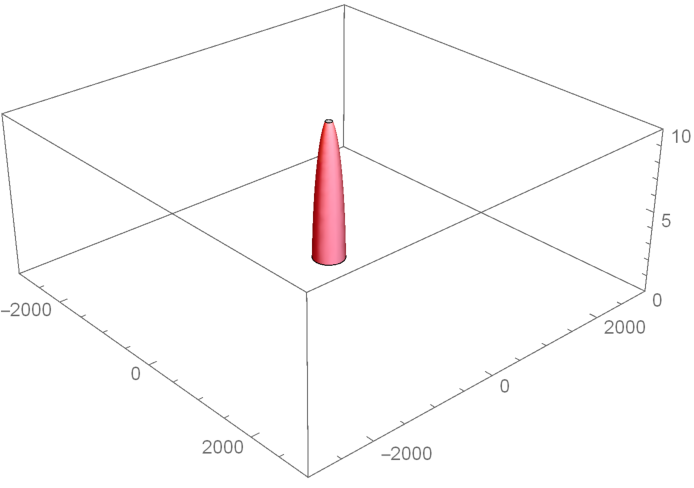
\includegraphics[width=7.5cm]{images/porus1.pdf}
\end{subfigure}
\begin{subfigure}[t]{0.49\textwidth}
	\centering
	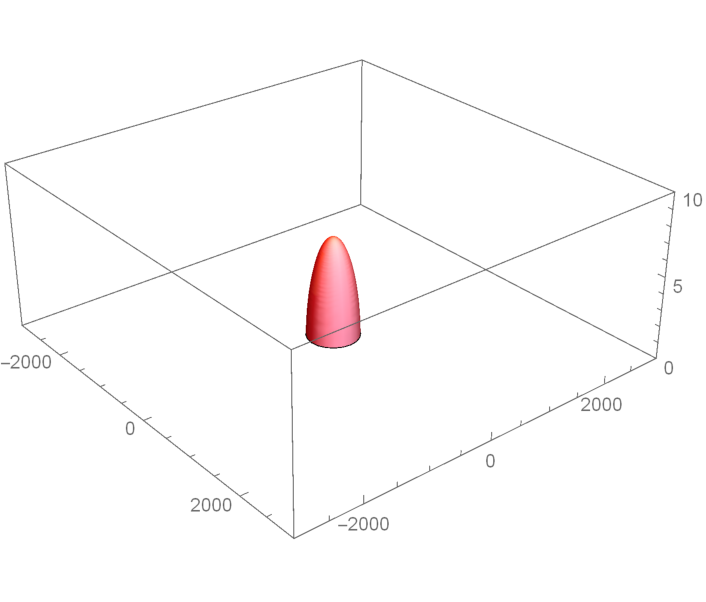
\includegraphics[width=7.5cm]{images/porus2.pdf}
\end{subfigure}
\begin{subfigure}[t]{0.49\textwidth}
	\centering
	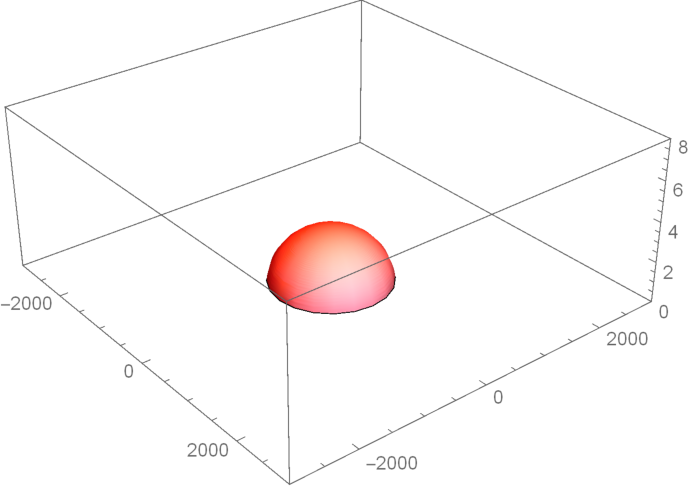
\includegraphics[width=7.5cm]{images/porus3.pdf}
\end{subfigure}
\begin{subfigure}[t]{0.49\textwidth}
	\centering
	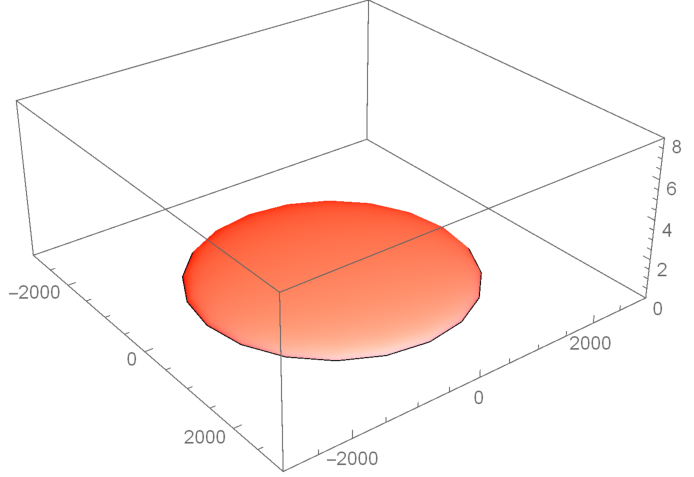
\includegraphics[width=7.5cm]{images/porus4.pdf}
\end{subfigure}
\caption{Example solutions given by \cref{porussol}.}%
\label{poruspics}%
\end{figure}

\subsection{Similarity solutions}

Deriving this solution involves using another technique for solving partial differential equation: a symmetry reduction technique known as looking for \emph{similarity solutions}. The basic idea is that if we can find some transformation of our solution which changes its shape but still solves the basic equations, then we should be able to use this transformation to eliminate one of the independent variables. This is a bit like with Fourier transforms when this elimination turns a PDE into an ODE. Unfortunately, of course, first you must such a scaling, and this is not always easy! But for a significant class of PDEs with one spatial dimension the generic transformation of $u(x,t)$ given by
\begin{equation}
\label{dilation}
U = \lambda^{-\alpha} u, \quad X = \lambda^\beta x, \quad T = \lambda t
%u(x,t) = \lambda^{\alpha} v(\lambda^{\beta}x,\lambda t)
\end{equation}  
for some suitable constants $\alpha$ and $\beta$ will give the original PDE for $U(X,T)$ (a \emph{dilation}). 

For example, consider the 1D diffusion equation from the previous chapter,
\begin{equation}
	\pd{u}{t}  = D\pdd{u}{x}.
\end{equation}
Applying \cref{dilation} we get 
\begin{equation}
	\lambda^{\alpha+1}\pd{U}{T} = D\lambda^{\alpha+2\beta}\pdd{U}{X}.
\end{equation}
We can spot that if $\beta=1/2$ then
\begin{equation}
	\pd{U}{T} = D \pdd{U}{X},
\end{equation}
i.e., $U$ satisfies the diffusion equation! So we see a transformation in the form \cref{dilation} can lead to the same differential equation, just in $U$ instead of $u$.

Note that $\alpha$ turned out to be arbitrary here: as we will see, we can pick it to suit the initial conditions. 

But why do we care that under this transformation, $U$ satisfies the same PDE? Well, note that the groupings
\begin{equation}
	\eta = \frac{X}{T^\beta} = \frac{x}{t^\beta} \quad \text{and} \quad \xi = UT^\alpha = ut^{\alpha}
	\label{sim-sol-sub}
\end{equation}
are invariant (i.e.\ unchanged) under the transformation. By a theorem sometimes known as Morgan's theorem,\footnote{For the interested: \textsc{Morgan}, A.~J.~A.\ 1952. The reduction by one of the number of independent variables in some systems of partial differential equations. \emph{Quart.\ J.\ Math.} \textbf{3}(1), 250--259.} we can write one invariant as a function of the other,
\begin{equation}
\xi = v(\eta),
\end{equation}
for some function $v$. Substituting in the definitions of $\eta$ and $\xi$, we get
\begin{equation}
u(x,t) = \frac{1}{t^\alpha} v \left( \frac{x}{t^\beta} \right),
\end{equation}
and this is the key result! This implies that the solution $u(x,t)$ has the same shape as the `master shape' $v(\eta)$, just stretched by a factor $t^{\beta}$ along the $x$-axis and squashed by a factor $t^{\alpha}$ along the $y$-axis. This shape can then be appropriately scaled to give the time-varying behaviour of the system (determined by the parameters $\alpha$ and $\beta$, depending on the actual equation).

We have seen this behaviour already. Recall the fundamental solution of the diffusion equation, \cref{fundamentalsol} (with $u$ taking the $c$ role),
\begin{equation}
	u(x,t) =\frac{1}{2 \sqrt{\pi Dt}} \e^{-x^2/4Dt}.
\end{equation}
We have seen above that for the diffusion equation, $\beta=1/2$, so if we write $\eta = x/t^{1/2}$ and $v = ut^{\alpha}$ (from \cref{sim-sol-sub}) then 
\begin{equation}
	v(\eta,t) =\frac{t^{\alpha}}{2\sqrt{\pi D t}} \e^{-\eta^2/4D}.
\end{equation}
We said earlier that $\alpha$ can be set to fit the initial conditions. Well, the fundamental solution has a very specific initial condition which gives form to this solution, and here if we set $\alpha=1/2$ then 
\begin{equation}
v(\eta) =\frac{1}{2 \sqrt{\pi D}}\e^{-\eta^2/4D}.  
\end{equation}

So we see our solution $u(x,t)$ can be written in the form
\begin{equation}
u(x,t) = \frac{1}{t^\alpha}v\left(\frac{x}{t^{\beta}}\right) =  \frac{1}{t^{1/2}}v\left(\frac{x}{t^{1/2}}\right),
\end{equation}
and the solution will still satisfy the diffusion equation. 

As we saw in \cref{funsol}, this confirms that the solution $u(x,t)$ has the same shape as the master shape $v(\eta)$, stretched by a factor $t^{1/2}$ along the $x$-axis and squashed by a factor $t^{1/2}$ along the $y$-axis. 

\subsection{Back to the porous media equation}

Let's go back to \cref{porous-media-eqn},
\begin{equation}
\label{radialpde}
\pd{c}{t} = \frac{D_0}{r}\pd{}{r}\left[r \left(\frac{c}{c_0}\right)^m \pd{c}{r}\right],
\end{equation}
and, using the observed similarity solution, make the substitution
\begin{equation}
	c(r,t) = \frac{1}{t^{\alpha}}v\left(\frac{r}{t^{\beta}}\right).
\end{equation}
Denoting $\eta=r/t^{\beta}$, so that $v=v(\eta)$, we first change the left-hand side:
\begin{align}
\pd{c}{t} &= -\alpha\frac{1}{t^{\alpha+1}}v + \frac{1}{t^{\alpha}}\fd{v}{\eta}\pd{\eta}{t} \\
 &=  -\alpha\frac{1}{t^{\alpha+1}}v  - \frac{r \beta}{t^{\alpha}t^{\beta+1}}\fd{v}{\eta}\\
\label{fincaldcdt}& =   -\alpha\frac{1}{t^{\alpha+1}}v  - \frac{\eta \beta}{t^{\alpha+1}}\fd{v}{\eta}.
\end{align}
On the right-hand side,
\begin{equation}
\pd{}{r} = \frac{1}{t^\beta}\pd{}{\eta} \implies \pd{c}{r}= \frac{1}{t^{\alpha+\beta}}\fd{v}{\eta},
\end{equation}
and so we have 
\begin{align}
 \frac{D_0}{r}\pd{}{r}\left[r \left(\frac{c}{c_0}\right)^m \pd{c}{r}\right]&=\frac{D_0}{\eta t^{2\beta}}\pd{}{\eta}\left[\frac{t^\beta \eta}{t^{\alpha m}}\left(\frac{v}{c_0}\right)^m  \frac{1}{t^{\alpha+\beta}}\fd{v}{\eta}\right]\\
\label{finalrhs}&= \frac{1}{t^{\alpha(m+1)+2\beta}}\frac{D_0}{\eta}\fd{}{\eta}\left[\eta\left(\frac{v}{c_0}\right)^m \fd{v}{\eta}\right].
\end{align}
Comparing \cref{fincaldcdt,finalrhs} we see we want to set the $t$-exponents equal to each other, 
\begin{equation}
\alpha + 1 = \alpha(m+1) + 2\beta  \implies 1 = \alpha m + 2\beta.
\end{equation}
We can multiply through by $t^{\alpha+1}$ to obtain
\begin{equation}
\alpha v + \beta \fd{v}{\eta}\eta +\frac{D_0}{\eta}\fd{}{\eta}\left[\eta\left(\frac{v}{c_0}\right)^m\fd{v}{\eta}\right] =0.
\label{rel-between-alpha-and-beta}
\end{equation}
So now we have a relationship between $\alpha$ and $\beta$, but still some freedom in choosing one of them. 

We now manipulate \cref{rel-between-alpha-and-beta} to simplify it with an appropriate choice of $\alpha$. In particular, we want to write our equation in the form $\fd{[\cdots]}{\eta}$ so that we can then integrate and create a first-order equation.

Multiply our equation through by $\eta$,
\begin{equation}
\label{newode}
\alpha v \eta + \beta \fd{v}{\eta} \eta^2 + D_0\fd{}{\eta}\left[\eta\left(\frac{v}{c_0}\right)^m \fd{v}{\eta}\right]=0.
\end{equation}
The idea is to turn the first two terms into a derivative so we can integrate. You might notice that for some $\gamma$,
\begin{equation}
\gamma\fd{}{\eta}[v\eta^2] = \gamma \fd{v}{\eta} \eta^2 + 2\gamma v\eta, 
\end{equation}
which is almost the form we want. If we set $\gamma=\beta$, then we have two simultaneous equations,
\begin{align}
1 & = \alpha m + 2 \beta,\\
\alpha & = 2\beta.
\end{align}
This gives us $\alpha = 1/(m+1)$ and $\beta=1/[2(m+1)]$, so \cref{newode} becomes
\begin{equation}
\beta\fd{}{\eta}[v\eta^2] + D_0\fd{}{\eta}\left[\eta\left(\frac{v}{c_0}\right)^m \fd{v}{\eta}\right] = 0.
\end{equation}
Integrating with respect to $\eta$ gives
\begin{equation}
\beta v\eta^2 + D_0\eta\left(\frac{v}{c_0}\right)^m \fd{v}{\eta} = C,
\end{equation}
with $C$ a constant of integration.

We choose the imposed boundary condition that $v(\eta) \to 0$ sufficiently fast as $\eta(r) \to \infty$ which implies the constant of integration is $C=0$. For any finite $t$, this is equivalent to saying the population vanishes as $r\to \infty$.

We solve the differential equation by noting either $v=0$ or, using separation of variables,
\begin{align}
\beta \int \eta\,\d{\eta} &= - \int \frac{D_0}{c_0^m}v^{m-1}\d{v},\\
\implies \frac{\beta \eta^2}{2} &=- \frac{D_0}{m c_0^m}v^{m} + A,\\
\implies v^m &= \frac{m c_0^m}{D_0}\left(A -  \frac{\beta\eta^2}{2}\right).
\end{align}
Finally, using $c= v/t^\alpha$ and $\eta= r/t^{\beta}$, we get 
\begin{equation}
c(r,t)= \frac{m^{1/m} c_0}{t^{\alpha}D_0^{1/m}}\left(A -  \frac{\beta r^2}{2t^{2\beta}}\right)^{1/m},
\end{equation}
where $\alpha = 1/(m+1)$ and $\beta=1/[2(m+1)]$.
The concentration, $c$, is only non-negative (and real) if the term is the bracket is non-negative, i.e.\
\begin{equation}
	r^2 \leq \frac{2A}{\beta}t^{2\beta},
\end{equation}
and so outside this region, the solution must be the $c=0$ solution we ignored earlier. In other words, this solution has compact support, and we can see the size of the support grows with time. Thinking back, this is what we might expect from an equation that represents a type of diffusion.

To get $A$ and hence the final solution, \cref{porussol}, we enforce that the total density (mass) is conserved,
\begin{equation}
	\int c \, \d S = 2 \pi \int_0^{\sqrt{\frac{2A}{\beta}}t^\beta} c r \, \d r = Q. 
\end{equation}
This is a little tedious and I don't really want you to spend your time doing this. We've shown that this solution has compact support, which is the important result. And the main method we're interested in here is the method of similarity solutions. 

\paragraph{Reflections}
Compact support means that outside of a region, the population really is zero. Why do we care? After all, in the Gaussian model, the tails are really quite tiny. 

Well, consider a population of predators spreading out on the far left of a domain, and a population of prey spreading out on the far right of a domain. In the Gaussian model, there are immediately small numbers of predators among the prey, and if coupled with a predator--prey model without a coexistence equilibrium, you would expect the prey to start dying out. But with finite diffusion, both species happily spread out, with no change in population size, until they meet somewhere in the middle of our domain.

\begin{do-it-yourself}
Additional Problem Sheet 2 contains an example of the use of this method. Also, there is a link in this chapter's extra reading to a bunch of worked problems using this method of symmetry reduction/similarity scaling.
\end{do-it-yourself}

\begin{extra-reading}
\begin{itemize}
	\item Diffusion of populations is covered in \textsc{Murray}, vol.~I, chap.~11. Note that we don't do long-range diffusion, and that our derivation is more general than the derivation in the book since we include advection.
	\item Solution of PDEs by Fourier transform: The \href{https://en.wikipedia.org/wiki/Fourier_transform}{Wikipedia page} for the Fourier transform is very comprehensive on the topic. Really what you need to do is find examples to test yourself with. Joel Feldman at UBC provides a lot of \href{https://www.math.ubc.ca/~feldman/m267/pdeft.pdf}{good examples on his website}.
    \item Green's functions: What we cover here is essentially the basics, which you can find on Wikipedia. It can be used in a much wider context than given here but that steps outside the relevancy for this course so I recommend you stick to what is here.
    \item Finite diffusion and spherically symmetric densities are covered in \textsc{Murray}, vol.~I, chap.~11.3. The solution method is taken from \textsc{Evans}, L.~C., 1998 \emph{Partial Differential Equations}, page 188, `Similarity under scaling'. In that case it is done in Cartesian coordinates; we have adapted the method for the polar case. In that book there are other examples.
    \item Helen Wilson at UCL also provides \href{http://www.ucl.ac.uk/~ucahhwi/LTCC/sectionB-similarity.pdf}{relevant worked examples}.
\end{itemize}
\end{extra-reading}

\chapter{Travelling waves}
\label{chap:travelling-waves}
\label{chap:pursuit-evasion}
In \cref{chap:growth,chap:pendulum,complotvol,switching} we looked at time-dependent models of population growth and interaction. In \cref{chap:diffusion}, we looked at models where the time-dependence was balanced by diffusion, a spatial dependence. We're now going to bring these two ideas together.

We're going to start by considering the advection--diffusion equation in one spatial dimension, and for one species only, without advection,
\begin{equation}
	\pd{u}{t} = D \pdd{u}{x} + f(u).
\end{equation}
Systems of this form, i.e.\ without advection, are known as \emph{reaction--diffusion systems}. We will be studying them exclusively hereafter. They are capable of, frankly, a staggering variety of behaviour!

\section{The Fisher--Kolmogorov (FK) equation}
The first model we will examine is attributed to Ronald Fisher for his work, published 1937, that models the spread of an advantageous gene mutation in a population. We’ll get to Kolmogorov’s contribution shortly.

The FK equation provides a natural entry point into our discussion of reaction--diffusion equations and spatial dynamics since in this equation, we have
\begin{equation}
	f(u) = ku (1-u).
\end{equation}
Remember this? Of course you do! It's logistic growth with a limiting population of $u=1$. In the context of Fisher’s model, $u$ is the percentage of the population carrying the advantageous gene. 

We nondimensionalise using $t = \hat{t}/k$, $x = (D/k)^{1/2}\hat{x}$ and dropping hats gives us
\begin{equation}
	\label{fk-nondim}
	\pd{u}{t} = \pdd{u}{x} + u(1-u).
\end{equation}
Recall that the logistic equation has two equilibria: $u = 0$, which is unstable, and $u = 1$, which is stable. In the context of the reaction--diffusion PDE, these constant values of $u$ are \emph{homogeneous} equilibria. What are they?

\begin{description}
\item{\textbf{Equilibrium:}} A function $u$ is in equilibrium when all temporal derivatives $\pdn{n}{u}{t}$ vanish.
\item{\textbf{Homogeneity:}} A function is homogeneous when all its spatial derivatives $\pdn{n}{u}{x_i}$ vanish.
\end{description}

Let’s now consider the FK equation with the boundary conditions that
\begin{equation}
	\label{fk-bc}
	u \to 1 \text{ as } x \to -\infty \quad \text{and} \quad u \to 0 \text{ as } x \to \infty.
\end{equation}
This will require the solution to transition between the two equilibria, from $u = 1$ to $u = 0$, over some region of space, as illustrated in \cref{fig:fk-travelling-wave-intuition-1}. Knowing what we know about the stabilities of $u = 1$ and $u = 0$, we expect that the transition region will not be stationary and move \emph{to the right} over time, allowing the stable $u = 1$ region to expand. 
\begin{figure}
\centering
%% Creator: Matplotlib, PGF backend
%%
%% To include the figure in your LaTeX document, write
%%   \input{<filename>.pgf}
%%
%% Make sure the required packages are loaded in your preamble
%%   \usepackage{pgf}
%%
%% and, on pdftex
%%   \usepackage[utf8]{inputenc}\DeclareUnicodeCharacter{2212}{-}
%%
%% or, on luatex and xetex
%%   \usepackage{unicode-math}
%%
%% Figures using additional raster images can only be included by \input if
%% they are in the same directory as the main LaTeX file. For loading figures
%% from other directories you can use the `import` package
%%   \usepackage{import}
%%
%% and then include the figures with
%%   \import{<path to file>}{<filename>.pgf}
%%
%% Matplotlib used the following preamble
%%   \usepackage{fontspec}
%%   \setmainfont{DejaVuSerif.ttf}[Path=/Users/adam/opt/anaconda3/lib/python3.8/site-packages/matplotlib/mpl-data/fonts/ttf/]
%%   \setsansfont{DejaVuSans.ttf}[Path=/Users/adam/opt/anaconda3/lib/python3.8/site-packages/matplotlib/mpl-data/fonts/ttf/]
%%   \setmonofont{DejaVuSansMono.ttf}[Path=/Users/adam/opt/anaconda3/lib/python3.8/site-packages/matplotlib/mpl-data/fonts/ttf/]
%%
\begingroup%
\makeatletter%
\begin{pgfpicture}%
\pgfpathrectangle{\pgfpointorigin}{\pgfqpoint{3.000000in}{2.200000in}}%
\pgfusepath{use as bounding box, clip}%
\begin{pgfscope}%
\pgfsetbuttcap%
\pgfsetmiterjoin%
\definecolor{currentfill}{rgb}{1.000000,1.000000,1.000000}%
\pgfsetfillcolor{currentfill}%
\pgfsetlinewidth{0.000000pt}%
\definecolor{currentstroke}{rgb}{1.000000,1.000000,1.000000}%
\pgfsetstrokecolor{currentstroke}%
\pgfsetdash{}{0pt}%
\pgfpathmoveto{\pgfqpoint{0.000000in}{0.000000in}}%
\pgfpathlineto{\pgfqpoint{3.000000in}{0.000000in}}%
\pgfpathlineto{\pgfqpoint{3.000000in}{2.200000in}}%
\pgfpathlineto{\pgfqpoint{0.000000in}{2.200000in}}%
\pgfpathclose%
\pgfusepath{fill}%
\end{pgfscope}%
\begin{pgfscope}%
\pgfsetbuttcap%
\pgfsetmiterjoin%
\definecolor{currentfill}{rgb}{1.000000,1.000000,1.000000}%
\pgfsetfillcolor{currentfill}%
\pgfsetlinewidth{0.000000pt}%
\definecolor{currentstroke}{rgb}{0.000000,0.000000,0.000000}%
\pgfsetstrokecolor{currentstroke}%
\pgfsetstrokeopacity{0.000000}%
\pgfsetdash{}{0pt}%
\pgfpathmoveto{\pgfqpoint{0.033333in}{0.278150in}}%
\pgfpathlineto{\pgfqpoint{2.966667in}{0.278150in}}%
\pgfpathlineto{\pgfqpoint{2.966667in}{2.166667in}}%
\pgfpathlineto{\pgfqpoint{0.033333in}{2.166667in}}%
\pgfpathclose%
\pgfusepath{fill}%
\end{pgfscope}%
\begin{pgfscope}%
\pgfsetbuttcap%
\pgfsetroundjoin%
\definecolor{currentfill}{rgb}{0.000000,0.000000,0.000000}%
\pgfsetfillcolor{currentfill}%
\pgfsetlinewidth{0.803000pt}%
\definecolor{currentstroke}{rgb}{0.000000,0.000000,0.000000}%
\pgfsetstrokecolor{currentstroke}%
\pgfsetdash{}{0pt}%
\pgfsys@defobject{currentmarker}{\pgfqpoint{0.000000in}{-0.048611in}}{\pgfqpoint{0.000000in}{0.000000in}}{%
\pgfpathmoveto{\pgfqpoint{0.000000in}{0.000000in}}%
\pgfpathlineto{\pgfqpoint{0.000000in}{-0.048611in}}%
\pgfusepath{stroke,fill}%
}%
\begin{pgfscope}%
\pgfsys@transformshift{1.492703in}{0.278150in}%
\pgfsys@useobject{currentmarker}{}%
\end{pgfscope}%
\end{pgfscope}%
\begin{pgfscope}%
\definecolor{textcolor}{rgb}{0.000000,0.000000,0.000000}%
\pgfsetstrokecolor{textcolor}%
\pgfsetfillcolor{textcolor}%
\pgftext[x=1.492703in,y=0.180927in,,top]{\color{textcolor}\rmfamily\fontsize{12.000000}{14.400000}\selectfont 0}%
\end{pgfscope}%
\begin{pgfscope}%
\pgfsetbuttcap%
\pgfsetroundjoin%
\definecolor{currentfill}{rgb}{0.000000,0.000000,0.000000}%
\pgfsetfillcolor{currentfill}%
\pgfsetlinewidth{0.803000pt}%
\definecolor{currentstroke}{rgb}{0.000000,0.000000,0.000000}%
\pgfsetstrokecolor{currentstroke}%
\pgfsetdash{}{0pt}%
\pgfsys@defobject{currentmarker}{\pgfqpoint{-0.048611in}{0.000000in}}{\pgfqpoint{-0.000000in}{0.000000in}}{%
\pgfpathmoveto{\pgfqpoint{-0.000000in}{0.000000in}}%
\pgfpathlineto{\pgfqpoint{-0.048611in}{0.000000in}}%
\pgfusepath{stroke,fill}%
}%
\begin{pgfscope}%
\pgfsys@transformshift{1.492703in}{0.278150in}%
\pgfsys@useobject{currentmarker}{}%
\end{pgfscope}%
\end{pgfscope}%
\begin{pgfscope}%
\definecolor{textcolor}{rgb}{0.000000,0.000000,0.000000}%
\pgfsetstrokecolor{textcolor}%
\pgfsetfillcolor{textcolor}%
\pgftext[x=1.289442in, y=0.214836in, left, base]{\color{textcolor}\rmfamily\fontsize{12.000000}{14.400000}\selectfont 0}%
\end{pgfscope}%
\begin{pgfscope}%
\pgfsetbuttcap%
\pgfsetroundjoin%
\definecolor{currentfill}{rgb}{0.000000,0.000000,0.000000}%
\pgfsetfillcolor{currentfill}%
\pgfsetlinewidth{0.803000pt}%
\definecolor{currentstroke}{rgb}{0.000000,0.000000,0.000000}%
\pgfsetstrokecolor{currentstroke}%
\pgfsetdash{}{0pt}%
\pgfsys@defobject{currentmarker}{\pgfqpoint{-0.048611in}{0.000000in}}{\pgfqpoint{-0.000000in}{0.000000in}}{%
\pgfpathmoveto{\pgfqpoint{-0.000000in}{0.000000in}}%
\pgfpathlineto{\pgfqpoint{-0.048611in}{0.000000in}}%
\pgfusepath{stroke,fill}%
}%
\begin{pgfscope}%
\pgfsys@transformshift{1.492703in}{1.851914in}%
\pgfsys@useobject{currentmarker}{}%
\end{pgfscope}%
\end{pgfscope}%
\begin{pgfscope}%
\definecolor{textcolor}{rgb}{0.000000,0.000000,0.000000}%
\pgfsetstrokecolor{textcolor}%
\pgfsetfillcolor{textcolor}%
\pgftext[x=1.289442in, y=1.788600in, left, base]{\color{textcolor}\rmfamily\fontsize{12.000000}{14.400000}\selectfont 1}%
\end{pgfscope}%
\begin{pgfscope}%
\pgfsetrectcap%
\pgfsetmiterjoin%
\pgfsetlinewidth{0.803000pt}%
\definecolor{currentstroke}{rgb}{0.000000,0.000000,0.000000}%
\pgfsetstrokecolor{currentstroke}%
\pgfsetdash{}{0pt}%
\pgfpathmoveto{\pgfqpoint{1.492703in}{0.278150in}}%
\pgfpathlineto{\pgfqpoint{1.492703in}{2.166667in}}%
\pgfusepath{stroke}%
\end{pgfscope}%
\begin{pgfscope}%
\pgfsetrectcap%
\pgfsetmiterjoin%
\pgfsetlinewidth{0.803000pt}%
\definecolor{currentstroke}{rgb}{0.000000,0.000000,0.000000}%
\pgfsetstrokecolor{currentstroke}%
\pgfsetdash{}{0pt}%
\pgfpathmoveto{\pgfqpoint{0.033333in}{0.278150in}}%
\pgfpathlineto{\pgfqpoint{2.966667in}{0.278150in}}%
\pgfusepath{stroke}%
\end{pgfscope}%
\begin{pgfscope}%
\definecolor{textcolor}{rgb}{0.000000,0.000000,0.000000}%
\pgfsetstrokecolor{textcolor}%
\pgfsetfillcolor{textcolor}%
\pgftext[x=2.966667in,y=0.180927in,right,top]{\color{textcolor}\rmfamily\fontsize{12.000000}{14.400000}\selectfont \(\displaystyle x\)}%
\end{pgfscope}%
\begin{pgfscope}%
\definecolor{textcolor}{rgb}{0.000000,0.000000,0.000000}%
\pgfsetstrokecolor{textcolor}%
\pgfsetfillcolor{textcolor}%
\pgftext[x=1.402778in,y=2.166667in,right,top]{\color{textcolor}\rmfamily\fontsize{12.000000}{14.400000}\selectfont \(\displaystyle u\)}%
\end{pgfscope}%
\begin{pgfscope}%
\definecolor{textcolor}{rgb}{0.121569,0.466667,0.705882}%
\pgfsetstrokecolor{textcolor}%
\pgfsetfillcolor{textcolor}%
\pgftext[x=1.256111in,y=1.222408in,right,]{\color{textcolor}\rmfamily\fontsize{20.000000}{24.000000}\selectfont ?}%
\end{pgfscope}%
\begin{pgfscope}%
\pgfsetrectcap%
\pgfsetroundjoin%
\pgfsetlinewidth{1.505625pt}%
\definecolor{currentstroke}{rgb}{0.121569,0.466667,0.705882}%
\pgfsetstrokecolor{currentstroke}%
\pgfsetdash{}{0pt}%
\pgfpathmoveto{\pgfqpoint{0.033333in}{1.851835in}}%
\pgfpathlineto{\pgfqpoint{0.036255in}{1.851835in}}%
\pgfpathlineto{\pgfqpoint{0.039177in}{1.851835in}}%
\pgfpathlineto{\pgfqpoint{0.042098in}{1.851834in}}%
\pgfpathlineto{\pgfqpoint{0.045020in}{1.851834in}}%
\pgfpathlineto{\pgfqpoint{0.047942in}{1.851833in}}%
\pgfpathlineto{\pgfqpoint{0.050863in}{1.851832in}}%
\pgfpathlineto{\pgfqpoint{0.053785in}{1.851831in}}%
\pgfpathlineto{\pgfqpoint{0.056707in}{1.851830in}}%
\pgfpathlineto{\pgfqpoint{0.059628in}{1.851829in}}%
\pgfpathlineto{\pgfqpoint{0.062550in}{1.851828in}}%
\pgfpathlineto{\pgfqpoint{0.065472in}{1.851826in}}%
\pgfpathlineto{\pgfqpoint{0.068393in}{1.851825in}}%
\pgfpathlineto{\pgfqpoint{0.071315in}{1.851823in}}%
\pgfpathlineto{\pgfqpoint{0.074237in}{1.851822in}}%
\pgfpathlineto{\pgfqpoint{0.077158in}{1.851820in}}%
\pgfpathlineto{\pgfqpoint{0.080080in}{1.851819in}}%
\pgfpathlineto{\pgfqpoint{0.083002in}{1.851817in}}%
\pgfpathlineto{\pgfqpoint{0.085923in}{1.851815in}}%
\pgfpathlineto{\pgfqpoint{0.088845in}{1.851813in}}%
\pgfpathlineto{\pgfqpoint{0.091767in}{1.851811in}}%
\pgfpathlineto{\pgfqpoint{0.094688in}{1.851809in}}%
\pgfpathlineto{\pgfqpoint{0.097610in}{1.851807in}}%
\pgfpathlineto{\pgfqpoint{0.100532in}{1.851805in}}%
\pgfpathlineto{\pgfqpoint{0.103453in}{1.851803in}}%
\pgfpathlineto{\pgfqpoint{0.106375in}{1.851800in}}%
\pgfpathlineto{\pgfqpoint{0.109297in}{1.851798in}}%
\pgfpathlineto{\pgfqpoint{0.112218in}{1.851796in}}%
\pgfpathlineto{\pgfqpoint{0.115140in}{1.851793in}}%
\pgfpathlineto{\pgfqpoint{0.118062in}{1.851791in}}%
\pgfpathlineto{\pgfqpoint{0.120983in}{1.851788in}}%
\pgfpathlineto{\pgfqpoint{0.123905in}{1.851786in}}%
\pgfpathlineto{\pgfqpoint{0.126826in}{1.851783in}}%
\pgfpathlineto{\pgfqpoint{0.129748in}{1.851780in}}%
\pgfpathlineto{\pgfqpoint{0.132670in}{1.851778in}}%
\pgfpathlineto{\pgfqpoint{0.135591in}{1.851775in}}%
\pgfpathlineto{\pgfqpoint{0.138513in}{1.851772in}}%
\pgfpathlineto{\pgfqpoint{0.141435in}{1.851769in}}%
\pgfpathlineto{\pgfqpoint{0.144356in}{1.851766in}}%
\pgfpathlineto{\pgfqpoint{0.147278in}{1.851763in}}%
\pgfpathlineto{\pgfqpoint{0.150200in}{1.851760in}}%
\pgfpathlineto{\pgfqpoint{0.153121in}{1.851757in}}%
\pgfpathlineto{\pgfqpoint{0.156043in}{1.851753in}}%
\pgfpathlineto{\pgfqpoint{0.158965in}{1.851750in}}%
\pgfpathlineto{\pgfqpoint{0.161886in}{1.851747in}}%
\pgfpathlineto{\pgfqpoint{0.164808in}{1.851743in}}%
\pgfpathlineto{\pgfqpoint{0.167730in}{1.851739in}}%
\pgfpathlineto{\pgfqpoint{0.170651in}{1.851736in}}%
\pgfpathlineto{\pgfqpoint{0.173573in}{1.851732in}}%
\pgfpathlineto{\pgfqpoint{0.176495in}{1.851728in}}%
\pgfpathlineto{\pgfqpoint{0.179416in}{1.851724in}}%
\pgfpathlineto{\pgfqpoint{0.182338in}{1.851720in}}%
\pgfpathlineto{\pgfqpoint{0.185260in}{1.851716in}}%
\pgfpathlineto{\pgfqpoint{0.188181in}{1.851712in}}%
\pgfpathlineto{\pgfqpoint{0.191103in}{1.851708in}}%
\pgfpathlineto{\pgfqpoint{0.194025in}{1.851704in}}%
\pgfpathlineto{\pgfqpoint{0.196946in}{1.851699in}}%
\pgfpathlineto{\pgfqpoint{0.199868in}{1.851695in}}%
\pgfpathlineto{\pgfqpoint{0.202790in}{1.851690in}}%
\pgfpathlineto{\pgfqpoint{0.205711in}{1.851686in}}%
\pgfpathlineto{\pgfqpoint{0.208633in}{1.851681in}}%
\pgfpathlineto{\pgfqpoint{0.211555in}{1.851676in}}%
\pgfpathlineto{\pgfqpoint{0.214476in}{1.851671in}}%
\pgfpathlineto{\pgfqpoint{0.217398in}{1.851666in}}%
\pgfpathlineto{\pgfqpoint{0.220320in}{1.851661in}}%
\pgfpathlineto{\pgfqpoint{0.223241in}{1.851655in}}%
\pgfpathlineto{\pgfqpoint{0.226163in}{1.851650in}}%
\pgfpathlineto{\pgfqpoint{0.229085in}{1.851644in}}%
\pgfpathlineto{\pgfqpoint{0.232006in}{1.851639in}}%
\pgfpathlineto{\pgfqpoint{0.234928in}{1.851633in}}%
\pgfpathlineto{\pgfqpoint{0.237850in}{1.851627in}}%
\pgfpathlineto{\pgfqpoint{0.240771in}{1.851621in}}%
\pgfpathlineto{\pgfqpoint{0.243693in}{1.851615in}}%
\pgfpathlineto{\pgfqpoint{0.246615in}{1.851609in}}%
\pgfpathlineto{\pgfqpoint{0.249536in}{1.851602in}}%
\pgfpathlineto{\pgfqpoint{0.252458in}{1.851596in}}%
\pgfpathlineto{\pgfqpoint{0.255380in}{1.851589in}}%
\pgfpathlineto{\pgfqpoint{0.258301in}{1.851582in}}%
\pgfpathlineto{\pgfqpoint{0.261223in}{1.851575in}}%
\pgfpathlineto{\pgfqpoint{0.264145in}{1.851568in}}%
\pgfpathlineto{\pgfqpoint{0.267066in}{1.851561in}}%
\pgfpathlineto{\pgfqpoint{0.269988in}{1.851554in}}%
\pgfpathlineto{\pgfqpoint{0.272910in}{1.851546in}}%
\pgfpathlineto{\pgfqpoint{0.275831in}{1.851538in}}%
\pgfpathlineto{\pgfqpoint{0.278753in}{1.851531in}}%
\pgfpathlineto{\pgfqpoint{0.281675in}{1.851522in}}%
\pgfpathlineto{\pgfqpoint{0.284596in}{1.851514in}}%
\pgfpathlineto{\pgfqpoint{0.287518in}{1.851506in}}%
\pgfpathlineto{\pgfqpoint{0.290440in}{1.851497in}}%
\pgfpathlineto{\pgfqpoint{0.293361in}{1.851489in}}%
\pgfpathlineto{\pgfqpoint{0.296283in}{1.851480in}}%
\pgfpathlineto{\pgfqpoint{0.299205in}{1.851471in}}%
\pgfpathlineto{\pgfqpoint{0.302126in}{1.851461in}}%
\pgfpathlineto{\pgfqpoint{0.305048in}{1.851452in}}%
\pgfpathlineto{\pgfqpoint{0.307969in}{1.851442in}}%
\pgfpathlineto{\pgfqpoint{0.310891in}{1.851432in}}%
\pgfpathlineto{\pgfqpoint{0.313813in}{1.851422in}}%
\pgfpathlineto{\pgfqpoint{0.316734in}{1.851412in}}%
\pgfpathlineto{\pgfqpoint{0.319656in}{1.851402in}}%
\pgfpathlineto{\pgfqpoint{0.322578in}{1.851391in}}%
\pgfusepath{stroke}%
\end{pgfscope}%
\begin{pgfscope}%
\pgfsetrectcap%
\pgfsetroundjoin%
\pgfsetlinewidth{1.505625pt}%
\definecolor{currentstroke}{rgb}{0.121569,0.466667,0.705882}%
\pgfsetstrokecolor{currentstroke}%
\pgfsetdash{}{0pt}%
\pgfpathmoveto{\pgfqpoint{2.662829in}{0.278150in}}%
\pgfpathlineto{\pgfqpoint{2.665750in}{0.278150in}}%
\pgfpathlineto{\pgfqpoint{2.668672in}{0.278150in}}%
\pgfpathlineto{\pgfqpoint{2.671593in}{0.278150in}}%
\pgfpathlineto{\pgfqpoint{2.674515in}{0.278150in}}%
\pgfpathlineto{\pgfqpoint{2.677437in}{0.278150in}}%
\pgfpathlineto{\pgfqpoint{2.680358in}{0.278150in}}%
\pgfpathlineto{\pgfqpoint{2.683280in}{0.278150in}}%
\pgfpathlineto{\pgfqpoint{2.686202in}{0.278150in}}%
\pgfpathlineto{\pgfqpoint{2.689123in}{0.278150in}}%
\pgfpathlineto{\pgfqpoint{2.692045in}{0.278150in}}%
\pgfpathlineto{\pgfqpoint{2.694967in}{0.278150in}}%
\pgfpathlineto{\pgfqpoint{2.697888in}{0.278150in}}%
\pgfpathlineto{\pgfqpoint{2.700810in}{0.278150in}}%
\pgfpathlineto{\pgfqpoint{2.703732in}{0.278150in}}%
\pgfpathlineto{\pgfqpoint{2.706653in}{0.278150in}}%
\pgfpathlineto{\pgfqpoint{2.709575in}{0.278150in}}%
\pgfpathlineto{\pgfqpoint{2.712497in}{0.278150in}}%
\pgfpathlineto{\pgfqpoint{2.715418in}{0.278150in}}%
\pgfpathlineto{\pgfqpoint{2.718340in}{0.278150in}}%
\pgfpathlineto{\pgfqpoint{2.721262in}{0.278150in}}%
\pgfpathlineto{\pgfqpoint{2.724183in}{0.278150in}}%
\pgfpathlineto{\pgfqpoint{2.727105in}{0.278150in}}%
\pgfpathlineto{\pgfqpoint{2.730027in}{0.278150in}}%
\pgfpathlineto{\pgfqpoint{2.732948in}{0.278150in}}%
\pgfpathlineto{\pgfqpoint{2.735870in}{0.278150in}}%
\pgfpathlineto{\pgfqpoint{2.738792in}{0.278150in}}%
\pgfpathlineto{\pgfqpoint{2.741713in}{0.278150in}}%
\pgfpathlineto{\pgfqpoint{2.744635in}{0.278150in}}%
\pgfpathlineto{\pgfqpoint{2.747557in}{0.278150in}}%
\pgfpathlineto{\pgfqpoint{2.750478in}{0.278150in}}%
\pgfpathlineto{\pgfqpoint{2.753400in}{0.278150in}}%
\pgfpathlineto{\pgfqpoint{2.756322in}{0.278150in}}%
\pgfpathlineto{\pgfqpoint{2.759243in}{0.278150in}}%
\pgfpathlineto{\pgfqpoint{2.762165in}{0.278150in}}%
\pgfpathlineto{\pgfqpoint{2.765087in}{0.278150in}}%
\pgfpathlineto{\pgfqpoint{2.768008in}{0.278150in}}%
\pgfpathlineto{\pgfqpoint{2.770930in}{0.278150in}}%
\pgfpathlineto{\pgfqpoint{2.773852in}{0.278150in}}%
\pgfpathlineto{\pgfqpoint{2.776773in}{0.278150in}}%
\pgfpathlineto{\pgfqpoint{2.779695in}{0.278150in}}%
\pgfpathlineto{\pgfqpoint{2.782617in}{0.278150in}}%
\pgfpathlineto{\pgfqpoint{2.785538in}{0.278150in}}%
\pgfpathlineto{\pgfqpoint{2.788460in}{0.278150in}}%
\pgfpathlineto{\pgfqpoint{2.791382in}{0.278150in}}%
\pgfpathlineto{\pgfqpoint{2.794303in}{0.278150in}}%
\pgfpathlineto{\pgfqpoint{2.797225in}{0.278150in}}%
\pgfpathlineto{\pgfqpoint{2.800147in}{0.278150in}}%
\pgfpathlineto{\pgfqpoint{2.803068in}{0.278150in}}%
\pgfpathlineto{\pgfqpoint{2.805990in}{0.278150in}}%
\pgfpathlineto{\pgfqpoint{2.808912in}{0.278150in}}%
\pgfpathlineto{\pgfqpoint{2.811833in}{0.278150in}}%
\pgfpathlineto{\pgfqpoint{2.814755in}{0.278150in}}%
\pgfpathlineto{\pgfqpoint{2.817677in}{0.278150in}}%
\pgfpathlineto{\pgfqpoint{2.820598in}{0.278150in}}%
\pgfpathlineto{\pgfqpoint{2.823520in}{0.278150in}}%
\pgfpathlineto{\pgfqpoint{2.826442in}{0.278150in}}%
\pgfpathlineto{\pgfqpoint{2.829363in}{0.278150in}}%
\pgfpathlineto{\pgfqpoint{2.832285in}{0.278150in}}%
\pgfpathlineto{\pgfqpoint{2.835207in}{0.278150in}}%
\pgfpathlineto{\pgfqpoint{2.838128in}{0.278150in}}%
\pgfpathlineto{\pgfqpoint{2.841050in}{0.278150in}}%
\pgfpathlineto{\pgfqpoint{2.843972in}{0.278150in}}%
\pgfpathlineto{\pgfqpoint{2.846893in}{0.278150in}}%
\pgfpathlineto{\pgfqpoint{2.849815in}{0.278150in}}%
\pgfpathlineto{\pgfqpoint{2.852736in}{0.278150in}}%
\pgfpathlineto{\pgfqpoint{2.855658in}{0.278150in}}%
\pgfpathlineto{\pgfqpoint{2.858580in}{0.278150in}}%
\pgfpathlineto{\pgfqpoint{2.861501in}{0.278150in}}%
\pgfpathlineto{\pgfqpoint{2.864423in}{0.278150in}}%
\pgfpathlineto{\pgfqpoint{2.867345in}{0.278150in}}%
\pgfpathlineto{\pgfqpoint{2.870266in}{0.278150in}}%
\pgfpathlineto{\pgfqpoint{2.873188in}{0.278150in}}%
\pgfpathlineto{\pgfqpoint{2.876110in}{0.278150in}}%
\pgfpathlineto{\pgfqpoint{2.879031in}{0.278150in}}%
\pgfpathlineto{\pgfqpoint{2.881953in}{0.278150in}}%
\pgfpathlineto{\pgfqpoint{2.884875in}{0.278150in}}%
\pgfpathlineto{\pgfqpoint{2.887796in}{0.278150in}}%
\pgfpathlineto{\pgfqpoint{2.890718in}{0.278150in}}%
\pgfpathlineto{\pgfqpoint{2.893640in}{0.278150in}}%
\pgfpathlineto{\pgfqpoint{2.896561in}{0.278150in}}%
\pgfpathlineto{\pgfqpoint{2.899483in}{0.278150in}}%
\pgfpathlineto{\pgfqpoint{2.902405in}{0.278150in}}%
\pgfpathlineto{\pgfqpoint{2.905326in}{0.278150in}}%
\pgfpathlineto{\pgfqpoint{2.908248in}{0.278150in}}%
\pgfpathlineto{\pgfqpoint{2.911170in}{0.278150in}}%
\pgfpathlineto{\pgfqpoint{2.914091in}{0.278150in}}%
\pgfpathlineto{\pgfqpoint{2.917013in}{0.278150in}}%
\pgfpathlineto{\pgfqpoint{2.919935in}{0.278150in}}%
\pgfpathlineto{\pgfqpoint{2.922856in}{0.278150in}}%
\pgfpathlineto{\pgfqpoint{2.925778in}{0.278150in}}%
\pgfpathlineto{\pgfqpoint{2.928700in}{0.278150in}}%
\pgfpathlineto{\pgfqpoint{2.931621in}{0.278150in}}%
\pgfpathlineto{\pgfqpoint{2.934543in}{0.278150in}}%
\pgfpathlineto{\pgfqpoint{2.937465in}{0.278150in}}%
\pgfpathlineto{\pgfqpoint{2.940386in}{0.278150in}}%
\pgfpathlineto{\pgfqpoint{2.943308in}{0.278150in}}%
\pgfpathlineto{\pgfqpoint{2.946230in}{0.278150in}}%
\pgfpathlineto{\pgfqpoint{2.949151in}{0.278150in}}%
\pgfusepath{stroke}%
\end{pgfscope}%
\begin{pgfscope}%
\pgfsetbuttcap%
\pgfsetroundjoin%
\pgfsetlinewidth{1.505625pt}%
\definecolor{currentstroke}{rgb}{0.121569,0.466667,0.705882}%
\pgfsetstrokecolor{currentstroke}%
\pgfsetstrokeopacity{0.400000}%
\pgfsetdash{{3.000000pt}{4.500000pt}}{0.000000pt}%
\pgfpathmoveto{\pgfqpoint{0.325499in}{1.851380in}}%
\pgfpathlineto{\pgfqpoint{0.489112in}{1.850210in}}%
\pgfpathlineto{\pgfqpoint{0.588449in}{1.848468in}}%
\pgfpathlineto{\pgfqpoint{0.661491in}{1.846134in}}%
\pgfpathlineto{\pgfqpoint{0.719924in}{1.843177in}}%
\pgfpathlineto{\pgfqpoint{0.766670in}{1.839761in}}%
\pgfpathlineto{\pgfqpoint{0.807574in}{1.835699in}}%
\pgfpathlineto{\pgfqpoint{0.842634in}{1.831165in}}%
\pgfpathlineto{\pgfqpoint{0.874772in}{1.825915in}}%
\pgfpathlineto{\pgfqpoint{0.903988in}{1.820017in}}%
\pgfpathlineto{\pgfqpoint{0.930283in}{1.813593in}}%
\pgfpathlineto{\pgfqpoint{0.953657in}{1.806828in}}%
\pgfpathlineto{\pgfqpoint{0.977030in}{1.798900in}}%
\pgfpathlineto{\pgfqpoint{0.997482in}{1.790861in}}%
\pgfpathlineto{\pgfqpoint{1.017933in}{1.781645in}}%
\pgfpathlineto{\pgfqpoint{1.038385in}{1.771094in}}%
\pgfpathlineto{\pgfqpoint{1.055915in}{1.760854in}}%
\pgfpathlineto{\pgfqpoint{1.073445in}{1.749384in}}%
\pgfpathlineto{\pgfqpoint{1.090975in}{1.736553in}}%
\pgfpathlineto{\pgfqpoint{1.108505in}{1.722223in}}%
\pgfpathlineto{\pgfqpoint{1.126035in}{1.706247in}}%
\pgfpathlineto{\pgfqpoint{1.140643in}{1.691565in}}%
\pgfpathlineto{\pgfqpoint{1.155251in}{1.675540in}}%
\pgfpathlineto{\pgfqpoint{1.169860in}{1.658080in}}%
\pgfpathlineto{\pgfqpoint{1.184468in}{1.639090in}}%
\pgfpathlineto{\pgfqpoint{1.199076in}{1.618477in}}%
\pgfpathlineto{\pgfqpoint{1.213684in}{1.596152in}}%
\pgfpathlineto{\pgfqpoint{1.228293in}{1.572030in}}%
\pgfpathlineto{\pgfqpoint{1.242901in}{1.546035in}}%
\pgfpathlineto{\pgfqpoint{1.257509in}{1.518099in}}%
\pgfpathlineto{\pgfqpoint{1.275039in}{1.481942in}}%
\pgfpathlineto{\pgfqpoint{1.292569in}{1.442859in}}%
\pgfpathlineto{\pgfqpoint{1.310099in}{1.400837in}}%
\pgfpathlineto{\pgfqpoint{1.327629in}{1.355917in}}%
\pgfpathlineto{\pgfqpoint{1.345159in}{1.308203in}}%
\pgfpathlineto{\pgfqpoint{1.365611in}{1.249241in}}%
\pgfpathlineto{\pgfqpoint{1.388984in}{1.178019in}}%
\pgfpathlineto{\pgfqpoint{1.415279in}{1.094025in}}%
\pgfpathlineto{\pgfqpoint{1.456182in}{0.958877in}}%
\pgfpathlineto{\pgfqpoint{1.497086in}{0.824660in}}%
\pgfpathlineto{\pgfqpoint{1.520459in}{0.751351in}}%
\pgfpathlineto{\pgfqpoint{1.540911in}{0.690563in}}%
\pgfpathlineto{\pgfqpoint{1.558441in}{0.641560in}}%
\pgfpathlineto{\pgfqpoint{1.575970in}{0.595827in}}%
\pgfpathlineto{\pgfqpoint{1.590579in}{0.560419in}}%
\pgfpathlineto{\pgfqpoint{1.605187in}{0.527585in}}%
\pgfpathlineto{\pgfqpoint{1.619795in}{0.497379in}}%
\pgfpathlineto{\pgfqpoint{1.634404in}{0.469810in}}%
\pgfpathlineto{\pgfqpoint{1.649012in}{0.444840in}}%
\pgfpathlineto{\pgfqpoint{1.663620in}{0.422392in}}%
\pgfpathlineto{\pgfqpoint{1.678229in}{0.402358in}}%
\pgfpathlineto{\pgfqpoint{1.692837in}{0.384602in}}%
\pgfpathlineto{\pgfqpoint{1.707445in}{0.368971in}}%
\pgfpathlineto{\pgfqpoint{1.722054in}{0.355299in}}%
\pgfpathlineto{\pgfqpoint{1.736662in}{0.343414in}}%
\pgfpathlineto{\pgfqpoint{1.751270in}{0.333142in}}%
\pgfpathlineto{\pgfqpoint{1.765878in}{0.324313in}}%
\pgfpathlineto{\pgfqpoint{1.780487in}{0.316763in}}%
\pgfpathlineto{\pgfqpoint{1.795095in}{0.310341in}}%
\pgfpathlineto{\pgfqpoint{1.812625in}{0.303919in}}%
\pgfpathlineto{\pgfqpoint{1.830155in}{0.298692in}}%
\pgfpathlineto{\pgfqpoint{1.850607in}{0.293839in}}%
\pgfpathlineto{\pgfqpoint{1.873980in}{0.289612in}}%
\pgfpathlineto{\pgfqpoint{1.900275in}{0.286145in}}%
\pgfpathlineto{\pgfqpoint{1.929492in}{0.283468in}}%
\pgfpathlineto{\pgfqpoint{1.964551in}{0.281380in}}%
\pgfpathlineto{\pgfqpoint{2.011298in}{0.279789in}}%
\pgfpathlineto{\pgfqpoint{2.078496in}{0.278755in}}%
\pgfpathlineto{\pgfqpoint{2.195363in}{0.278252in}}%
\pgfpathlineto{\pgfqpoint{2.621925in}{0.278150in}}%
\pgfpathlineto{\pgfqpoint{2.659907in}{0.278150in}}%
\pgfpathlineto{\pgfqpoint{2.659907in}{0.278150in}}%
\pgfusepath{stroke}%
\end{pgfscope}%
\end{pgfpicture}%
\makeatother%
\endgroup%

\caption{The boundary conditions of the FK equation require the solution to transition between the two equilibria at $u=1$ and $u=0$ (solid blue line) over some region of space. This suggests the existence of the dotted transition region.}
\label{fig:fk-travelling-wave-intuition-1}
\end{figure}

Based on this intuition, we’ll search for a \emph{travelling wave solution} that moves \emph{to the right}, i.e.\ a solution whose $(x,t)$ dependence is in the form $x-ct$. In other words, we look for a function $u(z)$ where $z = x-ct$. The constant $c \geq 0$ is the wave speed, which is \emph{unknown} and must be determined as part of the problem. The solution, therefore, can be viewed as having a fixed shape that is shifted to the right by the amount $ct$ at time $t$.

\begin{info}
You might remember that travelling waves have this form because the wave equation,
\begin{equation}
	\pdd{u}{t} = c^2 \pdd{u}{x},
\end{equation}
which governs how mechanical waves behave, has the general solution
\begin{equation}
	u(x,t) = F(x-ct) + G(x+ct),
\end{equation}
i.e., a solution composed of a right-travelling function $F$ and a left-travelling function $G$.
\end{info}

\begin{do-it-yourself}
Convince yourself that the wave really does move to the right. The best way to think about this is to fix $t$ and draw some function $u(x,t)=u(z)$ against $x$. Then increase $t$... this is equivalent to what transformation in $x$?
\end{do-it-yourself}

\begin{do-it-yourself}
	The boundary conditions, and the stability of the equilibria at the boundaries, dictate which direction we expect the travelling wave to move in. What form of travelling wave solution would you look for (i.e.\ what would $z$ equal) if we had the boundary conditions 
	\begin{equation}
	u \to 0 \text{ as } x \to -\infty \quad \text{and} \quad u \to 1 \text{ as } x \to \infty?
	\end{equation}
\end{do-it-yourself}

With this assumption, 
\begin{equation}
	\pd{u}{x} = \fd{u}{z}, \qquad \pd{u}{t} = -c\fd{u}{z},
\end{equation}
and the FK equation becomes the ODE
\begin{equation}
	\fdd{u}{z} = -c \fd{u}{z} -u(1-u)
\end{equation}
with the boundary conditions (now in $z$)
\begin{equation}
	u \to 1 \text{ as } z \to -\infty \quad \text{and} \quad u \to 0 \text{ as } z \to \infty.
\end{equation}

The last time we looked at a second-order differential equation (\cref{chap:pendulum}), we threw in the form $u=A\e^{\lambda t}$ and looked at the sign of $\lambda$ for stability. We can't do this here (albeit with $z$ instead of $t$) because of the nonlinear logistic term.
\begin{do-it-yourself}
Thirty-second sanity test: Try substituting in $u=A\e^{\lambda z}$ and see what happens.
\end{do-it-yourself}

In fact, this nonlinearity scuppers many of our plans. Because of it, we will not be able to find an explicit form for $u(z)$; it's just too hard. But numerically this equation is easy to solve, and then we know that whatever shape this solution $u(z)$ takes, in the full solution $u(x,t)$, this shape will just move to the right with a speed $c$. What we can do analytically, however, is to find what this $c$ will be. We do this by -- funnily enough -- looking at the stability of this second order ODE.

We can learn more about the stability by considering second-order ODEs as two first order ODEs: introducing $v = \fd{u}{z}$, we have
\begin{align}
	\fd{u}{z} &= v,\\
	\fd{v}{z} &= -u(1-u) - cv.
\end{align}
We’re now in a position to apply all of the tools we are familiar with for analysing systems of ODEs. Let’s now proceed by performing a linear stability analysis about the equilibria of the system. 

But a quick warning before we do so: when we change coordinate systems, we have to consider `stability' differently. We now have an ODE in $z$, not in $t$, so we will not necessarily expect the same stability results as for the homogeneous system.

\subsubsection*{\StepOne Find equilibria}
The equilibria are $(0, 0)$ and $(1, 0)$.

\subsubsection*{\StepTwo Linearise the system}
The Jacobian is given by
\begin{equation}
	\m{J} = \begin{pmatrix}
		0 & 1 \\ 2u-1 & -c
	\end{pmatrix}.
\end{equation}
\subsubsection*{\StepThree Solve the linearised system}
We once again look for eigenvalues by looking to solve $\det(\m{J}-\lambda\m{I}) = 0$.

\subsubsection*{\StepFour Assess stability}
\paragraph{Stability of $(0,0)$:} The Jacobian at $(0,0)$ is
\begin{equation}
	\m{J} = \begin{pmatrix}
		0 & 1 \\ -1 & -c
	\end{pmatrix},
\end{equation}
and the eigenvalues are
\begin{equation}
	\lambda = \frac12(-c\pm\sqrt{c^2-4}).
\end{equation}
This is a stable node if $c>2$, or a stable spiral if $c<2$.

Let’s have a think about what a stable spiral means here. It means that the trajectory in phase space will spiral about $(0,0)$ and for some values of $z$ we will therefore have $u < 0$: see \cref{fig:fk-travelling-wave-phase}(b). This is unrealistic in the sense that it doesn't describe what can occur in the real system: $u$ can't be negative. Therefore, we’ll only interest ourselves in the case where $c \geq 2$. This restriction was Kolmogorov's observation.

\begin{info}
We disallow spirals here for physical reasons, but it turns out that, in general, single-species models can \emph{never} have travelling waves that begin or end in spirals. This monotonicity requirement is a result from PDE theory, and requires the strong maximum principle to prove.
\end{info}

\paragraph{Stability of $(1,0)$:} The Jacobian at $(1,0)$ is
\begin{equation}
	\m{J} = \begin{pmatrix}
		0 & 1 \\ 1 & -c
	\end{pmatrix},
\end{equation}
giving us eigenvalues
\begin{equation}
	\lambda = \frac12(-c\pm\sqrt{c^2+4}),
\end{equation}
making $(1,0)$ a saddle point.

Quick thought: in the ODE case (logistic growth only), which of $u = 0$ and $u = 1$ was stable? If you think about this, it may seem that our new stabilities of $(0, 0)$ and $(1, 0)$ seem off. But think of our boundary conditions, \cref{fk-bc}: we need the solution to move away from $(1, 0)$ as $z$ increases. Hence, we need $(1, 0)$ to be unstable. Further, these boundary conditions mean that the solution we seek `starts’ at the saddle point $(1, 0)$ and moves along the trajectory that connects to the node at $(0,0)$. 

What does this look like in phase space? Firstly, as the trajectory leaves $(1,0)$, $u$ is decreasing, so $v=\fd{u}{z}$ must be negative. Because $(1,0)$ is a saddle point (think about the sketch in \cref{tab:2d-stability}), only one such trajectory can exist. Dynamical systems theory (not hard, but slightly out of scope) tells us that this trajectory must hit $(0,0)$; given $(0,0)$ is stable, hopefully this is intuitively true. 
We can draw this as \cref{fig:fk-travelling-wave-phase}(a). 

\begin{figure}
\centering
%% Creator: Matplotlib, PGF backend
%%
%% To include the figure in your LaTeX document, write
%%   \input{<filename>.pgf}
%%
%% Make sure the required packages are loaded in your preamble
%%   \usepackage{pgf}
%%
%% Also ensure that all the required font packages are loaded; for instance,
%% the lmodern package is sometimes necessary when using math font.
%%   \usepackage{lmodern}
%%
%% Figures using additional raster images can only be included by \input if
%% they are in the same directory as the main LaTeX file. For loading figures
%% from other directories you can use the `import` package
%%   \usepackage{import}
%%
%% and then include the figures with
%%   \import{<path to file>}{<filename>.pgf}
%%
%% Matplotlib used the following preamble
%%   \def\mathdefault#1{#1}
%%   \everymath=\expandafter{\the\everymath\displaystyle}
%%   
%%   \ifdefined\pdftexversion\else  % non-pdftex case.
%%     \usepackage{fontspec}
%%     \setmainfont{DejaVuSerif.ttf}[Path=\detokenize{/Users/adam/opt/anaconda3/lib/python3.9/site-packages/matplotlib/mpl-data/fonts/ttf/}]
%%     \setsansfont{DejaVuSans.ttf}[Path=\detokenize{/Users/adam/opt/anaconda3/lib/python3.9/site-packages/matplotlib/mpl-data/fonts/ttf/}]
%%     \setmonofont{DejaVuSansMono.ttf}[Path=\detokenize{/Users/adam/opt/anaconda3/lib/python3.9/site-packages/matplotlib/mpl-data/fonts/ttf/}]
%%   \fi
%%   \makeatletter\@ifpackageloaded{underscore}{}{\usepackage[strings]{underscore}}\makeatother
%%
\begingroup%
\makeatletter%
\begin{pgfpicture}%
\pgfpathrectangle{\pgfpointorigin}{\pgfqpoint{2.200000in}{2.200000in}}%
\pgfusepath{use as bounding box, clip}%
\begin{pgfscope}%
\pgfsetbuttcap%
\pgfsetmiterjoin%
\definecolor{currentfill}{rgb}{1.000000,1.000000,1.000000}%
\pgfsetfillcolor{currentfill}%
\pgfsetlinewidth{0.000000pt}%
\definecolor{currentstroke}{rgb}{1.000000,1.000000,1.000000}%
\pgfsetstrokecolor{currentstroke}%
\pgfsetdash{}{0pt}%
\pgfpathmoveto{\pgfqpoint{0.000000in}{0.000000in}}%
\pgfpathlineto{\pgfqpoint{2.200000in}{0.000000in}}%
\pgfpathlineto{\pgfqpoint{2.200000in}{2.200000in}}%
\pgfpathlineto{\pgfqpoint{0.000000in}{2.200000in}}%
\pgfpathlineto{\pgfqpoint{0.000000in}{0.000000in}}%
\pgfpathclose%
\pgfusepath{fill}%
\end{pgfscope}%
\begin{pgfscope}%
\pgfsetbuttcap%
\pgfsetmiterjoin%
\definecolor{currentfill}{rgb}{1.000000,1.000000,1.000000}%
\pgfsetfillcolor{currentfill}%
\pgfsetlinewidth{0.000000pt}%
\definecolor{currentstroke}{rgb}{0.000000,0.000000,0.000000}%
\pgfsetstrokecolor{currentstroke}%
\pgfsetstrokeopacity{0.000000}%
\pgfsetdash{}{0pt}%
\pgfpathmoveto{\pgfqpoint{0.033333in}{0.033333in}}%
\pgfpathlineto{\pgfqpoint{2.166667in}{0.033333in}}%
\pgfpathlineto{\pgfqpoint{2.166667in}{1.968025in}}%
\pgfpathlineto{\pgfqpoint{0.033333in}{1.968025in}}%
\pgfpathlineto{\pgfqpoint{0.033333in}{0.033333in}}%
\pgfpathclose%
\pgfusepath{fill}%
\end{pgfscope}%
\begin{pgfscope}%
\pgfpathrectangle{\pgfqpoint{0.033333in}{0.033333in}}{\pgfqpoint{2.133333in}{1.934692in}}%
\pgfusepath{clip}%
\pgfsetbuttcap%
\pgfsetroundjoin%
\pgfsetlinewidth{1.505625pt}%
\definecolor{currentstroke}{rgb}{0.121569,0.466667,0.705882}%
\pgfsetstrokecolor{currentstroke}%
\pgfsetstrokeopacity{0.500000}%
\pgfsetdash{{5.550000pt}{2.400000pt}}{0.000000pt}%
\pgfpathmoveto{\pgfqpoint{0.033333in}{1.037885in}}%
\pgfpathlineto{\pgfqpoint{0.056540in}{1.037885in}}%
\pgfpathlineto{\pgfqpoint{0.079746in}{1.037885in}}%
\pgfpathlineto{\pgfqpoint{0.102953in}{1.037885in}}%
\pgfpathlineto{\pgfqpoint{0.126159in}{1.037885in}}%
\pgfpathlineto{\pgfqpoint{0.149365in}{1.037885in}}%
\pgfpathlineto{\pgfqpoint{0.172572in}{1.037885in}}%
\pgfpathlineto{\pgfqpoint{0.195778in}{1.037885in}}%
\pgfpathlineto{\pgfqpoint{0.218985in}{1.037885in}}%
\pgfpathlineto{\pgfqpoint{0.242191in}{1.037885in}}%
\pgfpathlineto{\pgfqpoint{0.265398in}{1.037885in}}%
\pgfpathlineto{\pgfqpoint{0.288604in}{1.037885in}}%
\pgfpathlineto{\pgfqpoint{0.311810in}{1.037885in}}%
\pgfpathlineto{\pgfqpoint{0.335017in}{1.037885in}}%
\pgfpathlineto{\pgfqpoint{0.358223in}{1.037885in}}%
\pgfpathlineto{\pgfqpoint{0.381430in}{1.037885in}}%
\pgfpathlineto{\pgfqpoint{0.404636in}{1.037885in}}%
\pgfpathlineto{\pgfqpoint{0.427843in}{1.037885in}}%
\pgfpathlineto{\pgfqpoint{0.451049in}{1.037885in}}%
\pgfpathlineto{\pgfqpoint{0.474255in}{1.037885in}}%
\pgfpathlineto{\pgfqpoint{0.497462in}{1.037885in}}%
\pgfpathlineto{\pgfqpoint{0.520668in}{1.037885in}}%
\pgfpathlineto{\pgfqpoint{0.543875in}{1.037885in}}%
\pgfpathlineto{\pgfqpoint{0.567081in}{1.037885in}}%
\pgfpathlineto{\pgfqpoint{0.590287in}{1.037885in}}%
\pgfpathlineto{\pgfqpoint{0.613494in}{1.037885in}}%
\pgfpathlineto{\pgfqpoint{0.636700in}{1.037885in}}%
\pgfpathlineto{\pgfqpoint{0.659907in}{1.037885in}}%
\pgfpathlineto{\pgfqpoint{0.683113in}{1.037885in}}%
\pgfpathlineto{\pgfqpoint{0.706320in}{1.037885in}}%
\pgfpathlineto{\pgfqpoint{0.729526in}{1.037885in}}%
\pgfpathlineto{\pgfqpoint{0.752732in}{1.037885in}}%
\pgfpathlineto{\pgfqpoint{0.775939in}{1.037885in}}%
\pgfpathlineto{\pgfqpoint{0.799145in}{1.037885in}}%
\pgfpathlineto{\pgfqpoint{0.822352in}{1.037885in}}%
\pgfpathlineto{\pgfqpoint{0.845558in}{1.037885in}}%
\pgfpathlineto{\pgfqpoint{0.868765in}{1.037885in}}%
\pgfpathlineto{\pgfqpoint{0.891971in}{1.037885in}}%
\pgfpathlineto{\pgfqpoint{0.915177in}{1.037885in}}%
\pgfpathlineto{\pgfqpoint{0.938384in}{1.037885in}}%
\pgfpathlineto{\pgfqpoint{0.961590in}{1.037885in}}%
\pgfpathlineto{\pgfqpoint{0.984797in}{1.037885in}}%
\pgfpathlineto{\pgfqpoint{1.008003in}{1.037885in}}%
\pgfpathlineto{\pgfqpoint{1.031210in}{1.037885in}}%
\pgfpathlineto{\pgfqpoint{1.054416in}{1.037885in}}%
\pgfpathlineto{\pgfqpoint{1.077622in}{1.037885in}}%
\pgfpathlineto{\pgfqpoint{1.100829in}{1.037885in}}%
\pgfpathlineto{\pgfqpoint{1.124035in}{1.037885in}}%
\pgfpathlineto{\pgfqpoint{1.147242in}{1.037885in}}%
\pgfpathlineto{\pgfqpoint{1.170448in}{1.037885in}}%
\pgfpathlineto{\pgfqpoint{1.193654in}{1.037885in}}%
\pgfpathlineto{\pgfqpoint{1.216861in}{1.037885in}}%
\pgfpathlineto{\pgfqpoint{1.240067in}{1.037885in}}%
\pgfpathlineto{\pgfqpoint{1.263274in}{1.037885in}}%
\pgfpathlineto{\pgfqpoint{1.286480in}{1.037885in}}%
\pgfpathlineto{\pgfqpoint{1.309687in}{1.037885in}}%
\pgfpathlineto{\pgfqpoint{1.332893in}{1.037885in}}%
\pgfpathlineto{\pgfqpoint{1.356099in}{1.037885in}}%
\pgfpathlineto{\pgfqpoint{1.379306in}{1.037885in}}%
\pgfpathlineto{\pgfqpoint{1.402512in}{1.037885in}}%
\pgfpathlineto{\pgfqpoint{1.425719in}{1.037885in}}%
\pgfpathlineto{\pgfqpoint{1.448925in}{1.037885in}}%
\pgfpathlineto{\pgfqpoint{1.472132in}{1.037885in}}%
\pgfpathlineto{\pgfqpoint{1.495338in}{1.037885in}}%
\pgfpathlineto{\pgfqpoint{1.518544in}{1.037885in}}%
\pgfpathlineto{\pgfqpoint{1.541751in}{1.037885in}}%
\pgfpathlineto{\pgfqpoint{1.564957in}{1.037885in}}%
\pgfpathlineto{\pgfqpoint{1.588164in}{1.037885in}}%
\pgfpathlineto{\pgfqpoint{1.611370in}{1.037885in}}%
\pgfpathlineto{\pgfqpoint{1.634577in}{1.037885in}}%
\pgfpathlineto{\pgfqpoint{1.657783in}{1.037885in}}%
\pgfpathlineto{\pgfqpoint{1.680989in}{1.037885in}}%
\pgfpathlineto{\pgfqpoint{1.704196in}{1.037885in}}%
\pgfpathlineto{\pgfqpoint{1.727402in}{1.037885in}}%
\pgfpathlineto{\pgfqpoint{1.750609in}{1.037885in}}%
\pgfpathlineto{\pgfqpoint{1.773815in}{1.037885in}}%
\pgfpathlineto{\pgfqpoint{1.797021in}{1.037885in}}%
\pgfpathlineto{\pgfqpoint{1.820228in}{1.037885in}}%
\pgfpathlineto{\pgfqpoint{1.843434in}{1.037885in}}%
\pgfpathlineto{\pgfqpoint{1.866641in}{1.037885in}}%
\pgfpathlineto{\pgfqpoint{1.889847in}{1.037885in}}%
\pgfpathlineto{\pgfqpoint{1.913054in}{1.037885in}}%
\pgfpathlineto{\pgfqpoint{1.936260in}{1.037885in}}%
\pgfpathlineto{\pgfqpoint{1.959466in}{1.037885in}}%
\pgfpathlineto{\pgfqpoint{1.982673in}{1.037885in}}%
\pgfpathlineto{\pgfqpoint{2.005879in}{1.037885in}}%
\pgfpathlineto{\pgfqpoint{2.029086in}{1.037885in}}%
\pgfpathlineto{\pgfqpoint{2.052292in}{1.037885in}}%
\pgfpathlineto{\pgfqpoint{2.075499in}{1.037885in}}%
\pgfpathlineto{\pgfqpoint{2.098705in}{1.037885in}}%
\pgfpathlineto{\pgfqpoint{2.121911in}{1.037885in}}%
\pgfpathlineto{\pgfqpoint{2.145118in}{1.037885in}}%
\pgfpathlineto{\pgfqpoint{2.168324in}{1.037885in}}%
\pgfpathlineto{\pgfqpoint{2.176667in}{1.037885in}}%
\pgfusepath{stroke}%
\end{pgfscope}%
\begin{pgfscope}%
\pgfpathrectangle{\pgfqpoint{0.033333in}{0.033333in}}{\pgfqpoint{2.133333in}{1.934692in}}%
\pgfusepath{clip}%
\pgfsetbuttcap%
\pgfsetroundjoin%
\pgfsetlinewidth{1.505625pt}%
\definecolor{currentstroke}{rgb}{1.000000,0.498039,0.054902}%
\pgfsetstrokecolor{currentstroke}%
\pgfsetstrokeopacity{0.500000}%
\pgfsetdash{{5.550000pt}{2.400000pt}}{0.000000pt}%
\pgfpathmoveto{\pgfqpoint{0.033333in}{1.484352in}}%
\pgfpathlineto{\pgfqpoint{0.056540in}{1.447895in}}%
\pgfpathlineto{\pgfqpoint{0.079746in}{1.412181in}}%
\pgfpathlineto{\pgfqpoint{0.102953in}{1.377211in}}%
\pgfpathlineto{\pgfqpoint{0.126159in}{1.342985in}}%
\pgfpathlineto{\pgfqpoint{0.149365in}{1.309504in}}%
\pgfpathlineto{\pgfqpoint{0.172572in}{1.276766in}}%
\pgfpathlineto{\pgfqpoint{0.195778in}{1.244773in}}%
\pgfpathlineto{\pgfqpoint{0.218985in}{1.213523in}}%
\pgfpathlineto{\pgfqpoint{0.242191in}{1.183018in}}%
\pgfpathlineto{\pgfqpoint{0.265398in}{1.153256in}}%
\pgfpathlineto{\pgfqpoint{0.288604in}{1.124239in}}%
\pgfpathlineto{\pgfqpoint{0.311810in}{1.095965in}}%
\pgfpathlineto{\pgfqpoint{0.335017in}{1.068436in}}%
\pgfpathlineto{\pgfqpoint{0.358223in}{1.041651in}}%
\pgfpathlineto{\pgfqpoint{0.381430in}{1.015609in}}%
\pgfpathlineto{\pgfqpoint{0.404636in}{0.990312in}}%
\pgfpathlineto{\pgfqpoint{0.427843in}{0.965759in}}%
\pgfpathlineto{\pgfqpoint{0.451049in}{0.941950in}}%
\pgfpathlineto{\pgfqpoint{0.474255in}{0.918885in}}%
\pgfpathlineto{\pgfqpoint{0.497462in}{0.896564in}}%
\pgfpathlineto{\pgfqpoint{0.520668in}{0.874987in}}%
\pgfpathlineto{\pgfqpoint{0.543875in}{0.854153in}}%
\pgfpathlineto{\pgfqpoint{0.567081in}{0.834065in}}%
\pgfpathlineto{\pgfqpoint{0.590287in}{0.814720in}}%
\pgfpathlineto{\pgfqpoint{0.613494in}{0.796119in}}%
\pgfpathlineto{\pgfqpoint{0.636700in}{0.778262in}}%
\pgfpathlineto{\pgfqpoint{0.659907in}{0.761149in}}%
\pgfpathlineto{\pgfqpoint{0.683113in}{0.744780in}}%
\pgfpathlineto{\pgfqpoint{0.706320in}{0.729155in}}%
\pgfpathlineto{\pgfqpoint{0.729526in}{0.714275in}}%
\pgfpathlineto{\pgfqpoint{0.752732in}{0.700138in}}%
\pgfpathlineto{\pgfqpoint{0.775939in}{0.686745in}}%
\pgfpathlineto{\pgfqpoint{0.799145in}{0.674097in}}%
\pgfpathlineto{\pgfqpoint{0.822352in}{0.662192in}}%
\pgfpathlineto{\pgfqpoint{0.845558in}{0.651032in}}%
\pgfpathlineto{\pgfqpoint{0.868765in}{0.640615in}}%
\pgfpathlineto{\pgfqpoint{0.891971in}{0.630943in}}%
\pgfpathlineto{\pgfqpoint{0.915177in}{0.622014in}}%
\pgfpathlineto{\pgfqpoint{0.938384in}{0.613830in}}%
\pgfpathlineto{\pgfqpoint{0.961590in}{0.606389in}}%
\pgfpathlineto{\pgfqpoint{0.984797in}{0.599693in}}%
\pgfpathlineto{\pgfqpoint{1.008003in}{0.593741in}}%
\pgfpathlineto{\pgfqpoint{1.031210in}{0.588533in}}%
\pgfpathlineto{\pgfqpoint{1.054416in}{0.584068in}}%
\pgfpathlineto{\pgfqpoint{1.077622in}{0.580348in}}%
\pgfpathlineto{\pgfqpoint{1.100829in}{0.577372in}}%
\pgfpathlineto{\pgfqpoint{1.124035in}{0.575140in}}%
\pgfpathlineto{\pgfqpoint{1.147242in}{0.573652in}}%
\pgfpathlineto{\pgfqpoint{1.170448in}{0.572908in}}%
\pgfpathlineto{\pgfqpoint{1.193654in}{0.572908in}}%
\pgfpathlineto{\pgfqpoint{1.216861in}{0.573652in}}%
\pgfpathlineto{\pgfqpoint{1.240067in}{0.575140in}}%
\pgfpathlineto{\pgfqpoint{1.263274in}{0.577372in}}%
\pgfpathlineto{\pgfqpoint{1.286480in}{0.580348in}}%
\pgfpathlineto{\pgfqpoint{1.309687in}{0.584068in}}%
\pgfpathlineto{\pgfqpoint{1.332893in}{0.588533in}}%
\pgfpathlineto{\pgfqpoint{1.356099in}{0.593741in}}%
\pgfpathlineto{\pgfqpoint{1.379306in}{0.599693in}}%
\pgfpathlineto{\pgfqpoint{1.402512in}{0.606389in}}%
\pgfpathlineto{\pgfqpoint{1.425719in}{0.613830in}}%
\pgfpathlineto{\pgfqpoint{1.448925in}{0.622014in}}%
\pgfpathlineto{\pgfqpoint{1.472132in}{0.630943in}}%
\pgfpathlineto{\pgfqpoint{1.495338in}{0.640615in}}%
\pgfpathlineto{\pgfqpoint{1.518544in}{0.651032in}}%
\pgfpathlineto{\pgfqpoint{1.541751in}{0.662192in}}%
\pgfpathlineto{\pgfqpoint{1.564957in}{0.674097in}}%
\pgfpathlineto{\pgfqpoint{1.588164in}{0.686745in}}%
\pgfpathlineto{\pgfqpoint{1.611370in}{0.700138in}}%
\pgfpathlineto{\pgfqpoint{1.634577in}{0.714275in}}%
\pgfpathlineto{\pgfqpoint{1.657783in}{0.729155in}}%
\pgfpathlineto{\pgfqpoint{1.680989in}{0.744780in}}%
\pgfpathlineto{\pgfqpoint{1.704196in}{0.761149in}}%
\pgfpathlineto{\pgfqpoint{1.727402in}{0.778262in}}%
\pgfpathlineto{\pgfqpoint{1.750609in}{0.796119in}}%
\pgfpathlineto{\pgfqpoint{1.773815in}{0.814720in}}%
\pgfpathlineto{\pgfqpoint{1.797021in}{0.834065in}}%
\pgfpathlineto{\pgfqpoint{1.820228in}{0.854153in}}%
\pgfpathlineto{\pgfqpoint{1.843434in}{0.874987in}}%
\pgfpathlineto{\pgfqpoint{1.866641in}{0.896564in}}%
\pgfpathlineto{\pgfqpoint{1.889847in}{0.918885in}}%
\pgfpathlineto{\pgfqpoint{1.913054in}{0.941950in}}%
\pgfpathlineto{\pgfqpoint{1.936260in}{0.965759in}}%
\pgfpathlineto{\pgfqpoint{1.959466in}{0.990312in}}%
\pgfpathlineto{\pgfqpoint{1.982673in}{1.015609in}}%
\pgfpathlineto{\pgfqpoint{2.005879in}{1.041651in}}%
\pgfpathlineto{\pgfqpoint{2.029086in}{1.068436in}}%
\pgfpathlineto{\pgfqpoint{2.052292in}{1.095965in}}%
\pgfpathlineto{\pgfqpoint{2.075499in}{1.124239in}}%
\pgfpathlineto{\pgfqpoint{2.098705in}{1.153256in}}%
\pgfpathlineto{\pgfqpoint{2.121911in}{1.183018in}}%
\pgfpathlineto{\pgfqpoint{2.145118in}{1.213523in}}%
\pgfpathlineto{\pgfqpoint{2.168324in}{1.244773in}}%
\pgfpathlineto{\pgfqpoint{2.176667in}{1.256274in}}%
\pgfusepath{stroke}%
\end{pgfscope}%
\begin{pgfscope}%
\pgfsetbuttcap%
\pgfsetroundjoin%
\definecolor{currentfill}{rgb}{0.000000,0.000000,0.000000}%
\pgfsetfillcolor{currentfill}%
\pgfsetlinewidth{0.803000pt}%
\definecolor{currentstroke}{rgb}{0.000000,0.000000,0.000000}%
\pgfsetstrokecolor{currentstroke}%
\pgfsetdash{}{0pt}%
\pgfsys@defobject{currentmarker}{\pgfqpoint{0.000000in}{-0.048611in}}{\pgfqpoint{0.000000in}{0.000000in}}{%
\pgfpathmoveto{\pgfqpoint{0.000000in}{0.000000in}}%
\pgfpathlineto{\pgfqpoint{0.000000in}{-0.048611in}}%
\pgfusepath{stroke,fill}%
}%
\begin{pgfscope}%
\pgfsys@transformshift{0.361538in}{1.037885in}%
\pgfsys@useobject{currentmarker}{}%
\end{pgfscope}%
\end{pgfscope}%
\begin{pgfscope}%
\definecolor{textcolor}{rgb}{0.000000,0.000000,0.000000}%
\pgfsetstrokecolor{textcolor}%
\pgfsetfillcolor{textcolor}%
\pgftext[x=0.361538in,y=0.940663in,,top]{\color{textcolor}{\rmfamily\fontsize{12.000000}{14.400000}\selectfont\catcode`\^=\active\def^{\ifmmode\sp\else\^{}\fi}\catcode`\%=\active\def%{\%}0}}%
\end{pgfscope}%
\begin{pgfscope}%
\pgfsetbuttcap%
\pgfsetroundjoin%
\definecolor{currentfill}{rgb}{0.000000,0.000000,0.000000}%
\pgfsetfillcolor{currentfill}%
\pgfsetlinewidth{0.803000pt}%
\definecolor{currentstroke}{rgb}{0.000000,0.000000,0.000000}%
\pgfsetstrokecolor{currentstroke}%
\pgfsetdash{}{0pt}%
\pgfsys@defobject{currentmarker}{\pgfqpoint{0.000000in}{-0.048611in}}{\pgfqpoint{0.000000in}{0.000000in}}{%
\pgfpathmoveto{\pgfqpoint{0.000000in}{0.000000in}}%
\pgfpathlineto{\pgfqpoint{0.000000in}{-0.048611in}}%
\pgfusepath{stroke,fill}%
}%
\begin{pgfscope}%
\pgfsys@transformshift{2.002564in}{1.037885in}%
\pgfsys@useobject{currentmarker}{}%
\end{pgfscope}%
\end{pgfscope}%
\begin{pgfscope}%
\definecolor{textcolor}{rgb}{0.000000,0.000000,0.000000}%
\pgfsetstrokecolor{textcolor}%
\pgfsetfillcolor{textcolor}%
\pgftext[x=2.002564in,y=0.940663in,,top]{\color{textcolor}{\rmfamily\fontsize{12.000000}{14.400000}\selectfont\catcode`\^=\active\def^{\ifmmode\sp\else\^{}\fi}\catcode`\%=\active\def%{\%}1}}%
\end{pgfscope}%
\begin{pgfscope}%
\pgfsetbuttcap%
\pgfsetroundjoin%
\definecolor{currentfill}{rgb}{0.000000,0.000000,0.000000}%
\pgfsetfillcolor{currentfill}%
\pgfsetlinewidth{0.803000pt}%
\definecolor{currentstroke}{rgb}{0.000000,0.000000,0.000000}%
\pgfsetstrokecolor{currentstroke}%
\pgfsetdash{}{0pt}%
\pgfsys@defobject{currentmarker}{\pgfqpoint{-0.048611in}{0.000000in}}{\pgfqpoint{-0.000000in}{0.000000in}}{%
\pgfpathmoveto{\pgfqpoint{-0.000000in}{0.000000in}}%
\pgfpathlineto{\pgfqpoint{-0.048611in}{0.000000in}}%
\pgfusepath{stroke,fill}%
}%
\begin{pgfscope}%
\pgfsys@transformshift{0.361538in}{1.037885in}%
\pgfsys@useobject{currentmarker}{}%
\end{pgfscope}%
\end{pgfscope}%
\begin{pgfscope}%
\definecolor{textcolor}{rgb}{0.000000,0.000000,0.000000}%
\pgfsetstrokecolor{textcolor}%
\pgfsetfillcolor{textcolor}%
\pgftext[x=0.158278in, y=0.974571in, left, base]{\color{textcolor}{\rmfamily\fontsize{12.000000}{14.400000}\selectfont\catcode`\^=\active\def^{\ifmmode\sp\else\^{}\fi}\catcode`\%=\active\def%{\%}0}}%
\end{pgfscope}%
\begin{pgfscope}%
\pgfsetrectcap%
\pgfsetmiterjoin%
\pgfsetlinewidth{0.803000pt}%
\definecolor{currentstroke}{rgb}{0.000000,0.000000,0.000000}%
\pgfsetstrokecolor{currentstroke}%
\pgfsetdash{}{0pt}%
\pgfpathmoveto{\pgfqpoint{0.361538in}{0.033333in}}%
\pgfpathlineto{\pgfqpoint{0.361538in}{1.968025in}}%
\pgfusepath{stroke}%
\end{pgfscope}%
\begin{pgfscope}%
\pgfsetrectcap%
\pgfsetmiterjoin%
\pgfsetlinewidth{0.803000pt}%
\definecolor{currentstroke}{rgb}{0.000000,0.000000,0.000000}%
\pgfsetstrokecolor{currentstroke}%
\pgfsetdash{}{0pt}%
\pgfpathmoveto{\pgfqpoint{0.033333in}{1.037885in}}%
\pgfpathlineto{\pgfqpoint{2.166667in}{1.037885in}}%
\pgfusepath{stroke}%
\end{pgfscope}%
\begin{pgfscope}%
\definecolor{textcolor}{rgb}{0.000000,0.000000,0.000000}%
\pgfsetstrokecolor{textcolor}%
\pgfsetfillcolor{textcolor}%
\pgftext[x=2.166667in,y=0.971171in,right,top]{\color{textcolor}{\rmfamily\fontsize{12.000000}{14.400000}\selectfont\catcode`\^=\active\def^{\ifmmode\sp\else\^{}\fi}\catcode`\%=\active\def%{\%}$u$}}%
\end{pgfscope}%
\begin{pgfscope}%
\definecolor{textcolor}{rgb}{0.000000,0.000000,0.000000}%
\pgfsetstrokecolor{textcolor}%
\pgfsetfillcolor{textcolor}%
\pgftext[x=0.256111in,y=1.968025in,right,top]{\color{textcolor}{\rmfamily\fontsize{12.000000}{14.400000}\selectfont\catcode`\^=\active\def^{\ifmmode\sp\else\^{}\fi}\catcode`\%=\active\def%{\%}$v$}}%
\end{pgfscope}%
\begin{pgfscope}%
\pgfsetrectcap%
\pgfsetroundjoin%
\pgfsetlinewidth{1.505625pt}%
\definecolor{currentstroke}{rgb}{0.172549,0.627451,0.172549}%
\pgfsetstrokecolor{currentstroke}%
\pgfsetdash{}{0pt}%
\pgfpathmoveto{\pgfqpoint{2.002400in}{1.037885in}}%
\pgfpathlineto{\pgfqpoint{2.001277in}{1.036677in}}%
\pgfpathlineto{\pgfqpoint{1.942114in}{0.982682in}}%
\pgfpathlineto{\pgfqpoint{1.883610in}{0.932278in}}%
\pgfpathlineto{\pgfqpoint{1.827423in}{0.886722in}}%
\pgfpathlineto{\pgfqpoint{1.770417in}{0.843414in}}%
\pgfpathlineto{\pgfqpoint{1.718825in}{0.806796in}}%
\pgfpathlineto{\pgfqpoint{1.663852in}{0.770528in}}%
\pgfpathlineto{\pgfqpoint{1.613964in}{0.740119in}}%
\pgfpathlineto{\pgfqpoint{1.565864in}{0.713102in}}%
\pgfpathlineto{\pgfqpoint{1.513601in}{0.686363in}}%
\pgfpathlineto{\pgfqpoint{1.465564in}{0.664241in}}%
\pgfpathlineto{\pgfqpoint{1.414678in}{0.643431in}}%
\pgfpathlineto{\pgfqpoint{1.370247in}{0.627517in}}%
\pgfpathlineto{\pgfqpoint{1.324149in}{0.613284in}}%
\pgfpathlineto{\pgfqpoint{1.276589in}{0.601088in}}%
\pgfpathlineto{\pgfqpoint{1.227811in}{0.591274in}}%
\pgfpathlineto{\pgfqpoint{1.188100in}{0.585351in}}%
\pgfpathlineto{\pgfqpoint{1.147947in}{0.581299in}}%
\pgfpathlineto{\pgfqpoint{1.107523in}{0.579236in}}%
\pgfpathlineto{\pgfqpoint{1.067009in}{0.579255in}}%
\pgfpathlineto{\pgfqpoint{1.026590in}{0.581414in}}%
\pgfpathlineto{\pgfqpoint{0.986458in}{0.585740in}}%
\pgfpathlineto{\pgfqpoint{0.946803in}{0.592216in}}%
\pgfpathlineto{\pgfqpoint{0.907813in}{0.600793in}}%
\pgfpathlineto{\pgfqpoint{0.869670in}{0.611378in}}%
\pgfpathlineto{\pgfqpoint{0.832545in}{0.623844in}}%
\pgfpathlineto{\pgfqpoint{0.796599in}{0.638029in}}%
\pgfpathlineto{\pgfqpoint{0.761974in}{0.653741in}}%
\pgfpathlineto{\pgfqpoint{0.720741in}{0.675200in}}%
\pgfpathlineto{\pgfqpoint{0.681968in}{0.698249in}}%
\pgfpathlineto{\pgfqpoint{0.645805in}{0.722407in}}%
\pgfpathlineto{\pgfqpoint{0.612347in}{0.747191in}}%
\pgfpathlineto{\pgfqpoint{0.575827in}{0.777105in}}%
\pgfpathlineto{\pgfqpoint{0.543243in}{0.806519in}}%
\pgfpathlineto{\pgfqpoint{0.510054in}{0.839371in}}%
\pgfpathlineto{\pgfqpoint{0.478109in}{0.874055in}}%
\pgfpathlineto{\pgfqpoint{0.446254in}{0.912056in}}%
\pgfpathlineto{\pgfqpoint{0.416102in}{0.951755in}}%
\pgfpathlineto{\pgfqpoint{0.390033in}{0.989797in}}%
\pgfpathlineto{\pgfqpoint{0.368226in}{1.025520in}}%
\pgfpathlineto{\pgfqpoint{0.361538in}{1.037885in}}%
\pgfpathlineto{\pgfqpoint{0.361538in}{1.037885in}}%
\pgfusepath{stroke}%
\end{pgfscope}%
\begin{pgfscope}%
\pgfsetroundcap%
\pgfsetroundjoin%
\pgfsetlinewidth{1.003750pt}%
\definecolor{currentstroke}{rgb}{0.172549,0.627451,0.172549}%
\pgfsetstrokecolor{currentstroke}%
\pgfsetdash{}{0pt}%
\pgfpathmoveto{\pgfqpoint{1.107523in}{0.579236in}}%
\pgfpathquadraticcurveto{\pgfqpoint{1.102460in}{0.579139in}}{\pgfqpoint{1.112922in}{0.579339in}}%
\pgfusepath{stroke}%
\end{pgfscope}%
\begin{pgfscope}%
\pgfsetroundcap%
\pgfsetroundjoin%
\definecolor{currentfill}{rgb}{0.172549,0.627451,0.172549}%
\pgfsetfillcolor{currentfill}%
\pgfsetlinewidth{1.003750pt}%
\definecolor{currentstroke}{rgb}{0.172549,0.627451,0.172549}%
\pgfsetstrokecolor{currentstroke}%
\pgfsetdash{}{0pt}%
\pgfpathmoveto{\pgfqpoint{1.213858in}{0.531257in}}%
\pgfpathlineto{\pgfqpoint{1.112922in}{0.579339in}}%
\pgfpathlineto{\pgfqpoint{1.211949in}{0.631239in}}%
\pgfpathlineto{\pgfqpoint{1.213858in}{0.531257in}}%
\pgfpathclose%
\pgfusepath{stroke,fill}%
\end{pgfscope}%
\begin{pgfscope}%
\definecolor{textcolor}{rgb}{0.000000,0.000000,0.000000}%
\pgfsetstrokecolor{textcolor}%
\pgfsetfillcolor{textcolor}%
\pgftext[x=1.100000in,y=2.051359in,,base]{\color{textcolor}{\rmfamily\fontsize{12.000000}{14.400000}\selectfont\catcode`\^=\active\def^{\ifmmode\sp\else\^{}\fi}\catcode`\%=\active\def%{\%}$c=2$}}%
\end{pgfscope}%
\begin{pgfscope}%
\pgfsetbuttcap%
\pgfsetroundjoin%
\definecolor{currentfill}{rgb}{0.172549,0.627451,0.172549}%
\pgfsetfillcolor{currentfill}%
\pgfsetlinewidth{1.003750pt}%
\definecolor{currentstroke}{rgb}{0.172549,0.627451,0.172549}%
\pgfsetstrokecolor{currentstroke}%
\pgfsetdash{}{0pt}%
\pgfsys@defobject{currentmarker}{\pgfqpoint{-0.041667in}{-0.041667in}}{\pgfqpoint{0.041667in}{0.041667in}}{%
\pgfpathmoveto{\pgfqpoint{0.000000in}{-0.041667in}}%
\pgfpathcurveto{\pgfqpoint{0.011050in}{-0.041667in}}{\pgfqpoint{0.021649in}{-0.037276in}}{\pgfqpoint{0.029463in}{-0.029463in}}%
\pgfpathcurveto{\pgfqpoint{0.037276in}{-0.021649in}}{\pgfqpoint{0.041667in}{-0.011050in}}{\pgfqpoint{0.041667in}{0.000000in}}%
\pgfpathcurveto{\pgfqpoint{0.041667in}{0.011050in}}{\pgfqpoint{0.037276in}{0.021649in}}{\pgfqpoint{0.029463in}{0.029463in}}%
\pgfpathcurveto{\pgfqpoint{0.021649in}{0.037276in}}{\pgfqpoint{0.011050in}{0.041667in}}{\pgfqpoint{0.000000in}{0.041667in}}%
\pgfpathcurveto{\pgfqpoint{-0.011050in}{0.041667in}}{\pgfqpoint{-0.021649in}{0.037276in}}{\pgfqpoint{-0.029463in}{0.029463in}}%
\pgfpathcurveto{\pgfqpoint{-0.037276in}{0.021649in}}{\pgfqpoint{-0.041667in}{0.011050in}}{\pgfqpoint{-0.041667in}{0.000000in}}%
\pgfpathcurveto{\pgfqpoint{-0.041667in}{-0.011050in}}{\pgfqpoint{-0.037276in}{-0.021649in}}{\pgfqpoint{-0.029463in}{-0.029463in}}%
\pgfpathcurveto{\pgfqpoint{-0.021649in}{-0.037276in}}{\pgfqpoint{-0.011050in}{-0.041667in}}{\pgfqpoint{0.000000in}{-0.041667in}}%
\pgfpathlineto{\pgfqpoint{0.000000in}{-0.041667in}}%
\pgfpathclose%
\pgfusepath{stroke,fill}%
}%
\begin{pgfscope}%
\pgfsys@transformshift{0.361538in}{1.037885in}%
\pgfsys@useobject{currentmarker}{}%
\end{pgfscope}%
\end{pgfscope}%
\begin{pgfscope}%
\pgfsetbuttcap%
\pgfsetroundjoin%
\definecolor{currentfill}{rgb}{1.000000,1.000000,1.000000}%
\pgfsetfillcolor{currentfill}%
\pgfsetlinewidth{1.003750pt}%
\definecolor{currentstroke}{rgb}{0.172549,0.627451,0.172549}%
\pgfsetstrokecolor{currentstroke}%
\pgfsetdash{}{0pt}%
\pgfsys@defobject{currentmarker}{\pgfqpoint{-0.041667in}{-0.041667in}}{\pgfqpoint{0.041667in}{0.041667in}}{%
\pgfpathmoveto{\pgfqpoint{0.000000in}{-0.041667in}}%
\pgfpathcurveto{\pgfqpoint{0.011050in}{-0.041667in}}{\pgfqpoint{0.021649in}{-0.037276in}}{\pgfqpoint{0.029463in}{-0.029463in}}%
\pgfpathcurveto{\pgfqpoint{0.037276in}{-0.021649in}}{\pgfqpoint{0.041667in}{-0.011050in}}{\pgfqpoint{0.041667in}{0.000000in}}%
\pgfpathcurveto{\pgfqpoint{0.041667in}{0.011050in}}{\pgfqpoint{0.037276in}{0.021649in}}{\pgfqpoint{0.029463in}{0.029463in}}%
\pgfpathcurveto{\pgfqpoint{0.021649in}{0.037276in}}{\pgfqpoint{0.011050in}{0.041667in}}{\pgfqpoint{0.000000in}{0.041667in}}%
\pgfpathcurveto{\pgfqpoint{-0.011050in}{0.041667in}}{\pgfqpoint{-0.021649in}{0.037276in}}{\pgfqpoint{-0.029463in}{0.029463in}}%
\pgfpathcurveto{\pgfqpoint{-0.037276in}{0.021649in}}{\pgfqpoint{-0.041667in}{0.011050in}}{\pgfqpoint{-0.041667in}{0.000000in}}%
\pgfpathcurveto{\pgfqpoint{-0.041667in}{-0.011050in}}{\pgfqpoint{-0.037276in}{-0.021649in}}{\pgfqpoint{-0.029463in}{-0.029463in}}%
\pgfpathcurveto{\pgfqpoint{-0.021649in}{-0.037276in}}{\pgfqpoint{-0.011050in}{-0.041667in}}{\pgfqpoint{0.000000in}{-0.041667in}}%
\pgfpathlineto{\pgfqpoint{0.000000in}{-0.041667in}}%
\pgfpathclose%
\pgfusepath{stroke,fill}%
}%
\begin{pgfscope}%
\pgfsys@transformshift{2.002564in}{1.037885in}%
\pgfsys@useobject{currentmarker}{}%
\end{pgfscope}%
\end{pgfscope}%
\end{pgfpicture}%
\makeatother%
\endgroup%

\quad
%% Creator: Matplotlib, PGF backend
%%
%% To include the figure in your LaTeX document, write
%%   \input{<filename>.pgf}
%%
%% Make sure the required packages are loaded in your preamble
%%   \usepackage{pgf}
%%
%% Also ensure that all the required font packages are loaded; for instance,
%% the lmodern package is sometimes necessary when using math font.
%%   \usepackage{lmodern}
%%
%% Figures using additional raster images can only be included by \input if
%% they are in the same directory as the main LaTeX file. For loading figures
%% from other directories you can use the `import` package
%%   \usepackage{import}
%%
%% and then include the figures with
%%   \import{<path to file>}{<filename>.pgf}
%%
%% Matplotlib used the following preamble
%%   \def\mathdefault#1{#1}
%%   \everymath=\expandafter{\the\everymath\displaystyle}
%%   
%%   \ifdefined\pdftexversion\else  % non-pdftex case.
%%     \usepackage{fontspec}
%%     \setmainfont{DejaVuSerif.ttf}[Path=\detokenize{/Users/adam/opt/anaconda3/lib/python3.9/site-packages/matplotlib/mpl-data/fonts/ttf/}]
%%     \setsansfont{DejaVuSans.ttf}[Path=\detokenize{/Users/adam/opt/anaconda3/lib/python3.9/site-packages/matplotlib/mpl-data/fonts/ttf/}]
%%     \setmonofont{DejaVuSansMono.ttf}[Path=\detokenize{/Users/adam/opt/anaconda3/lib/python3.9/site-packages/matplotlib/mpl-data/fonts/ttf/}]
%%   \fi
%%   \makeatletter\@ifpackageloaded{underscore}{}{\usepackage[strings]{underscore}}\makeatother
%%
\begingroup%
\makeatletter%
\begin{pgfpicture}%
\pgfpathrectangle{\pgfpointorigin}{\pgfqpoint{2.200000in}{2.200000in}}%
\pgfusepath{use as bounding box, clip}%
\begin{pgfscope}%
\pgfsetbuttcap%
\pgfsetmiterjoin%
\definecolor{currentfill}{rgb}{1.000000,1.000000,1.000000}%
\pgfsetfillcolor{currentfill}%
\pgfsetlinewidth{0.000000pt}%
\definecolor{currentstroke}{rgb}{1.000000,1.000000,1.000000}%
\pgfsetstrokecolor{currentstroke}%
\pgfsetdash{}{0pt}%
\pgfpathmoveto{\pgfqpoint{0.000000in}{0.000000in}}%
\pgfpathlineto{\pgfqpoint{2.200000in}{0.000000in}}%
\pgfpathlineto{\pgfqpoint{2.200000in}{2.200000in}}%
\pgfpathlineto{\pgfqpoint{0.000000in}{2.200000in}}%
\pgfpathlineto{\pgfqpoint{0.000000in}{0.000000in}}%
\pgfpathclose%
\pgfusepath{fill}%
\end{pgfscope}%
\begin{pgfscope}%
\pgfsetbuttcap%
\pgfsetmiterjoin%
\definecolor{currentfill}{rgb}{1.000000,1.000000,1.000000}%
\pgfsetfillcolor{currentfill}%
\pgfsetlinewidth{0.000000pt}%
\definecolor{currentstroke}{rgb}{0.000000,0.000000,0.000000}%
\pgfsetstrokecolor{currentstroke}%
\pgfsetstrokeopacity{0.000000}%
\pgfsetdash{}{0pt}%
\pgfpathmoveto{\pgfqpoint{0.033333in}{0.033333in}}%
\pgfpathlineto{\pgfqpoint{2.166667in}{0.033333in}}%
\pgfpathlineto{\pgfqpoint{2.166667in}{1.968025in}}%
\pgfpathlineto{\pgfqpoint{0.033333in}{1.968025in}}%
\pgfpathlineto{\pgfqpoint{0.033333in}{0.033333in}}%
\pgfpathclose%
\pgfusepath{fill}%
\end{pgfscope}%
\begin{pgfscope}%
\pgfpathrectangle{\pgfqpoint{0.033333in}{0.033333in}}{\pgfqpoint{2.133333in}{1.934692in}}%
\pgfusepath{clip}%
\pgfsetbuttcap%
\pgfsetroundjoin%
\pgfsetlinewidth{1.505625pt}%
\definecolor{currentstroke}{rgb}{0.121569,0.466667,0.705882}%
\pgfsetstrokecolor{currentstroke}%
\pgfsetstrokeopacity{0.500000}%
\pgfsetdash{{5.550000pt}{2.400000pt}}{0.000000pt}%
\pgfpathmoveto{\pgfqpoint{0.033333in}{1.037885in}}%
\pgfpathlineto{\pgfqpoint{0.056540in}{1.037885in}}%
\pgfpathlineto{\pgfqpoint{0.079746in}{1.037885in}}%
\pgfpathlineto{\pgfqpoint{0.102953in}{1.037885in}}%
\pgfpathlineto{\pgfqpoint{0.126159in}{1.037885in}}%
\pgfpathlineto{\pgfqpoint{0.149365in}{1.037885in}}%
\pgfpathlineto{\pgfqpoint{0.172572in}{1.037885in}}%
\pgfpathlineto{\pgfqpoint{0.195778in}{1.037885in}}%
\pgfpathlineto{\pgfqpoint{0.218985in}{1.037885in}}%
\pgfpathlineto{\pgfqpoint{0.242191in}{1.037885in}}%
\pgfpathlineto{\pgfqpoint{0.265398in}{1.037885in}}%
\pgfpathlineto{\pgfqpoint{0.288604in}{1.037885in}}%
\pgfpathlineto{\pgfqpoint{0.311810in}{1.037885in}}%
\pgfpathlineto{\pgfqpoint{0.335017in}{1.037885in}}%
\pgfpathlineto{\pgfqpoint{0.358223in}{1.037885in}}%
\pgfpathlineto{\pgfqpoint{0.381430in}{1.037885in}}%
\pgfpathlineto{\pgfqpoint{0.404636in}{1.037885in}}%
\pgfpathlineto{\pgfqpoint{0.427843in}{1.037885in}}%
\pgfpathlineto{\pgfqpoint{0.451049in}{1.037885in}}%
\pgfpathlineto{\pgfqpoint{0.474255in}{1.037885in}}%
\pgfpathlineto{\pgfqpoint{0.497462in}{1.037885in}}%
\pgfpathlineto{\pgfqpoint{0.520668in}{1.037885in}}%
\pgfpathlineto{\pgfqpoint{0.543875in}{1.037885in}}%
\pgfpathlineto{\pgfqpoint{0.567081in}{1.037885in}}%
\pgfpathlineto{\pgfqpoint{0.590287in}{1.037885in}}%
\pgfpathlineto{\pgfqpoint{0.613494in}{1.037885in}}%
\pgfpathlineto{\pgfqpoint{0.636700in}{1.037885in}}%
\pgfpathlineto{\pgfqpoint{0.659907in}{1.037885in}}%
\pgfpathlineto{\pgfqpoint{0.683113in}{1.037885in}}%
\pgfpathlineto{\pgfqpoint{0.706320in}{1.037885in}}%
\pgfpathlineto{\pgfqpoint{0.729526in}{1.037885in}}%
\pgfpathlineto{\pgfqpoint{0.752732in}{1.037885in}}%
\pgfpathlineto{\pgfqpoint{0.775939in}{1.037885in}}%
\pgfpathlineto{\pgfqpoint{0.799145in}{1.037885in}}%
\pgfpathlineto{\pgfqpoint{0.822352in}{1.037885in}}%
\pgfpathlineto{\pgfqpoint{0.845558in}{1.037885in}}%
\pgfpathlineto{\pgfqpoint{0.868765in}{1.037885in}}%
\pgfpathlineto{\pgfqpoint{0.891971in}{1.037885in}}%
\pgfpathlineto{\pgfqpoint{0.915177in}{1.037885in}}%
\pgfpathlineto{\pgfqpoint{0.938384in}{1.037885in}}%
\pgfpathlineto{\pgfqpoint{0.961590in}{1.037885in}}%
\pgfpathlineto{\pgfqpoint{0.984797in}{1.037885in}}%
\pgfpathlineto{\pgfqpoint{1.008003in}{1.037885in}}%
\pgfpathlineto{\pgfqpoint{1.031210in}{1.037885in}}%
\pgfpathlineto{\pgfqpoint{1.054416in}{1.037885in}}%
\pgfpathlineto{\pgfqpoint{1.077622in}{1.037885in}}%
\pgfpathlineto{\pgfqpoint{1.100829in}{1.037885in}}%
\pgfpathlineto{\pgfqpoint{1.124035in}{1.037885in}}%
\pgfpathlineto{\pgfqpoint{1.147242in}{1.037885in}}%
\pgfpathlineto{\pgfqpoint{1.170448in}{1.037885in}}%
\pgfpathlineto{\pgfqpoint{1.193654in}{1.037885in}}%
\pgfpathlineto{\pgfqpoint{1.216861in}{1.037885in}}%
\pgfpathlineto{\pgfqpoint{1.240067in}{1.037885in}}%
\pgfpathlineto{\pgfqpoint{1.263274in}{1.037885in}}%
\pgfpathlineto{\pgfqpoint{1.286480in}{1.037885in}}%
\pgfpathlineto{\pgfqpoint{1.309687in}{1.037885in}}%
\pgfpathlineto{\pgfqpoint{1.332893in}{1.037885in}}%
\pgfpathlineto{\pgfqpoint{1.356099in}{1.037885in}}%
\pgfpathlineto{\pgfqpoint{1.379306in}{1.037885in}}%
\pgfpathlineto{\pgfqpoint{1.402512in}{1.037885in}}%
\pgfpathlineto{\pgfqpoint{1.425719in}{1.037885in}}%
\pgfpathlineto{\pgfqpoint{1.448925in}{1.037885in}}%
\pgfpathlineto{\pgfqpoint{1.472132in}{1.037885in}}%
\pgfpathlineto{\pgfqpoint{1.495338in}{1.037885in}}%
\pgfpathlineto{\pgfqpoint{1.518544in}{1.037885in}}%
\pgfpathlineto{\pgfqpoint{1.541751in}{1.037885in}}%
\pgfpathlineto{\pgfqpoint{1.564957in}{1.037885in}}%
\pgfpathlineto{\pgfqpoint{1.588164in}{1.037885in}}%
\pgfpathlineto{\pgfqpoint{1.611370in}{1.037885in}}%
\pgfpathlineto{\pgfqpoint{1.634577in}{1.037885in}}%
\pgfpathlineto{\pgfqpoint{1.657783in}{1.037885in}}%
\pgfpathlineto{\pgfqpoint{1.680989in}{1.037885in}}%
\pgfpathlineto{\pgfqpoint{1.704196in}{1.037885in}}%
\pgfpathlineto{\pgfqpoint{1.727402in}{1.037885in}}%
\pgfpathlineto{\pgfqpoint{1.750609in}{1.037885in}}%
\pgfpathlineto{\pgfqpoint{1.773815in}{1.037885in}}%
\pgfpathlineto{\pgfqpoint{1.797021in}{1.037885in}}%
\pgfpathlineto{\pgfqpoint{1.820228in}{1.037885in}}%
\pgfpathlineto{\pgfqpoint{1.843434in}{1.037885in}}%
\pgfpathlineto{\pgfqpoint{1.866641in}{1.037885in}}%
\pgfpathlineto{\pgfqpoint{1.889847in}{1.037885in}}%
\pgfpathlineto{\pgfqpoint{1.913054in}{1.037885in}}%
\pgfpathlineto{\pgfqpoint{1.936260in}{1.037885in}}%
\pgfpathlineto{\pgfqpoint{1.959466in}{1.037885in}}%
\pgfpathlineto{\pgfqpoint{1.982673in}{1.037885in}}%
\pgfpathlineto{\pgfqpoint{2.005879in}{1.037885in}}%
\pgfpathlineto{\pgfqpoint{2.029086in}{1.037885in}}%
\pgfpathlineto{\pgfqpoint{2.052292in}{1.037885in}}%
\pgfpathlineto{\pgfqpoint{2.075499in}{1.037885in}}%
\pgfpathlineto{\pgfqpoint{2.098705in}{1.037885in}}%
\pgfpathlineto{\pgfqpoint{2.121911in}{1.037885in}}%
\pgfpathlineto{\pgfqpoint{2.145118in}{1.037885in}}%
\pgfpathlineto{\pgfqpoint{2.168324in}{1.037885in}}%
\pgfpathlineto{\pgfqpoint{2.176667in}{1.037885in}}%
\pgfusepath{stroke}%
\end{pgfscope}%
\begin{pgfscope}%
\pgfpathrectangle{\pgfqpoint{0.033333in}{0.033333in}}{\pgfqpoint{2.133333in}{1.934692in}}%
\pgfusepath{clip}%
\pgfsetbuttcap%
\pgfsetroundjoin%
\pgfsetlinewidth{1.505625pt}%
\definecolor{currentstroke}{rgb}{1.000000,0.498039,0.054902}%
\pgfsetstrokecolor{currentstroke}%
\pgfsetstrokeopacity{0.500000}%
\pgfsetdash{{5.550000pt}{2.400000pt}}{0.000000pt}%
\pgfpathmoveto{\pgfqpoint{0.033333in}{1.930820in}}%
\pgfpathlineto{\pgfqpoint{0.056540in}{1.857904in}}%
\pgfpathlineto{\pgfqpoint{0.079746in}{1.786477in}}%
\pgfpathlineto{\pgfqpoint{0.102953in}{1.716537in}}%
\pgfpathlineto{\pgfqpoint{0.126159in}{1.648086in}}%
\pgfpathlineto{\pgfqpoint{0.149365in}{1.581123in}}%
\pgfpathlineto{\pgfqpoint{0.172572in}{1.515647in}}%
\pgfpathlineto{\pgfqpoint{0.195778in}{1.451660in}}%
\pgfpathlineto{\pgfqpoint{0.218985in}{1.389161in}}%
\pgfpathlineto{\pgfqpoint{0.242191in}{1.328150in}}%
\pgfpathlineto{\pgfqpoint{0.265398in}{1.268627in}}%
\pgfpathlineto{\pgfqpoint{0.288604in}{1.210592in}}%
\pgfpathlineto{\pgfqpoint{0.311810in}{1.154046in}}%
\pgfpathlineto{\pgfqpoint{0.335017in}{1.098987in}}%
\pgfpathlineto{\pgfqpoint{0.358223in}{1.045416in}}%
\pgfpathlineto{\pgfqpoint{0.381430in}{0.993334in}}%
\pgfpathlineto{\pgfqpoint{0.404636in}{0.942739in}}%
\pgfpathlineto{\pgfqpoint{0.427843in}{0.893633in}}%
\pgfpathlineto{\pgfqpoint{0.451049in}{0.846015in}}%
\pgfpathlineto{\pgfqpoint{0.474255in}{0.799884in}}%
\pgfpathlineto{\pgfqpoint{0.497462in}{0.755242in}}%
\pgfpathlineto{\pgfqpoint{0.520668in}{0.712088in}}%
\pgfpathlineto{\pgfqpoint{0.543875in}{0.670422in}}%
\pgfpathlineto{\pgfqpoint{0.567081in}{0.630244in}}%
\pgfpathlineto{\pgfqpoint{0.590287in}{0.591554in}}%
\pgfpathlineto{\pgfqpoint{0.613494in}{0.554352in}}%
\pgfpathlineto{\pgfqpoint{0.636700in}{0.518639in}}%
\pgfpathlineto{\pgfqpoint{0.659907in}{0.484413in}}%
\pgfpathlineto{\pgfqpoint{0.683113in}{0.451675in}}%
\pgfpathlineto{\pgfqpoint{0.706320in}{0.420426in}}%
\pgfpathlineto{\pgfqpoint{0.729526in}{0.390664in}}%
\pgfpathlineto{\pgfqpoint{0.752732in}{0.362391in}}%
\pgfpathlineto{\pgfqpoint{0.775939in}{0.335606in}}%
\pgfpathlineto{\pgfqpoint{0.799145in}{0.310308in}}%
\pgfpathlineto{\pgfqpoint{0.822352in}{0.286499in}}%
\pgfpathlineto{\pgfqpoint{0.845558in}{0.264178in}}%
\pgfpathlineto{\pgfqpoint{0.868765in}{0.243345in}}%
\pgfpathlineto{\pgfqpoint{0.891971in}{0.224000in}}%
\pgfpathlineto{\pgfqpoint{0.915177in}{0.206143in}}%
\pgfpathlineto{\pgfqpoint{0.938384in}{0.189775in}}%
\pgfpathlineto{\pgfqpoint{0.961590in}{0.174894in}}%
\pgfpathlineto{\pgfqpoint{0.984797in}{0.161501in}}%
\pgfpathlineto{\pgfqpoint{1.008003in}{0.149597in}}%
\pgfpathlineto{\pgfqpoint{1.031210in}{0.139180in}}%
\pgfpathlineto{\pgfqpoint{1.054416in}{0.130252in}}%
\pgfpathlineto{\pgfqpoint{1.077622in}{0.122811in}}%
\pgfpathlineto{\pgfqpoint{1.100829in}{0.116859in}}%
\pgfpathlineto{\pgfqpoint{1.124035in}{0.112395in}}%
\pgfpathlineto{\pgfqpoint{1.147242in}{0.109419in}}%
\pgfpathlineto{\pgfqpoint{1.170448in}{0.107931in}}%
\pgfpathlineto{\pgfqpoint{1.193654in}{0.107931in}}%
\pgfpathlineto{\pgfqpoint{1.216861in}{0.109419in}}%
\pgfpathlineto{\pgfqpoint{1.240067in}{0.112395in}}%
\pgfpathlineto{\pgfqpoint{1.263274in}{0.116859in}}%
\pgfpathlineto{\pgfqpoint{1.286480in}{0.122811in}}%
\pgfpathlineto{\pgfqpoint{1.309687in}{0.130252in}}%
\pgfpathlineto{\pgfqpoint{1.332893in}{0.139180in}}%
\pgfpathlineto{\pgfqpoint{1.356099in}{0.149597in}}%
\pgfpathlineto{\pgfqpoint{1.379306in}{0.161501in}}%
\pgfpathlineto{\pgfqpoint{1.402512in}{0.174894in}}%
\pgfpathlineto{\pgfqpoint{1.425719in}{0.189775in}}%
\pgfpathlineto{\pgfqpoint{1.448925in}{0.206143in}}%
\pgfpathlineto{\pgfqpoint{1.472132in}{0.224000in}}%
\pgfpathlineto{\pgfqpoint{1.495338in}{0.243345in}}%
\pgfpathlineto{\pgfqpoint{1.518544in}{0.264178in}}%
\pgfpathlineto{\pgfqpoint{1.541751in}{0.286499in}}%
\pgfpathlineto{\pgfqpoint{1.564957in}{0.310308in}}%
\pgfpathlineto{\pgfqpoint{1.588164in}{0.335606in}}%
\pgfpathlineto{\pgfqpoint{1.611370in}{0.362391in}}%
\pgfpathlineto{\pgfqpoint{1.634577in}{0.390664in}}%
\pgfpathlineto{\pgfqpoint{1.657783in}{0.420426in}}%
\pgfpathlineto{\pgfqpoint{1.680989in}{0.451675in}}%
\pgfpathlineto{\pgfqpoint{1.704196in}{0.484413in}}%
\pgfpathlineto{\pgfqpoint{1.727402in}{0.518639in}}%
\pgfpathlineto{\pgfqpoint{1.750609in}{0.554352in}}%
\pgfpathlineto{\pgfqpoint{1.773815in}{0.591554in}}%
\pgfpathlineto{\pgfqpoint{1.797021in}{0.630244in}}%
\pgfpathlineto{\pgfqpoint{1.820228in}{0.670422in}}%
\pgfpathlineto{\pgfqpoint{1.843434in}{0.712088in}}%
\pgfpathlineto{\pgfqpoint{1.866641in}{0.755242in}}%
\pgfpathlineto{\pgfqpoint{1.889847in}{0.799884in}}%
\pgfpathlineto{\pgfqpoint{1.913054in}{0.846015in}}%
\pgfpathlineto{\pgfqpoint{1.936260in}{0.893633in}}%
\pgfpathlineto{\pgfqpoint{1.959466in}{0.942739in}}%
\pgfpathlineto{\pgfqpoint{1.982673in}{0.993334in}}%
\pgfpathlineto{\pgfqpoint{2.005879in}{1.045416in}}%
\pgfpathlineto{\pgfqpoint{2.029086in}{1.098987in}}%
\pgfpathlineto{\pgfqpoint{2.052292in}{1.154046in}}%
\pgfpathlineto{\pgfqpoint{2.075499in}{1.210592in}}%
\pgfpathlineto{\pgfqpoint{2.098705in}{1.268627in}}%
\pgfpathlineto{\pgfqpoint{2.121911in}{1.328150in}}%
\pgfpathlineto{\pgfqpoint{2.145118in}{1.389161in}}%
\pgfpathlineto{\pgfqpoint{2.168324in}{1.451660in}}%
\pgfpathlineto{\pgfqpoint{2.176667in}{1.474663in}}%
\pgfusepath{stroke}%
\end{pgfscope}%
\begin{pgfscope}%
\pgfsetbuttcap%
\pgfsetroundjoin%
\definecolor{currentfill}{rgb}{0.000000,0.000000,0.000000}%
\pgfsetfillcolor{currentfill}%
\pgfsetlinewidth{0.803000pt}%
\definecolor{currentstroke}{rgb}{0.000000,0.000000,0.000000}%
\pgfsetstrokecolor{currentstroke}%
\pgfsetdash{}{0pt}%
\pgfsys@defobject{currentmarker}{\pgfqpoint{0.000000in}{-0.048611in}}{\pgfqpoint{0.000000in}{0.000000in}}{%
\pgfpathmoveto{\pgfqpoint{0.000000in}{0.000000in}}%
\pgfpathlineto{\pgfqpoint{0.000000in}{-0.048611in}}%
\pgfusepath{stroke,fill}%
}%
\begin{pgfscope}%
\pgfsys@transformshift{0.361538in}{1.037885in}%
\pgfsys@useobject{currentmarker}{}%
\end{pgfscope}%
\end{pgfscope}%
\begin{pgfscope}%
\definecolor{textcolor}{rgb}{0.000000,0.000000,0.000000}%
\pgfsetstrokecolor{textcolor}%
\pgfsetfillcolor{textcolor}%
\pgftext[x=0.361538in,y=0.940663in,,top]{\color{textcolor}{\rmfamily\fontsize{12.000000}{14.400000}\selectfont\catcode`\^=\active\def^{\ifmmode\sp\else\^{}\fi}\catcode`\%=\active\def%{\%}0}}%
\end{pgfscope}%
\begin{pgfscope}%
\pgfsetbuttcap%
\pgfsetroundjoin%
\definecolor{currentfill}{rgb}{0.000000,0.000000,0.000000}%
\pgfsetfillcolor{currentfill}%
\pgfsetlinewidth{0.803000pt}%
\definecolor{currentstroke}{rgb}{0.000000,0.000000,0.000000}%
\pgfsetstrokecolor{currentstroke}%
\pgfsetdash{}{0pt}%
\pgfsys@defobject{currentmarker}{\pgfqpoint{0.000000in}{-0.048611in}}{\pgfqpoint{0.000000in}{0.000000in}}{%
\pgfpathmoveto{\pgfqpoint{0.000000in}{0.000000in}}%
\pgfpathlineto{\pgfqpoint{0.000000in}{-0.048611in}}%
\pgfusepath{stroke,fill}%
}%
\begin{pgfscope}%
\pgfsys@transformshift{2.002564in}{1.037885in}%
\pgfsys@useobject{currentmarker}{}%
\end{pgfscope}%
\end{pgfscope}%
\begin{pgfscope}%
\definecolor{textcolor}{rgb}{0.000000,0.000000,0.000000}%
\pgfsetstrokecolor{textcolor}%
\pgfsetfillcolor{textcolor}%
\pgftext[x=2.002564in,y=0.940663in,,top]{\color{textcolor}{\rmfamily\fontsize{12.000000}{14.400000}\selectfont\catcode`\^=\active\def^{\ifmmode\sp\else\^{}\fi}\catcode`\%=\active\def%{\%}1}}%
\end{pgfscope}%
\begin{pgfscope}%
\pgfsetbuttcap%
\pgfsetroundjoin%
\definecolor{currentfill}{rgb}{0.000000,0.000000,0.000000}%
\pgfsetfillcolor{currentfill}%
\pgfsetlinewidth{0.803000pt}%
\definecolor{currentstroke}{rgb}{0.000000,0.000000,0.000000}%
\pgfsetstrokecolor{currentstroke}%
\pgfsetdash{}{0pt}%
\pgfsys@defobject{currentmarker}{\pgfqpoint{-0.048611in}{0.000000in}}{\pgfqpoint{-0.000000in}{0.000000in}}{%
\pgfpathmoveto{\pgfqpoint{-0.000000in}{0.000000in}}%
\pgfpathlineto{\pgfqpoint{-0.048611in}{0.000000in}}%
\pgfusepath{stroke,fill}%
}%
\begin{pgfscope}%
\pgfsys@transformshift{0.361538in}{1.037885in}%
\pgfsys@useobject{currentmarker}{}%
\end{pgfscope}%
\end{pgfscope}%
\begin{pgfscope}%
\definecolor{textcolor}{rgb}{0.000000,0.000000,0.000000}%
\pgfsetstrokecolor{textcolor}%
\pgfsetfillcolor{textcolor}%
\pgftext[x=0.158278in, y=0.974571in, left, base]{\color{textcolor}{\rmfamily\fontsize{12.000000}{14.400000}\selectfont\catcode`\^=\active\def^{\ifmmode\sp\else\^{}\fi}\catcode`\%=\active\def%{\%}0}}%
\end{pgfscope}%
\begin{pgfscope}%
\pgfsetrectcap%
\pgfsetmiterjoin%
\pgfsetlinewidth{0.803000pt}%
\definecolor{currentstroke}{rgb}{0.000000,0.000000,0.000000}%
\pgfsetstrokecolor{currentstroke}%
\pgfsetdash{}{0pt}%
\pgfpathmoveto{\pgfqpoint{0.361538in}{0.033333in}}%
\pgfpathlineto{\pgfqpoint{0.361538in}{1.968025in}}%
\pgfusepath{stroke}%
\end{pgfscope}%
\begin{pgfscope}%
\pgfsetrectcap%
\pgfsetmiterjoin%
\pgfsetlinewidth{0.803000pt}%
\definecolor{currentstroke}{rgb}{0.000000,0.000000,0.000000}%
\pgfsetstrokecolor{currentstroke}%
\pgfsetdash{}{0pt}%
\pgfpathmoveto{\pgfqpoint{0.033333in}{1.037885in}}%
\pgfpathlineto{\pgfqpoint{2.166667in}{1.037885in}}%
\pgfusepath{stroke}%
\end{pgfscope}%
\begin{pgfscope}%
\definecolor{textcolor}{rgb}{0.000000,0.000000,0.000000}%
\pgfsetstrokecolor{textcolor}%
\pgfsetfillcolor{textcolor}%
\pgftext[x=2.166667in,y=0.971171in,right,top]{\color{textcolor}{\rmfamily\fontsize{12.000000}{14.400000}\selectfont\catcode`\^=\active\def^{\ifmmode\sp\else\^{}\fi}\catcode`\%=\active\def%{\%}$u$}}%
\end{pgfscope}%
\begin{pgfscope}%
\definecolor{textcolor}{rgb}{0.000000,0.000000,0.000000}%
\pgfsetstrokecolor{textcolor}%
\pgfsetfillcolor{textcolor}%
\pgftext[x=0.256111in,y=1.968025in,right,top]{\color{textcolor}{\rmfamily\fontsize{12.000000}{14.400000}\selectfont\catcode`\^=\active\def^{\ifmmode\sp\else\^{}\fi}\catcode`\%=\active\def%{\%}$v$}}%
\end{pgfscope}%
\begin{pgfscope}%
\pgfsetrectcap%
\pgfsetroundjoin%
\pgfsetlinewidth{1.505625pt}%
\definecolor{currentstroke}{rgb}{0.172549,0.627451,0.172549}%
\pgfsetstrokecolor{currentstroke}%
\pgfsetdash{}{0pt}%
\pgfpathmoveto{\pgfqpoint{2.002400in}{1.037885in}}%
\pgfpathlineto{\pgfqpoint{2.001279in}{1.036085in}}%
\pgfpathlineto{\pgfqpoint{1.940572in}{0.952895in}}%
\pgfpathlineto{\pgfqpoint{1.879064in}{0.872333in}}%
\pgfpathlineto{\pgfqpoint{1.821823in}{0.800810in}}%
\pgfpathlineto{\pgfqpoint{1.761901in}{0.729587in}}%
\pgfpathlineto{\pgfqpoint{1.709810in}{0.670781in}}%
\pgfpathlineto{\pgfqpoint{1.657529in}{0.614740in}}%
\pgfpathlineto{\pgfqpoint{1.608080in}{0.564547in}}%
\pgfpathlineto{\pgfqpoint{1.552947in}{0.511893in}}%
\pgfpathlineto{\pgfqpoint{1.504596in}{0.468665in}}%
\pgfpathlineto{\pgfqpoint{1.452412in}{0.425187in}}%
\pgfpathlineto{\pgfqpoint{1.410764in}{0.392918in}}%
\pgfpathlineto{\pgfqpoint{1.367001in}{0.361400in}}%
\pgfpathlineto{\pgfqpoint{1.321188in}{0.331101in}}%
\pgfpathlineto{\pgfqpoint{1.273423in}{0.302536in}}%
\pgfpathlineto{\pgfqpoint{1.223839in}{0.276259in}}%
\pgfpathlineto{\pgfqpoint{1.189855in}{0.260300in}}%
\pgfpathlineto{\pgfqpoint{1.155198in}{0.245794in}}%
\pgfpathlineto{\pgfqpoint{1.119936in}{0.232921in}}%
\pgfpathlineto{\pgfqpoint{1.084145in}{0.221860in}}%
\pgfpathlineto{\pgfqpoint{1.047908in}{0.212784in}}%
\pgfpathlineto{\pgfqpoint{1.011318in}{0.205863in}}%
\pgfpathlineto{\pgfqpoint{0.974473in}{0.201255in}}%
\pgfpathlineto{\pgfqpoint{0.937478in}{0.199107in}}%
\pgfpathlineto{\pgfqpoint{0.900445in}{0.199550in}}%
\pgfpathlineto{\pgfqpoint{0.863491in}{0.202696in}}%
\pgfpathlineto{\pgfqpoint{0.826737in}{0.208635in}}%
\pgfpathlineto{\pgfqpoint{0.790309in}{0.217434in}}%
\pgfpathlineto{\pgfqpoint{0.754332in}{0.229130in}}%
\pgfpathlineto{\pgfqpoint{0.718937in}{0.243731in}}%
\pgfpathlineto{\pgfqpoint{0.684249in}{0.261215in}}%
\pgfpathlineto{\pgfqpoint{0.650397in}{0.281524in}}%
\pgfpathlineto{\pgfqpoint{0.617501in}{0.304570in}}%
\pgfpathlineto{\pgfqpoint{0.585682in}{0.330228in}}%
\pgfpathlineto{\pgfqpoint{0.555050in}{0.358343in}}%
\pgfpathlineto{\pgfqpoint{0.525710in}{0.388728in}}%
\pgfpathlineto{\pgfqpoint{0.497758in}{0.421166in}}%
\pgfpathlineto{\pgfqpoint{0.471279in}{0.455413in}}%
\pgfpathlineto{\pgfqpoint{0.446347in}{0.491205in}}%
\pgfpathlineto{\pgfqpoint{0.423025in}{0.528256in}}%
\pgfpathlineto{\pgfqpoint{0.401360in}{0.566268in}}%
\pgfpathlineto{\pgfqpoint{0.381390in}{0.604933in}}%
\pgfpathlineto{\pgfqpoint{0.363135in}{0.643939in}}%
\pgfpathlineto{\pgfqpoint{0.346604in}{0.682974in}}%
\pgfpathlineto{\pgfqpoint{0.325024in}{0.740915in}}%
\pgfpathlineto{\pgfqpoint{0.307234in}{0.797253in}}%
\pgfpathlineto{\pgfqpoint{0.293096in}{0.851092in}}%
\pgfpathlineto{\pgfqpoint{0.282420in}{0.901649in}}%
\pgfpathlineto{\pgfqpoint{0.274965in}{0.948276in}}%
\pgfpathlineto{\pgfqpoint{0.270453in}{0.990470in}}%
\pgfpathlineto{\pgfqpoint{0.268579in}{1.027881in}}%
\pgfpathlineto{\pgfqpoint{0.269018in}{1.060308in}}%
\pgfpathlineto{\pgfqpoint{0.271437in}{1.087694in}}%
\pgfpathlineto{\pgfqpoint{0.275505in}{1.110107in}}%
\pgfpathlineto{\pgfqpoint{0.280897in}{1.127729in}}%
\pgfpathlineto{\pgfqpoint{0.287305in}{1.140834in}}%
\pgfpathlineto{\pgfqpoint{0.294441in}{1.149766in}}%
\pgfpathlineto{\pgfqpoint{0.302041in}{1.154926in}}%
\pgfpathlineto{\pgfqpoint{0.309870in}{1.156744in}}%
\pgfpathlineto{\pgfqpoint{0.317721in}{1.155669in}}%
\pgfpathlineto{\pgfqpoint{0.325417in}{1.152152in}}%
\pgfpathlineto{\pgfqpoint{0.332812in}{1.146633in}}%
\pgfpathlineto{\pgfqpoint{0.342001in}{1.136882in}}%
\pgfpathlineto{\pgfqpoint{0.352133in}{1.122118in}}%
\pgfpathlineto{\pgfqpoint{0.360544in}{1.105926in}}%
\pgfpathlineto{\pgfqpoint{0.368253in}{1.086359in}}%
\pgfpathlineto{\pgfqpoint{0.374082in}{1.065327in}}%
\pgfpathlineto{\pgfqpoint{0.377106in}{1.045561in}}%
\pgfpathlineto{\pgfqpoint{0.377122in}{1.031334in}}%
\pgfpathlineto{\pgfqpoint{0.375120in}{1.022640in}}%
\pgfpathlineto{\pgfqpoint{0.372441in}{1.019025in}}%
\pgfpathlineto{\pgfqpoint{0.369444in}{1.018387in}}%
\pgfpathlineto{\pgfqpoint{0.366134in}{1.020265in}}%
\pgfpathlineto{\pgfqpoint{0.362437in}{1.025354in}}%
\pgfpathlineto{\pgfqpoint{0.359490in}{1.033520in}}%
\pgfpathlineto{\pgfqpoint{0.359255in}{1.040140in}}%
\pgfpathlineto{\pgfqpoint{0.360359in}{1.041032in}}%
\pgfpathlineto{\pgfqpoint{0.360631in}{1.040888in}}%
\pgfpathlineto{\pgfqpoint{0.361882in}{1.038555in}}%
\pgfpathlineto{\pgfqpoint{0.361782in}{1.037366in}}%
\pgfpathlineto{\pgfqpoint{0.361538in}{1.037885in}}%
\pgfusepath{stroke}%
\end{pgfscope}%
\begin{pgfscope}%
\pgfsetroundcap%
\pgfsetroundjoin%
\pgfsetlinewidth{1.003750pt}%
\definecolor{currentstroke}{rgb}{0.172549,0.627451,0.172549}%
\pgfsetstrokecolor{currentstroke}%
\pgfsetdash{}{0pt}%
\pgfpathmoveto{\pgfqpoint{1.137638in}{0.239142in}}%
\pgfpathquadraticcurveto{\pgfqpoint{1.128787in}{0.236032in}}{\pgfqpoint{1.134586in}{0.238070in}}%
\pgfusepath{stroke}%
\end{pgfscope}%
\begin{pgfscope}%
\pgfsetroundcap%
\pgfsetroundjoin%
\definecolor{currentfill}{rgb}{0.172549,0.627451,0.172549}%
\pgfsetfillcolor{currentfill}%
\pgfsetlinewidth{1.003750pt}%
\definecolor{currentstroke}{rgb}{0.172549,0.627451,0.172549}%
\pgfsetstrokecolor{currentstroke}%
\pgfsetdash{}{0pt}%
\pgfpathmoveto{\pgfqpoint{1.245507in}{0.224053in}}%
\pgfpathlineto{\pgfqpoint{1.134586in}{0.238070in}}%
\pgfpathlineto{\pgfqpoint{1.212352in}{0.318397in}}%
\pgfpathlineto{\pgfqpoint{1.245507in}{0.224053in}}%
\pgfpathclose%
\pgfusepath{stroke,fill}%
\end{pgfscope}%
\begin{pgfscope}%
\definecolor{textcolor}{rgb}{0.000000,0.000000,0.000000}%
\pgfsetstrokecolor{textcolor}%
\pgfsetfillcolor{textcolor}%
\pgftext[x=1.100000in,y=2.051359in,,base]{\color{textcolor}{\rmfamily\fontsize{12.000000}{14.400000}\selectfont\catcode`\^=\active\def^{\ifmmode\sp\else\^{}\fi}\catcode`\%=\active\def%{\%}$c=1$}}%
\end{pgfscope}%
\begin{pgfscope}%
\pgfsetbuttcap%
\pgfsetroundjoin%
\definecolor{currentfill}{rgb}{0.172549,0.627451,0.172549}%
\pgfsetfillcolor{currentfill}%
\pgfsetlinewidth{1.003750pt}%
\definecolor{currentstroke}{rgb}{0.172549,0.627451,0.172549}%
\pgfsetstrokecolor{currentstroke}%
\pgfsetdash{}{0pt}%
\pgfsys@defobject{currentmarker}{\pgfqpoint{-0.041667in}{-0.041667in}}{\pgfqpoint{0.041667in}{0.041667in}}{%
\pgfpathmoveto{\pgfqpoint{0.000000in}{-0.041667in}}%
\pgfpathcurveto{\pgfqpoint{0.011050in}{-0.041667in}}{\pgfqpoint{0.021649in}{-0.037276in}}{\pgfqpoint{0.029463in}{-0.029463in}}%
\pgfpathcurveto{\pgfqpoint{0.037276in}{-0.021649in}}{\pgfqpoint{0.041667in}{-0.011050in}}{\pgfqpoint{0.041667in}{0.000000in}}%
\pgfpathcurveto{\pgfqpoint{0.041667in}{0.011050in}}{\pgfqpoint{0.037276in}{0.021649in}}{\pgfqpoint{0.029463in}{0.029463in}}%
\pgfpathcurveto{\pgfqpoint{0.021649in}{0.037276in}}{\pgfqpoint{0.011050in}{0.041667in}}{\pgfqpoint{0.000000in}{0.041667in}}%
\pgfpathcurveto{\pgfqpoint{-0.011050in}{0.041667in}}{\pgfqpoint{-0.021649in}{0.037276in}}{\pgfqpoint{-0.029463in}{0.029463in}}%
\pgfpathcurveto{\pgfqpoint{-0.037276in}{0.021649in}}{\pgfqpoint{-0.041667in}{0.011050in}}{\pgfqpoint{-0.041667in}{0.000000in}}%
\pgfpathcurveto{\pgfqpoint{-0.041667in}{-0.011050in}}{\pgfqpoint{-0.037276in}{-0.021649in}}{\pgfqpoint{-0.029463in}{-0.029463in}}%
\pgfpathcurveto{\pgfqpoint{-0.021649in}{-0.037276in}}{\pgfqpoint{-0.011050in}{-0.041667in}}{\pgfqpoint{0.000000in}{-0.041667in}}%
\pgfpathlineto{\pgfqpoint{0.000000in}{-0.041667in}}%
\pgfpathclose%
\pgfusepath{stroke,fill}%
}%
\begin{pgfscope}%
\pgfsys@transformshift{0.361538in}{1.037885in}%
\pgfsys@useobject{currentmarker}{}%
\end{pgfscope}%
\end{pgfscope}%
\begin{pgfscope}%
\pgfsetbuttcap%
\pgfsetroundjoin%
\definecolor{currentfill}{rgb}{1.000000,1.000000,1.000000}%
\pgfsetfillcolor{currentfill}%
\pgfsetlinewidth{1.003750pt}%
\definecolor{currentstroke}{rgb}{0.172549,0.627451,0.172549}%
\pgfsetstrokecolor{currentstroke}%
\pgfsetdash{}{0pt}%
\pgfsys@defobject{currentmarker}{\pgfqpoint{-0.041667in}{-0.041667in}}{\pgfqpoint{0.041667in}{0.041667in}}{%
\pgfpathmoveto{\pgfqpoint{0.000000in}{-0.041667in}}%
\pgfpathcurveto{\pgfqpoint{0.011050in}{-0.041667in}}{\pgfqpoint{0.021649in}{-0.037276in}}{\pgfqpoint{0.029463in}{-0.029463in}}%
\pgfpathcurveto{\pgfqpoint{0.037276in}{-0.021649in}}{\pgfqpoint{0.041667in}{-0.011050in}}{\pgfqpoint{0.041667in}{0.000000in}}%
\pgfpathcurveto{\pgfqpoint{0.041667in}{0.011050in}}{\pgfqpoint{0.037276in}{0.021649in}}{\pgfqpoint{0.029463in}{0.029463in}}%
\pgfpathcurveto{\pgfqpoint{0.021649in}{0.037276in}}{\pgfqpoint{0.011050in}{0.041667in}}{\pgfqpoint{0.000000in}{0.041667in}}%
\pgfpathcurveto{\pgfqpoint{-0.011050in}{0.041667in}}{\pgfqpoint{-0.021649in}{0.037276in}}{\pgfqpoint{-0.029463in}{0.029463in}}%
\pgfpathcurveto{\pgfqpoint{-0.037276in}{0.021649in}}{\pgfqpoint{-0.041667in}{0.011050in}}{\pgfqpoint{-0.041667in}{0.000000in}}%
\pgfpathcurveto{\pgfqpoint{-0.041667in}{-0.011050in}}{\pgfqpoint{-0.037276in}{-0.021649in}}{\pgfqpoint{-0.029463in}{-0.029463in}}%
\pgfpathcurveto{\pgfqpoint{-0.021649in}{-0.037276in}}{\pgfqpoint{-0.011050in}{-0.041667in}}{\pgfqpoint{0.000000in}{-0.041667in}}%
\pgfpathlineto{\pgfqpoint{0.000000in}{-0.041667in}}%
\pgfpathclose%
\pgfusepath{stroke,fill}%
}%
\begin{pgfscope}%
\pgfsys@transformshift{2.002564in}{1.037885in}%
\pgfsys@useobject{currentmarker}{}%
\end{pgfscope}%
\end{pgfscope}%
\end{pgfpicture}%
\makeatother%
\endgroup%

\caption{The travelling wave in phase space, with (a) its determined speed $c=2$, and (b) its illegal speed $c=1$; both plotted from a numerical solution but exhibiting features we found analytically. We can see why $c<2$ is illegal: because $u<0$ at some point. For context, the $u$- and $v$-nullclines have been drawn on in blue and orange respectively.}
\label{fig:fk-travelling-wave-phase}
\end{figure}

The final part of Kolmogorov's contribution was to effectively couple this with a physical rule that waves travel at their slowest possible speed. We can therefore say that our travelling wave solution exists with $c=2$.

How does this translate back into the graph of $u(z)$? We know it must go from $u=1$ to $u=0$, and that $\fd{u}{z}$ ($=v$, remember) is negative throughout. Furthermore, we know the magnitude of $\fd{u}{z}$ increases then decreases. The result... \cref{fig:fk-travelling-wave}(a). This plot is from a numerical solution, but you can see we were able to qualitatively describe it analytically. Furthermore, see what happens when $c<2$: in \cref{fig:fk-travelling-wave}(b) you see that $u<0$ at some point, as expected. Red card!

In conclusion: the full solution, $u(x,t)$, looks like the plot in \cref{fig:fk-travelling-wave}(a) (for $u$ against $x$), and moves rightwards over time with speed $c=2$.

\begin{figure}
\centering
%% Creator: Matplotlib, PGF backend
%%
%% To include the figure in your LaTeX document, write
%%   \input{<filename>.pgf}
%%
%% Make sure the required packages are loaded in your preamble
%%   \usepackage{pgf}
%%
%% and, on pdftex
%%   \usepackage[utf8]{inputenc}\DeclareUnicodeCharacter{2212}{-}
%%
%% or, on luatex and xetex
%%   \usepackage{unicode-math}
%%
%% Figures using additional raster images can only be included by \input if
%% they are in the same directory as the main LaTeX file. For loading figures
%% from other directories you can use the `import` package
%%   \usepackage{import}
%%
%% and then include the figures with
%%   \import{<path to file>}{<filename>.pgf}
%%
%% Matplotlib used the following preamble
%%   \usepackage{fontspec}
%%   \setmainfont{DejaVuSerif.ttf}[Path=/Users/adam/opt/anaconda3/lib/python3.8/site-packages/matplotlib/mpl-data/fonts/ttf/]
%%   \setsansfont{DejaVuSans.ttf}[Path=/Users/adam/opt/anaconda3/lib/python3.8/site-packages/matplotlib/mpl-data/fonts/ttf/]
%%   \setmonofont{DejaVuSansMono.ttf}[Path=/Users/adam/opt/anaconda3/lib/python3.8/site-packages/matplotlib/mpl-data/fonts/ttf/]
%%
\begingroup%
\makeatletter%
\begin{pgfpicture}%
\pgfpathrectangle{\pgfpointorigin}{\pgfqpoint{2.200000in}{2.200000in}}%
\pgfusepath{use as bounding box, clip}%
\begin{pgfscope}%
\pgfsetbuttcap%
\pgfsetmiterjoin%
\definecolor{currentfill}{rgb}{1.000000,1.000000,1.000000}%
\pgfsetfillcolor{currentfill}%
\pgfsetlinewidth{0.000000pt}%
\definecolor{currentstroke}{rgb}{1.000000,1.000000,1.000000}%
\pgfsetstrokecolor{currentstroke}%
\pgfsetdash{}{0pt}%
\pgfpathmoveto{\pgfqpoint{0.000000in}{0.000000in}}%
\pgfpathlineto{\pgfqpoint{2.200000in}{0.000000in}}%
\pgfpathlineto{\pgfqpoint{2.200000in}{2.200000in}}%
\pgfpathlineto{\pgfqpoint{0.000000in}{2.200000in}}%
\pgfpathclose%
\pgfusepath{fill}%
\end{pgfscope}%
\begin{pgfscope}%
\pgfsetbuttcap%
\pgfsetmiterjoin%
\definecolor{currentfill}{rgb}{1.000000,1.000000,1.000000}%
\pgfsetfillcolor{currentfill}%
\pgfsetlinewidth{0.000000pt}%
\definecolor{currentstroke}{rgb}{0.000000,0.000000,0.000000}%
\pgfsetstrokecolor{currentstroke}%
\pgfsetstrokeopacity{0.000000}%
\pgfsetdash{}{0pt}%
\pgfpathmoveto{\pgfqpoint{0.223089in}{0.278150in}}%
\pgfpathlineto{\pgfqpoint{2.166667in}{0.278150in}}%
\pgfpathlineto{\pgfqpoint{2.166667in}{1.968025in}}%
\pgfpathlineto{\pgfqpoint{0.223089in}{1.968025in}}%
\pgfpathclose%
\pgfusepath{fill}%
\end{pgfscope}%
\begin{pgfscope}%
\pgfsetbuttcap%
\pgfsetroundjoin%
\definecolor{currentfill}{rgb}{0.000000,0.000000,0.000000}%
\pgfsetfillcolor{currentfill}%
\pgfsetlinewidth{0.803000pt}%
\definecolor{currentstroke}{rgb}{0.000000,0.000000,0.000000}%
\pgfsetstrokecolor{currentstroke}%
\pgfsetdash{}{0pt}%
\pgfsys@defobject{currentmarker}{\pgfqpoint{0.000000in}{-0.048611in}}{\pgfqpoint{0.000000in}{0.000000in}}{%
\pgfpathmoveto{\pgfqpoint{0.000000in}{0.000000in}}%
\pgfpathlineto{\pgfqpoint{0.000000in}{-0.048611in}}%
\pgfusepath{stroke,fill}%
}%
\begin{pgfscope}%
\pgfsys@transformshift{0.223089in}{0.278150in}%
\pgfsys@useobject{currentmarker}{}%
\end{pgfscope}%
\end{pgfscope}%
\begin{pgfscope}%
\definecolor{textcolor}{rgb}{0.000000,0.000000,0.000000}%
\pgfsetstrokecolor{textcolor}%
\pgfsetfillcolor{textcolor}%
\pgftext[x=0.223089in,y=0.180927in,,top]{\color{textcolor}\rmfamily\fontsize{12.000000}{14.400000}\selectfont 0}%
\end{pgfscope}%
\begin{pgfscope}%
\pgfsetbuttcap%
\pgfsetroundjoin%
\definecolor{currentfill}{rgb}{0.000000,0.000000,0.000000}%
\pgfsetfillcolor{currentfill}%
\pgfsetlinewidth{0.803000pt}%
\definecolor{currentstroke}{rgb}{0.000000,0.000000,0.000000}%
\pgfsetstrokecolor{currentstroke}%
\pgfsetdash{}{0pt}%
\pgfsys@defobject{currentmarker}{\pgfqpoint{-0.048611in}{0.000000in}}{\pgfqpoint{-0.000000in}{0.000000in}}{%
\pgfpathmoveto{\pgfqpoint{-0.000000in}{0.000000in}}%
\pgfpathlineto{\pgfqpoint{-0.048611in}{0.000000in}}%
\pgfusepath{stroke,fill}%
}%
\begin{pgfscope}%
\pgfsys@transformshift{0.223089in}{0.278150in}%
\pgfsys@useobject{currentmarker}{}%
\end{pgfscope}%
\end{pgfscope}%
\begin{pgfscope}%
\definecolor{textcolor}{rgb}{0.000000,0.000000,0.000000}%
\pgfsetstrokecolor{textcolor}%
\pgfsetfillcolor{textcolor}%
\pgftext[x=0.019829in, y=0.214836in, left, base]{\color{textcolor}\rmfamily\fontsize{12.000000}{14.400000}\selectfont 0}%
\end{pgfscope}%
\begin{pgfscope}%
\pgfsetbuttcap%
\pgfsetroundjoin%
\definecolor{currentfill}{rgb}{0.000000,0.000000,0.000000}%
\pgfsetfillcolor{currentfill}%
\pgfsetlinewidth{0.803000pt}%
\definecolor{currentstroke}{rgb}{0.000000,0.000000,0.000000}%
\pgfsetstrokecolor{currentstroke}%
\pgfsetdash{}{0pt}%
\pgfsys@defobject{currentmarker}{\pgfqpoint{-0.048611in}{0.000000in}}{\pgfqpoint{-0.000000in}{0.000000in}}{%
\pgfpathmoveto{\pgfqpoint{-0.000000in}{0.000000in}}%
\pgfpathlineto{\pgfqpoint{-0.048611in}{0.000000in}}%
\pgfusepath{stroke,fill}%
}%
\begin{pgfscope}%
\pgfsys@transformshift{0.223089in}{1.686379in}%
\pgfsys@useobject{currentmarker}{}%
\end{pgfscope}%
\end{pgfscope}%
\begin{pgfscope}%
\definecolor{textcolor}{rgb}{0.000000,0.000000,0.000000}%
\pgfsetstrokecolor{textcolor}%
\pgfsetfillcolor{textcolor}%
\pgftext[x=0.019829in, y=1.623066in, left, base]{\color{textcolor}\rmfamily\fontsize{12.000000}{14.400000}\selectfont 1}%
\end{pgfscope}%
\begin{pgfscope}%
\pgfsetrectcap%
\pgfsetmiterjoin%
\pgfsetlinewidth{0.803000pt}%
\definecolor{currentstroke}{rgb}{0.000000,0.000000,0.000000}%
\pgfsetstrokecolor{currentstroke}%
\pgfsetdash{}{0pt}%
\pgfpathmoveto{\pgfqpoint{0.223089in}{0.278150in}}%
\pgfpathlineto{\pgfqpoint{0.223089in}{1.968025in}}%
\pgfusepath{stroke}%
\end{pgfscope}%
\begin{pgfscope}%
\pgfsetrectcap%
\pgfsetmiterjoin%
\pgfsetlinewidth{0.803000pt}%
\definecolor{currentstroke}{rgb}{0.000000,0.000000,0.000000}%
\pgfsetstrokecolor{currentstroke}%
\pgfsetdash{}{0pt}%
\pgfpathmoveto{\pgfqpoint{0.223089in}{0.278150in}}%
\pgfpathlineto{\pgfqpoint{2.166667in}{0.278150in}}%
\pgfusepath{stroke}%
\end{pgfscope}%
\begin{pgfscope}%
\pgfsetrectcap%
\pgfsetroundjoin%
\pgfsetlinewidth{1.505625pt}%
\definecolor{currentstroke}{rgb}{0.121569,0.466667,0.705882}%
\pgfsetstrokecolor{currentstroke}%
\pgfsetdash{}{0pt}%
\pgfpathmoveto{\pgfqpoint{0.223089in}{1.686239in}}%
\pgfpathlineto{\pgfqpoint{0.386822in}{1.685679in}}%
\pgfpathlineto{\pgfqpoint{0.483135in}{1.684407in}}%
\pgfpathlineto{\pgfqpoint{0.544775in}{1.682553in}}%
\pgfpathlineto{\pgfqpoint{0.591005in}{1.680095in}}%
\pgfpathlineto{\pgfqpoint{0.627604in}{1.677076in}}%
\pgfpathlineto{\pgfqpoint{0.658424in}{1.673442in}}%
\pgfpathlineto{\pgfqpoint{0.685392in}{1.669125in}}%
\pgfpathlineto{\pgfqpoint{0.708507in}{1.664309in}}%
\pgfpathlineto{\pgfqpoint{0.729696in}{1.658738in}}%
\pgfpathlineto{\pgfqpoint{0.748958in}{1.652485in}}%
\pgfpathlineto{\pgfqpoint{0.766295in}{1.645683in}}%
\pgfpathlineto{\pgfqpoint{0.781705in}{1.638528in}}%
\pgfpathlineto{\pgfqpoint{0.797115in}{1.630154in}}%
\pgfpathlineto{\pgfqpoint{0.810599in}{1.621675in}}%
\pgfpathlineto{\pgfqpoint{0.824083in}{1.611971in}}%
\pgfpathlineto{\pgfqpoint{0.837566in}{1.600880in}}%
\pgfpathlineto{\pgfqpoint{0.851050in}{1.588228in}}%
\pgfpathlineto{\pgfqpoint{0.864534in}{1.573823in}}%
\pgfpathlineto{\pgfqpoint{0.876092in}{1.559926in}}%
\pgfpathlineto{\pgfqpoint{0.887649in}{1.544454in}}%
\pgfpathlineto{\pgfqpoint{0.899207in}{1.527266in}}%
\pgfpathlineto{\pgfqpoint{0.910764in}{1.508218in}}%
\pgfpathlineto{\pgfqpoint{0.922322in}{1.487165in}}%
\pgfpathlineto{\pgfqpoint{0.933879in}{1.463963in}}%
\pgfpathlineto{\pgfqpoint{0.945437in}{1.438481in}}%
\pgfpathlineto{\pgfqpoint{0.956995in}{1.410595in}}%
\pgfpathlineto{\pgfqpoint{0.970478in}{1.374888in}}%
\pgfpathlineto{\pgfqpoint{0.983962in}{1.335655in}}%
\pgfpathlineto{\pgfqpoint{0.997446in}{1.292843in}}%
\pgfpathlineto{\pgfqpoint{1.010930in}{1.246484in}}%
\pgfpathlineto{\pgfqpoint{1.026340in}{1.189332in}}%
\pgfpathlineto{\pgfqpoint{1.043676in}{1.120189in}}%
\pgfpathlineto{\pgfqpoint{1.062939in}{1.038387in}}%
\pgfpathlineto{\pgfqpoint{1.089907in}{0.918309in}}%
\pgfpathlineto{\pgfqpoint{1.128432in}{0.746930in}}%
\pgfpathlineto{\pgfqpoint{1.147694in}{0.666782in}}%
\pgfpathlineto{\pgfqpoint{1.163104in}{0.607383in}}%
\pgfpathlineto{\pgfqpoint{1.176588in}{0.559602in}}%
\pgfpathlineto{\pgfqpoint{1.190072in}{0.516160in}}%
\pgfpathlineto{\pgfqpoint{1.201630in}{0.482554in}}%
\pgfpathlineto{\pgfqpoint{1.213187in}{0.452346in}}%
\pgfpathlineto{\pgfqpoint{1.224745in}{0.425494in}}%
\pgfpathlineto{\pgfqpoint{1.234376in}{0.405597in}}%
\pgfpathlineto{\pgfqpoint{1.244007in}{0.387850in}}%
\pgfpathlineto{\pgfqpoint{1.253639in}{0.372131in}}%
\pgfpathlineto{\pgfqpoint{1.263270in}{0.358300in}}%
\pgfpathlineto{\pgfqpoint{1.272901in}{0.346210in}}%
\pgfpathlineto{\pgfqpoint{1.282533in}{0.335705in}}%
\pgfpathlineto{\pgfqpoint{1.292164in}{0.326630in}}%
\pgfpathlineto{\pgfqpoint{1.303721in}{0.317415in}}%
\pgfpathlineto{\pgfqpoint{1.315279in}{0.309791in}}%
\pgfpathlineto{\pgfqpoint{1.326837in}{0.303528in}}%
\pgfpathlineto{\pgfqpoint{1.338394in}{0.298416in}}%
\pgfpathlineto{\pgfqpoint{1.351878in}{0.293659in}}%
\pgfpathlineto{\pgfqpoint{1.367288in}{0.289502in}}%
\pgfpathlineto{\pgfqpoint{1.384624in}{0.286085in}}%
\pgfpathlineto{\pgfqpoint{1.403887in}{0.283438in}}%
\pgfpathlineto{\pgfqpoint{1.427002in}{0.281368in}}%
\pgfpathlineto{\pgfqpoint{1.457822in}{0.279787in}}%
\pgfpathlineto{\pgfqpoint{1.502126in}{0.278756in}}%
\pgfpathlineto{\pgfqpoint{1.581103in}{0.278248in}}%
\pgfpathlineto{\pgfqpoint{1.871968in}{0.278150in}}%
\pgfpathlineto{\pgfqpoint{2.147423in}{0.278150in}}%
\pgfpathlineto{\pgfqpoint{2.147423in}{0.278150in}}%
\pgfusepath{stroke}%
\end{pgfscope}%
\begin{pgfscope}%
\definecolor{textcolor}{rgb}{0.000000,0.000000,0.000000}%
\pgfsetstrokecolor{textcolor}%
\pgfsetfillcolor{textcolor}%
\pgftext[x=2.166667in,y=0.180927in,right,top]{\color{textcolor}\rmfamily\fontsize{12.000000}{14.400000}\selectfont \(\displaystyle z\)}%
\end{pgfscope}%
\begin{pgfscope}%
\definecolor{textcolor}{rgb}{0.000000,0.000000,0.000000}%
\pgfsetstrokecolor{textcolor}%
\pgfsetfillcolor{textcolor}%
\pgftext[x=0.125867in,y=1.968025in,right,top]{\color{textcolor}\rmfamily\fontsize{12.000000}{14.400000}\selectfont \(\displaystyle u\)}%
\end{pgfscope}%
\begin{pgfscope}%
\definecolor{textcolor}{rgb}{0.000000,0.000000,0.000000}%
\pgfsetstrokecolor{textcolor}%
\pgfsetfillcolor{textcolor}%
\pgftext[x=1.194878in,y=2.051359in,,base]{\color{textcolor}\rmfamily\fontsize{12.000000}{14.400000}\selectfont \(\displaystyle c=2\)}%
\end{pgfscope}%
\end{pgfpicture}%
\makeatother%
\endgroup%

\quad
%% Creator: Matplotlib, PGF backend
%%
%% To include the figure in your LaTeX document, write
%%   \input{<filename>.pgf}
%%
%% Make sure the required packages are loaded in your preamble
%%   \usepackage{pgf}
%%
%% and, on pdftex
%%   \usepackage[utf8]{inputenc}\DeclareUnicodeCharacter{2212}{-}
%%
%% or, on luatex and xetex
%%   \usepackage{unicode-math}
%%
%% Figures using additional raster images can only be included by \input if
%% they are in the same directory as the main LaTeX file. For loading figures
%% from other directories you can use the `import` package
%%   \usepackage{import}
%%
%% and then include the figures with
%%   \import{<path to file>}{<filename>.pgf}
%%
%% Matplotlib used the following preamble
%%   \usepackage{fontspec}
%%   \setmainfont{DejaVuSerif.ttf}[Path=/Users/adam/opt/anaconda3/lib/python3.8/site-packages/matplotlib/mpl-data/fonts/ttf/]
%%   \setsansfont{DejaVuSans.ttf}[Path=/Users/adam/opt/anaconda3/lib/python3.8/site-packages/matplotlib/mpl-data/fonts/ttf/]
%%   \setmonofont{DejaVuSansMono.ttf}[Path=/Users/adam/opt/anaconda3/lib/python3.8/site-packages/matplotlib/mpl-data/fonts/ttf/]
%%
\begingroup%
\makeatletter%
\begin{pgfpicture}%
\pgfpathrectangle{\pgfpointorigin}{\pgfqpoint{2.200000in}{2.200000in}}%
\pgfusepath{use as bounding box, clip}%
\begin{pgfscope}%
\pgfsetbuttcap%
\pgfsetmiterjoin%
\definecolor{currentfill}{rgb}{1.000000,1.000000,1.000000}%
\pgfsetfillcolor{currentfill}%
\pgfsetlinewidth{0.000000pt}%
\definecolor{currentstroke}{rgb}{1.000000,1.000000,1.000000}%
\pgfsetstrokecolor{currentstroke}%
\pgfsetdash{}{0pt}%
\pgfpathmoveto{\pgfqpoint{0.000000in}{0.000000in}}%
\pgfpathlineto{\pgfqpoint{2.200000in}{0.000000in}}%
\pgfpathlineto{\pgfqpoint{2.200000in}{2.200000in}}%
\pgfpathlineto{\pgfqpoint{0.000000in}{2.200000in}}%
\pgfpathclose%
\pgfusepath{fill}%
\end{pgfscope}%
\begin{pgfscope}%
\pgfsetbuttcap%
\pgfsetmiterjoin%
\definecolor{currentfill}{rgb}{1.000000,1.000000,1.000000}%
\pgfsetfillcolor{currentfill}%
\pgfsetlinewidth{0.000000pt}%
\definecolor{currentstroke}{rgb}{0.000000,0.000000,0.000000}%
\pgfsetstrokecolor{currentstroke}%
\pgfsetstrokeopacity{0.000000}%
\pgfsetdash{}{0pt}%
\pgfpathmoveto{\pgfqpoint{0.223089in}{0.278150in}}%
\pgfpathlineto{\pgfqpoint{2.166667in}{0.278150in}}%
\pgfpathlineto{\pgfqpoint{2.166667in}{1.968025in}}%
\pgfpathlineto{\pgfqpoint{0.223089in}{1.968025in}}%
\pgfpathclose%
\pgfusepath{fill}%
\end{pgfscope}%
\begin{pgfscope}%
\pgfsetbuttcap%
\pgfsetroundjoin%
\definecolor{currentfill}{rgb}{0.000000,0.000000,0.000000}%
\pgfsetfillcolor{currentfill}%
\pgfsetlinewidth{0.803000pt}%
\definecolor{currentstroke}{rgb}{0.000000,0.000000,0.000000}%
\pgfsetstrokecolor{currentstroke}%
\pgfsetdash{}{0pt}%
\pgfsys@defobject{currentmarker}{\pgfqpoint{0.000000in}{-0.048611in}}{\pgfqpoint{0.000000in}{0.000000in}}{%
\pgfpathmoveto{\pgfqpoint{0.000000in}{0.000000in}}%
\pgfpathlineto{\pgfqpoint{0.000000in}{-0.048611in}}%
\pgfusepath{stroke,fill}%
}%
\begin{pgfscope}%
\pgfsys@transformshift{0.223089in}{0.278150in}%
\pgfsys@useobject{currentmarker}{}%
\end{pgfscope}%
\end{pgfscope}%
\begin{pgfscope}%
\definecolor{textcolor}{rgb}{0.000000,0.000000,0.000000}%
\pgfsetstrokecolor{textcolor}%
\pgfsetfillcolor{textcolor}%
\pgftext[x=0.223089in,y=0.180927in,,top]{\color{textcolor}\rmfamily\fontsize{12.000000}{14.400000}\selectfont 0}%
\end{pgfscope}%
\begin{pgfscope}%
\pgfsetbuttcap%
\pgfsetroundjoin%
\definecolor{currentfill}{rgb}{0.000000,0.000000,0.000000}%
\pgfsetfillcolor{currentfill}%
\pgfsetlinewidth{0.803000pt}%
\definecolor{currentstroke}{rgb}{0.000000,0.000000,0.000000}%
\pgfsetstrokecolor{currentstroke}%
\pgfsetdash{}{0pt}%
\pgfsys@defobject{currentmarker}{\pgfqpoint{-0.048611in}{0.000000in}}{\pgfqpoint{-0.000000in}{0.000000in}}{%
\pgfpathmoveto{\pgfqpoint{-0.000000in}{0.000000in}}%
\pgfpathlineto{\pgfqpoint{-0.048611in}{0.000000in}}%
\pgfusepath{stroke,fill}%
}%
\begin{pgfscope}%
\pgfsys@transformshift{0.223089in}{0.278150in}%
\pgfsys@useobject{currentmarker}{}%
\end{pgfscope}%
\end{pgfscope}%
\begin{pgfscope}%
\definecolor{textcolor}{rgb}{0.000000,0.000000,0.000000}%
\pgfsetstrokecolor{textcolor}%
\pgfsetfillcolor{textcolor}%
\pgftext[x=0.019829in, y=0.214836in, left, base]{\color{textcolor}\rmfamily\fontsize{12.000000}{14.400000}\selectfont 0}%
\end{pgfscope}%
\begin{pgfscope}%
\pgfsetbuttcap%
\pgfsetroundjoin%
\definecolor{currentfill}{rgb}{0.000000,0.000000,0.000000}%
\pgfsetfillcolor{currentfill}%
\pgfsetlinewidth{0.803000pt}%
\definecolor{currentstroke}{rgb}{0.000000,0.000000,0.000000}%
\pgfsetstrokecolor{currentstroke}%
\pgfsetdash{}{0pt}%
\pgfsys@defobject{currentmarker}{\pgfqpoint{-0.048611in}{0.000000in}}{\pgfqpoint{-0.000000in}{0.000000in}}{%
\pgfpathmoveto{\pgfqpoint{-0.000000in}{0.000000in}}%
\pgfpathlineto{\pgfqpoint{-0.048611in}{0.000000in}}%
\pgfusepath{stroke,fill}%
}%
\begin{pgfscope}%
\pgfsys@transformshift{0.223089in}{1.686379in}%
\pgfsys@useobject{currentmarker}{}%
\end{pgfscope}%
\end{pgfscope}%
\begin{pgfscope}%
\definecolor{textcolor}{rgb}{0.000000,0.000000,0.000000}%
\pgfsetstrokecolor{textcolor}%
\pgfsetfillcolor{textcolor}%
\pgftext[x=0.019829in, y=1.623066in, left, base]{\color{textcolor}\rmfamily\fontsize{12.000000}{14.400000}\selectfont 1}%
\end{pgfscope}%
\begin{pgfscope}%
\pgfsetrectcap%
\pgfsetmiterjoin%
\pgfsetlinewidth{0.803000pt}%
\definecolor{currentstroke}{rgb}{0.000000,0.000000,0.000000}%
\pgfsetstrokecolor{currentstroke}%
\pgfsetdash{}{0pt}%
\pgfpathmoveto{\pgfqpoint{0.223089in}{0.278150in}}%
\pgfpathlineto{\pgfqpoint{0.223089in}{1.968025in}}%
\pgfusepath{stroke}%
\end{pgfscope}%
\begin{pgfscope}%
\pgfsetrectcap%
\pgfsetmiterjoin%
\pgfsetlinewidth{0.803000pt}%
\definecolor{currentstroke}{rgb}{0.000000,0.000000,0.000000}%
\pgfsetstrokecolor{currentstroke}%
\pgfsetdash{}{0pt}%
\pgfpathmoveto{\pgfqpoint{0.223089in}{0.278150in}}%
\pgfpathlineto{\pgfqpoint{2.166667in}{0.278150in}}%
\pgfusepath{stroke}%
\end{pgfscope}%
\begin{pgfscope}%
\pgfsetrectcap%
\pgfsetroundjoin%
\pgfsetlinewidth{1.505625pt}%
\definecolor{currentstroke}{rgb}{0.121569,0.466667,0.705882}%
\pgfsetstrokecolor{currentstroke}%
\pgfsetdash{}{0pt}%
\pgfpathmoveto{\pgfqpoint{0.223089in}{1.686239in}}%
\pgfpathlineto{\pgfqpoint{0.342518in}{1.685686in}}%
\pgfpathlineto{\pgfqpoint{0.408010in}{1.684395in}}%
\pgfpathlineto{\pgfqpoint{0.448462in}{1.682583in}}%
\pgfpathlineto{\pgfqpoint{0.479282in}{1.680158in}}%
\pgfpathlineto{\pgfqpoint{0.504323in}{1.677090in}}%
\pgfpathlineto{\pgfqpoint{0.525512in}{1.673345in}}%
\pgfpathlineto{\pgfqpoint{0.542849in}{1.669190in}}%
\pgfpathlineto{\pgfqpoint{0.558259in}{1.664406in}}%
\pgfpathlineto{\pgfqpoint{0.571743in}{1.659153in}}%
\pgfpathlineto{\pgfqpoint{0.585226in}{1.652660in}}%
\pgfpathlineto{\pgfqpoint{0.596784in}{1.645896in}}%
\pgfpathlineto{\pgfqpoint{0.608341in}{1.637803in}}%
\pgfpathlineto{\pgfqpoint{0.619899in}{1.628130in}}%
\pgfpathlineto{\pgfqpoint{0.629530in}{1.618656in}}%
\pgfpathlineto{\pgfqpoint{0.639162in}{1.607690in}}%
\pgfpathlineto{\pgfqpoint{0.648793in}{1.595019in}}%
\pgfpathlineto{\pgfqpoint{0.658424in}{1.580399in}}%
\pgfpathlineto{\pgfqpoint{0.668056in}{1.563563in}}%
\pgfpathlineto{\pgfqpoint{0.677687in}{1.544220in}}%
\pgfpathlineto{\pgfqpoint{0.687318in}{1.522051in}}%
\pgfpathlineto{\pgfqpoint{0.696949in}{1.496719in}}%
\pgfpathlineto{\pgfqpoint{0.706581in}{1.467873in}}%
\pgfpathlineto{\pgfqpoint{0.716212in}{1.435156in}}%
\pgfpathlineto{\pgfqpoint{0.725843in}{1.398215in}}%
\pgfpathlineto{\pgfqpoint{0.735475in}{1.356726in}}%
\pgfpathlineto{\pgfqpoint{0.745106in}{1.310408in}}%
\pgfpathlineto{\pgfqpoint{0.754737in}{1.259053in}}%
\pgfpathlineto{\pgfqpoint{0.766295in}{1.190649in}}%
\pgfpathlineto{\pgfqpoint{0.777852in}{1.114959in}}%
\pgfpathlineto{\pgfqpoint{0.791336in}{1.018124in}}%
\pgfpathlineto{\pgfqpoint{0.806746in}{0.898247in}}%
\pgfpathlineto{\pgfqpoint{0.858755in}{0.484027in}}%
\pgfpathlineto{\pgfqpoint{0.868387in}{0.419032in}}%
\pgfpathlineto{\pgfqpoint{0.878018in}{0.361456in}}%
\pgfpathlineto{\pgfqpoint{0.885723in}{0.321438in}}%
\pgfpathlineto{\pgfqpoint{0.893428in}{0.287167in}}%
\pgfpathlineto{\pgfqpoint{0.901133in}{0.258794in}}%
\pgfpathlineto{\pgfqpoint{0.906912in}{0.241370in}}%
\pgfpathlineto{\pgfqpoint{0.912691in}{0.227164in}}%
\pgfpathlineto{\pgfqpoint{0.918469in}{0.216042in}}%
\pgfpathlineto{\pgfqpoint{0.924248in}{0.207826in}}%
\pgfpathlineto{\pgfqpoint{0.928101in}{0.203857in}}%
\pgfpathlineto{\pgfqpoint{0.931953in}{0.201011in}}%
\pgfpathlineto{\pgfqpoint{0.935806in}{0.199211in}}%
\pgfpathlineto{\pgfqpoint{0.939658in}{0.198377in}}%
\pgfpathlineto{\pgfqpoint{0.943511in}{0.198425in}}%
\pgfpathlineto{\pgfqpoint{0.949290in}{0.199967in}}%
\pgfpathlineto{\pgfqpoint{0.955068in}{0.203018in}}%
\pgfpathlineto{\pgfqpoint{0.960847in}{0.207296in}}%
\pgfpathlineto{\pgfqpoint{0.968552in}{0.214447in}}%
\pgfpathlineto{\pgfqpoint{0.980110in}{0.227093in}}%
\pgfpathlineto{\pgfqpoint{1.007077in}{0.257533in}}%
\pgfpathlineto{\pgfqpoint{1.018635in}{0.268453in}}%
\pgfpathlineto{\pgfqpoint{1.028266in}{0.275976in}}%
\pgfpathlineto{\pgfqpoint{1.037897in}{0.281953in}}%
\pgfpathlineto{\pgfqpoint{1.047529in}{0.286399in}}%
\pgfpathlineto{\pgfqpoint{1.057160in}{0.289408in}}%
\pgfpathlineto{\pgfqpoint{1.066791in}{0.291135in}}%
\pgfpathlineto{\pgfqpoint{1.076423in}{0.291771in}}%
\pgfpathlineto{\pgfqpoint{1.087980in}{0.291385in}}%
\pgfpathlineto{\pgfqpoint{1.101464in}{0.289804in}}%
\pgfpathlineto{\pgfqpoint{1.122653in}{0.286045in}}%
\pgfpathlineto{\pgfqpoint{1.155399in}{0.280229in}}%
\pgfpathlineto{\pgfqpoint{1.176588in}{0.277677in}}%
\pgfpathlineto{\pgfqpoint{1.197777in}{0.276313in}}%
\pgfpathlineto{\pgfqpoint{1.220892in}{0.275949in}}%
\pgfpathlineto{\pgfqpoint{1.255565in}{0.276659in}}%
\pgfpathlineto{\pgfqpoint{1.330689in}{0.278400in}}%
\pgfpathlineto{\pgfqpoint{1.394256in}{0.278397in}}%
\pgfpathlineto{\pgfqpoint{1.559914in}{0.278131in}}%
\pgfpathlineto{\pgfqpoint{2.147423in}{0.278150in}}%
\pgfpathlineto{\pgfqpoint{2.147423in}{0.278150in}}%
\pgfusepath{stroke}%
\end{pgfscope}%
\begin{pgfscope}%
\definecolor{textcolor}{rgb}{0.000000,0.000000,0.000000}%
\pgfsetstrokecolor{textcolor}%
\pgfsetfillcolor{textcolor}%
\pgftext[x=2.166667in,y=0.180927in,right,top]{\color{textcolor}\rmfamily\fontsize{12.000000}{14.400000}\selectfont \(\displaystyle z\)}%
\end{pgfscope}%
\begin{pgfscope}%
\definecolor{textcolor}{rgb}{0.000000,0.000000,0.000000}%
\pgfsetstrokecolor{textcolor}%
\pgfsetfillcolor{textcolor}%
\pgftext[x=0.125867in,y=1.968025in,right,top]{\color{textcolor}\rmfamily\fontsize{12.000000}{14.400000}\selectfont \(\displaystyle u\)}%
\end{pgfscope}%
\begin{pgfscope}%
\definecolor{textcolor}{rgb}{0.000000,0.000000,0.000000}%
\pgfsetstrokecolor{textcolor}%
\pgfsetfillcolor{textcolor}%
\pgftext[x=1.194878in,y=2.051359in,,base]{\color{textcolor}\rmfamily\fontsize{12.000000}{14.400000}\selectfont \(\displaystyle c=1\)}%
\end{pgfscope}%
\end{pgfpicture}%
\makeatother%
\endgroup%

\caption{The travelling wave $u(z)$, with once again (a) its determined speed $c=2$, and (b) its illegal speed $c=1$. Again we can see why $c<2$ is illegal: because $u<0$ at some point.}
\label{fig:fk-travelling-wave}
\end{figure}

%\subsection{Wave speed}
%While the analysis above reveals that the Fisher--Kolmogorov equation can support travelling wave solutions with admissible wave speeds of $c \geq 2$, it does not give any information regarding the initial conditions, $u(x,0)$, for which travelling waves emerge, and further, the specific values of $c$ that these waves might have. This is where Kolmogorov’s contribution enters. Going back to \cref{fk-nondim}, he proved that if the initial condition satisfies
%\begin{equation}
%	u(x,0) = u_0(x) \geq 0, \quad u_0(x) = \twopartdef{1}{x\leq x_1}{0}{x \leq x_2},
%\end{equation}
%with $x_1<x_2$, and $u_0(x)$ is a continuous function of $x$ in the interval $(x_1,x_2)$, then the solution will eventually evolve into the travelling wave solution $u(z)$ with $c = 2.$
%
%To better understand why this is the case, consider an initial condition with the property that
%\begin{equation}
%	u(x,0) \sim A\e^{−ax} \text{ as } x \to \infty.
%\end{equation}
%Thus, when $x$ is large, we will have $u^2 \ll 1$ and this term in the FK equation can be neglected. The solution to leading order will then obey the linearised FK equation,
%\begin{equation}
%	\pd{u}{t} = u + \pdd{u}{x}.
%\end{equation}
%Assuming the travelling wave solution, $u(x, t) = A\e^{−a(x−ct)}$, the linearised FK equations yields c = a1 + a,
%which gives c ≥ 2 with c = 2 occurring when a = 1.
%Now, we must use a key fact about the FK equation that we simply state: the FK equation (and its linearised version) is monotonic in its initial condition, meaning that if we consider two initial conditions with u1(X, 0) ≤ u2(X, 0), then u1(X, τ ) ≤ u2(X, τ ) for τ ≥ 0. Thus, if our initial condtion satisfies, u(X,0) ≤ Ae−X, then u(X − cτ) ≤ Ae−(X−2τ). Therefore, for this inequality to hold, we would need c ≤ 2. Since in general, however, c ≥ 2, we see then that c = 2.

\section{Invasion of the squirrels}
Let's make good on our promise from earlier that we will return to our squirrels and the invasion of Britain of grey squirrels overpowering red squirrels (\cref{fig:dads-army}). Remember that the squirrels appeared in the context of two populations competing for the same resources. This led us to the competitive Lotka--Volterra equations, \cref{lotvolcomp2}. If we add in diffusion to both populations, we can write this system as 
\begin{subequations}
\begin{align}
\pd{u}{t} & = D_1\nabla^2 u + a_1u(1-b_1 u-c_1v),\\
\pd{v}{t} & = D_2\nabla^2 v + a_2v(1-b_2v-c_2 u).
\end{align}
\end{subequations}
where the functions $u(\v{x},t)$ and $v(\v{x},t)$ have both spatial and temporal dependence. Once again, we have $a_i,b_i,c_i > 0$.

\begin{figure}
\centering
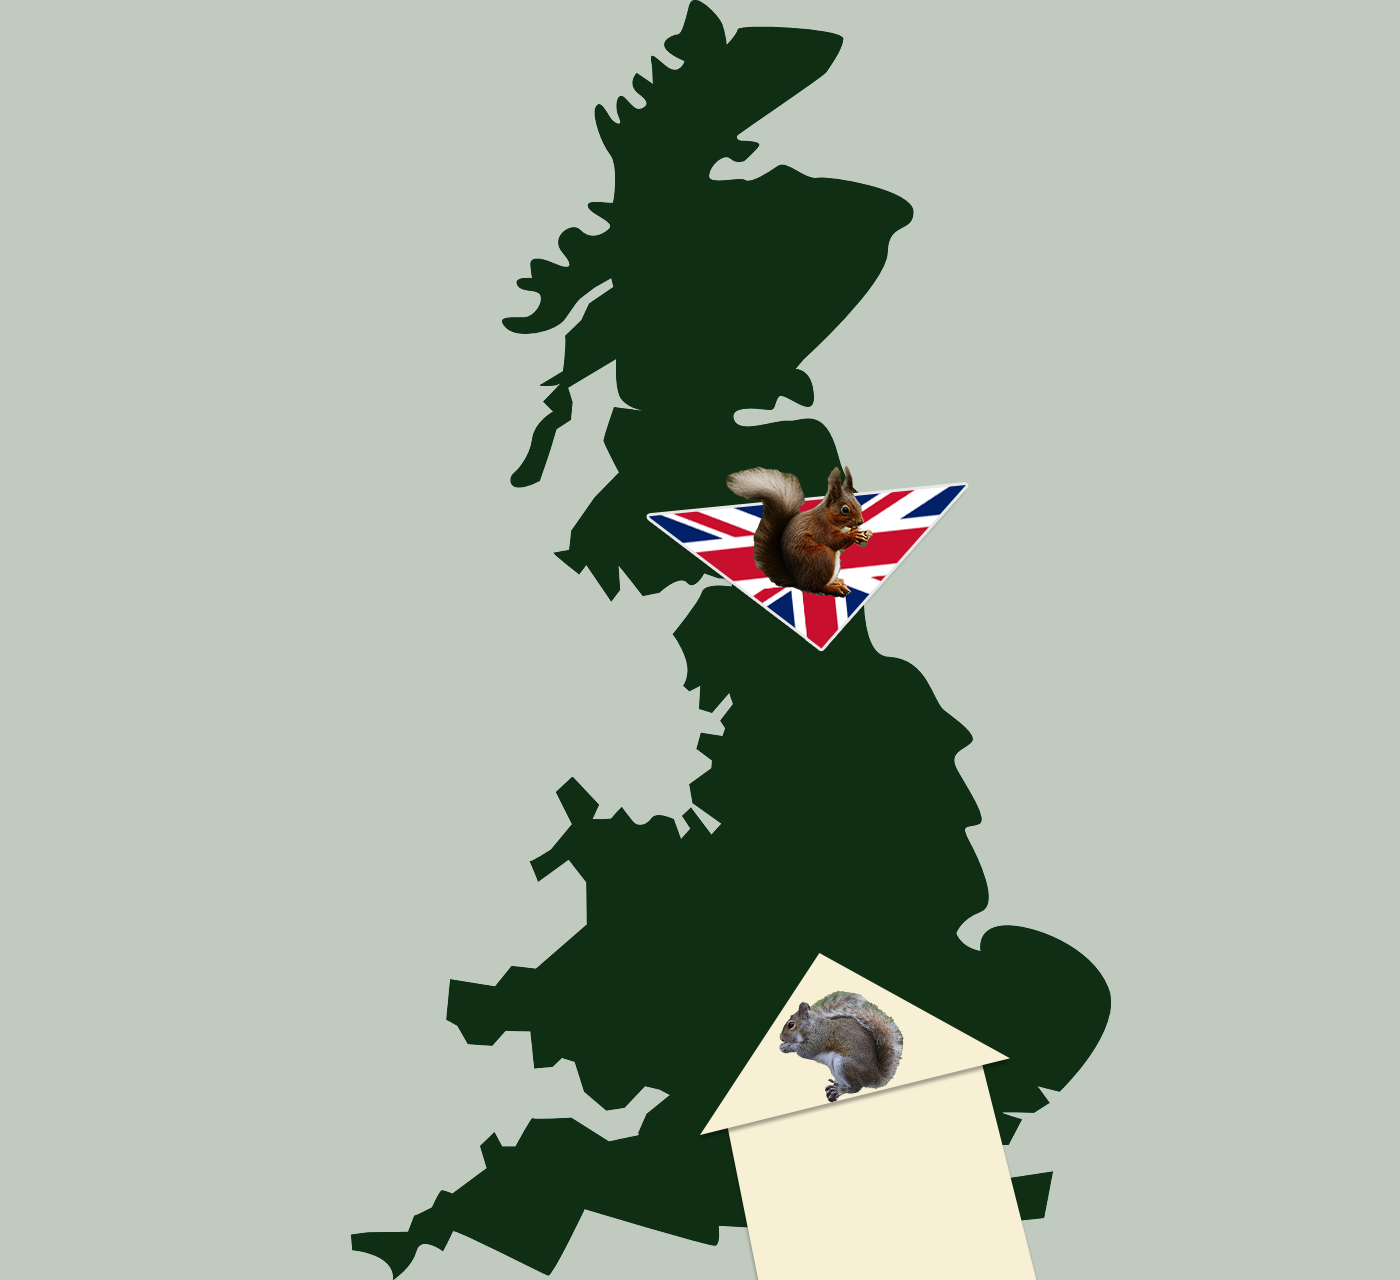
\includegraphics[width=0.4\textwidth]{images/dads-army}
\caption{\textmusicalnote{} \emph{Who do you think you are kidding, Mr Grey Squirrel?} \textmusicalnote}
\label{fig:dads-army}
\end{figure}

\paragraph{Nondimensionalise}
We nondimensionalise by  setting $\v{x} = (D_1/a_1)^{1/2}\hat{\v{x}}$, $t = \hat{t}/a_1$, $\kappa = D_2/D_1$, $\beta = a_2/a_1$, $\gamma_1= c_1/b_2$, $\gamma_2 = c_2/b_1$, $u= \hat{u}/b_1$, $v = \hat{v}/b_2$ (and dropping hats) to get
\begin{subequations}
\label{scaledlotvolpursuit} 
\begin{align}
\pd{u}{t} &= \nabla^2 u +u(1-u-\gamma_1v),\\
\pd{v}{t} &= \kappa\nabla^2 v + \beta v(1-v-\gamma_2u).
\end{align}
\end{subequations}

At this point, you may notice that we haven't picked a winner from $u$ and $v$. But if you recall from \cref{fig:comp-lv-phase-options-traj}, reprinted in \cref{fig:comp-lv-phase-options-traj-3-repeated}, in the homogeneous case, choosing $\gamma_1>1$ and $\gamma_2<1$ makes the stable equilibrium the one where $v$ dominates over $u$. This choice allows us to continue to think of $v$ as the grey squirrels. 

\begin{figure}
\centering
%% Creator: Matplotlib, PGF backend
%%
%% To include the figure in your LaTeX document, write
%%   \input{<filename>.pgf}
%%
%% Make sure the required packages are loaded in your preamble
%%   \usepackage{pgf}
%%
%% and, on pdftex
%%   \usepackage[utf8]{inputenc}\DeclareUnicodeCharacter{2212}{-}
%%
%% or, on luatex and xetex
%%   \usepackage{unicode-math}
%%
%% Figures using additional raster images can only be included by \input if
%% they are in the same directory as the main LaTeX file. For loading figures
%% from other directories you can use the `import` package
%%   \usepackage{import}
%%
%% and then include the figures with
%%   \import{<path to file>}{<filename>.pgf}
%%
%% Matplotlib used the following preamble
%%   \usepackage{fontspec}
%%   \setmainfont{DejaVuSerif.ttf}[Path=/Users/adam/opt/anaconda3/lib/python3.8/site-packages/matplotlib/mpl-data/fonts/ttf/]
%%   \setsansfont{DejaVuSans.ttf}[Path=/Users/adam/opt/anaconda3/lib/python3.8/site-packages/matplotlib/mpl-data/fonts/ttf/]
%%   \setmonofont{DejaVuSansMono.ttf}[Path=/Users/adam/opt/anaconda3/lib/python3.8/site-packages/matplotlib/mpl-data/fonts/ttf/]
%%
\begingroup%
\makeatletter%
\begin{pgfpicture}%
\pgfpathrectangle{\pgfpointorigin}{\pgfqpoint{3.000000in}{2.200000in}}%
\pgfusepath{use as bounding box, clip}%
\begin{pgfscope}%
\pgfsetbuttcap%
\pgfsetmiterjoin%
\definecolor{currentfill}{rgb}{1.000000,1.000000,1.000000}%
\pgfsetfillcolor{currentfill}%
\pgfsetlinewidth{0.000000pt}%
\definecolor{currentstroke}{rgb}{1.000000,1.000000,1.000000}%
\pgfsetstrokecolor{currentstroke}%
\pgfsetdash{}{0pt}%
\pgfpathmoveto{\pgfqpoint{0.000000in}{0.000000in}}%
\pgfpathlineto{\pgfqpoint{3.000000in}{0.000000in}}%
\pgfpathlineto{\pgfqpoint{3.000000in}{2.200000in}}%
\pgfpathlineto{\pgfqpoint{0.000000in}{2.200000in}}%
\pgfpathclose%
\pgfusepath{fill}%
\end{pgfscope}%
\begin{pgfscope}%
\pgfsetbuttcap%
\pgfsetmiterjoin%
\definecolor{currentfill}{rgb}{1.000000,1.000000,1.000000}%
\pgfsetfillcolor{currentfill}%
\pgfsetlinewidth{0.000000pt}%
\definecolor{currentstroke}{rgb}{0.000000,0.000000,0.000000}%
\pgfsetstrokecolor{currentstroke}%
\pgfsetstrokeopacity{0.000000}%
\pgfsetdash{}{0pt}%
\pgfpathmoveto{\pgfqpoint{0.436279in}{0.296600in}}%
\pgfpathlineto{\pgfqpoint{2.966667in}{0.296600in}}%
\pgfpathlineto{\pgfqpoint{2.966667in}{1.968025in}}%
\pgfpathlineto{\pgfqpoint{0.436279in}{1.968025in}}%
\pgfpathclose%
\pgfusepath{fill}%
\end{pgfscope}%
\begin{pgfscope}%
\pgfpathrectangle{\pgfqpoint{0.436279in}{0.296600in}}{\pgfqpoint{2.530388in}{1.671426in}}%
\pgfusepath{clip}%
\pgfsetbuttcap%
\pgfsetroundjoin%
\pgfsetlinewidth{0.702625pt}%
\definecolor{currentstroke}{rgb}{0.121569,0.466667,0.705882}%
\pgfsetstrokecolor{currentstroke}%
\pgfsetdash{{2.590000pt}{1.120000pt}}{0.000000pt}%
\pgfpathmoveto{\pgfqpoint{2.017771in}{0.296600in}}%
\pgfpathlineto{\pgfqpoint{0.436279in}{1.042772in}}%
\pgfusepath{stroke}%
\end{pgfscope}%
\begin{pgfscope}%
\pgfpathrectangle{\pgfqpoint{0.436279in}{0.296600in}}{\pgfqpoint{2.530388in}{1.671426in}}%
\pgfusepath{clip}%
\pgfsetbuttcap%
\pgfsetroundjoin%
\pgfsetlinewidth{0.702625pt}%
\definecolor{currentstroke}{rgb}{1.000000,0.498039,0.054902}%
\pgfsetstrokecolor{currentstroke}%
\pgfsetdash{{2.590000pt}{1.120000pt}}{0.000000pt}%
\pgfpathmoveto{\pgfqpoint{0.436279in}{1.341241in}}%
\pgfpathlineto{\pgfqpoint{2.650368in}{0.296600in}}%
\pgfusepath{stroke}%
\end{pgfscope}%
\begin{pgfscope}%
\pgfsetbuttcap%
\pgfsetroundjoin%
\definecolor{currentfill}{rgb}{0.000000,0.000000,0.000000}%
\pgfsetfillcolor{currentfill}%
\pgfsetlinewidth{0.803000pt}%
\definecolor{currentstroke}{rgb}{0.000000,0.000000,0.000000}%
\pgfsetstrokecolor{currentstroke}%
\pgfsetdash{}{0pt}%
\pgfsys@defobject{currentmarker}{\pgfqpoint{0.000000in}{-0.048611in}}{\pgfqpoint{0.000000in}{0.000000in}}{%
\pgfpathmoveto{\pgfqpoint{0.000000in}{0.000000in}}%
\pgfpathlineto{\pgfqpoint{0.000000in}{-0.048611in}}%
\pgfusepath{stroke,fill}%
}%
\begin{pgfscope}%
\pgfsys@transformshift{0.436279in}{0.296600in}%
\pgfsys@useobject{currentmarker}{}%
\end{pgfscope}%
\end{pgfscope}%
\begin{pgfscope}%
\definecolor{textcolor}{rgb}{0.000000,0.000000,0.000000}%
\pgfsetstrokecolor{textcolor}%
\pgfsetfillcolor{textcolor}%
\pgftext[x=0.436279in,y=0.199377in,,top]{\color{textcolor}\rmfamily\fontsize{12.000000}{14.400000}\selectfont 0}%
\end{pgfscope}%
\begin{pgfscope}%
\pgfsetbuttcap%
\pgfsetroundjoin%
\definecolor{currentfill}{rgb}{0.000000,0.000000,0.000000}%
\pgfsetfillcolor{currentfill}%
\pgfsetlinewidth{0.803000pt}%
\definecolor{currentstroke}{rgb}{0.000000,0.000000,0.000000}%
\pgfsetstrokecolor{currentstroke}%
\pgfsetdash{}{0pt}%
\pgfsys@defobject{currentmarker}{\pgfqpoint{0.000000in}{-0.048611in}}{\pgfqpoint{0.000000in}{0.000000in}}{%
\pgfpathmoveto{\pgfqpoint{0.000000in}{0.000000in}}%
\pgfpathlineto{\pgfqpoint{0.000000in}{-0.048611in}}%
\pgfusepath{stroke,fill}%
}%
\begin{pgfscope}%
\pgfsys@transformshift{2.017771in}{0.296600in}%
\pgfsys@useobject{currentmarker}{}%
\end{pgfscope}%
\end{pgfscope}%
\begin{pgfscope}%
\definecolor{textcolor}{rgb}{0.000000,0.000000,0.000000}%
\pgfsetstrokecolor{textcolor}%
\pgfsetfillcolor{textcolor}%
\pgftext[x=2.017771in,y=0.199377in,,top]{\color{textcolor}\rmfamily\fontsize{12.000000}{14.400000}\selectfont 1}%
\end{pgfscope}%
\begin{pgfscope}%
\pgfsetbuttcap%
\pgfsetroundjoin%
\definecolor{currentfill}{rgb}{0.000000,0.000000,0.000000}%
\pgfsetfillcolor{currentfill}%
\pgfsetlinewidth{0.803000pt}%
\definecolor{currentstroke}{rgb}{0.000000,0.000000,0.000000}%
\pgfsetstrokecolor{currentstroke}%
\pgfsetdash{}{0pt}%
\pgfsys@defobject{currentmarker}{\pgfqpoint{0.000000in}{-0.048611in}}{\pgfqpoint{0.000000in}{0.000000in}}{%
\pgfpathmoveto{\pgfqpoint{0.000000in}{0.000000in}}%
\pgfpathlineto{\pgfqpoint{0.000000in}{-0.048611in}}%
\pgfusepath{stroke,fill}%
}%
\begin{pgfscope}%
\pgfsys@transformshift{2.650368in}{0.296600in}%
\pgfsys@useobject{currentmarker}{}%
\end{pgfscope}%
\end{pgfscope}%
\begin{pgfscope}%
\definecolor{textcolor}{rgb}{0.000000,0.000000,0.000000}%
\pgfsetstrokecolor{textcolor}%
\pgfsetfillcolor{textcolor}%
\pgftext[x=2.650368in,y=0.199377in,,top]{\color{textcolor}\rmfamily\fontsize{12.000000}{14.400000}\selectfont \(\displaystyle 1/\gamma_2\)}%
\end{pgfscope}%
\begin{pgfscope}%
\pgfsetbuttcap%
\pgfsetroundjoin%
\definecolor{currentfill}{rgb}{0.000000,0.000000,0.000000}%
\pgfsetfillcolor{currentfill}%
\pgfsetlinewidth{0.803000pt}%
\definecolor{currentstroke}{rgb}{0.000000,0.000000,0.000000}%
\pgfsetstrokecolor{currentstroke}%
\pgfsetdash{}{0pt}%
\pgfsys@defobject{currentmarker}{\pgfqpoint{-0.048611in}{0.000000in}}{\pgfqpoint{-0.000000in}{0.000000in}}{%
\pgfpathmoveto{\pgfqpoint{-0.000000in}{0.000000in}}%
\pgfpathlineto{\pgfqpoint{-0.048611in}{0.000000in}}%
\pgfusepath{stroke,fill}%
}%
\begin{pgfscope}%
\pgfsys@transformshift{0.436279in}{0.296600in}%
\pgfsys@useobject{currentmarker}{}%
\end{pgfscope}%
\end{pgfscope}%
\begin{pgfscope}%
\definecolor{textcolor}{rgb}{0.000000,0.000000,0.000000}%
\pgfsetstrokecolor{textcolor}%
\pgfsetfillcolor{textcolor}%
\pgftext[x=0.233018in, y=0.233286in, left, base]{\color{textcolor}\rmfamily\fontsize{12.000000}{14.400000}\selectfont 0}%
\end{pgfscope}%
\begin{pgfscope}%
\pgfsetbuttcap%
\pgfsetroundjoin%
\definecolor{currentfill}{rgb}{0.000000,0.000000,0.000000}%
\pgfsetfillcolor{currentfill}%
\pgfsetlinewidth{0.803000pt}%
\definecolor{currentstroke}{rgb}{0.000000,0.000000,0.000000}%
\pgfsetstrokecolor{currentstroke}%
\pgfsetdash{}{0pt}%
\pgfsys@defobject{currentmarker}{\pgfqpoint{-0.048611in}{0.000000in}}{\pgfqpoint{-0.000000in}{0.000000in}}{%
\pgfpathmoveto{\pgfqpoint{-0.000000in}{0.000000in}}%
\pgfpathlineto{\pgfqpoint{-0.048611in}{0.000000in}}%
\pgfusepath{stroke,fill}%
}%
\begin{pgfscope}%
\pgfsys@transformshift{0.436279in}{1.341241in}%
\pgfsys@useobject{currentmarker}{}%
\end{pgfscope}%
\end{pgfscope}%
\begin{pgfscope}%
\definecolor{textcolor}{rgb}{0.000000,0.000000,0.000000}%
\pgfsetstrokecolor{textcolor}%
\pgfsetfillcolor{textcolor}%
\pgftext[x=0.233018in, y=1.277927in, left, base]{\color{textcolor}\rmfamily\fontsize{12.000000}{14.400000}\selectfont 1}%
\end{pgfscope}%
\begin{pgfscope}%
\pgfsetbuttcap%
\pgfsetroundjoin%
\definecolor{currentfill}{rgb}{0.000000,0.000000,0.000000}%
\pgfsetfillcolor{currentfill}%
\pgfsetlinewidth{0.803000pt}%
\definecolor{currentstroke}{rgb}{0.000000,0.000000,0.000000}%
\pgfsetstrokecolor{currentstroke}%
\pgfsetdash{}{0pt}%
\pgfsys@defobject{currentmarker}{\pgfqpoint{-0.048611in}{0.000000in}}{\pgfqpoint{-0.000000in}{0.000000in}}{%
\pgfpathmoveto{\pgfqpoint{-0.000000in}{0.000000in}}%
\pgfpathlineto{\pgfqpoint{-0.048611in}{0.000000in}}%
\pgfusepath{stroke,fill}%
}%
\begin{pgfscope}%
\pgfsys@transformshift{0.436279in}{1.042772in}%
\pgfsys@useobject{currentmarker}{}%
\end{pgfscope}%
\end{pgfscope}%
\begin{pgfscope}%
\definecolor{textcolor}{rgb}{0.000000,0.000000,0.000000}%
\pgfsetstrokecolor{textcolor}%
\pgfsetfillcolor{textcolor}%
\pgftext[x=0.025242in, y=0.980272in, left, base]{\color{textcolor}\rmfamily\fontsize{12.000000}{14.400000}\selectfont \(\displaystyle 1/\gamma_1\)}%
\end{pgfscope}%
\begin{pgfscope}%
\pgfpathrectangle{\pgfqpoint{0.436279in}{0.296600in}}{\pgfqpoint{2.530388in}{1.671426in}}%
\pgfusepath{clip}%
\pgfsetrectcap%
\pgfsetroundjoin%
\pgfsetlinewidth{1.505625pt}%
\definecolor{currentstroke}{rgb}{0.172549,0.627451,0.172549}%
\pgfsetstrokecolor{currentstroke}%
\pgfsetdash{}{0pt}%
\pgfpathmoveto{\pgfqpoint{0.594428in}{0.401064in}}%
\pgfpathlineto{\pgfqpoint{0.631102in}{0.428141in}}%
\pgfpathlineto{\pgfqpoint{0.665260in}{0.454719in}}%
\pgfpathlineto{\pgfqpoint{0.696926in}{0.480783in}}%
\pgfpathlineto{\pgfqpoint{0.724778in}{0.505098in}}%
\pgfpathlineto{\pgfqpoint{0.750355in}{0.528845in}}%
\pgfpathlineto{\pgfqpoint{0.773211in}{0.551499in}}%
\pgfpathlineto{\pgfqpoint{0.795285in}{0.575010in}}%
\pgfpathlineto{\pgfqpoint{0.814168in}{0.596761in}}%
\pgfpathlineto{\pgfqpoint{0.831845in}{0.618933in}}%
\pgfpathlineto{\pgfqpoint{0.846355in}{0.638883in}}%
\pgfpathlineto{\pgfqpoint{0.859582in}{0.658958in}}%
\pgfpathlineto{\pgfqpoint{0.871410in}{0.679065in}}%
\pgfpathlineto{\pgfqpoint{0.880540in}{0.696615in}}%
\pgfpathlineto{\pgfqpoint{0.888489in}{0.714064in}}%
\pgfpathlineto{\pgfqpoint{0.895230in}{0.731361in}}%
\pgfpathlineto{\pgfqpoint{0.900755in}{0.748461in}}%
\pgfpathlineto{\pgfqpoint{0.905070in}{0.765322in}}%
\pgfpathlineto{\pgfqpoint{0.908194in}{0.781908in}}%
\pgfpathlineto{\pgfqpoint{0.910162in}{0.798191in}}%
\pgfpathlineto{\pgfqpoint{0.911013in}{0.814146in}}%
\pgfpathlineto{\pgfqpoint{0.910800in}{0.829753in}}%
\pgfpathlineto{\pgfqpoint{0.909581in}{0.844997in}}%
\pgfpathlineto{\pgfqpoint{0.907035in}{0.861962in}}%
\pgfpathlineto{\pgfqpoint{0.903354in}{0.878432in}}%
\pgfpathlineto{\pgfqpoint{0.898642in}{0.894401in}}%
\pgfpathlineto{\pgfqpoint{0.893001in}{0.909873in}}%
\pgfpathlineto{\pgfqpoint{0.885669in}{0.926689in}}%
\pgfpathlineto{\pgfqpoint{0.877429in}{0.942892in}}%
\pgfpathlineto{\pgfqpoint{0.867369in}{0.960197in}}%
\pgfpathlineto{\pgfqpoint{0.855400in}{0.978411in}}%
\pgfpathlineto{\pgfqpoint{0.841499in}{0.997342in}}%
\pgfpathlineto{\pgfqpoint{0.825715in}{1.016801in}}%
\pgfpathlineto{\pgfqpoint{0.808168in}{1.036608in}}%
\pgfpathlineto{\pgfqpoint{0.787766in}{1.057878in}}%
\pgfpathlineto{\pgfqpoint{0.764770in}{1.080191in}}%
\pgfpathlineto{\pgfqpoint{0.738360in}{1.104235in}}%
\pgfpathlineto{\pgfqpoint{0.706890in}{1.131298in}}%
\pgfpathlineto{\pgfqpoint{0.669663in}{1.161772in}}%
\pgfpathlineto{\pgfqpoint{0.622838in}{1.198588in}}%
\pgfpathlineto{\pgfqpoint{0.552673in}{1.252168in}}%
\pgfpathlineto{\pgfqpoint{0.446025in}{1.333611in}}%
\pgfpathlineto{\pgfqpoint{0.446025in}{1.333611in}}%
\pgfusepath{stroke}%
\end{pgfscope}%
\begin{pgfscope}%
\pgfpathrectangle{\pgfqpoint{0.436279in}{0.296600in}}{\pgfqpoint{2.530388in}{1.671426in}}%
\pgfusepath{clip}%
\pgfsetrectcap%
\pgfsetroundjoin%
\pgfsetlinewidth{1.505625pt}%
\definecolor{currentstroke}{rgb}{0.172549,0.627451,0.172549}%
\pgfsetstrokecolor{currentstroke}%
\pgfsetdash{}{0pt}%
\pgfpathmoveto{\pgfqpoint{0.594428in}{0.714456in}}%
\pgfpathlineto{\pgfqpoint{0.602812in}{0.751112in}}%
\pgfpathlineto{\pgfqpoint{0.610079in}{0.787835in}}%
\pgfpathlineto{\pgfqpoint{0.616075in}{0.824201in}}%
\pgfpathlineto{\pgfqpoint{0.620337in}{0.856621in}}%
\pgfpathlineto{\pgfqpoint{0.623425in}{0.888157in}}%
\pgfpathlineto{\pgfqpoint{0.625336in}{0.918586in}}%
\pgfpathlineto{\pgfqpoint{0.626102in}{0.947726in}}%
\pgfpathlineto{\pgfqpoint{0.625779in}{0.975441in}}%
\pgfpathlineto{\pgfqpoint{0.624448in}{1.001638in}}%
\pgfpathlineto{\pgfqpoint{0.621934in}{1.028641in}}%
\pgfpathlineto{\pgfqpoint{0.618458in}{1.053724in}}%
\pgfpathlineto{\pgfqpoint{0.614168in}{1.076911in}}%
\pgfpathlineto{\pgfqpoint{0.608729in}{1.100113in}}%
\pgfpathlineto{\pgfqpoint{0.602674in}{1.121235in}}%
\pgfpathlineto{\pgfqpoint{0.595609in}{1.141926in}}%
\pgfpathlineto{\pgfqpoint{0.587619in}{1.161864in}}%
\pgfpathlineto{\pgfqpoint{0.578835in}{1.180793in}}%
\pgfpathlineto{\pgfqpoint{0.569424in}{1.198526in}}%
\pgfpathlineto{\pgfqpoint{0.559005in}{1.215839in}}%
\pgfpathlineto{\pgfqpoint{0.547307in}{1.233043in}}%
\pgfpathlineto{\pgfqpoint{0.534769in}{1.249449in}}%
\pgfpathlineto{\pgfqpoint{0.520993in}{1.265578in}}%
\pgfpathlineto{\pgfqpoint{0.506076in}{1.281299in}}%
\pgfpathlineto{\pgfqpoint{0.489459in}{1.297173in}}%
\pgfpathlineto{\pgfqpoint{0.470151in}{1.314029in}}%
\pgfpathlineto{\pgfqpoint{0.445238in}{1.334194in}}%
\pgfpathlineto{\pgfqpoint{0.437690in}{1.340131in}}%
\pgfpathlineto{\pgfqpoint{0.437690in}{1.340131in}}%
\pgfusepath{stroke}%
\end{pgfscope}%
\begin{pgfscope}%
\pgfpathrectangle{\pgfqpoint{0.436279in}{0.296600in}}{\pgfqpoint{2.530388in}{1.671426in}}%
\pgfusepath{clip}%
\pgfsetrectcap%
\pgfsetroundjoin%
\pgfsetlinewidth{1.505625pt}%
\definecolor{currentstroke}{rgb}{0.172549,0.627451,0.172549}%
\pgfsetstrokecolor{currentstroke}%
\pgfsetdash{}{0pt}%
\pgfpathmoveto{\pgfqpoint{0.594428in}{1.027848in}}%
\pgfpathlineto{\pgfqpoint{0.591637in}{1.056751in}}%
\pgfpathlineto{\pgfqpoint{0.587935in}{1.083239in}}%
\pgfpathlineto{\pgfqpoint{0.583488in}{1.107374in}}%
\pgfpathlineto{\pgfqpoint{0.578015in}{1.130990in}}%
\pgfpathlineto{\pgfqpoint{0.571572in}{1.153676in}}%
\pgfpathlineto{\pgfqpoint{0.564264in}{1.175097in}}%
\pgfpathlineto{\pgfqpoint{0.556243in}{1.195007in}}%
\pgfpathlineto{\pgfqpoint{0.547692in}{1.213256in}}%
\pgfpathlineto{\pgfqpoint{0.538322in}{1.230620in}}%
\pgfpathlineto{\pgfqpoint{0.528406in}{1.246699in}}%
\pgfpathlineto{\pgfqpoint{0.517400in}{1.262390in}}%
\pgfpathlineto{\pgfqpoint{0.505499in}{1.277352in}}%
\pgfpathlineto{\pgfqpoint{0.492827in}{1.291483in}}%
\pgfpathlineto{\pgfqpoint{0.478732in}{1.305510in}}%
\pgfpathlineto{\pgfqpoint{0.462738in}{1.319819in}}%
\pgfpathlineto{\pgfqpoint{0.442454in}{1.336378in}}%
\pgfpathlineto{\pgfqpoint{0.436924in}{1.340733in}}%
\pgfpathlineto{\pgfqpoint{0.436924in}{1.340733in}}%
\pgfusepath{stroke}%
\end{pgfscope}%
\begin{pgfscope}%
\pgfpathrectangle{\pgfqpoint{0.436279in}{0.296600in}}{\pgfqpoint{2.530388in}{1.671426in}}%
\pgfusepath{clip}%
\pgfsetrectcap%
\pgfsetroundjoin%
\pgfsetlinewidth{1.505625pt}%
\definecolor{currentstroke}{rgb}{0.172549,0.627451,0.172549}%
\pgfsetstrokecolor{currentstroke}%
\pgfsetdash{}{0pt}%
\pgfpathmoveto{\pgfqpoint{0.752577in}{1.863561in}}%
\pgfpathlineto{\pgfqpoint{0.612505in}{1.521600in}}%
\pgfpathlineto{\pgfqpoint{0.589723in}{1.469913in}}%
\pgfpathlineto{\pgfqpoint{0.571788in}{1.431808in}}%
\pgfpathlineto{\pgfqpoint{0.557228in}{1.403317in}}%
\pgfpathlineto{\pgfqpoint{0.544265in}{1.380405in}}%
\pgfpathlineto{\pgfqpoint{0.533383in}{1.363407in}}%
\pgfpathlineto{\pgfqpoint{0.524078in}{1.350793in}}%
\pgfpathlineto{\pgfqpoint{0.515463in}{1.340911in}}%
\pgfpathlineto{\pgfqpoint{0.507490in}{1.333456in}}%
\pgfpathlineto{\pgfqpoint{0.500114in}{1.328106in}}%
\pgfpathlineto{\pgfqpoint{0.493295in}{1.324536in}}%
\pgfpathlineto{\pgfqpoint{0.486692in}{1.322356in}}%
\pgfpathlineto{\pgfqpoint{0.480397in}{1.321443in}}%
\pgfpathlineto{\pgfqpoint{0.474029in}{1.321640in}}%
\pgfpathlineto{\pgfqpoint{0.467484in}{1.322958in}}%
\pgfpathlineto{\pgfqpoint{0.460466in}{1.325525in}}%
\pgfpathlineto{\pgfqpoint{0.452641in}{1.329621in}}%
\pgfpathlineto{\pgfqpoint{0.443481in}{1.335742in}}%
\pgfpathlineto{\pgfqpoint{0.436723in}{1.340892in}}%
\pgfpathlineto{\pgfqpoint{0.436723in}{1.340892in}}%
\pgfusepath{stroke}%
\end{pgfscope}%
\begin{pgfscope}%
\pgfpathrectangle{\pgfqpoint{0.436279in}{0.296600in}}{\pgfqpoint{2.530388in}{1.671426in}}%
\pgfusepath{clip}%
\pgfsetrectcap%
\pgfsetroundjoin%
\pgfsetlinewidth{1.505625pt}%
\definecolor{currentstroke}{rgb}{0.172549,0.627451,0.172549}%
\pgfsetstrokecolor{currentstroke}%
\pgfsetdash{}{0pt}%
\pgfpathmoveto{\pgfqpoint{1.227025in}{1.863561in}}%
\pgfpathlineto{\pgfqpoint{1.127524in}{1.757159in}}%
\pgfpathlineto{\pgfqpoint{0.867852in}{1.478071in}}%
\pgfpathlineto{\pgfqpoint{0.823127in}{1.432272in}}%
\pgfpathlineto{\pgfqpoint{0.786791in}{1.396676in}}%
\pgfpathlineto{\pgfqpoint{0.756595in}{1.368725in}}%
\pgfpathlineto{\pgfqpoint{0.731023in}{1.346633in}}%
\pgfpathlineto{\pgfqpoint{0.709014in}{1.329117in}}%
\pgfpathlineto{\pgfqpoint{0.689809in}{1.315225in}}%
\pgfpathlineto{\pgfqpoint{0.672850in}{1.304240in}}%
\pgfpathlineto{\pgfqpoint{0.656136in}{1.294777in}}%
\pgfpathlineto{\pgfqpoint{0.641250in}{1.287636in}}%
\pgfpathlineto{\pgfqpoint{0.627865in}{1.282363in}}%
\pgfpathlineto{\pgfqpoint{0.614582in}{1.278295in}}%
\pgfpathlineto{\pgfqpoint{0.601522in}{1.275501in}}%
\pgfpathlineto{\pgfqpoint{0.588780in}{1.273985in}}%
\pgfpathlineto{\pgfqpoint{0.576423in}{1.273693in}}%
\pgfpathlineto{\pgfqpoint{0.564502in}{1.274527in}}%
\pgfpathlineto{\pgfqpoint{0.552383in}{1.276493in}}%
\pgfpathlineto{\pgfqpoint{0.539717in}{1.279728in}}%
\pgfpathlineto{\pgfqpoint{0.526941in}{1.284164in}}%
\pgfpathlineto{\pgfqpoint{0.513543in}{1.290002in}}%
\pgfpathlineto{\pgfqpoint{0.499177in}{1.297492in}}%
\pgfpathlineto{\pgfqpoint{0.483479in}{1.306958in}}%
\pgfpathlineto{\pgfqpoint{0.465781in}{1.318967in}}%
\pgfpathlineto{\pgfqpoint{0.444565in}{1.334776in}}%
\pgfpathlineto{\pgfqpoint{0.437388in}{1.340369in}}%
\pgfpathlineto{\pgfqpoint{0.437388in}{1.340369in}}%
\pgfusepath{stroke}%
\end{pgfscope}%
\begin{pgfscope}%
\pgfpathrectangle{\pgfqpoint{0.436279in}{0.296600in}}{\pgfqpoint{2.530388in}{1.671426in}}%
\pgfusepath{clip}%
\pgfsetrectcap%
\pgfsetroundjoin%
\pgfsetlinewidth{1.505625pt}%
\definecolor{currentstroke}{rgb}{0.172549,0.627451,0.172549}%
\pgfsetstrokecolor{currentstroke}%
\pgfsetdash{}{0pt}%
\pgfpathmoveto{\pgfqpoint{2.017771in}{1.863561in}}%
\pgfpathlineto{\pgfqpoint{1.881437in}{1.784871in}}%
\pgfpathlineto{\pgfqpoint{1.733382in}{1.698140in}}%
\pgfpathlineto{\pgfqpoint{1.562266in}{1.596463in}}%
\pgfpathlineto{\pgfqpoint{1.214399in}{1.389021in}}%
\pgfpathlineto{\pgfqpoint{1.134838in}{1.343331in}}%
\pgfpathlineto{\pgfqpoint{1.078210in}{1.312036in}}%
\pgfpathlineto{\pgfqpoint{1.030559in}{1.286902in}}%
\pgfpathlineto{\pgfqpoint{0.989819in}{1.266617in}}%
\pgfpathlineto{\pgfqpoint{0.954505in}{1.250212in}}%
\pgfpathlineto{\pgfqpoint{0.923525in}{1.236954in}}%
\pgfpathlineto{\pgfqpoint{0.896057in}{1.226279in}}%
\pgfpathlineto{\pgfqpoint{0.868168in}{1.216682in}}%
\pgfpathlineto{\pgfqpoint{0.843333in}{1.209367in}}%
\pgfpathlineto{\pgfqpoint{0.821005in}{1.203929in}}%
\pgfpathlineto{\pgfqpoint{0.800762in}{1.200046in}}%
\pgfpathlineto{\pgfqpoint{0.780068in}{1.197214in}}%
\pgfpathlineto{\pgfqpoint{0.761223in}{1.195721in}}%
\pgfpathlineto{\pgfqpoint{0.742101in}{1.195344in}}%
\pgfpathlineto{\pgfqpoint{0.724594in}{1.196057in}}%
\pgfpathlineto{\pgfqpoint{0.706914in}{1.197846in}}%
\pgfpathlineto{\pgfqpoint{0.689226in}{1.200736in}}%
\pgfpathlineto{\pgfqpoint{0.671667in}{1.204705in}}%
\pgfpathlineto{\pgfqpoint{0.653167in}{1.210063in}}%
\pgfpathlineto{\pgfqpoint{0.634141in}{1.216803in}}%
\pgfpathlineto{\pgfqpoint{0.614956in}{1.224807in}}%
\pgfpathlineto{\pgfqpoint{0.595086in}{1.234298in}}%
\pgfpathlineto{\pgfqpoint{0.573637in}{1.245799in}}%
\pgfpathlineto{\pgfqpoint{0.550535in}{1.259489in}}%
\pgfpathlineto{\pgfqpoint{0.525528in}{1.275626in}}%
\pgfpathlineto{\pgfqpoint{0.497620in}{1.294986in}}%
\pgfpathlineto{\pgfqpoint{0.465660in}{1.318553in}}%
\pgfpathlineto{\pgfqpoint{0.438496in}{1.339500in}}%
\pgfpathlineto{\pgfqpoint{0.438496in}{1.339500in}}%
\pgfusepath{stroke}%
\end{pgfscope}%
\begin{pgfscope}%
\pgfpathrectangle{\pgfqpoint{0.436279in}{0.296600in}}{\pgfqpoint{2.530388in}{1.671426in}}%
\pgfusepath{clip}%
\pgfsetrectcap%
\pgfsetroundjoin%
\pgfsetlinewidth{1.505625pt}%
\definecolor{currentstroke}{rgb}{0.172549,0.627451,0.172549}%
\pgfsetstrokecolor{currentstroke}%
\pgfsetdash{}{0pt}%
\pgfpathmoveto{\pgfqpoint{2.808517in}{1.341241in}}%
\pgfpathlineto{\pgfqpoint{2.467005in}{1.255838in}}%
\pgfpathlineto{\pgfqpoint{1.978771in}{1.133559in}}%
\pgfpathlineto{\pgfqpoint{1.822147in}{1.095571in}}%
\pgfpathlineto{\pgfqpoint{1.714835in}{1.070542in}}%
\pgfpathlineto{\pgfqpoint{1.625624in}{1.050736in}}%
\pgfpathlineto{\pgfqpoint{1.550194in}{1.035019in}}%
\pgfpathlineto{\pgfqpoint{1.485483in}{1.022565in}}%
\pgfpathlineto{\pgfqpoint{1.429260in}{1.012760in}}%
\pgfpathlineto{\pgfqpoint{1.379864in}{1.005133in}}%
\pgfpathlineto{\pgfqpoint{1.329194in}{0.998507in}}%
\pgfpathlineto{\pgfqpoint{1.284585in}{0.993906in}}%
\pgfpathlineto{\pgfqpoint{1.244887in}{0.990981in}}%
\pgfpathlineto{\pgfqpoint{1.209216in}{0.989458in}}%
\pgfpathlineto{\pgfqpoint{1.176884in}{0.989117in}}%
\pgfpathlineto{\pgfqpoint{1.143326in}{0.989948in}}%
\pgfpathlineto{\pgfqpoint{1.112780in}{0.991874in}}%
\pgfpathlineto{\pgfqpoint{1.084743in}{0.994721in}}%
\pgfpathlineto{\pgfqpoint{1.055707in}{0.998844in}}%
\pgfpathlineto{\pgfqpoint{1.028895in}{1.003780in}}%
\pgfpathlineto{\pgfqpoint{1.001286in}{1.010046in}}%
\pgfpathlineto{\pgfqpoint{0.975608in}{1.016983in}}%
\pgfpathlineto{\pgfqpoint{0.949239in}{1.025232in}}%
\pgfpathlineto{\pgfqpoint{0.922370in}{1.034802in}}%
\pgfpathlineto{\pgfqpoint{0.895151in}{1.045666in}}%
\pgfpathlineto{\pgfqpoint{0.865818in}{1.058636in}}%
\pgfpathlineto{\pgfqpoint{0.836625in}{1.072761in}}%
\pgfpathlineto{\pgfqpoint{0.804381in}{1.089655in}}%
\pgfpathlineto{\pgfqpoint{0.771424in}{1.108180in}}%
\pgfpathlineto{\pgfqpoint{0.735447in}{1.129674in}}%
\pgfpathlineto{\pgfqpoint{0.695267in}{1.155021in}}%
\pgfpathlineto{\pgfqpoint{0.651034in}{1.184297in}}%
\pgfpathlineto{\pgfqpoint{0.602743in}{1.217620in}}%
\pgfpathlineto{\pgfqpoint{0.549883in}{1.255467in}}%
\pgfpathlineto{\pgfqpoint{0.494522in}{1.296482in}}%
\pgfpathlineto{\pgfqpoint{0.442123in}{1.336659in}}%
\pgfpathlineto{\pgfqpoint{0.442123in}{1.336659in}}%
\pgfusepath{stroke}%
\end{pgfscope}%
\begin{pgfscope}%
\pgfpathrectangle{\pgfqpoint{0.436279in}{0.296600in}}{\pgfqpoint{2.530388in}{1.671426in}}%
\pgfusepath{clip}%
\pgfsetrectcap%
\pgfsetroundjoin%
\pgfsetlinewidth{1.505625pt}%
\definecolor{currentstroke}{rgb}{0.172549,0.627451,0.172549}%
\pgfsetstrokecolor{currentstroke}%
\pgfsetdash{}{0pt}%
\pgfpathmoveto{\pgfqpoint{2.808517in}{0.818920in}}%
\pgfpathlineto{\pgfqpoint{2.519321in}{0.789221in}}%
\pgfpathlineto{\pgfqpoint{2.330841in}{0.770988in}}%
\pgfpathlineto{\pgfqpoint{2.182498in}{0.757793in}}%
\pgfpathlineto{\pgfqpoint{2.062668in}{0.748323in}}%
\pgfpathlineto{\pgfqpoint{1.963777in}{0.741696in}}%
\pgfpathlineto{\pgfqpoint{1.880679in}{0.737300in}}%
\pgfpathlineto{\pgfqpoint{1.809758in}{0.734694in}}%
\pgfpathlineto{\pgfqpoint{1.748399in}{0.733550in}}%
\pgfpathlineto{\pgfqpoint{1.694664in}{0.733621in}}%
\pgfpathlineto{\pgfqpoint{1.647090in}{0.734715in}}%
\pgfpathlineto{\pgfqpoint{1.604547in}{0.736683in}}%
\pgfpathlineto{\pgfqpoint{1.560968in}{0.739848in}}%
\pgfpathlineto{\pgfqpoint{1.521787in}{0.743852in}}%
\pgfpathlineto{\pgfqpoint{1.486206in}{0.748580in}}%
\pgfpathlineto{\pgfqpoint{1.453594in}{0.753936in}}%
\pgfpathlineto{\pgfqpoint{1.419832in}{0.760617in}}%
\pgfpathlineto{\pgfqpoint{1.388624in}{0.767902in}}%
\pgfpathlineto{\pgfqpoint{1.356398in}{0.776612in}}%
\pgfpathlineto{\pgfqpoint{1.326281in}{0.785883in}}%
\pgfpathlineto{\pgfqpoint{1.295134in}{0.796638in}}%
\pgfpathlineto{\pgfqpoint{1.263072in}{0.808940in}}%
\pgfpathlineto{\pgfqpoint{1.230150in}{0.822828in}}%
\pgfpathlineto{\pgfqpoint{1.196381in}{0.838319in}}%
\pgfpathlineto{\pgfqpoint{1.161758in}{0.855403in}}%
\pgfpathlineto{\pgfqpoint{1.124092in}{0.875219in}}%
\pgfpathlineto{\pgfqpoint{1.083624in}{0.897749in}}%
\pgfpathlineto{\pgfqpoint{1.038593in}{0.924086in}}%
\pgfpathlineto{\pgfqpoint{0.987636in}{0.955204in}}%
\pgfpathlineto{\pgfqpoint{0.929942in}{0.991774in}}%
\pgfpathlineto{\pgfqpoint{0.863861in}{1.035037in}}%
\pgfpathlineto{\pgfqpoint{0.791150in}{1.084002in}}%
\pgfpathlineto{\pgfqpoint{0.712840in}{1.138097in}}%
\pgfpathlineto{\pgfqpoint{0.633847in}{1.194019in}}%
\pgfpathlineto{\pgfqpoint{0.558989in}{1.248358in}}%
\pgfpathlineto{\pgfqpoint{0.491802in}{1.298476in}}%
\pgfpathlineto{\pgfqpoint{0.451549in}{1.329317in}}%
\pgfpathlineto{\pgfqpoint{0.451549in}{1.329317in}}%
\pgfusepath{stroke}%
\end{pgfscope}%
\begin{pgfscope}%
\pgfpathrectangle{\pgfqpoint{0.436279in}{0.296600in}}{\pgfqpoint{2.530388in}{1.671426in}}%
\pgfusepath{clip}%
\pgfsetrectcap%
\pgfsetroundjoin%
\pgfsetlinewidth{1.505625pt}%
\definecolor{currentstroke}{rgb}{0.172549,0.627451,0.172549}%
\pgfsetstrokecolor{currentstroke}%
\pgfsetdash{}{0pt}%
\pgfpathmoveto{\pgfqpoint{1.227025in}{0.401064in}}%
\pgfpathlineto{\pgfqpoint{1.276560in}{0.411461in}}%
\pgfpathlineto{\pgfqpoint{1.322108in}{0.422175in}}%
\pgfpathlineto{\pgfqpoint{1.359866in}{0.432227in}}%
\pgfpathlineto{\pgfqpoint{1.390615in}{0.441523in}}%
\pgfpathlineto{\pgfqpoint{1.417827in}{0.450944in}}%
\pgfpathlineto{\pgfqpoint{1.439259in}{0.459515in}}%
\pgfpathlineto{\pgfqpoint{1.457816in}{0.468160in}}%
\pgfpathlineto{\pgfqpoint{1.471949in}{0.475901in}}%
\pgfpathlineto{\pgfqpoint{1.483926in}{0.483692in}}%
\pgfpathlineto{\pgfqpoint{1.493830in}{0.491530in}}%
\pgfpathlineto{\pgfqpoint{1.500871in}{0.498427in}}%
\pgfpathlineto{\pgfqpoint{1.506467in}{0.505360in}}%
\pgfpathlineto{\pgfqpoint{1.510688in}{0.512330in}}%
\pgfpathlineto{\pgfqpoint{1.513610in}{0.519338in}}%
\pgfpathlineto{\pgfqpoint{1.515306in}{0.526386in}}%
\pgfpathlineto{\pgfqpoint{1.515849in}{0.533476in}}%
\pgfpathlineto{\pgfqpoint{1.515310in}{0.540611in}}%
\pgfpathlineto{\pgfqpoint{1.513461in}{0.548821in}}%
\pgfpathlineto{\pgfqpoint{1.510390in}{0.557096in}}%
\pgfpathlineto{\pgfqpoint{1.505593in}{0.566486in}}%
\pgfpathlineto{\pgfqpoint{1.499495in}{0.575967in}}%
\pgfpathlineto{\pgfqpoint{1.491337in}{0.586613in}}%
\pgfpathlineto{\pgfqpoint{1.480849in}{0.598465in}}%
\pgfpathlineto{\pgfqpoint{1.467801in}{0.611571in}}%
\pgfpathlineto{\pgfqpoint{1.450719in}{0.627102in}}%
\pgfpathlineto{\pgfqpoint{1.429087in}{0.645176in}}%
\pgfpathlineto{\pgfqpoint{1.402489in}{0.665926in}}%
\pgfpathlineto{\pgfqpoint{1.367320in}{0.691872in}}%
\pgfpathlineto{\pgfqpoint{1.321040in}{0.724542in}}%
\pgfpathlineto{\pgfqpoint{1.255536in}{0.769311in}}%
\pgfpathlineto{\pgfqpoint{1.137417in}{0.848439in}}%
\pgfpathlineto{\pgfqpoint{0.943928in}{0.978221in}}%
\pgfpathlineto{\pgfqpoint{0.827638in}{1.057615in}}%
\pgfpathlineto{\pgfqpoint{0.727014in}{1.127624in}}%
\pgfpathlineto{\pgfqpoint{0.636971in}{1.191602in}}%
\pgfpathlineto{\pgfqpoint{0.557843in}{1.249160in}}%
\pgfpathlineto{\pgfqpoint{0.489711in}{1.300057in}}%
\pgfpathlineto{\pgfqpoint{0.483142in}{1.305048in}}%
\pgfpathlineto{\pgfqpoint{0.483142in}{1.305048in}}%
\pgfusepath{stroke}%
\end{pgfscope}%
\begin{pgfscope}%
\pgfsetrectcap%
\pgfsetmiterjoin%
\pgfsetlinewidth{0.803000pt}%
\definecolor{currentstroke}{rgb}{0.000000,0.000000,0.000000}%
\pgfsetstrokecolor{currentstroke}%
\pgfsetdash{}{0pt}%
\pgfpathmoveto{\pgfqpoint{0.436279in}{0.296600in}}%
\pgfpathlineto{\pgfqpoint{0.436279in}{1.968025in}}%
\pgfusepath{stroke}%
\end{pgfscope}%
\begin{pgfscope}%
\pgfsetrectcap%
\pgfsetmiterjoin%
\pgfsetlinewidth{0.803000pt}%
\definecolor{currentstroke}{rgb}{0.000000,0.000000,0.000000}%
\pgfsetstrokecolor{currentstroke}%
\pgfsetdash{}{0pt}%
\pgfpathmoveto{\pgfqpoint{0.436279in}{0.296600in}}%
\pgfpathlineto{\pgfqpoint{2.966667in}{0.296600in}}%
\pgfusepath{stroke}%
\end{pgfscope}%
\begin{pgfscope}%
\definecolor{textcolor}{rgb}{0.000000,0.000000,0.000000}%
\pgfsetstrokecolor{textcolor}%
\pgfsetfillcolor{textcolor}%
\pgftext[x=2.966667in,y=0.199377in,right,top]{\color{textcolor}\rmfamily\fontsize{12.000000}{14.400000}\selectfont \(\displaystyle x\)}%
\end{pgfscope}%
\begin{pgfscope}%
\definecolor{textcolor}{rgb}{0.000000,0.000000,0.000000}%
\pgfsetstrokecolor{textcolor}%
\pgfsetfillcolor{textcolor}%
\pgftext[x=0.339056in,y=1.968025in,right,top]{\color{textcolor}\rmfamily\fontsize{12.000000}{14.400000}\selectfont \(\displaystyle y\)}%
\end{pgfscope}%
\begin{pgfscope}%
\pgfsetroundcap%
\pgfsetroundjoin%
\pgfsetlinewidth{1.003750pt}%
\definecolor{currentstroke}{rgb}{0.172549,0.627451,0.172549}%
\pgfsetstrokecolor{currentstroke}%
\pgfsetdash{}{0pt}%
\pgfpathmoveto{\pgfqpoint{0.909458in}{0.791252in}}%
\pgfpathquadraticcurveto{\pgfqpoint{0.909587in}{0.792412in}}{\pgfqpoint{0.908002in}{0.778138in}}%
\pgfusepath{stroke}%
\end{pgfscope}%
\begin{pgfscope}%
\pgfsetroundcap%
\pgfsetroundjoin%
\definecolor{currentfill}{rgb}{0.172549,0.627451,0.172549}%
\pgfsetfillcolor{currentfill}%
\pgfsetlinewidth{1.003750pt}%
\definecolor{currentstroke}{rgb}{0.172549,0.627451,0.172549}%
\pgfsetstrokecolor{currentstroke}%
\pgfsetdash{}{0pt}%
\pgfpathmoveto{\pgfqpoint{0.847271in}{0.684267in}}%
\pgfpathlineto{\pgfqpoint{0.908002in}{0.778138in}}%
\pgfpathlineto{\pgfqpoint{0.946660in}{0.673231in}}%
\pgfpathlineto{\pgfqpoint{0.847271in}{0.684267in}}%
\pgfpathclose%
\pgfusepath{stroke,fill}%
\end{pgfscope}%
\begin{pgfscope}%
\pgfsetroundcap%
\pgfsetroundjoin%
\pgfsetlinewidth{1.003750pt}%
\definecolor{currentstroke}{rgb}{0.172549,0.627451,0.172549}%
\pgfsetstrokecolor{currentstroke}%
\pgfsetdash{}{0pt}%
\pgfpathmoveto{\pgfqpoint{0.624885in}{0.909585in}}%
\pgfpathquadraticcurveto{\pgfqpoint{0.624966in}{0.911092in}}{\pgfqpoint{0.624214in}{0.897092in}}%
\pgfusepath{stroke}%
\end{pgfscope}%
\begin{pgfscope}%
\pgfsetroundcap%
\pgfsetroundjoin%
\definecolor{currentfill}{rgb}{0.172549,0.627451,0.172549}%
\pgfsetfillcolor{currentfill}%
\pgfsetlinewidth{1.003750pt}%
\definecolor{currentstroke}{rgb}{0.172549,0.627451,0.172549}%
\pgfsetstrokecolor{currentstroke}%
\pgfsetdash{}{0pt}%
\pgfpathmoveto{\pgfqpoint{0.568918in}{0.799920in}}%
\pgfpathlineto{\pgfqpoint{0.624214in}{0.897092in}}%
\pgfpathlineto{\pgfqpoint{0.668774in}{0.794553in}}%
\pgfpathlineto{\pgfqpoint{0.568918in}{0.799920in}}%
\pgfpathclose%
\pgfusepath{stroke,fill}%
\end{pgfscope}%
\begin{pgfscope}%
\pgfsetroundcap%
\pgfsetroundjoin%
\pgfsetlinewidth{1.003750pt}%
\definecolor{currentstroke}{rgb}{0.172549,0.627451,0.172549}%
\pgfsetstrokecolor{currentstroke}%
\pgfsetdash{}{0pt}%
\pgfpathmoveto{\pgfqpoint{0.585794in}{1.095595in}}%
\pgfpathquadraticcurveto{\pgfqpoint{0.585607in}{1.096596in}}{\pgfqpoint{0.588267in}{1.082332in}}%
\pgfusepath{stroke}%
\end{pgfscope}%
\begin{pgfscope}%
\pgfsetroundcap%
\pgfsetroundjoin%
\definecolor{currentfill}{rgb}{0.172549,0.627451,0.172549}%
\pgfsetfillcolor{currentfill}%
\pgfsetlinewidth{1.003750pt}%
\definecolor{currentstroke}{rgb}{0.172549,0.627451,0.172549}%
\pgfsetstrokecolor{currentstroke}%
\pgfsetdash{}{0pt}%
\pgfpathmoveto{\pgfqpoint{0.557444in}{0.974862in}}%
\pgfpathlineto{\pgfqpoint{0.588267in}{1.082332in}}%
\pgfpathlineto{\pgfqpoint{0.655749in}{0.993191in}}%
\pgfpathlineto{\pgfqpoint{0.557444in}{0.974862in}}%
\pgfpathclose%
\pgfusepath{stroke,fill}%
\end{pgfscope}%
\begin{pgfscope}%
\pgfsetroundcap%
\pgfsetroundjoin%
\pgfsetlinewidth{1.003750pt}%
\definecolor{currentstroke}{rgb}{0.172549,0.627451,0.172549}%
\pgfsetstrokecolor{currentstroke}%
\pgfsetdash{}{0pt}%
\pgfpathmoveto{\pgfqpoint{0.634813in}{1.574449in}}%
\pgfpathquadraticcurveto{\pgfqpoint{0.633579in}{1.571487in}}{\pgfqpoint{0.638317in}{1.582858in}}%
\pgfusepath{stroke}%
\end{pgfscope}%
\begin{pgfscope}%
\pgfsetroundcap%
\pgfsetroundjoin%
\definecolor{currentfill}{rgb}{0.172549,0.627451,0.172549}%
\pgfsetfillcolor{currentfill}%
\pgfsetlinewidth{1.003750pt}%
\definecolor{currentstroke}{rgb}{0.172549,0.627451,0.172549}%
\pgfsetstrokecolor{currentstroke}%
\pgfsetdash{}{0pt}%
\pgfpathmoveto{\pgfqpoint{0.722932in}{1.655935in}}%
\pgfpathlineto{\pgfqpoint{0.638317in}{1.582858in}}%
\pgfpathlineto{\pgfqpoint{0.630625in}{1.694397in}}%
\pgfpathlineto{\pgfqpoint{0.722932in}{1.655935in}}%
\pgfpathclose%
\pgfusepath{stroke,fill}%
\end{pgfscope}%
\begin{pgfscope}%
\pgfsetroundcap%
\pgfsetroundjoin%
\pgfsetlinewidth{1.003750pt}%
\definecolor{currentstroke}{rgb}{0.172549,0.627451,0.172549}%
\pgfsetstrokecolor{currentstroke}%
\pgfsetdash{}{0pt}%
\pgfpathmoveto{\pgfqpoint{0.897529in}{1.509255in}}%
\pgfpathquadraticcurveto{\pgfqpoint{0.894398in}{1.505945in}}{\pgfqpoint{0.901938in}{1.513916in}}%
\pgfusepath{stroke}%
\end{pgfscope}%
\begin{pgfscope}%
\pgfsetroundcap%
\pgfsetroundjoin%
\definecolor{currentfill}{rgb}{0.172549,0.627451,0.172549}%
\pgfsetfillcolor{currentfill}%
\pgfsetlinewidth{1.003750pt}%
\definecolor{currentstroke}{rgb}{0.172549,0.627451,0.172549}%
\pgfsetstrokecolor{currentstroke}%
\pgfsetdash{}{0pt}%
\pgfpathmoveto{\pgfqpoint{1.006982in}{1.552201in}}%
\pgfpathlineto{\pgfqpoint{0.901938in}{1.513916in}}%
\pgfpathlineto{\pgfqpoint{0.934336in}{1.620922in}}%
\pgfpathlineto{\pgfqpoint{1.006982in}{1.552201in}}%
\pgfpathclose%
\pgfusepath{stroke,fill}%
\end{pgfscope}%
\begin{pgfscope}%
\pgfsetroundcap%
\pgfsetroundjoin%
\pgfsetlinewidth{1.003750pt}%
\definecolor{currentstroke}{rgb}{0.172549,0.627451,0.172549}%
\pgfsetstrokecolor{currentstroke}%
\pgfsetdash{}{0pt}%
\pgfpathmoveto{\pgfqpoint{1.262024in}{1.416980in}}%
\pgfpathquadraticcurveto{\pgfqpoint{1.255781in}{1.413299in}}{\pgfqpoint{1.262914in}{1.417505in}}%
\pgfusepath{stroke}%
\end{pgfscope}%
\begin{pgfscope}%
\pgfsetroundcap%
\pgfsetroundjoin%
\definecolor{currentfill}{rgb}{0.172549,0.627451,0.172549}%
\pgfsetfillcolor{currentfill}%
\pgfsetlinewidth{1.003750pt}%
\definecolor{currentstroke}{rgb}{0.172549,0.627451,0.172549}%
\pgfsetstrokecolor{currentstroke}%
\pgfsetdash{}{0pt}%
\pgfpathmoveto{\pgfqpoint{1.374451in}{1.425227in}}%
\pgfpathlineto{\pgfqpoint{1.262914in}{1.417505in}}%
\pgfpathlineto{\pgfqpoint{1.323658in}{1.511368in}}%
\pgfpathlineto{\pgfqpoint{1.374451in}{1.425227in}}%
\pgfpathclose%
\pgfusepath{stroke,fill}%
\end{pgfscope}%
\begin{pgfscope}%
\pgfsetroundcap%
\pgfsetroundjoin%
\pgfsetlinewidth{1.003750pt}%
\definecolor{currentstroke}{rgb}{0.172549,0.627451,0.172549}%
\pgfsetstrokecolor{currentstroke}%
\pgfsetdash{}{0pt}%
\pgfpathmoveto{\pgfqpoint{1.765893in}{1.082316in}}%
\pgfpathquadraticcurveto{\pgfqpoint{1.757114in}{1.080277in}}{\pgfqpoint{1.763459in}{1.081751in}}%
\pgfusepath{stroke}%
\end{pgfscope}%
\begin{pgfscope}%
\pgfsetroundcap%
\pgfsetroundjoin%
\definecolor{currentfill}{rgb}{0.172549,0.627451,0.172549}%
\pgfsetfillcolor{currentfill}%
\pgfsetlinewidth{1.003750pt}%
\definecolor{currentstroke}{rgb}{0.172549,0.627451,0.172549}%
\pgfsetstrokecolor{currentstroke}%
\pgfsetdash{}{0pt}%
\pgfpathmoveto{\pgfqpoint{1.872180in}{1.055680in}}%
\pgfpathlineto{\pgfqpoint{1.763459in}{1.081751in}}%
\pgfpathlineto{\pgfqpoint{1.849549in}{1.153085in}}%
\pgfpathlineto{\pgfqpoint{1.872180in}{1.055680in}}%
\pgfpathclose%
\pgfusepath{stroke,fill}%
\end{pgfscope}%
\begin{pgfscope}%
\pgfsetroundcap%
\pgfsetroundjoin%
\pgfsetlinewidth{1.003750pt}%
\definecolor{currentstroke}{rgb}{0.172549,0.627451,0.172549}%
\pgfsetstrokecolor{currentstroke}%
\pgfsetdash{}{0pt}%
\pgfpathmoveto{\pgfqpoint{2.047400in}{0.747218in}}%
\pgfpathquadraticcurveto{\pgfqpoint{2.039969in}{0.746694in}}{\pgfqpoint{2.048028in}{0.747263in}}%
\pgfusepath{stroke}%
\end{pgfscope}%
\begin{pgfscope}%
\pgfsetroundcap%
\pgfsetroundjoin%
\definecolor{currentfill}{rgb}{0.172549,0.627451,0.172549}%
\pgfsetfillcolor{currentfill}%
\pgfsetlinewidth{1.003750pt}%
\definecolor{currentstroke}{rgb}{0.172549,0.627451,0.172549}%
\pgfsetstrokecolor{currentstroke}%
\pgfsetdash{}{0pt}%
\pgfpathmoveto{\pgfqpoint{2.151299in}{0.704424in}}%
\pgfpathlineto{\pgfqpoint{2.048028in}{0.747263in}}%
\pgfpathlineto{\pgfqpoint{2.144261in}{0.804176in}}%
\pgfpathlineto{\pgfqpoint{2.151299in}{0.704424in}}%
\pgfpathclose%
\pgfusepath{stroke,fill}%
\end{pgfscope}%
\begin{pgfscope}%
\pgfsetroundcap%
\pgfsetroundjoin%
\pgfsetlinewidth{1.003750pt}%
\definecolor{currentstroke}{rgb}{0.172549,0.627451,0.172549}%
\pgfsetstrokecolor{currentstroke}%
\pgfsetdash{}{0pt}%
\pgfpathmoveto{\pgfqpoint{1.485275in}{0.484669in}}%
\pgfpathquadraticcurveto{\pgfqpoint{1.485934in}{0.485158in}}{\pgfqpoint{1.474124in}{0.476391in}}%
\pgfusepath{stroke}%
\end{pgfscope}%
\begin{pgfscope}%
\pgfsetroundcap%
\pgfsetroundjoin%
\definecolor{currentfill}{rgb}{0.172549,0.627451,0.172549}%
\pgfsetfillcolor{currentfill}%
\pgfsetlinewidth{1.003750pt}%
\definecolor{currentstroke}{rgb}{0.172549,0.627451,0.172549}%
\pgfsetstrokecolor{currentstroke}%
\pgfsetdash{}{0pt}%
\pgfpathmoveto{\pgfqpoint{1.364028in}{0.456931in}}%
\pgfpathlineto{\pgfqpoint{1.474124in}{0.476391in}}%
\pgfpathlineto{\pgfqpoint{1.423634in}{0.376638in}}%
\pgfpathlineto{\pgfqpoint{1.364028in}{0.456931in}}%
\pgfpathclose%
\pgfusepath{stroke,fill}%
\end{pgfscope}%
\begin{pgfscope}%
\pgfsetbuttcap%
\pgfsetmiterjoin%
\definecolor{currentfill}{rgb}{1.000000,1.000000,1.000000}%
\pgfsetfillcolor{currentfill}%
\pgfsetfillopacity{0.700000}%
\pgfsetlinewidth{0.000000pt}%
\definecolor{currentstroke}{rgb}{0.000000,0.000000,0.000000}%
\pgfsetstrokecolor{currentstroke}%
\pgfsetstrokeopacity{0.700000}%
\pgfsetdash{}{0pt}%
\pgfpathmoveto{\pgfqpoint{1.820769in}{1.169713in}}%
\pgfpathlineto{\pgfqpoint{2.214773in}{1.169713in}}%
\pgfpathlineto{\pgfqpoint{2.214773in}{1.512768in}}%
\pgfpathlineto{\pgfqpoint{1.820769in}{1.512768in}}%
\pgfpathclose%
\pgfusepath{fill}%
\end{pgfscope}%
\begin{pgfscope}%
\definecolor{textcolor}{rgb}{0.000000,0.000000,0.000000}%
\pgfsetstrokecolor{textcolor}%
\pgfsetfillcolor{textcolor}%
\pgftext[x=1.876324in, y=1.372794in, left, base]{\color{textcolor}\rmfamily\fontsize{8.000000}{9.600000}\selectfont \(\displaystyle \dot{x}<0\)}%
\end{pgfscope}%
\begin{pgfscope}%
\definecolor{textcolor}{rgb}{0.000000,0.000000,0.000000}%
\pgfsetstrokecolor{textcolor}%
\pgfsetfillcolor{textcolor}%
\pgftext[x=1.878382in, y=1.248380in, left, base]{\color{textcolor}\rmfamily\fontsize{8.000000}{9.600000}\selectfont \(\displaystyle \dot{y} < 0\)}%
\end{pgfscope}%
\begin{pgfscope}%
\pgfsetbuttcap%
\pgfsetmiterjoin%
\definecolor{currentfill}{rgb}{1.000000,1.000000,1.000000}%
\pgfsetfillcolor{currentfill}%
\pgfsetfillopacity{0.700000}%
\pgfsetlinewidth{0.000000pt}%
\definecolor{currentstroke}{rgb}{0.000000,0.000000,0.000000}%
\pgfsetstrokecolor{currentstroke}%
\pgfsetstrokeopacity{0.700000}%
\pgfsetdash{}{0pt}%
\pgfpathmoveto{\pgfqpoint{0.555575in}{0.334000in}}%
\pgfpathlineto{\pgfqpoint{0.949579in}{0.334000in}}%
\pgfpathlineto{\pgfqpoint{0.949579in}{0.677055in}}%
\pgfpathlineto{\pgfqpoint{0.555575in}{0.677055in}}%
\pgfpathclose%
\pgfusepath{fill}%
\end{pgfscope}%
\begin{pgfscope}%
\definecolor{textcolor}{rgb}{0.000000,0.000000,0.000000}%
\pgfsetstrokecolor{textcolor}%
\pgfsetfillcolor{textcolor}%
\pgftext[x=0.611130in, y=0.537081in, left, base]{\color{textcolor}\rmfamily\fontsize{8.000000}{9.600000}\selectfont \(\displaystyle \dot{x}>0\)}%
\end{pgfscope}%
\begin{pgfscope}%
\definecolor{textcolor}{rgb}{0.000000,0.000000,0.000000}%
\pgfsetstrokecolor{textcolor}%
\pgfsetfillcolor{textcolor}%
\pgftext[x=0.613188in, y=0.412667in, left, base]{\color{textcolor}\rmfamily\fontsize{8.000000}{9.600000}\selectfont \(\displaystyle \dot{y} > 0\)}%
\end{pgfscope}%
\begin{pgfscope}%
\pgfsetbuttcap%
\pgfsetmiterjoin%
\definecolor{currentfill}{rgb}{1.000000,1.000000,1.000000}%
\pgfsetfillcolor{currentfill}%
\pgfsetfillopacity{0.700000}%
\pgfsetlinewidth{0.000000pt}%
\definecolor{currentstroke}{rgb}{0.000000,0.000000,0.000000}%
\pgfsetstrokecolor{currentstroke}%
\pgfsetstrokeopacity{0.700000}%
\pgfsetdash{}{0pt}%
\pgfpathmoveto{\pgfqpoint{1.030023in}{0.647392in}}%
\pgfpathlineto{\pgfqpoint{1.424027in}{0.647392in}}%
\pgfpathlineto{\pgfqpoint{1.424027in}{0.990448in}}%
\pgfpathlineto{\pgfqpoint{1.030023in}{0.990448in}}%
\pgfpathclose%
\pgfusepath{fill}%
\end{pgfscope}%
\begin{pgfscope}%
\definecolor{textcolor}{rgb}{0.000000,0.000000,0.000000}%
\pgfsetstrokecolor{textcolor}%
\pgfsetfillcolor{textcolor}%
\pgftext[x=1.085578in, y=0.850474in, left, base]{\color{textcolor}\rmfamily\fontsize{8.000000}{9.600000}\selectfont \(\displaystyle \dot{x}<0\)}%
\end{pgfscope}%
\begin{pgfscope}%
\definecolor{textcolor}{rgb}{0.000000,0.000000,0.000000}%
\pgfsetstrokecolor{textcolor}%
\pgfsetfillcolor{textcolor}%
\pgftext[x=1.087636in, y=0.726060in, left, base]{\color{textcolor}\rmfamily\fontsize{8.000000}{9.600000}\selectfont \(\displaystyle \dot{y} > 0\)}%
\end{pgfscope}%
\begin{pgfscope}%
\definecolor{textcolor}{rgb}{0.000000,0.000000,0.000000}%
\pgfsetstrokecolor{textcolor}%
\pgfsetfillcolor{textcolor}%
\pgftext[x=1.701473in,y=2.051359in,,base]{\color{textcolor}\rmfamily\fontsize{12.000000}{14.400000}\selectfont \(\displaystyle \gamma_1>1\), \(\displaystyle \gamma_2<1\)}%
\end{pgfscope}%
\begin{pgfscope}%
\pgfsetbuttcap%
\pgfsetroundjoin%
\pgfsetlinewidth{0.702625pt}%
\definecolor{currentstroke}{rgb}{0.121569,0.466667,0.705882}%
\pgfsetstrokecolor{currentstroke}%
\pgfsetdash{{2.590000pt}{1.120000pt}}{0.000000pt}%
\pgfpathmoveto{\pgfqpoint{0.436279in}{0.296600in}}%
\pgfpathlineto{\pgfqpoint{0.436279in}{1.968025in}}%
\pgfusepath{stroke}%
\end{pgfscope}%
\begin{pgfscope}%
\pgfsetbuttcap%
\pgfsetroundjoin%
\pgfsetlinewidth{0.702625pt}%
\definecolor{currentstroke}{rgb}{1.000000,0.498039,0.054902}%
\pgfsetstrokecolor{currentstroke}%
\pgfsetdash{{2.590000pt}{1.120000pt}}{0.000000pt}%
\pgfpathmoveto{\pgfqpoint{0.436279in}{0.296600in}}%
\pgfpathlineto{\pgfqpoint{2.966667in}{0.296600in}}%
\pgfusepath{stroke}%
\end{pgfscope}%
\begin{pgfscope}%
\pgfsetbuttcap%
\pgfsetroundjoin%
\definecolor{currentfill}{rgb}{1.000000,1.000000,1.000000}%
\pgfsetfillcolor{currentfill}%
\pgfsetlinewidth{1.003750pt}%
\definecolor{currentstroke}{rgb}{0.000000,0.000000,0.000000}%
\pgfsetstrokecolor{currentstroke}%
\pgfsetdash{}{0pt}%
\pgfsys@defobject{currentmarker}{\pgfqpoint{-0.041667in}{-0.041667in}}{\pgfqpoint{0.041667in}{0.041667in}}{%
\pgfpathmoveto{\pgfqpoint{0.000000in}{-0.041667in}}%
\pgfpathcurveto{\pgfqpoint{0.011050in}{-0.041667in}}{\pgfqpoint{0.021649in}{-0.037276in}}{\pgfqpoint{0.029463in}{-0.029463in}}%
\pgfpathcurveto{\pgfqpoint{0.037276in}{-0.021649in}}{\pgfqpoint{0.041667in}{-0.011050in}}{\pgfqpoint{0.041667in}{0.000000in}}%
\pgfpathcurveto{\pgfqpoint{0.041667in}{0.011050in}}{\pgfqpoint{0.037276in}{0.021649in}}{\pgfqpoint{0.029463in}{0.029463in}}%
\pgfpathcurveto{\pgfqpoint{0.021649in}{0.037276in}}{\pgfqpoint{0.011050in}{0.041667in}}{\pgfqpoint{0.000000in}{0.041667in}}%
\pgfpathcurveto{\pgfqpoint{-0.011050in}{0.041667in}}{\pgfqpoint{-0.021649in}{0.037276in}}{\pgfqpoint{-0.029463in}{0.029463in}}%
\pgfpathcurveto{\pgfqpoint{-0.037276in}{0.021649in}}{\pgfqpoint{-0.041667in}{0.011050in}}{\pgfqpoint{-0.041667in}{0.000000in}}%
\pgfpathcurveto{\pgfqpoint{-0.041667in}{-0.011050in}}{\pgfqpoint{-0.037276in}{-0.021649in}}{\pgfqpoint{-0.029463in}{-0.029463in}}%
\pgfpathcurveto{\pgfqpoint{-0.021649in}{-0.037276in}}{\pgfqpoint{-0.011050in}{-0.041667in}}{\pgfqpoint{0.000000in}{-0.041667in}}%
\pgfpathclose%
\pgfusepath{stroke,fill}%
}%
\begin{pgfscope}%
\pgfsys@transformshift{0.436279in}{0.296600in}%
\pgfsys@useobject{currentmarker}{}%
\end{pgfscope}%
\end{pgfscope}%
\begin{pgfscope}%
\pgfsetbuttcap%
\pgfsetroundjoin%
\definecolor{currentfill}{rgb}{1.000000,1.000000,1.000000}%
\pgfsetfillcolor{currentfill}%
\pgfsetlinewidth{1.003750pt}%
\definecolor{currentstroke}{rgb}{0.000000,0.000000,0.000000}%
\pgfsetstrokecolor{currentstroke}%
\pgfsetdash{}{0pt}%
\pgfsys@defobject{currentmarker}{\pgfqpoint{-0.041667in}{-0.041667in}}{\pgfqpoint{0.041667in}{0.041667in}}{%
\pgfpathmoveto{\pgfqpoint{0.000000in}{-0.041667in}}%
\pgfpathcurveto{\pgfqpoint{0.011050in}{-0.041667in}}{\pgfqpoint{0.021649in}{-0.037276in}}{\pgfqpoint{0.029463in}{-0.029463in}}%
\pgfpathcurveto{\pgfqpoint{0.037276in}{-0.021649in}}{\pgfqpoint{0.041667in}{-0.011050in}}{\pgfqpoint{0.041667in}{0.000000in}}%
\pgfpathcurveto{\pgfqpoint{0.041667in}{0.011050in}}{\pgfqpoint{0.037276in}{0.021649in}}{\pgfqpoint{0.029463in}{0.029463in}}%
\pgfpathcurveto{\pgfqpoint{0.021649in}{0.037276in}}{\pgfqpoint{0.011050in}{0.041667in}}{\pgfqpoint{0.000000in}{0.041667in}}%
\pgfpathcurveto{\pgfqpoint{-0.011050in}{0.041667in}}{\pgfqpoint{-0.021649in}{0.037276in}}{\pgfqpoint{-0.029463in}{0.029463in}}%
\pgfpathcurveto{\pgfqpoint{-0.037276in}{0.021649in}}{\pgfqpoint{-0.041667in}{0.011050in}}{\pgfqpoint{-0.041667in}{0.000000in}}%
\pgfpathcurveto{\pgfqpoint{-0.041667in}{-0.011050in}}{\pgfqpoint{-0.037276in}{-0.021649in}}{\pgfqpoint{-0.029463in}{-0.029463in}}%
\pgfpathcurveto{\pgfqpoint{-0.021649in}{-0.037276in}}{\pgfqpoint{-0.011050in}{-0.041667in}}{\pgfqpoint{0.000000in}{-0.041667in}}%
\pgfpathclose%
\pgfusepath{stroke,fill}%
}%
\begin{pgfscope}%
\pgfsys@transformshift{2.017771in}{0.296600in}%
\pgfsys@useobject{currentmarker}{}%
\end{pgfscope}%
\end{pgfscope}%
\begin{pgfscope}%
\pgfsetbuttcap%
\pgfsetroundjoin%
\definecolor{currentfill}{rgb}{0.000000,0.000000,0.000000}%
\pgfsetfillcolor{currentfill}%
\pgfsetlinewidth{1.003750pt}%
\definecolor{currentstroke}{rgb}{0.000000,0.000000,0.000000}%
\pgfsetstrokecolor{currentstroke}%
\pgfsetdash{}{0pt}%
\pgfsys@defobject{currentmarker}{\pgfqpoint{-0.041667in}{-0.041667in}}{\pgfqpoint{0.041667in}{0.041667in}}{%
\pgfpathmoveto{\pgfqpoint{0.000000in}{-0.041667in}}%
\pgfpathcurveto{\pgfqpoint{0.011050in}{-0.041667in}}{\pgfqpoint{0.021649in}{-0.037276in}}{\pgfqpoint{0.029463in}{-0.029463in}}%
\pgfpathcurveto{\pgfqpoint{0.037276in}{-0.021649in}}{\pgfqpoint{0.041667in}{-0.011050in}}{\pgfqpoint{0.041667in}{0.000000in}}%
\pgfpathcurveto{\pgfqpoint{0.041667in}{0.011050in}}{\pgfqpoint{0.037276in}{0.021649in}}{\pgfqpoint{0.029463in}{0.029463in}}%
\pgfpathcurveto{\pgfqpoint{0.021649in}{0.037276in}}{\pgfqpoint{0.011050in}{0.041667in}}{\pgfqpoint{0.000000in}{0.041667in}}%
\pgfpathcurveto{\pgfqpoint{-0.011050in}{0.041667in}}{\pgfqpoint{-0.021649in}{0.037276in}}{\pgfqpoint{-0.029463in}{0.029463in}}%
\pgfpathcurveto{\pgfqpoint{-0.037276in}{0.021649in}}{\pgfqpoint{-0.041667in}{0.011050in}}{\pgfqpoint{-0.041667in}{0.000000in}}%
\pgfpathcurveto{\pgfqpoint{-0.041667in}{-0.011050in}}{\pgfqpoint{-0.037276in}{-0.021649in}}{\pgfqpoint{-0.029463in}{-0.029463in}}%
\pgfpathcurveto{\pgfqpoint{-0.021649in}{-0.037276in}}{\pgfqpoint{-0.011050in}{-0.041667in}}{\pgfqpoint{0.000000in}{-0.041667in}}%
\pgfpathclose%
\pgfusepath{stroke,fill}%
}%
\begin{pgfscope}%
\pgfsys@transformshift{0.436279in}{1.341241in}%
\pgfsys@useobject{currentmarker}{}%
\end{pgfscope}%
\end{pgfscope}%
\end{pgfpicture}%
\makeatother%
\endgroup%

\caption{In the homogeneous case, with $\gamma_1>1$ and $\gamma_2<1$, it appears that there should be a trajectory from $(1,0)$ to $(0,1)$. (Figure repeated from \cref{fig:comp-lv-phase-options-traj}(c))}
\label{fig:comp-lv-phase-options-traj-3-repeated}
\end{figure}

In the homogeneous case, as we can see in \cref{fig:comp-lv-phase-options-traj-3-repeated}, there are three equilibria:
\begin{itemize}
	\item $(0,0)$, an unstable node,
	\item $(0,1)$, a stable node,
	\item $(1,0)$, a saddle point.
\end{itemize}
From looking at the phase plane, or by thinking about trajectories leaving unstable equilibria, we can see that there are trajectories between our equilibria: 
\begin{enumerate}[label=(\roman*)]
	\item from $(0,0)$ to $(0,1)$ (a vertical line going upwards),
	\item from $(1,0)$ to $(0,1)$.
\end{enumerate}
The first case is quite boring: it's just the growth of the grey population in the absence of reds. This second case is more interesting, as it corresponds to the shift from red domination to grey domination in the homogeneous system. Let's assume a 1D Britain (Durham will be about $x=L/2$... yes, I know, you'd think larger but Scotland is just really big) and let's look for travelling wave solutions to this more interesting case.

Let's consider the boundary conditions. If we, once again, choose to place the stable state at $x\to-\infty$, then we expect this region to grow and for the travelling wave to therefore move \emph{rightwards}. (This is the usual choice in the community.) We therefore look for functions $u(z),v(z)$ where $z= x-ct$. 

With this assumption, \cref{scaledlotvolpursuit} takes the form
\begin{subequations}
\begin{align}
\fdd{u}{z}+c\fd{u}{z} + u(1 - u - \gamma_1v) &= 0,\\
\kappa\fdd{v}{z}+c\fd{v}{z} + \beta v(1 - v -\gamma_2u) &= 0.\label{fk-grey-squirrel}
\end{align}
\end{subequations}
with boundary conditions
\begin{equation}
	(u,v)\to(0,1)\text{ as }z\to-\infty, \qquad (u,v)\to(1,0)\text{ as }z\to\infty,
\end{equation}
implying that a travelling wave acts between these two extremes, and travels rightwards with a speed $c$, to be determined: this idea is illustrated in \cref{fig:fk-travelling-wave-intuition-2}(a).
\begin{figure}
\centering
%% Creator: Matplotlib, PGF backend
%%
%% To include the figure in your LaTeX document, write
%%   \input{<filename>.pgf}
%%
%% Make sure the required packages are loaded in your preamble
%%   \usepackage{pgf}
%%
%% and, on pdftex
%%   \usepackage[utf8]{inputenc}\DeclareUnicodeCharacter{2212}{-}
%%
%% or, on luatex and xetex
%%   \usepackage{unicode-math}
%%
%% Figures using additional raster images can only be included by \input if
%% they are in the same directory as the main LaTeX file. For loading figures
%% from other directories you can use the `import` package
%%   \usepackage{import}
%%
%% and then include the figures with
%%   \import{<path to file>}{<filename>.pgf}
%%
%% Matplotlib used the following preamble
%%   \usepackage{fontspec}
%%   \setmainfont{DejaVuSerif.ttf}[Path=/Users/adam/opt/anaconda3/lib/python3.8/site-packages/matplotlib/mpl-data/fonts/ttf/]
%%   \setsansfont{DejaVuSans.ttf}[Path=/Users/adam/opt/anaconda3/lib/python3.8/site-packages/matplotlib/mpl-data/fonts/ttf/]
%%   \setmonofont{DejaVuSansMono.ttf}[Path=/Users/adam/opt/anaconda3/lib/python3.8/site-packages/matplotlib/mpl-data/fonts/ttf/]
%%
\begingroup%
\makeatletter%
\begin{pgfpicture}%
\pgfpathrectangle{\pgfpointorigin}{\pgfqpoint{3.000000in}{2.200000in}}%
\pgfusepath{use as bounding box, clip}%
\begin{pgfscope}%
\pgfsetbuttcap%
\pgfsetmiterjoin%
\definecolor{currentfill}{rgb}{1.000000,1.000000,1.000000}%
\pgfsetfillcolor{currentfill}%
\pgfsetlinewidth{0.000000pt}%
\definecolor{currentstroke}{rgb}{1.000000,1.000000,1.000000}%
\pgfsetstrokecolor{currentstroke}%
\pgfsetdash{}{0pt}%
\pgfpathmoveto{\pgfqpoint{0.000000in}{0.000000in}}%
\pgfpathlineto{\pgfqpoint{3.000000in}{0.000000in}}%
\pgfpathlineto{\pgfqpoint{3.000000in}{2.200000in}}%
\pgfpathlineto{\pgfqpoint{0.000000in}{2.200000in}}%
\pgfpathclose%
\pgfusepath{fill}%
\end{pgfscope}%
\begin{pgfscope}%
\pgfsetbuttcap%
\pgfsetmiterjoin%
\definecolor{currentfill}{rgb}{1.000000,1.000000,1.000000}%
\pgfsetfillcolor{currentfill}%
\pgfsetlinewidth{0.000000pt}%
\definecolor{currentstroke}{rgb}{0.000000,0.000000,0.000000}%
\pgfsetstrokecolor{currentstroke}%
\pgfsetstrokeopacity{0.000000}%
\pgfsetdash{}{0pt}%
\pgfpathmoveto{\pgfqpoint{0.033333in}{0.278150in}}%
\pgfpathlineto{\pgfqpoint{2.966667in}{0.278150in}}%
\pgfpathlineto{\pgfqpoint{2.966667in}{2.166667in}}%
\pgfpathlineto{\pgfqpoint{0.033333in}{2.166667in}}%
\pgfpathclose%
\pgfusepath{fill}%
\end{pgfscope}%
\begin{pgfscope}%
\pgfsetbuttcap%
\pgfsetroundjoin%
\definecolor{currentfill}{rgb}{0.000000,0.000000,0.000000}%
\pgfsetfillcolor{currentfill}%
\pgfsetlinewidth{0.803000pt}%
\definecolor{currentstroke}{rgb}{0.000000,0.000000,0.000000}%
\pgfsetstrokecolor{currentstroke}%
\pgfsetdash{}{0pt}%
\pgfsys@defobject{currentmarker}{\pgfqpoint{0.000000in}{-0.048611in}}{\pgfqpoint{0.000000in}{0.000000in}}{%
\pgfpathmoveto{\pgfqpoint{0.000000in}{0.000000in}}%
\pgfpathlineto{\pgfqpoint{0.000000in}{-0.048611in}}%
\pgfusepath{stroke,fill}%
}%
\begin{pgfscope}%
\pgfsys@transformshift{1.492703in}{0.278150in}%
\pgfsys@useobject{currentmarker}{}%
\end{pgfscope}%
\end{pgfscope}%
\begin{pgfscope}%
\definecolor{textcolor}{rgb}{0.000000,0.000000,0.000000}%
\pgfsetstrokecolor{textcolor}%
\pgfsetfillcolor{textcolor}%
\pgftext[x=1.492703in,y=0.180927in,,top]{\color{textcolor}\rmfamily\fontsize{12.000000}{14.400000}\selectfont 0}%
\end{pgfscope}%
\begin{pgfscope}%
\pgfsetbuttcap%
\pgfsetroundjoin%
\definecolor{currentfill}{rgb}{0.000000,0.000000,0.000000}%
\pgfsetfillcolor{currentfill}%
\pgfsetlinewidth{0.803000pt}%
\definecolor{currentstroke}{rgb}{0.000000,0.000000,0.000000}%
\pgfsetstrokecolor{currentstroke}%
\pgfsetdash{}{0pt}%
\pgfsys@defobject{currentmarker}{\pgfqpoint{-0.048611in}{0.000000in}}{\pgfqpoint{-0.000000in}{0.000000in}}{%
\pgfpathmoveto{\pgfqpoint{-0.000000in}{0.000000in}}%
\pgfpathlineto{\pgfqpoint{-0.048611in}{0.000000in}}%
\pgfusepath{stroke,fill}%
}%
\begin{pgfscope}%
\pgfsys@transformshift{1.492703in}{0.278150in}%
\pgfsys@useobject{currentmarker}{}%
\end{pgfscope}%
\end{pgfscope}%
\begin{pgfscope}%
\definecolor{textcolor}{rgb}{0.000000,0.000000,0.000000}%
\pgfsetstrokecolor{textcolor}%
\pgfsetfillcolor{textcolor}%
\pgftext[x=1.289442in, y=0.214836in, left, base]{\color{textcolor}\rmfamily\fontsize{12.000000}{14.400000}\selectfont 0}%
\end{pgfscope}%
\begin{pgfscope}%
\pgfsetbuttcap%
\pgfsetroundjoin%
\definecolor{currentfill}{rgb}{0.000000,0.000000,0.000000}%
\pgfsetfillcolor{currentfill}%
\pgfsetlinewidth{0.803000pt}%
\definecolor{currentstroke}{rgb}{0.000000,0.000000,0.000000}%
\pgfsetstrokecolor{currentstroke}%
\pgfsetdash{}{0pt}%
\pgfsys@defobject{currentmarker}{\pgfqpoint{-0.048611in}{0.000000in}}{\pgfqpoint{-0.000000in}{0.000000in}}{%
\pgfpathmoveto{\pgfqpoint{-0.000000in}{0.000000in}}%
\pgfpathlineto{\pgfqpoint{-0.048611in}{0.000000in}}%
\pgfusepath{stroke,fill}%
}%
\begin{pgfscope}%
\pgfsys@transformshift{1.492703in}{1.851914in}%
\pgfsys@useobject{currentmarker}{}%
\end{pgfscope}%
\end{pgfscope}%
\begin{pgfscope}%
\definecolor{textcolor}{rgb}{0.000000,0.000000,0.000000}%
\pgfsetstrokecolor{textcolor}%
\pgfsetfillcolor{textcolor}%
\pgftext[x=1.289442in, y=1.788600in, left, base]{\color{textcolor}\rmfamily\fontsize{12.000000}{14.400000}\selectfont 1}%
\end{pgfscope}%
\begin{pgfscope}%
\pgfsetrectcap%
\pgfsetmiterjoin%
\pgfsetlinewidth{0.803000pt}%
\definecolor{currentstroke}{rgb}{0.000000,0.000000,0.000000}%
\pgfsetstrokecolor{currentstroke}%
\pgfsetdash{}{0pt}%
\pgfpathmoveto{\pgfqpoint{1.492703in}{0.278150in}}%
\pgfpathlineto{\pgfqpoint{1.492703in}{2.166667in}}%
\pgfusepath{stroke}%
\end{pgfscope}%
\begin{pgfscope}%
\pgfsetrectcap%
\pgfsetmiterjoin%
\pgfsetlinewidth{0.803000pt}%
\definecolor{currentstroke}{rgb}{0.000000,0.000000,0.000000}%
\pgfsetstrokecolor{currentstroke}%
\pgfsetdash{}{0pt}%
\pgfpathmoveto{\pgfqpoint{0.033333in}{0.278150in}}%
\pgfpathlineto{\pgfqpoint{2.966667in}{0.278150in}}%
\pgfusepath{stroke}%
\end{pgfscope}%
\begin{pgfscope}%
\definecolor{textcolor}{rgb}{0.000000,0.000000,0.000000}%
\pgfsetstrokecolor{textcolor}%
\pgfsetfillcolor{textcolor}%
\pgftext[x=2.966667in,y=0.180927in,right,top]{\color{textcolor}\rmfamily\fontsize{12.000000}{14.400000}\selectfont \(\displaystyle z\)}%
\end{pgfscope}%
\begin{pgfscope}%
\definecolor{textcolor}{rgb}{0.000000,0.000000,0.000000}%
\pgfsetstrokecolor{textcolor}%
\pgfsetfillcolor{textcolor}%
\pgftext[x=1.402778in,y=2.166667in,right,top]{\color{textcolor}\rmfamily\fontsize{12.000000}{14.400000}\selectfont \(\displaystyle u,v\)}%
\end{pgfscope}%
\begin{pgfscope}%
\definecolor{textcolor}{rgb}{0.000000,0.000000,0.000000}%
\pgfsetstrokecolor{textcolor}%
\pgfsetfillcolor{textcolor}%
\pgftext[x=1.256111in,y=1.222408in,right,]{\color{textcolor}\rmfamily\fontsize{20.000000}{24.000000}\selectfont ?}%
\end{pgfscope}%
\begin{pgfscope}%
\pgfsetrectcap%
\pgfsetroundjoin%
\pgfsetlinewidth{1.505625pt}%
\definecolor{currentstroke}{rgb}{0.839216,0.152941,0.156863}%
\pgfsetstrokecolor{currentstroke}%
\pgfsetdash{}{0pt}%
\pgfpathmoveto{\pgfqpoint{0.033333in}{0.278228in}}%
\pgfpathlineto{\pgfqpoint{0.036255in}{0.278228in}}%
\pgfpathlineto{\pgfqpoint{0.039177in}{0.278229in}}%
\pgfpathlineto{\pgfqpoint{0.042098in}{0.278229in}}%
\pgfpathlineto{\pgfqpoint{0.045020in}{0.278230in}}%
\pgfpathlineto{\pgfqpoint{0.047942in}{0.278230in}}%
\pgfpathlineto{\pgfqpoint{0.050863in}{0.278231in}}%
\pgfpathlineto{\pgfqpoint{0.053785in}{0.278232in}}%
\pgfpathlineto{\pgfqpoint{0.056707in}{0.278233in}}%
\pgfpathlineto{\pgfqpoint{0.059628in}{0.278234in}}%
\pgfpathlineto{\pgfqpoint{0.062550in}{0.278236in}}%
\pgfpathlineto{\pgfqpoint{0.065472in}{0.278237in}}%
\pgfpathlineto{\pgfqpoint{0.068393in}{0.278239in}}%
\pgfpathlineto{\pgfqpoint{0.071315in}{0.278240in}}%
\pgfpathlineto{\pgfqpoint{0.074237in}{0.278242in}}%
\pgfpathlineto{\pgfqpoint{0.077158in}{0.278243in}}%
\pgfpathlineto{\pgfqpoint{0.080080in}{0.278245in}}%
\pgfpathlineto{\pgfqpoint{0.083002in}{0.278247in}}%
\pgfpathlineto{\pgfqpoint{0.085923in}{0.278249in}}%
\pgfpathlineto{\pgfqpoint{0.088845in}{0.278250in}}%
\pgfpathlineto{\pgfqpoint{0.091767in}{0.278252in}}%
\pgfpathlineto{\pgfqpoint{0.094688in}{0.278254in}}%
\pgfpathlineto{\pgfqpoint{0.097610in}{0.278256in}}%
\pgfpathlineto{\pgfqpoint{0.100532in}{0.278259in}}%
\pgfpathlineto{\pgfqpoint{0.103453in}{0.278261in}}%
\pgfpathlineto{\pgfqpoint{0.106375in}{0.278263in}}%
\pgfpathlineto{\pgfqpoint{0.109297in}{0.278265in}}%
\pgfpathlineto{\pgfqpoint{0.112218in}{0.278268in}}%
\pgfpathlineto{\pgfqpoint{0.115140in}{0.278270in}}%
\pgfpathlineto{\pgfqpoint{0.118062in}{0.278273in}}%
\pgfpathlineto{\pgfqpoint{0.120983in}{0.278275in}}%
\pgfpathlineto{\pgfqpoint{0.123905in}{0.278278in}}%
\pgfpathlineto{\pgfqpoint{0.126826in}{0.278280in}}%
\pgfpathlineto{\pgfqpoint{0.129748in}{0.278283in}}%
\pgfpathlineto{\pgfqpoint{0.132670in}{0.278286in}}%
\pgfpathlineto{\pgfqpoint{0.135591in}{0.278289in}}%
\pgfpathlineto{\pgfqpoint{0.138513in}{0.278291in}}%
\pgfpathlineto{\pgfqpoint{0.141435in}{0.278294in}}%
\pgfpathlineto{\pgfqpoint{0.144356in}{0.278297in}}%
\pgfpathlineto{\pgfqpoint{0.147278in}{0.278301in}}%
\pgfpathlineto{\pgfqpoint{0.150200in}{0.278304in}}%
\pgfpathlineto{\pgfqpoint{0.153121in}{0.278307in}}%
\pgfpathlineto{\pgfqpoint{0.156043in}{0.278310in}}%
\pgfpathlineto{\pgfqpoint{0.158965in}{0.278314in}}%
\pgfpathlineto{\pgfqpoint{0.161886in}{0.278317in}}%
\pgfpathlineto{\pgfqpoint{0.164808in}{0.278320in}}%
\pgfpathlineto{\pgfqpoint{0.167730in}{0.278324in}}%
\pgfpathlineto{\pgfqpoint{0.170651in}{0.278328in}}%
\pgfpathlineto{\pgfqpoint{0.173573in}{0.278331in}}%
\pgfpathlineto{\pgfqpoint{0.176495in}{0.278335in}}%
\pgfpathlineto{\pgfqpoint{0.179416in}{0.278339in}}%
\pgfpathlineto{\pgfqpoint{0.182338in}{0.278343in}}%
\pgfpathlineto{\pgfqpoint{0.185260in}{0.278347in}}%
\pgfpathlineto{\pgfqpoint{0.188181in}{0.278351in}}%
\pgfpathlineto{\pgfqpoint{0.191103in}{0.278355in}}%
\pgfpathlineto{\pgfqpoint{0.194025in}{0.278360in}}%
\pgfpathlineto{\pgfqpoint{0.196946in}{0.278364in}}%
\pgfpathlineto{\pgfqpoint{0.199868in}{0.278369in}}%
\pgfpathlineto{\pgfqpoint{0.202790in}{0.278373in}}%
\pgfpathlineto{\pgfqpoint{0.205711in}{0.278378in}}%
\pgfpathlineto{\pgfqpoint{0.208633in}{0.278383in}}%
\pgfpathlineto{\pgfqpoint{0.211555in}{0.278388in}}%
\pgfpathlineto{\pgfqpoint{0.214476in}{0.278393in}}%
\pgfpathlineto{\pgfqpoint{0.217398in}{0.278398in}}%
\pgfpathlineto{\pgfqpoint{0.220320in}{0.278403in}}%
\pgfpathlineto{\pgfqpoint{0.223241in}{0.278408in}}%
\pgfpathlineto{\pgfqpoint{0.226163in}{0.278414in}}%
\pgfpathlineto{\pgfqpoint{0.229085in}{0.278419in}}%
\pgfpathlineto{\pgfqpoint{0.232006in}{0.278425in}}%
\pgfpathlineto{\pgfqpoint{0.234928in}{0.278430in}}%
\pgfpathlineto{\pgfqpoint{0.237850in}{0.278436in}}%
\pgfpathlineto{\pgfqpoint{0.240771in}{0.278442in}}%
\pgfpathlineto{\pgfqpoint{0.243693in}{0.278448in}}%
\pgfpathlineto{\pgfqpoint{0.246615in}{0.278455in}}%
\pgfpathlineto{\pgfqpoint{0.249536in}{0.278461in}}%
\pgfpathlineto{\pgfqpoint{0.252458in}{0.278468in}}%
\pgfpathlineto{\pgfqpoint{0.255380in}{0.278474in}}%
\pgfpathlineto{\pgfqpoint{0.258301in}{0.278481in}}%
\pgfpathlineto{\pgfqpoint{0.261223in}{0.278488in}}%
\pgfpathlineto{\pgfqpoint{0.264145in}{0.278495in}}%
\pgfpathlineto{\pgfqpoint{0.267066in}{0.278502in}}%
\pgfpathlineto{\pgfqpoint{0.269988in}{0.278510in}}%
\pgfpathlineto{\pgfqpoint{0.272910in}{0.278517in}}%
\pgfpathlineto{\pgfqpoint{0.275831in}{0.278525in}}%
\pgfpathlineto{\pgfqpoint{0.278753in}{0.278533in}}%
\pgfpathlineto{\pgfqpoint{0.281675in}{0.278541in}}%
\pgfpathlineto{\pgfqpoint{0.284596in}{0.278549in}}%
\pgfpathlineto{\pgfqpoint{0.287518in}{0.278558in}}%
\pgfpathlineto{\pgfqpoint{0.290440in}{0.278566in}}%
\pgfpathlineto{\pgfqpoint{0.293361in}{0.278575in}}%
\pgfpathlineto{\pgfqpoint{0.296283in}{0.278584in}}%
\pgfpathlineto{\pgfqpoint{0.299205in}{0.278593in}}%
\pgfpathlineto{\pgfqpoint{0.302126in}{0.278602in}}%
\pgfpathlineto{\pgfqpoint{0.305048in}{0.278611in}}%
\pgfpathlineto{\pgfqpoint{0.307969in}{0.278621in}}%
\pgfpathlineto{\pgfqpoint{0.310891in}{0.278631in}}%
\pgfpathlineto{\pgfqpoint{0.313813in}{0.278641in}}%
\pgfpathlineto{\pgfqpoint{0.316734in}{0.278651in}}%
\pgfpathlineto{\pgfqpoint{0.319656in}{0.278662in}}%
\pgfpathlineto{\pgfqpoint{0.322578in}{0.278673in}}%
\pgfusepath{stroke}%
\end{pgfscope}%
\begin{pgfscope}%
\pgfsetrectcap%
\pgfsetroundjoin%
\pgfsetlinewidth{1.505625pt}%
\definecolor{currentstroke}{rgb}{0.839216,0.152941,0.156863}%
\pgfsetstrokecolor{currentstroke}%
\pgfsetdash{}{0pt}%
\pgfpathmoveto{\pgfqpoint{2.662829in}{1.851914in}}%
\pgfpathlineto{\pgfqpoint{2.665750in}{1.851914in}}%
\pgfpathlineto{\pgfqpoint{2.668672in}{1.851914in}}%
\pgfpathlineto{\pgfqpoint{2.671593in}{1.851914in}}%
\pgfpathlineto{\pgfqpoint{2.674515in}{1.851914in}}%
\pgfpathlineto{\pgfqpoint{2.677437in}{1.851914in}}%
\pgfpathlineto{\pgfqpoint{2.680358in}{1.851914in}}%
\pgfpathlineto{\pgfqpoint{2.683280in}{1.851914in}}%
\pgfpathlineto{\pgfqpoint{2.686202in}{1.851914in}}%
\pgfpathlineto{\pgfqpoint{2.689123in}{1.851914in}}%
\pgfpathlineto{\pgfqpoint{2.692045in}{1.851914in}}%
\pgfpathlineto{\pgfqpoint{2.694967in}{1.851914in}}%
\pgfpathlineto{\pgfqpoint{2.697888in}{1.851914in}}%
\pgfpathlineto{\pgfqpoint{2.700810in}{1.851914in}}%
\pgfpathlineto{\pgfqpoint{2.703732in}{1.851914in}}%
\pgfpathlineto{\pgfqpoint{2.706653in}{1.851914in}}%
\pgfpathlineto{\pgfqpoint{2.709575in}{1.851914in}}%
\pgfpathlineto{\pgfqpoint{2.712497in}{1.851914in}}%
\pgfpathlineto{\pgfqpoint{2.715418in}{1.851914in}}%
\pgfpathlineto{\pgfqpoint{2.718340in}{1.851914in}}%
\pgfpathlineto{\pgfqpoint{2.721262in}{1.851914in}}%
\pgfpathlineto{\pgfqpoint{2.724183in}{1.851914in}}%
\pgfpathlineto{\pgfqpoint{2.727105in}{1.851914in}}%
\pgfpathlineto{\pgfqpoint{2.730027in}{1.851914in}}%
\pgfpathlineto{\pgfqpoint{2.732948in}{1.851914in}}%
\pgfpathlineto{\pgfqpoint{2.735870in}{1.851914in}}%
\pgfpathlineto{\pgfqpoint{2.738792in}{1.851914in}}%
\pgfpathlineto{\pgfqpoint{2.741713in}{1.851914in}}%
\pgfpathlineto{\pgfqpoint{2.744635in}{1.851914in}}%
\pgfpathlineto{\pgfqpoint{2.747557in}{1.851914in}}%
\pgfpathlineto{\pgfqpoint{2.750478in}{1.851914in}}%
\pgfpathlineto{\pgfqpoint{2.753400in}{1.851914in}}%
\pgfpathlineto{\pgfqpoint{2.756322in}{1.851914in}}%
\pgfpathlineto{\pgfqpoint{2.759243in}{1.851914in}}%
\pgfpathlineto{\pgfqpoint{2.762165in}{1.851914in}}%
\pgfpathlineto{\pgfqpoint{2.765087in}{1.851914in}}%
\pgfpathlineto{\pgfqpoint{2.768008in}{1.851914in}}%
\pgfpathlineto{\pgfqpoint{2.770930in}{1.851914in}}%
\pgfpathlineto{\pgfqpoint{2.773852in}{1.851914in}}%
\pgfpathlineto{\pgfqpoint{2.776773in}{1.851914in}}%
\pgfpathlineto{\pgfqpoint{2.779695in}{1.851914in}}%
\pgfpathlineto{\pgfqpoint{2.782617in}{1.851914in}}%
\pgfpathlineto{\pgfqpoint{2.785538in}{1.851914in}}%
\pgfpathlineto{\pgfqpoint{2.788460in}{1.851914in}}%
\pgfpathlineto{\pgfqpoint{2.791382in}{1.851914in}}%
\pgfpathlineto{\pgfqpoint{2.794303in}{1.851914in}}%
\pgfpathlineto{\pgfqpoint{2.797225in}{1.851914in}}%
\pgfpathlineto{\pgfqpoint{2.800147in}{1.851914in}}%
\pgfpathlineto{\pgfqpoint{2.803068in}{1.851914in}}%
\pgfpathlineto{\pgfqpoint{2.805990in}{1.851914in}}%
\pgfpathlineto{\pgfqpoint{2.808912in}{1.851914in}}%
\pgfpathlineto{\pgfqpoint{2.811833in}{1.851914in}}%
\pgfpathlineto{\pgfqpoint{2.814755in}{1.851914in}}%
\pgfpathlineto{\pgfqpoint{2.817677in}{1.851914in}}%
\pgfpathlineto{\pgfqpoint{2.820598in}{1.851914in}}%
\pgfpathlineto{\pgfqpoint{2.823520in}{1.851914in}}%
\pgfpathlineto{\pgfqpoint{2.826442in}{1.851914in}}%
\pgfpathlineto{\pgfqpoint{2.829363in}{1.851914in}}%
\pgfpathlineto{\pgfqpoint{2.832285in}{1.851914in}}%
\pgfpathlineto{\pgfqpoint{2.835207in}{1.851914in}}%
\pgfpathlineto{\pgfqpoint{2.838128in}{1.851914in}}%
\pgfpathlineto{\pgfqpoint{2.841050in}{1.851914in}}%
\pgfpathlineto{\pgfqpoint{2.843972in}{1.851914in}}%
\pgfpathlineto{\pgfqpoint{2.846893in}{1.851914in}}%
\pgfpathlineto{\pgfqpoint{2.849815in}{1.851914in}}%
\pgfpathlineto{\pgfqpoint{2.852736in}{1.851914in}}%
\pgfpathlineto{\pgfqpoint{2.855658in}{1.851914in}}%
\pgfpathlineto{\pgfqpoint{2.858580in}{1.851914in}}%
\pgfpathlineto{\pgfqpoint{2.861501in}{1.851914in}}%
\pgfpathlineto{\pgfqpoint{2.864423in}{1.851914in}}%
\pgfpathlineto{\pgfqpoint{2.867345in}{1.851914in}}%
\pgfpathlineto{\pgfqpoint{2.870266in}{1.851914in}}%
\pgfpathlineto{\pgfqpoint{2.873188in}{1.851914in}}%
\pgfpathlineto{\pgfqpoint{2.876110in}{1.851914in}}%
\pgfpathlineto{\pgfqpoint{2.879031in}{1.851914in}}%
\pgfpathlineto{\pgfqpoint{2.881953in}{1.851914in}}%
\pgfpathlineto{\pgfqpoint{2.884875in}{1.851914in}}%
\pgfpathlineto{\pgfqpoint{2.887796in}{1.851914in}}%
\pgfpathlineto{\pgfqpoint{2.890718in}{1.851914in}}%
\pgfpathlineto{\pgfqpoint{2.893640in}{1.851914in}}%
\pgfpathlineto{\pgfqpoint{2.896561in}{1.851914in}}%
\pgfpathlineto{\pgfqpoint{2.899483in}{1.851914in}}%
\pgfpathlineto{\pgfqpoint{2.902405in}{1.851914in}}%
\pgfpathlineto{\pgfqpoint{2.905326in}{1.851914in}}%
\pgfpathlineto{\pgfqpoint{2.908248in}{1.851914in}}%
\pgfpathlineto{\pgfqpoint{2.911170in}{1.851914in}}%
\pgfpathlineto{\pgfqpoint{2.914091in}{1.851914in}}%
\pgfpathlineto{\pgfqpoint{2.917013in}{1.851914in}}%
\pgfpathlineto{\pgfqpoint{2.919935in}{1.851914in}}%
\pgfpathlineto{\pgfqpoint{2.922856in}{1.851914in}}%
\pgfpathlineto{\pgfqpoint{2.925778in}{1.851914in}}%
\pgfpathlineto{\pgfqpoint{2.928700in}{1.851914in}}%
\pgfpathlineto{\pgfqpoint{2.931621in}{1.851914in}}%
\pgfpathlineto{\pgfqpoint{2.934543in}{1.851914in}}%
\pgfpathlineto{\pgfqpoint{2.937465in}{1.851914in}}%
\pgfpathlineto{\pgfqpoint{2.940386in}{1.851914in}}%
\pgfpathlineto{\pgfqpoint{2.943308in}{1.851914in}}%
\pgfpathlineto{\pgfqpoint{2.946230in}{1.851914in}}%
\pgfpathlineto{\pgfqpoint{2.949151in}{1.851914in}}%
\pgfusepath{stroke}%
\end{pgfscope}%
\begin{pgfscope}%
\pgfsetbuttcap%
\pgfsetroundjoin%
\pgfsetlinewidth{1.505625pt}%
\definecolor{currentstroke}{rgb}{0.839216,0.152941,0.156863}%
\pgfsetstrokecolor{currentstroke}%
\pgfsetstrokeopacity{0.400000}%
\pgfsetdash{{3.000000pt}{4.500000pt}}{0.000000pt}%
\pgfpathmoveto{\pgfqpoint{0.325499in}{0.278684in}}%
\pgfpathlineto{\pgfqpoint{0.489112in}{0.279854in}}%
\pgfpathlineto{\pgfqpoint{0.588449in}{0.281595in}}%
\pgfpathlineto{\pgfqpoint{0.661491in}{0.283929in}}%
\pgfpathlineto{\pgfqpoint{0.719924in}{0.286886in}}%
\pgfpathlineto{\pgfqpoint{0.766670in}{0.290303in}}%
\pgfpathlineto{\pgfqpoint{0.807574in}{0.294364in}}%
\pgfpathlineto{\pgfqpoint{0.842634in}{0.298899in}}%
\pgfpathlineto{\pgfqpoint{0.874772in}{0.304148in}}%
\pgfpathlineto{\pgfqpoint{0.903988in}{0.310047in}}%
\pgfpathlineto{\pgfqpoint{0.930283in}{0.316470in}}%
\pgfpathlineto{\pgfqpoint{0.953657in}{0.323235in}}%
\pgfpathlineto{\pgfqpoint{0.977030in}{0.331164in}}%
\pgfpathlineto{\pgfqpoint{0.997482in}{0.339203in}}%
\pgfpathlineto{\pgfqpoint{1.017933in}{0.348418in}}%
\pgfpathlineto{\pgfqpoint{1.038385in}{0.358970in}}%
\pgfpathlineto{\pgfqpoint{1.055915in}{0.369209in}}%
\pgfpathlineto{\pgfqpoint{1.073445in}{0.380680in}}%
\pgfpathlineto{\pgfqpoint{1.090975in}{0.393510in}}%
\pgfpathlineto{\pgfqpoint{1.108505in}{0.407840in}}%
\pgfpathlineto{\pgfqpoint{1.126035in}{0.423817in}}%
\pgfpathlineto{\pgfqpoint{1.140643in}{0.438499in}}%
\pgfpathlineto{\pgfqpoint{1.155251in}{0.454523in}}%
\pgfpathlineto{\pgfqpoint{1.169860in}{0.471984in}}%
\pgfpathlineto{\pgfqpoint{1.184468in}{0.490974in}}%
\pgfpathlineto{\pgfqpoint{1.199076in}{0.511586in}}%
\pgfpathlineto{\pgfqpoint{1.213684in}{0.533911in}}%
\pgfpathlineto{\pgfqpoint{1.228293in}{0.558033in}}%
\pgfpathlineto{\pgfqpoint{1.242901in}{0.584029in}}%
\pgfpathlineto{\pgfqpoint{1.257509in}{0.611965in}}%
\pgfpathlineto{\pgfqpoint{1.275039in}{0.648121in}}%
\pgfpathlineto{\pgfqpoint{1.292569in}{0.687204in}}%
\pgfpathlineto{\pgfqpoint{1.310099in}{0.729226in}}%
\pgfpathlineto{\pgfqpoint{1.327629in}{0.774146in}}%
\pgfpathlineto{\pgfqpoint{1.345159in}{0.821860in}}%
\pgfpathlineto{\pgfqpoint{1.365611in}{0.880823in}}%
\pgfpathlineto{\pgfqpoint{1.388984in}{0.952044in}}%
\pgfpathlineto{\pgfqpoint{1.415279in}{1.036038in}}%
\pgfpathlineto{\pgfqpoint{1.456182in}{1.171187in}}%
\pgfpathlineto{\pgfqpoint{1.497086in}{1.305403in}}%
\pgfpathlineto{\pgfqpoint{1.520459in}{1.378712in}}%
\pgfpathlineto{\pgfqpoint{1.540911in}{1.439501in}}%
\pgfpathlineto{\pgfqpoint{1.558441in}{1.488503in}}%
\pgfpathlineto{\pgfqpoint{1.575970in}{1.534236in}}%
\pgfpathlineto{\pgfqpoint{1.590579in}{1.569644in}}%
\pgfpathlineto{\pgfqpoint{1.605187in}{1.602479in}}%
\pgfpathlineto{\pgfqpoint{1.619795in}{1.632684in}}%
\pgfpathlineto{\pgfqpoint{1.634404in}{1.660253in}}%
\pgfpathlineto{\pgfqpoint{1.649012in}{1.685223in}}%
\pgfpathlineto{\pgfqpoint{1.663620in}{1.707671in}}%
\pgfpathlineto{\pgfqpoint{1.678229in}{1.727705in}}%
\pgfpathlineto{\pgfqpoint{1.692837in}{1.745461in}}%
\pgfpathlineto{\pgfqpoint{1.707445in}{1.761092in}}%
\pgfpathlineto{\pgfqpoint{1.722054in}{1.774764in}}%
\pgfpathlineto{\pgfqpoint{1.736662in}{1.786650in}}%
\pgfpathlineto{\pgfqpoint{1.751270in}{1.796922in}}%
\pgfpathlineto{\pgfqpoint{1.765878in}{1.805751in}}%
\pgfpathlineto{\pgfqpoint{1.780487in}{1.813300in}}%
\pgfpathlineto{\pgfqpoint{1.795095in}{1.819723in}}%
\pgfpathlineto{\pgfqpoint{1.812625in}{1.826144in}}%
\pgfpathlineto{\pgfqpoint{1.830155in}{1.831372in}}%
\pgfpathlineto{\pgfqpoint{1.850607in}{1.836224in}}%
\pgfpathlineto{\pgfqpoint{1.873980in}{1.840452in}}%
\pgfpathlineto{\pgfqpoint{1.900275in}{1.843918in}}%
\pgfpathlineto{\pgfqpoint{1.929492in}{1.846596in}}%
\pgfpathlineto{\pgfqpoint{1.964551in}{1.848684in}}%
\pgfpathlineto{\pgfqpoint{2.011298in}{1.850274in}}%
\pgfpathlineto{\pgfqpoint{2.078496in}{1.851309in}}%
\pgfpathlineto{\pgfqpoint{2.195363in}{1.851812in}}%
\pgfpathlineto{\pgfqpoint{2.621925in}{1.851914in}}%
\pgfpathlineto{\pgfqpoint{2.659907in}{1.851914in}}%
\pgfpathlineto{\pgfqpoint{2.659907in}{1.851914in}}%
\pgfusepath{stroke}%
\end{pgfscope}%
\begin{pgfscope}%
\pgfsetrectcap%
\pgfsetroundjoin%
\pgfsetlinewidth{1.505625pt}%
\definecolor{currentstroke}{rgb}{0.498039,0.498039,0.498039}%
\pgfsetstrokecolor{currentstroke}%
\pgfsetdash{}{0pt}%
\pgfpathmoveto{\pgfqpoint{0.033333in}{1.851835in}}%
\pgfpathlineto{\pgfqpoint{0.036255in}{1.851835in}}%
\pgfpathlineto{\pgfqpoint{0.039177in}{1.851835in}}%
\pgfpathlineto{\pgfqpoint{0.042098in}{1.851834in}}%
\pgfpathlineto{\pgfqpoint{0.045020in}{1.851834in}}%
\pgfpathlineto{\pgfqpoint{0.047942in}{1.851833in}}%
\pgfpathlineto{\pgfqpoint{0.050863in}{1.851832in}}%
\pgfpathlineto{\pgfqpoint{0.053785in}{1.851831in}}%
\pgfpathlineto{\pgfqpoint{0.056707in}{1.851830in}}%
\pgfpathlineto{\pgfqpoint{0.059628in}{1.851829in}}%
\pgfpathlineto{\pgfqpoint{0.062550in}{1.851828in}}%
\pgfpathlineto{\pgfqpoint{0.065472in}{1.851826in}}%
\pgfpathlineto{\pgfqpoint{0.068393in}{1.851825in}}%
\pgfpathlineto{\pgfqpoint{0.071315in}{1.851823in}}%
\pgfpathlineto{\pgfqpoint{0.074237in}{1.851822in}}%
\pgfpathlineto{\pgfqpoint{0.077158in}{1.851820in}}%
\pgfpathlineto{\pgfqpoint{0.080080in}{1.851819in}}%
\pgfpathlineto{\pgfqpoint{0.083002in}{1.851817in}}%
\pgfpathlineto{\pgfqpoint{0.085923in}{1.851815in}}%
\pgfpathlineto{\pgfqpoint{0.088845in}{1.851813in}}%
\pgfpathlineto{\pgfqpoint{0.091767in}{1.851811in}}%
\pgfpathlineto{\pgfqpoint{0.094688in}{1.851809in}}%
\pgfpathlineto{\pgfqpoint{0.097610in}{1.851807in}}%
\pgfpathlineto{\pgfqpoint{0.100532in}{1.851805in}}%
\pgfpathlineto{\pgfqpoint{0.103453in}{1.851803in}}%
\pgfpathlineto{\pgfqpoint{0.106375in}{1.851800in}}%
\pgfpathlineto{\pgfqpoint{0.109297in}{1.851798in}}%
\pgfpathlineto{\pgfqpoint{0.112218in}{1.851796in}}%
\pgfpathlineto{\pgfqpoint{0.115140in}{1.851793in}}%
\pgfpathlineto{\pgfqpoint{0.118062in}{1.851791in}}%
\pgfpathlineto{\pgfqpoint{0.120983in}{1.851788in}}%
\pgfpathlineto{\pgfqpoint{0.123905in}{1.851786in}}%
\pgfpathlineto{\pgfqpoint{0.126826in}{1.851783in}}%
\pgfpathlineto{\pgfqpoint{0.129748in}{1.851780in}}%
\pgfpathlineto{\pgfqpoint{0.132670in}{1.851778in}}%
\pgfpathlineto{\pgfqpoint{0.135591in}{1.851775in}}%
\pgfpathlineto{\pgfqpoint{0.138513in}{1.851772in}}%
\pgfpathlineto{\pgfqpoint{0.141435in}{1.851769in}}%
\pgfpathlineto{\pgfqpoint{0.144356in}{1.851766in}}%
\pgfpathlineto{\pgfqpoint{0.147278in}{1.851763in}}%
\pgfpathlineto{\pgfqpoint{0.150200in}{1.851760in}}%
\pgfpathlineto{\pgfqpoint{0.153121in}{1.851757in}}%
\pgfpathlineto{\pgfqpoint{0.156043in}{1.851753in}}%
\pgfpathlineto{\pgfqpoint{0.158965in}{1.851750in}}%
\pgfpathlineto{\pgfqpoint{0.161886in}{1.851747in}}%
\pgfpathlineto{\pgfqpoint{0.164808in}{1.851743in}}%
\pgfpathlineto{\pgfqpoint{0.167730in}{1.851739in}}%
\pgfpathlineto{\pgfqpoint{0.170651in}{1.851736in}}%
\pgfpathlineto{\pgfqpoint{0.173573in}{1.851732in}}%
\pgfpathlineto{\pgfqpoint{0.176495in}{1.851728in}}%
\pgfpathlineto{\pgfqpoint{0.179416in}{1.851724in}}%
\pgfpathlineto{\pgfqpoint{0.182338in}{1.851720in}}%
\pgfpathlineto{\pgfqpoint{0.185260in}{1.851716in}}%
\pgfpathlineto{\pgfqpoint{0.188181in}{1.851712in}}%
\pgfpathlineto{\pgfqpoint{0.191103in}{1.851708in}}%
\pgfpathlineto{\pgfqpoint{0.194025in}{1.851704in}}%
\pgfpathlineto{\pgfqpoint{0.196946in}{1.851699in}}%
\pgfpathlineto{\pgfqpoint{0.199868in}{1.851695in}}%
\pgfpathlineto{\pgfqpoint{0.202790in}{1.851690in}}%
\pgfpathlineto{\pgfqpoint{0.205711in}{1.851686in}}%
\pgfpathlineto{\pgfqpoint{0.208633in}{1.851681in}}%
\pgfpathlineto{\pgfqpoint{0.211555in}{1.851676in}}%
\pgfpathlineto{\pgfqpoint{0.214476in}{1.851671in}}%
\pgfpathlineto{\pgfqpoint{0.217398in}{1.851666in}}%
\pgfpathlineto{\pgfqpoint{0.220320in}{1.851661in}}%
\pgfpathlineto{\pgfqpoint{0.223241in}{1.851655in}}%
\pgfpathlineto{\pgfqpoint{0.226163in}{1.851650in}}%
\pgfpathlineto{\pgfqpoint{0.229085in}{1.851644in}}%
\pgfpathlineto{\pgfqpoint{0.232006in}{1.851639in}}%
\pgfpathlineto{\pgfqpoint{0.234928in}{1.851633in}}%
\pgfpathlineto{\pgfqpoint{0.237850in}{1.851627in}}%
\pgfpathlineto{\pgfqpoint{0.240771in}{1.851621in}}%
\pgfpathlineto{\pgfqpoint{0.243693in}{1.851615in}}%
\pgfpathlineto{\pgfqpoint{0.246615in}{1.851609in}}%
\pgfpathlineto{\pgfqpoint{0.249536in}{1.851602in}}%
\pgfpathlineto{\pgfqpoint{0.252458in}{1.851596in}}%
\pgfpathlineto{\pgfqpoint{0.255380in}{1.851589in}}%
\pgfpathlineto{\pgfqpoint{0.258301in}{1.851582in}}%
\pgfpathlineto{\pgfqpoint{0.261223in}{1.851575in}}%
\pgfpathlineto{\pgfqpoint{0.264145in}{1.851568in}}%
\pgfpathlineto{\pgfqpoint{0.267066in}{1.851561in}}%
\pgfpathlineto{\pgfqpoint{0.269988in}{1.851554in}}%
\pgfpathlineto{\pgfqpoint{0.272910in}{1.851546in}}%
\pgfpathlineto{\pgfqpoint{0.275831in}{1.851538in}}%
\pgfpathlineto{\pgfqpoint{0.278753in}{1.851531in}}%
\pgfpathlineto{\pgfqpoint{0.281675in}{1.851522in}}%
\pgfpathlineto{\pgfqpoint{0.284596in}{1.851514in}}%
\pgfpathlineto{\pgfqpoint{0.287518in}{1.851506in}}%
\pgfpathlineto{\pgfqpoint{0.290440in}{1.851497in}}%
\pgfpathlineto{\pgfqpoint{0.293361in}{1.851489in}}%
\pgfpathlineto{\pgfqpoint{0.296283in}{1.851480in}}%
\pgfpathlineto{\pgfqpoint{0.299205in}{1.851471in}}%
\pgfpathlineto{\pgfqpoint{0.302126in}{1.851461in}}%
\pgfpathlineto{\pgfqpoint{0.305048in}{1.851452in}}%
\pgfpathlineto{\pgfqpoint{0.307969in}{1.851442in}}%
\pgfpathlineto{\pgfqpoint{0.310891in}{1.851432in}}%
\pgfpathlineto{\pgfqpoint{0.313813in}{1.851422in}}%
\pgfpathlineto{\pgfqpoint{0.316734in}{1.851412in}}%
\pgfpathlineto{\pgfqpoint{0.319656in}{1.851402in}}%
\pgfpathlineto{\pgfqpoint{0.322578in}{1.851391in}}%
\pgfusepath{stroke}%
\end{pgfscope}%
\begin{pgfscope}%
\pgfsetrectcap%
\pgfsetroundjoin%
\pgfsetlinewidth{1.505625pt}%
\definecolor{currentstroke}{rgb}{0.498039,0.498039,0.498039}%
\pgfsetstrokecolor{currentstroke}%
\pgfsetdash{}{0pt}%
\pgfpathmoveto{\pgfqpoint{2.662829in}{0.278150in}}%
\pgfpathlineto{\pgfqpoint{2.665750in}{0.278150in}}%
\pgfpathlineto{\pgfqpoint{2.668672in}{0.278150in}}%
\pgfpathlineto{\pgfqpoint{2.671593in}{0.278150in}}%
\pgfpathlineto{\pgfqpoint{2.674515in}{0.278150in}}%
\pgfpathlineto{\pgfqpoint{2.677437in}{0.278150in}}%
\pgfpathlineto{\pgfqpoint{2.680358in}{0.278150in}}%
\pgfpathlineto{\pgfqpoint{2.683280in}{0.278150in}}%
\pgfpathlineto{\pgfqpoint{2.686202in}{0.278150in}}%
\pgfpathlineto{\pgfqpoint{2.689123in}{0.278150in}}%
\pgfpathlineto{\pgfqpoint{2.692045in}{0.278150in}}%
\pgfpathlineto{\pgfqpoint{2.694967in}{0.278150in}}%
\pgfpathlineto{\pgfqpoint{2.697888in}{0.278150in}}%
\pgfpathlineto{\pgfqpoint{2.700810in}{0.278150in}}%
\pgfpathlineto{\pgfqpoint{2.703732in}{0.278150in}}%
\pgfpathlineto{\pgfqpoint{2.706653in}{0.278150in}}%
\pgfpathlineto{\pgfqpoint{2.709575in}{0.278150in}}%
\pgfpathlineto{\pgfqpoint{2.712497in}{0.278150in}}%
\pgfpathlineto{\pgfqpoint{2.715418in}{0.278150in}}%
\pgfpathlineto{\pgfqpoint{2.718340in}{0.278150in}}%
\pgfpathlineto{\pgfqpoint{2.721262in}{0.278150in}}%
\pgfpathlineto{\pgfqpoint{2.724183in}{0.278150in}}%
\pgfpathlineto{\pgfqpoint{2.727105in}{0.278150in}}%
\pgfpathlineto{\pgfqpoint{2.730027in}{0.278150in}}%
\pgfpathlineto{\pgfqpoint{2.732948in}{0.278150in}}%
\pgfpathlineto{\pgfqpoint{2.735870in}{0.278150in}}%
\pgfpathlineto{\pgfqpoint{2.738792in}{0.278150in}}%
\pgfpathlineto{\pgfqpoint{2.741713in}{0.278150in}}%
\pgfpathlineto{\pgfqpoint{2.744635in}{0.278150in}}%
\pgfpathlineto{\pgfqpoint{2.747557in}{0.278150in}}%
\pgfpathlineto{\pgfqpoint{2.750478in}{0.278150in}}%
\pgfpathlineto{\pgfqpoint{2.753400in}{0.278150in}}%
\pgfpathlineto{\pgfqpoint{2.756322in}{0.278150in}}%
\pgfpathlineto{\pgfqpoint{2.759243in}{0.278150in}}%
\pgfpathlineto{\pgfqpoint{2.762165in}{0.278150in}}%
\pgfpathlineto{\pgfqpoint{2.765087in}{0.278150in}}%
\pgfpathlineto{\pgfqpoint{2.768008in}{0.278150in}}%
\pgfpathlineto{\pgfqpoint{2.770930in}{0.278150in}}%
\pgfpathlineto{\pgfqpoint{2.773852in}{0.278150in}}%
\pgfpathlineto{\pgfqpoint{2.776773in}{0.278150in}}%
\pgfpathlineto{\pgfqpoint{2.779695in}{0.278150in}}%
\pgfpathlineto{\pgfqpoint{2.782617in}{0.278150in}}%
\pgfpathlineto{\pgfqpoint{2.785538in}{0.278150in}}%
\pgfpathlineto{\pgfqpoint{2.788460in}{0.278150in}}%
\pgfpathlineto{\pgfqpoint{2.791382in}{0.278150in}}%
\pgfpathlineto{\pgfqpoint{2.794303in}{0.278150in}}%
\pgfpathlineto{\pgfqpoint{2.797225in}{0.278150in}}%
\pgfpathlineto{\pgfqpoint{2.800147in}{0.278150in}}%
\pgfpathlineto{\pgfqpoint{2.803068in}{0.278150in}}%
\pgfpathlineto{\pgfqpoint{2.805990in}{0.278150in}}%
\pgfpathlineto{\pgfqpoint{2.808912in}{0.278150in}}%
\pgfpathlineto{\pgfqpoint{2.811833in}{0.278150in}}%
\pgfpathlineto{\pgfqpoint{2.814755in}{0.278150in}}%
\pgfpathlineto{\pgfqpoint{2.817677in}{0.278150in}}%
\pgfpathlineto{\pgfqpoint{2.820598in}{0.278150in}}%
\pgfpathlineto{\pgfqpoint{2.823520in}{0.278150in}}%
\pgfpathlineto{\pgfqpoint{2.826442in}{0.278150in}}%
\pgfpathlineto{\pgfqpoint{2.829363in}{0.278150in}}%
\pgfpathlineto{\pgfqpoint{2.832285in}{0.278150in}}%
\pgfpathlineto{\pgfqpoint{2.835207in}{0.278150in}}%
\pgfpathlineto{\pgfqpoint{2.838128in}{0.278150in}}%
\pgfpathlineto{\pgfqpoint{2.841050in}{0.278150in}}%
\pgfpathlineto{\pgfqpoint{2.843972in}{0.278150in}}%
\pgfpathlineto{\pgfqpoint{2.846893in}{0.278150in}}%
\pgfpathlineto{\pgfqpoint{2.849815in}{0.278150in}}%
\pgfpathlineto{\pgfqpoint{2.852736in}{0.278150in}}%
\pgfpathlineto{\pgfqpoint{2.855658in}{0.278150in}}%
\pgfpathlineto{\pgfqpoint{2.858580in}{0.278150in}}%
\pgfpathlineto{\pgfqpoint{2.861501in}{0.278150in}}%
\pgfpathlineto{\pgfqpoint{2.864423in}{0.278150in}}%
\pgfpathlineto{\pgfqpoint{2.867345in}{0.278150in}}%
\pgfpathlineto{\pgfqpoint{2.870266in}{0.278150in}}%
\pgfpathlineto{\pgfqpoint{2.873188in}{0.278150in}}%
\pgfpathlineto{\pgfqpoint{2.876110in}{0.278150in}}%
\pgfpathlineto{\pgfqpoint{2.879031in}{0.278150in}}%
\pgfpathlineto{\pgfqpoint{2.881953in}{0.278150in}}%
\pgfpathlineto{\pgfqpoint{2.884875in}{0.278150in}}%
\pgfpathlineto{\pgfqpoint{2.887796in}{0.278150in}}%
\pgfpathlineto{\pgfqpoint{2.890718in}{0.278150in}}%
\pgfpathlineto{\pgfqpoint{2.893640in}{0.278150in}}%
\pgfpathlineto{\pgfqpoint{2.896561in}{0.278150in}}%
\pgfpathlineto{\pgfqpoint{2.899483in}{0.278150in}}%
\pgfpathlineto{\pgfqpoint{2.902405in}{0.278150in}}%
\pgfpathlineto{\pgfqpoint{2.905326in}{0.278150in}}%
\pgfpathlineto{\pgfqpoint{2.908248in}{0.278150in}}%
\pgfpathlineto{\pgfqpoint{2.911170in}{0.278150in}}%
\pgfpathlineto{\pgfqpoint{2.914091in}{0.278150in}}%
\pgfpathlineto{\pgfqpoint{2.917013in}{0.278150in}}%
\pgfpathlineto{\pgfqpoint{2.919935in}{0.278150in}}%
\pgfpathlineto{\pgfqpoint{2.922856in}{0.278150in}}%
\pgfpathlineto{\pgfqpoint{2.925778in}{0.278150in}}%
\pgfpathlineto{\pgfqpoint{2.928700in}{0.278150in}}%
\pgfpathlineto{\pgfqpoint{2.931621in}{0.278150in}}%
\pgfpathlineto{\pgfqpoint{2.934543in}{0.278150in}}%
\pgfpathlineto{\pgfqpoint{2.937465in}{0.278150in}}%
\pgfpathlineto{\pgfqpoint{2.940386in}{0.278150in}}%
\pgfpathlineto{\pgfqpoint{2.943308in}{0.278150in}}%
\pgfpathlineto{\pgfqpoint{2.946230in}{0.278150in}}%
\pgfpathlineto{\pgfqpoint{2.949151in}{0.278150in}}%
\pgfusepath{stroke}%
\end{pgfscope}%
\begin{pgfscope}%
\pgfsetbuttcap%
\pgfsetroundjoin%
\pgfsetlinewidth{1.505625pt}%
\definecolor{currentstroke}{rgb}{0.498039,0.498039,0.498039}%
\pgfsetstrokecolor{currentstroke}%
\pgfsetstrokeopacity{0.400000}%
\pgfsetdash{{3.000000pt}{4.500000pt}}{0.000000pt}%
\pgfpathmoveto{\pgfqpoint{0.325499in}{1.851380in}}%
\pgfpathlineto{\pgfqpoint{0.489112in}{1.850210in}}%
\pgfpathlineto{\pgfqpoint{0.588449in}{1.848468in}}%
\pgfpathlineto{\pgfqpoint{0.661491in}{1.846134in}}%
\pgfpathlineto{\pgfqpoint{0.719924in}{1.843177in}}%
\pgfpathlineto{\pgfqpoint{0.766670in}{1.839761in}}%
\pgfpathlineto{\pgfqpoint{0.807574in}{1.835699in}}%
\pgfpathlineto{\pgfqpoint{0.842634in}{1.831165in}}%
\pgfpathlineto{\pgfqpoint{0.874772in}{1.825915in}}%
\pgfpathlineto{\pgfqpoint{0.903988in}{1.820017in}}%
\pgfpathlineto{\pgfqpoint{0.930283in}{1.813593in}}%
\pgfpathlineto{\pgfqpoint{0.953657in}{1.806828in}}%
\pgfpathlineto{\pgfqpoint{0.977030in}{1.798900in}}%
\pgfpathlineto{\pgfqpoint{0.997482in}{1.790861in}}%
\pgfpathlineto{\pgfqpoint{1.017933in}{1.781645in}}%
\pgfpathlineto{\pgfqpoint{1.038385in}{1.771094in}}%
\pgfpathlineto{\pgfqpoint{1.055915in}{1.760854in}}%
\pgfpathlineto{\pgfqpoint{1.073445in}{1.749384in}}%
\pgfpathlineto{\pgfqpoint{1.090975in}{1.736553in}}%
\pgfpathlineto{\pgfqpoint{1.108505in}{1.722223in}}%
\pgfpathlineto{\pgfqpoint{1.126035in}{1.706247in}}%
\pgfpathlineto{\pgfqpoint{1.140643in}{1.691565in}}%
\pgfpathlineto{\pgfqpoint{1.155251in}{1.675540in}}%
\pgfpathlineto{\pgfqpoint{1.169860in}{1.658080in}}%
\pgfpathlineto{\pgfqpoint{1.184468in}{1.639090in}}%
\pgfpathlineto{\pgfqpoint{1.199076in}{1.618477in}}%
\pgfpathlineto{\pgfqpoint{1.213684in}{1.596152in}}%
\pgfpathlineto{\pgfqpoint{1.228293in}{1.572030in}}%
\pgfpathlineto{\pgfqpoint{1.242901in}{1.546035in}}%
\pgfpathlineto{\pgfqpoint{1.257509in}{1.518099in}}%
\pgfpathlineto{\pgfqpoint{1.275039in}{1.481942in}}%
\pgfpathlineto{\pgfqpoint{1.292569in}{1.442859in}}%
\pgfpathlineto{\pgfqpoint{1.310099in}{1.400837in}}%
\pgfpathlineto{\pgfqpoint{1.327629in}{1.355917in}}%
\pgfpathlineto{\pgfqpoint{1.345159in}{1.308203in}}%
\pgfpathlineto{\pgfqpoint{1.365611in}{1.249241in}}%
\pgfpathlineto{\pgfqpoint{1.388984in}{1.178019in}}%
\pgfpathlineto{\pgfqpoint{1.415279in}{1.094025in}}%
\pgfpathlineto{\pgfqpoint{1.456182in}{0.958877in}}%
\pgfpathlineto{\pgfqpoint{1.497086in}{0.824660in}}%
\pgfpathlineto{\pgfqpoint{1.520459in}{0.751351in}}%
\pgfpathlineto{\pgfqpoint{1.540911in}{0.690563in}}%
\pgfpathlineto{\pgfqpoint{1.558441in}{0.641560in}}%
\pgfpathlineto{\pgfqpoint{1.575970in}{0.595827in}}%
\pgfpathlineto{\pgfqpoint{1.590579in}{0.560419in}}%
\pgfpathlineto{\pgfqpoint{1.605187in}{0.527585in}}%
\pgfpathlineto{\pgfqpoint{1.619795in}{0.497379in}}%
\pgfpathlineto{\pgfqpoint{1.634404in}{0.469810in}}%
\pgfpathlineto{\pgfqpoint{1.649012in}{0.444840in}}%
\pgfpathlineto{\pgfqpoint{1.663620in}{0.422392in}}%
\pgfpathlineto{\pgfqpoint{1.678229in}{0.402358in}}%
\pgfpathlineto{\pgfqpoint{1.692837in}{0.384602in}}%
\pgfpathlineto{\pgfqpoint{1.707445in}{0.368971in}}%
\pgfpathlineto{\pgfqpoint{1.722054in}{0.355299in}}%
\pgfpathlineto{\pgfqpoint{1.736662in}{0.343414in}}%
\pgfpathlineto{\pgfqpoint{1.751270in}{0.333142in}}%
\pgfpathlineto{\pgfqpoint{1.765878in}{0.324313in}}%
\pgfpathlineto{\pgfqpoint{1.780487in}{0.316763in}}%
\pgfpathlineto{\pgfqpoint{1.795095in}{0.310341in}}%
\pgfpathlineto{\pgfqpoint{1.812625in}{0.303919in}}%
\pgfpathlineto{\pgfqpoint{1.830155in}{0.298692in}}%
\pgfpathlineto{\pgfqpoint{1.850607in}{0.293839in}}%
\pgfpathlineto{\pgfqpoint{1.873980in}{0.289612in}}%
\pgfpathlineto{\pgfqpoint{1.900275in}{0.286145in}}%
\pgfpathlineto{\pgfqpoint{1.929492in}{0.283468in}}%
\pgfpathlineto{\pgfqpoint{1.964551in}{0.281380in}}%
\pgfpathlineto{\pgfqpoint{2.011298in}{0.279789in}}%
\pgfpathlineto{\pgfqpoint{2.078496in}{0.278755in}}%
\pgfpathlineto{\pgfqpoint{2.195363in}{0.278252in}}%
\pgfpathlineto{\pgfqpoint{2.621925in}{0.278150in}}%
\pgfpathlineto{\pgfqpoint{2.659907in}{0.278150in}}%
\pgfpathlineto{\pgfqpoint{2.659907in}{0.278150in}}%
\pgfusepath{stroke}%
\end{pgfscope}%
\begin{pgfscope}%
\pgfsetrectcap%
\pgfsetroundjoin%
\pgfsetlinewidth{1.505625pt}%
\definecolor{currentstroke}{rgb}{0.839216,0.152941,0.156863}%
\pgfsetstrokecolor{currentstroke}%
\pgfsetdash{}{0pt}%
\pgfpathmoveto{\pgfqpoint{2.407119in}{1.357076in}}%
\pgfpathlineto{\pgfqpoint{2.740453in}{1.357076in}}%
\pgfusepath{stroke}%
\end{pgfscope}%
\begin{pgfscope}%
\definecolor{textcolor}{rgb}{0.000000,0.000000,0.000000}%
\pgfsetstrokecolor{textcolor}%
\pgfsetfillcolor{textcolor}%
\pgftext[x=2.873786in,y=1.298743in,left,base]{\color{textcolor}\rmfamily\fontsize{12.000000}{14.400000}\selectfont \(\displaystyle u\)}%
\end{pgfscope}%
\begin{pgfscope}%
\pgfsetrectcap%
\pgfsetroundjoin%
\pgfsetlinewidth{1.505625pt}%
\definecolor{currentstroke}{rgb}{0.498039,0.498039,0.498039}%
\pgfsetstrokecolor{currentstroke}%
\pgfsetdash{}{0pt}%
\pgfpathmoveto{\pgfqpoint{2.407119in}{1.112447in}}%
\pgfpathlineto{\pgfqpoint{2.740453in}{1.112447in}}%
\pgfusepath{stroke}%
\end{pgfscope}%
\begin{pgfscope}%
\definecolor{textcolor}{rgb}{0.000000,0.000000,0.000000}%
\pgfsetstrokecolor{textcolor}%
\pgfsetfillcolor{textcolor}%
\pgftext[x=2.873786in,y=1.054114in,left,base]{\color{textcolor}\rmfamily\fontsize{12.000000}{14.400000}\selectfont \(\displaystyle v\)}%
\end{pgfscope}%
\end{pgfpicture}%
\makeatother%
\endgroup%

\quad
%% Creator: Matplotlib, PGF backend
%%
%% To include the figure in your LaTeX document, write
%%   \input{<filename>.pgf}
%%
%% Make sure the required packages are loaded in your preamble
%%   \usepackage{pgf}
%%
%% and, on pdftex
%%   \usepackage[utf8]{inputenc}\DeclareUnicodeCharacter{2212}{-}
%%
%% or, on luatex and xetex
%%   \usepackage{unicode-math}
%%
%% Figures using additional raster images can only be included by \input if
%% they are in the same directory as the main LaTeX file. For loading figures
%% from other directories you can use the `import` package
%%   \usepackage{import}
%%
%% and then include the figures with
%%   \import{<path to file>}{<filename>.pgf}
%%
%% Matplotlib used the following preamble
%%   \usepackage{fontspec}
%%   \setmainfont{DejaVuSerif.ttf}[Path=/Users/adam/opt/anaconda3/lib/python3.8/site-packages/matplotlib/mpl-data/fonts/ttf/]
%%   \setsansfont{DejaVuSans.ttf}[Path=/Users/adam/opt/anaconda3/lib/python3.8/site-packages/matplotlib/mpl-data/fonts/ttf/]
%%   \setmonofont{DejaVuSansMono.ttf}[Path=/Users/adam/opt/anaconda3/lib/python3.8/site-packages/matplotlib/mpl-data/fonts/ttf/]
%%
\begingroup%
\makeatletter%
\begin{pgfpicture}%
\pgfpathrectangle{\pgfpointorigin}{\pgfqpoint{3.000000in}{2.200000in}}%
\pgfusepath{use as bounding box, clip}%
\begin{pgfscope}%
\pgfsetbuttcap%
\pgfsetmiterjoin%
\definecolor{currentfill}{rgb}{1.000000,1.000000,1.000000}%
\pgfsetfillcolor{currentfill}%
\pgfsetlinewidth{0.000000pt}%
\definecolor{currentstroke}{rgb}{1.000000,1.000000,1.000000}%
\pgfsetstrokecolor{currentstroke}%
\pgfsetdash{}{0pt}%
\pgfpathmoveto{\pgfqpoint{0.000000in}{0.000000in}}%
\pgfpathlineto{\pgfqpoint{3.000000in}{0.000000in}}%
\pgfpathlineto{\pgfqpoint{3.000000in}{2.200000in}}%
\pgfpathlineto{\pgfqpoint{0.000000in}{2.200000in}}%
\pgfpathclose%
\pgfusepath{fill}%
\end{pgfscope}%
\begin{pgfscope}%
\pgfsetbuttcap%
\pgfsetmiterjoin%
\definecolor{currentfill}{rgb}{1.000000,1.000000,1.000000}%
\pgfsetfillcolor{currentfill}%
\pgfsetlinewidth{0.000000pt}%
\definecolor{currentstroke}{rgb}{0.000000,0.000000,0.000000}%
\pgfsetstrokecolor{currentstroke}%
\pgfsetstrokeopacity{0.000000}%
\pgfsetdash{}{0pt}%
\pgfpathmoveto{\pgfqpoint{0.033333in}{0.278150in}}%
\pgfpathlineto{\pgfqpoint{2.966667in}{0.278150in}}%
\pgfpathlineto{\pgfqpoint{2.966667in}{2.166667in}}%
\pgfpathlineto{\pgfqpoint{0.033333in}{2.166667in}}%
\pgfpathclose%
\pgfusepath{fill}%
\end{pgfscope}%
\begin{pgfscope}%
\pgfsetbuttcap%
\pgfsetroundjoin%
\definecolor{currentfill}{rgb}{0.000000,0.000000,0.000000}%
\pgfsetfillcolor{currentfill}%
\pgfsetlinewidth{0.803000pt}%
\definecolor{currentstroke}{rgb}{0.000000,0.000000,0.000000}%
\pgfsetstrokecolor{currentstroke}%
\pgfsetdash{}{0pt}%
\pgfsys@defobject{currentmarker}{\pgfqpoint{0.000000in}{-0.048611in}}{\pgfqpoint{0.000000in}{0.000000in}}{%
\pgfpathmoveto{\pgfqpoint{0.000000in}{0.000000in}}%
\pgfpathlineto{\pgfqpoint{0.000000in}{-0.048611in}}%
\pgfusepath{stroke,fill}%
}%
\begin{pgfscope}%
\pgfsys@transformshift{1.492703in}{0.278150in}%
\pgfsys@useobject{currentmarker}{}%
\end{pgfscope}%
\end{pgfscope}%
\begin{pgfscope}%
\definecolor{textcolor}{rgb}{0.000000,0.000000,0.000000}%
\pgfsetstrokecolor{textcolor}%
\pgfsetfillcolor{textcolor}%
\pgftext[x=1.492703in,y=0.180927in,,top]{\color{textcolor}\rmfamily\fontsize{12.000000}{14.400000}\selectfont 0}%
\end{pgfscope}%
\begin{pgfscope}%
\pgfsetbuttcap%
\pgfsetroundjoin%
\definecolor{currentfill}{rgb}{0.000000,0.000000,0.000000}%
\pgfsetfillcolor{currentfill}%
\pgfsetlinewidth{0.803000pt}%
\definecolor{currentstroke}{rgb}{0.000000,0.000000,0.000000}%
\pgfsetstrokecolor{currentstroke}%
\pgfsetdash{}{0pt}%
\pgfsys@defobject{currentmarker}{\pgfqpoint{-0.048611in}{0.000000in}}{\pgfqpoint{-0.000000in}{0.000000in}}{%
\pgfpathmoveto{\pgfqpoint{-0.000000in}{0.000000in}}%
\pgfpathlineto{\pgfqpoint{-0.048611in}{0.000000in}}%
\pgfusepath{stroke,fill}%
}%
\begin{pgfscope}%
\pgfsys@transformshift{1.492703in}{0.278150in}%
\pgfsys@useobject{currentmarker}{}%
\end{pgfscope}%
\end{pgfscope}%
\begin{pgfscope}%
\definecolor{textcolor}{rgb}{0.000000,0.000000,0.000000}%
\pgfsetstrokecolor{textcolor}%
\pgfsetfillcolor{textcolor}%
\pgftext[x=1.289442in, y=0.214836in, left, base]{\color{textcolor}\rmfamily\fontsize{12.000000}{14.400000}\selectfont 0}%
\end{pgfscope}%
\begin{pgfscope}%
\pgfsetbuttcap%
\pgfsetroundjoin%
\definecolor{currentfill}{rgb}{0.000000,0.000000,0.000000}%
\pgfsetfillcolor{currentfill}%
\pgfsetlinewidth{0.803000pt}%
\definecolor{currentstroke}{rgb}{0.000000,0.000000,0.000000}%
\pgfsetstrokecolor{currentstroke}%
\pgfsetdash{}{0pt}%
\pgfsys@defobject{currentmarker}{\pgfqpoint{-0.048611in}{0.000000in}}{\pgfqpoint{-0.000000in}{0.000000in}}{%
\pgfpathmoveto{\pgfqpoint{-0.000000in}{0.000000in}}%
\pgfpathlineto{\pgfqpoint{-0.048611in}{0.000000in}}%
\pgfusepath{stroke,fill}%
}%
\begin{pgfscope}%
\pgfsys@transformshift{1.492703in}{1.851914in}%
\pgfsys@useobject{currentmarker}{}%
\end{pgfscope}%
\end{pgfscope}%
\begin{pgfscope}%
\definecolor{textcolor}{rgb}{0.000000,0.000000,0.000000}%
\pgfsetstrokecolor{textcolor}%
\pgfsetfillcolor{textcolor}%
\pgftext[x=1.289442in, y=1.788600in, left, base]{\color{textcolor}\rmfamily\fontsize{12.000000}{14.400000}\selectfont 1}%
\end{pgfscope}%
\begin{pgfscope}%
\pgfsetrectcap%
\pgfsetmiterjoin%
\pgfsetlinewidth{0.803000pt}%
\definecolor{currentstroke}{rgb}{0.000000,0.000000,0.000000}%
\pgfsetstrokecolor{currentstroke}%
\pgfsetdash{}{0pt}%
\pgfpathmoveto{\pgfqpoint{1.492703in}{0.278150in}}%
\pgfpathlineto{\pgfqpoint{1.492703in}{2.166667in}}%
\pgfusepath{stroke}%
\end{pgfscope}%
\begin{pgfscope}%
\pgfsetrectcap%
\pgfsetmiterjoin%
\pgfsetlinewidth{0.803000pt}%
\definecolor{currentstroke}{rgb}{0.000000,0.000000,0.000000}%
\pgfsetstrokecolor{currentstroke}%
\pgfsetdash{}{0pt}%
\pgfpathmoveto{\pgfqpoint{0.033333in}{0.278150in}}%
\pgfpathlineto{\pgfqpoint{2.966667in}{0.278150in}}%
\pgfusepath{stroke}%
\end{pgfscope}%
\begin{pgfscope}%
\definecolor{textcolor}{rgb}{0.000000,0.000000,0.000000}%
\pgfsetstrokecolor{textcolor}%
\pgfsetfillcolor{textcolor}%
\pgftext[x=2.966667in,y=0.180927in,right,top]{\color{textcolor}\rmfamily\fontsize{12.000000}{14.400000}\selectfont \(\displaystyle z\)}%
\end{pgfscope}%
\begin{pgfscope}%
\definecolor{textcolor}{rgb}{0.000000,0.000000,0.000000}%
\pgfsetstrokecolor{textcolor}%
\pgfsetfillcolor{textcolor}%
\pgftext[x=1.402778in,y=2.166667in,right,top]{\color{textcolor}\rmfamily\fontsize{12.000000}{14.400000}\selectfont \(\displaystyle w\)}%
\end{pgfscope}%
\begin{pgfscope}%
\definecolor{textcolor}{rgb}{0.000000,0.000000,0.000000}%
\pgfsetstrokecolor{textcolor}%
\pgfsetfillcolor{textcolor}%
\pgftext[x=1.696111in,y=1.694537in,left,top]{\color{textcolor}\rmfamily\fontsize{20.000000}{24.000000}\selectfont ?}%
\end{pgfscope}%
\begin{pgfscope}%
\pgfsetrectcap%
\pgfsetroundjoin%
\pgfsetlinewidth{1.505625pt}%
\definecolor{currentstroke}{rgb}{0.172549,0.627451,0.172549}%
\pgfsetstrokecolor{currentstroke}%
\pgfsetdash{}{0pt}%
\pgfpathmoveto{\pgfqpoint{0.033333in}{1.851914in}}%
\pgfpathlineto{\pgfqpoint{0.036255in}{1.851914in}}%
\pgfpathlineto{\pgfqpoint{0.039177in}{1.851914in}}%
\pgfpathlineto{\pgfqpoint{0.042098in}{1.851914in}}%
\pgfpathlineto{\pgfqpoint{0.045020in}{1.851914in}}%
\pgfpathlineto{\pgfqpoint{0.047942in}{1.851914in}}%
\pgfpathlineto{\pgfqpoint{0.050863in}{1.851914in}}%
\pgfpathlineto{\pgfqpoint{0.053785in}{1.851914in}}%
\pgfpathlineto{\pgfqpoint{0.056707in}{1.851914in}}%
\pgfpathlineto{\pgfqpoint{0.059628in}{1.851914in}}%
\pgfpathlineto{\pgfqpoint{0.062550in}{1.851914in}}%
\pgfpathlineto{\pgfqpoint{0.065472in}{1.851914in}}%
\pgfpathlineto{\pgfqpoint{0.068393in}{1.851914in}}%
\pgfpathlineto{\pgfqpoint{0.071315in}{1.851914in}}%
\pgfpathlineto{\pgfqpoint{0.074237in}{1.851914in}}%
\pgfpathlineto{\pgfqpoint{0.077158in}{1.851914in}}%
\pgfpathlineto{\pgfqpoint{0.080080in}{1.851914in}}%
\pgfpathlineto{\pgfqpoint{0.083002in}{1.851914in}}%
\pgfpathlineto{\pgfqpoint{0.085923in}{1.851914in}}%
\pgfpathlineto{\pgfqpoint{0.088845in}{1.851914in}}%
\pgfpathlineto{\pgfqpoint{0.091767in}{1.851914in}}%
\pgfpathlineto{\pgfqpoint{0.094688in}{1.851914in}}%
\pgfpathlineto{\pgfqpoint{0.097610in}{1.851914in}}%
\pgfpathlineto{\pgfqpoint{0.100532in}{1.851914in}}%
\pgfpathlineto{\pgfqpoint{0.103453in}{1.851914in}}%
\pgfpathlineto{\pgfqpoint{0.106375in}{1.851914in}}%
\pgfpathlineto{\pgfqpoint{0.109297in}{1.851914in}}%
\pgfpathlineto{\pgfqpoint{0.112218in}{1.851914in}}%
\pgfpathlineto{\pgfqpoint{0.115140in}{1.851914in}}%
\pgfpathlineto{\pgfqpoint{0.118062in}{1.851914in}}%
\pgfpathlineto{\pgfqpoint{0.120983in}{1.851914in}}%
\pgfpathlineto{\pgfqpoint{0.123905in}{1.851914in}}%
\pgfpathlineto{\pgfqpoint{0.126826in}{1.851914in}}%
\pgfpathlineto{\pgfqpoint{0.129748in}{1.851914in}}%
\pgfpathlineto{\pgfqpoint{0.132670in}{1.851914in}}%
\pgfpathlineto{\pgfqpoint{0.135591in}{1.851914in}}%
\pgfpathlineto{\pgfqpoint{0.138513in}{1.851914in}}%
\pgfpathlineto{\pgfqpoint{0.141435in}{1.851914in}}%
\pgfpathlineto{\pgfqpoint{0.144356in}{1.851914in}}%
\pgfpathlineto{\pgfqpoint{0.147278in}{1.851914in}}%
\pgfpathlineto{\pgfqpoint{0.150200in}{1.851914in}}%
\pgfpathlineto{\pgfqpoint{0.153121in}{1.851914in}}%
\pgfpathlineto{\pgfqpoint{0.156043in}{1.851914in}}%
\pgfpathlineto{\pgfqpoint{0.158965in}{1.851914in}}%
\pgfpathlineto{\pgfqpoint{0.161886in}{1.851914in}}%
\pgfpathlineto{\pgfqpoint{0.164808in}{1.851914in}}%
\pgfpathlineto{\pgfqpoint{0.167730in}{1.851914in}}%
\pgfpathlineto{\pgfqpoint{0.170651in}{1.851914in}}%
\pgfpathlineto{\pgfqpoint{0.173573in}{1.851914in}}%
\pgfpathlineto{\pgfqpoint{0.176495in}{1.851914in}}%
\pgfpathlineto{\pgfqpoint{0.179416in}{1.851914in}}%
\pgfpathlineto{\pgfqpoint{0.182338in}{1.851914in}}%
\pgfpathlineto{\pgfqpoint{0.185260in}{1.851914in}}%
\pgfpathlineto{\pgfqpoint{0.188181in}{1.851914in}}%
\pgfpathlineto{\pgfqpoint{0.191103in}{1.851914in}}%
\pgfpathlineto{\pgfqpoint{0.194025in}{1.851914in}}%
\pgfpathlineto{\pgfqpoint{0.196946in}{1.851914in}}%
\pgfpathlineto{\pgfqpoint{0.199868in}{1.851914in}}%
\pgfpathlineto{\pgfqpoint{0.202790in}{1.851914in}}%
\pgfpathlineto{\pgfqpoint{0.205711in}{1.851914in}}%
\pgfpathlineto{\pgfqpoint{0.208633in}{1.851914in}}%
\pgfpathlineto{\pgfqpoint{0.211555in}{1.851914in}}%
\pgfpathlineto{\pgfqpoint{0.214476in}{1.851914in}}%
\pgfpathlineto{\pgfqpoint{0.217398in}{1.851914in}}%
\pgfpathlineto{\pgfqpoint{0.220320in}{1.851914in}}%
\pgfpathlineto{\pgfqpoint{0.223241in}{1.851914in}}%
\pgfpathlineto{\pgfqpoint{0.226163in}{1.851914in}}%
\pgfpathlineto{\pgfqpoint{0.229085in}{1.851914in}}%
\pgfpathlineto{\pgfqpoint{0.232006in}{1.851914in}}%
\pgfpathlineto{\pgfqpoint{0.234928in}{1.851914in}}%
\pgfpathlineto{\pgfqpoint{0.237850in}{1.851914in}}%
\pgfpathlineto{\pgfqpoint{0.240771in}{1.851914in}}%
\pgfpathlineto{\pgfqpoint{0.243693in}{1.851914in}}%
\pgfpathlineto{\pgfqpoint{0.246615in}{1.851914in}}%
\pgfpathlineto{\pgfqpoint{0.249536in}{1.851914in}}%
\pgfpathlineto{\pgfqpoint{0.252458in}{1.851914in}}%
\pgfpathlineto{\pgfqpoint{0.255380in}{1.851914in}}%
\pgfpathlineto{\pgfqpoint{0.258301in}{1.851914in}}%
\pgfpathlineto{\pgfqpoint{0.261223in}{1.851914in}}%
\pgfpathlineto{\pgfqpoint{0.264145in}{1.851914in}}%
\pgfpathlineto{\pgfqpoint{0.267066in}{1.851914in}}%
\pgfpathlineto{\pgfqpoint{0.269988in}{1.851914in}}%
\pgfpathlineto{\pgfqpoint{0.272910in}{1.851914in}}%
\pgfpathlineto{\pgfqpoint{0.275831in}{1.851914in}}%
\pgfpathlineto{\pgfqpoint{0.278753in}{1.851914in}}%
\pgfpathlineto{\pgfqpoint{0.281675in}{1.851914in}}%
\pgfpathlineto{\pgfqpoint{0.284596in}{1.851914in}}%
\pgfpathlineto{\pgfqpoint{0.287518in}{1.851914in}}%
\pgfpathlineto{\pgfqpoint{0.290440in}{1.851914in}}%
\pgfpathlineto{\pgfqpoint{0.293361in}{1.851914in}}%
\pgfpathlineto{\pgfqpoint{0.296283in}{1.851914in}}%
\pgfpathlineto{\pgfqpoint{0.299205in}{1.851914in}}%
\pgfpathlineto{\pgfqpoint{0.302126in}{1.851914in}}%
\pgfpathlineto{\pgfqpoint{0.305048in}{1.851914in}}%
\pgfpathlineto{\pgfqpoint{0.307969in}{1.851914in}}%
\pgfpathlineto{\pgfqpoint{0.310891in}{1.851914in}}%
\pgfpathlineto{\pgfqpoint{0.313813in}{1.851914in}}%
\pgfpathlineto{\pgfqpoint{0.316734in}{1.851914in}}%
\pgfpathlineto{\pgfqpoint{0.319656in}{1.851914in}}%
\pgfpathlineto{\pgfqpoint{0.322578in}{1.851914in}}%
\pgfusepath{stroke}%
\end{pgfscope}%
\begin{pgfscope}%
\pgfsetrectcap%
\pgfsetroundjoin%
\pgfsetlinewidth{1.505625pt}%
\definecolor{currentstroke}{rgb}{0.172549,0.627451,0.172549}%
\pgfsetstrokecolor{currentstroke}%
\pgfsetdash{}{0pt}%
\pgfpathmoveto{\pgfqpoint{2.662829in}{1.851914in}}%
\pgfpathlineto{\pgfqpoint{2.665750in}{1.851914in}}%
\pgfpathlineto{\pgfqpoint{2.668672in}{1.851914in}}%
\pgfpathlineto{\pgfqpoint{2.671593in}{1.851914in}}%
\pgfpathlineto{\pgfqpoint{2.674515in}{1.851914in}}%
\pgfpathlineto{\pgfqpoint{2.677437in}{1.851914in}}%
\pgfpathlineto{\pgfqpoint{2.680358in}{1.851914in}}%
\pgfpathlineto{\pgfqpoint{2.683280in}{1.851914in}}%
\pgfpathlineto{\pgfqpoint{2.686202in}{1.851914in}}%
\pgfpathlineto{\pgfqpoint{2.689123in}{1.851914in}}%
\pgfpathlineto{\pgfqpoint{2.692045in}{1.851914in}}%
\pgfpathlineto{\pgfqpoint{2.694967in}{1.851914in}}%
\pgfpathlineto{\pgfqpoint{2.697888in}{1.851914in}}%
\pgfpathlineto{\pgfqpoint{2.700810in}{1.851914in}}%
\pgfpathlineto{\pgfqpoint{2.703732in}{1.851914in}}%
\pgfpathlineto{\pgfqpoint{2.706653in}{1.851914in}}%
\pgfpathlineto{\pgfqpoint{2.709575in}{1.851914in}}%
\pgfpathlineto{\pgfqpoint{2.712497in}{1.851914in}}%
\pgfpathlineto{\pgfqpoint{2.715418in}{1.851914in}}%
\pgfpathlineto{\pgfqpoint{2.718340in}{1.851914in}}%
\pgfpathlineto{\pgfqpoint{2.721262in}{1.851914in}}%
\pgfpathlineto{\pgfqpoint{2.724183in}{1.851914in}}%
\pgfpathlineto{\pgfqpoint{2.727105in}{1.851914in}}%
\pgfpathlineto{\pgfqpoint{2.730027in}{1.851914in}}%
\pgfpathlineto{\pgfqpoint{2.732948in}{1.851914in}}%
\pgfpathlineto{\pgfqpoint{2.735870in}{1.851914in}}%
\pgfpathlineto{\pgfqpoint{2.738792in}{1.851914in}}%
\pgfpathlineto{\pgfqpoint{2.741713in}{1.851914in}}%
\pgfpathlineto{\pgfqpoint{2.744635in}{1.851914in}}%
\pgfpathlineto{\pgfqpoint{2.747557in}{1.851914in}}%
\pgfpathlineto{\pgfqpoint{2.750478in}{1.851914in}}%
\pgfpathlineto{\pgfqpoint{2.753400in}{1.851914in}}%
\pgfpathlineto{\pgfqpoint{2.756322in}{1.851914in}}%
\pgfpathlineto{\pgfqpoint{2.759243in}{1.851914in}}%
\pgfpathlineto{\pgfqpoint{2.762165in}{1.851914in}}%
\pgfpathlineto{\pgfqpoint{2.765087in}{1.851914in}}%
\pgfpathlineto{\pgfqpoint{2.768008in}{1.851914in}}%
\pgfpathlineto{\pgfqpoint{2.770930in}{1.851914in}}%
\pgfpathlineto{\pgfqpoint{2.773852in}{1.851914in}}%
\pgfpathlineto{\pgfqpoint{2.776773in}{1.851914in}}%
\pgfpathlineto{\pgfqpoint{2.779695in}{1.851914in}}%
\pgfpathlineto{\pgfqpoint{2.782617in}{1.851914in}}%
\pgfpathlineto{\pgfqpoint{2.785538in}{1.851914in}}%
\pgfpathlineto{\pgfqpoint{2.788460in}{1.851914in}}%
\pgfpathlineto{\pgfqpoint{2.791382in}{1.851914in}}%
\pgfpathlineto{\pgfqpoint{2.794303in}{1.851914in}}%
\pgfpathlineto{\pgfqpoint{2.797225in}{1.851914in}}%
\pgfpathlineto{\pgfqpoint{2.800147in}{1.851914in}}%
\pgfpathlineto{\pgfqpoint{2.803068in}{1.851914in}}%
\pgfpathlineto{\pgfqpoint{2.805990in}{1.851914in}}%
\pgfpathlineto{\pgfqpoint{2.808912in}{1.851914in}}%
\pgfpathlineto{\pgfqpoint{2.811833in}{1.851914in}}%
\pgfpathlineto{\pgfqpoint{2.814755in}{1.851914in}}%
\pgfpathlineto{\pgfqpoint{2.817677in}{1.851914in}}%
\pgfpathlineto{\pgfqpoint{2.820598in}{1.851914in}}%
\pgfpathlineto{\pgfqpoint{2.823520in}{1.851914in}}%
\pgfpathlineto{\pgfqpoint{2.826442in}{1.851914in}}%
\pgfpathlineto{\pgfqpoint{2.829363in}{1.851914in}}%
\pgfpathlineto{\pgfqpoint{2.832285in}{1.851914in}}%
\pgfpathlineto{\pgfqpoint{2.835207in}{1.851914in}}%
\pgfpathlineto{\pgfqpoint{2.838128in}{1.851914in}}%
\pgfpathlineto{\pgfqpoint{2.841050in}{1.851914in}}%
\pgfpathlineto{\pgfqpoint{2.843972in}{1.851914in}}%
\pgfpathlineto{\pgfqpoint{2.846893in}{1.851914in}}%
\pgfpathlineto{\pgfqpoint{2.849815in}{1.851914in}}%
\pgfpathlineto{\pgfqpoint{2.852736in}{1.851914in}}%
\pgfpathlineto{\pgfqpoint{2.855658in}{1.851914in}}%
\pgfpathlineto{\pgfqpoint{2.858580in}{1.851914in}}%
\pgfpathlineto{\pgfqpoint{2.861501in}{1.851914in}}%
\pgfpathlineto{\pgfqpoint{2.864423in}{1.851914in}}%
\pgfpathlineto{\pgfqpoint{2.867345in}{1.851914in}}%
\pgfpathlineto{\pgfqpoint{2.870266in}{1.851914in}}%
\pgfpathlineto{\pgfqpoint{2.873188in}{1.851914in}}%
\pgfpathlineto{\pgfqpoint{2.876110in}{1.851914in}}%
\pgfpathlineto{\pgfqpoint{2.879031in}{1.851914in}}%
\pgfpathlineto{\pgfqpoint{2.881953in}{1.851914in}}%
\pgfpathlineto{\pgfqpoint{2.884875in}{1.851914in}}%
\pgfpathlineto{\pgfqpoint{2.887796in}{1.851914in}}%
\pgfpathlineto{\pgfqpoint{2.890718in}{1.851914in}}%
\pgfpathlineto{\pgfqpoint{2.893640in}{1.851914in}}%
\pgfpathlineto{\pgfqpoint{2.896561in}{1.851914in}}%
\pgfpathlineto{\pgfqpoint{2.899483in}{1.851914in}}%
\pgfpathlineto{\pgfqpoint{2.902405in}{1.851914in}}%
\pgfpathlineto{\pgfqpoint{2.905326in}{1.851914in}}%
\pgfpathlineto{\pgfqpoint{2.908248in}{1.851914in}}%
\pgfpathlineto{\pgfqpoint{2.911170in}{1.851914in}}%
\pgfpathlineto{\pgfqpoint{2.914091in}{1.851914in}}%
\pgfpathlineto{\pgfqpoint{2.917013in}{1.851914in}}%
\pgfpathlineto{\pgfqpoint{2.919935in}{1.851914in}}%
\pgfpathlineto{\pgfqpoint{2.922856in}{1.851914in}}%
\pgfpathlineto{\pgfqpoint{2.925778in}{1.851914in}}%
\pgfpathlineto{\pgfqpoint{2.928700in}{1.851914in}}%
\pgfpathlineto{\pgfqpoint{2.931621in}{1.851914in}}%
\pgfpathlineto{\pgfqpoint{2.934543in}{1.851914in}}%
\pgfpathlineto{\pgfqpoint{2.937465in}{1.851914in}}%
\pgfpathlineto{\pgfqpoint{2.940386in}{1.851914in}}%
\pgfpathlineto{\pgfqpoint{2.943308in}{1.851914in}}%
\pgfpathlineto{\pgfqpoint{2.946230in}{1.851914in}}%
\pgfpathlineto{\pgfqpoint{2.949151in}{1.851914in}}%
\pgfusepath{stroke}%
\end{pgfscope}%
\begin{pgfscope}%
\pgfsetbuttcap%
\pgfsetroundjoin%
\pgfsetlinewidth{1.505625pt}%
\definecolor{currentstroke}{rgb}{0.172549,0.627451,0.172549}%
\pgfsetstrokecolor{currentstroke}%
\pgfsetstrokeopacity{0.400000}%
\pgfsetdash{{3.000000pt}{4.500000pt}}{0.000000pt}%
\pgfpathmoveto{\pgfqpoint{0.325499in}{1.851914in}}%
\pgfpathlineto{\pgfqpoint{2.659907in}{1.851914in}}%
\pgfpathlineto{\pgfqpoint{2.659907in}{1.851914in}}%
\pgfusepath{stroke}%
\end{pgfscope}%
\end{pgfpicture}%
\makeatother%
\endgroup%

\caption{\textbf{(a) Left:} The boundary conditions of the two FK equations for red ($u$) and grey ($v$) squirrels require the solution to transition between the two equilibria over some region of space. Once again this suggests the existence of the dotted transition region. \textbf{(b) Right:} The boundary conditions for the $w$ equation suggest a trivially flat travelling wave, i.e.\ a constant solution.}
\label{fig:fk-travelling-wave-intuition-2}
\end{figure}

\begin{do-it-yourself}
Convince yourself that you are happy with how the boundary condition has changed from being in $x$ to being in $z$.
\end{do-it-yourself}

In general, it can be shown this system is not integrable; however, in the case $\beta = \kappa = 1$ and $\gamma_1+\gamma_2 = 2$, we can add the two equations to get
\begin{equation}
\fdd{w}{z} + c\fd{w}{z} + w(1-w)=0,
\end{equation}
where $w = u+v$, subject to $w(-\infty)=1$ and $w(\infty)=1$.

This is (hurrah!)\ the FK equation again, so we can expect travelling wave solutions between the two conditions at $\pm\infty$. But lo!, actually these conditions are the same, $w(\pm\infty)=1$. So although we have a travelling wave, it goes from $w=1$ to $w=1$. As you can see in \cref{fig:fk-travelling-wave-intuition-2}(b), this actually just suggests that $w(z)=1$ for all $z$... a little underwhelming. 

\begin{nem}
In the language of dynamical systems, a trajectory that goes from one equilibrium to a different one is known as a \emph{heteroclinic orbit}, or heteroclinic connection. That was the type we saw in the FK equation example. A trajectory that goes from one equilibrium  back to itself is a \emph{homoclinic orbit}, and that is the type we have here. 
\end{nem}

\begin{do-it-yourself}
You might be unconvinced that the boundary conditions really imply $w$ has to be a constant: after all, could you not have a solution which is $w=1$ everywhere apart from one travelling bit which is a single wave? (Or more technically, a \href{https://en.wikipedia.org/wiki/Soliton}{soliton}?) In general, yes, this can happen\dots just not for this equation! Infection waves in SIR models, for example, look exactly like this. \\[1ex]
But for the FK equation that we have here (in $w$), go back to the phase diagram in \cref{fig:fk-travelling-wave-phase}. Try to draw a trajectory that leaves $(1,0)$ and returns to $(1,0)$; in other words, a solution that goes from $w=1$ to some other value and then back to $w=1$. You should find that it's impossible to do so without $w<0$, given the rules of the regions your trajectory passes through. You can prove this more rigorously using Sturm--Liouville theory but that is outside the scope of our study here.
\end{do-it-yourself}

Nonetheless this allows us to write $u=1-v$, and \cref{fk-grey-squirrel} becomes
\begin{equation}
	\fdd{v}{z} + c \fd{v}{z} + (1-\gamma_2)v(1-v) = 0,
\end{equation}
with $v(-\infty) = 1$, $v(\infty) = 0$. 

\begin{figure}
\centering
%% Creator: Matplotlib, PGF backend
%%
%% To include the figure in your LaTeX document, write
%%   \input{<filename>.pgf}
%%
%% Make sure the required packages are loaded in your preamble
%%   \usepackage{pgf}
%%
%% and, on pdftex
%%   \usepackage[utf8]{inputenc}\DeclareUnicodeCharacter{2212}{-}
%%
%% or, on luatex and xetex
%%   \usepackage{unicode-math}
%%
%% Figures using additional raster images can only be included by \input if
%% they are in the same directory as the main LaTeX file. For loading figures
%% from other directories you can use the `import` package
%%   \usepackage{import}
%%
%% and then include the figures with
%%   \import{<path to file>}{<filename>.pgf}
%%
%% Matplotlib used the following preamble
%%   \usepackage{fontspec}
%%   \setmainfont{DejaVuSerif.ttf}[Path=/Users/adam/opt/anaconda3/lib/python3.8/site-packages/matplotlib/mpl-data/fonts/ttf/]
%%   \setsansfont{DejaVuSans.ttf}[Path=/Users/adam/opt/anaconda3/lib/python3.8/site-packages/matplotlib/mpl-data/fonts/ttf/]
%%   \setmonofont{DejaVuSansMono.ttf}[Path=/Users/adam/opt/anaconda3/lib/python3.8/site-packages/matplotlib/mpl-data/fonts/ttf/]
%%
\begingroup%
\makeatletter%
\begin{pgfpicture}%
\pgfpathrectangle{\pgfpointorigin}{\pgfqpoint{3.000000in}{2.200000in}}%
\pgfusepath{use as bounding box, clip}%
\begin{pgfscope}%
\pgfsetbuttcap%
\pgfsetmiterjoin%
\definecolor{currentfill}{rgb}{1.000000,1.000000,1.000000}%
\pgfsetfillcolor{currentfill}%
\pgfsetlinewidth{0.000000pt}%
\definecolor{currentstroke}{rgb}{1.000000,1.000000,1.000000}%
\pgfsetstrokecolor{currentstroke}%
\pgfsetdash{}{0pt}%
\pgfpathmoveto{\pgfqpoint{0.000000in}{0.000000in}}%
\pgfpathlineto{\pgfqpoint{3.000000in}{0.000000in}}%
\pgfpathlineto{\pgfqpoint{3.000000in}{2.200000in}}%
\pgfpathlineto{\pgfqpoint{0.000000in}{2.200000in}}%
\pgfpathclose%
\pgfusepath{fill}%
\end{pgfscope}%
\begin{pgfscope}%
\pgfsetbuttcap%
\pgfsetmiterjoin%
\definecolor{currentfill}{rgb}{1.000000,1.000000,1.000000}%
\pgfsetfillcolor{currentfill}%
\pgfsetlinewidth{0.000000pt}%
\definecolor{currentstroke}{rgb}{0.000000,0.000000,0.000000}%
\pgfsetstrokecolor{currentstroke}%
\pgfsetstrokeopacity{0.000000}%
\pgfsetdash{}{0pt}%
\pgfpathmoveto{\pgfqpoint{0.033333in}{0.278150in}}%
\pgfpathlineto{\pgfqpoint{2.966667in}{0.278150in}}%
\pgfpathlineto{\pgfqpoint{2.966667in}{2.166667in}}%
\pgfpathlineto{\pgfqpoint{0.033333in}{2.166667in}}%
\pgfpathclose%
\pgfusepath{fill}%
\end{pgfscope}%
\begin{pgfscope}%
\pgfsetbuttcap%
\pgfsetroundjoin%
\definecolor{currentfill}{rgb}{0.000000,0.000000,0.000000}%
\pgfsetfillcolor{currentfill}%
\pgfsetlinewidth{0.803000pt}%
\definecolor{currentstroke}{rgb}{0.000000,0.000000,0.000000}%
\pgfsetstrokecolor{currentstroke}%
\pgfsetdash{}{0pt}%
\pgfsys@defobject{currentmarker}{\pgfqpoint{0.000000in}{-0.048611in}}{\pgfqpoint{0.000000in}{0.000000in}}{%
\pgfpathmoveto{\pgfqpoint{0.000000in}{0.000000in}}%
\pgfpathlineto{\pgfqpoint{0.000000in}{-0.048611in}}%
\pgfusepath{stroke,fill}%
}%
\begin{pgfscope}%
\pgfsys@transformshift{1.492703in}{0.278150in}%
\pgfsys@useobject{currentmarker}{}%
\end{pgfscope}%
\end{pgfscope}%
\begin{pgfscope}%
\definecolor{textcolor}{rgb}{0.000000,0.000000,0.000000}%
\pgfsetstrokecolor{textcolor}%
\pgfsetfillcolor{textcolor}%
\pgftext[x=1.492703in,y=0.180927in,,top]{\color{textcolor}\rmfamily\fontsize{12.000000}{14.400000}\selectfont 0}%
\end{pgfscope}%
\begin{pgfscope}%
\pgfsetbuttcap%
\pgfsetroundjoin%
\definecolor{currentfill}{rgb}{0.000000,0.000000,0.000000}%
\pgfsetfillcolor{currentfill}%
\pgfsetlinewidth{0.803000pt}%
\definecolor{currentstroke}{rgb}{0.000000,0.000000,0.000000}%
\pgfsetstrokecolor{currentstroke}%
\pgfsetdash{}{0pt}%
\pgfsys@defobject{currentmarker}{\pgfqpoint{-0.048611in}{0.000000in}}{\pgfqpoint{-0.000000in}{0.000000in}}{%
\pgfpathmoveto{\pgfqpoint{-0.000000in}{0.000000in}}%
\pgfpathlineto{\pgfqpoint{-0.048611in}{0.000000in}}%
\pgfusepath{stroke,fill}%
}%
\begin{pgfscope}%
\pgfsys@transformshift{1.492703in}{0.278150in}%
\pgfsys@useobject{currentmarker}{}%
\end{pgfscope}%
\end{pgfscope}%
\begin{pgfscope}%
\definecolor{textcolor}{rgb}{0.000000,0.000000,0.000000}%
\pgfsetstrokecolor{textcolor}%
\pgfsetfillcolor{textcolor}%
\pgftext[x=1.289442in, y=0.214836in, left, base]{\color{textcolor}\rmfamily\fontsize{12.000000}{14.400000}\selectfont 0}%
\end{pgfscope}%
\begin{pgfscope}%
\pgfsetbuttcap%
\pgfsetroundjoin%
\definecolor{currentfill}{rgb}{0.000000,0.000000,0.000000}%
\pgfsetfillcolor{currentfill}%
\pgfsetlinewidth{0.803000pt}%
\definecolor{currentstroke}{rgb}{0.000000,0.000000,0.000000}%
\pgfsetstrokecolor{currentstroke}%
\pgfsetdash{}{0pt}%
\pgfsys@defobject{currentmarker}{\pgfqpoint{-0.048611in}{0.000000in}}{\pgfqpoint{-0.000000in}{0.000000in}}{%
\pgfpathmoveto{\pgfqpoint{-0.000000in}{0.000000in}}%
\pgfpathlineto{\pgfqpoint{-0.048611in}{0.000000in}}%
\pgfusepath{stroke,fill}%
}%
\begin{pgfscope}%
\pgfsys@transformshift{1.492703in}{1.851914in}%
\pgfsys@useobject{currentmarker}{}%
\end{pgfscope}%
\end{pgfscope}%
\begin{pgfscope}%
\definecolor{textcolor}{rgb}{0.000000,0.000000,0.000000}%
\pgfsetstrokecolor{textcolor}%
\pgfsetfillcolor{textcolor}%
\pgftext[x=1.289442in, y=1.788600in, left, base]{\color{textcolor}\rmfamily\fontsize{12.000000}{14.400000}\selectfont 1}%
\end{pgfscope}%
\begin{pgfscope}%
\pgfsetrectcap%
\pgfsetmiterjoin%
\pgfsetlinewidth{0.803000pt}%
\definecolor{currentstroke}{rgb}{0.000000,0.000000,0.000000}%
\pgfsetstrokecolor{currentstroke}%
\pgfsetdash{}{0pt}%
\pgfpathmoveto{\pgfqpoint{1.492703in}{0.278150in}}%
\pgfpathlineto{\pgfqpoint{1.492703in}{2.166667in}}%
\pgfusepath{stroke}%
\end{pgfscope}%
\begin{pgfscope}%
\pgfsetrectcap%
\pgfsetmiterjoin%
\pgfsetlinewidth{0.803000pt}%
\definecolor{currentstroke}{rgb}{0.000000,0.000000,0.000000}%
\pgfsetstrokecolor{currentstroke}%
\pgfsetdash{}{0pt}%
\pgfpathmoveto{\pgfqpoint{0.033333in}{0.278150in}}%
\pgfpathlineto{\pgfqpoint{2.966667in}{0.278150in}}%
\pgfusepath{stroke}%
\end{pgfscope}%
\begin{pgfscope}%
\definecolor{textcolor}{rgb}{0.000000,0.000000,0.000000}%
\pgfsetstrokecolor{textcolor}%
\pgfsetfillcolor{textcolor}%
\pgftext[x=2.966667in,y=0.180927in,right,top]{\color{textcolor}\rmfamily\fontsize{12.000000}{14.400000}\selectfont \(\displaystyle z\)}%
\end{pgfscope}%
\begin{pgfscope}%
\definecolor{textcolor}{rgb}{0.000000,0.000000,0.000000}%
\pgfsetstrokecolor{textcolor}%
\pgfsetfillcolor{textcolor}%
\pgftext[x=1.402778in,y=2.166667in,right,top]{\color{textcolor}\rmfamily\fontsize{12.000000}{14.400000}\selectfont \(\displaystyle u,v\)}%
\end{pgfscope}%
\begin{pgfscope}%
\pgfsetrectcap%
\pgfsetroundjoin%
\pgfsetlinewidth{1.505625pt}%
\definecolor{currentstroke}{rgb}{0.839216,0.152941,0.156863}%
\pgfsetstrokecolor{currentstroke}%
\pgfsetdash{}{0pt}%
\pgfpathmoveto{\pgfqpoint{0.033333in}{0.293887in}}%
\pgfpathlineto{\pgfqpoint{0.059628in}{0.294490in}}%
\pgfpathlineto{\pgfqpoint{0.100532in}{0.296744in}}%
\pgfpathlineto{\pgfqpoint{0.156043in}{0.300996in}}%
\pgfpathlineto{\pgfqpoint{0.211555in}{0.306344in}}%
\pgfpathlineto{\pgfqpoint{0.261223in}{0.312176in}}%
\pgfpathlineto{\pgfqpoint{0.307969in}{0.318741in}}%
\pgfpathlineto{\pgfqpoint{0.351794in}{0.326013in}}%
\pgfpathlineto{\pgfqpoint{0.392698in}{0.333934in}}%
\pgfpathlineto{\pgfqpoint{0.430679in}{0.342418in}}%
\pgfpathlineto{\pgfqpoint{0.465739in}{0.351345in}}%
\pgfpathlineto{\pgfqpoint{0.500799in}{0.361454in}}%
\pgfpathlineto{\pgfqpoint{0.532937in}{0.371878in}}%
\pgfpathlineto{\pgfqpoint{0.565076in}{0.383530in}}%
\pgfpathlineto{\pgfqpoint{0.594292in}{0.395292in}}%
\pgfpathlineto{\pgfqpoint{0.623509in}{0.408270in}}%
\pgfpathlineto{\pgfqpoint{0.652726in}{0.422565in}}%
\pgfpathlineto{\pgfqpoint{0.679020in}{0.436645in}}%
\pgfpathlineto{\pgfqpoint{0.705315in}{0.451957in}}%
\pgfpathlineto{\pgfqpoint{0.731610in}{0.468582in}}%
\pgfpathlineto{\pgfqpoint{0.757905in}{0.486596in}}%
\pgfpathlineto{\pgfqpoint{0.784200in}{0.506078in}}%
\pgfpathlineto{\pgfqpoint{0.810495in}{0.527100in}}%
\pgfpathlineto{\pgfqpoint{0.833869in}{0.547134in}}%
\pgfpathlineto{\pgfqpoint{0.857242in}{0.568480in}}%
\pgfpathlineto{\pgfqpoint{0.880615in}{0.591176in}}%
\pgfpathlineto{\pgfqpoint{0.906910in}{0.618356in}}%
\pgfpathlineto{\pgfqpoint{0.933205in}{0.647307in}}%
\pgfpathlineto{\pgfqpoint{0.959500in}{0.678039in}}%
\pgfpathlineto{\pgfqpoint{0.985795in}{0.710543in}}%
\pgfpathlineto{\pgfqpoint{1.012090in}{0.744787in}}%
\pgfpathlineto{\pgfqpoint{1.041306in}{0.784806in}}%
\pgfpathlineto{\pgfqpoint{1.070523in}{0.826787in}}%
\pgfpathlineto{\pgfqpoint{1.102661in}{0.875040in}}%
\pgfpathlineto{\pgfqpoint{1.137721in}{0.929845in}}%
\pgfpathlineto{\pgfqpoint{1.178625in}{0.996064in}}%
\pgfpathlineto{\pgfqpoint{1.231214in}{1.083515in}}%
\pgfpathlineto{\pgfqpoint{1.327629in}{1.244124in}}%
\pgfpathlineto{\pgfqpoint{1.365611in}{1.305135in}}%
\pgfpathlineto{\pgfqpoint{1.397749in}{1.354889in}}%
\pgfpathlineto{\pgfqpoint{1.426966in}{1.398277in}}%
\pgfpathlineto{\pgfqpoint{1.456182in}{1.439649in}}%
\pgfpathlineto{\pgfqpoint{1.482477in}{1.474992in}}%
\pgfpathlineto{\pgfqpoint{1.508772in}{1.508425in}}%
\pgfpathlineto{\pgfqpoint{1.532146in}{1.536475in}}%
\pgfpathlineto{\pgfqpoint{1.555519in}{1.562921in}}%
\pgfpathlineto{\pgfqpoint{1.578892in}{1.587749in}}%
\pgfpathlineto{\pgfqpoint{1.602265in}{1.610965in}}%
\pgfpathlineto{\pgfqpoint{1.625639in}{1.632589in}}%
\pgfpathlineto{\pgfqpoint{1.649012in}{1.652658in}}%
\pgfpathlineto{\pgfqpoint{1.672385in}{1.671217in}}%
\pgfpathlineto{\pgfqpoint{1.695759in}{1.688326in}}%
\pgfpathlineto{\pgfqpoint{1.719132in}{1.704048in}}%
\pgfpathlineto{\pgfqpoint{1.742505in}{1.718456in}}%
\pgfpathlineto{\pgfqpoint{1.765878in}{1.731624in}}%
\pgfpathlineto{\pgfqpoint{1.789252in}{1.743628in}}%
\pgfpathlineto{\pgfqpoint{1.815547in}{1.755840in}}%
\pgfpathlineto{\pgfqpoint{1.841842in}{1.766788in}}%
\pgfpathlineto{\pgfqpoint{1.868137in}{1.776578in}}%
\pgfpathlineto{\pgfqpoint{1.897353in}{1.786225in}}%
\pgfpathlineto{\pgfqpoint{1.926570in}{1.794705in}}%
\pgfpathlineto{\pgfqpoint{1.958708in}{1.802833in}}%
\pgfpathlineto{\pgfqpoint{1.990846in}{1.809853in}}%
\pgfpathlineto{\pgfqpoint{2.025906in}{1.816411in}}%
\pgfpathlineto{\pgfqpoint{2.063888in}{1.822399in}}%
\pgfpathlineto{\pgfqpoint{2.104791in}{1.827749in}}%
\pgfpathlineto{\pgfqpoint{2.151538in}{1.832709in}}%
\pgfpathlineto{\pgfqpoint{2.204128in}{1.837100in}}%
\pgfpathlineto{\pgfqpoint{2.262561in}{1.840824in}}%
\pgfpathlineto{\pgfqpoint{2.329759in}{1.843974in}}%
\pgfpathlineto{\pgfqpoint{2.411566in}{1.846633in}}%
\pgfpathlineto{\pgfqpoint{2.510902in}{1.848700in}}%
\pgfpathlineto{\pgfqpoint{2.642377in}{1.850249in}}%
\pgfpathlineto{\pgfqpoint{2.832285in}{1.851271in}}%
\pgfpathlineto{\pgfqpoint{2.952073in}{1.851562in}}%
\pgfpathlineto{\pgfqpoint{2.952073in}{1.851562in}}%
\pgfusepath{stroke}%
\end{pgfscope}%
\begin{pgfscope}%
\pgfsetrectcap%
\pgfsetroundjoin%
\pgfsetlinewidth{1.505625pt}%
\definecolor{currentstroke}{rgb}{0.498039,0.498039,0.498039}%
\pgfsetstrokecolor{currentstroke}%
\pgfsetdash{}{0pt}%
\pgfpathmoveto{\pgfqpoint{0.033333in}{1.836176in}}%
\pgfpathlineto{\pgfqpoint{0.059628in}{1.835573in}}%
\pgfpathlineto{\pgfqpoint{0.100532in}{1.833320in}}%
\pgfpathlineto{\pgfqpoint{0.156043in}{1.829067in}}%
\pgfpathlineto{\pgfqpoint{0.211555in}{1.823720in}}%
\pgfpathlineto{\pgfqpoint{0.261223in}{1.817887in}}%
\pgfpathlineto{\pgfqpoint{0.307969in}{1.811322in}}%
\pgfpathlineto{\pgfqpoint{0.351794in}{1.804051in}}%
\pgfpathlineto{\pgfqpoint{0.392698in}{1.796129in}}%
\pgfpathlineto{\pgfqpoint{0.430679in}{1.787645in}}%
\pgfpathlineto{\pgfqpoint{0.465739in}{1.778719in}}%
\pgfpathlineto{\pgfqpoint{0.500799in}{1.768610in}}%
\pgfpathlineto{\pgfqpoint{0.532937in}{1.758185in}}%
\pgfpathlineto{\pgfqpoint{0.565076in}{1.746533in}}%
\pgfpathlineto{\pgfqpoint{0.594292in}{1.734771in}}%
\pgfpathlineto{\pgfqpoint{0.623509in}{1.721794in}}%
\pgfpathlineto{\pgfqpoint{0.652726in}{1.707499in}}%
\pgfpathlineto{\pgfqpoint{0.679020in}{1.693419in}}%
\pgfpathlineto{\pgfqpoint{0.705315in}{1.678106in}}%
\pgfpathlineto{\pgfqpoint{0.731610in}{1.661482in}}%
\pgfpathlineto{\pgfqpoint{0.757905in}{1.643467in}}%
\pgfpathlineto{\pgfqpoint{0.784200in}{1.623985in}}%
\pgfpathlineto{\pgfqpoint{0.810495in}{1.602963in}}%
\pgfpathlineto{\pgfqpoint{0.833869in}{1.582930in}}%
\pgfpathlineto{\pgfqpoint{0.857242in}{1.561583in}}%
\pgfpathlineto{\pgfqpoint{0.880615in}{1.538888in}}%
\pgfpathlineto{\pgfqpoint{0.906910in}{1.511708in}}%
\pgfpathlineto{\pgfqpoint{0.933205in}{1.482756in}}%
\pgfpathlineto{\pgfqpoint{0.959500in}{1.452024in}}%
\pgfpathlineto{\pgfqpoint{0.985795in}{1.419521in}}%
\pgfpathlineto{\pgfqpoint{1.012090in}{1.385277in}}%
\pgfpathlineto{\pgfqpoint{1.041306in}{1.345258in}}%
\pgfpathlineto{\pgfqpoint{1.070523in}{1.303277in}}%
\pgfpathlineto{\pgfqpoint{1.102661in}{1.255023in}}%
\pgfpathlineto{\pgfqpoint{1.137721in}{1.200219in}}%
\pgfpathlineto{\pgfqpoint{1.178625in}{1.133999in}}%
\pgfpathlineto{\pgfqpoint{1.231214in}{1.046548in}}%
\pgfpathlineto{\pgfqpoint{1.327629in}{0.885940in}}%
\pgfpathlineto{\pgfqpoint{1.365611in}{0.824929in}}%
\pgfpathlineto{\pgfqpoint{1.397749in}{0.775174in}}%
\pgfpathlineto{\pgfqpoint{1.426966in}{0.731786in}}%
\pgfpathlineto{\pgfqpoint{1.456182in}{0.690414in}}%
\pgfpathlineto{\pgfqpoint{1.482477in}{0.655072in}}%
\pgfpathlineto{\pgfqpoint{1.508772in}{0.621639in}}%
\pgfpathlineto{\pgfqpoint{1.532146in}{0.593589in}}%
\pgfpathlineto{\pgfqpoint{1.555519in}{0.567143in}}%
\pgfpathlineto{\pgfqpoint{1.578892in}{0.542314in}}%
\pgfpathlineto{\pgfqpoint{1.602265in}{0.519098in}}%
\pgfpathlineto{\pgfqpoint{1.625639in}{0.497474in}}%
\pgfpathlineto{\pgfqpoint{1.649012in}{0.477406in}}%
\pgfpathlineto{\pgfqpoint{1.672385in}{0.458846in}}%
\pgfpathlineto{\pgfqpoint{1.695759in}{0.441738in}}%
\pgfpathlineto{\pgfqpoint{1.719132in}{0.426015in}}%
\pgfpathlineto{\pgfqpoint{1.742505in}{0.411607in}}%
\pgfpathlineto{\pgfqpoint{1.765878in}{0.398440in}}%
\pgfpathlineto{\pgfqpoint{1.789252in}{0.386435in}}%
\pgfpathlineto{\pgfqpoint{1.815547in}{0.374223in}}%
\pgfpathlineto{\pgfqpoint{1.841842in}{0.363276in}}%
\pgfpathlineto{\pgfqpoint{1.868137in}{0.353485in}}%
\pgfpathlineto{\pgfqpoint{1.897353in}{0.343838in}}%
\pgfpathlineto{\pgfqpoint{1.926570in}{0.335359in}}%
\pgfpathlineto{\pgfqpoint{1.958708in}{0.327231in}}%
\pgfpathlineto{\pgfqpoint{1.990846in}{0.320210in}}%
\pgfpathlineto{\pgfqpoint{2.025906in}{0.313653in}}%
\pgfpathlineto{\pgfqpoint{2.063888in}{0.307665in}}%
\pgfpathlineto{\pgfqpoint{2.104791in}{0.302314in}}%
\pgfpathlineto{\pgfqpoint{2.151538in}{0.297355in}}%
\pgfpathlineto{\pgfqpoint{2.204128in}{0.292964in}}%
\pgfpathlineto{\pgfqpoint{2.262561in}{0.289239in}}%
\pgfpathlineto{\pgfqpoint{2.329759in}{0.286090in}}%
\pgfpathlineto{\pgfqpoint{2.411566in}{0.283430in}}%
\pgfpathlineto{\pgfqpoint{2.510902in}{0.281364in}}%
\pgfpathlineto{\pgfqpoint{2.642377in}{0.279814in}}%
\pgfpathlineto{\pgfqpoint{2.832285in}{0.278792in}}%
\pgfpathlineto{\pgfqpoint{2.952073in}{0.278502in}}%
\pgfpathlineto{\pgfqpoint{2.952073in}{0.278502in}}%
\pgfusepath{stroke}%
\end{pgfscope}%
\begin{pgfscope}%
\pgfsetrectcap%
\pgfsetroundjoin%
\pgfsetlinewidth{1.505625pt}%
\definecolor{currentstroke}{rgb}{0.839216,0.152941,0.156863}%
\pgfsetstrokecolor{currentstroke}%
\pgfsetdash{}{0pt}%
\pgfpathmoveto{\pgfqpoint{2.407119in}{1.357076in}}%
\pgfpathlineto{\pgfqpoint{2.740453in}{1.357076in}}%
\pgfusepath{stroke}%
\end{pgfscope}%
\begin{pgfscope}%
\definecolor{textcolor}{rgb}{0.000000,0.000000,0.000000}%
\pgfsetstrokecolor{textcolor}%
\pgfsetfillcolor{textcolor}%
\pgftext[x=2.873786in,y=1.298743in,left,base]{\color{textcolor}\rmfamily\fontsize{12.000000}{14.400000}\selectfont \(\displaystyle u\)}%
\end{pgfscope}%
\begin{pgfscope}%
\pgfsetrectcap%
\pgfsetroundjoin%
\pgfsetlinewidth{1.505625pt}%
\definecolor{currentstroke}{rgb}{0.498039,0.498039,0.498039}%
\pgfsetstrokecolor{currentstroke}%
\pgfsetdash{}{0pt}%
\pgfpathmoveto{\pgfqpoint{2.407119in}{1.112447in}}%
\pgfpathlineto{\pgfqpoint{2.740453in}{1.112447in}}%
\pgfusepath{stroke}%
\end{pgfscope}%
\begin{pgfscope}%
\definecolor{textcolor}{rgb}{0.000000,0.000000,0.000000}%
\pgfsetstrokecolor{textcolor}%
\pgfsetfillcolor{textcolor}%
\pgftext[x=2.873786in,y=1.054114in,left,base]{\color{textcolor}\rmfamily\fontsize{12.000000}{14.400000}\selectfont \(\displaystyle v\)}%
\end{pgfscope}%
\end{pgfpicture}%
\makeatother%
\endgroup%

\caption{Numerical solution for the travelling wave associated with the grey ($v$) squirrels outcompeting the red ($u$) squirrels. In this example, $\gamma_2=0.5$.}
\label{fig:fk-travelling-wave-squirrels}
\end{figure}
Once again, this is the FK equation (just with different constants), and we can solve it numerically to find the shape of the profile: see \cref{fig:fk-travelling-wave-squirrels}. More importantly for us, we can also use the same linear stability analysis as before to find that the associated wave speed must be
\begin{equation}
	c = 2\sqrt{1-\gamma_2},
\end{equation}
giving us a prediction for the speed of the approaching grey squirrel army.
\begin{do-it-yourself}
	Convince yourself! Perform the linear stability analysis on our altered FK equation and confirm that we do indeed find $c = 2\sqrt{1-\gamma_2}$.
\end{do-it-yourself}

As a model of squirrel invasion through Britain, this one is surprisingly good, even if here we are modelling Britain as a one-dimensional line (maybe the squirrels take the A1). 

\begin{extra-reading}
\textsc{Murray}, vol.\ II, chap.\ 1, has a nice discussion on getting real-world parameters to fit this model.
\end{extra-reading}

\section{Invasion of the predators}
We've just seen the spatial extension of the competitive Lotka--Volterra equations. Now let's take a look at a spatial extension of a predator--prey system that is closer to the original Lotka--Volterra model.

Consider the system
\begin{subequations}
\begin{align}
	\pd{u}{t} &= D_1 \pdd{u}{x} + au\left(1-\frac{u}{K}\right) - buv,\\
	\pd{v}{t} &= D_2 \pdd{v}{x} - cv + duv,
\end{align}
\end{subequations}
where $u$ is the prey population size, and $v$ is the predator population size. In the absence of predators, the prey population obeys the FK equation with diffusion coefficient $D_1$, growth rate per capita, $a$, and carrying capacity, $K$. With predators, the prey are consumed at rate $−buv$. The predator population grows in size proportional to its rate of prey consumption, $duv$, dies off at a rate $−cv$, and spreads with a diffusion coefficient $D_2$.

We nondimensionalise the system by introducing
\begin{equation}
	u = K\hat{u}, \quad v = \frac{a}{b}\hat{v}, \quad t = \frac{\hat{t}}{a}, \quad\text{and}\quad x = \sqrt{\frac{D_2}{a}}\hat{x}
\end{equation}
and dropping hats to obtain
\begin{subequations}
\begin{align}
	\pd{u}{t} &= D\pdd{u}{x} + u(1-u-v),\\
	\pd{v}{t} &= \pdd{v}{x} + \alpha v(-\beta+u),
\end{align}
\end{subequations}
where $\alpha=\beta K/a$, $\beta = c/dK$ and $D=D_1/D_2$. 

\begin{figure}
\centering
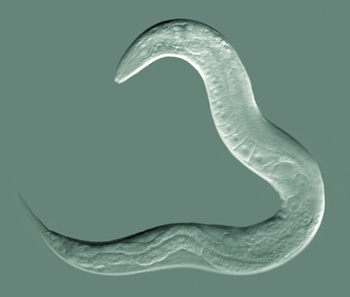
\includegraphics[width=0.4\textwidth]{images/c-elegans}
\caption{Nematodes, such as \emph{C.~elegans} here, are millimetre-long worms which are used by many biologists as model organisms. They crawl along surfaces and digest food they crawl over. \emph{[Image: Bob Goldstein, UNC Chapel Hill; \textsc{cc by-sa 3.0}]}}
\label{fig:nematode}
\end{figure}

We will consider the situation where the prey is not able to move, i.e.\ $D_1=0$ and so $D=0$. This would apply, for example, to non-motile microorganisms that can be consumed by a motile predator, such as nematodes or another simple animal (\cref{fig:nematode}). This leaves us with
\begin{subequations}
\label{sclv-nondim}
\begin{align}
	\pd{u}{t} &= u(1-u-v),\\
	\pd{v}{t} &= \pdd{v}{x}+\alpha v(u-\beta).
\end{align}
\end{subequations}
As we have done with the FK equation, let's take a look at the homogeneous equilibria: 
\begin{subequations}
\begin{align}
	0 &= u(1-u-v),\\
	0 &= \alpha v(u-\beta).
\end{align}
\end{subequations}
The homogeneous system has three equilibria:
\begin{equation}
	(0,0), \quad (1,0), \quad \text{and} \quad (\beta, 1-\beta).
\end{equation}
For that last coexistence equilibrium to be permissible, we need $\beta < 1$, so let's take this to be the case in the following discussion. 

A linear stability analysis of the equilibria of the homogeneous system (conveniently left as an exercise) reveals that:
\begin{itemize}
	\item $(0,0)$ is a saddle point,
	\item $(1,0)$ is a saddle point,
	\item $(\beta, 1-\beta)$ is a stable node when $4\alpha < \beta/(1-\beta)$, and a stable spiral for $4\alpha > \beta/(1-\beta)$.
\end{itemize}

Once again, this suggests possible trajectories between our equilibria:
\begin{enumerate}[label=(\roman*)]
	\item from $(0,0)$ to $(\beta,1-\beta)$,
	\item from $(1,0)$ to $(\beta,1-\beta)$.
\end{enumerate}

\begin{figure}
\centering
%% Creator: Matplotlib, PGF backend
%%
%% To include the figure in your LaTeX document, write
%%   \input{<filename>.pgf}
%%
%% Make sure the required packages are loaded in your preamble
%%   \usepackage{pgf}
%%
%% and, on pdftex
%%   \usepackage[utf8]{inputenc}\DeclareUnicodeCharacter{2212}{-}
%%
%% or, on luatex and xetex
%%   \usepackage{unicode-math}
%%
%% Figures using additional raster images can only be included by \input if
%% they are in the same directory as the main LaTeX file. For loading figures
%% from other directories you can use the `import` package
%%   \usepackage{import}
%%
%% and then include the figures with
%%   \import{<path to file>}{<filename>.pgf}
%%
%% Matplotlib used the following preamble
%%   \usepackage{fontspec}
%%   \setmainfont{DejaVuSerif.ttf}[Path=/Users/adam/opt/anaconda3/lib/python3.8/site-packages/matplotlib/mpl-data/fonts/ttf/]
%%   \setsansfont{DejaVuSans.ttf}[Path=/Users/adam/opt/anaconda3/lib/python3.8/site-packages/matplotlib/mpl-data/fonts/ttf/]
%%   \setmonofont{DejaVuSansMono.ttf}[Path=/Users/adam/opt/anaconda3/lib/python3.8/site-packages/matplotlib/mpl-data/fonts/ttf/]
%%
\begingroup%
\makeatletter%
\begin{pgfpicture}%
\pgfpathrectangle{\pgfpointorigin}{\pgfqpoint{3.000000in}{2.200000in}}%
\pgfusepath{use as bounding box, clip}%
\begin{pgfscope}%
\pgfsetbuttcap%
\pgfsetmiterjoin%
\definecolor{currentfill}{rgb}{1.000000,1.000000,1.000000}%
\pgfsetfillcolor{currentfill}%
\pgfsetlinewidth{0.000000pt}%
\definecolor{currentstroke}{rgb}{1.000000,1.000000,1.000000}%
\pgfsetstrokecolor{currentstroke}%
\pgfsetdash{}{0pt}%
\pgfpathmoveto{\pgfqpoint{0.000000in}{0.000000in}}%
\pgfpathlineto{\pgfqpoint{3.000000in}{0.000000in}}%
\pgfpathlineto{\pgfqpoint{3.000000in}{2.200000in}}%
\pgfpathlineto{\pgfqpoint{0.000000in}{2.200000in}}%
\pgfpathclose%
\pgfusepath{fill}%
\end{pgfscope}%
\begin{pgfscope}%
\pgfsetbuttcap%
\pgfsetmiterjoin%
\definecolor{currentfill}{rgb}{1.000000,1.000000,1.000000}%
\pgfsetfillcolor{currentfill}%
\pgfsetlinewidth{0.000000pt}%
\definecolor{currentstroke}{rgb}{0.000000,0.000000,0.000000}%
\pgfsetstrokecolor{currentstroke}%
\pgfsetstrokeopacity{0.000000}%
\pgfsetdash{}{0pt}%
\pgfpathmoveto{\pgfqpoint{0.506574in}{0.278150in}}%
\pgfpathlineto{\pgfqpoint{2.966667in}{0.278150in}}%
\pgfpathlineto{\pgfqpoint{2.966667in}{2.166667in}}%
\pgfpathlineto{\pgfqpoint{0.506574in}{2.166667in}}%
\pgfpathclose%
\pgfusepath{fill}%
\end{pgfscope}%
\begin{pgfscope}%
\pgfsetbuttcap%
\pgfsetroundjoin%
\definecolor{currentfill}{rgb}{0.000000,0.000000,0.000000}%
\pgfsetfillcolor{currentfill}%
\pgfsetlinewidth{0.803000pt}%
\definecolor{currentstroke}{rgb}{0.000000,0.000000,0.000000}%
\pgfsetstrokecolor{currentstroke}%
\pgfsetdash{}{0pt}%
\pgfsys@defobject{currentmarker}{\pgfqpoint{0.000000in}{-0.048611in}}{\pgfqpoint{0.000000in}{0.000000in}}{%
\pgfpathmoveto{\pgfqpoint{0.000000in}{0.000000in}}%
\pgfpathlineto{\pgfqpoint{0.000000in}{-0.048611in}}%
\pgfusepath{stroke,fill}%
}%
\begin{pgfscope}%
\pgfsys@transformshift{0.506574in}{0.278150in}%
\pgfsys@useobject{currentmarker}{}%
\end{pgfscope}%
\end{pgfscope}%
\begin{pgfscope}%
\definecolor{textcolor}{rgb}{0.000000,0.000000,0.000000}%
\pgfsetstrokecolor{textcolor}%
\pgfsetfillcolor{textcolor}%
\pgftext[x=0.506574in,y=0.180927in,,top]{\color{textcolor}\rmfamily\fontsize{12.000000}{14.400000}\selectfont 0}%
\end{pgfscope}%
\begin{pgfscope}%
\pgfsetbuttcap%
\pgfsetroundjoin%
\definecolor{currentfill}{rgb}{0.000000,0.000000,0.000000}%
\pgfsetfillcolor{currentfill}%
\pgfsetlinewidth{0.803000pt}%
\definecolor{currentstroke}{rgb}{0.000000,0.000000,0.000000}%
\pgfsetstrokecolor{currentstroke}%
\pgfsetdash{}{0pt}%
\pgfsys@defobject{currentmarker}{\pgfqpoint{0.000000in}{-0.048611in}}{\pgfqpoint{0.000000in}{0.000000in}}{%
\pgfpathmoveto{\pgfqpoint{0.000000in}{0.000000in}}%
\pgfpathlineto{\pgfqpoint{0.000000in}{-0.048611in}}%
\pgfusepath{stroke,fill}%
}%
\begin{pgfscope}%
\pgfsys@transformshift{1.275353in}{0.278150in}%
\pgfsys@useobject{currentmarker}{}%
\end{pgfscope}%
\end{pgfscope}%
\begin{pgfscope}%
\definecolor{textcolor}{rgb}{0.000000,0.000000,0.000000}%
\pgfsetstrokecolor{textcolor}%
\pgfsetfillcolor{textcolor}%
\pgftext[x=1.275353in,y=0.180927in,,top]{\color{textcolor}\rmfamily\fontsize{12.000000}{14.400000}\selectfont \(\displaystyle \beta\)}%
\end{pgfscope}%
\begin{pgfscope}%
\pgfsetbuttcap%
\pgfsetroundjoin%
\definecolor{currentfill}{rgb}{0.000000,0.000000,0.000000}%
\pgfsetfillcolor{currentfill}%
\pgfsetlinewidth{0.803000pt}%
\definecolor{currentstroke}{rgb}{0.000000,0.000000,0.000000}%
\pgfsetstrokecolor{currentstroke}%
\pgfsetdash{}{0pt}%
\pgfsys@defobject{currentmarker}{\pgfqpoint{0.000000in}{-0.048611in}}{\pgfqpoint{0.000000in}{0.000000in}}{%
\pgfpathmoveto{\pgfqpoint{0.000000in}{0.000000in}}%
\pgfpathlineto{\pgfqpoint{0.000000in}{-0.048611in}}%
\pgfusepath{stroke,fill}%
}%
\begin{pgfscope}%
\pgfsys@transformshift{2.044132in}{0.278150in}%
\pgfsys@useobject{currentmarker}{}%
\end{pgfscope}%
\end{pgfscope}%
\begin{pgfscope}%
\definecolor{textcolor}{rgb}{0.000000,0.000000,0.000000}%
\pgfsetstrokecolor{textcolor}%
\pgfsetfillcolor{textcolor}%
\pgftext[x=2.044132in,y=0.180927in,,top]{\color{textcolor}\rmfamily\fontsize{12.000000}{14.400000}\selectfont 1}%
\end{pgfscope}%
\begin{pgfscope}%
\pgfsetbuttcap%
\pgfsetroundjoin%
\definecolor{currentfill}{rgb}{0.000000,0.000000,0.000000}%
\pgfsetfillcolor{currentfill}%
\pgfsetlinewidth{0.803000pt}%
\definecolor{currentstroke}{rgb}{0.000000,0.000000,0.000000}%
\pgfsetstrokecolor{currentstroke}%
\pgfsetdash{}{0pt}%
\pgfsys@defobject{currentmarker}{\pgfqpoint{-0.048611in}{0.000000in}}{\pgfqpoint{-0.000000in}{0.000000in}}{%
\pgfpathmoveto{\pgfqpoint{-0.000000in}{0.000000in}}%
\pgfpathlineto{\pgfqpoint{-0.048611in}{0.000000in}}%
\pgfusepath{stroke,fill}%
}%
\begin{pgfscope}%
\pgfsys@transformshift{0.506574in}{0.278150in}%
\pgfsys@useobject{currentmarker}{}%
\end{pgfscope}%
\end{pgfscope}%
\begin{pgfscope}%
\definecolor{textcolor}{rgb}{0.000000,0.000000,0.000000}%
\pgfsetstrokecolor{textcolor}%
\pgfsetfillcolor{textcolor}%
\pgftext[x=0.303313in, y=0.214836in, left, base]{\color{textcolor}\rmfamily\fontsize{12.000000}{14.400000}\selectfont 0}%
\end{pgfscope}%
\begin{pgfscope}%
\pgfsetbuttcap%
\pgfsetroundjoin%
\definecolor{currentfill}{rgb}{0.000000,0.000000,0.000000}%
\pgfsetfillcolor{currentfill}%
\pgfsetlinewidth{0.803000pt}%
\definecolor{currentstroke}{rgb}{0.000000,0.000000,0.000000}%
\pgfsetstrokecolor{currentstroke}%
\pgfsetdash{}{0pt}%
\pgfsys@defobject{currentmarker}{\pgfqpoint{-0.048611in}{0.000000in}}{\pgfqpoint{-0.000000in}{0.000000in}}{%
\pgfpathmoveto{\pgfqpoint{-0.000000in}{0.000000in}}%
\pgfpathlineto{\pgfqpoint{-0.048611in}{0.000000in}}%
\pgfusepath{stroke,fill}%
}%
\begin{pgfscope}%
\pgfsys@transformshift{0.506574in}{0.868311in}%
\pgfsys@useobject{currentmarker}{}%
\end{pgfscope}%
\end{pgfscope}%
\begin{pgfscope}%
\definecolor{textcolor}{rgb}{0.000000,0.000000,0.000000}%
\pgfsetstrokecolor{textcolor}%
\pgfsetfillcolor{textcolor}%
\pgftext[x=0.022683in, y=0.804997in, left, base]{\color{textcolor}\rmfamily\fontsize{12.000000}{14.400000}\selectfont \(\displaystyle 1-\beta\)}%
\end{pgfscope}%
\begin{pgfscope}%
\pgfsetbuttcap%
\pgfsetroundjoin%
\definecolor{currentfill}{rgb}{0.000000,0.000000,0.000000}%
\pgfsetfillcolor{currentfill}%
\pgfsetlinewidth{0.803000pt}%
\definecolor{currentstroke}{rgb}{0.000000,0.000000,0.000000}%
\pgfsetstrokecolor{currentstroke}%
\pgfsetdash{}{0pt}%
\pgfsys@defobject{currentmarker}{\pgfqpoint{-0.048611in}{0.000000in}}{\pgfqpoint{-0.000000in}{0.000000in}}{%
\pgfpathmoveto{\pgfqpoint{-0.000000in}{0.000000in}}%
\pgfpathlineto{\pgfqpoint{-0.048611in}{0.000000in}}%
\pgfusepath{stroke,fill}%
}%
\begin{pgfscope}%
\pgfsys@transformshift{0.506574in}{1.458473in}%
\pgfsys@useobject{currentmarker}{}%
\end{pgfscope}%
\end{pgfscope}%
\begin{pgfscope}%
\definecolor{textcolor}{rgb}{0.000000,0.000000,0.000000}%
\pgfsetstrokecolor{textcolor}%
\pgfsetfillcolor{textcolor}%
\pgftext[x=0.303313in, y=1.395159in, left, base]{\color{textcolor}\rmfamily\fontsize{12.000000}{14.400000}\selectfont 1}%
\end{pgfscope}%
\begin{pgfscope}%
\pgfsetrectcap%
\pgfsetmiterjoin%
\pgfsetlinewidth{0.803000pt}%
\definecolor{currentstroke}{rgb}{0.000000,0.000000,0.000000}%
\pgfsetstrokecolor{currentstroke}%
\pgfsetdash{}{0pt}%
\pgfpathmoveto{\pgfqpoint{0.506574in}{0.278150in}}%
\pgfpathlineto{\pgfqpoint{0.506574in}{2.166667in}}%
\pgfusepath{stroke}%
\end{pgfscope}%
\begin{pgfscope}%
\pgfsetrectcap%
\pgfsetmiterjoin%
\pgfsetlinewidth{0.803000pt}%
\definecolor{currentstroke}{rgb}{0.000000,0.000000,0.000000}%
\pgfsetstrokecolor{currentstroke}%
\pgfsetdash{}{0pt}%
\pgfpathmoveto{\pgfqpoint{0.506574in}{0.278150in}}%
\pgfpathlineto{\pgfqpoint{2.966667in}{0.278150in}}%
\pgfusepath{stroke}%
\end{pgfscope}%
\begin{pgfscope}%
\definecolor{textcolor}{rgb}{0.000000,0.000000,0.000000}%
\pgfsetstrokecolor{textcolor}%
\pgfsetfillcolor{textcolor}%
\pgftext[x=2.966667in,y=0.180927in,right,top]{\color{textcolor}\rmfamily\fontsize{12.000000}{14.400000}\selectfont \(\displaystyle u\)}%
\end{pgfscope}%
\begin{pgfscope}%
\definecolor{textcolor}{rgb}{0.000000,0.000000,0.000000}%
\pgfsetstrokecolor{textcolor}%
\pgfsetfillcolor{textcolor}%
\pgftext[x=0.409351in,y=2.166667in,right,top]{\color{textcolor}\rmfamily\fontsize{12.000000}{14.400000}\selectfont \(\displaystyle v\)}%
\end{pgfscope}%
\begin{pgfscope}%
\pgfsetbuttcap%
\pgfsetroundjoin%
\definecolor{currentfill}{rgb}{1.000000,1.000000,1.000000}%
\pgfsetfillcolor{currentfill}%
\pgfsetlinewidth{1.003750pt}%
\definecolor{currentstroke}{rgb}{0.000000,0.000000,0.000000}%
\pgfsetstrokecolor{currentstroke}%
\pgfsetdash{}{0pt}%
\pgfsys@defobject{currentmarker}{\pgfqpoint{-0.041667in}{-0.041667in}}{\pgfqpoint{0.041667in}{0.041667in}}{%
\pgfpathmoveto{\pgfqpoint{0.000000in}{-0.041667in}}%
\pgfpathcurveto{\pgfqpoint{0.011050in}{-0.041667in}}{\pgfqpoint{0.021649in}{-0.037276in}}{\pgfqpoint{0.029463in}{-0.029463in}}%
\pgfpathcurveto{\pgfqpoint{0.037276in}{-0.021649in}}{\pgfqpoint{0.041667in}{-0.011050in}}{\pgfqpoint{0.041667in}{0.000000in}}%
\pgfpathcurveto{\pgfqpoint{0.041667in}{0.011050in}}{\pgfqpoint{0.037276in}{0.021649in}}{\pgfqpoint{0.029463in}{0.029463in}}%
\pgfpathcurveto{\pgfqpoint{0.021649in}{0.037276in}}{\pgfqpoint{0.011050in}{0.041667in}}{\pgfqpoint{0.000000in}{0.041667in}}%
\pgfpathcurveto{\pgfqpoint{-0.011050in}{0.041667in}}{\pgfqpoint{-0.021649in}{0.037276in}}{\pgfqpoint{-0.029463in}{0.029463in}}%
\pgfpathcurveto{\pgfqpoint{-0.037276in}{0.021649in}}{\pgfqpoint{-0.041667in}{0.011050in}}{\pgfqpoint{-0.041667in}{0.000000in}}%
\pgfpathcurveto{\pgfqpoint{-0.041667in}{-0.011050in}}{\pgfqpoint{-0.037276in}{-0.021649in}}{\pgfqpoint{-0.029463in}{-0.029463in}}%
\pgfpathcurveto{\pgfqpoint{-0.021649in}{-0.037276in}}{\pgfqpoint{-0.011050in}{-0.041667in}}{\pgfqpoint{0.000000in}{-0.041667in}}%
\pgfpathclose%
\pgfusepath{stroke,fill}%
}%
\begin{pgfscope}%
\pgfsys@transformshift{0.506574in}{0.278150in}%
\pgfsys@useobject{currentmarker}{}%
\end{pgfscope}%
\end{pgfscope}%
\begin{pgfscope}%
\pgfsetbuttcap%
\pgfsetroundjoin%
\definecolor{currentfill}{rgb}{1.000000,1.000000,1.000000}%
\pgfsetfillcolor{currentfill}%
\pgfsetlinewidth{1.003750pt}%
\definecolor{currentstroke}{rgb}{0.000000,0.000000,0.000000}%
\pgfsetstrokecolor{currentstroke}%
\pgfsetdash{}{0pt}%
\pgfsys@defobject{currentmarker}{\pgfqpoint{-0.041667in}{-0.041667in}}{\pgfqpoint{0.041667in}{0.041667in}}{%
\pgfpathmoveto{\pgfqpoint{0.000000in}{-0.041667in}}%
\pgfpathcurveto{\pgfqpoint{0.011050in}{-0.041667in}}{\pgfqpoint{0.021649in}{-0.037276in}}{\pgfqpoint{0.029463in}{-0.029463in}}%
\pgfpathcurveto{\pgfqpoint{0.037276in}{-0.021649in}}{\pgfqpoint{0.041667in}{-0.011050in}}{\pgfqpoint{0.041667in}{0.000000in}}%
\pgfpathcurveto{\pgfqpoint{0.041667in}{0.011050in}}{\pgfqpoint{0.037276in}{0.021649in}}{\pgfqpoint{0.029463in}{0.029463in}}%
\pgfpathcurveto{\pgfqpoint{0.021649in}{0.037276in}}{\pgfqpoint{0.011050in}{0.041667in}}{\pgfqpoint{0.000000in}{0.041667in}}%
\pgfpathcurveto{\pgfqpoint{-0.011050in}{0.041667in}}{\pgfqpoint{-0.021649in}{0.037276in}}{\pgfqpoint{-0.029463in}{0.029463in}}%
\pgfpathcurveto{\pgfqpoint{-0.037276in}{0.021649in}}{\pgfqpoint{-0.041667in}{0.011050in}}{\pgfqpoint{-0.041667in}{0.000000in}}%
\pgfpathcurveto{\pgfqpoint{-0.041667in}{-0.011050in}}{\pgfqpoint{-0.037276in}{-0.021649in}}{\pgfqpoint{-0.029463in}{-0.029463in}}%
\pgfpathcurveto{\pgfqpoint{-0.021649in}{-0.037276in}}{\pgfqpoint{-0.011050in}{-0.041667in}}{\pgfqpoint{0.000000in}{-0.041667in}}%
\pgfpathclose%
\pgfusepath{stroke,fill}%
}%
\begin{pgfscope}%
\pgfsys@transformshift{2.044132in}{0.278150in}%
\pgfsys@useobject{currentmarker}{}%
\end{pgfscope}%
\end{pgfscope}%
\begin{pgfscope}%
\pgfsetbuttcap%
\pgfsetroundjoin%
\definecolor{currentfill}{rgb}{0.000000,0.000000,0.000000}%
\pgfsetfillcolor{currentfill}%
\pgfsetlinewidth{1.003750pt}%
\definecolor{currentstroke}{rgb}{0.000000,0.000000,0.000000}%
\pgfsetstrokecolor{currentstroke}%
\pgfsetdash{}{0pt}%
\pgfsys@defobject{currentmarker}{\pgfqpoint{-0.041667in}{-0.041667in}}{\pgfqpoint{0.041667in}{0.041667in}}{%
\pgfpathmoveto{\pgfqpoint{0.000000in}{-0.041667in}}%
\pgfpathcurveto{\pgfqpoint{0.011050in}{-0.041667in}}{\pgfqpoint{0.021649in}{-0.037276in}}{\pgfqpoint{0.029463in}{-0.029463in}}%
\pgfpathcurveto{\pgfqpoint{0.037276in}{-0.021649in}}{\pgfqpoint{0.041667in}{-0.011050in}}{\pgfqpoint{0.041667in}{0.000000in}}%
\pgfpathcurveto{\pgfqpoint{0.041667in}{0.011050in}}{\pgfqpoint{0.037276in}{0.021649in}}{\pgfqpoint{0.029463in}{0.029463in}}%
\pgfpathcurveto{\pgfqpoint{0.021649in}{0.037276in}}{\pgfqpoint{0.011050in}{0.041667in}}{\pgfqpoint{0.000000in}{0.041667in}}%
\pgfpathcurveto{\pgfqpoint{-0.011050in}{0.041667in}}{\pgfqpoint{-0.021649in}{0.037276in}}{\pgfqpoint{-0.029463in}{0.029463in}}%
\pgfpathcurveto{\pgfqpoint{-0.037276in}{0.021649in}}{\pgfqpoint{-0.041667in}{0.011050in}}{\pgfqpoint{-0.041667in}{0.000000in}}%
\pgfpathcurveto{\pgfqpoint{-0.041667in}{-0.011050in}}{\pgfqpoint{-0.037276in}{-0.021649in}}{\pgfqpoint{-0.029463in}{-0.029463in}}%
\pgfpathcurveto{\pgfqpoint{-0.021649in}{-0.037276in}}{\pgfqpoint{-0.011050in}{-0.041667in}}{\pgfqpoint{0.000000in}{-0.041667in}}%
\pgfpathclose%
\pgfusepath{stroke,fill}%
}%
\begin{pgfscope}%
\pgfsys@transformshift{1.275353in}{0.868311in}%
\pgfsys@useobject{currentmarker}{}%
\end{pgfscope}%
\end{pgfscope}%
\end{pgfpicture}%
\makeatother%
\endgroup%

\caption{Start of a phase portrait for the homogeneous version of the system, \cref{sclv-nondim}, where $\alpha=1$, $\beta=0.5$. Without knowing the trajectories at all, we can guess that there might be trajectories from $(0,0)$ to $(\beta,1-\beta)$ and from $(1,0)$ to $(\beta,1-\beta)$.}
\label{fig:travelling-wave-predators-traj-0}
\end{figure}

The beginning of a phase portrait for the homogeneous system is shown in \cref{fig:travelling-wave-predators-traj-0}, with the equilibria marked on it. The position of the equilibria is really all we know at this stage; to find the trajectories we could do a proper phase plane analysis. Without this computation, we can still guess that there \emph{might} be trajectories from the saddle points to the stable spiral. 

Returning to the PDE system, we’ll proceed as we had done with the FK equation and search for travelling wave solutions. We'll place the stable equilibria at $x=-\infty$ and therefore we can look for right-travelling waves of the form
\begin{equation}
u(x,t) = u(z), \quad v(x,t) = v(z), \quad z = x-ct.
\end{equation}

%Substituting $z$ into \cref{sclv-nondim}, we obtain
%\begin{subequations}
%\begin{align}
%	-c\fd{u}{z} &= u(1-u-v),\\
%	-c\fd{v}{z} &= \fdd{v}{z} + \alpha v (u-\beta).
%\end{align}
%\end{subequations}
%Introducing $w = \fd{v}{z}$ and rearranging, we arrive at the three-dimensional system
%\begin{subequations}
%\begin{align}
%	\fd{u}{z} &= \frac{u}{c}(u+v-1),\\
%	\fd{v}{z} &= w,\\
%	\fd{w}{z} &= \alpha v(\beta - u) - cw.
%\end{align}
%\end{subequations}
%Though the system is three-dimensional, we can analyse it much in the same way as we had done with the FK equation and establish the permissible range of wave speeds, $c$.
%
%The interesting pair of boundary conditions (and as we've seen by cheating and looking at a completed phase diagram, the only one that actually corresponds to a trajectory) is the one going from prey everywhere to a coexistence state, i.e.\ going from the equilibrium $(1,0,0)$ to $(\beta,1-\beta,0)$. We therefore have the boundary conditions in $z$,
%\begin{equation}
%	\label{trav-wave-interesting}
%	(u,v) \to (1,0) \text{ as } z \to \infty, \quad (u,v) \to (\beta,1-\beta) \text{ as } z \to -\infty.
%\end{equation}
%Let's do a linear stability analysis on the two equilibria involved in this travelling wave.
%
%\subsubsection*{\StepOne Find equilibria}
%Done already!
%
%\subsubsection*{\StepTwo Linearise the system}
%
%The Jacobian is
%\begin{align}
%	\m{J} = \begin{pmatrix}
%		(2u+v-1)/c & u/c & 0 \\
%		0 & 0 & 1 \\
%		-\alpha v & \alpha(\beta-u) & -c
%	\end{pmatrix}.
%\end{align}
%
%\subsubsection*{\StepThree Solve the linearised system}
%Once again we're doing $\det(\m{J}-\lambda\m{I}) = 0$. It's a $3\times 3$ matrix this time so we expect three eigenvalues.
%
%\subsubsection*{\StepFour Assess stability}
%The Jacobian, evaluated at $(1,0,0)$ gives us
%\begin{align}
%	\m{J} = \begin{pmatrix}
%		1/c & 1/c & 0 \\
%		0 & 0 & 1 \\
%		0 & \alpha(\beta-1) & -c
%	\end{pmatrix}.
%\end{align}
%This matrix leads to the eigenvalue equation
%\begin{equation}
%	(\lambda-1/c)[\lambda(c+\lambda)-\alpha(\beta-1)] = 0,
%\end{equation}
%and hence the eigenvalues are
%\begin{equation}
%	\lambda = \frac{1}{\gamma}, \quad \lambda = \frac{1}{2}\left( -c \pm \sqrt{c^2 + 4\alpha(\beta-1)} \right).
%\end{equation}
%The first eigenvalue is positive so we expect an unstable solution. But what type of unstable solution? From the second expression, we see that the solution will be oscillatory if $c^2 < 4\alpha(1-\beta)$. Since $v$ cannot be less than zero, these oscillatory solutions can be discarded and this gives us a constraint on the wavespeed, just like it did with the FK equation. Namely, the permissible wave speeds satisfy
%\begin{equation}
%	c^2 \geq 4\alpha(1-\beta).
%\end{equation}
%
%As for the coexistence equilibrium, the resultant cubic polynomial is not as easily handled as the one encountered above. You will get a chance to explore it in the last problem sheet to see if there are any more constraints on $c$, and thus find the speed of the wave of invading predators.

\begin{do-it-yourself}
The analysis of this problem concludes in Problem Sheet 4.
\end{do-it-yourself}

\begin{figure}
\centering
\begin{subfigure}[t]{0.49\textwidth}
	\centering
	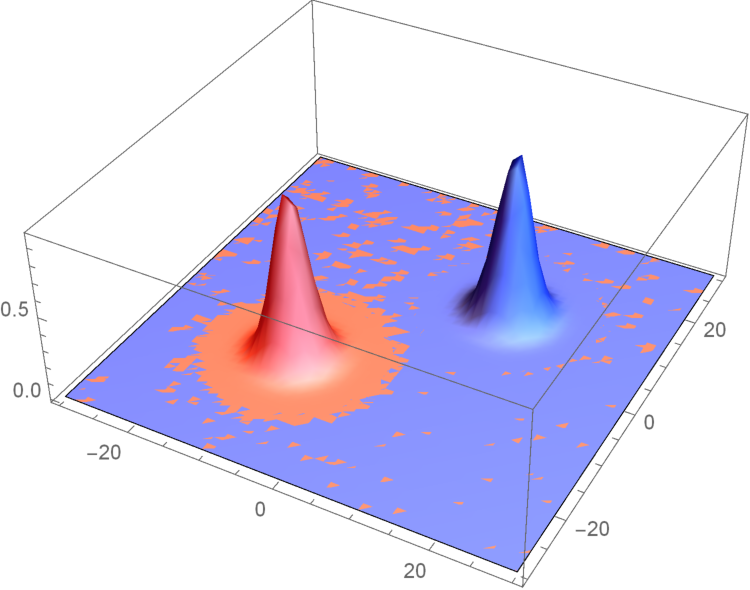
\includegraphics[width=6cm]{images/predPrayFull0.pdf}
\end{subfigure}
\begin{subfigure}[t]{0.49\textwidth}
	\centering
	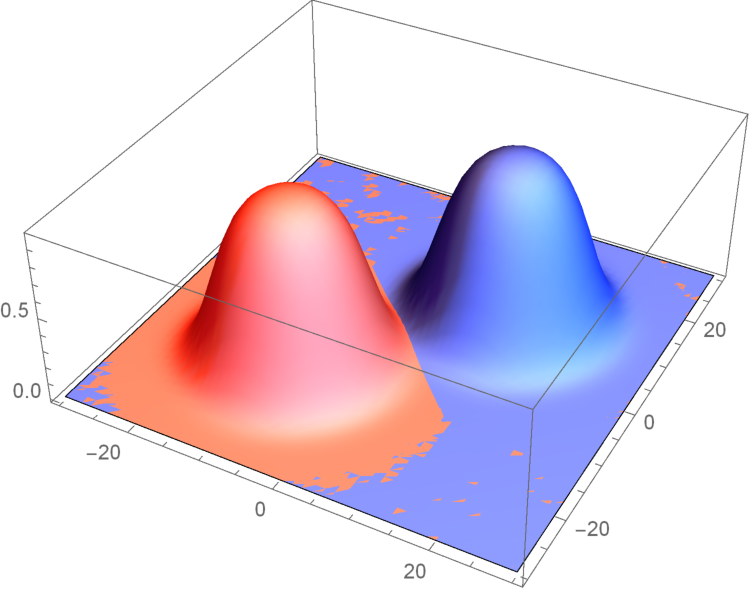
\includegraphics[width=6cm]{images/predPrayFull5.pdf}
\end{subfigure}	
\begin{subfigure}[t]{0.49\textwidth}
	\centering
	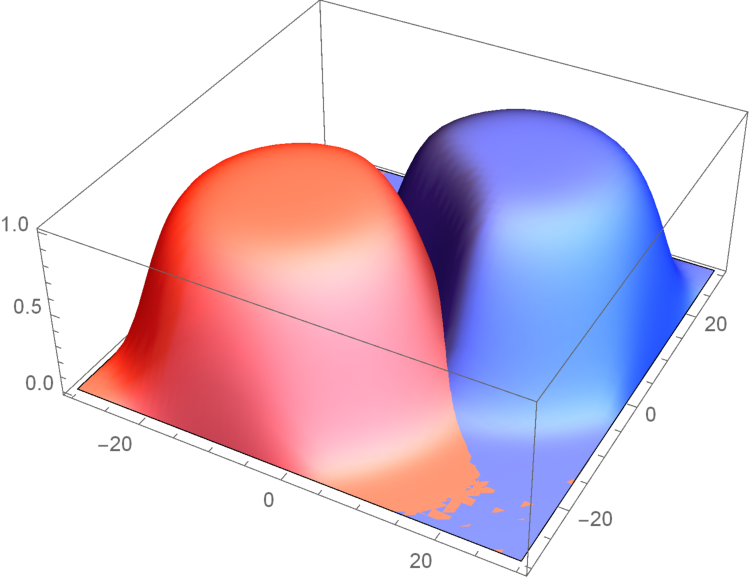
\includegraphics[width=6cm]{images/predPrayFull10.pdf}
\end{subfigure}
\begin{subfigure}[t]{0.49\textwidth}
	\centering
	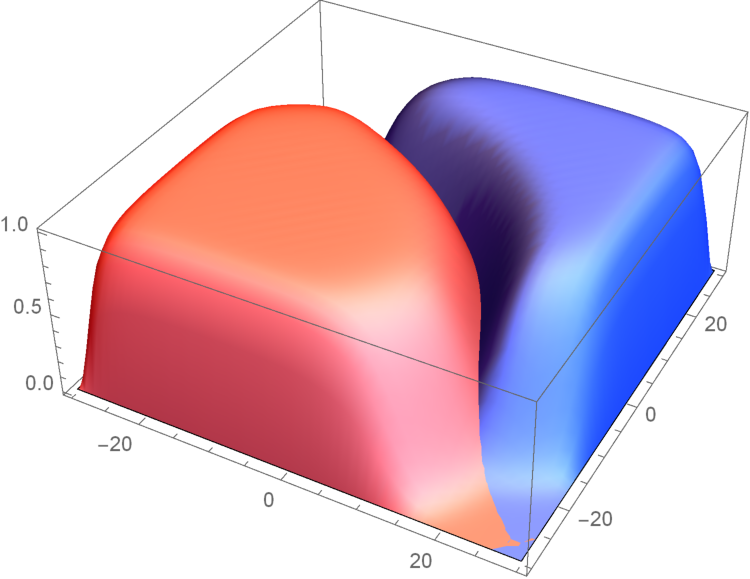
\includegraphics[width=6cm]{images/predPrayFull15.pdf}
\end{subfigure}
\begin{subfigure}[t]{0.49\textwidth}
	\centering
	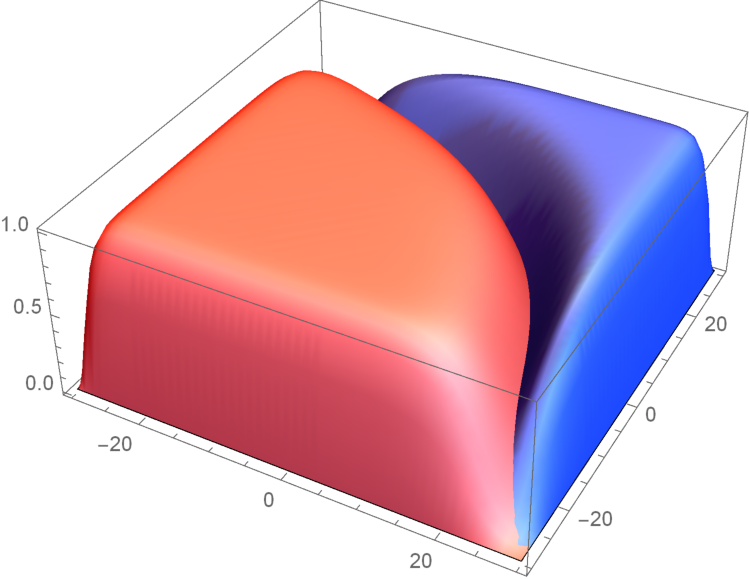
\includegraphics[width=6cm]{images/predPrayFull20.pdf}
\end{subfigure}
\begin{subfigure}[t]{0.49\textwidth}
	\centering
	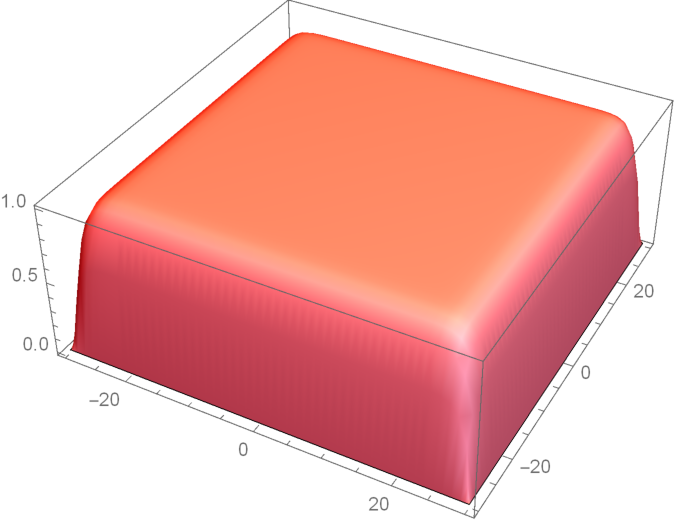
\includegraphics[width=6cm]{images/predPrayFull50.pdf}
\end{subfigure}
\caption{Snapshots of numerical simulations of solutions to \cref{scaledlotvolpursuit} with a pair of Gaussian population peaks as initial conditions. The parameters are $\gamma_1 =1.5$, $\gamma_2=0.5$, $\kappa =1$ and (a) $t=0$, (b) $t=5$, (c) $t=10$, (d) $t=15$, (e) $t=20$, (f) $t=50$. The choice of $\gamma_1,\gamma_2$ sets the dominant population to be $v$, in red; $u$ is in blue.}%
\label{predpraynumerics}%
\end{figure}

\section{The importance of boundary conditions} Let's have a look at some numerical simulations of the full 2D system for our squirrels, \cref{scaledlotvolpursuit}. In \cref{predpraynumerics} we see snapshots of a simulation whose initial conditions are two Gaussian populations which diffuse and interact. The values of $\gamma_1$ and $\gamma_2$ are chosen so that $v$ represents the grey squirrels (inconveniently in red). The boundary conditions are that both populations are zero on the boundary. Do we get travelling wave solutions forever, like in our 1D model? 

From (a)--(b) the populations diffuse and begin to interact. In (c)--(e) we see the greys gradually outcompeting the reds. This ends with the reds becoming extinct in (f).  This case \emph{does} lead to a finite-time equilibrium. The critical observation here is that boundary conditions play a fundamental role in determining what type of solutions are permitted. The travelling wave solution would eventually violate the zero boundary conditions, so it cannot persist for all $t$.

We are going to round off this term by starting to look at PDEs with boundary conditions which don't admit travelling wave solutions. We will do this by looking at a physical problem, and then a fun biological example.

\vspace{0.5cm}
\begin{do-it-yourself}
Additional Problem Sheet 3 contains a number of worked examples featuring travelling wave solutions.
\end{do-it-yourself}

\begin{extra-reading}
\begin{itemize}
	\item The FK equation is covered in \textsc{Murray}, vol.~I, chap.~13. 
	\item Invading squirrels and spatial predator--prey are covered in \textsc{Murray}, vol.~II, chap.~1. The questions at the end of the chapter contain a number of example travelling wave type problems which might be helpful.
	\item Jacka Banasiaka at Łódź University of Technology provides \href{http://im0.p.lodz.pl/~jbanasiak/FB/falebiegnace.pdf}{some worked examples} of travelling wave solutions to various problems. 
\end{itemize}
\end{extra-reading}

%For the equilibrium $(\beta,1-\beta,0)$, the Jacobian is
%\begin{equation}
%	\m{J} = \begin{pmatrix}
%		\beta/c & \beta/c & 0 \\
%		0 & 0 & 1 \\
%		\alpha(\beta-1) & 0 & -c
%	\end{pmatrix},
%\end{equation}	
%which has characteristic equation
%\begin{equation}
%	\lambda^3 + \lambda^2 \left(c - \frac{\beta}{c}\right)-\beta\lambda - \frac{\beta}{c}\alpha(\beta-1) = 0.
%\end{equation}
%Unfortunately, this cubic polynomial is not as easily handled as the one encountered above. To better understand the solutions that arise in this case, we first compute the values of $\lambda$ where the local maximum and minimum of the characteristic polynomial are realised. These are given by
%\begin{equation}
%	\lambda_{max,min} = -\frac{1}{3}\left( c - \frac{\beta}{c} \pm \sqrt{\left( c - \frac{\beta}{c} \right)^2 + 3\beta} \right),
%\end{equation}
%and we see that they do not depend on the parameter $\alpha$. Note that these values are NOT necessarily eigenvalues, but rather the values where the characteristic polynomial attains its local maximum or minimum. Investigating further by taking $\alpha = 0$ (thus, $v$ obeys the diffusion equation), we compute the eigenvalues to find
%\begin{equation}
%	\lambda = 0, \quad \lambda=-c, \quad \lambda = \beta/c,
%\end{equation}
%which are all real. Increasing $\alpha$ amounts to shifting the cubic upwards. Therefore, we see that as $\alpha$ increases from zero, all eigenvalues will remain real until $\alpha$ reaches a critical value, $\alpha c$, at which point, the characteristic equation emits $\lambda_{min}$ as a repeated eigenvalue. For $\alpha > \alpha c$, the local minimum lies above the $x$-axis and as a result there will be one real eigenvalue and two complex eigenvalues. 
%
%[PIC]
%
%Thus, if $\alpha \leq \alpha c$ and the unstable eigenvalues are real, we expect $(u(z),v(z))$ to vary monotonically with $z$, going from $(u,v) = (\beta, 1 − \beta)$ to $(1, 0)$ as $z$ increases. Since the unstable eigenvalues are complex when $\alpha > \alpha c$, the solution will be oscillate as $z$ increases. Previously, we discarded these solutions on the grounds that they would yield negative values of a population size. In those instances, however, we were dealing with fixed points where one population size was zero. Here, we have $(\beta, 1-\beta)$, so the solution may safely oscillate without ever becoming negative. Thus, we can permit oscillatory wavefronts. While this is a fundamental difference with the FK equation where oscillations were not possible, like the FK equation the wave speed is given by the minimum possible value, namely
%\begin{equation}
%	c^2 = 4\alpha(1 - \beta).
%\end{equation}
%Both the oscillating wavefront, and the speed of the wave can be observed in the numerical solution generated below.
%
%[PIC]

%\chapter{Pursuit and evasion in spatial competitive Lotka--Volterra}
%\label{chap:pursuit-evasion}
%
%We are now in the right place to consider a two-population Lotka--Volterra system with \emph{spatial dependence}. This brings in the interesting possibility of pursuit of the two populations! 
%
%\section{Spatial competitive Lotka--Volterra}
%\label{sec:sclv}
%Let's consider the following model,
%\begin{subequations}
%\begin{align}
%\pd{u}{t} & = D_1\nabla^2 u + a_1u(1-b_1 u-c_1v),\\
%\pd{v}{t} & = D_2\nabla^2 v + a_2v(1-b_2v-c_2 u).
%\end{align}
%\end{subequations}
%where the functions $u(\v{x},t)$ and $v(\v{x},t)$ have both spatial and temporal dependence. Once again, we have $a_i,b_i,c_i > 0$.
%
%This is similar to the competitive predator--prey model used in \cref{lotvolcomp2scaled}, but with differently named constants and the addition of diffusion (and hence spatial dependence). But there is a subtle difference, too: here, the interaction ($uv$) terms are both negative. This means that interaction is bad for \emph{both} populations: not a good predator--prey model, perhaps, but rather a good model for two competitive species after a common external food source, where interaction maybe leads to chasing or fighting. A classic example is American grey squirrels (with their bad spellings and perfect teeth) outcompeting native British red squirrels. 
%
%We can view this system as two linked advection--diffusion equations, 
%\begin{subequations}
%\label{rd}
%\begin{align}
%\pd{u}{t} &= D_1\nabla^2 u + f_1(u,v),\\
%\pd{v}{t} &= D_2\nabla^2 v + f_2(u,v),
%\end{align}
%\end{subequations}
%with neither having an advective term and the logistic growth/interaction terms, $f_1$ and $f_2$, acting as sources (they indicate growth and death).  
%
%
%
%\paragraph{Nondimensionalise}
%We nondimensionalise by  setting $\v{x} = (D_1/a_1)^{1/2}\hat{\v{x}}$, $t = \hat{t}/a_1$, $\kappa = D_2/D_1$, $\beta = a_2/a_1$, $\gamma_1= c_1/b_2$, $\gamma_2 = c_2/b_1$, $u= \hat{u}/b_1$, $v = \hat{v}/b_2$ (and dropping hats) to get
%\begin{subequations}
%\label{scaledlotvolpursuit} 
%\begin{align}
%\pd{u}{t} &= \nabla^2 u +u(1-u-\gamma_1v),\\
%\pd{v}{t} &= \kappa\nabla^2 v + \beta v(1-v-\gamma_2u).
%\end{align}
%\end{subequations}
%
%At this point, you may notice that we haven't picked a winner from $u$ and $v$. In \cref{sec:lsa-sclv}, we will show that $\gamma_1>1$ and $\gamma_2<1$ guarantee that $v$ will dominate over $u$. This choice allows us to continue to think of $v$ as the dominant population, and although we will be looking at examples where this choice has been made, allowing us to compare with our previous systems, you will see that the analysis in the chapter doesn't assume this.
%
%Generally this system is not integrable and has to be treated numerically, although this is not necessarily an arduous task as the system is quite well-behaved. However, there are some special solutions which help to highlight certain aspects of the system's behaviour.
%
%\section{Travelling wave (pursuit) solutions to spatial competitive Lotka--Volterra}
%
%Let's focus on the one- (spatial) dimensional case. We are going to seek a solution whose $(x,t)$ dependence is in the form $x-ct$, i.e. a travelling wave solution. 
%
%\begin{info}
%You might remember that travelling waves have this form because the wave equation,
%\begin{equation}
%	\pdd{u}{t} = c^2 \pdd{u}{x},
%\end{equation}
%which governs how mechanical waves behave, has the general solution
%\begin{equation}
%	u(x,t) = F(x-ct) + G(x+ct),
%\end{equation}
%i.e., a solution composed of a right-travelling function $F$ and a left-travelling function $G$.
%\end{info}
%
%In other words, we look for functions $u(z),v(z)$ where $z= x-ct$. With this assumption, \cref{scaledlotvolpursuit} takes the form
%\begin{subequations}
%\begin{align}
%\fdd{u}{z}+c\fd{u}{z} + u(1 - u - \gamma_1v) &= 0,\\
%\kappa\fdd{v}{z}+c\fd{v}{z} + \beta v(1 - v -\gamma_2u) &= 0.
%\end{align}
%\end{subequations}
%So now we have a system of ODEs which gives us the fixed shape of the system. The relationship $z=x-ct$ just means this behaviour moves at a constant velocity $c$ in the $x$ direction. We seek a solution with the boundary conditions $u=0$, $v=0$ as $z\to -\infty$ (total annihilation!), and $u+v=1$ as $z\to \infty$. This last condition, at the end of the domain where the wave `hits last', could mean a few things. Recalling that $u$ and $v$ have been nondimensionalised, $1$ represents their logistic value. So this last condition could mean a world with only one species at one end of the domain (e.g.\ red squirrels just chilling, oblivious to the oncoming invasion). Alternatively, both populations could be coexisting at populations lower than their logistic value, just so long as $u+v=1$.
%
%In general, it can be shown this system is not integrable; however, in the case $\beta =1$, $\kappa=1$, we can add the two equations to get
%\begin{equation}
%\fdd{}{z}[u+v] + c\fd{}{z}[u+v] + (u+v) - (u^2 + v^2) - (\gamma_1 uv + \gamma_2 uv) =0.
%\end{equation}
%If $\gamma_1+\gamma_2 =2$ we have
%\begin{equation}
%\fdd{w}{z} + c\fd{w}{z} + w(1-w)=0,
%\end{equation}
%where $w = u+v$, subject to $w = 0$ at $z=-\infty$ and $w = 1$ at $z =\infty$. 
%
%This is known as \emph{Fisher's equation}, or the \emph{Fisher--Kolmogorov--Petrovsky--Piskunov equation}, and this is still difficult to find closed-form solutions to: solutions were only found 50 years after the equation was first proposed! Unfortunately, the solution method is out of scope for our course (it uses complex analysis); we're primarily interested in general techniques so instead we just going to analyse the solution. 
%
%\begin{figure}
%\centering
%\begin{subfigure}[b]{0.49\textwidth}
%	%% Creator: Matplotlib, PGF backend
%%
%% To include the figure in your LaTeX document, write
%%   \input{<filename>.pgf}
%%
%% Make sure the required packages are loaded in your preamble
%%   \usepackage{pgf}
%%
%% Figures using additional raster images can only be included by \input if
%% they are in the same directory as the main LaTeX file. For loading figures
%% from other directories you can use the `import` package
%%   \usepackage{import}
%% and then include the figures with
%%   \import{<path to file>}{<filename>.pgf}
%%
%% Matplotlib used the following preamble
%%   \usepackage{fontspec}
%%   \setmainfont{DejaVuSerif.ttf}[Path=/Library/Python/3.7/site-packages/matplotlib/mpl-data/fonts/ttf/]
%%   \setsansfont{DejaVuSans.ttf}[Path=/Library/Python/3.7/site-packages/matplotlib/mpl-data/fonts/ttf/]
%%   \setmonofont{DejaVuSansMono.ttf}[Path=/Library/Python/3.7/site-packages/matplotlib/mpl-data/fonts/ttf/]
%%
\begingroup%
\makeatletter%
\begin{pgfpicture}%
\pgfpathrectangle{\pgfpointorigin}{\pgfqpoint{3.000000in}{2.200000in}}%
\pgfusepath{use as bounding box, clip}%
\begin{pgfscope}%
\pgfsetbuttcap%
\pgfsetmiterjoin%
\definecolor{currentfill}{rgb}{1.000000,1.000000,1.000000}%
\pgfsetfillcolor{currentfill}%
\pgfsetlinewidth{0.000000pt}%
\definecolor{currentstroke}{rgb}{1.000000,1.000000,1.000000}%
\pgfsetstrokecolor{currentstroke}%
\pgfsetdash{}{0pt}%
\pgfpathmoveto{\pgfqpoint{0.000000in}{0.000000in}}%
\pgfpathlineto{\pgfqpoint{3.000000in}{0.000000in}}%
\pgfpathlineto{\pgfqpoint{3.000000in}{2.200000in}}%
\pgfpathlineto{\pgfqpoint{0.000000in}{2.200000in}}%
\pgfpathclose%
\pgfusepath{fill}%
\end{pgfscope}%
\begin{pgfscope}%
\pgfsetbuttcap%
\pgfsetmiterjoin%
\definecolor{currentfill}{rgb}{1.000000,1.000000,1.000000}%
\pgfsetfillcolor{currentfill}%
\pgfsetlinewidth{0.000000pt}%
\definecolor{currentstroke}{rgb}{0.000000,0.000000,0.000000}%
\pgfsetstrokecolor{currentstroke}%
\pgfsetstrokeopacity{0.000000}%
\pgfsetdash{}{0pt}%
\pgfpathmoveto{\pgfqpoint{0.033333in}{0.278150in}}%
\pgfpathlineto{\pgfqpoint{2.966667in}{0.278150in}}%
\pgfpathlineto{\pgfqpoint{2.966667in}{2.166667in}}%
\pgfpathlineto{\pgfqpoint{0.033333in}{2.166667in}}%
\pgfpathclose%
\pgfusepath{fill}%
\end{pgfscope}%
\begin{pgfscope}%
\pgfpathrectangle{\pgfqpoint{0.033333in}{0.278150in}}{\pgfqpoint{2.933333in}{1.888517in}}%
\pgfusepath{clip}%
\pgfsetrectcap%
\pgfsetroundjoin%
\pgfsetlinewidth{1.505625pt}%
\definecolor{currentstroke}{rgb}{0.172549,0.627451,0.172549}%
\pgfsetstrokecolor{currentstroke}%
\pgfsetdash{}{0pt}%
\pgfpathmoveto{\pgfqpoint{0.166667in}{0.278150in}}%
\pgfpathlineto{\pgfqpoint{0.980814in}{0.278685in}}%
\pgfpathlineto{\pgfqpoint{1.058225in}{0.279850in}}%
\pgfpathlineto{\pgfqpoint{1.106273in}{0.281597in}}%
\pgfpathlineto{\pgfqpoint{1.140974in}{0.283851in}}%
\pgfpathlineto{\pgfqpoint{1.170337in}{0.286821in}}%
\pgfpathlineto{\pgfqpoint{1.194361in}{0.290309in}}%
\pgfpathlineto{\pgfqpoint{1.215716in}{0.294497in}}%
\pgfpathlineto{\pgfqpoint{1.234401in}{0.299244in}}%
\pgfpathlineto{\pgfqpoint{1.250417in}{0.304309in}}%
\pgfpathlineto{\pgfqpoint{1.266433in}{0.310482in}}%
\pgfpathlineto{\pgfqpoint{1.282449in}{0.317963in}}%
\pgfpathlineto{\pgfqpoint{1.295796in}{0.325360in}}%
\pgfpathlineto{\pgfqpoint{1.309142in}{0.333964in}}%
\pgfpathlineto{\pgfqpoint{1.322489in}{0.343925in}}%
\pgfpathlineto{\pgfqpoint{1.335836in}{0.355401in}}%
\pgfpathlineto{\pgfqpoint{1.349183in}{0.368554in}}%
\pgfpathlineto{\pgfqpoint{1.362529in}{0.383544in}}%
\pgfpathlineto{\pgfqpoint{1.375876in}{0.400529in}}%
\pgfpathlineto{\pgfqpoint{1.389223in}{0.419657in}}%
\pgfpathlineto{\pgfqpoint{1.402569in}{0.441058in}}%
\pgfpathlineto{\pgfqpoint{1.415916in}{0.464843in}}%
\pgfpathlineto{\pgfqpoint{1.429263in}{0.491096in}}%
\pgfpathlineto{\pgfqpoint{1.442609in}{0.519865in}}%
\pgfpathlineto{\pgfqpoint{1.455956in}{0.551159in}}%
\pgfpathlineto{\pgfqpoint{1.469303in}{0.584945in}}%
\pgfpathlineto{\pgfqpoint{1.485319in}{0.628662in}}%
\pgfpathlineto{\pgfqpoint{1.501335in}{0.675620in}}%
\pgfpathlineto{\pgfqpoint{1.520020in}{0.734067in}}%
\pgfpathlineto{\pgfqpoint{1.541375in}{0.804869in}}%
\pgfpathlineto{\pgfqpoint{1.568068in}{0.897613in}}%
\pgfpathlineto{\pgfqpoint{1.648148in}{1.178995in}}%
\pgfpathlineto{\pgfqpoint{1.669503in}{1.248960in}}%
\pgfpathlineto{\pgfqpoint{1.690858in}{1.314978in}}%
\pgfpathlineto{\pgfqpoint{1.709543in}{1.369050in}}%
\pgfpathlineto{\pgfqpoint{1.728228in}{1.419412in}}%
\pgfpathlineto{\pgfqpoint{1.744244in}{1.459529in}}%
\pgfpathlineto{\pgfqpoint{1.760260in}{1.496806in}}%
\pgfpathlineto{\pgfqpoint{1.776276in}{1.531273in}}%
\pgfpathlineto{\pgfqpoint{1.792292in}{1.562997in}}%
\pgfpathlineto{\pgfqpoint{1.808308in}{1.592076in}}%
\pgfpathlineto{\pgfqpoint{1.824324in}{1.618630in}}%
\pgfpathlineto{\pgfqpoint{1.840340in}{1.642798in}}%
\pgfpathlineto{\pgfqpoint{1.856356in}{1.664726in}}%
\pgfpathlineto{\pgfqpoint{1.872372in}{1.684567in}}%
\pgfpathlineto{\pgfqpoint{1.888388in}{1.702477in}}%
\pgfpathlineto{\pgfqpoint{1.904404in}{1.718606in}}%
\pgfpathlineto{\pgfqpoint{1.920420in}{1.733104in}}%
\pgfpathlineto{\pgfqpoint{1.936436in}{1.746113in}}%
\pgfpathlineto{\pgfqpoint{1.952452in}{1.757767in}}%
\pgfpathlineto{\pgfqpoint{1.968468in}{1.768192in}}%
\pgfpathlineto{\pgfqpoint{1.987154in}{1.778958in}}%
\pgfpathlineto{\pgfqpoint{2.005839in}{1.788385in}}%
\pgfpathlineto{\pgfqpoint{2.024525in}{1.796627in}}%
\pgfpathlineto{\pgfqpoint{2.045879in}{1.804776in}}%
\pgfpathlineto{\pgfqpoint{2.067234in}{1.811748in}}%
\pgfpathlineto{\pgfqpoint{2.091258in}{1.818387in}}%
\pgfpathlineto{\pgfqpoint{2.117951in}{1.824501in}}%
\pgfpathlineto{\pgfqpoint{2.147314in}{1.829961in}}%
\pgfpathlineto{\pgfqpoint{2.179346in}{1.834696in}}%
\pgfpathlineto{\pgfqpoint{2.214047in}{1.838687in}}%
\pgfpathlineto{\pgfqpoint{2.254087in}{1.842162in}}%
\pgfpathlineto{\pgfqpoint{2.302135in}{1.845153in}}%
\pgfpathlineto{\pgfqpoint{2.360861in}{1.847596in}}%
\pgfpathlineto{\pgfqpoint{2.432933in}{1.849425in}}%
\pgfpathlineto{\pgfqpoint{2.531698in}{1.850744in}}%
\pgfpathlineto{\pgfqpoint{2.683851in}{1.851549in}}%
\pgfpathlineto{\pgfqpoint{2.833333in}{1.851798in}}%
\pgfpathlineto{\pgfqpoint{2.833333in}{1.851798in}}%
\pgfusepath{stroke}%
\end{pgfscope}%
\begin{pgfscope}%
\pgfsetbuttcap%
\pgfsetroundjoin%
\definecolor{currentfill}{rgb}{0.000000,0.000000,0.000000}%
\pgfsetfillcolor{currentfill}%
\pgfsetlinewidth{0.803000pt}%
\definecolor{currentstroke}{rgb}{0.000000,0.000000,0.000000}%
\pgfsetstrokecolor{currentstroke}%
\pgfsetdash{}{0pt}%
\pgfsys@defobject{currentmarker}{\pgfqpoint{0.000000in}{-0.048611in}}{\pgfqpoint{0.000000in}{0.000000in}}{%
\pgfpathmoveto{\pgfqpoint{0.000000in}{0.000000in}}%
\pgfpathlineto{\pgfqpoint{0.000000in}{-0.048611in}}%
\pgfusepath{stroke,fill}%
}%
\begin{pgfscope}%
\pgfsys@transformshift{0.433333in}{0.278150in}%
\pgfsys@useobject{currentmarker}{}%
\end{pgfscope}%
\end{pgfscope}%
\begin{pgfscope}%
\definecolor{textcolor}{rgb}{0.000000,0.000000,0.000000}%
\pgfsetstrokecolor{textcolor}%
\pgfsetfillcolor{textcolor}%
\pgftext[x=0.433333in,y=0.180927in,,top]{\color{textcolor}\rmfamily\fontsize{12.000000}{14.400000}\selectfont \(\displaystyle -20\)}%
\end{pgfscope}%
\begin{pgfscope}%
\pgfsetbuttcap%
\pgfsetroundjoin%
\definecolor{currentfill}{rgb}{0.000000,0.000000,0.000000}%
\pgfsetfillcolor{currentfill}%
\pgfsetlinewidth{0.803000pt}%
\definecolor{currentstroke}{rgb}{0.000000,0.000000,0.000000}%
\pgfsetstrokecolor{currentstroke}%
\pgfsetdash{}{0pt}%
\pgfsys@defobject{currentmarker}{\pgfqpoint{0.000000in}{-0.048611in}}{\pgfqpoint{0.000000in}{0.000000in}}{%
\pgfpathmoveto{\pgfqpoint{0.000000in}{0.000000in}}%
\pgfpathlineto{\pgfqpoint{0.000000in}{-0.048611in}}%
\pgfusepath{stroke,fill}%
}%
\begin{pgfscope}%
\pgfsys@transformshift{1.500000in}{0.278150in}%
\pgfsys@useobject{currentmarker}{}%
\end{pgfscope}%
\end{pgfscope}%
\begin{pgfscope}%
\definecolor{textcolor}{rgb}{0.000000,0.000000,0.000000}%
\pgfsetstrokecolor{textcolor}%
\pgfsetfillcolor{textcolor}%
\pgftext[x=1.500000in,y=0.180927in,,top]{\color{textcolor}\rmfamily\fontsize{12.000000}{14.400000}\selectfont \(\displaystyle 0\)}%
\end{pgfscope}%
\begin{pgfscope}%
\pgfsetbuttcap%
\pgfsetroundjoin%
\definecolor{currentfill}{rgb}{0.000000,0.000000,0.000000}%
\pgfsetfillcolor{currentfill}%
\pgfsetlinewidth{0.803000pt}%
\definecolor{currentstroke}{rgb}{0.000000,0.000000,0.000000}%
\pgfsetstrokecolor{currentstroke}%
\pgfsetdash{}{0pt}%
\pgfsys@defobject{currentmarker}{\pgfqpoint{0.000000in}{-0.048611in}}{\pgfqpoint{0.000000in}{0.000000in}}{%
\pgfpathmoveto{\pgfqpoint{0.000000in}{0.000000in}}%
\pgfpathlineto{\pgfqpoint{0.000000in}{-0.048611in}}%
\pgfusepath{stroke,fill}%
}%
\begin{pgfscope}%
\pgfsys@transformshift{2.566667in}{0.278150in}%
\pgfsys@useobject{currentmarker}{}%
\end{pgfscope}%
\end{pgfscope}%
\begin{pgfscope}%
\definecolor{textcolor}{rgb}{0.000000,0.000000,0.000000}%
\pgfsetstrokecolor{textcolor}%
\pgfsetfillcolor{textcolor}%
\pgftext[x=2.566667in,y=0.180927in,,top]{\color{textcolor}\rmfamily\fontsize{12.000000}{14.400000}\selectfont \(\displaystyle 20\)}%
\end{pgfscope}%
\begin{pgfscope}%
\pgfsetbuttcap%
\pgfsetroundjoin%
\definecolor{currentfill}{rgb}{0.000000,0.000000,0.000000}%
\pgfsetfillcolor{currentfill}%
\pgfsetlinewidth{0.803000pt}%
\definecolor{currentstroke}{rgb}{0.000000,0.000000,0.000000}%
\pgfsetstrokecolor{currentstroke}%
\pgfsetdash{}{0pt}%
\pgfsys@defobject{currentmarker}{\pgfqpoint{-0.048611in}{0.000000in}}{\pgfqpoint{0.000000in}{0.000000in}}{%
\pgfpathmoveto{\pgfqpoint{0.000000in}{0.000000in}}%
\pgfpathlineto{\pgfqpoint{-0.048611in}{0.000000in}}%
\pgfusepath{stroke,fill}%
}%
\begin{pgfscope}%
\pgfsys@transformshift{1.500000in}{0.278150in}%
\pgfsys@useobject{currentmarker}{}%
\end{pgfscope}%
\end{pgfscope}%
\begin{pgfscope}%
\definecolor{textcolor}{rgb}{0.000000,0.000000,0.000000}%
\pgfsetstrokecolor{textcolor}%
\pgfsetfillcolor{textcolor}%
\pgftext[x=1.112657in,y=0.214836in,left,base]{\color{textcolor}\rmfamily\fontsize{12.000000}{14.400000}\selectfont \(\displaystyle 0.00\)}%
\end{pgfscope}%
\begin{pgfscope}%
\pgfsetbuttcap%
\pgfsetroundjoin%
\definecolor{currentfill}{rgb}{0.000000,0.000000,0.000000}%
\pgfsetfillcolor{currentfill}%
\pgfsetlinewidth{0.803000pt}%
\definecolor{currentstroke}{rgb}{0.000000,0.000000,0.000000}%
\pgfsetstrokecolor{currentstroke}%
\pgfsetdash{}{0pt}%
\pgfsys@defobject{currentmarker}{\pgfqpoint{-0.048611in}{0.000000in}}{\pgfqpoint{0.000000in}{0.000000in}}{%
\pgfpathmoveto{\pgfqpoint{0.000000in}{0.000000in}}%
\pgfpathlineto{\pgfqpoint{-0.048611in}{0.000000in}}%
\pgfusepath{stroke,fill}%
}%
\begin{pgfscope}%
\pgfsys@transformshift{1.500000in}{0.671591in}%
\pgfsys@useobject{currentmarker}{}%
\end{pgfscope}%
\end{pgfscope}%
\begin{pgfscope}%
\definecolor{textcolor}{rgb}{0.000000,0.000000,0.000000}%
\pgfsetstrokecolor{textcolor}%
\pgfsetfillcolor{textcolor}%
\pgftext[x=1.112657in,y=0.608277in,left,base]{\color{textcolor}\rmfamily\fontsize{12.000000}{14.400000}\selectfont \(\displaystyle 0.25\)}%
\end{pgfscope}%
\begin{pgfscope}%
\pgfsetbuttcap%
\pgfsetroundjoin%
\definecolor{currentfill}{rgb}{0.000000,0.000000,0.000000}%
\pgfsetfillcolor{currentfill}%
\pgfsetlinewidth{0.803000pt}%
\definecolor{currentstroke}{rgb}{0.000000,0.000000,0.000000}%
\pgfsetstrokecolor{currentstroke}%
\pgfsetdash{}{0pt}%
\pgfsys@defobject{currentmarker}{\pgfqpoint{-0.048611in}{0.000000in}}{\pgfqpoint{0.000000in}{0.000000in}}{%
\pgfpathmoveto{\pgfqpoint{0.000000in}{0.000000in}}%
\pgfpathlineto{\pgfqpoint{-0.048611in}{0.000000in}}%
\pgfusepath{stroke,fill}%
}%
\begin{pgfscope}%
\pgfsys@transformshift{1.500000in}{1.065032in}%
\pgfsys@useobject{currentmarker}{}%
\end{pgfscope}%
\end{pgfscope}%
\begin{pgfscope}%
\definecolor{textcolor}{rgb}{0.000000,0.000000,0.000000}%
\pgfsetstrokecolor{textcolor}%
\pgfsetfillcolor{textcolor}%
\pgftext[x=1.112657in,y=1.001718in,left,base]{\color{textcolor}\rmfamily\fontsize{12.000000}{14.400000}\selectfont \(\displaystyle 0.50\)}%
\end{pgfscope}%
\begin{pgfscope}%
\pgfsetbuttcap%
\pgfsetroundjoin%
\definecolor{currentfill}{rgb}{0.000000,0.000000,0.000000}%
\pgfsetfillcolor{currentfill}%
\pgfsetlinewidth{0.803000pt}%
\definecolor{currentstroke}{rgb}{0.000000,0.000000,0.000000}%
\pgfsetstrokecolor{currentstroke}%
\pgfsetdash{}{0pt}%
\pgfsys@defobject{currentmarker}{\pgfqpoint{-0.048611in}{0.000000in}}{\pgfqpoint{0.000000in}{0.000000in}}{%
\pgfpathmoveto{\pgfqpoint{0.000000in}{0.000000in}}%
\pgfpathlineto{\pgfqpoint{-0.048611in}{0.000000in}}%
\pgfusepath{stroke,fill}%
}%
\begin{pgfscope}%
\pgfsys@transformshift{1.500000in}{1.458473in}%
\pgfsys@useobject{currentmarker}{}%
\end{pgfscope}%
\end{pgfscope}%
\begin{pgfscope}%
\definecolor{textcolor}{rgb}{0.000000,0.000000,0.000000}%
\pgfsetstrokecolor{textcolor}%
\pgfsetfillcolor{textcolor}%
\pgftext[x=1.112657in,y=1.395159in,left,base]{\color{textcolor}\rmfamily\fontsize{12.000000}{14.400000}\selectfont \(\displaystyle 0.75\)}%
\end{pgfscope}%
\begin{pgfscope}%
\pgfsetbuttcap%
\pgfsetroundjoin%
\definecolor{currentfill}{rgb}{0.000000,0.000000,0.000000}%
\pgfsetfillcolor{currentfill}%
\pgfsetlinewidth{0.803000pt}%
\definecolor{currentstroke}{rgb}{0.000000,0.000000,0.000000}%
\pgfsetstrokecolor{currentstroke}%
\pgfsetdash{}{0pt}%
\pgfsys@defobject{currentmarker}{\pgfqpoint{-0.048611in}{0.000000in}}{\pgfqpoint{0.000000in}{0.000000in}}{%
\pgfpathmoveto{\pgfqpoint{0.000000in}{0.000000in}}%
\pgfpathlineto{\pgfqpoint{-0.048611in}{0.000000in}}%
\pgfusepath{stroke,fill}%
}%
\begin{pgfscope}%
\pgfsys@transformshift{1.500000in}{1.851914in}%
\pgfsys@useobject{currentmarker}{}%
\end{pgfscope}%
\end{pgfscope}%
\begin{pgfscope}%
\definecolor{textcolor}{rgb}{0.000000,0.000000,0.000000}%
\pgfsetstrokecolor{textcolor}%
\pgfsetfillcolor{textcolor}%
\pgftext[x=1.112657in,y=1.788600in,left,base]{\color{textcolor}\rmfamily\fontsize{12.000000}{14.400000}\selectfont \(\displaystyle 1.00\)}%
\end{pgfscope}%
\begin{pgfscope}%
\pgfsetrectcap%
\pgfsetmiterjoin%
\pgfsetlinewidth{0.803000pt}%
\definecolor{currentstroke}{rgb}{0.000000,0.000000,0.000000}%
\pgfsetstrokecolor{currentstroke}%
\pgfsetdash{}{0pt}%
\pgfpathmoveto{\pgfqpoint{1.500000in}{0.278150in}}%
\pgfpathlineto{\pgfqpoint{1.500000in}{2.166667in}}%
\pgfusepath{stroke}%
\end{pgfscope}%
\begin{pgfscope}%
\pgfsetrectcap%
\pgfsetmiterjoin%
\pgfsetlinewidth{0.803000pt}%
\definecolor{currentstroke}{rgb}{0.000000,0.000000,0.000000}%
\pgfsetstrokecolor{currentstroke}%
\pgfsetdash{}{0pt}%
\pgfpathmoveto{\pgfqpoint{0.033333in}{0.278150in}}%
\pgfpathlineto{\pgfqpoint{2.966667in}{0.278150in}}%
\pgfusepath{stroke}%
\end{pgfscope}%
\begin{pgfscope}%
\definecolor{textcolor}{rgb}{0.000000,0.000000,0.000000}%
\pgfsetstrokecolor{textcolor}%
\pgfsetfillcolor{textcolor}%
\pgftext[x=2.966667in,y=0.180927in,right,top]{\color{textcolor}\rmfamily\fontsize{12.000000}{14.400000}\selectfont \(\displaystyle z\)}%
\end{pgfscope}%
\begin{pgfscope}%
\definecolor{textcolor}{rgb}{0.000000,0.000000,0.000000}%
\pgfsetstrokecolor{textcolor}%
\pgfsetfillcolor{textcolor}%
\pgftext[x=1.402778in,y=2.166667in,right,top]{\color{textcolor}\rmfamily\fontsize{12.000000}{14.400000}\selectfont \(\displaystyle w\)}%
\end{pgfscope}%
\end{pgfpicture}%
\makeatother%
\endgroup%

%\end{subfigure}
%\begin{subfigure}[b]{0.49\textwidth}
%	%% Creator: Matplotlib, PGF backend
%%
%% To include the figure in your LaTeX document, write
%%   \input{<filename>.pgf}
%%
%% Make sure the required packages are loaded in your preamble
%%   \usepackage{pgf}
%%
%% and, on pdftex
%%   \usepackage[utf8]{inputenc}\DeclareUnicodeCharacter{2212}{-}
%%
%% or, on luatex and xetex
%%   \usepackage{unicode-math}
%%
%% Figures using additional raster images can only be included by \input if
%% they are in the same directory as the main LaTeX file. For loading figures
%% from other directories you can use the `import` package
%%   \usepackage{import}
%%
%% and then include the figures with
%%   \import{<path to file>}{<filename>.pgf}
%%
%% Matplotlib used the following preamble
%%   \usepackage{fontspec}
%%   \setmainfont{DejaVuSerif.ttf}[Path=/Users/adam/opt/anaconda3/lib/python3.8/site-packages/matplotlib/mpl-data/fonts/ttf/]
%%   \setsansfont{DejaVuSans.ttf}[Path=/Users/adam/opt/anaconda3/lib/python3.8/site-packages/matplotlib/mpl-data/fonts/ttf/]
%%   \setmonofont{DejaVuSansMono.ttf}[Path=/Users/adam/opt/anaconda3/lib/python3.8/site-packages/matplotlib/mpl-data/fonts/ttf/]
%%
\begingroup%
\makeatletter%
\begin{pgfpicture}%
\pgfpathrectangle{\pgfpointorigin}{\pgfqpoint{3.000000in}{2.200000in}}%
\pgfusepath{use as bounding box, clip}%
\begin{pgfscope}%
\pgfsetbuttcap%
\pgfsetmiterjoin%
\definecolor{currentfill}{rgb}{1.000000,1.000000,1.000000}%
\pgfsetfillcolor{currentfill}%
\pgfsetlinewidth{0.000000pt}%
\definecolor{currentstroke}{rgb}{1.000000,1.000000,1.000000}%
\pgfsetstrokecolor{currentstroke}%
\pgfsetdash{}{0pt}%
\pgfpathmoveto{\pgfqpoint{0.000000in}{0.000000in}}%
\pgfpathlineto{\pgfqpoint{3.000000in}{0.000000in}}%
\pgfpathlineto{\pgfqpoint{3.000000in}{2.200000in}}%
\pgfpathlineto{\pgfqpoint{0.000000in}{2.200000in}}%
\pgfpathclose%
\pgfusepath{fill}%
\end{pgfscope}%
\begin{pgfscope}%
\pgfsetbuttcap%
\pgfsetmiterjoin%
\definecolor{currentfill}{rgb}{1.000000,1.000000,1.000000}%
\pgfsetfillcolor{currentfill}%
\pgfsetlinewidth{0.000000pt}%
\definecolor{currentstroke}{rgb}{0.000000,0.000000,0.000000}%
\pgfsetstrokecolor{currentstroke}%
\pgfsetstrokeopacity{0.000000}%
\pgfsetdash{}{0pt}%
\pgfpathmoveto{\pgfqpoint{0.375000in}{0.242000in}}%
\pgfpathlineto{\pgfqpoint{3.000000in}{0.242000in}}%
\pgfpathlineto{\pgfqpoint{3.000000in}{2.200000in}}%
\pgfpathlineto{\pgfqpoint{0.375000in}{2.200000in}}%
\pgfpathclose%
\pgfusepath{fill}%
\end{pgfscope}%
\begin{pgfscope}%
\pgfsetbuttcap%
\pgfsetmiterjoin%
\definecolor{currentfill}{rgb}{0.950000,0.950000,0.950000}%
\pgfsetfillcolor{currentfill}%
\pgfsetfillopacity{0.500000}%
\pgfsetlinewidth{1.003750pt}%
\definecolor{currentstroke}{rgb}{0.950000,0.950000,0.950000}%
\pgfsetstrokecolor{currentstroke}%
\pgfsetstrokeopacity{0.500000}%
\pgfsetdash{}{0pt}%
\pgfpathmoveto{\pgfqpoint{2.732235in}{0.817628in}}%
\pgfpathlineto{\pgfqpoint{1.639373in}{1.165699in}}%
\pgfpathlineto{\pgfqpoint{1.635176in}{2.081854in}}%
\pgfpathlineto{\pgfqpoint{2.785899in}{1.769511in}}%
\pgfusepath{stroke,fill}%
\end{pgfscope}%
\begin{pgfscope}%
\pgfsetbuttcap%
\pgfsetmiterjoin%
\definecolor{currentfill}{rgb}{0.900000,0.900000,0.900000}%
\pgfsetfillcolor{currentfill}%
\pgfsetfillopacity{0.500000}%
\pgfsetlinewidth{1.003750pt}%
\definecolor{currentstroke}{rgb}{0.900000,0.900000,0.900000}%
\pgfsetstrokecolor{currentstroke}%
\pgfsetstrokeopacity{0.500000}%
\pgfsetdash{}{0pt}%
\pgfpathmoveto{\pgfqpoint{0.702715in}{0.746364in}}%
\pgfpathlineto{\pgfqpoint{1.639373in}{1.165699in}}%
\pgfpathlineto{\pgfqpoint{1.635176in}{2.081854in}}%
\pgfpathlineto{\pgfqpoint{0.647842in}{1.705344in}}%
\pgfusepath{stroke,fill}%
\end{pgfscope}%
\begin{pgfscope}%
\pgfsetbuttcap%
\pgfsetmiterjoin%
\definecolor{currentfill}{rgb}{0.925000,0.925000,0.925000}%
\pgfsetfillcolor{currentfill}%
\pgfsetfillopacity{0.500000}%
\pgfsetlinewidth{1.003750pt}%
\definecolor{currentstroke}{rgb}{0.925000,0.925000,0.925000}%
\pgfsetstrokecolor{currentstroke}%
\pgfsetstrokeopacity{0.500000}%
\pgfsetdash{}{0pt}%
\pgfpathmoveto{\pgfqpoint{1.817612in}{0.348039in}}%
\pgfpathlineto{\pgfqpoint{2.732235in}{0.817628in}}%
\pgfpathlineto{\pgfqpoint{1.639373in}{1.165699in}}%
\pgfpathlineto{\pgfqpoint{0.702715in}{0.746364in}}%
\pgfusepath{stroke,fill}%
\end{pgfscope}%
\begin{pgfscope}%
\pgfsetrectcap%
\pgfsetroundjoin%
\pgfsetlinewidth{0.803000pt}%
\definecolor{currentstroke}{rgb}{0.000000,0.000000,0.000000}%
\pgfsetstrokecolor{currentstroke}%
\pgfsetdash{}{0pt}%
\pgfpathmoveto{\pgfqpoint{2.732235in}{0.817628in}}%
\pgfpathlineto{\pgfqpoint{1.817612in}{0.348039in}}%
\pgfusepath{stroke}%
\end{pgfscope}%
\begin{pgfscope}%
\definecolor{textcolor}{rgb}{0.000000,0.000000,0.000000}%
\pgfsetstrokecolor{textcolor}%
\pgfsetfillcolor{textcolor}%
\pgftext[x=2.622700in,y=0.207193in,,]{\color{textcolor}\rmfamily\fontsize{12.000000}{14.400000}\selectfont \(\displaystyle x\)}%
\end{pgfscope}%
\begin{pgfscope}%
\pgfsetbuttcap%
\pgfsetroundjoin%
\pgfsetlinewidth{0.803000pt}%
\definecolor{currentstroke}{rgb}{0.690196,0.690196,0.690196}%
\pgfsetstrokecolor{currentstroke}%
\pgfsetdash{}{0pt}%
\pgfpathmoveto{\pgfqpoint{1.879710in}{0.379922in}}%
\pgfpathlineto{\pgfqpoint{0.766083in}{0.774734in}}%
\pgfpathlineto{\pgfqpoint{0.714852in}{1.730897in}}%
\pgfusepath{stroke}%
\end{pgfscope}%
\begin{pgfscope}%
\pgfsetbuttcap%
\pgfsetroundjoin%
\pgfsetlinewidth{0.803000pt}%
\definecolor{currentstroke}{rgb}{0.690196,0.690196,0.690196}%
\pgfsetstrokecolor{currentstroke}%
\pgfsetdash{}{0pt}%
\pgfpathmoveto{\pgfqpoint{2.088396in}{0.487066in}}%
\pgfpathlineto{\pgfqpoint{0.979279in}{0.870180in}}%
\pgfpathlineto{\pgfqpoint{0.940070in}{1.816782in}}%
\pgfusepath{stroke}%
\end{pgfscope}%
\begin{pgfscope}%
\pgfsetbuttcap%
\pgfsetroundjoin%
\pgfsetlinewidth{0.803000pt}%
\definecolor{currentstroke}{rgb}{0.690196,0.690196,0.690196}%
\pgfsetstrokecolor{currentstroke}%
\pgfsetdash{}{0pt}%
\pgfpathmoveto{\pgfqpoint{2.290771in}{0.590970in}}%
\pgfpathlineto{\pgfqpoint{1.186382in}{0.962898in}}%
\pgfpathlineto{\pgfqpoint{1.158517in}{1.900085in}}%
\pgfusepath{stroke}%
\end{pgfscope}%
\begin{pgfscope}%
\pgfsetbuttcap%
\pgfsetroundjoin%
\pgfsetlinewidth{0.803000pt}%
\definecolor{currentstroke}{rgb}{0.690196,0.690196,0.690196}%
\pgfsetstrokecolor{currentstroke}%
\pgfsetdash{}{0pt}%
\pgfpathmoveto{\pgfqpoint{2.487116in}{0.691779in}}%
\pgfpathlineto{\pgfqpoint{1.387648in}{1.053004in}}%
\pgfpathlineto{\pgfqpoint{1.370493in}{1.980920in}}%
\pgfusepath{stroke}%
\end{pgfscope}%
\begin{pgfscope}%
\pgfsetbuttcap%
\pgfsetroundjoin%
\pgfsetlinewidth{0.803000pt}%
\definecolor{currentstroke}{rgb}{0.690196,0.690196,0.690196}%
\pgfsetstrokecolor{currentstroke}%
\pgfsetdash{}{0pt}%
\pgfpathmoveto{\pgfqpoint{2.677698in}{0.789627in}}%
\pgfpathlineto{\pgfqpoint{1.583322in}{1.140605in}}%
\pgfpathlineto{\pgfqpoint{1.576281in}{2.059395in}}%
\pgfusepath{stroke}%
\end{pgfscope}%
\begin{pgfscope}%
\pgfsetrectcap%
\pgfsetroundjoin%
\pgfsetlinewidth{0.803000pt}%
\definecolor{currentstroke}{rgb}{0.000000,0.000000,0.000000}%
\pgfsetstrokecolor{currentstroke}%
\pgfsetdash{}{0pt}%
\pgfpathmoveto{\pgfqpoint{1.870271in}{0.383268in}}%
\pgfpathlineto{\pgfqpoint{1.898615in}{0.373220in}}%
\pgfusepath{stroke}%
\end{pgfscope}%
\begin{pgfscope}%
\definecolor{textcolor}{rgb}{0.000000,0.000000,0.000000}%
\pgfsetstrokecolor{textcolor}%
\pgfsetfillcolor{textcolor}%
\pgftext[x=2.036681in,y=0.197871in,,top]{\color{textcolor}\rmfamily\fontsize{12.000000}{14.400000}\selectfont \(\displaystyle {-25}\)}%
\end{pgfscope}%
\begin{pgfscope}%
\pgfsetrectcap%
\pgfsetroundjoin%
\pgfsetlinewidth{0.803000pt}%
\definecolor{currentstroke}{rgb}{0.000000,0.000000,0.000000}%
\pgfsetstrokecolor{currentstroke}%
\pgfsetdash{}{0pt}%
\pgfpathmoveto{\pgfqpoint{2.079004in}{0.490311in}}%
\pgfpathlineto{\pgfqpoint{2.107208in}{0.480568in}}%
\pgfusepath{stroke}%
\end{pgfscope}%
\begin{pgfscope}%
\definecolor{textcolor}{rgb}{0.000000,0.000000,0.000000}%
\pgfsetstrokecolor{textcolor}%
\pgfsetfillcolor{textcolor}%
\pgftext[x=2.243123in,y=0.307899in,,top]{\color{textcolor}\rmfamily\fontsize{12.000000}{14.400000}\selectfont \(\displaystyle {0}\)}%
\end{pgfscope}%
\begin{pgfscope}%
\pgfsetrectcap%
\pgfsetroundjoin%
\pgfsetlinewidth{0.803000pt}%
\definecolor{currentstroke}{rgb}{0.000000,0.000000,0.000000}%
\pgfsetstrokecolor{currentstroke}%
\pgfsetdash{}{0pt}%
\pgfpathmoveto{\pgfqpoint{2.281427in}{0.594117in}}%
\pgfpathlineto{\pgfqpoint{2.309487in}{0.584668in}}%
\pgfusepath{stroke}%
\end{pgfscope}%
\begin{pgfscope}%
\definecolor{textcolor}{rgb}{0.000000,0.000000,0.000000}%
\pgfsetstrokecolor{textcolor}%
\pgfsetfillcolor{textcolor}%
\pgftext[x=2.443317in,y=0.414597in,,top]{\color{textcolor}\rmfamily\fontsize{12.000000}{14.400000}\selectfont \(\displaystyle {25}\)}%
\end{pgfscope}%
\begin{pgfscope}%
\pgfsetrectcap%
\pgfsetroundjoin%
\pgfsetlinewidth{0.803000pt}%
\definecolor{currentstroke}{rgb}{0.000000,0.000000,0.000000}%
\pgfsetstrokecolor{currentstroke}%
\pgfsetdash{}{0pt}%
\pgfpathmoveto{\pgfqpoint{2.477821in}{0.694833in}}%
\pgfpathlineto{\pgfqpoint{2.505733in}{0.685662in}}%
\pgfusepath{stroke}%
\end{pgfscope}%
\begin{pgfscope}%
\definecolor{textcolor}{rgb}{0.000000,0.000000,0.000000}%
\pgfsetstrokecolor{textcolor}%
\pgfsetfillcolor{textcolor}%
\pgftext[x=2.637541in,y=0.518114in,,top]{\color{textcolor}\rmfamily\fontsize{12.000000}{14.400000}\selectfont \(\displaystyle {50}\)}%
\end{pgfscope}%
\begin{pgfscope}%
\pgfsetrectcap%
\pgfsetroundjoin%
\pgfsetlinewidth{0.803000pt}%
\definecolor{currentstroke}{rgb}{0.000000,0.000000,0.000000}%
\pgfsetstrokecolor{currentstroke}%
\pgfsetdash{}{0pt}%
\pgfpathmoveto{\pgfqpoint{2.668453in}{0.792592in}}%
\pgfpathlineto{\pgfqpoint{2.696213in}{0.783689in}}%
\pgfusepath{stroke}%
\end{pgfscope}%
\begin{pgfscope}%
\definecolor{textcolor}{rgb}{0.000000,0.000000,0.000000}%
\pgfsetstrokecolor{textcolor}%
\pgfsetfillcolor{textcolor}%
\pgftext[x=2.826059in,y=0.618589in,,top]{\color{textcolor}\rmfamily\fontsize{12.000000}{14.400000}\selectfont \(\displaystyle {75}\)}%
\end{pgfscope}%
\begin{pgfscope}%
\pgfsetrectcap%
\pgfsetroundjoin%
\pgfsetlinewidth{0.803000pt}%
\definecolor{currentstroke}{rgb}{0.000000,0.000000,0.000000}%
\pgfsetstrokecolor{currentstroke}%
\pgfsetdash{}{0pt}%
\pgfpathmoveto{\pgfqpoint{0.702715in}{0.746364in}}%
\pgfpathlineto{\pgfqpoint{1.817612in}{0.348039in}}%
\pgfusepath{stroke}%
\end{pgfscope}%
\begin{pgfscope}%
\definecolor{textcolor}{rgb}{0.000000,0.000000,0.000000}%
\pgfsetstrokecolor{textcolor}%
\pgfsetfillcolor{textcolor}%
\pgftext[x=0.961282in,y=0.143448in,,]{\color{textcolor}\rmfamily\fontsize{12.000000}{14.400000}\selectfont \(\displaystyle t\)}%
\end{pgfscope}%
\begin{pgfscope}%
\pgfsetbuttcap%
\pgfsetroundjoin%
\pgfsetlinewidth{0.803000pt}%
\definecolor{currentstroke}{rgb}{0.690196,0.690196,0.690196}%
\pgfsetstrokecolor{currentstroke}%
\pgfsetdash{}{0pt}%
\pgfpathmoveto{\pgfqpoint{2.708628in}{1.790485in}}%
\pgfpathlineto{\pgfqpoint{2.659041in}{0.840940in}}%
\pgfpathlineto{\pgfqpoint{1.742677in}{0.374812in}}%
\pgfusepath{stroke}%
\end{pgfscope}%
\begin{pgfscope}%
\pgfsetbuttcap%
\pgfsetroundjoin%
\pgfsetlinewidth{0.803000pt}%
\definecolor{currentstroke}{rgb}{0.690196,0.690196,0.690196}%
\pgfsetstrokecolor{currentstroke}%
\pgfsetdash{}{0pt}%
\pgfpathmoveto{\pgfqpoint{2.294847in}{1.902798in}}%
\pgfpathlineto{\pgfqpoint{2.266629in}{0.965921in}}%
\pgfpathlineto{\pgfqpoint{1.341578in}{0.518114in}}%
\pgfusepath{stroke}%
\end{pgfscope}%
\begin{pgfscope}%
\pgfsetbuttcap%
\pgfsetroundjoin%
\pgfsetlinewidth{0.803000pt}%
\definecolor{currentstroke}{rgb}{0.690196,0.690196,0.690196}%
\pgfsetstrokecolor{currentstroke}%
\pgfsetdash{}{0pt}%
\pgfpathmoveto{\pgfqpoint{1.897430in}{2.010670in}}%
\pgfpathlineto{\pgfqpoint{1.888984in}{1.086199in}}%
\pgfpathlineto{\pgfqpoint{0.956610in}{0.655654in}}%
\pgfusepath{stroke}%
\end{pgfscope}%
\begin{pgfscope}%
\pgfsetrectcap%
\pgfsetroundjoin%
\pgfsetlinewidth{0.803000pt}%
\definecolor{currentstroke}{rgb}{0.000000,0.000000,0.000000}%
\pgfsetstrokecolor{currentstroke}%
\pgfsetdash{}{0pt}%
\pgfpathmoveto{\pgfqpoint{1.750527in}{0.378805in}}%
\pgfpathlineto{\pgfqpoint{1.726948in}{0.366811in}}%
\pgfusepath{stroke}%
\end{pgfscope}%
\begin{pgfscope}%
\definecolor{textcolor}{rgb}{0.000000,0.000000,0.000000}%
\pgfsetstrokecolor{textcolor}%
\pgfsetfillcolor{textcolor}%
\pgftext[x=1.610817in,y=0.181561in,,top]{\color{textcolor}\rmfamily\fontsize{12.000000}{14.400000}\selectfont \(\displaystyle {0}\)}%
\end{pgfscope}%
\begin{pgfscope}%
\pgfsetrectcap%
\pgfsetroundjoin%
\pgfsetlinewidth{0.803000pt}%
\definecolor{currentstroke}{rgb}{0.000000,0.000000,0.000000}%
\pgfsetstrokecolor{currentstroke}%
\pgfsetdash{}{0pt}%
\pgfpathmoveto{\pgfqpoint{1.349492in}{0.521945in}}%
\pgfpathlineto{\pgfqpoint{1.325722in}{0.510439in}}%
\pgfusepath{stroke}%
\end{pgfscope}%
\begin{pgfscope}%
\definecolor{textcolor}{rgb}{0.000000,0.000000,0.000000}%
\pgfsetstrokecolor{textcolor}%
\pgfsetfillcolor{textcolor}%
\pgftext[x=1.211502in,y=0.329171in,,top]{\color{textcolor}\rmfamily\fontsize{12.000000}{14.400000}\selectfont \(\displaystyle {10}\)}%
\end{pgfscope}%
\begin{pgfscope}%
\pgfsetrectcap%
\pgfsetroundjoin%
\pgfsetlinewidth{0.803000pt}%
\definecolor{currentstroke}{rgb}{0.000000,0.000000,0.000000}%
\pgfsetstrokecolor{currentstroke}%
\pgfsetdash{}{0pt}%
\pgfpathmoveto{\pgfqpoint{0.964577in}{0.659333in}}%
\pgfpathlineto{\pgfqpoint{0.940650in}{0.648284in}}%
\pgfusepath{stroke}%
\end{pgfscope}%
\begin{pgfscope}%
\definecolor{textcolor}{rgb}{0.000000,0.000000,0.000000}%
\pgfsetstrokecolor{textcolor}%
\pgfsetfillcolor{textcolor}%
\pgftext[x=0.828282in,y=0.470830in,,top]{\color{textcolor}\rmfamily\fontsize{12.000000}{14.400000}\selectfont \(\displaystyle {20}\)}%
\end{pgfscope}%
\begin{pgfscope}%
\pgfsetrectcap%
\pgfsetroundjoin%
\pgfsetlinewidth{0.803000pt}%
\definecolor{currentstroke}{rgb}{0.000000,0.000000,0.000000}%
\pgfsetstrokecolor{currentstroke}%
\pgfsetdash{}{0pt}%
\pgfpathmoveto{\pgfqpoint{0.702715in}{0.746364in}}%
\pgfpathlineto{\pgfqpoint{0.647842in}{1.705344in}}%
\pgfusepath{stroke}%
\end{pgfscope}%
\begin{pgfscope}%
\definecolor{textcolor}{rgb}{0.000000,0.000000,0.000000}%
\pgfsetstrokecolor{textcolor}%
\pgfsetfillcolor{textcolor}%
\pgftext[x=0.061398in,y=1.193244in,,]{\color{textcolor}\rmfamily\fontsize{12.000000}{14.400000}\selectfont \(\displaystyle w\)}%
\end{pgfscope}%
\begin{pgfscope}%
\pgfsetbuttcap%
\pgfsetroundjoin%
\pgfsetlinewidth{0.803000pt}%
\definecolor{currentstroke}{rgb}{0.690196,0.690196,0.690196}%
\pgfsetstrokecolor{currentstroke}%
\pgfsetdash{}{0pt}%
\pgfpathmoveto{\pgfqpoint{0.701672in}{0.764584in}}%
\pgfpathlineto{\pgfqpoint{1.639293in}{1.183163in}}%
\pgfpathlineto{\pgfqpoint{2.733255in}{0.835723in}}%
\pgfusepath{stroke}%
\end{pgfscope}%
\begin{pgfscope}%
\pgfsetbuttcap%
\pgfsetroundjoin%
\pgfsetlinewidth{0.803000pt}%
\definecolor{currentstroke}{rgb}{0.690196,0.690196,0.690196}%
\pgfsetstrokecolor{currentstroke}%
\pgfsetdash{}{0pt}%
\pgfpathmoveto{\pgfqpoint{0.691555in}{0.941402in}}%
\pgfpathlineto{\pgfqpoint{1.638517in}{1.352533in}}%
\pgfpathlineto{\pgfqpoint{2.743154in}{1.011312in}}%
\pgfusepath{stroke}%
\end{pgfscope}%
\begin{pgfscope}%
\pgfsetbuttcap%
\pgfsetroundjoin%
\pgfsetlinewidth{0.803000pt}%
\definecolor{currentstroke}{rgb}{0.690196,0.690196,0.690196}%
\pgfsetstrokecolor{currentstroke}%
\pgfsetdash{}{0pt}%
\pgfpathmoveto{\pgfqpoint{0.681235in}{1.121759in}}%
\pgfpathlineto{\pgfqpoint{1.637727in}{1.525073in}}%
\pgfpathlineto{\pgfqpoint{2.753249in}{1.190376in}}%
\pgfusepath{stroke}%
\end{pgfscope}%
\begin{pgfscope}%
\pgfsetbuttcap%
\pgfsetroundjoin%
\pgfsetlinewidth{0.803000pt}%
\definecolor{currentstroke}{rgb}{0.690196,0.690196,0.690196}%
\pgfsetstrokecolor{currentstroke}%
\pgfsetdash{}{0pt}%
\pgfpathmoveto{\pgfqpoint{0.670706in}{1.305761in}}%
\pgfpathlineto{\pgfqpoint{1.636922in}{1.700874in}}%
\pgfpathlineto{\pgfqpoint{2.763546in}{1.373019in}}%
\pgfusepath{stroke}%
\end{pgfscope}%
\begin{pgfscope}%
\pgfsetbuttcap%
\pgfsetroundjoin%
\pgfsetlinewidth{0.803000pt}%
\definecolor{currentstroke}{rgb}{0.690196,0.690196,0.690196}%
\pgfsetstrokecolor{currentstroke}%
\pgfsetdash{}{0pt}%
\pgfpathmoveto{\pgfqpoint{0.659963in}{1.493521in}}%
\pgfpathlineto{\pgfqpoint{1.636101in}{1.880027in}}%
\pgfpathlineto{\pgfqpoint{2.774051in}{1.559351in}}%
\pgfusepath{stroke}%
\end{pgfscope}%
\begin{pgfscope}%
\pgfsetbuttcap%
\pgfsetroundjoin%
\pgfsetlinewidth{0.803000pt}%
\definecolor{currentstroke}{rgb}{0.690196,0.690196,0.690196}%
\pgfsetstrokecolor{currentstroke}%
\pgfsetdash{}{0pt}%
\pgfpathmoveto{\pgfqpoint{0.648997in}{1.685155in}}%
\pgfpathlineto{\pgfqpoint{1.635264in}{2.062631in}}%
\pgfpathlineto{\pgfqpoint{2.784770in}{1.749482in}}%
\pgfusepath{stroke}%
\end{pgfscope}%
\begin{pgfscope}%
\pgfsetrectcap%
\pgfsetroundjoin%
\pgfsetlinewidth{0.803000pt}%
\definecolor{currentstroke}{rgb}{0.000000,0.000000,0.000000}%
\pgfsetstrokecolor{currentstroke}%
\pgfsetdash{}{0pt}%
\pgfpathmoveto{\pgfqpoint{0.709677in}{0.768157in}}%
\pgfpathlineto{\pgfqpoint{0.685636in}{0.757425in}}%
\pgfusepath{stroke}%
\end{pgfscope}%
\begin{pgfscope}%
\definecolor{textcolor}{rgb}{0.000000,0.000000,0.000000}%
\pgfsetstrokecolor{textcolor}%
\pgfsetfillcolor{textcolor}%
\pgftext[x=0.426422in,y=0.754945in,,top]{\color{textcolor}\rmfamily\fontsize{12.000000}{14.400000}\selectfont \(\displaystyle {0.0}\)}%
\end{pgfscope}%
\begin{pgfscope}%
\pgfsetrectcap%
\pgfsetroundjoin%
\pgfsetlinewidth{0.803000pt}%
\definecolor{currentstroke}{rgb}{0.000000,0.000000,0.000000}%
\pgfsetstrokecolor{currentstroke}%
\pgfsetdash{}{0pt}%
\pgfpathmoveto{\pgfqpoint{0.699644in}{0.944914in}}%
\pgfpathlineto{\pgfqpoint{0.675348in}{0.934366in}}%
\pgfusepath{stroke}%
\end{pgfscope}%
\begin{pgfscope}%
\definecolor{textcolor}{rgb}{0.000000,0.000000,0.000000}%
\pgfsetstrokecolor{textcolor}%
\pgfsetfillcolor{textcolor}%
\pgftext[x=0.413559in,y=0.931929in,,top]{\color{textcolor}\rmfamily\fontsize{12.000000}{14.400000}\selectfont \(\displaystyle {0.2}\)}%
\end{pgfscope}%
\begin{pgfscope}%
\pgfsetrectcap%
\pgfsetroundjoin%
\pgfsetlinewidth{0.803000pt}%
\definecolor{currentstroke}{rgb}{0.000000,0.000000,0.000000}%
\pgfsetstrokecolor{currentstroke}%
\pgfsetdash{}{0pt}%
\pgfpathmoveto{\pgfqpoint{0.689411in}{1.125207in}}%
\pgfpathlineto{\pgfqpoint{0.664854in}{1.114852in}}%
\pgfusepath{stroke}%
\end{pgfscope}%
\begin{pgfscope}%
\definecolor{textcolor}{rgb}{0.000000,0.000000,0.000000}%
\pgfsetstrokecolor{textcolor}%
\pgfsetfillcolor{textcolor}%
\pgftext[x=0.400438in,y=1.112460in,,top]{\color{textcolor}\rmfamily\fontsize{12.000000}{14.400000}\selectfont \(\displaystyle {0.4}\)}%
\end{pgfscope}%
\begin{pgfscope}%
\pgfsetrectcap%
\pgfsetroundjoin%
\pgfsetlinewidth{0.803000pt}%
\definecolor{currentstroke}{rgb}{0.000000,0.000000,0.000000}%
\pgfsetstrokecolor{currentstroke}%
\pgfsetdash{}{0pt}%
\pgfpathmoveto{\pgfqpoint{0.678971in}{1.309141in}}%
\pgfpathlineto{\pgfqpoint{0.654148in}{1.298990in}}%
\pgfusepath{stroke}%
\end{pgfscope}%
\begin{pgfscope}%
\definecolor{textcolor}{rgb}{0.000000,0.000000,0.000000}%
\pgfsetstrokecolor{textcolor}%
\pgfsetfillcolor{textcolor}%
\pgftext[x=0.387052in,y=1.296646in,,top]{\color{textcolor}\rmfamily\fontsize{12.000000}{14.400000}\selectfont \(\displaystyle {0.6}\)}%
\end{pgfscope}%
\begin{pgfscope}%
\pgfsetrectcap%
\pgfsetroundjoin%
\pgfsetlinewidth{0.803000pt}%
\definecolor{currentstroke}{rgb}{0.000000,0.000000,0.000000}%
\pgfsetstrokecolor{currentstroke}%
\pgfsetdash{}{0pt}%
\pgfpathmoveto{\pgfqpoint{0.668318in}{1.496830in}}%
\pgfpathlineto{\pgfqpoint{0.643223in}{1.486893in}}%
\pgfusepath{stroke}%
\end{pgfscope}%
\begin{pgfscope}%
\definecolor{textcolor}{rgb}{0.000000,0.000000,0.000000}%
\pgfsetstrokecolor{textcolor}%
\pgfsetfillcolor{textcolor}%
\pgftext[x=0.373391in,y=1.484598in,,top]{\color{textcolor}\rmfamily\fontsize{12.000000}{14.400000}\selectfont \(\displaystyle {0.8}\)}%
\end{pgfscope}%
\begin{pgfscope}%
\pgfsetrectcap%
\pgfsetroundjoin%
\pgfsetlinewidth{0.803000pt}%
\definecolor{currentstroke}{rgb}{0.000000,0.000000,0.000000}%
\pgfsetstrokecolor{currentstroke}%
\pgfsetdash{}{0pt}%
\pgfpathmoveto{\pgfqpoint{0.657445in}{1.688388in}}%
\pgfpathlineto{\pgfqpoint{0.632073in}{1.678677in}}%
\pgfusepath{stroke}%
\end{pgfscope}%
\begin{pgfscope}%
\definecolor{textcolor}{rgb}{0.000000,0.000000,0.000000}%
\pgfsetstrokecolor{textcolor}%
\pgfsetfillcolor{textcolor}%
\pgftext[x=0.359449in,y=1.676434in,,top]{\color{textcolor}\rmfamily\fontsize{12.000000}{14.400000}\selectfont \(\displaystyle {1.0}\)}%
\end{pgfscope}%
\begin{pgfscope}%
\pgfpathrectangle{\pgfqpoint{0.375000in}{0.242000in}}{\pgfqpoint{2.625000in}{1.958000in}}%
\pgfusepath{clip}%
\pgfsetbuttcap%
\pgfsetroundjoin%
\definecolor{currentfill}{rgb}{0.342969,0.448347,0.741464}%
\pgfsetfillcolor{currentfill}%
\pgfsetlinewidth{0.000000pt}%
\definecolor{currentstroke}{rgb}{0.342969,0.448347,0.741464}%
\pgfsetstrokecolor{currentstroke}%
\pgfsetdash{}{0pt}%
\pgfpathmoveto{\pgfqpoint{1.425359in}{1.030924in}}%
\pgfpathlineto{\pgfqpoint{1.438626in}{1.053263in}}%
\pgfpathlineto{\pgfqpoint{1.423255in}{1.047850in}}%
\pgfpathlineto{\pgfqpoint{1.409881in}{1.032743in}}%
\pgfpathclose%
\pgfusepath{fill}%
\end{pgfscope}%
\begin{pgfscope}%
\pgfpathrectangle{\pgfqpoint{0.375000in}{0.242000in}}{\pgfqpoint{2.625000in}{1.958000in}}%
\pgfusepath{clip}%
\pgfsetbuttcap%
\pgfsetroundjoin%
\definecolor{currentfill}{rgb}{0.319342,0.421670,0.698783}%
\pgfsetfillcolor{currentfill}%
\pgfsetlinewidth{0.000000pt}%
\definecolor{currentstroke}{rgb}{0.319342,0.421670,0.698783}%
\pgfsetstrokecolor{currentstroke}%
\pgfsetdash{}{0pt}%
\pgfpathmoveto{\pgfqpoint{1.438626in}{1.053263in}}%
\pgfpathlineto{\pgfqpoint{1.451461in}{1.104425in}}%
\pgfpathlineto{\pgfqpoint{1.436326in}{1.081352in}}%
\pgfpathlineto{\pgfqpoint{1.423255in}{1.047850in}}%
\pgfpathclose%
\pgfusepath{fill}%
\end{pgfscope}%
\begin{pgfscope}%
\pgfpathrectangle{\pgfqpoint{0.375000in}{0.242000in}}{\pgfqpoint{2.625000in}{1.958000in}}%
\pgfusepath{clip}%
\pgfsetbuttcap%
\pgfsetroundjoin%
\definecolor{currentfill}{rgb}{0.345811,0.449510,0.758965}%
\pgfsetfillcolor{currentfill}%
\pgfsetlinewidth{0.000000pt}%
\definecolor{currentstroke}{rgb}{0.345811,0.449510,0.758965}%
\pgfsetstrokecolor{currentstroke}%
\pgfsetdash{}{0pt}%
\pgfpathmoveto{\pgfqpoint{1.411897in}{1.019831in}}%
\pgfpathlineto{\pgfqpoint{1.425359in}{1.030924in}}%
\pgfpathlineto{\pgfqpoint{1.409881in}{1.032743in}}%
\pgfpathlineto{\pgfqpoint{1.396379in}{1.024025in}}%
\pgfpathclose%
\pgfusepath{fill}%
\end{pgfscope}%
\begin{pgfscope}%
\pgfpathrectangle{\pgfqpoint{0.375000in}{0.242000in}}{\pgfqpoint{2.625000in}{1.958000in}}%
\pgfusepath{clip}%
\pgfsetbuttcap%
\pgfsetroundjoin%
\definecolor{currentfill}{rgb}{0.330759,0.433537,0.722813}%
\pgfsetfillcolor{currentfill}%
\pgfsetlinewidth{0.000000pt}%
\definecolor{currentstroke}{rgb}{0.330759,0.433537,0.722813}%
\pgfsetstrokecolor{currentstroke}%
\pgfsetdash{}{0pt}%
\pgfpathmoveto{\pgfqpoint{1.440825in}{1.031867in}}%
\pgfpathlineto{\pgfqpoint{1.453931in}{1.066033in}}%
\pgfpathlineto{\pgfqpoint{1.438626in}{1.053263in}}%
\pgfpathlineto{\pgfqpoint{1.425359in}{1.030924in}}%
\pgfpathclose%
\pgfusepath{fill}%
\end{pgfscope}%
\begin{pgfscope}%
\pgfpathrectangle{\pgfqpoint{0.375000in}{0.242000in}}{\pgfqpoint{2.625000in}{1.958000in}}%
\pgfusepath{clip}%
\pgfsetbuttcap%
\pgfsetroundjoin%
\definecolor{currentfill}{rgb}{0.350598,0.455732,0.764578}%
\pgfsetfillcolor{currentfill}%
\pgfsetlinewidth{0.000000pt}%
\definecolor{currentstroke}{rgb}{0.350598,0.455732,0.764578}%
\pgfsetstrokecolor{currentstroke}%
\pgfsetdash{}{0pt}%
\pgfpathmoveto{\pgfqpoint{1.398352in}{1.012319in}}%
\pgfpathlineto{\pgfqpoint{1.411897in}{1.019831in}}%
\pgfpathlineto{\pgfqpoint{1.396379in}{1.024025in}}%
\pgfpathlineto{\pgfqpoint{1.382819in}{1.017206in}}%
\pgfpathclose%
\pgfusepath{fill}%
\end{pgfscope}%
\begin{pgfscope}%
\pgfpathrectangle{\pgfqpoint{0.375000in}{0.242000in}}{\pgfqpoint{2.625000in}{1.958000in}}%
\pgfusepath{clip}%
\pgfsetbuttcap%
\pgfsetroundjoin%
\definecolor{currentfill}{rgb}{0.346662,0.451920,0.752365}%
\pgfsetfillcolor{currentfill}%
\pgfsetlinewidth{0.000000pt}%
\definecolor{currentstroke}{rgb}{0.346662,0.451920,0.752365}%
\pgfsetstrokecolor{currentstroke}%
\pgfsetdash{}{0pt}%
\pgfpathmoveto{\pgfqpoint{1.427428in}{1.016490in}}%
\pgfpathlineto{\pgfqpoint{1.440825in}{1.031867in}}%
\pgfpathlineto{\pgfqpoint{1.425359in}{1.030924in}}%
\pgfpathlineto{\pgfqpoint{1.411897in}{1.019831in}}%
\pgfpathclose%
\pgfusepath{fill}%
\end{pgfscope}%
\begin{pgfscope}%
\pgfpathrectangle{\pgfqpoint{0.375000in}{0.242000in}}{\pgfqpoint{2.625000in}{1.958000in}}%
\pgfusepath{clip}%
\pgfsetbuttcap%
\pgfsetroundjoin%
\definecolor{currentfill}{rgb}{0.348892,0.453515,0.762574}%
\pgfsetfillcolor{currentfill}%
\pgfsetlinewidth{0.000000pt}%
\definecolor{currentstroke}{rgb}{0.348892,0.453515,0.762574}%
\pgfsetstrokecolor{currentstroke}%
\pgfsetdash{}{0pt}%
\pgfpathmoveto{\pgfqpoint{1.413906in}{1.007666in}}%
\pgfpathlineto{\pgfqpoint{1.427428in}{1.016490in}}%
\pgfpathlineto{\pgfqpoint{1.411897in}{1.019831in}}%
\pgfpathlineto{\pgfqpoint{1.398352in}{1.012319in}}%
\pgfpathclose%
\pgfusepath{fill}%
\end{pgfscope}%
\begin{pgfscope}%
\pgfpathrectangle{\pgfqpoint{0.375000in}{0.242000in}}{\pgfqpoint{2.625000in}{1.958000in}}%
\pgfusepath{clip}%
\pgfsetbuttcap%
\pgfsetroundjoin%
\definecolor{currentfill}{rgb}{0.351908,0.457436,0.766122}%
\pgfsetfillcolor{currentfill}%
\pgfsetlinewidth{0.000000pt}%
\definecolor{currentstroke}{rgb}{0.351908,0.457436,0.766122}%
\pgfsetstrokecolor{currentstroke}%
\pgfsetdash{}{0pt}%
\pgfpathmoveto{\pgfqpoint{1.384763in}{1.005819in}}%
\pgfpathlineto{\pgfqpoint{1.398352in}{1.012319in}}%
\pgfpathlineto{\pgfqpoint{1.382819in}{1.017206in}}%
\pgfpathlineto{\pgfqpoint{1.369223in}{1.010900in}}%
\pgfpathclose%
\pgfusepath{fill}%
\end{pgfscope}%
\begin{pgfscope}%
\pgfpathrectangle{\pgfqpoint{0.375000in}{0.242000in}}{\pgfqpoint{2.625000in}{1.958000in}}%
\pgfusepath{clip}%
\pgfsetbuttcap%
\pgfsetroundjoin%
\definecolor{currentfill}{rgb}{0.303932,0.404993,0.673251}%
\pgfsetfillcolor{currentfill}%
\pgfsetlinewidth{0.000000pt}%
\definecolor{currentstroke}{rgb}{0.303932,0.404993,0.673251}%
\pgfsetstrokecolor{currentstroke}%
\pgfsetdash{}{0pt}%
\pgfpathmoveto{\pgfqpoint{1.453931in}{1.066033in}}%
\pgfpathlineto{\pgfqpoint{1.466469in}{1.141685in}}%
\pgfpathlineto{\pgfqpoint{1.451461in}{1.104425in}}%
\pgfpathlineto{\pgfqpoint{1.438626in}{1.053263in}}%
\pgfpathclose%
\pgfusepath{fill}%
\end{pgfscope}%
\begin{pgfscope}%
\pgfpathrectangle{\pgfqpoint{0.375000in}{0.242000in}}{\pgfqpoint{2.625000in}{1.958000in}}%
\pgfusepath{clip}%
\pgfsetbuttcap%
\pgfsetroundjoin%
\definecolor{currentfill}{rgb}{0.342395,0.447596,0.740850}%
\pgfsetfillcolor{currentfill}%
\pgfsetlinewidth{0.000000pt}%
\definecolor{currentstroke}{rgb}{0.342395,0.447596,0.740850}%
\pgfsetstrokecolor{currentstroke}%
\pgfsetdash{}{0pt}%
\pgfpathmoveto{\pgfqpoint{1.442962in}{1.014734in}}%
\pgfpathlineto{\pgfqpoint{1.456257in}{1.037510in}}%
\pgfpathlineto{\pgfqpoint{1.440825in}{1.031867in}}%
\pgfpathlineto{\pgfqpoint{1.427428in}{1.016490in}}%
\pgfpathclose%
\pgfusepath{fill}%
\end{pgfscope}%
\begin{pgfscope}%
\pgfpathrectangle{\pgfqpoint{0.375000in}{0.242000in}}{\pgfqpoint{2.625000in}{1.958000in}}%
\pgfusepath{clip}%
\pgfsetbuttcap%
\pgfsetroundjoin%
\definecolor{currentfill}{rgb}{0.274166,0.366853,0.657281}%
\pgfsetfillcolor{currentfill}%
\pgfsetlinewidth{0.000000pt}%
\definecolor{currentstroke}{rgb}{0.274166,0.366853,0.657281}%
\pgfsetstrokecolor{currentstroke}%
\pgfsetdash{}{0pt}%
\pgfpathmoveto{\pgfqpoint{1.451461in}{1.104425in}}%
\pgfpathlineto{\pgfqpoint{1.463583in}{1.208750in}}%
\pgfpathlineto{\pgfqpoint{1.448797in}{1.155742in}}%
\pgfpathlineto{\pgfqpoint{1.436326in}{1.081352in}}%
\pgfpathclose%
\pgfusepath{fill}%
\end{pgfscope}%
\begin{pgfscope}%
\pgfpathrectangle{\pgfqpoint{0.375000in}{0.242000in}}{\pgfqpoint{2.625000in}{1.958000in}}%
\pgfusepath{clip}%
\pgfsetbuttcap%
\pgfsetroundjoin%
\definecolor{currentfill}{rgb}{0.323446,0.428062,0.699055}%
\pgfsetfillcolor{currentfill}%
\pgfsetlinewidth{0.000000pt}%
\definecolor{currentstroke}{rgb}{0.323446,0.428062,0.699055}%
\pgfsetstrokecolor{currentstroke}%
\pgfsetdash{}{0pt}%
\pgfpathmoveto{\pgfqpoint{1.456257in}{1.037510in}}%
\pgfpathlineto{\pgfqpoint{1.469140in}{1.089636in}}%
\pgfpathlineto{\pgfqpoint{1.453931in}{1.066033in}}%
\pgfpathlineto{\pgfqpoint{1.440825in}{1.031867in}}%
\pgfpathclose%
\pgfusepath{fill}%
\end{pgfscope}%
\begin{pgfscope}%
\pgfpathrectangle{\pgfqpoint{0.375000in}{0.242000in}}{\pgfqpoint{2.625000in}{1.958000in}}%
\pgfusepath{clip}%
\pgfsetbuttcap%
\pgfsetroundjoin%
\definecolor{currentfill}{rgb}{0.351450,0.456840,0.765582}%
\pgfsetfillcolor{currentfill}%
\pgfsetlinewidth{0.000000pt}%
\definecolor{currentstroke}{rgb}{0.351450,0.456840,0.765582}%
\pgfsetstrokecolor{currentstroke}%
\pgfsetdash{}{0pt}%
\pgfpathmoveto{\pgfqpoint{1.400328in}{1.000794in}}%
\pgfpathlineto{\pgfqpoint{1.413906in}{1.007666in}}%
\pgfpathlineto{\pgfqpoint{1.398352in}{1.012319in}}%
\pgfpathlineto{\pgfqpoint{1.384763in}{1.005819in}}%
\pgfpathclose%
\pgfusepath{fill}%
\end{pgfscope}%
\begin{pgfscope}%
\pgfpathrectangle{\pgfqpoint{0.375000in}{0.242000in}}{\pgfqpoint{2.625000in}{1.958000in}}%
\pgfusepath{clip}%
\pgfsetbuttcap%
\pgfsetroundjoin%
\definecolor{currentfill}{rgb}{0.345636,0.449282,0.758760}%
\pgfsetfillcolor{currentfill}%
\pgfsetlinewidth{0.000000pt}%
\definecolor{currentstroke}{rgb}{0.345636,0.449282,0.758760}%
\pgfsetstrokecolor{currentstroke}%
\pgfsetdash{}{0pt}%
\pgfpathmoveto{\pgfqpoint{1.429479in}{1.003472in}}%
\pgfpathlineto{\pgfqpoint{1.442962in}{1.014734in}}%
\pgfpathlineto{\pgfqpoint{1.427428in}{1.016490in}}%
\pgfpathlineto{\pgfqpoint{1.413906in}{1.007666in}}%
\pgfpathclose%
\pgfusepath{fill}%
\end{pgfscope}%
\begin{pgfscope}%
\pgfpathrectangle{\pgfqpoint{0.375000in}{0.242000in}}{\pgfqpoint{2.625000in}{1.958000in}}%
\pgfusepath{clip}%
\pgfsetbuttcap%
\pgfsetroundjoin%
\definecolor{currentfill}{rgb}{0.352251,0.457881,0.766527}%
\pgfsetfillcolor{currentfill}%
\pgfsetlinewidth{0.000000pt}%
\definecolor{currentstroke}{rgb}{0.352251,0.457881,0.766527}%
\pgfsetstrokecolor{currentstroke}%
\pgfsetdash{}{0pt}%
\pgfpathmoveto{\pgfqpoint{1.371144in}{0.999581in}}%
\pgfpathlineto{\pgfqpoint{1.384763in}{1.005819in}}%
\pgfpathlineto{\pgfqpoint{1.369223in}{1.010900in}}%
\pgfpathlineto{\pgfqpoint{1.355599in}{1.004720in}}%
\pgfpathclose%
\pgfusepath{fill}%
\end{pgfscope}%
\begin{pgfscope}%
\pgfpathrectangle{\pgfqpoint{0.375000in}{0.242000in}}{\pgfqpoint{2.625000in}{1.958000in}}%
\pgfusepath{clip}%
\pgfsetbuttcap%
\pgfsetroundjoin%
\definecolor{currentfill}{rgb}{0.350549,0.455668,0.764520}%
\pgfsetfillcolor{currentfill}%
\pgfsetlinewidth{0.000000pt}%
\definecolor{currentstroke}{rgb}{0.350549,0.455668,0.764520}%
\pgfsetstrokecolor{currentstroke}%
\pgfsetdash{}{0pt}%
\pgfpathmoveto{\pgfqpoint{1.415915in}{0.995888in}}%
\pgfpathlineto{\pgfqpoint{1.429479in}{1.003472in}}%
\pgfpathlineto{\pgfqpoint{1.413906in}{1.007666in}}%
\pgfpathlineto{\pgfqpoint{1.400328in}{1.000794in}}%
\pgfpathclose%
\pgfusepath{fill}%
\end{pgfscope}%
\begin{pgfscope}%
\pgfpathrectangle{\pgfqpoint{0.375000in}{0.242000in}}{\pgfqpoint{2.625000in}{1.958000in}}%
\pgfusepath{clip}%
\pgfsetbuttcap%
\pgfsetroundjoin%
\definecolor{currentfill}{rgb}{0.329789,0.432264,0.721824}%
\pgfsetfillcolor{currentfill}%
\pgfsetlinewidth{0.000000pt}%
\definecolor{currentstroke}{rgb}{0.329789,0.432264,0.721824}%
\pgfsetstrokecolor{currentstroke}%
\pgfsetdash{}{0pt}%
\pgfpathmoveto{\pgfqpoint{1.458486in}{1.015808in}}%
\pgfpathlineto{\pgfqpoint{1.471628in}{1.050651in}}%
\pgfpathlineto{\pgfqpoint{1.456257in}{1.037510in}}%
\pgfpathlineto{\pgfqpoint{1.442962in}{1.014734in}}%
\pgfpathclose%
\pgfusepath{fill}%
\end{pgfscope}%
\begin{pgfscope}%
\pgfpathrectangle{\pgfqpoint{0.375000in}{0.242000in}}{\pgfqpoint{2.625000in}{1.958000in}}%
\pgfusepath{clip}%
\pgfsetbuttcap%
\pgfsetroundjoin%
\definecolor{currentfill}{rgb}{0.352132,0.457727,0.766387}%
\pgfsetfillcolor{currentfill}%
\pgfsetlinewidth{0.000000pt}%
\definecolor{currentstroke}{rgb}{0.352132,0.457727,0.766387}%
\pgfsetstrokecolor{currentstroke}%
\pgfsetdash{}{0pt}%
\pgfpathmoveto{\pgfqpoint{1.386714in}{0.994451in}}%
\pgfpathlineto{\pgfqpoint{1.400328in}{1.000794in}}%
\pgfpathlineto{\pgfqpoint{1.384763in}{1.005819in}}%
\pgfpathlineto{\pgfqpoint{1.371144in}{0.999581in}}%
\pgfpathclose%
\pgfusepath{fill}%
\end{pgfscope}%
\begin{pgfscope}%
\pgfpathrectangle{\pgfqpoint{0.375000in}{0.242000in}}{\pgfqpoint{2.625000in}{1.958000in}}%
\pgfusepath{clip}%
\pgfsetbuttcap%
\pgfsetroundjoin%
\definecolor{currentfill}{rgb}{0.346334,0.451493,0.751998}%
\pgfsetfillcolor{currentfill}%
\pgfsetlinewidth{0.000000pt}%
\definecolor{currentstroke}{rgb}{0.346334,0.451493,0.751998}%
\pgfsetstrokecolor{currentstroke}%
\pgfsetdash{}{0pt}%
\pgfpathmoveto{\pgfqpoint{1.445066in}{1.000155in}}%
\pgfpathlineto{\pgfqpoint{1.458486in}{1.015808in}}%
\pgfpathlineto{\pgfqpoint{1.442962in}{1.014734in}}%
\pgfpathlineto{\pgfqpoint{1.429479in}{1.003472in}}%
\pgfpathclose%
\pgfusepath{fill}%
\end{pgfscope}%
\begin{pgfscope}%
\pgfpathrectangle{\pgfqpoint{0.375000in}{0.242000in}}{\pgfqpoint{2.625000in}{1.958000in}}%
\pgfusepath{clip}%
\pgfsetbuttcap%
\pgfsetroundjoin%
\definecolor{currentfill}{rgb}{0.352339,0.457996,0.766631}%
\pgfsetfillcolor{currentfill}%
\pgfsetlinewidth{0.000000pt}%
\definecolor{currentstroke}{rgb}{0.352339,0.457996,0.766631}%
\pgfsetstrokecolor{currentstroke}%
\pgfsetdash{}{0pt}%
\pgfpathmoveto{\pgfqpoint{1.357497in}{0.993403in}}%
\pgfpathlineto{\pgfqpoint{1.371144in}{0.999581in}}%
\pgfpathlineto{\pgfqpoint{1.355599in}{1.004720in}}%
\pgfpathlineto{\pgfqpoint{1.341948in}{0.998564in}}%
\pgfpathclose%
\pgfusepath{fill}%
\end{pgfscope}%
\begin{pgfscope}%
\pgfpathrectangle{\pgfqpoint{0.375000in}{0.242000in}}{\pgfqpoint{2.625000in}{1.958000in}}%
\pgfusepath{clip}%
\pgfsetbuttcap%
\pgfsetroundjoin%
\definecolor{currentfill}{rgb}{0.348797,0.453391,0.762462}%
\pgfsetfillcolor{currentfill}%
\pgfsetlinewidth{0.000000pt}%
\definecolor{currentstroke}{rgb}{0.348797,0.453391,0.762462}%
\pgfsetstrokecolor{currentstroke}%
\pgfsetdash{}{0pt}%
\pgfpathmoveto{\pgfqpoint{1.431525in}{0.991222in}}%
\pgfpathlineto{\pgfqpoint{1.445066in}{1.000155in}}%
\pgfpathlineto{\pgfqpoint{1.429479in}{1.003472in}}%
\pgfpathlineto{\pgfqpoint{1.415915in}{0.995888in}}%
\pgfpathclose%
\pgfusepath{fill}%
\end{pgfscope}%
\begin{pgfscope}%
\pgfpathrectangle{\pgfqpoint{0.375000in}{0.242000in}}{\pgfqpoint{2.625000in}{1.958000in}}%
\pgfusepath{clip}%
\pgfsetbuttcap%
\pgfsetroundjoin%
\definecolor{currentfill}{rgb}{0.351895,0.457419,0.766107}%
\pgfsetfillcolor{currentfill}%
\pgfsetlinewidth{0.000000pt}%
\definecolor{currentstroke}{rgb}{0.351895,0.457419,0.766107}%
\pgfsetstrokecolor{currentstroke}%
\pgfsetdash{}{0pt}%
\pgfpathmoveto{\pgfqpoint{1.402308in}{0.989345in}}%
\pgfpathlineto{\pgfqpoint{1.415915in}{0.995888in}}%
\pgfpathlineto{\pgfqpoint{1.400328in}{1.000794in}}%
\pgfpathlineto{\pgfqpoint{1.386714in}{0.994451in}}%
\pgfpathclose%
\pgfusepath{fill}%
\end{pgfscope}%
\begin{pgfscope}%
\pgfpathrectangle{\pgfqpoint{0.375000in}{0.242000in}}{\pgfqpoint{2.625000in}{1.958000in}}%
\pgfusepath{clip}%
\pgfsetbuttcap%
\pgfsetroundjoin%
\definecolor{currentfill}{rgb}{0.352309,0.457956,0.766595}%
\pgfsetfillcolor{currentfill}%
\pgfsetlinewidth{0.000000pt}%
\definecolor{currentstroke}{rgb}{0.352309,0.457956,0.766595}%
\pgfsetstrokecolor{currentstroke}%
\pgfsetdash{}{0pt}%
\pgfpathmoveto{\pgfqpoint{1.373071in}{0.988238in}}%
\pgfpathlineto{\pgfqpoint{1.386714in}{0.994451in}}%
\pgfpathlineto{\pgfqpoint{1.371144in}{0.999581in}}%
\pgfpathlineto{\pgfqpoint{1.357497in}{0.993403in}}%
\pgfpathclose%
\pgfusepath{fill}%
\end{pgfscope}%
\begin{pgfscope}%
\pgfpathrectangle{\pgfqpoint{0.375000in}{0.242000in}}{\pgfqpoint{2.625000in}{1.958000in}}%
\pgfusepath{clip}%
\pgfsetbuttcap%
\pgfsetroundjoin%
\definecolor{currentfill}{rgb}{0.352361,0.458024,0.766658}%
\pgfsetfillcolor{currentfill}%
\pgfsetlinewidth{0.000000pt}%
\definecolor{currentstroke}{rgb}{0.352361,0.458024,0.766658}%
\pgfsetstrokecolor{currentstroke}%
\pgfsetdash{}{0pt}%
\pgfpathmoveto{\pgfqpoint{1.343823in}{0.987230in}}%
\pgfpathlineto{\pgfqpoint{1.357497in}{0.993403in}}%
\pgfpathlineto{\pgfqpoint{1.341948in}{0.998564in}}%
\pgfpathlineto{\pgfqpoint{1.328270in}{0.992404in}}%
\pgfpathclose%
\pgfusepath{fill}%
\end{pgfscope}%
\begin{pgfscope}%
\pgfpathrectangle{\pgfqpoint{0.375000in}{0.242000in}}{\pgfqpoint{2.625000in}{1.958000in}}%
\pgfusepath{clip}%
\pgfsetbuttcap%
\pgfsetroundjoin%
\definecolor{currentfill}{rgb}{0.341808,0.446828,0.740223}%
\pgfsetfillcolor{currentfill}%
\pgfsetlinewidth{0.000000pt}%
\definecolor{currentstroke}{rgb}{0.341808,0.446828,0.740223}%
\pgfsetstrokecolor{currentstroke}%
\pgfsetdash{}{0pt}%
\pgfpathmoveto{\pgfqpoint{1.460657in}{0.998465in}}%
\pgfpathlineto{\pgfqpoint{1.473980in}{1.021686in}}%
\pgfpathlineto{\pgfqpoint{1.458486in}{1.015808in}}%
\pgfpathlineto{\pgfqpoint{1.445066in}{1.000155in}}%
\pgfpathclose%
\pgfusepath{fill}%
\end{pgfscope}%
\begin{pgfscope}%
\pgfpathrectangle{\pgfqpoint{0.375000in}{0.242000in}}{\pgfqpoint{2.625000in}{1.958000in}}%
\pgfusepath{clip}%
\pgfsetbuttcap%
\pgfsetroundjoin%
\definecolor{currentfill}{rgb}{0.301564,0.401837,0.671628}%
\pgfsetfillcolor{currentfill}%
\pgfsetlinewidth{0.000000pt}%
\definecolor{currentstroke}{rgb}{0.301564,0.401837,0.671628}%
\pgfsetstrokecolor{currentstroke}%
\pgfsetdash{}{0pt}%
\pgfpathmoveto{\pgfqpoint{1.471628in}{1.050651in}}%
\pgfpathlineto{\pgfqpoint{1.484236in}{1.127578in}}%
\pgfpathlineto{\pgfqpoint{1.469140in}{1.089636in}}%
\pgfpathlineto{\pgfqpoint{1.456257in}{1.037510in}}%
\pgfpathclose%
\pgfusepath{fill}%
\end{pgfscope}%
\begin{pgfscope}%
\pgfpathrectangle{\pgfqpoint{0.375000in}{0.242000in}}{\pgfqpoint{2.625000in}{1.958000in}}%
\pgfusepath{clip}%
\pgfsetbuttcap%
\pgfsetroundjoin%
\definecolor{currentfill}{rgb}{0.270921,0.362512,0.655743}%
\pgfsetfillcolor{currentfill}%
\pgfsetlinewidth{0.000000pt}%
\definecolor{currentstroke}{rgb}{0.270921,0.362512,0.655743}%
\pgfsetstrokecolor{currentstroke}%
\pgfsetdash{}{0pt}%
\pgfpathmoveto{\pgfqpoint{1.469140in}{1.089636in}}%
\pgfpathlineto{\pgfqpoint{1.481357in}{1.195447in}}%
\pgfpathlineto{\pgfqpoint{1.466469in}{1.141685in}}%
\pgfpathlineto{\pgfqpoint{1.453931in}{1.066033in}}%
\pgfpathclose%
\pgfusepath{fill}%
\end{pgfscope}%
\begin{pgfscope}%
\pgfpathrectangle{\pgfqpoint{0.375000in}{0.242000in}}{\pgfqpoint{2.625000in}{1.958000in}}%
\pgfusepath{clip}%
\pgfsetbuttcap%
\pgfsetroundjoin%
\definecolor{currentfill}{rgb}{0.321850,0.425950,0.697690}%
\pgfsetfillcolor{currentfill}%
\pgfsetlinewidth{0.000000pt}%
\definecolor{currentstroke}{rgb}{0.321850,0.425950,0.697690}%
\pgfsetstrokecolor{currentstroke}%
\pgfsetdash{}{0pt}%
\pgfpathmoveto{\pgfqpoint{1.473980in}{1.021686in}}%
\pgfpathlineto{\pgfqpoint{1.486914in}{1.074792in}}%
\pgfpathlineto{\pgfqpoint{1.471628in}{1.050651in}}%
\pgfpathlineto{\pgfqpoint{1.458486in}{1.015808in}}%
\pgfpathclose%
\pgfusepath{fill}%
\end{pgfscope}%
\begin{pgfscope}%
\pgfpathrectangle{\pgfqpoint{0.375000in}{0.242000in}}{\pgfqpoint{2.625000in}{1.958000in}}%
\pgfusepath{clip}%
\pgfsetbuttcap%
\pgfsetroundjoin%
\definecolor{currentfill}{rgb}{0.351424,0.456807,0.765551}%
\pgfsetfillcolor{currentfill}%
\pgfsetlinewidth{0.000000pt}%
\definecolor{currentstroke}{rgb}{0.351424,0.456807,0.765551}%
\pgfsetstrokecolor{currentstroke}%
\pgfsetdash{}{0pt}%
\pgfpathmoveto{\pgfqpoint{1.417928in}{0.984297in}}%
\pgfpathlineto{\pgfqpoint{1.431525in}{0.991222in}}%
\pgfpathlineto{\pgfqpoint{1.415915in}{0.995888in}}%
\pgfpathlineto{\pgfqpoint{1.402308in}{0.989345in}}%
\pgfpathclose%
\pgfusepath{fill}%
\end{pgfscope}%
\begin{pgfscope}%
\pgfpathrectangle{\pgfqpoint{0.375000in}{0.242000in}}{\pgfqpoint{2.625000in}{1.958000in}}%
\pgfusepath{clip}%
\pgfsetbuttcap%
\pgfsetroundjoin%
\definecolor{currentfill}{rgb}{0.345456,0.449048,0.758550}%
\pgfsetfillcolor{currentfill}%
\pgfsetlinewidth{0.000000pt}%
\definecolor{currentstroke}{rgb}{0.345456,0.449048,0.758550}%
\pgfsetstrokecolor{currentstroke}%
\pgfsetdash{}{0pt}%
\pgfpathmoveto{\pgfqpoint{1.447153in}{0.987029in}}%
\pgfpathlineto{\pgfqpoint{1.460657in}{0.998465in}}%
\pgfpathlineto{\pgfqpoint{1.445066in}{1.000155in}}%
\pgfpathlineto{\pgfqpoint{1.431525in}{0.991222in}}%
\pgfpathclose%
\pgfusepath{fill}%
\end{pgfscope}%
\begin{pgfscope}%
\pgfpathrectangle{\pgfqpoint{0.375000in}{0.242000in}}{\pgfqpoint{2.625000in}{1.958000in}}%
\pgfusepath{clip}%
\pgfsetbuttcap%
\pgfsetroundjoin%
\definecolor{currentfill}{rgb}{0.352248,0.457877,0.766523}%
\pgfsetfillcolor{currentfill}%
\pgfsetlinewidth{0.000000pt}%
\definecolor{currentstroke}{rgb}{0.352248,0.457877,0.766523}%
\pgfsetstrokecolor{currentstroke}%
\pgfsetdash{}{0pt}%
\pgfpathmoveto{\pgfqpoint{1.388671in}{0.983073in}}%
\pgfpathlineto{\pgfqpoint{1.402308in}{0.989345in}}%
\pgfpathlineto{\pgfqpoint{1.386714in}{0.994451in}}%
\pgfpathlineto{\pgfqpoint{1.373071in}{0.988238in}}%
\pgfpathclose%
\pgfusepath{fill}%
\end{pgfscope}%
\begin{pgfscope}%
\pgfpathrectangle{\pgfqpoint{0.375000in}{0.242000in}}{\pgfqpoint{2.625000in}{1.958000in}}%
\pgfusepath{clip}%
\pgfsetbuttcap%
\pgfsetroundjoin%
\definecolor{currentfill}{rgb}{0.352354,0.458014,0.766649}%
\pgfsetfillcolor{currentfill}%
\pgfsetlinewidth{0.000000pt}%
\definecolor{currentstroke}{rgb}{0.352354,0.458014,0.766649}%
\pgfsetstrokecolor{currentstroke}%
\pgfsetdash{}{0pt}%
\pgfpathmoveto{\pgfqpoint{1.359401in}{0.982049in}}%
\pgfpathlineto{\pgfqpoint{1.373071in}{0.988238in}}%
\pgfpathlineto{\pgfqpoint{1.357497in}{0.993403in}}%
\pgfpathlineto{\pgfqpoint{1.343823in}{0.987230in}}%
\pgfpathclose%
\pgfusepath{fill}%
\end{pgfscope}%
\begin{pgfscope}%
\pgfpathrectangle{\pgfqpoint{0.375000in}{0.242000in}}{\pgfqpoint{2.625000in}{1.958000in}}%
\pgfusepath{clip}%
\pgfsetbuttcap%
\pgfsetroundjoin%
\definecolor{currentfill}{rgb}{0.352367,0.458032,0.766664}%
\pgfsetfillcolor{currentfill}%
\pgfsetlinewidth{0.000000pt}%
\definecolor{currentstroke}{rgb}{0.352367,0.458032,0.766664}%
\pgfsetstrokecolor{currentstroke}%
\pgfsetdash{}{0pt}%
\pgfpathmoveto{\pgfqpoint{1.330123in}{0.981050in}}%
\pgfpathlineto{\pgfqpoint{1.343823in}{0.987230in}}%
\pgfpathlineto{\pgfqpoint{1.328270in}{0.992404in}}%
\pgfpathlineto{\pgfqpoint{1.314566in}{0.986235in}}%
\pgfpathclose%
\pgfusepath{fill}%
\end{pgfscope}%
\begin{pgfscope}%
\pgfpathrectangle{\pgfqpoint{0.375000in}{0.242000in}}{\pgfqpoint{2.625000in}{1.958000in}}%
\pgfusepath{clip}%
\pgfsetbuttcap%
\pgfsetroundjoin%
\definecolor{currentfill}{rgb}{0.226403,0.304082,0.665468}%
\pgfsetfillcolor{currentfill}%
\pgfsetlinewidth{0.000000pt}%
\definecolor{currentstroke}{rgb}{0.226403,0.304082,0.665468}%
\pgfsetstrokecolor{currentstroke}%
\pgfsetdash{}{0pt}%
\pgfpathmoveto{\pgfqpoint{1.466469in}{1.141685in}}%
\pgfpathlineto{\pgfqpoint{1.478277in}{1.277940in}}%
\pgfpathlineto{\pgfqpoint{1.463583in}{1.208750in}}%
\pgfpathlineto{\pgfqpoint{1.451461in}{1.104425in}}%
\pgfpathclose%
\pgfusepath{fill}%
\end{pgfscope}%
\begin{pgfscope}%
\pgfpathrectangle{\pgfqpoint{0.375000in}{0.242000in}}{\pgfqpoint{2.625000in}{1.958000in}}%
\pgfusepath{clip}%
\pgfsetbuttcap%
\pgfsetroundjoin%
\definecolor{currentfill}{rgb}{0.350498,0.455602,0.764460}%
\pgfsetfillcolor{currentfill}%
\pgfsetlinewidth{0.000000pt}%
\definecolor{currentstroke}{rgb}{0.350498,0.455602,0.764460}%
\pgfsetstrokecolor{currentstroke}%
\pgfsetdash{}{0pt}%
\pgfpathmoveto{\pgfqpoint{1.433570in}{0.979372in}}%
\pgfpathlineto{\pgfqpoint{1.447153in}{0.987029in}}%
\pgfpathlineto{\pgfqpoint{1.431525in}{0.991222in}}%
\pgfpathlineto{\pgfqpoint{1.417928in}{0.984297in}}%
\pgfpathclose%
\pgfusepath{fill}%
\end{pgfscope}%
\begin{pgfscope}%
\pgfpathrectangle{\pgfqpoint{0.375000in}{0.242000in}}{\pgfqpoint{2.625000in}{1.958000in}}%
\pgfusepath{clip}%
\pgfsetbuttcap%
\pgfsetroundjoin%
\definecolor{currentfill}{rgb}{0.334972,0.440181,0.721826}%
\pgfsetfillcolor{currentfill}%
\pgfsetlinewidth{0.000000pt}%
\definecolor{currentstroke}{rgb}{0.334972,0.440181,0.721826}%
\pgfsetstrokecolor{currentstroke}%
\pgfsetdash{}{0pt}%
\pgfpathmoveto{\pgfqpoint{1.476240in}{0.999673in}}%
\pgfpathlineto{\pgfqpoint{1.489420in}{1.035206in}}%
\pgfpathlineto{\pgfqpoint{1.473980in}{1.021686in}}%
\pgfpathlineto{\pgfqpoint{1.460657in}{0.998465in}}%
\pgfpathclose%
\pgfusepath{fill}%
\end{pgfscope}%
\begin{pgfscope}%
\pgfpathrectangle{\pgfqpoint{0.375000in}{0.242000in}}{\pgfqpoint{2.625000in}{1.958000in}}%
\pgfusepath{clip}%
\pgfsetbuttcap%
\pgfsetroundjoin%
\definecolor{currentfill}{rgb}{0.352126,0.457718,0.766379}%
\pgfsetfillcolor{currentfill}%
\pgfsetlinewidth{0.000000pt}%
\definecolor{currentstroke}{rgb}{0.352126,0.457718,0.766379}%
\pgfsetstrokecolor{currentstroke}%
\pgfsetdash{}{0pt}%
\pgfpathmoveto{\pgfqpoint{1.404295in}{0.977916in}}%
\pgfpathlineto{\pgfqpoint{1.417928in}{0.984297in}}%
\pgfpathlineto{\pgfqpoint{1.402308in}{0.989345in}}%
\pgfpathlineto{\pgfqpoint{1.388671in}{0.983073in}}%
\pgfpathclose%
\pgfusepath{fill}%
\end{pgfscope}%
\begin{pgfscope}%
\pgfpathrectangle{\pgfqpoint{0.375000in}{0.242000in}}{\pgfqpoint{2.625000in}{1.958000in}}%
\pgfusepath{clip}%
\pgfsetbuttcap%
\pgfsetroundjoin%
\definecolor{currentfill}{rgb}{0.345999,0.451055,0.751623}%
\pgfsetfillcolor{currentfill}%
\pgfsetlinewidth{0.000000pt}%
\definecolor{currentstroke}{rgb}{0.345999,0.451055,0.751623}%
\pgfsetstrokecolor{currentstroke}%
\pgfsetdash{}{0pt}%
\pgfpathmoveto{\pgfqpoint{1.462795in}{0.983738in}}%
\pgfpathlineto{\pgfqpoint{1.476240in}{0.999673in}}%
\pgfpathlineto{\pgfqpoint{1.460657in}{0.998465in}}%
\pgfpathlineto{\pgfqpoint{1.447153in}{0.987029in}}%
\pgfpathclose%
\pgfusepath{fill}%
\end{pgfscope}%
\begin{pgfscope}%
\pgfpathrectangle{\pgfqpoint{0.375000in}{0.242000in}}{\pgfqpoint{2.625000in}{1.958000in}}%
\pgfusepath{clip}%
\pgfsetbuttcap%
\pgfsetroundjoin%
\definecolor{currentfill}{rgb}{0.352338,0.457994,0.766630}%
\pgfsetfillcolor{currentfill}%
\pgfsetlinewidth{0.000000pt}%
\definecolor{currentstroke}{rgb}{0.352338,0.457994,0.766630}%
\pgfsetstrokecolor{currentstroke}%
\pgfsetdash{}{0pt}%
\pgfpathmoveto{\pgfqpoint{1.375005in}{0.976861in}}%
\pgfpathlineto{\pgfqpoint{1.388671in}{0.983073in}}%
\pgfpathlineto{\pgfqpoint{1.373071in}{0.988238in}}%
\pgfpathlineto{\pgfqpoint{1.359401in}{0.982049in}}%
\pgfpathclose%
\pgfusepath{fill}%
\end{pgfscope}%
\begin{pgfscope}%
\pgfpathrectangle{\pgfqpoint{0.375000in}{0.242000in}}{\pgfqpoint{2.625000in}{1.958000in}}%
\pgfusepath{clip}%
\pgfsetbuttcap%
\pgfsetroundjoin%
\definecolor{currentfill}{rgb}{0.352365,0.458029,0.766662}%
\pgfsetfillcolor{currentfill}%
\pgfsetlinewidth{0.000000pt}%
\definecolor{currentstroke}{rgb}{0.352365,0.458029,0.766662}%
\pgfsetstrokecolor{currentstroke}%
\pgfsetdash{}{0pt}%
\pgfpathmoveto{\pgfqpoint{1.345705in}{0.975857in}}%
\pgfpathlineto{\pgfqpoint{1.359401in}{0.982049in}}%
\pgfpathlineto{\pgfqpoint{1.343823in}{0.987230in}}%
\pgfpathlineto{\pgfqpoint{1.330123in}{0.981050in}}%
\pgfpathclose%
\pgfusepath{fill}%
\end{pgfscope}%
\begin{pgfscope}%
\pgfpathrectangle{\pgfqpoint{0.375000in}{0.242000in}}{\pgfqpoint{2.625000in}{1.958000in}}%
\pgfusepath{clip}%
\pgfsetbuttcap%
\pgfsetroundjoin%
\definecolor{currentfill}{rgb}{0.352368,0.458034,0.766666}%
\pgfsetfillcolor{currentfill}%
\pgfsetlinewidth{0.000000pt}%
\definecolor{currentstroke}{rgb}{0.352368,0.458034,0.766666}%
\pgfsetstrokecolor{currentstroke}%
\pgfsetdash{}{0pt}%
\pgfpathmoveto{\pgfqpoint{1.316396in}{0.974860in}}%
\pgfpathlineto{\pgfqpoint{1.330123in}{0.981050in}}%
\pgfpathlineto{\pgfqpoint{1.314566in}{0.986235in}}%
\pgfpathlineto{\pgfqpoint{1.300835in}{0.980055in}}%
\pgfpathclose%
\pgfusepath{fill}%
\end{pgfscope}%
\begin{pgfscope}%
\pgfpathrectangle{\pgfqpoint{0.375000in}{0.242000in}}{\pgfqpoint{2.625000in}{1.958000in}}%
\pgfusepath{clip}%
\pgfsetbuttcap%
\pgfsetroundjoin%
\definecolor{currentfill}{rgb}{0.348699,0.453264,0.762348}%
\pgfsetfillcolor{currentfill}%
\pgfsetlinewidth{0.000000pt}%
\definecolor{currentstroke}{rgb}{0.348699,0.453264,0.762348}%
\pgfsetstrokecolor{currentstroke}%
\pgfsetdash{}{0pt}%
\pgfpathmoveto{\pgfqpoint{1.449235in}{0.974694in}}%
\pgfpathlineto{\pgfqpoint{1.462795in}{0.983738in}}%
\pgfpathlineto{\pgfqpoint{1.447153in}{0.987029in}}%
\pgfpathlineto{\pgfqpoint{1.433570in}{0.979372in}}%
\pgfpathclose%
\pgfusepath{fill}%
\end{pgfscope}%
\begin{pgfscope}%
\pgfpathrectangle{\pgfqpoint{0.375000in}{0.242000in}}{\pgfqpoint{2.625000in}{1.958000in}}%
\pgfusepath{clip}%
\pgfsetbuttcap%
\pgfsetroundjoin%
\definecolor{currentfill}{rgb}{0.351882,0.457401,0.766091}%
\pgfsetfillcolor{currentfill}%
\pgfsetlinewidth{0.000000pt}%
\definecolor{currentstroke}{rgb}{0.351882,0.457401,0.766091}%
\pgfsetstrokecolor{currentstroke}%
\pgfsetdash{}{0pt}%
\pgfpathmoveto{\pgfqpoint{1.419945in}{0.972786in}}%
\pgfpathlineto{\pgfqpoint{1.433570in}{0.979372in}}%
\pgfpathlineto{\pgfqpoint{1.417928in}{0.984297in}}%
\pgfpathlineto{\pgfqpoint{1.404295in}{0.977916in}}%
\pgfpathclose%
\pgfusepath{fill}%
\end{pgfscope}%
\begin{pgfscope}%
\pgfpathrectangle{\pgfqpoint{0.375000in}{0.242000in}}{\pgfqpoint{2.625000in}{1.958000in}}%
\pgfusepath{clip}%
\pgfsetbuttcap%
\pgfsetroundjoin%
\definecolor{currentfill}{rgb}{0.352307,0.457954,0.766593}%
\pgfsetfillcolor{currentfill}%
\pgfsetlinewidth{0.000000pt}%
\definecolor{currentstroke}{rgb}{0.352307,0.457954,0.766593}%
\pgfsetstrokecolor{currentstroke}%
\pgfsetdash{}{0pt}%
\pgfpathmoveto{\pgfqpoint{1.390634in}{0.971670in}}%
\pgfpathlineto{\pgfqpoint{1.404295in}{0.977916in}}%
\pgfpathlineto{\pgfqpoint{1.388671in}{0.983073in}}%
\pgfpathlineto{\pgfqpoint{1.375005in}{0.976861in}}%
\pgfpathclose%
\pgfusepath{fill}%
\end{pgfscope}%
\begin{pgfscope}%
\pgfpathrectangle{\pgfqpoint{0.375000in}{0.242000in}}{\pgfqpoint{2.625000in}{1.958000in}}%
\pgfusepath{clip}%
\pgfsetbuttcap%
\pgfsetroundjoin%
\definecolor{currentfill}{rgb}{0.352361,0.458024,0.766657}%
\pgfsetfillcolor{currentfill}%
\pgfsetlinewidth{0.000000pt}%
\definecolor{currentstroke}{rgb}{0.352361,0.458024,0.766657}%
\pgfsetstrokecolor{currentstroke}%
\pgfsetdash{}{0pt}%
\pgfpathmoveto{\pgfqpoint{1.361313in}{0.970656in}}%
\pgfpathlineto{\pgfqpoint{1.375005in}{0.976861in}}%
\pgfpathlineto{\pgfqpoint{1.359401in}{0.982049in}}%
\pgfpathlineto{\pgfqpoint{1.345705in}{0.975857in}}%
\pgfpathclose%
\pgfusepath{fill}%
\end{pgfscope}%
\begin{pgfscope}%
\pgfpathrectangle{\pgfqpoint{0.375000in}{0.242000in}}{\pgfqpoint{2.625000in}{1.958000in}}%
\pgfusepath{clip}%
\pgfsetbuttcap%
\pgfsetroundjoin%
\definecolor{currentfill}{rgb}{0.341208,0.446044,0.739582}%
\pgfsetfillcolor{currentfill}%
\pgfsetlinewidth{0.000000pt}%
\definecolor{currentstroke}{rgb}{0.341208,0.446044,0.739582}%
\pgfsetstrokecolor{currentstroke}%
\pgfsetdash{}{0pt}%
\pgfpathmoveto{\pgfqpoint{1.478444in}{0.982115in}}%
\pgfpathlineto{\pgfqpoint{1.491796in}{1.005791in}}%
\pgfpathlineto{\pgfqpoint{1.476240in}{0.999673in}}%
\pgfpathlineto{\pgfqpoint{1.462795in}{0.983738in}}%
\pgfpathclose%
\pgfusepath{fill}%
\end{pgfscope}%
\begin{pgfscope}%
\pgfpathrectangle{\pgfqpoint{0.375000in}{0.242000in}}{\pgfqpoint{2.625000in}{1.958000in}}%
\pgfusepath{clip}%
\pgfsetbuttcap%
\pgfsetroundjoin%
\definecolor{currentfill}{rgb}{0.299170,0.398648,0.669989}%
\pgfsetfillcolor{currentfill}%
\pgfsetlinewidth{0.000000pt}%
\definecolor{currentstroke}{rgb}{0.299170,0.398648,0.669989}%
\pgfsetstrokecolor{currentstroke}%
\pgfsetdash{}{0pt}%
\pgfpathmoveto{\pgfqpoint{1.489420in}{1.035206in}}%
\pgfpathlineto{\pgfqpoint{1.502099in}{1.113421in}}%
\pgfpathlineto{\pgfqpoint{1.486914in}{1.074792in}}%
\pgfpathlineto{\pgfqpoint{1.473980in}{1.021686in}}%
\pgfpathclose%
\pgfusepath{fill}%
\end{pgfscope}%
\begin{pgfscope}%
\pgfpathrectangle{\pgfqpoint{0.375000in}{0.242000in}}{\pgfqpoint{2.625000in}{1.958000in}}%
\pgfusepath{clip}%
\pgfsetbuttcap%
\pgfsetroundjoin%
\definecolor{currentfill}{rgb}{0.352368,0.458033,0.766665}%
\pgfsetfillcolor{currentfill}%
\pgfsetlinewidth{0.000000pt}%
\definecolor{currentstroke}{rgb}{0.352368,0.458033,0.766665}%
\pgfsetstrokecolor{currentstroke}%
\pgfsetdash{}{0pt}%
\pgfpathmoveto{\pgfqpoint{1.331982in}{0.969656in}}%
\pgfpathlineto{\pgfqpoint{1.345705in}{0.975857in}}%
\pgfpathlineto{\pgfqpoint{1.330123in}{0.981050in}}%
\pgfpathlineto{\pgfqpoint{1.316396in}{0.974860in}}%
\pgfpathclose%
\pgfusepath{fill}%
\end{pgfscope}%
\begin{pgfscope}%
\pgfpathrectangle{\pgfqpoint{0.375000in}{0.242000in}}{\pgfqpoint{2.625000in}{1.958000in}}%
\pgfusepath{clip}%
\pgfsetbuttcap%
\pgfsetroundjoin%
\definecolor{currentfill}{rgb}{0.167333,0.300775,0.701887}%
\pgfsetfillcolor{currentfill}%
\pgfsetlinewidth{0.000000pt}%
\definecolor{currentstroke}{rgb}{0.167333,0.300775,0.701887}%
\pgfsetstrokecolor{currentstroke}%
\pgfsetdash{}{0pt}%
\pgfpathmoveto{\pgfqpoint{1.463583in}{1.208750in}}%
\pgfpathlineto{\pgfqpoint{1.475039in}{1.371651in}}%
\pgfpathlineto{\pgfqpoint{1.460482in}{1.290490in}}%
\pgfpathlineto{\pgfqpoint{1.448797in}{1.155742in}}%
\pgfpathclose%
\pgfusepath{fill}%
\end{pgfscope}%
\begin{pgfscope}%
\pgfpathrectangle{\pgfqpoint{0.375000in}{0.242000in}}{\pgfqpoint{2.625000in}{1.958000in}}%
\pgfusepath{clip}%
\pgfsetbuttcap%
\pgfsetroundjoin%
\definecolor{currentfill}{rgb}{0.352369,0.458034,0.766666}%
\pgfsetfillcolor{currentfill}%
\pgfsetlinewidth{0.000000pt}%
\definecolor{currentstroke}{rgb}{0.352369,0.458034,0.766666}%
\pgfsetstrokecolor{currentstroke}%
\pgfsetdash{}{0pt}%
\pgfpathmoveto{\pgfqpoint{1.302642in}{0.968657in}}%
\pgfpathlineto{\pgfqpoint{1.316396in}{0.974860in}}%
\pgfpathlineto{\pgfqpoint{1.300835in}{0.980055in}}%
\pgfpathlineto{\pgfqpoint{1.287077in}{0.973862in}}%
\pgfpathclose%
\pgfusepath{fill}%
\end{pgfscope}%
\begin{pgfscope}%
\pgfpathrectangle{\pgfqpoint{0.375000in}{0.242000in}}{\pgfqpoint{2.625000in}{1.958000in}}%
\pgfusepath{clip}%
\pgfsetbuttcap%
\pgfsetroundjoin%
\definecolor{currentfill}{rgb}{0.271700,0.363567,0.657411}%
\pgfsetfillcolor{currentfill}%
\pgfsetlinewidth{0.000000pt}%
\definecolor{currentstroke}{rgb}{0.271700,0.363567,0.657411}%
\pgfsetstrokecolor{currentstroke}%
\pgfsetdash{}{0pt}%
\pgfpathmoveto{\pgfqpoint{1.486914in}{1.074792in}}%
\pgfpathlineto{\pgfqpoint{1.499228in}{1.182097in}}%
\pgfpathlineto{\pgfqpoint{1.484236in}{1.127578in}}%
\pgfpathlineto{\pgfqpoint{1.471628in}{1.050651in}}%
\pgfpathclose%
\pgfusepath{fill}%
\end{pgfscope}%
\begin{pgfscope}%
\pgfpathrectangle{\pgfqpoint{0.375000in}{0.242000in}}{\pgfqpoint{2.625000in}{1.958000in}}%
\pgfusepath{clip}%
\pgfsetbuttcap%
\pgfsetroundjoin%
\definecolor{currentfill}{rgb}{0.351398,0.456772,0.765520}%
\pgfsetfillcolor{currentfill}%
\pgfsetlinewidth{0.000000pt}%
\definecolor{currentstroke}{rgb}{0.351398,0.456772,0.765520}%
\pgfsetstrokecolor{currentstroke}%
\pgfsetdash{}{0pt}%
\pgfpathmoveto{\pgfqpoint{1.435619in}{0.967715in}}%
\pgfpathlineto{\pgfqpoint{1.449235in}{0.974694in}}%
\pgfpathlineto{\pgfqpoint{1.433570in}{0.979372in}}%
\pgfpathlineto{\pgfqpoint{1.419945in}{0.972786in}}%
\pgfpathclose%
\pgfusepath{fill}%
\end{pgfscope}%
\begin{pgfscope}%
\pgfpathrectangle{\pgfqpoint{0.375000in}{0.242000in}}{\pgfqpoint{2.625000in}{1.958000in}}%
\pgfusepath{clip}%
\pgfsetbuttcap%
\pgfsetroundjoin%
\definecolor{currentfill}{rgb}{0.320230,0.423806,0.696305}%
\pgfsetfillcolor{currentfill}%
\pgfsetlinewidth{0.000000pt}%
\definecolor{currentstroke}{rgb}{0.320230,0.423806,0.696305}%
\pgfsetstrokecolor{currentstroke}%
\pgfsetdash{}{0pt}%
\pgfpathmoveto{\pgfqpoint{1.491796in}{1.005791in}}%
\pgfpathlineto{\pgfqpoint{1.504783in}{1.059892in}}%
\pgfpathlineto{\pgfqpoint{1.489420in}{1.035206in}}%
\pgfpathlineto{\pgfqpoint{1.476240in}{0.999673in}}%
\pgfpathclose%
\pgfusepath{fill}%
\end{pgfscope}%
\begin{pgfscope}%
\pgfpathrectangle{\pgfqpoint{0.375000in}{0.242000in}}{\pgfqpoint{2.625000in}{1.958000in}}%
\pgfusepath{clip}%
\pgfsetbuttcap%
\pgfsetroundjoin%
\definecolor{currentfill}{rgb}{0.345272,0.448809,0.758334}%
\pgfsetfillcolor{currentfill}%
\pgfsetlinewidth{0.000000pt}%
\definecolor{currentstroke}{rgb}{0.345272,0.448809,0.758334}%
\pgfsetstrokecolor{currentstroke}%
\pgfsetdash{}{0pt}%
\pgfpathmoveto{\pgfqpoint{1.464919in}{0.970502in}}%
\pgfpathlineto{\pgfqpoint{1.478444in}{0.982115in}}%
\pgfpathlineto{\pgfqpoint{1.462795in}{0.983738in}}%
\pgfpathlineto{\pgfqpoint{1.449235in}{0.974694in}}%
\pgfpathclose%
\pgfusepath{fill}%
\end{pgfscope}%
\begin{pgfscope}%
\pgfpathrectangle{\pgfqpoint{0.375000in}{0.242000in}}{\pgfqpoint{2.625000in}{1.958000in}}%
\pgfusepath{clip}%
\pgfsetbuttcap%
\pgfsetroundjoin%
\definecolor{currentfill}{rgb}{0.352244,0.457872,0.766519}%
\pgfsetfillcolor{currentfill}%
\pgfsetlinewidth{0.000000pt}%
\definecolor{currentstroke}{rgb}{0.352244,0.457872,0.766519}%
\pgfsetstrokecolor{currentstroke}%
\pgfsetdash{}{0pt}%
\pgfpathmoveto{\pgfqpoint{1.406289in}{0.966478in}}%
\pgfpathlineto{\pgfqpoint{1.419945in}{0.972786in}}%
\pgfpathlineto{\pgfqpoint{1.404295in}{0.977916in}}%
\pgfpathlineto{\pgfqpoint{1.390634in}{0.971670in}}%
\pgfpathclose%
\pgfusepath{fill}%
\end{pgfscope}%
\begin{pgfscope}%
\pgfpathrectangle{\pgfqpoint{0.375000in}{0.242000in}}{\pgfqpoint{2.625000in}{1.958000in}}%
\pgfusepath{clip}%
\pgfsetbuttcap%
\pgfsetroundjoin%
\definecolor{currentfill}{rgb}{0.352353,0.458014,0.766648}%
\pgfsetfillcolor{currentfill}%
\pgfsetlinewidth{0.000000pt}%
\definecolor{currentstroke}{rgb}{0.352353,0.458014,0.766648}%
\pgfsetstrokecolor{currentstroke}%
\pgfsetdash{}{0pt}%
\pgfpathmoveto{\pgfqpoint{1.376946in}{0.965448in}}%
\pgfpathlineto{\pgfqpoint{1.390634in}{0.971670in}}%
\pgfpathlineto{\pgfqpoint{1.375005in}{0.976861in}}%
\pgfpathlineto{\pgfqpoint{1.361313in}{0.970656in}}%
\pgfpathclose%
\pgfusepath{fill}%
\end{pgfscope}%
\begin{pgfscope}%
\pgfpathrectangle{\pgfqpoint{0.375000in}{0.242000in}}{\pgfqpoint{2.625000in}{1.958000in}}%
\pgfusepath{clip}%
\pgfsetbuttcap%
\pgfsetroundjoin%
\definecolor{currentfill}{rgb}{0.352367,0.458032,0.766664}%
\pgfsetfillcolor{currentfill}%
\pgfsetlinewidth{0.000000pt}%
\definecolor{currentstroke}{rgb}{0.352367,0.458032,0.766664}%
\pgfsetstrokecolor{currentstroke}%
\pgfsetdash{}{0pt}%
\pgfpathmoveto{\pgfqpoint{1.347594in}{0.964444in}}%
\pgfpathlineto{\pgfqpoint{1.361313in}{0.970656in}}%
\pgfpathlineto{\pgfqpoint{1.345705in}{0.975857in}}%
\pgfpathlineto{\pgfqpoint{1.331982in}{0.969656in}}%
\pgfpathclose%
\pgfusepath{fill}%
\end{pgfscope}%
\begin{pgfscope}%
\pgfpathrectangle{\pgfqpoint{0.375000in}{0.242000in}}{\pgfqpoint{2.625000in}{1.958000in}}%
\pgfusepath{clip}%
\pgfsetbuttcap%
\pgfsetroundjoin%
\definecolor{currentfill}{rgb}{0.352368,0.458034,0.766666}%
\pgfsetfillcolor{currentfill}%
\pgfsetlinewidth{0.000000pt}%
\definecolor{currentstroke}{rgb}{0.352368,0.458034,0.766666}%
\pgfsetstrokecolor{currentstroke}%
\pgfsetdash{}{0pt}%
\pgfpathmoveto{\pgfqpoint{1.318232in}{0.963443in}}%
\pgfpathlineto{\pgfqpoint{1.331982in}{0.969656in}}%
\pgfpathlineto{\pgfqpoint{1.316396in}{0.974860in}}%
\pgfpathlineto{\pgfqpoint{1.302642in}{0.968657in}}%
\pgfpathclose%
\pgfusepath{fill}%
\end{pgfscope}%
\begin{pgfscope}%
\pgfpathrectangle{\pgfqpoint{0.375000in}{0.242000in}}{\pgfqpoint{2.625000in}{1.958000in}}%
\pgfusepath{clip}%
\pgfsetbuttcap%
\pgfsetroundjoin%
\definecolor{currentfill}{rgb}{0.225399,0.304439,0.667619}%
\pgfsetfillcolor{currentfill}%
\pgfsetlinewidth{0.000000pt}%
\definecolor{currentstroke}{rgb}{0.225399,0.304439,0.667619}%
\pgfsetstrokecolor{currentstroke}%
\pgfsetdash{}{0pt}%
\pgfpathmoveto{\pgfqpoint{1.484236in}{1.127578in}}%
\pgfpathlineto{\pgfqpoint{1.496171in}{1.265339in}}%
\pgfpathlineto{\pgfqpoint{1.481357in}{1.195447in}}%
\pgfpathlineto{\pgfqpoint{1.469140in}{1.089636in}}%
\pgfpathclose%
\pgfusepath{fill}%
\end{pgfscope}%
\begin{pgfscope}%
\pgfpathrectangle{\pgfqpoint{0.375000in}{0.242000in}}{\pgfqpoint{2.625000in}{1.958000in}}%
\pgfusepath{clip}%
\pgfsetbuttcap%
\pgfsetroundjoin%
\definecolor{currentfill}{rgb}{0.352369,0.458034,0.766667}%
\pgfsetfillcolor{currentfill}%
\pgfsetlinewidth{0.000000pt}%
\definecolor{currentstroke}{rgb}{0.352369,0.458034,0.766667}%
\pgfsetstrokecolor{currentstroke}%
\pgfsetdash{}{0pt}%
\pgfpathmoveto{\pgfqpoint{1.288861in}{0.962443in}}%
\pgfpathlineto{\pgfqpoint{1.302642in}{0.968657in}}%
\pgfpathlineto{\pgfqpoint{1.287077in}{0.973862in}}%
\pgfpathlineto{\pgfqpoint{1.273292in}{0.967658in}}%
\pgfpathclose%
\pgfusepath{fill}%
\end{pgfscope}%
\begin{pgfscope}%
\pgfpathrectangle{\pgfqpoint{0.375000in}{0.242000in}}{\pgfqpoint{2.625000in}{1.958000in}}%
\pgfusepath{clip}%
\pgfsetbuttcap%
\pgfsetroundjoin%
\definecolor{currentfill}{rgb}{0.350446,0.455535,0.764399}%
\pgfsetfillcolor{currentfill}%
\pgfsetlinewidth{0.000000pt}%
\definecolor{currentstroke}{rgb}{0.350446,0.455535,0.764399}%
\pgfsetstrokecolor{currentstroke}%
\pgfsetdash{}{0pt}%
\pgfpathmoveto{\pgfqpoint{1.451317in}{0.962770in}}%
\pgfpathlineto{\pgfqpoint{1.464919in}{0.970502in}}%
\pgfpathlineto{\pgfqpoint{1.449235in}{0.974694in}}%
\pgfpathlineto{\pgfqpoint{1.435619in}{0.967715in}}%
\pgfpathclose%
\pgfusepath{fill}%
\end{pgfscope}%
\begin{pgfscope}%
\pgfpathrectangle{\pgfqpoint{0.375000in}{0.242000in}}{\pgfqpoint{2.625000in}{1.958000in}}%
\pgfusepath{clip}%
\pgfsetbuttcap%
\pgfsetroundjoin%
\definecolor{currentfill}{rgb}{0.333945,0.438832,0.720822}%
\pgfsetfillcolor{currentfill}%
\pgfsetlinewidth{0.000000pt}%
\definecolor{currentstroke}{rgb}{0.333945,0.438832,0.720822}%
\pgfsetstrokecolor{currentstroke}%
\pgfsetdash{}{0pt}%
\pgfpathmoveto{\pgfqpoint{1.494086in}{0.983461in}}%
\pgfpathlineto{\pgfqpoint{1.507305in}{1.019696in}}%
\pgfpathlineto{\pgfqpoint{1.491796in}{1.005791in}}%
\pgfpathlineto{\pgfqpoint{1.478444in}{0.982115in}}%
\pgfpathclose%
\pgfusepath{fill}%
\end{pgfscope}%
\begin{pgfscope}%
\pgfpathrectangle{\pgfqpoint{0.375000in}{0.242000in}}{\pgfqpoint{2.625000in}{1.958000in}}%
\pgfusepath{clip}%
\pgfsetbuttcap%
\pgfsetroundjoin%
\definecolor{currentfill}{rgb}{0.352119,0.457709,0.766371}%
\pgfsetfillcolor{currentfill}%
\pgfsetlinewidth{0.000000pt}%
\definecolor{currentstroke}{rgb}{0.352119,0.457709,0.766371}%
\pgfsetstrokecolor{currentstroke}%
\pgfsetdash{}{0pt}%
\pgfpathmoveto{\pgfqpoint{1.421968in}{0.961296in}}%
\pgfpathlineto{\pgfqpoint{1.435619in}{0.967715in}}%
\pgfpathlineto{\pgfqpoint{1.419945in}{0.972786in}}%
\pgfpathlineto{\pgfqpoint{1.406289in}{0.966478in}}%
\pgfpathclose%
\pgfusepath{fill}%
\end{pgfscope}%
\begin{pgfscope}%
\pgfpathrectangle{\pgfqpoint{0.375000in}{0.242000in}}{\pgfqpoint{2.625000in}{1.958000in}}%
\pgfusepath{clip}%
\pgfsetbuttcap%
\pgfsetroundjoin%
\definecolor{currentfill}{rgb}{0.345655,0.450607,0.751239}%
\pgfsetfillcolor{currentfill}%
\pgfsetlinewidth{0.000000pt}%
\definecolor{currentstroke}{rgb}{0.345655,0.450607,0.751239}%
\pgfsetstrokecolor{currentstroke}%
\pgfsetdash{}{0pt}%
\pgfpathmoveto{\pgfqpoint{1.480618in}{0.967237in}}%
\pgfpathlineto{\pgfqpoint{1.494086in}{0.983461in}}%
\pgfpathlineto{\pgfqpoint{1.478444in}{0.982115in}}%
\pgfpathlineto{\pgfqpoint{1.464919in}{0.970502in}}%
\pgfpathclose%
\pgfusepath{fill}%
\end{pgfscope}%
\begin{pgfscope}%
\pgfpathrectangle{\pgfqpoint{0.375000in}{0.242000in}}{\pgfqpoint{2.625000in}{1.958000in}}%
\pgfusepath{clip}%
\pgfsetbuttcap%
\pgfsetroundjoin%
\definecolor{currentfill}{rgb}{0.352337,0.457993,0.766629}%
\pgfsetfillcolor{currentfill}%
\pgfsetlinewidth{0.000000pt}%
\definecolor{currentstroke}{rgb}{0.352337,0.457993,0.766629}%
\pgfsetstrokecolor{currentstroke}%
\pgfsetdash{}{0pt}%
\pgfpathmoveto{\pgfqpoint{1.392605in}{0.960234in}}%
\pgfpathlineto{\pgfqpoint{1.406289in}{0.966478in}}%
\pgfpathlineto{\pgfqpoint{1.390634in}{0.971670in}}%
\pgfpathlineto{\pgfqpoint{1.376946in}{0.965448in}}%
\pgfpathclose%
\pgfusepath{fill}%
\end{pgfscope}%
\begin{pgfscope}%
\pgfpathrectangle{\pgfqpoint{0.375000in}{0.242000in}}{\pgfqpoint{2.625000in}{1.958000in}}%
\pgfusepath{clip}%
\pgfsetbuttcap%
\pgfsetroundjoin%
\definecolor{currentfill}{rgb}{0.352365,0.458029,0.766662}%
\pgfsetfillcolor{currentfill}%
\pgfsetlinewidth{0.000000pt}%
\definecolor{currentstroke}{rgb}{0.352365,0.458029,0.766662}%
\pgfsetstrokecolor{currentstroke}%
\pgfsetdash{}{0pt}%
\pgfpathmoveto{\pgfqpoint{1.363231in}{0.959224in}}%
\pgfpathlineto{\pgfqpoint{1.376946in}{0.965448in}}%
\pgfpathlineto{\pgfqpoint{1.361313in}{0.970656in}}%
\pgfpathlineto{\pgfqpoint{1.347594in}{0.964444in}}%
\pgfpathclose%
\pgfusepath{fill}%
\end{pgfscope}%
\begin{pgfscope}%
\pgfpathrectangle{\pgfqpoint{0.375000in}{0.242000in}}{\pgfqpoint{2.625000in}{1.958000in}}%
\pgfusepath{clip}%
\pgfsetbuttcap%
\pgfsetroundjoin%
\definecolor{currentfill}{rgb}{0.352368,0.458034,0.766666}%
\pgfsetfillcolor{currentfill}%
\pgfsetlinewidth{0.000000pt}%
\definecolor{currentstroke}{rgb}{0.352368,0.458034,0.766666}%
\pgfsetstrokecolor{currentstroke}%
\pgfsetdash{}{0pt}%
\pgfpathmoveto{\pgfqpoint{1.333848in}{0.958221in}}%
\pgfpathlineto{\pgfqpoint{1.347594in}{0.964444in}}%
\pgfpathlineto{\pgfqpoint{1.331982in}{0.969656in}}%
\pgfpathlineto{\pgfqpoint{1.318232in}{0.963443in}}%
\pgfpathclose%
\pgfusepath{fill}%
\end{pgfscope}%
\begin{pgfscope}%
\pgfpathrectangle{\pgfqpoint{0.375000in}{0.242000in}}{\pgfqpoint{2.625000in}{1.958000in}}%
\pgfusepath{clip}%
\pgfsetbuttcap%
\pgfsetroundjoin%
\definecolor{currentfill}{rgb}{0.352369,0.458034,0.766666}%
\pgfsetfillcolor{currentfill}%
\pgfsetlinewidth{0.000000pt}%
\definecolor{currentstroke}{rgb}{0.352369,0.458034,0.766666}%
\pgfsetstrokecolor{currentstroke}%
\pgfsetdash{}{0pt}%
\pgfpathmoveto{\pgfqpoint{1.304455in}{0.957219in}}%
\pgfpathlineto{\pgfqpoint{1.318232in}{0.963443in}}%
\pgfpathlineto{\pgfqpoint{1.302642in}{0.968657in}}%
\pgfpathlineto{\pgfqpoint{1.288861in}{0.962443in}}%
\pgfpathclose%
\pgfusepath{fill}%
\end{pgfscope}%
\begin{pgfscope}%
\pgfpathrectangle{\pgfqpoint{0.375000in}{0.242000in}}{\pgfqpoint{2.625000in}{1.958000in}}%
\pgfusepath{clip}%
\pgfsetbuttcap%
\pgfsetroundjoin%
\definecolor{currentfill}{rgb}{0.348599,0.453134,0.762230}%
\pgfsetfillcolor{currentfill}%
\pgfsetlinewidth{0.000000pt}%
\definecolor{currentstroke}{rgb}{0.348599,0.453134,0.762230}%
\pgfsetstrokecolor{currentstroke}%
\pgfsetdash{}{0pt}%
\pgfpathmoveto{\pgfqpoint{1.467037in}{0.958081in}}%
\pgfpathlineto{\pgfqpoint{1.480618in}{0.967237in}}%
\pgfpathlineto{\pgfqpoint{1.464919in}{0.970502in}}%
\pgfpathlineto{\pgfqpoint{1.451317in}{0.962770in}}%
\pgfpathclose%
\pgfusepath{fill}%
\end{pgfscope}%
\begin{pgfscope}%
\pgfpathrectangle{\pgfqpoint{0.375000in}{0.242000in}}{\pgfqpoint{2.625000in}{1.958000in}}%
\pgfusepath{clip}%
\pgfsetbuttcap%
\pgfsetroundjoin%
\definecolor{currentfill}{rgb}{0.352369,0.458034,0.766667}%
\pgfsetfillcolor{currentfill}%
\pgfsetlinewidth{0.000000pt}%
\definecolor{currentstroke}{rgb}{0.352369,0.458034,0.766667}%
\pgfsetstrokecolor{currentstroke}%
\pgfsetdash{}{0pt}%
\pgfpathmoveto{\pgfqpoint{1.275054in}{0.956216in}}%
\pgfpathlineto{\pgfqpoint{1.288861in}{0.962443in}}%
\pgfpathlineto{\pgfqpoint{1.273292in}{0.967658in}}%
\pgfpathlineto{\pgfqpoint{1.259481in}{0.961442in}}%
\pgfpathclose%
\pgfusepath{fill}%
\end{pgfscope}%
\begin{pgfscope}%
\pgfpathrectangle{\pgfqpoint{0.375000in}{0.242000in}}{\pgfqpoint{2.625000in}{1.958000in}}%
\pgfusepath{clip}%
\pgfsetbuttcap%
\pgfsetroundjoin%
\definecolor{currentfill}{rgb}{0.351868,0.457383,0.766074}%
\pgfsetfillcolor{currentfill}%
\pgfsetlinewidth{0.000000pt}%
\definecolor{currentstroke}{rgb}{0.351868,0.457383,0.766074}%
\pgfsetstrokecolor{currentstroke}%
\pgfsetdash{}{0pt}%
\pgfpathmoveto{\pgfqpoint{1.437673in}{0.956140in}}%
\pgfpathlineto{\pgfqpoint{1.451317in}{0.962770in}}%
\pgfpathlineto{\pgfqpoint{1.435619in}{0.967715in}}%
\pgfpathlineto{\pgfqpoint{1.421968in}{0.961296in}}%
\pgfpathclose%
\pgfusepath{fill}%
\end{pgfscope}%
\begin{pgfscope}%
\pgfpathrectangle{\pgfqpoint{0.375000in}{0.242000in}}{\pgfqpoint{2.625000in}{1.958000in}}%
\pgfusepath{clip}%
\pgfsetbuttcap%
\pgfsetroundjoin%
\definecolor{currentfill}{rgb}{0.352305,0.457952,0.766591}%
\pgfsetfillcolor{currentfill}%
\pgfsetlinewidth{0.000000pt}%
\definecolor{currentstroke}{rgb}{0.352305,0.457952,0.766591}%
\pgfsetstrokecolor{currentstroke}%
\pgfsetdash{}{0pt}%
\pgfpathmoveto{\pgfqpoint{1.408289in}{0.955015in}}%
\pgfpathlineto{\pgfqpoint{1.421968in}{0.961296in}}%
\pgfpathlineto{\pgfqpoint{1.406289in}{0.966478in}}%
\pgfpathlineto{\pgfqpoint{1.392605in}{0.960234in}}%
\pgfpathclose%
\pgfusepath{fill}%
\end{pgfscope}%
\begin{pgfscope}%
\pgfpathrectangle{\pgfqpoint{0.375000in}{0.242000in}}{\pgfqpoint{2.625000in}{1.958000in}}%
\pgfusepath{clip}%
\pgfsetbuttcap%
\pgfsetroundjoin%
\definecolor{currentfill}{rgb}{0.352361,0.458024,0.766657}%
\pgfsetfillcolor{currentfill}%
\pgfsetlinewidth{0.000000pt}%
\definecolor{currentstroke}{rgb}{0.352361,0.458024,0.766657}%
\pgfsetstrokecolor{currentstroke}%
\pgfsetdash{}{0pt}%
\pgfpathmoveto{\pgfqpoint{1.378894in}{0.953996in}}%
\pgfpathlineto{\pgfqpoint{1.392605in}{0.960234in}}%
\pgfpathlineto{\pgfqpoint{1.376946in}{0.965448in}}%
\pgfpathlineto{\pgfqpoint{1.363231in}{0.959224in}}%
\pgfpathclose%
\pgfusepath{fill}%
\end{pgfscope}%
\begin{pgfscope}%
\pgfpathrectangle{\pgfqpoint{0.375000in}{0.242000in}}{\pgfqpoint{2.625000in}{1.958000in}}%
\pgfusepath{clip}%
\pgfsetbuttcap%
\pgfsetroundjoin%
\definecolor{currentfill}{rgb}{0.340595,0.445243,0.738928}%
\pgfsetfillcolor{currentfill}%
\pgfsetlinewidth{0.000000pt}%
\definecolor{currentstroke}{rgb}{0.340595,0.445243,0.738928}%
\pgfsetstrokecolor{currentstroke}%
\pgfsetdash{}{0pt}%
\pgfpathmoveto{\pgfqpoint{1.496324in}{0.965684in}}%
\pgfpathlineto{\pgfqpoint{1.509707in}{0.989825in}}%
\pgfpathlineto{\pgfqpoint{1.494086in}{0.983461in}}%
\pgfpathlineto{\pgfqpoint{1.480618in}{0.967237in}}%
\pgfpathclose%
\pgfusepath{fill}%
\end{pgfscope}%
\begin{pgfscope}%
\pgfpathrectangle{\pgfqpoint{0.375000in}{0.242000in}}{\pgfqpoint{2.625000in}{1.958000in}}%
\pgfusepath{clip}%
\pgfsetbuttcap%
\pgfsetroundjoin%
\definecolor{currentfill}{rgb}{0.352368,0.458033,0.766665}%
\pgfsetfillcolor{currentfill}%
\pgfsetlinewidth{0.000000pt}%
\definecolor{currentstroke}{rgb}{0.352368,0.458033,0.766665}%
\pgfsetstrokecolor{currentstroke}%
\pgfsetdash{}{0pt}%
\pgfpathmoveto{\pgfqpoint{1.349489in}{0.952991in}}%
\pgfpathlineto{\pgfqpoint{1.363231in}{0.959224in}}%
\pgfpathlineto{\pgfqpoint{1.347594in}{0.964444in}}%
\pgfpathlineto{\pgfqpoint{1.333848in}{0.958221in}}%
\pgfpathclose%
\pgfusepath{fill}%
\end{pgfscope}%
\begin{pgfscope}%
\pgfpathrectangle{\pgfqpoint{0.375000in}{0.242000in}}{\pgfqpoint{2.625000in}{1.958000in}}%
\pgfusepath{clip}%
\pgfsetbuttcap%
\pgfsetroundjoin%
\definecolor{currentfill}{rgb}{0.301665,0.402402,0.670834}%
\pgfsetfillcolor{currentfill}%
\pgfsetlinewidth{0.000000pt}%
\definecolor{currentstroke}{rgb}{0.301665,0.402402,0.670834}%
\pgfsetstrokecolor{currentstroke}%
\pgfsetdash{}{0pt}%
\pgfpathmoveto{\pgfqpoint{1.507305in}{1.019696in}}%
\pgfpathlineto{\pgfqpoint{1.520060in}{1.099215in}}%
\pgfpathlineto{\pgfqpoint{1.504783in}{1.059892in}}%
\pgfpathlineto{\pgfqpoint{1.491796in}{1.005791in}}%
\pgfpathclose%
\pgfusepath{fill}%
\end{pgfscope}%
\begin{pgfscope}%
\pgfpathrectangle{\pgfqpoint{0.375000in}{0.242000in}}{\pgfqpoint{2.625000in}{1.958000in}}%
\pgfusepath{clip}%
\pgfsetbuttcap%
\pgfsetroundjoin%
\definecolor{currentfill}{rgb}{0.352369,0.458034,0.766666}%
\pgfsetfillcolor{currentfill}%
\pgfsetlinewidth{0.000000pt}%
\definecolor{currentstroke}{rgb}{0.352369,0.458034,0.766666}%
\pgfsetstrokecolor{currentstroke}%
\pgfsetdash{}{0pt}%
\pgfpathmoveto{\pgfqpoint{1.320075in}{0.951986in}}%
\pgfpathlineto{\pgfqpoint{1.333848in}{0.958221in}}%
\pgfpathlineto{\pgfqpoint{1.318232in}{0.963443in}}%
\pgfpathlineto{\pgfqpoint{1.304455in}{0.957219in}}%
\pgfpathclose%
\pgfusepath{fill}%
\end{pgfscope}%
\begin{pgfscope}%
\pgfpathrectangle{\pgfqpoint{0.375000in}{0.242000in}}{\pgfqpoint{2.625000in}{1.958000in}}%
\pgfusepath{clip}%
\pgfsetbuttcap%
\pgfsetroundjoin%
\definecolor{currentfill}{rgb}{0.164886,0.303381,0.703873}%
\pgfsetfillcolor{currentfill}%
\pgfsetlinewidth{0.000000pt}%
\definecolor{currentstroke}{rgb}{0.164886,0.303381,0.703873}%
\pgfsetstrokecolor{currentstroke}%
\pgfsetdash{}{0pt}%
\pgfpathmoveto{\pgfqpoint{1.481357in}{1.195447in}}%
\pgfpathlineto{\pgfqpoint{1.492968in}{1.359616in}}%
\pgfpathlineto{\pgfqpoint{1.478277in}{1.277940in}}%
\pgfpathlineto{\pgfqpoint{1.466469in}{1.141685in}}%
\pgfpathclose%
\pgfusepath{fill}%
\end{pgfscope}%
\begin{pgfscope}%
\pgfpathrectangle{\pgfqpoint{0.375000in}{0.242000in}}{\pgfqpoint{2.625000in}{1.958000in}}%
\pgfusepath{clip}%
\pgfsetbuttcap%
\pgfsetroundjoin%
\definecolor{currentfill}{rgb}{0.268374,0.359117,0.655908}%
\pgfsetfillcolor{currentfill}%
\pgfsetlinewidth{0.000000pt}%
\definecolor{currentstroke}{rgb}{0.268374,0.359117,0.655908}%
\pgfsetstrokecolor{currentstroke}%
\pgfsetdash{}{0pt}%
\pgfpathmoveto{\pgfqpoint{1.504783in}{1.059892in}}%
\pgfpathlineto{\pgfqpoint{1.517198in}{1.168698in}}%
\pgfpathlineto{\pgfqpoint{1.502099in}{1.113421in}}%
\pgfpathlineto{\pgfqpoint{1.489420in}{1.035206in}}%
\pgfpathclose%
\pgfusepath{fill}%
\end{pgfscope}%
\begin{pgfscope}%
\pgfpathrectangle{\pgfqpoint{0.375000in}{0.242000in}}{\pgfqpoint{2.625000in}{1.958000in}}%
\pgfusepath{clip}%
\pgfsetbuttcap%
\pgfsetroundjoin%
\definecolor{currentfill}{rgb}{0.352369,0.458034,0.766667}%
\pgfsetfillcolor{currentfill}%
\pgfsetlinewidth{0.000000pt}%
\definecolor{currentstroke}{rgb}{0.352369,0.458034,0.766667}%
\pgfsetstrokecolor{currentstroke}%
\pgfsetdash{}{0pt}%
\pgfpathmoveto{\pgfqpoint{1.290652in}{0.950982in}}%
\pgfpathlineto{\pgfqpoint{1.304455in}{0.957219in}}%
\pgfpathlineto{\pgfqpoint{1.288861in}{0.962443in}}%
\pgfpathlineto{\pgfqpoint{1.275054in}{0.956216in}}%
\pgfpathclose%
\pgfusepath{fill}%
\end{pgfscope}%
\begin{pgfscope}%
\pgfpathrectangle{\pgfqpoint{0.375000in}{0.242000in}}{\pgfqpoint{2.625000in}{1.958000in}}%
\pgfusepath{clip}%
\pgfsetbuttcap%
\pgfsetroundjoin%
\definecolor{currentfill}{rgb}{0.351370,0.456736,0.765488}%
\pgfsetfillcolor{currentfill}%
\pgfsetlinewidth{0.000000pt}%
\definecolor{currentstroke}{rgb}{0.351370,0.456736,0.765488}%
\pgfsetstrokecolor{currentstroke}%
\pgfsetdash{}{0pt}%
\pgfpathmoveto{\pgfqpoint{1.453403in}{0.951046in}}%
\pgfpathlineto{\pgfqpoint{1.467037in}{0.958081in}}%
\pgfpathlineto{\pgfqpoint{1.451317in}{0.962770in}}%
\pgfpathlineto{\pgfqpoint{1.437673in}{0.956140in}}%
\pgfpathclose%
\pgfusepath{fill}%
\end{pgfscope}%
\begin{pgfscope}%
\pgfpathrectangle{\pgfqpoint{0.375000in}{0.242000in}}{\pgfqpoint{2.625000in}{1.958000in}}%
\pgfusepath{clip}%
\pgfsetbuttcap%
\pgfsetroundjoin%
\definecolor{currentfill}{rgb}{0.345083,0.448563,0.758113}%
\pgfsetfillcolor{currentfill}%
\pgfsetlinewidth{0.000000pt}%
\definecolor{currentstroke}{rgb}{0.345083,0.448563,0.758113}%
\pgfsetstrokecolor{currentstroke}%
\pgfsetdash{}{0pt}%
\pgfpathmoveto{\pgfqpoint{1.482777in}{0.953891in}}%
\pgfpathlineto{\pgfqpoint{1.496324in}{0.965684in}}%
\pgfpathlineto{\pgfqpoint{1.480618in}{0.967237in}}%
\pgfpathlineto{\pgfqpoint{1.467037in}{0.958081in}}%
\pgfpathclose%
\pgfusepath{fill}%
\end{pgfscope}%
\begin{pgfscope}%
\pgfpathrectangle{\pgfqpoint{0.375000in}{0.242000in}}{\pgfqpoint{2.625000in}{1.958000in}}%
\pgfusepath{clip}%
\pgfsetbuttcap%
\pgfsetroundjoin%
\definecolor{currentfill}{rgb}{0.318585,0.421629,0.694899}%
\pgfsetfillcolor{currentfill}%
\pgfsetlinewidth{0.000000pt}%
\definecolor{currentstroke}{rgb}{0.318585,0.421629,0.694899}%
\pgfsetstrokecolor{currentstroke}%
\pgfsetdash{}{0pt}%
\pgfpathmoveto{\pgfqpoint{1.509707in}{0.989825in}}%
\pgfpathlineto{\pgfqpoint{1.522748in}{1.044935in}}%
\pgfpathlineto{\pgfqpoint{1.507305in}{1.019696in}}%
\pgfpathlineto{\pgfqpoint{1.494086in}{0.983461in}}%
\pgfpathclose%
\pgfusepath{fill}%
\end{pgfscope}%
\begin{pgfscope}%
\pgfpathrectangle{\pgfqpoint{0.375000in}{0.242000in}}{\pgfqpoint{2.625000in}{1.958000in}}%
\pgfusepath{clip}%
\pgfsetbuttcap%
\pgfsetroundjoin%
\definecolor{currentfill}{rgb}{0.352369,0.458034,0.766667}%
\pgfsetfillcolor{currentfill}%
\pgfsetlinewidth{0.000000pt}%
\definecolor{currentstroke}{rgb}{0.352369,0.458034,0.766667}%
\pgfsetstrokecolor{currentstroke}%
\pgfsetdash{}{0pt}%
\pgfpathmoveto{\pgfqpoint{1.261220in}{0.949977in}}%
\pgfpathlineto{\pgfqpoint{1.275054in}{0.956216in}}%
\pgfpathlineto{\pgfqpoint{1.259481in}{0.961442in}}%
\pgfpathlineto{\pgfqpoint{1.245643in}{0.955213in}}%
\pgfpathclose%
\pgfusepath{fill}%
\end{pgfscope}%
\begin{pgfscope}%
\pgfpathrectangle{\pgfqpoint{0.375000in}{0.242000in}}{\pgfqpoint{2.625000in}{1.958000in}}%
\pgfusepath{clip}%
\pgfsetbuttcap%
\pgfsetroundjoin%
\definecolor{currentfill}{rgb}{0.352241,0.457868,0.766515}%
\pgfsetfillcolor{currentfill}%
\pgfsetlinewidth{0.000000pt}%
\definecolor{currentstroke}{rgb}{0.352241,0.457868,0.766515}%
\pgfsetstrokecolor{currentstroke}%
\pgfsetdash{}{0pt}%
\pgfpathmoveto{\pgfqpoint{1.423999in}{0.949797in}}%
\pgfpathlineto{\pgfqpoint{1.437673in}{0.956140in}}%
\pgfpathlineto{\pgfqpoint{1.421968in}{0.961296in}}%
\pgfpathlineto{\pgfqpoint{1.408289in}{0.955015in}}%
\pgfpathclose%
\pgfusepath{fill}%
\end{pgfscope}%
\begin{pgfscope}%
\pgfpathrectangle{\pgfqpoint{0.375000in}{0.242000in}}{\pgfqpoint{2.625000in}{1.958000in}}%
\pgfusepath{clip}%
\pgfsetbuttcap%
\pgfsetroundjoin%
\definecolor{currentfill}{rgb}{0.352353,0.458013,0.766648}%
\pgfsetfillcolor{currentfill}%
\pgfsetlinewidth{0.000000pt}%
\definecolor{currentstroke}{rgb}{0.352353,0.458013,0.766648}%
\pgfsetstrokecolor{currentstroke}%
\pgfsetdash{}{0pt}%
\pgfpathmoveto{\pgfqpoint{1.394582in}{0.948761in}}%
\pgfpathlineto{\pgfqpoint{1.408289in}{0.955015in}}%
\pgfpathlineto{\pgfqpoint{1.392605in}{0.960234in}}%
\pgfpathlineto{\pgfqpoint{1.378894in}{0.953996in}}%
\pgfpathclose%
\pgfusepath{fill}%
\end{pgfscope}%
\begin{pgfscope}%
\pgfpathrectangle{\pgfqpoint{0.375000in}{0.242000in}}{\pgfqpoint{2.625000in}{1.958000in}}%
\pgfusepath{clip}%
\pgfsetbuttcap%
\pgfsetroundjoin%
\definecolor{currentfill}{rgb}{0.352367,0.458032,0.766664}%
\pgfsetfillcolor{currentfill}%
\pgfsetlinewidth{0.000000pt}%
\definecolor{currentstroke}{rgb}{0.352367,0.458032,0.766664}%
\pgfsetstrokecolor{currentstroke}%
\pgfsetdash{}{0pt}%
\pgfpathmoveto{\pgfqpoint{1.365156in}{0.947752in}}%
\pgfpathlineto{\pgfqpoint{1.378894in}{0.953996in}}%
\pgfpathlineto{\pgfqpoint{1.363231in}{0.959224in}}%
\pgfpathlineto{\pgfqpoint{1.349489in}{0.952991in}}%
\pgfpathclose%
\pgfusepath{fill}%
\end{pgfscope}%
\begin{pgfscope}%
\pgfpathrectangle{\pgfqpoint{0.375000in}{0.242000in}}{\pgfqpoint{2.625000in}{1.958000in}}%
\pgfusepath{clip}%
\pgfsetbuttcap%
\pgfsetroundjoin%
\definecolor{currentfill}{rgb}{0.352368,0.458034,0.766666}%
\pgfsetfillcolor{currentfill}%
\pgfsetlinewidth{0.000000pt}%
\definecolor{currentstroke}{rgb}{0.352368,0.458034,0.766666}%
\pgfsetstrokecolor{currentstroke}%
\pgfsetdash{}{0pt}%
\pgfpathmoveto{\pgfqpoint{1.335720in}{0.946745in}}%
\pgfpathlineto{\pgfqpoint{1.349489in}{0.952991in}}%
\pgfpathlineto{\pgfqpoint{1.333848in}{0.958221in}}%
\pgfpathlineto{\pgfqpoint{1.320075in}{0.951986in}}%
\pgfpathclose%
\pgfusepath{fill}%
\end{pgfscope}%
\begin{pgfscope}%
\pgfpathrectangle{\pgfqpoint{0.375000in}{0.242000in}}{\pgfqpoint{2.625000in}{1.958000in}}%
\pgfusepath{clip}%
\pgfsetbuttcap%
\pgfsetroundjoin%
\definecolor{currentfill}{rgb}{0.352369,0.458034,0.766667}%
\pgfsetfillcolor{currentfill}%
\pgfsetlinewidth{0.000000pt}%
\definecolor{currentstroke}{rgb}{0.352369,0.458034,0.766667}%
\pgfsetstrokecolor{currentstroke}%
\pgfsetdash{}{0pt}%
\pgfpathmoveto{\pgfqpoint{1.306276in}{0.945739in}}%
\pgfpathlineto{\pgfqpoint{1.320075in}{0.951986in}}%
\pgfpathlineto{\pgfqpoint{1.304455in}{0.957219in}}%
\pgfpathlineto{\pgfqpoint{1.290652in}{0.950982in}}%
\pgfpathclose%
\pgfusepath{fill}%
\end{pgfscope}%
\begin{pgfscope}%
\pgfpathrectangle{\pgfqpoint{0.375000in}{0.242000in}}{\pgfqpoint{2.625000in}{1.958000in}}%
\pgfusepath{clip}%
\pgfsetbuttcap%
\pgfsetroundjoin%
\definecolor{currentfill}{rgb}{0.350393,0.455465,0.764336}%
\pgfsetfillcolor{currentfill}%
\pgfsetlinewidth{0.000000pt}%
\definecolor{currentstroke}{rgb}{0.350393,0.455465,0.764336}%
\pgfsetstrokecolor{currentstroke}%
\pgfsetdash{}{0pt}%
\pgfpathmoveto{\pgfqpoint{1.469157in}{0.946082in}}%
\pgfpathlineto{\pgfqpoint{1.482777in}{0.953891in}}%
\pgfpathlineto{\pgfqpoint{1.467037in}{0.958081in}}%
\pgfpathlineto{\pgfqpoint{1.453403in}{0.951046in}}%
\pgfpathclose%
\pgfusepath{fill}%
\end{pgfscope}%
\begin{pgfscope}%
\pgfpathrectangle{\pgfqpoint{0.375000in}{0.242000in}}{\pgfqpoint{2.625000in}{1.958000in}}%
\pgfusepath{clip}%
\pgfsetbuttcap%
\pgfsetroundjoin%
\definecolor{currentfill}{rgb}{0.224295,0.304928,0.669846}%
\pgfsetfillcolor{currentfill}%
\pgfsetlinewidth{0.000000pt}%
\definecolor{currentstroke}{rgb}{0.224295,0.304928,0.669846}%
\pgfsetstrokecolor{currentstroke}%
\pgfsetdash{}{0pt}%
\pgfpathmoveto{\pgfqpoint{1.502099in}{1.113421in}}%
\pgfpathlineto{\pgfqpoint{1.514166in}{1.252687in}}%
\pgfpathlineto{\pgfqpoint{1.499228in}{1.182097in}}%
\pgfpathlineto{\pgfqpoint{1.486914in}{1.074792in}}%
\pgfpathclose%
\pgfusepath{fill}%
\end{pgfscope}%
\begin{pgfscope}%
\pgfpathrectangle{\pgfqpoint{0.375000in}{0.242000in}}{\pgfqpoint{2.625000in}{1.958000in}}%
\pgfusepath{clip}%
\pgfsetbuttcap%
\pgfsetroundjoin%
\definecolor{currentfill}{rgb}{0.352369,0.458034,0.766667}%
\pgfsetfillcolor{currentfill}%
\pgfsetlinewidth{0.000000pt}%
\definecolor{currentstroke}{rgb}{0.352369,0.458034,0.766667}%
\pgfsetstrokecolor{currentstroke}%
\pgfsetdash{}{0pt}%
\pgfpathmoveto{\pgfqpoint{1.276822in}{0.944733in}}%
\pgfpathlineto{\pgfqpoint{1.290652in}{0.950982in}}%
\pgfpathlineto{\pgfqpoint{1.275054in}{0.956216in}}%
\pgfpathlineto{\pgfqpoint{1.261220in}{0.949977in}}%
\pgfpathclose%
\pgfusepath{fill}%
\end{pgfscope}%
\begin{pgfscope}%
\pgfpathrectangle{\pgfqpoint{0.375000in}{0.242000in}}{\pgfqpoint{2.625000in}{1.958000in}}%
\pgfusepath{clip}%
\pgfsetbuttcap%
\pgfsetroundjoin%
\definecolor{currentfill}{rgb}{0.332899,0.437457,0.719801}%
\pgfsetfillcolor{currentfill}%
\pgfsetlinewidth{0.000000pt}%
\definecolor{currentstroke}{rgb}{0.332899,0.437457,0.719801}%
\pgfsetstrokecolor{currentstroke}%
\pgfsetdash{}{0pt}%
\pgfpathmoveto{\pgfqpoint{1.512027in}{0.967172in}}%
\pgfpathlineto{\pgfqpoint{1.525286in}{1.004122in}}%
\pgfpathlineto{\pgfqpoint{1.509707in}{0.989825in}}%
\pgfpathlineto{\pgfqpoint{1.496324in}{0.965684in}}%
\pgfpathclose%
\pgfusepath{fill}%
\end{pgfscope}%
\begin{pgfscope}%
\pgfpathrectangle{\pgfqpoint{0.375000in}{0.242000in}}{\pgfqpoint{2.625000in}{1.958000in}}%
\pgfusepath{clip}%
\pgfsetbuttcap%
\pgfsetroundjoin%
\definecolor{currentfill}{rgb}{0.352112,0.457700,0.766362}%
\pgfsetfillcolor{currentfill}%
\pgfsetlinewidth{0.000000pt}%
\definecolor{currentstroke}{rgb}{0.352112,0.457700,0.766362}%
\pgfsetstrokecolor{currentstroke}%
\pgfsetdash{}{0pt}%
\pgfpathmoveto{\pgfqpoint{1.439734in}{0.944588in}}%
\pgfpathlineto{\pgfqpoint{1.453403in}{0.951046in}}%
\pgfpathlineto{\pgfqpoint{1.437673in}{0.956140in}}%
\pgfpathlineto{\pgfqpoint{1.423999in}{0.949797in}}%
\pgfpathclose%
\pgfusepath{fill}%
\end{pgfscope}%
\begin{pgfscope}%
\pgfpathrectangle{\pgfqpoint{0.375000in}{0.242000in}}{\pgfqpoint{2.625000in}{1.958000in}}%
\pgfusepath{clip}%
\pgfsetbuttcap%
\pgfsetroundjoin%
\definecolor{currentfill}{rgb}{0.345303,0.450148,0.750845}%
\pgfsetfillcolor{currentfill}%
\pgfsetlinewidth{0.000000pt}%
\definecolor{currentstroke}{rgb}{0.345303,0.450148,0.750845}%
\pgfsetstrokecolor{currentstroke}%
\pgfsetdash{}{0pt}%
\pgfpathmoveto{\pgfqpoint{1.498533in}{0.950653in}}%
\pgfpathlineto{\pgfqpoint{1.512027in}{0.967172in}}%
\pgfpathlineto{\pgfqpoint{1.496324in}{0.965684in}}%
\pgfpathlineto{\pgfqpoint{1.482777in}{0.953891in}}%
\pgfpathclose%
\pgfusepath{fill}%
\end{pgfscope}%
\begin{pgfscope}%
\pgfpathrectangle{\pgfqpoint{0.375000in}{0.242000in}}{\pgfqpoint{2.625000in}{1.958000in}}%
\pgfusepath{clip}%
\pgfsetbuttcap%
\pgfsetroundjoin%
\definecolor{currentfill}{rgb}{0.352369,0.458034,0.766667}%
\pgfsetfillcolor{currentfill}%
\pgfsetlinewidth{0.000000pt}%
\definecolor{currentstroke}{rgb}{0.352369,0.458034,0.766667}%
\pgfsetstrokecolor{currentstroke}%
\pgfsetdash{}{0pt}%
\pgfpathmoveto{\pgfqpoint{1.247358in}{0.943727in}}%
\pgfpathlineto{\pgfqpoint{1.261220in}{0.949977in}}%
\pgfpathlineto{\pgfqpoint{1.245643in}{0.955213in}}%
\pgfpathlineto{\pgfqpoint{1.231778in}{0.948972in}}%
\pgfpathclose%
\pgfusepath{fill}%
\end{pgfscope}%
\begin{pgfscope}%
\pgfpathrectangle{\pgfqpoint{0.375000in}{0.242000in}}{\pgfqpoint{2.625000in}{1.958000in}}%
\pgfusepath{clip}%
\pgfsetbuttcap%
\pgfsetroundjoin%
\definecolor{currentfill}{rgb}{0.352336,0.457992,0.766628}%
\pgfsetfillcolor{currentfill}%
\pgfsetlinewidth{0.000000pt}%
\definecolor{currentstroke}{rgb}{0.352336,0.457992,0.766628}%
\pgfsetstrokecolor{currentstroke}%
\pgfsetdash{}{0pt}%
\pgfpathmoveto{\pgfqpoint{1.410296in}{0.943519in}}%
\pgfpathlineto{\pgfqpoint{1.423999in}{0.949797in}}%
\pgfpathlineto{\pgfqpoint{1.408289in}{0.955015in}}%
\pgfpathlineto{\pgfqpoint{1.394582in}{0.948761in}}%
\pgfpathclose%
\pgfusepath{fill}%
\end{pgfscope}%
\begin{pgfscope}%
\pgfpathrectangle{\pgfqpoint{0.375000in}{0.242000in}}{\pgfqpoint{2.625000in}{1.958000in}}%
\pgfusepath{clip}%
\pgfsetbuttcap%
\pgfsetroundjoin%
\definecolor{currentfill}{rgb}{0.352365,0.458029,0.766662}%
\pgfsetfillcolor{currentfill}%
\pgfsetlinewidth{0.000000pt}%
\definecolor{currentstroke}{rgb}{0.352365,0.458029,0.766662}%
\pgfsetstrokecolor{currentstroke}%
\pgfsetdash{}{0pt}%
\pgfpathmoveto{\pgfqpoint{1.380848in}{0.942504in}}%
\pgfpathlineto{\pgfqpoint{1.394582in}{0.948761in}}%
\pgfpathlineto{\pgfqpoint{1.378894in}{0.953996in}}%
\pgfpathlineto{\pgfqpoint{1.365156in}{0.947752in}}%
\pgfpathclose%
\pgfusepath{fill}%
\end{pgfscope}%
\begin{pgfscope}%
\pgfpathrectangle{\pgfqpoint{0.375000in}{0.242000in}}{\pgfqpoint{2.625000in}{1.958000in}}%
\pgfusepath{clip}%
\pgfsetbuttcap%
\pgfsetroundjoin%
\definecolor{currentfill}{rgb}{0.352368,0.458033,0.766666}%
\pgfsetfillcolor{currentfill}%
\pgfsetlinewidth{0.000000pt}%
\definecolor{currentstroke}{rgb}{0.352368,0.458033,0.766666}%
\pgfsetstrokecolor{currentstroke}%
\pgfsetdash{}{0pt}%
\pgfpathmoveto{\pgfqpoint{1.351391in}{0.941496in}}%
\pgfpathlineto{\pgfqpoint{1.365156in}{0.947752in}}%
\pgfpathlineto{\pgfqpoint{1.349489in}{0.952991in}}%
\pgfpathlineto{\pgfqpoint{1.335720in}{0.946745in}}%
\pgfpathclose%
\pgfusepath{fill}%
\end{pgfscope}%
\begin{pgfscope}%
\pgfpathrectangle{\pgfqpoint{0.375000in}{0.242000in}}{\pgfqpoint{2.625000in}{1.958000in}}%
\pgfusepath{clip}%
\pgfsetbuttcap%
\pgfsetroundjoin%
\definecolor{currentfill}{rgb}{0.352369,0.458034,0.766666}%
\pgfsetfillcolor{currentfill}%
\pgfsetlinewidth{0.000000pt}%
\definecolor{currentstroke}{rgb}{0.352369,0.458034,0.766666}%
\pgfsetstrokecolor{currentstroke}%
\pgfsetdash{}{0pt}%
\pgfpathmoveto{\pgfqpoint{1.321925in}{0.940488in}}%
\pgfpathlineto{\pgfqpoint{1.335720in}{0.946745in}}%
\pgfpathlineto{\pgfqpoint{1.320075in}{0.951986in}}%
\pgfpathlineto{\pgfqpoint{1.306276in}{0.945739in}}%
\pgfpathclose%
\pgfusepath{fill}%
\end{pgfscope}%
\begin{pgfscope}%
\pgfpathrectangle{\pgfqpoint{0.375000in}{0.242000in}}{\pgfqpoint{2.625000in}{1.958000in}}%
\pgfusepath{clip}%
\pgfsetbuttcap%
\pgfsetroundjoin%
\definecolor{currentfill}{rgb}{0.348496,0.453000,0.762109}%
\pgfsetfillcolor{currentfill}%
\pgfsetlinewidth{0.000000pt}%
\definecolor{currentstroke}{rgb}{0.348496,0.453000,0.762109}%
\pgfsetstrokecolor{currentstroke}%
\pgfsetdash{}{0pt}%
\pgfpathmoveto{\pgfqpoint{1.484933in}{0.941381in}}%
\pgfpathlineto{\pgfqpoint{1.498533in}{0.950653in}}%
\pgfpathlineto{\pgfqpoint{1.482777in}{0.953891in}}%
\pgfpathlineto{\pgfqpoint{1.469157in}{0.946082in}}%
\pgfpathclose%
\pgfusepath{fill}%
\end{pgfscope}%
\begin{pgfscope}%
\pgfpathrectangle{\pgfqpoint{0.375000in}{0.242000in}}{\pgfqpoint{2.625000in}{1.958000in}}%
\pgfusepath{clip}%
\pgfsetbuttcap%
\pgfsetroundjoin%
\definecolor{currentfill}{rgb}{0.352369,0.458034,0.766667}%
\pgfsetfillcolor{currentfill}%
\pgfsetlinewidth{0.000000pt}%
\definecolor{currentstroke}{rgb}{0.352369,0.458034,0.766667}%
\pgfsetstrokecolor{currentstroke}%
\pgfsetdash{}{0pt}%
\pgfpathmoveto{\pgfqpoint{1.292449in}{0.939480in}}%
\pgfpathlineto{\pgfqpoint{1.306276in}{0.945739in}}%
\pgfpathlineto{\pgfqpoint{1.290652in}{0.950982in}}%
\pgfpathlineto{\pgfqpoint{1.276822in}{0.944733in}}%
\pgfpathclose%
\pgfusepath{fill}%
\end{pgfscope}%
\begin{pgfscope}%
\pgfpathrectangle{\pgfqpoint{0.375000in}{0.242000in}}{\pgfqpoint{2.625000in}{1.958000in}}%
\pgfusepath{clip}%
\pgfsetbuttcap%
\pgfsetroundjoin%
\definecolor{currentfill}{rgb}{0.351854,0.457365,0.766058}%
\pgfsetfillcolor{currentfill}%
\pgfsetlinewidth{0.000000pt}%
\definecolor{currentstroke}{rgb}{0.351854,0.457365,0.766058}%
\pgfsetstrokecolor{currentstroke}%
\pgfsetdash{}{0pt}%
\pgfpathmoveto{\pgfqpoint{1.455494in}{0.939407in}}%
\pgfpathlineto{\pgfqpoint{1.469157in}{0.946082in}}%
\pgfpathlineto{\pgfqpoint{1.453403in}{0.951046in}}%
\pgfpathlineto{\pgfqpoint{1.439734in}{0.944588in}}%
\pgfpathclose%
\pgfusepath{fill}%
\end{pgfscope}%
\begin{pgfscope}%
\pgfpathrectangle{\pgfqpoint{0.375000in}{0.242000in}}{\pgfqpoint{2.625000in}{1.958000in}}%
\pgfusepath{clip}%
\pgfsetbuttcap%
\pgfsetroundjoin%
\definecolor{currentfill}{rgb}{0.352369,0.458034,0.766667}%
\pgfsetfillcolor{currentfill}%
\pgfsetlinewidth{0.000000pt}%
\definecolor{currentstroke}{rgb}{0.352369,0.458034,0.766667}%
\pgfsetstrokecolor{currentstroke}%
\pgfsetdash{}{0pt}%
\pgfpathmoveto{\pgfqpoint{1.262964in}{0.938472in}}%
\pgfpathlineto{\pgfqpoint{1.276822in}{0.944733in}}%
\pgfpathlineto{\pgfqpoint{1.261220in}{0.949977in}}%
\pgfpathlineto{\pgfqpoint{1.247358in}{0.943727in}}%
\pgfpathclose%
\pgfusepath{fill}%
\end{pgfscope}%
\begin{pgfscope}%
\pgfpathrectangle{\pgfqpoint{0.375000in}{0.242000in}}{\pgfqpoint{2.625000in}{1.958000in}}%
\pgfusepath{clip}%
\pgfsetbuttcap%
\pgfsetroundjoin%
\definecolor{currentfill}{rgb}{0.352303,0.457949,0.766589}%
\pgfsetfillcolor{currentfill}%
\pgfsetlinewidth{0.000000pt}%
\definecolor{currentstroke}{rgb}{0.352303,0.457949,0.766589}%
\pgfsetstrokecolor{currentstroke}%
\pgfsetdash{}{0pt}%
\pgfpathmoveto{\pgfqpoint{1.426036in}{0.938273in}}%
\pgfpathlineto{\pgfqpoint{1.439734in}{0.944588in}}%
\pgfpathlineto{\pgfqpoint{1.423999in}{0.949797in}}%
\pgfpathlineto{\pgfqpoint{1.410296in}{0.943519in}}%
\pgfpathclose%
\pgfusepath{fill}%
\end{pgfscope}%
\begin{pgfscope}%
\pgfpathrectangle{\pgfqpoint{0.375000in}{0.242000in}}{\pgfqpoint{2.625000in}{1.958000in}}%
\pgfusepath{clip}%
\pgfsetbuttcap%
\pgfsetroundjoin%
\definecolor{currentfill}{rgb}{0.352369,0.458034,0.766667}%
\pgfsetfillcolor{currentfill}%
\pgfsetlinewidth{0.000000pt}%
\definecolor{currentstroke}{rgb}{0.352369,0.458034,0.766667}%
\pgfsetstrokecolor{currentstroke}%
\pgfsetdash{}{0pt}%
\pgfpathmoveto{\pgfqpoint{1.233470in}{0.937463in}}%
\pgfpathlineto{\pgfqpoint{1.247358in}{0.943727in}}%
\pgfpathlineto{\pgfqpoint{1.231778in}{0.948972in}}%
\pgfpathlineto{\pgfqpoint{1.217886in}{0.942720in}}%
\pgfpathclose%
\pgfusepath{fill}%
\end{pgfscope}%
\begin{pgfscope}%
\pgfpathrectangle{\pgfqpoint{0.375000in}{0.242000in}}{\pgfqpoint{2.625000in}{1.958000in}}%
\pgfusepath{clip}%
\pgfsetbuttcap%
\pgfsetroundjoin%
\definecolor{currentfill}{rgb}{0.352361,0.458024,0.766657}%
\pgfsetfillcolor{currentfill}%
\pgfsetlinewidth{0.000000pt}%
\definecolor{currentstroke}{rgb}{0.352361,0.458024,0.766657}%
\pgfsetstrokecolor{currentstroke}%
\pgfsetdash{}{0pt}%
\pgfpathmoveto{\pgfqpoint{1.396567in}{0.937249in}}%
\pgfpathlineto{\pgfqpoint{1.410296in}{0.943519in}}%
\pgfpathlineto{\pgfqpoint{1.394582in}{0.948761in}}%
\pgfpathlineto{\pgfqpoint{1.380848in}{0.942504in}}%
\pgfpathclose%
\pgfusepath{fill}%
\end{pgfscope}%
\begin{pgfscope}%
\pgfpathrectangle{\pgfqpoint{0.375000in}{0.242000in}}{\pgfqpoint{2.625000in}{1.958000in}}%
\pgfusepath{clip}%
\pgfsetbuttcap%
\pgfsetroundjoin%
\definecolor{currentfill}{rgb}{0.201402,0.371699,0.732882}%
\pgfsetfillcolor{currentfill}%
\pgfsetlinewidth{0.000000pt}%
\definecolor{currentstroke}{rgb}{0.201402,0.371699,0.732882}%
\pgfsetstrokecolor{currentstroke}%
\pgfsetdash{}{0pt}%
\pgfpathmoveto{\pgfqpoint{1.478277in}{1.277940in}}%
\pgfpathlineto{\pgfqpoint{1.489689in}{1.459040in}}%
\pgfpathlineto{\pgfqpoint{1.475039in}{1.371651in}}%
\pgfpathlineto{\pgfqpoint{1.463583in}{1.208750in}}%
\pgfpathclose%
\pgfusepath{fill}%
\end{pgfscope}%
\begin{pgfscope}%
\pgfpathrectangle{\pgfqpoint{0.375000in}{0.242000in}}{\pgfqpoint{2.625000in}{1.958000in}}%
\pgfusepath{clip}%
\pgfsetbuttcap%
\pgfsetroundjoin%
\definecolor{currentfill}{rgb}{0.339969,0.444424,0.738260}%
\pgfsetfillcolor{currentfill}%
\pgfsetlinewidth{0.000000pt}%
\definecolor{currentstroke}{rgb}{0.339969,0.444424,0.738260}%
\pgfsetstrokecolor{currentstroke}%
\pgfsetdash{}{0pt}%
\pgfpathmoveto{\pgfqpoint{1.514298in}{0.949172in}}%
\pgfpathlineto{\pgfqpoint{1.527712in}{0.973787in}}%
\pgfpathlineto{\pgfqpoint{1.512027in}{0.967172in}}%
\pgfpathlineto{\pgfqpoint{1.498533in}{0.950653in}}%
\pgfpathclose%
\pgfusepath{fill}%
\end{pgfscope}%
\begin{pgfscope}%
\pgfpathrectangle{\pgfqpoint{0.375000in}{0.242000in}}{\pgfqpoint{2.625000in}{1.958000in}}%
\pgfusepath{clip}%
\pgfsetbuttcap%
\pgfsetroundjoin%
\definecolor{currentfill}{rgb}{0.352368,0.458033,0.766665}%
\pgfsetfillcolor{currentfill}%
\pgfsetlinewidth{0.000000pt}%
\definecolor{currentstroke}{rgb}{0.352368,0.458033,0.766665}%
\pgfsetstrokecolor{currentstroke}%
\pgfsetdash{}{0pt}%
\pgfpathmoveto{\pgfqpoint{1.367088in}{0.936238in}}%
\pgfpathlineto{\pgfqpoint{1.380848in}{0.942504in}}%
\pgfpathlineto{\pgfqpoint{1.365156in}{0.947752in}}%
\pgfpathlineto{\pgfqpoint{1.351391in}{0.941496in}}%
\pgfpathclose%
\pgfusepath{fill}%
\end{pgfscope}%
\begin{pgfscope}%
\pgfpathrectangle{\pgfqpoint{0.375000in}{0.242000in}}{\pgfqpoint{2.625000in}{1.958000in}}%
\pgfusepath{clip}%
\pgfsetbuttcap%
\pgfsetroundjoin%
\definecolor{currentfill}{rgb}{0.299182,0.399090,0.669207}%
\pgfsetfillcolor{currentfill}%
\pgfsetlinewidth{0.000000pt}%
\definecolor{currentstroke}{rgb}{0.299182,0.399090,0.669207}%
\pgfsetstrokecolor{currentstroke}%
\pgfsetdash{}{0pt}%
\pgfpathmoveto{\pgfqpoint{1.525286in}{1.004122in}}%
\pgfpathlineto{\pgfqpoint{1.538119in}{1.084957in}}%
\pgfpathlineto{\pgfqpoint{1.522748in}{1.044935in}}%
\pgfpathlineto{\pgfqpoint{1.509707in}{0.989825in}}%
\pgfpathclose%
\pgfusepath{fill}%
\end{pgfscope}%
\begin{pgfscope}%
\pgfpathrectangle{\pgfqpoint{0.375000in}{0.242000in}}{\pgfqpoint{2.625000in}{1.958000in}}%
\pgfusepath{clip}%
\pgfsetbuttcap%
\pgfsetroundjoin%
\definecolor{currentfill}{rgb}{0.352369,0.458034,0.766666}%
\pgfsetfillcolor{currentfill}%
\pgfsetlinewidth{0.000000pt}%
\definecolor{currentstroke}{rgb}{0.352369,0.458034,0.766666}%
\pgfsetstrokecolor{currentstroke}%
\pgfsetdash{}{0pt}%
\pgfpathmoveto{\pgfqpoint{1.337600in}{0.935228in}}%
\pgfpathlineto{\pgfqpoint{1.351391in}{0.941496in}}%
\pgfpathlineto{\pgfqpoint{1.335720in}{0.946745in}}%
\pgfpathlineto{\pgfqpoint{1.321925in}{0.940488in}}%
\pgfpathclose%
\pgfusepath{fill}%
\end{pgfscope}%
\begin{pgfscope}%
\pgfpathrectangle{\pgfqpoint{0.375000in}{0.242000in}}{\pgfqpoint{2.625000in}{1.958000in}}%
\pgfusepath{clip}%
\pgfsetbuttcap%
\pgfsetroundjoin%
\definecolor{currentfill}{rgb}{0.352369,0.458034,0.766667}%
\pgfsetfillcolor{currentfill}%
\pgfsetlinewidth{0.000000pt}%
\definecolor{currentstroke}{rgb}{0.352369,0.458034,0.766667}%
\pgfsetstrokecolor{currentstroke}%
\pgfsetdash{}{0pt}%
\pgfpathmoveto{\pgfqpoint{1.308102in}{0.934219in}}%
\pgfpathlineto{\pgfqpoint{1.321925in}{0.940488in}}%
\pgfpathlineto{\pgfqpoint{1.306276in}{0.945739in}}%
\pgfpathlineto{\pgfqpoint{1.292449in}{0.939480in}}%
\pgfpathclose%
\pgfusepath{fill}%
\end{pgfscope}%
\begin{pgfscope}%
\pgfpathrectangle{\pgfqpoint{0.375000in}{0.242000in}}{\pgfqpoint{2.625000in}{1.958000in}}%
\pgfusepath{clip}%
\pgfsetbuttcap%
\pgfsetroundjoin%
\definecolor{currentfill}{rgb}{0.162385,0.306123,0.705903}%
\pgfsetfillcolor{currentfill}%
\pgfsetlinewidth{0.000000pt}%
\definecolor{currentstroke}{rgb}{0.162385,0.306123,0.705903}%
\pgfsetstrokecolor{currentstroke}%
\pgfsetdash{}{0pt}%
\pgfpathmoveto{\pgfqpoint{1.499228in}{1.182097in}}%
\pgfpathlineto{\pgfqpoint{1.510999in}{1.347522in}}%
\pgfpathlineto{\pgfqpoint{1.496171in}{1.265339in}}%
\pgfpathlineto{\pgfqpoint{1.484236in}{1.127578in}}%
\pgfpathclose%
\pgfusepath{fill}%
\end{pgfscope}%
\begin{pgfscope}%
\pgfpathrectangle{\pgfqpoint{0.375000in}{0.242000in}}{\pgfqpoint{2.625000in}{1.958000in}}%
\pgfusepath{clip}%
\pgfsetbuttcap%
\pgfsetroundjoin%
\definecolor{currentfill}{rgb}{0.351342,0.456700,0.765454}%
\pgfsetfillcolor{currentfill}%
\pgfsetlinewidth{0.000000pt}%
\definecolor{currentstroke}{rgb}{0.351342,0.456700,0.765454}%
\pgfsetstrokecolor{currentstroke}%
\pgfsetdash{}{0pt}%
\pgfpathmoveto{\pgfqpoint{1.471280in}{0.934290in}}%
\pgfpathlineto{\pgfqpoint{1.484933in}{0.941381in}}%
\pgfpathlineto{\pgfqpoint{1.469157in}{0.946082in}}%
\pgfpathlineto{\pgfqpoint{1.455494in}{0.939407in}}%
\pgfpathclose%
\pgfusepath{fill}%
\end{pgfscope}%
\begin{pgfscope}%
\pgfpathrectangle{\pgfqpoint{0.375000in}{0.242000in}}{\pgfqpoint{2.625000in}{1.958000in}}%
\pgfusepath{clip}%
\pgfsetbuttcap%
\pgfsetroundjoin%
\definecolor{currentfill}{rgb}{0.268975,0.359932,0.657706}%
\pgfsetfillcolor{currentfill}%
\pgfsetlinewidth{0.000000pt}%
\definecolor{currentstroke}{rgb}{0.268975,0.359932,0.657706}%
\pgfsetstrokecolor{currentstroke}%
\pgfsetdash{}{0pt}%
\pgfpathmoveto{\pgfqpoint{1.522748in}{1.044935in}}%
\pgfpathlineto{\pgfqpoint{1.535268in}{1.155251in}}%
\pgfpathlineto{\pgfqpoint{1.520060in}{1.099215in}}%
\pgfpathlineto{\pgfqpoint{1.507305in}{1.019696in}}%
\pgfpathclose%
\pgfusepath{fill}%
\end{pgfscope}%
\begin{pgfscope}%
\pgfpathrectangle{\pgfqpoint{0.375000in}{0.242000in}}{\pgfqpoint{2.625000in}{1.958000in}}%
\pgfusepath{clip}%
\pgfsetbuttcap%
\pgfsetroundjoin%
\definecolor{currentfill}{rgb}{0.344889,0.448311,0.757887}%
\pgfsetfillcolor{currentfill}%
\pgfsetlinewidth{0.000000pt}%
\definecolor{currentstroke}{rgb}{0.344889,0.448311,0.757887}%
\pgfsetstrokecolor{currentstroke}%
\pgfsetdash{}{0pt}%
\pgfpathmoveto{\pgfqpoint{1.500730in}{0.937194in}}%
\pgfpathlineto{\pgfqpoint{1.514298in}{0.949172in}}%
\pgfpathlineto{\pgfqpoint{1.498533in}{0.950653in}}%
\pgfpathlineto{\pgfqpoint{1.484933in}{0.941381in}}%
\pgfpathclose%
\pgfusepath{fill}%
\end{pgfscope}%
\begin{pgfscope}%
\pgfpathrectangle{\pgfqpoint{0.375000in}{0.242000in}}{\pgfqpoint{2.625000in}{1.958000in}}%
\pgfusepath{clip}%
\pgfsetbuttcap%
\pgfsetroundjoin%
\definecolor{currentfill}{rgb}{0.352369,0.458034,0.766667}%
\pgfsetfillcolor{currentfill}%
\pgfsetlinewidth{0.000000pt}%
\definecolor{currentstroke}{rgb}{0.352369,0.458034,0.766667}%
\pgfsetstrokecolor{currentstroke}%
\pgfsetdash{}{0pt}%
\pgfpathmoveto{\pgfqpoint{1.278596in}{0.933209in}}%
\pgfpathlineto{\pgfqpoint{1.292449in}{0.939480in}}%
\pgfpathlineto{\pgfqpoint{1.276822in}{0.944733in}}%
\pgfpathlineto{\pgfqpoint{1.262964in}{0.938472in}}%
\pgfpathclose%
\pgfusepath{fill}%
\end{pgfscope}%
\begin{pgfscope}%
\pgfpathrectangle{\pgfqpoint{0.375000in}{0.242000in}}{\pgfqpoint{2.625000in}{1.958000in}}%
\pgfusepath{clip}%
\pgfsetbuttcap%
\pgfsetroundjoin%
\definecolor{currentfill}{rgb}{0.316916,0.419420,0.693474}%
\pgfsetfillcolor{currentfill}%
\pgfsetlinewidth{0.000000pt}%
\definecolor{currentstroke}{rgb}{0.316916,0.419420,0.693474}%
\pgfsetstrokecolor{currentstroke}%
\pgfsetdash{}{0pt}%
\pgfpathmoveto{\pgfqpoint{1.527712in}{0.973787in}}%
\pgfpathlineto{\pgfqpoint{1.540810in}{1.029921in}}%
\pgfpathlineto{\pgfqpoint{1.525286in}{1.004122in}}%
\pgfpathlineto{\pgfqpoint{1.512027in}{0.967172in}}%
\pgfpathclose%
\pgfusepath{fill}%
\end{pgfscope}%
\begin{pgfscope}%
\pgfpathrectangle{\pgfqpoint{0.375000in}{0.242000in}}{\pgfqpoint{2.625000in}{1.958000in}}%
\pgfusepath{clip}%
\pgfsetbuttcap%
\pgfsetroundjoin%
\definecolor{currentfill}{rgb}{0.352237,0.457863,0.766511}%
\pgfsetfillcolor{currentfill}%
\pgfsetlinewidth{0.000000pt}%
\definecolor{currentstroke}{rgb}{0.352237,0.457863,0.766511}%
\pgfsetstrokecolor{currentstroke}%
\pgfsetdash{}{0pt}%
\pgfpathmoveto{\pgfqpoint{1.441801in}{0.933028in}}%
\pgfpathlineto{\pgfqpoint{1.455494in}{0.939407in}}%
\pgfpathlineto{\pgfqpoint{1.439734in}{0.944588in}}%
\pgfpathlineto{\pgfqpoint{1.426036in}{0.938273in}}%
\pgfpathclose%
\pgfusepath{fill}%
\end{pgfscope}%
\begin{pgfscope}%
\pgfpathrectangle{\pgfqpoint{0.375000in}{0.242000in}}{\pgfqpoint{2.625000in}{1.958000in}}%
\pgfusepath{clip}%
\pgfsetbuttcap%
\pgfsetroundjoin%
\definecolor{currentfill}{rgb}{0.352369,0.458034,0.766667}%
\pgfsetfillcolor{currentfill}%
\pgfsetlinewidth{0.000000pt}%
\definecolor{currentstroke}{rgb}{0.352369,0.458034,0.766667}%
\pgfsetstrokecolor{currentstroke}%
\pgfsetdash{}{0pt}%
\pgfpathmoveto{\pgfqpoint{1.249080in}{0.932199in}}%
\pgfpathlineto{\pgfqpoint{1.262964in}{0.938472in}}%
\pgfpathlineto{\pgfqpoint{1.247358in}{0.943727in}}%
\pgfpathlineto{\pgfqpoint{1.233470in}{0.937463in}}%
\pgfpathclose%
\pgfusepath{fill}%
\end{pgfscope}%
\begin{pgfscope}%
\pgfpathrectangle{\pgfqpoint{0.375000in}{0.242000in}}{\pgfqpoint{2.625000in}{1.958000in}}%
\pgfusepath{clip}%
\pgfsetbuttcap%
\pgfsetroundjoin%
\definecolor{currentfill}{rgb}{0.352352,0.458013,0.766647}%
\pgfsetfillcolor{currentfill}%
\pgfsetlinewidth{0.000000pt}%
\definecolor{currentstroke}{rgb}{0.352352,0.458013,0.766647}%
\pgfsetstrokecolor{currentstroke}%
\pgfsetdash{}{0pt}%
\pgfpathmoveto{\pgfqpoint{1.412311in}{0.931986in}}%
\pgfpathlineto{\pgfqpoint{1.426036in}{0.938273in}}%
\pgfpathlineto{\pgfqpoint{1.410296in}{0.943519in}}%
\pgfpathlineto{\pgfqpoint{1.396567in}{0.937249in}}%
\pgfpathclose%
\pgfusepath{fill}%
\end{pgfscope}%
\begin{pgfscope}%
\pgfpathrectangle{\pgfqpoint{0.375000in}{0.242000in}}{\pgfqpoint{2.625000in}{1.958000in}}%
\pgfusepath{clip}%
\pgfsetbuttcap%
\pgfsetroundjoin%
\definecolor{currentfill}{rgb}{0.352369,0.458034,0.766667}%
\pgfsetfillcolor{currentfill}%
\pgfsetlinewidth{0.000000pt}%
\definecolor{currentstroke}{rgb}{0.352369,0.458034,0.766667}%
\pgfsetstrokecolor{currentstroke}%
\pgfsetdash{}{0pt}%
\pgfpathmoveto{\pgfqpoint{1.219555in}{0.931188in}}%
\pgfpathlineto{\pgfqpoint{1.233470in}{0.937463in}}%
\pgfpathlineto{\pgfqpoint{1.217886in}{0.942720in}}%
\pgfpathlineto{\pgfqpoint{1.203967in}{0.936455in}}%
\pgfpathclose%
\pgfusepath{fill}%
\end{pgfscope}%
\begin{pgfscope}%
\pgfpathrectangle{\pgfqpoint{0.375000in}{0.242000in}}{\pgfqpoint{2.625000in}{1.958000in}}%
\pgfusepath{clip}%
\pgfsetbuttcap%
\pgfsetroundjoin%
\definecolor{currentfill}{rgb}{0.352367,0.458031,0.766664}%
\pgfsetfillcolor{currentfill}%
\pgfsetlinewidth{0.000000pt}%
\definecolor{currentstroke}{rgb}{0.352367,0.458031,0.766664}%
\pgfsetstrokecolor{currentstroke}%
\pgfsetdash{}{0pt}%
\pgfpathmoveto{\pgfqpoint{1.382810in}{0.930971in}}%
\pgfpathlineto{\pgfqpoint{1.396567in}{0.937249in}}%
\pgfpathlineto{\pgfqpoint{1.380848in}{0.942504in}}%
\pgfpathlineto{\pgfqpoint{1.367088in}{0.936238in}}%
\pgfpathclose%
\pgfusepath{fill}%
\end{pgfscope}%
\begin{pgfscope}%
\pgfpathrectangle{\pgfqpoint{0.375000in}{0.242000in}}{\pgfqpoint{2.625000in}{1.958000in}}%
\pgfusepath{clip}%
\pgfsetbuttcap%
\pgfsetroundjoin%
\definecolor{currentfill}{rgb}{0.352368,0.458034,0.766666}%
\pgfsetfillcolor{currentfill}%
\pgfsetlinewidth{0.000000pt}%
\definecolor{currentstroke}{rgb}{0.352368,0.458034,0.766666}%
\pgfsetstrokecolor{currentstroke}%
\pgfsetdash{}{0pt}%
\pgfpathmoveto{\pgfqpoint{1.353300in}{0.929960in}}%
\pgfpathlineto{\pgfqpoint{1.367088in}{0.936238in}}%
\pgfpathlineto{\pgfqpoint{1.351391in}{0.941496in}}%
\pgfpathlineto{\pgfqpoint{1.337600in}{0.935228in}}%
\pgfpathclose%
\pgfusepath{fill}%
\end{pgfscope}%
\begin{pgfscope}%
\pgfpathrectangle{\pgfqpoint{0.375000in}{0.242000in}}{\pgfqpoint{2.625000in}{1.958000in}}%
\pgfusepath{clip}%
\pgfsetbuttcap%
\pgfsetroundjoin%
\definecolor{currentfill}{rgb}{0.352369,0.458034,0.766667}%
\pgfsetfillcolor{currentfill}%
\pgfsetlinewidth{0.000000pt}%
\definecolor{currentstroke}{rgb}{0.352369,0.458034,0.766667}%
\pgfsetstrokecolor{currentstroke}%
\pgfsetdash{}{0pt}%
\pgfpathmoveto{\pgfqpoint{1.323781in}{0.928949in}}%
\pgfpathlineto{\pgfqpoint{1.337600in}{0.935228in}}%
\pgfpathlineto{\pgfqpoint{1.321925in}{0.940488in}}%
\pgfpathlineto{\pgfqpoint{1.308102in}{0.934219in}}%
\pgfpathclose%
\pgfusepath{fill}%
\end{pgfscope}%
\begin{pgfscope}%
\pgfpathrectangle{\pgfqpoint{0.375000in}{0.242000in}}{\pgfqpoint{2.625000in}{1.958000in}}%
\pgfusepath{clip}%
\pgfsetbuttcap%
\pgfsetroundjoin%
\definecolor{currentfill}{rgb}{0.350338,0.455394,0.764272}%
\pgfsetfillcolor{currentfill}%
\pgfsetlinewidth{0.000000pt}%
\definecolor{currentstroke}{rgb}{0.350338,0.455394,0.764272}%
\pgfsetstrokecolor{currentstroke}%
\pgfsetdash{}{0pt}%
\pgfpathmoveto{\pgfqpoint{1.487090in}{0.929307in}}%
\pgfpathlineto{\pgfqpoint{1.500730in}{0.937194in}}%
\pgfpathlineto{\pgfqpoint{1.484933in}{0.941381in}}%
\pgfpathlineto{\pgfqpoint{1.471280in}{0.934290in}}%
\pgfpathclose%
\pgfusepath{fill}%
\end{pgfscope}%
\begin{pgfscope}%
\pgfpathrectangle{\pgfqpoint{0.375000in}{0.242000in}}{\pgfqpoint{2.625000in}{1.958000in}}%
\pgfusepath{clip}%
\pgfsetbuttcap%
\pgfsetroundjoin%
\definecolor{currentfill}{rgb}{0.352369,0.458034,0.766667}%
\pgfsetfillcolor{currentfill}%
\pgfsetlinewidth{0.000000pt}%
\definecolor{currentstroke}{rgb}{0.352369,0.458034,0.766667}%
\pgfsetstrokecolor{currentstroke}%
\pgfsetdash{}{0pt}%
\pgfpathmoveto{\pgfqpoint{1.294253in}{0.927937in}}%
\pgfpathlineto{\pgfqpoint{1.308102in}{0.934219in}}%
\pgfpathlineto{\pgfqpoint{1.292449in}{0.939480in}}%
\pgfpathlineto{\pgfqpoint{1.278596in}{0.933209in}}%
\pgfpathclose%
\pgfusepath{fill}%
\end{pgfscope}%
\begin{pgfscope}%
\pgfpathrectangle{\pgfqpoint{0.375000in}{0.242000in}}{\pgfqpoint{2.625000in}{1.958000in}}%
\pgfusepath{clip}%
\pgfsetbuttcap%
\pgfsetroundjoin%
\definecolor{currentfill}{rgb}{0.352104,0.457690,0.766354}%
\pgfsetfillcolor{currentfill}%
\pgfsetlinewidth{0.000000pt}%
\definecolor{currentstroke}{rgb}{0.352104,0.457690,0.766354}%
\pgfsetstrokecolor{currentstroke}%
\pgfsetdash{}{0pt}%
\pgfpathmoveto{\pgfqpoint{1.457592in}{0.927793in}}%
\pgfpathlineto{\pgfqpoint{1.471280in}{0.934290in}}%
\pgfpathlineto{\pgfqpoint{1.455494in}{0.939407in}}%
\pgfpathlineto{\pgfqpoint{1.441801in}{0.933028in}}%
\pgfpathclose%
\pgfusepath{fill}%
\end{pgfscope}%
\begin{pgfscope}%
\pgfpathrectangle{\pgfqpoint{0.375000in}{0.242000in}}{\pgfqpoint{2.625000in}{1.958000in}}%
\pgfusepath{clip}%
\pgfsetbuttcap%
\pgfsetroundjoin%
\definecolor{currentfill}{rgb}{0.331833,0.436057,0.718760}%
\pgfsetfillcolor{currentfill}%
\pgfsetlinewidth{0.000000pt}%
\definecolor{currentstroke}{rgb}{0.331833,0.436057,0.718760}%
\pgfsetstrokecolor{currentstroke}%
\pgfsetdash{}{0pt}%
\pgfpathmoveto{\pgfqpoint{1.530062in}{0.950805in}}%
\pgfpathlineto{\pgfqpoint{1.543363in}{0.988483in}}%
\pgfpathlineto{\pgfqpoint{1.527712in}{0.973787in}}%
\pgfpathlineto{\pgfqpoint{1.514298in}{0.949172in}}%
\pgfpathclose%
\pgfusepath{fill}%
\end{pgfscope}%
\begin{pgfscope}%
\pgfpathrectangle{\pgfqpoint{0.375000in}{0.242000in}}{\pgfqpoint{2.625000in}{1.958000in}}%
\pgfusepath{clip}%
\pgfsetbuttcap%
\pgfsetroundjoin%
\definecolor{currentfill}{rgb}{0.220192,0.299947,0.668902}%
\pgfsetfillcolor{currentfill}%
\pgfsetlinewidth{0.000000pt}%
\definecolor{currentstroke}{rgb}{0.220192,0.299947,0.668902}%
\pgfsetstrokecolor{currentstroke}%
\pgfsetdash{}{0pt}%
\pgfpathmoveto{\pgfqpoint{1.520060in}{1.099215in}}%
\pgfpathlineto{\pgfqpoint{1.532261in}{1.239982in}}%
\pgfpathlineto{\pgfqpoint{1.517198in}{1.168698in}}%
\pgfpathlineto{\pgfqpoint{1.504783in}{1.059892in}}%
\pgfpathclose%
\pgfusepath{fill}%
\end{pgfscope}%
\begin{pgfscope}%
\pgfpathrectangle{\pgfqpoint{0.375000in}{0.242000in}}{\pgfqpoint{2.625000in}{1.958000in}}%
\pgfusepath{clip}%
\pgfsetbuttcap%
\pgfsetroundjoin%
\definecolor{currentfill}{rgb}{0.344943,0.449679,0.750443}%
\pgfsetfillcolor{currentfill}%
\pgfsetlinewidth{0.000000pt}%
\definecolor{currentstroke}{rgb}{0.344943,0.449679,0.750443}%
\pgfsetstrokecolor{currentstroke}%
\pgfsetdash{}{0pt}%
\pgfpathmoveto{\pgfqpoint{1.516543in}{0.933984in}}%
\pgfpathlineto{\pgfqpoint{1.530062in}{0.950805in}}%
\pgfpathlineto{\pgfqpoint{1.514298in}{0.949172in}}%
\pgfpathlineto{\pgfqpoint{1.500730in}{0.937194in}}%
\pgfpathclose%
\pgfusepath{fill}%
\end{pgfscope}%
\begin{pgfscope}%
\pgfpathrectangle{\pgfqpoint{0.375000in}{0.242000in}}{\pgfqpoint{2.625000in}{1.958000in}}%
\pgfusepath{clip}%
\pgfsetbuttcap%
\pgfsetroundjoin%
\definecolor{currentfill}{rgb}{0.352369,0.458034,0.766667}%
\pgfsetfillcolor{currentfill}%
\pgfsetlinewidth{0.000000pt}%
\definecolor{currentstroke}{rgb}{0.352369,0.458034,0.766667}%
\pgfsetstrokecolor{currentstroke}%
\pgfsetdash{}{0pt}%
\pgfpathmoveto{\pgfqpoint{1.264715in}{0.926925in}}%
\pgfpathlineto{\pgfqpoint{1.278596in}{0.933209in}}%
\pgfpathlineto{\pgfqpoint{1.262964in}{0.938472in}}%
\pgfpathlineto{\pgfqpoint{1.249080in}{0.932199in}}%
\pgfpathclose%
\pgfusepath{fill}%
\end{pgfscope}%
\begin{pgfscope}%
\pgfpathrectangle{\pgfqpoint{0.375000in}{0.242000in}}{\pgfqpoint{2.625000in}{1.958000in}}%
\pgfusepath{clip}%
\pgfsetbuttcap%
\pgfsetroundjoin%
\definecolor{currentfill}{rgb}{0.352335,0.457991,0.766627}%
\pgfsetfillcolor{currentfill}%
\pgfsetlinewidth{0.000000pt}%
\definecolor{currentstroke}{rgb}{0.352335,0.457991,0.766627}%
\pgfsetstrokecolor{currentstroke}%
\pgfsetdash{}{0pt}%
\pgfpathmoveto{\pgfqpoint{1.428080in}{0.926717in}}%
\pgfpathlineto{\pgfqpoint{1.441801in}{0.933028in}}%
\pgfpathlineto{\pgfqpoint{1.426036in}{0.938273in}}%
\pgfpathlineto{\pgfqpoint{1.412311in}{0.931986in}}%
\pgfpathclose%
\pgfusepath{fill}%
\end{pgfscope}%
\begin{pgfscope}%
\pgfpathrectangle{\pgfqpoint{0.375000in}{0.242000in}}{\pgfqpoint{2.625000in}{1.958000in}}%
\pgfusepath{clip}%
\pgfsetbuttcap%
\pgfsetroundjoin%
\definecolor{currentfill}{rgb}{0.352369,0.458034,0.766667}%
\pgfsetfillcolor{currentfill}%
\pgfsetlinewidth{0.000000pt}%
\definecolor{currentstroke}{rgb}{0.352369,0.458034,0.766667}%
\pgfsetstrokecolor{currentstroke}%
\pgfsetdash{}{0pt}%
\pgfpathmoveto{\pgfqpoint{1.235168in}{0.925913in}}%
\pgfpathlineto{\pgfqpoint{1.249080in}{0.932199in}}%
\pgfpathlineto{\pgfqpoint{1.233470in}{0.937463in}}%
\pgfpathlineto{\pgfqpoint{1.219555in}{0.931188in}}%
\pgfpathclose%
\pgfusepath{fill}%
\end{pgfscope}%
\begin{pgfscope}%
\pgfpathrectangle{\pgfqpoint{0.375000in}{0.242000in}}{\pgfqpoint{2.625000in}{1.958000in}}%
\pgfusepath{clip}%
\pgfsetbuttcap%
\pgfsetroundjoin%
\definecolor{currentfill}{rgb}{0.352365,0.458029,0.766662}%
\pgfsetfillcolor{currentfill}%
\pgfsetlinewidth{0.000000pt}%
\definecolor{currentstroke}{rgb}{0.352365,0.458029,0.766662}%
\pgfsetstrokecolor{currentstroke}%
\pgfsetdash{}{0pt}%
\pgfpathmoveto{\pgfqpoint{1.398558in}{0.925697in}}%
\pgfpathlineto{\pgfqpoint{1.412311in}{0.931986in}}%
\pgfpathlineto{\pgfqpoint{1.396567in}{0.937249in}}%
\pgfpathlineto{\pgfqpoint{1.382810in}{0.930971in}}%
\pgfpathclose%
\pgfusepath{fill}%
\end{pgfscope}%
\begin{pgfscope}%
\pgfpathrectangle{\pgfqpoint{0.375000in}{0.242000in}}{\pgfqpoint{2.625000in}{1.958000in}}%
\pgfusepath{clip}%
\pgfsetbuttcap%
\pgfsetroundjoin%
\definecolor{currentfill}{rgb}{0.352369,0.458034,0.766667}%
\pgfsetfillcolor{currentfill}%
\pgfsetlinewidth{0.000000pt}%
\definecolor{currentstroke}{rgb}{0.352369,0.458034,0.766667}%
\pgfsetstrokecolor{currentstroke}%
\pgfsetdash{}{0pt}%
\pgfpathmoveto{\pgfqpoint{1.205612in}{0.924901in}}%
\pgfpathlineto{\pgfqpoint{1.219555in}{0.931188in}}%
\pgfpathlineto{\pgfqpoint{1.203967in}{0.936455in}}%
\pgfpathlineto{\pgfqpoint{1.190020in}{0.930177in}}%
\pgfpathclose%
\pgfusepath{fill}%
\end{pgfscope}%
\begin{pgfscope}%
\pgfpathrectangle{\pgfqpoint{0.375000in}{0.242000in}}{\pgfqpoint{2.625000in}{1.958000in}}%
\pgfusepath{clip}%
\pgfsetbuttcap%
\pgfsetroundjoin%
\definecolor{currentfill}{rgb}{0.352368,0.458033,0.766666}%
\pgfsetfillcolor{currentfill}%
\pgfsetlinewidth{0.000000pt}%
\definecolor{currentstroke}{rgb}{0.352368,0.458033,0.766666}%
\pgfsetstrokecolor{currentstroke}%
\pgfsetdash{}{0pt}%
\pgfpathmoveto{\pgfqpoint{1.369027in}{0.924683in}}%
\pgfpathlineto{\pgfqpoint{1.382810in}{0.930971in}}%
\pgfpathlineto{\pgfqpoint{1.367088in}{0.936238in}}%
\pgfpathlineto{\pgfqpoint{1.353300in}{0.929960in}}%
\pgfpathclose%
\pgfusepath{fill}%
\end{pgfscope}%
\begin{pgfscope}%
\pgfpathrectangle{\pgfqpoint{0.375000in}{0.242000in}}{\pgfqpoint{2.625000in}{1.958000in}}%
\pgfusepath{clip}%
\pgfsetbuttcap%
\pgfsetroundjoin%
\definecolor{currentfill}{rgb}{0.352369,0.458034,0.766666}%
\pgfsetfillcolor{currentfill}%
\pgfsetlinewidth{0.000000pt}%
\definecolor{currentstroke}{rgb}{0.352369,0.458034,0.766666}%
\pgfsetstrokecolor{currentstroke}%
\pgfsetdash{}{0pt}%
\pgfpathmoveto{\pgfqpoint{1.339486in}{0.923670in}}%
\pgfpathlineto{\pgfqpoint{1.353300in}{0.929960in}}%
\pgfpathlineto{\pgfqpoint{1.337600in}{0.935228in}}%
\pgfpathlineto{\pgfqpoint{1.323781in}{0.928949in}}%
\pgfpathclose%
\pgfusepath{fill}%
\end{pgfscope}%
\begin{pgfscope}%
\pgfpathrectangle{\pgfqpoint{0.375000in}{0.242000in}}{\pgfqpoint{2.625000in}{1.958000in}}%
\pgfusepath{clip}%
\pgfsetbuttcap%
\pgfsetroundjoin%
\definecolor{currentfill}{rgb}{0.348390,0.452863,0.761985}%
\pgfsetfillcolor{currentfill}%
\pgfsetlinewidth{0.000000pt}%
\definecolor{currentstroke}{rgb}{0.348390,0.452863,0.761985}%
\pgfsetstrokecolor{currentstroke}%
\pgfsetdash{}{0pt}%
\pgfpathmoveto{\pgfqpoint{1.502922in}{0.924594in}}%
\pgfpathlineto{\pgfqpoint{1.516543in}{0.933984in}}%
\pgfpathlineto{\pgfqpoint{1.500730in}{0.937194in}}%
\pgfpathlineto{\pgfqpoint{1.487090in}{0.929307in}}%
\pgfpathclose%
\pgfusepath{fill}%
\end{pgfscope}%
\begin{pgfscope}%
\pgfpathrectangle{\pgfqpoint{0.375000in}{0.242000in}}{\pgfqpoint{2.625000in}{1.958000in}}%
\pgfusepath{clip}%
\pgfsetbuttcap%
\pgfsetroundjoin%
\definecolor{currentfill}{rgb}{0.352369,0.458034,0.766667}%
\pgfsetfillcolor{currentfill}%
\pgfsetlinewidth{0.000000pt}%
\definecolor{currentstroke}{rgb}{0.352369,0.458034,0.766667}%
\pgfsetstrokecolor{currentstroke}%
\pgfsetdash{}{0pt}%
\pgfpathmoveto{\pgfqpoint{1.309936in}{0.922657in}}%
\pgfpathlineto{\pgfqpoint{1.323781in}{0.928949in}}%
\pgfpathlineto{\pgfqpoint{1.308102in}{0.934219in}}%
\pgfpathlineto{\pgfqpoint{1.294253in}{0.927937in}}%
\pgfpathclose%
\pgfusepath{fill}%
\end{pgfscope}%
\begin{pgfscope}%
\pgfpathrectangle{\pgfqpoint{0.375000in}{0.242000in}}{\pgfqpoint{2.625000in}{1.958000in}}%
\pgfusepath{clip}%
\pgfsetbuttcap%
\pgfsetroundjoin%
\definecolor{currentfill}{rgb}{0.351839,0.457346,0.766040}%
\pgfsetfillcolor{currentfill}%
\pgfsetlinewidth{0.000000pt}%
\definecolor{currentstroke}{rgb}{0.351839,0.457346,0.766040}%
\pgfsetstrokecolor{currentstroke}%
\pgfsetdash{}{0pt}%
\pgfpathmoveto{\pgfqpoint{1.473409in}{0.922587in}}%
\pgfpathlineto{\pgfqpoint{1.487090in}{0.929307in}}%
\pgfpathlineto{\pgfqpoint{1.471280in}{0.934290in}}%
\pgfpathlineto{\pgfqpoint{1.457592in}{0.927793in}}%
\pgfpathclose%
\pgfusepath{fill}%
\end{pgfscope}%
\begin{pgfscope}%
\pgfpathrectangle{\pgfqpoint{0.375000in}{0.242000in}}{\pgfqpoint{2.625000in}{1.958000in}}%
\pgfusepath{clip}%
\pgfsetbuttcap%
\pgfsetroundjoin%
\definecolor{currentfill}{rgb}{0.352369,0.458034,0.766667}%
\pgfsetfillcolor{currentfill}%
\pgfsetlinewidth{0.000000pt}%
\definecolor{currentstroke}{rgb}{0.352369,0.458034,0.766667}%
\pgfsetstrokecolor{currentstroke}%
\pgfsetdash{}{0pt}%
\pgfpathmoveto{\pgfqpoint{1.280376in}{0.921643in}}%
\pgfpathlineto{\pgfqpoint{1.294253in}{0.927937in}}%
\pgfpathlineto{\pgfqpoint{1.278596in}{0.933209in}}%
\pgfpathlineto{\pgfqpoint{1.264715in}{0.926925in}}%
\pgfpathclose%
\pgfusepath{fill}%
\end{pgfscope}%
\begin{pgfscope}%
\pgfpathrectangle{\pgfqpoint{0.375000in}{0.242000in}}{\pgfqpoint{2.625000in}{1.958000in}}%
\pgfusepath{clip}%
\pgfsetbuttcap%
\pgfsetroundjoin%
\definecolor{currentfill}{rgb}{0.352301,0.457947,0.766587}%
\pgfsetfillcolor{currentfill}%
\pgfsetlinewidth{0.000000pt}%
\definecolor{currentstroke}{rgb}{0.352301,0.457947,0.766587}%
\pgfsetstrokecolor{currentstroke}%
\pgfsetdash{}{0pt}%
\pgfpathmoveto{\pgfqpoint{1.443876in}{0.921444in}}%
\pgfpathlineto{\pgfqpoint{1.457592in}{0.927793in}}%
\pgfpathlineto{\pgfqpoint{1.441801in}{0.933028in}}%
\pgfpathlineto{\pgfqpoint{1.428080in}{0.926717in}}%
\pgfpathclose%
\pgfusepath{fill}%
\end{pgfscope}%
\begin{pgfscope}%
\pgfpathrectangle{\pgfqpoint{0.375000in}{0.242000in}}{\pgfqpoint{2.625000in}{1.958000in}}%
\pgfusepath{clip}%
\pgfsetbuttcap%
\pgfsetroundjoin%
\definecolor{currentfill}{rgb}{0.352369,0.458034,0.766667}%
\pgfsetfillcolor{currentfill}%
\pgfsetlinewidth{0.000000pt}%
\definecolor{currentstroke}{rgb}{0.352369,0.458034,0.766667}%
\pgfsetstrokecolor{currentstroke}%
\pgfsetdash{}{0pt}%
\pgfpathmoveto{\pgfqpoint{1.250807in}{0.920629in}}%
\pgfpathlineto{\pgfqpoint{1.264715in}{0.926925in}}%
\pgfpathlineto{\pgfqpoint{1.249080in}{0.932199in}}%
\pgfpathlineto{\pgfqpoint{1.235168in}{0.925913in}}%
\pgfpathclose%
\pgfusepath{fill}%
\end{pgfscope}%
\begin{pgfscope}%
\pgfpathrectangle{\pgfqpoint{0.375000in}{0.242000in}}{\pgfqpoint{2.625000in}{1.958000in}}%
\pgfusepath{clip}%
\pgfsetbuttcap%
\pgfsetroundjoin%
\definecolor{currentfill}{rgb}{0.352360,0.458023,0.766657}%
\pgfsetfillcolor{currentfill}%
\pgfsetlinewidth{0.000000pt}%
\definecolor{currentstroke}{rgb}{0.352360,0.458023,0.766657}%
\pgfsetstrokecolor{currentstroke}%
\pgfsetdash{}{0pt}%
\pgfpathmoveto{\pgfqpoint{1.414332in}{0.920414in}}%
\pgfpathlineto{\pgfqpoint{1.428080in}{0.926717in}}%
\pgfpathlineto{\pgfqpoint{1.412311in}{0.931986in}}%
\pgfpathlineto{\pgfqpoint{1.398558in}{0.925697in}}%
\pgfpathclose%
\pgfusepath{fill}%
\end{pgfscope}%
\begin{pgfscope}%
\pgfpathrectangle{\pgfqpoint{0.375000in}{0.242000in}}{\pgfqpoint{2.625000in}{1.958000in}}%
\pgfusepath{clip}%
\pgfsetbuttcap%
\pgfsetroundjoin%
\definecolor{currentfill}{rgb}{0.338497,0.469843,0.703793}%
\pgfsetfillcolor{currentfill}%
\pgfsetlinewidth{0.000000pt}%
\definecolor{currentstroke}{rgb}{0.338497,0.469843,0.703793}%
\pgfsetstrokecolor{currentstroke}%
\pgfsetdash{}{0pt}%
\pgfpathmoveto{\pgfqpoint{1.475039in}{1.371651in}}%
\pgfpathlineto{\pgfqpoint{1.486417in}{1.556959in}}%
\pgfpathlineto{\pgfqpoint{1.471716in}{1.470773in}}%
\pgfpathlineto{\pgfqpoint{1.460482in}{1.290490in}}%
\pgfpathclose%
\pgfusepath{fill}%
\end{pgfscope}%
\begin{pgfscope}%
\pgfpathrectangle{\pgfqpoint{0.375000in}{0.242000in}}{\pgfqpoint{2.625000in}{1.958000in}}%
\pgfusepath{clip}%
\pgfsetbuttcap%
\pgfsetroundjoin%
\definecolor{currentfill}{rgb}{0.339329,0.443588,0.737577}%
\pgfsetfillcolor{currentfill}%
\pgfsetlinewidth{0.000000pt}%
\definecolor{currentstroke}{rgb}{0.339329,0.443588,0.737577}%
\pgfsetstrokecolor{currentstroke}%
\pgfsetdash{}{0pt}%
\pgfpathmoveto{\pgfqpoint{1.532367in}{0.932578in}}%
\pgfpathlineto{\pgfqpoint{1.545812in}{0.957677in}}%
\pgfpathlineto{\pgfqpoint{1.530062in}{0.950805in}}%
\pgfpathlineto{\pgfqpoint{1.516543in}{0.933984in}}%
\pgfpathclose%
\pgfusepath{fill}%
\end{pgfscope}%
\begin{pgfscope}%
\pgfpathrectangle{\pgfqpoint{0.375000in}{0.242000in}}{\pgfqpoint{2.625000in}{1.958000in}}%
\pgfusepath{clip}%
\pgfsetbuttcap%
\pgfsetroundjoin%
\definecolor{currentfill}{rgb}{0.352369,0.458034,0.766667}%
\pgfsetfillcolor{currentfill}%
\pgfsetlinewidth{0.000000pt}%
\definecolor{currentstroke}{rgb}{0.352369,0.458034,0.766667}%
\pgfsetstrokecolor{currentstroke}%
\pgfsetdash{}{0pt}%
\pgfpathmoveto{\pgfqpoint{1.221229in}{0.919615in}}%
\pgfpathlineto{\pgfqpoint{1.235168in}{0.925913in}}%
\pgfpathlineto{\pgfqpoint{1.219555in}{0.931188in}}%
\pgfpathlineto{\pgfqpoint{1.205612in}{0.924901in}}%
\pgfpathclose%
\pgfusepath{fill}%
\end{pgfscope}%
\begin{pgfscope}%
\pgfpathrectangle{\pgfqpoint{0.375000in}{0.242000in}}{\pgfqpoint{2.625000in}{1.958000in}}%
\pgfusepath{clip}%
\pgfsetbuttcap%
\pgfsetroundjoin%
\definecolor{currentfill}{rgb}{0.352368,0.458033,0.766665}%
\pgfsetfillcolor{currentfill}%
\pgfsetlinewidth{0.000000pt}%
\definecolor{currentstroke}{rgb}{0.352368,0.458033,0.766665}%
\pgfsetstrokecolor{currentstroke}%
\pgfsetdash{}{0pt}%
\pgfpathmoveto{\pgfqpoint{1.384779in}{0.919397in}}%
\pgfpathlineto{\pgfqpoint{1.398558in}{0.925697in}}%
\pgfpathlineto{\pgfqpoint{1.382810in}{0.930971in}}%
\pgfpathlineto{\pgfqpoint{1.369027in}{0.924683in}}%
\pgfpathclose%
\pgfusepath{fill}%
\end{pgfscope}%
\begin{pgfscope}%
\pgfpathrectangle{\pgfqpoint{0.375000in}{0.242000in}}{\pgfqpoint{2.625000in}{1.958000in}}%
\pgfusepath{clip}%
\pgfsetbuttcap%
\pgfsetroundjoin%
\definecolor{currentfill}{rgb}{0.206037,0.375975,0.733350}%
\pgfsetfillcolor{currentfill}%
\pgfsetlinewidth{0.000000pt}%
\definecolor{currentstroke}{rgb}{0.206037,0.375975,0.733350}%
\pgfsetstrokecolor{currentstroke}%
\pgfsetdash{}{0pt}%
\pgfpathmoveto{\pgfqpoint{1.496171in}{1.265339in}}%
\pgfpathlineto{\pgfqpoint{1.507765in}{1.447236in}}%
\pgfpathlineto{\pgfqpoint{1.492968in}{1.359616in}}%
\pgfpathlineto{\pgfqpoint{1.481357in}{1.195447in}}%
\pgfpathclose%
\pgfusepath{fill}%
\end{pgfscope}%
\begin{pgfscope}%
\pgfpathrectangle{\pgfqpoint{0.375000in}{0.242000in}}{\pgfqpoint{2.625000in}{1.958000in}}%
\pgfusepath{clip}%
\pgfsetbuttcap%
\pgfsetroundjoin%
\definecolor{currentfill}{rgb}{0.352369,0.458034,0.766667}%
\pgfsetfillcolor{currentfill}%
\pgfsetlinewidth{0.000000pt}%
\definecolor{currentstroke}{rgb}{0.352369,0.458034,0.766667}%
\pgfsetstrokecolor{currentstroke}%
\pgfsetdash{}{0pt}%
\pgfpathmoveto{\pgfqpoint{1.191642in}{0.918601in}}%
\pgfpathlineto{\pgfqpoint{1.205612in}{0.924901in}}%
\pgfpathlineto{\pgfqpoint{1.190020in}{0.930177in}}%
\pgfpathlineto{\pgfqpoint{1.176046in}{0.923888in}}%
\pgfpathclose%
\pgfusepath{fill}%
\end{pgfscope}%
\begin{pgfscope}%
\pgfpathrectangle{\pgfqpoint{0.375000in}{0.242000in}}{\pgfqpoint{2.625000in}{1.958000in}}%
\pgfusepath{clip}%
\pgfsetbuttcap%
\pgfsetroundjoin%
\definecolor{currentfill}{rgb}{0.352369,0.458034,0.766666}%
\pgfsetfillcolor{currentfill}%
\pgfsetlinewidth{0.000000pt}%
\definecolor{currentstroke}{rgb}{0.352369,0.458034,0.766666}%
\pgfsetstrokecolor{currentstroke}%
\pgfsetdash{}{0pt}%
\pgfpathmoveto{\pgfqpoint{1.355216in}{0.918383in}}%
\pgfpathlineto{\pgfqpoint{1.369027in}{0.924683in}}%
\pgfpathlineto{\pgfqpoint{1.353300in}{0.929960in}}%
\pgfpathlineto{\pgfqpoint{1.339486in}{0.923670in}}%
\pgfpathclose%
\pgfusepath{fill}%
\end{pgfscope}%
\begin{pgfscope}%
\pgfpathrectangle{\pgfqpoint{0.375000in}{0.242000in}}{\pgfqpoint{2.625000in}{1.958000in}}%
\pgfusepath{clip}%
\pgfsetbuttcap%
\pgfsetroundjoin%
\definecolor{currentfill}{rgb}{0.296675,0.395745,0.667564}%
\pgfsetfillcolor{currentfill}%
\pgfsetlinewidth{0.000000pt}%
\definecolor{currentstroke}{rgb}{0.296675,0.395745,0.667564}%
\pgfsetstrokecolor{currentstroke}%
\pgfsetdash{}{0pt}%
\pgfpathmoveto{\pgfqpoint{1.543363in}{0.988483in}}%
\pgfpathlineto{\pgfqpoint{1.556276in}{1.070649in}}%
\pgfpathlineto{\pgfqpoint{1.540810in}{1.029921in}}%
\pgfpathlineto{\pgfqpoint{1.527712in}{0.973787in}}%
\pgfpathclose%
\pgfusepath{fill}%
\end{pgfscope}%
\begin{pgfscope}%
\pgfpathrectangle{\pgfqpoint{0.375000in}{0.242000in}}{\pgfqpoint{2.625000in}{1.958000in}}%
\pgfusepath{clip}%
\pgfsetbuttcap%
\pgfsetroundjoin%
\definecolor{currentfill}{rgb}{0.352369,0.458034,0.766667}%
\pgfsetfillcolor{currentfill}%
\pgfsetlinewidth{0.000000pt}%
\definecolor{currentstroke}{rgb}{0.352369,0.458034,0.766667}%
\pgfsetstrokecolor{currentstroke}%
\pgfsetdash{}{0pt}%
\pgfpathmoveto{\pgfqpoint{1.325644in}{0.917368in}}%
\pgfpathlineto{\pgfqpoint{1.339486in}{0.923670in}}%
\pgfpathlineto{\pgfqpoint{1.323781in}{0.928949in}}%
\pgfpathlineto{\pgfqpoint{1.309936in}{0.922657in}}%
\pgfpathclose%
\pgfusepath{fill}%
\end{pgfscope}%
\begin{pgfscope}%
\pgfpathrectangle{\pgfqpoint{0.375000in}{0.242000in}}{\pgfqpoint{2.625000in}{1.958000in}}%
\pgfusepath{clip}%
\pgfsetbuttcap%
\pgfsetroundjoin%
\definecolor{currentfill}{rgb}{0.351313,0.456662,0.765420}%
\pgfsetfillcolor{currentfill}%
\pgfsetlinewidth{0.000000pt}%
\definecolor{currentstroke}{rgb}{0.351313,0.456662,0.765420}%
\pgfsetstrokecolor{currentstroke}%
\pgfsetdash{}{0pt}%
\pgfpathmoveto{\pgfqpoint{1.489251in}{0.917446in}}%
\pgfpathlineto{\pgfqpoint{1.502922in}{0.924594in}}%
\pgfpathlineto{\pgfqpoint{1.487090in}{0.929307in}}%
\pgfpathlineto{\pgfqpoint{1.473409in}{0.922587in}}%
\pgfpathclose%
\pgfusepath{fill}%
\end{pgfscope}%
\begin{pgfscope}%
\pgfpathrectangle{\pgfqpoint{0.375000in}{0.242000in}}{\pgfqpoint{2.625000in}{1.958000in}}%
\pgfusepath{clip}%
\pgfsetbuttcap%
\pgfsetroundjoin%
\definecolor{currentfill}{rgb}{0.344690,0.448053,0.757655}%
\pgfsetfillcolor{currentfill}%
\pgfsetlinewidth{0.000000pt}%
\definecolor{currentstroke}{rgb}{0.344690,0.448053,0.757655}%
\pgfsetstrokecolor{currentstroke}%
\pgfsetdash{}{0pt}%
\pgfpathmoveto{\pgfqpoint{1.518776in}{0.920410in}}%
\pgfpathlineto{\pgfqpoint{1.532367in}{0.932578in}}%
\pgfpathlineto{\pgfqpoint{1.516543in}{0.933984in}}%
\pgfpathlineto{\pgfqpoint{1.502922in}{0.924594in}}%
\pgfpathclose%
\pgfusepath{fill}%
\end{pgfscope}%
\begin{pgfscope}%
\pgfpathrectangle{\pgfqpoint{0.375000in}{0.242000in}}{\pgfqpoint{2.625000in}{1.958000in}}%
\pgfusepath{clip}%
\pgfsetbuttcap%
\pgfsetroundjoin%
\definecolor{currentfill}{rgb}{0.352369,0.458034,0.766667}%
\pgfsetfillcolor{currentfill}%
\pgfsetlinewidth{0.000000pt}%
\definecolor{currentstroke}{rgb}{0.352369,0.458034,0.766667}%
\pgfsetstrokecolor{currentstroke}%
\pgfsetdash{}{0pt}%
\pgfpathmoveto{\pgfqpoint{1.296063in}{0.916352in}}%
\pgfpathlineto{\pgfqpoint{1.309936in}{0.922657in}}%
\pgfpathlineto{\pgfqpoint{1.294253in}{0.927937in}}%
\pgfpathlineto{\pgfqpoint{1.280376in}{0.921643in}}%
\pgfpathclose%
\pgfusepath{fill}%
\end{pgfscope}%
\begin{pgfscope}%
\pgfpathrectangle{\pgfqpoint{0.375000in}{0.242000in}}{\pgfqpoint{2.625000in}{1.958000in}}%
\pgfusepath{clip}%
\pgfsetbuttcap%
\pgfsetroundjoin%
\definecolor{currentfill}{rgb}{0.265570,0.355377,0.656240}%
\pgfsetfillcolor{currentfill}%
\pgfsetlinewidth{0.000000pt}%
\definecolor{currentstroke}{rgb}{0.265570,0.355377,0.656240}%
\pgfsetstrokecolor{currentstroke}%
\pgfsetdash{}{0pt}%
\pgfpathmoveto{\pgfqpoint{1.540810in}{1.029921in}}%
\pgfpathlineto{\pgfqpoint{1.553438in}{1.141755in}}%
\pgfpathlineto{\pgfqpoint{1.538119in}{1.084957in}}%
\pgfpathlineto{\pgfqpoint{1.525286in}{1.004122in}}%
\pgfpathclose%
\pgfusepath{fill}%
\end{pgfscope}%
\begin{pgfscope}%
\pgfpathrectangle{\pgfqpoint{0.375000in}{0.242000in}}{\pgfqpoint{2.625000in}{1.958000in}}%
\pgfusepath{clip}%
\pgfsetbuttcap%
\pgfsetroundjoin%
\definecolor{currentfill}{rgb}{0.158073,0.302733,0.705592}%
\pgfsetfillcolor{currentfill}%
\pgfsetlinewidth{0.000000pt}%
\definecolor{currentstroke}{rgb}{0.158073,0.302733,0.705592}%
\pgfsetstrokecolor{currentstroke}%
\pgfsetdash{}{0pt}%
\pgfpathmoveto{\pgfqpoint{1.517198in}{1.168698in}}%
\pgfpathlineto{\pgfqpoint{1.529132in}{1.335366in}}%
\pgfpathlineto{\pgfqpoint{1.514166in}{1.252687in}}%
\pgfpathlineto{\pgfqpoint{1.502099in}{1.113421in}}%
\pgfpathclose%
\pgfusepath{fill}%
\end{pgfscope}%
\begin{pgfscope}%
\pgfpathrectangle{\pgfqpoint{0.375000in}{0.242000in}}{\pgfqpoint{2.625000in}{1.958000in}}%
\pgfusepath{clip}%
\pgfsetbuttcap%
\pgfsetroundjoin%
\definecolor{currentfill}{rgb}{0.352233,0.457858,0.766506}%
\pgfsetfillcolor{currentfill}%
\pgfsetlinewidth{0.000000pt}%
\definecolor{currentstroke}{rgb}{0.352233,0.457858,0.766506}%
\pgfsetstrokecolor{currentstroke}%
\pgfsetdash{}{0pt}%
\pgfpathmoveto{\pgfqpoint{1.459697in}{0.916172in}}%
\pgfpathlineto{\pgfqpoint{1.473409in}{0.922587in}}%
\pgfpathlineto{\pgfqpoint{1.457592in}{0.927793in}}%
\pgfpathlineto{\pgfqpoint{1.443876in}{0.921444in}}%
\pgfpathclose%
\pgfusepath{fill}%
\end{pgfscope}%
\begin{pgfscope}%
\pgfpathrectangle{\pgfqpoint{0.375000in}{0.242000in}}{\pgfqpoint{2.625000in}{1.958000in}}%
\pgfusepath{clip}%
\pgfsetbuttcap%
\pgfsetroundjoin%
\definecolor{currentfill}{rgb}{0.315223,0.417179,0.692027}%
\pgfsetfillcolor{currentfill}%
\pgfsetlinewidth{0.000000pt}%
\definecolor{currentstroke}{rgb}{0.315223,0.417179,0.692027}%
\pgfsetstrokecolor{currentstroke}%
\pgfsetdash{}{0pt}%
\pgfpathmoveto{\pgfqpoint{1.545812in}{0.957677in}}%
\pgfpathlineto{\pgfqpoint{1.558969in}{1.014851in}}%
\pgfpathlineto{\pgfqpoint{1.543363in}{0.988483in}}%
\pgfpathlineto{\pgfqpoint{1.530062in}{0.950805in}}%
\pgfpathclose%
\pgfusepath{fill}%
\end{pgfscope}%
\begin{pgfscope}%
\pgfpathrectangle{\pgfqpoint{0.375000in}{0.242000in}}{\pgfqpoint{2.625000in}{1.958000in}}%
\pgfusepath{clip}%
\pgfsetbuttcap%
\pgfsetroundjoin%
\definecolor{currentfill}{rgb}{0.352369,0.458034,0.766667}%
\pgfsetfillcolor{currentfill}%
\pgfsetlinewidth{0.000000pt}%
\definecolor{currentstroke}{rgb}{0.352369,0.458034,0.766667}%
\pgfsetstrokecolor{currentstroke}%
\pgfsetdash{}{0pt}%
\pgfpathmoveto{\pgfqpoint{1.266472in}{0.915337in}}%
\pgfpathlineto{\pgfqpoint{1.280376in}{0.921643in}}%
\pgfpathlineto{\pgfqpoint{1.264715in}{0.926925in}}%
\pgfpathlineto{\pgfqpoint{1.250807in}{0.920629in}}%
\pgfpathclose%
\pgfusepath{fill}%
\end{pgfscope}%
\begin{pgfscope}%
\pgfpathrectangle{\pgfqpoint{0.375000in}{0.242000in}}{\pgfqpoint{2.625000in}{1.958000in}}%
\pgfusepath{clip}%
\pgfsetbuttcap%
\pgfsetroundjoin%
\definecolor{currentfill}{rgb}{0.352352,0.458012,0.766646}%
\pgfsetfillcolor{currentfill}%
\pgfsetlinewidth{0.000000pt}%
\definecolor{currentstroke}{rgb}{0.352352,0.458012,0.766646}%
\pgfsetstrokecolor{currentstroke}%
\pgfsetdash{}{0pt}%
\pgfpathmoveto{\pgfqpoint{1.430132in}{0.915123in}}%
\pgfpathlineto{\pgfqpoint{1.443876in}{0.921444in}}%
\pgfpathlineto{\pgfqpoint{1.428080in}{0.926717in}}%
\pgfpathlineto{\pgfqpoint{1.414332in}{0.920414in}}%
\pgfpathclose%
\pgfusepath{fill}%
\end{pgfscope}%
\begin{pgfscope}%
\pgfpathrectangle{\pgfqpoint{0.375000in}{0.242000in}}{\pgfqpoint{2.625000in}{1.958000in}}%
\pgfusepath{clip}%
\pgfsetbuttcap%
\pgfsetroundjoin%
\definecolor{currentfill}{rgb}{0.352369,0.458034,0.766667}%
\pgfsetfillcolor{currentfill}%
\pgfsetlinewidth{0.000000pt}%
\definecolor{currentstroke}{rgb}{0.352369,0.458034,0.766667}%
\pgfsetstrokecolor{currentstroke}%
\pgfsetdash{}{0pt}%
\pgfpathmoveto{\pgfqpoint{1.236872in}{0.914321in}}%
\pgfpathlineto{\pgfqpoint{1.250807in}{0.920629in}}%
\pgfpathlineto{\pgfqpoint{1.235168in}{0.925913in}}%
\pgfpathlineto{\pgfqpoint{1.221229in}{0.919615in}}%
\pgfpathclose%
\pgfusepath{fill}%
\end{pgfscope}%
\begin{pgfscope}%
\pgfpathrectangle{\pgfqpoint{0.375000in}{0.242000in}}{\pgfqpoint{2.625000in}{1.958000in}}%
\pgfusepath{clip}%
\pgfsetbuttcap%
\pgfsetroundjoin%
\definecolor{currentfill}{rgb}{0.352367,0.458031,0.766664}%
\pgfsetfillcolor{currentfill}%
\pgfsetlinewidth{0.000000pt}%
\definecolor{currentstroke}{rgb}{0.352367,0.458031,0.766664}%
\pgfsetstrokecolor{currentstroke}%
\pgfsetdash{}{0pt}%
\pgfpathmoveto{\pgfqpoint{1.400557in}{0.914103in}}%
\pgfpathlineto{\pgfqpoint{1.414332in}{0.920414in}}%
\pgfpathlineto{\pgfqpoint{1.398558in}{0.925697in}}%
\pgfpathlineto{\pgfqpoint{1.384779in}{0.919397in}}%
\pgfpathclose%
\pgfusepath{fill}%
\end{pgfscope}%
\begin{pgfscope}%
\pgfpathrectangle{\pgfqpoint{0.375000in}{0.242000in}}{\pgfqpoint{2.625000in}{1.958000in}}%
\pgfusepath{clip}%
\pgfsetbuttcap%
\pgfsetroundjoin%
\definecolor{currentfill}{rgb}{0.352369,0.458034,0.766667}%
\pgfsetfillcolor{currentfill}%
\pgfsetlinewidth{0.000000pt}%
\definecolor{currentstroke}{rgb}{0.352369,0.458034,0.766667}%
\pgfsetstrokecolor{currentstroke}%
\pgfsetdash{}{0pt}%
\pgfpathmoveto{\pgfqpoint{1.207263in}{0.913305in}}%
\pgfpathlineto{\pgfqpoint{1.221229in}{0.919615in}}%
\pgfpathlineto{\pgfqpoint{1.205612in}{0.924901in}}%
\pgfpathlineto{\pgfqpoint{1.191642in}{0.918601in}}%
\pgfpathclose%
\pgfusepath{fill}%
\end{pgfscope}%
\begin{pgfscope}%
\pgfpathrectangle{\pgfqpoint{0.375000in}{0.242000in}}{\pgfqpoint{2.625000in}{1.958000in}}%
\pgfusepath{clip}%
\pgfsetbuttcap%
\pgfsetroundjoin%
\definecolor{currentfill}{rgb}{0.352368,0.458034,0.766666}%
\pgfsetfillcolor{currentfill}%
\pgfsetlinewidth{0.000000pt}%
\definecolor{currentstroke}{rgb}{0.352368,0.458034,0.766666}%
\pgfsetstrokecolor{currentstroke}%
\pgfsetdash{}{0pt}%
\pgfpathmoveto{\pgfqpoint{1.370973in}{0.913086in}}%
\pgfpathlineto{\pgfqpoint{1.384779in}{0.919397in}}%
\pgfpathlineto{\pgfqpoint{1.369027in}{0.924683in}}%
\pgfpathlineto{\pgfqpoint{1.355216in}{0.918383in}}%
\pgfpathclose%
\pgfusepath{fill}%
\end{pgfscope}%
\begin{pgfscope}%
\pgfpathrectangle{\pgfqpoint{0.375000in}{0.242000in}}{\pgfqpoint{2.625000in}{1.958000in}}%
\pgfusepath{clip}%
\pgfsetbuttcap%
\pgfsetroundjoin%
\definecolor{currentfill}{rgb}{0.352369,0.458034,0.766667}%
\pgfsetfillcolor{currentfill}%
\pgfsetlinewidth{0.000000pt}%
\definecolor{currentstroke}{rgb}{0.352369,0.458034,0.766667}%
\pgfsetstrokecolor{currentstroke}%
\pgfsetdash{}{0pt}%
\pgfpathmoveto{\pgfqpoint{1.177644in}{0.912288in}}%
\pgfpathlineto{\pgfqpoint{1.191642in}{0.918601in}}%
\pgfpathlineto{\pgfqpoint{1.176046in}{0.923888in}}%
\pgfpathlineto{\pgfqpoint{1.162045in}{0.917586in}}%
\pgfpathclose%
\pgfusepath{fill}%
\end{pgfscope}%
\begin{pgfscope}%
\pgfpathrectangle{\pgfqpoint{0.375000in}{0.242000in}}{\pgfqpoint{2.625000in}{1.958000in}}%
\pgfusepath{clip}%
\pgfsetbuttcap%
\pgfsetroundjoin%
\definecolor{currentfill}{rgb}{0.352369,0.458034,0.766667}%
\pgfsetfillcolor{currentfill}%
\pgfsetlinewidth{0.000000pt}%
\definecolor{currentstroke}{rgb}{0.352369,0.458034,0.766667}%
\pgfsetstrokecolor{currentstroke}%
\pgfsetdash{}{0pt}%
\pgfpathmoveto{\pgfqpoint{1.341379in}{0.912070in}}%
\pgfpathlineto{\pgfqpoint{1.355216in}{0.918383in}}%
\pgfpathlineto{\pgfqpoint{1.339486in}{0.923670in}}%
\pgfpathlineto{\pgfqpoint{1.325644in}{0.917368in}}%
\pgfpathclose%
\pgfusepath{fill}%
\end{pgfscope}%
\begin{pgfscope}%
\pgfpathrectangle{\pgfqpoint{0.375000in}{0.242000in}}{\pgfqpoint{2.625000in}{1.958000in}}%
\pgfusepath{clip}%
\pgfsetbuttcap%
\pgfsetroundjoin%
\definecolor{currentfill}{rgb}{0.350281,0.455321,0.764205}%
\pgfsetfillcolor{currentfill}%
\pgfsetlinewidth{0.000000pt}%
\definecolor{currentstroke}{rgb}{0.350281,0.455321,0.764205}%
\pgfsetstrokecolor{currentstroke}%
\pgfsetdash{}{0pt}%
\pgfpathmoveto{\pgfqpoint{1.505117in}{0.912444in}}%
\pgfpathlineto{\pgfqpoint{1.518776in}{0.920410in}}%
\pgfpathlineto{\pgfqpoint{1.502922in}{0.924594in}}%
\pgfpathlineto{\pgfqpoint{1.489251in}{0.917446in}}%
\pgfpathclose%
\pgfusepath{fill}%
\end{pgfscope}%
\begin{pgfscope}%
\pgfpathrectangle{\pgfqpoint{0.375000in}{0.242000in}}{\pgfqpoint{2.625000in}{1.958000in}}%
\pgfusepath{clip}%
\pgfsetbuttcap%
\pgfsetroundjoin%
\definecolor{currentfill}{rgb}{0.352369,0.458034,0.766667}%
\pgfsetfillcolor{currentfill}%
\pgfsetlinewidth{0.000000pt}%
\definecolor{currentstroke}{rgb}{0.352369,0.458034,0.766667}%
\pgfsetstrokecolor{currentstroke}%
\pgfsetdash{}{0pt}%
\pgfpathmoveto{\pgfqpoint{1.311776in}{0.911053in}}%
\pgfpathlineto{\pgfqpoint{1.325644in}{0.917368in}}%
\pgfpathlineto{\pgfqpoint{1.309936in}{0.922657in}}%
\pgfpathlineto{\pgfqpoint{1.296063in}{0.916352in}}%
\pgfpathclose%
\pgfusepath{fill}%
\end{pgfscope}%
\begin{pgfscope}%
\pgfpathrectangle{\pgfqpoint{0.375000in}{0.242000in}}{\pgfqpoint{2.625000in}{1.958000in}}%
\pgfusepath{clip}%
\pgfsetbuttcap%
\pgfsetroundjoin%
\definecolor{currentfill}{rgb}{0.352097,0.457681,0.766345}%
\pgfsetfillcolor{currentfill}%
\pgfsetlinewidth{0.000000pt}%
\definecolor{currentstroke}{rgb}{0.352097,0.457681,0.766345}%
\pgfsetstrokecolor{currentstroke}%
\pgfsetdash{}{0pt}%
\pgfpathmoveto{\pgfqpoint{1.475545in}{0.910910in}}%
\pgfpathlineto{\pgfqpoint{1.489251in}{0.917446in}}%
\pgfpathlineto{\pgfqpoint{1.473409in}{0.922587in}}%
\pgfpathlineto{\pgfqpoint{1.459697in}{0.916172in}}%
\pgfpathclose%
\pgfusepath{fill}%
\end{pgfscope}%
\begin{pgfscope}%
\pgfpathrectangle{\pgfqpoint{0.375000in}{0.242000in}}{\pgfqpoint{2.625000in}{1.958000in}}%
\pgfusepath{clip}%
\pgfsetbuttcap%
\pgfsetroundjoin%
\definecolor{currentfill}{rgb}{0.330748,0.434631,0.717700}%
\pgfsetfillcolor{currentfill}%
\pgfsetlinewidth{0.000000pt}%
\definecolor{currentstroke}{rgb}{0.330748,0.434631,0.717700}%
\pgfsetstrokecolor{currentstroke}%
\pgfsetdash{}{0pt}%
\pgfpathmoveto{\pgfqpoint{1.548192in}{0.934360in}}%
\pgfpathlineto{\pgfqpoint{1.561536in}{0.972780in}}%
\pgfpathlineto{\pgfqpoint{1.545812in}{0.957677in}}%
\pgfpathlineto{\pgfqpoint{1.532367in}{0.932578in}}%
\pgfpathclose%
\pgfusepath{fill}%
\end{pgfscope}%
\begin{pgfscope}%
\pgfpathrectangle{\pgfqpoint{0.375000in}{0.242000in}}{\pgfqpoint{2.625000in}{1.958000in}}%
\pgfusepath{clip}%
\pgfsetbuttcap%
\pgfsetroundjoin%
\definecolor{currentfill}{rgb}{0.344574,0.449198,0.750031}%
\pgfsetfillcolor{currentfill}%
\pgfsetlinewidth{0.000000pt}%
\definecolor{currentstroke}{rgb}{0.344574,0.449198,0.750031}%
\pgfsetstrokecolor{currentstroke}%
\pgfsetdash{}{0pt}%
\pgfpathmoveto{\pgfqpoint{1.534647in}{0.917231in}}%
\pgfpathlineto{\pgfqpoint{1.548192in}{0.934360in}}%
\pgfpathlineto{\pgfqpoint{1.532367in}{0.932578in}}%
\pgfpathlineto{\pgfqpoint{1.518776in}{0.920410in}}%
\pgfpathclose%
\pgfusepath{fill}%
\end{pgfscope}%
\begin{pgfscope}%
\pgfpathrectangle{\pgfqpoint{0.375000in}{0.242000in}}{\pgfqpoint{2.625000in}{1.958000in}}%
\pgfusepath{clip}%
\pgfsetbuttcap%
\pgfsetroundjoin%
\definecolor{currentfill}{rgb}{0.352369,0.458034,0.766667}%
\pgfsetfillcolor{currentfill}%
\pgfsetlinewidth{0.000000pt}%
\definecolor{currentstroke}{rgb}{0.352369,0.458034,0.766667}%
\pgfsetstrokecolor{currentstroke}%
\pgfsetdash{}{0pt}%
\pgfpathmoveto{\pgfqpoint{1.282163in}{0.910036in}}%
\pgfpathlineto{\pgfqpoint{1.296063in}{0.916352in}}%
\pgfpathlineto{\pgfqpoint{1.280376in}{0.921643in}}%
\pgfpathlineto{\pgfqpoint{1.266472in}{0.915337in}}%
\pgfpathclose%
\pgfusepath{fill}%
\end{pgfscope}%
\begin{pgfscope}%
\pgfpathrectangle{\pgfqpoint{0.375000in}{0.242000in}}{\pgfqpoint{2.625000in}{1.958000in}}%
\pgfusepath{clip}%
\pgfsetbuttcap%
\pgfsetroundjoin%
\definecolor{currentfill}{rgb}{0.352334,0.457990,0.766626}%
\pgfsetfillcolor{currentfill}%
\pgfsetlinewidth{0.000000pt}%
\definecolor{currentstroke}{rgb}{0.352334,0.457990,0.766626}%
\pgfsetstrokecolor{currentstroke}%
\pgfsetdash{}{0pt}%
\pgfpathmoveto{\pgfqpoint{1.445958in}{0.909826in}}%
\pgfpathlineto{\pgfqpoint{1.459697in}{0.916172in}}%
\pgfpathlineto{\pgfqpoint{1.443876in}{0.921444in}}%
\pgfpathlineto{\pgfqpoint{1.430132in}{0.915123in}}%
\pgfpathclose%
\pgfusepath{fill}%
\end{pgfscope}%
\begin{pgfscope}%
\pgfpathrectangle{\pgfqpoint{0.375000in}{0.242000in}}{\pgfqpoint{2.625000in}{1.958000in}}%
\pgfusepath{clip}%
\pgfsetbuttcap%
\pgfsetroundjoin%
\definecolor{currentfill}{rgb}{0.218946,0.300646,0.671245}%
\pgfsetfillcolor{currentfill}%
\pgfsetlinewidth{0.000000pt}%
\definecolor{currentstroke}{rgb}{0.218946,0.300646,0.671245}%
\pgfsetstrokecolor{currentstroke}%
\pgfsetdash{}{0pt}%
\pgfpathmoveto{\pgfqpoint{1.538119in}{1.084957in}}%
\pgfpathlineto{\pgfqpoint{1.550458in}{1.227224in}}%
\pgfpathlineto{\pgfqpoint{1.535268in}{1.155251in}}%
\pgfpathlineto{\pgfqpoint{1.522748in}{1.044935in}}%
\pgfpathclose%
\pgfusepath{fill}%
\end{pgfscope}%
\begin{pgfscope}%
\pgfpathrectangle{\pgfqpoint{0.375000in}{0.242000in}}{\pgfqpoint{2.625000in}{1.958000in}}%
\pgfusepath{clip}%
\pgfsetbuttcap%
\pgfsetroundjoin%
\definecolor{currentfill}{rgb}{0.352369,0.458034,0.766667}%
\pgfsetfillcolor{currentfill}%
\pgfsetlinewidth{0.000000pt}%
\definecolor{currentstroke}{rgb}{0.352369,0.458034,0.766667}%
\pgfsetstrokecolor{currentstroke}%
\pgfsetdash{}{0pt}%
\pgfpathmoveto{\pgfqpoint{1.252541in}{0.909018in}}%
\pgfpathlineto{\pgfqpoint{1.266472in}{0.915337in}}%
\pgfpathlineto{\pgfqpoint{1.250807in}{0.920629in}}%
\pgfpathlineto{\pgfqpoint{1.236872in}{0.914321in}}%
\pgfpathclose%
\pgfusepath{fill}%
\end{pgfscope}%
\begin{pgfscope}%
\pgfpathrectangle{\pgfqpoint{0.375000in}{0.242000in}}{\pgfqpoint{2.625000in}{1.958000in}}%
\pgfusepath{clip}%
\pgfsetbuttcap%
\pgfsetroundjoin%
\definecolor{currentfill}{rgb}{0.352364,0.458029,0.766661}%
\pgfsetfillcolor{currentfill}%
\pgfsetlinewidth{0.000000pt}%
\definecolor{currentstroke}{rgb}{0.352364,0.458029,0.766661}%
\pgfsetstrokecolor{currentstroke}%
\pgfsetdash{}{0pt}%
\pgfpathmoveto{\pgfqpoint{1.416361in}{0.908801in}}%
\pgfpathlineto{\pgfqpoint{1.430132in}{0.915123in}}%
\pgfpathlineto{\pgfqpoint{1.414332in}{0.920414in}}%
\pgfpathlineto{\pgfqpoint{1.400557in}{0.914103in}}%
\pgfpathclose%
\pgfusepath{fill}%
\end{pgfscope}%
\begin{pgfscope}%
\pgfpathrectangle{\pgfqpoint{0.375000in}{0.242000in}}{\pgfqpoint{2.625000in}{1.958000in}}%
\pgfusepath{clip}%
\pgfsetbuttcap%
\pgfsetroundjoin%
\definecolor{currentfill}{rgb}{0.352369,0.458034,0.766667}%
\pgfsetfillcolor{currentfill}%
\pgfsetlinewidth{0.000000pt}%
\definecolor{currentstroke}{rgb}{0.352369,0.458034,0.766667}%
\pgfsetstrokecolor{currentstroke}%
\pgfsetdash{}{0pt}%
\pgfpathmoveto{\pgfqpoint{1.222910in}{0.908000in}}%
\pgfpathlineto{\pgfqpoint{1.236872in}{0.914321in}}%
\pgfpathlineto{\pgfqpoint{1.221229in}{0.919615in}}%
\pgfpathlineto{\pgfqpoint{1.207263in}{0.913305in}}%
\pgfpathclose%
\pgfusepath{fill}%
\end{pgfscope}%
\begin{pgfscope}%
\pgfpathrectangle{\pgfqpoint{0.375000in}{0.242000in}}{\pgfqpoint{2.625000in}{1.958000in}}%
\pgfusepath{clip}%
\pgfsetbuttcap%
\pgfsetroundjoin%
\definecolor{currentfill}{rgb}{0.352368,0.458033,0.766666}%
\pgfsetfillcolor{currentfill}%
\pgfsetlinewidth{0.000000pt}%
\definecolor{currentstroke}{rgb}{0.352368,0.458033,0.766666}%
\pgfsetstrokecolor{currentstroke}%
\pgfsetdash{}{0pt}%
\pgfpathmoveto{\pgfqpoint{1.386755in}{0.907782in}}%
\pgfpathlineto{\pgfqpoint{1.400557in}{0.914103in}}%
\pgfpathlineto{\pgfqpoint{1.384779in}{0.919397in}}%
\pgfpathlineto{\pgfqpoint{1.370973in}{0.913086in}}%
\pgfpathclose%
\pgfusepath{fill}%
\end{pgfscope}%
\begin{pgfscope}%
\pgfpathrectangle{\pgfqpoint{0.375000in}{0.242000in}}{\pgfqpoint{2.625000in}{1.958000in}}%
\pgfusepath{clip}%
\pgfsetbuttcap%
\pgfsetroundjoin%
\definecolor{currentfill}{rgb}{0.352369,0.458034,0.766667}%
\pgfsetfillcolor{currentfill}%
\pgfsetlinewidth{0.000000pt}%
\definecolor{currentstroke}{rgb}{0.352369,0.458034,0.766667}%
\pgfsetstrokecolor{currentstroke}%
\pgfsetdash{}{0pt}%
\pgfpathmoveto{\pgfqpoint{1.193270in}{0.906982in}}%
\pgfpathlineto{\pgfqpoint{1.207263in}{0.913305in}}%
\pgfpathlineto{\pgfqpoint{1.191642in}{0.918601in}}%
\pgfpathlineto{\pgfqpoint{1.177644in}{0.912288in}}%
\pgfpathclose%
\pgfusepath{fill}%
\end{pgfscope}%
\begin{pgfscope}%
\pgfpathrectangle{\pgfqpoint{0.375000in}{0.242000in}}{\pgfqpoint{2.625000in}{1.958000in}}%
\pgfusepath{clip}%
\pgfsetbuttcap%
\pgfsetroundjoin%
\definecolor{currentfill}{rgb}{0.352369,0.458034,0.766666}%
\pgfsetfillcolor{currentfill}%
\pgfsetlinewidth{0.000000pt}%
\definecolor{currentstroke}{rgb}{0.352369,0.458034,0.766666}%
\pgfsetstrokecolor{currentstroke}%
\pgfsetdash{}{0pt}%
\pgfpathmoveto{\pgfqpoint{1.357139in}{0.906763in}}%
\pgfpathlineto{\pgfqpoint{1.370973in}{0.913086in}}%
\pgfpathlineto{\pgfqpoint{1.355216in}{0.918383in}}%
\pgfpathlineto{\pgfqpoint{1.341379in}{0.912070in}}%
\pgfpathclose%
\pgfusepath{fill}%
\end{pgfscope}%
\begin{pgfscope}%
\pgfpathrectangle{\pgfqpoint{0.375000in}{0.242000in}}{\pgfqpoint{2.625000in}{1.958000in}}%
\pgfusepath{clip}%
\pgfsetbuttcap%
\pgfsetroundjoin%
\definecolor{currentfill}{rgb}{0.352369,0.458034,0.766667}%
\pgfsetfillcolor{currentfill}%
\pgfsetlinewidth{0.000000pt}%
\definecolor{currentstroke}{rgb}{0.352369,0.458034,0.766667}%
\pgfsetstrokecolor{currentstroke}%
\pgfsetdash{}{0pt}%
\pgfpathmoveto{\pgfqpoint{1.163620in}{0.905964in}}%
\pgfpathlineto{\pgfqpoint{1.177644in}{0.912288in}}%
\pgfpathlineto{\pgfqpoint{1.162045in}{0.917586in}}%
\pgfpathlineto{\pgfqpoint{1.148016in}{0.911272in}}%
\pgfpathclose%
\pgfusepath{fill}%
\end{pgfscope}%
\begin{pgfscope}%
\pgfpathrectangle{\pgfqpoint{0.375000in}{0.242000in}}{\pgfqpoint{2.625000in}{1.958000in}}%
\pgfusepath{clip}%
\pgfsetbuttcap%
\pgfsetroundjoin%
\definecolor{currentfill}{rgb}{0.348282,0.452722,0.761858}%
\pgfsetfillcolor{currentfill}%
\pgfsetlinewidth{0.000000pt}%
\definecolor{currentstroke}{rgb}{0.348282,0.452722,0.761858}%
\pgfsetstrokecolor{currentstroke}%
\pgfsetdash{}{0pt}%
\pgfpathmoveto{\pgfqpoint{1.521007in}{0.907720in}}%
\pgfpathlineto{\pgfqpoint{1.534647in}{0.917231in}}%
\pgfpathlineto{\pgfqpoint{1.518776in}{0.920410in}}%
\pgfpathlineto{\pgfqpoint{1.505117in}{0.912444in}}%
\pgfpathclose%
\pgfusepath{fill}%
\end{pgfscope}%
\begin{pgfscope}%
\pgfpathrectangle{\pgfqpoint{0.375000in}{0.242000in}}{\pgfqpoint{2.625000in}{1.958000in}}%
\pgfusepath{clip}%
\pgfsetbuttcap%
\pgfsetroundjoin%
\definecolor{currentfill}{rgb}{0.352369,0.458034,0.766667}%
\pgfsetfillcolor{currentfill}%
\pgfsetlinewidth{0.000000pt}%
\definecolor{currentstroke}{rgb}{0.352369,0.458034,0.766667}%
\pgfsetstrokecolor{currentstroke}%
\pgfsetdash{}{0pt}%
\pgfpathmoveto{\pgfqpoint{1.327514in}{0.905745in}}%
\pgfpathlineto{\pgfqpoint{1.341379in}{0.912070in}}%
\pgfpathlineto{\pgfqpoint{1.325644in}{0.917368in}}%
\pgfpathlineto{\pgfqpoint{1.311776in}{0.911053in}}%
\pgfpathclose%
\pgfusepath{fill}%
\end{pgfscope}%
\begin{pgfscope}%
\pgfpathrectangle{\pgfqpoint{0.375000in}{0.242000in}}{\pgfqpoint{2.625000in}{1.958000in}}%
\pgfusepath{clip}%
\pgfsetbuttcap%
\pgfsetroundjoin%
\definecolor{currentfill}{rgb}{0.351824,0.457326,0.766023}%
\pgfsetfillcolor{currentfill}%
\pgfsetlinewidth{0.000000pt}%
\definecolor{currentstroke}{rgb}{0.351824,0.457326,0.766023}%
\pgfsetstrokecolor{currentstroke}%
\pgfsetdash{}{0pt}%
\pgfpathmoveto{\pgfqpoint{1.491418in}{0.905678in}}%
\pgfpathlineto{\pgfqpoint{1.505117in}{0.912444in}}%
\pgfpathlineto{\pgfqpoint{1.489251in}{0.917446in}}%
\pgfpathlineto{\pgfqpoint{1.475545in}{0.910910in}}%
\pgfpathclose%
\pgfusepath{fill}%
\end{pgfscope}%
\begin{pgfscope}%
\pgfpathrectangle{\pgfqpoint{0.375000in}{0.242000in}}{\pgfqpoint{2.625000in}{1.958000in}}%
\pgfusepath{clip}%
\pgfsetbuttcap%
\pgfsetroundjoin%
\definecolor{currentfill}{rgb}{0.352369,0.458034,0.766667}%
\pgfsetfillcolor{currentfill}%
\pgfsetlinewidth{0.000000pt}%
\definecolor{currentstroke}{rgb}{0.352369,0.458034,0.766667}%
\pgfsetstrokecolor{currentstroke}%
\pgfsetdash{}{0pt}%
\pgfpathmoveto{\pgfqpoint{1.297880in}{0.904726in}}%
\pgfpathlineto{\pgfqpoint{1.311776in}{0.911053in}}%
\pgfpathlineto{\pgfqpoint{1.296063in}{0.916352in}}%
\pgfpathlineto{\pgfqpoint{1.282163in}{0.910036in}}%
\pgfpathclose%
\pgfusepath{fill}%
\end{pgfscope}%
\begin{pgfscope}%
\pgfpathrectangle{\pgfqpoint{0.375000in}{0.242000in}}{\pgfqpoint{2.625000in}{1.958000in}}%
\pgfusepath{clip}%
\pgfsetbuttcap%
\pgfsetroundjoin%
\definecolor{currentfill}{rgb}{0.352300,0.457944,0.766585}%
\pgfsetfillcolor{currentfill}%
\pgfsetlinewidth{0.000000pt}%
\definecolor{currentstroke}{rgb}{0.352300,0.457944,0.766585}%
\pgfsetstrokecolor{currentstroke}%
\pgfsetdash{}{0pt}%
\pgfpathmoveto{\pgfqpoint{1.461810in}{0.904526in}}%
\pgfpathlineto{\pgfqpoint{1.475545in}{0.910910in}}%
\pgfpathlineto{\pgfqpoint{1.459697in}{0.916172in}}%
\pgfpathlineto{\pgfqpoint{1.445958in}{0.909826in}}%
\pgfpathclose%
\pgfusepath{fill}%
\end{pgfscope}%
\begin{pgfscope}%
\pgfpathrectangle{\pgfqpoint{0.375000in}{0.242000in}}{\pgfqpoint{2.625000in}{1.958000in}}%
\pgfusepath{clip}%
\pgfsetbuttcap%
\pgfsetroundjoin%
\definecolor{currentfill}{rgb}{0.352369,0.458034,0.766667}%
\pgfsetfillcolor{currentfill}%
\pgfsetlinewidth{0.000000pt}%
\definecolor{currentstroke}{rgb}{0.352369,0.458034,0.766667}%
\pgfsetstrokecolor{currentstroke}%
\pgfsetdash{}{0pt}%
\pgfpathmoveto{\pgfqpoint{1.268236in}{0.903707in}}%
\pgfpathlineto{\pgfqpoint{1.282163in}{0.910036in}}%
\pgfpathlineto{\pgfqpoint{1.266472in}{0.915337in}}%
\pgfpathlineto{\pgfqpoint{1.252541in}{0.909018in}}%
\pgfpathclose%
\pgfusepath{fill}%
\end{pgfscope}%
\begin{pgfscope}%
\pgfpathrectangle{\pgfqpoint{0.375000in}{0.242000in}}{\pgfqpoint{2.625000in}{1.958000in}}%
\pgfusepath{clip}%
\pgfsetbuttcap%
\pgfsetroundjoin%
\definecolor{currentfill}{rgb}{0.352360,0.458023,0.766656}%
\pgfsetfillcolor{currentfill}%
\pgfsetlinewidth{0.000000pt}%
\definecolor{currentstroke}{rgb}{0.352360,0.458023,0.766656}%
\pgfsetstrokecolor{currentstroke}%
\pgfsetdash{}{0pt}%
\pgfpathmoveto{\pgfqpoint{1.432191in}{0.903490in}}%
\pgfpathlineto{\pgfqpoint{1.445958in}{0.909826in}}%
\pgfpathlineto{\pgfqpoint{1.430132in}{0.915123in}}%
\pgfpathlineto{\pgfqpoint{1.416361in}{0.908801in}}%
\pgfpathclose%
\pgfusepath{fill}%
\end{pgfscope}%
\begin{pgfscope}%
\pgfpathrectangle{\pgfqpoint{0.375000in}{0.242000in}}{\pgfqpoint{2.625000in}{1.958000in}}%
\pgfusepath{clip}%
\pgfsetbuttcap%
\pgfsetroundjoin%
\definecolor{currentfill}{rgb}{0.352369,0.458034,0.766667}%
\pgfsetfillcolor{currentfill}%
\pgfsetlinewidth{0.000000pt}%
\definecolor{currentstroke}{rgb}{0.352369,0.458034,0.766667}%
\pgfsetstrokecolor{currentstroke}%
\pgfsetdash{}{0pt}%
\pgfpathmoveto{\pgfqpoint{1.238583in}{0.902687in}}%
\pgfpathlineto{\pgfqpoint{1.252541in}{0.909018in}}%
\pgfpathlineto{\pgfqpoint{1.236872in}{0.914321in}}%
\pgfpathlineto{\pgfqpoint{1.222910in}{0.908000in}}%
\pgfpathclose%
\pgfusepath{fill}%
\end{pgfscope}%
\begin{pgfscope}%
\pgfpathrectangle{\pgfqpoint{0.375000in}{0.242000in}}{\pgfqpoint{2.625000in}{1.958000in}}%
\pgfusepath{clip}%
\pgfsetbuttcap%
\pgfsetroundjoin%
\definecolor{currentfill}{rgb}{0.338676,0.442734,0.736880}%
\pgfsetfillcolor{currentfill}%
\pgfsetlinewidth{0.000000pt}%
\definecolor{currentstroke}{rgb}{0.338676,0.442734,0.736880}%
\pgfsetstrokecolor{currentstroke}%
\pgfsetdash{}{0pt}%
\pgfpathmoveto{\pgfqpoint{1.550531in}{0.915901in}}%
\pgfpathlineto{\pgfqpoint{1.564009in}{0.941494in}}%
\pgfpathlineto{\pgfqpoint{1.548192in}{0.934360in}}%
\pgfpathlineto{\pgfqpoint{1.534647in}{0.917231in}}%
\pgfpathclose%
\pgfusepath{fill}%
\end{pgfscope}%
\begin{pgfscope}%
\pgfpathrectangle{\pgfqpoint{0.375000in}{0.242000in}}{\pgfqpoint{2.625000in}{1.958000in}}%
\pgfusepath{clip}%
\pgfsetbuttcap%
\pgfsetroundjoin%
\definecolor{currentfill}{rgb}{0.352368,0.458033,0.766665}%
\pgfsetfillcolor{currentfill}%
\pgfsetlinewidth{0.000000pt}%
\definecolor{currentstroke}{rgb}{0.352368,0.458033,0.766665}%
\pgfsetstrokecolor{currentstroke}%
\pgfsetdash{}{0pt}%
\pgfpathmoveto{\pgfqpoint{1.402563in}{0.902468in}}%
\pgfpathlineto{\pgfqpoint{1.416361in}{0.908801in}}%
\pgfpathlineto{\pgfqpoint{1.400557in}{0.914103in}}%
\pgfpathlineto{\pgfqpoint{1.386755in}{0.907782in}}%
\pgfpathclose%
\pgfusepath{fill}%
\end{pgfscope}%
\begin{pgfscope}%
\pgfpathrectangle{\pgfqpoint{0.375000in}{0.242000in}}{\pgfqpoint{2.625000in}{1.958000in}}%
\pgfusepath{clip}%
\pgfsetbuttcap%
\pgfsetroundjoin%
\definecolor{currentfill}{rgb}{0.345031,0.473597,0.701019}%
\pgfsetfillcolor{currentfill}%
\pgfsetlinewidth{0.000000pt}%
\definecolor{currentstroke}{rgb}{0.345031,0.473597,0.701019}%
\pgfsetstrokecolor{currentstroke}%
\pgfsetdash{}{0pt}%
\pgfpathmoveto{\pgfqpoint{1.492968in}{1.359616in}}%
\pgfpathlineto{\pgfqpoint{1.504538in}{1.545176in}}%
\pgfpathlineto{\pgfqpoint{1.489689in}{1.459040in}}%
\pgfpathlineto{\pgfqpoint{1.478277in}{1.277940in}}%
\pgfpathclose%
\pgfusepath{fill}%
\end{pgfscope}%
\begin{pgfscope}%
\pgfpathrectangle{\pgfqpoint{0.375000in}{0.242000in}}{\pgfqpoint{2.625000in}{1.958000in}}%
\pgfusepath{clip}%
\pgfsetbuttcap%
\pgfsetroundjoin%
\definecolor{currentfill}{rgb}{0.352369,0.458034,0.766667}%
\pgfsetfillcolor{currentfill}%
\pgfsetlinewidth{0.000000pt}%
\definecolor{currentstroke}{rgb}{0.352369,0.458034,0.766667}%
\pgfsetstrokecolor{currentstroke}%
\pgfsetdash{}{0pt}%
\pgfpathmoveto{\pgfqpoint{1.208920in}{0.901667in}}%
\pgfpathlineto{\pgfqpoint{1.222910in}{0.908000in}}%
\pgfpathlineto{\pgfqpoint{1.207263in}{0.913305in}}%
\pgfpathlineto{\pgfqpoint{1.193270in}{0.906982in}}%
\pgfpathclose%
\pgfusepath{fill}%
\end{pgfscope}%
\begin{pgfscope}%
\pgfpathrectangle{\pgfqpoint{0.375000in}{0.242000in}}{\pgfqpoint{2.625000in}{1.958000in}}%
\pgfusepath{clip}%
\pgfsetbuttcap%
\pgfsetroundjoin%
\definecolor{currentfill}{rgb}{0.352369,0.458034,0.766666}%
\pgfsetfillcolor{currentfill}%
\pgfsetlinewidth{0.000000pt}%
\definecolor{currentstroke}{rgb}{0.352369,0.458034,0.766666}%
\pgfsetstrokecolor{currentstroke}%
\pgfsetdash{}{0pt}%
\pgfpathmoveto{\pgfqpoint{1.372925in}{0.901448in}}%
\pgfpathlineto{\pgfqpoint{1.386755in}{0.907782in}}%
\pgfpathlineto{\pgfqpoint{1.370973in}{0.913086in}}%
\pgfpathlineto{\pgfqpoint{1.357139in}{0.906763in}}%
\pgfpathclose%
\pgfusepath{fill}%
\end{pgfscope}%
\begin{pgfscope}%
\pgfpathrectangle{\pgfqpoint{0.375000in}{0.242000in}}{\pgfqpoint{2.625000in}{1.958000in}}%
\pgfusepath{clip}%
\pgfsetbuttcap%
\pgfsetroundjoin%
\definecolor{currentfill}{rgb}{0.210751,0.379900,0.733097}%
\pgfsetfillcolor{currentfill}%
\pgfsetlinewidth{0.000000pt}%
\definecolor{currentstroke}{rgb}{0.210751,0.379900,0.733097}%
\pgfsetstrokecolor{currentstroke}%
\pgfsetdash{}{0pt}%
\pgfpathmoveto{\pgfqpoint{1.514166in}{1.252687in}}%
\pgfpathlineto{\pgfqpoint{1.525943in}{1.435361in}}%
\pgfpathlineto{\pgfqpoint{1.510999in}{1.347522in}}%
\pgfpathlineto{\pgfqpoint{1.499228in}{1.182097in}}%
\pgfpathclose%
\pgfusepath{fill}%
\end{pgfscope}%
\begin{pgfscope}%
\pgfpathrectangle{\pgfqpoint{0.375000in}{0.242000in}}{\pgfqpoint{2.625000in}{1.958000in}}%
\pgfusepath{clip}%
\pgfsetbuttcap%
\pgfsetroundjoin%
\definecolor{currentfill}{rgb}{0.298933,0.399170,0.668541}%
\pgfsetfillcolor{currentfill}%
\pgfsetlinewidth{0.000000pt}%
\definecolor{currentstroke}{rgb}{0.298933,0.399170,0.668541}%
\pgfsetstrokecolor{currentstroke}%
\pgfsetdash{}{0pt}%
\pgfpathmoveto{\pgfqpoint{1.561536in}{0.972780in}}%
\pgfpathlineto{\pgfqpoint{1.574534in}{1.056289in}}%
\pgfpathlineto{\pgfqpoint{1.558969in}{1.014851in}}%
\pgfpathlineto{\pgfqpoint{1.545812in}{0.957677in}}%
\pgfpathclose%
\pgfusepath{fill}%
\end{pgfscope}%
\begin{pgfscope}%
\pgfpathrectangle{\pgfqpoint{0.375000in}{0.242000in}}{\pgfqpoint{2.625000in}{1.958000in}}%
\pgfusepath{clip}%
\pgfsetbuttcap%
\pgfsetroundjoin%
\definecolor{currentfill}{rgb}{0.352369,0.458034,0.766667}%
\pgfsetfillcolor{currentfill}%
\pgfsetlinewidth{0.000000pt}%
\definecolor{currentstroke}{rgb}{0.352369,0.458034,0.766667}%
\pgfsetstrokecolor{currentstroke}%
\pgfsetdash{}{0pt}%
\pgfpathmoveto{\pgfqpoint{1.179248in}{0.900647in}}%
\pgfpathlineto{\pgfqpoint{1.193270in}{0.906982in}}%
\pgfpathlineto{\pgfqpoint{1.177644in}{0.912288in}}%
\pgfpathlineto{\pgfqpoint{1.163620in}{0.905964in}}%
\pgfpathclose%
\pgfusepath{fill}%
\end{pgfscope}%
\begin{pgfscope}%
\pgfpathrectangle{\pgfqpoint{0.375000in}{0.242000in}}{\pgfqpoint{2.625000in}{1.958000in}}%
\pgfusepath{clip}%
\pgfsetbuttcap%
\pgfsetroundjoin%
\definecolor{currentfill}{rgb}{0.352369,0.458034,0.766667}%
\pgfsetfillcolor{currentfill}%
\pgfsetlinewidth{0.000000pt}%
\definecolor{currentstroke}{rgb}{0.352369,0.458034,0.766667}%
\pgfsetstrokecolor{currentstroke}%
\pgfsetdash{}{0pt}%
\pgfpathmoveto{\pgfqpoint{1.343278in}{0.900428in}}%
\pgfpathlineto{\pgfqpoint{1.357139in}{0.906763in}}%
\pgfpathlineto{\pgfqpoint{1.341379in}{0.912070in}}%
\pgfpathlineto{\pgfqpoint{1.327514in}{0.905745in}}%
\pgfpathclose%
\pgfusepath{fill}%
\end{pgfscope}%
\begin{pgfscope}%
\pgfpathrectangle{\pgfqpoint{0.375000in}{0.242000in}}{\pgfqpoint{2.625000in}{1.958000in}}%
\pgfusepath{clip}%
\pgfsetbuttcap%
\pgfsetroundjoin%
\definecolor{currentfill}{rgb}{0.351284,0.456624,0.765385}%
\pgfsetfillcolor{currentfill}%
\pgfsetlinewidth{0.000000pt}%
\definecolor{currentstroke}{rgb}{0.351284,0.456624,0.765385}%
\pgfsetstrokecolor{currentstroke}%
\pgfsetdash{}{0pt}%
\pgfpathmoveto{\pgfqpoint{1.507316in}{0.900514in}}%
\pgfpathlineto{\pgfqpoint{1.521007in}{0.907720in}}%
\pgfpathlineto{\pgfqpoint{1.505117in}{0.912444in}}%
\pgfpathlineto{\pgfqpoint{1.491418in}{0.905678in}}%
\pgfpathclose%
\pgfusepath{fill}%
\end{pgfscope}%
\begin{pgfscope}%
\pgfpathrectangle{\pgfqpoint{0.375000in}{0.242000in}}{\pgfqpoint{2.625000in}{1.958000in}}%
\pgfusepath{clip}%
\pgfsetbuttcap%
\pgfsetroundjoin%
\definecolor{currentfill}{rgb}{0.344486,0.447788,0.757417}%
\pgfsetfillcolor{currentfill}%
\pgfsetlinewidth{0.000000pt}%
\definecolor{currentstroke}{rgb}{0.344486,0.447788,0.757417}%
\pgfsetstrokecolor{currentstroke}%
\pgfsetdash{}{0pt}%
\pgfpathmoveto{\pgfqpoint{1.536918in}{0.903540in}}%
\pgfpathlineto{\pgfqpoint{1.550531in}{0.915901in}}%
\pgfpathlineto{\pgfqpoint{1.534647in}{0.917231in}}%
\pgfpathlineto{\pgfqpoint{1.521007in}{0.907720in}}%
\pgfpathclose%
\pgfusepath{fill}%
\end{pgfscope}%
\begin{pgfscope}%
\pgfpathrectangle{\pgfqpoint{0.375000in}{0.242000in}}{\pgfqpoint{2.625000in}{1.958000in}}%
\pgfusepath{clip}%
\pgfsetbuttcap%
\pgfsetroundjoin%
\definecolor{currentfill}{rgb}{0.352369,0.458034,0.766667}%
\pgfsetfillcolor{currentfill}%
\pgfsetlinewidth{0.000000pt}%
\definecolor{currentstroke}{rgb}{0.352369,0.458034,0.766667}%
\pgfsetstrokecolor{currentstroke}%
\pgfsetdash{}{0pt}%
\pgfpathmoveto{\pgfqpoint{1.149567in}{0.899627in}}%
\pgfpathlineto{\pgfqpoint{1.163620in}{0.905964in}}%
\pgfpathlineto{\pgfqpoint{1.148016in}{0.911272in}}%
\pgfpathlineto{\pgfqpoint{1.133960in}{0.904945in}}%
\pgfpathclose%
\pgfusepath{fill}%
\end{pgfscope}%
\begin{pgfscope}%
\pgfpathrectangle{\pgfqpoint{0.375000in}{0.242000in}}{\pgfqpoint{2.625000in}{1.958000in}}%
\pgfusepath{clip}%
\pgfsetbuttcap%
\pgfsetroundjoin%
\definecolor{currentfill}{rgb}{0.352369,0.458034,0.766667}%
\pgfsetfillcolor{currentfill}%
\pgfsetlinewidth{0.000000pt}%
\definecolor{currentstroke}{rgb}{0.352369,0.458034,0.766667}%
\pgfsetstrokecolor{currentstroke}%
\pgfsetdash{}{0pt}%
\pgfpathmoveto{\pgfqpoint{1.313622in}{0.899407in}}%
\pgfpathlineto{\pgfqpoint{1.327514in}{0.905745in}}%
\pgfpathlineto{\pgfqpoint{1.311776in}{0.911053in}}%
\pgfpathlineto{\pgfqpoint{1.297880in}{0.904726in}}%
\pgfpathclose%
\pgfusepath{fill}%
\end{pgfscope}%
\begin{pgfscope}%
\pgfpathrectangle{\pgfqpoint{0.375000in}{0.242000in}}{\pgfqpoint{2.625000in}{1.958000in}}%
\pgfusepath{clip}%
\pgfsetbuttcap%
\pgfsetroundjoin%
\definecolor{currentfill}{rgb}{0.352229,0.457853,0.766502}%
\pgfsetfillcolor{currentfill}%
\pgfsetlinewidth{0.000000pt}%
\definecolor{currentstroke}{rgb}{0.352229,0.457853,0.766502}%
\pgfsetstrokecolor{currentstroke}%
\pgfsetdash{}{0pt}%
\pgfpathmoveto{\pgfqpoint{1.477688in}{0.899227in}}%
\pgfpathlineto{\pgfqpoint{1.491418in}{0.905678in}}%
\pgfpathlineto{\pgfqpoint{1.475545in}{0.910910in}}%
\pgfpathlineto{\pgfqpoint{1.461810in}{0.904526in}}%
\pgfpathclose%
\pgfusepath{fill}%
\end{pgfscope}%
\begin{pgfscope}%
\pgfpathrectangle{\pgfqpoint{0.375000in}{0.242000in}}{\pgfqpoint{2.625000in}{1.958000in}}%
\pgfusepath{clip}%
\pgfsetbuttcap%
\pgfsetroundjoin%
\definecolor{currentfill}{rgb}{0.318984,0.423072,0.692418}%
\pgfsetfillcolor{currentfill}%
\pgfsetlinewidth{0.000000pt}%
\definecolor{currentstroke}{rgb}{0.318984,0.423072,0.692418}%
\pgfsetstrokecolor{currentstroke}%
\pgfsetdash{}{0pt}%
\pgfpathmoveto{\pgfqpoint{1.564009in}{0.941494in}}%
\pgfpathlineto{\pgfqpoint{1.577227in}{0.999722in}}%
\pgfpathlineto{\pgfqpoint{1.561536in}{0.972780in}}%
\pgfpathlineto{\pgfqpoint{1.548192in}{0.934360in}}%
\pgfpathclose%
\pgfusepath{fill}%
\end{pgfscope}%
\begin{pgfscope}%
\pgfpathrectangle{\pgfqpoint{0.375000in}{0.242000in}}{\pgfqpoint{2.625000in}{1.958000in}}%
\pgfusepath{clip}%
\pgfsetbuttcap%
\pgfsetroundjoin%
\definecolor{currentfill}{rgb}{0.265994,0.355955,0.658171}%
\pgfsetfillcolor{currentfill}%
\pgfsetlinewidth{0.000000pt}%
\definecolor{currentstroke}{rgb}{0.265994,0.355955,0.658171}%
\pgfsetstrokecolor{currentstroke}%
\pgfsetdash{}{0pt}%
\pgfpathmoveto{\pgfqpoint{1.558969in}{1.014851in}}%
\pgfpathlineto{\pgfqpoint{1.571709in}{1.128209in}}%
\pgfpathlineto{\pgfqpoint{1.556276in}{1.070649in}}%
\pgfpathlineto{\pgfqpoint{1.543363in}{0.988483in}}%
\pgfpathclose%
\pgfusepath{fill}%
\end{pgfscope}%
\begin{pgfscope}%
\pgfpathrectangle{\pgfqpoint{0.375000in}{0.242000in}}{\pgfqpoint{2.625000in}{1.958000in}}%
\pgfusepath{clip}%
\pgfsetbuttcap%
\pgfsetroundjoin%
\definecolor{currentfill}{rgb}{0.352369,0.458034,0.766667}%
\pgfsetfillcolor{currentfill}%
\pgfsetlinewidth{0.000000pt}%
\definecolor{currentstroke}{rgb}{0.352369,0.458034,0.766667}%
\pgfsetstrokecolor{currentstroke}%
\pgfsetdash{}{0pt}%
\pgfpathmoveto{\pgfqpoint{1.283956in}{0.898386in}}%
\pgfpathlineto{\pgfqpoint{1.297880in}{0.904726in}}%
\pgfpathlineto{\pgfqpoint{1.282163in}{0.910036in}}%
\pgfpathlineto{\pgfqpoint{1.268236in}{0.903707in}}%
\pgfpathclose%
\pgfusepath{fill}%
\end{pgfscope}%
\begin{pgfscope}%
\pgfpathrectangle{\pgfqpoint{0.375000in}{0.242000in}}{\pgfqpoint{2.625000in}{1.958000in}}%
\pgfusepath{clip}%
\pgfsetbuttcap%
\pgfsetroundjoin%
\definecolor{currentfill}{rgb}{0.352351,0.458011,0.766646}%
\pgfsetfillcolor{currentfill}%
\pgfsetlinewidth{0.000000pt}%
\definecolor{currentstroke}{rgb}{0.352351,0.458011,0.766646}%
\pgfsetstrokecolor{currentstroke}%
\pgfsetdash{}{0pt}%
\pgfpathmoveto{\pgfqpoint{1.448047in}{0.898172in}}%
\pgfpathlineto{\pgfqpoint{1.461810in}{0.904526in}}%
\pgfpathlineto{\pgfqpoint{1.445958in}{0.909826in}}%
\pgfpathlineto{\pgfqpoint{1.432191in}{0.903490in}}%
\pgfpathclose%
\pgfusepath{fill}%
\end{pgfscope}%
\begin{pgfscope}%
\pgfpathrectangle{\pgfqpoint{0.375000in}{0.242000in}}{\pgfqpoint{2.625000in}{1.958000in}}%
\pgfusepath{clip}%
\pgfsetbuttcap%
\pgfsetroundjoin%
\definecolor{currentfill}{rgb}{0.155524,0.305694,0.707691}%
\pgfsetfillcolor{currentfill}%
\pgfsetlinewidth{0.000000pt}%
\definecolor{currentstroke}{rgb}{0.155524,0.305694,0.707691}%
\pgfsetstrokecolor{currentstroke}%
\pgfsetdash{}{0pt}%
\pgfpathmoveto{\pgfqpoint{1.535268in}{1.155251in}}%
\pgfpathlineto{\pgfqpoint{1.547369in}{1.323149in}}%
\pgfpathlineto{\pgfqpoint{1.532261in}{1.239982in}}%
\pgfpathlineto{\pgfqpoint{1.520060in}{1.099215in}}%
\pgfpathclose%
\pgfusepath{fill}%
\end{pgfscope}%
\begin{pgfscope}%
\pgfpathrectangle{\pgfqpoint{0.375000in}{0.242000in}}{\pgfqpoint{2.625000in}{1.958000in}}%
\pgfusepath{clip}%
\pgfsetbuttcap%
\pgfsetroundjoin%
\definecolor{currentfill}{rgb}{0.352369,0.458034,0.766667}%
\pgfsetfillcolor{currentfill}%
\pgfsetlinewidth{0.000000pt}%
\definecolor{currentstroke}{rgb}{0.352369,0.458034,0.766667}%
\pgfsetstrokecolor{currentstroke}%
\pgfsetdash{}{0pt}%
\pgfpathmoveto{\pgfqpoint{1.254281in}{0.897365in}}%
\pgfpathlineto{\pgfqpoint{1.268236in}{0.903707in}}%
\pgfpathlineto{\pgfqpoint{1.252541in}{0.909018in}}%
\pgfpathlineto{\pgfqpoint{1.238583in}{0.902687in}}%
\pgfpathclose%
\pgfusepath{fill}%
\end{pgfscope}%
\begin{pgfscope}%
\pgfpathrectangle{\pgfqpoint{0.375000in}{0.242000in}}{\pgfqpoint{2.625000in}{1.958000in}}%
\pgfusepath{clip}%
\pgfsetbuttcap%
\pgfsetroundjoin%
\definecolor{currentfill}{rgb}{0.352367,0.458031,0.766664}%
\pgfsetfillcolor{currentfill}%
\pgfsetlinewidth{0.000000pt}%
\definecolor{currentstroke}{rgb}{0.352367,0.458031,0.766664}%
\pgfsetstrokecolor{currentstroke}%
\pgfsetdash{}{0pt}%
\pgfpathmoveto{\pgfqpoint{1.418397in}{0.897146in}}%
\pgfpathlineto{\pgfqpoint{1.432191in}{0.903490in}}%
\pgfpathlineto{\pgfqpoint{1.416361in}{0.908801in}}%
\pgfpathlineto{\pgfqpoint{1.402563in}{0.902468in}}%
\pgfpathclose%
\pgfusepath{fill}%
\end{pgfscope}%
\begin{pgfscope}%
\pgfpathrectangle{\pgfqpoint{0.375000in}{0.242000in}}{\pgfqpoint{2.625000in}{1.958000in}}%
\pgfusepath{clip}%
\pgfsetbuttcap%
\pgfsetroundjoin%
\definecolor{currentfill}{rgb}{0.352369,0.458034,0.766667}%
\pgfsetfillcolor{currentfill}%
\pgfsetlinewidth{0.000000pt}%
\definecolor{currentstroke}{rgb}{0.352369,0.458034,0.766667}%
\pgfsetstrokecolor{currentstroke}%
\pgfsetdash{}{0pt}%
\pgfpathmoveto{\pgfqpoint{1.224597in}{0.896344in}}%
\pgfpathlineto{\pgfqpoint{1.238583in}{0.902687in}}%
\pgfpathlineto{\pgfqpoint{1.222910in}{0.908000in}}%
\pgfpathlineto{\pgfqpoint{1.208920in}{0.901667in}}%
\pgfpathclose%
\pgfusepath{fill}%
\end{pgfscope}%
\begin{pgfscope}%
\pgfpathrectangle{\pgfqpoint{0.375000in}{0.242000in}}{\pgfqpoint{2.625000in}{1.958000in}}%
\pgfusepath{clip}%
\pgfsetbuttcap%
\pgfsetroundjoin%
\definecolor{currentfill}{rgb}{0.352368,0.458034,0.766666}%
\pgfsetfillcolor{currentfill}%
\pgfsetlinewidth{0.000000pt}%
\definecolor{currentstroke}{rgb}{0.352368,0.458034,0.766666}%
\pgfsetstrokecolor{currentstroke}%
\pgfsetdash{}{0pt}%
\pgfpathmoveto{\pgfqpoint{1.388738in}{0.896124in}}%
\pgfpathlineto{\pgfqpoint{1.402563in}{0.902468in}}%
\pgfpathlineto{\pgfqpoint{1.386755in}{0.907782in}}%
\pgfpathlineto{\pgfqpoint{1.372925in}{0.901448in}}%
\pgfpathclose%
\pgfusepath{fill}%
\end{pgfscope}%
\begin{pgfscope}%
\pgfpathrectangle{\pgfqpoint{0.375000in}{0.242000in}}{\pgfqpoint{2.625000in}{1.958000in}}%
\pgfusepath{clip}%
\pgfsetbuttcap%
\pgfsetroundjoin%
\definecolor{currentfill}{rgb}{0.352369,0.458034,0.766667}%
\pgfsetfillcolor{currentfill}%
\pgfsetlinewidth{0.000000pt}%
\definecolor{currentstroke}{rgb}{0.352369,0.458034,0.766667}%
\pgfsetstrokecolor{currentstroke}%
\pgfsetdash{}{0pt}%
\pgfpathmoveto{\pgfqpoint{1.194903in}{0.895322in}}%
\pgfpathlineto{\pgfqpoint{1.208920in}{0.901667in}}%
\pgfpathlineto{\pgfqpoint{1.193270in}{0.906982in}}%
\pgfpathlineto{\pgfqpoint{1.179248in}{0.900647in}}%
\pgfpathclose%
\pgfusepath{fill}%
\end{pgfscope}%
\begin{pgfscope}%
\pgfpathrectangle{\pgfqpoint{0.375000in}{0.242000in}}{\pgfqpoint{2.625000in}{1.958000in}}%
\pgfusepath{clip}%
\pgfsetbuttcap%
\pgfsetroundjoin%
\definecolor{currentfill}{rgb}{0.352369,0.458034,0.766667}%
\pgfsetfillcolor{currentfill}%
\pgfsetlinewidth{0.000000pt}%
\definecolor{currentstroke}{rgb}{0.352369,0.458034,0.766667}%
\pgfsetstrokecolor{currentstroke}%
\pgfsetdash{}{0pt}%
\pgfpathmoveto{\pgfqpoint{1.359069in}{0.895102in}}%
\pgfpathlineto{\pgfqpoint{1.372925in}{0.901448in}}%
\pgfpathlineto{\pgfqpoint{1.357139in}{0.906763in}}%
\pgfpathlineto{\pgfqpoint{1.343278in}{0.900428in}}%
\pgfpathclose%
\pgfusepath{fill}%
\end{pgfscope}%
\begin{pgfscope}%
\pgfpathrectangle{\pgfqpoint{0.375000in}{0.242000in}}{\pgfqpoint{2.625000in}{1.958000in}}%
\pgfusepath{clip}%
\pgfsetbuttcap%
\pgfsetroundjoin%
\definecolor{currentfill}{rgb}{0.350223,0.455245,0.764137}%
\pgfsetfillcolor{currentfill}%
\pgfsetlinewidth{0.000000pt}%
\definecolor{currentstroke}{rgb}{0.350223,0.455245,0.764137}%
\pgfsetstrokecolor{currentstroke}%
\pgfsetdash{}{0pt}%
\pgfpathmoveto{\pgfqpoint{1.523239in}{0.895493in}}%
\pgfpathlineto{\pgfqpoint{1.536918in}{0.903540in}}%
\pgfpathlineto{\pgfqpoint{1.521007in}{0.907720in}}%
\pgfpathlineto{\pgfqpoint{1.507316in}{0.900514in}}%
\pgfpathclose%
\pgfusepath{fill}%
\end{pgfscope}%
\begin{pgfscope}%
\pgfpathrectangle{\pgfqpoint{0.375000in}{0.242000in}}{\pgfqpoint{2.625000in}{1.958000in}}%
\pgfusepath{clip}%
\pgfsetbuttcap%
\pgfsetroundjoin%
\definecolor{currentfill}{rgb}{0.352369,0.458034,0.766667}%
\pgfsetfillcolor{currentfill}%
\pgfsetlinewidth{0.000000pt}%
\definecolor{currentstroke}{rgb}{0.352369,0.458034,0.766667}%
\pgfsetstrokecolor{currentstroke}%
\pgfsetdash{}{0pt}%
\pgfpathmoveto{\pgfqpoint{1.165200in}{0.894300in}}%
\pgfpathlineto{\pgfqpoint{1.179248in}{0.900647in}}%
\pgfpathlineto{\pgfqpoint{1.163620in}{0.905964in}}%
\pgfpathlineto{\pgfqpoint{1.149567in}{0.899627in}}%
\pgfpathclose%
\pgfusepath{fill}%
\end{pgfscope}%
\begin{pgfscope}%
\pgfpathrectangle{\pgfqpoint{0.375000in}{0.242000in}}{\pgfqpoint{2.625000in}{1.958000in}}%
\pgfusepath{clip}%
\pgfsetbuttcap%
\pgfsetroundjoin%
\definecolor{currentfill}{rgb}{0.352369,0.458034,0.766667}%
\pgfsetfillcolor{currentfill}%
\pgfsetlinewidth{0.000000pt}%
\definecolor{currentstroke}{rgb}{0.352369,0.458034,0.766667}%
\pgfsetstrokecolor{currentstroke}%
\pgfsetdash{}{0pt}%
\pgfpathmoveto{\pgfqpoint{1.329391in}{0.894080in}}%
\pgfpathlineto{\pgfqpoint{1.343278in}{0.900428in}}%
\pgfpathlineto{\pgfqpoint{1.327514in}{0.905745in}}%
\pgfpathlineto{\pgfqpoint{1.313622in}{0.899407in}}%
\pgfpathclose%
\pgfusepath{fill}%
\end{pgfscope}%
\begin{pgfscope}%
\pgfpathrectangle{\pgfqpoint{0.375000in}{0.242000in}}{\pgfqpoint{2.625000in}{1.958000in}}%
\pgfusepath{clip}%
\pgfsetbuttcap%
\pgfsetroundjoin%
\definecolor{currentfill}{rgb}{0.352089,0.457670,0.766336}%
\pgfsetfillcolor{currentfill}%
\pgfsetlinewidth{0.000000pt}%
\definecolor{currentstroke}{rgb}{0.352089,0.457670,0.766336}%
\pgfsetstrokecolor{currentstroke}%
\pgfsetdash{}{0pt}%
\pgfpathmoveto{\pgfqpoint{1.493592in}{0.893938in}}%
\pgfpathlineto{\pgfqpoint{1.507316in}{0.900514in}}%
\pgfpathlineto{\pgfqpoint{1.491418in}{0.905678in}}%
\pgfpathlineto{\pgfqpoint{1.477688in}{0.899227in}}%
\pgfpathclose%
\pgfusepath{fill}%
\end{pgfscope}%
\begin{pgfscope}%
\pgfpathrectangle{\pgfqpoint{0.375000in}{0.242000in}}{\pgfqpoint{2.625000in}{1.958000in}}%
\pgfusepath{clip}%
\pgfsetbuttcap%
\pgfsetroundjoin%
\definecolor{currentfill}{rgb}{0.352369,0.458034,0.766667}%
\pgfsetfillcolor{currentfill}%
\pgfsetlinewidth{0.000000pt}%
\definecolor{currentstroke}{rgb}{0.352369,0.458034,0.766667}%
\pgfsetstrokecolor{currentstroke}%
\pgfsetdash{}{0pt}%
\pgfpathmoveto{\pgfqpoint{1.135487in}{0.893277in}}%
\pgfpathlineto{\pgfqpoint{1.149567in}{0.899627in}}%
\pgfpathlineto{\pgfqpoint{1.133960in}{0.904945in}}%
\pgfpathlineto{\pgfqpoint{1.119877in}{0.898606in}}%
\pgfpathclose%
\pgfusepath{fill}%
\end{pgfscope}%
\begin{pgfscope}%
\pgfpathrectangle{\pgfqpoint{0.375000in}{0.242000in}}{\pgfqpoint{2.625000in}{1.958000in}}%
\pgfusepath{clip}%
\pgfsetbuttcap%
\pgfsetroundjoin%
\definecolor{currentfill}{rgb}{0.329643,0.433179,0.716622}%
\pgfsetfillcolor{currentfill}%
\pgfsetlinewidth{0.000000pt}%
\definecolor{currentstroke}{rgb}{0.329643,0.433179,0.716622}%
\pgfsetstrokecolor{currentstroke}%
\pgfsetdash{}{0pt}%
\pgfpathmoveto{\pgfqpoint{1.566419in}{0.917836in}}%
\pgfpathlineto{\pgfqpoint{1.579808in}{0.957011in}}%
\pgfpathlineto{\pgfqpoint{1.564009in}{0.941494in}}%
\pgfpathlineto{\pgfqpoint{1.550531in}{0.915901in}}%
\pgfpathclose%
\pgfusepath{fill}%
\end{pgfscope}%
\begin{pgfscope}%
\pgfpathrectangle{\pgfqpoint{0.375000in}{0.242000in}}{\pgfqpoint{2.625000in}{1.958000in}}%
\pgfusepath{clip}%
\pgfsetbuttcap%
\pgfsetroundjoin%
\definecolor{currentfill}{rgb}{0.344196,0.448706,0.749609}%
\pgfsetfillcolor{currentfill}%
\pgfsetlinewidth{0.000000pt}%
\definecolor{currentstroke}{rgb}{0.344196,0.448706,0.749609}%
\pgfsetstrokecolor{currentstroke}%
\pgfsetdash{}{0pt}%
\pgfpathmoveto{\pgfqpoint{1.552847in}{0.900392in}}%
\pgfpathlineto{\pgfqpoint{1.566419in}{0.917836in}}%
\pgfpathlineto{\pgfqpoint{1.550531in}{0.915901in}}%
\pgfpathlineto{\pgfqpoint{1.536918in}{0.903540in}}%
\pgfpathclose%
\pgfusepath{fill}%
\end{pgfscope}%
\begin{pgfscope}%
\pgfpathrectangle{\pgfqpoint{0.375000in}{0.242000in}}{\pgfqpoint{2.625000in}{1.958000in}}%
\pgfusepath{clip}%
\pgfsetbuttcap%
\pgfsetroundjoin%
\definecolor{currentfill}{rgb}{0.352369,0.458034,0.766667}%
\pgfsetfillcolor{currentfill}%
\pgfsetlinewidth{0.000000pt}%
\definecolor{currentstroke}{rgb}{0.352369,0.458034,0.766667}%
\pgfsetstrokecolor{currentstroke}%
\pgfsetdash{}{0pt}%
\pgfpathmoveto{\pgfqpoint{1.299703in}{0.893057in}}%
\pgfpathlineto{\pgfqpoint{1.313622in}{0.899407in}}%
\pgfpathlineto{\pgfqpoint{1.297880in}{0.904726in}}%
\pgfpathlineto{\pgfqpoint{1.283956in}{0.898386in}}%
\pgfpathclose%
\pgfusepath{fill}%
\end{pgfscope}%
\begin{pgfscope}%
\pgfpathrectangle{\pgfqpoint{0.375000in}{0.242000in}}{\pgfqpoint{2.625000in}{1.958000in}}%
\pgfusepath{clip}%
\pgfsetbuttcap%
\pgfsetroundjoin%
\definecolor{currentfill}{rgb}{0.352333,0.457988,0.766625}%
\pgfsetfillcolor{currentfill}%
\pgfsetlinewidth{0.000000pt}%
\definecolor{currentstroke}{rgb}{0.352333,0.457988,0.766625}%
\pgfsetstrokecolor{currentstroke}%
\pgfsetdash{}{0pt}%
\pgfpathmoveto{\pgfqpoint{1.463930in}{0.892847in}}%
\pgfpathlineto{\pgfqpoint{1.477688in}{0.899227in}}%
\pgfpathlineto{\pgfqpoint{1.461810in}{0.904526in}}%
\pgfpathlineto{\pgfqpoint{1.448047in}{0.898172in}}%
\pgfpathclose%
\pgfusepath{fill}%
\end{pgfscope}%
\begin{pgfscope}%
\pgfpathrectangle{\pgfqpoint{0.375000in}{0.242000in}}{\pgfqpoint{2.625000in}{1.958000in}}%
\pgfusepath{clip}%
\pgfsetbuttcap%
\pgfsetroundjoin%
\definecolor{currentfill}{rgb}{0.352369,0.458034,0.766667}%
\pgfsetfillcolor{currentfill}%
\pgfsetlinewidth{0.000000pt}%
\definecolor{currentstroke}{rgb}{0.352369,0.458034,0.766667}%
\pgfsetstrokecolor{currentstroke}%
\pgfsetdash{}{0pt}%
\pgfpathmoveto{\pgfqpoint{1.270006in}{0.892034in}}%
\pgfpathlineto{\pgfqpoint{1.283956in}{0.898386in}}%
\pgfpathlineto{\pgfqpoint{1.268236in}{0.903707in}}%
\pgfpathlineto{\pgfqpoint{1.254281in}{0.897365in}}%
\pgfpathclose%
\pgfusepath{fill}%
\end{pgfscope}%
\begin{pgfscope}%
\pgfpathrectangle{\pgfqpoint{0.375000in}{0.242000in}}{\pgfqpoint{2.625000in}{1.958000in}}%
\pgfusepath{clip}%
\pgfsetbuttcap%
\pgfsetroundjoin%
\definecolor{currentfill}{rgb}{0.352364,0.458028,0.766661}%
\pgfsetfillcolor{currentfill}%
\pgfsetlinewidth{0.000000pt}%
\definecolor{currentstroke}{rgb}{0.352364,0.458028,0.766661}%
\pgfsetstrokecolor{currentstroke}%
\pgfsetdash{}{0pt}%
\pgfpathmoveto{\pgfqpoint{1.434258in}{0.891816in}}%
\pgfpathlineto{\pgfqpoint{1.448047in}{0.898172in}}%
\pgfpathlineto{\pgfqpoint{1.432191in}{0.903490in}}%
\pgfpathlineto{\pgfqpoint{1.418397in}{0.897146in}}%
\pgfpathclose%
\pgfusepath{fill}%
\end{pgfscope}%
\begin{pgfscope}%
\pgfpathrectangle{\pgfqpoint{0.375000in}{0.242000in}}{\pgfqpoint{2.625000in}{1.958000in}}%
\pgfusepath{clip}%
\pgfsetbuttcap%
\pgfsetroundjoin%
\definecolor{currentfill}{rgb}{0.217605,0.301482,0.673665}%
\pgfsetfillcolor{currentfill}%
\pgfsetlinewidth{0.000000pt}%
\definecolor{currentstroke}{rgb}{0.217605,0.301482,0.673665}%
\pgfsetstrokecolor{currentstroke}%
\pgfsetdash{}{0pt}%
\pgfpathmoveto{\pgfqpoint{1.556276in}{1.070649in}}%
\pgfpathlineto{\pgfqpoint{1.568758in}{1.214412in}}%
\pgfpathlineto{\pgfqpoint{1.553438in}{1.141755in}}%
\pgfpathlineto{\pgfqpoint{1.540810in}{1.029921in}}%
\pgfpathclose%
\pgfusepath{fill}%
\end{pgfscope}%
\begin{pgfscope}%
\pgfpathrectangle{\pgfqpoint{0.375000in}{0.242000in}}{\pgfqpoint{2.625000in}{1.958000in}}%
\pgfusepath{clip}%
\pgfsetbuttcap%
\pgfsetroundjoin%
\definecolor{currentfill}{rgb}{0.352369,0.458034,0.766667}%
\pgfsetfillcolor{currentfill}%
\pgfsetlinewidth{0.000000pt}%
\definecolor{currentstroke}{rgb}{0.352369,0.458034,0.766667}%
\pgfsetstrokecolor{currentstroke}%
\pgfsetdash{}{0pt}%
\pgfpathmoveto{\pgfqpoint{1.240299in}{0.891011in}}%
\pgfpathlineto{\pgfqpoint{1.254281in}{0.897365in}}%
\pgfpathlineto{\pgfqpoint{1.238583in}{0.902687in}}%
\pgfpathlineto{\pgfqpoint{1.224597in}{0.896344in}}%
\pgfpathclose%
\pgfusepath{fill}%
\end{pgfscope}%
\begin{pgfscope}%
\pgfpathrectangle{\pgfqpoint{0.375000in}{0.242000in}}{\pgfqpoint{2.625000in}{1.958000in}}%
\pgfusepath{clip}%
\pgfsetbuttcap%
\pgfsetroundjoin%
\definecolor{currentfill}{rgb}{0.352368,0.458033,0.766666}%
\pgfsetfillcolor{currentfill}%
\pgfsetlinewidth{0.000000pt}%
\definecolor{currentstroke}{rgb}{0.352368,0.458033,0.766666}%
\pgfsetstrokecolor{currentstroke}%
\pgfsetdash{}{0pt}%
\pgfpathmoveto{\pgfqpoint{1.404576in}{0.890791in}}%
\pgfpathlineto{\pgfqpoint{1.418397in}{0.897146in}}%
\pgfpathlineto{\pgfqpoint{1.402563in}{0.902468in}}%
\pgfpathlineto{\pgfqpoint{1.388738in}{0.896124in}}%
\pgfpathclose%
\pgfusepath{fill}%
\end{pgfscope}%
\begin{pgfscope}%
\pgfpathrectangle{\pgfqpoint{0.375000in}{0.242000in}}{\pgfqpoint{2.625000in}{1.958000in}}%
\pgfusepath{clip}%
\pgfsetbuttcap%
\pgfsetroundjoin%
\definecolor{currentfill}{rgb}{0.352369,0.458034,0.766667}%
\pgfsetfillcolor{currentfill}%
\pgfsetlinewidth{0.000000pt}%
\definecolor{currentstroke}{rgb}{0.352369,0.458034,0.766667}%
\pgfsetstrokecolor{currentstroke}%
\pgfsetdash{}{0pt}%
\pgfpathmoveto{\pgfqpoint{1.210583in}{0.889988in}}%
\pgfpathlineto{\pgfqpoint{1.224597in}{0.896344in}}%
\pgfpathlineto{\pgfqpoint{1.208920in}{0.901667in}}%
\pgfpathlineto{\pgfqpoint{1.194903in}{0.895322in}}%
\pgfpathclose%
\pgfusepath{fill}%
\end{pgfscope}%
\begin{pgfscope}%
\pgfpathrectangle{\pgfqpoint{0.375000in}{0.242000in}}{\pgfqpoint{2.625000in}{1.958000in}}%
\pgfusepath{clip}%
\pgfsetbuttcap%
\pgfsetroundjoin%
\definecolor{currentfill}{rgb}{0.352369,0.458034,0.766666}%
\pgfsetfillcolor{currentfill}%
\pgfsetlinewidth{0.000000pt}%
\definecolor{currentstroke}{rgb}{0.352369,0.458034,0.766666}%
\pgfsetstrokecolor{currentstroke}%
\pgfsetdash{}{0pt}%
\pgfpathmoveto{\pgfqpoint{1.374885in}{0.889768in}}%
\pgfpathlineto{\pgfqpoint{1.388738in}{0.896124in}}%
\pgfpathlineto{\pgfqpoint{1.372925in}{0.901448in}}%
\pgfpathlineto{\pgfqpoint{1.359069in}{0.895102in}}%
\pgfpathclose%
\pgfusepath{fill}%
\end{pgfscope}%
\begin{pgfscope}%
\pgfpathrectangle{\pgfqpoint{0.375000in}{0.242000in}}{\pgfqpoint{2.625000in}{1.958000in}}%
\pgfusepath{clip}%
\pgfsetbuttcap%
\pgfsetroundjoin%
\definecolor{currentfill}{rgb}{0.352369,0.458034,0.766667}%
\pgfsetfillcolor{currentfill}%
\pgfsetlinewidth{0.000000pt}%
\definecolor{currentstroke}{rgb}{0.352369,0.458034,0.766667}%
\pgfsetstrokecolor{currentstroke}%
\pgfsetdash{}{0pt}%
\pgfpathmoveto{\pgfqpoint{1.180858in}{0.888964in}}%
\pgfpathlineto{\pgfqpoint{1.194903in}{0.895322in}}%
\pgfpathlineto{\pgfqpoint{1.179248in}{0.900647in}}%
\pgfpathlineto{\pgfqpoint{1.165200in}{0.894300in}}%
\pgfpathclose%
\pgfusepath{fill}%
\end{pgfscope}%
\begin{pgfscope}%
\pgfpathrectangle{\pgfqpoint{0.375000in}{0.242000in}}{\pgfqpoint{2.625000in}{1.958000in}}%
\pgfusepath{clip}%
\pgfsetbuttcap%
\pgfsetroundjoin%
\definecolor{currentfill}{rgb}{0.348171,0.452577,0.761728}%
\pgfsetfillcolor{currentfill}%
\pgfsetlinewidth{0.000000pt}%
\definecolor{currentstroke}{rgb}{0.348171,0.452577,0.761728}%
\pgfsetstrokecolor{currentstroke}%
\pgfsetdash{}{0pt}%
\pgfpathmoveto{\pgfqpoint{1.539186in}{0.890758in}}%
\pgfpathlineto{\pgfqpoint{1.552847in}{0.900392in}}%
\pgfpathlineto{\pgfqpoint{1.536918in}{0.903540in}}%
\pgfpathlineto{\pgfqpoint{1.523239in}{0.895493in}}%
\pgfpathclose%
\pgfusepath{fill}%
\end{pgfscope}%
\begin{pgfscope}%
\pgfpathrectangle{\pgfqpoint{0.375000in}{0.242000in}}{\pgfqpoint{2.625000in}{1.958000in}}%
\pgfusepath{clip}%
\pgfsetbuttcap%
\pgfsetroundjoin%
\definecolor{currentfill}{rgb}{0.352369,0.458034,0.766667}%
\pgfsetfillcolor{currentfill}%
\pgfsetlinewidth{0.000000pt}%
\definecolor{currentstroke}{rgb}{0.352369,0.458034,0.766667}%
\pgfsetstrokecolor{currentstroke}%
\pgfsetdash{}{0pt}%
\pgfpathmoveto{\pgfqpoint{1.345185in}{0.888744in}}%
\pgfpathlineto{\pgfqpoint{1.359069in}{0.895102in}}%
\pgfpathlineto{\pgfqpoint{1.343278in}{0.900428in}}%
\pgfpathlineto{\pgfqpoint{1.329391in}{0.894080in}}%
\pgfpathclose%
\pgfusepath{fill}%
\end{pgfscope}%
\begin{pgfscope}%
\pgfpathrectangle{\pgfqpoint{0.375000in}{0.242000in}}{\pgfqpoint{2.625000in}{1.958000in}}%
\pgfusepath{clip}%
\pgfsetbuttcap%
\pgfsetroundjoin%
\definecolor{currentfill}{rgb}{0.351809,0.457306,0.766004}%
\pgfsetfillcolor{currentfill}%
\pgfsetlinewidth{0.000000pt}%
\definecolor{currentstroke}{rgb}{0.351809,0.457306,0.766004}%
\pgfsetstrokecolor{currentstroke}%
\pgfsetdash{}{0pt}%
\pgfpathmoveto{\pgfqpoint{1.509521in}{0.888681in}}%
\pgfpathlineto{\pgfqpoint{1.523239in}{0.895493in}}%
\pgfpathlineto{\pgfqpoint{1.507316in}{0.900514in}}%
\pgfpathlineto{\pgfqpoint{1.493592in}{0.893938in}}%
\pgfpathclose%
\pgfusepath{fill}%
\end{pgfscope}%
\begin{pgfscope}%
\pgfpathrectangle{\pgfqpoint{0.375000in}{0.242000in}}{\pgfqpoint{2.625000in}{1.958000in}}%
\pgfusepath{clip}%
\pgfsetbuttcap%
\pgfsetroundjoin%
\definecolor{currentfill}{rgb}{0.352369,0.458034,0.766667}%
\pgfsetfillcolor{currentfill}%
\pgfsetlinewidth{0.000000pt}%
\definecolor{currentstroke}{rgb}{0.352369,0.458034,0.766667}%
\pgfsetstrokecolor{currentstroke}%
\pgfsetdash{}{0pt}%
\pgfpathmoveto{\pgfqpoint{1.151123in}{0.887940in}}%
\pgfpathlineto{\pgfqpoint{1.165200in}{0.894300in}}%
\pgfpathlineto{\pgfqpoint{1.149567in}{0.899627in}}%
\pgfpathlineto{\pgfqpoint{1.135487in}{0.893277in}}%
\pgfpathclose%
\pgfusepath{fill}%
\end{pgfscope}%
\begin{pgfscope}%
\pgfpathrectangle{\pgfqpoint{0.375000in}{0.242000in}}{\pgfqpoint{2.625000in}{1.958000in}}%
\pgfusepath{clip}%
\pgfsetbuttcap%
\pgfsetroundjoin%
\definecolor{currentfill}{rgb}{0.352369,0.458034,0.766667}%
\pgfsetfillcolor{currentfill}%
\pgfsetlinewidth{0.000000pt}%
\definecolor{currentstroke}{rgb}{0.352369,0.458034,0.766667}%
\pgfsetstrokecolor{currentstroke}%
\pgfsetdash{}{0pt}%
\pgfpathmoveto{\pgfqpoint{1.315475in}{0.887719in}}%
\pgfpathlineto{\pgfqpoint{1.329391in}{0.894080in}}%
\pgfpathlineto{\pgfqpoint{1.313622in}{0.899407in}}%
\pgfpathlineto{\pgfqpoint{1.299703in}{0.893057in}}%
\pgfpathclose%
\pgfusepath{fill}%
\end{pgfscope}%
\begin{pgfscope}%
\pgfpathrectangle{\pgfqpoint{0.375000in}{0.242000in}}{\pgfqpoint{2.625000in}{1.958000in}}%
\pgfusepath{clip}%
\pgfsetbuttcap%
\pgfsetroundjoin%
\definecolor{currentfill}{rgb}{0.352298,0.457942,0.766582}%
\pgfsetfillcolor{currentfill}%
\pgfsetlinewidth{0.000000pt}%
\definecolor{currentstroke}{rgb}{0.352298,0.457942,0.766582}%
\pgfsetstrokecolor{currentstroke}%
\pgfsetdash{}{0pt}%
\pgfpathmoveto{\pgfqpoint{1.479838in}{0.887519in}}%
\pgfpathlineto{\pgfqpoint{1.493592in}{0.893938in}}%
\pgfpathlineto{\pgfqpoint{1.477688in}{0.899227in}}%
\pgfpathlineto{\pgfqpoint{1.463930in}{0.892847in}}%
\pgfpathclose%
\pgfusepath{fill}%
\end{pgfscope}%
\begin{pgfscope}%
\pgfpathrectangle{\pgfqpoint{0.375000in}{0.242000in}}{\pgfqpoint{2.625000in}{1.958000in}}%
\pgfusepath{clip}%
\pgfsetbuttcap%
\pgfsetroundjoin%
\definecolor{currentfill}{rgb}{0.352369,0.458034,0.766667}%
\pgfsetfillcolor{currentfill}%
\pgfsetlinewidth{0.000000pt}%
\definecolor{currentstroke}{rgb}{0.352369,0.458034,0.766667}%
\pgfsetstrokecolor{currentstroke}%
\pgfsetdash{}{0pt}%
\pgfpathmoveto{\pgfqpoint{1.121379in}{0.886915in}}%
\pgfpathlineto{\pgfqpoint{1.135487in}{0.893277in}}%
\pgfpathlineto{\pgfqpoint{1.119877in}{0.898606in}}%
\pgfpathlineto{\pgfqpoint{1.105765in}{0.892254in}}%
\pgfpathclose%
\pgfusepath{fill}%
\end{pgfscope}%
\begin{pgfscope}%
\pgfpathrectangle{\pgfqpoint{0.375000in}{0.242000in}}{\pgfqpoint{2.625000in}{1.958000in}}%
\pgfusepath{clip}%
\pgfsetbuttcap%
\pgfsetroundjoin%
\definecolor{currentfill}{rgb}{0.352369,0.458034,0.766667}%
\pgfsetfillcolor{currentfill}%
\pgfsetlinewidth{0.000000pt}%
\definecolor{currentstroke}{rgb}{0.352369,0.458034,0.766667}%
\pgfsetstrokecolor{currentstroke}%
\pgfsetdash{}{0pt}%
\pgfpathmoveto{\pgfqpoint{1.285756in}{0.886695in}}%
\pgfpathlineto{\pgfqpoint{1.299703in}{0.893057in}}%
\pgfpathlineto{\pgfqpoint{1.283956in}{0.898386in}}%
\pgfpathlineto{\pgfqpoint{1.270006in}{0.892034in}}%
\pgfpathclose%
\pgfusepath{fill}%
\end{pgfscope}%
\begin{pgfscope}%
\pgfpathrectangle{\pgfqpoint{0.375000in}{0.242000in}}{\pgfqpoint{2.625000in}{1.958000in}}%
\pgfusepath{clip}%
\pgfsetbuttcap%
\pgfsetroundjoin%
\definecolor{currentfill}{rgb}{0.352360,0.458023,0.766656}%
\pgfsetfillcolor{currentfill}%
\pgfsetlinewidth{0.000000pt}%
\definecolor{currentstroke}{rgb}{0.352360,0.458023,0.766656}%
\pgfsetstrokecolor{currentstroke}%
\pgfsetdash{}{0pt}%
\pgfpathmoveto{\pgfqpoint{1.450144in}{0.886477in}}%
\pgfpathlineto{\pgfqpoint{1.463930in}{0.892847in}}%
\pgfpathlineto{\pgfqpoint{1.448047in}{0.898172in}}%
\pgfpathlineto{\pgfqpoint{1.434258in}{0.891816in}}%
\pgfpathclose%
\pgfusepath{fill}%
\end{pgfscope}%
\begin{pgfscope}%
\pgfpathrectangle{\pgfqpoint{0.375000in}{0.242000in}}{\pgfqpoint{2.625000in}{1.958000in}}%
\pgfusepath{clip}%
\pgfsetbuttcap%
\pgfsetroundjoin%
\definecolor{currentfill}{rgb}{0.352369,0.458034,0.766667}%
\pgfsetfillcolor{currentfill}%
\pgfsetlinewidth{0.000000pt}%
\definecolor{currentstroke}{rgb}{0.352369,0.458034,0.766667}%
\pgfsetstrokecolor{currentstroke}%
\pgfsetdash{}{0pt}%
\pgfpathmoveto{\pgfqpoint{1.256028in}{0.885670in}}%
\pgfpathlineto{\pgfqpoint{1.270006in}{0.892034in}}%
\pgfpathlineto{\pgfqpoint{1.254281in}{0.897365in}}%
\pgfpathlineto{\pgfqpoint{1.240299in}{0.891011in}}%
\pgfpathclose%
\pgfusepath{fill}%
\end{pgfscope}%
\begin{pgfscope}%
\pgfpathrectangle{\pgfqpoint{0.375000in}{0.242000in}}{\pgfqpoint{2.625000in}{1.958000in}}%
\pgfusepath{clip}%
\pgfsetbuttcap%
\pgfsetroundjoin%
\definecolor{currentfill}{rgb}{0.352368,0.458033,0.766665}%
\pgfsetfillcolor{currentfill}%
\pgfsetlinewidth{0.000000pt}%
\definecolor{currentstroke}{rgb}{0.352368,0.458033,0.766665}%
\pgfsetstrokecolor{currentstroke}%
\pgfsetdash{}{0pt}%
\pgfpathmoveto{\pgfqpoint{1.420441in}{0.885450in}}%
\pgfpathlineto{\pgfqpoint{1.434258in}{0.891816in}}%
\pgfpathlineto{\pgfqpoint{1.418397in}{0.897146in}}%
\pgfpathlineto{\pgfqpoint{1.404576in}{0.890791in}}%
\pgfpathclose%
\pgfusepath{fill}%
\end{pgfscope}%
\begin{pgfscope}%
\pgfpathrectangle{\pgfqpoint{0.375000in}{0.242000in}}{\pgfqpoint{2.625000in}{1.958000in}}%
\pgfusepath{clip}%
\pgfsetbuttcap%
\pgfsetroundjoin%
\definecolor{currentfill}{rgb}{0.338008,0.441861,0.736169}%
\pgfsetfillcolor{currentfill}%
\pgfsetlinewidth{0.000000pt}%
\definecolor{currentstroke}{rgb}{0.338008,0.441861,0.736169}%
\pgfsetstrokecolor{currentstroke}%
\pgfsetdash{}{0pt}%
\pgfpathmoveto{\pgfqpoint{1.568791in}{0.899141in}}%
\pgfpathlineto{\pgfqpoint{1.582303in}{0.925238in}}%
\pgfpathlineto{\pgfqpoint{1.566419in}{0.917836in}}%
\pgfpathlineto{\pgfqpoint{1.552847in}{0.900392in}}%
\pgfpathclose%
\pgfusepath{fill}%
\end{pgfscope}%
\begin{pgfscope}%
\pgfpathrectangle{\pgfqpoint{0.375000in}{0.242000in}}{\pgfqpoint{2.625000in}{1.958000in}}%
\pgfusepath{clip}%
\pgfsetbuttcap%
\pgfsetroundjoin%
\definecolor{currentfill}{rgb}{0.352369,0.458034,0.766667}%
\pgfsetfillcolor{currentfill}%
\pgfsetlinewidth{0.000000pt}%
\definecolor{currentstroke}{rgb}{0.352369,0.458034,0.766667}%
\pgfsetstrokecolor{currentstroke}%
\pgfsetdash{}{0pt}%
\pgfpathmoveto{\pgfqpoint{1.226290in}{0.884645in}}%
\pgfpathlineto{\pgfqpoint{1.240299in}{0.891011in}}%
\pgfpathlineto{\pgfqpoint{1.224597in}{0.896344in}}%
\pgfpathlineto{\pgfqpoint{1.210583in}{0.889988in}}%
\pgfpathclose%
\pgfusepath{fill}%
\end{pgfscope}%
\begin{pgfscope}%
\pgfpathrectangle{\pgfqpoint{0.375000in}{0.242000in}}{\pgfqpoint{2.625000in}{1.958000in}}%
\pgfusepath{clip}%
\pgfsetbuttcap%
\pgfsetroundjoin%
\definecolor{currentfill}{rgb}{0.352369,0.458034,0.766666}%
\pgfsetfillcolor{currentfill}%
\pgfsetlinewidth{0.000000pt}%
\definecolor{currentstroke}{rgb}{0.352369,0.458034,0.766666}%
\pgfsetstrokecolor{currentstroke}%
\pgfsetdash{}{0pt}%
\pgfpathmoveto{\pgfqpoint{1.390728in}{0.884424in}}%
\pgfpathlineto{\pgfqpoint{1.404576in}{0.890791in}}%
\pgfpathlineto{\pgfqpoint{1.388738in}{0.896124in}}%
\pgfpathlineto{\pgfqpoint{1.374885in}{0.889768in}}%
\pgfpathclose%
\pgfusepath{fill}%
\end{pgfscope}%
\begin{pgfscope}%
\pgfpathrectangle{\pgfqpoint{0.375000in}{0.242000in}}{\pgfqpoint{2.625000in}{1.958000in}}%
\pgfusepath{clip}%
\pgfsetbuttcap%
\pgfsetroundjoin%
\definecolor{currentfill}{rgb}{0.514715,0.541175,0.581590}%
\pgfsetfillcolor{currentfill}%
\pgfsetlinewidth{0.000000pt}%
\definecolor{currentstroke}{rgb}{0.514715,0.541175,0.581590}%
\pgfsetstrokecolor{currentstroke}%
\pgfsetdash{}{0pt}%
\pgfpathmoveto{\pgfqpoint{1.489689in}{1.459040in}}%
\pgfpathlineto{\pgfqpoint{1.501388in}{1.635730in}}%
\pgfpathlineto{\pgfqpoint{1.486417in}{1.556959in}}%
\pgfpathlineto{\pgfqpoint{1.475039in}{1.371651in}}%
\pgfpathclose%
\pgfusepath{fill}%
\end{pgfscope}%
\begin{pgfscope}%
\pgfpathrectangle{\pgfqpoint{0.375000in}{0.242000in}}{\pgfqpoint{2.625000in}{1.958000in}}%
\pgfusepath{clip}%
\pgfsetbuttcap%
\pgfsetroundjoin%
\definecolor{currentfill}{rgb}{0.352369,0.458034,0.766667}%
\pgfsetfillcolor{currentfill}%
\pgfsetlinewidth{0.000000pt}%
\definecolor{currentstroke}{rgb}{0.352369,0.458034,0.766667}%
\pgfsetstrokecolor{currentstroke}%
\pgfsetdash{}{0pt}%
\pgfpathmoveto{\pgfqpoint{1.196542in}{0.883619in}}%
\pgfpathlineto{\pgfqpoint{1.210583in}{0.889988in}}%
\pgfpathlineto{\pgfqpoint{1.194903in}{0.895322in}}%
\pgfpathlineto{\pgfqpoint{1.180858in}{0.888964in}}%
\pgfpathclose%
\pgfusepath{fill}%
\end{pgfscope}%
\begin{pgfscope}%
\pgfpathrectangle{\pgfqpoint{0.375000in}{0.242000in}}{\pgfqpoint{2.625000in}{1.958000in}}%
\pgfusepath{clip}%
\pgfsetbuttcap%
\pgfsetroundjoin%
\definecolor{currentfill}{rgb}{0.351456,0.476882,0.697593}%
\pgfsetfillcolor{currentfill}%
\pgfsetlinewidth{0.000000pt}%
\definecolor{currentstroke}{rgb}{0.351456,0.476882,0.697593}%
\pgfsetstrokecolor{currentstroke}%
\pgfsetdash{}{0pt}%
\pgfpathmoveto{\pgfqpoint{1.510999in}{1.347522in}}%
\pgfpathlineto{\pgfqpoint{1.522763in}{1.533311in}}%
\pgfpathlineto{\pgfqpoint{1.507765in}{1.447236in}}%
\pgfpathlineto{\pgfqpoint{1.496171in}{1.265339in}}%
\pgfpathclose%
\pgfusepath{fill}%
\end{pgfscope}%
\begin{pgfscope}%
\pgfpathrectangle{\pgfqpoint{0.375000in}{0.242000in}}{\pgfqpoint{2.625000in}{1.958000in}}%
\pgfusepath{clip}%
\pgfsetbuttcap%
\pgfsetroundjoin%
\definecolor{currentfill}{rgb}{0.352369,0.458034,0.766667}%
\pgfsetfillcolor{currentfill}%
\pgfsetlinewidth{0.000000pt}%
\definecolor{currentstroke}{rgb}{0.352369,0.458034,0.766667}%
\pgfsetstrokecolor{currentstroke}%
\pgfsetdash{}{0pt}%
\pgfpathmoveto{\pgfqpoint{1.361006in}{0.883399in}}%
\pgfpathlineto{\pgfqpoint{1.374885in}{0.889768in}}%
\pgfpathlineto{\pgfqpoint{1.359069in}{0.895102in}}%
\pgfpathlineto{\pgfqpoint{1.345185in}{0.888744in}}%
\pgfpathclose%
\pgfusepath{fill}%
\end{pgfscope}%
\begin{pgfscope}%
\pgfpathrectangle{\pgfqpoint{0.375000in}{0.242000in}}{\pgfqpoint{2.625000in}{1.958000in}}%
\pgfusepath{clip}%
\pgfsetbuttcap%
\pgfsetroundjoin%
\definecolor{currentfill}{rgb}{0.296335,0.395701,0.666915}%
\pgfsetfillcolor{currentfill}%
\pgfsetlinewidth{0.000000pt}%
\definecolor{currentstroke}{rgb}{0.296335,0.395701,0.666915}%
\pgfsetstrokecolor{currentstroke}%
\pgfsetdash{}{0pt}%
\pgfpathmoveto{\pgfqpoint{1.579808in}{0.957011in}}%
\pgfpathlineto{\pgfqpoint{1.592892in}{1.041877in}}%
\pgfpathlineto{\pgfqpoint{1.577227in}{0.999722in}}%
\pgfpathlineto{\pgfqpoint{1.564009in}{0.941494in}}%
\pgfpathclose%
\pgfusepath{fill}%
\end{pgfscope}%
\begin{pgfscope}%
\pgfpathrectangle{\pgfqpoint{0.375000in}{0.242000in}}{\pgfqpoint{2.625000in}{1.958000in}}%
\pgfusepath{clip}%
\pgfsetbuttcap%
\pgfsetroundjoin%
\definecolor{currentfill}{rgb}{0.351253,0.456584,0.765350}%
\pgfsetfillcolor{currentfill}%
\pgfsetlinewidth{0.000000pt}%
\definecolor{currentstroke}{rgb}{0.351253,0.456584,0.765350}%
\pgfsetstrokecolor{currentstroke}%
\pgfsetdash{}{0pt}%
\pgfpathmoveto{\pgfqpoint{1.525477in}{0.883493in}}%
\pgfpathlineto{\pgfqpoint{1.539186in}{0.890758in}}%
\pgfpathlineto{\pgfqpoint{1.523239in}{0.895493in}}%
\pgfpathlineto{\pgfqpoint{1.509521in}{0.888681in}}%
\pgfpathclose%
\pgfusepath{fill}%
\end{pgfscope}%
\begin{pgfscope}%
\pgfpathrectangle{\pgfqpoint{0.375000in}{0.242000in}}{\pgfqpoint{2.625000in}{1.958000in}}%
\pgfusepath{clip}%
\pgfsetbuttcap%
\pgfsetroundjoin%
\definecolor{currentfill}{rgb}{0.215588,0.383917,0.732846}%
\pgfsetfillcolor{currentfill}%
\pgfsetlinewidth{0.000000pt}%
\definecolor{currentstroke}{rgb}{0.215588,0.383917,0.732846}%
\pgfsetstrokecolor{currentstroke}%
\pgfsetdash{}{0pt}%
\pgfpathmoveto{\pgfqpoint{1.532261in}{1.239982in}}%
\pgfpathlineto{\pgfqpoint{1.544225in}{1.423413in}}%
\pgfpathlineto{\pgfqpoint{1.529132in}{1.335366in}}%
\pgfpathlineto{\pgfqpoint{1.517198in}{1.168698in}}%
\pgfpathclose%
\pgfusepath{fill}%
\end{pgfscope}%
\begin{pgfscope}%
\pgfpathrectangle{\pgfqpoint{0.375000in}{0.242000in}}{\pgfqpoint{2.625000in}{1.958000in}}%
\pgfusepath{clip}%
\pgfsetbuttcap%
\pgfsetroundjoin%
\definecolor{currentfill}{rgb}{0.344278,0.447517,0.757173}%
\pgfsetfillcolor{currentfill}%
\pgfsetlinewidth{0.000000pt}%
\definecolor{currentstroke}{rgb}{0.344278,0.447517,0.757173}%
\pgfsetstrokecolor{currentstroke}%
\pgfsetdash{}{0pt}%
\pgfpathmoveto{\pgfqpoint{1.555155in}{0.886583in}}%
\pgfpathlineto{\pgfqpoint{1.568791in}{0.899141in}}%
\pgfpathlineto{\pgfqpoint{1.552847in}{0.900392in}}%
\pgfpathlineto{\pgfqpoint{1.539186in}{0.890758in}}%
\pgfpathclose%
\pgfusepath{fill}%
\end{pgfscope}%
\begin{pgfscope}%
\pgfpathrectangle{\pgfqpoint{0.375000in}{0.242000in}}{\pgfqpoint{2.625000in}{1.958000in}}%
\pgfusepath{clip}%
\pgfsetbuttcap%
\pgfsetroundjoin%
\definecolor{currentfill}{rgb}{0.352369,0.458034,0.766667}%
\pgfsetfillcolor{currentfill}%
\pgfsetlinewidth{0.000000pt}%
\definecolor{currentstroke}{rgb}{0.352369,0.458034,0.766667}%
\pgfsetstrokecolor{currentstroke}%
\pgfsetdash{}{0pt}%
\pgfpathmoveto{\pgfqpoint{1.166786in}{0.882593in}}%
\pgfpathlineto{\pgfqpoint{1.180858in}{0.888964in}}%
\pgfpathlineto{\pgfqpoint{1.165200in}{0.894300in}}%
\pgfpathlineto{\pgfqpoint{1.151123in}{0.887940in}}%
\pgfpathclose%
\pgfusepath{fill}%
\end{pgfscope}%
\begin{pgfscope}%
\pgfpathrectangle{\pgfqpoint{0.375000in}{0.242000in}}{\pgfqpoint{2.625000in}{1.958000in}}%
\pgfusepath{clip}%
\pgfsetbuttcap%
\pgfsetroundjoin%
\definecolor{currentfill}{rgb}{0.352369,0.458034,0.766667}%
\pgfsetfillcolor{currentfill}%
\pgfsetlinewidth{0.000000pt}%
\definecolor{currentstroke}{rgb}{0.352369,0.458034,0.766667}%
\pgfsetstrokecolor{currentstroke}%
\pgfsetdash{}{0pt}%
\pgfpathmoveto{\pgfqpoint{1.331274in}{0.882373in}}%
\pgfpathlineto{\pgfqpoint{1.345185in}{0.888744in}}%
\pgfpathlineto{\pgfqpoint{1.329391in}{0.894080in}}%
\pgfpathlineto{\pgfqpoint{1.315475in}{0.887719in}}%
\pgfpathclose%
\pgfusepath{fill}%
\end{pgfscope}%
\begin{pgfscope}%
\pgfpathrectangle{\pgfqpoint{0.375000in}{0.242000in}}{\pgfqpoint{2.625000in}{1.958000in}}%
\pgfusepath{clip}%
\pgfsetbuttcap%
\pgfsetroundjoin%
\definecolor{currentfill}{rgb}{0.352225,0.457848,0.766497}%
\pgfsetfillcolor{currentfill}%
\pgfsetlinewidth{0.000000pt}%
\definecolor{currentstroke}{rgb}{0.352225,0.457848,0.766497}%
\pgfsetstrokecolor{currentstroke}%
\pgfsetdash{}{0pt}%
\pgfpathmoveto{\pgfqpoint{1.495773in}{0.882192in}}%
\pgfpathlineto{\pgfqpoint{1.509521in}{0.888681in}}%
\pgfpathlineto{\pgfqpoint{1.493592in}{0.893938in}}%
\pgfpathlineto{\pgfqpoint{1.479838in}{0.887519in}}%
\pgfpathclose%
\pgfusepath{fill}%
\end{pgfscope}%
\begin{pgfscope}%
\pgfpathrectangle{\pgfqpoint{0.375000in}{0.242000in}}{\pgfqpoint{2.625000in}{1.958000in}}%
\pgfusepath{clip}%
\pgfsetbuttcap%
\pgfsetroundjoin%
\definecolor{currentfill}{rgb}{0.352369,0.458034,0.766667}%
\pgfsetfillcolor{currentfill}%
\pgfsetlinewidth{0.000000pt}%
\definecolor{currentstroke}{rgb}{0.352369,0.458034,0.766667}%
\pgfsetstrokecolor{currentstroke}%
\pgfsetdash{}{0pt}%
\pgfpathmoveto{\pgfqpoint{1.137019in}{0.881567in}}%
\pgfpathlineto{\pgfqpoint{1.151123in}{0.887940in}}%
\pgfpathlineto{\pgfqpoint{1.135487in}{0.893277in}}%
\pgfpathlineto{\pgfqpoint{1.121379in}{0.886915in}}%
\pgfpathclose%
\pgfusepath{fill}%
\end{pgfscope}%
\begin{pgfscope}%
\pgfpathrectangle{\pgfqpoint{0.375000in}{0.242000in}}{\pgfqpoint{2.625000in}{1.958000in}}%
\pgfusepath{clip}%
\pgfsetbuttcap%
\pgfsetroundjoin%
\definecolor{currentfill}{rgb}{0.352369,0.458034,0.766667}%
\pgfsetfillcolor{currentfill}%
\pgfsetlinewidth{0.000000pt}%
\definecolor{currentstroke}{rgb}{0.352369,0.458034,0.766667}%
\pgfsetstrokecolor{currentstroke}%
\pgfsetdash{}{0pt}%
\pgfpathmoveto{\pgfqpoint{1.301533in}{0.881346in}}%
\pgfpathlineto{\pgfqpoint{1.315475in}{0.887719in}}%
\pgfpathlineto{\pgfqpoint{1.299703in}{0.893057in}}%
\pgfpathlineto{\pgfqpoint{1.285756in}{0.886695in}}%
\pgfpathclose%
\pgfusepath{fill}%
\end{pgfscope}%
\begin{pgfscope}%
\pgfpathrectangle{\pgfqpoint{0.375000in}{0.242000in}}{\pgfqpoint{2.625000in}{1.958000in}}%
\pgfusepath{clip}%
\pgfsetbuttcap%
\pgfsetroundjoin%
\definecolor{currentfill}{rgb}{0.317211,0.420720,0.690968}%
\pgfsetfillcolor{currentfill}%
\pgfsetlinewidth{0.000000pt}%
\definecolor{currentstroke}{rgb}{0.317211,0.420720,0.690968}%
\pgfsetstrokecolor{currentstroke}%
\pgfsetdash{}{0pt}%
\pgfpathmoveto{\pgfqpoint{1.582303in}{0.925238in}}%
\pgfpathlineto{\pgfqpoint{1.595585in}{0.984537in}}%
\pgfpathlineto{\pgfqpoint{1.579808in}{0.957011in}}%
\pgfpathlineto{\pgfqpoint{1.566419in}{0.917836in}}%
\pgfpathclose%
\pgfusepath{fill}%
\end{pgfscope}%
\begin{pgfscope}%
\pgfpathrectangle{\pgfqpoint{0.375000in}{0.242000in}}{\pgfqpoint{2.625000in}{1.958000in}}%
\pgfusepath{clip}%
\pgfsetbuttcap%
\pgfsetroundjoin%
\definecolor{currentfill}{rgb}{0.352351,0.458011,0.766645}%
\pgfsetfillcolor{currentfill}%
\pgfsetlinewidth{0.000000pt}%
\definecolor{currentstroke}{rgb}{0.352351,0.458011,0.766645}%
\pgfsetstrokecolor{currentstroke}%
\pgfsetdash{}{0pt}%
\pgfpathmoveto{\pgfqpoint{1.466057in}{0.881131in}}%
\pgfpathlineto{\pgfqpoint{1.479838in}{0.887519in}}%
\pgfpathlineto{\pgfqpoint{1.463930in}{0.892847in}}%
\pgfpathlineto{\pgfqpoint{1.450144in}{0.886477in}}%
\pgfpathclose%
\pgfusepath{fill}%
\end{pgfscope}%
\begin{pgfscope}%
\pgfpathrectangle{\pgfqpoint{0.375000in}{0.242000in}}{\pgfqpoint{2.625000in}{1.958000in}}%
\pgfusepath{clip}%
\pgfsetbuttcap%
\pgfsetroundjoin%
\definecolor{currentfill}{rgb}{0.262513,0.351298,0.656746}%
\pgfsetfillcolor{currentfill}%
\pgfsetlinewidth{0.000000pt}%
\definecolor{currentstroke}{rgb}{0.262513,0.351298,0.656746}%
\pgfsetstrokecolor{currentstroke}%
\pgfsetdash{}{0pt}%
\pgfpathmoveto{\pgfqpoint{1.577227in}{0.999722in}}%
\pgfpathlineto{\pgfqpoint{1.590083in}{1.114612in}}%
\pgfpathlineto{\pgfqpoint{1.574534in}{1.056289in}}%
\pgfpathlineto{\pgfqpoint{1.561536in}{0.972780in}}%
\pgfpathclose%
\pgfusepath{fill}%
\end{pgfscope}%
\begin{pgfscope}%
\pgfpathrectangle{\pgfqpoint{0.375000in}{0.242000in}}{\pgfqpoint{2.625000in}{1.958000in}}%
\pgfusepath{clip}%
\pgfsetbuttcap%
\pgfsetroundjoin%
\definecolor{currentfill}{rgb}{0.352369,0.458034,0.766667}%
\pgfsetfillcolor{currentfill}%
\pgfsetlinewidth{0.000000pt}%
\definecolor{currentstroke}{rgb}{0.352369,0.458034,0.766667}%
\pgfsetstrokecolor{currentstroke}%
\pgfsetdash{}{0pt}%
\pgfpathmoveto{\pgfqpoint{1.107244in}{0.880541in}}%
\pgfpathlineto{\pgfqpoint{1.121379in}{0.886915in}}%
\pgfpathlineto{\pgfqpoint{1.105765in}{0.892254in}}%
\pgfpathlineto{\pgfqpoint{1.091626in}{0.885890in}}%
\pgfpathclose%
\pgfusepath{fill}%
\end{pgfscope}%
\begin{pgfscope}%
\pgfpathrectangle{\pgfqpoint{0.375000in}{0.242000in}}{\pgfqpoint{2.625000in}{1.958000in}}%
\pgfusepath{clip}%
\pgfsetbuttcap%
\pgfsetroundjoin%
\definecolor{currentfill}{rgb}{0.352369,0.458034,0.766667}%
\pgfsetfillcolor{currentfill}%
\pgfsetlinewidth{0.000000pt}%
\definecolor{currentstroke}{rgb}{0.352369,0.458034,0.766667}%
\pgfsetstrokecolor{currentstroke}%
\pgfsetdash{}{0pt}%
\pgfpathmoveto{\pgfqpoint{1.271782in}{0.880320in}}%
\pgfpathlineto{\pgfqpoint{1.285756in}{0.886695in}}%
\pgfpathlineto{\pgfqpoint{1.270006in}{0.892034in}}%
\pgfpathlineto{\pgfqpoint{1.256028in}{0.885670in}}%
\pgfpathclose%
\pgfusepath{fill}%
\end{pgfscope}%
\begin{pgfscope}%
\pgfpathrectangle{\pgfqpoint{0.375000in}{0.242000in}}{\pgfqpoint{2.625000in}{1.958000in}}%
\pgfusepath{clip}%
\pgfsetbuttcap%
\pgfsetroundjoin%
\definecolor{currentfill}{rgb}{0.352366,0.458031,0.766664}%
\pgfsetfillcolor{currentfill}%
\pgfsetlinewidth{0.000000pt}%
\definecolor{currentstroke}{rgb}{0.352366,0.458031,0.766664}%
\pgfsetstrokecolor{currentstroke}%
\pgfsetdash{}{0pt}%
\pgfpathmoveto{\pgfqpoint{1.436332in}{0.880100in}}%
\pgfpathlineto{\pgfqpoint{1.450144in}{0.886477in}}%
\pgfpathlineto{\pgfqpoint{1.434258in}{0.891816in}}%
\pgfpathlineto{\pgfqpoint{1.420441in}{0.885450in}}%
\pgfpathclose%
\pgfusepath{fill}%
\end{pgfscope}%
\begin{pgfscope}%
\pgfpathrectangle{\pgfqpoint{0.375000in}{0.242000in}}{\pgfqpoint{2.625000in}{1.958000in}}%
\pgfusepath{clip}%
\pgfsetbuttcap%
\pgfsetroundjoin%
\definecolor{currentfill}{rgb}{0.152930,0.308790,0.709833}%
\pgfsetfillcolor{currentfill}%
\pgfsetlinewidth{0.000000pt}%
\definecolor{currentstroke}{rgb}{0.152930,0.308790,0.709833}%
\pgfsetstrokecolor{currentstroke}%
\pgfsetdash{}{0pt}%
\pgfpathmoveto{\pgfqpoint{1.553438in}{1.141755in}}%
\pgfpathlineto{\pgfqpoint{1.565709in}{1.310869in}}%
\pgfpathlineto{\pgfqpoint{1.550458in}{1.227224in}}%
\pgfpathlineto{\pgfqpoint{1.538119in}{1.084957in}}%
\pgfpathclose%
\pgfusepath{fill}%
\end{pgfscope}%
\begin{pgfscope}%
\pgfpathrectangle{\pgfqpoint{0.375000in}{0.242000in}}{\pgfqpoint{2.625000in}{1.958000in}}%
\pgfusepath{clip}%
\pgfsetbuttcap%
\pgfsetroundjoin%
\definecolor{currentfill}{rgb}{0.352369,0.458034,0.766667}%
\pgfsetfillcolor{currentfill}%
\pgfsetlinewidth{0.000000pt}%
\definecolor{currentstroke}{rgb}{0.352369,0.458034,0.766667}%
\pgfsetstrokecolor{currentstroke}%
\pgfsetdash{}{0pt}%
\pgfpathmoveto{\pgfqpoint{1.242022in}{0.879293in}}%
\pgfpathlineto{\pgfqpoint{1.256028in}{0.885670in}}%
\pgfpathlineto{\pgfqpoint{1.240299in}{0.891011in}}%
\pgfpathlineto{\pgfqpoint{1.226290in}{0.884645in}}%
\pgfpathclose%
\pgfusepath{fill}%
\end{pgfscope}%
\begin{pgfscope}%
\pgfpathrectangle{\pgfqpoint{0.375000in}{0.242000in}}{\pgfqpoint{2.625000in}{1.958000in}}%
\pgfusepath{clip}%
\pgfsetbuttcap%
\pgfsetroundjoin%
\definecolor{currentfill}{rgb}{0.352368,0.458034,0.766666}%
\pgfsetfillcolor{currentfill}%
\pgfsetlinewidth{0.000000pt}%
\definecolor{currentstroke}{rgb}{0.352368,0.458034,0.766666}%
\pgfsetstrokecolor{currentstroke}%
\pgfsetdash{}{0pt}%
\pgfpathmoveto{\pgfqpoint{1.406597in}{0.879072in}}%
\pgfpathlineto{\pgfqpoint{1.420441in}{0.885450in}}%
\pgfpathlineto{\pgfqpoint{1.404576in}{0.890791in}}%
\pgfpathlineto{\pgfqpoint{1.390728in}{0.884424in}}%
\pgfpathclose%
\pgfusepath{fill}%
\end{pgfscope}%
\begin{pgfscope}%
\pgfpathrectangle{\pgfqpoint{0.375000in}{0.242000in}}{\pgfqpoint{2.625000in}{1.958000in}}%
\pgfusepath{clip}%
\pgfsetbuttcap%
\pgfsetroundjoin%
\definecolor{currentfill}{rgb}{0.352369,0.458034,0.766667}%
\pgfsetfillcolor{currentfill}%
\pgfsetlinewidth{0.000000pt}%
\definecolor{currentstroke}{rgb}{0.352369,0.458034,0.766667}%
\pgfsetstrokecolor{currentstroke}%
\pgfsetdash{}{0pt}%
\pgfpathmoveto{\pgfqpoint{1.212253in}{0.878266in}}%
\pgfpathlineto{\pgfqpoint{1.226290in}{0.884645in}}%
\pgfpathlineto{\pgfqpoint{1.210583in}{0.889988in}}%
\pgfpathlineto{\pgfqpoint{1.196542in}{0.883619in}}%
\pgfpathclose%
\pgfusepath{fill}%
\end{pgfscope}%
\begin{pgfscope}%
\pgfpathrectangle{\pgfqpoint{0.375000in}{0.242000in}}{\pgfqpoint{2.625000in}{1.958000in}}%
\pgfusepath{clip}%
\pgfsetbuttcap%
\pgfsetroundjoin%
\definecolor{currentfill}{rgb}{0.352369,0.458034,0.766667}%
\pgfsetfillcolor{currentfill}%
\pgfsetlinewidth{0.000000pt}%
\definecolor{currentstroke}{rgb}{0.352369,0.458034,0.766667}%
\pgfsetstrokecolor{currentstroke}%
\pgfsetdash{}{0pt}%
\pgfpathmoveto{\pgfqpoint{1.376852in}{0.878045in}}%
\pgfpathlineto{\pgfqpoint{1.390728in}{0.884424in}}%
\pgfpathlineto{\pgfqpoint{1.374885in}{0.889768in}}%
\pgfpathlineto{\pgfqpoint{1.361006in}{0.883399in}}%
\pgfpathclose%
\pgfusepath{fill}%
\end{pgfscope}%
\begin{pgfscope}%
\pgfpathrectangle{\pgfqpoint{0.375000in}{0.242000in}}{\pgfqpoint{2.625000in}{1.958000in}}%
\pgfusepath{clip}%
\pgfsetbuttcap%
\pgfsetroundjoin%
\definecolor{currentfill}{rgb}{0.350164,0.455168,0.764067}%
\pgfsetfillcolor{currentfill}%
\pgfsetlinewidth{0.000000pt}%
\definecolor{currentstroke}{rgb}{0.350164,0.455168,0.764067}%
\pgfsetstrokecolor{currentstroke}%
\pgfsetdash{}{0pt}%
\pgfpathmoveto{\pgfqpoint{1.541457in}{0.878453in}}%
\pgfpathlineto{\pgfqpoint{1.555155in}{0.886583in}}%
\pgfpathlineto{\pgfqpoint{1.539186in}{0.890758in}}%
\pgfpathlineto{\pgfqpoint{1.525477in}{0.883493in}}%
\pgfpathclose%
\pgfusepath{fill}%
\end{pgfscope}%
\begin{pgfscope}%
\pgfpathrectangle{\pgfqpoint{0.375000in}{0.242000in}}{\pgfqpoint{2.625000in}{1.958000in}}%
\pgfusepath{clip}%
\pgfsetbuttcap%
\pgfsetroundjoin%
\definecolor{currentfill}{rgb}{0.352369,0.458034,0.766667}%
\pgfsetfillcolor{currentfill}%
\pgfsetlinewidth{0.000000pt}%
\definecolor{currentstroke}{rgb}{0.352369,0.458034,0.766667}%
\pgfsetstrokecolor{currentstroke}%
\pgfsetdash{}{0pt}%
\pgfpathmoveto{\pgfqpoint{1.182474in}{0.877238in}}%
\pgfpathlineto{\pgfqpoint{1.196542in}{0.883619in}}%
\pgfpathlineto{\pgfqpoint{1.180858in}{0.888964in}}%
\pgfpathlineto{\pgfqpoint{1.166786in}{0.882593in}}%
\pgfpathclose%
\pgfusepath{fill}%
\end{pgfscope}%
\begin{pgfscope}%
\pgfpathrectangle{\pgfqpoint{0.375000in}{0.242000in}}{\pgfqpoint{2.625000in}{1.958000in}}%
\pgfusepath{clip}%
\pgfsetbuttcap%
\pgfsetroundjoin%
\definecolor{currentfill}{rgb}{0.352369,0.458034,0.766667}%
\pgfsetfillcolor{currentfill}%
\pgfsetlinewidth{0.000000pt}%
\definecolor{currentstroke}{rgb}{0.352369,0.458034,0.766667}%
\pgfsetstrokecolor{currentstroke}%
\pgfsetdash{}{0pt}%
\pgfpathmoveto{\pgfqpoint{1.347099in}{0.877017in}}%
\pgfpathlineto{\pgfqpoint{1.361006in}{0.883399in}}%
\pgfpathlineto{\pgfqpoint{1.345185in}{0.888744in}}%
\pgfpathlineto{\pgfqpoint{1.331274in}{0.882373in}}%
\pgfpathclose%
\pgfusepath{fill}%
\end{pgfscope}%
\begin{pgfscope}%
\pgfpathrectangle{\pgfqpoint{0.375000in}{0.242000in}}{\pgfqpoint{2.625000in}{1.958000in}}%
\pgfusepath{clip}%
\pgfsetbuttcap%
\pgfsetroundjoin%
\definecolor{currentfill}{rgb}{0.352081,0.457660,0.766326}%
\pgfsetfillcolor{currentfill}%
\pgfsetlinewidth{0.000000pt}%
\definecolor{currentstroke}{rgb}{0.352081,0.457660,0.766326}%
\pgfsetstrokecolor{currentstroke}%
\pgfsetdash{}{0pt}%
\pgfpathmoveto{\pgfqpoint{1.511734in}{0.876877in}}%
\pgfpathlineto{\pgfqpoint{1.525477in}{0.883493in}}%
\pgfpathlineto{\pgfqpoint{1.509521in}{0.888681in}}%
\pgfpathlineto{\pgfqpoint{1.495773in}{0.882192in}}%
\pgfpathclose%
\pgfusepath{fill}%
\end{pgfscope}%
\begin{pgfscope}%
\pgfpathrectangle{\pgfqpoint{0.375000in}{0.242000in}}{\pgfqpoint{2.625000in}{1.958000in}}%
\pgfusepath{clip}%
\pgfsetbuttcap%
\pgfsetroundjoin%
\definecolor{currentfill}{rgb}{0.352369,0.458034,0.766667}%
\pgfsetfillcolor{currentfill}%
\pgfsetlinewidth{0.000000pt}%
\definecolor{currentstroke}{rgb}{0.352369,0.458034,0.766667}%
\pgfsetstrokecolor{currentstroke}%
\pgfsetdash{}{0pt}%
\pgfpathmoveto{\pgfqpoint{1.152685in}{0.876210in}}%
\pgfpathlineto{\pgfqpoint{1.166786in}{0.882593in}}%
\pgfpathlineto{\pgfqpoint{1.151123in}{0.887940in}}%
\pgfpathlineto{\pgfqpoint{1.137019in}{0.881567in}}%
\pgfpathclose%
\pgfusepath{fill}%
\end{pgfscope}%
\begin{pgfscope}%
\pgfpathrectangle{\pgfqpoint{0.375000in}{0.242000in}}{\pgfqpoint{2.625000in}{1.958000in}}%
\pgfusepath{clip}%
\pgfsetbuttcap%
\pgfsetroundjoin%
\definecolor{currentfill}{rgb}{0.343810,0.448202,0.749177}%
\pgfsetfillcolor{currentfill}%
\pgfsetlinewidth{0.000000pt}%
\definecolor{currentstroke}{rgb}{0.343810,0.448202,0.749177}%
\pgfsetstrokecolor{currentstroke}%
\pgfsetdash{}{0pt}%
\pgfpathmoveto{\pgfqpoint{1.571144in}{0.883467in}}%
\pgfpathlineto{\pgfqpoint{1.584742in}{0.901233in}}%
\pgfpathlineto{\pgfqpoint{1.568791in}{0.899141in}}%
\pgfpathlineto{\pgfqpoint{1.555155in}{0.886583in}}%
\pgfpathclose%
\pgfusepath{fill}%
\end{pgfscope}%
\begin{pgfscope}%
\pgfpathrectangle{\pgfqpoint{0.375000in}{0.242000in}}{\pgfqpoint{2.625000in}{1.958000in}}%
\pgfusepath{clip}%
\pgfsetbuttcap%
\pgfsetroundjoin%
\definecolor{currentfill}{rgb}{0.328517,0.431700,0.715523}%
\pgfsetfillcolor{currentfill}%
\pgfsetlinewidth{0.000000pt}%
\definecolor{currentstroke}{rgb}{0.328517,0.431700,0.715523}%
\pgfsetstrokecolor{currentstroke}%
\pgfsetdash{}{0pt}%
\pgfpathmoveto{\pgfqpoint{1.584742in}{0.901233in}}%
\pgfpathlineto{\pgfqpoint{1.598177in}{0.941177in}}%
\pgfpathlineto{\pgfqpoint{1.582303in}{0.925238in}}%
\pgfpathlineto{\pgfqpoint{1.568791in}{0.899141in}}%
\pgfpathclose%
\pgfusepath{fill}%
\end{pgfscope}%
\begin{pgfscope}%
\pgfpathrectangle{\pgfqpoint{0.375000in}{0.242000in}}{\pgfqpoint{2.625000in}{1.958000in}}%
\pgfusepath{clip}%
\pgfsetbuttcap%
\pgfsetroundjoin%
\definecolor{currentfill}{rgb}{0.352369,0.458034,0.766667}%
\pgfsetfillcolor{currentfill}%
\pgfsetlinewidth{0.000000pt}%
\definecolor{currentstroke}{rgb}{0.352369,0.458034,0.766667}%
\pgfsetstrokecolor{currentstroke}%
\pgfsetdash{}{0pt}%
\pgfpathmoveto{\pgfqpoint{1.317335in}{0.875989in}}%
\pgfpathlineto{\pgfqpoint{1.331274in}{0.882373in}}%
\pgfpathlineto{\pgfqpoint{1.315475in}{0.887719in}}%
\pgfpathlineto{\pgfqpoint{1.301533in}{0.881346in}}%
\pgfpathclose%
\pgfusepath{fill}%
\end{pgfscope}%
\begin{pgfscope}%
\pgfpathrectangle{\pgfqpoint{0.375000in}{0.242000in}}{\pgfqpoint{2.625000in}{1.958000in}}%
\pgfusepath{clip}%
\pgfsetbuttcap%
\pgfsetroundjoin%
\definecolor{currentfill}{rgb}{0.352332,0.457987,0.766624}%
\pgfsetfillcolor{currentfill}%
\pgfsetlinewidth{0.000000pt}%
\definecolor{currentstroke}{rgb}{0.352332,0.457987,0.766624}%
\pgfsetstrokecolor{currentstroke}%
\pgfsetdash{}{0pt}%
\pgfpathmoveto{\pgfqpoint{1.481996in}{0.875778in}}%
\pgfpathlineto{\pgfqpoint{1.495773in}{0.882192in}}%
\pgfpathlineto{\pgfqpoint{1.479838in}{0.887519in}}%
\pgfpathlineto{\pgfqpoint{1.466057in}{0.881131in}}%
\pgfpathclose%
\pgfusepath{fill}%
\end{pgfscope}%
\begin{pgfscope}%
\pgfpathrectangle{\pgfqpoint{0.375000in}{0.242000in}}{\pgfqpoint{2.625000in}{1.958000in}}%
\pgfusepath{clip}%
\pgfsetbuttcap%
\pgfsetroundjoin%
\definecolor{currentfill}{rgb}{0.352369,0.458034,0.766667}%
\pgfsetfillcolor{currentfill}%
\pgfsetlinewidth{0.000000pt}%
\definecolor{currentstroke}{rgb}{0.352369,0.458034,0.766667}%
\pgfsetstrokecolor{currentstroke}%
\pgfsetdash{}{0pt}%
\pgfpathmoveto{\pgfqpoint{1.122888in}{0.875182in}}%
\pgfpathlineto{\pgfqpoint{1.137019in}{0.881567in}}%
\pgfpathlineto{\pgfqpoint{1.121379in}{0.886915in}}%
\pgfpathlineto{\pgfqpoint{1.107244in}{0.880541in}}%
\pgfpathclose%
\pgfusepath{fill}%
\end{pgfscope}%
\begin{pgfscope}%
\pgfpathrectangle{\pgfqpoint{0.375000in}{0.242000in}}{\pgfqpoint{2.625000in}{1.958000in}}%
\pgfusepath{clip}%
\pgfsetbuttcap%
\pgfsetroundjoin%
\definecolor{currentfill}{rgb}{0.352369,0.458034,0.766667}%
\pgfsetfillcolor{currentfill}%
\pgfsetlinewidth{0.000000pt}%
\definecolor{currentstroke}{rgb}{0.352369,0.458034,0.766667}%
\pgfsetstrokecolor{currentstroke}%
\pgfsetdash{}{0pt}%
\pgfpathmoveto{\pgfqpoint{1.287563in}{0.874961in}}%
\pgfpathlineto{\pgfqpoint{1.301533in}{0.881346in}}%
\pgfpathlineto{\pgfqpoint{1.285756in}{0.886695in}}%
\pgfpathlineto{\pgfqpoint{1.271782in}{0.880320in}}%
\pgfpathclose%
\pgfusepath{fill}%
\end{pgfscope}%
\begin{pgfscope}%
\pgfpathrectangle{\pgfqpoint{0.375000in}{0.242000in}}{\pgfqpoint{2.625000in}{1.958000in}}%
\pgfusepath{clip}%
\pgfsetbuttcap%
\pgfsetroundjoin%
\definecolor{currentfill}{rgb}{0.352364,0.458028,0.766661}%
\pgfsetfillcolor{currentfill}%
\pgfsetlinewidth{0.000000pt}%
\definecolor{currentstroke}{rgb}{0.352364,0.458028,0.766661}%
\pgfsetstrokecolor{currentstroke}%
\pgfsetdash{}{0pt}%
\pgfpathmoveto{\pgfqpoint{1.452249in}{0.874741in}}%
\pgfpathlineto{\pgfqpoint{1.466057in}{0.881131in}}%
\pgfpathlineto{\pgfqpoint{1.450144in}{0.886477in}}%
\pgfpathlineto{\pgfqpoint{1.436332in}{0.880100in}}%
\pgfpathclose%
\pgfusepath{fill}%
\end{pgfscope}%
\begin{pgfscope}%
\pgfpathrectangle{\pgfqpoint{0.375000in}{0.242000in}}{\pgfqpoint{2.625000in}{1.958000in}}%
\pgfusepath{clip}%
\pgfsetbuttcap%
\pgfsetroundjoin%
\definecolor{currentfill}{rgb}{0.352369,0.458034,0.766667}%
\pgfsetfillcolor{currentfill}%
\pgfsetlinewidth{0.000000pt}%
\definecolor{currentstroke}{rgb}{0.352369,0.458034,0.766667}%
\pgfsetstrokecolor{currentstroke}%
\pgfsetdash{}{0pt}%
\pgfpathmoveto{\pgfqpoint{1.093080in}{0.874153in}}%
\pgfpathlineto{\pgfqpoint{1.107244in}{0.880541in}}%
\pgfpathlineto{\pgfqpoint{1.091626in}{0.885890in}}%
\pgfpathlineto{\pgfqpoint{1.077459in}{0.879514in}}%
\pgfpathclose%
\pgfusepath{fill}%
\end{pgfscope}%
\begin{pgfscope}%
\pgfpathrectangle{\pgfqpoint{0.375000in}{0.242000in}}{\pgfqpoint{2.625000in}{1.958000in}}%
\pgfusepath{clip}%
\pgfsetbuttcap%
\pgfsetroundjoin%
\definecolor{currentfill}{rgb}{0.352369,0.458034,0.766667}%
\pgfsetfillcolor{currentfill}%
\pgfsetlinewidth{0.000000pt}%
\definecolor{currentstroke}{rgb}{0.352369,0.458034,0.766667}%
\pgfsetstrokecolor{currentstroke}%
\pgfsetdash{}{0pt}%
\pgfpathmoveto{\pgfqpoint{1.257780in}{0.873932in}}%
\pgfpathlineto{\pgfqpoint{1.271782in}{0.880320in}}%
\pgfpathlineto{\pgfqpoint{1.256028in}{0.885670in}}%
\pgfpathlineto{\pgfqpoint{1.242022in}{0.879293in}}%
\pgfpathclose%
\pgfusepath{fill}%
\end{pgfscope}%
\begin{pgfscope}%
\pgfpathrectangle{\pgfqpoint{0.375000in}{0.242000in}}{\pgfqpoint{2.625000in}{1.958000in}}%
\pgfusepath{clip}%
\pgfsetbuttcap%
\pgfsetroundjoin%
\definecolor{currentfill}{rgb}{0.352368,0.458033,0.766666}%
\pgfsetfillcolor{currentfill}%
\pgfsetlinewidth{0.000000pt}%
\definecolor{currentstroke}{rgb}{0.352368,0.458033,0.766666}%
\pgfsetstrokecolor{currentstroke}%
\pgfsetdash{}{0pt}%
\pgfpathmoveto{\pgfqpoint{1.422492in}{0.873711in}}%
\pgfpathlineto{\pgfqpoint{1.436332in}{0.880100in}}%
\pgfpathlineto{\pgfqpoint{1.420441in}{0.885450in}}%
\pgfpathlineto{\pgfqpoint{1.406597in}{0.879072in}}%
\pgfpathclose%
\pgfusepath{fill}%
\end{pgfscope}%
\begin{pgfscope}%
\pgfpathrectangle{\pgfqpoint{0.375000in}{0.242000in}}{\pgfqpoint{2.625000in}{1.958000in}}%
\pgfusepath{clip}%
\pgfsetbuttcap%
\pgfsetroundjoin%
\definecolor{currentfill}{rgb}{0.213432,0.296667,0.672807}%
\pgfsetfillcolor{currentfill}%
\pgfsetlinewidth{0.000000pt}%
\definecolor{currentstroke}{rgb}{0.213432,0.296667,0.672807}%
\pgfsetstrokecolor{currentstroke}%
\pgfsetdash{}{0pt}%
\pgfpathmoveto{\pgfqpoint{1.574534in}{1.056289in}}%
\pgfpathlineto{\pgfqpoint{1.587162in}{1.201545in}}%
\pgfpathlineto{\pgfqpoint{1.571709in}{1.128209in}}%
\pgfpathlineto{\pgfqpoint{1.558969in}{1.014851in}}%
\pgfpathclose%
\pgfusepath{fill}%
\end{pgfscope}%
\begin{pgfscope}%
\pgfpathrectangle{\pgfqpoint{0.375000in}{0.242000in}}{\pgfqpoint{2.625000in}{1.958000in}}%
\pgfusepath{clip}%
\pgfsetbuttcap%
\pgfsetroundjoin%
\definecolor{currentfill}{rgb}{0.352369,0.458034,0.766667}%
\pgfsetfillcolor{currentfill}%
\pgfsetlinewidth{0.000000pt}%
\definecolor{currentstroke}{rgb}{0.352369,0.458034,0.766667}%
\pgfsetstrokecolor{currentstroke}%
\pgfsetdash{}{0pt}%
\pgfpathmoveto{\pgfqpoint{1.227989in}{0.872903in}}%
\pgfpathlineto{\pgfqpoint{1.242022in}{0.879293in}}%
\pgfpathlineto{\pgfqpoint{1.226290in}{0.884645in}}%
\pgfpathlineto{\pgfqpoint{1.212253in}{0.878266in}}%
\pgfpathclose%
\pgfusepath{fill}%
\end{pgfscope}%
\begin{pgfscope}%
\pgfpathrectangle{\pgfqpoint{0.375000in}{0.242000in}}{\pgfqpoint{2.625000in}{1.958000in}}%
\pgfusepath{clip}%
\pgfsetbuttcap%
\pgfsetroundjoin%
\definecolor{currentfill}{rgb}{0.352369,0.458034,0.766666}%
\pgfsetfillcolor{currentfill}%
\pgfsetlinewidth{0.000000pt}%
\definecolor{currentstroke}{rgb}{0.352369,0.458034,0.766666}%
\pgfsetstrokecolor{currentstroke}%
\pgfsetdash{}{0pt}%
\pgfpathmoveto{\pgfqpoint{1.392725in}{0.872682in}}%
\pgfpathlineto{\pgfqpoint{1.406597in}{0.879072in}}%
\pgfpathlineto{\pgfqpoint{1.390728in}{0.884424in}}%
\pgfpathlineto{\pgfqpoint{1.376852in}{0.878045in}}%
\pgfpathclose%
\pgfusepath{fill}%
\end{pgfscope}%
\begin{pgfscope}%
\pgfpathrectangle{\pgfqpoint{0.375000in}{0.242000in}}{\pgfqpoint{2.625000in}{1.958000in}}%
\pgfusepath{clip}%
\pgfsetbuttcap%
\pgfsetroundjoin%
\definecolor{currentfill}{rgb}{0.352369,0.458034,0.766667}%
\pgfsetfillcolor{currentfill}%
\pgfsetlinewidth{0.000000pt}%
\definecolor{currentstroke}{rgb}{0.352369,0.458034,0.766667}%
\pgfsetstrokecolor{currentstroke}%
\pgfsetdash{}{0pt}%
\pgfpathmoveto{\pgfqpoint{1.198188in}{0.871874in}}%
\pgfpathlineto{\pgfqpoint{1.212253in}{0.878266in}}%
\pgfpathlineto{\pgfqpoint{1.196542in}{0.883619in}}%
\pgfpathlineto{\pgfqpoint{1.182474in}{0.877238in}}%
\pgfpathclose%
\pgfusepath{fill}%
\end{pgfscope}%
\begin{pgfscope}%
\pgfpathrectangle{\pgfqpoint{0.375000in}{0.242000in}}{\pgfqpoint{2.625000in}{1.958000in}}%
\pgfusepath{clip}%
\pgfsetbuttcap%
\pgfsetroundjoin%
\definecolor{currentfill}{rgb}{0.348057,0.452429,0.761594}%
\pgfsetfillcolor{currentfill}%
\pgfsetlinewidth{0.000000pt}%
\definecolor{currentstroke}{rgb}{0.348057,0.452429,0.761594}%
\pgfsetstrokecolor{currentstroke}%
\pgfsetdash{}{0pt}%
\pgfpathmoveto{\pgfqpoint{1.557462in}{0.873707in}}%
\pgfpathlineto{\pgfqpoint{1.571144in}{0.883467in}}%
\pgfpathlineto{\pgfqpoint{1.555155in}{0.886583in}}%
\pgfpathlineto{\pgfqpoint{1.541457in}{0.878453in}}%
\pgfpathclose%
\pgfusepath{fill}%
\end{pgfscope}%
\begin{pgfscope}%
\pgfpathrectangle{\pgfqpoint{0.375000in}{0.242000in}}{\pgfqpoint{2.625000in}{1.958000in}}%
\pgfusepath{clip}%
\pgfsetbuttcap%
\pgfsetroundjoin%
\definecolor{currentfill}{rgb}{0.352369,0.458034,0.766667}%
\pgfsetfillcolor{currentfill}%
\pgfsetlinewidth{0.000000pt}%
\definecolor{currentstroke}{rgb}{0.352369,0.458034,0.766667}%
\pgfsetstrokecolor{currentstroke}%
\pgfsetdash{}{0pt}%
\pgfpathmoveto{\pgfqpoint{1.362949in}{0.871653in}}%
\pgfpathlineto{\pgfqpoint{1.376852in}{0.878045in}}%
\pgfpathlineto{\pgfqpoint{1.361006in}{0.883399in}}%
\pgfpathlineto{\pgfqpoint{1.347099in}{0.877017in}}%
\pgfpathclose%
\pgfusepath{fill}%
\end{pgfscope}%
\begin{pgfscope}%
\pgfpathrectangle{\pgfqpoint{0.375000in}{0.242000in}}{\pgfqpoint{2.625000in}{1.958000in}}%
\pgfusepath{clip}%
\pgfsetbuttcap%
\pgfsetroundjoin%
\definecolor{currentfill}{rgb}{0.351793,0.457285,0.765986}%
\pgfsetfillcolor{currentfill}%
\pgfsetlinewidth{0.000000pt}%
\definecolor{currentstroke}{rgb}{0.351793,0.457285,0.765986}%
\pgfsetstrokecolor{currentstroke}%
\pgfsetdash{}{0pt}%
\pgfpathmoveto{\pgfqpoint{1.527720in}{0.871593in}}%
\pgfpathlineto{\pgfqpoint{1.541457in}{0.878453in}}%
\pgfpathlineto{\pgfqpoint{1.525477in}{0.883493in}}%
\pgfpathlineto{\pgfqpoint{1.511734in}{0.876877in}}%
\pgfpathclose%
\pgfusepath{fill}%
\end{pgfscope}%
\begin{pgfscope}%
\pgfpathrectangle{\pgfqpoint{0.375000in}{0.242000in}}{\pgfqpoint{2.625000in}{1.958000in}}%
\pgfusepath{clip}%
\pgfsetbuttcap%
\pgfsetroundjoin%
\definecolor{currentfill}{rgb}{0.352369,0.458034,0.766667}%
\pgfsetfillcolor{currentfill}%
\pgfsetlinewidth{0.000000pt}%
\definecolor{currentstroke}{rgb}{0.352369,0.458034,0.766667}%
\pgfsetstrokecolor{currentstroke}%
\pgfsetdash{}{0pt}%
\pgfpathmoveto{\pgfqpoint{1.168377in}{0.870844in}}%
\pgfpathlineto{\pgfqpoint{1.182474in}{0.877238in}}%
\pgfpathlineto{\pgfqpoint{1.166786in}{0.882593in}}%
\pgfpathlineto{\pgfqpoint{1.152685in}{0.876210in}}%
\pgfpathclose%
\pgfusepath{fill}%
\end{pgfscope}%
\begin{pgfscope}%
\pgfpathrectangle{\pgfqpoint{0.375000in}{0.242000in}}{\pgfqpoint{2.625000in}{1.958000in}}%
\pgfusepath{clip}%
\pgfsetbuttcap%
\pgfsetroundjoin%
\definecolor{currentfill}{rgb}{0.352369,0.458034,0.766667}%
\pgfsetfillcolor{currentfill}%
\pgfsetlinewidth{0.000000pt}%
\definecolor{currentstroke}{rgb}{0.352369,0.458034,0.766667}%
\pgfsetstrokecolor{currentstroke}%
\pgfsetdash{}{0pt}%
\pgfpathmoveto{\pgfqpoint{1.333164in}{0.870623in}}%
\pgfpathlineto{\pgfqpoint{1.347099in}{0.877017in}}%
\pgfpathlineto{\pgfqpoint{1.331274in}{0.882373in}}%
\pgfpathlineto{\pgfqpoint{1.317335in}{0.875989in}}%
\pgfpathclose%
\pgfusepath{fill}%
\end{pgfscope}%
\begin{pgfscope}%
\pgfpathrectangle{\pgfqpoint{0.375000in}{0.242000in}}{\pgfqpoint{2.625000in}{1.958000in}}%
\pgfusepath{clip}%
\pgfsetbuttcap%
\pgfsetroundjoin%
\definecolor{currentfill}{rgb}{0.352296,0.457939,0.766580}%
\pgfsetfillcolor{currentfill}%
\pgfsetlinewidth{0.000000pt}%
\definecolor{currentstroke}{rgb}{0.352296,0.457939,0.766580}%
\pgfsetstrokecolor{currentstroke}%
\pgfsetdash{}{0pt}%
\pgfpathmoveto{\pgfqpoint{1.497962in}{0.870422in}}%
\pgfpathlineto{\pgfqpoint{1.511734in}{0.876877in}}%
\pgfpathlineto{\pgfqpoint{1.495773in}{0.882192in}}%
\pgfpathlineto{\pgfqpoint{1.481996in}{0.875778in}}%
\pgfpathclose%
\pgfusepath{fill}%
\end{pgfscope}%
\begin{pgfscope}%
\pgfpathrectangle{\pgfqpoint{0.375000in}{0.242000in}}{\pgfqpoint{2.625000in}{1.958000in}}%
\pgfusepath{clip}%
\pgfsetbuttcap%
\pgfsetroundjoin%
\definecolor{currentfill}{rgb}{0.352369,0.458034,0.766667}%
\pgfsetfillcolor{currentfill}%
\pgfsetlinewidth{0.000000pt}%
\definecolor{currentstroke}{rgb}{0.352369,0.458034,0.766667}%
\pgfsetstrokecolor{currentstroke}%
\pgfsetdash{}{0pt}%
\pgfpathmoveto{\pgfqpoint{1.138557in}{0.869815in}}%
\pgfpathlineto{\pgfqpoint{1.152685in}{0.876210in}}%
\pgfpathlineto{\pgfqpoint{1.137019in}{0.881567in}}%
\pgfpathlineto{\pgfqpoint{1.122888in}{0.875182in}}%
\pgfpathclose%
\pgfusepath{fill}%
\end{pgfscope}%
\begin{pgfscope}%
\pgfpathrectangle{\pgfqpoint{0.375000in}{0.242000in}}{\pgfqpoint{2.625000in}{1.958000in}}%
\pgfusepath{clip}%
\pgfsetbuttcap%
\pgfsetroundjoin%
\definecolor{currentfill}{rgb}{0.352369,0.458034,0.766667}%
\pgfsetfillcolor{currentfill}%
\pgfsetlinewidth{0.000000pt}%
\definecolor{currentstroke}{rgb}{0.352369,0.458034,0.766667}%
\pgfsetstrokecolor{currentstroke}%
\pgfsetdash{}{0pt}%
\pgfpathmoveto{\pgfqpoint{1.303369in}{0.869593in}}%
\pgfpathlineto{\pgfqpoint{1.317335in}{0.875989in}}%
\pgfpathlineto{\pgfqpoint{1.301533in}{0.881346in}}%
\pgfpathlineto{\pgfqpoint{1.287563in}{0.874961in}}%
\pgfpathclose%
\pgfusepath{fill}%
\end{pgfscope}%
\begin{pgfscope}%
\pgfpathrectangle{\pgfqpoint{0.375000in}{0.242000in}}{\pgfqpoint{2.625000in}{1.958000in}}%
\pgfusepath{clip}%
\pgfsetbuttcap%
\pgfsetroundjoin%
\definecolor{currentfill}{rgb}{0.352360,0.458022,0.766656}%
\pgfsetfillcolor{currentfill}%
\pgfsetlinewidth{0.000000pt}%
\definecolor{currentstroke}{rgb}{0.352360,0.458022,0.766656}%
\pgfsetstrokecolor{currentstroke}%
\pgfsetdash{}{0pt}%
\pgfpathmoveto{\pgfqpoint{1.468192in}{0.869374in}}%
\pgfpathlineto{\pgfqpoint{1.481996in}{0.875778in}}%
\pgfpathlineto{\pgfqpoint{1.466057in}{0.881131in}}%
\pgfpathlineto{\pgfqpoint{1.452249in}{0.874741in}}%
\pgfpathclose%
\pgfusepath{fill}%
\end{pgfscope}%
\begin{pgfscope}%
\pgfpathrectangle{\pgfqpoint{0.375000in}{0.242000in}}{\pgfqpoint{2.625000in}{1.958000in}}%
\pgfusepath{clip}%
\pgfsetbuttcap%
\pgfsetroundjoin%
\definecolor{currentfill}{rgb}{0.352369,0.458034,0.766667}%
\pgfsetfillcolor{currentfill}%
\pgfsetlinewidth{0.000000pt}%
\definecolor{currentstroke}{rgb}{0.352369,0.458034,0.766667}%
\pgfsetstrokecolor{currentstroke}%
\pgfsetdash{}{0pt}%
\pgfpathmoveto{\pgfqpoint{1.108728in}{0.868784in}}%
\pgfpathlineto{\pgfqpoint{1.122888in}{0.875182in}}%
\pgfpathlineto{\pgfqpoint{1.107244in}{0.880541in}}%
\pgfpathlineto{\pgfqpoint{1.093080in}{0.874153in}}%
\pgfpathclose%
\pgfusepath{fill}%
\end{pgfscope}%
\begin{pgfscope}%
\pgfpathrectangle{\pgfqpoint{0.375000in}{0.242000in}}{\pgfqpoint{2.625000in}{1.958000in}}%
\pgfusepath{clip}%
\pgfsetbuttcap%
\pgfsetroundjoin%
\definecolor{currentfill}{rgb}{0.352369,0.458034,0.766667}%
\pgfsetfillcolor{currentfill}%
\pgfsetlinewidth{0.000000pt}%
\definecolor{currentstroke}{rgb}{0.352369,0.458034,0.766667}%
\pgfsetstrokecolor{currentstroke}%
\pgfsetdash{}{0pt}%
\pgfpathmoveto{\pgfqpoint{1.273565in}{0.868563in}}%
\pgfpathlineto{\pgfqpoint{1.287563in}{0.874961in}}%
\pgfpathlineto{\pgfqpoint{1.271782in}{0.880320in}}%
\pgfpathlineto{\pgfqpoint{1.257780in}{0.873932in}}%
\pgfpathclose%
\pgfusepath{fill}%
\end{pgfscope}%
\begin{pgfscope}%
\pgfpathrectangle{\pgfqpoint{0.375000in}{0.242000in}}{\pgfqpoint{2.625000in}{1.958000in}}%
\pgfusepath{clip}%
\pgfsetbuttcap%
\pgfsetroundjoin%
\definecolor{currentfill}{rgb}{0.352368,0.458033,0.766665}%
\pgfsetfillcolor{currentfill}%
\pgfsetlinewidth{0.000000pt}%
\definecolor{currentstroke}{rgb}{0.352368,0.458033,0.766665}%
\pgfsetstrokecolor{currentstroke}%
\pgfsetdash{}{0pt}%
\pgfpathmoveto{\pgfqpoint{1.438413in}{0.868341in}}%
\pgfpathlineto{\pgfqpoint{1.452249in}{0.874741in}}%
\pgfpathlineto{\pgfqpoint{1.436332in}{0.880100in}}%
\pgfpathlineto{\pgfqpoint{1.422492in}{0.873711in}}%
\pgfpathclose%
\pgfusepath{fill}%
\end{pgfscope}%
\begin{pgfscope}%
\pgfpathrectangle{\pgfqpoint{0.375000in}{0.242000in}}{\pgfqpoint{2.625000in}{1.958000in}}%
\pgfusepath{clip}%
\pgfsetbuttcap%
\pgfsetroundjoin%
\definecolor{currentfill}{rgb}{0.337327,0.440971,0.735442}%
\pgfsetfillcolor{currentfill}%
\pgfsetlinewidth{0.000000pt}%
\definecolor{currentstroke}{rgb}{0.337327,0.440971,0.735442}%
\pgfsetstrokecolor{currentstroke}%
\pgfsetdash{}{0pt}%
\pgfpathmoveto{\pgfqpoint{1.587148in}{0.882298in}}%
\pgfpathlineto{\pgfqpoint{1.600695in}{0.908910in}}%
\pgfpathlineto{\pgfqpoint{1.584742in}{0.901233in}}%
\pgfpathlineto{\pgfqpoint{1.571144in}{0.883467in}}%
\pgfpathclose%
\pgfusepath{fill}%
\end{pgfscope}%
\begin{pgfscope}%
\pgfpathrectangle{\pgfqpoint{0.375000in}{0.242000in}}{\pgfqpoint{2.625000in}{1.958000in}}%
\pgfusepath{clip}%
\pgfsetbuttcap%
\pgfsetroundjoin%
\definecolor{currentfill}{rgb}{0.352369,0.458034,0.766667}%
\pgfsetfillcolor{currentfill}%
\pgfsetlinewidth{0.000000pt}%
\definecolor{currentstroke}{rgb}{0.352369,0.458034,0.766667}%
\pgfsetstrokecolor{currentstroke}%
\pgfsetdash{}{0pt}%
\pgfpathmoveto{\pgfqpoint{1.078889in}{0.867754in}}%
\pgfpathlineto{\pgfqpoint{1.093080in}{0.874153in}}%
\pgfpathlineto{\pgfqpoint{1.077459in}{0.879514in}}%
\pgfpathlineto{\pgfqpoint{1.063264in}{0.873125in}}%
\pgfpathclose%
\pgfusepath{fill}%
\end{pgfscope}%
\begin{pgfscope}%
\pgfpathrectangle{\pgfqpoint{0.375000in}{0.242000in}}{\pgfqpoint{2.625000in}{1.958000in}}%
\pgfusepath{clip}%
\pgfsetbuttcap%
\pgfsetroundjoin%
\definecolor{currentfill}{rgb}{0.352369,0.458034,0.766667}%
\pgfsetfillcolor{currentfill}%
\pgfsetlinewidth{0.000000pt}%
\definecolor{currentstroke}{rgb}{0.352369,0.458034,0.766667}%
\pgfsetstrokecolor{currentstroke}%
\pgfsetdash{}{0pt}%
\pgfpathmoveto{\pgfqpoint{1.243751in}{0.867532in}}%
\pgfpathlineto{\pgfqpoint{1.257780in}{0.873932in}}%
\pgfpathlineto{\pgfqpoint{1.242022in}{0.879293in}}%
\pgfpathlineto{\pgfqpoint{1.227989in}{0.872903in}}%
\pgfpathclose%
\pgfusepath{fill}%
\end{pgfscope}%
\begin{pgfscope}%
\pgfpathrectangle{\pgfqpoint{0.375000in}{0.242000in}}{\pgfqpoint{2.625000in}{1.958000in}}%
\pgfusepath{clip}%
\pgfsetbuttcap%
\pgfsetroundjoin%
\definecolor{currentfill}{rgb}{0.652214,0.490619,0.404913}%
\pgfsetfillcolor{currentfill}%
\pgfsetlinewidth{0.000000pt}%
\definecolor{currentstroke}{rgb}{0.652214,0.490619,0.404913}%
\pgfsetstrokecolor{currentstroke}%
\pgfsetdash{}{0pt}%
\pgfpathmoveto{\pgfqpoint{1.486417in}{1.556959in}}%
\pgfpathlineto{\pgfqpoint{1.498357in}{1.715377in}}%
\pgfpathlineto{\pgfqpoint{1.483226in}{1.647704in}}%
\pgfpathlineto{\pgfqpoint{1.471716in}{1.470773in}}%
\pgfpathclose%
\pgfusepath{fill}%
\end{pgfscope}%
\begin{pgfscope}%
\pgfpathrectangle{\pgfqpoint{0.375000in}{0.242000in}}{\pgfqpoint{2.625000in}{1.958000in}}%
\pgfusepath{clip}%
\pgfsetbuttcap%
\pgfsetroundjoin%
\definecolor{currentfill}{rgb}{0.352369,0.458034,0.766666}%
\pgfsetfillcolor{currentfill}%
\pgfsetlinewidth{0.000000pt}%
\definecolor{currentstroke}{rgb}{0.352369,0.458034,0.766666}%
\pgfsetstrokecolor{currentstroke}%
\pgfsetdash{}{0pt}%
\pgfpathmoveto{\pgfqpoint{1.408625in}{0.867310in}}%
\pgfpathlineto{\pgfqpoint{1.422492in}{0.873711in}}%
\pgfpathlineto{\pgfqpoint{1.406597in}{0.879072in}}%
\pgfpathlineto{\pgfqpoint{1.392725in}{0.872682in}}%
\pgfpathclose%
\pgfusepath{fill}%
\end{pgfscope}%
\begin{pgfscope}%
\pgfpathrectangle{\pgfqpoint{0.375000in}{0.242000in}}{\pgfqpoint{2.625000in}{1.958000in}}%
\pgfusepath{clip}%
\pgfsetbuttcap%
\pgfsetroundjoin%
\definecolor{currentfill}{rgb}{0.352369,0.458034,0.766667}%
\pgfsetfillcolor{currentfill}%
\pgfsetlinewidth{0.000000pt}%
\definecolor{currentstroke}{rgb}{0.352369,0.458034,0.766667}%
\pgfsetstrokecolor{currentstroke}%
\pgfsetdash{}{0pt}%
\pgfpathmoveto{\pgfqpoint{1.213928in}{0.866501in}}%
\pgfpathlineto{\pgfqpoint{1.227989in}{0.872903in}}%
\pgfpathlineto{\pgfqpoint{1.212253in}{0.878266in}}%
\pgfpathlineto{\pgfqpoint{1.198188in}{0.871874in}}%
\pgfpathclose%
\pgfusepath{fill}%
\end{pgfscope}%
\begin{pgfscope}%
\pgfpathrectangle{\pgfqpoint{0.375000in}{0.242000in}}{\pgfqpoint{2.625000in}{1.958000in}}%
\pgfusepath{clip}%
\pgfsetbuttcap%
\pgfsetroundjoin%
\definecolor{currentfill}{rgb}{0.352369,0.458034,0.766667}%
\pgfsetfillcolor{currentfill}%
\pgfsetlinewidth{0.000000pt}%
\definecolor{currentstroke}{rgb}{0.352369,0.458034,0.766667}%
\pgfsetstrokecolor{currentstroke}%
\pgfsetdash{}{0pt}%
\pgfpathmoveto{\pgfqpoint{1.378827in}{0.866279in}}%
\pgfpathlineto{\pgfqpoint{1.392725in}{0.872682in}}%
\pgfpathlineto{\pgfqpoint{1.376852in}{0.878045in}}%
\pgfpathlineto{\pgfqpoint{1.362949in}{0.871653in}}%
\pgfpathclose%
\pgfusepath{fill}%
\end{pgfscope}%
\begin{pgfscope}%
\pgfpathrectangle{\pgfqpoint{0.375000in}{0.242000in}}{\pgfqpoint{2.625000in}{1.958000in}}%
\pgfusepath{clip}%
\pgfsetbuttcap%
\pgfsetroundjoin%
\definecolor{currentfill}{rgb}{0.351222,0.456544,0.765313}%
\pgfsetfillcolor{currentfill}%
\pgfsetlinewidth{0.000000pt}%
\definecolor{currentstroke}{rgb}{0.351222,0.456544,0.765313}%
\pgfsetstrokecolor{currentstroke}%
\pgfsetdash{}{0pt}%
\pgfpathmoveto{\pgfqpoint{1.543733in}{0.866382in}}%
\pgfpathlineto{\pgfqpoint{1.557462in}{0.873707in}}%
\pgfpathlineto{\pgfqpoint{1.541457in}{0.878453in}}%
\pgfpathlineto{\pgfqpoint{1.527720in}{0.871593in}}%
\pgfpathclose%
\pgfusepath{fill}%
\end{pgfscope}%
\begin{pgfscope}%
\pgfpathrectangle{\pgfqpoint{0.375000in}{0.242000in}}{\pgfqpoint{2.625000in}{1.958000in}}%
\pgfusepath{clip}%
\pgfsetbuttcap%
\pgfsetroundjoin%
\definecolor{currentfill}{rgb}{0.520801,0.542439,0.575478}%
\pgfsetfillcolor{currentfill}%
\pgfsetlinewidth{0.000000pt}%
\definecolor{currentstroke}{rgb}{0.520801,0.542439,0.575478}%
\pgfsetstrokecolor{currentstroke}%
\pgfsetdash{}{0pt}%
\pgfpathmoveto{\pgfqpoint{1.507765in}{1.447236in}}%
\pgfpathlineto{\pgfqpoint{1.519653in}{1.623668in}}%
\pgfpathlineto{\pgfqpoint{1.504538in}{1.545176in}}%
\pgfpathlineto{\pgfqpoint{1.492968in}{1.359616in}}%
\pgfpathclose%
\pgfusepath{fill}%
\end{pgfscope}%
\begin{pgfscope}%
\pgfpathrectangle{\pgfqpoint{0.375000in}{0.242000in}}{\pgfqpoint{2.625000in}{1.958000in}}%
\pgfusepath{clip}%
\pgfsetbuttcap%
\pgfsetroundjoin%
\definecolor{currentfill}{rgb}{0.293714,0.392200,0.665274}%
\pgfsetfillcolor{currentfill}%
\pgfsetlinewidth{0.000000pt}%
\definecolor{currentstroke}{rgb}{0.293714,0.392200,0.665274}%
\pgfsetstrokecolor{currentstroke}%
\pgfsetdash{}{0pt}%
\pgfpathmoveto{\pgfqpoint{1.598177in}{0.941177in}}%
\pgfpathlineto{\pgfqpoint{1.611352in}{1.027413in}}%
\pgfpathlineto{\pgfqpoint{1.595585in}{0.984537in}}%
\pgfpathlineto{\pgfqpoint{1.582303in}{0.925238in}}%
\pgfpathclose%
\pgfusepath{fill}%
\end{pgfscope}%
\begin{pgfscope}%
\pgfpathrectangle{\pgfqpoint{0.375000in}{0.242000in}}{\pgfqpoint{2.625000in}{1.958000in}}%
\pgfusepath{clip}%
\pgfsetbuttcap%
\pgfsetroundjoin%
\definecolor{currentfill}{rgb}{0.344064,0.447238,0.756923}%
\pgfsetfillcolor{currentfill}%
\pgfsetlinewidth{0.000000pt}%
\definecolor{currentstroke}{rgb}{0.344064,0.447238,0.756923}%
\pgfsetstrokecolor{currentstroke}%
\pgfsetdash{}{0pt}%
\pgfpathmoveto{\pgfqpoint{1.573489in}{0.869537in}}%
\pgfpathlineto{\pgfqpoint{1.587148in}{0.882298in}}%
\pgfpathlineto{\pgfqpoint{1.571144in}{0.883467in}}%
\pgfpathlineto{\pgfqpoint{1.557462in}{0.873707in}}%
\pgfpathclose%
\pgfusepath{fill}%
\end{pgfscope}%
\begin{pgfscope}%
\pgfpathrectangle{\pgfqpoint{0.375000in}{0.242000in}}{\pgfqpoint{2.625000in}{1.958000in}}%
\pgfusepath{clip}%
\pgfsetbuttcap%
\pgfsetroundjoin%
\definecolor{currentfill}{rgb}{0.352369,0.458034,0.766667}%
\pgfsetfillcolor{currentfill}%
\pgfsetlinewidth{0.000000pt}%
\definecolor{currentstroke}{rgb}{0.352369,0.458034,0.766667}%
\pgfsetstrokecolor{currentstroke}%
\pgfsetdash{}{0pt}%
\pgfpathmoveto{\pgfqpoint{1.184095in}{0.865470in}}%
\pgfpathlineto{\pgfqpoint{1.198188in}{0.871874in}}%
\pgfpathlineto{\pgfqpoint{1.182474in}{0.877238in}}%
\pgfpathlineto{\pgfqpoint{1.168377in}{0.870844in}}%
\pgfpathclose%
\pgfusepath{fill}%
\end{pgfscope}%
\begin{pgfscope}%
\pgfpathrectangle{\pgfqpoint{0.375000in}{0.242000in}}{\pgfqpoint{2.625000in}{1.958000in}}%
\pgfusepath{clip}%
\pgfsetbuttcap%
\pgfsetroundjoin%
\definecolor{currentfill}{rgb}{0.352369,0.458034,0.766667}%
\pgfsetfillcolor{currentfill}%
\pgfsetlinewidth{0.000000pt}%
\definecolor{currentstroke}{rgb}{0.352369,0.458034,0.766667}%
\pgfsetstrokecolor{currentstroke}%
\pgfsetdash{}{0pt}%
\pgfpathmoveto{\pgfqpoint{1.349019in}{0.865248in}}%
\pgfpathlineto{\pgfqpoint{1.362949in}{0.871653in}}%
\pgfpathlineto{\pgfqpoint{1.347099in}{0.877017in}}%
\pgfpathlineto{\pgfqpoint{1.333164in}{0.870623in}}%
\pgfpathclose%
\pgfusepath{fill}%
\end{pgfscope}%
\begin{pgfscope}%
\pgfpathrectangle{\pgfqpoint{0.375000in}{0.242000in}}{\pgfqpoint{2.625000in}{1.958000in}}%
\pgfusepath{clip}%
\pgfsetbuttcap%
\pgfsetroundjoin%
\definecolor{currentfill}{rgb}{0.357949,0.480210,0.694163}%
\pgfsetfillcolor{currentfill}%
\pgfsetlinewidth{0.000000pt}%
\definecolor{currentstroke}{rgb}{0.357949,0.480210,0.694163}%
\pgfsetstrokecolor{currentstroke}%
\pgfsetdash{}{0pt}%
\pgfpathmoveto{\pgfqpoint{1.529132in}{1.335366in}}%
\pgfpathlineto{\pgfqpoint{1.541091in}{1.521363in}}%
\pgfpathlineto{\pgfqpoint{1.525943in}{1.435361in}}%
\pgfpathlineto{\pgfqpoint{1.514166in}{1.252687in}}%
\pgfpathclose%
\pgfusepath{fill}%
\end{pgfscope}%
\begin{pgfscope}%
\pgfpathrectangle{\pgfqpoint{0.375000in}{0.242000in}}{\pgfqpoint{2.625000in}{1.958000in}}%
\pgfusepath{clip}%
\pgfsetbuttcap%
\pgfsetroundjoin%
\definecolor{currentfill}{rgb}{0.352221,0.457843,0.766492}%
\pgfsetfillcolor{currentfill}%
\pgfsetlinewidth{0.000000pt}%
\definecolor{currentstroke}{rgb}{0.352221,0.457843,0.766492}%
\pgfsetstrokecolor{currentstroke}%
\pgfsetdash{}{0pt}%
\pgfpathmoveto{\pgfqpoint{1.513954in}{0.865067in}}%
\pgfpathlineto{\pgfqpoint{1.527720in}{0.871593in}}%
\pgfpathlineto{\pgfqpoint{1.511734in}{0.876877in}}%
\pgfpathlineto{\pgfqpoint{1.497962in}{0.870422in}}%
\pgfpathclose%
\pgfusepath{fill}%
\end{pgfscope}%
\begin{pgfscope}%
\pgfpathrectangle{\pgfqpoint{0.375000in}{0.242000in}}{\pgfqpoint{2.625000in}{1.958000in}}%
\pgfusepath{clip}%
\pgfsetbuttcap%
\pgfsetroundjoin%
\definecolor{currentfill}{rgb}{0.220547,0.388023,0.732598}%
\pgfsetfillcolor{currentfill}%
\pgfsetlinewidth{0.000000pt}%
\definecolor{currentstroke}{rgb}{0.220547,0.388023,0.732598}%
\pgfsetstrokecolor{currentstroke}%
\pgfsetdash{}{0pt}%
\pgfpathmoveto{\pgfqpoint{1.550458in}{1.227224in}}%
\pgfpathlineto{\pgfqpoint{1.562612in}{1.411391in}}%
\pgfpathlineto{\pgfqpoint{1.547369in}{1.323149in}}%
\pgfpathlineto{\pgfqpoint{1.535268in}{1.155251in}}%
\pgfpathclose%
\pgfusepath{fill}%
\end{pgfscope}%
\begin{pgfscope}%
\pgfpathrectangle{\pgfqpoint{0.375000in}{0.242000in}}{\pgfqpoint{2.625000in}{1.958000in}}%
\pgfusepath{clip}%
\pgfsetbuttcap%
\pgfsetroundjoin%
\definecolor{currentfill}{rgb}{0.352369,0.458034,0.766667}%
\pgfsetfillcolor{currentfill}%
\pgfsetlinewidth{0.000000pt}%
\definecolor{currentstroke}{rgb}{0.352369,0.458034,0.766667}%
\pgfsetstrokecolor{currentstroke}%
\pgfsetdash{}{0pt}%
\pgfpathmoveto{\pgfqpoint{1.154253in}{0.864438in}}%
\pgfpathlineto{\pgfqpoint{1.168377in}{0.870844in}}%
\pgfpathlineto{\pgfqpoint{1.152685in}{0.876210in}}%
\pgfpathlineto{\pgfqpoint{1.138557in}{0.869815in}}%
\pgfpathclose%
\pgfusepath{fill}%
\end{pgfscope}%
\begin{pgfscope}%
\pgfpathrectangle{\pgfqpoint{0.375000in}{0.242000in}}{\pgfqpoint{2.625000in}{1.958000in}}%
\pgfusepath{clip}%
\pgfsetbuttcap%
\pgfsetroundjoin%
\definecolor{currentfill}{rgb}{0.352369,0.458034,0.766667}%
\pgfsetfillcolor{currentfill}%
\pgfsetlinewidth{0.000000pt}%
\definecolor{currentstroke}{rgb}{0.352369,0.458034,0.766667}%
\pgfsetstrokecolor{currentstroke}%
\pgfsetdash{}{0pt}%
\pgfpathmoveto{\pgfqpoint{1.319202in}{0.864216in}}%
\pgfpathlineto{\pgfqpoint{1.333164in}{0.870623in}}%
\pgfpathlineto{\pgfqpoint{1.317335in}{0.875989in}}%
\pgfpathlineto{\pgfqpoint{1.303369in}{0.869593in}}%
\pgfpathclose%
\pgfusepath{fill}%
\end{pgfscope}%
\begin{pgfscope}%
\pgfpathrectangle{\pgfqpoint{0.375000in}{0.242000in}}{\pgfqpoint{2.625000in}{1.958000in}}%
\pgfusepath{clip}%
\pgfsetbuttcap%
\pgfsetroundjoin%
\definecolor{currentfill}{rgb}{0.352350,0.458010,0.766645}%
\pgfsetfillcolor{currentfill}%
\pgfsetlinewidth{0.000000pt}%
\definecolor{currentstroke}{rgb}{0.352350,0.458010,0.766645}%
\pgfsetstrokecolor{currentstroke}%
\pgfsetdash{}{0pt}%
\pgfpathmoveto{\pgfqpoint{1.484162in}{0.864000in}}%
\pgfpathlineto{\pgfqpoint{1.497962in}{0.870422in}}%
\pgfpathlineto{\pgfqpoint{1.481996in}{0.875778in}}%
\pgfpathlineto{\pgfqpoint{1.468192in}{0.869374in}}%
\pgfpathclose%
\pgfusepath{fill}%
\end{pgfscope}%
\begin{pgfscope}%
\pgfpathrectangle{\pgfqpoint{0.375000in}{0.242000in}}{\pgfqpoint{2.625000in}{1.958000in}}%
\pgfusepath{clip}%
\pgfsetbuttcap%
\pgfsetroundjoin%
\definecolor{currentfill}{rgb}{0.315412,0.418335,0.689499}%
\pgfsetfillcolor{currentfill}%
\pgfsetlinewidth{0.000000pt}%
\definecolor{currentstroke}{rgb}{0.315412,0.418335,0.689499}%
\pgfsetstrokecolor{currentstroke}%
\pgfsetdash{}{0pt}%
\pgfpathmoveto{\pgfqpoint{1.600695in}{0.908910in}}%
\pgfpathlineto{\pgfqpoint{1.614043in}{0.969293in}}%
\pgfpathlineto{\pgfqpoint{1.598177in}{0.941177in}}%
\pgfpathlineto{\pgfqpoint{1.584742in}{0.901233in}}%
\pgfpathclose%
\pgfusepath{fill}%
\end{pgfscope}%
\begin{pgfscope}%
\pgfpathrectangle{\pgfqpoint{0.375000in}{0.242000in}}{\pgfqpoint{2.625000in}{1.958000in}}%
\pgfusepath{clip}%
\pgfsetbuttcap%
\pgfsetroundjoin%
\definecolor{currentfill}{rgb}{0.352369,0.458034,0.766667}%
\pgfsetfillcolor{currentfill}%
\pgfsetlinewidth{0.000000pt}%
\definecolor{currentstroke}{rgb}{0.352369,0.458034,0.766667}%
\pgfsetstrokecolor{currentstroke}%
\pgfsetdash{}{0pt}%
\pgfpathmoveto{\pgfqpoint{1.124401in}{0.863406in}}%
\pgfpathlineto{\pgfqpoint{1.138557in}{0.869815in}}%
\pgfpathlineto{\pgfqpoint{1.122888in}{0.875182in}}%
\pgfpathlineto{\pgfqpoint{1.108728in}{0.868784in}}%
\pgfpathclose%
\pgfusepath{fill}%
\end{pgfscope}%
\begin{pgfscope}%
\pgfpathrectangle{\pgfqpoint{0.375000in}{0.242000in}}{\pgfqpoint{2.625000in}{1.958000in}}%
\pgfusepath{clip}%
\pgfsetbuttcap%
\pgfsetroundjoin%
\definecolor{currentfill}{rgb}{0.352369,0.458034,0.766667}%
\pgfsetfillcolor{currentfill}%
\pgfsetlinewidth{0.000000pt}%
\definecolor{currentstroke}{rgb}{0.352369,0.458034,0.766667}%
\pgfsetstrokecolor{currentstroke}%
\pgfsetdash{}{0pt}%
\pgfpathmoveto{\pgfqpoint{1.289376in}{0.863184in}}%
\pgfpathlineto{\pgfqpoint{1.303369in}{0.869593in}}%
\pgfpathlineto{\pgfqpoint{1.287563in}{0.874961in}}%
\pgfpathlineto{\pgfqpoint{1.273565in}{0.868563in}}%
\pgfpathclose%
\pgfusepath{fill}%
\end{pgfscope}%
\begin{pgfscope}%
\pgfpathrectangle{\pgfqpoint{0.375000in}{0.242000in}}{\pgfqpoint{2.625000in}{1.958000in}}%
\pgfusepath{clip}%
\pgfsetbuttcap%
\pgfsetroundjoin%
\definecolor{currentfill}{rgb}{0.259021,0.346625,0.655317}%
\pgfsetfillcolor{currentfill}%
\pgfsetlinewidth{0.000000pt}%
\definecolor{currentstroke}{rgb}{0.259021,0.346625,0.655317}%
\pgfsetstrokecolor{currentstroke}%
\pgfsetdash{}{0pt}%
\pgfpathmoveto{\pgfqpoint{1.595585in}{0.984537in}}%
\pgfpathlineto{\pgfqpoint{1.608560in}{1.100963in}}%
\pgfpathlineto{\pgfqpoint{1.592892in}{1.041877in}}%
\pgfpathlineto{\pgfqpoint{1.579808in}{0.957011in}}%
\pgfpathclose%
\pgfusepath{fill}%
\end{pgfscope}%
\begin{pgfscope}%
\pgfpathrectangle{\pgfqpoint{0.375000in}{0.242000in}}{\pgfqpoint{2.625000in}{1.958000in}}%
\pgfusepath{clip}%
\pgfsetbuttcap%
\pgfsetroundjoin%
\definecolor{currentfill}{rgb}{0.352366,0.458031,0.766664}%
\pgfsetfillcolor{currentfill}%
\pgfsetlinewidth{0.000000pt}%
\definecolor{currentstroke}{rgb}{0.352366,0.458031,0.766664}%
\pgfsetstrokecolor{currentstroke}%
\pgfsetdash{}{0pt}%
\pgfpathmoveto{\pgfqpoint{1.454361in}{0.862963in}}%
\pgfpathlineto{\pgfqpoint{1.468192in}{0.869374in}}%
\pgfpathlineto{\pgfqpoint{1.452249in}{0.874741in}}%
\pgfpathlineto{\pgfqpoint{1.438413in}{0.868341in}}%
\pgfpathclose%
\pgfusepath{fill}%
\end{pgfscope}%
\begin{pgfscope}%
\pgfpathrectangle{\pgfqpoint{0.375000in}{0.242000in}}{\pgfqpoint{2.625000in}{1.958000in}}%
\pgfusepath{clip}%
\pgfsetbuttcap%
\pgfsetroundjoin%
\definecolor{currentfill}{rgb}{0.352369,0.458034,0.766667}%
\pgfsetfillcolor{currentfill}%
\pgfsetlinewidth{0.000000pt}%
\definecolor{currentstroke}{rgb}{0.352369,0.458034,0.766667}%
\pgfsetstrokecolor{currentstroke}%
\pgfsetdash{}{0pt}%
\pgfpathmoveto{\pgfqpoint{1.094540in}{0.862374in}}%
\pgfpathlineto{\pgfqpoint{1.108728in}{0.868784in}}%
\pgfpathlineto{\pgfqpoint{1.093080in}{0.874153in}}%
\pgfpathlineto{\pgfqpoint{1.078889in}{0.867754in}}%
\pgfpathclose%
\pgfusepath{fill}%
\end{pgfscope}%
\begin{pgfscope}%
\pgfpathrectangle{\pgfqpoint{0.375000in}{0.242000in}}{\pgfqpoint{2.625000in}{1.958000in}}%
\pgfusepath{clip}%
\pgfsetbuttcap%
\pgfsetroundjoin%
\definecolor{currentfill}{rgb}{0.352369,0.458034,0.766667}%
\pgfsetfillcolor{currentfill}%
\pgfsetlinewidth{0.000000pt}%
\definecolor{currentstroke}{rgb}{0.352369,0.458034,0.766667}%
\pgfsetstrokecolor{currentstroke}%
\pgfsetdash{}{0pt}%
\pgfpathmoveto{\pgfqpoint{1.259540in}{0.862152in}}%
\pgfpathlineto{\pgfqpoint{1.273565in}{0.868563in}}%
\pgfpathlineto{\pgfqpoint{1.257780in}{0.873932in}}%
\pgfpathlineto{\pgfqpoint{1.243751in}{0.867532in}}%
\pgfpathclose%
\pgfusepath{fill}%
\end{pgfscope}%
\begin{pgfscope}%
\pgfpathrectangle{\pgfqpoint{0.375000in}{0.242000in}}{\pgfqpoint{2.625000in}{1.958000in}}%
\pgfusepath{clip}%
\pgfsetbuttcap%
\pgfsetroundjoin%
\definecolor{currentfill}{rgb}{0.352368,0.458034,0.766666}%
\pgfsetfillcolor{currentfill}%
\pgfsetlinewidth{0.000000pt}%
\definecolor{currentstroke}{rgb}{0.352368,0.458034,0.766666}%
\pgfsetstrokecolor{currentstroke}%
\pgfsetdash{}{0pt}%
\pgfpathmoveto{\pgfqpoint{1.424550in}{0.861930in}}%
\pgfpathlineto{\pgfqpoint{1.438413in}{0.868341in}}%
\pgfpathlineto{\pgfqpoint{1.422492in}{0.873711in}}%
\pgfpathlineto{\pgfqpoint{1.408625in}{0.867310in}}%
\pgfpathclose%
\pgfusepath{fill}%
\end{pgfscope}%
\begin{pgfscope}%
\pgfpathrectangle{\pgfqpoint{0.375000in}{0.242000in}}{\pgfqpoint{2.625000in}{1.958000in}}%
\pgfusepath{clip}%
\pgfsetbuttcap%
\pgfsetroundjoin%
\definecolor{currentfill}{rgb}{0.150322,0.312018,0.712016}%
\pgfsetfillcolor{currentfill}%
\pgfsetlinewidth{0.000000pt}%
\definecolor{currentstroke}{rgb}{0.150322,0.312018,0.712016}%
\pgfsetstrokecolor{currentstroke}%
\pgfsetdash{}{0pt}%
\pgfpathmoveto{\pgfqpoint{1.571709in}{1.128209in}}%
\pgfpathlineto{\pgfqpoint{1.584155in}{1.298524in}}%
\pgfpathlineto{\pgfqpoint{1.568758in}{1.214412in}}%
\pgfpathlineto{\pgfqpoint{1.556276in}{1.070649in}}%
\pgfpathclose%
\pgfusepath{fill}%
\end{pgfscope}%
\begin{pgfscope}%
\pgfpathrectangle{\pgfqpoint{0.375000in}{0.242000in}}{\pgfqpoint{2.625000in}{1.958000in}}%
\pgfusepath{clip}%
\pgfsetbuttcap%
\pgfsetroundjoin%
\definecolor{currentfill}{rgb}{0.352369,0.458034,0.766667}%
\pgfsetfillcolor{currentfill}%
\pgfsetlinewidth{0.000000pt}%
\definecolor{currentstroke}{rgb}{0.352369,0.458034,0.766667}%
\pgfsetstrokecolor{currentstroke}%
\pgfsetdash{}{0pt}%
\pgfpathmoveto{\pgfqpoint{1.064670in}{0.861341in}}%
\pgfpathlineto{\pgfqpoint{1.078889in}{0.867754in}}%
\pgfpathlineto{\pgfqpoint{1.063264in}{0.873125in}}%
\pgfpathlineto{\pgfqpoint{1.049041in}{0.866723in}}%
\pgfpathclose%
\pgfusepath{fill}%
\end{pgfscope}%
\begin{pgfscope}%
\pgfpathrectangle{\pgfqpoint{0.375000in}{0.242000in}}{\pgfqpoint{2.625000in}{1.958000in}}%
\pgfusepath{clip}%
\pgfsetbuttcap%
\pgfsetroundjoin%
\definecolor{currentfill}{rgb}{0.352369,0.458034,0.766667}%
\pgfsetfillcolor{currentfill}%
\pgfsetlinewidth{0.000000pt}%
\definecolor{currentstroke}{rgb}{0.352369,0.458034,0.766667}%
\pgfsetstrokecolor{currentstroke}%
\pgfsetdash{}{0pt}%
\pgfpathmoveto{\pgfqpoint{1.229694in}{0.861119in}}%
\pgfpathlineto{\pgfqpoint{1.243751in}{0.867532in}}%
\pgfpathlineto{\pgfqpoint{1.227989in}{0.872903in}}%
\pgfpathlineto{\pgfqpoint{1.213928in}{0.866501in}}%
\pgfpathclose%
\pgfusepath{fill}%
\end{pgfscope}%
\begin{pgfscope}%
\pgfpathrectangle{\pgfqpoint{0.375000in}{0.242000in}}{\pgfqpoint{2.625000in}{1.958000in}}%
\pgfusepath{clip}%
\pgfsetbuttcap%
\pgfsetroundjoin%
\definecolor{currentfill}{rgb}{0.352369,0.458034,0.766667}%
\pgfsetfillcolor{currentfill}%
\pgfsetlinewidth{0.000000pt}%
\definecolor{currentstroke}{rgb}{0.352369,0.458034,0.766667}%
\pgfsetstrokecolor{currentstroke}%
\pgfsetdash{}{0pt}%
\pgfpathmoveto{\pgfqpoint{1.394730in}{0.860897in}}%
\pgfpathlineto{\pgfqpoint{1.408625in}{0.867310in}}%
\pgfpathlineto{\pgfqpoint{1.392725in}{0.872682in}}%
\pgfpathlineto{\pgfqpoint{1.378827in}{0.866279in}}%
\pgfpathclose%
\pgfusepath{fill}%
\end{pgfscope}%
\begin{pgfscope}%
\pgfpathrectangle{\pgfqpoint{0.375000in}{0.242000in}}{\pgfqpoint{2.625000in}{1.958000in}}%
\pgfusepath{clip}%
\pgfsetbuttcap%
\pgfsetroundjoin%
\definecolor{currentfill}{rgb}{0.350103,0.455089,0.763995}%
\pgfsetfillcolor{currentfill}%
\pgfsetlinewidth{0.000000pt}%
\definecolor{currentstroke}{rgb}{0.350103,0.455089,0.763995}%
\pgfsetstrokecolor{currentstroke}%
\pgfsetdash{}{0pt}%
\pgfpathmoveto{\pgfqpoint{1.559771in}{0.861323in}}%
\pgfpathlineto{\pgfqpoint{1.573489in}{0.869537in}}%
\pgfpathlineto{\pgfqpoint{1.557462in}{0.873707in}}%
\pgfpathlineto{\pgfqpoint{1.543733in}{0.866382in}}%
\pgfpathclose%
\pgfusepath{fill}%
\end{pgfscope}%
\begin{pgfscope}%
\pgfpathrectangle{\pgfqpoint{0.375000in}{0.242000in}}{\pgfqpoint{2.625000in}{1.958000in}}%
\pgfusepath{clip}%
\pgfsetbuttcap%
\pgfsetroundjoin%
\definecolor{currentfill}{rgb}{0.352369,0.458034,0.766667}%
\pgfsetfillcolor{currentfill}%
\pgfsetlinewidth{0.000000pt}%
\definecolor{currentstroke}{rgb}{0.352369,0.458034,0.766667}%
\pgfsetstrokecolor{currentstroke}%
\pgfsetdash{}{0pt}%
\pgfpathmoveto{\pgfqpoint{1.199839in}{0.860086in}}%
\pgfpathlineto{\pgfqpoint{1.213928in}{0.866501in}}%
\pgfpathlineto{\pgfqpoint{1.198188in}{0.871874in}}%
\pgfpathlineto{\pgfqpoint{1.184095in}{0.865470in}}%
\pgfpathclose%
\pgfusepath{fill}%
\end{pgfscope}%
\begin{pgfscope}%
\pgfpathrectangle{\pgfqpoint{0.375000in}{0.242000in}}{\pgfqpoint{2.625000in}{1.958000in}}%
\pgfusepath{clip}%
\pgfsetbuttcap%
\pgfsetroundjoin%
\definecolor{currentfill}{rgb}{0.352369,0.458034,0.766667}%
\pgfsetfillcolor{currentfill}%
\pgfsetlinewidth{0.000000pt}%
\definecolor{currentstroke}{rgb}{0.352369,0.458034,0.766667}%
\pgfsetstrokecolor{currentstroke}%
\pgfsetdash{}{0pt}%
\pgfpathmoveto{\pgfqpoint{1.364900in}{0.859864in}}%
\pgfpathlineto{\pgfqpoint{1.378827in}{0.866279in}}%
\pgfpathlineto{\pgfqpoint{1.362949in}{0.871653in}}%
\pgfpathlineto{\pgfqpoint{1.349019in}{0.865248in}}%
\pgfpathclose%
\pgfusepath{fill}%
\end{pgfscope}%
\begin{pgfscope}%
\pgfpathrectangle{\pgfqpoint{0.375000in}{0.242000in}}{\pgfqpoint{2.625000in}{1.958000in}}%
\pgfusepath{clip}%
\pgfsetbuttcap%
\pgfsetroundjoin%
\definecolor{currentfill}{rgb}{0.352073,0.457649,0.766316}%
\pgfsetfillcolor{currentfill}%
\pgfsetlinewidth{0.000000pt}%
\definecolor{currentstroke}{rgb}{0.352073,0.457649,0.766316}%
\pgfsetstrokecolor{currentstroke}%
\pgfsetdash{}{0pt}%
\pgfpathmoveto{\pgfqpoint{1.529972in}{0.859725in}}%
\pgfpathlineto{\pgfqpoint{1.543733in}{0.866382in}}%
\pgfpathlineto{\pgfqpoint{1.527720in}{0.871593in}}%
\pgfpathlineto{\pgfqpoint{1.513954in}{0.865067in}}%
\pgfpathclose%
\pgfusepath{fill}%
\end{pgfscope}%
\begin{pgfscope}%
\pgfpathrectangle{\pgfqpoint{0.375000in}{0.242000in}}{\pgfqpoint{2.625000in}{1.958000in}}%
\pgfusepath{clip}%
\pgfsetbuttcap%
\pgfsetroundjoin%
\definecolor{currentfill}{rgb}{0.352369,0.458034,0.766667}%
\pgfsetfillcolor{currentfill}%
\pgfsetlinewidth{0.000000pt}%
\definecolor{currentstroke}{rgb}{0.352369,0.458034,0.766667}%
\pgfsetstrokecolor{currentstroke}%
\pgfsetdash{}{0pt}%
\pgfpathmoveto{\pgfqpoint{1.169975in}{0.859053in}}%
\pgfpathlineto{\pgfqpoint{1.184095in}{0.865470in}}%
\pgfpathlineto{\pgfqpoint{1.168377in}{0.870844in}}%
\pgfpathlineto{\pgfqpoint{1.154253in}{0.864438in}}%
\pgfpathclose%
\pgfusepath{fill}%
\end{pgfscope}%
\begin{pgfscope}%
\pgfpathrectangle{\pgfqpoint{0.375000in}{0.242000in}}{\pgfqpoint{2.625000in}{1.958000in}}%
\pgfusepath{clip}%
\pgfsetbuttcap%
\pgfsetroundjoin%
\definecolor{currentfill}{rgb}{0.352369,0.458034,0.766667}%
\pgfsetfillcolor{currentfill}%
\pgfsetlinewidth{0.000000pt}%
\definecolor{currentstroke}{rgb}{0.352369,0.458034,0.766667}%
\pgfsetstrokecolor{currentstroke}%
\pgfsetdash{}{0pt}%
\pgfpathmoveto{\pgfqpoint{1.335061in}{0.858831in}}%
\pgfpathlineto{\pgfqpoint{1.349019in}{0.865248in}}%
\pgfpathlineto{\pgfqpoint{1.333164in}{0.870623in}}%
\pgfpathlineto{\pgfqpoint{1.319202in}{0.864216in}}%
\pgfpathclose%
\pgfusepath{fill}%
\end{pgfscope}%
\begin{pgfscope}%
\pgfpathrectangle{\pgfqpoint{0.375000in}{0.242000in}}{\pgfqpoint{2.625000in}{1.958000in}}%
\pgfusepath{clip}%
\pgfsetbuttcap%
\pgfsetroundjoin%
\definecolor{currentfill}{rgb}{0.343414,0.447686,0.748736}%
\pgfsetfillcolor{currentfill}%
\pgfsetlinewidth{0.000000pt}%
\definecolor{currentstroke}{rgb}{0.343414,0.447686,0.748736}%
\pgfsetstrokecolor{currentstroke}%
\pgfsetdash{}{0pt}%
\pgfpathmoveto{\pgfqpoint{1.589537in}{0.866456in}}%
\pgfpathlineto{\pgfqpoint{1.603163in}{0.884551in}}%
\pgfpathlineto{\pgfqpoint{1.587148in}{0.882298in}}%
\pgfpathlineto{\pgfqpoint{1.573489in}{0.869537in}}%
\pgfpathclose%
\pgfusepath{fill}%
\end{pgfscope}%
\begin{pgfscope}%
\pgfpathrectangle{\pgfqpoint{0.375000in}{0.242000in}}{\pgfqpoint{2.625000in}{1.958000in}}%
\pgfusepath{clip}%
\pgfsetbuttcap%
\pgfsetroundjoin%
\definecolor{currentfill}{rgb}{0.327371,0.430194,0.714406}%
\pgfsetfillcolor{currentfill}%
\pgfsetlinewidth{0.000000pt}%
\definecolor{currentstroke}{rgb}{0.327371,0.430194,0.714406}%
\pgfsetstrokecolor{currentstroke}%
\pgfsetdash{}{0pt}%
\pgfpathmoveto{\pgfqpoint{1.603163in}{0.884551in}}%
\pgfpathlineto{\pgfqpoint{1.616647in}{0.925276in}}%
\pgfpathlineto{\pgfqpoint{1.600695in}{0.908910in}}%
\pgfpathlineto{\pgfqpoint{1.587148in}{0.882298in}}%
\pgfpathclose%
\pgfusepath{fill}%
\end{pgfscope}%
\begin{pgfscope}%
\pgfpathrectangle{\pgfqpoint{0.375000in}{0.242000in}}{\pgfqpoint{2.625000in}{1.958000in}}%
\pgfusepath{clip}%
\pgfsetbuttcap%
\pgfsetroundjoin%
\definecolor{currentfill}{rgb}{0.352331,0.457986,0.766622}%
\pgfsetfillcolor{currentfill}%
\pgfsetlinewidth{0.000000pt}%
\definecolor{currentstroke}{rgb}{0.352331,0.457986,0.766622}%
\pgfsetstrokecolor{currentstroke}%
\pgfsetdash{}{0pt}%
\pgfpathmoveto{\pgfqpoint{1.500159in}{0.858619in}}%
\pgfpathlineto{\pgfqpoint{1.513954in}{0.865067in}}%
\pgfpathlineto{\pgfqpoint{1.497962in}{0.870422in}}%
\pgfpathlineto{\pgfqpoint{1.484162in}{0.864000in}}%
\pgfpathclose%
\pgfusepath{fill}%
\end{pgfscope}%
\begin{pgfscope}%
\pgfpathrectangle{\pgfqpoint{0.375000in}{0.242000in}}{\pgfqpoint{2.625000in}{1.958000in}}%
\pgfusepath{clip}%
\pgfsetbuttcap%
\pgfsetroundjoin%
\definecolor{currentfill}{rgb}{0.352369,0.458034,0.766667}%
\pgfsetfillcolor{currentfill}%
\pgfsetlinewidth{0.000000pt}%
\definecolor{currentstroke}{rgb}{0.352369,0.458034,0.766667}%
\pgfsetstrokecolor{currentstroke}%
\pgfsetdash{}{0pt}%
\pgfpathmoveto{\pgfqpoint{1.140101in}{0.858019in}}%
\pgfpathlineto{\pgfqpoint{1.154253in}{0.864438in}}%
\pgfpathlineto{\pgfqpoint{1.138557in}{0.869815in}}%
\pgfpathlineto{\pgfqpoint{1.124401in}{0.863406in}}%
\pgfpathclose%
\pgfusepath{fill}%
\end{pgfscope}%
\begin{pgfscope}%
\pgfpathrectangle{\pgfqpoint{0.375000in}{0.242000in}}{\pgfqpoint{2.625000in}{1.958000in}}%
\pgfusepath{clip}%
\pgfsetbuttcap%
\pgfsetroundjoin%
\definecolor{currentfill}{rgb}{0.352369,0.458034,0.766667}%
\pgfsetfillcolor{currentfill}%
\pgfsetlinewidth{0.000000pt}%
\definecolor{currentstroke}{rgb}{0.352369,0.458034,0.766667}%
\pgfsetstrokecolor{currentstroke}%
\pgfsetdash{}{0pt}%
\pgfpathmoveto{\pgfqpoint{1.305212in}{0.857797in}}%
\pgfpathlineto{\pgfqpoint{1.319202in}{0.864216in}}%
\pgfpathlineto{\pgfqpoint{1.303369in}{0.869593in}}%
\pgfpathlineto{\pgfqpoint{1.289376in}{0.863184in}}%
\pgfpathclose%
\pgfusepath{fill}%
\end{pgfscope}%
\begin{pgfscope}%
\pgfpathrectangle{\pgfqpoint{0.375000in}{0.242000in}}{\pgfqpoint{2.625000in}{1.958000in}}%
\pgfusepath{clip}%
\pgfsetbuttcap%
\pgfsetroundjoin%
\definecolor{currentfill}{rgb}{0.352364,0.458028,0.766661}%
\pgfsetfillcolor{currentfill}%
\pgfsetlinewidth{0.000000pt}%
\definecolor{currentstroke}{rgb}{0.352364,0.458028,0.766661}%
\pgfsetstrokecolor{currentstroke}%
\pgfsetdash{}{0pt}%
\pgfpathmoveto{\pgfqpoint{1.470335in}{0.857576in}}%
\pgfpathlineto{\pgfqpoint{1.484162in}{0.864000in}}%
\pgfpathlineto{\pgfqpoint{1.468192in}{0.869374in}}%
\pgfpathlineto{\pgfqpoint{1.454361in}{0.862963in}}%
\pgfpathclose%
\pgfusepath{fill}%
\end{pgfscope}%
\begin{pgfscope}%
\pgfpathrectangle{\pgfqpoint{0.375000in}{0.242000in}}{\pgfqpoint{2.625000in}{1.958000in}}%
\pgfusepath{clip}%
\pgfsetbuttcap%
\pgfsetroundjoin%
\definecolor{currentfill}{rgb}{0.352369,0.458034,0.766667}%
\pgfsetfillcolor{currentfill}%
\pgfsetlinewidth{0.000000pt}%
\definecolor{currentstroke}{rgb}{0.352369,0.458034,0.766667}%
\pgfsetstrokecolor{currentstroke}%
\pgfsetdash{}{0pt}%
\pgfpathmoveto{\pgfqpoint{1.110217in}{0.856985in}}%
\pgfpathlineto{\pgfqpoint{1.124401in}{0.863406in}}%
\pgfpathlineto{\pgfqpoint{1.108728in}{0.868784in}}%
\pgfpathlineto{\pgfqpoint{1.094540in}{0.862374in}}%
\pgfpathclose%
\pgfusepath{fill}%
\end{pgfscope}%
\begin{pgfscope}%
\pgfpathrectangle{\pgfqpoint{0.375000in}{0.242000in}}{\pgfqpoint{2.625000in}{1.958000in}}%
\pgfusepath{clip}%
\pgfsetbuttcap%
\pgfsetroundjoin%
\definecolor{currentfill}{rgb}{0.352369,0.458034,0.766667}%
\pgfsetfillcolor{currentfill}%
\pgfsetlinewidth{0.000000pt}%
\definecolor{currentstroke}{rgb}{0.352369,0.458034,0.766667}%
\pgfsetstrokecolor{currentstroke}%
\pgfsetdash{}{0pt}%
\pgfpathmoveto{\pgfqpoint{1.275354in}{0.856763in}}%
\pgfpathlineto{\pgfqpoint{1.289376in}{0.863184in}}%
\pgfpathlineto{\pgfqpoint{1.273565in}{0.868563in}}%
\pgfpathlineto{\pgfqpoint{1.259540in}{0.862152in}}%
\pgfpathclose%
\pgfusepath{fill}%
\end{pgfscope}%
\begin{pgfscope}%
\pgfpathrectangle{\pgfqpoint{0.375000in}{0.242000in}}{\pgfqpoint{2.625000in}{1.958000in}}%
\pgfusepath{clip}%
\pgfsetbuttcap%
\pgfsetroundjoin%
\definecolor{currentfill}{rgb}{0.352368,0.458033,0.766666}%
\pgfsetfillcolor{currentfill}%
\pgfsetlinewidth{0.000000pt}%
\definecolor{currentstroke}{rgb}{0.352368,0.458033,0.766666}%
\pgfsetstrokecolor{currentstroke}%
\pgfsetdash{}{0pt}%
\pgfpathmoveto{\pgfqpoint{1.440502in}{0.856541in}}%
\pgfpathlineto{\pgfqpoint{1.454361in}{0.862963in}}%
\pgfpathlineto{\pgfqpoint{1.438413in}{0.868341in}}%
\pgfpathlineto{\pgfqpoint{1.424550in}{0.861930in}}%
\pgfpathclose%
\pgfusepath{fill}%
\end{pgfscope}%
\begin{pgfscope}%
\pgfpathrectangle{\pgfqpoint{0.375000in}{0.242000in}}{\pgfqpoint{2.625000in}{1.958000in}}%
\pgfusepath{clip}%
\pgfsetbuttcap%
\pgfsetroundjoin%
\definecolor{currentfill}{rgb}{0.352369,0.458034,0.766667}%
\pgfsetfillcolor{currentfill}%
\pgfsetlinewidth{0.000000pt}%
\definecolor{currentstroke}{rgb}{0.352369,0.458034,0.766667}%
\pgfsetstrokecolor{currentstroke}%
\pgfsetdash{}{0pt}%
\pgfpathmoveto{\pgfqpoint{1.080324in}{0.855951in}}%
\pgfpathlineto{\pgfqpoint{1.094540in}{0.862374in}}%
\pgfpathlineto{\pgfqpoint{1.078889in}{0.867754in}}%
\pgfpathlineto{\pgfqpoint{1.064670in}{0.861341in}}%
\pgfpathclose%
\pgfusepath{fill}%
\end{pgfscope}%
\begin{pgfscope}%
\pgfpathrectangle{\pgfqpoint{0.375000in}{0.242000in}}{\pgfqpoint{2.625000in}{1.958000in}}%
\pgfusepath{clip}%
\pgfsetbuttcap%
\pgfsetroundjoin%
\definecolor{currentfill}{rgb}{0.352369,0.458034,0.766667}%
\pgfsetfillcolor{currentfill}%
\pgfsetlinewidth{0.000000pt}%
\definecolor{currentstroke}{rgb}{0.352369,0.458034,0.766667}%
\pgfsetstrokecolor{currentstroke}%
\pgfsetdash{}{0pt}%
\pgfpathmoveto{\pgfqpoint{1.245487in}{0.855728in}}%
\pgfpathlineto{\pgfqpoint{1.259540in}{0.862152in}}%
\pgfpathlineto{\pgfqpoint{1.243751in}{0.867532in}}%
\pgfpathlineto{\pgfqpoint{1.229694in}{0.861119in}}%
\pgfpathclose%
\pgfusepath{fill}%
\end{pgfscope}%
\begin{pgfscope}%
\pgfpathrectangle{\pgfqpoint{0.375000in}{0.242000in}}{\pgfqpoint{2.625000in}{1.958000in}}%
\pgfusepath{clip}%
\pgfsetbuttcap%
\pgfsetroundjoin%
\definecolor{currentfill}{rgb}{0.211959,0.297719,0.675343}%
\pgfsetfillcolor{currentfill}%
\pgfsetlinewidth{0.000000pt}%
\definecolor{currentstroke}{rgb}{0.211959,0.297719,0.675343}%
\pgfsetstrokecolor{currentstroke}%
\pgfsetdash{}{0pt}%
\pgfpathmoveto{\pgfqpoint{1.592892in}{1.041877in}}%
\pgfpathlineto{\pgfqpoint{1.605671in}{1.188622in}}%
\pgfpathlineto{\pgfqpoint{1.590083in}{1.114612in}}%
\pgfpathlineto{\pgfqpoint{1.577227in}{0.999722in}}%
\pgfpathclose%
\pgfusepath{fill}%
\end{pgfscope}%
\begin{pgfscope}%
\pgfpathrectangle{\pgfqpoint{0.375000in}{0.242000in}}{\pgfqpoint{2.625000in}{1.958000in}}%
\pgfusepath{clip}%
\pgfsetbuttcap%
\pgfsetroundjoin%
\definecolor{currentfill}{rgb}{0.352369,0.458034,0.766666}%
\pgfsetfillcolor{currentfill}%
\pgfsetlinewidth{0.000000pt}%
\definecolor{currentstroke}{rgb}{0.352369,0.458034,0.766666}%
\pgfsetstrokecolor{currentstroke}%
\pgfsetdash{}{0pt}%
\pgfpathmoveto{\pgfqpoint{1.410660in}{0.855506in}}%
\pgfpathlineto{\pgfqpoint{1.424550in}{0.861930in}}%
\pgfpathlineto{\pgfqpoint{1.408625in}{0.867310in}}%
\pgfpathlineto{\pgfqpoint{1.394730in}{0.860897in}}%
\pgfpathclose%
\pgfusepath{fill}%
\end{pgfscope}%
\begin{pgfscope}%
\pgfpathrectangle{\pgfqpoint{0.375000in}{0.242000in}}{\pgfqpoint{2.625000in}{1.958000in}}%
\pgfusepath{clip}%
\pgfsetbuttcap%
\pgfsetroundjoin%
\definecolor{currentfill}{rgb}{0.352369,0.458034,0.766667}%
\pgfsetfillcolor{currentfill}%
\pgfsetlinewidth{0.000000pt}%
\definecolor{currentstroke}{rgb}{0.352369,0.458034,0.766667}%
\pgfsetstrokecolor{currentstroke}%
\pgfsetdash{}{0pt}%
\pgfpathmoveto{\pgfqpoint{1.050422in}{0.854916in}}%
\pgfpathlineto{\pgfqpoint{1.064670in}{0.861341in}}%
\pgfpathlineto{\pgfqpoint{1.049041in}{0.866723in}}%
\pgfpathlineto{\pgfqpoint{1.034789in}{0.860308in}}%
\pgfpathclose%
\pgfusepath{fill}%
\end{pgfscope}%
\begin{pgfscope}%
\pgfpathrectangle{\pgfqpoint{0.375000in}{0.242000in}}{\pgfqpoint{2.625000in}{1.958000in}}%
\pgfusepath{clip}%
\pgfsetbuttcap%
\pgfsetroundjoin%
\definecolor{currentfill}{rgb}{0.352369,0.458034,0.766667}%
\pgfsetfillcolor{currentfill}%
\pgfsetlinewidth{0.000000pt}%
\definecolor{currentstroke}{rgb}{0.352369,0.458034,0.766667}%
\pgfsetstrokecolor{currentstroke}%
\pgfsetdash{}{0pt}%
\pgfpathmoveto{\pgfqpoint{1.215609in}{0.854694in}}%
\pgfpathlineto{\pgfqpoint{1.229694in}{0.861119in}}%
\pgfpathlineto{\pgfqpoint{1.213928in}{0.866501in}}%
\pgfpathlineto{\pgfqpoint{1.199839in}{0.860086in}}%
\pgfpathclose%
\pgfusepath{fill}%
\end{pgfscope}%
\begin{pgfscope}%
\pgfpathrectangle{\pgfqpoint{0.375000in}{0.242000in}}{\pgfqpoint{2.625000in}{1.958000in}}%
\pgfusepath{clip}%
\pgfsetbuttcap%
\pgfsetroundjoin%
\definecolor{currentfill}{rgb}{0.352369,0.458034,0.766667}%
\pgfsetfillcolor{currentfill}%
\pgfsetlinewidth{0.000000pt}%
\definecolor{currentstroke}{rgb}{0.352369,0.458034,0.766667}%
\pgfsetstrokecolor{currentstroke}%
\pgfsetdash{}{0pt}%
\pgfpathmoveto{\pgfqpoint{1.380808in}{0.854471in}}%
\pgfpathlineto{\pgfqpoint{1.394730in}{0.860897in}}%
\pgfpathlineto{\pgfqpoint{1.378827in}{0.866279in}}%
\pgfpathlineto{\pgfqpoint{1.364900in}{0.859864in}}%
\pgfpathclose%
\pgfusepath{fill}%
\end{pgfscope}%
\begin{pgfscope}%
\pgfpathrectangle{\pgfqpoint{0.375000in}{0.242000in}}{\pgfqpoint{2.625000in}{1.958000in}}%
\pgfusepath{clip}%
\pgfsetbuttcap%
\pgfsetroundjoin%
\definecolor{currentfill}{rgb}{0.347939,0.452277,0.761456}%
\pgfsetfillcolor{currentfill}%
\pgfsetlinewidth{0.000000pt}%
\definecolor{currentstroke}{rgb}{0.347939,0.452277,0.761456}%
\pgfsetstrokecolor{currentstroke}%
\pgfsetdash{}{0pt}%
\pgfpathmoveto{\pgfqpoint{1.575834in}{0.856567in}}%
\pgfpathlineto{\pgfqpoint{1.589537in}{0.866456in}}%
\pgfpathlineto{\pgfqpoint{1.573489in}{0.869537in}}%
\pgfpathlineto{\pgfqpoint{1.559771in}{0.861323in}}%
\pgfpathclose%
\pgfusepath{fill}%
\end{pgfscope}%
\begin{pgfscope}%
\pgfpathrectangle{\pgfqpoint{0.375000in}{0.242000in}}{\pgfqpoint{2.625000in}{1.958000in}}%
\pgfusepath{clip}%
\pgfsetbuttcap%
\pgfsetroundjoin%
\definecolor{currentfill}{rgb}{0.351776,0.457264,0.765966}%
\pgfsetfillcolor{currentfill}%
\pgfsetlinewidth{0.000000pt}%
\definecolor{currentstroke}{rgb}{0.351776,0.457264,0.765966}%
\pgfsetstrokecolor{currentstroke}%
\pgfsetdash{}{0pt}%
\pgfpathmoveto{\pgfqpoint{1.546016in}{0.854416in}}%
\pgfpathlineto{\pgfqpoint{1.559771in}{0.861323in}}%
\pgfpathlineto{\pgfqpoint{1.543733in}{0.866382in}}%
\pgfpathlineto{\pgfqpoint{1.529972in}{0.859725in}}%
\pgfpathclose%
\pgfusepath{fill}%
\end{pgfscope}%
\begin{pgfscope}%
\pgfpathrectangle{\pgfqpoint{0.375000in}{0.242000in}}{\pgfqpoint{2.625000in}{1.958000in}}%
\pgfusepath{clip}%
\pgfsetbuttcap%
\pgfsetroundjoin%
\definecolor{currentfill}{rgb}{0.352369,0.458034,0.766667}%
\pgfsetfillcolor{currentfill}%
\pgfsetlinewidth{0.000000pt}%
\definecolor{currentstroke}{rgb}{0.352369,0.458034,0.766667}%
\pgfsetstrokecolor{currentstroke}%
\pgfsetdash{}{0pt}%
\pgfpathmoveto{\pgfqpoint{1.185723in}{0.853659in}}%
\pgfpathlineto{\pgfqpoint{1.199839in}{0.860086in}}%
\pgfpathlineto{\pgfqpoint{1.184095in}{0.865470in}}%
\pgfpathlineto{\pgfqpoint{1.169975in}{0.859053in}}%
\pgfpathclose%
\pgfusepath{fill}%
\end{pgfscope}%
\begin{pgfscope}%
\pgfpathrectangle{\pgfqpoint{0.375000in}{0.242000in}}{\pgfqpoint{2.625000in}{1.958000in}}%
\pgfusepath{clip}%
\pgfsetbuttcap%
\pgfsetroundjoin%
\definecolor{currentfill}{rgb}{0.352369,0.458034,0.766667}%
\pgfsetfillcolor{currentfill}%
\pgfsetlinewidth{0.000000pt}%
\definecolor{currentstroke}{rgb}{0.352369,0.458034,0.766667}%
\pgfsetstrokecolor{currentstroke}%
\pgfsetdash{}{0pt}%
\pgfpathmoveto{\pgfqpoint{1.350946in}{0.853436in}}%
\pgfpathlineto{\pgfqpoint{1.364900in}{0.859864in}}%
\pgfpathlineto{\pgfqpoint{1.349019in}{0.865248in}}%
\pgfpathlineto{\pgfqpoint{1.335061in}{0.858831in}}%
\pgfpathclose%
\pgfusepath{fill}%
\end{pgfscope}%
\begin{pgfscope}%
\pgfpathrectangle{\pgfqpoint{0.375000in}{0.242000in}}{\pgfqpoint{2.625000in}{1.958000in}}%
\pgfusepath{clip}%
\pgfsetbuttcap%
\pgfsetroundjoin%
\definecolor{currentfill}{rgb}{0.352293,0.457936,0.766577}%
\pgfsetfillcolor{currentfill}%
\pgfsetlinewidth{0.000000pt}%
\definecolor{currentstroke}{rgb}{0.352293,0.457936,0.766577}%
\pgfsetstrokecolor{currentstroke}%
\pgfsetdash{}{0pt}%
\pgfpathmoveto{\pgfqpoint{1.516181in}{0.853235in}}%
\pgfpathlineto{\pgfqpoint{1.529972in}{0.859725in}}%
\pgfpathlineto{\pgfqpoint{1.513954in}{0.865067in}}%
\pgfpathlineto{\pgfqpoint{1.500159in}{0.858619in}}%
\pgfpathclose%
\pgfusepath{fill}%
\end{pgfscope}%
\begin{pgfscope}%
\pgfpathrectangle{\pgfqpoint{0.375000in}{0.242000in}}{\pgfqpoint{2.625000in}{1.958000in}}%
\pgfusepath{clip}%
\pgfsetbuttcap%
\pgfsetroundjoin%
\definecolor{currentfill}{rgb}{0.352369,0.458034,0.766667}%
\pgfsetfillcolor{currentfill}%
\pgfsetlinewidth{0.000000pt}%
\definecolor{currentstroke}{rgb}{0.352369,0.458034,0.766667}%
\pgfsetstrokecolor{currentstroke}%
\pgfsetdash{}{0pt}%
\pgfpathmoveto{\pgfqpoint{1.155826in}{0.852623in}}%
\pgfpathlineto{\pgfqpoint{1.169975in}{0.859053in}}%
\pgfpathlineto{\pgfqpoint{1.154253in}{0.864438in}}%
\pgfpathlineto{\pgfqpoint{1.140101in}{0.858019in}}%
\pgfpathclose%
\pgfusepath{fill}%
\end{pgfscope}%
\begin{pgfscope}%
\pgfpathrectangle{\pgfqpoint{0.375000in}{0.242000in}}{\pgfqpoint{2.625000in}{1.958000in}}%
\pgfusepath{clip}%
\pgfsetbuttcap%
\pgfsetroundjoin%
\definecolor{currentfill}{rgb}{0.352369,0.458034,0.766667}%
\pgfsetfillcolor{currentfill}%
\pgfsetlinewidth{0.000000pt}%
\definecolor{currentstroke}{rgb}{0.352369,0.458034,0.766667}%
\pgfsetstrokecolor{currentstroke}%
\pgfsetdash{}{0pt}%
\pgfpathmoveto{\pgfqpoint{1.321076in}{0.852401in}}%
\pgfpathlineto{\pgfqpoint{1.335061in}{0.858831in}}%
\pgfpathlineto{\pgfqpoint{1.319202in}{0.864216in}}%
\pgfpathlineto{\pgfqpoint{1.305212in}{0.857797in}}%
\pgfpathclose%
\pgfusepath{fill}%
\end{pgfscope}%
\begin{pgfscope}%
\pgfpathrectangle{\pgfqpoint{0.375000in}{0.242000in}}{\pgfqpoint{2.625000in}{1.958000in}}%
\pgfusepath{clip}%
\pgfsetbuttcap%
\pgfsetroundjoin%
\definecolor{currentfill}{rgb}{0.352359,0.458022,0.766655}%
\pgfsetfillcolor{currentfill}%
\pgfsetlinewidth{0.000000pt}%
\definecolor{currentstroke}{rgb}{0.352359,0.458022,0.766655}%
\pgfsetstrokecolor{currentstroke}%
\pgfsetdash{}{0pt}%
\pgfpathmoveto{\pgfqpoint{1.486336in}{0.852181in}}%
\pgfpathlineto{\pgfqpoint{1.500159in}{0.858619in}}%
\pgfpathlineto{\pgfqpoint{1.484162in}{0.864000in}}%
\pgfpathlineto{\pgfqpoint{1.470335in}{0.857576in}}%
\pgfpathclose%
\pgfusepath{fill}%
\end{pgfscope}%
\begin{pgfscope}%
\pgfpathrectangle{\pgfqpoint{0.375000in}{0.242000in}}{\pgfqpoint{2.625000in}{1.958000in}}%
\pgfusepath{clip}%
\pgfsetbuttcap%
\pgfsetroundjoin%
\definecolor{currentfill}{rgb}{0.352369,0.458034,0.766667}%
\pgfsetfillcolor{currentfill}%
\pgfsetlinewidth{0.000000pt}%
\definecolor{currentstroke}{rgb}{0.352369,0.458034,0.766667}%
\pgfsetstrokecolor{currentstroke}%
\pgfsetdash{}{0pt}%
\pgfpathmoveto{\pgfqpoint{1.125921in}{0.851588in}}%
\pgfpathlineto{\pgfqpoint{1.140101in}{0.858019in}}%
\pgfpathlineto{\pgfqpoint{1.124401in}{0.863406in}}%
\pgfpathlineto{\pgfqpoint{1.110217in}{0.856985in}}%
\pgfpathclose%
\pgfusepath{fill}%
\end{pgfscope}%
\begin{pgfscope}%
\pgfpathrectangle{\pgfqpoint{0.375000in}{0.242000in}}{\pgfqpoint{2.625000in}{1.958000in}}%
\pgfusepath{clip}%
\pgfsetbuttcap%
\pgfsetroundjoin%
\definecolor{currentfill}{rgb}{0.352369,0.458034,0.766667}%
\pgfsetfillcolor{currentfill}%
\pgfsetlinewidth{0.000000pt}%
\definecolor{currentstroke}{rgb}{0.352369,0.458034,0.766667}%
\pgfsetstrokecolor{currentstroke}%
\pgfsetdash{}{0pt}%
\pgfpathmoveto{\pgfqpoint{1.291195in}{0.851365in}}%
\pgfpathlineto{\pgfqpoint{1.305212in}{0.857797in}}%
\pgfpathlineto{\pgfqpoint{1.289376in}{0.863184in}}%
\pgfpathlineto{\pgfqpoint{1.275354in}{0.856763in}}%
\pgfpathclose%
\pgfusepath{fill}%
\end{pgfscope}%
\begin{pgfscope}%
\pgfpathrectangle{\pgfqpoint{0.375000in}{0.242000in}}{\pgfqpoint{2.625000in}{1.958000in}}%
\pgfusepath{clip}%
\pgfsetbuttcap%
\pgfsetroundjoin%
\definecolor{currentfill}{rgb}{0.352368,0.458033,0.766665}%
\pgfsetfillcolor{currentfill}%
\pgfsetlinewidth{0.000000pt}%
\definecolor{currentstroke}{rgb}{0.352368,0.458033,0.766665}%
\pgfsetstrokecolor{currentstroke}%
\pgfsetdash{}{0pt}%
\pgfpathmoveto{\pgfqpoint{1.456481in}{0.851142in}}%
\pgfpathlineto{\pgfqpoint{1.470335in}{0.857576in}}%
\pgfpathlineto{\pgfqpoint{1.454361in}{0.862963in}}%
\pgfpathlineto{\pgfqpoint{1.440502in}{0.856541in}}%
\pgfpathclose%
\pgfusepath{fill}%
\end{pgfscope}%
\begin{pgfscope}%
\pgfpathrectangle{\pgfqpoint{0.375000in}{0.242000in}}{\pgfqpoint{2.625000in}{1.958000in}}%
\pgfusepath{clip}%
\pgfsetbuttcap%
\pgfsetroundjoin%
\definecolor{currentfill}{rgb}{0.336631,0.440061,0.734700}%
\pgfsetfillcolor{currentfill}%
\pgfsetlinewidth{0.000000pt}%
\definecolor{currentstroke}{rgb}{0.336631,0.440061,0.734700}%
\pgfsetstrokecolor{currentstroke}%
\pgfsetdash{}{0pt}%
\pgfpathmoveto{\pgfqpoint{1.605602in}{0.865370in}}%
\pgfpathlineto{\pgfqpoint{1.619186in}{0.892507in}}%
\pgfpathlineto{\pgfqpoint{1.603163in}{0.884551in}}%
\pgfpathlineto{\pgfqpoint{1.589537in}{0.866456in}}%
\pgfpathclose%
\pgfusepath{fill}%
\end{pgfscope}%
\begin{pgfscope}%
\pgfpathrectangle{\pgfqpoint{0.375000in}{0.242000in}}{\pgfqpoint{2.625000in}{1.958000in}}%
\pgfusepath{clip}%
\pgfsetbuttcap%
\pgfsetroundjoin%
\definecolor{currentfill}{rgb}{0.352369,0.458034,0.766667}%
\pgfsetfillcolor{currentfill}%
\pgfsetlinewidth{0.000000pt}%
\definecolor{currentstroke}{rgb}{0.352369,0.458034,0.766667}%
\pgfsetstrokecolor{currentstroke}%
\pgfsetdash{}{0pt}%
\pgfpathmoveto{\pgfqpoint{1.096005in}{0.850552in}}%
\pgfpathlineto{\pgfqpoint{1.110217in}{0.856985in}}%
\pgfpathlineto{\pgfqpoint{1.094540in}{0.862374in}}%
\pgfpathlineto{\pgfqpoint{1.080324in}{0.855951in}}%
\pgfpathclose%
\pgfusepath{fill}%
\end{pgfscope}%
\begin{pgfscope}%
\pgfpathrectangle{\pgfqpoint{0.375000in}{0.242000in}}{\pgfqpoint{2.625000in}{1.958000in}}%
\pgfusepath{clip}%
\pgfsetbuttcap%
\pgfsetroundjoin%
\definecolor{currentfill}{rgb}{0.352369,0.458034,0.766667}%
\pgfsetfillcolor{currentfill}%
\pgfsetlinewidth{0.000000pt}%
\definecolor{currentstroke}{rgb}{0.352369,0.458034,0.766667}%
\pgfsetstrokecolor{currentstroke}%
\pgfsetdash{}{0pt}%
\pgfpathmoveto{\pgfqpoint{1.261305in}{0.850329in}}%
\pgfpathlineto{\pgfqpoint{1.275354in}{0.856763in}}%
\pgfpathlineto{\pgfqpoint{1.259540in}{0.862152in}}%
\pgfpathlineto{\pgfqpoint{1.245487in}{0.855728in}}%
\pgfpathclose%
\pgfusepath{fill}%
\end{pgfscope}%
\begin{pgfscope}%
\pgfpathrectangle{\pgfqpoint{0.375000in}{0.242000in}}{\pgfqpoint{2.625000in}{1.958000in}}%
\pgfusepath{clip}%
\pgfsetbuttcap%
\pgfsetroundjoin%
\definecolor{currentfill}{rgb}{0.352369,0.458034,0.766666}%
\pgfsetfillcolor{currentfill}%
\pgfsetlinewidth{0.000000pt}%
\definecolor{currentstroke}{rgb}{0.352369,0.458034,0.766666}%
\pgfsetstrokecolor{currentstroke}%
\pgfsetdash{}{0pt}%
\pgfpathmoveto{\pgfqpoint{1.426616in}{0.850106in}}%
\pgfpathlineto{\pgfqpoint{1.440502in}{0.856541in}}%
\pgfpathlineto{\pgfqpoint{1.424550in}{0.861930in}}%
\pgfpathlineto{\pgfqpoint{1.410660in}{0.855506in}}%
\pgfpathclose%
\pgfusepath{fill}%
\end{pgfscope}%
\begin{pgfscope}%
\pgfpathrectangle{\pgfqpoint{0.375000in}{0.242000in}}{\pgfqpoint{2.625000in}{1.958000in}}%
\pgfusepath{clip}%
\pgfsetbuttcap%
\pgfsetroundjoin%
\definecolor{currentfill}{rgb}{0.352369,0.458034,0.766667}%
\pgfsetfillcolor{currentfill}%
\pgfsetlinewidth{0.000000pt}%
\definecolor{currentstroke}{rgb}{0.352369,0.458034,0.766667}%
\pgfsetstrokecolor{currentstroke}%
\pgfsetdash{}{0pt}%
\pgfpathmoveto{\pgfqpoint{1.066081in}{0.849515in}}%
\pgfpathlineto{\pgfqpoint{1.080324in}{0.855951in}}%
\pgfpathlineto{\pgfqpoint{1.064670in}{0.861341in}}%
\pgfpathlineto{\pgfqpoint{1.050422in}{0.854916in}}%
\pgfpathclose%
\pgfusepath{fill}%
\end{pgfscope}%
\begin{pgfscope}%
\pgfpathrectangle{\pgfqpoint{0.375000in}{0.242000in}}{\pgfqpoint{2.625000in}{1.958000in}}%
\pgfusepath{clip}%
\pgfsetbuttcap%
\pgfsetroundjoin%
\definecolor{currentfill}{rgb}{0.352369,0.458034,0.766667}%
\pgfsetfillcolor{currentfill}%
\pgfsetlinewidth{0.000000pt}%
\definecolor{currentstroke}{rgb}{0.352369,0.458034,0.766667}%
\pgfsetstrokecolor{currentstroke}%
\pgfsetdash{}{0pt}%
\pgfpathmoveto{\pgfqpoint{1.231406in}{0.849292in}}%
\pgfpathlineto{\pgfqpoint{1.245487in}{0.855728in}}%
\pgfpathlineto{\pgfqpoint{1.229694in}{0.861119in}}%
\pgfpathlineto{\pgfqpoint{1.215609in}{0.854694in}}%
\pgfpathclose%
\pgfusepath{fill}%
\end{pgfscope}%
\begin{pgfscope}%
\pgfpathrectangle{\pgfqpoint{0.375000in}{0.242000in}}{\pgfqpoint{2.625000in}{1.958000in}}%
\pgfusepath{clip}%
\pgfsetbuttcap%
\pgfsetroundjoin%
\definecolor{currentfill}{rgb}{0.656182,0.487018,0.397901}%
\pgfsetfillcolor{currentfill}%
\pgfsetlinewidth{0.000000pt}%
\definecolor{currentstroke}{rgb}{0.656182,0.487018,0.397901}%
\pgfsetstrokecolor{currentstroke}%
\pgfsetdash{}{0pt}%
\pgfpathmoveto{\pgfqpoint{1.504538in}{1.545176in}}%
\pgfpathlineto{\pgfqpoint{1.516653in}{1.703001in}}%
\pgfpathlineto{\pgfqpoint{1.501388in}{1.635730in}}%
\pgfpathlineto{\pgfqpoint{1.489689in}{1.459040in}}%
\pgfpathclose%
\pgfusepath{fill}%
\end{pgfscope}%
\begin{pgfscope}%
\pgfpathrectangle{\pgfqpoint{0.375000in}{0.242000in}}{\pgfqpoint{2.625000in}{1.958000in}}%
\pgfusepath{clip}%
\pgfsetbuttcap%
\pgfsetroundjoin%
\definecolor{currentfill}{rgb}{0.352369,0.458034,0.766667}%
\pgfsetfillcolor{currentfill}%
\pgfsetlinewidth{0.000000pt}%
\definecolor{currentstroke}{rgb}{0.352369,0.458034,0.766667}%
\pgfsetstrokecolor{currentstroke}%
\pgfsetdash{}{0pt}%
\pgfpathmoveto{\pgfqpoint{1.396742in}{0.849069in}}%
\pgfpathlineto{\pgfqpoint{1.410660in}{0.855506in}}%
\pgfpathlineto{\pgfqpoint{1.394730in}{0.860897in}}%
\pgfpathlineto{\pgfqpoint{1.380808in}{0.854471in}}%
\pgfpathclose%
\pgfusepath{fill}%
\end{pgfscope}%
\begin{pgfscope}%
\pgfpathrectangle{\pgfqpoint{0.375000in}{0.242000in}}{\pgfqpoint{2.625000in}{1.958000in}}%
\pgfusepath{clip}%
\pgfsetbuttcap%
\pgfsetroundjoin%
\definecolor{currentfill}{rgb}{0.351190,0.456502,0.765275}%
\pgfsetfillcolor{currentfill}%
\pgfsetlinewidth{0.000000pt}%
\definecolor{currentstroke}{rgb}{0.351190,0.456502,0.765275}%
\pgfsetstrokecolor{currentstroke}%
\pgfsetdash{}{0pt}%
\pgfpathmoveto{\pgfqpoint{1.562087in}{0.849181in}}%
\pgfpathlineto{\pgfqpoint{1.575834in}{0.856567in}}%
\pgfpathlineto{\pgfqpoint{1.559771in}{0.861323in}}%
\pgfpathlineto{\pgfqpoint{1.546016in}{0.854416in}}%
\pgfpathclose%
\pgfusepath{fill}%
\end{pgfscope}%
\begin{pgfscope}%
\pgfpathrectangle{\pgfqpoint{0.375000in}{0.242000in}}{\pgfqpoint{2.625000in}{1.958000in}}%
\pgfusepath{clip}%
\pgfsetbuttcap%
\pgfsetroundjoin%
\definecolor{currentfill}{rgb}{0.352369,0.458034,0.766667}%
\pgfsetfillcolor{currentfill}%
\pgfsetlinewidth{0.000000pt}%
\definecolor{currentstroke}{rgb}{0.352369,0.458034,0.766667}%
\pgfsetstrokecolor{currentstroke}%
\pgfsetdash{}{0pt}%
\pgfpathmoveto{\pgfqpoint{1.036146in}{0.848478in}}%
\pgfpathlineto{\pgfqpoint{1.050422in}{0.854916in}}%
\pgfpathlineto{\pgfqpoint{1.034789in}{0.860308in}}%
\pgfpathlineto{\pgfqpoint{1.020510in}{0.853881in}}%
\pgfpathclose%
\pgfusepath{fill}%
\end{pgfscope}%
\begin{pgfscope}%
\pgfpathrectangle{\pgfqpoint{0.375000in}{0.242000in}}{\pgfqpoint{2.625000in}{1.958000in}}%
\pgfusepath{clip}%
\pgfsetbuttcap%
\pgfsetroundjoin%
\definecolor{currentfill}{rgb}{0.343844,0.446953,0.756667}%
\pgfsetfillcolor{currentfill}%
\pgfsetlinewidth{0.000000pt}%
\definecolor{currentstroke}{rgb}{0.343844,0.446953,0.756667}%
\pgfsetstrokecolor{currentstroke}%
\pgfsetdash{}{0pt}%
\pgfpathmoveto{\pgfqpoint{1.591920in}{0.852403in}}%
\pgfpathlineto{\pgfqpoint{1.605602in}{0.865370in}}%
\pgfpathlineto{\pgfqpoint{1.589537in}{0.866456in}}%
\pgfpathlineto{\pgfqpoint{1.575834in}{0.856567in}}%
\pgfpathclose%
\pgfusepath{fill}%
\end{pgfscope}%
\begin{pgfscope}%
\pgfpathrectangle{\pgfqpoint{0.375000in}{0.242000in}}{\pgfqpoint{2.625000in}{1.958000in}}%
\pgfusepath{clip}%
\pgfsetbuttcap%
\pgfsetroundjoin%
\definecolor{currentfill}{rgb}{0.352369,0.458034,0.766667}%
\pgfsetfillcolor{currentfill}%
\pgfsetlinewidth{0.000000pt}%
\definecolor{currentstroke}{rgb}{0.352369,0.458034,0.766667}%
\pgfsetstrokecolor{currentstroke}%
\pgfsetdash{}{0pt}%
\pgfpathmoveto{\pgfqpoint{1.201497in}{0.848256in}}%
\pgfpathlineto{\pgfqpoint{1.215609in}{0.854694in}}%
\pgfpathlineto{\pgfqpoint{1.199839in}{0.860086in}}%
\pgfpathlineto{\pgfqpoint{1.185723in}{0.853659in}}%
\pgfpathclose%
\pgfusepath{fill}%
\end{pgfscope}%
\begin{pgfscope}%
\pgfpathrectangle{\pgfqpoint{0.375000in}{0.242000in}}{\pgfqpoint{2.625000in}{1.958000in}}%
\pgfusepath{clip}%
\pgfsetbuttcap%
\pgfsetroundjoin%
\definecolor{currentfill}{rgb}{0.352369,0.458034,0.766667}%
\pgfsetfillcolor{currentfill}%
\pgfsetlinewidth{0.000000pt}%
\definecolor{currentstroke}{rgb}{0.352369,0.458034,0.766667}%
\pgfsetstrokecolor{currentstroke}%
\pgfsetdash{}{0pt}%
\pgfpathmoveto{\pgfqpoint{1.366858in}{0.848033in}}%
\pgfpathlineto{\pgfqpoint{1.380808in}{0.854471in}}%
\pgfpathlineto{\pgfqpoint{1.364900in}{0.859864in}}%
\pgfpathlineto{\pgfqpoint{1.350946in}{0.853436in}}%
\pgfpathclose%
\pgfusepath{fill}%
\end{pgfscope}%
\begin{pgfscope}%
\pgfpathrectangle{\pgfqpoint{0.375000in}{0.242000in}}{\pgfqpoint{2.625000in}{1.958000in}}%
\pgfusepath{clip}%
\pgfsetbuttcap%
\pgfsetroundjoin%
\definecolor{currentfill}{rgb}{0.291069,0.388668,0.663620}%
\pgfsetfillcolor{currentfill}%
\pgfsetlinewidth{0.000000pt}%
\definecolor{currentstroke}{rgb}{0.291069,0.388668,0.663620}%
\pgfsetstrokecolor{currentstroke}%
\pgfsetdash{}{0pt}%
\pgfpathmoveto{\pgfqpoint{1.616647in}{0.925276in}}%
\pgfpathlineto{\pgfqpoint{1.629914in}{1.012896in}}%
\pgfpathlineto{\pgfqpoint{1.614043in}{0.969293in}}%
\pgfpathlineto{\pgfqpoint{1.600695in}{0.908910in}}%
\pgfpathclose%
\pgfusepath{fill}%
\end{pgfscope}%
\begin{pgfscope}%
\pgfpathrectangle{\pgfqpoint{0.375000in}{0.242000in}}{\pgfqpoint{2.625000in}{1.958000in}}%
\pgfusepath{clip}%
\pgfsetbuttcap%
\pgfsetroundjoin%
\definecolor{currentfill}{rgb}{0.352217,0.457837,0.766487}%
\pgfsetfillcolor{currentfill}%
\pgfsetlinewidth{0.000000pt}%
\definecolor{currentstroke}{rgb}{0.352217,0.457837,0.766487}%
\pgfsetstrokecolor{currentstroke}%
\pgfsetdash{}{0pt}%
\pgfpathmoveto{\pgfqpoint{1.532231in}{0.847852in}}%
\pgfpathlineto{\pgfqpoint{1.546016in}{0.854416in}}%
\pgfpathlineto{\pgfqpoint{1.529972in}{0.859725in}}%
\pgfpathlineto{\pgfqpoint{1.516181in}{0.853235in}}%
\pgfpathclose%
\pgfusepath{fill}%
\end{pgfscope}%
\begin{pgfscope}%
\pgfpathrectangle{\pgfqpoint{0.375000in}{0.242000in}}{\pgfqpoint{2.625000in}{1.958000in}}%
\pgfusepath{clip}%
\pgfsetbuttcap%
\pgfsetroundjoin%
\definecolor{currentfill}{rgb}{0.352369,0.458034,0.766667}%
\pgfsetfillcolor{currentfill}%
\pgfsetlinewidth{0.000000pt}%
\definecolor{currentstroke}{rgb}{0.352369,0.458034,0.766667}%
\pgfsetstrokecolor{currentstroke}%
\pgfsetdash{}{0pt}%
\pgfpathmoveto{\pgfqpoint{1.171578in}{0.847218in}}%
\pgfpathlineto{\pgfqpoint{1.185723in}{0.853659in}}%
\pgfpathlineto{\pgfqpoint{1.169975in}{0.859053in}}%
\pgfpathlineto{\pgfqpoint{1.155826in}{0.852623in}}%
\pgfpathclose%
\pgfusepath{fill}%
\end{pgfscope}%
\begin{pgfscope}%
\pgfpathrectangle{\pgfqpoint{0.375000in}{0.242000in}}{\pgfqpoint{2.625000in}{1.958000in}}%
\pgfusepath{clip}%
\pgfsetbuttcap%
\pgfsetroundjoin%
\definecolor{currentfill}{rgb}{0.526901,0.543722,0.569393}%
\pgfsetfillcolor{currentfill}%
\pgfsetlinewidth{0.000000pt}%
\definecolor{currentstroke}{rgb}{0.526901,0.543722,0.569393}%
\pgfsetstrokecolor{currentstroke}%
\pgfsetdash{}{0pt}%
\pgfpathmoveto{\pgfqpoint{1.525943in}{1.435361in}}%
\pgfpathlineto{\pgfqpoint{1.538022in}{1.611517in}}%
\pgfpathlineto{\pgfqpoint{1.522763in}{1.533311in}}%
\pgfpathlineto{\pgfqpoint{1.510999in}{1.347522in}}%
\pgfpathclose%
\pgfusepath{fill}%
\end{pgfscope}%
\begin{pgfscope}%
\pgfpathrectangle{\pgfqpoint{0.375000in}{0.242000in}}{\pgfqpoint{2.625000in}{1.958000in}}%
\pgfusepath{clip}%
\pgfsetbuttcap%
\pgfsetroundjoin%
\definecolor{currentfill}{rgb}{0.352369,0.458034,0.766667}%
\pgfsetfillcolor{currentfill}%
\pgfsetlinewidth{0.000000pt}%
\definecolor{currentstroke}{rgb}{0.352369,0.458034,0.766667}%
\pgfsetstrokecolor{currentstroke}%
\pgfsetdash{}{0pt}%
\pgfpathmoveto{\pgfqpoint{1.336965in}{0.846995in}}%
\pgfpathlineto{\pgfqpoint{1.350946in}{0.853436in}}%
\pgfpathlineto{\pgfqpoint{1.335061in}{0.858831in}}%
\pgfpathlineto{\pgfqpoint{1.321076in}{0.852401in}}%
\pgfpathclose%
\pgfusepath{fill}%
\end{pgfscope}%
\begin{pgfscope}%
\pgfpathrectangle{\pgfqpoint{0.375000in}{0.242000in}}{\pgfqpoint{2.625000in}{1.958000in}}%
\pgfusepath{clip}%
\pgfsetbuttcap%
\pgfsetroundjoin%
\definecolor{currentfill}{rgb}{0.352350,0.458009,0.766644}%
\pgfsetfillcolor{currentfill}%
\pgfsetlinewidth{0.000000pt}%
\definecolor{currentstroke}{rgb}{0.352350,0.458009,0.766644}%
\pgfsetstrokecolor{currentstroke}%
\pgfsetdash{}{0pt}%
\pgfpathmoveto{\pgfqpoint{1.502363in}{0.846778in}}%
\pgfpathlineto{\pgfqpoint{1.516181in}{0.853235in}}%
\pgfpathlineto{\pgfqpoint{1.500159in}{0.858619in}}%
\pgfpathlineto{\pgfqpoint{1.486336in}{0.852181in}}%
\pgfpathclose%
\pgfusepath{fill}%
\end{pgfscope}%
\begin{pgfscope}%
\pgfpathrectangle{\pgfqpoint{0.375000in}{0.242000in}}{\pgfqpoint{2.625000in}{1.958000in}}%
\pgfusepath{clip}%
\pgfsetbuttcap%
\pgfsetroundjoin%
\definecolor{currentfill}{rgb}{0.364508,0.483581,0.690729}%
\pgfsetfillcolor{currentfill}%
\pgfsetlinewidth{0.000000pt}%
\definecolor{currentstroke}{rgb}{0.364508,0.483581,0.690729}%
\pgfsetstrokecolor{currentstroke}%
\pgfsetdash{}{0pt}%
\pgfpathmoveto{\pgfqpoint{1.547369in}{1.323149in}}%
\pgfpathlineto{\pgfqpoint{1.559524in}{1.509332in}}%
\pgfpathlineto{\pgfqpoint{1.544225in}{1.423413in}}%
\pgfpathlineto{\pgfqpoint{1.532261in}{1.239982in}}%
\pgfpathclose%
\pgfusepath{fill}%
\end{pgfscope}%
\begin{pgfscope}%
\pgfpathrectangle{\pgfqpoint{0.375000in}{0.242000in}}{\pgfqpoint{2.625000in}{1.958000in}}%
\pgfusepath{clip}%
\pgfsetbuttcap%
\pgfsetroundjoin%
\definecolor{currentfill}{rgb}{0.313589,0.415916,0.688009}%
\pgfsetfillcolor{currentfill}%
\pgfsetlinewidth{0.000000pt}%
\definecolor{currentstroke}{rgb}{0.313589,0.415916,0.688009}%
\pgfsetstrokecolor{currentstroke}%
\pgfsetdash{}{0pt}%
\pgfpathmoveto{\pgfqpoint{1.619186in}{0.892507in}}%
\pgfpathlineto{\pgfqpoint{1.632602in}{0.953990in}}%
\pgfpathlineto{\pgfqpoint{1.616647in}{0.925276in}}%
\pgfpathlineto{\pgfqpoint{1.603163in}{0.884551in}}%
\pgfpathclose%
\pgfusepath{fill}%
\end{pgfscope}%
\begin{pgfscope}%
\pgfpathrectangle{\pgfqpoint{0.375000in}{0.242000in}}{\pgfqpoint{2.625000in}{1.958000in}}%
\pgfusepath{clip}%
\pgfsetbuttcap%
\pgfsetroundjoin%
\definecolor{currentfill}{rgb}{0.352369,0.458034,0.766667}%
\pgfsetfillcolor{currentfill}%
\pgfsetlinewidth{0.000000pt}%
\definecolor{currentstroke}{rgb}{0.352369,0.458034,0.766667}%
\pgfsetstrokecolor{currentstroke}%
\pgfsetdash{}{0pt}%
\pgfpathmoveto{\pgfqpoint{1.141650in}{0.846181in}}%
\pgfpathlineto{\pgfqpoint{1.155826in}{0.852623in}}%
\pgfpathlineto{\pgfqpoint{1.140101in}{0.858019in}}%
\pgfpathlineto{\pgfqpoint{1.125921in}{0.851588in}}%
\pgfpathclose%
\pgfusepath{fill}%
\end{pgfscope}%
\begin{pgfscope}%
\pgfpathrectangle{\pgfqpoint{0.375000in}{0.242000in}}{\pgfqpoint{2.625000in}{1.958000in}}%
\pgfusepath{clip}%
\pgfsetbuttcap%
\pgfsetroundjoin%
\definecolor{currentfill}{rgb}{0.225625,0.392218,0.732352}%
\pgfsetfillcolor{currentfill}%
\pgfsetlinewidth{0.000000pt}%
\definecolor{currentstroke}{rgb}{0.225625,0.392218,0.732352}%
\pgfsetstrokecolor{currentstroke}%
\pgfsetdash{}{0pt}%
\pgfpathmoveto{\pgfqpoint{1.568758in}{1.214412in}}%
\pgfpathlineto{\pgfqpoint{1.581105in}{1.399294in}}%
\pgfpathlineto{\pgfqpoint{1.565709in}{1.310869in}}%
\pgfpathlineto{\pgfqpoint{1.553438in}{1.141755in}}%
\pgfpathclose%
\pgfusepath{fill}%
\end{pgfscope}%
\begin{pgfscope}%
\pgfpathrectangle{\pgfqpoint{0.375000in}{0.242000in}}{\pgfqpoint{2.625000in}{1.958000in}}%
\pgfusepath{clip}%
\pgfsetbuttcap%
\pgfsetroundjoin%
\definecolor{currentfill}{rgb}{0.352369,0.458034,0.766667}%
\pgfsetfillcolor{currentfill}%
\pgfsetlinewidth{0.000000pt}%
\definecolor{currentstroke}{rgb}{0.352369,0.458034,0.766667}%
\pgfsetstrokecolor{currentstroke}%
\pgfsetdash{}{0pt}%
\pgfpathmoveto{\pgfqpoint{1.307062in}{0.845958in}}%
\pgfpathlineto{\pgfqpoint{1.321076in}{0.852401in}}%
\pgfpathlineto{\pgfqpoint{1.305212in}{0.857797in}}%
\pgfpathlineto{\pgfqpoint{1.291195in}{0.851365in}}%
\pgfpathclose%
\pgfusepath{fill}%
\end{pgfscope}%
\begin{pgfscope}%
\pgfpathrectangle{\pgfqpoint{0.375000in}{0.242000in}}{\pgfqpoint{2.625000in}{1.958000in}}%
\pgfusepath{clip}%
\pgfsetbuttcap%
\pgfsetroundjoin%
\definecolor{currentfill}{rgb}{0.352366,0.458031,0.766664}%
\pgfsetfillcolor{currentfill}%
\pgfsetlinewidth{0.000000pt}%
\definecolor{currentstroke}{rgb}{0.352366,0.458031,0.766664}%
\pgfsetstrokecolor{currentstroke}%
\pgfsetdash{}{0pt}%
\pgfpathmoveto{\pgfqpoint{1.472486in}{0.845735in}}%
\pgfpathlineto{\pgfqpoint{1.486336in}{0.852181in}}%
\pgfpathlineto{\pgfqpoint{1.470335in}{0.857576in}}%
\pgfpathlineto{\pgfqpoint{1.456481in}{0.851142in}}%
\pgfpathclose%
\pgfusepath{fill}%
\end{pgfscope}%
\begin{pgfscope}%
\pgfpathrectangle{\pgfqpoint{0.375000in}{0.242000in}}{\pgfqpoint{2.625000in}{1.958000in}}%
\pgfusepath{clip}%
\pgfsetbuttcap%
\pgfsetroundjoin%
\definecolor{currentfill}{rgb}{0.352369,0.458034,0.766667}%
\pgfsetfillcolor{currentfill}%
\pgfsetlinewidth{0.000000pt}%
\definecolor{currentstroke}{rgb}{0.352369,0.458034,0.766667}%
\pgfsetstrokecolor{currentstroke}%
\pgfsetdash{}{0pt}%
\pgfpathmoveto{\pgfqpoint{1.111712in}{0.845143in}}%
\pgfpathlineto{\pgfqpoint{1.125921in}{0.851588in}}%
\pgfpathlineto{\pgfqpoint{1.110217in}{0.856985in}}%
\pgfpathlineto{\pgfqpoint{1.096005in}{0.850552in}}%
\pgfpathclose%
\pgfusepath{fill}%
\end{pgfscope}%
\begin{pgfscope}%
\pgfpathrectangle{\pgfqpoint{0.375000in}{0.242000in}}{\pgfqpoint{2.625000in}{1.958000in}}%
\pgfusepath{clip}%
\pgfsetbuttcap%
\pgfsetroundjoin%
\definecolor{currentfill}{rgb}{0.259219,0.346872,0.657386}%
\pgfsetfillcolor{currentfill}%
\pgfsetlinewidth{0.000000pt}%
\definecolor{currentstroke}{rgb}{0.259219,0.346872,0.657386}%
\pgfsetstrokecolor{currentstroke}%
\pgfsetdash{}{0pt}%
\pgfpathmoveto{\pgfqpoint{1.614043in}{0.969293in}}%
\pgfpathlineto{\pgfqpoint{1.627141in}{1.087263in}}%
\pgfpathlineto{\pgfqpoint{1.611352in}{1.027413in}}%
\pgfpathlineto{\pgfqpoint{1.598177in}{0.941177in}}%
\pgfpathclose%
\pgfusepath{fill}%
\end{pgfscope}%
\begin{pgfscope}%
\pgfpathrectangle{\pgfqpoint{0.375000in}{0.242000in}}{\pgfqpoint{2.625000in}{1.958000in}}%
\pgfusepath{clip}%
\pgfsetbuttcap%
\pgfsetroundjoin%
\definecolor{currentfill}{rgb}{0.352369,0.458034,0.766667}%
\pgfsetfillcolor{currentfill}%
\pgfsetlinewidth{0.000000pt}%
\definecolor{currentstroke}{rgb}{0.352369,0.458034,0.766667}%
\pgfsetstrokecolor{currentstroke}%
\pgfsetdash{}{0pt}%
\pgfpathmoveto{\pgfqpoint{1.277150in}{0.844920in}}%
\pgfpathlineto{\pgfqpoint{1.291195in}{0.851365in}}%
\pgfpathlineto{\pgfqpoint{1.275354in}{0.856763in}}%
\pgfpathlineto{\pgfqpoint{1.261305in}{0.850329in}}%
\pgfpathclose%
\pgfusepath{fill}%
\end{pgfscope}%
\begin{pgfscope}%
\pgfpathrectangle{\pgfqpoint{0.375000in}{0.242000in}}{\pgfqpoint{2.625000in}{1.958000in}}%
\pgfusepath{clip}%
\pgfsetbuttcap%
\pgfsetroundjoin%
\definecolor{currentfill}{rgb}{0.352368,0.458034,0.766666}%
\pgfsetfillcolor{currentfill}%
\pgfsetlinewidth{0.000000pt}%
\definecolor{currentstroke}{rgb}{0.352368,0.458034,0.766666}%
\pgfsetstrokecolor{currentstroke}%
\pgfsetdash{}{0pt}%
\pgfpathmoveto{\pgfqpoint{1.442599in}{0.844697in}}%
\pgfpathlineto{\pgfqpoint{1.456481in}{0.851142in}}%
\pgfpathlineto{\pgfqpoint{1.440502in}{0.856541in}}%
\pgfpathlineto{\pgfqpoint{1.426616in}{0.850106in}}%
\pgfpathclose%
\pgfusepath{fill}%
\end{pgfscope}%
\begin{pgfscope}%
\pgfpathrectangle{\pgfqpoint{0.375000in}{0.242000in}}{\pgfqpoint{2.625000in}{1.958000in}}%
\pgfusepath{clip}%
\pgfsetbuttcap%
\pgfsetroundjoin%
\definecolor{currentfill}{rgb}{0.352369,0.458034,0.766667}%
\pgfsetfillcolor{currentfill}%
\pgfsetlinewidth{0.000000pt}%
\definecolor{currentstroke}{rgb}{0.352369,0.458034,0.766667}%
\pgfsetstrokecolor{currentstroke}%
\pgfsetdash{}{0pt}%
\pgfpathmoveto{\pgfqpoint{1.081765in}{0.844105in}}%
\pgfpathlineto{\pgfqpoint{1.096005in}{0.850552in}}%
\pgfpathlineto{\pgfqpoint{1.080324in}{0.855951in}}%
\pgfpathlineto{\pgfqpoint{1.066081in}{0.849515in}}%
\pgfpathclose%
\pgfusepath{fill}%
\end{pgfscope}%
\begin{pgfscope}%
\pgfpathrectangle{\pgfqpoint{0.375000in}{0.242000in}}{\pgfqpoint{2.625000in}{1.958000in}}%
\pgfusepath{clip}%
\pgfsetbuttcap%
\pgfsetroundjoin%
\definecolor{currentfill}{rgb}{0.352369,0.458034,0.766667}%
\pgfsetfillcolor{currentfill}%
\pgfsetlinewidth{0.000000pt}%
\definecolor{currentstroke}{rgb}{0.352369,0.458034,0.766667}%
\pgfsetstrokecolor{currentstroke}%
\pgfsetdash{}{0pt}%
\pgfpathmoveto{\pgfqpoint{1.247228in}{0.843882in}}%
\pgfpathlineto{\pgfqpoint{1.261305in}{0.850329in}}%
\pgfpathlineto{\pgfqpoint{1.245487in}{0.855728in}}%
\pgfpathlineto{\pgfqpoint{1.231406in}{0.849292in}}%
\pgfpathclose%
\pgfusepath{fill}%
\end{pgfscope}%
\begin{pgfscope}%
\pgfpathrectangle{\pgfqpoint{0.375000in}{0.242000in}}{\pgfqpoint{2.625000in}{1.958000in}}%
\pgfusepath{clip}%
\pgfsetbuttcap%
\pgfsetroundjoin%
\definecolor{currentfill}{rgb}{0.352369,0.458034,0.766667}%
\pgfsetfillcolor{currentfill}%
\pgfsetlinewidth{0.000000pt}%
\definecolor{currentstroke}{rgb}{0.352369,0.458034,0.766667}%
\pgfsetstrokecolor{currentstroke}%
\pgfsetdash{}{0pt}%
\pgfpathmoveto{\pgfqpoint{1.412703in}{0.843659in}}%
\pgfpathlineto{\pgfqpoint{1.426616in}{0.850106in}}%
\pgfpathlineto{\pgfqpoint{1.410660in}{0.855506in}}%
\pgfpathlineto{\pgfqpoint{1.396742in}{0.849069in}}%
\pgfpathclose%
\pgfusepath{fill}%
\end{pgfscope}%
\begin{pgfscope}%
\pgfpathrectangle{\pgfqpoint{0.375000in}{0.242000in}}{\pgfqpoint{2.625000in}{1.958000in}}%
\pgfusepath{clip}%
\pgfsetbuttcap%
\pgfsetroundjoin%
\definecolor{currentfill}{rgb}{0.152415,0.315379,0.714242}%
\pgfsetfillcolor{currentfill}%
\pgfsetlinewidth{0.000000pt}%
\definecolor{currentstroke}{rgb}{0.152415,0.315379,0.714242}%
\pgfsetstrokecolor{currentstroke}%
\pgfsetdash{}{0pt}%
\pgfpathmoveto{\pgfqpoint{1.590083in}{1.114612in}}%
\pgfpathlineto{\pgfqpoint{1.602706in}{1.286115in}}%
\pgfpathlineto{\pgfqpoint{1.587162in}{1.201545in}}%
\pgfpathlineto{\pgfqpoint{1.574534in}{1.056289in}}%
\pgfpathclose%
\pgfusepath{fill}%
\end{pgfscope}%
\begin{pgfscope}%
\pgfpathrectangle{\pgfqpoint{0.375000in}{0.242000in}}{\pgfqpoint{2.625000in}{1.958000in}}%
\pgfusepath{clip}%
\pgfsetbuttcap%
\pgfsetroundjoin%
\definecolor{currentfill}{rgb}{0.352369,0.458034,0.766667}%
\pgfsetfillcolor{currentfill}%
\pgfsetlinewidth{0.000000pt}%
\definecolor{currentstroke}{rgb}{0.352369,0.458034,0.766667}%
\pgfsetstrokecolor{currentstroke}%
\pgfsetdash{}{0pt}%
\pgfpathmoveto{\pgfqpoint{1.051808in}{0.843067in}}%
\pgfpathlineto{\pgfqpoint{1.066081in}{0.849515in}}%
\pgfpathlineto{\pgfqpoint{1.050422in}{0.854916in}}%
\pgfpathlineto{\pgfqpoint{1.036146in}{0.848478in}}%
\pgfpathclose%
\pgfusepath{fill}%
\end{pgfscope}%
\begin{pgfscope}%
\pgfpathrectangle{\pgfqpoint{0.375000in}{0.242000in}}{\pgfqpoint{2.625000in}{1.958000in}}%
\pgfusepath{clip}%
\pgfsetbuttcap%
\pgfsetroundjoin%
\definecolor{currentfill}{rgb}{0.350040,0.455007,0.763922}%
\pgfsetfillcolor{currentfill}%
\pgfsetlinewidth{0.000000pt}%
\definecolor{currentstroke}{rgb}{0.350040,0.455007,0.763922}%
\pgfsetstrokecolor{currentstroke}%
\pgfsetdash{}{0pt}%
\pgfpathmoveto{\pgfqpoint{1.578183in}{0.844102in}}%
\pgfpathlineto{\pgfqpoint{1.591920in}{0.852403in}}%
\pgfpathlineto{\pgfqpoint{1.575834in}{0.856567in}}%
\pgfpathlineto{\pgfqpoint{1.562087in}{0.849181in}}%
\pgfpathclose%
\pgfusepath{fill}%
\end{pgfscope}%
\begin{pgfscope}%
\pgfpathrectangle{\pgfqpoint{0.375000in}{0.242000in}}{\pgfqpoint{2.625000in}{1.958000in}}%
\pgfusepath{clip}%
\pgfsetbuttcap%
\pgfsetroundjoin%
\definecolor{currentfill}{rgb}{0.352369,0.458034,0.766667}%
\pgfsetfillcolor{currentfill}%
\pgfsetlinewidth{0.000000pt}%
\definecolor{currentstroke}{rgb}{0.352369,0.458034,0.766667}%
\pgfsetstrokecolor{currentstroke}%
\pgfsetdash{}{0pt}%
\pgfpathmoveto{\pgfqpoint{1.217297in}{0.842843in}}%
\pgfpathlineto{\pgfqpoint{1.231406in}{0.849292in}}%
\pgfpathlineto{\pgfqpoint{1.215609in}{0.854694in}}%
\pgfpathlineto{\pgfqpoint{1.201497in}{0.848256in}}%
\pgfpathclose%
\pgfusepath{fill}%
\end{pgfscope}%
\begin{pgfscope}%
\pgfpathrectangle{\pgfqpoint{0.375000in}{0.242000in}}{\pgfqpoint{2.625000in}{1.958000in}}%
\pgfusepath{clip}%
\pgfsetbuttcap%
\pgfsetroundjoin%
\definecolor{currentfill}{rgb}{0.352369,0.458034,0.766667}%
\pgfsetfillcolor{currentfill}%
\pgfsetlinewidth{0.000000pt}%
\definecolor{currentstroke}{rgb}{0.352369,0.458034,0.766667}%
\pgfsetstrokecolor{currentstroke}%
\pgfsetdash{}{0pt}%
\pgfpathmoveto{\pgfqpoint{1.382797in}{0.842620in}}%
\pgfpathlineto{\pgfqpoint{1.396742in}{0.849069in}}%
\pgfpathlineto{\pgfqpoint{1.380808in}{0.854471in}}%
\pgfpathlineto{\pgfqpoint{1.366858in}{0.848033in}}%
\pgfpathclose%
\pgfusepath{fill}%
\end{pgfscope}%
\begin{pgfscope}%
\pgfpathrectangle{\pgfqpoint{0.375000in}{0.242000in}}{\pgfqpoint{2.625000in}{1.958000in}}%
\pgfusepath{clip}%
\pgfsetbuttcap%
\pgfsetroundjoin%
\definecolor{currentfill}{rgb}{0.352064,0.457638,0.766306}%
\pgfsetfillcolor{currentfill}%
\pgfsetlinewidth{0.000000pt}%
\definecolor{currentstroke}{rgb}{0.352064,0.457638,0.766306}%
\pgfsetstrokecolor{currentstroke}%
\pgfsetdash{}{0pt}%
\pgfpathmoveto{\pgfqpoint{1.548307in}{0.842482in}}%
\pgfpathlineto{\pgfqpoint{1.562087in}{0.849181in}}%
\pgfpathlineto{\pgfqpoint{1.546016in}{0.854416in}}%
\pgfpathlineto{\pgfqpoint{1.532231in}{0.847852in}}%
\pgfpathclose%
\pgfusepath{fill}%
\end{pgfscope}%
\begin{pgfscope}%
\pgfpathrectangle{\pgfqpoint{0.375000in}{0.242000in}}{\pgfqpoint{2.625000in}{1.958000in}}%
\pgfusepath{clip}%
\pgfsetbuttcap%
\pgfsetroundjoin%
\definecolor{currentfill}{rgb}{0.352369,0.458034,0.766667}%
\pgfsetfillcolor{currentfill}%
\pgfsetlinewidth{0.000000pt}%
\definecolor{currentstroke}{rgb}{0.352369,0.458034,0.766667}%
\pgfsetstrokecolor{currentstroke}%
\pgfsetdash{}{0pt}%
\pgfpathmoveto{\pgfqpoint{1.021842in}{0.842028in}}%
\pgfpathlineto{\pgfqpoint{1.036146in}{0.848478in}}%
\pgfpathlineto{\pgfqpoint{1.020510in}{0.853881in}}%
\pgfpathlineto{\pgfqpoint{1.006202in}{0.847441in}}%
\pgfpathclose%
\pgfusepath{fill}%
\end{pgfscope}%
\begin{pgfscope}%
\pgfpathrectangle{\pgfqpoint{0.375000in}{0.242000in}}{\pgfqpoint{2.625000in}{1.958000in}}%
\pgfusepath{clip}%
\pgfsetbuttcap%
\pgfsetroundjoin%
\definecolor{currentfill}{rgb}{0.352369,0.458034,0.766667}%
\pgfsetfillcolor{currentfill}%
\pgfsetlinewidth{0.000000pt}%
\definecolor{currentstroke}{rgb}{0.352369,0.458034,0.766667}%
\pgfsetstrokecolor{currentstroke}%
\pgfsetdash{}{0pt}%
\pgfpathmoveto{\pgfqpoint{1.187356in}{0.841805in}}%
\pgfpathlineto{\pgfqpoint{1.201497in}{0.848256in}}%
\pgfpathlineto{\pgfqpoint{1.185723in}{0.853659in}}%
\pgfpathlineto{\pgfqpoint{1.171578in}{0.847218in}}%
\pgfpathclose%
\pgfusepath{fill}%
\end{pgfscope}%
\begin{pgfscope}%
\pgfpathrectangle{\pgfqpoint{0.375000in}{0.242000in}}{\pgfqpoint{2.625000in}{1.958000in}}%
\pgfusepath{clip}%
\pgfsetbuttcap%
\pgfsetroundjoin%
\definecolor{currentfill}{rgb}{0.352369,0.458034,0.766667}%
\pgfsetfillcolor{currentfill}%
\pgfsetlinewidth{0.000000pt}%
\definecolor{currentstroke}{rgb}{0.352369,0.458034,0.766667}%
\pgfsetstrokecolor{currentstroke}%
\pgfsetdash{}{0pt}%
\pgfpathmoveto{\pgfqpoint{1.352881in}{0.841581in}}%
\pgfpathlineto{\pgfqpoint{1.366858in}{0.848033in}}%
\pgfpathlineto{\pgfqpoint{1.350946in}{0.853436in}}%
\pgfpathlineto{\pgfqpoint{1.336965in}{0.846995in}}%
\pgfpathclose%
\pgfusepath{fill}%
\end{pgfscope}%
\begin{pgfscope}%
\pgfpathrectangle{\pgfqpoint{0.375000in}{0.242000in}}{\pgfqpoint{2.625000in}{1.958000in}}%
\pgfusepath{clip}%
\pgfsetbuttcap%
\pgfsetroundjoin%
\definecolor{currentfill}{rgb}{0.343010,0.447159,0.748284}%
\pgfsetfillcolor{currentfill}%
\pgfsetlinewidth{0.000000pt}%
\definecolor{currentstroke}{rgb}{0.343010,0.447159,0.748284}%
\pgfsetstrokecolor{currentstroke}%
\pgfsetdash{}{0pt}%
\pgfpathmoveto{\pgfqpoint{1.608028in}{0.849357in}}%
\pgfpathlineto{\pgfqpoint{1.621683in}{0.867789in}}%
\pgfpathlineto{\pgfqpoint{1.605602in}{0.865370in}}%
\pgfpathlineto{\pgfqpoint{1.591920in}{0.852403in}}%
\pgfpathclose%
\pgfusepath{fill}%
\end{pgfscope}%
\begin{pgfscope}%
\pgfpathrectangle{\pgfqpoint{0.375000in}{0.242000in}}{\pgfqpoint{2.625000in}{1.958000in}}%
\pgfusepath{clip}%
\pgfsetbuttcap%
\pgfsetroundjoin%
\definecolor{currentfill}{rgb}{0.352330,0.457984,0.766621}%
\pgfsetfillcolor{currentfill}%
\pgfsetlinewidth{0.000000pt}%
\definecolor{currentstroke}{rgb}{0.352330,0.457984,0.766621}%
\pgfsetstrokecolor{currentstroke}%
\pgfsetdash{}{0pt}%
\pgfpathmoveto{\pgfqpoint{1.518417in}{0.841368in}}%
\pgfpathlineto{\pgfqpoint{1.532231in}{0.847852in}}%
\pgfpathlineto{\pgfqpoint{1.516181in}{0.853235in}}%
\pgfpathlineto{\pgfqpoint{1.502363in}{0.846778in}}%
\pgfpathclose%
\pgfusepath{fill}%
\end{pgfscope}%
\begin{pgfscope}%
\pgfpathrectangle{\pgfqpoint{0.375000in}{0.242000in}}{\pgfqpoint{2.625000in}{1.958000in}}%
\pgfusepath{clip}%
\pgfsetbuttcap%
\pgfsetroundjoin%
\definecolor{currentfill}{rgb}{0.326205,0.428661,0.713269}%
\pgfsetfillcolor{currentfill}%
\pgfsetlinewidth{0.000000pt}%
\definecolor{currentstroke}{rgb}{0.326205,0.428661,0.713269}%
\pgfsetstrokecolor{currentstroke}%
\pgfsetdash{}{0pt}%
\pgfpathmoveto{\pgfqpoint{1.621683in}{0.867789in}}%
\pgfpathlineto{\pgfqpoint{1.635216in}{0.909309in}}%
\pgfpathlineto{\pgfqpoint{1.619186in}{0.892507in}}%
\pgfpathlineto{\pgfqpoint{1.605602in}{0.865370in}}%
\pgfpathclose%
\pgfusepath{fill}%
\end{pgfscope}%
\begin{pgfscope}%
\pgfpathrectangle{\pgfqpoint{0.375000in}{0.242000in}}{\pgfqpoint{2.625000in}{1.958000in}}%
\pgfusepath{clip}%
\pgfsetbuttcap%
\pgfsetroundjoin%
\definecolor{currentfill}{rgb}{0.352369,0.458034,0.766667}%
\pgfsetfillcolor{currentfill}%
\pgfsetlinewidth{0.000000pt}%
\definecolor{currentstroke}{rgb}{0.352369,0.458034,0.766667}%
\pgfsetstrokecolor{currentstroke}%
\pgfsetdash{}{0pt}%
\pgfpathmoveto{\pgfqpoint{1.157405in}{0.840765in}}%
\pgfpathlineto{\pgfqpoint{1.171578in}{0.847218in}}%
\pgfpathlineto{\pgfqpoint{1.155826in}{0.852623in}}%
\pgfpathlineto{\pgfqpoint{1.141650in}{0.846181in}}%
\pgfpathclose%
\pgfusepath{fill}%
\end{pgfscope}%
\begin{pgfscope}%
\pgfpathrectangle{\pgfqpoint{0.375000in}{0.242000in}}{\pgfqpoint{2.625000in}{1.958000in}}%
\pgfusepath{clip}%
\pgfsetbuttcap%
\pgfsetroundjoin%
\definecolor{currentfill}{rgb}{0.352369,0.458034,0.766667}%
\pgfsetfillcolor{currentfill}%
\pgfsetlinewidth{0.000000pt}%
\definecolor{currentstroke}{rgb}{0.352369,0.458034,0.766667}%
\pgfsetstrokecolor{currentstroke}%
\pgfsetdash{}{0pt}%
\pgfpathmoveto{\pgfqpoint{1.322956in}{0.840542in}}%
\pgfpathlineto{\pgfqpoint{1.336965in}{0.846995in}}%
\pgfpathlineto{\pgfqpoint{1.321076in}{0.852401in}}%
\pgfpathlineto{\pgfqpoint{1.307062in}{0.845958in}}%
\pgfpathclose%
\pgfusepath{fill}%
\end{pgfscope}%
\begin{pgfscope}%
\pgfpathrectangle{\pgfqpoint{0.375000in}{0.242000in}}{\pgfqpoint{2.625000in}{1.958000in}}%
\pgfusepath{clip}%
\pgfsetbuttcap%
\pgfsetroundjoin%
\definecolor{currentfill}{rgb}{0.352364,0.458028,0.766661}%
\pgfsetfillcolor{currentfill}%
\pgfsetlinewidth{0.000000pt}%
\definecolor{currentstroke}{rgb}{0.352364,0.458028,0.766661}%
\pgfsetstrokecolor{currentstroke}%
\pgfsetdash{}{0pt}%
\pgfpathmoveto{\pgfqpoint{1.488518in}{0.840320in}}%
\pgfpathlineto{\pgfqpoint{1.502363in}{0.846778in}}%
\pgfpathlineto{\pgfqpoint{1.486336in}{0.852181in}}%
\pgfpathlineto{\pgfqpoint{1.472486in}{0.845735in}}%
\pgfpathclose%
\pgfusepath{fill}%
\end{pgfscope}%
\begin{pgfscope}%
\pgfpathrectangle{\pgfqpoint{0.375000in}{0.242000in}}{\pgfqpoint{2.625000in}{1.958000in}}%
\pgfusepath{clip}%
\pgfsetbuttcap%
\pgfsetroundjoin%
\definecolor{currentfill}{rgb}{0.352369,0.458034,0.766667}%
\pgfsetfillcolor{currentfill}%
\pgfsetlinewidth{0.000000pt}%
\definecolor{currentstroke}{rgb}{0.352369,0.458034,0.766667}%
\pgfsetstrokecolor{currentstroke}%
\pgfsetdash{}{0pt}%
\pgfpathmoveto{\pgfqpoint{1.127445in}{0.839726in}}%
\pgfpathlineto{\pgfqpoint{1.141650in}{0.846181in}}%
\pgfpathlineto{\pgfqpoint{1.125921in}{0.851588in}}%
\pgfpathlineto{\pgfqpoint{1.111712in}{0.845143in}}%
\pgfpathclose%
\pgfusepath{fill}%
\end{pgfscope}%
\begin{pgfscope}%
\pgfpathrectangle{\pgfqpoint{0.375000in}{0.242000in}}{\pgfqpoint{2.625000in}{1.958000in}}%
\pgfusepath{clip}%
\pgfsetbuttcap%
\pgfsetroundjoin%
\definecolor{currentfill}{rgb}{0.352369,0.458034,0.766667}%
\pgfsetfillcolor{currentfill}%
\pgfsetlinewidth{0.000000pt}%
\definecolor{currentstroke}{rgb}{0.352369,0.458034,0.766667}%
\pgfsetstrokecolor{currentstroke}%
\pgfsetdash{}{0pt}%
\pgfpathmoveto{\pgfqpoint{1.293021in}{0.839502in}}%
\pgfpathlineto{\pgfqpoint{1.307062in}{0.845958in}}%
\pgfpathlineto{\pgfqpoint{1.291195in}{0.851365in}}%
\pgfpathlineto{\pgfqpoint{1.277150in}{0.844920in}}%
\pgfpathclose%
\pgfusepath{fill}%
\end{pgfscope}%
\begin{pgfscope}%
\pgfpathrectangle{\pgfqpoint{0.375000in}{0.242000in}}{\pgfqpoint{2.625000in}{1.958000in}}%
\pgfusepath{clip}%
\pgfsetbuttcap%
\pgfsetroundjoin%
\definecolor{currentfill}{rgb}{0.352368,0.458033,0.766666}%
\pgfsetfillcolor{currentfill}%
\pgfsetlinewidth{0.000000pt}%
\definecolor{currentstroke}{rgb}{0.352368,0.458033,0.766666}%
\pgfsetstrokecolor{currentstroke}%
\pgfsetdash{}{0pt}%
\pgfpathmoveto{\pgfqpoint{1.458608in}{0.839279in}}%
\pgfpathlineto{\pgfqpoint{1.472486in}{0.845735in}}%
\pgfpathlineto{\pgfqpoint{1.456481in}{0.851142in}}%
\pgfpathlineto{\pgfqpoint{1.442599in}{0.844697in}}%
\pgfpathclose%
\pgfusepath{fill}%
\end{pgfscope}%
\begin{pgfscope}%
\pgfpathrectangle{\pgfqpoint{0.375000in}{0.242000in}}{\pgfqpoint{2.625000in}{1.958000in}}%
\pgfusepath{clip}%
\pgfsetbuttcap%
\pgfsetroundjoin%
\definecolor{currentfill}{rgb}{0.352369,0.458034,0.766667}%
\pgfsetfillcolor{currentfill}%
\pgfsetlinewidth{0.000000pt}%
\definecolor{currentstroke}{rgb}{0.352369,0.458034,0.766667}%
\pgfsetstrokecolor{currentstroke}%
\pgfsetdash{}{0pt}%
\pgfpathmoveto{\pgfqpoint{1.097476in}{0.838686in}}%
\pgfpathlineto{\pgfqpoint{1.111712in}{0.845143in}}%
\pgfpathlineto{\pgfqpoint{1.096005in}{0.850552in}}%
\pgfpathlineto{\pgfqpoint{1.081765in}{0.844105in}}%
\pgfpathclose%
\pgfusepath{fill}%
\end{pgfscope}%
\begin{pgfscope}%
\pgfpathrectangle{\pgfqpoint{0.375000in}{0.242000in}}{\pgfqpoint{2.625000in}{1.958000in}}%
\pgfusepath{clip}%
\pgfsetbuttcap%
\pgfsetroundjoin%
\definecolor{currentfill}{rgb}{0.352369,0.458034,0.766667}%
\pgfsetfillcolor{currentfill}%
\pgfsetlinewidth{0.000000pt}%
\definecolor{currentstroke}{rgb}{0.352369,0.458034,0.766667}%
\pgfsetstrokecolor{currentstroke}%
\pgfsetdash{}{0pt}%
\pgfpathmoveto{\pgfqpoint{1.263077in}{0.838462in}}%
\pgfpathlineto{\pgfqpoint{1.277150in}{0.844920in}}%
\pgfpathlineto{\pgfqpoint{1.261305in}{0.850329in}}%
\pgfpathlineto{\pgfqpoint{1.247228in}{0.843882in}}%
\pgfpathclose%
\pgfusepath{fill}%
\end{pgfscope}%
\begin{pgfscope}%
\pgfpathrectangle{\pgfqpoint{0.375000in}{0.242000in}}{\pgfqpoint{2.625000in}{1.958000in}}%
\pgfusepath{clip}%
\pgfsetbuttcap%
\pgfsetroundjoin%
\definecolor{currentfill}{rgb}{0.352369,0.458034,0.766666}%
\pgfsetfillcolor{currentfill}%
\pgfsetlinewidth{0.000000pt}%
\definecolor{currentstroke}{rgb}{0.352369,0.458034,0.766666}%
\pgfsetstrokecolor{currentstroke}%
\pgfsetdash{}{0pt}%
\pgfpathmoveto{\pgfqpoint{1.428690in}{0.838239in}}%
\pgfpathlineto{\pgfqpoint{1.442599in}{0.844697in}}%
\pgfpathlineto{\pgfqpoint{1.426616in}{0.850106in}}%
\pgfpathlineto{\pgfqpoint{1.412703in}{0.843659in}}%
\pgfpathclose%
\pgfusepath{fill}%
\end{pgfscope}%
\begin{pgfscope}%
\pgfpathrectangle{\pgfqpoint{0.375000in}{0.242000in}}{\pgfqpoint{2.625000in}{1.958000in}}%
\pgfusepath{clip}%
\pgfsetbuttcap%
\pgfsetroundjoin%
\definecolor{currentfill}{rgb}{0.352369,0.458034,0.766667}%
\pgfsetfillcolor{currentfill}%
\pgfsetlinewidth{0.000000pt}%
\definecolor{currentstroke}{rgb}{0.352369,0.458034,0.766667}%
\pgfsetstrokecolor{currentstroke}%
\pgfsetdash{}{0pt}%
\pgfpathmoveto{\pgfqpoint{1.067497in}{0.837646in}}%
\pgfpathlineto{\pgfqpoint{1.081765in}{0.844105in}}%
\pgfpathlineto{\pgfqpoint{1.066081in}{0.849515in}}%
\pgfpathlineto{\pgfqpoint{1.051808in}{0.843067in}}%
\pgfpathclose%
\pgfusepath{fill}%
\end{pgfscope}%
\begin{pgfscope}%
\pgfpathrectangle{\pgfqpoint{0.375000in}{0.242000in}}{\pgfqpoint{2.625000in}{1.958000in}}%
\pgfusepath{clip}%
\pgfsetbuttcap%
\pgfsetroundjoin%
\definecolor{currentfill}{rgb}{0.210396,0.298911,0.677956}%
\pgfsetfillcolor{currentfill}%
\pgfsetlinewidth{0.000000pt}%
\definecolor{currentstroke}{rgb}{0.210396,0.298911,0.677956}%
\pgfsetstrokecolor{currentstroke}%
\pgfsetdash{}{0pt}%
\pgfpathmoveto{\pgfqpoint{1.611352in}{1.027413in}}%
\pgfpathlineto{\pgfqpoint{1.624285in}{1.175642in}}%
\pgfpathlineto{\pgfqpoint{1.608560in}{1.100963in}}%
\pgfpathlineto{\pgfqpoint{1.595585in}{0.984537in}}%
\pgfpathclose%
\pgfusepath{fill}%
\end{pgfscope}%
\begin{pgfscope}%
\pgfpathrectangle{\pgfqpoint{0.375000in}{0.242000in}}{\pgfqpoint{2.625000in}{1.958000in}}%
\pgfusepath{clip}%
\pgfsetbuttcap%
\pgfsetroundjoin%
\definecolor{currentfill}{rgb}{0.352369,0.458034,0.766667}%
\pgfsetfillcolor{currentfill}%
\pgfsetlinewidth{0.000000pt}%
\definecolor{currentstroke}{rgb}{0.352369,0.458034,0.766667}%
\pgfsetstrokecolor{currentstroke}%
\pgfsetdash{}{0pt}%
\pgfpathmoveto{\pgfqpoint{1.233123in}{0.837422in}}%
\pgfpathlineto{\pgfqpoint{1.247228in}{0.843882in}}%
\pgfpathlineto{\pgfqpoint{1.231406in}{0.849292in}}%
\pgfpathlineto{\pgfqpoint{1.217297in}{0.842843in}}%
\pgfpathclose%
\pgfusepath{fill}%
\end{pgfscope}%
\begin{pgfscope}%
\pgfpathrectangle{\pgfqpoint{0.375000in}{0.242000in}}{\pgfqpoint{2.625000in}{1.958000in}}%
\pgfusepath{clip}%
\pgfsetbuttcap%
\pgfsetroundjoin%
\definecolor{currentfill}{rgb}{0.352369,0.458034,0.766667}%
\pgfsetfillcolor{currentfill}%
\pgfsetlinewidth{0.000000pt}%
\definecolor{currentstroke}{rgb}{0.352369,0.458034,0.766667}%
\pgfsetstrokecolor{currentstroke}%
\pgfsetdash{}{0pt}%
\pgfpathmoveto{\pgfqpoint{1.398761in}{0.837198in}}%
\pgfpathlineto{\pgfqpoint{1.412703in}{0.843659in}}%
\pgfpathlineto{\pgfqpoint{1.396742in}{0.849069in}}%
\pgfpathlineto{\pgfqpoint{1.382797in}{0.842620in}}%
\pgfpathclose%
\pgfusepath{fill}%
\end{pgfscope}%
\begin{pgfscope}%
\pgfpathrectangle{\pgfqpoint{0.375000in}{0.242000in}}{\pgfqpoint{2.625000in}{1.958000in}}%
\pgfusepath{clip}%
\pgfsetbuttcap%
\pgfsetroundjoin%
\definecolor{currentfill}{rgb}{0.347819,0.452120,0.761316}%
\pgfsetfillcolor{currentfill}%
\pgfsetlinewidth{0.000000pt}%
\definecolor{currentstroke}{rgb}{0.347819,0.452120,0.761316}%
\pgfsetstrokecolor{currentstroke}%
\pgfsetdash{}{0pt}%
\pgfpathmoveto{\pgfqpoint{1.594304in}{0.839336in}}%
\pgfpathlineto{\pgfqpoint{1.608028in}{0.849357in}}%
\pgfpathlineto{\pgfqpoint{1.591920in}{0.852403in}}%
\pgfpathlineto{\pgfqpoint{1.578183in}{0.844102in}}%
\pgfpathclose%
\pgfusepath{fill}%
\end{pgfscope}%
\begin{pgfscope}%
\pgfpathrectangle{\pgfqpoint{0.375000in}{0.242000in}}{\pgfqpoint{2.625000in}{1.958000in}}%
\pgfusepath{clip}%
\pgfsetbuttcap%
\pgfsetroundjoin%
\definecolor{currentfill}{rgb}{0.351760,0.457242,0.765947}%
\pgfsetfillcolor{currentfill}%
\pgfsetlinewidth{0.000000pt}%
\definecolor{currentstroke}{rgb}{0.351760,0.457242,0.765947}%
\pgfsetstrokecolor{currentstroke}%
\pgfsetdash{}{0pt}%
\pgfpathmoveto{\pgfqpoint{1.564409in}{0.837147in}}%
\pgfpathlineto{\pgfqpoint{1.578183in}{0.844102in}}%
\pgfpathlineto{\pgfqpoint{1.562087in}{0.849181in}}%
\pgfpathlineto{\pgfqpoint{1.548307in}{0.842482in}}%
\pgfpathclose%
\pgfusepath{fill}%
\end{pgfscope}%
\begin{pgfscope}%
\pgfpathrectangle{\pgfqpoint{0.375000in}{0.242000in}}{\pgfqpoint{2.625000in}{1.958000in}}%
\pgfusepath{clip}%
\pgfsetbuttcap%
\pgfsetroundjoin%
\definecolor{currentfill}{rgb}{0.352369,0.458034,0.766667}%
\pgfsetfillcolor{currentfill}%
\pgfsetlinewidth{0.000000pt}%
\definecolor{currentstroke}{rgb}{0.352369,0.458034,0.766667}%
\pgfsetstrokecolor{currentstroke}%
\pgfsetdash{}{0pt}%
\pgfpathmoveto{\pgfqpoint{1.037508in}{0.836605in}}%
\pgfpathlineto{\pgfqpoint{1.051808in}{0.843067in}}%
\pgfpathlineto{\pgfqpoint{1.036146in}{0.848478in}}%
\pgfpathlineto{\pgfqpoint{1.021842in}{0.842028in}}%
\pgfpathclose%
\pgfusepath{fill}%
\end{pgfscope}%
\begin{pgfscope}%
\pgfpathrectangle{\pgfqpoint{0.375000in}{0.242000in}}{\pgfqpoint{2.625000in}{1.958000in}}%
\pgfusepath{clip}%
\pgfsetbuttcap%
\pgfsetroundjoin%
\definecolor{currentfill}{rgb}{0.352369,0.458034,0.766667}%
\pgfsetfillcolor{currentfill}%
\pgfsetlinewidth{0.000000pt}%
\definecolor{currentstroke}{rgb}{0.352369,0.458034,0.766667}%
\pgfsetstrokecolor{currentstroke}%
\pgfsetdash{}{0pt}%
\pgfpathmoveto{\pgfqpoint{1.203160in}{0.836382in}}%
\pgfpathlineto{\pgfqpoint{1.217297in}{0.842843in}}%
\pgfpathlineto{\pgfqpoint{1.201497in}{0.848256in}}%
\pgfpathlineto{\pgfqpoint{1.187356in}{0.841805in}}%
\pgfpathclose%
\pgfusepath{fill}%
\end{pgfscope}%
\begin{pgfscope}%
\pgfpathrectangle{\pgfqpoint{0.375000in}{0.242000in}}{\pgfqpoint{2.625000in}{1.958000in}}%
\pgfusepath{clip}%
\pgfsetbuttcap%
\pgfsetroundjoin%
\definecolor{currentfill}{rgb}{0.352369,0.458034,0.766667}%
\pgfsetfillcolor{currentfill}%
\pgfsetlinewidth{0.000000pt}%
\definecolor{currentstroke}{rgb}{0.352369,0.458034,0.766667}%
\pgfsetstrokecolor{currentstroke}%
\pgfsetdash{}{0pt}%
\pgfpathmoveto{\pgfqpoint{1.368823in}{0.836158in}}%
\pgfpathlineto{\pgfqpoint{1.382797in}{0.842620in}}%
\pgfpathlineto{\pgfqpoint{1.366858in}{0.848033in}}%
\pgfpathlineto{\pgfqpoint{1.352881in}{0.841581in}}%
\pgfpathclose%
\pgfusepath{fill}%
\end{pgfscope}%
\begin{pgfscope}%
\pgfpathrectangle{\pgfqpoint{0.375000in}{0.242000in}}{\pgfqpoint{2.625000in}{1.958000in}}%
\pgfusepath{clip}%
\pgfsetbuttcap%
\pgfsetroundjoin%
\definecolor{currentfill}{rgb}{0.352291,0.457934,0.766575}%
\pgfsetfillcolor{currentfill}%
\pgfsetlinewidth{0.000000pt}%
\definecolor{currentstroke}{rgb}{0.352291,0.457934,0.766575}%
\pgfsetstrokecolor{currentstroke}%
\pgfsetdash{}{0pt}%
\pgfpathmoveto{\pgfqpoint{1.534498in}{0.835956in}}%
\pgfpathlineto{\pgfqpoint{1.548307in}{0.842482in}}%
\pgfpathlineto{\pgfqpoint{1.532231in}{0.847852in}}%
\pgfpathlineto{\pgfqpoint{1.518417in}{0.841368in}}%
\pgfpathclose%
\pgfusepath{fill}%
\end{pgfscope}%
\begin{pgfscope}%
\pgfpathrectangle{\pgfqpoint{0.375000in}{0.242000in}}{\pgfqpoint{2.625000in}{1.958000in}}%
\pgfusepath{clip}%
\pgfsetbuttcap%
\pgfsetroundjoin%
\definecolor{currentfill}{rgb}{0.352369,0.458034,0.766667}%
\pgfsetfillcolor{currentfill}%
\pgfsetlinewidth{0.000000pt}%
\definecolor{currentstroke}{rgb}{0.352369,0.458034,0.766667}%
\pgfsetstrokecolor{currentstroke}%
\pgfsetdash{}{0pt}%
\pgfpathmoveto{\pgfqpoint{1.007510in}{0.835565in}}%
\pgfpathlineto{\pgfqpoint{1.021842in}{0.842028in}}%
\pgfpathlineto{\pgfqpoint{1.006202in}{0.847441in}}%
\pgfpathlineto{\pgfqpoint{0.991866in}{0.840989in}}%
\pgfpathclose%
\pgfusepath{fill}%
\end{pgfscope}%
\begin{pgfscope}%
\pgfpathrectangle{\pgfqpoint{0.375000in}{0.242000in}}{\pgfqpoint{2.625000in}{1.958000in}}%
\pgfusepath{clip}%
\pgfsetbuttcap%
\pgfsetroundjoin%
\definecolor{currentfill}{rgb}{0.709274,0.401192,0.265993}%
\pgfsetfillcolor{currentfill}%
\pgfsetlinewidth{0.000000pt}%
\definecolor{currentstroke}{rgb}{0.709274,0.401192,0.265993}%
\pgfsetstrokecolor{currentstroke}%
\pgfsetdash{}{0pt}%
\pgfpathmoveto{\pgfqpoint{1.501388in}{1.635730in}}%
\pgfpathlineto{\pgfqpoint{1.513782in}{1.770077in}}%
\pgfpathlineto{\pgfqpoint{1.498357in}{1.715377in}}%
\pgfpathlineto{\pgfqpoint{1.486417in}{1.556959in}}%
\pgfpathclose%
\pgfusepath{fill}%
\end{pgfscope}%
\begin{pgfscope}%
\pgfpathrectangle{\pgfqpoint{0.375000in}{0.242000in}}{\pgfqpoint{2.625000in}{1.958000in}}%
\pgfusepath{clip}%
\pgfsetbuttcap%
\pgfsetroundjoin%
\definecolor{currentfill}{rgb}{0.352369,0.458034,0.766667}%
\pgfsetfillcolor{currentfill}%
\pgfsetlinewidth{0.000000pt}%
\definecolor{currentstroke}{rgb}{0.352369,0.458034,0.766667}%
\pgfsetstrokecolor{currentstroke}%
\pgfsetdash{}{0pt}%
\pgfpathmoveto{\pgfqpoint{1.173187in}{0.835341in}}%
\pgfpathlineto{\pgfqpoint{1.187356in}{0.841805in}}%
\pgfpathlineto{\pgfqpoint{1.171578in}{0.847218in}}%
\pgfpathlineto{\pgfqpoint{1.157405in}{0.840765in}}%
\pgfpathclose%
\pgfusepath{fill}%
\end{pgfscope}%
\begin{pgfscope}%
\pgfpathrectangle{\pgfqpoint{0.375000in}{0.242000in}}{\pgfqpoint{2.625000in}{1.958000in}}%
\pgfusepath{clip}%
\pgfsetbuttcap%
\pgfsetroundjoin%
\definecolor{currentfill}{rgb}{0.352369,0.458034,0.766667}%
\pgfsetfillcolor{currentfill}%
\pgfsetlinewidth{0.000000pt}%
\definecolor{currentstroke}{rgb}{0.352369,0.458034,0.766667}%
\pgfsetstrokecolor{currentstroke}%
\pgfsetdash{}{0pt}%
\pgfpathmoveto{\pgfqpoint{1.338876in}{0.835117in}}%
\pgfpathlineto{\pgfqpoint{1.352881in}{0.841581in}}%
\pgfpathlineto{\pgfqpoint{1.336965in}{0.846995in}}%
\pgfpathlineto{\pgfqpoint{1.322956in}{0.840542in}}%
\pgfpathclose%
\pgfusepath{fill}%
\end{pgfscope}%
\begin{pgfscope}%
\pgfpathrectangle{\pgfqpoint{0.375000in}{0.242000in}}{\pgfqpoint{2.625000in}{1.958000in}}%
\pgfusepath{clip}%
\pgfsetbuttcap%
\pgfsetroundjoin%
\definecolor{currentfill}{rgb}{0.352359,0.458022,0.766655}%
\pgfsetfillcolor{currentfill}%
\pgfsetlinewidth{0.000000pt}%
\definecolor{currentstroke}{rgb}{0.352359,0.458022,0.766655}%
\pgfsetstrokecolor{currentstroke}%
\pgfsetdash{}{0pt}%
\pgfpathmoveto{\pgfqpoint{1.504576in}{0.834896in}}%
\pgfpathlineto{\pgfqpoint{1.518417in}{0.841368in}}%
\pgfpathlineto{\pgfqpoint{1.502363in}{0.846778in}}%
\pgfpathlineto{\pgfqpoint{1.488518in}{0.840320in}}%
\pgfpathclose%
\pgfusepath{fill}%
\end{pgfscope}%
\begin{pgfscope}%
\pgfpathrectangle{\pgfqpoint{0.375000in}{0.242000in}}{\pgfqpoint{2.625000in}{1.958000in}}%
\pgfusepath{clip}%
\pgfsetbuttcap%
\pgfsetroundjoin%
\definecolor{currentfill}{rgb}{0.352369,0.458034,0.766667}%
\pgfsetfillcolor{currentfill}%
\pgfsetlinewidth{0.000000pt}%
\definecolor{currentstroke}{rgb}{0.352369,0.458034,0.766667}%
\pgfsetstrokecolor{currentstroke}%
\pgfsetdash{}{0pt}%
\pgfpathmoveto{\pgfqpoint{1.143205in}{0.834300in}}%
\pgfpathlineto{\pgfqpoint{1.157405in}{0.840765in}}%
\pgfpathlineto{\pgfqpoint{1.141650in}{0.846181in}}%
\pgfpathlineto{\pgfqpoint{1.127445in}{0.839726in}}%
\pgfpathclose%
\pgfusepath{fill}%
\end{pgfscope}%
\begin{pgfscope}%
\pgfpathrectangle{\pgfqpoint{0.375000in}{0.242000in}}{\pgfqpoint{2.625000in}{1.958000in}}%
\pgfusepath{clip}%
\pgfsetbuttcap%
\pgfsetroundjoin%
\definecolor{currentfill}{rgb}{0.352369,0.458034,0.766667}%
\pgfsetfillcolor{currentfill}%
\pgfsetlinewidth{0.000000pt}%
\definecolor{currentstroke}{rgb}{0.352369,0.458034,0.766667}%
\pgfsetstrokecolor{currentstroke}%
\pgfsetdash{}{0pt}%
\pgfpathmoveto{\pgfqpoint{1.308919in}{0.834076in}}%
\pgfpathlineto{\pgfqpoint{1.322956in}{0.840542in}}%
\pgfpathlineto{\pgfqpoint{1.307062in}{0.845958in}}%
\pgfpathlineto{\pgfqpoint{1.293021in}{0.839502in}}%
\pgfpathclose%
\pgfusepath{fill}%
\end{pgfscope}%
\begin{pgfscope}%
\pgfpathrectangle{\pgfqpoint{0.375000in}{0.242000in}}{\pgfqpoint{2.625000in}{1.958000in}}%
\pgfusepath{clip}%
\pgfsetbuttcap%
\pgfsetroundjoin%
\definecolor{currentfill}{rgb}{0.352367,0.458033,0.766665}%
\pgfsetfillcolor{currentfill}%
\pgfsetlinewidth{0.000000pt}%
\definecolor{currentstroke}{rgb}{0.352367,0.458033,0.766665}%
\pgfsetstrokecolor{currentstroke}%
\pgfsetdash{}{0pt}%
\pgfpathmoveto{\pgfqpoint{1.474645in}{0.833852in}}%
\pgfpathlineto{\pgfqpoint{1.488518in}{0.840320in}}%
\pgfpathlineto{\pgfqpoint{1.472486in}{0.845735in}}%
\pgfpathlineto{\pgfqpoint{1.458608in}{0.839279in}}%
\pgfpathclose%
\pgfusepath{fill}%
\end{pgfscope}%
\begin{pgfscope}%
\pgfpathrectangle{\pgfqpoint{0.375000in}{0.242000in}}{\pgfqpoint{2.625000in}{1.958000in}}%
\pgfusepath{clip}%
\pgfsetbuttcap%
\pgfsetroundjoin%
\definecolor{currentfill}{rgb}{0.335920,0.439132,0.733943}%
\pgfsetfillcolor{currentfill}%
\pgfsetlinewidth{0.000000pt}%
\definecolor{currentstroke}{rgb}{0.335920,0.439132,0.733943}%
\pgfsetstrokecolor{currentstroke}%
\pgfsetdash{}{0pt}%
\pgfpathmoveto{\pgfqpoint{1.624156in}{0.848358in}}%
\pgfpathlineto{\pgfqpoint{1.637776in}{0.876031in}}%
\pgfpathlineto{\pgfqpoint{1.621683in}{0.867789in}}%
\pgfpathlineto{\pgfqpoint{1.608028in}{0.849357in}}%
\pgfpathclose%
\pgfusepath{fill}%
\end{pgfscope}%
\begin{pgfscope}%
\pgfpathrectangle{\pgfqpoint{0.375000in}{0.242000in}}{\pgfqpoint{2.625000in}{1.958000in}}%
\pgfusepath{clip}%
\pgfsetbuttcap%
\pgfsetroundjoin%
\definecolor{currentfill}{rgb}{0.352369,0.458034,0.766667}%
\pgfsetfillcolor{currentfill}%
\pgfsetlinewidth{0.000000pt}%
\definecolor{currentstroke}{rgb}{0.352369,0.458034,0.766667}%
\pgfsetstrokecolor{currentstroke}%
\pgfsetdash{}{0pt}%
\pgfpathmoveto{\pgfqpoint{1.113213in}{0.833258in}}%
\pgfpathlineto{\pgfqpoint{1.127445in}{0.839726in}}%
\pgfpathlineto{\pgfqpoint{1.111712in}{0.845143in}}%
\pgfpathlineto{\pgfqpoint{1.097476in}{0.838686in}}%
\pgfpathclose%
\pgfusepath{fill}%
\end{pgfscope}%
\begin{pgfscope}%
\pgfpathrectangle{\pgfqpoint{0.375000in}{0.242000in}}{\pgfqpoint{2.625000in}{1.958000in}}%
\pgfusepath{clip}%
\pgfsetbuttcap%
\pgfsetroundjoin%
\definecolor{currentfill}{rgb}{0.352369,0.458034,0.766667}%
\pgfsetfillcolor{currentfill}%
\pgfsetlinewidth{0.000000pt}%
\definecolor{currentstroke}{rgb}{0.352369,0.458034,0.766667}%
\pgfsetstrokecolor{currentstroke}%
\pgfsetdash{}{0pt}%
\pgfpathmoveto{\pgfqpoint{1.278952in}{0.833034in}}%
\pgfpathlineto{\pgfqpoint{1.293021in}{0.839502in}}%
\pgfpathlineto{\pgfqpoint{1.277150in}{0.844920in}}%
\pgfpathlineto{\pgfqpoint{1.263077in}{0.838462in}}%
\pgfpathclose%
\pgfusepath{fill}%
\end{pgfscope}%
\begin{pgfscope}%
\pgfpathrectangle{\pgfqpoint{0.375000in}{0.242000in}}{\pgfqpoint{2.625000in}{1.958000in}}%
\pgfusepath{clip}%
\pgfsetbuttcap%
\pgfsetroundjoin%
\definecolor{currentfill}{rgb}{0.352369,0.458034,0.766666}%
\pgfsetfillcolor{currentfill}%
\pgfsetlinewidth{0.000000pt}%
\definecolor{currentstroke}{rgb}{0.352369,0.458034,0.766666}%
\pgfsetstrokecolor{currentstroke}%
\pgfsetdash{}{0pt}%
\pgfpathmoveto{\pgfqpoint{1.444703in}{0.832810in}}%
\pgfpathlineto{\pgfqpoint{1.458608in}{0.839279in}}%
\pgfpathlineto{\pgfqpoint{1.442599in}{0.844697in}}%
\pgfpathlineto{\pgfqpoint{1.428690in}{0.838239in}}%
\pgfpathclose%
\pgfusepath{fill}%
\end{pgfscope}%
\begin{pgfscope}%
\pgfpathrectangle{\pgfqpoint{0.375000in}{0.242000in}}{\pgfqpoint{2.625000in}{1.958000in}}%
\pgfusepath{clip}%
\pgfsetbuttcap%
\pgfsetroundjoin%
\definecolor{currentfill}{rgb}{0.352369,0.458034,0.766667}%
\pgfsetfillcolor{currentfill}%
\pgfsetlinewidth{0.000000pt}%
\definecolor{currentstroke}{rgb}{0.352369,0.458034,0.766667}%
\pgfsetstrokecolor{currentstroke}%
\pgfsetdash{}{0pt}%
\pgfpathmoveto{\pgfqpoint{1.083211in}{0.832216in}}%
\pgfpathlineto{\pgfqpoint{1.097476in}{0.838686in}}%
\pgfpathlineto{\pgfqpoint{1.081765in}{0.844105in}}%
\pgfpathlineto{\pgfqpoint{1.067497in}{0.837646in}}%
\pgfpathclose%
\pgfusepath{fill}%
\end{pgfscope}%
\begin{pgfscope}%
\pgfpathrectangle{\pgfqpoint{0.375000in}{0.242000in}}{\pgfqpoint{2.625000in}{1.958000in}}%
\pgfusepath{clip}%
\pgfsetbuttcap%
\pgfsetroundjoin%
\definecolor{currentfill}{rgb}{0.352369,0.458034,0.766667}%
\pgfsetfillcolor{currentfill}%
\pgfsetlinewidth{0.000000pt}%
\definecolor{currentstroke}{rgb}{0.352369,0.458034,0.766667}%
\pgfsetstrokecolor{currentstroke}%
\pgfsetdash{}{0pt}%
\pgfpathmoveto{\pgfqpoint{1.248976in}{0.831992in}}%
\pgfpathlineto{\pgfqpoint{1.263077in}{0.838462in}}%
\pgfpathlineto{\pgfqpoint{1.247228in}{0.843882in}}%
\pgfpathlineto{\pgfqpoint{1.233123in}{0.837422in}}%
\pgfpathclose%
\pgfusepath{fill}%
\end{pgfscope}%
\begin{pgfscope}%
\pgfpathrectangle{\pgfqpoint{0.375000in}{0.242000in}}{\pgfqpoint{2.625000in}{1.958000in}}%
\pgfusepath{clip}%
\pgfsetbuttcap%
\pgfsetroundjoin%
\definecolor{currentfill}{rgb}{0.352369,0.458034,0.766667}%
\pgfsetfillcolor{currentfill}%
\pgfsetlinewidth{0.000000pt}%
\definecolor{currentstroke}{rgb}{0.352369,0.458034,0.766667}%
\pgfsetstrokecolor{currentstroke}%
\pgfsetdash{}{0pt}%
\pgfpathmoveto{\pgfqpoint{1.414753in}{0.831768in}}%
\pgfpathlineto{\pgfqpoint{1.428690in}{0.838239in}}%
\pgfpathlineto{\pgfqpoint{1.412703in}{0.843659in}}%
\pgfpathlineto{\pgfqpoint{1.398761in}{0.837198in}}%
\pgfpathclose%
\pgfusepath{fill}%
\end{pgfscope}%
\begin{pgfscope}%
\pgfpathrectangle{\pgfqpoint{0.375000in}{0.242000in}}{\pgfqpoint{2.625000in}{1.958000in}}%
\pgfusepath{clip}%
\pgfsetbuttcap%
\pgfsetroundjoin%
\definecolor{currentfill}{rgb}{0.351157,0.456459,0.765236}%
\pgfsetfillcolor{currentfill}%
\pgfsetlinewidth{0.000000pt}%
\definecolor{currentstroke}{rgb}{0.351157,0.456459,0.765236}%
\pgfsetstrokecolor{currentstroke}%
\pgfsetdash{}{0pt}%
\pgfpathmoveto{\pgfqpoint{1.580538in}{0.831888in}}%
\pgfpathlineto{\pgfqpoint{1.594304in}{0.839336in}}%
\pgfpathlineto{\pgfqpoint{1.578183in}{0.844102in}}%
\pgfpathlineto{\pgfqpoint{1.564409in}{0.837147in}}%
\pgfpathclose%
\pgfusepath{fill}%
\end{pgfscope}%
\begin{pgfscope}%
\pgfpathrectangle{\pgfqpoint{0.375000in}{0.242000in}}{\pgfqpoint{2.625000in}{1.958000in}}%
\pgfusepath{clip}%
\pgfsetbuttcap%
\pgfsetroundjoin%
\definecolor{currentfill}{rgb}{0.352369,0.458034,0.766667}%
\pgfsetfillcolor{currentfill}%
\pgfsetlinewidth{0.000000pt}%
\definecolor{currentstroke}{rgb}{0.352369,0.458034,0.766667}%
\pgfsetstrokecolor{currentstroke}%
\pgfsetdash{}{0pt}%
\pgfpathmoveto{\pgfqpoint{1.053200in}{0.831174in}}%
\pgfpathlineto{\pgfqpoint{1.067497in}{0.837646in}}%
\pgfpathlineto{\pgfqpoint{1.051808in}{0.843067in}}%
\pgfpathlineto{\pgfqpoint{1.037508in}{0.836605in}}%
\pgfpathclose%
\pgfusepath{fill}%
\end{pgfscope}%
\begin{pgfscope}%
\pgfpathrectangle{\pgfqpoint{0.375000in}{0.242000in}}{\pgfqpoint{2.625000in}{1.958000in}}%
\pgfusepath{clip}%
\pgfsetbuttcap%
\pgfsetroundjoin%
\definecolor{currentfill}{rgb}{0.352369,0.458034,0.766667}%
\pgfsetfillcolor{currentfill}%
\pgfsetlinewidth{0.000000pt}%
\definecolor{currentstroke}{rgb}{0.352369,0.458034,0.766667}%
\pgfsetstrokecolor{currentstroke}%
\pgfsetdash{}{0pt}%
\pgfpathmoveto{\pgfqpoint{1.218990in}{0.830950in}}%
\pgfpathlineto{\pgfqpoint{1.233123in}{0.837422in}}%
\pgfpathlineto{\pgfqpoint{1.217297in}{0.842843in}}%
\pgfpathlineto{\pgfqpoint{1.203160in}{0.836382in}}%
\pgfpathclose%
\pgfusepath{fill}%
\end{pgfscope}%
\begin{pgfscope}%
\pgfpathrectangle{\pgfqpoint{0.375000in}{0.242000in}}{\pgfqpoint{2.625000in}{1.958000in}}%
\pgfusepath{clip}%
\pgfsetbuttcap%
\pgfsetroundjoin%
\definecolor{currentfill}{rgb}{0.343619,0.446661,0.756404}%
\pgfsetfillcolor{currentfill}%
\pgfsetlinewidth{0.000000pt}%
\definecolor{currentstroke}{rgb}{0.343619,0.446661,0.756404}%
\pgfsetstrokecolor{currentstroke}%
\pgfsetdash{}{0pt}%
\pgfpathmoveto{\pgfqpoint{1.610449in}{0.835179in}}%
\pgfpathlineto{\pgfqpoint{1.624156in}{0.848358in}}%
\pgfpathlineto{\pgfqpoint{1.608028in}{0.849357in}}%
\pgfpathlineto{\pgfqpoint{1.594304in}{0.839336in}}%
\pgfpathclose%
\pgfusepath{fill}%
\end{pgfscope}%
\begin{pgfscope}%
\pgfpathrectangle{\pgfqpoint{0.375000in}{0.242000in}}{\pgfqpoint{2.625000in}{1.958000in}}%
\pgfusepath{clip}%
\pgfsetbuttcap%
\pgfsetroundjoin%
\definecolor{currentfill}{rgb}{0.352369,0.458034,0.766667}%
\pgfsetfillcolor{currentfill}%
\pgfsetlinewidth{0.000000pt}%
\definecolor{currentstroke}{rgb}{0.352369,0.458034,0.766667}%
\pgfsetstrokecolor{currentstroke}%
\pgfsetdash{}{0pt}%
\pgfpathmoveto{\pgfqpoint{1.384792in}{0.830726in}}%
\pgfpathlineto{\pgfqpoint{1.398761in}{0.837198in}}%
\pgfpathlineto{\pgfqpoint{1.382797in}{0.842620in}}%
\pgfpathlineto{\pgfqpoint{1.368823in}{0.836158in}}%
\pgfpathclose%
\pgfusepath{fill}%
\end{pgfscope}%
\begin{pgfscope}%
\pgfpathrectangle{\pgfqpoint{0.375000in}{0.242000in}}{\pgfqpoint{2.625000in}{1.958000in}}%
\pgfusepath{clip}%
\pgfsetbuttcap%
\pgfsetroundjoin%
\definecolor{currentfill}{rgb}{0.660137,0.483465,0.390965}%
\pgfsetfillcolor{currentfill}%
\pgfsetlinewidth{0.000000pt}%
\definecolor{currentstroke}{rgb}{0.660137,0.483465,0.390965}%
\pgfsetstrokecolor{currentstroke}%
\pgfsetdash{}{0pt}%
\pgfpathmoveto{\pgfqpoint{1.522763in}{1.533311in}}%
\pgfpathlineto{\pgfqpoint{1.535053in}{1.690533in}}%
\pgfpathlineto{\pgfqpoint{1.519653in}{1.623668in}}%
\pgfpathlineto{\pgfqpoint{1.507765in}{1.447236in}}%
\pgfpathclose%
\pgfusepath{fill}%
\end{pgfscope}%
\begin{pgfscope}%
\pgfpathrectangle{\pgfqpoint{0.375000in}{0.242000in}}{\pgfqpoint{2.625000in}{1.958000in}}%
\pgfusepath{clip}%
\pgfsetbuttcap%
\pgfsetroundjoin%
\definecolor{currentfill}{rgb}{0.352213,0.457832,0.766482}%
\pgfsetfillcolor{currentfill}%
\pgfsetlinewidth{0.000000pt}%
\definecolor{currentstroke}{rgb}{0.352213,0.457832,0.766482}%
\pgfsetstrokecolor{currentstroke}%
\pgfsetdash{}{0pt}%
\pgfpathmoveto{\pgfqpoint{1.550605in}{0.830545in}}%
\pgfpathlineto{\pgfqpoint{1.564409in}{0.837147in}}%
\pgfpathlineto{\pgfqpoint{1.548307in}{0.842482in}}%
\pgfpathlineto{\pgfqpoint{1.534498in}{0.835956in}}%
\pgfpathclose%
\pgfusepath{fill}%
\end{pgfscope}%
\begin{pgfscope}%
\pgfpathrectangle{\pgfqpoint{0.375000in}{0.242000in}}{\pgfqpoint{2.625000in}{1.958000in}}%
\pgfusepath{clip}%
\pgfsetbuttcap%
\pgfsetroundjoin%
\definecolor{currentfill}{rgb}{0.352369,0.458034,0.766667}%
\pgfsetfillcolor{currentfill}%
\pgfsetlinewidth{0.000000pt}%
\definecolor{currentstroke}{rgb}{0.352369,0.458034,0.766667}%
\pgfsetstrokecolor{currentstroke}%
\pgfsetdash{}{0pt}%
\pgfpathmoveto{\pgfqpoint{1.023179in}{0.830131in}}%
\pgfpathlineto{\pgfqpoint{1.037508in}{0.836605in}}%
\pgfpathlineto{\pgfqpoint{1.021842in}{0.842028in}}%
\pgfpathlineto{\pgfqpoint{1.007510in}{0.835565in}}%
\pgfpathclose%
\pgfusepath{fill}%
\end{pgfscope}%
\begin{pgfscope}%
\pgfpathrectangle{\pgfqpoint{0.375000in}{0.242000in}}{\pgfqpoint{2.625000in}{1.958000in}}%
\pgfusepath{clip}%
\pgfsetbuttcap%
\pgfsetroundjoin%
\definecolor{currentfill}{rgb}{0.293021,0.391667,0.664770}%
\pgfsetfillcolor{currentfill}%
\pgfsetlinewidth{0.000000pt}%
\definecolor{currentstroke}{rgb}{0.293021,0.391667,0.664770}%
\pgfsetstrokecolor{currentstroke}%
\pgfsetdash{}{0pt}%
\pgfpathmoveto{\pgfqpoint{1.635216in}{0.909309in}}%
\pgfpathlineto{\pgfqpoint{1.648580in}{0.998325in}}%
\pgfpathlineto{\pgfqpoint{1.632602in}{0.953990in}}%
\pgfpathlineto{\pgfqpoint{1.619186in}{0.892507in}}%
\pgfpathclose%
\pgfusepath{fill}%
\end{pgfscope}%
\begin{pgfscope}%
\pgfpathrectangle{\pgfqpoint{0.375000in}{0.242000in}}{\pgfqpoint{2.625000in}{1.958000in}}%
\pgfusepath{clip}%
\pgfsetbuttcap%
\pgfsetroundjoin%
\definecolor{currentfill}{rgb}{0.352369,0.458034,0.766667}%
\pgfsetfillcolor{currentfill}%
\pgfsetlinewidth{0.000000pt}%
\definecolor{currentstroke}{rgb}{0.352369,0.458034,0.766667}%
\pgfsetstrokecolor{currentstroke}%
\pgfsetdash{}{0pt}%
\pgfpathmoveto{\pgfqpoint{1.188995in}{0.829907in}}%
\pgfpathlineto{\pgfqpoint{1.203160in}{0.836382in}}%
\pgfpathlineto{\pgfqpoint{1.187356in}{0.841805in}}%
\pgfpathlineto{\pgfqpoint{1.173187in}{0.835341in}}%
\pgfpathclose%
\pgfusepath{fill}%
\end{pgfscope}%
\begin{pgfscope}%
\pgfpathrectangle{\pgfqpoint{0.375000in}{0.242000in}}{\pgfqpoint{2.625000in}{1.958000in}}%
\pgfusepath{clip}%
\pgfsetbuttcap%
\pgfsetroundjoin%
\definecolor{currentfill}{rgb}{0.352369,0.458034,0.766667}%
\pgfsetfillcolor{currentfill}%
\pgfsetlinewidth{0.000000pt}%
\definecolor{currentstroke}{rgb}{0.352369,0.458034,0.766667}%
\pgfsetstrokecolor{currentstroke}%
\pgfsetdash{}{0pt}%
\pgfpathmoveto{\pgfqpoint{1.354823in}{0.829683in}}%
\pgfpathlineto{\pgfqpoint{1.368823in}{0.836158in}}%
\pgfpathlineto{\pgfqpoint{1.352881in}{0.841581in}}%
\pgfpathlineto{\pgfqpoint{1.338876in}{0.835117in}}%
\pgfpathclose%
\pgfusepath{fill}%
\end{pgfscope}%
\begin{pgfscope}%
\pgfpathrectangle{\pgfqpoint{0.375000in}{0.242000in}}{\pgfqpoint{2.625000in}{1.958000in}}%
\pgfusepath{clip}%
\pgfsetbuttcap%
\pgfsetroundjoin%
\definecolor{currentfill}{rgb}{0.352349,0.458009,0.766643}%
\pgfsetfillcolor{currentfill}%
\pgfsetlinewidth{0.000000pt}%
\definecolor{currentstroke}{rgb}{0.352349,0.458009,0.766643}%
\pgfsetstrokecolor{currentstroke}%
\pgfsetdash{}{0pt}%
\pgfpathmoveto{\pgfqpoint{1.520661in}{0.829464in}}%
\pgfpathlineto{\pgfqpoint{1.534498in}{0.835956in}}%
\pgfpathlineto{\pgfqpoint{1.518417in}{0.841368in}}%
\pgfpathlineto{\pgfqpoint{1.504576in}{0.834896in}}%
\pgfpathclose%
\pgfusepath{fill}%
\end{pgfscope}%
\begin{pgfscope}%
\pgfpathrectangle{\pgfqpoint{0.375000in}{0.242000in}}{\pgfqpoint{2.625000in}{1.958000in}}%
\pgfusepath{clip}%
\pgfsetbuttcap%
\pgfsetroundjoin%
\definecolor{currentfill}{rgb}{0.352369,0.458034,0.766667}%
\pgfsetfillcolor{currentfill}%
\pgfsetlinewidth{0.000000pt}%
\definecolor{currentstroke}{rgb}{0.352369,0.458034,0.766667}%
\pgfsetstrokecolor{currentstroke}%
\pgfsetdash{}{0pt}%
\pgfpathmoveto{\pgfqpoint{0.993149in}{0.829088in}}%
\pgfpathlineto{\pgfqpoint{1.007510in}{0.835565in}}%
\pgfpathlineto{\pgfqpoint{0.991866in}{0.840989in}}%
\pgfpathlineto{\pgfqpoint{0.977502in}{0.834523in}}%
\pgfpathclose%
\pgfusepath{fill}%
\end{pgfscope}%
\begin{pgfscope}%
\pgfpathrectangle{\pgfqpoint{0.375000in}{0.242000in}}{\pgfqpoint{2.625000in}{1.958000in}}%
\pgfusepath{clip}%
\pgfsetbuttcap%
\pgfsetroundjoin%
\definecolor{currentfill}{rgb}{0.352369,0.458034,0.766667}%
\pgfsetfillcolor{currentfill}%
\pgfsetlinewidth{0.000000pt}%
\definecolor{currentstroke}{rgb}{0.352369,0.458034,0.766667}%
\pgfsetstrokecolor{currentstroke}%
\pgfsetdash{}{0pt}%
\pgfpathmoveto{\pgfqpoint{1.158990in}{0.828864in}}%
\pgfpathlineto{\pgfqpoint{1.173187in}{0.835341in}}%
\pgfpathlineto{\pgfqpoint{1.157405in}{0.840765in}}%
\pgfpathlineto{\pgfqpoint{1.143205in}{0.834300in}}%
\pgfpathclose%
\pgfusepath{fill}%
\end{pgfscope}%
\begin{pgfscope}%
\pgfpathrectangle{\pgfqpoint{0.375000in}{0.242000in}}{\pgfqpoint{2.625000in}{1.958000in}}%
\pgfusepath{clip}%
\pgfsetbuttcap%
\pgfsetroundjoin%
\definecolor{currentfill}{rgb}{0.352369,0.458034,0.766667}%
\pgfsetfillcolor{currentfill}%
\pgfsetlinewidth{0.000000pt}%
\definecolor{currentstroke}{rgb}{0.352369,0.458034,0.766667}%
\pgfsetstrokecolor{currentstroke}%
\pgfsetdash{}{0pt}%
\pgfpathmoveto{\pgfqpoint{1.324843in}{0.828640in}}%
\pgfpathlineto{\pgfqpoint{1.338876in}{0.835117in}}%
\pgfpathlineto{\pgfqpoint{1.322956in}{0.840542in}}%
\pgfpathlineto{\pgfqpoint{1.308919in}{0.834076in}}%
\pgfpathclose%
\pgfusepath{fill}%
\end{pgfscope}%
\begin{pgfscope}%
\pgfpathrectangle{\pgfqpoint{0.375000in}{0.242000in}}{\pgfqpoint{2.625000in}{1.958000in}}%
\pgfusepath{clip}%
\pgfsetbuttcap%
\pgfsetroundjoin%
\definecolor{currentfill}{rgb}{0.533013,0.545023,0.563337}%
\pgfsetfillcolor{currentfill}%
\pgfsetlinewidth{0.000000pt}%
\definecolor{currentstroke}{rgb}{0.533013,0.545023,0.563337}%
\pgfsetstrokecolor{currentstroke}%
\pgfsetdash{}{0pt}%
\pgfpathmoveto{\pgfqpoint{1.544225in}{1.423413in}}%
\pgfpathlineto{\pgfqpoint{1.556495in}{1.599276in}}%
\pgfpathlineto{\pgfqpoint{1.541091in}{1.521363in}}%
\pgfpathlineto{\pgfqpoint{1.529132in}{1.335366in}}%
\pgfpathclose%
\pgfusepath{fill}%
\end{pgfscope}%
\begin{pgfscope}%
\pgfpathrectangle{\pgfqpoint{0.375000in}{0.242000in}}{\pgfqpoint{2.625000in}{1.958000in}}%
\pgfusepath{clip}%
\pgfsetbuttcap%
\pgfsetroundjoin%
\definecolor{currentfill}{rgb}{0.311740,0.413464,0.686500}%
\pgfsetfillcolor{currentfill}%
\pgfsetlinewidth{0.000000pt}%
\definecolor{currentstroke}{rgb}{0.311740,0.413464,0.686500}%
\pgfsetstrokecolor{currentstroke}%
\pgfsetdash{}{0pt}%
\pgfpathmoveto{\pgfqpoint{1.637776in}{0.876031in}}%
\pgfpathlineto{\pgfqpoint{1.651263in}{0.938629in}}%
\pgfpathlineto{\pgfqpoint{1.635216in}{0.909309in}}%
\pgfpathlineto{\pgfqpoint{1.621683in}{0.867789in}}%
\pgfpathclose%
\pgfusepath{fill}%
\end{pgfscope}%
\begin{pgfscope}%
\pgfpathrectangle{\pgfqpoint{0.375000in}{0.242000in}}{\pgfqpoint{2.625000in}{1.958000in}}%
\pgfusepath{clip}%
\pgfsetbuttcap%
\pgfsetroundjoin%
\definecolor{currentfill}{rgb}{0.352366,0.458031,0.766664}%
\pgfsetfillcolor{currentfill}%
\pgfsetlinewidth{0.000000pt}%
\definecolor{currentstroke}{rgb}{0.352366,0.458031,0.766664}%
\pgfsetstrokecolor{currentstroke}%
\pgfsetdash{}{0pt}%
\pgfpathmoveto{\pgfqpoint{1.490707in}{0.828416in}}%
\pgfpathlineto{\pgfqpoint{1.504576in}{0.834896in}}%
\pgfpathlineto{\pgfqpoint{1.488518in}{0.840320in}}%
\pgfpathlineto{\pgfqpoint{1.474645in}{0.833852in}}%
\pgfpathclose%
\pgfusepath{fill}%
\end{pgfscope}%
\begin{pgfscope}%
\pgfpathrectangle{\pgfqpoint{0.375000in}{0.242000in}}{\pgfqpoint{2.625000in}{1.958000in}}%
\pgfusepath{clip}%
\pgfsetbuttcap%
\pgfsetroundjoin%
\definecolor{currentfill}{rgb}{0.371131,0.486993,0.687293}%
\pgfsetfillcolor{currentfill}%
\pgfsetlinewidth{0.000000pt}%
\definecolor{currentstroke}{rgb}{0.371131,0.486993,0.687293}%
\pgfsetstrokecolor{currentstroke}%
\pgfsetdash{}{0pt}%
\pgfpathmoveto{\pgfqpoint{1.565709in}{1.310869in}}%
\pgfpathlineto{\pgfqpoint{1.578064in}{1.497216in}}%
\pgfpathlineto{\pgfqpoint{1.562612in}{1.411391in}}%
\pgfpathlineto{\pgfqpoint{1.550458in}{1.227224in}}%
\pgfpathclose%
\pgfusepath{fill}%
\end{pgfscope}%
\begin{pgfscope}%
\pgfpathrectangle{\pgfqpoint{0.375000in}{0.242000in}}{\pgfqpoint{2.625000in}{1.958000in}}%
\pgfusepath{clip}%
\pgfsetbuttcap%
\pgfsetroundjoin%
\definecolor{currentfill}{rgb}{0.352369,0.458034,0.766667}%
\pgfsetfillcolor{currentfill}%
\pgfsetlinewidth{0.000000pt}%
\definecolor{currentstroke}{rgb}{0.352369,0.458034,0.766667}%
\pgfsetstrokecolor{currentstroke}%
\pgfsetdash{}{0pt}%
\pgfpathmoveto{\pgfqpoint{1.128976in}{0.827821in}}%
\pgfpathlineto{\pgfqpoint{1.143205in}{0.834300in}}%
\pgfpathlineto{\pgfqpoint{1.127445in}{0.839726in}}%
\pgfpathlineto{\pgfqpoint{1.113213in}{0.833258in}}%
\pgfpathclose%
\pgfusepath{fill}%
\end{pgfscope}%
\begin{pgfscope}%
\pgfpathrectangle{\pgfqpoint{0.375000in}{0.242000in}}{\pgfqpoint{2.625000in}{1.958000in}}%
\pgfusepath{clip}%
\pgfsetbuttcap%
\pgfsetroundjoin%
\definecolor{currentfill}{rgb}{0.352369,0.458034,0.766667}%
\pgfsetfillcolor{currentfill}%
\pgfsetlinewidth{0.000000pt}%
\definecolor{currentstroke}{rgb}{0.352369,0.458034,0.766667}%
\pgfsetstrokecolor{currentstroke}%
\pgfsetdash{}{0pt}%
\pgfpathmoveto{\pgfqpoint{1.294854in}{0.827596in}}%
\pgfpathlineto{\pgfqpoint{1.308919in}{0.834076in}}%
\pgfpathlineto{\pgfqpoint{1.293021in}{0.839502in}}%
\pgfpathlineto{\pgfqpoint{1.278952in}{0.833034in}}%
\pgfpathclose%
\pgfusepath{fill}%
\end{pgfscope}%
\begin{pgfscope}%
\pgfpathrectangle{\pgfqpoint{0.375000in}{0.242000in}}{\pgfqpoint{2.625000in}{1.958000in}}%
\pgfusepath{clip}%
\pgfsetbuttcap%
\pgfsetroundjoin%
\definecolor{currentfill}{rgb}{0.230821,0.396500,0.732108}%
\pgfsetfillcolor{currentfill}%
\pgfsetlinewidth{0.000000pt}%
\definecolor{currentstroke}{rgb}{0.230821,0.396500,0.732108}%
\pgfsetstrokecolor{currentstroke}%
\pgfsetdash{}{0pt}%
\pgfpathmoveto{\pgfqpoint{1.587162in}{1.201545in}}%
\pgfpathlineto{\pgfqpoint{1.599704in}{1.387121in}}%
\pgfpathlineto{\pgfqpoint{1.584155in}{1.298524in}}%
\pgfpathlineto{\pgfqpoint{1.571709in}{1.128209in}}%
\pgfpathclose%
\pgfusepath{fill}%
\end{pgfscope}%
\begin{pgfscope}%
\pgfpathrectangle{\pgfqpoint{0.375000in}{0.242000in}}{\pgfqpoint{2.625000in}{1.958000in}}%
\pgfusepath{clip}%
\pgfsetbuttcap%
\pgfsetroundjoin%
\definecolor{currentfill}{rgb}{0.352368,0.458034,0.766666}%
\pgfsetfillcolor{currentfill}%
\pgfsetlinewidth{0.000000pt}%
\definecolor{currentstroke}{rgb}{0.352368,0.458034,0.766666}%
\pgfsetstrokecolor{currentstroke}%
\pgfsetdash{}{0pt}%
\pgfpathmoveto{\pgfqpoint{1.460744in}{0.827372in}}%
\pgfpathlineto{\pgfqpoint{1.474645in}{0.833852in}}%
\pgfpathlineto{\pgfqpoint{1.458608in}{0.839279in}}%
\pgfpathlineto{\pgfqpoint{1.444703in}{0.832810in}}%
\pgfpathclose%
\pgfusepath{fill}%
\end{pgfscope}%
\begin{pgfscope}%
\pgfpathrectangle{\pgfqpoint{0.375000in}{0.242000in}}{\pgfqpoint{2.625000in}{1.958000in}}%
\pgfusepath{clip}%
\pgfsetbuttcap%
\pgfsetroundjoin%
\definecolor{currentfill}{rgb}{0.255656,0.342103,0.656000}%
\pgfsetfillcolor{currentfill}%
\pgfsetlinewidth{0.000000pt}%
\definecolor{currentstroke}{rgb}{0.255656,0.342103,0.656000}%
\pgfsetstrokecolor{currentstroke}%
\pgfsetdash{}{0pt}%
\pgfpathmoveto{\pgfqpoint{1.632602in}{0.953990in}}%
\pgfpathlineto{\pgfqpoint{1.645828in}{1.073509in}}%
\pgfpathlineto{\pgfqpoint{1.629914in}{1.012896in}}%
\pgfpathlineto{\pgfqpoint{1.616647in}{0.925276in}}%
\pgfpathclose%
\pgfusepath{fill}%
\end{pgfscope}%
\begin{pgfscope}%
\pgfpathrectangle{\pgfqpoint{0.375000in}{0.242000in}}{\pgfqpoint{2.625000in}{1.958000in}}%
\pgfusepath{clip}%
\pgfsetbuttcap%
\pgfsetroundjoin%
\definecolor{currentfill}{rgb}{0.352369,0.458034,0.766667}%
\pgfsetfillcolor{currentfill}%
\pgfsetlinewidth{0.000000pt}%
\definecolor{currentstroke}{rgb}{0.352369,0.458034,0.766667}%
\pgfsetstrokecolor{currentstroke}%
\pgfsetdash{}{0pt}%
\pgfpathmoveto{\pgfqpoint{1.098952in}{0.826777in}}%
\pgfpathlineto{\pgfqpoint{1.113213in}{0.833258in}}%
\pgfpathlineto{\pgfqpoint{1.097476in}{0.838686in}}%
\pgfpathlineto{\pgfqpoint{1.083211in}{0.832216in}}%
\pgfpathclose%
\pgfusepath{fill}%
\end{pgfscope}%
\begin{pgfscope}%
\pgfpathrectangle{\pgfqpoint{0.375000in}{0.242000in}}{\pgfqpoint{2.625000in}{1.958000in}}%
\pgfusepath{clip}%
\pgfsetbuttcap%
\pgfsetroundjoin%
\definecolor{currentfill}{rgb}{0.352369,0.458034,0.766667}%
\pgfsetfillcolor{currentfill}%
\pgfsetlinewidth{0.000000pt}%
\definecolor{currentstroke}{rgb}{0.352369,0.458034,0.766667}%
\pgfsetstrokecolor{currentstroke}%
\pgfsetdash{}{0pt}%
\pgfpathmoveto{\pgfqpoint{1.264856in}{0.826553in}}%
\pgfpathlineto{\pgfqpoint{1.278952in}{0.833034in}}%
\pgfpathlineto{\pgfqpoint{1.263077in}{0.838462in}}%
\pgfpathlineto{\pgfqpoint{1.248976in}{0.831992in}}%
\pgfpathclose%
\pgfusepath{fill}%
\end{pgfscope}%
\begin{pgfscope}%
\pgfpathrectangle{\pgfqpoint{0.375000in}{0.242000in}}{\pgfqpoint{2.625000in}{1.958000in}}%
\pgfusepath{clip}%
\pgfsetbuttcap%
\pgfsetroundjoin%
\definecolor{currentfill}{rgb}{0.352369,0.458034,0.766667}%
\pgfsetfillcolor{currentfill}%
\pgfsetlinewidth{0.000000pt}%
\definecolor{currentstroke}{rgb}{0.352369,0.458034,0.766667}%
\pgfsetstrokecolor{currentstroke}%
\pgfsetdash{}{0pt}%
\pgfpathmoveto{\pgfqpoint{1.430771in}{0.826328in}}%
\pgfpathlineto{\pgfqpoint{1.444703in}{0.832810in}}%
\pgfpathlineto{\pgfqpoint{1.428690in}{0.838239in}}%
\pgfpathlineto{\pgfqpoint{1.414753in}{0.831768in}}%
\pgfpathclose%
\pgfusepath{fill}%
\end{pgfscope}%
\begin{pgfscope}%
\pgfpathrectangle{\pgfqpoint{0.375000in}{0.242000in}}{\pgfqpoint{2.625000in}{1.958000in}}%
\pgfusepath{clip}%
\pgfsetbuttcap%
\pgfsetroundjoin%
\definecolor{currentfill}{rgb}{0.352369,0.458034,0.766667}%
\pgfsetfillcolor{currentfill}%
\pgfsetlinewidth{0.000000pt}%
\definecolor{currentstroke}{rgb}{0.352369,0.458034,0.766667}%
\pgfsetstrokecolor{currentstroke}%
\pgfsetdash{}{0pt}%
\pgfpathmoveto{\pgfqpoint{1.068918in}{0.825733in}}%
\pgfpathlineto{\pgfqpoint{1.083211in}{0.832216in}}%
\pgfpathlineto{\pgfqpoint{1.067497in}{0.837646in}}%
\pgfpathlineto{\pgfqpoint{1.053200in}{0.831174in}}%
\pgfpathclose%
\pgfusepath{fill}%
\end{pgfscope}%
\begin{pgfscope}%
\pgfpathrectangle{\pgfqpoint{0.375000in}{0.242000in}}{\pgfqpoint{2.625000in}{1.958000in}}%
\pgfusepath{clip}%
\pgfsetbuttcap%
\pgfsetroundjoin%
\definecolor{currentfill}{rgb}{0.349975,0.454923,0.763846}%
\pgfsetfillcolor{currentfill}%
\pgfsetlinewidth{0.000000pt}%
\definecolor{currentstroke}{rgb}{0.349975,0.454923,0.763846}%
\pgfsetstrokecolor{currentstroke}%
\pgfsetdash{}{0pt}%
\pgfpathmoveto{\pgfqpoint{1.596692in}{0.826791in}}%
\pgfpathlineto{\pgfqpoint{1.610449in}{0.835179in}}%
\pgfpathlineto{\pgfqpoint{1.594304in}{0.839336in}}%
\pgfpathlineto{\pgfqpoint{1.580538in}{0.831888in}}%
\pgfpathclose%
\pgfusepath{fill}%
\end{pgfscope}%
\begin{pgfscope}%
\pgfpathrectangle{\pgfqpoint{0.375000in}{0.242000in}}{\pgfqpoint{2.625000in}{1.958000in}}%
\pgfusepath{clip}%
\pgfsetbuttcap%
\pgfsetroundjoin%
\definecolor{currentfill}{rgb}{0.352369,0.458034,0.766667}%
\pgfsetfillcolor{currentfill}%
\pgfsetlinewidth{0.000000pt}%
\definecolor{currentstroke}{rgb}{0.352369,0.458034,0.766667}%
\pgfsetstrokecolor{currentstroke}%
\pgfsetdash{}{0pt}%
\pgfpathmoveto{\pgfqpoint{1.234847in}{0.825509in}}%
\pgfpathlineto{\pgfqpoint{1.248976in}{0.831992in}}%
\pgfpathlineto{\pgfqpoint{1.233123in}{0.837422in}}%
\pgfpathlineto{\pgfqpoint{1.218990in}{0.830950in}}%
\pgfpathclose%
\pgfusepath{fill}%
\end{pgfscope}%
\begin{pgfscope}%
\pgfpathrectangle{\pgfqpoint{0.375000in}{0.242000in}}{\pgfqpoint{2.625000in}{1.958000in}}%
\pgfusepath{clip}%
\pgfsetbuttcap%
\pgfsetroundjoin%
\definecolor{currentfill}{rgb}{0.709126,0.331197,0.207277}%
\pgfsetfillcolor{currentfill}%
\pgfsetlinewidth{0.000000pt}%
\definecolor{currentstroke}{rgb}{0.709126,0.331197,0.207277}%
\pgfsetstrokecolor{currentstroke}%
\pgfsetdash{}{0pt}%
\pgfpathmoveto{\pgfqpoint{1.498357in}{1.715377in}}%
\pgfpathlineto{\pgfqpoint{1.511038in}{1.825342in}}%
\pgfpathlineto{\pgfqpoint{1.495466in}{1.782804in}}%
\pgfpathlineto{\pgfqpoint{1.483226in}{1.647704in}}%
\pgfpathclose%
\pgfusepath{fill}%
\end{pgfscope}%
\begin{pgfscope}%
\pgfpathrectangle{\pgfqpoint{0.375000in}{0.242000in}}{\pgfqpoint{2.625000in}{1.958000in}}%
\pgfusepath{clip}%
\pgfsetbuttcap%
\pgfsetroundjoin%
\definecolor{currentfill}{rgb}{0.352369,0.458034,0.766667}%
\pgfsetfillcolor{currentfill}%
\pgfsetlinewidth{0.000000pt}%
\definecolor{currentstroke}{rgb}{0.352369,0.458034,0.766667}%
\pgfsetstrokecolor{currentstroke}%
\pgfsetdash{}{0pt}%
\pgfpathmoveto{\pgfqpoint{1.400788in}{0.825284in}}%
\pgfpathlineto{\pgfqpoint{1.414753in}{0.831768in}}%
\pgfpathlineto{\pgfqpoint{1.398761in}{0.837198in}}%
\pgfpathlineto{\pgfqpoint{1.384792in}{0.830726in}}%
\pgfpathclose%
\pgfusepath{fill}%
\end{pgfscope}%
\begin{pgfscope}%
\pgfpathrectangle{\pgfqpoint{0.375000in}{0.242000in}}{\pgfqpoint{2.625000in}{1.958000in}}%
\pgfusepath{clip}%
\pgfsetbuttcap%
\pgfsetroundjoin%
\definecolor{currentfill}{rgb}{0.154664,0.318772,0.716313}%
\pgfsetfillcolor{currentfill}%
\pgfsetlinewidth{0.000000pt}%
\definecolor{currentstroke}{rgb}{0.154664,0.318772,0.716313}%
\pgfsetstrokecolor{currentstroke}%
\pgfsetdash{}{0pt}%
\pgfpathmoveto{\pgfqpoint{1.608560in}{1.100963in}}%
\pgfpathlineto{\pgfqpoint{1.621364in}{1.273639in}}%
\pgfpathlineto{\pgfqpoint{1.605671in}{1.188622in}}%
\pgfpathlineto{\pgfqpoint{1.592892in}{1.041877in}}%
\pgfpathclose%
\pgfusepath{fill}%
\end{pgfscope}%
\begin{pgfscope}%
\pgfpathrectangle{\pgfqpoint{0.375000in}{0.242000in}}{\pgfqpoint{2.625000in}{1.958000in}}%
\pgfusepath{clip}%
\pgfsetbuttcap%
\pgfsetroundjoin%
\definecolor{currentfill}{rgb}{0.352056,0.457627,0.766296}%
\pgfsetfillcolor{currentfill}%
\pgfsetlinewidth{0.000000pt}%
\definecolor{currentstroke}{rgb}{0.352056,0.457627,0.766296}%
\pgfsetstrokecolor{currentstroke}%
\pgfsetdash{}{0pt}%
\pgfpathmoveto{\pgfqpoint{1.566739in}{0.825148in}}%
\pgfpathlineto{\pgfqpoint{1.580538in}{0.831888in}}%
\pgfpathlineto{\pgfqpoint{1.564409in}{0.837147in}}%
\pgfpathlineto{\pgfqpoint{1.550605in}{0.830545in}}%
\pgfpathclose%
\pgfusepath{fill}%
\end{pgfscope}%
\begin{pgfscope}%
\pgfpathrectangle{\pgfqpoint{0.375000in}{0.242000in}}{\pgfqpoint{2.625000in}{1.958000in}}%
\pgfusepath{clip}%
\pgfsetbuttcap%
\pgfsetroundjoin%
\definecolor{currentfill}{rgb}{0.352369,0.458034,0.766667}%
\pgfsetfillcolor{currentfill}%
\pgfsetlinewidth{0.000000pt}%
\definecolor{currentstroke}{rgb}{0.352369,0.458034,0.766667}%
\pgfsetstrokecolor{currentstroke}%
\pgfsetdash{}{0pt}%
\pgfpathmoveto{\pgfqpoint{1.038875in}{0.824689in}}%
\pgfpathlineto{\pgfqpoint{1.053200in}{0.831174in}}%
\pgfpathlineto{\pgfqpoint{1.037508in}{0.836605in}}%
\pgfpathlineto{\pgfqpoint{1.023179in}{0.830131in}}%
\pgfpathclose%
\pgfusepath{fill}%
\end{pgfscope}%
\begin{pgfscope}%
\pgfpathrectangle{\pgfqpoint{0.375000in}{0.242000in}}{\pgfqpoint{2.625000in}{1.958000in}}%
\pgfusepath{clip}%
\pgfsetbuttcap%
\pgfsetroundjoin%
\definecolor{currentfill}{rgb}{0.352369,0.458034,0.766667}%
\pgfsetfillcolor{currentfill}%
\pgfsetlinewidth{0.000000pt}%
\definecolor{currentstroke}{rgb}{0.352369,0.458034,0.766667}%
\pgfsetstrokecolor{currentstroke}%
\pgfsetdash{}{0pt}%
\pgfpathmoveto{\pgfqpoint{1.204830in}{0.824464in}}%
\pgfpathlineto{\pgfqpoint{1.218990in}{0.830950in}}%
\pgfpathlineto{\pgfqpoint{1.203160in}{0.836382in}}%
\pgfpathlineto{\pgfqpoint{1.188995in}{0.829907in}}%
\pgfpathclose%
\pgfusepath{fill}%
\end{pgfscope}%
\begin{pgfscope}%
\pgfpathrectangle{\pgfqpoint{0.375000in}{0.242000in}}{\pgfqpoint{2.625000in}{1.958000in}}%
\pgfusepath{clip}%
\pgfsetbuttcap%
\pgfsetroundjoin%
\definecolor{currentfill}{rgb}{0.352369,0.458034,0.766667}%
\pgfsetfillcolor{currentfill}%
\pgfsetlinewidth{0.000000pt}%
\definecolor{currentstroke}{rgb}{0.352369,0.458034,0.766667}%
\pgfsetstrokecolor{currentstroke}%
\pgfsetdash{}{0pt}%
\pgfpathmoveto{\pgfqpoint{1.370796in}{0.824240in}}%
\pgfpathlineto{\pgfqpoint{1.384792in}{0.830726in}}%
\pgfpathlineto{\pgfqpoint{1.368823in}{0.836158in}}%
\pgfpathlineto{\pgfqpoint{1.354823in}{0.829683in}}%
\pgfpathclose%
\pgfusepath{fill}%
\end{pgfscope}%
\begin{pgfscope}%
\pgfpathrectangle{\pgfqpoint{0.375000in}{0.242000in}}{\pgfqpoint{2.625000in}{1.958000in}}%
\pgfusepath{clip}%
\pgfsetbuttcap%
\pgfsetroundjoin%
\definecolor{currentfill}{rgb}{0.342596,0.446619,0.747822}%
\pgfsetfillcolor{currentfill}%
\pgfsetlinewidth{0.000000pt}%
\definecolor{currentstroke}{rgb}{0.342596,0.446619,0.747822}%
\pgfsetstrokecolor{currentstroke}%
\pgfsetdash{}{0pt}%
\pgfpathmoveto{\pgfqpoint{1.626618in}{0.832170in}}%
\pgfpathlineto{\pgfqpoint{1.640302in}{0.850946in}}%
\pgfpathlineto{\pgfqpoint{1.624156in}{0.848358in}}%
\pgfpathlineto{\pgfqpoint{1.610449in}{0.835179in}}%
\pgfpathclose%
\pgfusepath{fill}%
\end{pgfscope}%
\begin{pgfscope}%
\pgfpathrectangle{\pgfqpoint{0.375000in}{0.242000in}}{\pgfqpoint{2.625000in}{1.958000in}}%
\pgfusepath{clip}%
\pgfsetbuttcap%
\pgfsetroundjoin%
\definecolor{currentfill}{rgb}{0.352329,0.457983,0.766620}%
\pgfsetfillcolor{currentfill}%
\pgfsetlinewidth{0.000000pt}%
\definecolor{currentstroke}{rgb}{0.352329,0.457983,0.766620}%
\pgfsetstrokecolor{currentstroke}%
\pgfsetdash{}{0pt}%
\pgfpathmoveto{\pgfqpoint{1.536773in}{0.824026in}}%
\pgfpathlineto{\pgfqpoint{1.550605in}{0.830545in}}%
\pgfpathlineto{\pgfqpoint{1.534498in}{0.835956in}}%
\pgfpathlineto{\pgfqpoint{1.520661in}{0.829464in}}%
\pgfpathclose%
\pgfusepath{fill}%
\end{pgfscope}%
\begin{pgfscope}%
\pgfpathrectangle{\pgfqpoint{0.375000in}{0.242000in}}{\pgfqpoint{2.625000in}{1.958000in}}%
\pgfusepath{clip}%
\pgfsetbuttcap%
\pgfsetroundjoin%
\definecolor{currentfill}{rgb}{0.352369,0.458034,0.766667}%
\pgfsetfillcolor{currentfill}%
\pgfsetlinewidth{0.000000pt}%
\definecolor{currentstroke}{rgb}{0.352369,0.458034,0.766667}%
\pgfsetstrokecolor{currentstroke}%
\pgfsetdash{}{0pt}%
\pgfpathmoveto{\pgfqpoint{1.008822in}{0.823644in}}%
\pgfpathlineto{\pgfqpoint{1.023179in}{0.830131in}}%
\pgfpathlineto{\pgfqpoint{1.007510in}{0.835565in}}%
\pgfpathlineto{\pgfqpoint{0.993149in}{0.829088in}}%
\pgfpathclose%
\pgfusepath{fill}%
\end{pgfscope}%
\begin{pgfscope}%
\pgfpathrectangle{\pgfqpoint{0.375000in}{0.242000in}}{\pgfqpoint{2.625000in}{1.958000in}}%
\pgfusepath{clip}%
\pgfsetbuttcap%
\pgfsetroundjoin%
\definecolor{currentfill}{rgb}{0.331007,0.436041,0.713344}%
\pgfsetfillcolor{currentfill}%
\pgfsetlinewidth{0.000000pt}%
\definecolor{currentstroke}{rgb}{0.331007,0.436041,0.713344}%
\pgfsetstrokecolor{currentstroke}%
\pgfsetdash{}{0pt}%
\pgfpathmoveto{\pgfqpoint{1.640302in}{0.850946in}}%
\pgfpathlineto{\pgfqpoint{1.653886in}{0.893276in}}%
\pgfpathlineto{\pgfqpoint{1.637776in}{0.876031in}}%
\pgfpathlineto{\pgfqpoint{1.624156in}{0.848358in}}%
\pgfpathclose%
\pgfusepath{fill}%
\end{pgfscope}%
\begin{pgfscope}%
\pgfpathrectangle{\pgfqpoint{0.375000in}{0.242000in}}{\pgfqpoint{2.625000in}{1.958000in}}%
\pgfusepath{clip}%
\pgfsetbuttcap%
\pgfsetroundjoin%
\definecolor{currentfill}{rgb}{0.352369,0.458034,0.766667}%
\pgfsetfillcolor{currentfill}%
\pgfsetlinewidth{0.000000pt}%
\definecolor{currentstroke}{rgb}{0.352369,0.458034,0.766667}%
\pgfsetstrokecolor{currentstroke}%
\pgfsetdash{}{0pt}%
\pgfpathmoveto{\pgfqpoint{1.174802in}{0.823420in}}%
\pgfpathlineto{\pgfqpoint{1.188995in}{0.829907in}}%
\pgfpathlineto{\pgfqpoint{1.173187in}{0.835341in}}%
\pgfpathlineto{\pgfqpoint{1.158990in}{0.828864in}}%
\pgfpathclose%
\pgfusepath{fill}%
\end{pgfscope}%
\begin{pgfscope}%
\pgfpathrectangle{\pgfqpoint{0.375000in}{0.242000in}}{\pgfqpoint{2.625000in}{1.958000in}}%
\pgfusepath{clip}%
\pgfsetbuttcap%
\pgfsetroundjoin%
\definecolor{currentfill}{rgb}{0.766363,0.023837,0.230204}%
\pgfsetfillcolor{currentfill}%
\pgfsetlinewidth{0.000000pt}%
\definecolor{currentstroke}{rgb}{0.766363,0.023837,0.230204}%
\pgfsetstrokecolor{currentstroke}%
\pgfsetdash{}{0pt}%
\pgfpathmoveto{\pgfqpoint{1.648306in}{2.011168in}}%
\pgfpathlineto{\pgfqpoint{1.662029in}{2.016550in}}%
\pgfpathlineto{\pgfqpoint{1.645827in}{2.020965in}}%
\pgfpathlineto{\pgfqpoint{1.632099in}{2.015561in}}%
\pgfpathclose%
\pgfusepath{fill}%
\end{pgfscope}%
\begin{pgfscope}%
\pgfpathrectangle{\pgfqpoint{0.375000in}{0.242000in}}{\pgfqpoint{2.625000in}{1.958000in}}%
\pgfusepath{clip}%
\pgfsetbuttcap%
\pgfsetroundjoin%
\definecolor{currentfill}{rgb}{0.352369,0.458034,0.766667}%
\pgfsetfillcolor{currentfill}%
\pgfsetlinewidth{0.000000pt}%
\definecolor{currentstroke}{rgb}{0.352369,0.458034,0.766667}%
\pgfsetstrokecolor{currentstroke}%
\pgfsetdash{}{0pt}%
\pgfpathmoveto{\pgfqpoint{1.340794in}{0.823195in}}%
\pgfpathlineto{\pgfqpoint{1.354823in}{0.829683in}}%
\pgfpathlineto{\pgfqpoint{1.338876in}{0.835117in}}%
\pgfpathlineto{\pgfqpoint{1.324843in}{0.828640in}}%
\pgfpathclose%
\pgfusepath{fill}%
\end{pgfscope}%
\begin{pgfscope}%
\pgfpathrectangle{\pgfqpoint{0.375000in}{0.242000in}}{\pgfqpoint{2.625000in}{1.958000in}}%
\pgfusepath{clip}%
\pgfsetbuttcap%
\pgfsetroundjoin%
\definecolor{currentfill}{rgb}{0.352364,0.458028,0.766661}%
\pgfsetfillcolor{currentfill}%
\pgfsetlinewidth{0.000000pt}%
\definecolor{currentstroke}{rgb}{0.352364,0.458028,0.766661}%
\pgfsetstrokecolor{currentstroke}%
\pgfsetdash{}{0pt}%
\pgfpathmoveto{\pgfqpoint{1.506797in}{0.822972in}}%
\pgfpathlineto{\pgfqpoint{1.520661in}{0.829464in}}%
\pgfpathlineto{\pgfqpoint{1.504576in}{0.834896in}}%
\pgfpathlineto{\pgfqpoint{1.490707in}{0.828416in}}%
\pgfpathclose%
\pgfusepath{fill}%
\end{pgfscope}%
\begin{pgfscope}%
\pgfpathrectangle{\pgfqpoint{0.375000in}{0.242000in}}{\pgfqpoint{2.625000in}{1.958000in}}%
\pgfusepath{clip}%
\pgfsetbuttcap%
\pgfsetroundjoin%
\definecolor{currentfill}{rgb}{0.352369,0.458034,0.766667}%
\pgfsetfillcolor{currentfill}%
\pgfsetlinewidth{0.000000pt}%
\definecolor{currentstroke}{rgb}{0.352369,0.458034,0.766667}%
\pgfsetstrokecolor{currentstroke}%
\pgfsetdash{}{0pt}%
\pgfpathmoveto{\pgfqpoint{0.978759in}{0.822599in}}%
\pgfpathlineto{\pgfqpoint{0.993149in}{0.829088in}}%
\pgfpathlineto{\pgfqpoint{0.977502in}{0.834523in}}%
\pgfpathlineto{\pgfqpoint{0.963109in}{0.828045in}}%
\pgfpathclose%
\pgfusepath{fill}%
\end{pgfscope}%
\begin{pgfscope}%
\pgfpathrectangle{\pgfqpoint{0.375000in}{0.242000in}}{\pgfqpoint{2.625000in}{1.958000in}}%
\pgfusepath{clip}%
\pgfsetbuttcap%
\pgfsetroundjoin%
\definecolor{currentfill}{rgb}{0.352369,0.458034,0.766667}%
\pgfsetfillcolor{currentfill}%
\pgfsetlinewidth{0.000000pt}%
\definecolor{currentstroke}{rgb}{0.352369,0.458034,0.766667}%
\pgfsetstrokecolor{currentstroke}%
\pgfsetdash{}{0pt}%
\pgfpathmoveto{\pgfqpoint{1.144765in}{0.822375in}}%
\pgfpathlineto{\pgfqpoint{1.158990in}{0.828864in}}%
\pgfpathlineto{\pgfqpoint{1.143205in}{0.834300in}}%
\pgfpathlineto{\pgfqpoint{1.128976in}{0.827821in}}%
\pgfpathclose%
\pgfusepath{fill}%
\end{pgfscope}%
\begin{pgfscope}%
\pgfpathrectangle{\pgfqpoint{0.375000in}{0.242000in}}{\pgfqpoint{2.625000in}{1.958000in}}%
\pgfusepath{clip}%
\pgfsetbuttcap%
\pgfsetroundjoin%
\definecolor{currentfill}{rgb}{0.352369,0.458034,0.766667}%
\pgfsetfillcolor{currentfill}%
\pgfsetlinewidth{0.000000pt}%
\definecolor{currentstroke}{rgb}{0.352369,0.458034,0.766667}%
\pgfsetstrokecolor{currentstroke}%
\pgfsetdash{}{0pt}%
\pgfpathmoveto{\pgfqpoint{1.310782in}{0.822150in}}%
\pgfpathlineto{\pgfqpoint{1.324843in}{0.828640in}}%
\pgfpathlineto{\pgfqpoint{1.308919in}{0.834076in}}%
\pgfpathlineto{\pgfqpoint{1.294854in}{0.827596in}}%
\pgfpathclose%
\pgfusepath{fill}%
\end{pgfscope}%
\begin{pgfscope}%
\pgfpathrectangle{\pgfqpoint{0.375000in}{0.242000in}}{\pgfqpoint{2.625000in}{1.958000in}}%
\pgfusepath{clip}%
\pgfsetbuttcap%
\pgfsetroundjoin%
\definecolor{currentfill}{rgb}{0.352368,0.458033,0.766666}%
\pgfsetfillcolor{currentfill}%
\pgfsetlinewidth{0.000000pt}%
\definecolor{currentstroke}{rgb}{0.352368,0.458033,0.766666}%
\pgfsetstrokecolor{currentstroke}%
\pgfsetdash{}{0pt}%
\pgfpathmoveto{\pgfqpoint{1.476811in}{0.821925in}}%
\pgfpathlineto{\pgfqpoint{1.490707in}{0.828416in}}%
\pgfpathlineto{\pgfqpoint{1.474645in}{0.833852in}}%
\pgfpathlineto{\pgfqpoint{1.460744in}{0.827372in}}%
\pgfpathclose%
\pgfusepath{fill}%
\end{pgfscope}%
\begin{pgfscope}%
\pgfpathrectangle{\pgfqpoint{0.375000in}{0.242000in}}{\pgfqpoint{2.625000in}{1.958000in}}%
\pgfusepath{clip}%
\pgfsetbuttcap%
\pgfsetroundjoin%
\definecolor{currentfill}{rgb}{0.352369,0.458034,0.766667}%
\pgfsetfillcolor{currentfill}%
\pgfsetlinewidth{0.000000pt}%
\definecolor{currentstroke}{rgb}{0.352369,0.458034,0.766667}%
\pgfsetstrokecolor{currentstroke}%
\pgfsetdash{}{0pt}%
\pgfpathmoveto{\pgfqpoint{1.114719in}{0.821329in}}%
\pgfpathlineto{\pgfqpoint{1.128976in}{0.827821in}}%
\pgfpathlineto{\pgfqpoint{1.113213in}{0.833258in}}%
\pgfpathlineto{\pgfqpoint{1.098952in}{0.826777in}}%
\pgfpathclose%
\pgfusepath{fill}%
\end{pgfscope}%
\begin{pgfscope}%
\pgfpathrectangle{\pgfqpoint{0.375000in}{0.242000in}}{\pgfqpoint{2.625000in}{1.958000in}}%
\pgfusepath{clip}%
\pgfsetbuttcap%
\pgfsetroundjoin%
\definecolor{currentfill}{rgb}{0.352369,0.458034,0.766667}%
\pgfsetfillcolor{currentfill}%
\pgfsetlinewidth{0.000000pt}%
\definecolor{currentstroke}{rgb}{0.352369,0.458034,0.766667}%
\pgfsetstrokecolor{currentstroke}%
\pgfsetdash{}{0pt}%
\pgfpathmoveto{\pgfqpoint{1.280761in}{0.821104in}}%
\pgfpathlineto{\pgfqpoint{1.294854in}{0.827596in}}%
\pgfpathlineto{\pgfqpoint{1.278952in}{0.833034in}}%
\pgfpathlineto{\pgfqpoint{1.264856in}{0.826553in}}%
\pgfpathclose%
\pgfusepath{fill}%
\end{pgfscope}%
\begin{pgfscope}%
\pgfpathrectangle{\pgfqpoint{0.375000in}{0.242000in}}{\pgfqpoint{2.625000in}{1.958000in}}%
\pgfusepath{clip}%
\pgfsetbuttcap%
\pgfsetroundjoin%
\definecolor{currentfill}{rgb}{0.352369,0.458034,0.766666}%
\pgfsetfillcolor{currentfill}%
\pgfsetlinewidth{0.000000pt}%
\definecolor{currentstroke}{rgb}{0.352369,0.458034,0.766666}%
\pgfsetstrokecolor{currentstroke}%
\pgfsetdash{}{0pt}%
\pgfpathmoveto{\pgfqpoint{1.446815in}{0.820880in}}%
\pgfpathlineto{\pgfqpoint{1.460744in}{0.827372in}}%
\pgfpathlineto{\pgfqpoint{1.444703in}{0.832810in}}%
\pgfpathlineto{\pgfqpoint{1.430771in}{0.826328in}}%
\pgfpathclose%
\pgfusepath{fill}%
\end{pgfscope}%
\begin{pgfscope}%
\pgfpathrectangle{\pgfqpoint{0.375000in}{0.242000in}}{\pgfqpoint{2.625000in}{1.958000in}}%
\pgfusepath{clip}%
\pgfsetbuttcap%
\pgfsetroundjoin%
\definecolor{currentfill}{rgb}{0.352369,0.458034,0.766667}%
\pgfsetfillcolor{currentfill}%
\pgfsetlinewidth{0.000000pt}%
\definecolor{currentstroke}{rgb}{0.352369,0.458034,0.766667}%
\pgfsetstrokecolor{currentstroke}%
\pgfsetdash{}{0pt}%
\pgfpathmoveto{\pgfqpoint{1.084662in}{0.820284in}}%
\pgfpathlineto{\pgfqpoint{1.098952in}{0.826777in}}%
\pgfpathlineto{\pgfqpoint{1.083211in}{0.832216in}}%
\pgfpathlineto{\pgfqpoint{1.068918in}{0.825733in}}%
\pgfpathclose%
\pgfusepath{fill}%
\end{pgfscope}%
\begin{pgfscope}%
\pgfpathrectangle{\pgfqpoint{0.375000in}{0.242000in}}{\pgfqpoint{2.625000in}{1.958000in}}%
\pgfusepath{clip}%
\pgfsetbuttcap%
\pgfsetroundjoin%
\definecolor{currentfill}{rgb}{0.352369,0.458034,0.766667}%
\pgfsetfillcolor{currentfill}%
\pgfsetlinewidth{0.000000pt}%
\definecolor{currentstroke}{rgb}{0.352369,0.458034,0.766667}%
\pgfsetstrokecolor{currentstroke}%
\pgfsetdash{}{0pt}%
\pgfpathmoveto{\pgfqpoint{1.250731in}{0.820059in}}%
\pgfpathlineto{\pgfqpoint{1.264856in}{0.826553in}}%
\pgfpathlineto{\pgfqpoint{1.248976in}{0.831992in}}%
\pgfpathlineto{\pgfqpoint{1.234847in}{0.825509in}}%
\pgfpathclose%
\pgfusepath{fill}%
\end{pgfscope}%
\begin{pgfscope}%
\pgfpathrectangle{\pgfqpoint{0.375000in}{0.242000in}}{\pgfqpoint{2.625000in}{1.958000in}}%
\pgfusepath{clip}%
\pgfsetbuttcap%
\pgfsetroundjoin%
\definecolor{currentfill}{rgb}{0.352369,0.458034,0.766667}%
\pgfsetfillcolor{currentfill}%
\pgfsetlinewidth{0.000000pt}%
\definecolor{currentstroke}{rgb}{0.352369,0.458034,0.766667}%
\pgfsetstrokecolor{currentstroke}%
\pgfsetdash{}{0pt}%
\pgfpathmoveto{\pgfqpoint{1.416810in}{0.819834in}}%
\pgfpathlineto{\pgfqpoint{1.430771in}{0.826328in}}%
\pgfpathlineto{\pgfqpoint{1.414753in}{0.831768in}}%
\pgfpathlineto{\pgfqpoint{1.400788in}{0.825284in}}%
\pgfpathclose%
\pgfusepath{fill}%
\end{pgfscope}%
\begin{pgfscope}%
\pgfpathrectangle{\pgfqpoint{0.375000in}{0.242000in}}{\pgfqpoint{2.625000in}{1.958000in}}%
\pgfusepath{clip}%
\pgfsetbuttcap%
\pgfsetroundjoin%
\definecolor{currentfill}{rgb}{0.347696,0.451960,0.761171}%
\pgfsetfillcolor{currentfill}%
\pgfsetlinewidth{0.000000pt}%
\definecolor{currentstroke}{rgb}{0.347696,0.451960,0.761171}%
\pgfsetstrokecolor{currentstroke}%
\pgfsetdash{}{0pt}%
\pgfpathmoveto{\pgfqpoint{1.612873in}{0.822015in}}%
\pgfpathlineto{\pgfqpoint{1.626618in}{0.832170in}}%
\pgfpathlineto{\pgfqpoint{1.610449in}{0.835179in}}%
\pgfpathlineto{\pgfqpoint{1.596692in}{0.826791in}}%
\pgfpathclose%
\pgfusepath{fill}%
\end{pgfscope}%
\begin{pgfscope}%
\pgfpathrectangle{\pgfqpoint{0.375000in}{0.242000in}}{\pgfqpoint{2.625000in}{1.958000in}}%
\pgfusepath{clip}%
\pgfsetbuttcap%
\pgfsetroundjoin%
\definecolor{currentfill}{rgb}{0.351742,0.457220,0.765926}%
\pgfsetfillcolor{currentfill}%
\pgfsetlinewidth{0.000000pt}%
\definecolor{currentstroke}{rgb}{0.351742,0.457220,0.765926}%
\pgfsetstrokecolor{currentstroke}%
\pgfsetdash{}{0pt}%
\pgfpathmoveto{\pgfqpoint{1.582900in}{0.819786in}}%
\pgfpathlineto{\pgfqpoint{1.596692in}{0.826791in}}%
\pgfpathlineto{\pgfqpoint{1.580538in}{0.831888in}}%
\pgfpathlineto{\pgfqpoint{1.566739in}{0.825148in}}%
\pgfpathclose%
\pgfusepath{fill}%
\end{pgfscope}%
\begin{pgfscope}%
\pgfpathrectangle{\pgfqpoint{0.375000in}{0.242000in}}{\pgfqpoint{2.625000in}{1.958000in}}%
\pgfusepath{clip}%
\pgfsetbuttcap%
\pgfsetroundjoin%
\definecolor{currentfill}{rgb}{0.352369,0.458034,0.766667}%
\pgfsetfillcolor{currentfill}%
\pgfsetlinewidth{0.000000pt}%
\definecolor{currentstroke}{rgb}{0.352369,0.458034,0.766667}%
\pgfsetstrokecolor{currentstroke}%
\pgfsetdash{}{0pt}%
\pgfpathmoveto{\pgfqpoint{1.054597in}{0.819238in}}%
\pgfpathlineto{\pgfqpoint{1.068918in}{0.825733in}}%
\pgfpathlineto{\pgfqpoint{1.053200in}{0.831174in}}%
\pgfpathlineto{\pgfqpoint{1.038875in}{0.824689in}}%
\pgfpathclose%
\pgfusepath{fill}%
\end{pgfscope}%
\begin{pgfscope}%
\pgfpathrectangle{\pgfqpoint{0.375000in}{0.242000in}}{\pgfqpoint{2.625000in}{1.958000in}}%
\pgfusepath{clip}%
\pgfsetbuttcap%
\pgfsetroundjoin%
\definecolor{currentfill}{rgb}{0.206166,0.294274,0.677186}%
\pgfsetfillcolor{currentfill}%
\pgfsetlinewidth{0.000000pt}%
\definecolor{currentstroke}{rgb}{0.206166,0.294274,0.677186}%
\pgfsetstrokecolor{currentstroke}%
\pgfsetdash{}{0pt}%
\pgfpathmoveto{\pgfqpoint{1.629914in}{1.012896in}}%
\pgfpathlineto{\pgfqpoint{1.643006in}{1.162604in}}%
\pgfpathlineto{\pgfqpoint{1.627141in}{1.087263in}}%
\pgfpathlineto{\pgfqpoint{1.614043in}{0.969293in}}%
\pgfpathclose%
\pgfusepath{fill}%
\end{pgfscope}%
\begin{pgfscope}%
\pgfpathrectangle{\pgfqpoint{0.375000in}{0.242000in}}{\pgfqpoint{2.625000in}{1.958000in}}%
\pgfusepath{clip}%
\pgfsetbuttcap%
\pgfsetroundjoin%
\definecolor{currentfill}{rgb}{0.352369,0.458034,0.766667}%
\pgfsetfillcolor{currentfill}%
\pgfsetlinewidth{0.000000pt}%
\definecolor{currentstroke}{rgb}{0.352369,0.458034,0.766667}%
\pgfsetstrokecolor{currentstroke}%
\pgfsetdash{}{0pt}%
\pgfpathmoveto{\pgfqpoint{1.220690in}{0.819013in}}%
\pgfpathlineto{\pgfqpoint{1.234847in}{0.825509in}}%
\pgfpathlineto{\pgfqpoint{1.218990in}{0.830950in}}%
\pgfpathlineto{\pgfqpoint{1.204830in}{0.824464in}}%
\pgfpathclose%
\pgfusepath{fill}%
\end{pgfscope}%
\begin{pgfscope}%
\pgfpathrectangle{\pgfqpoint{0.375000in}{0.242000in}}{\pgfqpoint{2.625000in}{1.958000in}}%
\pgfusepath{clip}%
\pgfsetbuttcap%
\pgfsetroundjoin%
\definecolor{currentfill}{rgb}{0.352369,0.458034,0.766667}%
\pgfsetfillcolor{currentfill}%
\pgfsetlinewidth{0.000000pt}%
\definecolor{currentstroke}{rgb}{0.352369,0.458034,0.766667}%
\pgfsetstrokecolor{currentstroke}%
\pgfsetdash{}{0pt}%
\pgfpathmoveto{\pgfqpoint{1.386796in}{0.818788in}}%
\pgfpathlineto{\pgfqpoint{1.400788in}{0.825284in}}%
\pgfpathlineto{\pgfqpoint{1.384792in}{0.830726in}}%
\pgfpathlineto{\pgfqpoint{1.370796in}{0.824240in}}%
\pgfpathclose%
\pgfusepath{fill}%
\end{pgfscope}%
\begin{pgfscope}%
\pgfpathrectangle{\pgfqpoint{0.375000in}{0.242000in}}{\pgfqpoint{2.625000in}{1.958000in}}%
\pgfusepath{clip}%
\pgfsetbuttcap%
\pgfsetroundjoin%
\definecolor{currentfill}{rgb}{0.352289,0.457931,0.766572}%
\pgfsetfillcolor{currentfill}%
\pgfsetlinewidth{0.000000pt}%
\definecolor{currentstroke}{rgb}{0.352289,0.457931,0.766572}%
\pgfsetstrokecolor{currentstroke}%
\pgfsetdash{}{0pt}%
\pgfpathmoveto{\pgfqpoint{1.552912in}{0.818585in}}%
\pgfpathlineto{\pgfqpoint{1.566739in}{0.825148in}}%
\pgfpathlineto{\pgfqpoint{1.550605in}{0.830545in}}%
\pgfpathlineto{\pgfqpoint{1.536773in}{0.824026in}}%
\pgfpathclose%
\pgfusepath{fill}%
\end{pgfscope}%
\begin{pgfscope}%
\pgfpathrectangle{\pgfqpoint{0.375000in}{0.242000in}}{\pgfqpoint{2.625000in}{1.958000in}}%
\pgfusepath{clip}%
\pgfsetbuttcap%
\pgfsetroundjoin%
\definecolor{currentfill}{rgb}{0.352369,0.458034,0.766667}%
\pgfsetfillcolor{currentfill}%
\pgfsetlinewidth{0.000000pt}%
\definecolor{currentstroke}{rgb}{0.352369,0.458034,0.766667}%
\pgfsetstrokecolor{currentstroke}%
\pgfsetdash{}{0pt}%
\pgfpathmoveto{\pgfqpoint{1.024521in}{0.818191in}}%
\pgfpathlineto{\pgfqpoint{1.038875in}{0.824689in}}%
\pgfpathlineto{\pgfqpoint{1.023179in}{0.830131in}}%
\pgfpathlineto{\pgfqpoint{1.008822in}{0.823644in}}%
\pgfpathclose%
\pgfusepath{fill}%
\end{pgfscope}%
\begin{pgfscope}%
\pgfpathrectangle{\pgfqpoint{0.375000in}{0.242000in}}{\pgfqpoint{2.625000in}{1.958000in}}%
\pgfusepath{clip}%
\pgfsetbuttcap%
\pgfsetroundjoin%
\definecolor{currentfill}{rgb}{0.352369,0.458034,0.766667}%
\pgfsetfillcolor{currentfill}%
\pgfsetlinewidth{0.000000pt}%
\definecolor{currentstroke}{rgb}{0.352369,0.458034,0.766667}%
\pgfsetstrokecolor{currentstroke}%
\pgfsetdash{}{0pt}%
\pgfpathmoveto{\pgfqpoint{1.190640in}{0.817966in}}%
\pgfpathlineto{\pgfqpoint{1.204830in}{0.824464in}}%
\pgfpathlineto{\pgfqpoint{1.188995in}{0.829907in}}%
\pgfpathlineto{\pgfqpoint{1.174802in}{0.823420in}}%
\pgfpathclose%
\pgfusepath{fill}%
\end{pgfscope}%
\begin{pgfscope}%
\pgfpathrectangle{\pgfqpoint{0.375000in}{0.242000in}}{\pgfqpoint{2.625000in}{1.958000in}}%
\pgfusepath{clip}%
\pgfsetbuttcap%
\pgfsetroundjoin%
\definecolor{currentfill}{rgb}{0.352369,0.458034,0.766667}%
\pgfsetfillcolor{currentfill}%
\pgfsetlinewidth{0.000000pt}%
\definecolor{currentstroke}{rgb}{0.352369,0.458034,0.766667}%
\pgfsetstrokecolor{currentstroke}%
\pgfsetdash{}{0pt}%
\pgfpathmoveto{\pgfqpoint{1.356771in}{0.817741in}}%
\pgfpathlineto{\pgfqpoint{1.370796in}{0.824240in}}%
\pgfpathlineto{\pgfqpoint{1.354823in}{0.829683in}}%
\pgfpathlineto{\pgfqpoint{1.340794in}{0.823195in}}%
\pgfpathclose%
\pgfusepath{fill}%
\end{pgfscope}%
\begin{pgfscope}%
\pgfpathrectangle{\pgfqpoint{0.375000in}{0.242000in}}{\pgfqpoint{2.625000in}{1.958000in}}%
\pgfusepath{clip}%
\pgfsetbuttcap%
\pgfsetroundjoin%
\definecolor{currentfill}{rgb}{0.766453,0.023842,0.230249}%
\pgfsetfillcolor{currentfill}%
\pgfsetlinewidth{0.000000pt}%
\definecolor{currentstroke}{rgb}{0.766453,0.023842,0.230249}%
\pgfsetstrokecolor{currentstroke}%
\pgfsetdash{}{0pt}%
\pgfpathmoveto{\pgfqpoint{1.664540in}{2.006749in}}%
\pgfpathlineto{\pgfqpoint{1.678259in}{2.012118in}}%
\pgfpathlineto{\pgfqpoint{1.662029in}{2.016550in}}%
\pgfpathlineto{\pgfqpoint{1.648306in}{2.011168in}}%
\pgfpathclose%
\pgfusepath{fill}%
\end{pgfscope}%
\begin{pgfscope}%
\pgfpathrectangle{\pgfqpoint{0.375000in}{0.242000in}}{\pgfqpoint{2.625000in}{1.958000in}}%
\pgfusepath{clip}%
\pgfsetbuttcap%
\pgfsetroundjoin%
\definecolor{currentfill}{rgb}{0.352359,0.458021,0.766655}%
\pgfsetfillcolor{currentfill}%
\pgfsetlinewidth{0.000000pt}%
\definecolor{currentstroke}{rgb}{0.352359,0.458021,0.766655}%
\pgfsetstrokecolor{currentstroke}%
\pgfsetdash{}{0pt}%
\pgfpathmoveto{\pgfqpoint{1.522913in}{0.817519in}}%
\pgfpathlineto{\pgfqpoint{1.536773in}{0.824026in}}%
\pgfpathlineto{\pgfqpoint{1.520661in}{0.829464in}}%
\pgfpathlineto{\pgfqpoint{1.506797in}{0.822972in}}%
\pgfpathclose%
\pgfusepath{fill}%
\end{pgfscope}%
\begin{pgfscope}%
\pgfpathrectangle{\pgfqpoint{0.375000in}{0.242000in}}{\pgfqpoint{2.625000in}{1.958000in}}%
\pgfusepath{clip}%
\pgfsetbuttcap%
\pgfsetroundjoin%
\definecolor{currentfill}{rgb}{0.352369,0.458034,0.766667}%
\pgfsetfillcolor{currentfill}%
\pgfsetlinewidth{0.000000pt}%
\definecolor{currentstroke}{rgb}{0.352369,0.458034,0.766667}%
\pgfsetstrokecolor{currentstroke}%
\pgfsetdash{}{0pt}%
\pgfpathmoveto{\pgfqpoint{0.994436in}{0.817144in}}%
\pgfpathlineto{\pgfqpoint{1.008822in}{0.823644in}}%
\pgfpathlineto{\pgfqpoint{0.993149in}{0.829088in}}%
\pgfpathlineto{\pgfqpoint{0.978759in}{0.822599in}}%
\pgfpathclose%
\pgfusepath{fill}%
\end{pgfscope}%
\begin{pgfscope}%
\pgfpathrectangle{\pgfqpoint{0.375000in}{0.242000in}}{\pgfqpoint{2.625000in}{1.958000in}}%
\pgfusepath{clip}%
\pgfsetbuttcap%
\pgfsetroundjoin%
\definecolor{currentfill}{rgb}{0.710072,0.396923,0.260922}%
\pgfsetfillcolor{currentfill}%
\pgfsetlinewidth{0.000000pt}%
\definecolor{currentstroke}{rgb}{0.710072,0.396923,0.260922}%
\pgfsetstrokecolor{currentstroke}%
\pgfsetdash{}{0pt}%
\pgfpathmoveto{\pgfqpoint{1.519653in}{1.623668in}}%
\pgfpathlineto{\pgfqpoint{1.532201in}{1.757259in}}%
\pgfpathlineto{\pgfqpoint{1.516653in}{1.703001in}}%
\pgfpathlineto{\pgfqpoint{1.504538in}{1.545176in}}%
\pgfpathclose%
\pgfusepath{fill}%
\end{pgfscope}%
\begin{pgfscope}%
\pgfpathrectangle{\pgfqpoint{0.375000in}{0.242000in}}{\pgfqpoint{2.625000in}{1.958000in}}%
\pgfusepath{clip}%
\pgfsetbuttcap%
\pgfsetroundjoin%
\definecolor{currentfill}{rgb}{0.352369,0.458034,0.766667}%
\pgfsetfillcolor{currentfill}%
\pgfsetlinewidth{0.000000pt}%
\definecolor{currentstroke}{rgb}{0.352369,0.458034,0.766667}%
\pgfsetstrokecolor{currentstroke}%
\pgfsetdash{}{0pt}%
\pgfpathmoveto{\pgfqpoint{1.160581in}{0.816919in}}%
\pgfpathlineto{\pgfqpoint{1.174802in}{0.823420in}}%
\pgfpathlineto{\pgfqpoint{1.158990in}{0.828864in}}%
\pgfpathlineto{\pgfqpoint{1.144765in}{0.822375in}}%
\pgfpathclose%
\pgfusepath{fill}%
\end{pgfscope}%
\begin{pgfscope}%
\pgfpathrectangle{\pgfqpoint{0.375000in}{0.242000in}}{\pgfqpoint{2.625000in}{1.958000in}}%
\pgfusepath{clip}%
\pgfsetbuttcap%
\pgfsetroundjoin%
\definecolor{currentfill}{rgb}{0.766060,0.023821,0.230051}%
\pgfsetfillcolor{currentfill}%
\pgfsetlinewidth{0.000000pt}%
\definecolor{currentstroke}{rgb}{0.766060,0.023821,0.230051}%
\pgfsetstrokecolor{currentstroke}%
\pgfsetdash{}{0pt}%
\pgfpathmoveto{\pgfqpoint{1.634556in}{2.005703in}}%
\pgfpathlineto{\pgfqpoint{1.648306in}{2.011168in}}%
\pgfpathlineto{\pgfqpoint{1.632099in}{2.015561in}}%
\pgfpathlineto{\pgfqpoint{1.618345in}{2.010043in}}%
\pgfpathclose%
\pgfusepath{fill}%
\end{pgfscope}%
\begin{pgfscope}%
\pgfpathrectangle{\pgfqpoint{0.375000in}{0.242000in}}{\pgfqpoint{2.625000in}{1.958000in}}%
\pgfusepath{clip}%
\pgfsetbuttcap%
\pgfsetroundjoin%
\definecolor{currentfill}{rgb}{0.352369,0.458034,0.766667}%
\pgfsetfillcolor{currentfill}%
\pgfsetlinewidth{0.000000pt}%
\definecolor{currentstroke}{rgb}{0.352369,0.458034,0.766667}%
\pgfsetstrokecolor{currentstroke}%
\pgfsetdash{}{0pt}%
\pgfpathmoveto{\pgfqpoint{1.326737in}{0.816694in}}%
\pgfpathlineto{\pgfqpoint{1.340794in}{0.823195in}}%
\pgfpathlineto{\pgfqpoint{1.324843in}{0.828640in}}%
\pgfpathlineto{\pgfqpoint{1.310782in}{0.822150in}}%
\pgfpathclose%
\pgfusepath{fill}%
\end{pgfscope}%
\begin{pgfscope}%
\pgfpathrectangle{\pgfqpoint{0.375000in}{0.242000in}}{\pgfqpoint{2.625000in}{1.958000in}}%
\pgfusepath{clip}%
\pgfsetbuttcap%
\pgfsetroundjoin%
\definecolor{currentfill}{rgb}{0.352367,0.458033,0.766665}%
\pgfsetfillcolor{currentfill}%
\pgfsetlinewidth{0.000000pt}%
\definecolor{currentstroke}{rgb}{0.352367,0.458033,0.766665}%
\pgfsetstrokecolor{currentstroke}%
\pgfsetdash{}{0pt}%
\pgfpathmoveto{\pgfqpoint{1.492905in}{0.816469in}}%
\pgfpathlineto{\pgfqpoint{1.506797in}{0.822972in}}%
\pgfpathlineto{\pgfqpoint{1.490707in}{0.828416in}}%
\pgfpathlineto{\pgfqpoint{1.476811in}{0.821925in}}%
\pgfpathclose%
\pgfusepath{fill}%
\end{pgfscope}%
\begin{pgfscope}%
\pgfpathrectangle{\pgfqpoint{0.375000in}{0.242000in}}{\pgfqpoint{2.625000in}{1.958000in}}%
\pgfusepath{clip}%
\pgfsetbuttcap%
\pgfsetroundjoin%
\definecolor{currentfill}{rgb}{0.352369,0.458034,0.766667}%
\pgfsetfillcolor{currentfill}%
\pgfsetlinewidth{0.000000pt}%
\definecolor{currentstroke}{rgb}{0.352369,0.458034,0.766667}%
\pgfsetstrokecolor{currentstroke}%
\pgfsetdash{}{0pt}%
\pgfpathmoveto{\pgfqpoint{0.964341in}{0.816097in}}%
\pgfpathlineto{\pgfqpoint{0.978759in}{0.822599in}}%
\pgfpathlineto{\pgfqpoint{0.963109in}{0.828045in}}%
\pgfpathlineto{\pgfqpoint{0.948687in}{0.821554in}}%
\pgfpathclose%
\pgfusepath{fill}%
\end{pgfscope}%
\begin{pgfscope}%
\pgfpathrectangle{\pgfqpoint{0.375000in}{0.242000in}}{\pgfqpoint{2.625000in}{1.958000in}}%
\pgfusepath{clip}%
\pgfsetbuttcap%
\pgfsetroundjoin%
\definecolor{currentfill}{rgb}{0.335195,0.438184,0.733170}%
\pgfsetfillcolor{currentfill}%
\pgfsetlinewidth{0.000000pt}%
\definecolor{currentstroke}{rgb}{0.335195,0.438184,0.733170}%
\pgfsetstrokecolor{currentstroke}%
\pgfsetdash{}{0pt}%
\pgfpathmoveto{\pgfqpoint{1.642808in}{0.831260in}}%
\pgfpathlineto{\pgfqpoint{1.656467in}{0.859479in}}%
\pgfpathlineto{\pgfqpoint{1.640302in}{0.850946in}}%
\pgfpathlineto{\pgfqpoint{1.626618in}{0.832170in}}%
\pgfpathclose%
\pgfusepath{fill}%
\end{pgfscope}%
\begin{pgfscope}%
\pgfpathrectangle{\pgfqpoint{0.375000in}{0.242000in}}{\pgfqpoint{2.625000in}{1.958000in}}%
\pgfusepath{clip}%
\pgfsetbuttcap%
\pgfsetroundjoin%
\definecolor{currentfill}{rgb}{0.352369,0.458034,0.766667}%
\pgfsetfillcolor{currentfill}%
\pgfsetlinewidth{0.000000pt}%
\definecolor{currentstroke}{rgb}{0.352369,0.458034,0.766667}%
\pgfsetstrokecolor{currentstroke}%
\pgfsetdash{}{0pt}%
\pgfpathmoveto{\pgfqpoint{1.130512in}{0.815872in}}%
\pgfpathlineto{\pgfqpoint{1.144765in}{0.822375in}}%
\pgfpathlineto{\pgfqpoint{1.128976in}{0.827821in}}%
\pgfpathlineto{\pgfqpoint{1.114719in}{0.821329in}}%
\pgfpathclose%
\pgfusepath{fill}%
\end{pgfscope}%
\begin{pgfscope}%
\pgfpathrectangle{\pgfqpoint{0.375000in}{0.242000in}}{\pgfqpoint{2.625000in}{1.958000in}}%
\pgfusepath{clip}%
\pgfsetbuttcap%
\pgfsetroundjoin%
\definecolor{currentfill}{rgb}{0.352369,0.458034,0.766667}%
\pgfsetfillcolor{currentfill}%
\pgfsetlinewidth{0.000000pt}%
\definecolor{currentstroke}{rgb}{0.352369,0.458034,0.766667}%
\pgfsetstrokecolor{currentstroke}%
\pgfsetdash{}{0pt}%
\pgfpathmoveto{\pgfqpoint{1.296694in}{0.815647in}}%
\pgfpathlineto{\pgfqpoint{1.310782in}{0.822150in}}%
\pgfpathlineto{\pgfqpoint{1.294854in}{0.827596in}}%
\pgfpathlineto{\pgfqpoint{1.280761in}{0.821104in}}%
\pgfpathclose%
\pgfusepath{fill}%
\end{pgfscope}%
\begin{pgfscope}%
\pgfpathrectangle{\pgfqpoint{0.375000in}{0.242000in}}{\pgfqpoint{2.625000in}{1.958000in}}%
\pgfusepath{clip}%
\pgfsetbuttcap%
\pgfsetroundjoin%
\definecolor{currentfill}{rgb}{0.352369,0.458034,0.766666}%
\pgfsetfillcolor{currentfill}%
\pgfsetlinewidth{0.000000pt}%
\definecolor{currentstroke}{rgb}{0.352369,0.458034,0.766666}%
\pgfsetstrokecolor{currentstroke}%
\pgfsetdash{}{0pt}%
\pgfpathmoveto{\pgfqpoint{1.462887in}{0.815422in}}%
\pgfpathlineto{\pgfqpoint{1.476811in}{0.821925in}}%
\pgfpathlineto{\pgfqpoint{1.460744in}{0.827372in}}%
\pgfpathlineto{\pgfqpoint{1.446815in}{0.820880in}}%
\pgfpathclose%
\pgfusepath{fill}%
\end{pgfscope}%
\begin{pgfscope}%
\pgfpathrectangle{\pgfqpoint{0.375000in}{0.242000in}}{\pgfqpoint{2.625000in}{1.958000in}}%
\pgfusepath{clip}%
\pgfsetbuttcap%
\pgfsetroundjoin%
\definecolor{currentfill}{rgb}{0.352369,0.458034,0.766667}%
\pgfsetfillcolor{currentfill}%
\pgfsetlinewidth{0.000000pt}%
\definecolor{currentstroke}{rgb}{0.352369,0.458034,0.766667}%
\pgfsetstrokecolor{currentstroke}%
\pgfsetdash{}{0pt}%
\pgfpathmoveto{\pgfqpoint{1.100433in}{0.814825in}}%
\pgfpathlineto{\pgfqpoint{1.114719in}{0.821329in}}%
\pgfpathlineto{\pgfqpoint{1.098952in}{0.826777in}}%
\pgfpathlineto{\pgfqpoint{1.084662in}{0.820284in}}%
\pgfpathclose%
\pgfusepath{fill}%
\end{pgfscope}%
\begin{pgfscope}%
\pgfpathrectangle{\pgfqpoint{0.375000in}{0.242000in}}{\pgfqpoint{2.625000in}{1.958000in}}%
\pgfusepath{clip}%
\pgfsetbuttcap%
\pgfsetroundjoin%
\definecolor{currentfill}{rgb}{0.352369,0.458034,0.766667}%
\pgfsetfillcolor{currentfill}%
\pgfsetlinewidth{0.000000pt}%
\definecolor{currentstroke}{rgb}{0.352369,0.458034,0.766667}%
\pgfsetstrokecolor{currentstroke}%
\pgfsetdash{}{0pt}%
\pgfpathmoveto{\pgfqpoint{1.266640in}{0.814600in}}%
\pgfpathlineto{\pgfqpoint{1.280761in}{0.821104in}}%
\pgfpathlineto{\pgfqpoint{1.264856in}{0.826553in}}%
\pgfpathlineto{\pgfqpoint{1.250731in}{0.820059in}}%
\pgfpathclose%
\pgfusepath{fill}%
\end{pgfscope}%
\begin{pgfscope}%
\pgfpathrectangle{\pgfqpoint{0.375000in}{0.242000in}}{\pgfqpoint{2.625000in}{1.958000in}}%
\pgfusepath{clip}%
\pgfsetbuttcap%
\pgfsetroundjoin%
\definecolor{currentfill}{rgb}{0.352369,0.458034,0.766667}%
\pgfsetfillcolor{currentfill}%
\pgfsetlinewidth{0.000000pt}%
\definecolor{currentstroke}{rgb}{0.352369,0.458034,0.766667}%
\pgfsetstrokecolor{currentstroke}%
\pgfsetdash{}{0pt}%
\pgfpathmoveto{\pgfqpoint{1.432859in}{0.814374in}}%
\pgfpathlineto{\pgfqpoint{1.446815in}{0.820880in}}%
\pgfpathlineto{\pgfqpoint{1.430771in}{0.826328in}}%
\pgfpathlineto{\pgfqpoint{1.416810in}{0.819834in}}%
\pgfpathclose%
\pgfusepath{fill}%
\end{pgfscope}%
\begin{pgfscope}%
\pgfpathrectangle{\pgfqpoint{0.375000in}{0.242000in}}{\pgfqpoint{2.625000in}{1.958000in}}%
\pgfusepath{clip}%
\pgfsetbuttcap%
\pgfsetroundjoin%
\definecolor{currentfill}{rgb}{0.351123,0.456414,0.765196}%
\pgfsetfillcolor{currentfill}%
\pgfsetlinewidth{0.000000pt}%
\definecolor{currentstroke}{rgb}{0.351123,0.456414,0.765196}%
\pgfsetstrokecolor{currentstroke}%
\pgfsetdash{}{0pt}%
\pgfpathmoveto{\pgfqpoint{1.599087in}{0.814504in}}%
\pgfpathlineto{\pgfqpoint{1.612873in}{0.822015in}}%
\pgfpathlineto{\pgfqpoint{1.596692in}{0.826791in}}%
\pgfpathlineto{\pgfqpoint{1.582900in}{0.819786in}}%
\pgfpathclose%
\pgfusepath{fill}%
\end{pgfscope}%
\begin{pgfscope}%
\pgfpathrectangle{\pgfqpoint{0.375000in}{0.242000in}}{\pgfqpoint{2.625000in}{1.958000in}}%
\pgfusepath{clip}%
\pgfsetbuttcap%
\pgfsetroundjoin%
\definecolor{currentfill}{rgb}{0.352369,0.458034,0.766667}%
\pgfsetfillcolor{currentfill}%
\pgfsetlinewidth{0.000000pt}%
\definecolor{currentstroke}{rgb}{0.352369,0.458034,0.766667}%
\pgfsetstrokecolor{currentstroke}%
\pgfsetdash{}{0pt}%
\pgfpathmoveto{\pgfqpoint{1.070345in}{0.813777in}}%
\pgfpathlineto{\pgfqpoint{1.084662in}{0.820284in}}%
\pgfpathlineto{\pgfqpoint{1.068918in}{0.825733in}}%
\pgfpathlineto{\pgfqpoint{1.054597in}{0.819238in}}%
\pgfpathclose%
\pgfusepath{fill}%
\end{pgfscope}%
\begin{pgfscope}%
\pgfpathrectangle{\pgfqpoint{0.375000in}{0.242000in}}{\pgfqpoint{2.625000in}{1.958000in}}%
\pgfusepath{clip}%
\pgfsetbuttcap%
\pgfsetroundjoin%
\definecolor{currentfill}{rgb}{0.352369,0.458034,0.766667}%
\pgfsetfillcolor{currentfill}%
\pgfsetlinewidth{0.000000pt}%
\definecolor{currentstroke}{rgb}{0.352369,0.458034,0.766667}%
\pgfsetstrokecolor{currentstroke}%
\pgfsetdash{}{0pt}%
\pgfpathmoveto{\pgfqpoint{1.236578in}{0.813552in}}%
\pgfpathlineto{\pgfqpoint{1.250731in}{0.820059in}}%
\pgfpathlineto{\pgfqpoint{1.234847in}{0.825509in}}%
\pgfpathlineto{\pgfqpoint{1.220690in}{0.819013in}}%
\pgfpathclose%
\pgfusepath{fill}%
\end{pgfscope}%
\begin{pgfscope}%
\pgfpathrectangle{\pgfqpoint{0.375000in}{0.242000in}}{\pgfqpoint{2.625000in}{1.958000in}}%
\pgfusepath{clip}%
\pgfsetbuttcap%
\pgfsetroundjoin%
\definecolor{currentfill}{rgb}{0.343389,0.446361,0.756135}%
\pgfsetfillcolor{currentfill}%
\pgfsetlinewidth{0.000000pt}%
\definecolor{currentstroke}{rgb}{0.343389,0.446361,0.756135}%
\pgfsetstrokecolor{currentstroke}%
\pgfsetdash{}{0pt}%
\pgfpathmoveto{\pgfqpoint{1.629078in}{0.817865in}}%
\pgfpathlineto{\pgfqpoint{1.642808in}{0.831260in}}%
\pgfpathlineto{\pgfqpoint{1.626618in}{0.832170in}}%
\pgfpathlineto{\pgfqpoint{1.612873in}{0.822015in}}%
\pgfpathclose%
\pgfusepath{fill}%
\end{pgfscope}%
\begin{pgfscope}%
\pgfpathrectangle{\pgfqpoint{0.375000in}{0.242000in}}{\pgfqpoint{2.625000in}{1.958000in}}%
\pgfusepath{clip}%
\pgfsetbuttcap%
\pgfsetroundjoin%
\definecolor{currentfill}{rgb}{0.352369,0.458034,0.766667}%
\pgfsetfillcolor{currentfill}%
\pgfsetlinewidth{0.000000pt}%
\definecolor{currentstroke}{rgb}{0.352369,0.458034,0.766667}%
\pgfsetstrokecolor{currentstroke}%
\pgfsetdash{}{0pt}%
\pgfpathmoveto{\pgfqpoint{1.402822in}{0.813326in}}%
\pgfpathlineto{\pgfqpoint{1.416810in}{0.819834in}}%
\pgfpathlineto{\pgfqpoint{1.400788in}{0.825284in}}%
\pgfpathlineto{\pgfqpoint{1.386796in}{0.818788in}}%
\pgfpathclose%
\pgfusepath{fill}%
\end{pgfscope}%
\begin{pgfscope}%
\pgfpathrectangle{\pgfqpoint{0.375000in}{0.242000in}}{\pgfqpoint{2.625000in}{1.958000in}}%
\pgfusepath{clip}%
\pgfsetbuttcap%
\pgfsetroundjoin%
\definecolor{currentfill}{rgb}{0.352208,0.457826,0.766477}%
\pgfsetfillcolor{currentfill}%
\pgfsetlinewidth{0.000000pt}%
\definecolor{currentstroke}{rgb}{0.352208,0.457826,0.766477}%
\pgfsetstrokecolor{currentstroke}%
\pgfsetdash{}{0pt}%
\pgfpathmoveto{\pgfqpoint{1.569078in}{0.813146in}}%
\pgfpathlineto{\pgfqpoint{1.582900in}{0.819786in}}%
\pgfpathlineto{\pgfqpoint{1.566739in}{0.825148in}}%
\pgfpathlineto{\pgfqpoint{1.552912in}{0.818585in}}%
\pgfpathclose%
\pgfusepath{fill}%
\end{pgfscope}%
\begin{pgfscope}%
\pgfpathrectangle{\pgfqpoint{0.375000in}{0.242000in}}{\pgfqpoint{2.625000in}{1.958000in}}%
\pgfusepath{clip}%
\pgfsetbuttcap%
\pgfsetroundjoin%
\definecolor{currentfill}{rgb}{0.352369,0.458034,0.766667}%
\pgfsetfillcolor{currentfill}%
\pgfsetlinewidth{0.000000pt}%
\definecolor{currentstroke}{rgb}{0.352369,0.458034,0.766667}%
\pgfsetstrokecolor{currentstroke}%
\pgfsetdash{}{0pt}%
\pgfpathmoveto{\pgfqpoint{1.040247in}{0.812729in}}%
\pgfpathlineto{\pgfqpoint{1.054597in}{0.819238in}}%
\pgfpathlineto{\pgfqpoint{1.038875in}{0.824689in}}%
\pgfpathlineto{\pgfqpoint{1.024521in}{0.818191in}}%
\pgfpathclose%
\pgfusepath{fill}%
\end{pgfscope}%
\begin{pgfscope}%
\pgfpathrectangle{\pgfqpoint{0.375000in}{0.242000in}}{\pgfqpoint{2.625000in}{1.958000in}}%
\pgfusepath{clip}%
\pgfsetbuttcap%
\pgfsetroundjoin%
\definecolor{currentfill}{rgb}{0.352369,0.458034,0.766667}%
\pgfsetfillcolor{currentfill}%
\pgfsetlinewidth{0.000000pt}%
\definecolor{currentstroke}{rgb}{0.352369,0.458034,0.766667}%
\pgfsetstrokecolor{currentstroke}%
\pgfsetdash{}{0pt}%
\pgfpathmoveto{\pgfqpoint{1.206505in}{0.812503in}}%
\pgfpathlineto{\pgfqpoint{1.220690in}{0.819013in}}%
\pgfpathlineto{\pgfqpoint{1.204830in}{0.824464in}}%
\pgfpathlineto{\pgfqpoint{1.190640in}{0.817966in}}%
\pgfpathclose%
\pgfusepath{fill}%
\end{pgfscope}%
\begin{pgfscope}%
\pgfpathrectangle{\pgfqpoint{0.375000in}{0.242000in}}{\pgfqpoint{2.625000in}{1.958000in}}%
\pgfusepath{clip}%
\pgfsetbuttcap%
\pgfsetroundjoin%
\definecolor{currentfill}{rgb}{0.352369,0.458034,0.766667}%
\pgfsetfillcolor{currentfill}%
\pgfsetlinewidth{0.000000pt}%
\definecolor{currentstroke}{rgb}{0.352369,0.458034,0.766667}%
\pgfsetstrokecolor{currentstroke}%
\pgfsetdash{}{0pt}%
\pgfpathmoveto{\pgfqpoint{1.372775in}{0.812278in}}%
\pgfpathlineto{\pgfqpoint{1.386796in}{0.818788in}}%
\pgfpathlineto{\pgfqpoint{1.370796in}{0.824240in}}%
\pgfpathlineto{\pgfqpoint{1.356771in}{0.817741in}}%
\pgfpathclose%
\pgfusepath{fill}%
\end{pgfscope}%
\begin{pgfscope}%
\pgfpathrectangle{\pgfqpoint{0.375000in}{0.242000in}}{\pgfqpoint{2.625000in}{1.958000in}}%
\pgfusepath{clip}%
\pgfsetbuttcap%
\pgfsetroundjoin%
\definecolor{currentfill}{rgb}{0.766517,0.023845,0.230281}%
\pgfsetfillcolor{currentfill}%
\pgfsetlinewidth{0.000000pt}%
\definecolor{currentstroke}{rgb}{0.766517,0.023845,0.230281}%
\pgfsetstrokecolor{currentstroke}%
\pgfsetdash{}{0pt}%
\pgfpathmoveto{\pgfqpoint{1.680801in}{2.002310in}}%
\pgfpathlineto{\pgfqpoint{1.694515in}{2.007672in}}%
\pgfpathlineto{\pgfqpoint{1.678259in}{2.012118in}}%
\pgfpathlineto{\pgfqpoint{1.664540in}{2.006749in}}%
\pgfpathclose%
\pgfusepath{fill}%
\end{pgfscope}%
\begin{pgfscope}%
\pgfpathrectangle{\pgfqpoint{0.375000in}{0.242000in}}{\pgfqpoint{2.625000in}{1.958000in}}%
\pgfusepath{clip}%
\pgfsetbuttcap%
\pgfsetroundjoin%
\definecolor{currentfill}{rgb}{0.290287,0.388012,0.663137}%
\pgfsetfillcolor{currentfill}%
\pgfsetlinewidth{0.000000pt}%
\definecolor{currentstroke}{rgb}{0.290287,0.388012,0.663137}%
\pgfsetstrokecolor{currentstroke}%
\pgfsetdash{}{0pt}%
\pgfpathmoveto{\pgfqpoint{1.653886in}{0.893276in}}%
\pgfpathlineto{\pgfqpoint{1.667351in}{0.983700in}}%
\pgfpathlineto{\pgfqpoint{1.651263in}{0.938629in}}%
\pgfpathlineto{\pgfqpoint{1.637776in}{0.876031in}}%
\pgfpathclose%
\pgfusepath{fill}%
\end{pgfscope}%
\begin{pgfscope}%
\pgfpathrectangle{\pgfqpoint{0.375000in}{0.242000in}}{\pgfqpoint{2.625000in}{1.958000in}}%
\pgfusepath{clip}%
\pgfsetbuttcap%
\pgfsetroundjoin%
\definecolor{currentfill}{rgb}{0.664076,0.479960,0.384107}%
\pgfsetfillcolor{currentfill}%
\pgfsetlinewidth{0.000000pt}%
\definecolor{currentstroke}{rgb}{0.664076,0.479960,0.384107}%
\pgfsetstrokecolor{currentstroke}%
\pgfsetdash{}{0pt}%
\pgfpathmoveto{\pgfqpoint{1.541091in}{1.521363in}}%
\pgfpathlineto{\pgfqpoint{1.553557in}{1.677972in}}%
\pgfpathlineto{\pgfqpoint{1.538022in}{1.611517in}}%
\pgfpathlineto{\pgfqpoint{1.525943in}{1.435361in}}%
\pgfpathclose%
\pgfusepath{fill}%
\end{pgfscope}%
\begin{pgfscope}%
\pgfpathrectangle{\pgfqpoint{0.375000in}{0.242000in}}{\pgfqpoint{2.625000in}{1.958000in}}%
\pgfusepath{clip}%
\pgfsetbuttcap%
\pgfsetroundjoin%
\definecolor{currentfill}{rgb}{0.352349,0.458008,0.766643}%
\pgfsetfillcolor{currentfill}%
\pgfsetlinewidth{0.000000pt}%
\definecolor{currentstroke}{rgb}{0.352349,0.458008,0.766643}%
\pgfsetstrokecolor{currentstroke}%
\pgfsetdash{}{0pt}%
\pgfpathmoveto{\pgfqpoint{1.539057in}{0.812058in}}%
\pgfpathlineto{\pgfqpoint{1.552912in}{0.818585in}}%
\pgfpathlineto{\pgfqpoint{1.536773in}{0.824026in}}%
\pgfpathlineto{\pgfqpoint{1.522913in}{0.817519in}}%
\pgfpathclose%
\pgfusepath{fill}%
\end{pgfscope}%
\begin{pgfscope}%
\pgfpathrectangle{\pgfqpoint{0.375000in}{0.242000in}}{\pgfqpoint{2.625000in}{1.958000in}}%
\pgfusepath{clip}%
\pgfsetbuttcap%
\pgfsetroundjoin%
\definecolor{currentfill}{rgb}{0.352369,0.458034,0.766667}%
\pgfsetfillcolor{currentfill}%
\pgfsetlinewidth{0.000000pt}%
\definecolor{currentstroke}{rgb}{0.352369,0.458034,0.766667}%
\pgfsetstrokecolor{currentstroke}%
\pgfsetdash{}{0pt}%
\pgfpathmoveto{\pgfqpoint{1.010139in}{0.811680in}}%
\pgfpathlineto{\pgfqpoint{1.024521in}{0.818191in}}%
\pgfpathlineto{\pgfqpoint{1.008822in}{0.823644in}}%
\pgfpathlineto{\pgfqpoint{0.994436in}{0.817144in}}%
\pgfpathclose%
\pgfusepath{fill}%
\end{pgfscope}%
\begin{pgfscope}%
\pgfpathrectangle{\pgfqpoint{0.375000in}{0.242000in}}{\pgfqpoint{2.625000in}{1.958000in}}%
\pgfusepath{clip}%
\pgfsetbuttcap%
\pgfsetroundjoin%
\definecolor{currentfill}{rgb}{0.352369,0.458034,0.766667}%
\pgfsetfillcolor{currentfill}%
\pgfsetlinewidth{0.000000pt}%
\definecolor{currentstroke}{rgb}{0.352369,0.458034,0.766667}%
\pgfsetstrokecolor{currentstroke}%
\pgfsetdash{}{0pt}%
\pgfpathmoveto{\pgfqpoint{1.176423in}{0.811455in}}%
\pgfpathlineto{\pgfqpoint{1.190640in}{0.817966in}}%
\pgfpathlineto{\pgfqpoint{1.174802in}{0.823420in}}%
\pgfpathlineto{\pgfqpoint{1.160581in}{0.816919in}}%
\pgfpathclose%
\pgfusepath{fill}%
\end{pgfscope}%
\begin{pgfscope}%
\pgfpathrectangle{\pgfqpoint{0.375000in}{0.242000in}}{\pgfqpoint{2.625000in}{1.958000in}}%
\pgfusepath{clip}%
\pgfsetbuttcap%
\pgfsetroundjoin%
\definecolor{currentfill}{rgb}{0.766240,0.023830,0.230142}%
\pgfsetfillcolor{currentfill}%
\pgfsetlinewidth{0.000000pt}%
\definecolor{currentstroke}{rgb}{0.766240,0.023830,0.230142}%
\pgfsetstrokecolor{currentstroke}%
\pgfsetdash{}{0pt}%
\pgfpathmoveto{\pgfqpoint{1.650794in}{2.001319in}}%
\pgfpathlineto{\pgfqpoint{1.664540in}{2.006749in}}%
\pgfpathlineto{\pgfqpoint{1.648306in}{2.011168in}}%
\pgfpathlineto{\pgfqpoint{1.634556in}{2.005703in}}%
\pgfpathclose%
\pgfusepath{fill}%
\end{pgfscope}%
\begin{pgfscope}%
\pgfpathrectangle{\pgfqpoint{0.375000in}{0.242000in}}{\pgfqpoint{2.625000in}{1.958000in}}%
\pgfusepath{clip}%
\pgfsetbuttcap%
\pgfsetroundjoin%
\definecolor{currentfill}{rgb}{0.352369,0.458034,0.766667}%
\pgfsetfillcolor{currentfill}%
\pgfsetlinewidth{0.000000pt}%
\definecolor{currentstroke}{rgb}{0.352369,0.458034,0.766667}%
\pgfsetstrokecolor{currentstroke}%
\pgfsetdash{}{0pt}%
\pgfpathmoveto{\pgfqpoint{1.342719in}{0.811229in}}%
\pgfpathlineto{\pgfqpoint{1.356771in}{0.817741in}}%
\pgfpathlineto{\pgfqpoint{1.340794in}{0.823195in}}%
\pgfpathlineto{\pgfqpoint{1.326737in}{0.816694in}}%
\pgfpathclose%
\pgfusepath{fill}%
\end{pgfscope}%
\begin{pgfscope}%
\pgfpathrectangle{\pgfqpoint{0.375000in}{0.242000in}}{\pgfqpoint{2.625000in}{1.958000in}}%
\pgfusepath{clip}%
\pgfsetbuttcap%
\pgfsetroundjoin%
\definecolor{currentfill}{rgb}{0.352366,0.458031,0.766664}%
\pgfsetfillcolor{currentfill}%
\pgfsetlinewidth{0.000000pt}%
\definecolor{currentstroke}{rgb}{0.352366,0.458031,0.766664}%
\pgfsetstrokecolor{currentstroke}%
\pgfsetdash{}{0pt}%
\pgfpathmoveto{\pgfqpoint{1.509026in}{0.811005in}}%
\pgfpathlineto{\pgfqpoint{1.522913in}{0.817519in}}%
\pgfpathlineto{\pgfqpoint{1.506797in}{0.822972in}}%
\pgfpathlineto{\pgfqpoint{1.492905in}{0.816469in}}%
\pgfpathclose%
\pgfusepath{fill}%
\end{pgfscope}%
\begin{pgfscope}%
\pgfpathrectangle{\pgfqpoint{0.375000in}{0.242000in}}{\pgfqpoint{2.625000in}{1.958000in}}%
\pgfusepath{clip}%
\pgfsetbuttcap%
\pgfsetroundjoin%
\definecolor{currentfill}{rgb}{0.315360,0.418780,0.686840}%
\pgfsetfillcolor{currentfill}%
\pgfsetlinewidth{0.000000pt}%
\definecolor{currentstroke}{rgb}{0.315360,0.418780,0.686840}%
\pgfsetstrokecolor{currentstroke}%
\pgfsetdash{}{0pt}%
\pgfpathmoveto{\pgfqpoint{1.656467in}{0.859479in}}%
\pgfpathlineto{\pgfqpoint{1.670027in}{0.923208in}}%
\pgfpathlineto{\pgfqpoint{1.653886in}{0.893276in}}%
\pgfpathlineto{\pgfqpoint{1.640302in}{0.850946in}}%
\pgfpathclose%
\pgfusepath{fill}%
\end{pgfscope}%
\begin{pgfscope}%
\pgfpathrectangle{\pgfqpoint{0.375000in}{0.242000in}}{\pgfqpoint{2.625000in}{1.958000in}}%
\pgfusepath{clip}%
\pgfsetbuttcap%
\pgfsetroundjoin%
\definecolor{currentfill}{rgb}{0.352369,0.458034,0.766667}%
\pgfsetfillcolor{currentfill}%
\pgfsetlinewidth{0.000000pt}%
\definecolor{currentstroke}{rgb}{0.352369,0.458034,0.766667}%
\pgfsetstrokecolor{currentstroke}%
\pgfsetdash{}{0pt}%
\pgfpathmoveto{\pgfqpoint{0.980022in}{0.810632in}}%
\pgfpathlineto{\pgfqpoint{0.994436in}{0.817144in}}%
\pgfpathlineto{\pgfqpoint{0.978759in}{0.822599in}}%
\pgfpathlineto{\pgfqpoint{0.964341in}{0.816097in}}%
\pgfpathclose%
\pgfusepath{fill}%
\end{pgfscope}%
\begin{pgfscope}%
\pgfpathrectangle{\pgfqpoint{0.375000in}{0.242000in}}{\pgfqpoint{2.625000in}{1.958000in}}%
\pgfusepath{clip}%
\pgfsetbuttcap%
\pgfsetroundjoin%
\definecolor{currentfill}{rgb}{0.352369,0.458034,0.766667}%
\pgfsetfillcolor{currentfill}%
\pgfsetlinewidth{0.000000pt}%
\definecolor{currentstroke}{rgb}{0.352369,0.458034,0.766667}%
\pgfsetstrokecolor{currentstroke}%
\pgfsetdash{}{0pt}%
\pgfpathmoveto{\pgfqpoint{1.146331in}{0.810406in}}%
\pgfpathlineto{\pgfqpoint{1.160581in}{0.816919in}}%
\pgfpathlineto{\pgfqpoint{1.144765in}{0.822375in}}%
\pgfpathlineto{\pgfqpoint{1.130512in}{0.815872in}}%
\pgfpathclose%
\pgfusepath{fill}%
\end{pgfscope}%
\begin{pgfscope}%
\pgfpathrectangle{\pgfqpoint{0.375000in}{0.242000in}}{\pgfqpoint{2.625000in}{1.958000in}}%
\pgfusepath{clip}%
\pgfsetbuttcap%
\pgfsetroundjoin%
\definecolor{currentfill}{rgb}{0.765456,0.023789,0.229745}%
\pgfsetfillcolor{currentfill}%
\pgfsetlinewidth{0.000000pt}%
\definecolor{currentstroke}{rgb}{0.765456,0.023789,0.229745}%
\pgfsetstrokecolor{currentstroke}%
\pgfsetdash{}{0pt}%
\pgfpathmoveto{\pgfqpoint{1.620780in}{2.000081in}}%
\pgfpathlineto{\pgfqpoint{1.634556in}{2.005703in}}%
\pgfpathlineto{\pgfqpoint{1.618345in}{2.010043in}}%
\pgfpathlineto{\pgfqpoint{1.604565in}{2.004306in}}%
\pgfpathclose%
\pgfusepath{fill}%
\end{pgfscope}%
\begin{pgfscope}%
\pgfpathrectangle{\pgfqpoint{0.375000in}{0.242000in}}{\pgfqpoint{2.625000in}{1.958000in}}%
\pgfusepath{clip}%
\pgfsetbuttcap%
\pgfsetroundjoin%
\definecolor{currentfill}{rgb}{0.352369,0.458034,0.766667}%
\pgfsetfillcolor{currentfill}%
\pgfsetlinewidth{0.000000pt}%
\definecolor{currentstroke}{rgb}{0.352369,0.458034,0.766667}%
\pgfsetstrokecolor{currentstroke}%
\pgfsetdash{}{0pt}%
\pgfpathmoveto{\pgfqpoint{1.312653in}{0.810180in}}%
\pgfpathlineto{\pgfqpoint{1.326737in}{0.816694in}}%
\pgfpathlineto{\pgfqpoint{1.310782in}{0.822150in}}%
\pgfpathlineto{\pgfqpoint{1.296694in}{0.815647in}}%
\pgfpathclose%
\pgfusepath{fill}%
\end{pgfscope}%
\begin{pgfscope}%
\pgfpathrectangle{\pgfqpoint{0.375000in}{0.242000in}}{\pgfqpoint{2.625000in}{1.958000in}}%
\pgfusepath{clip}%
\pgfsetbuttcap%
\pgfsetroundjoin%
\definecolor{currentfill}{rgb}{0.539136,0.546343,0.557312}%
\pgfsetfillcolor{currentfill}%
\pgfsetlinewidth{0.000000pt}%
\definecolor{currentstroke}{rgb}{0.539136,0.546343,0.557312}%
\pgfsetstrokecolor{currentstroke}%
\pgfsetdash{}{0pt}%
\pgfpathmoveto{\pgfqpoint{1.562612in}{1.411391in}}%
\pgfpathlineto{\pgfqpoint{1.575074in}{1.586945in}}%
\pgfpathlineto{\pgfqpoint{1.559524in}{1.509332in}}%
\pgfpathlineto{\pgfqpoint{1.547369in}{1.323149in}}%
\pgfpathclose%
\pgfusepath{fill}%
\end{pgfscope}%
\begin{pgfscope}%
\pgfpathrectangle{\pgfqpoint{0.375000in}{0.242000in}}{\pgfqpoint{2.625000in}{1.958000in}}%
\pgfusepath{clip}%
\pgfsetbuttcap%
\pgfsetroundjoin%
\definecolor{currentfill}{rgb}{0.352368,0.458034,0.766666}%
\pgfsetfillcolor{currentfill}%
\pgfsetlinewidth{0.000000pt}%
\definecolor{currentstroke}{rgb}{0.352368,0.458034,0.766666}%
\pgfsetstrokecolor{currentstroke}%
\pgfsetdash{}{0pt}%
\pgfpathmoveto{\pgfqpoint{1.478985in}{0.809955in}}%
\pgfpathlineto{\pgfqpoint{1.492905in}{0.816469in}}%
\pgfpathlineto{\pgfqpoint{1.476811in}{0.821925in}}%
\pgfpathlineto{\pgfqpoint{1.462887in}{0.815422in}}%
\pgfpathclose%
\pgfusepath{fill}%
\end{pgfscope}%
\begin{pgfscope}%
\pgfpathrectangle{\pgfqpoint{0.375000in}{0.242000in}}{\pgfqpoint{2.625000in}{1.958000in}}%
\pgfusepath{clip}%
\pgfsetbuttcap%
\pgfsetroundjoin%
\definecolor{currentfill}{rgb}{0.352369,0.458034,0.766667}%
\pgfsetfillcolor{currentfill}%
\pgfsetlinewidth{0.000000pt}%
\definecolor{currentstroke}{rgb}{0.352369,0.458034,0.766667}%
\pgfsetstrokecolor{currentstroke}%
\pgfsetdash{}{0pt}%
\pgfpathmoveto{\pgfqpoint{0.949895in}{0.809582in}}%
\pgfpathlineto{\pgfqpoint{0.964341in}{0.816097in}}%
\pgfpathlineto{\pgfqpoint{0.948687in}{0.821554in}}%
\pgfpathlineto{\pgfqpoint{0.934237in}{0.815050in}}%
\pgfpathclose%
\pgfusepath{fill}%
\end{pgfscope}%
\begin{pgfscope}%
\pgfpathrectangle{\pgfqpoint{0.375000in}{0.242000in}}{\pgfqpoint{2.625000in}{1.958000in}}%
\pgfusepath{clip}%
\pgfsetbuttcap%
\pgfsetroundjoin%
\definecolor{currentfill}{rgb}{0.377815,0.490445,0.683856}%
\pgfsetfillcolor{currentfill}%
\pgfsetlinewidth{0.000000pt}%
\definecolor{currentstroke}{rgb}{0.377815,0.490445,0.683856}%
\pgfsetstrokecolor{currentstroke}%
\pgfsetdash{}{0pt}%
\pgfpathmoveto{\pgfqpoint{1.584155in}{1.298524in}}%
\pgfpathlineto{\pgfqpoint{1.596710in}{1.485016in}}%
\pgfpathlineto{\pgfqpoint{1.581105in}{1.399294in}}%
\pgfpathlineto{\pgfqpoint{1.568758in}{1.214412in}}%
\pgfpathclose%
\pgfusepath{fill}%
\end{pgfscope}%
\begin{pgfscope}%
\pgfpathrectangle{\pgfqpoint{0.375000in}{0.242000in}}{\pgfqpoint{2.625000in}{1.958000in}}%
\pgfusepath{clip}%
\pgfsetbuttcap%
\pgfsetroundjoin%
\definecolor{currentfill}{rgb}{0.352369,0.458034,0.766667}%
\pgfsetfillcolor{currentfill}%
\pgfsetlinewidth{0.000000pt}%
\definecolor{currentstroke}{rgb}{0.352369,0.458034,0.766667}%
\pgfsetstrokecolor{currentstroke}%
\pgfsetdash{}{0pt}%
\pgfpathmoveto{\pgfqpoint{1.116230in}{0.809357in}}%
\pgfpathlineto{\pgfqpoint{1.130512in}{0.815872in}}%
\pgfpathlineto{\pgfqpoint{1.114719in}{0.821329in}}%
\pgfpathlineto{\pgfqpoint{1.100433in}{0.814825in}}%
\pgfpathclose%
\pgfusepath{fill}%
\end{pgfscope}%
\begin{pgfscope}%
\pgfpathrectangle{\pgfqpoint{0.375000in}{0.242000in}}{\pgfqpoint{2.625000in}{1.958000in}}%
\pgfusepath{clip}%
\pgfsetbuttcap%
\pgfsetroundjoin%
\definecolor{currentfill}{rgb}{0.352369,0.458034,0.766667}%
\pgfsetfillcolor{currentfill}%
\pgfsetlinewidth{0.000000pt}%
\definecolor{currentstroke}{rgb}{0.352369,0.458034,0.766667}%
\pgfsetstrokecolor{currentstroke}%
\pgfsetdash{}{0pt}%
\pgfpathmoveto{\pgfqpoint{1.282577in}{0.809131in}}%
\pgfpathlineto{\pgfqpoint{1.296694in}{0.815647in}}%
\pgfpathlineto{\pgfqpoint{1.280761in}{0.821104in}}%
\pgfpathlineto{\pgfqpoint{1.266640in}{0.814600in}}%
\pgfpathclose%
\pgfusepath{fill}%
\end{pgfscope}%
\begin{pgfscope}%
\pgfpathrectangle{\pgfqpoint{0.375000in}{0.242000in}}{\pgfqpoint{2.625000in}{1.958000in}}%
\pgfusepath{clip}%
\pgfsetbuttcap%
\pgfsetroundjoin%
\definecolor{currentfill}{rgb}{0.255788,0.341991,0.657774}%
\pgfsetfillcolor{currentfill}%
\pgfsetlinewidth{0.000000pt}%
\definecolor{currentstroke}{rgb}{0.255788,0.341991,0.657774}%
\pgfsetstrokecolor{currentstroke}%
\pgfsetdash{}{0pt}%
\pgfpathmoveto{\pgfqpoint{1.651263in}{0.938629in}}%
\pgfpathlineto{\pgfqpoint{1.664620in}{1.059703in}}%
\pgfpathlineto{\pgfqpoint{1.648580in}{0.998325in}}%
\pgfpathlineto{\pgfqpoint{1.635216in}{0.909309in}}%
\pgfpathclose%
\pgfusepath{fill}%
\end{pgfscope}%
\begin{pgfscope}%
\pgfpathrectangle{\pgfqpoint{0.375000in}{0.242000in}}{\pgfqpoint{2.625000in}{1.958000in}}%
\pgfusepath{clip}%
\pgfsetbuttcap%
\pgfsetroundjoin%
\definecolor{currentfill}{rgb}{0.352369,0.458034,0.766667}%
\pgfsetfillcolor{currentfill}%
\pgfsetlinewidth{0.000000pt}%
\definecolor{currentstroke}{rgb}{0.352369,0.458034,0.766667}%
\pgfsetstrokecolor{currentstroke}%
\pgfsetdash{}{0pt}%
\pgfpathmoveto{\pgfqpoint{1.448935in}{0.808906in}}%
\pgfpathlineto{\pgfqpoint{1.462887in}{0.815422in}}%
\pgfpathlineto{\pgfqpoint{1.446815in}{0.820880in}}%
\pgfpathlineto{\pgfqpoint{1.432859in}{0.814374in}}%
\pgfpathclose%
\pgfusepath{fill}%
\end{pgfscope}%
\begin{pgfscope}%
\pgfpathrectangle{\pgfqpoint{0.375000in}{0.242000in}}{\pgfqpoint{2.625000in}{1.958000in}}%
\pgfusepath{clip}%
\pgfsetbuttcap%
\pgfsetroundjoin%
\definecolor{currentfill}{rgb}{0.236132,0.400868,0.731867}%
\pgfsetfillcolor{currentfill}%
\pgfsetlinewidth{0.000000pt}%
\definecolor{currentstroke}{rgb}{0.236132,0.400868,0.731867}%
\pgfsetstrokecolor{currentstroke}%
\pgfsetdash{}{0pt}%
\pgfpathmoveto{\pgfqpoint{1.605671in}{1.188622in}}%
\pgfpathlineto{\pgfqpoint{1.618411in}{1.374871in}}%
\pgfpathlineto{\pgfqpoint{1.602706in}{1.286115in}}%
\pgfpathlineto{\pgfqpoint{1.590083in}{1.114612in}}%
\pgfpathclose%
\pgfusepath{fill}%
\end{pgfscope}%
\begin{pgfscope}%
\pgfpathrectangle{\pgfqpoint{0.375000in}{0.242000in}}{\pgfqpoint{2.625000in}{1.958000in}}%
\pgfusepath{clip}%
\pgfsetbuttcap%
\pgfsetroundjoin%
\definecolor{currentfill}{rgb}{0.352369,0.458034,0.766667}%
\pgfsetfillcolor{currentfill}%
\pgfsetlinewidth{0.000000pt}%
\definecolor{currentstroke}{rgb}{0.352369,0.458034,0.766667}%
\pgfsetstrokecolor{currentstroke}%
\pgfsetdash{}{0pt}%
\pgfpathmoveto{\pgfqpoint{1.086119in}{0.808307in}}%
\pgfpathlineto{\pgfqpoint{1.100433in}{0.814825in}}%
\pgfpathlineto{\pgfqpoint{1.084662in}{0.820284in}}%
\pgfpathlineto{\pgfqpoint{1.070345in}{0.813777in}}%
\pgfpathclose%
\pgfusepath{fill}%
\end{pgfscope}%
\begin{pgfscope}%
\pgfpathrectangle{\pgfqpoint{0.375000in}{0.242000in}}{\pgfqpoint{2.625000in}{1.958000in}}%
\pgfusepath{clip}%
\pgfsetbuttcap%
\pgfsetroundjoin%
\definecolor{currentfill}{rgb}{0.349909,0.454837,0.763768}%
\pgfsetfillcolor{currentfill}%
\pgfsetlinewidth{0.000000pt}%
\definecolor{currentstroke}{rgb}{0.349909,0.454837,0.763768}%
\pgfsetstrokecolor{currentstroke}%
\pgfsetdash{}{0pt}%
\pgfpathmoveto{\pgfqpoint{1.615301in}{0.809387in}}%
\pgfpathlineto{\pgfqpoint{1.629078in}{0.817865in}}%
\pgfpathlineto{\pgfqpoint{1.612873in}{0.822015in}}%
\pgfpathlineto{\pgfqpoint{1.599087in}{0.814504in}}%
\pgfpathclose%
\pgfusepath{fill}%
\end{pgfscope}%
\begin{pgfscope}%
\pgfpathrectangle{\pgfqpoint{0.375000in}{0.242000in}}{\pgfqpoint{2.625000in}{1.958000in}}%
\pgfusepath{clip}%
\pgfsetbuttcap%
\pgfsetroundjoin%
\definecolor{currentfill}{rgb}{0.352369,0.458034,0.766667}%
\pgfsetfillcolor{currentfill}%
\pgfsetlinewidth{0.000000pt}%
\definecolor{currentstroke}{rgb}{0.352369,0.458034,0.766667}%
\pgfsetstrokecolor{currentstroke}%
\pgfsetdash{}{0pt}%
\pgfpathmoveto{\pgfqpoint{1.252491in}{0.808082in}}%
\pgfpathlineto{\pgfqpoint{1.266640in}{0.814600in}}%
\pgfpathlineto{\pgfqpoint{1.250731in}{0.820059in}}%
\pgfpathlineto{\pgfqpoint{1.236578in}{0.813552in}}%
\pgfpathclose%
\pgfusepath{fill}%
\end{pgfscope}%
\begin{pgfscope}%
\pgfpathrectangle{\pgfqpoint{0.375000in}{0.242000in}}{\pgfqpoint{2.625000in}{1.958000in}}%
\pgfusepath{clip}%
\pgfsetbuttcap%
\pgfsetroundjoin%
\definecolor{currentfill}{rgb}{0.352369,0.458034,0.766667}%
\pgfsetfillcolor{currentfill}%
\pgfsetlinewidth{0.000000pt}%
\definecolor{currentstroke}{rgb}{0.352369,0.458034,0.766667}%
\pgfsetstrokecolor{currentstroke}%
\pgfsetdash{}{0pt}%
\pgfpathmoveto{\pgfqpoint{1.418875in}{0.807856in}}%
\pgfpathlineto{\pgfqpoint{1.432859in}{0.814374in}}%
\pgfpathlineto{\pgfqpoint{1.416810in}{0.819834in}}%
\pgfpathlineto{\pgfqpoint{1.402822in}{0.813326in}}%
\pgfpathclose%
\pgfusepath{fill}%
\end{pgfscope}%
\begin{pgfscope}%
\pgfpathrectangle{\pgfqpoint{0.375000in}{0.242000in}}{\pgfqpoint{2.625000in}{1.958000in}}%
\pgfusepath{clip}%
\pgfsetbuttcap%
\pgfsetroundjoin%
\definecolor{currentfill}{rgb}{0.352047,0.457616,0.766286}%
\pgfsetfillcolor{currentfill}%
\pgfsetlinewidth{0.000000pt}%
\definecolor{currentstroke}{rgb}{0.352047,0.457616,0.766286}%
\pgfsetstrokecolor{currentstroke}%
\pgfsetdash{}{0pt}%
\pgfpathmoveto{\pgfqpoint{1.585270in}{0.807721in}}%
\pgfpathlineto{\pgfqpoint{1.599087in}{0.814504in}}%
\pgfpathlineto{\pgfqpoint{1.582900in}{0.819786in}}%
\pgfpathlineto{\pgfqpoint{1.569078in}{0.813146in}}%
\pgfpathclose%
\pgfusepath{fill}%
\end{pgfscope}%
\begin{pgfscope}%
\pgfpathrectangle{\pgfqpoint{0.375000in}{0.242000in}}{\pgfqpoint{2.625000in}{1.958000in}}%
\pgfusepath{clip}%
\pgfsetbuttcap%
\pgfsetroundjoin%
\definecolor{currentfill}{rgb}{0.352369,0.458034,0.766667}%
\pgfsetfillcolor{currentfill}%
\pgfsetlinewidth{0.000000pt}%
\definecolor{currentstroke}{rgb}{0.352369,0.458034,0.766667}%
\pgfsetstrokecolor{currentstroke}%
\pgfsetdash{}{0pt}%
\pgfpathmoveto{\pgfqpoint{1.055998in}{0.807257in}}%
\pgfpathlineto{\pgfqpoint{1.070345in}{0.813777in}}%
\pgfpathlineto{\pgfqpoint{1.054597in}{0.819238in}}%
\pgfpathlineto{\pgfqpoint{1.040247in}{0.812729in}}%
\pgfpathclose%
\pgfusepath{fill}%
\end{pgfscope}%
\begin{pgfscope}%
\pgfpathrectangle{\pgfqpoint{0.375000in}{0.242000in}}{\pgfqpoint{2.625000in}{1.958000in}}%
\pgfusepath{clip}%
\pgfsetbuttcap%
\pgfsetroundjoin%
\definecolor{currentfill}{rgb}{0.708399,0.327809,0.208416}%
\pgfsetfillcolor{currentfill}%
\pgfsetlinewidth{0.000000pt}%
\definecolor{currentstroke}{rgb}{0.708399,0.327809,0.208416}%
\pgfsetstrokecolor{currentstroke}%
\pgfsetdash{}{0pt}%
\pgfpathmoveto{\pgfqpoint{1.516653in}{1.703001in}}%
\pgfpathlineto{\pgfqpoint{1.529465in}{1.812196in}}%
\pgfpathlineto{\pgfqpoint{1.513782in}{1.770077in}}%
\pgfpathlineto{\pgfqpoint{1.501388in}{1.635730in}}%
\pgfpathclose%
\pgfusepath{fill}%
\end{pgfscope}%
\begin{pgfscope}%
\pgfpathrectangle{\pgfqpoint{0.375000in}{0.242000in}}{\pgfqpoint{2.625000in}{1.958000in}}%
\pgfusepath{clip}%
\pgfsetbuttcap%
\pgfsetroundjoin%
\definecolor{currentfill}{rgb}{0.352369,0.458034,0.766667}%
\pgfsetfillcolor{currentfill}%
\pgfsetlinewidth{0.000000pt}%
\definecolor{currentstroke}{rgb}{0.352369,0.458034,0.766667}%
\pgfsetstrokecolor{currentstroke}%
\pgfsetdash{}{0pt}%
\pgfpathmoveto{\pgfqpoint{1.222396in}{0.807032in}}%
\pgfpathlineto{\pgfqpoint{1.236578in}{0.813552in}}%
\pgfpathlineto{\pgfqpoint{1.220690in}{0.819013in}}%
\pgfpathlineto{\pgfqpoint{1.206505in}{0.812503in}}%
\pgfpathclose%
\pgfusepath{fill}%
\end{pgfscope}%
\begin{pgfscope}%
\pgfpathrectangle{\pgfqpoint{0.375000in}{0.242000in}}{\pgfqpoint{2.625000in}{1.958000in}}%
\pgfusepath{clip}%
\pgfsetbuttcap%
\pgfsetroundjoin%
\definecolor{currentfill}{rgb}{0.352369,0.458034,0.766667}%
\pgfsetfillcolor{currentfill}%
\pgfsetlinewidth{0.000000pt}%
\definecolor{currentstroke}{rgb}{0.352369,0.458034,0.766667}%
\pgfsetstrokecolor{currentstroke}%
\pgfsetdash{}{0pt}%
\pgfpathmoveto{\pgfqpoint{1.388806in}{0.806806in}}%
\pgfpathlineto{\pgfqpoint{1.402822in}{0.813326in}}%
\pgfpathlineto{\pgfqpoint{1.386796in}{0.818788in}}%
\pgfpathlineto{\pgfqpoint{1.372775in}{0.812278in}}%
\pgfpathclose%
\pgfusepath{fill}%
\end{pgfscope}%
\begin{pgfscope}%
\pgfpathrectangle{\pgfqpoint{0.375000in}{0.242000in}}{\pgfqpoint{2.625000in}{1.958000in}}%
\pgfusepath{clip}%
\pgfsetbuttcap%
\pgfsetroundjoin%
\definecolor{currentfill}{rgb}{0.766561,0.023847,0.230304}%
\pgfsetfillcolor{currentfill}%
\pgfsetlinewidth{0.000000pt}%
\definecolor{currentstroke}{rgb}{0.766561,0.023847,0.230304}%
\pgfsetstrokecolor{currentstroke}%
\pgfsetdash{}{0pt}%
\pgfpathmoveto{\pgfqpoint{1.697089in}{1.997854in}}%
\pgfpathlineto{\pgfqpoint{1.710799in}{2.003215in}}%
\pgfpathlineto{\pgfqpoint{1.694515in}{2.007672in}}%
\pgfpathlineto{\pgfqpoint{1.680801in}{2.002310in}}%
\pgfpathclose%
\pgfusepath{fill}%
\end{pgfscope}%
\begin{pgfscope}%
\pgfpathrectangle{\pgfqpoint{0.375000in}{0.242000in}}{\pgfqpoint{2.625000in}{1.958000in}}%
\pgfusepath{clip}%
\pgfsetbuttcap%
\pgfsetroundjoin%
\definecolor{currentfill}{rgb}{0.352328,0.457981,0.766618}%
\pgfsetfillcolor{currentfill}%
\pgfsetlinewidth{0.000000pt}%
\definecolor{currentstroke}{rgb}{0.352328,0.457981,0.766618}%
\pgfsetstrokecolor{currentstroke}%
\pgfsetdash{}{0pt}%
\pgfpathmoveto{\pgfqpoint{1.555227in}{0.806591in}}%
\pgfpathlineto{\pgfqpoint{1.569078in}{0.813146in}}%
\pgfpathlineto{\pgfqpoint{1.552912in}{0.818585in}}%
\pgfpathlineto{\pgfqpoint{1.539057in}{0.812058in}}%
\pgfpathclose%
\pgfusepath{fill}%
\end{pgfscope}%
\begin{pgfscope}%
\pgfpathrectangle{\pgfqpoint{0.375000in}{0.242000in}}{\pgfqpoint{2.625000in}{1.958000in}}%
\pgfusepath{clip}%
\pgfsetbuttcap%
\pgfsetroundjoin%
\definecolor{currentfill}{rgb}{0.342172,0.446066,0.747349}%
\pgfsetfillcolor{currentfill}%
\pgfsetlinewidth{0.000000pt}%
\definecolor{currentstroke}{rgb}{0.342172,0.446066,0.747349}%
\pgfsetstrokecolor{currentstroke}%
\pgfsetdash{}{0pt}%
\pgfpathmoveto{\pgfqpoint{1.645307in}{0.814895in}}%
\pgfpathlineto{\pgfqpoint{1.659021in}{0.834022in}}%
\pgfpathlineto{\pgfqpoint{1.642808in}{0.831260in}}%
\pgfpathlineto{\pgfqpoint{1.629078in}{0.817865in}}%
\pgfpathclose%
\pgfusepath{fill}%
\end{pgfscope}%
\begin{pgfscope}%
\pgfpathrectangle{\pgfqpoint{0.375000in}{0.242000in}}{\pgfqpoint{2.625000in}{1.958000in}}%
\pgfusepath{clip}%
\pgfsetbuttcap%
\pgfsetroundjoin%
\definecolor{currentfill}{rgb}{0.157097,0.321935,0.717715}%
\pgfsetfillcolor{currentfill}%
\pgfsetlinewidth{0.000000pt}%
\definecolor{currentstroke}{rgb}{0.157097,0.321935,0.717715}%
\pgfsetstrokecolor{currentstroke}%
\pgfsetdash{}{0pt}%
\pgfpathmoveto{\pgfqpoint{1.627141in}{1.087263in}}%
\pgfpathlineto{\pgfqpoint{1.640130in}{1.261095in}}%
\pgfpathlineto{\pgfqpoint{1.624285in}{1.175642in}}%
\pgfpathlineto{\pgfqpoint{1.611352in}{1.027413in}}%
\pgfpathclose%
\pgfusepath{fill}%
\end{pgfscope}%
\begin{pgfscope}%
\pgfpathrectangle{\pgfqpoint{0.375000in}{0.242000in}}{\pgfqpoint{2.625000in}{1.958000in}}%
\pgfusepath{clip}%
\pgfsetbuttcap%
\pgfsetroundjoin%
\definecolor{currentfill}{rgb}{0.352369,0.458034,0.766667}%
\pgfsetfillcolor{currentfill}%
\pgfsetlinewidth{0.000000pt}%
\definecolor{currentstroke}{rgb}{0.352369,0.458034,0.766667}%
\pgfsetstrokecolor{currentstroke}%
\pgfsetdash{}{0pt}%
\pgfpathmoveto{\pgfqpoint{1.025868in}{0.806207in}}%
\pgfpathlineto{\pgfqpoint{1.040247in}{0.812729in}}%
\pgfpathlineto{\pgfqpoint{1.024521in}{0.818191in}}%
\pgfpathlineto{\pgfqpoint{1.010139in}{0.811680in}}%
\pgfpathclose%
\pgfusepath{fill}%
\end{pgfscope}%
\begin{pgfscope}%
\pgfpathrectangle{\pgfqpoint{0.375000in}{0.242000in}}{\pgfqpoint{2.625000in}{1.958000in}}%
\pgfusepath{clip}%
\pgfsetbuttcap%
\pgfsetroundjoin%
\definecolor{currentfill}{rgb}{0.352369,0.458034,0.766667}%
\pgfsetfillcolor{currentfill}%
\pgfsetlinewidth{0.000000pt}%
\definecolor{currentstroke}{rgb}{0.352369,0.458034,0.766667}%
\pgfsetstrokecolor{currentstroke}%
\pgfsetdash{}{0pt}%
\pgfpathmoveto{\pgfqpoint{1.192292in}{0.805981in}}%
\pgfpathlineto{\pgfqpoint{1.206505in}{0.812503in}}%
\pgfpathlineto{\pgfqpoint{1.190640in}{0.817966in}}%
\pgfpathlineto{\pgfqpoint{1.176423in}{0.811455in}}%
\pgfpathclose%
\pgfusepath{fill}%
\end{pgfscope}%
\begin{pgfscope}%
\pgfpathrectangle{\pgfqpoint{0.375000in}{0.242000in}}{\pgfqpoint{2.625000in}{1.958000in}}%
\pgfusepath{clip}%
\pgfsetbuttcap%
\pgfsetroundjoin%
\definecolor{currentfill}{rgb}{0.329777,0.434420,0.712194}%
\pgfsetfillcolor{currentfill}%
\pgfsetlinewidth{0.000000pt}%
\definecolor{currentstroke}{rgb}{0.329777,0.434420,0.712194}%
\pgfsetstrokecolor{currentstroke}%
\pgfsetdash{}{0pt}%
\pgfpathmoveto{\pgfqpoint{1.659021in}{0.834022in}}%
\pgfpathlineto{\pgfqpoint{1.672659in}{0.877176in}}%
\pgfpathlineto{\pgfqpoint{1.656467in}{0.859479in}}%
\pgfpathlineto{\pgfqpoint{1.642808in}{0.831260in}}%
\pgfpathclose%
\pgfusepath{fill}%
\end{pgfscope}%
\begin{pgfscope}%
\pgfpathrectangle{\pgfqpoint{0.375000in}{0.242000in}}{\pgfqpoint{2.625000in}{1.958000in}}%
\pgfusepath{clip}%
\pgfsetbuttcap%
\pgfsetroundjoin%
\definecolor{currentfill}{rgb}{0.766367,0.023837,0.230206}%
\pgfsetfillcolor{currentfill}%
\pgfsetlinewidth{0.000000pt}%
\definecolor{currentstroke}{rgb}{0.766367,0.023837,0.230206}%
\pgfsetstrokecolor{currentstroke}%
\pgfsetdash{}{0pt}%
\pgfpathmoveto{\pgfqpoint{1.667060in}{1.996901in}}%
\pgfpathlineto{\pgfqpoint{1.680801in}{2.002310in}}%
\pgfpathlineto{\pgfqpoint{1.664540in}{2.006749in}}%
\pgfpathlineto{\pgfqpoint{1.650794in}{2.001319in}}%
\pgfpathclose%
\pgfusepath{fill}%
\end{pgfscope}%
\begin{pgfscope}%
\pgfpathrectangle{\pgfqpoint{0.375000in}{0.242000in}}{\pgfqpoint{2.625000in}{1.958000in}}%
\pgfusepath{clip}%
\pgfsetbuttcap%
\pgfsetroundjoin%
\definecolor{currentfill}{rgb}{0.352369,0.458034,0.766667}%
\pgfsetfillcolor{currentfill}%
\pgfsetlinewidth{0.000000pt}%
\definecolor{currentstroke}{rgb}{0.352369,0.458034,0.766667}%
\pgfsetstrokecolor{currentstroke}%
\pgfsetdash{}{0pt}%
\pgfpathmoveto{\pgfqpoint{1.358727in}{0.805755in}}%
\pgfpathlineto{\pgfqpoint{1.372775in}{0.812278in}}%
\pgfpathlineto{\pgfqpoint{1.356771in}{0.817741in}}%
\pgfpathlineto{\pgfqpoint{1.342719in}{0.811229in}}%
\pgfpathclose%
\pgfusepath{fill}%
\end{pgfscope}%
\begin{pgfscope}%
\pgfpathrectangle{\pgfqpoint{0.375000in}{0.242000in}}{\pgfqpoint{2.625000in}{1.958000in}}%
\pgfusepath{clip}%
\pgfsetbuttcap%
\pgfsetroundjoin%
\definecolor{currentfill}{rgb}{0.352364,0.458028,0.766661}%
\pgfsetfillcolor{currentfill}%
\pgfsetlinewidth{0.000000pt}%
\definecolor{currentstroke}{rgb}{0.352364,0.458028,0.766661}%
\pgfsetstrokecolor{currentstroke}%
\pgfsetdash{}{0pt}%
\pgfpathmoveto{\pgfqpoint{1.525174in}{0.805531in}}%
\pgfpathlineto{\pgfqpoint{1.539057in}{0.812058in}}%
\pgfpathlineto{\pgfqpoint{1.522913in}{0.817519in}}%
\pgfpathlineto{\pgfqpoint{1.509026in}{0.811005in}}%
\pgfpathclose%
\pgfusepath{fill}%
\end{pgfscope}%
\begin{pgfscope}%
\pgfpathrectangle{\pgfqpoint{0.375000in}{0.242000in}}{\pgfqpoint{2.625000in}{1.958000in}}%
\pgfusepath{clip}%
\pgfsetbuttcap%
\pgfsetroundjoin%
\definecolor{currentfill}{rgb}{0.352369,0.458034,0.766667}%
\pgfsetfillcolor{currentfill}%
\pgfsetlinewidth{0.000000pt}%
\definecolor{currentstroke}{rgb}{0.352369,0.458034,0.766667}%
\pgfsetstrokecolor{currentstroke}%
\pgfsetdash{}{0pt}%
\pgfpathmoveto{\pgfqpoint{0.995728in}{0.805157in}}%
\pgfpathlineto{\pgfqpoint{1.010139in}{0.811680in}}%
\pgfpathlineto{\pgfqpoint{0.994436in}{0.817144in}}%
\pgfpathlineto{\pgfqpoint{0.980022in}{0.810632in}}%
\pgfpathclose%
\pgfusepath{fill}%
\end{pgfscope}%
\begin{pgfscope}%
\pgfpathrectangle{\pgfqpoint{0.375000in}{0.242000in}}{\pgfqpoint{2.625000in}{1.958000in}}%
\pgfusepath{clip}%
\pgfsetbuttcap%
\pgfsetroundjoin%
\definecolor{currentfill}{rgb}{0.352369,0.458034,0.766667}%
\pgfsetfillcolor{currentfill}%
\pgfsetlinewidth{0.000000pt}%
\definecolor{currentstroke}{rgb}{0.352369,0.458034,0.766667}%
\pgfsetstrokecolor{currentstroke}%
\pgfsetdash{}{0pt}%
\pgfpathmoveto{\pgfqpoint{1.162177in}{0.804931in}}%
\pgfpathlineto{\pgfqpoint{1.176423in}{0.811455in}}%
\pgfpathlineto{\pgfqpoint{1.160581in}{0.816919in}}%
\pgfpathlineto{\pgfqpoint{1.146331in}{0.810406in}}%
\pgfpathclose%
\pgfusepath{fill}%
\end{pgfscope}%
\begin{pgfscope}%
\pgfpathrectangle{\pgfqpoint{0.375000in}{0.242000in}}{\pgfqpoint{2.625000in}{1.958000in}}%
\pgfusepath{clip}%
\pgfsetbuttcap%
\pgfsetroundjoin%
\definecolor{currentfill}{rgb}{0.765816,0.023808,0.229927}%
\pgfsetfillcolor{currentfill}%
\pgfsetlinewidth{0.000000pt}%
\definecolor{currentstroke}{rgb}{0.765816,0.023808,0.229927}%
\pgfsetstrokecolor{currentstroke}%
\pgfsetdash{}{0pt}%
\pgfpathmoveto{\pgfqpoint{1.637022in}{1.995775in}}%
\pgfpathlineto{\pgfqpoint{1.650794in}{2.001319in}}%
\pgfpathlineto{\pgfqpoint{1.634556in}{2.005703in}}%
\pgfpathlineto{\pgfqpoint{1.620780in}{2.000081in}}%
\pgfpathclose%
\pgfusepath{fill}%
\end{pgfscope}%
\begin{pgfscope}%
\pgfpathrectangle{\pgfqpoint{0.375000in}{0.242000in}}{\pgfqpoint{2.625000in}{1.958000in}}%
\pgfusepath{clip}%
\pgfsetbuttcap%
\pgfsetroundjoin%
\definecolor{currentfill}{rgb}{0.352369,0.458034,0.766667}%
\pgfsetfillcolor{currentfill}%
\pgfsetlinewidth{0.000000pt}%
\definecolor{currentstroke}{rgb}{0.352369,0.458034,0.766667}%
\pgfsetstrokecolor{currentstroke}%
\pgfsetdash{}{0pt}%
\pgfpathmoveto{\pgfqpoint{1.328638in}{0.804705in}}%
\pgfpathlineto{\pgfqpoint{1.342719in}{0.811229in}}%
\pgfpathlineto{\pgfqpoint{1.326737in}{0.816694in}}%
\pgfpathlineto{\pgfqpoint{1.312653in}{0.810180in}}%
\pgfpathclose%
\pgfusepath{fill}%
\end{pgfscope}%
\begin{pgfscope}%
\pgfpathrectangle{\pgfqpoint{0.375000in}{0.242000in}}{\pgfqpoint{2.625000in}{1.958000in}}%
\pgfusepath{clip}%
\pgfsetbuttcap%
\pgfsetroundjoin%
\definecolor{currentfill}{rgb}{0.352368,0.458033,0.766666}%
\pgfsetfillcolor{currentfill}%
\pgfsetlinewidth{0.000000pt}%
\definecolor{currentstroke}{rgb}{0.352368,0.458033,0.766666}%
\pgfsetstrokecolor{currentstroke}%
\pgfsetdash{}{0pt}%
\pgfpathmoveto{\pgfqpoint{1.495111in}{0.804479in}}%
\pgfpathlineto{\pgfqpoint{1.509026in}{0.811005in}}%
\pgfpathlineto{\pgfqpoint{1.492905in}{0.816469in}}%
\pgfpathlineto{\pgfqpoint{1.478985in}{0.809955in}}%
\pgfpathclose%
\pgfusepath{fill}%
\end{pgfscope}%
\begin{pgfscope}%
\pgfpathrectangle{\pgfqpoint{0.375000in}{0.242000in}}{\pgfqpoint{2.625000in}{1.958000in}}%
\pgfusepath{clip}%
\pgfsetbuttcap%
\pgfsetroundjoin%
\definecolor{currentfill}{rgb}{0.352369,0.458034,0.766667}%
\pgfsetfillcolor{currentfill}%
\pgfsetlinewidth{0.000000pt}%
\definecolor{currentstroke}{rgb}{0.352369,0.458034,0.766667}%
\pgfsetstrokecolor{currentstroke}%
\pgfsetdash{}{0pt}%
\pgfpathmoveto{\pgfqpoint{0.965578in}{0.804106in}}%
\pgfpathlineto{\pgfqpoint{0.980022in}{0.810632in}}%
\pgfpathlineto{\pgfqpoint{0.964341in}{0.816097in}}%
\pgfpathlineto{\pgfqpoint{0.949895in}{0.809582in}}%
\pgfpathclose%
\pgfusepath{fill}%
\end{pgfscope}%
\begin{pgfscope}%
\pgfpathrectangle{\pgfqpoint{0.375000in}{0.242000in}}{\pgfqpoint{2.625000in}{1.958000in}}%
\pgfusepath{clip}%
\pgfsetbuttcap%
\pgfsetroundjoin%
\definecolor{currentfill}{rgb}{0.764252,0.023726,0.229137}%
\pgfsetfillcolor{currentfill}%
\pgfsetlinewidth{0.000000pt}%
\definecolor{currentstroke}{rgb}{0.764252,0.023726,0.229137}%
\pgfsetstrokecolor{currentstroke}%
\pgfsetdash{}{0pt}%
\pgfpathmoveto{\pgfqpoint{1.606978in}{1.994156in}}%
\pgfpathlineto{\pgfqpoint{1.620780in}{2.000081in}}%
\pgfpathlineto{\pgfqpoint{1.604565in}{2.004306in}}%
\pgfpathlineto{\pgfqpoint{1.590762in}{1.998144in}}%
\pgfpathclose%
\pgfusepath{fill}%
\end{pgfscope}%
\begin{pgfscope}%
\pgfpathrectangle{\pgfqpoint{0.375000in}{0.242000in}}{\pgfqpoint{2.625000in}{1.958000in}}%
\pgfusepath{clip}%
\pgfsetbuttcap%
\pgfsetroundjoin%
\definecolor{currentfill}{rgb}{0.352369,0.458034,0.766667}%
\pgfsetfillcolor{currentfill}%
\pgfsetlinewidth{0.000000pt}%
\definecolor{currentstroke}{rgb}{0.352369,0.458034,0.766667}%
\pgfsetstrokecolor{currentstroke}%
\pgfsetdash{}{0pt}%
\pgfpathmoveto{\pgfqpoint{1.132053in}{0.803880in}}%
\pgfpathlineto{\pgfqpoint{1.146331in}{0.810406in}}%
\pgfpathlineto{\pgfqpoint{1.130512in}{0.815872in}}%
\pgfpathlineto{\pgfqpoint{1.116230in}{0.809357in}}%
\pgfpathclose%
\pgfusepath{fill}%
\end{pgfscope}%
\begin{pgfscope}%
\pgfpathrectangle{\pgfqpoint{0.375000in}{0.242000in}}{\pgfqpoint{2.625000in}{1.958000in}}%
\pgfusepath{clip}%
\pgfsetbuttcap%
\pgfsetroundjoin%
\definecolor{currentfill}{rgb}{0.352369,0.458034,0.766667}%
\pgfsetfillcolor{currentfill}%
\pgfsetlinewidth{0.000000pt}%
\definecolor{currentstroke}{rgb}{0.352369,0.458034,0.766667}%
\pgfsetstrokecolor{currentstroke}%
\pgfsetdash{}{0pt}%
\pgfpathmoveto{\pgfqpoint{1.298540in}{0.803654in}}%
\pgfpathlineto{\pgfqpoint{1.312653in}{0.810180in}}%
\pgfpathlineto{\pgfqpoint{1.296694in}{0.815647in}}%
\pgfpathlineto{\pgfqpoint{1.282577in}{0.809131in}}%
\pgfpathclose%
\pgfusepath{fill}%
\end{pgfscope}%
\begin{pgfscope}%
\pgfpathrectangle{\pgfqpoint{0.375000in}{0.242000in}}{\pgfqpoint{2.625000in}{1.958000in}}%
\pgfusepath{clip}%
\pgfsetbuttcap%
\pgfsetroundjoin%
\definecolor{currentfill}{rgb}{0.352369,0.458034,0.766666}%
\pgfsetfillcolor{currentfill}%
\pgfsetlinewidth{0.000000pt}%
\definecolor{currentstroke}{rgb}{0.352369,0.458034,0.766666}%
\pgfsetstrokecolor{currentstroke}%
\pgfsetdash{}{0pt}%
\pgfpathmoveto{\pgfqpoint{1.465038in}{0.803428in}}%
\pgfpathlineto{\pgfqpoint{1.478985in}{0.809955in}}%
\pgfpathlineto{\pgfqpoint{1.462887in}{0.815422in}}%
\pgfpathlineto{\pgfqpoint{1.448935in}{0.808906in}}%
\pgfpathclose%
\pgfusepath{fill}%
\end{pgfscope}%
\begin{pgfscope}%
\pgfpathrectangle{\pgfqpoint{0.375000in}{0.242000in}}{\pgfqpoint{2.625000in}{1.958000in}}%
\pgfusepath{clip}%
\pgfsetbuttcap%
\pgfsetroundjoin%
\definecolor{currentfill}{rgb}{0.352369,0.458034,0.766667}%
\pgfsetfillcolor{currentfill}%
\pgfsetlinewidth{0.000000pt}%
\definecolor{currentstroke}{rgb}{0.352369,0.458034,0.766667}%
\pgfsetstrokecolor{currentstroke}%
\pgfsetdash{}{0pt}%
\pgfpathmoveto{\pgfqpoint{0.935419in}{0.803055in}}%
\pgfpathlineto{\pgfqpoint{0.949895in}{0.809582in}}%
\pgfpathlineto{\pgfqpoint{0.934237in}{0.815050in}}%
\pgfpathlineto{\pgfqpoint{0.919758in}{0.808533in}}%
\pgfpathclose%
\pgfusepath{fill}%
\end{pgfscope}%
\begin{pgfscope}%
\pgfpathrectangle{\pgfqpoint{0.375000in}{0.242000in}}{\pgfqpoint{2.625000in}{1.958000in}}%
\pgfusepath{clip}%
\pgfsetbuttcap%
\pgfsetroundjoin%
\definecolor{currentfill}{rgb}{0.352369,0.458034,0.766667}%
\pgfsetfillcolor{currentfill}%
\pgfsetlinewidth{0.000000pt}%
\definecolor{currentstroke}{rgb}{0.352369,0.458034,0.766667}%
\pgfsetstrokecolor{currentstroke}%
\pgfsetdash{}{0pt}%
\pgfpathmoveto{\pgfqpoint{1.101920in}{0.802829in}}%
\pgfpathlineto{\pgfqpoint{1.116230in}{0.809357in}}%
\pgfpathlineto{\pgfqpoint{1.100433in}{0.814825in}}%
\pgfpathlineto{\pgfqpoint{1.086119in}{0.808307in}}%
\pgfpathclose%
\pgfusepath{fill}%
\end{pgfscope}%
\begin{pgfscope}%
\pgfpathrectangle{\pgfqpoint{0.375000in}{0.242000in}}{\pgfqpoint{2.625000in}{1.958000in}}%
\pgfusepath{clip}%
\pgfsetbuttcap%
\pgfsetroundjoin%
\definecolor{currentfill}{rgb}{0.352369,0.458034,0.766667}%
\pgfsetfillcolor{currentfill}%
\pgfsetlinewidth{0.000000pt}%
\definecolor{currentstroke}{rgb}{0.352369,0.458034,0.766667}%
\pgfsetstrokecolor{currentstroke}%
\pgfsetdash{}{0pt}%
\pgfpathmoveto{\pgfqpoint{1.268432in}{0.802602in}}%
\pgfpathlineto{\pgfqpoint{1.282577in}{0.809131in}}%
\pgfpathlineto{\pgfqpoint{1.266640in}{0.814600in}}%
\pgfpathlineto{\pgfqpoint{1.252491in}{0.808082in}}%
\pgfpathclose%
\pgfusepath{fill}%
\end{pgfscope}%
\begin{pgfscope}%
\pgfpathrectangle{\pgfqpoint{0.375000in}{0.242000in}}{\pgfqpoint{2.625000in}{1.958000in}}%
\pgfusepath{clip}%
\pgfsetbuttcap%
\pgfsetroundjoin%
\definecolor{currentfill}{rgb}{0.352369,0.458034,0.766667}%
\pgfsetfillcolor{currentfill}%
\pgfsetlinewidth{0.000000pt}%
\definecolor{currentstroke}{rgb}{0.352369,0.458034,0.766667}%
\pgfsetstrokecolor{currentstroke}%
\pgfsetdash{}{0pt}%
\pgfpathmoveto{\pgfqpoint{1.434956in}{0.802376in}}%
\pgfpathlineto{\pgfqpoint{1.448935in}{0.808906in}}%
\pgfpathlineto{\pgfqpoint{1.432859in}{0.814374in}}%
\pgfpathlineto{\pgfqpoint{1.418875in}{0.807856in}}%
\pgfpathclose%
\pgfusepath{fill}%
\end{pgfscope}%
\begin{pgfscope}%
\pgfpathrectangle{\pgfqpoint{0.375000in}{0.242000in}}{\pgfqpoint{2.625000in}{1.958000in}}%
\pgfusepath{clip}%
\pgfsetbuttcap%
\pgfsetroundjoin%
\definecolor{currentfill}{rgb}{0.347569,0.451795,0.761023}%
\pgfsetfillcolor{currentfill}%
\pgfsetlinewidth{0.000000pt}%
\definecolor{currentstroke}{rgb}{0.347569,0.451795,0.761023}%
\pgfsetstrokecolor{currentstroke}%
\pgfsetdash{}{0pt}%
\pgfpathmoveto{\pgfqpoint{1.631540in}{0.804602in}}%
\pgfpathlineto{\pgfqpoint{1.645307in}{0.814895in}}%
\pgfpathlineto{\pgfqpoint{1.629078in}{0.817865in}}%
\pgfpathlineto{\pgfqpoint{1.615301in}{0.809387in}}%
\pgfpathclose%
\pgfusepath{fill}%
\end{pgfscope}%
\begin{pgfscope}%
\pgfpathrectangle{\pgfqpoint{0.375000in}{0.242000in}}{\pgfqpoint{2.625000in}{1.958000in}}%
\pgfusepath{clip}%
\pgfsetbuttcap%
\pgfsetroundjoin%
\definecolor{currentfill}{rgb}{0.351725,0.457197,0.765905}%
\pgfsetfillcolor{currentfill}%
\pgfsetlinewidth{0.000000pt}%
\definecolor{currentstroke}{rgb}{0.351725,0.457197,0.765905}%
\pgfsetstrokecolor{currentstroke}%
\pgfsetdash{}{0pt}%
\pgfpathmoveto{\pgfqpoint{1.601490in}{0.802333in}}%
\pgfpathlineto{\pgfqpoint{1.615301in}{0.809387in}}%
\pgfpathlineto{\pgfqpoint{1.599087in}{0.814504in}}%
\pgfpathlineto{\pgfqpoint{1.585270in}{0.807721in}}%
\pgfpathclose%
\pgfusepath{fill}%
\end{pgfscope}%
\begin{pgfscope}%
\pgfpathrectangle{\pgfqpoint{0.375000in}{0.242000in}}{\pgfqpoint{2.625000in}{1.958000in}}%
\pgfusepath{clip}%
\pgfsetbuttcap%
\pgfsetroundjoin%
\definecolor{currentfill}{rgb}{0.352369,0.458034,0.766667}%
\pgfsetfillcolor{currentfill}%
\pgfsetlinewidth{0.000000pt}%
\definecolor{currentstroke}{rgb}{0.352369,0.458034,0.766667}%
\pgfsetstrokecolor{currentstroke}%
\pgfsetdash{}{0pt}%
\pgfpathmoveto{\pgfqpoint{1.071776in}{0.801777in}}%
\pgfpathlineto{\pgfqpoint{1.086119in}{0.808307in}}%
\pgfpathlineto{\pgfqpoint{1.070345in}{0.813777in}}%
\pgfpathlineto{\pgfqpoint{1.055998in}{0.807257in}}%
\pgfpathclose%
\pgfusepath{fill}%
\end{pgfscope}%
\begin{pgfscope}%
\pgfpathrectangle{\pgfqpoint{0.375000in}{0.242000in}}{\pgfqpoint{2.625000in}{1.958000in}}%
\pgfusepath{clip}%
\pgfsetbuttcap%
\pgfsetroundjoin%
\definecolor{currentfill}{rgb}{0.352369,0.458034,0.766667}%
\pgfsetfillcolor{currentfill}%
\pgfsetlinewidth{0.000000pt}%
\definecolor{currentstroke}{rgb}{0.352369,0.458034,0.766667}%
\pgfsetstrokecolor{currentstroke}%
\pgfsetdash{}{0pt}%
\pgfpathmoveto{\pgfqpoint{1.238314in}{0.801551in}}%
\pgfpathlineto{\pgfqpoint{1.252491in}{0.808082in}}%
\pgfpathlineto{\pgfqpoint{1.236578in}{0.813552in}}%
\pgfpathlineto{\pgfqpoint{1.222396in}{0.807032in}}%
\pgfpathclose%
\pgfusepath{fill}%
\end{pgfscope}%
\begin{pgfscope}%
\pgfpathrectangle{\pgfqpoint{0.375000in}{0.242000in}}{\pgfqpoint{2.625000in}{1.958000in}}%
\pgfusepath{clip}%
\pgfsetbuttcap%
\pgfsetroundjoin%
\definecolor{currentfill}{rgb}{0.352369,0.458034,0.766667}%
\pgfsetfillcolor{currentfill}%
\pgfsetlinewidth{0.000000pt}%
\definecolor{currentstroke}{rgb}{0.352369,0.458034,0.766667}%
\pgfsetstrokecolor{currentstroke}%
\pgfsetdash{}{0pt}%
\pgfpathmoveto{\pgfqpoint{1.404864in}{0.801325in}}%
\pgfpathlineto{\pgfqpoint{1.418875in}{0.807856in}}%
\pgfpathlineto{\pgfqpoint{1.402822in}{0.813326in}}%
\pgfpathlineto{\pgfqpoint{1.388806in}{0.806806in}}%
\pgfpathclose%
\pgfusepath{fill}%
\end{pgfscope}%
\begin{pgfscope}%
\pgfpathrectangle{\pgfqpoint{0.375000in}{0.242000in}}{\pgfqpoint{2.625000in}{1.958000in}}%
\pgfusepath{clip}%
\pgfsetbuttcap%
\pgfsetroundjoin%
\definecolor{currentfill}{rgb}{0.766593,0.023849,0.230320}%
\pgfsetfillcolor{currentfill}%
\pgfsetlinewidth{0.000000pt}%
\definecolor{currentstroke}{rgb}{0.766593,0.023849,0.230320}%
\pgfsetstrokecolor{currentstroke}%
\pgfsetdash{}{0pt}%
\pgfpathmoveto{\pgfqpoint{1.713405in}{1.993385in}}%
\pgfpathlineto{\pgfqpoint{1.727109in}{1.998746in}}%
\pgfpathlineto{\pgfqpoint{1.710799in}{2.003215in}}%
\pgfpathlineto{\pgfqpoint{1.697089in}{1.997854in}}%
\pgfpathclose%
\pgfusepath{fill}%
\end{pgfscope}%
\begin{pgfscope}%
\pgfpathrectangle{\pgfqpoint{0.375000in}{0.242000in}}{\pgfqpoint{2.625000in}{1.958000in}}%
\pgfusepath{clip}%
\pgfsetbuttcap%
\pgfsetroundjoin%
\definecolor{currentfill}{rgb}{0.691175,0.313517,0.243758}%
\pgfsetfillcolor{currentfill}%
\pgfsetlinewidth{0.000000pt}%
\definecolor{currentstroke}{rgb}{0.691175,0.313517,0.243758}%
\pgfsetstrokecolor{currentstroke}%
\pgfsetdash{}{0pt}%
\pgfpathmoveto{\pgfqpoint{1.513782in}{1.770077in}}%
\pgfpathlineto{\pgfqpoint{1.526833in}{1.856789in}}%
\pgfpathlineto{\pgfqpoint{1.511038in}{1.825342in}}%
\pgfpathlineto{\pgfqpoint{1.498357in}{1.715377in}}%
\pgfpathclose%
\pgfusepath{fill}%
\end{pgfscope}%
\begin{pgfscope}%
\pgfpathrectangle{\pgfqpoint{0.375000in}{0.242000in}}{\pgfqpoint{2.625000in}{1.958000in}}%
\pgfusepath{clip}%
\pgfsetbuttcap%
\pgfsetroundjoin%
\definecolor{currentfill}{rgb}{0.352287,0.457928,0.766570}%
\pgfsetfillcolor{currentfill}%
\pgfsetlinewidth{0.000000pt}%
\definecolor{currentstroke}{rgb}{0.352287,0.457928,0.766570}%
\pgfsetstrokecolor{currentstroke}%
\pgfsetdash{}{0pt}%
\pgfpathmoveto{\pgfqpoint{1.571424in}{0.801121in}}%
\pgfpathlineto{\pgfqpoint{1.585270in}{0.807721in}}%
\pgfpathlineto{\pgfqpoint{1.569078in}{0.813146in}}%
\pgfpathlineto{\pgfqpoint{1.555227in}{0.806591in}}%
\pgfpathclose%
\pgfusepath{fill}%
\end{pgfscope}%
\begin{pgfscope}%
\pgfpathrectangle{\pgfqpoint{0.375000in}{0.242000in}}{\pgfqpoint{2.625000in}{1.958000in}}%
\pgfusepath{clip}%
\pgfsetbuttcap%
\pgfsetroundjoin%
\definecolor{currentfill}{rgb}{0.352369,0.458034,0.766667}%
\pgfsetfillcolor{currentfill}%
\pgfsetlinewidth{0.000000pt}%
\definecolor{currentstroke}{rgb}{0.352369,0.458034,0.766667}%
\pgfsetstrokecolor{currentstroke}%
\pgfsetdash{}{0pt}%
\pgfpathmoveto{\pgfqpoint{1.041623in}{0.800725in}}%
\pgfpathlineto{\pgfqpoint{1.055998in}{0.807257in}}%
\pgfpathlineto{\pgfqpoint{1.040247in}{0.812729in}}%
\pgfpathlineto{\pgfqpoint{1.025868in}{0.806207in}}%
\pgfpathclose%
\pgfusepath{fill}%
\end{pgfscope}%
\begin{pgfscope}%
\pgfpathrectangle{\pgfqpoint{0.375000in}{0.242000in}}{\pgfqpoint{2.625000in}{1.958000in}}%
\pgfusepath{clip}%
\pgfsetbuttcap%
\pgfsetroundjoin%
\definecolor{currentfill}{rgb}{0.204482,0.295688,0.679915}%
\pgfsetfillcolor{currentfill}%
\pgfsetlinewidth{0.000000pt}%
\definecolor{currentstroke}{rgb}{0.204482,0.295688,0.679915}%
\pgfsetstrokecolor{currentstroke}%
\pgfsetdash{}{0pt}%
\pgfpathmoveto{\pgfqpoint{1.648580in}{0.998325in}}%
\pgfpathlineto{\pgfqpoint{1.661835in}{1.149507in}}%
\pgfpathlineto{\pgfqpoint{1.645828in}{1.073509in}}%
\pgfpathlineto{\pgfqpoint{1.632602in}{0.953990in}}%
\pgfpathclose%
\pgfusepath{fill}%
\end{pgfscope}%
\begin{pgfscope}%
\pgfpathrectangle{\pgfqpoint{0.375000in}{0.242000in}}{\pgfqpoint{2.625000in}{1.958000in}}%
\pgfusepath{clip}%
\pgfsetbuttcap%
\pgfsetroundjoin%
\definecolor{currentfill}{rgb}{0.352369,0.458034,0.766667}%
\pgfsetfillcolor{currentfill}%
\pgfsetlinewidth{0.000000pt}%
\definecolor{currentstroke}{rgb}{0.352369,0.458034,0.766667}%
\pgfsetstrokecolor{currentstroke}%
\pgfsetdash{}{0pt}%
\pgfpathmoveto{\pgfqpoint{1.208187in}{0.800499in}}%
\pgfpathlineto{\pgfqpoint{1.222396in}{0.807032in}}%
\pgfpathlineto{\pgfqpoint{1.206505in}{0.812503in}}%
\pgfpathlineto{\pgfqpoint{1.192292in}{0.805981in}}%
\pgfpathclose%
\pgfusepath{fill}%
\end{pgfscope}%
\begin{pgfscope}%
\pgfpathrectangle{\pgfqpoint{0.375000in}{0.242000in}}{\pgfqpoint{2.625000in}{1.958000in}}%
\pgfusepath{clip}%
\pgfsetbuttcap%
\pgfsetroundjoin%
\definecolor{currentfill}{rgb}{0.352369,0.458034,0.766667}%
\pgfsetfillcolor{currentfill}%
\pgfsetlinewidth{0.000000pt}%
\definecolor{currentstroke}{rgb}{0.352369,0.458034,0.766667}%
\pgfsetstrokecolor{currentstroke}%
\pgfsetdash{}{0pt}%
\pgfpathmoveto{\pgfqpoint{1.374762in}{0.800272in}}%
\pgfpathlineto{\pgfqpoint{1.388806in}{0.806806in}}%
\pgfpathlineto{\pgfqpoint{1.372775in}{0.812278in}}%
\pgfpathlineto{\pgfqpoint{1.358727in}{0.805755in}}%
\pgfpathclose%
\pgfusepath{fill}%
\end{pgfscope}%
\begin{pgfscope}%
\pgfpathrectangle{\pgfqpoint{0.375000in}{0.242000in}}{\pgfqpoint{2.625000in}{1.958000in}}%
\pgfusepath{clip}%
\pgfsetbuttcap%
\pgfsetroundjoin%
\definecolor{currentfill}{rgb}{0.766456,0.023842,0.230251}%
\pgfsetfillcolor{currentfill}%
\pgfsetlinewidth{0.000000pt}%
\definecolor{currentstroke}{rgb}{0.766456,0.023842,0.230251}%
\pgfsetstrokecolor{currentstroke}%
\pgfsetdash{}{0pt}%
\pgfpathmoveto{\pgfqpoint{1.683353in}{1.992458in}}%
\pgfpathlineto{\pgfqpoint{1.697089in}{1.997854in}}%
\pgfpathlineto{\pgfqpoint{1.680801in}{2.002310in}}%
\pgfpathlineto{\pgfqpoint{1.667060in}{1.996901in}}%
\pgfpathclose%
\pgfusepath{fill}%
\end{pgfscope}%
\begin{pgfscope}%
\pgfpathrectangle{\pgfqpoint{0.375000in}{0.242000in}}{\pgfqpoint{2.625000in}{1.958000in}}%
\pgfusepath{clip}%
\pgfsetbuttcap%
\pgfsetroundjoin%
\definecolor{currentfill}{rgb}{0.352358,0.458021,0.766654}%
\pgfsetfillcolor{currentfill}%
\pgfsetlinewidth{0.000000pt}%
\definecolor{currentstroke}{rgb}{0.352358,0.458021,0.766654}%
\pgfsetstrokecolor{currentstroke}%
\pgfsetdash{}{0pt}%
\pgfpathmoveto{\pgfqpoint{1.541349in}{0.800049in}}%
\pgfpathlineto{\pgfqpoint{1.555227in}{0.806591in}}%
\pgfpathlineto{\pgfqpoint{1.539057in}{0.812058in}}%
\pgfpathlineto{\pgfqpoint{1.525174in}{0.805531in}}%
\pgfpathclose%
\pgfusepath{fill}%
\end{pgfscope}%
\begin{pgfscope}%
\pgfpathrectangle{\pgfqpoint{0.375000in}{0.242000in}}{\pgfqpoint{2.625000in}{1.958000in}}%
\pgfusepath{clip}%
\pgfsetbuttcap%
\pgfsetroundjoin%
\definecolor{currentfill}{rgb}{0.352369,0.458034,0.766667}%
\pgfsetfillcolor{currentfill}%
\pgfsetlinewidth{0.000000pt}%
\definecolor{currentstroke}{rgb}{0.352369,0.458034,0.766667}%
\pgfsetstrokecolor{currentstroke}%
\pgfsetdash{}{0pt}%
\pgfpathmoveto{\pgfqpoint{1.011461in}{0.799673in}}%
\pgfpathlineto{\pgfqpoint{1.025868in}{0.806207in}}%
\pgfpathlineto{\pgfqpoint{1.010139in}{0.811680in}}%
\pgfpathlineto{\pgfqpoint{0.995728in}{0.805157in}}%
\pgfpathclose%
\pgfusepath{fill}%
\end{pgfscope}%
\begin{pgfscope}%
\pgfpathrectangle{\pgfqpoint{0.375000in}{0.242000in}}{\pgfqpoint{2.625000in}{1.958000in}}%
\pgfusepath{clip}%
\pgfsetbuttcap%
\pgfsetroundjoin%
\definecolor{currentfill}{rgb}{0.352369,0.458034,0.766667}%
\pgfsetfillcolor{currentfill}%
\pgfsetlinewidth{0.000000pt}%
\definecolor{currentstroke}{rgb}{0.352369,0.458034,0.766667}%
\pgfsetstrokecolor{currentstroke}%
\pgfsetdash{}{0pt}%
\pgfpathmoveto{\pgfqpoint{1.178050in}{0.799446in}}%
\pgfpathlineto{\pgfqpoint{1.192292in}{0.805981in}}%
\pgfpathlineto{\pgfqpoint{1.176423in}{0.811455in}}%
\pgfpathlineto{\pgfqpoint{1.162177in}{0.804931in}}%
\pgfpathclose%
\pgfusepath{fill}%
\end{pgfscope}%
\begin{pgfscope}%
\pgfpathrectangle{\pgfqpoint{0.375000in}{0.242000in}}{\pgfqpoint{2.625000in}{1.958000in}}%
\pgfusepath{clip}%
\pgfsetbuttcap%
\pgfsetroundjoin%
\definecolor{currentfill}{rgb}{0.766069,0.023821,0.230055}%
\pgfsetfillcolor{currentfill}%
\pgfsetlinewidth{0.000000pt}%
\definecolor{currentstroke}{rgb}{0.766069,0.023821,0.230055}%
\pgfsetstrokecolor{currentstroke}%
\pgfsetdash{}{0pt}%
\pgfpathmoveto{\pgfqpoint{1.653292in}{1.991409in}}%
\pgfpathlineto{\pgfqpoint{1.667060in}{1.996901in}}%
\pgfpathlineto{\pgfqpoint{1.650794in}{2.001319in}}%
\pgfpathlineto{\pgfqpoint{1.637022in}{1.995775in}}%
\pgfpathclose%
\pgfusepath{fill}%
\end{pgfscope}%
\begin{pgfscope}%
\pgfpathrectangle{\pgfqpoint{0.375000in}{0.242000in}}{\pgfqpoint{2.625000in}{1.958000in}}%
\pgfusepath{clip}%
\pgfsetbuttcap%
\pgfsetroundjoin%
\definecolor{currentfill}{rgb}{0.352369,0.458034,0.766667}%
\pgfsetfillcolor{currentfill}%
\pgfsetlinewidth{0.000000pt}%
\definecolor{currentstroke}{rgb}{0.352369,0.458034,0.766667}%
\pgfsetstrokecolor{currentstroke}%
\pgfsetdash{}{0pt}%
\pgfpathmoveto{\pgfqpoint{1.344651in}{0.799220in}}%
\pgfpathlineto{\pgfqpoint{1.358727in}{0.805755in}}%
\pgfpathlineto{\pgfqpoint{1.342719in}{0.811229in}}%
\pgfpathlineto{\pgfqpoint{1.328638in}{0.804705in}}%
\pgfpathclose%
\pgfusepath{fill}%
\end{pgfscope}%
\begin{pgfscope}%
\pgfpathrectangle{\pgfqpoint{0.375000in}{0.242000in}}{\pgfqpoint{2.625000in}{1.958000in}}%
\pgfusepath{clip}%
\pgfsetbuttcap%
\pgfsetroundjoin%
\definecolor{currentfill}{rgb}{0.676186,0.327063,0.257258}%
\pgfsetfillcolor{currentfill}%
\pgfsetlinewidth{0.000000pt}%
\definecolor{currentstroke}{rgb}{0.676186,0.327063,0.257258}%
\pgfsetstrokecolor{currentstroke}%
\pgfsetdash{}{0pt}%
\pgfpathmoveto{\pgfqpoint{1.511038in}{1.825342in}}%
\pgfpathlineto{\pgfqpoint{1.524291in}{1.892840in}}%
\pgfpathlineto{\pgfqpoint{1.508410in}{1.870212in}}%
\pgfpathlineto{\pgfqpoint{1.495466in}{1.782804in}}%
\pgfpathclose%
\pgfusepath{fill}%
\end{pgfscope}%
\begin{pgfscope}%
\pgfpathrectangle{\pgfqpoint{0.375000in}{0.242000in}}{\pgfqpoint{2.625000in}{1.958000in}}%
\pgfusepath{clip}%
\pgfsetbuttcap%
\pgfsetroundjoin%
\definecolor{currentfill}{rgb}{0.352367,0.458032,0.766665}%
\pgfsetfillcolor{currentfill}%
\pgfsetlinewidth{0.000000pt}%
\definecolor{currentstroke}{rgb}{0.352367,0.458032,0.766665}%
\pgfsetstrokecolor{currentstroke}%
\pgfsetdash{}{0pt}%
\pgfpathmoveto{\pgfqpoint{1.511263in}{0.798994in}}%
\pgfpathlineto{\pgfqpoint{1.525174in}{0.805531in}}%
\pgfpathlineto{\pgfqpoint{1.509026in}{0.811005in}}%
\pgfpathlineto{\pgfqpoint{1.495111in}{0.804479in}}%
\pgfpathclose%
\pgfusepath{fill}%
\end{pgfscope}%
\begin{pgfscope}%
\pgfpathrectangle{\pgfqpoint{0.375000in}{0.242000in}}{\pgfqpoint{2.625000in}{1.958000in}}%
\pgfusepath{clip}%
\pgfsetbuttcap%
\pgfsetroundjoin%
\definecolor{currentfill}{rgb}{0.352369,0.458034,0.766667}%
\pgfsetfillcolor{currentfill}%
\pgfsetlinewidth{0.000000pt}%
\definecolor{currentstroke}{rgb}{0.352369,0.458034,0.766667}%
\pgfsetstrokecolor{currentstroke}%
\pgfsetdash{}{0pt}%
\pgfpathmoveto{\pgfqpoint{0.981288in}{0.798620in}}%
\pgfpathlineto{\pgfqpoint{0.995728in}{0.805157in}}%
\pgfpathlineto{\pgfqpoint{0.980022in}{0.810632in}}%
\pgfpathlineto{\pgfqpoint{0.965578in}{0.804106in}}%
\pgfpathclose%
\pgfusepath{fill}%
\end{pgfscope}%
\begin{pgfscope}%
\pgfpathrectangle{\pgfqpoint{0.375000in}{0.242000in}}{\pgfqpoint{2.625000in}{1.958000in}}%
\pgfusepath{clip}%
\pgfsetbuttcap%
\pgfsetroundjoin%
\definecolor{currentfill}{rgb}{0.710866,0.392736,0.255955}%
\pgfsetfillcolor{currentfill}%
\pgfsetlinewidth{0.000000pt}%
\definecolor{currentstroke}{rgb}{0.710866,0.392736,0.255955}%
\pgfsetstrokecolor{currentstroke}%
\pgfsetdash{}{0pt}%
\pgfpathmoveto{\pgfqpoint{1.538022in}{1.611517in}}%
\pgfpathlineto{\pgfqpoint{1.550723in}{1.744347in}}%
\pgfpathlineto{\pgfqpoint{1.535053in}{1.690533in}}%
\pgfpathlineto{\pgfqpoint{1.522763in}{1.533311in}}%
\pgfpathclose%
\pgfusepath{fill}%
\end{pgfscope}%
\begin{pgfscope}%
\pgfpathrectangle{\pgfqpoint{0.375000in}{0.242000in}}{\pgfqpoint{2.625000in}{1.958000in}}%
\pgfusepath{clip}%
\pgfsetbuttcap%
\pgfsetroundjoin%
\definecolor{currentfill}{rgb}{0.352369,0.458034,0.766667}%
\pgfsetfillcolor{currentfill}%
\pgfsetlinewidth{0.000000pt}%
\definecolor{currentstroke}{rgb}{0.352369,0.458034,0.766667}%
\pgfsetstrokecolor{currentstroke}%
\pgfsetdash{}{0pt}%
\pgfpathmoveto{\pgfqpoint{1.147903in}{0.798394in}}%
\pgfpathlineto{\pgfqpoint{1.162177in}{0.804931in}}%
\pgfpathlineto{\pgfqpoint{1.146331in}{0.810406in}}%
\pgfpathlineto{\pgfqpoint{1.132053in}{0.803880in}}%
\pgfpathclose%
\pgfusepath{fill}%
\end{pgfscope}%
\begin{pgfscope}%
\pgfpathrectangle{\pgfqpoint{0.375000in}{0.242000in}}{\pgfqpoint{2.625000in}{1.958000in}}%
\pgfusepath{clip}%
\pgfsetbuttcap%
\pgfsetroundjoin%
\definecolor{currentfill}{rgb}{0.764969,0.023764,0.229499}%
\pgfsetfillcolor{currentfill}%
\pgfsetlinewidth{0.000000pt}%
\definecolor{currentstroke}{rgb}{0.764969,0.023764,0.229499}%
\pgfsetstrokecolor{currentstroke}%
\pgfsetdash{}{0pt}%
\pgfpathmoveto{\pgfqpoint{1.623223in}{1.990015in}}%
\pgfpathlineto{\pgfqpoint{1.637022in}{1.995775in}}%
\pgfpathlineto{\pgfqpoint{1.620780in}{2.000081in}}%
\pgfpathlineto{\pgfqpoint{1.606978in}{1.994156in}}%
\pgfpathclose%
\pgfusepath{fill}%
\end{pgfscope}%
\begin{pgfscope}%
\pgfpathrectangle{\pgfqpoint{0.375000in}{0.242000in}}{\pgfqpoint{2.625000in}{1.958000in}}%
\pgfusepath{clip}%
\pgfsetbuttcap%
\pgfsetroundjoin%
\definecolor{currentfill}{rgb}{0.334455,0.437216,0.732381}%
\pgfsetfillcolor{currentfill}%
\pgfsetlinewidth{0.000000pt}%
\definecolor{currentstroke}{rgb}{0.334455,0.437216,0.732381}%
\pgfsetstrokecolor{currentstroke}%
\pgfsetdash{}{0pt}%
\pgfpathmoveto{\pgfqpoint{1.661561in}{0.814077in}}%
\pgfpathlineto{\pgfqpoint{1.675259in}{0.842853in}}%
\pgfpathlineto{\pgfqpoint{1.659021in}{0.834022in}}%
\pgfpathlineto{\pgfqpoint{1.645307in}{0.814895in}}%
\pgfpathclose%
\pgfusepath{fill}%
\end{pgfscope}%
\begin{pgfscope}%
\pgfpathrectangle{\pgfqpoint{0.375000in}{0.242000in}}{\pgfqpoint{2.625000in}{1.958000in}}%
\pgfusepath{clip}%
\pgfsetbuttcap%
\pgfsetroundjoin%
\definecolor{currentfill}{rgb}{0.352369,0.458034,0.766667}%
\pgfsetfillcolor{currentfill}%
\pgfsetlinewidth{0.000000pt}%
\definecolor{currentstroke}{rgb}{0.352369,0.458034,0.766667}%
\pgfsetstrokecolor{currentstroke}%
\pgfsetdash{}{0pt}%
\pgfpathmoveto{\pgfqpoint{1.314530in}{0.798167in}}%
\pgfpathlineto{\pgfqpoint{1.328638in}{0.804705in}}%
\pgfpathlineto{\pgfqpoint{1.312653in}{0.810180in}}%
\pgfpathlineto{\pgfqpoint{1.298540in}{0.803654in}}%
\pgfpathclose%
\pgfusepath{fill}%
\end{pgfscope}%
\begin{pgfscope}%
\pgfpathrectangle{\pgfqpoint{0.375000in}{0.242000in}}{\pgfqpoint{2.625000in}{1.958000in}}%
\pgfusepath{clip}%
\pgfsetbuttcap%
\pgfsetroundjoin%
\definecolor{currentfill}{rgb}{0.352369,0.458034,0.766666}%
\pgfsetfillcolor{currentfill}%
\pgfsetlinewidth{0.000000pt}%
\definecolor{currentstroke}{rgb}{0.352369,0.458034,0.766666}%
\pgfsetstrokecolor{currentstroke}%
\pgfsetdash{}{0pt}%
\pgfpathmoveto{\pgfqpoint{1.481168in}{0.797941in}}%
\pgfpathlineto{\pgfqpoint{1.495111in}{0.804479in}}%
\pgfpathlineto{\pgfqpoint{1.478985in}{0.809955in}}%
\pgfpathlineto{\pgfqpoint{1.465038in}{0.803428in}}%
\pgfpathclose%
\pgfusepath{fill}%
\end{pgfscope}%
\begin{pgfscope}%
\pgfpathrectangle{\pgfqpoint{0.375000in}{0.242000in}}{\pgfqpoint{2.625000in}{1.958000in}}%
\pgfusepath{clip}%
\pgfsetbuttcap%
\pgfsetroundjoin%
\definecolor{currentfill}{rgb}{0.761857,0.023601,0.227927}%
\pgfsetfillcolor{currentfill}%
\pgfsetlinewidth{0.000000pt}%
\definecolor{currentstroke}{rgb}{0.761857,0.023601,0.227927}%
\pgfsetstrokecolor{currentstroke}%
\pgfsetdash{}{0pt}%
\pgfpathmoveto{\pgfqpoint{1.593154in}{1.987639in}}%
\pgfpathlineto{\pgfqpoint{1.606978in}{1.994156in}}%
\pgfpathlineto{\pgfqpoint{1.590762in}{1.998144in}}%
\pgfpathlineto{\pgfqpoint{1.576938in}{1.991145in}}%
\pgfpathclose%
\pgfusepath{fill}%
\end{pgfscope}%
\begin{pgfscope}%
\pgfpathrectangle{\pgfqpoint{0.375000in}{0.242000in}}{\pgfqpoint{2.625000in}{1.958000in}}%
\pgfusepath{clip}%
\pgfsetbuttcap%
\pgfsetroundjoin%
\definecolor{currentfill}{rgb}{0.352369,0.458034,0.766667}%
\pgfsetfillcolor{currentfill}%
\pgfsetlinewidth{0.000000pt}%
\definecolor{currentstroke}{rgb}{0.352369,0.458034,0.766667}%
\pgfsetstrokecolor{currentstroke}%
\pgfsetdash{}{0pt}%
\pgfpathmoveto{\pgfqpoint{0.951106in}{0.797567in}}%
\pgfpathlineto{\pgfqpoint{0.965578in}{0.804106in}}%
\pgfpathlineto{\pgfqpoint{0.949895in}{0.809582in}}%
\pgfpathlineto{\pgfqpoint{0.935419in}{0.803055in}}%
\pgfpathclose%
\pgfusepath{fill}%
\end{pgfscope}%
\begin{pgfscope}%
\pgfpathrectangle{\pgfqpoint{0.375000in}{0.242000in}}{\pgfqpoint{2.625000in}{1.958000in}}%
\pgfusepath{clip}%
\pgfsetbuttcap%
\pgfsetroundjoin%
\definecolor{currentfill}{rgb}{0.352369,0.458034,0.766667}%
\pgfsetfillcolor{currentfill}%
\pgfsetlinewidth{0.000000pt}%
\definecolor{currentstroke}{rgb}{0.352369,0.458034,0.766667}%
\pgfsetstrokecolor{currentstroke}%
\pgfsetdash{}{0pt}%
\pgfpathmoveto{\pgfqpoint{1.117747in}{0.797341in}}%
\pgfpathlineto{\pgfqpoint{1.132053in}{0.803880in}}%
\pgfpathlineto{\pgfqpoint{1.116230in}{0.809357in}}%
\pgfpathlineto{\pgfqpoint{1.101920in}{0.802829in}}%
\pgfpathclose%
\pgfusepath{fill}%
\end{pgfscope}%
\begin{pgfscope}%
\pgfpathrectangle{\pgfqpoint{0.375000in}{0.242000in}}{\pgfqpoint{2.625000in}{1.958000in}}%
\pgfusepath{clip}%
\pgfsetbuttcap%
\pgfsetroundjoin%
\definecolor{currentfill}{rgb}{0.352369,0.458034,0.766667}%
\pgfsetfillcolor{currentfill}%
\pgfsetlinewidth{0.000000pt}%
\definecolor{currentstroke}{rgb}{0.352369,0.458034,0.766667}%
\pgfsetstrokecolor{currentstroke}%
\pgfsetdash{}{0pt}%
\pgfpathmoveto{\pgfqpoint{1.284399in}{0.797114in}}%
\pgfpathlineto{\pgfqpoint{1.298540in}{0.803654in}}%
\pgfpathlineto{\pgfqpoint{1.282577in}{0.809131in}}%
\pgfpathlineto{\pgfqpoint{1.268432in}{0.802602in}}%
\pgfpathclose%
\pgfusepath{fill}%
\end{pgfscope}%
\begin{pgfscope}%
\pgfpathrectangle{\pgfqpoint{0.375000in}{0.242000in}}{\pgfqpoint{2.625000in}{1.958000in}}%
\pgfusepath{clip}%
\pgfsetbuttcap%
\pgfsetroundjoin%
\definecolor{currentfill}{rgb}{0.352369,0.458034,0.766667}%
\pgfsetfillcolor{currentfill}%
\pgfsetlinewidth{0.000000pt}%
\definecolor{currentstroke}{rgb}{0.352369,0.458034,0.766667}%
\pgfsetstrokecolor{currentstroke}%
\pgfsetdash{}{0pt}%
\pgfpathmoveto{\pgfqpoint{1.451063in}{0.796888in}}%
\pgfpathlineto{\pgfqpoint{1.465038in}{0.803428in}}%
\pgfpathlineto{\pgfqpoint{1.448935in}{0.808906in}}%
\pgfpathlineto{\pgfqpoint{1.434956in}{0.802376in}}%
\pgfpathclose%
\pgfusepath{fill}%
\end{pgfscope}%
\begin{pgfscope}%
\pgfpathrectangle{\pgfqpoint{0.375000in}{0.242000in}}{\pgfqpoint{2.625000in}{1.958000in}}%
\pgfusepath{clip}%
\pgfsetbuttcap%
\pgfsetroundjoin%
\definecolor{currentfill}{rgb}{0.352369,0.458034,0.766667}%
\pgfsetfillcolor{currentfill}%
\pgfsetlinewidth{0.000000pt}%
\definecolor{currentstroke}{rgb}{0.352369,0.458034,0.766667}%
\pgfsetstrokecolor{currentstroke}%
\pgfsetdash{}{0pt}%
\pgfpathmoveto{\pgfqpoint{0.920915in}{0.796514in}}%
\pgfpathlineto{\pgfqpoint{0.935419in}{0.803055in}}%
\pgfpathlineto{\pgfqpoint{0.919758in}{0.808533in}}%
\pgfpathlineto{\pgfqpoint{0.905250in}{0.802003in}}%
\pgfpathclose%
\pgfusepath{fill}%
\end{pgfscope}%
\begin{pgfscope}%
\pgfpathrectangle{\pgfqpoint{0.375000in}{0.242000in}}{\pgfqpoint{2.625000in}{1.958000in}}%
\pgfusepath{clip}%
\pgfsetbuttcap%
\pgfsetroundjoin%
\definecolor{currentfill}{rgb}{0.351088,0.456369,0.765154}%
\pgfsetfillcolor{currentfill}%
\pgfsetlinewidth{0.000000pt}%
\definecolor{currentstroke}{rgb}{0.351088,0.456369,0.765154}%
\pgfsetstrokecolor{currentstroke}%
\pgfsetdash{}{0pt}%
\pgfpathmoveto{\pgfqpoint{1.617736in}{0.797027in}}%
\pgfpathlineto{\pgfqpoint{1.631540in}{0.804602in}}%
\pgfpathlineto{\pgfqpoint{1.615301in}{0.809387in}}%
\pgfpathlineto{\pgfqpoint{1.601490in}{0.802333in}}%
\pgfpathclose%
\pgfusepath{fill}%
\end{pgfscope}%
\begin{pgfscope}%
\pgfpathrectangle{\pgfqpoint{0.375000in}{0.242000in}}{\pgfqpoint{2.625000in}{1.958000in}}%
\pgfusepath{clip}%
\pgfsetbuttcap%
\pgfsetroundjoin%
\definecolor{currentfill}{rgb}{0.352369,0.458034,0.766667}%
\pgfsetfillcolor{currentfill}%
\pgfsetlinewidth{0.000000pt}%
\definecolor{currentstroke}{rgb}{0.352369,0.458034,0.766667}%
\pgfsetstrokecolor{currentstroke}%
\pgfsetdash{}{0pt}%
\pgfpathmoveto{\pgfqpoint{1.087581in}{0.796287in}}%
\pgfpathlineto{\pgfqpoint{1.101920in}{0.802829in}}%
\pgfpathlineto{\pgfqpoint{1.086119in}{0.808307in}}%
\pgfpathlineto{\pgfqpoint{1.071776in}{0.801777in}}%
\pgfpathclose%
\pgfusepath{fill}%
\end{pgfscope}%
\begin{pgfscope}%
\pgfpathrectangle{\pgfqpoint{0.375000in}{0.242000in}}{\pgfqpoint{2.625000in}{1.958000in}}%
\pgfusepath{clip}%
\pgfsetbuttcap%
\pgfsetroundjoin%
\definecolor{currentfill}{rgb}{0.352369,0.458034,0.766667}%
\pgfsetfillcolor{currentfill}%
\pgfsetlinewidth{0.000000pt}%
\definecolor{currentstroke}{rgb}{0.352369,0.458034,0.766667}%
\pgfsetstrokecolor{currentstroke}%
\pgfsetdash{}{0pt}%
\pgfpathmoveto{\pgfqpoint{1.254259in}{0.796061in}}%
\pgfpathlineto{\pgfqpoint{1.268432in}{0.802602in}}%
\pgfpathlineto{\pgfqpoint{1.252491in}{0.808082in}}%
\pgfpathlineto{\pgfqpoint{1.238314in}{0.801551in}}%
\pgfpathclose%
\pgfusepath{fill}%
\end{pgfscope}%
\begin{pgfscope}%
\pgfpathrectangle{\pgfqpoint{0.375000in}{0.242000in}}{\pgfqpoint{2.625000in}{1.958000in}}%
\pgfusepath{clip}%
\pgfsetbuttcap%
\pgfsetroundjoin%
\definecolor{currentfill}{rgb}{0.343152,0.446054,0.755859}%
\pgfsetfillcolor{currentfill}%
\pgfsetlinewidth{0.000000pt}%
\definecolor{currentstroke}{rgb}{0.343152,0.446054,0.755859}%
\pgfsetstrokecolor{currentstroke}%
\pgfsetdash{}{0pt}%
\pgfpathmoveto{\pgfqpoint{1.647806in}{0.800460in}}%
\pgfpathlineto{\pgfqpoint{1.661561in}{0.814077in}}%
\pgfpathlineto{\pgfqpoint{1.645307in}{0.814895in}}%
\pgfpathlineto{\pgfqpoint{1.631540in}{0.804602in}}%
\pgfpathclose%
\pgfusepath{fill}%
\end{pgfscope}%
\begin{pgfscope}%
\pgfpathrectangle{\pgfqpoint{0.375000in}{0.242000in}}{\pgfqpoint{2.625000in}{1.958000in}}%
\pgfusepath{clip}%
\pgfsetbuttcap%
\pgfsetroundjoin%
\definecolor{currentfill}{rgb}{0.352369,0.458034,0.766667}%
\pgfsetfillcolor{currentfill}%
\pgfsetlinewidth{0.000000pt}%
\definecolor{currentstroke}{rgb}{0.352369,0.458034,0.766667}%
\pgfsetstrokecolor{currentstroke}%
\pgfsetdash{}{0pt}%
\pgfpathmoveto{\pgfqpoint{1.420948in}{0.795834in}}%
\pgfpathlineto{\pgfqpoint{1.434956in}{0.802376in}}%
\pgfpathlineto{\pgfqpoint{1.418875in}{0.807856in}}%
\pgfpathlineto{\pgfqpoint{1.404864in}{0.801325in}}%
\pgfpathclose%
\pgfusepath{fill}%
\end{pgfscope}%
\begin{pgfscope}%
\pgfpathrectangle{\pgfqpoint{0.375000in}{0.242000in}}{\pgfqpoint{2.625000in}{1.958000in}}%
\pgfusepath{clip}%
\pgfsetbuttcap%
\pgfsetroundjoin%
\definecolor{currentfill}{rgb}{0.766615,0.023850,0.230331}%
\pgfsetfillcolor{currentfill}%
\pgfsetlinewidth{0.000000pt}%
\definecolor{currentstroke}{rgb}{0.766615,0.023850,0.230331}%
\pgfsetstrokecolor{currentstroke}%
\pgfsetdash{}{0pt}%
\pgfpathmoveto{\pgfqpoint{1.729748in}{1.988903in}}%
\pgfpathlineto{\pgfqpoint{1.743447in}{1.994268in}}%
\pgfpathlineto{\pgfqpoint{1.727109in}{1.998746in}}%
\pgfpathlineto{\pgfqpoint{1.713405in}{1.993385in}}%
\pgfpathclose%
\pgfusepath{fill}%
\end{pgfscope}%
\begin{pgfscope}%
\pgfpathrectangle{\pgfqpoint{0.375000in}{0.242000in}}{\pgfqpoint{2.625000in}{1.958000in}}%
\pgfusepath{clip}%
\pgfsetbuttcap%
\pgfsetroundjoin%
\definecolor{currentfill}{rgb}{0.352204,0.457820,0.766471}%
\pgfsetfillcolor{currentfill}%
\pgfsetlinewidth{0.000000pt}%
\definecolor{currentstroke}{rgb}{0.352204,0.457820,0.766471}%
\pgfsetstrokecolor{currentstroke}%
\pgfsetdash{}{0pt}%
\pgfpathmoveto{\pgfqpoint{1.587649in}{0.795654in}}%
\pgfpathlineto{\pgfqpoint{1.601490in}{0.802333in}}%
\pgfpathlineto{\pgfqpoint{1.585270in}{0.807721in}}%
\pgfpathlineto{\pgfqpoint{1.571424in}{0.801121in}}%
\pgfpathclose%
\pgfusepath{fill}%
\end{pgfscope}%
\begin{pgfscope}%
\pgfpathrectangle{\pgfqpoint{0.375000in}{0.242000in}}{\pgfqpoint{2.625000in}{1.958000in}}%
\pgfusepath{clip}%
\pgfsetbuttcap%
\pgfsetroundjoin%
\definecolor{currentfill}{rgb}{0.352369,0.458034,0.766667}%
\pgfsetfillcolor{currentfill}%
\pgfsetlinewidth{0.000000pt}%
\definecolor{currentstroke}{rgb}{0.352369,0.458034,0.766667}%
\pgfsetstrokecolor{currentstroke}%
\pgfsetdash{}{0pt}%
\pgfpathmoveto{\pgfqpoint{1.057405in}{0.795233in}}%
\pgfpathlineto{\pgfqpoint{1.071776in}{0.801777in}}%
\pgfpathlineto{\pgfqpoint{1.055998in}{0.807257in}}%
\pgfpathlineto{\pgfqpoint{1.041623in}{0.800725in}}%
\pgfpathclose%
\pgfusepath{fill}%
\end{pgfscope}%
\begin{pgfscope}%
\pgfpathrectangle{\pgfqpoint{0.375000in}{0.242000in}}{\pgfqpoint{2.625000in}{1.958000in}}%
\pgfusepath{clip}%
\pgfsetbuttcap%
\pgfsetroundjoin%
\definecolor{currentfill}{rgb}{0.352369,0.458034,0.766667}%
\pgfsetfillcolor{currentfill}%
\pgfsetlinewidth{0.000000pt}%
\definecolor{currentstroke}{rgb}{0.352369,0.458034,0.766667}%
\pgfsetstrokecolor{currentstroke}%
\pgfsetdash{}{0pt}%
\pgfpathmoveto{\pgfqpoint{1.224109in}{0.795007in}}%
\pgfpathlineto{\pgfqpoint{1.238314in}{0.801551in}}%
\pgfpathlineto{\pgfqpoint{1.222396in}{0.807032in}}%
\pgfpathlineto{\pgfqpoint{1.208187in}{0.800499in}}%
\pgfpathclose%
\pgfusepath{fill}%
\end{pgfscope}%
\begin{pgfscope}%
\pgfpathrectangle{\pgfqpoint{0.375000in}{0.242000in}}{\pgfqpoint{2.625000in}{1.958000in}}%
\pgfusepath{clip}%
\pgfsetbuttcap%
\pgfsetroundjoin%
\definecolor{currentfill}{rgb}{0.352369,0.458034,0.766667}%
\pgfsetfillcolor{currentfill}%
\pgfsetlinewidth{0.000000pt}%
\definecolor{currentstroke}{rgb}{0.352369,0.458034,0.766667}%
\pgfsetstrokecolor{currentstroke}%
\pgfsetdash{}{0pt}%
\pgfpathmoveto{\pgfqpoint{1.390824in}{0.794780in}}%
\pgfpathlineto{\pgfqpoint{1.404864in}{0.801325in}}%
\pgfpathlineto{\pgfqpoint{1.388806in}{0.806806in}}%
\pgfpathlineto{\pgfqpoint{1.374762in}{0.800272in}}%
\pgfpathclose%
\pgfusepath{fill}%
\end{pgfscope}%
\begin{pgfscope}%
\pgfpathrectangle{\pgfqpoint{0.375000in}{0.242000in}}{\pgfqpoint{2.625000in}{1.958000in}}%
\pgfusepath{clip}%
\pgfsetbuttcap%
\pgfsetroundjoin%
\definecolor{currentfill}{rgb}{0.766519,0.023845,0.230282}%
\pgfsetfillcolor{currentfill}%
\pgfsetlinewidth{0.000000pt}%
\definecolor{currentstroke}{rgb}{0.766519,0.023845,0.230282}%
\pgfsetstrokecolor{currentstroke}%
\pgfsetdash{}{0pt}%
\pgfpathmoveto{\pgfqpoint{1.699673in}{1.987994in}}%
\pgfpathlineto{\pgfqpoint{1.713405in}{1.993385in}}%
\pgfpathlineto{\pgfqpoint{1.697089in}{1.997854in}}%
\pgfpathlineto{\pgfqpoint{1.683353in}{1.992458in}}%
\pgfpathclose%
\pgfusepath{fill}%
\end{pgfscope}%
\begin{pgfscope}%
\pgfpathrectangle{\pgfqpoint{0.375000in}{0.242000in}}{\pgfqpoint{2.625000in}{1.958000in}}%
\pgfusepath{clip}%
\pgfsetbuttcap%
\pgfsetroundjoin%
\definecolor{currentfill}{rgb}{0.352348,0.458007,0.766642}%
\pgfsetfillcolor{currentfill}%
\pgfsetlinewidth{0.000000pt}%
\definecolor{currentstroke}{rgb}{0.352348,0.458007,0.766642}%
\pgfsetstrokecolor{currentstroke}%
\pgfsetdash{}{0pt}%
\pgfpathmoveto{\pgfqpoint{1.557550in}{0.794559in}}%
\pgfpathlineto{\pgfqpoint{1.571424in}{0.801121in}}%
\pgfpathlineto{\pgfqpoint{1.555227in}{0.806591in}}%
\pgfpathlineto{\pgfqpoint{1.541349in}{0.800049in}}%
\pgfpathclose%
\pgfusepath{fill}%
\end{pgfscope}%
\begin{pgfscope}%
\pgfpathrectangle{\pgfqpoint{0.375000in}{0.242000in}}{\pgfqpoint{2.625000in}{1.958000in}}%
\pgfusepath{clip}%
\pgfsetbuttcap%
\pgfsetroundjoin%
\definecolor{currentfill}{rgb}{0.352369,0.458034,0.766667}%
\pgfsetfillcolor{currentfill}%
\pgfsetlinewidth{0.000000pt}%
\definecolor{currentstroke}{rgb}{0.352369,0.458034,0.766667}%
\pgfsetstrokecolor{currentstroke}%
\pgfsetdash{}{0pt}%
\pgfpathmoveto{\pgfqpoint{1.027220in}{0.794179in}}%
\pgfpathlineto{\pgfqpoint{1.041623in}{0.800725in}}%
\pgfpathlineto{\pgfqpoint{1.025868in}{0.806207in}}%
\pgfpathlineto{\pgfqpoint{1.011461in}{0.799673in}}%
\pgfpathclose%
\pgfusepath{fill}%
\end{pgfscope}%
\begin{pgfscope}%
\pgfpathrectangle{\pgfqpoint{0.375000in}{0.242000in}}{\pgfqpoint{2.625000in}{1.958000in}}%
\pgfusepath{clip}%
\pgfsetbuttcap%
\pgfsetroundjoin%
\definecolor{currentfill}{rgb}{0.287529,0.384326,0.661490}%
\pgfsetfillcolor{currentfill}%
\pgfsetlinewidth{0.000000pt}%
\definecolor{currentstroke}{rgb}{0.287529,0.384326,0.661490}%
\pgfsetstrokecolor{currentstroke}%
\pgfsetdash{}{0pt}%
\pgfpathmoveto{\pgfqpoint{1.672659in}{0.877176in}}%
\pgfpathlineto{\pgfqpoint{1.686227in}{0.969021in}}%
\pgfpathlineto{\pgfqpoint{1.670027in}{0.923208in}}%
\pgfpathlineto{\pgfqpoint{1.656467in}{0.859479in}}%
\pgfpathclose%
\pgfusepath{fill}%
\end{pgfscope}%
\begin{pgfscope}%
\pgfpathrectangle{\pgfqpoint{0.375000in}{0.242000in}}{\pgfqpoint{2.625000in}{1.958000in}}%
\pgfusepath{clip}%
\pgfsetbuttcap%
\pgfsetroundjoin%
\definecolor{currentfill}{rgb}{0.352369,0.458034,0.766667}%
\pgfsetfillcolor{currentfill}%
\pgfsetlinewidth{0.000000pt}%
\definecolor{currentstroke}{rgb}{0.352369,0.458034,0.766667}%
\pgfsetstrokecolor{currentstroke}%
\pgfsetdash{}{0pt}%
\pgfpathmoveto{\pgfqpoint{1.193949in}{0.793953in}}%
\pgfpathlineto{\pgfqpoint{1.208187in}{0.800499in}}%
\pgfpathlineto{\pgfqpoint{1.192292in}{0.805981in}}%
\pgfpathlineto{\pgfqpoint{1.178050in}{0.799446in}}%
\pgfpathclose%
\pgfusepath{fill}%
\end{pgfscope}%
\begin{pgfscope}%
\pgfpathrectangle{\pgfqpoint{0.375000in}{0.242000in}}{\pgfqpoint{2.625000in}{1.958000in}}%
\pgfusepath{clip}%
\pgfsetbuttcap%
\pgfsetroundjoin%
\definecolor{currentfill}{rgb}{0.766246,0.023831,0.230145}%
\pgfsetfillcolor{currentfill}%
\pgfsetlinewidth{0.000000pt}%
\definecolor{currentstroke}{rgb}{0.766246,0.023831,0.230145}%
\pgfsetstrokecolor{currentstroke}%
\pgfsetdash{}{0pt}%
\pgfpathmoveto{\pgfqpoint{1.669589in}{1.987000in}}%
\pgfpathlineto{\pgfqpoint{1.683353in}{1.992458in}}%
\pgfpathlineto{\pgfqpoint{1.667060in}{1.996901in}}%
\pgfpathlineto{\pgfqpoint{1.653292in}{1.991409in}}%
\pgfpathclose%
\pgfusepath{fill}%
\end{pgfscope}%
\begin{pgfscope}%
\pgfpathrectangle{\pgfqpoint{0.375000in}{0.242000in}}{\pgfqpoint{2.625000in}{1.958000in}}%
\pgfusepath{clip}%
\pgfsetbuttcap%
\pgfsetroundjoin%
\definecolor{currentfill}{rgb}{0.352369,0.458034,0.766667}%
\pgfsetfillcolor{currentfill}%
\pgfsetlinewidth{0.000000pt}%
\definecolor{currentstroke}{rgb}{0.352369,0.458034,0.766667}%
\pgfsetstrokecolor{currentstroke}%
\pgfsetdash{}{0pt}%
\pgfpathmoveto{\pgfqpoint{1.360690in}{0.793726in}}%
\pgfpathlineto{\pgfqpoint{1.374762in}{0.800272in}}%
\pgfpathlineto{\pgfqpoint{1.358727in}{0.805755in}}%
\pgfpathlineto{\pgfqpoint{1.344651in}{0.799220in}}%
\pgfpathclose%
\pgfusepath{fill}%
\end{pgfscope}%
\begin{pgfscope}%
\pgfpathrectangle{\pgfqpoint{0.375000in}{0.242000in}}{\pgfqpoint{2.625000in}{1.958000in}}%
\pgfusepath{clip}%
\pgfsetbuttcap%
\pgfsetroundjoin%
\definecolor{currentfill}{rgb}{0.352366,0.458031,0.766663}%
\pgfsetfillcolor{currentfill}%
\pgfsetlinewidth{0.000000pt}%
\definecolor{currentstroke}{rgb}{0.352366,0.458031,0.766663}%
\pgfsetstrokecolor{currentstroke}%
\pgfsetdash{}{0pt}%
\pgfpathmoveto{\pgfqpoint{1.527442in}{0.793500in}}%
\pgfpathlineto{\pgfqpoint{1.541349in}{0.800049in}}%
\pgfpathlineto{\pgfqpoint{1.525174in}{0.805531in}}%
\pgfpathlineto{\pgfqpoint{1.511263in}{0.798994in}}%
\pgfpathclose%
\pgfusepath{fill}%
\end{pgfscope}%
\begin{pgfscope}%
\pgfpathrectangle{\pgfqpoint{0.375000in}{0.242000in}}{\pgfqpoint{2.625000in}{1.958000in}}%
\pgfusepath{clip}%
\pgfsetbuttcap%
\pgfsetroundjoin%
\definecolor{currentfill}{rgb}{0.668000,0.476504,0.377328}%
\pgfsetfillcolor{currentfill}%
\pgfsetlinewidth{0.000000pt}%
\definecolor{currentstroke}{rgb}{0.668000,0.476504,0.377328}%
\pgfsetstrokecolor{currentstroke}%
\pgfsetdash{}{0pt}%
\pgfpathmoveto{\pgfqpoint{1.559524in}{1.509332in}}%
\pgfpathlineto{\pgfqpoint{1.572165in}{1.665317in}}%
\pgfpathlineto{\pgfqpoint{1.556495in}{1.599276in}}%
\pgfpathlineto{\pgfqpoint{1.544225in}{1.423413in}}%
\pgfpathclose%
\pgfusepath{fill}%
\end{pgfscope}%
\begin{pgfscope}%
\pgfpathrectangle{\pgfqpoint{0.375000in}{0.242000in}}{\pgfqpoint{2.625000in}{1.958000in}}%
\pgfusepath{clip}%
\pgfsetbuttcap%
\pgfsetroundjoin%
\definecolor{currentfill}{rgb}{0.352369,0.458034,0.766667}%
\pgfsetfillcolor{currentfill}%
\pgfsetlinewidth{0.000000pt}%
\definecolor{currentstroke}{rgb}{0.352369,0.458034,0.766667}%
\pgfsetstrokecolor{currentstroke}%
\pgfsetdash{}{0pt}%
\pgfpathmoveto{\pgfqpoint{0.997025in}{0.793125in}}%
\pgfpathlineto{\pgfqpoint{1.011461in}{0.799673in}}%
\pgfpathlineto{\pgfqpoint{0.995728in}{0.805157in}}%
\pgfpathlineto{\pgfqpoint{0.981288in}{0.798620in}}%
\pgfpathclose%
\pgfusepath{fill}%
\end{pgfscope}%
\begin{pgfscope}%
\pgfpathrectangle{\pgfqpoint{0.375000in}{0.242000in}}{\pgfqpoint{2.625000in}{1.958000in}}%
\pgfusepath{clip}%
\pgfsetbuttcap%
\pgfsetroundjoin%
\definecolor{currentfill}{rgb}{0.313428,0.416214,0.685328}%
\pgfsetfillcolor{currentfill}%
\pgfsetlinewidth{0.000000pt}%
\definecolor{currentstroke}{rgb}{0.313428,0.416214,0.685328}%
\pgfsetstrokecolor{currentstroke}%
\pgfsetdash{}{0pt}%
\pgfpathmoveto{\pgfqpoint{1.675259in}{0.842853in}}%
\pgfpathlineto{\pgfqpoint{1.688896in}{0.907728in}}%
\pgfpathlineto{\pgfqpoint{1.672659in}{0.877176in}}%
\pgfpathlineto{\pgfqpoint{1.659021in}{0.834022in}}%
\pgfpathclose%
\pgfusepath{fill}%
\end{pgfscope}%
\begin{pgfscope}%
\pgfpathrectangle{\pgfqpoint{0.375000in}{0.242000in}}{\pgfqpoint{2.625000in}{1.958000in}}%
\pgfusepath{clip}%
\pgfsetbuttcap%
\pgfsetroundjoin%
\definecolor{currentfill}{rgb}{0.352369,0.458034,0.766667}%
\pgfsetfillcolor{currentfill}%
\pgfsetlinewidth{0.000000pt}%
\definecolor{currentstroke}{rgb}{0.352369,0.458034,0.766667}%
\pgfsetstrokecolor{currentstroke}%
\pgfsetdash{}{0pt}%
\pgfpathmoveto{\pgfqpoint{1.163780in}{0.792898in}}%
\pgfpathlineto{\pgfqpoint{1.178050in}{0.799446in}}%
\pgfpathlineto{\pgfqpoint{1.162177in}{0.804931in}}%
\pgfpathlineto{\pgfqpoint{1.147903in}{0.798394in}}%
\pgfpathclose%
\pgfusepath{fill}%
\end{pgfscope}%
\begin{pgfscope}%
\pgfpathrectangle{\pgfqpoint{0.375000in}{0.242000in}}{\pgfqpoint{2.625000in}{1.958000in}}%
\pgfusepath{clip}%
\pgfsetbuttcap%
\pgfsetroundjoin%
\definecolor{currentfill}{rgb}{0.765473,0.023790,0.229754}%
\pgfsetfillcolor{currentfill}%
\pgfsetlinewidth{0.000000pt}%
\definecolor{currentstroke}{rgb}{0.765473,0.023790,0.229754}%
\pgfsetstrokecolor{currentstroke}%
\pgfsetdash{}{0pt}%
\pgfpathmoveto{\pgfqpoint{1.639497in}{1.985762in}}%
\pgfpathlineto{\pgfqpoint{1.653292in}{1.991409in}}%
\pgfpathlineto{\pgfqpoint{1.637022in}{1.995775in}}%
\pgfpathlineto{\pgfqpoint{1.623223in}{1.990015in}}%
\pgfpathclose%
\pgfusepath{fill}%
\end{pgfscope}%
\begin{pgfscope}%
\pgfpathrectangle{\pgfqpoint{0.375000in}{0.242000in}}{\pgfqpoint{2.625000in}{1.958000in}}%
\pgfusepath{clip}%
\pgfsetbuttcap%
\pgfsetroundjoin%
\definecolor{currentfill}{rgb}{0.352369,0.458034,0.766667}%
\pgfsetfillcolor{currentfill}%
\pgfsetlinewidth{0.000000pt}%
\definecolor{currentstroke}{rgb}{0.352369,0.458034,0.766667}%
\pgfsetstrokecolor{currentstroke}%
\pgfsetdash{}{0pt}%
\pgfpathmoveto{\pgfqpoint{1.330546in}{0.792671in}}%
\pgfpathlineto{\pgfqpoint{1.344651in}{0.799220in}}%
\pgfpathlineto{\pgfqpoint{1.328638in}{0.804705in}}%
\pgfpathlineto{\pgfqpoint{1.314530in}{0.798167in}}%
\pgfpathclose%
\pgfusepath{fill}%
\end{pgfscope}%
\begin{pgfscope}%
\pgfpathrectangle{\pgfqpoint{0.375000in}{0.242000in}}{\pgfqpoint{2.625000in}{1.958000in}}%
\pgfusepath{clip}%
\pgfsetbuttcap%
\pgfsetroundjoin%
\definecolor{currentfill}{rgb}{0.352368,0.458034,0.766666}%
\pgfsetfillcolor{currentfill}%
\pgfsetlinewidth{0.000000pt}%
\definecolor{currentstroke}{rgb}{0.352368,0.458034,0.766666}%
\pgfsetstrokecolor{currentstroke}%
\pgfsetdash{}{0pt}%
\pgfpathmoveto{\pgfqpoint{1.497324in}{0.792445in}}%
\pgfpathlineto{\pgfqpoint{1.511263in}{0.798994in}}%
\pgfpathlineto{\pgfqpoint{1.495111in}{0.804479in}}%
\pgfpathlineto{\pgfqpoint{1.481168in}{0.797941in}}%
\pgfpathclose%
\pgfusepath{fill}%
\end{pgfscope}%
\begin{pgfscope}%
\pgfpathrectangle{\pgfqpoint{0.375000in}{0.242000in}}{\pgfqpoint{2.625000in}{1.958000in}}%
\pgfusepath{clip}%
\pgfsetbuttcap%
\pgfsetroundjoin%
\definecolor{currentfill}{rgb}{0.763282,0.023676,0.228647}%
\pgfsetfillcolor{currentfill}%
\pgfsetlinewidth{0.000000pt}%
\definecolor{currentstroke}{rgb}{0.763282,0.023676,0.228647}%
\pgfsetstrokecolor{currentstroke}%
\pgfsetdash{}{0pt}%
\pgfpathmoveto{\pgfqpoint{1.609400in}{1.983834in}}%
\pgfpathlineto{\pgfqpoint{1.623223in}{1.990015in}}%
\pgfpathlineto{\pgfqpoint{1.606978in}{1.994156in}}%
\pgfpathlineto{\pgfqpoint{1.593154in}{1.987639in}}%
\pgfpathclose%
\pgfusepath{fill}%
\end{pgfscope}%
\begin{pgfscope}%
\pgfpathrectangle{\pgfqpoint{0.375000in}{0.242000in}}{\pgfqpoint{2.625000in}{1.958000in}}%
\pgfusepath{clip}%
\pgfsetbuttcap%
\pgfsetroundjoin%
\definecolor{currentfill}{rgb}{0.352369,0.458034,0.766667}%
\pgfsetfillcolor{currentfill}%
\pgfsetlinewidth{0.000000pt}%
\definecolor{currentstroke}{rgb}{0.352369,0.458034,0.766667}%
\pgfsetstrokecolor{currentstroke}%
\pgfsetdash{}{0pt}%
\pgfpathmoveto{\pgfqpoint{0.966820in}{0.792070in}}%
\pgfpathlineto{\pgfqpoint{0.981288in}{0.798620in}}%
\pgfpathlineto{\pgfqpoint{0.965578in}{0.804106in}}%
\pgfpathlineto{\pgfqpoint{0.951106in}{0.797567in}}%
\pgfpathclose%
\pgfusepath{fill}%
\end{pgfscope}%
\begin{pgfscope}%
\pgfpathrectangle{\pgfqpoint{0.375000in}{0.242000in}}{\pgfqpoint{2.625000in}{1.958000in}}%
\pgfusepath{clip}%
\pgfsetbuttcap%
\pgfsetroundjoin%
\definecolor{currentfill}{rgb}{0.757300,0.050046,0.231915}%
\pgfsetfillcolor{currentfill}%
\pgfsetlinewidth{0.000000pt}%
\definecolor{currentstroke}{rgb}{0.757300,0.050046,0.231915}%
\pgfsetstrokecolor{currentstroke}%
\pgfsetdash{}{0pt}%
\pgfpathmoveto{\pgfqpoint{1.579312in}{1.979953in}}%
\pgfpathlineto{\pgfqpoint{1.593154in}{1.987639in}}%
\pgfpathlineto{\pgfqpoint{1.576938in}{1.991145in}}%
\pgfpathlineto{\pgfqpoint{1.563102in}{1.982493in}}%
\pgfpathclose%
\pgfusepath{fill}%
\end{pgfscope}%
\begin{pgfscope}%
\pgfpathrectangle{\pgfqpoint{0.375000in}{0.242000in}}{\pgfqpoint{2.625000in}{1.958000in}}%
\pgfusepath{clip}%
\pgfsetbuttcap%
\pgfsetroundjoin%
\definecolor{currentfill}{rgb}{0.352369,0.458034,0.766667}%
\pgfsetfillcolor{currentfill}%
\pgfsetlinewidth{0.000000pt}%
\definecolor{currentstroke}{rgb}{0.352369,0.458034,0.766667}%
\pgfsetstrokecolor{currentstroke}%
\pgfsetdash{}{0pt}%
\pgfpathmoveto{\pgfqpoint{1.133601in}{0.791843in}}%
\pgfpathlineto{\pgfqpoint{1.147903in}{0.798394in}}%
\pgfpathlineto{\pgfqpoint{1.132053in}{0.803880in}}%
\pgfpathlineto{\pgfqpoint{1.117747in}{0.797341in}}%
\pgfpathclose%
\pgfusepath{fill}%
\end{pgfscope}%
\begin{pgfscope}%
\pgfpathrectangle{\pgfqpoint{0.375000in}{0.242000in}}{\pgfqpoint{2.625000in}{1.958000in}}%
\pgfusepath{clip}%
\pgfsetbuttcap%
\pgfsetroundjoin%
\definecolor{currentfill}{rgb}{0.352369,0.458034,0.766667}%
\pgfsetfillcolor{currentfill}%
\pgfsetlinewidth{0.000000pt}%
\definecolor{currentstroke}{rgb}{0.352369,0.458034,0.766667}%
\pgfsetstrokecolor{currentstroke}%
\pgfsetdash{}{0pt}%
\pgfpathmoveto{\pgfqpoint{1.300393in}{0.791616in}}%
\pgfpathlineto{\pgfqpoint{1.314530in}{0.798167in}}%
\pgfpathlineto{\pgfqpoint{1.298540in}{0.803654in}}%
\pgfpathlineto{\pgfqpoint{1.284399in}{0.797114in}}%
\pgfpathclose%
\pgfusepath{fill}%
\end{pgfscope}%
\begin{pgfscope}%
\pgfpathrectangle{\pgfqpoint{0.375000in}{0.242000in}}{\pgfqpoint{2.625000in}{1.958000in}}%
\pgfusepath{clip}%
\pgfsetbuttcap%
\pgfsetroundjoin%
\definecolor{currentfill}{rgb}{0.352369,0.458034,0.766667}%
\pgfsetfillcolor{currentfill}%
\pgfsetlinewidth{0.000000pt}%
\definecolor{currentstroke}{rgb}{0.352369,0.458034,0.766667}%
\pgfsetstrokecolor{currentstroke}%
\pgfsetdash{}{0pt}%
\pgfpathmoveto{\pgfqpoint{1.467197in}{0.791390in}}%
\pgfpathlineto{\pgfqpoint{1.481168in}{0.797941in}}%
\pgfpathlineto{\pgfqpoint{1.465038in}{0.803428in}}%
\pgfpathlineto{\pgfqpoint{1.451063in}{0.796888in}}%
\pgfpathclose%
\pgfusepath{fill}%
\end{pgfscope}%
\begin{pgfscope}%
\pgfpathrectangle{\pgfqpoint{0.375000in}{0.242000in}}{\pgfqpoint{2.625000in}{1.958000in}}%
\pgfusepath{clip}%
\pgfsetbuttcap%
\pgfsetroundjoin%
\definecolor{currentfill}{rgb}{0.545267,0.547681,0.551319}%
\pgfsetfillcolor{currentfill}%
\pgfsetlinewidth{0.000000pt}%
\definecolor{currentstroke}{rgb}{0.545267,0.547681,0.551319}%
\pgfsetstrokecolor{currentstroke}%
\pgfsetdash{}{0pt}%
\pgfpathmoveto{\pgfqpoint{1.581105in}{1.399294in}}%
\pgfpathlineto{\pgfqpoint{1.593760in}{1.574522in}}%
\pgfpathlineto{\pgfqpoint{1.578064in}{1.497216in}}%
\pgfpathlineto{\pgfqpoint{1.565709in}{1.310869in}}%
\pgfpathclose%
\pgfusepath{fill}%
\end{pgfscope}%
\begin{pgfscope}%
\pgfpathrectangle{\pgfqpoint{0.375000in}{0.242000in}}{\pgfqpoint{2.625000in}{1.958000in}}%
\pgfusepath{clip}%
\pgfsetbuttcap%
\pgfsetroundjoin%
\definecolor{currentfill}{rgb}{0.352369,0.458034,0.766667}%
\pgfsetfillcolor{currentfill}%
\pgfsetlinewidth{0.000000pt}%
\definecolor{currentstroke}{rgb}{0.352369,0.458034,0.766667}%
\pgfsetstrokecolor{currentstroke}%
\pgfsetdash{}{0pt}%
\pgfpathmoveto{\pgfqpoint{0.936605in}{0.791015in}}%
\pgfpathlineto{\pgfqpoint{0.951106in}{0.797567in}}%
\pgfpathlineto{\pgfqpoint{0.935419in}{0.803055in}}%
\pgfpathlineto{\pgfqpoint{0.920915in}{0.796514in}}%
\pgfpathclose%
\pgfusepath{fill}%
\end{pgfscope}%
\begin{pgfscope}%
\pgfpathrectangle{\pgfqpoint{0.375000in}{0.242000in}}{\pgfqpoint{2.625000in}{1.958000in}}%
\pgfusepath{clip}%
\pgfsetbuttcap%
\pgfsetroundjoin%
\definecolor{currentfill}{rgb}{0.352369,0.458034,0.766667}%
\pgfsetfillcolor{currentfill}%
\pgfsetlinewidth{0.000000pt}%
\definecolor{currentstroke}{rgb}{0.352369,0.458034,0.766667}%
\pgfsetstrokecolor{currentstroke}%
\pgfsetdash{}{0pt}%
\pgfpathmoveto{\pgfqpoint{1.103412in}{0.790788in}}%
\pgfpathlineto{\pgfqpoint{1.117747in}{0.797341in}}%
\pgfpathlineto{\pgfqpoint{1.101920in}{0.802829in}}%
\pgfpathlineto{\pgfqpoint{1.087581in}{0.796287in}}%
\pgfpathclose%
\pgfusepath{fill}%
\end{pgfscope}%
\begin{pgfscope}%
\pgfpathrectangle{\pgfqpoint{0.375000in}{0.242000in}}{\pgfqpoint{2.625000in}{1.958000in}}%
\pgfusepath{clip}%
\pgfsetbuttcap%
\pgfsetroundjoin%
\definecolor{currentfill}{rgb}{0.349841,0.454749,0.763688}%
\pgfsetfillcolor{currentfill}%
\pgfsetlinewidth{0.000000pt}%
\definecolor{currentstroke}{rgb}{0.349841,0.454749,0.763688}%
\pgfsetstrokecolor{currentstroke}%
\pgfsetdash{}{0pt}%
\pgfpathmoveto{\pgfqpoint{1.634009in}{0.791891in}}%
\pgfpathlineto{\pgfqpoint{1.647806in}{0.800460in}}%
\pgfpathlineto{\pgfqpoint{1.631540in}{0.804602in}}%
\pgfpathlineto{\pgfqpoint{1.617736in}{0.797027in}}%
\pgfpathclose%
\pgfusepath{fill}%
\end{pgfscope}%
\begin{pgfscope}%
\pgfpathrectangle{\pgfqpoint{0.375000in}{0.242000in}}{\pgfqpoint{2.625000in}{1.958000in}}%
\pgfusepath{clip}%
\pgfsetbuttcap%
\pgfsetroundjoin%
\definecolor{currentfill}{rgb}{0.391594,0.497581,0.676902}%
\pgfsetfillcolor{currentfill}%
\pgfsetlinewidth{0.000000pt}%
\definecolor{currentstroke}{rgb}{0.391594,0.497581,0.676902}%
\pgfsetstrokecolor{currentstroke}%
\pgfsetdash{}{0pt}%
\pgfpathmoveto{\pgfqpoint{1.602706in}{1.286115in}}%
\pgfpathlineto{\pgfqpoint{1.615463in}{1.472728in}}%
\pgfpathlineto{\pgfqpoint{1.599704in}{1.387121in}}%
\pgfpathlineto{\pgfqpoint{1.587162in}{1.201545in}}%
\pgfpathclose%
\pgfusepath{fill}%
\end{pgfscope}%
\begin{pgfscope}%
\pgfpathrectangle{\pgfqpoint{0.375000in}{0.242000in}}{\pgfqpoint{2.625000in}{1.958000in}}%
\pgfusepath{clip}%
\pgfsetbuttcap%
\pgfsetroundjoin%
\definecolor{currentfill}{rgb}{0.252154,0.337133,0.656427}%
\pgfsetfillcolor{currentfill}%
\pgfsetlinewidth{0.000000pt}%
\definecolor{currentstroke}{rgb}{0.252154,0.337133,0.656427}%
\pgfsetstrokecolor{currentstroke}%
\pgfsetdash{}{0pt}%
\pgfpathmoveto{\pgfqpoint{1.670027in}{0.923208in}}%
\pgfpathlineto{\pgfqpoint{1.683520in}{1.045841in}}%
\pgfpathlineto{\pgfqpoint{1.667351in}{0.983700in}}%
\pgfpathlineto{\pgfqpoint{1.653886in}{0.893276in}}%
\pgfpathclose%
\pgfusepath{fill}%
\end{pgfscope}%
\begin{pgfscope}%
\pgfpathrectangle{\pgfqpoint{0.375000in}{0.242000in}}{\pgfqpoint{2.625000in}{1.958000in}}%
\pgfusepath{clip}%
\pgfsetbuttcap%
\pgfsetroundjoin%
\definecolor{currentfill}{rgb}{0.352369,0.458034,0.766667}%
\pgfsetfillcolor{currentfill}%
\pgfsetlinewidth{0.000000pt}%
\definecolor{currentstroke}{rgb}{0.352369,0.458034,0.766667}%
\pgfsetstrokecolor{currentstroke}%
\pgfsetdash{}{0pt}%
\pgfpathmoveto{\pgfqpoint{1.270230in}{0.790561in}}%
\pgfpathlineto{\pgfqpoint{1.284399in}{0.797114in}}%
\pgfpathlineto{\pgfqpoint{1.268432in}{0.802602in}}%
\pgfpathlineto{\pgfqpoint{1.254259in}{0.796061in}}%
\pgfpathclose%
\pgfusepath{fill}%
\end{pgfscope}%
\begin{pgfscope}%
\pgfpathrectangle{\pgfqpoint{0.375000in}{0.242000in}}{\pgfqpoint{2.625000in}{1.958000in}}%
\pgfusepath{clip}%
\pgfsetbuttcap%
\pgfsetroundjoin%
\definecolor{currentfill}{rgb}{0.352369,0.458034,0.766667}%
\pgfsetfillcolor{currentfill}%
\pgfsetlinewidth{0.000000pt}%
\definecolor{currentstroke}{rgb}{0.352369,0.458034,0.766667}%
\pgfsetstrokecolor{currentstroke}%
\pgfsetdash{}{0pt}%
\pgfpathmoveto{\pgfqpoint{1.437060in}{0.790334in}}%
\pgfpathlineto{\pgfqpoint{1.451063in}{0.796888in}}%
\pgfpathlineto{\pgfqpoint{1.434956in}{0.802376in}}%
\pgfpathlineto{\pgfqpoint{1.420948in}{0.795834in}}%
\pgfpathclose%
\pgfusepath{fill}%
\end{pgfscope}%
\begin{pgfscope}%
\pgfpathrectangle{\pgfqpoint{0.375000in}{0.242000in}}{\pgfqpoint{2.625000in}{1.958000in}}%
\pgfusepath{clip}%
\pgfsetbuttcap%
\pgfsetroundjoin%
\definecolor{currentfill}{rgb}{0.766630,0.023851,0.230338}%
\pgfsetfillcolor{currentfill}%
\pgfsetlinewidth{0.000000pt}%
\definecolor{currentstroke}{rgb}{0.766630,0.023851,0.230338}%
\pgfsetstrokecolor{currentstroke}%
\pgfsetdash{}{0pt}%
\pgfpathmoveto{\pgfqpoint{1.746118in}{1.984411in}}%
\pgfpathlineto{\pgfqpoint{1.759813in}{1.989781in}}%
\pgfpathlineto{\pgfqpoint{1.743447in}{1.994268in}}%
\pgfpathlineto{\pgfqpoint{1.729748in}{1.988903in}}%
\pgfpathclose%
\pgfusepath{fill}%
\end{pgfscope}%
\begin{pgfscope}%
\pgfpathrectangle{\pgfqpoint{0.375000in}{0.242000in}}{\pgfqpoint{2.625000in}{1.958000in}}%
\pgfusepath{clip}%
\pgfsetbuttcap%
\pgfsetroundjoin%
\definecolor{currentfill}{rgb}{0.241558,0.405319,0.731628}%
\pgfsetfillcolor{currentfill}%
\pgfsetlinewidth{0.000000pt}%
\definecolor{currentstroke}{rgb}{0.241558,0.405319,0.731628}%
\pgfsetstrokecolor{currentstroke}%
\pgfsetdash{}{0pt}%
\pgfpathmoveto{\pgfqpoint{1.624285in}{1.175642in}}%
\pgfpathlineto{\pgfqpoint{1.637226in}{1.362543in}}%
\pgfpathlineto{\pgfqpoint{1.621364in}{1.273639in}}%
\pgfpathlineto{\pgfqpoint{1.608560in}{1.100963in}}%
\pgfpathclose%
\pgfusepath{fill}%
\end{pgfscope}%
\begin{pgfscope}%
\pgfpathrectangle{\pgfqpoint{0.375000in}{0.242000in}}{\pgfqpoint{2.625000in}{1.958000in}}%
\pgfusepath{clip}%
\pgfsetbuttcap%
\pgfsetroundjoin%
\definecolor{currentfill}{rgb}{0.352038,0.457604,0.766275}%
\pgfsetfillcolor{currentfill}%
\pgfsetlinewidth{0.000000pt}%
\definecolor{currentstroke}{rgb}{0.352038,0.457604,0.766275}%
\pgfsetstrokecolor{currentstroke}%
\pgfsetdash{}{0pt}%
\pgfpathmoveto{\pgfqpoint{1.603900in}{0.790201in}}%
\pgfpathlineto{\pgfqpoint{1.617736in}{0.797027in}}%
\pgfpathlineto{\pgfqpoint{1.601490in}{0.802333in}}%
\pgfpathlineto{\pgfqpoint{1.587649in}{0.795654in}}%
\pgfpathclose%
\pgfusepath{fill}%
\end{pgfscope}%
\begin{pgfscope}%
\pgfpathrectangle{\pgfqpoint{0.375000in}{0.242000in}}{\pgfqpoint{2.625000in}{1.958000in}}%
\pgfusepath{clip}%
\pgfsetbuttcap%
\pgfsetroundjoin%
\definecolor{currentfill}{rgb}{0.352369,0.458034,0.766667}%
\pgfsetfillcolor{currentfill}%
\pgfsetlinewidth{0.000000pt}%
\definecolor{currentstroke}{rgb}{0.352369,0.458034,0.766667}%
\pgfsetstrokecolor{currentstroke}%
\pgfsetdash{}{0pt}%
\pgfpathmoveto{\pgfqpoint{0.906381in}{0.789960in}}%
\pgfpathlineto{\pgfqpoint{0.920915in}{0.796514in}}%
\pgfpathlineto{\pgfqpoint{0.905250in}{0.802003in}}%
\pgfpathlineto{\pgfqpoint{0.890713in}{0.795460in}}%
\pgfpathclose%
\pgfusepath{fill}%
\end{pgfscope}%
\begin{pgfscope}%
\pgfpathrectangle{\pgfqpoint{0.375000in}{0.242000in}}{\pgfqpoint{2.625000in}{1.958000in}}%
\pgfusepath{clip}%
\pgfsetbuttcap%
\pgfsetroundjoin%
\definecolor{currentfill}{rgb}{0.352369,0.458034,0.766667}%
\pgfsetfillcolor{currentfill}%
\pgfsetlinewidth{0.000000pt}%
\definecolor{currentstroke}{rgb}{0.352369,0.458034,0.766667}%
\pgfsetstrokecolor{currentstroke}%
\pgfsetdash{}{0pt}%
\pgfpathmoveto{\pgfqpoint{1.073213in}{0.789733in}}%
\pgfpathlineto{\pgfqpoint{1.087581in}{0.796287in}}%
\pgfpathlineto{\pgfqpoint{1.071776in}{0.801777in}}%
\pgfpathlineto{\pgfqpoint{1.057405in}{0.795233in}}%
\pgfpathclose%
\pgfusepath{fill}%
\end{pgfscope}%
\begin{pgfscope}%
\pgfpathrectangle{\pgfqpoint{0.375000in}{0.242000in}}{\pgfqpoint{2.625000in}{1.958000in}}%
\pgfusepath{clip}%
\pgfsetbuttcap%
\pgfsetroundjoin%
\definecolor{currentfill}{rgb}{0.352369,0.458034,0.766667}%
\pgfsetfillcolor{currentfill}%
\pgfsetlinewidth{0.000000pt}%
\definecolor{currentstroke}{rgb}{0.352369,0.458034,0.766667}%
\pgfsetstrokecolor{currentstroke}%
\pgfsetdash{}{0pt}%
\pgfpathmoveto{\pgfqpoint{1.240057in}{0.789506in}}%
\pgfpathlineto{\pgfqpoint{1.254259in}{0.796061in}}%
\pgfpathlineto{\pgfqpoint{1.238314in}{0.801551in}}%
\pgfpathlineto{\pgfqpoint{1.224109in}{0.795007in}}%
\pgfpathclose%
\pgfusepath{fill}%
\end{pgfscope}%
\begin{pgfscope}%
\pgfpathrectangle{\pgfqpoint{0.375000in}{0.242000in}}{\pgfqpoint{2.625000in}{1.958000in}}%
\pgfusepath{clip}%
\pgfsetbuttcap%
\pgfsetroundjoin%
\definecolor{currentfill}{rgb}{0.352369,0.458034,0.766667}%
\pgfsetfillcolor{currentfill}%
\pgfsetlinewidth{0.000000pt}%
\definecolor{currentstroke}{rgb}{0.352369,0.458034,0.766667}%
\pgfsetstrokecolor{currentstroke}%
\pgfsetdash{}{0pt}%
\pgfpathmoveto{\pgfqpoint{1.406913in}{0.789279in}}%
\pgfpathlineto{\pgfqpoint{1.420948in}{0.795834in}}%
\pgfpathlineto{\pgfqpoint{1.404864in}{0.801325in}}%
\pgfpathlineto{\pgfqpoint{1.390824in}{0.794780in}}%
\pgfpathclose%
\pgfusepath{fill}%
\end{pgfscope}%
\begin{pgfscope}%
\pgfpathrectangle{\pgfqpoint{0.375000in}{0.242000in}}{\pgfqpoint{2.625000in}{1.958000in}}%
\pgfusepath{clip}%
\pgfsetbuttcap%
\pgfsetroundjoin%
\definecolor{currentfill}{rgb}{0.766563,0.023847,0.230304}%
\pgfsetfillcolor{currentfill}%
\pgfsetlinewidth{0.000000pt}%
\definecolor{currentstroke}{rgb}{0.766563,0.023847,0.230304}%
\pgfsetstrokecolor{currentstroke}%
\pgfsetdash{}{0pt}%
\pgfpathmoveto{\pgfqpoint{1.716021in}{1.983514in}}%
\pgfpathlineto{\pgfqpoint{1.729748in}{1.988903in}}%
\pgfpathlineto{\pgfqpoint{1.713405in}{1.993385in}}%
\pgfpathlineto{\pgfqpoint{1.699673in}{1.987994in}}%
\pgfpathclose%
\pgfusepath{fill}%
\end{pgfscope}%
\begin{pgfscope}%
\pgfpathrectangle{\pgfqpoint{0.375000in}{0.242000in}}{\pgfqpoint{2.625000in}{1.958000in}}%
\pgfusepath{clip}%
\pgfsetbuttcap%
\pgfsetroundjoin%
\definecolor{currentfill}{rgb}{0.352327,0.457980,0.766617}%
\pgfsetfillcolor{currentfill}%
\pgfsetlinewidth{0.000000pt}%
\definecolor{currentstroke}{rgb}{0.352327,0.457980,0.766617}%
\pgfsetstrokecolor{currentstroke}%
\pgfsetdash{}{0pt}%
\pgfpathmoveto{\pgfqpoint{1.573780in}{0.789063in}}%
\pgfpathlineto{\pgfqpoint{1.587649in}{0.795654in}}%
\pgfpathlineto{\pgfqpoint{1.571424in}{0.801121in}}%
\pgfpathlineto{\pgfqpoint{1.557550in}{0.794559in}}%
\pgfpathclose%
\pgfusepath{fill}%
\end{pgfscope}%
\begin{pgfscope}%
\pgfpathrectangle{\pgfqpoint{0.375000in}{0.242000in}}{\pgfqpoint{2.625000in}{1.958000in}}%
\pgfusepath{clip}%
\pgfsetbuttcap%
\pgfsetroundjoin%
\definecolor{currentfill}{rgb}{0.341738,0.445501,0.746865}%
\pgfsetfillcolor{currentfill}%
\pgfsetlinewidth{0.000000pt}%
\definecolor{currentstroke}{rgb}{0.341738,0.445501,0.746865}%
\pgfsetstrokecolor{currentstroke}%
\pgfsetdash{}{0pt}%
\pgfpathmoveto{\pgfqpoint{1.664097in}{0.797530in}}%
\pgfpathlineto{\pgfqpoint{1.677841in}{0.817016in}}%
\pgfpathlineto{\pgfqpoint{1.661561in}{0.814077in}}%
\pgfpathlineto{\pgfqpoint{1.647806in}{0.800460in}}%
\pgfpathclose%
\pgfusepath{fill}%
\end{pgfscope}%
\begin{pgfscope}%
\pgfpathrectangle{\pgfqpoint{0.375000in}{0.242000in}}{\pgfqpoint{2.625000in}{1.958000in}}%
\pgfusepath{clip}%
\pgfsetbuttcap%
\pgfsetroundjoin%
\definecolor{currentfill}{rgb}{0.708868,0.330894,0.212144}%
\pgfsetfillcolor{currentfill}%
\pgfsetlinewidth{0.000000pt}%
\definecolor{currentstroke}{rgb}{0.708868,0.330894,0.212144}%
\pgfsetstrokecolor{currentstroke}%
\pgfsetdash{}{0pt}%
\pgfpathmoveto{\pgfqpoint{1.535053in}{1.690533in}}%
\pgfpathlineto{\pgfqpoint{1.547993in}{1.798958in}}%
\pgfpathlineto{\pgfqpoint{1.532201in}{1.757259in}}%
\pgfpathlineto{\pgfqpoint{1.519653in}{1.623668in}}%
\pgfpathclose%
\pgfusepath{fill}%
\end{pgfscope}%
\begin{pgfscope}%
\pgfpathrectangle{\pgfqpoint{0.375000in}{0.242000in}}{\pgfqpoint{2.625000in}{1.958000in}}%
\pgfusepath{clip}%
\pgfsetbuttcap%
\pgfsetroundjoin%
\definecolor{currentfill}{rgb}{0.352369,0.458034,0.766667}%
\pgfsetfillcolor{currentfill}%
\pgfsetlinewidth{0.000000pt}%
\definecolor{currentstroke}{rgb}{0.352369,0.458034,0.766667}%
\pgfsetstrokecolor{currentstroke}%
\pgfsetdash{}{0pt}%
\pgfpathmoveto{\pgfqpoint{1.043005in}{0.788677in}}%
\pgfpathlineto{\pgfqpoint{1.057405in}{0.795233in}}%
\pgfpathlineto{\pgfqpoint{1.041623in}{0.800725in}}%
\pgfpathlineto{\pgfqpoint{1.027220in}{0.794179in}}%
\pgfpathclose%
\pgfusepath{fill}%
\end{pgfscope}%
\begin{pgfscope}%
\pgfpathrectangle{\pgfqpoint{0.375000in}{0.242000in}}{\pgfqpoint{2.625000in}{1.958000in}}%
\pgfusepath{clip}%
\pgfsetbuttcap%
\pgfsetroundjoin%
\definecolor{currentfill}{rgb}{0.352369,0.458034,0.766667}%
\pgfsetfillcolor{currentfill}%
\pgfsetlinewidth{0.000000pt}%
\definecolor{currentstroke}{rgb}{0.352369,0.458034,0.766667}%
\pgfsetstrokecolor{currentstroke}%
\pgfsetdash{}{0pt}%
\pgfpathmoveto{\pgfqpoint{1.209875in}{0.788450in}}%
\pgfpathlineto{\pgfqpoint{1.224109in}{0.795007in}}%
\pgfpathlineto{\pgfqpoint{1.208187in}{0.800499in}}%
\pgfpathlineto{\pgfqpoint{1.193949in}{0.793953in}}%
\pgfpathclose%
\pgfusepath{fill}%
\end{pgfscope}%
\begin{pgfscope}%
\pgfpathrectangle{\pgfqpoint{0.375000in}{0.242000in}}{\pgfqpoint{2.625000in}{1.958000in}}%
\pgfusepath{clip}%
\pgfsetbuttcap%
\pgfsetroundjoin%
\definecolor{currentfill}{rgb}{0.766371,0.023837,0.230208}%
\pgfsetfillcolor{currentfill}%
\pgfsetlinewidth{0.000000pt}%
\definecolor{currentstroke}{rgb}{0.766371,0.023837,0.230208}%
\pgfsetstrokecolor{currentstroke}%
\pgfsetdash{}{0pt}%
\pgfpathmoveto{\pgfqpoint{1.685914in}{1.982558in}}%
\pgfpathlineto{\pgfqpoint{1.699673in}{1.987994in}}%
\pgfpathlineto{\pgfqpoint{1.683353in}{1.992458in}}%
\pgfpathlineto{\pgfqpoint{1.669589in}{1.987000in}}%
\pgfpathclose%
\pgfusepath{fill}%
\end{pgfscope}%
\begin{pgfscope}%
\pgfpathrectangle{\pgfqpoint{0.375000in}{0.242000in}}{\pgfqpoint{2.625000in}{1.958000in}}%
\pgfusepath{clip}%
\pgfsetbuttcap%
\pgfsetroundjoin%
\definecolor{currentfill}{rgb}{0.352369,0.458034,0.766667}%
\pgfsetfillcolor{currentfill}%
\pgfsetlinewidth{0.000000pt}%
\definecolor{currentstroke}{rgb}{0.352369,0.458034,0.766667}%
\pgfsetstrokecolor{currentstroke}%
\pgfsetdash{}{0pt}%
\pgfpathmoveto{\pgfqpoint{1.376756in}{0.788223in}}%
\pgfpathlineto{\pgfqpoint{1.390824in}{0.794780in}}%
\pgfpathlineto{\pgfqpoint{1.374762in}{0.800272in}}%
\pgfpathlineto{\pgfqpoint{1.360690in}{0.793726in}}%
\pgfpathclose%
\pgfusepath{fill}%
\end{pgfscope}%
\begin{pgfscope}%
\pgfpathrectangle{\pgfqpoint{0.375000in}{0.242000in}}{\pgfqpoint{2.625000in}{1.958000in}}%
\pgfusepath{clip}%
\pgfsetbuttcap%
\pgfsetroundjoin%
\definecolor{currentfill}{rgb}{0.328525,0.432771,0.711024}%
\pgfsetfillcolor{currentfill}%
\pgfsetlinewidth{0.000000pt}%
\definecolor{currentstroke}{rgb}{0.328525,0.432771,0.711024}%
\pgfsetstrokecolor{currentstroke}%
\pgfsetdash{}{0pt}%
\pgfpathmoveto{\pgfqpoint{1.677841in}{0.817016in}}%
\pgfpathlineto{\pgfqpoint{1.691534in}{0.861008in}}%
\pgfpathlineto{\pgfqpoint{1.675259in}{0.842853in}}%
\pgfpathlineto{\pgfqpoint{1.661561in}{0.814077in}}%
\pgfpathclose%
\pgfusepath{fill}%
\end{pgfscope}%
\begin{pgfscope}%
\pgfpathrectangle{\pgfqpoint{0.375000in}{0.242000in}}{\pgfqpoint{2.625000in}{1.958000in}}%
\pgfusepath{clip}%
\pgfsetbuttcap%
\pgfsetroundjoin%
\definecolor{currentfill}{rgb}{0.352363,0.458027,0.766660}%
\pgfsetfillcolor{currentfill}%
\pgfsetlinewidth{0.000000pt}%
\definecolor{currentstroke}{rgb}{0.352363,0.458027,0.766660}%
\pgfsetstrokecolor{currentstroke}%
\pgfsetdash{}{0pt}%
\pgfpathmoveto{\pgfqpoint{1.543649in}{0.787997in}}%
\pgfpathlineto{\pgfqpoint{1.557550in}{0.794559in}}%
\pgfpathlineto{\pgfqpoint{1.541349in}{0.800049in}}%
\pgfpathlineto{\pgfqpoint{1.527442in}{0.793500in}}%
\pgfpathclose%
\pgfusepath{fill}%
\end{pgfscope}%
\begin{pgfscope}%
\pgfpathrectangle{\pgfqpoint{0.375000in}{0.242000in}}{\pgfqpoint{2.625000in}{1.958000in}}%
\pgfusepath{clip}%
\pgfsetbuttcap%
\pgfsetroundjoin%
\definecolor{currentfill}{rgb}{0.153148,0.319099,0.717549}%
\pgfsetfillcolor{currentfill}%
\pgfsetlinewidth{0.000000pt}%
\definecolor{currentstroke}{rgb}{0.153148,0.319099,0.717549}%
\pgfsetstrokecolor{currentstroke}%
\pgfsetdash{}{0pt}%
\pgfpathmoveto{\pgfqpoint{1.645828in}{1.073509in}}%
\pgfpathlineto{\pgfqpoint{1.659005in}{1.248483in}}%
\pgfpathlineto{\pgfqpoint{1.643006in}{1.162604in}}%
\pgfpathlineto{\pgfqpoint{1.629914in}{1.012896in}}%
\pgfpathclose%
\pgfusepath{fill}%
\end{pgfscope}%
\begin{pgfscope}%
\pgfpathrectangle{\pgfqpoint{0.375000in}{0.242000in}}{\pgfqpoint{2.625000in}{1.958000in}}%
\pgfusepath{clip}%
\pgfsetbuttcap%
\pgfsetroundjoin%
\definecolor{currentfill}{rgb}{0.352369,0.458034,0.766667}%
\pgfsetfillcolor{currentfill}%
\pgfsetlinewidth{0.000000pt}%
\definecolor{currentstroke}{rgb}{0.352369,0.458034,0.766667}%
\pgfsetstrokecolor{currentstroke}%
\pgfsetdash{}{0pt}%
\pgfpathmoveto{\pgfqpoint{1.012787in}{0.787621in}}%
\pgfpathlineto{\pgfqpoint{1.027220in}{0.794179in}}%
\pgfpathlineto{\pgfqpoint{1.011461in}{0.799673in}}%
\pgfpathlineto{\pgfqpoint{0.997025in}{0.793125in}}%
\pgfpathclose%
\pgfusepath{fill}%
\end{pgfscope}%
\begin{pgfscope}%
\pgfpathrectangle{\pgfqpoint{0.375000in}{0.242000in}}{\pgfqpoint{2.625000in}{1.958000in}}%
\pgfusepath{clip}%
\pgfsetbuttcap%
\pgfsetroundjoin%
\definecolor{currentfill}{rgb}{0.352369,0.458034,0.766667}%
\pgfsetfillcolor{currentfill}%
\pgfsetlinewidth{0.000000pt}%
\definecolor{currentstroke}{rgb}{0.352369,0.458034,0.766667}%
\pgfsetstrokecolor{currentstroke}%
\pgfsetdash{}{0pt}%
\pgfpathmoveto{\pgfqpoint{1.179683in}{0.787394in}}%
\pgfpathlineto{\pgfqpoint{1.193949in}{0.793953in}}%
\pgfpathlineto{\pgfqpoint{1.178050in}{0.799446in}}%
\pgfpathlineto{\pgfqpoint{1.163780in}{0.792898in}}%
\pgfpathclose%
\pgfusepath{fill}%
\end{pgfscope}%
\begin{pgfscope}%
\pgfpathrectangle{\pgfqpoint{0.375000in}{0.242000in}}{\pgfqpoint{2.625000in}{1.958000in}}%
\pgfusepath{clip}%
\pgfsetbuttcap%
\pgfsetroundjoin%
\definecolor{currentfill}{rgb}{0.765828,0.023809,0.229933}%
\pgfsetfillcolor{currentfill}%
\pgfsetlinewidth{0.000000pt}%
\definecolor{currentstroke}{rgb}{0.765828,0.023809,0.229933}%
\pgfsetstrokecolor{currentstroke}%
\pgfsetdash{}{0pt}%
\pgfpathmoveto{\pgfqpoint{1.655798in}{1.981430in}}%
\pgfpathlineto{\pgfqpoint{1.669589in}{1.987000in}}%
\pgfpathlineto{\pgfqpoint{1.653292in}{1.991409in}}%
\pgfpathlineto{\pgfqpoint{1.639497in}{1.985762in}}%
\pgfpathclose%
\pgfusepath{fill}%
\end{pgfscope}%
\begin{pgfscope}%
\pgfpathrectangle{\pgfqpoint{0.375000in}{0.242000in}}{\pgfqpoint{2.625000in}{1.958000in}}%
\pgfusepath{clip}%
\pgfsetbuttcap%
\pgfsetroundjoin%
\definecolor{currentfill}{rgb}{0.352369,0.458034,0.766667}%
\pgfsetfillcolor{currentfill}%
\pgfsetlinewidth{0.000000pt}%
\definecolor{currentstroke}{rgb}{0.352369,0.458034,0.766667}%
\pgfsetstrokecolor{currentstroke}%
\pgfsetdash{}{0pt}%
\pgfpathmoveto{\pgfqpoint{1.346590in}{0.787166in}}%
\pgfpathlineto{\pgfqpoint{1.360690in}{0.793726in}}%
\pgfpathlineto{\pgfqpoint{1.344651in}{0.799220in}}%
\pgfpathlineto{\pgfqpoint{1.330546in}{0.792671in}}%
\pgfpathclose%
\pgfusepath{fill}%
\end{pgfscope}%
\begin{pgfscope}%
\pgfpathrectangle{\pgfqpoint{0.375000in}{0.242000in}}{\pgfqpoint{2.625000in}{1.958000in}}%
\pgfusepath{clip}%
\pgfsetbuttcap%
\pgfsetroundjoin%
\definecolor{currentfill}{rgb}{0.352368,0.458033,0.766666}%
\pgfsetfillcolor{currentfill}%
\pgfsetlinewidth{0.000000pt}%
\definecolor{currentstroke}{rgb}{0.352368,0.458033,0.766666}%
\pgfsetstrokecolor{currentstroke}%
\pgfsetdash{}{0pt}%
\pgfpathmoveto{\pgfqpoint{1.513508in}{0.786939in}}%
\pgfpathlineto{\pgfqpoint{1.527442in}{0.793500in}}%
\pgfpathlineto{\pgfqpoint{1.511263in}{0.798994in}}%
\pgfpathlineto{\pgfqpoint{1.497324in}{0.792445in}}%
\pgfpathclose%
\pgfusepath{fill}%
\end{pgfscope}%
\begin{pgfscope}%
\pgfpathrectangle{\pgfqpoint{0.375000in}{0.242000in}}{\pgfqpoint{2.625000in}{1.958000in}}%
\pgfusepath{clip}%
\pgfsetbuttcap%
\pgfsetroundjoin%
\definecolor{currentfill}{rgb}{0.748538,0.075139,0.233330}%
\pgfsetfillcolor{currentfill}%
\pgfsetlinewidth{0.000000pt}%
\definecolor{currentstroke}{rgb}{0.748538,0.075139,0.233330}%
\pgfsetstrokecolor{currentstroke}%
\pgfsetdash{}{0pt}%
\pgfpathmoveto{\pgfqpoint{1.565465in}{1.969961in}}%
\pgfpathlineto{\pgfqpoint{1.579312in}{1.979953in}}%
\pgfpathlineto{\pgfqpoint{1.563102in}{1.982493in}}%
\pgfpathlineto{\pgfqpoint{1.549274in}{1.970591in}}%
\pgfpathclose%
\pgfusepath{fill}%
\end{pgfscope}%
\begin{pgfscope}%
\pgfpathrectangle{\pgfqpoint{0.375000in}{0.242000in}}{\pgfqpoint{2.625000in}{1.958000in}}%
\pgfusepath{clip}%
\pgfsetbuttcap%
\pgfsetroundjoin%
\definecolor{currentfill}{rgb}{0.352369,0.458034,0.766667}%
\pgfsetfillcolor{currentfill}%
\pgfsetlinewidth{0.000000pt}%
\definecolor{currentstroke}{rgb}{0.352369,0.458034,0.766667}%
\pgfsetstrokecolor{currentstroke}%
\pgfsetdash{}{0pt}%
\pgfpathmoveto{\pgfqpoint{0.982560in}{0.786564in}}%
\pgfpathlineto{\pgfqpoint{0.997025in}{0.793125in}}%
\pgfpathlineto{\pgfqpoint{0.981288in}{0.798620in}}%
\pgfpathlineto{\pgfqpoint{0.966820in}{0.792070in}}%
\pgfpathclose%
\pgfusepath{fill}%
\end{pgfscope}%
\begin{pgfscope}%
\pgfpathrectangle{\pgfqpoint{0.375000in}{0.242000in}}{\pgfqpoint{2.625000in}{1.958000in}}%
\pgfusepath{clip}%
\pgfsetbuttcap%
\pgfsetroundjoin%
\definecolor{currentfill}{rgb}{0.764286,0.023728,0.229154}%
\pgfsetfillcolor{currentfill}%
\pgfsetlinewidth{0.000000pt}%
\definecolor{currentstroke}{rgb}{0.764286,0.023728,0.229154}%
\pgfsetstrokecolor{currentstroke}%
\pgfsetdash{}{0pt}%
\pgfpathmoveto{\pgfqpoint{1.625676in}{1.979816in}}%
\pgfpathlineto{\pgfqpoint{1.639497in}{1.985762in}}%
\pgfpathlineto{\pgfqpoint{1.623223in}{1.990015in}}%
\pgfpathlineto{\pgfqpoint{1.609400in}{1.983834in}}%
\pgfpathclose%
\pgfusepath{fill}%
\end{pgfscope}%
\begin{pgfscope}%
\pgfpathrectangle{\pgfqpoint{0.375000in}{0.242000in}}{\pgfqpoint{2.625000in}{1.958000in}}%
\pgfusepath{clip}%
\pgfsetbuttcap%
\pgfsetroundjoin%
\definecolor{currentfill}{rgb}{0.352369,0.458034,0.766667}%
\pgfsetfillcolor{currentfill}%
\pgfsetlinewidth{0.000000pt}%
\definecolor{currentstroke}{rgb}{0.352369,0.458034,0.766667}%
\pgfsetstrokecolor{currentstroke}%
\pgfsetdash{}{0pt}%
\pgfpathmoveto{\pgfqpoint{1.149481in}{0.786337in}}%
\pgfpathlineto{\pgfqpoint{1.163780in}{0.792898in}}%
\pgfpathlineto{\pgfqpoint{1.147903in}{0.798394in}}%
\pgfpathlineto{\pgfqpoint{1.133601in}{0.791843in}}%
\pgfpathclose%
\pgfusepath{fill}%
\end{pgfscope}%
\begin{pgfscope}%
\pgfpathrectangle{\pgfqpoint{0.375000in}{0.242000in}}{\pgfqpoint{2.625000in}{1.958000in}}%
\pgfusepath{clip}%
\pgfsetbuttcap%
\pgfsetroundjoin%
\definecolor{currentfill}{rgb}{0.682368,0.295826,0.259101}%
\pgfsetfillcolor{currentfill}%
\pgfsetlinewidth{0.000000pt}%
\definecolor{currentstroke}{rgb}{0.682368,0.295826,0.259101}%
\pgfsetstrokecolor{currentstroke}%
\pgfsetdash{}{0pt}%
\pgfpathmoveto{\pgfqpoint{1.524291in}{1.892840in}}%
\pgfpathlineto{\pgfqpoint{1.537881in}{1.932242in}}%
\pgfpathlineto{\pgfqpoint{1.521822in}{1.922132in}}%
\pgfpathlineto{\pgfqpoint{1.508410in}{1.870212in}}%
\pgfpathclose%
\pgfusepath{fill}%
\end{pgfscope}%
\begin{pgfscope}%
\pgfpathrectangle{\pgfqpoint{0.375000in}{0.242000in}}{\pgfqpoint{2.625000in}{1.958000in}}%
\pgfusepath{clip}%
\pgfsetbuttcap%
\pgfsetroundjoin%
\definecolor{currentfill}{rgb}{0.352369,0.458034,0.766667}%
\pgfsetfillcolor{currentfill}%
\pgfsetlinewidth{0.000000pt}%
\definecolor{currentstroke}{rgb}{0.352369,0.458034,0.766667}%
\pgfsetstrokecolor{currentstroke}%
\pgfsetdash{}{0pt}%
\pgfpathmoveto{\pgfqpoint{1.316414in}{0.786110in}}%
\pgfpathlineto{\pgfqpoint{1.330546in}{0.792671in}}%
\pgfpathlineto{\pgfqpoint{1.314530in}{0.798167in}}%
\pgfpathlineto{\pgfqpoint{1.300393in}{0.791616in}}%
\pgfpathclose%
\pgfusepath{fill}%
\end{pgfscope}%
\begin{pgfscope}%
\pgfpathrectangle{\pgfqpoint{0.375000in}{0.242000in}}{\pgfqpoint{2.625000in}{1.958000in}}%
\pgfusepath{clip}%
\pgfsetbuttcap%
\pgfsetroundjoin%
\definecolor{currentfill}{rgb}{0.759933,0.023501,0.226955}%
\pgfsetfillcolor{currentfill}%
\pgfsetlinewidth{0.000000pt}%
\definecolor{currentstroke}{rgb}{0.759933,0.023501,0.226955}%
\pgfsetstrokecolor{currentstroke}%
\pgfsetdash{}{0pt}%
\pgfpathmoveto{\pgfqpoint{1.595556in}{1.976827in}}%
\pgfpathlineto{\pgfqpoint{1.609400in}{1.983834in}}%
\pgfpathlineto{\pgfqpoint{1.593154in}{1.987639in}}%
\pgfpathlineto{\pgfqpoint{1.579312in}{1.979953in}}%
\pgfpathclose%
\pgfusepath{fill}%
\end{pgfscope}%
\begin{pgfscope}%
\pgfpathrectangle{\pgfqpoint{0.375000in}{0.242000in}}{\pgfqpoint{2.625000in}{1.958000in}}%
\pgfusepath{clip}%
\pgfsetbuttcap%
\pgfsetroundjoin%
\definecolor{currentfill}{rgb}{0.352369,0.458034,0.766666}%
\pgfsetfillcolor{currentfill}%
\pgfsetlinewidth{0.000000pt}%
\definecolor{currentstroke}{rgb}{0.352369,0.458034,0.766666}%
\pgfsetstrokecolor{currentstroke}%
\pgfsetdash{}{0pt}%
\pgfpathmoveto{\pgfqpoint{1.483358in}{0.785882in}}%
\pgfpathlineto{\pgfqpoint{1.497324in}{0.792445in}}%
\pgfpathlineto{\pgfqpoint{1.481168in}{0.797941in}}%
\pgfpathlineto{\pgfqpoint{1.467197in}{0.791390in}}%
\pgfpathclose%
\pgfusepath{fill}%
\end{pgfscope}%
\begin{pgfscope}%
\pgfpathrectangle{\pgfqpoint{0.375000in}{0.242000in}}{\pgfqpoint{2.625000in}{1.958000in}}%
\pgfusepath{clip}%
\pgfsetbuttcap%
\pgfsetroundjoin%
\definecolor{currentfill}{rgb}{0.352369,0.458034,0.766667}%
\pgfsetfillcolor{currentfill}%
\pgfsetlinewidth{0.000000pt}%
\definecolor{currentstroke}{rgb}{0.352369,0.458034,0.766667}%
\pgfsetstrokecolor{currentstroke}%
\pgfsetdash{}{0pt}%
\pgfpathmoveto{\pgfqpoint{0.952322in}{0.785507in}}%
\pgfpathlineto{\pgfqpoint{0.966820in}{0.792070in}}%
\pgfpathlineto{\pgfqpoint{0.951106in}{0.797567in}}%
\pgfpathlineto{\pgfqpoint{0.936605in}{0.791015in}}%
\pgfpathclose%
\pgfusepath{fill}%
\end{pgfscope}%
\begin{pgfscope}%
\pgfpathrectangle{\pgfqpoint{0.375000in}{0.242000in}}{\pgfqpoint{2.625000in}{1.958000in}}%
\pgfusepath{clip}%
\pgfsetbuttcap%
\pgfsetroundjoin%
\definecolor{currentfill}{rgb}{0.352369,0.458034,0.766667}%
\pgfsetfillcolor{currentfill}%
\pgfsetlinewidth{0.000000pt}%
\definecolor{currentstroke}{rgb}{0.352369,0.458034,0.766667}%
\pgfsetstrokecolor{currentstroke}%
\pgfsetdash{}{0pt}%
\pgfpathmoveto{\pgfqpoint{1.119269in}{0.785280in}}%
\pgfpathlineto{\pgfqpoint{1.133601in}{0.791843in}}%
\pgfpathlineto{\pgfqpoint{1.117747in}{0.797341in}}%
\pgfpathlineto{\pgfqpoint{1.103412in}{0.790788in}}%
\pgfpathclose%
\pgfusepath{fill}%
\end{pgfscope}%
\begin{pgfscope}%
\pgfpathrectangle{\pgfqpoint{0.375000in}{0.242000in}}{\pgfqpoint{2.625000in}{1.958000in}}%
\pgfusepath{clip}%
\pgfsetbuttcap%
\pgfsetroundjoin%
\definecolor{currentfill}{rgb}{0.352369,0.458034,0.766667}%
\pgfsetfillcolor{currentfill}%
\pgfsetlinewidth{0.000000pt}%
\definecolor{currentstroke}{rgb}{0.352369,0.458034,0.766667}%
\pgfsetstrokecolor{currentstroke}%
\pgfsetdash{}{0pt}%
\pgfpathmoveto{\pgfqpoint{1.286228in}{0.785053in}}%
\pgfpathlineto{\pgfqpoint{1.300393in}{0.791616in}}%
\pgfpathlineto{\pgfqpoint{1.284399in}{0.797114in}}%
\pgfpathlineto{\pgfqpoint{1.270230in}{0.790561in}}%
\pgfpathclose%
\pgfusepath{fill}%
\end{pgfscope}%
\begin{pgfscope}%
\pgfpathrectangle{\pgfqpoint{0.375000in}{0.242000in}}{\pgfqpoint{2.625000in}{1.958000in}}%
\pgfusepath{clip}%
\pgfsetbuttcap%
\pgfsetroundjoin%
\definecolor{currentfill}{rgb}{0.352369,0.458034,0.766667}%
\pgfsetfillcolor{currentfill}%
\pgfsetlinewidth{0.000000pt}%
\definecolor{currentstroke}{rgb}{0.352369,0.458034,0.766667}%
\pgfsetstrokecolor{currentstroke}%
\pgfsetdash{}{0pt}%
\pgfpathmoveto{\pgfqpoint{1.453198in}{0.784825in}}%
\pgfpathlineto{\pgfqpoint{1.467197in}{0.791390in}}%
\pgfpathlineto{\pgfqpoint{1.451063in}{0.796888in}}%
\pgfpathlineto{\pgfqpoint{1.437060in}{0.790334in}}%
\pgfpathclose%
\pgfusepath{fill}%
\end{pgfscope}%
\begin{pgfscope}%
\pgfpathrectangle{\pgfqpoint{0.375000in}{0.242000in}}{\pgfqpoint{2.625000in}{1.958000in}}%
\pgfusepath{clip}%
\pgfsetbuttcap%
\pgfsetroundjoin%
\definecolor{currentfill}{rgb}{0.766641,0.023851,0.230344}%
\pgfsetfillcolor{currentfill}%
\pgfsetlinewidth{0.000000pt}%
\definecolor{currentstroke}{rgb}{0.766641,0.023851,0.230344}%
\pgfsetstrokecolor{currentstroke}%
\pgfsetdash{}{0pt}%
\pgfpathmoveto{\pgfqpoint{1.762516in}{1.979909in}}%
\pgfpathlineto{\pgfqpoint{1.776206in}{1.985286in}}%
\pgfpathlineto{\pgfqpoint{1.759813in}{1.989781in}}%
\pgfpathlineto{\pgfqpoint{1.746118in}{1.984411in}}%
\pgfpathclose%
\pgfusepath{fill}%
\end{pgfscope}%
\begin{pgfscope}%
\pgfpathrectangle{\pgfqpoint{0.375000in}{0.242000in}}{\pgfqpoint{2.625000in}{1.958000in}}%
\pgfusepath{clip}%
\pgfsetbuttcap%
\pgfsetroundjoin%
\definecolor{currentfill}{rgb}{0.347439,0.451626,0.760870}%
\pgfsetfillcolor{currentfill}%
\pgfsetlinewidth{0.000000pt}%
\definecolor{currentstroke}{rgb}{0.347439,0.451626,0.760870}%
\pgfsetstrokecolor{currentstroke}%
\pgfsetdash{}{0pt}%
\pgfpathmoveto{\pgfqpoint{1.650308in}{0.787097in}}%
\pgfpathlineto{\pgfqpoint{1.664097in}{0.797530in}}%
\pgfpathlineto{\pgfqpoint{1.647806in}{0.800460in}}%
\pgfpathlineto{\pgfqpoint{1.634009in}{0.791891in}}%
\pgfpathclose%
\pgfusepath{fill}%
\end{pgfscope}%
\begin{pgfscope}%
\pgfpathrectangle{\pgfqpoint{0.375000in}{0.242000in}}{\pgfqpoint{2.625000in}{1.958000in}}%
\pgfusepath{clip}%
\pgfsetbuttcap%
\pgfsetroundjoin%
\definecolor{currentfill}{rgb}{0.351706,0.457173,0.765884}%
\pgfsetfillcolor{currentfill}%
\pgfsetlinewidth{0.000000pt}%
\definecolor{currentstroke}{rgb}{0.351706,0.457173,0.765884}%
\pgfsetstrokecolor{currentstroke}%
\pgfsetdash{}{0pt}%
\pgfpathmoveto{\pgfqpoint{1.620179in}{0.784786in}}%
\pgfpathlineto{\pgfqpoint{1.634009in}{0.791891in}}%
\pgfpathlineto{\pgfqpoint{1.617736in}{0.797027in}}%
\pgfpathlineto{\pgfqpoint{1.603900in}{0.790201in}}%
\pgfpathclose%
\pgfusepath{fill}%
\end{pgfscope}%
\begin{pgfscope}%
\pgfpathrectangle{\pgfqpoint{0.375000in}{0.242000in}}{\pgfqpoint{2.625000in}{1.958000in}}%
\pgfusepath{clip}%
\pgfsetbuttcap%
\pgfsetroundjoin%
\definecolor{currentfill}{rgb}{0.352369,0.458034,0.766667}%
\pgfsetfillcolor{currentfill}%
\pgfsetlinewidth{0.000000pt}%
\definecolor{currentstroke}{rgb}{0.352369,0.458034,0.766667}%
\pgfsetstrokecolor{currentstroke}%
\pgfsetdash{}{0pt}%
\pgfpathmoveto{\pgfqpoint{0.922075in}{0.784450in}}%
\pgfpathlineto{\pgfqpoint{0.936605in}{0.791015in}}%
\pgfpathlineto{\pgfqpoint{0.920915in}{0.796514in}}%
\pgfpathlineto{\pgfqpoint{0.906381in}{0.789960in}}%
\pgfpathclose%
\pgfusepath{fill}%
\end{pgfscope}%
\begin{pgfscope}%
\pgfpathrectangle{\pgfqpoint{0.375000in}{0.242000in}}{\pgfqpoint{2.625000in}{1.958000in}}%
\pgfusepath{clip}%
\pgfsetbuttcap%
\pgfsetroundjoin%
\definecolor{currentfill}{rgb}{0.352369,0.458034,0.766667}%
\pgfsetfillcolor{currentfill}%
\pgfsetlinewidth{0.000000pt}%
\definecolor{currentstroke}{rgb}{0.352369,0.458034,0.766667}%
\pgfsetstrokecolor{currentstroke}%
\pgfsetdash{}{0pt}%
\pgfpathmoveto{\pgfqpoint{1.089048in}{0.784223in}}%
\pgfpathlineto{\pgfqpoint{1.103412in}{0.790788in}}%
\pgfpathlineto{\pgfqpoint{1.087581in}{0.796287in}}%
\pgfpathlineto{\pgfqpoint{1.073213in}{0.789733in}}%
\pgfpathclose%
\pgfusepath{fill}%
\end{pgfscope}%
\begin{pgfscope}%
\pgfpathrectangle{\pgfqpoint{0.375000in}{0.242000in}}{\pgfqpoint{2.625000in}{1.958000in}}%
\pgfusepath{clip}%
\pgfsetbuttcap%
\pgfsetroundjoin%
\definecolor{currentfill}{rgb}{0.352369,0.458034,0.766667}%
\pgfsetfillcolor{currentfill}%
\pgfsetlinewidth{0.000000pt}%
\definecolor{currentstroke}{rgb}{0.352369,0.458034,0.766667}%
\pgfsetstrokecolor{currentstroke}%
\pgfsetdash{}{0pt}%
\pgfpathmoveto{\pgfqpoint{1.256033in}{0.783995in}}%
\pgfpathlineto{\pgfqpoint{1.270230in}{0.790561in}}%
\pgfpathlineto{\pgfqpoint{1.254259in}{0.796061in}}%
\pgfpathlineto{\pgfqpoint{1.240057in}{0.789506in}}%
\pgfpathclose%
\pgfusepath{fill}%
\end{pgfscope}%
\begin{pgfscope}%
\pgfpathrectangle{\pgfqpoint{0.375000in}{0.242000in}}{\pgfqpoint{2.625000in}{1.958000in}}%
\pgfusepath{clip}%
\pgfsetbuttcap%
\pgfsetroundjoin%
\definecolor{currentfill}{rgb}{0.352369,0.458034,0.766667}%
\pgfsetfillcolor{currentfill}%
\pgfsetlinewidth{0.000000pt}%
\definecolor{currentstroke}{rgb}{0.352369,0.458034,0.766667}%
\pgfsetstrokecolor{currentstroke}%
\pgfsetdash{}{0pt}%
\pgfpathmoveto{\pgfqpoint{1.423029in}{0.783768in}}%
\pgfpathlineto{\pgfqpoint{1.437060in}{0.790334in}}%
\pgfpathlineto{\pgfqpoint{1.420948in}{0.795834in}}%
\pgfpathlineto{\pgfqpoint{1.406913in}{0.789279in}}%
\pgfpathclose%
\pgfusepath{fill}%
\end{pgfscope}%
\begin{pgfscope}%
\pgfpathrectangle{\pgfqpoint{0.375000in}{0.242000in}}{\pgfqpoint{2.625000in}{1.958000in}}%
\pgfusepath{clip}%
\pgfsetbuttcap%
\pgfsetroundjoin%
\definecolor{currentfill}{rgb}{0.766594,0.023849,0.230320}%
\pgfsetfillcolor{currentfill}%
\pgfsetlinewidth{0.000000pt}%
\definecolor{currentstroke}{rgb}{0.766594,0.023849,0.230320}%
\pgfsetstrokecolor{currentstroke}%
\pgfsetdash{}{0pt}%
\pgfpathmoveto{\pgfqpoint{1.732396in}{1.979020in}}%
\pgfpathlineto{\pgfqpoint{1.746118in}{1.984411in}}%
\pgfpathlineto{\pgfqpoint{1.729748in}{1.988903in}}%
\pgfpathlineto{\pgfqpoint{1.716021in}{1.983514in}}%
\pgfpathclose%
\pgfusepath{fill}%
\end{pgfscope}%
\begin{pgfscope}%
\pgfpathrectangle{\pgfqpoint{0.375000in}{0.242000in}}{\pgfqpoint{2.625000in}{1.958000in}}%
\pgfusepath{clip}%
\pgfsetbuttcap%
\pgfsetroundjoin%
\definecolor{currentfill}{rgb}{0.352284,0.457925,0.766567}%
\pgfsetfillcolor{currentfill}%
\pgfsetlinewidth{0.000000pt}%
\definecolor{currentstroke}{rgb}{0.352284,0.457925,0.766567}%
\pgfsetstrokecolor{currentstroke}%
\pgfsetdash{}{0pt}%
\pgfpathmoveto{\pgfqpoint{1.590036in}{0.783564in}}%
\pgfpathlineto{\pgfqpoint{1.603900in}{0.790201in}}%
\pgfpathlineto{\pgfqpoint{1.587649in}{0.795654in}}%
\pgfpathlineto{\pgfqpoint{1.573780in}{0.789063in}}%
\pgfpathclose%
\pgfusepath{fill}%
\end{pgfscope}%
\begin{pgfscope}%
\pgfpathrectangle{\pgfqpoint{0.375000in}{0.242000in}}{\pgfqpoint{2.625000in}{1.958000in}}%
\pgfusepath{clip}%
\pgfsetbuttcap%
\pgfsetroundjoin%
\definecolor{currentfill}{rgb}{0.352369,0.458034,0.766667}%
\pgfsetfillcolor{currentfill}%
\pgfsetlinewidth{0.000000pt}%
\definecolor{currentstroke}{rgb}{0.352369,0.458034,0.766667}%
\pgfsetstrokecolor{currentstroke}%
\pgfsetdash{}{0pt}%
\pgfpathmoveto{\pgfqpoint{0.891819in}{0.783393in}}%
\pgfpathlineto{\pgfqpoint{0.906381in}{0.789960in}}%
\pgfpathlineto{\pgfqpoint{0.890713in}{0.795460in}}%
\pgfpathlineto{\pgfqpoint{0.876147in}{0.788904in}}%
\pgfpathclose%
\pgfusepath{fill}%
\end{pgfscope}%
\begin{pgfscope}%
\pgfpathrectangle{\pgfqpoint{0.375000in}{0.242000in}}{\pgfqpoint{2.625000in}{1.958000in}}%
\pgfusepath{clip}%
\pgfsetbuttcap%
\pgfsetroundjoin%
\definecolor{currentfill}{rgb}{0.352369,0.458034,0.766667}%
\pgfsetfillcolor{currentfill}%
\pgfsetlinewidth{0.000000pt}%
\definecolor{currentstroke}{rgb}{0.352369,0.458034,0.766667}%
\pgfsetstrokecolor{currentstroke}%
\pgfsetdash{}{0pt}%
\pgfpathmoveto{\pgfqpoint{1.058817in}{0.783165in}}%
\pgfpathlineto{\pgfqpoint{1.073213in}{0.789733in}}%
\pgfpathlineto{\pgfqpoint{1.057405in}{0.795233in}}%
\pgfpathlineto{\pgfqpoint{1.043005in}{0.788677in}}%
\pgfpathclose%
\pgfusepath{fill}%
\end{pgfscope}%
\begin{pgfscope}%
\pgfpathrectangle{\pgfqpoint{0.375000in}{0.242000in}}{\pgfqpoint{2.625000in}{1.958000in}}%
\pgfusepath{clip}%
\pgfsetbuttcap%
\pgfsetroundjoin%
\definecolor{currentfill}{rgb}{0.733421,0.147240,0.241726}%
\pgfsetfillcolor{currentfill}%
\pgfsetlinewidth{0.000000pt}%
\definecolor{currentstroke}{rgb}{0.733421,0.147240,0.241726}%
\pgfsetstrokecolor{currentstroke}%
\pgfsetdash{}{0pt}%
\pgfpathmoveto{\pgfqpoint{1.551638in}{1.955452in}}%
\pgfpathlineto{\pgfqpoint{1.565465in}{1.969961in}}%
\pgfpathlineto{\pgfqpoint{1.549274in}{1.970591in}}%
\pgfpathlineto{\pgfqpoint{1.535489in}{1.952365in}}%
\pgfpathclose%
\pgfusepath{fill}%
\end{pgfscope}%
\begin{pgfscope}%
\pgfpathrectangle{\pgfqpoint{0.375000in}{0.242000in}}{\pgfqpoint{2.625000in}{1.958000in}}%
\pgfusepath{clip}%
\pgfsetbuttcap%
\pgfsetroundjoin%
\definecolor{currentfill}{rgb}{0.689658,0.311690,0.243218}%
\pgfsetfillcolor{currentfill}%
\pgfsetlinewidth{0.000000pt}%
\definecolor{currentstroke}{rgb}{0.689658,0.311690,0.243218}%
\pgfsetstrokecolor{currentstroke}%
\pgfsetdash{}{0pt}%
\pgfpathmoveto{\pgfqpoint{1.532201in}{1.757259in}}%
\pgfpathlineto{\pgfqpoint{1.545358in}{1.843277in}}%
\pgfpathlineto{\pgfqpoint{1.529465in}{1.812196in}}%
\pgfpathlineto{\pgfqpoint{1.516653in}{1.703001in}}%
\pgfpathclose%
\pgfusepath{fill}%
\end{pgfscope}%
\begin{pgfscope}%
\pgfpathrectangle{\pgfqpoint{0.375000in}{0.242000in}}{\pgfqpoint{2.625000in}{1.958000in}}%
\pgfusepath{clip}%
\pgfsetbuttcap%
\pgfsetroundjoin%
\definecolor{currentfill}{rgb}{0.352369,0.458034,0.766667}%
\pgfsetfillcolor{currentfill}%
\pgfsetlinewidth{0.000000pt}%
\definecolor{currentstroke}{rgb}{0.352369,0.458034,0.766667}%
\pgfsetstrokecolor{currentstroke}%
\pgfsetdash{}{0pt}%
\pgfpathmoveto{\pgfqpoint{1.225827in}{0.782938in}}%
\pgfpathlineto{\pgfqpoint{1.240057in}{0.789506in}}%
\pgfpathlineto{\pgfqpoint{1.224109in}{0.795007in}}%
\pgfpathlineto{\pgfqpoint{1.209875in}{0.788450in}}%
\pgfpathclose%
\pgfusepath{fill}%
\end{pgfscope}%
\begin{pgfscope}%
\pgfpathrectangle{\pgfqpoint{0.375000in}{0.242000in}}{\pgfqpoint{2.625000in}{1.958000in}}%
\pgfusepath{clip}%
\pgfsetbuttcap%
\pgfsetroundjoin%
\definecolor{currentfill}{rgb}{0.352369,0.458034,0.766667}%
\pgfsetfillcolor{currentfill}%
\pgfsetlinewidth{0.000000pt}%
\definecolor{currentstroke}{rgb}{0.352369,0.458034,0.766667}%
\pgfsetstrokecolor{currentstroke}%
\pgfsetdash{}{0pt}%
\pgfpathmoveto{\pgfqpoint{1.392849in}{0.782710in}}%
\pgfpathlineto{\pgfqpoint{1.406913in}{0.789279in}}%
\pgfpathlineto{\pgfqpoint{1.390824in}{0.794780in}}%
\pgfpathlineto{\pgfqpoint{1.376756in}{0.788223in}}%
\pgfpathclose%
\pgfusepath{fill}%
\end{pgfscope}%
\begin{pgfscope}%
\pgfpathrectangle{\pgfqpoint{0.375000in}{0.242000in}}{\pgfqpoint{2.625000in}{1.958000in}}%
\pgfusepath{clip}%
\pgfsetbuttcap%
\pgfsetroundjoin%
\definecolor{currentfill}{rgb}{0.766459,0.023842,0.230252}%
\pgfsetfillcolor{currentfill}%
\pgfsetlinewidth{0.000000pt}%
\definecolor{currentstroke}{rgb}{0.766459,0.023842,0.230252}%
\pgfsetstrokecolor{currentstroke}%
\pgfsetdash{}{0pt}%
\pgfpathmoveto{\pgfqpoint{1.702266in}{1.978090in}}%
\pgfpathlineto{\pgfqpoint{1.716021in}{1.983514in}}%
\pgfpathlineto{\pgfqpoint{1.699673in}{1.987994in}}%
\pgfpathlineto{\pgfqpoint{1.685914in}{1.982558in}}%
\pgfpathclose%
\pgfusepath{fill}%
\end{pgfscope}%
\begin{pgfscope}%
\pgfpathrectangle{\pgfqpoint{0.375000in}{0.242000in}}{\pgfqpoint{2.625000in}{1.958000in}}%
\pgfusepath{clip}%
\pgfsetbuttcap%
\pgfsetroundjoin%
\definecolor{currentfill}{rgb}{0.352358,0.458020,0.766654}%
\pgfsetfillcolor{currentfill}%
\pgfsetlinewidth{0.000000pt}%
\definecolor{currentstroke}{rgb}{0.352358,0.458020,0.766654}%
\pgfsetstrokecolor{currentstroke}%
\pgfsetdash{}{0pt}%
\pgfpathmoveto{\pgfqpoint{1.559883in}{0.782486in}}%
\pgfpathlineto{\pgfqpoint{1.573780in}{0.789063in}}%
\pgfpathlineto{\pgfqpoint{1.557550in}{0.794559in}}%
\pgfpathlineto{\pgfqpoint{1.543649in}{0.787997in}}%
\pgfpathclose%
\pgfusepath{fill}%
\end{pgfscope}%
\begin{pgfscope}%
\pgfpathrectangle{\pgfqpoint{0.375000in}{0.242000in}}{\pgfqpoint{2.625000in}{1.958000in}}%
\pgfusepath{clip}%
\pgfsetbuttcap%
\pgfsetroundjoin%
\definecolor{currentfill}{rgb}{0.674320,0.318668,0.260737}%
\pgfsetfillcolor{currentfill}%
\pgfsetlinewidth{0.000000pt}%
\definecolor{currentstroke}{rgb}{0.674320,0.318668,0.260737}%
\pgfsetstrokecolor{currentstroke}%
\pgfsetdash{}{0pt}%
\pgfpathmoveto{\pgfqpoint{1.526833in}{1.856789in}}%
\pgfpathlineto{\pgfqpoint{1.540315in}{1.908250in}}%
\pgfpathlineto{\pgfqpoint{1.524291in}{1.892840in}}%
\pgfpathlineto{\pgfqpoint{1.511038in}{1.825342in}}%
\pgfpathclose%
\pgfusepath{fill}%
\end{pgfscope}%
\begin{pgfscope}%
\pgfpathrectangle{\pgfqpoint{0.375000in}{0.242000in}}{\pgfqpoint{2.625000in}{1.958000in}}%
\pgfusepath{clip}%
\pgfsetbuttcap%
\pgfsetroundjoin%
\definecolor{currentfill}{rgb}{0.202722,0.297200,0.682610}%
\pgfsetfillcolor{currentfill}%
\pgfsetlinewidth{0.000000pt}%
\definecolor{currentstroke}{rgb}{0.202722,0.297200,0.682610}%
\pgfsetstrokecolor{currentstroke}%
\pgfsetdash{}{0pt}%
\pgfpathmoveto{\pgfqpoint{1.667351in}{0.983700in}}%
\pgfpathlineto{\pgfqpoint{1.680772in}{1.136350in}}%
\pgfpathlineto{\pgfqpoint{1.664620in}{1.059703in}}%
\pgfpathlineto{\pgfqpoint{1.651263in}{0.938629in}}%
\pgfpathclose%
\pgfusepath{fill}%
\end{pgfscope}%
\begin{pgfscope}%
\pgfpathrectangle{\pgfqpoint{0.375000in}{0.242000in}}{\pgfqpoint{2.625000in}{1.958000in}}%
\pgfusepath{clip}%
\pgfsetbuttcap%
\pgfsetroundjoin%
\definecolor{currentfill}{rgb}{0.708514,0.218051,0.244906}%
\pgfsetfillcolor{currentfill}%
\pgfsetlinewidth{0.000000pt}%
\definecolor{currentstroke}{rgb}{0.708514,0.218051,0.244906}%
\pgfsetstrokecolor{currentstroke}%
\pgfsetdash{}{0pt}%
\pgfpathmoveto{\pgfqpoint{1.537881in}{1.932242in}}%
\pgfpathlineto{\pgfqpoint{1.551638in}{1.955452in}}%
\pgfpathlineto{\pgfqpoint{1.535489in}{1.952365in}}%
\pgfpathlineto{\pgfqpoint{1.521822in}{1.922132in}}%
\pgfpathclose%
\pgfusepath{fill}%
\end{pgfscope}%
\begin{pgfscope}%
\pgfpathrectangle{\pgfqpoint{0.375000in}{0.242000in}}{\pgfqpoint{2.625000in}{1.958000in}}%
\pgfusepath{clip}%
\pgfsetbuttcap%
\pgfsetroundjoin%
\definecolor{currentfill}{rgb}{0.352369,0.458034,0.766667}%
\pgfsetfillcolor{currentfill}%
\pgfsetlinewidth{0.000000pt}%
\definecolor{currentstroke}{rgb}{0.352369,0.458034,0.766667}%
\pgfsetstrokecolor{currentstroke}%
\pgfsetdash{}{0pt}%
\pgfpathmoveto{\pgfqpoint{1.028576in}{0.782107in}}%
\pgfpathlineto{\pgfqpoint{1.043005in}{0.788677in}}%
\pgfpathlineto{\pgfqpoint{1.027220in}{0.794179in}}%
\pgfpathlineto{\pgfqpoint{1.012787in}{0.787621in}}%
\pgfpathclose%
\pgfusepath{fill}%
\end{pgfscope}%
\begin{pgfscope}%
\pgfpathrectangle{\pgfqpoint{0.375000in}{0.242000in}}{\pgfqpoint{2.625000in}{1.958000in}}%
\pgfusepath{clip}%
\pgfsetbuttcap%
\pgfsetroundjoin%
\definecolor{currentfill}{rgb}{0.352369,0.458034,0.766667}%
\pgfsetfillcolor{currentfill}%
\pgfsetlinewidth{0.000000pt}%
\definecolor{currentstroke}{rgb}{0.352369,0.458034,0.766667}%
\pgfsetstrokecolor{currentstroke}%
\pgfsetdash{}{0pt}%
\pgfpathmoveto{\pgfqpoint{1.195613in}{0.781880in}}%
\pgfpathlineto{\pgfqpoint{1.209875in}{0.788450in}}%
\pgfpathlineto{\pgfqpoint{1.193949in}{0.793953in}}%
\pgfpathlineto{\pgfqpoint{1.179683in}{0.787394in}}%
\pgfpathclose%
\pgfusepath{fill}%
\end{pgfscope}%
\begin{pgfscope}%
\pgfpathrectangle{\pgfqpoint{0.375000in}{0.242000in}}{\pgfqpoint{2.625000in}{1.958000in}}%
\pgfusepath{clip}%
\pgfsetbuttcap%
\pgfsetroundjoin%
\definecolor{currentfill}{rgb}{0.766077,0.023822,0.230059}%
\pgfsetfillcolor{currentfill}%
\pgfsetlinewidth{0.000000pt}%
\definecolor{currentstroke}{rgb}{0.766077,0.023822,0.230059}%
\pgfsetstrokecolor{currentstroke}%
\pgfsetdash{}{0pt}%
\pgfpathmoveto{\pgfqpoint{1.672128in}{1.977039in}}%
\pgfpathlineto{\pgfqpoint{1.685914in}{1.982558in}}%
\pgfpathlineto{\pgfqpoint{1.669589in}{1.987000in}}%
\pgfpathlineto{\pgfqpoint{1.655798in}{1.981430in}}%
\pgfpathclose%
\pgfusepath{fill}%
\end{pgfscope}%
\begin{pgfscope}%
\pgfpathrectangle{\pgfqpoint{0.375000in}{0.242000in}}{\pgfqpoint{2.625000in}{1.958000in}}%
\pgfusepath{clip}%
\pgfsetbuttcap%
\pgfsetroundjoin%
\definecolor{currentfill}{rgb}{0.352369,0.458034,0.766667}%
\pgfsetfillcolor{currentfill}%
\pgfsetlinewidth{0.000000pt}%
\definecolor{currentstroke}{rgb}{0.352369,0.458034,0.766667}%
\pgfsetstrokecolor{currentstroke}%
\pgfsetdash{}{0pt}%
\pgfpathmoveto{\pgfqpoint{1.362660in}{0.781652in}}%
\pgfpathlineto{\pgfqpoint{1.376756in}{0.788223in}}%
\pgfpathlineto{\pgfqpoint{1.360690in}{0.793726in}}%
\pgfpathlineto{\pgfqpoint{1.346590in}{0.787166in}}%
\pgfpathclose%
\pgfusepath{fill}%
\end{pgfscope}%
\begin{pgfscope}%
\pgfpathrectangle{\pgfqpoint{0.375000in}{0.242000in}}{\pgfqpoint{2.625000in}{1.958000in}}%
\pgfusepath{clip}%
\pgfsetbuttcap%
\pgfsetroundjoin%
\definecolor{currentfill}{rgb}{0.352367,0.458032,0.766665}%
\pgfsetfillcolor{currentfill}%
\pgfsetlinewidth{0.000000pt}%
\definecolor{currentstroke}{rgb}{0.352367,0.458032,0.766665}%
\pgfsetstrokecolor{currentstroke}%
\pgfsetdash{}{0pt}%
\pgfpathmoveto{\pgfqpoint{1.529719in}{0.781425in}}%
\pgfpathlineto{\pgfqpoint{1.543649in}{0.787997in}}%
\pgfpathlineto{\pgfqpoint{1.527442in}{0.793500in}}%
\pgfpathlineto{\pgfqpoint{1.513508in}{0.786939in}}%
\pgfpathclose%
\pgfusepath{fill}%
\end{pgfscope}%
\begin{pgfscope}%
\pgfpathrectangle{\pgfqpoint{0.375000in}{0.242000in}}{\pgfqpoint{2.625000in}{1.958000in}}%
\pgfusepath{clip}%
\pgfsetbuttcap%
\pgfsetroundjoin%
\definecolor{currentfill}{rgb}{0.352369,0.458034,0.766667}%
\pgfsetfillcolor{currentfill}%
\pgfsetlinewidth{0.000000pt}%
\definecolor{currentstroke}{rgb}{0.352369,0.458034,0.766667}%
\pgfsetstrokecolor{currentstroke}%
\pgfsetdash{}{0pt}%
\pgfpathmoveto{\pgfqpoint{0.998326in}{0.781049in}}%
\pgfpathlineto{\pgfqpoint{1.012787in}{0.787621in}}%
\pgfpathlineto{\pgfqpoint{0.997025in}{0.793125in}}%
\pgfpathlineto{\pgfqpoint{0.982560in}{0.786564in}}%
\pgfpathclose%
\pgfusepath{fill}%
\end{pgfscope}%
\begin{pgfscope}%
\pgfpathrectangle{\pgfqpoint{0.375000in}{0.242000in}}{\pgfqpoint{2.625000in}{1.958000in}}%
\pgfusepath{clip}%
\pgfsetbuttcap%
\pgfsetroundjoin%
\definecolor{currentfill}{rgb}{0.677097,0.330035,0.259595}%
\pgfsetfillcolor{currentfill}%
\pgfsetlinewidth{0.000000pt}%
\definecolor{currentstroke}{rgb}{0.677097,0.330035,0.259595}%
\pgfsetstrokecolor{currentstroke}%
\pgfsetdash{}{0pt}%
\pgfpathmoveto{\pgfqpoint{1.529465in}{1.812196in}}%
\pgfpathlineto{\pgfqpoint{1.542803in}{1.879115in}}%
\pgfpathlineto{\pgfqpoint{1.526833in}{1.856789in}}%
\pgfpathlineto{\pgfqpoint{1.513782in}{1.770077in}}%
\pgfpathclose%
\pgfusepath{fill}%
\end{pgfscope}%
\begin{pgfscope}%
\pgfpathrectangle{\pgfqpoint{0.375000in}{0.242000in}}{\pgfqpoint{2.625000in}{1.958000in}}%
\pgfusepath{clip}%
\pgfsetbuttcap%
\pgfsetroundjoin%
\definecolor{currentfill}{rgb}{0.352369,0.458034,0.766667}%
\pgfsetfillcolor{currentfill}%
\pgfsetlinewidth{0.000000pt}%
\definecolor{currentstroke}{rgb}{0.352369,0.458034,0.766667}%
\pgfsetstrokecolor{currentstroke}%
\pgfsetdash{}{0pt}%
\pgfpathmoveto{\pgfqpoint{1.165388in}{0.780821in}}%
\pgfpathlineto{\pgfqpoint{1.179683in}{0.787394in}}%
\pgfpathlineto{\pgfqpoint{1.163780in}{0.792898in}}%
\pgfpathlineto{\pgfqpoint{1.149481in}{0.786337in}}%
\pgfpathclose%
\pgfusepath{fill}%
\end{pgfscope}%
\begin{pgfscope}%
\pgfpathrectangle{\pgfqpoint{0.375000in}{0.242000in}}{\pgfqpoint{2.625000in}{1.958000in}}%
\pgfusepath{clip}%
\pgfsetbuttcap%
\pgfsetroundjoin%
\definecolor{currentfill}{rgb}{0.764993,0.023765,0.229511}%
\pgfsetfillcolor{currentfill}%
\pgfsetlinewidth{0.000000pt}%
\definecolor{currentstroke}{rgb}{0.764993,0.023765,0.229511}%
\pgfsetstrokecolor{currentstroke}%
\pgfsetdash{}{0pt}%
\pgfpathmoveto{\pgfqpoint{1.641981in}{1.975646in}}%
\pgfpathlineto{\pgfqpoint{1.655798in}{1.981430in}}%
\pgfpathlineto{\pgfqpoint{1.639497in}{1.985762in}}%
\pgfpathlineto{\pgfqpoint{1.625676in}{1.979816in}}%
\pgfpathclose%
\pgfusepath{fill}%
\end{pgfscope}%
\begin{pgfscope}%
\pgfpathrectangle{\pgfqpoint{0.375000in}{0.242000in}}{\pgfqpoint{2.625000in}{1.958000in}}%
\pgfusepath{clip}%
\pgfsetbuttcap%
\pgfsetroundjoin%
\definecolor{currentfill}{rgb}{0.352369,0.458034,0.766667}%
\pgfsetfillcolor{currentfill}%
\pgfsetlinewidth{0.000000pt}%
\definecolor{currentstroke}{rgb}{0.352369,0.458034,0.766667}%
\pgfsetstrokecolor{currentstroke}%
\pgfsetdash{}{0pt}%
\pgfpathmoveto{\pgfqpoint{1.332461in}{0.780594in}}%
\pgfpathlineto{\pgfqpoint{1.346590in}{0.787166in}}%
\pgfpathlineto{\pgfqpoint{1.330546in}{0.792671in}}%
\pgfpathlineto{\pgfqpoint{1.316414in}{0.786110in}}%
\pgfpathclose%
\pgfusepath{fill}%
\end{pgfscope}%
\begin{pgfscope}%
\pgfpathrectangle{\pgfqpoint{0.375000in}{0.242000in}}{\pgfqpoint{2.625000in}{1.958000in}}%
\pgfusepath{clip}%
\pgfsetbuttcap%
\pgfsetroundjoin%
\definecolor{currentfill}{rgb}{0.333699,0.436228,0.731577}%
\pgfsetfillcolor{currentfill}%
\pgfsetlinewidth{0.000000pt}%
\definecolor{currentstroke}{rgb}{0.333699,0.436228,0.731577}%
\pgfsetstrokecolor{currentstroke}%
\pgfsetdash{}{0pt}%
\pgfpathmoveto{\pgfqpoint{1.680414in}{0.796807in}}%
\pgfpathlineto{\pgfqpoint{1.694153in}{0.826152in}}%
\pgfpathlineto{\pgfqpoint{1.677841in}{0.817016in}}%
\pgfpathlineto{\pgfqpoint{1.664097in}{0.797530in}}%
\pgfpathclose%
\pgfusepath{fill}%
\end{pgfscope}%
\begin{pgfscope}%
\pgfpathrectangle{\pgfqpoint{0.375000in}{0.242000in}}{\pgfqpoint{2.625000in}{1.958000in}}%
\pgfusepath{clip}%
\pgfsetbuttcap%
\pgfsetroundjoin%
\definecolor{currentfill}{rgb}{0.753584,0.049621,0.229946}%
\pgfsetfillcolor{currentfill}%
\pgfsetlinewidth{0.000000pt}%
\definecolor{currentstroke}{rgb}{0.753584,0.049621,0.229946}%
\pgfsetstrokecolor{currentstroke}%
\pgfsetdash{}{0pt}%
\pgfpathmoveto{\pgfqpoint{1.581699in}{1.968186in}}%
\pgfpathlineto{\pgfqpoint{1.595556in}{1.976827in}}%
\pgfpathlineto{\pgfqpoint{1.579312in}{1.979953in}}%
\pgfpathlineto{\pgfqpoint{1.565465in}{1.969961in}}%
\pgfpathclose%
\pgfusepath{fill}%
\end{pgfscope}%
\begin{pgfscope}%
\pgfpathrectangle{\pgfqpoint{0.375000in}{0.242000in}}{\pgfqpoint{2.625000in}{1.958000in}}%
\pgfusepath{clip}%
\pgfsetbuttcap%
\pgfsetroundjoin%
\definecolor{currentfill}{rgb}{0.352369,0.458034,0.766666}%
\pgfsetfillcolor{currentfill}%
\pgfsetlinewidth{0.000000pt}%
\definecolor{currentstroke}{rgb}{0.352369,0.458034,0.766666}%
\pgfsetstrokecolor{currentstroke}%
\pgfsetdash{}{0pt}%
\pgfpathmoveto{\pgfqpoint{1.499546in}{0.780366in}}%
\pgfpathlineto{\pgfqpoint{1.513508in}{0.786939in}}%
\pgfpathlineto{\pgfqpoint{1.497324in}{0.792445in}}%
\pgfpathlineto{\pgfqpoint{1.483358in}{0.785882in}}%
\pgfpathclose%
\pgfusepath{fill}%
\end{pgfscope}%
\begin{pgfscope}%
\pgfpathrectangle{\pgfqpoint{0.375000in}{0.242000in}}{\pgfqpoint{2.625000in}{1.958000in}}%
\pgfusepath{clip}%
\pgfsetbuttcap%
\pgfsetroundjoin%
\definecolor{currentfill}{rgb}{0.761924,0.023605,0.227961}%
\pgfsetfillcolor{currentfill}%
\pgfsetlinewidth{0.000000pt}%
\definecolor{currentstroke}{rgb}{0.761924,0.023605,0.227961}%
\pgfsetstrokecolor{currentstroke}%
\pgfsetdash{}{0pt}%
\pgfpathmoveto{\pgfqpoint{1.611832in}{1.973285in}}%
\pgfpathlineto{\pgfqpoint{1.625676in}{1.979816in}}%
\pgfpathlineto{\pgfqpoint{1.609400in}{1.983834in}}%
\pgfpathlineto{\pgfqpoint{1.595556in}{1.976827in}}%
\pgfpathclose%
\pgfusepath{fill}%
\end{pgfscope}%
\begin{pgfscope}%
\pgfpathrectangle{\pgfqpoint{0.375000in}{0.242000in}}{\pgfqpoint{2.625000in}{1.958000in}}%
\pgfusepath{clip}%
\pgfsetbuttcap%
\pgfsetroundjoin%
\definecolor{currentfill}{rgb}{0.352369,0.458034,0.766667}%
\pgfsetfillcolor{currentfill}%
\pgfsetlinewidth{0.000000pt}%
\definecolor{currentstroke}{rgb}{0.352369,0.458034,0.766667}%
\pgfsetstrokecolor{currentstroke}%
\pgfsetdash{}{0pt}%
\pgfpathmoveto{\pgfqpoint{0.968066in}{0.779990in}}%
\pgfpathlineto{\pgfqpoint{0.982560in}{0.786564in}}%
\pgfpathlineto{\pgfqpoint{0.966820in}{0.792070in}}%
\pgfpathlineto{\pgfqpoint{0.952322in}{0.785507in}}%
\pgfpathclose%
\pgfusepath{fill}%
\end{pgfscope}%
\begin{pgfscope}%
\pgfpathrectangle{\pgfqpoint{0.375000in}{0.242000in}}{\pgfqpoint{2.625000in}{1.958000in}}%
\pgfusepath{clip}%
\pgfsetbuttcap%
\pgfsetroundjoin%
\definecolor{currentfill}{rgb}{0.711658,0.388629,0.251091}%
\pgfsetfillcolor{currentfill}%
\pgfsetlinewidth{0.000000pt}%
\definecolor{currentstroke}{rgb}{0.711658,0.388629,0.251091}%
\pgfsetstrokecolor{currentstroke}%
\pgfsetdash{}{0pt}%
\pgfpathmoveto{\pgfqpoint{1.556495in}{1.599276in}}%
\pgfpathlineto{\pgfqpoint{1.569349in}{1.731342in}}%
\pgfpathlineto{\pgfqpoint{1.553557in}{1.677972in}}%
\pgfpathlineto{\pgfqpoint{1.541091in}{1.521363in}}%
\pgfpathclose%
\pgfusepath{fill}%
\end{pgfscope}%
\begin{pgfscope}%
\pgfpathrectangle{\pgfqpoint{0.375000in}{0.242000in}}{\pgfqpoint{2.625000in}{1.958000in}}%
\pgfusepath{clip}%
\pgfsetbuttcap%
\pgfsetroundjoin%
\definecolor{currentfill}{rgb}{0.352369,0.458034,0.766667}%
\pgfsetfillcolor{currentfill}%
\pgfsetlinewidth{0.000000pt}%
\definecolor{currentstroke}{rgb}{0.352369,0.458034,0.766667}%
\pgfsetstrokecolor{currentstroke}%
\pgfsetdash{}{0pt}%
\pgfpathmoveto{\pgfqpoint{1.135154in}{0.779763in}}%
\pgfpathlineto{\pgfqpoint{1.149481in}{0.786337in}}%
\pgfpathlineto{\pgfqpoint{1.133601in}{0.791843in}}%
\pgfpathlineto{\pgfqpoint{1.119269in}{0.785280in}}%
\pgfpathclose%
\pgfusepath{fill}%
\end{pgfscope}%
\begin{pgfscope}%
\pgfpathrectangle{\pgfqpoint{0.375000in}{0.242000in}}{\pgfqpoint{2.625000in}{1.958000in}}%
\pgfusepath{clip}%
\pgfsetbuttcap%
\pgfsetroundjoin%
\definecolor{currentfill}{rgb}{0.352369,0.458034,0.766667}%
\pgfsetfillcolor{currentfill}%
\pgfsetlinewidth{0.000000pt}%
\definecolor{currentstroke}{rgb}{0.352369,0.458034,0.766667}%
\pgfsetstrokecolor{currentstroke}%
\pgfsetdash{}{0pt}%
\pgfpathmoveto{\pgfqpoint{1.302253in}{0.779535in}}%
\pgfpathlineto{\pgfqpoint{1.316414in}{0.786110in}}%
\pgfpathlineto{\pgfqpoint{1.300393in}{0.791616in}}%
\pgfpathlineto{\pgfqpoint{1.286228in}{0.785053in}}%
\pgfpathclose%
\pgfusepath{fill}%
\end{pgfscope}%
\begin{pgfscope}%
\pgfpathrectangle{\pgfqpoint{0.375000in}{0.242000in}}{\pgfqpoint{2.625000in}{1.958000in}}%
\pgfusepath{clip}%
\pgfsetbuttcap%
\pgfsetroundjoin%
\definecolor{currentfill}{rgb}{0.352369,0.458034,0.766667}%
\pgfsetfillcolor{currentfill}%
\pgfsetlinewidth{0.000000pt}%
\definecolor{currentstroke}{rgb}{0.352369,0.458034,0.766667}%
\pgfsetstrokecolor{currentstroke}%
\pgfsetdash{}{0pt}%
\pgfpathmoveto{\pgfqpoint{1.469364in}{0.779307in}}%
\pgfpathlineto{\pgfqpoint{1.483358in}{0.785882in}}%
\pgfpathlineto{\pgfqpoint{1.467197in}{0.791390in}}%
\pgfpathlineto{\pgfqpoint{1.453198in}{0.784825in}}%
\pgfpathclose%
\pgfusepath{fill}%
\end{pgfscope}%
\begin{pgfscope}%
\pgfpathrectangle{\pgfqpoint{0.375000in}{0.242000in}}{\pgfqpoint{2.625000in}{1.958000in}}%
\pgfusepath{clip}%
\pgfsetbuttcap%
\pgfsetroundjoin%
\definecolor{currentfill}{rgb}{0.766649,0.023852,0.230348}%
\pgfsetfillcolor{currentfill}%
\pgfsetlinewidth{0.000000pt}%
\definecolor{currentstroke}{rgb}{0.766649,0.023852,0.230348}%
\pgfsetstrokecolor{currentstroke}%
\pgfsetdash{}{0pt}%
\pgfpathmoveto{\pgfqpoint{1.778941in}{1.975397in}}%
\pgfpathlineto{\pgfqpoint{1.792626in}{1.980782in}}%
\pgfpathlineto{\pgfqpoint{1.776206in}{1.985286in}}%
\pgfpathlineto{\pgfqpoint{1.762516in}{1.979909in}}%
\pgfpathclose%
\pgfusepath{fill}%
\end{pgfscope}%
\begin{pgfscope}%
\pgfpathrectangle{\pgfqpoint{0.375000in}{0.242000in}}{\pgfqpoint{2.625000in}{1.958000in}}%
\pgfusepath{clip}%
\pgfsetbuttcap%
\pgfsetroundjoin%
\definecolor{currentfill}{rgb}{0.352369,0.458034,0.766667}%
\pgfsetfillcolor{currentfill}%
\pgfsetlinewidth{0.000000pt}%
\definecolor{currentstroke}{rgb}{0.352369,0.458034,0.766667}%
\pgfsetstrokecolor{currentstroke}%
\pgfsetdash{}{0pt}%
\pgfpathmoveto{\pgfqpoint{0.937796in}{0.778931in}}%
\pgfpathlineto{\pgfqpoint{0.952322in}{0.785507in}}%
\pgfpathlineto{\pgfqpoint{0.936605in}{0.791015in}}%
\pgfpathlineto{\pgfqpoint{0.922075in}{0.784450in}}%
\pgfpathclose%
\pgfusepath{fill}%
\end{pgfscope}%
\begin{pgfscope}%
\pgfpathrectangle{\pgfqpoint{0.375000in}{0.242000in}}{\pgfqpoint{2.625000in}{1.958000in}}%
\pgfusepath{clip}%
\pgfsetbuttcap%
\pgfsetroundjoin%
\definecolor{currentfill}{rgb}{0.351052,0.456322,0.765112}%
\pgfsetfillcolor{currentfill}%
\pgfsetlinewidth{0.000000pt}%
\definecolor{currentstroke}{rgb}{0.351052,0.456322,0.765112}%
\pgfsetstrokecolor{currentstroke}%
\pgfsetdash{}{0pt}%
\pgfpathmoveto{\pgfqpoint{1.636484in}{0.779456in}}%
\pgfpathlineto{\pgfqpoint{1.650308in}{0.787097in}}%
\pgfpathlineto{\pgfqpoint{1.634009in}{0.791891in}}%
\pgfpathlineto{\pgfqpoint{1.620179in}{0.784786in}}%
\pgfpathclose%
\pgfusepath{fill}%
\end{pgfscope}%
\begin{pgfscope}%
\pgfpathrectangle{\pgfqpoint{0.375000in}{0.242000in}}{\pgfqpoint{2.625000in}{1.958000in}}%
\pgfusepath{clip}%
\pgfsetbuttcap%
\pgfsetroundjoin%
\definecolor{currentfill}{rgb}{0.352369,0.458034,0.766667}%
\pgfsetfillcolor{currentfill}%
\pgfsetlinewidth{0.000000pt}%
\definecolor{currentstroke}{rgb}{0.352369,0.458034,0.766667}%
\pgfsetstrokecolor{currentstroke}%
\pgfsetdash{}{0pt}%
\pgfpathmoveto{\pgfqpoint{1.104910in}{0.778704in}}%
\pgfpathlineto{\pgfqpoint{1.119269in}{0.785280in}}%
\pgfpathlineto{\pgfqpoint{1.103412in}{0.790788in}}%
\pgfpathlineto{\pgfqpoint{1.089048in}{0.784223in}}%
\pgfpathclose%
\pgfusepath{fill}%
\end{pgfscope}%
\begin{pgfscope}%
\pgfpathrectangle{\pgfqpoint{0.375000in}{0.242000in}}{\pgfqpoint{2.625000in}{1.958000in}}%
\pgfusepath{clip}%
\pgfsetbuttcap%
\pgfsetroundjoin%
\definecolor{currentfill}{rgb}{0.352369,0.458034,0.766667}%
\pgfsetfillcolor{currentfill}%
\pgfsetlinewidth{0.000000pt}%
\definecolor{currentstroke}{rgb}{0.352369,0.458034,0.766667}%
\pgfsetstrokecolor{currentstroke}%
\pgfsetdash{}{0pt}%
\pgfpathmoveto{\pgfqpoint{1.272035in}{0.778476in}}%
\pgfpathlineto{\pgfqpoint{1.286228in}{0.785053in}}%
\pgfpathlineto{\pgfqpoint{1.270230in}{0.790561in}}%
\pgfpathlineto{\pgfqpoint{1.256033in}{0.783995in}}%
\pgfpathclose%
\pgfusepath{fill}%
\end{pgfscope}%
\begin{pgfscope}%
\pgfpathrectangle{\pgfqpoint{0.375000in}{0.242000in}}{\pgfqpoint{2.625000in}{1.958000in}}%
\pgfusepath{clip}%
\pgfsetbuttcap%
\pgfsetroundjoin%
\definecolor{currentfill}{rgb}{0.342910,0.445739,0.755576}%
\pgfsetfillcolor{currentfill}%
\pgfsetlinewidth{0.000000pt}%
\definecolor{currentstroke}{rgb}{0.342910,0.445739,0.755576}%
\pgfsetstrokecolor{currentstroke}%
\pgfsetdash{}{0pt}%
\pgfpathmoveto{\pgfqpoint{1.666634in}{0.782964in}}%
\pgfpathlineto{\pgfqpoint{1.680414in}{0.796807in}}%
\pgfpathlineto{\pgfqpoint{1.664097in}{0.797530in}}%
\pgfpathlineto{\pgfqpoint{1.650308in}{0.787097in}}%
\pgfpathclose%
\pgfusepath{fill}%
\end{pgfscope}%
\begin{pgfscope}%
\pgfpathrectangle{\pgfqpoint{0.375000in}{0.242000in}}{\pgfqpoint{2.625000in}{1.958000in}}%
\pgfusepath{clip}%
\pgfsetbuttcap%
\pgfsetroundjoin%
\definecolor{currentfill}{rgb}{0.352369,0.458034,0.766667}%
\pgfsetfillcolor{currentfill}%
\pgfsetlinewidth{0.000000pt}%
\definecolor{currentstroke}{rgb}{0.352369,0.458034,0.766667}%
\pgfsetstrokecolor{currentstroke}%
\pgfsetdash{}{0pt}%
\pgfpathmoveto{\pgfqpoint{1.439171in}{0.778248in}}%
\pgfpathlineto{\pgfqpoint{1.453198in}{0.784825in}}%
\pgfpathlineto{\pgfqpoint{1.437060in}{0.790334in}}%
\pgfpathlineto{\pgfqpoint{1.423029in}{0.783768in}}%
\pgfpathclose%
\pgfusepath{fill}%
\end{pgfscope}%
\begin{pgfscope}%
\pgfpathrectangle{\pgfqpoint{0.375000in}{0.242000in}}{\pgfqpoint{2.625000in}{1.958000in}}%
\pgfusepath{clip}%
\pgfsetbuttcap%
\pgfsetroundjoin%
\definecolor{currentfill}{rgb}{0.766615,0.023850,0.230331}%
\pgfsetfillcolor{currentfill}%
\pgfsetlinewidth{0.000000pt}%
\definecolor{currentstroke}{rgb}{0.766615,0.023850,0.230331}%
\pgfsetstrokecolor{currentstroke}%
\pgfsetdash{}{0pt}%
\pgfpathmoveto{\pgfqpoint{1.748799in}{1.974515in}}%
\pgfpathlineto{\pgfqpoint{1.762516in}{1.979909in}}%
\pgfpathlineto{\pgfqpoint{1.746118in}{1.984411in}}%
\pgfpathlineto{\pgfqpoint{1.732396in}{1.979020in}}%
\pgfpathclose%
\pgfusepath{fill}%
\end{pgfscope}%
\begin{pgfscope}%
\pgfpathrectangle{\pgfqpoint{0.375000in}{0.242000in}}{\pgfqpoint{2.625000in}{1.958000in}}%
\pgfusepath{clip}%
\pgfsetbuttcap%
\pgfsetroundjoin%
\definecolor{currentfill}{rgb}{0.352199,0.457814,0.766466}%
\pgfsetfillcolor{currentfill}%
\pgfsetlinewidth{0.000000pt}%
\definecolor{currentstroke}{rgb}{0.352199,0.457814,0.766466}%
\pgfsetstrokecolor{currentstroke}%
\pgfsetdash{}{0pt}%
\pgfpathmoveto{\pgfqpoint{1.606319in}{0.778068in}}%
\pgfpathlineto{\pgfqpoint{1.620179in}{0.784786in}}%
\pgfpathlineto{\pgfqpoint{1.603900in}{0.790201in}}%
\pgfpathlineto{\pgfqpoint{1.590036in}{0.783564in}}%
\pgfpathclose%
\pgfusepath{fill}%
\end{pgfscope}%
\begin{pgfscope}%
\pgfpathrectangle{\pgfqpoint{0.375000in}{0.242000in}}{\pgfqpoint{2.625000in}{1.958000in}}%
\pgfusepath{clip}%
\pgfsetbuttcap%
\pgfsetroundjoin%
\definecolor{currentfill}{rgb}{0.352369,0.458034,0.766667}%
\pgfsetfillcolor{currentfill}%
\pgfsetlinewidth{0.000000pt}%
\definecolor{currentstroke}{rgb}{0.352369,0.458034,0.766667}%
\pgfsetstrokecolor{currentstroke}%
\pgfsetdash{}{0pt}%
\pgfpathmoveto{\pgfqpoint{0.907516in}{0.777872in}}%
\pgfpathlineto{\pgfqpoint{0.922075in}{0.784450in}}%
\pgfpathlineto{\pgfqpoint{0.906381in}{0.789960in}}%
\pgfpathlineto{\pgfqpoint{0.891819in}{0.783393in}}%
\pgfpathclose%
\pgfusepath{fill}%
\end{pgfscope}%
\begin{pgfscope}%
\pgfpathrectangle{\pgfqpoint{0.375000in}{0.242000in}}{\pgfqpoint{2.625000in}{1.958000in}}%
\pgfusepath{clip}%
\pgfsetbuttcap%
\pgfsetroundjoin%
\definecolor{currentfill}{rgb}{0.352369,0.458034,0.766667}%
\pgfsetfillcolor{currentfill}%
\pgfsetlinewidth{0.000000pt}%
\definecolor{currentstroke}{rgb}{0.352369,0.458034,0.766667}%
\pgfsetstrokecolor{currentstroke}%
\pgfsetdash{}{0pt}%
\pgfpathmoveto{\pgfqpoint{1.074656in}{0.777644in}}%
\pgfpathlineto{\pgfqpoint{1.089048in}{0.784223in}}%
\pgfpathlineto{\pgfqpoint{1.073213in}{0.789733in}}%
\pgfpathlineto{\pgfqpoint{1.058817in}{0.783165in}}%
\pgfpathclose%
\pgfusepath{fill}%
\end{pgfscope}%
\begin{pgfscope}%
\pgfpathrectangle{\pgfqpoint{0.375000in}{0.242000in}}{\pgfqpoint{2.625000in}{1.958000in}}%
\pgfusepath{clip}%
\pgfsetbuttcap%
\pgfsetroundjoin%
\definecolor{currentfill}{rgb}{0.352369,0.458034,0.766667}%
\pgfsetfillcolor{currentfill}%
\pgfsetlinewidth{0.000000pt}%
\definecolor{currentstroke}{rgb}{0.352369,0.458034,0.766667}%
\pgfsetstrokecolor{currentstroke}%
\pgfsetdash{}{0pt}%
\pgfpathmoveto{\pgfqpoint{1.241807in}{0.777416in}}%
\pgfpathlineto{\pgfqpoint{1.256033in}{0.783995in}}%
\pgfpathlineto{\pgfqpoint{1.240057in}{0.789506in}}%
\pgfpathlineto{\pgfqpoint{1.225827in}{0.782938in}}%
\pgfpathclose%
\pgfusepath{fill}%
\end{pgfscope}%
\begin{pgfscope}%
\pgfpathrectangle{\pgfqpoint{0.375000in}{0.242000in}}{\pgfqpoint{2.625000in}{1.958000in}}%
\pgfusepath{clip}%
\pgfsetbuttcap%
\pgfsetroundjoin%
\definecolor{currentfill}{rgb}{0.352369,0.458034,0.766667}%
\pgfsetfillcolor{currentfill}%
\pgfsetlinewidth{0.000000pt}%
\definecolor{currentstroke}{rgb}{0.352369,0.458034,0.766667}%
\pgfsetstrokecolor{currentstroke}%
\pgfsetdash{}{0pt}%
\pgfpathmoveto{\pgfqpoint{1.408969in}{0.777188in}}%
\pgfpathlineto{\pgfqpoint{1.423029in}{0.783768in}}%
\pgfpathlineto{\pgfqpoint{1.406913in}{0.789279in}}%
\pgfpathlineto{\pgfqpoint{1.392849in}{0.782710in}}%
\pgfpathclose%
\pgfusepath{fill}%
\end{pgfscope}%
\begin{pgfscope}%
\pgfpathrectangle{\pgfqpoint{0.375000in}{0.242000in}}{\pgfqpoint{2.625000in}{1.958000in}}%
\pgfusepath{clip}%
\pgfsetbuttcap%
\pgfsetroundjoin%
\definecolor{currentfill}{rgb}{0.766521,0.023845,0.230283}%
\pgfsetfillcolor{currentfill}%
\pgfsetlinewidth{0.000000pt}%
\definecolor{currentstroke}{rgb}{0.766521,0.023845,0.230283}%
\pgfsetstrokecolor{currentstroke}%
\pgfsetdash{}{0pt}%
\pgfpathmoveto{\pgfqpoint{1.718646in}{1.973602in}}%
\pgfpathlineto{\pgfqpoint{1.732396in}{1.979020in}}%
\pgfpathlineto{\pgfqpoint{1.716021in}{1.983514in}}%
\pgfpathlineto{\pgfqpoint{1.702266in}{1.978090in}}%
\pgfpathclose%
\pgfusepath{fill}%
\end{pgfscope}%
\begin{pgfscope}%
\pgfpathrectangle{\pgfqpoint{0.375000in}{0.242000in}}{\pgfqpoint{2.625000in}{1.958000in}}%
\pgfusepath{clip}%
\pgfsetbuttcap%
\pgfsetroundjoin%
\definecolor{currentfill}{rgb}{0.352347,0.458006,0.766641}%
\pgfsetfillcolor{currentfill}%
\pgfsetlinewidth{0.000000pt}%
\definecolor{currentstroke}{rgb}{0.352347,0.458006,0.766641}%
\pgfsetstrokecolor{currentstroke}%
\pgfsetdash{}{0pt}%
\pgfpathmoveto{\pgfqpoint{1.576143in}{0.776967in}}%
\pgfpathlineto{\pgfqpoint{1.590036in}{0.783564in}}%
\pgfpathlineto{\pgfqpoint{1.573780in}{0.789063in}}%
\pgfpathlineto{\pgfqpoint{1.559883in}{0.782486in}}%
\pgfpathclose%
\pgfusepath{fill}%
\end{pgfscope}%
\begin{pgfscope}%
\pgfpathrectangle{\pgfqpoint{0.375000in}{0.242000in}}{\pgfqpoint{2.625000in}{1.958000in}}%
\pgfusepath{clip}%
\pgfsetbuttcap%
\pgfsetroundjoin%
\definecolor{currentfill}{rgb}{0.352369,0.458034,0.766667}%
\pgfsetfillcolor{currentfill}%
\pgfsetlinewidth{0.000000pt}%
\definecolor{currentstroke}{rgb}{0.352369,0.458034,0.766667}%
\pgfsetstrokecolor{currentstroke}%
\pgfsetdash{}{0pt}%
\pgfpathmoveto{\pgfqpoint{0.877227in}{0.776812in}}%
\pgfpathlineto{\pgfqpoint{0.891819in}{0.783393in}}%
\pgfpathlineto{\pgfqpoint{0.876147in}{0.788904in}}%
\pgfpathlineto{\pgfqpoint{0.861552in}{0.782335in}}%
\pgfpathclose%
\pgfusepath{fill}%
\end{pgfscope}%
\begin{pgfscope}%
\pgfpathrectangle{\pgfqpoint{0.375000in}{0.242000in}}{\pgfqpoint{2.625000in}{1.958000in}}%
\pgfusepath{clip}%
\pgfsetbuttcap%
\pgfsetroundjoin%
\definecolor{currentfill}{rgb}{0.352369,0.458034,0.766667}%
\pgfsetfillcolor{currentfill}%
\pgfsetlinewidth{0.000000pt}%
\definecolor{currentstroke}{rgb}{0.352369,0.458034,0.766667}%
\pgfsetstrokecolor{currentstroke}%
\pgfsetdash{}{0pt}%
\pgfpathmoveto{\pgfqpoint{1.044392in}{0.776584in}}%
\pgfpathlineto{\pgfqpoint{1.058817in}{0.783165in}}%
\pgfpathlineto{\pgfqpoint{1.043005in}{0.788677in}}%
\pgfpathlineto{\pgfqpoint{1.028576in}{0.782107in}}%
\pgfpathclose%
\pgfusepath{fill}%
\end{pgfscope}%
\begin{pgfscope}%
\pgfpathrectangle{\pgfqpoint{0.375000in}{0.242000in}}{\pgfqpoint{2.625000in}{1.958000in}}%
\pgfusepath{clip}%
\pgfsetbuttcap%
\pgfsetroundjoin%
\definecolor{currentfill}{rgb}{0.352369,0.458034,0.766667}%
\pgfsetfillcolor{currentfill}%
\pgfsetlinewidth{0.000000pt}%
\definecolor{currentstroke}{rgb}{0.352369,0.458034,0.766667}%
\pgfsetstrokecolor{currentstroke}%
\pgfsetdash{}{0pt}%
\pgfpathmoveto{\pgfqpoint{1.211569in}{0.776357in}}%
\pgfpathlineto{\pgfqpoint{1.225827in}{0.782938in}}%
\pgfpathlineto{\pgfqpoint{1.209875in}{0.788450in}}%
\pgfpathlineto{\pgfqpoint{1.195613in}{0.781880in}}%
\pgfpathclose%
\pgfusepath{fill}%
\end{pgfscope}%
\begin{pgfscope}%
\pgfpathrectangle{\pgfqpoint{0.375000in}{0.242000in}}{\pgfqpoint{2.625000in}{1.958000in}}%
\pgfusepath{clip}%
\pgfsetbuttcap%
\pgfsetroundjoin%
\definecolor{currentfill}{rgb}{0.766252,0.023831,0.230148}%
\pgfsetfillcolor{currentfill}%
\pgfsetlinewidth{0.000000pt}%
\definecolor{currentstroke}{rgb}{0.766252,0.023831,0.230148}%
\pgfsetstrokecolor{currentstroke}%
\pgfsetdash{}{0pt}%
\pgfpathmoveto{\pgfqpoint{1.688485in}{1.972604in}}%
\pgfpathlineto{\pgfqpoint{1.702266in}{1.978090in}}%
\pgfpathlineto{\pgfqpoint{1.685914in}{1.982558in}}%
\pgfpathlineto{\pgfqpoint{1.672128in}{1.977039in}}%
\pgfpathclose%
\pgfusepath{fill}%
\end{pgfscope}%
\begin{pgfscope}%
\pgfpathrectangle{\pgfqpoint{0.375000in}{0.242000in}}{\pgfqpoint{2.625000in}{1.958000in}}%
\pgfusepath{clip}%
\pgfsetbuttcap%
\pgfsetroundjoin%
\definecolor{currentfill}{rgb}{0.352369,0.458034,0.766667}%
\pgfsetfillcolor{currentfill}%
\pgfsetlinewidth{0.000000pt}%
\definecolor{currentstroke}{rgb}{0.352369,0.458034,0.766667}%
\pgfsetstrokecolor{currentstroke}%
\pgfsetdash{}{0pt}%
\pgfpathmoveto{\pgfqpoint{1.378758in}{0.776129in}}%
\pgfpathlineto{\pgfqpoint{1.392849in}{0.782710in}}%
\pgfpathlineto{\pgfqpoint{1.376756in}{0.788223in}}%
\pgfpathlineto{\pgfqpoint{1.362660in}{0.781652in}}%
\pgfpathclose%
\pgfusepath{fill}%
\end{pgfscope}%
\begin{pgfscope}%
\pgfpathrectangle{\pgfqpoint{0.375000in}{0.242000in}}{\pgfqpoint{2.625000in}{1.958000in}}%
\pgfusepath{clip}%
\pgfsetbuttcap%
\pgfsetroundjoin%
\definecolor{currentfill}{rgb}{0.741972,0.099570,0.235546}%
\pgfsetfillcolor{currentfill}%
\pgfsetlinewidth{0.000000pt}%
\definecolor{currentstroke}{rgb}{0.741972,0.099570,0.235546}%
\pgfsetstrokecolor{currentstroke}%
\pgfsetdash{}{0pt}%
\pgfpathmoveto{\pgfqpoint{1.567845in}{1.956334in}}%
\pgfpathlineto{\pgfqpoint{1.581699in}{1.968186in}}%
\pgfpathlineto{\pgfqpoint{1.565465in}{1.969961in}}%
\pgfpathlineto{\pgfqpoint{1.551638in}{1.955452in}}%
\pgfpathclose%
\pgfusepath{fill}%
\end{pgfscope}%
\begin{pgfscope}%
\pgfpathrectangle{\pgfqpoint{0.375000in}{0.242000in}}{\pgfqpoint{2.625000in}{1.958000in}}%
\pgfusepath{clip}%
\pgfsetbuttcap%
\pgfsetroundjoin%
\definecolor{currentfill}{rgb}{0.289251,0.386979,0.662773}%
\pgfsetfillcolor{currentfill}%
\pgfsetlinewidth{0.000000pt}%
\definecolor{currentstroke}{rgb}{0.289251,0.386979,0.662773}%
\pgfsetstrokecolor{currentstroke}%
\pgfsetdash{}{0pt}%
\pgfpathmoveto{\pgfqpoint{1.691534in}{0.861008in}}%
\pgfpathlineto{\pgfqpoint{1.705209in}{0.954286in}}%
\pgfpathlineto{\pgfqpoint{1.688896in}{0.907728in}}%
\pgfpathlineto{\pgfqpoint{1.675259in}{0.842853in}}%
\pgfpathclose%
\pgfusepath{fill}%
\end{pgfscope}%
\begin{pgfscope}%
\pgfpathrectangle{\pgfqpoint{0.375000in}{0.242000in}}{\pgfqpoint{2.625000in}{1.958000in}}%
\pgfusepath{clip}%
\pgfsetbuttcap%
\pgfsetroundjoin%
\definecolor{currentfill}{rgb}{0.352366,0.458031,0.766663}%
\pgfsetfillcolor{currentfill}%
\pgfsetlinewidth{0.000000pt}%
\definecolor{currentstroke}{rgb}{0.352366,0.458031,0.766663}%
\pgfsetstrokecolor{currentstroke}%
\pgfsetdash{}{0pt}%
\pgfpathmoveto{\pgfqpoint{1.545958in}{0.775901in}}%
\pgfpathlineto{\pgfqpoint{1.559883in}{0.782486in}}%
\pgfpathlineto{\pgfqpoint{1.543649in}{0.787997in}}%
\pgfpathlineto{\pgfqpoint{1.529719in}{0.781425in}}%
\pgfpathclose%
\pgfusepath{fill}%
\end{pgfscope}%
\begin{pgfscope}%
\pgfpathrectangle{\pgfqpoint{0.375000in}{0.242000in}}{\pgfqpoint{2.625000in}{1.958000in}}%
\pgfusepath{clip}%
\pgfsetbuttcap%
\pgfsetroundjoin%
\definecolor{currentfill}{rgb}{0.352369,0.458034,0.766667}%
\pgfsetfillcolor{currentfill}%
\pgfsetlinewidth{0.000000pt}%
\definecolor{currentstroke}{rgb}{0.352369,0.458034,0.766667}%
\pgfsetstrokecolor{currentstroke}%
\pgfsetdash{}{0pt}%
\pgfpathmoveto{\pgfqpoint{1.014119in}{0.775524in}}%
\pgfpathlineto{\pgfqpoint{1.028576in}{0.782107in}}%
\pgfpathlineto{\pgfqpoint{1.012787in}{0.787621in}}%
\pgfpathlineto{\pgfqpoint{0.998326in}{0.781049in}}%
\pgfpathclose%
\pgfusepath{fill}%
\end{pgfscope}%
\begin{pgfscope}%
\pgfpathrectangle{\pgfqpoint{0.375000in}{0.242000in}}{\pgfqpoint{2.625000in}{1.958000in}}%
\pgfusepath{clip}%
\pgfsetbuttcap%
\pgfsetroundjoin%
\definecolor{currentfill}{rgb}{0.352369,0.458034,0.766667}%
\pgfsetfillcolor{currentfill}%
\pgfsetlinewidth{0.000000pt}%
\definecolor{currentstroke}{rgb}{0.352369,0.458034,0.766667}%
\pgfsetstrokecolor{currentstroke}%
\pgfsetdash{}{0pt}%
\pgfpathmoveto{\pgfqpoint{1.181322in}{0.775296in}}%
\pgfpathlineto{\pgfqpoint{1.195613in}{0.781880in}}%
\pgfpathlineto{\pgfqpoint{1.179683in}{0.787394in}}%
\pgfpathlineto{\pgfqpoint{1.165388in}{0.780821in}}%
\pgfpathclose%
\pgfusepath{fill}%
\end{pgfscope}%
\begin{pgfscope}%
\pgfpathrectangle{\pgfqpoint{0.375000in}{0.242000in}}{\pgfqpoint{2.625000in}{1.958000in}}%
\pgfusepath{clip}%
\pgfsetbuttcap%
\pgfsetroundjoin%
\definecolor{currentfill}{rgb}{0.765490,0.023791,0.229763}%
\pgfsetfillcolor{currentfill}%
\pgfsetlinewidth{0.000000pt}%
\definecolor{currentstroke}{rgb}{0.765490,0.023791,0.229763}%
\pgfsetstrokecolor{currentstroke}%
\pgfsetdash{}{0pt}%
\pgfpathmoveto{\pgfqpoint{1.658314in}{1.971367in}}%
\pgfpathlineto{\pgfqpoint{1.672128in}{1.977039in}}%
\pgfpathlineto{\pgfqpoint{1.655798in}{1.981430in}}%
\pgfpathlineto{\pgfqpoint{1.641981in}{1.975646in}}%
\pgfpathclose%
\pgfusepath{fill}%
\end{pgfscope}%
\begin{pgfscope}%
\pgfpathrectangle{\pgfqpoint{0.375000in}{0.242000in}}{\pgfqpoint{2.625000in}{1.958000in}}%
\pgfusepath{clip}%
\pgfsetbuttcap%
\pgfsetroundjoin%
\definecolor{currentfill}{rgb}{0.352369,0.458034,0.766667}%
\pgfsetfillcolor{currentfill}%
\pgfsetlinewidth{0.000000pt}%
\definecolor{currentstroke}{rgb}{0.352369,0.458034,0.766667}%
\pgfsetstrokecolor{currentstroke}%
\pgfsetdash{}{0pt}%
\pgfpathmoveto{\pgfqpoint{1.348536in}{0.775068in}}%
\pgfpathlineto{\pgfqpoint{1.362660in}{0.781652in}}%
\pgfpathlineto{\pgfqpoint{1.346590in}{0.787166in}}%
\pgfpathlineto{\pgfqpoint{1.332461in}{0.780594in}}%
\pgfpathclose%
\pgfusepath{fill}%
\end{pgfscope}%
\begin{pgfscope}%
\pgfpathrectangle{\pgfqpoint{0.375000in}{0.242000in}}{\pgfqpoint{2.625000in}{1.958000in}}%
\pgfusepath{clip}%
\pgfsetbuttcap%
\pgfsetroundjoin%
\definecolor{currentfill}{rgb}{0.311470,0.413614,0.683796}%
\pgfsetfillcolor{currentfill}%
\pgfsetlinewidth{0.000000pt}%
\definecolor{currentstroke}{rgb}{0.311470,0.413614,0.683796}%
\pgfsetstrokecolor{currentstroke}%
\pgfsetdash{}{0pt}%
\pgfpathmoveto{\pgfqpoint{1.694153in}{0.826152in}}%
\pgfpathlineto{\pgfqpoint{1.707869in}{0.892187in}}%
\pgfpathlineto{\pgfqpoint{1.691534in}{0.861008in}}%
\pgfpathlineto{\pgfqpoint{1.677841in}{0.817016in}}%
\pgfpathclose%
\pgfusepath{fill}%
\end{pgfscope}%
\begin{pgfscope}%
\pgfpathrectangle{\pgfqpoint{0.375000in}{0.242000in}}{\pgfqpoint{2.625000in}{1.958000in}}%
\pgfusepath{clip}%
\pgfsetbuttcap%
\pgfsetroundjoin%
\definecolor{currentfill}{rgb}{0.352368,0.458034,0.766666}%
\pgfsetfillcolor{currentfill}%
\pgfsetlinewidth{0.000000pt}%
\definecolor{currentstroke}{rgb}{0.352368,0.458034,0.766666}%
\pgfsetstrokecolor{currentstroke}%
\pgfsetdash{}{0pt}%
\pgfpathmoveto{\pgfqpoint{1.515762in}{0.774840in}}%
\pgfpathlineto{\pgfqpoint{1.529719in}{0.781425in}}%
\pgfpathlineto{\pgfqpoint{1.513508in}{0.786939in}}%
\pgfpathlineto{\pgfqpoint{1.499546in}{0.780366in}}%
\pgfpathclose%
\pgfusepath{fill}%
\end{pgfscope}%
\begin{pgfscope}%
\pgfpathrectangle{\pgfqpoint{0.375000in}{0.242000in}}{\pgfqpoint{2.625000in}{1.958000in}}%
\pgfusepath{clip}%
\pgfsetbuttcap%
\pgfsetroundjoin%
\definecolor{currentfill}{rgb}{0.671307,0.472624,0.370533}%
\pgfsetfillcolor{currentfill}%
\pgfsetlinewidth{0.000000pt}%
\definecolor{currentstroke}{rgb}{0.671307,0.472624,0.370533}%
\pgfsetstrokecolor{currentstroke}%
\pgfsetdash{}{0pt}%
\pgfpathmoveto{\pgfqpoint{1.578064in}{1.497216in}}%
\pgfpathlineto{\pgfqpoint{1.590879in}{1.652568in}}%
\pgfpathlineto{\pgfqpoint{1.575074in}{1.586945in}}%
\pgfpathlineto{\pgfqpoint{1.562612in}{1.411391in}}%
\pgfpathclose%
\pgfusepath{fill}%
\end{pgfscope}%
\begin{pgfscope}%
\pgfpathrectangle{\pgfqpoint{0.375000in}{0.242000in}}{\pgfqpoint{2.625000in}{1.958000in}}%
\pgfusepath{clip}%
\pgfsetbuttcap%
\pgfsetroundjoin%
\definecolor{currentfill}{rgb}{0.763330,0.023678,0.228671}%
\pgfsetfillcolor{currentfill}%
\pgfsetlinewidth{0.000000pt}%
\definecolor{currentstroke}{rgb}{0.763330,0.023678,0.228671}%
\pgfsetstrokecolor{currentstroke}%
\pgfsetdash{}{0pt}%
\pgfpathmoveto{\pgfqpoint{1.628139in}{1.969447in}}%
\pgfpathlineto{\pgfqpoint{1.641981in}{1.975646in}}%
\pgfpathlineto{\pgfqpoint{1.625676in}{1.979816in}}%
\pgfpathlineto{\pgfqpoint{1.611832in}{1.973285in}}%
\pgfpathclose%
\pgfusepath{fill}%
\end{pgfscope}%
\begin{pgfscope}%
\pgfpathrectangle{\pgfqpoint{0.375000in}{0.242000in}}{\pgfqpoint{2.625000in}{1.958000in}}%
\pgfusepath{clip}%
\pgfsetbuttcap%
\pgfsetroundjoin%
\definecolor{currentfill}{rgb}{0.352369,0.458034,0.766667}%
\pgfsetfillcolor{currentfill}%
\pgfsetlinewidth{0.000000pt}%
\definecolor{currentstroke}{rgb}{0.352369,0.458034,0.766667}%
\pgfsetstrokecolor{currentstroke}%
\pgfsetdash{}{0pt}%
\pgfpathmoveto{\pgfqpoint{0.983836in}{0.774464in}}%
\pgfpathlineto{\pgfqpoint{0.998326in}{0.781049in}}%
\pgfpathlineto{\pgfqpoint{0.982560in}{0.786564in}}%
\pgfpathlineto{\pgfqpoint{0.968066in}{0.779990in}}%
\pgfpathclose%
\pgfusepath{fill}%
\end{pgfscope}%
\begin{pgfscope}%
\pgfpathrectangle{\pgfqpoint{0.375000in}{0.242000in}}{\pgfqpoint{2.625000in}{1.958000in}}%
\pgfusepath{clip}%
\pgfsetbuttcap%
\pgfsetroundjoin%
\definecolor{currentfill}{rgb}{0.694688,0.255163,0.251278}%
\pgfsetfillcolor{currentfill}%
\pgfsetlinewidth{0.000000pt}%
\definecolor{currentstroke}{rgb}{0.694688,0.255163,0.251278}%
\pgfsetstrokecolor{currentstroke}%
\pgfsetdash{}{0pt}%
\pgfpathmoveto{\pgfqpoint{1.540315in}{1.908250in}}%
\pgfpathlineto{\pgfqpoint{1.554027in}{1.938230in}}%
\pgfpathlineto{\pgfqpoint{1.537881in}{1.932242in}}%
\pgfpathlineto{\pgfqpoint{1.524291in}{1.892840in}}%
\pgfpathclose%
\pgfusepath{fill}%
\end{pgfscope}%
\begin{pgfscope}%
\pgfpathrectangle{\pgfqpoint{0.375000in}{0.242000in}}{\pgfqpoint{2.625000in}{1.958000in}}%
\pgfusepath{clip}%
\pgfsetbuttcap%
\pgfsetroundjoin%
\definecolor{currentfill}{rgb}{0.757431,0.050061,0.231984}%
\pgfsetfillcolor{currentfill}%
\pgfsetlinewidth{0.000000pt}%
\definecolor{currentstroke}{rgb}{0.757431,0.050061,0.231984}%
\pgfsetstrokecolor{currentstroke}%
\pgfsetdash{}{0pt}%
\pgfpathmoveto{\pgfqpoint{1.597970in}{1.965598in}}%
\pgfpathlineto{\pgfqpoint{1.611832in}{1.973285in}}%
\pgfpathlineto{\pgfqpoint{1.595556in}{1.976827in}}%
\pgfpathlineto{\pgfqpoint{1.581699in}{1.968186in}}%
\pgfpathclose%
\pgfusepath{fill}%
\end{pgfscope}%
\begin{pgfscope}%
\pgfpathrectangle{\pgfqpoint{0.375000in}{0.242000in}}{\pgfqpoint{2.625000in}{1.958000in}}%
\pgfusepath{clip}%
\pgfsetbuttcap%
\pgfsetroundjoin%
\definecolor{currentfill}{rgb}{0.352369,0.458034,0.766667}%
\pgfsetfillcolor{currentfill}%
\pgfsetlinewidth{0.000000pt}%
\definecolor{currentstroke}{rgb}{0.352369,0.458034,0.766667}%
\pgfsetstrokecolor{currentstroke}%
\pgfsetdash{}{0pt}%
\pgfpathmoveto{\pgfqpoint{1.151064in}{0.774236in}}%
\pgfpathlineto{\pgfqpoint{1.165388in}{0.780821in}}%
\pgfpathlineto{\pgfqpoint{1.149481in}{0.786337in}}%
\pgfpathlineto{\pgfqpoint{1.135154in}{0.779763in}}%
\pgfpathclose%
\pgfusepath{fill}%
\end{pgfscope}%
\begin{pgfscope}%
\pgfpathrectangle{\pgfqpoint{0.375000in}{0.242000in}}{\pgfqpoint{2.625000in}{1.958000in}}%
\pgfusepath{clip}%
\pgfsetbuttcap%
\pgfsetroundjoin%
\definecolor{currentfill}{rgb}{0.352369,0.458034,0.766667}%
\pgfsetfillcolor{currentfill}%
\pgfsetlinewidth{0.000000pt}%
\definecolor{currentstroke}{rgb}{0.352369,0.458034,0.766667}%
\pgfsetstrokecolor{currentstroke}%
\pgfsetdash{}{0pt}%
\pgfpathmoveto{\pgfqpoint{1.318305in}{0.774008in}}%
\pgfpathlineto{\pgfqpoint{1.332461in}{0.780594in}}%
\pgfpathlineto{\pgfqpoint{1.316414in}{0.786110in}}%
\pgfpathlineto{\pgfqpoint{1.302253in}{0.779535in}}%
\pgfpathclose%
\pgfusepath{fill}%
\end{pgfscope}%
\begin{pgfscope}%
\pgfpathrectangle{\pgfqpoint{0.375000in}{0.242000in}}{\pgfqpoint{2.625000in}{1.958000in}}%
\pgfusepath{clip}%
\pgfsetbuttcap%
\pgfsetroundjoin%
\definecolor{currentfill}{rgb}{0.352369,0.458034,0.766666}%
\pgfsetfillcolor{currentfill}%
\pgfsetlinewidth{0.000000pt}%
\definecolor{currentstroke}{rgb}{0.352369,0.458034,0.766666}%
\pgfsetstrokecolor{currentstroke}%
\pgfsetdash{}{0pt}%
\pgfpathmoveto{\pgfqpoint{1.485557in}{0.773780in}}%
\pgfpathlineto{\pgfqpoint{1.499546in}{0.780366in}}%
\pgfpathlineto{\pgfqpoint{1.483358in}{0.785882in}}%
\pgfpathlineto{\pgfqpoint{1.469364in}{0.779307in}}%
\pgfpathclose%
\pgfusepath{fill}%
\end{pgfscope}%
\begin{pgfscope}%
\pgfpathrectangle{\pgfqpoint{0.375000in}{0.242000in}}{\pgfqpoint{2.625000in}{1.958000in}}%
\pgfusepath{clip}%
\pgfsetbuttcap%
\pgfsetroundjoin%
\definecolor{currentfill}{rgb}{0.766654,0.023852,0.230351}%
\pgfsetfillcolor{currentfill}%
\pgfsetlinewidth{0.000000pt}%
\definecolor{currentstroke}{rgb}{0.766654,0.023852,0.230351}%
\pgfsetstrokecolor{currentstroke}%
\pgfsetdash{}{0pt}%
\pgfpathmoveto{\pgfqpoint{1.795394in}{1.970877in}}%
\pgfpathlineto{\pgfqpoint{1.809074in}{1.976269in}}%
\pgfpathlineto{\pgfqpoint{1.792626in}{1.980782in}}%
\pgfpathlineto{\pgfqpoint{1.778941in}{1.975397in}}%
\pgfpathclose%
\pgfusepath{fill}%
\end{pgfscope}%
\begin{pgfscope}%
\pgfpathrectangle{\pgfqpoint{0.375000in}{0.242000in}}{\pgfqpoint{2.625000in}{1.958000in}}%
\pgfusepath{clip}%
\pgfsetbuttcap%
\pgfsetroundjoin%
\definecolor{currentfill}{rgb}{0.352369,0.458034,0.766667}%
\pgfsetfillcolor{currentfill}%
\pgfsetlinewidth{0.000000pt}%
\definecolor{currentstroke}{rgb}{0.352369,0.458034,0.766667}%
\pgfsetstrokecolor{currentstroke}%
\pgfsetdash{}{0pt}%
\pgfpathmoveto{\pgfqpoint{0.953543in}{0.773403in}}%
\pgfpathlineto{\pgfqpoint{0.968066in}{0.779990in}}%
\pgfpathlineto{\pgfqpoint{0.952322in}{0.785507in}}%
\pgfpathlineto{\pgfqpoint{0.937796in}{0.778931in}}%
\pgfpathclose%
\pgfusepath{fill}%
\end{pgfscope}%
\begin{pgfscope}%
\pgfpathrectangle{\pgfqpoint{0.375000in}{0.242000in}}{\pgfqpoint{2.625000in}{1.958000in}}%
\pgfusepath{clip}%
\pgfsetbuttcap%
\pgfsetroundjoin%
\definecolor{currentfill}{rgb}{0.722828,0.190819,0.245296}%
\pgfsetfillcolor{currentfill}%
\pgfsetlinewidth{0.000000pt}%
\definecolor{currentstroke}{rgb}{0.722828,0.190819,0.245296}%
\pgfsetstrokecolor{currentstroke}%
\pgfsetdash{}{0pt}%
\pgfpathmoveto{\pgfqpoint{1.554027in}{1.938230in}}%
\pgfpathlineto{\pgfqpoint{1.567845in}{1.956334in}}%
\pgfpathlineto{\pgfqpoint{1.551638in}{1.955452in}}%
\pgfpathlineto{\pgfqpoint{1.537881in}{1.932242in}}%
\pgfpathclose%
\pgfusepath{fill}%
\end{pgfscope}%
\begin{pgfscope}%
\pgfpathrectangle{\pgfqpoint{0.375000in}{0.242000in}}{\pgfqpoint{2.625000in}{1.958000in}}%
\pgfusepath{clip}%
\pgfsetbuttcap%
\pgfsetroundjoin%
\definecolor{currentfill}{rgb}{0.352369,0.458034,0.766667}%
\pgfsetfillcolor{currentfill}%
\pgfsetlinewidth{0.000000pt}%
\definecolor{currentstroke}{rgb}{0.352369,0.458034,0.766667}%
\pgfsetstrokecolor{currentstroke}%
\pgfsetdash{}{0pt}%
\pgfpathmoveto{\pgfqpoint{1.120798in}{0.773175in}}%
\pgfpathlineto{\pgfqpoint{1.135154in}{0.779763in}}%
\pgfpathlineto{\pgfqpoint{1.119269in}{0.785280in}}%
\pgfpathlineto{\pgfqpoint{1.104910in}{0.778704in}}%
\pgfpathclose%
\pgfusepath{fill}%
\end{pgfscope}%
\begin{pgfscope}%
\pgfpathrectangle{\pgfqpoint{0.375000in}{0.242000in}}{\pgfqpoint{2.625000in}{1.958000in}}%
\pgfusepath{clip}%
\pgfsetbuttcap%
\pgfsetroundjoin%
\definecolor{currentfill}{rgb}{0.349771,0.454658,0.763606}%
\pgfsetfillcolor{currentfill}%
\pgfsetlinewidth{0.000000pt}%
\definecolor{currentstroke}{rgb}{0.349771,0.454658,0.763606}%
\pgfsetstrokecolor{currentstroke}%
\pgfsetdash{}{0pt}%
\pgfpathmoveto{\pgfqpoint{1.652817in}{0.774302in}}%
\pgfpathlineto{\pgfqpoint{1.666634in}{0.782964in}}%
\pgfpathlineto{\pgfqpoint{1.650308in}{0.787097in}}%
\pgfpathlineto{\pgfqpoint{1.636484in}{0.779456in}}%
\pgfpathclose%
\pgfusepath{fill}%
\end{pgfscope}%
\begin{pgfscope}%
\pgfpathrectangle{\pgfqpoint{0.375000in}{0.242000in}}{\pgfqpoint{2.625000in}{1.958000in}}%
\pgfusepath{clip}%
\pgfsetbuttcap%
\pgfsetroundjoin%
\definecolor{currentfill}{rgb}{0.352369,0.458034,0.766667}%
\pgfsetfillcolor{currentfill}%
\pgfsetlinewidth{0.000000pt}%
\definecolor{currentstroke}{rgb}{0.352369,0.458034,0.766667}%
\pgfsetstrokecolor{currentstroke}%
\pgfsetdash{}{0pt}%
\pgfpathmoveto{\pgfqpoint{1.288064in}{0.772947in}}%
\pgfpathlineto{\pgfqpoint{1.302253in}{0.779535in}}%
\pgfpathlineto{\pgfqpoint{1.286228in}{0.785053in}}%
\pgfpathlineto{\pgfqpoint{1.272035in}{0.778476in}}%
\pgfpathclose%
\pgfusepath{fill}%
\end{pgfscope}%
\begin{pgfscope}%
\pgfpathrectangle{\pgfqpoint{0.375000in}{0.242000in}}{\pgfqpoint{2.625000in}{1.958000in}}%
\pgfusepath{clip}%
\pgfsetbuttcap%
\pgfsetroundjoin%
\definecolor{currentfill}{rgb}{0.352369,0.458034,0.766667}%
\pgfsetfillcolor{currentfill}%
\pgfsetlinewidth{0.000000pt}%
\definecolor{currentstroke}{rgb}{0.352369,0.458034,0.766667}%
\pgfsetstrokecolor{currentstroke}%
\pgfsetdash{}{0pt}%
\pgfpathmoveto{\pgfqpoint{1.455341in}{0.772719in}}%
\pgfpathlineto{\pgfqpoint{1.469364in}{0.779307in}}%
\pgfpathlineto{\pgfqpoint{1.453198in}{0.784825in}}%
\pgfpathlineto{\pgfqpoint{1.439171in}{0.778248in}}%
\pgfpathclose%
\pgfusepath{fill}%
\end{pgfscope}%
\begin{pgfscope}%
\pgfpathrectangle{\pgfqpoint{0.375000in}{0.242000in}}{\pgfqpoint{2.625000in}{1.958000in}}%
\pgfusepath{clip}%
\pgfsetbuttcap%
\pgfsetroundjoin%
\definecolor{currentfill}{rgb}{0.766631,0.023851,0.230339}%
\pgfsetfillcolor{currentfill}%
\pgfsetlinewidth{0.000000pt}%
\definecolor{currentstroke}{rgb}{0.766631,0.023851,0.230339}%
\pgfsetstrokecolor{currentstroke}%
\pgfsetdash{}{0pt}%
\pgfpathmoveto{\pgfqpoint{1.765229in}{1.969998in}}%
\pgfpathlineto{\pgfqpoint{1.778941in}{1.975397in}}%
\pgfpathlineto{\pgfqpoint{1.762516in}{1.979909in}}%
\pgfpathlineto{\pgfqpoint{1.748799in}{1.974515in}}%
\pgfpathclose%
\pgfusepath{fill}%
\end{pgfscope}%
\begin{pgfscope}%
\pgfpathrectangle{\pgfqpoint{0.375000in}{0.242000in}}{\pgfqpoint{2.625000in}{1.958000in}}%
\pgfusepath{clip}%
\pgfsetbuttcap%
\pgfsetroundjoin%
\definecolor{currentfill}{rgb}{0.352028,0.457591,0.766264}%
\pgfsetfillcolor{currentfill}%
\pgfsetlinewidth{0.000000pt}%
\definecolor{currentstroke}{rgb}{0.352028,0.457591,0.766264}%
\pgfsetstrokecolor{currentstroke}%
\pgfsetdash{}{0pt}%
\pgfpathmoveto{\pgfqpoint{1.622630in}{0.772587in}}%
\pgfpathlineto{\pgfqpoint{1.636484in}{0.779456in}}%
\pgfpathlineto{\pgfqpoint{1.620179in}{0.784786in}}%
\pgfpathlineto{\pgfqpoint{1.606319in}{0.778068in}}%
\pgfpathclose%
\pgfusepath{fill}%
\end{pgfscope}%
\begin{pgfscope}%
\pgfpathrectangle{\pgfqpoint{0.375000in}{0.242000in}}{\pgfqpoint{2.625000in}{1.958000in}}%
\pgfusepath{clip}%
\pgfsetbuttcap%
\pgfsetroundjoin%
\definecolor{currentfill}{rgb}{0.352369,0.458034,0.766667}%
\pgfsetfillcolor{currentfill}%
\pgfsetlinewidth{0.000000pt}%
\definecolor{currentstroke}{rgb}{0.352369,0.458034,0.766667}%
\pgfsetstrokecolor{currentstroke}%
\pgfsetdash{}{0pt}%
\pgfpathmoveto{\pgfqpoint{0.923240in}{0.772342in}}%
\pgfpathlineto{\pgfqpoint{0.937796in}{0.778931in}}%
\pgfpathlineto{\pgfqpoint{0.922075in}{0.784450in}}%
\pgfpathlineto{\pgfqpoint{0.907516in}{0.777872in}}%
\pgfpathclose%
\pgfusepath{fill}%
\end{pgfscope}%
\begin{pgfscope}%
\pgfpathrectangle{\pgfqpoint{0.375000in}{0.242000in}}{\pgfqpoint{2.625000in}{1.958000in}}%
\pgfusepath{clip}%
\pgfsetbuttcap%
\pgfsetroundjoin%
\definecolor{currentfill}{rgb}{0.551446,0.547098,0.544570}%
\pgfsetfillcolor{currentfill}%
\pgfsetlinewidth{0.000000pt}%
\definecolor{currentstroke}{rgb}{0.551446,0.547098,0.544570}%
\pgfsetstrokecolor{currentstroke}%
\pgfsetdash{}{0pt}%
\pgfpathmoveto{\pgfqpoint{1.599704in}{1.387121in}}%
\pgfpathlineto{\pgfqpoint{1.612552in}{1.562006in}}%
\pgfpathlineto{\pgfqpoint{1.596710in}{1.485016in}}%
\pgfpathlineto{\pgfqpoint{1.584155in}{1.298524in}}%
\pgfpathclose%
\pgfusepath{fill}%
\end{pgfscope}%
\begin{pgfscope}%
\pgfpathrectangle{\pgfqpoint{0.375000in}{0.242000in}}{\pgfqpoint{2.625000in}{1.958000in}}%
\pgfusepath{clip}%
\pgfsetbuttcap%
\pgfsetroundjoin%
\definecolor{currentfill}{rgb}{0.252113,0.336800,0.658325}%
\pgfsetfillcolor{currentfill}%
\pgfsetlinewidth{0.000000pt}%
\definecolor{currentstroke}{rgb}{0.252113,0.336800,0.658325}%
\pgfsetstrokecolor{currentstroke}%
\pgfsetdash{}{0pt}%
\pgfpathmoveto{\pgfqpoint{1.688896in}{0.907728in}}%
\pgfpathlineto{\pgfqpoint{1.702527in}{1.031925in}}%
\pgfpathlineto{\pgfqpoint{1.686227in}{0.969021in}}%
\pgfpathlineto{\pgfqpoint{1.672659in}{0.877176in}}%
\pgfpathclose%
\pgfusepath{fill}%
\end{pgfscope}%
\begin{pgfscope}%
\pgfpathrectangle{\pgfqpoint{0.375000in}{0.242000in}}{\pgfqpoint{2.625000in}{1.958000in}}%
\pgfusepath{clip}%
\pgfsetbuttcap%
\pgfsetroundjoin%
\definecolor{currentfill}{rgb}{0.352369,0.458034,0.766667}%
\pgfsetfillcolor{currentfill}%
\pgfsetlinewidth{0.000000pt}%
\definecolor{currentstroke}{rgb}{0.352369,0.458034,0.766667}%
\pgfsetstrokecolor{currentstroke}%
\pgfsetdash{}{0pt}%
\pgfpathmoveto{\pgfqpoint{1.090521in}{0.772114in}}%
\pgfpathlineto{\pgfqpoint{1.104910in}{0.778704in}}%
\pgfpathlineto{\pgfqpoint{1.089048in}{0.784223in}}%
\pgfpathlineto{\pgfqpoint{1.074656in}{0.777644in}}%
\pgfpathclose%
\pgfusepath{fill}%
\end{pgfscope}%
\begin{pgfscope}%
\pgfpathrectangle{\pgfqpoint{0.375000in}{0.242000in}}{\pgfqpoint{2.625000in}{1.958000in}}%
\pgfusepath{clip}%
\pgfsetbuttcap%
\pgfsetroundjoin%
\definecolor{currentfill}{rgb}{0.352369,0.458034,0.766667}%
\pgfsetfillcolor{currentfill}%
\pgfsetlinewidth{0.000000pt}%
\definecolor{currentstroke}{rgb}{0.352369,0.458034,0.766667}%
\pgfsetstrokecolor{currentstroke}%
\pgfsetdash{}{0pt}%
\pgfpathmoveto{\pgfqpoint{1.257813in}{0.771886in}}%
\pgfpathlineto{\pgfqpoint{1.272035in}{0.778476in}}%
\pgfpathlineto{\pgfqpoint{1.256033in}{0.783995in}}%
\pgfpathlineto{\pgfqpoint{1.241807in}{0.777416in}}%
\pgfpathclose%
\pgfusepath{fill}%
\end{pgfscope}%
\begin{pgfscope}%
\pgfpathrectangle{\pgfqpoint{0.375000in}{0.242000in}}{\pgfqpoint{2.625000in}{1.958000in}}%
\pgfusepath{clip}%
\pgfsetbuttcap%
\pgfsetroundjoin%
\definecolor{currentfill}{rgb}{0.398253,0.500758,0.673051}%
\pgfsetfillcolor{currentfill}%
\pgfsetlinewidth{0.000000pt}%
\definecolor{currentstroke}{rgb}{0.398253,0.500758,0.673051}%
\pgfsetstrokecolor{currentstroke}%
\pgfsetdash{}{0pt}%
\pgfpathmoveto{\pgfqpoint{1.621364in}{1.273639in}}%
\pgfpathlineto{\pgfqpoint{1.634325in}{1.460353in}}%
\pgfpathlineto{\pgfqpoint{1.618411in}{1.374871in}}%
\pgfpathlineto{\pgfqpoint{1.605671in}{1.188622in}}%
\pgfpathclose%
\pgfusepath{fill}%
\end{pgfscope}%
\begin{pgfscope}%
\pgfpathrectangle{\pgfqpoint{0.375000in}{0.242000in}}{\pgfqpoint{2.625000in}{1.958000in}}%
\pgfusepath{clip}%
\pgfsetbuttcap%
\pgfsetroundjoin%
\definecolor{currentfill}{rgb}{0.352369,0.458034,0.766667}%
\pgfsetfillcolor{currentfill}%
\pgfsetlinewidth{0.000000pt}%
\definecolor{currentstroke}{rgb}{0.352369,0.458034,0.766667}%
\pgfsetstrokecolor{currentstroke}%
\pgfsetdash{}{0pt}%
\pgfpathmoveto{\pgfqpoint{1.425117in}{0.771657in}}%
\pgfpathlineto{\pgfqpoint{1.439171in}{0.778248in}}%
\pgfpathlineto{\pgfqpoint{1.423029in}{0.783768in}}%
\pgfpathlineto{\pgfqpoint{1.408969in}{0.777188in}}%
\pgfpathclose%
\pgfusepath{fill}%
\end{pgfscope}%
\begin{pgfscope}%
\pgfpathrectangle{\pgfqpoint{0.375000in}{0.242000in}}{\pgfqpoint{2.625000in}{1.958000in}}%
\pgfusepath{clip}%
\pgfsetbuttcap%
\pgfsetroundjoin%
\definecolor{currentfill}{rgb}{0.766564,0.023847,0.230305}%
\pgfsetfillcolor{currentfill}%
\pgfsetlinewidth{0.000000pt}%
\definecolor{currentstroke}{rgb}{0.766564,0.023847,0.230305}%
\pgfsetstrokecolor{currentstroke}%
\pgfsetdash{}{0pt}%
\pgfpathmoveto{\pgfqpoint{1.735054in}{1.969097in}}%
\pgfpathlineto{\pgfqpoint{1.748799in}{1.974515in}}%
\pgfpathlineto{\pgfqpoint{1.732396in}{1.979020in}}%
\pgfpathlineto{\pgfqpoint{1.718646in}{1.973602in}}%
\pgfpathclose%
\pgfusepath{fill}%
\end{pgfscope}%
\begin{pgfscope}%
\pgfpathrectangle{\pgfqpoint{0.375000in}{0.242000in}}{\pgfqpoint{2.625000in}{1.958000in}}%
\pgfusepath{clip}%
\pgfsetbuttcap%
\pgfsetroundjoin%
\definecolor{currentfill}{rgb}{0.352326,0.457978,0.766616}%
\pgfsetfillcolor{currentfill}%
\pgfsetlinewidth{0.000000pt}%
\definecolor{currentstroke}{rgb}{0.352326,0.457978,0.766616}%
\pgfsetstrokecolor{currentstroke}%
\pgfsetdash{}{0pt}%
\pgfpathmoveto{\pgfqpoint{1.592432in}{0.771441in}}%
\pgfpathlineto{\pgfqpoint{1.606319in}{0.778068in}}%
\pgfpathlineto{\pgfqpoint{1.590036in}{0.783564in}}%
\pgfpathlineto{\pgfqpoint{1.576143in}{0.776967in}}%
\pgfpathclose%
\pgfusepath{fill}%
\end{pgfscope}%
\begin{pgfscope}%
\pgfpathrectangle{\pgfqpoint{0.375000in}{0.242000in}}{\pgfqpoint{2.625000in}{1.958000in}}%
\pgfusepath{clip}%
\pgfsetbuttcap%
\pgfsetroundjoin%
\definecolor{currentfill}{rgb}{0.352369,0.458034,0.766667}%
\pgfsetfillcolor{currentfill}%
\pgfsetlinewidth{0.000000pt}%
\definecolor{currentstroke}{rgb}{0.352369,0.458034,0.766667}%
\pgfsetstrokecolor{currentstroke}%
\pgfsetdash{}{0pt}%
\pgfpathmoveto{\pgfqpoint{0.892928in}{0.771281in}}%
\pgfpathlineto{\pgfqpoint{0.907516in}{0.777872in}}%
\pgfpathlineto{\pgfqpoint{0.891819in}{0.783393in}}%
\pgfpathlineto{\pgfqpoint{0.877227in}{0.776812in}}%
\pgfpathclose%
\pgfusepath{fill}%
\end{pgfscope}%
\begin{pgfscope}%
\pgfpathrectangle{\pgfqpoint{0.375000in}{0.242000in}}{\pgfqpoint{2.625000in}{1.958000in}}%
\pgfusepath{clip}%
\pgfsetbuttcap%
\pgfsetroundjoin%
\definecolor{currentfill}{rgb}{0.247053,0.409635,0.731068}%
\pgfsetfillcolor{currentfill}%
\pgfsetlinewidth{0.000000pt}%
\definecolor{currentstroke}{rgb}{0.247053,0.409635,0.731068}%
\pgfsetstrokecolor{currentstroke}%
\pgfsetdash{}{0pt}%
\pgfpathmoveto{\pgfqpoint{1.643006in}{1.162604in}}%
\pgfpathlineto{\pgfqpoint{1.656151in}{1.350135in}}%
\pgfpathlineto{\pgfqpoint{1.640130in}{1.261095in}}%
\pgfpathlineto{\pgfqpoint{1.627141in}{1.087263in}}%
\pgfpathclose%
\pgfusepath{fill}%
\end{pgfscope}%
\begin{pgfscope}%
\pgfpathrectangle{\pgfqpoint{0.375000in}{0.242000in}}{\pgfqpoint{2.625000in}{1.958000in}}%
\pgfusepath{clip}%
\pgfsetbuttcap%
\pgfsetroundjoin%
\definecolor{currentfill}{rgb}{0.341295,0.444923,0.746371}%
\pgfsetfillcolor{currentfill}%
\pgfsetlinewidth{0.000000pt}%
\definecolor{currentstroke}{rgb}{0.341295,0.444923,0.746371}%
\pgfsetstrokecolor{currentstroke}%
\pgfsetdash{}{0pt}%
\pgfpathmoveto{\pgfqpoint{1.682987in}{0.780075in}}%
\pgfpathlineto{\pgfqpoint{1.696763in}{0.799929in}}%
\pgfpathlineto{\pgfqpoint{1.680414in}{0.796807in}}%
\pgfpathlineto{\pgfqpoint{1.666634in}{0.782964in}}%
\pgfpathclose%
\pgfusepath{fill}%
\end{pgfscope}%
\begin{pgfscope}%
\pgfpathrectangle{\pgfqpoint{0.375000in}{0.242000in}}{\pgfqpoint{2.625000in}{1.958000in}}%
\pgfusepath{clip}%
\pgfsetbuttcap%
\pgfsetroundjoin%
\definecolor{currentfill}{rgb}{0.352369,0.458034,0.766667}%
\pgfsetfillcolor{currentfill}%
\pgfsetlinewidth{0.000000pt}%
\definecolor{currentstroke}{rgb}{0.352369,0.458034,0.766667}%
\pgfsetstrokecolor{currentstroke}%
\pgfsetdash{}{0pt}%
\pgfpathmoveto{\pgfqpoint{1.060234in}{0.771052in}}%
\pgfpathlineto{\pgfqpoint{1.074656in}{0.777644in}}%
\pgfpathlineto{\pgfqpoint{1.058817in}{0.783165in}}%
\pgfpathlineto{\pgfqpoint{1.044392in}{0.776584in}}%
\pgfpathclose%
\pgfusepath{fill}%
\end{pgfscope}%
\begin{pgfscope}%
\pgfpathrectangle{\pgfqpoint{0.375000in}{0.242000in}}{\pgfqpoint{2.625000in}{1.958000in}}%
\pgfusepath{clip}%
\pgfsetbuttcap%
\pgfsetroundjoin%
\definecolor{currentfill}{rgb}{0.352369,0.458034,0.766667}%
\pgfsetfillcolor{currentfill}%
\pgfsetlinewidth{0.000000pt}%
\definecolor{currentstroke}{rgb}{0.352369,0.458034,0.766667}%
\pgfsetstrokecolor{currentstroke}%
\pgfsetdash{}{0pt}%
\pgfpathmoveto{\pgfqpoint{1.227552in}{0.770824in}}%
\pgfpathlineto{\pgfqpoint{1.241807in}{0.777416in}}%
\pgfpathlineto{\pgfqpoint{1.225827in}{0.782938in}}%
\pgfpathlineto{\pgfqpoint{1.211569in}{0.776357in}}%
\pgfpathclose%
\pgfusepath{fill}%
\end{pgfscope}%
\begin{pgfscope}%
\pgfpathrectangle{\pgfqpoint{0.375000in}{0.242000in}}{\pgfqpoint{2.625000in}{1.958000in}}%
\pgfusepath{clip}%
\pgfsetbuttcap%
\pgfsetroundjoin%
\definecolor{currentfill}{rgb}{0.766376,0.023838,0.230210}%
\pgfsetfillcolor{currentfill}%
\pgfsetlinewidth{0.000000pt}%
\definecolor{currentstroke}{rgb}{0.766376,0.023838,0.230210}%
\pgfsetstrokecolor{currentstroke}%
\pgfsetdash{}{0pt}%
\pgfpathmoveto{\pgfqpoint{1.704869in}{1.968137in}}%
\pgfpathlineto{\pgfqpoint{1.718646in}{1.973602in}}%
\pgfpathlineto{\pgfqpoint{1.702266in}{1.978090in}}%
\pgfpathlineto{\pgfqpoint{1.688485in}{1.972604in}}%
\pgfpathclose%
\pgfusepath{fill}%
\end{pgfscope}%
\begin{pgfscope}%
\pgfpathrectangle{\pgfqpoint{0.375000in}{0.242000in}}{\pgfqpoint{2.625000in}{1.958000in}}%
\pgfusepath{clip}%
\pgfsetbuttcap%
\pgfsetroundjoin%
\definecolor{currentfill}{rgb}{0.352369,0.458034,0.766667}%
\pgfsetfillcolor{currentfill}%
\pgfsetlinewidth{0.000000pt}%
\definecolor{currentstroke}{rgb}{0.352369,0.458034,0.766667}%
\pgfsetstrokecolor{currentstroke}%
\pgfsetdash{}{0pt}%
\pgfpathmoveto{\pgfqpoint{1.394882in}{0.770596in}}%
\pgfpathlineto{\pgfqpoint{1.408969in}{0.777188in}}%
\pgfpathlineto{\pgfqpoint{1.392849in}{0.782710in}}%
\pgfpathlineto{\pgfqpoint{1.378758in}{0.776129in}}%
\pgfpathclose%
\pgfusepath{fill}%
\end{pgfscope}%
\begin{pgfscope}%
\pgfpathrectangle{\pgfqpoint{0.375000in}{0.242000in}}{\pgfqpoint{2.625000in}{1.958000in}}%
\pgfusepath{clip}%
\pgfsetbuttcap%
\pgfsetroundjoin%
\definecolor{currentfill}{rgb}{0.352363,0.458027,0.766660}%
\pgfsetfillcolor{currentfill}%
\pgfsetlinewidth{0.000000pt}%
\definecolor{currentstroke}{rgb}{0.352363,0.458027,0.766660}%
\pgfsetstrokecolor{currentstroke}%
\pgfsetdash{}{0pt}%
\pgfpathmoveto{\pgfqpoint{1.562223in}{0.770369in}}%
\pgfpathlineto{\pgfqpoint{1.576143in}{0.776967in}}%
\pgfpathlineto{\pgfqpoint{1.559883in}{0.782486in}}%
\pgfpathlineto{\pgfqpoint{1.545958in}{0.775901in}}%
\pgfpathclose%
\pgfusepath{fill}%
\end{pgfscope}%
\begin{pgfscope}%
\pgfpathrectangle{\pgfqpoint{0.375000in}{0.242000in}}{\pgfqpoint{2.625000in}{1.958000in}}%
\pgfusepath{clip}%
\pgfsetbuttcap%
\pgfsetroundjoin%
\definecolor{currentfill}{rgb}{0.707612,0.327305,0.213204}%
\pgfsetfillcolor{currentfill}%
\pgfsetlinewidth{0.000000pt}%
\definecolor{currentstroke}{rgb}{0.707612,0.327305,0.213204}%
\pgfsetstrokecolor{currentstroke}%
\pgfsetdash{}{0pt}%
\pgfpathmoveto{\pgfqpoint{1.553557in}{1.677972in}}%
\pgfpathlineto{\pgfqpoint{1.566625in}{1.785628in}}%
\pgfpathlineto{\pgfqpoint{1.550723in}{1.744347in}}%
\pgfpathlineto{\pgfqpoint{1.538022in}{1.611517in}}%
\pgfpathclose%
\pgfusepath{fill}%
\end{pgfscope}%
\begin{pgfscope}%
\pgfpathrectangle{\pgfqpoint{0.375000in}{0.242000in}}{\pgfqpoint{2.625000in}{1.958000in}}%
\pgfusepath{clip}%
\pgfsetbuttcap%
\pgfsetroundjoin%
\definecolor{currentfill}{rgb}{0.327251,0.431094,0.709834}%
\pgfsetfillcolor{currentfill}%
\pgfsetlinewidth{0.000000pt}%
\definecolor{currentstroke}{rgb}{0.327251,0.431094,0.709834}%
\pgfsetstrokecolor{currentstroke}%
\pgfsetdash{}{0pt}%
\pgfpathmoveto{\pgfqpoint{1.696763in}{0.799929in}}%
\pgfpathlineto{\pgfqpoint{1.710514in}{0.844772in}}%
\pgfpathlineto{\pgfqpoint{1.694153in}{0.826152in}}%
\pgfpathlineto{\pgfqpoint{1.680414in}{0.796807in}}%
\pgfpathclose%
\pgfusepath{fill}%
\end{pgfscope}%
\begin{pgfscope}%
\pgfpathrectangle{\pgfqpoint{0.375000in}{0.242000in}}{\pgfqpoint{2.625000in}{1.958000in}}%
\pgfusepath{clip}%
\pgfsetbuttcap%
\pgfsetroundjoin%
\definecolor{currentfill}{rgb}{0.352369,0.458034,0.766667}%
\pgfsetfillcolor{currentfill}%
\pgfsetlinewidth{0.000000pt}%
\definecolor{currentstroke}{rgb}{0.352369,0.458034,0.766667}%
\pgfsetstrokecolor{currentstroke}%
\pgfsetdash{}{0pt}%
\pgfpathmoveto{\pgfqpoint{0.862606in}{0.770219in}}%
\pgfpathlineto{\pgfqpoint{0.877227in}{0.776812in}}%
\pgfpathlineto{\pgfqpoint{0.861552in}{0.782335in}}%
\pgfpathlineto{\pgfqpoint{0.846928in}{0.775752in}}%
\pgfpathclose%
\pgfusepath{fill}%
\end{pgfscope}%
\begin{pgfscope}%
\pgfpathrectangle{\pgfqpoint{0.375000in}{0.242000in}}{\pgfqpoint{2.625000in}{1.958000in}}%
\pgfusepath{clip}%
\pgfsetbuttcap%
\pgfsetroundjoin%
\definecolor{currentfill}{rgb}{0.352369,0.458034,0.766667}%
\pgfsetfillcolor{currentfill}%
\pgfsetlinewidth{0.000000pt}%
\definecolor{currentstroke}{rgb}{0.352369,0.458034,0.766667}%
\pgfsetstrokecolor{currentstroke}%
\pgfsetdash{}{0pt}%
\pgfpathmoveto{\pgfqpoint{1.029938in}{0.769991in}}%
\pgfpathlineto{\pgfqpoint{1.044392in}{0.776584in}}%
\pgfpathlineto{\pgfqpoint{1.028576in}{0.782107in}}%
\pgfpathlineto{\pgfqpoint{1.014119in}{0.775524in}}%
\pgfpathclose%
\pgfusepath{fill}%
\end{pgfscope}%
\begin{pgfscope}%
\pgfpathrectangle{\pgfqpoint{0.375000in}{0.242000in}}{\pgfqpoint{2.625000in}{1.958000in}}%
\pgfusepath{clip}%
\pgfsetbuttcap%
\pgfsetroundjoin%
\definecolor{currentfill}{rgb}{0.352369,0.458034,0.766667}%
\pgfsetfillcolor{currentfill}%
\pgfsetlinewidth{0.000000pt}%
\definecolor{currentstroke}{rgb}{0.352369,0.458034,0.766667}%
\pgfsetstrokecolor{currentstroke}%
\pgfsetdash{}{0pt}%
\pgfpathmoveto{\pgfqpoint{1.197282in}{0.769762in}}%
\pgfpathlineto{\pgfqpoint{1.211569in}{0.776357in}}%
\pgfpathlineto{\pgfqpoint{1.195613in}{0.781880in}}%
\pgfpathlineto{\pgfqpoint{1.181322in}{0.775296in}}%
\pgfpathclose%
\pgfusepath{fill}%
\end{pgfscope}%
\begin{pgfscope}%
\pgfpathrectangle{\pgfqpoint{0.375000in}{0.242000in}}{\pgfqpoint{2.625000in}{1.958000in}}%
\pgfusepath{clip}%
\pgfsetbuttcap%
\pgfsetroundjoin%
\definecolor{currentfill}{rgb}{0.765840,0.023810,0.229939}%
\pgfsetfillcolor{currentfill}%
\pgfsetlinewidth{0.000000pt}%
\definecolor{currentstroke}{rgb}{0.765840,0.023810,0.229939}%
\pgfsetstrokecolor{currentstroke}%
\pgfsetdash{}{0pt}%
\pgfpathmoveto{\pgfqpoint{1.674676in}{1.967008in}}%
\pgfpathlineto{\pgfqpoint{1.688485in}{1.972604in}}%
\pgfpathlineto{\pgfqpoint{1.672128in}{1.977039in}}%
\pgfpathlineto{\pgfqpoint{1.658314in}{1.971367in}}%
\pgfpathclose%
\pgfusepath{fill}%
\end{pgfscope}%
\begin{pgfscope}%
\pgfpathrectangle{\pgfqpoint{0.375000in}{0.242000in}}{\pgfqpoint{2.625000in}{1.958000in}}%
\pgfusepath{clip}%
\pgfsetbuttcap%
\pgfsetroundjoin%
\definecolor{currentfill}{rgb}{0.352369,0.458034,0.766667}%
\pgfsetfillcolor{currentfill}%
\pgfsetlinewidth{0.000000pt}%
\definecolor{currentstroke}{rgb}{0.352369,0.458034,0.766667}%
\pgfsetstrokecolor{currentstroke}%
\pgfsetdash{}{0pt}%
\pgfpathmoveto{\pgfqpoint{1.364638in}{0.769534in}}%
\pgfpathlineto{\pgfqpoint{1.378758in}{0.776129in}}%
\pgfpathlineto{\pgfqpoint{1.362660in}{0.781652in}}%
\pgfpathlineto{\pgfqpoint{1.348536in}{0.775068in}}%
\pgfpathclose%
\pgfusepath{fill}%
\end{pgfscope}%
\begin{pgfscope}%
\pgfpathrectangle{\pgfqpoint{0.375000in}{0.242000in}}{\pgfqpoint{2.625000in}{1.958000in}}%
\pgfusepath{clip}%
\pgfsetbuttcap%
\pgfsetroundjoin%
\definecolor{currentfill}{rgb}{0.352368,0.458033,0.766666}%
\pgfsetfillcolor{currentfill}%
\pgfsetlinewidth{0.000000pt}%
\definecolor{currentstroke}{rgb}{0.352368,0.458033,0.766666}%
\pgfsetstrokecolor{currentstroke}%
\pgfsetdash{}{0pt}%
\pgfpathmoveto{\pgfqpoint{1.532005in}{0.769306in}}%
\pgfpathlineto{\pgfqpoint{1.545958in}{0.775901in}}%
\pgfpathlineto{\pgfqpoint{1.529719in}{0.781425in}}%
\pgfpathlineto{\pgfqpoint{1.515762in}{0.774840in}}%
\pgfpathclose%
\pgfusepath{fill}%
\end{pgfscope}%
\begin{pgfscope}%
\pgfpathrectangle{\pgfqpoint{0.375000in}{0.242000in}}{\pgfqpoint{2.625000in}{1.958000in}}%
\pgfusepath{clip}%
\pgfsetbuttcap%
\pgfsetroundjoin%
\definecolor{currentfill}{rgb}{0.748789,0.075183,0.233469}%
\pgfsetfillcolor{currentfill}%
\pgfsetlinewidth{0.000000pt}%
\definecolor{currentstroke}{rgb}{0.748789,0.075183,0.233469}%
\pgfsetstrokecolor{currentstroke}%
\pgfsetdash{}{0pt}%
\pgfpathmoveto{\pgfqpoint{1.584099in}{1.955633in}}%
\pgfpathlineto{\pgfqpoint{1.597970in}{1.965598in}}%
\pgfpathlineto{\pgfqpoint{1.581699in}{1.968186in}}%
\pgfpathlineto{\pgfqpoint{1.567845in}{1.956334in}}%
\pgfpathclose%
\pgfusepath{fill}%
\end{pgfscope}%
\begin{pgfscope}%
\pgfpathrectangle{\pgfqpoint{0.375000in}{0.242000in}}{\pgfqpoint{2.625000in}{1.958000in}}%
\pgfusepath{clip}%
\pgfsetbuttcap%
\pgfsetroundjoin%
\definecolor{currentfill}{rgb}{0.155825,0.322469,0.718996}%
\pgfsetfillcolor{currentfill}%
\pgfsetlinewidth{0.000000pt}%
\definecolor{currentstroke}{rgb}{0.155825,0.322469,0.718996}%
\pgfsetstrokecolor{currentstroke}%
\pgfsetdash{}{0pt}%
\pgfpathmoveto{\pgfqpoint{1.664620in}{1.059703in}}%
\pgfpathlineto{\pgfqpoint{1.677989in}{1.235802in}}%
\pgfpathlineto{\pgfqpoint{1.661835in}{1.149507in}}%
\pgfpathlineto{\pgfqpoint{1.648580in}{0.998325in}}%
\pgfpathclose%
\pgfusepath{fill}%
\end{pgfscope}%
\begin{pgfscope}%
\pgfpathrectangle{\pgfqpoint{0.375000in}{0.242000in}}{\pgfqpoint{2.625000in}{1.958000in}}%
\pgfusepath{clip}%
\pgfsetbuttcap%
\pgfsetroundjoin%
\definecolor{currentfill}{rgb}{0.352369,0.458034,0.766667}%
\pgfsetfillcolor{currentfill}%
\pgfsetlinewidth{0.000000pt}%
\definecolor{currentstroke}{rgb}{0.352369,0.458034,0.766667}%
\pgfsetstrokecolor{currentstroke}%
\pgfsetdash{}{0pt}%
\pgfpathmoveto{\pgfqpoint{0.999632in}{0.768928in}}%
\pgfpathlineto{\pgfqpoint{1.014119in}{0.775524in}}%
\pgfpathlineto{\pgfqpoint{0.998326in}{0.781049in}}%
\pgfpathlineto{\pgfqpoint{0.983836in}{0.774464in}}%
\pgfpathclose%
\pgfusepath{fill}%
\end{pgfscope}%
\begin{pgfscope}%
\pgfpathrectangle{\pgfqpoint{0.375000in}{0.242000in}}{\pgfqpoint{2.625000in}{1.958000in}}%
\pgfusepath{clip}%
\pgfsetbuttcap%
\pgfsetroundjoin%
\definecolor{currentfill}{rgb}{0.764319,0.023730,0.229171}%
\pgfsetfillcolor{currentfill}%
\pgfsetlinewidth{0.000000pt}%
\definecolor{currentstroke}{rgb}{0.764319,0.023730,0.229171}%
\pgfsetstrokecolor{currentstroke}%
\pgfsetdash{}{0pt}%
\pgfpathmoveto{\pgfqpoint{1.644475in}{1.965399in}}%
\pgfpathlineto{\pgfqpoint{1.658314in}{1.971367in}}%
\pgfpathlineto{\pgfqpoint{1.641981in}{1.975646in}}%
\pgfpathlineto{\pgfqpoint{1.628139in}{1.969447in}}%
\pgfpathclose%
\pgfusepath{fill}%
\end{pgfscope}%
\begin{pgfscope}%
\pgfpathrectangle{\pgfqpoint{0.375000in}{0.242000in}}{\pgfqpoint{2.625000in}{1.958000in}}%
\pgfusepath{clip}%
\pgfsetbuttcap%
\pgfsetroundjoin%
\definecolor{currentfill}{rgb}{0.352369,0.458034,0.766667}%
\pgfsetfillcolor{currentfill}%
\pgfsetlinewidth{0.000000pt}%
\definecolor{currentstroke}{rgb}{0.352369,0.458034,0.766667}%
\pgfsetstrokecolor{currentstroke}%
\pgfsetdash{}{0pt}%
\pgfpathmoveto{\pgfqpoint{1.167002in}{0.768700in}}%
\pgfpathlineto{\pgfqpoint{1.181322in}{0.775296in}}%
\pgfpathlineto{\pgfqpoint{1.165388in}{0.780821in}}%
\pgfpathlineto{\pgfqpoint{1.151064in}{0.774236in}}%
\pgfpathclose%
\pgfusepath{fill}%
\end{pgfscope}%
\begin{pgfscope}%
\pgfpathrectangle{\pgfqpoint{0.375000in}{0.242000in}}{\pgfqpoint{2.625000in}{1.958000in}}%
\pgfusepath{clip}%
\pgfsetbuttcap%
\pgfsetroundjoin%
\definecolor{currentfill}{rgb}{0.352369,0.458034,0.766667}%
\pgfsetfillcolor{currentfill}%
\pgfsetlinewidth{0.000000pt}%
\definecolor{currentstroke}{rgb}{0.352369,0.458034,0.766667}%
\pgfsetstrokecolor{currentstroke}%
\pgfsetdash{}{0pt}%
\pgfpathmoveto{\pgfqpoint{1.334384in}{0.768471in}}%
\pgfpathlineto{\pgfqpoint{1.348536in}{0.775068in}}%
\pgfpathlineto{\pgfqpoint{1.332461in}{0.780594in}}%
\pgfpathlineto{\pgfqpoint{1.318305in}{0.774008in}}%
\pgfpathclose%
\pgfusepath{fill}%
\end{pgfscope}%
\begin{pgfscope}%
\pgfpathrectangle{\pgfqpoint{0.375000in}{0.242000in}}{\pgfqpoint{2.625000in}{1.958000in}}%
\pgfusepath{clip}%
\pgfsetbuttcap%
\pgfsetroundjoin%
\definecolor{currentfill}{rgb}{0.760027,0.023505,0.227003}%
\pgfsetfillcolor{currentfill}%
\pgfsetlinewidth{0.000000pt}%
\definecolor{currentstroke}{rgb}{0.760027,0.023505,0.227003}%
\pgfsetstrokecolor{currentstroke}%
\pgfsetdash{}{0pt}%
\pgfpathmoveto{\pgfqpoint{1.614275in}{1.962431in}}%
\pgfpathlineto{\pgfqpoint{1.628139in}{1.969447in}}%
\pgfpathlineto{\pgfqpoint{1.611832in}{1.973285in}}%
\pgfpathlineto{\pgfqpoint{1.597970in}{1.965598in}}%
\pgfpathclose%
\pgfusepath{fill}%
\end{pgfscope}%
\begin{pgfscope}%
\pgfpathrectangle{\pgfqpoint{0.375000in}{0.242000in}}{\pgfqpoint{2.625000in}{1.958000in}}%
\pgfusepath{clip}%
\pgfsetbuttcap%
\pgfsetroundjoin%
\definecolor{currentfill}{rgb}{0.683367,0.297197,0.260302}%
\pgfsetfillcolor{currentfill}%
\pgfsetlinewidth{0.000000pt}%
\definecolor{currentstroke}{rgb}{0.683367,0.297197,0.260302}%
\pgfsetstrokecolor{currentstroke}%
\pgfsetdash{}{0pt}%
\pgfpathmoveto{\pgfqpoint{1.542803in}{1.879115in}}%
\pgfpathlineto{\pgfqpoint{1.556448in}{1.918172in}}%
\pgfpathlineto{\pgfqpoint{1.540315in}{1.908250in}}%
\pgfpathlineto{\pgfqpoint{1.526833in}{1.856789in}}%
\pgfpathclose%
\pgfusepath{fill}%
\end{pgfscope}%
\begin{pgfscope}%
\pgfpathrectangle{\pgfqpoint{0.375000in}{0.242000in}}{\pgfqpoint{2.625000in}{1.958000in}}%
\pgfusepath{clip}%
\pgfsetbuttcap%
\pgfsetroundjoin%
\definecolor{currentfill}{rgb}{0.352369,0.458034,0.766666}%
\pgfsetfillcolor{currentfill}%
\pgfsetlinewidth{0.000000pt}%
\definecolor{currentstroke}{rgb}{0.352369,0.458034,0.766666}%
\pgfsetstrokecolor{currentstroke}%
\pgfsetdash{}{0pt}%
\pgfpathmoveto{\pgfqpoint{1.501777in}{0.768243in}}%
\pgfpathlineto{\pgfqpoint{1.515762in}{0.774840in}}%
\pgfpathlineto{\pgfqpoint{1.499546in}{0.780366in}}%
\pgfpathlineto{\pgfqpoint{1.485557in}{0.773780in}}%
\pgfpathclose%
\pgfusepath{fill}%
\end{pgfscope}%
\begin{pgfscope}%
\pgfpathrectangle{\pgfqpoint{0.375000in}{0.242000in}}{\pgfqpoint{2.625000in}{1.958000in}}%
\pgfusepath{clip}%
\pgfsetbuttcap%
\pgfsetroundjoin%
\definecolor{currentfill}{rgb}{0.766658,0.023852,0.230352}%
\pgfsetfillcolor{currentfill}%
\pgfsetlinewidth{0.000000pt}%
\definecolor{currentstroke}{rgb}{0.766658,0.023852,0.230352}%
\pgfsetstrokecolor{currentstroke}%
\pgfsetdash{}{0pt}%
\pgfpathmoveto{\pgfqpoint{1.811875in}{1.966349in}}%
\pgfpathlineto{\pgfqpoint{1.825550in}{1.971749in}}%
\pgfpathlineto{\pgfqpoint{1.809074in}{1.976269in}}%
\pgfpathlineto{\pgfqpoint{1.795394in}{1.970877in}}%
\pgfpathclose%
\pgfusepath{fill}%
\end{pgfscope}%
\begin{pgfscope}%
\pgfpathrectangle{\pgfqpoint{0.375000in}{0.242000in}}{\pgfqpoint{2.625000in}{1.958000in}}%
\pgfusepath{clip}%
\pgfsetbuttcap%
\pgfsetroundjoin%
\definecolor{currentfill}{rgb}{0.352369,0.458034,0.766667}%
\pgfsetfillcolor{currentfill}%
\pgfsetlinewidth{0.000000pt}%
\definecolor{currentstroke}{rgb}{0.352369,0.458034,0.766667}%
\pgfsetstrokecolor{currentstroke}%
\pgfsetdash{}{0pt}%
\pgfpathmoveto{\pgfqpoint{0.969317in}{0.767866in}}%
\pgfpathlineto{\pgfqpoint{0.983836in}{0.774464in}}%
\pgfpathlineto{\pgfqpoint{0.968066in}{0.779990in}}%
\pgfpathlineto{\pgfqpoint{0.953543in}{0.773403in}}%
\pgfpathclose%
\pgfusepath{fill}%
\end{pgfscope}%
\begin{pgfscope}%
\pgfpathrectangle{\pgfqpoint{0.375000in}{0.242000in}}{\pgfqpoint{2.625000in}{1.958000in}}%
\pgfusepath{clip}%
\pgfsetbuttcap%
\pgfsetroundjoin%
\definecolor{currentfill}{rgb}{0.352369,0.458034,0.766667}%
\pgfsetfillcolor{currentfill}%
\pgfsetlinewidth{0.000000pt}%
\definecolor{currentstroke}{rgb}{0.352369,0.458034,0.766667}%
\pgfsetstrokecolor{currentstroke}%
\pgfsetdash{}{0pt}%
\pgfpathmoveto{\pgfqpoint{1.136712in}{0.767637in}}%
\pgfpathlineto{\pgfqpoint{1.151064in}{0.774236in}}%
\pgfpathlineto{\pgfqpoint{1.135154in}{0.779763in}}%
\pgfpathlineto{\pgfqpoint{1.120798in}{0.773175in}}%
\pgfpathclose%
\pgfusepath{fill}%
\end{pgfscope}%
\begin{pgfscope}%
\pgfpathrectangle{\pgfqpoint{0.375000in}{0.242000in}}{\pgfqpoint{2.625000in}{1.958000in}}%
\pgfusepath{clip}%
\pgfsetbuttcap%
\pgfsetroundjoin%
\definecolor{currentfill}{rgb}{0.352369,0.458034,0.766667}%
\pgfsetfillcolor{currentfill}%
\pgfsetlinewidth{0.000000pt}%
\definecolor{currentstroke}{rgb}{0.352369,0.458034,0.766667}%
\pgfsetstrokecolor{currentstroke}%
\pgfsetdash{}{0pt}%
\pgfpathmoveto{\pgfqpoint{1.304120in}{0.767409in}}%
\pgfpathlineto{\pgfqpoint{1.318305in}{0.774008in}}%
\pgfpathlineto{\pgfqpoint{1.302253in}{0.779535in}}%
\pgfpathlineto{\pgfqpoint{1.288064in}{0.772947in}}%
\pgfpathclose%
\pgfusepath{fill}%
\end{pgfscope}%
\begin{pgfscope}%
\pgfpathrectangle{\pgfqpoint{0.375000in}{0.242000in}}{\pgfqpoint{2.625000in}{1.958000in}}%
\pgfusepath{clip}%
\pgfsetbuttcap%
\pgfsetroundjoin%
\definecolor{currentfill}{rgb}{0.352369,0.458034,0.766667}%
\pgfsetfillcolor{currentfill}%
\pgfsetlinewidth{0.000000pt}%
\definecolor{currentstroke}{rgb}{0.352369,0.458034,0.766667}%
\pgfsetstrokecolor{currentstroke}%
\pgfsetdash{}{0pt}%
\pgfpathmoveto{\pgfqpoint{1.471539in}{0.767180in}}%
\pgfpathlineto{\pgfqpoint{1.485557in}{0.773780in}}%
\pgfpathlineto{\pgfqpoint{1.469364in}{0.779307in}}%
\pgfpathlineto{\pgfqpoint{1.455341in}{0.772719in}}%
\pgfpathclose%
\pgfusepath{fill}%
\end{pgfscope}%
\begin{pgfscope}%
\pgfpathrectangle{\pgfqpoint{0.375000in}{0.242000in}}{\pgfqpoint{2.625000in}{1.958000in}}%
\pgfusepath{clip}%
\pgfsetbuttcap%
\pgfsetroundjoin%
\definecolor{currentfill}{rgb}{0.766641,0.023851,0.230344}%
\pgfsetfillcolor{currentfill}%
\pgfsetlinewidth{0.000000pt}%
\definecolor{currentstroke}{rgb}{0.766641,0.023851,0.230344}%
\pgfsetstrokecolor{currentstroke}%
\pgfsetdash{}{0pt}%
\pgfpathmoveto{\pgfqpoint{1.781687in}{1.965472in}}%
\pgfpathlineto{\pgfqpoint{1.795394in}{1.970877in}}%
\pgfpathlineto{\pgfqpoint{1.778941in}{1.975397in}}%
\pgfpathlineto{\pgfqpoint{1.765229in}{1.969998in}}%
\pgfpathclose%
\pgfusepath{fill}%
\end{pgfscope}%
\begin{pgfscope}%
\pgfpathrectangle{\pgfqpoint{0.375000in}{0.242000in}}{\pgfqpoint{2.625000in}{1.958000in}}%
\pgfusepath{clip}%
\pgfsetbuttcap%
\pgfsetroundjoin%
\definecolor{currentfill}{rgb}{0.347306,0.451453,0.760714}%
\pgfsetfillcolor{currentfill}%
\pgfsetlinewidth{0.000000pt}%
\definecolor{currentstroke}{rgb}{0.347306,0.451453,0.760714}%
\pgfsetstrokecolor{currentstroke}%
\pgfsetdash{}{0pt}%
\pgfpathmoveto{\pgfqpoint{1.669177in}{0.769499in}}%
\pgfpathlineto{\pgfqpoint{1.682987in}{0.780075in}}%
\pgfpathlineto{\pgfqpoint{1.666634in}{0.782964in}}%
\pgfpathlineto{\pgfqpoint{1.652817in}{0.774302in}}%
\pgfpathclose%
\pgfusepath{fill}%
\end{pgfscope}%
\begin{pgfscope}%
\pgfpathrectangle{\pgfqpoint{0.375000in}{0.242000in}}{\pgfqpoint{2.625000in}{1.958000in}}%
\pgfusepath{clip}%
\pgfsetbuttcap%
\pgfsetroundjoin%
\definecolor{currentfill}{rgb}{0.351688,0.457149,0.765862}%
\pgfsetfillcolor{currentfill}%
\pgfsetlinewidth{0.000000pt}%
\definecolor{currentstroke}{rgb}{0.351688,0.457149,0.765862}%
\pgfsetstrokecolor{currentstroke}%
\pgfsetdash{}{0pt}%
\pgfpathmoveto{\pgfqpoint{1.638968in}{0.767145in}}%
\pgfpathlineto{\pgfqpoint{1.652817in}{0.774302in}}%
\pgfpathlineto{\pgfqpoint{1.636484in}{0.779456in}}%
\pgfpathlineto{\pgfqpoint{1.622630in}{0.772587in}}%
\pgfpathclose%
\pgfusepath{fill}%
\end{pgfscope}%
\begin{pgfscope}%
\pgfpathrectangle{\pgfqpoint{0.375000in}{0.242000in}}{\pgfqpoint{2.625000in}{1.958000in}}%
\pgfusepath{clip}%
\pgfsetbuttcap%
\pgfsetroundjoin%
\definecolor{currentfill}{rgb}{0.352369,0.458034,0.766667}%
\pgfsetfillcolor{currentfill}%
\pgfsetlinewidth{0.000000pt}%
\definecolor{currentstroke}{rgb}{0.352369,0.458034,0.766667}%
\pgfsetstrokecolor{currentstroke}%
\pgfsetdash{}{0pt}%
\pgfpathmoveto{\pgfqpoint{0.938991in}{0.766803in}}%
\pgfpathlineto{\pgfqpoint{0.953543in}{0.773403in}}%
\pgfpathlineto{\pgfqpoint{0.937796in}{0.778931in}}%
\pgfpathlineto{\pgfqpoint{0.923240in}{0.772342in}}%
\pgfpathclose%
\pgfusepath{fill}%
\end{pgfscope}%
\begin{pgfscope}%
\pgfpathrectangle{\pgfqpoint{0.375000in}{0.242000in}}{\pgfqpoint{2.625000in}{1.958000in}}%
\pgfusepath{clip}%
\pgfsetbuttcap%
\pgfsetroundjoin%
\definecolor{currentfill}{rgb}{0.352369,0.458034,0.766667}%
\pgfsetfillcolor{currentfill}%
\pgfsetlinewidth{0.000000pt}%
\definecolor{currentstroke}{rgb}{0.352369,0.458034,0.766667}%
\pgfsetstrokecolor{currentstroke}%
\pgfsetdash{}{0pt}%
\pgfpathmoveto{\pgfqpoint{1.106413in}{0.766574in}}%
\pgfpathlineto{\pgfqpoint{1.120798in}{0.773175in}}%
\pgfpathlineto{\pgfqpoint{1.104910in}{0.778704in}}%
\pgfpathlineto{\pgfqpoint{1.090521in}{0.772114in}}%
\pgfpathclose%
\pgfusepath{fill}%
\end{pgfscope}%
\begin{pgfscope}%
\pgfpathrectangle{\pgfqpoint{0.375000in}{0.242000in}}{\pgfqpoint{2.625000in}{1.958000in}}%
\pgfusepath{clip}%
\pgfsetbuttcap%
\pgfsetroundjoin%
\definecolor{currentfill}{rgb}{0.352369,0.458034,0.766667}%
\pgfsetfillcolor{currentfill}%
\pgfsetlinewidth{0.000000pt}%
\definecolor{currentstroke}{rgb}{0.352369,0.458034,0.766667}%
\pgfsetstrokecolor{currentstroke}%
\pgfsetdash{}{0pt}%
\pgfpathmoveto{\pgfqpoint{1.273846in}{0.766346in}}%
\pgfpathlineto{\pgfqpoint{1.288064in}{0.772947in}}%
\pgfpathlineto{\pgfqpoint{1.272035in}{0.778476in}}%
\pgfpathlineto{\pgfqpoint{1.257813in}{0.771886in}}%
\pgfpathclose%
\pgfusepath{fill}%
\end{pgfscope}%
\begin{pgfscope}%
\pgfpathrectangle{\pgfqpoint{0.375000in}{0.242000in}}{\pgfqpoint{2.625000in}{1.958000in}}%
\pgfusepath{clip}%
\pgfsetbuttcap%
\pgfsetroundjoin%
\definecolor{currentfill}{rgb}{0.352369,0.458034,0.766667}%
\pgfsetfillcolor{currentfill}%
\pgfsetlinewidth{0.000000pt}%
\definecolor{currentstroke}{rgb}{0.352369,0.458034,0.766667}%
\pgfsetstrokecolor{currentstroke}%
\pgfsetdash{}{0pt}%
\pgfpathmoveto{\pgfqpoint{1.441291in}{0.766117in}}%
\pgfpathlineto{\pgfqpoint{1.455341in}{0.772719in}}%
\pgfpathlineto{\pgfqpoint{1.439171in}{0.778248in}}%
\pgfpathlineto{\pgfqpoint{1.425117in}{0.771657in}}%
\pgfpathclose%
\pgfusepath{fill}%
\end{pgfscope}%
\begin{pgfscope}%
\pgfpathrectangle{\pgfqpoint{0.375000in}{0.242000in}}{\pgfqpoint{2.625000in}{1.958000in}}%
\pgfusepath{clip}%
\pgfsetbuttcap%
\pgfsetroundjoin%
\definecolor{currentfill}{rgb}{0.766595,0.023849,0.230321}%
\pgfsetfillcolor{currentfill}%
\pgfsetlinewidth{0.000000pt}%
\definecolor{currentstroke}{rgb}{0.766595,0.023849,0.230321}%
\pgfsetstrokecolor{currentstroke}%
\pgfsetdash{}{0pt}%
\pgfpathmoveto{\pgfqpoint{1.751489in}{1.964579in}}%
\pgfpathlineto{\pgfqpoint{1.765229in}{1.969998in}}%
\pgfpathlineto{\pgfqpoint{1.748799in}{1.974515in}}%
\pgfpathlineto{\pgfqpoint{1.735054in}{1.969097in}}%
\pgfpathclose%
\pgfusepath{fill}%
\end{pgfscope}%
\begin{pgfscope}%
\pgfpathrectangle{\pgfqpoint{0.375000in}{0.242000in}}{\pgfqpoint{2.625000in}{1.958000in}}%
\pgfusepath{clip}%
\pgfsetbuttcap%
\pgfsetroundjoin%
\definecolor{currentfill}{rgb}{0.352282,0.457921,0.766564}%
\pgfsetfillcolor{currentfill}%
\pgfsetlinewidth{0.000000pt}%
\definecolor{currentstroke}{rgb}{0.352282,0.457921,0.766564}%
\pgfsetstrokecolor{currentstroke}%
\pgfsetdash{}{0pt}%
\pgfpathmoveto{\pgfqpoint{1.608747in}{0.765913in}}%
\pgfpathlineto{\pgfqpoint{1.622630in}{0.772587in}}%
\pgfpathlineto{\pgfqpoint{1.606319in}{0.778068in}}%
\pgfpathlineto{\pgfqpoint{1.592432in}{0.771441in}}%
\pgfpathclose%
\pgfusepath{fill}%
\end{pgfscope}%
\begin{pgfscope}%
\pgfpathrectangle{\pgfqpoint{0.375000in}{0.242000in}}{\pgfqpoint{2.625000in}{1.958000in}}%
\pgfusepath{clip}%
\pgfsetbuttcap%
\pgfsetroundjoin%
\definecolor{currentfill}{rgb}{0.352369,0.458034,0.766667}%
\pgfsetfillcolor{currentfill}%
\pgfsetlinewidth{0.000000pt}%
\definecolor{currentstroke}{rgb}{0.352369,0.458034,0.766667}%
\pgfsetstrokecolor{currentstroke}%
\pgfsetdash{}{0pt}%
\pgfpathmoveto{\pgfqpoint{0.908656in}{0.765740in}}%
\pgfpathlineto{\pgfqpoint{0.923240in}{0.772342in}}%
\pgfpathlineto{\pgfqpoint{0.907516in}{0.777872in}}%
\pgfpathlineto{\pgfqpoint{0.892928in}{0.771281in}}%
\pgfpathclose%
\pgfusepath{fill}%
\end{pgfscope}%
\begin{pgfscope}%
\pgfpathrectangle{\pgfqpoint{0.375000in}{0.242000in}}{\pgfqpoint{2.625000in}{1.958000in}}%
\pgfusepath{clip}%
\pgfsetbuttcap%
\pgfsetroundjoin%
\definecolor{currentfill}{rgb}{0.352369,0.458034,0.766667}%
\pgfsetfillcolor{currentfill}%
\pgfsetlinewidth{0.000000pt}%
\definecolor{currentstroke}{rgb}{0.352369,0.458034,0.766667}%
\pgfsetstrokecolor{currentstroke}%
\pgfsetdash{}{0pt}%
\pgfpathmoveto{\pgfqpoint{1.076103in}{0.765511in}}%
\pgfpathlineto{\pgfqpoint{1.090521in}{0.772114in}}%
\pgfpathlineto{\pgfqpoint{1.074656in}{0.777644in}}%
\pgfpathlineto{\pgfqpoint{1.060234in}{0.771052in}}%
\pgfpathclose%
\pgfusepath{fill}%
\end{pgfscope}%
\begin{pgfscope}%
\pgfpathrectangle{\pgfqpoint{0.375000in}{0.242000in}}{\pgfqpoint{2.625000in}{1.958000in}}%
\pgfusepath{clip}%
\pgfsetbuttcap%
\pgfsetroundjoin%
\definecolor{currentfill}{rgb}{0.733164,0.122323,0.236012}%
\pgfsetfillcolor{currentfill}%
\pgfsetlinewidth{0.000000pt}%
\definecolor{currentstroke}{rgb}{0.733164,0.122323,0.236012}%
\pgfsetstrokecolor{currentstroke}%
\pgfsetdash{}{0pt}%
\pgfpathmoveto{\pgfqpoint{1.570244in}{1.941204in}}%
\pgfpathlineto{\pgfqpoint{1.584099in}{1.955633in}}%
\pgfpathlineto{\pgfqpoint{1.567845in}{1.956334in}}%
\pgfpathlineto{\pgfqpoint{1.554027in}{1.938230in}}%
\pgfpathclose%
\pgfusepath{fill}%
\end{pgfscope}%
\begin{pgfscope}%
\pgfpathrectangle{\pgfqpoint{0.375000in}{0.242000in}}{\pgfqpoint{2.625000in}{1.958000in}}%
\pgfusepath{clip}%
\pgfsetbuttcap%
\pgfsetroundjoin%
\definecolor{currentfill}{rgb}{0.352369,0.458034,0.766667}%
\pgfsetfillcolor{currentfill}%
\pgfsetlinewidth{0.000000pt}%
\definecolor{currentstroke}{rgb}{0.352369,0.458034,0.766667}%
\pgfsetstrokecolor{currentstroke}%
\pgfsetdash{}{0pt}%
\pgfpathmoveto{\pgfqpoint{1.243563in}{0.765282in}}%
\pgfpathlineto{\pgfqpoint{1.257813in}{0.771886in}}%
\pgfpathlineto{\pgfqpoint{1.241807in}{0.777416in}}%
\pgfpathlineto{\pgfqpoint{1.227552in}{0.770824in}}%
\pgfpathclose%
\pgfusepath{fill}%
\end{pgfscope}%
\begin{pgfscope}%
\pgfpathrectangle{\pgfqpoint{0.375000in}{0.242000in}}{\pgfqpoint{2.625000in}{1.958000in}}%
\pgfusepath{clip}%
\pgfsetbuttcap%
\pgfsetroundjoin%
\definecolor{currentfill}{rgb}{0.352369,0.458034,0.766667}%
\pgfsetfillcolor{currentfill}%
\pgfsetlinewidth{0.000000pt}%
\definecolor{currentstroke}{rgb}{0.352369,0.458034,0.766667}%
\pgfsetstrokecolor{currentstroke}%
\pgfsetdash{}{0pt}%
\pgfpathmoveto{\pgfqpoint{1.411034in}{0.765054in}}%
\pgfpathlineto{\pgfqpoint{1.425117in}{0.771657in}}%
\pgfpathlineto{\pgfqpoint{1.408969in}{0.777188in}}%
\pgfpathlineto{\pgfqpoint{1.394882in}{0.770596in}}%
\pgfpathclose%
\pgfusepath{fill}%
\end{pgfscope}%
\begin{pgfscope}%
\pgfpathrectangle{\pgfqpoint{0.375000in}{0.242000in}}{\pgfqpoint{2.625000in}{1.958000in}}%
\pgfusepath{clip}%
\pgfsetbuttcap%
\pgfsetroundjoin%
\definecolor{currentfill}{rgb}{0.766462,0.023842,0.230254}%
\pgfsetfillcolor{currentfill}%
\pgfsetlinewidth{0.000000pt}%
\definecolor{currentstroke}{rgb}{0.766462,0.023842,0.230254}%
\pgfsetstrokecolor{currentstroke}%
\pgfsetdash{}{0pt}%
\pgfpathmoveto{\pgfqpoint{1.721282in}{1.963645in}}%
\pgfpathlineto{\pgfqpoint{1.735054in}{1.969097in}}%
\pgfpathlineto{\pgfqpoint{1.718646in}{1.973602in}}%
\pgfpathlineto{\pgfqpoint{1.704869in}{1.968137in}}%
\pgfpathclose%
\pgfusepath{fill}%
\end{pgfscope}%
\begin{pgfscope}%
\pgfpathrectangle{\pgfqpoint{0.375000in}{0.242000in}}{\pgfqpoint{2.625000in}{1.958000in}}%
\pgfusepath{clip}%
\pgfsetbuttcap%
\pgfsetroundjoin%
\definecolor{currentfill}{rgb}{0.352358,0.458020,0.766654}%
\pgfsetfillcolor{currentfill}%
\pgfsetlinewidth{0.000000pt}%
\definecolor{currentstroke}{rgb}{0.352358,0.458020,0.766654}%
\pgfsetstrokecolor{currentstroke}%
\pgfsetdash{}{0pt}%
\pgfpathmoveto{\pgfqpoint{1.578516in}{0.764828in}}%
\pgfpathlineto{\pgfqpoint{1.592432in}{0.771441in}}%
\pgfpathlineto{\pgfqpoint{1.576143in}{0.776967in}}%
\pgfpathlineto{\pgfqpoint{1.562223in}{0.770369in}}%
\pgfpathclose%
\pgfusepath{fill}%
\end{pgfscope}%
\begin{pgfscope}%
\pgfpathrectangle{\pgfqpoint{0.375000in}{0.242000in}}{\pgfqpoint{2.625000in}{1.958000in}}%
\pgfusepath{clip}%
\pgfsetbuttcap%
\pgfsetroundjoin%
\definecolor{currentfill}{rgb}{0.687710,0.311048,0.242681}%
\pgfsetfillcolor{currentfill}%
\pgfsetlinewidth{0.000000pt}%
\definecolor{currentstroke}{rgb}{0.687710,0.311048,0.242681}%
\pgfsetstrokecolor{currentstroke}%
\pgfsetdash{}{0pt}%
\pgfpathmoveto{\pgfqpoint{1.550723in}{1.744347in}}%
\pgfpathlineto{\pgfqpoint{1.563985in}{1.829675in}}%
\pgfpathlineto{\pgfqpoint{1.547993in}{1.798958in}}%
\pgfpathlineto{\pgfqpoint{1.535053in}{1.690533in}}%
\pgfpathclose%
\pgfusepath{fill}%
\end{pgfscope}%
\begin{pgfscope}%
\pgfpathrectangle{\pgfqpoint{0.375000in}{0.242000in}}{\pgfqpoint{2.625000in}{1.958000in}}%
\pgfusepath{clip}%
\pgfsetbuttcap%
\pgfsetroundjoin%
\definecolor{currentfill}{rgb}{0.352369,0.458034,0.766667}%
\pgfsetfillcolor{currentfill}%
\pgfsetlinewidth{0.000000pt}%
\definecolor{currentstroke}{rgb}{0.352369,0.458034,0.766667}%
\pgfsetstrokecolor{currentstroke}%
\pgfsetdash{}{0pt}%
\pgfpathmoveto{\pgfqpoint{0.878311in}{0.764676in}}%
\pgfpathlineto{\pgfqpoint{0.892928in}{0.771281in}}%
\pgfpathlineto{\pgfqpoint{0.877227in}{0.776812in}}%
\pgfpathlineto{\pgfqpoint{0.862606in}{0.770219in}}%
\pgfpathclose%
\pgfusepath{fill}%
\end{pgfscope}%
\begin{pgfscope}%
\pgfpathrectangle{\pgfqpoint{0.375000in}{0.242000in}}{\pgfqpoint{2.625000in}{1.958000in}}%
\pgfusepath{clip}%
\pgfsetbuttcap%
\pgfsetroundjoin%
\definecolor{currentfill}{rgb}{0.352369,0.458034,0.766667}%
\pgfsetfillcolor{currentfill}%
\pgfsetlinewidth{0.000000pt}%
\definecolor{currentstroke}{rgb}{0.352369,0.458034,0.766667}%
\pgfsetstrokecolor{currentstroke}%
\pgfsetdash{}{0pt}%
\pgfpathmoveto{\pgfqpoint{1.045784in}{0.764447in}}%
\pgfpathlineto{\pgfqpoint{1.060234in}{0.771052in}}%
\pgfpathlineto{\pgfqpoint{1.044392in}{0.776584in}}%
\pgfpathlineto{\pgfqpoint{1.029938in}{0.769991in}}%
\pgfpathclose%
\pgfusepath{fill}%
\end{pgfscope}%
\begin{pgfscope}%
\pgfpathrectangle{\pgfqpoint{0.375000in}{0.242000in}}{\pgfqpoint{2.625000in}{1.958000in}}%
\pgfusepath{clip}%
\pgfsetbuttcap%
\pgfsetroundjoin%
\definecolor{currentfill}{rgb}{0.709266,0.218564,0.245482}%
\pgfsetfillcolor{currentfill}%
\pgfsetlinewidth{0.000000pt}%
\definecolor{currentstroke}{rgb}{0.709266,0.218564,0.245482}%
\pgfsetstrokecolor{currentstroke}%
\pgfsetdash{}{0pt}%
\pgfpathmoveto{\pgfqpoint{1.556448in}{1.918172in}}%
\pgfpathlineto{\pgfqpoint{1.570244in}{1.941204in}}%
\pgfpathlineto{\pgfqpoint{1.554027in}{1.938230in}}%
\pgfpathlineto{\pgfqpoint{1.540315in}{1.908250in}}%
\pgfpathclose%
\pgfusepath{fill}%
\end{pgfscope}%
\begin{pgfscope}%
\pgfpathrectangle{\pgfqpoint{0.375000in}{0.242000in}}{\pgfqpoint{2.625000in}{1.958000in}}%
\pgfusepath{clip}%
\pgfsetbuttcap%
\pgfsetroundjoin%
\definecolor{currentfill}{rgb}{0.675341,0.320722,0.262418}%
\pgfsetfillcolor{currentfill}%
\pgfsetlinewidth{0.000000pt}%
\definecolor{currentstroke}{rgb}{0.675341,0.320722,0.262418}%
\pgfsetstrokecolor{currentstroke}%
\pgfsetdash{}{0pt}%
\pgfpathmoveto{\pgfqpoint{1.545358in}{1.843277in}}%
\pgfpathlineto{\pgfqpoint{1.558908in}{1.894284in}}%
\pgfpathlineto{\pgfqpoint{1.542803in}{1.879115in}}%
\pgfpathlineto{\pgfqpoint{1.529465in}{1.812196in}}%
\pgfpathclose%
\pgfusepath{fill}%
\end{pgfscope}%
\begin{pgfscope}%
\pgfpathrectangle{\pgfqpoint{0.375000in}{0.242000in}}{\pgfqpoint{2.625000in}{1.958000in}}%
\pgfusepath{clip}%
\pgfsetbuttcap%
\pgfsetroundjoin%
\definecolor{currentfill}{rgb}{0.352369,0.458034,0.766667}%
\pgfsetfillcolor{currentfill}%
\pgfsetlinewidth{0.000000pt}%
\definecolor{currentstroke}{rgb}{0.352369,0.458034,0.766667}%
\pgfsetstrokecolor{currentstroke}%
\pgfsetdash{}{0pt}%
\pgfpathmoveto{\pgfqpoint{1.213269in}{0.764219in}}%
\pgfpathlineto{\pgfqpoint{1.227552in}{0.770824in}}%
\pgfpathlineto{\pgfqpoint{1.211569in}{0.776357in}}%
\pgfpathlineto{\pgfqpoint{1.197282in}{0.769762in}}%
\pgfpathclose%
\pgfusepath{fill}%
\end{pgfscope}%
\begin{pgfscope}%
\pgfpathrectangle{\pgfqpoint{0.375000in}{0.242000in}}{\pgfqpoint{2.625000in}{1.958000in}}%
\pgfusepath{clip}%
\pgfsetbuttcap%
\pgfsetroundjoin%
\definecolor{currentfill}{rgb}{0.766085,0.023822,0.230063}%
\pgfsetfillcolor{currentfill}%
\pgfsetlinewidth{0.000000pt}%
\definecolor{currentstroke}{rgb}{0.766085,0.023822,0.230063}%
\pgfsetstrokecolor{currentstroke}%
\pgfsetdash{}{0pt}%
\pgfpathmoveto{\pgfqpoint{1.691065in}{1.962591in}}%
\pgfpathlineto{\pgfqpoint{1.704869in}{1.968137in}}%
\pgfpathlineto{\pgfqpoint{1.688485in}{1.972604in}}%
\pgfpathlineto{\pgfqpoint{1.674676in}{1.967008in}}%
\pgfpathclose%
\pgfusepath{fill}%
\end{pgfscope}%
\begin{pgfscope}%
\pgfpathrectangle{\pgfqpoint{0.375000in}{0.242000in}}{\pgfqpoint{2.625000in}{1.958000in}}%
\pgfusepath{clip}%
\pgfsetbuttcap%
\pgfsetroundjoin%
\definecolor{currentfill}{rgb}{0.352369,0.458034,0.766667}%
\pgfsetfillcolor{currentfill}%
\pgfsetlinewidth{0.000000pt}%
\definecolor{currentstroke}{rgb}{0.352369,0.458034,0.766667}%
\pgfsetstrokecolor{currentstroke}%
\pgfsetdash{}{0pt}%
\pgfpathmoveto{\pgfqpoint{1.380766in}{0.763990in}}%
\pgfpathlineto{\pgfqpoint{1.394882in}{0.770596in}}%
\pgfpathlineto{\pgfqpoint{1.378758in}{0.776129in}}%
\pgfpathlineto{\pgfqpoint{1.364638in}{0.769534in}}%
\pgfpathclose%
\pgfusepath{fill}%
\end{pgfscope}%
\begin{pgfscope}%
\pgfpathrectangle{\pgfqpoint{0.375000in}{0.242000in}}{\pgfqpoint{2.625000in}{1.958000in}}%
\pgfusepath{clip}%
\pgfsetbuttcap%
\pgfsetroundjoin%
\definecolor{currentfill}{rgb}{0.352367,0.458032,0.766665}%
\pgfsetfillcolor{currentfill}%
\pgfsetlinewidth{0.000000pt}%
\definecolor{currentstroke}{rgb}{0.352367,0.458032,0.766665}%
\pgfsetstrokecolor{currentstroke}%
\pgfsetdash{}{0pt}%
\pgfpathmoveto{\pgfqpoint{1.548275in}{0.763761in}}%
\pgfpathlineto{\pgfqpoint{1.562223in}{0.770369in}}%
\pgfpathlineto{\pgfqpoint{1.545958in}{0.775901in}}%
\pgfpathlineto{\pgfqpoint{1.532005in}{0.769306in}}%
\pgfpathclose%
\pgfusepath{fill}%
\end{pgfscope}%
\begin{pgfscope}%
\pgfpathrectangle{\pgfqpoint{0.375000in}{0.242000in}}{\pgfqpoint{2.625000in}{1.958000in}}%
\pgfusepath{clip}%
\pgfsetbuttcap%
\pgfsetroundjoin%
\definecolor{currentfill}{rgb}{0.352369,0.458034,0.766667}%
\pgfsetfillcolor{currentfill}%
\pgfsetlinewidth{0.000000pt}%
\definecolor{currentstroke}{rgb}{0.352369,0.458034,0.766667}%
\pgfsetstrokecolor{currentstroke}%
\pgfsetdash{}{0pt}%
\pgfpathmoveto{\pgfqpoint{0.847956in}{0.763612in}}%
\pgfpathlineto{\pgfqpoint{0.862606in}{0.770219in}}%
\pgfpathlineto{\pgfqpoint{0.846928in}{0.775752in}}%
\pgfpathlineto{\pgfqpoint{0.832274in}{0.769157in}}%
\pgfpathclose%
\pgfusepath{fill}%
\end{pgfscope}%
\begin{pgfscope}%
\pgfpathrectangle{\pgfqpoint{0.375000in}{0.242000in}}{\pgfqpoint{2.625000in}{1.958000in}}%
\pgfusepath{clip}%
\pgfsetbuttcap%
\pgfsetroundjoin%
\definecolor{currentfill}{rgb}{0.198449,0.292751,0.681927}%
\pgfsetfillcolor{currentfill}%
\pgfsetlinewidth{0.000000pt}%
\definecolor{currentstroke}{rgb}{0.198449,0.292751,0.681927}%
\pgfsetstrokecolor{currentstroke}%
\pgfsetdash{}{0pt}%
\pgfpathmoveto{\pgfqpoint{1.686227in}{0.969021in}}%
\pgfpathlineto{\pgfqpoint{1.699819in}{1.123133in}}%
\pgfpathlineto{\pgfqpoint{1.683520in}{1.045841in}}%
\pgfpathlineto{\pgfqpoint{1.670027in}{0.923208in}}%
\pgfpathclose%
\pgfusepath{fill}%
\end{pgfscope}%
\begin{pgfscope}%
\pgfpathrectangle{\pgfqpoint{0.375000in}{0.242000in}}{\pgfqpoint{2.625000in}{1.958000in}}%
\pgfusepath{clip}%
\pgfsetbuttcap%
\pgfsetroundjoin%
\definecolor{currentfill}{rgb}{0.352369,0.458034,0.766667}%
\pgfsetfillcolor{currentfill}%
\pgfsetlinewidth{0.000000pt}%
\definecolor{currentstroke}{rgb}{0.352369,0.458034,0.766667}%
\pgfsetstrokecolor{currentstroke}%
\pgfsetdash{}{0pt}%
\pgfpathmoveto{\pgfqpoint{1.015455in}{0.763383in}}%
\pgfpathlineto{\pgfqpoint{1.029938in}{0.769991in}}%
\pgfpathlineto{\pgfqpoint{1.014119in}{0.775524in}}%
\pgfpathlineto{\pgfqpoint{0.999632in}{0.768928in}}%
\pgfpathclose%
\pgfusepath{fill}%
\end{pgfscope}%
\begin{pgfscope}%
\pgfpathrectangle{\pgfqpoint{0.375000in}{0.242000in}}{\pgfqpoint{2.625000in}{1.958000in}}%
\pgfusepath{clip}%
\pgfsetbuttcap%
\pgfsetroundjoin%
\definecolor{currentfill}{rgb}{0.352369,0.458034,0.766667}%
\pgfsetfillcolor{currentfill}%
\pgfsetlinewidth{0.000000pt}%
\definecolor{currentstroke}{rgb}{0.352369,0.458034,0.766667}%
\pgfsetstrokecolor{currentstroke}%
\pgfsetdash{}{0pt}%
\pgfpathmoveto{\pgfqpoint{1.182967in}{0.763155in}}%
\pgfpathlineto{\pgfqpoint{1.197282in}{0.769762in}}%
\pgfpathlineto{\pgfqpoint{1.181322in}{0.775296in}}%
\pgfpathlineto{\pgfqpoint{1.167002in}{0.768700in}}%
\pgfpathclose%
\pgfusepath{fill}%
\end{pgfscope}%
\begin{pgfscope}%
\pgfpathrectangle{\pgfqpoint{0.375000in}{0.242000in}}{\pgfqpoint{2.625000in}{1.958000in}}%
\pgfusepath{clip}%
\pgfsetbuttcap%
\pgfsetroundjoin%
\definecolor{currentfill}{rgb}{0.765016,0.023766,0.229523}%
\pgfsetfillcolor{currentfill}%
\pgfsetlinewidth{0.000000pt}%
\definecolor{currentstroke}{rgb}{0.765016,0.023766,0.229523}%
\pgfsetstrokecolor{currentstroke}%
\pgfsetdash{}{0pt}%
\pgfpathmoveto{\pgfqpoint{1.660840in}{1.961200in}}%
\pgfpathlineto{\pgfqpoint{1.674676in}{1.967008in}}%
\pgfpathlineto{\pgfqpoint{1.658314in}{1.971367in}}%
\pgfpathlineto{\pgfqpoint{1.644475in}{1.965399in}}%
\pgfpathclose%
\pgfusepath{fill}%
\end{pgfscope}%
\begin{pgfscope}%
\pgfpathrectangle{\pgfqpoint{0.375000in}{0.242000in}}{\pgfqpoint{2.625000in}{1.958000in}}%
\pgfusepath{clip}%
\pgfsetbuttcap%
\pgfsetroundjoin%
\definecolor{currentfill}{rgb}{0.352369,0.458034,0.766667}%
\pgfsetfillcolor{currentfill}%
\pgfsetlinewidth{0.000000pt}%
\definecolor{currentstroke}{rgb}{0.352369,0.458034,0.766667}%
\pgfsetstrokecolor{currentstroke}%
\pgfsetdash{}{0pt}%
\pgfpathmoveto{\pgfqpoint{1.350489in}{0.762926in}}%
\pgfpathlineto{\pgfqpoint{1.364638in}{0.769534in}}%
\pgfpathlineto{\pgfqpoint{1.348536in}{0.775068in}}%
\pgfpathlineto{\pgfqpoint{1.334384in}{0.768471in}}%
\pgfpathclose%
\pgfusepath{fill}%
\end{pgfscope}%
\begin{pgfscope}%
\pgfpathrectangle{\pgfqpoint{0.375000in}{0.242000in}}{\pgfqpoint{2.625000in}{1.958000in}}%
\pgfusepath{clip}%
\pgfsetbuttcap%
\pgfsetroundjoin%
\definecolor{currentfill}{rgb}{0.675353,0.326751,0.257543}%
\pgfsetfillcolor{currentfill}%
\pgfsetlinewidth{0.000000pt}%
\definecolor{currentstroke}{rgb}{0.675353,0.326751,0.257543}%
\pgfsetstrokecolor{currentstroke}%
\pgfsetdash{}{0pt}%
\pgfpathmoveto{\pgfqpoint{1.547993in}{1.798958in}}%
\pgfpathlineto{\pgfqpoint{1.561417in}{1.865302in}}%
\pgfpathlineto{\pgfqpoint{1.545358in}{1.843277in}}%
\pgfpathlineto{\pgfqpoint{1.532201in}{1.757259in}}%
\pgfpathclose%
\pgfusepath{fill}%
\end{pgfscope}%
\begin{pgfscope}%
\pgfpathrectangle{\pgfqpoint{0.375000in}{0.242000in}}{\pgfqpoint{2.625000in}{1.958000in}}%
\pgfusepath{clip}%
\pgfsetbuttcap%
\pgfsetroundjoin%
\definecolor{currentfill}{rgb}{0.753766,0.049642,0.230043}%
\pgfsetfillcolor{currentfill}%
\pgfsetlinewidth{0.000000pt}%
\definecolor{currentstroke}{rgb}{0.753766,0.049642,0.230043}%
\pgfsetstrokecolor{currentstroke}%
\pgfsetdash{}{0pt}%
\pgfpathmoveto{\pgfqpoint{1.600395in}{1.953801in}}%
\pgfpathlineto{\pgfqpoint{1.614275in}{1.962431in}}%
\pgfpathlineto{\pgfqpoint{1.597970in}{1.965598in}}%
\pgfpathlineto{\pgfqpoint{1.584099in}{1.955633in}}%
\pgfpathclose%
\pgfusepath{fill}%
\end{pgfscope}%
\begin{pgfscope}%
\pgfpathrectangle{\pgfqpoint{0.375000in}{0.242000in}}{\pgfqpoint{2.625000in}{1.958000in}}%
\pgfusepath{clip}%
\pgfsetbuttcap%
\pgfsetroundjoin%
\definecolor{currentfill}{rgb}{0.339297,0.444727,0.731525}%
\pgfsetfillcolor{currentfill}%
\pgfsetlinewidth{0.000000pt}%
\definecolor{currentstroke}{rgb}{0.339297,0.444727,0.731525}%
\pgfsetstrokecolor{currentstroke}%
\pgfsetdash{}{0pt}%
\pgfpathmoveto{\pgfqpoint{1.699370in}{0.779450in}}%
\pgfpathlineto{\pgfqpoint{1.713151in}{0.809375in}}%
\pgfpathlineto{\pgfqpoint{1.696763in}{0.799929in}}%
\pgfpathlineto{\pgfqpoint{1.682987in}{0.780075in}}%
\pgfpathclose%
\pgfusepath{fill}%
\end{pgfscope}%
\begin{pgfscope}%
\pgfpathrectangle{\pgfqpoint{0.375000in}{0.242000in}}{\pgfqpoint{2.625000in}{1.958000in}}%
\pgfusepath{clip}%
\pgfsetbuttcap%
\pgfsetroundjoin%
\definecolor{currentfill}{rgb}{0.352369,0.458034,0.766666}%
\pgfsetfillcolor{currentfill}%
\pgfsetlinewidth{0.000000pt}%
\definecolor{currentstroke}{rgb}{0.352369,0.458034,0.766666}%
\pgfsetstrokecolor{currentstroke}%
\pgfsetdash{}{0pt}%
\pgfpathmoveto{\pgfqpoint{1.518024in}{0.762697in}}%
\pgfpathlineto{\pgfqpoint{1.532005in}{0.769306in}}%
\pgfpathlineto{\pgfqpoint{1.515762in}{0.774840in}}%
\pgfpathlineto{\pgfqpoint{1.501777in}{0.768243in}}%
\pgfpathclose%
\pgfusepath{fill}%
\end{pgfscope}%
\begin{pgfscope}%
\pgfpathrectangle{\pgfqpoint{0.375000in}{0.242000in}}{\pgfqpoint{2.625000in}{1.958000in}}%
\pgfusepath{clip}%
\pgfsetbuttcap%
\pgfsetroundjoin%
\definecolor{currentfill}{rgb}{0.766660,0.023852,0.230354}%
\pgfsetfillcolor{currentfill}%
\pgfsetlinewidth{0.000000pt}%
\definecolor{currentstroke}{rgb}{0.766660,0.023852,0.230354}%
\pgfsetstrokecolor{currentstroke}%
\pgfsetdash{}{0pt}%
\pgfpathmoveto{\pgfqpoint{1.828383in}{1.961813in}}%
\pgfpathlineto{\pgfqpoint{1.842053in}{1.967221in}}%
\pgfpathlineto{\pgfqpoint{1.825550in}{1.971749in}}%
\pgfpathlineto{\pgfqpoint{1.811875in}{1.966349in}}%
\pgfpathclose%
\pgfusepath{fill}%
\end{pgfscope}%
\begin{pgfscope}%
\pgfpathrectangle{\pgfqpoint{0.375000in}{0.242000in}}{\pgfqpoint{2.625000in}{1.958000in}}%
\pgfusepath{clip}%
\pgfsetbuttcap%
\pgfsetroundjoin%
\definecolor{currentfill}{rgb}{0.761991,0.023608,0.227995}%
\pgfsetfillcolor{currentfill}%
\pgfsetlinewidth{0.000000pt}%
\definecolor{currentstroke}{rgb}{0.761991,0.023608,0.227995}%
\pgfsetstrokecolor{currentstroke}%
\pgfsetdash{}{0pt}%
\pgfpathmoveto{\pgfqpoint{1.630611in}{1.958852in}}%
\pgfpathlineto{\pgfqpoint{1.644475in}{1.965399in}}%
\pgfpathlineto{\pgfqpoint{1.628139in}{1.969447in}}%
\pgfpathlineto{\pgfqpoint{1.614275in}{1.962431in}}%
\pgfpathclose%
\pgfusepath{fill}%
\end{pgfscope}%
\begin{pgfscope}%
\pgfpathrectangle{\pgfqpoint{0.375000in}{0.242000in}}{\pgfqpoint{2.625000in}{1.958000in}}%
\pgfusepath{clip}%
\pgfsetbuttcap%
\pgfsetroundjoin%
\definecolor{currentfill}{rgb}{0.352369,0.458034,0.766667}%
\pgfsetfillcolor{currentfill}%
\pgfsetlinewidth{0.000000pt}%
\definecolor{currentstroke}{rgb}{0.352369,0.458034,0.766667}%
\pgfsetstrokecolor{currentstroke}%
\pgfsetdash{}{0pt}%
\pgfpathmoveto{\pgfqpoint{0.985117in}{0.762319in}}%
\pgfpathlineto{\pgfqpoint{0.999632in}{0.768928in}}%
\pgfpathlineto{\pgfqpoint{0.983836in}{0.774464in}}%
\pgfpathlineto{\pgfqpoint{0.969317in}{0.767866in}}%
\pgfpathclose%
\pgfusepath{fill}%
\end{pgfscope}%
\begin{pgfscope}%
\pgfpathrectangle{\pgfqpoint{0.375000in}{0.242000in}}{\pgfqpoint{2.625000in}{1.958000in}}%
\pgfusepath{clip}%
\pgfsetbuttcap%
\pgfsetroundjoin%
\definecolor{currentfill}{rgb}{0.352369,0.458034,0.766667}%
\pgfsetfillcolor{currentfill}%
\pgfsetlinewidth{0.000000pt}%
\definecolor{currentstroke}{rgb}{0.352369,0.458034,0.766667}%
\pgfsetstrokecolor{currentstroke}%
\pgfsetdash{}{0pt}%
\pgfpathmoveto{\pgfqpoint{1.152654in}{0.762090in}}%
\pgfpathlineto{\pgfqpoint{1.167002in}{0.768700in}}%
\pgfpathlineto{\pgfqpoint{1.151064in}{0.774236in}}%
\pgfpathlineto{\pgfqpoint{1.136712in}{0.767637in}}%
\pgfpathclose%
\pgfusepath{fill}%
\end{pgfscope}%
\begin{pgfscope}%
\pgfpathrectangle{\pgfqpoint{0.375000in}{0.242000in}}{\pgfqpoint{2.625000in}{1.958000in}}%
\pgfusepath{clip}%
\pgfsetbuttcap%
\pgfsetroundjoin%
\definecolor{currentfill}{rgb}{0.352369,0.458034,0.766667}%
\pgfsetfillcolor{currentfill}%
\pgfsetlinewidth{0.000000pt}%
\definecolor{currentstroke}{rgb}{0.352369,0.458034,0.766667}%
\pgfsetstrokecolor{currentstroke}%
\pgfsetdash{}{0pt}%
\pgfpathmoveto{\pgfqpoint{1.320203in}{0.761861in}}%
\pgfpathlineto{\pgfqpoint{1.334384in}{0.768471in}}%
\pgfpathlineto{\pgfqpoint{1.318305in}{0.774008in}}%
\pgfpathlineto{\pgfqpoint{1.304120in}{0.767409in}}%
\pgfpathclose%
\pgfusepath{fill}%
\end{pgfscope}%
\begin{pgfscope}%
\pgfpathrectangle{\pgfqpoint{0.375000in}{0.242000in}}{\pgfqpoint{2.625000in}{1.958000in}}%
\pgfusepath{clip}%
\pgfsetbuttcap%
\pgfsetroundjoin%
\definecolor{currentfill}{rgb}{0.352369,0.458034,0.766667}%
\pgfsetfillcolor{currentfill}%
\pgfsetlinewidth{0.000000pt}%
\definecolor{currentstroke}{rgb}{0.352369,0.458034,0.766667}%
\pgfsetstrokecolor{currentstroke}%
\pgfsetdash{}{0pt}%
\pgfpathmoveto{\pgfqpoint{1.487763in}{0.761632in}}%
\pgfpathlineto{\pgfqpoint{1.501777in}{0.768243in}}%
\pgfpathlineto{\pgfqpoint{1.485557in}{0.773780in}}%
\pgfpathlineto{\pgfqpoint{1.471539in}{0.767180in}}%
\pgfpathclose%
\pgfusepath{fill}%
\end{pgfscope}%
\begin{pgfscope}%
\pgfpathrectangle{\pgfqpoint{0.375000in}{0.242000in}}{\pgfqpoint{2.625000in}{1.958000in}}%
\pgfusepath{clip}%
\pgfsetbuttcap%
\pgfsetroundjoin%
\definecolor{currentfill}{rgb}{0.766649,0.023852,0.230348}%
\pgfsetfillcolor{currentfill}%
\pgfsetlinewidth{0.000000pt}%
\definecolor{currentstroke}{rgb}{0.766649,0.023852,0.230348}%
\pgfsetstrokecolor{currentstroke}%
\pgfsetdash{}{0pt}%
\pgfpathmoveto{\pgfqpoint{1.798173in}{1.960936in}}%
\pgfpathlineto{\pgfqpoint{1.811875in}{1.966349in}}%
\pgfpathlineto{\pgfqpoint{1.795394in}{1.970877in}}%
\pgfpathlineto{\pgfqpoint{1.781687in}{1.965472in}}%
\pgfpathclose%
\pgfusepath{fill}%
\end{pgfscope}%
\begin{pgfscope}%
\pgfpathrectangle{\pgfqpoint{0.375000in}{0.242000in}}{\pgfqpoint{2.625000in}{1.958000in}}%
\pgfusepath{clip}%
\pgfsetbuttcap%
\pgfsetroundjoin%
\definecolor{currentfill}{rgb}{0.712446,0.384605,0.246331}%
\pgfsetfillcolor{currentfill}%
\pgfsetlinewidth{0.000000pt}%
\definecolor{currentstroke}{rgb}{0.712446,0.384605,0.246331}%
\pgfsetstrokecolor{currentstroke}%
\pgfsetdash{}{0pt}%
\pgfpathmoveto{\pgfqpoint{1.575074in}{1.586945in}}%
\pgfpathlineto{\pgfqpoint{1.588080in}{1.718243in}}%
\pgfpathlineto{\pgfqpoint{1.572165in}{1.665317in}}%
\pgfpathlineto{\pgfqpoint{1.559524in}{1.509332in}}%
\pgfpathclose%
\pgfusepath{fill}%
\end{pgfscope}%
\begin{pgfscope}%
\pgfpathrectangle{\pgfqpoint{0.375000in}{0.242000in}}{\pgfqpoint{2.625000in}{1.958000in}}%
\pgfusepath{clip}%
\pgfsetbuttcap%
\pgfsetroundjoin%
\definecolor{currentfill}{rgb}{0.352369,0.458034,0.766667}%
\pgfsetfillcolor{currentfill}%
\pgfsetlinewidth{0.000000pt}%
\definecolor{currentstroke}{rgb}{0.352369,0.458034,0.766667}%
\pgfsetstrokecolor{currentstroke}%
\pgfsetdash{}{0pt}%
\pgfpathmoveto{\pgfqpoint{0.954768in}{0.761254in}}%
\pgfpathlineto{\pgfqpoint{0.969317in}{0.767866in}}%
\pgfpathlineto{\pgfqpoint{0.953543in}{0.773403in}}%
\pgfpathlineto{\pgfqpoint{0.938991in}{0.766803in}}%
\pgfpathclose%
\pgfusepath{fill}%
\end{pgfscope}%
\begin{pgfscope}%
\pgfpathrectangle{\pgfqpoint{0.375000in}{0.242000in}}{\pgfqpoint{2.625000in}{1.958000in}}%
\pgfusepath{clip}%
\pgfsetbuttcap%
\pgfsetroundjoin%
\definecolor{currentfill}{rgb}{0.351015,0.456274,0.765069}%
\pgfsetfillcolor{currentfill}%
\pgfsetlinewidth{0.000000pt}%
\definecolor{currentstroke}{rgb}{0.351015,0.456274,0.765069}%
\pgfsetstrokecolor{currentstroke}%
\pgfsetdash{}{0pt}%
\pgfpathmoveto{\pgfqpoint{1.655334in}{0.761791in}}%
\pgfpathlineto{\pgfqpoint{1.669177in}{0.769499in}}%
\pgfpathlineto{\pgfqpoint{1.652817in}{0.774302in}}%
\pgfpathlineto{\pgfqpoint{1.638968in}{0.767145in}}%
\pgfpathclose%
\pgfusepath{fill}%
\end{pgfscope}%
\begin{pgfscope}%
\pgfpathrectangle{\pgfqpoint{0.375000in}{0.242000in}}{\pgfqpoint{2.625000in}{1.958000in}}%
\pgfusepath{clip}%
\pgfsetbuttcap%
\pgfsetroundjoin%
\definecolor{currentfill}{rgb}{0.352369,0.458034,0.766667}%
\pgfsetfillcolor{currentfill}%
\pgfsetlinewidth{0.000000pt}%
\definecolor{currentstroke}{rgb}{0.352369,0.458034,0.766667}%
\pgfsetstrokecolor{currentstroke}%
\pgfsetdash{}{0pt}%
\pgfpathmoveto{\pgfqpoint{1.122331in}{0.761025in}}%
\pgfpathlineto{\pgfqpoint{1.136712in}{0.767637in}}%
\pgfpathlineto{\pgfqpoint{1.120798in}{0.773175in}}%
\pgfpathlineto{\pgfqpoint{1.106413in}{0.766574in}}%
\pgfpathclose%
\pgfusepath{fill}%
\end{pgfscope}%
\begin{pgfscope}%
\pgfpathrectangle{\pgfqpoint{0.375000in}{0.242000in}}{\pgfqpoint{2.625000in}{1.958000in}}%
\pgfusepath{clip}%
\pgfsetbuttcap%
\pgfsetroundjoin%
\definecolor{currentfill}{rgb}{0.352369,0.458034,0.766667}%
\pgfsetfillcolor{currentfill}%
\pgfsetlinewidth{0.000000pt}%
\definecolor{currentstroke}{rgb}{0.352369,0.458034,0.766667}%
\pgfsetstrokecolor{currentstroke}%
\pgfsetdash{}{0pt}%
\pgfpathmoveto{\pgfqpoint{1.289906in}{0.760796in}}%
\pgfpathlineto{\pgfqpoint{1.304120in}{0.767409in}}%
\pgfpathlineto{\pgfqpoint{1.288064in}{0.772947in}}%
\pgfpathlineto{\pgfqpoint{1.273846in}{0.766346in}}%
\pgfpathclose%
\pgfusepath{fill}%
\end{pgfscope}%
\begin{pgfscope}%
\pgfpathrectangle{\pgfqpoint{0.375000in}{0.242000in}}{\pgfqpoint{2.625000in}{1.958000in}}%
\pgfusepath{clip}%
\pgfsetbuttcap%
\pgfsetroundjoin%
\definecolor{currentfill}{rgb}{0.342662,0.445417,0.755287}%
\pgfsetfillcolor{currentfill}%
\pgfsetlinewidth{0.000000pt}%
\definecolor{currentstroke}{rgb}{0.342662,0.445417,0.755287}%
\pgfsetstrokecolor{currentstroke}%
\pgfsetdash{}{0pt}%
\pgfpathmoveto{\pgfqpoint{1.685564in}{0.765375in}}%
\pgfpathlineto{\pgfqpoint{1.699370in}{0.779450in}}%
\pgfpathlineto{\pgfqpoint{1.682987in}{0.780075in}}%
\pgfpathlineto{\pgfqpoint{1.669177in}{0.769499in}}%
\pgfpathclose%
\pgfusepath{fill}%
\end{pgfscope}%
\begin{pgfscope}%
\pgfpathrectangle{\pgfqpoint{0.375000in}{0.242000in}}{\pgfqpoint{2.625000in}{1.958000in}}%
\pgfusepath{clip}%
\pgfsetbuttcap%
\pgfsetroundjoin%
\definecolor{currentfill}{rgb}{0.352369,0.458034,0.766667}%
\pgfsetfillcolor{currentfill}%
\pgfsetlinewidth{0.000000pt}%
\definecolor{currentstroke}{rgb}{0.352369,0.458034,0.766667}%
\pgfsetstrokecolor{currentstroke}%
\pgfsetdash{}{0pt}%
\pgfpathmoveto{\pgfqpoint{1.457493in}{0.760567in}}%
\pgfpathlineto{\pgfqpoint{1.471539in}{0.767180in}}%
\pgfpathlineto{\pgfqpoint{1.455341in}{0.772719in}}%
\pgfpathlineto{\pgfqpoint{1.441291in}{0.766117in}}%
\pgfpathclose%
\pgfusepath{fill}%
\end{pgfscope}%
\begin{pgfscope}%
\pgfpathrectangle{\pgfqpoint{0.375000in}{0.242000in}}{\pgfqpoint{2.625000in}{1.958000in}}%
\pgfusepath{clip}%
\pgfsetbuttcap%
\pgfsetroundjoin%
\definecolor{currentfill}{rgb}{0.766616,0.023850,0.230331}%
\pgfsetfillcolor{currentfill}%
\pgfsetlinewidth{0.000000pt}%
\definecolor{currentstroke}{rgb}{0.766616,0.023850,0.230331}%
\pgfsetstrokecolor{currentstroke}%
\pgfsetdash{}{0pt}%
\pgfpathmoveto{\pgfqpoint{1.767952in}{1.960049in}}%
\pgfpathlineto{\pgfqpoint{1.781687in}{1.965472in}}%
\pgfpathlineto{\pgfqpoint{1.765229in}{1.969998in}}%
\pgfpathlineto{\pgfqpoint{1.751489in}{1.964579in}}%
\pgfpathclose%
\pgfusepath{fill}%
\end{pgfscope}%
\begin{pgfscope}%
\pgfpathrectangle{\pgfqpoint{0.375000in}{0.242000in}}{\pgfqpoint{2.625000in}{1.958000in}}%
\pgfusepath{clip}%
\pgfsetbuttcap%
\pgfsetroundjoin%
\definecolor{currentfill}{rgb}{0.352194,0.457807,0.766460}%
\pgfsetfillcolor{currentfill}%
\pgfsetlinewidth{0.000000pt}%
\definecolor{currentstroke}{rgb}{0.352194,0.457807,0.766460}%
\pgfsetstrokecolor{currentstroke}%
\pgfsetdash{}{0pt}%
\pgfpathmoveto{\pgfqpoint{1.625090in}{0.760388in}}%
\pgfpathlineto{\pgfqpoint{1.638968in}{0.767145in}}%
\pgfpathlineto{\pgfqpoint{1.622630in}{0.772587in}}%
\pgfpathlineto{\pgfqpoint{1.608747in}{0.765913in}}%
\pgfpathclose%
\pgfusepath{fill}%
\end{pgfscope}%
\begin{pgfscope}%
\pgfpathrectangle{\pgfqpoint{0.375000in}{0.242000in}}{\pgfqpoint{2.625000in}{1.958000in}}%
\pgfusepath{clip}%
\pgfsetbuttcap%
\pgfsetroundjoin%
\definecolor{currentfill}{rgb}{0.352369,0.458034,0.766667}%
\pgfsetfillcolor{currentfill}%
\pgfsetlinewidth{0.000000pt}%
\definecolor{currentstroke}{rgb}{0.352369,0.458034,0.766667}%
\pgfsetstrokecolor{currentstroke}%
\pgfsetdash{}{0pt}%
\pgfpathmoveto{\pgfqpoint{0.924410in}{0.760189in}}%
\pgfpathlineto{\pgfqpoint{0.938991in}{0.766803in}}%
\pgfpathlineto{\pgfqpoint{0.923240in}{0.772342in}}%
\pgfpathlineto{\pgfqpoint{0.908656in}{0.765740in}}%
\pgfpathclose%
\pgfusepath{fill}%
\end{pgfscope}%
\begin{pgfscope}%
\pgfpathrectangle{\pgfqpoint{0.375000in}{0.242000in}}{\pgfqpoint{2.625000in}{1.958000in}}%
\pgfusepath{clip}%
\pgfsetbuttcap%
\pgfsetroundjoin%
\definecolor{currentfill}{rgb}{0.352369,0.458034,0.766667}%
\pgfsetfillcolor{currentfill}%
\pgfsetlinewidth{0.000000pt}%
\definecolor{currentstroke}{rgb}{0.352369,0.458034,0.766667}%
\pgfsetstrokecolor{currentstroke}%
\pgfsetdash{}{0pt}%
\pgfpathmoveto{\pgfqpoint{1.091999in}{0.759960in}}%
\pgfpathlineto{\pgfqpoint{1.106413in}{0.766574in}}%
\pgfpathlineto{\pgfqpoint{1.090521in}{0.772114in}}%
\pgfpathlineto{\pgfqpoint{1.076103in}{0.765511in}}%
\pgfpathclose%
\pgfusepath{fill}%
\end{pgfscope}%
\begin{pgfscope}%
\pgfpathrectangle{\pgfqpoint{0.375000in}{0.242000in}}{\pgfqpoint{2.625000in}{1.958000in}}%
\pgfusepath{clip}%
\pgfsetbuttcap%
\pgfsetroundjoin%
\definecolor{currentfill}{rgb}{0.352369,0.458034,0.766667}%
\pgfsetfillcolor{currentfill}%
\pgfsetlinewidth{0.000000pt}%
\definecolor{currentstroke}{rgb}{0.352369,0.458034,0.766667}%
\pgfsetstrokecolor{currentstroke}%
\pgfsetdash{}{0pt}%
\pgfpathmoveto{\pgfqpoint{1.259600in}{0.759731in}}%
\pgfpathlineto{\pgfqpoint{1.273846in}{0.766346in}}%
\pgfpathlineto{\pgfqpoint{1.257813in}{0.771886in}}%
\pgfpathlineto{\pgfqpoint{1.243563in}{0.765282in}}%
\pgfpathclose%
\pgfusepath{fill}%
\end{pgfscope}%
\begin{pgfscope}%
\pgfpathrectangle{\pgfqpoint{0.375000in}{0.242000in}}{\pgfqpoint{2.625000in}{1.958000in}}%
\pgfusepath{clip}%
\pgfsetbuttcap%
\pgfsetroundjoin%
\definecolor{currentfill}{rgb}{0.352369,0.458034,0.766667}%
\pgfsetfillcolor{currentfill}%
\pgfsetlinewidth{0.000000pt}%
\definecolor{currentstroke}{rgb}{0.352369,0.458034,0.766667}%
\pgfsetstrokecolor{currentstroke}%
\pgfsetdash{}{0pt}%
\pgfpathmoveto{\pgfqpoint{1.427212in}{0.759502in}}%
\pgfpathlineto{\pgfqpoint{1.441291in}{0.766117in}}%
\pgfpathlineto{\pgfqpoint{1.425117in}{0.771657in}}%
\pgfpathlineto{\pgfqpoint{1.411034in}{0.765054in}}%
\pgfpathclose%
\pgfusepath{fill}%
\end{pgfscope}%
\begin{pgfscope}%
\pgfpathrectangle{\pgfqpoint{0.375000in}{0.242000in}}{\pgfqpoint{2.625000in}{1.958000in}}%
\pgfusepath{clip}%
\pgfsetbuttcap%
\pgfsetroundjoin%
\definecolor{currentfill}{rgb}{0.766523,0.023845,0.230284}%
\pgfsetfillcolor{currentfill}%
\pgfsetlinewidth{0.000000pt}%
\definecolor{currentstroke}{rgb}{0.766523,0.023845,0.230284}%
\pgfsetstrokecolor{currentstroke}%
\pgfsetdash{}{0pt}%
\pgfpathmoveto{\pgfqpoint{1.737722in}{1.959132in}}%
\pgfpathlineto{\pgfqpoint{1.751489in}{1.964579in}}%
\pgfpathlineto{\pgfqpoint{1.735054in}{1.969097in}}%
\pgfpathlineto{\pgfqpoint{1.721282in}{1.963645in}}%
\pgfpathclose%
\pgfusepath{fill}%
\end{pgfscope}%
\begin{pgfscope}%
\pgfpathrectangle{\pgfqpoint{0.375000in}{0.242000in}}{\pgfqpoint{2.625000in}{1.958000in}}%
\pgfusepath{clip}%
\pgfsetbuttcap%
\pgfsetroundjoin%
\definecolor{currentfill}{rgb}{0.352347,0.458006,0.766641}%
\pgfsetfillcolor{currentfill}%
\pgfsetlinewidth{0.000000pt}%
\definecolor{currentstroke}{rgb}{0.352347,0.458006,0.766641}%
\pgfsetstrokecolor{currentstroke}%
\pgfsetdash{}{0pt}%
\pgfpathmoveto{\pgfqpoint{1.594836in}{0.759279in}}%
\pgfpathlineto{\pgfqpoint{1.608747in}{0.765913in}}%
\pgfpathlineto{\pgfqpoint{1.592432in}{0.771441in}}%
\pgfpathlineto{\pgfqpoint{1.578516in}{0.764828in}}%
\pgfpathclose%
\pgfusepath{fill}%
\end{pgfscope}%
\begin{pgfscope}%
\pgfpathrectangle{\pgfqpoint{0.375000in}{0.242000in}}{\pgfqpoint{2.625000in}{1.958000in}}%
\pgfusepath{clip}%
\pgfsetbuttcap%
\pgfsetroundjoin%
\definecolor{currentfill}{rgb}{0.352369,0.458034,0.766667}%
\pgfsetfillcolor{currentfill}%
\pgfsetlinewidth{0.000000pt}%
\definecolor{currentstroke}{rgb}{0.352369,0.458034,0.766667}%
\pgfsetstrokecolor{currentstroke}%
\pgfsetdash{}{0pt}%
\pgfpathmoveto{\pgfqpoint{0.894042in}{0.759124in}}%
\pgfpathlineto{\pgfqpoint{0.908656in}{0.765740in}}%
\pgfpathlineto{\pgfqpoint{0.892928in}{0.771281in}}%
\pgfpathlineto{\pgfqpoint{0.878311in}{0.764676in}}%
\pgfpathclose%
\pgfusepath{fill}%
\end{pgfscope}%
\begin{pgfscope}%
\pgfpathrectangle{\pgfqpoint{0.375000in}{0.242000in}}{\pgfqpoint{2.625000in}{1.958000in}}%
\pgfusepath{clip}%
\pgfsetbuttcap%
\pgfsetroundjoin%
\definecolor{currentfill}{rgb}{0.352369,0.458034,0.766667}%
\pgfsetfillcolor{currentfill}%
\pgfsetlinewidth{0.000000pt}%
\definecolor{currentstroke}{rgb}{0.352369,0.458034,0.766667}%
\pgfsetstrokecolor{currentstroke}%
\pgfsetdash{}{0pt}%
\pgfpathmoveto{\pgfqpoint{1.061657in}{0.758895in}}%
\pgfpathlineto{\pgfqpoint{1.076103in}{0.765511in}}%
\pgfpathlineto{\pgfqpoint{1.060234in}{0.771052in}}%
\pgfpathlineto{\pgfqpoint{1.045784in}{0.764447in}}%
\pgfpathclose%
\pgfusepath{fill}%
\end{pgfscope}%
\begin{pgfscope}%
\pgfpathrectangle{\pgfqpoint{0.375000in}{0.242000in}}{\pgfqpoint{2.625000in}{1.958000in}}%
\pgfusepath{clip}%
\pgfsetbuttcap%
\pgfsetroundjoin%
\definecolor{currentfill}{rgb}{0.352369,0.458034,0.766667}%
\pgfsetfillcolor{currentfill}%
\pgfsetlinewidth{0.000000pt}%
\definecolor{currentstroke}{rgb}{0.352369,0.458034,0.766667}%
\pgfsetstrokecolor{currentstroke}%
\pgfsetdash{}{0pt}%
\pgfpathmoveto{\pgfqpoint{1.229284in}{0.758666in}}%
\pgfpathlineto{\pgfqpoint{1.243563in}{0.765282in}}%
\pgfpathlineto{\pgfqpoint{1.227552in}{0.770824in}}%
\pgfpathlineto{\pgfqpoint{1.213269in}{0.764219in}}%
\pgfpathclose%
\pgfusepath{fill}%
\end{pgfscope}%
\begin{pgfscope}%
\pgfpathrectangle{\pgfqpoint{0.375000in}{0.242000in}}{\pgfqpoint{2.625000in}{1.958000in}}%
\pgfusepath{clip}%
\pgfsetbuttcap%
\pgfsetroundjoin%
\definecolor{currentfill}{rgb}{0.766258,0.023831,0.230151}%
\pgfsetfillcolor{currentfill}%
\pgfsetlinewidth{0.000000pt}%
\definecolor{currentstroke}{rgb}{0.766258,0.023831,0.230151}%
\pgfsetstrokecolor{currentstroke}%
\pgfsetdash{}{0pt}%
\pgfpathmoveto{\pgfqpoint{1.707482in}{1.958132in}}%
\pgfpathlineto{\pgfqpoint{1.721282in}{1.963645in}}%
\pgfpathlineto{\pgfqpoint{1.704869in}{1.968137in}}%
\pgfpathlineto{\pgfqpoint{1.691065in}{1.962591in}}%
\pgfpathclose%
\pgfusepath{fill}%
\end{pgfscope}%
\begin{pgfscope}%
\pgfpathrectangle{\pgfqpoint{0.375000in}{0.242000in}}{\pgfqpoint{2.625000in}{1.958000in}}%
\pgfusepath{clip}%
\pgfsetbuttcap%
\pgfsetroundjoin%
\definecolor{currentfill}{rgb}{0.352369,0.458034,0.766667}%
\pgfsetfillcolor{currentfill}%
\pgfsetlinewidth{0.000000pt}%
\definecolor{currentstroke}{rgb}{0.352369,0.458034,0.766667}%
\pgfsetstrokecolor{currentstroke}%
\pgfsetdash{}{0pt}%
\pgfpathmoveto{\pgfqpoint{1.396922in}{0.758437in}}%
\pgfpathlineto{\pgfqpoint{1.411034in}{0.765054in}}%
\pgfpathlineto{\pgfqpoint{1.394882in}{0.770596in}}%
\pgfpathlineto{\pgfqpoint{1.380766in}{0.763990in}}%
\pgfpathclose%
\pgfusepath{fill}%
\end{pgfscope}%
\begin{pgfscope}%
\pgfpathrectangle{\pgfqpoint{0.375000in}{0.242000in}}{\pgfqpoint{2.625000in}{1.958000in}}%
\pgfusepath{clip}%
\pgfsetbuttcap%
\pgfsetroundjoin%
\definecolor{currentfill}{rgb}{0.352366,0.458031,0.766663}%
\pgfsetfillcolor{currentfill}%
\pgfsetlinewidth{0.000000pt}%
\definecolor{currentstroke}{rgb}{0.352366,0.458031,0.766663}%
\pgfsetstrokecolor{currentstroke}%
\pgfsetdash{}{0pt}%
\pgfpathmoveto{\pgfqpoint{1.564572in}{0.758208in}}%
\pgfpathlineto{\pgfqpoint{1.578516in}{0.764828in}}%
\pgfpathlineto{\pgfqpoint{1.562223in}{0.770369in}}%
\pgfpathlineto{\pgfqpoint{1.548275in}{0.763761in}}%
\pgfpathclose%
\pgfusepath{fill}%
\end{pgfscope}%
\begin{pgfscope}%
\pgfpathrectangle{\pgfqpoint{0.375000in}{0.242000in}}{\pgfqpoint{2.625000in}{1.958000in}}%
\pgfusepath{clip}%
\pgfsetbuttcap%
\pgfsetroundjoin%
\definecolor{currentfill}{rgb}{0.742311,0.099653,0.235743}%
\pgfsetfillcolor{currentfill}%
\pgfsetlinewidth{0.000000pt}%
\definecolor{currentstroke}{rgb}{0.742311,0.099653,0.235743}%
\pgfsetstrokecolor{currentstroke}%
\pgfsetdash{}{0pt}%
\pgfpathmoveto{\pgfqpoint{1.586516in}{1.941998in}}%
\pgfpathlineto{\pgfqpoint{1.600395in}{1.953801in}}%
\pgfpathlineto{\pgfqpoint{1.584099in}{1.955633in}}%
\pgfpathlineto{\pgfqpoint{1.570244in}{1.941204in}}%
\pgfpathclose%
\pgfusepath{fill}%
\end{pgfscope}%
\begin{pgfscope}%
\pgfpathrectangle{\pgfqpoint{0.375000in}{0.242000in}}{\pgfqpoint{2.625000in}{1.958000in}}%
\pgfusepath{clip}%
\pgfsetbuttcap%
\pgfsetroundjoin%
\definecolor{currentfill}{rgb}{0.352369,0.458034,0.766667}%
\pgfsetfillcolor{currentfill}%
\pgfsetlinewidth{0.000000pt}%
\definecolor{currentstroke}{rgb}{0.352369,0.458034,0.766667}%
\pgfsetstrokecolor{currentstroke}%
\pgfsetdash{}{0pt}%
\pgfpathmoveto{\pgfqpoint{0.863664in}{0.758058in}}%
\pgfpathlineto{\pgfqpoint{0.878311in}{0.764676in}}%
\pgfpathlineto{\pgfqpoint{0.862606in}{0.770219in}}%
\pgfpathlineto{\pgfqpoint{0.847956in}{0.763612in}}%
\pgfpathclose%
\pgfusepath{fill}%
\end{pgfscope}%
\begin{pgfscope}%
\pgfpathrectangle{\pgfqpoint{0.375000in}{0.242000in}}{\pgfqpoint{2.625000in}{1.958000in}}%
\pgfusepath{clip}%
\pgfsetbuttcap%
\pgfsetroundjoin%
\definecolor{currentfill}{rgb}{0.352369,0.458034,0.766667}%
\pgfsetfillcolor{currentfill}%
\pgfsetlinewidth{0.000000pt}%
\definecolor{currentstroke}{rgb}{0.352369,0.458034,0.766667}%
\pgfsetstrokecolor{currentstroke}%
\pgfsetdash{}{0pt}%
\pgfpathmoveto{\pgfqpoint{1.031305in}{0.757829in}}%
\pgfpathlineto{\pgfqpoint{1.045784in}{0.764447in}}%
\pgfpathlineto{\pgfqpoint{1.029938in}{0.769991in}}%
\pgfpathlineto{\pgfqpoint{1.015455in}{0.763383in}}%
\pgfpathclose%
\pgfusepath{fill}%
\end{pgfscope}%
\begin{pgfscope}%
\pgfpathrectangle{\pgfqpoint{0.375000in}{0.242000in}}{\pgfqpoint{2.625000in}{1.958000in}}%
\pgfusepath{clip}%
\pgfsetbuttcap%
\pgfsetroundjoin%
\definecolor{currentfill}{rgb}{0.286405,0.383172,0.661150}%
\pgfsetfillcolor{currentfill}%
\pgfsetlinewidth{0.000000pt}%
\definecolor{currentstroke}{rgb}{0.286405,0.383172,0.661150}%
\pgfsetstrokecolor{currentstroke}%
\pgfsetdash{}{0pt}%
\pgfpathmoveto{\pgfqpoint{1.710514in}{0.844772in}}%
\pgfpathlineto{\pgfqpoint{1.724299in}{0.939496in}}%
\pgfpathlineto{\pgfqpoint{1.707869in}{0.892187in}}%
\pgfpathlineto{\pgfqpoint{1.694153in}{0.826152in}}%
\pgfpathclose%
\pgfusepath{fill}%
\end{pgfscope}%
\begin{pgfscope}%
\pgfpathrectangle{\pgfqpoint{0.375000in}{0.242000in}}{\pgfqpoint{2.625000in}{1.958000in}}%
\pgfusepath{clip}%
\pgfsetbuttcap%
\pgfsetroundjoin%
\definecolor{currentfill}{rgb}{0.352369,0.458034,0.766667}%
\pgfsetfillcolor{currentfill}%
\pgfsetlinewidth{0.000000pt}%
\definecolor{currentstroke}{rgb}{0.352369,0.458034,0.766667}%
\pgfsetstrokecolor{currentstroke}%
\pgfsetdash{}{0pt}%
\pgfpathmoveto{\pgfqpoint{1.198958in}{0.757600in}}%
\pgfpathlineto{\pgfqpoint{1.213269in}{0.764219in}}%
\pgfpathlineto{\pgfqpoint{1.197282in}{0.769762in}}%
\pgfpathlineto{\pgfqpoint{1.182967in}{0.763155in}}%
\pgfpathclose%
\pgfusepath{fill}%
\end{pgfscope}%
\begin{pgfscope}%
\pgfpathrectangle{\pgfqpoint{0.375000in}{0.242000in}}{\pgfqpoint{2.625000in}{1.958000in}}%
\pgfusepath{clip}%
\pgfsetbuttcap%
\pgfsetroundjoin%
\definecolor{currentfill}{rgb}{0.765507,0.023792,0.229771}%
\pgfsetfillcolor{currentfill}%
\pgfsetlinewidth{0.000000pt}%
\definecolor{currentstroke}{rgb}{0.765507,0.023792,0.229771}%
\pgfsetstrokecolor{currentstroke}%
\pgfsetdash{}{0pt}%
\pgfpathmoveto{\pgfqpoint{1.677233in}{1.956894in}}%
\pgfpathlineto{\pgfqpoint{1.691065in}{1.962591in}}%
\pgfpathlineto{\pgfqpoint{1.674676in}{1.967008in}}%
\pgfpathlineto{\pgfqpoint{1.660840in}{1.961200in}}%
\pgfpathclose%
\pgfusepath{fill}%
\end{pgfscope}%
\begin{pgfscope}%
\pgfpathrectangle{\pgfqpoint{0.375000in}{0.242000in}}{\pgfqpoint{2.625000in}{1.958000in}}%
\pgfusepath{clip}%
\pgfsetbuttcap%
\pgfsetroundjoin%
\definecolor{currentfill}{rgb}{0.352369,0.458034,0.766667}%
\pgfsetfillcolor{currentfill}%
\pgfsetlinewidth{0.000000pt}%
\definecolor{currentstroke}{rgb}{0.352369,0.458034,0.766667}%
\pgfsetstrokecolor{currentstroke}%
\pgfsetdash{}{0pt}%
\pgfpathmoveto{\pgfqpoint{1.366622in}{0.757371in}}%
\pgfpathlineto{\pgfqpoint{1.380766in}{0.763990in}}%
\pgfpathlineto{\pgfqpoint{1.364638in}{0.769534in}}%
\pgfpathlineto{\pgfqpoint{1.350489in}{0.762926in}}%
\pgfpathclose%
\pgfusepath{fill}%
\end{pgfscope}%
\begin{pgfscope}%
\pgfpathrectangle{\pgfqpoint{0.375000in}{0.242000in}}{\pgfqpoint{2.625000in}{1.958000in}}%
\pgfusepath{clip}%
\pgfsetbuttcap%
\pgfsetroundjoin%
\definecolor{currentfill}{rgb}{0.352368,0.458034,0.766666}%
\pgfsetfillcolor{currentfill}%
\pgfsetlinewidth{0.000000pt}%
\definecolor{currentstroke}{rgb}{0.352368,0.458034,0.766666}%
\pgfsetstrokecolor{currentstroke}%
\pgfsetdash{}{0pt}%
\pgfpathmoveto{\pgfqpoint{1.534299in}{0.757142in}}%
\pgfpathlineto{\pgfqpoint{1.548275in}{0.763761in}}%
\pgfpathlineto{\pgfqpoint{1.532005in}{0.769306in}}%
\pgfpathlineto{\pgfqpoint{1.518024in}{0.762697in}}%
\pgfpathclose%
\pgfusepath{fill}%
\end{pgfscope}%
\begin{pgfscope}%
\pgfpathrectangle{\pgfqpoint{0.375000in}{0.242000in}}{\pgfqpoint{2.625000in}{1.958000in}}%
\pgfusepath{clip}%
\pgfsetbuttcap%
\pgfsetroundjoin%
\definecolor{currentfill}{rgb}{0.766662,0.023853,0.230355}%
\pgfsetfillcolor{currentfill}%
\pgfsetlinewidth{0.000000pt}%
\definecolor{currentstroke}{rgb}{0.766662,0.023853,0.230355}%
\pgfsetstrokecolor{currentstroke}%
\pgfsetdash{}{0pt}%
\pgfpathmoveto{\pgfqpoint{1.844920in}{1.957268in}}%
\pgfpathlineto{\pgfqpoint{1.858584in}{1.962685in}}%
\pgfpathlineto{\pgfqpoint{1.842053in}{1.967221in}}%
\pgfpathlineto{\pgfqpoint{1.828383in}{1.961813in}}%
\pgfpathclose%
\pgfusepath{fill}%
\end{pgfscope}%
\begin{pgfscope}%
\pgfpathrectangle{\pgfqpoint{0.375000in}{0.242000in}}{\pgfqpoint{2.625000in}{1.958000in}}%
\pgfusepath{clip}%
\pgfsetbuttcap%
\pgfsetroundjoin%
\definecolor{currentfill}{rgb}{0.309486,0.410980,0.682244}%
\pgfsetfillcolor{currentfill}%
\pgfsetlinewidth{0.000000pt}%
\definecolor{currentstroke}{rgb}{0.309486,0.410980,0.682244}%
\pgfsetstrokecolor{currentstroke}%
\pgfsetdash{}{0pt}%
\pgfpathmoveto{\pgfqpoint{1.713151in}{0.809375in}}%
\pgfpathlineto{\pgfqpoint{1.726948in}{0.876586in}}%
\pgfpathlineto{\pgfqpoint{1.710514in}{0.844772in}}%
\pgfpathlineto{\pgfqpoint{1.696763in}{0.799929in}}%
\pgfpathclose%
\pgfusepath{fill}%
\end{pgfscope}%
\begin{pgfscope}%
\pgfpathrectangle{\pgfqpoint{0.375000in}{0.242000in}}{\pgfqpoint{2.625000in}{1.958000in}}%
\pgfusepath{clip}%
\pgfsetbuttcap%
\pgfsetroundjoin%
\definecolor{currentfill}{rgb}{0.763377,0.023681,0.228695}%
\pgfsetfillcolor{currentfill}%
\pgfsetlinewidth{0.000000pt}%
\definecolor{currentstroke}{rgb}{0.763377,0.023681,0.228695}%
\pgfsetstrokecolor{currentstroke}%
\pgfsetdash{}{0pt}%
\pgfpathmoveto{\pgfqpoint{1.646979in}{1.954982in}}%
\pgfpathlineto{\pgfqpoint{1.660840in}{1.961200in}}%
\pgfpathlineto{\pgfqpoint{1.644475in}{1.965399in}}%
\pgfpathlineto{\pgfqpoint{1.630611in}{1.958852in}}%
\pgfpathclose%
\pgfusepath{fill}%
\end{pgfscope}%
\begin{pgfscope}%
\pgfpathrectangle{\pgfqpoint{0.375000in}{0.242000in}}{\pgfqpoint{2.625000in}{1.958000in}}%
\pgfusepath{clip}%
\pgfsetbuttcap%
\pgfsetroundjoin%
\definecolor{currentfill}{rgb}{0.352369,0.458034,0.766667}%
\pgfsetfillcolor{currentfill}%
\pgfsetlinewidth{0.000000pt}%
\definecolor{currentstroke}{rgb}{0.352369,0.458034,0.766667}%
\pgfsetstrokecolor{currentstroke}%
\pgfsetdash{}{0pt}%
\pgfpathmoveto{\pgfqpoint{1.000943in}{0.756763in}}%
\pgfpathlineto{\pgfqpoint{1.015455in}{0.763383in}}%
\pgfpathlineto{\pgfqpoint{0.999632in}{0.768928in}}%
\pgfpathlineto{\pgfqpoint{0.985117in}{0.762319in}}%
\pgfpathclose%
\pgfusepath{fill}%
\end{pgfscope}%
\begin{pgfscope}%
\pgfpathrectangle{\pgfqpoint{0.375000in}{0.242000in}}{\pgfqpoint{2.625000in}{1.958000in}}%
\pgfusepath{clip}%
\pgfsetbuttcap%
\pgfsetroundjoin%
\definecolor{currentfill}{rgb}{0.757561,0.050076,0.232053}%
\pgfsetfillcolor{currentfill}%
\pgfsetlinewidth{0.000000pt}%
\definecolor{currentstroke}{rgb}{0.757561,0.050076,0.232053}%
\pgfsetstrokecolor{currentstroke}%
\pgfsetdash{}{0pt}%
\pgfpathmoveto{\pgfqpoint{1.616728in}{1.951165in}}%
\pgfpathlineto{\pgfqpoint{1.630611in}{1.958852in}}%
\pgfpathlineto{\pgfqpoint{1.614275in}{1.962431in}}%
\pgfpathlineto{\pgfqpoint{1.600395in}{1.953801in}}%
\pgfpathclose%
\pgfusepath{fill}%
\end{pgfscope}%
\begin{pgfscope}%
\pgfpathrectangle{\pgfqpoint{0.375000in}{0.242000in}}{\pgfqpoint{2.625000in}{1.958000in}}%
\pgfusepath{clip}%
\pgfsetbuttcap%
\pgfsetroundjoin%
\definecolor{currentfill}{rgb}{0.352369,0.458034,0.766667}%
\pgfsetfillcolor{currentfill}%
\pgfsetlinewidth{0.000000pt}%
\definecolor{currentstroke}{rgb}{0.352369,0.458034,0.766667}%
\pgfsetstrokecolor{currentstroke}%
\pgfsetdash{}{0pt}%
\pgfpathmoveto{\pgfqpoint{1.168622in}{0.756534in}}%
\pgfpathlineto{\pgfqpoint{1.182967in}{0.763155in}}%
\pgfpathlineto{\pgfqpoint{1.167002in}{0.768700in}}%
\pgfpathlineto{\pgfqpoint{1.152654in}{0.762090in}}%
\pgfpathclose%
\pgfusepath{fill}%
\end{pgfscope}%
\begin{pgfscope}%
\pgfpathrectangle{\pgfqpoint{0.375000in}{0.242000in}}{\pgfqpoint{2.625000in}{1.958000in}}%
\pgfusepath{clip}%
\pgfsetbuttcap%
\pgfsetroundjoin%
\definecolor{currentfill}{rgb}{0.695586,0.256001,0.252103}%
\pgfsetfillcolor{currentfill}%
\pgfsetlinewidth{0.000000pt}%
\definecolor{currentstroke}{rgb}{0.695586,0.256001,0.252103}%
\pgfsetstrokecolor{currentstroke}%
\pgfsetdash{}{0pt}%
\pgfpathmoveto{\pgfqpoint{1.558908in}{1.894284in}}%
\pgfpathlineto{\pgfqpoint{1.572666in}{1.924015in}}%
\pgfpathlineto{\pgfqpoint{1.556448in}{1.918172in}}%
\pgfpathlineto{\pgfqpoint{1.542803in}{1.879115in}}%
\pgfpathclose%
\pgfusepath{fill}%
\end{pgfscope}%
\begin{pgfscope}%
\pgfpathrectangle{\pgfqpoint{0.375000in}{0.242000in}}{\pgfqpoint{2.625000in}{1.958000in}}%
\pgfusepath{clip}%
\pgfsetbuttcap%
\pgfsetroundjoin%
\definecolor{currentfill}{rgb}{0.352369,0.458034,0.766667}%
\pgfsetfillcolor{currentfill}%
\pgfsetlinewidth{0.000000pt}%
\definecolor{currentstroke}{rgb}{0.352369,0.458034,0.766667}%
\pgfsetstrokecolor{currentstroke}%
\pgfsetdash{}{0pt}%
\pgfpathmoveto{\pgfqpoint{1.336313in}{0.756304in}}%
\pgfpathlineto{\pgfqpoint{1.350489in}{0.762926in}}%
\pgfpathlineto{\pgfqpoint{1.334384in}{0.768471in}}%
\pgfpathlineto{\pgfqpoint{1.320203in}{0.761861in}}%
\pgfpathclose%
\pgfusepath{fill}%
\end{pgfscope}%
\begin{pgfscope}%
\pgfpathrectangle{\pgfqpoint{0.375000in}{0.242000in}}{\pgfqpoint{2.625000in}{1.958000in}}%
\pgfusepath{clip}%
\pgfsetbuttcap%
\pgfsetroundjoin%
\definecolor{currentfill}{rgb}{0.352369,0.458034,0.766666}%
\pgfsetfillcolor{currentfill}%
\pgfsetlinewidth{0.000000pt}%
\definecolor{currentstroke}{rgb}{0.352369,0.458034,0.766666}%
\pgfsetstrokecolor{currentstroke}%
\pgfsetdash{}{0pt}%
\pgfpathmoveto{\pgfqpoint{1.504015in}{0.756075in}}%
\pgfpathlineto{\pgfqpoint{1.518024in}{0.762697in}}%
\pgfpathlineto{\pgfqpoint{1.501777in}{0.768243in}}%
\pgfpathlineto{\pgfqpoint{1.487763in}{0.761632in}}%
\pgfpathclose%
\pgfusepath{fill}%
\end{pgfscope}%
\begin{pgfscope}%
\pgfpathrectangle{\pgfqpoint{0.375000in}{0.242000in}}{\pgfqpoint{2.625000in}{1.958000in}}%
\pgfusepath{clip}%
\pgfsetbuttcap%
\pgfsetroundjoin%
\definecolor{currentfill}{rgb}{0.766654,0.023852,0.230351}%
\pgfsetfillcolor{currentfill}%
\pgfsetlinewidth{0.000000pt}%
\definecolor{currentstroke}{rgb}{0.766654,0.023852,0.230351}%
\pgfsetstrokecolor{currentstroke}%
\pgfsetdash{}{0pt}%
\pgfpathmoveto{\pgfqpoint{1.814686in}{1.956392in}}%
\pgfpathlineto{\pgfqpoint{1.828383in}{1.961813in}}%
\pgfpathlineto{\pgfqpoint{1.811875in}{1.966349in}}%
\pgfpathlineto{\pgfqpoint{1.798173in}{1.960936in}}%
\pgfpathclose%
\pgfusepath{fill}%
\end{pgfscope}%
\begin{pgfscope}%
\pgfpathrectangle{\pgfqpoint{0.375000in}{0.242000in}}{\pgfqpoint{2.625000in}{1.958000in}}%
\pgfusepath{clip}%
\pgfsetbuttcap%
\pgfsetroundjoin%
\definecolor{currentfill}{rgb}{0.674191,0.468474,0.363756}%
\pgfsetfillcolor{currentfill}%
\pgfsetlinewidth{0.000000pt}%
\definecolor{currentstroke}{rgb}{0.674191,0.468474,0.363756}%
\pgfsetstrokecolor{currentstroke}%
\pgfsetdash{}{0pt}%
\pgfpathmoveto{\pgfqpoint{1.596710in}{1.485016in}}%
\pgfpathlineto{\pgfqpoint{1.609700in}{1.639724in}}%
\pgfpathlineto{\pgfqpoint{1.593760in}{1.574522in}}%
\pgfpathlineto{\pgfqpoint{1.581105in}{1.399294in}}%
\pgfpathclose%
\pgfusepath{fill}%
\end{pgfscope}%
\begin{pgfscope}%
\pgfpathrectangle{\pgfqpoint{0.375000in}{0.242000in}}{\pgfqpoint{2.625000in}{1.958000in}}%
\pgfusepath{clip}%
\pgfsetbuttcap%
\pgfsetroundjoin%
\definecolor{currentfill}{rgb}{0.352369,0.458034,0.766667}%
\pgfsetfillcolor{currentfill}%
\pgfsetlinewidth{0.000000pt}%
\definecolor{currentstroke}{rgb}{0.352369,0.458034,0.766667}%
\pgfsetstrokecolor{currentstroke}%
\pgfsetdash{}{0pt}%
\pgfpathmoveto{\pgfqpoint{0.970572in}{0.755697in}}%
\pgfpathlineto{\pgfqpoint{0.985117in}{0.762319in}}%
\pgfpathlineto{\pgfqpoint{0.969317in}{0.767866in}}%
\pgfpathlineto{\pgfqpoint{0.954768in}{0.761254in}}%
\pgfpathclose%
\pgfusepath{fill}%
\end{pgfscope}%
\begin{pgfscope}%
\pgfpathrectangle{\pgfqpoint{0.375000in}{0.242000in}}{\pgfqpoint{2.625000in}{1.958000in}}%
\pgfusepath{clip}%
\pgfsetbuttcap%
\pgfsetroundjoin%
\definecolor{currentfill}{rgb}{0.722437,0.166864,0.239900}%
\pgfsetfillcolor{currentfill}%
\pgfsetlinewidth{0.000000pt}%
\definecolor{currentstroke}{rgb}{0.722437,0.166864,0.239900}%
\pgfsetstrokecolor{currentstroke}%
\pgfsetdash{}{0pt}%
\pgfpathmoveto{\pgfqpoint{1.572666in}{1.924015in}}%
\pgfpathlineto{\pgfqpoint{1.586516in}{1.941998in}}%
\pgfpathlineto{\pgfqpoint{1.570244in}{1.941204in}}%
\pgfpathlineto{\pgfqpoint{1.556448in}{1.918172in}}%
\pgfpathclose%
\pgfusepath{fill}%
\end{pgfscope}%
\begin{pgfscope}%
\pgfpathrectangle{\pgfqpoint{0.375000in}{0.242000in}}{\pgfqpoint{2.625000in}{1.958000in}}%
\pgfusepath{clip}%
\pgfsetbuttcap%
\pgfsetroundjoin%
\definecolor{currentfill}{rgb}{0.352369,0.458034,0.766667}%
\pgfsetfillcolor{currentfill}%
\pgfsetlinewidth{0.000000pt}%
\definecolor{currentstroke}{rgb}{0.352369,0.458034,0.766667}%
\pgfsetstrokecolor{currentstroke}%
\pgfsetdash{}{0pt}%
\pgfpathmoveto{\pgfqpoint{1.138277in}{0.755467in}}%
\pgfpathlineto{\pgfqpoint{1.152654in}{0.762090in}}%
\pgfpathlineto{\pgfqpoint{1.136712in}{0.767637in}}%
\pgfpathlineto{\pgfqpoint{1.122331in}{0.761025in}}%
\pgfpathclose%
\pgfusepath{fill}%
\end{pgfscope}%
\begin{pgfscope}%
\pgfpathrectangle{\pgfqpoint{0.375000in}{0.242000in}}{\pgfqpoint{2.625000in}{1.958000in}}%
\pgfusepath{clip}%
\pgfsetbuttcap%
\pgfsetroundjoin%
\definecolor{currentfill}{rgb}{0.349700,0.454565,0.763522}%
\pgfsetfillcolor{currentfill}%
\pgfsetlinewidth{0.000000pt}%
\definecolor{currentstroke}{rgb}{0.349700,0.454565,0.763522}%
\pgfsetstrokecolor{currentstroke}%
\pgfsetdash{}{0pt}%
\pgfpathmoveto{\pgfqpoint{1.671727in}{0.756619in}}%
\pgfpathlineto{\pgfqpoint{1.685564in}{0.765375in}}%
\pgfpathlineto{\pgfqpoint{1.669177in}{0.769499in}}%
\pgfpathlineto{\pgfqpoint{1.655334in}{0.761791in}}%
\pgfpathclose%
\pgfusepath{fill}%
\end{pgfscope}%
\begin{pgfscope}%
\pgfpathrectangle{\pgfqpoint{0.375000in}{0.242000in}}{\pgfqpoint{2.625000in}{1.958000in}}%
\pgfusepath{clip}%
\pgfsetbuttcap%
\pgfsetroundjoin%
\definecolor{currentfill}{rgb}{0.352369,0.458034,0.766667}%
\pgfsetfillcolor{currentfill}%
\pgfsetlinewidth{0.000000pt}%
\definecolor{currentstroke}{rgb}{0.352369,0.458034,0.766667}%
\pgfsetstrokecolor{currentstroke}%
\pgfsetdash{}{0pt}%
\pgfpathmoveto{\pgfqpoint{1.305993in}{0.755238in}}%
\pgfpathlineto{\pgfqpoint{1.320203in}{0.761861in}}%
\pgfpathlineto{\pgfqpoint{1.304120in}{0.767409in}}%
\pgfpathlineto{\pgfqpoint{1.289906in}{0.760796in}}%
\pgfpathclose%
\pgfusepath{fill}%
\end{pgfscope}%
\begin{pgfscope}%
\pgfpathrectangle{\pgfqpoint{0.375000in}{0.242000in}}{\pgfqpoint{2.625000in}{1.958000in}}%
\pgfusepath{clip}%
\pgfsetbuttcap%
\pgfsetroundjoin%
\definecolor{currentfill}{rgb}{0.352369,0.458034,0.766667}%
\pgfsetfillcolor{currentfill}%
\pgfsetlinewidth{0.000000pt}%
\definecolor{currentstroke}{rgb}{0.352369,0.458034,0.766667}%
\pgfsetstrokecolor{currentstroke}%
\pgfsetdash{}{0pt}%
\pgfpathmoveto{\pgfqpoint{1.473722in}{0.755008in}}%
\pgfpathlineto{\pgfqpoint{1.487763in}{0.761632in}}%
\pgfpathlineto{\pgfqpoint{1.471539in}{0.767180in}}%
\pgfpathlineto{\pgfqpoint{1.457493in}{0.760567in}}%
\pgfpathclose%
\pgfusepath{fill}%
\end{pgfscope}%
\begin{pgfscope}%
\pgfpathrectangle{\pgfqpoint{0.375000in}{0.242000in}}{\pgfqpoint{2.625000in}{1.958000in}}%
\pgfusepath{clip}%
\pgfsetbuttcap%
\pgfsetroundjoin%
\definecolor{currentfill}{rgb}{0.766631,0.023851,0.230339}%
\pgfsetfillcolor{currentfill}%
\pgfsetlinewidth{0.000000pt}%
\definecolor{currentstroke}{rgb}{0.766631,0.023851,0.230339}%
\pgfsetstrokecolor{currentstroke}%
\pgfsetdash{}{0pt}%
\pgfpathmoveto{\pgfqpoint{1.784443in}{1.955508in}}%
\pgfpathlineto{\pgfqpoint{1.798173in}{1.960936in}}%
\pgfpathlineto{\pgfqpoint{1.781687in}{1.965472in}}%
\pgfpathlineto{\pgfqpoint{1.767952in}{1.960049in}}%
\pgfpathclose%
\pgfusepath{fill}%
\end{pgfscope}%
\begin{pgfscope}%
\pgfpathrectangle{\pgfqpoint{0.375000in}{0.242000in}}{\pgfqpoint{2.625000in}{1.958000in}}%
\pgfusepath{clip}%
\pgfsetbuttcap%
\pgfsetroundjoin%
\definecolor{currentfill}{rgb}{0.352018,0.457579,0.766252}%
\pgfsetfillcolor{currentfill}%
\pgfsetlinewidth{0.000000pt}%
\definecolor{currentstroke}{rgb}{0.352018,0.457579,0.766252}%
\pgfsetstrokecolor{currentstroke}%
\pgfsetdash{}{0pt}%
\pgfpathmoveto{\pgfqpoint{1.641461in}{0.754878in}}%
\pgfpathlineto{\pgfqpoint{1.655334in}{0.761791in}}%
\pgfpathlineto{\pgfqpoint{1.638968in}{0.767145in}}%
\pgfpathlineto{\pgfqpoint{1.625090in}{0.760388in}}%
\pgfpathclose%
\pgfusepath{fill}%
\end{pgfscope}%
\begin{pgfscope}%
\pgfpathrectangle{\pgfqpoint{0.375000in}{0.242000in}}{\pgfqpoint{2.625000in}{1.958000in}}%
\pgfusepath{clip}%
\pgfsetbuttcap%
\pgfsetroundjoin%
\definecolor{currentfill}{rgb}{0.352369,0.458034,0.766667}%
\pgfsetfillcolor{currentfill}%
\pgfsetlinewidth{0.000000pt}%
\definecolor{currentstroke}{rgb}{0.352369,0.458034,0.766667}%
\pgfsetstrokecolor{currentstroke}%
\pgfsetdash{}{0pt}%
\pgfpathmoveto{\pgfqpoint{0.940190in}{0.754630in}}%
\pgfpathlineto{\pgfqpoint{0.954768in}{0.761254in}}%
\pgfpathlineto{\pgfqpoint{0.938991in}{0.766803in}}%
\pgfpathlineto{\pgfqpoint{0.924410in}{0.760189in}}%
\pgfpathclose%
\pgfusepath{fill}%
\end{pgfscope}%
\begin{pgfscope}%
\pgfpathrectangle{\pgfqpoint{0.375000in}{0.242000in}}{\pgfqpoint{2.625000in}{1.958000in}}%
\pgfusepath{clip}%
\pgfsetbuttcap%
\pgfsetroundjoin%
\definecolor{currentfill}{rgb}{0.352369,0.458034,0.766667}%
\pgfsetfillcolor{currentfill}%
\pgfsetlinewidth{0.000000pt}%
\definecolor{currentstroke}{rgb}{0.352369,0.458034,0.766667}%
\pgfsetstrokecolor{currentstroke}%
\pgfsetdash{}{0pt}%
\pgfpathmoveto{\pgfqpoint{1.107921in}{0.754400in}}%
\pgfpathlineto{\pgfqpoint{1.122331in}{0.761025in}}%
\pgfpathlineto{\pgfqpoint{1.106413in}{0.766574in}}%
\pgfpathlineto{\pgfqpoint{1.091999in}{0.759960in}}%
\pgfpathclose%
\pgfusepath{fill}%
\end{pgfscope}%
\begin{pgfscope}%
\pgfpathrectangle{\pgfqpoint{0.375000in}{0.242000in}}{\pgfqpoint{2.625000in}{1.958000in}}%
\pgfusepath{clip}%
\pgfsetbuttcap%
\pgfsetroundjoin%
\definecolor{currentfill}{rgb}{0.352369,0.458034,0.766667}%
\pgfsetfillcolor{currentfill}%
\pgfsetlinewidth{0.000000pt}%
\definecolor{currentstroke}{rgb}{0.352369,0.458034,0.766667}%
\pgfsetstrokecolor{currentstroke}%
\pgfsetdash{}{0pt}%
\pgfpathmoveto{\pgfqpoint{1.275664in}{0.754171in}}%
\pgfpathlineto{\pgfqpoint{1.289906in}{0.760796in}}%
\pgfpathlineto{\pgfqpoint{1.273846in}{0.766346in}}%
\pgfpathlineto{\pgfqpoint{1.259600in}{0.759731in}}%
\pgfpathclose%
\pgfusepath{fill}%
\end{pgfscope}%
\begin{pgfscope}%
\pgfpathrectangle{\pgfqpoint{0.375000in}{0.242000in}}{\pgfqpoint{2.625000in}{1.958000in}}%
\pgfusepath{clip}%
\pgfsetbuttcap%
\pgfsetroundjoin%
\definecolor{currentfill}{rgb}{0.352369,0.458034,0.766667}%
\pgfsetfillcolor{currentfill}%
\pgfsetlinewidth{0.000000pt}%
\definecolor{currentstroke}{rgb}{0.352369,0.458034,0.766667}%
\pgfsetstrokecolor{currentstroke}%
\pgfsetdash{}{0pt}%
\pgfpathmoveto{\pgfqpoint{1.443418in}{0.753941in}}%
\pgfpathlineto{\pgfqpoint{1.457493in}{0.760567in}}%
\pgfpathlineto{\pgfqpoint{1.441291in}{0.766117in}}%
\pgfpathlineto{\pgfqpoint{1.427212in}{0.759502in}}%
\pgfpathclose%
\pgfusepath{fill}%
\end{pgfscope}%
\begin{pgfscope}%
\pgfpathrectangle{\pgfqpoint{0.375000in}{0.242000in}}{\pgfqpoint{2.625000in}{1.958000in}}%
\pgfusepath{clip}%
\pgfsetbuttcap%
\pgfsetroundjoin%
\definecolor{currentfill}{rgb}{0.766566,0.023847,0.230306}%
\pgfsetfillcolor{currentfill}%
\pgfsetlinewidth{0.000000pt}%
\definecolor{currentstroke}{rgb}{0.766566,0.023847,0.230306}%
\pgfsetstrokecolor{currentstroke}%
\pgfsetdash{}{0pt}%
\pgfpathmoveto{\pgfqpoint{1.754189in}{1.954603in}}%
\pgfpathlineto{\pgfqpoint{1.767952in}{1.960049in}}%
\pgfpathlineto{\pgfqpoint{1.751489in}{1.964579in}}%
\pgfpathlineto{\pgfqpoint{1.737722in}{1.959132in}}%
\pgfpathclose%
\pgfusepath{fill}%
\end{pgfscope}%
\begin{pgfscope}%
\pgfpathrectangle{\pgfqpoint{0.375000in}{0.242000in}}{\pgfqpoint{2.625000in}{1.958000in}}%
\pgfusepath{clip}%
\pgfsetbuttcap%
\pgfsetroundjoin%
\definecolor{currentfill}{rgb}{0.248413,0.331857,0.657019}%
\pgfsetfillcolor{currentfill}%
\pgfsetlinewidth{0.000000pt}%
\definecolor{currentstroke}{rgb}{0.248413,0.331857,0.657019}%
\pgfsetstrokecolor{currentstroke}%
\pgfsetdash{}{0pt}%
\pgfpathmoveto{\pgfqpoint{1.707869in}{0.892187in}}%
\pgfpathlineto{\pgfqpoint{1.721644in}{1.017952in}}%
\pgfpathlineto{\pgfqpoint{1.705209in}{0.954286in}}%
\pgfpathlineto{\pgfqpoint{1.691534in}{0.861008in}}%
\pgfpathclose%
\pgfusepath{fill}%
\end{pgfscope}%
\begin{pgfscope}%
\pgfpathrectangle{\pgfqpoint{0.375000in}{0.242000in}}{\pgfqpoint{2.625000in}{1.958000in}}%
\pgfusepath{clip}%
\pgfsetbuttcap%
\pgfsetroundjoin%
\definecolor{currentfill}{rgb}{0.352324,0.457977,0.766614}%
\pgfsetfillcolor{currentfill}%
\pgfsetlinewidth{0.000000pt}%
\definecolor{currentstroke}{rgb}{0.352324,0.457977,0.766614}%
\pgfsetstrokecolor{currentstroke}%
\pgfsetdash{}{0pt}%
\pgfpathmoveto{\pgfqpoint{1.611184in}{0.753724in}}%
\pgfpathlineto{\pgfqpoint{1.625090in}{0.760388in}}%
\pgfpathlineto{\pgfqpoint{1.608747in}{0.765913in}}%
\pgfpathlineto{\pgfqpoint{1.594836in}{0.759279in}}%
\pgfpathclose%
\pgfusepath{fill}%
\end{pgfscope}%
\begin{pgfscope}%
\pgfpathrectangle{\pgfqpoint{0.375000in}{0.242000in}}{\pgfqpoint{2.625000in}{1.958000in}}%
\pgfusepath{clip}%
\pgfsetbuttcap%
\pgfsetroundjoin%
\definecolor{currentfill}{rgb}{0.352369,0.458034,0.766667}%
\pgfsetfillcolor{currentfill}%
\pgfsetlinewidth{0.000000pt}%
\definecolor{currentstroke}{rgb}{0.352369,0.458034,0.766667}%
\pgfsetstrokecolor{currentstroke}%
\pgfsetdash{}{0pt}%
\pgfpathmoveto{\pgfqpoint{0.909799in}{0.753563in}}%
\pgfpathlineto{\pgfqpoint{0.924410in}{0.760189in}}%
\pgfpathlineto{\pgfqpoint{0.908656in}{0.765740in}}%
\pgfpathlineto{\pgfqpoint{0.894042in}{0.759124in}}%
\pgfpathclose%
\pgfusepath{fill}%
\end{pgfscope}%
\begin{pgfscope}%
\pgfpathrectangle{\pgfqpoint{0.375000in}{0.242000in}}{\pgfqpoint{2.625000in}{1.958000in}}%
\pgfusepath{clip}%
\pgfsetbuttcap%
\pgfsetroundjoin%
\definecolor{currentfill}{rgb}{0.340841,0.444332,0.745865}%
\pgfsetfillcolor{currentfill}%
\pgfsetlinewidth{0.000000pt}%
\definecolor{currentstroke}{rgb}{0.340841,0.444332,0.745865}%
\pgfsetstrokecolor{currentstroke}%
\pgfsetdash{}{0pt}%
\pgfpathmoveto{\pgfqpoint{1.701980in}{0.762530in}}%
\pgfpathlineto{\pgfqpoint{1.715787in}{0.782759in}}%
\pgfpathlineto{\pgfqpoint{1.699370in}{0.779450in}}%
\pgfpathlineto{\pgfqpoint{1.685564in}{0.765375in}}%
\pgfpathclose%
\pgfusepath{fill}%
\end{pgfscope}%
\begin{pgfscope}%
\pgfpathrectangle{\pgfqpoint{0.375000in}{0.242000in}}{\pgfqpoint{2.625000in}{1.958000in}}%
\pgfusepath{clip}%
\pgfsetbuttcap%
\pgfsetroundjoin%
\definecolor{currentfill}{rgb}{0.557670,0.544601,0.537068}%
\pgfsetfillcolor{currentfill}%
\pgfsetlinewidth{0.000000pt}%
\definecolor{currentstroke}{rgb}{0.557670,0.544601,0.537068}%
\pgfsetstrokecolor{currentstroke}%
\pgfsetdash{}{0pt}%
\pgfpathmoveto{\pgfqpoint{1.618411in}{1.374871in}}%
\pgfpathlineto{\pgfqpoint{1.631453in}{1.549397in}}%
\pgfpathlineto{\pgfqpoint{1.615463in}{1.472728in}}%
\pgfpathlineto{\pgfqpoint{1.602706in}{1.286115in}}%
\pgfpathclose%
\pgfusepath{fill}%
\end{pgfscope}%
\begin{pgfscope}%
\pgfpathrectangle{\pgfqpoint{0.375000in}{0.242000in}}{\pgfqpoint{2.625000in}{1.958000in}}%
\pgfusepath{clip}%
\pgfsetbuttcap%
\pgfsetroundjoin%
\definecolor{currentfill}{rgb}{0.352369,0.458034,0.766667}%
\pgfsetfillcolor{currentfill}%
\pgfsetlinewidth{0.000000pt}%
\definecolor{currentstroke}{rgb}{0.352369,0.458034,0.766667}%
\pgfsetstrokecolor{currentstroke}%
\pgfsetdash{}{0pt}%
\pgfpathmoveto{\pgfqpoint{1.077556in}{0.753333in}}%
\pgfpathlineto{\pgfqpoint{1.091999in}{0.759960in}}%
\pgfpathlineto{\pgfqpoint{1.076103in}{0.765511in}}%
\pgfpathlineto{\pgfqpoint{1.061657in}{0.758895in}}%
\pgfpathclose%
\pgfusepath{fill}%
\end{pgfscope}%
\begin{pgfscope}%
\pgfpathrectangle{\pgfqpoint{0.375000in}{0.242000in}}{\pgfqpoint{2.625000in}{1.958000in}}%
\pgfusepath{clip}%
\pgfsetbuttcap%
\pgfsetroundjoin%
\definecolor{currentfill}{rgb}{0.352369,0.458034,0.766667}%
\pgfsetfillcolor{currentfill}%
\pgfsetlinewidth{0.000000pt}%
\definecolor{currentstroke}{rgb}{0.352369,0.458034,0.766667}%
\pgfsetstrokecolor{currentstroke}%
\pgfsetdash{}{0pt}%
\pgfpathmoveto{\pgfqpoint{1.245325in}{0.753104in}}%
\pgfpathlineto{\pgfqpoint{1.259600in}{0.759731in}}%
\pgfpathlineto{\pgfqpoint{1.243563in}{0.765282in}}%
\pgfpathlineto{\pgfqpoint{1.229284in}{0.758666in}}%
\pgfpathclose%
\pgfusepath{fill}%
\end{pgfscope}%
\begin{pgfscope}%
\pgfpathrectangle{\pgfqpoint{0.375000in}{0.242000in}}{\pgfqpoint{2.625000in}{1.958000in}}%
\pgfusepath{clip}%
\pgfsetbuttcap%
\pgfsetroundjoin%
\definecolor{currentfill}{rgb}{0.766380,0.023838,0.230212}%
\pgfsetfillcolor{currentfill}%
\pgfsetlinewidth{0.000000pt}%
\definecolor{currentstroke}{rgb}{0.766380,0.023838,0.230212}%
\pgfsetstrokecolor{currentstroke}%
\pgfsetdash{}{0pt}%
\pgfpathmoveto{\pgfqpoint{1.723927in}{1.953639in}}%
\pgfpathlineto{\pgfqpoint{1.737722in}{1.959132in}}%
\pgfpathlineto{\pgfqpoint{1.721282in}{1.963645in}}%
\pgfpathlineto{\pgfqpoint{1.707482in}{1.958132in}}%
\pgfpathclose%
\pgfusepath{fill}%
\end{pgfscope}%
\begin{pgfscope}%
\pgfpathrectangle{\pgfqpoint{0.375000in}{0.242000in}}{\pgfqpoint{2.625000in}{1.958000in}}%
\pgfusepath{clip}%
\pgfsetbuttcap%
\pgfsetroundjoin%
\definecolor{currentfill}{rgb}{0.352369,0.458034,0.766667}%
\pgfsetfillcolor{currentfill}%
\pgfsetlinewidth{0.000000pt}%
\definecolor{currentstroke}{rgb}{0.352369,0.458034,0.766667}%
\pgfsetstrokecolor{currentstroke}%
\pgfsetdash{}{0pt}%
\pgfpathmoveto{\pgfqpoint{1.413105in}{0.752874in}}%
\pgfpathlineto{\pgfqpoint{1.427212in}{0.759502in}}%
\pgfpathlineto{\pgfqpoint{1.411034in}{0.765054in}}%
\pgfpathlineto{\pgfqpoint{1.396922in}{0.758437in}}%
\pgfpathclose%
\pgfusepath{fill}%
\end{pgfscope}%
\begin{pgfscope}%
\pgfpathrectangle{\pgfqpoint{0.375000in}{0.242000in}}{\pgfqpoint{2.625000in}{1.958000in}}%
\pgfusepath{clip}%
\pgfsetbuttcap%
\pgfsetroundjoin%
\definecolor{currentfill}{rgb}{0.404747,0.503450,0.668603}%
\pgfsetfillcolor{currentfill}%
\pgfsetlinewidth{0.000000pt}%
\definecolor{currentstroke}{rgb}{0.404747,0.503450,0.668603}%
\pgfsetstrokecolor{currentstroke}%
\pgfsetdash{}{0pt}%
\pgfpathmoveto{\pgfqpoint{1.640130in}{1.261095in}}%
\pgfpathlineto{\pgfqpoint{1.653296in}{1.447890in}}%
\pgfpathlineto{\pgfqpoint{1.637226in}{1.362543in}}%
\pgfpathlineto{\pgfqpoint{1.624285in}{1.175642in}}%
\pgfpathclose%
\pgfusepath{fill}%
\end{pgfscope}%
\begin{pgfscope}%
\pgfpathrectangle{\pgfqpoint{0.375000in}{0.242000in}}{\pgfqpoint{2.625000in}{1.958000in}}%
\pgfusepath{clip}%
\pgfsetbuttcap%
\pgfsetroundjoin%
\definecolor{currentfill}{rgb}{0.352363,0.458027,0.766660}%
\pgfsetfillcolor{currentfill}%
\pgfsetlinewidth{0.000000pt}%
\definecolor{currentstroke}{rgb}{0.352363,0.458027,0.766660}%
\pgfsetstrokecolor{currentstroke}%
\pgfsetdash{}{0pt}%
\pgfpathmoveto{\pgfqpoint{1.580897in}{0.752646in}}%
\pgfpathlineto{\pgfqpoint{1.594836in}{0.759279in}}%
\pgfpathlineto{\pgfqpoint{1.578516in}{0.764828in}}%
\pgfpathlineto{\pgfqpoint{1.564572in}{0.758208in}}%
\pgfpathclose%
\pgfusepath{fill}%
\end{pgfscope}%
\begin{pgfscope}%
\pgfpathrectangle{\pgfqpoint{0.375000in}{0.242000in}}{\pgfqpoint{2.625000in}{1.958000in}}%
\pgfusepath{clip}%
\pgfsetbuttcap%
\pgfsetroundjoin%
\definecolor{currentfill}{rgb}{0.352369,0.458034,0.766667}%
\pgfsetfillcolor{currentfill}%
\pgfsetlinewidth{0.000000pt}%
\definecolor{currentstroke}{rgb}{0.352369,0.458034,0.766667}%
\pgfsetstrokecolor{currentstroke}%
\pgfsetdash{}{0pt}%
\pgfpathmoveto{\pgfqpoint{0.879398in}{0.752495in}}%
\pgfpathlineto{\pgfqpoint{0.894042in}{0.759124in}}%
\pgfpathlineto{\pgfqpoint{0.878311in}{0.764676in}}%
\pgfpathlineto{\pgfqpoint{0.863664in}{0.758058in}}%
\pgfpathclose%
\pgfusepath{fill}%
\end{pgfscope}%
\begin{pgfscope}%
\pgfpathrectangle{\pgfqpoint{0.375000in}{0.242000in}}{\pgfqpoint{2.625000in}{1.958000in}}%
\pgfusepath{clip}%
\pgfsetbuttcap%
\pgfsetroundjoin%
\definecolor{currentfill}{rgb}{0.325956,0.429387,0.708625}%
\pgfsetfillcolor{currentfill}%
\pgfsetlinewidth{0.000000pt}%
\definecolor{currentstroke}{rgb}{0.325956,0.429387,0.708625}%
\pgfsetstrokecolor{currentstroke}%
\pgfsetdash{}{0pt}%
\pgfpathmoveto{\pgfqpoint{1.715787in}{0.782759in}}%
\pgfpathlineto{\pgfqpoint{1.729597in}{0.828469in}}%
\pgfpathlineto{\pgfqpoint{1.713151in}{0.809375in}}%
\pgfpathlineto{\pgfqpoint{1.699370in}{0.779450in}}%
\pgfpathclose%
\pgfusepath{fill}%
\end{pgfscope}%
\begin{pgfscope}%
\pgfpathrectangle{\pgfqpoint{0.375000in}{0.242000in}}{\pgfqpoint{2.625000in}{1.958000in}}%
\pgfusepath{clip}%
\pgfsetbuttcap%
\pgfsetroundjoin%
\definecolor{currentfill}{rgb}{0.352369,0.458034,0.766667}%
\pgfsetfillcolor{currentfill}%
\pgfsetlinewidth{0.000000pt}%
\definecolor{currentstroke}{rgb}{0.352369,0.458034,0.766667}%
\pgfsetstrokecolor{currentstroke}%
\pgfsetdash{}{0pt}%
\pgfpathmoveto{\pgfqpoint{1.047181in}{0.752266in}}%
\pgfpathlineto{\pgfqpoint{1.061657in}{0.758895in}}%
\pgfpathlineto{\pgfqpoint{1.045784in}{0.764447in}}%
\pgfpathlineto{\pgfqpoint{1.031305in}{0.757829in}}%
\pgfpathclose%
\pgfusepath{fill}%
\end{pgfscope}%
\begin{pgfscope}%
\pgfpathrectangle{\pgfqpoint{0.375000in}{0.242000in}}{\pgfqpoint{2.625000in}{1.958000in}}%
\pgfusepath{clip}%
\pgfsetbuttcap%
\pgfsetroundjoin%
\definecolor{currentfill}{rgb}{0.252563,0.413551,0.729791}%
\pgfsetfillcolor{currentfill}%
\pgfsetlinewidth{0.000000pt}%
\definecolor{currentstroke}{rgb}{0.252563,0.413551,0.729791}%
\pgfsetstrokecolor{currentstroke}%
\pgfsetdash{}{0pt}%
\pgfpathmoveto{\pgfqpoint{1.661835in}{1.149507in}}%
\pgfpathlineto{\pgfqpoint{1.675186in}{1.337647in}}%
\pgfpathlineto{\pgfqpoint{1.659005in}{1.248483in}}%
\pgfpathlineto{\pgfqpoint{1.645828in}{1.073509in}}%
\pgfpathclose%
\pgfusepath{fill}%
\end{pgfscope}%
\begin{pgfscope}%
\pgfpathrectangle{\pgfqpoint{0.375000in}{0.242000in}}{\pgfqpoint{2.625000in}{1.958000in}}%
\pgfusepath{clip}%
\pgfsetbuttcap%
\pgfsetroundjoin%
\definecolor{currentfill}{rgb}{0.352369,0.458034,0.766667}%
\pgfsetfillcolor{currentfill}%
\pgfsetlinewidth{0.000000pt}%
\definecolor{currentstroke}{rgb}{0.352369,0.458034,0.766667}%
\pgfsetstrokecolor{currentstroke}%
\pgfsetdash{}{0pt}%
\pgfpathmoveto{\pgfqpoint{1.214976in}{0.752036in}}%
\pgfpathlineto{\pgfqpoint{1.229284in}{0.758666in}}%
\pgfpathlineto{\pgfqpoint{1.213269in}{0.764219in}}%
\pgfpathlineto{\pgfqpoint{1.198958in}{0.757600in}}%
\pgfpathclose%
\pgfusepath{fill}%
\end{pgfscope}%
\begin{pgfscope}%
\pgfpathrectangle{\pgfqpoint{0.375000in}{0.242000in}}{\pgfqpoint{2.625000in}{1.958000in}}%
\pgfusepath{clip}%
\pgfsetbuttcap%
\pgfsetroundjoin%
\definecolor{currentfill}{rgb}{0.765851,0.023810,0.229945}%
\pgfsetfillcolor{currentfill}%
\pgfsetlinewidth{0.000000pt}%
\definecolor{currentstroke}{rgb}{0.765851,0.023810,0.229945}%
\pgfsetstrokecolor{currentstroke}%
\pgfsetdash{}{0pt}%
\pgfpathmoveto{\pgfqpoint{1.693654in}{1.952508in}}%
\pgfpathlineto{\pgfqpoint{1.707482in}{1.958132in}}%
\pgfpathlineto{\pgfqpoint{1.691065in}{1.962591in}}%
\pgfpathlineto{\pgfqpoint{1.677233in}{1.956894in}}%
\pgfpathclose%
\pgfusepath{fill}%
\end{pgfscope}%
\begin{pgfscope}%
\pgfpathrectangle{\pgfqpoint{0.375000in}{0.242000in}}{\pgfqpoint{2.625000in}{1.958000in}}%
\pgfusepath{clip}%
\pgfsetbuttcap%
\pgfsetroundjoin%
\definecolor{currentfill}{rgb}{0.352369,0.458034,0.766667}%
\pgfsetfillcolor{currentfill}%
\pgfsetlinewidth{0.000000pt}%
\definecolor{currentstroke}{rgb}{0.352369,0.458034,0.766667}%
\pgfsetstrokecolor{currentstroke}%
\pgfsetdash{}{0pt}%
\pgfpathmoveto{\pgfqpoint{1.382783in}{0.751806in}}%
\pgfpathlineto{\pgfqpoint{1.396922in}{0.758437in}}%
\pgfpathlineto{\pgfqpoint{1.380766in}{0.763990in}}%
\pgfpathlineto{\pgfqpoint{1.366622in}{0.757371in}}%
\pgfpathclose%
\pgfusepath{fill}%
\end{pgfscope}%
\begin{pgfscope}%
\pgfpathrectangle{\pgfqpoint{0.375000in}{0.242000in}}{\pgfqpoint{2.625000in}{1.958000in}}%
\pgfusepath{clip}%
\pgfsetbuttcap%
\pgfsetroundjoin%
\definecolor{currentfill}{rgb}{0.706196,0.323702,0.214195}%
\pgfsetfillcolor{currentfill}%
\pgfsetlinewidth{0.000000pt}%
\definecolor{currentstroke}{rgb}{0.706196,0.323702,0.214195}%
\pgfsetstrokecolor{currentstroke}%
\pgfsetdash{}{0pt}%
\pgfpathmoveto{\pgfqpoint{1.572165in}{1.665317in}}%
\pgfpathlineto{\pgfqpoint{1.585361in}{1.772205in}}%
\pgfpathlineto{\pgfqpoint{1.569349in}{1.731342in}}%
\pgfpathlineto{\pgfqpoint{1.556495in}{1.599276in}}%
\pgfpathclose%
\pgfusepath{fill}%
\end{pgfscope}%
\begin{pgfscope}%
\pgfpathrectangle{\pgfqpoint{0.375000in}{0.242000in}}{\pgfqpoint{2.625000in}{1.958000in}}%
\pgfusepath{clip}%
\pgfsetbuttcap%
\pgfsetroundjoin%
\definecolor{currentfill}{rgb}{0.352368,0.458033,0.766666}%
\pgfsetfillcolor{currentfill}%
\pgfsetlinewidth{0.000000pt}%
\definecolor{currentstroke}{rgb}{0.352368,0.458033,0.766666}%
\pgfsetstrokecolor{currentstroke}%
\pgfsetdash{}{0pt}%
\pgfpathmoveto{\pgfqpoint{1.550601in}{0.751577in}}%
\pgfpathlineto{\pgfqpoint{1.564572in}{0.758208in}}%
\pgfpathlineto{\pgfqpoint{1.548275in}{0.763761in}}%
\pgfpathlineto{\pgfqpoint{1.534299in}{0.757142in}}%
\pgfpathclose%
\pgfusepath{fill}%
\end{pgfscope}%
\begin{pgfscope}%
\pgfpathrectangle{\pgfqpoint{0.375000in}{0.242000in}}{\pgfqpoint{2.625000in}{1.958000in}}%
\pgfusepath{clip}%
\pgfsetbuttcap%
\pgfsetroundjoin%
\definecolor{currentfill}{rgb}{0.766663,0.023853,0.230355}%
\pgfsetfillcolor{currentfill}%
\pgfsetlinewidth{0.000000pt}%
\definecolor{currentstroke}{rgb}{0.766663,0.023853,0.230355}%
\pgfsetstrokecolor{currentstroke}%
\pgfsetdash{}{0pt}%
\pgfpathmoveto{\pgfqpoint{1.861484in}{1.952716in}}%
\pgfpathlineto{\pgfqpoint{1.875143in}{1.958142in}}%
\pgfpathlineto{\pgfqpoint{1.858584in}{1.962685in}}%
\pgfpathlineto{\pgfqpoint{1.844920in}{1.957268in}}%
\pgfpathclose%
\pgfusepath{fill}%
\end{pgfscope}%
\begin{pgfscope}%
\pgfpathrectangle{\pgfqpoint{0.375000in}{0.242000in}}{\pgfqpoint{2.625000in}{1.958000in}}%
\pgfusepath{clip}%
\pgfsetbuttcap%
\pgfsetroundjoin%
\definecolor{currentfill}{rgb}{0.749037,0.075228,0.233606}%
\pgfsetfillcolor{currentfill}%
\pgfsetlinewidth{0.000000pt}%
\definecolor{currentstroke}{rgb}{0.749037,0.075228,0.233606}%
\pgfsetstrokecolor{currentstroke}%
\pgfsetdash{}{0pt}%
\pgfpathmoveto{\pgfqpoint{1.602834in}{1.941226in}}%
\pgfpathlineto{\pgfqpoint{1.616728in}{1.951165in}}%
\pgfpathlineto{\pgfqpoint{1.600395in}{1.953801in}}%
\pgfpathlineto{\pgfqpoint{1.586516in}{1.941998in}}%
\pgfpathclose%
\pgfusepath{fill}%
\end{pgfscope}%
\begin{pgfscope}%
\pgfpathrectangle{\pgfqpoint{0.375000in}{0.242000in}}{\pgfqpoint{2.625000in}{1.958000in}}%
\pgfusepath{clip}%
\pgfsetbuttcap%
\pgfsetroundjoin%
\definecolor{currentfill}{rgb}{0.352369,0.458034,0.766667}%
\pgfsetfillcolor{currentfill}%
\pgfsetlinewidth{0.000000pt}%
\definecolor{currentstroke}{rgb}{0.352369,0.458034,0.766667}%
\pgfsetstrokecolor{currentstroke}%
\pgfsetdash{}{0pt}%
\pgfpathmoveto{\pgfqpoint{1.016797in}{0.751198in}}%
\pgfpathlineto{\pgfqpoint{1.031305in}{0.757829in}}%
\pgfpathlineto{\pgfqpoint{1.015455in}{0.763383in}}%
\pgfpathlineto{\pgfqpoint{1.000943in}{0.756763in}}%
\pgfpathclose%
\pgfusepath{fill}%
\end{pgfscope}%
\begin{pgfscope}%
\pgfpathrectangle{\pgfqpoint{0.375000in}{0.242000in}}{\pgfqpoint{2.625000in}{1.958000in}}%
\pgfusepath{clip}%
\pgfsetbuttcap%
\pgfsetroundjoin%
\definecolor{currentfill}{rgb}{0.764353,0.023732,0.229188}%
\pgfsetfillcolor{currentfill}%
\pgfsetlinewidth{0.000000pt}%
\definecolor{currentstroke}{rgb}{0.764353,0.023732,0.229188}%
\pgfsetstrokecolor{currentstroke}%
\pgfsetdash{}{0pt}%
\pgfpathmoveto{\pgfqpoint{1.663375in}{1.950904in}}%
\pgfpathlineto{\pgfqpoint{1.677233in}{1.956894in}}%
\pgfpathlineto{\pgfqpoint{1.660840in}{1.961200in}}%
\pgfpathlineto{\pgfqpoint{1.646979in}{1.954982in}}%
\pgfpathclose%
\pgfusepath{fill}%
\end{pgfscope}%
\begin{pgfscope}%
\pgfpathrectangle{\pgfqpoint{0.375000in}{0.242000in}}{\pgfqpoint{2.625000in}{1.958000in}}%
\pgfusepath{clip}%
\pgfsetbuttcap%
\pgfsetroundjoin%
\definecolor{currentfill}{rgb}{0.352369,0.458034,0.766667}%
\pgfsetfillcolor{currentfill}%
\pgfsetlinewidth{0.000000pt}%
\definecolor{currentstroke}{rgb}{0.352369,0.458034,0.766667}%
\pgfsetstrokecolor{currentstroke}%
\pgfsetdash{}{0pt}%
\pgfpathmoveto{\pgfqpoint{1.184617in}{0.750968in}}%
\pgfpathlineto{\pgfqpoint{1.198958in}{0.757600in}}%
\pgfpathlineto{\pgfqpoint{1.182967in}{0.763155in}}%
\pgfpathlineto{\pgfqpoint{1.168622in}{0.756534in}}%
\pgfpathclose%
\pgfusepath{fill}%
\end{pgfscope}%
\begin{pgfscope}%
\pgfpathrectangle{\pgfqpoint{0.375000in}{0.242000in}}{\pgfqpoint{2.625000in}{1.958000in}}%
\pgfusepath{clip}%
\pgfsetbuttcap%
\pgfsetroundjoin%
\definecolor{currentfill}{rgb}{0.352369,0.458034,0.766667}%
\pgfsetfillcolor{currentfill}%
\pgfsetlinewidth{0.000000pt}%
\definecolor{currentstroke}{rgb}{0.352369,0.458034,0.766667}%
\pgfsetstrokecolor{currentstroke}%
\pgfsetdash{}{0pt}%
\pgfpathmoveto{\pgfqpoint{1.352450in}{0.750738in}}%
\pgfpathlineto{\pgfqpoint{1.366622in}{0.757371in}}%
\pgfpathlineto{\pgfqpoint{1.350489in}{0.762926in}}%
\pgfpathlineto{\pgfqpoint{1.336313in}{0.756304in}}%
\pgfpathclose%
\pgfusepath{fill}%
\end{pgfscope}%
\begin{pgfscope}%
\pgfpathrectangle{\pgfqpoint{0.375000in}{0.242000in}}{\pgfqpoint{2.625000in}{1.958000in}}%
\pgfusepath{clip}%
\pgfsetbuttcap%
\pgfsetroundjoin%
\definecolor{currentfill}{rgb}{0.760121,0.023510,0.227050}%
\pgfsetfillcolor{currentfill}%
\pgfsetlinewidth{0.000000pt}%
\definecolor{currentstroke}{rgb}{0.760121,0.023510,0.227050}%
\pgfsetstrokecolor{currentstroke}%
\pgfsetdash{}{0pt}%
\pgfpathmoveto{\pgfqpoint{1.633094in}{1.947956in}}%
\pgfpathlineto{\pgfqpoint{1.646979in}{1.954982in}}%
\pgfpathlineto{\pgfqpoint{1.630611in}{1.958852in}}%
\pgfpathlineto{\pgfqpoint{1.616728in}{1.951165in}}%
\pgfpathclose%
\pgfusepath{fill}%
\end{pgfscope}%
\begin{pgfscope}%
\pgfpathrectangle{\pgfqpoint{0.375000in}{0.242000in}}{\pgfqpoint{2.625000in}{1.958000in}}%
\pgfusepath{clip}%
\pgfsetbuttcap%
\pgfsetroundjoin%
\definecolor{currentfill}{rgb}{0.352369,0.458034,0.766666}%
\pgfsetfillcolor{currentfill}%
\pgfsetlinewidth{0.000000pt}%
\definecolor{currentstroke}{rgb}{0.352369,0.458034,0.766666}%
\pgfsetstrokecolor{currentstroke}%
\pgfsetdash{}{0pt}%
\pgfpathmoveto{\pgfqpoint{1.520294in}{0.750509in}}%
\pgfpathlineto{\pgfqpoint{1.534299in}{0.757142in}}%
\pgfpathlineto{\pgfqpoint{1.518024in}{0.762697in}}%
\pgfpathlineto{\pgfqpoint{1.504015in}{0.756075in}}%
\pgfpathclose%
\pgfusepath{fill}%
\end{pgfscope}%
\begin{pgfscope}%
\pgfpathrectangle{\pgfqpoint{0.375000in}{0.242000in}}{\pgfqpoint{2.625000in}{1.958000in}}%
\pgfusepath{clip}%
\pgfsetbuttcap%
\pgfsetroundjoin%
\definecolor{currentfill}{rgb}{0.766658,0.023852,0.230353}%
\pgfsetfillcolor{currentfill}%
\pgfsetlinewidth{0.000000pt}%
\definecolor{currentstroke}{rgb}{0.766658,0.023852,0.230353}%
\pgfsetstrokecolor{currentstroke}%
\pgfsetdash{}{0pt}%
\pgfpathmoveto{\pgfqpoint{1.831227in}{1.951839in}}%
\pgfpathlineto{\pgfqpoint{1.844920in}{1.957268in}}%
\pgfpathlineto{\pgfqpoint{1.828383in}{1.961813in}}%
\pgfpathlineto{\pgfqpoint{1.814686in}{1.956392in}}%
\pgfpathclose%
\pgfusepath{fill}%
\end{pgfscope}%
\begin{pgfscope}%
\pgfpathrectangle{\pgfqpoint{0.375000in}{0.242000in}}{\pgfqpoint{2.625000in}{1.958000in}}%
\pgfusepath{clip}%
\pgfsetbuttcap%
\pgfsetroundjoin%
\definecolor{currentfill}{rgb}{0.682324,0.288577,0.256087}%
\pgfsetfillcolor{currentfill}%
\pgfsetlinewidth{0.000000pt}%
\definecolor{currentstroke}{rgb}{0.682324,0.288577,0.256087}%
\pgfsetstrokecolor{currentstroke}%
\pgfsetdash{}{0pt}%
\pgfpathmoveto{\pgfqpoint{1.561417in}{1.865302in}}%
\pgfpathlineto{\pgfqpoint{1.575117in}{1.904018in}}%
\pgfpathlineto{\pgfqpoint{1.558908in}{1.894284in}}%
\pgfpathlineto{\pgfqpoint{1.545358in}{1.843277in}}%
\pgfpathclose%
\pgfusepath{fill}%
\end{pgfscope}%
\begin{pgfscope}%
\pgfpathrectangle{\pgfqpoint{0.375000in}{0.242000in}}{\pgfqpoint{2.625000in}{1.958000in}}%
\pgfusepath{clip}%
\pgfsetbuttcap%
\pgfsetroundjoin%
\definecolor{currentfill}{rgb}{0.158645,0.325961,0.720470}%
\pgfsetfillcolor{currentfill}%
\pgfsetlinewidth{0.000000pt}%
\definecolor{currentstroke}{rgb}{0.158645,0.325961,0.720470}%
\pgfsetstrokecolor{currentstroke}%
\pgfsetdash{}{0pt}%
\pgfpathmoveto{\pgfqpoint{1.683520in}{1.045841in}}%
\pgfpathlineto{\pgfqpoint{1.697085in}{1.223050in}}%
\pgfpathlineto{\pgfqpoint{1.680772in}{1.136350in}}%
\pgfpathlineto{\pgfqpoint{1.667351in}{0.983700in}}%
\pgfpathclose%
\pgfusepath{fill}%
\end{pgfscope}%
\begin{pgfscope}%
\pgfpathrectangle{\pgfqpoint{0.375000in}{0.242000in}}{\pgfqpoint{2.625000in}{1.958000in}}%
\pgfusepath{clip}%
\pgfsetbuttcap%
\pgfsetroundjoin%
\definecolor{currentfill}{rgb}{0.352369,0.458034,0.766667}%
\pgfsetfillcolor{currentfill}%
\pgfsetlinewidth{0.000000pt}%
\definecolor{currentstroke}{rgb}{0.352369,0.458034,0.766667}%
\pgfsetstrokecolor{currentstroke}%
\pgfsetdash{}{0pt}%
\pgfpathmoveto{\pgfqpoint{0.986402in}{0.750129in}}%
\pgfpathlineto{\pgfqpoint{1.000943in}{0.756763in}}%
\pgfpathlineto{\pgfqpoint{0.985117in}{0.762319in}}%
\pgfpathlineto{\pgfqpoint{0.970572in}{0.755697in}}%
\pgfpathclose%
\pgfusepath{fill}%
\end{pgfscope}%
\begin{pgfscope}%
\pgfpathrectangle{\pgfqpoint{0.375000in}{0.242000in}}{\pgfqpoint{2.625000in}{1.958000in}}%
\pgfusepath{clip}%
\pgfsetbuttcap%
\pgfsetroundjoin%
\definecolor{currentfill}{rgb}{0.352369,0.458034,0.766667}%
\pgfsetfillcolor{currentfill}%
\pgfsetlinewidth{0.000000pt}%
\definecolor{currentstroke}{rgb}{0.352369,0.458034,0.766667}%
\pgfsetstrokecolor{currentstroke}%
\pgfsetdash{}{0pt}%
\pgfpathmoveto{\pgfqpoint{1.154249in}{0.749900in}}%
\pgfpathlineto{\pgfqpoint{1.168622in}{0.756534in}}%
\pgfpathlineto{\pgfqpoint{1.152654in}{0.762090in}}%
\pgfpathlineto{\pgfqpoint{1.138277in}{0.755467in}}%
\pgfpathclose%
\pgfusepath{fill}%
\end{pgfscope}%
\begin{pgfscope}%
\pgfpathrectangle{\pgfqpoint{0.375000in}{0.242000in}}{\pgfqpoint{2.625000in}{1.958000in}}%
\pgfusepath{clip}%
\pgfsetbuttcap%
\pgfsetroundjoin%
\definecolor{currentfill}{rgb}{0.352369,0.458034,0.766667}%
\pgfsetfillcolor{currentfill}%
\pgfsetlinewidth{0.000000pt}%
\definecolor{currentstroke}{rgb}{0.352369,0.458034,0.766667}%
\pgfsetstrokecolor{currentstroke}%
\pgfsetdash{}{0pt}%
\pgfpathmoveto{\pgfqpoint{1.322108in}{0.749670in}}%
\pgfpathlineto{\pgfqpoint{1.336313in}{0.756304in}}%
\pgfpathlineto{\pgfqpoint{1.320203in}{0.761861in}}%
\pgfpathlineto{\pgfqpoint{1.305993in}{0.755238in}}%
\pgfpathclose%
\pgfusepath{fill}%
\end{pgfscope}%
\begin{pgfscope}%
\pgfpathrectangle{\pgfqpoint{0.375000in}{0.242000in}}{\pgfqpoint{2.625000in}{1.958000in}}%
\pgfusepath{clip}%
\pgfsetbuttcap%
\pgfsetroundjoin%
\definecolor{currentfill}{rgb}{0.352369,0.458034,0.766667}%
\pgfsetfillcolor{currentfill}%
\pgfsetlinewidth{0.000000pt}%
\definecolor{currentstroke}{rgb}{0.352369,0.458034,0.766667}%
\pgfsetstrokecolor{currentstroke}%
\pgfsetdash{}{0pt}%
\pgfpathmoveto{\pgfqpoint{1.489978in}{0.749440in}}%
\pgfpathlineto{\pgfqpoint{1.504015in}{0.756075in}}%
\pgfpathlineto{\pgfqpoint{1.487763in}{0.761632in}}%
\pgfpathlineto{\pgfqpoint{1.473722in}{0.755008in}}%
\pgfpathclose%
\pgfusepath{fill}%
\end{pgfscope}%
\begin{pgfscope}%
\pgfpathrectangle{\pgfqpoint{0.375000in}{0.242000in}}{\pgfqpoint{2.625000in}{1.958000in}}%
\pgfusepath{clip}%
\pgfsetbuttcap%
\pgfsetroundjoin%
\definecolor{currentfill}{rgb}{0.766642,0.023851,0.230344}%
\pgfsetfillcolor{currentfill}%
\pgfsetlinewidth{0.000000pt}%
\definecolor{currentstroke}{rgb}{0.766642,0.023851,0.230344}%
\pgfsetstrokecolor{currentstroke}%
\pgfsetdash{}{0pt}%
\pgfpathmoveto{\pgfqpoint{1.800961in}{1.950957in}}%
\pgfpathlineto{\pgfqpoint{1.814686in}{1.956392in}}%
\pgfpathlineto{\pgfqpoint{1.798173in}{1.960936in}}%
\pgfpathlineto{\pgfqpoint{1.784443in}{1.955508in}}%
\pgfpathclose%
\pgfusepath{fill}%
\end{pgfscope}%
\begin{pgfscope}%
\pgfpathrectangle{\pgfqpoint{0.375000in}{0.242000in}}{\pgfqpoint{2.625000in}{1.958000in}}%
\pgfusepath{clip}%
\pgfsetbuttcap%
\pgfsetroundjoin%
\definecolor{currentfill}{rgb}{0.347169,0.451275,0.760554}%
\pgfsetfillcolor{currentfill}%
\pgfsetlinewidth{0.000000pt}%
\definecolor{currentstroke}{rgb}{0.347169,0.451275,0.760554}%
\pgfsetstrokecolor{currentstroke}%
\pgfsetdash{}{0pt}%
\pgfpathmoveto{\pgfqpoint{1.688147in}{0.751807in}}%
\pgfpathlineto{\pgfqpoint{1.701980in}{0.762530in}}%
\pgfpathlineto{\pgfqpoint{1.685564in}{0.765375in}}%
\pgfpathlineto{\pgfqpoint{1.671727in}{0.756619in}}%
\pgfpathclose%
\pgfusepath{fill}%
\end{pgfscope}%
\begin{pgfscope}%
\pgfpathrectangle{\pgfqpoint{0.375000in}{0.242000in}}{\pgfqpoint{2.625000in}{1.958000in}}%
\pgfusepath{clip}%
\pgfsetbuttcap%
\pgfsetroundjoin%
\definecolor{currentfill}{rgb}{0.351668,0.457124,0.765839}%
\pgfsetfillcolor{currentfill}%
\pgfsetlinewidth{0.000000pt}%
\definecolor{currentstroke}{rgb}{0.351668,0.457124,0.765839}%
\pgfsetstrokecolor{currentstroke}%
\pgfsetdash{}{0pt}%
\pgfpathmoveto{\pgfqpoint{1.657859in}{0.749410in}}%
\pgfpathlineto{\pgfqpoint{1.671727in}{0.756619in}}%
\pgfpathlineto{\pgfqpoint{1.655334in}{0.761791in}}%
\pgfpathlineto{\pgfqpoint{1.641461in}{0.754878in}}%
\pgfpathclose%
\pgfusepath{fill}%
\end{pgfscope}%
\begin{pgfscope}%
\pgfpathrectangle{\pgfqpoint{0.375000in}{0.242000in}}{\pgfqpoint{2.625000in}{1.958000in}}%
\pgfusepath{clip}%
\pgfsetbuttcap%
\pgfsetroundjoin%
\definecolor{currentfill}{rgb}{0.352369,0.458034,0.766667}%
\pgfsetfillcolor{currentfill}%
\pgfsetlinewidth{0.000000pt}%
\definecolor{currentstroke}{rgb}{0.352369,0.458034,0.766667}%
\pgfsetstrokecolor{currentstroke}%
\pgfsetdash{}{0pt}%
\pgfpathmoveto{\pgfqpoint{0.955998in}{0.749061in}}%
\pgfpathlineto{\pgfqpoint{0.970572in}{0.755697in}}%
\pgfpathlineto{\pgfqpoint{0.954768in}{0.761254in}}%
\pgfpathlineto{\pgfqpoint{0.940190in}{0.754630in}}%
\pgfpathclose%
\pgfusepath{fill}%
\end{pgfscope}%
\begin{pgfscope}%
\pgfpathrectangle{\pgfqpoint{0.375000in}{0.242000in}}{\pgfqpoint{2.625000in}{1.958000in}}%
\pgfusepath{clip}%
\pgfsetbuttcap%
\pgfsetroundjoin%
\definecolor{currentfill}{rgb}{0.352369,0.458034,0.766667}%
\pgfsetfillcolor{currentfill}%
\pgfsetlinewidth{0.000000pt}%
\definecolor{currentstroke}{rgb}{0.352369,0.458034,0.766667}%
\pgfsetstrokecolor{currentstroke}%
\pgfsetdash{}{0pt}%
\pgfpathmoveto{\pgfqpoint{1.123871in}{0.748831in}}%
\pgfpathlineto{\pgfqpoint{1.138277in}{0.755467in}}%
\pgfpathlineto{\pgfqpoint{1.122331in}{0.761025in}}%
\pgfpathlineto{\pgfqpoint{1.107921in}{0.754400in}}%
\pgfpathclose%
\pgfusepath{fill}%
\end{pgfscope}%
\begin{pgfscope}%
\pgfpathrectangle{\pgfqpoint{0.375000in}{0.242000in}}{\pgfqpoint{2.625000in}{1.958000in}}%
\pgfusepath{clip}%
\pgfsetbuttcap%
\pgfsetroundjoin%
\definecolor{currentfill}{rgb}{0.352369,0.458034,0.766667}%
\pgfsetfillcolor{currentfill}%
\pgfsetlinewidth{0.000000pt}%
\definecolor{currentstroke}{rgb}{0.352369,0.458034,0.766667}%
\pgfsetstrokecolor{currentstroke}%
\pgfsetdash{}{0pt}%
\pgfpathmoveto{\pgfqpoint{1.291755in}{0.748601in}}%
\pgfpathlineto{\pgfqpoint{1.305993in}{0.755238in}}%
\pgfpathlineto{\pgfqpoint{1.289906in}{0.760796in}}%
\pgfpathlineto{\pgfqpoint{1.275664in}{0.754171in}}%
\pgfpathclose%
\pgfusepath{fill}%
\end{pgfscope}%
\begin{pgfscope}%
\pgfpathrectangle{\pgfqpoint{0.375000in}{0.242000in}}{\pgfqpoint{2.625000in}{1.958000in}}%
\pgfusepath{clip}%
\pgfsetbuttcap%
\pgfsetroundjoin%
\definecolor{currentfill}{rgb}{0.352369,0.458034,0.766667}%
\pgfsetfillcolor{currentfill}%
\pgfsetlinewidth{0.000000pt}%
\definecolor{currentstroke}{rgb}{0.352369,0.458034,0.766667}%
\pgfsetstrokecolor{currentstroke}%
\pgfsetdash{}{0pt}%
\pgfpathmoveto{\pgfqpoint{1.459652in}{0.748371in}}%
\pgfpathlineto{\pgfqpoint{1.473722in}{0.755008in}}%
\pgfpathlineto{\pgfqpoint{1.457493in}{0.760567in}}%
\pgfpathlineto{\pgfqpoint{1.443418in}{0.753941in}}%
\pgfpathclose%
\pgfusepath{fill}%
\end{pgfscope}%
\begin{pgfscope}%
\pgfpathrectangle{\pgfqpoint{0.375000in}{0.242000in}}{\pgfqpoint{2.625000in}{1.958000in}}%
\pgfusepath{clip}%
\pgfsetbuttcap%
\pgfsetroundjoin%
\definecolor{currentfill}{rgb}{0.766596,0.023849,0.230321}%
\pgfsetfillcolor{currentfill}%
\pgfsetlinewidth{0.000000pt}%
\definecolor{currentstroke}{rgb}{0.766596,0.023849,0.230321}%
\pgfsetstrokecolor{currentstroke}%
\pgfsetdash{}{0pt}%
\pgfpathmoveto{\pgfqpoint{1.770685in}{1.950060in}}%
\pgfpathlineto{\pgfqpoint{1.784443in}{1.955508in}}%
\pgfpathlineto{\pgfqpoint{1.767952in}{1.960049in}}%
\pgfpathlineto{\pgfqpoint{1.754189in}{1.954603in}}%
\pgfpathclose%
\pgfusepath{fill}%
\end{pgfscope}%
\begin{pgfscope}%
\pgfpathrectangle{\pgfqpoint{0.375000in}{0.242000in}}{\pgfqpoint{2.625000in}{1.958000in}}%
\pgfusepath{clip}%
\pgfsetbuttcap%
\pgfsetroundjoin%
\definecolor{currentfill}{rgb}{0.352279,0.457918,0.766561}%
\pgfsetfillcolor{currentfill}%
\pgfsetlinewidth{0.000000pt}%
\definecolor{currentstroke}{rgb}{0.352279,0.457918,0.766561}%
\pgfsetstrokecolor{currentstroke}%
\pgfsetdash{}{0pt}%
\pgfpathmoveto{\pgfqpoint{1.627560in}{0.748167in}}%
\pgfpathlineto{\pgfqpoint{1.641461in}{0.754878in}}%
\pgfpathlineto{\pgfqpoint{1.625090in}{0.760388in}}%
\pgfpathlineto{\pgfqpoint{1.611184in}{0.753724in}}%
\pgfpathclose%
\pgfusepath{fill}%
\end{pgfscope}%
\begin{pgfscope}%
\pgfpathrectangle{\pgfqpoint{0.375000in}{0.242000in}}{\pgfqpoint{2.625000in}{1.958000in}}%
\pgfusepath{clip}%
\pgfsetbuttcap%
\pgfsetroundjoin%
\definecolor{currentfill}{rgb}{0.352369,0.458034,0.766667}%
\pgfsetfillcolor{currentfill}%
\pgfsetlinewidth{0.000000pt}%
\definecolor{currentstroke}{rgb}{0.352369,0.458034,0.766667}%
\pgfsetstrokecolor{currentstroke}%
\pgfsetdash{}{0pt}%
\pgfpathmoveto{\pgfqpoint{0.925584in}{0.747992in}}%
\pgfpathlineto{\pgfqpoint{0.940190in}{0.754630in}}%
\pgfpathlineto{\pgfqpoint{0.924410in}{0.760189in}}%
\pgfpathlineto{\pgfqpoint{0.909799in}{0.753563in}}%
\pgfpathclose%
\pgfusepath{fill}%
\end{pgfscope}%
\begin{pgfscope}%
\pgfpathrectangle{\pgfqpoint{0.375000in}{0.242000in}}{\pgfqpoint{2.625000in}{1.958000in}}%
\pgfusepath{clip}%
\pgfsetbuttcap%
\pgfsetroundjoin%
\definecolor{currentfill}{rgb}{0.352369,0.458034,0.766667}%
\pgfsetfillcolor{currentfill}%
\pgfsetlinewidth{0.000000pt}%
\definecolor{currentstroke}{rgb}{0.352369,0.458034,0.766667}%
\pgfsetstrokecolor{currentstroke}%
\pgfsetdash{}{0pt}%
\pgfpathmoveto{\pgfqpoint{1.093483in}{0.747762in}}%
\pgfpathlineto{\pgfqpoint{1.107921in}{0.754400in}}%
\pgfpathlineto{\pgfqpoint{1.091999in}{0.759960in}}%
\pgfpathlineto{\pgfqpoint{1.077556in}{0.753333in}}%
\pgfpathclose%
\pgfusepath{fill}%
\end{pgfscope}%
\begin{pgfscope}%
\pgfpathrectangle{\pgfqpoint{0.375000in}{0.242000in}}{\pgfqpoint{2.625000in}{1.958000in}}%
\pgfusepath{clip}%
\pgfsetbuttcap%
\pgfsetroundjoin%
\definecolor{currentfill}{rgb}{0.733618,0.122466,0.236289}%
\pgfsetfillcolor{currentfill}%
\pgfsetlinewidth{0.000000pt}%
\definecolor{currentstroke}{rgb}{0.733618,0.122466,0.236289}%
\pgfsetstrokecolor{currentstroke}%
\pgfsetdash{}{0pt}%
\pgfpathmoveto{\pgfqpoint{1.588950in}{1.926876in}}%
\pgfpathlineto{\pgfqpoint{1.602834in}{1.941226in}}%
\pgfpathlineto{\pgfqpoint{1.586516in}{1.941998in}}%
\pgfpathlineto{\pgfqpoint{1.572666in}{1.924015in}}%
\pgfpathclose%
\pgfusepath{fill}%
\end{pgfscope}%
\begin{pgfscope}%
\pgfpathrectangle{\pgfqpoint{0.375000in}{0.242000in}}{\pgfqpoint{2.625000in}{1.958000in}}%
\pgfusepath{clip}%
\pgfsetbuttcap%
\pgfsetroundjoin%
\definecolor{currentfill}{rgb}{0.352369,0.458034,0.766667}%
\pgfsetfillcolor{currentfill}%
\pgfsetlinewidth{0.000000pt}%
\definecolor{currentstroke}{rgb}{0.352369,0.458034,0.766667}%
\pgfsetstrokecolor{currentstroke}%
\pgfsetdash{}{0pt}%
\pgfpathmoveto{\pgfqpoint{1.261393in}{0.747532in}}%
\pgfpathlineto{\pgfqpoint{1.275664in}{0.754171in}}%
\pgfpathlineto{\pgfqpoint{1.259600in}{0.759731in}}%
\pgfpathlineto{\pgfqpoint{1.245325in}{0.753104in}}%
\pgfpathclose%
\pgfusepath{fill}%
\end{pgfscope}%
\begin{pgfscope}%
\pgfpathrectangle{\pgfqpoint{0.375000in}{0.242000in}}{\pgfqpoint{2.625000in}{1.958000in}}%
\pgfusepath{clip}%
\pgfsetbuttcap%
\pgfsetroundjoin%
\definecolor{currentfill}{rgb}{0.352369,0.458034,0.766667}%
\pgfsetfillcolor{currentfill}%
\pgfsetlinewidth{0.000000pt}%
\definecolor{currentstroke}{rgb}{0.352369,0.458034,0.766667}%
\pgfsetstrokecolor{currentstroke}%
\pgfsetdash{}{0pt}%
\pgfpathmoveto{\pgfqpoint{1.429316in}{0.747302in}}%
\pgfpathlineto{\pgfqpoint{1.443418in}{0.753941in}}%
\pgfpathlineto{\pgfqpoint{1.427212in}{0.759502in}}%
\pgfpathlineto{\pgfqpoint{1.413105in}{0.752874in}}%
\pgfpathclose%
\pgfusepath{fill}%
\end{pgfscope}%
\begin{pgfscope}%
\pgfpathrectangle{\pgfqpoint{0.375000in}{0.242000in}}{\pgfqpoint{2.625000in}{1.958000in}}%
\pgfusepath{clip}%
\pgfsetbuttcap%
\pgfsetroundjoin%
\definecolor{currentfill}{rgb}{0.766465,0.023842,0.230255}%
\pgfsetfillcolor{currentfill}%
\pgfsetlinewidth{0.000000pt}%
\definecolor{currentstroke}{rgb}{0.766465,0.023842,0.230255}%
\pgfsetstrokecolor{currentstroke}%
\pgfsetdash{}{0pt}%
\pgfpathmoveto{\pgfqpoint{1.740399in}{1.949122in}}%
\pgfpathlineto{\pgfqpoint{1.754189in}{1.954603in}}%
\pgfpathlineto{\pgfqpoint{1.737722in}{1.959132in}}%
\pgfpathlineto{\pgfqpoint{1.723927in}{1.953639in}}%
\pgfpathclose%
\pgfusepath{fill}%
\end{pgfscope}%
\begin{pgfscope}%
\pgfpathrectangle{\pgfqpoint{0.375000in}{0.242000in}}{\pgfqpoint{2.625000in}{1.958000in}}%
\pgfusepath{clip}%
\pgfsetbuttcap%
\pgfsetroundjoin%
\definecolor{currentfill}{rgb}{0.352358,0.458020,0.766653}%
\pgfsetfillcolor{currentfill}%
\pgfsetlinewidth{0.000000pt}%
\definecolor{currentstroke}{rgb}{0.352358,0.458020,0.766653}%
\pgfsetstrokecolor{currentstroke}%
\pgfsetdash{}{0pt}%
\pgfpathmoveto{\pgfqpoint{1.597250in}{0.747075in}}%
\pgfpathlineto{\pgfqpoint{1.611184in}{0.753724in}}%
\pgfpathlineto{\pgfqpoint{1.594836in}{0.759279in}}%
\pgfpathlineto{\pgfqpoint{1.580897in}{0.752646in}}%
\pgfpathclose%
\pgfusepath{fill}%
\end{pgfscope}%
\begin{pgfscope}%
\pgfpathrectangle{\pgfqpoint{0.375000in}{0.242000in}}{\pgfqpoint{2.625000in}{1.958000in}}%
\pgfusepath{clip}%
\pgfsetbuttcap%
\pgfsetroundjoin%
\definecolor{currentfill}{rgb}{0.352369,0.458034,0.766667}%
\pgfsetfillcolor{currentfill}%
\pgfsetlinewidth{0.000000pt}%
\definecolor{currentstroke}{rgb}{0.352369,0.458034,0.766667}%
\pgfsetstrokecolor{currentstroke}%
\pgfsetdash{}{0pt}%
\pgfpathmoveto{\pgfqpoint{0.895159in}{0.746922in}}%
\pgfpathlineto{\pgfqpoint{0.909799in}{0.753563in}}%
\pgfpathlineto{\pgfqpoint{0.894042in}{0.759124in}}%
\pgfpathlineto{\pgfqpoint{0.879398in}{0.752495in}}%
\pgfpathclose%
\pgfusepath{fill}%
\end{pgfscope}%
\begin{pgfscope}%
\pgfpathrectangle{\pgfqpoint{0.375000in}{0.242000in}}{\pgfqpoint{2.625000in}{1.958000in}}%
\pgfusepath{clip}%
\pgfsetbuttcap%
\pgfsetroundjoin%
\definecolor{currentfill}{rgb}{0.352369,0.458034,0.766667}%
\pgfsetfillcolor{currentfill}%
\pgfsetlinewidth{0.000000pt}%
\definecolor{currentstroke}{rgb}{0.352369,0.458034,0.766667}%
\pgfsetstrokecolor{currentstroke}%
\pgfsetdash{}{0pt}%
\pgfpathmoveto{\pgfqpoint{1.063085in}{0.746693in}}%
\pgfpathlineto{\pgfqpoint{1.077556in}{0.753333in}}%
\pgfpathlineto{\pgfqpoint{1.061657in}{0.758895in}}%
\pgfpathlineto{\pgfqpoint{1.047181in}{0.752266in}}%
\pgfpathclose%
\pgfusepath{fill}%
\end{pgfscope}%
\begin{pgfscope}%
\pgfpathrectangle{\pgfqpoint{0.375000in}{0.242000in}}{\pgfqpoint{2.625000in}{1.958000in}}%
\pgfusepath{clip}%
\pgfsetbuttcap%
\pgfsetroundjoin%
\definecolor{currentfill}{rgb}{0.352369,0.458034,0.766667}%
\pgfsetfillcolor{currentfill}%
\pgfsetlinewidth{0.000000pt}%
\definecolor{currentstroke}{rgb}{0.352369,0.458034,0.766667}%
\pgfsetstrokecolor{currentstroke}%
\pgfsetdash{}{0pt}%
\pgfpathmoveto{\pgfqpoint{1.231021in}{0.746463in}}%
\pgfpathlineto{\pgfqpoint{1.245325in}{0.753104in}}%
\pgfpathlineto{\pgfqpoint{1.229284in}{0.758666in}}%
\pgfpathlineto{\pgfqpoint{1.214976in}{0.752036in}}%
\pgfpathclose%
\pgfusepath{fill}%
\end{pgfscope}%
\begin{pgfscope}%
\pgfpathrectangle{\pgfqpoint{0.375000in}{0.242000in}}{\pgfqpoint{2.625000in}{1.958000in}}%
\pgfusepath{clip}%
\pgfsetbuttcap%
\pgfsetroundjoin%
\definecolor{currentfill}{rgb}{0.710010,0.219072,0.246052}%
\pgfsetfillcolor{currentfill}%
\pgfsetlinewidth{0.000000pt}%
\definecolor{currentstroke}{rgb}{0.710010,0.219072,0.246052}%
\pgfsetstrokecolor{currentstroke}%
\pgfsetdash{}{0pt}%
\pgfpathmoveto{\pgfqpoint{1.575117in}{1.904018in}}%
\pgfpathlineto{\pgfqpoint{1.588950in}{1.926876in}}%
\pgfpathlineto{\pgfqpoint{1.572666in}{1.924015in}}%
\pgfpathlineto{\pgfqpoint{1.558908in}{1.894284in}}%
\pgfpathclose%
\pgfusepath{fill}%
\end{pgfscope}%
\begin{pgfscope}%
\pgfpathrectangle{\pgfqpoint{0.375000in}{0.242000in}}{\pgfqpoint{2.625000in}{1.958000in}}%
\pgfusepath{clip}%
\pgfsetbuttcap%
\pgfsetroundjoin%
\definecolor{currentfill}{rgb}{0.766094,0.023823,0.230068}%
\pgfsetfillcolor{currentfill}%
\pgfsetlinewidth{0.000000pt}%
\definecolor{currentstroke}{rgb}{0.766094,0.023823,0.230068}%
\pgfsetstrokecolor{currentstroke}%
\pgfsetdash{}{0pt}%
\pgfpathmoveto{\pgfqpoint{1.710104in}{1.948066in}}%
\pgfpathlineto{\pgfqpoint{1.723927in}{1.953639in}}%
\pgfpathlineto{\pgfqpoint{1.707482in}{1.958132in}}%
\pgfpathlineto{\pgfqpoint{1.693654in}{1.952508in}}%
\pgfpathclose%
\pgfusepath{fill}%
\end{pgfscope}%
\begin{pgfscope}%
\pgfpathrectangle{\pgfqpoint{0.375000in}{0.242000in}}{\pgfqpoint{2.625000in}{1.958000in}}%
\pgfusepath{clip}%
\pgfsetbuttcap%
\pgfsetroundjoin%
\definecolor{currentfill}{rgb}{0.688428,0.314882,0.245672}%
\pgfsetfillcolor{currentfill}%
\pgfsetlinewidth{0.000000pt}%
\definecolor{currentstroke}{rgb}{0.688428,0.314882,0.245672}%
\pgfsetstrokecolor{currentstroke}%
\pgfsetdash{}{0pt}%
\pgfpathmoveto{\pgfqpoint{1.569349in}{1.731342in}}%
\pgfpathlineto{\pgfqpoint{1.582715in}{1.815983in}}%
\pgfpathlineto{\pgfqpoint{1.566625in}{1.785628in}}%
\pgfpathlineto{\pgfqpoint{1.553557in}{1.677972in}}%
\pgfpathclose%
\pgfusepath{fill}%
\end{pgfscope}%
\begin{pgfscope}%
\pgfpathrectangle{\pgfqpoint{0.375000in}{0.242000in}}{\pgfqpoint{2.625000in}{1.958000in}}%
\pgfusepath{clip}%
\pgfsetbuttcap%
\pgfsetroundjoin%
\definecolor{currentfill}{rgb}{0.352369,0.458034,0.766667}%
\pgfsetfillcolor{currentfill}%
\pgfsetlinewidth{0.000000pt}%
\definecolor{currentstroke}{rgb}{0.352369,0.458034,0.766667}%
\pgfsetstrokecolor{currentstroke}%
\pgfsetdash{}{0pt}%
\pgfpathmoveto{\pgfqpoint{1.398970in}{0.746233in}}%
\pgfpathlineto{\pgfqpoint{1.413105in}{0.752874in}}%
\pgfpathlineto{\pgfqpoint{1.396922in}{0.758437in}}%
\pgfpathlineto{\pgfqpoint{1.382783in}{0.751806in}}%
\pgfpathclose%
\pgfusepath{fill}%
\end{pgfscope}%
\begin{pgfscope}%
\pgfpathrectangle{\pgfqpoint{0.375000in}{0.242000in}}{\pgfqpoint{2.625000in}{1.958000in}}%
\pgfusepath{clip}%
\pgfsetbuttcap%
\pgfsetroundjoin%
\definecolor{currentfill}{rgb}{0.673990,0.314731,0.259059}%
\pgfsetfillcolor{currentfill}%
\pgfsetlinewidth{0.000000pt}%
\definecolor{currentstroke}{rgb}{0.673990,0.314731,0.259059}%
\pgfsetstrokecolor{currentstroke}%
\pgfsetdash{}{0pt}%
\pgfpathmoveto{\pgfqpoint{1.563985in}{1.829675in}}%
\pgfpathlineto{\pgfqpoint{1.577603in}{1.880233in}}%
\pgfpathlineto{\pgfqpoint{1.561417in}{1.865302in}}%
\pgfpathlineto{\pgfqpoint{1.547993in}{1.798958in}}%
\pgfpathclose%
\pgfusepath{fill}%
\end{pgfscope}%
\begin{pgfscope}%
\pgfpathrectangle{\pgfqpoint{0.375000in}{0.242000in}}{\pgfqpoint{2.625000in}{1.958000in}}%
\pgfusepath{clip}%
\pgfsetbuttcap%
\pgfsetroundjoin%
\definecolor{currentfill}{rgb}{0.352367,0.458032,0.766665}%
\pgfsetfillcolor{currentfill}%
\pgfsetlinewidth{0.000000pt}%
\definecolor{currentstroke}{rgb}{0.352367,0.458032,0.766665}%
\pgfsetstrokecolor{currentstroke}%
\pgfsetdash{}{0pt}%
\pgfpathmoveto{\pgfqpoint{1.566930in}{0.746003in}}%
\pgfpathlineto{\pgfqpoint{1.580897in}{0.752646in}}%
\pgfpathlineto{\pgfqpoint{1.564572in}{0.758208in}}%
\pgfpathlineto{\pgfqpoint{1.550601in}{0.751577in}}%
\pgfpathclose%
\pgfusepath{fill}%
\end{pgfscope}%
\begin{pgfscope}%
\pgfpathrectangle{\pgfqpoint{0.375000in}{0.242000in}}{\pgfqpoint{2.625000in}{1.958000in}}%
\pgfusepath{clip}%
\pgfsetbuttcap%
\pgfsetroundjoin%
\definecolor{currentfill}{rgb}{0.766664,0.023853,0.230356}%
\pgfsetfillcolor{currentfill}%
\pgfsetlinewidth{0.000000pt}%
\definecolor{currentstroke}{rgb}{0.766664,0.023853,0.230356}%
\pgfsetstrokecolor{currentstroke}%
\pgfsetdash{}{0pt}%
\pgfpathmoveto{\pgfqpoint{1.878076in}{1.948155in}}%
\pgfpathlineto{\pgfqpoint{1.891730in}{1.953590in}}%
\pgfpathlineto{\pgfqpoint{1.875143in}{1.958142in}}%
\pgfpathlineto{\pgfqpoint{1.861484in}{1.952716in}}%
\pgfpathclose%
\pgfusepath{fill}%
\end{pgfscope}%
\begin{pgfscope}%
\pgfpathrectangle{\pgfqpoint{0.375000in}{0.242000in}}{\pgfqpoint{2.625000in}{1.958000in}}%
\pgfusepath{clip}%
\pgfsetbuttcap%
\pgfsetroundjoin%
\definecolor{currentfill}{rgb}{0.352369,0.458034,0.766667}%
\pgfsetfillcolor{currentfill}%
\pgfsetlinewidth{0.000000pt}%
\definecolor{currentstroke}{rgb}{0.352369,0.458034,0.766667}%
\pgfsetstrokecolor{currentstroke}%
\pgfsetdash{}{0pt}%
\pgfpathmoveto{\pgfqpoint{1.032677in}{0.745623in}}%
\pgfpathlineto{\pgfqpoint{1.047181in}{0.752266in}}%
\pgfpathlineto{\pgfqpoint{1.031305in}{0.757829in}}%
\pgfpathlineto{\pgfqpoint{1.016797in}{0.751198in}}%
\pgfpathclose%
\pgfusepath{fill}%
\end{pgfscope}%
\begin{pgfscope}%
\pgfpathrectangle{\pgfqpoint{0.375000in}{0.242000in}}{\pgfqpoint{2.625000in}{1.958000in}}%
\pgfusepath{clip}%
\pgfsetbuttcap%
\pgfsetroundjoin%
\definecolor{currentfill}{rgb}{0.352369,0.458034,0.766667}%
\pgfsetfillcolor{currentfill}%
\pgfsetlinewidth{0.000000pt}%
\definecolor{currentstroke}{rgb}{0.352369,0.458034,0.766667}%
\pgfsetstrokecolor{currentstroke}%
\pgfsetdash{}{0pt}%
\pgfpathmoveto{\pgfqpoint{1.200640in}{0.745393in}}%
\pgfpathlineto{\pgfqpoint{1.214976in}{0.752036in}}%
\pgfpathlineto{\pgfqpoint{1.198958in}{0.757600in}}%
\pgfpathlineto{\pgfqpoint{1.184617in}{0.750968in}}%
\pgfpathclose%
\pgfusepath{fill}%
\end{pgfscope}%
\begin{pgfscope}%
\pgfpathrectangle{\pgfqpoint{0.375000in}{0.242000in}}{\pgfqpoint{2.625000in}{1.958000in}}%
\pgfusepath{clip}%
\pgfsetbuttcap%
\pgfsetroundjoin%
\definecolor{currentfill}{rgb}{0.765040,0.023768,0.229535}%
\pgfsetfillcolor{currentfill}%
\pgfsetlinewidth{0.000000pt}%
\definecolor{currentstroke}{rgb}{0.765040,0.023768,0.229535}%
\pgfsetstrokecolor{currentstroke}%
\pgfsetdash{}{0pt}%
\pgfpathmoveto{\pgfqpoint{1.679800in}{1.946677in}}%
\pgfpathlineto{\pgfqpoint{1.693654in}{1.952508in}}%
\pgfpathlineto{\pgfqpoint{1.677233in}{1.956894in}}%
\pgfpathlineto{\pgfqpoint{1.663375in}{1.950904in}}%
\pgfpathclose%
\pgfusepath{fill}%
\end{pgfscope}%
\begin{pgfscope}%
\pgfpathrectangle{\pgfqpoint{0.375000in}{0.242000in}}{\pgfqpoint{2.625000in}{1.958000in}}%
\pgfusepath{clip}%
\pgfsetbuttcap%
\pgfsetroundjoin%
\definecolor{currentfill}{rgb}{0.352369,0.458034,0.766667}%
\pgfsetfillcolor{currentfill}%
\pgfsetlinewidth{0.000000pt}%
\definecolor{currentstroke}{rgb}{0.352369,0.458034,0.766667}%
\pgfsetstrokecolor{currentstroke}%
\pgfsetdash{}{0pt}%
\pgfpathmoveto{\pgfqpoint{1.368614in}{0.745163in}}%
\pgfpathlineto{\pgfqpoint{1.382783in}{0.751806in}}%
\pgfpathlineto{\pgfqpoint{1.366622in}{0.757371in}}%
\pgfpathlineto{\pgfqpoint{1.352450in}{0.750738in}}%
\pgfpathclose%
\pgfusepath{fill}%
\end{pgfscope}%
\begin{pgfscope}%
\pgfpathrectangle{\pgfqpoint{0.375000in}{0.242000in}}{\pgfqpoint{2.625000in}{1.958000in}}%
\pgfusepath{clip}%
\pgfsetbuttcap%
\pgfsetroundjoin%
\definecolor{currentfill}{rgb}{0.753946,0.049662,0.230138}%
\pgfsetfillcolor{currentfill}%
\pgfsetlinewidth{0.000000pt}%
\definecolor{currentstroke}{rgb}{0.753946,0.049662,0.230138}%
\pgfsetstrokecolor{currentstroke}%
\pgfsetdash{}{0pt}%
\pgfpathmoveto{\pgfqpoint{1.619193in}{1.939337in}}%
\pgfpathlineto{\pgfqpoint{1.633094in}{1.947956in}}%
\pgfpathlineto{\pgfqpoint{1.616728in}{1.951165in}}%
\pgfpathlineto{\pgfqpoint{1.602834in}{1.941226in}}%
\pgfpathclose%
\pgfusepath{fill}%
\end{pgfscope}%
\begin{pgfscope}%
\pgfpathrectangle{\pgfqpoint{0.375000in}{0.242000in}}{\pgfqpoint{2.625000in}{1.958000in}}%
\pgfusepath{clip}%
\pgfsetbuttcap%
\pgfsetroundjoin%
\definecolor{currentfill}{rgb}{0.352369,0.458034,0.766666}%
\pgfsetfillcolor{currentfill}%
\pgfsetlinewidth{0.000000pt}%
\definecolor{currentstroke}{rgb}{0.352369,0.458034,0.766666}%
\pgfsetstrokecolor{currentstroke}%
\pgfsetdash{}{0pt}%
\pgfpathmoveto{\pgfqpoint{1.536601in}{0.744933in}}%
\pgfpathlineto{\pgfqpoint{1.550601in}{0.751577in}}%
\pgfpathlineto{\pgfqpoint{1.534299in}{0.757142in}}%
\pgfpathlineto{\pgfqpoint{1.520294in}{0.750509in}}%
\pgfpathclose%
\pgfusepath{fill}%
\end{pgfscope}%
\begin{pgfscope}%
\pgfpathrectangle{\pgfqpoint{0.375000in}{0.242000in}}{\pgfqpoint{2.625000in}{1.958000in}}%
\pgfusepath{clip}%
\pgfsetbuttcap%
\pgfsetroundjoin%
\definecolor{currentfill}{rgb}{0.766660,0.023852,0.230354}%
\pgfsetfillcolor{currentfill}%
\pgfsetlinewidth{0.000000pt}%
\definecolor{currentstroke}{rgb}{0.766660,0.023852,0.230354}%
\pgfsetstrokecolor{currentstroke}%
\pgfsetdash{}{0pt}%
\pgfpathmoveto{\pgfqpoint{1.847796in}{1.947278in}}%
\pgfpathlineto{\pgfqpoint{1.861484in}{1.952716in}}%
\pgfpathlineto{\pgfqpoint{1.844920in}{1.957268in}}%
\pgfpathlineto{\pgfqpoint{1.831227in}{1.951839in}}%
\pgfpathclose%
\pgfusepath{fill}%
\end{pgfscope}%
\begin{pgfscope}%
\pgfpathrectangle{\pgfqpoint{0.375000in}{0.242000in}}{\pgfqpoint{2.625000in}{1.958000in}}%
\pgfusepath{clip}%
\pgfsetbuttcap%
\pgfsetroundjoin%
\definecolor{currentfill}{rgb}{0.338495,0.443676,0.730706}%
\pgfsetfillcolor{currentfill}%
\pgfsetlinewidth{0.000000pt}%
\definecolor{currentstroke}{rgb}{0.338495,0.443676,0.730706}%
\pgfsetstrokecolor{currentstroke}%
\pgfsetdash{}{0pt}%
\pgfpathmoveto{\pgfqpoint{1.718428in}{0.762005in}}%
\pgfpathlineto{\pgfqpoint{1.732252in}{0.792522in}}%
\pgfpathlineto{\pgfqpoint{1.715787in}{0.782759in}}%
\pgfpathlineto{\pgfqpoint{1.701980in}{0.762530in}}%
\pgfpathclose%
\pgfusepath{fill}%
\end{pgfscope}%
\begin{pgfscope}%
\pgfpathrectangle{\pgfqpoint{0.375000in}{0.242000in}}{\pgfqpoint{2.625000in}{1.958000in}}%
\pgfusepath{clip}%
\pgfsetbuttcap%
\pgfsetroundjoin%
\definecolor{currentfill}{rgb}{0.196625,0.294240,0.684123}%
\pgfsetfillcolor{currentfill}%
\pgfsetlinewidth{0.000000pt}%
\definecolor{currentstroke}{rgb}{0.196625,0.294240,0.684123}%
\pgfsetstrokecolor{currentstroke}%
\pgfsetdash{}{0pt}%
\pgfpathmoveto{\pgfqpoint{1.705209in}{0.954286in}}%
\pgfpathlineto{\pgfqpoint{1.718976in}{1.109853in}}%
\pgfpathlineto{\pgfqpoint{1.702527in}{1.031925in}}%
\pgfpathlineto{\pgfqpoint{1.688896in}{0.907728in}}%
\pgfpathclose%
\pgfusepath{fill}%
\end{pgfscope}%
\begin{pgfscope}%
\pgfpathrectangle{\pgfqpoint{0.375000in}{0.242000in}}{\pgfqpoint{2.625000in}{1.958000in}}%
\pgfusepath{clip}%
\pgfsetbuttcap%
\pgfsetroundjoin%
\definecolor{currentfill}{rgb}{0.762057,0.023612,0.228028}%
\pgfsetfillcolor{currentfill}%
\pgfsetlinewidth{0.000000pt}%
\definecolor{currentstroke}{rgb}{0.762057,0.023612,0.228028}%
\pgfsetstrokecolor{currentstroke}%
\pgfsetdash{}{0pt}%
\pgfpathmoveto{\pgfqpoint{1.649492in}{1.944342in}}%
\pgfpathlineto{\pgfqpoint{1.663375in}{1.950904in}}%
\pgfpathlineto{\pgfqpoint{1.646979in}{1.954982in}}%
\pgfpathlineto{\pgfqpoint{1.633094in}{1.947956in}}%
\pgfpathclose%
\pgfusepath{fill}%
\end{pgfscope}%
\begin{pgfscope}%
\pgfpathrectangle{\pgfqpoint{0.375000in}{0.242000in}}{\pgfqpoint{2.625000in}{1.958000in}}%
\pgfusepath{clip}%
\pgfsetbuttcap%
\pgfsetroundjoin%
\definecolor{currentfill}{rgb}{0.676280,0.329639,0.259819}%
\pgfsetfillcolor{currentfill}%
\pgfsetlinewidth{0.000000pt}%
\definecolor{currentstroke}{rgb}{0.676280,0.329639,0.259819}%
\pgfsetstrokecolor{currentstroke}%
\pgfsetdash{}{0pt}%
\pgfpathmoveto{\pgfqpoint{1.566625in}{1.785628in}}%
\pgfpathlineto{\pgfqpoint{1.580132in}{1.851402in}}%
\pgfpathlineto{\pgfqpoint{1.563985in}{1.829675in}}%
\pgfpathlineto{\pgfqpoint{1.550723in}{1.744347in}}%
\pgfpathclose%
\pgfusepath{fill}%
\end{pgfscope}%
\begin{pgfscope}%
\pgfpathrectangle{\pgfqpoint{0.375000in}{0.242000in}}{\pgfqpoint{2.625000in}{1.958000in}}%
\pgfusepath{clip}%
\pgfsetbuttcap%
\pgfsetroundjoin%
\definecolor{currentfill}{rgb}{0.352369,0.458034,0.766667}%
\pgfsetfillcolor{currentfill}%
\pgfsetlinewidth{0.000000pt}%
\definecolor{currentstroke}{rgb}{0.352369,0.458034,0.766667}%
\pgfsetstrokecolor{currentstroke}%
\pgfsetdash{}{0pt}%
\pgfpathmoveto{\pgfqpoint{1.002259in}{0.744553in}}%
\pgfpathlineto{\pgfqpoint{1.016797in}{0.751198in}}%
\pgfpathlineto{\pgfqpoint{1.000943in}{0.756763in}}%
\pgfpathlineto{\pgfqpoint{0.986402in}{0.750129in}}%
\pgfpathclose%
\pgfusepath{fill}%
\end{pgfscope}%
\begin{pgfscope}%
\pgfpathrectangle{\pgfqpoint{0.375000in}{0.242000in}}{\pgfqpoint{2.625000in}{1.958000in}}%
\pgfusepath{clip}%
\pgfsetbuttcap%
\pgfsetroundjoin%
\definecolor{currentfill}{rgb}{0.352369,0.458034,0.766667}%
\pgfsetfillcolor{currentfill}%
\pgfsetlinewidth{0.000000pt}%
\definecolor{currentstroke}{rgb}{0.352369,0.458034,0.766667}%
\pgfsetstrokecolor{currentstroke}%
\pgfsetdash{}{0pt}%
\pgfpathmoveto{\pgfqpoint{1.170248in}{0.744323in}}%
\pgfpathlineto{\pgfqpoint{1.184617in}{0.750968in}}%
\pgfpathlineto{\pgfqpoint{1.168622in}{0.756534in}}%
\pgfpathlineto{\pgfqpoint{1.154249in}{0.749900in}}%
\pgfpathclose%
\pgfusepath{fill}%
\end{pgfscope}%
\begin{pgfscope}%
\pgfpathrectangle{\pgfqpoint{0.375000in}{0.242000in}}{\pgfqpoint{2.625000in}{1.958000in}}%
\pgfusepath{clip}%
\pgfsetbuttcap%
\pgfsetroundjoin%
\definecolor{currentfill}{rgb}{0.352369,0.458034,0.766667}%
\pgfsetfillcolor{currentfill}%
\pgfsetlinewidth{0.000000pt}%
\definecolor{currentstroke}{rgb}{0.352369,0.458034,0.766667}%
\pgfsetstrokecolor{currentstroke}%
\pgfsetdash{}{0pt}%
\pgfpathmoveto{\pgfqpoint{1.338249in}{0.744092in}}%
\pgfpathlineto{\pgfqpoint{1.352450in}{0.750738in}}%
\pgfpathlineto{\pgfqpoint{1.336313in}{0.756304in}}%
\pgfpathlineto{\pgfqpoint{1.322108in}{0.749670in}}%
\pgfpathclose%
\pgfusepath{fill}%
\end{pgfscope}%
\begin{pgfscope}%
\pgfpathrectangle{\pgfqpoint{0.375000in}{0.242000in}}{\pgfqpoint{2.625000in}{1.958000in}}%
\pgfusepath{clip}%
\pgfsetbuttcap%
\pgfsetroundjoin%
\definecolor{currentfill}{rgb}{0.352369,0.458034,0.766667}%
\pgfsetfillcolor{currentfill}%
\pgfsetlinewidth{0.000000pt}%
\definecolor{currentstroke}{rgb}{0.352369,0.458034,0.766667}%
\pgfsetstrokecolor{currentstroke}%
\pgfsetdash{}{0pt}%
\pgfpathmoveto{\pgfqpoint{1.506262in}{0.743862in}}%
\pgfpathlineto{\pgfqpoint{1.520294in}{0.750509in}}%
\pgfpathlineto{\pgfqpoint{1.504015in}{0.756075in}}%
\pgfpathlineto{\pgfqpoint{1.489978in}{0.749440in}}%
\pgfpathclose%
\pgfusepath{fill}%
\end{pgfscope}%
\begin{pgfscope}%
\pgfpathrectangle{\pgfqpoint{0.375000in}{0.242000in}}{\pgfqpoint{2.625000in}{1.958000in}}%
\pgfusepath{clip}%
\pgfsetbuttcap%
\pgfsetroundjoin%
\definecolor{currentfill}{rgb}{0.766649,0.023852,0.230348}%
\pgfsetfillcolor{currentfill}%
\pgfsetlinewidth{0.000000pt}%
\definecolor{currentstroke}{rgb}{0.766649,0.023852,0.230348}%
\pgfsetstrokecolor{currentstroke}%
\pgfsetdash{}{0pt}%
\pgfpathmoveto{\pgfqpoint{1.817507in}{1.946397in}}%
\pgfpathlineto{\pgfqpoint{1.831227in}{1.951839in}}%
\pgfpathlineto{\pgfqpoint{1.814686in}{1.956392in}}%
\pgfpathlineto{\pgfqpoint{1.800961in}{1.950957in}}%
\pgfpathclose%
\pgfusepath{fill}%
\end{pgfscope}%
\begin{pgfscope}%
\pgfpathrectangle{\pgfqpoint{0.375000in}{0.242000in}}{\pgfqpoint{2.625000in}{1.958000in}}%
\pgfusepath{clip}%
\pgfsetbuttcap%
\pgfsetroundjoin%
\definecolor{currentfill}{rgb}{0.352369,0.458034,0.766667}%
\pgfsetfillcolor{currentfill}%
\pgfsetlinewidth{0.000000pt}%
\definecolor{currentstroke}{rgb}{0.352369,0.458034,0.766667}%
\pgfsetstrokecolor{currentstroke}%
\pgfsetdash{}{0pt}%
\pgfpathmoveto{\pgfqpoint{0.971832in}{0.743482in}}%
\pgfpathlineto{\pgfqpoint{0.986402in}{0.750129in}}%
\pgfpathlineto{\pgfqpoint{0.970572in}{0.755697in}}%
\pgfpathlineto{\pgfqpoint{0.955998in}{0.749061in}}%
\pgfpathclose%
\pgfusepath{fill}%
\end{pgfscope}%
\begin{pgfscope}%
\pgfpathrectangle{\pgfqpoint{0.375000in}{0.242000in}}{\pgfqpoint{2.625000in}{1.958000in}}%
\pgfusepath{clip}%
\pgfsetbuttcap%
\pgfsetroundjoin%
\definecolor{currentfill}{rgb}{0.350977,0.456225,0.765024}%
\pgfsetfillcolor{currentfill}%
\pgfsetlinewidth{0.000000pt}%
\definecolor{currentstroke}{rgb}{0.350977,0.456225,0.765024}%
\pgfsetstrokecolor{currentstroke}%
\pgfsetdash{}{0pt}%
\pgfpathmoveto{\pgfqpoint{1.674285in}{0.744032in}}%
\pgfpathlineto{\pgfqpoint{1.688147in}{0.751807in}}%
\pgfpathlineto{\pgfqpoint{1.671727in}{0.756619in}}%
\pgfpathlineto{\pgfqpoint{1.657859in}{0.749410in}}%
\pgfpathclose%
\pgfusepath{fill}%
\end{pgfscope}%
\begin{pgfscope}%
\pgfpathrectangle{\pgfqpoint{0.375000in}{0.242000in}}{\pgfqpoint{2.625000in}{1.958000in}}%
\pgfusepath{clip}%
\pgfsetbuttcap%
\pgfsetroundjoin%
\definecolor{currentfill}{rgb}{0.352369,0.458034,0.766667}%
\pgfsetfillcolor{currentfill}%
\pgfsetlinewidth{0.000000pt}%
\definecolor{currentstroke}{rgb}{0.352369,0.458034,0.766667}%
\pgfsetstrokecolor{currentstroke}%
\pgfsetdash{}{0pt}%
\pgfpathmoveto{\pgfqpoint{1.139847in}{0.743252in}}%
\pgfpathlineto{\pgfqpoint{1.154249in}{0.749900in}}%
\pgfpathlineto{\pgfqpoint{1.138277in}{0.755467in}}%
\pgfpathlineto{\pgfqpoint{1.123871in}{0.748831in}}%
\pgfpathclose%
\pgfusepath{fill}%
\end{pgfscope}%
\begin{pgfscope}%
\pgfpathrectangle{\pgfqpoint{0.375000in}{0.242000in}}{\pgfqpoint{2.625000in}{1.958000in}}%
\pgfusepath{clip}%
\pgfsetbuttcap%
\pgfsetroundjoin%
\definecolor{currentfill}{rgb}{0.352369,0.458034,0.766667}%
\pgfsetfillcolor{currentfill}%
\pgfsetlinewidth{0.000000pt}%
\definecolor{currentstroke}{rgb}{0.352369,0.458034,0.766667}%
\pgfsetstrokecolor{currentstroke}%
\pgfsetdash{}{0pt}%
\pgfpathmoveto{\pgfqpoint{1.307874in}{0.743022in}}%
\pgfpathlineto{\pgfqpoint{1.322108in}{0.749670in}}%
\pgfpathlineto{\pgfqpoint{1.305993in}{0.755238in}}%
\pgfpathlineto{\pgfqpoint{1.291755in}{0.748601in}}%
\pgfpathclose%
\pgfusepath{fill}%
\end{pgfscope}%
\begin{pgfscope}%
\pgfpathrectangle{\pgfqpoint{0.375000in}{0.242000in}}{\pgfqpoint{2.625000in}{1.958000in}}%
\pgfusepath{clip}%
\pgfsetbuttcap%
\pgfsetroundjoin%
\definecolor{currentfill}{rgb}{0.352369,0.458034,0.766667}%
\pgfsetfillcolor{currentfill}%
\pgfsetlinewidth{0.000000pt}%
\definecolor{currentstroke}{rgb}{0.352369,0.458034,0.766667}%
\pgfsetstrokecolor{currentstroke}%
\pgfsetdash{}{0pt}%
\pgfpathmoveto{\pgfqpoint{1.475912in}{0.742792in}}%
\pgfpathlineto{\pgfqpoint{1.489978in}{0.749440in}}%
\pgfpathlineto{\pgfqpoint{1.473722in}{0.755008in}}%
\pgfpathlineto{\pgfqpoint{1.459652in}{0.748371in}}%
\pgfpathclose%
\pgfusepath{fill}%
\end{pgfscope}%
\begin{pgfscope}%
\pgfpathrectangle{\pgfqpoint{0.375000in}{0.242000in}}{\pgfqpoint{2.625000in}{1.958000in}}%
\pgfusepath{clip}%
\pgfsetbuttcap%
\pgfsetroundjoin%
\definecolor{currentfill}{rgb}{0.342408,0.445086,0.754990}%
\pgfsetfillcolor{currentfill}%
\pgfsetlinewidth{0.000000pt}%
\definecolor{currentstroke}{rgb}{0.342408,0.445086,0.754990}%
\pgfsetstrokecolor{currentstroke}%
\pgfsetdash{}{0pt}%
\pgfpathmoveto{\pgfqpoint{1.704596in}{0.747694in}}%
\pgfpathlineto{\pgfqpoint{1.718428in}{0.762005in}}%
\pgfpathlineto{\pgfqpoint{1.701980in}{0.762530in}}%
\pgfpathlineto{\pgfqpoint{1.688147in}{0.751807in}}%
\pgfpathclose%
\pgfusepath{fill}%
\end{pgfscope}%
\begin{pgfscope}%
\pgfpathrectangle{\pgfqpoint{0.375000in}{0.242000in}}{\pgfqpoint{2.625000in}{1.958000in}}%
\pgfusepath{clip}%
\pgfsetbuttcap%
\pgfsetroundjoin%
\definecolor{currentfill}{rgb}{0.766617,0.023850,0.230332}%
\pgfsetfillcolor{currentfill}%
\pgfsetlinewidth{0.000000pt}%
\definecolor{currentstroke}{rgb}{0.766617,0.023850,0.230332}%
\pgfsetstrokecolor{currentstroke}%
\pgfsetdash{}{0pt}%
\pgfpathmoveto{\pgfqpoint{1.787208in}{1.945505in}}%
\pgfpathlineto{\pgfqpoint{1.800961in}{1.950957in}}%
\pgfpathlineto{\pgfqpoint{1.784443in}{1.955508in}}%
\pgfpathlineto{\pgfqpoint{1.770685in}{1.950060in}}%
\pgfpathclose%
\pgfusepath{fill}%
\end{pgfscope}%
\begin{pgfscope}%
\pgfpathrectangle{\pgfqpoint{0.375000in}{0.242000in}}{\pgfqpoint{2.625000in}{1.958000in}}%
\pgfusepath{clip}%
\pgfsetbuttcap%
\pgfsetroundjoin%
\definecolor{currentfill}{rgb}{0.352189,0.457801,0.766454}%
\pgfsetfillcolor{currentfill}%
\pgfsetlinewidth{0.000000pt}%
\definecolor{currentstroke}{rgb}{0.352189,0.457801,0.766454}%
\pgfsetstrokecolor{currentstroke}%
\pgfsetdash{}{0pt}%
\pgfpathmoveto{\pgfqpoint{1.643963in}{0.742612in}}%
\pgfpathlineto{\pgfqpoint{1.657859in}{0.749410in}}%
\pgfpathlineto{\pgfqpoint{1.641461in}{0.754878in}}%
\pgfpathlineto{\pgfqpoint{1.627560in}{0.748167in}}%
\pgfpathclose%
\pgfusepath{fill}%
\end{pgfscope}%
\begin{pgfscope}%
\pgfpathrectangle{\pgfqpoint{0.375000in}{0.242000in}}{\pgfqpoint{2.625000in}{1.958000in}}%
\pgfusepath{clip}%
\pgfsetbuttcap%
\pgfsetroundjoin%
\definecolor{currentfill}{rgb}{0.713230,0.380662,0.241676}%
\pgfsetfillcolor{currentfill}%
\pgfsetlinewidth{0.000000pt}%
\definecolor{currentstroke}{rgb}{0.713230,0.380662,0.241676}%
\pgfsetstrokecolor{currentstroke}%
\pgfsetdash{}{0pt}%
\pgfpathmoveto{\pgfqpoint{1.593760in}{1.574522in}}%
\pgfpathlineto{\pgfqpoint{1.606916in}{1.705048in}}%
\pgfpathlineto{\pgfqpoint{1.590879in}{1.652568in}}%
\pgfpathlineto{\pgfqpoint{1.578064in}{1.497216in}}%
\pgfpathclose%
\pgfusepath{fill}%
\end{pgfscope}%
\begin{pgfscope}%
\pgfpathrectangle{\pgfqpoint{0.375000in}{0.242000in}}{\pgfqpoint{2.625000in}{1.958000in}}%
\pgfusepath{clip}%
\pgfsetbuttcap%
\pgfsetroundjoin%
\definecolor{currentfill}{rgb}{0.352369,0.458034,0.766667}%
\pgfsetfillcolor{currentfill}%
\pgfsetlinewidth{0.000000pt}%
\definecolor{currentstroke}{rgb}{0.352369,0.458034,0.766667}%
\pgfsetstrokecolor{currentstroke}%
\pgfsetdash{}{0pt}%
\pgfpathmoveto{\pgfqpoint{0.941394in}{0.742412in}}%
\pgfpathlineto{\pgfqpoint{0.955998in}{0.749061in}}%
\pgfpathlineto{\pgfqpoint{0.940190in}{0.754630in}}%
\pgfpathlineto{\pgfqpoint{0.925584in}{0.747992in}}%
\pgfpathclose%
\pgfusepath{fill}%
\end{pgfscope}%
\begin{pgfscope}%
\pgfpathrectangle{\pgfqpoint{0.375000in}{0.242000in}}{\pgfqpoint{2.625000in}{1.958000in}}%
\pgfusepath{clip}%
\pgfsetbuttcap%
\pgfsetroundjoin%
\definecolor{currentfill}{rgb}{0.352369,0.458034,0.766667}%
\pgfsetfillcolor{currentfill}%
\pgfsetlinewidth{0.000000pt}%
\definecolor{currentstroke}{rgb}{0.352369,0.458034,0.766667}%
\pgfsetstrokecolor{currentstroke}%
\pgfsetdash{}{0pt}%
\pgfpathmoveto{\pgfqpoint{1.109436in}{0.742181in}}%
\pgfpathlineto{\pgfqpoint{1.123871in}{0.748831in}}%
\pgfpathlineto{\pgfqpoint{1.107921in}{0.754400in}}%
\pgfpathlineto{\pgfqpoint{1.093483in}{0.747762in}}%
\pgfpathclose%
\pgfusepath{fill}%
\end{pgfscope}%
\begin{pgfscope}%
\pgfpathrectangle{\pgfqpoint{0.375000in}{0.242000in}}{\pgfqpoint{2.625000in}{1.958000in}}%
\pgfusepath{clip}%
\pgfsetbuttcap%
\pgfsetroundjoin%
\definecolor{currentfill}{rgb}{0.352369,0.458034,0.766667}%
\pgfsetfillcolor{currentfill}%
\pgfsetlinewidth{0.000000pt}%
\definecolor{currentstroke}{rgb}{0.352369,0.458034,0.766667}%
\pgfsetstrokecolor{currentstroke}%
\pgfsetdash{}{0pt}%
\pgfpathmoveto{\pgfqpoint{1.277489in}{0.741951in}}%
\pgfpathlineto{\pgfqpoint{1.291755in}{0.748601in}}%
\pgfpathlineto{\pgfqpoint{1.275664in}{0.754171in}}%
\pgfpathlineto{\pgfqpoint{1.261393in}{0.747532in}}%
\pgfpathclose%
\pgfusepath{fill}%
\end{pgfscope}%
\begin{pgfscope}%
\pgfpathrectangle{\pgfqpoint{0.375000in}{0.242000in}}{\pgfqpoint{2.625000in}{1.958000in}}%
\pgfusepath{clip}%
\pgfsetbuttcap%
\pgfsetroundjoin%
\definecolor{currentfill}{rgb}{0.352369,0.458034,0.766667}%
\pgfsetfillcolor{currentfill}%
\pgfsetlinewidth{0.000000pt}%
\definecolor{currentstroke}{rgb}{0.352369,0.458034,0.766667}%
\pgfsetstrokecolor{currentstroke}%
\pgfsetdash{}{0pt}%
\pgfpathmoveto{\pgfqpoint{1.445554in}{0.741721in}}%
\pgfpathlineto{\pgfqpoint{1.459652in}{0.748371in}}%
\pgfpathlineto{\pgfqpoint{1.443418in}{0.753941in}}%
\pgfpathlineto{\pgfqpoint{1.429316in}{0.747302in}}%
\pgfpathclose%
\pgfusepath{fill}%
\end{pgfscope}%
\begin{pgfscope}%
\pgfpathrectangle{\pgfqpoint{0.375000in}{0.242000in}}{\pgfqpoint{2.625000in}{1.958000in}}%
\pgfusepath{clip}%
\pgfsetbuttcap%
\pgfsetroundjoin%
\definecolor{currentfill}{rgb}{0.766525,0.023845,0.230285}%
\pgfsetfillcolor{currentfill}%
\pgfsetlinewidth{0.000000pt}%
\definecolor{currentstroke}{rgb}{0.766525,0.023845,0.230285}%
\pgfsetstrokecolor{currentstroke}%
\pgfsetdash{}{0pt}%
\pgfpathmoveto{\pgfqpoint{1.756900in}{1.944584in}}%
\pgfpathlineto{\pgfqpoint{1.770685in}{1.950060in}}%
\pgfpathlineto{\pgfqpoint{1.754189in}{1.954603in}}%
\pgfpathlineto{\pgfqpoint{1.740399in}{1.949122in}}%
\pgfpathclose%
\pgfusepath{fill}%
\end{pgfscope}%
\begin{pgfscope}%
\pgfpathrectangle{\pgfqpoint{0.375000in}{0.242000in}}{\pgfqpoint{2.625000in}{1.958000in}}%
\pgfusepath{clip}%
\pgfsetbuttcap%
\pgfsetroundjoin%
\definecolor{currentfill}{rgb}{0.352346,0.458005,0.766640}%
\pgfsetfillcolor{currentfill}%
\pgfsetlinewidth{0.000000pt}%
\definecolor{currentstroke}{rgb}{0.352346,0.458005,0.766640}%
\pgfsetstrokecolor{currentstroke}%
\pgfsetdash{}{0pt}%
\pgfpathmoveto{\pgfqpoint{1.613630in}{0.741497in}}%
\pgfpathlineto{\pgfqpoint{1.627560in}{0.748167in}}%
\pgfpathlineto{\pgfqpoint{1.611184in}{0.753724in}}%
\pgfpathlineto{\pgfqpoint{1.597250in}{0.747075in}}%
\pgfpathclose%
\pgfusepath{fill}%
\end{pgfscope}%
\begin{pgfscope}%
\pgfpathrectangle{\pgfqpoint{0.375000in}{0.242000in}}{\pgfqpoint{2.625000in}{1.958000in}}%
\pgfusepath{clip}%
\pgfsetbuttcap%
\pgfsetroundjoin%
\definecolor{currentfill}{rgb}{0.352369,0.458034,0.766667}%
\pgfsetfillcolor{currentfill}%
\pgfsetlinewidth{0.000000pt}%
\definecolor{currentstroke}{rgb}{0.352369,0.458034,0.766667}%
\pgfsetstrokecolor{currentstroke}%
\pgfsetdash{}{0pt}%
\pgfpathmoveto{\pgfqpoint{0.910947in}{0.741340in}}%
\pgfpathlineto{\pgfqpoint{0.925584in}{0.747992in}}%
\pgfpathlineto{\pgfqpoint{0.909799in}{0.753563in}}%
\pgfpathlineto{\pgfqpoint{0.895159in}{0.746922in}}%
\pgfpathclose%
\pgfusepath{fill}%
\end{pgfscope}%
\begin{pgfscope}%
\pgfpathrectangle{\pgfqpoint{0.375000in}{0.242000in}}{\pgfqpoint{2.625000in}{1.958000in}}%
\pgfusepath{clip}%
\pgfsetbuttcap%
\pgfsetroundjoin%
\definecolor{currentfill}{rgb}{0.352369,0.458034,0.766667}%
\pgfsetfillcolor{currentfill}%
\pgfsetlinewidth{0.000000pt}%
\definecolor{currentstroke}{rgb}{0.352369,0.458034,0.766667}%
\pgfsetstrokecolor{currentstroke}%
\pgfsetdash{}{0pt}%
\pgfpathmoveto{\pgfqpoint{1.079015in}{0.741110in}}%
\pgfpathlineto{\pgfqpoint{1.093483in}{0.747762in}}%
\pgfpathlineto{\pgfqpoint{1.077556in}{0.753333in}}%
\pgfpathlineto{\pgfqpoint{1.063085in}{0.746693in}}%
\pgfpathclose%
\pgfusepath{fill}%
\end{pgfscope}%
\begin{pgfscope}%
\pgfpathrectangle{\pgfqpoint{0.375000in}{0.242000in}}{\pgfqpoint{2.625000in}{1.958000in}}%
\pgfusepath{clip}%
\pgfsetbuttcap%
\pgfsetroundjoin%
\definecolor{currentfill}{rgb}{0.352369,0.458034,0.766667}%
\pgfsetfillcolor{currentfill}%
\pgfsetlinewidth{0.000000pt}%
\definecolor{currentstroke}{rgb}{0.352369,0.458034,0.766667}%
\pgfsetstrokecolor{currentstroke}%
\pgfsetdash{}{0pt}%
\pgfpathmoveto{\pgfqpoint{1.247094in}{0.740880in}}%
\pgfpathlineto{\pgfqpoint{1.261393in}{0.747532in}}%
\pgfpathlineto{\pgfqpoint{1.245325in}{0.753104in}}%
\pgfpathlineto{\pgfqpoint{1.231021in}{0.746463in}}%
\pgfpathclose%
\pgfusepath{fill}%
\end{pgfscope}%
\begin{pgfscope}%
\pgfpathrectangle{\pgfqpoint{0.375000in}{0.242000in}}{\pgfqpoint{2.625000in}{1.958000in}}%
\pgfusepath{clip}%
\pgfsetbuttcap%
\pgfsetroundjoin%
\definecolor{currentfill}{rgb}{0.766264,0.023832,0.230154}%
\pgfsetfillcolor{currentfill}%
\pgfsetlinewidth{0.000000pt}%
\definecolor{currentstroke}{rgb}{0.766264,0.023832,0.230154}%
\pgfsetstrokecolor{currentstroke}%
\pgfsetdash{}{0pt}%
\pgfpathmoveto{\pgfqpoint{1.726581in}{1.943581in}}%
\pgfpathlineto{\pgfqpoint{1.740399in}{1.949122in}}%
\pgfpathlineto{\pgfqpoint{1.723927in}{1.953639in}}%
\pgfpathlineto{\pgfqpoint{1.710104in}{1.948066in}}%
\pgfpathclose%
\pgfusepath{fill}%
\end{pgfscope}%
\begin{pgfscope}%
\pgfpathrectangle{\pgfqpoint{0.375000in}{0.242000in}}{\pgfqpoint{2.625000in}{1.958000in}}%
\pgfusepath{clip}%
\pgfsetbuttcap%
\pgfsetroundjoin%
\definecolor{currentfill}{rgb}{0.352369,0.458034,0.766667}%
\pgfsetfillcolor{currentfill}%
\pgfsetlinewidth{0.000000pt}%
\definecolor{currentstroke}{rgb}{0.352369,0.458034,0.766667}%
\pgfsetstrokecolor{currentstroke}%
\pgfsetdash{}{0pt}%
\pgfpathmoveto{\pgfqpoint{1.415185in}{0.740649in}}%
\pgfpathlineto{\pgfqpoint{1.429316in}{0.747302in}}%
\pgfpathlineto{\pgfqpoint{1.413105in}{0.752874in}}%
\pgfpathlineto{\pgfqpoint{1.398970in}{0.746233in}}%
\pgfpathclose%
\pgfusepath{fill}%
\end{pgfscope}%
\begin{pgfscope}%
\pgfpathrectangle{\pgfqpoint{0.375000in}{0.242000in}}{\pgfqpoint{2.625000in}{1.958000in}}%
\pgfusepath{clip}%
\pgfsetbuttcap%
\pgfsetroundjoin%
\definecolor{currentfill}{rgb}{0.352366,0.458031,0.766663}%
\pgfsetfillcolor{currentfill}%
\pgfsetlinewidth{0.000000pt}%
\definecolor{currentstroke}{rgb}{0.352366,0.458031,0.766663}%
\pgfsetstrokecolor{currentstroke}%
\pgfsetdash{}{0pt}%
\pgfpathmoveto{\pgfqpoint{1.583287in}{0.740420in}}%
\pgfpathlineto{\pgfqpoint{1.597250in}{0.747075in}}%
\pgfpathlineto{\pgfqpoint{1.580897in}{0.752646in}}%
\pgfpathlineto{\pgfqpoint{1.566930in}{0.746003in}}%
\pgfpathclose%
\pgfusepath{fill}%
\end{pgfscope}%
\begin{pgfscope}%
\pgfpathrectangle{\pgfqpoint{0.375000in}{0.242000in}}{\pgfqpoint{2.625000in}{1.958000in}}%
\pgfusepath{clip}%
\pgfsetbuttcap%
\pgfsetroundjoin%
\definecolor{currentfill}{rgb}{0.766665,0.023853,0.230356}%
\pgfsetfillcolor{currentfill}%
\pgfsetlinewidth{0.000000pt}%
\definecolor{currentstroke}{rgb}{0.766665,0.023853,0.230356}%
\pgfsetstrokecolor{currentstroke}%
\pgfsetdash{}{0pt}%
\pgfpathmoveto{\pgfqpoint{1.894696in}{1.943587in}}%
\pgfpathlineto{\pgfqpoint{1.908345in}{1.949031in}}%
\pgfpathlineto{\pgfqpoint{1.891730in}{1.953590in}}%
\pgfpathlineto{\pgfqpoint{1.878076in}{1.948155in}}%
\pgfpathclose%
\pgfusepath{fill}%
\end{pgfscope}%
\begin{pgfscope}%
\pgfpathrectangle{\pgfqpoint{0.375000in}{0.242000in}}{\pgfqpoint{2.625000in}{1.958000in}}%
\pgfusepath{clip}%
\pgfsetbuttcap%
\pgfsetroundjoin%
\definecolor{currentfill}{rgb}{0.742645,0.099735,0.235937}%
\pgfsetfillcolor{currentfill}%
\pgfsetlinewidth{0.000000pt}%
\definecolor{currentstroke}{rgb}{0.742645,0.099735,0.235937}%
\pgfsetstrokecolor{currentstroke}%
\pgfsetdash{}{0pt}%
\pgfpathmoveto{\pgfqpoint{1.605288in}{1.927581in}}%
\pgfpathlineto{\pgfqpoint{1.619193in}{1.939337in}}%
\pgfpathlineto{\pgfqpoint{1.602834in}{1.941226in}}%
\pgfpathlineto{\pgfqpoint{1.588950in}{1.926876in}}%
\pgfpathclose%
\pgfusepath{fill}%
\end{pgfscope}%
\begin{pgfscope}%
\pgfpathrectangle{\pgfqpoint{0.375000in}{0.242000in}}{\pgfqpoint{2.625000in}{1.958000in}}%
\pgfusepath{clip}%
\pgfsetbuttcap%
\pgfsetroundjoin%
\definecolor{currentfill}{rgb}{0.352369,0.458034,0.766667}%
\pgfsetfillcolor{currentfill}%
\pgfsetlinewidth{0.000000pt}%
\definecolor{currentstroke}{rgb}{0.352369,0.458034,0.766667}%
\pgfsetstrokecolor{currentstroke}%
\pgfsetdash{}{0pt}%
\pgfpathmoveto{\pgfqpoint{1.048584in}{0.740039in}}%
\pgfpathlineto{\pgfqpoint{1.063085in}{0.746693in}}%
\pgfpathlineto{\pgfqpoint{1.047181in}{0.752266in}}%
\pgfpathlineto{\pgfqpoint{1.032677in}{0.745623in}}%
\pgfpathclose%
\pgfusepath{fill}%
\end{pgfscope}%
\begin{pgfscope}%
\pgfpathrectangle{\pgfqpoint{0.375000in}{0.242000in}}{\pgfqpoint{2.625000in}{1.958000in}}%
\pgfusepath{clip}%
\pgfsetbuttcap%
\pgfsetroundjoin%
\definecolor{currentfill}{rgb}{0.352369,0.458034,0.766667}%
\pgfsetfillcolor{currentfill}%
\pgfsetlinewidth{0.000000pt}%
\definecolor{currentstroke}{rgb}{0.352369,0.458034,0.766667}%
\pgfsetstrokecolor{currentstroke}%
\pgfsetdash{}{0pt}%
\pgfpathmoveto{\pgfqpoint{1.216689in}{0.739808in}}%
\pgfpathlineto{\pgfqpoint{1.231021in}{0.746463in}}%
\pgfpathlineto{\pgfqpoint{1.214976in}{0.752036in}}%
\pgfpathlineto{\pgfqpoint{1.200640in}{0.745393in}}%
\pgfpathclose%
\pgfusepath{fill}%
\end{pgfscope}%
\begin{pgfscope}%
\pgfpathrectangle{\pgfqpoint{0.375000in}{0.242000in}}{\pgfqpoint{2.625000in}{1.958000in}}%
\pgfusepath{clip}%
\pgfsetbuttcap%
\pgfsetroundjoin%
\definecolor{currentfill}{rgb}{0.765523,0.023793,0.229779}%
\pgfsetfillcolor{currentfill}%
\pgfsetlinewidth{0.000000pt}%
\definecolor{currentstroke}{rgb}{0.765523,0.023793,0.229779}%
\pgfsetstrokecolor{currentstroke}%
\pgfsetdash{}{0pt}%
\pgfpathmoveto{\pgfqpoint{1.696254in}{1.942342in}}%
\pgfpathlineto{\pgfqpoint{1.710104in}{1.948066in}}%
\pgfpathlineto{\pgfqpoint{1.693654in}{1.952508in}}%
\pgfpathlineto{\pgfqpoint{1.679800in}{1.946677in}}%
\pgfpathclose%
\pgfusepath{fill}%
\end{pgfscope}%
\begin{pgfscope}%
\pgfpathrectangle{\pgfqpoint{0.375000in}{0.242000in}}{\pgfqpoint{2.625000in}{1.958000in}}%
\pgfusepath{clip}%
\pgfsetbuttcap%
\pgfsetroundjoin%
\definecolor{currentfill}{rgb}{0.352369,0.458034,0.766667}%
\pgfsetfillcolor{currentfill}%
\pgfsetlinewidth{0.000000pt}%
\definecolor{currentstroke}{rgb}{0.352369,0.458034,0.766667}%
\pgfsetstrokecolor{currentstroke}%
\pgfsetdash{}{0pt}%
\pgfpathmoveto{\pgfqpoint{1.384806in}{0.739578in}}%
\pgfpathlineto{\pgfqpoint{1.398970in}{0.746233in}}%
\pgfpathlineto{\pgfqpoint{1.382783in}{0.751806in}}%
\pgfpathlineto{\pgfqpoint{1.368614in}{0.745163in}}%
\pgfpathclose%
\pgfusepath{fill}%
\end{pgfscope}%
\begin{pgfscope}%
\pgfpathrectangle{\pgfqpoint{0.375000in}{0.242000in}}{\pgfqpoint{2.625000in}{1.958000in}}%
\pgfusepath{clip}%
\pgfsetbuttcap%
\pgfsetroundjoin%
\definecolor{currentfill}{rgb}{0.352368,0.458034,0.766666}%
\pgfsetfillcolor{currentfill}%
\pgfsetlinewidth{0.000000pt}%
\definecolor{currentstroke}{rgb}{0.352368,0.458034,0.766666}%
\pgfsetstrokecolor{currentstroke}%
\pgfsetdash{}{0pt}%
\pgfpathmoveto{\pgfqpoint{1.552935in}{0.739347in}}%
\pgfpathlineto{\pgfqpoint{1.566930in}{0.746003in}}%
\pgfpathlineto{\pgfqpoint{1.550601in}{0.751577in}}%
\pgfpathlineto{\pgfqpoint{1.536601in}{0.744933in}}%
\pgfpathclose%
\pgfusepath{fill}%
\end{pgfscope}%
\begin{pgfscope}%
\pgfpathrectangle{\pgfqpoint{0.375000in}{0.242000in}}{\pgfqpoint{2.625000in}{1.958000in}}%
\pgfusepath{clip}%
\pgfsetbuttcap%
\pgfsetroundjoin%
\definecolor{currentfill}{rgb}{0.766662,0.023853,0.230355}%
\pgfsetfillcolor{currentfill}%
\pgfsetlinewidth{0.000000pt}%
\definecolor{currentstroke}{rgb}{0.766662,0.023853,0.230355}%
\pgfsetstrokecolor{currentstroke}%
\pgfsetdash{}{0pt}%
\pgfpathmoveto{\pgfqpoint{1.864394in}{1.942709in}}%
\pgfpathlineto{\pgfqpoint{1.878076in}{1.948155in}}%
\pgfpathlineto{\pgfqpoint{1.861484in}{1.952716in}}%
\pgfpathlineto{\pgfqpoint{1.847796in}{1.947278in}}%
\pgfpathclose%
\pgfusepath{fill}%
\end{pgfscope}%
\begin{pgfscope}%
\pgfpathrectangle{\pgfqpoint{0.375000in}{0.242000in}}{\pgfqpoint{2.625000in}{1.958000in}}%
\pgfusepath{clip}%
\pgfsetbuttcap%
\pgfsetroundjoin%
\definecolor{currentfill}{rgb}{0.288092,0.385444,0.662242}%
\pgfsetfillcolor{currentfill}%
\pgfsetlinewidth{0.000000pt}%
\definecolor{currentstroke}{rgb}{0.288092,0.385444,0.662242}%
\pgfsetstrokecolor{currentstroke}%
\pgfsetdash{}{0pt}%
\pgfpathmoveto{\pgfqpoint{1.729597in}{0.828469in}}%
\pgfpathlineto{\pgfqpoint{1.743498in}{0.924649in}}%
\pgfpathlineto{\pgfqpoint{1.726948in}{0.876586in}}%
\pgfpathlineto{\pgfqpoint{1.713151in}{0.809375in}}%
\pgfpathclose%
\pgfusepath{fill}%
\end{pgfscope}%
\begin{pgfscope}%
\pgfpathrectangle{\pgfqpoint{0.375000in}{0.242000in}}{\pgfqpoint{2.625000in}{1.958000in}}%
\pgfusepath{clip}%
\pgfsetbuttcap%
\pgfsetroundjoin%
\definecolor{currentfill}{rgb}{0.763423,0.023683,0.228718}%
\pgfsetfillcolor{currentfill}%
\pgfsetlinewidth{0.000000pt}%
\definecolor{currentstroke}{rgb}{0.763423,0.023683,0.228718}%
\pgfsetstrokecolor{currentstroke}%
\pgfsetdash{}{0pt}%
\pgfpathmoveto{\pgfqpoint{1.665920in}{1.940439in}}%
\pgfpathlineto{\pgfqpoint{1.679800in}{1.946677in}}%
\pgfpathlineto{\pgfqpoint{1.663375in}{1.950904in}}%
\pgfpathlineto{\pgfqpoint{1.649492in}{1.944342in}}%
\pgfpathclose%
\pgfusepath{fill}%
\end{pgfscope}%
\begin{pgfscope}%
\pgfpathrectangle{\pgfqpoint{0.375000in}{0.242000in}}{\pgfqpoint{2.625000in}{1.958000in}}%
\pgfusepath{clip}%
\pgfsetbuttcap%
\pgfsetroundjoin%
\definecolor{currentfill}{rgb}{0.352369,0.458034,0.766667}%
\pgfsetfillcolor{currentfill}%
\pgfsetlinewidth{0.000000pt}%
\definecolor{currentstroke}{rgb}{0.352369,0.458034,0.766667}%
\pgfsetstrokecolor{currentstroke}%
\pgfsetdash{}{0pt}%
\pgfpathmoveto{\pgfqpoint{1.018143in}{0.738967in}}%
\pgfpathlineto{\pgfqpoint{1.032677in}{0.745623in}}%
\pgfpathlineto{\pgfqpoint{1.016797in}{0.751198in}}%
\pgfpathlineto{\pgfqpoint{1.002259in}{0.744553in}}%
\pgfpathclose%
\pgfusepath{fill}%
\end{pgfscope}%
\begin{pgfscope}%
\pgfpathrectangle{\pgfqpoint{0.375000in}{0.242000in}}{\pgfqpoint{2.625000in}{1.958000in}}%
\pgfusepath{clip}%
\pgfsetbuttcap%
\pgfsetroundjoin%
\definecolor{currentfill}{rgb}{0.757688,0.050090,0.232120}%
\pgfsetfillcolor{currentfill}%
\pgfsetlinewidth{0.000000pt}%
\definecolor{currentstroke}{rgb}{0.757688,0.050090,0.232120}%
\pgfsetstrokecolor{currentstroke}%
\pgfsetdash{}{0pt}%
\pgfpathmoveto{\pgfqpoint{1.635588in}{1.936653in}}%
\pgfpathlineto{\pgfqpoint{1.649492in}{1.944342in}}%
\pgfpathlineto{\pgfqpoint{1.633094in}{1.947956in}}%
\pgfpathlineto{\pgfqpoint{1.619193in}{1.939337in}}%
\pgfpathclose%
\pgfusepath{fill}%
\end{pgfscope}%
\begin{pgfscope}%
\pgfpathrectangle{\pgfqpoint{0.375000in}{0.242000in}}{\pgfqpoint{2.625000in}{1.958000in}}%
\pgfusepath{clip}%
\pgfsetbuttcap%
\pgfsetroundjoin%
\definecolor{currentfill}{rgb}{0.352369,0.458034,0.766667}%
\pgfsetfillcolor{currentfill}%
\pgfsetlinewidth{0.000000pt}%
\definecolor{currentstroke}{rgb}{0.352369,0.458034,0.766667}%
\pgfsetstrokecolor{currentstroke}%
\pgfsetdash{}{0pt}%
\pgfpathmoveto{\pgfqpoint{1.186275in}{0.738736in}}%
\pgfpathlineto{\pgfqpoint{1.200640in}{0.745393in}}%
\pgfpathlineto{\pgfqpoint{1.184617in}{0.750968in}}%
\pgfpathlineto{\pgfqpoint{1.170248in}{0.744323in}}%
\pgfpathclose%
\pgfusepath{fill}%
\end{pgfscope}%
\begin{pgfscope}%
\pgfpathrectangle{\pgfqpoint{0.375000in}{0.242000in}}{\pgfqpoint{2.625000in}{1.958000in}}%
\pgfusepath{clip}%
\pgfsetbuttcap%
\pgfsetroundjoin%
\definecolor{currentfill}{rgb}{0.312834,0.415918,0.682693}%
\pgfsetfillcolor{currentfill}%
\pgfsetlinewidth{0.000000pt}%
\definecolor{currentstroke}{rgb}{0.312834,0.415918,0.682693}%
\pgfsetstrokecolor{currentstroke}%
\pgfsetdash{}{0pt}%
\pgfpathmoveto{\pgfqpoint{1.732252in}{0.792522in}}%
\pgfpathlineto{\pgfqpoint{1.746135in}{0.860925in}}%
\pgfpathlineto{\pgfqpoint{1.729597in}{0.828469in}}%
\pgfpathlineto{\pgfqpoint{1.715787in}{0.782759in}}%
\pgfpathclose%
\pgfusepath{fill}%
\end{pgfscope}%
\begin{pgfscope}%
\pgfpathrectangle{\pgfqpoint{0.375000in}{0.242000in}}{\pgfqpoint{2.625000in}{1.958000in}}%
\pgfusepath{clip}%
\pgfsetbuttcap%
\pgfsetroundjoin%
\definecolor{currentfill}{rgb}{0.696475,0.256829,0.252920}%
\pgfsetfillcolor{currentfill}%
\pgfsetlinewidth{0.000000pt}%
\definecolor{currentstroke}{rgb}{0.696475,0.256829,0.252920}%
\pgfsetstrokecolor{currentstroke}%
\pgfsetdash{}{0pt}%
\pgfpathmoveto{\pgfqpoint{1.577603in}{1.880233in}}%
\pgfpathlineto{\pgfqpoint{1.591406in}{1.909717in}}%
\pgfpathlineto{\pgfqpoint{1.575117in}{1.904018in}}%
\pgfpathlineto{\pgfqpoint{1.561417in}{1.865302in}}%
\pgfpathclose%
\pgfusepath{fill}%
\end{pgfscope}%
\begin{pgfscope}%
\pgfpathrectangle{\pgfqpoint{0.375000in}{0.242000in}}{\pgfqpoint{2.625000in}{1.958000in}}%
\pgfusepath{clip}%
\pgfsetbuttcap%
\pgfsetroundjoin%
\definecolor{currentfill}{rgb}{0.352369,0.458034,0.766667}%
\pgfsetfillcolor{currentfill}%
\pgfsetlinewidth{0.000000pt}%
\definecolor{currentstroke}{rgb}{0.352369,0.458034,0.766667}%
\pgfsetstrokecolor{currentstroke}%
\pgfsetdash{}{0pt}%
\pgfpathmoveto{\pgfqpoint{1.354418in}{0.738506in}}%
\pgfpathlineto{\pgfqpoint{1.368614in}{0.745163in}}%
\pgfpathlineto{\pgfqpoint{1.352450in}{0.750738in}}%
\pgfpathlineto{\pgfqpoint{1.338249in}{0.744092in}}%
\pgfpathclose%
\pgfusepath{fill}%
\end{pgfscope}%
\begin{pgfscope}%
\pgfpathrectangle{\pgfqpoint{0.375000in}{0.242000in}}{\pgfqpoint{2.625000in}{1.958000in}}%
\pgfusepath{clip}%
\pgfsetbuttcap%
\pgfsetroundjoin%
\definecolor{currentfill}{rgb}{0.352369,0.458034,0.766666}%
\pgfsetfillcolor{currentfill}%
\pgfsetlinewidth{0.000000pt}%
\definecolor{currentstroke}{rgb}{0.352369,0.458034,0.766666}%
\pgfsetstrokecolor{currentstroke}%
\pgfsetdash{}{0pt}%
\pgfpathmoveto{\pgfqpoint{1.522573in}{0.738275in}}%
\pgfpathlineto{\pgfqpoint{1.536601in}{0.744933in}}%
\pgfpathlineto{\pgfqpoint{1.520294in}{0.750509in}}%
\pgfpathlineto{\pgfqpoint{1.506262in}{0.743862in}}%
\pgfpathclose%
\pgfusepath{fill}%
\end{pgfscope}%
\begin{pgfscope}%
\pgfpathrectangle{\pgfqpoint{0.375000in}{0.242000in}}{\pgfqpoint{2.625000in}{1.958000in}}%
\pgfusepath{clip}%
\pgfsetbuttcap%
\pgfsetroundjoin%
\definecolor{currentfill}{rgb}{0.766654,0.023852,0.230351}%
\pgfsetfillcolor{currentfill}%
\pgfsetlinewidth{0.000000pt}%
\definecolor{currentstroke}{rgb}{0.766654,0.023852,0.230351}%
\pgfsetstrokecolor{currentstroke}%
\pgfsetdash{}{0pt}%
\pgfpathmoveto{\pgfqpoint{1.834082in}{1.941828in}}%
\pgfpathlineto{\pgfqpoint{1.847796in}{1.947278in}}%
\pgfpathlineto{\pgfqpoint{1.831227in}{1.951839in}}%
\pgfpathlineto{\pgfqpoint{1.817507in}{1.946397in}}%
\pgfpathclose%
\pgfusepath{fill}%
\end{pgfscope}%
\begin{pgfscope}%
\pgfpathrectangle{\pgfqpoint{0.375000in}{0.242000in}}{\pgfqpoint{2.625000in}{1.958000in}}%
\pgfusepath{clip}%
\pgfsetbuttcap%
\pgfsetroundjoin%
\definecolor{currentfill}{rgb}{0.352369,0.458034,0.766667}%
\pgfsetfillcolor{currentfill}%
\pgfsetlinewidth{0.000000pt}%
\definecolor{currentstroke}{rgb}{0.352369,0.458034,0.766667}%
\pgfsetstrokecolor{currentstroke}%
\pgfsetdash{}{0pt}%
\pgfpathmoveto{\pgfqpoint{0.987692in}{0.737894in}}%
\pgfpathlineto{\pgfqpoint{1.002259in}{0.744553in}}%
\pgfpathlineto{\pgfqpoint{0.986402in}{0.750129in}}%
\pgfpathlineto{\pgfqpoint{0.971832in}{0.743482in}}%
\pgfpathclose%
\pgfusepath{fill}%
\end{pgfscope}%
\begin{pgfscope}%
\pgfpathrectangle{\pgfqpoint{0.375000in}{0.242000in}}{\pgfqpoint{2.625000in}{1.958000in}}%
\pgfusepath{clip}%
\pgfsetbuttcap%
\pgfsetroundjoin%
\definecolor{currentfill}{rgb}{0.352369,0.458034,0.766667}%
\pgfsetfillcolor{currentfill}%
\pgfsetlinewidth{0.000000pt}%
\definecolor{currentstroke}{rgb}{0.352369,0.458034,0.766667}%
\pgfsetstrokecolor{currentstroke}%
\pgfsetdash{}{0pt}%
\pgfpathmoveto{\pgfqpoint{1.155850in}{0.737664in}}%
\pgfpathlineto{\pgfqpoint{1.170248in}{0.744323in}}%
\pgfpathlineto{\pgfqpoint{1.154249in}{0.749900in}}%
\pgfpathlineto{\pgfqpoint{1.139847in}{0.743252in}}%
\pgfpathclose%
\pgfusepath{fill}%
\end{pgfscope}%
\begin{pgfscope}%
\pgfpathrectangle{\pgfqpoint{0.375000in}{0.242000in}}{\pgfqpoint{2.625000in}{1.958000in}}%
\pgfusepath{clip}%
\pgfsetbuttcap%
\pgfsetroundjoin%
\definecolor{currentfill}{rgb}{0.723025,0.167138,0.240293}%
\pgfsetfillcolor{currentfill}%
\pgfsetlinewidth{0.000000pt}%
\definecolor{currentstroke}{rgb}{0.723025,0.167138,0.240293}%
\pgfsetstrokecolor{currentstroke}%
\pgfsetdash{}{0pt}%
\pgfpathmoveto{\pgfqpoint{1.591406in}{1.909717in}}%
\pgfpathlineto{\pgfqpoint{1.605288in}{1.927581in}}%
\pgfpathlineto{\pgfqpoint{1.588950in}{1.926876in}}%
\pgfpathlineto{\pgfqpoint{1.575117in}{1.904018in}}%
\pgfpathclose%
\pgfusepath{fill}%
\end{pgfscope}%
\begin{pgfscope}%
\pgfpathrectangle{\pgfqpoint{0.375000in}{0.242000in}}{\pgfqpoint{2.625000in}{1.958000in}}%
\pgfusepath{clip}%
\pgfsetbuttcap%
\pgfsetroundjoin%
\definecolor{currentfill}{rgb}{0.349626,0.454469,0.763436}%
\pgfsetfillcolor{currentfill}%
\pgfsetlinewidth{0.000000pt}%
\definecolor{currentstroke}{rgb}{0.349626,0.454469,0.763436}%
\pgfsetstrokecolor{currentstroke}%
\pgfsetdash{}{0pt}%
\pgfpathmoveto{\pgfqpoint{1.690738in}{0.738840in}}%
\pgfpathlineto{\pgfqpoint{1.704596in}{0.747694in}}%
\pgfpathlineto{\pgfqpoint{1.688147in}{0.751807in}}%
\pgfpathlineto{\pgfqpoint{1.674285in}{0.744032in}}%
\pgfpathclose%
\pgfusepath{fill}%
\end{pgfscope}%
\begin{pgfscope}%
\pgfpathrectangle{\pgfqpoint{0.375000in}{0.242000in}}{\pgfqpoint{2.625000in}{1.958000in}}%
\pgfusepath{clip}%
\pgfsetbuttcap%
\pgfsetroundjoin%
\definecolor{currentfill}{rgb}{0.352369,0.458034,0.766667}%
\pgfsetfillcolor{currentfill}%
\pgfsetlinewidth{0.000000pt}%
\definecolor{currentstroke}{rgb}{0.352369,0.458034,0.766667}%
\pgfsetstrokecolor{currentstroke}%
\pgfsetdash{}{0pt}%
\pgfpathmoveto{\pgfqpoint{1.324020in}{0.737433in}}%
\pgfpathlineto{\pgfqpoint{1.338249in}{0.744092in}}%
\pgfpathlineto{\pgfqpoint{1.322108in}{0.749670in}}%
\pgfpathlineto{\pgfqpoint{1.307874in}{0.743022in}}%
\pgfpathclose%
\pgfusepath{fill}%
\end{pgfscope}%
\begin{pgfscope}%
\pgfpathrectangle{\pgfqpoint{0.375000in}{0.242000in}}{\pgfqpoint{2.625000in}{1.958000in}}%
\pgfusepath{clip}%
\pgfsetbuttcap%
\pgfsetroundjoin%
\definecolor{currentfill}{rgb}{0.352369,0.458034,0.766667}%
\pgfsetfillcolor{currentfill}%
\pgfsetlinewidth{0.000000pt}%
\definecolor{currentstroke}{rgb}{0.352369,0.458034,0.766667}%
\pgfsetstrokecolor{currentstroke}%
\pgfsetdash{}{0pt}%
\pgfpathmoveto{\pgfqpoint{1.492201in}{0.737203in}}%
\pgfpathlineto{\pgfqpoint{1.506262in}{0.743862in}}%
\pgfpathlineto{\pgfqpoint{1.489978in}{0.749440in}}%
\pgfpathlineto{\pgfqpoint{1.475912in}{0.742792in}}%
\pgfpathclose%
\pgfusepath{fill}%
\end{pgfscope}%
\begin{pgfscope}%
\pgfpathrectangle{\pgfqpoint{0.375000in}{0.242000in}}{\pgfqpoint{2.625000in}{1.958000in}}%
\pgfusepath{clip}%
\pgfsetbuttcap%
\pgfsetroundjoin%
\definecolor{currentfill}{rgb}{0.766632,0.023851,0.230339}%
\pgfsetfillcolor{currentfill}%
\pgfsetlinewidth{0.000000pt}%
\definecolor{currentstroke}{rgb}{0.766632,0.023851,0.230339}%
\pgfsetstrokecolor{currentstroke}%
\pgfsetdash{}{0pt}%
\pgfpathmoveto{\pgfqpoint{1.803760in}{1.940939in}}%
\pgfpathlineto{\pgfqpoint{1.817507in}{1.946397in}}%
\pgfpathlineto{\pgfqpoint{1.800961in}{1.950957in}}%
\pgfpathlineto{\pgfqpoint{1.787208in}{1.945505in}}%
\pgfpathclose%
\pgfusepath{fill}%
\end{pgfscope}%
\begin{pgfscope}%
\pgfpathrectangle{\pgfqpoint{0.375000in}{0.242000in}}{\pgfqpoint{2.625000in}{1.958000in}}%
\pgfusepath{clip}%
\pgfsetbuttcap%
\pgfsetroundjoin%
\definecolor{currentfill}{rgb}{0.352008,0.457566,0.766240}%
\pgfsetfillcolor{currentfill}%
\pgfsetlinewidth{0.000000pt}%
\definecolor{currentstroke}{rgb}{0.352008,0.457566,0.766240}%
\pgfsetstrokecolor{currentstroke}%
\pgfsetdash{}{0pt}%
\pgfpathmoveto{\pgfqpoint{1.660393in}{0.737074in}}%
\pgfpathlineto{\pgfqpoint{1.674285in}{0.744032in}}%
\pgfpathlineto{\pgfqpoint{1.657859in}{0.749410in}}%
\pgfpathlineto{\pgfqpoint{1.643963in}{0.742612in}}%
\pgfpathclose%
\pgfusepath{fill}%
\end{pgfscope}%
\begin{pgfscope}%
\pgfpathrectangle{\pgfqpoint{0.375000in}{0.242000in}}{\pgfqpoint{2.625000in}{1.958000in}}%
\pgfusepath{clip}%
\pgfsetbuttcap%
\pgfsetroundjoin%
\definecolor{currentfill}{rgb}{0.677064,0.464381,0.357063}%
\pgfsetfillcolor{currentfill}%
\pgfsetlinewidth{0.000000pt}%
\definecolor{currentstroke}{rgb}{0.677064,0.464381,0.357063}%
\pgfsetstrokecolor{currentstroke}%
\pgfsetdash{}{0pt}%
\pgfpathmoveto{\pgfqpoint{1.615463in}{1.472728in}}%
\pgfpathlineto{\pgfqpoint{1.628628in}{1.626784in}}%
\pgfpathlineto{\pgfqpoint{1.612552in}{1.562006in}}%
\pgfpathlineto{\pgfqpoint{1.599704in}{1.387121in}}%
\pgfpathclose%
\pgfusepath{fill}%
\end{pgfscope}%
\begin{pgfscope}%
\pgfpathrectangle{\pgfqpoint{0.375000in}{0.242000in}}{\pgfqpoint{2.625000in}{1.958000in}}%
\pgfusepath{clip}%
\pgfsetbuttcap%
\pgfsetroundjoin%
\definecolor{currentfill}{rgb}{0.352369,0.458034,0.766667}%
\pgfsetfillcolor{currentfill}%
\pgfsetlinewidth{0.000000pt}%
\definecolor{currentstroke}{rgb}{0.352369,0.458034,0.766667}%
\pgfsetstrokecolor{currentstroke}%
\pgfsetdash{}{0pt}%
\pgfpathmoveto{\pgfqpoint{0.957232in}{0.736822in}}%
\pgfpathlineto{\pgfqpoint{0.971832in}{0.743482in}}%
\pgfpathlineto{\pgfqpoint{0.955998in}{0.749061in}}%
\pgfpathlineto{\pgfqpoint{0.941394in}{0.742412in}}%
\pgfpathclose%
\pgfusepath{fill}%
\end{pgfscope}%
\begin{pgfscope}%
\pgfpathrectangle{\pgfqpoint{0.375000in}{0.242000in}}{\pgfqpoint{2.625000in}{1.958000in}}%
\pgfusepath{clip}%
\pgfsetbuttcap%
\pgfsetroundjoin%
\definecolor{currentfill}{rgb}{0.352369,0.458034,0.766667}%
\pgfsetfillcolor{currentfill}%
\pgfsetlinewidth{0.000000pt}%
\definecolor{currentstroke}{rgb}{0.352369,0.458034,0.766667}%
\pgfsetstrokecolor{currentstroke}%
\pgfsetdash{}{0pt}%
\pgfpathmoveto{\pgfqpoint{1.125416in}{0.736591in}}%
\pgfpathlineto{\pgfqpoint{1.139847in}{0.743252in}}%
\pgfpathlineto{\pgfqpoint{1.123871in}{0.748831in}}%
\pgfpathlineto{\pgfqpoint{1.109436in}{0.742181in}}%
\pgfpathclose%
\pgfusepath{fill}%
\end{pgfscope}%
\begin{pgfscope}%
\pgfpathrectangle{\pgfqpoint{0.375000in}{0.242000in}}{\pgfqpoint{2.625000in}{1.958000in}}%
\pgfusepath{clip}%
\pgfsetbuttcap%
\pgfsetroundjoin%
\definecolor{currentfill}{rgb}{0.352369,0.458034,0.766667}%
\pgfsetfillcolor{currentfill}%
\pgfsetlinewidth{0.000000pt}%
\definecolor{currentstroke}{rgb}{0.352369,0.458034,0.766667}%
\pgfsetstrokecolor{currentstroke}%
\pgfsetdash{}{0pt}%
\pgfpathmoveto{\pgfqpoint{1.293611in}{0.736361in}}%
\pgfpathlineto{\pgfqpoint{1.307874in}{0.743022in}}%
\pgfpathlineto{\pgfqpoint{1.291755in}{0.748601in}}%
\pgfpathlineto{\pgfqpoint{1.277489in}{0.741951in}}%
\pgfpathclose%
\pgfusepath{fill}%
\end{pgfscope}%
\begin{pgfscope}%
\pgfpathrectangle{\pgfqpoint{0.375000in}{0.242000in}}{\pgfqpoint{2.625000in}{1.958000in}}%
\pgfusepath{clip}%
\pgfsetbuttcap%
\pgfsetroundjoin%
\definecolor{currentfill}{rgb}{0.352369,0.458034,0.766667}%
\pgfsetfillcolor{currentfill}%
\pgfsetlinewidth{0.000000pt}%
\definecolor{currentstroke}{rgb}{0.352369,0.458034,0.766667}%
\pgfsetstrokecolor{currentstroke}%
\pgfsetdash{}{0pt}%
\pgfpathmoveto{\pgfqpoint{1.461819in}{0.736130in}}%
\pgfpathlineto{\pgfqpoint{1.475912in}{0.742792in}}%
\pgfpathlineto{\pgfqpoint{1.459652in}{0.748371in}}%
\pgfpathlineto{\pgfqpoint{1.445554in}{0.741721in}}%
\pgfpathclose%
\pgfusepath{fill}%
\end{pgfscope}%
\begin{pgfscope}%
\pgfpathrectangle{\pgfqpoint{0.375000in}{0.242000in}}{\pgfqpoint{2.625000in}{1.958000in}}%
\pgfusepath{clip}%
\pgfsetbuttcap%
\pgfsetroundjoin%
\definecolor{currentfill}{rgb}{0.766567,0.023848,0.230307}%
\pgfsetfillcolor{currentfill}%
\pgfsetlinewidth{0.000000pt}%
\definecolor{currentstroke}{rgb}{0.766567,0.023848,0.230307}%
\pgfsetstrokecolor{currentstroke}%
\pgfsetdash{}{0pt}%
\pgfpathmoveto{\pgfqpoint{1.773428in}{1.940030in}}%
\pgfpathlineto{\pgfqpoint{1.787208in}{1.945505in}}%
\pgfpathlineto{\pgfqpoint{1.770685in}{1.950060in}}%
\pgfpathlineto{\pgfqpoint{1.756900in}{1.944584in}}%
\pgfpathclose%
\pgfusepath{fill}%
\end{pgfscope}%
\begin{pgfscope}%
\pgfpathrectangle{\pgfqpoint{0.375000in}{0.242000in}}{\pgfqpoint{2.625000in}{1.958000in}}%
\pgfusepath{clip}%
\pgfsetbuttcap%
\pgfsetroundjoin%
\definecolor{currentfill}{rgb}{0.352323,0.457975,0.766613}%
\pgfsetfillcolor{currentfill}%
\pgfsetlinewidth{0.000000pt}%
\definecolor{currentstroke}{rgb}{0.352323,0.457975,0.766613}%
\pgfsetstrokecolor{currentstroke}%
\pgfsetdash{}{0pt}%
\pgfpathmoveto{\pgfqpoint{1.630038in}{0.735912in}}%
\pgfpathlineto{\pgfqpoint{1.643963in}{0.742612in}}%
\pgfpathlineto{\pgfqpoint{1.627560in}{0.748167in}}%
\pgfpathlineto{\pgfqpoint{1.613630in}{0.741497in}}%
\pgfpathclose%
\pgfusepath{fill}%
\end{pgfscope}%
\begin{pgfscope}%
\pgfpathrectangle{\pgfqpoint{0.375000in}{0.242000in}}{\pgfqpoint{2.625000in}{1.958000in}}%
\pgfusepath{clip}%
\pgfsetbuttcap%
\pgfsetroundjoin%
\definecolor{currentfill}{rgb}{0.352369,0.458034,0.766667}%
\pgfsetfillcolor{currentfill}%
\pgfsetlinewidth{0.000000pt}%
\definecolor{currentstroke}{rgb}{0.352369,0.458034,0.766667}%
\pgfsetstrokecolor{currentstroke}%
\pgfsetdash{}{0pt}%
\pgfpathmoveto{\pgfqpoint{0.926762in}{0.735749in}}%
\pgfpathlineto{\pgfqpoint{0.941394in}{0.742412in}}%
\pgfpathlineto{\pgfqpoint{0.925584in}{0.747992in}}%
\pgfpathlineto{\pgfqpoint{0.910947in}{0.741340in}}%
\pgfpathclose%
\pgfusepath{fill}%
\end{pgfscope}%
\begin{pgfscope}%
\pgfpathrectangle{\pgfqpoint{0.375000in}{0.242000in}}{\pgfqpoint{2.625000in}{1.958000in}}%
\pgfusepath{clip}%
\pgfsetbuttcap%
\pgfsetroundjoin%
\definecolor{currentfill}{rgb}{0.352369,0.458034,0.766667}%
\pgfsetfillcolor{currentfill}%
\pgfsetlinewidth{0.000000pt}%
\definecolor{currentstroke}{rgb}{0.352369,0.458034,0.766667}%
\pgfsetstrokecolor{currentstroke}%
\pgfsetdash{}{0pt}%
\pgfpathmoveto{\pgfqpoint{1.094972in}{0.735518in}}%
\pgfpathlineto{\pgfqpoint{1.109436in}{0.742181in}}%
\pgfpathlineto{\pgfqpoint{1.093483in}{0.747762in}}%
\pgfpathlineto{\pgfqpoint{1.079015in}{0.741110in}}%
\pgfpathclose%
\pgfusepath{fill}%
\end{pgfscope}%
\begin{pgfscope}%
\pgfpathrectangle{\pgfqpoint{0.375000in}{0.242000in}}{\pgfqpoint{2.625000in}{1.958000in}}%
\pgfusepath{clip}%
\pgfsetbuttcap%
\pgfsetroundjoin%
\definecolor{currentfill}{rgb}{0.340377,0.443726,0.745347}%
\pgfsetfillcolor{currentfill}%
\pgfsetlinewidth{0.000000pt}%
\definecolor{currentstroke}{rgb}{0.340377,0.443726,0.745347}%
\pgfsetstrokecolor{currentstroke}%
\pgfsetdash{}{0pt}%
\pgfpathmoveto{\pgfqpoint{1.721075in}{0.744894in}}%
\pgfpathlineto{\pgfqpoint{1.734915in}{0.765505in}}%
\pgfpathlineto{\pgfqpoint{1.718428in}{0.762005in}}%
\pgfpathlineto{\pgfqpoint{1.704596in}{0.747694in}}%
\pgfpathclose%
\pgfusepath{fill}%
\end{pgfscope}%
\begin{pgfscope}%
\pgfpathrectangle{\pgfqpoint{0.375000in}{0.242000in}}{\pgfqpoint{2.625000in}{1.958000in}}%
\pgfusepath{clip}%
\pgfsetbuttcap%
\pgfsetroundjoin%
\definecolor{currentfill}{rgb}{0.352369,0.458034,0.766667}%
\pgfsetfillcolor{currentfill}%
\pgfsetlinewidth{0.000000pt}%
\definecolor{currentstroke}{rgb}{0.352369,0.458034,0.766667}%
\pgfsetstrokecolor{currentstroke}%
\pgfsetdash{}{0pt}%
\pgfpathmoveto{\pgfqpoint{1.263194in}{0.735287in}}%
\pgfpathlineto{\pgfqpoint{1.277489in}{0.741951in}}%
\pgfpathlineto{\pgfqpoint{1.261393in}{0.747532in}}%
\pgfpathlineto{\pgfqpoint{1.247094in}{0.740880in}}%
\pgfpathclose%
\pgfusepath{fill}%
\end{pgfscope}%
\begin{pgfscope}%
\pgfpathrectangle{\pgfqpoint{0.375000in}{0.242000in}}{\pgfqpoint{2.625000in}{1.958000in}}%
\pgfusepath{clip}%
\pgfsetbuttcap%
\pgfsetroundjoin%
\definecolor{currentfill}{rgb}{0.248202,0.331310,0.659044}%
\pgfsetfillcolor{currentfill}%
\pgfsetlinewidth{0.000000pt}%
\definecolor{currentstroke}{rgb}{0.248202,0.331310,0.659044}%
\pgfsetstrokecolor{currentstroke}%
\pgfsetdash{}{0pt}%
\pgfpathmoveto{\pgfqpoint{1.726948in}{0.876586in}}%
\pgfpathlineto{\pgfqpoint{1.740871in}{1.003923in}}%
\pgfpathlineto{\pgfqpoint{1.724299in}{0.939496in}}%
\pgfpathlineto{\pgfqpoint{1.710514in}{0.844772in}}%
\pgfpathclose%
\pgfusepath{fill}%
\end{pgfscope}%
\begin{pgfscope}%
\pgfpathrectangle{\pgfqpoint{0.375000in}{0.242000in}}{\pgfqpoint{2.625000in}{1.958000in}}%
\pgfusepath{clip}%
\pgfsetbuttcap%
\pgfsetroundjoin%
\definecolor{currentfill}{rgb}{0.766384,0.023838,0.230214}%
\pgfsetfillcolor{currentfill}%
\pgfsetlinewidth{0.000000pt}%
\definecolor{currentstroke}{rgb}{0.766384,0.023838,0.230214}%
\pgfsetstrokecolor{currentstroke}%
\pgfsetdash{}{0pt}%
\pgfpathmoveto{\pgfqpoint{1.743087in}{1.939063in}}%
\pgfpathlineto{\pgfqpoint{1.756900in}{1.944584in}}%
\pgfpathlineto{\pgfqpoint{1.740399in}{1.949122in}}%
\pgfpathlineto{\pgfqpoint{1.726581in}{1.943581in}}%
\pgfpathclose%
\pgfusepath{fill}%
\end{pgfscope}%
\begin{pgfscope}%
\pgfpathrectangle{\pgfqpoint{0.375000in}{0.242000in}}{\pgfqpoint{2.625000in}{1.958000in}}%
\pgfusepath{clip}%
\pgfsetbuttcap%
\pgfsetroundjoin%
\definecolor{currentfill}{rgb}{0.352369,0.458034,0.766667}%
\pgfsetfillcolor{currentfill}%
\pgfsetlinewidth{0.000000pt}%
\definecolor{currentstroke}{rgb}{0.352369,0.458034,0.766667}%
\pgfsetstrokecolor{currentstroke}%
\pgfsetdash{}{0pt}%
\pgfpathmoveto{\pgfqpoint{1.431427in}{0.735057in}}%
\pgfpathlineto{\pgfqpoint{1.445554in}{0.741721in}}%
\pgfpathlineto{\pgfqpoint{1.429316in}{0.747302in}}%
\pgfpathlineto{\pgfqpoint{1.415185in}{0.740649in}}%
\pgfpathclose%
\pgfusepath{fill}%
\end{pgfscope}%
\begin{pgfscope}%
\pgfpathrectangle{\pgfqpoint{0.375000in}{0.242000in}}{\pgfqpoint{2.625000in}{1.958000in}}%
\pgfusepath{clip}%
\pgfsetbuttcap%
\pgfsetroundjoin%
\definecolor{currentfill}{rgb}{0.352363,0.458027,0.766660}%
\pgfsetfillcolor{currentfill}%
\pgfsetlinewidth{0.000000pt}%
\definecolor{currentstroke}{rgb}{0.352363,0.458027,0.766660}%
\pgfsetstrokecolor{currentstroke}%
\pgfsetdash{}{0pt}%
\pgfpathmoveto{\pgfqpoint{1.599672in}{0.734827in}}%
\pgfpathlineto{\pgfqpoint{1.613630in}{0.741497in}}%
\pgfpathlineto{\pgfqpoint{1.597250in}{0.747075in}}%
\pgfpathlineto{\pgfqpoint{1.583287in}{0.740420in}}%
\pgfpathclose%
\pgfusepath{fill}%
\end{pgfscope}%
\begin{pgfscope}%
\pgfpathrectangle{\pgfqpoint{0.375000in}{0.242000in}}{\pgfqpoint{2.625000in}{1.958000in}}%
\pgfusepath{clip}%
\pgfsetbuttcap%
\pgfsetroundjoin%
\definecolor{currentfill}{rgb}{0.766665,0.023853,0.230356}%
\pgfsetfillcolor{currentfill}%
\pgfsetlinewidth{0.000000pt}%
\definecolor{currentstroke}{rgb}{0.766665,0.023853,0.230356}%
\pgfsetstrokecolor{currentstroke}%
\pgfsetdash{}{0pt}%
\pgfpathmoveto{\pgfqpoint{1.911344in}{1.939011in}}%
\pgfpathlineto{\pgfqpoint{1.924988in}{1.944464in}}%
\pgfpathlineto{\pgfqpoint{1.908345in}{1.949031in}}%
\pgfpathlineto{\pgfqpoint{1.894696in}{1.943587in}}%
\pgfpathclose%
\pgfusepath{fill}%
\end{pgfscope}%
\begin{pgfscope}%
\pgfpathrectangle{\pgfqpoint{0.375000in}{0.242000in}}{\pgfqpoint{2.625000in}{1.958000in}}%
\pgfusepath{clip}%
\pgfsetbuttcap%
\pgfsetroundjoin%
\definecolor{currentfill}{rgb}{0.352369,0.458034,0.766667}%
\pgfsetfillcolor{currentfill}%
\pgfsetlinewidth{0.000000pt}%
\definecolor{currentstroke}{rgb}{0.352369,0.458034,0.766667}%
\pgfsetstrokecolor{currentstroke}%
\pgfsetdash{}{0pt}%
\pgfpathmoveto{\pgfqpoint{1.064518in}{0.734445in}}%
\pgfpathlineto{\pgfqpoint{1.079015in}{0.741110in}}%
\pgfpathlineto{\pgfqpoint{1.063085in}{0.746693in}}%
\pgfpathlineto{\pgfqpoint{1.048584in}{0.740039in}}%
\pgfpathclose%
\pgfusepath{fill}%
\end{pgfscope}%
\begin{pgfscope}%
\pgfpathrectangle{\pgfqpoint{0.375000in}{0.242000in}}{\pgfqpoint{2.625000in}{1.958000in}}%
\pgfusepath{clip}%
\pgfsetbuttcap%
\pgfsetroundjoin%
\definecolor{currentfill}{rgb}{0.563898,0.542132,0.529609}%
\pgfsetfillcolor{currentfill}%
\pgfsetlinewidth{0.000000pt}%
\definecolor{currentstroke}{rgb}{0.563898,0.542132,0.529609}%
\pgfsetstrokecolor{currentstroke}%
\pgfsetdash{}{0pt}%
\pgfpathmoveto{\pgfqpoint{1.637226in}{1.362543in}}%
\pgfpathlineto{\pgfqpoint{1.650462in}{1.536694in}}%
\pgfpathlineto{\pgfqpoint{1.634325in}{1.460353in}}%
\pgfpathlineto{\pgfqpoint{1.621364in}{1.273639in}}%
\pgfpathclose%
\pgfusepath{fill}%
\end{pgfscope}%
\begin{pgfscope}%
\pgfpathrectangle{\pgfqpoint{0.375000in}{0.242000in}}{\pgfqpoint{2.625000in}{1.958000in}}%
\pgfusepath{clip}%
\pgfsetbuttcap%
\pgfsetroundjoin%
\definecolor{currentfill}{rgb}{0.324638,0.427652,0.707395}%
\pgfsetfillcolor{currentfill}%
\pgfsetlinewidth{0.000000pt}%
\definecolor{currentstroke}{rgb}{0.324638,0.427652,0.707395}%
\pgfsetstrokecolor{currentstroke}%
\pgfsetdash{}{0pt}%
\pgfpathmoveto{\pgfqpoint{1.734915in}{0.765505in}}%
\pgfpathlineto{\pgfqpoint{1.748787in}{0.812097in}}%
\pgfpathlineto{\pgfqpoint{1.732252in}{0.792522in}}%
\pgfpathlineto{\pgfqpoint{1.718428in}{0.762005in}}%
\pgfpathclose%
\pgfusepath{fill}%
\end{pgfscope}%
\begin{pgfscope}%
\pgfpathrectangle{\pgfqpoint{0.375000in}{0.242000in}}{\pgfqpoint{2.625000in}{1.958000in}}%
\pgfusepath{clip}%
\pgfsetbuttcap%
\pgfsetroundjoin%
\definecolor{currentfill}{rgb}{0.352369,0.458034,0.766667}%
\pgfsetfillcolor{currentfill}%
\pgfsetlinewidth{0.000000pt}%
\definecolor{currentstroke}{rgb}{0.352369,0.458034,0.766667}%
\pgfsetstrokecolor{currentstroke}%
\pgfsetdash{}{0pt}%
\pgfpathmoveto{\pgfqpoint{1.232766in}{0.734214in}}%
\pgfpathlineto{\pgfqpoint{1.247094in}{0.740880in}}%
\pgfpathlineto{\pgfqpoint{1.231021in}{0.746463in}}%
\pgfpathlineto{\pgfqpoint{1.216689in}{0.739808in}}%
\pgfpathclose%
\pgfusepath{fill}%
\end{pgfscope}%
\begin{pgfscope}%
\pgfpathrectangle{\pgfqpoint{0.375000in}{0.242000in}}{\pgfqpoint{2.625000in}{1.958000in}}%
\pgfusepath{clip}%
\pgfsetbuttcap%
\pgfsetroundjoin%
\definecolor{currentfill}{rgb}{0.765863,0.023811,0.229951}%
\pgfsetfillcolor{currentfill}%
\pgfsetlinewidth{0.000000pt}%
\definecolor{currentstroke}{rgb}{0.765863,0.023811,0.229951}%
\pgfsetstrokecolor{currentstroke}%
\pgfsetdash{}{0pt}%
\pgfpathmoveto{\pgfqpoint{1.712736in}{1.937931in}}%
\pgfpathlineto{\pgfqpoint{1.726581in}{1.943581in}}%
\pgfpathlineto{\pgfqpoint{1.710104in}{1.948066in}}%
\pgfpathlineto{\pgfqpoint{1.696254in}{1.942342in}}%
\pgfpathclose%
\pgfusepath{fill}%
\end{pgfscope}%
\begin{pgfscope}%
\pgfpathrectangle{\pgfqpoint{0.375000in}{0.242000in}}{\pgfqpoint{2.625000in}{1.958000in}}%
\pgfusepath{clip}%
\pgfsetbuttcap%
\pgfsetroundjoin%
\definecolor{currentfill}{rgb}{0.352369,0.458034,0.766667}%
\pgfsetfillcolor{currentfill}%
\pgfsetlinewidth{0.000000pt}%
\definecolor{currentstroke}{rgb}{0.352369,0.458034,0.766667}%
\pgfsetstrokecolor{currentstroke}%
\pgfsetdash{}{0pt}%
\pgfpathmoveto{\pgfqpoint{1.401025in}{0.733983in}}%
\pgfpathlineto{\pgfqpoint{1.415185in}{0.740649in}}%
\pgfpathlineto{\pgfqpoint{1.398970in}{0.746233in}}%
\pgfpathlineto{\pgfqpoint{1.384806in}{0.739578in}}%
\pgfpathclose%
\pgfusepath{fill}%
\end{pgfscope}%
\begin{pgfscope}%
\pgfpathrectangle{\pgfqpoint{0.375000in}{0.242000in}}{\pgfqpoint{2.625000in}{1.958000in}}%
\pgfusepath{clip}%
\pgfsetbuttcap%
\pgfsetroundjoin%
\definecolor{currentfill}{rgb}{0.352368,0.458033,0.766666}%
\pgfsetfillcolor{currentfill}%
\pgfsetlinewidth{0.000000pt}%
\definecolor{currentstroke}{rgb}{0.352368,0.458033,0.766666}%
\pgfsetstrokecolor{currentstroke}%
\pgfsetdash{}{0pt}%
\pgfpathmoveto{\pgfqpoint{1.569297in}{0.733753in}}%
\pgfpathlineto{\pgfqpoint{1.583287in}{0.740420in}}%
\pgfpathlineto{\pgfqpoint{1.566930in}{0.746003in}}%
\pgfpathlineto{\pgfqpoint{1.552935in}{0.739347in}}%
\pgfpathclose%
\pgfusepath{fill}%
\end{pgfscope}%
\begin{pgfscope}%
\pgfpathrectangle{\pgfqpoint{0.375000in}{0.242000in}}{\pgfqpoint{2.625000in}{1.958000in}}%
\pgfusepath{clip}%
\pgfsetbuttcap%
\pgfsetroundjoin%
\definecolor{currentfill}{rgb}{0.766664,0.023853,0.230355}%
\pgfsetfillcolor{currentfill}%
\pgfsetlinewidth{0.000000pt}%
\definecolor{currentstroke}{rgb}{0.766664,0.023853,0.230355}%
\pgfsetstrokecolor{currentstroke}%
\pgfsetdash{}{0pt}%
\pgfpathmoveto{\pgfqpoint{1.881019in}{1.938132in}}%
\pgfpathlineto{\pgfqpoint{1.894696in}{1.943587in}}%
\pgfpathlineto{\pgfqpoint{1.878076in}{1.948155in}}%
\pgfpathlineto{\pgfqpoint{1.864394in}{1.942709in}}%
\pgfpathclose%
\pgfusepath{fill}%
\end{pgfscope}%
\begin{pgfscope}%
\pgfpathrectangle{\pgfqpoint{0.375000in}{0.242000in}}{\pgfqpoint{2.625000in}{1.958000in}}%
\pgfusepath{clip}%
\pgfsetbuttcap%
\pgfsetroundjoin%
\definecolor{currentfill}{rgb}{0.411291,0.506176,0.664155}%
\pgfsetfillcolor{currentfill}%
\pgfsetlinewidth{0.000000pt}%
\definecolor{currentstroke}{rgb}{0.411291,0.506176,0.664155}%
\pgfsetstrokecolor{currentstroke}%
\pgfsetdash{}{0pt}%
\pgfpathmoveto{\pgfqpoint{1.659005in}{1.248483in}}%
\pgfpathlineto{\pgfqpoint{1.672378in}{1.435337in}}%
\pgfpathlineto{\pgfqpoint{1.656151in}{1.350135in}}%
\pgfpathlineto{\pgfqpoint{1.643006in}{1.162604in}}%
\pgfpathclose%
\pgfusepath{fill}%
\end{pgfscope}%
\begin{pgfscope}%
\pgfpathrectangle{\pgfqpoint{0.375000in}{0.242000in}}{\pgfqpoint{2.625000in}{1.958000in}}%
\pgfusepath{clip}%
\pgfsetbuttcap%
\pgfsetroundjoin%
\definecolor{currentfill}{rgb}{0.749281,0.075271,0.233742}%
\pgfsetfillcolor{currentfill}%
\pgfsetlinewidth{0.000000pt}%
\definecolor{currentstroke}{rgb}{0.749281,0.075271,0.233742}%
\pgfsetstrokecolor{currentstroke}%
\pgfsetdash{}{0pt}%
\pgfpathmoveto{\pgfqpoint{1.621670in}{1.926739in}}%
\pgfpathlineto{\pgfqpoint{1.635588in}{1.936653in}}%
\pgfpathlineto{\pgfqpoint{1.619193in}{1.939337in}}%
\pgfpathlineto{\pgfqpoint{1.605288in}{1.927581in}}%
\pgfpathclose%
\pgfusepath{fill}%
\end{pgfscope}%
\begin{pgfscope}%
\pgfpathrectangle{\pgfqpoint{0.375000in}{0.242000in}}{\pgfqpoint{2.625000in}{1.958000in}}%
\pgfusepath{clip}%
\pgfsetbuttcap%
\pgfsetroundjoin%
\definecolor{currentfill}{rgb}{0.352369,0.458034,0.766667}%
\pgfsetfillcolor{currentfill}%
\pgfsetlinewidth{0.000000pt}%
\definecolor{currentstroke}{rgb}{0.352369,0.458034,0.766667}%
\pgfsetstrokecolor{currentstroke}%
\pgfsetdash{}{0pt}%
\pgfpathmoveto{\pgfqpoint{1.034054in}{0.733371in}}%
\pgfpathlineto{\pgfqpoint{1.048584in}{0.740039in}}%
\pgfpathlineto{\pgfqpoint{1.032677in}{0.745623in}}%
\pgfpathlineto{\pgfqpoint{1.018143in}{0.738967in}}%
\pgfpathclose%
\pgfusepath{fill}%
\end{pgfscope}%
\begin{pgfscope}%
\pgfpathrectangle{\pgfqpoint{0.375000in}{0.242000in}}{\pgfqpoint{2.625000in}{1.958000in}}%
\pgfusepath{clip}%
\pgfsetbuttcap%
\pgfsetroundjoin%
\definecolor{currentfill}{rgb}{0.764385,0.023733,0.229205}%
\pgfsetfillcolor{currentfill}%
\pgfsetlinewidth{0.000000pt}%
\definecolor{currentstroke}{rgb}{0.764385,0.023733,0.229205}%
\pgfsetstrokecolor{currentstroke}%
\pgfsetdash{}{0pt}%
\pgfpathmoveto{\pgfqpoint{1.682377in}{1.936330in}}%
\pgfpathlineto{\pgfqpoint{1.696254in}{1.942342in}}%
\pgfpathlineto{\pgfqpoint{1.679800in}{1.946677in}}%
\pgfpathlineto{\pgfqpoint{1.665920in}{1.940439in}}%
\pgfpathclose%
\pgfusepath{fill}%
\end{pgfscope}%
\begin{pgfscope}%
\pgfpathrectangle{\pgfqpoint{0.375000in}{0.242000in}}{\pgfqpoint{2.625000in}{1.958000in}}%
\pgfusepath{clip}%
\pgfsetbuttcap%
\pgfsetroundjoin%
\definecolor{currentfill}{rgb}{0.352369,0.458034,0.766667}%
\pgfsetfillcolor{currentfill}%
\pgfsetlinewidth{0.000000pt}%
\definecolor{currentstroke}{rgb}{0.352369,0.458034,0.766667}%
\pgfsetstrokecolor{currentstroke}%
\pgfsetdash{}{0pt}%
\pgfpathmoveto{\pgfqpoint{1.202328in}{0.733140in}}%
\pgfpathlineto{\pgfqpoint{1.216689in}{0.739808in}}%
\pgfpathlineto{\pgfqpoint{1.200640in}{0.745393in}}%
\pgfpathlineto{\pgfqpoint{1.186275in}{0.738736in}}%
\pgfpathclose%
\pgfusepath{fill}%
\end{pgfscope}%
\begin{pgfscope}%
\pgfpathrectangle{\pgfqpoint{0.375000in}{0.242000in}}{\pgfqpoint{2.625000in}{1.958000in}}%
\pgfusepath{clip}%
\pgfsetbuttcap%
\pgfsetroundjoin%
\definecolor{currentfill}{rgb}{0.258180,0.417541,0.728510}%
\pgfsetfillcolor{currentfill}%
\pgfsetlinewidth{0.000000pt}%
\definecolor{currentstroke}{rgb}{0.258180,0.417541,0.728510}%
\pgfsetstrokecolor{currentstroke}%
\pgfsetdash{}{0pt}%
\pgfpathmoveto{\pgfqpoint{1.680772in}{1.136350in}}%
\pgfpathlineto{\pgfqpoint{1.694332in}{1.325077in}}%
\pgfpathlineto{\pgfqpoint{1.677989in}{1.235802in}}%
\pgfpathlineto{\pgfqpoint{1.664620in}{1.059703in}}%
\pgfpathclose%
\pgfusepath{fill}%
\end{pgfscope}%
\begin{pgfscope}%
\pgfpathrectangle{\pgfqpoint{0.375000in}{0.242000in}}{\pgfqpoint{2.625000in}{1.958000in}}%
\pgfusepath{clip}%
\pgfsetbuttcap%
\pgfsetroundjoin%
\definecolor{currentfill}{rgb}{0.704808,0.320202,0.215103}%
\pgfsetfillcolor{currentfill}%
\pgfsetlinewidth{0.000000pt}%
\definecolor{currentstroke}{rgb}{0.704808,0.320202,0.215103}%
\pgfsetstrokecolor{currentstroke}%
\pgfsetdash{}{0pt}%
\pgfpathmoveto{\pgfqpoint{1.590879in}{1.652568in}}%
\pgfpathlineto{\pgfqpoint{1.604201in}{1.758690in}}%
\pgfpathlineto{\pgfqpoint{1.588080in}{1.718243in}}%
\pgfpathlineto{\pgfqpoint{1.575074in}{1.586945in}}%
\pgfpathclose%
\pgfusepath{fill}%
\end{pgfscope}%
\begin{pgfscope}%
\pgfpathrectangle{\pgfqpoint{0.375000in}{0.242000in}}{\pgfqpoint{2.625000in}{1.958000in}}%
\pgfusepath{clip}%
\pgfsetbuttcap%
\pgfsetroundjoin%
\definecolor{currentfill}{rgb}{0.352369,0.458034,0.766667}%
\pgfsetfillcolor{currentfill}%
\pgfsetlinewidth{0.000000pt}%
\definecolor{currentstroke}{rgb}{0.352369,0.458034,0.766667}%
\pgfsetstrokecolor{currentstroke}%
\pgfsetdash{}{0pt}%
\pgfpathmoveto{\pgfqpoint{1.370614in}{0.732909in}}%
\pgfpathlineto{\pgfqpoint{1.384806in}{0.739578in}}%
\pgfpathlineto{\pgfqpoint{1.368614in}{0.745163in}}%
\pgfpathlineto{\pgfqpoint{1.354418in}{0.738506in}}%
\pgfpathclose%
\pgfusepath{fill}%
\end{pgfscope}%
\begin{pgfscope}%
\pgfpathrectangle{\pgfqpoint{0.375000in}{0.242000in}}{\pgfqpoint{2.625000in}{1.958000in}}%
\pgfusepath{clip}%
\pgfsetbuttcap%
\pgfsetroundjoin%
\definecolor{currentfill}{rgb}{0.760213,0.023515,0.227097}%
\pgfsetfillcolor{currentfill}%
\pgfsetlinewidth{0.000000pt}%
\definecolor{currentstroke}{rgb}{0.760213,0.023515,0.227097}%
\pgfsetstrokecolor{currentstroke}%
\pgfsetdash{}{0pt}%
\pgfpathmoveto{\pgfqpoint{1.652015in}{1.933403in}}%
\pgfpathlineto{\pgfqpoint{1.665920in}{1.940439in}}%
\pgfpathlineto{\pgfqpoint{1.649492in}{1.944342in}}%
\pgfpathlineto{\pgfqpoint{1.635588in}{1.936653in}}%
\pgfpathclose%
\pgfusepath{fill}%
\end{pgfscope}%
\begin{pgfscope}%
\pgfpathrectangle{\pgfqpoint{0.375000in}{0.242000in}}{\pgfqpoint{2.625000in}{1.958000in}}%
\pgfusepath{clip}%
\pgfsetbuttcap%
\pgfsetroundjoin%
\definecolor{currentfill}{rgb}{0.352369,0.458034,0.766666}%
\pgfsetfillcolor{currentfill}%
\pgfsetlinewidth{0.000000pt}%
\definecolor{currentstroke}{rgb}{0.352369,0.458034,0.766666}%
\pgfsetstrokecolor{currentstroke}%
\pgfsetdash{}{0pt}%
\pgfpathmoveto{\pgfqpoint{1.538912in}{0.732678in}}%
\pgfpathlineto{\pgfqpoint{1.552935in}{0.739347in}}%
\pgfpathlineto{\pgfqpoint{1.536601in}{0.744933in}}%
\pgfpathlineto{\pgfqpoint{1.522573in}{0.738275in}}%
\pgfpathclose%
\pgfusepath{fill}%
\end{pgfscope}%
\begin{pgfscope}%
\pgfpathrectangle{\pgfqpoint{0.375000in}{0.242000in}}{\pgfqpoint{2.625000in}{1.958000in}}%
\pgfusepath{clip}%
\pgfsetbuttcap%
\pgfsetroundjoin%
\definecolor{currentfill}{rgb}{0.766658,0.023852,0.230353}%
\pgfsetfillcolor{currentfill}%
\pgfsetlinewidth{0.000000pt}%
\definecolor{currentstroke}{rgb}{0.766658,0.023852,0.230353}%
\pgfsetstrokecolor{currentstroke}%
\pgfsetdash{}{0pt}%
\pgfpathmoveto{\pgfqpoint{1.850684in}{1.937251in}}%
\pgfpathlineto{\pgfqpoint{1.864394in}{1.942709in}}%
\pgfpathlineto{\pgfqpoint{1.847796in}{1.947278in}}%
\pgfpathlineto{\pgfqpoint{1.834082in}{1.941828in}}%
\pgfpathclose%
\pgfusepath{fill}%
\end{pgfscope}%
\begin{pgfscope}%
\pgfpathrectangle{\pgfqpoint{0.375000in}{0.242000in}}{\pgfqpoint{2.625000in}{1.958000in}}%
\pgfusepath{clip}%
\pgfsetbuttcap%
\pgfsetroundjoin%
\definecolor{currentfill}{rgb}{0.352369,0.458034,0.766667}%
\pgfsetfillcolor{currentfill}%
\pgfsetlinewidth{0.000000pt}%
\definecolor{currentstroke}{rgb}{0.352369,0.458034,0.766667}%
\pgfsetstrokecolor{currentstroke}%
\pgfsetdash{}{0pt}%
\pgfpathmoveto{\pgfqpoint{1.003580in}{0.732297in}}%
\pgfpathlineto{\pgfqpoint{1.018143in}{0.738967in}}%
\pgfpathlineto{\pgfqpoint{1.002259in}{0.744553in}}%
\pgfpathlineto{\pgfqpoint{0.987692in}{0.737894in}}%
\pgfpathclose%
\pgfusepath{fill}%
\end{pgfscope}%
\begin{pgfscope}%
\pgfpathrectangle{\pgfqpoint{0.375000in}{0.242000in}}{\pgfqpoint{2.625000in}{1.958000in}}%
\pgfusepath{clip}%
\pgfsetbuttcap%
\pgfsetroundjoin%
\definecolor{currentfill}{rgb}{0.683328,0.289879,0.257242}%
\pgfsetfillcolor{currentfill}%
\pgfsetlinewidth{0.000000pt}%
\definecolor{currentstroke}{rgb}{0.683328,0.289879,0.257242}%
\pgfsetstrokecolor{currentstroke}%
\pgfsetdash{}{0pt}%
\pgfpathmoveto{\pgfqpoint{1.580132in}{1.851402in}}%
\pgfpathlineto{\pgfqpoint{1.593887in}{1.889782in}}%
\pgfpathlineto{\pgfqpoint{1.577603in}{1.880233in}}%
\pgfpathlineto{\pgfqpoint{1.563985in}{1.829675in}}%
\pgfpathclose%
\pgfusepath{fill}%
\end{pgfscope}%
\begin{pgfscope}%
\pgfpathrectangle{\pgfqpoint{0.375000in}{0.242000in}}{\pgfqpoint{2.625000in}{1.958000in}}%
\pgfusepath{clip}%
\pgfsetbuttcap%
\pgfsetroundjoin%
\definecolor{currentfill}{rgb}{0.352369,0.458034,0.766667}%
\pgfsetfillcolor{currentfill}%
\pgfsetlinewidth{0.000000pt}%
\definecolor{currentstroke}{rgb}{0.352369,0.458034,0.766667}%
\pgfsetstrokecolor{currentstroke}%
\pgfsetdash{}{0pt}%
\pgfpathmoveto{\pgfqpoint{1.171880in}{0.732066in}}%
\pgfpathlineto{\pgfqpoint{1.186275in}{0.738736in}}%
\pgfpathlineto{\pgfqpoint{1.170248in}{0.744323in}}%
\pgfpathlineto{\pgfqpoint{1.155850in}{0.737664in}}%
\pgfpathclose%
\pgfusepath{fill}%
\end{pgfscope}%
\begin{pgfscope}%
\pgfpathrectangle{\pgfqpoint{0.375000in}{0.242000in}}{\pgfqpoint{2.625000in}{1.958000in}}%
\pgfusepath{clip}%
\pgfsetbuttcap%
\pgfsetroundjoin%
\definecolor{currentfill}{rgb}{0.352369,0.458034,0.766667}%
\pgfsetfillcolor{currentfill}%
\pgfsetlinewidth{0.000000pt}%
\definecolor{currentstroke}{rgb}{0.352369,0.458034,0.766667}%
\pgfsetstrokecolor{currentstroke}%
\pgfsetdash{}{0pt}%
\pgfpathmoveto{\pgfqpoint{1.340193in}{0.731835in}}%
\pgfpathlineto{\pgfqpoint{1.354418in}{0.738506in}}%
\pgfpathlineto{\pgfqpoint{1.338249in}{0.744092in}}%
\pgfpathlineto{\pgfqpoint{1.324020in}{0.737433in}}%
\pgfpathclose%
\pgfusepath{fill}%
\end{pgfscope}%
\begin{pgfscope}%
\pgfpathrectangle{\pgfqpoint{0.375000in}{0.242000in}}{\pgfqpoint{2.625000in}{1.958000in}}%
\pgfusepath{clip}%
\pgfsetbuttcap%
\pgfsetroundjoin%
\definecolor{currentfill}{rgb}{0.352369,0.458034,0.766667}%
\pgfsetfillcolor{currentfill}%
\pgfsetlinewidth{0.000000pt}%
\definecolor{currentstroke}{rgb}{0.352369,0.458034,0.766667}%
\pgfsetstrokecolor{currentstroke}%
\pgfsetdash{}{0pt}%
\pgfpathmoveto{\pgfqpoint{1.508517in}{0.731604in}}%
\pgfpathlineto{\pgfqpoint{1.522573in}{0.738275in}}%
\pgfpathlineto{\pgfqpoint{1.506262in}{0.743862in}}%
\pgfpathlineto{\pgfqpoint{1.492201in}{0.737203in}}%
\pgfpathclose%
\pgfusepath{fill}%
\end{pgfscope}%
\begin{pgfscope}%
\pgfpathrectangle{\pgfqpoint{0.375000in}{0.242000in}}{\pgfqpoint{2.625000in}{1.958000in}}%
\pgfusepath{clip}%
\pgfsetbuttcap%
\pgfsetroundjoin%
\definecolor{currentfill}{rgb}{0.766642,0.023851,0.230345}%
\pgfsetfillcolor{currentfill}%
\pgfsetlinewidth{0.000000pt}%
\definecolor{currentstroke}{rgb}{0.766642,0.023851,0.230345}%
\pgfsetstrokecolor{currentstroke}%
\pgfsetdash{}{0pt}%
\pgfpathmoveto{\pgfqpoint{1.820339in}{1.936364in}}%
\pgfpathlineto{\pgfqpoint{1.834082in}{1.941828in}}%
\pgfpathlineto{\pgfqpoint{1.817507in}{1.946397in}}%
\pgfpathlineto{\pgfqpoint{1.803760in}{1.940939in}}%
\pgfpathclose%
\pgfusepath{fill}%
\end{pgfscope}%
\begin{pgfscope}%
\pgfpathrectangle{\pgfqpoint{0.375000in}{0.242000in}}{\pgfqpoint{2.625000in}{1.958000in}}%
\pgfusepath{clip}%
\pgfsetbuttcap%
\pgfsetroundjoin%
\definecolor{currentfill}{rgb}{0.347029,0.451093,0.760390}%
\pgfsetfillcolor{currentfill}%
\pgfsetlinewidth{0.000000pt}%
\definecolor{currentstroke}{rgb}{0.347029,0.451093,0.760390}%
\pgfsetstrokecolor{currentstroke}%
\pgfsetdash{}{0pt}%
\pgfpathmoveto{\pgfqpoint{1.707220in}{0.734021in}}%
\pgfpathlineto{\pgfqpoint{1.721075in}{0.744894in}}%
\pgfpathlineto{\pgfqpoint{1.704596in}{0.747694in}}%
\pgfpathlineto{\pgfqpoint{1.690738in}{0.738840in}}%
\pgfpathclose%
\pgfusepath{fill}%
\end{pgfscope}%
\begin{pgfscope}%
\pgfpathrectangle{\pgfqpoint{0.375000in}{0.242000in}}{\pgfqpoint{2.625000in}{1.958000in}}%
\pgfusepath{clip}%
\pgfsetbuttcap%
\pgfsetroundjoin%
\definecolor{currentfill}{rgb}{0.351649,0.457098,0.765816}%
\pgfsetfillcolor{currentfill}%
\pgfsetlinewidth{0.000000pt}%
\definecolor{currentstroke}{rgb}{0.351649,0.457098,0.765816}%
\pgfsetstrokecolor{currentstroke}%
\pgfsetdash{}{0pt}%
\pgfpathmoveto{\pgfqpoint{1.676852in}{0.731579in}}%
\pgfpathlineto{\pgfqpoint{1.690738in}{0.738840in}}%
\pgfpathlineto{\pgfqpoint{1.674285in}{0.744032in}}%
\pgfpathlineto{\pgfqpoint{1.660393in}{0.737074in}}%
\pgfpathclose%
\pgfusepath{fill}%
\end{pgfscope}%
\begin{pgfscope}%
\pgfpathrectangle{\pgfqpoint{0.375000in}{0.242000in}}{\pgfqpoint{2.625000in}{1.958000in}}%
\pgfusepath{clip}%
\pgfsetbuttcap%
\pgfsetroundjoin%
\definecolor{currentfill}{rgb}{0.352369,0.458034,0.766667}%
\pgfsetfillcolor{currentfill}%
\pgfsetlinewidth{0.000000pt}%
\definecolor{currentstroke}{rgb}{0.352369,0.458034,0.766667}%
\pgfsetstrokecolor{currentstroke}%
\pgfsetdash{}{0pt}%
\pgfpathmoveto{\pgfqpoint{0.973096in}{0.731223in}}%
\pgfpathlineto{\pgfqpoint{0.987692in}{0.737894in}}%
\pgfpathlineto{\pgfqpoint{0.971832in}{0.743482in}}%
\pgfpathlineto{\pgfqpoint{0.957232in}{0.736822in}}%
\pgfpathclose%
\pgfusepath{fill}%
\end{pgfscope}%
\begin{pgfscope}%
\pgfpathrectangle{\pgfqpoint{0.375000in}{0.242000in}}{\pgfqpoint{2.625000in}{1.958000in}}%
\pgfusepath{clip}%
\pgfsetbuttcap%
\pgfsetroundjoin%
\definecolor{currentfill}{rgb}{0.161608,0.329576,0.721971}%
\pgfsetfillcolor{currentfill}%
\pgfsetlinewidth{0.000000pt}%
\definecolor{currentstroke}{rgb}{0.161608,0.329576,0.721971}%
\pgfsetstrokecolor{currentstroke}%
\pgfsetdash{}{0pt}%
\pgfpathmoveto{\pgfqpoint{1.702527in}{1.031925in}}%
\pgfpathlineto{\pgfqpoint{1.716292in}{1.210225in}}%
\pgfpathlineto{\pgfqpoint{1.699819in}{1.123133in}}%
\pgfpathlineto{\pgfqpoint{1.686227in}{0.969021in}}%
\pgfpathclose%
\pgfusepath{fill}%
\end{pgfscope}%
\begin{pgfscope}%
\pgfpathrectangle{\pgfqpoint{0.375000in}{0.242000in}}{\pgfqpoint{2.625000in}{1.958000in}}%
\pgfusepath{clip}%
\pgfsetbuttcap%
\pgfsetroundjoin%
\definecolor{currentfill}{rgb}{0.352369,0.458034,0.766667}%
\pgfsetfillcolor{currentfill}%
\pgfsetlinewidth{0.000000pt}%
\definecolor{currentstroke}{rgb}{0.352369,0.458034,0.766667}%
\pgfsetstrokecolor{currentstroke}%
\pgfsetdash{}{0pt}%
\pgfpathmoveto{\pgfqpoint{1.141423in}{0.730992in}}%
\pgfpathlineto{\pgfqpoint{1.155850in}{0.737664in}}%
\pgfpathlineto{\pgfqpoint{1.139847in}{0.743252in}}%
\pgfpathlineto{\pgfqpoint{1.125416in}{0.736591in}}%
\pgfpathclose%
\pgfusepath{fill}%
\end{pgfscope}%
\begin{pgfscope}%
\pgfpathrectangle{\pgfqpoint{0.375000in}{0.242000in}}{\pgfqpoint{2.625000in}{1.958000in}}%
\pgfusepath{clip}%
\pgfsetbuttcap%
\pgfsetroundjoin%
\definecolor{currentfill}{rgb}{0.352369,0.458034,0.766667}%
\pgfsetfillcolor{currentfill}%
\pgfsetlinewidth{0.000000pt}%
\definecolor{currentstroke}{rgb}{0.352369,0.458034,0.766667}%
\pgfsetstrokecolor{currentstroke}%
\pgfsetdash{}{0pt}%
\pgfpathmoveto{\pgfqpoint{1.309761in}{0.730761in}}%
\pgfpathlineto{\pgfqpoint{1.324020in}{0.737433in}}%
\pgfpathlineto{\pgfqpoint{1.307874in}{0.743022in}}%
\pgfpathlineto{\pgfqpoint{1.293611in}{0.736361in}}%
\pgfpathclose%
\pgfusepath{fill}%
\end{pgfscope}%
\begin{pgfscope}%
\pgfpathrectangle{\pgfqpoint{0.375000in}{0.242000in}}{\pgfqpoint{2.625000in}{1.958000in}}%
\pgfusepath{clip}%
\pgfsetbuttcap%
\pgfsetroundjoin%
\definecolor{currentfill}{rgb}{0.352369,0.458034,0.766667}%
\pgfsetfillcolor{currentfill}%
\pgfsetlinewidth{0.000000pt}%
\definecolor{currentstroke}{rgb}{0.352369,0.458034,0.766667}%
\pgfsetstrokecolor{currentstroke}%
\pgfsetdash{}{0pt}%
\pgfpathmoveto{\pgfqpoint{1.478112in}{0.730530in}}%
\pgfpathlineto{\pgfqpoint{1.492201in}{0.737203in}}%
\pgfpathlineto{\pgfqpoint{1.475912in}{0.742792in}}%
\pgfpathlineto{\pgfqpoint{1.461819in}{0.736130in}}%
\pgfpathclose%
\pgfusepath{fill}%
\end{pgfscope}%
\begin{pgfscope}%
\pgfpathrectangle{\pgfqpoint{0.375000in}{0.242000in}}{\pgfqpoint{2.625000in}{1.958000in}}%
\pgfusepath{clip}%
\pgfsetbuttcap%
\pgfsetroundjoin%
\definecolor{currentfill}{rgb}{0.766597,0.023849,0.230322}%
\pgfsetfillcolor{currentfill}%
\pgfsetlinewidth{0.000000pt}%
\definecolor{currentstroke}{rgb}{0.766597,0.023849,0.230322}%
\pgfsetstrokecolor{currentstroke}%
\pgfsetdash{}{0pt}%
\pgfpathmoveto{\pgfqpoint{1.789985in}{1.935463in}}%
\pgfpathlineto{\pgfqpoint{1.803760in}{1.940939in}}%
\pgfpathlineto{\pgfqpoint{1.787208in}{1.945505in}}%
\pgfpathlineto{\pgfqpoint{1.773428in}{1.940030in}}%
\pgfpathclose%
\pgfusepath{fill}%
\end{pgfscope}%
\begin{pgfscope}%
\pgfpathrectangle{\pgfqpoint{0.375000in}{0.242000in}}{\pgfqpoint{2.625000in}{1.958000in}}%
\pgfusepath{clip}%
\pgfsetbuttcap%
\pgfsetroundjoin%
\definecolor{currentfill}{rgb}{0.352277,0.457915,0.766558}%
\pgfsetfillcolor{currentfill}%
\pgfsetlinewidth{0.000000pt}%
\definecolor{currentstroke}{rgb}{0.352277,0.457915,0.766558}%
\pgfsetstrokecolor{currentstroke}%
\pgfsetdash{}{0pt}%
\pgfpathmoveto{\pgfqpoint{1.646473in}{0.730324in}}%
\pgfpathlineto{\pgfqpoint{1.660393in}{0.737074in}}%
\pgfpathlineto{\pgfqpoint{1.643963in}{0.742612in}}%
\pgfpathlineto{\pgfqpoint{1.630038in}{0.735912in}}%
\pgfpathclose%
\pgfusepath{fill}%
\end{pgfscope}%
\begin{pgfscope}%
\pgfpathrectangle{\pgfqpoint{0.375000in}{0.242000in}}{\pgfqpoint{2.625000in}{1.958000in}}%
\pgfusepath{clip}%
\pgfsetbuttcap%
\pgfsetroundjoin%
\definecolor{currentfill}{rgb}{0.352369,0.458034,0.766667}%
\pgfsetfillcolor{currentfill}%
\pgfsetlinewidth{0.000000pt}%
\definecolor{currentstroke}{rgb}{0.352369,0.458034,0.766667}%
\pgfsetstrokecolor{currentstroke}%
\pgfsetdash{}{0pt}%
\pgfpathmoveto{\pgfqpoint{0.942603in}{0.730148in}}%
\pgfpathlineto{\pgfqpoint{0.957232in}{0.736822in}}%
\pgfpathlineto{\pgfqpoint{0.941394in}{0.742412in}}%
\pgfpathlineto{\pgfqpoint{0.926762in}{0.735749in}}%
\pgfpathclose%
\pgfusepath{fill}%
\end{pgfscope}%
\begin{pgfscope}%
\pgfpathrectangle{\pgfqpoint{0.375000in}{0.242000in}}{\pgfqpoint{2.625000in}{1.958000in}}%
\pgfusepath{clip}%
\pgfsetbuttcap%
\pgfsetroundjoin%
\definecolor{currentfill}{rgb}{0.352369,0.458034,0.766667}%
\pgfsetfillcolor{currentfill}%
\pgfsetlinewidth{0.000000pt}%
\definecolor{currentstroke}{rgb}{0.352369,0.458034,0.766667}%
\pgfsetstrokecolor{currentstroke}%
\pgfsetdash{}{0pt}%
\pgfpathmoveto{\pgfqpoint{1.110956in}{0.729917in}}%
\pgfpathlineto{\pgfqpoint{1.125416in}{0.736591in}}%
\pgfpathlineto{\pgfqpoint{1.109436in}{0.742181in}}%
\pgfpathlineto{\pgfqpoint{1.094972in}{0.735518in}}%
\pgfpathclose%
\pgfusepath{fill}%
\end{pgfscope}%
\begin{pgfscope}%
\pgfpathrectangle{\pgfqpoint{0.375000in}{0.242000in}}{\pgfqpoint{2.625000in}{1.958000in}}%
\pgfusepath{clip}%
\pgfsetbuttcap%
\pgfsetroundjoin%
\definecolor{currentfill}{rgb}{0.352369,0.458034,0.766667}%
\pgfsetfillcolor{currentfill}%
\pgfsetlinewidth{0.000000pt}%
\definecolor{currentstroke}{rgb}{0.352369,0.458034,0.766667}%
\pgfsetstrokecolor{currentstroke}%
\pgfsetdash{}{0pt}%
\pgfpathmoveto{\pgfqpoint{1.279320in}{0.729686in}}%
\pgfpathlineto{\pgfqpoint{1.293611in}{0.736361in}}%
\pgfpathlineto{\pgfqpoint{1.277489in}{0.741951in}}%
\pgfpathlineto{\pgfqpoint{1.263194in}{0.735287in}}%
\pgfpathclose%
\pgfusepath{fill}%
\end{pgfscope}%
\begin{pgfscope}%
\pgfpathrectangle{\pgfqpoint{0.375000in}{0.242000in}}{\pgfqpoint{2.625000in}{1.958000in}}%
\pgfusepath{clip}%
\pgfsetbuttcap%
\pgfsetroundjoin%
\definecolor{currentfill}{rgb}{0.734066,0.122607,0.236562}%
\pgfsetfillcolor{currentfill}%
\pgfsetlinewidth{0.000000pt}%
\definecolor{currentstroke}{rgb}{0.734066,0.122607,0.236562}%
\pgfsetstrokecolor{currentstroke}%
\pgfsetdash{}{0pt}%
\pgfpathmoveto{\pgfqpoint{1.607758in}{1.912466in}}%
\pgfpathlineto{\pgfqpoint{1.621670in}{1.926739in}}%
\pgfpathlineto{\pgfqpoint{1.605288in}{1.927581in}}%
\pgfpathlineto{\pgfqpoint{1.591406in}{1.909717in}}%
\pgfpathclose%
\pgfusepath{fill}%
\end{pgfscope}%
\begin{pgfscope}%
\pgfpathrectangle{\pgfqpoint{0.375000in}{0.242000in}}{\pgfqpoint{2.625000in}{1.958000in}}%
\pgfusepath{clip}%
\pgfsetbuttcap%
\pgfsetroundjoin%
\definecolor{currentfill}{rgb}{0.352369,0.458034,0.766667}%
\pgfsetfillcolor{currentfill}%
\pgfsetlinewidth{0.000000pt}%
\definecolor{currentstroke}{rgb}{0.352369,0.458034,0.766667}%
\pgfsetstrokecolor{currentstroke}%
\pgfsetdash{}{0pt}%
\pgfpathmoveto{\pgfqpoint{1.447697in}{0.729455in}}%
\pgfpathlineto{\pgfqpoint{1.461819in}{0.736130in}}%
\pgfpathlineto{\pgfqpoint{1.445554in}{0.741721in}}%
\pgfpathlineto{\pgfqpoint{1.431427in}{0.735057in}}%
\pgfpathclose%
\pgfusepath{fill}%
\end{pgfscope}%
\begin{pgfscope}%
\pgfpathrectangle{\pgfqpoint{0.375000in}{0.242000in}}{\pgfqpoint{2.625000in}{1.958000in}}%
\pgfusepath{clip}%
\pgfsetbuttcap%
\pgfsetroundjoin%
\definecolor{currentfill}{rgb}{0.766468,0.023842,0.230257}%
\pgfsetfillcolor{currentfill}%
\pgfsetlinewidth{0.000000pt}%
\definecolor{currentstroke}{rgb}{0.766468,0.023842,0.230257}%
\pgfsetstrokecolor{currentstroke}%
\pgfsetdash{}{0pt}%
\pgfpathmoveto{\pgfqpoint{1.759620in}{1.934520in}}%
\pgfpathlineto{\pgfqpoint{1.773428in}{1.940030in}}%
\pgfpathlineto{\pgfqpoint{1.756900in}{1.944584in}}%
\pgfpathlineto{\pgfqpoint{1.743087in}{1.939063in}}%
\pgfpathclose%
\pgfusepath{fill}%
\end{pgfscope}%
\begin{pgfscope}%
\pgfpathrectangle{\pgfqpoint{0.375000in}{0.242000in}}{\pgfqpoint{2.625000in}{1.958000in}}%
\pgfusepath{clip}%
\pgfsetbuttcap%
\pgfsetroundjoin%
\definecolor{currentfill}{rgb}{0.352357,0.458019,0.766653}%
\pgfsetfillcolor{currentfill}%
\pgfsetlinewidth{0.000000pt}%
\definecolor{currentstroke}{rgb}{0.352357,0.458019,0.766653}%
\pgfsetstrokecolor{currentstroke}%
\pgfsetdash{}{0pt}%
\pgfpathmoveto{\pgfqpoint{1.616085in}{0.729227in}}%
\pgfpathlineto{\pgfqpoint{1.630038in}{0.735912in}}%
\pgfpathlineto{\pgfqpoint{1.613630in}{0.741497in}}%
\pgfpathlineto{\pgfqpoint{1.599672in}{0.734827in}}%
\pgfpathclose%
\pgfusepath{fill}%
\end{pgfscope}%
\begin{pgfscope}%
\pgfpathrectangle{\pgfqpoint{0.375000in}{0.242000in}}{\pgfqpoint{2.625000in}{1.958000in}}%
\pgfusepath{clip}%
\pgfsetbuttcap%
\pgfsetroundjoin%
\definecolor{currentfill}{rgb}{0.766666,0.023853,0.230357}%
\pgfsetfillcolor{currentfill}%
\pgfsetlinewidth{0.000000pt}%
\definecolor{currentstroke}{rgb}{0.766666,0.023853,0.230357}%
\pgfsetstrokecolor{currentstroke}%
\pgfsetdash{}{0pt}%
\pgfpathmoveto{\pgfqpoint{1.928020in}{1.934428in}}%
\pgfpathlineto{\pgfqpoint{1.941659in}{1.939890in}}%
\pgfpathlineto{\pgfqpoint{1.924988in}{1.944464in}}%
\pgfpathlineto{\pgfqpoint{1.911344in}{1.939011in}}%
\pgfpathclose%
\pgfusepath{fill}%
\end{pgfscope}%
\begin{pgfscope}%
\pgfpathrectangle{\pgfqpoint{0.375000in}{0.242000in}}{\pgfqpoint{2.625000in}{1.958000in}}%
\pgfusepath{clip}%
\pgfsetbuttcap%
\pgfsetroundjoin%
\definecolor{currentfill}{rgb}{0.352369,0.458034,0.766667}%
\pgfsetfillcolor{currentfill}%
\pgfsetlinewidth{0.000000pt}%
\definecolor{currentstroke}{rgb}{0.352369,0.458034,0.766667}%
\pgfsetstrokecolor{currentstroke}%
\pgfsetdash{}{0pt}%
\pgfpathmoveto{\pgfqpoint{1.080478in}{0.728842in}}%
\pgfpathlineto{\pgfqpoint{1.094972in}{0.735518in}}%
\pgfpathlineto{\pgfqpoint{1.079015in}{0.741110in}}%
\pgfpathlineto{\pgfqpoint{1.064518in}{0.734445in}}%
\pgfpathclose%
\pgfusepath{fill}%
\end{pgfscope}%
\begin{pgfscope}%
\pgfpathrectangle{\pgfqpoint{0.375000in}{0.242000in}}{\pgfqpoint{2.625000in}{1.958000in}}%
\pgfusepath{clip}%
\pgfsetbuttcap%
\pgfsetroundjoin%
\definecolor{currentfill}{rgb}{0.352369,0.458034,0.766667}%
\pgfsetfillcolor{currentfill}%
\pgfsetlinewidth{0.000000pt}%
\definecolor{currentstroke}{rgb}{0.352369,0.458034,0.766667}%
\pgfsetstrokecolor{currentstroke}%
\pgfsetdash{}{0pt}%
\pgfpathmoveto{\pgfqpoint{1.248869in}{0.728611in}}%
\pgfpathlineto{\pgfqpoint{1.263194in}{0.735287in}}%
\pgfpathlineto{\pgfqpoint{1.247094in}{0.740880in}}%
\pgfpathlineto{\pgfqpoint{1.232766in}{0.734214in}}%
\pgfpathclose%
\pgfusepath{fill}%
\end{pgfscope}%
\begin{pgfscope}%
\pgfpathrectangle{\pgfqpoint{0.375000in}{0.242000in}}{\pgfqpoint{2.625000in}{1.958000in}}%
\pgfusepath{clip}%
\pgfsetbuttcap%
\pgfsetroundjoin%
\definecolor{currentfill}{rgb}{0.766102,0.023823,0.230072}%
\pgfsetfillcolor{currentfill}%
\pgfsetlinewidth{0.000000pt}%
\definecolor{currentstroke}{rgb}{0.766102,0.023823,0.230072}%
\pgfsetstrokecolor{currentstroke}%
\pgfsetdash{}{0pt}%
\pgfpathmoveto{\pgfqpoint{1.729246in}{1.933462in}}%
\pgfpathlineto{\pgfqpoint{1.743087in}{1.939063in}}%
\pgfpathlineto{\pgfqpoint{1.726581in}{1.943581in}}%
\pgfpathlineto{\pgfqpoint{1.712736in}{1.937931in}}%
\pgfpathclose%
\pgfusepath{fill}%
\end{pgfscope}%
\begin{pgfscope}%
\pgfpathrectangle{\pgfqpoint{0.375000in}{0.242000in}}{\pgfqpoint{2.625000in}{1.958000in}}%
\pgfusepath{clip}%
\pgfsetbuttcap%
\pgfsetroundjoin%
\definecolor{currentfill}{rgb}{0.710744,0.219573,0.246615}%
\pgfsetfillcolor{currentfill}%
\pgfsetlinewidth{0.000000pt}%
\definecolor{currentstroke}{rgb}{0.710744,0.219573,0.246615}%
\pgfsetstrokecolor{currentstroke}%
\pgfsetdash{}{0pt}%
\pgfpathmoveto{\pgfqpoint{1.593887in}{1.889782in}}%
\pgfpathlineto{\pgfqpoint{1.607758in}{1.912466in}}%
\pgfpathlineto{\pgfqpoint{1.591406in}{1.909717in}}%
\pgfpathlineto{\pgfqpoint{1.577603in}{1.880233in}}%
\pgfpathclose%
\pgfusepath{fill}%
\end{pgfscope}%
\begin{pgfscope}%
\pgfpathrectangle{\pgfqpoint{0.375000in}{0.242000in}}{\pgfqpoint{2.625000in}{1.958000in}}%
\pgfusepath{clip}%
\pgfsetbuttcap%
\pgfsetroundjoin%
\definecolor{currentfill}{rgb}{0.352369,0.458034,0.766667}%
\pgfsetfillcolor{currentfill}%
\pgfsetlinewidth{0.000000pt}%
\definecolor{currentstroke}{rgb}{0.352369,0.458034,0.766667}%
\pgfsetstrokecolor{currentstroke}%
\pgfsetdash{}{0pt}%
\pgfpathmoveto{\pgfqpoint{1.417272in}{0.728379in}}%
\pgfpathlineto{\pgfqpoint{1.431427in}{0.735057in}}%
\pgfpathlineto{\pgfqpoint{1.415185in}{0.740649in}}%
\pgfpathlineto{\pgfqpoint{1.401025in}{0.733983in}}%
\pgfpathclose%
\pgfusepath{fill}%
\end{pgfscope}%
\begin{pgfscope}%
\pgfpathrectangle{\pgfqpoint{0.375000in}{0.242000in}}{\pgfqpoint{2.625000in}{1.958000in}}%
\pgfusepath{clip}%
\pgfsetbuttcap%
\pgfsetroundjoin%
\definecolor{currentfill}{rgb}{0.352367,0.458032,0.766665}%
\pgfsetfillcolor{currentfill}%
\pgfsetlinewidth{0.000000pt}%
\definecolor{currentstroke}{rgb}{0.352367,0.458032,0.766665}%
\pgfsetstrokecolor{currentstroke}%
\pgfsetdash{}{0pt}%
\pgfpathmoveto{\pgfqpoint{1.585686in}{0.728148in}}%
\pgfpathlineto{\pgfqpoint{1.599672in}{0.734827in}}%
\pgfpathlineto{\pgfqpoint{1.583287in}{0.740420in}}%
\pgfpathlineto{\pgfqpoint{1.569297in}{0.733753in}}%
\pgfpathclose%
\pgfusepath{fill}%
\end{pgfscope}%
\begin{pgfscope}%
\pgfpathrectangle{\pgfqpoint{0.375000in}{0.242000in}}{\pgfqpoint{2.625000in}{1.958000in}}%
\pgfusepath{clip}%
\pgfsetbuttcap%
\pgfsetroundjoin%
\definecolor{currentfill}{rgb}{0.766664,0.023853,0.230356}%
\pgfsetfillcolor{currentfill}%
\pgfsetlinewidth{0.000000pt}%
\definecolor{currentstroke}{rgb}{0.766664,0.023853,0.230356}%
\pgfsetstrokecolor{currentstroke}%
\pgfsetdash{}{0pt}%
\pgfpathmoveto{\pgfqpoint{1.897672in}{1.933547in}}%
\pgfpathlineto{\pgfqpoint{1.911344in}{1.939011in}}%
\pgfpathlineto{\pgfqpoint{1.894696in}{1.943587in}}%
\pgfpathlineto{\pgfqpoint{1.881019in}{1.938132in}}%
\pgfpathclose%
\pgfusepath{fill}%
\end{pgfscope}%
\begin{pgfscope}%
\pgfpathrectangle{\pgfqpoint{0.375000in}{0.242000in}}{\pgfqpoint{2.625000in}{1.958000in}}%
\pgfusepath{clip}%
\pgfsetbuttcap%
\pgfsetroundjoin%
\definecolor{currentfill}{rgb}{0.675022,0.316704,0.260684}%
\pgfsetfillcolor{currentfill}%
\pgfsetlinewidth{0.000000pt}%
\definecolor{currentstroke}{rgb}{0.675022,0.316704,0.260684}%
\pgfsetstrokecolor{currentstroke}%
\pgfsetdash{}{0pt}%
\pgfpathmoveto{\pgfqpoint{1.582715in}{1.815983in}}%
\pgfpathlineto{\pgfqpoint{1.596400in}{1.866096in}}%
\pgfpathlineto{\pgfqpoint{1.580132in}{1.851402in}}%
\pgfpathlineto{\pgfqpoint{1.566625in}{1.785628in}}%
\pgfpathclose%
\pgfusepath{fill}%
\end{pgfscope}%
\begin{pgfscope}%
\pgfpathrectangle{\pgfqpoint{0.375000in}{0.242000in}}{\pgfqpoint{2.625000in}{1.958000in}}%
\pgfusepath{clip}%
\pgfsetbuttcap%
\pgfsetroundjoin%
\definecolor{currentfill}{rgb}{0.352369,0.458034,0.766667}%
\pgfsetfillcolor{currentfill}%
\pgfsetlinewidth{0.000000pt}%
\definecolor{currentstroke}{rgb}{0.352369,0.458034,0.766667}%
\pgfsetstrokecolor{currentstroke}%
\pgfsetdash{}{0pt}%
\pgfpathmoveto{\pgfqpoint{1.049991in}{0.727766in}}%
\pgfpathlineto{\pgfqpoint{1.064518in}{0.734445in}}%
\pgfpathlineto{\pgfqpoint{1.048584in}{0.740039in}}%
\pgfpathlineto{\pgfqpoint{1.034054in}{0.733371in}}%
\pgfpathclose%
\pgfusepath{fill}%
\end{pgfscope}%
\begin{pgfscope}%
\pgfpathrectangle{\pgfqpoint{0.375000in}{0.242000in}}{\pgfqpoint{2.625000in}{1.958000in}}%
\pgfusepath{clip}%
\pgfsetbuttcap%
\pgfsetroundjoin%
\definecolor{currentfill}{rgb}{0.686439,0.314008,0.245016}%
\pgfsetfillcolor{currentfill}%
\pgfsetlinewidth{0.000000pt}%
\definecolor{currentstroke}{rgb}{0.686439,0.314008,0.245016}%
\pgfsetstrokecolor{currentstroke}%
\pgfsetdash{}{0pt}%
\pgfpathmoveto{\pgfqpoint{1.588080in}{1.718243in}}%
\pgfpathlineto{\pgfqpoint{1.601549in}{1.802201in}}%
\pgfpathlineto{\pgfqpoint{1.585361in}{1.772205in}}%
\pgfpathlineto{\pgfqpoint{1.572165in}{1.665317in}}%
\pgfpathclose%
\pgfusepath{fill}%
\end{pgfscope}%
\begin{pgfscope}%
\pgfpathrectangle{\pgfqpoint{0.375000in}{0.242000in}}{\pgfqpoint{2.625000in}{1.958000in}}%
\pgfusepath{clip}%
\pgfsetbuttcap%
\pgfsetroundjoin%
\definecolor{currentfill}{rgb}{0.352369,0.458034,0.766667}%
\pgfsetfillcolor{currentfill}%
\pgfsetlinewidth{0.000000pt}%
\definecolor{currentstroke}{rgb}{0.352369,0.458034,0.766667}%
\pgfsetstrokecolor{currentstroke}%
\pgfsetdash{}{0pt}%
\pgfpathmoveto{\pgfqpoint{1.218409in}{0.727535in}}%
\pgfpathlineto{\pgfqpoint{1.232766in}{0.734214in}}%
\pgfpathlineto{\pgfqpoint{1.216689in}{0.739808in}}%
\pgfpathlineto{\pgfqpoint{1.202328in}{0.733140in}}%
\pgfpathclose%
\pgfusepath{fill}%
\end{pgfscope}%
\begin{pgfscope}%
\pgfpathrectangle{\pgfqpoint{0.375000in}{0.242000in}}{\pgfqpoint{2.625000in}{1.958000in}}%
\pgfusepath{clip}%
\pgfsetbuttcap%
\pgfsetroundjoin%
\definecolor{currentfill}{rgb}{0.765063,0.023769,0.229547}%
\pgfsetfillcolor{currentfill}%
\pgfsetlinewidth{0.000000pt}%
\definecolor{currentstroke}{rgb}{0.765063,0.023769,0.229547}%
\pgfsetstrokecolor{currentstroke}%
\pgfsetdash{}{0pt}%
\pgfpathmoveto{\pgfqpoint{1.698863in}{1.932074in}}%
\pgfpathlineto{\pgfqpoint{1.712736in}{1.937931in}}%
\pgfpathlineto{\pgfqpoint{1.696254in}{1.942342in}}%
\pgfpathlineto{\pgfqpoint{1.682377in}{1.936330in}}%
\pgfpathclose%
\pgfusepath{fill}%
\end{pgfscope}%
\begin{pgfscope}%
\pgfpathrectangle{\pgfqpoint{0.375000in}{0.242000in}}{\pgfqpoint{2.625000in}{1.958000in}}%
\pgfusepath{clip}%
\pgfsetbuttcap%
\pgfsetroundjoin%
\definecolor{currentfill}{rgb}{0.352369,0.458034,0.766667}%
\pgfsetfillcolor{currentfill}%
\pgfsetlinewidth{0.000000pt}%
\definecolor{currentstroke}{rgb}{0.352369,0.458034,0.766667}%
\pgfsetstrokecolor{currentstroke}%
\pgfsetdash{}{0pt}%
\pgfpathmoveto{\pgfqpoint{1.386837in}{0.727304in}}%
\pgfpathlineto{\pgfqpoint{1.401025in}{0.733983in}}%
\pgfpathlineto{\pgfqpoint{1.384806in}{0.739578in}}%
\pgfpathlineto{\pgfqpoint{1.370614in}{0.732909in}}%
\pgfpathclose%
\pgfusepath{fill}%
\end{pgfscope}%
\begin{pgfscope}%
\pgfpathrectangle{\pgfqpoint{0.375000in}{0.242000in}}{\pgfqpoint{2.625000in}{1.958000in}}%
\pgfusepath{clip}%
\pgfsetbuttcap%
\pgfsetroundjoin%
\definecolor{currentfill}{rgb}{0.754124,0.049683,0.230232}%
\pgfsetfillcolor{currentfill}%
\pgfsetlinewidth{0.000000pt}%
\definecolor{currentstroke}{rgb}{0.754124,0.049683,0.230232}%
\pgfsetstrokecolor{currentstroke}%
\pgfsetdash{}{0pt}%
\pgfpathmoveto{\pgfqpoint{1.638092in}{1.924793in}}%
\pgfpathlineto{\pgfqpoint{1.652015in}{1.933403in}}%
\pgfpathlineto{\pgfqpoint{1.635588in}{1.936653in}}%
\pgfpathlineto{\pgfqpoint{1.621670in}{1.926739in}}%
\pgfpathclose%
\pgfusepath{fill}%
\end{pgfscope}%
\begin{pgfscope}%
\pgfpathrectangle{\pgfqpoint{0.375000in}{0.242000in}}{\pgfqpoint{2.625000in}{1.958000in}}%
\pgfusepath{clip}%
\pgfsetbuttcap%
\pgfsetroundjoin%
\definecolor{currentfill}{rgb}{0.352369,0.458034,0.766666}%
\pgfsetfillcolor{currentfill}%
\pgfsetlinewidth{0.000000pt}%
\definecolor{currentstroke}{rgb}{0.352369,0.458034,0.766666}%
\pgfsetstrokecolor{currentstroke}%
\pgfsetdash{}{0pt}%
\pgfpathmoveto{\pgfqpoint{1.555278in}{0.727072in}}%
\pgfpathlineto{\pgfqpoint{1.569297in}{0.733753in}}%
\pgfpathlineto{\pgfqpoint{1.552935in}{0.739347in}}%
\pgfpathlineto{\pgfqpoint{1.538912in}{0.732678in}}%
\pgfpathclose%
\pgfusepath{fill}%
\end{pgfscope}%
\begin{pgfscope}%
\pgfpathrectangle{\pgfqpoint{0.375000in}{0.242000in}}{\pgfqpoint{2.625000in}{1.958000in}}%
\pgfusepath{clip}%
\pgfsetbuttcap%
\pgfsetroundjoin%
\definecolor{currentfill}{rgb}{0.766660,0.023852,0.230354}%
\pgfsetfillcolor{currentfill}%
\pgfsetlinewidth{0.000000pt}%
\definecolor{currentstroke}{rgb}{0.766660,0.023852,0.230354}%
\pgfsetstrokecolor{currentstroke}%
\pgfsetdash{}{0pt}%
\pgfpathmoveto{\pgfqpoint{1.867314in}{1.932665in}}%
\pgfpathlineto{\pgfqpoint{1.881019in}{1.938132in}}%
\pgfpathlineto{\pgfqpoint{1.864394in}{1.942709in}}%
\pgfpathlineto{\pgfqpoint{1.850684in}{1.937251in}}%
\pgfpathclose%
\pgfusepath{fill}%
\end{pgfscope}%
\begin{pgfscope}%
\pgfpathrectangle{\pgfqpoint{0.375000in}{0.242000in}}{\pgfqpoint{2.625000in}{1.958000in}}%
\pgfusepath{clip}%
\pgfsetbuttcap%
\pgfsetroundjoin%
\definecolor{currentfill}{rgb}{0.762122,0.023615,0.228061}%
\pgfsetfillcolor{currentfill}%
\pgfsetlinewidth{0.000000pt}%
\definecolor{currentstroke}{rgb}{0.762122,0.023615,0.228061}%
\pgfsetstrokecolor{currentstroke}%
\pgfsetdash{}{0pt}%
\pgfpathmoveto{\pgfqpoint{1.668474in}{1.929753in}}%
\pgfpathlineto{\pgfqpoint{1.682377in}{1.936330in}}%
\pgfpathlineto{\pgfqpoint{1.665920in}{1.940439in}}%
\pgfpathlineto{\pgfqpoint{1.652015in}{1.933403in}}%
\pgfpathclose%
\pgfusepath{fill}%
\end{pgfscope}%
\begin{pgfscope}%
\pgfpathrectangle{\pgfqpoint{0.375000in}{0.242000in}}{\pgfqpoint{2.625000in}{1.958000in}}%
\pgfusepath{clip}%
\pgfsetbuttcap%
\pgfsetroundjoin%
\definecolor{currentfill}{rgb}{0.337677,0.442604,0.729870}%
\pgfsetfillcolor{currentfill}%
\pgfsetlinewidth{0.000000pt}%
\definecolor{currentstroke}{rgb}{0.337677,0.442604,0.729870}%
\pgfsetstrokecolor{currentstroke}%
\pgfsetdash{}{0pt}%
\pgfpathmoveto{\pgfqpoint{1.737589in}{0.744472in}}%
\pgfpathlineto{\pgfqpoint{1.751458in}{0.775592in}}%
\pgfpathlineto{\pgfqpoint{1.734915in}{0.765505in}}%
\pgfpathlineto{\pgfqpoint{1.721075in}{0.744894in}}%
\pgfpathclose%
\pgfusepath{fill}%
\end{pgfscope}%
\begin{pgfscope}%
\pgfpathrectangle{\pgfqpoint{0.375000in}{0.242000in}}{\pgfqpoint{2.625000in}{1.958000in}}%
\pgfusepath{clip}%
\pgfsetbuttcap%
\pgfsetroundjoin%
\definecolor{currentfill}{rgb}{0.352369,0.458034,0.766667}%
\pgfsetfillcolor{currentfill}%
\pgfsetlinewidth{0.000000pt}%
\definecolor{currentstroke}{rgb}{0.352369,0.458034,0.766667}%
\pgfsetstrokecolor{currentstroke}%
\pgfsetdash{}{0pt}%
\pgfpathmoveto{\pgfqpoint{1.019494in}{0.726690in}}%
\pgfpathlineto{\pgfqpoint{1.034054in}{0.733371in}}%
\pgfpathlineto{\pgfqpoint{1.018143in}{0.738967in}}%
\pgfpathlineto{\pgfqpoint{1.003580in}{0.732297in}}%
\pgfpathclose%
\pgfusepath{fill}%
\end{pgfscope}%
\begin{pgfscope}%
\pgfpathrectangle{\pgfqpoint{0.375000in}{0.242000in}}{\pgfqpoint{2.625000in}{1.958000in}}%
\pgfusepath{clip}%
\pgfsetbuttcap%
\pgfsetroundjoin%
\definecolor{currentfill}{rgb}{0.352369,0.458034,0.766667}%
\pgfsetfillcolor{currentfill}%
\pgfsetlinewidth{0.000000pt}%
\definecolor{currentstroke}{rgb}{0.352369,0.458034,0.766667}%
\pgfsetstrokecolor{currentstroke}%
\pgfsetdash{}{0pt}%
\pgfpathmoveto{\pgfqpoint{1.187938in}{0.726459in}}%
\pgfpathlineto{\pgfqpoint{1.202328in}{0.733140in}}%
\pgfpathlineto{\pgfqpoint{1.186275in}{0.738736in}}%
\pgfpathlineto{\pgfqpoint{1.171880in}{0.732066in}}%
\pgfpathclose%
\pgfusepath{fill}%
\end{pgfscope}%
\begin{pgfscope}%
\pgfpathrectangle{\pgfqpoint{0.375000in}{0.242000in}}{\pgfqpoint{2.625000in}{1.958000in}}%
\pgfusepath{clip}%
\pgfsetbuttcap%
\pgfsetroundjoin%
\definecolor{currentfill}{rgb}{0.352369,0.458034,0.766667}%
\pgfsetfillcolor{currentfill}%
\pgfsetlinewidth{0.000000pt}%
\definecolor{currentstroke}{rgb}{0.352369,0.458034,0.766667}%
\pgfsetstrokecolor{currentstroke}%
\pgfsetdash{}{0pt}%
\pgfpathmoveto{\pgfqpoint{1.356393in}{0.726228in}}%
\pgfpathlineto{\pgfqpoint{1.370614in}{0.732909in}}%
\pgfpathlineto{\pgfqpoint{1.354418in}{0.738506in}}%
\pgfpathlineto{\pgfqpoint{1.340193in}{0.731835in}}%
\pgfpathclose%
\pgfusepath{fill}%
\end{pgfscope}%
\begin{pgfscope}%
\pgfpathrectangle{\pgfqpoint{0.375000in}{0.242000in}}{\pgfqpoint{2.625000in}{1.958000in}}%
\pgfusepath{clip}%
\pgfsetbuttcap%
\pgfsetroundjoin%
\definecolor{currentfill}{rgb}{0.674605,0.326160,0.257628}%
\pgfsetfillcolor{currentfill}%
\pgfsetlinewidth{0.000000pt}%
\definecolor{currentstroke}{rgb}{0.674605,0.326160,0.257628}%
\pgfsetstrokecolor{currentstroke}%
\pgfsetdash{}{0pt}%
\pgfpathmoveto{\pgfqpoint{1.585361in}{1.772205in}}%
\pgfpathlineto{\pgfqpoint{1.598952in}{1.837414in}}%
\pgfpathlineto{\pgfqpoint{1.582715in}{1.815983in}}%
\pgfpathlineto{\pgfqpoint{1.569349in}{1.731342in}}%
\pgfpathclose%
\pgfusepath{fill}%
\end{pgfscope}%
\begin{pgfscope}%
\pgfpathrectangle{\pgfqpoint{0.375000in}{0.242000in}}{\pgfqpoint{2.625000in}{1.958000in}}%
\pgfusepath{clip}%
\pgfsetbuttcap%
\pgfsetroundjoin%
\definecolor{currentfill}{rgb}{0.352369,0.458034,0.766667}%
\pgfsetfillcolor{currentfill}%
\pgfsetlinewidth{0.000000pt}%
\definecolor{currentstroke}{rgb}{0.352369,0.458034,0.766667}%
\pgfsetstrokecolor{currentstroke}%
\pgfsetdash{}{0pt}%
\pgfpathmoveto{\pgfqpoint{1.524860in}{0.725996in}}%
\pgfpathlineto{\pgfqpoint{1.538912in}{0.732678in}}%
\pgfpathlineto{\pgfqpoint{1.522573in}{0.738275in}}%
\pgfpathlineto{\pgfqpoint{1.508517in}{0.731604in}}%
\pgfpathclose%
\pgfusepath{fill}%
\end{pgfscope}%
\begin{pgfscope}%
\pgfpathrectangle{\pgfqpoint{0.375000in}{0.242000in}}{\pgfqpoint{2.625000in}{1.958000in}}%
\pgfusepath{clip}%
\pgfsetbuttcap%
\pgfsetroundjoin%
\definecolor{currentfill}{rgb}{0.766649,0.023852,0.230348}%
\pgfsetfillcolor{currentfill}%
\pgfsetlinewidth{0.000000pt}%
\definecolor{currentstroke}{rgb}{0.766649,0.023852,0.230348}%
\pgfsetstrokecolor{currentstroke}%
\pgfsetdash{}{0pt}%
\pgfpathmoveto{\pgfqpoint{1.836947in}{1.931779in}}%
\pgfpathlineto{\pgfqpoint{1.850684in}{1.937251in}}%
\pgfpathlineto{\pgfqpoint{1.834082in}{1.941828in}}%
\pgfpathlineto{\pgfqpoint{1.820339in}{1.936364in}}%
\pgfpathclose%
\pgfusepath{fill}%
\end{pgfscope}%
\begin{pgfscope}%
\pgfpathrectangle{\pgfqpoint{0.375000in}{0.242000in}}{\pgfqpoint{2.625000in}{1.958000in}}%
\pgfusepath{clip}%
\pgfsetbuttcap%
\pgfsetroundjoin%
\definecolor{currentfill}{rgb}{0.194720,0.295869,0.686380}%
\pgfsetfillcolor{currentfill}%
\pgfsetlinewidth{0.000000pt}%
\definecolor{currentstroke}{rgb}{0.194720,0.295869,0.686380}%
\pgfsetstrokecolor{currentstroke}%
\pgfsetdash{}{0pt}%
\pgfpathmoveto{\pgfqpoint{1.724299in}{0.939496in}}%
\pgfpathlineto{\pgfqpoint{1.738245in}{1.096510in}}%
\pgfpathlineto{\pgfqpoint{1.721644in}{1.017952in}}%
\pgfpathlineto{\pgfqpoint{1.707869in}{0.892187in}}%
\pgfpathclose%
\pgfusepath{fill}%
\end{pgfscope}%
\begin{pgfscope}%
\pgfpathrectangle{\pgfqpoint{0.375000in}{0.242000in}}{\pgfqpoint{2.625000in}{1.958000in}}%
\pgfusepath{clip}%
\pgfsetbuttcap%
\pgfsetroundjoin%
\definecolor{currentfill}{rgb}{0.352369,0.458034,0.766667}%
\pgfsetfillcolor{currentfill}%
\pgfsetlinewidth{0.000000pt}%
\definecolor{currentstroke}{rgb}{0.352369,0.458034,0.766667}%
\pgfsetstrokecolor{currentstroke}%
\pgfsetdash{}{0pt}%
\pgfpathmoveto{\pgfqpoint{0.988987in}{0.725614in}}%
\pgfpathlineto{\pgfqpoint{1.003580in}{0.732297in}}%
\pgfpathlineto{\pgfqpoint{0.987692in}{0.737894in}}%
\pgfpathlineto{\pgfqpoint{0.973096in}{0.731223in}}%
\pgfpathclose%
\pgfusepath{fill}%
\end{pgfscope}%
\begin{pgfscope}%
\pgfpathrectangle{\pgfqpoint{0.375000in}{0.242000in}}{\pgfqpoint{2.625000in}{1.958000in}}%
\pgfusepath{clip}%
\pgfsetbuttcap%
\pgfsetroundjoin%
\definecolor{currentfill}{rgb}{0.350938,0.456175,0.764978}%
\pgfsetfillcolor{currentfill}%
\pgfsetlinewidth{0.000000pt}%
\definecolor{currentstroke}{rgb}{0.350938,0.456175,0.764978}%
\pgfsetstrokecolor{currentstroke}%
\pgfsetdash{}{0pt}%
\pgfpathmoveto{\pgfqpoint{1.693338in}{0.726176in}}%
\pgfpathlineto{\pgfqpoint{1.707220in}{0.734021in}}%
\pgfpathlineto{\pgfqpoint{1.690738in}{0.738840in}}%
\pgfpathlineto{\pgfqpoint{1.676852in}{0.731579in}}%
\pgfpathclose%
\pgfusepath{fill}%
\end{pgfscope}%
\begin{pgfscope}%
\pgfpathrectangle{\pgfqpoint{0.375000in}{0.242000in}}{\pgfqpoint{2.625000in}{1.958000in}}%
\pgfusepath{clip}%
\pgfsetbuttcap%
\pgfsetroundjoin%
\definecolor{currentfill}{rgb}{0.352369,0.458034,0.766667}%
\pgfsetfillcolor{currentfill}%
\pgfsetlinewidth{0.000000pt}%
\definecolor{currentstroke}{rgb}{0.352369,0.458034,0.766667}%
\pgfsetstrokecolor{currentstroke}%
\pgfsetdash{}{0pt}%
\pgfpathmoveto{\pgfqpoint{1.157457in}{0.725383in}}%
\pgfpathlineto{\pgfqpoint{1.171880in}{0.732066in}}%
\pgfpathlineto{\pgfqpoint{1.155850in}{0.737664in}}%
\pgfpathlineto{\pgfqpoint{1.141423in}{0.730992in}}%
\pgfpathclose%
\pgfusepath{fill}%
\end{pgfscope}%
\begin{pgfscope}%
\pgfpathrectangle{\pgfqpoint{0.375000in}{0.242000in}}{\pgfqpoint{2.625000in}{1.958000in}}%
\pgfusepath{clip}%
\pgfsetbuttcap%
\pgfsetroundjoin%
\definecolor{currentfill}{rgb}{0.352369,0.458034,0.766667}%
\pgfsetfillcolor{currentfill}%
\pgfsetlinewidth{0.000000pt}%
\definecolor{currentstroke}{rgb}{0.352369,0.458034,0.766667}%
\pgfsetstrokecolor{currentstroke}%
\pgfsetdash{}{0pt}%
\pgfpathmoveto{\pgfqpoint{1.325939in}{0.725151in}}%
\pgfpathlineto{\pgfqpoint{1.340193in}{0.731835in}}%
\pgfpathlineto{\pgfqpoint{1.324020in}{0.737433in}}%
\pgfpathlineto{\pgfqpoint{1.309761in}{0.730761in}}%
\pgfpathclose%
\pgfusepath{fill}%
\end{pgfscope}%
\begin{pgfscope}%
\pgfpathrectangle{\pgfqpoint{0.375000in}{0.242000in}}{\pgfqpoint{2.625000in}{1.958000in}}%
\pgfusepath{clip}%
\pgfsetbuttcap%
\pgfsetroundjoin%
\definecolor{currentfill}{rgb}{0.352369,0.458034,0.766667}%
\pgfsetfillcolor{currentfill}%
\pgfsetlinewidth{0.000000pt}%
\definecolor{currentstroke}{rgb}{0.352369,0.458034,0.766667}%
\pgfsetstrokecolor{currentstroke}%
\pgfsetdash{}{0pt}%
\pgfpathmoveto{\pgfqpoint{1.494432in}{0.724920in}}%
\pgfpathlineto{\pgfqpoint{1.508517in}{0.731604in}}%
\pgfpathlineto{\pgfqpoint{1.492201in}{0.737203in}}%
\pgfpathlineto{\pgfqpoint{1.478112in}{0.730530in}}%
\pgfpathclose%
\pgfusepath{fill}%
\end{pgfscope}%
\begin{pgfscope}%
\pgfpathrectangle{\pgfqpoint{0.375000in}{0.242000in}}{\pgfqpoint{2.625000in}{1.958000in}}%
\pgfusepath{clip}%
\pgfsetbuttcap%
\pgfsetroundjoin%
\definecolor{currentfill}{rgb}{0.766617,0.023850,0.230332}%
\pgfsetfillcolor{currentfill}%
\pgfsetlinewidth{0.000000pt}%
\definecolor{currentstroke}{rgb}{0.766617,0.023850,0.230332}%
\pgfsetstrokecolor{currentstroke}%
\pgfsetdash{}{0pt}%
\pgfpathmoveto{\pgfqpoint{1.806569in}{1.930883in}}%
\pgfpathlineto{\pgfqpoint{1.820339in}{1.936364in}}%
\pgfpathlineto{\pgfqpoint{1.803760in}{1.940939in}}%
\pgfpathlineto{\pgfqpoint{1.789985in}{1.935463in}}%
\pgfpathclose%
\pgfusepath{fill}%
\end{pgfscope}%
\begin{pgfscope}%
\pgfpathrectangle{\pgfqpoint{0.375000in}{0.242000in}}{\pgfqpoint{2.625000in}{1.958000in}}%
\pgfusepath{clip}%
\pgfsetbuttcap%
\pgfsetroundjoin%
\definecolor{currentfill}{rgb}{0.342147,0.444748,0.754687}%
\pgfsetfillcolor{currentfill}%
\pgfsetlinewidth{0.000000pt}%
\definecolor{currentstroke}{rgb}{0.342147,0.444748,0.754687}%
\pgfsetstrokecolor{currentstroke}%
\pgfsetdash{}{0pt}%
\pgfpathmoveto{\pgfqpoint{1.723731in}{0.729919in}}%
\pgfpathlineto{\pgfqpoint{1.737589in}{0.744472in}}%
\pgfpathlineto{\pgfqpoint{1.721075in}{0.744894in}}%
\pgfpathlineto{\pgfqpoint{1.707220in}{0.734021in}}%
\pgfpathclose%
\pgfusepath{fill}%
\end{pgfscope}%
\begin{pgfscope}%
\pgfpathrectangle{\pgfqpoint{0.375000in}{0.242000in}}{\pgfqpoint{2.625000in}{1.958000in}}%
\pgfusepath{clip}%
\pgfsetbuttcap%
\pgfsetroundjoin%
\definecolor{currentfill}{rgb}{0.352184,0.457794,0.766448}%
\pgfsetfillcolor{currentfill}%
\pgfsetlinewidth{0.000000pt}%
\definecolor{currentstroke}{rgb}{0.352184,0.457794,0.766448}%
\pgfsetstrokecolor{currentstroke}%
\pgfsetdash{}{0pt}%
\pgfpathmoveto{\pgfqpoint{1.662937in}{0.724741in}}%
\pgfpathlineto{\pgfqpoint{1.676852in}{0.731579in}}%
\pgfpathlineto{\pgfqpoint{1.660393in}{0.737074in}}%
\pgfpathlineto{\pgfqpoint{1.646473in}{0.730324in}}%
\pgfpathclose%
\pgfusepath{fill}%
\end{pgfscope}%
\begin{pgfscope}%
\pgfpathrectangle{\pgfqpoint{0.375000in}{0.242000in}}{\pgfqpoint{2.625000in}{1.958000in}}%
\pgfusepath{clip}%
\pgfsetbuttcap%
\pgfsetroundjoin%
\definecolor{currentfill}{rgb}{0.352369,0.458034,0.766667}%
\pgfsetfillcolor{currentfill}%
\pgfsetlinewidth{0.000000pt}%
\definecolor{currentstroke}{rgb}{0.352369,0.458034,0.766667}%
\pgfsetstrokecolor{currentstroke}%
\pgfsetdash{}{0pt}%
\pgfpathmoveto{\pgfqpoint{0.958471in}{0.724538in}}%
\pgfpathlineto{\pgfqpoint{0.973096in}{0.731223in}}%
\pgfpathlineto{\pgfqpoint{0.957232in}{0.736822in}}%
\pgfpathlineto{\pgfqpoint{0.942603in}{0.730148in}}%
\pgfpathclose%
\pgfusepath{fill}%
\end{pgfscope}%
\begin{pgfscope}%
\pgfpathrectangle{\pgfqpoint{0.375000in}{0.242000in}}{\pgfqpoint{2.625000in}{1.958000in}}%
\pgfusepath{clip}%
\pgfsetbuttcap%
\pgfsetroundjoin%
\definecolor{currentfill}{rgb}{0.352369,0.458034,0.766667}%
\pgfsetfillcolor{currentfill}%
\pgfsetlinewidth{0.000000pt}%
\definecolor{currentstroke}{rgb}{0.352369,0.458034,0.766667}%
\pgfsetstrokecolor{currentstroke}%
\pgfsetdash{}{0pt}%
\pgfpathmoveto{\pgfqpoint{1.126967in}{0.724306in}}%
\pgfpathlineto{\pgfqpoint{1.141423in}{0.730992in}}%
\pgfpathlineto{\pgfqpoint{1.125416in}{0.736591in}}%
\pgfpathlineto{\pgfqpoint{1.110956in}{0.729917in}}%
\pgfpathclose%
\pgfusepath{fill}%
\end{pgfscope}%
\begin{pgfscope}%
\pgfpathrectangle{\pgfqpoint{0.375000in}{0.242000in}}{\pgfqpoint{2.625000in}{1.958000in}}%
\pgfusepath{clip}%
\pgfsetbuttcap%
\pgfsetroundjoin%
\definecolor{currentfill}{rgb}{0.352369,0.458034,0.766667}%
\pgfsetfillcolor{currentfill}%
\pgfsetlinewidth{0.000000pt}%
\definecolor{currentstroke}{rgb}{0.352369,0.458034,0.766667}%
\pgfsetstrokecolor{currentstroke}%
\pgfsetdash{}{0pt}%
\pgfpathmoveto{\pgfqpoint{1.295474in}{0.724075in}}%
\pgfpathlineto{\pgfqpoint{1.309761in}{0.730761in}}%
\pgfpathlineto{\pgfqpoint{1.293611in}{0.736361in}}%
\pgfpathlineto{\pgfqpoint{1.279320in}{0.729686in}}%
\pgfpathclose%
\pgfusepath{fill}%
\end{pgfscope}%
\begin{pgfscope}%
\pgfpathrectangle{\pgfqpoint{0.375000in}{0.242000in}}{\pgfqpoint{2.625000in}{1.958000in}}%
\pgfusepath{clip}%
\pgfsetbuttcap%
\pgfsetroundjoin%
\definecolor{currentfill}{rgb}{0.352369,0.458034,0.766667}%
\pgfsetfillcolor{currentfill}%
\pgfsetlinewidth{0.000000pt}%
\definecolor{currentstroke}{rgb}{0.352369,0.458034,0.766667}%
\pgfsetstrokecolor{currentstroke}%
\pgfsetdash{}{0pt}%
\pgfpathmoveto{\pgfqpoint{1.463994in}{0.723843in}}%
\pgfpathlineto{\pgfqpoint{1.478112in}{0.730530in}}%
\pgfpathlineto{\pgfqpoint{1.461819in}{0.736130in}}%
\pgfpathlineto{\pgfqpoint{1.447697in}{0.729455in}}%
\pgfpathclose%
\pgfusepath{fill}%
\end{pgfscope}%
\begin{pgfscope}%
\pgfpathrectangle{\pgfqpoint{0.375000in}{0.242000in}}{\pgfqpoint{2.625000in}{1.958000in}}%
\pgfusepath{clip}%
\pgfsetbuttcap%
\pgfsetroundjoin%
\definecolor{currentfill}{rgb}{0.766527,0.023845,0.230286}%
\pgfsetfillcolor{currentfill}%
\pgfsetlinewidth{0.000000pt}%
\definecolor{currentstroke}{rgb}{0.766527,0.023845,0.230286}%
\pgfsetstrokecolor{currentstroke}%
\pgfsetdash{}{0pt}%
\pgfpathmoveto{\pgfqpoint{1.776181in}{1.929958in}}%
\pgfpathlineto{\pgfqpoint{1.789985in}{1.935463in}}%
\pgfpathlineto{\pgfqpoint{1.773428in}{1.940030in}}%
\pgfpathlineto{\pgfqpoint{1.759620in}{1.934520in}}%
\pgfpathclose%
\pgfusepath{fill}%
\end{pgfscope}%
\begin{pgfscope}%
\pgfpathrectangle{\pgfqpoint{0.375000in}{0.242000in}}{\pgfqpoint{2.625000in}{1.958000in}}%
\pgfusepath{clip}%
\pgfsetbuttcap%
\pgfsetroundjoin%
\definecolor{currentfill}{rgb}{0.713411,0.376388,0.237154}%
\pgfsetfillcolor{currentfill}%
\pgfsetlinewidth{0.000000pt}%
\definecolor{currentstroke}{rgb}{0.713411,0.376388,0.237154}%
\pgfsetstrokecolor{currentstroke}%
\pgfsetdash{}{0pt}%
\pgfpathmoveto{\pgfqpoint{1.612552in}{1.562006in}}%
\pgfpathlineto{\pgfqpoint{1.625859in}{1.691759in}}%
\pgfpathlineto{\pgfqpoint{1.609700in}{1.639724in}}%
\pgfpathlineto{\pgfqpoint{1.596710in}{1.485016in}}%
\pgfpathclose%
\pgfusepath{fill}%
\end{pgfscope}%
\begin{pgfscope}%
\pgfpathrectangle{\pgfqpoint{0.375000in}{0.242000in}}{\pgfqpoint{2.625000in}{1.958000in}}%
\pgfusepath{clip}%
\pgfsetbuttcap%
\pgfsetroundjoin%
\definecolor{currentfill}{rgb}{0.352346,0.458004,0.766639}%
\pgfsetfillcolor{currentfill}%
\pgfsetlinewidth{0.000000pt}%
\definecolor{currentstroke}{rgb}{0.352346,0.458004,0.766639}%
\pgfsetstrokecolor{currentstroke}%
\pgfsetdash{}{0pt}%
\pgfpathmoveto{\pgfqpoint{1.632525in}{0.723618in}}%
\pgfpathlineto{\pgfqpoint{1.646473in}{0.730324in}}%
\pgfpathlineto{\pgfqpoint{1.630038in}{0.735912in}}%
\pgfpathlineto{\pgfqpoint{1.616085in}{0.729227in}}%
\pgfpathclose%
\pgfusepath{fill}%
\end{pgfscope}%
\begin{pgfscope}%
\pgfpathrectangle{\pgfqpoint{0.375000in}{0.242000in}}{\pgfqpoint{2.625000in}{1.958000in}}%
\pgfusepath{clip}%
\pgfsetbuttcap%
\pgfsetroundjoin%
\definecolor{currentfill}{rgb}{0.766666,0.023853,0.230357}%
\pgfsetfillcolor{currentfill}%
\pgfsetlinewidth{0.000000pt}%
\definecolor{currentstroke}{rgb}{0.766666,0.023853,0.230357}%
\pgfsetstrokecolor{currentstroke}%
\pgfsetdash{}{0pt}%
\pgfpathmoveto{\pgfqpoint{1.944725in}{1.929836in}}%
\pgfpathlineto{\pgfqpoint{1.958358in}{1.935307in}}%
\pgfpathlineto{\pgfqpoint{1.941659in}{1.939890in}}%
\pgfpathlineto{\pgfqpoint{1.928020in}{1.934428in}}%
\pgfpathclose%
\pgfusepath{fill}%
\end{pgfscope}%
\begin{pgfscope}%
\pgfpathrectangle{\pgfqpoint{0.375000in}{0.242000in}}{\pgfqpoint{2.625000in}{1.958000in}}%
\pgfusepath{clip}%
\pgfsetbuttcap%
\pgfsetroundjoin%
\definecolor{currentfill}{rgb}{0.352369,0.458034,0.766667}%
\pgfsetfillcolor{currentfill}%
\pgfsetlinewidth{0.000000pt}%
\definecolor{currentstroke}{rgb}{0.352369,0.458034,0.766667}%
\pgfsetstrokecolor{currentstroke}%
\pgfsetdash{}{0pt}%
\pgfpathmoveto{\pgfqpoint{1.096466in}{0.723229in}}%
\pgfpathlineto{\pgfqpoint{1.110956in}{0.729917in}}%
\pgfpathlineto{\pgfqpoint{1.094972in}{0.735518in}}%
\pgfpathlineto{\pgfqpoint{1.080478in}{0.728842in}}%
\pgfpathclose%
\pgfusepath{fill}%
\end{pgfscope}%
\begin{pgfscope}%
\pgfpathrectangle{\pgfqpoint{0.375000in}{0.242000in}}{\pgfqpoint{2.625000in}{1.958000in}}%
\pgfusepath{clip}%
\pgfsetbuttcap%
\pgfsetroundjoin%
\definecolor{currentfill}{rgb}{0.352369,0.458034,0.766667}%
\pgfsetfillcolor{currentfill}%
\pgfsetlinewidth{0.000000pt}%
\definecolor{currentstroke}{rgb}{0.352369,0.458034,0.766667}%
\pgfsetstrokecolor{currentstroke}%
\pgfsetdash{}{0pt}%
\pgfpathmoveto{\pgfqpoint{1.265000in}{0.722997in}}%
\pgfpathlineto{\pgfqpoint{1.279320in}{0.729686in}}%
\pgfpathlineto{\pgfqpoint{1.263194in}{0.735287in}}%
\pgfpathlineto{\pgfqpoint{1.248869in}{0.728611in}}%
\pgfpathclose%
\pgfusepath{fill}%
\end{pgfscope}%
\begin{pgfscope}%
\pgfpathrectangle{\pgfqpoint{0.375000in}{0.242000in}}{\pgfqpoint{2.625000in}{1.958000in}}%
\pgfusepath{clip}%
\pgfsetbuttcap%
\pgfsetroundjoin%
\definecolor{currentfill}{rgb}{0.766270,0.023832,0.230156}%
\pgfsetfillcolor{currentfill}%
\pgfsetlinewidth{0.000000pt}%
\definecolor{currentstroke}{rgb}{0.766270,0.023832,0.230156}%
\pgfsetstrokecolor{currentstroke}%
\pgfsetdash{}{0pt}%
\pgfpathmoveto{\pgfqpoint{1.745784in}{1.928951in}}%
\pgfpathlineto{\pgfqpoint{1.759620in}{1.934520in}}%
\pgfpathlineto{\pgfqpoint{1.743087in}{1.939063in}}%
\pgfpathlineto{\pgfqpoint{1.729246in}{1.933462in}}%
\pgfpathclose%
\pgfusepath{fill}%
\end{pgfscope}%
\begin{pgfscope}%
\pgfpathrectangle{\pgfqpoint{0.375000in}{0.242000in}}{\pgfqpoint{2.625000in}{1.958000in}}%
\pgfusepath{clip}%
\pgfsetbuttcap%
\pgfsetroundjoin%
\definecolor{currentfill}{rgb}{0.352369,0.458034,0.766667}%
\pgfsetfillcolor{currentfill}%
\pgfsetlinewidth{0.000000pt}%
\definecolor{currentstroke}{rgb}{0.352369,0.458034,0.766667}%
\pgfsetstrokecolor{currentstroke}%
\pgfsetdash{}{0pt}%
\pgfpathmoveto{\pgfqpoint{1.433546in}{0.722766in}}%
\pgfpathlineto{\pgfqpoint{1.447697in}{0.729455in}}%
\pgfpathlineto{\pgfqpoint{1.431427in}{0.735057in}}%
\pgfpathlineto{\pgfqpoint{1.417272in}{0.728379in}}%
\pgfpathclose%
\pgfusepath{fill}%
\end{pgfscope}%
\begin{pgfscope}%
\pgfpathrectangle{\pgfqpoint{0.375000in}{0.242000in}}{\pgfqpoint{2.625000in}{1.958000in}}%
\pgfusepath{clip}%
\pgfsetbuttcap%
\pgfsetroundjoin%
\definecolor{currentfill}{rgb}{0.352366,0.458030,0.766663}%
\pgfsetfillcolor{currentfill}%
\pgfsetlinewidth{0.000000pt}%
\definecolor{currentstroke}{rgb}{0.352366,0.458030,0.766663}%
\pgfsetstrokecolor{currentstroke}%
\pgfsetdash{}{0pt}%
\pgfpathmoveto{\pgfqpoint{1.602104in}{0.722535in}}%
\pgfpathlineto{\pgfqpoint{1.616085in}{0.729227in}}%
\pgfpathlineto{\pgfqpoint{1.599672in}{0.734827in}}%
\pgfpathlineto{\pgfqpoint{1.585686in}{0.728148in}}%
\pgfpathclose%
\pgfusepath{fill}%
\end{pgfscope}%
\begin{pgfscope}%
\pgfpathrectangle{\pgfqpoint{0.375000in}{0.242000in}}{\pgfqpoint{2.625000in}{1.958000in}}%
\pgfusepath{clip}%
\pgfsetbuttcap%
\pgfsetroundjoin%
\definecolor{currentfill}{rgb}{0.766665,0.023853,0.230356}%
\pgfsetfillcolor{currentfill}%
\pgfsetlinewidth{0.000000pt}%
\definecolor{currentstroke}{rgb}{0.766665,0.023853,0.230356}%
\pgfsetstrokecolor{currentstroke}%
\pgfsetdash{}{0pt}%
\pgfpathmoveto{\pgfqpoint{1.914354in}{1.928954in}}%
\pgfpathlineto{\pgfqpoint{1.928020in}{1.934428in}}%
\pgfpathlineto{\pgfqpoint{1.911344in}{1.939011in}}%
\pgfpathlineto{\pgfqpoint{1.897672in}{1.933547in}}%
\pgfpathclose%
\pgfusepath{fill}%
\end{pgfscope}%
\begin{pgfscope}%
\pgfpathrectangle{\pgfqpoint{0.375000in}{0.242000in}}{\pgfqpoint{2.625000in}{1.958000in}}%
\pgfusepath{clip}%
\pgfsetbuttcap%
\pgfsetroundjoin%
\definecolor{currentfill}{rgb}{0.742975,0.099816,0.236129}%
\pgfsetfillcolor{currentfill}%
\pgfsetlinewidth{0.000000pt}%
\definecolor{currentstroke}{rgb}{0.742975,0.099816,0.236129}%
\pgfsetstrokecolor{currentstroke}%
\pgfsetdash{}{0pt}%
\pgfpathmoveto{\pgfqpoint{1.624162in}{1.913083in}}%
\pgfpathlineto{\pgfqpoint{1.638092in}{1.924793in}}%
\pgfpathlineto{\pgfqpoint{1.621670in}{1.926739in}}%
\pgfpathlineto{\pgfqpoint{1.607758in}{1.912466in}}%
\pgfpathclose%
\pgfusepath{fill}%
\end{pgfscope}%
\begin{pgfscope}%
\pgfpathrectangle{\pgfqpoint{0.375000in}{0.242000in}}{\pgfqpoint{2.625000in}{1.958000in}}%
\pgfusepath{clip}%
\pgfsetbuttcap%
\pgfsetroundjoin%
\definecolor{currentfill}{rgb}{0.352369,0.458034,0.766667}%
\pgfsetfillcolor{currentfill}%
\pgfsetlinewidth{0.000000pt}%
\definecolor{currentstroke}{rgb}{0.352369,0.458034,0.766667}%
\pgfsetstrokecolor{currentstroke}%
\pgfsetdash{}{0pt}%
\pgfpathmoveto{\pgfqpoint{1.065956in}{0.722152in}}%
\pgfpathlineto{\pgfqpoint{1.080478in}{0.728842in}}%
\pgfpathlineto{\pgfqpoint{1.064518in}{0.734445in}}%
\pgfpathlineto{\pgfqpoint{1.049991in}{0.727766in}}%
\pgfpathclose%
\pgfusepath{fill}%
\end{pgfscope}%
\begin{pgfscope}%
\pgfpathrectangle{\pgfqpoint{0.375000in}{0.242000in}}{\pgfqpoint{2.625000in}{1.958000in}}%
\pgfusepath{clip}%
\pgfsetbuttcap%
\pgfsetroundjoin%
\definecolor{currentfill}{rgb}{0.352369,0.458034,0.766667}%
\pgfsetfillcolor{currentfill}%
\pgfsetlinewidth{0.000000pt}%
\definecolor{currentstroke}{rgb}{0.352369,0.458034,0.766667}%
\pgfsetstrokecolor{currentstroke}%
\pgfsetdash{}{0pt}%
\pgfpathmoveto{\pgfqpoint{1.234516in}{0.721920in}}%
\pgfpathlineto{\pgfqpoint{1.248869in}{0.728611in}}%
\pgfpathlineto{\pgfqpoint{1.232766in}{0.734214in}}%
\pgfpathlineto{\pgfqpoint{1.218409in}{0.727535in}}%
\pgfpathclose%
\pgfusepath{fill}%
\end{pgfscope}%
\begin{pgfscope}%
\pgfpathrectangle{\pgfqpoint{0.375000in}{0.242000in}}{\pgfqpoint{2.625000in}{1.958000in}}%
\pgfusepath{clip}%
\pgfsetbuttcap%
\pgfsetroundjoin%
\definecolor{currentfill}{rgb}{0.765539,0.023794,0.229787}%
\pgfsetfillcolor{currentfill}%
\pgfsetlinewidth{0.000000pt}%
\definecolor{currentstroke}{rgb}{0.765539,0.023794,0.229787}%
\pgfsetstrokecolor{currentstroke}%
\pgfsetdash{}{0pt}%
\pgfpathmoveto{\pgfqpoint{1.715377in}{1.927712in}}%
\pgfpathlineto{\pgfqpoint{1.729246in}{1.933462in}}%
\pgfpathlineto{\pgfqpoint{1.712736in}{1.937931in}}%
\pgfpathlineto{\pgfqpoint{1.698863in}{1.932074in}}%
\pgfpathclose%
\pgfusepath{fill}%
\end{pgfscope}%
\begin{pgfscope}%
\pgfpathrectangle{\pgfqpoint{0.375000in}{0.242000in}}{\pgfqpoint{2.625000in}{1.958000in}}%
\pgfusepath{clip}%
\pgfsetbuttcap%
\pgfsetroundjoin%
\definecolor{currentfill}{rgb}{0.352369,0.458034,0.766667}%
\pgfsetfillcolor{currentfill}%
\pgfsetlinewidth{0.000000pt}%
\definecolor{currentstroke}{rgb}{0.352369,0.458034,0.766667}%
\pgfsetstrokecolor{currentstroke}%
\pgfsetdash{}{0pt}%
\pgfpathmoveto{\pgfqpoint{1.403088in}{0.721688in}}%
\pgfpathlineto{\pgfqpoint{1.417272in}{0.728379in}}%
\pgfpathlineto{\pgfqpoint{1.401025in}{0.733983in}}%
\pgfpathlineto{\pgfqpoint{1.386837in}{0.727304in}}%
\pgfpathclose%
\pgfusepath{fill}%
\end{pgfscope}%
\begin{pgfscope}%
\pgfpathrectangle{\pgfqpoint{0.375000in}{0.242000in}}{\pgfqpoint{2.625000in}{1.958000in}}%
\pgfusepath{clip}%
\pgfsetbuttcap%
\pgfsetroundjoin%
\definecolor{currentfill}{rgb}{0.352368,0.458034,0.766666}%
\pgfsetfillcolor{currentfill}%
\pgfsetlinewidth{0.000000pt}%
\definecolor{currentstroke}{rgb}{0.352368,0.458034,0.766666}%
\pgfsetstrokecolor{currentstroke}%
\pgfsetdash{}{0pt}%
\pgfpathmoveto{\pgfqpoint{1.571672in}{0.721457in}}%
\pgfpathlineto{\pgfqpoint{1.585686in}{0.728148in}}%
\pgfpathlineto{\pgfqpoint{1.569297in}{0.733753in}}%
\pgfpathlineto{\pgfqpoint{1.555278in}{0.727072in}}%
\pgfpathclose%
\pgfusepath{fill}%
\end{pgfscope}%
\begin{pgfscope}%
\pgfpathrectangle{\pgfqpoint{0.375000in}{0.242000in}}{\pgfqpoint{2.625000in}{1.958000in}}%
\pgfusepath{clip}%
\pgfsetbuttcap%
\pgfsetroundjoin%
\definecolor{currentfill}{rgb}{0.766662,0.023853,0.230355}%
\pgfsetfillcolor{currentfill}%
\pgfsetlinewidth{0.000000pt}%
\definecolor{currentstroke}{rgb}{0.766662,0.023853,0.230355}%
\pgfsetstrokecolor{currentstroke}%
\pgfsetdash{}{0pt}%
\pgfpathmoveto{\pgfqpoint{1.883973in}{1.928071in}}%
\pgfpathlineto{\pgfqpoint{1.897672in}{1.933547in}}%
\pgfpathlineto{\pgfqpoint{1.881019in}{1.938132in}}%
\pgfpathlineto{\pgfqpoint{1.867314in}{1.932665in}}%
\pgfpathclose%
\pgfusepath{fill}%
\end{pgfscope}%
\begin{pgfscope}%
\pgfpathrectangle{\pgfqpoint{0.375000in}{0.242000in}}{\pgfqpoint{2.625000in}{1.958000in}}%
\pgfusepath{clip}%
\pgfsetbuttcap%
\pgfsetroundjoin%
\definecolor{currentfill}{rgb}{0.352369,0.458034,0.766667}%
\pgfsetfillcolor{currentfill}%
\pgfsetlinewidth{0.000000pt}%
\definecolor{currentstroke}{rgb}{0.352369,0.458034,0.766667}%
\pgfsetstrokecolor{currentstroke}%
\pgfsetdash{}{0pt}%
\pgfpathmoveto{\pgfqpoint{1.035436in}{0.721074in}}%
\pgfpathlineto{\pgfqpoint{1.049991in}{0.727766in}}%
\pgfpathlineto{\pgfqpoint{1.034054in}{0.733371in}}%
\pgfpathlineto{\pgfqpoint{1.019494in}{0.726690in}}%
\pgfpathclose%
\pgfusepath{fill}%
\end{pgfscope}%
\begin{pgfscope}%
\pgfpathrectangle{\pgfqpoint{0.375000in}{0.242000in}}{\pgfqpoint{2.625000in}{1.958000in}}%
\pgfusepath{clip}%
\pgfsetbuttcap%
\pgfsetroundjoin%
\definecolor{currentfill}{rgb}{0.763469,0.023686,0.228742}%
\pgfsetfillcolor{currentfill}%
\pgfsetlinewidth{0.000000pt}%
\definecolor{currentstroke}{rgb}{0.763469,0.023686,0.228742}%
\pgfsetstrokecolor{currentstroke}%
\pgfsetdash{}{0pt}%
\pgfpathmoveto{\pgfqpoint{1.684963in}{1.925817in}}%
\pgfpathlineto{\pgfqpoint{1.698863in}{1.932074in}}%
\pgfpathlineto{\pgfqpoint{1.682377in}{1.936330in}}%
\pgfpathlineto{\pgfqpoint{1.668474in}{1.929753in}}%
\pgfpathclose%
\pgfusepath{fill}%
\end{pgfscope}%
\begin{pgfscope}%
\pgfpathrectangle{\pgfqpoint{0.375000in}{0.242000in}}{\pgfqpoint{2.625000in}{1.958000in}}%
\pgfusepath{clip}%
\pgfsetbuttcap%
\pgfsetroundjoin%
\definecolor{currentfill}{rgb}{0.757814,0.050105,0.232187}%
\pgfsetfillcolor{currentfill}%
\pgfsetlinewidth{0.000000pt}%
\definecolor{currentstroke}{rgb}{0.757814,0.050105,0.232187}%
\pgfsetstrokecolor{currentstroke}%
\pgfsetdash{}{0pt}%
\pgfpathmoveto{\pgfqpoint{1.654549in}{1.922061in}}%
\pgfpathlineto{\pgfqpoint{1.668474in}{1.929753in}}%
\pgfpathlineto{\pgfqpoint{1.652015in}{1.933403in}}%
\pgfpathlineto{\pgfqpoint{1.638092in}{1.924793in}}%
\pgfpathclose%
\pgfusepath{fill}%
\end{pgfscope}%
\begin{pgfscope}%
\pgfpathrectangle{\pgfqpoint{0.375000in}{0.242000in}}{\pgfqpoint{2.625000in}{1.958000in}}%
\pgfusepath{clip}%
\pgfsetbuttcap%
\pgfsetroundjoin%
\definecolor{currentfill}{rgb}{0.352369,0.458034,0.766667}%
\pgfsetfillcolor{currentfill}%
\pgfsetlinewidth{0.000000pt}%
\definecolor{currentstroke}{rgb}{0.352369,0.458034,0.766667}%
\pgfsetstrokecolor{currentstroke}%
\pgfsetdash{}{0pt}%
\pgfpathmoveto{\pgfqpoint{1.204022in}{0.720842in}}%
\pgfpathlineto{\pgfqpoint{1.218409in}{0.727535in}}%
\pgfpathlineto{\pgfqpoint{1.202328in}{0.733140in}}%
\pgfpathlineto{\pgfqpoint{1.187938in}{0.726459in}}%
\pgfpathclose%
\pgfusepath{fill}%
\end{pgfscope}%
\begin{pgfscope}%
\pgfpathrectangle{\pgfqpoint{0.375000in}{0.242000in}}{\pgfqpoint{2.625000in}{1.958000in}}%
\pgfusepath{clip}%
\pgfsetbuttcap%
\pgfsetroundjoin%
\definecolor{currentfill}{rgb}{0.285157,0.381517,0.660642}%
\pgfsetfillcolor{currentfill}%
\pgfsetlinewidth{0.000000pt}%
\definecolor{currentstroke}{rgb}{0.285157,0.381517,0.660642}%
\pgfsetstrokecolor{currentstroke}%
\pgfsetdash{}{0pt}%
\pgfpathmoveto{\pgfqpoint{1.748787in}{0.812097in}}%
\pgfpathlineto{\pgfqpoint{1.762806in}{0.909746in}}%
\pgfpathlineto{\pgfqpoint{1.746135in}{0.860925in}}%
\pgfpathlineto{\pgfqpoint{1.732252in}{0.792522in}}%
\pgfpathclose%
\pgfusepath{fill}%
\end{pgfscope}%
\begin{pgfscope}%
\pgfpathrectangle{\pgfqpoint{0.375000in}{0.242000in}}{\pgfqpoint{2.625000in}{1.958000in}}%
\pgfusepath{clip}%
\pgfsetbuttcap%
\pgfsetroundjoin%
\definecolor{currentfill}{rgb}{0.352369,0.458034,0.766667}%
\pgfsetfillcolor{currentfill}%
\pgfsetlinewidth{0.000000pt}%
\definecolor{currentstroke}{rgb}{0.352369,0.458034,0.766667}%
\pgfsetstrokecolor{currentstroke}%
\pgfsetdash{}{0pt}%
\pgfpathmoveto{\pgfqpoint{1.372621in}{0.720611in}}%
\pgfpathlineto{\pgfqpoint{1.386837in}{0.727304in}}%
\pgfpathlineto{\pgfqpoint{1.370614in}{0.732909in}}%
\pgfpathlineto{\pgfqpoint{1.356393in}{0.726228in}}%
\pgfpathclose%
\pgfusepath{fill}%
\end{pgfscope}%
\begin{pgfscope}%
\pgfpathrectangle{\pgfqpoint{0.375000in}{0.242000in}}{\pgfqpoint{2.625000in}{1.958000in}}%
\pgfusepath{clip}%
\pgfsetbuttcap%
\pgfsetroundjoin%
\definecolor{currentfill}{rgb}{0.697354,0.257649,0.253727}%
\pgfsetfillcolor{currentfill}%
\pgfsetlinewidth{0.000000pt}%
\definecolor{currentstroke}{rgb}{0.697354,0.257649,0.253727}%
\pgfsetstrokecolor{currentstroke}%
\pgfsetdash{}{0pt}%
\pgfpathmoveto{\pgfqpoint{1.596400in}{1.866096in}}%
\pgfpathlineto{\pgfqpoint{1.610248in}{1.895336in}}%
\pgfpathlineto{\pgfqpoint{1.593887in}{1.889782in}}%
\pgfpathlineto{\pgfqpoint{1.580132in}{1.851402in}}%
\pgfpathclose%
\pgfusepath{fill}%
\end{pgfscope}%
\begin{pgfscope}%
\pgfpathrectangle{\pgfqpoint{0.375000in}{0.242000in}}{\pgfqpoint{2.625000in}{1.958000in}}%
\pgfusepath{clip}%
\pgfsetbuttcap%
\pgfsetroundjoin%
\definecolor{currentfill}{rgb}{0.310764,0.413166,0.681142}%
\pgfsetfillcolor{currentfill}%
\pgfsetlinewidth{0.000000pt}%
\definecolor{currentstroke}{rgb}{0.310764,0.413166,0.681142}%
\pgfsetstrokecolor{currentstroke}%
\pgfsetdash{}{0pt}%
\pgfpathmoveto{\pgfqpoint{1.751458in}{0.775592in}}%
\pgfpathlineto{\pgfqpoint{1.765429in}{0.845201in}}%
\pgfpathlineto{\pgfqpoint{1.748787in}{0.812097in}}%
\pgfpathlineto{\pgfqpoint{1.734915in}{0.765505in}}%
\pgfpathclose%
\pgfusepath{fill}%
\end{pgfscope}%
\begin{pgfscope}%
\pgfpathrectangle{\pgfqpoint{0.375000in}{0.242000in}}{\pgfqpoint{2.625000in}{1.958000in}}%
\pgfusepath{clip}%
\pgfsetbuttcap%
\pgfsetroundjoin%
\definecolor{currentfill}{rgb}{0.352369,0.458034,0.766666}%
\pgfsetfillcolor{currentfill}%
\pgfsetlinewidth{0.000000pt}%
\definecolor{currentstroke}{rgb}{0.352369,0.458034,0.766666}%
\pgfsetstrokecolor{currentstroke}%
\pgfsetdash{}{0pt}%
\pgfpathmoveto{\pgfqpoint{1.541231in}{0.720379in}}%
\pgfpathlineto{\pgfqpoint{1.555278in}{0.727072in}}%
\pgfpathlineto{\pgfqpoint{1.538912in}{0.732678in}}%
\pgfpathlineto{\pgfqpoint{1.524860in}{0.725996in}}%
\pgfpathclose%
\pgfusepath{fill}%
\end{pgfscope}%
\begin{pgfscope}%
\pgfpathrectangle{\pgfqpoint{0.375000in}{0.242000in}}{\pgfqpoint{2.625000in}{1.958000in}}%
\pgfusepath{clip}%
\pgfsetbuttcap%
\pgfsetroundjoin%
\definecolor{currentfill}{rgb}{0.766654,0.023852,0.230351}%
\pgfsetfillcolor{currentfill}%
\pgfsetlinewidth{0.000000pt}%
\definecolor{currentstroke}{rgb}{0.766654,0.023852,0.230351}%
\pgfsetstrokecolor{currentstroke}%
\pgfsetdash{}{0pt}%
\pgfpathmoveto{\pgfqpoint{1.853582in}{1.927185in}}%
\pgfpathlineto{\pgfqpoint{1.867314in}{1.932665in}}%
\pgfpathlineto{\pgfqpoint{1.850684in}{1.937251in}}%
\pgfpathlineto{\pgfqpoint{1.836947in}{1.931779in}}%
\pgfpathclose%
\pgfusepath{fill}%
\end{pgfscope}%
\begin{pgfscope}%
\pgfpathrectangle{\pgfqpoint{0.375000in}{0.242000in}}{\pgfqpoint{2.625000in}{1.958000in}}%
\pgfusepath{clip}%
\pgfsetbuttcap%
\pgfsetroundjoin%
\definecolor{currentfill}{rgb}{0.352369,0.458034,0.766667}%
\pgfsetfillcolor{currentfill}%
\pgfsetlinewidth{0.000000pt}%
\definecolor{currentstroke}{rgb}{0.352369,0.458034,0.766667}%
\pgfsetstrokecolor{currentstroke}%
\pgfsetdash{}{0pt}%
\pgfpathmoveto{\pgfqpoint{1.004906in}{0.719996in}}%
\pgfpathlineto{\pgfqpoint{1.019494in}{0.726690in}}%
\pgfpathlineto{\pgfqpoint{1.003580in}{0.732297in}}%
\pgfpathlineto{\pgfqpoint{0.988987in}{0.725614in}}%
\pgfpathclose%
\pgfusepath{fill}%
\end{pgfscope}%
\begin{pgfscope}%
\pgfpathrectangle{\pgfqpoint{0.375000in}{0.242000in}}{\pgfqpoint{2.625000in}{1.958000in}}%
\pgfusepath{clip}%
\pgfsetbuttcap%
\pgfsetroundjoin%
\definecolor{currentfill}{rgb}{0.352369,0.458034,0.766667}%
\pgfsetfillcolor{currentfill}%
\pgfsetlinewidth{0.000000pt}%
\definecolor{currentstroke}{rgb}{0.352369,0.458034,0.766667}%
\pgfsetstrokecolor{currentstroke}%
\pgfsetdash{}{0pt}%
\pgfpathmoveto{\pgfqpoint{1.173519in}{0.719764in}}%
\pgfpathlineto{\pgfqpoint{1.187938in}{0.726459in}}%
\pgfpathlineto{\pgfqpoint{1.171880in}{0.732066in}}%
\pgfpathlineto{\pgfqpoint{1.157457in}{0.725383in}}%
\pgfpathclose%
\pgfusepath{fill}%
\end{pgfscope}%
\begin{pgfscope}%
\pgfpathrectangle{\pgfqpoint{0.375000in}{0.242000in}}{\pgfqpoint{2.625000in}{1.958000in}}%
\pgfusepath{clip}%
\pgfsetbuttcap%
\pgfsetroundjoin%
\definecolor{currentfill}{rgb}{0.349551,0.454371,0.763347}%
\pgfsetfillcolor{currentfill}%
\pgfsetlinewidth{0.000000pt}%
\definecolor{currentstroke}{rgb}{0.349551,0.454371,0.763347}%
\pgfsetstrokecolor{currentstroke}%
\pgfsetdash{}{0pt}%
\pgfpathmoveto{\pgfqpoint{1.709852in}{0.720966in}}%
\pgfpathlineto{\pgfqpoint{1.723731in}{0.729919in}}%
\pgfpathlineto{\pgfqpoint{1.707220in}{0.734021in}}%
\pgfpathlineto{\pgfqpoint{1.693338in}{0.726176in}}%
\pgfpathclose%
\pgfusepath{fill}%
\end{pgfscope}%
\begin{pgfscope}%
\pgfpathrectangle{\pgfqpoint{0.375000in}{0.242000in}}{\pgfqpoint{2.625000in}{1.958000in}}%
\pgfusepath{clip}%
\pgfsetbuttcap%
\pgfsetroundjoin%
\definecolor{currentfill}{rgb}{0.723606,0.167408,0.240681}%
\pgfsetfillcolor{currentfill}%
\pgfsetlinewidth{0.000000pt}%
\definecolor{currentstroke}{rgb}{0.723606,0.167408,0.240681}%
\pgfsetstrokecolor{currentstroke}%
\pgfsetdash{}{0pt}%
\pgfpathmoveto{\pgfqpoint{1.610248in}{1.895336in}}%
\pgfpathlineto{\pgfqpoint{1.624162in}{1.913083in}}%
\pgfpathlineto{\pgfqpoint{1.607758in}{1.912466in}}%
\pgfpathlineto{\pgfqpoint{1.593887in}{1.889782in}}%
\pgfpathclose%
\pgfusepath{fill}%
\end{pgfscope}%
\begin{pgfscope}%
\pgfpathrectangle{\pgfqpoint{0.375000in}{0.242000in}}{\pgfqpoint{2.625000in}{1.958000in}}%
\pgfusepath{clip}%
\pgfsetbuttcap%
\pgfsetroundjoin%
\definecolor{currentfill}{rgb}{0.352369,0.458034,0.766667}%
\pgfsetfillcolor{currentfill}%
\pgfsetlinewidth{0.000000pt}%
\definecolor{currentstroke}{rgb}{0.352369,0.458034,0.766667}%
\pgfsetstrokecolor{currentstroke}%
\pgfsetdash{}{0pt}%
\pgfpathmoveto{\pgfqpoint{1.342143in}{0.719532in}}%
\pgfpathlineto{\pgfqpoint{1.356393in}{0.726228in}}%
\pgfpathlineto{\pgfqpoint{1.340193in}{0.731835in}}%
\pgfpathlineto{\pgfqpoint{1.325939in}{0.725151in}}%
\pgfpathclose%
\pgfusepath{fill}%
\end{pgfscope}%
\begin{pgfscope}%
\pgfpathrectangle{\pgfqpoint{0.375000in}{0.242000in}}{\pgfqpoint{2.625000in}{1.958000in}}%
\pgfusepath{clip}%
\pgfsetbuttcap%
\pgfsetroundjoin%
\definecolor{currentfill}{rgb}{0.352369,0.458034,0.766667}%
\pgfsetfillcolor{currentfill}%
\pgfsetlinewidth{0.000000pt}%
\definecolor{currentstroke}{rgb}{0.352369,0.458034,0.766667}%
\pgfsetstrokecolor{currentstroke}%
\pgfsetdash{}{0pt}%
\pgfpathmoveto{\pgfqpoint{1.510780in}{0.719300in}}%
\pgfpathlineto{\pgfqpoint{1.524860in}{0.725996in}}%
\pgfpathlineto{\pgfqpoint{1.508517in}{0.731604in}}%
\pgfpathlineto{\pgfqpoint{1.494432in}{0.724920in}}%
\pgfpathclose%
\pgfusepath{fill}%
\end{pgfscope}%
\begin{pgfscope}%
\pgfpathrectangle{\pgfqpoint{0.375000in}{0.242000in}}{\pgfqpoint{2.625000in}{1.958000in}}%
\pgfusepath{clip}%
\pgfsetbuttcap%
\pgfsetroundjoin%
\definecolor{currentfill}{rgb}{0.766632,0.023851,0.230340}%
\pgfsetfillcolor{currentfill}%
\pgfsetlinewidth{0.000000pt}%
\definecolor{currentstroke}{rgb}{0.766632,0.023851,0.230340}%
\pgfsetstrokecolor{currentstroke}%
\pgfsetdash{}{0pt}%
\pgfpathmoveto{\pgfqpoint{1.823181in}{1.926292in}}%
\pgfpathlineto{\pgfqpoint{1.836947in}{1.931779in}}%
\pgfpathlineto{\pgfqpoint{1.820339in}{1.936364in}}%
\pgfpathlineto{\pgfqpoint{1.806569in}{1.930883in}}%
\pgfpathclose%
\pgfusepath{fill}%
\end{pgfscope}%
\begin{pgfscope}%
\pgfpathrectangle{\pgfqpoint{0.375000in}{0.242000in}}{\pgfqpoint{2.625000in}{1.958000in}}%
\pgfusepath{clip}%
\pgfsetbuttcap%
\pgfsetroundjoin%
\definecolor{currentfill}{rgb}{0.351998,0.457552,0.766228}%
\pgfsetfillcolor{currentfill}%
\pgfsetlinewidth{0.000000pt}%
\definecolor{currentstroke}{rgb}{0.351998,0.457552,0.766228}%
\pgfsetstrokecolor{currentstroke}%
\pgfsetdash{}{0pt}%
\pgfpathmoveto{\pgfqpoint{1.679428in}{0.719174in}}%
\pgfpathlineto{\pgfqpoint{1.693338in}{0.726176in}}%
\pgfpathlineto{\pgfqpoint{1.676852in}{0.731579in}}%
\pgfpathlineto{\pgfqpoint{1.662937in}{0.724741in}}%
\pgfpathclose%
\pgfusepath{fill}%
\end{pgfscope}%
\begin{pgfscope}%
\pgfpathrectangle{\pgfqpoint{0.375000in}{0.242000in}}{\pgfqpoint{2.625000in}{1.958000in}}%
\pgfusepath{clip}%
\pgfsetbuttcap%
\pgfsetroundjoin%
\definecolor{currentfill}{rgb}{0.352369,0.458034,0.766667}%
\pgfsetfillcolor{currentfill}%
\pgfsetlinewidth{0.000000pt}%
\definecolor{currentstroke}{rgb}{0.352369,0.458034,0.766667}%
\pgfsetstrokecolor{currentstroke}%
\pgfsetdash{}{0pt}%
\pgfpathmoveto{\pgfqpoint{0.974366in}{0.718918in}}%
\pgfpathlineto{\pgfqpoint{0.988987in}{0.725614in}}%
\pgfpathlineto{\pgfqpoint{0.973096in}{0.731223in}}%
\pgfpathlineto{\pgfqpoint{0.958471in}{0.724538in}}%
\pgfpathclose%
\pgfusepath{fill}%
\end{pgfscope}%
\begin{pgfscope}%
\pgfpathrectangle{\pgfqpoint{0.375000in}{0.242000in}}{\pgfqpoint{2.625000in}{1.958000in}}%
\pgfusepath{clip}%
\pgfsetbuttcap%
\pgfsetroundjoin%
\definecolor{currentfill}{rgb}{0.352369,0.458034,0.766667}%
\pgfsetfillcolor{currentfill}%
\pgfsetlinewidth{0.000000pt}%
\definecolor{currentstroke}{rgb}{0.352369,0.458034,0.766667}%
\pgfsetstrokecolor{currentstroke}%
\pgfsetdash{}{0pt}%
\pgfpathmoveto{\pgfqpoint{1.143005in}{0.718686in}}%
\pgfpathlineto{\pgfqpoint{1.157457in}{0.725383in}}%
\pgfpathlineto{\pgfqpoint{1.141423in}{0.730992in}}%
\pgfpathlineto{\pgfqpoint{1.126967in}{0.724306in}}%
\pgfpathclose%
\pgfusepath{fill}%
\end{pgfscope}%
\begin{pgfscope}%
\pgfpathrectangle{\pgfqpoint{0.375000in}{0.242000in}}{\pgfqpoint{2.625000in}{1.958000in}}%
\pgfusepath{clip}%
\pgfsetbuttcap%
\pgfsetroundjoin%
\definecolor{currentfill}{rgb}{0.352369,0.458034,0.766667}%
\pgfsetfillcolor{currentfill}%
\pgfsetlinewidth{0.000000pt}%
\definecolor{currentstroke}{rgb}{0.352369,0.458034,0.766667}%
\pgfsetstrokecolor{currentstroke}%
\pgfsetdash{}{0pt}%
\pgfpathmoveto{\pgfqpoint{1.311656in}{0.718454in}}%
\pgfpathlineto{\pgfqpoint{1.325939in}{0.725151in}}%
\pgfpathlineto{\pgfqpoint{1.309761in}{0.730761in}}%
\pgfpathlineto{\pgfqpoint{1.295474in}{0.724075in}}%
\pgfpathclose%
\pgfusepath{fill}%
\end{pgfscope}%
\begin{pgfscope}%
\pgfpathrectangle{\pgfqpoint{0.375000in}{0.242000in}}{\pgfqpoint{2.625000in}{1.958000in}}%
\pgfusepath{clip}%
\pgfsetbuttcap%
\pgfsetroundjoin%
\definecolor{currentfill}{rgb}{0.352369,0.458034,0.766667}%
\pgfsetfillcolor{currentfill}%
\pgfsetlinewidth{0.000000pt}%
\definecolor{currentstroke}{rgb}{0.352369,0.458034,0.766667}%
\pgfsetstrokecolor{currentstroke}%
\pgfsetdash{}{0pt}%
\pgfpathmoveto{\pgfqpoint{1.480319in}{0.718222in}}%
\pgfpathlineto{\pgfqpoint{1.494432in}{0.724920in}}%
\pgfpathlineto{\pgfqpoint{1.478112in}{0.730530in}}%
\pgfpathlineto{\pgfqpoint{1.463994in}{0.723843in}}%
\pgfpathclose%
\pgfusepath{fill}%
\end{pgfscope}%
\begin{pgfscope}%
\pgfpathrectangle{\pgfqpoint{0.375000in}{0.242000in}}{\pgfqpoint{2.625000in}{1.958000in}}%
\pgfusepath{clip}%
\pgfsetbuttcap%
\pgfsetroundjoin%
\definecolor{currentfill}{rgb}{0.766568,0.023848,0.230307}%
\pgfsetfillcolor{currentfill}%
\pgfsetlinewidth{0.000000pt}%
\definecolor{currentstroke}{rgb}{0.766568,0.023848,0.230307}%
\pgfsetstrokecolor{currentstroke}%
\pgfsetdash{}{0pt}%
\pgfpathmoveto{\pgfqpoint{1.792771in}{1.925379in}}%
\pgfpathlineto{\pgfqpoint{1.806569in}{1.930883in}}%
\pgfpathlineto{\pgfqpoint{1.789985in}{1.935463in}}%
\pgfpathlineto{\pgfqpoint{1.776181in}{1.929958in}}%
\pgfpathclose%
\pgfusepath{fill}%
\end{pgfscope}%
\begin{pgfscope}%
\pgfpathrectangle{\pgfqpoint{0.375000in}{0.242000in}}{\pgfqpoint{2.625000in}{1.958000in}}%
\pgfusepath{clip}%
\pgfsetbuttcap%
\pgfsetroundjoin%
\definecolor{currentfill}{rgb}{0.352322,0.457973,0.766611}%
\pgfsetfillcolor{currentfill}%
\pgfsetlinewidth{0.000000pt}%
\definecolor{currentstroke}{rgb}{0.352322,0.457973,0.766611}%
\pgfsetstrokecolor{currentstroke}%
\pgfsetdash{}{0pt}%
\pgfpathmoveto{\pgfqpoint{1.648993in}{0.718003in}}%
\pgfpathlineto{\pgfqpoint{1.662937in}{0.724741in}}%
\pgfpathlineto{\pgfqpoint{1.646473in}{0.730324in}}%
\pgfpathlineto{\pgfqpoint{1.632525in}{0.723618in}}%
\pgfpathclose%
\pgfusepath{fill}%
\end{pgfscope}%
\begin{pgfscope}%
\pgfpathrectangle{\pgfqpoint{0.375000in}{0.242000in}}{\pgfqpoint{2.625000in}{1.958000in}}%
\pgfusepath{clip}%
\pgfsetbuttcap%
\pgfsetroundjoin%
\definecolor{currentfill}{rgb}{0.766666,0.023853,0.230357}%
\pgfsetfillcolor{currentfill}%
\pgfsetlinewidth{0.000000pt}%
\definecolor{currentstroke}{rgb}{0.766666,0.023853,0.230357}%
\pgfsetstrokecolor{currentstroke}%
\pgfsetdash{}{0pt}%
\pgfpathmoveto{\pgfqpoint{1.961458in}{1.925237in}}%
\pgfpathlineto{\pgfqpoint{1.975086in}{1.930717in}}%
\pgfpathlineto{\pgfqpoint{1.958358in}{1.935307in}}%
\pgfpathlineto{\pgfqpoint{1.944725in}{1.929836in}}%
\pgfpathclose%
\pgfusepath{fill}%
\end{pgfscope}%
\begin{pgfscope}%
\pgfpathrectangle{\pgfqpoint{0.375000in}{0.242000in}}{\pgfqpoint{2.625000in}{1.958000in}}%
\pgfusepath{clip}%
\pgfsetbuttcap%
\pgfsetroundjoin%
\definecolor{currentfill}{rgb}{0.679924,0.460345,0.350456}%
\pgfsetfillcolor{currentfill}%
\pgfsetlinewidth{0.000000pt}%
\definecolor{currentstroke}{rgb}{0.679924,0.460345,0.350456}%
\pgfsetstrokecolor{currentstroke}%
\pgfsetdash{}{0pt}%
\pgfpathmoveto{\pgfqpoint{1.634325in}{1.460353in}}%
\pgfpathlineto{\pgfqpoint{1.647664in}{1.613748in}}%
\pgfpathlineto{\pgfqpoint{1.631453in}{1.549397in}}%
\pgfpathlineto{\pgfqpoint{1.618411in}{1.374871in}}%
\pgfpathclose%
\pgfusepath{fill}%
\end{pgfscope}%
\begin{pgfscope}%
\pgfpathrectangle{\pgfqpoint{0.375000in}{0.242000in}}{\pgfqpoint{2.625000in}{1.958000in}}%
\pgfusepath{clip}%
\pgfsetbuttcap%
\pgfsetroundjoin%
\definecolor{currentfill}{rgb}{0.352369,0.458034,0.766667}%
\pgfsetfillcolor{currentfill}%
\pgfsetlinewidth{0.000000pt}%
\definecolor{currentstroke}{rgb}{0.352369,0.458034,0.766667}%
\pgfsetstrokecolor{currentstroke}%
\pgfsetdash{}{0pt}%
\pgfpathmoveto{\pgfqpoint{1.112481in}{0.717607in}}%
\pgfpathlineto{\pgfqpoint{1.126967in}{0.724306in}}%
\pgfpathlineto{\pgfqpoint{1.110956in}{0.729917in}}%
\pgfpathlineto{\pgfqpoint{1.096466in}{0.723229in}}%
\pgfpathclose%
\pgfusepath{fill}%
\end{pgfscope}%
\begin{pgfscope}%
\pgfpathrectangle{\pgfqpoint{0.375000in}{0.242000in}}{\pgfqpoint{2.625000in}{1.958000in}}%
\pgfusepath{clip}%
\pgfsetbuttcap%
\pgfsetroundjoin%
\definecolor{currentfill}{rgb}{0.339902,0.443108,0.744818}%
\pgfsetfillcolor{currentfill}%
\pgfsetlinewidth{0.000000pt}%
\definecolor{currentstroke}{rgb}{0.339902,0.443108,0.744818}%
\pgfsetstrokecolor{currentstroke}%
\pgfsetdash{}{0pt}%
\pgfpathmoveto{\pgfqpoint{1.740274in}{0.727165in}}%
\pgfpathlineto{\pgfqpoint{1.754148in}{0.748169in}}%
\pgfpathlineto{\pgfqpoint{1.737589in}{0.744472in}}%
\pgfpathlineto{\pgfqpoint{1.723731in}{0.729919in}}%
\pgfpathclose%
\pgfusepath{fill}%
\end{pgfscope}%
\begin{pgfscope}%
\pgfpathrectangle{\pgfqpoint{0.375000in}{0.242000in}}{\pgfqpoint{2.625000in}{1.958000in}}%
\pgfusepath{clip}%
\pgfsetbuttcap%
\pgfsetroundjoin%
\definecolor{currentfill}{rgb}{0.352369,0.458034,0.766667}%
\pgfsetfillcolor{currentfill}%
\pgfsetlinewidth{0.000000pt}%
\definecolor{currentstroke}{rgb}{0.352369,0.458034,0.766667}%
\pgfsetstrokecolor{currentstroke}%
\pgfsetdash{}{0pt}%
\pgfpathmoveto{\pgfqpoint{1.281159in}{0.717375in}}%
\pgfpathlineto{\pgfqpoint{1.295474in}{0.724075in}}%
\pgfpathlineto{\pgfqpoint{1.279320in}{0.729686in}}%
\pgfpathlineto{\pgfqpoint{1.265000in}{0.722997in}}%
\pgfpathclose%
\pgfusepath{fill}%
\end{pgfscope}%
\begin{pgfscope}%
\pgfpathrectangle{\pgfqpoint{0.375000in}{0.242000in}}{\pgfqpoint{2.625000in}{1.958000in}}%
\pgfusepath{clip}%
\pgfsetbuttcap%
\pgfsetroundjoin%
\definecolor{currentfill}{rgb}{0.766388,0.023838,0.230216}%
\pgfsetfillcolor{currentfill}%
\pgfsetlinewidth{0.000000pt}%
\definecolor{currentstroke}{rgb}{0.766388,0.023838,0.230216}%
\pgfsetstrokecolor{currentstroke}%
\pgfsetdash{}{0pt}%
\pgfpathmoveto{\pgfqpoint{1.762350in}{1.924408in}}%
\pgfpathlineto{\pgfqpoint{1.776181in}{1.929958in}}%
\pgfpathlineto{\pgfqpoint{1.759620in}{1.934520in}}%
\pgfpathlineto{\pgfqpoint{1.745784in}{1.928951in}}%
\pgfpathclose%
\pgfusepath{fill}%
\end{pgfscope}%
\begin{pgfscope}%
\pgfpathrectangle{\pgfqpoint{0.375000in}{0.242000in}}{\pgfqpoint{2.625000in}{1.958000in}}%
\pgfusepath{clip}%
\pgfsetbuttcap%
\pgfsetroundjoin%
\definecolor{currentfill}{rgb}{0.352369,0.458034,0.766667}%
\pgfsetfillcolor{currentfill}%
\pgfsetlinewidth{0.000000pt}%
\definecolor{currentstroke}{rgb}{0.352369,0.458034,0.766667}%
\pgfsetstrokecolor{currentstroke}%
\pgfsetdash{}{0pt}%
\pgfpathmoveto{\pgfqpoint{1.449848in}{0.717143in}}%
\pgfpathlineto{\pgfqpoint{1.463994in}{0.723843in}}%
\pgfpathlineto{\pgfqpoint{1.447697in}{0.729455in}}%
\pgfpathlineto{\pgfqpoint{1.433546in}{0.722766in}}%
\pgfpathclose%
\pgfusepath{fill}%
\end{pgfscope}%
\begin{pgfscope}%
\pgfpathrectangle{\pgfqpoint{0.375000in}{0.242000in}}{\pgfqpoint{2.625000in}{1.958000in}}%
\pgfusepath{clip}%
\pgfsetbuttcap%
\pgfsetroundjoin%
\definecolor{currentfill}{rgb}{0.352363,0.458027,0.766660}%
\pgfsetfillcolor{currentfill}%
\pgfsetlinewidth{0.000000pt}%
\definecolor{currentstroke}{rgb}{0.352363,0.458027,0.766660}%
\pgfsetstrokecolor{currentstroke}%
\pgfsetdash{}{0pt}%
\pgfpathmoveto{\pgfqpoint{1.618549in}{0.716913in}}%
\pgfpathlineto{\pgfqpoint{1.632525in}{0.723618in}}%
\pgfpathlineto{\pgfqpoint{1.616085in}{0.729227in}}%
\pgfpathlineto{\pgfqpoint{1.602104in}{0.722535in}}%
\pgfpathclose%
\pgfusepath{fill}%
\end{pgfscope}%
\begin{pgfscope}%
\pgfpathrectangle{\pgfqpoint{0.375000in}{0.242000in}}{\pgfqpoint{2.625000in}{1.958000in}}%
\pgfusepath{clip}%
\pgfsetbuttcap%
\pgfsetroundjoin%
\definecolor{currentfill}{rgb}{0.766665,0.023853,0.230356}%
\pgfsetfillcolor{currentfill}%
\pgfsetlinewidth{0.000000pt}%
\definecolor{currentstroke}{rgb}{0.766665,0.023853,0.230356}%
\pgfsetstrokecolor{currentstroke}%
\pgfsetdash{}{0pt}%
\pgfpathmoveto{\pgfqpoint{1.931064in}{1.924354in}}%
\pgfpathlineto{\pgfqpoint{1.944725in}{1.929836in}}%
\pgfpathlineto{\pgfqpoint{1.928020in}{1.934428in}}%
\pgfpathlineto{\pgfqpoint{1.914354in}{1.928954in}}%
\pgfpathclose%
\pgfusepath{fill}%
\end{pgfscope}%
\begin{pgfscope}%
\pgfpathrectangle{\pgfqpoint{0.375000in}{0.242000in}}{\pgfqpoint{2.625000in}{1.958000in}}%
\pgfusepath{clip}%
\pgfsetbuttcap%
\pgfsetroundjoin%
\definecolor{currentfill}{rgb}{0.352369,0.458034,0.766667}%
\pgfsetfillcolor{currentfill}%
\pgfsetlinewidth{0.000000pt}%
\definecolor{currentstroke}{rgb}{0.352369,0.458034,0.766667}%
\pgfsetstrokecolor{currentstroke}%
\pgfsetdash{}{0pt}%
\pgfpathmoveto{\pgfqpoint{1.081948in}{0.716528in}}%
\pgfpathlineto{\pgfqpoint{1.096466in}{0.723229in}}%
\pgfpathlineto{\pgfqpoint{1.080478in}{0.728842in}}%
\pgfpathlineto{\pgfqpoint{1.065956in}{0.722152in}}%
\pgfpathclose%
\pgfusepath{fill}%
\end{pgfscope}%
\begin{pgfscope}%
\pgfpathrectangle{\pgfqpoint{0.375000in}{0.242000in}}{\pgfqpoint{2.625000in}{1.958000in}}%
\pgfusepath{clip}%
\pgfsetbuttcap%
\pgfsetroundjoin%
\definecolor{currentfill}{rgb}{0.247881,0.330623,0.661153}%
\pgfsetfillcolor{currentfill}%
\pgfsetlinewidth{0.000000pt}%
\definecolor{currentstroke}{rgb}{0.247881,0.330623,0.661153}%
\pgfsetstrokecolor{currentstroke}%
\pgfsetdash{}{0pt}%
\pgfpathmoveto{\pgfqpoint{1.746135in}{0.860925in}}%
\pgfpathlineto{\pgfqpoint{1.760209in}{0.989836in}}%
\pgfpathlineto{\pgfqpoint{1.743498in}{0.924649in}}%
\pgfpathlineto{\pgfqpoint{1.729597in}{0.828469in}}%
\pgfpathclose%
\pgfusepath{fill}%
\end{pgfscope}%
\begin{pgfscope}%
\pgfpathrectangle{\pgfqpoint{0.375000in}{0.242000in}}{\pgfqpoint{2.625000in}{1.958000in}}%
\pgfusepath{clip}%
\pgfsetbuttcap%
\pgfsetroundjoin%
\definecolor{currentfill}{rgb}{0.352369,0.458034,0.766667}%
\pgfsetfillcolor{currentfill}%
\pgfsetlinewidth{0.000000pt}%
\definecolor{currentstroke}{rgb}{0.352369,0.458034,0.766667}%
\pgfsetstrokecolor{currentstroke}%
\pgfsetdash{}{0pt}%
\pgfpathmoveto{\pgfqpoint{1.250651in}{0.716296in}}%
\pgfpathlineto{\pgfqpoint{1.265000in}{0.722997in}}%
\pgfpathlineto{\pgfqpoint{1.248869in}{0.728611in}}%
\pgfpathlineto{\pgfqpoint{1.234516in}{0.721920in}}%
\pgfpathclose%
\pgfusepath{fill}%
\end{pgfscope}%
\begin{pgfscope}%
\pgfpathrectangle{\pgfqpoint{0.375000in}{0.242000in}}{\pgfqpoint{2.625000in}{1.958000in}}%
\pgfusepath{clip}%
\pgfsetbuttcap%
\pgfsetroundjoin%
\definecolor{currentfill}{rgb}{0.765874,0.023811,0.229957}%
\pgfsetfillcolor{currentfill}%
\pgfsetlinewidth{0.000000pt}%
\definecolor{currentstroke}{rgb}{0.765874,0.023811,0.229957}%
\pgfsetstrokecolor{currentstroke}%
\pgfsetdash{}{0pt}%
\pgfpathmoveto{\pgfqpoint{1.731920in}{1.923274in}}%
\pgfpathlineto{\pgfqpoint{1.745784in}{1.928951in}}%
\pgfpathlineto{\pgfqpoint{1.729246in}{1.933462in}}%
\pgfpathlineto{\pgfqpoint{1.715377in}{1.927712in}}%
\pgfpathclose%
\pgfusepath{fill}%
\end{pgfscope}%
\begin{pgfscope}%
\pgfpathrectangle{\pgfqpoint{0.375000in}{0.242000in}}{\pgfqpoint{2.625000in}{1.958000in}}%
\pgfusepath{clip}%
\pgfsetbuttcap%
\pgfsetroundjoin%
\definecolor{currentfill}{rgb}{0.352369,0.458034,0.766667}%
\pgfsetfillcolor{currentfill}%
\pgfsetlinewidth{0.000000pt}%
\definecolor{currentstroke}{rgb}{0.352369,0.458034,0.766667}%
\pgfsetstrokecolor{currentstroke}%
\pgfsetdash{}{0pt}%
\pgfpathmoveto{\pgfqpoint{1.419367in}{0.716064in}}%
\pgfpathlineto{\pgfqpoint{1.433546in}{0.722766in}}%
\pgfpathlineto{\pgfqpoint{1.417272in}{0.728379in}}%
\pgfpathlineto{\pgfqpoint{1.403088in}{0.721688in}}%
\pgfpathclose%
\pgfusepath{fill}%
\end{pgfscope}%
\begin{pgfscope}%
\pgfpathrectangle{\pgfqpoint{0.375000in}{0.242000in}}{\pgfqpoint{2.625000in}{1.958000in}}%
\pgfusepath{clip}%
\pgfsetbuttcap%
\pgfsetroundjoin%
\definecolor{currentfill}{rgb}{0.323299,0.425887,0.706144}%
\pgfsetfillcolor{currentfill}%
\pgfsetlinewidth{0.000000pt}%
\definecolor{currentstroke}{rgb}{0.323299,0.425887,0.706144}%
\pgfsetstrokecolor{currentstroke}%
\pgfsetdash{}{0pt}%
\pgfpathmoveto{\pgfqpoint{1.754148in}{0.748169in}}%
\pgfpathlineto{\pgfqpoint{1.768083in}{0.795655in}}%
\pgfpathlineto{\pgfqpoint{1.751458in}{0.775592in}}%
\pgfpathlineto{\pgfqpoint{1.737589in}{0.744472in}}%
\pgfpathclose%
\pgfusepath{fill}%
\end{pgfscope}%
\begin{pgfscope}%
\pgfpathrectangle{\pgfqpoint{0.375000in}{0.242000in}}{\pgfqpoint{2.625000in}{1.958000in}}%
\pgfusepath{clip}%
\pgfsetbuttcap%
\pgfsetroundjoin%
\definecolor{currentfill}{rgb}{0.352368,0.458033,0.766666}%
\pgfsetfillcolor{currentfill}%
\pgfsetlinewidth{0.000000pt}%
\definecolor{currentstroke}{rgb}{0.352368,0.458033,0.766666}%
\pgfsetstrokecolor{currentstroke}%
\pgfsetdash{}{0pt}%
\pgfpathmoveto{\pgfqpoint{1.588094in}{0.715832in}}%
\pgfpathlineto{\pgfqpoint{1.602104in}{0.722535in}}%
\pgfpathlineto{\pgfqpoint{1.585686in}{0.728148in}}%
\pgfpathlineto{\pgfqpoint{1.571672in}{0.721457in}}%
\pgfpathclose%
\pgfusepath{fill}%
\end{pgfscope}%
\begin{pgfscope}%
\pgfpathrectangle{\pgfqpoint{0.375000in}{0.242000in}}{\pgfqpoint{2.625000in}{1.958000in}}%
\pgfusepath{clip}%
\pgfsetbuttcap%
\pgfsetroundjoin%
\definecolor{currentfill}{rgb}{0.766664,0.023853,0.230355}%
\pgfsetfillcolor{currentfill}%
\pgfsetlinewidth{0.000000pt}%
\definecolor{currentstroke}{rgb}{0.766664,0.023853,0.230355}%
\pgfsetstrokecolor{currentstroke}%
\pgfsetdash{}{0pt}%
\pgfpathmoveto{\pgfqpoint{1.900660in}{1.923469in}}%
\pgfpathlineto{\pgfqpoint{1.914354in}{1.928954in}}%
\pgfpathlineto{\pgfqpoint{1.897672in}{1.933547in}}%
\pgfpathlineto{\pgfqpoint{1.883973in}{1.928071in}}%
\pgfpathclose%
\pgfusepath{fill}%
\end{pgfscope}%
\begin{pgfscope}%
\pgfpathrectangle{\pgfqpoint{0.375000in}{0.242000in}}{\pgfqpoint{2.625000in}{1.958000in}}%
\pgfusepath{clip}%
\pgfsetbuttcap%
\pgfsetroundjoin%
\definecolor{currentfill}{rgb}{0.749522,0.075314,0.233876}%
\pgfsetfillcolor{currentfill}%
\pgfsetlinewidth{0.000000pt}%
\definecolor{currentstroke}{rgb}{0.749522,0.075314,0.233876}%
\pgfsetstrokecolor{currentstroke}%
\pgfsetdash{}{0pt}%
\pgfpathmoveto{\pgfqpoint{1.640609in}{1.912172in}}%
\pgfpathlineto{\pgfqpoint{1.654549in}{1.922061in}}%
\pgfpathlineto{\pgfqpoint{1.638092in}{1.924793in}}%
\pgfpathlineto{\pgfqpoint{1.624162in}{1.913083in}}%
\pgfpathclose%
\pgfusepath{fill}%
\end{pgfscope}%
\begin{pgfscope}%
\pgfpathrectangle{\pgfqpoint{0.375000in}{0.242000in}}{\pgfqpoint{2.625000in}{1.958000in}}%
\pgfusepath{clip}%
\pgfsetbuttcap%
\pgfsetroundjoin%
\definecolor{currentfill}{rgb}{0.352369,0.458034,0.766667}%
\pgfsetfillcolor{currentfill}%
\pgfsetlinewidth{0.000000pt}%
\definecolor{currentstroke}{rgb}{0.352369,0.458034,0.766667}%
\pgfsetstrokecolor{currentstroke}%
\pgfsetdash{}{0pt}%
\pgfpathmoveto{\pgfqpoint{1.051404in}{0.715448in}}%
\pgfpathlineto{\pgfqpoint{1.065956in}{0.722152in}}%
\pgfpathlineto{\pgfqpoint{1.049991in}{0.727766in}}%
\pgfpathlineto{\pgfqpoint{1.035436in}{0.721074in}}%
\pgfpathclose%
\pgfusepath{fill}%
\end{pgfscope}%
\begin{pgfscope}%
\pgfpathrectangle{\pgfqpoint{0.375000in}{0.242000in}}{\pgfqpoint{2.625000in}{1.958000in}}%
\pgfusepath{clip}%
\pgfsetbuttcap%
\pgfsetroundjoin%
\definecolor{currentfill}{rgb}{0.764418,0.023735,0.229221}%
\pgfsetfillcolor{currentfill}%
\pgfsetlinewidth{0.000000pt}%
\definecolor{currentstroke}{rgb}{0.764418,0.023735,0.229221}%
\pgfsetstrokecolor{currentstroke}%
\pgfsetdash{}{0pt}%
\pgfpathmoveto{\pgfqpoint{1.701482in}{1.921677in}}%
\pgfpathlineto{\pgfqpoint{1.715377in}{1.927712in}}%
\pgfpathlineto{\pgfqpoint{1.698863in}{1.932074in}}%
\pgfpathlineto{\pgfqpoint{1.684963in}{1.925817in}}%
\pgfpathclose%
\pgfusepath{fill}%
\end{pgfscope}%
\begin{pgfscope}%
\pgfpathrectangle{\pgfqpoint{0.375000in}{0.242000in}}{\pgfqpoint{2.625000in}{1.958000in}}%
\pgfusepath{clip}%
\pgfsetbuttcap%
\pgfsetroundjoin%
\definecolor{currentfill}{rgb}{0.352369,0.458034,0.766667}%
\pgfsetfillcolor{currentfill}%
\pgfsetlinewidth{0.000000pt}%
\definecolor{currentstroke}{rgb}{0.352369,0.458034,0.766667}%
\pgfsetstrokecolor{currentstroke}%
\pgfsetdash{}{0pt}%
\pgfpathmoveto{\pgfqpoint{1.220134in}{0.715216in}}%
\pgfpathlineto{\pgfqpoint{1.234516in}{0.721920in}}%
\pgfpathlineto{\pgfqpoint{1.218409in}{0.727535in}}%
\pgfpathlineto{\pgfqpoint{1.204022in}{0.720842in}}%
\pgfpathclose%
\pgfusepath{fill}%
\end{pgfscope}%
\begin{pgfscope}%
\pgfpathrectangle{\pgfqpoint{0.375000in}{0.242000in}}{\pgfqpoint{2.625000in}{1.958000in}}%
\pgfusepath{clip}%
\pgfsetbuttcap%
\pgfsetroundjoin%
\definecolor{currentfill}{rgb}{0.570126,0.539691,0.522193}%
\pgfsetfillcolor{currentfill}%
\pgfsetlinewidth{0.000000pt}%
\definecolor{currentstroke}{rgb}{0.570126,0.539691,0.522193}%
\pgfsetstrokecolor{currentstroke}%
\pgfsetdash{}{0pt}%
\pgfpathmoveto{\pgfqpoint{1.656151in}{1.350135in}}%
\pgfpathlineto{\pgfqpoint{1.669582in}{1.523895in}}%
\pgfpathlineto{\pgfqpoint{1.653296in}{1.447890in}}%
\pgfpathlineto{\pgfqpoint{1.640130in}{1.261095in}}%
\pgfpathclose%
\pgfusepath{fill}%
\end{pgfscope}%
\begin{pgfscope}%
\pgfpathrectangle{\pgfqpoint{0.375000in}{0.242000in}}{\pgfqpoint{2.625000in}{1.958000in}}%
\pgfusepath{clip}%
\pgfsetbuttcap%
\pgfsetroundjoin%
\definecolor{currentfill}{rgb}{0.352369,0.458034,0.766667}%
\pgfsetfillcolor{currentfill}%
\pgfsetlinewidth{0.000000pt}%
\definecolor{currentstroke}{rgb}{0.352369,0.458034,0.766667}%
\pgfsetstrokecolor{currentstroke}%
\pgfsetdash{}{0pt}%
\pgfpathmoveto{\pgfqpoint{1.388876in}{0.714984in}}%
\pgfpathlineto{\pgfqpoint{1.403088in}{0.721688in}}%
\pgfpathlineto{\pgfqpoint{1.386837in}{0.727304in}}%
\pgfpathlineto{\pgfqpoint{1.372621in}{0.720611in}}%
\pgfpathclose%
\pgfusepath{fill}%
\end{pgfscope}%
\begin{pgfscope}%
\pgfpathrectangle{\pgfqpoint{0.375000in}{0.242000in}}{\pgfqpoint{2.625000in}{1.958000in}}%
\pgfusepath{clip}%
\pgfsetbuttcap%
\pgfsetroundjoin%
\definecolor{currentfill}{rgb}{0.760303,0.023520,0.227143}%
\pgfsetfillcolor{currentfill}%
\pgfsetlinewidth{0.000000pt}%
\definecolor{currentstroke}{rgb}{0.760303,0.023520,0.227143}%
\pgfsetstrokecolor{currentstroke}%
\pgfsetdash{}{0pt}%
\pgfpathmoveto{\pgfqpoint{1.671039in}{1.918771in}}%
\pgfpathlineto{\pgfqpoint{1.684963in}{1.925817in}}%
\pgfpathlineto{\pgfqpoint{1.668474in}{1.929753in}}%
\pgfpathlineto{\pgfqpoint{1.654549in}{1.922061in}}%
\pgfpathclose%
\pgfusepath{fill}%
\end{pgfscope}%
\begin{pgfscope}%
\pgfpathrectangle{\pgfqpoint{0.375000in}{0.242000in}}{\pgfqpoint{2.625000in}{1.958000in}}%
\pgfusepath{clip}%
\pgfsetbuttcap%
\pgfsetroundjoin%
\definecolor{currentfill}{rgb}{0.352369,0.458034,0.766666}%
\pgfsetfillcolor{currentfill}%
\pgfsetlinewidth{0.000000pt}%
\definecolor{currentstroke}{rgb}{0.352369,0.458034,0.766666}%
\pgfsetstrokecolor{currentstroke}%
\pgfsetdash{}{0pt}%
\pgfpathmoveto{\pgfqpoint{1.557630in}{0.714752in}}%
\pgfpathlineto{\pgfqpoint{1.571672in}{0.721457in}}%
\pgfpathlineto{\pgfqpoint{1.555278in}{0.727072in}}%
\pgfpathlineto{\pgfqpoint{1.541231in}{0.720379in}}%
\pgfpathclose%
\pgfusepath{fill}%
\end{pgfscope}%
\begin{pgfscope}%
\pgfpathrectangle{\pgfqpoint{0.375000in}{0.242000in}}{\pgfqpoint{2.625000in}{1.958000in}}%
\pgfusepath{clip}%
\pgfsetbuttcap%
\pgfsetroundjoin%
\definecolor{currentfill}{rgb}{0.766658,0.023852,0.230353}%
\pgfsetfillcolor{currentfill}%
\pgfsetlinewidth{0.000000pt}%
\definecolor{currentstroke}{rgb}{0.766658,0.023852,0.230353}%
\pgfsetstrokecolor{currentstroke}%
\pgfsetdash{}{0pt}%
\pgfpathmoveto{\pgfqpoint{1.870246in}{1.922583in}}%
\pgfpathlineto{\pgfqpoint{1.883973in}{1.928071in}}%
\pgfpathlineto{\pgfqpoint{1.867314in}{1.932665in}}%
\pgfpathlineto{\pgfqpoint{1.853582in}{1.927185in}}%
\pgfpathclose%
\pgfusepath{fill}%
\end{pgfscope}%
\begin{pgfscope}%
\pgfpathrectangle{\pgfqpoint{0.375000in}{0.242000in}}{\pgfqpoint{2.625000in}{1.958000in}}%
\pgfusepath{clip}%
\pgfsetbuttcap%
\pgfsetroundjoin%
\definecolor{currentfill}{rgb}{0.352369,0.458034,0.766667}%
\pgfsetfillcolor{currentfill}%
\pgfsetlinewidth{0.000000pt}%
\definecolor{currentstroke}{rgb}{0.352369,0.458034,0.766667}%
\pgfsetstrokecolor{currentstroke}%
\pgfsetdash{}{0pt}%
\pgfpathmoveto{\pgfqpoint{1.020851in}{0.714368in}}%
\pgfpathlineto{\pgfqpoint{1.035436in}{0.721074in}}%
\pgfpathlineto{\pgfqpoint{1.019494in}{0.726690in}}%
\pgfpathlineto{\pgfqpoint{1.004906in}{0.719996in}}%
\pgfpathclose%
\pgfusepath{fill}%
\end{pgfscope}%
\begin{pgfscope}%
\pgfpathrectangle{\pgfqpoint{0.375000in}{0.242000in}}{\pgfqpoint{2.625000in}{1.958000in}}%
\pgfusepath{clip}%
\pgfsetbuttcap%
\pgfsetroundjoin%
\definecolor{currentfill}{rgb}{0.705314,0.323460,0.218729}%
\pgfsetfillcolor{currentfill}%
\pgfsetlinewidth{0.000000pt}%
\definecolor{currentstroke}{rgb}{0.705314,0.323460,0.218729}%
\pgfsetstrokecolor{currentstroke}%
\pgfsetdash{}{0pt}%
\pgfpathmoveto{\pgfqpoint{1.609700in}{1.639724in}}%
\pgfpathlineto{\pgfqpoint{1.623147in}{1.745081in}}%
\pgfpathlineto{\pgfqpoint{1.606916in}{1.705048in}}%
\pgfpathlineto{\pgfqpoint{1.593760in}{1.574522in}}%
\pgfpathclose%
\pgfusepath{fill}%
\end{pgfscope}%
\begin{pgfscope}%
\pgfpathrectangle{\pgfqpoint{0.375000in}{0.242000in}}{\pgfqpoint{2.625000in}{1.958000in}}%
\pgfusepath{clip}%
\pgfsetbuttcap%
\pgfsetroundjoin%
\definecolor{currentfill}{rgb}{0.417884,0.508934,0.659711}%
\pgfsetfillcolor{currentfill}%
\pgfsetlinewidth{0.000000pt}%
\definecolor{currentstroke}{rgb}{0.417884,0.508934,0.659711}%
\pgfsetstrokecolor{currentstroke}%
\pgfsetdash{}{0pt}%
\pgfpathmoveto{\pgfqpoint{1.677989in}{1.235802in}}%
\pgfpathlineto{\pgfqpoint{1.691571in}{1.422693in}}%
\pgfpathlineto{\pgfqpoint{1.675186in}{1.337647in}}%
\pgfpathlineto{\pgfqpoint{1.661835in}{1.149507in}}%
\pgfpathclose%
\pgfusepath{fill}%
\end{pgfscope}%
\begin{pgfscope}%
\pgfpathrectangle{\pgfqpoint{0.375000in}{0.242000in}}{\pgfqpoint{2.625000in}{1.958000in}}%
\pgfusepath{clip}%
\pgfsetbuttcap%
\pgfsetroundjoin%
\definecolor{currentfill}{rgb}{0.352369,0.458034,0.766667}%
\pgfsetfillcolor{currentfill}%
\pgfsetlinewidth{0.000000pt}%
\definecolor{currentstroke}{rgb}{0.352369,0.458034,0.766667}%
\pgfsetstrokecolor{currentstroke}%
\pgfsetdash{}{0pt}%
\pgfpathmoveto{\pgfqpoint{1.189607in}{0.714136in}}%
\pgfpathlineto{\pgfqpoint{1.204022in}{0.720842in}}%
\pgfpathlineto{\pgfqpoint{1.187938in}{0.726459in}}%
\pgfpathlineto{\pgfqpoint{1.173519in}{0.719764in}}%
\pgfpathclose%
\pgfusepath{fill}%
\end{pgfscope}%
\begin{pgfscope}%
\pgfpathrectangle{\pgfqpoint{0.375000in}{0.242000in}}{\pgfqpoint{2.625000in}{1.958000in}}%
\pgfusepath{clip}%
\pgfsetbuttcap%
\pgfsetroundjoin%
\definecolor{currentfill}{rgb}{0.684322,0.291168,0.258386}%
\pgfsetfillcolor{currentfill}%
\pgfsetlinewidth{0.000000pt}%
\definecolor{currentstroke}{rgb}{0.684322,0.291168,0.258386}%
\pgfsetstrokecolor{currentstroke}%
\pgfsetdash{}{0pt}%
\pgfpathmoveto{\pgfqpoint{1.598952in}{1.837414in}}%
\pgfpathlineto{\pgfqpoint{1.612761in}{1.875460in}}%
\pgfpathlineto{\pgfqpoint{1.596400in}{1.866096in}}%
\pgfpathlineto{\pgfqpoint{1.582715in}{1.815983in}}%
\pgfpathclose%
\pgfusepath{fill}%
\end{pgfscope}%
\begin{pgfscope}%
\pgfpathrectangle{\pgfqpoint{0.375000in}{0.242000in}}{\pgfqpoint{2.625000in}{1.958000in}}%
\pgfusepath{clip}%
\pgfsetbuttcap%
\pgfsetroundjoin%
\definecolor{currentfill}{rgb}{0.263902,0.421603,0.727225}%
\pgfsetfillcolor{currentfill}%
\pgfsetlinewidth{0.000000pt}%
\definecolor{currentstroke}{rgb}{0.263902,0.421603,0.727225}%
\pgfsetstrokecolor{currentstroke}%
\pgfsetdash{}{0pt}%
\pgfpathmoveto{\pgfqpoint{1.699819in}{1.123133in}}%
\pgfpathlineto{\pgfqpoint{1.713590in}{1.312424in}}%
\pgfpathlineto{\pgfqpoint{1.697085in}{1.223050in}}%
\pgfpathlineto{\pgfqpoint{1.683520in}{1.045841in}}%
\pgfpathclose%
\pgfusepath{fill}%
\end{pgfscope}%
\begin{pgfscope}%
\pgfpathrectangle{\pgfqpoint{0.375000in}{0.242000in}}{\pgfqpoint{2.625000in}{1.958000in}}%
\pgfusepath{clip}%
\pgfsetbuttcap%
\pgfsetroundjoin%
\definecolor{currentfill}{rgb}{0.352369,0.458034,0.766667}%
\pgfsetfillcolor{currentfill}%
\pgfsetlinewidth{0.000000pt}%
\definecolor{currentstroke}{rgb}{0.352369,0.458034,0.766667}%
\pgfsetstrokecolor{currentstroke}%
\pgfsetdash{}{0pt}%
\pgfpathmoveto{\pgfqpoint{1.358376in}{0.713904in}}%
\pgfpathlineto{\pgfqpoint{1.372621in}{0.720611in}}%
\pgfpathlineto{\pgfqpoint{1.356393in}{0.726228in}}%
\pgfpathlineto{\pgfqpoint{1.342143in}{0.719532in}}%
\pgfpathclose%
\pgfusepath{fill}%
\end{pgfscope}%
\begin{pgfscope}%
\pgfpathrectangle{\pgfqpoint{0.375000in}{0.242000in}}{\pgfqpoint{2.625000in}{1.958000in}}%
\pgfusepath{clip}%
\pgfsetbuttcap%
\pgfsetroundjoin%
\definecolor{currentfill}{rgb}{0.352369,0.458034,0.766667}%
\pgfsetfillcolor{currentfill}%
\pgfsetlinewidth{0.000000pt}%
\definecolor{currentstroke}{rgb}{0.352369,0.458034,0.766667}%
\pgfsetstrokecolor{currentstroke}%
\pgfsetdash{}{0pt}%
\pgfpathmoveto{\pgfqpoint{1.527156in}{0.713672in}}%
\pgfpathlineto{\pgfqpoint{1.541231in}{0.720379in}}%
\pgfpathlineto{\pgfqpoint{1.524860in}{0.725996in}}%
\pgfpathlineto{\pgfqpoint{1.510780in}{0.719300in}}%
\pgfpathclose%
\pgfusepath{fill}%
\end{pgfscope}%
\begin{pgfscope}%
\pgfpathrectangle{\pgfqpoint{0.375000in}{0.242000in}}{\pgfqpoint{2.625000in}{1.958000in}}%
\pgfusepath{clip}%
\pgfsetbuttcap%
\pgfsetroundjoin%
\definecolor{currentfill}{rgb}{0.766642,0.023852,0.230345}%
\pgfsetfillcolor{currentfill}%
\pgfsetlinewidth{0.000000pt}%
\definecolor{currentstroke}{rgb}{0.766642,0.023852,0.230345}%
\pgfsetstrokecolor{currentstroke}%
\pgfsetdash{}{0pt}%
\pgfpathmoveto{\pgfqpoint{1.839822in}{1.921692in}}%
\pgfpathlineto{\pgfqpoint{1.853582in}{1.927185in}}%
\pgfpathlineto{\pgfqpoint{1.836947in}{1.931779in}}%
\pgfpathlineto{\pgfqpoint{1.823181in}{1.926292in}}%
\pgfpathclose%
\pgfusepath{fill}%
\end{pgfscope}%
\begin{pgfscope}%
\pgfpathrectangle{\pgfqpoint{0.375000in}{0.242000in}}{\pgfqpoint{2.625000in}{1.958000in}}%
\pgfusepath{clip}%
\pgfsetbuttcap%
\pgfsetroundjoin%
\definecolor{currentfill}{rgb}{0.346885,0.450905,0.760221}%
\pgfsetfillcolor{currentfill}%
\pgfsetlinewidth{0.000000pt}%
\definecolor{currentstroke}{rgb}{0.346885,0.450905,0.760221}%
\pgfsetstrokecolor{currentstroke}%
\pgfsetdash{}{0pt}%
\pgfpathmoveto{\pgfqpoint{1.726396in}{0.716139in}}%
\pgfpathlineto{\pgfqpoint{1.740274in}{0.727165in}}%
\pgfpathlineto{\pgfqpoint{1.723731in}{0.729919in}}%
\pgfpathlineto{\pgfqpoint{1.709852in}{0.720966in}}%
\pgfpathclose%
\pgfusepath{fill}%
\end{pgfscope}%
\begin{pgfscope}%
\pgfpathrectangle{\pgfqpoint{0.375000in}{0.242000in}}{\pgfqpoint{2.625000in}{1.958000in}}%
\pgfusepath{clip}%
\pgfsetbuttcap%
\pgfsetroundjoin%
\definecolor{currentfill}{rgb}{0.351628,0.457072,0.765792}%
\pgfsetfillcolor{currentfill}%
\pgfsetlinewidth{0.000000pt}%
\definecolor{currentstroke}{rgb}{0.351628,0.457072,0.765792}%
\pgfsetstrokecolor{currentstroke}%
\pgfsetdash{}{0pt}%
\pgfpathmoveto{\pgfqpoint{1.695947in}{0.713651in}}%
\pgfpathlineto{\pgfqpoint{1.709852in}{0.720966in}}%
\pgfpathlineto{\pgfqpoint{1.693338in}{0.726176in}}%
\pgfpathlineto{\pgfqpoint{1.679428in}{0.719174in}}%
\pgfpathclose%
\pgfusepath{fill}%
\end{pgfscope}%
\begin{pgfscope}%
\pgfpathrectangle{\pgfqpoint{0.375000in}{0.242000in}}{\pgfqpoint{2.625000in}{1.958000in}}%
\pgfusepath{clip}%
\pgfsetbuttcap%
\pgfsetroundjoin%
\definecolor{currentfill}{rgb}{0.352369,0.458034,0.766667}%
\pgfsetfillcolor{currentfill}%
\pgfsetlinewidth{0.000000pt}%
\definecolor{currentstroke}{rgb}{0.352369,0.458034,0.766667}%
\pgfsetstrokecolor{currentstroke}%
\pgfsetdash{}{0pt}%
\pgfpathmoveto{\pgfqpoint{0.990287in}{0.713288in}}%
\pgfpathlineto{\pgfqpoint{1.004906in}{0.719996in}}%
\pgfpathlineto{\pgfqpoint{0.988987in}{0.725614in}}%
\pgfpathlineto{\pgfqpoint{0.974366in}{0.718918in}}%
\pgfpathclose%
\pgfusepath{fill}%
\end{pgfscope}%
\begin{pgfscope}%
\pgfpathrectangle{\pgfqpoint{0.375000in}{0.242000in}}{\pgfqpoint{2.625000in}{1.958000in}}%
\pgfusepath{clip}%
\pgfsetbuttcap%
\pgfsetroundjoin%
\definecolor{currentfill}{rgb}{0.352369,0.458034,0.766667}%
\pgfsetfillcolor{currentfill}%
\pgfsetlinewidth{0.000000pt}%
\definecolor{currentstroke}{rgb}{0.352369,0.458034,0.766667}%
\pgfsetstrokecolor{currentstroke}%
\pgfsetdash{}{0pt}%
\pgfpathmoveto{\pgfqpoint{1.159070in}{0.713056in}}%
\pgfpathlineto{\pgfqpoint{1.173519in}{0.719764in}}%
\pgfpathlineto{\pgfqpoint{1.157457in}{0.725383in}}%
\pgfpathlineto{\pgfqpoint{1.143005in}{0.718686in}}%
\pgfpathclose%
\pgfusepath{fill}%
\end{pgfscope}%
\begin{pgfscope}%
\pgfpathrectangle{\pgfqpoint{0.375000in}{0.242000in}}{\pgfqpoint{2.625000in}{1.958000in}}%
\pgfusepath{clip}%
\pgfsetbuttcap%
\pgfsetroundjoin%
\definecolor{currentfill}{rgb}{0.352369,0.458034,0.766667}%
\pgfsetfillcolor{currentfill}%
\pgfsetlinewidth{0.000000pt}%
\definecolor{currentstroke}{rgb}{0.352369,0.458034,0.766667}%
\pgfsetstrokecolor{currentstroke}%
\pgfsetdash{}{0pt}%
\pgfpathmoveto{\pgfqpoint{1.327865in}{0.712824in}}%
\pgfpathlineto{\pgfqpoint{1.342143in}{0.719532in}}%
\pgfpathlineto{\pgfqpoint{1.325939in}{0.725151in}}%
\pgfpathlineto{\pgfqpoint{1.311656in}{0.718454in}}%
\pgfpathclose%
\pgfusepath{fill}%
\end{pgfscope}%
\begin{pgfscope}%
\pgfpathrectangle{\pgfqpoint{0.375000in}{0.242000in}}{\pgfqpoint{2.625000in}{1.958000in}}%
\pgfusepath{clip}%
\pgfsetbuttcap%
\pgfsetroundjoin%
\definecolor{currentfill}{rgb}{0.352369,0.458034,0.766667}%
\pgfsetfillcolor{currentfill}%
\pgfsetlinewidth{0.000000pt}%
\definecolor{currentstroke}{rgb}{0.352369,0.458034,0.766667}%
\pgfsetstrokecolor{currentstroke}%
\pgfsetdash{}{0pt}%
\pgfpathmoveto{\pgfqpoint{1.496671in}{0.712591in}}%
\pgfpathlineto{\pgfqpoint{1.510780in}{0.719300in}}%
\pgfpathlineto{\pgfqpoint{1.494432in}{0.724920in}}%
\pgfpathlineto{\pgfqpoint{1.480319in}{0.718222in}}%
\pgfpathclose%
\pgfusepath{fill}%
\end{pgfscope}%
\begin{pgfscope}%
\pgfpathrectangle{\pgfqpoint{0.375000in}{0.242000in}}{\pgfqpoint{2.625000in}{1.958000in}}%
\pgfusepath{clip}%
\pgfsetbuttcap%
\pgfsetroundjoin%
\definecolor{currentfill}{rgb}{0.766598,0.023849,0.230322}%
\pgfsetfillcolor{currentfill}%
\pgfsetlinewidth{0.000000pt}%
\definecolor{currentstroke}{rgb}{0.766598,0.023849,0.230322}%
\pgfsetstrokecolor{currentstroke}%
\pgfsetdash{}{0pt}%
\pgfpathmoveto{\pgfqpoint{1.809389in}{1.920786in}}%
\pgfpathlineto{\pgfqpoint{1.823181in}{1.926292in}}%
\pgfpathlineto{\pgfqpoint{1.806569in}{1.930883in}}%
\pgfpathlineto{\pgfqpoint{1.792771in}{1.925379in}}%
\pgfpathclose%
\pgfusepath{fill}%
\end{pgfscope}%
\begin{pgfscope}%
\pgfpathrectangle{\pgfqpoint{0.375000in}{0.242000in}}{\pgfqpoint{2.625000in}{1.958000in}}%
\pgfusepath{clip}%
\pgfsetbuttcap%
\pgfsetroundjoin%
\definecolor{currentfill}{rgb}{0.352274,0.457911,0.766555}%
\pgfsetfillcolor{currentfill}%
\pgfsetlinewidth{0.000000pt}%
\definecolor{currentstroke}{rgb}{0.352274,0.457911,0.766555}%
\pgfsetstrokecolor{currentstroke}%
\pgfsetdash{}{0pt}%
\pgfpathmoveto{\pgfqpoint{1.665490in}{0.712386in}}%
\pgfpathlineto{\pgfqpoint{1.679428in}{0.719174in}}%
\pgfpathlineto{\pgfqpoint{1.662937in}{0.724741in}}%
\pgfpathlineto{\pgfqpoint{1.648993in}{0.718003in}}%
\pgfpathclose%
\pgfusepath{fill}%
\end{pgfscope}%
\begin{pgfscope}%
\pgfpathrectangle{\pgfqpoint{0.375000in}{0.242000in}}{\pgfqpoint{2.625000in}{1.958000in}}%
\pgfusepath{clip}%
\pgfsetbuttcap%
\pgfsetroundjoin%
\definecolor{currentfill}{rgb}{0.766666,0.023853,0.230357}%
\pgfsetfillcolor{currentfill}%
\pgfsetlinewidth{0.000000pt}%
\definecolor{currentstroke}{rgb}{0.766666,0.023853,0.230357}%
\pgfsetstrokecolor{currentstroke}%
\pgfsetdash{}{0pt}%
\pgfpathmoveto{\pgfqpoint{1.978219in}{1.920629in}}%
\pgfpathlineto{\pgfqpoint{1.991842in}{1.926119in}}%
\pgfpathlineto{\pgfqpoint{1.975086in}{1.930717in}}%
\pgfpathlineto{\pgfqpoint{1.961458in}{1.925237in}}%
\pgfpathclose%
\pgfusepath{fill}%
\end{pgfscope}%
\begin{pgfscope}%
\pgfpathrectangle{\pgfqpoint{0.375000in}{0.242000in}}{\pgfqpoint{2.625000in}{1.958000in}}%
\pgfusepath{clip}%
\pgfsetbuttcap%
\pgfsetroundjoin%
\definecolor{currentfill}{rgb}{0.164712,0.333311,0.723498}%
\pgfsetfillcolor{currentfill}%
\pgfsetlinewidth{0.000000pt}%
\definecolor{currentstroke}{rgb}{0.164712,0.333311,0.723498}%
\pgfsetstrokecolor{currentstroke}%
\pgfsetdash{}{0pt}%
\pgfpathmoveto{\pgfqpoint{1.721644in}{1.017952in}}%
\pgfpathlineto{\pgfqpoint{1.735611in}{1.197328in}}%
\pgfpathlineto{\pgfqpoint{1.718976in}{1.109853in}}%
\pgfpathlineto{\pgfqpoint{1.705209in}{0.954286in}}%
\pgfpathclose%
\pgfusepath{fill}%
\end{pgfscope}%
\begin{pgfscope}%
\pgfpathrectangle{\pgfqpoint{0.375000in}{0.242000in}}{\pgfqpoint{2.625000in}{1.958000in}}%
\pgfusepath{clip}%
\pgfsetbuttcap%
\pgfsetroundjoin%
\definecolor{currentfill}{rgb}{0.352369,0.458034,0.766667}%
\pgfsetfillcolor{currentfill}%
\pgfsetlinewidth{0.000000pt}%
\definecolor{currentstroke}{rgb}{0.352369,0.458034,0.766667}%
\pgfsetstrokecolor{currentstroke}%
\pgfsetdash{}{0pt}%
\pgfpathmoveto{\pgfqpoint{1.128523in}{0.711975in}}%
\pgfpathlineto{\pgfqpoint{1.143005in}{0.718686in}}%
\pgfpathlineto{\pgfqpoint{1.126967in}{0.724306in}}%
\pgfpathlineto{\pgfqpoint{1.112481in}{0.717607in}}%
\pgfpathclose%
\pgfusepath{fill}%
\end{pgfscope}%
\begin{pgfscope}%
\pgfpathrectangle{\pgfqpoint{0.375000in}{0.242000in}}{\pgfqpoint{2.625000in}{1.958000in}}%
\pgfusepath{clip}%
\pgfsetbuttcap%
\pgfsetroundjoin%
\definecolor{currentfill}{rgb}{0.352369,0.458034,0.766667}%
\pgfsetfillcolor{currentfill}%
\pgfsetlinewidth{0.000000pt}%
\definecolor{currentstroke}{rgb}{0.352369,0.458034,0.766667}%
\pgfsetstrokecolor{currentstroke}%
\pgfsetdash{}{0pt}%
\pgfpathmoveto{\pgfqpoint{1.297344in}{0.711743in}}%
\pgfpathlineto{\pgfqpoint{1.311656in}{0.718454in}}%
\pgfpathlineto{\pgfqpoint{1.295474in}{0.724075in}}%
\pgfpathlineto{\pgfqpoint{1.281159in}{0.717375in}}%
\pgfpathclose%
\pgfusepath{fill}%
\end{pgfscope}%
\begin{pgfscope}%
\pgfpathrectangle{\pgfqpoint{0.375000in}{0.242000in}}{\pgfqpoint{2.625000in}{1.958000in}}%
\pgfusepath{clip}%
\pgfsetbuttcap%
\pgfsetroundjoin%
\definecolor{currentfill}{rgb}{0.734508,0.122747,0.236831}%
\pgfsetfillcolor{currentfill}%
\pgfsetlinewidth{0.000000pt}%
\definecolor{currentstroke}{rgb}{0.734508,0.122747,0.236831}%
\pgfsetstrokecolor{currentstroke}%
\pgfsetdash{}{0pt}%
\pgfpathmoveto{\pgfqpoint{1.626668in}{1.897974in}}%
\pgfpathlineto{\pgfqpoint{1.640609in}{1.912172in}}%
\pgfpathlineto{\pgfqpoint{1.624162in}{1.913083in}}%
\pgfpathlineto{\pgfqpoint{1.610248in}{1.895336in}}%
\pgfpathclose%
\pgfusepath{fill}%
\end{pgfscope}%
\begin{pgfscope}%
\pgfpathrectangle{\pgfqpoint{0.375000in}{0.242000in}}{\pgfqpoint{2.625000in}{1.958000in}}%
\pgfusepath{clip}%
\pgfsetbuttcap%
\pgfsetroundjoin%
\definecolor{currentfill}{rgb}{0.352369,0.458034,0.766667}%
\pgfsetfillcolor{currentfill}%
\pgfsetlinewidth{0.000000pt}%
\definecolor{currentstroke}{rgb}{0.352369,0.458034,0.766667}%
\pgfsetstrokecolor{currentstroke}%
\pgfsetdash{}{0pt}%
\pgfpathmoveto{\pgfqpoint{1.466177in}{0.711510in}}%
\pgfpathlineto{\pgfqpoint{1.480319in}{0.718222in}}%
\pgfpathlineto{\pgfqpoint{1.463994in}{0.723843in}}%
\pgfpathlineto{\pgfqpoint{1.449848in}{0.717143in}}%
\pgfpathclose%
\pgfusepath{fill}%
\end{pgfscope}%
\begin{pgfscope}%
\pgfpathrectangle{\pgfqpoint{0.375000in}{0.242000in}}{\pgfqpoint{2.625000in}{1.958000in}}%
\pgfusepath{clip}%
\pgfsetbuttcap%
\pgfsetroundjoin%
\definecolor{currentfill}{rgb}{0.766471,0.023843,0.230258}%
\pgfsetfillcolor{currentfill}%
\pgfsetlinewidth{0.000000pt}%
\definecolor{currentstroke}{rgb}{0.766471,0.023843,0.230258}%
\pgfsetstrokecolor{currentstroke}%
\pgfsetdash{}{0pt}%
\pgfpathmoveto{\pgfqpoint{1.778945in}{1.919840in}}%
\pgfpathlineto{\pgfqpoint{1.792771in}{1.925379in}}%
\pgfpathlineto{\pgfqpoint{1.776181in}{1.929958in}}%
\pgfpathlineto{\pgfqpoint{1.762350in}{1.924408in}}%
\pgfpathclose%
\pgfusepath{fill}%
\end{pgfscope}%
\begin{pgfscope}%
\pgfpathrectangle{\pgfqpoint{0.375000in}{0.242000in}}{\pgfqpoint{2.625000in}{1.958000in}}%
\pgfusepath{clip}%
\pgfsetbuttcap%
\pgfsetroundjoin%
\definecolor{currentfill}{rgb}{0.352357,0.458019,0.766653}%
\pgfsetfillcolor{currentfill}%
\pgfsetlinewidth{0.000000pt}%
\definecolor{currentstroke}{rgb}{0.352357,0.458019,0.766653}%
\pgfsetstrokecolor{currentstroke}%
\pgfsetdash{}{0pt}%
\pgfpathmoveto{\pgfqpoint{1.635022in}{0.711281in}}%
\pgfpathlineto{\pgfqpoint{1.648993in}{0.718003in}}%
\pgfpathlineto{\pgfqpoint{1.632525in}{0.723618in}}%
\pgfpathlineto{\pgfqpoint{1.618549in}{0.716913in}}%
\pgfpathclose%
\pgfusepath{fill}%
\end{pgfscope}%
\begin{pgfscope}%
\pgfpathrectangle{\pgfqpoint{0.375000in}{0.242000in}}{\pgfqpoint{2.625000in}{1.958000in}}%
\pgfusepath{clip}%
\pgfsetbuttcap%
\pgfsetroundjoin%
\definecolor{currentfill}{rgb}{0.766666,0.023853,0.230357}%
\pgfsetfillcolor{currentfill}%
\pgfsetlinewidth{0.000000pt}%
\definecolor{currentstroke}{rgb}{0.766666,0.023853,0.230357}%
\pgfsetstrokecolor{currentstroke}%
\pgfsetdash{}{0pt}%
\pgfpathmoveto{\pgfqpoint{1.947802in}{1.919745in}}%
\pgfpathlineto{\pgfqpoint{1.961458in}{1.925237in}}%
\pgfpathlineto{\pgfqpoint{1.944725in}{1.929836in}}%
\pgfpathlineto{\pgfqpoint{1.931064in}{1.924354in}}%
\pgfpathclose%
\pgfusepath{fill}%
\end{pgfscope}%
\begin{pgfscope}%
\pgfpathrectangle{\pgfqpoint{0.375000in}{0.242000in}}{\pgfqpoint{2.625000in}{1.958000in}}%
\pgfusepath{clip}%
\pgfsetbuttcap%
\pgfsetroundjoin%
\definecolor{currentfill}{rgb}{0.352369,0.458034,0.766667}%
\pgfsetfillcolor{currentfill}%
\pgfsetlinewidth{0.000000pt}%
\definecolor{currentstroke}{rgb}{0.352369,0.458034,0.766667}%
\pgfsetstrokecolor{currentstroke}%
\pgfsetdash{}{0pt}%
\pgfpathmoveto{\pgfqpoint{1.097966in}{0.710894in}}%
\pgfpathlineto{\pgfqpoint{1.112481in}{0.717607in}}%
\pgfpathlineto{\pgfqpoint{1.096466in}{0.723229in}}%
\pgfpathlineto{\pgfqpoint{1.081948in}{0.716528in}}%
\pgfpathclose%
\pgfusepath{fill}%
\end{pgfscope}%
\begin{pgfscope}%
\pgfpathrectangle{\pgfqpoint{0.375000in}{0.242000in}}{\pgfqpoint{2.625000in}{1.958000in}}%
\pgfusepath{clip}%
\pgfsetbuttcap%
\pgfsetroundjoin%
\definecolor{currentfill}{rgb}{0.352369,0.458034,0.766667}%
\pgfsetfillcolor{currentfill}%
\pgfsetlinewidth{0.000000pt}%
\definecolor{currentstroke}{rgb}{0.352369,0.458034,0.766667}%
\pgfsetstrokecolor{currentstroke}%
\pgfsetdash{}{0pt}%
\pgfpathmoveto{\pgfqpoint{1.266814in}{0.710662in}}%
\pgfpathlineto{\pgfqpoint{1.281159in}{0.717375in}}%
\pgfpathlineto{\pgfqpoint{1.265000in}{0.722997in}}%
\pgfpathlineto{\pgfqpoint{1.250651in}{0.716296in}}%
\pgfpathclose%
\pgfusepath{fill}%
\end{pgfscope}%
\begin{pgfscope}%
\pgfpathrectangle{\pgfqpoint{0.375000in}{0.242000in}}{\pgfqpoint{2.625000in}{1.958000in}}%
\pgfusepath{clip}%
\pgfsetbuttcap%
\pgfsetroundjoin%
\definecolor{currentfill}{rgb}{0.766110,0.023824,0.230076}%
\pgfsetfillcolor{currentfill}%
\pgfsetlinewidth{0.000000pt}%
\definecolor{currentstroke}{rgb}{0.766110,0.023824,0.230076}%
\pgfsetstrokecolor{currentstroke}%
\pgfsetdash{}{0pt}%
\pgfpathmoveto{\pgfqpoint{1.748491in}{1.918779in}}%
\pgfpathlineto{\pgfqpoint{1.762350in}{1.924408in}}%
\pgfpathlineto{\pgfqpoint{1.745784in}{1.928951in}}%
\pgfpathlineto{\pgfqpoint{1.731920in}{1.923274in}}%
\pgfpathclose%
\pgfusepath{fill}%
\end{pgfscope}%
\begin{pgfscope}%
\pgfpathrectangle{\pgfqpoint{0.375000in}{0.242000in}}{\pgfqpoint{2.625000in}{1.958000in}}%
\pgfusepath{clip}%
\pgfsetbuttcap%
\pgfsetroundjoin%
\definecolor{currentfill}{rgb}{0.352369,0.458034,0.766667}%
\pgfsetfillcolor{currentfill}%
\pgfsetlinewidth{0.000000pt}%
\definecolor{currentstroke}{rgb}{0.352369,0.458034,0.766667}%
\pgfsetstrokecolor{currentstroke}%
\pgfsetdash{}{0pt}%
\pgfpathmoveto{\pgfqpoint{1.435673in}{0.710429in}}%
\pgfpathlineto{\pgfqpoint{1.449848in}{0.717143in}}%
\pgfpathlineto{\pgfqpoint{1.433546in}{0.722766in}}%
\pgfpathlineto{\pgfqpoint{1.419367in}{0.716064in}}%
\pgfpathclose%
\pgfusepath{fill}%
\end{pgfscope}%
\begin{pgfscope}%
\pgfpathrectangle{\pgfqpoint{0.375000in}{0.242000in}}{\pgfqpoint{2.625000in}{1.958000in}}%
\pgfusepath{clip}%
\pgfsetbuttcap%
\pgfsetroundjoin%
\definecolor{currentfill}{rgb}{0.711470,0.220069,0.247172}%
\pgfsetfillcolor{currentfill}%
\pgfsetlinewidth{0.000000pt}%
\definecolor{currentstroke}{rgb}{0.711470,0.220069,0.247172}%
\pgfsetstrokecolor{currentstroke}%
\pgfsetdash{}{0pt}%
\pgfpathmoveto{\pgfqpoint{1.612761in}{1.875460in}}%
\pgfpathlineto{\pgfqpoint{1.626668in}{1.897974in}}%
\pgfpathlineto{\pgfqpoint{1.610248in}{1.895336in}}%
\pgfpathlineto{\pgfqpoint{1.596400in}{1.866096in}}%
\pgfpathclose%
\pgfusepath{fill}%
\end{pgfscope}%
\begin{pgfscope}%
\pgfpathrectangle{\pgfqpoint{0.375000in}{0.242000in}}{\pgfqpoint{2.625000in}{1.958000in}}%
\pgfusepath{clip}%
\pgfsetbuttcap%
\pgfsetroundjoin%
\definecolor{currentfill}{rgb}{0.352367,0.458032,0.766665}%
\pgfsetfillcolor{currentfill}%
\pgfsetlinewidth{0.000000pt}%
\definecolor{currentstroke}{rgb}{0.352367,0.458032,0.766665}%
\pgfsetstrokecolor{currentstroke}%
\pgfsetdash{}{0pt}%
\pgfpathmoveto{\pgfqpoint{1.604544in}{0.710197in}}%
\pgfpathlineto{\pgfqpoint{1.618549in}{0.716913in}}%
\pgfpathlineto{\pgfqpoint{1.602104in}{0.722535in}}%
\pgfpathlineto{\pgfqpoint{1.588094in}{0.715832in}}%
\pgfpathclose%
\pgfusepath{fill}%
\end{pgfscope}%
\begin{pgfscope}%
\pgfpathrectangle{\pgfqpoint{0.375000in}{0.242000in}}{\pgfqpoint{2.625000in}{1.958000in}}%
\pgfusepath{clip}%
\pgfsetbuttcap%
\pgfsetroundjoin%
\definecolor{currentfill}{rgb}{0.766664,0.023853,0.230356}%
\pgfsetfillcolor{currentfill}%
\pgfsetlinewidth{0.000000pt}%
\definecolor{currentstroke}{rgb}{0.766664,0.023853,0.230356}%
\pgfsetstrokecolor{currentstroke}%
\pgfsetdash{}{0pt}%
\pgfpathmoveto{\pgfqpoint{1.917375in}{1.918860in}}%
\pgfpathlineto{\pgfqpoint{1.931064in}{1.924354in}}%
\pgfpathlineto{\pgfqpoint{1.914354in}{1.928954in}}%
\pgfpathlineto{\pgfqpoint{1.900660in}{1.923469in}}%
\pgfpathclose%
\pgfusepath{fill}%
\end{pgfscope}%
\begin{pgfscope}%
\pgfpathrectangle{\pgfqpoint{0.375000in}{0.242000in}}{\pgfqpoint{2.625000in}{1.958000in}}%
\pgfusepath{clip}%
\pgfsetbuttcap%
\pgfsetroundjoin%
\definecolor{currentfill}{rgb}{0.352369,0.458034,0.766667}%
\pgfsetfillcolor{currentfill}%
\pgfsetlinewidth{0.000000pt}%
\definecolor{currentstroke}{rgb}{0.352369,0.458034,0.766667}%
\pgfsetstrokecolor{currentstroke}%
\pgfsetdash{}{0pt}%
\pgfpathmoveto{\pgfqpoint{1.067400in}{0.709813in}}%
\pgfpathlineto{\pgfqpoint{1.081948in}{0.716528in}}%
\pgfpathlineto{\pgfqpoint{1.065956in}{0.722152in}}%
\pgfpathlineto{\pgfqpoint{1.051404in}{0.715448in}}%
\pgfpathclose%
\pgfusepath{fill}%
\end{pgfscope}%
\begin{pgfscope}%
\pgfpathrectangle{\pgfqpoint{0.375000in}{0.242000in}}{\pgfqpoint{2.625000in}{1.958000in}}%
\pgfusepath{clip}%
\pgfsetbuttcap%
\pgfsetroundjoin%
\definecolor{currentfill}{rgb}{0.352369,0.458034,0.766667}%
\pgfsetfillcolor{currentfill}%
\pgfsetlinewidth{0.000000pt}%
\definecolor{currentstroke}{rgb}{0.352369,0.458034,0.766667}%
\pgfsetstrokecolor{currentstroke}%
\pgfsetdash{}{0pt}%
\pgfpathmoveto{\pgfqpoint{1.236274in}{0.709580in}}%
\pgfpathlineto{\pgfqpoint{1.250651in}{0.716296in}}%
\pgfpathlineto{\pgfqpoint{1.234516in}{0.721920in}}%
\pgfpathlineto{\pgfqpoint{1.220134in}{0.715216in}}%
\pgfpathclose%
\pgfusepath{fill}%
\end{pgfscope}%
\begin{pgfscope}%
\pgfpathrectangle{\pgfqpoint{0.375000in}{0.242000in}}{\pgfqpoint{2.625000in}{1.958000in}}%
\pgfusepath{clip}%
\pgfsetbuttcap%
\pgfsetroundjoin%
\definecolor{currentfill}{rgb}{0.765085,0.023770,0.229558}%
\pgfsetfillcolor{currentfill}%
\pgfsetlinewidth{0.000000pt}%
\definecolor{currentstroke}{rgb}{0.765085,0.023770,0.229558}%
\pgfsetstrokecolor{currentstroke}%
\pgfsetdash{}{0pt}%
\pgfpathmoveto{\pgfqpoint{1.718029in}{1.917393in}}%
\pgfpathlineto{\pgfqpoint{1.731920in}{1.923274in}}%
\pgfpathlineto{\pgfqpoint{1.715377in}{1.927712in}}%
\pgfpathlineto{\pgfqpoint{1.701482in}{1.921677in}}%
\pgfpathclose%
\pgfusepath{fill}%
\end{pgfscope}%
\begin{pgfscope}%
\pgfpathrectangle{\pgfqpoint{0.375000in}{0.242000in}}{\pgfqpoint{2.625000in}{1.958000in}}%
\pgfusepath{clip}%
\pgfsetbuttcap%
\pgfsetroundjoin%
\definecolor{currentfill}{rgb}{0.676045,0.318663,0.262295}%
\pgfsetfillcolor{currentfill}%
\pgfsetlinewidth{0.000000pt}%
\definecolor{currentstroke}{rgb}{0.676045,0.318663,0.262295}%
\pgfsetstrokecolor{currentstroke}%
\pgfsetdash{}{0pt}%
\pgfpathmoveto{\pgfqpoint{1.601549in}{1.802201in}}%
\pgfpathlineto{\pgfqpoint{1.615301in}{1.851873in}}%
\pgfpathlineto{\pgfqpoint{1.598952in}{1.837414in}}%
\pgfpathlineto{\pgfqpoint{1.585361in}{1.772205in}}%
\pgfpathclose%
\pgfusepath{fill}%
\end{pgfscope}%
\begin{pgfscope}%
\pgfpathrectangle{\pgfqpoint{0.375000in}{0.242000in}}{\pgfqpoint{2.625000in}{1.958000in}}%
\pgfusepath{clip}%
\pgfsetbuttcap%
\pgfsetroundjoin%
\definecolor{currentfill}{rgb}{0.352369,0.458034,0.766667}%
\pgfsetfillcolor{currentfill}%
\pgfsetlinewidth{0.000000pt}%
\definecolor{currentstroke}{rgb}{0.352369,0.458034,0.766667}%
\pgfsetstrokecolor{currentstroke}%
\pgfsetdash{}{0pt}%
\pgfpathmoveto{\pgfqpoint{1.405159in}{0.709348in}}%
\pgfpathlineto{\pgfqpoint{1.419367in}{0.716064in}}%
\pgfpathlineto{\pgfqpoint{1.403088in}{0.721688in}}%
\pgfpathlineto{\pgfqpoint{1.388876in}{0.714984in}}%
\pgfpathclose%
\pgfusepath{fill}%
\end{pgfscope}%
\begin{pgfscope}%
\pgfpathrectangle{\pgfqpoint{0.375000in}{0.242000in}}{\pgfqpoint{2.625000in}{1.958000in}}%
\pgfusepath{clip}%
\pgfsetbuttcap%
\pgfsetroundjoin%
\definecolor{currentfill}{rgb}{0.687176,0.317769,0.247951}%
\pgfsetfillcolor{currentfill}%
\pgfsetlinewidth{0.000000pt}%
\definecolor{currentstroke}{rgb}{0.687176,0.317769,0.247951}%
\pgfsetstrokecolor{currentstroke}%
\pgfsetdash{}{0pt}%
\pgfpathmoveto{\pgfqpoint{1.606916in}{1.705048in}}%
\pgfpathlineto{\pgfqpoint{1.620488in}{1.788327in}}%
\pgfpathlineto{\pgfqpoint{1.604201in}{1.758690in}}%
\pgfpathlineto{\pgfqpoint{1.590879in}{1.652568in}}%
\pgfpathclose%
\pgfusepath{fill}%
\end{pgfscope}%
\begin{pgfscope}%
\pgfpathrectangle{\pgfqpoint{0.375000in}{0.242000in}}{\pgfqpoint{2.625000in}{1.958000in}}%
\pgfusepath{clip}%
\pgfsetbuttcap%
\pgfsetroundjoin%
\definecolor{currentfill}{rgb}{0.754298,0.049703,0.230325}%
\pgfsetfillcolor{currentfill}%
\pgfsetlinewidth{0.000000pt}%
\definecolor{currentstroke}{rgb}{0.754298,0.049703,0.230325}%
\pgfsetstrokecolor{currentstroke}%
\pgfsetdash{}{0pt}%
\pgfpathmoveto{\pgfqpoint{1.657094in}{1.910169in}}%
\pgfpathlineto{\pgfqpoint{1.671039in}{1.918771in}}%
\pgfpathlineto{\pgfqpoint{1.654549in}{1.922061in}}%
\pgfpathlineto{\pgfqpoint{1.640609in}{1.912172in}}%
\pgfpathclose%
\pgfusepath{fill}%
\end{pgfscope}%
\begin{pgfscope}%
\pgfpathrectangle{\pgfqpoint{0.375000in}{0.242000in}}{\pgfqpoint{2.625000in}{1.958000in}}%
\pgfusepath{clip}%
\pgfsetbuttcap%
\pgfsetroundjoin%
\definecolor{currentfill}{rgb}{0.352369,0.458034,0.766666}%
\pgfsetfillcolor{currentfill}%
\pgfsetlinewidth{0.000000pt}%
\definecolor{currentstroke}{rgb}{0.352369,0.458034,0.766666}%
\pgfsetstrokecolor{currentstroke}%
\pgfsetdash{}{0pt}%
\pgfpathmoveto{\pgfqpoint{1.574057in}{0.709115in}}%
\pgfpathlineto{\pgfqpoint{1.588094in}{0.715832in}}%
\pgfpathlineto{\pgfqpoint{1.571672in}{0.721457in}}%
\pgfpathlineto{\pgfqpoint{1.557630in}{0.714752in}}%
\pgfpathclose%
\pgfusepath{fill}%
\end{pgfscope}%
\begin{pgfscope}%
\pgfpathrectangle{\pgfqpoint{0.375000in}{0.242000in}}{\pgfqpoint{2.625000in}{1.958000in}}%
\pgfusepath{clip}%
\pgfsetbuttcap%
\pgfsetroundjoin%
\definecolor{currentfill}{rgb}{0.766661,0.023852,0.230354}%
\pgfsetfillcolor{currentfill}%
\pgfsetlinewidth{0.000000pt}%
\definecolor{currentstroke}{rgb}{0.766661,0.023852,0.230354}%
\pgfsetstrokecolor{currentstroke}%
\pgfsetdash{}{0pt}%
\pgfpathmoveto{\pgfqpoint{1.886938in}{1.917973in}}%
\pgfpathlineto{\pgfqpoint{1.900660in}{1.923469in}}%
\pgfpathlineto{\pgfqpoint{1.883973in}{1.928071in}}%
\pgfpathlineto{\pgfqpoint{1.870246in}{1.922583in}}%
\pgfpathclose%
\pgfusepath{fill}%
\end{pgfscope}%
\begin{pgfscope}%
\pgfpathrectangle{\pgfqpoint{0.375000in}{0.242000in}}{\pgfqpoint{2.625000in}{1.958000in}}%
\pgfusepath{clip}%
\pgfsetbuttcap%
\pgfsetroundjoin%
\definecolor{currentfill}{rgb}{0.762186,0.023618,0.228094}%
\pgfsetfillcolor{currentfill}%
\pgfsetlinewidth{0.000000pt}%
\definecolor{currentstroke}{rgb}{0.762186,0.023618,0.228094}%
\pgfsetstrokecolor{currentstroke}%
\pgfsetdash{}{0pt}%
\pgfpathmoveto{\pgfqpoint{1.687559in}{1.915084in}}%
\pgfpathlineto{\pgfqpoint{1.701482in}{1.921677in}}%
\pgfpathlineto{\pgfqpoint{1.684963in}{1.925817in}}%
\pgfpathlineto{\pgfqpoint{1.671039in}{1.918771in}}%
\pgfpathclose%
\pgfusepath{fill}%
\end{pgfscope}%
\begin{pgfscope}%
\pgfpathrectangle{\pgfqpoint{0.375000in}{0.242000in}}{\pgfqpoint{2.625000in}{1.958000in}}%
\pgfusepath{clip}%
\pgfsetbuttcap%
\pgfsetroundjoin%
\definecolor{currentfill}{rgb}{0.352369,0.458034,0.766667}%
\pgfsetfillcolor{currentfill}%
\pgfsetlinewidth{0.000000pt}%
\definecolor{currentstroke}{rgb}{0.352369,0.458034,0.766667}%
\pgfsetstrokecolor{currentstroke}%
\pgfsetdash{}{0pt}%
\pgfpathmoveto{\pgfqpoint{1.036823in}{0.708731in}}%
\pgfpathlineto{\pgfqpoint{1.051404in}{0.715448in}}%
\pgfpathlineto{\pgfqpoint{1.035436in}{0.721074in}}%
\pgfpathlineto{\pgfqpoint{1.020851in}{0.714368in}}%
\pgfpathclose%
\pgfusepath{fill}%
\end{pgfscope}%
\begin{pgfscope}%
\pgfpathrectangle{\pgfqpoint{0.375000in}{0.242000in}}{\pgfqpoint{2.625000in}{1.958000in}}%
\pgfusepath{clip}%
\pgfsetbuttcap%
\pgfsetroundjoin%
\definecolor{currentfill}{rgb}{0.336842,0.441509,0.729017}%
\pgfsetfillcolor{currentfill}%
\pgfsetlinewidth{0.000000pt}%
\definecolor{currentstroke}{rgb}{0.336842,0.441509,0.729017}%
\pgfsetstrokecolor{currentstroke}%
\pgfsetdash{}{0pt}%
\pgfpathmoveto{\pgfqpoint{1.756855in}{0.726850in}}%
\pgfpathlineto{\pgfqpoint{1.770770in}{0.758585in}}%
\pgfpathlineto{\pgfqpoint{1.754148in}{0.748169in}}%
\pgfpathlineto{\pgfqpoint{1.740274in}{0.727165in}}%
\pgfpathclose%
\pgfusepath{fill}%
\end{pgfscope}%
\begin{pgfscope}%
\pgfpathrectangle{\pgfqpoint{0.375000in}{0.242000in}}{\pgfqpoint{2.625000in}{1.958000in}}%
\pgfusepath{clip}%
\pgfsetbuttcap%
\pgfsetroundjoin%
\definecolor{currentfill}{rgb}{0.352369,0.458034,0.766667}%
\pgfsetfillcolor{currentfill}%
\pgfsetlinewidth{0.000000pt}%
\definecolor{currentstroke}{rgb}{0.352369,0.458034,0.766667}%
\pgfsetstrokecolor{currentstroke}%
\pgfsetdash{}{0pt}%
\pgfpathmoveto{\pgfqpoint{1.205723in}{0.708499in}}%
\pgfpathlineto{\pgfqpoint{1.220134in}{0.715216in}}%
\pgfpathlineto{\pgfqpoint{1.204022in}{0.720842in}}%
\pgfpathlineto{\pgfqpoint{1.189607in}{0.714136in}}%
\pgfpathclose%
\pgfusepath{fill}%
\end{pgfscope}%
\begin{pgfscope}%
\pgfpathrectangle{\pgfqpoint{0.375000in}{0.242000in}}{\pgfqpoint{2.625000in}{1.958000in}}%
\pgfusepath{clip}%
\pgfsetbuttcap%
\pgfsetroundjoin%
\definecolor{currentfill}{rgb}{0.352369,0.458034,0.766667}%
\pgfsetfillcolor{currentfill}%
\pgfsetlinewidth{0.000000pt}%
\definecolor{currentstroke}{rgb}{0.352369,0.458034,0.766667}%
\pgfsetstrokecolor{currentstroke}%
\pgfsetdash{}{0pt}%
\pgfpathmoveto{\pgfqpoint{1.374635in}{0.708266in}}%
\pgfpathlineto{\pgfqpoint{1.388876in}{0.714984in}}%
\pgfpathlineto{\pgfqpoint{1.372621in}{0.720611in}}%
\pgfpathlineto{\pgfqpoint{1.358376in}{0.713904in}}%
\pgfpathclose%
\pgfusepath{fill}%
\end{pgfscope}%
\begin{pgfscope}%
\pgfpathrectangle{\pgfqpoint{0.375000in}{0.242000in}}{\pgfqpoint{2.625000in}{1.958000in}}%
\pgfusepath{clip}%
\pgfsetbuttcap%
\pgfsetroundjoin%
\definecolor{currentfill}{rgb}{0.352369,0.458034,0.766667}%
\pgfsetfillcolor{currentfill}%
\pgfsetlinewidth{0.000000pt}%
\definecolor{currentstroke}{rgb}{0.352369,0.458034,0.766667}%
\pgfsetstrokecolor{currentstroke}%
\pgfsetdash{}{0pt}%
\pgfpathmoveto{\pgfqpoint{1.543559in}{0.708033in}}%
\pgfpathlineto{\pgfqpoint{1.557630in}{0.714752in}}%
\pgfpathlineto{\pgfqpoint{1.541231in}{0.720379in}}%
\pgfpathlineto{\pgfqpoint{1.527156in}{0.713672in}}%
\pgfpathclose%
\pgfusepath{fill}%
\end{pgfscope}%
\begin{pgfscope}%
\pgfpathrectangle{\pgfqpoint{0.375000in}{0.242000in}}{\pgfqpoint{2.625000in}{1.958000in}}%
\pgfusepath{clip}%
\pgfsetbuttcap%
\pgfsetroundjoin%
\definecolor{currentfill}{rgb}{0.766650,0.023852,0.230348}%
\pgfsetfillcolor{currentfill}%
\pgfsetlinewidth{0.000000pt}%
\definecolor{currentstroke}{rgb}{0.766650,0.023852,0.230348}%
\pgfsetstrokecolor{currentstroke}%
\pgfsetdash{}{0pt}%
\pgfpathmoveto{\pgfqpoint{1.856491in}{1.917082in}}%
\pgfpathlineto{\pgfqpoint{1.870246in}{1.922583in}}%
\pgfpathlineto{\pgfqpoint{1.853582in}{1.927185in}}%
\pgfpathlineto{\pgfqpoint{1.839822in}{1.921692in}}%
\pgfpathclose%
\pgfusepath{fill}%
\end{pgfscope}%
\begin{pgfscope}%
\pgfpathrectangle{\pgfqpoint{0.375000in}{0.242000in}}{\pgfqpoint{2.625000in}{1.958000in}}%
\pgfusepath{clip}%
\pgfsetbuttcap%
\pgfsetroundjoin%
\definecolor{currentfill}{rgb}{0.675548,0.328963,0.259842}%
\pgfsetfillcolor{currentfill}%
\pgfsetlinewidth{0.000000pt}%
\definecolor{currentstroke}{rgb}{0.675548,0.328963,0.259842}%
\pgfsetstrokecolor{currentstroke}%
\pgfsetdash{}{0pt}%
\pgfpathmoveto{\pgfqpoint{1.604201in}{1.758690in}}%
\pgfpathlineto{\pgfqpoint{1.617875in}{1.823336in}}%
\pgfpathlineto{\pgfqpoint{1.601549in}{1.802201in}}%
\pgfpathlineto{\pgfqpoint{1.588080in}{1.718243in}}%
\pgfpathclose%
\pgfusepath{fill}%
\end{pgfscope}%
\begin{pgfscope}%
\pgfpathrectangle{\pgfqpoint{0.375000in}{0.242000in}}{\pgfqpoint{2.625000in}{1.958000in}}%
\pgfusepath{clip}%
\pgfsetbuttcap%
\pgfsetroundjoin%
\definecolor{currentfill}{rgb}{0.352369,0.458034,0.766667}%
\pgfsetfillcolor{currentfill}%
\pgfsetlinewidth{0.000000pt}%
\definecolor{currentstroke}{rgb}{0.352369,0.458034,0.766667}%
\pgfsetstrokecolor{currentstroke}%
\pgfsetdash{}{0pt}%
\pgfpathmoveto{\pgfqpoint{1.006236in}{0.707649in}}%
\pgfpathlineto{\pgfqpoint{1.020851in}{0.714368in}}%
\pgfpathlineto{\pgfqpoint{1.004906in}{0.719996in}}%
\pgfpathlineto{\pgfqpoint{0.990287in}{0.713288in}}%
\pgfpathclose%
\pgfusepath{fill}%
\end{pgfscope}%
\begin{pgfscope}%
\pgfpathrectangle{\pgfqpoint{0.375000in}{0.242000in}}{\pgfqpoint{2.625000in}{1.958000in}}%
\pgfusepath{clip}%
\pgfsetbuttcap%
\pgfsetroundjoin%
\definecolor{currentfill}{rgb}{0.350898,0.456123,0.764931}%
\pgfsetfillcolor{currentfill}%
\pgfsetlinewidth{0.000000pt}%
\definecolor{currentstroke}{rgb}{0.350898,0.456123,0.764931}%
\pgfsetstrokecolor{currentstroke}%
\pgfsetdash{}{0pt}%
\pgfpathmoveto{\pgfqpoint{1.712495in}{0.708225in}}%
\pgfpathlineto{\pgfqpoint{1.726396in}{0.716139in}}%
\pgfpathlineto{\pgfqpoint{1.709852in}{0.720966in}}%
\pgfpathlineto{\pgfqpoint{1.695947in}{0.713651in}}%
\pgfpathclose%
\pgfusepath{fill}%
\end{pgfscope}%
\begin{pgfscope}%
\pgfpathrectangle{\pgfqpoint{0.375000in}{0.242000in}}{\pgfqpoint{2.625000in}{1.958000in}}%
\pgfusepath{clip}%
\pgfsetbuttcap%
\pgfsetroundjoin%
\definecolor{currentfill}{rgb}{0.352369,0.458034,0.766667}%
\pgfsetfillcolor{currentfill}%
\pgfsetlinewidth{0.000000pt}%
\definecolor{currentstroke}{rgb}{0.352369,0.458034,0.766667}%
\pgfsetstrokecolor{currentstroke}%
\pgfsetdash{}{0pt}%
\pgfpathmoveto{\pgfqpoint{1.175163in}{0.707417in}}%
\pgfpathlineto{\pgfqpoint{1.189607in}{0.714136in}}%
\pgfpathlineto{\pgfqpoint{1.173519in}{0.719764in}}%
\pgfpathlineto{\pgfqpoint{1.159070in}{0.713056in}}%
\pgfpathclose%
\pgfusepath{fill}%
\end{pgfscope}%
\begin{pgfscope}%
\pgfpathrectangle{\pgfqpoint{0.375000in}{0.242000in}}{\pgfqpoint{2.625000in}{1.958000in}}%
\pgfusepath{clip}%
\pgfsetbuttcap%
\pgfsetroundjoin%
\definecolor{currentfill}{rgb}{0.352369,0.458034,0.766667}%
\pgfsetfillcolor{currentfill}%
\pgfsetlinewidth{0.000000pt}%
\definecolor{currentstroke}{rgb}{0.352369,0.458034,0.766667}%
\pgfsetstrokecolor{currentstroke}%
\pgfsetdash{}{0pt}%
\pgfpathmoveto{\pgfqpoint{1.344101in}{0.707184in}}%
\pgfpathlineto{\pgfqpoint{1.358376in}{0.713904in}}%
\pgfpathlineto{\pgfqpoint{1.342143in}{0.719532in}}%
\pgfpathlineto{\pgfqpoint{1.327865in}{0.712824in}}%
\pgfpathclose%
\pgfusepath{fill}%
\end{pgfscope}%
\begin{pgfscope}%
\pgfpathrectangle{\pgfqpoint{0.375000in}{0.242000in}}{\pgfqpoint{2.625000in}{1.958000in}}%
\pgfusepath{clip}%
\pgfsetbuttcap%
\pgfsetroundjoin%
\definecolor{currentfill}{rgb}{0.190419,0.291611,0.685773}%
\pgfsetfillcolor{currentfill}%
\pgfsetlinewidth{0.000000pt}%
\definecolor{currentstroke}{rgb}{0.190419,0.291611,0.685773}%
\pgfsetstrokecolor{currentstroke}%
\pgfsetdash{}{0pt}%
\pgfpathmoveto{\pgfqpoint{1.743498in}{0.924649in}}%
\pgfpathlineto{\pgfqpoint{1.757627in}{1.083103in}}%
\pgfpathlineto{\pgfqpoint{1.740871in}{1.003923in}}%
\pgfpathlineto{\pgfqpoint{1.726948in}{0.876586in}}%
\pgfpathclose%
\pgfusepath{fill}%
\end{pgfscope}%
\begin{pgfscope}%
\pgfpathrectangle{\pgfqpoint{0.375000in}{0.242000in}}{\pgfqpoint{2.625000in}{1.958000in}}%
\pgfusepath{clip}%
\pgfsetbuttcap%
\pgfsetroundjoin%
\definecolor{currentfill}{rgb}{0.352369,0.458034,0.766667}%
\pgfsetfillcolor{currentfill}%
\pgfsetlinewidth{0.000000pt}%
\definecolor{currentstroke}{rgb}{0.352369,0.458034,0.766667}%
\pgfsetstrokecolor{currentstroke}%
\pgfsetdash{}{0pt}%
\pgfpathmoveto{\pgfqpoint{1.513052in}{0.706951in}}%
\pgfpathlineto{\pgfqpoint{1.527156in}{0.713672in}}%
\pgfpathlineto{\pgfqpoint{1.510780in}{0.719300in}}%
\pgfpathlineto{\pgfqpoint{1.496671in}{0.712591in}}%
\pgfpathclose%
\pgfusepath{fill}%
\end{pgfscope}%
\begin{pgfscope}%
\pgfpathrectangle{\pgfqpoint{0.375000in}{0.242000in}}{\pgfqpoint{2.625000in}{1.958000in}}%
\pgfusepath{clip}%
\pgfsetbuttcap%
\pgfsetroundjoin%
\definecolor{currentfill}{rgb}{0.766618,0.023850,0.230332}%
\pgfsetfillcolor{currentfill}%
\pgfsetlinewidth{0.000000pt}%
\definecolor{currentstroke}{rgb}{0.766618,0.023850,0.230332}%
\pgfsetstrokecolor{currentstroke}%
\pgfsetdash{}{0pt}%
\pgfpathmoveto{\pgfqpoint{1.826034in}{1.916181in}}%
\pgfpathlineto{\pgfqpoint{1.839822in}{1.921692in}}%
\pgfpathlineto{\pgfqpoint{1.823181in}{1.926292in}}%
\pgfpathlineto{\pgfqpoint{1.809389in}{1.920786in}}%
\pgfpathclose%
\pgfusepath{fill}%
\end{pgfscope}%
\begin{pgfscope}%
\pgfpathrectangle{\pgfqpoint{0.375000in}{0.242000in}}{\pgfqpoint{2.625000in}{1.958000in}}%
\pgfusepath{clip}%
\pgfsetbuttcap%
\pgfsetroundjoin%
\definecolor{currentfill}{rgb}{0.341880,0.444401,0.754375}%
\pgfsetfillcolor{currentfill}%
\pgfsetlinewidth{0.000000pt}%
\definecolor{currentstroke}{rgb}{0.341880,0.444401,0.754375}%
\pgfsetstrokecolor{currentstroke}%
\pgfsetdash{}{0pt}%
\pgfpathmoveto{\pgfqpoint{1.742969in}{0.712050in}}%
\pgfpathlineto{\pgfqpoint{1.756855in}{0.726850in}}%
\pgfpathlineto{\pgfqpoint{1.740274in}{0.727165in}}%
\pgfpathlineto{\pgfqpoint{1.726396in}{0.716139in}}%
\pgfpathclose%
\pgfusepath{fill}%
\end{pgfscope}%
\begin{pgfscope}%
\pgfpathrectangle{\pgfqpoint{0.375000in}{0.242000in}}{\pgfqpoint{2.625000in}{1.958000in}}%
\pgfusepath{clip}%
\pgfsetbuttcap%
\pgfsetroundjoin%
\definecolor{currentfill}{rgb}{0.766666,0.023853,0.230357}%
\pgfsetfillcolor{currentfill}%
\pgfsetlinewidth{0.000000pt}%
\definecolor{currentstroke}{rgb}{0.766666,0.023853,0.230357}%
\pgfsetstrokecolor{currentstroke}%
\pgfsetdash{}{0pt}%
\pgfpathmoveto{\pgfqpoint{1.995008in}{1.916014in}}%
\pgfpathlineto{\pgfqpoint{2.008626in}{1.921514in}}%
\pgfpathlineto{\pgfqpoint{1.991842in}{1.926119in}}%
\pgfpathlineto{\pgfqpoint{1.978219in}{1.920629in}}%
\pgfpathclose%
\pgfusepath{fill}%
\end{pgfscope}%
\begin{pgfscope}%
\pgfpathrectangle{\pgfqpoint{0.375000in}{0.242000in}}{\pgfqpoint{2.625000in}{1.958000in}}%
\pgfusepath{clip}%
\pgfsetbuttcap%
\pgfsetroundjoin%
\definecolor{currentfill}{rgb}{0.352179,0.457787,0.766442}%
\pgfsetfillcolor{currentfill}%
\pgfsetlinewidth{0.000000pt}%
\definecolor{currentstroke}{rgb}{0.352179,0.457787,0.766442}%
\pgfsetstrokecolor{currentstroke}%
\pgfsetdash{}{0pt}%
\pgfpathmoveto{\pgfqpoint{1.682014in}{0.706772in}}%
\pgfpathlineto{\pgfqpoint{1.695947in}{0.713651in}}%
\pgfpathlineto{\pgfqpoint{1.679428in}{0.719174in}}%
\pgfpathlineto{\pgfqpoint{1.665490in}{0.712386in}}%
\pgfpathclose%
\pgfusepath{fill}%
\end{pgfscope}%
\begin{pgfscope}%
\pgfpathrectangle{\pgfqpoint{0.375000in}{0.242000in}}{\pgfqpoint{2.625000in}{1.958000in}}%
\pgfusepath{clip}%
\pgfsetbuttcap%
\pgfsetroundjoin%
\definecolor{currentfill}{rgb}{0.352369,0.458034,0.766667}%
\pgfsetfillcolor{currentfill}%
\pgfsetlinewidth{0.000000pt}%
\definecolor{currentstroke}{rgb}{0.352369,0.458034,0.766667}%
\pgfsetstrokecolor{currentstroke}%
\pgfsetdash{}{0pt}%
\pgfpathmoveto{\pgfqpoint{1.144593in}{0.706334in}}%
\pgfpathlineto{\pgfqpoint{1.159070in}{0.713056in}}%
\pgfpathlineto{\pgfqpoint{1.143005in}{0.718686in}}%
\pgfpathlineto{\pgfqpoint{1.128523in}{0.711975in}}%
\pgfpathclose%
\pgfusepath{fill}%
\end{pgfscope}%
\begin{pgfscope}%
\pgfpathrectangle{\pgfqpoint{0.375000in}{0.242000in}}{\pgfqpoint{2.625000in}{1.958000in}}%
\pgfusepath{clip}%
\pgfsetbuttcap%
\pgfsetroundjoin%
\definecolor{currentfill}{rgb}{0.352369,0.458034,0.766667}%
\pgfsetfillcolor{currentfill}%
\pgfsetlinewidth{0.000000pt}%
\definecolor{currentstroke}{rgb}{0.352369,0.458034,0.766667}%
\pgfsetstrokecolor{currentstroke}%
\pgfsetdash{}{0pt}%
\pgfpathmoveto{\pgfqpoint{1.313558in}{0.706101in}}%
\pgfpathlineto{\pgfqpoint{1.327865in}{0.712824in}}%
\pgfpathlineto{\pgfqpoint{1.311656in}{0.718454in}}%
\pgfpathlineto{\pgfqpoint{1.297344in}{0.711743in}}%
\pgfpathclose%
\pgfusepath{fill}%
\end{pgfscope}%
\begin{pgfscope}%
\pgfpathrectangle{\pgfqpoint{0.375000in}{0.242000in}}{\pgfqpoint{2.625000in}{1.958000in}}%
\pgfusepath{clip}%
\pgfsetbuttcap%
\pgfsetroundjoin%
\definecolor{currentfill}{rgb}{0.352369,0.458034,0.766667}%
\pgfsetfillcolor{currentfill}%
\pgfsetlinewidth{0.000000pt}%
\definecolor{currentstroke}{rgb}{0.352369,0.458034,0.766667}%
\pgfsetstrokecolor{currentstroke}%
\pgfsetdash{}{0pt}%
\pgfpathmoveto{\pgfqpoint{1.482534in}{0.705868in}}%
\pgfpathlineto{\pgfqpoint{1.496671in}{0.712591in}}%
\pgfpathlineto{\pgfqpoint{1.480319in}{0.718222in}}%
\pgfpathlineto{\pgfqpoint{1.466177in}{0.711510in}}%
\pgfpathclose%
\pgfusepath{fill}%
\end{pgfscope}%
\begin{pgfscope}%
\pgfpathrectangle{\pgfqpoint{0.375000in}{0.242000in}}{\pgfqpoint{2.625000in}{1.958000in}}%
\pgfusepath{clip}%
\pgfsetbuttcap%
\pgfsetroundjoin%
\definecolor{currentfill}{rgb}{0.766529,0.023846,0.230287}%
\pgfsetfillcolor{currentfill}%
\pgfsetlinewidth{0.000000pt}%
\definecolor{currentstroke}{rgb}{0.766529,0.023846,0.230287}%
\pgfsetstrokecolor{currentstroke}%
\pgfsetdash{}{0pt}%
\pgfpathmoveto{\pgfqpoint{1.795568in}{1.915252in}}%
\pgfpathlineto{\pgfqpoint{1.809389in}{1.920786in}}%
\pgfpathlineto{\pgfqpoint{1.792771in}{1.925379in}}%
\pgfpathlineto{\pgfqpoint{1.778945in}{1.919840in}}%
\pgfpathclose%
\pgfusepath{fill}%
\end{pgfscope}%
\begin{pgfscope}%
\pgfpathrectangle{\pgfqpoint{0.375000in}{0.242000in}}{\pgfqpoint{2.625000in}{1.958000in}}%
\pgfusepath{clip}%
\pgfsetbuttcap%
\pgfsetroundjoin%
\definecolor{currentfill}{rgb}{0.352345,0.458003,0.766638}%
\pgfsetfillcolor{currentfill}%
\pgfsetlinewidth{0.000000pt}%
\definecolor{currentstroke}{rgb}{0.352345,0.458003,0.766638}%
\pgfsetstrokecolor{currentstroke}%
\pgfsetdash{}{0pt}%
\pgfpathmoveto{\pgfqpoint{1.651523in}{0.705642in}}%
\pgfpathlineto{\pgfqpoint{1.665490in}{0.712386in}}%
\pgfpathlineto{\pgfqpoint{1.648993in}{0.718003in}}%
\pgfpathlineto{\pgfqpoint{1.635022in}{0.711281in}}%
\pgfpathclose%
\pgfusepath{fill}%
\end{pgfscope}%
\begin{pgfscope}%
\pgfpathrectangle{\pgfqpoint{0.375000in}{0.242000in}}{\pgfqpoint{2.625000in}{1.958000in}}%
\pgfusepath{clip}%
\pgfsetbuttcap%
\pgfsetroundjoin%
\definecolor{currentfill}{rgb}{0.766666,0.023853,0.230357}%
\pgfsetfillcolor{currentfill}%
\pgfsetlinewidth{0.000000pt}%
\definecolor{currentstroke}{rgb}{0.766666,0.023853,0.230357}%
\pgfsetstrokecolor{currentstroke}%
\pgfsetdash{}{0pt}%
\pgfpathmoveto{\pgfqpoint{1.964568in}{1.915128in}}%
\pgfpathlineto{\pgfqpoint{1.978219in}{1.920629in}}%
\pgfpathlineto{\pgfqpoint{1.961458in}{1.925237in}}%
\pgfpathlineto{\pgfqpoint{1.947802in}{1.919745in}}%
\pgfpathclose%
\pgfusepath{fill}%
\end{pgfscope}%
\begin{pgfscope}%
\pgfpathrectangle{\pgfqpoint{0.375000in}{0.242000in}}{\pgfqpoint{2.625000in}{1.958000in}}%
\pgfusepath{clip}%
\pgfsetbuttcap%
\pgfsetroundjoin%
\definecolor{currentfill}{rgb}{0.352369,0.458034,0.766667}%
\pgfsetfillcolor{currentfill}%
\pgfsetlinewidth{0.000000pt}%
\definecolor{currentstroke}{rgb}{0.352369,0.458034,0.766667}%
\pgfsetstrokecolor{currentstroke}%
\pgfsetdash{}{0pt}%
\pgfpathmoveto{\pgfqpoint{1.114012in}{0.705251in}}%
\pgfpathlineto{\pgfqpoint{1.128523in}{0.711975in}}%
\pgfpathlineto{\pgfqpoint{1.112481in}{0.717607in}}%
\pgfpathlineto{\pgfqpoint{1.097966in}{0.710894in}}%
\pgfpathclose%
\pgfusepath{fill}%
\end{pgfscope}%
\begin{pgfscope}%
\pgfpathrectangle{\pgfqpoint{0.375000in}{0.242000in}}{\pgfqpoint{2.625000in}{1.958000in}}%
\pgfusepath{clip}%
\pgfsetbuttcap%
\pgfsetroundjoin%
\definecolor{currentfill}{rgb}{0.352369,0.458034,0.766667}%
\pgfsetfillcolor{currentfill}%
\pgfsetlinewidth{0.000000pt}%
\definecolor{currentstroke}{rgb}{0.352369,0.458034,0.766667}%
\pgfsetstrokecolor{currentstroke}%
\pgfsetdash{}{0pt}%
\pgfpathmoveto{\pgfqpoint{1.283004in}{0.705018in}}%
\pgfpathlineto{\pgfqpoint{1.297344in}{0.711743in}}%
\pgfpathlineto{\pgfqpoint{1.281159in}{0.717375in}}%
\pgfpathlineto{\pgfqpoint{1.266814in}{0.710662in}}%
\pgfpathclose%
\pgfusepath{fill}%
\end{pgfscope}%
\begin{pgfscope}%
\pgfpathrectangle{\pgfqpoint{0.375000in}{0.242000in}}{\pgfqpoint{2.625000in}{1.958000in}}%
\pgfusepath{clip}%
\pgfsetbuttcap%
\pgfsetroundjoin%
\definecolor{currentfill}{rgb}{0.766275,0.023832,0.230159}%
\pgfsetfillcolor{currentfill}%
\pgfsetlinewidth{0.000000pt}%
\definecolor{currentstroke}{rgb}{0.766275,0.023832,0.230159}%
\pgfsetstrokecolor{currentstroke}%
\pgfsetdash{}{0pt}%
\pgfpathmoveto{\pgfqpoint{1.765091in}{1.914242in}}%
\pgfpathlineto{\pgfqpoint{1.778945in}{1.919840in}}%
\pgfpathlineto{\pgfqpoint{1.762350in}{1.924408in}}%
\pgfpathlineto{\pgfqpoint{1.748491in}{1.918779in}}%
\pgfpathclose%
\pgfusepath{fill}%
\end{pgfscope}%
\begin{pgfscope}%
\pgfpathrectangle{\pgfqpoint{0.375000in}{0.242000in}}{\pgfqpoint{2.625000in}{1.958000in}}%
\pgfusepath{clip}%
\pgfsetbuttcap%
\pgfsetroundjoin%
\definecolor{currentfill}{rgb}{0.352369,0.458034,0.766667}%
\pgfsetfillcolor{currentfill}%
\pgfsetlinewidth{0.000000pt}%
\definecolor{currentstroke}{rgb}{0.352369,0.458034,0.766667}%
\pgfsetstrokecolor{currentstroke}%
\pgfsetdash{}{0pt}%
\pgfpathmoveto{\pgfqpoint{1.452007in}{0.704785in}}%
\pgfpathlineto{\pgfqpoint{1.466177in}{0.711510in}}%
\pgfpathlineto{\pgfqpoint{1.449848in}{0.717143in}}%
\pgfpathlineto{\pgfqpoint{1.435673in}{0.710429in}}%
\pgfpathclose%
\pgfusepath{fill}%
\end{pgfscope}%
\begin{pgfscope}%
\pgfpathrectangle{\pgfqpoint{0.375000in}{0.242000in}}{\pgfqpoint{2.625000in}{1.958000in}}%
\pgfusepath{clip}%
\pgfsetbuttcap%
\pgfsetroundjoin%
\definecolor{currentfill}{rgb}{0.713796,0.378619,0.240148}%
\pgfsetfillcolor{currentfill}%
\pgfsetlinewidth{0.000000pt}%
\definecolor{currentstroke}{rgb}{0.713796,0.378619,0.240148}%
\pgfsetstrokecolor{currentstroke}%
\pgfsetdash{}{0pt}%
\pgfpathmoveto{\pgfqpoint{1.631453in}{1.549397in}}%
\pgfpathlineto{\pgfqpoint{1.644910in}{1.678373in}}%
\pgfpathlineto{\pgfqpoint{1.628628in}{1.626784in}}%
\pgfpathlineto{\pgfqpoint{1.615463in}{1.472728in}}%
\pgfpathclose%
\pgfusepath{fill}%
\end{pgfscope}%
\begin{pgfscope}%
\pgfpathrectangle{\pgfqpoint{0.375000in}{0.242000in}}{\pgfqpoint{2.625000in}{1.958000in}}%
\pgfusepath{clip}%
\pgfsetbuttcap%
\pgfsetroundjoin%
\definecolor{currentfill}{rgb}{0.352366,0.458030,0.766663}%
\pgfsetfillcolor{currentfill}%
\pgfsetlinewidth{0.000000pt}%
\definecolor{currentstroke}{rgb}{0.352366,0.458030,0.766663}%
\pgfsetstrokecolor{currentstroke}%
\pgfsetdash{}{0pt}%
\pgfpathmoveto{\pgfqpoint{1.621022in}{0.704553in}}%
\pgfpathlineto{\pgfqpoint{1.635022in}{0.711281in}}%
\pgfpathlineto{\pgfqpoint{1.618549in}{0.716913in}}%
\pgfpathlineto{\pgfqpoint{1.604544in}{0.710197in}}%
\pgfpathclose%
\pgfusepath{fill}%
\end{pgfscope}%
\begin{pgfscope}%
\pgfpathrectangle{\pgfqpoint{0.375000in}{0.242000in}}{\pgfqpoint{2.625000in}{1.958000in}}%
\pgfusepath{clip}%
\pgfsetbuttcap%
\pgfsetroundjoin%
\definecolor{currentfill}{rgb}{0.766665,0.023853,0.230356}%
\pgfsetfillcolor{currentfill}%
\pgfsetlinewidth{0.000000pt}%
\definecolor{currentstroke}{rgb}{0.766665,0.023853,0.230356}%
\pgfsetstrokecolor{currentstroke}%
\pgfsetdash{}{0pt}%
\pgfpathmoveto{\pgfqpoint{1.934118in}{1.914242in}}%
\pgfpathlineto{\pgfqpoint{1.947802in}{1.919745in}}%
\pgfpathlineto{\pgfqpoint{1.931064in}{1.924354in}}%
\pgfpathlineto{\pgfqpoint{1.917375in}{1.918860in}}%
\pgfpathclose%
\pgfusepath{fill}%
\end{pgfscope}%
\begin{pgfscope}%
\pgfpathrectangle{\pgfqpoint{0.375000in}{0.242000in}}{\pgfqpoint{2.625000in}{1.958000in}}%
\pgfusepath{clip}%
\pgfsetbuttcap%
\pgfsetroundjoin%
\definecolor{currentfill}{rgb}{0.743300,0.099896,0.236319}%
\pgfsetfillcolor{currentfill}%
\pgfsetlinewidth{0.000000pt}%
\definecolor{currentstroke}{rgb}{0.743300,0.099896,0.236319}%
\pgfsetstrokecolor{currentstroke}%
\pgfsetdash{}{0pt}%
\pgfpathmoveto{\pgfqpoint{1.643138in}{1.898505in}}%
\pgfpathlineto{\pgfqpoint{1.657094in}{1.910169in}}%
\pgfpathlineto{\pgfqpoint{1.640609in}{1.912172in}}%
\pgfpathlineto{\pgfqpoint{1.626668in}{1.897974in}}%
\pgfpathclose%
\pgfusepath{fill}%
\end{pgfscope}%
\begin{pgfscope}%
\pgfpathrectangle{\pgfqpoint{0.375000in}{0.242000in}}{\pgfqpoint{2.625000in}{1.958000in}}%
\pgfusepath{clip}%
\pgfsetbuttcap%
\pgfsetroundjoin%
\definecolor{currentfill}{rgb}{0.352369,0.458034,0.766667}%
\pgfsetfillcolor{currentfill}%
\pgfsetlinewidth{0.000000pt}%
\definecolor{currentstroke}{rgb}{0.352369,0.458034,0.766667}%
\pgfsetstrokecolor{currentstroke}%
\pgfsetdash{}{0pt}%
\pgfpathmoveto{\pgfqpoint{1.083422in}{0.704168in}}%
\pgfpathlineto{\pgfqpoint{1.097966in}{0.710894in}}%
\pgfpathlineto{\pgfqpoint{1.081948in}{0.716528in}}%
\pgfpathlineto{\pgfqpoint{1.067400in}{0.709813in}}%
\pgfpathclose%
\pgfusepath{fill}%
\end{pgfscope}%
\begin{pgfscope}%
\pgfpathrectangle{\pgfqpoint{0.375000in}{0.242000in}}{\pgfqpoint{2.625000in}{1.958000in}}%
\pgfusepath{clip}%
\pgfsetbuttcap%
\pgfsetroundjoin%
\definecolor{currentfill}{rgb}{0.352369,0.458034,0.766667}%
\pgfsetfillcolor{currentfill}%
\pgfsetlinewidth{0.000000pt}%
\definecolor{currentstroke}{rgb}{0.352369,0.458034,0.766667}%
\pgfsetstrokecolor{currentstroke}%
\pgfsetdash{}{0pt}%
\pgfpathmoveto{\pgfqpoint{1.252440in}{0.703935in}}%
\pgfpathlineto{\pgfqpoint{1.266814in}{0.710662in}}%
\pgfpathlineto{\pgfqpoint{1.250651in}{0.716296in}}%
\pgfpathlineto{\pgfqpoint{1.236274in}{0.709580in}}%
\pgfpathclose%
\pgfusepath{fill}%
\end{pgfscope}%
\begin{pgfscope}%
\pgfpathrectangle{\pgfqpoint{0.375000in}{0.242000in}}{\pgfqpoint{2.625000in}{1.958000in}}%
\pgfusepath{clip}%
\pgfsetbuttcap%
\pgfsetroundjoin%
\definecolor{currentfill}{rgb}{0.765555,0.023795,0.229795}%
\pgfsetfillcolor{currentfill}%
\pgfsetlinewidth{0.000000pt}%
\definecolor{currentstroke}{rgb}{0.765555,0.023795,0.229795}%
\pgfsetstrokecolor{currentstroke}%
\pgfsetdash{}{0pt}%
\pgfpathmoveto{\pgfqpoint{1.734605in}{1.913003in}}%
\pgfpathlineto{\pgfqpoint{1.748491in}{1.918779in}}%
\pgfpathlineto{\pgfqpoint{1.731920in}{1.923274in}}%
\pgfpathlineto{\pgfqpoint{1.718029in}{1.917393in}}%
\pgfpathclose%
\pgfusepath{fill}%
\end{pgfscope}%
\begin{pgfscope}%
\pgfpathrectangle{\pgfqpoint{0.375000in}{0.242000in}}{\pgfqpoint{2.625000in}{1.958000in}}%
\pgfusepath{clip}%
\pgfsetbuttcap%
\pgfsetroundjoin%
\definecolor{currentfill}{rgb}{0.352369,0.458034,0.766667}%
\pgfsetfillcolor{currentfill}%
\pgfsetlinewidth{0.000000pt}%
\definecolor{currentstroke}{rgb}{0.352369,0.458034,0.766667}%
\pgfsetstrokecolor{currentstroke}%
\pgfsetdash{}{0pt}%
\pgfpathmoveto{\pgfqpoint{1.421470in}{0.703702in}}%
\pgfpathlineto{\pgfqpoint{1.435673in}{0.710429in}}%
\pgfpathlineto{\pgfqpoint{1.419367in}{0.716064in}}%
\pgfpathlineto{\pgfqpoint{1.405159in}{0.709348in}}%
\pgfpathclose%
\pgfusepath{fill}%
\end{pgfscope}%
\begin{pgfscope}%
\pgfpathrectangle{\pgfqpoint{0.375000in}{0.242000in}}{\pgfqpoint{2.625000in}{1.958000in}}%
\pgfusepath{clip}%
\pgfsetbuttcap%
\pgfsetroundjoin%
\definecolor{currentfill}{rgb}{0.352368,0.458034,0.766666}%
\pgfsetfillcolor{currentfill}%
\pgfsetlinewidth{0.000000pt}%
\definecolor{currentstroke}{rgb}{0.352368,0.458034,0.766666}%
\pgfsetstrokecolor{currentstroke}%
\pgfsetdash{}{0pt}%
\pgfpathmoveto{\pgfqpoint{1.590511in}{0.703469in}}%
\pgfpathlineto{\pgfqpoint{1.604544in}{0.710197in}}%
\pgfpathlineto{\pgfqpoint{1.588094in}{0.715832in}}%
\pgfpathlineto{\pgfqpoint{1.574057in}{0.709115in}}%
\pgfpathclose%
\pgfusepath{fill}%
\end{pgfscope}%
\begin{pgfscope}%
\pgfpathrectangle{\pgfqpoint{0.375000in}{0.242000in}}{\pgfqpoint{2.625000in}{1.958000in}}%
\pgfusepath{clip}%
\pgfsetbuttcap%
\pgfsetroundjoin%
\definecolor{currentfill}{rgb}{0.766662,0.023853,0.230355}%
\pgfsetfillcolor{currentfill}%
\pgfsetlinewidth{0.000000pt}%
\definecolor{currentstroke}{rgb}{0.766662,0.023853,0.230355}%
\pgfsetstrokecolor{currentstroke}%
\pgfsetdash{}{0pt}%
\pgfpathmoveto{\pgfqpoint{1.903658in}{1.913354in}}%
\pgfpathlineto{\pgfqpoint{1.917375in}{1.918860in}}%
\pgfpathlineto{\pgfqpoint{1.900660in}{1.923469in}}%
\pgfpathlineto{\pgfqpoint{1.886938in}{1.917973in}}%
\pgfpathclose%
\pgfusepath{fill}%
\end{pgfscope}%
\begin{pgfscope}%
\pgfpathrectangle{\pgfqpoint{0.375000in}{0.242000in}}{\pgfqpoint{2.625000in}{1.958000in}}%
\pgfusepath{clip}%
\pgfsetbuttcap%
\pgfsetroundjoin%
\definecolor{currentfill}{rgb}{0.352369,0.458034,0.766667}%
\pgfsetfillcolor{currentfill}%
\pgfsetlinewidth{0.000000pt}%
\definecolor{currentstroke}{rgb}{0.352369,0.458034,0.766667}%
\pgfsetstrokecolor{currentstroke}%
\pgfsetdash{}{0pt}%
\pgfpathmoveto{\pgfqpoint{1.052822in}{0.703085in}}%
\pgfpathlineto{\pgfqpoint{1.067400in}{0.709813in}}%
\pgfpathlineto{\pgfqpoint{1.051404in}{0.715448in}}%
\pgfpathlineto{\pgfqpoint{1.036823in}{0.708731in}}%
\pgfpathclose%
\pgfusepath{fill}%
\end{pgfscope}%
\begin{pgfscope}%
\pgfpathrectangle{\pgfqpoint{0.375000in}{0.242000in}}{\pgfqpoint{2.625000in}{1.958000in}}%
\pgfusepath{clip}%
\pgfsetbuttcap%
\pgfsetroundjoin%
\definecolor{currentfill}{rgb}{0.763514,0.023688,0.228764}%
\pgfsetfillcolor{currentfill}%
\pgfsetlinewidth{0.000000pt}%
\definecolor{currentstroke}{rgb}{0.763514,0.023688,0.228764}%
\pgfsetstrokecolor{currentstroke}%
\pgfsetdash{}{0pt}%
\pgfpathmoveto{\pgfqpoint{1.704110in}{1.911115in}}%
\pgfpathlineto{\pgfqpoint{1.718029in}{1.917393in}}%
\pgfpathlineto{\pgfqpoint{1.701482in}{1.921677in}}%
\pgfpathlineto{\pgfqpoint{1.687559in}{1.915084in}}%
\pgfpathclose%
\pgfusepath{fill}%
\end{pgfscope}%
\begin{pgfscope}%
\pgfpathrectangle{\pgfqpoint{0.375000in}{0.242000in}}{\pgfqpoint{2.625000in}{1.958000in}}%
\pgfusepath{clip}%
\pgfsetbuttcap%
\pgfsetroundjoin%
\definecolor{currentfill}{rgb}{0.757938,0.050119,0.232253}%
\pgfsetfillcolor{currentfill}%
\pgfsetlinewidth{0.000000pt}%
\definecolor{currentstroke}{rgb}{0.757938,0.050119,0.232253}%
\pgfsetstrokecolor{currentstroke}%
\pgfsetdash{}{0pt}%
\pgfpathmoveto{\pgfqpoint{1.673614in}{1.907390in}}%
\pgfpathlineto{\pgfqpoint{1.687559in}{1.915084in}}%
\pgfpathlineto{\pgfqpoint{1.671039in}{1.918771in}}%
\pgfpathlineto{\pgfqpoint{1.657094in}{1.910169in}}%
\pgfpathclose%
\pgfusepath{fill}%
\end{pgfscope}%
\begin{pgfscope}%
\pgfpathrectangle{\pgfqpoint{0.375000in}{0.242000in}}{\pgfqpoint{2.625000in}{1.958000in}}%
\pgfusepath{clip}%
\pgfsetbuttcap%
\pgfsetroundjoin%
\definecolor{currentfill}{rgb}{0.352369,0.458034,0.766667}%
\pgfsetfillcolor{currentfill}%
\pgfsetlinewidth{0.000000pt}%
\definecolor{currentstroke}{rgb}{0.352369,0.458034,0.766667}%
\pgfsetstrokecolor{currentstroke}%
\pgfsetdash{}{0pt}%
\pgfpathmoveto{\pgfqpoint{1.221866in}{0.702852in}}%
\pgfpathlineto{\pgfqpoint{1.236274in}{0.709580in}}%
\pgfpathlineto{\pgfqpoint{1.220134in}{0.715216in}}%
\pgfpathlineto{\pgfqpoint{1.205723in}{0.708499in}}%
\pgfpathclose%
\pgfusepath{fill}%
\end{pgfscope}%
\begin{pgfscope}%
\pgfpathrectangle{\pgfqpoint{0.375000in}{0.242000in}}{\pgfqpoint{2.625000in}{1.958000in}}%
\pgfusepath{clip}%
\pgfsetbuttcap%
\pgfsetroundjoin%
\definecolor{currentfill}{rgb}{0.352369,0.458034,0.766667}%
\pgfsetfillcolor{currentfill}%
\pgfsetlinewidth{0.000000pt}%
\definecolor{currentstroke}{rgb}{0.352369,0.458034,0.766667}%
\pgfsetstrokecolor{currentstroke}%
\pgfsetdash{}{0pt}%
\pgfpathmoveto{\pgfqpoint{1.390923in}{0.702618in}}%
\pgfpathlineto{\pgfqpoint{1.405159in}{0.709348in}}%
\pgfpathlineto{\pgfqpoint{1.388876in}{0.714984in}}%
\pgfpathlineto{\pgfqpoint{1.374635in}{0.708266in}}%
\pgfpathclose%
\pgfusepath{fill}%
\end{pgfscope}%
\begin{pgfscope}%
\pgfpathrectangle{\pgfqpoint{0.375000in}{0.242000in}}{\pgfqpoint{2.625000in}{1.958000in}}%
\pgfusepath{clip}%
\pgfsetbuttcap%
\pgfsetroundjoin%
\definecolor{currentfill}{rgb}{0.352369,0.458034,0.766666}%
\pgfsetfillcolor{currentfill}%
\pgfsetlinewidth{0.000000pt}%
\definecolor{currentstroke}{rgb}{0.352369,0.458034,0.766666}%
\pgfsetstrokecolor{currentstroke}%
\pgfsetdash{}{0pt}%
\pgfpathmoveto{\pgfqpoint{1.559990in}{0.702385in}}%
\pgfpathlineto{\pgfqpoint{1.574057in}{0.709115in}}%
\pgfpathlineto{\pgfqpoint{1.557630in}{0.714752in}}%
\pgfpathlineto{\pgfqpoint{1.543559in}{0.708033in}}%
\pgfpathclose%
\pgfusepath{fill}%
\end{pgfscope}%
\begin{pgfscope}%
\pgfpathrectangle{\pgfqpoint{0.375000in}{0.242000in}}{\pgfqpoint{2.625000in}{1.958000in}}%
\pgfusepath{clip}%
\pgfsetbuttcap%
\pgfsetroundjoin%
\definecolor{currentfill}{rgb}{0.766655,0.023852,0.230351}%
\pgfsetfillcolor{currentfill}%
\pgfsetlinewidth{0.000000pt}%
\definecolor{currentstroke}{rgb}{0.766655,0.023852,0.230351}%
\pgfsetstrokecolor{currentstroke}%
\pgfsetdash{}{0pt}%
\pgfpathmoveto{\pgfqpoint{1.873188in}{1.912464in}}%
\pgfpathlineto{\pgfqpoint{1.886938in}{1.917973in}}%
\pgfpathlineto{\pgfqpoint{1.870246in}{1.922583in}}%
\pgfpathlineto{\pgfqpoint{1.856491in}{1.917082in}}%
\pgfpathclose%
\pgfusepath{fill}%
\end{pgfscope}%
\begin{pgfscope}%
\pgfpathrectangle{\pgfqpoint{0.375000in}{0.242000in}}{\pgfqpoint{2.625000in}{1.958000in}}%
\pgfusepath{clip}%
\pgfsetbuttcap%
\pgfsetroundjoin%
\definecolor{currentfill}{rgb}{0.282200,0.377562,0.659031}%
\pgfsetfillcolor{currentfill}%
\pgfsetlinewidth{0.000000pt}%
\definecolor{currentstroke}{rgb}{0.282200,0.377562,0.659031}%
\pgfsetstrokecolor{currentstroke}%
\pgfsetdash{}{0pt}%
\pgfpathmoveto{\pgfqpoint{1.768083in}{0.795655in}}%
\pgfpathlineto{\pgfqpoint{1.782224in}{0.894785in}}%
\pgfpathlineto{\pgfqpoint{1.765429in}{0.845201in}}%
\pgfpathlineto{\pgfqpoint{1.751458in}{0.775592in}}%
\pgfpathclose%
\pgfusepath{fill}%
\end{pgfscope}%
\begin{pgfscope}%
\pgfpathrectangle{\pgfqpoint{0.375000in}{0.242000in}}{\pgfqpoint{2.625000in}{1.958000in}}%
\pgfusepath{clip}%
\pgfsetbuttcap%
\pgfsetroundjoin%
\definecolor{currentfill}{rgb}{0.698223,0.258460,0.254526}%
\pgfsetfillcolor{currentfill}%
\pgfsetlinewidth{0.000000pt}%
\definecolor{currentstroke}{rgb}{0.698223,0.258460,0.254526}%
\pgfsetstrokecolor{currentstroke}%
\pgfsetdash{}{0pt}%
\pgfpathmoveto{\pgfqpoint{1.615301in}{1.851873in}}%
\pgfpathlineto{\pgfqpoint{1.629193in}{1.880873in}}%
\pgfpathlineto{\pgfqpoint{1.612761in}{1.875460in}}%
\pgfpathlineto{\pgfqpoint{1.598952in}{1.837414in}}%
\pgfpathclose%
\pgfusepath{fill}%
\end{pgfscope}%
\begin{pgfscope}%
\pgfpathrectangle{\pgfqpoint{0.375000in}{0.242000in}}{\pgfqpoint{2.625000in}{1.958000in}}%
\pgfusepath{clip}%
\pgfsetbuttcap%
\pgfsetroundjoin%
\definecolor{currentfill}{rgb}{0.352369,0.458034,0.766667}%
\pgfsetfillcolor{currentfill}%
\pgfsetlinewidth{0.000000pt}%
\definecolor{currentstroke}{rgb}{0.352369,0.458034,0.766667}%
\pgfsetstrokecolor{currentstroke}%
\pgfsetdash{}{0pt}%
\pgfpathmoveto{\pgfqpoint{1.022212in}{0.702001in}}%
\pgfpathlineto{\pgfqpoint{1.036823in}{0.708731in}}%
\pgfpathlineto{\pgfqpoint{1.020851in}{0.714368in}}%
\pgfpathlineto{\pgfqpoint{1.006236in}{0.707649in}}%
\pgfpathclose%
\pgfusepath{fill}%
\end{pgfscope}%
\begin{pgfscope}%
\pgfpathrectangle{\pgfqpoint{0.375000in}{0.242000in}}{\pgfqpoint{2.625000in}{1.958000in}}%
\pgfusepath{clip}%
\pgfsetbuttcap%
\pgfsetroundjoin%
\definecolor{currentfill}{rgb}{0.308669,0.410380,0.679572}%
\pgfsetfillcolor{currentfill}%
\pgfsetlinewidth{0.000000pt}%
\definecolor{currentstroke}{rgb}{0.308669,0.410380,0.679572}%
\pgfsetstrokecolor{currentstroke}%
\pgfsetdash{}{0pt}%
\pgfpathmoveto{\pgfqpoint{1.770770in}{0.758585in}}%
\pgfpathlineto{\pgfqpoint{1.784832in}{0.829416in}}%
\pgfpathlineto{\pgfqpoint{1.768083in}{0.795655in}}%
\pgfpathlineto{\pgfqpoint{1.754148in}{0.748169in}}%
\pgfpathclose%
\pgfusepath{fill}%
\end{pgfscope}%
\begin{pgfscope}%
\pgfpathrectangle{\pgfqpoint{0.375000in}{0.242000in}}{\pgfqpoint{2.625000in}{1.958000in}}%
\pgfusepath{clip}%
\pgfsetbuttcap%
\pgfsetroundjoin%
\definecolor{currentfill}{rgb}{0.352369,0.458034,0.766667}%
\pgfsetfillcolor{currentfill}%
\pgfsetlinewidth{0.000000pt}%
\definecolor{currentstroke}{rgb}{0.352369,0.458034,0.766667}%
\pgfsetstrokecolor{currentstroke}%
\pgfsetdash{}{0pt}%
\pgfpathmoveto{\pgfqpoint{1.191283in}{0.701768in}}%
\pgfpathlineto{\pgfqpoint{1.205723in}{0.708499in}}%
\pgfpathlineto{\pgfqpoint{1.189607in}{0.714136in}}%
\pgfpathlineto{\pgfqpoint{1.175163in}{0.707417in}}%
\pgfpathclose%
\pgfusepath{fill}%
\end{pgfscope}%
\begin{pgfscope}%
\pgfpathrectangle{\pgfqpoint{0.375000in}{0.242000in}}{\pgfqpoint{2.625000in}{1.958000in}}%
\pgfusepath{clip}%
\pgfsetbuttcap%
\pgfsetroundjoin%
\definecolor{currentfill}{rgb}{0.349473,0.454270,0.763256}%
\pgfsetfillcolor{currentfill}%
\pgfsetlinewidth{0.000000pt}%
\definecolor{currentstroke}{rgb}{0.349473,0.454270,0.763256}%
\pgfsetstrokecolor{currentstroke}%
\pgfsetdash{}{0pt}%
\pgfpathmoveto{\pgfqpoint{1.729071in}{0.702996in}}%
\pgfpathlineto{\pgfqpoint{1.742969in}{0.712050in}}%
\pgfpathlineto{\pgfqpoint{1.726396in}{0.716139in}}%
\pgfpathlineto{\pgfqpoint{1.712495in}{0.708225in}}%
\pgfpathclose%
\pgfusepath{fill}%
\end{pgfscope}%
\begin{pgfscope}%
\pgfpathrectangle{\pgfqpoint{0.375000in}{0.242000in}}{\pgfqpoint{2.625000in}{1.958000in}}%
\pgfusepath{clip}%
\pgfsetbuttcap%
\pgfsetroundjoin%
\definecolor{currentfill}{rgb}{0.352369,0.458034,0.766667}%
\pgfsetfillcolor{currentfill}%
\pgfsetlinewidth{0.000000pt}%
\definecolor{currentstroke}{rgb}{0.352369,0.458034,0.766667}%
\pgfsetstrokecolor{currentstroke}%
\pgfsetdash{}{0pt}%
\pgfpathmoveto{\pgfqpoint{1.360365in}{0.701534in}}%
\pgfpathlineto{\pgfqpoint{1.374635in}{0.708266in}}%
\pgfpathlineto{\pgfqpoint{1.358376in}{0.713904in}}%
\pgfpathlineto{\pgfqpoint{1.344101in}{0.707184in}}%
\pgfpathclose%
\pgfusepath{fill}%
\end{pgfscope}%
\begin{pgfscope}%
\pgfpathrectangle{\pgfqpoint{0.375000in}{0.242000in}}{\pgfqpoint{2.625000in}{1.958000in}}%
\pgfusepath{clip}%
\pgfsetbuttcap%
\pgfsetroundjoin%
\definecolor{currentfill}{rgb}{0.724180,0.167674,0.241064}%
\pgfsetfillcolor{currentfill}%
\pgfsetlinewidth{0.000000pt}%
\definecolor{currentstroke}{rgb}{0.724180,0.167674,0.241064}%
\pgfsetstrokecolor{currentstroke}%
\pgfsetdash{}{0pt}%
\pgfpathmoveto{\pgfqpoint{1.629193in}{1.880873in}}%
\pgfpathlineto{\pgfqpoint{1.643138in}{1.898505in}}%
\pgfpathlineto{\pgfqpoint{1.626668in}{1.897974in}}%
\pgfpathlineto{\pgfqpoint{1.612761in}{1.875460in}}%
\pgfpathclose%
\pgfusepath{fill}%
\end{pgfscope}%
\begin{pgfscope}%
\pgfpathrectangle{\pgfqpoint{0.375000in}{0.242000in}}{\pgfqpoint{2.625000in}{1.958000in}}%
\pgfusepath{clip}%
\pgfsetbuttcap%
\pgfsetroundjoin%
\definecolor{currentfill}{rgb}{0.352369,0.458034,0.766667}%
\pgfsetfillcolor{currentfill}%
\pgfsetlinewidth{0.000000pt}%
\definecolor{currentstroke}{rgb}{0.352369,0.458034,0.766667}%
\pgfsetstrokecolor{currentstroke}%
\pgfsetdash{}{0pt}%
\pgfpathmoveto{\pgfqpoint{1.529460in}{0.701301in}}%
\pgfpathlineto{\pgfqpoint{1.543559in}{0.708033in}}%
\pgfpathlineto{\pgfqpoint{1.527156in}{0.713672in}}%
\pgfpathlineto{\pgfqpoint{1.513052in}{0.706951in}}%
\pgfpathclose%
\pgfusepath{fill}%
\end{pgfscope}%
\begin{pgfscope}%
\pgfpathrectangle{\pgfqpoint{0.375000in}{0.242000in}}{\pgfqpoint{2.625000in}{1.958000in}}%
\pgfusepath{clip}%
\pgfsetbuttcap%
\pgfsetroundjoin%
\definecolor{currentfill}{rgb}{0.766633,0.023851,0.230340}%
\pgfsetfillcolor{currentfill}%
\pgfsetlinewidth{0.000000pt}%
\definecolor{currentstroke}{rgb}{0.766633,0.023851,0.230340}%
\pgfsetstrokecolor{currentstroke}%
\pgfsetdash{}{0pt}%
\pgfpathmoveto{\pgfqpoint{1.842708in}{1.911566in}}%
\pgfpathlineto{\pgfqpoint{1.856491in}{1.917082in}}%
\pgfpathlineto{\pgfqpoint{1.839822in}{1.921692in}}%
\pgfpathlineto{\pgfqpoint{1.826034in}{1.916181in}}%
\pgfpathclose%
\pgfusepath{fill}%
\end{pgfscope}%
\begin{pgfscope}%
\pgfpathrectangle{\pgfqpoint{0.375000in}{0.242000in}}{\pgfqpoint{2.625000in}{1.958000in}}%
\pgfusepath{clip}%
\pgfsetbuttcap%
\pgfsetroundjoin%
\definecolor{currentfill}{rgb}{0.766666,0.023853,0.230357}%
\pgfsetfillcolor{currentfill}%
\pgfsetlinewidth{0.000000pt}%
\definecolor{currentstroke}{rgb}{0.766666,0.023853,0.230357}%
\pgfsetstrokecolor{currentstroke}%
\pgfsetdash{}{0pt}%
\pgfpathmoveto{\pgfqpoint{2.011827in}{1.911392in}}%
\pgfpathlineto{\pgfqpoint{2.025439in}{1.916900in}}%
\pgfpathlineto{\pgfqpoint{2.008626in}{1.921514in}}%
\pgfpathlineto{\pgfqpoint{1.995008in}{1.916014in}}%
\pgfpathclose%
\pgfusepath{fill}%
\end{pgfscope}%
\begin{pgfscope}%
\pgfpathrectangle{\pgfqpoint{0.375000in}{0.242000in}}{\pgfqpoint{2.625000in}{1.958000in}}%
\pgfusepath{clip}%
\pgfsetbuttcap%
\pgfsetroundjoin%
\definecolor{currentfill}{rgb}{0.351988,0.457539,0.766216}%
\pgfsetfillcolor{currentfill}%
\pgfsetlinewidth{0.000000pt}%
\definecolor{currentstroke}{rgb}{0.351988,0.457539,0.766216}%
\pgfsetstrokecolor{currentstroke}%
\pgfsetdash{}{0pt}%
\pgfpathmoveto{\pgfqpoint{1.698566in}{0.701177in}}%
\pgfpathlineto{\pgfqpoint{1.712495in}{0.708225in}}%
\pgfpathlineto{\pgfqpoint{1.695947in}{0.713651in}}%
\pgfpathlineto{\pgfqpoint{1.682014in}{0.706772in}}%
\pgfpathclose%
\pgfusepath{fill}%
\end{pgfscope}%
\begin{pgfscope}%
\pgfpathrectangle{\pgfqpoint{0.375000in}{0.242000in}}{\pgfqpoint{2.625000in}{1.958000in}}%
\pgfusepath{clip}%
\pgfsetbuttcap%
\pgfsetroundjoin%
\definecolor{currentfill}{rgb}{0.352369,0.458034,0.766667}%
\pgfsetfillcolor{currentfill}%
\pgfsetlinewidth{0.000000pt}%
\definecolor{currentstroke}{rgb}{0.352369,0.458034,0.766667}%
\pgfsetstrokecolor{currentstroke}%
\pgfsetdash{}{0pt}%
\pgfpathmoveto{\pgfqpoint{1.160689in}{0.700683in}}%
\pgfpathlineto{\pgfqpoint{1.175163in}{0.707417in}}%
\pgfpathlineto{\pgfqpoint{1.159070in}{0.713056in}}%
\pgfpathlineto{\pgfqpoint{1.144593in}{0.706334in}}%
\pgfpathclose%
\pgfusepath{fill}%
\end{pgfscope}%
\begin{pgfscope}%
\pgfpathrectangle{\pgfqpoint{0.375000in}{0.242000in}}{\pgfqpoint{2.625000in}{1.958000in}}%
\pgfusepath{clip}%
\pgfsetbuttcap%
\pgfsetroundjoin%
\definecolor{currentfill}{rgb}{0.352369,0.458034,0.766667}%
\pgfsetfillcolor{currentfill}%
\pgfsetlinewidth{0.000000pt}%
\definecolor{currentstroke}{rgb}{0.352369,0.458034,0.766667}%
\pgfsetstrokecolor{currentstroke}%
\pgfsetdash{}{0pt}%
\pgfpathmoveto{\pgfqpoint{1.329798in}{0.700450in}}%
\pgfpathlineto{\pgfqpoint{1.344101in}{0.707184in}}%
\pgfpathlineto{\pgfqpoint{1.327865in}{0.712824in}}%
\pgfpathlineto{\pgfqpoint{1.313558in}{0.706101in}}%
\pgfpathclose%
\pgfusepath{fill}%
\end{pgfscope}%
\begin{pgfscope}%
\pgfpathrectangle{\pgfqpoint{0.375000in}{0.242000in}}{\pgfqpoint{2.625000in}{1.958000in}}%
\pgfusepath{clip}%
\pgfsetbuttcap%
\pgfsetroundjoin%
\definecolor{currentfill}{rgb}{0.352369,0.458034,0.766667}%
\pgfsetfillcolor{currentfill}%
\pgfsetlinewidth{0.000000pt}%
\definecolor{currentstroke}{rgb}{0.352369,0.458034,0.766667}%
\pgfsetstrokecolor{currentstroke}%
\pgfsetdash{}{0pt}%
\pgfpathmoveto{\pgfqpoint{1.498919in}{0.700217in}}%
\pgfpathlineto{\pgfqpoint{1.513052in}{0.706951in}}%
\pgfpathlineto{\pgfqpoint{1.496671in}{0.712591in}}%
\pgfpathlineto{\pgfqpoint{1.482534in}{0.705868in}}%
\pgfpathclose%
\pgfusepath{fill}%
\end{pgfscope}%
\begin{pgfscope}%
\pgfpathrectangle{\pgfqpoint{0.375000in}{0.242000in}}{\pgfqpoint{2.625000in}{1.958000in}}%
\pgfusepath{clip}%
\pgfsetbuttcap%
\pgfsetroundjoin%
\definecolor{currentfill}{rgb}{0.766570,0.023848,0.230308}%
\pgfsetfillcolor{currentfill}%
\pgfsetlinewidth{0.000000pt}%
\definecolor{currentstroke}{rgb}{0.766570,0.023848,0.230308}%
\pgfsetstrokecolor{currentstroke}%
\pgfsetdash{}{0pt}%
\pgfpathmoveto{\pgfqpoint{1.812219in}{1.910648in}}%
\pgfpathlineto{\pgfqpoint{1.826034in}{1.916181in}}%
\pgfpathlineto{\pgfqpoint{1.809389in}{1.920786in}}%
\pgfpathlineto{\pgfqpoint{1.795568in}{1.915252in}}%
\pgfpathclose%
\pgfusepath{fill}%
\end{pgfscope}%
\begin{pgfscope}%
\pgfpathrectangle{\pgfqpoint{0.375000in}{0.242000in}}{\pgfqpoint{2.625000in}{1.958000in}}%
\pgfusepath{clip}%
\pgfsetbuttcap%
\pgfsetroundjoin%
\definecolor{currentfill}{rgb}{0.352321,0.457972,0.766609}%
\pgfsetfillcolor{currentfill}%
\pgfsetlinewidth{0.000000pt}%
\definecolor{currentstroke}{rgb}{0.352321,0.457972,0.766609}%
\pgfsetstrokecolor{currentstroke}%
\pgfsetdash{}{0pt}%
\pgfpathmoveto{\pgfqpoint{1.668052in}{0.699997in}}%
\pgfpathlineto{\pgfqpoint{1.682014in}{0.706772in}}%
\pgfpathlineto{\pgfqpoint{1.665490in}{0.712386in}}%
\pgfpathlineto{\pgfqpoint{1.651523in}{0.705642in}}%
\pgfpathclose%
\pgfusepath{fill}%
\end{pgfscope}%
\begin{pgfscope}%
\pgfpathrectangle{\pgfqpoint{0.375000in}{0.242000in}}{\pgfqpoint{2.625000in}{1.958000in}}%
\pgfusepath{clip}%
\pgfsetbuttcap%
\pgfsetroundjoin%
\definecolor{currentfill}{rgb}{0.766666,0.023853,0.230357}%
\pgfsetfillcolor{currentfill}%
\pgfsetlinewidth{0.000000pt}%
\definecolor{currentstroke}{rgb}{0.766666,0.023853,0.230357}%
\pgfsetstrokecolor{currentstroke}%
\pgfsetdash{}{0pt}%
\pgfpathmoveto{\pgfqpoint{1.981363in}{1.910504in}}%
\pgfpathlineto{\pgfqpoint{1.995008in}{1.916014in}}%
\pgfpathlineto{\pgfqpoint{1.978219in}{1.920629in}}%
\pgfpathlineto{\pgfqpoint{1.964568in}{1.915128in}}%
\pgfpathclose%
\pgfusepath{fill}%
\end{pgfscope}%
\begin{pgfscope}%
\pgfpathrectangle{\pgfqpoint{0.375000in}{0.242000in}}{\pgfqpoint{2.625000in}{1.958000in}}%
\pgfusepath{clip}%
\pgfsetbuttcap%
\pgfsetroundjoin%
\definecolor{currentfill}{rgb}{0.352369,0.458034,0.766667}%
\pgfsetfillcolor{currentfill}%
\pgfsetlinewidth{0.000000pt}%
\definecolor{currentstroke}{rgb}{0.352369,0.458034,0.766667}%
\pgfsetstrokecolor{currentstroke}%
\pgfsetdash{}{0pt}%
\pgfpathmoveto{\pgfqpoint{1.130086in}{0.699599in}}%
\pgfpathlineto{\pgfqpoint{1.144593in}{0.706334in}}%
\pgfpathlineto{\pgfqpoint{1.128523in}{0.711975in}}%
\pgfpathlineto{\pgfqpoint{1.114012in}{0.705251in}}%
\pgfpathclose%
\pgfusepath{fill}%
\end{pgfscope}%
\begin{pgfscope}%
\pgfpathrectangle{\pgfqpoint{0.375000in}{0.242000in}}{\pgfqpoint{2.625000in}{1.958000in}}%
\pgfusepath{clip}%
\pgfsetbuttcap%
\pgfsetroundjoin%
\definecolor{currentfill}{rgb}{0.339417,0.442475,0.744277}%
\pgfsetfillcolor{currentfill}%
\pgfsetlinewidth{0.000000pt}%
\definecolor{currentstroke}{rgb}{0.339417,0.442475,0.744277}%
\pgfsetstrokecolor{currentstroke}%
\pgfsetdash{}{0pt}%
\pgfpathmoveto{\pgfqpoint{1.759577in}{0.709345in}}%
\pgfpathlineto{\pgfqpoint{1.773486in}{0.730748in}}%
\pgfpathlineto{\pgfqpoint{1.756855in}{0.726850in}}%
\pgfpathlineto{\pgfqpoint{1.742969in}{0.712050in}}%
\pgfpathclose%
\pgfusepath{fill}%
\end{pgfscope}%
\begin{pgfscope}%
\pgfpathrectangle{\pgfqpoint{0.375000in}{0.242000in}}{\pgfqpoint{2.625000in}{1.958000in}}%
\pgfusepath{clip}%
\pgfsetbuttcap%
\pgfsetroundjoin%
\definecolor{currentfill}{rgb}{0.352369,0.458034,0.766667}%
\pgfsetfillcolor{currentfill}%
\pgfsetlinewidth{0.000000pt}%
\definecolor{currentstroke}{rgb}{0.352369,0.458034,0.766667}%
\pgfsetstrokecolor{currentstroke}%
\pgfsetdash{}{0pt}%
\pgfpathmoveto{\pgfqpoint{1.299221in}{0.699365in}}%
\pgfpathlineto{\pgfqpoint{1.313558in}{0.706101in}}%
\pgfpathlineto{\pgfqpoint{1.297344in}{0.711743in}}%
\pgfpathlineto{\pgfqpoint{1.283004in}{0.705018in}}%
\pgfpathclose%
\pgfusepath{fill}%
\end{pgfscope}%
\begin{pgfscope}%
\pgfpathrectangle{\pgfqpoint{0.375000in}{0.242000in}}{\pgfqpoint{2.625000in}{1.958000in}}%
\pgfusepath{clip}%
\pgfsetbuttcap%
\pgfsetroundjoin%
\definecolor{currentfill}{rgb}{0.766392,0.023838,0.230218}%
\pgfsetfillcolor{currentfill}%
\pgfsetlinewidth{0.000000pt}%
\definecolor{currentstroke}{rgb}{0.766392,0.023838,0.230218}%
\pgfsetstrokecolor{currentstroke}%
\pgfsetdash{}{0pt}%
\pgfpathmoveto{\pgfqpoint{1.781719in}{1.909673in}}%
\pgfpathlineto{\pgfqpoint{1.795568in}{1.915252in}}%
\pgfpathlineto{\pgfqpoint{1.778945in}{1.919840in}}%
\pgfpathlineto{\pgfqpoint{1.765091in}{1.914242in}}%
\pgfpathclose%
\pgfusepath{fill}%
\end{pgfscope}%
\begin{pgfscope}%
\pgfpathrectangle{\pgfqpoint{0.375000in}{0.242000in}}{\pgfqpoint{2.625000in}{1.958000in}}%
\pgfusepath{clip}%
\pgfsetbuttcap%
\pgfsetroundjoin%
\definecolor{currentfill}{rgb}{0.352369,0.458034,0.766667}%
\pgfsetfillcolor{currentfill}%
\pgfsetlinewidth{0.000000pt}%
\definecolor{currentstroke}{rgb}{0.352369,0.458034,0.766667}%
\pgfsetstrokecolor{currentstroke}%
\pgfsetdash{}{0pt}%
\pgfpathmoveto{\pgfqpoint{1.468369in}{0.699132in}}%
\pgfpathlineto{\pgfqpoint{1.482534in}{0.705868in}}%
\pgfpathlineto{\pgfqpoint{1.466177in}{0.711510in}}%
\pgfpathlineto{\pgfqpoint{1.452007in}{0.704785in}}%
\pgfpathclose%
\pgfusepath{fill}%
\end{pgfscope}%
\begin{pgfscope}%
\pgfpathrectangle{\pgfqpoint{0.375000in}{0.242000in}}{\pgfqpoint{2.625000in}{1.958000in}}%
\pgfusepath{clip}%
\pgfsetbuttcap%
\pgfsetroundjoin%
\definecolor{currentfill}{rgb}{0.352363,0.458026,0.766659}%
\pgfsetfillcolor{currentfill}%
\pgfsetlinewidth{0.000000pt}%
\definecolor{currentstroke}{rgb}{0.352363,0.458026,0.766659}%
\pgfsetstrokecolor{currentstroke}%
\pgfsetdash{}{0pt}%
\pgfpathmoveto{\pgfqpoint{1.637528in}{0.698900in}}%
\pgfpathlineto{\pgfqpoint{1.651523in}{0.705642in}}%
\pgfpathlineto{\pgfqpoint{1.635022in}{0.711281in}}%
\pgfpathlineto{\pgfqpoint{1.621022in}{0.704553in}}%
\pgfpathclose%
\pgfusepath{fill}%
\end{pgfscope}%
\begin{pgfscope}%
\pgfpathrectangle{\pgfqpoint{0.375000in}{0.242000in}}{\pgfqpoint{2.625000in}{1.958000in}}%
\pgfusepath{clip}%
\pgfsetbuttcap%
\pgfsetroundjoin%
\definecolor{currentfill}{rgb}{0.766666,0.023853,0.230356}%
\pgfsetfillcolor{currentfill}%
\pgfsetlinewidth{0.000000pt}%
\definecolor{currentstroke}{rgb}{0.766666,0.023853,0.230356}%
\pgfsetstrokecolor{currentstroke}%
\pgfsetdash{}{0pt}%
\pgfpathmoveto{\pgfqpoint{1.950890in}{1.909616in}}%
\pgfpathlineto{\pgfqpoint{1.964568in}{1.915128in}}%
\pgfpathlineto{\pgfqpoint{1.947802in}{1.919745in}}%
\pgfpathlineto{\pgfqpoint{1.934118in}{1.914242in}}%
\pgfpathclose%
\pgfusepath{fill}%
\end{pgfscope}%
\begin{pgfscope}%
\pgfpathrectangle{\pgfqpoint{0.375000in}{0.242000in}}{\pgfqpoint{2.625000in}{1.958000in}}%
\pgfusepath{clip}%
\pgfsetbuttcap%
\pgfsetroundjoin%
\definecolor{currentfill}{rgb}{0.682772,0.456367,0.343937}%
\pgfsetfillcolor{currentfill}%
\pgfsetlinewidth{0.000000pt}%
\definecolor{currentstroke}{rgb}{0.682772,0.456367,0.343937}%
\pgfsetstrokecolor{currentstroke}%
\pgfsetdash{}{0pt}%
\pgfpathmoveto{\pgfqpoint{1.653296in}{1.447890in}}%
\pgfpathlineto{\pgfqpoint{1.666810in}{1.600615in}}%
\pgfpathlineto{\pgfqpoint{1.650462in}{1.536694in}}%
\pgfpathlineto{\pgfqpoint{1.637226in}{1.362543in}}%
\pgfpathclose%
\pgfusepath{fill}%
\end{pgfscope}%
\begin{pgfscope}%
\pgfpathrectangle{\pgfqpoint{0.375000in}{0.242000in}}{\pgfqpoint{2.625000in}{1.958000in}}%
\pgfusepath{clip}%
\pgfsetbuttcap%
\pgfsetroundjoin%
\definecolor{currentfill}{rgb}{0.352369,0.458034,0.766667}%
\pgfsetfillcolor{currentfill}%
\pgfsetlinewidth{0.000000pt}%
\definecolor{currentstroke}{rgb}{0.352369,0.458034,0.766667}%
\pgfsetstrokecolor{currentstroke}%
\pgfsetdash{}{0pt}%
\pgfpathmoveto{\pgfqpoint{1.099472in}{0.698514in}}%
\pgfpathlineto{\pgfqpoint{1.114012in}{0.705251in}}%
\pgfpathlineto{\pgfqpoint{1.097966in}{0.710894in}}%
\pgfpathlineto{\pgfqpoint{1.083422in}{0.704168in}}%
\pgfpathclose%
\pgfusepath{fill}%
\end{pgfscope}%
\begin{pgfscope}%
\pgfpathrectangle{\pgfqpoint{0.375000in}{0.242000in}}{\pgfqpoint{2.625000in}{1.958000in}}%
\pgfusepath{clip}%
\pgfsetbuttcap%
\pgfsetroundjoin%
\definecolor{currentfill}{rgb}{0.352369,0.458034,0.766667}%
\pgfsetfillcolor{currentfill}%
\pgfsetlinewidth{0.000000pt}%
\definecolor{currentstroke}{rgb}{0.352369,0.458034,0.766667}%
\pgfsetstrokecolor{currentstroke}%
\pgfsetdash{}{0pt}%
\pgfpathmoveto{\pgfqpoint{1.268634in}{0.698280in}}%
\pgfpathlineto{\pgfqpoint{1.283004in}{0.705018in}}%
\pgfpathlineto{\pgfqpoint{1.266814in}{0.710662in}}%
\pgfpathlineto{\pgfqpoint{1.252440in}{0.703935in}}%
\pgfpathclose%
\pgfusepath{fill}%
\end{pgfscope}%
\begin{pgfscope}%
\pgfpathrectangle{\pgfqpoint{0.375000in}{0.242000in}}{\pgfqpoint{2.625000in}{1.958000in}}%
\pgfusepath{clip}%
\pgfsetbuttcap%
\pgfsetroundjoin%
\definecolor{currentfill}{rgb}{0.765885,0.023812,0.229962}%
\pgfsetfillcolor{currentfill}%
\pgfsetlinewidth{0.000000pt}%
\definecolor{currentstroke}{rgb}{0.765885,0.023812,0.229962}%
\pgfsetstrokecolor{currentstroke}%
\pgfsetdash{}{0pt}%
\pgfpathmoveto{\pgfqpoint{1.751209in}{1.908537in}}%
\pgfpathlineto{\pgfqpoint{1.765091in}{1.914242in}}%
\pgfpathlineto{\pgfqpoint{1.748491in}{1.918779in}}%
\pgfpathlineto{\pgfqpoint{1.734605in}{1.913003in}}%
\pgfpathclose%
\pgfusepath{fill}%
\end{pgfscope}%
\begin{pgfscope}%
\pgfpathrectangle{\pgfqpoint{0.375000in}{0.242000in}}{\pgfqpoint{2.625000in}{1.958000in}}%
\pgfusepath{clip}%
\pgfsetbuttcap%
\pgfsetroundjoin%
\definecolor{currentfill}{rgb}{0.352369,0.458034,0.766667}%
\pgfsetfillcolor{currentfill}%
\pgfsetlinewidth{0.000000pt}%
\definecolor{currentstroke}{rgb}{0.352369,0.458034,0.766667}%
\pgfsetstrokecolor{currentstroke}%
\pgfsetdash{}{0pt}%
\pgfpathmoveto{\pgfqpoint{1.437808in}{0.698047in}}%
\pgfpathlineto{\pgfqpoint{1.452007in}{0.704785in}}%
\pgfpathlineto{\pgfqpoint{1.435673in}{0.710429in}}%
\pgfpathlineto{\pgfqpoint{1.421470in}{0.703702in}}%
\pgfpathclose%
\pgfusepath{fill}%
\end{pgfscope}%
\begin{pgfscope}%
\pgfpathrectangle{\pgfqpoint{0.375000in}{0.242000in}}{\pgfqpoint{2.625000in}{1.958000in}}%
\pgfusepath{clip}%
\pgfsetbuttcap%
\pgfsetroundjoin%
\definecolor{currentfill}{rgb}{0.352368,0.458033,0.766666}%
\pgfsetfillcolor{currentfill}%
\pgfsetlinewidth{0.000000pt}%
\definecolor{currentstroke}{rgb}{0.352368,0.458033,0.766666}%
\pgfsetstrokecolor{currentstroke}%
\pgfsetdash{}{0pt}%
\pgfpathmoveto{\pgfqpoint{1.606994in}{0.697814in}}%
\pgfpathlineto{\pgfqpoint{1.621022in}{0.704553in}}%
\pgfpathlineto{\pgfqpoint{1.604544in}{0.710197in}}%
\pgfpathlineto{\pgfqpoint{1.590511in}{0.703469in}}%
\pgfpathclose%
\pgfusepath{fill}%
\end{pgfscope}%
\begin{pgfscope}%
\pgfpathrectangle{\pgfqpoint{0.375000in}{0.242000in}}{\pgfqpoint{2.625000in}{1.958000in}}%
\pgfusepath{clip}%
\pgfsetbuttcap%
\pgfsetroundjoin%
\definecolor{currentfill}{rgb}{0.766664,0.023853,0.230355}%
\pgfsetfillcolor{currentfill}%
\pgfsetlinewidth{0.000000pt}%
\definecolor{currentstroke}{rgb}{0.766664,0.023853,0.230355}%
\pgfsetstrokecolor{currentstroke}%
\pgfsetdash{}{0pt}%
\pgfpathmoveto{\pgfqpoint{1.920407in}{1.908727in}}%
\pgfpathlineto{\pgfqpoint{1.934118in}{1.914242in}}%
\pgfpathlineto{\pgfqpoint{1.917375in}{1.918860in}}%
\pgfpathlineto{\pgfqpoint{1.903658in}{1.913354in}}%
\pgfpathclose%
\pgfusepath{fill}%
\end{pgfscope}%
\begin{pgfscope}%
\pgfpathrectangle{\pgfqpoint{0.375000in}{0.242000in}}{\pgfqpoint{2.625000in}{1.958000in}}%
\pgfusepath{clip}%
\pgfsetbuttcap%
\pgfsetroundjoin%
\definecolor{currentfill}{rgb}{0.327761,0.432787,0.706306}%
\pgfsetfillcolor{currentfill}%
\pgfsetlinewidth{0.000000pt}%
\definecolor{currentstroke}{rgb}{0.327761,0.432787,0.706306}%
\pgfsetstrokecolor{currentstroke}%
\pgfsetdash{}{0pt}%
\pgfpathmoveto{\pgfqpoint{1.773486in}{0.730748in}}%
\pgfpathlineto{\pgfqpoint{1.787487in}{0.779145in}}%
\pgfpathlineto{\pgfqpoint{1.770770in}{0.758585in}}%
\pgfpathlineto{\pgfqpoint{1.756855in}{0.726850in}}%
\pgfpathclose%
\pgfusepath{fill}%
\end{pgfscope}%
\begin{pgfscope}%
\pgfpathrectangle{\pgfqpoint{0.375000in}{0.242000in}}{\pgfqpoint{2.625000in}{1.958000in}}%
\pgfusepath{clip}%
\pgfsetbuttcap%
\pgfsetroundjoin%
\definecolor{currentfill}{rgb}{0.244061,0.325529,0.659934}%
\pgfsetfillcolor{currentfill}%
\pgfsetlinewidth{0.000000pt}%
\definecolor{currentstroke}{rgb}{0.244061,0.325529,0.659934}%
\pgfsetstrokecolor{currentstroke}%
\pgfsetdash{}{0pt}%
\pgfpathmoveto{\pgfqpoint{1.765429in}{0.845201in}}%
\pgfpathlineto{\pgfqpoint{1.779659in}{0.975691in}}%
\pgfpathlineto{\pgfqpoint{1.762806in}{0.909746in}}%
\pgfpathlineto{\pgfqpoint{1.748787in}{0.812097in}}%
\pgfpathclose%
\pgfusepath{fill}%
\end{pgfscope}%
\begin{pgfscope}%
\pgfpathrectangle{\pgfqpoint{0.375000in}{0.242000in}}{\pgfqpoint{2.625000in}{1.958000in}}%
\pgfusepath{clip}%
\pgfsetbuttcap%
\pgfsetroundjoin%
\definecolor{currentfill}{rgb}{0.749760,0.075357,0.234008}%
\pgfsetfillcolor{currentfill}%
\pgfsetlinewidth{0.000000pt}%
\definecolor{currentstroke}{rgb}{0.749760,0.075357,0.234008}%
\pgfsetstrokecolor{currentstroke}%
\pgfsetdash{}{0pt}%
\pgfpathmoveto{\pgfqpoint{1.659650in}{1.897524in}}%
\pgfpathlineto{\pgfqpoint{1.673614in}{1.907390in}}%
\pgfpathlineto{\pgfqpoint{1.657094in}{1.910169in}}%
\pgfpathlineto{\pgfqpoint{1.643138in}{1.898505in}}%
\pgfpathclose%
\pgfusepath{fill}%
\end{pgfscope}%
\begin{pgfscope}%
\pgfpathrectangle{\pgfqpoint{0.375000in}{0.242000in}}{\pgfqpoint{2.625000in}{1.958000in}}%
\pgfusepath{clip}%
\pgfsetbuttcap%
\pgfsetroundjoin%
\definecolor{currentfill}{rgb}{0.352369,0.458034,0.766667}%
\pgfsetfillcolor{currentfill}%
\pgfsetlinewidth{0.000000pt}%
\definecolor{currentstroke}{rgb}{0.352369,0.458034,0.766667}%
\pgfsetstrokecolor{currentstroke}%
\pgfsetdash{}{0pt}%
\pgfpathmoveto{\pgfqpoint{1.068849in}{0.697428in}}%
\pgfpathlineto{\pgfqpoint{1.083422in}{0.704168in}}%
\pgfpathlineto{\pgfqpoint{1.067400in}{0.709813in}}%
\pgfpathlineto{\pgfqpoint{1.052822in}{0.703085in}}%
\pgfpathclose%
\pgfusepath{fill}%
\end{pgfscope}%
\begin{pgfscope}%
\pgfpathrectangle{\pgfqpoint{0.375000in}{0.242000in}}{\pgfqpoint{2.625000in}{1.958000in}}%
\pgfusepath{clip}%
\pgfsetbuttcap%
\pgfsetroundjoin%
\definecolor{currentfill}{rgb}{0.764449,0.023737,0.229237}%
\pgfsetfillcolor{currentfill}%
\pgfsetlinewidth{0.000000pt}%
\definecolor{currentstroke}{rgb}{0.764449,0.023737,0.229237}%
\pgfsetstrokecolor{currentstroke}%
\pgfsetdash{}{0pt}%
\pgfpathmoveto{\pgfqpoint{1.720690in}{1.906945in}}%
\pgfpathlineto{\pgfqpoint{1.734605in}{1.913003in}}%
\pgfpathlineto{\pgfqpoint{1.718029in}{1.917393in}}%
\pgfpathlineto{\pgfqpoint{1.704110in}{1.911115in}}%
\pgfpathclose%
\pgfusepath{fill}%
\end{pgfscope}%
\begin{pgfscope}%
\pgfpathrectangle{\pgfqpoint{0.375000in}{0.242000in}}{\pgfqpoint{2.625000in}{1.958000in}}%
\pgfusepath{clip}%
\pgfsetbuttcap%
\pgfsetroundjoin%
\definecolor{currentfill}{rgb}{0.352369,0.458034,0.766667}%
\pgfsetfillcolor{currentfill}%
\pgfsetlinewidth{0.000000pt}%
\definecolor{currentstroke}{rgb}{0.352369,0.458034,0.766667}%
\pgfsetstrokecolor{currentstroke}%
\pgfsetdash{}{0pt}%
\pgfpathmoveto{\pgfqpoint{1.238037in}{0.697195in}}%
\pgfpathlineto{\pgfqpoint{1.252440in}{0.703935in}}%
\pgfpathlineto{\pgfqpoint{1.236274in}{0.709580in}}%
\pgfpathlineto{\pgfqpoint{1.221866in}{0.702852in}}%
\pgfpathclose%
\pgfusepath{fill}%
\end{pgfscope}%
\begin{pgfscope}%
\pgfpathrectangle{\pgfqpoint{0.375000in}{0.242000in}}{\pgfqpoint{2.625000in}{1.958000in}}%
\pgfusepath{clip}%
\pgfsetbuttcap%
\pgfsetroundjoin%
\definecolor{currentfill}{rgb}{0.352369,0.458034,0.766667}%
\pgfsetfillcolor{currentfill}%
\pgfsetlinewidth{0.000000pt}%
\definecolor{currentstroke}{rgb}{0.352369,0.458034,0.766667}%
\pgfsetstrokecolor{currentstroke}%
\pgfsetdash{}{0pt}%
\pgfpathmoveto{\pgfqpoint{1.407238in}{0.696961in}}%
\pgfpathlineto{\pgfqpoint{1.421470in}{0.703702in}}%
\pgfpathlineto{\pgfqpoint{1.405159in}{0.709348in}}%
\pgfpathlineto{\pgfqpoint{1.390923in}{0.702618in}}%
\pgfpathclose%
\pgfusepath{fill}%
\end{pgfscope}%
\begin{pgfscope}%
\pgfpathrectangle{\pgfqpoint{0.375000in}{0.242000in}}{\pgfqpoint{2.625000in}{1.958000in}}%
\pgfusepath{clip}%
\pgfsetbuttcap%
\pgfsetroundjoin%
\definecolor{currentfill}{rgb}{0.760393,0.023525,0.227188}%
\pgfsetfillcolor{currentfill}%
\pgfsetlinewidth{0.000000pt}%
\definecolor{currentstroke}{rgb}{0.760393,0.023525,0.227188}%
\pgfsetstrokecolor{currentstroke}%
\pgfsetdash{}{0pt}%
\pgfpathmoveto{\pgfqpoint{1.690166in}{1.904058in}}%
\pgfpathlineto{\pgfqpoint{1.704110in}{1.911115in}}%
\pgfpathlineto{\pgfqpoint{1.687559in}{1.915084in}}%
\pgfpathlineto{\pgfqpoint{1.673614in}{1.907390in}}%
\pgfpathclose%
\pgfusepath{fill}%
\end{pgfscope}%
\begin{pgfscope}%
\pgfpathrectangle{\pgfqpoint{0.375000in}{0.242000in}}{\pgfqpoint{2.625000in}{1.958000in}}%
\pgfusepath{clip}%
\pgfsetbuttcap%
\pgfsetroundjoin%
\definecolor{currentfill}{rgb}{0.352369,0.458034,0.766666}%
\pgfsetfillcolor{currentfill}%
\pgfsetlinewidth{0.000000pt}%
\definecolor{currentstroke}{rgb}{0.352369,0.458034,0.766666}%
\pgfsetstrokecolor{currentstroke}%
\pgfsetdash{}{0pt}%
\pgfpathmoveto{\pgfqpoint{1.576450in}{0.696728in}}%
\pgfpathlineto{\pgfqpoint{1.590511in}{0.703469in}}%
\pgfpathlineto{\pgfqpoint{1.574057in}{0.709115in}}%
\pgfpathlineto{\pgfqpoint{1.559990in}{0.702385in}}%
\pgfpathclose%
\pgfusepath{fill}%
\end{pgfscope}%
\begin{pgfscope}%
\pgfpathrectangle{\pgfqpoint{0.375000in}{0.242000in}}{\pgfqpoint{2.625000in}{1.958000in}}%
\pgfusepath{clip}%
\pgfsetbuttcap%
\pgfsetroundjoin%
\definecolor{currentfill}{rgb}{0.766658,0.023852,0.230353}%
\pgfsetfillcolor{currentfill}%
\pgfsetlinewidth{0.000000pt}%
\definecolor{currentstroke}{rgb}{0.766658,0.023852,0.230353}%
\pgfsetstrokecolor{currentstroke}%
\pgfsetdash{}{0pt}%
\pgfpathmoveto{\pgfqpoint{1.889914in}{1.907836in}}%
\pgfpathlineto{\pgfqpoint{1.903658in}{1.913354in}}%
\pgfpathlineto{\pgfqpoint{1.886938in}{1.917973in}}%
\pgfpathlineto{\pgfqpoint{1.873188in}{1.912464in}}%
\pgfpathclose%
\pgfusepath{fill}%
\end{pgfscope}%
\begin{pgfscope}%
\pgfpathrectangle{\pgfqpoint{0.375000in}{0.242000in}}{\pgfqpoint{2.625000in}{1.958000in}}%
\pgfusepath{clip}%
\pgfsetbuttcap%
\pgfsetroundjoin%
\definecolor{currentfill}{rgb}{0.352369,0.458034,0.766667}%
\pgfsetfillcolor{currentfill}%
\pgfsetlinewidth{0.000000pt}%
\definecolor{currentstroke}{rgb}{0.352369,0.458034,0.766667}%
\pgfsetstrokecolor{currentstroke}%
\pgfsetdash{}{0pt}%
\pgfpathmoveto{\pgfqpoint{1.038215in}{0.696342in}}%
\pgfpathlineto{\pgfqpoint{1.052822in}{0.703085in}}%
\pgfpathlineto{\pgfqpoint{1.036823in}{0.708731in}}%
\pgfpathlineto{\pgfqpoint{1.022212in}{0.702001in}}%
\pgfpathclose%
\pgfusepath{fill}%
\end{pgfscope}%
\begin{pgfscope}%
\pgfpathrectangle{\pgfqpoint{0.375000in}{0.242000in}}{\pgfqpoint{2.625000in}{1.958000in}}%
\pgfusepath{clip}%
\pgfsetbuttcap%
\pgfsetroundjoin%
\definecolor{currentfill}{rgb}{0.352369,0.458034,0.766667}%
\pgfsetfillcolor{currentfill}%
\pgfsetlinewidth{0.000000pt}%
\definecolor{currentstroke}{rgb}{0.352369,0.458034,0.766667}%
\pgfsetstrokecolor{currentstroke}%
\pgfsetdash{}{0pt}%
\pgfpathmoveto{\pgfqpoint{1.207430in}{0.696109in}}%
\pgfpathlineto{\pgfqpoint{1.221866in}{0.702852in}}%
\pgfpathlineto{\pgfqpoint{1.205723in}{0.708499in}}%
\pgfpathlineto{\pgfqpoint{1.191283in}{0.701768in}}%
\pgfpathclose%
\pgfusepath{fill}%
\end{pgfscope}%
\begin{pgfscope}%
\pgfpathrectangle{\pgfqpoint{0.375000in}{0.242000in}}{\pgfqpoint{2.625000in}{1.958000in}}%
\pgfusepath{clip}%
\pgfsetbuttcap%
\pgfsetroundjoin%
\definecolor{currentfill}{rgb}{0.352369,0.458034,0.766667}%
\pgfsetfillcolor{currentfill}%
\pgfsetlinewidth{0.000000pt}%
\definecolor{currentstroke}{rgb}{0.352369,0.458034,0.766667}%
\pgfsetstrokecolor{currentstroke}%
\pgfsetdash{}{0pt}%
\pgfpathmoveto{\pgfqpoint{1.376657in}{0.695875in}}%
\pgfpathlineto{\pgfqpoint{1.390923in}{0.702618in}}%
\pgfpathlineto{\pgfqpoint{1.374635in}{0.708266in}}%
\pgfpathlineto{\pgfqpoint{1.360365in}{0.701534in}}%
\pgfpathclose%
\pgfusepath{fill}%
\end{pgfscope}%
\begin{pgfscope}%
\pgfpathrectangle{\pgfqpoint{0.375000in}{0.242000in}}{\pgfqpoint{2.625000in}{1.958000in}}%
\pgfusepath{clip}%
\pgfsetbuttcap%
\pgfsetroundjoin%
\definecolor{currentfill}{rgb}{0.576353,0.537278,0.514822}%
\pgfsetfillcolor{currentfill}%
\pgfsetlinewidth{0.000000pt}%
\definecolor{currentstroke}{rgb}{0.576353,0.537278,0.514822}%
\pgfsetstrokecolor{currentstroke}%
\pgfsetdash{}{0pt}%
\pgfpathmoveto{\pgfqpoint{1.675186in}{1.337647in}}%
\pgfpathlineto{\pgfqpoint{1.688812in}{1.511001in}}%
\pgfpathlineto{\pgfqpoint{1.672378in}{1.435337in}}%
\pgfpathlineto{\pgfqpoint{1.659005in}{1.248483in}}%
\pgfpathclose%
\pgfusepath{fill}%
\end{pgfscope}%
\begin{pgfscope}%
\pgfpathrectangle{\pgfqpoint{0.375000in}{0.242000in}}{\pgfqpoint{2.625000in}{1.958000in}}%
\pgfusepath{clip}%
\pgfsetbuttcap%
\pgfsetroundjoin%
\definecolor{currentfill}{rgb}{0.352369,0.458034,0.766667}%
\pgfsetfillcolor{currentfill}%
\pgfsetlinewidth{0.000000pt}%
\definecolor{currentstroke}{rgb}{0.352369,0.458034,0.766667}%
\pgfsetstrokecolor{currentstroke}%
\pgfsetdash{}{0pt}%
\pgfpathmoveto{\pgfqpoint{1.545896in}{0.695642in}}%
\pgfpathlineto{\pgfqpoint{1.559990in}{0.702385in}}%
\pgfpathlineto{\pgfqpoint{1.543559in}{0.708033in}}%
\pgfpathlineto{\pgfqpoint{1.529460in}{0.701301in}}%
\pgfpathclose%
\pgfusepath{fill}%
\end{pgfscope}%
\begin{pgfscope}%
\pgfpathrectangle{\pgfqpoint{0.375000in}{0.242000in}}{\pgfqpoint{2.625000in}{1.958000in}}%
\pgfusepath{clip}%
\pgfsetbuttcap%
\pgfsetroundjoin%
\definecolor{currentfill}{rgb}{0.685307,0.292444,0.259519}%
\pgfsetfillcolor{currentfill}%
\pgfsetlinewidth{0.000000pt}%
\definecolor{currentstroke}{rgb}{0.685307,0.292444,0.259519}%
\pgfsetstrokecolor{currentstroke}%
\pgfsetdash{}{0pt}%
\pgfpathmoveto{\pgfqpoint{1.617875in}{1.823336in}}%
\pgfpathlineto{\pgfqpoint{1.631737in}{1.861054in}}%
\pgfpathlineto{\pgfqpoint{1.615301in}{1.851873in}}%
\pgfpathlineto{\pgfqpoint{1.601549in}{1.802201in}}%
\pgfpathclose%
\pgfusepath{fill}%
\end{pgfscope}%
\begin{pgfscope}%
\pgfpathrectangle{\pgfqpoint{0.375000in}{0.242000in}}{\pgfqpoint{2.625000in}{1.958000in}}%
\pgfusepath{clip}%
\pgfsetbuttcap%
\pgfsetroundjoin%
\definecolor{currentfill}{rgb}{0.766643,0.023852,0.230345}%
\pgfsetfillcolor{currentfill}%
\pgfsetlinewidth{0.000000pt}%
\definecolor{currentstroke}{rgb}{0.766643,0.023852,0.230345}%
\pgfsetstrokecolor{currentstroke}%
\pgfsetdash{}{0pt}%
\pgfpathmoveto{\pgfqpoint{1.859411in}{1.906940in}}%
\pgfpathlineto{\pgfqpoint{1.873188in}{1.912464in}}%
\pgfpathlineto{\pgfqpoint{1.856491in}{1.917082in}}%
\pgfpathlineto{\pgfqpoint{1.842708in}{1.911566in}}%
\pgfpathclose%
\pgfusepath{fill}%
\end{pgfscope}%
\begin{pgfscope}%
\pgfpathrectangle{\pgfqpoint{0.375000in}{0.242000in}}{\pgfqpoint{2.625000in}{1.958000in}}%
\pgfusepath{clip}%
\pgfsetbuttcap%
\pgfsetroundjoin%
\definecolor{currentfill}{rgb}{0.703965,0.320117,0.219512}%
\pgfsetfillcolor{currentfill}%
\pgfsetlinewidth{0.000000pt}%
\definecolor{currentstroke}{rgb}{0.703965,0.320117,0.219512}%
\pgfsetstrokecolor{currentstroke}%
\pgfsetdash{}{0pt}%
\pgfpathmoveto{\pgfqpoint{1.628628in}{1.626784in}}%
\pgfpathlineto{\pgfqpoint{1.642200in}{1.731377in}}%
\pgfpathlineto{\pgfqpoint{1.625859in}{1.691759in}}%
\pgfpathlineto{\pgfqpoint{1.612552in}{1.562006in}}%
\pgfpathclose%
\pgfusepath{fill}%
\end{pgfscope}%
\begin{pgfscope}%
\pgfpathrectangle{\pgfqpoint{0.375000in}{0.242000in}}{\pgfqpoint{2.625000in}{1.958000in}}%
\pgfusepath{clip}%
\pgfsetbuttcap%
\pgfsetroundjoin%
\definecolor{currentfill}{rgb}{0.346737,0.450713,0.760048}%
\pgfsetfillcolor{currentfill}%
\pgfsetlinewidth{0.000000pt}%
\definecolor{currentstroke}{rgb}{0.346737,0.450713,0.760048}%
\pgfsetstrokecolor{currentstroke}%
\pgfsetdash{}{0pt}%
\pgfpathmoveto{\pgfqpoint{1.745676in}{0.698162in}}%
\pgfpathlineto{\pgfqpoint{1.759577in}{0.709345in}}%
\pgfpathlineto{\pgfqpoint{1.742969in}{0.712050in}}%
\pgfpathlineto{\pgfqpoint{1.729071in}{0.702996in}}%
\pgfpathclose%
\pgfusepath{fill}%
\end{pgfscope}%
\begin{pgfscope}%
\pgfpathrectangle{\pgfqpoint{0.375000in}{0.242000in}}{\pgfqpoint{2.625000in}{1.958000in}}%
\pgfusepath{clip}%
\pgfsetbuttcap%
\pgfsetroundjoin%
\definecolor{currentfill}{rgb}{0.766666,0.023853,0.230357}%
\pgfsetfillcolor{currentfill}%
\pgfsetlinewidth{0.000000pt}%
\definecolor{currentstroke}{rgb}{0.766666,0.023853,0.230357}%
\pgfsetstrokecolor{currentstroke}%
\pgfsetdash{}{0pt}%
\pgfpathmoveto{\pgfqpoint{2.028673in}{1.906761in}}%
\pgfpathlineto{\pgfqpoint{2.042280in}{1.912279in}}%
\pgfpathlineto{\pgfqpoint{2.025439in}{1.916900in}}%
\pgfpathlineto{\pgfqpoint{2.011827in}{1.911392in}}%
\pgfpathclose%
\pgfusepath{fill}%
\end{pgfscope}%
\begin{pgfscope}%
\pgfpathrectangle{\pgfqpoint{0.375000in}{0.242000in}}{\pgfqpoint{2.625000in}{1.958000in}}%
\pgfusepath{clip}%
\pgfsetbuttcap%
\pgfsetroundjoin%
\definecolor{currentfill}{rgb}{0.351607,0.457045,0.765767}%
\pgfsetfillcolor{currentfill}%
\pgfsetlinewidth{0.000000pt}%
\definecolor{currentstroke}{rgb}{0.351607,0.457045,0.765767}%
\pgfsetstrokecolor{currentstroke}%
\pgfsetdash{}{0pt}%
\pgfpathmoveto{\pgfqpoint{1.715146in}{0.695627in}}%
\pgfpathlineto{\pgfqpoint{1.729071in}{0.702996in}}%
\pgfpathlineto{\pgfqpoint{1.712495in}{0.708225in}}%
\pgfpathlineto{\pgfqpoint{1.698566in}{0.701177in}}%
\pgfpathclose%
\pgfusepath{fill}%
\end{pgfscope}%
\begin{pgfscope}%
\pgfpathrectangle{\pgfqpoint{0.375000in}{0.242000in}}{\pgfqpoint{2.625000in}{1.958000in}}%
\pgfusepath{clip}%
\pgfsetbuttcap%
\pgfsetroundjoin%
\definecolor{currentfill}{rgb}{0.352369,0.458034,0.766667}%
\pgfsetfillcolor{currentfill}%
\pgfsetlinewidth{0.000000pt}%
\definecolor{currentstroke}{rgb}{0.352369,0.458034,0.766667}%
\pgfsetstrokecolor{currentstroke}%
\pgfsetdash{}{0pt}%
\pgfpathmoveto{\pgfqpoint{1.176813in}{0.695023in}}%
\pgfpathlineto{\pgfqpoint{1.191283in}{0.701768in}}%
\pgfpathlineto{\pgfqpoint{1.175163in}{0.707417in}}%
\pgfpathlineto{\pgfqpoint{1.160689in}{0.700683in}}%
\pgfpathclose%
\pgfusepath{fill}%
\end{pgfscope}%
\begin{pgfscope}%
\pgfpathrectangle{\pgfqpoint{0.375000in}{0.242000in}}{\pgfqpoint{2.625000in}{1.958000in}}%
\pgfusepath{clip}%
\pgfsetbuttcap%
\pgfsetroundjoin%
\definecolor{currentfill}{rgb}{0.424523,0.511722,0.655270}%
\pgfsetfillcolor{currentfill}%
\pgfsetlinewidth{0.000000pt}%
\definecolor{currentstroke}{rgb}{0.424523,0.511722,0.655270}%
\pgfsetstrokecolor{currentstroke}%
\pgfsetdash{}{0pt}%
\pgfpathmoveto{\pgfqpoint{1.697085in}{1.223050in}}%
\pgfpathlineto{\pgfqpoint{1.710875in}{1.409958in}}%
\pgfpathlineto{\pgfqpoint{1.694332in}{1.325077in}}%
\pgfpathlineto{\pgfqpoint{1.680772in}{1.136350in}}%
\pgfpathclose%
\pgfusepath{fill}%
\end{pgfscope}%
\begin{pgfscope}%
\pgfpathrectangle{\pgfqpoint{0.375000in}{0.242000in}}{\pgfqpoint{2.625000in}{1.958000in}}%
\pgfusepath{clip}%
\pgfsetbuttcap%
\pgfsetroundjoin%
\definecolor{currentfill}{rgb}{0.352369,0.458034,0.766667}%
\pgfsetfillcolor{currentfill}%
\pgfsetlinewidth{0.000000pt}%
\definecolor{currentstroke}{rgb}{0.352369,0.458034,0.766667}%
\pgfsetstrokecolor{currentstroke}%
\pgfsetdash{}{0pt}%
\pgfpathmoveto{\pgfqpoint{1.346067in}{0.694789in}}%
\pgfpathlineto{\pgfqpoint{1.360365in}{0.701534in}}%
\pgfpathlineto{\pgfqpoint{1.344101in}{0.707184in}}%
\pgfpathlineto{\pgfqpoint{1.329798in}{0.700450in}}%
\pgfpathclose%
\pgfusepath{fill}%
\end{pgfscope}%
\begin{pgfscope}%
\pgfpathrectangle{\pgfqpoint{0.375000in}{0.242000in}}{\pgfqpoint{2.625000in}{1.958000in}}%
\pgfusepath{clip}%
\pgfsetbuttcap%
\pgfsetroundjoin%
\definecolor{currentfill}{rgb}{0.269727,0.425737,0.725936}%
\pgfsetfillcolor{currentfill}%
\pgfsetlinewidth{0.000000pt}%
\definecolor{currentstroke}{rgb}{0.269727,0.425737,0.725936}%
\pgfsetstrokecolor{currentstroke}%
\pgfsetdash{}{0pt}%
\pgfpathmoveto{\pgfqpoint{1.718976in}{1.109853in}}%
\pgfpathlineto{\pgfqpoint{1.732962in}{1.299687in}}%
\pgfpathlineto{\pgfqpoint{1.716292in}{1.210225in}}%
\pgfpathlineto{\pgfqpoint{1.702527in}{1.031925in}}%
\pgfpathclose%
\pgfusepath{fill}%
\end{pgfscope}%
\begin{pgfscope}%
\pgfpathrectangle{\pgfqpoint{0.375000in}{0.242000in}}{\pgfqpoint{2.625000in}{1.958000in}}%
\pgfusepath{clip}%
\pgfsetbuttcap%
\pgfsetroundjoin%
\definecolor{currentfill}{rgb}{0.352369,0.458034,0.766667}%
\pgfsetfillcolor{currentfill}%
\pgfsetlinewidth{0.000000pt}%
\definecolor{currentstroke}{rgb}{0.352369,0.458034,0.766667}%
\pgfsetstrokecolor{currentstroke}%
\pgfsetdash{}{0pt}%
\pgfpathmoveto{\pgfqpoint{1.515332in}{0.694556in}}%
\pgfpathlineto{\pgfqpoint{1.529460in}{0.701301in}}%
\pgfpathlineto{\pgfqpoint{1.513052in}{0.706951in}}%
\pgfpathlineto{\pgfqpoint{1.498919in}{0.700217in}}%
\pgfpathclose%
\pgfusepath{fill}%
\end{pgfscope}%
\begin{pgfscope}%
\pgfpathrectangle{\pgfqpoint{0.375000in}{0.242000in}}{\pgfqpoint{2.625000in}{1.958000in}}%
\pgfusepath{clip}%
\pgfsetbuttcap%
\pgfsetroundjoin%
\definecolor{currentfill}{rgb}{0.766599,0.023849,0.230323}%
\pgfsetfillcolor{currentfill}%
\pgfsetlinewidth{0.000000pt}%
\definecolor{currentstroke}{rgb}{0.766599,0.023849,0.230323}%
\pgfsetstrokecolor{currentstroke}%
\pgfsetdash{}{0pt}%
\pgfpathmoveto{\pgfqpoint{1.828898in}{1.906030in}}%
\pgfpathlineto{\pgfqpoint{1.842708in}{1.911566in}}%
\pgfpathlineto{\pgfqpoint{1.826034in}{1.916181in}}%
\pgfpathlineto{\pgfqpoint{1.812219in}{1.910648in}}%
\pgfpathclose%
\pgfusepath{fill}%
\end{pgfscope}%
\begin{pgfscope}%
\pgfpathrectangle{\pgfqpoint{0.375000in}{0.242000in}}{\pgfqpoint{2.625000in}{1.958000in}}%
\pgfusepath{clip}%
\pgfsetbuttcap%
\pgfsetroundjoin%
\definecolor{currentfill}{rgb}{0.352272,0.457908,0.766552}%
\pgfsetfillcolor{currentfill}%
\pgfsetlinewidth{0.000000pt}%
\definecolor{currentstroke}{rgb}{0.352272,0.457908,0.766552}%
\pgfsetstrokecolor{currentstroke}%
\pgfsetdash{}{0pt}%
\pgfpathmoveto{\pgfqpoint{1.684609in}{0.694350in}}%
\pgfpathlineto{\pgfqpoint{1.698566in}{0.701177in}}%
\pgfpathlineto{\pgfqpoint{1.682014in}{0.706772in}}%
\pgfpathlineto{\pgfqpoint{1.668052in}{0.699997in}}%
\pgfpathclose%
\pgfusepath{fill}%
\end{pgfscope}%
\begin{pgfscope}%
\pgfpathrectangle{\pgfqpoint{0.375000in}{0.242000in}}{\pgfqpoint{2.625000in}{1.958000in}}%
\pgfusepath{clip}%
\pgfsetbuttcap%
\pgfsetroundjoin%
\definecolor{currentfill}{rgb}{0.766666,0.023853,0.230357}%
\pgfsetfillcolor{currentfill}%
\pgfsetlinewidth{0.000000pt}%
\definecolor{currentstroke}{rgb}{0.766666,0.023853,0.230357}%
\pgfsetstrokecolor{currentstroke}%
\pgfsetdash{}{0pt}%
\pgfpathmoveto{\pgfqpoint{1.998187in}{1.905872in}}%
\pgfpathlineto{\pgfqpoint{2.011827in}{1.911392in}}%
\pgfpathlineto{\pgfqpoint{1.995008in}{1.916014in}}%
\pgfpathlineto{\pgfqpoint{1.981363in}{1.910504in}}%
\pgfpathclose%
\pgfusepath{fill}%
\end{pgfscope}%
\begin{pgfscope}%
\pgfpathrectangle{\pgfqpoint{0.375000in}{0.242000in}}{\pgfqpoint{2.625000in}{1.958000in}}%
\pgfusepath{clip}%
\pgfsetbuttcap%
\pgfsetroundjoin%
\definecolor{currentfill}{rgb}{0.352369,0.458034,0.766667}%
\pgfsetfillcolor{currentfill}%
\pgfsetlinewidth{0.000000pt}%
\definecolor{currentstroke}{rgb}{0.352369,0.458034,0.766667}%
\pgfsetstrokecolor{currentstroke}%
\pgfsetdash{}{0pt}%
\pgfpathmoveto{\pgfqpoint{1.146186in}{0.693936in}}%
\pgfpathlineto{\pgfqpoint{1.160689in}{0.700683in}}%
\pgfpathlineto{\pgfqpoint{1.144593in}{0.706334in}}%
\pgfpathlineto{\pgfqpoint{1.130086in}{0.699599in}}%
\pgfpathclose%
\pgfusepath{fill}%
\end{pgfscope}%
\begin{pgfscope}%
\pgfpathrectangle{\pgfqpoint{0.375000in}{0.242000in}}{\pgfqpoint{2.625000in}{1.958000in}}%
\pgfusepath{clip}%
\pgfsetbuttcap%
\pgfsetroundjoin%
\definecolor{currentfill}{rgb}{0.352369,0.458034,0.766667}%
\pgfsetfillcolor{currentfill}%
\pgfsetlinewidth{0.000000pt}%
\definecolor{currentstroke}{rgb}{0.352369,0.458034,0.766667}%
\pgfsetstrokecolor{currentstroke}%
\pgfsetdash{}{0pt}%
\pgfpathmoveto{\pgfqpoint{1.315466in}{0.693703in}}%
\pgfpathlineto{\pgfqpoint{1.329798in}{0.700450in}}%
\pgfpathlineto{\pgfqpoint{1.313558in}{0.706101in}}%
\pgfpathlineto{\pgfqpoint{1.299221in}{0.699365in}}%
\pgfpathclose%
\pgfusepath{fill}%
\end{pgfscope}%
\begin{pgfscope}%
\pgfpathrectangle{\pgfqpoint{0.375000in}{0.242000in}}{\pgfqpoint{2.625000in}{1.958000in}}%
\pgfusepath{clip}%
\pgfsetbuttcap%
\pgfsetroundjoin%
\definecolor{currentfill}{rgb}{0.734944,0.122885,0.237097}%
\pgfsetfillcolor{currentfill}%
\pgfsetlinewidth{0.000000pt}%
\definecolor{currentstroke}{rgb}{0.734944,0.122885,0.237097}%
\pgfsetstrokecolor{currentstroke}%
\pgfsetdash{}{0pt}%
\pgfpathmoveto{\pgfqpoint{1.645682in}{1.883400in}}%
\pgfpathlineto{\pgfqpoint{1.659650in}{1.897524in}}%
\pgfpathlineto{\pgfqpoint{1.643138in}{1.898505in}}%
\pgfpathlineto{\pgfqpoint{1.629193in}{1.880873in}}%
\pgfpathclose%
\pgfusepath{fill}%
\end{pgfscope}%
\begin{pgfscope}%
\pgfpathrectangle{\pgfqpoint{0.375000in}{0.242000in}}{\pgfqpoint{2.625000in}{1.958000in}}%
\pgfusepath{clip}%
\pgfsetbuttcap%
\pgfsetroundjoin%
\definecolor{currentfill}{rgb}{0.352369,0.458034,0.766667}%
\pgfsetfillcolor{currentfill}%
\pgfsetlinewidth{0.000000pt}%
\definecolor{currentstroke}{rgb}{0.352369,0.458034,0.766667}%
\pgfsetstrokecolor{currentstroke}%
\pgfsetdash{}{0pt}%
\pgfpathmoveto{\pgfqpoint{1.484758in}{0.693469in}}%
\pgfpathlineto{\pgfqpoint{1.498919in}{0.700217in}}%
\pgfpathlineto{\pgfqpoint{1.482534in}{0.705868in}}%
\pgfpathlineto{\pgfqpoint{1.468369in}{0.699132in}}%
\pgfpathclose%
\pgfusepath{fill}%
\end{pgfscope}%
\begin{pgfscope}%
\pgfpathrectangle{\pgfqpoint{0.375000in}{0.242000in}}{\pgfqpoint{2.625000in}{1.958000in}}%
\pgfusepath{clip}%
\pgfsetbuttcap%
\pgfsetroundjoin%
\definecolor{currentfill}{rgb}{0.766473,0.023843,0.230259}%
\pgfsetfillcolor{currentfill}%
\pgfsetlinewidth{0.000000pt}%
\definecolor{currentstroke}{rgb}{0.766473,0.023843,0.230259}%
\pgfsetstrokecolor{currentstroke}%
\pgfsetdash{}{0pt}%
\pgfpathmoveto{\pgfqpoint{1.798375in}{1.905080in}}%
\pgfpathlineto{\pgfqpoint{1.812219in}{1.910648in}}%
\pgfpathlineto{\pgfqpoint{1.795568in}{1.915252in}}%
\pgfpathlineto{\pgfqpoint{1.781719in}{1.909673in}}%
\pgfpathclose%
\pgfusepath{fill}%
\end{pgfscope}%
\begin{pgfscope}%
\pgfpathrectangle{\pgfqpoint{0.375000in}{0.242000in}}{\pgfqpoint{2.625000in}{1.958000in}}%
\pgfusepath{clip}%
\pgfsetbuttcap%
\pgfsetroundjoin%
\definecolor{currentfill}{rgb}{0.352357,0.458018,0.766652}%
\pgfsetfillcolor{currentfill}%
\pgfsetlinewidth{0.000000pt}%
\definecolor{currentstroke}{rgb}{0.352357,0.458018,0.766652}%
\pgfsetstrokecolor{currentstroke}%
\pgfsetdash{}{0pt}%
\pgfpathmoveto{\pgfqpoint{1.654062in}{0.693239in}}%
\pgfpathlineto{\pgfqpoint{1.668052in}{0.699997in}}%
\pgfpathlineto{\pgfqpoint{1.651523in}{0.705642in}}%
\pgfpathlineto{\pgfqpoint{1.637528in}{0.698900in}}%
\pgfpathclose%
\pgfusepath{fill}%
\end{pgfscope}%
\begin{pgfscope}%
\pgfpathrectangle{\pgfqpoint{0.375000in}{0.242000in}}{\pgfqpoint{2.625000in}{1.958000in}}%
\pgfusepath{clip}%
\pgfsetbuttcap%
\pgfsetroundjoin%
\definecolor{currentfill}{rgb}{0.766666,0.023853,0.230357}%
\pgfsetfillcolor{currentfill}%
\pgfsetlinewidth{0.000000pt}%
\definecolor{currentstroke}{rgb}{0.766666,0.023853,0.230357}%
\pgfsetstrokecolor{currentstroke}%
\pgfsetdash{}{0pt}%
\pgfpathmoveto{\pgfqpoint{1.967691in}{1.904982in}}%
\pgfpathlineto{\pgfqpoint{1.981363in}{1.910504in}}%
\pgfpathlineto{\pgfqpoint{1.964568in}{1.915128in}}%
\pgfpathlineto{\pgfqpoint{1.950890in}{1.909616in}}%
\pgfpathclose%
\pgfusepath{fill}%
\end{pgfscope}%
\begin{pgfscope}%
\pgfpathrectangle{\pgfqpoint{0.375000in}{0.242000in}}{\pgfqpoint{2.625000in}{1.958000in}}%
\pgfusepath{clip}%
\pgfsetbuttcap%
\pgfsetroundjoin%
\definecolor{currentfill}{rgb}{0.352369,0.458034,0.766667}%
\pgfsetfillcolor{currentfill}%
\pgfsetlinewidth{0.000000pt}%
\definecolor{currentstroke}{rgb}{0.352369,0.458034,0.766667}%
\pgfsetstrokecolor{currentstroke}%
\pgfsetdash{}{0pt}%
\pgfpathmoveto{\pgfqpoint{1.115549in}{0.692849in}}%
\pgfpathlineto{\pgfqpoint{1.130086in}{0.699599in}}%
\pgfpathlineto{\pgfqpoint{1.114012in}{0.705251in}}%
\pgfpathlineto{\pgfqpoint{1.099472in}{0.698514in}}%
\pgfpathclose%
\pgfusepath{fill}%
\end{pgfscope}%
\begin{pgfscope}%
\pgfpathrectangle{\pgfqpoint{0.375000in}{0.242000in}}{\pgfqpoint{2.625000in}{1.958000in}}%
\pgfusepath{clip}%
\pgfsetbuttcap%
\pgfsetroundjoin%
\definecolor{currentfill}{rgb}{0.167956,0.337166,0.725052}%
\pgfsetfillcolor{currentfill}%
\pgfsetlinewidth{0.000000pt}%
\definecolor{currentstroke}{rgb}{0.167956,0.337166,0.725052}%
\pgfsetstrokecolor{currentstroke}%
\pgfsetdash{}{0pt}%
\pgfpathmoveto{\pgfqpoint{1.740871in}{1.003923in}}%
\pgfpathlineto{\pgfqpoint{1.755044in}{1.184356in}}%
\pgfpathlineto{\pgfqpoint{1.738245in}{1.096510in}}%
\pgfpathlineto{\pgfqpoint{1.724299in}{0.939496in}}%
\pgfpathclose%
\pgfusepath{fill}%
\end{pgfscope}%
\begin{pgfscope}%
\pgfpathrectangle{\pgfqpoint{0.375000in}{0.242000in}}{\pgfqpoint{2.625000in}{1.958000in}}%
\pgfusepath{clip}%
\pgfsetbuttcap%
\pgfsetroundjoin%
\definecolor{currentfill}{rgb}{0.352369,0.458034,0.766667}%
\pgfsetfillcolor{currentfill}%
\pgfsetlinewidth{0.000000pt}%
\definecolor{currentstroke}{rgb}{0.352369,0.458034,0.766667}%
\pgfsetstrokecolor{currentstroke}%
\pgfsetdash{}{0pt}%
\pgfpathmoveto{\pgfqpoint{1.284856in}{0.692616in}}%
\pgfpathlineto{\pgfqpoint{1.299221in}{0.699365in}}%
\pgfpathlineto{\pgfqpoint{1.283004in}{0.705018in}}%
\pgfpathlineto{\pgfqpoint{1.268634in}{0.698280in}}%
\pgfpathclose%
\pgfusepath{fill}%
\end{pgfscope}%
\begin{pgfscope}%
\pgfpathrectangle{\pgfqpoint{0.375000in}{0.242000in}}{\pgfqpoint{2.625000in}{1.958000in}}%
\pgfusepath{clip}%
\pgfsetbuttcap%
\pgfsetroundjoin%
\definecolor{currentfill}{rgb}{0.766118,0.023824,0.230080}%
\pgfsetfillcolor{currentfill}%
\pgfsetlinewidth{0.000000pt}%
\definecolor{currentstroke}{rgb}{0.766118,0.023824,0.230080}%
\pgfsetstrokecolor{currentstroke}%
\pgfsetdash{}{0pt}%
\pgfpathmoveto{\pgfqpoint{1.767842in}{1.904016in}}%
\pgfpathlineto{\pgfqpoint{1.781719in}{1.909673in}}%
\pgfpathlineto{\pgfqpoint{1.765091in}{1.914242in}}%
\pgfpathlineto{\pgfqpoint{1.751209in}{1.908537in}}%
\pgfpathclose%
\pgfusepath{fill}%
\end{pgfscope}%
\begin{pgfscope}%
\pgfpathrectangle{\pgfqpoint{0.375000in}{0.242000in}}{\pgfqpoint{2.625000in}{1.958000in}}%
\pgfusepath{clip}%
\pgfsetbuttcap%
\pgfsetroundjoin%
\definecolor{currentfill}{rgb}{0.352369,0.458034,0.766667}%
\pgfsetfillcolor{currentfill}%
\pgfsetlinewidth{0.000000pt}%
\definecolor{currentstroke}{rgb}{0.352369,0.458034,0.766667}%
\pgfsetstrokecolor{currentstroke}%
\pgfsetdash{}{0pt}%
\pgfpathmoveto{\pgfqpoint{1.454174in}{0.692382in}}%
\pgfpathlineto{\pgfqpoint{1.468369in}{0.699132in}}%
\pgfpathlineto{\pgfqpoint{1.452007in}{0.704785in}}%
\pgfpathlineto{\pgfqpoint{1.437808in}{0.698047in}}%
\pgfpathclose%
\pgfusepath{fill}%
\end{pgfscope}%
\begin{pgfscope}%
\pgfpathrectangle{\pgfqpoint{0.375000in}{0.242000in}}{\pgfqpoint{2.625000in}{1.958000in}}%
\pgfusepath{clip}%
\pgfsetbuttcap%
\pgfsetroundjoin%
\definecolor{currentfill}{rgb}{0.352367,0.458032,0.766665}%
\pgfsetfillcolor{currentfill}%
\pgfsetlinewidth{0.000000pt}%
\definecolor{currentstroke}{rgb}{0.352367,0.458032,0.766665}%
\pgfsetstrokecolor{currentstroke}%
\pgfsetdash{}{0pt}%
\pgfpathmoveto{\pgfqpoint{1.623504in}{0.692149in}}%
\pgfpathlineto{\pgfqpoint{1.637528in}{0.698900in}}%
\pgfpathlineto{\pgfqpoint{1.621022in}{0.704553in}}%
\pgfpathlineto{\pgfqpoint{1.606994in}{0.697814in}}%
\pgfpathclose%
\pgfusepath{fill}%
\end{pgfscope}%
\begin{pgfscope}%
\pgfpathrectangle{\pgfqpoint{0.375000in}{0.242000in}}{\pgfqpoint{2.625000in}{1.958000in}}%
\pgfusepath{clip}%
\pgfsetbuttcap%
\pgfsetroundjoin%
\definecolor{currentfill}{rgb}{0.712188,0.220558,0.247722}%
\pgfsetfillcolor{currentfill}%
\pgfsetlinewidth{0.000000pt}%
\definecolor{currentstroke}{rgb}{0.712188,0.220558,0.247722}%
\pgfsetstrokecolor{currentstroke}%
\pgfsetdash{}{0pt}%
\pgfpathmoveto{\pgfqpoint{1.631737in}{1.861054in}}%
\pgfpathlineto{\pgfqpoint{1.645682in}{1.883400in}}%
\pgfpathlineto{\pgfqpoint{1.629193in}{1.880873in}}%
\pgfpathlineto{\pgfqpoint{1.615301in}{1.851873in}}%
\pgfpathclose%
\pgfusepath{fill}%
\end{pgfscope}%
\begin{pgfscope}%
\pgfpathrectangle{\pgfqpoint{0.375000in}{0.242000in}}{\pgfqpoint{2.625000in}{1.958000in}}%
\pgfusepath{clip}%
\pgfsetbuttcap%
\pgfsetroundjoin%
\definecolor{currentfill}{rgb}{0.766664,0.023853,0.230356}%
\pgfsetfillcolor{currentfill}%
\pgfsetlinewidth{0.000000pt}%
\definecolor{currentstroke}{rgb}{0.766664,0.023853,0.230356}%
\pgfsetstrokecolor{currentstroke}%
\pgfsetdash{}{0pt}%
\pgfpathmoveto{\pgfqpoint{1.937184in}{1.904092in}}%
\pgfpathlineto{\pgfqpoint{1.950890in}{1.909616in}}%
\pgfpathlineto{\pgfqpoint{1.934118in}{1.914242in}}%
\pgfpathlineto{\pgfqpoint{1.920407in}{1.908727in}}%
\pgfpathclose%
\pgfusepath{fill}%
\end{pgfscope}%
\begin{pgfscope}%
\pgfpathrectangle{\pgfqpoint{0.375000in}{0.242000in}}{\pgfqpoint{2.625000in}{1.958000in}}%
\pgfusepath{clip}%
\pgfsetbuttcap%
\pgfsetroundjoin%
\definecolor{currentfill}{rgb}{0.352369,0.458034,0.766667}%
\pgfsetfillcolor{currentfill}%
\pgfsetlinewidth{0.000000pt}%
\definecolor{currentstroke}{rgb}{0.352369,0.458034,0.766667}%
\pgfsetstrokecolor{currentstroke}%
\pgfsetdash{}{0pt}%
\pgfpathmoveto{\pgfqpoint{1.084903in}{0.691762in}}%
\pgfpathlineto{\pgfqpoint{1.099472in}{0.698514in}}%
\pgfpathlineto{\pgfqpoint{1.083422in}{0.704168in}}%
\pgfpathlineto{\pgfqpoint{1.068849in}{0.697428in}}%
\pgfpathclose%
\pgfusepath{fill}%
\end{pgfscope}%
\begin{pgfscope}%
\pgfpathrectangle{\pgfqpoint{0.375000in}{0.242000in}}{\pgfqpoint{2.625000in}{1.958000in}}%
\pgfusepath{clip}%
\pgfsetbuttcap%
\pgfsetroundjoin%
\definecolor{currentfill}{rgb}{0.352369,0.458034,0.766667}%
\pgfsetfillcolor{currentfill}%
\pgfsetlinewidth{0.000000pt}%
\definecolor{currentstroke}{rgb}{0.352369,0.458034,0.766667}%
\pgfsetstrokecolor{currentstroke}%
\pgfsetdash{}{0pt}%
\pgfpathmoveto{\pgfqpoint{1.254235in}{0.691528in}}%
\pgfpathlineto{\pgfqpoint{1.268634in}{0.698280in}}%
\pgfpathlineto{\pgfqpoint{1.252440in}{0.703935in}}%
\pgfpathlineto{\pgfqpoint{1.238037in}{0.697195in}}%
\pgfpathclose%
\pgfusepath{fill}%
\end{pgfscope}%
\begin{pgfscope}%
\pgfpathrectangle{\pgfqpoint{0.375000in}{0.242000in}}{\pgfqpoint{2.625000in}{1.958000in}}%
\pgfusepath{clip}%
\pgfsetbuttcap%
\pgfsetroundjoin%
\definecolor{currentfill}{rgb}{0.765108,0.023771,0.229569}%
\pgfsetfillcolor{currentfill}%
\pgfsetlinewidth{0.000000pt}%
\definecolor{currentstroke}{rgb}{0.765108,0.023771,0.229569}%
\pgfsetstrokecolor{currentstroke}%
\pgfsetdash{}{0pt}%
\pgfpathmoveto{\pgfqpoint{1.737299in}{1.902631in}}%
\pgfpathlineto{\pgfqpoint{1.751209in}{1.908537in}}%
\pgfpathlineto{\pgfqpoint{1.734605in}{1.913003in}}%
\pgfpathlineto{\pgfqpoint{1.720690in}{1.906945in}}%
\pgfpathclose%
\pgfusepath{fill}%
\end{pgfscope}%
\begin{pgfscope}%
\pgfpathrectangle{\pgfqpoint{0.375000in}{0.242000in}}{\pgfqpoint{2.625000in}{1.958000in}}%
\pgfusepath{clip}%
\pgfsetbuttcap%
\pgfsetroundjoin%
\definecolor{currentfill}{rgb}{0.352369,0.458034,0.766667}%
\pgfsetfillcolor{currentfill}%
\pgfsetlinewidth{0.000000pt}%
\definecolor{currentstroke}{rgb}{0.352369,0.458034,0.766667}%
\pgfsetstrokecolor{currentstroke}%
\pgfsetdash{}{0pt}%
\pgfpathmoveto{\pgfqpoint{1.423580in}{0.691295in}}%
\pgfpathlineto{\pgfqpoint{1.437808in}{0.698047in}}%
\pgfpathlineto{\pgfqpoint{1.421470in}{0.703702in}}%
\pgfpathlineto{\pgfqpoint{1.407238in}{0.696961in}}%
\pgfpathclose%
\pgfusepath{fill}%
\end{pgfscope}%
\begin{pgfscope}%
\pgfpathrectangle{\pgfqpoint{0.375000in}{0.242000in}}{\pgfqpoint{2.625000in}{1.958000in}}%
\pgfusepath{clip}%
\pgfsetbuttcap%
\pgfsetroundjoin%
\definecolor{currentfill}{rgb}{0.674773,0.312426,0.258774}%
\pgfsetfillcolor{currentfill}%
\pgfsetlinewidth{0.000000pt}%
\definecolor{currentstroke}{rgb}{0.674773,0.312426,0.258774}%
\pgfsetstrokecolor{currentstroke}%
\pgfsetdash{}{0pt}%
\pgfpathmoveto{\pgfqpoint{1.620488in}{1.788327in}}%
\pgfpathlineto{\pgfqpoint{1.634306in}{1.837563in}}%
\pgfpathlineto{\pgfqpoint{1.617875in}{1.823336in}}%
\pgfpathlineto{\pgfqpoint{1.604201in}{1.758690in}}%
\pgfpathclose%
\pgfusepath{fill}%
\end{pgfscope}%
\begin{pgfscope}%
\pgfpathrectangle{\pgfqpoint{0.375000in}{0.242000in}}{\pgfqpoint{2.625000in}{1.958000in}}%
\pgfusepath{clip}%
\pgfsetbuttcap%
\pgfsetroundjoin%
\definecolor{currentfill}{rgb}{0.352368,0.458034,0.766666}%
\pgfsetfillcolor{currentfill}%
\pgfsetlinewidth{0.000000pt}%
\definecolor{currentstroke}{rgb}{0.352368,0.458034,0.766666}%
\pgfsetstrokecolor{currentstroke}%
\pgfsetdash{}{0pt}%
\pgfpathmoveto{\pgfqpoint{1.592937in}{0.691061in}}%
\pgfpathlineto{\pgfqpoint{1.606994in}{0.697814in}}%
\pgfpathlineto{\pgfqpoint{1.590511in}{0.703469in}}%
\pgfpathlineto{\pgfqpoint{1.576450in}{0.696728in}}%
\pgfpathclose%
\pgfusepath{fill}%
\end{pgfscope}%
\begin{pgfscope}%
\pgfpathrectangle{\pgfqpoint{0.375000in}{0.242000in}}{\pgfqpoint{2.625000in}{1.958000in}}%
\pgfusepath{clip}%
\pgfsetbuttcap%
\pgfsetroundjoin%
\definecolor{currentfill}{rgb}{0.754471,0.049722,0.230416}%
\pgfsetfillcolor{currentfill}%
\pgfsetlinewidth{0.000000pt}%
\definecolor{currentstroke}{rgb}{0.754471,0.049722,0.230416}%
\pgfsetstrokecolor{currentstroke}%
\pgfsetdash{}{0pt}%
\pgfpathmoveto{\pgfqpoint{1.676199in}{1.895464in}}%
\pgfpathlineto{\pgfqpoint{1.690166in}{1.904058in}}%
\pgfpathlineto{\pgfqpoint{1.673614in}{1.907390in}}%
\pgfpathlineto{\pgfqpoint{1.659650in}{1.897524in}}%
\pgfpathclose%
\pgfusepath{fill}%
\end{pgfscope}%
\begin{pgfscope}%
\pgfpathrectangle{\pgfqpoint{0.375000in}{0.242000in}}{\pgfqpoint{2.625000in}{1.958000in}}%
\pgfusepath{clip}%
\pgfsetbuttcap%
\pgfsetroundjoin%
\definecolor{currentfill}{rgb}{0.766661,0.023852,0.230354}%
\pgfsetfillcolor{currentfill}%
\pgfsetlinewidth{0.000000pt}%
\definecolor{currentstroke}{rgb}{0.766661,0.023852,0.230354}%
\pgfsetstrokecolor{currentstroke}%
\pgfsetdash{}{0pt}%
\pgfpathmoveto{\pgfqpoint{1.906668in}{1.903201in}}%
\pgfpathlineto{\pgfqpoint{1.920407in}{1.908727in}}%
\pgfpathlineto{\pgfqpoint{1.903658in}{1.913354in}}%
\pgfpathlineto{\pgfqpoint{1.889914in}{1.907836in}}%
\pgfpathclose%
\pgfusepath{fill}%
\end{pgfscope}%
\begin{pgfscope}%
\pgfpathrectangle{\pgfqpoint{0.375000in}{0.242000in}}{\pgfqpoint{2.625000in}{1.958000in}}%
\pgfusepath{clip}%
\pgfsetbuttcap%
\pgfsetroundjoin%
\definecolor{currentfill}{rgb}{0.762249,0.023622,0.228125}%
\pgfsetfillcolor{currentfill}%
\pgfsetlinewidth{0.000000pt}%
\definecolor{currentstroke}{rgb}{0.762249,0.023622,0.228125}%
\pgfsetstrokecolor{currentstroke}%
\pgfsetdash{}{0pt}%
\pgfpathmoveto{\pgfqpoint{1.706748in}{1.900335in}}%
\pgfpathlineto{\pgfqpoint{1.720690in}{1.906945in}}%
\pgfpathlineto{\pgfqpoint{1.704110in}{1.911115in}}%
\pgfpathlineto{\pgfqpoint{1.690166in}{1.904058in}}%
\pgfpathclose%
\pgfusepath{fill}%
\end{pgfscope}%
\begin{pgfscope}%
\pgfpathrectangle{\pgfqpoint{0.375000in}{0.242000in}}{\pgfqpoint{2.625000in}{1.958000in}}%
\pgfusepath{clip}%
\pgfsetbuttcap%
\pgfsetroundjoin%
\definecolor{currentfill}{rgb}{0.352369,0.458034,0.766667}%
\pgfsetfillcolor{currentfill}%
\pgfsetlinewidth{0.000000pt}%
\definecolor{currentstroke}{rgb}{0.352369,0.458034,0.766667}%
\pgfsetstrokecolor{currentstroke}%
\pgfsetdash{}{0pt}%
\pgfpathmoveto{\pgfqpoint{1.054246in}{0.690675in}}%
\pgfpathlineto{\pgfqpoint{1.068849in}{0.697428in}}%
\pgfpathlineto{\pgfqpoint{1.052822in}{0.703085in}}%
\pgfpathlineto{\pgfqpoint{1.038215in}{0.696342in}}%
\pgfpathclose%
\pgfusepath{fill}%
\end{pgfscope}%
\begin{pgfscope}%
\pgfpathrectangle{\pgfqpoint{0.375000in}{0.242000in}}{\pgfqpoint{2.625000in}{1.958000in}}%
\pgfusepath{clip}%
\pgfsetbuttcap%
\pgfsetroundjoin%
\definecolor{currentfill}{rgb}{0.335990,0.440393,0.728148}%
\pgfsetfillcolor{currentfill}%
\pgfsetlinewidth{0.000000pt}%
\definecolor{currentstroke}{rgb}{0.335990,0.440393,0.728148}%
\pgfsetstrokecolor{currentstroke}%
\pgfsetdash{}{0pt}%
\pgfpathmoveto{\pgfqpoint{1.776226in}{0.709139in}}%
\pgfpathlineto{\pgfqpoint{1.790189in}{0.741500in}}%
\pgfpathlineto{\pgfqpoint{1.773486in}{0.730748in}}%
\pgfpathlineto{\pgfqpoint{1.759577in}{0.709345in}}%
\pgfpathclose%
\pgfusepath{fill}%
\end{pgfscope}%
\begin{pgfscope}%
\pgfpathrectangle{\pgfqpoint{0.375000in}{0.242000in}}{\pgfqpoint{2.625000in}{1.958000in}}%
\pgfusepath{clip}%
\pgfsetbuttcap%
\pgfsetroundjoin%
\definecolor{currentfill}{rgb}{0.352369,0.458034,0.766667}%
\pgfsetfillcolor{currentfill}%
\pgfsetlinewidth{0.000000pt}%
\definecolor{currentstroke}{rgb}{0.352369,0.458034,0.766667}%
\pgfsetstrokecolor{currentstroke}%
\pgfsetdash{}{0pt}%
\pgfpathmoveto{\pgfqpoint{1.223605in}{0.690441in}}%
\pgfpathlineto{\pgfqpoint{1.238037in}{0.697195in}}%
\pgfpathlineto{\pgfqpoint{1.221866in}{0.702852in}}%
\pgfpathlineto{\pgfqpoint{1.207430in}{0.696109in}}%
\pgfpathclose%
\pgfusepath{fill}%
\end{pgfscope}%
\begin{pgfscope}%
\pgfpathrectangle{\pgfqpoint{0.375000in}{0.242000in}}{\pgfqpoint{2.625000in}{1.958000in}}%
\pgfusepath{clip}%
\pgfsetbuttcap%
\pgfsetroundjoin%
\definecolor{currentfill}{rgb}{0.685252,0.316710,0.247151}%
\pgfsetfillcolor{currentfill}%
\pgfsetlinewidth{0.000000pt}%
\definecolor{currentstroke}{rgb}{0.685252,0.316710,0.247151}%
\pgfsetstrokecolor{currentstroke}%
\pgfsetdash{}{0pt}%
\pgfpathmoveto{\pgfqpoint{1.625859in}{1.691759in}}%
\pgfpathlineto{\pgfqpoint{1.639532in}{1.774361in}}%
\pgfpathlineto{\pgfqpoint{1.623147in}{1.745081in}}%
\pgfpathlineto{\pgfqpoint{1.609700in}{1.639724in}}%
\pgfpathclose%
\pgfusepath{fill}%
\end{pgfscope}%
\begin{pgfscope}%
\pgfpathrectangle{\pgfqpoint{0.375000in}{0.242000in}}{\pgfqpoint{2.625000in}{1.958000in}}%
\pgfusepath{clip}%
\pgfsetbuttcap%
\pgfsetroundjoin%
\definecolor{currentfill}{rgb}{0.352369,0.458034,0.766667}%
\pgfsetfillcolor{currentfill}%
\pgfsetlinewidth{0.000000pt}%
\definecolor{currentstroke}{rgb}{0.352369,0.458034,0.766667}%
\pgfsetstrokecolor{currentstroke}%
\pgfsetdash{}{0pt}%
\pgfpathmoveto{\pgfqpoint{1.392977in}{0.690207in}}%
\pgfpathlineto{\pgfqpoint{1.407238in}{0.696961in}}%
\pgfpathlineto{\pgfqpoint{1.390923in}{0.702618in}}%
\pgfpathlineto{\pgfqpoint{1.376657in}{0.695875in}}%
\pgfpathclose%
\pgfusepath{fill}%
\end{pgfscope}%
\begin{pgfscope}%
\pgfpathrectangle{\pgfqpoint{0.375000in}{0.242000in}}{\pgfqpoint{2.625000in}{1.958000in}}%
\pgfusepath{clip}%
\pgfsetbuttcap%
\pgfsetroundjoin%
\definecolor{currentfill}{rgb}{0.352369,0.458034,0.766667}%
\pgfsetfillcolor{currentfill}%
\pgfsetlinewidth{0.000000pt}%
\definecolor{currentstroke}{rgb}{0.352369,0.458034,0.766667}%
\pgfsetstrokecolor{currentstroke}%
\pgfsetdash{}{0pt}%
\pgfpathmoveto{\pgfqpoint{1.562360in}{0.689973in}}%
\pgfpathlineto{\pgfqpoint{1.576450in}{0.696728in}}%
\pgfpathlineto{\pgfqpoint{1.559990in}{0.702385in}}%
\pgfpathlineto{\pgfqpoint{1.545896in}{0.695642in}}%
\pgfpathclose%
\pgfusepath{fill}%
\end{pgfscope}%
\begin{pgfscope}%
\pgfpathrectangle{\pgfqpoint{0.375000in}{0.242000in}}{\pgfqpoint{2.625000in}{1.958000in}}%
\pgfusepath{clip}%
\pgfsetbuttcap%
\pgfsetroundjoin%
\definecolor{currentfill}{rgb}{0.766650,0.023852,0.230348}%
\pgfsetfillcolor{currentfill}%
\pgfsetlinewidth{0.000000pt}%
\definecolor{currentstroke}{rgb}{0.766650,0.023852,0.230348}%
\pgfsetstrokecolor{currentstroke}%
\pgfsetdash{}{0pt}%
\pgfpathmoveto{\pgfqpoint{1.876142in}{1.902305in}}%
\pgfpathlineto{\pgfqpoint{1.889914in}{1.907836in}}%
\pgfpathlineto{\pgfqpoint{1.873188in}{1.912464in}}%
\pgfpathlineto{\pgfqpoint{1.859411in}{1.906940in}}%
\pgfpathclose%
\pgfusepath{fill}%
\end{pgfscope}%
\begin{pgfscope}%
\pgfpathrectangle{\pgfqpoint{0.375000in}{0.242000in}}{\pgfqpoint{2.625000in}{1.958000in}}%
\pgfusepath{clip}%
\pgfsetbuttcap%
\pgfsetroundjoin%
\definecolor{currentfill}{rgb}{0.766666,0.023853,0.230357}%
\pgfsetfillcolor{currentfill}%
\pgfsetlinewidth{0.000000pt}%
\definecolor{currentstroke}{rgb}{0.766666,0.023853,0.230357}%
\pgfsetstrokecolor{currentstroke}%
\pgfsetdash{}{0pt}%
\pgfpathmoveto{\pgfqpoint{2.045549in}{1.902122in}}%
\pgfpathlineto{\pgfqpoint{2.059150in}{1.907649in}}%
\pgfpathlineto{\pgfqpoint{2.042280in}{1.912279in}}%
\pgfpathlineto{\pgfqpoint{2.028673in}{1.906761in}}%
\pgfpathclose%
\pgfusepath{fill}%
\end{pgfscope}%
\begin{pgfscope}%
\pgfpathrectangle{\pgfqpoint{0.375000in}{0.242000in}}{\pgfqpoint{2.625000in}{1.958000in}}%
\pgfusepath{clip}%
\pgfsetbuttcap%
\pgfsetroundjoin%
\definecolor{currentfill}{rgb}{0.350857,0.456069,0.764883}%
\pgfsetfillcolor{currentfill}%
\pgfsetlinewidth{0.000000pt}%
\definecolor{currentstroke}{rgb}{0.350857,0.456069,0.764883}%
\pgfsetstrokecolor{currentstroke}%
\pgfsetdash{}{0pt}%
\pgfpathmoveto{\pgfqpoint{1.731755in}{0.690176in}}%
\pgfpathlineto{\pgfqpoint{1.745676in}{0.698162in}}%
\pgfpathlineto{\pgfqpoint{1.729071in}{0.702996in}}%
\pgfpathlineto{\pgfqpoint{1.715146in}{0.695627in}}%
\pgfpathclose%
\pgfusepath{fill}%
\end{pgfscope}%
\begin{pgfscope}%
\pgfpathrectangle{\pgfqpoint{0.375000in}{0.242000in}}{\pgfqpoint{2.625000in}{1.958000in}}%
\pgfusepath{clip}%
\pgfsetbuttcap%
\pgfsetroundjoin%
\definecolor{currentfill}{rgb}{0.352369,0.458034,0.766667}%
\pgfsetfillcolor{currentfill}%
\pgfsetlinewidth{0.000000pt}%
\definecolor{currentstroke}{rgb}{0.352369,0.458034,0.766667}%
\pgfsetstrokecolor{currentstroke}%
\pgfsetdash{}{0pt}%
\pgfpathmoveto{\pgfqpoint{1.192965in}{0.689353in}}%
\pgfpathlineto{\pgfqpoint{1.207430in}{0.696109in}}%
\pgfpathlineto{\pgfqpoint{1.191283in}{0.701768in}}%
\pgfpathlineto{\pgfqpoint{1.176813in}{0.695023in}}%
\pgfpathclose%
\pgfusepath{fill}%
\end{pgfscope}%
\begin{pgfscope}%
\pgfpathrectangle{\pgfqpoint{0.375000in}{0.242000in}}{\pgfqpoint{2.625000in}{1.958000in}}%
\pgfusepath{clip}%
\pgfsetbuttcap%
\pgfsetroundjoin%
\definecolor{currentfill}{rgb}{0.673940,0.325291,0.257513}%
\pgfsetfillcolor{currentfill}%
\pgfsetlinewidth{0.000000pt}%
\definecolor{currentstroke}{rgb}{0.673940,0.325291,0.257513}%
\pgfsetstrokecolor{currentstroke}%
\pgfsetdash{}{0pt}%
\pgfpathmoveto{\pgfqpoint{1.623147in}{1.745081in}}%
\pgfpathlineto{\pgfqpoint{1.636902in}{1.809170in}}%
\pgfpathlineto{\pgfqpoint{1.620488in}{1.788327in}}%
\pgfpathlineto{\pgfqpoint{1.606916in}{1.705048in}}%
\pgfpathclose%
\pgfusepath{fill}%
\end{pgfscope}%
\begin{pgfscope}%
\pgfpathrectangle{\pgfqpoint{0.375000in}{0.242000in}}{\pgfqpoint{2.625000in}{1.958000in}}%
\pgfusepath{clip}%
\pgfsetbuttcap%
\pgfsetroundjoin%
\definecolor{currentfill}{rgb}{0.352369,0.458034,0.766667}%
\pgfsetfillcolor{currentfill}%
\pgfsetlinewidth{0.000000pt}%
\definecolor{currentstroke}{rgb}{0.352369,0.458034,0.766667}%
\pgfsetstrokecolor{currentstroke}%
\pgfsetdash{}{0pt}%
\pgfpathmoveto{\pgfqpoint{1.362363in}{0.689119in}}%
\pgfpathlineto{\pgfqpoint{1.376657in}{0.695875in}}%
\pgfpathlineto{\pgfqpoint{1.360365in}{0.701534in}}%
\pgfpathlineto{\pgfqpoint{1.346067in}{0.694789in}}%
\pgfpathclose%
\pgfusepath{fill}%
\end{pgfscope}%
\begin{pgfscope}%
\pgfpathrectangle{\pgfqpoint{0.375000in}{0.242000in}}{\pgfqpoint{2.625000in}{1.958000in}}%
\pgfusepath{clip}%
\pgfsetbuttcap%
\pgfsetroundjoin%
\definecolor{currentfill}{rgb}{0.352369,0.458034,0.766667}%
\pgfsetfillcolor{currentfill}%
\pgfsetlinewidth{0.000000pt}%
\definecolor{currentstroke}{rgb}{0.352369,0.458034,0.766667}%
\pgfsetstrokecolor{currentstroke}%
\pgfsetdash{}{0pt}%
\pgfpathmoveto{\pgfqpoint{1.531773in}{0.688885in}}%
\pgfpathlineto{\pgfqpoint{1.545896in}{0.695642in}}%
\pgfpathlineto{\pgfqpoint{1.529460in}{0.701301in}}%
\pgfpathlineto{\pgfqpoint{1.515332in}{0.694556in}}%
\pgfpathclose%
\pgfusepath{fill}%
\end{pgfscope}%
\begin{pgfscope}%
\pgfpathrectangle{\pgfqpoint{0.375000in}{0.242000in}}{\pgfqpoint{2.625000in}{1.958000in}}%
\pgfusepath{clip}%
\pgfsetbuttcap%
\pgfsetroundjoin%
\definecolor{currentfill}{rgb}{0.766619,0.023850,0.230333}%
\pgfsetfillcolor{currentfill}%
\pgfsetlinewidth{0.000000pt}%
\definecolor{currentstroke}{rgb}{0.766619,0.023850,0.230333}%
\pgfsetstrokecolor{currentstroke}%
\pgfsetdash{}{0pt}%
\pgfpathmoveto{\pgfqpoint{1.845606in}{1.901400in}}%
\pgfpathlineto{\pgfqpoint{1.859411in}{1.906940in}}%
\pgfpathlineto{\pgfqpoint{1.842708in}{1.911566in}}%
\pgfpathlineto{\pgfqpoint{1.828898in}{1.906030in}}%
\pgfpathclose%
\pgfusepath{fill}%
\end{pgfscope}%
\begin{pgfscope}%
\pgfpathrectangle{\pgfqpoint{0.375000in}{0.242000in}}{\pgfqpoint{2.625000in}{1.958000in}}%
\pgfusepath{clip}%
\pgfsetbuttcap%
\pgfsetroundjoin%
\definecolor{currentfill}{rgb}{0.341607,0.444045,0.754056}%
\pgfsetfillcolor{currentfill}%
\pgfsetlinewidth{0.000000pt}%
\definecolor{currentstroke}{rgb}{0.341607,0.444045,0.754056}%
\pgfsetstrokecolor{currentstroke}%
\pgfsetdash{}{0pt}%
\pgfpathmoveto{\pgfqpoint{1.762313in}{0.694086in}}%
\pgfpathlineto{\pgfqpoint{1.776226in}{0.709139in}}%
\pgfpathlineto{\pgfqpoint{1.759577in}{0.709345in}}%
\pgfpathlineto{\pgfqpoint{1.745676in}{0.698162in}}%
\pgfpathclose%
\pgfusepath{fill}%
\end{pgfscope}%
\begin{pgfscope}%
\pgfpathrectangle{\pgfqpoint{0.375000in}{0.242000in}}{\pgfqpoint{2.625000in}{1.958000in}}%
\pgfusepath{clip}%
\pgfsetbuttcap%
\pgfsetroundjoin%
\definecolor{currentfill}{rgb}{0.766666,0.023853,0.230357}%
\pgfsetfillcolor{currentfill}%
\pgfsetlinewidth{0.000000pt}%
\definecolor{currentstroke}{rgb}{0.766666,0.023853,0.230357}%
\pgfsetstrokecolor{currentstroke}%
\pgfsetdash{}{0pt}%
\pgfpathmoveto{\pgfqpoint{2.015039in}{1.901232in}}%
\pgfpathlineto{\pgfqpoint{2.028673in}{1.906761in}}%
\pgfpathlineto{\pgfqpoint{2.011827in}{1.911392in}}%
\pgfpathlineto{\pgfqpoint{1.998187in}{1.905872in}}%
\pgfpathclose%
\pgfusepath{fill}%
\end{pgfscope}%
\begin{pgfscope}%
\pgfpathrectangle{\pgfqpoint{0.375000in}{0.242000in}}{\pgfqpoint{2.625000in}{1.958000in}}%
\pgfusepath{clip}%
\pgfsetbuttcap%
\pgfsetroundjoin%
\definecolor{currentfill}{rgb}{0.352173,0.457780,0.766435}%
\pgfsetfillcolor{currentfill}%
\pgfsetlinewidth{0.000000pt}%
\definecolor{currentstroke}{rgb}{0.352173,0.457780,0.766435}%
\pgfsetstrokecolor{currentstroke}%
\pgfsetdash{}{0pt}%
\pgfpathmoveto{\pgfqpoint{1.701194in}{0.688706in}}%
\pgfpathlineto{\pgfqpoint{1.715146in}{0.695627in}}%
\pgfpathlineto{\pgfqpoint{1.698566in}{0.701177in}}%
\pgfpathlineto{\pgfqpoint{1.684609in}{0.694350in}}%
\pgfpathclose%
\pgfusepath{fill}%
\end{pgfscope}%
\begin{pgfscope}%
\pgfpathrectangle{\pgfqpoint{0.375000in}{0.242000in}}{\pgfqpoint{2.625000in}{1.958000in}}%
\pgfusepath{clip}%
\pgfsetbuttcap%
\pgfsetroundjoin%
\definecolor{currentfill}{rgb}{0.352369,0.458034,0.766667}%
\pgfsetfillcolor{currentfill}%
\pgfsetlinewidth{0.000000pt}%
\definecolor{currentstroke}{rgb}{0.352369,0.458034,0.766667}%
\pgfsetstrokecolor{currentstroke}%
\pgfsetdash{}{0pt}%
\pgfpathmoveto{\pgfqpoint{1.162314in}{0.688264in}}%
\pgfpathlineto{\pgfqpoint{1.176813in}{0.695023in}}%
\pgfpathlineto{\pgfqpoint{1.160689in}{0.700683in}}%
\pgfpathlineto{\pgfqpoint{1.146186in}{0.693936in}}%
\pgfpathclose%
\pgfusepath{fill}%
\end{pgfscope}%
\begin{pgfscope}%
\pgfpathrectangle{\pgfqpoint{0.375000in}{0.242000in}}{\pgfqpoint{2.625000in}{1.958000in}}%
\pgfusepath{clip}%
\pgfsetbuttcap%
\pgfsetroundjoin%
\definecolor{currentfill}{rgb}{0.352369,0.458034,0.766667}%
\pgfsetfillcolor{currentfill}%
\pgfsetlinewidth{0.000000pt}%
\definecolor{currentstroke}{rgb}{0.352369,0.458034,0.766667}%
\pgfsetstrokecolor{currentstroke}%
\pgfsetdash{}{0pt}%
\pgfpathmoveto{\pgfqpoint{1.331739in}{0.688030in}}%
\pgfpathlineto{\pgfqpoint{1.346067in}{0.694789in}}%
\pgfpathlineto{\pgfqpoint{1.329798in}{0.700450in}}%
\pgfpathlineto{\pgfqpoint{1.315466in}{0.693703in}}%
\pgfpathclose%
\pgfusepath{fill}%
\end{pgfscope}%
\begin{pgfscope}%
\pgfpathrectangle{\pgfqpoint{0.375000in}{0.242000in}}{\pgfqpoint{2.625000in}{1.958000in}}%
\pgfusepath{clip}%
\pgfsetbuttcap%
\pgfsetroundjoin%
\definecolor{currentfill}{rgb}{0.188413,0.293463,0.688125}%
\pgfsetfillcolor{currentfill}%
\pgfsetlinewidth{0.000000pt}%
\definecolor{currentstroke}{rgb}{0.188413,0.293463,0.688125}%
\pgfsetstrokecolor{currentstroke}%
\pgfsetdash{}{0pt}%
\pgfpathmoveto{\pgfqpoint{1.762806in}{0.909746in}}%
\pgfpathlineto{\pgfqpoint{1.777122in}{1.069631in}}%
\pgfpathlineto{\pgfqpoint{1.760209in}{0.989836in}}%
\pgfpathlineto{\pgfqpoint{1.746135in}{0.860925in}}%
\pgfpathclose%
\pgfusepath{fill}%
\end{pgfscope}%
\begin{pgfscope}%
\pgfpathrectangle{\pgfqpoint{0.375000in}{0.242000in}}{\pgfqpoint{2.625000in}{1.958000in}}%
\pgfusepath{clip}%
\pgfsetbuttcap%
\pgfsetroundjoin%
\definecolor{currentfill}{rgb}{0.352369,0.458034,0.766667}%
\pgfsetfillcolor{currentfill}%
\pgfsetlinewidth{0.000000pt}%
\definecolor{currentstroke}{rgb}{0.352369,0.458034,0.766667}%
\pgfsetstrokecolor{currentstroke}%
\pgfsetdash{}{0pt}%
\pgfpathmoveto{\pgfqpoint{1.501175in}{0.687796in}}%
\pgfpathlineto{\pgfqpoint{1.515332in}{0.694556in}}%
\pgfpathlineto{\pgfqpoint{1.498919in}{0.700217in}}%
\pgfpathlineto{\pgfqpoint{1.484758in}{0.693469in}}%
\pgfpathclose%
\pgfusepath{fill}%
\end{pgfscope}%
\begin{pgfscope}%
\pgfpathrectangle{\pgfqpoint{0.375000in}{0.242000in}}{\pgfqpoint{2.625000in}{1.958000in}}%
\pgfusepath{clip}%
\pgfsetbuttcap%
\pgfsetroundjoin%
\definecolor{currentfill}{rgb}{0.766531,0.023846,0.230288}%
\pgfsetfillcolor{currentfill}%
\pgfsetlinewidth{0.000000pt}%
\definecolor{currentstroke}{rgb}{0.766531,0.023846,0.230288}%
\pgfsetstrokecolor{currentstroke}%
\pgfsetdash{}{0pt}%
\pgfpathmoveto{\pgfqpoint{1.815059in}{1.900466in}}%
\pgfpathlineto{\pgfqpoint{1.828898in}{1.906030in}}%
\pgfpathlineto{\pgfqpoint{1.812219in}{1.910648in}}%
\pgfpathlineto{\pgfqpoint{1.798375in}{1.905080in}}%
\pgfpathclose%
\pgfusepath{fill}%
\end{pgfscope}%
\begin{pgfscope}%
\pgfpathrectangle{\pgfqpoint{0.375000in}{0.242000in}}{\pgfqpoint{2.625000in}{1.958000in}}%
\pgfusepath{clip}%
\pgfsetbuttcap%
\pgfsetroundjoin%
\definecolor{currentfill}{rgb}{0.352344,0.458002,0.766637}%
\pgfsetfillcolor{currentfill}%
\pgfsetlinewidth{0.000000pt}%
\definecolor{currentstroke}{rgb}{0.352344,0.458002,0.766637}%
\pgfsetstrokecolor{currentstroke}%
\pgfsetdash{}{0pt}%
\pgfpathmoveto{\pgfqpoint{1.670624in}{0.687569in}}%
\pgfpathlineto{\pgfqpoint{1.684609in}{0.694350in}}%
\pgfpathlineto{\pgfqpoint{1.668052in}{0.699997in}}%
\pgfpathlineto{\pgfqpoint{1.654062in}{0.693239in}}%
\pgfpathclose%
\pgfusepath{fill}%
\end{pgfscope}%
\begin{pgfscope}%
\pgfpathrectangle{\pgfqpoint{0.375000in}{0.242000in}}{\pgfqpoint{2.625000in}{1.958000in}}%
\pgfusepath{clip}%
\pgfsetbuttcap%
\pgfsetroundjoin%
\definecolor{currentfill}{rgb}{0.766666,0.023853,0.230357}%
\pgfsetfillcolor{currentfill}%
\pgfsetlinewidth{0.000000pt}%
\definecolor{currentstroke}{rgb}{0.766666,0.023853,0.230357}%
\pgfsetstrokecolor{currentstroke}%
\pgfsetdash{}{0pt}%
\pgfpathmoveto{\pgfqpoint{1.984520in}{1.900341in}}%
\pgfpathlineto{\pgfqpoint{1.998187in}{1.905872in}}%
\pgfpathlineto{\pgfqpoint{1.981363in}{1.910504in}}%
\pgfpathlineto{\pgfqpoint{1.967691in}{1.904982in}}%
\pgfpathclose%
\pgfusepath{fill}%
\end{pgfscope}%
\begin{pgfscope}%
\pgfpathrectangle{\pgfqpoint{0.375000in}{0.242000in}}{\pgfqpoint{2.625000in}{1.958000in}}%
\pgfusepath{clip}%
\pgfsetbuttcap%
\pgfsetroundjoin%
\definecolor{currentfill}{rgb}{0.352369,0.458034,0.766667}%
\pgfsetfillcolor{currentfill}%
\pgfsetlinewidth{0.000000pt}%
\definecolor{currentstroke}{rgb}{0.352369,0.458034,0.766667}%
\pgfsetstrokecolor{currentstroke}%
\pgfsetdash{}{0pt}%
\pgfpathmoveto{\pgfqpoint{1.131654in}{0.687176in}}%
\pgfpathlineto{\pgfqpoint{1.146186in}{0.693936in}}%
\pgfpathlineto{\pgfqpoint{1.130086in}{0.699599in}}%
\pgfpathlineto{\pgfqpoint{1.115549in}{0.692849in}}%
\pgfpathclose%
\pgfusepath{fill}%
\end{pgfscope}%
\begin{pgfscope}%
\pgfpathrectangle{\pgfqpoint{0.375000in}{0.242000in}}{\pgfqpoint{2.625000in}{1.958000in}}%
\pgfusepath{clip}%
\pgfsetbuttcap%
\pgfsetroundjoin%
\definecolor{currentfill}{rgb}{0.352369,0.458034,0.766667}%
\pgfsetfillcolor{currentfill}%
\pgfsetlinewidth{0.000000pt}%
\definecolor{currentstroke}{rgb}{0.352369,0.458034,0.766667}%
\pgfsetstrokecolor{currentstroke}%
\pgfsetdash{}{0pt}%
\pgfpathmoveto{\pgfqpoint{1.301105in}{0.686942in}}%
\pgfpathlineto{\pgfqpoint{1.315466in}{0.693703in}}%
\pgfpathlineto{\pgfqpoint{1.299221in}{0.699365in}}%
\pgfpathlineto{\pgfqpoint{1.284856in}{0.692616in}}%
\pgfpathclose%
\pgfusepath{fill}%
\end{pgfscope}%
\begin{pgfscope}%
\pgfpathrectangle{\pgfqpoint{0.375000in}{0.242000in}}{\pgfqpoint{2.625000in}{1.958000in}}%
\pgfusepath{clip}%
\pgfsetbuttcap%
\pgfsetroundjoin%
\definecolor{currentfill}{rgb}{0.766281,0.023833,0.230162}%
\pgfsetfillcolor{currentfill}%
\pgfsetlinewidth{0.000000pt}%
\definecolor{currentstroke}{rgb}{0.766281,0.023833,0.230162}%
\pgfsetstrokecolor{currentstroke}%
\pgfsetdash{}{0pt}%
\pgfpathmoveto{\pgfqpoint{1.784503in}{1.899453in}}%
\pgfpathlineto{\pgfqpoint{1.798375in}{1.905080in}}%
\pgfpathlineto{\pgfqpoint{1.781719in}{1.909673in}}%
\pgfpathlineto{\pgfqpoint{1.767842in}{1.904016in}}%
\pgfpathclose%
\pgfusepath{fill}%
\end{pgfscope}%
\begin{pgfscope}%
\pgfpathrectangle{\pgfqpoint{0.375000in}{0.242000in}}{\pgfqpoint{2.625000in}{1.958000in}}%
\pgfusepath{clip}%
\pgfsetbuttcap%
\pgfsetroundjoin%
\definecolor{currentfill}{rgb}{0.352369,0.458034,0.766667}%
\pgfsetfillcolor{currentfill}%
\pgfsetlinewidth{0.000000pt}%
\definecolor{currentstroke}{rgb}{0.352369,0.458034,0.766667}%
\pgfsetstrokecolor{currentstroke}%
\pgfsetdash{}{0pt}%
\pgfpathmoveto{\pgfqpoint{1.470568in}{0.686707in}}%
\pgfpathlineto{\pgfqpoint{1.484758in}{0.693469in}}%
\pgfpathlineto{\pgfqpoint{1.468369in}{0.699132in}}%
\pgfpathlineto{\pgfqpoint{1.454174in}{0.692382in}}%
\pgfpathclose%
\pgfusepath{fill}%
\end{pgfscope}%
\begin{pgfscope}%
\pgfpathrectangle{\pgfqpoint{0.375000in}{0.242000in}}{\pgfqpoint{2.625000in}{1.958000in}}%
\pgfusepath{clip}%
\pgfsetbuttcap%
\pgfsetroundjoin%
\definecolor{currentfill}{rgb}{0.352366,0.458030,0.766663}%
\pgfsetfillcolor{currentfill}%
\pgfsetlinewidth{0.000000pt}%
\definecolor{currentstroke}{rgb}{0.352366,0.458030,0.766663}%
\pgfsetstrokecolor{currentstroke}%
\pgfsetdash{}{0pt}%
\pgfpathmoveto{\pgfqpoint{1.640043in}{0.686474in}}%
\pgfpathlineto{\pgfqpoint{1.654062in}{0.693239in}}%
\pgfpathlineto{\pgfqpoint{1.637528in}{0.698900in}}%
\pgfpathlineto{\pgfqpoint{1.623504in}{0.692149in}}%
\pgfpathclose%
\pgfusepath{fill}%
\end{pgfscope}%
\begin{pgfscope}%
\pgfpathrectangle{\pgfqpoint{0.375000in}{0.242000in}}{\pgfqpoint{2.625000in}{1.958000in}}%
\pgfusepath{clip}%
\pgfsetbuttcap%
\pgfsetroundjoin%
\definecolor{currentfill}{rgb}{0.766665,0.023853,0.230356}%
\pgfsetfillcolor{currentfill}%
\pgfsetlinewidth{0.000000pt}%
\definecolor{currentstroke}{rgb}{0.766665,0.023853,0.230356}%
\pgfsetstrokecolor{currentstroke}%
\pgfsetdash{}{0pt}%
\pgfpathmoveto{\pgfqpoint{1.953990in}{1.899449in}}%
\pgfpathlineto{\pgfqpoint{1.967691in}{1.904982in}}%
\pgfpathlineto{\pgfqpoint{1.950890in}{1.909616in}}%
\pgfpathlineto{\pgfqpoint{1.937184in}{1.904092in}}%
\pgfpathclose%
\pgfusepath{fill}%
\end{pgfscope}%
\begin{pgfscope}%
\pgfpathrectangle{\pgfqpoint{0.375000in}{0.242000in}}{\pgfqpoint{2.625000in}{1.958000in}}%
\pgfusepath{clip}%
\pgfsetbuttcap%
\pgfsetroundjoin%
\definecolor{currentfill}{rgb}{0.743621,0.099975,0.236505}%
\pgfsetfillcolor{currentfill}%
\pgfsetlinewidth{0.000000pt}%
\definecolor{currentstroke}{rgb}{0.743621,0.099975,0.236505}%
\pgfsetstrokecolor{currentstroke}%
\pgfsetdash{}{0pt}%
\pgfpathmoveto{\pgfqpoint{1.662218in}{1.883844in}}%
\pgfpathlineto{\pgfqpoint{1.676199in}{1.895464in}}%
\pgfpathlineto{\pgfqpoint{1.659650in}{1.897524in}}%
\pgfpathlineto{\pgfqpoint{1.645682in}{1.883400in}}%
\pgfpathclose%
\pgfusepath{fill}%
\end{pgfscope}%
\begin{pgfscope}%
\pgfpathrectangle{\pgfqpoint{0.375000in}{0.242000in}}{\pgfqpoint{2.625000in}{1.958000in}}%
\pgfusepath{clip}%
\pgfsetbuttcap%
\pgfsetroundjoin%
\definecolor{currentfill}{rgb}{0.352369,0.458034,0.766667}%
\pgfsetfillcolor{currentfill}%
\pgfsetlinewidth{0.000000pt}%
\definecolor{currentstroke}{rgb}{0.352369,0.458034,0.766667}%
\pgfsetstrokecolor{currentstroke}%
\pgfsetdash{}{0pt}%
\pgfpathmoveto{\pgfqpoint{1.100984in}{0.686087in}}%
\pgfpathlineto{\pgfqpoint{1.115549in}{0.692849in}}%
\pgfpathlineto{\pgfqpoint{1.099472in}{0.698514in}}%
\pgfpathlineto{\pgfqpoint{1.084903in}{0.691762in}}%
\pgfpathclose%
\pgfusepath{fill}%
\end{pgfscope}%
\begin{pgfscope}%
\pgfpathrectangle{\pgfqpoint{0.375000in}{0.242000in}}{\pgfqpoint{2.625000in}{1.958000in}}%
\pgfusepath{clip}%
\pgfsetbuttcap%
\pgfsetroundjoin%
\definecolor{currentfill}{rgb}{0.352369,0.458034,0.766667}%
\pgfsetfillcolor{currentfill}%
\pgfsetlinewidth{0.000000pt}%
\definecolor{currentstroke}{rgb}{0.352369,0.458034,0.766667}%
\pgfsetstrokecolor{currentstroke}%
\pgfsetdash{}{0pt}%
\pgfpathmoveto{\pgfqpoint{1.270461in}{0.685852in}}%
\pgfpathlineto{\pgfqpoint{1.284856in}{0.692616in}}%
\pgfpathlineto{\pgfqpoint{1.268634in}{0.698280in}}%
\pgfpathlineto{\pgfqpoint{1.254235in}{0.691528in}}%
\pgfpathclose%
\pgfusepath{fill}%
\end{pgfscope}%
\begin{pgfscope}%
\pgfpathrectangle{\pgfqpoint{0.375000in}{0.242000in}}{\pgfqpoint{2.625000in}{1.958000in}}%
\pgfusepath{clip}%
\pgfsetbuttcap%
\pgfsetroundjoin%
\definecolor{currentfill}{rgb}{0.765571,0.023795,0.229803}%
\pgfsetfillcolor{currentfill}%
\pgfsetlinewidth{0.000000pt}%
\definecolor{currentstroke}{rgb}{0.765571,0.023795,0.229803}%
\pgfsetstrokecolor{currentstroke}%
\pgfsetdash{}{0pt}%
\pgfpathmoveto{\pgfqpoint{1.753936in}{1.898213in}}%
\pgfpathlineto{\pgfqpoint{1.767842in}{1.904016in}}%
\pgfpathlineto{\pgfqpoint{1.751209in}{1.908537in}}%
\pgfpathlineto{\pgfqpoint{1.737299in}{1.902631in}}%
\pgfpathclose%
\pgfusepath{fill}%
\end{pgfscope}%
\begin{pgfscope}%
\pgfpathrectangle{\pgfqpoint{0.375000in}{0.242000in}}{\pgfqpoint{2.625000in}{1.958000in}}%
\pgfusepath{clip}%
\pgfsetbuttcap%
\pgfsetroundjoin%
\definecolor{currentfill}{rgb}{0.352369,0.458034,0.766667}%
\pgfsetfillcolor{currentfill}%
\pgfsetlinewidth{0.000000pt}%
\definecolor{currentstroke}{rgb}{0.352369,0.458034,0.766667}%
\pgfsetstrokecolor{currentstroke}%
\pgfsetdash{}{0pt}%
\pgfpathmoveto{\pgfqpoint{1.439951in}{0.685618in}}%
\pgfpathlineto{\pgfqpoint{1.454174in}{0.692382in}}%
\pgfpathlineto{\pgfqpoint{1.437808in}{0.698047in}}%
\pgfpathlineto{\pgfqpoint{1.423580in}{0.691295in}}%
\pgfpathclose%
\pgfusepath{fill}%
\end{pgfscope}%
\begin{pgfscope}%
\pgfpathrectangle{\pgfqpoint{0.375000in}{0.242000in}}{\pgfqpoint{2.625000in}{1.958000in}}%
\pgfusepath{clip}%
\pgfsetbuttcap%
\pgfsetroundjoin%
\definecolor{currentfill}{rgb}{0.713711,0.374298,0.235807}%
\pgfsetfillcolor{currentfill}%
\pgfsetlinewidth{0.000000pt}%
\definecolor{currentstroke}{rgb}{0.713711,0.374298,0.235807}%
\pgfsetstrokecolor{currentstroke}%
\pgfsetdash{}{0pt}%
\pgfpathmoveto{\pgfqpoint{1.650462in}{1.536694in}}%
\pgfpathlineto{\pgfqpoint{1.664068in}{1.664890in}}%
\pgfpathlineto{\pgfqpoint{1.647664in}{1.613748in}}%
\pgfpathlineto{\pgfqpoint{1.634325in}{1.460353in}}%
\pgfpathclose%
\pgfusepath{fill}%
\end{pgfscope}%
\begin{pgfscope}%
\pgfpathrectangle{\pgfqpoint{0.375000in}{0.242000in}}{\pgfqpoint{2.625000in}{1.958000in}}%
\pgfusepath{clip}%
\pgfsetbuttcap%
\pgfsetroundjoin%
\definecolor{currentfill}{rgb}{0.352368,0.458034,0.766666}%
\pgfsetfillcolor{currentfill}%
\pgfsetlinewidth{0.000000pt}%
\definecolor{currentstroke}{rgb}{0.352368,0.458034,0.766666}%
\pgfsetstrokecolor{currentstroke}%
\pgfsetdash{}{0pt}%
\pgfpathmoveto{\pgfqpoint{1.609452in}{0.685384in}}%
\pgfpathlineto{\pgfqpoint{1.623504in}{0.692149in}}%
\pgfpathlineto{\pgfqpoint{1.606994in}{0.697814in}}%
\pgfpathlineto{\pgfqpoint{1.592937in}{0.691061in}}%
\pgfpathclose%
\pgfusepath{fill}%
\end{pgfscope}%
\begin{pgfscope}%
\pgfpathrectangle{\pgfqpoint{0.375000in}{0.242000in}}{\pgfqpoint{2.625000in}{1.958000in}}%
\pgfusepath{clip}%
\pgfsetbuttcap%
\pgfsetroundjoin%
\definecolor{currentfill}{rgb}{0.766662,0.023853,0.230355}%
\pgfsetfillcolor{currentfill}%
\pgfsetlinewidth{0.000000pt}%
\definecolor{currentstroke}{rgb}{0.766662,0.023853,0.230355}%
\pgfsetstrokecolor{currentstroke}%
\pgfsetdash{}{0pt}%
\pgfpathmoveto{\pgfqpoint{1.923451in}{1.898557in}}%
\pgfpathlineto{\pgfqpoint{1.937184in}{1.904092in}}%
\pgfpathlineto{\pgfqpoint{1.920407in}{1.908727in}}%
\pgfpathlineto{\pgfqpoint{1.906668in}{1.903201in}}%
\pgfpathclose%
\pgfusepath{fill}%
\end{pgfscope}%
\begin{pgfscope}%
\pgfpathrectangle{\pgfqpoint{0.375000in}{0.242000in}}{\pgfqpoint{2.625000in}{1.958000in}}%
\pgfusepath{clip}%
\pgfsetbuttcap%
\pgfsetroundjoin%
\definecolor{currentfill}{rgb}{0.352369,0.458034,0.766667}%
\pgfsetfillcolor{currentfill}%
\pgfsetlinewidth{0.000000pt}%
\definecolor{currentstroke}{rgb}{0.352369,0.458034,0.766667}%
\pgfsetstrokecolor{currentstroke}%
\pgfsetdash{}{0pt}%
\pgfpathmoveto{\pgfqpoint{1.070303in}{0.684997in}}%
\pgfpathlineto{\pgfqpoint{1.084903in}{0.691762in}}%
\pgfpathlineto{\pgfqpoint{1.068849in}{0.697428in}}%
\pgfpathlineto{\pgfqpoint{1.054246in}{0.690675in}}%
\pgfpathclose%
\pgfusepath{fill}%
\end{pgfscope}%
\begin{pgfscope}%
\pgfpathrectangle{\pgfqpoint{0.375000in}{0.242000in}}{\pgfqpoint{2.625000in}{1.958000in}}%
\pgfusepath{clip}%
\pgfsetbuttcap%
\pgfsetroundjoin%
\definecolor{currentfill}{rgb}{0.763558,0.023690,0.228787}%
\pgfsetfillcolor{currentfill}%
\pgfsetlinewidth{0.000000pt}%
\definecolor{currentstroke}{rgb}{0.763558,0.023690,0.228787}%
\pgfsetstrokecolor{currentstroke}%
\pgfsetdash{}{0pt}%
\pgfpathmoveto{\pgfqpoint{1.723361in}{1.896333in}}%
\pgfpathlineto{\pgfqpoint{1.737299in}{1.902631in}}%
\pgfpathlineto{\pgfqpoint{1.720690in}{1.906945in}}%
\pgfpathlineto{\pgfqpoint{1.706748in}{1.900335in}}%
\pgfpathclose%
\pgfusepath{fill}%
\end{pgfscope}%
\begin{pgfscope}%
\pgfpathrectangle{\pgfqpoint{0.375000in}{0.242000in}}{\pgfqpoint{2.625000in}{1.958000in}}%
\pgfusepath{clip}%
\pgfsetbuttcap%
\pgfsetroundjoin%
\definecolor{currentfill}{rgb}{0.758060,0.050133,0.232317}%
\pgfsetfillcolor{currentfill}%
\pgfsetlinewidth{0.000000pt}%
\definecolor{currentstroke}{rgb}{0.758060,0.050133,0.232317}%
\pgfsetstrokecolor{currentstroke}%
\pgfsetdash{}{0pt}%
\pgfpathmoveto{\pgfqpoint{1.692782in}{1.892637in}}%
\pgfpathlineto{\pgfqpoint{1.706748in}{1.900335in}}%
\pgfpathlineto{\pgfqpoint{1.690166in}{1.904058in}}%
\pgfpathlineto{\pgfqpoint{1.676199in}{1.895464in}}%
\pgfpathclose%
\pgfusepath{fill}%
\end{pgfscope}%
\begin{pgfscope}%
\pgfpathrectangle{\pgfqpoint{0.375000in}{0.242000in}}{\pgfqpoint{2.625000in}{1.958000in}}%
\pgfusepath{clip}%
\pgfsetbuttcap%
\pgfsetroundjoin%
\definecolor{currentfill}{rgb}{0.352369,0.458034,0.766667}%
\pgfsetfillcolor{currentfill}%
\pgfsetlinewidth{0.000000pt}%
\definecolor{currentstroke}{rgb}{0.352369,0.458034,0.766667}%
\pgfsetstrokecolor{currentstroke}%
\pgfsetdash{}{0pt}%
\pgfpathmoveto{\pgfqpoint{1.239808in}{0.684763in}}%
\pgfpathlineto{\pgfqpoint{1.254235in}{0.691528in}}%
\pgfpathlineto{\pgfqpoint{1.238037in}{0.697195in}}%
\pgfpathlineto{\pgfqpoint{1.223605in}{0.690441in}}%
\pgfpathclose%
\pgfusepath{fill}%
\end{pgfscope}%
\begin{pgfscope}%
\pgfpathrectangle{\pgfqpoint{0.375000in}{0.242000in}}{\pgfqpoint{2.625000in}{1.958000in}}%
\pgfusepath{clip}%
\pgfsetbuttcap%
\pgfsetroundjoin%
\definecolor{currentfill}{rgb}{0.352369,0.458034,0.766667}%
\pgfsetfillcolor{currentfill}%
\pgfsetlinewidth{0.000000pt}%
\definecolor{currentstroke}{rgb}{0.352369,0.458034,0.766667}%
\pgfsetstrokecolor{currentstroke}%
\pgfsetdash{}{0pt}%
\pgfpathmoveto{\pgfqpoint{1.409324in}{0.684529in}}%
\pgfpathlineto{\pgfqpoint{1.423580in}{0.691295in}}%
\pgfpathlineto{\pgfqpoint{1.407238in}{0.696961in}}%
\pgfpathlineto{\pgfqpoint{1.392977in}{0.690207in}}%
\pgfpathclose%
\pgfusepath{fill}%
\end{pgfscope}%
\begin{pgfscope}%
\pgfpathrectangle{\pgfqpoint{0.375000in}{0.242000in}}{\pgfqpoint{2.625000in}{1.958000in}}%
\pgfusepath{clip}%
\pgfsetbuttcap%
\pgfsetroundjoin%
\definecolor{currentfill}{rgb}{0.352369,0.458034,0.766666}%
\pgfsetfillcolor{currentfill}%
\pgfsetlinewidth{0.000000pt}%
\definecolor{currentstroke}{rgb}{0.352369,0.458034,0.766666}%
\pgfsetstrokecolor{currentstroke}%
\pgfsetdash{}{0pt}%
\pgfpathmoveto{\pgfqpoint{1.578852in}{0.684294in}}%
\pgfpathlineto{\pgfqpoint{1.592937in}{0.691061in}}%
\pgfpathlineto{\pgfqpoint{1.576450in}{0.696728in}}%
\pgfpathlineto{\pgfqpoint{1.562360in}{0.689973in}}%
\pgfpathclose%
\pgfusepath{fill}%
\end{pgfscope}%
\begin{pgfscope}%
\pgfpathrectangle{\pgfqpoint{0.375000in}{0.242000in}}{\pgfqpoint{2.625000in}{1.958000in}}%
\pgfusepath{clip}%
\pgfsetbuttcap%
\pgfsetroundjoin%
\definecolor{currentfill}{rgb}{0.766655,0.023852,0.230351}%
\pgfsetfillcolor{currentfill}%
\pgfsetlinewidth{0.000000pt}%
\definecolor{currentstroke}{rgb}{0.766655,0.023852,0.230351}%
\pgfsetstrokecolor{currentstroke}%
\pgfsetdash{}{0pt}%
\pgfpathmoveto{\pgfqpoint{1.892901in}{1.897662in}}%
\pgfpathlineto{\pgfqpoint{1.906668in}{1.903201in}}%
\pgfpathlineto{\pgfqpoint{1.889914in}{1.907836in}}%
\pgfpathlineto{\pgfqpoint{1.876142in}{1.902305in}}%
\pgfpathclose%
\pgfusepath{fill}%
\end{pgfscope}%
\begin{pgfscope}%
\pgfpathrectangle{\pgfqpoint{0.375000in}{0.242000in}}{\pgfqpoint{2.625000in}{1.958000in}}%
\pgfusepath{clip}%
\pgfsetbuttcap%
\pgfsetroundjoin%
\definecolor{currentfill}{rgb}{0.766667,0.023853,0.230357}%
\pgfsetfillcolor{currentfill}%
\pgfsetlinewidth{0.000000pt}%
\definecolor{currentstroke}{rgb}{0.766667,0.023853,0.230357}%
\pgfsetstrokecolor{currentstroke}%
\pgfsetdash{}{0pt}%
\pgfpathmoveto{\pgfqpoint{2.062453in}{1.897476in}}%
\pgfpathlineto{\pgfqpoint{2.076049in}{1.903012in}}%
\pgfpathlineto{\pgfqpoint{2.059150in}{1.907649in}}%
\pgfpathlineto{\pgfqpoint{2.045549in}{1.902122in}}%
\pgfpathclose%
\pgfusepath{fill}%
\end{pgfscope}%
\begin{pgfscope}%
\pgfpathrectangle{\pgfqpoint{0.375000in}{0.242000in}}{\pgfqpoint{2.625000in}{1.958000in}}%
\pgfusepath{clip}%
\pgfsetbuttcap%
\pgfsetroundjoin%
\definecolor{currentfill}{rgb}{0.697485,0.246262,0.249683}%
\pgfsetfillcolor{currentfill}%
\pgfsetlinewidth{0.000000pt}%
\definecolor{currentstroke}{rgb}{0.697485,0.246262,0.249683}%
\pgfsetstrokecolor{currentstroke}%
\pgfsetdash{}{0pt}%
\pgfpathmoveto{\pgfqpoint{1.634306in}{1.837563in}}%
\pgfpathlineto{\pgfqpoint{1.648241in}{1.866325in}}%
\pgfpathlineto{\pgfqpoint{1.631737in}{1.861054in}}%
\pgfpathlineto{\pgfqpoint{1.617875in}{1.823336in}}%
\pgfpathclose%
\pgfusepath{fill}%
\end{pgfscope}%
\begin{pgfscope}%
\pgfpathrectangle{\pgfqpoint{0.375000in}{0.242000in}}{\pgfqpoint{2.625000in}{1.958000in}}%
\pgfusepath{clip}%
\pgfsetbuttcap%
\pgfsetroundjoin%
\definecolor{currentfill}{rgb}{0.352369,0.458034,0.766667}%
\pgfsetfillcolor{currentfill}%
\pgfsetlinewidth{0.000000pt}%
\definecolor{currentstroke}{rgb}{0.352369,0.458034,0.766667}%
\pgfsetstrokecolor{currentstroke}%
\pgfsetdash{}{0pt}%
\pgfpathmoveto{\pgfqpoint{1.209144in}{0.683673in}}%
\pgfpathlineto{\pgfqpoint{1.223605in}{0.690441in}}%
\pgfpathlineto{\pgfqpoint{1.207430in}{0.696109in}}%
\pgfpathlineto{\pgfqpoint{1.192965in}{0.689353in}}%
\pgfpathclose%
\pgfusepath{fill}%
\end{pgfscope}%
\begin{pgfscope}%
\pgfpathrectangle{\pgfqpoint{0.375000in}{0.242000in}}{\pgfqpoint{2.625000in}{1.958000in}}%
\pgfusepath{clip}%
\pgfsetbuttcap%
\pgfsetroundjoin%
\definecolor{currentfill}{rgb}{0.283638,0.379500,0.660268}%
\pgfsetfillcolor{currentfill}%
\pgfsetlinewidth{0.000000pt}%
\definecolor{currentstroke}{rgb}{0.283638,0.379500,0.660268}%
\pgfsetstrokecolor{currentstroke}%
\pgfsetdash{}{0pt}%
\pgfpathmoveto{\pgfqpoint{1.787487in}{0.779145in}}%
\pgfpathlineto{\pgfqpoint{1.801754in}{0.879766in}}%
\pgfpathlineto{\pgfqpoint{1.784832in}{0.829416in}}%
\pgfpathlineto{\pgfqpoint{1.770770in}{0.758585in}}%
\pgfpathclose%
\pgfusepath{fill}%
\end{pgfscope}%
\begin{pgfscope}%
\pgfpathrectangle{\pgfqpoint{0.375000in}{0.242000in}}{\pgfqpoint{2.625000in}{1.958000in}}%
\pgfusepath{clip}%
\pgfsetbuttcap%
\pgfsetroundjoin%
\definecolor{currentfill}{rgb}{0.349393,0.454166,0.763162}%
\pgfsetfillcolor{currentfill}%
\pgfsetlinewidth{0.000000pt}%
\definecolor{currentstroke}{rgb}{0.349393,0.454166,0.763162}%
\pgfsetstrokecolor{currentstroke}%
\pgfsetdash{}{0pt}%
\pgfpathmoveto{\pgfqpoint{1.748393in}{0.684929in}}%
\pgfpathlineto{\pgfqpoint{1.762313in}{0.694086in}}%
\pgfpathlineto{\pgfqpoint{1.745676in}{0.698162in}}%
\pgfpathlineto{\pgfqpoint{1.731755in}{0.690176in}}%
\pgfpathclose%
\pgfusepath{fill}%
\end{pgfscope}%
\begin{pgfscope}%
\pgfpathrectangle{\pgfqpoint{0.375000in}{0.242000in}}{\pgfqpoint{2.625000in}{1.958000in}}%
\pgfusepath{clip}%
\pgfsetbuttcap%
\pgfsetroundjoin%
\definecolor{currentfill}{rgb}{0.306548,0.407561,0.677985}%
\pgfsetfillcolor{currentfill}%
\pgfsetlinewidth{0.000000pt}%
\definecolor{currentstroke}{rgb}{0.306548,0.407561,0.677985}%
\pgfsetstrokecolor{currentstroke}%
\pgfsetdash{}{0pt}%
\pgfpathmoveto{\pgfqpoint{1.790189in}{0.741500in}}%
\pgfpathlineto{\pgfqpoint{1.804344in}{0.813569in}}%
\pgfpathlineto{\pgfqpoint{1.787487in}{0.779145in}}%
\pgfpathlineto{\pgfqpoint{1.773486in}{0.730748in}}%
\pgfpathclose%
\pgfusepath{fill}%
\end{pgfscope}%
\begin{pgfscope}%
\pgfpathrectangle{\pgfqpoint{0.375000in}{0.242000in}}{\pgfqpoint{2.625000in}{1.958000in}}%
\pgfusepath{clip}%
\pgfsetbuttcap%
\pgfsetroundjoin%
\definecolor{currentfill}{rgb}{0.352369,0.458034,0.766667}%
\pgfsetfillcolor{currentfill}%
\pgfsetlinewidth{0.000000pt}%
\definecolor{currentstroke}{rgb}{0.352369,0.458034,0.766667}%
\pgfsetstrokecolor{currentstroke}%
\pgfsetdash{}{0pt}%
\pgfpathmoveto{\pgfqpoint{1.378687in}{0.683439in}}%
\pgfpathlineto{\pgfqpoint{1.392977in}{0.690207in}}%
\pgfpathlineto{\pgfqpoint{1.376657in}{0.695875in}}%
\pgfpathlineto{\pgfqpoint{1.362363in}{0.689119in}}%
\pgfpathclose%
\pgfusepath{fill}%
\end{pgfscope}%
\begin{pgfscope}%
\pgfpathrectangle{\pgfqpoint{0.375000in}{0.242000in}}{\pgfqpoint{2.625000in}{1.958000in}}%
\pgfusepath{clip}%
\pgfsetbuttcap%
\pgfsetroundjoin%
\definecolor{currentfill}{rgb}{0.724746,0.167937,0.241443}%
\pgfsetfillcolor{currentfill}%
\pgfsetlinewidth{0.000000pt}%
\definecolor{currentstroke}{rgb}{0.724746,0.167937,0.241443}%
\pgfsetstrokecolor{currentstroke}%
\pgfsetdash{}{0pt}%
\pgfpathmoveto{\pgfqpoint{1.648241in}{1.866325in}}%
\pgfpathlineto{\pgfqpoint{1.662218in}{1.883844in}}%
\pgfpathlineto{\pgfqpoint{1.645682in}{1.883400in}}%
\pgfpathlineto{\pgfqpoint{1.631737in}{1.861054in}}%
\pgfpathclose%
\pgfusepath{fill}%
\end{pgfscope}%
\begin{pgfscope}%
\pgfpathrectangle{\pgfqpoint{0.375000in}{0.242000in}}{\pgfqpoint{2.625000in}{1.958000in}}%
\pgfusepath{clip}%
\pgfsetbuttcap%
\pgfsetroundjoin%
\definecolor{currentfill}{rgb}{0.352369,0.458034,0.766667}%
\pgfsetfillcolor{currentfill}%
\pgfsetlinewidth{0.000000pt}%
\definecolor{currentstroke}{rgb}{0.352369,0.458034,0.766667}%
\pgfsetstrokecolor{currentstroke}%
\pgfsetdash{}{0pt}%
\pgfpathmoveto{\pgfqpoint{1.548241in}{0.683204in}}%
\pgfpathlineto{\pgfqpoint{1.562360in}{0.689973in}}%
\pgfpathlineto{\pgfqpoint{1.545896in}{0.695642in}}%
\pgfpathlineto{\pgfqpoint{1.531773in}{0.688885in}}%
\pgfpathclose%
\pgfusepath{fill}%
\end{pgfscope}%
\begin{pgfscope}%
\pgfpathrectangle{\pgfqpoint{0.375000in}{0.242000in}}{\pgfqpoint{2.625000in}{1.958000in}}%
\pgfusepath{clip}%
\pgfsetbuttcap%
\pgfsetroundjoin%
\definecolor{currentfill}{rgb}{0.766633,0.023851,0.230340}%
\pgfsetfillcolor{currentfill}%
\pgfsetlinewidth{0.000000pt}%
\definecolor{currentstroke}{rgb}{0.766633,0.023851,0.230340}%
\pgfsetstrokecolor{currentstroke}%
\pgfsetdash{}{0pt}%
\pgfpathmoveto{\pgfqpoint{1.862342in}{1.896759in}}%
\pgfpathlineto{\pgfqpoint{1.876142in}{1.902305in}}%
\pgfpathlineto{\pgfqpoint{1.859411in}{1.906940in}}%
\pgfpathlineto{\pgfqpoint{1.845606in}{1.901400in}}%
\pgfpathclose%
\pgfusepath{fill}%
\end{pgfscope}%
\begin{pgfscope}%
\pgfpathrectangle{\pgfqpoint{0.375000in}{0.242000in}}{\pgfqpoint{2.625000in}{1.958000in}}%
\pgfusepath{clip}%
\pgfsetbuttcap%
\pgfsetroundjoin%
\definecolor{currentfill}{rgb}{0.766666,0.023853,0.230357}%
\pgfsetfillcolor{currentfill}%
\pgfsetlinewidth{0.000000pt}%
\definecolor{currentstroke}{rgb}{0.766666,0.023853,0.230357}%
\pgfsetstrokecolor{currentstroke}%
\pgfsetdash{}{0pt}%
\pgfpathmoveto{\pgfqpoint{2.031920in}{1.896584in}}%
\pgfpathlineto{\pgfqpoint{2.045549in}{1.902122in}}%
\pgfpathlineto{\pgfqpoint{2.028673in}{1.906761in}}%
\pgfpathlineto{\pgfqpoint{2.015039in}{1.901232in}}%
\pgfpathclose%
\pgfusepath{fill}%
\end{pgfscope}%
\begin{pgfscope}%
\pgfpathrectangle{\pgfqpoint{0.375000in}{0.242000in}}{\pgfqpoint{2.625000in}{1.958000in}}%
\pgfusepath{clip}%
\pgfsetbuttcap%
\pgfsetroundjoin%
\definecolor{currentfill}{rgb}{0.351977,0.457525,0.766203}%
\pgfsetfillcolor{currentfill}%
\pgfsetlinewidth{0.000000pt}%
\definecolor{currentstroke}{rgb}{0.351977,0.457525,0.766203}%
\pgfsetstrokecolor{currentstroke}%
\pgfsetdash{}{0pt}%
\pgfpathmoveto{\pgfqpoint{1.717808in}{0.683082in}}%
\pgfpathlineto{\pgfqpoint{1.731755in}{0.690176in}}%
\pgfpathlineto{\pgfqpoint{1.715146in}{0.695627in}}%
\pgfpathlineto{\pgfqpoint{1.701194in}{0.688706in}}%
\pgfpathclose%
\pgfusepath{fill}%
\end{pgfscope}%
\begin{pgfscope}%
\pgfpathrectangle{\pgfqpoint{0.375000in}{0.242000in}}{\pgfqpoint{2.625000in}{1.958000in}}%
\pgfusepath{clip}%
\pgfsetbuttcap%
\pgfsetroundjoin%
\definecolor{currentfill}{rgb}{0.352369,0.458034,0.766667}%
\pgfsetfillcolor{currentfill}%
\pgfsetlinewidth{0.000000pt}%
\definecolor{currentstroke}{rgb}{0.352369,0.458034,0.766667}%
\pgfsetstrokecolor{currentstroke}%
\pgfsetdash{}{0pt}%
\pgfpathmoveto{\pgfqpoint{1.178470in}{0.682583in}}%
\pgfpathlineto{\pgfqpoint{1.192965in}{0.689353in}}%
\pgfpathlineto{\pgfqpoint{1.176813in}{0.695023in}}%
\pgfpathlineto{\pgfqpoint{1.162314in}{0.688264in}}%
\pgfpathclose%
\pgfusepath{fill}%
\end{pgfscope}%
\begin{pgfscope}%
\pgfpathrectangle{\pgfqpoint{0.375000in}{0.242000in}}{\pgfqpoint{2.625000in}{1.958000in}}%
\pgfusepath{clip}%
\pgfsetbuttcap%
\pgfsetroundjoin%
\definecolor{currentfill}{rgb}{0.352369,0.458034,0.766667}%
\pgfsetfillcolor{currentfill}%
\pgfsetlinewidth{0.000000pt}%
\definecolor{currentstroke}{rgb}{0.352369,0.458034,0.766667}%
\pgfsetstrokecolor{currentstroke}%
\pgfsetdash{}{0pt}%
\pgfpathmoveto{\pgfqpoint{1.348039in}{0.682348in}}%
\pgfpathlineto{\pgfqpoint{1.362363in}{0.689119in}}%
\pgfpathlineto{\pgfqpoint{1.346067in}{0.694789in}}%
\pgfpathlineto{\pgfqpoint{1.331739in}{0.688030in}}%
\pgfpathclose%
\pgfusepath{fill}%
\end{pgfscope}%
\begin{pgfscope}%
\pgfpathrectangle{\pgfqpoint{0.375000in}{0.242000in}}{\pgfqpoint{2.625000in}{1.958000in}}%
\pgfusepath{clip}%
\pgfsetbuttcap%
\pgfsetroundjoin%
\definecolor{currentfill}{rgb}{0.352369,0.458034,0.766667}%
\pgfsetfillcolor{currentfill}%
\pgfsetlinewidth{0.000000pt}%
\definecolor{currentstroke}{rgb}{0.352369,0.458034,0.766667}%
\pgfsetstrokecolor{currentstroke}%
\pgfsetdash{}{0pt}%
\pgfpathmoveto{\pgfqpoint{1.517621in}{0.682114in}}%
\pgfpathlineto{\pgfqpoint{1.531773in}{0.688885in}}%
\pgfpathlineto{\pgfqpoint{1.515332in}{0.694556in}}%
\pgfpathlineto{\pgfqpoint{1.501175in}{0.687796in}}%
\pgfpathclose%
\pgfusepath{fill}%
\end{pgfscope}%
\begin{pgfscope}%
\pgfpathrectangle{\pgfqpoint{0.375000in}{0.242000in}}{\pgfqpoint{2.625000in}{1.958000in}}%
\pgfusepath{clip}%
\pgfsetbuttcap%
\pgfsetroundjoin%
\definecolor{currentfill}{rgb}{0.766571,0.023848,0.230309}%
\pgfsetfillcolor{currentfill}%
\pgfsetlinewidth{0.000000pt}%
\definecolor{currentstroke}{rgb}{0.766571,0.023848,0.230309}%
\pgfsetstrokecolor{currentstroke}%
\pgfsetdash{}{0pt}%
\pgfpathmoveto{\pgfqpoint{1.831772in}{1.895837in}}%
\pgfpathlineto{\pgfqpoint{1.845606in}{1.901400in}}%
\pgfpathlineto{\pgfqpoint{1.828898in}{1.906030in}}%
\pgfpathlineto{\pgfqpoint{1.815059in}{1.900466in}}%
\pgfpathclose%
\pgfusepath{fill}%
\end{pgfscope}%
\begin{pgfscope}%
\pgfpathrectangle{\pgfqpoint{0.375000in}{0.242000in}}{\pgfqpoint{2.625000in}{1.958000in}}%
\pgfusepath{clip}%
\pgfsetbuttcap%
\pgfsetroundjoin%
\definecolor{currentfill}{rgb}{0.352319,0.457970,0.766608}%
\pgfsetfillcolor{currentfill}%
\pgfsetlinewidth{0.000000pt}%
\definecolor{currentstroke}{rgb}{0.352319,0.457970,0.766608}%
\pgfsetstrokecolor{currentstroke}%
\pgfsetdash{}{0pt}%
\pgfpathmoveto{\pgfqpoint{1.687214in}{0.681893in}}%
\pgfpathlineto{\pgfqpoint{1.701194in}{0.688706in}}%
\pgfpathlineto{\pgfqpoint{1.684609in}{0.694350in}}%
\pgfpathlineto{\pgfqpoint{1.670624in}{0.687569in}}%
\pgfpathclose%
\pgfusepath{fill}%
\end{pgfscope}%
\begin{pgfscope}%
\pgfpathrectangle{\pgfqpoint{0.375000in}{0.242000in}}{\pgfqpoint{2.625000in}{1.958000in}}%
\pgfusepath{clip}%
\pgfsetbuttcap%
\pgfsetroundjoin%
\definecolor{currentfill}{rgb}{0.766666,0.023853,0.230357}%
\pgfsetfillcolor{currentfill}%
\pgfsetlinewidth{0.000000pt}%
\definecolor{currentstroke}{rgb}{0.766666,0.023853,0.230357}%
\pgfsetstrokecolor{currentstroke}%
\pgfsetdash{}{0pt}%
\pgfpathmoveto{\pgfqpoint{2.001378in}{1.895691in}}%
\pgfpathlineto{\pgfqpoint{2.015039in}{1.901232in}}%
\pgfpathlineto{\pgfqpoint{1.998187in}{1.905872in}}%
\pgfpathlineto{\pgfqpoint{1.984520in}{1.900341in}}%
\pgfpathclose%
\pgfusepath{fill}%
\end{pgfscope}%
\begin{pgfscope}%
\pgfpathrectangle{\pgfqpoint{0.375000in}{0.242000in}}{\pgfqpoint{2.625000in}{1.958000in}}%
\pgfusepath{clip}%
\pgfsetbuttcap%
\pgfsetroundjoin%
\definecolor{currentfill}{rgb}{0.352369,0.458034,0.766667}%
\pgfsetfillcolor{currentfill}%
\pgfsetlinewidth{0.000000pt}%
\definecolor{currentstroke}{rgb}{0.352369,0.458034,0.766667}%
\pgfsetstrokecolor{currentstroke}%
\pgfsetdash{}{0pt}%
\pgfpathmoveto{\pgfqpoint{1.147786in}{0.681492in}}%
\pgfpathlineto{\pgfqpoint{1.162314in}{0.688264in}}%
\pgfpathlineto{\pgfqpoint{1.146186in}{0.693936in}}%
\pgfpathlineto{\pgfqpoint{1.131654in}{0.687176in}}%
\pgfpathclose%
\pgfusepath{fill}%
\end{pgfscope}%
\begin{pgfscope}%
\pgfpathrectangle{\pgfqpoint{0.375000in}{0.242000in}}{\pgfqpoint{2.625000in}{1.958000in}}%
\pgfusepath{clip}%
\pgfsetbuttcap%
\pgfsetroundjoin%
\definecolor{currentfill}{rgb}{0.352369,0.458034,0.766667}%
\pgfsetfillcolor{currentfill}%
\pgfsetlinewidth{0.000000pt}%
\definecolor{currentstroke}{rgb}{0.352369,0.458034,0.766667}%
\pgfsetstrokecolor{currentstroke}%
\pgfsetdash{}{0pt}%
\pgfpathmoveto{\pgfqpoint{1.317382in}{0.681258in}}%
\pgfpathlineto{\pgfqpoint{1.331739in}{0.688030in}}%
\pgfpathlineto{\pgfqpoint{1.315466in}{0.693703in}}%
\pgfpathlineto{\pgfqpoint{1.301105in}{0.686942in}}%
\pgfpathclose%
\pgfusepath{fill}%
\end{pgfscope}%
\begin{pgfscope}%
\pgfpathrectangle{\pgfqpoint{0.375000in}{0.242000in}}{\pgfqpoint{2.625000in}{1.958000in}}%
\pgfusepath{clip}%
\pgfsetbuttcap%
\pgfsetroundjoin%
\definecolor{currentfill}{rgb}{0.338920,0.441828,0.743724}%
\pgfsetfillcolor{currentfill}%
\pgfsetlinewidth{0.000000pt}%
\definecolor{currentstroke}{rgb}{0.338920,0.441828,0.743724}%
\pgfsetstrokecolor{currentstroke}%
\pgfsetdash{}{0pt}%
\pgfpathmoveto{\pgfqpoint{1.778986in}{0.691431in}}%
\pgfpathlineto{\pgfqpoint{1.792930in}{0.713242in}}%
\pgfpathlineto{\pgfqpoint{1.776226in}{0.709139in}}%
\pgfpathlineto{\pgfqpoint{1.762313in}{0.694086in}}%
\pgfpathclose%
\pgfusepath{fill}%
\end{pgfscope}%
\begin{pgfscope}%
\pgfpathrectangle{\pgfqpoint{0.375000in}{0.242000in}}{\pgfqpoint{2.625000in}{1.958000in}}%
\pgfusepath{clip}%
\pgfsetbuttcap%
\pgfsetroundjoin%
\definecolor{currentfill}{rgb}{0.766396,0.023839,0.230220}%
\pgfsetfillcolor{currentfill}%
\pgfsetlinewidth{0.000000pt}%
\definecolor{currentstroke}{rgb}{0.766396,0.023839,0.230220}%
\pgfsetstrokecolor{currentstroke}%
\pgfsetdash{}{0pt}%
\pgfpathmoveto{\pgfqpoint{1.801192in}{1.894858in}}%
\pgfpathlineto{\pgfqpoint{1.815059in}{1.900466in}}%
\pgfpathlineto{\pgfqpoint{1.798375in}{1.905080in}}%
\pgfpathlineto{\pgfqpoint{1.784503in}{1.899453in}}%
\pgfpathclose%
\pgfusepath{fill}%
\end{pgfscope}%
\begin{pgfscope}%
\pgfpathrectangle{\pgfqpoint{0.375000in}{0.242000in}}{\pgfqpoint{2.625000in}{1.958000in}}%
\pgfusepath{clip}%
\pgfsetbuttcap%
\pgfsetroundjoin%
\definecolor{currentfill}{rgb}{0.352369,0.458034,0.766667}%
\pgfsetfillcolor{currentfill}%
\pgfsetlinewidth{0.000000pt}%
\definecolor{currentstroke}{rgb}{0.352369,0.458034,0.766667}%
\pgfsetstrokecolor{currentstroke}%
\pgfsetdash{}{0pt}%
\pgfpathmoveto{\pgfqpoint{1.486990in}{0.681023in}}%
\pgfpathlineto{\pgfqpoint{1.501175in}{0.687796in}}%
\pgfpathlineto{\pgfqpoint{1.484758in}{0.693469in}}%
\pgfpathlineto{\pgfqpoint{1.470568in}{0.686707in}}%
\pgfpathclose%
\pgfusepath{fill}%
\end{pgfscope}%
\begin{pgfscope}%
\pgfpathrectangle{\pgfqpoint{0.375000in}{0.242000in}}{\pgfqpoint{2.625000in}{1.958000in}}%
\pgfusepath{clip}%
\pgfsetbuttcap%
\pgfsetroundjoin%
\definecolor{currentfill}{rgb}{0.352363,0.458026,0.766659}%
\pgfsetfillcolor{currentfill}%
\pgfsetlinewidth{0.000000pt}%
\definecolor{currentstroke}{rgb}{0.352363,0.458026,0.766659}%
\pgfsetstrokecolor{currentstroke}%
\pgfsetdash{}{0pt}%
\pgfpathmoveto{\pgfqpoint{1.656610in}{0.680790in}}%
\pgfpathlineto{\pgfqpoint{1.670624in}{0.687569in}}%
\pgfpathlineto{\pgfqpoint{1.654062in}{0.693239in}}%
\pgfpathlineto{\pgfqpoint{1.640043in}{0.686474in}}%
\pgfpathclose%
\pgfusepath{fill}%
\end{pgfscope}%
\begin{pgfscope}%
\pgfpathrectangle{\pgfqpoint{0.375000in}{0.242000in}}{\pgfqpoint{2.625000in}{1.958000in}}%
\pgfusepath{clip}%
\pgfsetbuttcap%
\pgfsetroundjoin%
\definecolor{currentfill}{rgb}{0.766666,0.023853,0.230356}%
\pgfsetfillcolor{currentfill}%
\pgfsetlinewidth{0.000000pt}%
\definecolor{currentstroke}{rgb}{0.766666,0.023853,0.230356}%
\pgfsetstrokecolor{currentstroke}%
\pgfsetdash{}{0pt}%
\pgfpathmoveto{\pgfqpoint{1.970825in}{1.894799in}}%
\pgfpathlineto{\pgfqpoint{1.984520in}{1.900341in}}%
\pgfpathlineto{\pgfqpoint{1.967691in}{1.904982in}}%
\pgfpathlineto{\pgfqpoint{1.953990in}{1.899449in}}%
\pgfpathclose%
\pgfusepath{fill}%
\end{pgfscope}%
\begin{pgfscope}%
\pgfpathrectangle{\pgfqpoint{0.375000in}{0.242000in}}{\pgfqpoint{2.625000in}{1.958000in}}%
\pgfusepath{clip}%
\pgfsetbuttcap%
\pgfsetroundjoin%
\definecolor{currentfill}{rgb}{0.352369,0.458034,0.766667}%
\pgfsetfillcolor{currentfill}%
\pgfsetlinewidth{0.000000pt}%
\definecolor{currentstroke}{rgb}{0.352369,0.458034,0.766667}%
\pgfsetstrokecolor{currentstroke}%
\pgfsetdash{}{0pt}%
\pgfpathmoveto{\pgfqpoint{1.117092in}{0.680401in}}%
\pgfpathlineto{\pgfqpoint{1.131654in}{0.687176in}}%
\pgfpathlineto{\pgfqpoint{1.115549in}{0.692849in}}%
\pgfpathlineto{\pgfqpoint{1.100984in}{0.686087in}}%
\pgfpathclose%
\pgfusepath{fill}%
\end{pgfscope}%
\begin{pgfscope}%
\pgfpathrectangle{\pgfqpoint{0.375000in}{0.242000in}}{\pgfqpoint{2.625000in}{1.958000in}}%
\pgfusepath{clip}%
\pgfsetbuttcap%
\pgfsetroundjoin%
\definecolor{currentfill}{rgb}{0.352369,0.458034,0.766667}%
\pgfsetfillcolor{currentfill}%
\pgfsetlinewidth{0.000000pt}%
\definecolor{currentstroke}{rgb}{0.352369,0.458034,0.766667}%
\pgfsetstrokecolor{currentstroke}%
\pgfsetdash{}{0pt}%
\pgfpathmoveto{\pgfqpoint{1.286715in}{0.680167in}}%
\pgfpathlineto{\pgfqpoint{1.301105in}{0.686942in}}%
\pgfpathlineto{\pgfqpoint{1.284856in}{0.692616in}}%
\pgfpathlineto{\pgfqpoint{1.270461in}{0.685852in}}%
\pgfpathclose%
\pgfusepath{fill}%
\end{pgfscope}%
\begin{pgfscope}%
\pgfpathrectangle{\pgfqpoint{0.375000in}{0.242000in}}{\pgfqpoint{2.625000in}{1.958000in}}%
\pgfusepath{clip}%
\pgfsetbuttcap%
\pgfsetroundjoin%
\definecolor{currentfill}{rgb}{0.765897,0.023812,0.229968}%
\pgfsetfillcolor{currentfill}%
\pgfsetlinewidth{0.000000pt}%
\definecolor{currentstroke}{rgb}{0.765897,0.023812,0.229968}%
\pgfsetstrokecolor{currentstroke}%
\pgfsetdash{}{0pt}%
\pgfpathmoveto{\pgfqpoint{1.770602in}{1.893721in}}%
\pgfpathlineto{\pgfqpoint{1.784503in}{1.899453in}}%
\pgfpathlineto{\pgfqpoint{1.767842in}{1.904016in}}%
\pgfpathlineto{\pgfqpoint{1.753936in}{1.898213in}}%
\pgfpathclose%
\pgfusepath{fill}%
\end{pgfscope}%
\begin{pgfscope}%
\pgfpathrectangle{\pgfqpoint{0.375000in}{0.242000in}}{\pgfqpoint{2.625000in}{1.958000in}}%
\pgfusepath{clip}%
\pgfsetbuttcap%
\pgfsetroundjoin%
\definecolor{currentfill}{rgb}{0.352369,0.458034,0.766667}%
\pgfsetfillcolor{currentfill}%
\pgfsetlinewidth{0.000000pt}%
\definecolor{currentstroke}{rgb}{0.352369,0.458034,0.766667}%
\pgfsetstrokecolor{currentstroke}%
\pgfsetdash{}{0pt}%
\pgfpathmoveto{\pgfqpoint{1.456349in}{0.679932in}}%
\pgfpathlineto{\pgfqpoint{1.470568in}{0.686707in}}%
\pgfpathlineto{\pgfqpoint{1.454174in}{0.692382in}}%
\pgfpathlineto{\pgfqpoint{1.439951in}{0.685618in}}%
\pgfpathclose%
\pgfusepath{fill}%
\end{pgfscope}%
\begin{pgfscope}%
\pgfpathrectangle{\pgfqpoint{0.375000in}{0.242000in}}{\pgfqpoint{2.625000in}{1.958000in}}%
\pgfusepath{clip}%
\pgfsetbuttcap%
\pgfsetroundjoin%
\definecolor{currentfill}{rgb}{0.352368,0.458033,0.766666}%
\pgfsetfillcolor{currentfill}%
\pgfsetlinewidth{0.000000pt}%
\definecolor{currentstroke}{rgb}{0.352368,0.458033,0.766666}%
\pgfsetstrokecolor{currentstroke}%
\pgfsetdash{}{0pt}%
\pgfpathmoveto{\pgfqpoint{1.625996in}{0.679698in}}%
\pgfpathlineto{\pgfqpoint{1.640043in}{0.686474in}}%
\pgfpathlineto{\pgfqpoint{1.623504in}{0.692149in}}%
\pgfpathlineto{\pgfqpoint{1.609452in}{0.685384in}}%
\pgfpathclose%
\pgfusepath{fill}%
\end{pgfscope}%
\begin{pgfscope}%
\pgfpathrectangle{\pgfqpoint{0.375000in}{0.242000in}}{\pgfqpoint{2.625000in}{1.958000in}}%
\pgfusepath{clip}%
\pgfsetbuttcap%
\pgfsetroundjoin%
\definecolor{currentfill}{rgb}{0.766664,0.023853,0.230355}%
\pgfsetfillcolor{currentfill}%
\pgfsetlinewidth{0.000000pt}%
\definecolor{currentstroke}{rgb}{0.766664,0.023853,0.230355}%
\pgfsetstrokecolor{currentstroke}%
\pgfsetdash{}{0pt}%
\pgfpathmoveto{\pgfqpoint{1.940262in}{1.893905in}}%
\pgfpathlineto{\pgfqpoint{1.953990in}{1.899449in}}%
\pgfpathlineto{\pgfqpoint{1.937184in}{1.904092in}}%
\pgfpathlineto{\pgfqpoint{1.923451in}{1.898557in}}%
\pgfpathclose%
\pgfusepath{fill}%
\end{pgfscope}%
\begin{pgfscope}%
\pgfpathrectangle{\pgfqpoint{0.375000in}{0.242000in}}{\pgfqpoint{2.625000in}{1.958000in}}%
\pgfusepath{clip}%
\pgfsetbuttcap%
\pgfsetroundjoin%
\definecolor{currentfill}{rgb}{0.685606,0.452448,0.337505}%
\pgfsetfillcolor{currentfill}%
\pgfsetlinewidth{0.000000pt}%
\definecolor{currentstroke}{rgb}{0.685606,0.452448,0.337505}%
\pgfsetstrokecolor{currentstroke}%
\pgfsetdash{}{0pt}%
\pgfpathmoveto{\pgfqpoint{1.672378in}{1.435337in}}%
\pgfpathlineto{\pgfqpoint{1.686065in}{1.587383in}}%
\pgfpathlineto{\pgfqpoint{1.669582in}{1.523895in}}%
\pgfpathlineto{\pgfqpoint{1.656151in}{1.350135in}}%
\pgfpathclose%
\pgfusepath{fill}%
\end{pgfscope}%
\begin{pgfscope}%
\pgfpathrectangle{\pgfqpoint{0.375000in}{0.242000in}}{\pgfqpoint{2.625000in}{1.958000in}}%
\pgfusepath{clip}%
\pgfsetbuttcap%
\pgfsetroundjoin%
\definecolor{currentfill}{rgb}{0.749994,0.075399,0.234138}%
\pgfsetfillcolor{currentfill}%
\pgfsetlinewidth{0.000000pt}%
\definecolor{currentstroke}{rgb}{0.749994,0.075399,0.234138}%
\pgfsetstrokecolor{currentstroke}%
\pgfsetdash{}{0pt}%
\pgfpathmoveto{\pgfqpoint{1.678795in}{1.882794in}}%
\pgfpathlineto{\pgfqpoint{1.692782in}{1.892637in}}%
\pgfpathlineto{\pgfqpoint{1.676199in}{1.895464in}}%
\pgfpathlineto{\pgfqpoint{1.662218in}{1.883844in}}%
\pgfpathclose%
\pgfusepath{fill}%
\end{pgfscope}%
\begin{pgfscope}%
\pgfpathrectangle{\pgfqpoint{0.375000in}{0.242000in}}{\pgfqpoint{2.625000in}{1.958000in}}%
\pgfusepath{clip}%
\pgfsetbuttcap%
\pgfsetroundjoin%
\definecolor{currentfill}{rgb}{0.326352,0.430926,0.705046}%
\pgfsetfillcolor{currentfill}%
\pgfsetlinewidth{0.000000pt}%
\definecolor{currentstroke}{rgb}{0.326352,0.430926,0.705046}%
\pgfsetstrokecolor{currentstroke}%
\pgfsetdash{}{0pt}%
\pgfpathmoveto{\pgfqpoint{1.792930in}{0.713242in}}%
\pgfpathlineto{\pgfqpoint{1.807000in}{0.762565in}}%
\pgfpathlineto{\pgfqpoint{1.790189in}{0.741500in}}%
\pgfpathlineto{\pgfqpoint{1.776226in}{0.709139in}}%
\pgfpathclose%
\pgfusepath{fill}%
\end{pgfscope}%
\begin{pgfscope}%
\pgfpathrectangle{\pgfqpoint{0.375000in}{0.242000in}}{\pgfqpoint{2.625000in}{1.958000in}}%
\pgfusepath{clip}%
\pgfsetbuttcap%
\pgfsetroundjoin%
\definecolor{currentfill}{rgb}{0.352369,0.458034,0.766667}%
\pgfsetfillcolor{currentfill}%
\pgfsetlinewidth{0.000000pt}%
\definecolor{currentstroke}{rgb}{0.352369,0.458034,0.766667}%
\pgfsetstrokecolor{currentstroke}%
\pgfsetdash{}{0pt}%
\pgfpathmoveto{\pgfqpoint{1.086388in}{0.679310in}}%
\pgfpathlineto{\pgfqpoint{1.100984in}{0.686087in}}%
\pgfpathlineto{\pgfqpoint{1.084903in}{0.691762in}}%
\pgfpathlineto{\pgfqpoint{1.070303in}{0.684997in}}%
\pgfpathclose%
\pgfusepath{fill}%
\end{pgfscope}%
\begin{pgfscope}%
\pgfpathrectangle{\pgfqpoint{0.375000in}{0.242000in}}{\pgfqpoint{2.625000in}{1.958000in}}%
\pgfusepath{clip}%
\pgfsetbuttcap%
\pgfsetroundjoin%
\definecolor{currentfill}{rgb}{0.764481,0.023738,0.229253}%
\pgfsetfillcolor{currentfill}%
\pgfsetlinewidth{0.000000pt}%
\definecolor{currentstroke}{rgb}{0.764481,0.023738,0.229253}%
\pgfsetstrokecolor{currentstroke}%
\pgfsetdash{}{0pt}%
\pgfpathmoveto{\pgfqpoint{1.740003in}{1.892132in}}%
\pgfpathlineto{\pgfqpoint{1.753936in}{1.898213in}}%
\pgfpathlineto{\pgfqpoint{1.737299in}{1.902631in}}%
\pgfpathlineto{\pgfqpoint{1.723361in}{1.896333in}}%
\pgfpathclose%
\pgfusepath{fill}%
\end{pgfscope}%
\begin{pgfscope}%
\pgfpathrectangle{\pgfqpoint{0.375000in}{0.242000in}}{\pgfqpoint{2.625000in}{1.958000in}}%
\pgfusepath{clip}%
\pgfsetbuttcap%
\pgfsetroundjoin%
\definecolor{currentfill}{rgb}{0.352369,0.458034,0.766667}%
\pgfsetfillcolor{currentfill}%
\pgfsetlinewidth{0.000000pt}%
\definecolor{currentstroke}{rgb}{0.352369,0.458034,0.766667}%
\pgfsetstrokecolor{currentstroke}%
\pgfsetdash{}{0pt}%
\pgfpathmoveto{\pgfqpoint{1.256038in}{0.679075in}}%
\pgfpathlineto{\pgfqpoint{1.270461in}{0.685852in}}%
\pgfpathlineto{\pgfqpoint{1.254235in}{0.691528in}}%
\pgfpathlineto{\pgfqpoint{1.239808in}{0.684763in}}%
\pgfpathclose%
\pgfusepath{fill}%
\end{pgfscope}%
\begin{pgfscope}%
\pgfpathrectangle{\pgfqpoint{0.375000in}{0.242000in}}{\pgfqpoint{2.625000in}{1.958000in}}%
\pgfusepath{clip}%
\pgfsetbuttcap%
\pgfsetroundjoin%
\definecolor{currentfill}{rgb}{0.352369,0.458034,0.766667}%
\pgfsetfillcolor{currentfill}%
\pgfsetlinewidth{0.000000pt}%
\definecolor{currentstroke}{rgb}{0.352369,0.458034,0.766667}%
\pgfsetstrokecolor{currentstroke}%
\pgfsetdash{}{0pt}%
\pgfpathmoveto{\pgfqpoint{1.425699in}{0.678841in}}%
\pgfpathlineto{\pgfqpoint{1.439951in}{0.685618in}}%
\pgfpathlineto{\pgfqpoint{1.423580in}{0.691295in}}%
\pgfpathlineto{\pgfqpoint{1.409324in}{0.684529in}}%
\pgfpathclose%
\pgfusepath{fill}%
\end{pgfscope}%
\begin{pgfscope}%
\pgfpathrectangle{\pgfqpoint{0.375000in}{0.242000in}}{\pgfqpoint{2.625000in}{1.958000in}}%
\pgfusepath{clip}%
\pgfsetbuttcap%
\pgfsetroundjoin%
\definecolor{currentfill}{rgb}{0.760481,0.023529,0.227232}%
\pgfsetfillcolor{currentfill}%
\pgfsetlinewidth{0.000000pt}%
\definecolor{currentstroke}{rgb}{0.760481,0.023529,0.227232}%
\pgfsetstrokecolor{currentstroke}%
\pgfsetdash{}{0pt}%
\pgfpathmoveto{\pgfqpoint{1.709397in}{1.889265in}}%
\pgfpathlineto{\pgfqpoint{1.723361in}{1.896333in}}%
\pgfpathlineto{\pgfqpoint{1.706748in}{1.900335in}}%
\pgfpathlineto{\pgfqpoint{1.692782in}{1.892637in}}%
\pgfpathclose%
\pgfusepath{fill}%
\end{pgfscope}%
\begin{pgfscope}%
\pgfpathrectangle{\pgfqpoint{0.375000in}{0.242000in}}{\pgfqpoint{2.625000in}{1.958000in}}%
\pgfusepath{clip}%
\pgfsetbuttcap%
\pgfsetroundjoin%
\definecolor{currentfill}{rgb}{0.243575,0.324634,0.662174}%
\pgfsetfillcolor{currentfill}%
\pgfsetlinewidth{0.000000pt}%
\definecolor{currentstroke}{rgb}{0.243575,0.324634,0.662174}%
\pgfsetstrokecolor{currentstroke}%
\pgfsetdash{}{0pt}%
\pgfpathmoveto{\pgfqpoint{1.784832in}{0.829416in}}%
\pgfpathlineto{\pgfqpoint{1.799223in}{0.961486in}}%
\pgfpathlineto{\pgfqpoint{1.782224in}{0.894785in}}%
\pgfpathlineto{\pgfqpoint{1.768083in}{0.795655in}}%
\pgfpathclose%
\pgfusepath{fill}%
\end{pgfscope}%
\begin{pgfscope}%
\pgfpathrectangle{\pgfqpoint{0.375000in}{0.242000in}}{\pgfqpoint{2.625000in}{1.958000in}}%
\pgfusepath{clip}%
\pgfsetbuttcap%
\pgfsetroundjoin%
\definecolor{currentfill}{rgb}{0.352369,0.458034,0.766666}%
\pgfsetfillcolor{currentfill}%
\pgfsetlinewidth{0.000000pt}%
\definecolor{currentstroke}{rgb}{0.352369,0.458034,0.766666}%
\pgfsetstrokecolor{currentstroke}%
\pgfsetdash{}{0pt}%
\pgfpathmoveto{\pgfqpoint{1.595372in}{0.678606in}}%
\pgfpathlineto{\pgfqpoint{1.609452in}{0.685384in}}%
\pgfpathlineto{\pgfqpoint{1.592937in}{0.691061in}}%
\pgfpathlineto{\pgfqpoint{1.578852in}{0.684294in}}%
\pgfpathclose%
\pgfusepath{fill}%
\end{pgfscope}%
\begin{pgfscope}%
\pgfpathrectangle{\pgfqpoint{0.375000in}{0.242000in}}{\pgfqpoint{2.625000in}{1.958000in}}%
\pgfusepath{clip}%
\pgfsetbuttcap%
\pgfsetroundjoin%
\definecolor{currentfill}{rgb}{0.766658,0.023852,0.230353}%
\pgfsetfillcolor{currentfill}%
\pgfsetlinewidth{0.000000pt}%
\definecolor{currentstroke}{rgb}{0.766658,0.023852,0.230353}%
\pgfsetstrokecolor{currentstroke}%
\pgfsetdash{}{0pt}%
\pgfpathmoveto{\pgfqpoint{1.909689in}{1.893009in}}%
\pgfpathlineto{\pgfqpoint{1.923451in}{1.898557in}}%
\pgfpathlineto{\pgfqpoint{1.906668in}{1.903201in}}%
\pgfpathlineto{\pgfqpoint{1.892901in}{1.897662in}}%
\pgfpathclose%
\pgfusepath{fill}%
\end{pgfscope}%
\begin{pgfscope}%
\pgfpathrectangle{\pgfqpoint{0.375000in}{0.242000in}}{\pgfqpoint{2.625000in}{1.958000in}}%
\pgfusepath{clip}%
\pgfsetbuttcap%
\pgfsetroundjoin%
\definecolor{currentfill}{rgb}{0.766667,0.023853,0.230357}%
\pgfsetfillcolor{currentfill}%
\pgfsetlinewidth{0.000000pt}%
\definecolor{currentstroke}{rgb}{0.766667,0.023853,0.230357}%
\pgfsetstrokecolor{currentstroke}%
\pgfsetdash{}{0pt}%
\pgfpathmoveto{\pgfqpoint{2.079386in}{1.892821in}}%
\pgfpathlineto{\pgfqpoint{2.092976in}{1.898367in}}%
\pgfpathlineto{\pgfqpoint{2.076049in}{1.903012in}}%
\pgfpathlineto{\pgfqpoint{2.062453in}{1.897476in}}%
\pgfpathclose%
\pgfusepath{fill}%
\end{pgfscope}%
\begin{pgfscope}%
\pgfpathrectangle{\pgfqpoint{0.375000in}{0.242000in}}{\pgfqpoint{2.625000in}{1.958000in}}%
\pgfusepath{clip}%
\pgfsetbuttcap%
\pgfsetroundjoin%
\definecolor{currentfill}{rgb}{0.352369,0.458034,0.766667}%
\pgfsetfillcolor{currentfill}%
\pgfsetlinewidth{0.000000pt}%
\definecolor{currentstroke}{rgb}{0.352369,0.458034,0.766667}%
\pgfsetstrokecolor{currentstroke}%
\pgfsetdash{}{0pt}%
\pgfpathmoveto{\pgfqpoint{1.225350in}{0.677984in}}%
\pgfpathlineto{\pgfqpoint{1.239808in}{0.684763in}}%
\pgfpathlineto{\pgfqpoint{1.223605in}{0.690441in}}%
\pgfpathlineto{\pgfqpoint{1.209144in}{0.683673in}}%
\pgfpathclose%
\pgfusepath{fill}%
\end{pgfscope}%
\begin{pgfscope}%
\pgfpathrectangle{\pgfqpoint{0.375000in}{0.242000in}}{\pgfqpoint{2.625000in}{1.958000in}}%
\pgfusepath{clip}%
\pgfsetbuttcap%
\pgfsetroundjoin%
\definecolor{currentfill}{rgb}{0.352369,0.458034,0.766667}%
\pgfsetfillcolor{currentfill}%
\pgfsetlinewidth{0.000000pt}%
\definecolor{currentstroke}{rgb}{0.352369,0.458034,0.766667}%
\pgfsetstrokecolor{currentstroke}%
\pgfsetdash{}{0pt}%
\pgfpathmoveto{\pgfqpoint{1.395038in}{0.677749in}}%
\pgfpathlineto{\pgfqpoint{1.409324in}{0.684529in}}%
\pgfpathlineto{\pgfqpoint{1.392977in}{0.690207in}}%
\pgfpathlineto{\pgfqpoint{1.378687in}{0.683439in}}%
\pgfpathclose%
\pgfusepath{fill}%
\end{pgfscope}%
\begin{pgfscope}%
\pgfpathrectangle{\pgfqpoint{0.375000in}{0.242000in}}{\pgfqpoint{2.625000in}{1.958000in}}%
\pgfusepath{clip}%
\pgfsetbuttcap%
\pgfsetroundjoin%
\definecolor{currentfill}{rgb}{0.352369,0.458034,0.766667}%
\pgfsetfillcolor{currentfill}%
\pgfsetlinewidth{0.000000pt}%
\definecolor{currentstroke}{rgb}{0.352369,0.458034,0.766667}%
\pgfsetstrokecolor{currentstroke}%
\pgfsetdash{}{0pt}%
\pgfpathmoveto{\pgfqpoint{1.564738in}{0.677514in}}%
\pgfpathlineto{\pgfqpoint{1.578852in}{0.684294in}}%
\pgfpathlineto{\pgfqpoint{1.562360in}{0.689973in}}%
\pgfpathlineto{\pgfqpoint{1.548241in}{0.683204in}}%
\pgfpathclose%
\pgfusepath{fill}%
\end{pgfscope}%
\begin{pgfscope}%
\pgfpathrectangle{\pgfqpoint{0.375000in}{0.242000in}}{\pgfqpoint{2.625000in}{1.958000in}}%
\pgfusepath{clip}%
\pgfsetbuttcap%
\pgfsetroundjoin%
\definecolor{currentfill}{rgb}{0.766643,0.023852,0.230345}%
\pgfsetfillcolor{currentfill}%
\pgfsetlinewidth{0.000000pt}%
\definecolor{currentstroke}{rgb}{0.766643,0.023852,0.230345}%
\pgfsetstrokecolor{currentstroke}%
\pgfsetdash{}{0pt}%
\pgfpathmoveto{\pgfqpoint{1.879106in}{1.892108in}}%
\pgfpathlineto{\pgfqpoint{1.892901in}{1.897662in}}%
\pgfpathlineto{\pgfqpoint{1.876142in}{1.902305in}}%
\pgfpathlineto{\pgfqpoint{1.862342in}{1.896759in}}%
\pgfpathclose%
\pgfusepath{fill}%
\end{pgfscope}%
\begin{pgfscope}%
\pgfpathrectangle{\pgfqpoint{0.375000in}{0.242000in}}{\pgfqpoint{2.625000in}{1.958000in}}%
\pgfusepath{clip}%
\pgfsetbuttcap%
\pgfsetroundjoin%
\definecolor{currentfill}{rgb}{0.766666,0.023853,0.230357}%
\pgfsetfillcolor{currentfill}%
\pgfsetlinewidth{0.000000pt}%
\definecolor{currentstroke}{rgb}{0.766666,0.023853,0.230357}%
\pgfsetstrokecolor{currentstroke}%
\pgfsetdash{}{0pt}%
\pgfpathmoveto{\pgfqpoint{2.048830in}{1.891928in}}%
\pgfpathlineto{\pgfqpoint{2.062453in}{1.897476in}}%
\pgfpathlineto{\pgfqpoint{2.045549in}{1.902122in}}%
\pgfpathlineto{\pgfqpoint{2.031920in}{1.896584in}}%
\pgfpathclose%
\pgfusepath{fill}%
\end{pgfscope}%
\begin{pgfscope}%
\pgfpathrectangle{\pgfqpoint{0.375000in}{0.242000in}}{\pgfqpoint{2.625000in}{1.958000in}}%
\pgfusepath{clip}%
\pgfsetbuttcap%
\pgfsetroundjoin%
\definecolor{currentfill}{rgb}{0.346585,0.450516,0.759871}%
\pgfsetfillcolor{currentfill}%
\pgfsetlinewidth{0.000000pt}%
\definecolor{currentstroke}{rgb}{0.346585,0.450516,0.759871}%
\pgfsetstrokecolor{currentstroke}%
\pgfsetdash{}{0pt}%
\pgfpathmoveto{\pgfqpoint{1.765061in}{0.680087in}}%
\pgfpathlineto{\pgfqpoint{1.778986in}{0.691431in}}%
\pgfpathlineto{\pgfqpoint{1.762313in}{0.694086in}}%
\pgfpathlineto{\pgfqpoint{1.748393in}{0.684929in}}%
\pgfpathclose%
\pgfusepath{fill}%
\end{pgfscope}%
\begin{pgfscope}%
\pgfpathrectangle{\pgfqpoint{0.375000in}{0.242000in}}{\pgfqpoint{2.625000in}{1.958000in}}%
\pgfusepath{clip}%
\pgfsetbuttcap%
\pgfsetroundjoin%
\definecolor{currentfill}{rgb}{0.684345,0.283553,0.255141}%
\pgfsetfillcolor{currentfill}%
\pgfsetlinewidth{0.000000pt}%
\definecolor{currentstroke}{rgb}{0.684345,0.283553,0.255141}%
\pgfsetstrokecolor{currentstroke}%
\pgfsetdash{}{0pt}%
\pgfpathmoveto{\pgfqpoint{1.636902in}{1.809170in}}%
\pgfpathlineto{\pgfqpoint{1.650818in}{1.846562in}}%
\pgfpathlineto{\pgfqpoint{1.634306in}{1.837563in}}%
\pgfpathlineto{\pgfqpoint{1.620488in}{1.788327in}}%
\pgfpathclose%
\pgfusepath{fill}%
\end{pgfscope}%
\begin{pgfscope}%
\pgfpathrectangle{\pgfqpoint{0.375000in}{0.242000in}}{\pgfqpoint{2.625000in}{1.958000in}}%
\pgfusepath{clip}%
\pgfsetbuttcap%
\pgfsetroundjoin%
\definecolor{currentfill}{rgb}{0.351586,0.457017,0.765742}%
\pgfsetfillcolor{currentfill}%
\pgfsetlinewidth{0.000000pt}%
\definecolor{currentstroke}{rgb}{0.351586,0.457017,0.765742}%
\pgfsetstrokecolor{currentstroke}%
\pgfsetdash{}{0pt}%
\pgfpathmoveto{\pgfqpoint{1.734450in}{0.677504in}}%
\pgfpathlineto{\pgfqpoint{1.748393in}{0.684929in}}%
\pgfpathlineto{\pgfqpoint{1.731755in}{0.690176in}}%
\pgfpathlineto{\pgfqpoint{1.717808in}{0.683082in}}%
\pgfpathclose%
\pgfusepath{fill}%
\end{pgfscope}%
\begin{pgfscope}%
\pgfpathrectangle{\pgfqpoint{0.375000in}{0.242000in}}{\pgfqpoint{2.625000in}{1.958000in}}%
\pgfusepath{clip}%
\pgfsetbuttcap%
\pgfsetroundjoin%
\definecolor{currentfill}{rgb}{0.352369,0.458034,0.766667}%
\pgfsetfillcolor{currentfill}%
\pgfsetlinewidth{0.000000pt}%
\definecolor{currentstroke}{rgb}{0.352369,0.458034,0.766667}%
\pgfsetstrokecolor{currentstroke}%
\pgfsetdash{}{0pt}%
\pgfpathmoveto{\pgfqpoint{1.194653in}{0.676892in}}%
\pgfpathlineto{\pgfqpoint{1.209144in}{0.683673in}}%
\pgfpathlineto{\pgfqpoint{1.192965in}{0.689353in}}%
\pgfpathlineto{\pgfqpoint{1.178470in}{0.682583in}}%
\pgfpathclose%
\pgfusepath{fill}%
\end{pgfscope}%
\begin{pgfscope}%
\pgfpathrectangle{\pgfqpoint{0.375000in}{0.242000in}}{\pgfqpoint{2.625000in}{1.958000in}}%
\pgfusepath{clip}%
\pgfsetbuttcap%
\pgfsetroundjoin%
\definecolor{currentfill}{rgb}{0.352369,0.458034,0.766667}%
\pgfsetfillcolor{currentfill}%
\pgfsetlinewidth{0.000000pt}%
\definecolor{currentstroke}{rgb}{0.352369,0.458034,0.766667}%
\pgfsetstrokecolor{currentstroke}%
\pgfsetdash{}{0pt}%
\pgfpathmoveto{\pgfqpoint{1.364368in}{0.676657in}}%
\pgfpathlineto{\pgfqpoint{1.378687in}{0.683439in}}%
\pgfpathlineto{\pgfqpoint{1.362363in}{0.689119in}}%
\pgfpathlineto{\pgfqpoint{1.348039in}{0.682348in}}%
\pgfpathclose%
\pgfusepath{fill}%
\end{pgfscope}%
\begin{pgfscope}%
\pgfpathrectangle{\pgfqpoint{0.375000in}{0.242000in}}{\pgfqpoint{2.625000in}{1.958000in}}%
\pgfusepath{clip}%
\pgfsetbuttcap%
\pgfsetroundjoin%
\definecolor{currentfill}{rgb}{0.702642,0.316876,0.220208}%
\pgfsetfillcolor{currentfill}%
\pgfsetlinewidth{0.000000pt}%
\definecolor{currentstroke}{rgb}{0.702642,0.316876,0.220208}%
\pgfsetstrokecolor{currentstroke}%
\pgfsetdash{}{0pt}%
\pgfpathmoveto{\pgfqpoint{1.647664in}{1.613748in}}%
\pgfpathlineto{\pgfqpoint{1.661359in}{1.717578in}}%
\pgfpathlineto{\pgfqpoint{1.644910in}{1.678373in}}%
\pgfpathlineto{\pgfqpoint{1.631453in}{1.549397in}}%
\pgfpathclose%
\pgfusepath{fill}%
\end{pgfscope}%
\begin{pgfscope}%
\pgfpathrectangle{\pgfqpoint{0.375000in}{0.242000in}}{\pgfqpoint{2.625000in}{1.958000in}}%
\pgfusepath{clip}%
\pgfsetbuttcap%
\pgfsetroundjoin%
\definecolor{currentfill}{rgb}{0.352369,0.458034,0.766667}%
\pgfsetfillcolor{currentfill}%
\pgfsetlinewidth{0.000000pt}%
\definecolor{currentstroke}{rgb}{0.352369,0.458034,0.766667}%
\pgfsetstrokecolor{currentstroke}%
\pgfsetdash{}{0pt}%
\pgfpathmoveto{\pgfqpoint{1.534094in}{0.676422in}}%
\pgfpathlineto{\pgfqpoint{1.548241in}{0.683204in}}%
\pgfpathlineto{\pgfqpoint{1.531773in}{0.688885in}}%
\pgfpathlineto{\pgfqpoint{1.517621in}{0.682114in}}%
\pgfpathclose%
\pgfusepath{fill}%
\end{pgfscope}%
\begin{pgfscope}%
\pgfpathrectangle{\pgfqpoint{0.375000in}{0.242000in}}{\pgfqpoint{2.625000in}{1.958000in}}%
\pgfusepath{clip}%
\pgfsetbuttcap%
\pgfsetroundjoin%
\definecolor{currentfill}{rgb}{0.582578,0.534895,0.507499}%
\pgfsetfillcolor{currentfill}%
\pgfsetlinewidth{0.000000pt}%
\definecolor{currentstroke}{rgb}{0.582578,0.534895,0.507499}%
\pgfsetstrokecolor{currentstroke}%
\pgfsetdash{}{0pt}%
\pgfpathmoveto{\pgfqpoint{1.694332in}{1.325077in}}%
\pgfpathlineto{\pgfqpoint{1.708153in}{1.498009in}}%
\pgfpathlineto{\pgfqpoint{1.691571in}{1.422693in}}%
\pgfpathlineto{\pgfqpoint{1.677989in}{1.235802in}}%
\pgfpathclose%
\pgfusepath{fill}%
\end{pgfscope}%
\begin{pgfscope}%
\pgfpathrectangle{\pgfqpoint{0.375000in}{0.242000in}}{\pgfqpoint{2.625000in}{1.958000in}}%
\pgfusepath{clip}%
\pgfsetbuttcap%
\pgfsetroundjoin%
\definecolor{currentfill}{rgb}{0.766600,0.023849,0.230323}%
\pgfsetfillcolor{currentfill}%
\pgfsetlinewidth{0.000000pt}%
\definecolor{currentstroke}{rgb}{0.766600,0.023849,0.230323}%
\pgfsetstrokecolor{currentstroke}%
\pgfsetdash{}{0pt}%
\pgfpathmoveto{\pgfqpoint{1.848513in}{1.891193in}}%
\pgfpathlineto{\pgfqpoint{1.862342in}{1.896759in}}%
\pgfpathlineto{\pgfqpoint{1.845606in}{1.901400in}}%
\pgfpathlineto{\pgfqpoint{1.831772in}{1.895837in}}%
\pgfpathclose%
\pgfusepath{fill}%
\end{pgfscope}%
\begin{pgfscope}%
\pgfpathrectangle{\pgfqpoint{0.375000in}{0.242000in}}{\pgfqpoint{2.625000in}{1.958000in}}%
\pgfusepath{clip}%
\pgfsetbuttcap%
\pgfsetroundjoin%
\definecolor{currentfill}{rgb}{0.352269,0.457904,0.766548}%
\pgfsetfillcolor{currentfill}%
\pgfsetlinewidth{0.000000pt}%
\definecolor{currentstroke}{rgb}{0.352269,0.457904,0.766548}%
\pgfsetstrokecolor{currentstroke}%
\pgfsetdash{}{0pt}%
\pgfpathmoveto{\pgfqpoint{1.703832in}{0.676215in}}%
\pgfpathlineto{\pgfqpoint{1.717808in}{0.683082in}}%
\pgfpathlineto{\pgfqpoint{1.701194in}{0.688706in}}%
\pgfpathlineto{\pgfqpoint{1.687214in}{0.681893in}}%
\pgfpathclose%
\pgfusepath{fill}%
\end{pgfscope}%
\begin{pgfscope}%
\pgfpathrectangle{\pgfqpoint{0.375000in}{0.242000in}}{\pgfqpoint{2.625000in}{1.958000in}}%
\pgfusepath{clip}%
\pgfsetbuttcap%
\pgfsetroundjoin%
\definecolor{currentfill}{rgb}{0.766666,0.023853,0.230357}%
\pgfsetfillcolor{currentfill}%
\pgfsetlinewidth{0.000000pt}%
\definecolor{currentstroke}{rgb}{0.766666,0.023853,0.230357}%
\pgfsetstrokecolor{currentstroke}%
\pgfsetdash{}{0pt}%
\pgfpathmoveto{\pgfqpoint{2.018264in}{1.891034in}}%
\pgfpathlineto{\pgfqpoint{2.031920in}{1.896584in}}%
\pgfpathlineto{\pgfqpoint{2.015039in}{1.901232in}}%
\pgfpathlineto{\pgfqpoint{2.001378in}{1.895691in}}%
\pgfpathclose%
\pgfusepath{fill}%
\end{pgfscope}%
\begin{pgfscope}%
\pgfpathrectangle{\pgfqpoint{0.375000in}{0.242000in}}{\pgfqpoint{2.625000in}{1.958000in}}%
\pgfusepath{clip}%
\pgfsetbuttcap%
\pgfsetroundjoin%
\definecolor{currentfill}{rgb}{0.352369,0.458034,0.766667}%
\pgfsetfillcolor{currentfill}%
\pgfsetlinewidth{0.000000pt}%
\definecolor{currentstroke}{rgb}{0.352369,0.458034,0.766667}%
\pgfsetstrokecolor{currentstroke}%
\pgfsetdash{}{0pt}%
\pgfpathmoveto{\pgfqpoint{1.163946in}{0.675799in}}%
\pgfpathlineto{\pgfqpoint{1.178470in}{0.682583in}}%
\pgfpathlineto{\pgfqpoint{1.162314in}{0.688264in}}%
\pgfpathlineto{\pgfqpoint{1.147786in}{0.681492in}}%
\pgfpathclose%
\pgfusepath{fill}%
\end{pgfscope}%
\begin{pgfscope}%
\pgfpathrectangle{\pgfqpoint{0.375000in}{0.242000in}}{\pgfqpoint{2.625000in}{1.958000in}}%
\pgfusepath{clip}%
\pgfsetbuttcap%
\pgfsetroundjoin%
\definecolor{currentfill}{rgb}{0.352369,0.458034,0.766667}%
\pgfsetfillcolor{currentfill}%
\pgfsetlinewidth{0.000000pt}%
\definecolor{currentstroke}{rgb}{0.352369,0.458034,0.766667}%
\pgfsetstrokecolor{currentstroke}%
\pgfsetdash{}{0pt}%
\pgfpathmoveto{\pgfqpoint{1.333687in}{0.675564in}}%
\pgfpathlineto{\pgfqpoint{1.348039in}{0.682348in}}%
\pgfpathlineto{\pgfqpoint{1.331739in}{0.688030in}}%
\pgfpathlineto{\pgfqpoint{1.317382in}{0.681258in}}%
\pgfpathclose%
\pgfusepath{fill}%
\end{pgfscope}%
\begin{pgfscope}%
\pgfpathrectangle{\pgfqpoint{0.375000in}{0.242000in}}{\pgfqpoint{2.625000in}{1.958000in}}%
\pgfusepath{clip}%
\pgfsetbuttcap%
\pgfsetroundjoin%
\definecolor{currentfill}{rgb}{0.431206,0.514539,0.650836}%
\pgfsetfillcolor{currentfill}%
\pgfsetlinewidth{0.000000pt}%
\definecolor{currentstroke}{rgb}{0.431206,0.514539,0.650836}%
\pgfsetstrokecolor{currentstroke}%
\pgfsetdash{}{0pt}%
\pgfpathmoveto{\pgfqpoint{1.716292in}{1.210225in}}%
\pgfpathlineto{\pgfqpoint{1.730293in}{1.397130in}}%
\pgfpathlineto{\pgfqpoint{1.713590in}{1.312424in}}%
\pgfpathlineto{\pgfqpoint{1.699819in}{1.123133in}}%
\pgfpathclose%
\pgfusepath{fill}%
\end{pgfscope}%
\begin{pgfscope}%
\pgfpathrectangle{\pgfqpoint{0.375000in}{0.242000in}}{\pgfqpoint{2.625000in}{1.958000in}}%
\pgfusepath{clip}%
\pgfsetbuttcap%
\pgfsetroundjoin%
\definecolor{currentfill}{rgb}{0.352369,0.458034,0.766667}%
\pgfsetfillcolor{currentfill}%
\pgfsetlinewidth{0.000000pt}%
\definecolor{currentstroke}{rgb}{0.352369,0.458034,0.766667}%
\pgfsetstrokecolor{currentstroke}%
\pgfsetdash{}{0pt}%
\pgfpathmoveto{\pgfqpoint{1.503440in}{0.675329in}}%
\pgfpathlineto{\pgfqpoint{1.517621in}{0.682114in}}%
\pgfpathlineto{\pgfqpoint{1.501175in}{0.687796in}}%
\pgfpathlineto{\pgfqpoint{1.486990in}{0.681023in}}%
\pgfpathclose%
\pgfusepath{fill}%
\end{pgfscope}%
\begin{pgfscope}%
\pgfpathrectangle{\pgfqpoint{0.375000in}{0.242000in}}{\pgfqpoint{2.625000in}{1.958000in}}%
\pgfusepath{clip}%
\pgfsetbuttcap%
\pgfsetroundjoin%
\definecolor{currentfill}{rgb}{0.766476,0.023843,0.230261}%
\pgfsetfillcolor{currentfill}%
\pgfsetlinewidth{0.000000pt}%
\definecolor{currentstroke}{rgb}{0.766476,0.023843,0.230261}%
\pgfsetstrokecolor{currentstroke}%
\pgfsetdash{}{0pt}%
\pgfpathmoveto{\pgfqpoint{1.817910in}{1.890239in}}%
\pgfpathlineto{\pgfqpoint{1.831772in}{1.895837in}}%
\pgfpathlineto{\pgfqpoint{1.815059in}{1.900466in}}%
\pgfpathlineto{\pgfqpoint{1.801192in}{1.894858in}}%
\pgfpathclose%
\pgfusepath{fill}%
\end{pgfscope}%
\begin{pgfscope}%
\pgfpathrectangle{\pgfqpoint{0.375000in}{0.242000in}}{\pgfqpoint{2.625000in}{1.958000in}}%
\pgfusepath{clip}%
\pgfsetbuttcap%
\pgfsetroundjoin%
\definecolor{currentfill}{rgb}{0.735375,0.123021,0.237359}%
\pgfsetfillcolor{currentfill}%
\pgfsetlinewidth{0.000000pt}%
\definecolor{currentstroke}{rgb}{0.735375,0.123021,0.237359}%
\pgfsetstrokecolor{currentstroke}%
\pgfsetdash{}{0pt}%
\pgfpathmoveto{\pgfqpoint{1.664799in}{1.868743in}}%
\pgfpathlineto{\pgfqpoint{1.678795in}{1.882794in}}%
\pgfpathlineto{\pgfqpoint{1.662218in}{1.883844in}}%
\pgfpathlineto{\pgfqpoint{1.648241in}{1.866325in}}%
\pgfpathclose%
\pgfusepath{fill}%
\end{pgfscope}%
\begin{pgfscope}%
\pgfpathrectangle{\pgfqpoint{0.375000in}{0.242000in}}{\pgfqpoint{2.625000in}{1.958000in}}%
\pgfusepath{clip}%
\pgfsetbuttcap%
\pgfsetroundjoin%
\definecolor{currentfill}{rgb}{0.275651,0.429940,0.724644}%
\pgfsetfillcolor{currentfill}%
\pgfsetlinewidth{0.000000pt}%
\definecolor{currentstroke}{rgb}{0.275651,0.429940,0.724644}%
\pgfsetstrokecolor{currentstroke}%
\pgfsetdash{}{0pt}%
\pgfpathmoveto{\pgfqpoint{1.738245in}{1.096510in}}%
\pgfpathlineto{\pgfqpoint{1.752447in}{1.286865in}}%
\pgfpathlineto{\pgfqpoint{1.735611in}{1.197328in}}%
\pgfpathlineto{\pgfqpoint{1.721644in}{1.017952in}}%
\pgfpathclose%
\pgfusepath{fill}%
\end{pgfscope}%
\begin{pgfscope}%
\pgfpathrectangle{\pgfqpoint{0.375000in}{0.242000in}}{\pgfqpoint{2.625000in}{1.958000in}}%
\pgfusepath{clip}%
\pgfsetbuttcap%
\pgfsetroundjoin%
\definecolor{currentfill}{rgb}{0.352356,0.458018,0.766652}%
\pgfsetfillcolor{currentfill}%
\pgfsetlinewidth{0.000000pt}%
\definecolor{currentstroke}{rgb}{0.352356,0.458018,0.766652}%
\pgfsetstrokecolor{currentstroke}%
\pgfsetdash{}{0pt}%
\pgfpathmoveto{\pgfqpoint{1.673205in}{0.675098in}}%
\pgfpathlineto{\pgfqpoint{1.687214in}{0.681893in}}%
\pgfpathlineto{\pgfqpoint{1.670624in}{0.687569in}}%
\pgfpathlineto{\pgfqpoint{1.656610in}{0.680790in}}%
\pgfpathclose%
\pgfusepath{fill}%
\end{pgfscope}%
\begin{pgfscope}%
\pgfpathrectangle{\pgfqpoint{0.375000in}{0.242000in}}{\pgfqpoint{2.625000in}{1.958000in}}%
\pgfusepath{clip}%
\pgfsetbuttcap%
\pgfsetroundjoin%
\definecolor{currentfill}{rgb}{0.766666,0.023853,0.230357}%
\pgfsetfillcolor{currentfill}%
\pgfsetlinewidth{0.000000pt}%
\definecolor{currentstroke}{rgb}{0.766666,0.023853,0.230357}%
\pgfsetstrokecolor{currentstroke}%
\pgfsetdash{}{0pt}%
\pgfpathmoveto{\pgfqpoint{1.987688in}{1.890140in}}%
\pgfpathlineto{\pgfqpoint{2.001378in}{1.895691in}}%
\pgfpathlineto{\pgfqpoint{1.984520in}{1.900341in}}%
\pgfpathlineto{\pgfqpoint{1.970825in}{1.894799in}}%
\pgfpathclose%
\pgfusepath{fill}%
\end{pgfscope}%
\begin{pgfscope}%
\pgfpathrectangle{\pgfqpoint{0.375000in}{0.242000in}}{\pgfqpoint{2.625000in}{1.958000in}}%
\pgfusepath{clip}%
\pgfsetbuttcap%
\pgfsetroundjoin%
\definecolor{currentfill}{rgb}{0.352369,0.458034,0.766667}%
\pgfsetfillcolor{currentfill}%
\pgfsetlinewidth{0.000000pt}%
\definecolor{currentstroke}{rgb}{0.352369,0.458034,0.766667}%
\pgfsetstrokecolor{currentstroke}%
\pgfsetdash{}{0pt}%
\pgfpathmoveto{\pgfqpoint{1.133228in}{0.674706in}}%
\pgfpathlineto{\pgfqpoint{1.147786in}{0.681492in}}%
\pgfpathlineto{\pgfqpoint{1.131654in}{0.687176in}}%
\pgfpathlineto{\pgfqpoint{1.117092in}{0.680401in}}%
\pgfpathclose%
\pgfusepath{fill}%
\end{pgfscope}%
\begin{pgfscope}%
\pgfpathrectangle{\pgfqpoint{0.375000in}{0.242000in}}{\pgfqpoint{2.625000in}{1.958000in}}%
\pgfusepath{clip}%
\pgfsetbuttcap%
\pgfsetroundjoin%
\definecolor{currentfill}{rgb}{0.352369,0.458034,0.766667}%
\pgfsetfillcolor{currentfill}%
\pgfsetlinewidth{0.000000pt}%
\definecolor{currentstroke}{rgb}{0.352369,0.458034,0.766667}%
\pgfsetstrokecolor{currentstroke}%
\pgfsetdash{}{0pt}%
\pgfpathmoveto{\pgfqpoint{1.302996in}{0.674471in}}%
\pgfpathlineto{\pgfqpoint{1.317382in}{0.681258in}}%
\pgfpathlineto{\pgfqpoint{1.301105in}{0.686942in}}%
\pgfpathlineto{\pgfqpoint{1.286715in}{0.680167in}}%
\pgfpathclose%
\pgfusepath{fill}%
\end{pgfscope}%
\begin{pgfscope}%
\pgfpathrectangle{\pgfqpoint{0.375000in}{0.242000in}}{\pgfqpoint{2.625000in}{1.958000in}}%
\pgfusepath{clip}%
\pgfsetbuttcap%
\pgfsetroundjoin%
\definecolor{currentfill}{rgb}{0.766125,0.023824,0.230084}%
\pgfsetfillcolor{currentfill}%
\pgfsetlinewidth{0.000000pt}%
\definecolor{currentstroke}{rgb}{0.766125,0.023824,0.230084}%
\pgfsetstrokecolor{currentstroke}%
\pgfsetdash{}{0pt}%
\pgfpathmoveto{\pgfqpoint{1.787297in}{1.889173in}}%
\pgfpathlineto{\pgfqpoint{1.801192in}{1.894858in}}%
\pgfpathlineto{\pgfqpoint{1.784503in}{1.899453in}}%
\pgfpathlineto{\pgfqpoint{1.770602in}{1.893721in}}%
\pgfpathclose%
\pgfusepath{fill}%
\end{pgfscope}%
\begin{pgfscope}%
\pgfpathrectangle{\pgfqpoint{0.375000in}{0.242000in}}{\pgfqpoint{2.625000in}{1.958000in}}%
\pgfusepath{clip}%
\pgfsetbuttcap%
\pgfsetroundjoin%
\definecolor{currentfill}{rgb}{0.352369,0.458034,0.766667}%
\pgfsetfillcolor{currentfill}%
\pgfsetlinewidth{0.000000pt}%
\definecolor{currentstroke}{rgb}{0.352369,0.458034,0.766667}%
\pgfsetstrokecolor{currentstroke}%
\pgfsetdash{}{0pt}%
\pgfpathmoveto{\pgfqpoint{1.472776in}{0.674236in}}%
\pgfpathlineto{\pgfqpoint{1.486990in}{0.681023in}}%
\pgfpathlineto{\pgfqpoint{1.470568in}{0.686707in}}%
\pgfpathlineto{\pgfqpoint{1.456349in}{0.679932in}}%
\pgfpathclose%
\pgfusepath{fill}%
\end{pgfscope}%
\begin{pgfscope}%
\pgfpathrectangle{\pgfqpoint{0.375000in}{0.242000in}}{\pgfqpoint{2.625000in}{1.958000in}}%
\pgfusepath{clip}%
\pgfsetbuttcap%
\pgfsetroundjoin%
\definecolor{currentfill}{rgb}{0.352367,0.458032,0.766665}%
\pgfsetfillcolor{currentfill}%
\pgfsetlinewidth{0.000000pt}%
\definecolor{currentstroke}{rgb}{0.352367,0.458032,0.766665}%
\pgfsetstrokecolor{currentstroke}%
\pgfsetdash{}{0pt}%
\pgfpathmoveto{\pgfqpoint{1.642568in}{0.674002in}}%
\pgfpathlineto{\pgfqpoint{1.656610in}{0.680790in}}%
\pgfpathlineto{\pgfqpoint{1.640043in}{0.686474in}}%
\pgfpathlineto{\pgfqpoint{1.625996in}{0.679698in}}%
\pgfpathclose%
\pgfusepath{fill}%
\end{pgfscope}%
\begin{pgfscope}%
\pgfpathrectangle{\pgfqpoint{0.375000in}{0.242000in}}{\pgfqpoint{2.625000in}{1.958000in}}%
\pgfusepath{clip}%
\pgfsetbuttcap%
\pgfsetroundjoin%
\definecolor{currentfill}{rgb}{0.766665,0.023853,0.230356}%
\pgfsetfillcolor{currentfill}%
\pgfsetlinewidth{0.000000pt}%
\definecolor{currentstroke}{rgb}{0.766665,0.023853,0.230356}%
\pgfsetstrokecolor{currentstroke}%
\pgfsetdash{}{0pt}%
\pgfpathmoveto{\pgfqpoint{1.957102in}{1.889245in}}%
\pgfpathlineto{\pgfqpoint{1.970825in}{1.894799in}}%
\pgfpathlineto{\pgfqpoint{1.953990in}{1.899449in}}%
\pgfpathlineto{\pgfqpoint{1.940262in}{1.893905in}}%
\pgfpathclose%
\pgfusepath{fill}%
\end{pgfscope}%
\begin{pgfscope}%
\pgfpathrectangle{\pgfqpoint{0.375000in}{0.242000in}}{\pgfqpoint{2.625000in}{1.958000in}}%
\pgfusepath{clip}%
\pgfsetbuttcap%
\pgfsetroundjoin%
\definecolor{currentfill}{rgb}{0.712897,0.221042,0.248265}%
\pgfsetfillcolor{currentfill}%
\pgfsetlinewidth{0.000000pt}%
\definecolor{currentstroke}{rgb}{0.712897,0.221042,0.248265}%
\pgfsetstrokecolor{currentstroke}%
\pgfsetdash{}{0pt}%
\pgfpathmoveto{\pgfqpoint{1.650818in}{1.846562in}}%
\pgfpathlineto{\pgfqpoint{1.664799in}{1.868743in}}%
\pgfpathlineto{\pgfqpoint{1.648241in}{1.866325in}}%
\pgfpathlineto{\pgfqpoint{1.634306in}{1.837563in}}%
\pgfpathclose%
\pgfusepath{fill}%
\end{pgfscope}%
\begin{pgfscope}%
\pgfpathrectangle{\pgfqpoint{0.375000in}{0.242000in}}{\pgfqpoint{2.625000in}{1.958000in}}%
\pgfusepath{clip}%
\pgfsetbuttcap%
\pgfsetroundjoin%
\definecolor{currentfill}{rgb}{0.352369,0.458034,0.766667}%
\pgfsetfillcolor{currentfill}%
\pgfsetlinewidth{0.000000pt}%
\definecolor{currentstroke}{rgb}{0.352369,0.458034,0.766667}%
\pgfsetstrokecolor{currentstroke}%
\pgfsetdash{}{0pt}%
\pgfpathmoveto{\pgfqpoint{1.102501in}{0.673613in}}%
\pgfpathlineto{\pgfqpoint{1.117092in}{0.680401in}}%
\pgfpathlineto{\pgfqpoint{1.100984in}{0.686087in}}%
\pgfpathlineto{\pgfqpoint{1.086388in}{0.679310in}}%
\pgfpathclose%
\pgfusepath{fill}%
\end{pgfscope}%
\begin{pgfscope}%
\pgfpathrectangle{\pgfqpoint{0.375000in}{0.242000in}}{\pgfqpoint{2.625000in}{1.958000in}}%
\pgfusepath{clip}%
\pgfsetbuttcap%
\pgfsetroundjoin%
\definecolor{currentfill}{rgb}{0.171341,0.341139,0.726631}%
\pgfsetfillcolor{currentfill}%
\pgfsetlinewidth{0.000000pt}%
\definecolor{currentstroke}{rgb}{0.171341,0.341139,0.726631}%
\pgfsetstrokecolor{currentstroke}%
\pgfsetdash{}{0pt}%
\pgfpathmoveto{\pgfqpoint{1.760209in}{0.989836in}}%
\pgfpathlineto{\pgfqpoint{1.774592in}{1.171309in}}%
\pgfpathlineto{\pgfqpoint{1.757627in}{1.083103in}}%
\pgfpathlineto{\pgfqpoint{1.743498in}{0.924649in}}%
\pgfpathclose%
\pgfusepath{fill}%
\end{pgfscope}%
\begin{pgfscope}%
\pgfpathrectangle{\pgfqpoint{0.375000in}{0.242000in}}{\pgfqpoint{2.625000in}{1.958000in}}%
\pgfusepath{clip}%
\pgfsetbuttcap%
\pgfsetroundjoin%
\definecolor{currentfill}{rgb}{0.352369,0.458034,0.766667}%
\pgfsetfillcolor{currentfill}%
\pgfsetlinewidth{0.000000pt}%
\definecolor{currentstroke}{rgb}{0.352369,0.458034,0.766667}%
\pgfsetstrokecolor{currentstroke}%
\pgfsetdash{}{0pt}%
\pgfpathmoveto{\pgfqpoint{1.272295in}{0.673378in}}%
\pgfpathlineto{\pgfqpoint{1.286715in}{0.680167in}}%
\pgfpathlineto{\pgfqpoint{1.270461in}{0.685852in}}%
\pgfpathlineto{\pgfqpoint{1.256038in}{0.679075in}}%
\pgfpathclose%
\pgfusepath{fill}%
\end{pgfscope}%
\begin{pgfscope}%
\pgfpathrectangle{\pgfqpoint{0.375000in}{0.242000in}}{\pgfqpoint{2.625000in}{1.958000in}}%
\pgfusepath{clip}%
\pgfsetbuttcap%
\pgfsetroundjoin%
\definecolor{currentfill}{rgb}{0.765130,0.023772,0.229581}%
\pgfsetfillcolor{currentfill}%
\pgfsetlinewidth{0.000000pt}%
\definecolor{currentstroke}{rgb}{0.765130,0.023772,0.229581}%
\pgfsetstrokecolor{currentstroke}%
\pgfsetdash{}{0pt}%
\pgfpathmoveto{\pgfqpoint{1.756674in}{1.887789in}}%
\pgfpathlineto{\pgfqpoint{1.770602in}{1.893721in}}%
\pgfpathlineto{\pgfqpoint{1.753936in}{1.898213in}}%
\pgfpathlineto{\pgfqpoint{1.740003in}{1.892132in}}%
\pgfpathclose%
\pgfusepath{fill}%
\end{pgfscope}%
\begin{pgfscope}%
\pgfpathrectangle{\pgfqpoint{0.375000in}{0.242000in}}{\pgfqpoint{2.625000in}{1.958000in}}%
\pgfusepath{clip}%
\pgfsetbuttcap%
\pgfsetroundjoin%
\definecolor{currentfill}{rgb}{0.352369,0.458034,0.766667}%
\pgfsetfillcolor{currentfill}%
\pgfsetlinewidth{0.000000pt}%
\definecolor{currentstroke}{rgb}{0.352369,0.458034,0.766667}%
\pgfsetstrokecolor{currentstroke}%
\pgfsetdash{}{0pt}%
\pgfpathmoveto{\pgfqpoint{1.442102in}{0.673143in}}%
\pgfpathlineto{\pgfqpoint{1.456349in}{0.679932in}}%
\pgfpathlineto{\pgfqpoint{1.439951in}{0.685618in}}%
\pgfpathlineto{\pgfqpoint{1.425699in}{0.678841in}}%
\pgfpathclose%
\pgfusepath{fill}%
\end{pgfscope}%
\begin{pgfscope}%
\pgfpathrectangle{\pgfqpoint{0.375000in}{0.242000in}}{\pgfqpoint{2.625000in}{1.958000in}}%
\pgfusepath{clip}%
\pgfsetbuttcap%
\pgfsetroundjoin%
\definecolor{currentfill}{rgb}{0.352368,0.458034,0.766666}%
\pgfsetfillcolor{currentfill}%
\pgfsetlinewidth{0.000000pt}%
\definecolor{currentstroke}{rgb}{0.352368,0.458034,0.766666}%
\pgfsetstrokecolor{currentstroke}%
\pgfsetdash{}{0pt}%
\pgfpathmoveto{\pgfqpoint{1.611920in}{0.672908in}}%
\pgfpathlineto{\pgfqpoint{1.625996in}{0.679698in}}%
\pgfpathlineto{\pgfqpoint{1.609452in}{0.685384in}}%
\pgfpathlineto{\pgfqpoint{1.595372in}{0.678606in}}%
\pgfpathclose%
\pgfusepath{fill}%
\end{pgfscope}%
\begin{pgfscope}%
\pgfpathrectangle{\pgfqpoint{0.375000in}{0.242000in}}{\pgfqpoint{2.625000in}{1.958000in}}%
\pgfusepath{clip}%
\pgfsetbuttcap%
\pgfsetroundjoin%
\definecolor{currentfill}{rgb}{0.766661,0.023852,0.230354}%
\pgfsetfillcolor{currentfill}%
\pgfsetlinewidth{0.000000pt}%
\definecolor{currentstroke}{rgb}{0.766661,0.023852,0.230354}%
\pgfsetstrokecolor{currentstroke}%
\pgfsetdash{}{0pt}%
\pgfpathmoveto{\pgfqpoint{1.926506in}{1.888348in}}%
\pgfpathlineto{\pgfqpoint{1.940262in}{1.893905in}}%
\pgfpathlineto{\pgfqpoint{1.923451in}{1.898557in}}%
\pgfpathlineto{\pgfqpoint{1.909689in}{1.893009in}}%
\pgfpathclose%
\pgfusepath{fill}%
\end{pgfscope}%
\begin{pgfscope}%
\pgfpathrectangle{\pgfqpoint{0.375000in}{0.242000in}}{\pgfqpoint{2.625000in}{1.958000in}}%
\pgfusepath{clip}%
\pgfsetbuttcap%
\pgfsetroundjoin%
\definecolor{currentfill}{rgb}{0.754641,0.049742,0.230506}%
\pgfsetfillcolor{currentfill}%
\pgfsetlinewidth{0.000000pt}%
\definecolor{currentstroke}{rgb}{0.754641,0.049742,0.230506}%
\pgfsetstrokecolor{currentstroke}%
\pgfsetdash{}{0pt}%
\pgfpathmoveto{\pgfqpoint{1.695408in}{1.880678in}}%
\pgfpathlineto{\pgfqpoint{1.709397in}{1.889265in}}%
\pgfpathlineto{\pgfqpoint{1.692782in}{1.892637in}}%
\pgfpathlineto{\pgfqpoint{1.678795in}{1.882794in}}%
\pgfpathclose%
\pgfusepath{fill}%
\end{pgfscope}%
\begin{pgfscope}%
\pgfpathrectangle{\pgfqpoint{0.375000in}{0.242000in}}{\pgfqpoint{2.625000in}{1.958000in}}%
\pgfusepath{clip}%
\pgfsetbuttcap%
\pgfsetroundjoin%
\definecolor{currentfill}{rgb}{0.762312,0.023625,0.228157}%
\pgfsetfillcolor{currentfill}%
\pgfsetlinewidth{0.000000pt}%
\definecolor{currentstroke}{rgb}{0.762312,0.023625,0.228157}%
\pgfsetstrokecolor{currentstroke}%
\pgfsetdash{}{0pt}%
\pgfpathmoveto{\pgfqpoint{1.726042in}{1.885505in}}%
\pgfpathlineto{\pgfqpoint{1.740003in}{1.892132in}}%
\pgfpathlineto{\pgfqpoint{1.723361in}{1.896333in}}%
\pgfpathlineto{\pgfqpoint{1.709397in}{1.889265in}}%
\pgfpathclose%
\pgfusepath{fill}%
\end{pgfscope}%
\begin{pgfscope}%
\pgfpathrectangle{\pgfqpoint{0.375000in}{0.242000in}}{\pgfqpoint{2.625000in}{1.958000in}}%
\pgfusepath{clip}%
\pgfsetbuttcap%
\pgfsetroundjoin%
\definecolor{currentfill}{rgb}{0.766667,0.023853,0.230357}%
\pgfsetfillcolor{currentfill}%
\pgfsetlinewidth{0.000000pt}%
\definecolor{currentstroke}{rgb}{0.766667,0.023853,0.230357}%
\pgfsetstrokecolor{currentstroke}%
\pgfsetdash{}{0pt}%
\pgfpathmoveto{\pgfqpoint{2.096348in}{1.888159in}}%
\pgfpathlineto{\pgfqpoint{2.109932in}{1.893714in}}%
\pgfpathlineto{\pgfqpoint{2.092976in}{1.898367in}}%
\pgfpathlineto{\pgfqpoint{2.079386in}{1.892821in}}%
\pgfpathclose%
\pgfusepath{fill}%
\end{pgfscope}%
\begin{pgfscope}%
\pgfpathrectangle{\pgfqpoint{0.375000in}{0.242000in}}{\pgfqpoint{2.625000in}{1.958000in}}%
\pgfusepath{clip}%
\pgfsetbuttcap%
\pgfsetroundjoin%
\definecolor{currentfill}{rgb}{0.675806,0.314305,0.260331}%
\pgfsetfillcolor{currentfill}%
\pgfsetlinewidth{0.000000pt}%
\definecolor{currentstroke}{rgb}{0.675806,0.314305,0.260331}%
\pgfsetstrokecolor{currentstroke}%
\pgfsetdash{}{0pt}%
\pgfpathmoveto{\pgfqpoint{1.639532in}{1.774361in}}%
\pgfpathlineto{\pgfqpoint{1.653415in}{1.823165in}}%
\pgfpathlineto{\pgfqpoint{1.636902in}{1.809170in}}%
\pgfpathlineto{\pgfqpoint{1.623147in}{1.745081in}}%
\pgfpathclose%
\pgfusepath{fill}%
\end{pgfscope}%
\begin{pgfscope}%
\pgfpathrectangle{\pgfqpoint{0.375000in}{0.242000in}}{\pgfqpoint{2.625000in}{1.958000in}}%
\pgfusepath{clip}%
\pgfsetbuttcap%
\pgfsetroundjoin%
\definecolor{currentfill}{rgb}{0.352369,0.458034,0.766667}%
\pgfsetfillcolor{currentfill}%
\pgfsetlinewidth{0.000000pt}%
\definecolor{currentstroke}{rgb}{0.352369,0.458034,0.766667}%
\pgfsetstrokecolor{currentstroke}%
\pgfsetdash{}{0pt}%
\pgfpathmoveto{\pgfqpoint{1.241584in}{0.672285in}}%
\pgfpathlineto{\pgfqpoint{1.256038in}{0.679075in}}%
\pgfpathlineto{\pgfqpoint{1.239808in}{0.684763in}}%
\pgfpathlineto{\pgfqpoint{1.225350in}{0.677984in}}%
\pgfpathclose%
\pgfusepath{fill}%
\end{pgfscope}%
\begin{pgfscope}%
\pgfpathrectangle{\pgfqpoint{0.375000in}{0.242000in}}{\pgfqpoint{2.625000in}{1.958000in}}%
\pgfusepath{clip}%
\pgfsetbuttcap%
\pgfsetroundjoin%
\definecolor{currentfill}{rgb}{0.335122,0.439255,0.727262}%
\pgfsetfillcolor{currentfill}%
\pgfsetlinewidth{0.000000pt}%
\definecolor{currentstroke}{rgb}{0.335122,0.439255,0.727262}%
\pgfsetstrokecolor{currentstroke}%
\pgfsetdash{}{0pt}%
\pgfpathmoveto{\pgfqpoint{1.795703in}{0.691337in}}%
\pgfpathlineto{\pgfqpoint{1.809715in}{0.724338in}}%
\pgfpathlineto{\pgfqpoint{1.792930in}{0.713242in}}%
\pgfpathlineto{\pgfqpoint{1.778986in}{0.691431in}}%
\pgfpathclose%
\pgfusepath{fill}%
\end{pgfscope}%
\begin{pgfscope}%
\pgfpathrectangle{\pgfqpoint{0.375000in}{0.242000in}}{\pgfqpoint{2.625000in}{1.958000in}}%
\pgfusepath{clip}%
\pgfsetbuttcap%
\pgfsetroundjoin%
\definecolor{currentfill}{rgb}{0.352369,0.458034,0.766667}%
\pgfsetfillcolor{currentfill}%
\pgfsetlinewidth{0.000000pt}%
\definecolor{currentstroke}{rgb}{0.352369,0.458034,0.766667}%
\pgfsetstrokecolor{currentstroke}%
\pgfsetdash{}{0pt}%
\pgfpathmoveto{\pgfqpoint{1.411418in}{0.672049in}}%
\pgfpathlineto{\pgfqpoint{1.425699in}{0.678841in}}%
\pgfpathlineto{\pgfqpoint{1.409324in}{0.684529in}}%
\pgfpathlineto{\pgfqpoint{1.395038in}{0.677749in}}%
\pgfpathclose%
\pgfusepath{fill}%
\end{pgfscope}%
\begin{pgfscope}%
\pgfpathrectangle{\pgfqpoint{0.375000in}{0.242000in}}{\pgfqpoint{2.625000in}{1.958000in}}%
\pgfusepath{clip}%
\pgfsetbuttcap%
\pgfsetroundjoin%
\definecolor{currentfill}{rgb}{0.352369,0.458034,0.766667}%
\pgfsetfillcolor{currentfill}%
\pgfsetlinewidth{0.000000pt}%
\definecolor{currentstroke}{rgb}{0.352369,0.458034,0.766667}%
\pgfsetstrokecolor{currentstroke}%
\pgfsetdash{}{0pt}%
\pgfpathmoveto{\pgfqpoint{1.581263in}{0.671814in}}%
\pgfpathlineto{\pgfqpoint{1.595372in}{0.678606in}}%
\pgfpathlineto{\pgfqpoint{1.578852in}{0.684294in}}%
\pgfpathlineto{\pgfqpoint{1.564738in}{0.677514in}}%
\pgfpathclose%
\pgfusepath{fill}%
\end{pgfscope}%
\begin{pgfscope}%
\pgfpathrectangle{\pgfqpoint{0.375000in}{0.242000in}}{\pgfqpoint{2.625000in}{1.958000in}}%
\pgfusepath{clip}%
\pgfsetbuttcap%
\pgfsetroundjoin%
\definecolor{currentfill}{rgb}{0.766650,0.023852,0.230349}%
\pgfsetfillcolor{currentfill}%
\pgfsetlinewidth{0.000000pt}%
\definecolor{currentstroke}{rgb}{0.766650,0.023852,0.230349}%
\pgfsetstrokecolor{currentstroke}%
\pgfsetdash{}{0pt}%
\pgfpathmoveto{\pgfqpoint{1.895900in}{1.887448in}}%
\pgfpathlineto{\pgfqpoint{1.909689in}{1.893009in}}%
\pgfpathlineto{\pgfqpoint{1.892901in}{1.897662in}}%
\pgfpathlineto{\pgfqpoint{1.879106in}{1.892108in}}%
\pgfpathclose%
\pgfusepath{fill}%
\end{pgfscope}%
\begin{pgfscope}%
\pgfpathrectangle{\pgfqpoint{0.375000in}{0.242000in}}{\pgfqpoint{2.625000in}{1.958000in}}%
\pgfusepath{clip}%
\pgfsetbuttcap%
\pgfsetroundjoin%
\definecolor{currentfill}{rgb}{0.683372,0.315531,0.246258}%
\pgfsetfillcolor{currentfill}%
\pgfsetlinewidth{0.000000pt}%
\definecolor{currentstroke}{rgb}{0.683372,0.315531,0.246258}%
\pgfsetstrokecolor{currentstroke}%
\pgfsetdash{}{0pt}%
\pgfpathmoveto{\pgfqpoint{1.644910in}{1.678373in}}%
\pgfpathlineto{\pgfqpoint{1.658683in}{1.760303in}}%
\pgfpathlineto{\pgfqpoint{1.642200in}{1.731377in}}%
\pgfpathlineto{\pgfqpoint{1.628628in}{1.626784in}}%
\pgfpathclose%
\pgfusepath{fill}%
\end{pgfscope}%
\begin{pgfscope}%
\pgfpathrectangle{\pgfqpoint{0.375000in}{0.242000in}}{\pgfqpoint{2.625000in}{1.958000in}}%
\pgfusepath{clip}%
\pgfsetbuttcap%
\pgfsetroundjoin%
\definecolor{currentfill}{rgb}{0.766666,0.023853,0.230357}%
\pgfsetfillcolor{currentfill}%
\pgfsetlinewidth{0.000000pt}%
\definecolor{currentstroke}{rgb}{0.766666,0.023853,0.230357}%
\pgfsetstrokecolor{currentstroke}%
\pgfsetdash{}{0pt}%
\pgfpathmoveto{\pgfqpoint{2.065769in}{1.887264in}}%
\pgfpathlineto{\pgfqpoint{2.079386in}{1.892821in}}%
\pgfpathlineto{\pgfqpoint{2.062453in}{1.897476in}}%
\pgfpathlineto{\pgfqpoint{2.048830in}{1.891928in}}%
\pgfpathclose%
\pgfusepath{fill}%
\end{pgfscope}%
\begin{pgfscope}%
\pgfpathrectangle{\pgfqpoint{0.375000in}{0.242000in}}{\pgfqpoint{2.625000in}{1.958000in}}%
\pgfusepath{clip}%
\pgfsetbuttcap%
\pgfsetroundjoin%
\definecolor{currentfill}{rgb}{0.350815,0.456014,0.764833}%
\pgfsetfillcolor{currentfill}%
\pgfsetlinewidth{0.000000pt}%
\definecolor{currentstroke}{rgb}{0.350815,0.456014,0.764833}%
\pgfsetstrokecolor{currentstroke}%
\pgfsetdash{}{0pt}%
\pgfpathmoveto{\pgfqpoint{1.751121in}{0.672029in}}%
\pgfpathlineto{\pgfqpoint{1.765061in}{0.680087in}}%
\pgfpathlineto{\pgfqpoint{1.748393in}{0.684929in}}%
\pgfpathlineto{\pgfqpoint{1.734450in}{0.677504in}}%
\pgfpathclose%
\pgfusepath{fill}%
\end{pgfscope}%
\begin{pgfscope}%
\pgfpathrectangle{\pgfqpoint{0.375000in}{0.242000in}}{\pgfqpoint{2.625000in}{1.958000in}}%
\pgfusepath{clip}%
\pgfsetbuttcap%
\pgfsetroundjoin%
\definecolor{currentfill}{rgb}{0.352369,0.458034,0.766667}%
\pgfsetfillcolor{currentfill}%
\pgfsetlinewidth{0.000000pt}%
\definecolor{currentstroke}{rgb}{0.352369,0.458034,0.766667}%
\pgfsetstrokecolor{currentstroke}%
\pgfsetdash{}{0pt}%
\pgfpathmoveto{\pgfqpoint{1.210864in}{0.671191in}}%
\pgfpathlineto{\pgfqpoint{1.225350in}{0.677984in}}%
\pgfpathlineto{\pgfqpoint{1.209144in}{0.683673in}}%
\pgfpathlineto{\pgfqpoint{1.194653in}{0.676892in}}%
\pgfpathclose%
\pgfusepath{fill}%
\end{pgfscope}%
\begin{pgfscope}%
\pgfpathrectangle{\pgfqpoint{0.375000in}{0.242000in}}{\pgfqpoint{2.625000in}{1.958000in}}%
\pgfusepath{clip}%
\pgfsetbuttcap%
\pgfsetroundjoin%
\definecolor{currentfill}{rgb}{0.352369,0.458034,0.766667}%
\pgfsetfillcolor{currentfill}%
\pgfsetlinewidth{0.000000pt}%
\definecolor{currentstroke}{rgb}{0.352369,0.458034,0.766667}%
\pgfsetstrokecolor{currentstroke}%
\pgfsetdash{}{0pt}%
\pgfpathmoveto{\pgfqpoint{1.380724in}{0.670955in}}%
\pgfpathlineto{\pgfqpoint{1.395038in}{0.677749in}}%
\pgfpathlineto{\pgfqpoint{1.378687in}{0.683439in}}%
\pgfpathlineto{\pgfqpoint{1.364368in}{0.676657in}}%
\pgfpathclose%
\pgfusepath{fill}%
\end{pgfscope}%
\begin{pgfscope}%
\pgfpathrectangle{\pgfqpoint{0.375000in}{0.242000in}}{\pgfqpoint{2.625000in}{1.958000in}}%
\pgfusepath{clip}%
\pgfsetbuttcap%
\pgfsetroundjoin%
\definecolor{currentfill}{rgb}{0.352369,0.458034,0.766667}%
\pgfsetfillcolor{currentfill}%
\pgfsetlinewidth{0.000000pt}%
\definecolor{currentstroke}{rgb}{0.352369,0.458034,0.766667}%
\pgfsetstrokecolor{currentstroke}%
\pgfsetdash{}{0pt}%
\pgfpathmoveto{\pgfqpoint{1.550595in}{0.670720in}}%
\pgfpathlineto{\pgfqpoint{1.564738in}{0.677514in}}%
\pgfpathlineto{\pgfqpoint{1.548241in}{0.683204in}}%
\pgfpathlineto{\pgfqpoint{1.534094in}{0.676422in}}%
\pgfpathclose%
\pgfusepath{fill}%
\end{pgfscope}%
\begin{pgfscope}%
\pgfpathrectangle{\pgfqpoint{0.375000in}{0.242000in}}{\pgfqpoint{2.625000in}{1.958000in}}%
\pgfusepath{clip}%
\pgfsetbuttcap%
\pgfsetroundjoin%
\definecolor{currentfill}{rgb}{0.766620,0.023850,0.230333}%
\pgfsetfillcolor{currentfill}%
\pgfsetlinewidth{0.000000pt}%
\definecolor{currentstroke}{rgb}{0.766620,0.023850,0.230333}%
\pgfsetstrokecolor{currentstroke}%
\pgfsetdash{}{0pt}%
\pgfpathmoveto{\pgfqpoint{1.865283in}{1.886538in}}%
\pgfpathlineto{\pgfqpoint{1.879106in}{1.892108in}}%
\pgfpathlineto{\pgfqpoint{1.862342in}{1.896759in}}%
\pgfpathlineto{\pgfqpoint{1.848513in}{1.891193in}}%
\pgfpathclose%
\pgfusepath{fill}%
\end{pgfscope}%
\begin{pgfscope}%
\pgfpathrectangle{\pgfqpoint{0.375000in}{0.242000in}}{\pgfqpoint{2.625000in}{1.958000in}}%
\pgfusepath{clip}%
\pgfsetbuttcap%
\pgfsetroundjoin%
\definecolor{currentfill}{rgb}{0.341327,0.443681,0.753730}%
\pgfsetfillcolor{currentfill}%
\pgfsetlinewidth{0.000000pt}%
\definecolor{currentstroke}{rgb}{0.341327,0.443681,0.753730}%
\pgfsetstrokecolor{currentstroke}%
\pgfsetdash{}{0pt}%
\pgfpathmoveto{\pgfqpoint{1.781762in}{0.676026in}}%
\pgfpathlineto{\pgfqpoint{1.795703in}{0.691337in}}%
\pgfpathlineto{\pgfqpoint{1.778986in}{0.691431in}}%
\pgfpathlineto{\pgfqpoint{1.765061in}{0.680087in}}%
\pgfpathclose%
\pgfusepath{fill}%
\end{pgfscope}%
\begin{pgfscope}%
\pgfpathrectangle{\pgfqpoint{0.375000in}{0.242000in}}{\pgfqpoint{2.625000in}{1.958000in}}%
\pgfusepath{clip}%
\pgfsetbuttcap%
\pgfsetroundjoin%
\definecolor{currentfill}{rgb}{0.674897,0.328010,0.259666}%
\pgfsetfillcolor{currentfill}%
\pgfsetlinewidth{0.000000pt}%
\definecolor{currentstroke}{rgb}{0.674897,0.328010,0.259666}%
\pgfsetstrokecolor{currentstroke}%
\pgfsetdash{}{0pt}%
\pgfpathmoveto{\pgfqpoint{1.642200in}{1.731377in}}%
\pgfpathlineto{\pgfqpoint{1.656036in}{1.794914in}}%
\pgfpathlineto{\pgfqpoint{1.639532in}{1.774361in}}%
\pgfpathlineto{\pgfqpoint{1.625859in}{1.691759in}}%
\pgfpathclose%
\pgfusepath{fill}%
\end{pgfscope}%
\begin{pgfscope}%
\pgfpathrectangle{\pgfqpoint{0.375000in}{0.242000in}}{\pgfqpoint{2.625000in}{1.958000in}}%
\pgfusepath{clip}%
\pgfsetbuttcap%
\pgfsetroundjoin%
\definecolor{currentfill}{rgb}{0.766666,0.023853,0.230357}%
\pgfsetfillcolor{currentfill}%
\pgfsetlinewidth{0.000000pt}%
\definecolor{currentstroke}{rgb}{0.766666,0.023853,0.230357}%
\pgfsetstrokecolor{currentstroke}%
\pgfsetdash{}{0pt}%
\pgfpathmoveto{\pgfqpoint{2.035179in}{1.886368in}}%
\pgfpathlineto{\pgfqpoint{2.048830in}{1.891928in}}%
\pgfpathlineto{\pgfqpoint{2.031920in}{1.896584in}}%
\pgfpathlineto{\pgfqpoint{2.018264in}{1.891034in}}%
\pgfpathclose%
\pgfusepath{fill}%
\end{pgfscope}%
\begin{pgfscope}%
\pgfpathrectangle{\pgfqpoint{0.375000in}{0.242000in}}{\pgfqpoint{2.625000in}{1.958000in}}%
\pgfusepath{clip}%
\pgfsetbuttcap%
\pgfsetroundjoin%
\definecolor{currentfill}{rgb}{0.352168,0.457773,0.766429}%
\pgfsetfillcolor{currentfill}%
\pgfsetlinewidth{0.000000pt}%
\definecolor{currentstroke}{rgb}{0.352168,0.457773,0.766429}%
\pgfsetstrokecolor{currentstroke}%
\pgfsetdash{}{0pt}%
\pgfpathmoveto{\pgfqpoint{1.720479in}{0.670542in}}%
\pgfpathlineto{\pgfqpoint{1.734450in}{0.677504in}}%
\pgfpathlineto{\pgfqpoint{1.717808in}{0.683082in}}%
\pgfpathlineto{\pgfqpoint{1.703832in}{0.676215in}}%
\pgfpathclose%
\pgfusepath{fill}%
\end{pgfscope}%
\begin{pgfscope}%
\pgfpathrectangle{\pgfqpoint{0.375000in}{0.242000in}}{\pgfqpoint{2.625000in}{1.958000in}}%
\pgfusepath{clip}%
\pgfsetbuttcap%
\pgfsetroundjoin%
\definecolor{currentfill}{rgb}{0.352369,0.458034,0.766667}%
\pgfsetfillcolor{currentfill}%
\pgfsetlinewidth{0.000000pt}%
\definecolor{currentstroke}{rgb}{0.352369,0.458034,0.766667}%
\pgfsetstrokecolor{currentstroke}%
\pgfsetdash{}{0pt}%
\pgfpathmoveto{\pgfqpoint{1.180133in}{0.670096in}}%
\pgfpathlineto{\pgfqpoint{1.194653in}{0.676892in}}%
\pgfpathlineto{\pgfqpoint{1.178470in}{0.682583in}}%
\pgfpathlineto{\pgfqpoint{1.163946in}{0.675799in}}%
\pgfpathclose%
\pgfusepath{fill}%
\end{pgfscope}%
\begin{pgfscope}%
\pgfpathrectangle{\pgfqpoint{0.375000in}{0.242000in}}{\pgfqpoint{2.625000in}{1.958000in}}%
\pgfusepath{clip}%
\pgfsetbuttcap%
\pgfsetroundjoin%
\definecolor{currentfill}{rgb}{0.352369,0.458034,0.766667}%
\pgfsetfillcolor{currentfill}%
\pgfsetlinewidth{0.000000pt}%
\definecolor{currentstroke}{rgb}{0.352369,0.458034,0.766667}%
\pgfsetstrokecolor{currentstroke}%
\pgfsetdash{}{0pt}%
\pgfpathmoveto{\pgfqpoint{1.350019in}{0.669861in}}%
\pgfpathlineto{\pgfqpoint{1.364368in}{0.676657in}}%
\pgfpathlineto{\pgfqpoint{1.348039in}{0.682348in}}%
\pgfpathlineto{\pgfqpoint{1.333687in}{0.675564in}}%
\pgfpathclose%
\pgfusepath{fill}%
\end{pgfscope}%
\begin{pgfscope}%
\pgfpathrectangle{\pgfqpoint{0.375000in}{0.242000in}}{\pgfqpoint{2.625000in}{1.958000in}}%
\pgfusepath{clip}%
\pgfsetbuttcap%
\pgfsetroundjoin%
\definecolor{currentfill}{rgb}{0.352369,0.458034,0.766667}%
\pgfsetfillcolor{currentfill}%
\pgfsetlinewidth{0.000000pt}%
\definecolor{currentstroke}{rgb}{0.352369,0.458034,0.766667}%
\pgfsetstrokecolor{currentstroke}%
\pgfsetdash{}{0pt}%
\pgfpathmoveto{\pgfqpoint{1.519918in}{0.669626in}}%
\pgfpathlineto{\pgfqpoint{1.534094in}{0.676422in}}%
\pgfpathlineto{\pgfqpoint{1.517621in}{0.682114in}}%
\pgfpathlineto{\pgfqpoint{1.503440in}{0.675329in}}%
\pgfpathclose%
\pgfusepath{fill}%
\end{pgfscope}%
\begin{pgfscope}%
\pgfpathrectangle{\pgfqpoint{0.375000in}{0.242000in}}{\pgfqpoint{2.625000in}{1.958000in}}%
\pgfusepath{clip}%
\pgfsetbuttcap%
\pgfsetroundjoin%
\definecolor{currentfill}{rgb}{0.766533,0.023846,0.230289}%
\pgfsetfillcolor{currentfill}%
\pgfsetlinewidth{0.000000pt}%
\definecolor{currentstroke}{rgb}{0.766533,0.023846,0.230289}%
\pgfsetstrokecolor{currentstroke}%
\pgfsetdash{}{0pt}%
\pgfpathmoveto{\pgfqpoint{1.834657in}{1.885600in}}%
\pgfpathlineto{\pgfqpoint{1.848513in}{1.891193in}}%
\pgfpathlineto{\pgfqpoint{1.831772in}{1.895837in}}%
\pgfpathlineto{\pgfqpoint{1.817910in}{1.890239in}}%
\pgfpathclose%
\pgfusepath{fill}%
\end{pgfscope}%
\begin{pgfscope}%
\pgfpathrectangle{\pgfqpoint{0.375000in}{0.242000in}}{\pgfqpoint{2.625000in}{1.958000in}}%
\pgfusepath{clip}%
\pgfsetbuttcap%
\pgfsetroundjoin%
\definecolor{currentfill}{rgb}{0.352343,0.458001,0.766637}%
\pgfsetfillcolor{currentfill}%
\pgfsetlinewidth{0.000000pt}%
\definecolor{currentstroke}{rgb}{0.352343,0.458001,0.766637}%
\pgfsetstrokecolor{currentstroke}%
\pgfsetdash{}{0pt}%
\pgfpathmoveto{\pgfqpoint{1.689829in}{0.669397in}}%
\pgfpathlineto{\pgfqpoint{1.703832in}{0.676215in}}%
\pgfpathlineto{\pgfqpoint{1.687214in}{0.681893in}}%
\pgfpathlineto{\pgfqpoint{1.673205in}{0.675098in}}%
\pgfpathclose%
\pgfusepath{fill}%
\end{pgfscope}%
\begin{pgfscope}%
\pgfpathrectangle{\pgfqpoint{0.375000in}{0.242000in}}{\pgfqpoint{2.625000in}{1.958000in}}%
\pgfusepath{clip}%
\pgfsetbuttcap%
\pgfsetroundjoin%
\definecolor{currentfill}{rgb}{0.766666,0.023853,0.230357}%
\pgfsetfillcolor{currentfill}%
\pgfsetlinewidth{0.000000pt}%
\definecolor{currentstroke}{rgb}{0.766666,0.023853,0.230357}%
\pgfsetstrokecolor{currentstroke}%
\pgfsetdash{}{0pt}%
\pgfpathmoveto{\pgfqpoint{2.004580in}{1.885473in}}%
\pgfpathlineto{\pgfqpoint{2.018264in}{1.891034in}}%
\pgfpathlineto{\pgfqpoint{2.001378in}{1.895691in}}%
\pgfpathlineto{\pgfqpoint{1.987688in}{1.890140in}}%
\pgfpathclose%
\pgfusepath{fill}%
\end{pgfscope}%
\begin{pgfscope}%
\pgfpathrectangle{\pgfqpoint{0.375000in}{0.242000in}}{\pgfqpoint{2.625000in}{1.958000in}}%
\pgfusepath{clip}%
\pgfsetbuttcap%
\pgfsetroundjoin%
\definecolor{currentfill}{rgb}{0.352369,0.458034,0.766667}%
\pgfsetfillcolor{currentfill}%
\pgfsetlinewidth{0.000000pt}%
\definecolor{currentstroke}{rgb}{0.352369,0.458034,0.766667}%
\pgfsetstrokecolor{currentstroke}%
\pgfsetdash{}{0pt}%
\pgfpathmoveto{\pgfqpoint{1.149392in}{0.669002in}}%
\pgfpathlineto{\pgfqpoint{1.163946in}{0.675799in}}%
\pgfpathlineto{\pgfqpoint{1.147786in}{0.681492in}}%
\pgfpathlineto{\pgfqpoint{1.133228in}{0.674706in}}%
\pgfpathclose%
\pgfusepath{fill}%
\end{pgfscope}%
\begin{pgfscope}%
\pgfpathrectangle{\pgfqpoint{0.375000in}{0.242000in}}{\pgfqpoint{2.625000in}{1.958000in}}%
\pgfusepath{clip}%
\pgfsetbuttcap%
\pgfsetroundjoin%
\definecolor{currentfill}{rgb}{0.352369,0.458034,0.766667}%
\pgfsetfillcolor{currentfill}%
\pgfsetlinewidth{0.000000pt}%
\definecolor{currentstroke}{rgb}{0.352369,0.458034,0.766667}%
\pgfsetstrokecolor{currentstroke}%
\pgfsetdash{}{0pt}%
\pgfpathmoveto{\pgfqpoint{1.319305in}{0.668766in}}%
\pgfpathlineto{\pgfqpoint{1.333687in}{0.675564in}}%
\pgfpathlineto{\pgfqpoint{1.317382in}{0.681258in}}%
\pgfpathlineto{\pgfqpoint{1.302996in}{0.674471in}}%
\pgfpathclose%
\pgfusepath{fill}%
\end{pgfscope}%
\begin{pgfscope}%
\pgfpathrectangle{\pgfqpoint{0.375000in}{0.242000in}}{\pgfqpoint{2.625000in}{1.958000in}}%
\pgfusepath{clip}%
\pgfsetbuttcap%
\pgfsetroundjoin%
\definecolor{currentfill}{rgb}{0.186333,0.295456,0.690538}%
\pgfsetfillcolor{currentfill}%
\pgfsetlinewidth{0.000000pt}%
\definecolor{currentstroke}{rgb}{0.186333,0.295456,0.690538}%
\pgfsetstrokecolor{currentstroke}%
\pgfsetdash{}{0pt}%
\pgfpathmoveto{\pgfqpoint{1.782224in}{0.894785in}}%
\pgfpathlineto{\pgfqpoint{1.796732in}{1.056093in}}%
\pgfpathlineto{\pgfqpoint{1.779659in}{0.975691in}}%
\pgfpathlineto{\pgfqpoint{1.765429in}{0.845201in}}%
\pgfpathclose%
\pgfusepath{fill}%
\end{pgfscope}%
\begin{pgfscope}%
\pgfpathrectangle{\pgfqpoint{0.375000in}{0.242000in}}{\pgfqpoint{2.625000in}{1.958000in}}%
\pgfusepath{clip}%
\pgfsetbuttcap%
\pgfsetroundjoin%
\definecolor{currentfill}{rgb}{0.766286,0.023833,0.230165}%
\pgfsetfillcolor{currentfill}%
\pgfsetlinewidth{0.000000pt}%
\definecolor{currentstroke}{rgb}{0.766286,0.023833,0.230165}%
\pgfsetstrokecolor{currentstroke}%
\pgfsetdash{}{0pt}%
\pgfpathmoveto{\pgfqpoint{1.804020in}{1.884583in}}%
\pgfpathlineto{\pgfqpoint{1.817910in}{1.890239in}}%
\pgfpathlineto{\pgfqpoint{1.801192in}{1.894858in}}%
\pgfpathlineto{\pgfqpoint{1.787297in}{1.889173in}}%
\pgfpathclose%
\pgfusepath{fill}%
\end{pgfscope}%
\begin{pgfscope}%
\pgfpathrectangle{\pgfqpoint{0.375000in}{0.242000in}}{\pgfqpoint{2.625000in}{1.958000in}}%
\pgfusepath{clip}%
\pgfsetbuttcap%
\pgfsetroundjoin%
\definecolor{currentfill}{rgb}{0.352369,0.458034,0.766667}%
\pgfsetfillcolor{currentfill}%
\pgfsetlinewidth{0.000000pt}%
\definecolor{currentstroke}{rgb}{0.352369,0.458034,0.766667}%
\pgfsetstrokecolor{currentstroke}%
\pgfsetdash{}{0pt}%
\pgfpathmoveto{\pgfqpoint{1.489230in}{0.668531in}}%
\pgfpathlineto{\pgfqpoint{1.503440in}{0.675329in}}%
\pgfpathlineto{\pgfqpoint{1.486990in}{0.681023in}}%
\pgfpathlineto{\pgfqpoint{1.472776in}{0.674236in}}%
\pgfpathclose%
\pgfusepath{fill}%
\end{pgfscope}%
\begin{pgfscope}%
\pgfpathrectangle{\pgfqpoint{0.375000in}{0.242000in}}{\pgfqpoint{2.625000in}{1.958000in}}%
\pgfusepath{clip}%
\pgfsetbuttcap%
\pgfsetroundjoin%
\definecolor{currentfill}{rgb}{0.352366,0.458030,0.766663}%
\pgfsetfillcolor{currentfill}%
\pgfsetlinewidth{0.000000pt}%
\definecolor{currentstroke}{rgb}{0.352366,0.458030,0.766663}%
\pgfsetstrokecolor{currentstroke}%
\pgfsetdash{}{0pt}%
\pgfpathmoveto{\pgfqpoint{1.659168in}{0.668296in}}%
\pgfpathlineto{\pgfqpoint{1.673205in}{0.675098in}}%
\pgfpathlineto{\pgfqpoint{1.656610in}{0.680790in}}%
\pgfpathlineto{\pgfqpoint{1.642568in}{0.674002in}}%
\pgfpathclose%
\pgfusepath{fill}%
\end{pgfscope}%
\begin{pgfscope}%
\pgfpathrectangle{\pgfqpoint{0.375000in}{0.242000in}}{\pgfqpoint{2.625000in}{1.958000in}}%
\pgfusepath{clip}%
\pgfsetbuttcap%
\pgfsetroundjoin%
\definecolor{currentfill}{rgb}{0.766665,0.023853,0.230356}%
\pgfsetfillcolor{currentfill}%
\pgfsetlinewidth{0.000000pt}%
\definecolor{currentstroke}{rgb}{0.766665,0.023853,0.230356}%
\pgfsetstrokecolor{currentstroke}%
\pgfsetdash{}{0pt}%
\pgfpathmoveto{\pgfqpoint{1.973970in}{1.884577in}}%
\pgfpathlineto{\pgfqpoint{1.987688in}{1.890140in}}%
\pgfpathlineto{\pgfqpoint{1.970825in}{1.894799in}}%
\pgfpathlineto{\pgfqpoint{1.957102in}{1.889245in}}%
\pgfpathclose%
\pgfusepath{fill}%
\end{pgfscope}%
\begin{pgfscope}%
\pgfpathrectangle{\pgfqpoint{0.375000in}{0.242000in}}{\pgfqpoint{2.625000in}{1.958000in}}%
\pgfusepath{clip}%
\pgfsetbuttcap%
\pgfsetroundjoin%
\definecolor{currentfill}{rgb}{0.743938,0.100053,0.236690}%
\pgfsetfillcolor{currentfill}%
\pgfsetlinewidth{0.000000pt}%
\definecolor{currentstroke}{rgb}{0.743938,0.100053,0.236690}%
\pgfsetstrokecolor{currentstroke}%
\pgfsetdash{}{0pt}%
\pgfpathmoveto{\pgfqpoint{1.681403in}{1.869101in}}%
\pgfpathlineto{\pgfqpoint{1.695408in}{1.880678in}}%
\pgfpathlineto{\pgfqpoint{1.678795in}{1.882794in}}%
\pgfpathlineto{\pgfqpoint{1.664799in}{1.868743in}}%
\pgfpathclose%
\pgfusepath{fill}%
\end{pgfscope}%
\begin{pgfscope}%
\pgfpathrectangle{\pgfqpoint{0.375000in}{0.242000in}}{\pgfqpoint{2.625000in}{1.958000in}}%
\pgfusepath{clip}%
\pgfsetbuttcap%
\pgfsetroundjoin%
\definecolor{currentfill}{rgb}{0.352369,0.458034,0.766667}%
\pgfsetfillcolor{currentfill}%
\pgfsetlinewidth{0.000000pt}%
\definecolor{currentstroke}{rgb}{0.352369,0.458034,0.766667}%
\pgfsetstrokecolor{currentstroke}%
\pgfsetdash{}{0pt}%
\pgfpathmoveto{\pgfqpoint{1.118641in}{0.667907in}}%
\pgfpathlineto{\pgfqpoint{1.133228in}{0.674706in}}%
\pgfpathlineto{\pgfqpoint{1.117092in}{0.680401in}}%
\pgfpathlineto{\pgfqpoint{1.102501in}{0.673613in}}%
\pgfpathclose%
\pgfusepath{fill}%
\end{pgfscope}%
\begin{pgfscope}%
\pgfpathrectangle{\pgfqpoint{0.375000in}{0.242000in}}{\pgfqpoint{2.625000in}{1.958000in}}%
\pgfusepath{clip}%
\pgfsetbuttcap%
\pgfsetroundjoin%
\definecolor{currentfill}{rgb}{0.352369,0.458034,0.766667}%
\pgfsetfillcolor{currentfill}%
\pgfsetlinewidth{0.000000pt}%
\definecolor{currentstroke}{rgb}{0.352369,0.458034,0.766667}%
\pgfsetstrokecolor{currentstroke}%
\pgfsetdash{}{0pt}%
\pgfpathmoveto{\pgfqpoint{1.288581in}{0.667671in}}%
\pgfpathlineto{\pgfqpoint{1.302996in}{0.674471in}}%
\pgfpathlineto{\pgfqpoint{1.286715in}{0.680167in}}%
\pgfpathlineto{\pgfqpoint{1.272295in}{0.673378in}}%
\pgfpathclose%
\pgfusepath{fill}%
\end{pgfscope}%
\begin{pgfscope}%
\pgfpathrectangle{\pgfqpoint{0.375000in}{0.242000in}}{\pgfqpoint{2.625000in}{1.958000in}}%
\pgfusepath{clip}%
\pgfsetbuttcap%
\pgfsetroundjoin%
\definecolor{currentfill}{rgb}{0.765586,0.023796,0.229811}%
\pgfsetfillcolor{currentfill}%
\pgfsetlinewidth{0.000000pt}%
\definecolor{currentstroke}{rgb}{0.765586,0.023796,0.229811}%
\pgfsetstrokecolor{currentstroke}%
\pgfsetdash{}{0pt}%
\pgfpathmoveto{\pgfqpoint{1.773373in}{1.883343in}}%
\pgfpathlineto{\pgfqpoint{1.787297in}{1.889173in}}%
\pgfpathlineto{\pgfqpoint{1.770602in}{1.893721in}}%
\pgfpathlineto{\pgfqpoint{1.756674in}{1.887789in}}%
\pgfpathclose%
\pgfusepath{fill}%
\end{pgfscope}%
\begin{pgfscope}%
\pgfpathrectangle{\pgfqpoint{0.375000in}{0.242000in}}{\pgfqpoint{2.625000in}{1.958000in}}%
\pgfusepath{clip}%
\pgfsetbuttcap%
\pgfsetroundjoin%
\definecolor{currentfill}{rgb}{0.352369,0.458034,0.766667}%
\pgfsetfillcolor{currentfill}%
\pgfsetlinewidth{0.000000pt}%
\definecolor{currentstroke}{rgb}{0.352369,0.458034,0.766667}%
\pgfsetstrokecolor{currentstroke}%
\pgfsetdash{}{0pt}%
\pgfpathmoveto{\pgfqpoint{1.458533in}{0.667436in}}%
\pgfpathlineto{\pgfqpoint{1.472776in}{0.674236in}}%
\pgfpathlineto{\pgfqpoint{1.456349in}{0.679932in}}%
\pgfpathlineto{\pgfqpoint{1.442102in}{0.673143in}}%
\pgfpathclose%
\pgfusepath{fill}%
\end{pgfscope}%
\begin{pgfscope}%
\pgfpathrectangle{\pgfqpoint{0.375000in}{0.242000in}}{\pgfqpoint{2.625000in}{1.958000in}}%
\pgfusepath{clip}%
\pgfsetbuttcap%
\pgfsetroundjoin%
\definecolor{currentfill}{rgb}{0.352368,0.458034,0.766666}%
\pgfsetfillcolor{currentfill}%
\pgfsetlinewidth{0.000000pt}%
\definecolor{currentstroke}{rgb}{0.352368,0.458034,0.766666}%
\pgfsetstrokecolor{currentstroke}%
\pgfsetdash{}{0pt}%
\pgfpathmoveto{\pgfqpoint{1.628497in}{0.667200in}}%
\pgfpathlineto{\pgfqpoint{1.642568in}{0.674002in}}%
\pgfpathlineto{\pgfqpoint{1.625996in}{0.679698in}}%
\pgfpathlineto{\pgfqpoint{1.611920in}{0.672908in}}%
\pgfpathclose%
\pgfusepath{fill}%
\end{pgfscope}%
\begin{pgfscope}%
\pgfpathrectangle{\pgfqpoint{0.375000in}{0.242000in}}{\pgfqpoint{2.625000in}{1.958000in}}%
\pgfusepath{clip}%
\pgfsetbuttcap%
\pgfsetroundjoin%
\definecolor{currentfill}{rgb}{0.766662,0.023853,0.230355}%
\pgfsetfillcolor{currentfill}%
\pgfsetlinewidth{0.000000pt}%
\definecolor{currentstroke}{rgb}{0.766662,0.023853,0.230355}%
\pgfsetstrokecolor{currentstroke}%
\pgfsetdash{}{0pt}%
\pgfpathmoveto{\pgfqpoint{1.943351in}{1.883679in}}%
\pgfpathlineto{\pgfqpoint{1.957102in}{1.889245in}}%
\pgfpathlineto{\pgfqpoint{1.940262in}{1.893905in}}%
\pgfpathlineto{\pgfqpoint{1.926506in}{1.888348in}}%
\pgfpathclose%
\pgfusepath{fill}%
\end{pgfscope}%
\begin{pgfscope}%
\pgfpathrectangle{\pgfqpoint{0.375000in}{0.242000in}}{\pgfqpoint{2.625000in}{1.958000in}}%
\pgfusepath{clip}%
\pgfsetbuttcap%
\pgfsetroundjoin%
\definecolor{currentfill}{rgb}{0.766667,0.023853,0.230357}%
\pgfsetfillcolor{currentfill}%
\pgfsetlinewidth{0.000000pt}%
\definecolor{currentstroke}{rgb}{0.766667,0.023853,0.230357}%
\pgfsetstrokecolor{currentstroke}%
\pgfsetdash{}{0pt}%
\pgfpathmoveto{\pgfqpoint{2.113339in}{1.883488in}}%
\pgfpathlineto{\pgfqpoint{2.126918in}{1.889053in}}%
\pgfpathlineto{\pgfqpoint{2.109932in}{1.893714in}}%
\pgfpathlineto{\pgfqpoint{2.096348in}{1.888159in}}%
\pgfpathclose%
\pgfusepath{fill}%
\end{pgfscope}%
\begin{pgfscope}%
\pgfpathrectangle{\pgfqpoint{0.375000in}{0.242000in}}{\pgfqpoint{2.625000in}{1.958000in}}%
\pgfusepath{clip}%
\pgfsetbuttcap%
\pgfsetroundjoin%
\definecolor{currentfill}{rgb}{0.763602,0.023692,0.228809}%
\pgfsetfillcolor{currentfill}%
\pgfsetlinewidth{0.000000pt}%
\definecolor{currentstroke}{rgb}{0.763602,0.023692,0.228809}%
\pgfsetstrokecolor{currentstroke}%
\pgfsetdash{}{0pt}%
\pgfpathmoveto{\pgfqpoint{1.742717in}{1.881470in}}%
\pgfpathlineto{\pgfqpoint{1.756674in}{1.887789in}}%
\pgfpathlineto{\pgfqpoint{1.740003in}{1.892132in}}%
\pgfpathlineto{\pgfqpoint{1.726042in}{1.885505in}}%
\pgfpathclose%
\pgfusepath{fill}%
\end{pgfscope}%
\begin{pgfscope}%
\pgfpathrectangle{\pgfqpoint{0.375000in}{0.242000in}}{\pgfqpoint{2.625000in}{1.958000in}}%
\pgfusepath{clip}%
\pgfsetbuttcap%
\pgfsetroundjoin%
\definecolor{currentfill}{rgb}{0.758181,0.050146,0.232381}%
\pgfsetfillcolor{currentfill}%
\pgfsetlinewidth{0.000000pt}%
\definecolor{currentstroke}{rgb}{0.758181,0.050146,0.232381}%
\pgfsetstrokecolor{currentstroke}%
\pgfsetdash{}{0pt}%
\pgfpathmoveto{\pgfqpoint{1.712055in}{1.877804in}}%
\pgfpathlineto{\pgfqpoint{1.726042in}{1.885505in}}%
\pgfpathlineto{\pgfqpoint{1.709397in}{1.889265in}}%
\pgfpathlineto{\pgfqpoint{1.695408in}{1.880678in}}%
\pgfpathclose%
\pgfusepath{fill}%
\end{pgfscope}%
\begin{pgfscope}%
\pgfpathrectangle{\pgfqpoint{0.375000in}{0.242000in}}{\pgfqpoint{2.625000in}{1.958000in}}%
\pgfusepath{clip}%
\pgfsetbuttcap%
\pgfsetroundjoin%
\definecolor{currentfill}{rgb}{0.352369,0.458034,0.766667}%
\pgfsetfillcolor{currentfill}%
\pgfsetlinewidth{0.000000pt}%
\definecolor{currentstroke}{rgb}{0.352369,0.458034,0.766667}%
\pgfsetstrokecolor{currentstroke}%
\pgfsetdash{}{0pt}%
\pgfpathmoveto{\pgfqpoint{1.257846in}{0.666576in}}%
\pgfpathlineto{\pgfqpoint{1.272295in}{0.673378in}}%
\pgfpathlineto{\pgfqpoint{1.256038in}{0.679075in}}%
\pgfpathlineto{\pgfqpoint{1.241584in}{0.672285in}}%
\pgfpathclose%
\pgfusepath{fill}%
\end{pgfscope}%
\begin{pgfscope}%
\pgfpathrectangle{\pgfqpoint{0.375000in}{0.242000in}}{\pgfqpoint{2.625000in}{1.958000in}}%
\pgfusepath{clip}%
\pgfsetbuttcap%
\pgfsetroundjoin%
\definecolor{currentfill}{rgb}{0.713631,0.370067,0.231572}%
\pgfsetfillcolor{currentfill}%
\pgfsetlinewidth{0.000000pt}%
\definecolor{currentstroke}{rgb}{0.713631,0.370067,0.231572}%
\pgfsetstrokecolor{currentstroke}%
\pgfsetdash{}{0pt}%
\pgfpathmoveto{\pgfqpoint{1.669582in}{1.523895in}}%
\pgfpathlineto{\pgfqpoint{1.683335in}{1.651309in}}%
\pgfpathlineto{\pgfqpoint{1.666810in}{1.600615in}}%
\pgfpathlineto{\pgfqpoint{1.653296in}{1.447890in}}%
\pgfpathclose%
\pgfusepath{fill}%
\end{pgfscope}%
\begin{pgfscope}%
\pgfpathrectangle{\pgfqpoint{0.375000in}{0.242000in}}{\pgfqpoint{2.625000in}{1.958000in}}%
\pgfusepath{clip}%
\pgfsetbuttcap%
\pgfsetroundjoin%
\definecolor{currentfill}{rgb}{0.352369,0.458034,0.766667}%
\pgfsetfillcolor{currentfill}%
\pgfsetlinewidth{0.000000pt}%
\definecolor{currentstroke}{rgb}{0.352369,0.458034,0.766667}%
\pgfsetstrokecolor{currentstroke}%
\pgfsetdash{}{0pt}%
\pgfpathmoveto{\pgfqpoint{1.427825in}{0.666340in}}%
\pgfpathlineto{\pgfqpoint{1.442102in}{0.673143in}}%
\pgfpathlineto{\pgfqpoint{1.425699in}{0.678841in}}%
\pgfpathlineto{\pgfqpoint{1.411418in}{0.672049in}}%
\pgfpathclose%
\pgfusepath{fill}%
\end{pgfscope}%
\begin{pgfscope}%
\pgfpathrectangle{\pgfqpoint{0.375000in}{0.242000in}}{\pgfqpoint{2.625000in}{1.958000in}}%
\pgfusepath{clip}%
\pgfsetbuttcap%
\pgfsetroundjoin%
\definecolor{currentfill}{rgb}{0.352369,0.458034,0.766666}%
\pgfsetfillcolor{currentfill}%
\pgfsetlinewidth{0.000000pt}%
\definecolor{currentstroke}{rgb}{0.352369,0.458034,0.766666}%
\pgfsetstrokecolor{currentstroke}%
\pgfsetdash{}{0pt}%
\pgfpathmoveto{\pgfqpoint{1.597816in}{0.666104in}}%
\pgfpathlineto{\pgfqpoint{1.611920in}{0.672908in}}%
\pgfpathlineto{\pgfqpoint{1.595372in}{0.678606in}}%
\pgfpathlineto{\pgfqpoint{1.581263in}{0.671814in}}%
\pgfpathclose%
\pgfusepath{fill}%
\end{pgfscope}%
\begin{pgfscope}%
\pgfpathrectangle{\pgfqpoint{0.375000in}{0.242000in}}{\pgfqpoint{2.625000in}{1.958000in}}%
\pgfusepath{clip}%
\pgfsetbuttcap%
\pgfsetroundjoin%
\definecolor{currentfill}{rgb}{0.766655,0.023852,0.230351}%
\pgfsetfillcolor{currentfill}%
\pgfsetlinewidth{0.000000pt}%
\definecolor{currentstroke}{rgb}{0.766655,0.023852,0.230351}%
\pgfsetstrokecolor{currentstroke}%
\pgfsetdash{}{0pt}%
\pgfpathmoveto{\pgfqpoint{1.912721in}{1.882779in}}%
\pgfpathlineto{\pgfqpoint{1.926506in}{1.888348in}}%
\pgfpathlineto{\pgfqpoint{1.909689in}{1.893009in}}%
\pgfpathlineto{\pgfqpoint{1.895900in}{1.887448in}}%
\pgfpathclose%
\pgfusepath{fill}%
\end{pgfscope}%
\begin{pgfscope}%
\pgfpathrectangle{\pgfqpoint{0.375000in}{0.242000in}}{\pgfqpoint{2.625000in}{1.958000in}}%
\pgfusepath{clip}%
\pgfsetbuttcap%
\pgfsetroundjoin%
\definecolor{currentfill}{rgb}{0.766667,0.023853,0.230357}%
\pgfsetfillcolor{currentfill}%
\pgfsetlinewidth{0.000000pt}%
\definecolor{currentstroke}{rgb}{0.766667,0.023853,0.230357}%
\pgfsetstrokecolor{currentstroke}%
\pgfsetdash{}{0pt}%
\pgfpathmoveto{\pgfqpoint{2.082736in}{1.882592in}}%
\pgfpathlineto{\pgfqpoint{2.096348in}{1.888159in}}%
\pgfpathlineto{\pgfqpoint{2.079386in}{1.892821in}}%
\pgfpathlineto{\pgfqpoint{2.065769in}{1.887264in}}%
\pgfpathclose%
\pgfusepath{fill}%
\end{pgfscope}%
\begin{pgfscope}%
\pgfpathrectangle{\pgfqpoint{0.375000in}{0.242000in}}{\pgfqpoint{2.625000in}{1.958000in}}%
\pgfusepath{clip}%
\pgfsetbuttcap%
\pgfsetroundjoin%
\definecolor{currentfill}{rgb}{0.698356,0.247016,0.250448}%
\pgfsetfillcolor{currentfill}%
\pgfsetlinewidth{0.000000pt}%
\definecolor{currentstroke}{rgb}{0.698356,0.247016,0.250448}%
\pgfsetstrokecolor{currentstroke}%
\pgfsetdash{}{0pt}%
\pgfpathmoveto{\pgfqpoint{1.653415in}{1.823165in}}%
\pgfpathlineto{\pgfqpoint{1.667394in}{1.851693in}}%
\pgfpathlineto{\pgfqpoint{1.650818in}{1.846562in}}%
\pgfpathlineto{\pgfqpoint{1.636902in}{1.809170in}}%
\pgfpathclose%
\pgfusepath{fill}%
\end{pgfscope}%
\begin{pgfscope}%
\pgfpathrectangle{\pgfqpoint{0.375000in}{0.242000in}}{\pgfqpoint{2.625000in}{1.958000in}}%
\pgfusepath{clip}%
\pgfsetbuttcap%
\pgfsetroundjoin%
\definecolor{currentfill}{rgb}{0.352369,0.458034,0.766667}%
\pgfsetfillcolor{currentfill}%
\pgfsetlinewidth{0.000000pt}%
\definecolor{currentstroke}{rgb}{0.352369,0.458034,0.766667}%
\pgfsetstrokecolor{currentstroke}%
\pgfsetdash{}{0pt}%
\pgfpathmoveto{\pgfqpoint{1.227102in}{0.665480in}}%
\pgfpathlineto{\pgfqpoint{1.241584in}{0.672285in}}%
\pgfpathlineto{\pgfqpoint{1.225350in}{0.677984in}}%
\pgfpathlineto{\pgfqpoint{1.210864in}{0.671191in}}%
\pgfpathclose%
\pgfusepath{fill}%
\end{pgfscope}%
\begin{pgfscope}%
\pgfpathrectangle{\pgfqpoint{0.375000in}{0.242000in}}{\pgfqpoint{2.625000in}{1.958000in}}%
\pgfusepath{clip}%
\pgfsetbuttcap%
\pgfsetroundjoin%
\definecolor{currentfill}{rgb}{0.349311,0.454060,0.763066}%
\pgfsetfillcolor{currentfill}%
\pgfsetlinewidth{0.000000pt}%
\definecolor{currentstroke}{rgb}{0.349311,0.454060,0.763066}%
\pgfsetstrokecolor{currentstroke}%
\pgfsetdash{}{0pt}%
\pgfpathmoveto{\pgfqpoint{1.767821in}{0.666764in}}%
\pgfpathlineto{\pgfqpoint{1.781762in}{0.676026in}}%
\pgfpathlineto{\pgfqpoint{1.765061in}{0.680087in}}%
\pgfpathlineto{\pgfqpoint{1.751121in}{0.672029in}}%
\pgfpathclose%
\pgfusepath{fill}%
\end{pgfscope}%
\begin{pgfscope}%
\pgfpathrectangle{\pgfqpoint{0.375000in}{0.242000in}}{\pgfqpoint{2.625000in}{1.958000in}}%
\pgfusepath{clip}%
\pgfsetbuttcap%
\pgfsetroundjoin%
\definecolor{currentfill}{rgb}{0.352369,0.458034,0.766667}%
\pgfsetfillcolor{currentfill}%
\pgfsetlinewidth{0.000000pt}%
\definecolor{currentstroke}{rgb}{0.352369,0.458034,0.766667}%
\pgfsetstrokecolor{currentstroke}%
\pgfsetdash{}{0pt}%
\pgfpathmoveto{\pgfqpoint{1.397108in}{0.665244in}}%
\pgfpathlineto{\pgfqpoint{1.411418in}{0.672049in}}%
\pgfpathlineto{\pgfqpoint{1.395038in}{0.677749in}}%
\pgfpathlineto{\pgfqpoint{1.380724in}{0.670955in}}%
\pgfpathclose%
\pgfusepath{fill}%
\end{pgfscope}%
\begin{pgfscope}%
\pgfpathrectangle{\pgfqpoint{0.375000in}{0.242000in}}{\pgfqpoint{2.625000in}{1.958000in}}%
\pgfusepath{clip}%
\pgfsetbuttcap%
\pgfsetroundjoin%
\definecolor{currentfill}{rgb}{0.352369,0.458034,0.766667}%
\pgfsetfillcolor{currentfill}%
\pgfsetlinewidth{0.000000pt}%
\definecolor{currentstroke}{rgb}{0.352369,0.458034,0.766667}%
\pgfsetstrokecolor{currentstroke}%
\pgfsetdash{}{0pt}%
\pgfpathmoveto{\pgfqpoint{1.567125in}{0.665009in}}%
\pgfpathlineto{\pgfqpoint{1.581263in}{0.671814in}}%
\pgfpathlineto{\pgfqpoint{1.564738in}{0.677514in}}%
\pgfpathlineto{\pgfqpoint{1.550595in}{0.670720in}}%
\pgfpathclose%
\pgfusepath{fill}%
\end{pgfscope}%
\begin{pgfscope}%
\pgfpathrectangle{\pgfqpoint{0.375000in}{0.242000in}}{\pgfqpoint{2.625000in}{1.958000in}}%
\pgfusepath{clip}%
\pgfsetbuttcap%
\pgfsetroundjoin%
\definecolor{currentfill}{rgb}{0.766634,0.023851,0.230340}%
\pgfsetfillcolor{currentfill}%
\pgfsetlinewidth{0.000000pt}%
\definecolor{currentstroke}{rgb}{0.766634,0.023851,0.230340}%
\pgfsetstrokecolor{currentstroke}%
\pgfsetdash{}{0pt}%
\pgfpathmoveto{\pgfqpoint{1.882082in}{1.881872in}}%
\pgfpathlineto{\pgfqpoint{1.895900in}{1.887448in}}%
\pgfpathlineto{\pgfqpoint{1.879106in}{1.892108in}}%
\pgfpathlineto{\pgfqpoint{1.865283in}{1.886538in}}%
\pgfpathclose%
\pgfusepath{fill}%
\end{pgfscope}%
\begin{pgfscope}%
\pgfpathrectangle{\pgfqpoint{0.375000in}{0.242000in}}{\pgfqpoint{2.625000in}{1.958000in}}%
\pgfusepath{clip}%
\pgfsetbuttcap%
\pgfsetroundjoin%
\definecolor{currentfill}{rgb}{0.725306,0.168197,0.241817}%
\pgfsetfillcolor{currentfill}%
\pgfsetlinewidth{0.000000pt}%
\definecolor{currentstroke}{rgb}{0.725306,0.168197,0.241817}%
\pgfsetstrokecolor{currentstroke}%
\pgfsetdash{}{0pt}%
\pgfpathmoveto{\pgfqpoint{1.667394in}{1.851693in}}%
\pgfpathlineto{\pgfqpoint{1.681403in}{1.869101in}}%
\pgfpathlineto{\pgfqpoint{1.664799in}{1.868743in}}%
\pgfpathlineto{\pgfqpoint{1.650818in}{1.846562in}}%
\pgfpathclose%
\pgfusepath{fill}%
\end{pgfscope}%
\begin{pgfscope}%
\pgfpathrectangle{\pgfqpoint{0.375000in}{0.242000in}}{\pgfqpoint{2.625000in}{1.958000in}}%
\pgfusepath{clip}%
\pgfsetbuttcap%
\pgfsetroundjoin%
\definecolor{currentfill}{rgb}{0.309613,0.412108,0.678554}%
\pgfsetfillcolor{currentfill}%
\pgfsetlinewidth{0.000000pt}%
\definecolor{currentstroke}{rgb}{0.309613,0.412108,0.678554}%
\pgfsetstrokecolor{currentstroke}%
\pgfsetdash{}{0pt}%
\pgfpathmoveto{\pgfqpoint{1.809715in}{0.724338in}}%
\pgfpathlineto{\pgfqpoint{1.823968in}{0.797659in}}%
\pgfpathlineto{\pgfqpoint{1.807000in}{0.762565in}}%
\pgfpathlineto{\pgfqpoint{1.792930in}{0.713242in}}%
\pgfpathclose%
\pgfusepath{fill}%
\end{pgfscope}%
\begin{pgfscope}%
\pgfpathrectangle{\pgfqpoint{0.375000in}{0.242000in}}{\pgfqpoint{2.625000in}{1.958000in}}%
\pgfusepath{clip}%
\pgfsetbuttcap%
\pgfsetroundjoin%
\definecolor{currentfill}{rgb}{0.766666,0.023853,0.230357}%
\pgfsetfillcolor{currentfill}%
\pgfsetlinewidth{0.000000pt}%
\definecolor{currentstroke}{rgb}{0.766666,0.023853,0.230357}%
\pgfsetstrokecolor{currentstroke}%
\pgfsetdash{}{0pt}%
\pgfpathmoveto{\pgfqpoint{2.052124in}{1.881695in}}%
\pgfpathlineto{\pgfqpoint{2.065769in}{1.887264in}}%
\pgfpathlineto{\pgfqpoint{2.048830in}{1.891928in}}%
\pgfpathlineto{\pgfqpoint{2.035179in}{1.886368in}}%
\pgfpathclose%
\pgfusepath{fill}%
\end{pgfscope}%
\begin{pgfscope}%
\pgfpathrectangle{\pgfqpoint{0.375000in}{0.242000in}}{\pgfqpoint{2.625000in}{1.958000in}}%
\pgfusepath{clip}%
\pgfsetbuttcap%
\pgfsetroundjoin%
\definecolor{currentfill}{rgb}{0.351966,0.457510,0.766190}%
\pgfsetfillcolor{currentfill}%
\pgfsetlinewidth{0.000000pt}%
\definecolor{currentstroke}{rgb}{0.351966,0.457510,0.766190}%
\pgfsetstrokecolor{currentstroke}%
\pgfsetdash{}{0pt}%
\pgfpathmoveto{\pgfqpoint{1.737155in}{0.664888in}}%
\pgfpathlineto{\pgfqpoint{1.751121in}{0.672029in}}%
\pgfpathlineto{\pgfqpoint{1.734450in}{0.677504in}}%
\pgfpathlineto{\pgfqpoint{1.720479in}{0.670542in}}%
\pgfpathclose%
\pgfusepath{fill}%
\end{pgfscope}%
\begin{pgfscope}%
\pgfpathrectangle{\pgfqpoint{0.375000in}{0.242000in}}{\pgfqpoint{2.625000in}{1.958000in}}%
\pgfusepath{clip}%
\pgfsetbuttcap%
\pgfsetroundjoin%
\definecolor{currentfill}{rgb}{0.280594,0.375428,0.658683}%
\pgfsetfillcolor{currentfill}%
\pgfsetlinewidth{0.000000pt}%
\definecolor{currentstroke}{rgb}{0.280594,0.375428,0.658683}%
\pgfsetstrokecolor{currentstroke}%
\pgfsetdash{}{0pt}%
\pgfpathmoveto{\pgfqpoint{1.807000in}{0.762565in}}%
\pgfpathlineto{\pgfqpoint{1.821397in}{0.864688in}}%
\pgfpathlineto{\pgfqpoint{1.804344in}{0.813569in}}%
\pgfpathlineto{\pgfqpoint{1.790189in}{0.741500in}}%
\pgfpathclose%
\pgfusepath{fill}%
\end{pgfscope}%
\begin{pgfscope}%
\pgfpathrectangle{\pgfqpoint{0.375000in}{0.242000in}}{\pgfqpoint{2.625000in}{1.958000in}}%
\pgfusepath{clip}%
\pgfsetbuttcap%
\pgfsetroundjoin%
\definecolor{currentfill}{rgb}{0.352369,0.458034,0.766667}%
\pgfsetfillcolor{currentfill}%
\pgfsetlinewidth{0.000000pt}%
\definecolor{currentstroke}{rgb}{0.352369,0.458034,0.766667}%
\pgfsetstrokecolor{currentstroke}%
\pgfsetdash{}{0pt}%
\pgfpathmoveto{\pgfqpoint{1.196347in}{0.664384in}}%
\pgfpathlineto{\pgfqpoint{1.210864in}{0.671191in}}%
\pgfpathlineto{\pgfqpoint{1.194653in}{0.676892in}}%
\pgfpathlineto{\pgfqpoint{1.180133in}{0.670096in}}%
\pgfpathclose%
\pgfusepath{fill}%
\end{pgfscope}%
\begin{pgfscope}%
\pgfpathrectangle{\pgfqpoint{0.375000in}{0.242000in}}{\pgfqpoint{2.625000in}{1.958000in}}%
\pgfusepath{clip}%
\pgfsetbuttcap%
\pgfsetroundjoin%
\definecolor{currentfill}{rgb}{0.352369,0.458034,0.766667}%
\pgfsetfillcolor{currentfill}%
\pgfsetlinewidth{0.000000pt}%
\definecolor{currentstroke}{rgb}{0.352369,0.458034,0.766667}%
\pgfsetstrokecolor{currentstroke}%
\pgfsetdash{}{0pt}%
\pgfpathmoveto{\pgfqpoint{1.366380in}{0.664148in}}%
\pgfpathlineto{\pgfqpoint{1.380724in}{0.670955in}}%
\pgfpathlineto{\pgfqpoint{1.364368in}{0.676657in}}%
\pgfpathlineto{\pgfqpoint{1.350019in}{0.669861in}}%
\pgfpathclose%
\pgfusepath{fill}%
\end{pgfscope}%
\begin{pgfscope}%
\pgfpathrectangle{\pgfqpoint{0.375000in}{0.242000in}}{\pgfqpoint{2.625000in}{1.958000in}}%
\pgfusepath{clip}%
\pgfsetbuttcap%
\pgfsetroundjoin%
\definecolor{currentfill}{rgb}{0.352369,0.458034,0.766667}%
\pgfsetfillcolor{currentfill}%
\pgfsetlinewidth{0.000000pt}%
\definecolor{currentstroke}{rgb}{0.352369,0.458034,0.766667}%
\pgfsetstrokecolor{currentstroke}%
\pgfsetdash{}{0pt}%
\pgfpathmoveto{\pgfqpoint{1.536424in}{0.663912in}}%
\pgfpathlineto{\pgfqpoint{1.550595in}{0.670720in}}%
\pgfpathlineto{\pgfqpoint{1.534094in}{0.676422in}}%
\pgfpathlineto{\pgfqpoint{1.519918in}{0.669626in}}%
\pgfpathclose%
\pgfusepath{fill}%
\end{pgfscope}%
\begin{pgfscope}%
\pgfpathrectangle{\pgfqpoint{0.375000in}{0.242000in}}{\pgfqpoint{2.625000in}{1.958000in}}%
\pgfusepath{clip}%
\pgfsetbuttcap%
\pgfsetroundjoin%
\definecolor{currentfill}{rgb}{0.766573,0.023848,0.230309}%
\pgfsetfillcolor{currentfill}%
\pgfsetlinewidth{0.000000pt}%
\definecolor{currentstroke}{rgb}{0.766573,0.023848,0.230309}%
\pgfsetstrokecolor{currentstroke}%
\pgfsetdash{}{0pt}%
\pgfpathmoveto{\pgfqpoint{1.851432in}{1.880945in}}%
\pgfpathlineto{\pgfqpoint{1.865283in}{1.886538in}}%
\pgfpathlineto{\pgfqpoint{1.848513in}{1.891193in}}%
\pgfpathlineto{\pgfqpoint{1.834657in}{1.885600in}}%
\pgfpathclose%
\pgfusepath{fill}%
\end{pgfscope}%
\begin{pgfscope}%
\pgfpathrectangle{\pgfqpoint{0.375000in}{0.242000in}}{\pgfqpoint{2.625000in}{1.958000in}}%
\pgfusepath{clip}%
\pgfsetbuttcap%
\pgfsetroundjoin%
\definecolor{currentfill}{rgb}{0.352318,0.457968,0.766606}%
\pgfsetfillcolor{currentfill}%
\pgfsetlinewidth{0.000000pt}%
\definecolor{currentstroke}{rgb}{0.352318,0.457968,0.766606}%
\pgfsetstrokecolor{currentstroke}%
\pgfsetdash{}{0pt}%
\pgfpathmoveto{\pgfqpoint{1.706480in}{0.663691in}}%
\pgfpathlineto{\pgfqpoint{1.720479in}{0.670542in}}%
\pgfpathlineto{\pgfqpoint{1.703832in}{0.676215in}}%
\pgfpathlineto{\pgfqpoint{1.689829in}{0.669397in}}%
\pgfpathclose%
\pgfusepath{fill}%
\end{pgfscope}%
\begin{pgfscope}%
\pgfpathrectangle{\pgfqpoint{0.375000in}{0.242000in}}{\pgfqpoint{2.625000in}{1.958000in}}%
\pgfusepath{clip}%
\pgfsetbuttcap%
\pgfsetroundjoin%
\definecolor{currentfill}{rgb}{0.766666,0.023853,0.230357}%
\pgfsetfillcolor{currentfill}%
\pgfsetlinewidth{0.000000pt}%
\definecolor{currentstroke}{rgb}{0.766666,0.023853,0.230357}%
\pgfsetstrokecolor{currentstroke}%
\pgfsetdash{}{0pt}%
\pgfpathmoveto{\pgfqpoint{2.021501in}{1.880798in}}%
\pgfpathlineto{\pgfqpoint{2.035179in}{1.886368in}}%
\pgfpathlineto{\pgfqpoint{2.018264in}{1.891034in}}%
\pgfpathlineto{\pgfqpoint{2.004580in}{1.885473in}}%
\pgfpathclose%
\pgfusepath{fill}%
\end{pgfscope}%
\begin{pgfscope}%
\pgfpathrectangle{\pgfqpoint{0.375000in}{0.242000in}}{\pgfqpoint{2.625000in}{1.958000in}}%
\pgfusepath{clip}%
\pgfsetbuttcap%
\pgfsetroundjoin%
\definecolor{currentfill}{rgb}{0.352369,0.458034,0.766667}%
\pgfsetfillcolor{currentfill}%
\pgfsetlinewidth{0.000000pt}%
\definecolor{currentstroke}{rgb}{0.352369,0.458034,0.766667}%
\pgfsetstrokecolor{currentstroke}%
\pgfsetdash{}{0pt}%
\pgfpathmoveto{\pgfqpoint{1.165583in}{0.663287in}}%
\pgfpathlineto{\pgfqpoint{1.180133in}{0.670096in}}%
\pgfpathlineto{\pgfqpoint{1.163946in}{0.675799in}}%
\pgfpathlineto{\pgfqpoint{1.149392in}{0.669002in}}%
\pgfpathclose%
\pgfusepath{fill}%
\end{pgfscope}%
\begin{pgfscope}%
\pgfpathrectangle{\pgfqpoint{0.375000in}{0.242000in}}{\pgfqpoint{2.625000in}{1.958000in}}%
\pgfusepath{clip}%
\pgfsetbuttcap%
\pgfsetroundjoin%
\definecolor{currentfill}{rgb}{0.352369,0.458034,0.766667}%
\pgfsetfillcolor{currentfill}%
\pgfsetlinewidth{0.000000pt}%
\definecolor{currentstroke}{rgb}{0.352369,0.458034,0.766667}%
\pgfsetstrokecolor{currentstroke}%
\pgfsetdash{}{0pt}%
\pgfpathmoveto{\pgfqpoint{1.335642in}{0.663051in}}%
\pgfpathlineto{\pgfqpoint{1.350019in}{0.669861in}}%
\pgfpathlineto{\pgfqpoint{1.333687in}{0.675564in}}%
\pgfpathlineto{\pgfqpoint{1.319305in}{0.668766in}}%
\pgfpathclose%
\pgfusepath{fill}%
\end{pgfscope}%
\begin{pgfscope}%
\pgfpathrectangle{\pgfqpoint{0.375000in}{0.242000in}}{\pgfqpoint{2.625000in}{1.958000in}}%
\pgfusepath{clip}%
\pgfsetbuttcap%
\pgfsetroundjoin%
\definecolor{currentfill}{rgb}{0.338413,0.441166,0.743159}%
\pgfsetfillcolor{currentfill}%
\pgfsetlinewidth{0.000000pt}%
\definecolor{currentstroke}{rgb}{0.338413,0.441166,0.743159}%
\pgfsetstrokecolor{currentstroke}%
\pgfsetdash{}{0pt}%
\pgfpathmoveto{\pgfqpoint{1.798501in}{0.673423in}}%
\pgfpathlineto{\pgfqpoint{1.812482in}{0.695651in}}%
\pgfpathlineto{\pgfqpoint{1.795703in}{0.691337in}}%
\pgfpathlineto{\pgfqpoint{1.781762in}{0.676026in}}%
\pgfpathclose%
\pgfusepath{fill}%
\end{pgfscope}%
\begin{pgfscope}%
\pgfpathrectangle{\pgfqpoint{0.375000in}{0.242000in}}{\pgfqpoint{2.625000in}{1.958000in}}%
\pgfusepath{clip}%
\pgfsetbuttcap%
\pgfsetroundjoin%
\definecolor{currentfill}{rgb}{0.766399,0.023839,0.230222}%
\pgfsetfillcolor{currentfill}%
\pgfsetlinewidth{0.000000pt}%
\definecolor{currentstroke}{rgb}{0.766399,0.023839,0.230222}%
\pgfsetstrokecolor{currentstroke}%
\pgfsetdash{}{0pt}%
\pgfpathmoveto{\pgfqpoint{1.820772in}{1.879963in}}%
\pgfpathlineto{\pgfqpoint{1.834657in}{1.885600in}}%
\pgfpathlineto{\pgfqpoint{1.817910in}{1.890239in}}%
\pgfpathlineto{\pgfqpoint{1.804020in}{1.884583in}}%
\pgfpathclose%
\pgfusepath{fill}%
\end{pgfscope}%
\begin{pgfscope}%
\pgfpathrectangle{\pgfqpoint{0.375000in}{0.242000in}}{\pgfqpoint{2.625000in}{1.958000in}}%
\pgfusepath{clip}%
\pgfsetbuttcap%
\pgfsetroundjoin%
\definecolor{currentfill}{rgb}{0.352369,0.458034,0.766667}%
\pgfsetfillcolor{currentfill}%
\pgfsetlinewidth{0.000000pt}%
\definecolor{currentstroke}{rgb}{0.352369,0.458034,0.766667}%
\pgfsetstrokecolor{currentstroke}%
\pgfsetdash{}{0pt}%
\pgfpathmoveto{\pgfqpoint{1.505713in}{0.662816in}}%
\pgfpathlineto{\pgfqpoint{1.519918in}{0.669626in}}%
\pgfpathlineto{\pgfqpoint{1.503440in}{0.675329in}}%
\pgfpathlineto{\pgfqpoint{1.489230in}{0.668531in}}%
\pgfpathclose%
\pgfusepath{fill}%
\end{pgfscope}%
\begin{pgfscope}%
\pgfpathrectangle{\pgfqpoint{0.375000in}{0.242000in}}{\pgfqpoint{2.625000in}{1.958000in}}%
\pgfusepath{clip}%
\pgfsetbuttcap%
\pgfsetroundjoin%
\definecolor{currentfill}{rgb}{0.352362,0.458026,0.766659}%
\pgfsetfillcolor{currentfill}%
\pgfsetlinewidth{0.000000pt}%
\definecolor{currentstroke}{rgb}{0.352362,0.458026,0.766659}%
\pgfsetstrokecolor{currentstroke}%
\pgfsetdash{}{0pt}%
\pgfpathmoveto{\pgfqpoint{1.675796in}{0.662581in}}%
\pgfpathlineto{\pgfqpoint{1.689829in}{0.669397in}}%
\pgfpathlineto{\pgfqpoint{1.673205in}{0.675098in}}%
\pgfpathlineto{\pgfqpoint{1.659168in}{0.668296in}}%
\pgfpathclose%
\pgfusepath{fill}%
\end{pgfscope}%
\begin{pgfscope}%
\pgfpathrectangle{\pgfqpoint{0.375000in}{0.242000in}}{\pgfqpoint{2.625000in}{1.958000in}}%
\pgfusepath{clip}%
\pgfsetbuttcap%
\pgfsetroundjoin%
\definecolor{currentfill}{rgb}{0.766666,0.023853,0.230356}%
\pgfsetfillcolor{currentfill}%
\pgfsetlinewidth{0.000000pt}%
\definecolor{currentstroke}{rgb}{0.766666,0.023853,0.230356}%
\pgfsetstrokecolor{currentstroke}%
\pgfsetdash{}{0pt}%
\pgfpathmoveto{\pgfqpoint{1.990868in}{1.879900in}}%
\pgfpathlineto{\pgfqpoint{2.004580in}{1.885473in}}%
\pgfpathlineto{\pgfqpoint{1.987688in}{1.890140in}}%
\pgfpathlineto{\pgfqpoint{1.973970in}{1.884577in}}%
\pgfpathclose%
\pgfusepath{fill}%
\end{pgfscope}%
\begin{pgfscope}%
\pgfpathrectangle{\pgfqpoint{0.375000in}{0.242000in}}{\pgfqpoint{2.625000in}{1.958000in}}%
\pgfusepath{clip}%
\pgfsetbuttcap%
\pgfsetroundjoin%
\definecolor{currentfill}{rgb}{0.352369,0.458034,0.766667}%
\pgfsetfillcolor{currentfill}%
\pgfsetlinewidth{0.000000pt}%
\definecolor{currentstroke}{rgb}{0.352369,0.458034,0.766667}%
\pgfsetstrokecolor{currentstroke}%
\pgfsetdash{}{0pt}%
\pgfpathmoveto{\pgfqpoint{1.134808in}{0.662190in}}%
\pgfpathlineto{\pgfqpoint{1.149392in}{0.669002in}}%
\pgfpathlineto{\pgfqpoint{1.133228in}{0.674706in}}%
\pgfpathlineto{\pgfqpoint{1.118641in}{0.667907in}}%
\pgfpathclose%
\pgfusepath{fill}%
\end{pgfscope}%
\begin{pgfscope}%
\pgfpathrectangle{\pgfqpoint{0.375000in}{0.242000in}}{\pgfqpoint{2.625000in}{1.958000in}}%
\pgfusepath{clip}%
\pgfsetbuttcap%
\pgfsetroundjoin%
\definecolor{currentfill}{rgb}{0.352369,0.458034,0.766667}%
\pgfsetfillcolor{currentfill}%
\pgfsetlinewidth{0.000000pt}%
\definecolor{currentstroke}{rgb}{0.352369,0.458034,0.766667}%
\pgfsetstrokecolor{currentstroke}%
\pgfsetdash{}{0pt}%
\pgfpathmoveto{\pgfqpoint{1.304894in}{0.661954in}}%
\pgfpathlineto{\pgfqpoint{1.319305in}{0.668766in}}%
\pgfpathlineto{\pgfqpoint{1.302996in}{0.674471in}}%
\pgfpathlineto{\pgfqpoint{1.288581in}{0.667671in}}%
\pgfpathclose%
\pgfusepath{fill}%
\end{pgfscope}%
\begin{pgfscope}%
\pgfpathrectangle{\pgfqpoint{0.375000in}{0.242000in}}{\pgfqpoint{2.625000in}{1.958000in}}%
\pgfusepath{clip}%
\pgfsetbuttcap%
\pgfsetroundjoin%
\definecolor{currentfill}{rgb}{0.765907,0.023813,0.229973}%
\pgfsetfillcolor{currentfill}%
\pgfsetlinewidth{0.000000pt}%
\definecolor{currentstroke}{rgb}{0.765907,0.023813,0.229973}%
\pgfsetstrokecolor{currentstroke}%
\pgfsetdash{}{0pt}%
\pgfpathmoveto{\pgfqpoint{1.790102in}{1.878823in}}%
\pgfpathlineto{\pgfqpoint{1.804020in}{1.884583in}}%
\pgfpathlineto{\pgfqpoint{1.787297in}{1.889173in}}%
\pgfpathlineto{\pgfqpoint{1.773373in}{1.883343in}}%
\pgfpathclose%
\pgfusepath{fill}%
\end{pgfscope}%
\begin{pgfscope}%
\pgfpathrectangle{\pgfqpoint{0.375000in}{0.242000in}}{\pgfqpoint{2.625000in}{1.958000in}}%
\pgfusepath{clip}%
\pgfsetbuttcap%
\pgfsetroundjoin%
\definecolor{currentfill}{rgb}{0.352369,0.458034,0.766667}%
\pgfsetfillcolor{currentfill}%
\pgfsetlinewidth{0.000000pt}%
\definecolor{currentstroke}{rgb}{0.352369,0.458034,0.766667}%
\pgfsetstrokecolor{currentstroke}%
\pgfsetdash{}{0pt}%
\pgfpathmoveto{\pgfqpoint{1.474992in}{0.661718in}}%
\pgfpathlineto{\pgfqpoint{1.489230in}{0.668531in}}%
\pgfpathlineto{\pgfqpoint{1.472776in}{0.674236in}}%
\pgfpathlineto{\pgfqpoint{1.458533in}{0.667436in}}%
\pgfpathclose%
\pgfusepath{fill}%
\end{pgfscope}%
\begin{pgfscope}%
\pgfpathrectangle{\pgfqpoint{0.375000in}{0.242000in}}{\pgfqpoint{2.625000in}{1.958000in}}%
\pgfusepath{clip}%
\pgfsetbuttcap%
\pgfsetroundjoin%
\definecolor{currentfill}{rgb}{0.352368,0.458033,0.766666}%
\pgfsetfillcolor{currentfill}%
\pgfsetlinewidth{0.000000pt}%
\definecolor{currentstroke}{rgb}{0.352368,0.458033,0.766666}%
\pgfsetstrokecolor{currentstroke}%
\pgfsetdash{}{0pt}%
\pgfpathmoveto{\pgfqpoint{1.645102in}{0.661483in}}%
\pgfpathlineto{\pgfqpoint{1.659168in}{0.668296in}}%
\pgfpathlineto{\pgfqpoint{1.642568in}{0.674002in}}%
\pgfpathlineto{\pgfqpoint{1.628497in}{0.667200in}}%
\pgfpathclose%
\pgfusepath{fill}%
\end{pgfscope}%
\begin{pgfscope}%
\pgfpathrectangle{\pgfqpoint{0.375000in}{0.242000in}}{\pgfqpoint{2.625000in}{1.958000in}}%
\pgfusepath{clip}%
\pgfsetbuttcap%
\pgfsetroundjoin%
\definecolor{currentfill}{rgb}{0.766664,0.023853,0.230355}%
\pgfsetfillcolor{currentfill}%
\pgfsetlinewidth{0.000000pt}%
\definecolor{currentstroke}{rgb}{0.766664,0.023853,0.230355}%
\pgfsetstrokecolor{currentstroke}%
\pgfsetdash{}{0pt}%
\pgfpathmoveto{\pgfqpoint{1.960225in}{1.879002in}}%
\pgfpathlineto{\pgfqpoint{1.973970in}{1.884577in}}%
\pgfpathlineto{\pgfqpoint{1.957102in}{1.889245in}}%
\pgfpathlineto{\pgfqpoint{1.943351in}{1.883679in}}%
\pgfpathclose%
\pgfusepath{fill}%
\end{pgfscope}%
\begin{pgfscope}%
\pgfpathrectangle{\pgfqpoint{0.375000in}{0.242000in}}{\pgfqpoint{2.625000in}{1.958000in}}%
\pgfusepath{clip}%
\pgfsetbuttcap%
\pgfsetroundjoin%
\definecolor{currentfill}{rgb}{0.766667,0.023853,0.230357}%
\pgfsetfillcolor{currentfill}%
\pgfsetlinewidth{0.000000pt}%
\definecolor{currentstroke}{rgb}{0.766667,0.023853,0.230357}%
\pgfsetstrokecolor{currentstroke}%
\pgfsetdash{}{0pt}%
\pgfpathmoveto{\pgfqpoint{2.130359in}{1.878810in}}%
\pgfpathlineto{\pgfqpoint{2.143932in}{1.884385in}}%
\pgfpathlineto{\pgfqpoint{2.126918in}{1.889053in}}%
\pgfpathlineto{\pgfqpoint{2.113339in}{1.883488in}}%
\pgfpathclose%
\pgfusepath{fill}%
\end{pgfscope}%
\begin{pgfscope}%
\pgfpathrectangle{\pgfqpoint{0.375000in}{0.242000in}}{\pgfqpoint{2.625000in}{1.958000in}}%
\pgfusepath{clip}%
\pgfsetbuttcap%
\pgfsetroundjoin%
\definecolor{currentfill}{rgb}{0.750225,0.075440,0.234266}%
\pgfsetfillcolor{currentfill}%
\pgfsetlinewidth{0.000000pt}%
\definecolor{currentstroke}{rgb}{0.750225,0.075440,0.234266}%
\pgfsetstrokecolor{currentstroke}%
\pgfsetdash{}{0pt}%
\pgfpathmoveto{\pgfqpoint{1.698045in}{1.867982in}}%
\pgfpathlineto{\pgfqpoint{1.712055in}{1.877804in}}%
\pgfpathlineto{\pgfqpoint{1.695408in}{1.880678in}}%
\pgfpathlineto{\pgfqpoint{1.681403in}{1.869101in}}%
\pgfpathclose%
\pgfusepath{fill}%
\end{pgfscope}%
\begin{pgfscope}%
\pgfpathrectangle{\pgfqpoint{0.375000in}{0.242000in}}{\pgfqpoint{2.625000in}{1.958000in}}%
\pgfusepath{clip}%
\pgfsetbuttcap%
\pgfsetroundjoin%
\definecolor{currentfill}{rgb}{0.764512,0.023740,0.229268}%
\pgfsetfillcolor{currentfill}%
\pgfsetlinewidth{0.000000pt}%
\definecolor{currentstroke}{rgb}{0.764512,0.023740,0.229268}%
\pgfsetstrokecolor{currentstroke}%
\pgfsetdash{}{0pt}%
\pgfpathmoveto{\pgfqpoint{1.759421in}{1.877238in}}%
\pgfpathlineto{\pgfqpoint{1.773373in}{1.883343in}}%
\pgfpathlineto{\pgfqpoint{1.756674in}{1.887789in}}%
\pgfpathlineto{\pgfqpoint{1.742717in}{1.881470in}}%
\pgfpathclose%
\pgfusepath{fill}%
\end{pgfscope}%
\begin{pgfscope}%
\pgfpathrectangle{\pgfqpoint{0.375000in}{0.242000in}}{\pgfqpoint{2.625000in}{1.958000in}}%
\pgfusepath{clip}%
\pgfsetbuttcap%
\pgfsetroundjoin%
\definecolor{currentfill}{rgb}{0.352369,0.458034,0.766667}%
\pgfsetfillcolor{currentfill}%
\pgfsetlinewidth{0.000000pt}%
\definecolor{currentstroke}{rgb}{0.352369,0.458034,0.766667}%
\pgfsetstrokecolor{currentstroke}%
\pgfsetdash{}{0pt}%
\pgfpathmoveto{\pgfqpoint{1.274136in}{0.660857in}}%
\pgfpathlineto{\pgfqpoint{1.288581in}{0.667671in}}%
\pgfpathlineto{\pgfqpoint{1.272295in}{0.673378in}}%
\pgfpathlineto{\pgfqpoint{1.257846in}{0.666576in}}%
\pgfpathclose%
\pgfusepath{fill}%
\end{pgfscope}%
\begin{pgfscope}%
\pgfpathrectangle{\pgfqpoint{0.375000in}{0.242000in}}{\pgfqpoint{2.625000in}{1.958000in}}%
\pgfusepath{clip}%
\pgfsetbuttcap%
\pgfsetroundjoin%
\definecolor{currentfill}{rgb}{0.324919,0.429034,0.703765}%
\pgfsetfillcolor{currentfill}%
\pgfsetlinewidth{0.000000pt}%
\definecolor{currentstroke}{rgb}{0.324919,0.429034,0.703765}%
\pgfsetstrokecolor{currentstroke}%
\pgfsetdash{}{0pt}%
\pgfpathmoveto{\pgfqpoint{1.812482in}{0.695651in}}%
\pgfpathlineto{\pgfqpoint{1.826622in}{0.745914in}}%
\pgfpathlineto{\pgfqpoint{1.809715in}{0.724338in}}%
\pgfpathlineto{\pgfqpoint{1.795703in}{0.691337in}}%
\pgfpathclose%
\pgfusepath{fill}%
\end{pgfscope}%
\begin{pgfscope}%
\pgfpathrectangle{\pgfqpoint{0.375000in}{0.242000in}}{\pgfqpoint{2.625000in}{1.958000in}}%
\pgfusepath{clip}%
\pgfsetbuttcap%
\pgfsetroundjoin%
\definecolor{currentfill}{rgb}{0.352369,0.458034,0.766667}%
\pgfsetfillcolor{currentfill}%
\pgfsetlinewidth{0.000000pt}%
\definecolor{currentstroke}{rgb}{0.352369,0.458034,0.766667}%
\pgfsetstrokecolor{currentstroke}%
\pgfsetdash{}{0pt}%
\pgfpathmoveto{\pgfqpoint{1.444261in}{0.660621in}}%
\pgfpathlineto{\pgfqpoint{1.458533in}{0.667436in}}%
\pgfpathlineto{\pgfqpoint{1.442102in}{0.673143in}}%
\pgfpathlineto{\pgfqpoint{1.427825in}{0.666340in}}%
\pgfpathclose%
\pgfusepath{fill}%
\end{pgfscope}%
\begin{pgfscope}%
\pgfpathrectangle{\pgfqpoint{0.375000in}{0.242000in}}{\pgfqpoint{2.625000in}{1.958000in}}%
\pgfusepath{clip}%
\pgfsetbuttcap%
\pgfsetroundjoin%
\definecolor{currentfill}{rgb}{0.760568,0.023534,0.227276}%
\pgfsetfillcolor{currentfill}%
\pgfsetlinewidth{0.000000pt}%
\definecolor{currentstroke}{rgb}{0.760568,0.023534,0.227276}%
\pgfsetstrokecolor{currentstroke}%
\pgfsetdash{}{0pt}%
\pgfpathmoveto{\pgfqpoint{1.728733in}{1.874390in}}%
\pgfpathlineto{\pgfqpoint{1.742717in}{1.881470in}}%
\pgfpathlineto{\pgfqpoint{1.726042in}{1.885505in}}%
\pgfpathlineto{\pgfqpoint{1.712055in}{1.877804in}}%
\pgfpathclose%
\pgfusepath{fill}%
\end{pgfscope}%
\begin{pgfscope}%
\pgfpathrectangle{\pgfqpoint{0.375000in}{0.242000in}}{\pgfqpoint{2.625000in}{1.958000in}}%
\pgfusepath{clip}%
\pgfsetbuttcap%
\pgfsetroundjoin%
\definecolor{currentfill}{rgb}{0.352369,0.458034,0.766666}%
\pgfsetfillcolor{currentfill}%
\pgfsetlinewidth{0.000000pt}%
\definecolor{currentstroke}{rgb}{0.352369,0.458034,0.766666}%
\pgfsetstrokecolor{currentstroke}%
\pgfsetdash{}{0pt}%
\pgfpathmoveto{\pgfqpoint{1.614398in}{0.660385in}}%
\pgfpathlineto{\pgfqpoint{1.628497in}{0.667200in}}%
\pgfpathlineto{\pgfqpoint{1.611920in}{0.672908in}}%
\pgfpathlineto{\pgfqpoint{1.597816in}{0.666104in}}%
\pgfpathclose%
\pgfusepath{fill}%
\end{pgfscope}%
\begin{pgfscope}%
\pgfpathrectangle{\pgfqpoint{0.375000in}{0.242000in}}{\pgfqpoint{2.625000in}{1.958000in}}%
\pgfusepath{clip}%
\pgfsetbuttcap%
\pgfsetroundjoin%
\definecolor{currentfill}{rgb}{0.766658,0.023852,0.230353}%
\pgfsetfillcolor{currentfill}%
\pgfsetlinewidth{0.000000pt}%
\definecolor{currentstroke}{rgb}{0.766658,0.023852,0.230353}%
\pgfsetstrokecolor{currentstroke}%
\pgfsetdash{}{0pt}%
\pgfpathmoveto{\pgfqpoint{1.929572in}{1.878101in}}%
\pgfpathlineto{\pgfqpoint{1.943351in}{1.883679in}}%
\pgfpathlineto{\pgfqpoint{1.926506in}{1.888348in}}%
\pgfpathlineto{\pgfqpoint{1.912721in}{1.882779in}}%
\pgfpathclose%
\pgfusepath{fill}%
\end{pgfscope}%
\begin{pgfscope}%
\pgfpathrectangle{\pgfqpoint{0.375000in}{0.242000in}}{\pgfqpoint{2.625000in}{1.958000in}}%
\pgfusepath{clip}%
\pgfsetbuttcap%
\pgfsetroundjoin%
\definecolor{currentfill}{rgb}{0.766667,0.023853,0.230357}%
\pgfsetfillcolor{currentfill}%
\pgfsetlinewidth{0.000000pt}%
\definecolor{currentstroke}{rgb}{0.766667,0.023853,0.230357}%
\pgfsetstrokecolor{currentstroke}%
\pgfsetdash{}{0pt}%
\pgfpathmoveto{\pgfqpoint{2.099733in}{1.877912in}}%
\pgfpathlineto{\pgfqpoint{2.113339in}{1.883488in}}%
\pgfpathlineto{\pgfqpoint{2.096348in}{1.888159in}}%
\pgfpathlineto{\pgfqpoint{2.082736in}{1.882592in}}%
\pgfpathclose%
\pgfusepath{fill}%
\end{pgfscope}%
\begin{pgfscope}%
\pgfpathrectangle{\pgfqpoint{0.375000in}{0.242000in}}{\pgfqpoint{2.625000in}{1.958000in}}%
\pgfusepath{clip}%
\pgfsetbuttcap%
\pgfsetroundjoin%
\definecolor{currentfill}{rgb}{0.688426,0.448588,0.331163}%
\pgfsetfillcolor{currentfill}%
\pgfsetlinewidth{0.000000pt}%
\definecolor{currentstroke}{rgb}{0.688426,0.448588,0.331163}%
\pgfsetstrokecolor{currentstroke}%
\pgfsetdash{}{0pt}%
\pgfpathmoveto{\pgfqpoint{1.691571in}{1.422693in}}%
\pgfpathlineto{\pgfqpoint{1.705431in}{1.574053in}}%
\pgfpathlineto{\pgfqpoint{1.688812in}{1.511001in}}%
\pgfpathlineto{\pgfqpoint{1.675186in}{1.337647in}}%
\pgfpathclose%
\pgfusepath{fill}%
\end{pgfscope}%
\begin{pgfscope}%
\pgfpathrectangle{\pgfqpoint{0.375000in}{0.242000in}}{\pgfqpoint{2.625000in}{1.958000in}}%
\pgfusepath{clip}%
\pgfsetbuttcap%
\pgfsetroundjoin%
\definecolor{currentfill}{rgb}{0.352369,0.458034,0.766667}%
\pgfsetfillcolor{currentfill}%
\pgfsetlinewidth{0.000000pt}%
\definecolor{currentstroke}{rgb}{0.352369,0.458034,0.766667}%
\pgfsetstrokecolor{currentstroke}%
\pgfsetdash{}{0pt}%
\pgfpathmoveto{\pgfqpoint{1.243368in}{0.659759in}}%
\pgfpathlineto{\pgfqpoint{1.257846in}{0.666576in}}%
\pgfpathlineto{\pgfqpoint{1.241584in}{0.672285in}}%
\pgfpathlineto{\pgfqpoint{1.227102in}{0.665480in}}%
\pgfpathclose%
\pgfusepath{fill}%
\end{pgfscope}%
\begin{pgfscope}%
\pgfpathrectangle{\pgfqpoint{0.375000in}{0.242000in}}{\pgfqpoint{2.625000in}{1.958000in}}%
\pgfusepath{clip}%
\pgfsetbuttcap%
\pgfsetroundjoin%
\definecolor{currentfill}{rgb}{0.239700,0.319469,0.661000}%
\pgfsetfillcolor{currentfill}%
\pgfsetlinewidth{0.000000pt}%
\definecolor{currentstroke}{rgb}{0.239700,0.319469,0.661000}%
\pgfsetstrokecolor{currentstroke}%
\pgfsetdash{}{0pt}%
\pgfpathmoveto{\pgfqpoint{1.804344in}{0.813569in}}%
\pgfpathlineto{\pgfqpoint{1.818901in}{0.947220in}}%
\pgfpathlineto{\pgfqpoint{1.801754in}{0.879766in}}%
\pgfpathlineto{\pgfqpoint{1.787487in}{0.779145in}}%
\pgfpathclose%
\pgfusepath{fill}%
\end{pgfscope}%
\begin{pgfscope}%
\pgfpathrectangle{\pgfqpoint{0.375000in}{0.242000in}}{\pgfqpoint{2.625000in}{1.958000in}}%
\pgfusepath{clip}%
\pgfsetbuttcap%
\pgfsetroundjoin%
\definecolor{currentfill}{rgb}{0.352369,0.458034,0.766667}%
\pgfsetfillcolor{currentfill}%
\pgfsetlinewidth{0.000000pt}%
\definecolor{currentstroke}{rgb}{0.352369,0.458034,0.766667}%
\pgfsetstrokecolor{currentstroke}%
\pgfsetdash{}{0pt}%
\pgfpathmoveto{\pgfqpoint{1.413520in}{0.659523in}}%
\pgfpathlineto{\pgfqpoint{1.427825in}{0.666340in}}%
\pgfpathlineto{\pgfqpoint{1.411418in}{0.672049in}}%
\pgfpathlineto{\pgfqpoint{1.397108in}{0.665244in}}%
\pgfpathclose%
\pgfusepath{fill}%
\end{pgfscope}%
\begin{pgfscope}%
\pgfpathrectangle{\pgfqpoint{0.375000in}{0.242000in}}{\pgfqpoint{2.625000in}{1.958000in}}%
\pgfusepath{clip}%
\pgfsetbuttcap%
\pgfsetroundjoin%
\definecolor{currentfill}{rgb}{0.352369,0.458034,0.766667}%
\pgfsetfillcolor{currentfill}%
\pgfsetlinewidth{0.000000pt}%
\definecolor{currentstroke}{rgb}{0.352369,0.458034,0.766667}%
\pgfsetstrokecolor{currentstroke}%
\pgfsetdash{}{0pt}%
\pgfpathmoveto{\pgfqpoint{1.583683in}{0.659287in}}%
\pgfpathlineto{\pgfqpoint{1.597816in}{0.666104in}}%
\pgfpathlineto{\pgfqpoint{1.581263in}{0.671814in}}%
\pgfpathlineto{\pgfqpoint{1.567125in}{0.665009in}}%
\pgfpathclose%
\pgfusepath{fill}%
\end{pgfscope}%
\begin{pgfscope}%
\pgfpathrectangle{\pgfqpoint{0.375000in}{0.242000in}}{\pgfqpoint{2.625000in}{1.958000in}}%
\pgfusepath{clip}%
\pgfsetbuttcap%
\pgfsetroundjoin%
\definecolor{currentfill}{rgb}{0.766643,0.023852,0.230345}%
\pgfsetfillcolor{currentfill}%
\pgfsetlinewidth{0.000000pt}%
\definecolor{currentstroke}{rgb}{0.766643,0.023852,0.230345}%
\pgfsetstrokecolor{currentstroke}%
\pgfsetdash{}{0pt}%
\pgfpathmoveto{\pgfqpoint{1.898909in}{1.877195in}}%
\pgfpathlineto{\pgfqpoint{1.912721in}{1.882779in}}%
\pgfpathlineto{\pgfqpoint{1.895900in}{1.887448in}}%
\pgfpathlineto{\pgfqpoint{1.882082in}{1.881872in}}%
\pgfpathclose%
\pgfusepath{fill}%
\end{pgfscope}%
\begin{pgfscope}%
\pgfpathrectangle{\pgfqpoint{0.375000in}{0.242000in}}{\pgfqpoint{2.625000in}{1.958000in}}%
\pgfusepath{clip}%
\pgfsetbuttcap%
\pgfsetroundjoin%
\definecolor{currentfill}{rgb}{0.766666,0.023853,0.230357}%
\pgfsetfillcolor{currentfill}%
\pgfsetlinewidth{0.000000pt}%
\definecolor{currentstroke}{rgb}{0.766666,0.023853,0.230357}%
\pgfsetstrokecolor{currentstroke}%
\pgfsetdash{}{0pt}%
\pgfpathmoveto{\pgfqpoint{2.069097in}{1.877014in}}%
\pgfpathlineto{\pgfqpoint{2.082736in}{1.882592in}}%
\pgfpathlineto{\pgfqpoint{2.065769in}{1.887264in}}%
\pgfpathlineto{\pgfqpoint{2.052124in}{1.881695in}}%
\pgfpathclose%
\pgfusepath{fill}%
\end{pgfscope}%
\begin{pgfscope}%
\pgfpathrectangle{\pgfqpoint{0.375000in}{0.242000in}}{\pgfqpoint{2.625000in}{1.958000in}}%
\pgfusepath{clip}%
\pgfsetbuttcap%
\pgfsetroundjoin%
\definecolor{currentfill}{rgb}{0.346430,0.450314,0.759689}%
\pgfsetfillcolor{currentfill}%
\pgfsetlinewidth{0.000000pt}%
\definecolor{currentstroke}{rgb}{0.346430,0.450314,0.759689}%
\pgfsetstrokecolor{currentstroke}%
\pgfsetdash{}{0pt}%
\pgfpathmoveto{\pgfqpoint{1.784552in}{0.661916in}}%
\pgfpathlineto{\pgfqpoint{1.798501in}{0.673423in}}%
\pgfpathlineto{\pgfqpoint{1.781762in}{0.676026in}}%
\pgfpathlineto{\pgfqpoint{1.767821in}{0.666764in}}%
\pgfpathclose%
\pgfusepath{fill}%
\end{pgfscope}%
\begin{pgfscope}%
\pgfpathrectangle{\pgfqpoint{0.375000in}{0.242000in}}{\pgfqpoint{2.625000in}{1.958000in}}%
\pgfusepath{clip}%
\pgfsetbuttcap%
\pgfsetroundjoin%
\definecolor{currentfill}{rgb}{0.351564,0.456988,0.765716}%
\pgfsetfillcolor{currentfill}%
\pgfsetlinewidth{0.000000pt}%
\definecolor{currentstroke}{rgb}{0.351564,0.456988,0.765716}%
\pgfsetstrokecolor{currentstroke}%
\pgfsetdash{}{0pt}%
\pgfpathmoveto{\pgfqpoint{1.753859in}{0.659283in}}%
\pgfpathlineto{\pgfqpoint{1.767821in}{0.666764in}}%
\pgfpathlineto{\pgfqpoint{1.751121in}{0.672029in}}%
\pgfpathlineto{\pgfqpoint{1.737155in}{0.664888in}}%
\pgfpathclose%
\pgfusepath{fill}%
\end{pgfscope}%
\begin{pgfscope}%
\pgfpathrectangle{\pgfqpoint{0.375000in}{0.242000in}}{\pgfqpoint{2.625000in}{1.958000in}}%
\pgfusepath{clip}%
\pgfsetbuttcap%
\pgfsetroundjoin%
\definecolor{currentfill}{rgb}{0.685334,0.284762,0.256229}%
\pgfsetfillcolor{currentfill}%
\pgfsetlinewidth{0.000000pt}%
\definecolor{currentstroke}{rgb}{0.685334,0.284762,0.256229}%
\pgfsetstrokecolor{currentstroke}%
\pgfsetdash{}{0pt}%
\pgfpathmoveto{\pgfqpoint{1.656036in}{1.794914in}}%
\pgfpathlineto{\pgfqpoint{1.670004in}{1.831984in}}%
\pgfpathlineto{\pgfqpoint{1.653415in}{1.823165in}}%
\pgfpathlineto{\pgfqpoint{1.639532in}{1.774361in}}%
\pgfpathclose%
\pgfusepath{fill}%
\end{pgfscope}%
\begin{pgfscope}%
\pgfpathrectangle{\pgfqpoint{0.375000in}{0.242000in}}{\pgfqpoint{2.625000in}{1.958000in}}%
\pgfusepath{clip}%
\pgfsetbuttcap%
\pgfsetroundjoin%
\definecolor{currentfill}{rgb}{0.352369,0.458034,0.766667}%
\pgfsetfillcolor{currentfill}%
\pgfsetlinewidth{0.000000pt}%
\definecolor{currentstroke}{rgb}{0.352369,0.458034,0.766667}%
\pgfsetstrokecolor{currentstroke}%
\pgfsetdash{}{0pt}%
\pgfpathmoveto{\pgfqpoint{1.212590in}{0.658661in}}%
\pgfpathlineto{\pgfqpoint{1.227102in}{0.665480in}}%
\pgfpathlineto{\pgfqpoint{1.210864in}{0.671191in}}%
\pgfpathlineto{\pgfqpoint{1.196347in}{0.664384in}}%
\pgfpathclose%
\pgfusepath{fill}%
\end{pgfscope}%
\begin{pgfscope}%
\pgfpathrectangle{\pgfqpoint{0.375000in}{0.242000in}}{\pgfqpoint{2.625000in}{1.958000in}}%
\pgfusepath{clip}%
\pgfsetbuttcap%
\pgfsetroundjoin%
\definecolor{currentfill}{rgb}{0.352369,0.458034,0.766667}%
\pgfsetfillcolor{currentfill}%
\pgfsetlinewidth{0.000000pt}%
\definecolor{currentstroke}{rgb}{0.352369,0.458034,0.766667}%
\pgfsetstrokecolor{currentstroke}%
\pgfsetdash{}{0pt}%
\pgfpathmoveto{\pgfqpoint{1.382768in}{0.658425in}}%
\pgfpathlineto{\pgfqpoint{1.397108in}{0.665244in}}%
\pgfpathlineto{\pgfqpoint{1.380724in}{0.670955in}}%
\pgfpathlineto{\pgfqpoint{1.366380in}{0.664148in}}%
\pgfpathclose%
\pgfusepath{fill}%
\end{pgfscope}%
\begin{pgfscope}%
\pgfpathrectangle{\pgfqpoint{0.375000in}{0.242000in}}{\pgfqpoint{2.625000in}{1.958000in}}%
\pgfusepath{clip}%
\pgfsetbuttcap%
\pgfsetroundjoin%
\definecolor{currentfill}{rgb}{0.352369,0.458034,0.766667}%
\pgfsetfillcolor{currentfill}%
\pgfsetlinewidth{0.000000pt}%
\definecolor{currentstroke}{rgb}{0.352369,0.458034,0.766667}%
\pgfsetstrokecolor{currentstroke}%
\pgfsetdash{}{0pt}%
\pgfpathmoveto{\pgfqpoint{1.552959in}{0.658189in}}%
\pgfpathlineto{\pgfqpoint{1.567125in}{0.665009in}}%
\pgfpathlineto{\pgfqpoint{1.550595in}{0.670720in}}%
\pgfpathlineto{\pgfqpoint{1.536424in}{0.663912in}}%
\pgfpathclose%
\pgfusepath{fill}%
\end{pgfscope}%
\begin{pgfscope}%
\pgfpathrectangle{\pgfqpoint{0.375000in}{0.242000in}}{\pgfqpoint{2.625000in}{1.958000in}}%
\pgfusepath{clip}%
\pgfsetbuttcap%
\pgfsetroundjoin%
\definecolor{currentfill}{rgb}{0.766601,0.023849,0.230324}%
\pgfsetfillcolor{currentfill}%
\pgfsetlinewidth{0.000000pt}%
\definecolor{currentstroke}{rgb}{0.766601,0.023849,0.230324}%
\pgfsetstrokecolor{currentstroke}%
\pgfsetdash{}{0pt}%
\pgfpathmoveto{\pgfqpoint{1.868236in}{1.876276in}}%
\pgfpathlineto{\pgfqpoint{1.882082in}{1.881872in}}%
\pgfpathlineto{\pgfqpoint{1.865283in}{1.886538in}}%
\pgfpathlineto{\pgfqpoint{1.851432in}{1.880945in}}%
\pgfpathclose%
\pgfusepath{fill}%
\end{pgfscope}%
\begin{pgfscope}%
\pgfpathrectangle{\pgfqpoint{0.375000in}{0.242000in}}{\pgfqpoint{2.625000in}{1.958000in}}%
\pgfusepath{clip}%
\pgfsetbuttcap%
\pgfsetroundjoin%
\definecolor{currentfill}{rgb}{0.352266,0.457901,0.766545}%
\pgfsetfillcolor{currentfill}%
\pgfsetlinewidth{0.000000pt}%
\definecolor{currentstroke}{rgb}{0.352266,0.457901,0.766545}%
\pgfsetstrokecolor{currentstroke}%
\pgfsetdash{}{0pt}%
\pgfpathmoveto{\pgfqpoint{1.723161in}{0.657982in}}%
\pgfpathlineto{\pgfqpoint{1.737155in}{0.664888in}}%
\pgfpathlineto{\pgfqpoint{1.720479in}{0.670542in}}%
\pgfpathlineto{\pgfqpoint{1.706480in}{0.663691in}}%
\pgfpathclose%
\pgfusepath{fill}%
\end{pgfscope}%
\begin{pgfscope}%
\pgfpathrectangle{\pgfqpoint{0.375000in}{0.242000in}}{\pgfqpoint{2.625000in}{1.958000in}}%
\pgfusepath{clip}%
\pgfsetbuttcap%
\pgfsetroundjoin%
\definecolor{currentfill}{rgb}{0.766666,0.023853,0.230357}%
\pgfsetfillcolor{currentfill}%
\pgfsetlinewidth{0.000000pt}%
\definecolor{currentstroke}{rgb}{0.766666,0.023853,0.230357}%
\pgfsetstrokecolor{currentstroke}%
\pgfsetdash{}{0pt}%
\pgfpathmoveto{\pgfqpoint{2.038451in}{1.876115in}}%
\pgfpathlineto{\pgfqpoint{2.052124in}{1.881695in}}%
\pgfpathlineto{\pgfqpoint{2.035179in}{1.886368in}}%
\pgfpathlineto{\pgfqpoint{2.021501in}{1.880798in}}%
\pgfpathclose%
\pgfusepath{fill}%
\end{pgfscope}%
\begin{pgfscope}%
\pgfpathrectangle{\pgfqpoint{0.375000in}{0.242000in}}{\pgfqpoint{2.625000in}{1.958000in}}%
\pgfusepath{clip}%
\pgfsetbuttcap%
\pgfsetroundjoin%
\definecolor{currentfill}{rgb}{0.352369,0.458034,0.766667}%
\pgfsetfillcolor{currentfill}%
\pgfsetlinewidth{0.000000pt}%
\definecolor{currentstroke}{rgb}{0.352369,0.458034,0.766667}%
\pgfsetstrokecolor{currentstroke}%
\pgfsetdash{}{0pt}%
\pgfpathmoveto{\pgfqpoint{1.181802in}{0.657563in}}%
\pgfpathlineto{\pgfqpoint{1.196347in}{0.664384in}}%
\pgfpathlineto{\pgfqpoint{1.180133in}{0.670096in}}%
\pgfpathlineto{\pgfqpoint{1.165583in}{0.663287in}}%
\pgfpathclose%
\pgfusepath{fill}%
\end{pgfscope}%
\begin{pgfscope}%
\pgfpathrectangle{\pgfqpoint{0.375000in}{0.242000in}}{\pgfqpoint{2.625000in}{1.958000in}}%
\pgfusepath{clip}%
\pgfsetbuttcap%
\pgfsetroundjoin%
\definecolor{currentfill}{rgb}{0.703173,0.320248,0.223760}%
\pgfsetfillcolor{currentfill}%
\pgfsetlinewidth{0.000000pt}%
\definecolor{currentstroke}{rgb}{0.703173,0.320248,0.223760}%
\pgfsetstrokecolor{currentstroke}%
\pgfsetdash{}{0pt}%
\pgfpathmoveto{\pgfqpoint{1.666810in}{1.600615in}}%
\pgfpathlineto{\pgfqpoint{1.680627in}{1.703684in}}%
\pgfpathlineto{\pgfqpoint{1.664068in}{1.664890in}}%
\pgfpathlineto{\pgfqpoint{1.650462in}{1.536694in}}%
\pgfpathclose%
\pgfusepath{fill}%
\end{pgfscope}%
\begin{pgfscope}%
\pgfpathrectangle{\pgfqpoint{0.375000in}{0.242000in}}{\pgfqpoint{2.625000in}{1.958000in}}%
\pgfusepath{clip}%
\pgfsetbuttcap%
\pgfsetroundjoin%
\definecolor{currentfill}{rgb}{0.352369,0.458034,0.766667}%
\pgfsetfillcolor{currentfill}%
\pgfsetlinewidth{0.000000pt}%
\definecolor{currentstroke}{rgb}{0.352369,0.458034,0.766667}%
\pgfsetstrokecolor{currentstroke}%
\pgfsetdash{}{0pt}%
\pgfpathmoveto{\pgfqpoint{1.352007in}{0.657327in}}%
\pgfpathlineto{\pgfqpoint{1.366380in}{0.664148in}}%
\pgfpathlineto{\pgfqpoint{1.350019in}{0.669861in}}%
\pgfpathlineto{\pgfqpoint{1.335642in}{0.663051in}}%
\pgfpathclose%
\pgfusepath{fill}%
\end{pgfscope}%
\begin{pgfscope}%
\pgfpathrectangle{\pgfqpoint{0.375000in}{0.242000in}}{\pgfqpoint{2.625000in}{1.958000in}}%
\pgfusepath{clip}%
\pgfsetbuttcap%
\pgfsetroundjoin%
\definecolor{currentfill}{rgb}{0.352369,0.458034,0.766667}%
\pgfsetfillcolor{currentfill}%
\pgfsetlinewidth{0.000000pt}%
\definecolor{currentstroke}{rgb}{0.352369,0.458034,0.766667}%
\pgfsetstrokecolor{currentstroke}%
\pgfsetdash{}{0pt}%
\pgfpathmoveto{\pgfqpoint{1.522224in}{0.657090in}}%
\pgfpathlineto{\pgfqpoint{1.536424in}{0.663912in}}%
\pgfpathlineto{\pgfqpoint{1.519918in}{0.669626in}}%
\pgfpathlineto{\pgfqpoint{1.505713in}{0.662816in}}%
\pgfpathclose%
\pgfusepath{fill}%
\end{pgfscope}%
\begin{pgfscope}%
\pgfpathrectangle{\pgfqpoint{0.375000in}{0.242000in}}{\pgfqpoint{2.625000in}{1.958000in}}%
\pgfusepath{clip}%
\pgfsetbuttcap%
\pgfsetroundjoin%
\definecolor{currentfill}{rgb}{0.766479,0.023843,0.230262}%
\pgfsetfillcolor{currentfill}%
\pgfsetlinewidth{0.000000pt}%
\definecolor{currentstroke}{rgb}{0.766479,0.023843,0.230262}%
\pgfsetstrokecolor{currentstroke}%
\pgfsetdash{}{0pt}%
\pgfpathmoveto{\pgfqpoint{1.837553in}{1.875317in}}%
\pgfpathlineto{\pgfqpoint{1.851432in}{1.880945in}}%
\pgfpathlineto{\pgfqpoint{1.834657in}{1.885600in}}%
\pgfpathlineto{\pgfqpoint{1.820772in}{1.879963in}}%
\pgfpathclose%
\pgfusepath{fill}%
\end{pgfscope}%
\begin{pgfscope}%
\pgfpathrectangle{\pgfqpoint{0.375000in}{0.242000in}}{\pgfqpoint{2.625000in}{1.958000in}}%
\pgfusepath{clip}%
\pgfsetbuttcap%
\pgfsetroundjoin%
\definecolor{currentfill}{rgb}{0.735800,0.123155,0.237618}%
\pgfsetfillcolor{currentfill}%
\pgfsetlinewidth{0.000000pt}%
\definecolor{currentstroke}{rgb}{0.735800,0.123155,0.237618}%
\pgfsetstrokecolor{currentstroke}%
\pgfsetdash{}{0pt}%
\pgfpathmoveto{\pgfqpoint{1.684021in}{1.854002in}}%
\pgfpathlineto{\pgfqpoint{1.698045in}{1.867982in}}%
\pgfpathlineto{\pgfqpoint{1.681403in}{1.869101in}}%
\pgfpathlineto{\pgfqpoint{1.667394in}{1.851693in}}%
\pgfpathclose%
\pgfusepath{fill}%
\end{pgfscope}%
\begin{pgfscope}%
\pgfpathrectangle{\pgfqpoint{0.375000in}{0.242000in}}{\pgfqpoint{2.625000in}{1.958000in}}%
\pgfusepath{clip}%
\pgfsetbuttcap%
\pgfsetroundjoin%
\definecolor{currentfill}{rgb}{0.594537,0.529622,0.492337}%
\pgfsetfillcolor{currentfill}%
\pgfsetlinewidth{0.000000pt}%
\definecolor{currentstroke}{rgb}{0.594537,0.529622,0.492337}%
\pgfsetstrokecolor{currentstroke}%
\pgfsetdash{}{0pt}%
\pgfpathmoveto{\pgfqpoint{1.713590in}{1.312424in}}%
\pgfpathlineto{\pgfqpoint{1.727607in}{1.484920in}}%
\pgfpathlineto{\pgfqpoint{1.710875in}{1.409958in}}%
\pgfpathlineto{\pgfqpoint{1.697085in}{1.223050in}}%
\pgfpathclose%
\pgfusepath{fill}%
\end{pgfscope}%
\begin{pgfscope}%
\pgfpathrectangle{\pgfqpoint{0.375000in}{0.242000in}}{\pgfqpoint{2.625000in}{1.958000in}}%
\pgfusepath{clip}%
\pgfsetbuttcap%
\pgfsetroundjoin%
\definecolor{currentfill}{rgb}{0.352356,0.458017,0.766651}%
\pgfsetfillcolor{currentfill}%
\pgfsetlinewidth{0.000000pt}%
\definecolor{currentstroke}{rgb}{0.352356,0.458017,0.766651}%
\pgfsetstrokecolor{currentstroke}%
\pgfsetdash{}{0pt}%
\pgfpathmoveto{\pgfqpoint{1.692453in}{0.656858in}}%
\pgfpathlineto{\pgfqpoint{1.706480in}{0.663691in}}%
\pgfpathlineto{\pgfqpoint{1.689829in}{0.669397in}}%
\pgfpathlineto{\pgfqpoint{1.675796in}{0.662581in}}%
\pgfpathclose%
\pgfusepath{fill}%
\end{pgfscope}%
\begin{pgfscope}%
\pgfpathrectangle{\pgfqpoint{0.375000in}{0.242000in}}{\pgfqpoint{2.625000in}{1.958000in}}%
\pgfusepath{clip}%
\pgfsetbuttcap%
\pgfsetroundjoin%
\definecolor{currentfill}{rgb}{0.766666,0.023853,0.230357}%
\pgfsetfillcolor{currentfill}%
\pgfsetlinewidth{0.000000pt}%
\definecolor{currentstroke}{rgb}{0.766666,0.023853,0.230357}%
\pgfsetstrokecolor{currentstroke}%
\pgfsetdash{}{0pt}%
\pgfpathmoveto{\pgfqpoint{2.007794in}{1.875216in}}%
\pgfpathlineto{\pgfqpoint{2.021501in}{1.880798in}}%
\pgfpathlineto{\pgfqpoint{2.004580in}{1.885473in}}%
\pgfpathlineto{\pgfqpoint{1.990868in}{1.879900in}}%
\pgfpathclose%
\pgfusepath{fill}%
\end{pgfscope}%
\begin{pgfscope}%
\pgfpathrectangle{\pgfqpoint{0.375000in}{0.242000in}}{\pgfqpoint{2.625000in}{1.958000in}}%
\pgfusepath{clip}%
\pgfsetbuttcap%
\pgfsetroundjoin%
\definecolor{currentfill}{rgb}{0.352369,0.458034,0.766667}%
\pgfsetfillcolor{currentfill}%
\pgfsetlinewidth{0.000000pt}%
\definecolor{currentstroke}{rgb}{0.352369,0.458034,0.766667}%
\pgfsetstrokecolor{currentstroke}%
\pgfsetdash{}{0pt}%
\pgfpathmoveto{\pgfqpoint{1.151003in}{0.656464in}}%
\pgfpathlineto{\pgfqpoint{1.165583in}{0.663287in}}%
\pgfpathlineto{\pgfqpoint{1.149392in}{0.669002in}}%
\pgfpathlineto{\pgfqpoint{1.134808in}{0.662190in}}%
\pgfpathclose%
\pgfusepath{fill}%
\end{pgfscope}%
\begin{pgfscope}%
\pgfpathrectangle{\pgfqpoint{0.375000in}{0.242000in}}{\pgfqpoint{2.625000in}{1.958000in}}%
\pgfusepath{clip}%
\pgfsetbuttcap%
\pgfsetroundjoin%
\definecolor{currentfill}{rgb}{0.352369,0.458034,0.766667}%
\pgfsetfillcolor{currentfill}%
\pgfsetlinewidth{0.000000pt}%
\definecolor{currentstroke}{rgb}{0.352369,0.458034,0.766667}%
\pgfsetstrokecolor{currentstroke}%
\pgfsetdash{}{0pt}%
\pgfpathmoveto{\pgfqpoint{1.321235in}{0.656228in}}%
\pgfpathlineto{\pgfqpoint{1.335642in}{0.663051in}}%
\pgfpathlineto{\pgfqpoint{1.319305in}{0.668766in}}%
\pgfpathlineto{\pgfqpoint{1.304894in}{0.661954in}}%
\pgfpathclose%
\pgfusepath{fill}%
\end{pgfscope}%
\begin{pgfscope}%
\pgfpathrectangle{\pgfqpoint{0.375000in}{0.242000in}}{\pgfqpoint{2.625000in}{1.958000in}}%
\pgfusepath{clip}%
\pgfsetbuttcap%
\pgfsetroundjoin%
\definecolor{currentfill}{rgb}{0.766133,0.023825,0.230087}%
\pgfsetfillcolor{currentfill}%
\pgfsetlinewidth{0.000000pt}%
\definecolor{currentstroke}{rgb}{0.766133,0.023825,0.230087}%
\pgfsetstrokecolor{currentstroke}%
\pgfsetdash{}{0pt}%
\pgfpathmoveto{\pgfqpoint{1.806859in}{1.874248in}}%
\pgfpathlineto{\pgfqpoint{1.820772in}{1.879963in}}%
\pgfpathlineto{\pgfqpoint{1.804020in}{1.884583in}}%
\pgfpathlineto{\pgfqpoint{1.790102in}{1.878823in}}%
\pgfpathclose%
\pgfusepath{fill}%
\end{pgfscope}%
\begin{pgfscope}%
\pgfpathrectangle{\pgfqpoint{0.375000in}{0.242000in}}{\pgfqpoint{2.625000in}{1.958000in}}%
\pgfusepath{clip}%
\pgfsetbuttcap%
\pgfsetroundjoin%
\definecolor{currentfill}{rgb}{0.352369,0.458034,0.766667}%
\pgfsetfillcolor{currentfill}%
\pgfsetlinewidth{0.000000pt}%
\definecolor{currentstroke}{rgb}{0.352369,0.458034,0.766667}%
\pgfsetstrokecolor{currentstroke}%
\pgfsetdash{}{0pt}%
\pgfpathmoveto{\pgfqpoint{1.491479in}{0.655992in}}%
\pgfpathlineto{\pgfqpoint{1.505713in}{0.662816in}}%
\pgfpathlineto{\pgfqpoint{1.489230in}{0.668531in}}%
\pgfpathlineto{\pgfqpoint{1.474992in}{0.661718in}}%
\pgfpathclose%
\pgfusepath{fill}%
\end{pgfscope}%
\begin{pgfscope}%
\pgfpathrectangle{\pgfqpoint{0.375000in}{0.242000in}}{\pgfqpoint{2.625000in}{1.958000in}}%
\pgfusepath{clip}%
\pgfsetbuttcap%
\pgfsetroundjoin%
\definecolor{currentfill}{rgb}{0.437929,0.517386,0.646408}%
\pgfsetfillcolor{currentfill}%
\pgfsetlinewidth{0.000000pt}%
\definecolor{currentstroke}{rgb}{0.437929,0.517386,0.646408}%
\pgfsetstrokecolor{currentstroke}%
\pgfsetdash{}{0pt}%
\pgfpathmoveto{\pgfqpoint{1.735611in}{1.197328in}}%
\pgfpathlineto{\pgfqpoint{1.749825in}{1.384209in}}%
\pgfpathlineto{\pgfqpoint{1.732962in}{1.299687in}}%
\pgfpathlineto{\pgfqpoint{1.718976in}{1.109853in}}%
\pgfpathclose%
\pgfusepath{fill}%
\end{pgfscope}%
\begin{pgfscope}%
\pgfpathrectangle{\pgfqpoint{0.375000in}{0.242000in}}{\pgfqpoint{2.625000in}{1.958000in}}%
\pgfusepath{clip}%
\pgfsetbuttcap%
\pgfsetroundjoin%
\definecolor{currentfill}{rgb}{0.352367,0.458032,0.766665}%
\pgfsetfillcolor{currentfill}%
\pgfsetlinewidth{0.000000pt}%
\definecolor{currentstroke}{rgb}{0.352367,0.458032,0.766665}%
\pgfsetstrokecolor{currentstroke}%
\pgfsetdash{}{0pt}%
\pgfpathmoveto{\pgfqpoint{1.661735in}{0.655756in}}%
\pgfpathlineto{\pgfqpoint{1.675796in}{0.662581in}}%
\pgfpathlineto{\pgfqpoint{1.659168in}{0.668296in}}%
\pgfpathlineto{\pgfqpoint{1.645102in}{0.661483in}}%
\pgfpathclose%
\pgfusepath{fill}%
\end{pgfscope}%
\begin{pgfscope}%
\pgfpathrectangle{\pgfqpoint{0.375000in}{0.242000in}}{\pgfqpoint{2.625000in}{1.958000in}}%
\pgfusepath{clip}%
\pgfsetbuttcap%
\pgfsetroundjoin%
\definecolor{currentfill}{rgb}{0.766665,0.023853,0.230356}%
\pgfsetfillcolor{currentfill}%
\pgfsetlinewidth{0.000000pt}%
\definecolor{currentstroke}{rgb}{0.766665,0.023853,0.230356}%
\pgfsetstrokecolor{currentstroke}%
\pgfsetdash{}{0pt}%
\pgfpathmoveto{\pgfqpoint{1.977128in}{1.874316in}}%
\pgfpathlineto{\pgfqpoint{1.990868in}{1.879900in}}%
\pgfpathlineto{\pgfqpoint{1.973970in}{1.884577in}}%
\pgfpathlineto{\pgfqpoint{1.960225in}{1.879002in}}%
\pgfpathclose%
\pgfusepath{fill}%
\end{pgfscope}%
\begin{pgfscope}%
\pgfpathrectangle{\pgfqpoint{0.375000in}{0.242000in}}{\pgfqpoint{2.625000in}{1.958000in}}%
\pgfusepath{clip}%
\pgfsetbuttcap%
\pgfsetroundjoin%
\definecolor{currentfill}{rgb}{0.281674,0.434211,0.723349}%
\pgfsetfillcolor{currentfill}%
\pgfsetlinewidth{0.000000pt}%
\definecolor{currentstroke}{rgb}{0.281674,0.434211,0.723349}%
\pgfsetstrokecolor{currentstroke}%
\pgfsetdash{}{0pt}%
\pgfpathmoveto{\pgfqpoint{1.757627in}{1.083103in}}%
\pgfpathlineto{\pgfqpoint{1.772048in}{1.273957in}}%
\pgfpathlineto{\pgfqpoint{1.755044in}{1.184356in}}%
\pgfpathlineto{\pgfqpoint{1.740871in}{1.003923in}}%
\pgfpathclose%
\pgfusepath{fill}%
\end{pgfscope}%
\begin{pgfscope}%
\pgfpathrectangle{\pgfqpoint{0.375000in}{0.242000in}}{\pgfqpoint{2.625000in}{1.958000in}}%
\pgfusepath{clip}%
\pgfsetbuttcap%
\pgfsetroundjoin%
\definecolor{currentfill}{rgb}{0.766667,0.023853,0.230357}%
\pgfsetfillcolor{currentfill}%
\pgfsetlinewidth{0.000000pt}%
\definecolor{currentstroke}{rgb}{0.766667,0.023853,0.230357}%
\pgfsetstrokecolor{currentstroke}%
\pgfsetdash{}{0pt}%
\pgfpathmoveto{\pgfqpoint{2.147408in}{1.874124in}}%
\pgfpathlineto{\pgfqpoint{2.160975in}{1.879708in}}%
\pgfpathlineto{\pgfqpoint{2.143932in}{1.884385in}}%
\pgfpathlineto{\pgfqpoint{2.130359in}{1.878810in}}%
\pgfpathclose%
\pgfusepath{fill}%
\end{pgfscope}%
\begin{pgfscope}%
\pgfpathrectangle{\pgfqpoint{0.375000in}{0.242000in}}{\pgfqpoint{2.625000in}{1.958000in}}%
\pgfusepath{clip}%
\pgfsetbuttcap%
\pgfsetroundjoin%
\definecolor{currentfill}{rgb}{0.713598,0.221520,0.248802}%
\pgfsetfillcolor{currentfill}%
\pgfsetlinewidth{0.000000pt}%
\definecolor{currentstroke}{rgb}{0.713598,0.221520,0.248802}%
\pgfsetstrokecolor{currentstroke}%
\pgfsetdash{}{0pt}%
\pgfpathmoveto{\pgfqpoint{1.670004in}{1.831984in}}%
\pgfpathlineto{\pgfqpoint{1.684021in}{1.854002in}}%
\pgfpathlineto{\pgfqpoint{1.667394in}{1.851693in}}%
\pgfpathlineto{\pgfqpoint{1.653415in}{1.823165in}}%
\pgfpathclose%
\pgfusepath{fill}%
\end{pgfscope}%
\begin{pgfscope}%
\pgfpathrectangle{\pgfqpoint{0.375000in}{0.242000in}}{\pgfqpoint{2.625000in}{1.958000in}}%
\pgfusepath{clip}%
\pgfsetbuttcap%
\pgfsetroundjoin%
\definecolor{currentfill}{rgb}{0.352369,0.458034,0.766667}%
\pgfsetfillcolor{currentfill}%
\pgfsetlinewidth{0.000000pt}%
\definecolor{currentstroke}{rgb}{0.352369,0.458034,0.766667}%
\pgfsetstrokecolor{currentstroke}%
\pgfsetdash{}{0pt}%
\pgfpathmoveto{\pgfqpoint{1.290454in}{0.655129in}}%
\pgfpathlineto{\pgfqpoint{1.304894in}{0.661954in}}%
\pgfpathlineto{\pgfqpoint{1.288581in}{0.667671in}}%
\pgfpathlineto{\pgfqpoint{1.274136in}{0.660857in}}%
\pgfpathclose%
\pgfusepath{fill}%
\end{pgfscope}%
\begin{pgfscope}%
\pgfpathrectangle{\pgfqpoint{0.375000in}{0.242000in}}{\pgfqpoint{2.625000in}{1.958000in}}%
\pgfusepath{clip}%
\pgfsetbuttcap%
\pgfsetroundjoin%
\definecolor{currentfill}{rgb}{0.765151,0.023774,0.229592}%
\pgfsetfillcolor{currentfill}%
\pgfsetlinewidth{0.000000pt}%
\definecolor{currentstroke}{rgb}{0.765151,0.023774,0.229592}%
\pgfsetstrokecolor{currentstroke}%
\pgfsetdash{}{0pt}%
\pgfpathmoveto{\pgfqpoint{1.776155in}{1.872866in}}%
\pgfpathlineto{\pgfqpoint{1.790102in}{1.878823in}}%
\pgfpathlineto{\pgfqpoint{1.773373in}{1.883343in}}%
\pgfpathlineto{\pgfqpoint{1.759421in}{1.877238in}}%
\pgfpathclose%
\pgfusepath{fill}%
\end{pgfscope}%
\begin{pgfscope}%
\pgfpathrectangle{\pgfqpoint{0.375000in}{0.242000in}}{\pgfqpoint{2.625000in}{1.958000in}}%
\pgfusepath{clip}%
\pgfsetbuttcap%
\pgfsetroundjoin%
\definecolor{currentfill}{rgb}{0.352369,0.458034,0.766667}%
\pgfsetfillcolor{currentfill}%
\pgfsetlinewidth{0.000000pt}%
\definecolor{currentstroke}{rgb}{0.352369,0.458034,0.766667}%
\pgfsetstrokecolor{currentstroke}%
\pgfsetdash{}{0pt}%
\pgfpathmoveto{\pgfqpoint{1.460724in}{0.654892in}}%
\pgfpathlineto{\pgfqpoint{1.474992in}{0.661718in}}%
\pgfpathlineto{\pgfqpoint{1.458533in}{0.667436in}}%
\pgfpathlineto{\pgfqpoint{1.444261in}{0.660621in}}%
\pgfpathclose%
\pgfusepath{fill}%
\end{pgfscope}%
\begin{pgfscope}%
\pgfpathrectangle{\pgfqpoint{0.375000in}{0.242000in}}{\pgfqpoint{2.625000in}{1.958000in}}%
\pgfusepath{clip}%
\pgfsetbuttcap%
\pgfsetroundjoin%
\definecolor{currentfill}{rgb}{0.352368,0.458034,0.766666}%
\pgfsetfillcolor{currentfill}%
\pgfsetlinewidth{0.000000pt}%
\definecolor{currentstroke}{rgb}{0.352368,0.458034,0.766666}%
\pgfsetstrokecolor{currentstroke}%
\pgfsetdash{}{0pt}%
\pgfpathmoveto{\pgfqpoint{1.631007in}{0.654656in}}%
\pgfpathlineto{\pgfqpoint{1.645102in}{0.661483in}}%
\pgfpathlineto{\pgfqpoint{1.628497in}{0.667200in}}%
\pgfpathlineto{\pgfqpoint{1.614398in}{0.660385in}}%
\pgfpathclose%
\pgfusepath{fill}%
\end{pgfscope}%
\begin{pgfscope}%
\pgfpathrectangle{\pgfqpoint{0.375000in}{0.242000in}}{\pgfqpoint{2.625000in}{1.958000in}}%
\pgfusepath{clip}%
\pgfsetbuttcap%
\pgfsetroundjoin%
\definecolor{currentfill}{rgb}{0.766661,0.023852,0.230354}%
\pgfsetfillcolor{currentfill}%
\pgfsetlinewidth{0.000000pt}%
\definecolor{currentstroke}{rgb}{0.766661,0.023852,0.230354}%
\pgfsetstrokecolor{currentstroke}%
\pgfsetdash{}{0pt}%
\pgfpathmoveto{\pgfqpoint{1.946452in}{1.873415in}}%
\pgfpathlineto{\pgfqpoint{1.960225in}{1.879002in}}%
\pgfpathlineto{\pgfqpoint{1.943351in}{1.883679in}}%
\pgfpathlineto{\pgfqpoint{1.929572in}{1.878101in}}%
\pgfpathclose%
\pgfusepath{fill}%
\end{pgfscope}%
\begin{pgfscope}%
\pgfpathrectangle{\pgfqpoint{0.375000in}{0.242000in}}{\pgfqpoint{2.625000in}{1.958000in}}%
\pgfusepath{clip}%
\pgfsetbuttcap%
\pgfsetroundjoin%
\definecolor{currentfill}{rgb}{0.754809,0.049761,0.230595}%
\pgfsetfillcolor{currentfill}%
\pgfsetlinewidth{0.000000pt}%
\definecolor{currentstroke}{rgb}{0.754809,0.049761,0.230595}%
\pgfsetstrokecolor{currentstroke}%
\pgfsetdash{}{0pt}%
\pgfpathmoveto{\pgfqpoint{1.714723in}{1.865810in}}%
\pgfpathlineto{\pgfqpoint{1.728733in}{1.874390in}}%
\pgfpathlineto{\pgfqpoint{1.712055in}{1.877804in}}%
\pgfpathlineto{\pgfqpoint{1.698045in}{1.867982in}}%
\pgfpathclose%
\pgfusepath{fill}%
\end{pgfscope}%
\begin{pgfscope}%
\pgfpathrectangle{\pgfqpoint{0.375000in}{0.242000in}}{\pgfqpoint{2.625000in}{1.958000in}}%
\pgfusepath{clip}%
\pgfsetbuttcap%
\pgfsetroundjoin%
\definecolor{currentfill}{rgb}{0.762373,0.023628,0.228188}%
\pgfsetfillcolor{currentfill}%
\pgfsetlinewidth{0.000000pt}%
\definecolor{currentstroke}{rgb}{0.762373,0.023628,0.228188}%
\pgfsetstrokecolor{currentstroke}%
\pgfsetdash{}{0pt}%
\pgfpathmoveto{\pgfqpoint{1.745441in}{1.870594in}}%
\pgfpathlineto{\pgfqpoint{1.759421in}{1.877238in}}%
\pgfpathlineto{\pgfqpoint{1.742717in}{1.881470in}}%
\pgfpathlineto{\pgfqpoint{1.728733in}{1.874390in}}%
\pgfpathclose%
\pgfusepath{fill}%
\end{pgfscope}%
\begin{pgfscope}%
\pgfpathrectangle{\pgfqpoint{0.375000in}{0.242000in}}{\pgfqpoint{2.625000in}{1.958000in}}%
\pgfusepath{clip}%
\pgfsetbuttcap%
\pgfsetroundjoin%
\definecolor{currentfill}{rgb}{0.766667,0.023853,0.230357}%
\pgfsetfillcolor{currentfill}%
\pgfsetlinewidth{0.000000pt}%
\definecolor{currentstroke}{rgb}{0.766667,0.023853,0.230357}%
\pgfsetstrokecolor{currentstroke}%
\pgfsetdash{}{0pt}%
\pgfpathmoveto{\pgfqpoint{2.116759in}{1.873224in}}%
\pgfpathlineto{\pgfqpoint{2.130359in}{1.878810in}}%
\pgfpathlineto{\pgfqpoint{2.113339in}{1.883488in}}%
\pgfpathlineto{\pgfqpoint{2.099733in}{1.877912in}}%
\pgfpathclose%
\pgfusepath{fill}%
\end{pgfscope}%
\begin{pgfscope}%
\pgfpathrectangle{\pgfqpoint{0.375000in}{0.242000in}}{\pgfqpoint{2.625000in}{1.958000in}}%
\pgfusepath{clip}%
\pgfsetbuttcap%
\pgfsetroundjoin%
\definecolor{currentfill}{rgb}{0.352369,0.458034,0.766667}%
\pgfsetfillcolor{currentfill}%
\pgfsetlinewidth{0.000000pt}%
\definecolor{currentstroke}{rgb}{0.352369,0.458034,0.766667}%
\pgfsetstrokecolor{currentstroke}%
\pgfsetdash{}{0pt}%
\pgfpathmoveto{\pgfqpoint{1.259662in}{0.654029in}}%
\pgfpathlineto{\pgfqpoint{1.274136in}{0.660857in}}%
\pgfpathlineto{\pgfqpoint{1.257846in}{0.666576in}}%
\pgfpathlineto{\pgfqpoint{1.243368in}{0.659759in}}%
\pgfpathclose%
\pgfusepath{fill}%
\end{pgfscope}%
\begin{pgfscope}%
\pgfpathrectangle{\pgfqpoint{0.375000in}{0.242000in}}{\pgfqpoint{2.625000in}{1.958000in}}%
\pgfusepath{clip}%
\pgfsetbuttcap%
\pgfsetroundjoin%
\definecolor{currentfill}{rgb}{0.174863,0.345095,0.727994}%
\pgfsetfillcolor{currentfill}%
\pgfsetlinewidth{0.000000pt}%
\definecolor{currentstroke}{rgb}{0.174863,0.345095,0.727994}%
\pgfsetstrokecolor{currentstroke}%
\pgfsetdash{}{0pt}%
\pgfpathmoveto{\pgfqpoint{1.779659in}{0.975691in}}%
\pgfpathlineto{\pgfqpoint{1.794256in}{1.158184in}}%
\pgfpathlineto{\pgfqpoint{1.777122in}{1.069631in}}%
\pgfpathlineto{\pgfqpoint{1.762806in}{0.909746in}}%
\pgfpathclose%
\pgfusepath{fill}%
\end{pgfscope}%
\begin{pgfscope}%
\pgfpathrectangle{\pgfqpoint{0.375000in}{0.242000in}}{\pgfqpoint{2.625000in}{1.958000in}}%
\pgfusepath{clip}%
\pgfsetbuttcap%
\pgfsetroundjoin%
\definecolor{currentfill}{rgb}{0.676831,0.316170,0.261875}%
\pgfsetfillcolor{currentfill}%
\pgfsetlinewidth{0.000000pt}%
\definecolor{currentstroke}{rgb}{0.676831,0.316170,0.261875}%
\pgfsetstrokecolor{currentstroke}%
\pgfsetdash{}{0pt}%
\pgfpathmoveto{\pgfqpoint{1.658683in}{1.760303in}}%
\pgfpathlineto{\pgfqpoint{1.672631in}{1.808679in}}%
\pgfpathlineto{\pgfqpoint{1.656036in}{1.794914in}}%
\pgfpathlineto{\pgfqpoint{1.642200in}{1.731377in}}%
\pgfpathclose%
\pgfusepath{fill}%
\end{pgfscope}%
\begin{pgfscope}%
\pgfpathrectangle{\pgfqpoint{0.375000in}{0.242000in}}{\pgfqpoint{2.625000in}{1.958000in}}%
\pgfusepath{clip}%
\pgfsetbuttcap%
\pgfsetroundjoin%
\definecolor{currentfill}{rgb}{0.352369,0.458034,0.766667}%
\pgfsetfillcolor{currentfill}%
\pgfsetlinewidth{0.000000pt}%
\definecolor{currentstroke}{rgb}{0.352369,0.458034,0.766667}%
\pgfsetstrokecolor{currentstroke}%
\pgfsetdash{}{0pt}%
\pgfpathmoveto{\pgfqpoint{1.429960in}{0.653793in}}%
\pgfpathlineto{\pgfqpoint{1.444261in}{0.660621in}}%
\pgfpathlineto{\pgfqpoint{1.427825in}{0.666340in}}%
\pgfpathlineto{\pgfqpoint{1.413520in}{0.659523in}}%
\pgfpathclose%
\pgfusepath{fill}%
\end{pgfscope}%
\begin{pgfscope}%
\pgfpathrectangle{\pgfqpoint{0.375000in}{0.242000in}}{\pgfqpoint{2.625000in}{1.958000in}}%
\pgfusepath{clip}%
\pgfsetbuttcap%
\pgfsetroundjoin%
\definecolor{currentfill}{rgb}{0.334236,0.438094,0.726358}%
\pgfsetfillcolor{currentfill}%
\pgfsetlinewidth{0.000000pt}%
\definecolor{currentstroke}{rgb}{0.334236,0.438094,0.726358}%
\pgfsetstrokecolor{currentstroke}%
\pgfsetdash{}{0pt}%
\pgfpathmoveto{\pgfqpoint{1.815287in}{0.673445in}}%
\pgfpathlineto{\pgfqpoint{1.829351in}{0.707097in}}%
\pgfpathlineto{\pgfqpoint{1.812482in}{0.695651in}}%
\pgfpathlineto{\pgfqpoint{1.798501in}{0.673423in}}%
\pgfpathclose%
\pgfusepath{fill}%
\end{pgfscope}%
\begin{pgfscope}%
\pgfpathrectangle{\pgfqpoint{0.375000in}{0.242000in}}{\pgfqpoint{2.625000in}{1.958000in}}%
\pgfusepath{clip}%
\pgfsetbuttcap%
\pgfsetroundjoin%
\definecolor{currentfill}{rgb}{0.352369,0.458034,0.766667}%
\pgfsetfillcolor{currentfill}%
\pgfsetlinewidth{0.000000pt}%
\definecolor{currentstroke}{rgb}{0.352369,0.458034,0.766667}%
\pgfsetstrokecolor{currentstroke}%
\pgfsetdash{}{0pt}%
\pgfpathmoveto{\pgfqpoint{1.600269in}{0.653556in}}%
\pgfpathlineto{\pgfqpoint{1.614398in}{0.660385in}}%
\pgfpathlineto{\pgfqpoint{1.597816in}{0.666104in}}%
\pgfpathlineto{\pgfqpoint{1.583683in}{0.659287in}}%
\pgfpathclose%
\pgfusepath{fill}%
\end{pgfscope}%
\begin{pgfscope}%
\pgfpathrectangle{\pgfqpoint{0.375000in}{0.242000in}}{\pgfqpoint{2.625000in}{1.958000in}}%
\pgfusepath{clip}%
\pgfsetbuttcap%
\pgfsetroundjoin%
\definecolor{currentfill}{rgb}{0.766650,0.023852,0.230349}%
\pgfsetfillcolor{currentfill}%
\pgfsetlinewidth{0.000000pt}%
\definecolor{currentstroke}{rgb}{0.766650,0.023852,0.230349}%
\pgfsetstrokecolor{currentstroke}%
\pgfsetdash{}{0pt}%
\pgfpathmoveto{\pgfqpoint{1.915765in}{1.872510in}}%
\pgfpathlineto{\pgfqpoint{1.929572in}{1.878101in}}%
\pgfpathlineto{\pgfqpoint{1.912721in}{1.882779in}}%
\pgfpathlineto{\pgfqpoint{1.898909in}{1.877195in}}%
\pgfpathclose%
\pgfusepath{fill}%
\end{pgfscope}%
\begin{pgfscope}%
\pgfpathrectangle{\pgfqpoint{0.375000in}{0.242000in}}{\pgfqpoint{2.625000in}{1.958000in}}%
\pgfusepath{clip}%
\pgfsetbuttcap%
\pgfsetroundjoin%
\definecolor{currentfill}{rgb}{0.766666,0.023853,0.230357}%
\pgfsetfillcolor{currentfill}%
\pgfsetlinewidth{0.000000pt}%
\definecolor{currentstroke}{rgb}{0.766666,0.023853,0.230357}%
\pgfsetstrokecolor{currentstroke}%
\pgfsetdash{}{0pt}%
\pgfpathmoveto{\pgfqpoint{2.086099in}{1.872324in}}%
\pgfpathlineto{\pgfqpoint{2.099733in}{1.877912in}}%
\pgfpathlineto{\pgfqpoint{2.082736in}{1.882592in}}%
\pgfpathlineto{\pgfqpoint{2.069097in}{1.877014in}}%
\pgfpathclose%
\pgfusepath{fill}%
\end{pgfscope}%
\begin{pgfscope}%
\pgfpathrectangle{\pgfqpoint{0.375000in}{0.242000in}}{\pgfqpoint{2.625000in}{1.958000in}}%
\pgfusepath{clip}%
\pgfsetbuttcap%
\pgfsetroundjoin%
\definecolor{currentfill}{rgb}{0.350771,0.455958,0.764782}%
\pgfsetfillcolor{currentfill}%
\pgfsetlinewidth{0.000000pt}%
\definecolor{currentstroke}{rgb}{0.350771,0.455958,0.764782}%
\pgfsetstrokecolor{currentstroke}%
\pgfsetdash{}{0pt}%
\pgfpathmoveto{\pgfqpoint{1.770592in}{0.653783in}}%
\pgfpathlineto{\pgfqpoint{1.784552in}{0.661916in}}%
\pgfpathlineto{\pgfqpoint{1.767821in}{0.666764in}}%
\pgfpathlineto{\pgfqpoint{1.753859in}{0.659283in}}%
\pgfpathclose%
\pgfusepath{fill}%
\end{pgfscope}%
\begin{pgfscope}%
\pgfpathrectangle{\pgfqpoint{0.375000in}{0.242000in}}{\pgfqpoint{2.625000in}{1.958000in}}%
\pgfusepath{clip}%
\pgfsetbuttcap%
\pgfsetroundjoin%
\definecolor{currentfill}{rgb}{0.352369,0.458034,0.766667}%
\pgfsetfillcolor{currentfill}%
\pgfsetlinewidth{0.000000pt}%
\definecolor{currentstroke}{rgb}{0.352369,0.458034,0.766667}%
\pgfsetstrokecolor{currentstroke}%
\pgfsetdash{}{0pt}%
\pgfpathmoveto{\pgfqpoint{1.228860in}{0.652929in}}%
\pgfpathlineto{\pgfqpoint{1.243368in}{0.659759in}}%
\pgfpathlineto{\pgfqpoint{1.227102in}{0.665480in}}%
\pgfpathlineto{\pgfqpoint{1.212590in}{0.658661in}}%
\pgfpathclose%
\pgfusepath{fill}%
\end{pgfscope}%
\begin{pgfscope}%
\pgfpathrectangle{\pgfqpoint{0.375000in}{0.242000in}}{\pgfqpoint{2.625000in}{1.958000in}}%
\pgfusepath{clip}%
\pgfsetbuttcap%
\pgfsetroundjoin%
\definecolor{currentfill}{rgb}{0.684148,0.319154,0.249086}%
\pgfsetfillcolor{currentfill}%
\pgfsetlinewidth{0.000000pt}%
\definecolor{currentstroke}{rgb}{0.684148,0.319154,0.249086}%
\pgfsetstrokecolor{currentstroke}%
\pgfsetdash{}{0pt}%
\pgfpathmoveto{\pgfqpoint{1.664068in}{1.664890in}}%
\pgfpathlineto{\pgfqpoint{1.677941in}{1.746152in}}%
\pgfpathlineto{\pgfqpoint{1.661359in}{1.717578in}}%
\pgfpathlineto{\pgfqpoint{1.647664in}{1.613748in}}%
\pgfpathclose%
\pgfusepath{fill}%
\end{pgfscope}%
\begin{pgfscope}%
\pgfpathrectangle{\pgfqpoint{0.375000in}{0.242000in}}{\pgfqpoint{2.625000in}{1.958000in}}%
\pgfusepath{clip}%
\pgfsetbuttcap%
\pgfsetroundjoin%
\definecolor{currentfill}{rgb}{0.352369,0.458034,0.766667}%
\pgfsetfillcolor{currentfill}%
\pgfsetlinewidth{0.000000pt}%
\definecolor{currentstroke}{rgb}{0.352369,0.458034,0.766667}%
\pgfsetstrokecolor{currentstroke}%
\pgfsetdash{}{0pt}%
\pgfpathmoveto{\pgfqpoint{1.399185in}{0.652693in}}%
\pgfpathlineto{\pgfqpoint{1.413520in}{0.659523in}}%
\pgfpathlineto{\pgfqpoint{1.397108in}{0.665244in}}%
\pgfpathlineto{\pgfqpoint{1.382768in}{0.658425in}}%
\pgfpathclose%
\pgfusepath{fill}%
\end{pgfscope}%
\begin{pgfscope}%
\pgfpathrectangle{\pgfqpoint{0.375000in}{0.242000in}}{\pgfqpoint{2.625000in}{1.958000in}}%
\pgfusepath{clip}%
\pgfsetbuttcap%
\pgfsetroundjoin%
\definecolor{currentfill}{rgb}{0.352369,0.458034,0.766667}%
\pgfsetfillcolor{currentfill}%
\pgfsetlinewidth{0.000000pt}%
\definecolor{currentstroke}{rgb}{0.352369,0.458034,0.766667}%
\pgfsetstrokecolor{currentstroke}%
\pgfsetdash{}{0pt}%
\pgfpathmoveto{\pgfqpoint{1.569521in}{0.652456in}}%
\pgfpathlineto{\pgfqpoint{1.583683in}{0.659287in}}%
\pgfpathlineto{\pgfqpoint{1.567125in}{0.665009in}}%
\pgfpathlineto{\pgfqpoint{1.552959in}{0.658189in}}%
\pgfpathclose%
\pgfusepath{fill}%
\end{pgfscope}%
\begin{pgfscope}%
\pgfpathrectangle{\pgfqpoint{0.375000in}{0.242000in}}{\pgfqpoint{2.625000in}{1.958000in}}%
\pgfusepath{clip}%
\pgfsetbuttcap%
\pgfsetroundjoin%
\definecolor{currentfill}{rgb}{0.766620,0.023850,0.230334}%
\pgfsetfillcolor{currentfill}%
\pgfsetlinewidth{0.000000pt}%
\definecolor{currentstroke}{rgb}{0.766620,0.023850,0.230334}%
\pgfsetstrokecolor{currentstroke}%
\pgfsetdash{}{0pt}%
\pgfpathmoveto{\pgfqpoint{1.885069in}{1.871595in}}%
\pgfpathlineto{\pgfqpoint{1.898909in}{1.877195in}}%
\pgfpathlineto{\pgfqpoint{1.882082in}{1.881872in}}%
\pgfpathlineto{\pgfqpoint{1.868236in}{1.876276in}}%
\pgfpathclose%
\pgfusepath{fill}%
\end{pgfscope}%
\begin{pgfscope}%
\pgfpathrectangle{\pgfqpoint{0.375000in}{0.242000in}}{\pgfqpoint{2.625000in}{1.958000in}}%
\pgfusepath{clip}%
\pgfsetbuttcap%
\pgfsetroundjoin%
\definecolor{currentfill}{rgb}{0.766666,0.023853,0.230357}%
\pgfsetfillcolor{currentfill}%
\pgfsetlinewidth{0.000000pt}%
\definecolor{currentstroke}{rgb}{0.766666,0.023853,0.230357}%
\pgfsetstrokecolor{currentstroke}%
\pgfsetdash{}{0pt}%
\pgfpathmoveto{\pgfqpoint{2.055429in}{1.871424in}}%
\pgfpathlineto{\pgfqpoint{2.069097in}{1.877014in}}%
\pgfpathlineto{\pgfqpoint{2.052124in}{1.881695in}}%
\pgfpathlineto{\pgfqpoint{2.038451in}{1.876115in}}%
\pgfpathclose%
\pgfusepath{fill}%
\end{pgfscope}%
\begin{pgfscope}%
\pgfpathrectangle{\pgfqpoint{0.375000in}{0.242000in}}{\pgfqpoint{2.625000in}{1.958000in}}%
\pgfusepath{clip}%
\pgfsetbuttcap%
\pgfsetroundjoin%
\definecolor{currentfill}{rgb}{0.352162,0.457765,0.766422}%
\pgfsetfillcolor{currentfill}%
\pgfsetlinewidth{0.000000pt}%
\definecolor{currentstroke}{rgb}{0.352162,0.457765,0.766422}%
\pgfsetstrokecolor{currentstroke}%
\pgfsetdash{}{0pt}%
\pgfpathmoveto{\pgfqpoint{1.739870in}{0.652279in}}%
\pgfpathlineto{\pgfqpoint{1.753859in}{0.659283in}}%
\pgfpathlineto{\pgfqpoint{1.737155in}{0.664888in}}%
\pgfpathlineto{\pgfqpoint{1.723161in}{0.657982in}}%
\pgfpathclose%
\pgfusepath{fill}%
\end{pgfscope}%
\begin{pgfscope}%
\pgfpathrectangle{\pgfqpoint{0.375000in}{0.242000in}}{\pgfqpoint{2.625000in}{1.958000in}}%
\pgfusepath{clip}%
\pgfsetbuttcap%
\pgfsetroundjoin%
\definecolor{currentfill}{rgb}{0.341040,0.443308,0.753395}%
\pgfsetfillcolor{currentfill}%
\pgfsetlinewidth{0.000000pt}%
\definecolor{currentstroke}{rgb}{0.341040,0.443308,0.753395}%
\pgfsetstrokecolor{currentstroke}%
\pgfsetdash{}{0pt}%
\pgfpathmoveto{\pgfqpoint{1.801317in}{0.657870in}}%
\pgfpathlineto{\pgfqpoint{1.815287in}{0.673445in}}%
\pgfpathlineto{\pgfqpoint{1.798501in}{0.673423in}}%
\pgfpathlineto{\pgfqpoint{1.784552in}{0.661916in}}%
\pgfpathclose%
\pgfusepath{fill}%
\end{pgfscope}%
\begin{pgfscope}%
\pgfpathrectangle{\pgfqpoint{0.375000in}{0.242000in}}{\pgfqpoint{2.625000in}{1.958000in}}%
\pgfusepath{clip}%
\pgfsetbuttcap%
\pgfsetroundjoin%
\definecolor{currentfill}{rgb}{0.352369,0.458034,0.766667}%
\pgfsetfillcolor{currentfill}%
\pgfsetlinewidth{0.000000pt}%
\definecolor{currentstroke}{rgb}{0.352369,0.458034,0.766667}%
\pgfsetstrokecolor{currentstroke}%
\pgfsetdash{}{0pt}%
\pgfpathmoveto{\pgfqpoint{1.198048in}{0.651829in}}%
\pgfpathlineto{\pgfqpoint{1.212590in}{0.658661in}}%
\pgfpathlineto{\pgfqpoint{1.196347in}{0.664384in}}%
\pgfpathlineto{\pgfqpoint{1.181802in}{0.657563in}}%
\pgfpathclose%
\pgfusepath{fill}%
\end{pgfscope}%
\begin{pgfscope}%
\pgfpathrectangle{\pgfqpoint{0.375000in}{0.242000in}}{\pgfqpoint{2.625000in}{1.958000in}}%
\pgfusepath{clip}%
\pgfsetbuttcap%
\pgfsetroundjoin%
\definecolor{currentfill}{rgb}{0.673354,0.324146,0.257199}%
\pgfsetfillcolor{currentfill}%
\pgfsetlinewidth{0.000000pt}%
\definecolor{currentstroke}{rgb}{0.673354,0.324146,0.257199}%
\pgfsetstrokecolor{currentstroke}%
\pgfsetdash{}{0pt}%
\pgfpathmoveto{\pgfqpoint{1.661359in}{1.717578in}}%
\pgfpathlineto{\pgfqpoint{1.675276in}{1.780567in}}%
\pgfpathlineto{\pgfqpoint{1.658683in}{1.760303in}}%
\pgfpathlineto{\pgfqpoint{1.644910in}{1.678373in}}%
\pgfpathclose%
\pgfusepath{fill}%
\end{pgfscope}%
\begin{pgfscope}%
\pgfpathrectangle{\pgfqpoint{0.375000in}{0.242000in}}{\pgfqpoint{2.625000in}{1.958000in}}%
\pgfusepath{clip}%
\pgfsetbuttcap%
\pgfsetroundjoin%
\definecolor{currentfill}{rgb}{0.352369,0.458034,0.766667}%
\pgfsetfillcolor{currentfill}%
\pgfsetlinewidth{0.000000pt}%
\definecolor{currentstroke}{rgb}{0.352369,0.458034,0.766667}%
\pgfsetstrokecolor{currentstroke}%
\pgfsetdash{}{0pt}%
\pgfpathmoveto{\pgfqpoint{1.368400in}{0.651592in}}%
\pgfpathlineto{\pgfqpoint{1.382768in}{0.658425in}}%
\pgfpathlineto{\pgfqpoint{1.366380in}{0.664148in}}%
\pgfpathlineto{\pgfqpoint{1.352007in}{0.657327in}}%
\pgfpathclose%
\pgfusepath{fill}%
\end{pgfscope}%
\begin{pgfscope}%
\pgfpathrectangle{\pgfqpoint{0.375000in}{0.242000in}}{\pgfqpoint{2.625000in}{1.958000in}}%
\pgfusepath{clip}%
\pgfsetbuttcap%
\pgfsetroundjoin%
\definecolor{currentfill}{rgb}{0.352369,0.458034,0.766667}%
\pgfsetfillcolor{currentfill}%
\pgfsetlinewidth{0.000000pt}%
\definecolor{currentstroke}{rgb}{0.352369,0.458034,0.766667}%
\pgfsetstrokecolor{currentstroke}%
\pgfsetdash{}{0pt}%
\pgfpathmoveto{\pgfqpoint{1.538763in}{0.651356in}}%
\pgfpathlineto{\pgfqpoint{1.552959in}{0.658189in}}%
\pgfpathlineto{\pgfqpoint{1.536424in}{0.663912in}}%
\pgfpathlineto{\pgfqpoint{1.522224in}{0.657090in}}%
\pgfpathclose%
\pgfusepath{fill}%
\end{pgfscope}%
\begin{pgfscope}%
\pgfpathrectangle{\pgfqpoint{0.375000in}{0.242000in}}{\pgfqpoint{2.625000in}{1.958000in}}%
\pgfusepath{clip}%
\pgfsetbuttcap%
\pgfsetroundjoin%
\definecolor{currentfill}{rgb}{0.766535,0.023846,0.230290}%
\pgfsetfillcolor{currentfill}%
\pgfsetlinewidth{0.000000pt}%
\definecolor{currentstroke}{rgb}{0.766535,0.023846,0.230290}%
\pgfsetstrokecolor{currentstroke}%
\pgfsetdash{}{0pt}%
\pgfpathmoveto{\pgfqpoint{1.854362in}{1.870653in}}%
\pgfpathlineto{\pgfqpoint{1.868236in}{1.876276in}}%
\pgfpathlineto{\pgfqpoint{1.851432in}{1.880945in}}%
\pgfpathlineto{\pgfqpoint{1.837553in}{1.875317in}}%
\pgfpathclose%
\pgfusepath{fill}%
\end{pgfscope}%
\begin{pgfscope}%
\pgfpathrectangle{\pgfqpoint{0.375000in}{0.242000in}}{\pgfqpoint{2.625000in}{1.958000in}}%
\pgfusepath{clip}%
\pgfsetbuttcap%
\pgfsetroundjoin%
\definecolor{currentfill}{rgb}{0.352343,0.458000,0.766636}%
\pgfsetfillcolor{currentfill}%
\pgfsetlinewidth{0.000000pt}%
\definecolor{currentstroke}{rgb}{0.352343,0.458000,0.766636}%
\pgfsetstrokecolor{currentstroke}%
\pgfsetdash{}{0pt}%
\pgfpathmoveto{\pgfqpoint{1.709138in}{0.651126in}}%
\pgfpathlineto{\pgfqpoint{1.723161in}{0.657982in}}%
\pgfpathlineto{\pgfqpoint{1.706480in}{0.663691in}}%
\pgfpathlineto{\pgfqpoint{1.692453in}{0.656858in}}%
\pgfpathclose%
\pgfusepath{fill}%
\end{pgfscope}%
\begin{pgfscope}%
\pgfpathrectangle{\pgfqpoint{0.375000in}{0.242000in}}{\pgfqpoint{2.625000in}{1.958000in}}%
\pgfusepath{clip}%
\pgfsetbuttcap%
\pgfsetroundjoin%
\definecolor{currentfill}{rgb}{0.766666,0.023853,0.230357}%
\pgfsetfillcolor{currentfill}%
\pgfsetlinewidth{0.000000pt}%
\definecolor{currentstroke}{rgb}{0.766666,0.023853,0.230357}%
\pgfsetstrokecolor{currentstroke}%
\pgfsetdash{}{0pt}%
\pgfpathmoveto{\pgfqpoint{2.024750in}{1.870523in}}%
\pgfpathlineto{\pgfqpoint{2.038451in}{1.876115in}}%
\pgfpathlineto{\pgfqpoint{2.021501in}{1.880798in}}%
\pgfpathlineto{\pgfqpoint{2.007794in}{1.875216in}}%
\pgfpathclose%
\pgfusepath{fill}%
\end{pgfscope}%
\begin{pgfscope}%
\pgfpathrectangle{\pgfqpoint{0.375000in}{0.242000in}}{\pgfqpoint{2.625000in}{1.958000in}}%
\pgfusepath{clip}%
\pgfsetbuttcap%
\pgfsetroundjoin%
\definecolor{currentfill}{rgb}{0.352369,0.458034,0.766667}%
\pgfsetfillcolor{currentfill}%
\pgfsetlinewidth{0.000000pt}%
\definecolor{currentstroke}{rgb}{0.352369,0.458034,0.766667}%
\pgfsetstrokecolor{currentstroke}%
\pgfsetdash{}{0pt}%
\pgfpathmoveto{\pgfqpoint{1.167226in}{0.650728in}}%
\pgfpathlineto{\pgfqpoint{1.181802in}{0.657563in}}%
\pgfpathlineto{\pgfqpoint{1.165583in}{0.663287in}}%
\pgfpathlineto{\pgfqpoint{1.151003in}{0.656464in}}%
\pgfpathclose%
\pgfusepath{fill}%
\end{pgfscope}%
\begin{pgfscope}%
\pgfpathrectangle{\pgfqpoint{0.375000in}{0.242000in}}{\pgfqpoint{2.625000in}{1.958000in}}%
\pgfusepath{clip}%
\pgfsetbuttcap%
\pgfsetroundjoin%
\definecolor{currentfill}{rgb}{0.352369,0.458034,0.766667}%
\pgfsetfillcolor{currentfill}%
\pgfsetlinewidth{0.000000pt}%
\definecolor{currentstroke}{rgb}{0.352369,0.458034,0.766667}%
\pgfsetstrokecolor{currentstroke}%
\pgfsetdash{}{0pt}%
\pgfpathmoveto{\pgfqpoint{1.337604in}{0.650492in}}%
\pgfpathlineto{\pgfqpoint{1.352007in}{0.657327in}}%
\pgfpathlineto{\pgfqpoint{1.335642in}{0.663051in}}%
\pgfpathlineto{\pgfqpoint{1.321235in}{0.656228in}}%
\pgfpathclose%
\pgfusepath{fill}%
\end{pgfscope}%
\begin{pgfscope}%
\pgfpathrectangle{\pgfqpoint{0.375000in}{0.242000in}}{\pgfqpoint{2.625000in}{1.958000in}}%
\pgfusepath{clip}%
\pgfsetbuttcap%
\pgfsetroundjoin%
\definecolor{currentfill}{rgb}{0.766292,0.023833,0.230168}%
\pgfsetfillcolor{currentfill}%
\pgfsetlinewidth{0.000000pt}%
\definecolor{currentstroke}{rgb}{0.766292,0.023833,0.230168}%
\pgfsetstrokecolor{currentstroke}%
\pgfsetdash{}{0pt}%
\pgfpathmoveto{\pgfqpoint{1.823645in}{1.869632in}}%
\pgfpathlineto{\pgfqpoint{1.837553in}{1.875317in}}%
\pgfpathlineto{\pgfqpoint{1.820772in}{1.879963in}}%
\pgfpathlineto{\pgfqpoint{1.806859in}{1.874248in}}%
\pgfpathclose%
\pgfusepath{fill}%
\end{pgfscope}%
\begin{pgfscope}%
\pgfpathrectangle{\pgfqpoint{0.375000in}{0.242000in}}{\pgfqpoint{2.625000in}{1.958000in}}%
\pgfusepath{clip}%
\pgfsetbuttcap%
\pgfsetroundjoin%
\definecolor{currentfill}{rgb}{0.352369,0.458034,0.766667}%
\pgfsetfillcolor{currentfill}%
\pgfsetlinewidth{0.000000pt}%
\definecolor{currentstroke}{rgb}{0.352369,0.458034,0.766667}%
\pgfsetstrokecolor{currentstroke}%
\pgfsetdash{}{0pt}%
\pgfpathmoveto{\pgfqpoint{1.507995in}{0.650255in}}%
\pgfpathlineto{\pgfqpoint{1.522224in}{0.657090in}}%
\pgfpathlineto{\pgfqpoint{1.505713in}{0.662816in}}%
\pgfpathlineto{\pgfqpoint{1.491479in}{0.655992in}}%
\pgfpathclose%
\pgfusepath{fill}%
\end{pgfscope}%
\begin{pgfscope}%
\pgfpathrectangle{\pgfqpoint{0.375000in}{0.242000in}}{\pgfqpoint{2.625000in}{1.958000in}}%
\pgfusepath{clip}%
\pgfsetbuttcap%
\pgfsetroundjoin%
\definecolor{currentfill}{rgb}{0.352365,0.458030,0.766663}%
\pgfsetfillcolor{currentfill}%
\pgfsetlinewidth{0.000000pt}%
\definecolor{currentstroke}{rgb}{0.352365,0.458030,0.766663}%
\pgfsetstrokecolor{currentstroke}%
\pgfsetdash{}{0pt}%
\pgfpathmoveto{\pgfqpoint{1.678397in}{0.650019in}}%
\pgfpathlineto{\pgfqpoint{1.692453in}{0.656858in}}%
\pgfpathlineto{\pgfqpoint{1.675796in}{0.662581in}}%
\pgfpathlineto{\pgfqpoint{1.661735in}{0.655756in}}%
\pgfpathclose%
\pgfusepath{fill}%
\end{pgfscope}%
\begin{pgfscope}%
\pgfpathrectangle{\pgfqpoint{0.375000in}{0.242000in}}{\pgfqpoint{2.625000in}{1.958000in}}%
\pgfusepath{clip}%
\pgfsetbuttcap%
\pgfsetroundjoin%
\definecolor{currentfill}{rgb}{0.766665,0.023853,0.230356}%
\pgfsetfillcolor{currentfill}%
\pgfsetlinewidth{0.000000pt}%
\definecolor{currentstroke}{rgb}{0.766665,0.023853,0.230356}%
\pgfsetstrokecolor{currentstroke}%
\pgfsetdash{}{0pt}%
\pgfpathmoveto{\pgfqpoint{1.994060in}{1.869622in}}%
\pgfpathlineto{\pgfqpoint{2.007794in}{1.875216in}}%
\pgfpathlineto{\pgfqpoint{1.990868in}{1.879900in}}%
\pgfpathlineto{\pgfqpoint{1.977128in}{1.874316in}}%
\pgfpathclose%
\pgfusepath{fill}%
\end{pgfscope}%
\begin{pgfscope}%
\pgfpathrectangle{\pgfqpoint{0.375000in}{0.242000in}}{\pgfqpoint{2.625000in}{1.958000in}}%
\pgfusepath{clip}%
\pgfsetbuttcap%
\pgfsetroundjoin%
\definecolor{currentfill}{rgb}{0.766667,0.023853,0.230357}%
\pgfsetfillcolor{currentfill}%
\pgfsetlinewidth{0.000000pt}%
\definecolor{currentstroke}{rgb}{0.766667,0.023853,0.230357}%
\pgfsetstrokecolor{currentstroke}%
\pgfsetdash{}{0pt}%
\pgfpathmoveto{\pgfqpoint{2.164486in}{1.869429in}}%
\pgfpathlineto{\pgfqpoint{2.178048in}{1.875023in}}%
\pgfpathlineto{\pgfqpoint{2.160975in}{1.879708in}}%
\pgfpathlineto{\pgfqpoint{2.147408in}{1.874124in}}%
\pgfpathclose%
\pgfusepath{fill}%
\end{pgfscope}%
\begin{pgfscope}%
\pgfpathrectangle{\pgfqpoint{0.375000in}{0.242000in}}{\pgfqpoint{2.625000in}{1.958000in}}%
\pgfusepath{clip}%
\pgfsetbuttcap%
\pgfsetroundjoin%
\definecolor{currentfill}{rgb}{0.744251,0.100130,0.236872}%
\pgfsetfillcolor{currentfill}%
\pgfsetlinewidth{0.000000pt}%
\definecolor{currentstroke}{rgb}{0.744251,0.100130,0.236872}%
\pgfsetstrokecolor{currentstroke}%
\pgfsetdash{}{0pt}%
\pgfpathmoveto{\pgfqpoint{1.700692in}{1.854274in}}%
\pgfpathlineto{\pgfqpoint{1.714723in}{1.865810in}}%
\pgfpathlineto{\pgfqpoint{1.698045in}{1.867982in}}%
\pgfpathlineto{\pgfqpoint{1.684021in}{1.854002in}}%
\pgfpathclose%
\pgfusepath{fill}%
\end{pgfscope}%
\begin{pgfscope}%
\pgfpathrectangle{\pgfqpoint{0.375000in}{0.242000in}}{\pgfqpoint{2.625000in}{1.958000in}}%
\pgfusepath{clip}%
\pgfsetbuttcap%
\pgfsetroundjoin%
\definecolor{currentfill}{rgb}{0.352369,0.458034,0.766667}%
\pgfsetfillcolor{currentfill}%
\pgfsetlinewidth{0.000000pt}%
\definecolor{currentstroke}{rgb}{0.352369,0.458034,0.766667}%
\pgfsetstrokecolor{currentstroke}%
\pgfsetdash{}{0pt}%
\pgfpathmoveto{\pgfqpoint{1.306799in}{0.649391in}}%
\pgfpathlineto{\pgfqpoint{1.321235in}{0.656228in}}%
\pgfpathlineto{\pgfqpoint{1.304894in}{0.661954in}}%
\pgfpathlineto{\pgfqpoint{1.290454in}{0.655129in}}%
\pgfpathclose%
\pgfusepath{fill}%
\end{pgfscope}%
\begin{pgfscope}%
\pgfpathrectangle{\pgfqpoint{0.375000in}{0.242000in}}{\pgfqpoint{2.625000in}{1.958000in}}%
\pgfusepath{clip}%
\pgfsetbuttcap%
\pgfsetroundjoin%
\definecolor{currentfill}{rgb}{0.184183,0.297589,0.693012}%
\pgfsetfillcolor{currentfill}%
\pgfsetlinewidth{0.000000pt}%
\definecolor{currentstroke}{rgb}{0.184183,0.297589,0.693012}%
\pgfsetstrokecolor{currentstroke}%
\pgfsetdash{}{0pt}%
\pgfpathmoveto{\pgfqpoint{1.801754in}{0.879766in}}%
\pgfpathlineto{\pgfqpoint{1.816458in}{1.042487in}}%
\pgfpathlineto{\pgfqpoint{1.799223in}{0.961486in}}%
\pgfpathlineto{\pgfqpoint{1.784832in}{0.829416in}}%
\pgfpathclose%
\pgfusepath{fill}%
\end{pgfscope}%
\begin{pgfscope}%
\pgfpathrectangle{\pgfqpoint{0.375000in}{0.242000in}}{\pgfqpoint{2.625000in}{1.958000in}}%
\pgfusepath{clip}%
\pgfsetbuttcap%
\pgfsetroundjoin%
\definecolor{currentfill}{rgb}{0.765602,0.023797,0.229819}%
\pgfsetfillcolor{currentfill}%
\pgfsetlinewidth{0.000000pt}%
\definecolor{currentstroke}{rgb}{0.765602,0.023797,0.229819}%
\pgfsetstrokecolor{currentstroke}%
\pgfsetdash{}{0pt}%
\pgfpathmoveto{\pgfqpoint{1.792917in}{1.868392in}}%
\pgfpathlineto{\pgfqpoint{1.806859in}{1.874248in}}%
\pgfpathlineto{\pgfqpoint{1.790102in}{1.878823in}}%
\pgfpathlineto{\pgfqpoint{1.776155in}{1.872866in}}%
\pgfpathclose%
\pgfusepath{fill}%
\end{pgfscope}%
\begin{pgfscope}%
\pgfpathrectangle{\pgfqpoint{0.375000in}{0.242000in}}{\pgfqpoint{2.625000in}{1.958000in}}%
\pgfusepath{clip}%
\pgfsetbuttcap%
\pgfsetroundjoin%
\definecolor{currentfill}{rgb}{0.352369,0.458034,0.766667}%
\pgfsetfillcolor{currentfill}%
\pgfsetlinewidth{0.000000pt}%
\definecolor{currentstroke}{rgb}{0.352369,0.458034,0.766667}%
\pgfsetstrokecolor{currentstroke}%
\pgfsetdash{}{0pt}%
\pgfpathmoveto{\pgfqpoint{1.477216in}{0.649154in}}%
\pgfpathlineto{\pgfqpoint{1.491479in}{0.655992in}}%
\pgfpathlineto{\pgfqpoint{1.474992in}{0.661718in}}%
\pgfpathlineto{\pgfqpoint{1.460724in}{0.654892in}}%
\pgfpathclose%
\pgfusepath{fill}%
\end{pgfscope}%
\begin{pgfscope}%
\pgfpathrectangle{\pgfqpoint{0.375000in}{0.242000in}}{\pgfqpoint{2.625000in}{1.958000in}}%
\pgfusepath{clip}%
\pgfsetbuttcap%
\pgfsetroundjoin%
\definecolor{currentfill}{rgb}{0.352368,0.458034,0.766666}%
\pgfsetfillcolor{currentfill}%
\pgfsetlinewidth{0.000000pt}%
\definecolor{currentstroke}{rgb}{0.352368,0.458034,0.766666}%
\pgfsetstrokecolor{currentstroke}%
\pgfsetdash{}{0pt}%
\pgfpathmoveto{\pgfqpoint{1.647646in}{0.648917in}}%
\pgfpathlineto{\pgfqpoint{1.661735in}{0.655756in}}%
\pgfpathlineto{\pgfqpoint{1.645102in}{0.661483in}}%
\pgfpathlineto{\pgfqpoint{1.631007in}{0.654656in}}%
\pgfpathclose%
\pgfusepath{fill}%
\end{pgfscope}%
\begin{pgfscope}%
\pgfpathrectangle{\pgfqpoint{0.375000in}{0.242000in}}{\pgfqpoint{2.625000in}{1.958000in}}%
\pgfusepath{clip}%
\pgfsetbuttcap%
\pgfsetroundjoin%
\definecolor{currentfill}{rgb}{0.766663,0.023853,0.230355}%
\pgfsetfillcolor{currentfill}%
\pgfsetlinewidth{0.000000pt}%
\definecolor{currentstroke}{rgb}{0.766663,0.023853,0.230355}%
\pgfsetstrokecolor{currentstroke}%
\pgfsetdash{}{0pt}%
\pgfpathmoveto{\pgfqpoint{1.963360in}{1.868720in}}%
\pgfpathlineto{\pgfqpoint{1.977128in}{1.874316in}}%
\pgfpathlineto{\pgfqpoint{1.960225in}{1.879002in}}%
\pgfpathlineto{\pgfqpoint{1.946452in}{1.873415in}}%
\pgfpathclose%
\pgfusepath{fill}%
\end{pgfscope}%
\begin{pgfscope}%
\pgfpathrectangle{\pgfqpoint{0.375000in}{0.242000in}}{\pgfqpoint{2.625000in}{1.958000in}}%
\pgfusepath{clip}%
\pgfsetbuttcap%
\pgfsetroundjoin%
\definecolor{currentfill}{rgb}{0.766667,0.023853,0.230357}%
\pgfsetfillcolor{currentfill}%
\pgfsetlinewidth{0.000000pt}%
\definecolor{currentstroke}{rgb}{0.766667,0.023853,0.230357}%
\pgfsetstrokecolor{currentstroke}%
\pgfsetdash{}{0pt}%
\pgfpathmoveto{\pgfqpoint{2.133813in}{1.868528in}}%
\pgfpathlineto{\pgfqpoint{2.147408in}{1.874124in}}%
\pgfpathlineto{\pgfqpoint{2.130359in}{1.878810in}}%
\pgfpathlineto{\pgfqpoint{2.116759in}{1.873224in}}%
\pgfpathclose%
\pgfusepath{fill}%
\end{pgfscope}%
\begin{pgfscope}%
\pgfpathrectangle{\pgfqpoint{0.375000in}{0.242000in}}{\pgfqpoint{2.625000in}{1.958000in}}%
\pgfusepath{clip}%
\pgfsetbuttcap%
\pgfsetroundjoin%
\definecolor{currentfill}{rgb}{0.763646,0.023695,0.228831}%
\pgfsetfillcolor{currentfill}%
\pgfsetlinewidth{0.000000pt}%
\definecolor{currentstroke}{rgb}{0.763646,0.023695,0.228831}%
\pgfsetstrokecolor{currentstroke}%
\pgfsetdash{}{0pt}%
\pgfpathmoveto{\pgfqpoint{1.762179in}{1.866525in}}%
\pgfpathlineto{\pgfqpoint{1.776155in}{1.872866in}}%
\pgfpathlineto{\pgfqpoint{1.759421in}{1.877238in}}%
\pgfpathlineto{\pgfqpoint{1.745441in}{1.870594in}}%
\pgfpathclose%
\pgfusepath{fill}%
\end{pgfscope}%
\begin{pgfscope}%
\pgfpathrectangle{\pgfqpoint{0.375000in}{0.242000in}}{\pgfqpoint{2.625000in}{1.958000in}}%
\pgfusepath{clip}%
\pgfsetbuttcap%
\pgfsetroundjoin%
\definecolor{currentfill}{rgb}{0.352369,0.458034,0.766667}%
\pgfsetfillcolor{currentfill}%
\pgfsetlinewidth{0.000000pt}%
\definecolor{currentstroke}{rgb}{0.352369,0.458034,0.766667}%
\pgfsetstrokecolor{currentstroke}%
\pgfsetdash{}{0pt}%
\pgfpathmoveto{\pgfqpoint{1.275984in}{0.648289in}}%
\pgfpathlineto{\pgfqpoint{1.290454in}{0.655129in}}%
\pgfpathlineto{\pgfqpoint{1.274136in}{0.660857in}}%
\pgfpathlineto{\pgfqpoint{1.259662in}{0.654029in}}%
\pgfpathclose%
\pgfusepath{fill}%
\end{pgfscope}%
\begin{pgfscope}%
\pgfpathrectangle{\pgfqpoint{0.375000in}{0.242000in}}{\pgfqpoint{2.625000in}{1.958000in}}%
\pgfusepath{clip}%
\pgfsetbuttcap%
\pgfsetroundjoin%
\definecolor{currentfill}{rgb}{0.758300,0.050160,0.232444}%
\pgfsetfillcolor{currentfill}%
\pgfsetlinewidth{0.000000pt}%
\definecolor{currentstroke}{rgb}{0.758300,0.050160,0.232444}%
\pgfsetstrokecolor{currentstroke}%
\pgfsetdash{}{0pt}%
\pgfpathmoveto{\pgfqpoint{1.731433in}{1.862888in}}%
\pgfpathlineto{\pgfqpoint{1.745441in}{1.870594in}}%
\pgfpathlineto{\pgfqpoint{1.728733in}{1.874390in}}%
\pgfpathlineto{\pgfqpoint{1.714723in}{1.865810in}}%
\pgfpathclose%
\pgfusepath{fill}%
\end{pgfscope}%
\begin{pgfscope}%
\pgfpathrectangle{\pgfqpoint{0.375000in}{0.242000in}}{\pgfqpoint{2.625000in}{1.958000in}}%
\pgfusepath{clip}%
\pgfsetbuttcap%
\pgfsetroundjoin%
\definecolor{currentfill}{rgb}{0.352369,0.458034,0.766667}%
\pgfsetfillcolor{currentfill}%
\pgfsetlinewidth{0.000000pt}%
\definecolor{currentstroke}{rgb}{0.352369,0.458034,0.766667}%
\pgfsetstrokecolor{currentstroke}%
\pgfsetdash{}{0pt}%
\pgfpathmoveto{\pgfqpoint{1.446428in}{0.648052in}}%
\pgfpathlineto{\pgfqpoint{1.460724in}{0.654892in}}%
\pgfpathlineto{\pgfqpoint{1.444261in}{0.660621in}}%
\pgfpathlineto{\pgfqpoint{1.429960in}{0.653793in}}%
\pgfpathclose%
\pgfusepath{fill}%
\end{pgfscope}%
\begin{pgfscope}%
\pgfpathrectangle{\pgfqpoint{0.375000in}{0.242000in}}{\pgfqpoint{2.625000in}{1.958000in}}%
\pgfusepath{clip}%
\pgfsetbuttcap%
\pgfsetroundjoin%
\definecolor{currentfill}{rgb}{0.352369,0.458034,0.766666}%
\pgfsetfillcolor{currentfill}%
\pgfsetlinewidth{0.000000pt}%
\definecolor{currentstroke}{rgb}{0.352369,0.458034,0.766666}%
\pgfsetstrokecolor{currentstroke}%
\pgfsetdash{}{0pt}%
\pgfpathmoveto{\pgfqpoint{1.616884in}{0.647815in}}%
\pgfpathlineto{\pgfqpoint{1.631007in}{0.654656in}}%
\pgfpathlineto{\pgfqpoint{1.614398in}{0.660385in}}%
\pgfpathlineto{\pgfqpoint{1.600269in}{0.653556in}}%
\pgfpathclose%
\pgfusepath{fill}%
\end{pgfscope}%
\begin{pgfscope}%
\pgfpathrectangle{\pgfqpoint{0.375000in}{0.242000in}}{\pgfqpoint{2.625000in}{1.958000in}}%
\pgfusepath{clip}%
\pgfsetbuttcap%
\pgfsetroundjoin%
\definecolor{currentfill}{rgb}{0.766655,0.023852,0.230351}%
\pgfsetfillcolor{currentfill}%
\pgfsetlinewidth{0.000000pt}%
\definecolor{currentstroke}{rgb}{0.766655,0.023852,0.230351}%
\pgfsetstrokecolor{currentstroke}%
\pgfsetdash{}{0pt}%
\pgfpathmoveto{\pgfqpoint{1.932650in}{1.867815in}}%
\pgfpathlineto{\pgfqpoint{1.946452in}{1.873415in}}%
\pgfpathlineto{\pgfqpoint{1.929572in}{1.878101in}}%
\pgfpathlineto{\pgfqpoint{1.915765in}{1.872510in}}%
\pgfpathclose%
\pgfusepath{fill}%
\end{pgfscope}%
\begin{pgfscope}%
\pgfpathrectangle{\pgfqpoint{0.375000in}{0.242000in}}{\pgfqpoint{2.625000in}{1.958000in}}%
\pgfusepath{clip}%
\pgfsetbuttcap%
\pgfsetroundjoin%
\definecolor{currentfill}{rgb}{0.766667,0.023853,0.230357}%
\pgfsetfillcolor{currentfill}%
\pgfsetlinewidth{0.000000pt}%
\definecolor{currentstroke}{rgb}{0.766667,0.023853,0.230357}%
\pgfsetstrokecolor{currentstroke}%
\pgfsetdash{}{0pt}%
\pgfpathmoveto{\pgfqpoint{2.103130in}{1.867627in}}%
\pgfpathlineto{\pgfqpoint{2.116759in}{1.873224in}}%
\pgfpathlineto{\pgfqpoint{2.099733in}{1.877912in}}%
\pgfpathlineto{\pgfqpoint{2.086099in}{1.872324in}}%
\pgfpathclose%
\pgfusepath{fill}%
\end{pgfscope}%
\begin{pgfscope}%
\pgfpathrectangle{\pgfqpoint{0.375000in}{0.242000in}}{\pgfqpoint{2.625000in}{1.958000in}}%
\pgfusepath{clip}%
\pgfsetbuttcap%
\pgfsetroundjoin%
\definecolor{currentfill}{rgb}{0.352369,0.458034,0.766667}%
\pgfsetfillcolor{currentfill}%
\pgfsetlinewidth{0.000000pt}%
\definecolor{currentstroke}{rgb}{0.352369,0.458034,0.766667}%
\pgfsetstrokecolor{currentstroke}%
\pgfsetdash{}{0pt}%
\pgfpathmoveto{\pgfqpoint{1.245158in}{0.647187in}}%
\pgfpathlineto{\pgfqpoint{1.259662in}{0.654029in}}%
\pgfpathlineto{\pgfqpoint{1.243368in}{0.659759in}}%
\pgfpathlineto{\pgfqpoint{1.228860in}{0.652929in}}%
\pgfpathclose%
\pgfusepath{fill}%
\end{pgfscope}%
\begin{pgfscope}%
\pgfpathrectangle{\pgfqpoint{0.375000in}{0.242000in}}{\pgfqpoint{2.625000in}{1.958000in}}%
\pgfusepath{clip}%
\pgfsetbuttcap%
\pgfsetroundjoin%
\definecolor{currentfill}{rgb}{0.713557,0.365927,0.227442}%
\pgfsetfillcolor{currentfill}%
\pgfsetlinewidth{0.000000pt}%
\definecolor{currentstroke}{rgb}{0.713557,0.365927,0.227442}%
\pgfsetstrokecolor{currentstroke}%
\pgfsetdash{}{0pt}%
\pgfpathmoveto{\pgfqpoint{1.688812in}{1.511001in}}%
\pgfpathlineto{\pgfqpoint{1.702713in}{1.637631in}}%
\pgfpathlineto{\pgfqpoint{1.686065in}{1.587383in}}%
\pgfpathlineto{\pgfqpoint{1.672378in}{1.435337in}}%
\pgfpathclose%
\pgfusepath{fill}%
\end{pgfscope}%
\begin{pgfscope}%
\pgfpathrectangle{\pgfqpoint{0.375000in}{0.242000in}}{\pgfqpoint{2.625000in}{1.958000in}}%
\pgfusepath{clip}%
\pgfsetbuttcap%
\pgfsetroundjoin%
\definecolor{currentfill}{rgb}{0.699217,0.247762,0.251204}%
\pgfsetfillcolor{currentfill}%
\pgfsetlinewidth{0.000000pt}%
\definecolor{currentstroke}{rgb}{0.699217,0.247762,0.251204}%
\pgfsetstrokecolor{currentstroke}%
\pgfsetdash{}{0pt}%
\pgfpathmoveto{\pgfqpoint{1.672631in}{1.808679in}}%
\pgfpathlineto{\pgfqpoint{1.686653in}{1.836976in}}%
\pgfpathlineto{\pgfqpoint{1.670004in}{1.831984in}}%
\pgfpathlineto{\pgfqpoint{1.656036in}{1.794914in}}%
\pgfpathclose%
\pgfusepath{fill}%
\end{pgfscope}%
\begin{pgfscope}%
\pgfpathrectangle{\pgfqpoint{0.375000in}{0.242000in}}{\pgfqpoint{2.625000in}{1.958000in}}%
\pgfusepath{clip}%
\pgfsetbuttcap%
\pgfsetroundjoin%
\definecolor{currentfill}{rgb}{0.349227,0.453951,0.762967}%
\pgfsetfillcolor{currentfill}%
\pgfsetlinewidth{0.000000pt}%
\definecolor{currentstroke}{rgb}{0.349227,0.453951,0.762967}%
\pgfsetstrokecolor{currentstroke}%
\pgfsetdash{}{0pt}%
\pgfpathmoveto{\pgfqpoint{1.787355in}{0.648500in}}%
\pgfpathlineto{\pgfqpoint{1.801317in}{0.657870in}}%
\pgfpathlineto{\pgfqpoint{1.784552in}{0.661916in}}%
\pgfpathlineto{\pgfqpoint{1.770592in}{0.653783in}}%
\pgfpathclose%
\pgfusepath{fill}%
\end{pgfscope}%
\begin{pgfscope}%
\pgfpathrectangle{\pgfqpoint{0.375000in}{0.242000in}}{\pgfqpoint{2.625000in}{1.958000in}}%
\pgfusepath{clip}%
\pgfsetbuttcap%
\pgfsetroundjoin%
\definecolor{currentfill}{rgb}{0.352369,0.458034,0.766667}%
\pgfsetfillcolor{currentfill}%
\pgfsetlinewidth{0.000000pt}%
\definecolor{currentstroke}{rgb}{0.352369,0.458034,0.766667}%
\pgfsetstrokecolor{currentstroke}%
\pgfsetdash{}{0pt}%
\pgfpathmoveto{\pgfqpoint{1.415629in}{0.646950in}}%
\pgfpathlineto{\pgfqpoint{1.429960in}{0.653793in}}%
\pgfpathlineto{\pgfqpoint{1.413520in}{0.659523in}}%
\pgfpathlineto{\pgfqpoint{1.399185in}{0.652693in}}%
\pgfpathclose%
\pgfusepath{fill}%
\end{pgfscope}%
\begin{pgfscope}%
\pgfpathrectangle{\pgfqpoint{0.375000in}{0.242000in}}{\pgfqpoint{2.625000in}{1.958000in}}%
\pgfusepath{clip}%
\pgfsetbuttcap%
\pgfsetroundjoin%
\definecolor{currentfill}{rgb}{0.352369,0.458034,0.766667}%
\pgfsetfillcolor{currentfill}%
\pgfsetlinewidth{0.000000pt}%
\definecolor{currentstroke}{rgb}{0.352369,0.458034,0.766667}%
\pgfsetstrokecolor{currentstroke}%
\pgfsetdash{}{0pt}%
\pgfpathmoveto{\pgfqpoint{1.586112in}{0.646713in}}%
\pgfpathlineto{\pgfqpoint{1.600269in}{0.653556in}}%
\pgfpathlineto{\pgfqpoint{1.583683in}{0.659287in}}%
\pgfpathlineto{\pgfqpoint{1.569521in}{0.652456in}}%
\pgfpathclose%
\pgfusepath{fill}%
\end{pgfscope}%
\begin{pgfscope}%
\pgfpathrectangle{\pgfqpoint{0.375000in}{0.242000in}}{\pgfqpoint{2.625000in}{1.958000in}}%
\pgfusepath{clip}%
\pgfsetbuttcap%
\pgfsetroundjoin%
\definecolor{currentfill}{rgb}{0.766634,0.023851,0.230340}%
\pgfsetfillcolor{currentfill}%
\pgfsetlinewidth{0.000000pt}%
\definecolor{currentstroke}{rgb}{0.766634,0.023851,0.230340}%
\pgfsetstrokecolor{currentstroke}%
\pgfsetdash{}{0pt}%
\pgfpathmoveto{\pgfqpoint{1.901930in}{1.866903in}}%
\pgfpathlineto{\pgfqpoint{1.915765in}{1.872510in}}%
\pgfpathlineto{\pgfqpoint{1.898909in}{1.877195in}}%
\pgfpathlineto{\pgfqpoint{1.885069in}{1.871595in}}%
\pgfpathclose%
\pgfusepath{fill}%
\end{pgfscope}%
\begin{pgfscope}%
\pgfpathrectangle{\pgfqpoint{0.375000in}{0.242000in}}{\pgfqpoint{2.625000in}{1.958000in}}%
\pgfusepath{clip}%
\pgfsetbuttcap%
\pgfsetroundjoin%
\definecolor{currentfill}{rgb}{0.725858,0.168454,0.242186}%
\pgfsetfillcolor{currentfill}%
\pgfsetlinewidth{0.000000pt}%
\definecolor{currentstroke}{rgb}{0.725858,0.168454,0.242186}%
\pgfsetstrokecolor{currentstroke}%
\pgfsetdash{}{0pt}%
\pgfpathmoveto{\pgfqpoint{1.686653in}{1.836976in}}%
\pgfpathlineto{\pgfqpoint{1.700692in}{1.854274in}}%
\pgfpathlineto{\pgfqpoint{1.684021in}{1.854002in}}%
\pgfpathlineto{\pgfqpoint{1.670004in}{1.831984in}}%
\pgfpathclose%
\pgfusepath{fill}%
\end{pgfscope}%
\begin{pgfscope}%
\pgfpathrectangle{\pgfqpoint{0.375000in}{0.242000in}}{\pgfqpoint{2.625000in}{1.958000in}}%
\pgfusepath{clip}%
\pgfsetbuttcap%
\pgfsetroundjoin%
\definecolor{currentfill}{rgb}{0.766666,0.023853,0.230357}%
\pgfsetfillcolor{currentfill}%
\pgfsetlinewidth{0.000000pt}%
\definecolor{currentstroke}{rgb}{0.766666,0.023853,0.230357}%
\pgfsetstrokecolor{currentstroke}%
\pgfsetdash{}{0pt}%
\pgfpathmoveto{\pgfqpoint{2.072437in}{1.866725in}}%
\pgfpathlineto{\pgfqpoint{2.086099in}{1.872324in}}%
\pgfpathlineto{\pgfqpoint{2.069097in}{1.877014in}}%
\pgfpathlineto{\pgfqpoint{2.055429in}{1.871424in}}%
\pgfpathclose%
\pgfusepath{fill}%
\end{pgfscope}%
\begin{pgfscope}%
\pgfpathrectangle{\pgfqpoint{0.375000in}{0.242000in}}{\pgfqpoint{2.625000in}{1.958000in}}%
\pgfusepath{clip}%
\pgfsetbuttcap%
\pgfsetroundjoin%
\definecolor{currentfill}{rgb}{0.351954,0.457495,0.766176}%
\pgfsetfillcolor{currentfill}%
\pgfsetlinewidth{0.000000pt}%
\definecolor{currentstroke}{rgb}{0.351954,0.457495,0.766176}%
\pgfsetstrokecolor{currentstroke}%
\pgfsetdash{}{0pt}%
\pgfpathmoveto{\pgfqpoint{1.756608in}{0.646595in}}%
\pgfpathlineto{\pgfqpoint{1.770592in}{0.653783in}}%
\pgfpathlineto{\pgfqpoint{1.753859in}{0.659283in}}%
\pgfpathlineto{\pgfqpoint{1.739870in}{0.652279in}}%
\pgfpathclose%
\pgfusepath{fill}%
\end{pgfscope}%
\begin{pgfscope}%
\pgfpathrectangle{\pgfqpoint{0.375000in}{0.242000in}}{\pgfqpoint{2.625000in}{1.958000in}}%
\pgfusepath{clip}%
\pgfsetbuttcap%
\pgfsetroundjoin%
\definecolor{currentfill}{rgb}{0.307404,0.409168,0.676970}%
\pgfsetfillcolor{currentfill}%
\pgfsetlinewidth{0.000000pt}%
\definecolor{currentstroke}{rgb}{0.307404,0.409168,0.676970}%
\pgfsetstrokecolor{currentstroke}%
\pgfsetdash{}{0pt}%
\pgfpathmoveto{\pgfqpoint{1.829351in}{0.707097in}}%
\pgfpathlineto{\pgfqpoint{1.843704in}{0.781685in}}%
\pgfpathlineto{\pgfqpoint{1.826622in}{0.745914in}}%
\pgfpathlineto{\pgfqpoint{1.812482in}{0.695651in}}%
\pgfpathclose%
\pgfusepath{fill}%
\end{pgfscope}%
\begin{pgfscope}%
\pgfpathrectangle{\pgfqpoint{0.375000in}{0.242000in}}{\pgfqpoint{2.625000in}{1.958000in}}%
\pgfusepath{clip}%
\pgfsetbuttcap%
\pgfsetroundjoin%
\definecolor{currentfill}{rgb}{0.352369,0.458034,0.766667}%
\pgfsetfillcolor{currentfill}%
\pgfsetlinewidth{0.000000pt}%
\definecolor{currentstroke}{rgb}{0.352369,0.458034,0.766667}%
\pgfsetstrokecolor{currentstroke}%
\pgfsetdash{}{0pt}%
\pgfpathmoveto{\pgfqpoint{1.214323in}{0.646085in}}%
\pgfpathlineto{\pgfqpoint{1.228860in}{0.652929in}}%
\pgfpathlineto{\pgfqpoint{1.212590in}{0.658661in}}%
\pgfpathlineto{\pgfqpoint{1.198048in}{0.651829in}}%
\pgfpathclose%
\pgfusepath{fill}%
\end{pgfscope}%
\begin{pgfscope}%
\pgfpathrectangle{\pgfqpoint{0.375000in}{0.242000in}}{\pgfqpoint{2.625000in}{1.958000in}}%
\pgfusepath{clip}%
\pgfsetbuttcap%
\pgfsetroundjoin%
\definecolor{currentfill}{rgb}{0.352369,0.458034,0.766667}%
\pgfsetfillcolor{currentfill}%
\pgfsetlinewidth{0.000000pt}%
\definecolor{currentstroke}{rgb}{0.352369,0.458034,0.766667}%
\pgfsetstrokecolor{currentstroke}%
\pgfsetdash{}{0pt}%
\pgfpathmoveto{\pgfqpoint{1.384821in}{0.645848in}}%
\pgfpathlineto{\pgfqpoint{1.399185in}{0.652693in}}%
\pgfpathlineto{\pgfqpoint{1.382768in}{0.658425in}}%
\pgfpathlineto{\pgfqpoint{1.368400in}{0.651592in}}%
\pgfpathclose%
\pgfusepath{fill}%
\end{pgfscope}%
\begin{pgfscope}%
\pgfpathrectangle{\pgfqpoint{0.375000in}{0.242000in}}{\pgfqpoint{2.625000in}{1.958000in}}%
\pgfusepath{clip}%
\pgfsetbuttcap%
\pgfsetroundjoin%
\definecolor{currentfill}{rgb}{0.277531,0.371329,0.657089}%
\pgfsetfillcolor{currentfill}%
\pgfsetlinewidth{0.000000pt}%
\definecolor{currentstroke}{rgb}{0.277531,0.371329,0.657089}%
\pgfsetstrokecolor{currentstroke}%
\pgfsetdash{}{0pt}%
\pgfpathmoveto{\pgfqpoint{1.826622in}{0.745914in}}%
\pgfpathlineto{\pgfqpoint{1.841153in}{0.849550in}}%
\pgfpathlineto{\pgfqpoint{1.823968in}{0.797659in}}%
\pgfpathlineto{\pgfqpoint{1.809715in}{0.724338in}}%
\pgfpathclose%
\pgfusepath{fill}%
\end{pgfscope}%
\begin{pgfscope}%
\pgfpathrectangle{\pgfqpoint{0.375000in}{0.242000in}}{\pgfqpoint{2.625000in}{1.958000in}}%
\pgfusepath{clip}%
\pgfsetbuttcap%
\pgfsetroundjoin%
\definecolor{currentfill}{rgb}{0.352369,0.458034,0.766667}%
\pgfsetfillcolor{currentfill}%
\pgfsetlinewidth{0.000000pt}%
\definecolor{currentstroke}{rgb}{0.352369,0.458034,0.766667}%
\pgfsetstrokecolor{currentstroke}%
\pgfsetdash{}{0pt}%
\pgfpathmoveto{\pgfqpoint{1.555330in}{0.645611in}}%
\pgfpathlineto{\pgfqpoint{1.569521in}{0.652456in}}%
\pgfpathlineto{\pgfqpoint{1.552959in}{0.658189in}}%
\pgfpathlineto{\pgfqpoint{1.538763in}{0.651356in}}%
\pgfpathclose%
\pgfusepath{fill}%
\end{pgfscope}%
\begin{pgfscope}%
\pgfpathrectangle{\pgfqpoint{0.375000in}{0.242000in}}{\pgfqpoint{2.625000in}{1.958000in}}%
\pgfusepath{clip}%
\pgfsetbuttcap%
\pgfsetroundjoin%
\definecolor{currentfill}{rgb}{0.766574,0.023848,0.230310}%
\pgfsetfillcolor{currentfill}%
\pgfsetlinewidth{0.000000pt}%
\definecolor{currentstroke}{rgb}{0.766574,0.023848,0.230310}%
\pgfsetstrokecolor{currentstroke}%
\pgfsetdash{}{0pt}%
\pgfpathmoveto{\pgfqpoint{1.871200in}{1.865972in}}%
\pgfpathlineto{\pgfqpoint{1.885069in}{1.871595in}}%
\pgfpathlineto{\pgfqpoint{1.868236in}{1.876276in}}%
\pgfpathlineto{\pgfqpoint{1.854362in}{1.870653in}}%
\pgfpathclose%
\pgfusepath{fill}%
\end{pgfscope}%
\begin{pgfscope}%
\pgfpathrectangle{\pgfqpoint{0.375000in}{0.242000in}}{\pgfqpoint{2.625000in}{1.958000in}}%
\pgfusepath{clip}%
\pgfsetbuttcap%
\pgfsetroundjoin%
\definecolor{currentfill}{rgb}{0.352316,0.457966,0.766604}%
\pgfsetfillcolor{currentfill}%
\pgfsetlinewidth{0.000000pt}%
\definecolor{currentstroke}{rgb}{0.352316,0.457966,0.766604}%
\pgfsetstrokecolor{currentstroke}%
\pgfsetdash{}{0pt}%
\pgfpathmoveto{\pgfqpoint{1.725852in}{0.645389in}}%
\pgfpathlineto{\pgfqpoint{1.739870in}{0.652279in}}%
\pgfpathlineto{\pgfqpoint{1.723161in}{0.657982in}}%
\pgfpathlineto{\pgfqpoint{1.709138in}{0.651126in}}%
\pgfpathclose%
\pgfusepath{fill}%
\end{pgfscope}%
\begin{pgfscope}%
\pgfpathrectangle{\pgfqpoint{0.375000in}{0.242000in}}{\pgfqpoint{2.625000in}{1.958000in}}%
\pgfusepath{clip}%
\pgfsetbuttcap%
\pgfsetroundjoin%
\definecolor{currentfill}{rgb}{0.766666,0.023853,0.230357}%
\pgfsetfillcolor{currentfill}%
\pgfsetlinewidth{0.000000pt}%
\definecolor{currentstroke}{rgb}{0.766666,0.023853,0.230357}%
\pgfsetstrokecolor{currentstroke}%
\pgfsetdash{}{0pt}%
\pgfpathmoveto{\pgfqpoint{2.041734in}{1.865823in}}%
\pgfpathlineto{\pgfqpoint{2.055429in}{1.871424in}}%
\pgfpathlineto{\pgfqpoint{2.038451in}{1.876115in}}%
\pgfpathlineto{\pgfqpoint{2.024750in}{1.870523in}}%
\pgfpathclose%
\pgfusepath{fill}%
\end{pgfscope}%
\begin{pgfscope}%
\pgfpathrectangle{\pgfqpoint{0.375000in}{0.242000in}}{\pgfqpoint{2.625000in}{1.958000in}}%
\pgfusepath{clip}%
\pgfsetbuttcap%
\pgfsetroundjoin%
\definecolor{currentfill}{rgb}{0.352369,0.458034,0.766667}%
\pgfsetfillcolor{currentfill}%
\pgfsetlinewidth{0.000000pt}%
\definecolor{currentstroke}{rgb}{0.352369,0.458034,0.766667}%
\pgfsetstrokecolor{currentstroke}%
\pgfsetdash{}{0pt}%
\pgfpathmoveto{\pgfqpoint{1.183477in}{0.644983in}}%
\pgfpathlineto{\pgfqpoint{1.198048in}{0.651829in}}%
\pgfpathlineto{\pgfqpoint{1.181802in}{0.657563in}}%
\pgfpathlineto{\pgfqpoint{1.167226in}{0.650728in}}%
\pgfpathclose%
\pgfusepath{fill}%
\end{pgfscope}%
\begin{pgfscope}%
\pgfpathrectangle{\pgfqpoint{0.375000in}{0.242000in}}{\pgfqpoint{2.625000in}{1.958000in}}%
\pgfusepath{clip}%
\pgfsetbuttcap%
\pgfsetroundjoin%
\definecolor{currentfill}{rgb}{0.352369,0.458034,0.766667}%
\pgfsetfillcolor{currentfill}%
\pgfsetlinewidth{0.000000pt}%
\definecolor{currentstroke}{rgb}{0.352369,0.458034,0.766667}%
\pgfsetstrokecolor{currentstroke}%
\pgfsetdash{}{0pt}%
\pgfpathmoveto{\pgfqpoint{1.354002in}{0.644745in}}%
\pgfpathlineto{\pgfqpoint{1.368400in}{0.651592in}}%
\pgfpathlineto{\pgfqpoint{1.352007in}{0.657327in}}%
\pgfpathlineto{\pgfqpoint{1.337604in}{0.650492in}}%
\pgfpathclose%
\pgfusepath{fill}%
\end{pgfscope}%
\begin{pgfscope}%
\pgfpathrectangle{\pgfqpoint{0.375000in}{0.242000in}}{\pgfqpoint{2.625000in}{1.958000in}}%
\pgfusepath{clip}%
\pgfsetbuttcap%
\pgfsetroundjoin%
\definecolor{currentfill}{rgb}{0.766403,0.023839,0.230224}%
\pgfsetfillcolor{currentfill}%
\pgfsetlinewidth{0.000000pt}%
\definecolor{currentstroke}{rgb}{0.766403,0.023839,0.230224}%
\pgfsetstrokecolor{currentstroke}%
\pgfsetdash{}{0pt}%
\pgfpathmoveto{\pgfqpoint{1.840459in}{1.864985in}}%
\pgfpathlineto{\pgfqpoint{1.854362in}{1.870653in}}%
\pgfpathlineto{\pgfqpoint{1.837553in}{1.875317in}}%
\pgfpathlineto{\pgfqpoint{1.823645in}{1.869632in}}%
\pgfpathclose%
\pgfusepath{fill}%
\end{pgfscope}%
\begin{pgfscope}%
\pgfpathrectangle{\pgfqpoint{0.375000in}{0.242000in}}{\pgfqpoint{2.625000in}{1.958000in}}%
\pgfusepath{clip}%
\pgfsetbuttcap%
\pgfsetroundjoin%
\definecolor{currentfill}{rgb}{0.352369,0.458034,0.766667}%
\pgfsetfillcolor{currentfill}%
\pgfsetlinewidth{0.000000pt}%
\definecolor{currentstroke}{rgb}{0.352369,0.458034,0.766667}%
\pgfsetstrokecolor{currentstroke}%
\pgfsetdash{}{0pt}%
\pgfpathmoveto{\pgfqpoint{1.524539in}{0.644508in}}%
\pgfpathlineto{\pgfqpoint{1.538763in}{0.651356in}}%
\pgfpathlineto{\pgfqpoint{1.522224in}{0.657090in}}%
\pgfpathlineto{\pgfqpoint{1.507995in}{0.650255in}}%
\pgfpathclose%
\pgfusepath{fill}%
\end{pgfscope}%
\begin{pgfscope}%
\pgfpathrectangle{\pgfqpoint{0.375000in}{0.242000in}}{\pgfqpoint{2.625000in}{1.958000in}}%
\pgfusepath{clip}%
\pgfsetbuttcap%
\pgfsetroundjoin%
\definecolor{currentfill}{rgb}{0.337894,0.440489,0.742581}%
\pgfsetfillcolor{currentfill}%
\pgfsetlinewidth{0.000000pt}%
\definecolor{currentstroke}{rgb}{0.337894,0.440489,0.742581}%
\pgfsetstrokecolor{currentstroke}%
\pgfsetdash{}{0pt}%
\pgfpathmoveto{\pgfqpoint{1.818122in}{0.655320in}}%
\pgfpathlineto{\pgfqpoint{1.832141in}{0.677975in}}%
\pgfpathlineto{\pgfqpoint{1.815287in}{0.673445in}}%
\pgfpathlineto{\pgfqpoint{1.801317in}{0.657870in}}%
\pgfpathclose%
\pgfusepath{fill}%
\end{pgfscope}%
\begin{pgfscope}%
\pgfpathrectangle{\pgfqpoint{0.375000in}{0.242000in}}{\pgfqpoint{2.625000in}{1.958000in}}%
\pgfusepath{clip}%
\pgfsetbuttcap%
\pgfsetroundjoin%
\definecolor{currentfill}{rgb}{0.352362,0.458026,0.766659}%
\pgfsetfillcolor{currentfill}%
\pgfsetlinewidth{0.000000pt}%
\definecolor{currentstroke}{rgb}{0.352362,0.458026,0.766659}%
\pgfsetstrokecolor{currentstroke}%
\pgfsetdash{}{0pt}%
\pgfpathmoveto{\pgfqpoint{1.695087in}{0.644273in}}%
\pgfpathlineto{\pgfqpoint{1.709138in}{0.651126in}}%
\pgfpathlineto{\pgfqpoint{1.692453in}{0.656858in}}%
\pgfpathlineto{\pgfqpoint{1.678397in}{0.650019in}}%
\pgfpathclose%
\pgfusepath{fill}%
\end{pgfscope}%
\begin{pgfscope}%
\pgfpathrectangle{\pgfqpoint{0.375000in}{0.242000in}}{\pgfqpoint{2.625000in}{1.958000in}}%
\pgfusepath{clip}%
\pgfsetbuttcap%
\pgfsetroundjoin%
\definecolor{currentfill}{rgb}{0.766666,0.023853,0.230356}%
\pgfsetfillcolor{currentfill}%
\pgfsetlinewidth{0.000000pt}%
\definecolor{currentstroke}{rgb}{0.766666,0.023853,0.230356}%
\pgfsetstrokecolor{currentstroke}%
\pgfsetdash{}{0pt}%
\pgfpathmoveto{\pgfqpoint{2.011021in}{1.864920in}}%
\pgfpathlineto{\pgfqpoint{2.024750in}{1.870523in}}%
\pgfpathlineto{\pgfqpoint{2.007794in}{1.875216in}}%
\pgfpathlineto{\pgfqpoint{1.994060in}{1.869622in}}%
\pgfpathclose%
\pgfusepath{fill}%
\end{pgfscope}%
\begin{pgfscope}%
\pgfpathrectangle{\pgfqpoint{0.375000in}{0.242000in}}{\pgfqpoint{2.625000in}{1.958000in}}%
\pgfusepath{clip}%
\pgfsetbuttcap%
\pgfsetroundjoin%
\definecolor{currentfill}{rgb}{0.766667,0.023853,0.230357}%
\pgfsetfillcolor{currentfill}%
\pgfsetlinewidth{0.000000pt}%
\definecolor{currentstroke}{rgb}{0.766667,0.023853,0.230357}%
\pgfsetstrokecolor{currentstroke}%
\pgfsetdash{}{0pt}%
\pgfpathmoveto{\pgfqpoint{2.181594in}{1.864727in}}%
\pgfpathlineto{\pgfqpoint{2.195149in}{1.870330in}}%
\pgfpathlineto{\pgfqpoint{2.178048in}{1.875023in}}%
\pgfpathlineto{\pgfqpoint{2.164486in}{1.869429in}}%
\pgfpathclose%
\pgfusepath{fill}%
\end{pgfscope}%
\begin{pgfscope}%
\pgfpathrectangle{\pgfqpoint{0.375000in}{0.242000in}}{\pgfqpoint{2.625000in}{1.958000in}}%
\pgfusepath{clip}%
\pgfsetbuttcap%
\pgfsetroundjoin%
\definecolor{currentfill}{rgb}{0.352369,0.458034,0.766667}%
\pgfsetfillcolor{currentfill}%
\pgfsetlinewidth{0.000000pt}%
\definecolor{currentstroke}{rgb}{0.352369,0.458034,0.766667}%
\pgfsetstrokecolor{currentstroke}%
\pgfsetdash{}{0pt}%
\pgfpathmoveto{\pgfqpoint{1.323173in}{0.643642in}}%
\pgfpathlineto{\pgfqpoint{1.337604in}{0.650492in}}%
\pgfpathlineto{\pgfqpoint{1.321235in}{0.656228in}}%
\pgfpathlineto{\pgfqpoint{1.306799in}{0.649391in}}%
\pgfpathclose%
\pgfusepath{fill}%
\end{pgfscope}%
\begin{pgfscope}%
\pgfpathrectangle{\pgfqpoint{0.375000in}{0.242000in}}{\pgfqpoint{2.625000in}{1.958000in}}%
\pgfusepath{clip}%
\pgfsetbuttcap%
\pgfsetroundjoin%
\definecolor{currentfill}{rgb}{0.765918,0.023814,0.229979}%
\pgfsetfillcolor{currentfill}%
\pgfsetlinewidth{0.000000pt}%
\definecolor{currentstroke}{rgb}{0.765918,0.023814,0.229979}%
\pgfsetstrokecolor{currentstroke}%
\pgfsetdash{}{0pt}%
\pgfpathmoveto{\pgfqpoint{1.809708in}{1.863844in}}%
\pgfpathlineto{\pgfqpoint{1.823645in}{1.869632in}}%
\pgfpathlineto{\pgfqpoint{1.806859in}{1.874248in}}%
\pgfpathlineto{\pgfqpoint{1.792917in}{1.868392in}}%
\pgfpathclose%
\pgfusepath{fill}%
\end{pgfscope}%
\begin{pgfscope}%
\pgfpathrectangle{\pgfqpoint{0.375000in}{0.242000in}}{\pgfqpoint{2.625000in}{1.958000in}}%
\pgfusepath{clip}%
\pgfsetbuttcap%
\pgfsetroundjoin%
\definecolor{currentfill}{rgb}{0.352369,0.458034,0.766667}%
\pgfsetfillcolor{currentfill}%
\pgfsetlinewidth{0.000000pt}%
\definecolor{currentstroke}{rgb}{0.352369,0.458034,0.766667}%
\pgfsetstrokecolor{currentstroke}%
\pgfsetdash{}{0pt}%
\pgfpathmoveto{\pgfqpoint{1.493736in}{0.643405in}}%
\pgfpathlineto{\pgfqpoint{1.507995in}{0.650255in}}%
\pgfpathlineto{\pgfqpoint{1.491479in}{0.655992in}}%
\pgfpathlineto{\pgfqpoint{1.477216in}{0.649154in}}%
\pgfpathclose%
\pgfusepath{fill}%
\end{pgfscope}%
\begin{pgfscope}%
\pgfpathrectangle{\pgfqpoint{0.375000in}{0.242000in}}{\pgfqpoint{2.625000in}{1.958000in}}%
\pgfusepath{clip}%
\pgfsetbuttcap%
\pgfsetroundjoin%
\definecolor{currentfill}{rgb}{0.352368,0.458033,0.766666}%
\pgfsetfillcolor{currentfill}%
\pgfsetlinewidth{0.000000pt}%
\definecolor{currentstroke}{rgb}{0.352368,0.458033,0.766666}%
\pgfsetstrokecolor{currentstroke}%
\pgfsetdash{}{0pt}%
\pgfpathmoveto{\pgfqpoint{1.664312in}{0.643168in}}%
\pgfpathlineto{\pgfqpoint{1.678397in}{0.650019in}}%
\pgfpathlineto{\pgfqpoint{1.661735in}{0.655756in}}%
\pgfpathlineto{\pgfqpoint{1.647646in}{0.648917in}}%
\pgfpathclose%
\pgfusepath{fill}%
\end{pgfscope}%
\begin{pgfscope}%
\pgfpathrectangle{\pgfqpoint{0.375000in}{0.242000in}}{\pgfqpoint{2.625000in}{1.958000in}}%
\pgfusepath{clip}%
\pgfsetbuttcap%
\pgfsetroundjoin%
\definecolor{currentfill}{rgb}{0.766664,0.023853,0.230356}%
\pgfsetfillcolor{currentfill}%
\pgfsetlinewidth{0.000000pt}%
\definecolor{currentstroke}{rgb}{0.766664,0.023853,0.230356}%
\pgfsetstrokecolor{currentstroke}%
\pgfsetdash{}{0pt}%
\pgfpathmoveto{\pgfqpoint{1.980297in}{1.864017in}}%
\pgfpathlineto{\pgfqpoint{1.994060in}{1.869622in}}%
\pgfpathlineto{\pgfqpoint{1.977128in}{1.874316in}}%
\pgfpathlineto{\pgfqpoint{1.963360in}{1.868720in}}%
\pgfpathclose%
\pgfusepath{fill}%
\end{pgfscope}%
\begin{pgfscope}%
\pgfpathrectangle{\pgfqpoint{0.375000in}{0.242000in}}{\pgfqpoint{2.625000in}{1.958000in}}%
\pgfusepath{clip}%
\pgfsetbuttcap%
\pgfsetroundjoin%
\definecolor{currentfill}{rgb}{0.766667,0.023853,0.230357}%
\pgfsetfillcolor{currentfill}%
\pgfsetlinewidth{0.000000pt}%
\definecolor{currentstroke}{rgb}{0.766667,0.023853,0.230357}%
\pgfsetstrokecolor{currentstroke}%
\pgfsetdash{}{0pt}%
\pgfpathmoveto{\pgfqpoint{2.150897in}{1.863824in}}%
\pgfpathlineto{\pgfqpoint{2.164486in}{1.869429in}}%
\pgfpathlineto{\pgfqpoint{2.147408in}{1.874124in}}%
\pgfpathlineto{\pgfqpoint{2.133813in}{1.868528in}}%
\pgfpathclose%
\pgfusepath{fill}%
\end{pgfscope}%
\begin{pgfscope}%
\pgfpathrectangle{\pgfqpoint{0.375000in}{0.242000in}}{\pgfqpoint{2.625000in}{1.958000in}}%
\pgfusepath{clip}%
\pgfsetbuttcap%
\pgfsetroundjoin%
\definecolor{currentfill}{rgb}{0.750454,0.075481,0.234393}%
\pgfsetfillcolor{currentfill}%
\pgfsetlinewidth{0.000000pt}%
\definecolor{currentstroke}{rgb}{0.750454,0.075481,0.234393}%
\pgfsetstrokecolor{currentstroke}%
\pgfsetdash{}{0pt}%
\pgfpathmoveto{\pgfqpoint{1.717400in}{1.853087in}}%
\pgfpathlineto{\pgfqpoint{1.731433in}{1.862888in}}%
\pgfpathlineto{\pgfqpoint{1.714723in}{1.865810in}}%
\pgfpathlineto{\pgfqpoint{1.700692in}{1.854274in}}%
\pgfpathclose%
\pgfusepath{fill}%
\end{pgfscope}%
\begin{pgfscope}%
\pgfpathrectangle{\pgfqpoint{0.375000in}{0.242000in}}{\pgfqpoint{2.625000in}{1.958000in}}%
\pgfusepath{clip}%
\pgfsetbuttcap%
\pgfsetroundjoin%
\definecolor{currentfill}{rgb}{0.764542,0.023742,0.229284}%
\pgfsetfillcolor{currentfill}%
\pgfsetlinewidth{0.000000pt}%
\definecolor{currentstroke}{rgb}{0.764542,0.023742,0.229284}%
\pgfsetstrokecolor{currentstroke}%
\pgfsetdash{}{0pt}%
\pgfpathmoveto{\pgfqpoint{1.778946in}{1.862262in}}%
\pgfpathlineto{\pgfqpoint{1.792917in}{1.868392in}}%
\pgfpathlineto{\pgfqpoint{1.776155in}{1.872866in}}%
\pgfpathlineto{\pgfqpoint{1.762179in}{1.866525in}}%
\pgfpathclose%
\pgfusepath{fill}%
\end{pgfscope}%
\begin{pgfscope}%
\pgfpathrectangle{\pgfqpoint{0.375000in}{0.242000in}}{\pgfqpoint{2.625000in}{1.958000in}}%
\pgfusepath{clip}%
\pgfsetbuttcap%
\pgfsetroundjoin%
\definecolor{currentfill}{rgb}{0.352369,0.458034,0.766667}%
\pgfsetfillcolor{currentfill}%
\pgfsetlinewidth{0.000000pt}%
\definecolor{currentstroke}{rgb}{0.352369,0.458034,0.766667}%
\pgfsetstrokecolor{currentstroke}%
\pgfsetdash{}{0pt}%
\pgfpathmoveto{\pgfqpoint{1.292334in}{0.642539in}}%
\pgfpathlineto{\pgfqpoint{1.306799in}{0.649391in}}%
\pgfpathlineto{\pgfqpoint{1.290454in}{0.655129in}}%
\pgfpathlineto{\pgfqpoint{1.275984in}{0.648289in}}%
\pgfpathclose%
\pgfusepath{fill}%
\end{pgfscope}%
\begin{pgfscope}%
\pgfpathrectangle{\pgfqpoint{0.375000in}{0.242000in}}{\pgfqpoint{2.625000in}{1.958000in}}%
\pgfusepath{clip}%
\pgfsetbuttcap%
\pgfsetroundjoin%
\definecolor{currentfill}{rgb}{0.352369,0.458034,0.766667}%
\pgfsetfillcolor{currentfill}%
\pgfsetlinewidth{0.000000pt}%
\definecolor{currentstroke}{rgb}{0.352369,0.458034,0.766667}%
\pgfsetstrokecolor{currentstroke}%
\pgfsetdash{}{0pt}%
\pgfpathmoveto{\pgfqpoint{1.462924in}{0.642302in}}%
\pgfpathlineto{\pgfqpoint{1.477216in}{0.649154in}}%
\pgfpathlineto{\pgfqpoint{1.460724in}{0.654892in}}%
\pgfpathlineto{\pgfqpoint{1.446428in}{0.648052in}}%
\pgfpathclose%
\pgfusepath{fill}%
\end{pgfscope}%
\begin{pgfscope}%
\pgfpathrectangle{\pgfqpoint{0.375000in}{0.242000in}}{\pgfqpoint{2.625000in}{1.958000in}}%
\pgfusepath{clip}%
\pgfsetbuttcap%
\pgfsetroundjoin%
\definecolor{currentfill}{rgb}{0.323463,0.427112,0.702464}%
\pgfsetfillcolor{currentfill}%
\pgfsetlinewidth{0.000000pt}%
\definecolor{currentstroke}{rgb}{0.323463,0.427112,0.702464}%
\pgfsetstrokecolor{currentstroke}%
\pgfsetdash{}{0pt}%
\pgfpathmoveto{\pgfqpoint{1.832141in}{0.677975in}}%
\pgfpathlineto{\pgfqpoint{1.846354in}{0.729193in}}%
\pgfpathlineto{\pgfqpoint{1.829351in}{0.707097in}}%
\pgfpathlineto{\pgfqpoint{1.815287in}{0.673445in}}%
\pgfpathclose%
\pgfusepath{fill}%
\end{pgfscope}%
\begin{pgfscope}%
\pgfpathrectangle{\pgfqpoint{0.375000in}{0.242000in}}{\pgfqpoint{2.625000in}{1.958000in}}%
\pgfusepath{clip}%
\pgfsetbuttcap%
\pgfsetroundjoin%
\definecolor{currentfill}{rgb}{0.760654,0.023538,0.227320}%
\pgfsetfillcolor{currentfill}%
\pgfsetlinewidth{0.000000pt}%
\definecolor{currentstroke}{rgb}{0.760654,0.023538,0.227320}%
\pgfsetstrokecolor{currentstroke}%
\pgfsetdash{}{0pt}%
\pgfpathmoveto{\pgfqpoint{1.748175in}{1.859433in}}%
\pgfpathlineto{\pgfqpoint{1.762179in}{1.866525in}}%
\pgfpathlineto{\pgfqpoint{1.745441in}{1.870594in}}%
\pgfpathlineto{\pgfqpoint{1.731433in}{1.862888in}}%
\pgfpathclose%
\pgfusepath{fill}%
\end{pgfscope}%
\begin{pgfscope}%
\pgfpathrectangle{\pgfqpoint{0.375000in}{0.242000in}}{\pgfqpoint{2.625000in}{1.958000in}}%
\pgfusepath{clip}%
\pgfsetbuttcap%
\pgfsetroundjoin%
\definecolor{currentfill}{rgb}{0.352369,0.458034,0.766666}%
\pgfsetfillcolor{currentfill}%
\pgfsetlinewidth{0.000000pt}%
\definecolor{currentstroke}{rgb}{0.352369,0.458034,0.766666}%
\pgfsetstrokecolor{currentstroke}%
\pgfsetdash{}{0pt}%
\pgfpathmoveto{\pgfqpoint{1.633527in}{0.642065in}}%
\pgfpathlineto{\pgfqpoint{1.647646in}{0.648917in}}%
\pgfpathlineto{\pgfqpoint{1.631007in}{0.654656in}}%
\pgfpathlineto{\pgfqpoint{1.616884in}{0.647815in}}%
\pgfpathclose%
\pgfusepath{fill}%
\end{pgfscope}%
\begin{pgfscope}%
\pgfpathrectangle{\pgfqpoint{0.375000in}{0.242000in}}{\pgfqpoint{2.625000in}{1.958000in}}%
\pgfusepath{clip}%
\pgfsetbuttcap%
\pgfsetroundjoin%
\definecolor{currentfill}{rgb}{0.766658,0.023852,0.230353}%
\pgfsetfillcolor{currentfill}%
\pgfsetlinewidth{0.000000pt}%
\definecolor{currentstroke}{rgb}{0.766658,0.023852,0.230353}%
\pgfsetstrokecolor{currentstroke}%
\pgfsetdash{}{0pt}%
\pgfpathmoveto{\pgfqpoint{1.949564in}{1.863111in}}%
\pgfpathlineto{\pgfqpoint{1.963360in}{1.868720in}}%
\pgfpathlineto{\pgfqpoint{1.946452in}{1.873415in}}%
\pgfpathlineto{\pgfqpoint{1.932650in}{1.867815in}}%
\pgfpathclose%
\pgfusepath{fill}%
\end{pgfscope}%
\begin{pgfscope}%
\pgfpathrectangle{\pgfqpoint{0.375000in}{0.242000in}}{\pgfqpoint{2.625000in}{1.958000in}}%
\pgfusepath{clip}%
\pgfsetbuttcap%
\pgfsetroundjoin%
\definecolor{currentfill}{rgb}{0.766667,0.023853,0.230357}%
\pgfsetfillcolor{currentfill}%
\pgfsetlinewidth{0.000000pt}%
\definecolor{currentstroke}{rgb}{0.766667,0.023853,0.230357}%
\pgfsetstrokecolor{currentstroke}%
\pgfsetdash{}{0pt}%
\pgfpathmoveto{\pgfqpoint{2.120191in}{1.862921in}}%
\pgfpathlineto{\pgfqpoint{2.133813in}{1.868528in}}%
\pgfpathlineto{\pgfqpoint{2.116759in}{1.873224in}}%
\pgfpathlineto{\pgfqpoint{2.103130in}{1.867627in}}%
\pgfpathclose%
\pgfusepath{fill}%
\end{pgfscope}%
\begin{pgfscope}%
\pgfpathrectangle{\pgfqpoint{0.375000in}{0.242000in}}{\pgfqpoint{2.625000in}{1.958000in}}%
\pgfusepath{clip}%
\pgfsetbuttcap%
\pgfsetroundjoin%
\definecolor{currentfill}{rgb}{0.352369,0.458034,0.766667}%
\pgfsetfillcolor{currentfill}%
\pgfsetlinewidth{0.000000pt}%
\definecolor{currentstroke}{rgb}{0.352369,0.458034,0.766667}%
\pgfsetstrokecolor{currentstroke}%
\pgfsetdash{}{0pt}%
\pgfpathmoveto{\pgfqpoint{1.261484in}{0.641435in}}%
\pgfpathlineto{\pgfqpoint{1.275984in}{0.648289in}}%
\pgfpathlineto{\pgfqpoint{1.259662in}{0.654029in}}%
\pgfpathlineto{\pgfqpoint{1.245158in}{0.647187in}}%
\pgfpathclose%
\pgfusepath{fill}%
\end{pgfscope}%
\begin{pgfscope}%
\pgfpathrectangle{\pgfqpoint{0.375000in}{0.242000in}}{\pgfqpoint{2.625000in}{1.958000in}}%
\pgfusepath{clip}%
\pgfsetbuttcap%
\pgfsetroundjoin%
\definecolor{currentfill}{rgb}{0.352369,0.458034,0.766667}%
\pgfsetfillcolor{currentfill}%
\pgfsetlinewidth{0.000000pt}%
\definecolor{currentstroke}{rgb}{0.352369,0.458034,0.766667}%
\pgfsetstrokecolor{currentstroke}%
\pgfsetdash{}{0pt}%
\pgfpathmoveto{\pgfqpoint{1.432102in}{0.641198in}}%
\pgfpathlineto{\pgfqpoint{1.446428in}{0.648052in}}%
\pgfpathlineto{\pgfqpoint{1.429960in}{0.653793in}}%
\pgfpathlineto{\pgfqpoint{1.415629in}{0.646950in}}%
\pgfpathclose%
\pgfusepath{fill}%
\end{pgfscope}%
\begin{pgfscope}%
\pgfpathrectangle{\pgfqpoint{0.375000in}{0.242000in}}{\pgfqpoint{2.625000in}{1.958000in}}%
\pgfusepath{clip}%
\pgfsetbuttcap%
\pgfsetroundjoin%
\definecolor{currentfill}{rgb}{0.352369,0.458034,0.766667}%
\pgfsetfillcolor{currentfill}%
\pgfsetlinewidth{0.000000pt}%
\definecolor{currentstroke}{rgb}{0.352369,0.458034,0.766667}%
\pgfsetstrokecolor{currentstroke}%
\pgfsetdash{}{0pt}%
\pgfpathmoveto{\pgfqpoint{1.602732in}{0.640961in}}%
\pgfpathlineto{\pgfqpoint{1.616884in}{0.647815in}}%
\pgfpathlineto{\pgfqpoint{1.600269in}{0.653556in}}%
\pgfpathlineto{\pgfqpoint{1.586112in}{0.646713in}}%
\pgfpathclose%
\pgfusepath{fill}%
\end{pgfscope}%
\begin{pgfscope}%
\pgfpathrectangle{\pgfqpoint{0.375000in}{0.242000in}}{\pgfqpoint{2.625000in}{1.958000in}}%
\pgfusepath{clip}%
\pgfsetbuttcap%
\pgfsetroundjoin%
\definecolor{currentfill}{rgb}{0.766644,0.023852,0.230345}%
\pgfsetfillcolor{currentfill}%
\pgfsetlinewidth{0.000000pt}%
\definecolor{currentstroke}{rgb}{0.766644,0.023852,0.230345}%
\pgfsetstrokecolor{currentstroke}%
\pgfsetdash{}{0pt}%
\pgfpathmoveto{\pgfqpoint{1.918820in}{1.862201in}}%
\pgfpathlineto{\pgfqpoint{1.932650in}{1.867815in}}%
\pgfpathlineto{\pgfqpoint{1.915765in}{1.872510in}}%
\pgfpathlineto{\pgfqpoint{1.901930in}{1.866903in}}%
\pgfpathclose%
\pgfusepath{fill}%
\end{pgfscope}%
\begin{pgfscope}%
\pgfpathrectangle{\pgfqpoint{0.375000in}{0.242000in}}{\pgfqpoint{2.625000in}{1.958000in}}%
\pgfusepath{clip}%
\pgfsetbuttcap%
\pgfsetroundjoin%
\definecolor{currentfill}{rgb}{0.766666,0.023853,0.230357}%
\pgfsetfillcolor{currentfill}%
\pgfsetlinewidth{0.000000pt}%
\definecolor{currentstroke}{rgb}{0.766666,0.023853,0.230357}%
\pgfsetstrokecolor{currentstroke}%
\pgfsetdash{}{0pt}%
\pgfpathmoveto{\pgfqpoint{2.089474in}{1.862018in}}%
\pgfpathlineto{\pgfqpoint{2.103130in}{1.867627in}}%
\pgfpathlineto{\pgfqpoint{2.086099in}{1.872324in}}%
\pgfpathlineto{\pgfqpoint{2.072437in}{1.866725in}}%
\pgfpathclose%
\pgfusepath{fill}%
\end{pgfscope}%
\begin{pgfscope}%
\pgfpathrectangle{\pgfqpoint{0.375000in}{0.242000in}}{\pgfqpoint{2.625000in}{1.958000in}}%
\pgfusepath{clip}%
\pgfsetbuttcap%
\pgfsetroundjoin%
\definecolor{currentfill}{rgb}{0.346270,0.450107,0.759502}%
\pgfsetfillcolor{currentfill}%
\pgfsetlinewidth{0.000000pt}%
\definecolor{currentstroke}{rgb}{0.346270,0.450107,0.759502}%
\pgfsetstrokecolor{currentstroke}%
\pgfsetdash{}{0pt}%
\pgfpathmoveto{\pgfqpoint{1.804150in}{0.643646in}}%
\pgfpathlineto{\pgfqpoint{1.818122in}{0.655320in}}%
\pgfpathlineto{\pgfqpoint{1.801317in}{0.657870in}}%
\pgfpathlineto{\pgfqpoint{1.787355in}{0.648500in}}%
\pgfpathclose%
\pgfusepath{fill}%
\end{pgfscope}%
\begin{pgfscope}%
\pgfpathrectangle{\pgfqpoint{0.375000in}{0.242000in}}{\pgfqpoint{2.625000in}{1.958000in}}%
\pgfusepath{clip}%
\pgfsetbuttcap%
\pgfsetroundjoin%
\definecolor{currentfill}{rgb}{0.351541,0.456958,0.765689}%
\pgfsetfillcolor{currentfill}%
\pgfsetlinewidth{0.000000pt}%
\definecolor{currentstroke}{rgb}{0.351541,0.456958,0.765689}%
\pgfsetstrokecolor{currentstroke}%
\pgfsetdash{}{0pt}%
\pgfpathmoveto{\pgfqpoint{1.773374in}{0.640962in}}%
\pgfpathlineto{\pgfqpoint{1.787355in}{0.648500in}}%
\pgfpathlineto{\pgfqpoint{1.770592in}{0.653783in}}%
\pgfpathlineto{\pgfqpoint{1.756608in}{0.646595in}}%
\pgfpathclose%
\pgfusepath{fill}%
\end{pgfscope}%
\begin{pgfscope}%
\pgfpathrectangle{\pgfqpoint{0.375000in}{0.242000in}}{\pgfqpoint{2.625000in}{1.958000in}}%
\pgfusepath{clip}%
\pgfsetbuttcap%
\pgfsetroundjoin%
\definecolor{currentfill}{rgb}{0.691231,0.444788,0.324913}%
\pgfsetfillcolor{currentfill}%
\pgfsetlinewidth{0.000000pt}%
\definecolor{currentstroke}{rgb}{0.691231,0.444788,0.324913}%
\pgfsetstrokecolor{currentstroke}%
\pgfsetdash{}{0pt}%
\pgfpathmoveto{\pgfqpoint{1.710875in}{1.409958in}}%
\pgfpathlineto{\pgfqpoint{1.724908in}{1.560623in}}%
\pgfpathlineto{\pgfqpoint{1.708153in}{1.498009in}}%
\pgfpathlineto{\pgfqpoint{1.694332in}{1.325077in}}%
\pgfpathclose%
\pgfusepath{fill}%
\end{pgfscope}%
\begin{pgfscope}%
\pgfpathrectangle{\pgfqpoint{0.375000in}{0.242000in}}{\pgfqpoint{2.625000in}{1.958000in}}%
\pgfusepath{clip}%
\pgfsetbuttcap%
\pgfsetroundjoin%
\definecolor{currentfill}{rgb}{0.239053,0.318372,0.663371}%
\pgfsetfillcolor{currentfill}%
\pgfsetlinewidth{0.000000pt}%
\definecolor{currentstroke}{rgb}{0.239053,0.318372,0.663371}%
\pgfsetstrokecolor{currentstroke}%
\pgfsetdash{}{0pt}%
\pgfpathmoveto{\pgfqpoint{1.823968in}{0.797659in}}%
\pgfpathlineto{\pgfqpoint{1.838694in}{0.932894in}}%
\pgfpathlineto{\pgfqpoint{1.821397in}{0.864688in}}%
\pgfpathlineto{\pgfqpoint{1.807000in}{0.762565in}}%
\pgfpathclose%
\pgfusepath{fill}%
\end{pgfscope}%
\begin{pgfscope}%
\pgfpathrectangle{\pgfqpoint{0.375000in}{0.242000in}}{\pgfqpoint{2.625000in}{1.958000in}}%
\pgfusepath{clip}%
\pgfsetbuttcap%
\pgfsetroundjoin%
\definecolor{currentfill}{rgb}{0.352369,0.458034,0.766667}%
\pgfsetfillcolor{currentfill}%
\pgfsetlinewidth{0.000000pt}%
\definecolor{currentstroke}{rgb}{0.352369,0.458034,0.766667}%
\pgfsetstrokecolor{currentstroke}%
\pgfsetdash{}{0pt}%
\pgfpathmoveto{\pgfqpoint{1.230625in}{0.640331in}}%
\pgfpathlineto{\pgfqpoint{1.245158in}{0.647187in}}%
\pgfpathlineto{\pgfqpoint{1.228860in}{0.652929in}}%
\pgfpathlineto{\pgfqpoint{1.214323in}{0.646085in}}%
\pgfpathclose%
\pgfusepath{fill}%
\end{pgfscope}%
\begin{pgfscope}%
\pgfpathrectangle{\pgfqpoint{0.375000in}{0.242000in}}{\pgfqpoint{2.625000in}{1.958000in}}%
\pgfusepath{clip}%
\pgfsetbuttcap%
\pgfsetroundjoin%
\definecolor{currentfill}{rgb}{0.686314,0.285960,0.257306}%
\pgfsetfillcolor{currentfill}%
\pgfsetlinewidth{0.000000pt}%
\definecolor{currentstroke}{rgb}{0.686314,0.285960,0.257306}%
\pgfsetstrokecolor{currentstroke}%
\pgfsetdash{}{0pt}%
\pgfpathmoveto{\pgfqpoint{1.675276in}{1.780567in}}%
\pgfpathlineto{\pgfqpoint{1.689296in}{1.817320in}}%
\pgfpathlineto{\pgfqpoint{1.672631in}{1.808679in}}%
\pgfpathlineto{\pgfqpoint{1.658683in}{1.760303in}}%
\pgfpathclose%
\pgfusepath{fill}%
\end{pgfscope}%
\begin{pgfscope}%
\pgfpathrectangle{\pgfqpoint{0.375000in}{0.242000in}}{\pgfqpoint{2.625000in}{1.958000in}}%
\pgfusepath{clip}%
\pgfsetbuttcap%
\pgfsetroundjoin%
\definecolor{currentfill}{rgb}{0.352369,0.458034,0.766667}%
\pgfsetfillcolor{currentfill}%
\pgfsetlinewidth{0.000000pt}%
\definecolor{currentstroke}{rgb}{0.352369,0.458034,0.766667}%
\pgfsetstrokecolor{currentstroke}%
\pgfsetdash{}{0pt}%
\pgfpathmoveto{\pgfqpoint{1.401270in}{0.640094in}}%
\pgfpathlineto{\pgfqpoint{1.415629in}{0.646950in}}%
\pgfpathlineto{\pgfqpoint{1.399185in}{0.652693in}}%
\pgfpathlineto{\pgfqpoint{1.384821in}{0.645848in}}%
\pgfpathclose%
\pgfusepath{fill}%
\end{pgfscope}%
\begin{pgfscope}%
\pgfpathrectangle{\pgfqpoint{0.375000in}{0.242000in}}{\pgfqpoint{2.625000in}{1.958000in}}%
\pgfusepath{clip}%
\pgfsetbuttcap%
\pgfsetroundjoin%
\definecolor{currentfill}{rgb}{0.352369,0.458034,0.766667}%
\pgfsetfillcolor{currentfill}%
\pgfsetlinewidth{0.000000pt}%
\definecolor{currentstroke}{rgb}{0.352369,0.458034,0.766667}%
\pgfsetstrokecolor{currentstroke}%
\pgfsetdash{}{0pt}%
\pgfpathmoveto{\pgfqpoint{1.571926in}{0.639856in}}%
\pgfpathlineto{\pgfqpoint{1.586112in}{0.646713in}}%
\pgfpathlineto{\pgfqpoint{1.569521in}{0.652456in}}%
\pgfpathlineto{\pgfqpoint{1.555330in}{0.645611in}}%
\pgfpathclose%
\pgfusepath{fill}%
\end{pgfscope}%
\begin{pgfscope}%
\pgfpathrectangle{\pgfqpoint{0.375000in}{0.242000in}}{\pgfqpoint{2.625000in}{1.958000in}}%
\pgfusepath{clip}%
\pgfsetbuttcap%
\pgfsetroundjoin%
\definecolor{currentfill}{rgb}{0.766601,0.023849,0.230324}%
\pgfsetfillcolor{currentfill}%
\pgfsetlinewidth{0.000000pt}%
\definecolor{currentstroke}{rgb}{0.766601,0.023849,0.230324}%
\pgfsetstrokecolor{currentstroke}%
\pgfsetdash{}{0pt}%
\pgfpathmoveto{\pgfqpoint{1.888066in}{1.861277in}}%
\pgfpathlineto{\pgfqpoint{1.901930in}{1.866903in}}%
\pgfpathlineto{\pgfqpoint{1.885069in}{1.871595in}}%
\pgfpathlineto{\pgfqpoint{1.871200in}{1.865972in}}%
\pgfpathclose%
\pgfusepath{fill}%
\end{pgfscope}%
\begin{pgfscope}%
\pgfpathrectangle{\pgfqpoint{0.375000in}{0.242000in}}{\pgfqpoint{2.625000in}{1.958000in}}%
\pgfusepath{clip}%
\pgfsetbuttcap%
\pgfsetroundjoin%
\definecolor{currentfill}{rgb}{0.352263,0.457897,0.766541}%
\pgfsetfillcolor{currentfill}%
\pgfsetlinewidth{0.000000pt}%
\definecolor{currentstroke}{rgb}{0.352263,0.457897,0.766541}%
\pgfsetstrokecolor{currentstroke}%
\pgfsetdash{}{0pt}%
\pgfpathmoveto{\pgfqpoint{1.742595in}{0.639649in}}%
\pgfpathlineto{\pgfqpoint{1.756608in}{0.646595in}}%
\pgfpathlineto{\pgfqpoint{1.739870in}{0.652279in}}%
\pgfpathlineto{\pgfqpoint{1.725852in}{0.645389in}}%
\pgfpathclose%
\pgfusepath{fill}%
\end{pgfscope}%
\begin{pgfscope}%
\pgfpathrectangle{\pgfqpoint{0.375000in}{0.242000in}}{\pgfqpoint{2.625000in}{1.958000in}}%
\pgfusepath{clip}%
\pgfsetbuttcap%
\pgfsetroundjoin%
\definecolor{currentfill}{rgb}{0.766666,0.023853,0.230357}%
\pgfsetfillcolor{currentfill}%
\pgfsetlinewidth{0.000000pt}%
\definecolor{currentstroke}{rgb}{0.766666,0.023853,0.230357}%
\pgfsetstrokecolor{currentstroke}%
\pgfsetdash{}{0pt}%
\pgfpathmoveto{\pgfqpoint{2.058748in}{1.861114in}}%
\pgfpathlineto{\pgfqpoint{2.072437in}{1.866725in}}%
\pgfpathlineto{\pgfqpoint{2.055429in}{1.871424in}}%
\pgfpathlineto{\pgfqpoint{2.041734in}{1.865823in}}%
\pgfpathclose%
\pgfusepath{fill}%
\end{pgfscope}%
\begin{pgfscope}%
\pgfpathrectangle{\pgfqpoint{0.375000in}{0.242000in}}{\pgfqpoint{2.625000in}{1.958000in}}%
\pgfusepath{clip}%
\pgfsetbuttcap%
\pgfsetroundjoin%
\definecolor{currentfill}{rgb}{0.352369,0.458034,0.766667}%
\pgfsetfillcolor{currentfill}%
\pgfsetlinewidth{0.000000pt}%
\definecolor{currentstroke}{rgb}{0.352369,0.458034,0.766667}%
\pgfsetstrokecolor{currentstroke}%
\pgfsetdash{}{0pt}%
\pgfpathmoveto{\pgfqpoint{1.199755in}{0.639227in}}%
\pgfpathlineto{\pgfqpoint{1.214323in}{0.646085in}}%
\pgfpathlineto{\pgfqpoint{1.198048in}{0.651829in}}%
\pgfpathlineto{\pgfqpoint{1.183477in}{0.644983in}}%
\pgfpathclose%
\pgfusepath{fill}%
\end{pgfscope}%
\begin{pgfscope}%
\pgfpathrectangle{\pgfqpoint{0.375000in}{0.242000in}}{\pgfqpoint{2.625000in}{1.958000in}}%
\pgfusepath{clip}%
\pgfsetbuttcap%
\pgfsetroundjoin%
\definecolor{currentfill}{rgb}{0.352369,0.458034,0.766667}%
\pgfsetfillcolor{currentfill}%
\pgfsetlinewidth{0.000000pt}%
\definecolor{currentstroke}{rgb}{0.352369,0.458034,0.766667}%
\pgfsetstrokecolor{currentstroke}%
\pgfsetdash{}{0pt}%
\pgfpathmoveto{\pgfqpoint{1.370427in}{0.638989in}}%
\pgfpathlineto{\pgfqpoint{1.384821in}{0.645848in}}%
\pgfpathlineto{\pgfqpoint{1.368400in}{0.651592in}}%
\pgfpathlineto{\pgfqpoint{1.354002in}{0.644745in}}%
\pgfpathclose%
\pgfusepath{fill}%
\end{pgfscope}%
\begin{pgfscope}%
\pgfpathrectangle{\pgfqpoint{0.375000in}{0.242000in}}{\pgfqpoint{2.625000in}{1.958000in}}%
\pgfusepath{clip}%
\pgfsetbuttcap%
\pgfsetroundjoin%
\definecolor{currentfill}{rgb}{0.352369,0.458034,0.766667}%
\pgfsetfillcolor{currentfill}%
\pgfsetlinewidth{0.000000pt}%
\definecolor{currentstroke}{rgb}{0.352369,0.458034,0.766667}%
\pgfsetstrokecolor{currentstroke}%
\pgfsetdash{}{0pt}%
\pgfpathmoveto{\pgfqpoint{1.541111in}{0.638752in}}%
\pgfpathlineto{\pgfqpoint{1.555330in}{0.645611in}}%
\pgfpathlineto{\pgfqpoint{1.538763in}{0.651356in}}%
\pgfpathlineto{\pgfqpoint{1.524539in}{0.644508in}}%
\pgfpathclose%
\pgfusepath{fill}%
\end{pgfscope}%
\begin{pgfscope}%
\pgfpathrectangle{\pgfqpoint{0.375000in}{0.242000in}}{\pgfqpoint{2.625000in}{1.958000in}}%
\pgfusepath{clip}%
\pgfsetbuttcap%
\pgfsetroundjoin%
\definecolor{currentfill}{rgb}{0.766482,0.023843,0.230263}%
\pgfsetfillcolor{currentfill}%
\pgfsetlinewidth{0.000000pt}%
\definecolor{currentstroke}{rgb}{0.766482,0.023843,0.230263}%
\pgfsetstrokecolor{currentstroke}%
\pgfsetdash{}{0pt}%
\pgfpathmoveto{\pgfqpoint{1.857302in}{1.860314in}}%
\pgfpathlineto{\pgfqpoint{1.871200in}{1.865972in}}%
\pgfpathlineto{\pgfqpoint{1.854362in}{1.870653in}}%
\pgfpathlineto{\pgfqpoint{1.840459in}{1.864985in}}%
\pgfpathclose%
\pgfusepath{fill}%
\end{pgfscope}%
\begin{pgfscope}%
\pgfpathrectangle{\pgfqpoint{0.375000in}{0.242000in}}{\pgfqpoint{2.625000in}{1.958000in}}%
\pgfusepath{clip}%
\pgfsetbuttcap%
\pgfsetroundjoin%
\definecolor{currentfill}{rgb}{0.736219,0.123288,0.237874}%
\pgfsetfillcolor{currentfill}%
\pgfsetlinewidth{0.000000pt}%
\definecolor{currentstroke}{rgb}{0.736219,0.123288,0.237874}%
\pgfsetstrokecolor{currentstroke}%
\pgfsetdash{}{0pt}%
\pgfpathmoveto{\pgfqpoint{1.703349in}{1.839177in}}%
\pgfpathlineto{\pgfqpoint{1.717400in}{1.853087in}}%
\pgfpathlineto{\pgfqpoint{1.700692in}{1.854274in}}%
\pgfpathlineto{\pgfqpoint{1.686653in}{1.836976in}}%
\pgfpathclose%
\pgfusepath{fill}%
\end{pgfscope}%
\begin{pgfscope}%
\pgfpathrectangle{\pgfqpoint{0.375000in}{0.242000in}}{\pgfqpoint{2.625000in}{1.958000in}}%
\pgfusepath{clip}%
\pgfsetbuttcap%
\pgfsetroundjoin%
\definecolor{currentfill}{rgb}{0.352355,0.458017,0.766651}%
\pgfsetfillcolor{currentfill}%
\pgfsetlinewidth{0.000000pt}%
\definecolor{currentstroke}{rgb}{0.352355,0.458017,0.766651}%
\pgfsetstrokecolor{currentstroke}%
\pgfsetdash{}{0pt}%
\pgfpathmoveto{\pgfqpoint{1.711806in}{0.638518in}}%
\pgfpathlineto{\pgfqpoint{1.725852in}{0.645389in}}%
\pgfpathlineto{\pgfqpoint{1.709138in}{0.651126in}}%
\pgfpathlineto{\pgfqpoint{1.695087in}{0.644273in}}%
\pgfpathclose%
\pgfusepath{fill}%
\end{pgfscope}%
\begin{pgfscope}%
\pgfpathrectangle{\pgfqpoint{0.375000in}{0.242000in}}{\pgfqpoint{2.625000in}{1.958000in}}%
\pgfusepath{clip}%
\pgfsetbuttcap%
\pgfsetroundjoin%
\definecolor{currentfill}{rgb}{0.766666,0.023853,0.230357}%
\pgfsetfillcolor{currentfill}%
\pgfsetlinewidth{0.000000pt}%
\definecolor{currentstroke}{rgb}{0.766666,0.023853,0.230357}%
\pgfsetstrokecolor{currentstroke}%
\pgfsetdash{}{0pt}%
\pgfpathmoveto{\pgfqpoint{2.028011in}{1.860210in}}%
\pgfpathlineto{\pgfqpoint{2.041734in}{1.865823in}}%
\pgfpathlineto{\pgfqpoint{2.024750in}{1.870523in}}%
\pgfpathlineto{\pgfqpoint{2.011021in}{1.864920in}}%
\pgfpathclose%
\pgfusepath{fill}%
\end{pgfscope}%
\begin{pgfscope}%
\pgfpathrectangle{\pgfqpoint{0.375000in}{0.242000in}}{\pgfqpoint{2.625000in}{1.958000in}}%
\pgfusepath{clip}%
\pgfsetbuttcap%
\pgfsetroundjoin%
\definecolor{currentfill}{rgb}{0.701890,0.317161,0.224327}%
\pgfsetfillcolor{currentfill}%
\pgfsetlinewidth{0.000000pt}%
\definecolor{currentstroke}{rgb}{0.701890,0.317161,0.224327}%
\pgfsetstrokecolor{currentstroke}%
\pgfsetdash{}{0pt}%
\pgfpathmoveto{\pgfqpoint{1.686065in}{1.587383in}}%
\pgfpathlineto{\pgfqpoint{1.700004in}{1.689694in}}%
\pgfpathlineto{\pgfqpoint{1.683335in}{1.651309in}}%
\pgfpathlineto{\pgfqpoint{1.669582in}{1.523895in}}%
\pgfpathclose%
\pgfusepath{fill}%
\end{pgfscope}%
\begin{pgfscope}%
\pgfpathrectangle{\pgfqpoint{0.375000in}{0.242000in}}{\pgfqpoint{2.625000in}{1.958000in}}%
\pgfusepath{clip}%
\pgfsetbuttcap%
\pgfsetroundjoin%
\definecolor{currentfill}{rgb}{0.766667,0.023853,0.230357}%
\pgfsetfillcolor{currentfill}%
\pgfsetlinewidth{0.000000pt}%
\definecolor{currentstroke}{rgb}{0.766667,0.023853,0.230357}%
\pgfsetstrokecolor{currentstroke}%
\pgfsetdash{}{0pt}%
\pgfpathmoveto{\pgfqpoint{2.198731in}{1.860016in}}%
\pgfpathlineto{\pgfqpoint{2.212280in}{1.865629in}}%
\pgfpathlineto{\pgfqpoint{2.195149in}{1.870330in}}%
\pgfpathlineto{\pgfqpoint{2.181594in}{1.864727in}}%
\pgfpathclose%
\pgfusepath{fill}%
\end{pgfscope}%
\begin{pgfscope}%
\pgfpathrectangle{\pgfqpoint{0.375000in}{0.242000in}}{\pgfqpoint{2.625000in}{1.958000in}}%
\pgfusepath{clip}%
\pgfsetbuttcap%
\pgfsetroundjoin%
\definecolor{currentfill}{rgb}{0.352369,0.458034,0.766667}%
\pgfsetfillcolor{currentfill}%
\pgfsetlinewidth{0.000000pt}%
\definecolor{currentstroke}{rgb}{0.352369,0.458034,0.766667}%
\pgfsetstrokecolor{currentstroke}%
\pgfsetdash{}{0pt}%
\pgfpathmoveto{\pgfqpoint{1.339574in}{0.637885in}}%
\pgfpathlineto{\pgfqpoint{1.354002in}{0.644745in}}%
\pgfpathlineto{\pgfqpoint{1.337604in}{0.650492in}}%
\pgfpathlineto{\pgfqpoint{1.323173in}{0.643642in}}%
\pgfpathclose%
\pgfusepath{fill}%
\end{pgfscope}%
\begin{pgfscope}%
\pgfpathrectangle{\pgfqpoint{0.375000in}{0.242000in}}{\pgfqpoint{2.625000in}{1.958000in}}%
\pgfusepath{clip}%
\pgfsetbuttcap%
\pgfsetroundjoin%
\definecolor{currentfill}{rgb}{0.766141,0.023825,0.230091}%
\pgfsetfillcolor{currentfill}%
\pgfsetlinewidth{0.000000pt}%
\definecolor{currentstroke}{rgb}{0.766141,0.023825,0.230091}%
\pgfsetstrokecolor{currentstroke}%
\pgfsetdash{}{0pt}%
\pgfpathmoveto{\pgfqpoint{1.826528in}{1.859242in}}%
\pgfpathlineto{\pgfqpoint{1.840459in}{1.864985in}}%
\pgfpathlineto{\pgfqpoint{1.823645in}{1.869632in}}%
\pgfpathlineto{\pgfqpoint{1.809708in}{1.863844in}}%
\pgfpathclose%
\pgfusepath{fill}%
\end{pgfscope}%
\begin{pgfscope}%
\pgfpathrectangle{\pgfqpoint{0.375000in}{0.242000in}}{\pgfqpoint{2.625000in}{1.958000in}}%
\pgfusepath{clip}%
\pgfsetbuttcap%
\pgfsetroundjoin%
\definecolor{currentfill}{rgb}{0.352369,0.458034,0.766667}%
\pgfsetfillcolor{currentfill}%
\pgfsetlinewidth{0.000000pt}%
\definecolor{currentstroke}{rgb}{0.352369,0.458034,0.766667}%
\pgfsetstrokecolor{currentstroke}%
\pgfsetdash{}{0pt}%
\pgfpathmoveto{\pgfqpoint{1.510285in}{0.637647in}}%
\pgfpathlineto{\pgfqpoint{1.524539in}{0.644508in}}%
\pgfpathlineto{\pgfqpoint{1.507995in}{0.650255in}}%
\pgfpathlineto{\pgfqpoint{1.493736in}{0.643405in}}%
\pgfpathclose%
\pgfusepath{fill}%
\end{pgfscope}%
\begin{pgfscope}%
\pgfpathrectangle{\pgfqpoint{0.375000in}{0.242000in}}{\pgfqpoint{2.625000in}{1.958000in}}%
\pgfusepath{clip}%
\pgfsetbuttcap%
\pgfsetroundjoin%
\definecolor{currentfill}{rgb}{0.352367,0.458032,0.766665}%
\pgfsetfillcolor{currentfill}%
\pgfsetlinewidth{0.000000pt}%
\definecolor{currentstroke}{rgb}{0.352367,0.458032,0.766665}%
\pgfsetstrokecolor{currentstroke}%
\pgfsetdash{}{0pt}%
\pgfpathmoveto{\pgfqpoint{1.681008in}{0.637410in}}%
\pgfpathlineto{\pgfqpoint{1.695087in}{0.644273in}}%
\pgfpathlineto{\pgfqpoint{1.678397in}{0.650019in}}%
\pgfpathlineto{\pgfqpoint{1.664312in}{0.643168in}}%
\pgfpathclose%
\pgfusepath{fill}%
\end{pgfscope}%
\begin{pgfscope}%
\pgfpathrectangle{\pgfqpoint{0.375000in}{0.242000in}}{\pgfqpoint{2.625000in}{1.958000in}}%
\pgfusepath{clip}%
\pgfsetbuttcap%
\pgfsetroundjoin%
\definecolor{currentfill}{rgb}{0.766665,0.023853,0.230356}%
\pgfsetfillcolor{currentfill}%
\pgfsetlinewidth{0.000000pt}%
\definecolor{currentstroke}{rgb}{0.766665,0.023853,0.230356}%
\pgfsetstrokecolor{currentstroke}%
\pgfsetdash{}{0pt}%
\pgfpathmoveto{\pgfqpoint{1.997264in}{1.859306in}}%
\pgfpathlineto{\pgfqpoint{2.011021in}{1.864920in}}%
\pgfpathlineto{\pgfqpoint{1.994060in}{1.869622in}}%
\pgfpathlineto{\pgfqpoint{1.980297in}{1.864017in}}%
\pgfpathclose%
\pgfusepath{fill}%
\end{pgfscope}%
\begin{pgfscope}%
\pgfpathrectangle{\pgfqpoint{0.375000in}{0.242000in}}{\pgfqpoint{2.625000in}{1.958000in}}%
\pgfusepath{clip}%
\pgfsetbuttcap%
\pgfsetroundjoin%
\definecolor{currentfill}{rgb}{0.600171,0.526827,0.484955}%
\pgfsetfillcolor{currentfill}%
\pgfsetlinewidth{0.000000pt}%
\definecolor{currentstroke}{rgb}{0.600171,0.526827,0.484955}%
\pgfsetstrokecolor{currentstroke}%
\pgfsetdash{}{0pt}%
\pgfpathmoveto{\pgfqpoint{1.732962in}{1.299687in}}%
\pgfpathlineto{\pgfqpoint{1.747175in}{1.471732in}}%
\pgfpathlineto{\pgfqpoint{1.730293in}{1.397130in}}%
\pgfpathlineto{\pgfqpoint{1.716292in}{1.210225in}}%
\pgfpathclose%
\pgfusepath{fill}%
\end{pgfscope}%
\begin{pgfscope}%
\pgfpathrectangle{\pgfqpoint{0.375000in}{0.242000in}}{\pgfqpoint{2.625000in}{1.958000in}}%
\pgfusepath{clip}%
\pgfsetbuttcap%
\pgfsetroundjoin%
\definecolor{currentfill}{rgb}{0.766667,0.023853,0.230357}%
\pgfsetfillcolor{currentfill}%
\pgfsetlinewidth{0.000000pt}%
\definecolor{currentstroke}{rgb}{0.766667,0.023853,0.230357}%
\pgfsetstrokecolor{currentstroke}%
\pgfsetdash{}{0pt}%
\pgfpathmoveto{\pgfqpoint{2.168011in}{1.859112in}}%
\pgfpathlineto{\pgfqpoint{2.181594in}{1.864727in}}%
\pgfpathlineto{\pgfqpoint{2.164486in}{1.869429in}}%
\pgfpathlineto{\pgfqpoint{2.150897in}{1.863824in}}%
\pgfpathclose%
\pgfusepath{fill}%
\end{pgfscope}%
\begin{pgfscope}%
\pgfpathrectangle{\pgfqpoint{0.375000in}{0.242000in}}{\pgfqpoint{2.625000in}{1.958000in}}%
\pgfusepath{clip}%
\pgfsetbuttcap%
\pgfsetroundjoin%
\definecolor{currentfill}{rgb}{0.713157,0.208068,0.243300}%
\pgfsetfillcolor{currentfill}%
\pgfsetlinewidth{0.000000pt}%
\definecolor{currentstroke}{rgb}{0.713157,0.208068,0.243300}%
\pgfsetstrokecolor{currentstroke}%
\pgfsetdash{}{0pt}%
\pgfpathmoveto{\pgfqpoint{1.689296in}{1.817320in}}%
\pgfpathlineto{\pgfqpoint{1.703349in}{1.839177in}}%
\pgfpathlineto{\pgfqpoint{1.686653in}{1.836976in}}%
\pgfpathlineto{\pgfqpoint{1.672631in}{1.808679in}}%
\pgfpathclose%
\pgfusepath{fill}%
\end{pgfscope}%
\begin{pgfscope}%
\pgfpathrectangle{\pgfqpoint{0.375000in}{0.242000in}}{\pgfqpoint{2.625000in}{1.958000in}}%
\pgfusepath{clip}%
\pgfsetbuttcap%
\pgfsetroundjoin%
\definecolor{currentfill}{rgb}{0.352369,0.458034,0.766667}%
\pgfsetfillcolor{currentfill}%
\pgfsetlinewidth{0.000000pt}%
\definecolor{currentstroke}{rgb}{0.352369,0.458034,0.766667}%
\pgfsetstrokecolor{currentstroke}%
\pgfsetdash{}{0pt}%
\pgfpathmoveto{\pgfqpoint{1.308711in}{0.636779in}}%
\pgfpathlineto{\pgfqpoint{1.323173in}{0.643642in}}%
\pgfpathlineto{\pgfqpoint{1.306799in}{0.649391in}}%
\pgfpathlineto{\pgfqpoint{1.292334in}{0.642539in}}%
\pgfpathclose%
\pgfusepath{fill}%
\end{pgfscope}%
\begin{pgfscope}%
\pgfpathrectangle{\pgfqpoint{0.375000in}{0.242000in}}{\pgfqpoint{2.625000in}{1.958000in}}%
\pgfusepath{clip}%
\pgfsetbuttcap%
\pgfsetroundjoin%
\definecolor{currentfill}{rgb}{0.765173,0.023775,0.229602}%
\pgfsetfillcolor{currentfill}%
\pgfsetlinewidth{0.000000pt}%
\definecolor{currentstroke}{rgb}{0.765173,0.023775,0.229602}%
\pgfsetstrokecolor{currentstroke}%
\pgfsetdash{}{0pt}%
\pgfpathmoveto{\pgfqpoint{1.795742in}{1.857860in}}%
\pgfpathlineto{\pgfqpoint{1.809708in}{1.863844in}}%
\pgfpathlineto{\pgfqpoint{1.792917in}{1.868392in}}%
\pgfpathlineto{\pgfqpoint{1.778946in}{1.862262in}}%
\pgfpathclose%
\pgfusepath{fill}%
\end{pgfscope}%
\begin{pgfscope}%
\pgfpathrectangle{\pgfqpoint{0.375000in}{0.242000in}}{\pgfqpoint{2.625000in}{1.958000in}}%
\pgfusepath{clip}%
\pgfsetbuttcap%
\pgfsetroundjoin%
\definecolor{currentfill}{rgb}{0.352369,0.458034,0.766667}%
\pgfsetfillcolor{currentfill}%
\pgfsetlinewidth{0.000000pt}%
\definecolor{currentstroke}{rgb}{0.352369,0.458034,0.766667}%
\pgfsetstrokecolor{currentstroke}%
\pgfsetdash{}{0pt}%
\pgfpathmoveto{\pgfqpoint{1.479449in}{0.636542in}}%
\pgfpathlineto{\pgfqpoint{1.493736in}{0.643405in}}%
\pgfpathlineto{\pgfqpoint{1.477216in}{0.649154in}}%
\pgfpathlineto{\pgfqpoint{1.462924in}{0.642302in}}%
\pgfpathclose%
\pgfusepath{fill}%
\end{pgfscope}%
\begin{pgfscope}%
\pgfpathrectangle{\pgfqpoint{0.375000in}{0.242000in}}{\pgfqpoint{2.625000in}{1.958000in}}%
\pgfusepath{clip}%
\pgfsetbuttcap%
\pgfsetroundjoin%
\definecolor{currentfill}{rgb}{0.352368,0.458034,0.766666}%
\pgfsetfillcolor{currentfill}%
\pgfsetlinewidth{0.000000pt}%
\definecolor{currentstroke}{rgb}{0.352368,0.458034,0.766666}%
\pgfsetstrokecolor{currentstroke}%
\pgfsetdash{}{0pt}%
\pgfpathmoveto{\pgfqpoint{1.650199in}{0.636304in}}%
\pgfpathlineto{\pgfqpoint{1.664312in}{0.643168in}}%
\pgfpathlineto{\pgfqpoint{1.647646in}{0.648917in}}%
\pgfpathlineto{\pgfqpoint{1.633527in}{0.642065in}}%
\pgfpathclose%
\pgfusepath{fill}%
\end{pgfscope}%
\begin{pgfscope}%
\pgfpathrectangle{\pgfqpoint{0.375000in}{0.242000in}}{\pgfqpoint{2.625000in}{1.958000in}}%
\pgfusepath{clip}%
\pgfsetbuttcap%
\pgfsetroundjoin%
\definecolor{currentfill}{rgb}{0.766661,0.023852,0.230354}%
\pgfsetfillcolor{currentfill}%
\pgfsetlinewidth{0.000000pt}%
\definecolor{currentstroke}{rgb}{0.766661,0.023852,0.230354}%
\pgfsetstrokecolor{currentstroke}%
\pgfsetdash{}{0pt}%
\pgfpathmoveto{\pgfqpoint{1.966507in}{1.858399in}}%
\pgfpathlineto{\pgfqpoint{1.980297in}{1.864017in}}%
\pgfpathlineto{\pgfqpoint{1.963360in}{1.868720in}}%
\pgfpathlineto{\pgfqpoint{1.949564in}{1.863111in}}%
\pgfpathclose%
\pgfusepath{fill}%
\end{pgfscope}%
\begin{pgfscope}%
\pgfpathrectangle{\pgfqpoint{0.375000in}{0.242000in}}{\pgfqpoint{2.625000in}{1.958000in}}%
\pgfusepath{clip}%
\pgfsetbuttcap%
\pgfsetroundjoin%
\definecolor{currentfill}{rgb}{0.444692,0.520260,0.641988}%
\pgfsetfillcolor{currentfill}%
\pgfsetlinewidth{0.000000pt}%
\definecolor{currentstroke}{rgb}{0.444692,0.520260,0.641988}%
\pgfsetstrokecolor{currentstroke}%
\pgfsetdash{}{0pt}%
\pgfpathmoveto{\pgfqpoint{1.755044in}{1.184356in}}%
\pgfpathlineto{\pgfqpoint{1.769472in}{1.371193in}}%
\pgfpathlineto{\pgfqpoint{1.752447in}{1.286865in}}%
\pgfpathlineto{\pgfqpoint{1.738245in}{1.096510in}}%
\pgfpathclose%
\pgfusepath{fill}%
\end{pgfscope}%
\begin{pgfscope}%
\pgfpathrectangle{\pgfqpoint{0.375000in}{0.242000in}}{\pgfqpoint{2.625000in}{1.958000in}}%
\pgfusepath{clip}%
\pgfsetbuttcap%
\pgfsetroundjoin%
\definecolor{currentfill}{rgb}{0.754975,0.049780,0.230683}%
\pgfsetfillcolor{currentfill}%
\pgfsetlinewidth{0.000000pt}%
\definecolor{currentstroke}{rgb}{0.754975,0.049780,0.230683}%
\pgfsetstrokecolor{currentstroke}%
\pgfsetdash{}{0pt}%
\pgfpathmoveto{\pgfqpoint{1.734143in}{1.850859in}}%
\pgfpathlineto{\pgfqpoint{1.748175in}{1.859433in}}%
\pgfpathlineto{\pgfqpoint{1.731433in}{1.862888in}}%
\pgfpathlineto{\pgfqpoint{1.717400in}{1.853087in}}%
\pgfpathclose%
\pgfusepath{fill}%
\end{pgfscope}%
\begin{pgfscope}%
\pgfpathrectangle{\pgfqpoint{0.375000in}{0.242000in}}{\pgfqpoint{2.625000in}{1.958000in}}%
\pgfusepath{clip}%
\pgfsetbuttcap%
\pgfsetroundjoin%
\definecolor{currentfill}{rgb}{0.762433,0.023631,0.228218}%
\pgfsetfillcolor{currentfill}%
\pgfsetlinewidth{0.000000pt}%
\definecolor{currentstroke}{rgb}{0.762433,0.023631,0.228218}%
\pgfsetstrokecolor{currentstroke}%
\pgfsetdash{}{0pt}%
\pgfpathmoveto{\pgfqpoint{1.764946in}{1.855601in}}%
\pgfpathlineto{\pgfqpoint{1.778946in}{1.862262in}}%
\pgfpathlineto{\pgfqpoint{1.762179in}{1.866525in}}%
\pgfpathlineto{\pgfqpoint{1.748175in}{1.859433in}}%
\pgfpathclose%
\pgfusepath{fill}%
\end{pgfscope}%
\begin{pgfscope}%
\pgfpathrectangle{\pgfqpoint{0.375000in}{0.242000in}}{\pgfqpoint{2.625000in}{1.958000in}}%
\pgfusepath{clip}%
\pgfsetbuttcap%
\pgfsetroundjoin%
\definecolor{currentfill}{rgb}{0.766667,0.023853,0.230357}%
\pgfsetfillcolor{currentfill}%
\pgfsetlinewidth{0.000000pt}%
\definecolor{currentstroke}{rgb}{0.766667,0.023853,0.230357}%
\pgfsetstrokecolor{currentstroke}%
\pgfsetdash{}{0pt}%
\pgfpathmoveto{\pgfqpoint{2.137281in}{1.858208in}}%
\pgfpathlineto{\pgfqpoint{2.150897in}{1.863824in}}%
\pgfpathlineto{\pgfqpoint{2.133813in}{1.868528in}}%
\pgfpathlineto{\pgfqpoint{2.120191in}{1.862921in}}%
\pgfpathclose%
\pgfusepath{fill}%
\end{pgfscope}%
\begin{pgfscope}%
\pgfpathrectangle{\pgfqpoint{0.375000in}{0.242000in}}{\pgfqpoint{2.625000in}{1.958000in}}%
\pgfusepath{clip}%
\pgfsetbuttcap%
\pgfsetroundjoin%
\definecolor{currentfill}{rgb}{0.287793,0.438549,0.722051}%
\pgfsetfillcolor{currentfill}%
\pgfsetlinewidth{0.000000pt}%
\definecolor{currentstroke}{rgb}{0.287793,0.438549,0.722051}%
\pgfsetstrokecolor{currentstroke}%
\pgfsetdash{}{0pt}%
\pgfpathmoveto{\pgfqpoint{1.777122in}{1.069631in}}%
\pgfpathlineto{\pgfqpoint{1.791764in}{1.260961in}}%
\pgfpathlineto{\pgfqpoint{1.774592in}{1.171309in}}%
\pgfpathlineto{\pgfqpoint{1.760209in}{0.989836in}}%
\pgfpathclose%
\pgfusepath{fill}%
\end{pgfscope}%
\begin{pgfscope}%
\pgfpathrectangle{\pgfqpoint{0.375000in}{0.242000in}}{\pgfqpoint{2.625000in}{1.958000in}}%
\pgfusepath{clip}%
\pgfsetbuttcap%
\pgfsetroundjoin%
\definecolor{currentfill}{rgb}{0.352369,0.458034,0.766667}%
\pgfsetfillcolor{currentfill}%
\pgfsetlinewidth{0.000000pt}%
\definecolor{currentstroke}{rgb}{0.352369,0.458034,0.766667}%
\pgfsetstrokecolor{currentstroke}%
\pgfsetdash{}{0pt}%
\pgfpathmoveto{\pgfqpoint{1.277838in}{0.635674in}}%
\pgfpathlineto{\pgfqpoint{1.292334in}{0.642539in}}%
\pgfpathlineto{\pgfqpoint{1.275984in}{0.648289in}}%
\pgfpathlineto{\pgfqpoint{1.261484in}{0.641435in}}%
\pgfpathclose%
\pgfusepath{fill}%
\end{pgfscope}%
\begin{pgfscope}%
\pgfpathrectangle{\pgfqpoint{0.375000in}{0.242000in}}{\pgfqpoint{2.625000in}{1.958000in}}%
\pgfusepath{clip}%
\pgfsetbuttcap%
\pgfsetroundjoin%
\definecolor{currentfill}{rgb}{0.352369,0.458034,0.766667}%
\pgfsetfillcolor{currentfill}%
\pgfsetlinewidth{0.000000pt}%
\definecolor{currentstroke}{rgb}{0.352369,0.458034,0.766667}%
\pgfsetstrokecolor{currentstroke}%
\pgfsetdash{}{0pt}%
\pgfpathmoveto{\pgfqpoint{1.448603in}{0.635436in}}%
\pgfpathlineto{\pgfqpoint{1.462924in}{0.642302in}}%
\pgfpathlineto{\pgfqpoint{1.446428in}{0.648052in}}%
\pgfpathlineto{\pgfqpoint{1.432102in}{0.641198in}}%
\pgfpathclose%
\pgfusepath{fill}%
\end{pgfscope}%
\begin{pgfscope}%
\pgfpathrectangle{\pgfqpoint{0.375000in}{0.242000in}}{\pgfqpoint{2.625000in}{1.958000in}}%
\pgfusepath{clip}%
\pgfsetbuttcap%
\pgfsetroundjoin%
\definecolor{currentfill}{rgb}{0.352369,0.458034,0.766667}%
\pgfsetfillcolor{currentfill}%
\pgfsetlinewidth{0.000000pt}%
\definecolor{currentstroke}{rgb}{0.352369,0.458034,0.766667}%
\pgfsetstrokecolor{currentstroke}%
\pgfsetdash{}{0pt}%
\pgfpathmoveto{\pgfqpoint{1.619380in}{0.635198in}}%
\pgfpathlineto{\pgfqpoint{1.633527in}{0.642065in}}%
\pgfpathlineto{\pgfqpoint{1.616884in}{0.647815in}}%
\pgfpathlineto{\pgfqpoint{1.602732in}{0.640961in}}%
\pgfpathclose%
\pgfusepath{fill}%
\end{pgfscope}%
\begin{pgfscope}%
\pgfpathrectangle{\pgfqpoint{0.375000in}{0.242000in}}{\pgfqpoint{2.625000in}{1.958000in}}%
\pgfusepath{clip}%
\pgfsetbuttcap%
\pgfsetroundjoin%
\definecolor{currentfill}{rgb}{0.333332,0.436910,0.725437}%
\pgfsetfillcolor{currentfill}%
\pgfsetlinewidth{0.000000pt}%
\definecolor{currentstroke}{rgb}{0.333332,0.436910,0.725437}%
\pgfsetstrokecolor{currentstroke}%
\pgfsetdash{}{0pt}%
\pgfpathmoveto{\pgfqpoint{1.834979in}{0.655462in}}%
\pgfpathlineto{\pgfqpoint{1.849095in}{0.689777in}}%
\pgfpathlineto{\pgfqpoint{1.832141in}{0.677975in}}%
\pgfpathlineto{\pgfqpoint{1.818122in}{0.655320in}}%
\pgfpathclose%
\pgfusepath{fill}%
\end{pgfscope}%
\begin{pgfscope}%
\pgfpathrectangle{\pgfqpoint{0.375000in}{0.242000in}}{\pgfqpoint{2.625000in}{1.958000in}}%
\pgfusepath{clip}%
\pgfsetbuttcap%
\pgfsetroundjoin%
\definecolor{currentfill}{rgb}{0.675378,0.308983,0.258447}%
\pgfsetfillcolor{currentfill}%
\pgfsetlinewidth{0.000000pt}%
\definecolor{currentstroke}{rgb}{0.675378,0.308983,0.258447}%
\pgfsetstrokecolor{currentstroke}%
\pgfsetdash{}{0pt}%
\pgfpathmoveto{\pgfqpoint{1.677941in}{1.746152in}}%
\pgfpathlineto{\pgfqpoint{1.691953in}{1.794104in}}%
\pgfpathlineto{\pgfqpoint{1.675276in}{1.780567in}}%
\pgfpathlineto{\pgfqpoint{1.661359in}{1.717578in}}%
\pgfpathclose%
\pgfusepath{fill}%
\end{pgfscope}%
\begin{pgfscope}%
\pgfpathrectangle{\pgfqpoint{0.375000in}{0.242000in}}{\pgfqpoint{2.625000in}{1.958000in}}%
\pgfusepath{clip}%
\pgfsetbuttcap%
\pgfsetroundjoin%
\definecolor{currentfill}{rgb}{0.766650,0.023852,0.230349}%
\pgfsetfillcolor{currentfill}%
\pgfsetlinewidth{0.000000pt}%
\definecolor{currentstroke}{rgb}{0.766650,0.023852,0.230349}%
\pgfsetstrokecolor{currentstroke}%
\pgfsetdash{}{0pt}%
\pgfpathmoveto{\pgfqpoint{1.935740in}{1.857490in}}%
\pgfpathlineto{\pgfqpoint{1.949564in}{1.863111in}}%
\pgfpathlineto{\pgfqpoint{1.932650in}{1.867815in}}%
\pgfpathlineto{\pgfqpoint{1.918820in}{1.862201in}}%
\pgfpathclose%
\pgfusepath{fill}%
\end{pgfscope}%
\begin{pgfscope}%
\pgfpathrectangle{\pgfqpoint{0.375000in}{0.242000in}}{\pgfqpoint{2.625000in}{1.958000in}}%
\pgfusepath{clip}%
\pgfsetbuttcap%
\pgfsetroundjoin%
\definecolor{currentfill}{rgb}{0.766666,0.023853,0.230357}%
\pgfsetfillcolor{currentfill}%
\pgfsetlinewidth{0.000000pt}%
\definecolor{currentstroke}{rgb}{0.766666,0.023853,0.230357}%
\pgfsetstrokecolor{currentstroke}%
\pgfsetdash{}{0pt}%
\pgfpathmoveto{\pgfqpoint{2.106541in}{1.857303in}}%
\pgfpathlineto{\pgfqpoint{2.120191in}{1.862921in}}%
\pgfpathlineto{\pgfqpoint{2.103130in}{1.867627in}}%
\pgfpathlineto{\pgfqpoint{2.089474in}{1.862018in}}%
\pgfpathclose%
\pgfusepath{fill}%
\end{pgfscope}%
\begin{pgfscope}%
\pgfpathrectangle{\pgfqpoint{0.375000in}{0.242000in}}{\pgfqpoint{2.625000in}{1.958000in}}%
\pgfusepath{clip}%
\pgfsetbuttcap%
\pgfsetroundjoin%
\definecolor{currentfill}{rgb}{0.350727,0.455900,0.764730}%
\pgfsetfillcolor{currentfill}%
\pgfsetlinewidth{0.000000pt}%
\definecolor{currentstroke}{rgb}{0.350727,0.455900,0.764730}%
\pgfsetstrokecolor{currentstroke}%
\pgfsetdash{}{0pt}%
\pgfpathmoveto{\pgfqpoint{1.790170in}{0.635438in}}%
\pgfpathlineto{\pgfqpoint{1.804150in}{0.643646in}}%
\pgfpathlineto{\pgfqpoint{1.787355in}{0.648500in}}%
\pgfpathlineto{\pgfqpoint{1.773374in}{0.640962in}}%
\pgfpathclose%
\pgfusepath{fill}%
\end{pgfscope}%
\begin{pgfscope}%
\pgfpathrectangle{\pgfqpoint{0.375000in}{0.242000in}}{\pgfqpoint{2.625000in}{1.958000in}}%
\pgfusepath{clip}%
\pgfsetbuttcap%
\pgfsetroundjoin%
\definecolor{currentfill}{rgb}{0.352369,0.458034,0.766667}%
\pgfsetfillcolor{currentfill}%
\pgfsetlinewidth{0.000000pt}%
\definecolor{currentstroke}{rgb}{0.352369,0.458034,0.766667}%
\pgfsetstrokecolor{currentstroke}%
\pgfsetdash{}{0pt}%
\pgfpathmoveto{\pgfqpoint{1.246955in}{0.634568in}}%
\pgfpathlineto{\pgfqpoint{1.261484in}{0.641435in}}%
\pgfpathlineto{\pgfqpoint{1.245158in}{0.647187in}}%
\pgfpathlineto{\pgfqpoint{1.230625in}{0.640331in}}%
\pgfpathclose%
\pgfusepath{fill}%
\end{pgfscope}%
\begin{pgfscope}%
\pgfpathrectangle{\pgfqpoint{0.375000in}{0.242000in}}{\pgfqpoint{2.625000in}{1.958000in}}%
\pgfusepath{clip}%
\pgfsetbuttcap%
\pgfsetroundjoin%
\definecolor{currentfill}{rgb}{0.178522,0.348758,0.728652}%
\pgfsetfillcolor{currentfill}%
\pgfsetlinewidth{0.000000pt}%
\definecolor{currentstroke}{rgb}{0.178522,0.348758,0.728652}%
\pgfsetstrokecolor{currentstroke}%
\pgfsetdash{}{0pt}%
\pgfpathmoveto{\pgfqpoint{1.799223in}{0.961486in}}%
\pgfpathlineto{\pgfqpoint{1.814036in}{1.144983in}}%
\pgfpathlineto{\pgfqpoint{1.796732in}{1.056093in}}%
\pgfpathlineto{\pgfqpoint{1.782224in}{0.894785in}}%
\pgfpathclose%
\pgfusepath{fill}%
\end{pgfscope}%
\begin{pgfscope}%
\pgfpathrectangle{\pgfqpoint{0.375000in}{0.242000in}}{\pgfqpoint{2.625000in}{1.958000in}}%
\pgfusepath{clip}%
\pgfsetbuttcap%
\pgfsetroundjoin%
\definecolor{currentfill}{rgb}{0.352369,0.458034,0.766667}%
\pgfsetfillcolor{currentfill}%
\pgfsetlinewidth{0.000000pt}%
\definecolor{currentstroke}{rgb}{0.352369,0.458034,0.766667}%
\pgfsetstrokecolor{currentstroke}%
\pgfsetdash{}{0pt}%
\pgfpathmoveto{\pgfqpoint{1.417747in}{0.634330in}}%
\pgfpathlineto{\pgfqpoint{1.432102in}{0.641198in}}%
\pgfpathlineto{\pgfqpoint{1.415629in}{0.646950in}}%
\pgfpathlineto{\pgfqpoint{1.401270in}{0.640094in}}%
\pgfpathclose%
\pgfusepath{fill}%
\end{pgfscope}%
\begin{pgfscope}%
\pgfpathrectangle{\pgfqpoint{0.375000in}{0.242000in}}{\pgfqpoint{2.625000in}{1.958000in}}%
\pgfusepath{clip}%
\pgfsetbuttcap%
\pgfsetroundjoin%
\definecolor{currentfill}{rgb}{0.352369,0.458034,0.766667}%
\pgfsetfillcolor{currentfill}%
\pgfsetlinewidth{0.000000pt}%
\definecolor{currentstroke}{rgb}{0.352369,0.458034,0.766667}%
\pgfsetstrokecolor{currentstroke}%
\pgfsetdash{}{0pt}%
\pgfpathmoveto{\pgfqpoint{1.588551in}{0.634092in}}%
\pgfpathlineto{\pgfqpoint{1.602732in}{0.640961in}}%
\pgfpathlineto{\pgfqpoint{1.586112in}{0.646713in}}%
\pgfpathlineto{\pgfqpoint{1.571926in}{0.639856in}}%
\pgfpathclose%
\pgfusepath{fill}%
\end{pgfscope}%
\begin{pgfscope}%
\pgfpathrectangle{\pgfqpoint{0.375000in}{0.242000in}}{\pgfqpoint{2.625000in}{1.958000in}}%
\pgfusepath{clip}%
\pgfsetbuttcap%
\pgfsetroundjoin%
\definecolor{currentfill}{rgb}{0.766621,0.023850,0.230334}%
\pgfsetfillcolor{currentfill}%
\pgfsetlinewidth{0.000000pt}%
\definecolor{currentstroke}{rgb}{0.766621,0.023850,0.230334}%
\pgfsetstrokecolor{currentstroke}%
\pgfsetdash{}{0pt}%
\pgfpathmoveto{\pgfqpoint{1.904962in}{1.856570in}}%
\pgfpathlineto{\pgfqpoint{1.918820in}{1.862201in}}%
\pgfpathlineto{\pgfqpoint{1.901930in}{1.866903in}}%
\pgfpathlineto{\pgfqpoint{1.888066in}{1.861277in}}%
\pgfpathclose%
\pgfusepath{fill}%
\end{pgfscope}%
\begin{pgfscope}%
\pgfpathrectangle{\pgfqpoint{0.375000in}{0.242000in}}{\pgfqpoint{2.625000in}{1.958000in}}%
\pgfusepath{clip}%
\pgfsetbuttcap%
\pgfsetroundjoin%
\definecolor{currentfill}{rgb}{0.766666,0.023853,0.230357}%
\pgfsetfillcolor{currentfill}%
\pgfsetlinewidth{0.000000pt}%
\definecolor{currentstroke}{rgb}{0.766666,0.023853,0.230357}%
\pgfsetstrokecolor{currentstroke}%
\pgfsetdash{}{0pt}%
\pgfpathmoveto{\pgfqpoint{2.075790in}{1.856398in}}%
\pgfpathlineto{\pgfqpoint{2.089474in}{1.862018in}}%
\pgfpathlineto{\pgfqpoint{2.072437in}{1.866725in}}%
\pgfpathlineto{\pgfqpoint{2.058748in}{1.861114in}}%
\pgfpathclose%
\pgfusepath{fill}%
\end{pgfscope}%
\begin{pgfscope}%
\pgfpathrectangle{\pgfqpoint{0.375000in}{0.242000in}}{\pgfqpoint{2.625000in}{1.958000in}}%
\pgfusepath{clip}%
\pgfsetbuttcap%
\pgfsetroundjoin%
\definecolor{currentfill}{rgb}{0.352156,0.457758,0.766415}%
\pgfsetfillcolor{currentfill}%
\pgfsetlinewidth{0.000000pt}%
\definecolor{currentstroke}{rgb}{0.352156,0.457758,0.766415}%
\pgfsetstrokecolor{currentstroke}%
\pgfsetdash{}{0pt}%
\pgfpathmoveto{\pgfqpoint{1.759366in}{0.633915in}}%
\pgfpathlineto{\pgfqpoint{1.773374in}{0.640962in}}%
\pgfpathlineto{\pgfqpoint{1.756608in}{0.646595in}}%
\pgfpathlineto{\pgfqpoint{1.742595in}{0.639649in}}%
\pgfpathclose%
\pgfusepath{fill}%
\end{pgfscope}%
\begin{pgfscope}%
\pgfpathrectangle{\pgfqpoint{0.375000in}{0.242000in}}{\pgfqpoint{2.625000in}{1.958000in}}%
\pgfusepath{clip}%
\pgfsetbuttcap%
\pgfsetroundjoin%
\definecolor{currentfill}{rgb}{0.347524,0.453044,0.753329}%
\pgfsetfillcolor{currentfill}%
\pgfsetlinewidth{0.000000pt}%
\definecolor{currentstroke}{rgb}{0.347524,0.453044,0.753329}%
\pgfsetstrokecolor{currentstroke}%
\pgfsetdash{}{0pt}%
\pgfpathmoveto{\pgfqpoint{1.820980in}{0.639616in}}%
\pgfpathlineto{\pgfqpoint{1.834979in}{0.655462in}}%
\pgfpathlineto{\pgfqpoint{1.818122in}{0.655320in}}%
\pgfpathlineto{\pgfqpoint{1.804150in}{0.643646in}}%
\pgfpathclose%
\pgfusepath{fill}%
\end{pgfscope}%
\begin{pgfscope}%
\pgfpathrectangle{\pgfqpoint{0.375000in}{0.242000in}}{\pgfqpoint{2.625000in}{1.958000in}}%
\pgfusepath{clip}%
\pgfsetbuttcap%
\pgfsetroundjoin%
\definecolor{currentfill}{rgb}{0.682332,0.317788,0.248048}%
\pgfsetfillcolor{currentfill}%
\pgfsetlinewidth{0.000000pt}%
\definecolor{currentstroke}{rgb}{0.682332,0.317788,0.248048}%
\pgfsetstrokecolor{currentstroke}%
\pgfsetdash{}{0pt}%
\pgfpathmoveto{\pgfqpoint{1.683335in}{1.651309in}}%
\pgfpathlineto{\pgfqpoint{1.697307in}{1.731907in}}%
\pgfpathlineto{\pgfqpoint{1.680627in}{1.703684in}}%
\pgfpathlineto{\pgfqpoint{1.666810in}{1.600615in}}%
\pgfpathclose%
\pgfusepath{fill}%
\end{pgfscope}%
\begin{pgfscope}%
\pgfpathrectangle{\pgfqpoint{0.375000in}{0.242000in}}{\pgfqpoint{2.625000in}{1.958000in}}%
\pgfusepath{clip}%
\pgfsetbuttcap%
\pgfsetroundjoin%
\definecolor{currentfill}{rgb}{0.352369,0.458034,0.766667}%
\pgfsetfillcolor{currentfill}%
\pgfsetlinewidth{0.000000pt}%
\definecolor{currentstroke}{rgb}{0.352369,0.458034,0.766667}%
\pgfsetstrokecolor{currentstroke}%
\pgfsetdash{}{0pt}%
\pgfpathmoveto{\pgfqpoint{1.216062in}{0.633462in}}%
\pgfpathlineto{\pgfqpoint{1.230625in}{0.640331in}}%
\pgfpathlineto{\pgfqpoint{1.214323in}{0.646085in}}%
\pgfpathlineto{\pgfqpoint{1.199755in}{0.639227in}}%
\pgfpathclose%
\pgfusepath{fill}%
\end{pgfscope}%
\begin{pgfscope}%
\pgfpathrectangle{\pgfqpoint{0.375000in}{0.242000in}}{\pgfqpoint{2.625000in}{1.958000in}}%
\pgfusepath{clip}%
\pgfsetbuttcap%
\pgfsetroundjoin%
\definecolor{currentfill}{rgb}{0.352369,0.458034,0.766667}%
\pgfsetfillcolor{currentfill}%
\pgfsetlinewidth{0.000000pt}%
\definecolor{currentstroke}{rgb}{0.352369,0.458034,0.766667}%
\pgfsetstrokecolor{currentstroke}%
\pgfsetdash{}{0pt}%
\pgfpathmoveto{\pgfqpoint{1.386881in}{0.633224in}}%
\pgfpathlineto{\pgfqpoint{1.401270in}{0.640094in}}%
\pgfpathlineto{\pgfqpoint{1.384821in}{0.645848in}}%
\pgfpathlineto{\pgfqpoint{1.370427in}{0.638989in}}%
\pgfpathclose%
\pgfusepath{fill}%
\end{pgfscope}%
\begin{pgfscope}%
\pgfpathrectangle{\pgfqpoint{0.375000in}{0.242000in}}{\pgfqpoint{2.625000in}{1.958000in}}%
\pgfusepath{clip}%
\pgfsetbuttcap%
\pgfsetroundjoin%
\definecolor{currentfill}{rgb}{0.352369,0.458034,0.766667}%
\pgfsetfillcolor{currentfill}%
\pgfsetlinewidth{0.000000pt}%
\definecolor{currentstroke}{rgb}{0.352369,0.458034,0.766667}%
\pgfsetstrokecolor{currentstroke}%
\pgfsetdash{}{0pt}%
\pgfpathmoveto{\pgfqpoint{1.557711in}{0.632986in}}%
\pgfpathlineto{\pgfqpoint{1.571926in}{0.639856in}}%
\pgfpathlineto{\pgfqpoint{1.555330in}{0.645611in}}%
\pgfpathlineto{\pgfqpoint{1.541111in}{0.638752in}}%
\pgfpathclose%
\pgfusepath{fill}%
\end{pgfscope}%
\begin{pgfscope}%
\pgfpathrectangle{\pgfqpoint{0.375000in}{0.242000in}}{\pgfqpoint{2.625000in}{1.958000in}}%
\pgfusepath{clip}%
\pgfsetbuttcap%
\pgfsetroundjoin%
\definecolor{currentfill}{rgb}{0.766537,0.023846,0.230291}%
\pgfsetfillcolor{currentfill}%
\pgfsetlinewidth{0.000000pt}%
\definecolor{currentstroke}{rgb}{0.766537,0.023846,0.230291}%
\pgfsetstrokecolor{currentstroke}%
\pgfsetdash{}{0pt}%
\pgfpathmoveto{\pgfqpoint{1.874174in}{1.855623in}}%
\pgfpathlineto{\pgfqpoint{1.888066in}{1.861277in}}%
\pgfpathlineto{\pgfqpoint{1.871200in}{1.865972in}}%
\pgfpathlineto{\pgfqpoint{1.857302in}{1.860314in}}%
\pgfpathclose%
\pgfusepath{fill}%
\end{pgfscope}%
\begin{pgfscope}%
\pgfpathrectangle{\pgfqpoint{0.375000in}{0.242000in}}{\pgfqpoint{2.625000in}{1.958000in}}%
\pgfusepath{clip}%
\pgfsetbuttcap%
\pgfsetroundjoin%
\definecolor{currentfill}{rgb}{0.674325,0.326782,0.259290}%
\pgfsetfillcolor{currentfill}%
\pgfsetlinewidth{0.000000pt}%
\definecolor{currentstroke}{rgb}{0.674325,0.326782,0.259290}%
\pgfsetstrokecolor{currentstroke}%
\pgfsetdash{}{0pt}%
\pgfpathmoveto{\pgfqpoint{1.680627in}{1.703684in}}%
\pgfpathlineto{\pgfqpoint{1.694623in}{1.766129in}}%
\pgfpathlineto{\pgfqpoint{1.677941in}{1.746152in}}%
\pgfpathlineto{\pgfqpoint{1.664068in}{1.664890in}}%
\pgfpathclose%
\pgfusepath{fill}%
\end{pgfscope}%
\begin{pgfscope}%
\pgfpathrectangle{\pgfqpoint{0.375000in}{0.242000in}}{\pgfqpoint{2.625000in}{1.958000in}}%
\pgfusepath{clip}%
\pgfsetbuttcap%
\pgfsetroundjoin%
\definecolor{currentfill}{rgb}{0.352342,0.457999,0.766635}%
\pgfsetfillcolor{currentfill}%
\pgfsetlinewidth{0.000000pt}%
\definecolor{currentstroke}{rgb}{0.352342,0.457999,0.766635}%
\pgfsetstrokecolor{currentstroke}%
\pgfsetdash{}{0pt}%
\pgfpathmoveto{\pgfqpoint{1.728554in}{0.632755in}}%
\pgfpathlineto{\pgfqpoint{1.742595in}{0.639649in}}%
\pgfpathlineto{\pgfqpoint{1.725852in}{0.645389in}}%
\pgfpathlineto{\pgfqpoint{1.711806in}{0.638518in}}%
\pgfpathclose%
\pgfusepath{fill}%
\end{pgfscope}%
\begin{pgfscope}%
\pgfpathrectangle{\pgfqpoint{0.375000in}{0.242000in}}{\pgfqpoint{2.625000in}{1.958000in}}%
\pgfusepath{clip}%
\pgfsetbuttcap%
\pgfsetroundjoin%
\definecolor{currentfill}{rgb}{0.766666,0.023853,0.230357}%
\pgfsetfillcolor{currentfill}%
\pgfsetlinewidth{0.000000pt}%
\definecolor{currentstroke}{rgb}{0.766666,0.023853,0.230357}%
\pgfsetstrokecolor{currentstroke}%
\pgfsetdash{}{0pt}%
\pgfpathmoveto{\pgfqpoint{2.045030in}{1.855492in}}%
\pgfpathlineto{\pgfqpoint{2.058748in}{1.861114in}}%
\pgfpathlineto{\pgfqpoint{2.041734in}{1.865823in}}%
\pgfpathlineto{\pgfqpoint{2.028011in}{1.860210in}}%
\pgfpathclose%
\pgfusepath{fill}%
\end{pgfscope}%
\begin{pgfscope}%
\pgfpathrectangle{\pgfqpoint{0.375000in}{0.242000in}}{\pgfqpoint{2.625000in}{1.958000in}}%
\pgfusepath{clip}%
\pgfsetbuttcap%
\pgfsetroundjoin%
\definecolor{currentfill}{rgb}{0.766667,0.023853,0.230357}%
\pgfsetfillcolor{currentfill}%
\pgfsetlinewidth{0.000000pt}%
\definecolor{currentstroke}{rgb}{0.766667,0.023853,0.230357}%
\pgfsetstrokecolor{currentstroke}%
\pgfsetdash{}{0pt}%
\pgfpathmoveto{\pgfqpoint{2.215897in}{1.855298in}}%
\pgfpathlineto{\pgfqpoint{2.229440in}{1.860920in}}%
\pgfpathlineto{\pgfqpoint{2.212280in}{1.865629in}}%
\pgfpathlineto{\pgfqpoint{2.198731in}{1.860016in}}%
\pgfpathclose%
\pgfusepath{fill}%
\end{pgfscope}%
\begin{pgfscope}%
\pgfpathrectangle{\pgfqpoint{0.375000in}{0.242000in}}{\pgfqpoint{2.625000in}{1.958000in}}%
\pgfusepath{clip}%
\pgfsetbuttcap%
\pgfsetroundjoin%
\definecolor{currentfill}{rgb}{0.352369,0.458034,0.766667}%
\pgfsetfillcolor{currentfill}%
\pgfsetlinewidth{0.000000pt}%
\definecolor{currentstroke}{rgb}{0.352369,0.458034,0.766667}%
\pgfsetstrokecolor{currentstroke}%
\pgfsetdash{}{0pt}%
\pgfpathmoveto{\pgfqpoint{1.356004in}{0.632117in}}%
\pgfpathlineto{\pgfqpoint{1.370427in}{0.638989in}}%
\pgfpathlineto{\pgfqpoint{1.354002in}{0.644745in}}%
\pgfpathlineto{\pgfqpoint{1.339574in}{0.637885in}}%
\pgfpathclose%
\pgfusepath{fill}%
\end{pgfscope}%
\begin{pgfscope}%
\pgfpathrectangle{\pgfqpoint{0.375000in}{0.242000in}}{\pgfqpoint{2.625000in}{1.958000in}}%
\pgfusepath{clip}%
\pgfsetbuttcap%
\pgfsetroundjoin%
\definecolor{currentfill}{rgb}{0.766297,0.023833,0.230170}%
\pgfsetfillcolor{currentfill}%
\pgfsetlinewidth{0.000000pt}%
\definecolor{currentstroke}{rgb}{0.766297,0.023833,0.230170}%
\pgfsetstrokecolor{currentstroke}%
\pgfsetdash{}{0pt}%
\pgfpathmoveto{\pgfqpoint{1.843376in}{1.854599in}}%
\pgfpathlineto{\pgfqpoint{1.857302in}{1.860314in}}%
\pgfpathlineto{\pgfqpoint{1.840459in}{1.864985in}}%
\pgfpathlineto{\pgfqpoint{1.826528in}{1.859242in}}%
\pgfpathclose%
\pgfusepath{fill}%
\end{pgfscope}%
\begin{pgfscope}%
\pgfpathrectangle{\pgfqpoint{0.375000in}{0.242000in}}{\pgfqpoint{2.625000in}{1.958000in}}%
\pgfusepath{clip}%
\pgfsetbuttcap%
\pgfsetroundjoin%
\definecolor{currentfill}{rgb}{0.352369,0.458034,0.766667}%
\pgfsetfillcolor{currentfill}%
\pgfsetlinewidth{0.000000pt}%
\definecolor{currentstroke}{rgb}{0.352369,0.458034,0.766667}%
\pgfsetstrokecolor{currentstroke}%
\pgfsetdash{}{0pt}%
\pgfpathmoveto{\pgfqpoint{1.526862in}{0.631879in}}%
\pgfpathlineto{\pgfqpoint{1.541111in}{0.638752in}}%
\pgfpathlineto{\pgfqpoint{1.524539in}{0.644508in}}%
\pgfpathlineto{\pgfqpoint{1.510285in}{0.637647in}}%
\pgfpathclose%
\pgfusepath{fill}%
\end{pgfscope}%
\begin{pgfscope}%
\pgfpathrectangle{\pgfqpoint{0.375000in}{0.242000in}}{\pgfqpoint{2.625000in}{1.958000in}}%
\pgfusepath{clip}%
\pgfsetbuttcap%
\pgfsetroundjoin%
\definecolor{currentfill}{rgb}{0.352365,0.458030,0.766663}%
\pgfsetfillcolor{currentfill}%
\pgfsetlinewidth{0.000000pt}%
\definecolor{currentstroke}{rgb}{0.352365,0.458030,0.766663}%
\pgfsetstrokecolor{currentstroke}%
\pgfsetdash{}{0pt}%
\pgfpathmoveto{\pgfqpoint{1.697732in}{0.631642in}}%
\pgfpathlineto{\pgfqpoint{1.711806in}{0.638518in}}%
\pgfpathlineto{\pgfqpoint{1.695087in}{0.644273in}}%
\pgfpathlineto{\pgfqpoint{1.681008in}{0.637410in}}%
\pgfpathclose%
\pgfusepath{fill}%
\end{pgfscope}%
\begin{pgfscope}%
\pgfpathrectangle{\pgfqpoint{0.375000in}{0.242000in}}{\pgfqpoint{2.625000in}{1.958000in}}%
\pgfusepath{clip}%
\pgfsetbuttcap%
\pgfsetroundjoin%
\definecolor{currentfill}{rgb}{0.766665,0.023853,0.230356}%
\pgfsetfillcolor{currentfill}%
\pgfsetlinewidth{0.000000pt}%
\definecolor{currentstroke}{rgb}{0.766665,0.023853,0.230356}%
\pgfsetstrokecolor{currentstroke}%
\pgfsetdash{}{0pt}%
\pgfpathmoveto{\pgfqpoint{2.014259in}{1.854586in}}%
\pgfpathlineto{\pgfqpoint{2.028011in}{1.860210in}}%
\pgfpathlineto{\pgfqpoint{2.011021in}{1.864920in}}%
\pgfpathlineto{\pgfqpoint{1.997264in}{1.859306in}}%
\pgfpathclose%
\pgfusepath{fill}%
\end{pgfscope}%
\begin{pgfscope}%
\pgfpathrectangle{\pgfqpoint{0.375000in}{0.242000in}}{\pgfqpoint{2.625000in}{1.958000in}}%
\pgfusepath{clip}%
\pgfsetbuttcap%
\pgfsetroundjoin%
\definecolor{currentfill}{rgb}{0.766667,0.023853,0.230357}%
\pgfsetfillcolor{currentfill}%
\pgfsetlinewidth{0.000000pt}%
\definecolor{currentstroke}{rgb}{0.766667,0.023853,0.230357}%
\pgfsetstrokecolor{currentstroke}%
\pgfsetdash{}{0pt}%
\pgfpathmoveto{\pgfqpoint{2.185153in}{1.854392in}}%
\pgfpathlineto{\pgfqpoint{2.198731in}{1.860016in}}%
\pgfpathlineto{\pgfqpoint{2.181594in}{1.864727in}}%
\pgfpathlineto{\pgfqpoint{2.168011in}{1.859112in}}%
\pgfpathclose%
\pgfusepath{fill}%
\end{pgfscope}%
\begin{pgfscope}%
\pgfpathrectangle{\pgfqpoint{0.375000in}{0.242000in}}{\pgfqpoint{2.625000in}{1.958000in}}%
\pgfusepath{clip}%
\pgfsetbuttcap%
\pgfsetroundjoin%
\definecolor{currentfill}{rgb}{0.744559,0.100206,0.237051}%
\pgfsetfillcolor{currentfill}%
\pgfsetlinewidth{0.000000pt}%
\definecolor{currentstroke}{rgb}{0.744559,0.100206,0.237051}%
\pgfsetstrokecolor{currentstroke}%
\pgfsetdash{}{0pt}%
\pgfpathmoveto{\pgfqpoint{1.720088in}{1.839364in}}%
\pgfpathlineto{\pgfqpoint{1.734143in}{1.850859in}}%
\pgfpathlineto{\pgfqpoint{1.717400in}{1.853087in}}%
\pgfpathlineto{\pgfqpoint{1.703349in}{1.839177in}}%
\pgfpathclose%
\pgfusepath{fill}%
\end{pgfscope}%
\begin{pgfscope}%
\pgfpathrectangle{\pgfqpoint{0.375000in}{0.242000in}}{\pgfqpoint{2.625000in}{1.958000in}}%
\pgfusepath{clip}%
\pgfsetbuttcap%
\pgfsetroundjoin%
\definecolor{currentfill}{rgb}{0.352369,0.458034,0.766667}%
\pgfsetfillcolor{currentfill}%
\pgfsetlinewidth{0.000000pt}%
\definecolor{currentstroke}{rgb}{0.352369,0.458034,0.766667}%
\pgfsetstrokecolor{currentstroke}%
\pgfsetdash{}{0pt}%
\pgfpathmoveto{\pgfqpoint{1.325117in}{0.631010in}}%
\pgfpathlineto{\pgfqpoint{1.339574in}{0.637885in}}%
\pgfpathlineto{\pgfqpoint{1.323173in}{0.643642in}}%
\pgfpathlineto{\pgfqpoint{1.308711in}{0.636779in}}%
\pgfpathclose%
\pgfusepath{fill}%
\end{pgfscope}%
\begin{pgfscope}%
\pgfpathrectangle{\pgfqpoint{0.375000in}{0.242000in}}{\pgfqpoint{2.625000in}{1.958000in}}%
\pgfusepath{clip}%
\pgfsetbuttcap%
\pgfsetroundjoin%
\definecolor{currentfill}{rgb}{0.765617,0.023798,0.229827}%
\pgfsetfillcolor{currentfill}%
\pgfsetlinewidth{0.000000pt}%
\definecolor{currentstroke}{rgb}{0.765617,0.023798,0.229827}%
\pgfsetstrokecolor{currentstroke}%
\pgfsetdash{}{0pt}%
\pgfpathmoveto{\pgfqpoint{1.812567in}{1.853358in}}%
\pgfpathlineto{\pgfqpoint{1.826528in}{1.859242in}}%
\pgfpathlineto{\pgfqpoint{1.809708in}{1.863844in}}%
\pgfpathlineto{\pgfqpoint{1.795742in}{1.857860in}}%
\pgfpathclose%
\pgfusepath{fill}%
\end{pgfscope}%
\begin{pgfscope}%
\pgfpathrectangle{\pgfqpoint{0.375000in}{0.242000in}}{\pgfqpoint{2.625000in}{1.958000in}}%
\pgfusepath{clip}%
\pgfsetbuttcap%
\pgfsetroundjoin%
\definecolor{currentfill}{rgb}{0.352369,0.458034,0.766667}%
\pgfsetfillcolor{currentfill}%
\pgfsetlinewidth{0.000000pt}%
\definecolor{currentstroke}{rgb}{0.352369,0.458034,0.766667}%
\pgfsetstrokecolor{currentstroke}%
\pgfsetdash{}{0pt}%
\pgfpathmoveto{\pgfqpoint{1.496002in}{0.630772in}}%
\pgfpathlineto{\pgfqpoint{1.510285in}{0.637647in}}%
\pgfpathlineto{\pgfqpoint{1.493736in}{0.643405in}}%
\pgfpathlineto{\pgfqpoint{1.479449in}{0.636542in}}%
\pgfpathclose%
\pgfusepath{fill}%
\end{pgfscope}%
\begin{pgfscope}%
\pgfpathrectangle{\pgfqpoint{0.375000in}{0.242000in}}{\pgfqpoint{2.625000in}{1.958000in}}%
\pgfusepath{clip}%
\pgfsetbuttcap%
\pgfsetroundjoin%
\definecolor{currentfill}{rgb}{0.352368,0.458034,0.766666}%
\pgfsetfillcolor{currentfill}%
\pgfsetlinewidth{0.000000pt}%
\definecolor{currentstroke}{rgb}{0.352368,0.458034,0.766666}%
\pgfsetstrokecolor{currentstroke}%
\pgfsetdash{}{0pt}%
\pgfpathmoveto{\pgfqpoint{1.666899in}{0.630534in}}%
\pgfpathlineto{\pgfqpoint{1.681008in}{0.637410in}}%
\pgfpathlineto{\pgfqpoint{1.664312in}{0.643168in}}%
\pgfpathlineto{\pgfqpoint{1.650199in}{0.636304in}}%
\pgfpathclose%
\pgfusepath{fill}%
\end{pgfscope}%
\begin{pgfscope}%
\pgfpathrectangle{\pgfqpoint{0.375000in}{0.242000in}}{\pgfqpoint{2.625000in}{1.958000in}}%
\pgfusepath{clip}%
\pgfsetbuttcap%
\pgfsetroundjoin%
\definecolor{currentfill}{rgb}{0.766663,0.023853,0.230355}%
\pgfsetfillcolor{currentfill}%
\pgfsetlinewidth{0.000000pt}%
\definecolor{currentstroke}{rgb}{0.766663,0.023853,0.230355}%
\pgfsetstrokecolor{currentstroke}%
\pgfsetdash{}{0pt}%
\pgfpathmoveto{\pgfqpoint{1.983479in}{1.853679in}}%
\pgfpathlineto{\pgfqpoint{1.997264in}{1.859306in}}%
\pgfpathlineto{\pgfqpoint{1.980297in}{1.864017in}}%
\pgfpathlineto{\pgfqpoint{1.966507in}{1.858399in}}%
\pgfpathclose%
\pgfusepath{fill}%
\end{pgfscope}%
\begin{pgfscope}%
\pgfpathrectangle{\pgfqpoint{0.375000in}{0.242000in}}{\pgfqpoint{2.625000in}{1.958000in}}%
\pgfusepath{clip}%
\pgfsetbuttcap%
\pgfsetroundjoin%
\definecolor{currentfill}{rgb}{0.766667,0.023853,0.230357}%
\pgfsetfillcolor{currentfill}%
\pgfsetlinewidth{0.000000pt}%
\definecolor{currentstroke}{rgb}{0.766667,0.023853,0.230357}%
\pgfsetstrokecolor{currentstroke}%
\pgfsetdash{}{0pt}%
\pgfpathmoveto{\pgfqpoint{2.154400in}{1.853486in}}%
\pgfpathlineto{\pgfqpoint{2.168011in}{1.859112in}}%
\pgfpathlineto{\pgfqpoint{2.150897in}{1.863824in}}%
\pgfpathlineto{\pgfqpoint{2.137281in}{1.858208in}}%
\pgfpathclose%
\pgfusepath{fill}%
\end{pgfscope}%
\begin{pgfscope}%
\pgfpathrectangle{\pgfqpoint{0.375000in}{0.242000in}}{\pgfqpoint{2.625000in}{1.958000in}}%
\pgfusepath{clip}%
\pgfsetbuttcap%
\pgfsetroundjoin%
\definecolor{currentfill}{rgb}{0.763688,0.023697,0.228852}%
\pgfsetfillcolor{currentfill}%
\pgfsetlinewidth{0.000000pt}%
\definecolor{currentstroke}{rgb}{0.763688,0.023697,0.228852}%
\pgfsetstrokecolor{currentstroke}%
\pgfsetdash{}{0pt}%
\pgfpathmoveto{\pgfqpoint{1.781747in}{1.851499in}}%
\pgfpathlineto{\pgfqpoint{1.795742in}{1.857860in}}%
\pgfpathlineto{\pgfqpoint{1.778946in}{1.862262in}}%
\pgfpathlineto{\pgfqpoint{1.764946in}{1.855601in}}%
\pgfpathclose%
\pgfusepath{fill}%
\end{pgfscope}%
\begin{pgfscope}%
\pgfpathrectangle{\pgfqpoint{0.375000in}{0.242000in}}{\pgfqpoint{2.625000in}{1.958000in}}%
\pgfusepath{clip}%
\pgfsetbuttcap%
\pgfsetroundjoin%
\definecolor{currentfill}{rgb}{0.352369,0.458034,0.766667}%
\pgfsetfillcolor{currentfill}%
\pgfsetlinewidth{0.000000pt}%
\definecolor{currentstroke}{rgb}{0.352369,0.458034,0.766667}%
\pgfsetstrokecolor{currentstroke}%
\pgfsetdash{}{0pt}%
\pgfpathmoveto{\pgfqpoint{1.294221in}{0.629902in}}%
\pgfpathlineto{\pgfqpoint{1.308711in}{0.636779in}}%
\pgfpathlineto{\pgfqpoint{1.292334in}{0.642539in}}%
\pgfpathlineto{\pgfqpoint{1.277838in}{0.635674in}}%
\pgfpathclose%
\pgfusepath{fill}%
\end{pgfscope}%
\begin{pgfscope}%
\pgfpathrectangle{\pgfqpoint{0.375000in}{0.242000in}}{\pgfqpoint{2.625000in}{1.958000in}}%
\pgfusepath{clip}%
\pgfsetbuttcap%
\pgfsetroundjoin%
\definecolor{currentfill}{rgb}{0.758417,0.050173,0.232506}%
\pgfsetfillcolor{currentfill}%
\pgfsetlinewidth{0.000000pt}%
\definecolor{currentstroke}{rgb}{0.758417,0.050173,0.232506}%
\pgfsetstrokecolor{currentstroke}%
\pgfsetdash{}{0pt}%
\pgfpathmoveto{\pgfqpoint{1.750918in}{1.847889in}}%
\pgfpathlineto{\pgfqpoint{1.764946in}{1.855601in}}%
\pgfpathlineto{\pgfqpoint{1.748175in}{1.859433in}}%
\pgfpathlineto{\pgfqpoint{1.734143in}{1.850859in}}%
\pgfpathclose%
\pgfusepath{fill}%
\end{pgfscope}%
\begin{pgfscope}%
\pgfpathrectangle{\pgfqpoint{0.375000in}{0.242000in}}{\pgfqpoint{2.625000in}{1.958000in}}%
\pgfusepath{clip}%
\pgfsetbuttcap%
\pgfsetroundjoin%
\definecolor{currentfill}{rgb}{0.179851,0.293617,0.692513}%
\pgfsetfillcolor{currentfill}%
\pgfsetlinewidth{0.000000pt}%
\definecolor{currentstroke}{rgb}{0.179851,0.293617,0.692513}%
\pgfsetstrokecolor{currentstroke}%
\pgfsetdash{}{0pt}%
\pgfpathmoveto{\pgfqpoint{1.821397in}{0.864688in}}%
\pgfpathlineto{\pgfqpoint{1.836301in}{1.028813in}}%
\pgfpathlineto{\pgfqpoint{1.818901in}{0.947220in}}%
\pgfpathlineto{\pgfqpoint{1.804344in}{0.813569in}}%
\pgfpathclose%
\pgfusepath{fill}%
\end{pgfscope}%
\begin{pgfscope}%
\pgfpathrectangle{\pgfqpoint{0.375000in}{0.242000in}}{\pgfqpoint{2.625000in}{1.958000in}}%
\pgfusepath{clip}%
\pgfsetbuttcap%
\pgfsetroundjoin%
\definecolor{currentfill}{rgb}{0.352369,0.458034,0.766667}%
\pgfsetfillcolor{currentfill}%
\pgfsetlinewidth{0.000000pt}%
\definecolor{currentstroke}{rgb}{0.352369,0.458034,0.766667}%
\pgfsetstrokecolor{currentstroke}%
\pgfsetdash{}{0pt}%
\pgfpathmoveto{\pgfqpoint{1.465132in}{0.629664in}}%
\pgfpathlineto{\pgfqpoint{1.479449in}{0.636542in}}%
\pgfpathlineto{\pgfqpoint{1.462924in}{0.642302in}}%
\pgfpathlineto{\pgfqpoint{1.448603in}{0.635436in}}%
\pgfpathclose%
\pgfusepath{fill}%
\end{pgfscope}%
\begin{pgfscope}%
\pgfpathrectangle{\pgfqpoint{0.375000in}{0.242000in}}{\pgfqpoint{2.625000in}{1.958000in}}%
\pgfusepath{clip}%
\pgfsetbuttcap%
\pgfsetroundjoin%
\definecolor{currentfill}{rgb}{0.352369,0.458034,0.766666}%
\pgfsetfillcolor{currentfill}%
\pgfsetlinewidth{0.000000pt}%
\definecolor{currentstroke}{rgb}{0.352369,0.458034,0.766666}%
\pgfsetstrokecolor{currentstroke}%
\pgfsetdash{}{0pt}%
\pgfpathmoveto{\pgfqpoint{1.636056in}{0.629426in}}%
\pgfpathlineto{\pgfqpoint{1.650199in}{0.636304in}}%
\pgfpathlineto{\pgfqpoint{1.633527in}{0.642065in}}%
\pgfpathlineto{\pgfqpoint{1.619380in}{0.635198in}}%
\pgfpathclose%
\pgfusepath{fill}%
\end{pgfscope}%
\begin{pgfscope}%
\pgfpathrectangle{\pgfqpoint{0.375000in}{0.242000in}}{\pgfqpoint{2.625000in}{1.958000in}}%
\pgfusepath{clip}%
\pgfsetbuttcap%
\pgfsetroundjoin%
\definecolor{currentfill}{rgb}{0.766655,0.023852,0.230351}%
\pgfsetfillcolor{currentfill}%
\pgfsetlinewidth{0.000000pt}%
\definecolor{currentstroke}{rgb}{0.766655,0.023852,0.230351}%
\pgfsetstrokecolor{currentstroke}%
\pgfsetdash{}{0pt}%
\pgfpathmoveto{\pgfqpoint{1.952688in}{1.852769in}}%
\pgfpathlineto{\pgfqpoint{1.966507in}{1.858399in}}%
\pgfpathlineto{\pgfqpoint{1.949564in}{1.863111in}}%
\pgfpathlineto{\pgfqpoint{1.935740in}{1.857490in}}%
\pgfpathclose%
\pgfusepath{fill}%
\end{pgfscope}%
\begin{pgfscope}%
\pgfpathrectangle{\pgfqpoint{0.375000in}{0.242000in}}{\pgfqpoint{2.625000in}{1.958000in}}%
\pgfusepath{clip}%
\pgfsetbuttcap%
\pgfsetroundjoin%
\definecolor{currentfill}{rgb}{0.766667,0.023853,0.230357}%
\pgfsetfillcolor{currentfill}%
\pgfsetlinewidth{0.000000pt}%
\definecolor{currentstroke}{rgb}{0.766667,0.023853,0.230357}%
\pgfsetstrokecolor{currentstroke}%
\pgfsetdash{}{0pt}%
\pgfpathmoveto{\pgfqpoint{2.123636in}{1.852580in}}%
\pgfpathlineto{\pgfqpoint{2.137281in}{1.858208in}}%
\pgfpathlineto{\pgfqpoint{2.120191in}{1.862921in}}%
\pgfpathlineto{\pgfqpoint{2.106541in}{1.857303in}}%
\pgfpathclose%
\pgfusepath{fill}%
\end{pgfscope}%
\begin{pgfscope}%
\pgfpathrectangle{\pgfqpoint{0.375000in}{0.242000in}}{\pgfqpoint{2.625000in}{1.958000in}}%
\pgfusepath{clip}%
\pgfsetbuttcap%
\pgfsetroundjoin%
\definecolor{currentfill}{rgb}{0.352369,0.458034,0.766667}%
\pgfsetfillcolor{currentfill}%
\pgfsetlinewidth{0.000000pt}%
\definecolor{currentstroke}{rgb}{0.352369,0.458034,0.766667}%
\pgfsetstrokecolor{currentstroke}%
\pgfsetdash{}{0pt}%
\pgfpathmoveto{\pgfqpoint{1.263314in}{0.628794in}}%
\pgfpathlineto{\pgfqpoint{1.277838in}{0.635674in}}%
\pgfpathlineto{\pgfqpoint{1.261484in}{0.641435in}}%
\pgfpathlineto{\pgfqpoint{1.246955in}{0.634568in}}%
\pgfpathclose%
\pgfusepath{fill}%
\end{pgfscope}%
\begin{pgfscope}%
\pgfpathrectangle{\pgfqpoint{0.375000in}{0.242000in}}{\pgfqpoint{2.625000in}{1.958000in}}%
\pgfusepath{clip}%
\pgfsetbuttcap%
\pgfsetroundjoin%
\definecolor{currentfill}{rgb}{0.352369,0.458034,0.766667}%
\pgfsetfillcolor{currentfill}%
\pgfsetlinewidth{0.000000pt}%
\definecolor{currentstroke}{rgb}{0.352369,0.458034,0.766667}%
\pgfsetstrokecolor{currentstroke}%
\pgfsetdash{}{0pt}%
\pgfpathmoveto{\pgfqpoint{1.434253in}{0.628556in}}%
\pgfpathlineto{\pgfqpoint{1.448603in}{0.635436in}}%
\pgfpathlineto{\pgfqpoint{1.432102in}{0.641198in}}%
\pgfpathlineto{\pgfqpoint{1.417747in}{0.634330in}}%
\pgfpathclose%
\pgfusepath{fill}%
\end{pgfscope}%
\begin{pgfscope}%
\pgfpathrectangle{\pgfqpoint{0.375000in}{0.242000in}}{\pgfqpoint{2.625000in}{1.958000in}}%
\pgfusepath{clip}%
\pgfsetbuttcap%
\pgfsetroundjoin%
\definecolor{currentfill}{rgb}{0.349141,0.453839,0.762866}%
\pgfsetfillcolor{currentfill}%
\pgfsetlinewidth{0.000000pt}%
\definecolor{currentstroke}{rgb}{0.349141,0.453839,0.762866}%
\pgfsetstrokecolor{currentstroke}%
\pgfsetdash{}{0pt}%
\pgfpathmoveto{\pgfqpoint{1.806997in}{0.630137in}}%
\pgfpathlineto{\pgfqpoint{1.820980in}{0.639616in}}%
\pgfpathlineto{\pgfqpoint{1.804150in}{0.643646in}}%
\pgfpathlineto{\pgfqpoint{1.790170in}{0.635438in}}%
\pgfpathclose%
\pgfusepath{fill}%
\end{pgfscope}%
\begin{pgfscope}%
\pgfpathrectangle{\pgfqpoint{0.375000in}{0.242000in}}{\pgfqpoint{2.625000in}{1.958000in}}%
\pgfusepath{clip}%
\pgfsetbuttcap%
\pgfsetroundjoin%
\definecolor{currentfill}{rgb}{0.700068,0.248499,0.251952}%
\pgfsetfillcolor{currentfill}%
\pgfsetlinewidth{0.000000pt}%
\definecolor{currentstroke}{rgb}{0.700068,0.248499,0.251952}%
\pgfsetstrokecolor{currentstroke}%
\pgfsetdash{}{0pt}%
\pgfpathmoveto{\pgfqpoint{1.691953in}{1.794104in}}%
\pgfpathlineto{\pgfqpoint{1.706017in}{1.822173in}}%
\pgfpathlineto{\pgfqpoint{1.689296in}{1.817320in}}%
\pgfpathlineto{\pgfqpoint{1.675276in}{1.780567in}}%
\pgfpathclose%
\pgfusepath{fill}%
\end{pgfscope}%
\begin{pgfscope}%
\pgfpathrectangle{\pgfqpoint{0.375000in}{0.242000in}}{\pgfqpoint{2.625000in}{1.958000in}}%
\pgfusepath{clip}%
\pgfsetbuttcap%
\pgfsetroundjoin%
\definecolor{currentfill}{rgb}{0.352369,0.458034,0.766667}%
\pgfsetfillcolor{currentfill}%
\pgfsetlinewidth{0.000000pt}%
\definecolor{currentstroke}{rgb}{0.352369,0.458034,0.766667}%
\pgfsetstrokecolor{currentstroke}%
\pgfsetdash{}{0pt}%
\pgfpathmoveto{\pgfqpoint{1.605203in}{0.628318in}}%
\pgfpathlineto{\pgfqpoint{1.619380in}{0.635198in}}%
\pgfpathlineto{\pgfqpoint{1.602732in}{0.640961in}}%
\pgfpathlineto{\pgfqpoint{1.588551in}{0.634092in}}%
\pgfpathclose%
\pgfusepath{fill}%
\end{pgfscope}%
\begin{pgfscope}%
\pgfpathrectangle{\pgfqpoint{0.375000in}{0.242000in}}{\pgfqpoint{2.625000in}{1.958000in}}%
\pgfusepath{clip}%
\pgfsetbuttcap%
\pgfsetroundjoin%
\definecolor{currentfill}{rgb}{0.766634,0.023851,0.230341}%
\pgfsetfillcolor{currentfill}%
\pgfsetlinewidth{0.000000pt}%
\definecolor{currentstroke}{rgb}{0.766634,0.023851,0.230341}%
\pgfsetstrokecolor{currentstroke}%
\pgfsetdash{}{0pt}%
\pgfpathmoveto{\pgfqpoint{1.921887in}{1.851852in}}%
\pgfpathlineto{\pgfqpoint{1.935740in}{1.857490in}}%
\pgfpathlineto{\pgfqpoint{1.918820in}{1.862201in}}%
\pgfpathlineto{\pgfqpoint{1.904962in}{1.856570in}}%
\pgfpathclose%
\pgfusepath{fill}%
\end{pgfscope}%
\begin{pgfscope}%
\pgfpathrectangle{\pgfqpoint{0.375000in}{0.242000in}}{\pgfqpoint{2.625000in}{1.958000in}}%
\pgfusepath{clip}%
\pgfsetbuttcap%
\pgfsetroundjoin%
\definecolor{currentfill}{rgb}{0.726404,0.168708,0.242550}%
\pgfsetfillcolor{currentfill}%
\pgfsetlinewidth{0.000000pt}%
\definecolor{currentstroke}{rgb}{0.726404,0.168708,0.242550}%
\pgfsetstrokecolor{currentstroke}%
\pgfsetdash{}{0pt}%
\pgfpathmoveto{\pgfqpoint{1.706017in}{1.822173in}}%
\pgfpathlineto{\pgfqpoint{1.720088in}{1.839364in}}%
\pgfpathlineto{\pgfqpoint{1.703349in}{1.839177in}}%
\pgfpathlineto{\pgfqpoint{1.689296in}{1.817320in}}%
\pgfpathclose%
\pgfusepath{fill}%
\end{pgfscope}%
\begin{pgfscope}%
\pgfpathrectangle{\pgfqpoint{0.375000in}{0.242000in}}{\pgfqpoint{2.625000in}{1.958000in}}%
\pgfusepath{clip}%
\pgfsetbuttcap%
\pgfsetroundjoin%
\definecolor{currentfill}{rgb}{0.766666,0.023853,0.230357}%
\pgfsetfillcolor{currentfill}%
\pgfsetlinewidth{0.000000pt}%
\definecolor{currentstroke}{rgb}{0.766666,0.023853,0.230357}%
\pgfsetstrokecolor{currentstroke}%
\pgfsetdash{}{0pt}%
\pgfpathmoveto{\pgfqpoint{2.092862in}{1.851673in}}%
\pgfpathlineto{\pgfqpoint{2.106541in}{1.857303in}}%
\pgfpathlineto{\pgfqpoint{2.089474in}{1.862018in}}%
\pgfpathlineto{\pgfqpoint{2.075790in}{1.856398in}}%
\pgfpathclose%
\pgfusepath{fill}%
\end{pgfscope}%
\begin{pgfscope}%
\pgfpathrectangle{\pgfqpoint{0.375000in}{0.242000in}}{\pgfqpoint{2.625000in}{1.958000in}}%
\pgfusepath{clip}%
\pgfsetbuttcap%
\pgfsetroundjoin%
\definecolor{currentfill}{rgb}{0.351942,0.457480,0.766162}%
\pgfsetfillcolor{currentfill}%
\pgfsetlinewidth{0.000000pt}%
\definecolor{currentstroke}{rgb}{0.351942,0.457480,0.766162}%
\pgfsetstrokecolor{currentstroke}%
\pgfsetdash{}{0pt}%
\pgfpathmoveto{\pgfqpoint{1.776167in}{0.628202in}}%
\pgfpathlineto{\pgfqpoint{1.790170in}{0.635438in}}%
\pgfpathlineto{\pgfqpoint{1.773374in}{0.640962in}}%
\pgfpathlineto{\pgfqpoint{1.759366in}{0.633915in}}%
\pgfpathclose%
\pgfusepath{fill}%
\end{pgfscope}%
\begin{pgfscope}%
\pgfpathrectangle{\pgfqpoint{0.375000in}{0.242000in}}{\pgfqpoint{2.625000in}{1.958000in}}%
\pgfusepath{clip}%
\pgfsetbuttcap%
\pgfsetroundjoin%
\definecolor{currentfill}{rgb}{0.713490,0.361876,0.223417}%
\pgfsetfillcolor{currentfill}%
\pgfsetlinewidth{0.000000pt}%
\definecolor{currentstroke}{rgb}{0.713490,0.361876,0.223417}%
\pgfsetstrokecolor{currentstroke}%
\pgfsetdash{}{0pt}%
\pgfpathmoveto{\pgfqpoint{1.708153in}{1.498009in}}%
\pgfpathlineto{\pgfqpoint{1.722201in}{1.623853in}}%
\pgfpathlineto{\pgfqpoint{1.705431in}{1.574053in}}%
\pgfpathlineto{\pgfqpoint{1.691571in}{1.422693in}}%
\pgfpathclose%
\pgfusepath{fill}%
\end{pgfscope}%
\begin{pgfscope}%
\pgfpathrectangle{\pgfqpoint{0.375000in}{0.242000in}}{\pgfqpoint{2.625000in}{1.958000in}}%
\pgfusepath{clip}%
\pgfsetbuttcap%
\pgfsetroundjoin%
\definecolor{currentfill}{rgb}{0.352369,0.458034,0.766667}%
\pgfsetfillcolor{currentfill}%
\pgfsetlinewidth{0.000000pt}%
\definecolor{currentstroke}{rgb}{0.352369,0.458034,0.766667}%
\pgfsetstrokecolor{currentstroke}%
\pgfsetdash{}{0pt}%
\pgfpathmoveto{\pgfqpoint{1.232397in}{0.627686in}}%
\pgfpathlineto{\pgfqpoint{1.246955in}{0.634568in}}%
\pgfpathlineto{\pgfqpoint{1.230625in}{0.640331in}}%
\pgfpathlineto{\pgfqpoint{1.216062in}{0.633462in}}%
\pgfpathclose%
\pgfusepath{fill}%
\end{pgfscope}%
\begin{pgfscope}%
\pgfpathrectangle{\pgfqpoint{0.375000in}{0.242000in}}{\pgfqpoint{2.625000in}{1.958000in}}%
\pgfusepath{clip}%
\pgfsetbuttcap%
\pgfsetroundjoin%
\definecolor{currentfill}{rgb}{0.352369,0.458034,0.766667}%
\pgfsetfillcolor{currentfill}%
\pgfsetlinewidth{0.000000pt}%
\definecolor{currentstroke}{rgb}{0.352369,0.458034,0.766667}%
\pgfsetstrokecolor{currentstroke}%
\pgfsetdash{}{0pt}%
\pgfpathmoveto{\pgfqpoint{1.403362in}{0.627448in}}%
\pgfpathlineto{\pgfqpoint{1.417747in}{0.634330in}}%
\pgfpathlineto{\pgfqpoint{1.401270in}{0.640094in}}%
\pgfpathlineto{\pgfqpoint{1.386881in}{0.633224in}}%
\pgfpathclose%
\pgfusepath{fill}%
\end{pgfscope}%
\begin{pgfscope}%
\pgfpathrectangle{\pgfqpoint{0.375000in}{0.242000in}}{\pgfqpoint{2.625000in}{1.958000in}}%
\pgfusepath{clip}%
\pgfsetbuttcap%
\pgfsetroundjoin%
\definecolor{currentfill}{rgb}{0.305170,0.406193,0.675369}%
\pgfsetfillcolor{currentfill}%
\pgfsetlinewidth{0.000000pt}%
\definecolor{currentstroke}{rgb}{0.305170,0.406193,0.675369}%
\pgfsetstrokecolor{currentstroke}%
\pgfsetdash{}{0pt}%
\pgfpathmoveto{\pgfqpoint{1.849095in}{0.689777in}}%
\pgfpathlineto{\pgfqpoint{1.863553in}{0.765648in}}%
\pgfpathlineto{\pgfqpoint{1.846354in}{0.729193in}}%
\pgfpathlineto{\pgfqpoint{1.832141in}{0.677975in}}%
\pgfpathclose%
\pgfusepath{fill}%
\end{pgfscope}%
\begin{pgfscope}%
\pgfpathrectangle{\pgfqpoint{0.375000in}{0.242000in}}{\pgfqpoint{2.625000in}{1.958000in}}%
\pgfusepath{clip}%
\pgfsetbuttcap%
\pgfsetroundjoin%
\definecolor{currentfill}{rgb}{0.352369,0.458034,0.766667}%
\pgfsetfillcolor{currentfill}%
\pgfsetlinewidth{0.000000pt}%
\definecolor{currentstroke}{rgb}{0.352369,0.458034,0.766667}%
\pgfsetstrokecolor{currentstroke}%
\pgfsetdash{}{0pt}%
\pgfpathmoveto{\pgfqpoint{1.574340in}{0.627209in}}%
\pgfpathlineto{\pgfqpoint{1.588551in}{0.634092in}}%
\pgfpathlineto{\pgfqpoint{1.571926in}{0.639856in}}%
\pgfpathlineto{\pgfqpoint{1.557711in}{0.632986in}}%
\pgfpathclose%
\pgfusepath{fill}%
\end{pgfscope}%
\begin{pgfscope}%
\pgfpathrectangle{\pgfqpoint{0.375000in}{0.242000in}}{\pgfqpoint{2.625000in}{1.958000in}}%
\pgfusepath{clip}%
\pgfsetbuttcap%
\pgfsetroundjoin%
\definecolor{currentfill}{rgb}{0.766575,0.023848,0.230311}%
\pgfsetfillcolor{currentfill}%
\pgfsetlinewidth{0.000000pt}%
\definecolor{currentstroke}{rgb}{0.766575,0.023848,0.230311}%
\pgfsetstrokecolor{currentstroke}%
\pgfsetdash{}{0pt}%
\pgfpathmoveto{\pgfqpoint{1.891076in}{1.850916in}}%
\pgfpathlineto{\pgfqpoint{1.904962in}{1.856570in}}%
\pgfpathlineto{\pgfqpoint{1.888066in}{1.861277in}}%
\pgfpathlineto{\pgfqpoint{1.874174in}{1.855623in}}%
\pgfpathclose%
\pgfusepath{fill}%
\end{pgfscope}%
\begin{pgfscope}%
\pgfpathrectangle{\pgfqpoint{0.375000in}{0.242000in}}{\pgfqpoint{2.625000in}{1.958000in}}%
\pgfusepath{clip}%
\pgfsetbuttcap%
\pgfsetroundjoin%
\definecolor{currentfill}{rgb}{0.352315,0.457964,0.766603}%
\pgfsetfillcolor{currentfill}%
\pgfsetlinewidth{0.000000pt}%
\definecolor{currentstroke}{rgb}{0.352315,0.457964,0.766603}%
\pgfsetstrokecolor{currentstroke}%
\pgfsetdash{}{0pt}%
\pgfpathmoveto{\pgfqpoint{1.745331in}{0.626986in}}%
\pgfpathlineto{\pgfqpoint{1.759366in}{0.633915in}}%
\pgfpathlineto{\pgfqpoint{1.742595in}{0.639649in}}%
\pgfpathlineto{\pgfqpoint{1.728554in}{0.632755in}}%
\pgfpathclose%
\pgfusepath{fill}%
\end{pgfscope}%
\begin{pgfscope}%
\pgfpathrectangle{\pgfqpoint{0.375000in}{0.242000in}}{\pgfqpoint{2.625000in}{1.958000in}}%
\pgfusepath{clip}%
\pgfsetbuttcap%
\pgfsetroundjoin%
\definecolor{currentfill}{rgb}{0.766666,0.023853,0.230357}%
\pgfsetfillcolor{currentfill}%
\pgfsetlinewidth{0.000000pt}%
\definecolor{currentstroke}{rgb}{0.766666,0.023853,0.230357}%
\pgfsetstrokecolor{currentstroke}%
\pgfsetdash{}{0pt}%
\pgfpathmoveto{\pgfqpoint{2.062078in}{1.850766in}}%
\pgfpathlineto{\pgfqpoint{2.075790in}{1.856398in}}%
\pgfpathlineto{\pgfqpoint{2.058748in}{1.861114in}}%
\pgfpathlineto{\pgfqpoint{2.045030in}{1.855492in}}%
\pgfpathclose%
\pgfusepath{fill}%
\end{pgfscope}%
\begin{pgfscope}%
\pgfpathrectangle{\pgfqpoint{0.375000in}{0.242000in}}{\pgfqpoint{2.625000in}{1.958000in}}%
\pgfusepath{clip}%
\pgfsetbuttcap%
\pgfsetroundjoin%
\definecolor{currentfill}{rgb}{0.766667,0.023853,0.230357}%
\pgfsetfillcolor{currentfill}%
\pgfsetlinewidth{0.000000pt}%
\definecolor{currentstroke}{rgb}{0.766667,0.023853,0.230357}%
\pgfsetstrokecolor{currentstroke}%
\pgfsetdash{}{0pt}%
\pgfpathmoveto{\pgfqpoint{2.233093in}{1.850571in}}%
\pgfpathlineto{\pgfqpoint{2.246630in}{1.856203in}}%
\pgfpathlineto{\pgfqpoint{2.229440in}{1.860920in}}%
\pgfpathlineto{\pgfqpoint{2.215897in}{1.855298in}}%
\pgfpathclose%
\pgfusepath{fill}%
\end{pgfscope}%
\begin{pgfscope}%
\pgfpathrectangle{\pgfqpoint{0.375000in}{0.242000in}}{\pgfqpoint{2.625000in}{1.958000in}}%
\pgfusepath{clip}%
\pgfsetbuttcap%
\pgfsetroundjoin%
\definecolor{currentfill}{rgb}{0.278720,0.372934,0.658480}%
\pgfsetfillcolor{currentfill}%
\pgfsetlinewidth{0.000000pt}%
\definecolor{currentstroke}{rgb}{0.278720,0.372934,0.658480}%
\pgfsetstrokecolor{currentstroke}%
\pgfsetdash{}{0pt}%
\pgfpathmoveto{\pgfqpoint{1.846354in}{0.729193in}}%
\pgfpathlineto{\pgfqpoint{1.861024in}{0.834353in}}%
\pgfpathlineto{\pgfqpoint{1.843704in}{0.781685in}}%
\pgfpathlineto{\pgfqpoint{1.829351in}{0.707097in}}%
\pgfpathclose%
\pgfusepath{fill}%
\end{pgfscope}%
\begin{pgfscope}%
\pgfpathrectangle{\pgfqpoint{0.375000in}{0.242000in}}{\pgfqpoint{2.625000in}{1.958000in}}%
\pgfusepath{clip}%
\pgfsetbuttcap%
\pgfsetroundjoin%
\definecolor{currentfill}{rgb}{0.352369,0.458034,0.766667}%
\pgfsetfillcolor{currentfill}%
\pgfsetlinewidth{0.000000pt}%
\definecolor{currentstroke}{rgb}{0.352369,0.458034,0.766667}%
\pgfsetstrokecolor{currentstroke}%
\pgfsetdash{}{0pt}%
\pgfpathmoveto{\pgfqpoint{1.372462in}{0.626339in}}%
\pgfpathlineto{\pgfqpoint{1.386881in}{0.633224in}}%
\pgfpathlineto{\pgfqpoint{1.370427in}{0.638989in}}%
\pgfpathlineto{\pgfqpoint{1.356004in}{0.632117in}}%
\pgfpathclose%
\pgfusepath{fill}%
\end{pgfscope}%
\begin{pgfscope}%
\pgfpathrectangle{\pgfqpoint{0.375000in}{0.242000in}}{\pgfqpoint{2.625000in}{1.958000in}}%
\pgfusepath{clip}%
\pgfsetbuttcap%
\pgfsetroundjoin%
\definecolor{currentfill}{rgb}{0.766407,0.023839,0.230226}%
\pgfsetfillcolor{currentfill}%
\pgfsetlinewidth{0.000000pt}%
\definecolor{currentstroke}{rgb}{0.766407,0.023839,0.230226}%
\pgfsetstrokecolor{currentstroke}%
\pgfsetdash{}{0pt}%
\pgfpathmoveto{\pgfqpoint{1.860254in}{1.849926in}}%
\pgfpathlineto{\pgfqpoint{1.874174in}{1.855623in}}%
\pgfpathlineto{\pgfqpoint{1.857302in}{1.860314in}}%
\pgfpathlineto{\pgfqpoint{1.843376in}{1.854599in}}%
\pgfpathclose%
\pgfusepath{fill}%
\end{pgfscope}%
\begin{pgfscope}%
\pgfpathrectangle{\pgfqpoint{0.375000in}{0.242000in}}{\pgfqpoint{2.625000in}{1.958000in}}%
\pgfusepath{clip}%
\pgfsetbuttcap%
\pgfsetroundjoin%
\definecolor{currentfill}{rgb}{0.352369,0.458034,0.766667}%
\pgfsetfillcolor{currentfill}%
\pgfsetlinewidth{0.000000pt}%
\definecolor{currentstroke}{rgb}{0.352369,0.458034,0.766667}%
\pgfsetstrokecolor{currentstroke}%
\pgfsetdash{}{0pt}%
\pgfpathmoveto{\pgfqpoint{1.543467in}{0.626101in}}%
\pgfpathlineto{\pgfqpoint{1.557711in}{0.632986in}}%
\pgfpathlineto{\pgfqpoint{1.541111in}{0.638752in}}%
\pgfpathlineto{\pgfqpoint{1.526862in}{0.631879in}}%
\pgfpathclose%
\pgfusepath{fill}%
\end{pgfscope}%
\begin{pgfscope}%
\pgfpathrectangle{\pgfqpoint{0.375000in}{0.242000in}}{\pgfqpoint{2.625000in}{1.958000in}}%
\pgfusepath{clip}%
\pgfsetbuttcap%
\pgfsetroundjoin%
\definecolor{currentfill}{rgb}{0.337363,0.439798,0.741990}%
\pgfsetfillcolor{currentfill}%
\pgfsetlinewidth{0.000000pt}%
\definecolor{currentstroke}{rgb}{0.337363,0.439798,0.741990}%
\pgfsetstrokecolor{currentstroke}%
\pgfsetdash{}{0pt}%
\pgfpathmoveto{\pgfqpoint{1.837852in}{0.637122in}}%
\pgfpathlineto{\pgfqpoint{1.851910in}{0.660212in}}%
\pgfpathlineto{\pgfqpoint{1.834979in}{0.655462in}}%
\pgfpathlineto{\pgfqpoint{1.820980in}{0.639616in}}%
\pgfpathclose%
\pgfusepath{fill}%
\end{pgfscope}%
\begin{pgfscope}%
\pgfpathrectangle{\pgfqpoint{0.375000in}{0.242000in}}{\pgfqpoint{2.625000in}{1.958000in}}%
\pgfusepath{clip}%
\pgfsetbuttcap%
\pgfsetroundjoin%
\definecolor{currentfill}{rgb}{0.352362,0.458025,0.766659}%
\pgfsetfillcolor{currentfill}%
\pgfsetlinewidth{0.000000pt}%
\definecolor{currentstroke}{rgb}{0.352362,0.458025,0.766659}%
\pgfsetstrokecolor{currentstroke}%
\pgfsetdash{}{0pt}%
\pgfpathmoveto{\pgfqpoint{1.714484in}{0.625864in}}%
\pgfpathlineto{\pgfqpoint{1.728554in}{0.632755in}}%
\pgfpathlineto{\pgfqpoint{1.711806in}{0.638518in}}%
\pgfpathlineto{\pgfqpoint{1.697732in}{0.631642in}}%
\pgfpathclose%
\pgfusepath{fill}%
\end{pgfscope}%
\begin{pgfscope}%
\pgfpathrectangle{\pgfqpoint{0.375000in}{0.242000in}}{\pgfqpoint{2.625000in}{1.958000in}}%
\pgfusepath{clip}%
\pgfsetbuttcap%
\pgfsetroundjoin%
\definecolor{currentfill}{rgb}{0.766666,0.023853,0.230356}%
\pgfsetfillcolor{currentfill}%
\pgfsetlinewidth{0.000000pt}%
\definecolor{currentstroke}{rgb}{0.766666,0.023853,0.230356}%
\pgfsetstrokecolor{currentstroke}%
\pgfsetdash{}{0pt}%
\pgfpathmoveto{\pgfqpoint{2.031284in}{1.849858in}}%
\pgfpathlineto{\pgfqpoint{2.045030in}{1.855492in}}%
\pgfpathlineto{\pgfqpoint{2.028011in}{1.860210in}}%
\pgfpathlineto{\pgfqpoint{2.014259in}{1.854586in}}%
\pgfpathclose%
\pgfusepath{fill}%
\end{pgfscope}%
\begin{pgfscope}%
\pgfpathrectangle{\pgfqpoint{0.375000in}{0.242000in}}{\pgfqpoint{2.625000in}{1.958000in}}%
\pgfusepath{clip}%
\pgfsetbuttcap%
\pgfsetroundjoin%
\definecolor{currentfill}{rgb}{0.766667,0.023853,0.230357}%
\pgfsetfillcolor{currentfill}%
\pgfsetlinewidth{0.000000pt}%
\definecolor{currentstroke}{rgb}{0.766667,0.023853,0.230357}%
\pgfsetstrokecolor{currentstroke}%
\pgfsetdash{}{0pt}%
\pgfpathmoveto{\pgfqpoint{2.202326in}{1.849664in}}%
\pgfpathlineto{\pgfqpoint{2.215897in}{1.855298in}}%
\pgfpathlineto{\pgfqpoint{2.198731in}{1.860016in}}%
\pgfpathlineto{\pgfqpoint{2.185153in}{1.854392in}}%
\pgfpathclose%
\pgfusepath{fill}%
\end{pgfscope}%
\begin{pgfscope}%
\pgfpathrectangle{\pgfqpoint{0.375000in}{0.242000in}}{\pgfqpoint{2.625000in}{1.958000in}}%
\pgfusepath{clip}%
\pgfsetbuttcap%
\pgfsetroundjoin%
\definecolor{currentfill}{rgb}{0.352369,0.458034,0.766667}%
\pgfsetfillcolor{currentfill}%
\pgfsetlinewidth{0.000000pt}%
\definecolor{currentstroke}{rgb}{0.352369,0.458034,0.766667}%
\pgfsetstrokecolor{currentstroke}%
\pgfsetdash{}{0pt}%
\pgfpathmoveto{\pgfqpoint{1.341552in}{0.625230in}}%
\pgfpathlineto{\pgfqpoint{1.356004in}{0.632117in}}%
\pgfpathlineto{\pgfqpoint{1.339574in}{0.637885in}}%
\pgfpathlineto{\pgfqpoint{1.325117in}{0.631010in}}%
\pgfpathclose%
\pgfusepath{fill}%
\end{pgfscope}%
\begin{pgfscope}%
\pgfpathrectangle{\pgfqpoint{0.375000in}{0.242000in}}{\pgfqpoint{2.625000in}{1.958000in}}%
\pgfusepath{clip}%
\pgfsetbuttcap%
\pgfsetroundjoin%
\definecolor{currentfill}{rgb}{0.765929,0.023814,0.229984}%
\pgfsetfillcolor{currentfill}%
\pgfsetlinewidth{0.000000pt}%
\definecolor{currentstroke}{rgb}{0.765929,0.023814,0.229984}%
\pgfsetstrokecolor{currentstroke}%
\pgfsetdash{}{0pt}%
\pgfpathmoveto{\pgfqpoint{1.829421in}{1.848783in}}%
\pgfpathlineto{\pgfqpoint{1.843376in}{1.854599in}}%
\pgfpathlineto{\pgfqpoint{1.826528in}{1.859242in}}%
\pgfpathlineto{\pgfqpoint{1.812567in}{1.853358in}}%
\pgfpathclose%
\pgfusepath{fill}%
\end{pgfscope}%
\begin{pgfscope}%
\pgfpathrectangle{\pgfqpoint{0.375000in}{0.242000in}}{\pgfqpoint{2.625000in}{1.958000in}}%
\pgfusepath{clip}%
\pgfsetbuttcap%
\pgfsetroundjoin%
\definecolor{currentfill}{rgb}{0.352369,0.458034,0.766667}%
\pgfsetfillcolor{currentfill}%
\pgfsetlinewidth{0.000000pt}%
\definecolor{currentstroke}{rgb}{0.352369,0.458034,0.766667}%
\pgfsetstrokecolor{currentstroke}%
\pgfsetdash{}{0pt}%
\pgfpathmoveto{\pgfqpoint{1.512584in}{0.624992in}}%
\pgfpathlineto{\pgfqpoint{1.526862in}{0.631879in}}%
\pgfpathlineto{\pgfqpoint{1.510285in}{0.637647in}}%
\pgfpathlineto{\pgfqpoint{1.496002in}{0.630772in}}%
\pgfpathclose%
\pgfusepath{fill}%
\end{pgfscope}%
\begin{pgfscope}%
\pgfpathrectangle{\pgfqpoint{0.375000in}{0.242000in}}{\pgfqpoint{2.625000in}{1.958000in}}%
\pgfusepath{clip}%
\pgfsetbuttcap%
\pgfsetroundjoin%
\definecolor{currentfill}{rgb}{0.352368,0.458033,0.766666}%
\pgfsetfillcolor{currentfill}%
\pgfsetlinewidth{0.000000pt}%
\definecolor{currentstroke}{rgb}{0.352368,0.458033,0.766666}%
\pgfsetstrokecolor{currentstroke}%
\pgfsetdash{}{0pt}%
\pgfpathmoveto{\pgfqpoint{1.683628in}{0.624753in}}%
\pgfpathlineto{\pgfqpoint{1.697732in}{0.631642in}}%
\pgfpathlineto{\pgfqpoint{1.681008in}{0.637410in}}%
\pgfpathlineto{\pgfqpoint{1.666899in}{0.630534in}}%
\pgfpathclose%
\pgfusepath{fill}%
\end{pgfscope}%
\begin{pgfscope}%
\pgfpathrectangle{\pgfqpoint{0.375000in}{0.242000in}}{\pgfqpoint{2.625000in}{1.958000in}}%
\pgfusepath{clip}%
\pgfsetbuttcap%
\pgfsetroundjoin%
\definecolor{currentfill}{rgb}{0.766664,0.023853,0.230356}%
\pgfsetfillcolor{currentfill}%
\pgfsetlinewidth{0.000000pt}%
\definecolor{currentstroke}{rgb}{0.766664,0.023853,0.230356}%
\pgfsetstrokecolor{currentstroke}%
\pgfsetdash{}{0pt}%
\pgfpathmoveto{\pgfqpoint{2.000480in}{1.848950in}}%
\pgfpathlineto{\pgfqpoint{2.014259in}{1.854586in}}%
\pgfpathlineto{\pgfqpoint{1.997264in}{1.859306in}}%
\pgfpathlineto{\pgfqpoint{1.983479in}{1.853679in}}%
\pgfpathclose%
\pgfusepath{fill}%
\end{pgfscope}%
\begin{pgfscope}%
\pgfpathrectangle{\pgfqpoint{0.375000in}{0.242000in}}{\pgfqpoint{2.625000in}{1.958000in}}%
\pgfusepath{clip}%
\pgfsetbuttcap%
\pgfsetroundjoin%
\definecolor{currentfill}{rgb}{0.766667,0.023853,0.230357}%
\pgfsetfillcolor{currentfill}%
\pgfsetlinewidth{0.000000pt}%
\definecolor{currentstroke}{rgb}{0.766667,0.023853,0.230357}%
\pgfsetstrokecolor{currentstroke}%
\pgfsetdash{}{0pt}%
\pgfpathmoveto{\pgfqpoint{2.171548in}{1.848756in}}%
\pgfpathlineto{\pgfqpoint{2.185153in}{1.854392in}}%
\pgfpathlineto{\pgfqpoint{2.168011in}{1.859112in}}%
\pgfpathlineto{\pgfqpoint{2.154400in}{1.853486in}}%
\pgfpathclose%
\pgfusepath{fill}%
\end{pgfscope}%
\begin{pgfscope}%
\pgfpathrectangle{\pgfqpoint{0.375000in}{0.242000in}}{\pgfqpoint{2.625000in}{1.958000in}}%
\pgfusepath{clip}%
\pgfsetbuttcap%
\pgfsetroundjoin%
\definecolor{currentfill}{rgb}{0.750679,0.075521,0.234518}%
\pgfsetfillcolor{currentfill}%
\pgfsetlinewidth{0.000000pt}%
\definecolor{currentstroke}{rgb}{0.750679,0.075521,0.234518}%
\pgfsetstrokecolor{currentstroke}%
\pgfsetdash{}{0pt}%
\pgfpathmoveto{\pgfqpoint{1.736862in}{1.838109in}}%
\pgfpathlineto{\pgfqpoint{1.750918in}{1.847889in}}%
\pgfpathlineto{\pgfqpoint{1.734143in}{1.850859in}}%
\pgfpathlineto{\pgfqpoint{1.720088in}{1.839364in}}%
\pgfpathclose%
\pgfusepath{fill}%
\end{pgfscope}%
\begin{pgfscope}%
\pgfpathrectangle{\pgfqpoint{0.375000in}{0.242000in}}{\pgfqpoint{2.625000in}{1.958000in}}%
\pgfusepath{clip}%
\pgfsetbuttcap%
\pgfsetroundjoin%
\definecolor{currentfill}{rgb}{0.764572,0.023743,0.229299}%
\pgfsetfillcolor{currentfill}%
\pgfsetlinewidth{0.000000pt}%
\definecolor{currentstroke}{rgb}{0.764572,0.023743,0.229299}%
\pgfsetstrokecolor{currentstroke}%
\pgfsetdash{}{0pt}%
\pgfpathmoveto{\pgfqpoint{1.798578in}{1.847204in}}%
\pgfpathlineto{\pgfqpoint{1.812567in}{1.853358in}}%
\pgfpathlineto{\pgfqpoint{1.795742in}{1.857860in}}%
\pgfpathlineto{\pgfqpoint{1.781747in}{1.851499in}}%
\pgfpathclose%
\pgfusepath{fill}%
\end{pgfscope}%
\begin{pgfscope}%
\pgfpathrectangle{\pgfqpoint{0.375000in}{0.242000in}}{\pgfqpoint{2.625000in}{1.958000in}}%
\pgfusepath{clip}%
\pgfsetbuttcap%
\pgfsetroundjoin%
\definecolor{currentfill}{rgb}{0.352369,0.458034,0.766667}%
\pgfsetfillcolor{currentfill}%
\pgfsetlinewidth{0.000000pt}%
\definecolor{currentstroke}{rgb}{0.352369,0.458034,0.766667}%
\pgfsetstrokecolor{currentstroke}%
\pgfsetdash{}{0pt}%
\pgfpathmoveto{\pgfqpoint{1.310631in}{0.624121in}}%
\pgfpathlineto{\pgfqpoint{1.325117in}{0.631010in}}%
\pgfpathlineto{\pgfqpoint{1.308711in}{0.636779in}}%
\pgfpathlineto{\pgfqpoint{1.294221in}{0.629902in}}%
\pgfpathclose%
\pgfusepath{fill}%
\end{pgfscope}%
\begin{pgfscope}%
\pgfpathrectangle{\pgfqpoint{0.375000in}{0.242000in}}{\pgfqpoint{2.625000in}{1.958000in}}%
\pgfusepath{clip}%
\pgfsetbuttcap%
\pgfsetroundjoin%
\definecolor{currentfill}{rgb}{0.352369,0.458034,0.766667}%
\pgfsetfillcolor{currentfill}%
\pgfsetlinewidth{0.000000pt}%
\definecolor{currentstroke}{rgb}{0.352369,0.458034,0.766667}%
\pgfsetstrokecolor{currentstroke}%
\pgfsetdash{}{0pt}%
\pgfpathmoveto{\pgfqpoint{1.481690in}{0.623882in}}%
\pgfpathlineto{\pgfqpoint{1.496002in}{0.630772in}}%
\pgfpathlineto{\pgfqpoint{1.479449in}{0.636542in}}%
\pgfpathlineto{\pgfqpoint{1.465132in}{0.629664in}}%
\pgfpathclose%
\pgfusepath{fill}%
\end{pgfscope}%
\begin{pgfscope}%
\pgfpathrectangle{\pgfqpoint{0.375000in}{0.242000in}}{\pgfqpoint{2.625000in}{1.958000in}}%
\pgfusepath{clip}%
\pgfsetbuttcap%
\pgfsetroundjoin%
\definecolor{currentfill}{rgb}{0.760738,0.023543,0.227362}%
\pgfsetfillcolor{currentfill}%
\pgfsetlinewidth{0.000000pt}%
\definecolor{currentstroke}{rgb}{0.760738,0.023543,0.227362}%
\pgfsetstrokecolor{currentstroke}%
\pgfsetdash{}{0pt}%
\pgfpathmoveto{\pgfqpoint{1.767723in}{1.844394in}}%
\pgfpathlineto{\pgfqpoint{1.781747in}{1.851499in}}%
\pgfpathlineto{\pgfqpoint{1.764946in}{1.855601in}}%
\pgfpathlineto{\pgfqpoint{1.750918in}{1.847889in}}%
\pgfpathclose%
\pgfusepath{fill}%
\end{pgfscope}%
\begin{pgfscope}%
\pgfpathrectangle{\pgfqpoint{0.375000in}{0.242000in}}{\pgfqpoint{2.625000in}{1.958000in}}%
\pgfusepath{clip}%
\pgfsetbuttcap%
\pgfsetroundjoin%
\definecolor{currentfill}{rgb}{0.352369,0.458034,0.766666}%
\pgfsetfillcolor{currentfill}%
\pgfsetlinewidth{0.000000pt}%
\definecolor{currentstroke}{rgb}{0.352369,0.458034,0.766666}%
\pgfsetstrokecolor{currentstroke}%
\pgfsetdash{}{0pt}%
\pgfpathmoveto{\pgfqpoint{1.652762in}{0.623644in}}%
\pgfpathlineto{\pgfqpoint{1.666899in}{0.630534in}}%
\pgfpathlineto{\pgfqpoint{1.650199in}{0.636304in}}%
\pgfpathlineto{\pgfqpoint{1.636056in}{0.629426in}}%
\pgfpathclose%
\pgfusepath{fill}%
\end{pgfscope}%
\begin{pgfscope}%
\pgfpathrectangle{\pgfqpoint{0.375000in}{0.242000in}}{\pgfqpoint{2.625000in}{1.958000in}}%
\pgfusepath{clip}%
\pgfsetbuttcap%
\pgfsetroundjoin%
\definecolor{currentfill}{rgb}{0.766659,0.023852,0.230353}%
\pgfsetfillcolor{currentfill}%
\pgfsetlinewidth{0.000000pt}%
\definecolor{currentstroke}{rgb}{0.766659,0.023852,0.230353}%
\pgfsetstrokecolor{currentstroke}%
\pgfsetdash{}{0pt}%
\pgfpathmoveto{\pgfqpoint{1.969665in}{1.848040in}}%
\pgfpathlineto{\pgfqpoint{1.983479in}{1.853679in}}%
\pgfpathlineto{\pgfqpoint{1.966507in}{1.858399in}}%
\pgfpathlineto{\pgfqpoint{1.952688in}{1.852769in}}%
\pgfpathclose%
\pgfusepath{fill}%
\end{pgfscope}%
\begin{pgfscope}%
\pgfpathrectangle{\pgfqpoint{0.375000in}{0.242000in}}{\pgfqpoint{2.625000in}{1.958000in}}%
\pgfusepath{clip}%
\pgfsetbuttcap%
\pgfsetroundjoin%
\definecolor{currentfill}{rgb}{0.321984,0.425158,0.701142}%
\pgfsetfillcolor{currentfill}%
\pgfsetlinewidth{0.000000pt}%
\definecolor{currentstroke}{rgb}{0.321984,0.425158,0.701142}%
\pgfsetstrokecolor{currentstroke}%
\pgfsetdash{}{0pt}%
\pgfpathmoveto{\pgfqpoint{1.851910in}{0.660212in}}%
\pgfpathlineto{\pgfqpoint{1.866199in}{0.712401in}}%
\pgfpathlineto{\pgfqpoint{1.849095in}{0.689777in}}%
\pgfpathlineto{\pgfqpoint{1.834979in}{0.655462in}}%
\pgfpathclose%
\pgfusepath{fill}%
\end{pgfscope}%
\begin{pgfscope}%
\pgfpathrectangle{\pgfqpoint{0.375000in}{0.242000in}}{\pgfqpoint{2.625000in}{1.958000in}}%
\pgfusepath{clip}%
\pgfsetbuttcap%
\pgfsetroundjoin%
\definecolor{currentfill}{rgb}{0.766667,0.023853,0.230357}%
\pgfsetfillcolor{currentfill}%
\pgfsetlinewidth{0.000000pt}%
\definecolor{currentstroke}{rgb}{0.766667,0.023853,0.230357}%
\pgfsetstrokecolor{currentstroke}%
\pgfsetdash{}{0pt}%
\pgfpathmoveto{\pgfqpoint{2.140761in}{1.847848in}}%
\pgfpathlineto{\pgfqpoint{2.154400in}{1.853486in}}%
\pgfpathlineto{\pgfqpoint{2.137281in}{1.858208in}}%
\pgfpathlineto{\pgfqpoint{2.123636in}{1.852580in}}%
\pgfpathclose%
\pgfusepath{fill}%
\end{pgfscope}%
\begin{pgfscope}%
\pgfpathrectangle{\pgfqpoint{0.375000in}{0.242000in}}{\pgfqpoint{2.625000in}{1.958000in}}%
\pgfusepath{clip}%
\pgfsetbuttcap%
\pgfsetroundjoin%
\definecolor{currentfill}{rgb}{0.352369,0.458034,0.766667}%
\pgfsetfillcolor{currentfill}%
\pgfsetlinewidth{0.000000pt}%
\definecolor{currentstroke}{rgb}{0.352369,0.458034,0.766667}%
\pgfsetstrokecolor{currentstroke}%
\pgfsetdash{}{0pt}%
\pgfpathmoveto{\pgfqpoint{1.279700in}{0.623011in}}%
\pgfpathlineto{\pgfqpoint{1.294221in}{0.629902in}}%
\pgfpathlineto{\pgfqpoint{1.277838in}{0.635674in}}%
\pgfpathlineto{\pgfqpoint{1.263314in}{0.628794in}}%
\pgfpathclose%
\pgfusepath{fill}%
\end{pgfscope}%
\begin{pgfscope}%
\pgfpathrectangle{\pgfqpoint{0.375000in}{0.242000in}}{\pgfqpoint{2.625000in}{1.958000in}}%
\pgfusepath{clip}%
\pgfsetbuttcap%
\pgfsetroundjoin%
\definecolor{currentfill}{rgb}{0.352369,0.458034,0.766667}%
\pgfsetfillcolor{currentfill}%
\pgfsetlinewidth{0.000000pt}%
\definecolor{currentstroke}{rgb}{0.352369,0.458034,0.766667}%
\pgfsetstrokecolor{currentstroke}%
\pgfsetdash{}{0pt}%
\pgfpathmoveto{\pgfqpoint{1.450786in}{0.622772in}}%
\pgfpathlineto{\pgfqpoint{1.465132in}{0.629664in}}%
\pgfpathlineto{\pgfqpoint{1.448603in}{0.635436in}}%
\pgfpathlineto{\pgfqpoint{1.434253in}{0.628556in}}%
\pgfpathclose%
\pgfusepath{fill}%
\end{pgfscope}%
\begin{pgfscope}%
\pgfpathrectangle{\pgfqpoint{0.375000in}{0.242000in}}{\pgfqpoint{2.625000in}{1.958000in}}%
\pgfusepath{clip}%
\pgfsetbuttcap%
\pgfsetroundjoin%
\definecolor{currentfill}{rgb}{0.352369,0.458034,0.766667}%
\pgfsetfillcolor{currentfill}%
\pgfsetlinewidth{0.000000pt}%
\definecolor{currentstroke}{rgb}{0.352369,0.458034,0.766667}%
\pgfsetstrokecolor{currentstroke}%
\pgfsetdash{}{0pt}%
\pgfpathmoveto{\pgfqpoint{1.621885in}{0.622534in}}%
\pgfpathlineto{\pgfqpoint{1.636056in}{0.629426in}}%
\pgfpathlineto{\pgfqpoint{1.619380in}{0.635198in}}%
\pgfpathlineto{\pgfqpoint{1.605203in}{0.628318in}}%
\pgfpathclose%
\pgfusepath{fill}%
\end{pgfscope}%
\begin{pgfscope}%
\pgfpathrectangle{\pgfqpoint{0.375000in}{0.242000in}}{\pgfqpoint{2.625000in}{1.958000in}}%
\pgfusepath{clip}%
\pgfsetbuttcap%
\pgfsetroundjoin%
\definecolor{currentfill}{rgb}{0.766644,0.023852,0.230346}%
\pgfsetfillcolor{currentfill}%
\pgfsetlinewidth{0.000000pt}%
\definecolor{currentstroke}{rgb}{0.766644,0.023852,0.230346}%
\pgfsetstrokecolor{currentstroke}%
\pgfsetdash{}{0pt}%
\pgfpathmoveto{\pgfqpoint{1.938841in}{1.847124in}}%
\pgfpathlineto{\pgfqpoint{1.952688in}{1.852769in}}%
\pgfpathlineto{\pgfqpoint{1.935740in}{1.857490in}}%
\pgfpathlineto{\pgfqpoint{1.921887in}{1.851852in}}%
\pgfpathclose%
\pgfusepath{fill}%
\end{pgfscope}%
\begin{pgfscope}%
\pgfpathrectangle{\pgfqpoint{0.375000in}{0.242000in}}{\pgfqpoint{2.625000in}{1.958000in}}%
\pgfusepath{clip}%
\pgfsetbuttcap%
\pgfsetroundjoin%
\definecolor{currentfill}{rgb}{0.766666,0.023853,0.230357}%
\pgfsetfillcolor{currentfill}%
\pgfsetlinewidth{0.000000pt}%
\definecolor{currentstroke}{rgb}{0.766666,0.023853,0.230357}%
\pgfsetstrokecolor{currentstroke}%
\pgfsetdash{}{0pt}%
\pgfpathmoveto{\pgfqpoint{2.109964in}{1.846940in}}%
\pgfpathlineto{\pgfqpoint{2.123636in}{1.852580in}}%
\pgfpathlineto{\pgfqpoint{2.106541in}{1.857303in}}%
\pgfpathlineto{\pgfqpoint{2.092862in}{1.851673in}}%
\pgfpathclose%
\pgfusepath{fill}%
\end{pgfscope}%
\begin{pgfscope}%
\pgfpathrectangle{\pgfqpoint{0.375000in}{0.242000in}}{\pgfqpoint{2.625000in}{1.958000in}}%
\pgfusepath{clip}%
\pgfsetbuttcap%
\pgfsetroundjoin%
\definecolor{currentfill}{rgb}{0.346107,0.449895,0.759311}%
\pgfsetfillcolor{currentfill}%
\pgfsetlinewidth{0.000000pt}%
\definecolor{currentstroke}{rgb}{0.346107,0.449895,0.759311}%
\pgfsetstrokecolor{currentstroke}%
\pgfsetdash{}{0pt}%
\pgfpathmoveto{\pgfqpoint{1.823856in}{0.625277in}}%
\pgfpathlineto{\pgfqpoint{1.837852in}{0.637122in}}%
\pgfpathlineto{\pgfqpoint{1.820980in}{0.639616in}}%
\pgfpathlineto{\pgfqpoint{1.806997in}{0.630137in}}%
\pgfpathclose%
\pgfusepath{fill}%
\end{pgfscope}%
\begin{pgfscope}%
\pgfpathrectangle{\pgfqpoint{0.375000in}{0.242000in}}{\pgfqpoint{2.625000in}{1.958000in}}%
\pgfusepath{clip}%
\pgfsetbuttcap%
\pgfsetroundjoin%
\definecolor{currentfill}{rgb}{0.351518,0.456928,0.765661}%
\pgfsetfillcolor{currentfill}%
\pgfsetlinewidth{0.000000pt}%
\definecolor{currentstroke}{rgb}{0.351518,0.456928,0.765661}%
\pgfsetstrokecolor{currentstroke}%
\pgfsetdash{}{0pt}%
\pgfpathmoveto{\pgfqpoint{1.792997in}{0.622541in}}%
\pgfpathlineto{\pgfqpoint{1.806997in}{0.630137in}}%
\pgfpathlineto{\pgfqpoint{1.790170in}{0.635438in}}%
\pgfpathlineto{\pgfqpoint{1.776167in}{0.628202in}}%
\pgfpathclose%
\pgfusepath{fill}%
\end{pgfscope}%
\begin{pgfscope}%
\pgfpathrectangle{\pgfqpoint{0.375000in}{0.242000in}}{\pgfqpoint{2.625000in}{1.958000in}}%
\pgfusepath{clip}%
\pgfsetbuttcap%
\pgfsetroundjoin%
\definecolor{currentfill}{rgb}{0.352369,0.458034,0.766667}%
\pgfsetfillcolor{currentfill}%
\pgfsetlinewidth{0.000000pt}%
\definecolor{currentstroke}{rgb}{0.352369,0.458034,0.766667}%
\pgfsetstrokecolor{currentstroke}%
\pgfsetdash{}{0pt}%
\pgfpathmoveto{\pgfqpoint{1.248759in}{0.621901in}}%
\pgfpathlineto{\pgfqpoint{1.263314in}{0.628794in}}%
\pgfpathlineto{\pgfqpoint{1.246955in}{0.634568in}}%
\pgfpathlineto{\pgfqpoint{1.232397in}{0.627686in}}%
\pgfpathclose%
\pgfusepath{fill}%
\end{pgfscope}%
\begin{pgfscope}%
\pgfpathrectangle{\pgfqpoint{0.375000in}{0.242000in}}{\pgfqpoint{2.625000in}{1.958000in}}%
\pgfusepath{clip}%
\pgfsetbuttcap%
\pgfsetroundjoin%
\definecolor{currentfill}{rgb}{0.352369,0.458034,0.766667}%
\pgfsetfillcolor{currentfill}%
\pgfsetlinewidth{0.000000pt}%
\definecolor{currentstroke}{rgb}{0.352369,0.458034,0.766667}%
\pgfsetstrokecolor{currentstroke}%
\pgfsetdash{}{0pt}%
\pgfpathmoveto{\pgfqpoint{1.419873in}{0.621662in}}%
\pgfpathlineto{\pgfqpoint{1.434253in}{0.628556in}}%
\pgfpathlineto{\pgfqpoint{1.417747in}{0.634330in}}%
\pgfpathlineto{\pgfqpoint{1.403362in}{0.627448in}}%
\pgfpathclose%
\pgfusepath{fill}%
\end{pgfscope}%
\begin{pgfscope}%
\pgfpathrectangle{\pgfqpoint{0.375000in}{0.242000in}}{\pgfqpoint{2.625000in}{1.958000in}}%
\pgfusepath{clip}%
\pgfsetbuttcap%
\pgfsetroundjoin%
\definecolor{currentfill}{rgb}{0.352369,0.458034,0.766667}%
\pgfsetfillcolor{currentfill}%
\pgfsetlinewidth{0.000000pt}%
\definecolor{currentstroke}{rgb}{0.352369,0.458034,0.766667}%
\pgfsetstrokecolor{currentstroke}%
\pgfsetdash{}{0pt}%
\pgfpathmoveto{\pgfqpoint{1.590998in}{0.621423in}}%
\pgfpathlineto{\pgfqpoint{1.605203in}{0.628318in}}%
\pgfpathlineto{\pgfqpoint{1.588551in}{0.634092in}}%
\pgfpathlineto{\pgfqpoint{1.574340in}{0.627209in}}%
\pgfpathclose%
\pgfusepath{fill}%
\end{pgfscope}%
\begin{pgfscope}%
\pgfpathrectangle{\pgfqpoint{0.375000in}{0.242000in}}{\pgfqpoint{2.625000in}{1.958000in}}%
\pgfusepath{clip}%
\pgfsetbuttcap%
\pgfsetroundjoin%
\definecolor{currentfill}{rgb}{0.766602,0.023849,0.230325}%
\pgfsetfillcolor{currentfill}%
\pgfsetlinewidth{0.000000pt}%
\definecolor{currentstroke}{rgb}{0.766602,0.023849,0.230325}%
\pgfsetstrokecolor{currentstroke}%
\pgfsetdash{}{0pt}%
\pgfpathmoveto{\pgfqpoint{1.908006in}{1.846195in}}%
\pgfpathlineto{\pgfqpoint{1.921887in}{1.851852in}}%
\pgfpathlineto{\pgfqpoint{1.904962in}{1.856570in}}%
\pgfpathlineto{\pgfqpoint{1.891076in}{1.850916in}}%
\pgfpathclose%
\pgfusepath{fill}%
\end{pgfscope}%
\begin{pgfscope}%
\pgfpathrectangle{\pgfqpoint{0.375000in}{0.242000in}}{\pgfqpoint{2.625000in}{1.958000in}}%
\pgfusepath{clip}%
\pgfsetbuttcap%
\pgfsetroundjoin%
\definecolor{currentfill}{rgb}{0.687284,0.287146,0.258373}%
\pgfsetfillcolor{currentfill}%
\pgfsetlinewidth{0.000000pt}%
\definecolor{currentstroke}{rgb}{0.687284,0.287146,0.258373}%
\pgfsetstrokecolor{currentstroke}%
\pgfsetdash{}{0pt}%
\pgfpathmoveto{\pgfqpoint{1.694623in}{1.766129in}}%
\pgfpathlineto{\pgfqpoint{1.708695in}{1.802568in}}%
\pgfpathlineto{\pgfqpoint{1.691953in}{1.794104in}}%
\pgfpathlineto{\pgfqpoint{1.677941in}{1.746152in}}%
\pgfpathclose%
\pgfusepath{fill}%
\end{pgfscope}%
\begin{pgfscope}%
\pgfpathrectangle{\pgfqpoint{0.375000in}{0.242000in}}{\pgfqpoint{2.625000in}{1.958000in}}%
\pgfusepath{clip}%
\pgfsetbuttcap%
\pgfsetroundjoin%
\definecolor{currentfill}{rgb}{0.352260,0.457893,0.766538}%
\pgfsetfillcolor{currentfill}%
\pgfsetlinewidth{0.000000pt}%
\definecolor{currentstroke}{rgb}{0.352260,0.457893,0.766538}%
\pgfsetstrokecolor{currentstroke}%
\pgfsetdash{}{0pt}%
\pgfpathmoveto{\pgfqpoint{1.762136in}{0.621216in}}%
\pgfpathlineto{\pgfqpoint{1.776167in}{0.628202in}}%
\pgfpathlineto{\pgfqpoint{1.759366in}{0.633915in}}%
\pgfpathlineto{\pgfqpoint{1.745331in}{0.626986in}}%
\pgfpathclose%
\pgfusepath{fill}%
\end{pgfscope}%
\begin{pgfscope}%
\pgfpathrectangle{\pgfqpoint{0.375000in}{0.242000in}}{\pgfqpoint{2.625000in}{1.958000in}}%
\pgfusepath{clip}%
\pgfsetbuttcap%
\pgfsetroundjoin%
\definecolor{currentfill}{rgb}{0.766666,0.023853,0.230357}%
\pgfsetfillcolor{currentfill}%
\pgfsetlinewidth{0.000000pt}%
\definecolor{currentstroke}{rgb}{0.766666,0.023853,0.230357}%
\pgfsetstrokecolor{currentstroke}%
\pgfsetdash{}{0pt}%
\pgfpathmoveto{\pgfqpoint{2.079156in}{1.846032in}}%
\pgfpathlineto{\pgfqpoint{2.092862in}{1.851673in}}%
\pgfpathlineto{\pgfqpoint{2.075790in}{1.856398in}}%
\pgfpathlineto{\pgfqpoint{2.062078in}{1.850766in}}%
\pgfpathclose%
\pgfusepath{fill}%
\end{pgfscope}%
\begin{pgfscope}%
\pgfpathrectangle{\pgfqpoint{0.375000in}{0.242000in}}{\pgfqpoint{2.625000in}{1.958000in}}%
\pgfusepath{clip}%
\pgfsetbuttcap%
\pgfsetroundjoin%
\definecolor{currentfill}{rgb}{0.235125,0.313141,0.662245}%
\pgfsetfillcolor{currentfill}%
\pgfsetlinewidth{0.000000pt}%
\definecolor{currentstroke}{rgb}{0.235125,0.313141,0.662245}%
\pgfsetstrokecolor{currentstroke}%
\pgfsetdash{}{0pt}%
\pgfpathmoveto{\pgfqpoint{1.843704in}{0.781685in}}%
\pgfpathlineto{\pgfqpoint{1.858604in}{0.918505in}}%
\pgfpathlineto{\pgfqpoint{1.841153in}{0.849550in}}%
\pgfpathlineto{\pgfqpoint{1.826622in}{0.745914in}}%
\pgfpathclose%
\pgfusepath{fill}%
\end{pgfscope}%
\begin{pgfscope}%
\pgfpathrectangle{\pgfqpoint{0.375000in}{0.242000in}}{\pgfqpoint{2.625000in}{1.958000in}}%
\pgfusepath{clip}%
\pgfsetbuttcap%
\pgfsetroundjoin%
\definecolor{currentfill}{rgb}{0.693412,0.440588,0.318699}%
\pgfsetfillcolor{currentfill}%
\pgfsetlinewidth{0.000000pt}%
\definecolor{currentstroke}{rgb}{0.693412,0.440588,0.318699}%
\pgfsetstrokecolor{currentstroke}%
\pgfsetdash{}{0pt}%
\pgfpathmoveto{\pgfqpoint{1.730293in}{1.397130in}}%
\pgfpathlineto{\pgfqpoint{1.744498in}{1.547093in}}%
\pgfpathlineto{\pgfqpoint{1.727607in}{1.484920in}}%
\pgfpathlineto{\pgfqpoint{1.713590in}{1.312424in}}%
\pgfpathclose%
\pgfusepath{fill}%
\end{pgfscope}%
\begin{pgfscope}%
\pgfpathrectangle{\pgfqpoint{0.375000in}{0.242000in}}{\pgfqpoint{2.625000in}{1.958000in}}%
\pgfusepath{clip}%
\pgfsetbuttcap%
\pgfsetroundjoin%
\definecolor{currentfill}{rgb}{0.766667,0.023853,0.230357}%
\pgfsetfillcolor{currentfill}%
\pgfsetlinewidth{0.000000pt}%
\definecolor{currentstroke}{rgb}{0.766667,0.023853,0.230357}%
\pgfsetstrokecolor{currentstroke}%
\pgfsetdash{}{0pt}%
\pgfpathmoveto{\pgfqpoint{2.250318in}{1.845836in}}%
\pgfpathlineto{\pgfqpoint{2.263850in}{1.851478in}}%
\pgfpathlineto{\pgfqpoint{2.246630in}{1.856203in}}%
\pgfpathlineto{\pgfqpoint{2.233093in}{1.850571in}}%
\pgfpathclose%
\pgfusepath{fill}%
\end{pgfscope}%
\begin{pgfscope}%
\pgfpathrectangle{\pgfqpoint{0.375000in}{0.242000in}}{\pgfqpoint{2.625000in}{1.958000in}}%
\pgfusepath{clip}%
\pgfsetbuttcap%
\pgfsetroundjoin%
\definecolor{currentfill}{rgb}{0.352369,0.458034,0.766667}%
\pgfsetfillcolor{currentfill}%
\pgfsetlinewidth{0.000000pt}%
\definecolor{currentstroke}{rgb}{0.352369,0.458034,0.766667}%
\pgfsetstrokecolor{currentstroke}%
\pgfsetdash{}{0pt}%
\pgfpathmoveto{\pgfqpoint{1.388948in}{0.620552in}}%
\pgfpathlineto{\pgfqpoint{1.403362in}{0.627448in}}%
\pgfpathlineto{\pgfqpoint{1.386881in}{0.633224in}}%
\pgfpathlineto{\pgfqpoint{1.372462in}{0.626339in}}%
\pgfpathclose%
\pgfusepath{fill}%
\end{pgfscope}%
\begin{pgfscope}%
\pgfpathrectangle{\pgfqpoint{0.375000in}{0.242000in}}{\pgfqpoint{2.625000in}{1.958000in}}%
\pgfusepath{clip}%
\pgfsetbuttcap%
\pgfsetroundjoin%
\definecolor{currentfill}{rgb}{0.352369,0.458034,0.766667}%
\pgfsetfillcolor{currentfill}%
\pgfsetlinewidth{0.000000pt}%
\definecolor{currentstroke}{rgb}{0.352369,0.458034,0.766667}%
\pgfsetstrokecolor{currentstroke}%
\pgfsetdash{}{0pt}%
\pgfpathmoveto{\pgfqpoint{1.560101in}{0.620313in}}%
\pgfpathlineto{\pgfqpoint{1.574340in}{0.627209in}}%
\pgfpathlineto{\pgfqpoint{1.557711in}{0.632986in}}%
\pgfpathlineto{\pgfqpoint{1.543467in}{0.626101in}}%
\pgfpathclose%
\pgfusepath{fill}%
\end{pgfscope}%
\begin{pgfscope}%
\pgfpathrectangle{\pgfqpoint{0.375000in}{0.242000in}}{\pgfqpoint{2.625000in}{1.958000in}}%
\pgfusepath{clip}%
\pgfsetbuttcap%
\pgfsetroundjoin%
\definecolor{currentfill}{rgb}{0.766484,0.023843,0.230265}%
\pgfsetfillcolor{currentfill}%
\pgfsetlinewidth{0.000000pt}%
\definecolor{currentstroke}{rgb}{0.766484,0.023843,0.230265}%
\pgfsetstrokecolor{currentstroke}%
\pgfsetdash{}{0pt}%
\pgfpathmoveto{\pgfqpoint{1.877160in}{1.845228in}}%
\pgfpathlineto{\pgfqpoint{1.891076in}{1.850916in}}%
\pgfpathlineto{\pgfqpoint{1.874174in}{1.855623in}}%
\pgfpathlineto{\pgfqpoint{1.860254in}{1.849926in}}%
\pgfpathclose%
\pgfusepath{fill}%
\end{pgfscope}%
\begin{pgfscope}%
\pgfpathrectangle{\pgfqpoint{0.375000in}{0.242000in}}{\pgfqpoint{2.625000in}{1.958000in}}%
\pgfusepath{clip}%
\pgfsetbuttcap%
\pgfsetroundjoin%
\definecolor{currentfill}{rgb}{0.352355,0.458016,0.766650}%
\pgfsetfillcolor{currentfill}%
\pgfsetlinewidth{0.000000pt}%
\definecolor{currentstroke}{rgb}{0.352355,0.458016,0.766650}%
\pgfsetstrokecolor{currentstroke}%
\pgfsetdash{}{0pt}%
\pgfpathmoveto{\pgfqpoint{1.731266in}{0.620078in}}%
\pgfpathlineto{\pgfqpoint{1.745331in}{0.626986in}}%
\pgfpathlineto{\pgfqpoint{1.728554in}{0.632755in}}%
\pgfpathlineto{\pgfqpoint{1.714484in}{0.625864in}}%
\pgfpathclose%
\pgfusepath{fill}%
\end{pgfscope}%
\begin{pgfscope}%
\pgfpathrectangle{\pgfqpoint{0.375000in}{0.242000in}}{\pgfqpoint{2.625000in}{1.958000in}}%
\pgfusepath{clip}%
\pgfsetbuttcap%
\pgfsetroundjoin%
\definecolor{currentfill}{rgb}{0.736633,0.123418,0.238126}%
\pgfsetfillcolor{currentfill}%
\pgfsetlinewidth{0.000000pt}%
\definecolor{currentstroke}{rgb}{0.736633,0.123418,0.238126}%
\pgfsetstrokecolor{currentstroke}%
\pgfsetdash{}{0pt}%
\pgfpathmoveto{\pgfqpoint{1.722784in}{1.824266in}}%
\pgfpathlineto{\pgfqpoint{1.736862in}{1.838109in}}%
\pgfpathlineto{\pgfqpoint{1.720088in}{1.839364in}}%
\pgfpathlineto{\pgfqpoint{1.706017in}{1.822173in}}%
\pgfpathclose%
\pgfusepath{fill}%
\end{pgfscope}%
\begin{pgfscope}%
\pgfpathrectangle{\pgfqpoint{0.375000in}{0.242000in}}{\pgfqpoint{2.625000in}{1.958000in}}%
\pgfusepath{clip}%
\pgfsetbuttcap%
\pgfsetroundjoin%
\definecolor{currentfill}{rgb}{0.766666,0.023853,0.230357}%
\pgfsetfillcolor{currentfill}%
\pgfsetlinewidth{0.000000pt}%
\definecolor{currentstroke}{rgb}{0.766666,0.023853,0.230357}%
\pgfsetstrokecolor{currentstroke}%
\pgfsetdash{}{0pt}%
\pgfpathmoveto{\pgfqpoint{2.048338in}{1.845123in}}%
\pgfpathlineto{\pgfqpoint{2.062078in}{1.850766in}}%
\pgfpathlineto{\pgfqpoint{2.045030in}{1.855492in}}%
\pgfpathlineto{\pgfqpoint{2.031284in}{1.849858in}}%
\pgfpathclose%
\pgfusepath{fill}%
\end{pgfscope}%
\begin{pgfscope}%
\pgfpathrectangle{\pgfqpoint{0.375000in}{0.242000in}}{\pgfqpoint{2.625000in}{1.958000in}}%
\pgfusepath{clip}%
\pgfsetbuttcap%
\pgfsetroundjoin%
\definecolor{currentfill}{rgb}{0.766667,0.023853,0.230357}%
\pgfsetfillcolor{currentfill}%
\pgfsetlinewidth{0.000000pt}%
\definecolor{currentstroke}{rgb}{0.766667,0.023853,0.230357}%
\pgfsetstrokecolor{currentstroke}%
\pgfsetdash{}{0pt}%
\pgfpathmoveto{\pgfqpoint{2.219527in}{1.844927in}}%
\pgfpathlineto{\pgfqpoint{2.233093in}{1.850571in}}%
\pgfpathlineto{\pgfqpoint{2.215897in}{1.855298in}}%
\pgfpathlineto{\pgfqpoint{2.202326in}{1.849664in}}%
\pgfpathclose%
\pgfusepath{fill}%
\end{pgfscope}%
\begin{pgfscope}%
\pgfpathrectangle{\pgfqpoint{0.375000in}{0.242000in}}{\pgfqpoint{2.625000in}{1.958000in}}%
\pgfusepath{clip}%
\pgfsetbuttcap%
\pgfsetroundjoin%
\definecolor{currentfill}{rgb}{0.352369,0.458034,0.766667}%
\pgfsetfillcolor{currentfill}%
\pgfsetlinewidth{0.000000pt}%
\definecolor{currentstroke}{rgb}{0.352369,0.458034,0.766667}%
\pgfsetstrokecolor{currentstroke}%
\pgfsetdash{}{0pt}%
\pgfpathmoveto{\pgfqpoint{1.358014in}{0.619441in}}%
\pgfpathlineto{\pgfqpoint{1.372462in}{0.626339in}}%
\pgfpathlineto{\pgfqpoint{1.356004in}{0.632117in}}%
\pgfpathlineto{\pgfqpoint{1.341552in}{0.625230in}}%
\pgfpathclose%
\pgfusepath{fill}%
\end{pgfscope}%
\begin{pgfscope}%
\pgfpathrectangle{\pgfqpoint{0.375000in}{0.242000in}}{\pgfqpoint{2.625000in}{1.958000in}}%
\pgfusepath{clip}%
\pgfsetbuttcap%
\pgfsetroundjoin%
\definecolor{currentfill}{rgb}{0.766148,0.023826,0.230095}%
\pgfsetfillcolor{currentfill}%
\pgfsetlinewidth{0.000000pt}%
\definecolor{currentstroke}{rgb}{0.766148,0.023826,0.230095}%
\pgfsetstrokecolor{currentstroke}%
\pgfsetdash{}{0pt}%
\pgfpathmoveto{\pgfqpoint{1.846304in}{1.844153in}}%
\pgfpathlineto{\pgfqpoint{1.860254in}{1.849926in}}%
\pgfpathlineto{\pgfqpoint{1.843376in}{1.854599in}}%
\pgfpathlineto{\pgfqpoint{1.829421in}{1.848783in}}%
\pgfpathclose%
\pgfusepath{fill}%
\end{pgfscope}%
\begin{pgfscope}%
\pgfpathrectangle{\pgfqpoint{0.375000in}{0.242000in}}{\pgfqpoint{2.625000in}{1.958000in}}%
\pgfusepath{clip}%
\pgfsetbuttcap%
\pgfsetroundjoin%
\definecolor{currentfill}{rgb}{0.352369,0.458034,0.766667}%
\pgfsetfillcolor{currentfill}%
\pgfsetlinewidth{0.000000pt}%
\definecolor{currentstroke}{rgb}{0.352369,0.458034,0.766667}%
\pgfsetstrokecolor{currentstroke}%
\pgfsetdash{}{0pt}%
\pgfpathmoveto{\pgfqpoint{1.529194in}{0.619202in}}%
\pgfpathlineto{\pgfqpoint{1.543467in}{0.626101in}}%
\pgfpathlineto{\pgfqpoint{1.526862in}{0.631879in}}%
\pgfpathlineto{\pgfqpoint{1.512584in}{0.624992in}}%
\pgfpathclose%
\pgfusepath{fill}%
\end{pgfscope}%
\begin{pgfscope}%
\pgfpathrectangle{\pgfqpoint{0.375000in}{0.242000in}}{\pgfqpoint{2.625000in}{1.958000in}}%
\pgfusepath{clip}%
\pgfsetbuttcap%
\pgfsetroundjoin%
\definecolor{currentfill}{rgb}{0.700633,0.314175,0.224805}%
\pgfsetfillcolor{currentfill}%
\pgfsetlinewidth{0.000000pt}%
\definecolor{currentstroke}{rgb}{0.700633,0.314175,0.224805}%
\pgfsetstrokecolor{currentstroke}%
\pgfsetdash{}{0pt}%
\pgfpathmoveto{\pgfqpoint{1.705431in}{1.574053in}}%
\pgfpathlineto{\pgfqpoint{1.719491in}{1.675606in}}%
\pgfpathlineto{\pgfqpoint{1.702713in}{1.637631in}}%
\pgfpathlineto{\pgfqpoint{1.688812in}{1.511001in}}%
\pgfpathclose%
\pgfusepath{fill}%
\end{pgfscope}%
\begin{pgfscope}%
\pgfpathrectangle{\pgfqpoint{0.375000in}{0.242000in}}{\pgfqpoint{2.625000in}{1.958000in}}%
\pgfusepath{clip}%
\pgfsetbuttcap%
\pgfsetroundjoin%
\definecolor{currentfill}{rgb}{0.352367,0.458032,0.766665}%
\pgfsetfillcolor{currentfill}%
\pgfsetlinewidth{0.000000pt}%
\definecolor{currentstroke}{rgb}{0.352367,0.458032,0.766665}%
\pgfsetstrokecolor{currentstroke}%
\pgfsetdash{}{0pt}%
\pgfpathmoveto{\pgfqpoint{1.700386in}{0.618963in}}%
\pgfpathlineto{\pgfqpoint{1.714484in}{0.625864in}}%
\pgfpathlineto{\pgfqpoint{1.697732in}{0.631642in}}%
\pgfpathlineto{\pgfqpoint{1.683628in}{0.624753in}}%
\pgfpathclose%
\pgfusepath{fill}%
\end{pgfscope}%
\begin{pgfscope}%
\pgfpathrectangle{\pgfqpoint{0.375000in}{0.242000in}}{\pgfqpoint{2.625000in}{1.958000in}}%
\pgfusepath{clip}%
\pgfsetbuttcap%
\pgfsetroundjoin%
\definecolor{currentfill}{rgb}{0.766665,0.023853,0.230356}%
\pgfsetfillcolor{currentfill}%
\pgfsetlinewidth{0.000000pt}%
\definecolor{currentstroke}{rgb}{0.766665,0.023853,0.230356}%
\pgfsetstrokecolor{currentstroke}%
\pgfsetdash{}{0pt}%
\pgfpathmoveto{\pgfqpoint{2.017510in}{1.844213in}}%
\pgfpathlineto{\pgfqpoint{2.031284in}{1.849858in}}%
\pgfpathlineto{\pgfqpoint{2.014259in}{1.854586in}}%
\pgfpathlineto{\pgfqpoint{2.000480in}{1.848950in}}%
\pgfpathclose%
\pgfusepath{fill}%
\end{pgfscope}%
\begin{pgfscope}%
\pgfpathrectangle{\pgfqpoint{0.375000in}{0.242000in}}{\pgfqpoint{2.625000in}{1.958000in}}%
\pgfusepath{clip}%
\pgfsetbuttcap%
\pgfsetroundjoin%
\definecolor{currentfill}{rgb}{0.766667,0.023853,0.230357}%
\pgfsetfillcolor{currentfill}%
\pgfsetlinewidth{0.000000pt}%
\definecolor{currentstroke}{rgb}{0.766667,0.023853,0.230357}%
\pgfsetstrokecolor{currentstroke}%
\pgfsetdash{}{0pt}%
\pgfpathmoveto{\pgfqpoint{2.188726in}{1.844018in}}%
\pgfpathlineto{\pgfqpoint{2.202326in}{1.849664in}}%
\pgfpathlineto{\pgfqpoint{2.185153in}{1.854392in}}%
\pgfpathlineto{\pgfqpoint{2.171548in}{1.848756in}}%
\pgfpathclose%
\pgfusepath{fill}%
\end{pgfscope}%
\begin{pgfscope}%
\pgfpathrectangle{\pgfqpoint{0.375000in}{0.242000in}}{\pgfqpoint{2.625000in}{1.958000in}}%
\pgfusepath{clip}%
\pgfsetbuttcap%
\pgfsetroundjoin%
\definecolor{currentfill}{rgb}{0.713856,0.208505,0.243812}%
\pgfsetfillcolor{currentfill}%
\pgfsetlinewidth{0.000000pt}%
\definecolor{currentstroke}{rgb}{0.713856,0.208505,0.243812}%
\pgfsetstrokecolor{currentstroke}%
\pgfsetdash{}{0pt}%
\pgfpathmoveto{\pgfqpoint{1.708695in}{1.802568in}}%
\pgfpathlineto{\pgfqpoint{1.722784in}{1.824266in}}%
\pgfpathlineto{\pgfqpoint{1.706017in}{1.822173in}}%
\pgfpathlineto{\pgfqpoint{1.691953in}{1.794104in}}%
\pgfpathclose%
\pgfusepath{fill}%
\end{pgfscope}%
\begin{pgfscope}%
\pgfpathrectangle{\pgfqpoint{0.375000in}{0.242000in}}{\pgfqpoint{2.625000in}{1.958000in}}%
\pgfusepath{clip}%
\pgfsetbuttcap%
\pgfsetroundjoin%
\definecolor{currentfill}{rgb}{0.352369,0.458034,0.766667}%
\pgfsetfillcolor{currentfill}%
\pgfsetlinewidth{0.000000pt}%
\definecolor{currentstroke}{rgb}{0.352369,0.458034,0.766667}%
\pgfsetstrokecolor{currentstroke}%
\pgfsetdash{}{0pt}%
\pgfpathmoveto{\pgfqpoint{1.327070in}{0.618329in}}%
\pgfpathlineto{\pgfqpoint{1.341552in}{0.625230in}}%
\pgfpathlineto{\pgfqpoint{1.325117in}{0.631010in}}%
\pgfpathlineto{\pgfqpoint{1.310631in}{0.624121in}}%
\pgfpathclose%
\pgfusepath{fill}%
\end{pgfscope}%
\begin{pgfscope}%
\pgfpathrectangle{\pgfqpoint{0.375000in}{0.242000in}}{\pgfqpoint{2.625000in}{1.958000in}}%
\pgfusepath{clip}%
\pgfsetbuttcap%
\pgfsetroundjoin%
\definecolor{currentfill}{rgb}{0.765194,0.023776,0.229613}%
\pgfsetfillcolor{currentfill}%
\pgfsetlinewidth{0.000000pt}%
\definecolor{currentstroke}{rgb}{0.765194,0.023776,0.229613}%
\pgfsetstrokecolor{currentstroke}%
\pgfsetdash{}{0pt}%
\pgfpathmoveto{\pgfqpoint{1.815437in}{1.842773in}}%
\pgfpathlineto{\pgfqpoint{1.829421in}{1.848783in}}%
\pgfpathlineto{\pgfqpoint{1.812567in}{1.853358in}}%
\pgfpathlineto{\pgfqpoint{1.798578in}{1.847204in}}%
\pgfpathclose%
\pgfusepath{fill}%
\end{pgfscope}%
\begin{pgfscope}%
\pgfpathrectangle{\pgfqpoint{0.375000in}{0.242000in}}{\pgfqpoint{2.625000in}{1.958000in}}%
\pgfusepath{clip}%
\pgfsetbuttcap%
\pgfsetroundjoin%
\definecolor{currentfill}{rgb}{0.352369,0.458034,0.766667}%
\pgfsetfillcolor{currentfill}%
\pgfsetlinewidth{0.000000pt}%
\definecolor{currentstroke}{rgb}{0.352369,0.458034,0.766667}%
\pgfsetstrokecolor{currentstroke}%
\pgfsetdash{}{0pt}%
\pgfpathmoveto{\pgfqpoint{1.498276in}{0.618090in}}%
\pgfpathlineto{\pgfqpoint{1.512584in}{0.624992in}}%
\pgfpathlineto{\pgfqpoint{1.496002in}{0.630772in}}%
\pgfpathlineto{\pgfqpoint{1.481690in}{0.623882in}}%
\pgfpathclose%
\pgfusepath{fill}%
\end{pgfscope}%
\begin{pgfscope}%
\pgfpathrectangle{\pgfqpoint{0.375000in}{0.242000in}}{\pgfqpoint{2.625000in}{1.958000in}}%
\pgfusepath{clip}%
\pgfsetbuttcap%
\pgfsetroundjoin%
\definecolor{currentfill}{rgb}{0.352368,0.458034,0.766666}%
\pgfsetfillcolor{currentfill}%
\pgfsetlinewidth{0.000000pt}%
\definecolor{currentstroke}{rgb}{0.352368,0.458034,0.766666}%
\pgfsetstrokecolor{currentstroke}%
\pgfsetdash{}{0pt}%
\pgfpathmoveto{\pgfqpoint{1.669496in}{0.617851in}}%
\pgfpathlineto{\pgfqpoint{1.683628in}{0.624753in}}%
\pgfpathlineto{\pgfqpoint{1.666899in}{0.630534in}}%
\pgfpathlineto{\pgfqpoint{1.652762in}{0.623644in}}%
\pgfpathclose%
\pgfusepath{fill}%
\end{pgfscope}%
\begin{pgfscope}%
\pgfpathrectangle{\pgfqpoint{0.375000in}{0.242000in}}{\pgfqpoint{2.625000in}{1.958000in}}%
\pgfusepath{clip}%
\pgfsetbuttcap%
\pgfsetroundjoin%
\definecolor{currentfill}{rgb}{0.766661,0.023852,0.230354}%
\pgfsetfillcolor{currentfill}%
\pgfsetlinewidth{0.000000pt}%
\definecolor{currentstroke}{rgb}{0.766661,0.023852,0.230354}%
\pgfsetstrokecolor{currentstroke}%
\pgfsetdash{}{0pt}%
\pgfpathmoveto{\pgfqpoint{1.986672in}{1.843302in}}%
\pgfpathlineto{\pgfqpoint{2.000480in}{1.848950in}}%
\pgfpathlineto{\pgfqpoint{1.983479in}{1.853679in}}%
\pgfpathlineto{\pgfqpoint{1.969665in}{1.848040in}}%
\pgfpathclose%
\pgfusepath{fill}%
\end{pgfscope}%
\begin{pgfscope}%
\pgfpathrectangle{\pgfqpoint{0.375000in}{0.242000in}}{\pgfqpoint{2.625000in}{1.958000in}}%
\pgfusepath{clip}%
\pgfsetbuttcap%
\pgfsetroundjoin%
\definecolor{currentfill}{rgb}{0.755138,0.049799,0.230769}%
\pgfsetfillcolor{currentfill}%
\pgfsetlinewidth{0.000000pt}%
\definecolor{currentstroke}{rgb}{0.755138,0.049799,0.230769}%
\pgfsetstrokecolor{currentstroke}%
\pgfsetdash{}{0pt}%
\pgfpathmoveto{\pgfqpoint{1.753670in}{1.835824in}}%
\pgfpathlineto{\pgfqpoint{1.767723in}{1.844394in}}%
\pgfpathlineto{\pgfqpoint{1.750918in}{1.847889in}}%
\pgfpathlineto{\pgfqpoint{1.736862in}{1.838109in}}%
\pgfpathclose%
\pgfusepath{fill}%
\end{pgfscope}%
\begin{pgfscope}%
\pgfpathrectangle{\pgfqpoint{0.375000in}{0.242000in}}{\pgfqpoint{2.625000in}{1.958000in}}%
\pgfusepath{clip}%
\pgfsetbuttcap%
\pgfsetroundjoin%
\definecolor{currentfill}{rgb}{0.762493,0.023634,0.228249}%
\pgfsetfillcolor{currentfill}%
\pgfsetlinewidth{0.000000pt}%
\definecolor{currentstroke}{rgb}{0.762493,0.023634,0.228249}%
\pgfsetstrokecolor{currentstroke}%
\pgfsetdash{}{0pt}%
\pgfpathmoveto{\pgfqpoint{1.784559in}{1.840524in}}%
\pgfpathlineto{\pgfqpoint{1.798578in}{1.847204in}}%
\pgfpathlineto{\pgfqpoint{1.781747in}{1.851499in}}%
\pgfpathlineto{\pgfqpoint{1.767723in}{1.844394in}}%
\pgfpathclose%
\pgfusepath{fill}%
\end{pgfscope}%
\begin{pgfscope}%
\pgfpathrectangle{\pgfqpoint{0.375000in}{0.242000in}}{\pgfqpoint{2.625000in}{1.958000in}}%
\pgfusepath{clip}%
\pgfsetbuttcap%
\pgfsetroundjoin%
\definecolor{currentfill}{rgb}{0.766667,0.023853,0.230357}%
\pgfsetfillcolor{currentfill}%
\pgfsetlinewidth{0.000000pt}%
\definecolor{currentstroke}{rgb}{0.766667,0.023853,0.230357}%
\pgfsetstrokecolor{currentstroke}%
\pgfsetdash{}{0pt}%
\pgfpathmoveto{\pgfqpoint{2.157915in}{1.843109in}}%
\pgfpathlineto{\pgfqpoint{2.171548in}{1.848756in}}%
\pgfpathlineto{\pgfqpoint{2.154400in}{1.853486in}}%
\pgfpathlineto{\pgfqpoint{2.140761in}{1.847848in}}%
\pgfpathclose%
\pgfusepath{fill}%
\end{pgfscope}%
\begin{pgfscope}%
\pgfpathrectangle{\pgfqpoint{0.375000in}{0.242000in}}{\pgfqpoint{2.625000in}{1.958000in}}%
\pgfusepath{clip}%
\pgfsetbuttcap%
\pgfsetroundjoin%
\definecolor{currentfill}{rgb}{0.605298,0.523644,0.477473}%
\pgfsetfillcolor{currentfill}%
\pgfsetlinewidth{0.000000pt}%
\definecolor{currentstroke}{rgb}{0.605298,0.523644,0.477473}%
\pgfsetstrokecolor{currentstroke}%
\pgfsetdash{}{0pt}%
\pgfpathmoveto{\pgfqpoint{1.752447in}{1.286865in}}%
\pgfpathlineto{\pgfqpoint{1.766857in}{1.458445in}}%
\pgfpathlineto{\pgfqpoint{1.749825in}{1.384209in}}%
\pgfpathlineto{\pgfqpoint{1.735611in}{1.197328in}}%
\pgfpathclose%
\pgfusepath{fill}%
\end{pgfscope}%
\begin{pgfscope}%
\pgfpathrectangle{\pgfqpoint{0.375000in}{0.242000in}}{\pgfqpoint{2.625000in}{1.958000in}}%
\pgfusepath{clip}%
\pgfsetbuttcap%
\pgfsetroundjoin%
\definecolor{currentfill}{rgb}{0.352369,0.458034,0.766667}%
\pgfsetfillcolor{currentfill}%
\pgfsetlinewidth{0.000000pt}%
\definecolor{currentstroke}{rgb}{0.352369,0.458034,0.766667}%
\pgfsetstrokecolor{currentstroke}%
\pgfsetdash{}{0pt}%
\pgfpathmoveto{\pgfqpoint{1.296115in}{0.617218in}}%
\pgfpathlineto{\pgfqpoint{1.310631in}{0.624121in}}%
\pgfpathlineto{\pgfqpoint{1.294221in}{0.629902in}}%
\pgfpathlineto{\pgfqpoint{1.279700in}{0.623011in}}%
\pgfpathclose%
\pgfusepath{fill}%
\end{pgfscope}%
\begin{pgfscope}%
\pgfpathrectangle{\pgfqpoint{0.375000in}{0.242000in}}{\pgfqpoint{2.625000in}{1.958000in}}%
\pgfusepath{clip}%
\pgfsetbuttcap%
\pgfsetroundjoin%
\definecolor{currentfill}{rgb}{0.352369,0.458034,0.766667}%
\pgfsetfillcolor{currentfill}%
\pgfsetlinewidth{0.000000pt}%
\definecolor{currentstroke}{rgb}{0.352369,0.458034,0.766667}%
\pgfsetstrokecolor{currentstroke}%
\pgfsetdash{}{0pt}%
\pgfpathmoveto{\pgfqpoint{1.467349in}{0.616979in}}%
\pgfpathlineto{\pgfqpoint{1.481690in}{0.623882in}}%
\pgfpathlineto{\pgfqpoint{1.465132in}{0.629664in}}%
\pgfpathlineto{\pgfqpoint{1.450786in}{0.622772in}}%
\pgfpathclose%
\pgfusepath{fill}%
\end{pgfscope}%
\begin{pgfscope}%
\pgfpathrectangle{\pgfqpoint{0.375000in}{0.242000in}}{\pgfqpoint{2.625000in}{1.958000in}}%
\pgfusepath{clip}%
\pgfsetbuttcap%
\pgfsetroundjoin%
\definecolor{currentfill}{rgb}{0.352369,0.458034,0.766667}%
\pgfsetfillcolor{currentfill}%
\pgfsetlinewidth{0.000000pt}%
\definecolor{currentstroke}{rgb}{0.352369,0.458034,0.766667}%
\pgfsetstrokecolor{currentstroke}%
\pgfsetdash{}{0pt}%
\pgfpathmoveto{\pgfqpoint{1.638595in}{0.616739in}}%
\pgfpathlineto{\pgfqpoint{1.652762in}{0.623644in}}%
\pgfpathlineto{\pgfqpoint{1.636056in}{0.629426in}}%
\pgfpathlineto{\pgfqpoint{1.621885in}{0.622534in}}%
\pgfpathclose%
\pgfusepath{fill}%
\end{pgfscope}%
\begin{pgfscope}%
\pgfpathrectangle{\pgfqpoint{0.375000in}{0.242000in}}{\pgfqpoint{2.625000in}{1.958000in}}%
\pgfusepath{clip}%
\pgfsetbuttcap%
\pgfsetroundjoin%
\definecolor{currentfill}{rgb}{0.766651,0.023852,0.230349}%
\pgfsetfillcolor{currentfill}%
\pgfsetlinewidth{0.000000pt}%
\definecolor{currentstroke}{rgb}{0.766651,0.023852,0.230349}%
\pgfsetstrokecolor{currentstroke}%
\pgfsetdash{}{0pt}%
\pgfpathmoveto{\pgfqpoint{1.955824in}{1.842387in}}%
\pgfpathlineto{\pgfqpoint{1.969665in}{1.848040in}}%
\pgfpathlineto{\pgfqpoint{1.952688in}{1.852769in}}%
\pgfpathlineto{\pgfqpoint{1.938841in}{1.847124in}}%
\pgfpathclose%
\pgfusepath{fill}%
\end{pgfscope}%
\begin{pgfscope}%
\pgfpathrectangle{\pgfqpoint{0.375000in}{0.242000in}}{\pgfqpoint{2.625000in}{1.958000in}}%
\pgfusepath{clip}%
\pgfsetbuttcap%
\pgfsetroundjoin%
\definecolor{currentfill}{rgb}{0.332412,0.435703,0.724498}%
\pgfsetfillcolor{currentfill}%
\pgfsetlinewidth{0.000000pt}%
\definecolor{currentstroke}{rgb}{0.332412,0.435703,0.724498}%
\pgfsetstrokecolor{currentstroke}%
\pgfsetdash{}{0pt}%
\pgfpathmoveto{\pgfqpoint{1.854780in}{0.637386in}}%
\pgfpathlineto{\pgfqpoint{1.868950in}{0.672378in}}%
\pgfpathlineto{\pgfqpoint{1.851910in}{0.660212in}}%
\pgfpathlineto{\pgfqpoint{1.837852in}{0.637122in}}%
\pgfpathclose%
\pgfusepath{fill}%
\end{pgfscope}%
\begin{pgfscope}%
\pgfpathrectangle{\pgfqpoint{0.375000in}{0.242000in}}{\pgfqpoint{2.625000in}{1.958000in}}%
\pgfusepath{clip}%
\pgfsetbuttcap%
\pgfsetroundjoin%
\definecolor{currentfill}{rgb}{0.766666,0.023853,0.230357}%
\pgfsetfillcolor{currentfill}%
\pgfsetlinewidth{0.000000pt}%
\definecolor{currentstroke}{rgb}{0.766666,0.023853,0.230357}%
\pgfsetstrokecolor{currentstroke}%
\pgfsetdash{}{0pt}%
\pgfpathmoveto{\pgfqpoint{2.127094in}{1.842199in}}%
\pgfpathlineto{\pgfqpoint{2.140761in}{1.847848in}}%
\pgfpathlineto{\pgfqpoint{2.123636in}{1.852580in}}%
\pgfpathlineto{\pgfqpoint{2.109964in}{1.846940in}}%
\pgfpathclose%
\pgfusepath{fill}%
\end{pgfscope}%
\begin{pgfscope}%
\pgfpathrectangle{\pgfqpoint{0.375000in}{0.242000in}}{\pgfqpoint{2.625000in}{1.958000in}}%
\pgfusepath{clip}%
\pgfsetbuttcap%
\pgfsetroundjoin%
\definecolor{currentfill}{rgb}{0.451299,0.522761,0.637155}%
\pgfsetfillcolor{currentfill}%
\pgfsetlinewidth{0.000000pt}%
\definecolor{currentstroke}{rgb}{0.451299,0.522761,0.637155}%
\pgfsetstrokecolor{currentstroke}%
\pgfsetdash{}{0pt}%
\pgfpathmoveto{\pgfqpoint{1.774592in}{1.171309in}}%
\pgfpathlineto{\pgfqpoint{1.789234in}{1.358081in}}%
\pgfpathlineto{\pgfqpoint{1.772048in}{1.273957in}}%
\pgfpathlineto{\pgfqpoint{1.757627in}{1.083103in}}%
\pgfpathclose%
\pgfusepath{fill}%
\end{pgfscope}%
\begin{pgfscope}%
\pgfpathrectangle{\pgfqpoint{0.375000in}{0.242000in}}{\pgfqpoint{2.625000in}{1.958000in}}%
\pgfusepath{clip}%
\pgfsetbuttcap%
\pgfsetroundjoin%
\definecolor{currentfill}{rgb}{0.676414,0.310766,0.259938}%
\pgfsetfillcolor{currentfill}%
\pgfsetlinewidth{0.000000pt}%
\definecolor{currentstroke}{rgb}{0.676414,0.310766,0.259938}%
\pgfsetstrokecolor{currentstroke}%
\pgfsetdash{}{0pt}%
\pgfpathmoveto{\pgfqpoint{1.697307in}{1.731907in}}%
\pgfpathlineto{\pgfqpoint{1.711383in}{1.779440in}}%
\pgfpathlineto{\pgfqpoint{1.694623in}{1.766129in}}%
\pgfpathlineto{\pgfqpoint{1.680627in}{1.703684in}}%
\pgfpathclose%
\pgfusepath{fill}%
\end{pgfscope}%
\begin{pgfscope}%
\pgfpathrectangle{\pgfqpoint{0.375000in}{0.242000in}}{\pgfqpoint{2.625000in}{1.958000in}}%
\pgfusepath{clip}%
\pgfsetbuttcap%
\pgfsetroundjoin%
\definecolor{currentfill}{rgb}{0.350681,0.455840,0.764676}%
\pgfsetfillcolor{currentfill}%
\pgfsetlinewidth{0.000000pt}%
\definecolor{currentstroke}{rgb}{0.350681,0.455840,0.764676}%
\pgfsetstrokecolor{currentstroke}%
\pgfsetdash{}{0pt}%
\pgfpathmoveto{\pgfqpoint{1.809856in}{0.616992in}}%
\pgfpathlineto{\pgfqpoint{1.823856in}{0.625277in}}%
\pgfpathlineto{\pgfqpoint{1.806997in}{0.630137in}}%
\pgfpathlineto{\pgfqpoint{1.792997in}{0.622541in}}%
\pgfpathclose%
\pgfusepath{fill}%
\end{pgfscope}%
\begin{pgfscope}%
\pgfpathrectangle{\pgfqpoint{0.375000in}{0.242000in}}{\pgfqpoint{2.625000in}{1.958000in}}%
\pgfusepath{clip}%
\pgfsetbuttcap%
\pgfsetroundjoin%
\definecolor{currentfill}{rgb}{0.352369,0.458034,0.766667}%
\pgfsetfillcolor{currentfill}%
\pgfsetlinewidth{0.000000pt}%
\definecolor{currentstroke}{rgb}{0.352369,0.458034,0.766667}%
\pgfsetstrokecolor{currentstroke}%
\pgfsetdash{}{0pt}%
\pgfpathmoveto{\pgfqpoint{1.265150in}{0.616106in}}%
\pgfpathlineto{\pgfqpoint{1.279700in}{0.623011in}}%
\pgfpathlineto{\pgfqpoint{1.263314in}{0.628794in}}%
\pgfpathlineto{\pgfqpoint{1.248759in}{0.621901in}}%
\pgfpathclose%
\pgfusepath{fill}%
\end{pgfscope}%
\begin{pgfscope}%
\pgfpathrectangle{\pgfqpoint{0.375000in}{0.242000in}}{\pgfqpoint{2.625000in}{1.958000in}}%
\pgfusepath{clip}%
\pgfsetbuttcap%
\pgfsetroundjoin%
\definecolor{currentfill}{rgb}{0.293932,0.442689,0.720391}%
\pgfsetfillcolor{currentfill}%
\pgfsetlinewidth{0.000000pt}%
\definecolor{currentstroke}{rgb}{0.293932,0.442689,0.720391}%
\pgfsetstrokecolor{currentstroke}%
\pgfsetdash{}{0pt}%
\pgfpathmoveto{\pgfqpoint{1.796732in}{1.056093in}}%
\pgfpathlineto{\pgfqpoint{1.811598in}{1.247877in}}%
\pgfpathlineto{\pgfqpoint{1.794256in}{1.158184in}}%
\pgfpathlineto{\pgfqpoint{1.779659in}{0.975691in}}%
\pgfpathclose%
\pgfusepath{fill}%
\end{pgfscope}%
\begin{pgfscope}%
\pgfpathrectangle{\pgfqpoint{0.375000in}{0.242000in}}{\pgfqpoint{2.625000in}{1.958000in}}%
\pgfusepath{clip}%
\pgfsetbuttcap%
\pgfsetroundjoin%
\definecolor{currentfill}{rgb}{0.352369,0.458034,0.766667}%
\pgfsetfillcolor{currentfill}%
\pgfsetlinewidth{0.000000pt}%
\definecolor{currentstroke}{rgb}{0.352369,0.458034,0.766667}%
\pgfsetstrokecolor{currentstroke}%
\pgfsetdash{}{0pt}%
\pgfpathmoveto{\pgfqpoint{1.436411in}{0.615866in}}%
\pgfpathlineto{\pgfqpoint{1.450786in}{0.622772in}}%
\pgfpathlineto{\pgfqpoint{1.434253in}{0.628556in}}%
\pgfpathlineto{\pgfqpoint{1.419873in}{0.621662in}}%
\pgfpathclose%
\pgfusepath{fill}%
\end{pgfscope}%
\begin{pgfscope}%
\pgfpathrectangle{\pgfqpoint{0.375000in}{0.242000in}}{\pgfqpoint{2.625000in}{1.958000in}}%
\pgfusepath{clip}%
\pgfsetbuttcap%
\pgfsetroundjoin%
\definecolor{currentfill}{rgb}{0.352369,0.458034,0.766667}%
\pgfsetfillcolor{currentfill}%
\pgfsetlinewidth{0.000000pt}%
\definecolor{currentstroke}{rgb}{0.352369,0.458034,0.766667}%
\pgfsetstrokecolor{currentstroke}%
\pgfsetdash{}{0pt}%
\pgfpathmoveto{\pgfqpoint{1.607684in}{0.615627in}}%
\pgfpathlineto{\pgfqpoint{1.621885in}{0.622534in}}%
\pgfpathlineto{\pgfqpoint{1.605203in}{0.628318in}}%
\pgfpathlineto{\pgfqpoint{1.590998in}{0.621423in}}%
\pgfpathclose%
\pgfusepath{fill}%
\end{pgfscope}%
\begin{pgfscope}%
\pgfpathrectangle{\pgfqpoint{0.375000in}{0.242000in}}{\pgfqpoint{2.625000in}{1.958000in}}%
\pgfusepath{clip}%
\pgfsetbuttcap%
\pgfsetroundjoin%
\definecolor{currentfill}{rgb}{0.766621,0.023850,0.230334}%
\pgfsetfillcolor{currentfill}%
\pgfsetlinewidth{0.000000pt}%
\definecolor{currentstroke}{rgb}{0.766621,0.023850,0.230334}%
\pgfsetstrokecolor{currentstroke}%
\pgfsetdash{}{0pt}%
\pgfpathmoveto{\pgfqpoint{1.924965in}{1.841462in}}%
\pgfpathlineto{\pgfqpoint{1.938841in}{1.847124in}}%
\pgfpathlineto{\pgfqpoint{1.921887in}{1.851852in}}%
\pgfpathlineto{\pgfqpoint{1.908006in}{1.846195in}}%
\pgfpathclose%
\pgfusepath{fill}%
\end{pgfscope}%
\begin{pgfscope}%
\pgfpathrectangle{\pgfqpoint{0.375000in}{0.242000in}}{\pgfqpoint{2.625000in}{1.958000in}}%
\pgfusepath{clip}%
\pgfsetbuttcap%
\pgfsetroundjoin%
\definecolor{currentfill}{rgb}{0.766666,0.023853,0.230357}%
\pgfsetfillcolor{currentfill}%
\pgfsetlinewidth{0.000000pt}%
\definecolor{currentstroke}{rgb}{0.766666,0.023853,0.230357}%
\pgfsetstrokecolor{currentstroke}%
\pgfsetdash{}{0pt}%
\pgfpathmoveto{\pgfqpoint{2.096263in}{1.841289in}}%
\pgfpathlineto{\pgfqpoint{2.109964in}{1.846940in}}%
\pgfpathlineto{\pgfqpoint{2.092862in}{1.851673in}}%
\pgfpathlineto{\pgfqpoint{2.079156in}{1.846032in}}%
\pgfpathclose%
\pgfusepath{fill}%
\end{pgfscope}%
\begin{pgfscope}%
\pgfpathrectangle{\pgfqpoint{0.375000in}{0.242000in}}{\pgfqpoint{2.625000in}{1.958000in}}%
\pgfusepath{clip}%
\pgfsetbuttcap%
\pgfsetroundjoin%
\definecolor{currentfill}{rgb}{0.352150,0.457750,0.766408}%
\pgfsetfillcolor{currentfill}%
\pgfsetlinewidth{0.000000pt}%
\definecolor{currentstroke}{rgb}{0.352150,0.457750,0.766408}%
\pgfsetstrokecolor{currentstroke}%
\pgfsetdash{}{0pt}%
\pgfpathmoveto{\pgfqpoint{1.778970in}{0.615451in}}%
\pgfpathlineto{\pgfqpoint{1.792997in}{0.622541in}}%
\pgfpathlineto{\pgfqpoint{1.776167in}{0.628202in}}%
\pgfpathlineto{\pgfqpoint{1.762136in}{0.621216in}}%
\pgfpathclose%
\pgfusepath{fill}%
\end{pgfscope}%
\begin{pgfscope}%
\pgfpathrectangle{\pgfqpoint{0.375000in}{0.242000in}}{\pgfqpoint{2.625000in}{1.958000in}}%
\pgfusepath{clip}%
\pgfsetbuttcap%
\pgfsetroundjoin%
\definecolor{currentfill}{rgb}{0.347217,0.452643,0.752985}%
\pgfsetfillcolor{currentfill}%
\pgfsetlinewidth{0.000000pt}%
\definecolor{currentstroke}{rgb}{0.347217,0.452643,0.752985}%
\pgfsetstrokecolor{currentstroke}%
\pgfsetdash{}{0pt}%
\pgfpathmoveto{\pgfqpoint{1.840751in}{0.621264in}}%
\pgfpathlineto{\pgfqpoint{1.854780in}{0.637386in}}%
\pgfpathlineto{\pgfqpoint{1.837852in}{0.637122in}}%
\pgfpathlineto{\pgfqpoint{1.823856in}{0.625277in}}%
\pgfpathclose%
\pgfusepath{fill}%
\end{pgfscope}%
\begin{pgfscope}%
\pgfpathrectangle{\pgfqpoint{0.375000in}{0.242000in}}{\pgfqpoint{2.625000in}{1.958000in}}%
\pgfusepath{clip}%
\pgfsetbuttcap%
\pgfsetroundjoin%
\definecolor{currentfill}{rgb}{0.766667,0.023853,0.230357}%
\pgfsetfillcolor{currentfill}%
\pgfsetlinewidth{0.000000pt}%
\definecolor{currentstroke}{rgb}{0.766667,0.023853,0.230357}%
\pgfsetstrokecolor{currentstroke}%
\pgfsetdash{}{0pt}%
\pgfpathmoveto{\pgfqpoint{2.267573in}{1.841093in}}%
\pgfpathlineto{\pgfqpoint{2.281098in}{1.846745in}}%
\pgfpathlineto{\pgfqpoint{2.263850in}{1.851478in}}%
\pgfpathlineto{\pgfqpoint{2.250318in}{1.845836in}}%
\pgfpathclose%
\pgfusepath{fill}%
\end{pgfscope}%
\begin{pgfscope}%
\pgfpathrectangle{\pgfqpoint{0.375000in}{0.242000in}}{\pgfqpoint{2.625000in}{1.958000in}}%
\pgfusepath{clip}%
\pgfsetbuttcap%
\pgfsetroundjoin%
\definecolor{currentfill}{rgb}{0.352369,0.458034,0.766667}%
\pgfsetfillcolor{currentfill}%
\pgfsetlinewidth{0.000000pt}%
\definecolor{currentstroke}{rgb}{0.352369,0.458034,0.766667}%
\pgfsetstrokecolor{currentstroke}%
\pgfsetdash{}{0pt}%
\pgfpathmoveto{\pgfqpoint{1.405463in}{0.614754in}}%
\pgfpathlineto{\pgfqpoint{1.419873in}{0.621662in}}%
\pgfpathlineto{\pgfqpoint{1.403362in}{0.627448in}}%
\pgfpathlineto{\pgfqpoint{1.388948in}{0.620552in}}%
\pgfpathclose%
\pgfusepath{fill}%
\end{pgfscope}%
\begin{pgfscope}%
\pgfpathrectangle{\pgfqpoint{0.375000in}{0.242000in}}{\pgfqpoint{2.625000in}{1.958000in}}%
\pgfusepath{clip}%
\pgfsetbuttcap%
\pgfsetroundjoin%
\definecolor{currentfill}{rgb}{0.175427,0.346609,0.728613}%
\pgfsetfillcolor{currentfill}%
\pgfsetlinewidth{0.000000pt}%
\definecolor{currentstroke}{rgb}{0.175427,0.346609,0.728613}%
\pgfsetstrokecolor{currentstroke}%
\pgfsetdash{}{0pt}%
\pgfpathmoveto{\pgfqpoint{1.818901in}{0.947220in}}%
\pgfpathlineto{\pgfqpoint{1.833934in}{1.131701in}}%
\pgfpathlineto{\pgfqpoint{1.816458in}{1.042487in}}%
\pgfpathlineto{\pgfqpoint{1.801754in}{0.879766in}}%
\pgfpathclose%
\pgfusepath{fill}%
\end{pgfscope}%
\begin{pgfscope}%
\pgfpathrectangle{\pgfqpoint{0.375000in}{0.242000in}}{\pgfqpoint{2.625000in}{1.958000in}}%
\pgfusepath{clip}%
\pgfsetbuttcap%
\pgfsetroundjoin%
\definecolor{currentfill}{rgb}{0.683126,0.321336,0.250818}%
\pgfsetfillcolor{currentfill}%
\pgfsetlinewidth{0.000000pt}%
\definecolor{currentstroke}{rgb}{0.683126,0.321336,0.250818}%
\pgfsetstrokecolor{currentstroke}%
\pgfsetdash{}{0pt}%
\pgfpathmoveto{\pgfqpoint{1.702713in}{1.637631in}}%
\pgfpathlineto{\pgfqpoint{1.716782in}{1.717568in}}%
\pgfpathlineto{\pgfqpoint{1.700004in}{1.689694in}}%
\pgfpathlineto{\pgfqpoint{1.686065in}{1.587383in}}%
\pgfpathclose%
\pgfusepath{fill}%
\end{pgfscope}%
\begin{pgfscope}%
\pgfpathrectangle{\pgfqpoint{0.375000in}{0.242000in}}{\pgfqpoint{2.625000in}{1.958000in}}%
\pgfusepath{clip}%
\pgfsetbuttcap%
\pgfsetroundjoin%
\definecolor{currentfill}{rgb}{0.352369,0.458034,0.766667}%
\pgfsetfillcolor{currentfill}%
\pgfsetlinewidth{0.000000pt}%
\definecolor{currentstroke}{rgb}{0.352369,0.458034,0.766667}%
\pgfsetstrokecolor{currentstroke}%
\pgfsetdash{}{0pt}%
\pgfpathmoveto{\pgfqpoint{1.576764in}{0.614515in}}%
\pgfpathlineto{\pgfqpoint{1.590998in}{0.621423in}}%
\pgfpathlineto{\pgfqpoint{1.574340in}{0.627209in}}%
\pgfpathlineto{\pgfqpoint{1.560101in}{0.620313in}}%
\pgfpathclose%
\pgfusepath{fill}%
\end{pgfscope}%
\begin{pgfscope}%
\pgfpathrectangle{\pgfqpoint{0.375000in}{0.242000in}}{\pgfqpoint{2.625000in}{1.958000in}}%
\pgfusepath{clip}%
\pgfsetbuttcap%
\pgfsetroundjoin%
\definecolor{currentfill}{rgb}{0.766538,0.023846,0.230292}%
\pgfsetfillcolor{currentfill}%
\pgfsetlinewidth{0.000000pt}%
\definecolor{currentstroke}{rgb}{0.766538,0.023846,0.230292}%
\pgfsetstrokecolor{currentstroke}%
\pgfsetdash{}{0pt}%
\pgfpathmoveto{\pgfqpoint{1.894096in}{1.840511in}}%
\pgfpathlineto{\pgfqpoint{1.908006in}{1.846195in}}%
\pgfpathlineto{\pgfqpoint{1.891076in}{1.850916in}}%
\pgfpathlineto{\pgfqpoint{1.877160in}{1.845228in}}%
\pgfpathclose%
\pgfusepath{fill}%
\end{pgfscope}%
\begin{pgfscope}%
\pgfpathrectangle{\pgfqpoint{0.375000in}{0.242000in}}{\pgfqpoint{2.625000in}{1.958000in}}%
\pgfusepath{clip}%
\pgfsetbuttcap%
\pgfsetroundjoin%
\definecolor{currentfill}{rgb}{0.352341,0.457998,0.766634}%
\pgfsetfillcolor{currentfill}%
\pgfsetlinewidth{0.000000pt}%
\definecolor{currentstroke}{rgb}{0.352341,0.457998,0.766634}%
\pgfsetstrokecolor{currentstroke}%
\pgfsetdash{}{0pt}%
\pgfpathmoveto{\pgfqpoint{1.748076in}{0.614283in}}%
\pgfpathlineto{\pgfqpoint{1.762136in}{0.621216in}}%
\pgfpathlineto{\pgfqpoint{1.745331in}{0.626986in}}%
\pgfpathlineto{\pgfqpoint{1.731266in}{0.620078in}}%
\pgfpathclose%
\pgfusepath{fill}%
\end{pgfscope}%
\begin{pgfscope}%
\pgfpathrectangle{\pgfqpoint{0.375000in}{0.242000in}}{\pgfqpoint{2.625000in}{1.958000in}}%
\pgfusepath{clip}%
\pgfsetbuttcap%
\pgfsetroundjoin%
\definecolor{currentfill}{rgb}{0.766666,0.023853,0.230357}%
\pgfsetfillcolor{currentfill}%
\pgfsetlinewidth{0.000000pt}%
\definecolor{currentstroke}{rgb}{0.766666,0.023853,0.230357}%
\pgfsetstrokecolor{currentstroke}%
\pgfsetdash{}{0pt}%
\pgfpathmoveto{\pgfqpoint{2.065422in}{1.840378in}}%
\pgfpathlineto{\pgfqpoint{2.079156in}{1.846032in}}%
\pgfpathlineto{\pgfqpoint{2.062078in}{1.850766in}}%
\pgfpathlineto{\pgfqpoint{2.048338in}{1.845123in}}%
\pgfpathclose%
\pgfusepath{fill}%
\end{pgfscope}%
\begin{pgfscope}%
\pgfpathrectangle{\pgfqpoint{0.375000in}{0.242000in}}{\pgfqpoint{2.625000in}{1.958000in}}%
\pgfusepath{clip}%
\pgfsetbuttcap%
\pgfsetroundjoin%
\definecolor{currentfill}{rgb}{0.766667,0.023853,0.230357}%
\pgfsetfillcolor{currentfill}%
\pgfsetlinewidth{0.000000pt}%
\definecolor{currentstroke}{rgb}{0.766667,0.023853,0.230357}%
\pgfsetstrokecolor{currentstroke}%
\pgfsetdash{}{0pt}%
\pgfpathmoveto{\pgfqpoint{2.236759in}{1.840183in}}%
\pgfpathlineto{\pgfqpoint{2.250318in}{1.845836in}}%
\pgfpathlineto{\pgfqpoint{2.233093in}{1.850571in}}%
\pgfpathlineto{\pgfqpoint{2.219527in}{1.844927in}}%
\pgfpathclose%
\pgfusepath{fill}%
\end{pgfscope}%
\begin{pgfscope}%
\pgfpathrectangle{\pgfqpoint{0.375000in}{0.242000in}}{\pgfqpoint{2.625000in}{1.958000in}}%
\pgfusepath{clip}%
\pgfsetbuttcap%
\pgfsetroundjoin%
\definecolor{currentfill}{rgb}{0.675290,0.329402,0.261369}%
\pgfsetfillcolor{currentfill}%
\pgfsetlinewidth{0.000000pt}%
\definecolor{currentstroke}{rgb}{0.675290,0.329402,0.261369}%
\pgfsetstrokecolor{currentstroke}%
\pgfsetdash{}{0pt}%
\pgfpathmoveto{\pgfqpoint{1.700004in}{1.689694in}}%
\pgfpathlineto{\pgfqpoint{1.714079in}{1.751599in}}%
\pgfpathlineto{\pgfqpoint{1.697307in}{1.731907in}}%
\pgfpathlineto{\pgfqpoint{1.683335in}{1.651309in}}%
\pgfpathclose%
\pgfusepath{fill}%
\end{pgfscope}%
\begin{pgfscope}%
\pgfpathrectangle{\pgfqpoint{0.375000in}{0.242000in}}{\pgfqpoint{2.625000in}{1.958000in}}%
\pgfusepath{clip}%
\pgfsetbuttcap%
\pgfsetroundjoin%
\definecolor{currentfill}{rgb}{0.352369,0.458034,0.766667}%
\pgfsetfillcolor{currentfill}%
\pgfsetlinewidth{0.000000pt}%
\definecolor{currentstroke}{rgb}{0.352369,0.458034,0.766667}%
\pgfsetstrokecolor{currentstroke}%
\pgfsetdash{}{0pt}%
\pgfpathmoveto{\pgfqpoint{1.374505in}{0.613641in}}%
\pgfpathlineto{\pgfqpoint{1.388948in}{0.620552in}}%
\pgfpathlineto{\pgfqpoint{1.372462in}{0.626339in}}%
\pgfpathlineto{\pgfqpoint{1.358014in}{0.619441in}}%
\pgfpathclose%
\pgfusepath{fill}%
\end{pgfscope}%
\begin{pgfscope}%
\pgfpathrectangle{\pgfqpoint{0.375000in}{0.242000in}}{\pgfqpoint{2.625000in}{1.958000in}}%
\pgfusepath{clip}%
\pgfsetbuttcap%
\pgfsetroundjoin%
\definecolor{currentfill}{rgb}{0.766302,0.023834,0.230173}%
\pgfsetfillcolor{currentfill}%
\pgfsetlinewidth{0.000000pt}%
\definecolor{currentstroke}{rgb}{0.766302,0.023834,0.230173}%
\pgfsetstrokecolor{currentstroke}%
\pgfsetdash{}{0pt}%
\pgfpathmoveto{\pgfqpoint{1.863216in}{1.839484in}}%
\pgfpathlineto{\pgfqpoint{1.877160in}{1.845228in}}%
\pgfpathlineto{\pgfqpoint{1.860254in}{1.849926in}}%
\pgfpathlineto{\pgfqpoint{1.846304in}{1.844153in}}%
\pgfpathclose%
\pgfusepath{fill}%
\end{pgfscope}%
\begin{pgfscope}%
\pgfpathrectangle{\pgfqpoint{0.375000in}{0.242000in}}{\pgfqpoint{2.625000in}{1.958000in}}%
\pgfusepath{clip}%
\pgfsetbuttcap%
\pgfsetroundjoin%
\definecolor{currentfill}{rgb}{0.352369,0.458034,0.766667}%
\pgfsetfillcolor{currentfill}%
\pgfsetlinewidth{0.000000pt}%
\definecolor{currentstroke}{rgb}{0.352369,0.458034,0.766667}%
\pgfsetstrokecolor{currentstroke}%
\pgfsetdash{}{0pt}%
\pgfpathmoveto{\pgfqpoint{1.545833in}{0.613402in}}%
\pgfpathlineto{\pgfqpoint{1.560101in}{0.620313in}}%
\pgfpathlineto{\pgfqpoint{1.543467in}{0.626101in}}%
\pgfpathlineto{\pgfqpoint{1.529194in}{0.619202in}}%
\pgfpathclose%
\pgfusepath{fill}%
\end{pgfscope}%
\begin{pgfscope}%
\pgfpathrectangle{\pgfqpoint{0.375000in}{0.242000in}}{\pgfqpoint{2.625000in}{1.958000in}}%
\pgfusepath{clip}%
\pgfsetbuttcap%
\pgfsetroundjoin%
\definecolor{currentfill}{rgb}{0.352365,0.458030,0.766662}%
\pgfsetfillcolor{currentfill}%
\pgfsetlinewidth{0.000000pt}%
\definecolor{currentstroke}{rgb}{0.352365,0.458030,0.766662}%
\pgfsetstrokecolor{currentstroke}%
\pgfsetdash{}{0pt}%
\pgfpathmoveto{\pgfqpoint{1.717172in}{0.613163in}}%
\pgfpathlineto{\pgfqpoint{1.731266in}{0.620078in}}%
\pgfpathlineto{\pgfqpoint{1.714484in}{0.625864in}}%
\pgfpathlineto{\pgfqpoint{1.700386in}{0.618963in}}%
\pgfpathclose%
\pgfusepath{fill}%
\end{pgfscope}%
\begin{pgfscope}%
\pgfpathrectangle{\pgfqpoint{0.375000in}{0.242000in}}{\pgfqpoint{2.625000in}{1.958000in}}%
\pgfusepath{clip}%
\pgfsetbuttcap%
\pgfsetroundjoin%
\definecolor{currentfill}{rgb}{0.766665,0.023853,0.230356}%
\pgfsetfillcolor{currentfill}%
\pgfsetlinewidth{0.000000pt}%
\definecolor{currentstroke}{rgb}{0.766665,0.023853,0.230356}%
\pgfsetstrokecolor{currentstroke}%
\pgfsetdash{}{0pt}%
\pgfpathmoveto{\pgfqpoint{2.034570in}{1.839467in}}%
\pgfpathlineto{\pgfqpoint{2.048338in}{1.845123in}}%
\pgfpathlineto{\pgfqpoint{2.031284in}{1.849858in}}%
\pgfpathlineto{\pgfqpoint{2.017510in}{1.844213in}}%
\pgfpathclose%
\pgfusepath{fill}%
\end{pgfscope}%
\begin{pgfscope}%
\pgfpathrectangle{\pgfqpoint{0.375000in}{0.242000in}}{\pgfqpoint{2.625000in}{1.958000in}}%
\pgfusepath{clip}%
\pgfsetbuttcap%
\pgfsetroundjoin%
\definecolor{currentfill}{rgb}{0.766667,0.023853,0.230357}%
\pgfsetfillcolor{currentfill}%
\pgfsetlinewidth{0.000000pt}%
\definecolor{currentstroke}{rgb}{0.766667,0.023853,0.230357}%
\pgfsetstrokecolor{currentstroke}%
\pgfsetdash{}{0pt}%
\pgfpathmoveto{\pgfqpoint{2.205934in}{1.839272in}}%
\pgfpathlineto{\pgfqpoint{2.219527in}{1.844927in}}%
\pgfpathlineto{\pgfqpoint{2.202326in}{1.849664in}}%
\pgfpathlineto{\pgfqpoint{2.188726in}{1.844018in}}%
\pgfpathclose%
\pgfusepath{fill}%
\end{pgfscope}%
\begin{pgfscope}%
\pgfpathrectangle{\pgfqpoint{0.375000in}{0.242000in}}{\pgfqpoint{2.625000in}{1.958000in}}%
\pgfusepath{clip}%
\pgfsetbuttcap%
\pgfsetroundjoin%
\definecolor{currentfill}{rgb}{0.744864,0.100281,0.237228}%
\pgfsetfillcolor{currentfill}%
\pgfsetlinewidth{0.000000pt}%
\definecolor{currentstroke}{rgb}{0.744864,0.100281,0.237228}%
\pgfsetstrokecolor{currentstroke}%
\pgfsetdash{}{0pt}%
\pgfpathmoveto{\pgfqpoint{1.739590in}{1.824369in}}%
\pgfpathlineto{\pgfqpoint{1.753670in}{1.835824in}}%
\pgfpathlineto{\pgfqpoint{1.736862in}{1.838109in}}%
\pgfpathlineto{\pgfqpoint{1.722784in}{1.824266in}}%
\pgfpathclose%
\pgfusepath{fill}%
\end{pgfscope}%
\begin{pgfscope}%
\pgfpathrectangle{\pgfqpoint{0.375000in}{0.242000in}}{\pgfqpoint{2.625000in}{1.958000in}}%
\pgfusepath{clip}%
\pgfsetbuttcap%
\pgfsetroundjoin%
\definecolor{currentfill}{rgb}{0.352369,0.458034,0.766667}%
\pgfsetfillcolor{currentfill}%
\pgfsetlinewidth{0.000000pt}%
\definecolor{currentstroke}{rgb}{0.352369,0.458034,0.766667}%
\pgfsetstrokecolor{currentstroke}%
\pgfsetdash{}{0pt}%
\pgfpathmoveto{\pgfqpoint{1.343536in}{0.612528in}}%
\pgfpathlineto{\pgfqpoint{1.358014in}{0.619441in}}%
\pgfpathlineto{\pgfqpoint{1.341552in}{0.625230in}}%
\pgfpathlineto{\pgfqpoint{1.327070in}{0.618329in}}%
\pgfpathclose%
\pgfusepath{fill}%
\end{pgfscope}%
\begin{pgfscope}%
\pgfpathrectangle{\pgfqpoint{0.375000in}{0.242000in}}{\pgfqpoint{2.625000in}{1.958000in}}%
\pgfusepath{clip}%
\pgfsetbuttcap%
\pgfsetroundjoin%
\definecolor{currentfill}{rgb}{0.765632,0.023799,0.229834}%
\pgfsetfillcolor{currentfill}%
\pgfsetlinewidth{0.000000pt}%
\definecolor{currentstroke}{rgb}{0.765632,0.023799,0.229834}%
\pgfsetstrokecolor{currentstroke}%
\pgfsetdash{}{0pt}%
\pgfpathmoveto{\pgfqpoint{1.832326in}{1.838242in}}%
\pgfpathlineto{\pgfqpoint{1.846304in}{1.844153in}}%
\pgfpathlineto{\pgfqpoint{1.829421in}{1.848783in}}%
\pgfpathlineto{\pgfqpoint{1.815437in}{1.842773in}}%
\pgfpathclose%
\pgfusepath{fill}%
\end{pgfscope}%
\begin{pgfscope}%
\pgfpathrectangle{\pgfqpoint{0.375000in}{0.242000in}}{\pgfqpoint{2.625000in}{1.958000in}}%
\pgfusepath{clip}%
\pgfsetbuttcap%
\pgfsetroundjoin%
\definecolor{currentfill}{rgb}{0.352369,0.458034,0.766667}%
\pgfsetfillcolor{currentfill}%
\pgfsetlinewidth{0.000000pt}%
\definecolor{currentstroke}{rgb}{0.352369,0.458034,0.766667}%
\pgfsetstrokecolor{currentstroke}%
\pgfsetdash{}{0pt}%
\pgfpathmoveto{\pgfqpoint{1.514891in}{0.612289in}}%
\pgfpathlineto{\pgfqpoint{1.529194in}{0.619202in}}%
\pgfpathlineto{\pgfqpoint{1.512584in}{0.624992in}}%
\pgfpathlineto{\pgfqpoint{1.498276in}{0.618090in}}%
\pgfpathclose%
\pgfusepath{fill}%
\end{pgfscope}%
\begin{pgfscope}%
\pgfpathrectangle{\pgfqpoint{0.375000in}{0.242000in}}{\pgfqpoint{2.625000in}{1.958000in}}%
\pgfusepath{clip}%
\pgfsetbuttcap%
\pgfsetroundjoin%
\definecolor{currentfill}{rgb}{0.352368,0.458034,0.766666}%
\pgfsetfillcolor{currentfill}%
\pgfsetlinewidth{0.000000pt}%
\definecolor{currentstroke}{rgb}{0.352368,0.458034,0.766666}%
\pgfsetstrokecolor{currentstroke}%
\pgfsetdash{}{0pt}%
\pgfpathmoveto{\pgfqpoint{1.686258in}{0.612049in}}%
\pgfpathlineto{\pgfqpoint{1.700386in}{0.618963in}}%
\pgfpathlineto{\pgfqpoint{1.683628in}{0.624753in}}%
\pgfpathlineto{\pgfqpoint{1.669496in}{0.617851in}}%
\pgfpathclose%
\pgfusepath{fill}%
\end{pgfscope}%
\begin{pgfscope}%
\pgfpathrectangle{\pgfqpoint{0.375000in}{0.242000in}}{\pgfqpoint{2.625000in}{1.958000in}}%
\pgfusepath{clip}%
\pgfsetbuttcap%
\pgfsetroundjoin%
\definecolor{currentfill}{rgb}{0.766663,0.023853,0.230355}%
\pgfsetfillcolor{currentfill}%
\pgfsetlinewidth{0.000000pt}%
\definecolor{currentstroke}{rgb}{0.766663,0.023853,0.230355}%
\pgfsetstrokecolor{currentstroke}%
\pgfsetdash{}{0pt}%
\pgfpathmoveto{\pgfqpoint{2.003708in}{1.838555in}}%
\pgfpathlineto{\pgfqpoint{2.017510in}{1.844213in}}%
\pgfpathlineto{\pgfqpoint{2.000480in}{1.848950in}}%
\pgfpathlineto{\pgfqpoint{1.986672in}{1.843302in}}%
\pgfpathclose%
\pgfusepath{fill}%
\end{pgfscope}%
\begin{pgfscope}%
\pgfpathrectangle{\pgfqpoint{0.375000in}{0.242000in}}{\pgfqpoint{2.625000in}{1.958000in}}%
\pgfusepath{clip}%
\pgfsetbuttcap%
\pgfsetroundjoin%
\definecolor{currentfill}{rgb}{0.766667,0.023853,0.230357}%
\pgfsetfillcolor{currentfill}%
\pgfsetlinewidth{0.000000pt}%
\definecolor{currentstroke}{rgb}{0.766667,0.023853,0.230357}%
\pgfsetstrokecolor{currentstroke}%
\pgfsetdash{}{0pt}%
\pgfpathmoveto{\pgfqpoint{2.175099in}{1.838361in}}%
\pgfpathlineto{\pgfqpoint{2.188726in}{1.844018in}}%
\pgfpathlineto{\pgfqpoint{2.171548in}{1.848756in}}%
\pgfpathlineto{\pgfqpoint{2.157915in}{1.843109in}}%
\pgfpathclose%
\pgfusepath{fill}%
\end{pgfscope}%
\begin{pgfscope}%
\pgfpathrectangle{\pgfqpoint{0.375000in}{0.242000in}}{\pgfqpoint{2.625000in}{1.958000in}}%
\pgfusepath{clip}%
\pgfsetbuttcap%
\pgfsetroundjoin%
\definecolor{currentfill}{rgb}{0.763730,0.023699,0.228874}%
\pgfsetfillcolor{currentfill}%
\pgfsetlinewidth{0.000000pt}%
\definecolor{currentstroke}{rgb}{0.763730,0.023699,0.228874}%
\pgfsetstrokecolor{currentstroke}%
\pgfsetdash{}{0pt}%
\pgfpathmoveto{\pgfqpoint{1.801423in}{1.836389in}}%
\pgfpathlineto{\pgfqpoint{1.815437in}{1.842773in}}%
\pgfpathlineto{\pgfqpoint{1.798578in}{1.847204in}}%
\pgfpathlineto{\pgfqpoint{1.784559in}{1.840524in}}%
\pgfpathclose%
\pgfusepath{fill}%
\end{pgfscope}%
\begin{pgfscope}%
\pgfpathrectangle{\pgfqpoint{0.375000in}{0.242000in}}{\pgfqpoint{2.625000in}{1.958000in}}%
\pgfusepath{clip}%
\pgfsetbuttcap%
\pgfsetroundjoin%
\definecolor{currentfill}{rgb}{0.352369,0.458034,0.766667}%
\pgfsetfillcolor{currentfill}%
\pgfsetlinewidth{0.000000pt}%
\definecolor{currentstroke}{rgb}{0.352369,0.458034,0.766667}%
\pgfsetstrokecolor{currentstroke}%
\pgfsetdash{}{0pt}%
\pgfpathmoveto{\pgfqpoint{1.312558in}{0.611414in}}%
\pgfpathlineto{\pgfqpoint{1.327070in}{0.618329in}}%
\pgfpathlineto{\pgfqpoint{1.310631in}{0.624121in}}%
\pgfpathlineto{\pgfqpoint{1.296115in}{0.617218in}}%
\pgfpathclose%
\pgfusepath{fill}%
\end{pgfscope}%
\begin{pgfscope}%
\pgfpathrectangle{\pgfqpoint{0.375000in}{0.242000in}}{\pgfqpoint{2.625000in}{1.958000in}}%
\pgfusepath{clip}%
\pgfsetbuttcap%
\pgfsetroundjoin%
\definecolor{currentfill}{rgb}{0.758533,0.050187,0.232568}%
\pgfsetfillcolor{currentfill}%
\pgfsetlinewidth{0.000000pt}%
\definecolor{currentstroke}{rgb}{0.758533,0.050187,0.232568}%
\pgfsetstrokecolor{currentstroke}%
\pgfsetdash{}{0pt}%
\pgfpathmoveto{\pgfqpoint{1.770510in}{1.832808in}}%
\pgfpathlineto{\pgfqpoint{1.784559in}{1.840524in}}%
\pgfpathlineto{\pgfqpoint{1.767723in}{1.844394in}}%
\pgfpathlineto{\pgfqpoint{1.753670in}{1.835824in}}%
\pgfpathclose%
\pgfusepath{fill}%
\end{pgfscope}%
\begin{pgfscope}%
\pgfpathrectangle{\pgfqpoint{0.375000in}{0.242000in}}{\pgfqpoint{2.625000in}{1.958000in}}%
\pgfusepath{clip}%
\pgfsetbuttcap%
\pgfsetroundjoin%
\definecolor{currentfill}{rgb}{0.352369,0.458034,0.766667}%
\pgfsetfillcolor{currentfill}%
\pgfsetlinewidth{0.000000pt}%
\definecolor{currentstroke}{rgb}{0.352369,0.458034,0.766667}%
\pgfsetstrokecolor{currentstroke}%
\pgfsetdash{}{0pt}%
\pgfpathmoveto{\pgfqpoint{1.483940in}{0.611175in}}%
\pgfpathlineto{\pgfqpoint{1.498276in}{0.618090in}}%
\pgfpathlineto{\pgfqpoint{1.481690in}{0.623882in}}%
\pgfpathlineto{\pgfqpoint{1.467349in}{0.616979in}}%
\pgfpathclose%
\pgfusepath{fill}%
\end{pgfscope}%
\begin{pgfscope}%
\pgfpathrectangle{\pgfqpoint{0.375000in}{0.242000in}}{\pgfqpoint{2.625000in}{1.958000in}}%
\pgfusepath{clip}%
\pgfsetbuttcap%
\pgfsetroundjoin%
\definecolor{currentfill}{rgb}{0.352369,0.458034,0.766666}%
\pgfsetfillcolor{currentfill}%
\pgfsetlinewidth{0.000000pt}%
\definecolor{currentstroke}{rgb}{0.352369,0.458034,0.766666}%
\pgfsetstrokecolor{currentstroke}%
\pgfsetdash{}{0pt}%
\pgfpathmoveto{\pgfqpoint{1.655334in}{0.610935in}}%
\pgfpathlineto{\pgfqpoint{1.669496in}{0.617851in}}%
\pgfpathlineto{\pgfqpoint{1.652762in}{0.623644in}}%
\pgfpathlineto{\pgfqpoint{1.638595in}{0.616739in}}%
\pgfpathclose%
\pgfusepath{fill}%
\end{pgfscope}%
\begin{pgfscope}%
\pgfpathrectangle{\pgfqpoint{0.375000in}{0.242000in}}{\pgfqpoint{2.625000in}{1.958000in}}%
\pgfusepath{clip}%
\pgfsetbuttcap%
\pgfsetroundjoin%
\definecolor{currentfill}{rgb}{0.766655,0.023852,0.230351}%
\pgfsetfillcolor{currentfill}%
\pgfsetlinewidth{0.000000pt}%
\definecolor{currentstroke}{rgb}{0.766655,0.023852,0.230351}%
\pgfsetstrokecolor{currentstroke}%
\pgfsetdash{}{0pt}%
\pgfpathmoveto{\pgfqpoint{1.972836in}{1.837640in}}%
\pgfpathlineto{\pgfqpoint{1.986672in}{1.843302in}}%
\pgfpathlineto{\pgfqpoint{1.969665in}{1.848040in}}%
\pgfpathlineto{\pgfqpoint{1.955824in}{1.842387in}}%
\pgfpathclose%
\pgfusepath{fill}%
\end{pgfscope}%
\begin{pgfscope}%
\pgfpathrectangle{\pgfqpoint{0.375000in}{0.242000in}}{\pgfqpoint{2.625000in}{1.958000in}}%
\pgfusepath{clip}%
\pgfsetbuttcap%
\pgfsetroundjoin%
\definecolor{currentfill}{rgb}{0.766667,0.023853,0.230357}%
\pgfsetfillcolor{currentfill}%
\pgfsetlinewidth{0.000000pt}%
\definecolor{currentstroke}{rgb}{0.766667,0.023853,0.230357}%
\pgfsetstrokecolor{currentstroke}%
\pgfsetdash{}{0pt}%
\pgfpathmoveto{\pgfqpoint{2.144255in}{1.837450in}}%
\pgfpathlineto{\pgfqpoint{2.157915in}{1.843109in}}%
\pgfpathlineto{\pgfqpoint{2.140761in}{1.847848in}}%
\pgfpathlineto{\pgfqpoint{2.127094in}{1.842199in}}%
\pgfpathclose%
\pgfusepath{fill}%
\end{pgfscope}%
\begin{pgfscope}%
\pgfpathrectangle{\pgfqpoint{0.375000in}{0.242000in}}{\pgfqpoint{2.625000in}{1.958000in}}%
\pgfusepath{clip}%
\pgfsetbuttcap%
\pgfsetroundjoin%
\definecolor{currentfill}{rgb}{0.352369,0.458034,0.766667}%
\pgfsetfillcolor{currentfill}%
\pgfsetlinewidth{0.000000pt}%
\definecolor{currentstroke}{rgb}{0.352369,0.458034,0.766667}%
\pgfsetstrokecolor{currentstroke}%
\pgfsetdash{}{0pt}%
\pgfpathmoveto{\pgfqpoint{1.281569in}{0.610300in}}%
\pgfpathlineto{\pgfqpoint{1.296115in}{0.617218in}}%
\pgfpathlineto{\pgfqpoint{1.279700in}{0.623011in}}%
\pgfpathlineto{\pgfqpoint{1.265150in}{0.616106in}}%
\pgfpathclose%
\pgfusepath{fill}%
\end{pgfscope}%
\begin{pgfscope}%
\pgfpathrectangle{\pgfqpoint{0.375000in}{0.242000in}}{\pgfqpoint{2.625000in}{1.958000in}}%
\pgfusepath{clip}%
\pgfsetbuttcap%
\pgfsetroundjoin%
\definecolor{currentfill}{rgb}{0.177617,0.295978,0.695081}%
\pgfsetfillcolor{currentfill}%
\pgfsetlinewidth{0.000000pt}%
\definecolor{currentstroke}{rgb}{0.177617,0.295978,0.695081}%
\pgfsetstrokecolor{currentstroke}%
\pgfsetdash{}{0pt}%
\pgfpathmoveto{\pgfqpoint{1.841153in}{0.849550in}}%
\pgfpathlineto{\pgfqpoint{1.856262in}{1.015069in}}%
\pgfpathlineto{\pgfqpoint{1.838694in}{0.932894in}}%
\pgfpathlineto{\pgfqpoint{1.823968in}{0.797659in}}%
\pgfpathclose%
\pgfusepath{fill}%
\end{pgfscope}%
\begin{pgfscope}%
\pgfpathrectangle{\pgfqpoint{0.375000in}{0.242000in}}{\pgfqpoint{2.625000in}{1.958000in}}%
\pgfusepath{clip}%
\pgfsetbuttcap%
\pgfsetroundjoin%
\definecolor{currentfill}{rgb}{0.352369,0.458034,0.766667}%
\pgfsetfillcolor{currentfill}%
\pgfsetlinewidth{0.000000pt}%
\definecolor{currentstroke}{rgb}{0.352369,0.458034,0.766667}%
\pgfsetstrokecolor{currentstroke}%
\pgfsetdash{}{0pt}%
\pgfpathmoveto{\pgfqpoint{1.452978in}{0.610061in}}%
\pgfpathlineto{\pgfqpoint{1.467349in}{0.616979in}}%
\pgfpathlineto{\pgfqpoint{1.450786in}{0.622772in}}%
\pgfpathlineto{\pgfqpoint{1.436411in}{0.615866in}}%
\pgfpathclose%
\pgfusepath{fill}%
\end{pgfscope}%
\begin{pgfscope}%
\pgfpathrectangle{\pgfqpoint{0.375000in}{0.242000in}}{\pgfqpoint{2.625000in}{1.958000in}}%
\pgfusepath{clip}%
\pgfsetbuttcap%
\pgfsetroundjoin%
\definecolor{currentfill}{rgb}{0.349053,0.453724,0.762762}%
\pgfsetfillcolor{currentfill}%
\pgfsetlinewidth{0.000000pt}%
\definecolor{currentstroke}{rgb}{0.349053,0.453724,0.762762}%
\pgfsetstrokecolor{currentstroke}%
\pgfsetdash{}{0pt}%
\pgfpathmoveto{\pgfqpoint{1.826746in}{0.611673in}}%
\pgfpathlineto{\pgfqpoint{1.840751in}{0.621264in}}%
\pgfpathlineto{\pgfqpoint{1.823856in}{0.625277in}}%
\pgfpathlineto{\pgfqpoint{1.809856in}{0.616992in}}%
\pgfpathclose%
\pgfusepath{fill}%
\end{pgfscope}%
\begin{pgfscope}%
\pgfpathrectangle{\pgfqpoint{0.375000in}{0.242000in}}{\pgfqpoint{2.625000in}{1.958000in}}%
\pgfusepath{clip}%
\pgfsetbuttcap%
\pgfsetroundjoin%
\definecolor{currentfill}{rgb}{0.352369,0.458034,0.766667}%
\pgfsetfillcolor{currentfill}%
\pgfsetlinewidth{0.000000pt}%
\definecolor{currentstroke}{rgb}{0.352369,0.458034,0.766667}%
\pgfsetstrokecolor{currentstroke}%
\pgfsetdash{}{0pt}%
\pgfpathmoveto{\pgfqpoint{1.624400in}{0.609821in}}%
\pgfpathlineto{\pgfqpoint{1.638595in}{0.616739in}}%
\pgfpathlineto{\pgfqpoint{1.621885in}{0.622534in}}%
\pgfpathlineto{\pgfqpoint{1.607684in}{0.615627in}}%
\pgfpathclose%
\pgfusepath{fill}%
\end{pgfscope}%
\begin{pgfscope}%
\pgfpathrectangle{\pgfqpoint{0.375000in}{0.242000in}}{\pgfqpoint{2.625000in}{1.958000in}}%
\pgfusepath{clip}%
\pgfsetbuttcap%
\pgfsetroundjoin%
\definecolor{currentfill}{rgb}{0.766635,0.023851,0.230341}%
\pgfsetfillcolor{currentfill}%
\pgfsetlinewidth{0.000000pt}%
\definecolor{currentstroke}{rgb}{0.766635,0.023851,0.230341}%
\pgfsetstrokecolor{currentstroke}%
\pgfsetdash{}{0pt}%
\pgfpathmoveto{\pgfqpoint{1.941954in}{1.836719in}}%
\pgfpathlineto{\pgfqpoint{1.955824in}{1.842387in}}%
\pgfpathlineto{\pgfqpoint{1.938841in}{1.847124in}}%
\pgfpathlineto{\pgfqpoint{1.924965in}{1.841462in}}%
\pgfpathclose%
\pgfusepath{fill}%
\end{pgfscope}%
\begin{pgfscope}%
\pgfpathrectangle{\pgfqpoint{0.375000in}{0.242000in}}{\pgfqpoint{2.625000in}{1.958000in}}%
\pgfusepath{clip}%
\pgfsetbuttcap%
\pgfsetroundjoin%
\definecolor{currentfill}{rgb}{0.700911,0.249229,0.252691}%
\pgfsetfillcolor{currentfill}%
\pgfsetlinewidth{0.000000pt}%
\definecolor{currentstroke}{rgb}{0.700911,0.249229,0.252691}%
\pgfsetstrokecolor{currentstroke}%
\pgfsetdash{}{0pt}%
\pgfpathmoveto{\pgfqpoint{1.711383in}{1.779440in}}%
\pgfpathlineto{\pgfqpoint{1.725489in}{1.807283in}}%
\pgfpathlineto{\pgfqpoint{1.708695in}{1.802568in}}%
\pgfpathlineto{\pgfqpoint{1.694623in}{1.766129in}}%
\pgfpathclose%
\pgfusepath{fill}%
\end{pgfscope}%
\begin{pgfscope}%
\pgfpathrectangle{\pgfqpoint{0.375000in}{0.242000in}}{\pgfqpoint{2.625000in}{1.958000in}}%
\pgfusepath{clip}%
\pgfsetbuttcap%
\pgfsetroundjoin%
\definecolor{currentfill}{rgb}{0.766666,0.023853,0.230357}%
\pgfsetfillcolor{currentfill}%
\pgfsetlinewidth{0.000000pt}%
\definecolor{currentstroke}{rgb}{0.766666,0.023853,0.230357}%
\pgfsetstrokecolor{currentstroke}%
\pgfsetdash{}{0pt}%
\pgfpathmoveto{\pgfqpoint{2.113400in}{1.836538in}}%
\pgfpathlineto{\pgfqpoint{2.127094in}{1.842199in}}%
\pgfpathlineto{\pgfqpoint{2.109964in}{1.846940in}}%
\pgfpathlineto{\pgfqpoint{2.096263in}{1.841289in}}%
\pgfpathclose%
\pgfusepath{fill}%
\end{pgfscope}%
\begin{pgfscope}%
\pgfpathrectangle{\pgfqpoint{0.375000in}{0.242000in}}{\pgfqpoint{2.625000in}{1.958000in}}%
\pgfusepath{clip}%
\pgfsetbuttcap%
\pgfsetroundjoin%
\definecolor{currentfill}{rgb}{0.351930,0.457464,0.766148}%
\pgfsetfillcolor{currentfill}%
\pgfsetlinewidth{0.000000pt}%
\definecolor{currentstroke}{rgb}{0.351930,0.457464,0.766148}%
\pgfsetstrokecolor{currentstroke}%
\pgfsetdash{}{0pt}%
\pgfpathmoveto{\pgfqpoint{1.795834in}{0.609708in}}%
\pgfpathlineto{\pgfqpoint{1.809856in}{0.616992in}}%
\pgfpathlineto{\pgfqpoint{1.792997in}{0.622541in}}%
\pgfpathlineto{\pgfqpoint{1.778970in}{0.615451in}}%
\pgfpathclose%
\pgfusepath{fill}%
\end{pgfscope}%
\begin{pgfscope}%
\pgfpathrectangle{\pgfqpoint{0.375000in}{0.242000in}}{\pgfqpoint{2.625000in}{1.958000in}}%
\pgfusepath{clip}%
\pgfsetbuttcap%
\pgfsetroundjoin%
\definecolor{currentfill}{rgb}{0.726942,0.168958,0.242910}%
\pgfsetfillcolor{currentfill}%
\pgfsetlinewidth{0.000000pt}%
\definecolor{currentstroke}{rgb}{0.726942,0.168958,0.242910}%
\pgfsetstrokecolor{currentstroke}%
\pgfsetdash{}{0pt}%
\pgfpathmoveto{\pgfqpoint{1.725489in}{1.807283in}}%
\pgfpathlineto{\pgfqpoint{1.739590in}{1.824369in}}%
\pgfpathlineto{\pgfqpoint{1.722784in}{1.824266in}}%
\pgfpathlineto{\pgfqpoint{1.708695in}{1.802568in}}%
\pgfpathclose%
\pgfusepath{fill}%
\end{pgfscope}%
\begin{pgfscope}%
\pgfpathrectangle{\pgfqpoint{0.375000in}{0.242000in}}{\pgfqpoint{2.625000in}{1.958000in}}%
\pgfusepath{clip}%
\pgfsetbuttcap%
\pgfsetroundjoin%
\definecolor{currentfill}{rgb}{0.766667,0.023853,0.230357}%
\pgfsetfillcolor{currentfill}%
\pgfsetlinewidth{0.000000pt}%
\definecolor{currentstroke}{rgb}{0.766667,0.023853,0.230357}%
\pgfsetstrokecolor{currentstroke}%
\pgfsetdash{}{0pt}%
\pgfpathmoveto{\pgfqpoint{2.284858in}{1.836342in}}%
\pgfpathlineto{\pgfqpoint{2.298377in}{1.842003in}}%
\pgfpathlineto{\pgfqpoint{2.281098in}{1.846745in}}%
\pgfpathlineto{\pgfqpoint{2.267573in}{1.841093in}}%
\pgfpathclose%
\pgfusepath{fill}%
\end{pgfscope}%
\begin{pgfscope}%
\pgfpathrectangle{\pgfqpoint{0.375000in}{0.242000in}}{\pgfqpoint{2.625000in}{1.958000in}}%
\pgfusepath{clip}%
\pgfsetbuttcap%
\pgfsetroundjoin%
\definecolor{currentfill}{rgb}{0.352369,0.458034,0.766667}%
\pgfsetfillcolor{currentfill}%
\pgfsetlinewidth{0.000000pt}%
\definecolor{currentstroke}{rgb}{0.352369,0.458034,0.766667}%
\pgfsetstrokecolor{currentstroke}%
\pgfsetdash{}{0pt}%
\pgfpathmoveto{\pgfqpoint{1.422006in}{0.608946in}}%
\pgfpathlineto{\pgfqpoint{1.436411in}{0.615866in}}%
\pgfpathlineto{\pgfqpoint{1.419873in}{0.621662in}}%
\pgfpathlineto{\pgfqpoint{1.405463in}{0.614754in}}%
\pgfpathclose%
\pgfusepath{fill}%
\end{pgfscope}%
\begin{pgfscope}%
\pgfpathrectangle{\pgfqpoint{0.375000in}{0.242000in}}{\pgfqpoint{2.625000in}{1.958000in}}%
\pgfusepath{clip}%
\pgfsetbuttcap%
\pgfsetroundjoin%
\definecolor{currentfill}{rgb}{0.352369,0.458034,0.766667}%
\pgfsetfillcolor{currentfill}%
\pgfsetlinewidth{0.000000pt}%
\definecolor{currentstroke}{rgb}{0.352369,0.458034,0.766667}%
\pgfsetstrokecolor{currentstroke}%
\pgfsetdash{}{0pt}%
\pgfpathmoveto{\pgfqpoint{1.593455in}{0.608707in}}%
\pgfpathlineto{\pgfqpoint{1.607684in}{0.615627in}}%
\pgfpathlineto{\pgfqpoint{1.590998in}{0.621423in}}%
\pgfpathlineto{\pgfqpoint{1.576764in}{0.614515in}}%
\pgfpathclose%
\pgfusepath{fill}%
\end{pgfscope}%
\begin{pgfscope}%
\pgfpathrectangle{\pgfqpoint{0.375000in}{0.242000in}}{\pgfqpoint{2.625000in}{1.958000in}}%
\pgfusepath{clip}%
\pgfsetbuttcap%
\pgfsetroundjoin%
\definecolor{currentfill}{rgb}{0.766577,0.023848,0.230311}%
\pgfsetfillcolor{currentfill}%
\pgfsetlinewidth{0.000000pt}%
\definecolor{currentstroke}{rgb}{0.766577,0.023848,0.230311}%
\pgfsetstrokecolor{currentstroke}%
\pgfsetdash{}{0pt}%
\pgfpathmoveto{\pgfqpoint{1.911061in}{1.835778in}}%
\pgfpathlineto{\pgfqpoint{1.924965in}{1.841462in}}%
\pgfpathlineto{\pgfqpoint{1.908006in}{1.846195in}}%
\pgfpathlineto{\pgfqpoint{1.894096in}{1.840511in}}%
\pgfpathclose%
\pgfusepath{fill}%
\end{pgfscope}%
\begin{pgfscope}%
\pgfpathrectangle{\pgfqpoint{0.375000in}{0.242000in}}{\pgfqpoint{2.625000in}{1.958000in}}%
\pgfusepath{clip}%
\pgfsetbuttcap%
\pgfsetroundjoin%
\definecolor{currentfill}{rgb}{0.352313,0.457962,0.766601}%
\pgfsetfillcolor{currentfill}%
\pgfsetlinewidth{0.000000pt}%
\definecolor{currentstroke}{rgb}{0.352313,0.457962,0.766601}%
\pgfsetstrokecolor{currentstroke}%
\pgfsetdash{}{0pt}%
\pgfpathmoveto{\pgfqpoint{1.764916in}{0.608483in}}%
\pgfpathlineto{\pgfqpoint{1.778970in}{0.615451in}}%
\pgfpathlineto{\pgfqpoint{1.762136in}{0.621216in}}%
\pgfpathlineto{\pgfqpoint{1.748076in}{0.614283in}}%
\pgfpathclose%
\pgfusepath{fill}%
\end{pgfscope}%
\begin{pgfscope}%
\pgfpathrectangle{\pgfqpoint{0.375000in}{0.242000in}}{\pgfqpoint{2.625000in}{1.958000in}}%
\pgfusepath{clip}%
\pgfsetbuttcap%
\pgfsetroundjoin%
\definecolor{currentfill}{rgb}{0.766666,0.023853,0.230357}%
\pgfsetfillcolor{currentfill}%
\pgfsetlinewidth{0.000000pt}%
\definecolor{currentstroke}{rgb}{0.766666,0.023853,0.230357}%
\pgfsetstrokecolor{currentstroke}%
\pgfsetdash{}{0pt}%
\pgfpathmoveto{\pgfqpoint{2.082534in}{1.835626in}}%
\pgfpathlineto{\pgfqpoint{2.096263in}{1.841289in}}%
\pgfpathlineto{\pgfqpoint{2.079156in}{1.846032in}}%
\pgfpathlineto{\pgfqpoint{2.065422in}{1.840378in}}%
\pgfpathclose%
\pgfusepath{fill}%
\end{pgfscope}%
\begin{pgfscope}%
\pgfpathrectangle{\pgfqpoint{0.375000in}{0.242000in}}{\pgfqpoint{2.625000in}{1.958000in}}%
\pgfusepath{clip}%
\pgfsetbuttcap%
\pgfsetroundjoin%
\definecolor{currentfill}{rgb}{0.302910,0.403185,0.673750}%
\pgfsetfillcolor{currentfill}%
\pgfsetlinewidth{0.000000pt}%
\definecolor{currentstroke}{rgb}{0.302910,0.403185,0.673750}%
\pgfsetstrokecolor{currentstroke}%
\pgfsetdash{}{0pt}%
\pgfpathmoveto{\pgfqpoint{1.868950in}{0.672378in}}%
\pgfpathlineto{\pgfqpoint{1.883516in}{0.749546in}}%
\pgfpathlineto{\pgfqpoint{1.866199in}{0.712401in}}%
\pgfpathlineto{\pgfqpoint{1.851910in}{0.660212in}}%
\pgfpathclose%
\pgfusepath{fill}%
\end{pgfscope}%
\begin{pgfscope}%
\pgfpathrectangle{\pgfqpoint{0.375000in}{0.242000in}}{\pgfqpoint{2.625000in}{1.958000in}}%
\pgfusepath{clip}%
\pgfsetbuttcap%
\pgfsetroundjoin%
\definecolor{currentfill}{rgb}{0.713428,0.357917,0.219499}%
\pgfsetfillcolor{currentfill}%
\pgfsetlinewidth{0.000000pt}%
\definecolor{currentstroke}{rgb}{0.713428,0.357917,0.219499}%
\pgfsetstrokecolor{currentstroke}%
\pgfsetdash{}{0pt}%
\pgfpathmoveto{\pgfqpoint{1.727607in}{1.484920in}}%
\pgfpathlineto{\pgfqpoint{1.741801in}{1.609976in}}%
\pgfpathlineto{\pgfqpoint{1.724908in}{1.560623in}}%
\pgfpathlineto{\pgfqpoint{1.710875in}{1.409958in}}%
\pgfpathclose%
\pgfusepath{fill}%
\end{pgfscope}%
\begin{pgfscope}%
\pgfpathrectangle{\pgfqpoint{0.375000in}{0.242000in}}{\pgfqpoint{2.625000in}{1.958000in}}%
\pgfusepath{clip}%
\pgfsetbuttcap%
\pgfsetroundjoin%
\definecolor{currentfill}{rgb}{0.766667,0.023853,0.230357}%
\pgfsetfillcolor{currentfill}%
\pgfsetlinewidth{0.000000pt}%
\definecolor{currentstroke}{rgb}{0.766667,0.023853,0.230357}%
\pgfsetstrokecolor{currentstroke}%
\pgfsetdash{}{0pt}%
\pgfpathmoveto{\pgfqpoint{2.254020in}{1.835430in}}%
\pgfpathlineto{\pgfqpoint{2.267573in}{1.841093in}}%
\pgfpathlineto{\pgfqpoint{2.250318in}{1.845836in}}%
\pgfpathlineto{\pgfqpoint{2.236759in}{1.840183in}}%
\pgfpathclose%
\pgfusepath{fill}%
\end{pgfscope}%
\begin{pgfscope}%
\pgfpathrectangle{\pgfqpoint{0.375000in}{0.242000in}}{\pgfqpoint{2.625000in}{1.958000in}}%
\pgfusepath{clip}%
\pgfsetbuttcap%
\pgfsetroundjoin%
\definecolor{currentfill}{rgb}{0.352369,0.458034,0.766667}%
\pgfsetfillcolor{currentfill}%
\pgfsetlinewidth{0.000000pt}%
\definecolor{currentstroke}{rgb}{0.352369,0.458034,0.766667}%
\pgfsetstrokecolor{currentstroke}%
\pgfsetdash{}{0pt}%
\pgfpathmoveto{\pgfqpoint{1.391024in}{0.607832in}}%
\pgfpathlineto{\pgfqpoint{1.405463in}{0.614754in}}%
\pgfpathlineto{\pgfqpoint{1.388948in}{0.620552in}}%
\pgfpathlineto{\pgfqpoint{1.374505in}{0.613641in}}%
\pgfpathclose%
\pgfusepath{fill}%
\end{pgfscope}%
\begin{pgfscope}%
\pgfpathrectangle{\pgfqpoint{0.375000in}{0.242000in}}{\pgfqpoint{2.625000in}{1.958000in}}%
\pgfusepath{clip}%
\pgfsetbuttcap%
\pgfsetroundjoin%
\definecolor{currentfill}{rgb}{0.766411,0.023839,0.230228}%
\pgfsetfillcolor{currentfill}%
\pgfsetlinewidth{0.000000pt}%
\definecolor{currentstroke}{rgb}{0.766411,0.023839,0.230228}%
\pgfsetstrokecolor{currentstroke}%
\pgfsetdash{}{0pt}%
\pgfpathmoveto{\pgfqpoint{1.880158in}{1.834784in}}%
\pgfpathlineto{\pgfqpoint{1.894096in}{1.840511in}}%
\pgfpathlineto{\pgfqpoint{1.877160in}{1.845228in}}%
\pgfpathlineto{\pgfqpoint{1.863216in}{1.839484in}}%
\pgfpathclose%
\pgfusepath{fill}%
\end{pgfscope}%
\begin{pgfscope}%
\pgfpathrectangle{\pgfqpoint{0.375000in}{0.242000in}}{\pgfqpoint{2.625000in}{1.958000in}}%
\pgfusepath{clip}%
\pgfsetbuttcap%
\pgfsetroundjoin%
\definecolor{currentfill}{rgb}{0.352369,0.458034,0.766667}%
\pgfsetfillcolor{currentfill}%
\pgfsetlinewidth{0.000000pt}%
\definecolor{currentstroke}{rgb}{0.352369,0.458034,0.766667}%
\pgfsetstrokecolor{currentstroke}%
\pgfsetdash{}{0pt}%
\pgfpathmoveto{\pgfqpoint{1.562500in}{0.607592in}}%
\pgfpathlineto{\pgfqpoint{1.576764in}{0.614515in}}%
\pgfpathlineto{\pgfqpoint{1.560101in}{0.620313in}}%
\pgfpathlineto{\pgfqpoint{1.545833in}{0.613402in}}%
\pgfpathclose%
\pgfusepath{fill}%
\end{pgfscope}%
\begin{pgfscope}%
\pgfpathrectangle{\pgfqpoint{0.375000in}{0.242000in}}{\pgfqpoint{2.625000in}{1.958000in}}%
\pgfusepath{clip}%
\pgfsetbuttcap%
\pgfsetroundjoin%
\definecolor{currentfill}{rgb}{0.275572,0.368722,0.656915}%
\pgfsetfillcolor{currentfill}%
\pgfsetlinewidth{0.000000pt}%
\definecolor{currentstroke}{rgb}{0.275572,0.368722,0.656915}%
\pgfsetstrokecolor{currentstroke}%
\pgfsetdash{}{0pt}%
\pgfpathmoveto{\pgfqpoint{1.866199in}{0.712401in}}%
\pgfpathlineto{\pgfqpoint{1.881011in}{0.819094in}}%
\pgfpathlineto{\pgfqpoint{1.863553in}{0.765648in}}%
\pgfpathlineto{\pgfqpoint{1.849095in}{0.689777in}}%
\pgfpathclose%
\pgfusepath{fill}%
\end{pgfscope}%
\begin{pgfscope}%
\pgfpathrectangle{\pgfqpoint{0.375000in}{0.242000in}}{\pgfqpoint{2.625000in}{1.958000in}}%
\pgfusepath{clip}%
\pgfsetbuttcap%
\pgfsetroundjoin%
\definecolor{currentfill}{rgb}{0.352362,0.458025,0.766658}%
\pgfsetfillcolor{currentfill}%
\pgfsetlinewidth{0.000000pt}%
\definecolor{currentstroke}{rgb}{0.352362,0.458025,0.766658}%
\pgfsetstrokecolor{currentstroke}%
\pgfsetdash{}{0pt}%
\pgfpathmoveto{\pgfqpoint{1.733988in}{0.607354in}}%
\pgfpathlineto{\pgfqpoint{1.748076in}{0.614283in}}%
\pgfpathlineto{\pgfqpoint{1.731266in}{0.620078in}}%
\pgfpathlineto{\pgfqpoint{1.717172in}{0.613163in}}%
\pgfpathclose%
\pgfusepath{fill}%
\end{pgfscope}%
\begin{pgfscope}%
\pgfpathrectangle{\pgfqpoint{0.375000in}{0.242000in}}{\pgfqpoint{2.625000in}{1.958000in}}%
\pgfusepath{clip}%
\pgfsetbuttcap%
\pgfsetroundjoin%
\definecolor{currentfill}{rgb}{0.766666,0.023853,0.230356}%
\pgfsetfillcolor{currentfill}%
\pgfsetlinewidth{0.000000pt}%
\definecolor{currentstroke}{rgb}{0.766666,0.023853,0.230356}%
\pgfsetstrokecolor{currentstroke}%
\pgfsetdash{}{0pt}%
\pgfpathmoveto{\pgfqpoint{2.051659in}{1.834714in}}%
\pgfpathlineto{\pgfqpoint{2.065422in}{1.840378in}}%
\pgfpathlineto{\pgfqpoint{2.048338in}{1.845123in}}%
\pgfpathlineto{\pgfqpoint{2.034570in}{1.839467in}}%
\pgfpathclose%
\pgfusepath{fill}%
\end{pgfscope}%
\begin{pgfscope}%
\pgfpathrectangle{\pgfqpoint{0.375000in}{0.242000in}}{\pgfqpoint{2.625000in}{1.958000in}}%
\pgfusepath{clip}%
\pgfsetbuttcap%
\pgfsetroundjoin%
\definecolor{currentfill}{rgb}{0.343390,0.448897,0.741914}%
\pgfsetfillcolor{currentfill}%
\pgfsetlinewidth{0.000000pt}%
\definecolor{currentstroke}{rgb}{0.343390,0.448897,0.741914}%
\pgfsetstrokecolor{currentstroke}%
\pgfsetdash{}{0pt}%
\pgfpathmoveto{\pgfqpoint{1.857691in}{0.618829in}}%
\pgfpathlineto{\pgfqpoint{1.871788in}{0.642363in}}%
\pgfpathlineto{\pgfqpoint{1.854780in}{0.637386in}}%
\pgfpathlineto{\pgfqpoint{1.840751in}{0.621264in}}%
\pgfpathclose%
\pgfusepath{fill}%
\end{pgfscope}%
\begin{pgfscope}%
\pgfpathrectangle{\pgfqpoint{0.375000in}{0.242000in}}{\pgfqpoint{2.625000in}{1.958000in}}%
\pgfusepath{clip}%
\pgfsetbuttcap%
\pgfsetroundjoin%
\definecolor{currentfill}{rgb}{0.766667,0.023853,0.230357}%
\pgfsetfillcolor{currentfill}%
\pgfsetlinewidth{0.000000pt}%
\definecolor{currentstroke}{rgb}{0.766667,0.023853,0.230357}%
\pgfsetstrokecolor{currentstroke}%
\pgfsetdash{}{0pt}%
\pgfpathmoveto{\pgfqpoint{2.223171in}{1.834518in}}%
\pgfpathlineto{\pgfqpoint{2.236759in}{1.840183in}}%
\pgfpathlineto{\pgfqpoint{2.219527in}{1.844927in}}%
\pgfpathlineto{\pgfqpoint{2.205934in}{1.839272in}}%
\pgfpathclose%
\pgfusepath{fill}%
\end{pgfscope}%
\begin{pgfscope}%
\pgfpathrectangle{\pgfqpoint{0.375000in}{0.242000in}}{\pgfqpoint{2.625000in}{1.958000in}}%
\pgfusepath{clip}%
\pgfsetbuttcap%
\pgfsetroundjoin%
\definecolor{currentfill}{rgb}{0.352369,0.458034,0.766667}%
\pgfsetfillcolor{currentfill}%
\pgfsetlinewidth{0.000000pt}%
\definecolor{currentstroke}{rgb}{0.352369,0.458034,0.766667}%
\pgfsetstrokecolor{currentstroke}%
\pgfsetdash{}{0pt}%
\pgfpathmoveto{\pgfqpoint{1.360032in}{0.606717in}}%
\pgfpathlineto{\pgfqpoint{1.374505in}{0.613641in}}%
\pgfpathlineto{\pgfqpoint{1.358014in}{0.619441in}}%
\pgfpathlineto{\pgfqpoint{1.343536in}{0.612528in}}%
\pgfpathclose%
\pgfusepath{fill}%
\end{pgfscope}%
\begin{pgfscope}%
\pgfpathrectangle{\pgfqpoint{0.375000in}{0.242000in}}{\pgfqpoint{2.625000in}{1.958000in}}%
\pgfusepath{clip}%
\pgfsetbuttcap%
\pgfsetroundjoin%
\definecolor{currentfill}{rgb}{0.765939,0.023815,0.229989}%
\pgfsetfillcolor{currentfill}%
\pgfsetlinewidth{0.000000pt}%
\definecolor{currentstroke}{rgb}{0.765939,0.023815,0.229989}%
\pgfsetstrokecolor{currentstroke}%
\pgfsetdash{}{0pt}%
\pgfpathmoveto{\pgfqpoint{1.849243in}{1.833638in}}%
\pgfpathlineto{\pgfqpoint{1.863216in}{1.839484in}}%
\pgfpathlineto{\pgfqpoint{1.846304in}{1.844153in}}%
\pgfpathlineto{\pgfqpoint{1.832326in}{1.838242in}}%
\pgfpathclose%
\pgfusepath{fill}%
\end{pgfscope}%
\begin{pgfscope}%
\pgfpathrectangle{\pgfqpoint{0.375000in}{0.242000in}}{\pgfqpoint{2.625000in}{1.958000in}}%
\pgfusepath{clip}%
\pgfsetbuttcap%
\pgfsetroundjoin%
\definecolor{currentfill}{rgb}{0.352369,0.458034,0.766667}%
\pgfsetfillcolor{currentfill}%
\pgfsetlinewidth{0.000000pt}%
\definecolor{currentstroke}{rgb}{0.352369,0.458034,0.766667}%
\pgfsetstrokecolor{currentstroke}%
\pgfsetdash{}{0pt}%
\pgfpathmoveto{\pgfqpoint{1.531535in}{0.606477in}}%
\pgfpathlineto{\pgfqpoint{1.545833in}{0.613402in}}%
\pgfpathlineto{\pgfqpoint{1.529194in}{0.619202in}}%
\pgfpathlineto{\pgfqpoint{1.514891in}{0.612289in}}%
\pgfpathclose%
\pgfusepath{fill}%
\end{pgfscope}%
\begin{pgfscope}%
\pgfpathrectangle{\pgfqpoint{0.375000in}{0.242000in}}{\pgfqpoint{2.625000in}{1.958000in}}%
\pgfusepath{clip}%
\pgfsetbuttcap%
\pgfsetroundjoin%
\definecolor{currentfill}{rgb}{0.352368,0.458033,0.766666}%
\pgfsetfillcolor{currentfill}%
\pgfsetlinewidth{0.000000pt}%
\definecolor{currentstroke}{rgb}{0.352368,0.458033,0.766666}%
\pgfsetstrokecolor{currentstroke}%
\pgfsetdash{}{0pt}%
\pgfpathmoveto{\pgfqpoint{1.703050in}{0.606237in}}%
\pgfpathlineto{\pgfqpoint{1.717172in}{0.613163in}}%
\pgfpathlineto{\pgfqpoint{1.700386in}{0.618963in}}%
\pgfpathlineto{\pgfqpoint{1.686258in}{0.612049in}}%
\pgfpathclose%
\pgfusepath{fill}%
\end{pgfscope}%
\begin{pgfscope}%
\pgfpathrectangle{\pgfqpoint{0.375000in}{0.242000in}}{\pgfqpoint{2.625000in}{1.958000in}}%
\pgfusepath{clip}%
\pgfsetbuttcap%
\pgfsetroundjoin%
\definecolor{currentfill}{rgb}{0.766664,0.023853,0.230356}%
\pgfsetfillcolor{currentfill}%
\pgfsetlinewidth{0.000000pt}%
\definecolor{currentstroke}{rgb}{0.766664,0.023853,0.230356}%
\pgfsetstrokecolor{currentstroke}%
\pgfsetdash{}{0pt}%
\pgfpathmoveto{\pgfqpoint{2.020773in}{1.833800in}}%
\pgfpathlineto{\pgfqpoint{2.034570in}{1.839467in}}%
\pgfpathlineto{\pgfqpoint{2.017510in}{1.844213in}}%
\pgfpathlineto{\pgfqpoint{2.003708in}{1.838555in}}%
\pgfpathclose%
\pgfusepath{fill}%
\end{pgfscope}%
\begin{pgfscope}%
\pgfpathrectangle{\pgfqpoint{0.375000in}{0.242000in}}{\pgfqpoint{2.625000in}{1.958000in}}%
\pgfusepath{clip}%
\pgfsetbuttcap%
\pgfsetroundjoin%
\definecolor{currentfill}{rgb}{0.766667,0.023853,0.230357}%
\pgfsetfillcolor{currentfill}%
\pgfsetlinewidth{0.000000pt}%
\definecolor{currentstroke}{rgb}{0.766667,0.023853,0.230357}%
\pgfsetstrokecolor{currentstroke}%
\pgfsetdash{}{0pt}%
\pgfpathmoveto{\pgfqpoint{2.192313in}{1.833605in}}%
\pgfpathlineto{\pgfqpoint{2.205934in}{1.839272in}}%
\pgfpathlineto{\pgfqpoint{2.188726in}{1.844018in}}%
\pgfpathlineto{\pgfqpoint{2.175099in}{1.838361in}}%
\pgfpathclose%
\pgfusepath{fill}%
\end{pgfscope}%
\begin{pgfscope}%
\pgfpathrectangle{\pgfqpoint{0.375000in}{0.242000in}}{\pgfqpoint{2.625000in}{1.958000in}}%
\pgfusepath{clip}%
\pgfsetbuttcap%
\pgfsetroundjoin%
\definecolor{currentfill}{rgb}{0.750901,0.075561,0.234641}%
\pgfsetfillcolor{currentfill}%
\pgfsetlinewidth{0.000000pt}%
\definecolor{currentstroke}{rgb}{0.750901,0.075561,0.234641}%
\pgfsetstrokecolor{currentstroke}%
\pgfsetdash{}{0pt}%
\pgfpathmoveto{\pgfqpoint{1.756431in}{1.823046in}}%
\pgfpathlineto{\pgfqpoint{1.770510in}{1.832808in}}%
\pgfpathlineto{\pgfqpoint{1.753670in}{1.835824in}}%
\pgfpathlineto{\pgfqpoint{1.739590in}{1.824369in}}%
\pgfpathclose%
\pgfusepath{fill}%
\end{pgfscope}%
\begin{pgfscope}%
\pgfpathrectangle{\pgfqpoint{0.375000in}{0.242000in}}{\pgfqpoint{2.625000in}{1.958000in}}%
\pgfusepath{clip}%
\pgfsetbuttcap%
\pgfsetroundjoin%
\definecolor{currentfill}{rgb}{0.764602,0.023745,0.229314}%
\pgfsetfillcolor{currentfill}%
\pgfsetlinewidth{0.000000pt}%
\definecolor{currentstroke}{rgb}{0.764602,0.023745,0.229314}%
\pgfsetstrokecolor{currentstroke}%
\pgfsetdash{}{0pt}%
\pgfpathmoveto{\pgfqpoint{1.818318in}{1.832063in}}%
\pgfpathlineto{\pgfqpoint{1.832326in}{1.838242in}}%
\pgfpathlineto{\pgfqpoint{1.815437in}{1.842773in}}%
\pgfpathlineto{\pgfqpoint{1.801423in}{1.836389in}}%
\pgfpathclose%
\pgfusepath{fill}%
\end{pgfscope}%
\begin{pgfscope}%
\pgfpathrectangle{\pgfqpoint{0.375000in}{0.242000in}}{\pgfqpoint{2.625000in}{1.958000in}}%
\pgfusepath{clip}%
\pgfsetbuttcap%
\pgfsetroundjoin%
\definecolor{currentfill}{rgb}{0.352369,0.458034,0.766667}%
\pgfsetfillcolor{currentfill}%
\pgfsetlinewidth{0.000000pt}%
\definecolor{currentstroke}{rgb}{0.352369,0.458034,0.766667}%
\pgfsetstrokecolor{currentstroke}%
\pgfsetdash{}{0pt}%
\pgfpathmoveto{\pgfqpoint{1.329029in}{0.605601in}}%
\pgfpathlineto{\pgfqpoint{1.343536in}{0.612528in}}%
\pgfpathlineto{\pgfqpoint{1.327070in}{0.618329in}}%
\pgfpathlineto{\pgfqpoint{1.312558in}{0.611414in}}%
\pgfpathclose%
\pgfusepath{fill}%
\end{pgfscope}%
\begin{pgfscope}%
\pgfpathrectangle{\pgfqpoint{0.375000in}{0.242000in}}{\pgfqpoint{2.625000in}{1.958000in}}%
\pgfusepath{clip}%
\pgfsetbuttcap%
\pgfsetroundjoin%
\definecolor{currentfill}{rgb}{0.352369,0.458034,0.766667}%
\pgfsetfillcolor{currentfill}%
\pgfsetlinewidth{0.000000pt}%
\definecolor{currentstroke}{rgb}{0.352369,0.458034,0.766667}%
\pgfsetstrokecolor{currentstroke}%
\pgfsetdash{}{0pt}%
\pgfpathmoveto{\pgfqpoint{1.500559in}{0.605361in}}%
\pgfpathlineto{\pgfqpoint{1.514891in}{0.612289in}}%
\pgfpathlineto{\pgfqpoint{1.498276in}{0.618090in}}%
\pgfpathlineto{\pgfqpoint{1.483940in}{0.611175in}}%
\pgfpathclose%
\pgfusepath{fill}%
\end{pgfscope}%
\begin{pgfscope}%
\pgfpathrectangle{\pgfqpoint{0.375000in}{0.242000in}}{\pgfqpoint{2.625000in}{1.958000in}}%
\pgfusepath{clip}%
\pgfsetbuttcap%
\pgfsetroundjoin%
\definecolor{currentfill}{rgb}{0.760822,0.023547,0.227404}%
\pgfsetfillcolor{currentfill}%
\pgfsetlinewidth{0.000000pt}%
\definecolor{currentstroke}{rgb}{0.760822,0.023547,0.227404}%
\pgfsetstrokecolor{currentstroke}%
\pgfsetdash{}{0pt}%
\pgfpathmoveto{\pgfqpoint{1.787380in}{1.829271in}}%
\pgfpathlineto{\pgfqpoint{1.801423in}{1.836389in}}%
\pgfpathlineto{\pgfqpoint{1.784559in}{1.840524in}}%
\pgfpathlineto{\pgfqpoint{1.770510in}{1.832808in}}%
\pgfpathclose%
\pgfusepath{fill}%
\end{pgfscope}%
\begin{pgfscope}%
\pgfpathrectangle{\pgfqpoint{0.375000in}{0.242000in}}{\pgfqpoint{2.625000in}{1.958000in}}%
\pgfusepath{clip}%
\pgfsetbuttcap%
\pgfsetroundjoin%
\definecolor{currentfill}{rgb}{0.352369,0.458034,0.766666}%
\pgfsetfillcolor{currentfill}%
\pgfsetlinewidth{0.000000pt}%
\definecolor{currentstroke}{rgb}{0.352369,0.458034,0.766666}%
\pgfsetstrokecolor{currentstroke}%
\pgfsetdash{}{0pt}%
\pgfpathmoveto{\pgfqpoint{1.672102in}{0.605121in}}%
\pgfpathlineto{\pgfqpoint{1.686258in}{0.612049in}}%
\pgfpathlineto{\pgfqpoint{1.669496in}{0.617851in}}%
\pgfpathlineto{\pgfqpoint{1.655334in}{0.610935in}}%
\pgfpathclose%
\pgfusepath{fill}%
\end{pgfscope}%
\begin{pgfscope}%
\pgfpathrectangle{\pgfqpoint{0.375000in}{0.242000in}}{\pgfqpoint{2.625000in}{1.958000in}}%
\pgfusepath{clip}%
\pgfsetbuttcap%
\pgfsetroundjoin%
\definecolor{currentfill}{rgb}{0.766659,0.023852,0.230353}%
\pgfsetfillcolor{currentfill}%
\pgfsetlinewidth{0.000000pt}%
\definecolor{currentstroke}{rgb}{0.766659,0.023852,0.230353}%
\pgfsetstrokecolor{currentstroke}%
\pgfsetdash{}{0pt}%
\pgfpathmoveto{\pgfqpoint{1.989877in}{1.832885in}}%
\pgfpathlineto{\pgfqpoint{2.003708in}{1.838555in}}%
\pgfpathlineto{\pgfqpoint{1.986672in}{1.843302in}}%
\pgfpathlineto{\pgfqpoint{1.972836in}{1.837640in}}%
\pgfpathclose%
\pgfusepath{fill}%
\end{pgfscope}%
\begin{pgfscope}%
\pgfpathrectangle{\pgfqpoint{0.375000in}{0.242000in}}{\pgfqpoint{2.625000in}{1.958000in}}%
\pgfusepath{clip}%
\pgfsetbuttcap%
\pgfsetroundjoin%
\definecolor{currentfill}{rgb}{0.766667,0.023853,0.230357}%
\pgfsetfillcolor{currentfill}%
\pgfsetlinewidth{0.000000pt}%
\definecolor{currentstroke}{rgb}{0.766667,0.023853,0.230357}%
\pgfsetstrokecolor{currentstroke}%
\pgfsetdash{}{0pt}%
\pgfpathmoveto{\pgfqpoint{2.161444in}{1.832692in}}%
\pgfpathlineto{\pgfqpoint{2.175099in}{1.838361in}}%
\pgfpathlineto{\pgfqpoint{2.157915in}{1.843109in}}%
\pgfpathlineto{\pgfqpoint{2.144255in}{1.837450in}}%
\pgfpathclose%
\pgfusepath{fill}%
\end{pgfscope}%
\begin{pgfscope}%
\pgfpathrectangle{\pgfqpoint{0.375000in}{0.242000in}}{\pgfqpoint{2.625000in}{1.958000in}}%
\pgfusepath{clip}%
\pgfsetbuttcap%
\pgfsetroundjoin%
\definecolor{currentfill}{rgb}{0.320481,0.423174,0.699800}%
\pgfsetfillcolor{currentfill}%
\pgfsetlinewidth{0.000000pt}%
\definecolor{currentstroke}{rgb}{0.320481,0.423174,0.699800}%
\pgfsetstrokecolor{currentstroke}%
\pgfsetdash{}{0pt}%
\pgfpathmoveto{\pgfqpoint{1.871788in}{0.642363in}}%
\pgfpathlineto{\pgfqpoint{1.886155in}{0.695538in}}%
\pgfpathlineto{\pgfqpoint{1.868950in}{0.672378in}}%
\pgfpathlineto{\pgfqpoint{1.854780in}{0.637386in}}%
\pgfpathclose%
\pgfusepath{fill}%
\end{pgfscope}%
\begin{pgfscope}%
\pgfpathrectangle{\pgfqpoint{0.375000in}{0.242000in}}{\pgfqpoint{2.625000in}{1.958000in}}%
\pgfusepath{clip}%
\pgfsetbuttcap%
\pgfsetroundjoin%
\definecolor{currentfill}{rgb}{0.352369,0.458034,0.766667}%
\pgfsetfillcolor{currentfill}%
\pgfsetlinewidth{0.000000pt}%
\definecolor{currentstroke}{rgb}{0.352369,0.458034,0.766667}%
\pgfsetstrokecolor{currentstroke}%
\pgfsetdash{}{0pt}%
\pgfpathmoveto{\pgfqpoint{1.298016in}{0.604485in}}%
\pgfpathlineto{\pgfqpoint{1.312558in}{0.611414in}}%
\pgfpathlineto{\pgfqpoint{1.296115in}{0.617218in}}%
\pgfpathlineto{\pgfqpoint{1.281569in}{0.610300in}}%
\pgfpathclose%
\pgfusepath{fill}%
\end{pgfscope}%
\begin{pgfscope}%
\pgfpathrectangle{\pgfqpoint{0.375000in}{0.242000in}}{\pgfqpoint{2.625000in}{1.958000in}}%
\pgfusepath{clip}%
\pgfsetbuttcap%
\pgfsetroundjoin%
\definecolor{currentfill}{rgb}{0.352369,0.458034,0.766667}%
\pgfsetfillcolor{currentfill}%
\pgfsetlinewidth{0.000000pt}%
\definecolor{currentstroke}{rgb}{0.352369,0.458034,0.766667}%
\pgfsetstrokecolor{currentstroke}%
\pgfsetdash{}{0pt}%
\pgfpathmoveto{\pgfqpoint{1.469574in}{0.604245in}}%
\pgfpathlineto{\pgfqpoint{1.483940in}{0.611175in}}%
\pgfpathlineto{\pgfqpoint{1.467349in}{0.616979in}}%
\pgfpathlineto{\pgfqpoint{1.452978in}{0.610061in}}%
\pgfpathclose%
\pgfusepath{fill}%
\end{pgfscope}%
\begin{pgfscope}%
\pgfpathrectangle{\pgfqpoint{0.375000in}{0.242000in}}{\pgfqpoint{2.625000in}{1.958000in}}%
\pgfusepath{clip}%
\pgfsetbuttcap%
\pgfsetroundjoin%
\definecolor{currentfill}{rgb}{0.352369,0.458034,0.766667}%
\pgfsetfillcolor{currentfill}%
\pgfsetlinewidth{0.000000pt}%
\definecolor{currentstroke}{rgb}{0.352369,0.458034,0.766667}%
\pgfsetstrokecolor{currentstroke}%
\pgfsetdash{}{0pt}%
\pgfpathmoveto{\pgfqpoint{1.641144in}{0.604005in}}%
\pgfpathlineto{\pgfqpoint{1.655334in}{0.610935in}}%
\pgfpathlineto{\pgfqpoint{1.638595in}{0.616739in}}%
\pgfpathlineto{\pgfqpoint{1.624400in}{0.609821in}}%
\pgfpathclose%
\pgfusepath{fill}%
\end{pgfscope}%
\begin{pgfscope}%
\pgfpathrectangle{\pgfqpoint{0.375000in}{0.242000in}}{\pgfqpoint{2.625000in}{1.958000in}}%
\pgfusepath{clip}%
\pgfsetbuttcap%
\pgfsetroundjoin%
\definecolor{currentfill}{rgb}{0.766644,0.023852,0.230346}%
\pgfsetfillcolor{currentfill}%
\pgfsetlinewidth{0.000000pt}%
\definecolor{currentstroke}{rgb}{0.766644,0.023852,0.230346}%
\pgfsetstrokecolor{currentstroke}%
\pgfsetdash{}{0pt}%
\pgfpathmoveto{\pgfqpoint{1.958971in}{1.831965in}}%
\pgfpathlineto{\pgfqpoint{1.972836in}{1.837640in}}%
\pgfpathlineto{\pgfqpoint{1.955824in}{1.842387in}}%
\pgfpathlineto{\pgfqpoint{1.941954in}{1.836719in}}%
\pgfpathclose%
\pgfusepath{fill}%
\end{pgfscope}%
\begin{pgfscope}%
\pgfpathrectangle{\pgfqpoint{0.375000in}{0.242000in}}{\pgfqpoint{2.625000in}{1.958000in}}%
\pgfusepath{clip}%
\pgfsetbuttcap%
\pgfsetroundjoin%
\definecolor{currentfill}{rgb}{0.766666,0.023853,0.230357}%
\pgfsetfillcolor{currentfill}%
\pgfsetlinewidth{0.000000pt}%
\definecolor{currentstroke}{rgb}{0.766666,0.023853,0.230357}%
\pgfsetstrokecolor{currentstroke}%
\pgfsetdash{}{0pt}%
\pgfpathmoveto{\pgfqpoint{2.130566in}{1.831779in}}%
\pgfpathlineto{\pgfqpoint{2.144255in}{1.837450in}}%
\pgfpathlineto{\pgfqpoint{2.127094in}{1.842199in}}%
\pgfpathlineto{\pgfqpoint{2.113400in}{1.836538in}}%
\pgfpathclose%
\pgfusepath{fill}%
\end{pgfscope}%
\begin{pgfscope}%
\pgfpathrectangle{\pgfqpoint{0.375000in}{0.242000in}}{\pgfqpoint{2.625000in}{1.958000in}}%
\pgfusepath{clip}%
\pgfsetbuttcap%
\pgfsetroundjoin%
\definecolor{currentfill}{rgb}{0.351494,0.456897,0.765633}%
\pgfsetfillcolor{currentfill}%
\pgfsetlinewidth{0.000000pt}%
\definecolor{currentstroke}{rgb}{0.351494,0.456897,0.765633}%
\pgfsetstrokecolor{currentstroke}%
\pgfsetdash{}{0pt}%
\pgfpathmoveto{\pgfqpoint{1.812727in}{0.604019in}}%
\pgfpathlineto{\pgfqpoint{1.826746in}{0.611673in}}%
\pgfpathlineto{\pgfqpoint{1.809856in}{0.616992in}}%
\pgfpathlineto{\pgfqpoint{1.795834in}{0.609708in}}%
\pgfpathclose%
\pgfusepath{fill}%
\end{pgfscope}%
\begin{pgfscope}%
\pgfpathrectangle{\pgfqpoint{0.375000in}{0.242000in}}{\pgfqpoint{2.625000in}{1.958000in}}%
\pgfusepath{clip}%
\pgfsetbuttcap%
\pgfsetroundjoin%
\definecolor{currentfill}{rgb}{0.345939,0.449677,0.759115}%
\pgfsetfillcolor{currentfill}%
\pgfsetlinewidth{0.000000pt}%
\definecolor{currentstroke}{rgb}{0.345939,0.449677,0.759115}%
\pgfsetstrokecolor{currentstroke}%
\pgfsetdash{}{0pt}%
\pgfpathmoveto{\pgfqpoint{1.843670in}{0.606808in}}%
\pgfpathlineto{\pgfqpoint{1.857691in}{0.618829in}}%
\pgfpathlineto{\pgfqpoint{1.840751in}{0.621264in}}%
\pgfpathlineto{\pgfqpoint{1.826746in}{0.611673in}}%
\pgfpathclose%
\pgfusepath{fill}%
\end{pgfscope}%
\begin{pgfscope}%
\pgfpathrectangle{\pgfqpoint{0.375000in}{0.242000in}}{\pgfqpoint{2.625000in}{1.958000in}}%
\pgfusepath{clip}%
\pgfsetbuttcap%
\pgfsetroundjoin%
\definecolor{currentfill}{rgb}{0.766667,0.023853,0.230357}%
\pgfsetfillcolor{currentfill}%
\pgfsetlinewidth{0.000000pt}%
\definecolor{currentstroke}{rgb}{0.766667,0.023853,0.230357}%
\pgfsetstrokecolor{currentstroke}%
\pgfsetdash{}{0pt}%
\pgfpathmoveto{\pgfqpoint{2.302172in}{1.831583in}}%
\pgfpathlineto{\pgfqpoint{2.315685in}{1.837254in}}%
\pgfpathlineto{\pgfqpoint{2.298377in}{1.842003in}}%
\pgfpathlineto{\pgfqpoint{2.284858in}{1.836342in}}%
\pgfpathclose%
\pgfusepath{fill}%
\end{pgfscope}%
\begin{pgfscope}%
\pgfpathrectangle{\pgfqpoint{0.375000in}{0.242000in}}{\pgfqpoint{2.625000in}{1.958000in}}%
\pgfusepath{clip}%
\pgfsetbuttcap%
\pgfsetroundjoin%
\definecolor{currentfill}{rgb}{0.352369,0.458034,0.766667}%
\pgfsetfillcolor{currentfill}%
\pgfsetlinewidth{0.000000pt}%
\definecolor{currentstroke}{rgb}{0.352369,0.458034,0.766667}%
\pgfsetstrokecolor{currentstroke}%
\pgfsetdash{}{0pt}%
\pgfpathmoveto{\pgfqpoint{1.438578in}{0.603129in}}%
\pgfpathlineto{\pgfqpoint{1.452978in}{0.610061in}}%
\pgfpathlineto{\pgfqpoint{1.436411in}{0.615866in}}%
\pgfpathlineto{\pgfqpoint{1.422006in}{0.608946in}}%
\pgfpathclose%
\pgfusepath{fill}%
\end{pgfscope}%
\begin{pgfscope}%
\pgfpathrectangle{\pgfqpoint{0.375000in}{0.242000in}}{\pgfqpoint{2.625000in}{1.958000in}}%
\pgfusepath{clip}%
\pgfsetbuttcap%
\pgfsetroundjoin%
\definecolor{currentfill}{rgb}{0.352369,0.458034,0.766667}%
\pgfsetfillcolor{currentfill}%
\pgfsetlinewidth{0.000000pt}%
\definecolor{currentstroke}{rgb}{0.352369,0.458034,0.766667}%
\pgfsetstrokecolor{currentstroke}%
\pgfsetdash{}{0pt}%
\pgfpathmoveto{\pgfqpoint{1.610175in}{0.602889in}}%
\pgfpathlineto{\pgfqpoint{1.624400in}{0.609821in}}%
\pgfpathlineto{\pgfqpoint{1.607684in}{0.615627in}}%
\pgfpathlineto{\pgfqpoint{1.593455in}{0.608707in}}%
\pgfpathclose%
\pgfusepath{fill}%
\end{pgfscope}%
\begin{pgfscope}%
\pgfpathrectangle{\pgfqpoint{0.375000in}{0.242000in}}{\pgfqpoint{2.625000in}{1.958000in}}%
\pgfusepath{clip}%
\pgfsetbuttcap%
\pgfsetroundjoin%
\definecolor{currentfill}{rgb}{0.766603,0.023849,0.230325}%
\pgfsetfillcolor{currentfill}%
\pgfsetlinewidth{0.000000pt}%
\definecolor{currentstroke}{rgb}{0.766603,0.023849,0.230325}%
\pgfsetstrokecolor{currentstroke}%
\pgfsetdash{}{0pt}%
\pgfpathmoveto{\pgfqpoint{1.928055in}{1.831031in}}%
\pgfpathlineto{\pgfqpoint{1.941954in}{1.836719in}}%
\pgfpathlineto{\pgfqpoint{1.924965in}{1.841462in}}%
\pgfpathlineto{\pgfqpoint{1.911061in}{1.835778in}}%
\pgfpathclose%
\pgfusepath{fill}%
\end{pgfscope}%
\begin{pgfscope}%
\pgfpathrectangle{\pgfqpoint{0.375000in}{0.242000in}}{\pgfqpoint{2.625000in}{1.958000in}}%
\pgfusepath{clip}%
\pgfsetbuttcap%
\pgfsetroundjoin%
\definecolor{currentfill}{rgb}{0.352257,0.457889,0.766534}%
\pgfsetfillcolor{currentfill}%
\pgfsetlinewidth{0.000000pt}%
\definecolor{currentstroke}{rgb}{0.352257,0.457889,0.766534}%
\pgfsetstrokecolor{currentstroke}%
\pgfsetdash{}{0pt}%
\pgfpathmoveto{\pgfqpoint{1.781784in}{0.602681in}}%
\pgfpathlineto{\pgfqpoint{1.795834in}{0.609708in}}%
\pgfpathlineto{\pgfqpoint{1.778970in}{0.615451in}}%
\pgfpathlineto{\pgfqpoint{1.764916in}{0.608483in}}%
\pgfpathclose%
\pgfusepath{fill}%
\end{pgfscope}%
\begin{pgfscope}%
\pgfpathrectangle{\pgfqpoint{0.375000in}{0.242000in}}{\pgfqpoint{2.625000in}{1.958000in}}%
\pgfusepath{clip}%
\pgfsetbuttcap%
\pgfsetroundjoin%
\definecolor{currentfill}{rgb}{0.766666,0.023853,0.230357}%
\pgfsetfillcolor{currentfill}%
\pgfsetlinewidth{0.000000pt}%
\definecolor{currentstroke}{rgb}{0.766666,0.023853,0.230357}%
\pgfsetstrokecolor{currentstroke}%
\pgfsetdash{}{0pt}%
\pgfpathmoveto{\pgfqpoint{2.099677in}{1.830866in}}%
\pgfpathlineto{\pgfqpoint{2.113400in}{1.836538in}}%
\pgfpathlineto{\pgfqpoint{2.096263in}{1.841289in}}%
\pgfpathlineto{\pgfqpoint{2.082534in}{1.835626in}}%
\pgfpathclose%
\pgfusepath{fill}%
\end{pgfscope}%
\begin{pgfscope}%
\pgfpathrectangle{\pgfqpoint{0.375000in}{0.242000in}}{\pgfqpoint{2.625000in}{1.958000in}}%
\pgfusepath{clip}%
\pgfsetbuttcap%
\pgfsetroundjoin%
\definecolor{currentfill}{rgb}{0.686398,0.277994,0.253837}%
\pgfsetfillcolor{currentfill}%
\pgfsetlinewidth{0.000000pt}%
\definecolor{currentstroke}{rgb}{0.686398,0.277994,0.253837}%
\pgfsetstrokecolor{currentstroke}%
\pgfsetdash{}{0pt}%
\pgfpathmoveto{\pgfqpoint{1.714079in}{1.751599in}}%
\pgfpathlineto{\pgfqpoint{1.728202in}{1.787727in}}%
\pgfpathlineto{\pgfqpoint{1.711383in}{1.779440in}}%
\pgfpathlineto{\pgfqpoint{1.697307in}{1.731907in}}%
\pgfpathclose%
\pgfusepath{fill}%
\end{pgfscope}%
\begin{pgfscope}%
\pgfpathrectangle{\pgfqpoint{0.375000in}{0.242000in}}{\pgfqpoint{2.625000in}{1.958000in}}%
\pgfusepath{clip}%
\pgfsetbuttcap%
\pgfsetroundjoin%
\definecolor{currentfill}{rgb}{0.766667,0.023853,0.230357}%
\pgfsetfillcolor{currentfill}%
\pgfsetlinewidth{0.000000pt}%
\definecolor{currentstroke}{rgb}{0.766667,0.023853,0.230357}%
\pgfsetstrokecolor{currentstroke}%
\pgfsetdash{}{0pt}%
\pgfpathmoveto{\pgfqpoint{2.271310in}{1.830669in}}%
\pgfpathlineto{\pgfqpoint{2.284858in}{1.836342in}}%
\pgfpathlineto{\pgfqpoint{2.267573in}{1.841093in}}%
\pgfpathlineto{\pgfqpoint{2.254020in}{1.835430in}}%
\pgfpathclose%
\pgfusepath{fill}%
\end{pgfscope}%
\begin{pgfscope}%
\pgfpathrectangle{\pgfqpoint{0.375000in}{0.242000in}}{\pgfqpoint{2.625000in}{1.958000in}}%
\pgfusepath{clip}%
\pgfsetbuttcap%
\pgfsetroundjoin%
\definecolor{currentfill}{rgb}{0.352369,0.458034,0.766667}%
\pgfsetfillcolor{currentfill}%
\pgfsetlinewidth{0.000000pt}%
\definecolor{currentstroke}{rgb}{0.352369,0.458034,0.766667}%
\pgfsetstrokecolor{currentstroke}%
\pgfsetdash{}{0pt}%
\pgfpathmoveto{\pgfqpoint{1.407572in}{0.602012in}}%
\pgfpathlineto{\pgfqpoint{1.422006in}{0.608946in}}%
\pgfpathlineto{\pgfqpoint{1.405463in}{0.614754in}}%
\pgfpathlineto{\pgfqpoint{1.391024in}{0.607832in}}%
\pgfpathclose%
\pgfusepath{fill}%
\end{pgfscope}%
\begin{pgfscope}%
\pgfpathrectangle{\pgfqpoint{0.375000in}{0.242000in}}{\pgfqpoint{2.625000in}{1.958000in}}%
\pgfusepath{clip}%
\pgfsetbuttcap%
\pgfsetroundjoin%
\definecolor{currentfill}{rgb}{0.352369,0.458034,0.766667}%
\pgfsetfillcolor{currentfill}%
\pgfsetlinewidth{0.000000pt}%
\definecolor{currentstroke}{rgb}{0.352369,0.458034,0.766667}%
\pgfsetstrokecolor{currentstroke}%
\pgfsetdash{}{0pt}%
\pgfpathmoveto{\pgfqpoint{1.579196in}{0.601772in}}%
\pgfpathlineto{\pgfqpoint{1.593455in}{0.608707in}}%
\pgfpathlineto{\pgfqpoint{1.576764in}{0.614515in}}%
\pgfpathlineto{\pgfqpoint{1.562500in}{0.607592in}}%
\pgfpathclose%
\pgfusepath{fill}%
\end{pgfscope}%
\begin{pgfscope}%
\pgfpathrectangle{\pgfqpoint{0.375000in}{0.242000in}}{\pgfqpoint{2.625000in}{1.958000in}}%
\pgfusepath{clip}%
\pgfsetbuttcap%
\pgfsetroundjoin%
\definecolor{currentfill}{rgb}{0.766487,0.023843,0.230266}%
\pgfsetfillcolor{currentfill}%
\pgfsetlinewidth{0.000000pt}%
\definecolor{currentstroke}{rgb}{0.766487,0.023843,0.230266}%
\pgfsetstrokecolor{currentstroke}%
\pgfsetdash{}{0pt}%
\pgfpathmoveto{\pgfqpoint{1.897128in}{1.830060in}}%
\pgfpathlineto{\pgfqpoint{1.911061in}{1.835778in}}%
\pgfpathlineto{\pgfqpoint{1.894096in}{1.840511in}}%
\pgfpathlineto{\pgfqpoint{1.880158in}{1.834784in}}%
\pgfpathclose%
\pgfusepath{fill}%
\end{pgfscope}%
\begin{pgfscope}%
\pgfpathrectangle{\pgfqpoint{0.375000in}{0.242000in}}{\pgfqpoint{2.625000in}{1.958000in}}%
\pgfusepath{clip}%
\pgfsetbuttcap%
\pgfsetroundjoin%
\definecolor{currentfill}{rgb}{0.234323,0.312773,0.664750}%
\pgfsetfillcolor{currentfill}%
\pgfsetlinewidth{0.000000pt}%
\definecolor{currentstroke}{rgb}{0.234323,0.312773,0.664750}%
\pgfsetstrokecolor{currentstroke}%
\pgfsetdash{}{0pt}%
\pgfpathmoveto{\pgfqpoint{1.863553in}{0.765648in}}%
\pgfpathlineto{\pgfqpoint{1.878631in}{0.904053in}}%
\pgfpathlineto{\pgfqpoint{1.861024in}{0.834353in}}%
\pgfpathlineto{\pgfqpoint{1.846354in}{0.729193in}}%
\pgfpathclose%
\pgfusepath{fill}%
\end{pgfscope}%
\begin{pgfscope}%
\pgfpathrectangle{\pgfqpoint{0.375000in}{0.242000in}}{\pgfqpoint{2.625000in}{1.958000in}}%
\pgfusepath{clip}%
\pgfsetbuttcap%
\pgfsetroundjoin%
\definecolor{currentfill}{rgb}{0.352355,0.458016,0.766650}%
\pgfsetfillcolor{currentfill}%
\pgfsetlinewidth{0.000000pt}%
\definecolor{currentstroke}{rgb}{0.352355,0.458016,0.766650}%
\pgfsetstrokecolor{currentstroke}%
\pgfsetdash{}{0pt}%
\pgfpathmoveto{\pgfqpoint{1.750833in}{0.601536in}}%
\pgfpathlineto{\pgfqpoint{1.764916in}{0.608483in}}%
\pgfpathlineto{\pgfqpoint{1.748076in}{0.614283in}}%
\pgfpathlineto{\pgfqpoint{1.733988in}{0.607354in}}%
\pgfpathclose%
\pgfusepath{fill}%
\end{pgfscope}%
\begin{pgfscope}%
\pgfpathrectangle{\pgfqpoint{0.375000in}{0.242000in}}{\pgfqpoint{2.625000in}{1.958000in}}%
\pgfusepath{clip}%
\pgfsetbuttcap%
\pgfsetroundjoin%
\definecolor{currentfill}{rgb}{0.766666,0.023853,0.230357}%
\pgfsetfillcolor{currentfill}%
\pgfsetlinewidth{0.000000pt}%
\definecolor{currentstroke}{rgb}{0.766666,0.023853,0.230357}%
\pgfsetstrokecolor{currentstroke}%
\pgfsetdash{}{0pt}%
\pgfpathmoveto{\pgfqpoint{2.068777in}{1.829952in}}%
\pgfpathlineto{\pgfqpoint{2.082534in}{1.835626in}}%
\pgfpathlineto{\pgfqpoint{2.065422in}{1.840378in}}%
\pgfpathlineto{\pgfqpoint{2.051659in}{1.834714in}}%
\pgfpathclose%
\pgfusepath{fill}%
\end{pgfscope}%
\begin{pgfscope}%
\pgfpathrectangle{\pgfqpoint{0.375000in}{0.242000in}}{\pgfqpoint{2.625000in}{1.958000in}}%
\pgfusepath{clip}%
\pgfsetbuttcap%
\pgfsetroundjoin%
\definecolor{currentfill}{rgb}{0.737042,0.123547,0.238375}%
\pgfsetfillcolor{currentfill}%
\pgfsetlinewidth{0.000000pt}%
\definecolor{currentstroke}{rgb}{0.737042,0.123547,0.238375}%
\pgfsetstrokecolor{currentstroke}%
\pgfsetdash{}{0pt}%
\pgfpathmoveto{\pgfqpoint{1.742326in}{1.809270in}}%
\pgfpathlineto{\pgfqpoint{1.756431in}{1.823046in}}%
\pgfpathlineto{\pgfqpoint{1.739590in}{1.824369in}}%
\pgfpathlineto{\pgfqpoint{1.725489in}{1.807283in}}%
\pgfpathclose%
\pgfusepath{fill}%
\end{pgfscope}%
\begin{pgfscope}%
\pgfpathrectangle{\pgfqpoint{0.375000in}{0.242000in}}{\pgfqpoint{2.625000in}{1.958000in}}%
\pgfusepath{clip}%
\pgfsetbuttcap%
\pgfsetroundjoin%
\definecolor{currentfill}{rgb}{0.693827,0.442026,0.320630}%
\pgfsetfillcolor{currentfill}%
\pgfsetlinewidth{0.000000pt}%
\definecolor{currentstroke}{rgb}{0.693827,0.442026,0.320630}%
\pgfsetstrokecolor{currentstroke}%
\pgfsetdash{}{0pt}%
\pgfpathmoveto{\pgfqpoint{1.749825in}{1.384209in}}%
\pgfpathlineto{\pgfqpoint{1.764202in}{1.533461in}}%
\pgfpathlineto{\pgfqpoint{1.747175in}{1.471732in}}%
\pgfpathlineto{\pgfqpoint{1.732962in}{1.299687in}}%
\pgfpathclose%
\pgfusepath{fill}%
\end{pgfscope}%
\begin{pgfscope}%
\pgfpathrectangle{\pgfqpoint{0.375000in}{0.242000in}}{\pgfqpoint{2.625000in}{1.958000in}}%
\pgfusepath{clip}%
\pgfsetbuttcap%
\pgfsetroundjoin%
\definecolor{currentfill}{rgb}{0.766667,0.023853,0.230357}%
\pgfsetfillcolor{currentfill}%
\pgfsetlinewidth{0.000000pt}%
\definecolor{currentstroke}{rgb}{0.766667,0.023853,0.230357}%
\pgfsetstrokecolor{currentstroke}%
\pgfsetdash{}{0pt}%
\pgfpathmoveto{\pgfqpoint{2.240438in}{1.829755in}}%
\pgfpathlineto{\pgfqpoint{2.254020in}{1.835430in}}%
\pgfpathlineto{\pgfqpoint{2.236759in}{1.840183in}}%
\pgfpathlineto{\pgfqpoint{2.223171in}{1.834518in}}%
\pgfpathclose%
\pgfusepath{fill}%
\end{pgfscope}%
\begin{pgfscope}%
\pgfpathrectangle{\pgfqpoint{0.375000in}{0.242000in}}{\pgfqpoint{2.625000in}{1.958000in}}%
\pgfusepath{clip}%
\pgfsetbuttcap%
\pgfsetroundjoin%
\definecolor{currentfill}{rgb}{0.352369,0.458034,0.766667}%
\pgfsetfillcolor{currentfill}%
\pgfsetlinewidth{0.000000pt}%
\definecolor{currentstroke}{rgb}{0.352369,0.458034,0.766667}%
\pgfsetstrokecolor{currentstroke}%
\pgfsetdash{}{0pt}%
\pgfpathmoveto{\pgfqpoint{1.376555in}{0.600895in}}%
\pgfpathlineto{\pgfqpoint{1.391024in}{0.607832in}}%
\pgfpathlineto{\pgfqpoint{1.374505in}{0.613641in}}%
\pgfpathlineto{\pgfqpoint{1.360032in}{0.606717in}}%
\pgfpathclose%
\pgfusepath{fill}%
\end{pgfscope}%
\begin{pgfscope}%
\pgfpathrectangle{\pgfqpoint{0.375000in}{0.242000in}}{\pgfqpoint{2.625000in}{1.958000in}}%
\pgfusepath{clip}%
\pgfsetbuttcap%
\pgfsetroundjoin%
\definecolor{currentfill}{rgb}{0.766155,0.023826,0.230099}%
\pgfsetfillcolor{currentfill}%
\pgfsetlinewidth{0.000000pt}%
\definecolor{currentstroke}{rgb}{0.766155,0.023826,0.230099}%
\pgfsetstrokecolor{currentstroke}%
\pgfsetdash{}{0pt}%
\pgfpathmoveto{\pgfqpoint{1.866190in}{1.828982in}}%
\pgfpathlineto{\pgfqpoint{1.880158in}{1.834784in}}%
\pgfpathlineto{\pgfqpoint{1.863216in}{1.839484in}}%
\pgfpathlineto{\pgfqpoint{1.849243in}{1.833638in}}%
\pgfpathclose%
\pgfusepath{fill}%
\end{pgfscope}%
\begin{pgfscope}%
\pgfpathrectangle{\pgfqpoint{0.375000in}{0.242000in}}{\pgfqpoint{2.625000in}{1.958000in}}%
\pgfusepath{clip}%
\pgfsetbuttcap%
\pgfsetroundjoin%
\definecolor{currentfill}{rgb}{0.352369,0.458034,0.766667}%
\pgfsetfillcolor{currentfill}%
\pgfsetlinewidth{0.000000pt}%
\definecolor{currentstroke}{rgb}{0.352369,0.458034,0.766667}%
\pgfsetstrokecolor{currentstroke}%
\pgfsetdash{}{0pt}%
\pgfpathmoveto{\pgfqpoint{1.548207in}{0.600655in}}%
\pgfpathlineto{\pgfqpoint{1.562500in}{0.607592in}}%
\pgfpathlineto{\pgfqpoint{1.545833in}{0.613402in}}%
\pgfpathlineto{\pgfqpoint{1.531535in}{0.606477in}}%
\pgfpathclose%
\pgfusepath{fill}%
\end{pgfscope}%
\begin{pgfscope}%
\pgfpathrectangle{\pgfqpoint{0.375000in}{0.242000in}}{\pgfqpoint{2.625000in}{1.958000in}}%
\pgfusepath{clip}%
\pgfsetbuttcap%
\pgfsetroundjoin%
\definecolor{currentfill}{rgb}{0.352367,0.458032,0.766664}%
\pgfsetfillcolor{currentfill}%
\pgfsetlinewidth{0.000000pt}%
\definecolor{currentstroke}{rgb}{0.352367,0.458032,0.766664}%
\pgfsetstrokecolor{currentstroke}%
\pgfsetdash{}{0pt}%
\pgfpathmoveto{\pgfqpoint{1.719871in}{0.600415in}}%
\pgfpathlineto{\pgfqpoint{1.733988in}{0.607354in}}%
\pgfpathlineto{\pgfqpoint{1.717172in}{0.613163in}}%
\pgfpathlineto{\pgfqpoint{1.703050in}{0.606237in}}%
\pgfpathclose%
\pgfusepath{fill}%
\end{pgfscope}%
\begin{pgfscope}%
\pgfpathrectangle{\pgfqpoint{0.375000in}{0.242000in}}{\pgfqpoint{2.625000in}{1.958000in}}%
\pgfusepath{clip}%
\pgfsetbuttcap%
\pgfsetroundjoin%
\definecolor{currentfill}{rgb}{0.766665,0.023853,0.230356}%
\pgfsetfillcolor{currentfill}%
\pgfsetlinewidth{0.000000pt}%
\definecolor{currentstroke}{rgb}{0.766665,0.023853,0.230356}%
\pgfsetstrokecolor{currentstroke}%
\pgfsetdash{}{0pt}%
\pgfpathmoveto{\pgfqpoint{2.037868in}{1.829037in}}%
\pgfpathlineto{\pgfqpoint{2.051659in}{1.834714in}}%
\pgfpathlineto{\pgfqpoint{2.034570in}{1.839467in}}%
\pgfpathlineto{\pgfqpoint{2.020773in}{1.833800in}}%
\pgfpathclose%
\pgfusepath{fill}%
\end{pgfscope}%
\begin{pgfscope}%
\pgfpathrectangle{\pgfqpoint{0.375000in}{0.242000in}}{\pgfqpoint{2.625000in}{1.958000in}}%
\pgfusepath{clip}%
\pgfsetbuttcap%
\pgfsetroundjoin%
\definecolor{currentfill}{rgb}{0.766667,0.023853,0.230357}%
\pgfsetfillcolor{currentfill}%
\pgfsetlinewidth{0.000000pt}%
\definecolor{currentstroke}{rgb}{0.766667,0.023853,0.230357}%
\pgfsetstrokecolor{currentstroke}%
\pgfsetdash{}{0pt}%
\pgfpathmoveto{\pgfqpoint{2.209556in}{1.828841in}}%
\pgfpathlineto{\pgfqpoint{2.223171in}{1.834518in}}%
\pgfpathlineto{\pgfqpoint{2.205934in}{1.839272in}}%
\pgfpathlineto{\pgfqpoint{2.192313in}{1.833605in}}%
\pgfpathclose%
\pgfusepath{fill}%
\end{pgfscope}%
\begin{pgfscope}%
\pgfpathrectangle{\pgfqpoint{0.375000in}{0.242000in}}{\pgfqpoint{2.625000in}{1.958000in}}%
\pgfusepath{clip}%
\pgfsetbuttcap%
\pgfsetroundjoin%
\definecolor{currentfill}{rgb}{0.352369,0.458034,0.766667}%
\pgfsetfillcolor{currentfill}%
\pgfsetlinewidth{0.000000pt}%
\definecolor{currentstroke}{rgb}{0.352369,0.458034,0.766667}%
\pgfsetstrokecolor{currentstroke}%
\pgfsetdash{}{0pt}%
\pgfpathmoveto{\pgfqpoint{1.345529in}{0.599778in}}%
\pgfpathlineto{\pgfqpoint{1.360032in}{0.606717in}}%
\pgfpathlineto{\pgfqpoint{1.343536in}{0.612528in}}%
\pgfpathlineto{\pgfqpoint{1.329029in}{0.605601in}}%
\pgfpathclose%
\pgfusepath{fill}%
\end{pgfscope}%
\begin{pgfscope}%
\pgfpathrectangle{\pgfqpoint{0.375000in}{0.242000in}}{\pgfqpoint{2.625000in}{1.958000in}}%
\pgfusepath{clip}%
\pgfsetbuttcap%
\pgfsetroundjoin%
\definecolor{currentfill}{rgb}{0.765215,0.023777,0.229624}%
\pgfsetfillcolor{currentfill}%
\pgfsetlinewidth{0.000000pt}%
\definecolor{currentstroke}{rgb}{0.765215,0.023777,0.229624}%
\pgfsetstrokecolor{currentstroke}%
\pgfsetdash{}{0pt}%
\pgfpathmoveto{\pgfqpoint{1.835241in}{1.827602in}}%
\pgfpathlineto{\pgfqpoint{1.849243in}{1.833638in}}%
\pgfpathlineto{\pgfqpoint{1.832326in}{1.838242in}}%
\pgfpathlineto{\pgfqpoint{1.818318in}{1.832063in}}%
\pgfpathclose%
\pgfusepath{fill}%
\end{pgfscope}%
\begin{pgfscope}%
\pgfpathrectangle{\pgfqpoint{0.375000in}{0.242000in}}{\pgfqpoint{2.625000in}{1.958000in}}%
\pgfusepath{clip}%
\pgfsetbuttcap%
\pgfsetroundjoin%
\definecolor{currentfill}{rgb}{0.701189,0.317655,0.228276}%
\pgfsetfillcolor{currentfill}%
\pgfsetlinewidth{0.000000pt}%
\definecolor{currentstroke}{rgb}{0.701189,0.317655,0.228276}%
\pgfsetstrokecolor{currentstroke}%
\pgfsetdash{}{0pt}%
\pgfpathmoveto{\pgfqpoint{1.724908in}{1.560623in}}%
\pgfpathlineto{\pgfqpoint{1.739088in}{1.661421in}}%
\pgfpathlineto{\pgfqpoint{1.722201in}{1.623853in}}%
\pgfpathlineto{\pgfqpoint{1.708153in}{1.498009in}}%
\pgfpathclose%
\pgfusepath{fill}%
\end{pgfscope}%
\begin{pgfscope}%
\pgfpathrectangle{\pgfqpoint{0.375000in}{0.242000in}}{\pgfqpoint{2.625000in}{1.958000in}}%
\pgfusepath{clip}%
\pgfsetbuttcap%
\pgfsetroundjoin%
\definecolor{currentfill}{rgb}{0.714547,0.208938,0.244317}%
\pgfsetfillcolor{currentfill}%
\pgfsetlinewidth{0.000000pt}%
\definecolor{currentstroke}{rgb}{0.714547,0.208938,0.244317}%
\pgfsetstrokecolor{currentstroke}%
\pgfsetdash{}{0pt}%
\pgfpathmoveto{\pgfqpoint{1.728202in}{1.787727in}}%
\pgfpathlineto{\pgfqpoint{1.742326in}{1.809270in}}%
\pgfpathlineto{\pgfqpoint{1.725489in}{1.807283in}}%
\pgfpathlineto{\pgfqpoint{1.711383in}{1.779440in}}%
\pgfpathclose%
\pgfusepath{fill}%
\end{pgfscope}%
\begin{pgfscope}%
\pgfpathrectangle{\pgfqpoint{0.375000in}{0.242000in}}{\pgfqpoint{2.625000in}{1.958000in}}%
\pgfusepath{clip}%
\pgfsetbuttcap%
\pgfsetroundjoin%
\definecolor{currentfill}{rgb}{0.352369,0.458034,0.766667}%
\pgfsetfillcolor{currentfill}%
\pgfsetlinewidth{0.000000pt}%
\definecolor{currentstroke}{rgb}{0.352369,0.458034,0.766667}%
\pgfsetstrokecolor{currentstroke}%
\pgfsetdash{}{0pt}%
\pgfpathmoveto{\pgfqpoint{1.517208in}{0.599537in}}%
\pgfpathlineto{\pgfqpoint{1.531535in}{0.606477in}}%
\pgfpathlineto{\pgfqpoint{1.514891in}{0.612289in}}%
\pgfpathlineto{\pgfqpoint{1.500559in}{0.605361in}}%
\pgfpathclose%
\pgfusepath{fill}%
\end{pgfscope}%
\begin{pgfscope}%
\pgfpathrectangle{\pgfqpoint{0.375000in}{0.242000in}}{\pgfqpoint{2.625000in}{1.958000in}}%
\pgfusepath{clip}%
\pgfsetbuttcap%
\pgfsetroundjoin%
\definecolor{currentfill}{rgb}{0.352368,0.458034,0.766666}%
\pgfsetfillcolor{currentfill}%
\pgfsetlinewidth{0.000000pt}%
\definecolor{currentstroke}{rgb}{0.352368,0.458034,0.766666}%
\pgfsetstrokecolor{currentstroke}%
\pgfsetdash{}{0pt}%
\pgfpathmoveto{\pgfqpoint{1.688899in}{0.599297in}}%
\pgfpathlineto{\pgfqpoint{1.703050in}{0.606237in}}%
\pgfpathlineto{\pgfqpoint{1.686258in}{0.612049in}}%
\pgfpathlineto{\pgfqpoint{1.672102in}{0.605121in}}%
\pgfpathclose%
\pgfusepath{fill}%
\end{pgfscope}%
\begin{pgfscope}%
\pgfpathrectangle{\pgfqpoint{0.375000in}{0.242000in}}{\pgfqpoint{2.625000in}{1.958000in}}%
\pgfusepath{clip}%
\pgfsetbuttcap%
\pgfsetroundjoin%
\definecolor{currentfill}{rgb}{0.766661,0.023852,0.230354}%
\pgfsetfillcolor{currentfill}%
\pgfsetlinewidth{0.000000pt}%
\definecolor{currentstroke}{rgb}{0.766661,0.023852,0.230354}%
\pgfsetstrokecolor{currentstroke}%
\pgfsetdash{}{0pt}%
\pgfpathmoveto{\pgfqpoint{2.006948in}{1.828121in}}%
\pgfpathlineto{\pgfqpoint{2.020773in}{1.833800in}}%
\pgfpathlineto{\pgfqpoint{2.003708in}{1.838555in}}%
\pgfpathlineto{\pgfqpoint{1.989877in}{1.832885in}}%
\pgfpathclose%
\pgfusepath{fill}%
\end{pgfscope}%
\begin{pgfscope}%
\pgfpathrectangle{\pgfqpoint{0.375000in}{0.242000in}}{\pgfqpoint{2.625000in}{1.958000in}}%
\pgfusepath{clip}%
\pgfsetbuttcap%
\pgfsetroundjoin%
\definecolor{currentfill}{rgb}{0.755299,0.049817,0.230855}%
\pgfsetfillcolor{currentfill}%
\pgfsetlinewidth{0.000000pt}%
\definecolor{currentstroke}{rgb}{0.755299,0.049817,0.230855}%
\pgfsetstrokecolor{currentstroke}%
\pgfsetdash{}{0pt}%
\pgfpathmoveto{\pgfqpoint{1.773305in}{1.820706in}}%
\pgfpathlineto{\pgfqpoint{1.787380in}{1.829271in}}%
\pgfpathlineto{\pgfqpoint{1.770510in}{1.832808in}}%
\pgfpathlineto{\pgfqpoint{1.756431in}{1.823046in}}%
\pgfpathclose%
\pgfusepath{fill}%
\end{pgfscope}%
\begin{pgfscope}%
\pgfpathrectangle{\pgfqpoint{0.375000in}{0.242000in}}{\pgfqpoint{2.625000in}{1.958000in}}%
\pgfusepath{clip}%
\pgfsetbuttcap%
\pgfsetroundjoin%
\definecolor{currentfill}{rgb}{0.762552,0.023638,0.228278}%
\pgfsetfillcolor{currentfill}%
\pgfsetlinewidth{0.000000pt}%
\definecolor{currentstroke}{rgb}{0.762552,0.023638,0.228278}%
\pgfsetstrokecolor{currentstroke}%
\pgfsetdash{}{0pt}%
\pgfpathmoveto{\pgfqpoint{1.804279in}{1.825365in}}%
\pgfpathlineto{\pgfqpoint{1.818318in}{1.832063in}}%
\pgfpathlineto{\pgfqpoint{1.801423in}{1.836389in}}%
\pgfpathlineto{\pgfqpoint{1.787380in}{1.829271in}}%
\pgfpathclose%
\pgfusepath{fill}%
\end{pgfscope}%
\begin{pgfscope}%
\pgfpathrectangle{\pgfqpoint{0.375000in}{0.242000in}}{\pgfqpoint{2.625000in}{1.958000in}}%
\pgfusepath{clip}%
\pgfsetbuttcap%
\pgfsetroundjoin%
\definecolor{currentfill}{rgb}{0.766667,0.023853,0.230357}%
\pgfsetfillcolor{currentfill}%
\pgfsetlinewidth{0.000000pt}%
\definecolor{currentstroke}{rgb}{0.766667,0.023853,0.230357}%
\pgfsetstrokecolor{currentstroke}%
\pgfsetdash{}{0pt}%
\pgfpathmoveto{\pgfqpoint{2.178664in}{1.827927in}}%
\pgfpathlineto{\pgfqpoint{2.192313in}{1.833605in}}%
\pgfpathlineto{\pgfqpoint{2.175099in}{1.838361in}}%
\pgfpathlineto{\pgfqpoint{2.161444in}{1.832692in}}%
\pgfpathclose%
\pgfusepath{fill}%
\end{pgfscope}%
\begin{pgfscope}%
\pgfpathrectangle{\pgfqpoint{0.375000in}{0.242000in}}{\pgfqpoint{2.625000in}{1.958000in}}%
\pgfusepath{clip}%
\pgfsetbuttcap%
\pgfsetroundjoin%
\definecolor{currentfill}{rgb}{0.352369,0.458034,0.766667}%
\pgfsetfillcolor{currentfill}%
\pgfsetlinewidth{0.000000pt}%
\definecolor{currentstroke}{rgb}{0.352369,0.458034,0.766667}%
\pgfsetstrokecolor{currentstroke}%
\pgfsetdash{}{0pt}%
\pgfpathmoveto{\pgfqpoint{1.314492in}{0.598660in}}%
\pgfpathlineto{\pgfqpoint{1.329029in}{0.605601in}}%
\pgfpathlineto{\pgfqpoint{1.312558in}{0.611414in}}%
\pgfpathlineto{\pgfqpoint{1.298016in}{0.604485in}}%
\pgfpathclose%
\pgfusepath{fill}%
\end{pgfscope}%
\begin{pgfscope}%
\pgfpathrectangle{\pgfqpoint{0.375000in}{0.242000in}}{\pgfqpoint{2.625000in}{1.958000in}}%
\pgfusepath{clip}%
\pgfsetbuttcap%
\pgfsetroundjoin%
\definecolor{currentfill}{rgb}{0.352369,0.458034,0.766667}%
\pgfsetfillcolor{currentfill}%
\pgfsetlinewidth{0.000000pt}%
\definecolor{currentstroke}{rgb}{0.352369,0.458034,0.766667}%
\pgfsetstrokecolor{currentstroke}%
\pgfsetdash{}{0pt}%
\pgfpathmoveto{\pgfqpoint{1.486198in}{0.598419in}}%
\pgfpathlineto{\pgfqpoint{1.500559in}{0.605361in}}%
\pgfpathlineto{\pgfqpoint{1.483940in}{0.611175in}}%
\pgfpathlineto{\pgfqpoint{1.469574in}{0.604245in}}%
\pgfpathclose%
\pgfusepath{fill}%
\end{pgfscope}%
\begin{pgfscope}%
\pgfpathrectangle{\pgfqpoint{0.375000in}{0.242000in}}{\pgfqpoint{2.625000in}{1.958000in}}%
\pgfusepath{clip}%
\pgfsetbuttcap%
\pgfsetroundjoin%
\definecolor{currentfill}{rgb}{0.352369,0.458034,0.766667}%
\pgfsetfillcolor{currentfill}%
\pgfsetlinewidth{0.000000pt}%
\definecolor{currentstroke}{rgb}{0.352369,0.458034,0.766667}%
\pgfsetstrokecolor{currentstroke}%
\pgfsetdash{}{0pt}%
\pgfpathmoveto{\pgfqpoint{1.657916in}{0.598179in}}%
\pgfpathlineto{\pgfqpoint{1.672102in}{0.605121in}}%
\pgfpathlineto{\pgfqpoint{1.655334in}{0.610935in}}%
\pgfpathlineto{\pgfqpoint{1.641144in}{0.604005in}}%
\pgfpathclose%
\pgfusepath{fill}%
\end{pgfscope}%
\begin{pgfscope}%
\pgfpathrectangle{\pgfqpoint{0.375000in}{0.242000in}}{\pgfqpoint{2.625000in}{1.958000in}}%
\pgfusepath{clip}%
\pgfsetbuttcap%
\pgfsetroundjoin%
\definecolor{currentfill}{rgb}{0.766651,0.023852,0.230349}%
\pgfsetfillcolor{currentfill}%
\pgfsetlinewidth{0.000000pt}%
\definecolor{currentstroke}{rgb}{0.766651,0.023852,0.230349}%
\pgfsetstrokecolor{currentstroke}%
\pgfsetdash{}{0pt}%
\pgfpathmoveto{\pgfqpoint{1.976018in}{1.827201in}}%
\pgfpathlineto{\pgfqpoint{1.989877in}{1.832885in}}%
\pgfpathlineto{\pgfqpoint{1.972836in}{1.837640in}}%
\pgfpathlineto{\pgfqpoint{1.958971in}{1.831965in}}%
\pgfpathclose%
\pgfusepath{fill}%
\end{pgfscope}%
\begin{pgfscope}%
\pgfpathrectangle{\pgfqpoint{0.375000in}{0.242000in}}{\pgfqpoint{2.625000in}{1.958000in}}%
\pgfusepath{clip}%
\pgfsetbuttcap%
\pgfsetroundjoin%
\definecolor{currentfill}{rgb}{0.766666,0.023853,0.230357}%
\pgfsetfillcolor{currentfill}%
\pgfsetlinewidth{0.000000pt}%
\definecolor{currentstroke}{rgb}{0.766666,0.023853,0.230357}%
\pgfsetstrokecolor{currentstroke}%
\pgfsetdash{}{0pt}%
\pgfpathmoveto{\pgfqpoint{2.147761in}{1.827012in}}%
\pgfpathlineto{\pgfqpoint{2.161444in}{1.832692in}}%
\pgfpathlineto{\pgfqpoint{2.144255in}{1.837450in}}%
\pgfpathlineto{\pgfqpoint{2.130566in}{1.831779in}}%
\pgfpathclose%
\pgfusepath{fill}%
\end{pgfscope}%
\begin{pgfscope}%
\pgfpathrectangle{\pgfqpoint{0.375000in}{0.242000in}}{\pgfqpoint{2.625000in}{1.958000in}}%
\pgfusepath{clip}%
\pgfsetbuttcap%
\pgfsetroundjoin%
\definecolor{currentfill}{rgb}{0.331473,0.434472,0.723541}%
\pgfsetfillcolor{currentfill}%
\pgfsetlinewidth{0.000000pt}%
\definecolor{currentstroke}{rgb}{0.331473,0.434472,0.723541}%
\pgfsetstrokecolor{currentstroke}%
\pgfsetdash{}{0pt}%
\pgfpathmoveto{\pgfqpoint{1.874691in}{0.619218in}}%
\pgfpathlineto{\pgfqpoint{1.888917in}{0.654900in}}%
\pgfpathlineto{\pgfqpoint{1.871788in}{0.642363in}}%
\pgfpathlineto{\pgfqpoint{1.857691in}{0.618829in}}%
\pgfpathclose%
\pgfusepath{fill}%
\end{pgfscope}%
\begin{pgfscope}%
\pgfpathrectangle{\pgfqpoint{0.375000in}{0.242000in}}{\pgfqpoint{2.625000in}{1.958000in}}%
\pgfusepath{clip}%
\pgfsetbuttcap%
\pgfsetroundjoin%
\definecolor{currentfill}{rgb}{0.610419,0.520496,0.470048}%
\pgfsetfillcolor{currentfill}%
\pgfsetlinewidth{0.000000pt}%
\definecolor{currentstroke}{rgb}{0.610419,0.520496,0.470048}%
\pgfsetstrokecolor{currentstroke}%
\pgfsetdash{}{0pt}%
\pgfpathmoveto{\pgfqpoint{1.772048in}{1.273957in}}%
\pgfpathlineto{\pgfqpoint{1.786654in}{1.445057in}}%
\pgfpathlineto{\pgfqpoint{1.769472in}{1.371193in}}%
\pgfpathlineto{\pgfqpoint{1.755044in}{1.184356in}}%
\pgfpathclose%
\pgfusepath{fill}%
\end{pgfscope}%
\begin{pgfscope}%
\pgfpathrectangle{\pgfqpoint{0.375000in}{0.242000in}}{\pgfqpoint{2.625000in}{1.958000in}}%
\pgfusepath{clip}%
\pgfsetbuttcap%
\pgfsetroundjoin%
\definecolor{currentfill}{rgb}{0.766667,0.023853,0.230357}%
\pgfsetfillcolor{currentfill}%
\pgfsetlinewidth{0.000000pt}%
\definecolor{currentstroke}{rgb}{0.766667,0.023853,0.230357}%
\pgfsetstrokecolor{currentstroke}%
\pgfsetdash{}{0pt}%
\pgfpathmoveto{\pgfqpoint{2.319516in}{1.826815in}}%
\pgfpathlineto{\pgfqpoint{2.333024in}{1.832496in}}%
\pgfpathlineto{\pgfqpoint{2.315685in}{1.837254in}}%
\pgfpathlineto{\pgfqpoint{2.302172in}{1.831583in}}%
\pgfpathclose%
\pgfusepath{fill}%
\end{pgfscope}%
\begin{pgfscope}%
\pgfpathrectangle{\pgfqpoint{0.375000in}{0.242000in}}{\pgfqpoint{2.625000in}{1.958000in}}%
\pgfusepath{clip}%
\pgfsetbuttcap%
\pgfsetroundjoin%
\definecolor{currentfill}{rgb}{0.350634,0.455779,0.764620}%
\pgfsetfillcolor{currentfill}%
\pgfsetlinewidth{0.000000pt}%
\definecolor{currentstroke}{rgb}{0.350634,0.455779,0.764620}%
\pgfsetstrokecolor{currentstroke}%
\pgfsetdash{}{0pt}%
\pgfpathmoveto{\pgfqpoint{1.829650in}{0.598445in}}%
\pgfpathlineto{\pgfqpoint{1.843670in}{0.606808in}}%
\pgfpathlineto{\pgfqpoint{1.826746in}{0.611673in}}%
\pgfpathlineto{\pgfqpoint{1.812727in}{0.604019in}}%
\pgfpathclose%
\pgfusepath{fill}%
\end{pgfscope}%
\begin{pgfscope}%
\pgfpathrectangle{\pgfqpoint{0.375000in}{0.242000in}}{\pgfqpoint{2.625000in}{1.958000in}}%
\pgfusepath{clip}%
\pgfsetbuttcap%
\pgfsetroundjoin%
\definecolor{currentfill}{rgb}{0.677441,0.312534,0.261417}%
\pgfsetfillcolor{currentfill}%
\pgfsetlinewidth{0.000000pt}%
\definecolor{currentstroke}{rgb}{0.677441,0.312534,0.261417}%
\pgfsetstrokecolor{currentstroke}%
\pgfsetdash{}{0pt}%
\pgfpathmoveto{\pgfqpoint{1.716782in}{1.717568in}}%
\pgfpathlineto{\pgfqpoint{1.730921in}{1.764685in}}%
\pgfpathlineto{\pgfqpoint{1.714079in}{1.751599in}}%
\pgfpathlineto{\pgfqpoint{1.700004in}{1.689694in}}%
\pgfpathclose%
\pgfusepath{fill}%
\end{pgfscope}%
\begin{pgfscope}%
\pgfpathrectangle{\pgfqpoint{0.375000in}{0.242000in}}{\pgfqpoint{2.625000in}{1.958000in}}%
\pgfusepath{clip}%
\pgfsetbuttcap%
\pgfsetroundjoin%
\definecolor{currentfill}{rgb}{0.352369,0.458034,0.766667}%
\pgfsetfillcolor{currentfill}%
\pgfsetlinewidth{0.000000pt}%
\definecolor{currentstroke}{rgb}{0.352369,0.458034,0.766667}%
\pgfsetstrokecolor{currentstroke}%
\pgfsetdash{}{0pt}%
\pgfpathmoveto{\pgfqpoint{1.455178in}{0.597301in}}%
\pgfpathlineto{\pgfqpoint{1.469574in}{0.604245in}}%
\pgfpathlineto{\pgfqpoint{1.452978in}{0.610061in}}%
\pgfpathlineto{\pgfqpoint{1.438578in}{0.603129in}}%
\pgfpathclose%
\pgfusepath{fill}%
\end{pgfscope}%
\begin{pgfscope}%
\pgfpathrectangle{\pgfqpoint{0.375000in}{0.242000in}}{\pgfqpoint{2.625000in}{1.958000in}}%
\pgfusepath{clip}%
\pgfsetbuttcap%
\pgfsetroundjoin%
\definecolor{currentfill}{rgb}{0.352369,0.458034,0.766667}%
\pgfsetfillcolor{currentfill}%
\pgfsetlinewidth{0.000000pt}%
\definecolor{currentstroke}{rgb}{0.352369,0.458034,0.766667}%
\pgfsetstrokecolor{currentstroke}%
\pgfsetdash{}{0pt}%
\pgfpathmoveto{\pgfqpoint{1.626924in}{0.597061in}}%
\pgfpathlineto{\pgfqpoint{1.641144in}{0.604005in}}%
\pgfpathlineto{\pgfqpoint{1.624400in}{0.609821in}}%
\pgfpathlineto{\pgfqpoint{1.610175in}{0.602889in}}%
\pgfpathclose%
\pgfusepath{fill}%
\end{pgfscope}%
\begin{pgfscope}%
\pgfpathrectangle{\pgfqpoint{0.375000in}{0.242000in}}{\pgfqpoint{2.625000in}{1.958000in}}%
\pgfusepath{clip}%
\pgfsetbuttcap%
\pgfsetroundjoin%
\definecolor{currentfill}{rgb}{0.766622,0.023850,0.230334}%
\pgfsetfillcolor{currentfill}%
\pgfsetlinewidth{0.000000pt}%
\definecolor{currentstroke}{rgb}{0.766622,0.023850,0.230334}%
\pgfsetstrokecolor{currentstroke}%
\pgfsetdash{}{0pt}%
\pgfpathmoveto{\pgfqpoint{1.945078in}{1.826272in}}%
\pgfpathlineto{\pgfqpoint{1.958971in}{1.831965in}}%
\pgfpathlineto{\pgfqpoint{1.941954in}{1.836719in}}%
\pgfpathlineto{\pgfqpoint{1.928055in}{1.831031in}}%
\pgfpathclose%
\pgfusepath{fill}%
\end{pgfscope}%
\begin{pgfscope}%
\pgfpathrectangle{\pgfqpoint{0.375000in}{0.242000in}}{\pgfqpoint{2.625000in}{1.958000in}}%
\pgfusepath{clip}%
\pgfsetbuttcap%
\pgfsetroundjoin%
\definecolor{currentfill}{rgb}{0.766666,0.023853,0.230357}%
\pgfsetfillcolor{currentfill}%
\pgfsetlinewidth{0.000000pt}%
\definecolor{currentstroke}{rgb}{0.766666,0.023853,0.230357}%
\pgfsetstrokecolor{currentstroke}%
\pgfsetdash{}{0pt}%
\pgfpathmoveto{\pgfqpoint{2.116849in}{1.826097in}}%
\pgfpathlineto{\pgfqpoint{2.130566in}{1.831779in}}%
\pgfpathlineto{\pgfqpoint{2.113400in}{1.836538in}}%
\pgfpathlineto{\pgfqpoint{2.099677in}{1.830866in}}%
\pgfpathclose%
\pgfusepath{fill}%
\end{pgfscope}%
\begin{pgfscope}%
\pgfpathrectangle{\pgfqpoint{0.375000in}{0.242000in}}{\pgfqpoint{2.625000in}{1.958000in}}%
\pgfusepath{clip}%
\pgfsetbuttcap%
\pgfsetroundjoin%
\definecolor{currentfill}{rgb}{0.352144,0.457742,0.766400}%
\pgfsetfillcolor{currentfill}%
\pgfsetlinewidth{0.000000pt}%
\definecolor{currentstroke}{rgb}{0.352144,0.457742,0.766400}%
\pgfsetstrokecolor{currentstroke}%
\pgfsetdash{}{0pt}%
\pgfpathmoveto{\pgfqpoint{1.798682in}{0.596885in}}%
\pgfpathlineto{\pgfqpoint{1.812727in}{0.604019in}}%
\pgfpathlineto{\pgfqpoint{1.795834in}{0.609708in}}%
\pgfpathlineto{\pgfqpoint{1.781784in}{0.602681in}}%
\pgfpathclose%
\pgfusepath{fill}%
\end{pgfscope}%
\begin{pgfscope}%
\pgfpathrectangle{\pgfqpoint{0.375000in}{0.242000in}}{\pgfqpoint{2.625000in}{1.958000in}}%
\pgfusepath{clip}%
\pgfsetbuttcap%
\pgfsetroundjoin%
\definecolor{currentfill}{rgb}{0.346902,0.452233,0.752633}%
\pgfsetfillcolor{currentfill}%
\pgfsetlinewidth{0.000000pt}%
\definecolor{currentstroke}{rgb}{0.346902,0.452233,0.752633}%
\pgfsetstrokecolor{currentstroke}%
\pgfsetdash{}{0pt}%
\pgfpathmoveto{\pgfqpoint{1.860631in}{0.602814in}}%
\pgfpathlineto{\pgfqpoint{1.874691in}{0.619218in}}%
\pgfpathlineto{\pgfqpoint{1.857691in}{0.618829in}}%
\pgfpathlineto{\pgfqpoint{1.843670in}{0.606808in}}%
\pgfpathclose%
\pgfusepath{fill}%
\end{pgfscope}%
\begin{pgfscope}%
\pgfpathrectangle{\pgfqpoint{0.375000in}{0.242000in}}{\pgfqpoint{2.625000in}{1.958000in}}%
\pgfusepath{clip}%
\pgfsetbuttcap%
\pgfsetroundjoin%
\definecolor{currentfill}{rgb}{0.766667,0.023853,0.230357}%
\pgfsetfillcolor{currentfill}%
\pgfsetlinewidth{0.000000pt}%
\definecolor{currentstroke}{rgb}{0.766667,0.023853,0.230357}%
\pgfsetstrokecolor{currentstroke}%
\pgfsetdash{}{0pt}%
\pgfpathmoveto{\pgfqpoint{2.288631in}{1.825900in}}%
\pgfpathlineto{\pgfqpoint{2.302172in}{1.831583in}}%
\pgfpathlineto{\pgfqpoint{2.284858in}{1.836342in}}%
\pgfpathlineto{\pgfqpoint{2.271310in}{1.830669in}}%
\pgfpathclose%
\pgfusepath{fill}%
\end{pgfscope}%
\begin{pgfscope}%
\pgfpathrectangle{\pgfqpoint{0.375000in}{0.242000in}}{\pgfqpoint{2.625000in}{1.958000in}}%
\pgfusepath{clip}%
\pgfsetbuttcap%
\pgfsetroundjoin%
\definecolor{currentfill}{rgb}{0.457691,0.524775,0.631788}%
\pgfsetfillcolor{currentfill}%
\pgfsetlinewidth{0.000000pt}%
\definecolor{currentstroke}{rgb}{0.457691,0.524775,0.631788}%
\pgfsetstrokecolor{currentstroke}%
\pgfsetdash{}{0pt}%
\pgfpathmoveto{\pgfqpoint{1.794256in}{1.158184in}}%
\pgfpathlineto{\pgfqpoint{1.809114in}{1.344872in}}%
\pgfpathlineto{\pgfqpoint{1.791764in}{1.260961in}}%
\pgfpathlineto{\pgfqpoint{1.777122in}{1.069631in}}%
\pgfpathclose%
\pgfusepath{fill}%
\end{pgfscope}%
\begin{pgfscope}%
\pgfpathrectangle{\pgfqpoint{0.375000in}{0.242000in}}{\pgfqpoint{2.625000in}{1.958000in}}%
\pgfusepath{clip}%
\pgfsetbuttcap%
\pgfsetroundjoin%
\definecolor{currentfill}{rgb}{0.352369,0.458034,0.766667}%
\pgfsetfillcolor{currentfill}%
\pgfsetlinewidth{0.000000pt}%
\definecolor{currentstroke}{rgb}{0.352369,0.458034,0.766667}%
\pgfsetstrokecolor{currentstroke}%
\pgfsetdash{}{0pt}%
\pgfpathmoveto{\pgfqpoint{1.424148in}{0.596183in}}%
\pgfpathlineto{\pgfqpoint{1.438578in}{0.603129in}}%
\pgfpathlineto{\pgfqpoint{1.422006in}{0.608946in}}%
\pgfpathlineto{\pgfqpoint{1.407572in}{0.602012in}}%
\pgfpathclose%
\pgfusepath{fill}%
\end{pgfscope}%
\begin{pgfscope}%
\pgfpathrectangle{\pgfqpoint{0.375000in}{0.242000in}}{\pgfqpoint{2.625000in}{1.958000in}}%
\pgfusepath{clip}%
\pgfsetbuttcap%
\pgfsetroundjoin%
\definecolor{currentfill}{rgb}{0.300024,0.446388,0.718038}%
\pgfsetfillcolor{currentfill}%
\pgfsetlinewidth{0.000000pt}%
\definecolor{currentstroke}{rgb}{0.300024,0.446388,0.718038}%
\pgfsetstrokecolor{currentstroke}%
\pgfsetdash{}{0pt}%
\pgfpathmoveto{\pgfqpoint{1.816458in}{1.042487in}}%
\pgfpathlineto{\pgfqpoint{1.831550in}{1.234703in}}%
\pgfpathlineto{\pgfqpoint{1.814036in}{1.144983in}}%
\pgfpathlineto{\pgfqpoint{1.799223in}{0.961486in}}%
\pgfpathclose%
\pgfusepath{fill}%
\end{pgfscope}%
\begin{pgfscope}%
\pgfpathrectangle{\pgfqpoint{0.375000in}{0.242000in}}{\pgfqpoint{2.625000in}{1.958000in}}%
\pgfusepath{clip}%
\pgfsetbuttcap%
\pgfsetroundjoin%
\definecolor{currentfill}{rgb}{0.352369,0.458034,0.766667}%
\pgfsetfillcolor{currentfill}%
\pgfsetlinewidth{0.000000pt}%
\definecolor{currentstroke}{rgb}{0.352369,0.458034,0.766667}%
\pgfsetstrokecolor{currentstroke}%
\pgfsetdash{}{0pt}%
\pgfpathmoveto{\pgfqpoint{1.595921in}{0.595942in}}%
\pgfpathlineto{\pgfqpoint{1.610175in}{0.602889in}}%
\pgfpathlineto{\pgfqpoint{1.593455in}{0.608707in}}%
\pgfpathlineto{\pgfqpoint{1.579196in}{0.601772in}}%
\pgfpathclose%
\pgfusepath{fill}%
\end{pgfscope}%
\begin{pgfscope}%
\pgfpathrectangle{\pgfqpoint{0.375000in}{0.242000in}}{\pgfqpoint{2.625000in}{1.958000in}}%
\pgfusepath{clip}%
\pgfsetbuttcap%
\pgfsetroundjoin%
\definecolor{currentfill}{rgb}{0.766540,0.023846,0.230293}%
\pgfsetfillcolor{currentfill}%
\pgfsetlinewidth{0.000000pt}%
\definecolor{currentstroke}{rgb}{0.766540,0.023846,0.230293}%
\pgfsetstrokecolor{currentstroke}%
\pgfsetdash{}{0pt}%
\pgfpathmoveto{\pgfqpoint{1.914127in}{1.825316in}}%
\pgfpathlineto{\pgfqpoint{1.928055in}{1.831031in}}%
\pgfpathlineto{\pgfqpoint{1.911061in}{1.835778in}}%
\pgfpathlineto{\pgfqpoint{1.897128in}{1.830060in}}%
\pgfpathclose%
\pgfusepath{fill}%
\end{pgfscope}%
\begin{pgfscope}%
\pgfpathrectangle{\pgfqpoint{0.375000in}{0.242000in}}{\pgfqpoint{2.625000in}{1.958000in}}%
\pgfusepath{clip}%
\pgfsetbuttcap%
\pgfsetroundjoin%
\definecolor{currentfill}{rgb}{0.352340,0.457997,0.766633}%
\pgfsetfillcolor{currentfill}%
\pgfsetlinewidth{0.000000pt}%
\definecolor{currentstroke}{rgb}{0.352340,0.457997,0.766633}%
\pgfsetstrokecolor{currentstroke}%
\pgfsetdash{}{0pt}%
\pgfpathmoveto{\pgfqpoint{1.767706in}{0.595710in}}%
\pgfpathlineto{\pgfqpoint{1.781784in}{0.602681in}}%
\pgfpathlineto{\pgfqpoint{1.764916in}{0.608483in}}%
\pgfpathlineto{\pgfqpoint{1.750833in}{0.601536in}}%
\pgfpathclose%
\pgfusepath{fill}%
\end{pgfscope}%
\begin{pgfscope}%
\pgfpathrectangle{\pgfqpoint{0.375000in}{0.242000in}}{\pgfqpoint{2.625000in}{1.958000in}}%
\pgfusepath{clip}%
\pgfsetbuttcap%
\pgfsetroundjoin%
\definecolor{currentfill}{rgb}{0.766666,0.023853,0.230357}%
\pgfsetfillcolor{currentfill}%
\pgfsetlinewidth{0.000000pt}%
\definecolor{currentstroke}{rgb}{0.766666,0.023853,0.230357}%
\pgfsetstrokecolor{currentstroke}%
\pgfsetdash{}{0pt}%
\pgfpathmoveto{\pgfqpoint{2.085926in}{1.825181in}}%
\pgfpathlineto{\pgfqpoint{2.099677in}{1.830866in}}%
\pgfpathlineto{\pgfqpoint{2.082534in}{1.835626in}}%
\pgfpathlineto{\pgfqpoint{2.068777in}{1.829952in}}%
\pgfpathclose%
\pgfusepath{fill}%
\end{pgfscope}%
\begin{pgfscope}%
\pgfpathrectangle{\pgfqpoint{0.375000in}{0.242000in}}{\pgfqpoint{2.625000in}{1.958000in}}%
\pgfusepath{clip}%
\pgfsetbuttcap%
\pgfsetroundjoin%
\definecolor{currentfill}{rgb}{0.766667,0.023853,0.230357}%
\pgfsetfillcolor{currentfill}%
\pgfsetlinewidth{0.000000pt}%
\definecolor{currentstroke}{rgb}{0.766667,0.023853,0.230357}%
\pgfsetstrokecolor{currentstroke}%
\pgfsetdash{}{0pt}%
\pgfpathmoveto{\pgfqpoint{2.257735in}{1.824985in}}%
\pgfpathlineto{\pgfqpoint{2.271310in}{1.830669in}}%
\pgfpathlineto{\pgfqpoint{2.254020in}{1.835430in}}%
\pgfpathlineto{\pgfqpoint{2.240438in}{1.829755in}}%
\pgfpathclose%
\pgfusepath{fill}%
\end{pgfscope}%
\begin{pgfscope}%
\pgfpathrectangle{\pgfqpoint{0.375000in}{0.242000in}}{\pgfqpoint{2.625000in}{1.958000in}}%
\pgfusepath{clip}%
\pgfsetbuttcap%
\pgfsetroundjoin%
\definecolor{currentfill}{rgb}{0.681374,0.319783,0.249635}%
\pgfsetfillcolor{currentfill}%
\pgfsetlinewidth{0.000000pt}%
\definecolor{currentstroke}{rgb}{0.681374,0.319783,0.249635}%
\pgfsetstrokecolor{currentstroke}%
\pgfsetdash{}{0pt}%
\pgfpathmoveto{\pgfqpoint{1.722201in}{1.623853in}}%
\pgfpathlineto{\pgfqpoint{1.736367in}{1.703134in}}%
\pgfpathlineto{\pgfqpoint{1.719491in}{1.675606in}}%
\pgfpathlineto{\pgfqpoint{1.705431in}{1.574053in}}%
\pgfpathclose%
\pgfusepath{fill}%
\end{pgfscope}%
\begin{pgfscope}%
\pgfpathrectangle{\pgfqpoint{0.375000in}{0.242000in}}{\pgfqpoint{2.625000in}{1.958000in}}%
\pgfusepath{clip}%
\pgfsetbuttcap%
\pgfsetroundjoin%
\definecolor{currentfill}{rgb}{0.352369,0.458034,0.766667}%
\pgfsetfillcolor{currentfill}%
\pgfsetlinewidth{0.000000pt}%
\definecolor{currentstroke}{rgb}{0.352369,0.458034,0.766667}%
\pgfsetstrokecolor{currentstroke}%
\pgfsetdash{}{0pt}%
\pgfpathmoveto{\pgfqpoint{1.393108in}{0.595064in}}%
\pgfpathlineto{\pgfqpoint{1.407572in}{0.602012in}}%
\pgfpathlineto{\pgfqpoint{1.391024in}{0.607832in}}%
\pgfpathlineto{\pgfqpoint{1.376555in}{0.600895in}}%
\pgfpathclose%
\pgfusepath{fill}%
\end{pgfscope}%
\begin{pgfscope}%
\pgfpathrectangle{\pgfqpoint{0.375000in}{0.242000in}}{\pgfqpoint{2.625000in}{1.958000in}}%
\pgfusepath{clip}%
\pgfsetbuttcap%
\pgfsetroundjoin%
\definecolor{currentfill}{rgb}{0.766307,0.023834,0.230176}%
\pgfsetfillcolor{currentfill}%
\pgfsetlinewidth{0.000000pt}%
\definecolor{currentstroke}{rgb}{0.766307,0.023834,0.230176}%
\pgfsetstrokecolor{currentstroke}%
\pgfsetdash{}{0pt}%
\pgfpathmoveto{\pgfqpoint{1.883166in}{1.824285in}}%
\pgfpathlineto{\pgfqpoint{1.897128in}{1.830060in}}%
\pgfpathlineto{\pgfqpoint{1.880158in}{1.834784in}}%
\pgfpathlineto{\pgfqpoint{1.866190in}{1.828982in}}%
\pgfpathclose%
\pgfusepath{fill}%
\end{pgfscope}%
\begin{pgfscope}%
\pgfpathrectangle{\pgfqpoint{0.375000in}{0.242000in}}{\pgfqpoint{2.625000in}{1.958000in}}%
\pgfusepath{clip}%
\pgfsetbuttcap%
\pgfsetroundjoin%
\definecolor{currentfill}{rgb}{0.352369,0.458034,0.766667}%
\pgfsetfillcolor{currentfill}%
\pgfsetlinewidth{0.000000pt}%
\definecolor{currentstroke}{rgb}{0.352369,0.458034,0.766667}%
\pgfsetstrokecolor{currentstroke}%
\pgfsetdash{}{0pt}%
\pgfpathmoveto{\pgfqpoint{1.564908in}{0.594823in}}%
\pgfpathlineto{\pgfqpoint{1.579196in}{0.601772in}}%
\pgfpathlineto{\pgfqpoint{1.562500in}{0.607592in}}%
\pgfpathlineto{\pgfqpoint{1.548207in}{0.600655in}}%
\pgfpathclose%
\pgfusepath{fill}%
\end{pgfscope}%
\begin{pgfscope}%
\pgfpathrectangle{\pgfqpoint{0.375000in}{0.242000in}}{\pgfqpoint{2.625000in}{1.958000in}}%
\pgfusepath{clip}%
\pgfsetbuttcap%
\pgfsetroundjoin%
\definecolor{currentfill}{rgb}{0.673497,0.324876,0.258909}%
\pgfsetfillcolor{currentfill}%
\pgfsetlinewidth{0.000000pt}%
\definecolor{currentstroke}{rgb}{0.673497,0.324876,0.258909}%
\pgfsetstrokecolor{currentstroke}%
\pgfsetdash{}{0pt}%
\pgfpathmoveto{\pgfqpoint{1.719491in}{1.675606in}}%
\pgfpathlineto{\pgfqpoint{1.733643in}{1.736977in}}%
\pgfpathlineto{\pgfqpoint{1.716782in}{1.717568in}}%
\pgfpathlineto{\pgfqpoint{1.702713in}{1.637631in}}%
\pgfpathclose%
\pgfusepath{fill}%
\end{pgfscope}%
\begin{pgfscope}%
\pgfpathrectangle{\pgfqpoint{0.375000in}{0.242000in}}{\pgfqpoint{2.625000in}{1.958000in}}%
\pgfusepath{clip}%
\pgfsetbuttcap%
\pgfsetroundjoin%
\definecolor{currentfill}{rgb}{0.179319,0.350457,0.729294}%
\pgfsetfillcolor{currentfill}%
\pgfsetlinewidth{0.000000pt}%
\definecolor{currentstroke}{rgb}{0.179319,0.350457,0.729294}%
\pgfsetstrokecolor{currentstroke}%
\pgfsetdash{}{0pt}%
\pgfpathmoveto{\pgfqpoint{1.838694in}{0.932894in}}%
\pgfpathlineto{\pgfqpoint{1.853951in}{1.118340in}}%
\pgfpathlineto{\pgfqpoint{1.836301in}{1.028813in}}%
\pgfpathlineto{\pgfqpoint{1.821397in}{0.864688in}}%
\pgfpathclose%
\pgfusepath{fill}%
\end{pgfscope}%
\begin{pgfscope}%
\pgfpathrectangle{\pgfqpoint{0.375000in}{0.242000in}}{\pgfqpoint{2.625000in}{1.958000in}}%
\pgfusepath{clip}%
\pgfsetbuttcap%
\pgfsetroundjoin%
\definecolor{currentfill}{rgb}{0.352365,0.458030,0.766662}%
\pgfsetfillcolor{currentfill}%
\pgfsetlinewidth{0.000000pt}%
\definecolor{currentstroke}{rgb}{0.352365,0.458030,0.766662}%
\pgfsetstrokecolor{currentstroke}%
\pgfsetdash{}{0pt}%
\pgfpathmoveto{\pgfqpoint{1.736720in}{0.594583in}}%
\pgfpathlineto{\pgfqpoint{1.750833in}{0.601536in}}%
\pgfpathlineto{\pgfqpoint{1.733988in}{0.607354in}}%
\pgfpathlineto{\pgfqpoint{1.719871in}{0.600415in}}%
\pgfpathclose%
\pgfusepath{fill}%
\end{pgfscope}%
\begin{pgfscope}%
\pgfpathrectangle{\pgfqpoint{0.375000in}{0.242000in}}{\pgfqpoint{2.625000in}{1.958000in}}%
\pgfusepath{clip}%
\pgfsetbuttcap%
\pgfsetroundjoin%
\definecolor{currentfill}{rgb}{0.766665,0.023853,0.230356}%
\pgfsetfillcolor{currentfill}%
\pgfsetlinewidth{0.000000pt}%
\definecolor{currentstroke}{rgb}{0.766665,0.023853,0.230356}%
\pgfsetstrokecolor{currentstroke}%
\pgfsetdash{}{0pt}%
\pgfpathmoveto{\pgfqpoint{2.054992in}{1.824265in}}%
\pgfpathlineto{\pgfqpoint{2.068777in}{1.829952in}}%
\pgfpathlineto{\pgfqpoint{2.051659in}{1.834714in}}%
\pgfpathlineto{\pgfqpoint{2.037868in}{1.829037in}}%
\pgfpathclose%
\pgfusepath{fill}%
\end{pgfscope}%
\begin{pgfscope}%
\pgfpathrectangle{\pgfqpoint{0.375000in}{0.242000in}}{\pgfqpoint{2.625000in}{1.958000in}}%
\pgfusepath{clip}%
\pgfsetbuttcap%
\pgfsetroundjoin%
\definecolor{currentfill}{rgb}{0.766667,0.023853,0.230357}%
\pgfsetfillcolor{currentfill}%
\pgfsetlinewidth{0.000000pt}%
\definecolor{currentstroke}{rgb}{0.766667,0.023853,0.230357}%
\pgfsetstrokecolor{currentstroke}%
\pgfsetdash{}{0pt}%
\pgfpathmoveto{\pgfqpoint{2.226829in}{1.824069in}}%
\pgfpathlineto{\pgfqpoint{2.240438in}{1.829755in}}%
\pgfpathlineto{\pgfqpoint{2.223171in}{1.834518in}}%
\pgfpathlineto{\pgfqpoint{2.209556in}{1.828841in}}%
\pgfpathclose%
\pgfusepath{fill}%
\end{pgfscope}%
\begin{pgfscope}%
\pgfpathrectangle{\pgfqpoint{0.375000in}{0.242000in}}{\pgfqpoint{2.625000in}{1.958000in}}%
\pgfusepath{clip}%
\pgfsetbuttcap%
\pgfsetroundjoin%
\definecolor{currentfill}{rgb}{0.745164,0.100355,0.237403}%
\pgfsetfillcolor{currentfill}%
\pgfsetlinewidth{0.000000pt}%
\definecolor{currentstroke}{rgb}{0.745164,0.100355,0.237403}%
\pgfsetstrokecolor{currentstroke}%
\pgfsetdash{}{0pt}%
\pgfpathmoveto{\pgfqpoint{1.759200in}{1.809289in}}%
\pgfpathlineto{\pgfqpoint{1.773305in}{1.820706in}}%
\pgfpathlineto{\pgfqpoint{1.756431in}{1.823046in}}%
\pgfpathlineto{\pgfqpoint{1.742326in}{1.809270in}}%
\pgfpathclose%
\pgfusepath{fill}%
\end{pgfscope}%
\begin{pgfscope}%
\pgfpathrectangle{\pgfqpoint{0.375000in}{0.242000in}}{\pgfqpoint{2.625000in}{1.958000in}}%
\pgfusepath{clip}%
\pgfsetbuttcap%
\pgfsetroundjoin%
\definecolor{currentfill}{rgb}{0.352369,0.458034,0.766667}%
\pgfsetfillcolor{currentfill}%
\pgfsetlinewidth{0.000000pt}%
\definecolor{currentstroke}{rgb}{0.352369,0.458034,0.766667}%
\pgfsetstrokecolor{currentstroke}%
\pgfsetdash{}{0pt}%
\pgfpathmoveto{\pgfqpoint{1.362057in}{0.593944in}}%
\pgfpathlineto{\pgfqpoint{1.376555in}{0.600895in}}%
\pgfpathlineto{\pgfqpoint{1.360032in}{0.606717in}}%
\pgfpathlineto{\pgfqpoint{1.345529in}{0.599778in}}%
\pgfpathclose%
\pgfusepath{fill}%
\end{pgfscope}%
\begin{pgfscope}%
\pgfpathrectangle{\pgfqpoint{0.375000in}{0.242000in}}{\pgfqpoint{2.625000in}{1.958000in}}%
\pgfusepath{clip}%
\pgfsetbuttcap%
\pgfsetroundjoin%
\definecolor{currentfill}{rgb}{0.765646,0.023799,0.229841}%
\pgfsetfillcolor{currentfill}%
\pgfsetlinewidth{0.000000pt}%
\definecolor{currentstroke}{rgb}{0.765646,0.023799,0.229841}%
\pgfsetstrokecolor{currentstroke}%
\pgfsetdash{}{0pt}%
\pgfpathmoveto{\pgfqpoint{1.852193in}{1.823042in}}%
\pgfpathlineto{\pgfqpoint{1.866190in}{1.828982in}}%
\pgfpathlineto{\pgfqpoint{1.849243in}{1.833638in}}%
\pgfpathlineto{\pgfqpoint{1.835241in}{1.827602in}}%
\pgfpathclose%
\pgfusepath{fill}%
\end{pgfscope}%
\begin{pgfscope}%
\pgfpathrectangle{\pgfqpoint{0.375000in}{0.242000in}}{\pgfqpoint{2.625000in}{1.958000in}}%
\pgfusepath{clip}%
\pgfsetbuttcap%
\pgfsetroundjoin%
\definecolor{currentfill}{rgb}{0.352369,0.458034,0.766667}%
\pgfsetfillcolor{currentfill}%
\pgfsetlinewidth{0.000000pt}%
\definecolor{currentstroke}{rgb}{0.352369,0.458034,0.766667}%
\pgfsetstrokecolor{currentstroke}%
\pgfsetdash{}{0pt}%
\pgfpathmoveto{\pgfqpoint{1.533884in}{0.593704in}}%
\pgfpathlineto{\pgfqpoint{1.548207in}{0.600655in}}%
\pgfpathlineto{\pgfqpoint{1.531535in}{0.606477in}}%
\pgfpathlineto{\pgfqpoint{1.517208in}{0.599537in}}%
\pgfpathclose%
\pgfusepath{fill}%
\end{pgfscope}%
\begin{pgfscope}%
\pgfpathrectangle{\pgfqpoint{0.375000in}{0.242000in}}{\pgfqpoint{2.625000in}{1.958000in}}%
\pgfusepath{clip}%
\pgfsetbuttcap%
\pgfsetroundjoin%
\definecolor{currentfill}{rgb}{0.352368,0.458034,0.766666}%
\pgfsetfillcolor{currentfill}%
\pgfsetlinewidth{0.000000pt}%
\definecolor{currentstroke}{rgb}{0.352368,0.458034,0.766666}%
\pgfsetstrokecolor{currentstroke}%
\pgfsetdash{}{0pt}%
\pgfpathmoveto{\pgfqpoint{1.705724in}{0.593463in}}%
\pgfpathlineto{\pgfqpoint{1.719871in}{0.600415in}}%
\pgfpathlineto{\pgfqpoint{1.703050in}{0.606237in}}%
\pgfpathlineto{\pgfqpoint{1.688899in}{0.599297in}}%
\pgfpathclose%
\pgfusepath{fill}%
\end{pgfscope}%
\begin{pgfscope}%
\pgfpathrectangle{\pgfqpoint{0.375000in}{0.242000in}}{\pgfqpoint{2.625000in}{1.958000in}}%
\pgfusepath{clip}%
\pgfsetbuttcap%
\pgfsetroundjoin%
\definecolor{currentfill}{rgb}{0.766663,0.023853,0.230355}%
\pgfsetfillcolor{currentfill}%
\pgfsetlinewidth{0.000000pt}%
\definecolor{currentstroke}{rgb}{0.766663,0.023853,0.230355}%
\pgfsetstrokecolor{currentstroke}%
\pgfsetdash{}{0pt}%
\pgfpathmoveto{\pgfqpoint{2.024049in}{1.823348in}}%
\pgfpathlineto{\pgfqpoint{2.037868in}{1.829037in}}%
\pgfpathlineto{\pgfqpoint{2.020773in}{1.833800in}}%
\pgfpathlineto{\pgfqpoint{2.006948in}{1.828121in}}%
\pgfpathclose%
\pgfusepath{fill}%
\end{pgfscope}%
\begin{pgfscope}%
\pgfpathrectangle{\pgfqpoint{0.375000in}{0.242000in}}{\pgfqpoint{2.625000in}{1.958000in}}%
\pgfusepath{clip}%
\pgfsetbuttcap%
\pgfsetroundjoin%
\definecolor{currentfill}{rgb}{0.766667,0.023853,0.230357}%
\pgfsetfillcolor{currentfill}%
\pgfsetlinewidth{0.000000pt}%
\definecolor{currentstroke}{rgb}{0.766667,0.023853,0.230357}%
\pgfsetstrokecolor{currentstroke}%
\pgfsetdash{}{0pt}%
\pgfpathmoveto{\pgfqpoint{2.195913in}{1.823153in}}%
\pgfpathlineto{\pgfqpoint{2.209556in}{1.828841in}}%
\pgfpathlineto{\pgfqpoint{2.192313in}{1.833605in}}%
\pgfpathlineto{\pgfqpoint{2.178664in}{1.827927in}}%
\pgfpathclose%
\pgfusepath{fill}%
\end{pgfscope}%
\begin{pgfscope}%
\pgfpathrectangle{\pgfqpoint{0.375000in}{0.242000in}}{\pgfqpoint{2.625000in}{1.958000in}}%
\pgfusepath{clip}%
\pgfsetbuttcap%
\pgfsetroundjoin%
\definecolor{currentfill}{rgb}{0.763772,0.023701,0.228895}%
\pgfsetfillcolor{currentfill}%
\pgfsetlinewidth{0.000000pt}%
\definecolor{currentstroke}{rgb}{0.763772,0.023701,0.228895}%
\pgfsetstrokecolor{currentstroke}%
\pgfsetdash{}{0pt}%
\pgfpathmoveto{\pgfqpoint{1.821208in}{1.821196in}}%
\pgfpathlineto{\pgfqpoint{1.835241in}{1.827602in}}%
\pgfpathlineto{\pgfqpoint{1.818318in}{1.832063in}}%
\pgfpathlineto{\pgfqpoint{1.804279in}{1.825365in}}%
\pgfpathclose%
\pgfusepath{fill}%
\end{pgfscope}%
\begin{pgfscope}%
\pgfpathrectangle{\pgfqpoint{0.375000in}{0.242000in}}{\pgfqpoint{2.625000in}{1.958000in}}%
\pgfusepath{clip}%
\pgfsetbuttcap%
\pgfsetroundjoin%
\definecolor{currentfill}{rgb}{0.352369,0.458034,0.766667}%
\pgfsetfillcolor{currentfill}%
\pgfsetlinewidth{0.000000pt}%
\definecolor{currentstroke}{rgb}{0.352369,0.458034,0.766667}%
\pgfsetstrokecolor{currentstroke}%
\pgfsetdash{}{0pt}%
\pgfpathmoveto{\pgfqpoint{1.330996in}{0.592825in}}%
\pgfpathlineto{\pgfqpoint{1.345529in}{0.599778in}}%
\pgfpathlineto{\pgfqpoint{1.329029in}{0.605601in}}%
\pgfpathlineto{\pgfqpoint{1.314492in}{0.598660in}}%
\pgfpathclose%
\pgfusepath{fill}%
\end{pgfscope}%
\begin{pgfscope}%
\pgfpathrectangle{\pgfqpoint{0.375000in}{0.242000in}}{\pgfqpoint{2.625000in}{1.958000in}}%
\pgfusepath{clip}%
\pgfsetbuttcap%
\pgfsetroundjoin%
\definecolor{currentfill}{rgb}{0.758647,0.050200,0.232628}%
\pgfsetfillcolor{currentfill}%
\pgfsetlinewidth{0.000000pt}%
\definecolor{currentstroke}{rgb}{0.758647,0.050200,0.232628}%
\pgfsetstrokecolor{currentstroke}%
\pgfsetdash{}{0pt}%
\pgfpathmoveto{\pgfqpoint{1.790210in}{1.817642in}}%
\pgfpathlineto{\pgfqpoint{1.804279in}{1.825365in}}%
\pgfpathlineto{\pgfqpoint{1.787380in}{1.829271in}}%
\pgfpathlineto{\pgfqpoint{1.773305in}{1.820706in}}%
\pgfpathclose%
\pgfusepath{fill}%
\end{pgfscope}%
\begin{pgfscope}%
\pgfpathrectangle{\pgfqpoint{0.375000in}{0.242000in}}{\pgfqpoint{2.625000in}{1.958000in}}%
\pgfusepath{clip}%
\pgfsetbuttcap%
\pgfsetroundjoin%
\definecolor{currentfill}{rgb}{0.352369,0.458034,0.766667}%
\pgfsetfillcolor{currentfill}%
\pgfsetlinewidth{0.000000pt}%
\definecolor{currentstroke}{rgb}{0.352369,0.458034,0.766667}%
\pgfsetstrokecolor{currentstroke}%
\pgfsetdash{}{0pt}%
\pgfpathmoveto{\pgfqpoint{1.502851in}{0.592584in}}%
\pgfpathlineto{\pgfqpoint{1.517208in}{0.599537in}}%
\pgfpathlineto{\pgfqpoint{1.500559in}{0.605361in}}%
\pgfpathlineto{\pgfqpoint{1.486198in}{0.598419in}}%
\pgfpathclose%
\pgfusepath{fill}%
\end{pgfscope}%
\begin{pgfscope}%
\pgfpathrectangle{\pgfqpoint{0.375000in}{0.242000in}}{\pgfqpoint{2.625000in}{1.958000in}}%
\pgfusepath{clip}%
\pgfsetbuttcap%
\pgfsetroundjoin%
\definecolor{currentfill}{rgb}{0.352369,0.458034,0.766666}%
\pgfsetfillcolor{currentfill}%
\pgfsetlinewidth{0.000000pt}%
\definecolor{currentstroke}{rgb}{0.352369,0.458034,0.766666}%
\pgfsetstrokecolor{currentstroke}%
\pgfsetdash{}{0pt}%
\pgfpathmoveto{\pgfqpoint{1.674718in}{0.592343in}}%
\pgfpathlineto{\pgfqpoint{1.688899in}{0.599297in}}%
\pgfpathlineto{\pgfqpoint{1.672102in}{0.605121in}}%
\pgfpathlineto{\pgfqpoint{1.657916in}{0.598179in}}%
\pgfpathclose%
\pgfusepath{fill}%
\end{pgfscope}%
\begin{pgfscope}%
\pgfpathrectangle{\pgfqpoint{0.375000in}{0.242000in}}{\pgfqpoint{2.625000in}{1.958000in}}%
\pgfusepath{clip}%
\pgfsetbuttcap%
\pgfsetroundjoin%
\definecolor{currentfill}{rgb}{0.766656,0.023852,0.230351}%
\pgfsetfillcolor{currentfill}%
\pgfsetlinewidth{0.000000pt}%
\definecolor{currentstroke}{rgb}{0.766656,0.023852,0.230351}%
\pgfsetstrokecolor{currentstroke}%
\pgfsetdash{}{0pt}%
\pgfpathmoveto{\pgfqpoint{1.993095in}{1.822428in}}%
\pgfpathlineto{\pgfqpoint{2.006948in}{1.828121in}}%
\pgfpathlineto{\pgfqpoint{1.989877in}{1.832885in}}%
\pgfpathlineto{\pgfqpoint{1.976018in}{1.827201in}}%
\pgfpathclose%
\pgfusepath{fill}%
\end{pgfscope}%
\begin{pgfscope}%
\pgfpathrectangle{\pgfqpoint{0.375000in}{0.242000in}}{\pgfqpoint{2.625000in}{1.958000in}}%
\pgfusepath{clip}%
\pgfsetbuttcap%
\pgfsetroundjoin%
\definecolor{currentfill}{rgb}{0.766667,0.023853,0.230357}%
\pgfsetfillcolor{currentfill}%
\pgfsetlinewidth{0.000000pt}%
\definecolor{currentstroke}{rgb}{0.766667,0.023853,0.230357}%
\pgfsetstrokecolor{currentstroke}%
\pgfsetdash{}{0pt}%
\pgfpathmoveto{\pgfqpoint{2.164987in}{1.822237in}}%
\pgfpathlineto{\pgfqpoint{2.178664in}{1.827927in}}%
\pgfpathlineto{\pgfqpoint{2.161444in}{1.832692in}}%
\pgfpathlineto{\pgfqpoint{2.147761in}{1.827012in}}%
\pgfpathclose%
\pgfusepath{fill}%
\end{pgfscope}%
\begin{pgfscope}%
\pgfpathrectangle{\pgfqpoint{0.375000in}{0.242000in}}{\pgfqpoint{2.625000in}{1.958000in}}%
\pgfusepath{clip}%
\pgfsetbuttcap%
\pgfsetroundjoin%
\definecolor{currentfill}{rgb}{0.766667,0.023853,0.230357}%
\pgfsetfillcolor{currentfill}%
\pgfsetlinewidth{0.000000pt}%
\definecolor{currentstroke}{rgb}{0.766667,0.023853,0.230357}%
\pgfsetstrokecolor{currentstroke}%
\pgfsetdash{}{0pt}%
\pgfpathmoveto{\pgfqpoint{2.336891in}{1.822040in}}%
\pgfpathlineto{\pgfqpoint{2.350392in}{1.827730in}}%
\pgfpathlineto{\pgfqpoint{2.333024in}{1.832496in}}%
\pgfpathlineto{\pgfqpoint{2.319516in}{1.826815in}}%
\pgfpathclose%
\pgfusepath{fill}%
\end{pgfscope}%
\begin{pgfscope}%
\pgfpathrectangle{\pgfqpoint{0.375000in}{0.242000in}}{\pgfqpoint{2.625000in}{1.958000in}}%
\pgfusepath{clip}%
\pgfsetbuttcap%
\pgfsetroundjoin%
\definecolor{currentfill}{rgb}{0.352369,0.458034,0.766667}%
\pgfsetfillcolor{currentfill}%
\pgfsetlinewidth{0.000000pt}%
\definecolor{currentstroke}{rgb}{0.352369,0.458034,0.766667}%
\pgfsetstrokecolor{currentstroke}%
\pgfsetdash{}{0pt}%
\pgfpathmoveto{\pgfqpoint{1.471807in}{0.591464in}}%
\pgfpathlineto{\pgfqpoint{1.486198in}{0.598419in}}%
\pgfpathlineto{\pgfqpoint{1.469574in}{0.604245in}}%
\pgfpathlineto{\pgfqpoint{1.455178in}{0.597301in}}%
\pgfpathclose%
\pgfusepath{fill}%
\end{pgfscope}%
\begin{pgfscope}%
\pgfpathrectangle{\pgfqpoint{0.375000in}{0.242000in}}{\pgfqpoint{2.625000in}{1.958000in}}%
\pgfusepath{clip}%
\pgfsetbuttcap%
\pgfsetroundjoin%
\definecolor{currentfill}{rgb}{0.348962,0.453606,0.762655}%
\pgfsetfillcolor{currentfill}%
\pgfsetlinewidth{0.000000pt}%
\definecolor{currentstroke}{rgb}{0.348962,0.453606,0.762655}%
\pgfsetstrokecolor{currentstroke}%
\pgfsetdash{}{0pt}%
\pgfpathmoveto{\pgfqpoint{1.846605in}{0.593108in}}%
\pgfpathlineto{\pgfqpoint{1.860631in}{0.602814in}}%
\pgfpathlineto{\pgfqpoint{1.843670in}{0.606808in}}%
\pgfpathlineto{\pgfqpoint{1.829650in}{0.598445in}}%
\pgfpathclose%
\pgfusepath{fill}%
\end{pgfscope}%
\begin{pgfscope}%
\pgfpathrectangle{\pgfqpoint{0.375000in}{0.242000in}}{\pgfqpoint{2.625000in}{1.958000in}}%
\pgfusepath{clip}%
\pgfsetbuttcap%
\pgfsetroundjoin%
\definecolor{currentfill}{rgb}{0.352369,0.458034,0.766667}%
\pgfsetfillcolor{currentfill}%
\pgfsetlinewidth{0.000000pt}%
\definecolor{currentstroke}{rgb}{0.352369,0.458034,0.766667}%
\pgfsetstrokecolor{currentstroke}%
\pgfsetdash{}{0pt}%
\pgfpathmoveto{\pgfqpoint{1.643702in}{0.591223in}}%
\pgfpathlineto{\pgfqpoint{1.657916in}{0.598179in}}%
\pgfpathlineto{\pgfqpoint{1.641144in}{0.604005in}}%
\pgfpathlineto{\pgfqpoint{1.626924in}{0.597061in}}%
\pgfpathclose%
\pgfusepath{fill}%
\end{pgfscope}%
\begin{pgfscope}%
\pgfpathrectangle{\pgfqpoint{0.375000in}{0.242000in}}{\pgfqpoint{2.625000in}{1.958000in}}%
\pgfusepath{clip}%
\pgfsetbuttcap%
\pgfsetroundjoin%
\definecolor{currentfill}{rgb}{0.766635,0.023851,0.230341}%
\pgfsetfillcolor{currentfill}%
\pgfsetlinewidth{0.000000pt}%
\definecolor{currentstroke}{rgb}{0.766635,0.023851,0.230341}%
\pgfsetstrokecolor{currentstroke}%
\pgfsetdash{}{0pt}%
\pgfpathmoveto{\pgfqpoint{1.962131in}{1.821502in}}%
\pgfpathlineto{\pgfqpoint{1.976018in}{1.827201in}}%
\pgfpathlineto{\pgfqpoint{1.958971in}{1.831965in}}%
\pgfpathlineto{\pgfqpoint{1.945078in}{1.826272in}}%
\pgfpathclose%
\pgfusepath{fill}%
\end{pgfscope}%
\begin{pgfscope}%
\pgfpathrectangle{\pgfqpoint{0.375000in}{0.242000in}}{\pgfqpoint{2.625000in}{1.958000in}}%
\pgfusepath{clip}%
\pgfsetbuttcap%
\pgfsetroundjoin%
\definecolor{currentfill}{rgb}{0.766666,0.023853,0.230357}%
\pgfsetfillcolor{currentfill}%
\pgfsetlinewidth{0.000000pt}%
\definecolor{currentstroke}{rgb}{0.766666,0.023853,0.230357}%
\pgfsetstrokecolor{currentstroke}%
\pgfsetdash{}{0pt}%
\pgfpathmoveto{\pgfqpoint{2.134050in}{1.821320in}}%
\pgfpathlineto{\pgfqpoint{2.147761in}{1.827012in}}%
\pgfpathlineto{\pgfqpoint{2.130566in}{1.831779in}}%
\pgfpathlineto{\pgfqpoint{2.116849in}{1.826097in}}%
\pgfpathclose%
\pgfusepath{fill}%
\end{pgfscope}%
\begin{pgfscope}%
\pgfpathrectangle{\pgfqpoint{0.375000in}{0.242000in}}{\pgfqpoint{2.625000in}{1.958000in}}%
\pgfusepath{clip}%
\pgfsetbuttcap%
\pgfsetroundjoin%
\definecolor{currentfill}{rgb}{0.701744,0.249950,0.253423}%
\pgfsetfillcolor{currentfill}%
\pgfsetlinewidth{0.000000pt}%
\definecolor{currentstroke}{rgb}{0.701744,0.249950,0.253423}%
\pgfsetstrokecolor{currentstroke}%
\pgfsetdash{}{0pt}%
\pgfpathmoveto{\pgfqpoint{1.730921in}{1.764685in}}%
\pgfpathlineto{\pgfqpoint{1.745069in}{1.792307in}}%
\pgfpathlineto{\pgfqpoint{1.728202in}{1.787727in}}%
\pgfpathlineto{\pgfqpoint{1.714079in}{1.751599in}}%
\pgfpathclose%
\pgfusepath{fill}%
\end{pgfscope}%
\begin{pgfscope}%
\pgfpathrectangle{\pgfqpoint{0.375000in}{0.242000in}}{\pgfqpoint{2.625000in}{1.958000in}}%
\pgfusepath{clip}%
\pgfsetbuttcap%
\pgfsetroundjoin%
\definecolor{currentfill}{rgb}{0.351918,0.457448,0.766133}%
\pgfsetfillcolor{currentfill}%
\pgfsetlinewidth{0.000000pt}%
\definecolor{currentstroke}{rgb}{0.351918,0.457448,0.766133}%
\pgfsetstrokecolor{currentstroke}%
\pgfsetdash{}{0pt}%
\pgfpathmoveto{\pgfqpoint{1.815609in}{0.591112in}}%
\pgfpathlineto{\pgfqpoint{1.829650in}{0.598445in}}%
\pgfpathlineto{\pgfqpoint{1.812727in}{0.604019in}}%
\pgfpathlineto{\pgfqpoint{1.798682in}{0.596885in}}%
\pgfpathclose%
\pgfusepath{fill}%
\end{pgfscope}%
\begin{pgfscope}%
\pgfpathrectangle{\pgfqpoint{0.375000in}{0.242000in}}{\pgfqpoint{2.625000in}{1.958000in}}%
\pgfusepath{clip}%
\pgfsetbuttcap%
\pgfsetroundjoin%
\definecolor{currentfill}{rgb}{0.727474,0.169205,0.243266}%
\pgfsetfillcolor{currentfill}%
\pgfsetlinewidth{0.000000pt}%
\definecolor{currentstroke}{rgb}{0.727474,0.169205,0.243266}%
\pgfsetstrokecolor{currentstroke}%
\pgfsetdash{}{0pt}%
\pgfpathmoveto{\pgfqpoint{1.745069in}{1.792307in}}%
\pgfpathlineto{\pgfqpoint{1.759200in}{1.809289in}}%
\pgfpathlineto{\pgfqpoint{1.742326in}{1.809270in}}%
\pgfpathlineto{\pgfqpoint{1.728202in}{1.787727in}}%
\pgfpathclose%
\pgfusepath{fill}%
\end{pgfscope}%
\begin{pgfscope}%
\pgfpathrectangle{\pgfqpoint{0.375000in}{0.242000in}}{\pgfqpoint{2.625000in}{1.958000in}}%
\pgfusepath{clip}%
\pgfsetbuttcap%
\pgfsetroundjoin%
\definecolor{currentfill}{rgb}{0.766667,0.023853,0.230357}%
\pgfsetfillcolor{currentfill}%
\pgfsetlinewidth{0.000000pt}%
\definecolor{currentstroke}{rgb}{0.766667,0.023853,0.230357}%
\pgfsetstrokecolor{currentstroke}%
\pgfsetdash{}{0pt}%
\pgfpathmoveto{\pgfqpoint{2.305981in}{1.821123in}}%
\pgfpathlineto{\pgfqpoint{2.319516in}{1.826815in}}%
\pgfpathlineto{\pgfqpoint{2.302172in}{1.831583in}}%
\pgfpathlineto{\pgfqpoint{2.288631in}{1.825900in}}%
\pgfpathclose%
\pgfusepath{fill}%
\end{pgfscope}%
\begin{pgfscope}%
\pgfpathrectangle{\pgfqpoint{0.375000in}{0.242000in}}{\pgfqpoint{2.625000in}{1.958000in}}%
\pgfusepath{clip}%
\pgfsetbuttcap%
\pgfsetroundjoin%
\definecolor{currentfill}{rgb}{0.175320,0.298480,0.697707}%
\pgfsetfillcolor{currentfill}%
\pgfsetlinewidth{0.000000pt}%
\definecolor{currentstroke}{rgb}{0.175320,0.298480,0.697707}%
\pgfsetstrokecolor{currentstroke}%
\pgfsetdash{}{0pt}%
\pgfpathmoveto{\pgfqpoint{1.861024in}{0.834353in}}%
\pgfpathlineto{\pgfqpoint{1.876342in}{1.001254in}}%
\pgfpathlineto{\pgfqpoint{1.858604in}{0.918505in}}%
\pgfpathlineto{\pgfqpoint{1.843704in}{0.781685in}}%
\pgfpathclose%
\pgfusepath{fill}%
\end{pgfscope}%
\begin{pgfscope}%
\pgfpathrectangle{\pgfqpoint{0.375000in}{0.242000in}}{\pgfqpoint{2.625000in}{1.958000in}}%
\pgfusepath{clip}%
\pgfsetbuttcap%
\pgfsetroundjoin%
\definecolor{currentfill}{rgb}{0.352369,0.458034,0.766667}%
\pgfsetfillcolor{currentfill}%
\pgfsetlinewidth{0.000000pt}%
\definecolor{currentstroke}{rgb}{0.352369,0.458034,0.766667}%
\pgfsetstrokecolor{currentstroke}%
\pgfsetdash{}{0pt}%
\pgfpathmoveto{\pgfqpoint{1.440753in}{0.590343in}}%
\pgfpathlineto{\pgfqpoint{1.455178in}{0.597301in}}%
\pgfpathlineto{\pgfqpoint{1.438578in}{0.603129in}}%
\pgfpathlineto{\pgfqpoint{1.424148in}{0.596183in}}%
\pgfpathclose%
\pgfusepath{fill}%
\end{pgfscope}%
\begin{pgfscope}%
\pgfpathrectangle{\pgfqpoint{0.375000in}{0.242000in}}{\pgfqpoint{2.625000in}{1.958000in}}%
\pgfusepath{clip}%
\pgfsetbuttcap%
\pgfsetroundjoin%
\definecolor{currentfill}{rgb}{0.352369,0.458034,0.766667}%
\pgfsetfillcolor{currentfill}%
\pgfsetlinewidth{0.000000pt}%
\definecolor{currentstroke}{rgb}{0.352369,0.458034,0.766667}%
\pgfsetstrokecolor{currentstroke}%
\pgfsetdash{}{0pt}%
\pgfpathmoveto{\pgfqpoint{1.612675in}{0.590102in}}%
\pgfpathlineto{\pgfqpoint{1.626924in}{0.597061in}}%
\pgfpathlineto{\pgfqpoint{1.610175in}{0.602889in}}%
\pgfpathlineto{\pgfqpoint{1.595921in}{0.595942in}}%
\pgfpathclose%
\pgfusepath{fill}%
\end{pgfscope}%
\begin{pgfscope}%
\pgfpathrectangle{\pgfqpoint{0.375000in}{0.242000in}}{\pgfqpoint{2.625000in}{1.958000in}}%
\pgfusepath{clip}%
\pgfsetbuttcap%
\pgfsetroundjoin%
\definecolor{currentfill}{rgb}{0.766578,0.023848,0.230312}%
\pgfsetfillcolor{currentfill}%
\pgfsetlinewidth{0.000000pt}%
\definecolor{currentstroke}{rgb}{0.766578,0.023848,0.230312}%
\pgfsetstrokecolor{currentstroke}%
\pgfsetdash{}{0pt}%
\pgfpathmoveto{\pgfqpoint{1.931156in}{1.820556in}}%
\pgfpathlineto{\pgfqpoint{1.945078in}{1.826272in}}%
\pgfpathlineto{\pgfqpoint{1.928055in}{1.831031in}}%
\pgfpathlineto{\pgfqpoint{1.914127in}{1.825316in}}%
\pgfpathclose%
\pgfusepath{fill}%
\end{pgfscope}%
\begin{pgfscope}%
\pgfpathrectangle{\pgfqpoint{0.375000in}{0.242000in}}{\pgfqpoint{2.625000in}{1.958000in}}%
\pgfusepath{clip}%
\pgfsetbuttcap%
\pgfsetroundjoin%
\definecolor{currentfill}{rgb}{0.352312,0.457960,0.766599}%
\pgfsetfillcolor{currentfill}%
\pgfsetlinewidth{0.000000pt}%
\definecolor{currentstroke}{rgb}{0.352312,0.457960,0.766599}%
\pgfsetstrokecolor{currentstroke}%
\pgfsetdash{}{0pt}%
\pgfpathmoveto{\pgfqpoint{1.784609in}{0.589877in}}%
\pgfpathlineto{\pgfqpoint{1.798682in}{0.596885in}}%
\pgfpathlineto{\pgfqpoint{1.781784in}{0.602681in}}%
\pgfpathlineto{\pgfqpoint{1.767706in}{0.595710in}}%
\pgfpathclose%
\pgfusepath{fill}%
\end{pgfscope}%
\begin{pgfscope}%
\pgfpathrectangle{\pgfqpoint{0.375000in}{0.242000in}}{\pgfqpoint{2.625000in}{1.958000in}}%
\pgfusepath{clip}%
\pgfsetbuttcap%
\pgfsetroundjoin%
\definecolor{currentfill}{rgb}{0.766666,0.023853,0.230357}%
\pgfsetfillcolor{currentfill}%
\pgfsetlinewidth{0.000000pt}%
\definecolor{currentstroke}{rgb}{0.766666,0.023853,0.230357}%
\pgfsetstrokecolor{currentstroke}%
\pgfsetdash{}{0pt}%
\pgfpathmoveto{\pgfqpoint{2.103103in}{1.820403in}}%
\pgfpathlineto{\pgfqpoint{2.116849in}{1.826097in}}%
\pgfpathlineto{\pgfqpoint{2.099677in}{1.830866in}}%
\pgfpathlineto{\pgfqpoint{2.085926in}{1.825181in}}%
\pgfpathclose%
\pgfusepath{fill}%
\end{pgfscope}%
\begin{pgfscope}%
\pgfpathrectangle{\pgfqpoint{0.375000in}{0.242000in}}{\pgfqpoint{2.625000in}{1.958000in}}%
\pgfusepath{clip}%
\pgfsetbuttcap%
\pgfsetroundjoin%
\definecolor{currentfill}{rgb}{0.766667,0.023853,0.230357}%
\pgfsetfillcolor{currentfill}%
\pgfsetlinewidth{0.000000pt}%
\definecolor{currentstroke}{rgb}{0.766667,0.023853,0.230357}%
\pgfsetstrokecolor{currentstroke}%
\pgfsetdash{}{0pt}%
\pgfpathmoveto{\pgfqpoint{2.275062in}{1.820206in}}%
\pgfpathlineto{\pgfqpoint{2.288631in}{1.825900in}}%
\pgfpathlineto{\pgfqpoint{2.271310in}{1.830669in}}%
\pgfpathlineto{\pgfqpoint{2.257735in}{1.824985in}}%
\pgfpathclose%
\pgfusepath{fill}%
\end{pgfscope}%
\begin{pgfscope}%
\pgfpathrectangle{\pgfqpoint{0.375000in}{0.242000in}}{\pgfqpoint{2.625000in}{1.958000in}}%
\pgfusepath{clip}%
\pgfsetbuttcap%
\pgfsetroundjoin%
\definecolor{currentfill}{rgb}{0.352369,0.458034,0.766667}%
\pgfsetfillcolor{currentfill}%
\pgfsetlinewidth{0.000000pt}%
\definecolor{currentstroke}{rgb}{0.352369,0.458034,0.766667}%
\pgfsetstrokecolor{currentstroke}%
\pgfsetdash{}{0pt}%
\pgfpathmoveto{\pgfqpoint{1.409688in}{0.589222in}}%
\pgfpathlineto{\pgfqpoint{1.424148in}{0.596183in}}%
\pgfpathlineto{\pgfqpoint{1.407572in}{0.602012in}}%
\pgfpathlineto{\pgfqpoint{1.393108in}{0.595064in}}%
\pgfpathclose%
\pgfusepath{fill}%
\end{pgfscope}%
\begin{pgfscope}%
\pgfpathrectangle{\pgfqpoint{0.375000in}{0.242000in}}{\pgfqpoint{2.625000in}{1.958000in}}%
\pgfusepath{clip}%
\pgfsetbuttcap%
\pgfsetroundjoin%
\definecolor{currentfill}{rgb}{0.305685,0.407329,0.674454}%
\pgfsetfillcolor{currentfill}%
\pgfsetlinewidth{0.000000pt}%
\definecolor{currentstroke}{rgb}{0.305685,0.407329,0.674454}%
\pgfsetstrokecolor{currentstroke}%
\pgfsetdash{}{0pt}%
\pgfpathmoveto{\pgfqpoint{1.888917in}{0.654900in}}%
\pgfpathlineto{\pgfqpoint{1.903594in}{0.733380in}}%
\pgfpathlineto{\pgfqpoint{1.886155in}{0.695538in}}%
\pgfpathlineto{\pgfqpoint{1.871788in}{0.642363in}}%
\pgfpathclose%
\pgfusepath{fill}%
\end{pgfscope}%
\begin{pgfscope}%
\pgfpathrectangle{\pgfqpoint{0.375000in}{0.242000in}}{\pgfqpoint{2.625000in}{1.958000in}}%
\pgfusepath{clip}%
\pgfsetbuttcap%
\pgfsetroundjoin%
\definecolor{currentfill}{rgb}{0.766414,0.023840,0.230229}%
\pgfsetfillcolor{currentfill}%
\pgfsetlinewidth{0.000000pt}%
\definecolor{currentstroke}{rgb}{0.766414,0.023840,0.230229}%
\pgfsetstrokecolor{currentstroke}%
\pgfsetdash{}{0pt}%
\pgfpathmoveto{\pgfqpoint{1.900171in}{1.819558in}}%
\pgfpathlineto{\pgfqpoint{1.914127in}{1.825316in}}%
\pgfpathlineto{\pgfqpoint{1.897128in}{1.830060in}}%
\pgfpathlineto{\pgfqpoint{1.883166in}{1.824285in}}%
\pgfpathclose%
\pgfusepath{fill}%
\end{pgfscope}%
\begin{pgfscope}%
\pgfpathrectangle{\pgfqpoint{0.375000in}{0.242000in}}{\pgfqpoint{2.625000in}{1.958000in}}%
\pgfusepath{clip}%
\pgfsetbuttcap%
\pgfsetroundjoin%
\definecolor{currentfill}{rgb}{0.352369,0.458034,0.766667}%
\pgfsetfillcolor{currentfill}%
\pgfsetlinewidth{0.000000pt}%
\definecolor{currentstroke}{rgb}{0.352369,0.458034,0.766667}%
\pgfsetstrokecolor{currentstroke}%
\pgfsetdash{}{0pt}%
\pgfpathmoveto{\pgfqpoint{1.581638in}{0.588981in}}%
\pgfpathlineto{\pgfqpoint{1.595921in}{0.595942in}}%
\pgfpathlineto{\pgfqpoint{1.579196in}{0.601772in}}%
\pgfpathlineto{\pgfqpoint{1.564908in}{0.594823in}}%
\pgfpathclose%
\pgfusepath{fill}%
\end{pgfscope}%
\begin{pgfscope}%
\pgfpathrectangle{\pgfqpoint{0.375000in}{0.242000in}}{\pgfqpoint{2.625000in}{1.958000in}}%
\pgfusepath{clip}%
\pgfsetbuttcap%
\pgfsetroundjoin%
\definecolor{currentfill}{rgb}{0.352362,0.458025,0.766658}%
\pgfsetfillcolor{currentfill}%
\pgfsetlinewidth{0.000000pt}%
\definecolor{currentstroke}{rgb}{0.352362,0.458025,0.766658}%
\pgfsetstrokecolor{currentstroke}%
\pgfsetdash{}{0pt}%
\pgfpathmoveto{\pgfqpoint{1.753599in}{0.588742in}}%
\pgfpathlineto{\pgfqpoint{1.767706in}{0.595710in}}%
\pgfpathlineto{\pgfqpoint{1.750833in}{0.601536in}}%
\pgfpathlineto{\pgfqpoint{1.736720in}{0.594583in}}%
\pgfpathclose%
\pgfusepath{fill}%
\end{pgfscope}%
\begin{pgfscope}%
\pgfpathrectangle{\pgfqpoint{0.375000in}{0.242000in}}{\pgfqpoint{2.625000in}{1.958000in}}%
\pgfusepath{clip}%
\pgfsetbuttcap%
\pgfsetroundjoin%
\definecolor{currentfill}{rgb}{0.766666,0.023853,0.230356}%
\pgfsetfillcolor{currentfill}%
\pgfsetlinewidth{0.000000pt}%
\definecolor{currentstroke}{rgb}{0.766666,0.023853,0.230356}%
\pgfsetstrokecolor{currentstroke}%
\pgfsetdash{}{0pt}%
\pgfpathmoveto{\pgfqpoint{2.072146in}{1.819485in}}%
\pgfpathlineto{\pgfqpoint{2.085926in}{1.825181in}}%
\pgfpathlineto{\pgfqpoint{2.068777in}{1.829952in}}%
\pgfpathlineto{\pgfqpoint{2.054992in}{1.824265in}}%
\pgfpathclose%
\pgfusepath{fill}%
\end{pgfscope}%
\begin{pgfscope}%
\pgfpathrectangle{\pgfqpoint{0.375000in}{0.242000in}}{\pgfqpoint{2.625000in}{1.958000in}}%
\pgfusepath{clip}%
\pgfsetbuttcap%
\pgfsetroundjoin%
\definecolor{currentfill}{rgb}{0.713829,0.360429,0.222833}%
\pgfsetfillcolor{currentfill}%
\pgfsetlinewidth{0.000000pt}%
\definecolor{currentstroke}{rgb}{0.713829,0.360429,0.222833}%
\pgfsetstrokecolor{currentstroke}%
\pgfsetdash{}{0pt}%
\pgfpathmoveto{\pgfqpoint{1.747175in}{1.471732in}}%
\pgfpathlineto{\pgfqpoint{1.761513in}{1.595999in}}%
\pgfpathlineto{\pgfqpoint{1.744498in}{1.547093in}}%
\pgfpathlineto{\pgfqpoint{1.730293in}{1.397130in}}%
\pgfpathclose%
\pgfusepath{fill}%
\end{pgfscope}%
\begin{pgfscope}%
\pgfpathrectangle{\pgfqpoint{0.375000in}{0.242000in}}{\pgfqpoint{2.625000in}{1.958000in}}%
\pgfusepath{clip}%
\pgfsetbuttcap%
\pgfsetroundjoin%
\definecolor{currentfill}{rgb}{0.342825,0.448158,0.741310}%
\pgfsetfillcolor{currentfill}%
\pgfsetlinewidth{0.000000pt}%
\definecolor{currentstroke}{rgb}{0.342825,0.448158,0.741310}%
\pgfsetstrokecolor{currentstroke}%
\pgfsetdash{}{0pt}%
\pgfpathmoveto{\pgfqpoint{1.877640in}{0.600438in}}%
\pgfpathlineto{\pgfqpoint{1.891778in}{0.624426in}}%
\pgfpathlineto{\pgfqpoint{1.874691in}{0.619218in}}%
\pgfpathlineto{\pgfqpoint{1.860631in}{0.602814in}}%
\pgfpathclose%
\pgfusepath{fill}%
\end{pgfscope}%
\begin{pgfscope}%
\pgfpathrectangle{\pgfqpoint{0.375000in}{0.242000in}}{\pgfqpoint{2.625000in}{1.958000in}}%
\pgfusepath{clip}%
\pgfsetbuttcap%
\pgfsetroundjoin%
\definecolor{currentfill}{rgb}{0.766667,0.023853,0.230357}%
\pgfsetfillcolor{currentfill}%
\pgfsetlinewidth{0.000000pt}%
\definecolor{currentstroke}{rgb}{0.766667,0.023853,0.230357}%
\pgfsetstrokecolor{currentstroke}%
\pgfsetdash{}{0pt}%
\pgfpathmoveto{\pgfqpoint{2.244132in}{1.819288in}}%
\pgfpathlineto{\pgfqpoint{2.257735in}{1.824985in}}%
\pgfpathlineto{\pgfqpoint{2.240438in}{1.829755in}}%
\pgfpathlineto{\pgfqpoint{2.226829in}{1.824069in}}%
\pgfpathclose%
\pgfusepath{fill}%
\end{pgfscope}%
\begin{pgfscope}%
\pgfpathrectangle{\pgfqpoint{0.375000in}{0.242000in}}{\pgfqpoint{2.625000in}{1.958000in}}%
\pgfusepath{clip}%
\pgfsetbuttcap%
\pgfsetroundjoin%
\definecolor{currentfill}{rgb}{0.276580,0.370084,0.658427}%
\pgfsetfillcolor{currentfill}%
\pgfsetlinewidth{0.000000pt}%
\definecolor{currentstroke}{rgb}{0.276580,0.370084,0.658427}%
\pgfsetstrokecolor{currentstroke}%
\pgfsetdash{}{0pt}%
\pgfpathmoveto{\pgfqpoint{1.886155in}{0.695538in}}%
\pgfpathlineto{\pgfqpoint{1.901115in}{0.803774in}}%
\pgfpathlineto{\pgfqpoint{1.883516in}{0.749546in}}%
\pgfpathlineto{\pgfqpoint{1.868950in}{0.672378in}}%
\pgfpathclose%
\pgfusepath{fill}%
\end{pgfscope}%
\begin{pgfscope}%
\pgfpathrectangle{\pgfqpoint{0.375000in}{0.242000in}}{\pgfqpoint{2.625000in}{1.958000in}}%
\pgfusepath{clip}%
\pgfsetbuttcap%
\pgfsetroundjoin%
\definecolor{currentfill}{rgb}{0.352369,0.458034,0.766667}%
\pgfsetfillcolor{currentfill}%
\pgfsetlinewidth{0.000000pt}%
\definecolor{currentstroke}{rgb}{0.352369,0.458034,0.766667}%
\pgfsetstrokecolor{currentstroke}%
\pgfsetdash{}{0pt}%
\pgfpathmoveto{\pgfqpoint{1.378614in}{0.588101in}}%
\pgfpathlineto{\pgfqpoint{1.393108in}{0.595064in}}%
\pgfpathlineto{\pgfqpoint{1.376555in}{0.600895in}}%
\pgfpathlineto{\pgfqpoint{1.362057in}{0.593944in}}%
\pgfpathclose%
\pgfusepath{fill}%
\end{pgfscope}%
\begin{pgfscope}%
\pgfpathrectangle{\pgfqpoint{0.375000in}{0.242000in}}{\pgfqpoint{2.625000in}{1.958000in}}%
\pgfusepath{clip}%
\pgfsetbuttcap%
\pgfsetroundjoin%
\definecolor{currentfill}{rgb}{0.765949,0.023815,0.229995}%
\pgfsetfillcolor{currentfill}%
\pgfsetlinewidth{0.000000pt}%
\definecolor{currentstroke}{rgb}{0.765949,0.023815,0.229995}%
\pgfsetstrokecolor{currentstroke}%
\pgfsetdash{}{0pt}%
\pgfpathmoveto{\pgfqpoint{1.869175in}{1.818410in}}%
\pgfpathlineto{\pgfqpoint{1.883166in}{1.824285in}}%
\pgfpathlineto{\pgfqpoint{1.866190in}{1.828982in}}%
\pgfpathlineto{\pgfqpoint{1.852193in}{1.823042in}}%
\pgfpathclose%
\pgfusepath{fill}%
\end{pgfscope}%
\begin{pgfscope}%
\pgfpathrectangle{\pgfqpoint{0.375000in}{0.242000in}}{\pgfqpoint{2.625000in}{1.958000in}}%
\pgfusepath{clip}%
\pgfsetbuttcap%
\pgfsetroundjoin%
\definecolor{currentfill}{rgb}{0.352369,0.458034,0.766667}%
\pgfsetfillcolor{currentfill}%
\pgfsetlinewidth{0.000000pt}%
\definecolor{currentstroke}{rgb}{0.352369,0.458034,0.766667}%
\pgfsetstrokecolor{currentstroke}%
\pgfsetdash{}{0pt}%
\pgfpathmoveto{\pgfqpoint{1.550590in}{0.587860in}}%
\pgfpathlineto{\pgfqpoint{1.564908in}{0.594823in}}%
\pgfpathlineto{\pgfqpoint{1.548207in}{0.600655in}}%
\pgfpathlineto{\pgfqpoint{1.533884in}{0.593704in}}%
\pgfpathclose%
\pgfusepath{fill}%
\end{pgfscope}%
\begin{pgfscope}%
\pgfpathrectangle{\pgfqpoint{0.375000in}{0.242000in}}{\pgfqpoint{2.625000in}{1.958000in}}%
\pgfusepath{clip}%
\pgfsetbuttcap%
\pgfsetroundjoin%
\definecolor{currentfill}{rgb}{0.352368,0.458033,0.766666}%
\pgfsetfillcolor{currentfill}%
\pgfsetlinewidth{0.000000pt}%
\definecolor{currentstroke}{rgb}{0.352368,0.458033,0.766666}%
\pgfsetstrokecolor{currentstroke}%
\pgfsetdash{}{0pt}%
\pgfpathmoveto{\pgfqpoint{1.722579in}{0.587619in}}%
\pgfpathlineto{\pgfqpoint{1.736720in}{0.594583in}}%
\pgfpathlineto{\pgfqpoint{1.719871in}{0.600415in}}%
\pgfpathlineto{\pgfqpoint{1.705724in}{0.593463in}}%
\pgfpathclose%
\pgfusepath{fill}%
\end{pgfscope}%
\begin{pgfscope}%
\pgfpathrectangle{\pgfqpoint{0.375000in}{0.242000in}}{\pgfqpoint{2.625000in}{1.958000in}}%
\pgfusepath{clip}%
\pgfsetbuttcap%
\pgfsetroundjoin%
\definecolor{currentfill}{rgb}{0.766664,0.023853,0.230356}%
\pgfsetfillcolor{currentfill}%
\pgfsetlinewidth{0.000000pt}%
\definecolor{currentstroke}{rgb}{0.766664,0.023853,0.230356}%
\pgfsetstrokecolor{currentstroke}%
\pgfsetdash{}{0pt}%
\pgfpathmoveto{\pgfqpoint{2.041179in}{1.818567in}}%
\pgfpathlineto{\pgfqpoint{2.054992in}{1.824265in}}%
\pgfpathlineto{\pgfqpoint{2.037868in}{1.829037in}}%
\pgfpathlineto{\pgfqpoint{2.024049in}{1.823348in}}%
\pgfpathclose%
\pgfusepath{fill}%
\end{pgfscope}%
\begin{pgfscope}%
\pgfpathrectangle{\pgfqpoint{0.375000in}{0.242000in}}{\pgfqpoint{2.625000in}{1.958000in}}%
\pgfusepath{clip}%
\pgfsetbuttcap%
\pgfsetroundjoin%
\definecolor{currentfill}{rgb}{0.766667,0.023853,0.230357}%
\pgfsetfillcolor{currentfill}%
\pgfsetlinewidth{0.000000pt}%
\definecolor{currentstroke}{rgb}{0.766667,0.023853,0.230357}%
\pgfsetstrokecolor{currentstroke}%
\pgfsetdash{}{0pt}%
\pgfpathmoveto{\pgfqpoint{2.213192in}{1.818371in}}%
\pgfpathlineto{\pgfqpoint{2.226829in}{1.824069in}}%
\pgfpathlineto{\pgfqpoint{2.209556in}{1.828841in}}%
\pgfpathlineto{\pgfqpoint{2.195913in}{1.823153in}}%
\pgfpathclose%
\pgfusepath{fill}%
\end{pgfscope}%
\begin{pgfscope}%
\pgfpathrectangle{\pgfqpoint{0.375000in}{0.242000in}}{\pgfqpoint{2.625000in}{1.958000in}}%
\pgfusepath{clip}%
\pgfsetbuttcap%
\pgfsetroundjoin%
\definecolor{currentfill}{rgb}{0.751120,0.075600,0.234763}%
\pgfsetfillcolor{currentfill}%
\pgfsetlinewidth{0.000000pt}%
\definecolor{currentstroke}{rgb}{0.751120,0.075600,0.234763}%
\pgfsetstrokecolor{currentstroke}%
\pgfsetdash{}{0pt}%
\pgfpathmoveto{\pgfqpoint{1.776109in}{1.807898in}}%
\pgfpathlineto{\pgfqpoint{1.790210in}{1.817642in}}%
\pgfpathlineto{\pgfqpoint{1.773305in}{1.820706in}}%
\pgfpathlineto{\pgfqpoint{1.759200in}{1.809289in}}%
\pgfpathclose%
\pgfusepath{fill}%
\end{pgfscope}%
\begin{pgfscope}%
\pgfpathrectangle{\pgfqpoint{0.375000in}{0.242000in}}{\pgfqpoint{2.625000in}{1.958000in}}%
\pgfusepath{clip}%
\pgfsetbuttcap%
\pgfsetroundjoin%
\definecolor{currentfill}{rgb}{0.764631,0.023746,0.229329}%
\pgfsetfillcolor{currentfill}%
\pgfsetlinewidth{0.000000pt}%
\definecolor{currentstroke}{rgb}{0.764631,0.023746,0.229329}%
\pgfsetstrokecolor{currentstroke}%
\pgfsetdash{}{0pt}%
\pgfpathmoveto{\pgfqpoint{1.838166in}{1.816839in}}%
\pgfpathlineto{\pgfqpoint{1.852193in}{1.823042in}}%
\pgfpathlineto{\pgfqpoint{1.835241in}{1.827602in}}%
\pgfpathlineto{\pgfqpoint{1.821208in}{1.821196in}}%
\pgfpathclose%
\pgfusepath{fill}%
\end{pgfscope}%
\begin{pgfscope}%
\pgfpathrectangle{\pgfqpoint{0.375000in}{0.242000in}}{\pgfqpoint{2.625000in}{1.958000in}}%
\pgfusepath{clip}%
\pgfsetbuttcap%
\pgfsetroundjoin%
\definecolor{currentfill}{rgb}{0.352369,0.458034,0.766667}%
\pgfsetfillcolor{currentfill}%
\pgfsetlinewidth{0.000000pt}%
\definecolor{currentstroke}{rgb}{0.352369,0.458034,0.766667}%
\pgfsetstrokecolor{currentstroke}%
\pgfsetdash{}{0pt}%
\pgfpathmoveto{\pgfqpoint{1.347528in}{0.586979in}}%
\pgfpathlineto{\pgfqpoint{1.362057in}{0.593944in}}%
\pgfpathlineto{\pgfqpoint{1.345529in}{0.599778in}}%
\pgfpathlineto{\pgfqpoint{1.330996in}{0.592825in}}%
\pgfpathclose%
\pgfusepath{fill}%
\end{pgfscope}%
\begin{pgfscope}%
\pgfpathrectangle{\pgfqpoint{0.375000in}{0.242000in}}{\pgfqpoint{2.625000in}{1.958000in}}%
\pgfusepath{clip}%
\pgfsetbuttcap%
\pgfsetroundjoin%
\definecolor{currentfill}{rgb}{0.352369,0.458034,0.766667}%
\pgfsetfillcolor{currentfill}%
\pgfsetlinewidth{0.000000pt}%
\definecolor{currentstroke}{rgb}{0.352369,0.458034,0.766667}%
\pgfsetstrokecolor{currentstroke}%
\pgfsetdash{}{0pt}%
\pgfpathmoveto{\pgfqpoint{1.519533in}{0.586738in}}%
\pgfpathlineto{\pgfqpoint{1.533884in}{0.593704in}}%
\pgfpathlineto{\pgfqpoint{1.517208in}{0.599537in}}%
\pgfpathlineto{\pgfqpoint{1.502851in}{0.592584in}}%
\pgfpathclose%
\pgfusepath{fill}%
\end{pgfscope}%
\begin{pgfscope}%
\pgfpathrectangle{\pgfqpoint{0.375000in}{0.242000in}}{\pgfqpoint{2.625000in}{1.958000in}}%
\pgfusepath{clip}%
\pgfsetbuttcap%
\pgfsetroundjoin%
\definecolor{currentfill}{rgb}{0.760904,0.023551,0.227446}%
\pgfsetfillcolor{currentfill}%
\pgfsetlinewidth{0.000000pt}%
\definecolor{currentstroke}{rgb}{0.760904,0.023551,0.227446}%
\pgfsetstrokecolor{currentstroke}%
\pgfsetdash{}{0pt}%
\pgfpathmoveto{\pgfqpoint{1.807144in}{1.814064in}}%
\pgfpathlineto{\pgfqpoint{1.821208in}{1.821196in}}%
\pgfpathlineto{\pgfqpoint{1.804279in}{1.825365in}}%
\pgfpathlineto{\pgfqpoint{1.790210in}{1.817642in}}%
\pgfpathclose%
\pgfusepath{fill}%
\end{pgfscope}%
\begin{pgfscope}%
\pgfpathrectangle{\pgfqpoint{0.375000in}{0.242000in}}{\pgfqpoint{2.625000in}{1.958000in}}%
\pgfusepath{clip}%
\pgfsetbuttcap%
\pgfsetroundjoin%
\definecolor{currentfill}{rgb}{0.352369,0.458034,0.766666}%
\pgfsetfillcolor{currentfill}%
\pgfsetlinewidth{0.000000pt}%
\definecolor{currentstroke}{rgb}{0.352369,0.458034,0.766666}%
\pgfsetstrokecolor{currentstroke}%
\pgfsetdash{}{0pt}%
\pgfpathmoveto{\pgfqpoint{1.691549in}{0.586497in}}%
\pgfpathlineto{\pgfqpoint{1.705724in}{0.593463in}}%
\pgfpathlineto{\pgfqpoint{1.688899in}{0.599297in}}%
\pgfpathlineto{\pgfqpoint{1.674718in}{0.592343in}}%
\pgfpathclose%
\pgfusepath{fill}%
\end{pgfscope}%
\begin{pgfscope}%
\pgfpathrectangle{\pgfqpoint{0.375000in}{0.242000in}}{\pgfqpoint{2.625000in}{1.958000in}}%
\pgfusepath{clip}%
\pgfsetbuttcap%
\pgfsetroundjoin%
\definecolor{currentfill}{rgb}{0.766659,0.023852,0.230353}%
\pgfsetfillcolor{currentfill}%
\pgfsetlinewidth{0.000000pt}%
\definecolor{currentstroke}{rgb}{0.766659,0.023852,0.230353}%
\pgfsetstrokecolor{currentstroke}%
\pgfsetdash{}{0pt}%
\pgfpathmoveto{\pgfqpoint{2.010201in}{1.817646in}}%
\pgfpathlineto{\pgfqpoint{2.024049in}{1.823348in}}%
\pgfpathlineto{\pgfqpoint{2.006948in}{1.828121in}}%
\pgfpathlineto{\pgfqpoint{1.993095in}{1.822428in}}%
\pgfpathclose%
\pgfusepath{fill}%
\end{pgfscope}%
\begin{pgfscope}%
\pgfpathrectangle{\pgfqpoint{0.375000in}{0.242000in}}{\pgfqpoint{2.625000in}{1.958000in}}%
\pgfusepath{clip}%
\pgfsetbuttcap%
\pgfsetroundjoin%
\definecolor{currentfill}{rgb}{0.766667,0.023853,0.230357}%
\pgfsetfillcolor{currentfill}%
\pgfsetlinewidth{0.000000pt}%
\definecolor{currentstroke}{rgb}{0.766667,0.023853,0.230357}%
\pgfsetstrokecolor{currentstroke}%
\pgfsetdash{}{0pt}%
\pgfpathmoveto{\pgfqpoint{2.182242in}{1.817453in}}%
\pgfpathlineto{\pgfqpoint{2.195913in}{1.823153in}}%
\pgfpathlineto{\pgfqpoint{2.178664in}{1.827927in}}%
\pgfpathlineto{\pgfqpoint{2.164987in}{1.822237in}}%
\pgfpathclose%
\pgfusepath{fill}%
\end{pgfscope}%
\begin{pgfscope}%
\pgfpathrectangle{\pgfqpoint{0.375000in}{0.242000in}}{\pgfqpoint{2.625000in}{1.958000in}}%
\pgfusepath{clip}%
\pgfsetbuttcap%
\pgfsetroundjoin%
\definecolor{currentfill}{rgb}{0.766667,0.023853,0.230357}%
\pgfsetfillcolor{currentfill}%
\pgfsetlinewidth{0.000000pt}%
\definecolor{currentstroke}{rgb}{0.766667,0.023853,0.230357}%
\pgfsetstrokecolor{currentstroke}%
\pgfsetdash{}{0pt}%
\pgfpathmoveto{\pgfqpoint{2.354295in}{1.817255in}}%
\pgfpathlineto{\pgfqpoint{2.367790in}{1.822956in}}%
\pgfpathlineto{\pgfqpoint{2.350392in}{1.827730in}}%
\pgfpathlineto{\pgfqpoint{2.336891in}{1.822040in}}%
\pgfpathclose%
\pgfusepath{fill}%
\end{pgfscope}%
\begin{pgfscope}%
\pgfpathrectangle{\pgfqpoint{0.375000in}{0.242000in}}{\pgfqpoint{2.625000in}{1.958000in}}%
\pgfusepath{clip}%
\pgfsetbuttcap%
\pgfsetroundjoin%
\definecolor{currentfill}{rgb}{0.318954,0.421158,0.698437}%
\pgfsetfillcolor{currentfill}%
\pgfsetlinewidth{0.000000pt}%
\definecolor{currentstroke}{rgb}{0.318954,0.421158,0.698437}%
\pgfsetstrokecolor{currentstroke}%
\pgfsetdash{}{0pt}%
\pgfpathmoveto{\pgfqpoint{1.891778in}{0.624426in}}%
\pgfpathlineto{\pgfqpoint{1.906226in}{0.678603in}}%
\pgfpathlineto{\pgfqpoint{1.888917in}{0.654900in}}%
\pgfpathlineto{\pgfqpoint{1.874691in}{0.619218in}}%
\pgfpathclose%
\pgfusepath{fill}%
\end{pgfscope}%
\begin{pgfscope}%
\pgfpathrectangle{\pgfqpoint{0.375000in}{0.242000in}}{\pgfqpoint{2.625000in}{1.958000in}}%
\pgfusepath{clip}%
\pgfsetbuttcap%
\pgfsetroundjoin%
\definecolor{currentfill}{rgb}{0.352369,0.458034,0.766667}%
\pgfsetfillcolor{currentfill}%
\pgfsetlinewidth{0.000000pt}%
\definecolor{currentstroke}{rgb}{0.352369,0.458034,0.766667}%
\pgfsetstrokecolor{currentstroke}%
\pgfsetdash{}{0pt}%
\pgfpathmoveto{\pgfqpoint{1.488465in}{0.585616in}}%
\pgfpathlineto{\pgfqpoint{1.502851in}{0.592584in}}%
\pgfpathlineto{\pgfqpoint{1.486198in}{0.598419in}}%
\pgfpathlineto{\pgfqpoint{1.471807in}{0.591464in}}%
\pgfpathclose%
\pgfusepath{fill}%
\end{pgfscope}%
\begin{pgfscope}%
\pgfpathrectangle{\pgfqpoint{0.375000in}{0.242000in}}{\pgfqpoint{2.625000in}{1.958000in}}%
\pgfusepath{clip}%
\pgfsetbuttcap%
\pgfsetroundjoin%
\definecolor{currentfill}{rgb}{0.352369,0.458034,0.766667}%
\pgfsetfillcolor{currentfill}%
\pgfsetlinewidth{0.000000pt}%
\definecolor{currentstroke}{rgb}{0.352369,0.458034,0.766667}%
\pgfsetstrokecolor{currentstroke}%
\pgfsetdash{}{0pt}%
\pgfpathmoveto{\pgfqpoint{1.660508in}{0.585374in}}%
\pgfpathlineto{\pgfqpoint{1.674718in}{0.592343in}}%
\pgfpathlineto{\pgfqpoint{1.657916in}{0.598179in}}%
\pgfpathlineto{\pgfqpoint{1.643702in}{0.591223in}}%
\pgfpathclose%
\pgfusepath{fill}%
\end{pgfscope}%
\begin{pgfscope}%
\pgfpathrectangle{\pgfqpoint{0.375000in}{0.242000in}}{\pgfqpoint{2.625000in}{1.958000in}}%
\pgfusepath{clip}%
\pgfsetbuttcap%
\pgfsetroundjoin%
\definecolor{currentfill}{rgb}{0.766645,0.023852,0.230346}%
\pgfsetfillcolor{currentfill}%
\pgfsetlinewidth{0.000000pt}%
\definecolor{currentstroke}{rgb}{0.766645,0.023852,0.230346}%
\pgfsetstrokecolor{currentstroke}%
\pgfsetdash{}{0pt}%
\pgfpathmoveto{\pgfqpoint{1.979213in}{1.816721in}}%
\pgfpathlineto{\pgfqpoint{1.993095in}{1.822428in}}%
\pgfpathlineto{\pgfqpoint{1.976018in}{1.827201in}}%
\pgfpathlineto{\pgfqpoint{1.962131in}{1.821502in}}%
\pgfpathclose%
\pgfusepath{fill}%
\end{pgfscope}%
\begin{pgfscope}%
\pgfpathrectangle{\pgfqpoint{0.375000in}{0.242000in}}{\pgfqpoint{2.625000in}{1.958000in}}%
\pgfusepath{clip}%
\pgfsetbuttcap%
\pgfsetroundjoin%
\definecolor{currentfill}{rgb}{0.766666,0.023853,0.230357}%
\pgfsetfillcolor{currentfill}%
\pgfsetlinewidth{0.000000pt}%
\definecolor{currentstroke}{rgb}{0.766666,0.023853,0.230357}%
\pgfsetstrokecolor{currentstroke}%
\pgfsetdash{}{0pt}%
\pgfpathmoveto{\pgfqpoint{2.151281in}{1.816535in}}%
\pgfpathlineto{\pgfqpoint{2.164987in}{1.822237in}}%
\pgfpathlineto{\pgfqpoint{2.147761in}{1.827012in}}%
\pgfpathlineto{\pgfqpoint{2.134050in}{1.821320in}}%
\pgfpathclose%
\pgfusepath{fill}%
\end{pgfscope}%
\begin{pgfscope}%
\pgfpathrectangle{\pgfqpoint{0.375000in}{0.242000in}}{\pgfqpoint{2.625000in}{1.958000in}}%
\pgfusepath{clip}%
\pgfsetbuttcap%
\pgfsetroundjoin%
\definecolor{currentfill}{rgb}{0.351469,0.456865,0.765604}%
\pgfsetfillcolor{currentfill}%
\pgfsetlinewidth{0.000000pt}%
\definecolor{currentstroke}{rgb}{0.351469,0.456865,0.765604}%
\pgfsetstrokecolor{currentstroke}%
\pgfsetdash{}{0pt}%
\pgfpathmoveto{\pgfqpoint{1.832566in}{0.585394in}}%
\pgfpathlineto{\pgfqpoint{1.846605in}{0.593108in}}%
\pgfpathlineto{\pgfqpoint{1.829650in}{0.598445in}}%
\pgfpathlineto{\pgfqpoint{1.815609in}{0.591112in}}%
\pgfpathclose%
\pgfusepath{fill}%
\end{pgfscope}%
\begin{pgfscope}%
\pgfpathrectangle{\pgfqpoint{0.375000in}{0.242000in}}{\pgfqpoint{2.625000in}{1.958000in}}%
\pgfusepath{clip}%
\pgfsetbuttcap%
\pgfsetroundjoin%
\definecolor{currentfill}{rgb}{0.345767,0.449453,0.758914}%
\pgfsetfillcolor{currentfill}%
\pgfsetlinewidth{0.000000pt}%
\definecolor{currentstroke}{rgb}{0.345767,0.449453,0.758914}%
\pgfsetstrokecolor{currentstroke}%
\pgfsetdash{}{0pt}%
\pgfpathmoveto{\pgfqpoint{1.863593in}{0.588239in}}%
\pgfpathlineto{\pgfqpoint{1.877640in}{0.600438in}}%
\pgfpathlineto{\pgfqpoint{1.860631in}{0.602814in}}%
\pgfpathlineto{\pgfqpoint{1.846605in}{0.593108in}}%
\pgfpathclose%
\pgfusepath{fill}%
\end{pgfscope}%
\begin{pgfscope}%
\pgfpathrectangle{\pgfqpoint{0.375000in}{0.242000in}}{\pgfqpoint{2.625000in}{1.958000in}}%
\pgfusepath{clip}%
\pgfsetbuttcap%
\pgfsetroundjoin%
\definecolor{currentfill}{rgb}{0.766667,0.023853,0.230357}%
\pgfsetfillcolor{currentfill}%
\pgfsetlinewidth{0.000000pt}%
\definecolor{currentstroke}{rgb}{0.766667,0.023853,0.230357}%
\pgfsetstrokecolor{currentstroke}%
\pgfsetdash{}{0pt}%
\pgfpathmoveto{\pgfqpoint{2.323362in}{1.816337in}}%
\pgfpathlineto{\pgfqpoint{2.336891in}{1.822040in}}%
\pgfpathlineto{\pgfqpoint{2.319516in}{1.826815in}}%
\pgfpathlineto{\pgfqpoint{2.305981in}{1.821123in}}%
\pgfpathclose%
\pgfusepath{fill}%
\end{pgfscope}%
\begin{pgfscope}%
\pgfpathrectangle{\pgfqpoint{0.375000in}{0.242000in}}{\pgfqpoint{2.625000in}{1.958000in}}%
\pgfusepath{clip}%
\pgfsetbuttcap%
\pgfsetroundjoin%
\definecolor{currentfill}{rgb}{0.352369,0.458034,0.766667}%
\pgfsetfillcolor{currentfill}%
\pgfsetlinewidth{0.000000pt}%
\definecolor{currentstroke}{rgb}{0.352369,0.458034,0.766667}%
\pgfsetstrokecolor{currentstroke}%
\pgfsetdash{}{0pt}%
\pgfpathmoveto{\pgfqpoint{1.457386in}{0.584493in}}%
\pgfpathlineto{\pgfqpoint{1.471807in}{0.591464in}}%
\pgfpathlineto{\pgfqpoint{1.455178in}{0.597301in}}%
\pgfpathlineto{\pgfqpoint{1.440753in}{0.590343in}}%
\pgfpathclose%
\pgfusepath{fill}%
\end{pgfscope}%
\begin{pgfscope}%
\pgfpathrectangle{\pgfqpoint{0.375000in}{0.242000in}}{\pgfqpoint{2.625000in}{1.958000in}}%
\pgfusepath{clip}%
\pgfsetbuttcap%
\pgfsetroundjoin%
\definecolor{currentfill}{rgb}{0.352369,0.458034,0.766667}%
\pgfsetfillcolor{currentfill}%
\pgfsetlinewidth{0.000000pt}%
\definecolor{currentstroke}{rgb}{0.352369,0.458034,0.766667}%
\pgfsetstrokecolor{currentstroke}%
\pgfsetdash{}{0pt}%
\pgfpathmoveto{\pgfqpoint{1.629457in}{0.584252in}}%
\pgfpathlineto{\pgfqpoint{1.643702in}{0.591223in}}%
\pgfpathlineto{\pgfqpoint{1.626924in}{0.597061in}}%
\pgfpathlineto{\pgfqpoint{1.612675in}{0.590102in}}%
\pgfpathclose%
\pgfusepath{fill}%
\end{pgfscope}%
\begin{pgfscope}%
\pgfpathrectangle{\pgfqpoint{0.375000in}{0.242000in}}{\pgfqpoint{2.625000in}{1.958000in}}%
\pgfusepath{clip}%
\pgfsetbuttcap%
\pgfsetroundjoin%
\definecolor{currentfill}{rgb}{0.766604,0.023850,0.230325}%
\pgfsetfillcolor{currentfill}%
\pgfsetlinewidth{0.000000pt}%
\definecolor{currentstroke}{rgb}{0.766604,0.023850,0.230325}%
\pgfsetstrokecolor{currentstroke}%
\pgfsetdash{}{0pt}%
\pgfpathmoveto{\pgfqpoint{1.948214in}{1.815783in}}%
\pgfpathlineto{\pgfqpoint{1.962131in}{1.821502in}}%
\pgfpathlineto{\pgfqpoint{1.945078in}{1.826272in}}%
\pgfpathlineto{\pgfqpoint{1.931156in}{1.820556in}}%
\pgfpathclose%
\pgfusepath{fill}%
\end{pgfscope}%
\begin{pgfscope}%
\pgfpathrectangle{\pgfqpoint{0.375000in}{0.242000in}}{\pgfqpoint{2.625000in}{1.958000in}}%
\pgfusepath{clip}%
\pgfsetbuttcap%
\pgfsetroundjoin%
\definecolor{currentfill}{rgb}{0.352254,0.457885,0.766530}%
\pgfsetfillcolor{currentfill}%
\pgfsetlinewidth{0.000000pt}%
\definecolor{currentstroke}{rgb}{0.352254,0.457885,0.766530}%
\pgfsetstrokecolor{currentstroke}%
\pgfsetdash{}{0pt}%
\pgfpathmoveto{\pgfqpoint{1.801541in}{0.584043in}}%
\pgfpathlineto{\pgfqpoint{1.815609in}{0.591112in}}%
\pgfpathlineto{\pgfqpoint{1.798682in}{0.596885in}}%
\pgfpathlineto{\pgfqpoint{1.784609in}{0.589877in}}%
\pgfpathclose%
\pgfusepath{fill}%
\end{pgfscope}%
\begin{pgfscope}%
\pgfpathrectangle{\pgfqpoint{0.375000in}{0.242000in}}{\pgfqpoint{2.625000in}{1.958000in}}%
\pgfusepath{clip}%
\pgfsetbuttcap%
\pgfsetroundjoin%
\definecolor{currentfill}{rgb}{0.766666,0.023853,0.230357}%
\pgfsetfillcolor{currentfill}%
\pgfsetlinewidth{0.000000pt}%
\definecolor{currentstroke}{rgb}{0.766666,0.023853,0.230357}%
\pgfsetstrokecolor{currentstroke}%
\pgfsetdash{}{0pt}%
\pgfpathmoveto{\pgfqpoint{2.120311in}{1.815616in}}%
\pgfpathlineto{\pgfqpoint{2.134050in}{1.821320in}}%
\pgfpathlineto{\pgfqpoint{2.116849in}{1.826097in}}%
\pgfpathlineto{\pgfqpoint{2.103103in}{1.820403in}}%
\pgfpathclose%
\pgfusepath{fill}%
\end{pgfscope}%
\begin{pgfscope}%
\pgfpathrectangle{\pgfqpoint{0.375000in}{0.242000in}}{\pgfqpoint{2.625000in}{1.958000in}}%
\pgfusepath{clip}%
\pgfsetbuttcap%
\pgfsetroundjoin%
\definecolor{currentfill}{rgb}{0.766667,0.023853,0.230357}%
\pgfsetfillcolor{currentfill}%
\pgfsetlinewidth{0.000000pt}%
\definecolor{currentstroke}{rgb}{0.766667,0.023853,0.230357}%
\pgfsetstrokecolor{currentstroke}%
\pgfsetdash{}{0pt}%
\pgfpathmoveto{\pgfqpoint{2.292419in}{1.815419in}}%
\pgfpathlineto{\pgfqpoint{2.305981in}{1.821123in}}%
\pgfpathlineto{\pgfqpoint{2.288631in}{1.825900in}}%
\pgfpathlineto{\pgfqpoint{2.275062in}{1.820206in}}%
\pgfpathclose%
\pgfusepath{fill}%
\end{pgfscope}%
\begin{pgfscope}%
\pgfpathrectangle{\pgfqpoint{0.375000in}{0.242000in}}{\pgfqpoint{2.625000in}{1.958000in}}%
\pgfusepath{clip}%
\pgfsetbuttcap%
\pgfsetroundjoin%
\definecolor{currentfill}{rgb}{0.687371,0.279115,0.254861}%
\pgfsetfillcolor{currentfill}%
\pgfsetlinewidth{0.000000pt}%
\definecolor{currentstroke}{rgb}{0.687371,0.279115,0.254861}%
\pgfsetstrokecolor{currentstroke}%
\pgfsetdash{}{0pt}%
\pgfpathmoveto{\pgfqpoint{1.733643in}{1.736977in}}%
\pgfpathlineto{\pgfqpoint{1.747817in}{1.772799in}}%
\pgfpathlineto{\pgfqpoint{1.730921in}{1.764685in}}%
\pgfpathlineto{\pgfqpoint{1.716782in}{1.717568in}}%
\pgfpathclose%
\pgfusepath{fill}%
\end{pgfscope}%
\begin{pgfscope}%
\pgfpathrectangle{\pgfqpoint{0.375000in}{0.242000in}}{\pgfqpoint{2.625000in}{1.958000in}}%
\pgfusepath{clip}%
\pgfsetbuttcap%
\pgfsetroundjoin%
\definecolor{currentfill}{rgb}{0.352369,0.458034,0.766667}%
\pgfsetfillcolor{currentfill}%
\pgfsetlinewidth{0.000000pt}%
\definecolor{currentstroke}{rgb}{0.352369,0.458034,0.766667}%
\pgfsetstrokecolor{currentstroke}%
\pgfsetdash{}{0pt}%
\pgfpathmoveto{\pgfqpoint{1.426298in}{0.583370in}}%
\pgfpathlineto{\pgfqpoint{1.440753in}{0.590343in}}%
\pgfpathlineto{\pgfqpoint{1.424148in}{0.596183in}}%
\pgfpathlineto{\pgfqpoint{1.409688in}{0.589222in}}%
\pgfpathclose%
\pgfusepath{fill}%
\end{pgfscope}%
\begin{pgfscope}%
\pgfpathrectangle{\pgfqpoint{0.375000in}{0.242000in}}{\pgfqpoint{2.625000in}{1.958000in}}%
\pgfusepath{clip}%
\pgfsetbuttcap%
\pgfsetroundjoin%
\definecolor{currentfill}{rgb}{0.352369,0.458034,0.766667}%
\pgfsetfillcolor{currentfill}%
\pgfsetlinewidth{0.000000pt}%
\definecolor{currentstroke}{rgb}{0.352369,0.458034,0.766667}%
\pgfsetstrokecolor{currentstroke}%
\pgfsetdash{}{0pt}%
\pgfpathmoveto{\pgfqpoint{1.598396in}{0.583129in}}%
\pgfpathlineto{\pgfqpoint{1.612675in}{0.590102in}}%
\pgfpathlineto{\pgfqpoint{1.595921in}{0.595942in}}%
\pgfpathlineto{\pgfqpoint{1.581638in}{0.588981in}}%
\pgfpathclose%
\pgfusepath{fill}%
\end{pgfscope}%
\begin{pgfscope}%
\pgfpathrectangle{\pgfqpoint{0.375000in}{0.242000in}}{\pgfqpoint{2.625000in}{1.958000in}}%
\pgfusepath{clip}%
\pgfsetbuttcap%
\pgfsetroundjoin%
\definecolor{currentfill}{rgb}{0.766489,0.023844,0.230267}%
\pgfsetfillcolor{currentfill}%
\pgfsetlinewidth{0.000000pt}%
\definecolor{currentstroke}{rgb}{0.766489,0.023844,0.230267}%
\pgfsetstrokecolor{currentstroke}%
\pgfsetdash{}{0pt}%
\pgfpathmoveto{\pgfqpoint{1.917205in}{1.814807in}}%
\pgfpathlineto{\pgfqpoint{1.931156in}{1.820556in}}%
\pgfpathlineto{\pgfqpoint{1.914127in}{1.825316in}}%
\pgfpathlineto{\pgfqpoint{1.900171in}{1.819558in}}%
\pgfpathclose%
\pgfusepath{fill}%
\end{pgfscope}%
\begin{pgfscope}%
\pgfpathrectangle{\pgfqpoint{0.375000in}{0.242000in}}{\pgfqpoint{2.625000in}{1.958000in}}%
\pgfusepath{clip}%
\pgfsetbuttcap%
\pgfsetroundjoin%
\definecolor{currentfill}{rgb}{0.352354,0.458015,0.766649}%
\pgfsetfillcolor{currentfill}%
\pgfsetlinewidth{0.000000pt}%
\definecolor{currentstroke}{rgb}{0.352354,0.458015,0.766649}%
\pgfsetstrokecolor{currentstroke}%
\pgfsetdash{}{0pt}%
\pgfpathmoveto{\pgfqpoint{1.770507in}{0.582892in}}%
\pgfpathlineto{\pgfqpoint{1.784609in}{0.589877in}}%
\pgfpathlineto{\pgfqpoint{1.767706in}{0.595710in}}%
\pgfpathlineto{\pgfqpoint{1.753599in}{0.588742in}}%
\pgfpathclose%
\pgfusepath{fill}%
\end{pgfscope}%
\begin{pgfscope}%
\pgfpathrectangle{\pgfqpoint{0.375000in}{0.242000in}}{\pgfqpoint{2.625000in}{1.958000in}}%
\pgfusepath{clip}%
\pgfsetbuttcap%
\pgfsetroundjoin%
\definecolor{currentfill}{rgb}{0.766666,0.023853,0.230357}%
\pgfsetfillcolor{currentfill}%
\pgfsetlinewidth{0.000000pt}%
\definecolor{currentstroke}{rgb}{0.766666,0.023853,0.230357}%
\pgfsetstrokecolor{currentstroke}%
\pgfsetdash{}{0pt}%
\pgfpathmoveto{\pgfqpoint{2.089330in}{1.814697in}}%
\pgfpathlineto{\pgfqpoint{2.103103in}{1.820403in}}%
\pgfpathlineto{\pgfqpoint{2.085926in}{1.825181in}}%
\pgfpathlineto{\pgfqpoint{2.072146in}{1.819485in}}%
\pgfpathclose%
\pgfusepath{fill}%
\end{pgfscope}%
\begin{pgfscope}%
\pgfpathrectangle{\pgfqpoint{0.375000in}{0.242000in}}{\pgfqpoint{2.625000in}{1.958000in}}%
\pgfusepath{clip}%
\pgfsetbuttcap%
\pgfsetroundjoin%
\definecolor{currentfill}{rgb}{0.737445,0.123675,0.238621}%
\pgfsetfillcolor{currentfill}%
\pgfsetlinewidth{0.000000pt}%
\definecolor{currentstroke}{rgb}{0.737445,0.123675,0.238621}%
\pgfsetstrokecolor{currentstroke}%
\pgfsetdash{}{0pt}%
\pgfpathmoveto{\pgfqpoint{1.761976in}{1.794188in}}%
\pgfpathlineto{\pgfqpoint{1.776109in}{1.807898in}}%
\pgfpathlineto{\pgfqpoint{1.759200in}{1.809289in}}%
\pgfpathlineto{\pgfqpoint{1.745069in}{1.792307in}}%
\pgfpathclose%
\pgfusepath{fill}%
\end{pgfscope}%
\begin{pgfscope}%
\pgfpathrectangle{\pgfqpoint{0.375000in}{0.242000in}}{\pgfqpoint{2.625000in}{1.958000in}}%
\pgfusepath{clip}%
\pgfsetbuttcap%
\pgfsetroundjoin%
\definecolor{currentfill}{rgb}{0.766667,0.023853,0.230357}%
\pgfsetfillcolor{currentfill}%
\pgfsetlinewidth{0.000000pt}%
\definecolor{currentstroke}{rgb}{0.766667,0.023853,0.230357}%
\pgfsetstrokecolor{currentstroke}%
\pgfsetdash{}{0pt}%
\pgfpathmoveto{\pgfqpoint{2.261465in}{1.814500in}}%
\pgfpathlineto{\pgfqpoint{2.275062in}{1.820206in}}%
\pgfpathlineto{\pgfqpoint{2.257735in}{1.824985in}}%
\pgfpathlineto{\pgfqpoint{2.244132in}{1.819288in}}%
\pgfpathclose%
\pgfusepath{fill}%
\end{pgfscope}%
\begin{pgfscope}%
\pgfpathrectangle{\pgfqpoint{0.375000in}{0.242000in}}{\pgfqpoint{2.625000in}{1.958000in}}%
\pgfusepath{clip}%
\pgfsetbuttcap%
\pgfsetroundjoin%
\definecolor{currentfill}{rgb}{0.352369,0.458034,0.766667}%
\pgfsetfillcolor{currentfill}%
\pgfsetlinewidth{0.000000pt}%
\definecolor{currentstroke}{rgb}{0.352369,0.458034,0.766667}%
\pgfsetstrokecolor{currentstroke}%
\pgfsetdash{}{0pt}%
\pgfpathmoveto{\pgfqpoint{1.395199in}{0.582247in}}%
\pgfpathlineto{\pgfqpoint{1.409688in}{0.589222in}}%
\pgfpathlineto{\pgfqpoint{1.393108in}{0.595064in}}%
\pgfpathlineto{\pgfqpoint{1.378614in}{0.588101in}}%
\pgfpathclose%
\pgfusepath{fill}%
\end{pgfscope}%
\begin{pgfscope}%
\pgfpathrectangle{\pgfqpoint{0.375000in}{0.242000in}}{\pgfqpoint{2.625000in}{1.958000in}}%
\pgfusepath{clip}%
\pgfsetbuttcap%
\pgfsetroundjoin%
\definecolor{currentfill}{rgb}{0.230348,0.307563,0.663672}%
\pgfsetfillcolor{currentfill}%
\pgfsetlinewidth{0.000000pt}%
\definecolor{currentstroke}{rgb}{0.230348,0.307563,0.663672}%
\pgfsetstrokecolor{currentstroke}%
\pgfsetdash{}{0pt}%
\pgfpathmoveto{\pgfqpoint{1.883516in}{0.749546in}}%
\pgfpathlineto{\pgfqpoint{1.898777in}{0.889537in}}%
\pgfpathlineto{\pgfqpoint{1.881011in}{0.819094in}}%
\pgfpathlineto{\pgfqpoint{1.866199in}{0.712401in}}%
\pgfpathclose%
\pgfusepath{fill}%
\end{pgfscope}%
\begin{pgfscope}%
\pgfpathrectangle{\pgfqpoint{0.375000in}{0.242000in}}{\pgfqpoint{2.625000in}{1.958000in}}%
\pgfusepath{clip}%
\pgfsetbuttcap%
\pgfsetroundjoin%
\definecolor{currentfill}{rgb}{0.766163,0.023826,0.230102}%
\pgfsetfillcolor{currentfill}%
\pgfsetlinewidth{0.000000pt}%
\definecolor{currentstroke}{rgb}{0.766163,0.023826,0.230102}%
\pgfsetstrokecolor{currentstroke}%
\pgfsetdash{}{0pt}%
\pgfpathmoveto{\pgfqpoint{1.886185in}{1.813726in}}%
\pgfpathlineto{\pgfqpoint{1.900171in}{1.819558in}}%
\pgfpathlineto{\pgfqpoint{1.883166in}{1.824285in}}%
\pgfpathlineto{\pgfqpoint{1.869175in}{1.818410in}}%
\pgfpathclose%
\pgfusepath{fill}%
\end{pgfscope}%
\begin{pgfscope}%
\pgfpathrectangle{\pgfqpoint{0.375000in}{0.242000in}}{\pgfqpoint{2.625000in}{1.958000in}}%
\pgfusepath{clip}%
\pgfsetbuttcap%
\pgfsetroundjoin%
\definecolor{currentfill}{rgb}{0.352369,0.458034,0.766667}%
\pgfsetfillcolor{currentfill}%
\pgfsetlinewidth{0.000000pt}%
\definecolor{currentstroke}{rgb}{0.352369,0.458034,0.766667}%
\pgfsetstrokecolor{currentstroke}%
\pgfsetdash{}{0pt}%
\pgfpathmoveto{\pgfqpoint{1.567325in}{0.582006in}}%
\pgfpathlineto{\pgfqpoint{1.581638in}{0.588981in}}%
\pgfpathlineto{\pgfqpoint{1.564908in}{0.594823in}}%
\pgfpathlineto{\pgfqpoint{1.550590in}{0.587860in}}%
\pgfpathclose%
\pgfusepath{fill}%
\end{pgfscope}%
\begin{pgfscope}%
\pgfpathrectangle{\pgfqpoint{0.375000in}{0.242000in}}{\pgfqpoint{2.625000in}{1.958000in}}%
\pgfusepath{clip}%
\pgfsetbuttcap%
\pgfsetroundjoin%
\definecolor{currentfill}{rgb}{0.352367,0.458032,0.766664}%
\pgfsetfillcolor{currentfill}%
\pgfsetlinewidth{0.000000pt}%
\definecolor{currentstroke}{rgb}{0.352367,0.458032,0.766664}%
\pgfsetstrokecolor{currentstroke}%
\pgfsetdash{}{0pt}%
\pgfpathmoveto{\pgfqpoint{1.739463in}{0.581765in}}%
\pgfpathlineto{\pgfqpoint{1.753599in}{0.588742in}}%
\pgfpathlineto{\pgfqpoint{1.736720in}{0.594583in}}%
\pgfpathlineto{\pgfqpoint{1.722579in}{0.587619in}}%
\pgfpathclose%
\pgfusepath{fill}%
\end{pgfscope}%
\begin{pgfscope}%
\pgfpathrectangle{\pgfqpoint{0.375000in}{0.242000in}}{\pgfqpoint{2.625000in}{1.958000in}}%
\pgfusepath{clip}%
\pgfsetbuttcap%
\pgfsetroundjoin%
\definecolor{currentfill}{rgb}{0.766665,0.023853,0.230356}%
\pgfsetfillcolor{currentfill}%
\pgfsetlinewidth{0.000000pt}%
\definecolor{currentstroke}{rgb}{0.766665,0.023853,0.230356}%
\pgfsetstrokecolor{currentstroke}%
\pgfsetdash{}{0pt}%
\pgfpathmoveto{\pgfqpoint{2.058338in}{1.813777in}}%
\pgfpathlineto{\pgfqpoint{2.072146in}{1.819485in}}%
\pgfpathlineto{\pgfqpoint{2.054992in}{1.824265in}}%
\pgfpathlineto{\pgfqpoint{2.041179in}{1.818567in}}%
\pgfpathclose%
\pgfusepath{fill}%
\end{pgfscope}%
\begin{pgfscope}%
\pgfpathrectangle{\pgfqpoint{0.375000in}{0.242000in}}{\pgfqpoint{2.625000in}{1.958000in}}%
\pgfusepath{clip}%
\pgfsetbuttcap%
\pgfsetroundjoin%
\definecolor{currentfill}{rgb}{0.766667,0.023853,0.230357}%
\pgfsetfillcolor{currentfill}%
\pgfsetlinewidth{0.000000pt}%
\definecolor{currentstroke}{rgb}{0.766667,0.023853,0.230357}%
\pgfsetstrokecolor{currentstroke}%
\pgfsetdash{}{0pt}%
\pgfpathmoveto{\pgfqpoint{2.230501in}{1.813580in}}%
\pgfpathlineto{\pgfqpoint{2.244132in}{1.819288in}}%
\pgfpathlineto{\pgfqpoint{2.226829in}{1.824069in}}%
\pgfpathlineto{\pgfqpoint{2.213192in}{1.818371in}}%
\pgfpathclose%
\pgfusepath{fill}%
\end{pgfscope}%
\begin{pgfscope}%
\pgfpathrectangle{\pgfqpoint{0.375000in}{0.242000in}}{\pgfqpoint{2.625000in}{1.958000in}}%
\pgfusepath{clip}%
\pgfsetbuttcap%
\pgfsetroundjoin%
\definecolor{currentfill}{rgb}{0.695631,0.437660,0.314539}%
\pgfsetfillcolor{currentfill}%
\pgfsetlinewidth{0.000000pt}%
\definecolor{currentstroke}{rgb}{0.695631,0.437660,0.314539}%
\pgfsetstrokecolor{currentstroke}%
\pgfsetdash{}{0pt}%
\pgfpathmoveto{\pgfqpoint{1.769472in}{1.371193in}}%
\pgfpathlineto{\pgfqpoint{1.784020in}{1.519728in}}%
\pgfpathlineto{\pgfqpoint{1.766857in}{1.458445in}}%
\pgfpathlineto{\pgfqpoint{1.752447in}{1.286865in}}%
\pgfpathclose%
\pgfusepath{fill}%
\end{pgfscope}%
\begin{pgfscope}%
\pgfpathrectangle{\pgfqpoint{0.375000in}{0.242000in}}{\pgfqpoint{2.625000in}{1.958000in}}%
\pgfusepath{clip}%
\pgfsetbuttcap%
\pgfsetroundjoin%
\definecolor{currentfill}{rgb}{0.352369,0.458034,0.766667}%
\pgfsetfillcolor{currentfill}%
\pgfsetlinewidth{0.000000pt}%
\definecolor{currentstroke}{rgb}{0.352369,0.458034,0.766667}%
\pgfsetstrokecolor{currentstroke}%
\pgfsetdash{}{0pt}%
\pgfpathmoveto{\pgfqpoint{1.364090in}{0.581124in}}%
\pgfpathlineto{\pgfqpoint{1.378614in}{0.588101in}}%
\pgfpathlineto{\pgfqpoint{1.362057in}{0.593944in}}%
\pgfpathlineto{\pgfqpoint{1.347528in}{0.586979in}}%
\pgfpathclose%
\pgfusepath{fill}%
\end{pgfscope}%
\begin{pgfscope}%
\pgfpathrectangle{\pgfqpoint{0.375000in}{0.242000in}}{\pgfqpoint{2.625000in}{1.958000in}}%
\pgfusepath{clip}%
\pgfsetbuttcap%
\pgfsetroundjoin%
\definecolor{currentfill}{rgb}{0.765235,0.023778,0.229634}%
\pgfsetfillcolor{currentfill}%
\pgfsetlinewidth{0.000000pt}%
\definecolor{currentstroke}{rgb}{0.765235,0.023778,0.229634}%
\pgfsetstrokecolor{currentstroke}%
\pgfsetdash{}{0pt}%
\pgfpathmoveto{\pgfqpoint{1.855154in}{1.812347in}}%
\pgfpathlineto{\pgfqpoint{1.869175in}{1.818410in}}%
\pgfpathlineto{\pgfqpoint{1.852193in}{1.823042in}}%
\pgfpathlineto{\pgfqpoint{1.838166in}{1.816839in}}%
\pgfpathclose%
\pgfusepath{fill}%
\end{pgfscope}%
\begin{pgfscope}%
\pgfpathrectangle{\pgfqpoint{0.375000in}{0.242000in}}{\pgfqpoint{2.625000in}{1.958000in}}%
\pgfusepath{clip}%
\pgfsetbuttcap%
\pgfsetroundjoin%
\definecolor{currentfill}{rgb}{0.352369,0.458034,0.766667}%
\pgfsetfillcolor{currentfill}%
\pgfsetlinewidth{0.000000pt}%
\definecolor{currentstroke}{rgb}{0.352369,0.458034,0.766667}%
\pgfsetstrokecolor{currentstroke}%
\pgfsetdash{}{0pt}%
\pgfpathmoveto{\pgfqpoint{1.536243in}{0.580882in}}%
\pgfpathlineto{\pgfqpoint{1.550590in}{0.587860in}}%
\pgfpathlineto{\pgfqpoint{1.533884in}{0.593704in}}%
\pgfpathlineto{\pgfqpoint{1.519533in}{0.586738in}}%
\pgfpathclose%
\pgfusepath{fill}%
\end{pgfscope}%
\begin{pgfscope}%
\pgfpathrectangle{\pgfqpoint{0.375000in}{0.242000in}}{\pgfqpoint{2.625000in}{1.958000in}}%
\pgfusepath{clip}%
\pgfsetbuttcap%
\pgfsetroundjoin%
\definecolor{currentfill}{rgb}{0.715229,0.209365,0.244817}%
\pgfsetfillcolor{currentfill}%
\pgfsetlinewidth{0.000000pt}%
\definecolor{currentstroke}{rgb}{0.715229,0.209365,0.244817}%
\pgfsetstrokecolor{currentstroke}%
\pgfsetdash{}{0pt}%
\pgfpathmoveto{\pgfqpoint{1.747817in}{1.772799in}}%
\pgfpathlineto{\pgfqpoint{1.761976in}{1.794188in}}%
\pgfpathlineto{\pgfqpoint{1.745069in}{1.792307in}}%
\pgfpathlineto{\pgfqpoint{1.730921in}{1.764685in}}%
\pgfpathclose%
\pgfusepath{fill}%
\end{pgfscope}%
\begin{pgfscope}%
\pgfpathrectangle{\pgfqpoint{0.375000in}{0.242000in}}{\pgfqpoint{2.625000in}{1.958000in}}%
\pgfusepath{clip}%
\pgfsetbuttcap%
\pgfsetroundjoin%
\definecolor{currentfill}{rgb}{0.352368,0.458034,0.766666}%
\pgfsetfillcolor{currentfill}%
\pgfsetlinewidth{0.000000pt}%
\definecolor{currentstroke}{rgb}{0.352368,0.458034,0.766666}%
\pgfsetstrokecolor{currentstroke}%
\pgfsetdash{}{0pt}%
\pgfpathmoveto{\pgfqpoint{1.708409in}{0.580640in}}%
\pgfpathlineto{\pgfqpoint{1.722579in}{0.587619in}}%
\pgfpathlineto{\pgfqpoint{1.705724in}{0.593463in}}%
\pgfpathlineto{\pgfqpoint{1.691549in}{0.586497in}}%
\pgfpathclose%
\pgfusepath{fill}%
\end{pgfscope}%
\begin{pgfscope}%
\pgfpathrectangle{\pgfqpoint{0.375000in}{0.242000in}}{\pgfqpoint{2.625000in}{1.958000in}}%
\pgfusepath{clip}%
\pgfsetbuttcap%
\pgfsetroundjoin%
\definecolor{currentfill}{rgb}{0.766661,0.023852,0.230354}%
\pgfsetfillcolor{currentfill}%
\pgfsetlinewidth{0.000000pt}%
\definecolor{currentstroke}{rgb}{0.766661,0.023852,0.230354}%
\pgfsetstrokecolor{currentstroke}%
\pgfsetdash{}{0pt}%
\pgfpathmoveto{\pgfqpoint{2.027337in}{1.812856in}}%
\pgfpathlineto{\pgfqpoint{2.041179in}{1.818567in}}%
\pgfpathlineto{\pgfqpoint{2.024049in}{1.823348in}}%
\pgfpathlineto{\pgfqpoint{2.010201in}{1.817646in}}%
\pgfpathclose%
\pgfusepath{fill}%
\end{pgfscope}%
\begin{pgfscope}%
\pgfpathrectangle{\pgfqpoint{0.375000in}{0.242000in}}{\pgfqpoint{2.625000in}{1.958000in}}%
\pgfusepath{clip}%
\pgfsetbuttcap%
\pgfsetroundjoin%
\definecolor{currentfill}{rgb}{0.755458,0.049835,0.230939}%
\pgfsetfillcolor{currentfill}%
\pgfsetlinewidth{0.000000pt}%
\definecolor{currentstroke}{rgb}{0.755458,0.049835,0.230939}%
\pgfsetstrokecolor{currentstroke}%
\pgfsetdash{}{0pt}%
\pgfpathmoveto{\pgfqpoint{1.793048in}{1.805502in}}%
\pgfpathlineto{\pgfqpoint{1.807144in}{1.814064in}}%
\pgfpathlineto{\pgfqpoint{1.790210in}{1.817642in}}%
\pgfpathlineto{\pgfqpoint{1.776109in}{1.807898in}}%
\pgfpathclose%
\pgfusepath{fill}%
\end{pgfscope}%
\begin{pgfscope}%
\pgfpathrectangle{\pgfqpoint{0.375000in}{0.242000in}}{\pgfqpoint{2.625000in}{1.958000in}}%
\pgfusepath{clip}%
\pgfsetbuttcap%
\pgfsetroundjoin%
\definecolor{currentfill}{rgb}{0.762610,0.023641,0.228308}%
\pgfsetfillcolor{currentfill}%
\pgfsetlinewidth{0.000000pt}%
\definecolor{currentstroke}{rgb}{0.762610,0.023641,0.228308}%
\pgfsetstrokecolor{currentstroke}%
\pgfsetdash{}{0pt}%
\pgfpathmoveto{\pgfqpoint{1.824108in}{1.810121in}}%
\pgfpathlineto{\pgfqpoint{1.838166in}{1.816839in}}%
\pgfpathlineto{\pgfqpoint{1.821208in}{1.821196in}}%
\pgfpathlineto{\pgfqpoint{1.807144in}{1.814064in}}%
\pgfpathclose%
\pgfusepath{fill}%
\end{pgfscope}%
\begin{pgfscope}%
\pgfpathrectangle{\pgfqpoint{0.375000in}{0.242000in}}{\pgfqpoint{2.625000in}{1.958000in}}%
\pgfusepath{clip}%
\pgfsetbuttcap%
\pgfsetroundjoin%
\definecolor{currentfill}{rgb}{0.766667,0.023853,0.230357}%
\pgfsetfillcolor{currentfill}%
\pgfsetlinewidth{0.000000pt}%
\definecolor{currentstroke}{rgb}{0.766667,0.023853,0.230357}%
\pgfsetstrokecolor{currentstroke}%
\pgfsetdash{}{0pt}%
\pgfpathmoveto{\pgfqpoint{2.199527in}{1.812661in}}%
\pgfpathlineto{\pgfqpoint{2.213192in}{1.818371in}}%
\pgfpathlineto{\pgfqpoint{2.195913in}{1.823153in}}%
\pgfpathlineto{\pgfqpoint{2.182242in}{1.817453in}}%
\pgfpathclose%
\pgfusepath{fill}%
\end{pgfscope}%
\begin{pgfscope}%
\pgfpathrectangle{\pgfqpoint{0.375000in}{0.242000in}}{\pgfqpoint{2.625000in}{1.958000in}}%
\pgfusepath{clip}%
\pgfsetbuttcap%
\pgfsetroundjoin%
\definecolor{currentfill}{rgb}{0.699971,0.314821,0.228619}%
\pgfsetfillcolor{currentfill}%
\pgfsetlinewidth{0.000000pt}%
\definecolor{currentstroke}{rgb}{0.699971,0.314821,0.228619}%
\pgfsetstrokecolor{currentstroke}%
\pgfsetdash{}{0pt}%
\pgfpathmoveto{\pgfqpoint{1.744498in}{1.547093in}}%
\pgfpathlineto{\pgfqpoint{1.758797in}{1.647138in}}%
\pgfpathlineto{\pgfqpoint{1.741801in}{1.609976in}}%
\pgfpathlineto{\pgfqpoint{1.727607in}{1.484920in}}%
\pgfpathclose%
\pgfusepath{fill}%
\end{pgfscope}%
\begin{pgfscope}%
\pgfpathrectangle{\pgfqpoint{0.375000in}{0.242000in}}{\pgfqpoint{2.625000in}{1.958000in}}%
\pgfusepath{clip}%
\pgfsetbuttcap%
\pgfsetroundjoin%
\definecolor{currentfill}{rgb}{0.766667,0.023853,0.230357}%
\pgfsetfillcolor{currentfill}%
\pgfsetlinewidth{0.000000pt}%
\definecolor{currentstroke}{rgb}{0.766667,0.023853,0.230357}%
\pgfsetstrokecolor{currentstroke}%
\pgfsetdash{}{0pt}%
\pgfpathmoveto{\pgfqpoint{2.371730in}{1.812463in}}%
\pgfpathlineto{\pgfqpoint{2.385218in}{1.818173in}}%
\pgfpathlineto{\pgfqpoint{2.367790in}{1.822956in}}%
\pgfpathlineto{\pgfqpoint{2.354295in}{1.817255in}}%
\pgfpathclose%
\pgfusepath{fill}%
\end{pgfscope}%
\begin{pgfscope}%
\pgfpathrectangle{\pgfqpoint{0.375000in}{0.242000in}}{\pgfqpoint{2.625000in}{1.958000in}}%
\pgfusepath{clip}%
\pgfsetbuttcap%
\pgfsetroundjoin%
\definecolor{currentfill}{rgb}{0.352369,0.458034,0.766667}%
\pgfsetfillcolor{currentfill}%
\pgfsetlinewidth{0.000000pt}%
\definecolor{currentstroke}{rgb}{0.352369,0.458034,0.766667}%
\pgfsetstrokecolor{currentstroke}%
\pgfsetdash{}{0pt}%
\pgfpathmoveto{\pgfqpoint{1.505151in}{0.579758in}}%
\pgfpathlineto{\pgfqpoint{1.519533in}{0.586738in}}%
\pgfpathlineto{\pgfqpoint{1.502851in}{0.592584in}}%
\pgfpathlineto{\pgfqpoint{1.488465in}{0.585616in}}%
\pgfpathclose%
\pgfusepath{fill}%
\end{pgfscope}%
\begin{pgfscope}%
\pgfpathrectangle{\pgfqpoint{0.375000in}{0.242000in}}{\pgfqpoint{2.625000in}{1.958000in}}%
\pgfusepath{clip}%
\pgfsetbuttcap%
\pgfsetroundjoin%
\definecolor{currentfill}{rgb}{0.352369,0.458034,0.766667}%
\pgfsetfillcolor{currentfill}%
\pgfsetlinewidth{0.000000pt}%
\definecolor{currentstroke}{rgb}{0.352369,0.458034,0.766667}%
\pgfsetstrokecolor{currentstroke}%
\pgfsetdash{}{0pt}%
\pgfpathmoveto{\pgfqpoint{1.677344in}{0.579516in}}%
\pgfpathlineto{\pgfqpoint{1.691549in}{0.586497in}}%
\pgfpathlineto{\pgfqpoint{1.674718in}{0.592343in}}%
\pgfpathlineto{\pgfqpoint{1.660508in}{0.585374in}}%
\pgfpathclose%
\pgfusepath{fill}%
\end{pgfscope}%
\begin{pgfscope}%
\pgfpathrectangle{\pgfqpoint{0.375000in}{0.242000in}}{\pgfqpoint{2.625000in}{1.958000in}}%
\pgfusepath{clip}%
\pgfsetbuttcap%
\pgfsetroundjoin%
\definecolor{currentfill}{rgb}{0.766651,0.023852,0.230349}%
\pgfsetfillcolor{currentfill}%
\pgfsetlinewidth{0.000000pt}%
\definecolor{currentstroke}{rgb}{0.766651,0.023852,0.230349}%
\pgfsetstrokecolor{currentstroke}%
\pgfsetdash{}{0pt}%
\pgfpathmoveto{\pgfqpoint{1.996325in}{1.811931in}}%
\pgfpathlineto{\pgfqpoint{2.010201in}{1.817646in}}%
\pgfpathlineto{\pgfqpoint{1.993095in}{1.822428in}}%
\pgfpathlineto{\pgfqpoint{1.979213in}{1.816721in}}%
\pgfpathclose%
\pgfusepath{fill}%
\end{pgfscope}%
\begin{pgfscope}%
\pgfpathrectangle{\pgfqpoint{0.375000in}{0.242000in}}{\pgfqpoint{2.625000in}{1.958000in}}%
\pgfusepath{clip}%
\pgfsetbuttcap%
\pgfsetroundjoin%
\definecolor{currentfill}{rgb}{0.766666,0.023853,0.230357}%
\pgfsetfillcolor{currentfill}%
\pgfsetlinewidth{0.000000pt}%
\definecolor{currentstroke}{rgb}{0.766666,0.023853,0.230357}%
\pgfsetstrokecolor{currentstroke}%
\pgfsetdash{}{0pt}%
\pgfpathmoveto{\pgfqpoint{2.168542in}{1.811741in}}%
\pgfpathlineto{\pgfqpoint{2.182242in}{1.817453in}}%
\pgfpathlineto{\pgfqpoint{2.164987in}{1.822237in}}%
\pgfpathlineto{\pgfqpoint{2.151281in}{1.816535in}}%
\pgfpathclose%
\pgfusepath{fill}%
\end{pgfscope}%
\begin{pgfscope}%
\pgfpathrectangle{\pgfqpoint{0.375000in}{0.242000in}}{\pgfqpoint{2.625000in}{1.958000in}}%
\pgfusepath{clip}%
\pgfsetbuttcap%
\pgfsetroundjoin%
\definecolor{currentfill}{rgb}{0.766667,0.023853,0.230357}%
\pgfsetfillcolor{currentfill}%
\pgfsetlinewidth{0.000000pt}%
\definecolor{currentstroke}{rgb}{0.766667,0.023853,0.230357}%
\pgfsetstrokecolor{currentstroke}%
\pgfsetdash{}{0pt}%
\pgfpathmoveto{\pgfqpoint{2.340773in}{1.811543in}}%
\pgfpathlineto{\pgfqpoint{2.354295in}{1.817255in}}%
\pgfpathlineto{\pgfqpoint{2.336891in}{1.822040in}}%
\pgfpathlineto{\pgfqpoint{2.323362in}{1.816337in}}%
\pgfpathclose%
\pgfusepath{fill}%
\end{pgfscope}%
\begin{pgfscope}%
\pgfpathrectangle{\pgfqpoint{0.375000in}{0.242000in}}{\pgfqpoint{2.625000in}{1.958000in}}%
\pgfusepath{clip}%
\pgfsetbuttcap%
\pgfsetroundjoin%
\definecolor{currentfill}{rgb}{0.330516,0.433218,0.722565}%
\pgfsetfillcolor{currentfill}%
\pgfsetlinewidth{0.000000pt}%
\definecolor{currentstroke}{rgb}{0.330516,0.433218,0.722565}%
\pgfsetstrokecolor{currentstroke}%
\pgfsetdash{}{0pt}%
\pgfpathmoveto{\pgfqpoint{1.894712in}{0.600957in}}%
\pgfpathlineto{\pgfqpoint{1.908997in}{0.637341in}}%
\pgfpathlineto{\pgfqpoint{1.891778in}{0.624426in}}%
\pgfpathlineto{\pgfqpoint{1.877640in}{0.600438in}}%
\pgfpathclose%
\pgfusepath{fill}%
\end{pgfscope}%
\begin{pgfscope}%
\pgfpathrectangle{\pgfqpoint{0.375000in}{0.242000in}}{\pgfqpoint{2.625000in}{1.958000in}}%
\pgfusepath{clip}%
\pgfsetbuttcap%
\pgfsetroundjoin%
\definecolor{currentfill}{rgb}{0.350586,0.455716,0.764563}%
\pgfsetfillcolor{currentfill}%
\pgfsetlinewidth{0.000000pt}%
\definecolor{currentstroke}{rgb}{0.350586,0.455716,0.764563}%
\pgfsetstrokecolor{currentstroke}%
\pgfsetdash{}{0pt}%
\pgfpathmoveto{\pgfqpoint{1.849553in}{0.579796in}}%
\pgfpathlineto{\pgfqpoint{1.863593in}{0.588239in}}%
\pgfpathlineto{\pgfqpoint{1.846605in}{0.593108in}}%
\pgfpathlineto{\pgfqpoint{1.832566in}{0.585394in}}%
\pgfpathclose%
\pgfusepath{fill}%
\end{pgfscope}%
\begin{pgfscope}%
\pgfpathrectangle{\pgfqpoint{0.375000in}{0.242000in}}{\pgfqpoint{2.625000in}{1.958000in}}%
\pgfusepath{clip}%
\pgfsetbuttcap%
\pgfsetroundjoin%
\definecolor{currentfill}{rgb}{0.352369,0.458034,0.766667}%
\pgfsetfillcolor{currentfill}%
\pgfsetlinewidth{0.000000pt}%
\definecolor{currentstroke}{rgb}{0.352369,0.458034,0.766667}%
\pgfsetstrokecolor{currentstroke}%
\pgfsetdash{}{0pt}%
\pgfpathmoveto{\pgfqpoint{1.474049in}{0.578634in}}%
\pgfpathlineto{\pgfqpoint{1.488465in}{0.585616in}}%
\pgfpathlineto{\pgfqpoint{1.471807in}{0.591464in}}%
\pgfpathlineto{\pgfqpoint{1.457386in}{0.584493in}}%
\pgfpathclose%
\pgfusepath{fill}%
\end{pgfscope}%
\begin{pgfscope}%
\pgfpathrectangle{\pgfqpoint{0.375000in}{0.242000in}}{\pgfqpoint{2.625000in}{1.958000in}}%
\pgfusepath{clip}%
\pgfsetbuttcap%
\pgfsetroundjoin%
\definecolor{currentfill}{rgb}{0.352369,0.458034,0.766667}%
\pgfsetfillcolor{currentfill}%
\pgfsetlinewidth{0.000000pt}%
\definecolor{currentstroke}{rgb}{0.352369,0.458034,0.766667}%
\pgfsetstrokecolor{currentstroke}%
\pgfsetdash{}{0pt}%
\pgfpathmoveto{\pgfqpoint{1.646269in}{0.578392in}}%
\pgfpathlineto{\pgfqpoint{1.660508in}{0.585374in}}%
\pgfpathlineto{\pgfqpoint{1.643702in}{0.591223in}}%
\pgfpathlineto{\pgfqpoint{1.629457in}{0.584252in}}%
\pgfpathclose%
\pgfusepath{fill}%
\end{pgfscope}%
\begin{pgfscope}%
\pgfpathrectangle{\pgfqpoint{0.375000in}{0.242000in}}{\pgfqpoint{2.625000in}{1.958000in}}%
\pgfusepath{clip}%
\pgfsetbuttcap%
\pgfsetroundjoin%
\definecolor{currentfill}{rgb}{0.676048,0.305022,0.257865}%
\pgfsetfillcolor{currentfill}%
\pgfsetlinewidth{0.000000pt}%
\definecolor{currentstroke}{rgb}{0.676048,0.305022,0.257865}%
\pgfsetstrokecolor{currentstroke}%
\pgfsetdash{}{0pt}%
\pgfpathmoveto{\pgfqpoint{1.736367in}{1.703134in}}%
\pgfpathlineto{\pgfqpoint{1.750568in}{1.749840in}}%
\pgfpathlineto{\pgfqpoint{1.733643in}{1.736977in}}%
\pgfpathlineto{\pgfqpoint{1.719491in}{1.675606in}}%
\pgfpathclose%
\pgfusepath{fill}%
\end{pgfscope}%
\begin{pgfscope}%
\pgfpathrectangle{\pgfqpoint{0.375000in}{0.242000in}}{\pgfqpoint{2.625000in}{1.958000in}}%
\pgfusepath{clip}%
\pgfsetbuttcap%
\pgfsetroundjoin%
\definecolor{currentfill}{rgb}{0.766623,0.023850,0.230335}%
\pgfsetfillcolor{currentfill}%
\pgfsetlinewidth{0.000000pt}%
\definecolor{currentstroke}{rgb}{0.766623,0.023850,0.230335}%
\pgfsetstrokecolor{currentstroke}%
\pgfsetdash{}{0pt}%
\pgfpathmoveto{\pgfqpoint{1.965302in}{1.810997in}}%
\pgfpathlineto{\pgfqpoint{1.979213in}{1.816721in}}%
\pgfpathlineto{\pgfqpoint{1.962131in}{1.821502in}}%
\pgfpathlineto{\pgfqpoint{1.948214in}{1.815783in}}%
\pgfpathclose%
\pgfusepath{fill}%
\end{pgfscope}%
\begin{pgfscope}%
\pgfpathrectangle{\pgfqpoint{0.375000in}{0.242000in}}{\pgfqpoint{2.625000in}{1.958000in}}%
\pgfusepath{clip}%
\pgfsetbuttcap%
\pgfsetroundjoin%
\definecolor{currentfill}{rgb}{0.766666,0.023853,0.230357}%
\pgfsetfillcolor{currentfill}%
\pgfsetlinewidth{0.000000pt}%
\definecolor{currentstroke}{rgb}{0.766666,0.023853,0.230357}%
\pgfsetstrokecolor{currentstroke}%
\pgfsetdash{}{0pt}%
\pgfpathmoveto{\pgfqpoint{2.137548in}{1.810821in}}%
\pgfpathlineto{\pgfqpoint{2.151281in}{1.816535in}}%
\pgfpathlineto{\pgfqpoint{2.134050in}{1.821320in}}%
\pgfpathlineto{\pgfqpoint{2.120311in}{1.815616in}}%
\pgfpathclose%
\pgfusepath{fill}%
\end{pgfscope}%
\begin{pgfscope}%
\pgfpathrectangle{\pgfqpoint{0.375000in}{0.242000in}}{\pgfqpoint{2.625000in}{1.958000in}}%
\pgfusepath{clip}%
\pgfsetbuttcap%
\pgfsetroundjoin%
\definecolor{currentfill}{rgb}{0.352137,0.457733,0.766393}%
\pgfsetfillcolor{currentfill}%
\pgfsetlinewidth{0.000000pt}%
\definecolor{currentstroke}{rgb}{0.352137,0.457733,0.766393}%
\pgfsetstrokecolor{currentstroke}%
\pgfsetdash{}{0pt}%
\pgfpathmoveto{\pgfqpoint{1.818503in}{0.578216in}}%
\pgfpathlineto{\pgfqpoint{1.832566in}{0.585394in}}%
\pgfpathlineto{\pgfqpoint{1.815609in}{0.591112in}}%
\pgfpathlineto{\pgfqpoint{1.801541in}{0.584043in}}%
\pgfpathclose%
\pgfusepath{fill}%
\end{pgfscope}%
\begin{pgfscope}%
\pgfpathrectangle{\pgfqpoint{0.375000in}{0.242000in}}{\pgfqpoint{2.625000in}{1.958000in}}%
\pgfusepath{clip}%
\pgfsetbuttcap%
\pgfsetroundjoin%
\definecolor{currentfill}{rgb}{0.766667,0.023853,0.230357}%
\pgfsetfillcolor{currentfill}%
\pgfsetlinewidth{0.000000pt}%
\definecolor{currentstroke}{rgb}{0.766667,0.023853,0.230357}%
\pgfsetstrokecolor{currentstroke}%
\pgfsetdash{}{0pt}%
\pgfpathmoveto{\pgfqpoint{2.309805in}{1.810623in}}%
\pgfpathlineto{\pgfqpoint{2.323362in}{1.816337in}}%
\pgfpathlineto{\pgfqpoint{2.305981in}{1.821123in}}%
\pgfpathlineto{\pgfqpoint{2.292419in}{1.815419in}}%
\pgfpathclose%
\pgfusepath{fill}%
\end{pgfscope}%
\begin{pgfscope}%
\pgfpathrectangle{\pgfqpoint{0.375000in}{0.242000in}}{\pgfqpoint{2.625000in}{1.958000in}}%
\pgfusepath{clip}%
\pgfsetbuttcap%
\pgfsetroundjoin%
\definecolor{currentfill}{rgb}{0.346580,0.451814,0.752273}%
\pgfsetfillcolor{currentfill}%
\pgfsetlinewidth{0.000000pt}%
\definecolor{currentstroke}{rgb}{0.346580,0.451814,0.752273}%
\pgfsetstrokecolor{currentstroke}%
\pgfsetdash{}{0pt}%
\pgfpathmoveto{\pgfqpoint{1.880621in}{0.584264in}}%
\pgfpathlineto{\pgfqpoint{1.894712in}{0.600957in}}%
\pgfpathlineto{\pgfqpoint{1.877640in}{0.600438in}}%
\pgfpathlineto{\pgfqpoint{1.863593in}{0.588239in}}%
\pgfpathclose%
\pgfusepath{fill}%
\end{pgfscope}%
\begin{pgfscope}%
\pgfpathrectangle{\pgfqpoint{0.375000in}{0.242000in}}{\pgfqpoint{2.625000in}{1.958000in}}%
\pgfusepath{clip}%
\pgfsetbuttcap%
\pgfsetroundjoin%
\definecolor{currentfill}{rgb}{0.615533,0.517384,0.462682}%
\pgfsetfillcolor{currentfill}%
\pgfsetlinewidth{0.000000pt}%
\definecolor{currentstroke}{rgb}{0.615533,0.517384,0.462682}%
\pgfsetstrokecolor{currentstroke}%
\pgfsetdash{}{0pt}%
\pgfpathmoveto{\pgfqpoint{1.791764in}{1.260961in}}%
\pgfpathlineto{\pgfqpoint{1.806567in}{1.431568in}}%
\pgfpathlineto{\pgfqpoint{1.789234in}{1.358081in}}%
\pgfpathlineto{\pgfqpoint{1.774592in}{1.171309in}}%
\pgfpathclose%
\pgfusepath{fill}%
\end{pgfscope}%
\begin{pgfscope}%
\pgfpathrectangle{\pgfqpoint{0.375000in}{0.242000in}}{\pgfqpoint{2.625000in}{1.958000in}}%
\pgfusepath{clip}%
\pgfsetbuttcap%
\pgfsetroundjoin%
\definecolor{currentfill}{rgb}{0.352369,0.458034,0.766667}%
\pgfsetfillcolor{currentfill}%
\pgfsetlinewidth{0.000000pt}%
\definecolor{currentstroke}{rgb}{0.352369,0.458034,0.766667}%
\pgfsetstrokecolor{currentstroke}%
\pgfsetdash{}{0pt}%
\pgfpathmoveto{\pgfqpoint{1.442936in}{0.577509in}}%
\pgfpathlineto{\pgfqpoint{1.457386in}{0.584493in}}%
\pgfpathlineto{\pgfqpoint{1.440753in}{0.590343in}}%
\pgfpathlineto{\pgfqpoint{1.426298in}{0.583370in}}%
\pgfpathclose%
\pgfusepath{fill}%
\end{pgfscope}%
\begin{pgfscope}%
\pgfpathrectangle{\pgfqpoint{0.375000in}{0.242000in}}{\pgfqpoint{2.625000in}{1.958000in}}%
\pgfusepath{clip}%
\pgfsetbuttcap%
\pgfsetroundjoin%
\definecolor{currentfill}{rgb}{0.352369,0.458034,0.766667}%
\pgfsetfillcolor{currentfill}%
\pgfsetlinewidth{0.000000pt}%
\definecolor{currentstroke}{rgb}{0.352369,0.458034,0.766667}%
\pgfsetstrokecolor{currentstroke}%
\pgfsetdash{}{0pt}%
\pgfpathmoveto{\pgfqpoint{1.615184in}{0.577267in}}%
\pgfpathlineto{\pgfqpoint{1.629457in}{0.584252in}}%
\pgfpathlineto{\pgfqpoint{1.612675in}{0.590102in}}%
\pgfpathlineto{\pgfqpoint{1.598396in}{0.583129in}}%
\pgfpathclose%
\pgfusepath{fill}%
\end{pgfscope}%
\begin{pgfscope}%
\pgfpathrectangle{\pgfqpoint{0.375000in}{0.242000in}}{\pgfqpoint{2.625000in}{1.958000in}}%
\pgfusepath{clip}%
\pgfsetbuttcap%
\pgfsetroundjoin%
\definecolor{currentfill}{rgb}{0.766542,0.023846,0.230294}%
\pgfsetfillcolor{currentfill}%
\pgfsetlinewidth{0.000000pt}%
\definecolor{currentstroke}{rgb}{0.766542,0.023846,0.230294}%
\pgfsetstrokecolor{currentstroke}%
\pgfsetdash{}{0pt}%
\pgfpathmoveto{\pgfqpoint{1.934269in}{1.810037in}}%
\pgfpathlineto{\pgfqpoint{1.948214in}{1.815783in}}%
\pgfpathlineto{\pgfqpoint{1.931156in}{1.820556in}}%
\pgfpathlineto{\pgfqpoint{1.917205in}{1.814807in}}%
\pgfpathclose%
\pgfusepath{fill}%
\end{pgfscope}%
\begin{pgfscope}%
\pgfpathrectangle{\pgfqpoint{0.375000in}{0.242000in}}{\pgfqpoint{2.625000in}{1.958000in}}%
\pgfusepath{clip}%
\pgfsetbuttcap%
\pgfsetroundjoin%
\definecolor{currentfill}{rgb}{0.352340,0.457996,0.766632}%
\pgfsetfillcolor{currentfill}%
\pgfsetlinewidth{0.000000pt}%
\definecolor{currentstroke}{rgb}{0.352340,0.457996,0.766632}%
\pgfsetstrokecolor{currentstroke}%
\pgfsetdash{}{0pt}%
\pgfpathmoveto{\pgfqpoint{1.787444in}{0.577033in}}%
\pgfpathlineto{\pgfqpoint{1.801541in}{0.584043in}}%
\pgfpathlineto{\pgfqpoint{1.784609in}{0.589877in}}%
\pgfpathlineto{\pgfqpoint{1.770507in}{0.582892in}}%
\pgfpathclose%
\pgfusepath{fill}%
\end{pgfscope}%
\begin{pgfscope}%
\pgfpathrectangle{\pgfqpoint{0.375000in}{0.242000in}}{\pgfqpoint{2.625000in}{1.958000in}}%
\pgfusepath{clip}%
\pgfsetbuttcap%
\pgfsetroundjoin%
\definecolor{currentfill}{rgb}{0.766666,0.023853,0.230357}%
\pgfsetfillcolor{currentfill}%
\pgfsetlinewidth{0.000000pt}%
\definecolor{currentstroke}{rgb}{0.766666,0.023853,0.230357}%
\pgfsetstrokecolor{currentstroke}%
\pgfsetdash{}{0pt}%
\pgfpathmoveto{\pgfqpoint{2.106543in}{1.809900in}}%
\pgfpathlineto{\pgfqpoint{2.120311in}{1.815616in}}%
\pgfpathlineto{\pgfqpoint{2.103103in}{1.820403in}}%
\pgfpathlineto{\pgfqpoint{2.089330in}{1.814697in}}%
\pgfpathclose%
\pgfusepath{fill}%
\end{pgfscope}%
\begin{pgfscope}%
\pgfpathrectangle{\pgfqpoint{0.375000in}{0.242000in}}{\pgfqpoint{2.625000in}{1.958000in}}%
\pgfusepath{clip}%
\pgfsetbuttcap%
\pgfsetroundjoin%
\definecolor{currentfill}{rgb}{0.766667,0.023853,0.230357}%
\pgfsetfillcolor{currentfill}%
\pgfsetlinewidth{0.000000pt}%
\definecolor{currentstroke}{rgb}{0.766667,0.023853,0.230357}%
\pgfsetstrokecolor{currentstroke}%
\pgfsetdash{}{0pt}%
\pgfpathmoveto{\pgfqpoint{2.278828in}{1.809703in}}%
\pgfpathlineto{\pgfqpoint{2.292419in}{1.815419in}}%
\pgfpathlineto{\pgfqpoint{2.275062in}{1.820206in}}%
\pgfpathlineto{\pgfqpoint{2.261465in}{1.814500in}}%
\pgfpathclose%
\pgfusepath{fill}%
\end{pgfscope}%
\begin{pgfscope}%
\pgfpathrectangle{\pgfqpoint{0.375000in}{0.242000in}}{\pgfqpoint{2.625000in}{1.958000in}}%
\pgfusepath{clip}%
\pgfsetbuttcap%
\pgfsetroundjoin%
\definecolor{currentfill}{rgb}{0.464115,0.526813,0.626434}%
\pgfsetfillcolor{currentfill}%
\pgfsetlinewidth{0.000000pt}%
\definecolor{currentstroke}{rgb}{0.464115,0.526813,0.626434}%
\pgfsetstrokecolor{currentstroke}%
\pgfsetdash{}{0pt}%
\pgfpathmoveto{\pgfqpoint{1.814036in}{1.144983in}}%
\pgfpathlineto{\pgfqpoint{1.829111in}{1.331566in}}%
\pgfpathlineto{\pgfqpoint{1.811598in}{1.247877in}}%
\pgfpathlineto{\pgfqpoint{1.796732in}{1.056093in}}%
\pgfpathclose%
\pgfusepath{fill}%
\end{pgfscope}%
\begin{pgfscope}%
\pgfpathrectangle{\pgfqpoint{0.375000in}{0.242000in}}{\pgfqpoint{2.625000in}{1.958000in}}%
\pgfusepath{clip}%
\pgfsetbuttcap%
\pgfsetroundjoin%
\definecolor{currentfill}{rgb}{0.352369,0.458034,0.766667}%
\pgfsetfillcolor{currentfill}%
\pgfsetlinewidth{0.000000pt}%
\definecolor{currentstroke}{rgb}{0.352369,0.458034,0.766667}%
\pgfsetstrokecolor{currentstroke}%
\pgfsetdash{}{0pt}%
\pgfpathmoveto{\pgfqpoint{1.411813in}{0.576384in}}%
\pgfpathlineto{\pgfqpoint{1.426298in}{0.583370in}}%
\pgfpathlineto{\pgfqpoint{1.409688in}{0.589222in}}%
\pgfpathlineto{\pgfqpoint{1.395199in}{0.582247in}}%
\pgfpathclose%
\pgfusepath{fill}%
\end{pgfscope}%
\begin{pgfscope}%
\pgfpathrectangle{\pgfqpoint{0.375000in}{0.242000in}}{\pgfqpoint{2.625000in}{1.958000in}}%
\pgfusepath{clip}%
\pgfsetbuttcap%
\pgfsetroundjoin%
\definecolor{currentfill}{rgb}{0.766313,0.023834,0.230178}%
\pgfsetfillcolor{currentfill}%
\pgfsetlinewidth{0.000000pt}%
\definecolor{currentstroke}{rgb}{0.766313,0.023834,0.230178}%
\pgfsetstrokecolor{currentstroke}%
\pgfsetdash{}{0pt}%
\pgfpathmoveto{\pgfqpoint{1.903226in}{1.809002in}}%
\pgfpathlineto{\pgfqpoint{1.917205in}{1.814807in}}%
\pgfpathlineto{\pgfqpoint{1.900171in}{1.819558in}}%
\pgfpathlineto{\pgfqpoint{1.886185in}{1.813726in}}%
\pgfpathclose%
\pgfusepath{fill}%
\end{pgfscope}%
\begin{pgfscope}%
\pgfpathrectangle{\pgfqpoint{0.375000in}{0.242000in}}{\pgfqpoint{2.625000in}{1.958000in}}%
\pgfusepath{clip}%
\pgfsetbuttcap%
\pgfsetroundjoin%
\definecolor{currentfill}{rgb}{0.352369,0.458034,0.766667}%
\pgfsetfillcolor{currentfill}%
\pgfsetlinewidth{0.000000pt}%
\definecolor{currentstroke}{rgb}{0.352369,0.458034,0.766667}%
\pgfsetstrokecolor{currentstroke}%
\pgfsetdash{}{0pt}%
\pgfpathmoveto{\pgfqpoint{1.584088in}{0.576142in}}%
\pgfpathlineto{\pgfqpoint{1.598396in}{0.583129in}}%
\pgfpathlineto{\pgfqpoint{1.581638in}{0.588981in}}%
\pgfpathlineto{\pgfqpoint{1.567325in}{0.582006in}}%
\pgfpathclose%
\pgfusepath{fill}%
\end{pgfscope}%
\begin{pgfscope}%
\pgfpathrectangle{\pgfqpoint{0.375000in}{0.242000in}}{\pgfqpoint{2.625000in}{1.958000in}}%
\pgfusepath{clip}%
\pgfsetbuttcap%
\pgfsetroundjoin%
\definecolor{currentfill}{rgb}{0.306203,0.450145,0.715679}%
\pgfsetfillcolor{currentfill}%
\pgfsetlinewidth{0.000000pt}%
\definecolor{currentstroke}{rgb}{0.306203,0.450145,0.715679}%
\pgfsetstrokecolor{currentstroke}%
\pgfsetdash{}{0pt}%
\pgfpathmoveto{\pgfqpoint{1.836301in}{1.028813in}}%
\pgfpathlineto{\pgfqpoint{1.851620in}{1.221438in}}%
\pgfpathlineto{\pgfqpoint{1.833934in}{1.131701in}}%
\pgfpathlineto{\pgfqpoint{1.818901in}{0.947220in}}%
\pgfpathclose%
\pgfusepath{fill}%
\end{pgfscope}%
\begin{pgfscope}%
\pgfpathrectangle{\pgfqpoint{0.375000in}{0.242000in}}{\pgfqpoint{2.625000in}{1.958000in}}%
\pgfusepath{clip}%
\pgfsetbuttcap%
\pgfsetroundjoin%
\definecolor{currentfill}{rgb}{0.682184,0.323255,0.252345}%
\pgfsetfillcolor{currentfill}%
\pgfsetlinewidth{0.000000pt}%
\definecolor{currentstroke}{rgb}{0.682184,0.323255,0.252345}%
\pgfsetstrokecolor{currentstroke}%
\pgfsetdash{}{0pt}%
\pgfpathmoveto{\pgfqpoint{1.741801in}{1.609976in}}%
\pgfpathlineto{\pgfqpoint{1.756063in}{1.688604in}}%
\pgfpathlineto{\pgfqpoint{1.739088in}{1.661421in}}%
\pgfpathlineto{\pgfqpoint{1.724908in}{1.560623in}}%
\pgfpathclose%
\pgfusepath{fill}%
\end{pgfscope}%
\begin{pgfscope}%
\pgfpathrectangle{\pgfqpoint{0.375000in}{0.242000in}}{\pgfqpoint{2.625000in}{1.958000in}}%
\pgfusepath{clip}%
\pgfsetbuttcap%
\pgfsetroundjoin%
\definecolor{currentfill}{rgb}{0.352365,0.458029,0.766662}%
\pgfsetfillcolor{currentfill}%
\pgfsetlinewidth{0.000000pt}%
\definecolor{currentstroke}{rgb}{0.352365,0.458029,0.766662}%
\pgfsetstrokecolor{currentstroke}%
\pgfsetdash{}{0pt}%
\pgfpathmoveto{\pgfqpoint{1.756376in}{0.575901in}}%
\pgfpathlineto{\pgfqpoint{1.770507in}{0.582892in}}%
\pgfpathlineto{\pgfqpoint{1.753599in}{0.588742in}}%
\pgfpathlineto{\pgfqpoint{1.739463in}{0.581765in}}%
\pgfpathclose%
\pgfusepath{fill}%
\end{pgfscope}%
\begin{pgfscope}%
\pgfpathrectangle{\pgfqpoint{0.375000in}{0.242000in}}{\pgfqpoint{2.625000in}{1.958000in}}%
\pgfusepath{clip}%
\pgfsetbuttcap%
\pgfsetroundjoin%
\definecolor{currentfill}{rgb}{0.766665,0.023853,0.230356}%
\pgfsetfillcolor{currentfill}%
\pgfsetlinewidth{0.000000pt}%
\definecolor{currentstroke}{rgb}{0.766665,0.023853,0.230356}%
\pgfsetstrokecolor{currentstroke}%
\pgfsetdash{}{0pt}%
\pgfpathmoveto{\pgfqpoint{2.075527in}{1.808979in}}%
\pgfpathlineto{\pgfqpoint{2.089330in}{1.814697in}}%
\pgfpathlineto{\pgfqpoint{2.072146in}{1.819485in}}%
\pgfpathlineto{\pgfqpoint{2.058338in}{1.813777in}}%
\pgfpathclose%
\pgfusepath{fill}%
\end{pgfscope}%
\begin{pgfscope}%
\pgfpathrectangle{\pgfqpoint{0.375000in}{0.242000in}}{\pgfqpoint{2.625000in}{1.958000in}}%
\pgfusepath{clip}%
\pgfsetbuttcap%
\pgfsetroundjoin%
\definecolor{currentfill}{rgb}{0.674478,0.327410,0.260928}%
\pgfsetfillcolor{currentfill}%
\pgfsetlinewidth{0.000000pt}%
\definecolor{currentstroke}{rgb}{0.674478,0.327410,0.260928}%
\pgfsetstrokecolor{currentstroke}%
\pgfsetdash{}{0pt}%
\pgfpathmoveto{\pgfqpoint{1.739088in}{1.661421in}}%
\pgfpathlineto{\pgfqpoint{1.753318in}{1.722263in}}%
\pgfpathlineto{\pgfqpoint{1.736367in}{1.703134in}}%
\pgfpathlineto{\pgfqpoint{1.722201in}{1.623853in}}%
\pgfpathclose%
\pgfusepath{fill}%
\end{pgfscope}%
\begin{pgfscope}%
\pgfpathrectangle{\pgfqpoint{0.375000in}{0.242000in}}{\pgfqpoint{2.625000in}{1.958000in}}%
\pgfusepath{clip}%
\pgfsetbuttcap%
\pgfsetroundjoin%
\definecolor{currentfill}{rgb}{0.766667,0.023853,0.230357}%
\pgfsetfillcolor{currentfill}%
\pgfsetlinewidth{0.000000pt}%
\definecolor{currentstroke}{rgb}{0.766667,0.023853,0.230357}%
\pgfsetstrokecolor{currentstroke}%
\pgfsetdash{}{0pt}%
\pgfpathmoveto{\pgfqpoint{2.247840in}{1.808782in}}%
\pgfpathlineto{\pgfqpoint{2.261465in}{1.814500in}}%
\pgfpathlineto{\pgfqpoint{2.244132in}{1.819288in}}%
\pgfpathlineto{\pgfqpoint{2.230501in}{1.813580in}}%
\pgfpathclose%
\pgfusepath{fill}%
\end{pgfscope}%
\begin{pgfscope}%
\pgfpathrectangle{\pgfqpoint{0.375000in}{0.242000in}}{\pgfqpoint{2.625000in}{1.958000in}}%
\pgfusepath{clip}%
\pgfsetbuttcap%
\pgfsetroundjoin%
\definecolor{currentfill}{rgb}{0.745460,0.100427,0.237575}%
\pgfsetfillcolor{currentfill}%
\pgfsetlinewidth{0.000000pt}%
\definecolor{currentstroke}{rgb}{0.745460,0.100427,0.237575}%
\pgfsetstrokecolor{currentstroke}%
\pgfsetdash{}{0pt}%
\pgfpathmoveto{\pgfqpoint{1.778919in}{1.794123in}}%
\pgfpathlineto{\pgfqpoint{1.793048in}{1.805502in}}%
\pgfpathlineto{\pgfqpoint{1.776109in}{1.807898in}}%
\pgfpathlineto{\pgfqpoint{1.761976in}{1.794188in}}%
\pgfpathclose%
\pgfusepath{fill}%
\end{pgfscope}%
\begin{pgfscope}%
\pgfpathrectangle{\pgfqpoint{0.375000in}{0.242000in}}{\pgfqpoint{2.625000in}{1.958000in}}%
\pgfusepath{clip}%
\pgfsetbuttcap%
\pgfsetroundjoin%
\definecolor{currentfill}{rgb}{0.352369,0.458034,0.766667}%
\pgfsetfillcolor{currentfill}%
\pgfsetlinewidth{0.000000pt}%
\definecolor{currentstroke}{rgb}{0.352369,0.458034,0.766667}%
\pgfsetstrokecolor{currentstroke}%
\pgfsetdash{}{0pt}%
\pgfpathmoveto{\pgfqpoint{1.380680in}{0.575258in}}%
\pgfpathlineto{\pgfqpoint{1.395199in}{0.582247in}}%
\pgfpathlineto{\pgfqpoint{1.378614in}{0.588101in}}%
\pgfpathlineto{\pgfqpoint{1.364090in}{0.581124in}}%
\pgfpathclose%
\pgfusepath{fill}%
\end{pgfscope}%
\begin{pgfscope}%
\pgfpathrectangle{\pgfqpoint{0.375000in}{0.242000in}}{\pgfqpoint{2.625000in}{1.958000in}}%
\pgfusepath{clip}%
\pgfsetbuttcap%
\pgfsetroundjoin%
\definecolor{currentfill}{rgb}{0.765661,0.023800,0.229849}%
\pgfsetfillcolor{currentfill}%
\pgfsetlinewidth{0.000000pt}%
\definecolor{currentstroke}{rgb}{0.765661,0.023800,0.229849}%
\pgfsetstrokecolor{currentstroke}%
\pgfsetdash{}{0pt}%
\pgfpathmoveto{\pgfqpoint{1.872170in}{1.807758in}}%
\pgfpathlineto{\pgfqpoint{1.886185in}{1.813726in}}%
\pgfpathlineto{\pgfqpoint{1.869175in}{1.818410in}}%
\pgfpathlineto{\pgfqpoint{1.855154in}{1.812347in}}%
\pgfpathclose%
\pgfusepath{fill}%
\end{pgfscope}%
\begin{pgfscope}%
\pgfpathrectangle{\pgfqpoint{0.375000in}{0.242000in}}{\pgfqpoint{2.625000in}{1.958000in}}%
\pgfusepath{clip}%
\pgfsetbuttcap%
\pgfsetroundjoin%
\definecolor{currentfill}{rgb}{0.352369,0.458034,0.766667}%
\pgfsetfillcolor{currentfill}%
\pgfsetlinewidth{0.000000pt}%
\definecolor{currentstroke}{rgb}{0.352369,0.458034,0.766667}%
\pgfsetstrokecolor{currentstroke}%
\pgfsetdash{}{0pt}%
\pgfpathmoveto{\pgfqpoint{1.552983in}{0.575016in}}%
\pgfpathlineto{\pgfqpoint{1.567325in}{0.582006in}}%
\pgfpathlineto{\pgfqpoint{1.550590in}{0.587860in}}%
\pgfpathlineto{\pgfqpoint{1.536243in}{0.580882in}}%
\pgfpathclose%
\pgfusepath{fill}%
\end{pgfscope}%
\begin{pgfscope}%
\pgfpathrectangle{\pgfqpoint{0.375000in}{0.242000in}}{\pgfqpoint{2.625000in}{1.958000in}}%
\pgfusepath{clip}%
\pgfsetbuttcap%
\pgfsetroundjoin%
\definecolor{currentfill}{rgb}{0.183347,0.354411,0.729987}%
\pgfsetfillcolor{currentfill}%
\pgfsetlinewidth{0.000000pt}%
\definecolor{currentstroke}{rgb}{0.183347,0.354411,0.729987}%
\pgfsetstrokecolor{currentstroke}%
\pgfsetdash{}{0pt}%
\pgfpathmoveto{\pgfqpoint{1.858604in}{0.918505in}}%
\pgfpathlineto{\pgfqpoint{1.874088in}{1.104897in}}%
\pgfpathlineto{\pgfqpoint{1.856262in}{1.015069in}}%
\pgfpathlineto{\pgfqpoint{1.841153in}{0.849550in}}%
\pgfpathclose%
\pgfusepath{fill}%
\end{pgfscope}%
\begin{pgfscope}%
\pgfpathrectangle{\pgfqpoint{0.375000in}{0.242000in}}{\pgfqpoint{2.625000in}{1.958000in}}%
\pgfusepath{clip}%
\pgfsetbuttcap%
\pgfsetroundjoin%
\definecolor{currentfill}{rgb}{0.352368,0.458034,0.766666}%
\pgfsetfillcolor{currentfill}%
\pgfsetlinewidth{0.000000pt}%
\definecolor{currentstroke}{rgb}{0.352368,0.458034,0.766666}%
\pgfsetstrokecolor{currentstroke}%
\pgfsetdash{}{0pt}%
\pgfpathmoveto{\pgfqpoint{1.725298in}{0.574774in}}%
\pgfpathlineto{\pgfqpoint{1.739463in}{0.581765in}}%
\pgfpathlineto{\pgfqpoint{1.722579in}{0.587619in}}%
\pgfpathlineto{\pgfqpoint{1.708409in}{0.580640in}}%
\pgfpathclose%
\pgfusepath{fill}%
\end{pgfscope}%
\begin{pgfscope}%
\pgfpathrectangle{\pgfqpoint{0.375000in}{0.242000in}}{\pgfqpoint{2.625000in}{1.958000in}}%
\pgfusepath{clip}%
\pgfsetbuttcap%
\pgfsetroundjoin%
\definecolor{currentfill}{rgb}{0.766663,0.023853,0.230355}%
\pgfsetfillcolor{currentfill}%
\pgfsetlinewidth{0.000000pt}%
\definecolor{currentstroke}{rgb}{0.766663,0.023853,0.230355}%
\pgfsetstrokecolor{currentstroke}%
\pgfsetdash{}{0pt}%
\pgfpathmoveto{\pgfqpoint{2.044502in}{1.808057in}}%
\pgfpathlineto{\pgfqpoint{2.058338in}{1.813777in}}%
\pgfpathlineto{\pgfqpoint{2.041179in}{1.818567in}}%
\pgfpathlineto{\pgfqpoint{2.027337in}{1.812856in}}%
\pgfpathclose%
\pgfusepath{fill}%
\end{pgfscope}%
\begin{pgfscope}%
\pgfpathrectangle{\pgfqpoint{0.375000in}{0.242000in}}{\pgfqpoint{2.625000in}{1.958000in}}%
\pgfusepath{clip}%
\pgfsetbuttcap%
\pgfsetroundjoin%
\definecolor{currentfill}{rgb}{0.766667,0.023853,0.230357}%
\pgfsetfillcolor{currentfill}%
\pgfsetlinewidth{0.000000pt}%
\definecolor{currentstroke}{rgb}{0.766667,0.023853,0.230357}%
\pgfsetstrokecolor{currentstroke}%
\pgfsetdash{}{0pt}%
\pgfpathmoveto{\pgfqpoint{2.216842in}{1.807861in}}%
\pgfpathlineto{\pgfqpoint{2.230501in}{1.813580in}}%
\pgfpathlineto{\pgfqpoint{2.213192in}{1.818371in}}%
\pgfpathlineto{\pgfqpoint{2.199527in}{1.812661in}}%
\pgfpathclose%
\pgfusepath{fill}%
\end{pgfscope}%
\begin{pgfscope}%
\pgfpathrectangle{\pgfqpoint{0.375000in}{0.242000in}}{\pgfqpoint{2.625000in}{1.958000in}}%
\pgfusepath{clip}%
\pgfsetbuttcap%
\pgfsetroundjoin%
\definecolor{currentfill}{rgb}{0.763813,0.023703,0.228915}%
\pgfsetfillcolor{currentfill}%
\pgfsetlinewidth{0.000000pt}%
\definecolor{currentstroke}{rgb}{0.763813,0.023703,0.228915}%
\pgfsetstrokecolor{currentstroke}%
\pgfsetdash{}{0pt}%
\pgfpathmoveto{\pgfqpoint{1.841102in}{1.805918in}}%
\pgfpathlineto{\pgfqpoint{1.855154in}{1.812347in}}%
\pgfpathlineto{\pgfqpoint{1.838166in}{1.816839in}}%
\pgfpathlineto{\pgfqpoint{1.824108in}{1.810121in}}%
\pgfpathclose%
\pgfusepath{fill}%
\end{pgfscope}%
\begin{pgfscope}%
\pgfpathrectangle{\pgfqpoint{0.375000in}{0.242000in}}{\pgfqpoint{2.625000in}{1.958000in}}%
\pgfusepath{clip}%
\pgfsetbuttcap%
\pgfsetroundjoin%
\definecolor{currentfill}{rgb}{0.766667,0.023853,0.230357}%
\pgfsetfillcolor{currentfill}%
\pgfsetlinewidth{0.000000pt}%
\definecolor{currentstroke}{rgb}{0.766667,0.023853,0.230357}%
\pgfsetstrokecolor{currentstroke}%
\pgfsetdash{}{0pt}%
\pgfpathmoveto{\pgfqpoint{2.389194in}{1.807663in}}%
\pgfpathlineto{\pgfqpoint{2.402676in}{1.813383in}}%
\pgfpathlineto{\pgfqpoint{2.385218in}{1.818173in}}%
\pgfpathlineto{\pgfqpoint{2.371730in}{1.812463in}}%
\pgfpathclose%
\pgfusepath{fill}%
\end{pgfscope}%
\begin{pgfscope}%
\pgfpathrectangle{\pgfqpoint{0.375000in}{0.242000in}}{\pgfqpoint{2.625000in}{1.958000in}}%
\pgfusepath{clip}%
\pgfsetbuttcap%
\pgfsetroundjoin%
\definecolor{currentfill}{rgb}{0.758760,0.050213,0.232688}%
\pgfsetfillcolor{currentfill}%
\pgfsetlinewidth{0.000000pt}%
\definecolor{currentstroke}{rgb}{0.758760,0.050213,0.232688}%
\pgfsetstrokecolor{currentstroke}%
\pgfsetdash{}{0pt}%
\pgfpathmoveto{\pgfqpoint{1.810019in}{1.802391in}}%
\pgfpathlineto{\pgfqpoint{1.824108in}{1.810121in}}%
\pgfpathlineto{\pgfqpoint{1.807144in}{1.814064in}}%
\pgfpathlineto{\pgfqpoint{1.793048in}{1.805502in}}%
\pgfpathclose%
\pgfusepath{fill}%
\end{pgfscope}%
\begin{pgfscope}%
\pgfpathrectangle{\pgfqpoint{0.375000in}{0.242000in}}{\pgfqpoint{2.625000in}{1.958000in}}%
\pgfusepath{clip}%
\pgfsetbuttcap%
\pgfsetroundjoin%
\definecolor{currentfill}{rgb}{0.352369,0.458034,0.766667}%
\pgfsetfillcolor{currentfill}%
\pgfsetlinewidth{0.000000pt}%
\definecolor{currentstroke}{rgb}{0.352369,0.458034,0.766667}%
\pgfsetstrokecolor{currentstroke}%
\pgfsetdash{}{0pt}%
\pgfpathmoveto{\pgfqpoint{1.521866in}{0.573890in}}%
\pgfpathlineto{\pgfqpoint{1.536243in}{0.580882in}}%
\pgfpathlineto{\pgfqpoint{1.519533in}{0.586738in}}%
\pgfpathlineto{\pgfqpoint{1.505151in}{0.579758in}}%
\pgfpathclose%
\pgfusepath{fill}%
\end{pgfscope}%
\begin{pgfscope}%
\pgfpathrectangle{\pgfqpoint{0.375000in}{0.242000in}}{\pgfqpoint{2.625000in}{1.958000in}}%
\pgfusepath{clip}%
\pgfsetbuttcap%
\pgfsetroundjoin%
\definecolor{currentfill}{rgb}{0.352369,0.458034,0.766666}%
\pgfsetfillcolor{currentfill}%
\pgfsetlinewidth{0.000000pt}%
\definecolor{currentstroke}{rgb}{0.352369,0.458034,0.766666}%
\pgfsetstrokecolor{currentstroke}%
\pgfsetdash{}{0pt}%
\pgfpathmoveto{\pgfqpoint{1.694209in}{0.573648in}}%
\pgfpathlineto{\pgfqpoint{1.708409in}{0.580640in}}%
\pgfpathlineto{\pgfqpoint{1.691549in}{0.586497in}}%
\pgfpathlineto{\pgfqpoint{1.677344in}{0.579516in}}%
\pgfpathclose%
\pgfusepath{fill}%
\end{pgfscope}%
\begin{pgfscope}%
\pgfpathrectangle{\pgfqpoint{0.375000in}{0.242000in}}{\pgfqpoint{2.625000in}{1.958000in}}%
\pgfusepath{clip}%
\pgfsetbuttcap%
\pgfsetroundjoin%
\definecolor{currentfill}{rgb}{0.766656,0.023852,0.230351}%
\pgfsetfillcolor{currentfill}%
\pgfsetlinewidth{0.000000pt}%
\definecolor{currentstroke}{rgb}{0.766656,0.023852,0.230351}%
\pgfsetstrokecolor{currentstroke}%
\pgfsetdash{}{0pt}%
\pgfpathmoveto{\pgfqpoint{2.013466in}{1.807132in}}%
\pgfpathlineto{\pgfqpoint{2.027337in}{1.812856in}}%
\pgfpathlineto{\pgfqpoint{2.010201in}{1.817646in}}%
\pgfpathlineto{\pgfqpoint{1.996325in}{1.811931in}}%
\pgfpathclose%
\pgfusepath{fill}%
\end{pgfscope}%
\begin{pgfscope}%
\pgfpathrectangle{\pgfqpoint{0.375000in}{0.242000in}}{\pgfqpoint{2.625000in}{1.958000in}}%
\pgfusepath{clip}%
\pgfsetbuttcap%
\pgfsetroundjoin%
\definecolor{currentfill}{rgb}{0.766667,0.023853,0.230357}%
\pgfsetfillcolor{currentfill}%
\pgfsetlinewidth{0.000000pt}%
\definecolor{currentstroke}{rgb}{0.766667,0.023853,0.230357}%
\pgfsetstrokecolor{currentstroke}%
\pgfsetdash{}{0pt}%
\pgfpathmoveto{\pgfqpoint{2.185833in}{1.806939in}}%
\pgfpathlineto{\pgfqpoint{2.199527in}{1.812661in}}%
\pgfpathlineto{\pgfqpoint{2.182242in}{1.817453in}}%
\pgfpathlineto{\pgfqpoint{2.168542in}{1.811741in}}%
\pgfpathclose%
\pgfusepath{fill}%
\end{pgfscope}%
\begin{pgfscope}%
\pgfpathrectangle{\pgfqpoint{0.375000in}{0.242000in}}{\pgfqpoint{2.625000in}{1.958000in}}%
\pgfusepath{clip}%
\pgfsetbuttcap%
\pgfsetroundjoin%
\definecolor{currentfill}{rgb}{0.766667,0.023853,0.230357}%
\pgfsetfillcolor{currentfill}%
\pgfsetlinewidth{0.000000pt}%
\definecolor{currentstroke}{rgb}{0.766667,0.023853,0.230357}%
\pgfsetstrokecolor{currentstroke}%
\pgfsetdash{}{0pt}%
\pgfpathmoveto{\pgfqpoint{2.358213in}{1.806741in}}%
\pgfpathlineto{\pgfqpoint{2.371730in}{1.812463in}}%
\pgfpathlineto{\pgfqpoint{2.354295in}{1.817255in}}%
\pgfpathlineto{\pgfqpoint{2.340773in}{1.811543in}}%
\pgfpathclose%
\pgfusepath{fill}%
\end{pgfscope}%
\begin{pgfscope}%
\pgfpathrectangle{\pgfqpoint{0.375000in}{0.242000in}}{\pgfqpoint{2.625000in}{1.958000in}}%
\pgfusepath{clip}%
\pgfsetbuttcap%
\pgfsetroundjoin%
\definecolor{currentfill}{rgb}{0.352369,0.458034,0.766667}%
\pgfsetfillcolor{currentfill}%
\pgfsetlinewidth{0.000000pt}%
\definecolor{currentstroke}{rgb}{0.352369,0.458034,0.766667}%
\pgfsetstrokecolor{currentstroke}%
\pgfsetdash{}{0pt}%
\pgfpathmoveto{\pgfqpoint{1.490740in}{0.572764in}}%
\pgfpathlineto{\pgfqpoint{1.505151in}{0.579758in}}%
\pgfpathlineto{\pgfqpoint{1.488465in}{0.585616in}}%
\pgfpathlineto{\pgfqpoint{1.474049in}{0.578634in}}%
\pgfpathclose%
\pgfusepath{fill}%
\end{pgfscope}%
\begin{pgfscope}%
\pgfpathrectangle{\pgfqpoint{0.375000in}{0.242000in}}{\pgfqpoint{2.625000in}{1.958000in}}%
\pgfusepath{clip}%
\pgfsetbuttcap%
\pgfsetroundjoin%
\definecolor{currentfill}{rgb}{0.348868,0.453484,0.762546}%
\pgfsetfillcolor{currentfill}%
\pgfsetlinewidth{0.000000pt}%
\definecolor{currentstroke}{rgb}{0.348868,0.453484,0.762546}%
\pgfsetstrokecolor{currentstroke}%
\pgfsetdash{}{0pt}%
\pgfpathmoveto{\pgfqpoint{1.866573in}{0.574442in}}%
\pgfpathlineto{\pgfqpoint{1.880621in}{0.584264in}}%
\pgfpathlineto{\pgfqpoint{1.863593in}{0.588239in}}%
\pgfpathlineto{\pgfqpoint{1.849553in}{0.579796in}}%
\pgfpathclose%
\pgfusepath{fill}%
\end{pgfscope}%
\begin{pgfscope}%
\pgfpathrectangle{\pgfqpoint{0.375000in}{0.242000in}}{\pgfqpoint{2.625000in}{1.958000in}}%
\pgfusepath{clip}%
\pgfsetbuttcap%
\pgfsetroundjoin%
\definecolor{currentfill}{rgb}{0.352369,0.458034,0.766667}%
\pgfsetfillcolor{currentfill}%
\pgfsetlinewidth{0.000000pt}%
\definecolor{currentstroke}{rgb}{0.352369,0.458034,0.766667}%
\pgfsetstrokecolor{currentstroke}%
\pgfsetdash{}{0pt}%
\pgfpathmoveto{\pgfqpoint{1.663110in}{0.572521in}}%
\pgfpathlineto{\pgfqpoint{1.677344in}{0.579516in}}%
\pgfpathlineto{\pgfqpoint{1.660508in}{0.585374in}}%
\pgfpathlineto{\pgfqpoint{1.646269in}{0.578392in}}%
\pgfpathclose%
\pgfusepath{fill}%
\end{pgfscope}%
\begin{pgfscope}%
\pgfpathrectangle{\pgfqpoint{0.375000in}{0.242000in}}{\pgfqpoint{2.625000in}{1.958000in}}%
\pgfusepath{clip}%
\pgfsetbuttcap%
\pgfsetroundjoin%
\definecolor{currentfill}{rgb}{0.766636,0.023851,0.230341}%
\pgfsetfillcolor{currentfill}%
\pgfsetlinewidth{0.000000pt}%
\definecolor{currentstroke}{rgb}{0.766636,0.023851,0.230341}%
\pgfsetstrokecolor{currentstroke}%
\pgfsetdash{}{0pt}%
\pgfpathmoveto{\pgfqpoint{1.982420in}{1.806201in}}%
\pgfpathlineto{\pgfqpoint{1.996325in}{1.811931in}}%
\pgfpathlineto{\pgfqpoint{1.979213in}{1.816721in}}%
\pgfpathlineto{\pgfqpoint{1.965302in}{1.810997in}}%
\pgfpathclose%
\pgfusepath{fill}%
\end{pgfscope}%
\begin{pgfscope}%
\pgfpathrectangle{\pgfqpoint{0.375000in}{0.242000in}}{\pgfqpoint{2.625000in}{1.958000in}}%
\pgfusepath{clip}%
\pgfsetbuttcap%
\pgfsetroundjoin%
\definecolor{currentfill}{rgb}{0.766666,0.023853,0.230357}%
\pgfsetfillcolor{currentfill}%
\pgfsetlinewidth{0.000000pt}%
\definecolor{currentstroke}{rgb}{0.766666,0.023853,0.230357}%
\pgfsetstrokecolor{currentstroke}%
\pgfsetdash{}{0pt}%
\pgfpathmoveto{\pgfqpoint{2.154815in}{1.806018in}}%
\pgfpathlineto{\pgfqpoint{2.168542in}{1.811741in}}%
\pgfpathlineto{\pgfqpoint{2.151281in}{1.816535in}}%
\pgfpathlineto{\pgfqpoint{2.137548in}{1.810821in}}%
\pgfpathclose%
\pgfusepath{fill}%
\end{pgfscope}%
\begin{pgfscope}%
\pgfpathrectangle{\pgfqpoint{0.375000in}{0.242000in}}{\pgfqpoint{2.625000in}{1.958000in}}%
\pgfusepath{clip}%
\pgfsetbuttcap%
\pgfsetroundjoin%
\definecolor{currentfill}{rgb}{0.351905,0.457431,0.766118}%
\pgfsetfillcolor{currentfill}%
\pgfsetlinewidth{0.000000pt}%
\definecolor{currentstroke}{rgb}{0.351905,0.457431,0.766118}%
\pgfsetstrokecolor{currentstroke}%
\pgfsetdash{}{0pt}%
\pgfpathmoveto{\pgfqpoint{1.835494in}{0.572413in}}%
\pgfpathlineto{\pgfqpoint{1.849553in}{0.579796in}}%
\pgfpathlineto{\pgfqpoint{1.832566in}{0.585394in}}%
\pgfpathlineto{\pgfqpoint{1.818503in}{0.578216in}}%
\pgfpathclose%
\pgfusepath{fill}%
\end{pgfscope}%
\begin{pgfscope}%
\pgfpathrectangle{\pgfqpoint{0.375000in}{0.242000in}}{\pgfqpoint{2.625000in}{1.958000in}}%
\pgfusepath{clip}%
\pgfsetbuttcap%
\pgfsetroundjoin%
\definecolor{currentfill}{rgb}{0.701086,0.237430,0.248413}%
\pgfsetfillcolor{currentfill}%
\pgfsetlinewidth{0.000000pt}%
\definecolor{currentstroke}{rgb}{0.701086,0.237430,0.248413}%
\pgfsetstrokecolor{currentstroke}%
\pgfsetdash{}{0pt}%
\pgfpathmoveto{\pgfqpoint{1.750568in}{1.749840in}}%
\pgfpathlineto{\pgfqpoint{1.764758in}{1.777243in}}%
\pgfpathlineto{\pgfqpoint{1.747817in}{1.772799in}}%
\pgfpathlineto{\pgfqpoint{1.733643in}{1.736977in}}%
\pgfpathclose%
\pgfusepath{fill}%
\end{pgfscope}%
\begin{pgfscope}%
\pgfpathrectangle{\pgfqpoint{0.375000in}{0.242000in}}{\pgfqpoint{2.625000in}{1.958000in}}%
\pgfusepath{clip}%
\pgfsetbuttcap%
\pgfsetroundjoin%
\definecolor{currentfill}{rgb}{0.766667,0.023853,0.230357}%
\pgfsetfillcolor{currentfill}%
\pgfsetlinewidth{0.000000pt}%
\definecolor{currentstroke}{rgb}{0.766667,0.023853,0.230357}%
\pgfsetstrokecolor{currentstroke}%
\pgfsetdash{}{0pt}%
\pgfpathmoveto{\pgfqpoint{2.327222in}{1.805819in}}%
\pgfpathlineto{\pgfqpoint{2.340773in}{1.811543in}}%
\pgfpathlineto{\pgfqpoint{2.323362in}{1.816337in}}%
\pgfpathlineto{\pgfqpoint{2.309805in}{1.810623in}}%
\pgfpathclose%
\pgfusepath{fill}%
\end{pgfscope}%
\begin{pgfscope}%
\pgfpathrectangle{\pgfqpoint{0.375000in}{0.242000in}}{\pgfqpoint{2.625000in}{1.958000in}}%
\pgfusepath{clip}%
\pgfsetbuttcap%
\pgfsetroundjoin%
\definecolor{currentfill}{rgb}{0.727999,0.169449,0.243617}%
\pgfsetfillcolor{currentfill}%
\pgfsetlinewidth{0.000000pt}%
\definecolor{currentstroke}{rgb}{0.727999,0.169449,0.243617}%
\pgfsetstrokecolor{currentstroke}%
\pgfsetdash{}{0pt}%
\pgfpathmoveto{\pgfqpoint{1.764758in}{1.777243in}}%
\pgfpathlineto{\pgfqpoint{1.778919in}{1.794123in}}%
\pgfpathlineto{\pgfqpoint{1.761976in}{1.794188in}}%
\pgfpathlineto{\pgfqpoint{1.747817in}{1.772799in}}%
\pgfpathclose%
\pgfusepath{fill}%
\end{pgfscope}%
\begin{pgfscope}%
\pgfpathrectangle{\pgfqpoint{0.375000in}{0.242000in}}{\pgfqpoint{2.625000in}{1.958000in}}%
\pgfusepath{clip}%
\pgfsetbuttcap%
\pgfsetroundjoin%
\definecolor{currentfill}{rgb}{0.352369,0.458034,0.766667}%
\pgfsetfillcolor{currentfill}%
\pgfsetlinewidth{0.000000pt}%
\definecolor{currentstroke}{rgb}{0.352369,0.458034,0.766667}%
\pgfsetstrokecolor{currentstroke}%
\pgfsetdash{}{0pt}%
\pgfpathmoveto{\pgfqpoint{1.459603in}{0.571637in}}%
\pgfpathlineto{\pgfqpoint{1.474049in}{0.578634in}}%
\pgfpathlineto{\pgfqpoint{1.457386in}{0.584493in}}%
\pgfpathlineto{\pgfqpoint{1.442936in}{0.577509in}}%
\pgfpathclose%
\pgfusepath{fill}%
\end{pgfscope}%
\begin{pgfscope}%
\pgfpathrectangle{\pgfqpoint{0.375000in}{0.242000in}}{\pgfqpoint{2.625000in}{1.958000in}}%
\pgfusepath{clip}%
\pgfsetbuttcap%
\pgfsetroundjoin%
\definecolor{currentfill}{rgb}{0.352369,0.458034,0.766667}%
\pgfsetfillcolor{currentfill}%
\pgfsetlinewidth{0.000000pt}%
\definecolor{currentstroke}{rgb}{0.352369,0.458034,0.766667}%
\pgfsetstrokecolor{currentstroke}%
\pgfsetdash{}{0pt}%
\pgfpathmoveto{\pgfqpoint{1.632001in}{0.571394in}}%
\pgfpathlineto{\pgfqpoint{1.646269in}{0.578392in}}%
\pgfpathlineto{\pgfqpoint{1.629457in}{0.584252in}}%
\pgfpathlineto{\pgfqpoint{1.615184in}{0.577267in}}%
\pgfpathclose%
\pgfusepath{fill}%
\end{pgfscope}%
\begin{pgfscope}%
\pgfpathrectangle{\pgfqpoint{0.375000in}{0.242000in}}{\pgfqpoint{2.625000in}{1.958000in}}%
\pgfusepath{clip}%
\pgfsetbuttcap%
\pgfsetroundjoin%
\definecolor{currentfill}{rgb}{0.766579,0.023848,0.230313}%
\pgfsetfillcolor{currentfill}%
\pgfsetlinewidth{0.000000pt}%
\definecolor{currentstroke}{rgb}{0.766579,0.023848,0.230313}%
\pgfsetstrokecolor{currentstroke}%
\pgfsetdash{}{0pt}%
\pgfpathmoveto{\pgfqpoint{1.951363in}{1.805250in}}%
\pgfpathlineto{\pgfqpoint{1.965302in}{1.810997in}}%
\pgfpathlineto{\pgfqpoint{1.948214in}{1.815783in}}%
\pgfpathlineto{\pgfqpoint{1.934269in}{1.810037in}}%
\pgfpathclose%
\pgfusepath{fill}%
\end{pgfscope}%
\begin{pgfscope}%
\pgfpathrectangle{\pgfqpoint{0.375000in}{0.242000in}}{\pgfqpoint{2.625000in}{1.958000in}}%
\pgfusepath{clip}%
\pgfsetbuttcap%
\pgfsetroundjoin%
\definecolor{currentfill}{rgb}{0.352310,0.457958,0.766597}%
\pgfsetfillcolor{currentfill}%
\pgfsetlinewidth{0.000000pt}%
\definecolor{currentstroke}{rgb}{0.352310,0.457958,0.766597}%
\pgfsetstrokecolor{currentstroke}%
\pgfsetdash{}{0pt}%
\pgfpathmoveto{\pgfqpoint{1.804411in}{0.571169in}}%
\pgfpathlineto{\pgfqpoint{1.818503in}{0.578216in}}%
\pgfpathlineto{\pgfqpoint{1.801541in}{0.584043in}}%
\pgfpathlineto{\pgfqpoint{1.787444in}{0.577033in}}%
\pgfpathclose%
\pgfusepath{fill}%
\end{pgfscope}%
\begin{pgfscope}%
\pgfpathrectangle{\pgfqpoint{0.375000in}{0.242000in}}{\pgfqpoint{2.625000in}{1.958000in}}%
\pgfusepath{clip}%
\pgfsetbuttcap%
\pgfsetroundjoin%
\definecolor{currentfill}{rgb}{0.766666,0.023853,0.230357}%
\pgfsetfillcolor{currentfill}%
\pgfsetlinewidth{0.000000pt}%
\definecolor{currentstroke}{rgb}{0.766666,0.023853,0.230357}%
\pgfsetstrokecolor{currentstroke}%
\pgfsetdash{}{0pt}%
\pgfpathmoveto{\pgfqpoint{2.123786in}{1.805095in}}%
\pgfpathlineto{\pgfqpoint{2.137548in}{1.810821in}}%
\pgfpathlineto{\pgfqpoint{2.120311in}{1.815616in}}%
\pgfpathlineto{\pgfqpoint{2.106543in}{1.809900in}}%
\pgfpathclose%
\pgfusepath{fill}%
\end{pgfscope}%
\begin{pgfscope}%
\pgfpathrectangle{\pgfqpoint{0.375000in}{0.242000in}}{\pgfqpoint{2.625000in}{1.958000in}}%
\pgfusepath{clip}%
\pgfsetbuttcap%
\pgfsetroundjoin%
\definecolor{currentfill}{rgb}{0.766667,0.023853,0.230357}%
\pgfsetfillcolor{currentfill}%
\pgfsetlinewidth{0.000000pt}%
\definecolor{currentstroke}{rgb}{0.766667,0.023853,0.230357}%
\pgfsetstrokecolor{currentstroke}%
\pgfsetdash{}{0pt}%
\pgfpathmoveto{\pgfqpoint{2.296221in}{1.804897in}}%
\pgfpathlineto{\pgfqpoint{2.309805in}{1.810623in}}%
\pgfpathlineto{\pgfqpoint{2.292419in}{1.815419in}}%
\pgfpathlineto{\pgfqpoint{2.278828in}{1.809703in}}%
\pgfpathclose%
\pgfusepath{fill}%
\end{pgfscope}%
\begin{pgfscope}%
\pgfpathrectangle{\pgfqpoint{0.375000in}{0.242000in}}{\pgfqpoint{2.625000in}{1.958000in}}%
\pgfusepath{clip}%
\pgfsetbuttcap%
\pgfsetroundjoin%
\definecolor{currentfill}{rgb}{0.172967,0.301053,0.700241}%
\pgfsetfillcolor{currentfill}%
\pgfsetlinewidth{0.000000pt}%
\definecolor{currentstroke}{rgb}{0.172967,0.301053,0.700241}%
\pgfsetstrokecolor{currentstroke}%
\pgfsetdash{}{0pt}%
\pgfpathmoveto{\pgfqpoint{1.881011in}{0.819094in}}%
\pgfpathlineto{\pgfqpoint{1.896541in}{0.987367in}}%
\pgfpathlineto{\pgfqpoint{1.878631in}{0.904053in}}%
\pgfpathlineto{\pgfqpoint{1.863553in}{0.765648in}}%
\pgfpathclose%
\pgfusepath{fill}%
\end{pgfscope}%
\begin{pgfscope}%
\pgfpathrectangle{\pgfqpoint{0.375000in}{0.242000in}}{\pgfqpoint{2.625000in}{1.958000in}}%
\pgfusepath{clip}%
\pgfsetbuttcap%
\pgfsetroundjoin%
\definecolor{currentfill}{rgb}{0.352369,0.458034,0.766667}%
\pgfsetfillcolor{currentfill}%
\pgfsetlinewidth{0.000000pt}%
\definecolor{currentstroke}{rgb}{0.352369,0.458034,0.766667}%
\pgfsetstrokecolor{currentstroke}%
\pgfsetdash{}{0pt}%
\pgfpathmoveto{\pgfqpoint{1.428456in}{0.570510in}}%
\pgfpathlineto{\pgfqpoint{1.442936in}{0.577509in}}%
\pgfpathlineto{\pgfqpoint{1.426298in}{0.583370in}}%
\pgfpathlineto{\pgfqpoint{1.411813in}{0.576384in}}%
\pgfpathclose%
\pgfusepath{fill}%
\end{pgfscope}%
\begin{pgfscope}%
\pgfpathrectangle{\pgfqpoint{0.375000in}{0.242000in}}{\pgfqpoint{2.625000in}{1.958000in}}%
\pgfusepath{clip}%
\pgfsetbuttcap%
\pgfsetroundjoin%
\definecolor{currentfill}{rgb}{0.766418,0.023840,0.230231}%
\pgfsetfillcolor{currentfill}%
\pgfsetlinewidth{0.000000pt}%
\definecolor{currentstroke}{rgb}{0.766418,0.023840,0.230231}%
\pgfsetstrokecolor{currentstroke}%
\pgfsetdash{}{0pt}%
\pgfpathmoveto{\pgfqpoint{1.920295in}{1.804248in}}%
\pgfpathlineto{\pgfqpoint{1.934269in}{1.810037in}}%
\pgfpathlineto{\pgfqpoint{1.917205in}{1.814807in}}%
\pgfpathlineto{\pgfqpoint{1.903226in}{1.809002in}}%
\pgfpathclose%
\pgfusepath{fill}%
\end{pgfscope}%
\begin{pgfscope}%
\pgfpathrectangle{\pgfqpoint{0.375000in}{0.242000in}}{\pgfqpoint{2.625000in}{1.958000in}}%
\pgfusepath{clip}%
\pgfsetbuttcap%
\pgfsetroundjoin%
\definecolor{currentfill}{rgb}{0.352369,0.458034,0.766667}%
\pgfsetfillcolor{currentfill}%
\pgfsetlinewidth{0.000000pt}%
\definecolor{currentstroke}{rgb}{0.352369,0.458034,0.766667}%
\pgfsetstrokecolor{currentstroke}%
\pgfsetdash{}{0pt}%
\pgfpathmoveto{\pgfqpoint{1.600881in}{0.570267in}}%
\pgfpathlineto{\pgfqpoint{1.615184in}{0.577267in}}%
\pgfpathlineto{\pgfqpoint{1.598396in}{0.583129in}}%
\pgfpathlineto{\pgfqpoint{1.584088in}{0.576142in}}%
\pgfpathclose%
\pgfusepath{fill}%
\end{pgfscope}%
\begin{pgfscope}%
\pgfpathrectangle{\pgfqpoint{0.375000in}{0.242000in}}{\pgfqpoint{2.625000in}{1.958000in}}%
\pgfusepath{clip}%
\pgfsetbuttcap%
\pgfsetroundjoin%
\definecolor{currentfill}{rgb}{0.352361,0.458025,0.766658}%
\pgfsetfillcolor{currentfill}%
\pgfsetlinewidth{0.000000pt}%
\definecolor{currentstroke}{rgb}{0.352361,0.458025,0.766658}%
\pgfsetstrokecolor{currentstroke}%
\pgfsetdash{}{0pt}%
\pgfpathmoveto{\pgfqpoint{1.773319in}{0.570027in}}%
\pgfpathlineto{\pgfqpoint{1.787444in}{0.577033in}}%
\pgfpathlineto{\pgfqpoint{1.770507in}{0.582892in}}%
\pgfpathlineto{\pgfqpoint{1.756376in}{0.575901in}}%
\pgfpathclose%
\pgfusepath{fill}%
\end{pgfscope}%
\begin{pgfscope}%
\pgfpathrectangle{\pgfqpoint{0.375000in}{0.242000in}}{\pgfqpoint{2.625000in}{1.958000in}}%
\pgfusepath{clip}%
\pgfsetbuttcap%
\pgfsetroundjoin%
\definecolor{currentfill}{rgb}{0.766666,0.023853,0.230356}%
\pgfsetfillcolor{currentfill}%
\pgfsetlinewidth{0.000000pt}%
\definecolor{currentstroke}{rgb}{0.766666,0.023853,0.230356}%
\pgfsetstrokecolor{currentstroke}%
\pgfsetdash{}{0pt}%
\pgfpathmoveto{\pgfqpoint{2.092746in}{1.804173in}}%
\pgfpathlineto{\pgfqpoint{2.106543in}{1.809900in}}%
\pgfpathlineto{\pgfqpoint{2.089330in}{1.814697in}}%
\pgfpathlineto{\pgfqpoint{2.075527in}{1.808979in}}%
\pgfpathclose%
\pgfusepath{fill}%
\end{pgfscope}%
\begin{pgfscope}%
\pgfpathrectangle{\pgfqpoint{0.375000in}{0.242000in}}{\pgfqpoint{2.625000in}{1.958000in}}%
\pgfusepath{clip}%
\pgfsetbuttcap%
\pgfsetroundjoin%
\definecolor{currentfill}{rgb}{0.303336,0.404199,0.672843}%
\pgfsetfillcolor{currentfill}%
\pgfsetlinewidth{0.000000pt}%
\definecolor{currentstroke}{rgb}{0.303336,0.404199,0.672843}%
\pgfsetstrokecolor{currentstroke}%
\pgfsetdash{}{0pt}%
\pgfpathmoveto{\pgfqpoint{1.908997in}{0.637341in}}%
\pgfpathlineto{\pgfqpoint{1.923788in}{0.717148in}}%
\pgfpathlineto{\pgfqpoint{1.906226in}{0.678603in}}%
\pgfpathlineto{\pgfqpoint{1.891778in}{0.624426in}}%
\pgfpathclose%
\pgfusepath{fill}%
\end{pgfscope}%
\begin{pgfscope}%
\pgfpathrectangle{\pgfqpoint{0.375000in}{0.242000in}}{\pgfqpoint{2.625000in}{1.958000in}}%
\pgfusepath{clip}%
\pgfsetbuttcap%
\pgfsetroundjoin%
\definecolor{currentfill}{rgb}{0.342248,0.447403,0.740693}%
\pgfsetfillcolor{currentfill}%
\pgfsetlinewidth{0.000000pt}%
\definecolor{currentstroke}{rgb}{0.342248,0.447403,0.740693}%
\pgfsetstrokecolor{currentstroke}%
\pgfsetdash{}{0pt}%
\pgfpathmoveto{\pgfqpoint{1.897699in}{0.581950in}}%
\pgfpathlineto{\pgfqpoint{1.911879in}{0.606402in}}%
\pgfpathlineto{\pgfqpoint{1.894712in}{0.600957in}}%
\pgfpathlineto{\pgfqpoint{1.880621in}{0.584264in}}%
\pgfpathclose%
\pgfusepath{fill}%
\end{pgfscope}%
\begin{pgfscope}%
\pgfpathrectangle{\pgfqpoint{0.375000in}{0.242000in}}{\pgfqpoint{2.625000in}{1.958000in}}%
\pgfusepath{clip}%
\pgfsetbuttcap%
\pgfsetroundjoin%
\definecolor{currentfill}{rgb}{0.766667,0.023853,0.230357}%
\pgfsetfillcolor{currentfill}%
\pgfsetlinewidth{0.000000pt}%
\definecolor{currentstroke}{rgb}{0.766667,0.023853,0.230357}%
\pgfsetstrokecolor{currentstroke}%
\pgfsetdash{}{0pt}%
\pgfpathmoveto{\pgfqpoint{2.265209in}{1.803975in}}%
\pgfpathlineto{\pgfqpoint{2.278828in}{1.809703in}}%
\pgfpathlineto{\pgfqpoint{2.261465in}{1.814500in}}%
\pgfpathlineto{\pgfqpoint{2.247840in}{1.808782in}}%
\pgfpathclose%
\pgfusepath{fill}%
\end{pgfscope}%
\begin{pgfscope}%
\pgfpathrectangle{\pgfqpoint{0.375000in}{0.242000in}}{\pgfqpoint{2.625000in}{1.958000in}}%
\pgfusepath{clip}%
\pgfsetbuttcap%
\pgfsetroundjoin%
\definecolor{currentfill}{rgb}{0.352369,0.458034,0.766667}%
\pgfsetfillcolor{currentfill}%
\pgfsetlinewidth{0.000000pt}%
\definecolor{currentstroke}{rgb}{0.352369,0.458034,0.766667}%
\pgfsetstrokecolor{currentstroke}%
\pgfsetdash{}{0pt}%
\pgfpathmoveto{\pgfqpoint{1.397298in}{0.569382in}}%
\pgfpathlineto{\pgfqpoint{1.411813in}{0.576384in}}%
\pgfpathlineto{\pgfqpoint{1.395199in}{0.582247in}}%
\pgfpathlineto{\pgfqpoint{1.380680in}{0.575258in}}%
\pgfpathclose%
\pgfusepath{fill}%
\end{pgfscope}%
\begin{pgfscope}%
\pgfpathrectangle{\pgfqpoint{0.375000in}{0.242000in}}{\pgfqpoint{2.625000in}{1.958000in}}%
\pgfusepath{clip}%
\pgfsetbuttcap%
\pgfsetroundjoin%
\definecolor{currentfill}{rgb}{0.765960,0.023816,0.230000}%
\pgfsetfillcolor{currentfill}%
\pgfsetlinewidth{0.000000pt}%
\definecolor{currentstroke}{rgb}{0.765960,0.023816,0.230000}%
\pgfsetstrokecolor{currentstroke}%
\pgfsetdash{}{0pt}%
\pgfpathmoveto{\pgfqpoint{1.889216in}{1.803098in}}%
\pgfpathlineto{\pgfqpoint{1.903226in}{1.809002in}}%
\pgfpathlineto{\pgfqpoint{1.886185in}{1.813726in}}%
\pgfpathlineto{\pgfqpoint{1.872170in}{1.807758in}}%
\pgfpathclose%
\pgfusepath{fill}%
\end{pgfscope}%
\begin{pgfscope}%
\pgfpathrectangle{\pgfqpoint{0.375000in}{0.242000in}}{\pgfqpoint{2.625000in}{1.958000in}}%
\pgfusepath{clip}%
\pgfsetbuttcap%
\pgfsetroundjoin%
\definecolor{currentfill}{rgb}{0.352369,0.458034,0.766667}%
\pgfsetfillcolor{currentfill}%
\pgfsetlinewidth{0.000000pt}%
\definecolor{currentstroke}{rgb}{0.352369,0.458034,0.766667}%
\pgfsetstrokecolor{currentstroke}%
\pgfsetdash{}{0pt}%
\pgfpathmoveto{\pgfqpoint{1.569751in}{0.569140in}}%
\pgfpathlineto{\pgfqpoint{1.584088in}{0.576142in}}%
\pgfpathlineto{\pgfqpoint{1.567325in}{0.582006in}}%
\pgfpathlineto{\pgfqpoint{1.552983in}{0.575016in}}%
\pgfpathclose%
\pgfusepath{fill}%
\end{pgfscope}%
\begin{pgfscope}%
\pgfpathrectangle{\pgfqpoint{0.375000in}{0.242000in}}{\pgfqpoint{2.625000in}{1.958000in}}%
\pgfusepath{clip}%
\pgfsetbuttcap%
\pgfsetroundjoin%
\definecolor{currentfill}{rgb}{0.713775,0.356613,0.219083}%
\pgfsetfillcolor{currentfill}%
\pgfsetlinewidth{0.000000pt}%
\definecolor{currentstroke}{rgb}{0.713775,0.356613,0.219083}%
\pgfsetstrokecolor{currentstroke}%
\pgfsetdash{}{0pt}%
\pgfpathmoveto{\pgfqpoint{1.766857in}{1.458445in}}%
\pgfpathlineto{\pgfqpoint{1.781339in}{1.581920in}}%
\pgfpathlineto{\pgfqpoint{1.764202in}{1.533461in}}%
\pgfpathlineto{\pgfqpoint{1.749825in}{1.384209in}}%
\pgfpathclose%
\pgfusepath{fill}%
\end{pgfscope}%
\begin{pgfscope}%
\pgfpathrectangle{\pgfqpoint{0.375000in}{0.242000in}}{\pgfqpoint{2.625000in}{1.958000in}}%
\pgfusepath{clip}%
\pgfsetbuttcap%
\pgfsetroundjoin%
\definecolor{currentfill}{rgb}{0.352368,0.458033,0.766665}%
\pgfsetfillcolor{currentfill}%
\pgfsetlinewidth{0.000000pt}%
\definecolor{currentstroke}{rgb}{0.352368,0.458033,0.766665}%
\pgfsetstrokecolor{currentstroke}%
\pgfsetdash{}{0pt}%
\pgfpathmoveto{\pgfqpoint{1.742216in}{0.568897in}}%
\pgfpathlineto{\pgfqpoint{1.756376in}{0.575901in}}%
\pgfpathlineto{\pgfqpoint{1.739463in}{0.581765in}}%
\pgfpathlineto{\pgfqpoint{1.725298in}{0.574774in}}%
\pgfpathclose%
\pgfusepath{fill}%
\end{pgfscope}%
\begin{pgfscope}%
\pgfpathrectangle{\pgfqpoint{0.375000in}{0.242000in}}{\pgfqpoint{2.625000in}{1.958000in}}%
\pgfusepath{clip}%
\pgfsetbuttcap%
\pgfsetroundjoin%
\definecolor{currentfill}{rgb}{0.766664,0.023853,0.230356}%
\pgfsetfillcolor{currentfill}%
\pgfsetlinewidth{0.000000pt}%
\definecolor{currentstroke}{rgb}{0.766664,0.023853,0.230356}%
\pgfsetstrokecolor{currentstroke}%
\pgfsetdash{}{0pt}%
\pgfpathmoveto{\pgfqpoint{2.061697in}{1.803249in}}%
\pgfpathlineto{\pgfqpoint{2.075527in}{1.808979in}}%
\pgfpathlineto{\pgfqpoint{2.058338in}{1.813777in}}%
\pgfpathlineto{\pgfqpoint{2.044502in}{1.808057in}}%
\pgfpathclose%
\pgfusepath{fill}%
\end{pgfscope}%
\begin{pgfscope}%
\pgfpathrectangle{\pgfqpoint{0.375000in}{0.242000in}}{\pgfqpoint{2.625000in}{1.958000in}}%
\pgfusepath{clip}%
\pgfsetbuttcap%
\pgfsetroundjoin%
\definecolor{currentfill}{rgb}{0.273348,0.365759,0.656894}%
\pgfsetfillcolor{currentfill}%
\pgfsetlinewidth{0.000000pt}%
\definecolor{currentstroke}{rgb}{0.273348,0.365759,0.656894}%
\pgfsetstrokecolor{currentstroke}%
\pgfsetdash{}{0pt}%
\pgfpathmoveto{\pgfqpoint{1.906226in}{0.678603in}}%
\pgfpathlineto{\pgfqpoint{1.921336in}{0.788391in}}%
\pgfpathlineto{\pgfqpoint{1.903594in}{0.733380in}}%
\pgfpathlineto{\pgfqpoint{1.888917in}{0.654900in}}%
\pgfpathclose%
\pgfusepath{fill}%
\end{pgfscope}%
\begin{pgfscope}%
\pgfpathrectangle{\pgfqpoint{0.375000in}{0.242000in}}{\pgfqpoint{2.625000in}{1.958000in}}%
\pgfusepath{clip}%
\pgfsetbuttcap%
\pgfsetroundjoin%
\definecolor{currentfill}{rgb}{0.766667,0.023853,0.230357}%
\pgfsetfillcolor{currentfill}%
\pgfsetlinewidth{0.000000pt}%
\definecolor{currentstroke}{rgb}{0.766667,0.023853,0.230357}%
\pgfsetstrokecolor{currentstroke}%
\pgfsetdash{}{0pt}%
\pgfpathmoveto{\pgfqpoint{2.234187in}{1.803052in}}%
\pgfpathlineto{\pgfqpoint{2.247840in}{1.808782in}}%
\pgfpathlineto{\pgfqpoint{2.230501in}{1.813580in}}%
\pgfpathlineto{\pgfqpoint{2.216842in}{1.807861in}}%
\pgfpathclose%
\pgfusepath{fill}%
\end{pgfscope}%
\begin{pgfscope}%
\pgfpathrectangle{\pgfqpoint{0.375000in}{0.242000in}}{\pgfqpoint{2.625000in}{1.958000in}}%
\pgfusepath{clip}%
\pgfsetbuttcap%
\pgfsetroundjoin%
\definecolor{currentfill}{rgb}{0.766667,0.023853,0.230357}%
\pgfsetfillcolor{currentfill}%
\pgfsetlinewidth{0.000000pt}%
\definecolor{currentstroke}{rgb}{0.766667,0.023853,0.230357}%
\pgfsetstrokecolor{currentstroke}%
\pgfsetdash{}{0pt}%
\pgfpathmoveto{\pgfqpoint{2.406689in}{1.802854in}}%
\pgfpathlineto{\pgfqpoint{2.420165in}{1.808584in}}%
\pgfpathlineto{\pgfqpoint{2.402676in}{1.813383in}}%
\pgfpathlineto{\pgfqpoint{2.389194in}{1.807663in}}%
\pgfpathclose%
\pgfusepath{fill}%
\end{pgfscope}%
\begin{pgfscope}%
\pgfpathrectangle{\pgfqpoint{0.375000in}{0.242000in}}{\pgfqpoint{2.625000in}{1.958000in}}%
\pgfusepath{clip}%
\pgfsetbuttcap%
\pgfsetroundjoin%
\definecolor{currentfill}{rgb}{0.751336,0.075639,0.234883}%
\pgfsetfillcolor{currentfill}%
\pgfsetlinewidth{0.000000pt}%
\definecolor{currentstroke}{rgb}{0.751336,0.075639,0.234883}%
\pgfsetstrokecolor{currentstroke}%
\pgfsetdash{}{0pt}%
\pgfpathmoveto{\pgfqpoint{1.795895in}{1.792665in}}%
\pgfpathlineto{\pgfqpoint{1.810019in}{1.802391in}}%
\pgfpathlineto{\pgfqpoint{1.793048in}{1.805502in}}%
\pgfpathlineto{\pgfqpoint{1.778919in}{1.794123in}}%
\pgfpathclose%
\pgfusepath{fill}%
\end{pgfscope}%
\begin{pgfscope}%
\pgfpathrectangle{\pgfqpoint{0.375000in}{0.242000in}}{\pgfqpoint{2.625000in}{1.958000in}}%
\pgfusepath{clip}%
\pgfsetbuttcap%
\pgfsetroundjoin%
\definecolor{currentfill}{rgb}{0.764660,0.023748,0.229343}%
\pgfsetfillcolor{currentfill}%
\pgfsetlinewidth{0.000000pt}%
\definecolor{currentstroke}{rgb}{0.764660,0.023748,0.229343}%
\pgfsetstrokecolor{currentstroke}%
\pgfsetdash{}{0pt}%
\pgfpathmoveto{\pgfqpoint{1.858125in}{1.801529in}}%
\pgfpathlineto{\pgfqpoint{1.872170in}{1.807758in}}%
\pgfpathlineto{\pgfqpoint{1.855154in}{1.812347in}}%
\pgfpathlineto{\pgfqpoint{1.841102in}{1.805918in}}%
\pgfpathclose%
\pgfusepath{fill}%
\end{pgfscope}%
\begin{pgfscope}%
\pgfpathrectangle{\pgfqpoint{0.375000in}{0.242000in}}{\pgfqpoint{2.625000in}{1.958000in}}%
\pgfusepath{clip}%
\pgfsetbuttcap%
\pgfsetroundjoin%
\definecolor{currentfill}{rgb}{0.352369,0.458034,0.766667}%
\pgfsetfillcolor{currentfill}%
\pgfsetlinewidth{0.000000pt}%
\definecolor{currentstroke}{rgb}{0.352369,0.458034,0.766667}%
\pgfsetstrokecolor{currentstroke}%
\pgfsetdash{}{0pt}%
\pgfpathmoveto{\pgfqpoint{1.538611in}{0.568012in}}%
\pgfpathlineto{\pgfqpoint{1.552983in}{0.575016in}}%
\pgfpathlineto{\pgfqpoint{1.536243in}{0.580882in}}%
\pgfpathlineto{\pgfqpoint{1.521866in}{0.573890in}}%
\pgfpathclose%
\pgfusepath{fill}%
\end{pgfscope}%
\begin{pgfscope}%
\pgfpathrectangle{\pgfqpoint{0.375000in}{0.242000in}}{\pgfqpoint{2.625000in}{1.958000in}}%
\pgfusepath{clip}%
\pgfsetbuttcap%
\pgfsetroundjoin%
\definecolor{currentfill}{rgb}{0.760985,0.023556,0.227487}%
\pgfsetfillcolor{currentfill}%
\pgfsetlinewidth{0.000000pt}%
\definecolor{currentstroke}{rgb}{0.760985,0.023556,0.227487}%
\pgfsetstrokecolor{currentstroke}%
\pgfsetdash{}{0pt}%
\pgfpathmoveto{\pgfqpoint{1.827018in}{1.798772in}}%
\pgfpathlineto{\pgfqpoint{1.841102in}{1.805918in}}%
\pgfpathlineto{\pgfqpoint{1.824108in}{1.810121in}}%
\pgfpathlineto{\pgfqpoint{1.810019in}{1.802391in}}%
\pgfpathclose%
\pgfusepath{fill}%
\end{pgfscope}%
\begin{pgfscope}%
\pgfpathrectangle{\pgfqpoint{0.375000in}{0.242000in}}{\pgfqpoint{2.625000in}{1.958000in}}%
\pgfusepath{clip}%
\pgfsetbuttcap%
\pgfsetroundjoin%
\definecolor{currentfill}{rgb}{0.352369,0.458034,0.766666}%
\pgfsetfillcolor{currentfill}%
\pgfsetlinewidth{0.000000pt}%
\definecolor{currentstroke}{rgb}{0.352369,0.458034,0.766666}%
\pgfsetstrokecolor{currentstroke}%
\pgfsetdash{}{0pt}%
\pgfpathmoveto{\pgfqpoint{1.711103in}{0.567769in}}%
\pgfpathlineto{\pgfqpoint{1.725298in}{0.574774in}}%
\pgfpathlineto{\pgfqpoint{1.708409in}{0.580640in}}%
\pgfpathlineto{\pgfqpoint{1.694209in}{0.573648in}}%
\pgfpathclose%
\pgfusepath{fill}%
\end{pgfscope}%
\begin{pgfscope}%
\pgfpathrectangle{\pgfqpoint{0.375000in}{0.242000in}}{\pgfqpoint{2.625000in}{1.958000in}}%
\pgfusepath{clip}%
\pgfsetbuttcap%
\pgfsetroundjoin%
\definecolor{currentfill}{rgb}{0.766659,0.023852,0.230353}%
\pgfsetfillcolor{currentfill}%
\pgfsetlinewidth{0.000000pt}%
\definecolor{currentstroke}{rgb}{0.766659,0.023852,0.230353}%
\pgfsetstrokecolor{currentstroke}%
\pgfsetdash{}{0pt}%
\pgfpathmoveto{\pgfqpoint{2.030637in}{1.802324in}}%
\pgfpathlineto{\pgfqpoint{2.044502in}{1.808057in}}%
\pgfpathlineto{\pgfqpoint{2.027337in}{1.812856in}}%
\pgfpathlineto{\pgfqpoint{2.013466in}{1.807132in}}%
\pgfpathclose%
\pgfusepath{fill}%
\end{pgfscope}%
\begin{pgfscope}%
\pgfpathrectangle{\pgfqpoint{0.375000in}{0.242000in}}{\pgfqpoint{2.625000in}{1.958000in}}%
\pgfusepath{clip}%
\pgfsetbuttcap%
\pgfsetroundjoin%
\definecolor{currentfill}{rgb}{0.766667,0.023853,0.230357}%
\pgfsetfillcolor{currentfill}%
\pgfsetlinewidth{0.000000pt}%
\definecolor{currentstroke}{rgb}{0.766667,0.023853,0.230357}%
\pgfsetstrokecolor{currentstroke}%
\pgfsetdash{}{0pt}%
\pgfpathmoveto{\pgfqpoint{2.203154in}{1.802129in}}%
\pgfpathlineto{\pgfqpoint{2.216842in}{1.807861in}}%
\pgfpathlineto{\pgfqpoint{2.199527in}{1.812661in}}%
\pgfpathlineto{\pgfqpoint{2.185833in}{1.806939in}}%
\pgfpathclose%
\pgfusepath{fill}%
\end{pgfscope}%
\begin{pgfscope}%
\pgfpathrectangle{\pgfqpoint{0.375000in}{0.242000in}}{\pgfqpoint{2.625000in}{1.958000in}}%
\pgfusepath{clip}%
\pgfsetbuttcap%
\pgfsetroundjoin%
\definecolor{currentfill}{rgb}{0.766667,0.023853,0.230357}%
\pgfsetfillcolor{currentfill}%
\pgfsetlinewidth{0.000000pt}%
\definecolor{currentstroke}{rgb}{0.766667,0.023853,0.230357}%
\pgfsetstrokecolor{currentstroke}%
\pgfsetdash{}{0pt}%
\pgfpathmoveto{\pgfqpoint{2.375684in}{1.801931in}}%
\pgfpathlineto{\pgfqpoint{2.389194in}{1.807663in}}%
\pgfpathlineto{\pgfqpoint{2.371730in}{1.812463in}}%
\pgfpathlineto{\pgfqpoint{2.358213in}{1.806741in}}%
\pgfpathclose%
\pgfusepath{fill}%
\end{pgfscope}%
\begin{pgfscope}%
\pgfpathrectangle{\pgfqpoint{0.375000in}{0.242000in}}{\pgfqpoint{2.625000in}{1.958000in}}%
\pgfusepath{clip}%
\pgfsetbuttcap%
\pgfsetroundjoin%
\definecolor{currentfill}{rgb}{0.352369,0.458034,0.766667}%
\pgfsetfillcolor{currentfill}%
\pgfsetlinewidth{0.000000pt}%
\definecolor{currentstroke}{rgb}{0.352369,0.458034,0.766667}%
\pgfsetstrokecolor{currentstroke}%
\pgfsetdash{}{0pt}%
\pgfpathmoveto{\pgfqpoint{1.507460in}{0.566883in}}%
\pgfpathlineto{\pgfqpoint{1.521866in}{0.573890in}}%
\pgfpathlineto{\pgfqpoint{1.505151in}{0.579758in}}%
\pgfpathlineto{\pgfqpoint{1.490740in}{0.572764in}}%
\pgfpathclose%
\pgfusepath{fill}%
\end{pgfscope}%
\begin{pgfscope}%
\pgfpathrectangle{\pgfqpoint{0.375000in}{0.242000in}}{\pgfqpoint{2.625000in}{1.958000in}}%
\pgfusepath{clip}%
\pgfsetbuttcap%
\pgfsetroundjoin%
\definecolor{currentfill}{rgb}{0.323045,0.427531,0.698712}%
\pgfsetfillcolor{currentfill}%
\pgfsetlinewidth{0.000000pt}%
\definecolor{currentstroke}{rgb}{0.323045,0.427531,0.698712}%
\pgfsetstrokecolor{currentstroke}%
\pgfsetdash{}{0pt}%
\pgfpathmoveto{\pgfqpoint{1.911879in}{0.606402in}}%
\pgfpathlineto{\pgfqpoint{1.926411in}{0.661595in}}%
\pgfpathlineto{\pgfqpoint{1.908997in}{0.637341in}}%
\pgfpathlineto{\pgfqpoint{1.894712in}{0.600957in}}%
\pgfpathclose%
\pgfusepath{fill}%
\end{pgfscope}%
\begin{pgfscope}%
\pgfpathrectangle{\pgfqpoint{0.375000in}{0.242000in}}{\pgfqpoint{2.625000in}{1.958000in}}%
\pgfusepath{clip}%
\pgfsetbuttcap%
\pgfsetroundjoin%
\definecolor{currentfill}{rgb}{0.352369,0.458034,0.766667}%
\pgfsetfillcolor{currentfill}%
\pgfsetlinewidth{0.000000pt}%
\definecolor{currentstroke}{rgb}{0.352369,0.458034,0.766667}%
\pgfsetstrokecolor{currentstroke}%
\pgfsetdash{}{0pt}%
\pgfpathmoveto{\pgfqpoint{1.679980in}{0.566641in}}%
\pgfpathlineto{\pgfqpoint{1.694209in}{0.573648in}}%
\pgfpathlineto{\pgfqpoint{1.677344in}{0.579516in}}%
\pgfpathlineto{\pgfqpoint{1.663110in}{0.572521in}}%
\pgfpathclose%
\pgfusepath{fill}%
\end{pgfscope}%
\begin{pgfscope}%
\pgfpathrectangle{\pgfqpoint{0.375000in}{0.242000in}}{\pgfqpoint{2.625000in}{1.958000in}}%
\pgfusepath{clip}%
\pgfsetbuttcap%
\pgfsetroundjoin%
\definecolor{currentfill}{rgb}{0.766645,0.023852,0.230346}%
\pgfsetfillcolor{currentfill}%
\pgfsetlinewidth{0.000000pt}%
\definecolor{currentstroke}{rgb}{0.766645,0.023852,0.230346}%
\pgfsetstrokecolor{currentstroke}%
\pgfsetdash{}{0pt}%
\pgfpathmoveto{\pgfqpoint{1.999567in}{1.801394in}}%
\pgfpathlineto{\pgfqpoint{2.013466in}{1.807132in}}%
\pgfpathlineto{\pgfqpoint{1.996325in}{1.811931in}}%
\pgfpathlineto{\pgfqpoint{1.982420in}{1.806201in}}%
\pgfpathclose%
\pgfusepath{fill}%
\end{pgfscope}%
\begin{pgfscope}%
\pgfpathrectangle{\pgfqpoint{0.375000in}{0.242000in}}{\pgfqpoint{2.625000in}{1.958000in}}%
\pgfusepath{clip}%
\pgfsetbuttcap%
\pgfsetroundjoin%
\definecolor{currentfill}{rgb}{0.766666,0.023853,0.230357}%
\pgfsetfillcolor{currentfill}%
\pgfsetlinewidth{0.000000pt}%
\definecolor{currentstroke}{rgb}{0.766666,0.023853,0.230357}%
\pgfsetstrokecolor{currentstroke}%
\pgfsetdash{}{0pt}%
\pgfpathmoveto{\pgfqpoint{2.172112in}{1.801206in}}%
\pgfpathlineto{\pgfqpoint{2.185833in}{1.806939in}}%
\pgfpathlineto{\pgfqpoint{2.168542in}{1.811741in}}%
\pgfpathlineto{\pgfqpoint{2.154815in}{1.806018in}}%
\pgfpathclose%
\pgfusepath{fill}%
\end{pgfscope}%
\begin{pgfscope}%
\pgfpathrectangle{\pgfqpoint{0.375000in}{0.242000in}}{\pgfqpoint{2.625000in}{1.958000in}}%
\pgfusepath{clip}%
\pgfsetbuttcap%
\pgfsetroundjoin%
\definecolor{currentfill}{rgb}{0.351444,0.456832,0.765574}%
\pgfsetfillcolor{currentfill}%
\pgfsetlinewidth{0.000000pt}%
\definecolor{currentstroke}{rgb}{0.351444,0.456832,0.765574}%
\pgfsetstrokecolor{currentstroke}%
\pgfsetdash{}{0pt}%
\pgfpathmoveto{\pgfqpoint{1.852515in}{0.566667in}}%
\pgfpathlineto{\pgfqpoint{1.866573in}{0.574442in}}%
\pgfpathlineto{\pgfqpoint{1.849553in}{0.579796in}}%
\pgfpathlineto{\pgfqpoint{1.835494in}{0.572413in}}%
\pgfpathclose%
\pgfusepath{fill}%
\end{pgfscope}%
\begin{pgfscope}%
\pgfpathrectangle{\pgfqpoint{0.375000in}{0.242000in}}{\pgfqpoint{2.625000in}{1.958000in}}%
\pgfusepath{clip}%
\pgfsetbuttcap%
\pgfsetroundjoin%
\definecolor{currentfill}{rgb}{0.345591,0.449224,0.758707}%
\pgfsetfillcolor{currentfill}%
\pgfsetlinewidth{0.000000pt}%
\definecolor{currentstroke}{rgb}{0.345591,0.449224,0.758707}%
\pgfsetstrokecolor{currentstroke}%
\pgfsetdash{}{0pt}%
\pgfpathmoveto{\pgfqpoint{1.883627in}{0.569568in}}%
\pgfpathlineto{\pgfqpoint{1.897699in}{0.581950in}}%
\pgfpathlineto{\pgfqpoint{1.880621in}{0.584264in}}%
\pgfpathlineto{\pgfqpoint{1.866573in}{0.574442in}}%
\pgfpathclose%
\pgfusepath{fill}%
\end{pgfscope}%
\begin{pgfscope}%
\pgfpathrectangle{\pgfqpoint{0.375000in}{0.242000in}}{\pgfqpoint{2.625000in}{1.958000in}}%
\pgfusepath{clip}%
\pgfsetbuttcap%
\pgfsetroundjoin%
\definecolor{currentfill}{rgb}{0.766667,0.023853,0.230357}%
\pgfsetfillcolor{currentfill}%
\pgfsetlinewidth{0.000000pt}%
\definecolor{currentstroke}{rgb}{0.766667,0.023853,0.230357}%
\pgfsetstrokecolor{currentstroke}%
\pgfsetdash{}{0pt}%
\pgfpathmoveto{\pgfqpoint{2.344669in}{1.801007in}}%
\pgfpathlineto{\pgfqpoint{2.358213in}{1.806741in}}%
\pgfpathlineto{\pgfqpoint{2.340773in}{1.811543in}}%
\pgfpathlineto{\pgfqpoint{2.327222in}{1.805819in}}%
\pgfpathclose%
\pgfusepath{fill}%
\end{pgfscope}%
\begin{pgfscope}%
\pgfpathrectangle{\pgfqpoint{0.375000in}{0.242000in}}{\pgfqpoint{2.625000in}{1.958000in}}%
\pgfusepath{clip}%
\pgfsetbuttcap%
\pgfsetroundjoin%
\definecolor{currentfill}{rgb}{0.352369,0.458034,0.766667}%
\pgfsetfillcolor{currentfill}%
\pgfsetlinewidth{0.000000pt}%
\definecolor{currentstroke}{rgb}{0.352369,0.458034,0.766667}%
\pgfsetstrokecolor{currentstroke}%
\pgfsetdash{}{0pt}%
\pgfpathmoveto{\pgfqpoint{1.476299in}{0.565755in}}%
\pgfpathlineto{\pgfqpoint{1.490740in}{0.572764in}}%
\pgfpathlineto{\pgfqpoint{1.474049in}{0.578634in}}%
\pgfpathlineto{\pgfqpoint{1.459603in}{0.571637in}}%
\pgfpathclose%
\pgfusepath{fill}%
\end{pgfscope}%
\begin{pgfscope}%
\pgfpathrectangle{\pgfqpoint{0.375000in}{0.242000in}}{\pgfqpoint{2.625000in}{1.958000in}}%
\pgfusepath{clip}%
\pgfsetbuttcap%
\pgfsetroundjoin%
\definecolor{currentfill}{rgb}{0.352369,0.458034,0.766667}%
\pgfsetfillcolor{currentfill}%
\pgfsetlinewidth{0.000000pt}%
\definecolor{currentstroke}{rgb}{0.352369,0.458034,0.766667}%
\pgfsetstrokecolor{currentstroke}%
\pgfsetdash{}{0pt}%
\pgfpathmoveto{\pgfqpoint{1.648847in}{0.565512in}}%
\pgfpathlineto{\pgfqpoint{1.663110in}{0.572521in}}%
\pgfpathlineto{\pgfqpoint{1.646269in}{0.578392in}}%
\pgfpathlineto{\pgfqpoint{1.632001in}{0.571394in}}%
\pgfpathclose%
\pgfusepath{fill}%
\end{pgfscope}%
\begin{pgfscope}%
\pgfpathrectangle{\pgfqpoint{0.375000in}{0.242000in}}{\pgfqpoint{2.625000in}{1.958000in}}%
\pgfusepath{clip}%
\pgfsetbuttcap%
\pgfsetroundjoin%
\definecolor{currentfill}{rgb}{0.766605,0.023850,0.230326}%
\pgfsetfillcolor{currentfill}%
\pgfsetlinewidth{0.000000pt}%
\definecolor{currentstroke}{rgb}{0.766605,0.023850,0.230326}%
\pgfsetstrokecolor{currentstroke}%
\pgfsetdash{}{0pt}%
\pgfpathmoveto{\pgfqpoint{1.968486in}{1.800450in}}%
\pgfpathlineto{\pgfqpoint{1.982420in}{1.806201in}}%
\pgfpathlineto{\pgfqpoint{1.965302in}{1.810997in}}%
\pgfpathlineto{\pgfqpoint{1.951363in}{1.805250in}}%
\pgfpathclose%
\pgfusepath{fill}%
\end{pgfscope}%
\begin{pgfscope}%
\pgfpathrectangle{\pgfqpoint{0.375000in}{0.242000in}}{\pgfqpoint{2.625000in}{1.958000in}}%
\pgfusepath{clip}%
\pgfsetbuttcap%
\pgfsetroundjoin%
\definecolor{currentfill}{rgb}{0.352250,0.457880,0.766526}%
\pgfsetfillcolor{currentfill}%
\pgfsetlinewidth{0.000000pt}%
\definecolor{currentstroke}{rgb}{0.352250,0.457880,0.766526}%
\pgfsetstrokecolor{currentstroke}%
\pgfsetdash{}{0pt}%
\pgfpathmoveto{\pgfqpoint{1.821407in}{0.565303in}}%
\pgfpathlineto{\pgfqpoint{1.835494in}{0.572413in}}%
\pgfpathlineto{\pgfqpoint{1.818503in}{0.578216in}}%
\pgfpathlineto{\pgfqpoint{1.804411in}{0.571169in}}%
\pgfpathclose%
\pgfusepath{fill}%
\end{pgfscope}%
\begin{pgfscope}%
\pgfpathrectangle{\pgfqpoint{0.375000in}{0.242000in}}{\pgfqpoint{2.625000in}{1.958000in}}%
\pgfusepath{clip}%
\pgfsetbuttcap%
\pgfsetroundjoin%
\definecolor{currentfill}{rgb}{0.766666,0.023853,0.230357}%
\pgfsetfillcolor{currentfill}%
\pgfsetlinewidth{0.000000pt}%
\definecolor{currentstroke}{rgb}{0.766666,0.023853,0.230357}%
\pgfsetstrokecolor{currentstroke}%
\pgfsetdash{}{0pt}%
\pgfpathmoveto{\pgfqpoint{2.141059in}{1.800282in}}%
\pgfpathlineto{\pgfqpoint{2.154815in}{1.806018in}}%
\pgfpathlineto{\pgfqpoint{2.137548in}{1.810821in}}%
\pgfpathlineto{\pgfqpoint{2.123786in}{1.805095in}}%
\pgfpathclose%
\pgfusepath{fill}%
\end{pgfscope}%
\begin{pgfscope}%
\pgfpathrectangle{\pgfqpoint{0.375000in}{0.242000in}}{\pgfqpoint{2.625000in}{1.958000in}}%
\pgfusepath{clip}%
\pgfsetbuttcap%
\pgfsetroundjoin%
\definecolor{currentfill}{rgb}{0.766667,0.023853,0.230357}%
\pgfsetfillcolor{currentfill}%
\pgfsetlinewidth{0.000000pt}%
\definecolor{currentstroke}{rgb}{0.766667,0.023853,0.230357}%
\pgfsetstrokecolor{currentstroke}%
\pgfsetdash{}{0pt}%
\pgfpathmoveto{\pgfqpoint{2.313644in}{1.800084in}}%
\pgfpathlineto{\pgfqpoint{2.327222in}{1.805819in}}%
\pgfpathlineto{\pgfqpoint{2.309805in}{1.810623in}}%
\pgfpathlineto{\pgfqpoint{2.296221in}{1.804897in}}%
\pgfpathclose%
\pgfusepath{fill}%
\end{pgfscope}%
\begin{pgfscope}%
\pgfpathrectangle{\pgfqpoint{0.375000in}{0.242000in}}{\pgfqpoint{2.625000in}{1.958000in}}%
\pgfusepath{clip}%
\pgfsetbuttcap%
\pgfsetroundjoin%
\definecolor{currentfill}{rgb}{0.688334,0.280225,0.255875}%
\pgfsetfillcolor{currentfill}%
\pgfsetlinewidth{0.000000pt}%
\definecolor{currentstroke}{rgb}{0.688334,0.280225,0.255875}%
\pgfsetstrokecolor{currentstroke}%
\pgfsetdash{}{0pt}%
\pgfpathmoveto{\pgfqpoint{1.753318in}{1.722263in}}%
\pgfpathlineto{\pgfqpoint{1.767542in}{1.757780in}}%
\pgfpathlineto{\pgfqpoint{1.750568in}{1.749840in}}%
\pgfpathlineto{\pgfqpoint{1.736367in}{1.703134in}}%
\pgfpathclose%
\pgfusepath{fill}%
\end{pgfscope}%
\begin{pgfscope}%
\pgfpathrectangle{\pgfqpoint{0.375000in}{0.242000in}}{\pgfqpoint{2.625000in}{1.958000in}}%
\pgfusepath{clip}%
\pgfsetbuttcap%
\pgfsetroundjoin%
\definecolor{currentfill}{rgb}{0.352369,0.458034,0.766667}%
\pgfsetfillcolor{currentfill}%
\pgfsetlinewidth{0.000000pt}%
\definecolor{currentstroke}{rgb}{0.352369,0.458034,0.766667}%
\pgfsetstrokecolor{currentstroke}%
\pgfsetdash{}{0pt}%
\pgfpathmoveto{\pgfqpoint{1.445127in}{0.564626in}}%
\pgfpathlineto{\pgfqpoint{1.459603in}{0.571637in}}%
\pgfpathlineto{\pgfqpoint{1.442936in}{0.577509in}}%
\pgfpathlineto{\pgfqpoint{1.428456in}{0.570510in}}%
\pgfpathclose%
\pgfusepath{fill}%
\end{pgfscope}%
\begin{pgfscope}%
\pgfpathrectangle{\pgfqpoint{0.375000in}{0.242000in}}{\pgfqpoint{2.625000in}{1.958000in}}%
\pgfusepath{clip}%
\pgfsetbuttcap%
\pgfsetroundjoin%
\definecolor{currentfill}{rgb}{0.352369,0.458034,0.766667}%
\pgfsetfillcolor{currentfill}%
\pgfsetlinewidth{0.000000pt}%
\definecolor{currentstroke}{rgb}{0.352369,0.458034,0.766667}%
\pgfsetstrokecolor{currentstroke}%
\pgfsetdash{}{0pt}%
\pgfpathmoveto{\pgfqpoint{1.617703in}{0.564383in}}%
\pgfpathlineto{\pgfqpoint{1.632001in}{0.571394in}}%
\pgfpathlineto{\pgfqpoint{1.615184in}{0.577267in}}%
\pgfpathlineto{\pgfqpoint{1.600881in}{0.570267in}}%
\pgfpathclose%
\pgfusepath{fill}%
\end{pgfscope}%
\begin{pgfscope}%
\pgfpathrectangle{\pgfqpoint{0.375000in}{0.242000in}}{\pgfqpoint{2.625000in}{1.958000in}}%
\pgfusepath{clip}%
\pgfsetbuttcap%
\pgfsetroundjoin%
\definecolor{currentfill}{rgb}{0.766492,0.023844,0.230269}%
\pgfsetfillcolor{currentfill}%
\pgfsetlinewidth{0.000000pt}%
\definecolor{currentstroke}{rgb}{0.766492,0.023844,0.230269}%
\pgfsetstrokecolor{currentstroke}%
\pgfsetdash{}{0pt}%
\pgfpathmoveto{\pgfqpoint{1.937394in}{1.799470in}}%
\pgfpathlineto{\pgfqpoint{1.951363in}{1.805250in}}%
\pgfpathlineto{\pgfqpoint{1.934269in}{1.810037in}}%
\pgfpathlineto{\pgfqpoint{1.920295in}{1.804248in}}%
\pgfpathclose%
\pgfusepath{fill}%
\end{pgfscope}%
\begin{pgfscope}%
\pgfpathrectangle{\pgfqpoint{0.375000in}{0.242000in}}{\pgfqpoint{2.625000in}{1.958000in}}%
\pgfusepath{clip}%
\pgfsetbuttcap%
\pgfsetroundjoin%
\definecolor{currentfill}{rgb}{0.352354,0.458015,0.766649}%
\pgfsetfillcolor{currentfill}%
\pgfsetlinewidth{0.000000pt}%
\definecolor{currentstroke}{rgb}{0.352354,0.458015,0.766649}%
\pgfsetstrokecolor{currentstroke}%
\pgfsetdash{}{0pt}%
\pgfpathmoveto{\pgfqpoint{1.790291in}{0.564144in}}%
\pgfpathlineto{\pgfqpoint{1.804411in}{0.571169in}}%
\pgfpathlineto{\pgfqpoint{1.787444in}{0.577033in}}%
\pgfpathlineto{\pgfqpoint{1.773319in}{0.570027in}}%
\pgfpathclose%
\pgfusepath{fill}%
\end{pgfscope}%
\begin{pgfscope}%
\pgfpathrectangle{\pgfqpoint{0.375000in}{0.242000in}}{\pgfqpoint{2.625000in}{1.958000in}}%
\pgfusepath{clip}%
\pgfsetbuttcap%
\pgfsetroundjoin%
\definecolor{currentfill}{rgb}{0.766666,0.023853,0.230357}%
\pgfsetfillcolor{currentfill}%
\pgfsetlinewidth{0.000000pt}%
\definecolor{currentstroke}{rgb}{0.766666,0.023853,0.230357}%
\pgfsetstrokecolor{currentstroke}%
\pgfsetdash{}{0pt}%
\pgfpathmoveto{\pgfqpoint{2.109995in}{1.799358in}}%
\pgfpathlineto{\pgfqpoint{2.123786in}{1.805095in}}%
\pgfpathlineto{\pgfqpoint{2.106543in}{1.809900in}}%
\pgfpathlineto{\pgfqpoint{2.092746in}{1.804173in}}%
\pgfpathclose%
\pgfusepath{fill}%
\end{pgfscope}%
\begin{pgfscope}%
\pgfpathrectangle{\pgfqpoint{0.375000in}{0.242000in}}{\pgfqpoint{2.625000in}{1.958000in}}%
\pgfusepath{clip}%
\pgfsetbuttcap%
\pgfsetroundjoin%
\definecolor{currentfill}{rgb}{0.737843,0.123800,0.238864}%
\pgfsetfillcolor{currentfill}%
\pgfsetlinewidth{0.000000pt}%
\definecolor{currentstroke}{rgb}{0.737843,0.123800,0.238864}%
\pgfsetstrokecolor{currentstroke}%
\pgfsetdash{}{0pt}%
\pgfpathmoveto{\pgfqpoint{1.781736in}{1.779019in}}%
\pgfpathlineto{\pgfqpoint{1.795895in}{1.792665in}}%
\pgfpathlineto{\pgfqpoint{1.778919in}{1.794123in}}%
\pgfpathlineto{\pgfqpoint{1.764758in}{1.777243in}}%
\pgfpathclose%
\pgfusepath{fill}%
\end{pgfscope}%
\begin{pgfscope}%
\pgfpathrectangle{\pgfqpoint{0.375000in}{0.242000in}}{\pgfqpoint{2.625000in}{1.958000in}}%
\pgfusepath{clip}%
\pgfsetbuttcap%
\pgfsetroundjoin%
\definecolor{currentfill}{rgb}{0.766667,0.023853,0.230357}%
\pgfsetfillcolor{currentfill}%
\pgfsetlinewidth{0.000000pt}%
\definecolor{currentstroke}{rgb}{0.766667,0.023853,0.230357}%
\pgfsetstrokecolor{currentstroke}%
\pgfsetdash{}{0pt}%
\pgfpathmoveto{\pgfqpoint{2.282608in}{1.799160in}}%
\pgfpathlineto{\pgfqpoint{2.296221in}{1.804897in}}%
\pgfpathlineto{\pgfqpoint{2.278828in}{1.809703in}}%
\pgfpathlineto{\pgfqpoint{2.265209in}{1.803975in}}%
\pgfpathclose%
\pgfusepath{fill}%
\end{pgfscope}%
\begin{pgfscope}%
\pgfpathrectangle{\pgfqpoint{0.375000in}{0.242000in}}{\pgfqpoint{2.625000in}{1.958000in}}%
\pgfusepath{clip}%
\pgfsetbuttcap%
\pgfsetroundjoin%
\definecolor{currentfill}{rgb}{0.352369,0.458034,0.766667}%
\pgfsetfillcolor{currentfill}%
\pgfsetlinewidth{0.000000pt}%
\definecolor{currentstroke}{rgb}{0.352369,0.458034,0.766667}%
\pgfsetstrokecolor{currentstroke}%
\pgfsetdash{}{0pt}%
\pgfpathmoveto{\pgfqpoint{1.413946in}{0.563496in}}%
\pgfpathlineto{\pgfqpoint{1.428456in}{0.570510in}}%
\pgfpathlineto{\pgfqpoint{1.411813in}{0.576384in}}%
\pgfpathlineto{\pgfqpoint{1.397298in}{0.569382in}}%
\pgfpathclose%
\pgfusepath{fill}%
\end{pgfscope}%
\begin{pgfscope}%
\pgfpathrectangle{\pgfqpoint{0.375000in}{0.242000in}}{\pgfqpoint{2.625000in}{1.958000in}}%
\pgfusepath{clip}%
\pgfsetbuttcap%
\pgfsetroundjoin%
\definecolor{currentfill}{rgb}{0.766170,0.023827,0.230106}%
\pgfsetfillcolor{currentfill}%
\pgfsetlinewidth{0.000000pt}%
\definecolor{currentstroke}{rgb}{0.766170,0.023827,0.230106}%
\pgfsetstrokecolor{currentstroke}%
\pgfsetdash{}{0pt}%
\pgfpathmoveto{\pgfqpoint{1.906292in}{1.798386in}}%
\pgfpathlineto{\pgfqpoint{1.920295in}{1.804248in}}%
\pgfpathlineto{\pgfqpoint{1.903226in}{1.809002in}}%
\pgfpathlineto{\pgfqpoint{1.889216in}{1.803098in}}%
\pgfpathclose%
\pgfusepath{fill}%
\end{pgfscope}%
\begin{pgfscope}%
\pgfpathrectangle{\pgfqpoint{0.375000in}{0.242000in}}{\pgfqpoint{2.625000in}{1.958000in}}%
\pgfusepath{clip}%
\pgfsetbuttcap%
\pgfsetroundjoin%
\definecolor{currentfill}{rgb}{0.352369,0.458034,0.766667}%
\pgfsetfillcolor{currentfill}%
\pgfsetlinewidth{0.000000pt}%
\definecolor{currentstroke}{rgb}{0.352369,0.458034,0.766667}%
\pgfsetstrokecolor{currentstroke}%
\pgfsetdash{}{0pt}%
\pgfpathmoveto{\pgfqpoint{1.586549in}{0.563253in}}%
\pgfpathlineto{\pgfqpoint{1.600881in}{0.570267in}}%
\pgfpathlineto{\pgfqpoint{1.584088in}{0.576142in}}%
\pgfpathlineto{\pgfqpoint{1.569751in}{0.569140in}}%
\pgfpathclose%
\pgfusepath{fill}%
\end{pgfscope}%
\begin{pgfscope}%
\pgfpathrectangle{\pgfqpoint{0.375000in}{0.242000in}}{\pgfqpoint{2.625000in}{1.958000in}}%
\pgfusepath{clip}%
\pgfsetbuttcap%
\pgfsetroundjoin%
\definecolor{currentfill}{rgb}{0.352367,0.458032,0.766664}%
\pgfsetfillcolor{currentfill}%
\pgfsetlinewidth{0.000000pt}%
\definecolor{currentstroke}{rgb}{0.352367,0.458032,0.766664}%
\pgfsetstrokecolor{currentstroke}%
\pgfsetdash{}{0pt}%
\pgfpathmoveto{\pgfqpoint{1.759164in}{0.563011in}}%
\pgfpathlineto{\pgfqpoint{1.773319in}{0.570027in}}%
\pgfpathlineto{\pgfqpoint{1.756376in}{0.575901in}}%
\pgfpathlineto{\pgfqpoint{1.742216in}{0.568897in}}%
\pgfpathclose%
\pgfusepath{fill}%
\end{pgfscope}%
\begin{pgfscope}%
\pgfpathrectangle{\pgfqpoint{0.375000in}{0.242000in}}{\pgfqpoint{2.625000in}{1.958000in}}%
\pgfusepath{clip}%
\pgfsetbuttcap%
\pgfsetroundjoin%
\definecolor{currentfill}{rgb}{0.766665,0.023853,0.230356}%
\pgfsetfillcolor{currentfill}%
\pgfsetlinewidth{0.000000pt}%
\definecolor{currentstroke}{rgb}{0.766665,0.023853,0.230356}%
\pgfsetstrokecolor{currentstroke}%
\pgfsetdash{}{0pt}%
\pgfpathmoveto{\pgfqpoint{2.078922in}{1.798433in}}%
\pgfpathlineto{\pgfqpoint{2.092746in}{1.804173in}}%
\pgfpathlineto{\pgfqpoint{2.075527in}{1.808979in}}%
\pgfpathlineto{\pgfqpoint{2.061697in}{1.803249in}}%
\pgfpathclose%
\pgfusepath{fill}%
\end{pgfscope}%
\begin{pgfscope}%
\pgfpathrectangle{\pgfqpoint{0.375000in}{0.242000in}}{\pgfqpoint{2.625000in}{1.958000in}}%
\pgfusepath{clip}%
\pgfsetbuttcap%
\pgfsetroundjoin%
\definecolor{currentfill}{rgb}{0.766667,0.023853,0.230357}%
\pgfsetfillcolor{currentfill}%
\pgfsetlinewidth{0.000000pt}%
\definecolor{currentstroke}{rgb}{0.766667,0.023853,0.230357}%
\pgfsetstrokecolor{currentstroke}%
\pgfsetdash{}{0pt}%
\pgfpathmoveto{\pgfqpoint{2.251562in}{1.798235in}}%
\pgfpathlineto{\pgfqpoint{2.265209in}{1.803975in}}%
\pgfpathlineto{\pgfqpoint{2.247840in}{1.808782in}}%
\pgfpathlineto{\pgfqpoint{2.234187in}{1.803052in}}%
\pgfpathclose%
\pgfusepath{fill}%
\end{pgfscope}%
\begin{pgfscope}%
\pgfpathrectangle{\pgfqpoint{0.375000in}{0.242000in}}{\pgfqpoint{2.625000in}{1.958000in}}%
\pgfusepath{clip}%
\pgfsetbuttcap%
\pgfsetroundjoin%
\definecolor{currentfill}{rgb}{0.766667,0.023853,0.230357}%
\pgfsetfillcolor{currentfill}%
\pgfsetlinewidth{0.000000pt}%
\definecolor{currentstroke}{rgb}{0.766667,0.023853,0.230357}%
\pgfsetstrokecolor{currentstroke}%
\pgfsetdash{}{0pt}%
\pgfpathmoveto{\pgfqpoint{2.424214in}{1.798036in}}%
\pgfpathlineto{\pgfqpoint{2.437684in}{1.803776in}}%
\pgfpathlineto{\pgfqpoint{2.420165in}{1.808584in}}%
\pgfpathlineto{\pgfqpoint{2.406689in}{1.802854in}}%
\pgfpathclose%
\pgfusepath{fill}%
\end{pgfscope}%
\begin{pgfscope}%
\pgfpathrectangle{\pgfqpoint{0.375000in}{0.242000in}}{\pgfqpoint{2.625000in}{1.958000in}}%
\pgfusepath{clip}%
\pgfsetbuttcap%
\pgfsetroundjoin%
\definecolor{currentfill}{rgb}{0.229406,0.307920,0.666237}%
\pgfsetfillcolor{currentfill}%
\pgfsetlinewidth{0.000000pt}%
\definecolor{currentstroke}{rgb}{0.229406,0.307920,0.666237}%
\pgfsetstrokecolor{currentstroke}%
\pgfsetdash{}{0pt}%
\pgfpathmoveto{\pgfqpoint{1.903594in}{0.733380in}}%
\pgfpathlineto{\pgfqpoint{1.919043in}{0.874956in}}%
\pgfpathlineto{\pgfqpoint{1.901115in}{0.803774in}}%
\pgfpathlineto{\pgfqpoint{1.886155in}{0.695538in}}%
\pgfpathclose%
\pgfusepath{fill}%
\end{pgfscope}%
\begin{pgfscope}%
\pgfpathrectangle{\pgfqpoint{0.375000in}{0.242000in}}{\pgfqpoint{2.625000in}{1.958000in}}%
\pgfusepath{clip}%
\pgfsetbuttcap%
\pgfsetroundjoin%
\definecolor{currentfill}{rgb}{0.765256,0.023779,0.229644}%
\pgfsetfillcolor{currentfill}%
\pgfsetlinewidth{0.000000pt}%
\definecolor{currentstroke}{rgb}{0.765256,0.023779,0.229644}%
\pgfsetstrokecolor{currentstroke}%
\pgfsetdash{}{0pt}%
\pgfpathmoveto{\pgfqpoint{1.875177in}{1.797007in}}%
\pgfpathlineto{\pgfqpoint{1.889216in}{1.803098in}}%
\pgfpathlineto{\pgfqpoint{1.872170in}{1.807758in}}%
\pgfpathlineto{\pgfqpoint{1.858125in}{1.801529in}}%
\pgfpathclose%
\pgfusepath{fill}%
\end{pgfscope}%
\begin{pgfscope}%
\pgfpathrectangle{\pgfqpoint{0.375000in}{0.242000in}}{\pgfqpoint{2.625000in}{1.958000in}}%
\pgfusepath{clip}%
\pgfsetbuttcap%
\pgfsetroundjoin%
\definecolor{currentfill}{rgb}{0.352369,0.458034,0.766667}%
\pgfsetfillcolor{currentfill}%
\pgfsetlinewidth{0.000000pt}%
\definecolor{currentstroke}{rgb}{0.352369,0.458034,0.766667}%
\pgfsetstrokecolor{currentstroke}%
\pgfsetdash{}{0pt}%
\pgfpathmoveto{\pgfqpoint{1.555384in}{0.562123in}}%
\pgfpathlineto{\pgfqpoint{1.569751in}{0.569140in}}%
\pgfpathlineto{\pgfqpoint{1.552983in}{0.575016in}}%
\pgfpathlineto{\pgfqpoint{1.538611in}{0.568012in}}%
\pgfpathclose%
\pgfusepath{fill}%
\end{pgfscope}%
\begin{pgfscope}%
\pgfpathrectangle{\pgfqpoint{0.375000in}{0.242000in}}{\pgfqpoint{2.625000in}{1.958000in}}%
\pgfusepath{clip}%
\pgfsetbuttcap%
\pgfsetroundjoin%
\definecolor{currentfill}{rgb}{0.715903,0.209787,0.245311}%
\pgfsetfillcolor{currentfill}%
\pgfsetlinewidth{0.000000pt}%
\definecolor{currentstroke}{rgb}{0.715903,0.209787,0.245311}%
\pgfsetstrokecolor{currentstroke}%
\pgfsetdash{}{0pt}%
\pgfpathmoveto{\pgfqpoint{1.767542in}{1.757780in}}%
\pgfpathlineto{\pgfqpoint{1.781736in}{1.779019in}}%
\pgfpathlineto{\pgfqpoint{1.764758in}{1.777243in}}%
\pgfpathlineto{\pgfqpoint{1.750568in}{1.749840in}}%
\pgfpathclose%
\pgfusepath{fill}%
\end{pgfscope}%
\begin{pgfscope}%
\pgfpathrectangle{\pgfqpoint{0.375000in}{0.242000in}}{\pgfqpoint{2.625000in}{1.958000in}}%
\pgfusepath{clip}%
\pgfsetbuttcap%
\pgfsetroundjoin%
\definecolor{currentfill}{rgb}{0.352368,0.458034,0.766666}%
\pgfsetfillcolor{currentfill}%
\pgfsetlinewidth{0.000000pt}%
\definecolor{currentstroke}{rgb}{0.352368,0.458034,0.766666}%
\pgfsetstrokecolor{currentstroke}%
\pgfsetdash{}{0pt}%
\pgfpathmoveto{\pgfqpoint{1.728027in}{0.561880in}}%
\pgfpathlineto{\pgfqpoint{1.742216in}{0.568897in}}%
\pgfpathlineto{\pgfqpoint{1.725298in}{0.574774in}}%
\pgfpathlineto{\pgfqpoint{1.711103in}{0.567769in}}%
\pgfpathclose%
\pgfusepath{fill}%
\end{pgfscope}%
\begin{pgfscope}%
\pgfpathrectangle{\pgfqpoint{0.375000in}{0.242000in}}{\pgfqpoint{2.625000in}{1.958000in}}%
\pgfusepath{clip}%
\pgfsetbuttcap%
\pgfsetroundjoin%
\definecolor{currentfill}{rgb}{0.766661,0.023852,0.230354}%
\pgfsetfillcolor{currentfill}%
\pgfsetlinewidth{0.000000pt}%
\definecolor{currentstroke}{rgb}{0.766661,0.023852,0.230354}%
\pgfsetstrokecolor{currentstroke}%
\pgfsetdash{}{0pt}%
\pgfpathmoveto{\pgfqpoint{2.047838in}{1.797507in}}%
\pgfpathlineto{\pgfqpoint{2.061697in}{1.803249in}}%
\pgfpathlineto{\pgfqpoint{2.044502in}{1.808057in}}%
\pgfpathlineto{\pgfqpoint{2.030637in}{1.802324in}}%
\pgfpathclose%
\pgfusepath{fill}%
\end{pgfscope}%
\begin{pgfscope}%
\pgfpathrectangle{\pgfqpoint{0.375000in}{0.242000in}}{\pgfqpoint{2.625000in}{1.958000in}}%
\pgfusepath{clip}%
\pgfsetbuttcap%
\pgfsetroundjoin%
\definecolor{currentfill}{rgb}{0.755614,0.049853,0.231022}%
\pgfsetfillcolor{currentfill}%
\pgfsetlinewidth{0.000000pt}%
\definecolor{currentstroke}{rgb}{0.755614,0.049853,0.231022}%
\pgfsetstrokecolor{currentstroke}%
\pgfsetdash{}{0pt}%
\pgfpathmoveto{\pgfqpoint{1.812901in}{1.790213in}}%
\pgfpathlineto{\pgfqpoint{1.827018in}{1.798772in}}%
\pgfpathlineto{\pgfqpoint{1.810019in}{1.802391in}}%
\pgfpathlineto{\pgfqpoint{1.795895in}{1.792665in}}%
\pgfpathclose%
\pgfusepath{fill}%
\end{pgfscope}%
\begin{pgfscope}%
\pgfpathrectangle{\pgfqpoint{0.375000in}{0.242000in}}{\pgfqpoint{2.625000in}{1.958000in}}%
\pgfusepath{clip}%
\pgfsetbuttcap%
\pgfsetroundjoin%
\definecolor{currentfill}{rgb}{0.762667,0.023644,0.228337}%
\pgfsetfillcolor{currentfill}%
\pgfsetlinewidth{0.000000pt}%
\definecolor{currentstroke}{rgb}{0.762667,0.023644,0.228337}%
\pgfsetstrokecolor{currentstroke}%
\pgfsetdash{}{0pt}%
\pgfpathmoveto{\pgfqpoint{1.844048in}{1.794792in}}%
\pgfpathlineto{\pgfqpoint{1.858125in}{1.801529in}}%
\pgfpathlineto{\pgfqpoint{1.841102in}{1.805918in}}%
\pgfpathlineto{\pgfqpoint{1.827018in}{1.798772in}}%
\pgfpathclose%
\pgfusepath{fill}%
\end{pgfscope}%
\begin{pgfscope}%
\pgfpathrectangle{\pgfqpoint{0.375000in}{0.242000in}}{\pgfqpoint{2.625000in}{1.958000in}}%
\pgfusepath{clip}%
\pgfsetbuttcap%
\pgfsetroundjoin%
\definecolor{currentfill}{rgb}{0.766667,0.023853,0.230357}%
\pgfsetfillcolor{currentfill}%
\pgfsetlinewidth{0.000000pt}%
\definecolor{currentstroke}{rgb}{0.766667,0.023853,0.230357}%
\pgfsetstrokecolor{currentstroke}%
\pgfsetdash{}{0pt}%
\pgfpathmoveto{\pgfqpoint{2.220505in}{1.797311in}}%
\pgfpathlineto{\pgfqpoint{2.234187in}{1.803052in}}%
\pgfpathlineto{\pgfqpoint{2.216842in}{1.807861in}}%
\pgfpathlineto{\pgfqpoint{2.203154in}{1.802129in}}%
\pgfpathclose%
\pgfusepath{fill}%
\end{pgfscope}%
\begin{pgfscope}%
\pgfpathrectangle{\pgfqpoint{0.375000in}{0.242000in}}{\pgfqpoint{2.625000in}{1.958000in}}%
\pgfusepath{clip}%
\pgfsetbuttcap%
\pgfsetroundjoin%
\definecolor{currentfill}{rgb}{0.697425,0.433363,0.308543}%
\pgfsetfillcolor{currentfill}%
\pgfsetlinewidth{0.000000pt}%
\definecolor{currentstroke}{rgb}{0.697425,0.433363,0.308543}%
\pgfsetstrokecolor{currentstroke}%
\pgfsetdash{}{0pt}%
\pgfpathmoveto{\pgfqpoint{1.789234in}{1.358081in}}%
\pgfpathlineto{\pgfqpoint{1.803954in}{1.505892in}}%
\pgfpathlineto{\pgfqpoint{1.786654in}{1.445057in}}%
\pgfpathlineto{\pgfqpoint{1.772048in}{1.273957in}}%
\pgfpathclose%
\pgfusepath{fill}%
\end{pgfscope}%
\begin{pgfscope}%
\pgfpathrectangle{\pgfqpoint{0.375000in}{0.242000in}}{\pgfqpoint{2.625000in}{1.958000in}}%
\pgfusepath{clip}%
\pgfsetbuttcap%
\pgfsetroundjoin%
\definecolor{currentfill}{rgb}{0.766667,0.023853,0.230357}%
\pgfsetfillcolor{currentfill}%
\pgfsetlinewidth{0.000000pt}%
\definecolor{currentstroke}{rgb}{0.766667,0.023853,0.230357}%
\pgfsetstrokecolor{currentstroke}%
\pgfsetdash{}{0pt}%
\pgfpathmoveto{\pgfqpoint{2.393185in}{1.797112in}}%
\pgfpathlineto{\pgfqpoint{2.406689in}{1.802854in}}%
\pgfpathlineto{\pgfqpoint{2.389194in}{1.807663in}}%
\pgfpathlineto{\pgfqpoint{2.375684in}{1.801931in}}%
\pgfpathclose%
\pgfusepath{fill}%
\end{pgfscope}%
\begin{pgfscope}%
\pgfpathrectangle{\pgfqpoint{0.375000in}{0.242000in}}{\pgfqpoint{2.625000in}{1.958000in}}%
\pgfusepath{clip}%
\pgfsetbuttcap%
\pgfsetroundjoin%
\definecolor{currentfill}{rgb}{0.352369,0.458034,0.766667}%
\pgfsetfillcolor{currentfill}%
\pgfsetlinewidth{0.000000pt}%
\definecolor{currentstroke}{rgb}{0.352369,0.458034,0.766667}%
\pgfsetstrokecolor{currentstroke}%
\pgfsetdash{}{0pt}%
\pgfpathmoveto{\pgfqpoint{1.524209in}{0.560993in}}%
\pgfpathlineto{\pgfqpoint{1.538611in}{0.568012in}}%
\pgfpathlineto{\pgfqpoint{1.521866in}{0.573890in}}%
\pgfpathlineto{\pgfqpoint{1.507460in}{0.566883in}}%
\pgfpathclose%
\pgfusepath{fill}%
\end{pgfscope}%
\begin{pgfscope}%
\pgfpathrectangle{\pgfqpoint{0.375000in}{0.242000in}}{\pgfqpoint{2.625000in}{1.958000in}}%
\pgfusepath{clip}%
\pgfsetbuttcap%
\pgfsetroundjoin%
\definecolor{currentfill}{rgb}{0.352369,0.458034,0.766667}%
\pgfsetfillcolor{currentfill}%
\pgfsetlinewidth{0.000000pt}%
\definecolor{currentstroke}{rgb}{0.352369,0.458034,0.766667}%
\pgfsetstrokecolor{currentstroke}%
\pgfsetdash{}{0pt}%
\pgfpathmoveto{\pgfqpoint{1.696880in}{0.560750in}}%
\pgfpathlineto{\pgfqpoint{1.711103in}{0.567769in}}%
\pgfpathlineto{\pgfqpoint{1.694209in}{0.573648in}}%
\pgfpathlineto{\pgfqpoint{1.679980in}{0.566641in}}%
\pgfpathclose%
\pgfusepath{fill}%
\end{pgfscope}%
\begin{pgfscope}%
\pgfpathrectangle{\pgfqpoint{0.375000in}{0.242000in}}{\pgfqpoint{2.625000in}{1.958000in}}%
\pgfusepath{clip}%
\pgfsetbuttcap%
\pgfsetroundjoin%
\definecolor{currentfill}{rgb}{0.766651,0.023852,0.230349}%
\pgfsetfillcolor{currentfill}%
\pgfsetlinewidth{0.000000pt}%
\definecolor{currentstroke}{rgb}{0.766651,0.023852,0.230349}%
\pgfsetstrokecolor{currentstroke}%
\pgfsetdash{}{0pt}%
\pgfpathmoveto{\pgfqpoint{2.016743in}{1.796577in}}%
\pgfpathlineto{\pgfqpoint{2.030637in}{1.802324in}}%
\pgfpathlineto{\pgfqpoint{2.013466in}{1.807132in}}%
\pgfpathlineto{\pgfqpoint{1.999567in}{1.801394in}}%
\pgfpathclose%
\pgfusepath{fill}%
\end{pgfscope}%
\begin{pgfscope}%
\pgfpathrectangle{\pgfqpoint{0.375000in}{0.242000in}}{\pgfqpoint{2.625000in}{1.958000in}}%
\pgfusepath{clip}%
\pgfsetbuttcap%
\pgfsetroundjoin%
\definecolor{currentfill}{rgb}{0.698265,0.311765,0.228936}%
\pgfsetfillcolor{currentfill}%
\pgfsetlinewidth{0.000000pt}%
\definecolor{currentstroke}{rgb}{0.698265,0.311765,0.228936}%
\pgfsetstrokecolor{currentstroke}%
\pgfsetdash{}{0pt}%
\pgfpathmoveto{\pgfqpoint{1.764202in}{1.533461in}}%
\pgfpathlineto{\pgfqpoint{1.778619in}{1.632757in}}%
\pgfpathlineto{\pgfqpoint{1.761513in}{1.595999in}}%
\pgfpathlineto{\pgfqpoint{1.747175in}{1.471732in}}%
\pgfpathclose%
\pgfusepath{fill}%
\end{pgfscope}%
\begin{pgfscope}%
\pgfpathrectangle{\pgfqpoint{0.375000in}{0.242000in}}{\pgfqpoint{2.625000in}{1.958000in}}%
\pgfusepath{clip}%
\pgfsetbuttcap%
\pgfsetroundjoin%
\definecolor{currentfill}{rgb}{0.766666,0.023853,0.230357}%
\pgfsetfillcolor{currentfill}%
\pgfsetlinewidth{0.000000pt}%
\definecolor{currentstroke}{rgb}{0.766666,0.023853,0.230357}%
\pgfsetstrokecolor{currentstroke}%
\pgfsetdash{}{0pt}%
\pgfpathmoveto{\pgfqpoint{2.189439in}{1.796386in}}%
\pgfpathlineto{\pgfqpoint{2.203154in}{1.802129in}}%
\pgfpathlineto{\pgfqpoint{2.185833in}{1.806939in}}%
\pgfpathlineto{\pgfqpoint{2.172112in}{1.801206in}}%
\pgfpathclose%
\pgfusepath{fill}%
\end{pgfscope}%
\begin{pgfscope}%
\pgfpathrectangle{\pgfqpoint{0.375000in}{0.242000in}}{\pgfqpoint{2.625000in}{1.958000in}}%
\pgfusepath{clip}%
\pgfsetbuttcap%
\pgfsetroundjoin%
\definecolor{currentfill}{rgb}{0.766667,0.023853,0.230357}%
\pgfsetfillcolor{currentfill}%
\pgfsetlinewidth{0.000000pt}%
\definecolor{currentstroke}{rgb}{0.766667,0.023853,0.230357}%
\pgfsetstrokecolor{currentstroke}%
\pgfsetdash{}{0pt}%
\pgfpathmoveto{\pgfqpoint{2.362146in}{1.796187in}}%
\pgfpathlineto{\pgfqpoint{2.375684in}{1.801931in}}%
\pgfpathlineto{\pgfqpoint{2.358213in}{1.806741in}}%
\pgfpathlineto{\pgfqpoint{2.344669in}{1.801007in}}%
\pgfpathclose%
\pgfusepath{fill}%
\end{pgfscope}%
\begin{pgfscope}%
\pgfpathrectangle{\pgfqpoint{0.375000in}{0.242000in}}{\pgfqpoint{2.625000in}{1.958000in}}%
\pgfusepath{clip}%
\pgfsetbuttcap%
\pgfsetroundjoin%
\definecolor{currentfill}{rgb}{0.350536,0.455652,0.764505}%
\pgfsetfillcolor{currentfill}%
\pgfsetlinewidth{0.000000pt}%
\definecolor{currentstroke}{rgb}{0.350536,0.455652,0.764505}%
\pgfsetstrokecolor{currentstroke}%
\pgfsetdash{}{0pt}%
\pgfpathmoveto{\pgfqpoint{1.869567in}{0.561044in}}%
\pgfpathlineto{\pgfqpoint{1.883627in}{0.569568in}}%
\pgfpathlineto{\pgfqpoint{1.866573in}{0.574442in}}%
\pgfpathlineto{\pgfqpoint{1.852515in}{0.566667in}}%
\pgfpathclose%
\pgfusepath{fill}%
\end{pgfscope}%
\begin{pgfscope}%
\pgfpathrectangle{\pgfqpoint{0.375000in}{0.242000in}}{\pgfqpoint{2.625000in}{1.958000in}}%
\pgfusepath{clip}%
\pgfsetbuttcap%
\pgfsetroundjoin%
\definecolor{currentfill}{rgb}{0.335727,0.441174,0.722564}%
\pgfsetfillcolor{currentfill}%
\pgfsetlinewidth{0.000000pt}%
\definecolor{currentstroke}{rgb}{0.335727,0.441174,0.722564}%
\pgfsetstrokecolor{currentstroke}%
\pgfsetdash{}{0pt}%
\pgfpathmoveto{\pgfqpoint{1.914845in}{0.582602in}}%
\pgfpathlineto{\pgfqpoint{1.929189in}{0.619701in}}%
\pgfpathlineto{\pgfqpoint{1.911879in}{0.606402in}}%
\pgfpathlineto{\pgfqpoint{1.897699in}{0.581950in}}%
\pgfpathclose%
\pgfusepath{fill}%
\end{pgfscope}%
\begin{pgfscope}%
\pgfpathrectangle{\pgfqpoint{0.375000in}{0.242000in}}{\pgfqpoint{2.625000in}{1.958000in}}%
\pgfusepath{clip}%
\pgfsetbuttcap%
\pgfsetroundjoin%
\definecolor{currentfill}{rgb}{0.352369,0.458034,0.766667}%
\pgfsetfillcolor{currentfill}%
\pgfsetlinewidth{0.000000pt}%
\definecolor{currentstroke}{rgb}{0.352369,0.458034,0.766667}%
\pgfsetstrokecolor{currentstroke}%
\pgfsetdash{}{0pt}%
\pgfpathmoveto{\pgfqpoint{1.493024in}{0.559862in}}%
\pgfpathlineto{\pgfqpoint{1.507460in}{0.566883in}}%
\pgfpathlineto{\pgfqpoint{1.490740in}{0.572764in}}%
\pgfpathlineto{\pgfqpoint{1.476299in}{0.565755in}}%
\pgfpathclose%
\pgfusepath{fill}%
\end{pgfscope}%
\begin{pgfscope}%
\pgfpathrectangle{\pgfqpoint{0.375000in}{0.242000in}}{\pgfqpoint{2.625000in}{1.958000in}}%
\pgfusepath{clip}%
\pgfsetbuttcap%
\pgfsetroundjoin%
\definecolor{currentfill}{rgb}{0.352369,0.458034,0.766667}%
\pgfsetfillcolor{currentfill}%
\pgfsetlinewidth{0.000000pt}%
\definecolor{currentstroke}{rgb}{0.352369,0.458034,0.766667}%
\pgfsetstrokecolor{currentstroke}%
\pgfsetdash{}{0pt}%
\pgfpathmoveto{\pgfqpoint{1.665722in}{0.559619in}}%
\pgfpathlineto{\pgfqpoint{1.679980in}{0.566641in}}%
\pgfpathlineto{\pgfqpoint{1.663110in}{0.572521in}}%
\pgfpathlineto{\pgfqpoint{1.648847in}{0.565512in}}%
\pgfpathclose%
\pgfusepath{fill}%
\end{pgfscope}%
\begin{pgfscope}%
\pgfpathrectangle{\pgfqpoint{0.375000in}{0.242000in}}{\pgfqpoint{2.625000in}{1.958000in}}%
\pgfusepath{clip}%
\pgfsetbuttcap%
\pgfsetroundjoin%
\definecolor{currentfill}{rgb}{0.766623,0.023851,0.230335}%
\pgfsetfillcolor{currentfill}%
\pgfsetlinewidth{0.000000pt}%
\definecolor{currentstroke}{rgb}{0.766623,0.023851,0.230335}%
\pgfsetstrokecolor{currentstroke}%
\pgfsetdash{}{0pt}%
\pgfpathmoveto{\pgfqpoint{1.985638in}{1.795638in}}%
\pgfpathlineto{\pgfqpoint{1.999567in}{1.801394in}}%
\pgfpathlineto{\pgfqpoint{1.982420in}{1.806201in}}%
\pgfpathlineto{\pgfqpoint{1.968486in}{1.800450in}}%
\pgfpathclose%
\pgfusepath{fill}%
\end{pgfscope}%
\begin{pgfscope}%
\pgfpathrectangle{\pgfqpoint{0.375000in}{0.242000in}}{\pgfqpoint{2.625000in}{1.958000in}}%
\pgfusepath{clip}%
\pgfsetbuttcap%
\pgfsetroundjoin%
\definecolor{currentfill}{rgb}{0.766666,0.023853,0.230357}%
\pgfsetfillcolor{currentfill}%
\pgfsetlinewidth{0.000000pt}%
\definecolor{currentstroke}{rgb}{0.766666,0.023853,0.230357}%
\pgfsetstrokecolor{currentstroke}%
\pgfsetdash{}{0pt}%
\pgfpathmoveto{\pgfqpoint{2.158362in}{1.795460in}}%
\pgfpathlineto{\pgfqpoint{2.172112in}{1.801206in}}%
\pgfpathlineto{\pgfqpoint{2.154815in}{1.806018in}}%
\pgfpathlineto{\pgfqpoint{2.141059in}{1.800282in}}%
\pgfpathclose%
\pgfusepath{fill}%
\end{pgfscope}%
\begin{pgfscope}%
\pgfpathrectangle{\pgfqpoint{0.375000in}{0.242000in}}{\pgfqpoint{2.625000in}{1.958000in}}%
\pgfusepath{clip}%
\pgfsetbuttcap%
\pgfsetroundjoin%
\definecolor{currentfill}{rgb}{0.352131,0.457725,0.766385}%
\pgfsetfillcolor{currentfill}%
\pgfsetlinewidth{0.000000pt}%
\definecolor{currentstroke}{rgb}{0.352131,0.457725,0.766385}%
\pgfsetstrokecolor{currentstroke}%
\pgfsetdash{}{0pt}%
\pgfpathmoveto{\pgfqpoint{1.838433in}{0.559445in}}%
\pgfpathlineto{\pgfqpoint{1.852515in}{0.566667in}}%
\pgfpathlineto{\pgfqpoint{1.835494in}{0.572413in}}%
\pgfpathlineto{\pgfqpoint{1.821407in}{0.565303in}}%
\pgfpathclose%
\pgfusepath{fill}%
\end{pgfscope}%
\begin{pgfscope}%
\pgfpathrectangle{\pgfqpoint{0.375000in}{0.242000in}}{\pgfqpoint{2.625000in}{1.958000in}}%
\pgfusepath{clip}%
\pgfsetbuttcap%
\pgfsetroundjoin%
\definecolor{currentfill}{rgb}{0.677085,0.306710,0.259292}%
\pgfsetfillcolor{currentfill}%
\pgfsetlinewidth{0.000000pt}%
\definecolor{currentstroke}{rgb}{0.677085,0.306710,0.259292}%
\pgfsetstrokecolor{currentstroke}%
\pgfsetdash{}{0pt}%
\pgfpathmoveto{\pgfqpoint{1.756063in}{1.688604in}}%
\pgfpathlineto{\pgfqpoint{1.770325in}{1.734904in}}%
\pgfpathlineto{\pgfqpoint{1.753318in}{1.722263in}}%
\pgfpathlineto{\pgfqpoint{1.739088in}{1.661421in}}%
\pgfpathclose%
\pgfusepath{fill}%
\end{pgfscope}%
\begin{pgfscope}%
\pgfpathrectangle{\pgfqpoint{0.375000in}{0.242000in}}{\pgfqpoint{2.625000in}{1.958000in}}%
\pgfusepath{clip}%
\pgfsetbuttcap%
\pgfsetroundjoin%
\definecolor{currentfill}{rgb}{0.766667,0.023853,0.230357}%
\pgfsetfillcolor{currentfill}%
\pgfsetlinewidth{0.000000pt}%
\definecolor{currentstroke}{rgb}{0.766667,0.023853,0.230357}%
\pgfsetstrokecolor{currentstroke}%
\pgfsetdash{}{0pt}%
\pgfpathmoveto{\pgfqpoint{2.331097in}{1.795261in}}%
\pgfpathlineto{\pgfqpoint{2.344669in}{1.801007in}}%
\pgfpathlineto{\pgfqpoint{2.327222in}{1.805819in}}%
\pgfpathlineto{\pgfqpoint{2.313644in}{1.800084in}}%
\pgfpathclose%
\pgfusepath{fill}%
\end{pgfscope}%
\begin{pgfscope}%
\pgfpathrectangle{\pgfqpoint{0.375000in}{0.242000in}}{\pgfqpoint{2.625000in}{1.958000in}}%
\pgfusepath{clip}%
\pgfsetbuttcap%
\pgfsetroundjoin%
\definecolor{currentfill}{rgb}{0.346250,0.451384,0.751904}%
\pgfsetfillcolor{currentfill}%
\pgfsetlinewidth{0.000000pt}%
\definecolor{currentstroke}{rgb}{0.346250,0.451384,0.751904}%
\pgfsetstrokecolor{currentstroke}%
\pgfsetdash{}{0pt}%
\pgfpathmoveto{\pgfqpoint{1.900722in}{0.565614in}}%
\pgfpathlineto{\pgfqpoint{1.914845in}{0.582602in}}%
\pgfpathlineto{\pgfqpoint{1.897699in}{0.581950in}}%
\pgfpathlineto{\pgfqpoint{1.883627in}{0.569568in}}%
\pgfpathclose%
\pgfusepath{fill}%
\end{pgfscope}%
\begin{pgfscope}%
\pgfpathrectangle{\pgfqpoint{0.375000in}{0.242000in}}{\pgfqpoint{2.625000in}{1.958000in}}%
\pgfusepath{clip}%
\pgfsetbuttcap%
\pgfsetroundjoin%
\definecolor{currentfill}{rgb}{0.352369,0.458034,0.766667}%
\pgfsetfillcolor{currentfill}%
\pgfsetlinewidth{0.000000pt}%
\definecolor{currentstroke}{rgb}{0.352369,0.458034,0.766667}%
\pgfsetstrokecolor{currentstroke}%
\pgfsetdash{}{0pt}%
\pgfpathmoveto{\pgfqpoint{1.461828in}{0.558731in}}%
\pgfpathlineto{\pgfqpoint{1.476299in}{0.565755in}}%
\pgfpathlineto{\pgfqpoint{1.459603in}{0.571637in}}%
\pgfpathlineto{\pgfqpoint{1.445127in}{0.564626in}}%
\pgfpathclose%
\pgfusepath{fill}%
\end{pgfscope}%
\begin{pgfscope}%
\pgfpathrectangle{\pgfqpoint{0.375000in}{0.242000in}}{\pgfqpoint{2.625000in}{1.958000in}}%
\pgfusepath{clip}%
\pgfsetbuttcap%
\pgfsetroundjoin%
\definecolor{currentfill}{rgb}{0.352369,0.458034,0.766667}%
\pgfsetfillcolor{currentfill}%
\pgfsetlinewidth{0.000000pt}%
\definecolor{currentstroke}{rgb}{0.352369,0.458034,0.766667}%
\pgfsetstrokecolor{currentstroke}%
\pgfsetdash{}{0pt}%
\pgfpathmoveto{\pgfqpoint{1.634554in}{0.558488in}}%
\pgfpathlineto{\pgfqpoint{1.648847in}{0.565512in}}%
\pgfpathlineto{\pgfqpoint{1.632001in}{0.571394in}}%
\pgfpathlineto{\pgfqpoint{1.617703in}{0.564383in}}%
\pgfpathclose%
\pgfusepath{fill}%
\end{pgfscope}%
\begin{pgfscope}%
\pgfpathrectangle{\pgfqpoint{0.375000in}{0.242000in}}{\pgfqpoint{2.625000in}{1.958000in}}%
\pgfusepath{clip}%
\pgfsetbuttcap%
\pgfsetroundjoin%
\definecolor{currentfill}{rgb}{0.766544,0.023846,0.230295}%
\pgfsetfillcolor{currentfill}%
\pgfsetlinewidth{0.000000pt}%
\definecolor{currentstroke}{rgb}{0.766544,0.023846,0.230295}%
\pgfsetstrokecolor{currentstroke}%
\pgfsetdash{}{0pt}%
\pgfpathmoveto{\pgfqpoint{1.954523in}{1.794673in}}%
\pgfpathlineto{\pgfqpoint{1.968486in}{1.800450in}}%
\pgfpathlineto{\pgfqpoint{1.951363in}{1.805250in}}%
\pgfpathlineto{\pgfqpoint{1.937394in}{1.799470in}}%
\pgfpathclose%
\pgfusepath{fill}%
\end{pgfscope}%
\begin{pgfscope}%
\pgfpathrectangle{\pgfqpoint{0.375000in}{0.242000in}}{\pgfqpoint{2.625000in}{1.958000in}}%
\pgfusepath{clip}%
\pgfsetbuttcap%
\pgfsetroundjoin%
\definecolor{currentfill}{rgb}{0.352339,0.457995,0.766631}%
\pgfsetfillcolor{currentfill}%
\pgfsetlinewidth{0.000000pt}%
\definecolor{currentstroke}{rgb}{0.352339,0.457995,0.766631}%
\pgfsetstrokecolor{currentstroke}%
\pgfsetdash{}{0pt}%
\pgfpathmoveto{\pgfqpoint{1.807292in}{0.558253in}}%
\pgfpathlineto{\pgfqpoint{1.821407in}{0.565303in}}%
\pgfpathlineto{\pgfqpoint{1.804411in}{0.571169in}}%
\pgfpathlineto{\pgfqpoint{1.790291in}{0.564144in}}%
\pgfpathclose%
\pgfusepath{fill}%
\end{pgfscope}%
\begin{pgfscope}%
\pgfpathrectangle{\pgfqpoint{0.375000in}{0.242000in}}{\pgfqpoint{2.625000in}{1.958000in}}%
\pgfusepath{clip}%
\pgfsetbuttcap%
\pgfsetroundjoin%
\definecolor{currentfill}{rgb}{0.766666,0.023853,0.230357}%
\pgfsetfillcolor{currentfill}%
\pgfsetlinewidth{0.000000pt}%
\definecolor{currentstroke}{rgb}{0.766666,0.023853,0.230357}%
\pgfsetstrokecolor{currentstroke}%
\pgfsetdash{}{0pt}%
\pgfpathmoveto{\pgfqpoint{2.127274in}{1.794535in}}%
\pgfpathlineto{\pgfqpoint{2.141059in}{1.800282in}}%
\pgfpathlineto{\pgfqpoint{2.123786in}{1.805095in}}%
\pgfpathlineto{\pgfqpoint{2.109995in}{1.799358in}}%
\pgfpathclose%
\pgfusepath{fill}%
\end{pgfscope}%
\begin{pgfscope}%
\pgfpathrectangle{\pgfqpoint{0.375000in}{0.242000in}}{\pgfqpoint{2.625000in}{1.958000in}}%
\pgfusepath{clip}%
\pgfsetbuttcap%
\pgfsetroundjoin%
\definecolor{currentfill}{rgb}{0.766667,0.023853,0.230357}%
\pgfsetfillcolor{currentfill}%
\pgfsetlinewidth{0.000000pt}%
\definecolor{currentstroke}{rgb}{0.766667,0.023853,0.230357}%
\pgfsetstrokecolor{currentstroke}%
\pgfsetdash{}{0pt}%
\pgfpathmoveto{\pgfqpoint{2.300037in}{1.794336in}}%
\pgfpathlineto{\pgfqpoint{2.313644in}{1.800084in}}%
\pgfpathlineto{\pgfqpoint{2.296221in}{1.804897in}}%
\pgfpathlineto{\pgfqpoint{2.282608in}{1.799160in}}%
\pgfpathclose%
\pgfusepath{fill}%
\end{pgfscope}%
\begin{pgfscope}%
\pgfpathrectangle{\pgfqpoint{0.375000in}{0.242000in}}{\pgfqpoint{2.625000in}{1.958000in}}%
\pgfusepath{clip}%
\pgfsetbuttcap%
\pgfsetroundjoin%
\definecolor{currentfill}{rgb}{0.620638,0.514309,0.455376}%
\pgfsetfillcolor{currentfill}%
\pgfsetlinewidth{0.000000pt}%
\definecolor{currentstroke}{rgb}{0.620638,0.514309,0.455376}%
\pgfsetstrokecolor{currentstroke}%
\pgfsetdash{}{0pt}%
\pgfpathmoveto{\pgfqpoint{1.811598in}{1.247877in}}%
\pgfpathlineto{\pgfqpoint{1.826597in}{1.417977in}}%
\pgfpathlineto{\pgfqpoint{1.809114in}{1.344872in}}%
\pgfpathlineto{\pgfqpoint{1.794256in}{1.158184in}}%
\pgfpathclose%
\pgfusepath{fill}%
\end{pgfscope}%
\begin{pgfscope}%
\pgfpathrectangle{\pgfqpoint{0.375000in}{0.242000in}}{\pgfqpoint{2.625000in}{1.958000in}}%
\pgfusepath{clip}%
\pgfsetbuttcap%
\pgfsetroundjoin%
\definecolor{currentfill}{rgb}{0.352369,0.458034,0.766667}%
\pgfsetfillcolor{currentfill}%
\pgfsetlinewidth{0.000000pt}%
\definecolor{currentstroke}{rgb}{0.352369,0.458034,0.766667}%
\pgfsetstrokecolor{currentstroke}%
\pgfsetdash{}{0pt}%
\pgfpathmoveto{\pgfqpoint{1.430622in}{0.557600in}}%
\pgfpathlineto{\pgfqpoint{1.445127in}{0.564626in}}%
\pgfpathlineto{\pgfqpoint{1.428456in}{0.570510in}}%
\pgfpathlineto{\pgfqpoint{1.413946in}{0.563496in}}%
\pgfpathclose%
\pgfusepath{fill}%
\end{pgfscope}%
\begin{pgfscope}%
\pgfpathrectangle{\pgfqpoint{0.375000in}{0.242000in}}{\pgfqpoint{2.625000in}{1.958000in}}%
\pgfusepath{clip}%
\pgfsetbuttcap%
\pgfsetroundjoin%
\definecolor{currentfill}{rgb}{0.766318,0.023835,0.230181}%
\pgfsetfillcolor{currentfill}%
\pgfsetlinewidth{0.000000pt}%
\definecolor{currentstroke}{rgb}{0.766318,0.023835,0.230181}%
\pgfsetstrokecolor{currentstroke}%
\pgfsetdash{}{0pt}%
\pgfpathmoveto{\pgfqpoint{1.923396in}{1.793635in}}%
\pgfpathlineto{\pgfqpoint{1.937394in}{1.799470in}}%
\pgfpathlineto{\pgfqpoint{1.920295in}{1.804248in}}%
\pgfpathlineto{\pgfqpoint{1.906292in}{1.798386in}}%
\pgfpathclose%
\pgfusepath{fill}%
\end{pgfscope}%
\begin{pgfscope}%
\pgfpathrectangle{\pgfqpoint{0.375000in}{0.242000in}}{\pgfqpoint{2.625000in}{1.958000in}}%
\pgfusepath{clip}%
\pgfsetbuttcap%
\pgfsetroundjoin%
\definecolor{currentfill}{rgb}{0.352369,0.458034,0.766667}%
\pgfsetfillcolor{currentfill}%
\pgfsetlinewidth{0.000000pt}%
\definecolor{currentstroke}{rgb}{0.352369,0.458034,0.766667}%
\pgfsetstrokecolor{currentstroke}%
\pgfsetdash{}{0pt}%
\pgfpathmoveto{\pgfqpoint{1.603375in}{0.557357in}}%
\pgfpathlineto{\pgfqpoint{1.617703in}{0.564383in}}%
\pgfpathlineto{\pgfqpoint{1.600881in}{0.570267in}}%
\pgfpathlineto{\pgfqpoint{1.586549in}{0.563253in}}%
\pgfpathclose%
\pgfusepath{fill}%
\end{pgfscope}%
\begin{pgfscope}%
\pgfpathrectangle{\pgfqpoint{0.375000in}{0.242000in}}{\pgfqpoint{2.625000in}{1.958000in}}%
\pgfusepath{clip}%
\pgfsetbuttcap%
\pgfsetroundjoin%
\definecolor{currentfill}{rgb}{0.352365,0.458029,0.766662}%
\pgfsetfillcolor{currentfill}%
\pgfsetlinewidth{0.000000pt}%
\definecolor{currentstroke}{rgb}{0.352365,0.458029,0.766662}%
\pgfsetstrokecolor{currentstroke}%
\pgfsetdash{}{0pt}%
\pgfpathmoveto{\pgfqpoint{1.776141in}{0.557114in}}%
\pgfpathlineto{\pgfqpoint{1.790291in}{0.564144in}}%
\pgfpathlineto{\pgfqpoint{1.773319in}{0.570027in}}%
\pgfpathlineto{\pgfqpoint{1.759164in}{0.563011in}}%
\pgfpathclose%
\pgfusepath{fill}%
\end{pgfscope}%
\begin{pgfscope}%
\pgfpathrectangle{\pgfqpoint{0.375000in}{0.242000in}}{\pgfqpoint{2.625000in}{1.958000in}}%
\pgfusepath{clip}%
\pgfsetbuttcap%
\pgfsetroundjoin%
\definecolor{currentfill}{rgb}{0.766665,0.023853,0.230356}%
\pgfsetfillcolor{currentfill}%
\pgfsetlinewidth{0.000000pt}%
\definecolor{currentstroke}{rgb}{0.766665,0.023853,0.230356}%
\pgfsetstrokecolor{currentstroke}%
\pgfsetdash{}{0pt}%
\pgfpathmoveto{\pgfqpoint{2.096176in}{1.793608in}}%
\pgfpathlineto{\pgfqpoint{2.109995in}{1.799358in}}%
\pgfpathlineto{\pgfqpoint{2.092746in}{1.804173in}}%
\pgfpathlineto{\pgfqpoint{2.078922in}{1.798433in}}%
\pgfpathclose%
\pgfusepath{fill}%
\end{pgfscope}%
\begin{pgfscope}%
\pgfpathrectangle{\pgfqpoint{0.375000in}{0.242000in}}{\pgfqpoint{2.625000in}{1.958000in}}%
\pgfusepath{clip}%
\pgfsetbuttcap%
\pgfsetroundjoin%
\definecolor{currentfill}{rgb}{0.766667,0.023853,0.230357}%
\pgfsetfillcolor{currentfill}%
\pgfsetlinewidth{0.000000pt}%
\definecolor{currentstroke}{rgb}{0.766667,0.023853,0.230357}%
\pgfsetstrokecolor{currentstroke}%
\pgfsetdash{}{0pt}%
\pgfpathmoveto{\pgfqpoint{2.268967in}{1.793410in}}%
\pgfpathlineto{\pgfqpoint{2.282608in}{1.799160in}}%
\pgfpathlineto{\pgfqpoint{2.265209in}{1.803975in}}%
\pgfpathlineto{\pgfqpoint{2.251562in}{1.798235in}}%
\pgfpathclose%
\pgfusepath{fill}%
\end{pgfscope}%
\begin{pgfscope}%
\pgfpathrectangle{\pgfqpoint{0.375000in}{0.242000in}}{\pgfqpoint{2.625000in}{1.958000in}}%
\pgfusepath{clip}%
\pgfsetbuttcap%
\pgfsetroundjoin%
\definecolor{currentfill}{rgb}{0.680495,0.321514,0.251017}%
\pgfsetfillcolor{currentfill}%
\pgfsetlinewidth{0.000000pt}%
\definecolor{currentstroke}{rgb}{0.680495,0.321514,0.251017}%
\pgfsetstrokecolor{currentstroke}%
\pgfsetdash{}{0pt}%
\pgfpathmoveto{\pgfqpoint{1.761513in}{1.595999in}}%
\pgfpathlineto{\pgfqpoint{1.775871in}{1.673978in}}%
\pgfpathlineto{\pgfqpoint{1.758797in}{1.647138in}}%
\pgfpathlineto{\pgfqpoint{1.744498in}{1.547093in}}%
\pgfpathclose%
\pgfusepath{fill}%
\end{pgfscope}%
\begin{pgfscope}%
\pgfpathrectangle{\pgfqpoint{0.375000in}{0.242000in}}{\pgfqpoint{2.625000in}{1.958000in}}%
\pgfusepath{clip}%
\pgfsetbuttcap%
\pgfsetroundjoin%
\definecolor{currentfill}{rgb}{0.766667,0.023853,0.230357}%
\pgfsetfillcolor{currentfill}%
\pgfsetlinewidth{0.000000pt}%
\definecolor{currentstroke}{rgb}{0.766667,0.023853,0.230357}%
\pgfsetstrokecolor{currentstroke}%
\pgfsetdash{}{0pt}%
\pgfpathmoveto{\pgfqpoint{2.441770in}{1.793211in}}%
\pgfpathlineto{\pgfqpoint{2.455233in}{1.798961in}}%
\pgfpathlineto{\pgfqpoint{2.437684in}{1.803776in}}%
\pgfpathlineto{\pgfqpoint{2.424214in}{1.798036in}}%
\pgfpathclose%
\pgfusepath{fill}%
\end{pgfscope}%
\begin{pgfscope}%
\pgfpathrectangle{\pgfqpoint{0.375000in}{0.242000in}}{\pgfqpoint{2.625000in}{1.958000in}}%
\pgfusepath{clip}%
\pgfsetbuttcap%
\pgfsetroundjoin%
\definecolor{currentfill}{rgb}{0.745752,0.100499,0.237745}%
\pgfsetfillcolor{currentfill}%
\pgfsetlinewidth{0.000000pt}%
\definecolor{currentstroke}{rgb}{0.745752,0.100499,0.237745}%
\pgfsetstrokecolor{currentstroke}%
\pgfsetdash{}{0pt}%
\pgfpathmoveto{\pgfqpoint{1.798748in}{1.778871in}}%
\pgfpathlineto{\pgfqpoint{1.812901in}{1.790213in}}%
\pgfpathlineto{\pgfqpoint{1.795895in}{1.792665in}}%
\pgfpathlineto{\pgfqpoint{1.781736in}{1.779019in}}%
\pgfpathclose%
\pgfusepath{fill}%
\end{pgfscope}%
\begin{pgfscope}%
\pgfpathrectangle{\pgfqpoint{0.375000in}{0.242000in}}{\pgfqpoint{2.625000in}{1.958000in}}%
\pgfusepath{clip}%
\pgfsetbuttcap%
\pgfsetroundjoin%
\definecolor{currentfill}{rgb}{0.672710,0.322628,0.258365}%
\pgfsetfillcolor{currentfill}%
\pgfsetlinewidth{0.000000pt}%
\definecolor{currentstroke}{rgb}{0.672710,0.322628,0.258365}%
\pgfsetstrokecolor{currentstroke}%
\pgfsetdash{}{0pt}%
\pgfpathmoveto{\pgfqpoint{1.758797in}{1.647138in}}%
\pgfpathlineto{\pgfqpoint{1.773104in}{1.707454in}}%
\pgfpathlineto{\pgfqpoint{1.756063in}{1.688604in}}%
\pgfpathlineto{\pgfqpoint{1.741801in}{1.609976in}}%
\pgfpathclose%
\pgfusepath{fill}%
\end{pgfscope}%
\begin{pgfscope}%
\pgfpathrectangle{\pgfqpoint{0.375000in}{0.242000in}}{\pgfqpoint{2.625000in}{1.958000in}}%
\pgfusepath{clip}%
\pgfsetbuttcap%
\pgfsetroundjoin%
\definecolor{currentfill}{rgb}{0.765675,0.023801,0.229856}%
\pgfsetfillcolor{currentfill}%
\pgfsetlinewidth{0.000000pt}%
\definecolor{currentstroke}{rgb}{0.765675,0.023801,0.229856}%
\pgfsetstrokecolor{currentstroke}%
\pgfsetdash{}{0pt}%
\pgfpathmoveto{\pgfqpoint{1.892258in}{1.792389in}}%
\pgfpathlineto{\pgfqpoint{1.906292in}{1.798386in}}%
\pgfpathlineto{\pgfqpoint{1.889216in}{1.803098in}}%
\pgfpathlineto{\pgfqpoint{1.875177in}{1.797007in}}%
\pgfpathclose%
\pgfusepath{fill}%
\end{pgfscope}%
\begin{pgfscope}%
\pgfpathrectangle{\pgfqpoint{0.375000in}{0.242000in}}{\pgfqpoint{2.625000in}{1.958000in}}%
\pgfusepath{clip}%
\pgfsetbuttcap%
\pgfsetroundjoin%
\definecolor{currentfill}{rgb}{0.470570,0.528875,0.621092}%
\pgfsetfillcolor{currentfill}%
\pgfsetlinewidth{0.000000pt}%
\definecolor{currentstroke}{rgb}{0.470570,0.528875,0.621092}%
\pgfsetstrokecolor{currentstroke}%
\pgfsetdash{}{0pt}%
\pgfpathmoveto{\pgfqpoint{1.833934in}{1.131701in}}%
\pgfpathlineto{\pgfqpoint{1.849227in}{1.318160in}}%
\pgfpathlineto{\pgfqpoint{1.831550in}{1.234703in}}%
\pgfpathlineto{\pgfqpoint{1.816458in}{1.042487in}}%
\pgfpathclose%
\pgfusepath{fill}%
\end{pgfscope}%
\begin{pgfscope}%
\pgfpathrectangle{\pgfqpoint{0.375000in}{0.242000in}}{\pgfqpoint{2.625000in}{1.958000in}}%
\pgfusepath{clip}%
\pgfsetbuttcap%
\pgfsetroundjoin%
\definecolor{currentfill}{rgb}{0.352369,0.458034,0.766667}%
\pgfsetfillcolor{currentfill}%
\pgfsetlinewidth{0.000000pt}%
\definecolor{currentstroke}{rgb}{0.352369,0.458034,0.766667}%
\pgfsetstrokecolor{currentstroke}%
\pgfsetdash{}{0pt}%
\pgfpathmoveto{\pgfqpoint{1.572187in}{0.556225in}}%
\pgfpathlineto{\pgfqpoint{1.586549in}{0.563253in}}%
\pgfpathlineto{\pgfqpoint{1.569751in}{0.569140in}}%
\pgfpathlineto{\pgfqpoint{1.555384in}{0.562123in}}%
\pgfpathclose%
\pgfusepath{fill}%
\end{pgfscope}%
\begin{pgfscope}%
\pgfpathrectangle{\pgfqpoint{0.375000in}{0.242000in}}{\pgfqpoint{2.625000in}{1.958000in}}%
\pgfusepath{clip}%
\pgfsetbuttcap%
\pgfsetroundjoin%
\definecolor{currentfill}{rgb}{0.352368,0.458034,0.766666}%
\pgfsetfillcolor{currentfill}%
\pgfsetlinewidth{0.000000pt}%
\definecolor{currentstroke}{rgb}{0.352368,0.458034,0.766666}%
\pgfsetstrokecolor{currentstroke}%
\pgfsetdash{}{0pt}%
\pgfpathmoveto{\pgfqpoint{1.744980in}{0.555981in}}%
\pgfpathlineto{\pgfqpoint{1.759164in}{0.563011in}}%
\pgfpathlineto{\pgfqpoint{1.742216in}{0.568897in}}%
\pgfpathlineto{\pgfqpoint{1.728027in}{0.561880in}}%
\pgfpathclose%
\pgfusepath{fill}%
\end{pgfscope}%
\begin{pgfscope}%
\pgfpathrectangle{\pgfqpoint{0.375000in}{0.242000in}}{\pgfqpoint{2.625000in}{1.958000in}}%
\pgfusepath{clip}%
\pgfsetbuttcap%
\pgfsetroundjoin%
\definecolor{currentfill}{rgb}{0.312468,0.453958,0.713314}%
\pgfsetfillcolor{currentfill}%
\pgfsetlinewidth{0.000000pt}%
\definecolor{currentstroke}{rgb}{0.312468,0.453958,0.713314}%
\pgfsetstrokecolor{currentstroke}%
\pgfsetdash{}{0pt}%
\pgfpathmoveto{\pgfqpoint{1.856262in}{1.015069in}}%
\pgfpathlineto{\pgfqpoint{1.871811in}{1.208081in}}%
\pgfpathlineto{\pgfqpoint{1.853951in}{1.118340in}}%
\pgfpathlineto{\pgfqpoint{1.838694in}{0.932894in}}%
\pgfpathclose%
\pgfusepath{fill}%
\end{pgfscope}%
\begin{pgfscope}%
\pgfpathrectangle{\pgfqpoint{0.375000in}{0.242000in}}{\pgfqpoint{2.625000in}{1.958000in}}%
\pgfusepath{clip}%
\pgfsetbuttcap%
\pgfsetroundjoin%
\definecolor{currentfill}{rgb}{0.766663,0.023853,0.230355}%
\pgfsetfillcolor{currentfill}%
\pgfsetlinewidth{0.000000pt}%
\definecolor{currentstroke}{rgb}{0.766663,0.023853,0.230355}%
\pgfsetstrokecolor{currentstroke}%
\pgfsetdash{}{0pt}%
\pgfpathmoveto{\pgfqpoint{2.065068in}{1.792681in}}%
\pgfpathlineto{\pgfqpoint{2.078922in}{1.798433in}}%
\pgfpathlineto{\pgfqpoint{2.061697in}{1.803249in}}%
\pgfpathlineto{\pgfqpoint{2.047838in}{1.797507in}}%
\pgfpathclose%
\pgfusepath{fill}%
\end{pgfscope}%
\begin{pgfscope}%
\pgfpathrectangle{\pgfqpoint{0.375000in}{0.242000in}}{\pgfqpoint{2.625000in}{1.958000in}}%
\pgfusepath{clip}%
\pgfsetbuttcap%
\pgfsetroundjoin%
\definecolor{currentfill}{rgb}{0.766667,0.023853,0.230357}%
\pgfsetfillcolor{currentfill}%
\pgfsetlinewidth{0.000000pt}%
\definecolor{currentstroke}{rgb}{0.766667,0.023853,0.230357}%
\pgfsetstrokecolor{currentstroke}%
\pgfsetdash{}{0pt}%
\pgfpathmoveto{\pgfqpoint{2.237887in}{1.792484in}}%
\pgfpathlineto{\pgfqpoint{2.251562in}{1.798235in}}%
\pgfpathlineto{\pgfqpoint{2.234187in}{1.803052in}}%
\pgfpathlineto{\pgfqpoint{2.220505in}{1.797311in}}%
\pgfpathclose%
\pgfusepath{fill}%
\end{pgfscope}%
\begin{pgfscope}%
\pgfpathrectangle{\pgfqpoint{0.375000in}{0.242000in}}{\pgfqpoint{2.625000in}{1.958000in}}%
\pgfusepath{clip}%
\pgfsetbuttcap%
\pgfsetroundjoin%
\definecolor{currentfill}{rgb}{0.763853,0.023706,0.228936}%
\pgfsetfillcolor{currentfill}%
\pgfsetlinewidth{0.000000pt}%
\definecolor{currentstroke}{rgb}{0.763853,0.023706,0.228936}%
\pgfsetstrokecolor{currentstroke}%
\pgfsetdash{}{0pt}%
\pgfpathmoveto{\pgfqpoint{1.861106in}{1.790555in}}%
\pgfpathlineto{\pgfqpoint{1.875177in}{1.797007in}}%
\pgfpathlineto{\pgfqpoint{1.858125in}{1.801529in}}%
\pgfpathlineto{\pgfqpoint{1.844048in}{1.794792in}}%
\pgfpathclose%
\pgfusepath{fill}%
\end{pgfscope}%
\begin{pgfscope}%
\pgfpathrectangle{\pgfqpoint{0.375000in}{0.242000in}}{\pgfqpoint{2.625000in}{1.958000in}}%
\pgfusepath{clip}%
\pgfsetbuttcap%
\pgfsetroundjoin%
\definecolor{currentfill}{rgb}{0.766667,0.023853,0.230357}%
\pgfsetfillcolor{currentfill}%
\pgfsetlinewidth{0.000000pt}%
\definecolor{currentstroke}{rgb}{0.766667,0.023853,0.230357}%
\pgfsetstrokecolor{currentstroke}%
\pgfsetdash{}{0pt}%
\pgfpathmoveto{\pgfqpoint{2.410717in}{1.792285in}}%
\pgfpathlineto{\pgfqpoint{2.424214in}{1.798036in}}%
\pgfpathlineto{\pgfqpoint{2.406689in}{1.802854in}}%
\pgfpathlineto{\pgfqpoint{2.393185in}{1.797112in}}%
\pgfpathclose%
\pgfusepath{fill}%
\end{pgfscope}%
\begin{pgfscope}%
\pgfpathrectangle{\pgfqpoint{0.375000in}{0.242000in}}{\pgfqpoint{2.625000in}{1.958000in}}%
\pgfusepath{clip}%
\pgfsetbuttcap%
\pgfsetroundjoin%
\definecolor{currentfill}{rgb}{0.758871,0.050225,0.232747}%
\pgfsetfillcolor{currentfill}%
\pgfsetlinewidth{0.000000pt}%
\definecolor{currentstroke}{rgb}{0.758871,0.050225,0.232747}%
\pgfsetstrokecolor{currentstroke}%
\pgfsetdash{}{0pt}%
\pgfpathmoveto{\pgfqpoint{1.829937in}{1.787055in}}%
\pgfpathlineto{\pgfqpoint{1.844048in}{1.794792in}}%
\pgfpathlineto{\pgfqpoint{1.827018in}{1.798772in}}%
\pgfpathlineto{\pgfqpoint{1.812901in}{1.790213in}}%
\pgfpathclose%
\pgfusepath{fill}%
\end{pgfscope}%
\begin{pgfscope}%
\pgfpathrectangle{\pgfqpoint{0.375000in}{0.242000in}}{\pgfqpoint{2.625000in}{1.958000in}}%
\pgfusepath{clip}%
\pgfsetbuttcap%
\pgfsetroundjoin%
\definecolor{currentfill}{rgb}{0.352369,0.458034,0.766667}%
\pgfsetfillcolor{currentfill}%
\pgfsetlinewidth{0.000000pt}%
\definecolor{currentstroke}{rgb}{0.352369,0.458034,0.766667}%
\pgfsetstrokecolor{currentstroke}%
\pgfsetdash{}{0pt}%
\pgfpathmoveto{\pgfqpoint{1.540987in}{0.555092in}}%
\pgfpathlineto{\pgfqpoint{1.555384in}{0.562123in}}%
\pgfpathlineto{\pgfqpoint{1.538611in}{0.568012in}}%
\pgfpathlineto{\pgfqpoint{1.524209in}{0.560993in}}%
\pgfpathclose%
\pgfusepath{fill}%
\end{pgfscope}%
\begin{pgfscope}%
\pgfpathrectangle{\pgfqpoint{0.375000in}{0.242000in}}{\pgfqpoint{2.625000in}{1.958000in}}%
\pgfusepath{clip}%
\pgfsetbuttcap%
\pgfsetroundjoin%
\definecolor{currentfill}{rgb}{0.352369,0.458034,0.766666}%
\pgfsetfillcolor{currentfill}%
\pgfsetlinewidth{0.000000pt}%
\definecolor{currentstroke}{rgb}{0.352369,0.458034,0.766666}%
\pgfsetstrokecolor{currentstroke}%
\pgfsetdash{}{0pt}%
\pgfpathmoveto{\pgfqpoint{1.713808in}{0.554849in}}%
\pgfpathlineto{\pgfqpoint{1.728027in}{0.561880in}}%
\pgfpathlineto{\pgfqpoint{1.711103in}{0.567769in}}%
\pgfpathlineto{\pgfqpoint{1.696880in}{0.560750in}}%
\pgfpathclose%
\pgfusepath{fill}%
\end{pgfscope}%
\begin{pgfscope}%
\pgfpathrectangle{\pgfqpoint{0.375000in}{0.242000in}}{\pgfqpoint{2.625000in}{1.958000in}}%
\pgfusepath{clip}%
\pgfsetbuttcap%
\pgfsetroundjoin%
\definecolor{currentfill}{rgb}{0.766656,0.023852,0.230352}%
\pgfsetfillcolor{currentfill}%
\pgfsetlinewidth{0.000000pt}%
\definecolor{currentstroke}{rgb}{0.766656,0.023852,0.230352}%
\pgfsetstrokecolor{currentstroke}%
\pgfsetdash{}{0pt}%
\pgfpathmoveto{\pgfqpoint{2.033950in}{1.791751in}}%
\pgfpathlineto{\pgfqpoint{2.047838in}{1.797507in}}%
\pgfpathlineto{\pgfqpoint{2.030637in}{1.802324in}}%
\pgfpathlineto{\pgfqpoint{2.016743in}{1.796577in}}%
\pgfpathclose%
\pgfusepath{fill}%
\end{pgfscope}%
\begin{pgfscope}%
\pgfpathrectangle{\pgfqpoint{0.375000in}{0.242000in}}{\pgfqpoint{2.625000in}{1.958000in}}%
\pgfusepath{clip}%
\pgfsetbuttcap%
\pgfsetroundjoin%
\definecolor{currentfill}{rgb}{0.187507,0.358472,0.730693}%
\pgfsetfillcolor{currentfill}%
\pgfsetlinewidth{0.000000pt}%
\definecolor{currentstroke}{rgb}{0.187507,0.358472,0.730693}%
\pgfsetstrokecolor{currentstroke}%
\pgfsetdash{}{0pt}%
\pgfpathmoveto{\pgfqpoint{1.878631in}{0.904053in}}%
\pgfpathlineto{\pgfqpoint{1.894346in}{1.091371in}}%
\pgfpathlineto{\pgfqpoint{1.876342in}{1.001254in}}%
\pgfpathlineto{\pgfqpoint{1.861024in}{0.834353in}}%
\pgfpathclose%
\pgfusepath{fill}%
\end{pgfscope}%
\begin{pgfscope}%
\pgfpathrectangle{\pgfqpoint{0.375000in}{0.242000in}}{\pgfqpoint{2.625000in}{1.958000in}}%
\pgfusepath{clip}%
\pgfsetbuttcap%
\pgfsetroundjoin%
\definecolor{currentfill}{rgb}{0.766667,0.023853,0.230357}%
\pgfsetfillcolor{currentfill}%
\pgfsetlinewidth{0.000000pt}%
\definecolor{currentstroke}{rgb}{0.766667,0.023853,0.230357}%
\pgfsetstrokecolor{currentstroke}%
\pgfsetdash{}{0pt}%
\pgfpathmoveto{\pgfqpoint{2.206796in}{1.791557in}}%
\pgfpathlineto{\pgfqpoint{2.220505in}{1.797311in}}%
\pgfpathlineto{\pgfqpoint{2.203154in}{1.802129in}}%
\pgfpathlineto{\pgfqpoint{2.189439in}{1.796386in}}%
\pgfpathclose%
\pgfusepath{fill}%
\end{pgfscope}%
\begin{pgfscope}%
\pgfpathrectangle{\pgfqpoint{0.375000in}{0.242000in}}{\pgfqpoint{2.625000in}{1.958000in}}%
\pgfusepath{clip}%
\pgfsetbuttcap%
\pgfsetroundjoin%
\definecolor{currentfill}{rgb}{0.766667,0.023853,0.230357}%
\pgfsetfillcolor{currentfill}%
\pgfsetlinewidth{0.000000pt}%
\definecolor{currentstroke}{rgb}{0.766667,0.023853,0.230357}%
\pgfsetstrokecolor{currentstroke}%
\pgfsetdash{}{0pt}%
\pgfpathmoveto{\pgfqpoint{2.379654in}{1.791358in}}%
\pgfpathlineto{\pgfqpoint{2.393185in}{1.797112in}}%
\pgfpathlineto{\pgfqpoint{2.375684in}{1.801931in}}%
\pgfpathlineto{\pgfqpoint{2.362146in}{1.796187in}}%
\pgfpathclose%
\pgfusepath{fill}%
\end{pgfscope}%
\begin{pgfscope}%
\pgfpathrectangle{\pgfqpoint{0.375000in}{0.242000in}}{\pgfqpoint{2.625000in}{1.958000in}}%
\pgfusepath{clip}%
\pgfsetbuttcap%
\pgfsetroundjoin%
\definecolor{currentfill}{rgb}{0.352369,0.458034,0.766667}%
\pgfsetfillcolor{currentfill}%
\pgfsetlinewidth{0.000000pt}%
\definecolor{currentstroke}{rgb}{0.352369,0.458034,0.766667}%
\pgfsetstrokecolor{currentstroke}%
\pgfsetdash{}{0pt}%
\pgfpathmoveto{\pgfqpoint{1.509778in}{0.553960in}}%
\pgfpathlineto{\pgfqpoint{1.524209in}{0.560993in}}%
\pgfpathlineto{\pgfqpoint{1.507460in}{0.566883in}}%
\pgfpathlineto{\pgfqpoint{1.493024in}{0.559862in}}%
\pgfpathclose%
\pgfusepath{fill}%
\end{pgfscope}%
\begin{pgfscope}%
\pgfpathrectangle{\pgfqpoint{0.375000in}{0.242000in}}{\pgfqpoint{2.625000in}{1.958000in}}%
\pgfusepath{clip}%
\pgfsetbuttcap%
\pgfsetroundjoin%
\definecolor{currentfill}{rgb}{0.348773,0.453360,0.762434}%
\pgfsetfillcolor{currentfill}%
\pgfsetlinewidth{0.000000pt}%
\definecolor{currentstroke}{rgb}{0.348773,0.453360,0.762434}%
\pgfsetstrokecolor{currentstroke}%
\pgfsetdash{}{0pt}%
\pgfpathmoveto{\pgfqpoint{1.886652in}{0.555672in}}%
\pgfpathlineto{\pgfqpoint{1.900722in}{0.565614in}}%
\pgfpathlineto{\pgfqpoint{1.883627in}{0.569568in}}%
\pgfpathlineto{\pgfqpoint{1.869567in}{0.561044in}}%
\pgfpathclose%
\pgfusepath{fill}%
\end{pgfscope}%
\begin{pgfscope}%
\pgfpathrectangle{\pgfqpoint{0.375000in}{0.242000in}}{\pgfqpoint{2.625000in}{1.958000in}}%
\pgfusepath{clip}%
\pgfsetbuttcap%
\pgfsetroundjoin%
\definecolor{currentfill}{rgb}{0.352369,0.458034,0.766667}%
\pgfsetfillcolor{currentfill}%
\pgfsetlinewidth{0.000000pt}%
\definecolor{currentstroke}{rgb}{0.352369,0.458034,0.766667}%
\pgfsetstrokecolor{currentstroke}%
\pgfsetdash{}{0pt}%
\pgfpathmoveto{\pgfqpoint{1.682626in}{0.553716in}}%
\pgfpathlineto{\pgfqpoint{1.696880in}{0.560750in}}%
\pgfpathlineto{\pgfqpoint{1.679980in}{0.566641in}}%
\pgfpathlineto{\pgfqpoint{1.665722in}{0.559619in}}%
\pgfpathclose%
\pgfusepath{fill}%
\end{pgfscope}%
\begin{pgfscope}%
\pgfpathrectangle{\pgfqpoint{0.375000in}{0.242000in}}{\pgfqpoint{2.625000in}{1.958000in}}%
\pgfusepath{clip}%
\pgfsetbuttcap%
\pgfsetroundjoin%
\definecolor{currentfill}{rgb}{0.766636,0.023851,0.230342}%
\pgfsetfillcolor{currentfill}%
\pgfsetlinewidth{0.000000pt}%
\definecolor{currentstroke}{rgb}{0.766636,0.023851,0.230342}%
\pgfsetstrokecolor{currentstroke}%
\pgfsetdash{}{0pt}%
\pgfpathmoveto{\pgfqpoint{2.002821in}{1.790815in}}%
\pgfpathlineto{\pgfqpoint{2.016743in}{1.796577in}}%
\pgfpathlineto{\pgfqpoint{1.999567in}{1.801394in}}%
\pgfpathlineto{\pgfqpoint{1.985638in}{1.795638in}}%
\pgfpathclose%
\pgfusepath{fill}%
\end{pgfscope}%
\begin{pgfscope}%
\pgfpathrectangle{\pgfqpoint{0.375000in}{0.242000in}}{\pgfqpoint{2.625000in}{1.958000in}}%
\pgfusepath{clip}%
\pgfsetbuttcap%
\pgfsetroundjoin%
\definecolor{currentfill}{rgb}{0.766666,0.023853,0.230357}%
\pgfsetfillcolor{currentfill}%
\pgfsetlinewidth{0.000000pt}%
\definecolor{currentstroke}{rgb}{0.766666,0.023853,0.230357}%
\pgfsetstrokecolor{currentstroke}%
\pgfsetdash{}{0pt}%
\pgfpathmoveto{\pgfqpoint{2.175695in}{1.790630in}}%
\pgfpathlineto{\pgfqpoint{2.189439in}{1.796386in}}%
\pgfpathlineto{\pgfqpoint{2.172112in}{1.801206in}}%
\pgfpathlineto{\pgfqpoint{2.158362in}{1.795460in}}%
\pgfpathclose%
\pgfusepath{fill}%
\end{pgfscope}%
\begin{pgfscope}%
\pgfpathrectangle{\pgfqpoint{0.375000in}{0.242000in}}{\pgfqpoint{2.625000in}{1.958000in}}%
\pgfusepath{clip}%
\pgfsetbuttcap%
\pgfsetroundjoin%
\definecolor{currentfill}{rgb}{0.351892,0.457414,0.766103}%
\pgfsetfillcolor{currentfill}%
\pgfsetlinewidth{0.000000pt}%
\definecolor{currentstroke}{rgb}{0.351892,0.457414,0.766103}%
\pgfsetstrokecolor{currentstroke}%
\pgfsetdash{}{0pt}%
\pgfpathmoveto{\pgfqpoint{1.855489in}{0.553611in}}%
\pgfpathlineto{\pgfqpoint{1.869567in}{0.561044in}}%
\pgfpathlineto{\pgfqpoint{1.852515in}{0.566667in}}%
\pgfpathlineto{\pgfqpoint{1.838433in}{0.559445in}}%
\pgfpathclose%
\pgfusepath{fill}%
\end{pgfscope}%
\begin{pgfscope}%
\pgfpathrectangle{\pgfqpoint{0.375000in}{0.242000in}}{\pgfqpoint{2.625000in}{1.958000in}}%
\pgfusepath{clip}%
\pgfsetbuttcap%
\pgfsetroundjoin%
\definecolor{currentfill}{rgb}{0.766667,0.023853,0.230357}%
\pgfsetfillcolor{currentfill}%
\pgfsetlinewidth{0.000000pt}%
\definecolor{currentstroke}{rgb}{0.766667,0.023853,0.230357}%
\pgfsetstrokecolor{currentstroke}%
\pgfsetdash{}{0pt}%
\pgfpathmoveto{\pgfqpoint{2.348580in}{1.790431in}}%
\pgfpathlineto{\pgfqpoint{2.362146in}{1.796187in}}%
\pgfpathlineto{\pgfqpoint{2.344669in}{1.801007in}}%
\pgfpathlineto{\pgfqpoint{2.331097in}{1.795261in}}%
\pgfpathclose%
\pgfusepath{fill}%
\end{pgfscope}%
\begin{pgfscope}%
\pgfpathrectangle{\pgfqpoint{0.375000in}{0.242000in}}{\pgfqpoint{2.625000in}{1.958000in}}%
\pgfusepath{clip}%
\pgfsetbuttcap%
\pgfsetroundjoin%
\definecolor{currentfill}{rgb}{0.727678,0.145008,0.238061}%
\pgfsetfillcolor{currentfill}%
\pgfsetlinewidth{0.000000pt}%
\definecolor{currentstroke}{rgb}{0.727678,0.145008,0.238061}%
\pgfsetstrokecolor{currentstroke}%
\pgfsetdash{}{0pt}%
\pgfpathmoveto{\pgfqpoint{1.784556in}{1.762091in}}%
\pgfpathlineto{\pgfqpoint{1.798748in}{1.778871in}}%
\pgfpathlineto{\pgfqpoint{1.781736in}{1.779019in}}%
\pgfpathlineto{\pgfqpoint{1.767542in}{1.757780in}}%
\pgfpathclose%
\pgfusepath{fill}%
\end{pgfscope}%
\begin{pgfscope}%
\pgfpathrectangle{\pgfqpoint{0.375000in}{0.242000in}}{\pgfqpoint{2.625000in}{1.958000in}}%
\pgfusepath{clip}%
\pgfsetbuttcap%
\pgfsetroundjoin%
\definecolor{currentfill}{rgb}{0.701919,0.238099,0.249112}%
\pgfsetfillcolor{currentfill}%
\pgfsetlinewidth{0.000000pt}%
\definecolor{currentstroke}{rgb}{0.701919,0.238099,0.249112}%
\pgfsetstrokecolor{currentstroke}%
\pgfsetdash{}{0pt}%
\pgfpathmoveto{\pgfqpoint{1.770325in}{1.734904in}}%
\pgfpathlineto{\pgfqpoint{1.784556in}{1.762091in}}%
\pgfpathlineto{\pgfqpoint{1.767542in}{1.757780in}}%
\pgfpathlineto{\pgfqpoint{1.753318in}{1.722263in}}%
\pgfpathclose%
\pgfusepath{fill}%
\end{pgfscope}%
\begin{pgfscope}%
\pgfpathrectangle{\pgfqpoint{0.375000in}{0.242000in}}{\pgfqpoint{2.625000in}{1.958000in}}%
\pgfusepath{clip}%
\pgfsetbuttcap%
\pgfsetroundjoin%
\definecolor{currentfill}{rgb}{0.352369,0.458034,0.766667}%
\pgfsetfillcolor{currentfill}%
\pgfsetlinewidth{0.000000pt}%
\definecolor{currentstroke}{rgb}{0.352369,0.458034,0.766667}%
\pgfsetstrokecolor{currentstroke}%
\pgfsetdash{}{0pt}%
\pgfpathmoveto{\pgfqpoint{1.478558in}{0.552827in}}%
\pgfpathlineto{\pgfqpoint{1.493024in}{0.559862in}}%
\pgfpathlineto{\pgfqpoint{1.476299in}{0.565755in}}%
\pgfpathlineto{\pgfqpoint{1.461828in}{0.558731in}}%
\pgfpathclose%
\pgfusepath{fill}%
\end{pgfscope}%
\begin{pgfscope}%
\pgfpathrectangle{\pgfqpoint{0.375000in}{0.242000in}}{\pgfqpoint{2.625000in}{1.958000in}}%
\pgfusepath{clip}%
\pgfsetbuttcap%
\pgfsetroundjoin%
\definecolor{currentfill}{rgb}{0.352369,0.458034,0.766667}%
\pgfsetfillcolor{currentfill}%
\pgfsetlinewidth{0.000000pt}%
\definecolor{currentstroke}{rgb}{0.352369,0.458034,0.766667}%
\pgfsetstrokecolor{currentstroke}%
\pgfsetdash{}{0pt}%
\pgfpathmoveto{\pgfqpoint{1.651434in}{0.552583in}}%
\pgfpathlineto{\pgfqpoint{1.665722in}{0.559619in}}%
\pgfpathlineto{\pgfqpoint{1.648847in}{0.565512in}}%
\pgfpathlineto{\pgfqpoint{1.634554in}{0.558488in}}%
\pgfpathclose%
\pgfusepath{fill}%
\end{pgfscope}%
\begin{pgfscope}%
\pgfpathrectangle{\pgfqpoint{0.375000in}{0.242000in}}{\pgfqpoint{2.625000in}{1.958000in}}%
\pgfusepath{clip}%
\pgfsetbuttcap%
\pgfsetroundjoin%
\definecolor{currentfill}{rgb}{0.766580,0.023848,0.230313}%
\pgfsetfillcolor{currentfill}%
\pgfsetlinewidth{0.000000pt}%
\definecolor{currentstroke}{rgb}{0.766580,0.023848,0.230313}%
\pgfsetstrokecolor{currentstroke}%
\pgfsetdash{}{0pt}%
\pgfpathmoveto{\pgfqpoint{1.971681in}{1.789860in}}%
\pgfpathlineto{\pgfqpoint{1.985638in}{1.795638in}}%
\pgfpathlineto{\pgfqpoint{1.968486in}{1.800450in}}%
\pgfpathlineto{\pgfqpoint{1.954523in}{1.794673in}}%
\pgfpathclose%
\pgfusepath{fill}%
\end{pgfscope}%
\begin{pgfscope}%
\pgfpathrectangle{\pgfqpoint{0.375000in}{0.242000in}}{\pgfqpoint{2.625000in}{1.958000in}}%
\pgfusepath{clip}%
\pgfsetbuttcap%
\pgfsetroundjoin%
\definecolor{currentfill}{rgb}{0.352308,0.457956,0.766595}%
\pgfsetfillcolor{currentfill}%
\pgfsetlinewidth{0.000000pt}%
\definecolor{currentstroke}{rgb}{0.352308,0.457956,0.766595}%
\pgfsetstrokecolor{currentstroke}%
\pgfsetdash{}{0pt}%
\pgfpathmoveto{\pgfqpoint{1.824323in}{0.552357in}}%
\pgfpathlineto{\pgfqpoint{1.838433in}{0.559445in}}%
\pgfpathlineto{\pgfqpoint{1.821407in}{0.565303in}}%
\pgfpathlineto{\pgfqpoint{1.807292in}{0.558253in}}%
\pgfpathclose%
\pgfusepath{fill}%
\end{pgfscope}%
\begin{pgfscope}%
\pgfpathrectangle{\pgfqpoint{0.375000in}{0.242000in}}{\pgfqpoint{2.625000in}{1.958000in}}%
\pgfusepath{clip}%
\pgfsetbuttcap%
\pgfsetroundjoin%
\definecolor{currentfill}{rgb}{0.766666,0.023853,0.230357}%
\pgfsetfillcolor{currentfill}%
\pgfsetlinewidth{0.000000pt}%
\definecolor{currentstroke}{rgb}{0.766666,0.023853,0.230357}%
\pgfsetstrokecolor{currentstroke}%
\pgfsetdash{}{0pt}%
\pgfpathmoveto{\pgfqpoint{2.144583in}{1.789703in}}%
\pgfpathlineto{\pgfqpoint{2.158362in}{1.795460in}}%
\pgfpathlineto{\pgfqpoint{2.141059in}{1.800282in}}%
\pgfpathlineto{\pgfqpoint{2.127274in}{1.794535in}}%
\pgfpathclose%
\pgfusepath{fill}%
\end{pgfscope}%
\begin{pgfscope}%
\pgfpathrectangle{\pgfqpoint{0.375000in}{0.242000in}}{\pgfqpoint{2.625000in}{1.958000in}}%
\pgfusepath{clip}%
\pgfsetbuttcap%
\pgfsetroundjoin%
\definecolor{currentfill}{rgb}{0.766667,0.023853,0.230357}%
\pgfsetfillcolor{currentfill}%
\pgfsetlinewidth{0.000000pt}%
\definecolor{currentstroke}{rgb}{0.766667,0.023853,0.230357}%
\pgfsetstrokecolor{currentstroke}%
\pgfsetdash{}{0pt}%
\pgfpathmoveto{\pgfqpoint{2.317497in}{1.789504in}}%
\pgfpathlineto{\pgfqpoint{2.331097in}{1.795261in}}%
\pgfpathlineto{\pgfqpoint{2.313644in}{1.800084in}}%
\pgfpathlineto{\pgfqpoint{2.300037in}{1.794336in}}%
\pgfpathclose%
\pgfusepath{fill}%
\end{pgfscope}%
\begin{pgfscope}%
\pgfpathrectangle{\pgfqpoint{0.375000in}{0.242000in}}{\pgfqpoint{2.625000in}{1.958000in}}%
\pgfusepath{clip}%
\pgfsetbuttcap%
\pgfsetroundjoin%
\definecolor{currentfill}{rgb}{0.352369,0.458034,0.766667}%
\pgfsetfillcolor{currentfill}%
\pgfsetlinewidth{0.000000pt}%
\definecolor{currentstroke}{rgb}{0.352369,0.458034,0.766667}%
\pgfsetstrokecolor{currentstroke}%
\pgfsetdash{}{0pt}%
\pgfpathmoveto{\pgfqpoint{1.447327in}{0.551693in}}%
\pgfpathlineto{\pgfqpoint{1.461828in}{0.558731in}}%
\pgfpathlineto{\pgfqpoint{1.445127in}{0.564626in}}%
\pgfpathlineto{\pgfqpoint{1.430622in}{0.557600in}}%
\pgfpathclose%
\pgfusepath{fill}%
\end{pgfscope}%
\begin{pgfscope}%
\pgfpathrectangle{\pgfqpoint{0.375000in}{0.242000in}}{\pgfqpoint{2.625000in}{1.958000in}}%
\pgfusepath{clip}%
\pgfsetbuttcap%
\pgfsetroundjoin%
\definecolor{currentfill}{rgb}{0.766421,0.023840,0.230233}%
\pgfsetfillcolor{currentfill}%
\pgfsetlinewidth{0.000000pt}%
\definecolor{currentstroke}{rgb}{0.766421,0.023840,0.230233}%
\pgfsetstrokecolor{currentstroke}%
\pgfsetdash{}{0pt}%
\pgfpathmoveto{\pgfqpoint{1.940531in}{1.788853in}}%
\pgfpathlineto{\pgfqpoint{1.954523in}{1.794673in}}%
\pgfpathlineto{\pgfqpoint{1.937394in}{1.799470in}}%
\pgfpathlineto{\pgfqpoint{1.923396in}{1.793635in}}%
\pgfpathclose%
\pgfusepath{fill}%
\end{pgfscope}%
\begin{pgfscope}%
\pgfpathrectangle{\pgfqpoint{0.375000in}{0.242000in}}{\pgfqpoint{2.625000in}{1.958000in}}%
\pgfusepath{clip}%
\pgfsetbuttcap%
\pgfsetroundjoin%
\definecolor{currentfill}{rgb}{0.352369,0.458034,0.766667}%
\pgfsetfillcolor{currentfill}%
\pgfsetlinewidth{0.000000pt}%
\definecolor{currentstroke}{rgb}{0.352369,0.458034,0.766667}%
\pgfsetstrokecolor{currentstroke}%
\pgfsetdash{}{0pt}%
\pgfpathmoveto{\pgfqpoint{1.620231in}{0.551450in}}%
\pgfpathlineto{\pgfqpoint{1.634554in}{0.558488in}}%
\pgfpathlineto{\pgfqpoint{1.617703in}{0.564383in}}%
\pgfpathlineto{\pgfqpoint{1.603375in}{0.557357in}}%
\pgfpathclose%
\pgfusepath{fill}%
\end{pgfscope}%
\begin{pgfscope}%
\pgfpathrectangle{\pgfqpoint{0.375000in}{0.242000in}}{\pgfqpoint{2.625000in}{1.958000in}}%
\pgfusepath{clip}%
\pgfsetbuttcap%
\pgfsetroundjoin%
\definecolor{currentfill}{rgb}{0.352361,0.458024,0.766658}%
\pgfsetfillcolor{currentfill}%
\pgfsetlinewidth{0.000000pt}%
\definecolor{currentstroke}{rgb}{0.352361,0.458024,0.766658}%
\pgfsetstrokecolor{currentstroke}%
\pgfsetdash{}{0pt}%
\pgfpathmoveto{\pgfqpoint{1.793148in}{0.551208in}}%
\pgfpathlineto{\pgfqpoint{1.807292in}{0.558253in}}%
\pgfpathlineto{\pgfqpoint{1.790291in}{0.564144in}}%
\pgfpathlineto{\pgfqpoint{1.776141in}{0.557114in}}%
\pgfpathclose%
\pgfusepath{fill}%
\end{pgfscope}%
\begin{pgfscope}%
\pgfpathrectangle{\pgfqpoint{0.375000in}{0.242000in}}{\pgfqpoint{2.625000in}{1.958000in}}%
\pgfusepath{clip}%
\pgfsetbuttcap%
\pgfsetroundjoin%
\definecolor{currentfill}{rgb}{0.766666,0.023853,0.230356}%
\pgfsetfillcolor{currentfill}%
\pgfsetlinewidth{0.000000pt}%
\definecolor{currentstroke}{rgb}{0.766666,0.023853,0.230356}%
\pgfsetstrokecolor{currentstroke}%
\pgfsetdash{}{0pt}%
\pgfpathmoveto{\pgfqpoint{2.113461in}{1.788775in}}%
\pgfpathlineto{\pgfqpoint{2.127274in}{1.794535in}}%
\pgfpathlineto{\pgfqpoint{2.109995in}{1.799358in}}%
\pgfpathlineto{\pgfqpoint{2.096176in}{1.793608in}}%
\pgfpathclose%
\pgfusepath{fill}%
\end{pgfscope}%
\begin{pgfscope}%
\pgfpathrectangle{\pgfqpoint{0.375000in}{0.242000in}}{\pgfqpoint{2.625000in}{1.958000in}}%
\pgfusepath{clip}%
\pgfsetbuttcap%
\pgfsetroundjoin%
\definecolor{currentfill}{rgb}{0.766667,0.023853,0.230357}%
\pgfsetfillcolor{currentfill}%
\pgfsetlinewidth{0.000000pt}%
\definecolor{currentstroke}{rgb}{0.766667,0.023853,0.230357}%
\pgfsetstrokecolor{currentstroke}%
\pgfsetdash{}{0pt}%
\pgfpathmoveto{\pgfqpoint{2.286402in}{1.788576in}}%
\pgfpathlineto{\pgfqpoint{2.300037in}{1.794336in}}%
\pgfpathlineto{\pgfqpoint{2.282608in}{1.799160in}}%
\pgfpathlineto{\pgfqpoint{2.268967in}{1.793410in}}%
\pgfpathclose%
\pgfusepath{fill}%
\end{pgfscope}%
\begin{pgfscope}%
\pgfpathrectangle{\pgfqpoint{0.375000in}{0.242000in}}{\pgfqpoint{2.625000in}{1.958000in}}%
\pgfusepath{clip}%
\pgfsetbuttcap%
\pgfsetroundjoin%
\definecolor{currentfill}{rgb}{0.341657,0.446632,0.740063}%
\pgfsetfillcolor{currentfill}%
\pgfsetlinewidth{0.000000pt}%
\definecolor{currentstroke}{rgb}{0.341657,0.446632,0.740063}%
\pgfsetstrokecolor{currentstroke}%
\pgfsetdash{}{0pt}%
\pgfpathmoveto{\pgfqpoint{1.917870in}{0.563364in}}%
\pgfpathlineto{\pgfqpoint{1.932094in}{0.588289in}}%
\pgfpathlineto{\pgfqpoint{1.914845in}{0.582602in}}%
\pgfpathlineto{\pgfqpoint{1.900722in}{0.565614in}}%
\pgfpathclose%
\pgfusepath{fill}%
\end{pgfscope}%
\begin{pgfscope}%
\pgfpathrectangle{\pgfqpoint{0.375000in}{0.242000in}}{\pgfqpoint{2.625000in}{1.958000in}}%
\pgfusepath{clip}%
\pgfsetbuttcap%
\pgfsetroundjoin%
\definecolor{currentfill}{rgb}{0.168636,0.297378,0.699848}%
\pgfsetfillcolor{currentfill}%
\pgfsetlinewidth{0.000000pt}%
\definecolor{currentstroke}{rgb}{0.168636,0.297378,0.699848}%
\pgfsetstrokecolor{currentstroke}%
\pgfsetdash{}{0pt}%
\pgfpathmoveto{\pgfqpoint{1.901115in}{0.803774in}}%
\pgfpathlineto{\pgfqpoint{1.916862in}{0.973407in}}%
\pgfpathlineto{\pgfqpoint{1.898777in}{0.889537in}}%
\pgfpathlineto{\pgfqpoint{1.883516in}{0.749546in}}%
\pgfpathclose%
\pgfusepath{fill}%
\end{pgfscope}%
\begin{pgfscope}%
\pgfpathrectangle{\pgfqpoint{0.375000in}{0.242000in}}{\pgfqpoint{2.625000in}{1.958000in}}%
\pgfusepath{clip}%
\pgfsetbuttcap%
\pgfsetroundjoin%
\definecolor{currentfill}{rgb}{0.766667,0.023853,0.230357}%
\pgfsetfillcolor{currentfill}%
\pgfsetlinewidth{0.000000pt}%
\definecolor{currentstroke}{rgb}{0.766667,0.023853,0.230357}%
\pgfsetstrokecolor{currentstroke}%
\pgfsetdash{}{0pt}%
\pgfpathmoveto{\pgfqpoint{2.459356in}{1.788377in}}%
\pgfpathlineto{\pgfqpoint{2.472812in}{1.794137in}}%
\pgfpathlineto{\pgfqpoint{2.455233in}{1.798961in}}%
\pgfpathlineto{\pgfqpoint{2.441770in}{1.793211in}}%
\pgfpathclose%
\pgfusepath{fill}%
\end{pgfscope}%
\begin{pgfscope}%
\pgfpathrectangle{\pgfqpoint{0.375000in}{0.242000in}}{\pgfqpoint{2.625000in}{1.958000in}}%
\pgfusepath{clip}%
\pgfsetbuttcap%
\pgfsetroundjoin%
\definecolor{currentfill}{rgb}{0.300962,0.401035,0.671216}%
\pgfsetfillcolor{currentfill}%
\pgfsetlinewidth{0.000000pt}%
\definecolor{currentstroke}{rgb}{0.300962,0.401035,0.671216}%
\pgfsetstrokecolor{currentstroke}%
\pgfsetdash{}{0pt}%
\pgfpathmoveto{\pgfqpoint{1.929189in}{0.619701in}}%
\pgfpathlineto{\pgfqpoint{1.944100in}{0.700850in}}%
\pgfpathlineto{\pgfqpoint{1.926411in}{0.661595in}}%
\pgfpathlineto{\pgfqpoint{1.911879in}{0.606402in}}%
\pgfpathclose%
\pgfusepath{fill}%
\end{pgfscope}%
\begin{pgfscope}%
\pgfpathrectangle{\pgfqpoint{0.375000in}{0.242000in}}{\pgfqpoint{2.625000in}{1.958000in}}%
\pgfusepath{clip}%
\pgfsetbuttcap%
\pgfsetroundjoin%
\definecolor{currentfill}{rgb}{0.765970,0.023816,0.230005}%
\pgfsetfillcolor{currentfill}%
\pgfsetlinewidth{0.000000pt}%
\definecolor{currentstroke}{rgb}{0.765970,0.023816,0.230005}%
\pgfsetstrokecolor{currentstroke}%
\pgfsetdash{}{0pt}%
\pgfpathmoveto{\pgfqpoint{1.909369in}{1.787701in}}%
\pgfpathlineto{\pgfqpoint{1.923396in}{1.793635in}}%
\pgfpathlineto{\pgfqpoint{1.906292in}{1.798386in}}%
\pgfpathlineto{\pgfqpoint{1.892258in}{1.792389in}}%
\pgfpathclose%
\pgfusepath{fill}%
\end{pgfscope}%
\begin{pgfscope}%
\pgfpathrectangle{\pgfqpoint{0.375000in}{0.242000in}}{\pgfqpoint{2.625000in}{1.958000in}}%
\pgfusepath{clip}%
\pgfsetbuttcap%
\pgfsetroundjoin%
\definecolor{currentfill}{rgb}{0.352369,0.458034,0.766667}%
\pgfsetfillcolor{currentfill}%
\pgfsetlinewidth{0.000000pt}%
\definecolor{currentstroke}{rgb}{0.352369,0.458034,0.766667}%
\pgfsetstrokecolor{currentstroke}%
\pgfsetdash{}{0pt}%
\pgfpathmoveto{\pgfqpoint{1.589018in}{0.550316in}}%
\pgfpathlineto{\pgfqpoint{1.603375in}{0.557357in}}%
\pgfpathlineto{\pgfqpoint{1.586549in}{0.563253in}}%
\pgfpathlineto{\pgfqpoint{1.572187in}{0.556225in}}%
\pgfpathclose%
\pgfusepath{fill}%
\end{pgfscope}%
\begin{pgfscope}%
\pgfpathrectangle{\pgfqpoint{0.375000in}{0.242000in}}{\pgfqpoint{2.625000in}{1.958000in}}%
\pgfusepath{clip}%
\pgfsetbuttcap%
\pgfsetroundjoin%
\definecolor{currentfill}{rgb}{0.352368,0.458033,0.766665}%
\pgfsetfillcolor{currentfill}%
\pgfsetlinewidth{0.000000pt}%
\definecolor{currentstroke}{rgb}{0.352368,0.458033,0.766665}%
\pgfsetstrokecolor{currentstroke}%
\pgfsetdash{}{0pt}%
\pgfpathmoveto{\pgfqpoint{1.761962in}{0.550072in}}%
\pgfpathlineto{\pgfqpoint{1.776141in}{0.557114in}}%
\pgfpathlineto{\pgfqpoint{1.759164in}{0.563011in}}%
\pgfpathlineto{\pgfqpoint{1.744980in}{0.555981in}}%
\pgfpathclose%
\pgfusepath{fill}%
\end{pgfscope}%
\begin{pgfscope}%
\pgfpathrectangle{\pgfqpoint{0.375000in}{0.242000in}}{\pgfqpoint{2.625000in}{1.958000in}}%
\pgfusepath{clip}%
\pgfsetbuttcap%
\pgfsetroundjoin%
\definecolor{currentfill}{rgb}{0.766664,0.023853,0.230356}%
\pgfsetfillcolor{currentfill}%
\pgfsetlinewidth{0.000000pt}%
\definecolor{currentstroke}{rgb}{0.766664,0.023853,0.230356}%
\pgfsetstrokecolor{currentstroke}%
\pgfsetdash{}{0pt}%
\pgfpathmoveto{\pgfqpoint{2.082329in}{1.787847in}}%
\pgfpathlineto{\pgfqpoint{2.096176in}{1.793608in}}%
\pgfpathlineto{\pgfqpoint{2.078922in}{1.798433in}}%
\pgfpathlineto{\pgfqpoint{2.065068in}{1.792681in}}%
\pgfpathclose%
\pgfusepath{fill}%
\end{pgfscope}%
\begin{pgfscope}%
\pgfpathrectangle{\pgfqpoint{0.375000in}{0.242000in}}{\pgfqpoint{2.625000in}{1.958000in}}%
\pgfusepath{clip}%
\pgfsetbuttcap%
\pgfsetroundjoin%
\definecolor{currentfill}{rgb}{0.766667,0.023853,0.230357}%
\pgfsetfillcolor{currentfill}%
\pgfsetlinewidth{0.000000pt}%
\definecolor{currentstroke}{rgb}{0.766667,0.023853,0.230357}%
\pgfsetstrokecolor{currentstroke}%
\pgfsetdash{}{0pt}%
\pgfpathmoveto{\pgfqpoint{2.255298in}{1.787648in}}%
\pgfpathlineto{\pgfqpoint{2.268967in}{1.793410in}}%
\pgfpathlineto{\pgfqpoint{2.251562in}{1.798235in}}%
\pgfpathlineto{\pgfqpoint{2.237887in}{1.792484in}}%
\pgfpathclose%
\pgfusepath{fill}%
\end{pgfscope}%
\begin{pgfscope}%
\pgfpathrectangle{\pgfqpoint{0.375000in}{0.242000in}}{\pgfqpoint{2.625000in}{1.958000in}}%
\pgfusepath{clip}%
\pgfsetbuttcap%
\pgfsetroundjoin%
\definecolor{currentfill}{rgb}{0.766667,0.023853,0.230357}%
\pgfsetfillcolor{currentfill}%
\pgfsetlinewidth{0.000000pt}%
\definecolor{currentstroke}{rgb}{0.766667,0.023853,0.230357}%
\pgfsetstrokecolor{currentstroke}%
\pgfsetdash{}{0pt}%
\pgfpathmoveto{\pgfqpoint{2.428279in}{1.787449in}}%
\pgfpathlineto{\pgfqpoint{2.441770in}{1.793211in}}%
\pgfpathlineto{\pgfqpoint{2.424214in}{1.798036in}}%
\pgfpathlineto{\pgfqpoint{2.410717in}{1.792285in}}%
\pgfpathclose%
\pgfusepath{fill}%
\end{pgfscope}%
\begin{pgfscope}%
\pgfpathrectangle{\pgfqpoint{0.375000in}{0.242000in}}{\pgfqpoint{2.625000in}{1.958000in}}%
\pgfusepath{clip}%
\pgfsetbuttcap%
\pgfsetroundjoin%
\definecolor{currentfill}{rgb}{0.751549,0.075677,0.235001}%
\pgfsetfillcolor{currentfill}%
\pgfsetlinewidth{0.000000pt}%
\definecolor{currentstroke}{rgb}{0.751549,0.075677,0.235001}%
\pgfsetstrokecolor{currentstroke}%
\pgfsetdash{}{0pt}%
\pgfpathmoveto{\pgfqpoint{1.815791in}{1.777345in}}%
\pgfpathlineto{\pgfqpoint{1.829937in}{1.787055in}}%
\pgfpathlineto{\pgfqpoint{1.812901in}{1.790213in}}%
\pgfpathlineto{\pgfqpoint{1.798748in}{1.778871in}}%
\pgfpathclose%
\pgfusepath{fill}%
\end{pgfscope}%
\begin{pgfscope}%
\pgfpathrectangle{\pgfqpoint{0.375000in}{0.242000in}}{\pgfqpoint{2.625000in}{1.958000in}}%
\pgfusepath{clip}%
\pgfsetbuttcap%
\pgfsetroundjoin%
\definecolor{currentfill}{rgb}{0.764688,0.023749,0.229357}%
\pgfsetfillcolor{currentfill}%
\pgfsetlinewidth{0.000000pt}%
\definecolor{currentstroke}{rgb}{0.764688,0.023749,0.229357}%
\pgfsetstrokecolor{currentstroke}%
\pgfsetdash{}{0pt}%
\pgfpathmoveto{\pgfqpoint{1.878194in}{1.786135in}}%
\pgfpathlineto{\pgfqpoint{1.892258in}{1.792389in}}%
\pgfpathlineto{\pgfqpoint{1.875177in}{1.797007in}}%
\pgfpathlineto{\pgfqpoint{1.861106in}{1.790555in}}%
\pgfpathclose%
\pgfusepath{fill}%
\end{pgfscope}%
\begin{pgfscope}%
\pgfpathrectangle{\pgfqpoint{0.375000in}{0.242000in}}{\pgfqpoint{2.625000in}{1.958000in}}%
\pgfusepath{clip}%
\pgfsetbuttcap%
\pgfsetroundjoin%
\definecolor{currentfill}{rgb}{0.270099,0.361412,0.655354}%
\pgfsetfillcolor{currentfill}%
\pgfsetlinewidth{0.000000pt}%
\definecolor{currentstroke}{rgb}{0.270099,0.361412,0.655354}%
\pgfsetstrokecolor{currentstroke}%
\pgfsetdash{}{0pt}%
\pgfpathmoveto{\pgfqpoint{1.926411in}{0.661595in}}%
\pgfpathlineto{\pgfqpoint{1.941677in}{0.772945in}}%
\pgfpathlineto{\pgfqpoint{1.923788in}{0.717148in}}%
\pgfpathlineto{\pgfqpoint{1.908997in}{0.637341in}}%
\pgfpathclose%
\pgfusepath{fill}%
\end{pgfscope}%
\begin{pgfscope}%
\pgfpathrectangle{\pgfqpoint{0.375000in}{0.242000in}}{\pgfqpoint{2.625000in}{1.958000in}}%
\pgfusepath{clip}%
\pgfsetbuttcap%
\pgfsetroundjoin%
\definecolor{currentfill}{rgb}{0.352369,0.458034,0.766667}%
\pgfsetfillcolor{currentfill}%
\pgfsetlinewidth{0.000000pt}%
\definecolor{currentstroke}{rgb}{0.352369,0.458034,0.766667}%
\pgfsetstrokecolor{currentstroke}%
\pgfsetdash{}{0pt}%
\pgfpathmoveto{\pgfqpoint{1.557795in}{0.549182in}}%
\pgfpathlineto{\pgfqpoint{1.572187in}{0.556225in}}%
\pgfpathlineto{\pgfqpoint{1.555384in}{0.562123in}}%
\pgfpathlineto{\pgfqpoint{1.540987in}{0.555092in}}%
\pgfpathclose%
\pgfusepath{fill}%
\end{pgfscope}%
\begin{pgfscope}%
\pgfpathrectangle{\pgfqpoint{0.375000in}{0.242000in}}{\pgfqpoint{2.625000in}{1.958000in}}%
\pgfusepath{clip}%
\pgfsetbuttcap%
\pgfsetroundjoin%
\definecolor{currentfill}{rgb}{0.713728,0.352889,0.215438}%
\pgfsetfillcolor{currentfill}%
\pgfsetlinewidth{0.000000pt}%
\definecolor{currentstroke}{rgb}{0.713728,0.352889,0.215438}%
\pgfsetstrokecolor{currentstroke}%
\pgfsetdash{}{0pt}%
\pgfpathmoveto{\pgfqpoint{1.786654in}{1.445057in}}%
\pgfpathlineto{\pgfqpoint{1.801279in}{1.567740in}}%
\pgfpathlineto{\pgfqpoint{1.784020in}{1.519728in}}%
\pgfpathlineto{\pgfqpoint{1.769472in}{1.371193in}}%
\pgfpathclose%
\pgfusepath{fill}%
\end{pgfscope}%
\begin{pgfscope}%
\pgfpathrectangle{\pgfqpoint{0.375000in}{0.242000in}}{\pgfqpoint{2.625000in}{1.958000in}}%
\pgfusepath{clip}%
\pgfsetbuttcap%
\pgfsetroundjoin%
\definecolor{currentfill}{rgb}{0.352369,0.458034,0.766666}%
\pgfsetfillcolor{currentfill}%
\pgfsetlinewidth{0.000000pt}%
\definecolor{currentstroke}{rgb}{0.352369,0.458034,0.766666}%
\pgfsetstrokecolor{currentstroke}%
\pgfsetdash{}{0pt}%
\pgfpathmoveto{\pgfqpoint{1.730766in}{0.548938in}}%
\pgfpathlineto{\pgfqpoint{1.744980in}{0.555981in}}%
\pgfpathlineto{\pgfqpoint{1.728027in}{0.561880in}}%
\pgfpathlineto{\pgfqpoint{1.713808in}{0.554849in}}%
\pgfpathclose%
\pgfusepath{fill}%
\end{pgfscope}%
\begin{pgfscope}%
\pgfpathrectangle{\pgfqpoint{0.375000in}{0.242000in}}{\pgfqpoint{2.625000in}{1.958000in}}%
\pgfusepath{clip}%
\pgfsetbuttcap%
\pgfsetroundjoin%
\definecolor{currentfill}{rgb}{0.761065,0.023560,0.227527}%
\pgfsetfillcolor{currentfill}%
\pgfsetlinewidth{0.000000pt}%
\definecolor{currentstroke}{rgb}{0.761065,0.023560,0.227527}%
\pgfsetstrokecolor{currentstroke}%
\pgfsetdash{}{0pt}%
\pgfpathmoveto{\pgfqpoint{1.847003in}{1.783395in}}%
\pgfpathlineto{\pgfqpoint{1.861106in}{1.790555in}}%
\pgfpathlineto{\pgfqpoint{1.844048in}{1.794792in}}%
\pgfpathlineto{\pgfqpoint{1.829937in}{1.787055in}}%
\pgfpathclose%
\pgfusepath{fill}%
\end{pgfscope}%
\begin{pgfscope}%
\pgfpathrectangle{\pgfqpoint{0.375000in}{0.242000in}}{\pgfqpoint{2.625000in}{1.958000in}}%
\pgfusepath{clip}%
\pgfsetbuttcap%
\pgfsetroundjoin%
\definecolor{currentfill}{rgb}{0.766659,0.023852,0.230353}%
\pgfsetfillcolor{currentfill}%
\pgfsetlinewidth{0.000000pt}%
\definecolor{currentstroke}{rgb}{0.766659,0.023852,0.230353}%
\pgfsetstrokecolor{currentstroke}%
\pgfsetdash{}{0pt}%
\pgfpathmoveto{\pgfqpoint{2.051186in}{1.786916in}}%
\pgfpathlineto{\pgfqpoint{2.065068in}{1.792681in}}%
\pgfpathlineto{\pgfqpoint{2.047838in}{1.797507in}}%
\pgfpathlineto{\pgfqpoint{2.033950in}{1.791751in}}%
\pgfpathclose%
\pgfusepath{fill}%
\end{pgfscope}%
\begin{pgfscope}%
\pgfpathrectangle{\pgfqpoint{0.375000in}{0.242000in}}{\pgfqpoint{2.625000in}{1.958000in}}%
\pgfusepath{clip}%
\pgfsetbuttcap%
\pgfsetroundjoin%
\definecolor{currentfill}{rgb}{0.766667,0.023853,0.230357}%
\pgfsetfillcolor{currentfill}%
\pgfsetlinewidth{0.000000pt}%
\definecolor{currentstroke}{rgb}{0.766667,0.023853,0.230357}%
\pgfsetstrokecolor{currentstroke}%
\pgfsetdash{}{0pt}%
\pgfpathmoveto{\pgfqpoint{2.224183in}{1.786720in}}%
\pgfpathlineto{\pgfqpoint{2.237887in}{1.792484in}}%
\pgfpathlineto{\pgfqpoint{2.220505in}{1.797311in}}%
\pgfpathlineto{\pgfqpoint{2.206796in}{1.791557in}}%
\pgfpathclose%
\pgfusepath{fill}%
\end{pgfscope}%
\begin{pgfscope}%
\pgfpathrectangle{\pgfqpoint{0.375000in}{0.242000in}}{\pgfqpoint{2.625000in}{1.958000in}}%
\pgfusepath{clip}%
\pgfsetbuttcap%
\pgfsetroundjoin%
\definecolor{currentfill}{rgb}{0.766667,0.023853,0.230357}%
\pgfsetfillcolor{currentfill}%
\pgfsetlinewidth{0.000000pt}%
\definecolor{currentstroke}{rgb}{0.766667,0.023853,0.230357}%
\pgfsetstrokecolor{currentstroke}%
\pgfsetdash{}{0pt}%
\pgfpathmoveto{\pgfqpoint{2.397192in}{1.786521in}}%
\pgfpathlineto{\pgfqpoint{2.410717in}{1.792285in}}%
\pgfpathlineto{\pgfqpoint{2.393185in}{1.797112in}}%
\pgfpathlineto{\pgfqpoint{2.379654in}{1.791358in}}%
\pgfpathclose%
\pgfusepath{fill}%
\end{pgfscope}%
\begin{pgfscope}%
\pgfpathrectangle{\pgfqpoint{0.375000in}{0.242000in}}{\pgfqpoint{2.625000in}{1.958000in}}%
\pgfusepath{clip}%
\pgfsetbuttcap%
\pgfsetroundjoin%
\definecolor{currentfill}{rgb}{0.352369,0.458034,0.766667}%
\pgfsetfillcolor{currentfill}%
\pgfsetlinewidth{0.000000pt}%
\definecolor{currentstroke}{rgb}{0.352369,0.458034,0.766667}%
\pgfsetstrokecolor{currentstroke}%
\pgfsetdash{}{0pt}%
\pgfpathmoveto{\pgfqpoint{1.526561in}{0.548047in}}%
\pgfpathlineto{\pgfqpoint{1.540987in}{0.555092in}}%
\pgfpathlineto{\pgfqpoint{1.524209in}{0.560993in}}%
\pgfpathlineto{\pgfqpoint{1.509778in}{0.553960in}}%
\pgfpathclose%
\pgfusepath{fill}%
\end{pgfscope}%
\begin{pgfscope}%
\pgfpathrectangle{\pgfqpoint{0.375000in}{0.242000in}}{\pgfqpoint{2.625000in}{1.958000in}}%
\pgfusepath{clip}%
\pgfsetbuttcap%
\pgfsetroundjoin%
\definecolor{currentfill}{rgb}{0.352369,0.458034,0.766667}%
\pgfsetfillcolor{currentfill}%
\pgfsetlinewidth{0.000000pt}%
\definecolor{currentstroke}{rgb}{0.352369,0.458034,0.766667}%
\pgfsetstrokecolor{currentstroke}%
\pgfsetdash{}{0pt}%
\pgfpathmoveto{\pgfqpoint{1.699560in}{0.547803in}}%
\pgfpathlineto{\pgfqpoint{1.713808in}{0.554849in}}%
\pgfpathlineto{\pgfqpoint{1.696880in}{0.560750in}}%
\pgfpathlineto{\pgfqpoint{1.682626in}{0.553716in}}%
\pgfpathclose%
\pgfusepath{fill}%
\end{pgfscope}%
\begin{pgfscope}%
\pgfpathrectangle{\pgfqpoint{0.375000in}{0.242000in}}{\pgfqpoint{2.625000in}{1.958000in}}%
\pgfusepath{clip}%
\pgfsetbuttcap%
\pgfsetroundjoin%
\definecolor{currentfill}{rgb}{0.766645,0.023852,0.230346}%
\pgfsetfillcolor{currentfill}%
\pgfsetlinewidth{0.000000pt}%
\definecolor{currentstroke}{rgb}{0.766645,0.023852,0.230346}%
\pgfsetstrokecolor{currentstroke}%
\pgfsetdash{}{0pt}%
\pgfpathmoveto{\pgfqpoint{2.020033in}{1.785981in}}%
\pgfpathlineto{\pgfqpoint{2.033950in}{1.791751in}}%
\pgfpathlineto{\pgfqpoint{2.016743in}{1.796577in}}%
\pgfpathlineto{\pgfqpoint{2.002821in}{1.790815in}}%
\pgfpathclose%
\pgfusepath{fill}%
\end{pgfscope}%
\begin{pgfscope}%
\pgfpathrectangle{\pgfqpoint{0.375000in}{0.242000in}}{\pgfqpoint{2.625000in}{1.958000in}}%
\pgfusepath{clip}%
\pgfsetbuttcap%
\pgfsetroundjoin%
\definecolor{currentfill}{rgb}{0.321443,0.425411,0.697342}%
\pgfsetfillcolor{currentfill}%
\pgfsetlinewidth{0.000000pt}%
\definecolor{currentstroke}{rgb}{0.321443,0.425411,0.697342}%
\pgfsetstrokecolor{currentstroke}%
\pgfsetdash{}{0pt}%
\pgfpathmoveto{\pgfqpoint{1.932094in}{0.588289in}}%
\pgfpathlineto{\pgfqpoint{1.946712in}{0.644514in}}%
\pgfpathlineto{\pgfqpoint{1.929189in}{0.619701in}}%
\pgfpathlineto{\pgfqpoint{1.914845in}{0.582602in}}%
\pgfpathclose%
\pgfusepath{fill}%
\end{pgfscope}%
\begin{pgfscope}%
\pgfpathrectangle{\pgfqpoint{0.375000in}{0.242000in}}{\pgfqpoint{2.625000in}{1.958000in}}%
\pgfusepath{clip}%
\pgfsetbuttcap%
\pgfsetroundjoin%
\definecolor{currentfill}{rgb}{0.766666,0.023853,0.230357}%
\pgfsetfillcolor{currentfill}%
\pgfsetlinewidth{0.000000pt}%
\definecolor{currentstroke}{rgb}{0.766666,0.023853,0.230357}%
\pgfsetstrokecolor{currentstroke}%
\pgfsetdash{}{0pt}%
\pgfpathmoveto{\pgfqpoint{2.193058in}{1.785792in}}%
\pgfpathlineto{\pgfqpoint{2.206796in}{1.791557in}}%
\pgfpathlineto{\pgfqpoint{2.189439in}{1.796386in}}%
\pgfpathlineto{\pgfqpoint{2.175695in}{1.790630in}}%
\pgfpathclose%
\pgfusepath{fill}%
\end{pgfscope}%
\begin{pgfscope}%
\pgfpathrectangle{\pgfqpoint{0.375000in}{0.242000in}}{\pgfqpoint{2.625000in}{1.958000in}}%
\pgfusepath{clip}%
\pgfsetbuttcap%
\pgfsetroundjoin%
\definecolor{currentfill}{rgb}{0.351418,0.456798,0.765543}%
\pgfsetfillcolor{currentfill}%
\pgfsetlinewidth{0.000000pt}%
\definecolor{currentstroke}{rgb}{0.351418,0.456798,0.765543}%
\pgfsetstrokecolor{currentstroke}%
\pgfsetdash{}{0pt}%
\pgfpathmoveto{\pgfqpoint{1.872575in}{0.547836in}}%
\pgfpathlineto{\pgfqpoint{1.886652in}{0.555672in}}%
\pgfpathlineto{\pgfqpoint{1.869567in}{0.561044in}}%
\pgfpathlineto{\pgfqpoint{1.855489in}{0.553611in}}%
\pgfpathclose%
\pgfusepath{fill}%
\end{pgfscope}%
\begin{pgfscope}%
\pgfpathrectangle{\pgfqpoint{0.375000in}{0.242000in}}{\pgfqpoint{2.625000in}{1.958000in}}%
\pgfusepath{clip}%
\pgfsetbuttcap%
\pgfsetroundjoin%
\definecolor{currentfill}{rgb}{0.766667,0.023853,0.230357}%
\pgfsetfillcolor{currentfill}%
\pgfsetlinewidth{0.000000pt}%
\definecolor{currentstroke}{rgb}{0.766667,0.023853,0.230357}%
\pgfsetstrokecolor{currentstroke}%
\pgfsetdash{}{0pt}%
\pgfpathmoveto{\pgfqpoint{2.366094in}{1.785592in}}%
\pgfpathlineto{\pgfqpoint{2.379654in}{1.791358in}}%
\pgfpathlineto{\pgfqpoint{2.362146in}{1.796187in}}%
\pgfpathlineto{\pgfqpoint{2.348580in}{1.790431in}}%
\pgfpathclose%
\pgfusepath{fill}%
\end{pgfscope}%
\begin{pgfscope}%
\pgfpathrectangle{\pgfqpoint{0.375000in}{0.242000in}}{\pgfqpoint{2.625000in}{1.958000in}}%
\pgfusepath{clip}%
\pgfsetbuttcap%
\pgfsetroundjoin%
\definecolor{currentfill}{rgb}{0.345410,0.448989,0.758496}%
\pgfsetfillcolor{currentfill}%
\pgfsetlinewidth{0.000000pt}%
\definecolor{currentstroke}{rgb}{0.345410,0.448989,0.758496}%
\pgfsetstrokecolor{currentstroke}%
\pgfsetdash{}{0pt}%
\pgfpathmoveto{\pgfqpoint{1.903772in}{0.550795in}}%
\pgfpathlineto{\pgfqpoint{1.917870in}{0.563364in}}%
\pgfpathlineto{\pgfqpoint{1.900722in}{0.565614in}}%
\pgfpathlineto{\pgfqpoint{1.886652in}{0.555672in}}%
\pgfpathclose%
\pgfusepath{fill}%
\end{pgfscope}%
\begin{pgfscope}%
\pgfpathrectangle{\pgfqpoint{0.375000in}{0.242000in}}{\pgfqpoint{2.625000in}{1.958000in}}%
\pgfusepath{clip}%
\pgfsetbuttcap%
\pgfsetroundjoin%
\definecolor{currentfill}{rgb}{0.352369,0.458034,0.766667}%
\pgfsetfillcolor{currentfill}%
\pgfsetlinewidth{0.000000pt}%
\definecolor{currentstroke}{rgb}{0.352369,0.458034,0.766667}%
\pgfsetstrokecolor{currentstroke}%
\pgfsetdash{}{0pt}%
\pgfpathmoveto{\pgfqpoint{1.495316in}{0.546912in}}%
\pgfpathlineto{\pgfqpoint{1.509778in}{0.553960in}}%
\pgfpathlineto{\pgfqpoint{1.493024in}{0.559862in}}%
\pgfpathlineto{\pgfqpoint{1.478558in}{0.552827in}}%
\pgfpathclose%
\pgfusepath{fill}%
\end{pgfscope}%
\begin{pgfscope}%
\pgfpathrectangle{\pgfqpoint{0.375000in}{0.242000in}}{\pgfqpoint{2.625000in}{1.958000in}}%
\pgfusepath{clip}%
\pgfsetbuttcap%
\pgfsetroundjoin%
\definecolor{currentfill}{rgb}{0.352369,0.458034,0.766667}%
\pgfsetfillcolor{currentfill}%
\pgfsetlinewidth{0.000000pt}%
\definecolor{currentstroke}{rgb}{0.352369,0.458034,0.766667}%
\pgfsetstrokecolor{currentstroke}%
\pgfsetdash{}{0pt}%
\pgfpathmoveto{\pgfqpoint{1.668344in}{0.546668in}}%
\pgfpathlineto{\pgfqpoint{1.682626in}{0.553716in}}%
\pgfpathlineto{\pgfqpoint{1.665722in}{0.559619in}}%
\pgfpathlineto{\pgfqpoint{1.651434in}{0.552583in}}%
\pgfpathclose%
\pgfusepath{fill}%
\end{pgfscope}%
\begin{pgfscope}%
\pgfpathrectangle{\pgfqpoint{0.375000in}{0.242000in}}{\pgfqpoint{2.625000in}{1.958000in}}%
\pgfusepath{clip}%
\pgfsetbuttcap%
\pgfsetroundjoin%
\definecolor{currentfill}{rgb}{0.766606,0.023850,0.230326}%
\pgfsetfillcolor{currentfill}%
\pgfsetlinewidth{0.000000pt}%
\definecolor{currentstroke}{rgb}{0.766606,0.023850,0.230326}%
\pgfsetstrokecolor{currentstroke}%
\pgfsetdash{}{0pt}%
\pgfpathmoveto{\pgfqpoint{1.988869in}{1.785033in}}%
\pgfpathlineto{\pgfqpoint{2.002821in}{1.790815in}}%
\pgfpathlineto{\pgfqpoint{1.985638in}{1.795638in}}%
\pgfpathlineto{\pgfqpoint{1.971681in}{1.789860in}}%
\pgfpathclose%
\pgfusepath{fill}%
\end{pgfscope}%
\begin{pgfscope}%
\pgfpathrectangle{\pgfqpoint{0.375000in}{0.242000in}}{\pgfqpoint{2.625000in}{1.958000in}}%
\pgfusepath{clip}%
\pgfsetbuttcap%
\pgfsetroundjoin%
\definecolor{currentfill}{rgb}{0.352247,0.457876,0.766522}%
\pgfsetfillcolor{currentfill}%
\pgfsetlinewidth{0.000000pt}%
\definecolor{currentstroke}{rgb}{0.352247,0.457876,0.766522}%
\pgfsetstrokecolor{currentstroke}%
\pgfsetdash{}{0pt}%
\pgfpathmoveto{\pgfqpoint{1.841383in}{0.546459in}}%
\pgfpathlineto{\pgfqpoint{1.855489in}{0.553611in}}%
\pgfpathlineto{\pgfqpoint{1.838433in}{0.559445in}}%
\pgfpathlineto{\pgfqpoint{1.824323in}{0.552357in}}%
\pgfpathclose%
\pgfusepath{fill}%
\end{pgfscope}%
\begin{pgfscope}%
\pgfpathrectangle{\pgfqpoint{0.375000in}{0.242000in}}{\pgfqpoint{2.625000in}{1.958000in}}%
\pgfusepath{clip}%
\pgfsetbuttcap%
\pgfsetroundjoin%
\definecolor{currentfill}{rgb}{0.766666,0.023853,0.230357}%
\pgfsetfillcolor{currentfill}%
\pgfsetlinewidth{0.000000pt}%
\definecolor{currentstroke}{rgb}{0.766666,0.023853,0.230357}%
\pgfsetstrokecolor{currentstroke}%
\pgfsetdash{}{0pt}%
\pgfpathmoveto{\pgfqpoint{2.161922in}{1.784863in}}%
\pgfpathlineto{\pgfqpoint{2.175695in}{1.790630in}}%
\pgfpathlineto{\pgfqpoint{2.158362in}{1.795460in}}%
\pgfpathlineto{\pgfqpoint{2.144583in}{1.789703in}}%
\pgfpathclose%
\pgfusepath{fill}%
\end{pgfscope}%
\begin{pgfscope}%
\pgfpathrectangle{\pgfqpoint{0.375000in}{0.242000in}}{\pgfqpoint{2.625000in}{1.958000in}}%
\pgfusepath{clip}%
\pgfsetbuttcap%
\pgfsetroundjoin%
\definecolor{currentfill}{rgb}{0.766667,0.023853,0.230357}%
\pgfsetfillcolor{currentfill}%
\pgfsetlinewidth{0.000000pt}%
\definecolor{currentstroke}{rgb}{0.766667,0.023853,0.230357}%
\pgfsetstrokecolor{currentstroke}%
\pgfsetdash{}{0pt}%
\pgfpathmoveto{\pgfqpoint{2.334986in}{1.784663in}}%
\pgfpathlineto{\pgfqpoint{2.348580in}{1.790431in}}%
\pgfpathlineto{\pgfqpoint{2.331097in}{1.795261in}}%
\pgfpathlineto{\pgfqpoint{2.317497in}{1.789504in}}%
\pgfpathclose%
\pgfusepath{fill}%
\end{pgfscope}%
\begin{pgfscope}%
\pgfpathrectangle{\pgfqpoint{0.375000in}{0.242000in}}{\pgfqpoint{2.625000in}{1.958000in}}%
\pgfusepath{clip}%
\pgfsetbuttcap%
\pgfsetroundjoin%
\definecolor{currentfill}{rgb}{0.352369,0.458034,0.766667}%
\pgfsetfillcolor{currentfill}%
\pgfsetlinewidth{0.000000pt}%
\definecolor{currentstroke}{rgb}{0.352369,0.458034,0.766667}%
\pgfsetstrokecolor{currentstroke}%
\pgfsetdash{}{0pt}%
\pgfpathmoveto{\pgfqpoint{1.464062in}{0.545777in}}%
\pgfpathlineto{\pgfqpoint{1.478558in}{0.552827in}}%
\pgfpathlineto{\pgfqpoint{1.461828in}{0.558731in}}%
\pgfpathlineto{\pgfqpoint{1.447327in}{0.551693in}}%
\pgfpathclose%
\pgfusepath{fill}%
\end{pgfscope}%
\begin{pgfscope}%
\pgfpathrectangle{\pgfqpoint{0.375000in}{0.242000in}}{\pgfqpoint{2.625000in}{1.958000in}}%
\pgfusepath{clip}%
\pgfsetbuttcap%
\pgfsetroundjoin%
\definecolor{currentfill}{rgb}{0.352369,0.458034,0.766667}%
\pgfsetfillcolor{currentfill}%
\pgfsetlinewidth{0.000000pt}%
\definecolor{currentstroke}{rgb}{0.352369,0.458034,0.766667}%
\pgfsetstrokecolor{currentstroke}%
\pgfsetdash{}{0pt}%
\pgfpathmoveto{\pgfqpoint{1.637117in}{0.545533in}}%
\pgfpathlineto{\pgfqpoint{1.651434in}{0.552583in}}%
\pgfpathlineto{\pgfqpoint{1.634554in}{0.558488in}}%
\pgfpathlineto{\pgfqpoint{1.620231in}{0.551450in}}%
\pgfpathclose%
\pgfusepath{fill}%
\end{pgfscope}%
\begin{pgfscope}%
\pgfpathrectangle{\pgfqpoint{0.375000in}{0.242000in}}{\pgfqpoint{2.625000in}{1.958000in}}%
\pgfusepath{clip}%
\pgfsetbuttcap%
\pgfsetroundjoin%
\definecolor{currentfill}{rgb}{0.689288,0.281324,0.256878}%
\pgfsetfillcolor{currentfill}%
\pgfsetlinewidth{0.000000pt}%
\definecolor{currentstroke}{rgb}{0.689288,0.281324,0.256878}%
\pgfsetstrokecolor{currentstroke}%
\pgfsetdash{}{0pt}%
\pgfpathmoveto{\pgfqpoint{1.773104in}{1.707454in}}%
\pgfpathlineto{\pgfqpoint{1.787377in}{1.742672in}}%
\pgfpathlineto{\pgfqpoint{1.770325in}{1.734904in}}%
\pgfpathlineto{\pgfqpoint{1.756063in}{1.688604in}}%
\pgfpathclose%
\pgfusepath{fill}%
\end{pgfscope}%
\begin{pgfscope}%
\pgfpathrectangle{\pgfqpoint{0.375000in}{0.242000in}}{\pgfqpoint{2.625000in}{1.958000in}}%
\pgfusepath{clip}%
\pgfsetbuttcap%
\pgfsetroundjoin%
\definecolor{currentfill}{rgb}{0.766494,0.023844,0.230270}%
\pgfsetfillcolor{currentfill}%
\pgfsetlinewidth{0.000000pt}%
\definecolor{currentstroke}{rgb}{0.766494,0.023844,0.230270}%
\pgfsetstrokecolor{currentstroke}%
\pgfsetdash{}{0pt}%
\pgfpathmoveto{\pgfqpoint{1.957695in}{1.784048in}}%
\pgfpathlineto{\pgfqpoint{1.971681in}{1.789860in}}%
\pgfpathlineto{\pgfqpoint{1.954523in}{1.794673in}}%
\pgfpathlineto{\pgfqpoint{1.940531in}{1.788853in}}%
\pgfpathclose%
\pgfusepath{fill}%
\end{pgfscope}%
\begin{pgfscope}%
\pgfpathrectangle{\pgfqpoint{0.375000in}{0.242000in}}{\pgfqpoint{2.625000in}{1.958000in}}%
\pgfusepath{clip}%
\pgfsetbuttcap%
\pgfsetroundjoin%
\definecolor{currentfill}{rgb}{0.352353,0.458014,0.766648}%
\pgfsetfillcolor{currentfill}%
\pgfsetlinewidth{0.000000pt}%
\definecolor{currentstroke}{rgb}{0.352353,0.458014,0.766648}%
\pgfsetstrokecolor{currentstroke}%
\pgfsetdash{}{0pt}%
\pgfpathmoveto{\pgfqpoint{1.810184in}{0.545293in}}%
\pgfpathlineto{\pgfqpoint{1.824323in}{0.552357in}}%
\pgfpathlineto{\pgfqpoint{1.807292in}{0.558253in}}%
\pgfpathlineto{\pgfqpoint{1.793148in}{0.551208in}}%
\pgfpathclose%
\pgfusepath{fill}%
\end{pgfscope}%
\begin{pgfscope}%
\pgfpathrectangle{\pgfqpoint{0.375000in}{0.242000in}}{\pgfqpoint{2.625000in}{1.958000in}}%
\pgfusepath{clip}%
\pgfsetbuttcap%
\pgfsetroundjoin%
\definecolor{currentfill}{rgb}{0.766666,0.023853,0.230357}%
\pgfsetfillcolor{currentfill}%
\pgfsetlinewidth{0.000000pt}%
\definecolor{currentstroke}{rgb}{0.766666,0.023853,0.230357}%
\pgfsetstrokecolor{currentstroke}%
\pgfsetdash{}{0pt}%
\pgfpathmoveto{\pgfqpoint{2.130776in}{1.783934in}}%
\pgfpathlineto{\pgfqpoint{2.144583in}{1.789703in}}%
\pgfpathlineto{\pgfqpoint{2.127274in}{1.794535in}}%
\pgfpathlineto{\pgfqpoint{2.113461in}{1.788775in}}%
\pgfpathclose%
\pgfusepath{fill}%
\end{pgfscope}%
\begin{pgfscope}%
\pgfpathrectangle{\pgfqpoint{0.375000in}{0.242000in}}{\pgfqpoint{2.625000in}{1.958000in}}%
\pgfusepath{clip}%
\pgfsetbuttcap%
\pgfsetroundjoin%
\definecolor{currentfill}{rgb}{0.766667,0.023853,0.230357}%
\pgfsetfillcolor{currentfill}%
\pgfsetlinewidth{0.000000pt}%
\definecolor{currentstroke}{rgb}{0.766667,0.023853,0.230357}%
\pgfsetstrokecolor{currentstroke}%
\pgfsetdash{}{0pt}%
\pgfpathmoveto{\pgfqpoint{2.303868in}{1.783734in}}%
\pgfpathlineto{\pgfqpoint{2.317497in}{1.789504in}}%
\pgfpathlineto{\pgfqpoint{2.300037in}{1.794336in}}%
\pgfpathlineto{\pgfqpoint{2.286402in}{1.788576in}}%
\pgfpathclose%
\pgfusepath{fill}%
\end{pgfscope}%
\begin{pgfscope}%
\pgfpathrectangle{\pgfqpoint{0.375000in}{0.242000in}}{\pgfqpoint{2.625000in}{1.958000in}}%
\pgfusepath{clip}%
\pgfsetbuttcap%
\pgfsetroundjoin%
\definecolor{currentfill}{rgb}{0.738236,0.123925,0.239103}%
\pgfsetfillcolor{currentfill}%
\pgfsetlinewidth{0.000000pt}%
\definecolor{currentstroke}{rgb}{0.738236,0.123925,0.239103}%
\pgfsetstrokecolor{currentstroke}%
\pgfsetdash{}{0pt}%
\pgfpathmoveto{\pgfqpoint{1.801606in}{1.763762in}}%
\pgfpathlineto{\pgfqpoint{1.815791in}{1.777345in}}%
\pgfpathlineto{\pgfqpoint{1.798748in}{1.778871in}}%
\pgfpathlineto{\pgfqpoint{1.784556in}{1.762091in}}%
\pgfpathclose%
\pgfusepath{fill}%
\end{pgfscope}%
\begin{pgfscope}%
\pgfpathrectangle{\pgfqpoint{0.375000in}{0.242000in}}{\pgfqpoint{2.625000in}{1.958000in}}%
\pgfusepath{clip}%
\pgfsetbuttcap%
\pgfsetroundjoin%
\definecolor{currentfill}{rgb}{0.766667,0.023853,0.230357}%
\pgfsetfillcolor{currentfill}%
\pgfsetlinewidth{0.000000pt}%
\definecolor{currentstroke}{rgb}{0.766667,0.023853,0.230357}%
\pgfsetstrokecolor{currentstroke}%
\pgfsetdash{}{0pt}%
\pgfpathmoveto{\pgfqpoint{2.476973in}{1.783534in}}%
\pgfpathlineto{\pgfqpoint{2.490423in}{1.789304in}}%
\pgfpathlineto{\pgfqpoint{2.472812in}{1.794137in}}%
\pgfpathlineto{\pgfqpoint{2.459356in}{1.788377in}}%
\pgfpathclose%
\pgfusepath{fill}%
\end{pgfscope}%
\begin{pgfscope}%
\pgfpathrectangle{\pgfqpoint{0.375000in}{0.242000in}}{\pgfqpoint{2.625000in}{1.958000in}}%
\pgfusepath{clip}%
\pgfsetbuttcap%
\pgfsetroundjoin%
\definecolor{currentfill}{rgb}{0.766177,0.023827,0.230110}%
\pgfsetfillcolor{currentfill}%
\pgfsetlinewidth{0.000000pt}%
\definecolor{currentstroke}{rgb}{0.766177,0.023827,0.230110}%
\pgfsetstrokecolor{currentstroke}%
\pgfsetdash{}{0pt}%
\pgfpathmoveto{\pgfqpoint{1.926509in}{1.782961in}}%
\pgfpathlineto{\pgfqpoint{1.940531in}{1.788853in}}%
\pgfpathlineto{\pgfqpoint{1.923396in}{1.793635in}}%
\pgfpathlineto{\pgfqpoint{1.909369in}{1.787701in}}%
\pgfpathclose%
\pgfusepath{fill}%
\end{pgfscope}%
\begin{pgfscope}%
\pgfpathrectangle{\pgfqpoint{0.375000in}{0.242000in}}{\pgfqpoint{2.625000in}{1.958000in}}%
\pgfusepath{clip}%
\pgfsetbuttcap%
\pgfsetroundjoin%
\definecolor{currentfill}{rgb}{0.352369,0.458034,0.766667}%
\pgfsetfillcolor{currentfill}%
\pgfsetlinewidth{0.000000pt}%
\definecolor{currentstroke}{rgb}{0.352369,0.458034,0.766667}%
\pgfsetstrokecolor{currentstroke}%
\pgfsetdash{}{0pt}%
\pgfpathmoveto{\pgfqpoint{1.605879in}{0.544397in}}%
\pgfpathlineto{\pgfqpoint{1.620231in}{0.551450in}}%
\pgfpathlineto{\pgfqpoint{1.603375in}{0.557357in}}%
\pgfpathlineto{\pgfqpoint{1.589018in}{0.550316in}}%
\pgfpathclose%
\pgfusepath{fill}%
\end{pgfscope}%
\begin{pgfscope}%
\pgfpathrectangle{\pgfqpoint{0.375000in}{0.242000in}}{\pgfqpoint{2.625000in}{1.958000in}}%
\pgfusepath{clip}%
\pgfsetbuttcap%
\pgfsetroundjoin%
\definecolor{currentfill}{rgb}{0.352367,0.458032,0.766664}%
\pgfsetfillcolor{currentfill}%
\pgfsetlinewidth{0.000000pt}%
\definecolor{currentstroke}{rgb}{0.352367,0.458032,0.766664}%
\pgfsetstrokecolor{currentstroke}%
\pgfsetdash{}{0pt}%
\pgfpathmoveto{\pgfqpoint{1.778974in}{0.544153in}}%
\pgfpathlineto{\pgfqpoint{1.793148in}{0.551208in}}%
\pgfpathlineto{\pgfqpoint{1.776141in}{0.557114in}}%
\pgfpathlineto{\pgfqpoint{1.761962in}{0.550072in}}%
\pgfpathclose%
\pgfusepath{fill}%
\end{pgfscope}%
\begin{pgfscope}%
\pgfpathrectangle{\pgfqpoint{0.375000in}{0.242000in}}{\pgfqpoint{2.625000in}{1.958000in}}%
\pgfusepath{clip}%
\pgfsetbuttcap%
\pgfsetroundjoin%
\definecolor{currentfill}{rgb}{0.766665,0.023853,0.230356}%
\pgfsetfillcolor{currentfill}%
\pgfsetlinewidth{0.000000pt}%
\definecolor{currentstroke}{rgb}{0.766665,0.023853,0.230356}%
\pgfsetstrokecolor{currentstroke}%
\pgfsetdash{}{0pt}%
\pgfpathmoveto{\pgfqpoint{2.099619in}{1.783004in}}%
\pgfpathlineto{\pgfqpoint{2.113461in}{1.788775in}}%
\pgfpathlineto{\pgfqpoint{2.096176in}{1.793608in}}%
\pgfpathlineto{\pgfqpoint{2.082329in}{1.787847in}}%
\pgfpathclose%
\pgfusepath{fill}%
\end{pgfscope}%
\begin{pgfscope}%
\pgfpathrectangle{\pgfqpoint{0.375000in}{0.242000in}}{\pgfqpoint{2.625000in}{1.958000in}}%
\pgfusepath{clip}%
\pgfsetbuttcap%
\pgfsetroundjoin%
\definecolor{currentfill}{rgb}{0.766667,0.023853,0.230357}%
\pgfsetfillcolor{currentfill}%
\pgfsetlinewidth{0.000000pt}%
\definecolor{currentstroke}{rgb}{0.766667,0.023853,0.230357}%
\pgfsetstrokecolor{currentstroke}%
\pgfsetdash{}{0pt}%
\pgfpathmoveto{\pgfqpoint{2.272739in}{1.782805in}}%
\pgfpathlineto{\pgfqpoint{2.286402in}{1.788576in}}%
\pgfpathlineto{\pgfqpoint{2.268967in}{1.793410in}}%
\pgfpathlineto{\pgfqpoint{2.255298in}{1.787648in}}%
\pgfpathclose%
\pgfusepath{fill}%
\end{pgfscope}%
\begin{pgfscope}%
\pgfpathrectangle{\pgfqpoint{0.375000in}{0.242000in}}{\pgfqpoint{2.625000in}{1.958000in}}%
\pgfusepath{clip}%
\pgfsetbuttcap%
\pgfsetroundjoin%
\definecolor{currentfill}{rgb}{0.766667,0.023853,0.230357}%
\pgfsetfillcolor{currentfill}%
\pgfsetlinewidth{0.000000pt}%
\definecolor{currentstroke}{rgb}{0.766667,0.023853,0.230357}%
\pgfsetstrokecolor{currentstroke}%
\pgfsetdash{}{0pt}%
\pgfpathmoveto{\pgfqpoint{2.445872in}{1.782605in}}%
\pgfpathlineto{\pgfqpoint{2.459356in}{1.788377in}}%
\pgfpathlineto{\pgfqpoint{2.441770in}{1.793211in}}%
\pgfpathlineto{\pgfqpoint{2.428279in}{1.787449in}}%
\pgfpathclose%
\pgfusepath{fill}%
\end{pgfscope}%
\begin{pgfscope}%
\pgfpathrectangle{\pgfqpoint{0.375000in}{0.242000in}}{\pgfqpoint{2.625000in}{1.958000in}}%
\pgfusepath{clip}%
\pgfsetbuttcap%
\pgfsetroundjoin%
\definecolor{currentfill}{rgb}{0.765276,0.023780,0.229654}%
\pgfsetfillcolor{currentfill}%
\pgfsetlinewidth{0.000000pt}%
\definecolor{currentstroke}{rgb}{0.765276,0.023780,0.229654}%
\pgfsetstrokecolor{currentstroke}%
\pgfsetdash{}{0pt}%
\pgfpathmoveto{\pgfqpoint{1.895311in}{1.781583in}}%
\pgfpathlineto{\pgfqpoint{1.909369in}{1.787701in}}%
\pgfpathlineto{\pgfqpoint{1.892258in}{1.792389in}}%
\pgfpathlineto{\pgfqpoint{1.878194in}{1.786135in}}%
\pgfpathclose%
\pgfusepath{fill}%
\end{pgfscope}%
\begin{pgfscope}%
\pgfpathrectangle{\pgfqpoint{0.375000in}{0.242000in}}{\pgfqpoint{2.625000in}{1.958000in}}%
\pgfusepath{clip}%
\pgfsetbuttcap%
\pgfsetroundjoin%
\definecolor{currentfill}{rgb}{0.352369,0.458034,0.766667}%
\pgfsetfillcolor{currentfill}%
\pgfsetlinewidth{0.000000pt}%
\definecolor{currentstroke}{rgb}{0.352369,0.458034,0.766667}%
\pgfsetstrokecolor{currentstroke}%
\pgfsetdash{}{0pt}%
\pgfpathmoveto{\pgfqpoint{1.574631in}{0.543261in}}%
\pgfpathlineto{\pgfqpoint{1.589018in}{0.550316in}}%
\pgfpathlineto{\pgfqpoint{1.572187in}{0.556225in}}%
\pgfpathlineto{\pgfqpoint{1.557795in}{0.549182in}}%
\pgfpathclose%
\pgfusepath{fill}%
\end{pgfscope}%
\begin{pgfscope}%
\pgfpathrectangle{\pgfqpoint{0.375000in}{0.242000in}}{\pgfqpoint{2.625000in}{1.958000in}}%
\pgfusepath{clip}%
\pgfsetbuttcap%
\pgfsetroundjoin%
\definecolor{currentfill}{rgb}{0.352368,0.458034,0.766666}%
\pgfsetfillcolor{currentfill}%
\pgfsetlinewidth{0.000000pt}%
\definecolor{currentstroke}{rgb}{0.352368,0.458034,0.766666}%
\pgfsetstrokecolor{currentstroke}%
\pgfsetdash{}{0pt}%
\pgfpathmoveto{\pgfqpoint{1.747754in}{0.543016in}}%
\pgfpathlineto{\pgfqpoint{1.761962in}{0.550072in}}%
\pgfpathlineto{\pgfqpoint{1.744980in}{0.555981in}}%
\pgfpathlineto{\pgfqpoint{1.730766in}{0.548938in}}%
\pgfpathclose%
\pgfusepath{fill}%
\end{pgfscope}%
\begin{pgfscope}%
\pgfpathrectangle{\pgfqpoint{0.375000in}{0.242000in}}{\pgfqpoint{2.625000in}{1.958000in}}%
\pgfusepath{clip}%
\pgfsetbuttcap%
\pgfsetroundjoin%
\definecolor{currentfill}{rgb}{0.766661,0.023852,0.230354}%
\pgfsetfillcolor{currentfill}%
\pgfsetlinewidth{0.000000pt}%
\definecolor{currentstroke}{rgb}{0.766661,0.023852,0.230354}%
\pgfsetstrokecolor{currentstroke}%
\pgfsetdash{}{0pt}%
\pgfpathmoveto{\pgfqpoint{2.068453in}{1.782072in}}%
\pgfpathlineto{\pgfqpoint{2.082329in}{1.787847in}}%
\pgfpathlineto{\pgfqpoint{2.065068in}{1.792681in}}%
\pgfpathlineto{\pgfqpoint{2.051186in}{1.786916in}}%
\pgfpathclose%
\pgfusepath{fill}%
\end{pgfscope}%
\begin{pgfscope}%
\pgfpathrectangle{\pgfqpoint{0.375000in}{0.242000in}}{\pgfqpoint{2.625000in}{1.958000in}}%
\pgfusepath{clip}%
\pgfsetbuttcap%
\pgfsetroundjoin%
\definecolor{currentfill}{rgb}{0.716569,0.210205,0.245798}%
\pgfsetfillcolor{currentfill}%
\pgfsetlinewidth{0.000000pt}%
\definecolor{currentstroke}{rgb}{0.716569,0.210205,0.245798}%
\pgfsetstrokecolor{currentstroke}%
\pgfsetdash{}{0pt}%
\pgfpathmoveto{\pgfqpoint{1.787377in}{1.742672in}}%
\pgfpathlineto{\pgfqpoint{1.801606in}{1.763762in}}%
\pgfpathlineto{\pgfqpoint{1.784556in}{1.762091in}}%
\pgfpathlineto{\pgfqpoint{1.770325in}{1.734904in}}%
\pgfpathclose%
\pgfusepath{fill}%
\end{pgfscope}%
\begin{pgfscope}%
\pgfpathrectangle{\pgfqpoint{0.375000in}{0.242000in}}{\pgfqpoint{2.625000in}{1.958000in}}%
\pgfusepath{clip}%
\pgfsetbuttcap%
\pgfsetroundjoin%
\definecolor{currentfill}{rgb}{0.755769,0.049871,0.231104}%
\pgfsetfillcolor{currentfill}%
\pgfsetlinewidth{0.000000pt}%
\definecolor{currentstroke}{rgb}{0.755769,0.049871,0.231104}%
\pgfsetstrokecolor{currentstroke}%
\pgfsetdash{}{0pt}%
\pgfpathmoveto{\pgfqpoint{1.832864in}{1.774839in}}%
\pgfpathlineto{\pgfqpoint{1.847003in}{1.783395in}}%
\pgfpathlineto{\pgfqpoint{1.829937in}{1.787055in}}%
\pgfpathlineto{\pgfqpoint{1.815791in}{1.777345in}}%
\pgfpathclose%
\pgfusepath{fill}%
\end{pgfscope}%
\begin{pgfscope}%
\pgfpathrectangle{\pgfqpoint{0.375000in}{0.242000in}}{\pgfqpoint{2.625000in}{1.958000in}}%
\pgfusepath{clip}%
\pgfsetbuttcap%
\pgfsetroundjoin%
\definecolor{currentfill}{rgb}{0.766667,0.023853,0.230357}%
\pgfsetfillcolor{currentfill}%
\pgfsetlinewidth{0.000000pt}%
\definecolor{currentstroke}{rgb}{0.766667,0.023853,0.230357}%
\pgfsetstrokecolor{currentstroke}%
\pgfsetdash{}{0pt}%
\pgfpathmoveto{\pgfqpoint{2.241600in}{1.781875in}}%
\pgfpathlineto{\pgfqpoint{2.255298in}{1.787648in}}%
\pgfpathlineto{\pgfqpoint{2.237887in}{1.792484in}}%
\pgfpathlineto{\pgfqpoint{2.224183in}{1.786720in}}%
\pgfpathclose%
\pgfusepath{fill}%
\end{pgfscope}%
\begin{pgfscope}%
\pgfpathrectangle{\pgfqpoint{0.375000in}{0.242000in}}{\pgfqpoint{2.625000in}{1.958000in}}%
\pgfusepath{clip}%
\pgfsetbuttcap%
\pgfsetroundjoin%
\definecolor{currentfill}{rgb}{0.762723,0.023647,0.228365}%
\pgfsetfillcolor{currentfill}%
\pgfsetlinewidth{0.000000pt}%
\definecolor{currentstroke}{rgb}{0.762723,0.023647,0.228365}%
\pgfsetstrokecolor{currentstroke}%
\pgfsetdash{}{0pt}%
\pgfpathmoveto{\pgfqpoint{1.864098in}{1.779378in}}%
\pgfpathlineto{\pgfqpoint{1.878194in}{1.786135in}}%
\pgfpathlineto{\pgfqpoint{1.861106in}{1.790555in}}%
\pgfpathlineto{\pgfqpoint{1.847003in}{1.783395in}}%
\pgfpathclose%
\pgfusepath{fill}%
\end{pgfscope}%
\begin{pgfscope}%
\pgfpathrectangle{\pgfqpoint{0.375000in}{0.242000in}}{\pgfqpoint{2.625000in}{1.958000in}}%
\pgfusepath{clip}%
\pgfsetbuttcap%
\pgfsetroundjoin%
\definecolor{currentfill}{rgb}{0.228437,0.308223,0.668358}%
\pgfsetfillcolor{currentfill}%
\pgfsetlinewidth{0.000000pt}%
\definecolor{currentstroke}{rgb}{0.228437,0.308223,0.668358}%
\pgfsetstrokecolor{currentstroke}%
\pgfsetdash{}{0pt}%
\pgfpathmoveto{\pgfqpoint{1.923788in}{0.717148in}}%
\pgfpathlineto{\pgfqpoint{1.939430in}{0.860309in}}%
\pgfpathlineto{\pgfqpoint{1.921336in}{0.788391in}}%
\pgfpathlineto{\pgfqpoint{1.906226in}{0.678603in}}%
\pgfpathclose%
\pgfusepath{fill}%
\end{pgfscope}%
\begin{pgfscope}%
\pgfpathrectangle{\pgfqpoint{0.375000in}{0.242000in}}{\pgfqpoint{2.625000in}{1.958000in}}%
\pgfusepath{clip}%
\pgfsetbuttcap%
\pgfsetroundjoin%
\definecolor{currentfill}{rgb}{0.766667,0.023853,0.230357}%
\pgfsetfillcolor{currentfill}%
\pgfsetlinewidth{0.000000pt}%
\definecolor{currentstroke}{rgb}{0.766667,0.023853,0.230357}%
\pgfsetstrokecolor{currentstroke}%
\pgfsetdash{}{0pt}%
\pgfpathmoveto{\pgfqpoint{2.414760in}{1.781675in}}%
\pgfpathlineto{\pgfqpoint{2.428279in}{1.787449in}}%
\pgfpathlineto{\pgfqpoint{2.410717in}{1.792285in}}%
\pgfpathlineto{\pgfqpoint{2.397192in}{1.786521in}}%
\pgfpathclose%
\pgfusepath{fill}%
\end{pgfscope}%
\begin{pgfscope}%
\pgfpathrectangle{\pgfqpoint{0.375000in}{0.242000in}}{\pgfqpoint{2.625000in}{1.958000in}}%
\pgfusepath{clip}%
\pgfsetbuttcap%
\pgfsetroundjoin%
\definecolor{currentfill}{rgb}{0.352369,0.458034,0.766667}%
\pgfsetfillcolor{currentfill}%
\pgfsetlinewidth{0.000000pt}%
\definecolor{currentstroke}{rgb}{0.352369,0.458034,0.766667}%
\pgfsetstrokecolor{currentstroke}%
\pgfsetdash{}{0pt}%
\pgfpathmoveto{\pgfqpoint{1.543373in}{0.542124in}}%
\pgfpathlineto{\pgfqpoint{1.557795in}{0.549182in}}%
\pgfpathlineto{\pgfqpoint{1.540987in}{0.555092in}}%
\pgfpathlineto{\pgfqpoint{1.526561in}{0.548047in}}%
\pgfpathclose%
\pgfusepath{fill}%
\end{pgfscope}%
\begin{pgfscope}%
\pgfpathrectangle{\pgfqpoint{0.375000in}{0.242000in}}{\pgfqpoint{2.625000in}{1.958000in}}%
\pgfusepath{clip}%
\pgfsetbuttcap%
\pgfsetroundjoin%
\definecolor{currentfill}{rgb}{0.352369,0.458034,0.766667}%
\pgfsetfillcolor{currentfill}%
\pgfsetlinewidth{0.000000pt}%
\definecolor{currentstroke}{rgb}{0.352369,0.458034,0.766667}%
\pgfsetstrokecolor{currentstroke}%
\pgfsetdash{}{0pt}%
\pgfpathmoveto{\pgfqpoint{1.716524in}{0.541880in}}%
\pgfpathlineto{\pgfqpoint{1.730766in}{0.548938in}}%
\pgfpathlineto{\pgfqpoint{1.713808in}{0.554849in}}%
\pgfpathlineto{\pgfqpoint{1.699560in}{0.547803in}}%
\pgfpathclose%
\pgfusepath{fill}%
\end{pgfscope}%
\begin{pgfscope}%
\pgfpathrectangle{\pgfqpoint{0.375000in}{0.242000in}}{\pgfqpoint{2.625000in}{1.958000in}}%
\pgfusepath{clip}%
\pgfsetbuttcap%
\pgfsetroundjoin%
\definecolor{currentfill}{rgb}{0.766652,0.023852,0.230349}%
\pgfsetfillcolor{currentfill}%
\pgfsetlinewidth{0.000000pt}%
\definecolor{currentstroke}{rgb}{0.766652,0.023852,0.230349}%
\pgfsetstrokecolor{currentstroke}%
\pgfsetdash{}{0pt}%
\pgfpathmoveto{\pgfqpoint{2.037275in}{1.781138in}}%
\pgfpathlineto{\pgfqpoint{2.051186in}{1.786916in}}%
\pgfpathlineto{\pgfqpoint{2.033950in}{1.791751in}}%
\pgfpathlineto{\pgfqpoint{2.020033in}{1.785981in}}%
\pgfpathclose%
\pgfusepath{fill}%
\end{pgfscope}%
\begin{pgfscope}%
\pgfpathrectangle{\pgfqpoint{0.375000in}{0.242000in}}{\pgfqpoint{2.625000in}{1.958000in}}%
\pgfusepath{clip}%
\pgfsetbuttcap%
\pgfsetroundjoin%
\definecolor{currentfill}{rgb}{0.766666,0.023853,0.230357}%
\pgfsetfillcolor{currentfill}%
\pgfsetlinewidth{0.000000pt}%
\definecolor{currentstroke}{rgb}{0.766666,0.023853,0.230357}%
\pgfsetstrokecolor{currentstroke}%
\pgfsetdash{}{0pt}%
\pgfpathmoveto{\pgfqpoint{2.210451in}{1.780945in}}%
\pgfpathlineto{\pgfqpoint{2.224183in}{1.786720in}}%
\pgfpathlineto{\pgfqpoint{2.206796in}{1.791557in}}%
\pgfpathlineto{\pgfqpoint{2.193058in}{1.785792in}}%
\pgfpathclose%
\pgfusepath{fill}%
\end{pgfscope}%
\begin{pgfscope}%
\pgfpathrectangle{\pgfqpoint{0.375000in}{0.242000in}}{\pgfqpoint{2.625000in}{1.958000in}}%
\pgfusepath{clip}%
\pgfsetbuttcap%
\pgfsetroundjoin%
\definecolor{currentfill}{rgb}{0.699211,0.429134,0.302643}%
\pgfsetfillcolor{currentfill}%
\pgfsetlinewidth{0.000000pt}%
\definecolor{currentstroke}{rgb}{0.699211,0.429134,0.302643}%
\pgfsetstrokecolor{currentstroke}%
\pgfsetdash{}{0pt}%
\pgfpathmoveto{\pgfqpoint{1.809114in}{1.344872in}}%
\pgfpathlineto{\pgfqpoint{1.824003in}{1.491953in}}%
\pgfpathlineto{\pgfqpoint{1.806567in}{1.431568in}}%
\pgfpathlineto{\pgfqpoint{1.791764in}{1.260961in}}%
\pgfpathclose%
\pgfusepath{fill}%
\end{pgfscope}%
\begin{pgfscope}%
\pgfpathrectangle{\pgfqpoint{0.375000in}{0.242000in}}{\pgfqpoint{2.625000in}{1.958000in}}%
\pgfusepath{clip}%
\pgfsetbuttcap%
\pgfsetroundjoin%
\definecolor{currentfill}{rgb}{0.766667,0.023853,0.230357}%
\pgfsetfillcolor{currentfill}%
\pgfsetlinewidth{0.000000pt}%
\definecolor{currentstroke}{rgb}{0.766667,0.023853,0.230357}%
\pgfsetstrokecolor{currentstroke}%
\pgfsetdash{}{0pt}%
\pgfpathmoveto{\pgfqpoint{2.383639in}{1.780745in}}%
\pgfpathlineto{\pgfqpoint{2.397192in}{1.786521in}}%
\pgfpathlineto{\pgfqpoint{2.379654in}{1.791358in}}%
\pgfpathlineto{\pgfqpoint{2.366094in}{1.785592in}}%
\pgfpathclose%
\pgfusepath{fill}%
\end{pgfscope}%
\begin{pgfscope}%
\pgfpathrectangle{\pgfqpoint{0.375000in}{0.242000in}}{\pgfqpoint{2.625000in}{1.958000in}}%
\pgfusepath{clip}%
\pgfsetbuttcap%
\pgfsetroundjoin%
\definecolor{currentfill}{rgb}{0.350485,0.455586,0.764445}%
\pgfsetfillcolor{currentfill}%
\pgfsetlinewidth{0.000000pt}%
\definecolor{currentstroke}{rgb}{0.350485,0.455586,0.764445}%
\pgfsetstrokecolor{currentstroke}%
\pgfsetdash{}{0pt}%
\pgfpathmoveto{\pgfqpoint{1.889692in}{0.542188in}}%
\pgfpathlineto{\pgfqpoint{1.903772in}{0.550795in}}%
\pgfpathlineto{\pgfqpoint{1.886652in}{0.555672in}}%
\pgfpathlineto{\pgfqpoint{1.872575in}{0.547836in}}%
\pgfpathclose%
\pgfusepath{fill}%
\end{pgfscope}%
\begin{pgfscope}%
\pgfpathrectangle{\pgfqpoint{0.375000in}{0.242000in}}{\pgfqpoint{2.625000in}{1.958000in}}%
\pgfusepath{clip}%
\pgfsetbuttcap%
\pgfsetroundjoin%
\definecolor{currentfill}{rgb}{0.698849,0.315351,0.232321}%
\pgfsetfillcolor{currentfill}%
\pgfsetlinewidth{0.000000pt}%
\definecolor{currentstroke}{rgb}{0.698849,0.315351,0.232321}%
\pgfsetstrokecolor{currentstroke}%
\pgfsetdash{}{0pt}%
\pgfpathmoveto{\pgfqpoint{1.784020in}{1.519728in}}%
\pgfpathlineto{\pgfqpoint{1.798554in}{1.618275in}}%
\pgfpathlineto{\pgfqpoint{1.781339in}{1.581920in}}%
\pgfpathlineto{\pgfqpoint{1.766857in}{1.458445in}}%
\pgfpathclose%
\pgfusepath{fill}%
\end{pgfscope}%
\begin{pgfscope}%
\pgfpathrectangle{\pgfqpoint{0.375000in}{0.242000in}}{\pgfqpoint{2.625000in}{1.958000in}}%
\pgfusepath{clip}%
\pgfsetbuttcap%
\pgfsetroundjoin%
\definecolor{currentfill}{rgb}{0.352369,0.458034,0.766667}%
\pgfsetfillcolor{currentfill}%
\pgfsetlinewidth{0.000000pt}%
\definecolor{currentstroke}{rgb}{0.352369,0.458034,0.766667}%
\pgfsetstrokecolor{currentstroke}%
\pgfsetdash{}{0pt}%
\pgfpathmoveto{\pgfqpoint{1.512104in}{0.540987in}}%
\pgfpathlineto{\pgfqpoint{1.526561in}{0.548047in}}%
\pgfpathlineto{\pgfqpoint{1.509778in}{0.553960in}}%
\pgfpathlineto{\pgfqpoint{1.495316in}{0.546912in}}%
\pgfpathclose%
\pgfusepath{fill}%
\end{pgfscope}%
\begin{pgfscope}%
\pgfpathrectangle{\pgfqpoint{0.375000in}{0.242000in}}{\pgfqpoint{2.625000in}{1.958000in}}%
\pgfusepath{clip}%
\pgfsetbuttcap%
\pgfsetroundjoin%
\definecolor{currentfill}{rgb}{0.334714,0.439843,0.721574}%
\pgfsetfillcolor{currentfill}%
\pgfsetlinewidth{0.000000pt}%
\definecolor{currentstroke}{rgb}{0.334714,0.439843,0.721574}%
\pgfsetstrokecolor{currentstroke}%
\pgfsetdash{}{0pt}%
\pgfpathmoveto{\pgfqpoint{1.935091in}{0.564153in}}%
\pgfpathlineto{\pgfqpoint{1.949497in}{0.601980in}}%
\pgfpathlineto{\pgfqpoint{1.932094in}{0.588289in}}%
\pgfpathlineto{\pgfqpoint{1.917870in}{0.563364in}}%
\pgfpathclose%
\pgfusepath{fill}%
\end{pgfscope}%
\begin{pgfscope}%
\pgfpathrectangle{\pgfqpoint{0.375000in}{0.242000in}}{\pgfqpoint{2.625000in}{1.958000in}}%
\pgfusepath{clip}%
\pgfsetbuttcap%
\pgfsetroundjoin%
\definecolor{currentfill}{rgb}{0.352369,0.458034,0.766667}%
\pgfsetfillcolor{currentfill}%
\pgfsetlinewidth{0.000000pt}%
\definecolor{currentstroke}{rgb}{0.352369,0.458034,0.766667}%
\pgfsetstrokecolor{currentstroke}%
\pgfsetdash{}{0pt}%
\pgfpathmoveto{\pgfqpoint{1.685283in}{0.540743in}}%
\pgfpathlineto{\pgfqpoint{1.699560in}{0.547803in}}%
\pgfpathlineto{\pgfqpoint{1.682626in}{0.553716in}}%
\pgfpathlineto{\pgfqpoint{1.668344in}{0.546668in}}%
\pgfpathclose%
\pgfusepath{fill}%
\end{pgfscope}%
\begin{pgfscope}%
\pgfpathrectangle{\pgfqpoint{0.375000in}{0.242000in}}{\pgfqpoint{2.625000in}{1.958000in}}%
\pgfusepath{clip}%
\pgfsetbuttcap%
\pgfsetroundjoin%
\definecolor{currentfill}{rgb}{0.766624,0.023851,0.230335}%
\pgfsetfillcolor{currentfill}%
\pgfsetlinewidth{0.000000pt}%
\definecolor{currentstroke}{rgb}{0.766624,0.023851,0.230335}%
\pgfsetstrokecolor{currentstroke}%
\pgfsetdash{}{0pt}%
\pgfpathmoveto{\pgfqpoint{2.006087in}{1.780194in}}%
\pgfpathlineto{\pgfqpoint{2.020033in}{1.785981in}}%
\pgfpathlineto{\pgfqpoint{2.002821in}{1.790815in}}%
\pgfpathlineto{\pgfqpoint{1.988869in}{1.785033in}}%
\pgfpathclose%
\pgfusepath{fill}%
\end{pgfscope}%
\begin{pgfscope}%
\pgfpathrectangle{\pgfqpoint{0.375000in}{0.242000in}}{\pgfqpoint{2.625000in}{1.958000in}}%
\pgfusepath{clip}%
\pgfsetbuttcap%
\pgfsetroundjoin%
\definecolor{currentfill}{rgb}{0.766666,0.023853,0.230357}%
\pgfsetfillcolor{currentfill}%
\pgfsetlinewidth{0.000000pt}%
\definecolor{currentstroke}{rgb}{0.766666,0.023853,0.230357}%
\pgfsetstrokecolor{currentstroke}%
\pgfsetdash{}{0pt}%
\pgfpathmoveto{\pgfqpoint{2.179291in}{1.780015in}}%
\pgfpathlineto{\pgfqpoint{2.193058in}{1.785792in}}%
\pgfpathlineto{\pgfqpoint{2.175695in}{1.790630in}}%
\pgfpathlineto{\pgfqpoint{2.161922in}{1.784863in}}%
\pgfpathclose%
\pgfusepath{fill}%
\end{pgfscope}%
\begin{pgfscope}%
\pgfpathrectangle{\pgfqpoint{0.375000in}{0.242000in}}{\pgfqpoint{2.625000in}{1.958000in}}%
\pgfusepath{clip}%
\pgfsetbuttcap%
\pgfsetroundjoin%
\definecolor{currentfill}{rgb}{0.352124,0.457716,0.766377}%
\pgfsetfillcolor{currentfill}%
\pgfsetlinewidth{0.000000pt}%
\definecolor{currentstroke}{rgb}{0.352124,0.457716,0.766377}%
\pgfsetstrokecolor{currentstroke}%
\pgfsetdash{}{0pt}%
\pgfpathmoveto{\pgfqpoint{1.858474in}{0.540569in}}%
\pgfpathlineto{\pgfqpoint{1.872575in}{0.547836in}}%
\pgfpathlineto{\pgfqpoint{1.855489in}{0.553611in}}%
\pgfpathlineto{\pgfqpoint{1.841383in}{0.546459in}}%
\pgfpathclose%
\pgfusepath{fill}%
\end{pgfscope}%
\begin{pgfscope}%
\pgfpathrectangle{\pgfqpoint{0.375000in}{0.242000in}}{\pgfqpoint{2.625000in}{1.958000in}}%
\pgfusepath{clip}%
\pgfsetbuttcap%
\pgfsetroundjoin%
\definecolor{currentfill}{rgb}{0.766667,0.023853,0.230357}%
\pgfsetfillcolor{currentfill}%
\pgfsetlinewidth{0.000000pt}%
\definecolor{currentstroke}{rgb}{0.766667,0.023853,0.230357}%
\pgfsetstrokecolor{currentstroke}%
\pgfsetdash{}{0pt}%
\pgfpathmoveto{\pgfqpoint{2.352507in}{1.779815in}}%
\pgfpathlineto{\pgfqpoint{2.366094in}{1.785592in}}%
\pgfpathlineto{\pgfqpoint{2.348580in}{1.790431in}}%
\pgfpathlineto{\pgfqpoint{2.334986in}{1.784663in}}%
\pgfpathclose%
\pgfusepath{fill}%
\end{pgfscope}%
\begin{pgfscope}%
\pgfpathrectangle{\pgfqpoint{0.375000in}{0.242000in}}{\pgfqpoint{2.625000in}{1.958000in}}%
\pgfusepath{clip}%
\pgfsetbuttcap%
\pgfsetroundjoin%
\definecolor{currentfill}{rgb}{0.345913,0.450943,0.751527}%
\pgfsetfillcolor{currentfill}%
\pgfsetlinewidth{0.000000pt}%
\definecolor{currentstroke}{rgb}{0.345913,0.450943,0.751527}%
\pgfsetstrokecolor{currentstroke}%
\pgfsetdash{}{0pt}%
\pgfpathmoveto{\pgfqpoint{1.920935in}{0.546863in}}%
\pgfpathlineto{\pgfqpoint{1.935091in}{0.564153in}}%
\pgfpathlineto{\pgfqpoint{1.917870in}{0.563364in}}%
\pgfpathlineto{\pgfqpoint{1.903772in}{0.550795in}}%
\pgfpathclose%
\pgfusepath{fill}%
\end{pgfscope}%
\begin{pgfscope}%
\pgfpathrectangle{\pgfqpoint{0.375000in}{0.242000in}}{\pgfqpoint{2.625000in}{1.958000in}}%
\pgfusepath{clip}%
\pgfsetbuttcap%
\pgfsetroundjoin%
\definecolor{currentfill}{rgb}{0.678113,0.308384,0.260708}%
\pgfsetfillcolor{currentfill}%
\pgfsetlinewidth{0.000000pt}%
\definecolor{currentstroke}{rgb}{0.678113,0.308384,0.260708}%
\pgfsetstrokecolor{currentstroke}%
\pgfsetdash{}{0pt}%
\pgfpathmoveto{\pgfqpoint{1.775871in}{1.673978in}}%
\pgfpathlineto{\pgfqpoint{1.790193in}{1.719876in}}%
\pgfpathlineto{\pgfqpoint{1.773104in}{1.707454in}}%
\pgfpathlineto{\pgfqpoint{1.758797in}{1.647138in}}%
\pgfpathclose%
\pgfusepath{fill}%
\end{pgfscope}%
\begin{pgfscope}%
\pgfpathrectangle{\pgfqpoint{0.375000in}{0.242000in}}{\pgfqpoint{2.625000in}{1.958000in}}%
\pgfusepath{clip}%
\pgfsetbuttcap%
\pgfsetroundjoin%
\definecolor{currentfill}{rgb}{0.352369,0.458034,0.766667}%
\pgfsetfillcolor{currentfill}%
\pgfsetlinewidth{0.000000pt}%
\definecolor{currentstroke}{rgb}{0.352369,0.458034,0.766667}%
\pgfsetstrokecolor{currentstroke}%
\pgfsetdash{}{0pt}%
\pgfpathmoveto{\pgfqpoint{1.480825in}{0.539850in}}%
\pgfpathlineto{\pgfqpoint{1.495316in}{0.546912in}}%
\pgfpathlineto{\pgfqpoint{1.478558in}{0.552827in}}%
\pgfpathlineto{\pgfqpoint{1.464062in}{0.545777in}}%
\pgfpathclose%
\pgfusepath{fill}%
\end{pgfscope}%
\begin{pgfscope}%
\pgfpathrectangle{\pgfqpoint{0.375000in}{0.242000in}}{\pgfqpoint{2.625000in}{1.958000in}}%
\pgfusepath{clip}%
\pgfsetbuttcap%
\pgfsetroundjoin%
\definecolor{currentfill}{rgb}{0.352369,0.458034,0.766667}%
\pgfsetfillcolor{currentfill}%
\pgfsetlinewidth{0.000000pt}%
\definecolor{currentstroke}{rgb}{0.352369,0.458034,0.766667}%
\pgfsetstrokecolor{currentstroke}%
\pgfsetdash{}{0pt}%
\pgfpathmoveto{\pgfqpoint{1.654031in}{0.539605in}}%
\pgfpathlineto{\pgfqpoint{1.668344in}{0.546668in}}%
\pgfpathlineto{\pgfqpoint{1.651434in}{0.552583in}}%
\pgfpathlineto{\pgfqpoint{1.637117in}{0.545533in}}%
\pgfpathclose%
\pgfusepath{fill}%
\end{pgfscope}%
\begin{pgfscope}%
\pgfpathrectangle{\pgfqpoint{0.375000in}{0.242000in}}{\pgfqpoint{2.625000in}{1.958000in}}%
\pgfusepath{clip}%
\pgfsetbuttcap%
\pgfsetroundjoin%
\definecolor{currentfill}{rgb}{0.766546,0.023846,0.230296}%
\pgfsetfillcolor{currentfill}%
\pgfsetlinewidth{0.000000pt}%
\definecolor{currentstroke}{rgb}{0.766546,0.023846,0.230296}%
\pgfsetstrokecolor{currentstroke}%
\pgfsetdash{}{0pt}%
\pgfpathmoveto{\pgfqpoint{1.974889in}{1.779224in}}%
\pgfpathlineto{\pgfqpoint{1.988869in}{1.785033in}}%
\pgfpathlineto{\pgfqpoint{1.971681in}{1.789860in}}%
\pgfpathlineto{\pgfqpoint{1.957695in}{1.784048in}}%
\pgfpathclose%
\pgfusepath{fill}%
\end{pgfscope}%
\begin{pgfscope}%
\pgfpathrectangle{\pgfqpoint{0.375000in}{0.242000in}}{\pgfqpoint{2.625000in}{1.958000in}}%
\pgfusepath{clip}%
\pgfsetbuttcap%
\pgfsetroundjoin%
\definecolor{currentfill}{rgb}{0.352338,0.457994,0.766630}%
\pgfsetfillcolor{currentfill}%
\pgfsetlinewidth{0.000000pt}%
\definecolor{currentstroke}{rgb}{0.352338,0.457994,0.766630}%
\pgfsetstrokecolor{currentstroke}%
\pgfsetdash{}{0pt}%
\pgfpathmoveto{\pgfqpoint{1.827250in}{0.539369in}}%
\pgfpathlineto{\pgfqpoint{1.841383in}{0.546459in}}%
\pgfpathlineto{\pgfqpoint{1.824323in}{0.552357in}}%
\pgfpathlineto{\pgfqpoint{1.810184in}{0.545293in}}%
\pgfpathclose%
\pgfusepath{fill}%
\end{pgfscope}%
\begin{pgfscope}%
\pgfpathrectangle{\pgfqpoint{0.375000in}{0.242000in}}{\pgfqpoint{2.625000in}{1.958000in}}%
\pgfusepath{clip}%
\pgfsetbuttcap%
\pgfsetroundjoin%
\definecolor{currentfill}{rgb}{0.766666,0.023853,0.230357}%
\pgfsetfillcolor{currentfill}%
\pgfsetlinewidth{0.000000pt}%
\definecolor{currentstroke}{rgb}{0.766666,0.023853,0.230357}%
\pgfsetstrokecolor{currentstroke}%
\pgfsetdash{}{0pt}%
\pgfpathmoveto{\pgfqpoint{2.148121in}{1.779084in}}%
\pgfpathlineto{\pgfqpoint{2.161922in}{1.784863in}}%
\pgfpathlineto{\pgfqpoint{2.144583in}{1.789703in}}%
\pgfpathlineto{\pgfqpoint{2.130776in}{1.783934in}}%
\pgfpathclose%
\pgfusepath{fill}%
\end{pgfscope}%
\begin{pgfscope}%
\pgfpathrectangle{\pgfqpoint{0.375000in}{0.242000in}}{\pgfqpoint{2.625000in}{1.958000in}}%
\pgfusepath{clip}%
\pgfsetbuttcap%
\pgfsetroundjoin%
\definecolor{currentfill}{rgb}{0.766667,0.023853,0.230357}%
\pgfsetfillcolor{currentfill}%
\pgfsetlinewidth{0.000000pt}%
\definecolor{currentstroke}{rgb}{0.766667,0.023853,0.230357}%
\pgfsetstrokecolor{currentstroke}%
\pgfsetdash{}{0pt}%
\pgfpathmoveto{\pgfqpoint{2.321364in}{1.778884in}}%
\pgfpathlineto{\pgfqpoint{2.334986in}{1.784663in}}%
\pgfpathlineto{\pgfqpoint{2.317497in}{1.789504in}}%
\pgfpathlineto{\pgfqpoint{2.303868in}{1.783734in}}%
\pgfpathclose%
\pgfusepath{fill}%
\end{pgfscope}%
\begin{pgfscope}%
\pgfpathrectangle{\pgfqpoint{0.375000in}{0.242000in}}{\pgfqpoint{2.625000in}{1.958000in}}%
\pgfusepath{clip}%
\pgfsetbuttcap%
\pgfsetroundjoin%
\definecolor{currentfill}{rgb}{0.766667,0.023853,0.230357}%
\pgfsetfillcolor{currentfill}%
\pgfsetlinewidth{0.000000pt}%
\definecolor{currentstroke}{rgb}{0.766667,0.023853,0.230357}%
\pgfsetstrokecolor{currentstroke}%
\pgfsetdash{}{0pt}%
\pgfpathmoveto{\pgfqpoint{2.494620in}{1.778684in}}%
\pgfpathlineto{\pgfqpoint{2.508063in}{1.784464in}}%
\pgfpathlineto{\pgfqpoint{2.490423in}{1.789304in}}%
\pgfpathlineto{\pgfqpoint{2.476973in}{1.783534in}}%
\pgfpathclose%
\pgfusepath{fill}%
\end{pgfscope}%
\begin{pgfscope}%
\pgfpathrectangle{\pgfqpoint{0.375000in}{0.242000in}}{\pgfqpoint{2.625000in}{1.958000in}}%
\pgfusepath{clip}%
\pgfsetbuttcap%
\pgfsetroundjoin%
\definecolor{currentfill}{rgb}{0.766322,0.023835,0.230183}%
\pgfsetfillcolor{currentfill}%
\pgfsetlinewidth{0.000000pt}%
\definecolor{currentstroke}{rgb}{0.766322,0.023835,0.230183}%
\pgfsetstrokecolor{currentstroke}%
\pgfsetdash{}{0pt}%
\pgfpathmoveto{\pgfqpoint{1.943679in}{1.778182in}}%
\pgfpathlineto{\pgfqpoint{1.957695in}{1.784048in}}%
\pgfpathlineto{\pgfqpoint{1.940531in}{1.788853in}}%
\pgfpathlineto{\pgfqpoint{1.926509in}{1.782961in}}%
\pgfpathclose%
\pgfusepath{fill}%
\end{pgfscope}%
\begin{pgfscope}%
\pgfpathrectangle{\pgfqpoint{0.375000in}{0.242000in}}{\pgfqpoint{2.625000in}{1.958000in}}%
\pgfusepath{clip}%
\pgfsetbuttcap%
\pgfsetroundjoin%
\definecolor{currentfill}{rgb}{0.352369,0.458034,0.766667}%
\pgfsetfillcolor{currentfill}%
\pgfsetlinewidth{0.000000pt}%
\definecolor{currentstroke}{rgb}{0.352369,0.458034,0.766667}%
\pgfsetstrokecolor{currentstroke}%
\pgfsetdash{}{0pt}%
\pgfpathmoveto{\pgfqpoint{1.622769in}{0.538467in}}%
\pgfpathlineto{\pgfqpoint{1.637117in}{0.545533in}}%
\pgfpathlineto{\pgfqpoint{1.620231in}{0.551450in}}%
\pgfpathlineto{\pgfqpoint{1.605879in}{0.544397in}}%
\pgfpathclose%
\pgfusepath{fill}%
\end{pgfscope}%
\begin{pgfscope}%
\pgfpathrectangle{\pgfqpoint{0.375000in}{0.242000in}}{\pgfqpoint{2.625000in}{1.958000in}}%
\pgfusepath{clip}%
\pgfsetbuttcap%
\pgfsetroundjoin%
\definecolor{currentfill}{rgb}{0.352365,0.458029,0.766662}%
\pgfsetfillcolor{currentfill}%
\pgfsetlinewidth{0.000000pt}%
\definecolor{currentstroke}{rgb}{0.352365,0.458029,0.766662}%
\pgfsetstrokecolor{currentstroke}%
\pgfsetdash{}{0pt}%
\pgfpathmoveto{\pgfqpoint{1.796016in}{0.538224in}}%
\pgfpathlineto{\pgfqpoint{1.810184in}{0.545293in}}%
\pgfpathlineto{\pgfqpoint{1.793148in}{0.551208in}}%
\pgfpathlineto{\pgfqpoint{1.778974in}{0.544153in}}%
\pgfpathclose%
\pgfusepath{fill}%
\end{pgfscope}%
\begin{pgfscope}%
\pgfpathrectangle{\pgfqpoint{0.375000in}{0.242000in}}{\pgfqpoint{2.625000in}{1.958000in}}%
\pgfusepath{clip}%
\pgfsetbuttcap%
\pgfsetroundjoin%
\definecolor{currentfill}{rgb}{0.766665,0.023853,0.230356}%
\pgfsetfillcolor{currentfill}%
\pgfsetlinewidth{0.000000pt}%
\definecolor{currentstroke}{rgb}{0.766665,0.023853,0.230356}%
\pgfsetstrokecolor{currentstroke}%
\pgfsetdash{}{0pt}%
\pgfpathmoveto{\pgfqpoint{2.116940in}{1.778152in}}%
\pgfpathlineto{\pgfqpoint{2.130776in}{1.783934in}}%
\pgfpathlineto{\pgfqpoint{2.113461in}{1.788775in}}%
\pgfpathlineto{\pgfqpoint{2.099619in}{1.783004in}}%
\pgfpathclose%
\pgfusepath{fill}%
\end{pgfscope}%
\begin{pgfscope}%
\pgfpathrectangle{\pgfqpoint{0.375000in}{0.242000in}}{\pgfqpoint{2.625000in}{1.958000in}}%
\pgfusepath{clip}%
\pgfsetbuttcap%
\pgfsetroundjoin%
\definecolor{currentfill}{rgb}{0.766667,0.023853,0.230357}%
\pgfsetfillcolor{currentfill}%
\pgfsetlinewidth{0.000000pt}%
\definecolor{currentstroke}{rgb}{0.766667,0.023853,0.230357}%
\pgfsetstrokecolor{currentstroke}%
\pgfsetdash{}{0pt}%
\pgfpathmoveto{\pgfqpoint{2.290211in}{1.777953in}}%
\pgfpathlineto{\pgfqpoint{2.303868in}{1.783734in}}%
\pgfpathlineto{\pgfqpoint{2.286402in}{1.788576in}}%
\pgfpathlineto{\pgfqpoint{2.272739in}{1.782805in}}%
\pgfpathclose%
\pgfusepath{fill}%
\end{pgfscope}%
\begin{pgfscope}%
\pgfpathrectangle{\pgfqpoint{0.375000in}{0.242000in}}{\pgfqpoint{2.625000in}{1.958000in}}%
\pgfusepath{clip}%
\pgfsetbuttcap%
\pgfsetroundjoin%
\definecolor{currentfill}{rgb}{0.766667,0.023853,0.230357}%
\pgfsetfillcolor{currentfill}%
\pgfsetlinewidth{0.000000pt}%
\definecolor{currentstroke}{rgb}{0.766667,0.023853,0.230357}%
\pgfsetstrokecolor{currentstroke}%
\pgfsetdash{}{0pt}%
\pgfpathmoveto{\pgfqpoint{2.463495in}{1.777752in}}%
\pgfpathlineto{\pgfqpoint{2.476973in}{1.783534in}}%
\pgfpathlineto{\pgfqpoint{2.459356in}{1.788377in}}%
\pgfpathlineto{\pgfqpoint{2.445872in}{1.782605in}}%
\pgfpathclose%
\pgfusepath{fill}%
\end{pgfscope}%
\begin{pgfscope}%
\pgfpathrectangle{\pgfqpoint{0.375000in}{0.242000in}}{\pgfqpoint{2.625000in}{1.958000in}}%
\pgfusepath{clip}%
\pgfsetbuttcap%
\pgfsetroundjoin%
\definecolor{currentfill}{rgb}{0.745614,0.074616,0.231706}%
\pgfsetfillcolor{currentfill}%
\pgfsetlinewidth{0.000000pt}%
\definecolor{currentstroke}{rgb}{0.745614,0.074616,0.231706}%
\pgfsetstrokecolor{currentstroke}%
\pgfsetdash{}{0pt}%
\pgfpathmoveto{\pgfqpoint{1.818687in}{1.763531in}}%
\pgfpathlineto{\pgfqpoint{1.832864in}{1.774839in}}%
\pgfpathlineto{\pgfqpoint{1.815791in}{1.777345in}}%
\pgfpathlineto{\pgfqpoint{1.801606in}{1.763762in}}%
\pgfpathclose%
\pgfusepath{fill}%
\end{pgfscope}%
\begin{pgfscope}%
\pgfpathrectangle{\pgfqpoint{0.375000in}{0.242000in}}{\pgfqpoint{2.625000in}{1.958000in}}%
\pgfusepath{clip}%
\pgfsetbuttcap%
\pgfsetroundjoin%
\definecolor{currentfill}{rgb}{0.625732,0.511272,0.448132}%
\pgfsetfillcolor{currentfill}%
\pgfsetlinewidth{0.000000pt}%
\definecolor{currentstroke}{rgb}{0.625732,0.511272,0.448132}%
\pgfsetstrokecolor{currentstroke}%
\pgfsetdash{}{0pt}%
\pgfpathmoveto{\pgfqpoint{1.831550in}{1.234703in}}%
\pgfpathlineto{\pgfqpoint{1.846746in}{1.404282in}}%
\pgfpathlineto{\pgfqpoint{1.829111in}{1.331566in}}%
\pgfpathlineto{\pgfqpoint{1.814036in}{1.144983in}}%
\pgfpathclose%
\pgfusepath{fill}%
\end{pgfscope}%
\begin{pgfscope}%
\pgfpathrectangle{\pgfqpoint{0.375000in}{0.242000in}}{\pgfqpoint{2.625000in}{1.958000in}}%
\pgfusepath{clip}%
\pgfsetbuttcap%
\pgfsetroundjoin%
\definecolor{currentfill}{rgb}{0.765689,0.023802,0.229863}%
\pgfsetfillcolor{currentfill}%
\pgfsetlinewidth{0.000000pt}%
\definecolor{currentstroke}{rgb}{0.765689,0.023802,0.229863}%
\pgfsetstrokecolor{currentstroke}%
\pgfsetdash{}{0pt}%
\pgfpathmoveto{\pgfqpoint{1.912458in}{1.776935in}}%
\pgfpathlineto{\pgfqpoint{1.926509in}{1.782961in}}%
\pgfpathlineto{\pgfqpoint{1.909369in}{1.787701in}}%
\pgfpathlineto{\pgfqpoint{1.895311in}{1.781583in}}%
\pgfpathclose%
\pgfusepath{fill}%
\end{pgfscope}%
\begin{pgfscope}%
\pgfpathrectangle{\pgfqpoint{0.375000in}{0.242000in}}{\pgfqpoint{2.625000in}{1.958000in}}%
\pgfusepath{clip}%
\pgfsetbuttcap%
\pgfsetroundjoin%
\definecolor{currentfill}{rgb}{0.352369,0.458034,0.766667}%
\pgfsetfillcolor{currentfill}%
\pgfsetlinewidth{0.000000pt}%
\definecolor{currentstroke}{rgb}{0.352369,0.458034,0.766667}%
\pgfsetstrokecolor{currentstroke}%
\pgfsetdash{}{0pt}%
\pgfpathmoveto{\pgfqpoint{1.591497in}{0.537329in}}%
\pgfpathlineto{\pgfqpoint{1.605879in}{0.544397in}}%
\pgfpathlineto{\pgfqpoint{1.589018in}{0.550316in}}%
\pgfpathlineto{\pgfqpoint{1.574631in}{0.543261in}}%
\pgfpathclose%
\pgfusepath{fill}%
\end{pgfscope}%
\begin{pgfscope}%
\pgfpathrectangle{\pgfqpoint{0.375000in}{0.242000in}}{\pgfqpoint{2.625000in}{1.958000in}}%
\pgfusepath{clip}%
\pgfsetbuttcap%
\pgfsetroundjoin%
\definecolor{currentfill}{rgb}{0.681321,0.324908,0.253667}%
\pgfsetfillcolor{currentfill}%
\pgfsetlinewidth{0.000000pt}%
\definecolor{currentstroke}{rgb}{0.681321,0.324908,0.253667}%
\pgfsetstrokecolor{currentstroke}%
\pgfsetdash{}{0pt}%
\pgfpathmoveto{\pgfqpoint{1.781339in}{1.581920in}}%
\pgfpathlineto{\pgfqpoint{1.795791in}{1.659256in}}%
\pgfpathlineto{\pgfqpoint{1.778619in}{1.632757in}}%
\pgfpathlineto{\pgfqpoint{1.764202in}{1.533461in}}%
\pgfpathclose%
\pgfusepath{fill}%
\end{pgfscope}%
\begin{pgfscope}%
\pgfpathrectangle{\pgfqpoint{0.375000in}{0.242000in}}{\pgfqpoint{2.625000in}{1.958000in}}%
\pgfusepath{clip}%
\pgfsetbuttcap%
\pgfsetroundjoin%
\definecolor{currentfill}{rgb}{0.352368,0.458034,0.766666}%
\pgfsetfillcolor{currentfill}%
\pgfsetlinewidth{0.000000pt}%
\definecolor{currentstroke}{rgb}{0.352368,0.458034,0.766666}%
\pgfsetstrokecolor{currentstroke}%
\pgfsetdash{}{0pt}%
\pgfpathmoveto{\pgfqpoint{1.764771in}{0.537084in}}%
\pgfpathlineto{\pgfqpoint{1.778974in}{0.544153in}}%
\pgfpathlineto{\pgfqpoint{1.761962in}{0.550072in}}%
\pgfpathlineto{\pgfqpoint{1.747754in}{0.543016in}}%
\pgfpathclose%
\pgfusepath{fill}%
\end{pgfscope}%
\begin{pgfscope}%
\pgfpathrectangle{\pgfqpoint{0.375000in}{0.242000in}}{\pgfqpoint{2.625000in}{1.958000in}}%
\pgfusepath{clip}%
\pgfsetbuttcap%
\pgfsetroundjoin%
\definecolor{currentfill}{rgb}{0.766663,0.023853,0.230355}%
\pgfsetfillcolor{currentfill}%
\pgfsetlinewidth{0.000000pt}%
\definecolor{currentstroke}{rgb}{0.766663,0.023853,0.230355}%
\pgfsetstrokecolor{currentstroke}%
\pgfsetdash{}{0pt}%
\pgfpathmoveto{\pgfqpoint{2.085749in}{1.777220in}}%
\pgfpathlineto{\pgfqpoint{2.099619in}{1.783004in}}%
\pgfpathlineto{\pgfqpoint{2.082329in}{1.787847in}}%
\pgfpathlineto{\pgfqpoint{2.068453in}{1.782072in}}%
\pgfpathclose%
\pgfusepath{fill}%
\end{pgfscope}%
\begin{pgfscope}%
\pgfpathrectangle{\pgfqpoint{0.375000in}{0.242000in}}{\pgfqpoint{2.625000in}{1.958000in}}%
\pgfusepath{clip}%
\pgfsetbuttcap%
\pgfsetroundjoin%
\definecolor{currentfill}{rgb}{0.673707,0.325076,0.260325}%
\pgfsetfillcolor{currentfill}%
\pgfsetlinewidth{0.000000pt}%
\definecolor{currentstroke}{rgb}{0.673707,0.325076,0.260325}%
\pgfsetstrokecolor{currentstroke}%
\pgfsetdash{}{0pt}%
\pgfpathmoveto{\pgfqpoint{1.778619in}{1.632757in}}%
\pgfpathlineto{\pgfqpoint{1.793001in}{1.692551in}}%
\pgfpathlineto{\pgfqpoint{1.775871in}{1.673978in}}%
\pgfpathlineto{\pgfqpoint{1.761513in}{1.595999in}}%
\pgfpathclose%
\pgfusepath{fill}%
\end{pgfscope}%
\begin{pgfscope}%
\pgfpathrectangle{\pgfqpoint{0.375000in}{0.242000in}}{\pgfqpoint{2.625000in}{1.958000in}}%
\pgfusepath{clip}%
\pgfsetbuttcap%
\pgfsetroundjoin%
\definecolor{currentfill}{rgb}{0.766667,0.023853,0.230357}%
\pgfsetfillcolor{currentfill}%
\pgfsetlinewidth{0.000000pt}%
\definecolor{currentstroke}{rgb}{0.766667,0.023853,0.230357}%
\pgfsetstrokecolor{currentstroke}%
\pgfsetdash{}{0pt}%
\pgfpathmoveto{\pgfqpoint{2.259048in}{1.777021in}}%
\pgfpathlineto{\pgfqpoint{2.272739in}{1.782805in}}%
\pgfpathlineto{\pgfqpoint{2.255298in}{1.787648in}}%
\pgfpathlineto{\pgfqpoint{2.241600in}{1.781875in}}%
\pgfpathclose%
\pgfusepath{fill}%
\end{pgfscope}%
\begin{pgfscope}%
\pgfpathrectangle{\pgfqpoint{0.375000in}{0.242000in}}{\pgfqpoint{2.625000in}{1.958000in}}%
\pgfusepath{clip}%
\pgfsetbuttcap%
\pgfsetroundjoin%
\definecolor{currentfill}{rgb}{0.763893,0.023708,0.228956}%
\pgfsetfillcolor{currentfill}%
\pgfsetlinewidth{0.000000pt}%
\definecolor{currentstroke}{rgb}{0.763893,0.023708,0.228956}%
\pgfsetstrokecolor{currentstroke}%
\pgfsetdash{}{0pt}%
\pgfpathmoveto{\pgfqpoint{1.881222in}{1.775107in}}%
\pgfpathlineto{\pgfqpoint{1.895311in}{1.781583in}}%
\pgfpathlineto{\pgfqpoint{1.878194in}{1.786135in}}%
\pgfpathlineto{\pgfqpoint{1.864098in}{1.779378in}}%
\pgfpathclose%
\pgfusepath{fill}%
\end{pgfscope}%
\begin{pgfscope}%
\pgfpathrectangle{\pgfqpoint{0.375000in}{0.242000in}}{\pgfqpoint{2.625000in}{1.958000in}}%
\pgfusepath{clip}%
\pgfsetbuttcap%
\pgfsetroundjoin%
\definecolor{currentfill}{rgb}{0.766667,0.023853,0.230357}%
\pgfsetfillcolor{currentfill}%
\pgfsetlinewidth{0.000000pt}%
\definecolor{currentstroke}{rgb}{0.766667,0.023853,0.230357}%
\pgfsetstrokecolor{currentstroke}%
\pgfsetdash{}{0pt}%
\pgfpathmoveto{\pgfqpoint{2.432360in}{1.776821in}}%
\pgfpathlineto{\pgfqpoint{2.445872in}{1.782605in}}%
\pgfpathlineto{\pgfqpoint{2.428279in}{1.787449in}}%
\pgfpathlineto{\pgfqpoint{2.414760in}{1.781675in}}%
\pgfpathclose%
\pgfusepath{fill}%
\end{pgfscope}%
\begin{pgfscope}%
\pgfpathrectangle{\pgfqpoint{0.375000in}{0.242000in}}{\pgfqpoint{2.625000in}{1.958000in}}%
\pgfusepath{clip}%
\pgfsetbuttcap%
\pgfsetroundjoin%
\definecolor{currentfill}{rgb}{0.758980,0.050238,0.232804}%
\pgfsetfillcolor{currentfill}%
\pgfsetlinewidth{0.000000pt}%
\definecolor{currentstroke}{rgb}{0.758980,0.050238,0.232804}%
\pgfsetstrokecolor{currentstroke}%
\pgfsetdash{}{0pt}%
\pgfpathmoveto{\pgfqpoint{1.849967in}{1.771633in}}%
\pgfpathlineto{\pgfqpoint{1.864098in}{1.779378in}}%
\pgfpathlineto{\pgfqpoint{1.847003in}{1.783395in}}%
\pgfpathlineto{\pgfqpoint{1.832864in}{1.774839in}}%
\pgfpathclose%
\pgfusepath{fill}%
\end{pgfscope}%
\begin{pgfscope}%
\pgfpathrectangle{\pgfqpoint{0.375000in}{0.242000in}}{\pgfqpoint{2.625000in}{1.958000in}}%
\pgfusepath{clip}%
\pgfsetbuttcap%
\pgfsetroundjoin%
\definecolor{currentfill}{rgb}{0.352369,0.458034,0.766667}%
\pgfsetfillcolor{currentfill}%
\pgfsetlinewidth{0.000000pt}%
\definecolor{currentstroke}{rgb}{0.352369,0.458034,0.766667}%
\pgfsetstrokecolor{currentstroke}%
\pgfsetdash{}{0pt}%
\pgfpathmoveto{\pgfqpoint{1.560214in}{0.536191in}}%
\pgfpathlineto{\pgfqpoint{1.574631in}{0.543261in}}%
\pgfpathlineto{\pgfqpoint{1.557795in}{0.549182in}}%
\pgfpathlineto{\pgfqpoint{1.543373in}{0.542124in}}%
\pgfpathclose%
\pgfusepath{fill}%
\end{pgfscope}%
\begin{pgfscope}%
\pgfpathrectangle{\pgfqpoint{0.375000in}{0.242000in}}{\pgfqpoint{2.625000in}{1.958000in}}%
\pgfusepath{clip}%
\pgfsetbuttcap%
\pgfsetroundjoin%
\definecolor{currentfill}{rgb}{0.483320,0.532838,0.610248}%
\pgfsetfillcolor{currentfill}%
\pgfsetlinewidth{0.000000pt}%
\definecolor{currentstroke}{rgb}{0.483320,0.532838,0.610248}%
\pgfsetstrokecolor{currentstroke}%
\pgfsetdash{}{0pt}%
\pgfpathmoveto{\pgfqpoint{1.853951in}{1.118340in}}%
\pgfpathlineto{\pgfqpoint{1.869463in}{1.304655in}}%
\pgfpathlineto{\pgfqpoint{1.851620in}{1.221438in}}%
\pgfpathlineto{\pgfqpoint{1.836301in}{1.028813in}}%
\pgfpathclose%
\pgfusepath{fill}%
\end{pgfscope}%
\begin{pgfscope}%
\pgfpathrectangle{\pgfqpoint{0.375000in}{0.242000in}}{\pgfqpoint{2.625000in}{1.958000in}}%
\pgfusepath{clip}%
\pgfsetbuttcap%
\pgfsetroundjoin%
\definecolor{currentfill}{rgb}{0.352369,0.458034,0.766666}%
\pgfsetfillcolor{currentfill}%
\pgfsetlinewidth{0.000000pt}%
\definecolor{currentstroke}{rgb}{0.352369,0.458034,0.766666}%
\pgfsetstrokecolor{currentstroke}%
\pgfsetdash{}{0pt}%
\pgfpathmoveto{\pgfqpoint{1.733516in}{0.535946in}}%
\pgfpathlineto{\pgfqpoint{1.747754in}{0.543016in}}%
\pgfpathlineto{\pgfqpoint{1.730766in}{0.548938in}}%
\pgfpathlineto{\pgfqpoint{1.716524in}{0.541880in}}%
\pgfpathclose%
\pgfusepath{fill}%
\end{pgfscope}%
\begin{pgfscope}%
\pgfpathrectangle{\pgfqpoint{0.375000in}{0.242000in}}{\pgfqpoint{2.625000in}{1.958000in}}%
\pgfusepath{clip}%
\pgfsetbuttcap%
\pgfsetroundjoin%
\definecolor{currentfill}{rgb}{0.766656,0.023852,0.230352}%
\pgfsetfillcolor{currentfill}%
\pgfsetlinewidth{0.000000pt}%
\definecolor{currentstroke}{rgb}{0.766656,0.023852,0.230352}%
\pgfsetstrokecolor{currentstroke}%
\pgfsetdash{}{0pt}%
\pgfpathmoveto{\pgfqpoint{2.054547in}{1.776285in}}%
\pgfpathlineto{\pgfqpoint{2.068453in}{1.782072in}}%
\pgfpathlineto{\pgfqpoint{2.051186in}{1.786916in}}%
\pgfpathlineto{\pgfqpoint{2.037275in}{1.781138in}}%
\pgfpathclose%
\pgfusepath{fill}%
\end{pgfscope}%
\begin{pgfscope}%
\pgfpathrectangle{\pgfqpoint{0.375000in}{0.242000in}}{\pgfqpoint{2.625000in}{1.958000in}}%
\pgfusepath{clip}%
\pgfsetbuttcap%
\pgfsetroundjoin%
\definecolor{currentfill}{rgb}{0.318816,0.457826,0.710943}%
\pgfsetfillcolor{currentfill}%
\pgfsetlinewidth{0.000000pt}%
\definecolor{currentstroke}{rgb}{0.318816,0.457826,0.710943}%
\pgfsetstrokecolor{currentstroke}%
\pgfsetdash{}{0pt}%
\pgfpathmoveto{\pgfqpoint{1.876342in}{1.001254in}}%
\pgfpathlineto{\pgfqpoint{1.892124in}{1.194631in}}%
\pgfpathlineto{\pgfqpoint{1.874088in}{1.104897in}}%
\pgfpathlineto{\pgfqpoint{1.858604in}{0.918505in}}%
\pgfpathclose%
\pgfusepath{fill}%
\end{pgfscope}%
\begin{pgfscope}%
\pgfpathrectangle{\pgfqpoint{0.375000in}{0.242000in}}{\pgfqpoint{2.625000in}{1.958000in}}%
\pgfusepath{clip}%
\pgfsetbuttcap%
\pgfsetroundjoin%
\definecolor{currentfill}{rgb}{0.766667,0.023853,0.230357}%
\pgfsetfillcolor{currentfill}%
\pgfsetlinewidth{0.000000pt}%
\definecolor{currentstroke}{rgb}{0.766667,0.023853,0.230357}%
\pgfsetstrokecolor{currentstroke}%
\pgfsetdash{}{0pt}%
\pgfpathmoveto{\pgfqpoint{2.227874in}{1.776090in}}%
\pgfpathlineto{\pgfqpoint{2.241600in}{1.781875in}}%
\pgfpathlineto{\pgfqpoint{2.224183in}{1.786720in}}%
\pgfpathlineto{\pgfqpoint{2.210451in}{1.780945in}}%
\pgfpathclose%
\pgfusepath{fill}%
\end{pgfscope}%
\begin{pgfscope}%
\pgfpathrectangle{\pgfqpoint{0.375000in}{0.242000in}}{\pgfqpoint{2.625000in}{1.958000in}}%
\pgfusepath{clip}%
\pgfsetbuttcap%
\pgfsetroundjoin%
\definecolor{currentfill}{rgb}{0.766667,0.023853,0.230357}%
\pgfsetfillcolor{currentfill}%
\pgfsetlinewidth{0.000000pt}%
\definecolor{currentstroke}{rgb}{0.766667,0.023853,0.230357}%
\pgfsetstrokecolor{currentstroke}%
\pgfsetdash{}{0pt}%
\pgfpathmoveto{\pgfqpoint{2.401214in}{1.775889in}}%
\pgfpathlineto{\pgfqpoint{2.414760in}{1.781675in}}%
\pgfpathlineto{\pgfqpoint{2.397192in}{1.786521in}}%
\pgfpathlineto{\pgfqpoint{2.383639in}{1.780745in}}%
\pgfpathclose%
\pgfusepath{fill}%
\end{pgfscope}%
\begin{pgfscope}%
\pgfpathrectangle{\pgfqpoint{0.375000in}{0.242000in}}{\pgfqpoint{2.625000in}{1.958000in}}%
\pgfusepath{clip}%
\pgfsetbuttcap%
\pgfsetroundjoin%
\definecolor{currentfill}{rgb}{0.352369,0.458034,0.766667}%
\pgfsetfillcolor{currentfill}%
\pgfsetlinewidth{0.000000pt}%
\definecolor{currentstroke}{rgb}{0.352369,0.458034,0.766667}%
\pgfsetstrokecolor{currentstroke}%
\pgfsetdash{}{0pt}%
\pgfpathmoveto{\pgfqpoint{1.528921in}{0.535052in}}%
\pgfpathlineto{\pgfqpoint{1.543373in}{0.542124in}}%
\pgfpathlineto{\pgfqpoint{1.526561in}{0.548047in}}%
\pgfpathlineto{\pgfqpoint{1.512104in}{0.540987in}}%
\pgfpathclose%
\pgfusepath{fill}%
\end{pgfscope}%
\begin{pgfscope}%
\pgfpathrectangle{\pgfqpoint{0.375000in}{0.242000in}}{\pgfqpoint{2.625000in}{1.958000in}}%
\pgfusepath{clip}%
\pgfsetbuttcap%
\pgfsetroundjoin%
\definecolor{currentfill}{rgb}{0.348674,0.453232,0.762318}%
\pgfsetfillcolor{currentfill}%
\pgfsetlinewidth{0.000000pt}%
\definecolor{currentstroke}{rgb}{0.348674,0.453232,0.762318}%
\pgfsetstrokecolor{currentstroke}%
\pgfsetdash{}{0pt}%
\pgfpathmoveto{\pgfqpoint{1.906842in}{0.536799in}}%
\pgfpathlineto{\pgfqpoint{1.920935in}{0.546863in}}%
\pgfpathlineto{\pgfqpoint{1.903772in}{0.550795in}}%
\pgfpathlineto{\pgfqpoint{1.889692in}{0.542188in}}%
\pgfpathclose%
\pgfusepath{fill}%
\end{pgfscope}%
\begin{pgfscope}%
\pgfpathrectangle{\pgfqpoint{0.375000in}{0.242000in}}{\pgfqpoint{2.625000in}{1.958000in}}%
\pgfusepath{clip}%
\pgfsetbuttcap%
\pgfsetroundjoin%
\definecolor{currentfill}{rgb}{0.352369,0.458034,0.766667}%
\pgfsetfillcolor{currentfill}%
\pgfsetlinewidth{0.000000pt}%
\definecolor{currentstroke}{rgb}{0.352369,0.458034,0.766667}%
\pgfsetstrokecolor{currentstroke}%
\pgfsetdash{}{0pt}%
\pgfpathmoveto{\pgfqpoint{1.702251in}{0.534807in}}%
\pgfpathlineto{\pgfqpoint{1.716524in}{0.541880in}}%
\pgfpathlineto{\pgfqpoint{1.699560in}{0.547803in}}%
\pgfpathlineto{\pgfqpoint{1.685283in}{0.540743in}}%
\pgfpathclose%
\pgfusepath{fill}%
\end{pgfscope}%
\begin{pgfscope}%
\pgfpathrectangle{\pgfqpoint{0.375000in}{0.242000in}}{\pgfqpoint{2.625000in}{1.958000in}}%
\pgfusepath{clip}%
\pgfsetbuttcap%
\pgfsetroundjoin%
\definecolor{currentfill}{rgb}{0.766637,0.023851,0.230342}%
\pgfsetfillcolor{currentfill}%
\pgfsetlinewidth{0.000000pt}%
\definecolor{currentstroke}{rgb}{0.766637,0.023851,0.230342}%
\pgfsetstrokecolor{currentstroke}%
\pgfsetdash{}{0pt}%
\pgfpathmoveto{\pgfqpoint{2.023335in}{1.775343in}}%
\pgfpathlineto{\pgfqpoint{2.037275in}{1.781138in}}%
\pgfpathlineto{\pgfqpoint{2.020033in}{1.785981in}}%
\pgfpathlineto{\pgfqpoint{2.006087in}{1.780194in}}%
\pgfpathclose%
\pgfusepath{fill}%
\end{pgfscope}%
\begin{pgfscope}%
\pgfpathrectangle{\pgfqpoint{0.375000in}{0.242000in}}{\pgfqpoint{2.625000in}{1.958000in}}%
\pgfusepath{clip}%
\pgfsetbuttcap%
\pgfsetroundjoin%
\definecolor{currentfill}{rgb}{0.766666,0.023853,0.230357}%
\pgfsetfillcolor{currentfill}%
\pgfsetlinewidth{0.000000pt}%
\definecolor{currentstroke}{rgb}{0.766666,0.023853,0.230357}%
\pgfsetstrokecolor{currentstroke}%
\pgfsetdash{}{0pt}%
\pgfpathmoveto{\pgfqpoint{2.196690in}{1.775158in}}%
\pgfpathlineto{\pgfqpoint{2.210451in}{1.780945in}}%
\pgfpathlineto{\pgfqpoint{2.193058in}{1.785792in}}%
\pgfpathlineto{\pgfqpoint{2.179291in}{1.780015in}}%
\pgfpathclose%
\pgfusepath{fill}%
\end{pgfscope}%
\begin{pgfscope}%
\pgfpathrectangle{\pgfqpoint{0.375000in}{0.242000in}}{\pgfqpoint{2.625000in}{1.958000in}}%
\pgfusepath{clip}%
\pgfsetbuttcap%
\pgfsetroundjoin%
\definecolor{currentfill}{rgb}{0.191799,0.362636,0.731412}%
\pgfsetfillcolor{currentfill}%
\pgfsetlinewidth{0.000000pt}%
\definecolor{currentstroke}{rgb}{0.191799,0.362636,0.731412}%
\pgfsetstrokecolor{currentstroke}%
\pgfsetdash{}{0pt}%
\pgfpathmoveto{\pgfqpoint{1.898777in}{0.889537in}}%
\pgfpathlineto{\pgfqpoint{1.914726in}{1.077761in}}%
\pgfpathlineto{\pgfqpoint{1.896541in}{0.987367in}}%
\pgfpathlineto{\pgfqpoint{1.881011in}{0.819094in}}%
\pgfpathclose%
\pgfusepath{fill}%
\end{pgfscope}%
\begin{pgfscope}%
\pgfpathrectangle{\pgfqpoint{0.375000in}{0.242000in}}{\pgfqpoint{2.625000in}{1.958000in}}%
\pgfusepath{clip}%
\pgfsetbuttcap%
\pgfsetroundjoin%
\definecolor{currentfill}{rgb}{0.351878,0.457397,0.766087}%
\pgfsetfillcolor{currentfill}%
\pgfsetlinewidth{0.000000pt}%
\definecolor{currentstroke}{rgb}{0.351878,0.457397,0.766087}%
\pgfsetstrokecolor{currentstroke}%
\pgfsetdash{}{0pt}%
\pgfpathmoveto{\pgfqpoint{1.875595in}{0.534704in}}%
\pgfpathlineto{\pgfqpoint{1.889692in}{0.542188in}}%
\pgfpathlineto{\pgfqpoint{1.872575in}{0.547836in}}%
\pgfpathlineto{\pgfqpoint{1.858474in}{0.540569in}}%
\pgfpathclose%
\pgfusepath{fill}%
\end{pgfscope}%
\begin{pgfscope}%
\pgfpathrectangle{\pgfqpoint{0.375000in}{0.242000in}}{\pgfqpoint{2.625000in}{1.958000in}}%
\pgfusepath{clip}%
\pgfsetbuttcap%
\pgfsetroundjoin%
\definecolor{currentfill}{rgb}{0.766667,0.023853,0.230357}%
\pgfsetfillcolor{currentfill}%
\pgfsetlinewidth{0.000000pt}%
\definecolor{currentstroke}{rgb}{0.766667,0.023853,0.230357}%
\pgfsetstrokecolor{currentstroke}%
\pgfsetdash{}{0pt}%
\pgfpathmoveto{\pgfqpoint{2.370058in}{1.774957in}}%
\pgfpathlineto{\pgfqpoint{2.383639in}{1.780745in}}%
\pgfpathlineto{\pgfqpoint{2.366094in}{1.785592in}}%
\pgfpathlineto{\pgfqpoint{2.352507in}{1.779815in}}%
\pgfpathclose%
\pgfusepath{fill}%
\end{pgfscope}%
\begin{pgfscope}%
\pgfpathrectangle{\pgfqpoint{0.375000in}{0.242000in}}{\pgfqpoint{2.625000in}{1.958000in}}%
\pgfusepath{clip}%
\pgfsetbuttcap%
\pgfsetroundjoin%
\definecolor{currentfill}{rgb}{0.728201,0.145211,0.238395}%
\pgfsetfillcolor{currentfill}%
\pgfsetlinewidth{0.000000pt}%
\definecolor{currentstroke}{rgb}{0.728201,0.145211,0.238395}%
\pgfsetstrokecolor{currentstroke}%
\pgfsetdash{}{0pt}%
\pgfpathmoveto{\pgfqpoint{1.804465in}{1.746849in}}%
\pgfpathlineto{\pgfqpoint{1.818687in}{1.763531in}}%
\pgfpathlineto{\pgfqpoint{1.801606in}{1.763762in}}%
\pgfpathlineto{\pgfqpoint{1.787377in}{1.742672in}}%
\pgfpathclose%
\pgfusepath{fill}%
\end{pgfscope}%
\begin{pgfscope}%
\pgfpathrectangle{\pgfqpoint{0.375000in}{0.242000in}}{\pgfqpoint{2.625000in}{1.958000in}}%
\pgfusepath{clip}%
\pgfsetbuttcap%
\pgfsetroundjoin%
\definecolor{currentfill}{rgb}{0.352369,0.458034,0.766667}%
\pgfsetfillcolor{currentfill}%
\pgfsetlinewidth{0.000000pt}%
\definecolor{currentstroke}{rgb}{0.352369,0.458034,0.766667}%
\pgfsetstrokecolor{currentstroke}%
\pgfsetdash{}{0pt}%
\pgfpathmoveto{\pgfqpoint{1.497618in}{0.533912in}}%
\pgfpathlineto{\pgfqpoint{1.512104in}{0.540987in}}%
\pgfpathlineto{\pgfqpoint{1.495316in}{0.546912in}}%
\pgfpathlineto{\pgfqpoint{1.480825in}{0.539850in}}%
\pgfpathclose%
\pgfusepath{fill}%
\end{pgfscope}%
\begin{pgfscope}%
\pgfpathrectangle{\pgfqpoint{0.375000in}{0.242000in}}{\pgfqpoint{2.625000in}{1.958000in}}%
\pgfusepath{clip}%
\pgfsetbuttcap%
\pgfsetroundjoin%
\definecolor{currentfill}{rgb}{0.702743,0.238759,0.249803}%
\pgfsetfillcolor{currentfill}%
\pgfsetlinewidth{0.000000pt}%
\definecolor{currentstroke}{rgb}{0.702743,0.238759,0.249803}%
\pgfsetstrokecolor{currentstroke}%
\pgfsetdash{}{0pt}%
\pgfpathmoveto{\pgfqpoint{1.790193in}{1.719876in}}%
\pgfpathlineto{\pgfqpoint{1.804465in}{1.746849in}}%
\pgfpathlineto{\pgfqpoint{1.787377in}{1.742672in}}%
\pgfpathlineto{\pgfqpoint{1.773104in}{1.707454in}}%
\pgfpathclose%
\pgfusepath{fill}%
\end{pgfscope}%
\begin{pgfscope}%
\pgfpathrectangle{\pgfqpoint{0.375000in}{0.242000in}}{\pgfqpoint{2.625000in}{1.958000in}}%
\pgfusepath{clip}%
\pgfsetbuttcap%
\pgfsetroundjoin%
\definecolor{currentfill}{rgb}{0.352369,0.458034,0.766667}%
\pgfsetfillcolor{currentfill}%
\pgfsetlinewidth{0.000000pt}%
\definecolor{currentstroke}{rgb}{0.352369,0.458034,0.766667}%
\pgfsetstrokecolor{currentstroke}%
\pgfsetdash{}{0pt}%
\pgfpathmoveto{\pgfqpoint{1.670975in}{0.533667in}}%
\pgfpathlineto{\pgfqpoint{1.685283in}{0.540743in}}%
\pgfpathlineto{\pgfqpoint{1.668344in}{0.546668in}}%
\pgfpathlineto{\pgfqpoint{1.654031in}{0.539605in}}%
\pgfpathclose%
\pgfusepath{fill}%
\end{pgfscope}%
\begin{pgfscope}%
\pgfpathrectangle{\pgfqpoint{0.375000in}{0.242000in}}{\pgfqpoint{2.625000in}{1.958000in}}%
\pgfusepath{clip}%
\pgfsetbuttcap%
\pgfsetroundjoin%
\definecolor{currentfill}{rgb}{0.766582,0.023848,0.230314}%
\pgfsetfillcolor{currentfill}%
\pgfsetlinewidth{0.000000pt}%
\definecolor{currentstroke}{rgb}{0.766582,0.023848,0.230314}%
\pgfsetstrokecolor{currentstroke}%
\pgfsetdash{}{0pt}%
\pgfpathmoveto{\pgfqpoint{1.992113in}{1.774384in}}%
\pgfpathlineto{\pgfqpoint{2.006087in}{1.780194in}}%
\pgfpathlineto{\pgfqpoint{1.988869in}{1.785033in}}%
\pgfpathlineto{\pgfqpoint{1.974889in}{1.779224in}}%
\pgfpathclose%
\pgfusepath{fill}%
\end{pgfscope}%
\begin{pgfscope}%
\pgfpathrectangle{\pgfqpoint{0.375000in}{0.242000in}}{\pgfqpoint{2.625000in}{1.958000in}}%
\pgfusepath{clip}%
\pgfsetbuttcap%
\pgfsetroundjoin%
\definecolor{currentfill}{rgb}{0.352307,0.457953,0.766593}%
\pgfsetfillcolor{currentfill}%
\pgfsetlinewidth{0.000000pt}%
\definecolor{currentstroke}{rgb}{0.352307,0.457953,0.766593}%
\pgfsetstrokecolor{currentstroke}%
\pgfsetdash{}{0pt}%
\pgfpathmoveto{\pgfqpoint{1.844345in}{0.533440in}}%
\pgfpathlineto{\pgfqpoint{1.858474in}{0.540569in}}%
\pgfpathlineto{\pgfqpoint{1.841383in}{0.546459in}}%
\pgfpathlineto{\pgfqpoint{1.827250in}{0.539369in}}%
\pgfpathclose%
\pgfusepath{fill}%
\end{pgfscope}%
\begin{pgfscope}%
\pgfpathrectangle{\pgfqpoint{0.375000in}{0.242000in}}{\pgfqpoint{2.625000in}{1.958000in}}%
\pgfusepath{clip}%
\pgfsetbuttcap%
\pgfsetroundjoin%
\definecolor{currentfill}{rgb}{0.766666,0.023853,0.230357}%
\pgfsetfillcolor{currentfill}%
\pgfsetlinewidth{0.000000pt}%
\definecolor{currentstroke}{rgb}{0.766666,0.023853,0.230357}%
\pgfsetstrokecolor{currentstroke}%
\pgfsetdash{}{0pt}%
\pgfpathmoveto{\pgfqpoint{2.165496in}{1.774225in}}%
\pgfpathlineto{\pgfqpoint{2.179291in}{1.780015in}}%
\pgfpathlineto{\pgfqpoint{2.161922in}{1.784863in}}%
\pgfpathlineto{\pgfqpoint{2.148121in}{1.779084in}}%
\pgfpathclose%
\pgfusepath{fill}%
\end{pgfscope}%
\begin{pgfscope}%
\pgfpathrectangle{\pgfqpoint{0.375000in}{0.242000in}}{\pgfqpoint{2.625000in}{1.958000in}}%
\pgfusepath{clip}%
\pgfsetbuttcap%
\pgfsetroundjoin%
\definecolor{currentfill}{rgb}{0.766667,0.023853,0.230357}%
\pgfsetfillcolor{currentfill}%
\pgfsetlinewidth{0.000000pt}%
\definecolor{currentstroke}{rgb}{0.766667,0.023853,0.230357}%
\pgfsetstrokecolor{currentstroke}%
\pgfsetdash{}{0pt}%
\pgfpathmoveto{\pgfqpoint{2.338891in}{1.774025in}}%
\pgfpathlineto{\pgfqpoint{2.352507in}{1.779815in}}%
\pgfpathlineto{\pgfqpoint{2.334986in}{1.784663in}}%
\pgfpathlineto{\pgfqpoint{2.321364in}{1.778884in}}%
\pgfpathclose%
\pgfusepath{fill}%
\end{pgfscope}%
\begin{pgfscope}%
\pgfpathrectangle{\pgfqpoint{0.375000in}{0.242000in}}{\pgfqpoint{2.625000in}{1.958000in}}%
\pgfusepath{clip}%
\pgfsetbuttcap%
\pgfsetroundjoin%
\definecolor{currentfill}{rgb}{0.766667,0.023853,0.230357}%
\pgfsetfillcolor{currentfill}%
\pgfsetlinewidth{0.000000pt}%
\definecolor{currentstroke}{rgb}{0.766667,0.023853,0.230357}%
\pgfsetstrokecolor{currentstroke}%
\pgfsetdash{}{0pt}%
\pgfpathmoveto{\pgfqpoint{2.512298in}{1.773824in}}%
\pgfpathlineto{\pgfqpoint{2.525735in}{1.779614in}}%
\pgfpathlineto{\pgfqpoint{2.508063in}{1.784464in}}%
\pgfpathlineto{\pgfqpoint{2.494620in}{1.778684in}}%
\pgfpathclose%
\pgfusepath{fill}%
\end{pgfscope}%
\begin{pgfscope}%
\pgfpathrectangle{\pgfqpoint{0.375000in}{0.242000in}}{\pgfqpoint{2.625000in}{1.958000in}}%
\pgfusepath{clip}%
\pgfsetbuttcap%
\pgfsetroundjoin%
\definecolor{currentfill}{rgb}{0.766425,0.023840,0.230235}%
\pgfsetfillcolor{currentfill}%
\pgfsetlinewidth{0.000000pt}%
\definecolor{currentstroke}{rgb}{0.766425,0.023840,0.230235}%
\pgfsetstrokecolor{currentstroke}%
\pgfsetdash{}{0pt}%
\pgfpathmoveto{\pgfqpoint{1.960879in}{1.773373in}}%
\pgfpathlineto{\pgfqpoint{1.974889in}{1.779224in}}%
\pgfpathlineto{\pgfqpoint{1.957695in}{1.784048in}}%
\pgfpathlineto{\pgfqpoint{1.943679in}{1.778182in}}%
\pgfpathclose%
\pgfusepath{fill}%
\end{pgfscope}%
\begin{pgfscope}%
\pgfpathrectangle{\pgfqpoint{0.375000in}{0.242000in}}{\pgfqpoint{2.625000in}{1.958000in}}%
\pgfusepath{clip}%
\pgfsetbuttcap%
\pgfsetroundjoin%
\definecolor{currentfill}{rgb}{0.352369,0.458034,0.766667}%
\pgfsetfillcolor{currentfill}%
\pgfsetlinewidth{0.000000pt}%
\definecolor{currentstroke}{rgb}{0.352369,0.458034,0.766667}%
\pgfsetstrokecolor{currentstroke}%
\pgfsetdash{}{0pt}%
\pgfpathmoveto{\pgfqpoint{1.639689in}{0.532528in}}%
\pgfpathlineto{\pgfqpoint{1.654031in}{0.539605in}}%
\pgfpathlineto{\pgfqpoint{1.637117in}{0.545533in}}%
\pgfpathlineto{\pgfqpoint{1.622769in}{0.538467in}}%
\pgfpathclose%
\pgfusepath{fill}%
\end{pgfscope}%
\begin{pgfscope}%
\pgfpathrectangle{\pgfqpoint{0.375000in}{0.242000in}}{\pgfqpoint{2.625000in}{1.958000in}}%
\pgfusepath{clip}%
\pgfsetbuttcap%
\pgfsetroundjoin%
\definecolor{currentfill}{rgb}{0.352361,0.458024,0.766657}%
\pgfsetfillcolor{currentfill}%
\pgfsetlinewidth{0.000000pt}%
\definecolor{currentstroke}{rgb}{0.352361,0.458024,0.766657}%
\pgfsetstrokecolor{currentstroke}%
\pgfsetdash{}{0pt}%
\pgfpathmoveto{\pgfqpoint{1.813087in}{0.532285in}}%
\pgfpathlineto{\pgfqpoint{1.827250in}{0.539369in}}%
\pgfpathlineto{\pgfqpoint{1.810184in}{0.545293in}}%
\pgfpathlineto{\pgfqpoint{1.796016in}{0.538224in}}%
\pgfpathclose%
\pgfusepath{fill}%
\end{pgfscope}%
\begin{pgfscope}%
\pgfpathrectangle{\pgfqpoint{0.375000in}{0.242000in}}{\pgfqpoint{2.625000in}{1.958000in}}%
\pgfusepath{clip}%
\pgfsetbuttcap%
\pgfsetroundjoin%
\definecolor{currentfill}{rgb}{0.766666,0.023853,0.230356}%
\pgfsetfillcolor{currentfill}%
\pgfsetlinewidth{0.000000pt}%
\definecolor{currentstroke}{rgb}{0.766666,0.023853,0.230356}%
\pgfsetstrokecolor{currentstroke}%
\pgfsetdash{}{0pt}%
\pgfpathmoveto{\pgfqpoint{2.134291in}{1.773292in}}%
\pgfpathlineto{\pgfqpoint{2.148121in}{1.779084in}}%
\pgfpathlineto{\pgfqpoint{2.130776in}{1.783934in}}%
\pgfpathlineto{\pgfqpoint{2.116940in}{1.778152in}}%
\pgfpathclose%
\pgfusepath{fill}%
\end{pgfscope}%
\begin{pgfscope}%
\pgfpathrectangle{\pgfqpoint{0.375000in}{0.242000in}}{\pgfqpoint{2.625000in}{1.958000in}}%
\pgfusepath{clip}%
\pgfsetbuttcap%
\pgfsetroundjoin%
\definecolor{currentfill}{rgb}{0.766667,0.023853,0.230357}%
\pgfsetfillcolor{currentfill}%
\pgfsetlinewidth{0.000000pt}%
\definecolor{currentstroke}{rgb}{0.766667,0.023853,0.230357}%
\pgfsetstrokecolor{currentstroke}%
\pgfsetdash{}{0pt}%
\pgfpathmoveto{\pgfqpoint{2.307714in}{1.773092in}}%
\pgfpathlineto{\pgfqpoint{2.321364in}{1.778884in}}%
\pgfpathlineto{\pgfqpoint{2.303868in}{1.783734in}}%
\pgfpathlineto{\pgfqpoint{2.290211in}{1.777953in}}%
\pgfpathclose%
\pgfusepath{fill}%
\end{pgfscope}%
\begin{pgfscope}%
\pgfpathrectangle{\pgfqpoint{0.375000in}{0.242000in}}{\pgfqpoint{2.625000in}{1.958000in}}%
\pgfusepath{clip}%
\pgfsetbuttcap%
\pgfsetroundjoin%
\definecolor{currentfill}{rgb}{0.341054,0.445843,0.739419}%
\pgfsetfillcolor{currentfill}%
\pgfsetlinewidth{0.000000pt}%
\definecolor{currentstroke}{rgb}{0.341054,0.445843,0.739419}%
\pgfsetstrokecolor{currentstroke}%
\pgfsetdash{}{0pt}%
\pgfpathmoveto{\pgfqpoint{1.938154in}{0.544679in}}%
\pgfpathlineto{\pgfqpoint{1.952422in}{0.570087in}}%
\pgfpathlineto{\pgfqpoint{1.935091in}{0.564153in}}%
\pgfpathlineto{\pgfqpoint{1.920935in}{0.546863in}}%
\pgfpathclose%
\pgfusepath{fill}%
\end{pgfscope}%
\begin{pgfscope}%
\pgfpathrectangle{\pgfqpoint{0.375000in}{0.242000in}}{\pgfqpoint{2.625000in}{1.958000in}}%
\pgfusepath{clip}%
\pgfsetbuttcap%
\pgfsetroundjoin%
\definecolor{currentfill}{rgb}{0.766667,0.023853,0.230357}%
\pgfsetfillcolor{currentfill}%
\pgfsetlinewidth{0.000000pt}%
\definecolor{currentstroke}{rgb}{0.766667,0.023853,0.230357}%
\pgfsetstrokecolor{currentstroke}%
\pgfsetdash{}{0pt}%
\pgfpathmoveto{\pgfqpoint{2.481149in}{1.772892in}}%
\pgfpathlineto{\pgfqpoint{2.494620in}{1.778684in}}%
\pgfpathlineto{\pgfqpoint{2.476973in}{1.783534in}}%
\pgfpathlineto{\pgfqpoint{2.463495in}{1.777752in}}%
\pgfpathclose%
\pgfusepath{fill}%
\end{pgfscope}%
\begin{pgfscope}%
\pgfpathrectangle{\pgfqpoint{0.375000in}{0.242000in}}{\pgfqpoint{2.625000in}{1.958000in}}%
\pgfusepath{clip}%
\pgfsetbuttcap%
\pgfsetroundjoin%
\definecolor{currentfill}{rgb}{0.765980,0.023817,0.230010}%
\pgfsetfillcolor{currentfill}%
\pgfsetlinewidth{0.000000pt}%
\definecolor{currentstroke}{rgb}{0.765980,0.023817,0.230010}%
\pgfsetstrokecolor{currentstroke}%
\pgfsetdash{}{0pt}%
\pgfpathmoveto{\pgfqpoint{1.929634in}{1.772218in}}%
\pgfpathlineto{\pgfqpoint{1.943679in}{1.778182in}}%
\pgfpathlineto{\pgfqpoint{1.926509in}{1.782961in}}%
\pgfpathlineto{\pgfqpoint{1.912458in}{1.776935in}}%
\pgfpathclose%
\pgfusepath{fill}%
\end{pgfscope}%
\begin{pgfscope}%
\pgfpathrectangle{\pgfqpoint{0.375000in}{0.242000in}}{\pgfqpoint{2.625000in}{1.958000in}}%
\pgfusepath{clip}%
\pgfsetbuttcap%
\pgfsetroundjoin%
\definecolor{currentfill}{rgb}{0.352369,0.458034,0.766667}%
\pgfsetfillcolor{currentfill}%
\pgfsetlinewidth{0.000000pt}%
\definecolor{currentstroke}{rgb}{0.352369,0.458034,0.766667}%
\pgfsetstrokecolor{currentstroke}%
\pgfsetdash{}{0pt}%
\pgfpathmoveto{\pgfqpoint{1.608392in}{0.531387in}}%
\pgfpathlineto{\pgfqpoint{1.622769in}{0.538467in}}%
\pgfpathlineto{\pgfqpoint{1.605879in}{0.544397in}}%
\pgfpathlineto{\pgfqpoint{1.591497in}{0.537329in}}%
\pgfpathclose%
\pgfusepath{fill}%
\end{pgfscope}%
\begin{pgfscope}%
\pgfpathrectangle{\pgfqpoint{0.375000in}{0.242000in}}{\pgfqpoint{2.625000in}{1.958000in}}%
\pgfusepath{clip}%
\pgfsetbuttcap%
\pgfsetroundjoin%
\definecolor{currentfill}{rgb}{0.298562,0.397838,0.669572}%
\pgfsetfillcolor{currentfill}%
\pgfsetlinewidth{0.000000pt}%
\definecolor{currentstroke}{rgb}{0.298562,0.397838,0.669572}%
\pgfsetstrokecolor{currentstroke}%
\pgfsetdash{}{0pt}%
\pgfpathmoveto{\pgfqpoint{1.949497in}{0.601980in}}%
\pgfpathlineto{\pgfqpoint{1.964530in}{0.684485in}}%
\pgfpathlineto{\pgfqpoint{1.946712in}{0.644514in}}%
\pgfpathlineto{\pgfqpoint{1.932094in}{0.588289in}}%
\pgfpathclose%
\pgfusepath{fill}%
\end{pgfscope}%
\begin{pgfscope}%
\pgfpathrectangle{\pgfqpoint{0.375000in}{0.242000in}}{\pgfqpoint{2.625000in}{1.958000in}}%
\pgfusepath{clip}%
\pgfsetbuttcap%
\pgfsetroundjoin%
\definecolor{currentfill}{rgb}{0.352368,0.458033,0.766665}%
\pgfsetfillcolor{currentfill}%
\pgfsetlinewidth{0.000000pt}%
\definecolor{currentstroke}{rgb}{0.352368,0.458033,0.766665}%
\pgfsetstrokecolor{currentstroke}%
\pgfsetdash{}{0pt}%
\pgfpathmoveto{\pgfqpoint{1.781818in}{0.531142in}}%
\pgfpathlineto{\pgfqpoint{1.796016in}{0.538224in}}%
\pgfpathlineto{\pgfqpoint{1.778974in}{0.544153in}}%
\pgfpathlineto{\pgfqpoint{1.764771in}{0.537084in}}%
\pgfpathclose%
\pgfusepath{fill}%
\end{pgfscope}%
\begin{pgfscope}%
\pgfpathrectangle{\pgfqpoint{0.375000in}{0.242000in}}{\pgfqpoint{2.625000in}{1.958000in}}%
\pgfusepath{clip}%
\pgfsetbuttcap%
\pgfsetroundjoin%
\definecolor{currentfill}{rgb}{0.766664,0.023853,0.230356}%
\pgfsetfillcolor{currentfill}%
\pgfsetlinewidth{0.000000pt}%
\definecolor{currentstroke}{rgb}{0.766664,0.023853,0.230356}%
\pgfsetstrokecolor{currentstroke}%
\pgfsetdash{}{0pt}%
\pgfpathmoveto{\pgfqpoint{2.103076in}{1.772358in}}%
\pgfpathlineto{\pgfqpoint{2.116940in}{1.778152in}}%
\pgfpathlineto{\pgfqpoint{2.099619in}{1.783004in}}%
\pgfpathlineto{\pgfqpoint{2.085749in}{1.777220in}}%
\pgfpathclose%
\pgfusepath{fill}%
\end{pgfscope}%
\begin{pgfscope}%
\pgfpathrectangle{\pgfqpoint{0.375000in}{0.242000in}}{\pgfqpoint{2.625000in}{1.958000in}}%
\pgfusepath{clip}%
\pgfsetbuttcap%
\pgfsetroundjoin%
\definecolor{currentfill}{rgb}{0.766667,0.023853,0.230357}%
\pgfsetfillcolor{currentfill}%
\pgfsetlinewidth{0.000000pt}%
\definecolor{currentstroke}{rgb}{0.766667,0.023853,0.230357}%
\pgfsetstrokecolor{currentstroke}%
\pgfsetdash{}{0pt}%
\pgfpathmoveto{\pgfqpoint{2.276526in}{1.772159in}}%
\pgfpathlineto{\pgfqpoint{2.290211in}{1.777953in}}%
\pgfpathlineto{\pgfqpoint{2.272739in}{1.782805in}}%
\pgfpathlineto{\pgfqpoint{2.259048in}{1.777021in}}%
\pgfpathclose%
\pgfusepath{fill}%
\end{pgfscope}%
\begin{pgfscope}%
\pgfpathrectangle{\pgfqpoint{0.375000in}{0.242000in}}{\pgfqpoint{2.625000in}{1.958000in}}%
\pgfusepath{clip}%
\pgfsetbuttcap%
\pgfsetroundjoin%
\definecolor{currentfill}{rgb}{0.166242,0.299871,0.701795}%
\pgfsetfillcolor{currentfill}%
\pgfsetlinewidth{0.000000pt}%
\definecolor{currentstroke}{rgb}{0.166242,0.299871,0.701795}%
\pgfsetstrokecolor{currentstroke}%
\pgfsetdash{}{0pt}%
\pgfpathmoveto{\pgfqpoint{1.921336in}{0.788391in}}%
\pgfpathlineto{\pgfqpoint{1.937306in}{0.959372in}}%
\pgfpathlineto{\pgfqpoint{1.919043in}{0.874956in}}%
\pgfpathlineto{\pgfqpoint{1.903594in}{0.733380in}}%
\pgfpathclose%
\pgfusepath{fill}%
\end{pgfscope}%
\begin{pgfscope}%
\pgfpathrectangle{\pgfqpoint{0.375000in}{0.242000in}}{\pgfqpoint{2.625000in}{1.958000in}}%
\pgfusepath{clip}%
\pgfsetbuttcap%
\pgfsetroundjoin%
\definecolor{currentfill}{rgb}{0.766667,0.023853,0.230357}%
\pgfsetfillcolor{currentfill}%
\pgfsetlinewidth{0.000000pt}%
\definecolor{currentstroke}{rgb}{0.766667,0.023853,0.230357}%
\pgfsetstrokecolor{currentstroke}%
\pgfsetdash{}{0pt}%
\pgfpathmoveto{\pgfqpoint{2.449989in}{1.771958in}}%
\pgfpathlineto{\pgfqpoint{2.463495in}{1.777752in}}%
\pgfpathlineto{\pgfqpoint{2.445872in}{1.782605in}}%
\pgfpathlineto{\pgfqpoint{2.432360in}{1.776821in}}%
\pgfpathclose%
\pgfusepath{fill}%
\end{pgfscope}%
\begin{pgfscope}%
\pgfpathrectangle{\pgfqpoint{0.375000in}{0.242000in}}{\pgfqpoint{2.625000in}{1.958000in}}%
\pgfusepath{clip}%
\pgfsetbuttcap%
\pgfsetroundjoin%
\definecolor{currentfill}{rgb}{0.764716,0.023751,0.229372}%
\pgfsetfillcolor{currentfill}%
\pgfsetlinewidth{0.000000pt}%
\definecolor{currentstroke}{rgb}{0.764716,0.023751,0.229372}%
\pgfsetstrokecolor{currentstroke}%
\pgfsetdash{}{0pt}%
\pgfpathmoveto{\pgfqpoint{1.898375in}{1.770655in}}%
\pgfpathlineto{\pgfqpoint{1.912458in}{1.776935in}}%
\pgfpathlineto{\pgfqpoint{1.895311in}{1.781583in}}%
\pgfpathlineto{\pgfqpoint{1.881222in}{1.775107in}}%
\pgfpathclose%
\pgfusepath{fill}%
\end{pgfscope}%
\begin{pgfscope}%
\pgfpathrectangle{\pgfqpoint{0.375000in}{0.242000in}}{\pgfqpoint{2.625000in}{1.958000in}}%
\pgfusepath{clip}%
\pgfsetbuttcap%
\pgfsetroundjoin%
\definecolor{currentfill}{rgb}{0.751759,0.075714,0.235118}%
\pgfsetfillcolor{currentfill}%
\pgfsetlinewidth{0.000000pt}%
\definecolor{currentstroke}{rgb}{0.751759,0.075714,0.235118}%
\pgfsetstrokecolor{currentstroke}%
\pgfsetdash{}{0pt}%
\pgfpathmoveto{\pgfqpoint{1.835798in}{1.761939in}}%
\pgfpathlineto{\pgfqpoint{1.849967in}{1.771633in}}%
\pgfpathlineto{\pgfqpoint{1.832864in}{1.774839in}}%
\pgfpathlineto{\pgfqpoint{1.818687in}{1.763531in}}%
\pgfpathclose%
\pgfusepath{fill}%
\end{pgfscope}%
\begin{pgfscope}%
\pgfpathrectangle{\pgfqpoint{0.375000in}{0.242000in}}{\pgfqpoint{2.625000in}{1.958000in}}%
\pgfusepath{clip}%
\pgfsetbuttcap%
\pgfsetroundjoin%
\definecolor{currentfill}{rgb}{0.352369,0.458034,0.766667}%
\pgfsetfillcolor{currentfill}%
\pgfsetlinewidth{0.000000pt}%
\definecolor{currentstroke}{rgb}{0.352369,0.458034,0.766667}%
\pgfsetstrokecolor{currentstroke}%
\pgfsetdash{}{0pt}%
\pgfpathmoveto{\pgfqpoint{1.577085in}{0.530247in}}%
\pgfpathlineto{\pgfqpoint{1.591497in}{0.537329in}}%
\pgfpathlineto{\pgfqpoint{1.574631in}{0.543261in}}%
\pgfpathlineto{\pgfqpoint{1.560214in}{0.536191in}}%
\pgfpathclose%
\pgfusepath{fill}%
\end{pgfscope}%
\begin{pgfscope}%
\pgfpathrectangle{\pgfqpoint{0.375000in}{0.242000in}}{\pgfqpoint{2.625000in}{1.958000in}}%
\pgfusepath{clip}%
\pgfsetbuttcap%
\pgfsetroundjoin%
\definecolor{currentfill}{rgb}{0.352369,0.458034,0.766666}%
\pgfsetfillcolor{currentfill}%
\pgfsetlinewidth{0.000000pt}%
\definecolor{currentstroke}{rgb}{0.352369,0.458034,0.766666}%
\pgfsetstrokecolor{currentstroke}%
\pgfsetdash{}{0pt}%
\pgfpathmoveto{\pgfqpoint{1.750539in}{0.530002in}}%
\pgfpathlineto{\pgfqpoint{1.764771in}{0.537084in}}%
\pgfpathlineto{\pgfqpoint{1.747754in}{0.543016in}}%
\pgfpathlineto{\pgfqpoint{1.733516in}{0.535946in}}%
\pgfpathclose%
\pgfusepath{fill}%
\end{pgfscope}%
\begin{pgfscope}%
\pgfpathrectangle{\pgfqpoint{0.375000in}{0.242000in}}{\pgfqpoint{2.625000in}{1.958000in}}%
\pgfusepath{clip}%
\pgfsetbuttcap%
\pgfsetroundjoin%
\definecolor{currentfill}{rgb}{0.761144,0.023564,0.227567}%
\pgfsetfillcolor{currentfill}%
\pgfsetlinewidth{0.000000pt}%
\definecolor{currentstroke}{rgb}{0.761144,0.023564,0.227567}%
\pgfsetstrokecolor{currentstroke}%
\pgfsetdash{}{0pt}%
\pgfpathmoveto{\pgfqpoint{1.867099in}{1.767932in}}%
\pgfpathlineto{\pgfqpoint{1.881222in}{1.775107in}}%
\pgfpathlineto{\pgfqpoint{1.864098in}{1.779378in}}%
\pgfpathlineto{\pgfqpoint{1.849967in}{1.771633in}}%
\pgfpathclose%
\pgfusepath{fill}%
\end{pgfscope}%
\begin{pgfscope}%
\pgfpathrectangle{\pgfqpoint{0.375000in}{0.242000in}}{\pgfqpoint{2.625000in}{1.958000in}}%
\pgfusepath{clip}%
\pgfsetbuttcap%
\pgfsetroundjoin%
\definecolor{currentfill}{rgb}{0.766659,0.023852,0.230353}%
\pgfsetfillcolor{currentfill}%
\pgfsetlinewidth{0.000000pt}%
\definecolor{currentstroke}{rgb}{0.766659,0.023852,0.230353}%
\pgfsetstrokecolor{currentstroke}%
\pgfsetdash{}{0pt}%
\pgfpathmoveto{\pgfqpoint{2.071850in}{1.771423in}}%
\pgfpathlineto{\pgfqpoint{2.085749in}{1.777220in}}%
\pgfpathlineto{\pgfqpoint{2.068453in}{1.782072in}}%
\pgfpathlineto{\pgfqpoint{2.054547in}{1.776285in}}%
\pgfpathclose%
\pgfusepath{fill}%
\end{pgfscope}%
\begin{pgfscope}%
\pgfpathrectangle{\pgfqpoint{0.375000in}{0.242000in}}{\pgfqpoint{2.625000in}{1.958000in}}%
\pgfusepath{clip}%
\pgfsetbuttcap%
\pgfsetroundjoin%
\definecolor{currentfill}{rgb}{0.766667,0.023853,0.230357}%
\pgfsetfillcolor{currentfill}%
\pgfsetlinewidth{0.000000pt}%
\definecolor{currentstroke}{rgb}{0.766667,0.023853,0.230357}%
\pgfsetstrokecolor{currentstroke}%
\pgfsetdash{}{0pt}%
\pgfpathmoveto{\pgfqpoint{2.245328in}{1.771226in}}%
\pgfpathlineto{\pgfqpoint{2.259048in}{1.777021in}}%
\pgfpathlineto{\pgfqpoint{2.241600in}{1.781875in}}%
\pgfpathlineto{\pgfqpoint{2.227874in}{1.776090in}}%
\pgfpathclose%
\pgfusepath{fill}%
\end{pgfscope}%
\begin{pgfscope}%
\pgfpathrectangle{\pgfqpoint{0.375000in}{0.242000in}}{\pgfqpoint{2.625000in}{1.958000in}}%
\pgfusepath{clip}%
\pgfsetbuttcap%
\pgfsetroundjoin%
\definecolor{currentfill}{rgb}{0.270861,0.362445,0.657032}%
\pgfsetfillcolor{currentfill}%
\pgfsetlinewidth{0.000000pt}%
\definecolor{currentstroke}{rgb}{0.270861,0.362445,0.657032}%
\pgfsetstrokecolor{currentstroke}%
\pgfsetdash{}{0pt}%
\pgfpathmoveto{\pgfqpoint{1.946712in}{0.644514in}}%
\pgfpathlineto{\pgfqpoint{1.962139in}{0.757435in}}%
\pgfpathlineto{\pgfqpoint{1.944100in}{0.700850in}}%
\pgfpathlineto{\pgfqpoint{1.929189in}{0.619701in}}%
\pgfpathclose%
\pgfusepath{fill}%
\end{pgfscope}%
\begin{pgfscope}%
\pgfpathrectangle{\pgfqpoint{0.375000in}{0.242000in}}{\pgfqpoint{2.625000in}{1.958000in}}%
\pgfusepath{clip}%
\pgfsetbuttcap%
\pgfsetroundjoin%
\definecolor{currentfill}{rgb}{0.766667,0.023853,0.230357}%
\pgfsetfillcolor{currentfill}%
\pgfsetlinewidth{0.000000pt}%
\definecolor{currentstroke}{rgb}{0.766667,0.023853,0.230357}%
\pgfsetstrokecolor{currentstroke}%
\pgfsetdash{}{0pt}%
\pgfpathmoveto{\pgfqpoint{2.418819in}{1.771025in}}%
\pgfpathlineto{\pgfqpoint{2.432360in}{1.776821in}}%
\pgfpathlineto{\pgfqpoint{2.414760in}{1.781675in}}%
\pgfpathlineto{\pgfqpoint{2.401214in}{1.775889in}}%
\pgfpathclose%
\pgfusepath{fill}%
\end{pgfscope}%
\begin{pgfscope}%
\pgfpathrectangle{\pgfqpoint{0.375000in}{0.242000in}}{\pgfqpoint{2.625000in}{1.958000in}}%
\pgfusepath{clip}%
\pgfsetbuttcap%
\pgfsetroundjoin%
\definecolor{currentfill}{rgb}{0.713104,0.348872,0.211964}%
\pgfsetfillcolor{currentfill}%
\pgfsetlinewidth{0.000000pt}%
\definecolor{currentstroke}{rgb}{0.713104,0.348872,0.211964}%
\pgfsetstrokecolor{currentstroke}%
\pgfsetdash{}{0pt}%
\pgfpathmoveto{\pgfqpoint{1.806567in}{1.431568in}}%
\pgfpathlineto{\pgfqpoint{1.821335in}{1.553458in}}%
\pgfpathlineto{\pgfqpoint{1.803954in}{1.505892in}}%
\pgfpathlineto{\pgfqpoint{1.789234in}{1.358081in}}%
\pgfpathclose%
\pgfusepath{fill}%
\end{pgfscope}%
\begin{pgfscope}%
\pgfpathrectangle{\pgfqpoint{0.375000in}{0.242000in}}{\pgfqpoint{2.625000in}{1.958000in}}%
\pgfusepath{clip}%
\pgfsetbuttcap%
\pgfsetroundjoin%
\definecolor{currentfill}{rgb}{0.352369,0.458034,0.766667}%
\pgfsetfillcolor{currentfill}%
\pgfsetlinewidth{0.000000pt}%
\definecolor{currentstroke}{rgb}{0.352369,0.458034,0.766667}%
\pgfsetstrokecolor{currentstroke}%
\pgfsetdash{}{0pt}%
\pgfpathmoveto{\pgfqpoint{1.545768in}{0.529106in}}%
\pgfpathlineto{\pgfqpoint{1.560214in}{0.536191in}}%
\pgfpathlineto{\pgfqpoint{1.543373in}{0.542124in}}%
\pgfpathlineto{\pgfqpoint{1.528921in}{0.535052in}}%
\pgfpathclose%
\pgfusepath{fill}%
\end{pgfscope}%
\begin{pgfscope}%
\pgfpathrectangle{\pgfqpoint{0.375000in}{0.242000in}}{\pgfqpoint{2.625000in}{1.958000in}}%
\pgfusepath{clip}%
\pgfsetbuttcap%
\pgfsetroundjoin%
\definecolor{currentfill}{rgb}{0.352369,0.458034,0.766667}%
\pgfsetfillcolor{currentfill}%
\pgfsetlinewidth{0.000000pt}%
\definecolor{currentstroke}{rgb}{0.352369,0.458034,0.766667}%
\pgfsetstrokecolor{currentstroke}%
\pgfsetdash{}{0pt}%
\pgfpathmoveto{\pgfqpoint{1.719249in}{0.528861in}}%
\pgfpathlineto{\pgfqpoint{1.733516in}{0.535946in}}%
\pgfpathlineto{\pgfqpoint{1.716524in}{0.541880in}}%
\pgfpathlineto{\pgfqpoint{1.702251in}{0.534807in}}%
\pgfpathclose%
\pgfusepath{fill}%
\end{pgfscope}%
\begin{pgfscope}%
\pgfpathrectangle{\pgfqpoint{0.375000in}{0.242000in}}{\pgfqpoint{2.625000in}{1.958000in}}%
\pgfusepath{clip}%
\pgfsetbuttcap%
\pgfsetroundjoin%
\definecolor{currentfill}{rgb}{0.766646,0.023852,0.230346}%
\pgfsetfillcolor{currentfill}%
\pgfsetlinewidth{0.000000pt}%
\definecolor{currentstroke}{rgb}{0.766646,0.023852,0.230346}%
\pgfsetstrokecolor{currentstroke}%
\pgfsetdash{}{0pt}%
\pgfpathmoveto{\pgfqpoint{2.040613in}{1.770483in}}%
\pgfpathlineto{\pgfqpoint{2.054547in}{1.776285in}}%
\pgfpathlineto{\pgfqpoint{2.037275in}{1.781138in}}%
\pgfpathlineto{\pgfqpoint{2.023335in}{1.775343in}}%
\pgfpathclose%
\pgfusepath{fill}%
\end{pgfscope}%
\begin{pgfscope}%
\pgfpathrectangle{\pgfqpoint{0.375000in}{0.242000in}}{\pgfqpoint{2.625000in}{1.958000in}}%
\pgfusepath{clip}%
\pgfsetbuttcap%
\pgfsetroundjoin%
\definecolor{currentfill}{rgb}{0.766666,0.023853,0.230357}%
\pgfsetfillcolor{currentfill}%
\pgfsetlinewidth{0.000000pt}%
\definecolor{currentstroke}{rgb}{0.766666,0.023853,0.230357}%
\pgfsetstrokecolor{currentstroke}%
\pgfsetdash{}{0pt}%
\pgfpathmoveto{\pgfqpoint{2.214120in}{1.770292in}}%
\pgfpathlineto{\pgfqpoint{2.227874in}{1.776090in}}%
\pgfpathlineto{\pgfqpoint{2.210451in}{1.780945in}}%
\pgfpathlineto{\pgfqpoint{2.196690in}{1.775158in}}%
\pgfpathclose%
\pgfusepath{fill}%
\end{pgfscope}%
\begin{pgfscope}%
\pgfpathrectangle{\pgfqpoint{0.375000in}{0.242000in}}{\pgfqpoint{2.625000in}{1.958000in}}%
\pgfusepath{clip}%
\pgfsetbuttcap%
\pgfsetroundjoin%
\definecolor{currentfill}{rgb}{0.351391,0.456763,0.765512}%
\pgfsetfillcolor{currentfill}%
\pgfsetlinewidth{0.000000pt}%
\definecolor{currentstroke}{rgb}{0.351391,0.456763,0.765512}%
\pgfsetstrokecolor{currentstroke}%
\pgfsetdash{}{0pt}%
\pgfpathmoveto{\pgfqpoint{1.892746in}{0.528901in}}%
\pgfpathlineto{\pgfqpoint{1.906842in}{0.536799in}}%
\pgfpathlineto{\pgfqpoint{1.889692in}{0.542188in}}%
\pgfpathlineto{\pgfqpoint{1.875595in}{0.534704in}}%
\pgfpathclose%
\pgfusepath{fill}%
\end{pgfscope}%
\begin{pgfscope}%
\pgfpathrectangle{\pgfqpoint{0.375000in}{0.242000in}}{\pgfqpoint{2.625000in}{1.958000in}}%
\pgfusepath{clip}%
\pgfsetbuttcap%
\pgfsetroundjoin%
\definecolor{currentfill}{rgb}{0.766667,0.023853,0.230357}%
\pgfsetfillcolor{currentfill}%
\pgfsetlinewidth{0.000000pt}%
\definecolor{currentstroke}{rgb}{0.766667,0.023853,0.230357}%
\pgfsetstrokecolor{currentstroke}%
\pgfsetdash{}{0pt}%
\pgfpathmoveto{\pgfqpoint{2.387639in}{1.770091in}}%
\pgfpathlineto{\pgfqpoint{2.401214in}{1.775889in}}%
\pgfpathlineto{\pgfqpoint{2.383639in}{1.780745in}}%
\pgfpathlineto{\pgfqpoint{2.370058in}{1.774957in}}%
\pgfpathclose%
\pgfusepath{fill}%
\end{pgfscope}%
\begin{pgfscope}%
\pgfpathrectangle{\pgfqpoint{0.375000in}{0.242000in}}{\pgfqpoint{2.625000in}{1.958000in}}%
\pgfusepath{clip}%
\pgfsetbuttcap%
\pgfsetroundjoin%
\definecolor{currentfill}{rgb}{0.345224,0.448747,0.758279}%
\pgfsetfillcolor{currentfill}%
\pgfsetlinewidth{0.000000pt}%
\definecolor{currentstroke}{rgb}{0.345224,0.448747,0.758279}%
\pgfsetstrokecolor{currentstroke}%
\pgfsetdash{}{0pt}%
\pgfpathmoveto{\pgfqpoint{1.924030in}{0.531919in}}%
\pgfpathlineto{\pgfqpoint{1.938154in}{0.544679in}}%
\pgfpathlineto{\pgfqpoint{1.920935in}{0.546863in}}%
\pgfpathlineto{\pgfqpoint{1.906842in}{0.536799in}}%
\pgfpathclose%
\pgfusepath{fill}%
\end{pgfscope}%
\begin{pgfscope}%
\pgfpathrectangle{\pgfqpoint{0.375000in}{0.242000in}}{\pgfqpoint{2.625000in}{1.958000in}}%
\pgfusepath{clip}%
\pgfsetbuttcap%
\pgfsetroundjoin%
\definecolor{currentfill}{rgb}{0.319817,0.423259,0.695952}%
\pgfsetfillcolor{currentfill}%
\pgfsetlinewidth{0.000000pt}%
\definecolor{currentstroke}{rgb}{0.319817,0.423259,0.695952}%
\pgfsetstrokecolor{currentstroke}%
\pgfsetdash{}{0pt}%
\pgfpathmoveto{\pgfqpoint{1.952422in}{0.570087in}}%
\pgfpathlineto{\pgfqpoint{1.967130in}{0.627360in}}%
\pgfpathlineto{\pgfqpoint{1.949497in}{0.601980in}}%
\pgfpathlineto{\pgfqpoint{1.935091in}{0.564153in}}%
\pgfpathclose%
\pgfusepath{fill}%
\end{pgfscope}%
\begin{pgfscope}%
\pgfpathrectangle{\pgfqpoint{0.375000in}{0.242000in}}{\pgfqpoint{2.625000in}{1.958000in}}%
\pgfusepath{clip}%
\pgfsetbuttcap%
\pgfsetroundjoin%
\definecolor{currentfill}{rgb}{0.352369,0.458034,0.766667}%
\pgfsetfillcolor{currentfill}%
\pgfsetlinewidth{0.000000pt}%
\definecolor{currentstroke}{rgb}{0.352369,0.458034,0.766667}%
\pgfsetstrokecolor{currentstroke}%
\pgfsetdash{}{0pt}%
\pgfpathmoveto{\pgfqpoint{1.514440in}{0.527965in}}%
\pgfpathlineto{\pgfqpoint{1.528921in}{0.535052in}}%
\pgfpathlineto{\pgfqpoint{1.512104in}{0.540987in}}%
\pgfpathlineto{\pgfqpoint{1.497618in}{0.533912in}}%
\pgfpathclose%
\pgfusepath{fill}%
\end{pgfscope}%
\begin{pgfscope}%
\pgfpathrectangle{\pgfqpoint{0.375000in}{0.242000in}}{\pgfqpoint{2.625000in}{1.958000in}}%
\pgfusepath{clip}%
\pgfsetbuttcap%
\pgfsetroundjoin%
\definecolor{currentfill}{rgb}{0.352369,0.458034,0.766667}%
\pgfsetfillcolor{currentfill}%
\pgfsetlinewidth{0.000000pt}%
\definecolor{currentstroke}{rgb}{0.352369,0.458034,0.766667}%
\pgfsetstrokecolor{currentstroke}%
\pgfsetdash{}{0pt}%
\pgfpathmoveto{\pgfqpoint{1.687949in}{0.527719in}}%
\pgfpathlineto{\pgfqpoint{1.702251in}{0.534807in}}%
\pgfpathlineto{\pgfqpoint{1.685283in}{0.540743in}}%
\pgfpathlineto{\pgfqpoint{1.670975in}{0.533667in}}%
\pgfpathclose%
\pgfusepath{fill}%
\end{pgfscope}%
\begin{pgfscope}%
\pgfpathrectangle{\pgfqpoint{0.375000in}{0.242000in}}{\pgfqpoint{2.625000in}{1.958000in}}%
\pgfusepath{clip}%
\pgfsetbuttcap%
\pgfsetroundjoin%
\definecolor{currentfill}{rgb}{0.766607,0.023850,0.230327}%
\pgfsetfillcolor{currentfill}%
\pgfsetlinewidth{0.000000pt}%
\definecolor{currentstroke}{rgb}{0.766607,0.023850,0.230327}%
\pgfsetstrokecolor{currentstroke}%
\pgfsetdash{}{0pt}%
\pgfpathmoveto{\pgfqpoint{2.009367in}{1.769529in}}%
\pgfpathlineto{\pgfqpoint{2.023335in}{1.775343in}}%
\pgfpathlineto{\pgfqpoint{2.006087in}{1.780194in}}%
\pgfpathlineto{\pgfqpoint{1.992113in}{1.774384in}}%
\pgfpathclose%
\pgfusepath{fill}%
\end{pgfscope}%
\begin{pgfscope}%
\pgfpathrectangle{\pgfqpoint{0.375000in}{0.242000in}}{\pgfqpoint{2.625000in}{1.958000in}}%
\pgfusepath{clip}%
\pgfsetbuttcap%
\pgfsetroundjoin%
\definecolor{currentfill}{rgb}{0.352243,0.457871,0.766518}%
\pgfsetfillcolor{currentfill}%
\pgfsetlinewidth{0.000000pt}%
\definecolor{currentstroke}{rgb}{0.352243,0.457871,0.766518}%
\pgfsetstrokecolor{currentstroke}%
\pgfsetdash{}{0pt}%
\pgfpathmoveto{\pgfqpoint{1.861471in}{0.527510in}}%
\pgfpathlineto{\pgfqpoint{1.875595in}{0.534704in}}%
\pgfpathlineto{\pgfqpoint{1.858474in}{0.540569in}}%
\pgfpathlineto{\pgfqpoint{1.844345in}{0.533440in}}%
\pgfpathclose%
\pgfusepath{fill}%
\end{pgfscope}%
\begin{pgfscope}%
\pgfpathrectangle{\pgfqpoint{0.375000in}{0.242000in}}{\pgfqpoint{2.625000in}{1.958000in}}%
\pgfusepath{clip}%
\pgfsetbuttcap%
\pgfsetroundjoin%
\definecolor{currentfill}{rgb}{0.766666,0.023853,0.230357}%
\pgfsetfillcolor{currentfill}%
\pgfsetlinewidth{0.000000pt}%
\definecolor{currentstroke}{rgb}{0.766666,0.023853,0.230357}%
\pgfsetstrokecolor{currentstroke}%
\pgfsetdash{}{0pt}%
\pgfpathmoveto{\pgfqpoint{2.182901in}{1.769358in}}%
\pgfpathlineto{\pgfqpoint{2.196690in}{1.775158in}}%
\pgfpathlineto{\pgfqpoint{2.179291in}{1.780015in}}%
\pgfpathlineto{\pgfqpoint{2.165496in}{1.774225in}}%
\pgfpathclose%
\pgfusepath{fill}%
\end{pgfscope}%
\begin{pgfscope}%
\pgfpathrectangle{\pgfqpoint{0.375000in}{0.242000in}}{\pgfqpoint{2.625000in}{1.958000in}}%
\pgfusepath{clip}%
\pgfsetbuttcap%
\pgfsetroundjoin%
\definecolor{currentfill}{rgb}{0.766667,0.023853,0.230357}%
\pgfsetfillcolor{currentfill}%
\pgfsetlinewidth{0.000000pt}%
\definecolor{currentstroke}{rgb}{0.766667,0.023853,0.230357}%
\pgfsetstrokecolor{currentstroke}%
\pgfsetdash{}{0pt}%
\pgfpathmoveto{\pgfqpoint{2.356448in}{1.769157in}}%
\pgfpathlineto{\pgfqpoint{2.370058in}{1.774957in}}%
\pgfpathlineto{\pgfqpoint{2.352507in}{1.779815in}}%
\pgfpathlineto{\pgfqpoint{2.338891in}{1.774025in}}%
\pgfpathclose%
\pgfusepath{fill}%
\end{pgfscope}%
\begin{pgfscope}%
\pgfpathrectangle{\pgfqpoint{0.375000in}{0.242000in}}{\pgfqpoint{2.625000in}{1.958000in}}%
\pgfusepath{clip}%
\pgfsetbuttcap%
\pgfsetroundjoin%
\definecolor{currentfill}{rgb}{0.766667,0.023853,0.230357}%
\pgfsetfillcolor{currentfill}%
\pgfsetlinewidth{0.000000pt}%
\definecolor{currentstroke}{rgb}{0.766667,0.023853,0.230357}%
\pgfsetstrokecolor{currentstroke}%
\pgfsetdash{}{0pt}%
\pgfpathmoveto{\pgfqpoint{2.530007in}{1.768957in}}%
\pgfpathlineto{\pgfqpoint{2.543437in}{1.774757in}}%
\pgfpathlineto{\pgfqpoint{2.525735in}{1.779614in}}%
\pgfpathlineto{\pgfqpoint{2.512298in}{1.773824in}}%
\pgfpathclose%
\pgfusepath{fill}%
\end{pgfscope}%
\begin{pgfscope}%
\pgfpathrectangle{\pgfqpoint{0.375000in}{0.242000in}}{\pgfqpoint{2.625000in}{1.958000in}}%
\pgfusepath{clip}%
\pgfsetbuttcap%
\pgfsetroundjoin%
\definecolor{currentfill}{rgb}{0.352369,0.458034,0.766667}%
\pgfsetfillcolor{currentfill}%
\pgfsetlinewidth{0.000000pt}%
\definecolor{currentstroke}{rgb}{0.352369,0.458034,0.766667}%
\pgfsetstrokecolor{currentstroke}%
\pgfsetdash{}{0pt}%
\pgfpathmoveto{\pgfqpoint{1.656638in}{0.526577in}}%
\pgfpathlineto{\pgfqpoint{1.670975in}{0.533667in}}%
\pgfpathlineto{\pgfqpoint{1.654031in}{0.539605in}}%
\pgfpathlineto{\pgfqpoint{1.639689in}{0.532528in}}%
\pgfpathclose%
\pgfusepath{fill}%
\end{pgfscope}%
\begin{pgfscope}%
\pgfpathrectangle{\pgfqpoint{0.375000in}{0.242000in}}{\pgfqpoint{2.625000in}{1.958000in}}%
\pgfusepath{clip}%
\pgfsetbuttcap%
\pgfsetroundjoin%
\definecolor{currentfill}{rgb}{0.766497,0.023844,0.230271}%
\pgfsetfillcolor{currentfill}%
\pgfsetlinewidth{0.000000pt}%
\definecolor{currentstroke}{rgb}{0.766497,0.023844,0.230271}%
\pgfsetstrokecolor{currentstroke}%
\pgfsetdash{}{0pt}%
\pgfpathmoveto{\pgfqpoint{1.978109in}{1.768540in}}%
\pgfpathlineto{\pgfqpoint{1.992113in}{1.774384in}}%
\pgfpathlineto{\pgfqpoint{1.974889in}{1.779224in}}%
\pgfpathlineto{\pgfqpoint{1.960879in}{1.773373in}}%
\pgfpathclose%
\pgfusepath{fill}%
\end{pgfscope}%
\begin{pgfscope}%
\pgfpathrectangle{\pgfqpoint{0.375000in}{0.242000in}}{\pgfqpoint{2.625000in}{1.958000in}}%
\pgfusepath{clip}%
\pgfsetbuttcap%
\pgfsetroundjoin%
\definecolor{currentfill}{rgb}{0.352353,0.458014,0.766648}%
\pgfsetfillcolor{currentfill}%
\pgfsetlinewidth{0.000000pt}%
\definecolor{currentstroke}{rgb}{0.352353,0.458014,0.766648}%
\pgfsetstrokecolor{currentstroke}%
\pgfsetdash{}{0pt}%
\pgfpathmoveto{\pgfqpoint{1.830188in}{0.526336in}}%
\pgfpathlineto{\pgfqpoint{1.844345in}{0.533440in}}%
\pgfpathlineto{\pgfqpoint{1.827250in}{0.539369in}}%
\pgfpathlineto{\pgfqpoint{1.813087in}{0.532285in}}%
\pgfpathclose%
\pgfusepath{fill}%
\end{pgfscope}%
\begin{pgfscope}%
\pgfpathrectangle{\pgfqpoint{0.375000in}{0.242000in}}{\pgfqpoint{2.625000in}{1.958000in}}%
\pgfusepath{clip}%
\pgfsetbuttcap%
\pgfsetroundjoin%
\definecolor{currentfill}{rgb}{0.688300,0.270212,0.252515}%
\pgfsetfillcolor{currentfill}%
\pgfsetlinewidth{0.000000pt}%
\definecolor{currentstroke}{rgb}{0.688300,0.270212,0.252515}%
\pgfsetstrokecolor{currentstroke}%
\pgfsetdash{}{0pt}%
\pgfpathmoveto{\pgfqpoint{1.793001in}{1.692551in}}%
\pgfpathlineto{\pgfqpoint{1.807323in}{1.727474in}}%
\pgfpathlineto{\pgfqpoint{1.790193in}{1.719876in}}%
\pgfpathlineto{\pgfqpoint{1.775871in}{1.673978in}}%
\pgfpathclose%
\pgfusepath{fill}%
\end{pgfscope}%
\begin{pgfscope}%
\pgfpathrectangle{\pgfqpoint{0.375000in}{0.242000in}}{\pgfqpoint{2.625000in}{1.958000in}}%
\pgfusepath{clip}%
\pgfsetbuttcap%
\pgfsetroundjoin%
\definecolor{currentfill}{rgb}{0.766666,0.023853,0.230357}%
\pgfsetfillcolor{currentfill}%
\pgfsetlinewidth{0.000000pt}%
\definecolor{currentstroke}{rgb}{0.766666,0.023853,0.230357}%
\pgfsetstrokecolor{currentstroke}%
\pgfsetdash{}{0pt}%
\pgfpathmoveto{\pgfqpoint{2.151672in}{1.768424in}}%
\pgfpathlineto{\pgfqpoint{2.165496in}{1.774225in}}%
\pgfpathlineto{\pgfqpoint{2.148121in}{1.779084in}}%
\pgfpathlineto{\pgfqpoint{2.134291in}{1.773292in}}%
\pgfpathclose%
\pgfusepath{fill}%
\end{pgfscope}%
\begin{pgfscope}%
\pgfpathrectangle{\pgfqpoint{0.375000in}{0.242000in}}{\pgfqpoint{2.625000in}{1.958000in}}%
\pgfusepath{clip}%
\pgfsetbuttcap%
\pgfsetroundjoin%
\definecolor{currentfill}{rgb}{0.766667,0.023853,0.230357}%
\pgfsetfillcolor{currentfill}%
\pgfsetlinewidth{0.000000pt}%
\definecolor{currentstroke}{rgb}{0.766667,0.023853,0.230357}%
\pgfsetstrokecolor{currentstroke}%
\pgfsetdash{}{0pt}%
\pgfpathmoveto{\pgfqpoint{2.325247in}{1.768223in}}%
\pgfpathlineto{\pgfqpoint{2.338891in}{1.774025in}}%
\pgfpathlineto{\pgfqpoint{2.321364in}{1.778884in}}%
\pgfpathlineto{\pgfqpoint{2.307714in}{1.773092in}}%
\pgfpathclose%
\pgfusepath{fill}%
\end{pgfscope}%
\begin{pgfscope}%
\pgfpathrectangle{\pgfqpoint{0.375000in}{0.242000in}}{\pgfqpoint{2.625000in}{1.958000in}}%
\pgfusepath{clip}%
\pgfsetbuttcap%
\pgfsetroundjoin%
\definecolor{currentfill}{rgb}{0.738624,0.124047,0.239339}%
\pgfsetfillcolor{currentfill}%
\pgfsetlinewidth{0.000000pt}%
\definecolor{currentstroke}{rgb}{0.738624,0.124047,0.239339}%
\pgfsetstrokecolor{currentstroke}%
\pgfsetdash{}{0pt}%
\pgfpathmoveto{\pgfqpoint{1.821586in}{1.748416in}}%
\pgfpathlineto{\pgfqpoint{1.835798in}{1.761939in}}%
\pgfpathlineto{\pgfqpoint{1.818687in}{1.763531in}}%
\pgfpathlineto{\pgfqpoint{1.804465in}{1.746849in}}%
\pgfpathclose%
\pgfusepath{fill}%
\end{pgfscope}%
\begin{pgfscope}%
\pgfpathrectangle{\pgfqpoint{0.375000in}{0.242000in}}{\pgfqpoint{2.625000in}{1.958000in}}%
\pgfusepath{clip}%
\pgfsetbuttcap%
\pgfsetroundjoin%
\definecolor{currentfill}{rgb}{0.766667,0.023853,0.230357}%
\pgfsetfillcolor{currentfill}%
\pgfsetlinewidth{0.000000pt}%
\definecolor{currentstroke}{rgb}{0.766667,0.023853,0.230357}%
\pgfsetstrokecolor{currentstroke}%
\pgfsetdash{}{0pt}%
\pgfpathmoveto{\pgfqpoint{2.498834in}{1.768022in}}%
\pgfpathlineto{\pgfqpoint{2.512298in}{1.773824in}}%
\pgfpathlineto{\pgfqpoint{2.494620in}{1.778684in}}%
\pgfpathlineto{\pgfqpoint{2.481149in}{1.772892in}}%
\pgfpathclose%
\pgfusepath{fill}%
\end{pgfscope}%
\begin{pgfscope}%
\pgfpathrectangle{\pgfqpoint{0.375000in}{0.242000in}}{\pgfqpoint{2.625000in}{1.958000in}}%
\pgfusepath{clip}%
\pgfsetbuttcap%
\pgfsetroundjoin%
\definecolor{currentfill}{rgb}{0.766184,0.023828,0.230113}%
\pgfsetfillcolor{currentfill}%
\pgfsetlinewidth{0.000000pt}%
\definecolor{currentstroke}{rgb}{0.766184,0.023828,0.230113}%
\pgfsetstrokecolor{currentstroke}%
\pgfsetdash{}{0pt}%
\pgfpathmoveto{\pgfqpoint{1.946839in}{1.767450in}}%
\pgfpathlineto{\pgfqpoint{1.960879in}{1.773373in}}%
\pgfpathlineto{\pgfqpoint{1.943679in}{1.778182in}}%
\pgfpathlineto{\pgfqpoint{1.929634in}{1.772218in}}%
\pgfpathclose%
\pgfusepath{fill}%
\end{pgfscope}%
\begin{pgfscope}%
\pgfpathrectangle{\pgfqpoint{0.375000in}{0.242000in}}{\pgfqpoint{2.625000in}{1.958000in}}%
\pgfusepath{clip}%
\pgfsetbuttcap%
\pgfsetroundjoin%
\definecolor{currentfill}{rgb}{0.352369,0.458034,0.766667}%
\pgfsetfillcolor{currentfill}%
\pgfsetlinewidth{0.000000pt}%
\definecolor{currentstroke}{rgb}{0.352369,0.458034,0.766667}%
\pgfsetstrokecolor{currentstroke}%
\pgfsetdash{}{0pt}%
\pgfpathmoveto{\pgfqpoint{1.625317in}{0.525435in}}%
\pgfpathlineto{\pgfqpoint{1.639689in}{0.532528in}}%
\pgfpathlineto{\pgfqpoint{1.622769in}{0.538467in}}%
\pgfpathlineto{\pgfqpoint{1.608392in}{0.531387in}}%
\pgfpathclose%
\pgfusepath{fill}%
\end{pgfscope}%
\begin{pgfscope}%
\pgfpathrectangle{\pgfqpoint{0.375000in}{0.242000in}}{\pgfqpoint{2.625000in}{1.958000in}}%
\pgfusepath{clip}%
\pgfsetbuttcap%
\pgfsetroundjoin%
\definecolor{currentfill}{rgb}{0.352367,0.458032,0.766664}%
\pgfsetfillcolor{currentfill}%
\pgfsetlinewidth{0.000000pt}%
\definecolor{currentstroke}{rgb}{0.352367,0.458032,0.766664}%
\pgfsetstrokecolor{currentstroke}%
\pgfsetdash{}{0pt}%
\pgfpathmoveto{\pgfqpoint{1.798895in}{0.525190in}}%
\pgfpathlineto{\pgfqpoint{1.813087in}{0.532285in}}%
\pgfpathlineto{\pgfqpoint{1.796016in}{0.538224in}}%
\pgfpathlineto{\pgfqpoint{1.781818in}{0.531142in}}%
\pgfpathclose%
\pgfusepath{fill}%
\end{pgfscope}%
\begin{pgfscope}%
\pgfpathrectangle{\pgfqpoint{0.375000in}{0.242000in}}{\pgfqpoint{2.625000in}{1.958000in}}%
\pgfusepath{clip}%
\pgfsetbuttcap%
\pgfsetroundjoin%
\definecolor{currentfill}{rgb}{0.766665,0.023853,0.230356}%
\pgfsetfillcolor{currentfill}%
\pgfsetlinewidth{0.000000pt}%
\definecolor{currentstroke}{rgb}{0.766665,0.023853,0.230356}%
\pgfsetstrokecolor{currentstroke}%
\pgfsetdash{}{0pt}%
\pgfpathmoveto{\pgfqpoint{2.120432in}{1.767489in}}%
\pgfpathlineto{\pgfqpoint{2.134291in}{1.773292in}}%
\pgfpathlineto{\pgfqpoint{2.116940in}{1.778152in}}%
\pgfpathlineto{\pgfqpoint{2.103076in}{1.772358in}}%
\pgfpathclose%
\pgfusepath{fill}%
\end{pgfscope}%
\begin{pgfscope}%
\pgfpathrectangle{\pgfqpoint{0.375000in}{0.242000in}}{\pgfqpoint{2.625000in}{1.958000in}}%
\pgfusepath{clip}%
\pgfsetbuttcap%
\pgfsetroundjoin%
\definecolor{currentfill}{rgb}{0.766667,0.023853,0.230357}%
\pgfsetfillcolor{currentfill}%
\pgfsetlinewidth{0.000000pt}%
\definecolor{currentstroke}{rgb}{0.766667,0.023853,0.230357}%
\pgfsetstrokecolor{currentstroke}%
\pgfsetdash{}{0pt}%
\pgfpathmoveto{\pgfqpoint{2.294035in}{1.767288in}}%
\pgfpathlineto{\pgfqpoint{2.307714in}{1.773092in}}%
\pgfpathlineto{\pgfqpoint{2.290211in}{1.777953in}}%
\pgfpathlineto{\pgfqpoint{2.276526in}{1.772159in}}%
\pgfpathclose%
\pgfusepath{fill}%
\end{pgfscope}%
\begin{pgfscope}%
\pgfpathrectangle{\pgfqpoint{0.375000in}{0.242000in}}{\pgfqpoint{2.625000in}{1.958000in}}%
\pgfusepath{clip}%
\pgfsetbuttcap%
\pgfsetroundjoin%
\definecolor{currentfill}{rgb}{0.766667,0.023853,0.230357}%
\pgfsetfillcolor{currentfill}%
\pgfsetlinewidth{0.000000pt}%
\definecolor{currentstroke}{rgb}{0.766667,0.023853,0.230357}%
\pgfsetstrokecolor{currentstroke}%
\pgfsetdash{}{0pt}%
\pgfpathmoveto{\pgfqpoint{2.467650in}{1.767087in}}%
\pgfpathlineto{\pgfqpoint{2.481149in}{1.772892in}}%
\pgfpathlineto{\pgfqpoint{2.463495in}{1.777752in}}%
\pgfpathlineto{\pgfqpoint{2.449989in}{1.771958in}}%
\pgfpathclose%
\pgfusepath{fill}%
\end{pgfscope}%
\begin{pgfscope}%
\pgfpathrectangle{\pgfqpoint{0.375000in}{0.242000in}}{\pgfqpoint{2.625000in}{1.958000in}}%
\pgfusepath{clip}%
\pgfsetbuttcap%
\pgfsetroundjoin%
\definecolor{currentfill}{rgb}{0.765295,0.023781,0.229664}%
\pgfsetfillcolor{currentfill}%
\pgfsetlinewidth{0.000000pt}%
\definecolor{currentstroke}{rgb}{0.765295,0.023781,0.229664}%
\pgfsetstrokecolor{currentstroke}%
\pgfsetdash{}{0pt}%
\pgfpathmoveto{\pgfqpoint{1.915557in}{1.766072in}}%
\pgfpathlineto{\pgfqpoint{1.929634in}{1.772218in}}%
\pgfpathlineto{\pgfqpoint{1.912458in}{1.776935in}}%
\pgfpathlineto{\pgfqpoint{1.898375in}{1.770655in}}%
\pgfpathclose%
\pgfusepath{fill}%
\end{pgfscope}%
\begin{pgfscope}%
\pgfpathrectangle{\pgfqpoint{0.375000in}{0.242000in}}{\pgfqpoint{2.625000in}{1.958000in}}%
\pgfusepath{clip}%
\pgfsetbuttcap%
\pgfsetroundjoin%
\definecolor{currentfill}{rgb}{0.352369,0.458034,0.766667}%
\pgfsetfillcolor{currentfill}%
\pgfsetlinewidth{0.000000pt}%
\definecolor{currentstroke}{rgb}{0.352369,0.458034,0.766667}%
\pgfsetstrokecolor{currentstroke}%
\pgfsetdash{}{0pt}%
\pgfpathmoveto{\pgfqpoint{1.593986in}{0.524293in}}%
\pgfpathlineto{\pgfqpoint{1.608392in}{0.531387in}}%
\pgfpathlineto{\pgfqpoint{1.591497in}{0.537329in}}%
\pgfpathlineto{\pgfqpoint{1.577085in}{0.530247in}}%
\pgfpathclose%
\pgfusepath{fill}%
\end{pgfscope}%
\begin{pgfscope}%
\pgfpathrectangle{\pgfqpoint{0.375000in}{0.242000in}}{\pgfqpoint{2.625000in}{1.958000in}}%
\pgfusepath{clip}%
\pgfsetbuttcap%
\pgfsetroundjoin%
\definecolor{currentfill}{rgb}{0.352368,0.458034,0.766666}%
\pgfsetfillcolor{currentfill}%
\pgfsetlinewidth{0.000000pt}%
\definecolor{currentstroke}{rgb}{0.352368,0.458034,0.766666}%
\pgfsetstrokecolor{currentstroke}%
\pgfsetdash{}{0pt}%
\pgfpathmoveto{\pgfqpoint{1.767591in}{0.524047in}}%
\pgfpathlineto{\pgfqpoint{1.781818in}{0.531142in}}%
\pgfpathlineto{\pgfqpoint{1.764771in}{0.537084in}}%
\pgfpathlineto{\pgfqpoint{1.750539in}{0.530002in}}%
\pgfpathclose%
\pgfusepath{fill}%
\end{pgfscope}%
\begin{pgfscope}%
\pgfpathrectangle{\pgfqpoint{0.375000in}{0.242000in}}{\pgfqpoint{2.625000in}{1.958000in}}%
\pgfusepath{clip}%
\pgfsetbuttcap%
\pgfsetroundjoin%
\definecolor{currentfill}{rgb}{0.766661,0.023853,0.230354}%
\pgfsetfillcolor{currentfill}%
\pgfsetlinewidth{0.000000pt}%
\definecolor{currentstroke}{rgb}{0.766661,0.023853,0.230354}%
\pgfsetstrokecolor{currentstroke}%
\pgfsetdash{}{0pt}%
\pgfpathmoveto{\pgfqpoint{2.089182in}{1.766552in}}%
\pgfpathlineto{\pgfqpoint{2.103076in}{1.772358in}}%
\pgfpathlineto{\pgfqpoint{2.085749in}{1.777220in}}%
\pgfpathlineto{\pgfqpoint{2.071850in}{1.771423in}}%
\pgfpathclose%
\pgfusepath{fill}%
\end{pgfscope}%
\begin{pgfscope}%
\pgfpathrectangle{\pgfqpoint{0.375000in}{0.242000in}}{\pgfqpoint{2.625000in}{1.958000in}}%
\pgfusepath{clip}%
\pgfsetbuttcap%
\pgfsetroundjoin%
\definecolor{currentfill}{rgb}{0.717227,0.210617,0.246280}%
\pgfsetfillcolor{currentfill}%
\pgfsetlinewidth{0.000000pt}%
\definecolor{currentstroke}{rgb}{0.717227,0.210617,0.246280}%
\pgfsetstrokecolor{currentstroke}%
\pgfsetdash{}{0pt}%
\pgfpathmoveto{\pgfqpoint{1.807323in}{1.727474in}}%
\pgfpathlineto{\pgfqpoint{1.821586in}{1.748416in}}%
\pgfpathlineto{\pgfqpoint{1.804465in}{1.746849in}}%
\pgfpathlineto{\pgfqpoint{1.790193in}{1.719876in}}%
\pgfpathclose%
\pgfusepath{fill}%
\end{pgfscope}%
\begin{pgfscope}%
\pgfpathrectangle{\pgfqpoint{0.375000in}{0.242000in}}{\pgfqpoint{2.625000in}{1.958000in}}%
\pgfusepath{clip}%
\pgfsetbuttcap%
\pgfsetroundjoin%
\definecolor{currentfill}{rgb}{0.755921,0.049888,0.231184}%
\pgfsetfillcolor{currentfill}%
\pgfsetlinewidth{0.000000pt}%
\definecolor{currentstroke}{rgb}{0.755921,0.049888,0.231184}%
\pgfsetstrokecolor{currentstroke}%
\pgfsetdash{}{0pt}%
\pgfpathmoveto{\pgfqpoint{1.852939in}{1.759377in}}%
\pgfpathlineto{\pgfqpoint{1.867099in}{1.767932in}}%
\pgfpathlineto{\pgfqpoint{1.849967in}{1.771633in}}%
\pgfpathlineto{\pgfqpoint{1.835798in}{1.761939in}}%
\pgfpathclose%
\pgfusepath{fill}%
\end{pgfscope}%
\begin{pgfscope}%
\pgfpathrectangle{\pgfqpoint{0.375000in}{0.242000in}}{\pgfqpoint{2.625000in}{1.958000in}}%
\pgfusepath{clip}%
\pgfsetbuttcap%
\pgfsetroundjoin%
\definecolor{currentfill}{rgb}{0.766667,0.023853,0.230357}%
\pgfsetfillcolor{currentfill}%
\pgfsetlinewidth{0.000000pt}%
\definecolor{currentstroke}{rgb}{0.766667,0.023853,0.230357}%
\pgfsetstrokecolor{currentstroke}%
\pgfsetdash{}{0pt}%
\pgfpathmoveto{\pgfqpoint{2.262813in}{1.766354in}}%
\pgfpathlineto{\pgfqpoint{2.276526in}{1.772159in}}%
\pgfpathlineto{\pgfqpoint{2.259048in}{1.777021in}}%
\pgfpathlineto{\pgfqpoint{2.245328in}{1.771226in}}%
\pgfpathclose%
\pgfusepath{fill}%
\end{pgfscope}%
\begin{pgfscope}%
\pgfpathrectangle{\pgfqpoint{0.375000in}{0.242000in}}{\pgfqpoint{2.625000in}{1.958000in}}%
\pgfusepath{clip}%
\pgfsetbuttcap%
\pgfsetroundjoin%
\definecolor{currentfill}{rgb}{0.762779,0.023649,0.228393}%
\pgfsetfillcolor{currentfill}%
\pgfsetlinewidth{0.000000pt}%
\definecolor{currentstroke}{rgb}{0.762779,0.023649,0.228393}%
\pgfsetstrokecolor{currentstroke}%
\pgfsetdash{}{0pt}%
\pgfpathmoveto{\pgfqpoint{1.884259in}{1.763878in}}%
\pgfpathlineto{\pgfqpoint{1.898375in}{1.770655in}}%
\pgfpathlineto{\pgfqpoint{1.881222in}{1.775107in}}%
\pgfpathlineto{\pgfqpoint{1.867099in}{1.767932in}}%
\pgfpathclose%
\pgfusepath{fill}%
\end{pgfscope}%
\begin{pgfscope}%
\pgfpathrectangle{\pgfqpoint{0.375000in}{0.242000in}}{\pgfqpoint{2.625000in}{1.958000in}}%
\pgfusepath{clip}%
\pgfsetbuttcap%
\pgfsetroundjoin%
\definecolor{currentfill}{rgb}{0.766667,0.023853,0.230357}%
\pgfsetfillcolor{currentfill}%
\pgfsetlinewidth{0.000000pt}%
\definecolor{currentstroke}{rgb}{0.766667,0.023853,0.230357}%
\pgfsetstrokecolor{currentstroke}%
\pgfsetdash{}{0pt}%
\pgfpathmoveto{\pgfqpoint{2.436456in}{1.766152in}}%
\pgfpathlineto{\pgfqpoint{2.449989in}{1.771958in}}%
\pgfpathlineto{\pgfqpoint{2.432360in}{1.776821in}}%
\pgfpathlineto{\pgfqpoint{2.418819in}{1.771025in}}%
\pgfpathclose%
\pgfusepath{fill}%
\end{pgfscope}%
\begin{pgfscope}%
\pgfpathrectangle{\pgfqpoint{0.375000in}{0.242000in}}{\pgfqpoint{2.625000in}{1.958000in}}%
\pgfusepath{clip}%
\pgfsetbuttcap%
\pgfsetroundjoin%
\definecolor{currentfill}{rgb}{0.352369,0.458034,0.766667}%
\pgfsetfillcolor{currentfill}%
\pgfsetlinewidth{0.000000pt}%
\definecolor{currentstroke}{rgb}{0.352369,0.458034,0.766667}%
\pgfsetstrokecolor{currentstroke}%
\pgfsetdash{}{0pt}%
\pgfpathmoveto{\pgfqpoint{1.562644in}{0.523150in}}%
\pgfpathlineto{\pgfqpoint{1.577085in}{0.530247in}}%
\pgfpathlineto{\pgfqpoint{1.560214in}{0.536191in}}%
\pgfpathlineto{\pgfqpoint{1.545768in}{0.529106in}}%
\pgfpathclose%
\pgfusepath{fill}%
\end{pgfscope}%
\begin{pgfscope}%
\pgfpathrectangle{\pgfqpoint{0.375000in}{0.242000in}}{\pgfqpoint{2.625000in}{1.958000in}}%
\pgfusepath{clip}%
\pgfsetbuttcap%
\pgfsetroundjoin%
\definecolor{currentfill}{rgb}{0.352369,0.458034,0.766667}%
\pgfsetfillcolor{currentfill}%
\pgfsetlinewidth{0.000000pt}%
\definecolor{currentstroke}{rgb}{0.352369,0.458034,0.766667}%
\pgfsetstrokecolor{currentstroke}%
\pgfsetdash{}{0pt}%
\pgfpathmoveto{\pgfqpoint{1.736277in}{0.522904in}}%
\pgfpathlineto{\pgfqpoint{1.750539in}{0.530002in}}%
\pgfpathlineto{\pgfqpoint{1.733516in}{0.535946in}}%
\pgfpathlineto{\pgfqpoint{1.719249in}{0.528861in}}%
\pgfpathclose%
\pgfusepath{fill}%
\end{pgfscope}%
\begin{pgfscope}%
\pgfpathrectangle{\pgfqpoint{0.375000in}{0.242000in}}{\pgfqpoint{2.625000in}{1.958000in}}%
\pgfusepath{clip}%
\pgfsetbuttcap%
\pgfsetroundjoin%
\definecolor{currentfill}{rgb}{0.766652,0.023852,0.230349}%
\pgfsetfillcolor{currentfill}%
\pgfsetlinewidth{0.000000pt}%
\definecolor{currentstroke}{rgb}{0.766652,0.023852,0.230349}%
\pgfsetstrokecolor{currentstroke}%
\pgfsetdash{}{0pt}%
\pgfpathmoveto{\pgfqpoint{2.057922in}{1.765612in}}%
\pgfpathlineto{\pgfqpoint{2.071850in}{1.771423in}}%
\pgfpathlineto{\pgfqpoint{2.054547in}{1.776285in}}%
\pgfpathlineto{\pgfqpoint{2.040613in}{1.770483in}}%
\pgfpathclose%
\pgfusepath{fill}%
\end{pgfscope}%
\begin{pgfscope}%
\pgfpathrectangle{\pgfqpoint{0.375000in}{0.242000in}}{\pgfqpoint{2.625000in}{1.958000in}}%
\pgfusepath{clip}%
\pgfsetbuttcap%
\pgfsetroundjoin%
\definecolor{currentfill}{rgb}{0.224373,0.303161,0.667370}%
\pgfsetfillcolor{currentfill}%
\pgfsetlinewidth{0.000000pt}%
\definecolor{currentstroke}{rgb}{0.224373,0.303161,0.667370}%
\pgfsetstrokecolor{currentstroke}%
\pgfsetdash{}{0pt}%
\pgfpathmoveto{\pgfqpoint{1.944100in}{0.700850in}}%
\pgfpathlineto{\pgfqpoint{1.959938in}{0.845594in}}%
\pgfpathlineto{\pgfqpoint{1.941677in}{0.772945in}}%
\pgfpathlineto{\pgfqpoint{1.926411in}{0.661595in}}%
\pgfpathclose%
\pgfusepath{fill}%
\end{pgfscope}%
\begin{pgfscope}%
\pgfpathrectangle{\pgfqpoint{0.375000in}{0.242000in}}{\pgfqpoint{2.625000in}{1.958000in}}%
\pgfusepath{clip}%
\pgfsetbuttcap%
\pgfsetroundjoin%
\definecolor{currentfill}{rgb}{0.766666,0.023853,0.230357}%
\pgfsetfillcolor{currentfill}%
\pgfsetlinewidth{0.000000pt}%
\definecolor{currentstroke}{rgb}{0.766666,0.023853,0.230357}%
\pgfsetstrokecolor{currentstroke}%
\pgfsetdash{}{0pt}%
\pgfpathmoveto{\pgfqpoint{2.231580in}{1.765418in}}%
\pgfpathlineto{\pgfqpoint{2.245328in}{1.771226in}}%
\pgfpathlineto{\pgfqpoint{2.227874in}{1.776090in}}%
\pgfpathlineto{\pgfqpoint{2.214120in}{1.770292in}}%
\pgfpathclose%
\pgfusepath{fill}%
\end{pgfscope}%
\begin{pgfscope}%
\pgfpathrectangle{\pgfqpoint{0.375000in}{0.242000in}}{\pgfqpoint{2.625000in}{1.958000in}}%
\pgfusepath{clip}%
\pgfsetbuttcap%
\pgfsetroundjoin%
\definecolor{currentfill}{rgb}{0.766667,0.023853,0.230357}%
\pgfsetfillcolor{currentfill}%
\pgfsetlinewidth{0.000000pt}%
\definecolor{currentstroke}{rgb}{0.766667,0.023853,0.230357}%
\pgfsetstrokecolor{currentstroke}%
\pgfsetdash{}{0pt}%
\pgfpathmoveto{\pgfqpoint{2.405251in}{1.765217in}}%
\pgfpathlineto{\pgfqpoint{2.418819in}{1.771025in}}%
\pgfpathlineto{\pgfqpoint{2.401214in}{1.775889in}}%
\pgfpathlineto{\pgfqpoint{2.387639in}{1.770091in}}%
\pgfpathclose%
\pgfusepath{fill}%
\end{pgfscope}%
\begin{pgfscope}%
\pgfpathrectangle{\pgfqpoint{0.375000in}{0.242000in}}{\pgfqpoint{2.625000in}{1.958000in}}%
\pgfusepath{clip}%
\pgfsetbuttcap%
\pgfsetroundjoin%
\definecolor{currentfill}{rgb}{0.350433,0.455517,0.764383}%
\pgfsetfillcolor{currentfill}%
\pgfsetlinewidth{0.000000pt}%
\definecolor{currentstroke}{rgb}{0.350433,0.455517,0.764383}%
\pgfsetstrokecolor{currentstroke}%
\pgfsetdash{}{0pt}%
\pgfpathmoveto{\pgfqpoint{1.909929in}{0.523228in}}%
\pgfpathlineto{\pgfqpoint{1.924030in}{0.531919in}}%
\pgfpathlineto{\pgfqpoint{1.906842in}{0.536799in}}%
\pgfpathlineto{\pgfqpoint{1.892746in}{0.528901in}}%
\pgfpathclose%
\pgfusepath{fill}%
\end{pgfscope}%
\begin{pgfscope}%
\pgfpathrectangle{\pgfqpoint{0.375000in}{0.242000in}}{\pgfqpoint{2.625000in}{1.958000in}}%
\pgfusepath{clip}%
\pgfsetbuttcap%
\pgfsetroundjoin%
\definecolor{currentfill}{rgb}{0.352369,0.458034,0.766667}%
\pgfsetfillcolor{currentfill}%
\pgfsetlinewidth{0.000000pt}%
\definecolor{currentstroke}{rgb}{0.352369,0.458034,0.766667}%
\pgfsetstrokecolor{currentstroke}%
\pgfsetdash{}{0pt}%
\pgfpathmoveto{\pgfqpoint{1.531291in}{0.522007in}}%
\pgfpathlineto{\pgfqpoint{1.545768in}{0.529106in}}%
\pgfpathlineto{\pgfqpoint{1.528921in}{0.535052in}}%
\pgfpathlineto{\pgfqpoint{1.514440in}{0.527965in}}%
\pgfpathclose%
\pgfusepath{fill}%
\end{pgfscope}%
\begin{pgfscope}%
\pgfpathrectangle{\pgfqpoint{0.375000in}{0.242000in}}{\pgfqpoint{2.625000in}{1.958000in}}%
\pgfusepath{clip}%
\pgfsetbuttcap%
\pgfsetroundjoin%
\definecolor{currentfill}{rgb}{0.352369,0.458034,0.766667}%
\pgfsetfillcolor{currentfill}%
\pgfsetlinewidth{0.000000pt}%
\definecolor{currentstroke}{rgb}{0.352369,0.458034,0.766667}%
\pgfsetstrokecolor{currentstroke}%
\pgfsetdash{}{0pt}%
\pgfpathmoveto{\pgfqpoint{1.704952in}{0.521761in}}%
\pgfpathlineto{\pgfqpoint{1.719249in}{0.528861in}}%
\pgfpathlineto{\pgfqpoint{1.702251in}{0.534807in}}%
\pgfpathlineto{\pgfqpoint{1.687949in}{0.527719in}}%
\pgfpathclose%
\pgfusepath{fill}%
\end{pgfscope}%
\begin{pgfscope}%
\pgfpathrectangle{\pgfqpoint{0.375000in}{0.242000in}}{\pgfqpoint{2.625000in}{1.958000in}}%
\pgfusepath{clip}%
\pgfsetbuttcap%
\pgfsetroundjoin%
\definecolor{currentfill}{rgb}{0.766625,0.023851,0.230336}%
\pgfsetfillcolor{currentfill}%
\pgfsetlinewidth{0.000000pt}%
\definecolor{currentstroke}{rgb}{0.766625,0.023851,0.230336}%
\pgfsetstrokecolor{currentstroke}%
\pgfsetdash{}{0pt}%
\pgfpathmoveto{\pgfqpoint{2.026650in}{1.764663in}}%
\pgfpathlineto{\pgfqpoint{2.040613in}{1.770483in}}%
\pgfpathlineto{\pgfqpoint{2.023335in}{1.775343in}}%
\pgfpathlineto{\pgfqpoint{2.009367in}{1.769529in}}%
\pgfpathclose%
\pgfusepath{fill}%
\end{pgfscope}%
\begin{pgfscope}%
\pgfpathrectangle{\pgfqpoint{0.375000in}{0.242000in}}{\pgfqpoint{2.625000in}{1.958000in}}%
\pgfusepath{clip}%
\pgfsetbuttcap%
\pgfsetroundjoin%
\definecolor{currentfill}{rgb}{0.333683,0.438487,0.720566}%
\pgfsetfillcolor{currentfill}%
\pgfsetlinewidth{0.000000pt}%
\definecolor{currentstroke}{rgb}{0.333683,0.438487,0.720566}%
\pgfsetstrokecolor{currentstroke}%
\pgfsetdash{}{0pt}%
\pgfpathmoveto{\pgfqpoint{1.955450in}{0.545608in}}%
\pgfpathlineto{\pgfqpoint{1.969920in}{0.584177in}}%
\pgfpathlineto{\pgfqpoint{1.952422in}{0.570087in}}%
\pgfpathlineto{\pgfqpoint{1.938154in}{0.544679in}}%
\pgfpathclose%
\pgfusepath{fill}%
\end{pgfscope}%
\begin{pgfscope}%
\pgfpathrectangle{\pgfqpoint{0.375000in}{0.242000in}}{\pgfqpoint{2.625000in}{1.958000in}}%
\pgfusepath{clip}%
\pgfsetbuttcap%
\pgfsetroundjoin%
\definecolor{currentfill}{rgb}{0.766666,0.023853,0.230357}%
\pgfsetfillcolor{currentfill}%
\pgfsetlinewidth{0.000000pt}%
\definecolor{currentstroke}{rgb}{0.766666,0.023853,0.230357}%
\pgfsetstrokecolor{currentstroke}%
\pgfsetdash{}{0pt}%
\pgfpathmoveto{\pgfqpoint{2.200337in}{1.764483in}}%
\pgfpathlineto{\pgfqpoint{2.214120in}{1.770292in}}%
\pgfpathlineto{\pgfqpoint{2.196690in}{1.775158in}}%
\pgfpathlineto{\pgfqpoint{2.182901in}{1.769358in}}%
\pgfpathclose%
\pgfusepath{fill}%
\end{pgfscope}%
\begin{pgfscope}%
\pgfpathrectangle{\pgfqpoint{0.375000in}{0.242000in}}{\pgfqpoint{2.625000in}{1.958000in}}%
\pgfusepath{clip}%
\pgfsetbuttcap%
\pgfsetroundjoin%
\definecolor{currentfill}{rgb}{0.352117,0.457707,0.766369}%
\pgfsetfillcolor{currentfill}%
\pgfsetlinewidth{0.000000pt}%
\definecolor{currentstroke}{rgb}{0.352117,0.457707,0.766369}%
\pgfsetstrokecolor{currentstroke}%
\pgfsetdash{}{0pt}%
\pgfpathmoveto{\pgfqpoint{1.878627in}{0.521588in}}%
\pgfpathlineto{\pgfqpoint{1.892746in}{0.528901in}}%
\pgfpathlineto{\pgfqpoint{1.875595in}{0.534704in}}%
\pgfpathlineto{\pgfqpoint{1.861471in}{0.527510in}}%
\pgfpathclose%
\pgfusepath{fill}%
\end{pgfscope}%
\begin{pgfscope}%
\pgfpathrectangle{\pgfqpoint{0.375000in}{0.242000in}}{\pgfqpoint{2.625000in}{1.958000in}}%
\pgfusepath{clip}%
\pgfsetbuttcap%
\pgfsetroundjoin%
\definecolor{currentfill}{rgb}{0.700987,0.424976,0.296841}%
\pgfsetfillcolor{currentfill}%
\pgfsetlinewidth{0.000000pt}%
\definecolor{currentstroke}{rgb}{0.700987,0.424976,0.296841}%
\pgfsetstrokecolor{currentstroke}%
\pgfsetdash{}{0pt}%
\pgfpathmoveto{\pgfqpoint{1.829111in}{1.331566in}}%
\pgfpathlineto{\pgfqpoint{1.844170in}{1.477910in}}%
\pgfpathlineto{\pgfqpoint{1.826597in}{1.417977in}}%
\pgfpathlineto{\pgfqpoint{1.811598in}{1.247877in}}%
\pgfpathclose%
\pgfusepath{fill}%
\end{pgfscope}%
\begin{pgfscope}%
\pgfpathrectangle{\pgfqpoint{0.375000in}{0.242000in}}{\pgfqpoint{2.625000in}{1.958000in}}%
\pgfusepath{clip}%
\pgfsetbuttcap%
\pgfsetroundjoin%
\definecolor{currentfill}{rgb}{0.697051,0.312361,0.232521}%
\pgfsetfillcolor{currentfill}%
\pgfsetlinewidth{0.000000pt}%
\definecolor{currentstroke}{rgb}{0.697051,0.312361,0.232521}%
\pgfsetstrokecolor{currentstroke}%
\pgfsetdash{}{0pt}%
\pgfpathmoveto{\pgfqpoint{1.803954in}{1.505892in}}%
\pgfpathlineto{\pgfqpoint{1.818604in}{1.603694in}}%
\pgfpathlineto{\pgfqpoint{1.801279in}{1.567740in}}%
\pgfpathlineto{\pgfqpoint{1.786654in}{1.445057in}}%
\pgfpathclose%
\pgfusepath{fill}%
\end{pgfscope}%
\begin{pgfscope}%
\pgfpathrectangle{\pgfqpoint{0.375000in}{0.242000in}}{\pgfqpoint{2.625000in}{1.958000in}}%
\pgfusepath{clip}%
\pgfsetbuttcap%
\pgfsetroundjoin%
\definecolor{currentfill}{rgb}{0.766667,0.023853,0.230357}%
\pgfsetfillcolor{currentfill}%
\pgfsetlinewidth{0.000000pt}%
\definecolor{currentstroke}{rgb}{0.766667,0.023853,0.230357}%
\pgfsetstrokecolor{currentstroke}%
\pgfsetdash{}{0pt}%
\pgfpathmoveto{\pgfqpoint{2.374036in}{1.764282in}}%
\pgfpathlineto{\pgfqpoint{2.387639in}{1.770091in}}%
\pgfpathlineto{\pgfqpoint{2.370058in}{1.774957in}}%
\pgfpathlineto{\pgfqpoint{2.356448in}{1.769157in}}%
\pgfpathclose%
\pgfusepath{fill}%
\end{pgfscope}%
\begin{pgfscope}%
\pgfpathrectangle{\pgfqpoint{0.375000in}{0.242000in}}{\pgfqpoint{2.625000in}{1.958000in}}%
\pgfusepath{clip}%
\pgfsetbuttcap%
\pgfsetroundjoin%
\definecolor{currentfill}{rgb}{0.345567,0.450492,0.751140}%
\pgfsetfillcolor{currentfill}%
\pgfsetlinewidth{0.000000pt}%
\definecolor{currentstroke}{rgb}{0.345567,0.450492,0.751140}%
\pgfsetstrokecolor{currentstroke}%
\pgfsetdash{}{0pt}%
\pgfpathmoveto{\pgfqpoint{1.941261in}{0.528010in}}%
\pgfpathlineto{\pgfqpoint{1.955450in}{0.545608in}}%
\pgfpathlineto{\pgfqpoint{1.938154in}{0.544679in}}%
\pgfpathlineto{\pgfqpoint{1.924030in}{0.531919in}}%
\pgfpathclose%
\pgfusepath{fill}%
\end{pgfscope}%
\begin{pgfscope}%
\pgfpathrectangle{\pgfqpoint{0.375000in}{0.242000in}}{\pgfqpoint{2.625000in}{1.958000in}}%
\pgfusepath{clip}%
\pgfsetbuttcap%
\pgfsetroundjoin%
\definecolor{currentfill}{rgb}{0.766667,0.023853,0.230357}%
\pgfsetfillcolor{currentfill}%
\pgfsetlinewidth{0.000000pt}%
\definecolor{currentstroke}{rgb}{0.766667,0.023853,0.230357}%
\pgfsetstrokecolor{currentstroke}%
\pgfsetdash{}{0pt}%
\pgfpathmoveto{\pgfqpoint{2.547747in}{1.764080in}}%
\pgfpathlineto{\pgfqpoint{2.561170in}{1.769891in}}%
\pgfpathlineto{\pgfqpoint{2.543437in}{1.774757in}}%
\pgfpathlineto{\pgfqpoint{2.530007in}{1.768957in}}%
\pgfpathclose%
\pgfusepath{fill}%
\end{pgfscope}%
\begin{pgfscope}%
\pgfpathrectangle{\pgfqpoint{0.375000in}{0.242000in}}{\pgfqpoint{2.625000in}{1.958000in}}%
\pgfusepath{clip}%
\pgfsetbuttcap%
\pgfsetroundjoin%
\definecolor{currentfill}{rgb}{0.679133,0.310044,0.262111}%
\pgfsetfillcolor{currentfill}%
\pgfsetlinewidth{0.000000pt}%
\definecolor{currentstroke}{rgb}{0.679133,0.310044,0.262111}%
\pgfsetstrokecolor{currentstroke}%
\pgfsetdash{}{0pt}%
\pgfpathmoveto{\pgfqpoint{1.795791in}{1.659256in}}%
\pgfpathlineto{\pgfqpoint{1.810174in}{1.704755in}}%
\pgfpathlineto{\pgfqpoint{1.793001in}{1.692551in}}%
\pgfpathlineto{\pgfqpoint{1.778619in}{1.632757in}}%
\pgfpathclose%
\pgfusepath{fill}%
\end{pgfscope}%
\begin{pgfscope}%
\pgfpathrectangle{\pgfqpoint{0.375000in}{0.242000in}}{\pgfqpoint{2.625000in}{1.958000in}}%
\pgfusepath{clip}%
\pgfsetbuttcap%
\pgfsetroundjoin%
\definecolor{currentfill}{rgb}{0.352369,0.458034,0.766667}%
\pgfsetfillcolor{currentfill}%
\pgfsetlinewidth{0.000000pt}%
\definecolor{currentstroke}{rgb}{0.352369,0.458034,0.766667}%
\pgfsetstrokecolor{currentstroke}%
\pgfsetdash{}{0pt}%
\pgfpathmoveto{\pgfqpoint{1.673617in}{0.520617in}}%
\pgfpathlineto{\pgfqpoint{1.687949in}{0.527719in}}%
\pgfpathlineto{\pgfqpoint{1.670975in}{0.533667in}}%
\pgfpathlineto{\pgfqpoint{1.656638in}{0.526577in}}%
\pgfpathclose%
\pgfusepath{fill}%
\end{pgfscope}%
\begin{pgfscope}%
\pgfpathrectangle{\pgfqpoint{0.375000in}{0.242000in}}{\pgfqpoint{2.625000in}{1.958000in}}%
\pgfusepath{clip}%
\pgfsetbuttcap%
\pgfsetroundjoin%
\definecolor{currentfill}{rgb}{0.766547,0.023847,0.230297}%
\pgfsetfillcolor{currentfill}%
\pgfsetlinewidth{0.000000pt}%
\definecolor{currentstroke}{rgb}{0.766547,0.023847,0.230297}%
\pgfsetstrokecolor{currentstroke}%
\pgfsetdash{}{0pt}%
\pgfpathmoveto{\pgfqpoint{1.995368in}{1.763689in}}%
\pgfpathlineto{\pgfqpoint{2.009367in}{1.769529in}}%
\pgfpathlineto{\pgfqpoint{1.992113in}{1.774384in}}%
\pgfpathlineto{\pgfqpoint{1.978109in}{1.768540in}}%
\pgfpathclose%
\pgfusepath{fill}%
\end{pgfscope}%
\begin{pgfscope}%
\pgfpathrectangle{\pgfqpoint{0.375000in}{0.242000in}}{\pgfqpoint{2.625000in}{1.958000in}}%
\pgfusepath{clip}%
\pgfsetbuttcap%
\pgfsetroundjoin%
\definecolor{currentfill}{rgb}{0.352337,0.457993,0.766629}%
\pgfsetfillcolor{currentfill}%
\pgfsetlinewidth{0.000000pt}%
\definecolor{currentstroke}{rgb}{0.352337,0.457993,0.766629}%
\pgfsetstrokecolor{currentstroke}%
\pgfsetdash{}{0pt}%
\pgfpathmoveto{\pgfqpoint{1.847319in}{0.520380in}}%
\pgfpathlineto{\pgfqpoint{1.861471in}{0.527510in}}%
\pgfpathlineto{\pgfqpoint{1.844345in}{0.533440in}}%
\pgfpathlineto{\pgfqpoint{1.830188in}{0.526336in}}%
\pgfpathclose%
\pgfusepath{fill}%
\end{pgfscope}%
\begin{pgfscope}%
\pgfpathrectangle{\pgfqpoint{0.375000in}{0.242000in}}{\pgfqpoint{2.625000in}{1.958000in}}%
\pgfusepath{clip}%
\pgfsetbuttcap%
\pgfsetroundjoin%
\definecolor{currentfill}{rgb}{0.766666,0.023853,0.230357}%
\pgfsetfillcolor{currentfill}%
\pgfsetlinewidth{0.000000pt}%
\definecolor{currentstroke}{rgb}{0.766666,0.023853,0.230357}%
\pgfsetstrokecolor{currentstroke}%
\pgfsetdash{}{0pt}%
\pgfpathmoveto{\pgfqpoint{2.169083in}{1.763547in}}%
\pgfpathlineto{\pgfqpoint{2.182901in}{1.769358in}}%
\pgfpathlineto{\pgfqpoint{2.165496in}{1.774225in}}%
\pgfpathlineto{\pgfqpoint{2.151672in}{1.768424in}}%
\pgfpathclose%
\pgfusepath{fill}%
\end{pgfscope}%
\begin{pgfscope}%
\pgfpathrectangle{\pgfqpoint{0.375000in}{0.242000in}}{\pgfqpoint{2.625000in}{1.958000in}}%
\pgfusepath{clip}%
\pgfsetbuttcap%
\pgfsetroundjoin%
\definecolor{currentfill}{rgb}{0.766667,0.023853,0.230357}%
\pgfsetfillcolor{currentfill}%
\pgfsetlinewidth{0.000000pt}%
\definecolor{currentstroke}{rgb}{0.766667,0.023853,0.230357}%
\pgfsetstrokecolor{currentstroke}%
\pgfsetdash{}{0pt}%
\pgfpathmoveto{\pgfqpoint{2.342810in}{1.763346in}}%
\pgfpathlineto{\pgfqpoint{2.356448in}{1.769157in}}%
\pgfpathlineto{\pgfqpoint{2.338891in}{1.774025in}}%
\pgfpathlineto{\pgfqpoint{2.325247in}{1.768223in}}%
\pgfpathclose%
\pgfusepath{fill}%
\end{pgfscope}%
\begin{pgfscope}%
\pgfpathrectangle{\pgfqpoint{0.375000in}{0.242000in}}{\pgfqpoint{2.625000in}{1.958000in}}%
\pgfusepath{clip}%
\pgfsetbuttcap%
\pgfsetroundjoin%
\definecolor{currentfill}{rgb}{0.766667,0.023853,0.230357}%
\pgfsetfillcolor{currentfill}%
\pgfsetlinewidth{0.000000pt}%
\definecolor{currentstroke}{rgb}{0.766667,0.023853,0.230357}%
\pgfsetstrokecolor{currentstroke}%
\pgfsetdash{}{0pt}%
\pgfpathmoveto{\pgfqpoint{2.516549in}{1.763144in}}%
\pgfpathlineto{\pgfqpoint{2.530007in}{1.768957in}}%
\pgfpathlineto{\pgfqpoint{2.512298in}{1.773824in}}%
\pgfpathlineto{\pgfqpoint{2.498834in}{1.768022in}}%
\pgfpathclose%
\pgfusepath{fill}%
\end{pgfscope}%
\begin{pgfscope}%
\pgfpathrectangle{\pgfqpoint{0.375000in}{0.242000in}}{\pgfqpoint{2.625000in}{1.958000in}}%
\pgfusepath{clip}%
\pgfsetbuttcap%
\pgfsetroundjoin%
\definecolor{currentfill}{rgb}{0.766327,0.023835,0.230186}%
\pgfsetfillcolor{currentfill}%
\pgfsetlinewidth{0.000000pt}%
\definecolor{currentstroke}{rgb}{0.766327,0.023835,0.230186}%
\pgfsetstrokecolor{currentstroke}%
\pgfsetdash{}{0pt}%
\pgfpathmoveto{\pgfqpoint{1.964075in}{1.762643in}}%
\pgfpathlineto{\pgfqpoint{1.978109in}{1.768540in}}%
\pgfpathlineto{\pgfqpoint{1.960879in}{1.773373in}}%
\pgfpathlineto{\pgfqpoint{1.946839in}{1.767450in}}%
\pgfpathclose%
\pgfusepath{fill}%
\end{pgfscope}%
\begin{pgfscope}%
\pgfpathrectangle{\pgfqpoint{0.375000in}{0.242000in}}{\pgfqpoint{2.625000in}{1.958000in}}%
\pgfusepath{clip}%
\pgfsetbuttcap%
\pgfsetroundjoin%
\definecolor{currentfill}{rgb}{0.352369,0.458034,0.766667}%
\pgfsetfillcolor{currentfill}%
\pgfsetlinewidth{0.000000pt}%
\definecolor{currentstroke}{rgb}{0.352369,0.458034,0.766667}%
\pgfsetstrokecolor{currentstroke}%
\pgfsetdash{}{0pt}%
\pgfpathmoveto{\pgfqpoint{1.642271in}{0.519473in}}%
\pgfpathlineto{\pgfqpoint{1.656638in}{0.526577in}}%
\pgfpathlineto{\pgfqpoint{1.639689in}{0.532528in}}%
\pgfpathlineto{\pgfqpoint{1.625317in}{0.525435in}}%
\pgfpathclose%
\pgfusepath{fill}%
\end{pgfscope}%
\begin{pgfscope}%
\pgfpathrectangle{\pgfqpoint{0.375000in}{0.242000in}}{\pgfqpoint{2.625000in}{1.958000in}}%
\pgfusepath{clip}%
\pgfsetbuttcap%
\pgfsetroundjoin%
\definecolor{currentfill}{rgb}{0.352365,0.458029,0.766662}%
\pgfsetfillcolor{currentfill}%
\pgfsetlinewidth{0.000000pt}%
\definecolor{currentstroke}{rgb}{0.352365,0.458029,0.766662}%
\pgfsetstrokecolor{currentstroke}%
\pgfsetdash{}{0pt}%
\pgfpathmoveto{\pgfqpoint{1.816001in}{0.519228in}}%
\pgfpathlineto{\pgfqpoint{1.830188in}{0.526336in}}%
\pgfpathlineto{\pgfqpoint{1.813087in}{0.532285in}}%
\pgfpathlineto{\pgfqpoint{1.798895in}{0.525190in}}%
\pgfpathclose%
\pgfusepath{fill}%
\end{pgfscope}%
\begin{pgfscope}%
\pgfpathrectangle{\pgfqpoint{0.375000in}{0.242000in}}{\pgfqpoint{2.625000in}{1.958000in}}%
\pgfusepath{clip}%
\pgfsetbuttcap%
\pgfsetroundjoin%
\definecolor{currentfill}{rgb}{0.766665,0.023853,0.230356}%
\pgfsetfillcolor{currentfill}%
\pgfsetlinewidth{0.000000pt}%
\definecolor{currentstroke}{rgb}{0.766665,0.023853,0.230356}%
\pgfsetstrokecolor{currentstroke}%
\pgfsetdash{}{0pt}%
\pgfpathmoveto{\pgfqpoint{2.137819in}{1.762610in}}%
\pgfpathlineto{\pgfqpoint{2.151672in}{1.768424in}}%
\pgfpathlineto{\pgfqpoint{2.134291in}{1.773292in}}%
\pgfpathlineto{\pgfqpoint{2.120432in}{1.767489in}}%
\pgfpathclose%
\pgfusepath{fill}%
\end{pgfscope}%
\begin{pgfscope}%
\pgfpathrectangle{\pgfqpoint{0.375000in}{0.242000in}}{\pgfqpoint{2.625000in}{1.958000in}}%
\pgfusepath{clip}%
\pgfsetbuttcap%
\pgfsetroundjoin%
\definecolor{currentfill}{rgb}{0.766667,0.023853,0.230357}%
\pgfsetfillcolor{currentfill}%
\pgfsetlinewidth{0.000000pt}%
\definecolor{currentstroke}{rgb}{0.766667,0.023853,0.230357}%
\pgfsetstrokecolor{currentstroke}%
\pgfsetdash{}{0pt}%
\pgfpathmoveto{\pgfqpoint{2.311574in}{1.762409in}}%
\pgfpathlineto{\pgfqpoint{2.325247in}{1.768223in}}%
\pgfpathlineto{\pgfqpoint{2.307714in}{1.773092in}}%
\pgfpathlineto{\pgfqpoint{2.294035in}{1.767288in}}%
\pgfpathclose%
\pgfusepath{fill}%
\end{pgfscope}%
\begin{pgfscope}%
\pgfpathrectangle{\pgfqpoint{0.375000in}{0.242000in}}{\pgfqpoint{2.625000in}{1.958000in}}%
\pgfusepath{clip}%
\pgfsetbuttcap%
\pgfsetroundjoin%
\definecolor{currentfill}{rgb}{0.766667,0.023853,0.230357}%
\pgfsetfillcolor{currentfill}%
\pgfsetlinewidth{0.000000pt}%
\definecolor{currentstroke}{rgb}{0.766667,0.023853,0.230357}%
\pgfsetstrokecolor{currentstroke}%
\pgfsetdash{}{0pt}%
\pgfpathmoveto{\pgfqpoint{2.485341in}{1.762208in}}%
\pgfpathlineto{\pgfqpoint{2.498834in}{1.768022in}}%
\pgfpathlineto{\pgfqpoint{2.481149in}{1.772892in}}%
\pgfpathlineto{\pgfqpoint{2.467650in}{1.767087in}}%
\pgfpathclose%
\pgfusepath{fill}%
\end{pgfscope}%
\begin{pgfscope}%
\pgfpathrectangle{\pgfqpoint{0.375000in}{0.242000in}}{\pgfqpoint{2.625000in}{1.958000in}}%
\pgfusepath{clip}%
\pgfsetbuttcap%
\pgfsetroundjoin%
\definecolor{currentfill}{rgb}{0.745905,0.074668,0.231868}%
\pgfsetfillcolor{currentfill}%
\pgfsetlinewidth{0.000000pt}%
\definecolor{currentstroke}{rgb}{0.745905,0.074668,0.231868}%
\pgfsetstrokecolor{currentstroke}%
\pgfsetdash{}{0pt}%
\pgfpathmoveto{\pgfqpoint{1.838737in}{1.748103in}}%
\pgfpathlineto{\pgfqpoint{1.852939in}{1.759377in}}%
\pgfpathlineto{\pgfqpoint{1.835798in}{1.761939in}}%
\pgfpathlineto{\pgfqpoint{1.821586in}{1.748416in}}%
\pgfpathclose%
\pgfusepath{fill}%
\end{pgfscope}%
\begin{pgfscope}%
\pgfpathrectangle{\pgfqpoint{0.375000in}{0.242000in}}{\pgfqpoint{2.625000in}{1.958000in}}%
\pgfusepath{clip}%
\pgfsetbuttcap%
\pgfsetroundjoin%
\definecolor{currentfill}{rgb}{0.765703,0.023802,0.229870}%
\pgfsetfillcolor{currentfill}%
\pgfsetlinewidth{0.000000pt}%
\definecolor{currentstroke}{rgb}{0.765703,0.023802,0.229870}%
\pgfsetstrokecolor{currentstroke}%
\pgfsetdash{}{0pt}%
\pgfpathmoveto{\pgfqpoint{1.932770in}{1.761395in}}%
\pgfpathlineto{\pgfqpoint{1.946839in}{1.767450in}}%
\pgfpathlineto{\pgfqpoint{1.929634in}{1.772218in}}%
\pgfpathlineto{\pgfqpoint{1.915557in}{1.766072in}}%
\pgfpathclose%
\pgfusepath{fill}%
\end{pgfscope}%
\begin{pgfscope}%
\pgfpathrectangle{\pgfqpoint{0.375000in}{0.242000in}}{\pgfqpoint{2.625000in}{1.958000in}}%
\pgfusepath{clip}%
\pgfsetbuttcap%
\pgfsetroundjoin%
\definecolor{currentfill}{rgb}{0.352369,0.458034,0.766667}%
\pgfsetfillcolor{currentfill}%
\pgfsetlinewidth{0.000000pt}%
\definecolor{currentstroke}{rgb}{0.352369,0.458034,0.766667}%
\pgfsetstrokecolor{currentstroke}%
\pgfsetdash{}{0pt}%
\pgfpathmoveto{\pgfqpoint{1.610915in}{0.518328in}}%
\pgfpathlineto{\pgfqpoint{1.625317in}{0.525435in}}%
\pgfpathlineto{\pgfqpoint{1.608392in}{0.531387in}}%
\pgfpathlineto{\pgfqpoint{1.593986in}{0.524293in}}%
\pgfpathclose%
\pgfusepath{fill}%
\end{pgfscope}%
\begin{pgfscope}%
\pgfpathrectangle{\pgfqpoint{0.375000in}{0.242000in}}{\pgfqpoint{2.625000in}{1.958000in}}%
\pgfusepath{clip}%
\pgfsetbuttcap%
\pgfsetroundjoin%
\definecolor{currentfill}{rgb}{0.352368,0.458034,0.766666}%
\pgfsetfillcolor{currentfill}%
\pgfsetlinewidth{0.000000pt}%
\definecolor{currentstroke}{rgb}{0.352368,0.458034,0.766666}%
\pgfsetstrokecolor{currentstroke}%
\pgfsetdash{}{0pt}%
\pgfpathmoveto{\pgfqpoint{1.784673in}{0.518082in}}%
\pgfpathlineto{\pgfqpoint{1.798895in}{0.525190in}}%
\pgfpathlineto{\pgfqpoint{1.781818in}{0.531142in}}%
\pgfpathlineto{\pgfqpoint{1.767591in}{0.524047in}}%
\pgfpathclose%
\pgfusepath{fill}%
\end{pgfscope}%
\begin{pgfscope}%
\pgfpathrectangle{\pgfqpoint{0.375000in}{0.242000in}}{\pgfqpoint{2.625000in}{1.958000in}}%
\pgfusepath{clip}%
\pgfsetbuttcap%
\pgfsetroundjoin%
\definecolor{currentfill}{rgb}{0.766663,0.023853,0.230355}%
\pgfsetfillcolor{currentfill}%
\pgfsetlinewidth{0.000000pt}%
\definecolor{currentstroke}{rgb}{0.766663,0.023853,0.230355}%
\pgfsetstrokecolor{currentstroke}%
\pgfsetdash{}{0pt}%
\pgfpathmoveto{\pgfqpoint{2.106545in}{1.761672in}}%
\pgfpathlineto{\pgfqpoint{2.120432in}{1.767489in}}%
\pgfpathlineto{\pgfqpoint{2.103076in}{1.772358in}}%
\pgfpathlineto{\pgfqpoint{2.089182in}{1.766552in}}%
\pgfpathclose%
\pgfusepath{fill}%
\end{pgfscope}%
\begin{pgfscope}%
\pgfpathrectangle{\pgfqpoint{0.375000in}{0.242000in}}{\pgfqpoint{2.625000in}{1.958000in}}%
\pgfusepath{clip}%
\pgfsetbuttcap%
\pgfsetroundjoin%
\definecolor{currentfill}{rgb}{0.766667,0.023853,0.230357}%
\pgfsetfillcolor{currentfill}%
\pgfsetlinewidth{0.000000pt}%
\definecolor{currentstroke}{rgb}{0.766667,0.023853,0.230357}%
\pgfsetstrokecolor{currentstroke}%
\pgfsetdash{}{0pt}%
\pgfpathmoveto{\pgfqpoint{2.280328in}{1.761473in}}%
\pgfpathlineto{\pgfqpoint{2.294035in}{1.767288in}}%
\pgfpathlineto{\pgfqpoint{2.276526in}{1.772159in}}%
\pgfpathlineto{\pgfqpoint{2.262813in}{1.766354in}}%
\pgfpathclose%
\pgfusepath{fill}%
\end{pgfscope}%
\begin{pgfscope}%
\pgfpathrectangle{\pgfqpoint{0.375000in}{0.242000in}}{\pgfqpoint{2.625000in}{1.958000in}}%
\pgfusepath{clip}%
\pgfsetbuttcap%
\pgfsetroundjoin%
\definecolor{currentfill}{rgb}{0.763932,0.023710,0.228975}%
\pgfsetfillcolor{currentfill}%
\pgfsetlinewidth{0.000000pt}%
\definecolor{currentstroke}{rgb}{0.763932,0.023710,0.228975}%
\pgfsetstrokecolor{currentstroke}%
\pgfsetdash{}{0pt}%
\pgfpathmoveto{\pgfqpoint{1.901449in}{1.759573in}}%
\pgfpathlineto{\pgfqpoint{1.915557in}{1.766072in}}%
\pgfpathlineto{\pgfqpoint{1.898375in}{1.770655in}}%
\pgfpathlineto{\pgfqpoint{1.884259in}{1.763878in}}%
\pgfpathclose%
\pgfusepath{fill}%
\end{pgfscope}%
\begin{pgfscope}%
\pgfpathrectangle{\pgfqpoint{0.375000in}{0.242000in}}{\pgfqpoint{2.625000in}{1.958000in}}%
\pgfusepath{clip}%
\pgfsetbuttcap%
\pgfsetroundjoin%
\definecolor{currentfill}{rgb}{0.766667,0.023853,0.230357}%
\pgfsetfillcolor{currentfill}%
\pgfsetlinewidth{0.000000pt}%
\definecolor{currentstroke}{rgb}{0.766667,0.023853,0.230357}%
\pgfsetstrokecolor{currentstroke}%
\pgfsetdash{}{0pt}%
\pgfpathmoveto{\pgfqpoint{2.454123in}{1.761271in}}%
\pgfpathlineto{\pgfqpoint{2.467650in}{1.767087in}}%
\pgfpathlineto{\pgfqpoint{2.449989in}{1.771958in}}%
\pgfpathlineto{\pgfqpoint{2.436456in}{1.766152in}}%
\pgfpathclose%
\pgfusepath{fill}%
\end{pgfscope}%
\begin{pgfscope}%
\pgfpathrectangle{\pgfqpoint{0.375000in}{0.242000in}}{\pgfqpoint{2.625000in}{1.958000in}}%
\pgfusepath{clip}%
\pgfsetbuttcap%
\pgfsetroundjoin%
\definecolor{currentfill}{rgb}{0.674697,0.327508,0.262273}%
\pgfsetfillcolor{currentfill}%
\pgfsetlinewidth{0.000000pt}%
\definecolor{currentstroke}{rgb}{0.674697,0.327508,0.262273}%
\pgfsetstrokecolor{currentstroke}%
\pgfsetdash{}{0pt}%
\pgfpathmoveto{\pgfqpoint{1.798554in}{1.618275in}}%
\pgfpathlineto{\pgfqpoint{1.813011in}{1.677553in}}%
\pgfpathlineto{\pgfqpoint{1.795791in}{1.659256in}}%
\pgfpathlineto{\pgfqpoint{1.781339in}{1.581920in}}%
\pgfpathclose%
\pgfusepath{fill}%
\end{pgfscope}%
\begin{pgfscope}%
\pgfpathrectangle{\pgfqpoint{0.375000in}{0.242000in}}{\pgfqpoint{2.625000in}{1.958000in}}%
\pgfusepath{clip}%
\pgfsetbuttcap%
\pgfsetroundjoin%
\definecolor{currentfill}{rgb}{0.679694,0.322979,0.252193}%
\pgfsetfillcolor{currentfill}%
\pgfsetlinewidth{0.000000pt}%
\definecolor{currentstroke}{rgb}{0.679694,0.322979,0.252193}%
\pgfsetstrokecolor{currentstroke}%
\pgfsetdash{}{0pt}%
\pgfpathmoveto{\pgfqpoint{1.801279in}{1.567740in}}%
\pgfpathlineto{\pgfqpoint{1.815825in}{1.644435in}}%
\pgfpathlineto{\pgfqpoint{1.798554in}{1.618275in}}%
\pgfpathlineto{\pgfqpoint{1.784020in}{1.519728in}}%
\pgfpathclose%
\pgfusepath{fill}%
\end{pgfscope}%
\begin{pgfscope}%
\pgfpathrectangle{\pgfqpoint{0.375000in}{0.242000in}}{\pgfqpoint{2.625000in}{1.958000in}}%
\pgfusepath{clip}%
\pgfsetbuttcap%
\pgfsetroundjoin%
\definecolor{currentfill}{rgb}{0.759088,0.050250,0.232862}%
\pgfsetfillcolor{currentfill}%
\pgfsetlinewidth{0.000000pt}%
\definecolor{currentstroke}{rgb}{0.759088,0.050250,0.232862}%
\pgfsetstrokecolor{currentstroke}%
\pgfsetdash{}{0pt}%
\pgfpathmoveto{\pgfqpoint{1.870108in}{1.756124in}}%
\pgfpathlineto{\pgfqpoint{1.884259in}{1.763878in}}%
\pgfpathlineto{\pgfqpoint{1.867099in}{1.767932in}}%
\pgfpathlineto{\pgfqpoint{1.852939in}{1.759377in}}%
\pgfpathclose%
\pgfusepath{fill}%
\end{pgfscope}%
\begin{pgfscope}%
\pgfpathrectangle{\pgfqpoint{0.375000in}{0.242000in}}{\pgfqpoint{2.625000in}{1.958000in}}%
\pgfusepath{clip}%
\pgfsetbuttcap%
\pgfsetroundjoin%
\definecolor{currentfill}{rgb}{0.352369,0.458034,0.766667}%
\pgfsetfillcolor{currentfill}%
\pgfsetlinewidth{0.000000pt}%
\definecolor{currentstroke}{rgb}{0.352369,0.458034,0.766667}%
\pgfsetstrokecolor{currentstroke}%
\pgfsetdash{}{0pt}%
\pgfpathmoveto{\pgfqpoint{1.579549in}{0.517183in}}%
\pgfpathlineto{\pgfqpoint{1.593986in}{0.524293in}}%
\pgfpathlineto{\pgfqpoint{1.577085in}{0.530247in}}%
\pgfpathlineto{\pgfqpoint{1.562644in}{0.523150in}}%
\pgfpathclose%
\pgfusepath{fill}%
\end{pgfscope}%
\begin{pgfscope}%
\pgfpathrectangle{\pgfqpoint{0.375000in}{0.242000in}}{\pgfqpoint{2.625000in}{1.958000in}}%
\pgfusepath{clip}%
\pgfsetbuttcap%
\pgfsetroundjoin%
\definecolor{currentfill}{rgb}{0.630816,0.508272,0.440953}%
\pgfsetfillcolor{currentfill}%
\pgfsetlinewidth{0.000000pt}%
\definecolor{currentstroke}{rgb}{0.630816,0.508272,0.440953}%
\pgfsetstrokecolor{currentstroke}%
\pgfsetdash{}{0pt}%
\pgfpathmoveto{\pgfqpoint{1.851620in}{1.221438in}}%
\pgfpathlineto{\pgfqpoint{1.867014in}{1.390484in}}%
\pgfpathlineto{\pgfqpoint{1.849227in}{1.318160in}}%
\pgfpathlineto{\pgfqpoint{1.833934in}{1.131701in}}%
\pgfpathclose%
\pgfusepath{fill}%
\end{pgfscope}%
\begin{pgfscope}%
\pgfpathrectangle{\pgfqpoint{0.375000in}{0.242000in}}{\pgfqpoint{2.625000in}{1.958000in}}%
\pgfusepath{clip}%
\pgfsetbuttcap%
\pgfsetroundjoin%
\definecolor{currentfill}{rgb}{0.352369,0.458034,0.766666}%
\pgfsetfillcolor{currentfill}%
\pgfsetlinewidth{0.000000pt}%
\definecolor{currentstroke}{rgb}{0.352369,0.458034,0.766666}%
\pgfsetstrokecolor{currentstroke}%
\pgfsetdash{}{0pt}%
\pgfpathmoveto{\pgfqpoint{1.753334in}{0.516937in}}%
\pgfpathlineto{\pgfqpoint{1.767591in}{0.524047in}}%
\pgfpathlineto{\pgfqpoint{1.750539in}{0.530002in}}%
\pgfpathlineto{\pgfqpoint{1.736277in}{0.522904in}}%
\pgfpathclose%
\pgfusepath{fill}%
\end{pgfscope}%
\begin{pgfscope}%
\pgfpathrectangle{\pgfqpoint{0.375000in}{0.242000in}}{\pgfqpoint{2.625000in}{1.958000in}}%
\pgfusepath{clip}%
\pgfsetbuttcap%
\pgfsetroundjoin%
\definecolor{currentfill}{rgb}{0.766656,0.023852,0.230352}%
\pgfsetfillcolor{currentfill}%
\pgfsetlinewidth{0.000000pt}%
\definecolor{currentstroke}{rgb}{0.766656,0.023852,0.230352}%
\pgfsetstrokecolor{currentstroke}%
\pgfsetdash{}{0pt}%
\pgfpathmoveto{\pgfqpoint{2.075260in}{1.760732in}}%
\pgfpathlineto{\pgfqpoint{2.089182in}{1.766552in}}%
\pgfpathlineto{\pgfqpoint{2.071850in}{1.771423in}}%
\pgfpathlineto{\pgfqpoint{2.057922in}{1.765612in}}%
\pgfpathclose%
\pgfusepath{fill}%
\end{pgfscope}%
\begin{pgfscope}%
\pgfpathrectangle{\pgfqpoint{0.375000in}{0.242000in}}{\pgfqpoint{2.625000in}{1.958000in}}%
\pgfusepath{clip}%
\pgfsetbuttcap%
\pgfsetroundjoin%
\definecolor{currentfill}{rgb}{0.766667,0.023853,0.230357}%
\pgfsetfillcolor{currentfill}%
\pgfsetlinewidth{0.000000pt}%
\definecolor{currentstroke}{rgb}{0.766667,0.023853,0.230357}%
\pgfsetstrokecolor{currentstroke}%
\pgfsetdash{}{0pt}%
\pgfpathmoveto{\pgfqpoint{2.249071in}{1.760536in}}%
\pgfpathlineto{\pgfqpoint{2.262813in}{1.766354in}}%
\pgfpathlineto{\pgfqpoint{2.245328in}{1.771226in}}%
\pgfpathlineto{\pgfqpoint{2.231580in}{1.765418in}}%
\pgfpathclose%
\pgfusepath{fill}%
\end{pgfscope}%
\begin{pgfscope}%
\pgfpathrectangle{\pgfqpoint{0.375000in}{0.242000in}}{\pgfqpoint{2.625000in}{1.958000in}}%
\pgfusepath{clip}%
\pgfsetbuttcap%
\pgfsetroundjoin%
\definecolor{currentfill}{rgb}{0.766667,0.023853,0.230357}%
\pgfsetfillcolor{currentfill}%
\pgfsetlinewidth{0.000000pt}%
\definecolor{currentstroke}{rgb}{0.766667,0.023853,0.230357}%
\pgfsetstrokecolor{currentstroke}%
\pgfsetdash{}{0pt}%
\pgfpathmoveto{\pgfqpoint{2.422894in}{1.760334in}}%
\pgfpathlineto{\pgfqpoint{2.436456in}{1.766152in}}%
\pgfpathlineto{\pgfqpoint{2.418819in}{1.771025in}}%
\pgfpathlineto{\pgfqpoint{2.405251in}{1.765217in}}%
\pgfpathclose%
\pgfusepath{fill}%
\end{pgfscope}%
\begin{pgfscope}%
\pgfpathrectangle{\pgfqpoint{0.375000in}{0.242000in}}{\pgfqpoint{2.625000in}{1.958000in}}%
\pgfusepath{clip}%
\pgfsetbuttcap%
\pgfsetroundjoin%
\definecolor{currentfill}{rgb}{0.352369,0.458034,0.766667}%
\pgfsetfillcolor{currentfill}%
\pgfsetlinewidth{0.000000pt}%
\definecolor{currentstroke}{rgb}{0.352369,0.458034,0.766667}%
\pgfsetstrokecolor{currentstroke}%
\pgfsetdash{}{0pt}%
\pgfpathmoveto{\pgfqpoint{1.548172in}{0.516038in}}%
\pgfpathlineto{\pgfqpoint{1.562644in}{0.523150in}}%
\pgfpathlineto{\pgfqpoint{1.545768in}{0.529106in}}%
\pgfpathlineto{\pgfqpoint{1.531291in}{0.522007in}}%
\pgfpathclose%
\pgfusepath{fill}%
\end{pgfscope}%
\begin{pgfscope}%
\pgfpathrectangle{\pgfqpoint{0.375000in}{0.242000in}}{\pgfqpoint{2.625000in}{1.958000in}}%
\pgfusepath{clip}%
\pgfsetbuttcap%
\pgfsetroundjoin%
\definecolor{currentfill}{rgb}{0.348573,0.453101,0.762200}%
\pgfsetfillcolor{currentfill}%
\pgfsetlinewidth{0.000000pt}%
\definecolor{currentstroke}{rgb}{0.348573,0.453101,0.762200}%
\pgfsetstrokecolor{currentstroke}%
\pgfsetdash{}{0pt}%
\pgfpathmoveto{\pgfqpoint{1.927145in}{0.517822in}}%
\pgfpathlineto{\pgfqpoint{1.941261in}{0.528010in}}%
\pgfpathlineto{\pgfqpoint{1.924030in}{0.531919in}}%
\pgfpathlineto{\pgfqpoint{1.909929in}{0.523228in}}%
\pgfpathclose%
\pgfusepath{fill}%
\end{pgfscope}%
\begin{pgfscope}%
\pgfpathrectangle{\pgfqpoint{0.375000in}{0.242000in}}{\pgfqpoint{2.625000in}{1.958000in}}%
\pgfusepath{clip}%
\pgfsetbuttcap%
\pgfsetroundjoin%
\definecolor{currentfill}{rgb}{0.352369,0.458034,0.766667}%
\pgfsetfillcolor{currentfill}%
\pgfsetlinewidth{0.000000pt}%
\definecolor{currentstroke}{rgb}{0.352369,0.458034,0.766667}%
\pgfsetstrokecolor{currentstroke}%
\pgfsetdash{}{0pt}%
\pgfpathmoveto{\pgfqpoint{1.721985in}{0.515792in}}%
\pgfpathlineto{\pgfqpoint{1.736277in}{0.522904in}}%
\pgfpathlineto{\pgfqpoint{1.719249in}{0.528861in}}%
\pgfpathlineto{\pgfqpoint{1.704952in}{0.521761in}}%
\pgfpathclose%
\pgfusepath{fill}%
\end{pgfscope}%
\begin{pgfscope}%
\pgfpathrectangle{\pgfqpoint{0.375000in}{0.242000in}}{\pgfqpoint{2.625000in}{1.958000in}}%
\pgfusepath{clip}%
\pgfsetbuttcap%
\pgfsetroundjoin%
\definecolor{currentfill}{rgb}{0.766637,0.023851,0.230342}%
\pgfsetfillcolor{currentfill}%
\pgfsetlinewidth{0.000000pt}%
\definecolor{currentstroke}{rgb}{0.766637,0.023851,0.230342}%
\pgfsetstrokecolor{currentstroke}%
\pgfsetdash{}{0pt}%
\pgfpathmoveto{\pgfqpoint{2.043964in}{1.759786in}}%
\pgfpathlineto{\pgfqpoint{2.057922in}{1.765612in}}%
\pgfpathlineto{\pgfqpoint{2.040613in}{1.770483in}}%
\pgfpathlineto{\pgfqpoint{2.026650in}{1.764663in}}%
\pgfpathclose%
\pgfusepath{fill}%
\end{pgfscope}%
\begin{pgfscope}%
\pgfpathrectangle{\pgfqpoint{0.375000in}{0.242000in}}{\pgfqpoint{2.625000in}{1.958000in}}%
\pgfusepath{clip}%
\pgfsetbuttcap%
\pgfsetroundjoin%
\definecolor{currentfill}{rgb}{0.489827,0.534944,0.604939}%
\pgfsetfillcolor{currentfill}%
\pgfsetlinewidth{0.000000pt}%
\definecolor{currentstroke}{rgb}{0.489827,0.534944,0.604939}%
\pgfsetstrokecolor{currentstroke}%
\pgfsetdash{}{0pt}%
\pgfpathmoveto{\pgfqpoint{1.874088in}{1.104897in}}%
\pgfpathlineto{\pgfqpoint{1.889819in}{1.291049in}}%
\pgfpathlineto{\pgfqpoint{1.871811in}{1.208081in}}%
\pgfpathlineto{\pgfqpoint{1.856262in}{1.015069in}}%
\pgfpathclose%
\pgfusepath{fill}%
\end{pgfscope}%
\begin{pgfscope}%
\pgfpathrectangle{\pgfqpoint{0.375000in}{0.242000in}}{\pgfqpoint{2.625000in}{1.958000in}}%
\pgfusepath{clip}%
\pgfsetbuttcap%
\pgfsetroundjoin%
\definecolor{currentfill}{rgb}{0.766666,0.023853,0.230357}%
\pgfsetfillcolor{currentfill}%
\pgfsetlinewidth{0.000000pt}%
\definecolor{currentstroke}{rgb}{0.766666,0.023853,0.230357}%
\pgfsetstrokecolor{currentstroke}%
\pgfsetdash{}{0pt}%
\pgfpathmoveto{\pgfqpoint{2.217803in}{1.759599in}}%
\pgfpathlineto{\pgfqpoint{2.231580in}{1.765418in}}%
\pgfpathlineto{\pgfqpoint{2.214120in}{1.770292in}}%
\pgfpathlineto{\pgfqpoint{2.200337in}{1.764483in}}%
\pgfpathclose%
\pgfusepath{fill}%
\end{pgfscope}%
\begin{pgfscope}%
\pgfpathrectangle{\pgfqpoint{0.375000in}{0.242000in}}{\pgfqpoint{2.625000in}{1.958000in}}%
\pgfusepath{clip}%
\pgfsetbuttcap%
\pgfsetroundjoin%
\definecolor{currentfill}{rgb}{0.351864,0.457379,0.766070}%
\pgfsetfillcolor{currentfill}%
\pgfsetlinewidth{0.000000pt}%
\definecolor{currentstroke}{rgb}{0.351864,0.457379,0.766070}%
\pgfsetstrokecolor{currentstroke}%
\pgfsetdash{}{0pt}%
\pgfpathmoveto{\pgfqpoint{1.895813in}{0.515692in}}%
\pgfpathlineto{\pgfqpoint{1.909929in}{0.523228in}}%
\pgfpathlineto{\pgfqpoint{1.892746in}{0.528901in}}%
\pgfpathlineto{\pgfqpoint{1.878627in}{0.521588in}}%
\pgfpathclose%
\pgfusepath{fill}%
\end{pgfscope}%
\begin{pgfscope}%
\pgfpathrectangle{\pgfqpoint{0.375000in}{0.242000in}}{\pgfqpoint{2.625000in}{1.958000in}}%
\pgfusepath{clip}%
\pgfsetbuttcap%
\pgfsetroundjoin%
\definecolor{currentfill}{rgb}{0.325245,0.461748,0.708569}%
\pgfsetfillcolor{currentfill}%
\pgfsetlinewidth{0.000000pt}%
\definecolor{currentstroke}{rgb}{0.325245,0.461748,0.708569}%
\pgfsetstrokecolor{currentstroke}%
\pgfsetdash{}{0pt}%
\pgfpathmoveto{\pgfqpoint{1.896541in}{0.987367in}}%
\pgfpathlineto{\pgfqpoint{1.912558in}{1.181086in}}%
\pgfpathlineto{\pgfqpoint{1.894346in}{1.091371in}}%
\pgfpathlineto{\pgfqpoint{1.878631in}{0.904053in}}%
\pgfpathclose%
\pgfusepath{fill}%
\end{pgfscope}%
\begin{pgfscope}%
\pgfpathrectangle{\pgfqpoint{0.375000in}{0.242000in}}{\pgfqpoint{2.625000in}{1.958000in}}%
\pgfusepath{clip}%
\pgfsetbuttcap%
\pgfsetroundjoin%
\definecolor{currentfill}{rgb}{0.766667,0.023853,0.230357}%
\pgfsetfillcolor{currentfill}%
\pgfsetlinewidth{0.000000pt}%
\definecolor{currentstroke}{rgb}{0.766667,0.023853,0.230357}%
\pgfsetstrokecolor{currentstroke}%
\pgfsetdash{}{0pt}%
\pgfpathmoveto{\pgfqpoint{2.391654in}{1.759397in}}%
\pgfpathlineto{\pgfqpoint{2.405251in}{1.765217in}}%
\pgfpathlineto{\pgfqpoint{2.387639in}{1.770091in}}%
\pgfpathlineto{\pgfqpoint{2.374036in}{1.764282in}}%
\pgfpathclose%
\pgfusepath{fill}%
\end{pgfscope}%
\begin{pgfscope}%
\pgfpathrectangle{\pgfqpoint{0.375000in}{0.242000in}}{\pgfqpoint{2.625000in}{1.958000in}}%
\pgfusepath{clip}%
\pgfsetbuttcap%
\pgfsetroundjoin%
\definecolor{currentfill}{rgb}{0.766667,0.023853,0.230357}%
\pgfsetfillcolor{currentfill}%
\pgfsetlinewidth{0.000000pt}%
\definecolor{currentstroke}{rgb}{0.766667,0.023853,0.230357}%
\pgfsetstrokecolor{currentstroke}%
\pgfsetdash{}{0pt}%
\pgfpathmoveto{\pgfqpoint{2.565518in}{1.759196in}}%
\pgfpathlineto{\pgfqpoint{2.578934in}{1.765016in}}%
\pgfpathlineto{\pgfqpoint{2.561170in}{1.769891in}}%
\pgfpathlineto{\pgfqpoint{2.547747in}{1.764080in}}%
\pgfpathclose%
\pgfusepath{fill}%
\end{pgfscope}%
\begin{pgfscope}%
\pgfpathrectangle{\pgfqpoint{0.375000in}{0.242000in}}{\pgfqpoint{2.625000in}{1.958000in}}%
\pgfusepath{clip}%
\pgfsetbuttcap%
\pgfsetroundjoin%
\definecolor{currentfill}{rgb}{0.728718,0.145412,0.238724}%
\pgfsetfillcolor{currentfill}%
\pgfsetlinewidth{0.000000pt}%
\definecolor{currentstroke}{rgb}{0.728718,0.145412,0.238724}%
\pgfsetstrokecolor{currentstroke}%
\pgfsetdash{}{0pt}%
\pgfpathmoveto{\pgfqpoint{1.824486in}{1.731518in}}%
\pgfpathlineto{\pgfqpoint{1.838737in}{1.748103in}}%
\pgfpathlineto{\pgfqpoint{1.821586in}{1.748416in}}%
\pgfpathlineto{\pgfqpoint{1.807323in}{1.727474in}}%
\pgfpathclose%
\pgfusepath{fill}%
\end{pgfscope}%
\begin{pgfscope}%
\pgfpathrectangle{\pgfqpoint{0.375000in}{0.242000in}}{\pgfqpoint{2.625000in}{1.958000in}}%
\pgfusepath{clip}%
\pgfsetbuttcap%
\pgfsetroundjoin%
\definecolor{currentfill}{rgb}{0.703558,0.239413,0.250487}%
\pgfsetfillcolor{currentfill}%
\pgfsetlinewidth{0.000000pt}%
\definecolor{currentstroke}{rgb}{0.703558,0.239413,0.250487}%
\pgfsetstrokecolor{currentstroke}%
\pgfsetdash{}{0pt}%
\pgfpathmoveto{\pgfqpoint{1.810174in}{1.704755in}}%
\pgfpathlineto{\pgfqpoint{1.824486in}{1.731518in}}%
\pgfpathlineto{\pgfqpoint{1.807323in}{1.727474in}}%
\pgfpathlineto{\pgfqpoint{1.793001in}{1.692551in}}%
\pgfpathclose%
\pgfusepath{fill}%
\end{pgfscope}%
\begin{pgfscope}%
\pgfpathrectangle{\pgfqpoint{0.375000in}{0.242000in}}{\pgfqpoint{2.625000in}{1.958000in}}%
\pgfusepath{clip}%
\pgfsetbuttcap%
\pgfsetroundjoin%
\definecolor{currentfill}{rgb}{0.352369,0.458034,0.766667}%
\pgfsetfillcolor{currentfill}%
\pgfsetlinewidth{0.000000pt}%
\definecolor{currentstroke}{rgb}{0.352369,0.458034,0.766667}%
\pgfsetstrokecolor{currentstroke}%
\pgfsetdash{}{0pt}%
\pgfpathmoveto{\pgfqpoint{1.690626in}{0.514646in}}%
\pgfpathlineto{\pgfqpoint{1.704952in}{0.521761in}}%
\pgfpathlineto{\pgfqpoint{1.687949in}{0.527719in}}%
\pgfpathlineto{\pgfqpoint{1.673617in}{0.520617in}}%
\pgfpathclose%
\pgfusepath{fill}%
\end{pgfscope}%
\begin{pgfscope}%
\pgfpathrectangle{\pgfqpoint{0.375000in}{0.242000in}}{\pgfqpoint{2.625000in}{1.958000in}}%
\pgfusepath{clip}%
\pgfsetbuttcap%
\pgfsetroundjoin%
\definecolor{currentfill}{rgb}{0.766583,0.023848,0.230315}%
\pgfsetfillcolor{currentfill}%
\pgfsetlinewidth{0.000000pt}%
\definecolor{currentstroke}{rgb}{0.766583,0.023848,0.230315}%
\pgfsetstrokecolor{currentstroke}%
\pgfsetdash{}{0pt}%
\pgfpathmoveto{\pgfqpoint{2.012658in}{1.758821in}}%
\pgfpathlineto{\pgfqpoint{2.026650in}{1.764663in}}%
\pgfpathlineto{\pgfqpoint{2.009367in}{1.769529in}}%
\pgfpathlineto{\pgfqpoint{1.995368in}{1.763689in}}%
\pgfpathclose%
\pgfusepath{fill}%
\end{pgfscope}%
\begin{pgfscope}%
\pgfpathrectangle{\pgfqpoint{0.375000in}{0.242000in}}{\pgfqpoint{2.625000in}{1.958000in}}%
\pgfusepath{clip}%
\pgfsetbuttcap%
\pgfsetroundjoin%
\definecolor{currentfill}{rgb}{0.352305,0.457951,0.766591}%
\pgfsetfillcolor{currentfill}%
\pgfsetlinewidth{0.000000pt}%
\definecolor{currentstroke}{rgb}{0.352305,0.457951,0.766591}%
\pgfsetstrokecolor{currentstroke}%
\pgfsetdash{}{0pt}%
\pgfpathmoveto{\pgfqpoint{1.864480in}{0.514418in}}%
\pgfpathlineto{\pgfqpoint{1.878627in}{0.521588in}}%
\pgfpathlineto{\pgfqpoint{1.861471in}{0.527510in}}%
\pgfpathlineto{\pgfqpoint{1.847319in}{0.520380in}}%
\pgfpathclose%
\pgfusepath{fill}%
\end{pgfscope}%
\begin{pgfscope}%
\pgfpathrectangle{\pgfqpoint{0.375000in}{0.242000in}}{\pgfqpoint{2.625000in}{1.958000in}}%
\pgfusepath{clip}%
\pgfsetbuttcap%
\pgfsetroundjoin%
\definecolor{currentfill}{rgb}{0.766666,0.023853,0.230357}%
\pgfsetfillcolor{currentfill}%
\pgfsetlinewidth{0.000000pt}%
\definecolor{currentstroke}{rgb}{0.766666,0.023853,0.230357}%
\pgfsetstrokecolor{currentstroke}%
\pgfsetdash{}{0pt}%
\pgfpathmoveto{\pgfqpoint{2.186525in}{1.758661in}}%
\pgfpathlineto{\pgfqpoint{2.200337in}{1.764483in}}%
\pgfpathlineto{\pgfqpoint{2.182901in}{1.769358in}}%
\pgfpathlineto{\pgfqpoint{2.169083in}{1.763547in}}%
\pgfpathclose%
\pgfusepath{fill}%
\end{pgfscope}%
\begin{pgfscope}%
\pgfpathrectangle{\pgfqpoint{0.375000in}{0.242000in}}{\pgfqpoint{2.625000in}{1.958000in}}%
\pgfusepath{clip}%
\pgfsetbuttcap%
\pgfsetroundjoin%
\definecolor{currentfill}{rgb}{0.196221,0.366903,0.732143}%
\pgfsetfillcolor{currentfill}%
\pgfsetlinewidth{0.000000pt}%
\definecolor{currentstroke}{rgb}{0.196221,0.366903,0.732143}%
\pgfsetstrokecolor{currentstroke}%
\pgfsetdash{}{0pt}%
\pgfpathmoveto{\pgfqpoint{1.919043in}{0.874956in}}%
\pgfpathlineto{\pgfqpoint{1.935229in}{1.064065in}}%
\pgfpathlineto{\pgfqpoint{1.916862in}{0.973407in}}%
\pgfpathlineto{\pgfqpoint{1.901115in}{0.803774in}}%
\pgfpathclose%
\pgfusepath{fill}%
\end{pgfscope}%
\begin{pgfscope}%
\pgfpathrectangle{\pgfqpoint{0.375000in}{0.242000in}}{\pgfqpoint{2.625000in}{1.958000in}}%
\pgfusepath{clip}%
\pgfsetbuttcap%
\pgfsetroundjoin%
\definecolor{currentfill}{rgb}{0.766667,0.023853,0.230357}%
\pgfsetfillcolor{currentfill}%
\pgfsetlinewidth{0.000000pt}%
\definecolor{currentstroke}{rgb}{0.766667,0.023853,0.230357}%
\pgfsetstrokecolor{currentstroke}%
\pgfsetdash{}{0pt}%
\pgfpathmoveto{\pgfqpoint{2.360404in}{1.758460in}}%
\pgfpathlineto{\pgfqpoint{2.374036in}{1.764282in}}%
\pgfpathlineto{\pgfqpoint{2.356448in}{1.769157in}}%
\pgfpathlineto{\pgfqpoint{2.342810in}{1.763346in}}%
\pgfpathclose%
\pgfusepath{fill}%
\end{pgfscope}%
\begin{pgfscope}%
\pgfpathrectangle{\pgfqpoint{0.375000in}{0.242000in}}{\pgfqpoint{2.625000in}{1.958000in}}%
\pgfusepath{clip}%
\pgfsetbuttcap%
\pgfsetroundjoin%
\definecolor{currentfill}{rgb}{0.766667,0.023853,0.230357}%
\pgfsetfillcolor{currentfill}%
\pgfsetlinewidth{0.000000pt}%
\definecolor{currentstroke}{rgb}{0.766667,0.023853,0.230357}%
\pgfsetstrokecolor{currentstroke}%
\pgfsetdash{}{0pt}%
\pgfpathmoveto{\pgfqpoint{2.534296in}{1.758258in}}%
\pgfpathlineto{\pgfqpoint{2.547747in}{1.764080in}}%
\pgfpathlineto{\pgfqpoint{2.530007in}{1.768957in}}%
\pgfpathlineto{\pgfqpoint{2.516549in}{1.763144in}}%
\pgfpathclose%
\pgfusepath{fill}%
\end{pgfscope}%
\begin{pgfscope}%
\pgfpathrectangle{\pgfqpoint{0.375000in}{0.242000in}}{\pgfqpoint{2.625000in}{1.958000in}}%
\pgfusepath{clip}%
\pgfsetbuttcap%
\pgfsetroundjoin%
\definecolor{currentfill}{rgb}{0.766428,0.023840,0.230237}%
\pgfsetfillcolor{currentfill}%
\pgfsetlinewidth{0.000000pt}%
\definecolor{currentstroke}{rgb}{0.766428,0.023840,0.230237}%
\pgfsetstrokecolor{currentstroke}%
\pgfsetdash{}{0pt}%
\pgfpathmoveto{\pgfqpoint{1.981341in}{1.757806in}}%
\pgfpathlineto{\pgfqpoint{1.995368in}{1.763689in}}%
\pgfpathlineto{\pgfqpoint{1.978109in}{1.768540in}}%
\pgfpathlineto{\pgfqpoint{1.964075in}{1.762643in}}%
\pgfpathclose%
\pgfusepath{fill}%
\end{pgfscope}%
\begin{pgfscope}%
\pgfpathrectangle{\pgfqpoint{0.375000in}{0.242000in}}{\pgfqpoint{2.625000in}{1.958000in}}%
\pgfusepath{clip}%
\pgfsetbuttcap%
\pgfsetroundjoin%
\definecolor{currentfill}{rgb}{0.352369,0.458034,0.766667}%
\pgfsetfillcolor{currentfill}%
\pgfsetlinewidth{0.000000pt}%
\definecolor{currentstroke}{rgb}{0.352369,0.458034,0.766667}%
\pgfsetstrokecolor{currentstroke}%
\pgfsetdash{}{0pt}%
\pgfpathmoveto{\pgfqpoint{1.659255in}{0.513500in}}%
\pgfpathlineto{\pgfqpoint{1.673617in}{0.520617in}}%
\pgfpathlineto{\pgfqpoint{1.656638in}{0.526577in}}%
\pgfpathlineto{\pgfqpoint{1.642271in}{0.519473in}}%
\pgfpathclose%
\pgfusepath{fill}%
\end{pgfscope}%
\begin{pgfscope}%
\pgfpathrectangle{\pgfqpoint{0.375000in}{0.242000in}}{\pgfqpoint{2.625000in}{1.958000in}}%
\pgfusepath{clip}%
\pgfsetbuttcap%
\pgfsetroundjoin%
\definecolor{currentfill}{rgb}{0.352361,0.458024,0.766657}%
\pgfsetfillcolor{currentfill}%
\pgfsetlinewidth{0.000000pt}%
\definecolor{currentstroke}{rgb}{0.352361,0.458024,0.766657}%
\pgfsetstrokecolor{currentstroke}%
\pgfsetdash{}{0pt}%
\pgfpathmoveto{\pgfqpoint{1.833137in}{0.513256in}}%
\pgfpathlineto{\pgfqpoint{1.847319in}{0.520380in}}%
\pgfpathlineto{\pgfqpoint{1.830188in}{0.526336in}}%
\pgfpathlineto{\pgfqpoint{1.816001in}{0.519228in}}%
\pgfpathclose%
\pgfusepath{fill}%
\end{pgfscope}%
\begin{pgfscope}%
\pgfpathrectangle{\pgfqpoint{0.375000in}{0.242000in}}{\pgfqpoint{2.625000in}{1.958000in}}%
\pgfusepath{clip}%
\pgfsetbuttcap%
\pgfsetroundjoin%
\definecolor{currentfill}{rgb}{0.766666,0.023853,0.230356}%
\pgfsetfillcolor{currentfill}%
\pgfsetlinewidth{0.000000pt}%
\definecolor{currentstroke}{rgb}{0.766666,0.023853,0.230356}%
\pgfsetstrokecolor{currentstroke}%
\pgfsetdash{}{0pt}%
\pgfpathmoveto{\pgfqpoint{2.155237in}{1.757723in}}%
\pgfpathlineto{\pgfqpoint{2.169083in}{1.763547in}}%
\pgfpathlineto{\pgfqpoint{2.151672in}{1.768424in}}%
\pgfpathlineto{\pgfqpoint{2.137819in}{1.762610in}}%
\pgfpathclose%
\pgfusepath{fill}%
\end{pgfscope}%
\begin{pgfscope}%
\pgfpathrectangle{\pgfqpoint{0.375000in}{0.242000in}}{\pgfqpoint{2.625000in}{1.958000in}}%
\pgfusepath{clip}%
\pgfsetbuttcap%
\pgfsetroundjoin%
\definecolor{currentfill}{rgb}{0.766667,0.023853,0.230357}%
\pgfsetfillcolor{currentfill}%
\pgfsetlinewidth{0.000000pt}%
\definecolor{currentstroke}{rgb}{0.766667,0.023853,0.230357}%
\pgfsetstrokecolor{currentstroke}%
\pgfsetdash{}{0pt}%
\pgfpathmoveto{\pgfqpoint{2.329144in}{1.757522in}}%
\pgfpathlineto{\pgfqpoint{2.342810in}{1.763346in}}%
\pgfpathlineto{\pgfqpoint{2.325247in}{1.768223in}}%
\pgfpathlineto{\pgfqpoint{2.311574in}{1.762409in}}%
\pgfpathclose%
\pgfusepath{fill}%
\end{pgfscope}%
\begin{pgfscope}%
\pgfpathrectangle{\pgfqpoint{0.375000in}{0.242000in}}{\pgfqpoint{2.625000in}{1.958000in}}%
\pgfusepath{clip}%
\pgfsetbuttcap%
\pgfsetroundjoin%
\definecolor{currentfill}{rgb}{0.766667,0.023853,0.230357}%
\pgfsetfillcolor{currentfill}%
\pgfsetlinewidth{0.000000pt}%
\definecolor{currentstroke}{rgb}{0.766667,0.023853,0.230357}%
\pgfsetstrokecolor{currentstroke}%
\pgfsetdash{}{0pt}%
\pgfpathmoveto{\pgfqpoint{2.503064in}{1.757320in}}%
\pgfpathlineto{\pgfqpoint{2.516549in}{1.763144in}}%
\pgfpathlineto{\pgfqpoint{2.498834in}{1.768022in}}%
\pgfpathlineto{\pgfqpoint{2.485341in}{1.762208in}}%
\pgfpathclose%
\pgfusepath{fill}%
\end{pgfscope}%
\begin{pgfscope}%
\pgfpathrectangle{\pgfqpoint{0.375000in}{0.242000in}}{\pgfqpoint{2.625000in}{1.958000in}}%
\pgfusepath{clip}%
\pgfsetbuttcap%
\pgfsetroundjoin%
\definecolor{currentfill}{rgb}{0.340438,0.445038,0.738761}%
\pgfsetfillcolor{currentfill}%
\pgfsetlinewidth{0.000000pt}%
\definecolor{currentstroke}{rgb}{0.340438,0.445038,0.738761}%
\pgfsetstrokecolor{currentstroke}%
\pgfsetdash{}{0pt}%
\pgfpathmoveto{\pgfqpoint{1.958551in}{0.525895in}}%
\pgfpathlineto{\pgfqpoint{1.972865in}{0.551795in}}%
\pgfpathlineto{\pgfqpoint{1.955450in}{0.545608in}}%
\pgfpathlineto{\pgfqpoint{1.941261in}{0.528010in}}%
\pgfpathclose%
\pgfusepath{fill}%
\end{pgfscope}%
\begin{pgfscope}%
\pgfpathrectangle{\pgfqpoint{0.375000in}{0.242000in}}{\pgfqpoint{2.625000in}{1.958000in}}%
\pgfusepath{clip}%
\pgfsetbuttcap%
\pgfsetroundjoin%
\definecolor{currentfill}{rgb}{0.765989,0.023817,0.230015}%
\pgfsetfillcolor{currentfill}%
\pgfsetlinewidth{0.000000pt}%
\definecolor{currentstroke}{rgb}{0.765989,0.023817,0.230015}%
\pgfsetstrokecolor{currentstroke}%
\pgfsetdash{}{0pt}%
\pgfpathmoveto{\pgfqpoint{1.950011in}{1.756649in}}%
\pgfpathlineto{\pgfqpoint{1.964075in}{1.762643in}}%
\pgfpathlineto{\pgfqpoint{1.946839in}{1.767450in}}%
\pgfpathlineto{\pgfqpoint{1.932770in}{1.761395in}}%
\pgfpathclose%
\pgfusepath{fill}%
\end{pgfscope}%
\begin{pgfscope}%
\pgfpathrectangle{\pgfqpoint{0.375000in}{0.242000in}}{\pgfqpoint{2.625000in}{1.958000in}}%
\pgfusepath{clip}%
\pgfsetbuttcap%
\pgfsetroundjoin%
\definecolor{currentfill}{rgb}{0.352369,0.458034,0.766667}%
\pgfsetfillcolor{currentfill}%
\pgfsetlinewidth{0.000000pt}%
\definecolor{currentstroke}{rgb}{0.352369,0.458034,0.766667}%
\pgfsetstrokecolor{currentstroke}%
\pgfsetdash{}{0pt}%
\pgfpathmoveto{\pgfqpoint{1.627875in}{0.512353in}}%
\pgfpathlineto{\pgfqpoint{1.642271in}{0.519473in}}%
\pgfpathlineto{\pgfqpoint{1.625317in}{0.525435in}}%
\pgfpathlineto{\pgfqpoint{1.610915in}{0.518328in}}%
\pgfpathclose%
\pgfusepath{fill}%
\end{pgfscope}%
\begin{pgfscope}%
\pgfpathrectangle{\pgfqpoint{0.375000in}{0.242000in}}{\pgfqpoint{2.625000in}{1.958000in}}%
\pgfusepath{clip}%
\pgfsetbuttcap%
\pgfsetroundjoin%
\definecolor{currentfill}{rgb}{0.352368,0.458033,0.766665}%
\pgfsetfillcolor{currentfill}%
\pgfsetlinewidth{0.000000pt}%
\definecolor{currentstroke}{rgb}{0.352368,0.458033,0.766665}%
\pgfsetstrokecolor{currentstroke}%
\pgfsetdash{}{0pt}%
\pgfpathmoveto{\pgfqpoint{1.801785in}{0.512107in}}%
\pgfpathlineto{\pgfqpoint{1.816001in}{0.519228in}}%
\pgfpathlineto{\pgfqpoint{1.798895in}{0.525190in}}%
\pgfpathlineto{\pgfqpoint{1.784673in}{0.518082in}}%
\pgfpathclose%
\pgfusepath{fill}%
\end{pgfscope}%
\begin{pgfscope}%
\pgfpathrectangle{\pgfqpoint{0.375000in}{0.242000in}}{\pgfqpoint{2.625000in}{1.958000in}}%
\pgfusepath{clip}%
\pgfsetbuttcap%
\pgfsetroundjoin%
\definecolor{currentfill}{rgb}{0.766664,0.023853,0.230356}%
\pgfsetfillcolor{currentfill}%
\pgfsetlinewidth{0.000000pt}%
\definecolor{currentstroke}{rgb}{0.766664,0.023853,0.230356}%
\pgfsetstrokecolor{currentstroke}%
\pgfsetdash{}{0pt}%
\pgfpathmoveto{\pgfqpoint{2.123938in}{1.756784in}}%
\pgfpathlineto{\pgfqpoint{2.137819in}{1.762610in}}%
\pgfpathlineto{\pgfqpoint{2.120432in}{1.767489in}}%
\pgfpathlineto{\pgfqpoint{2.106545in}{1.761672in}}%
\pgfpathclose%
\pgfusepath{fill}%
\end{pgfscope}%
\begin{pgfscope}%
\pgfpathrectangle{\pgfqpoint{0.375000in}{0.242000in}}{\pgfqpoint{2.625000in}{1.958000in}}%
\pgfusepath{clip}%
\pgfsetbuttcap%
\pgfsetroundjoin%
\definecolor{currentfill}{rgb}{0.766667,0.023853,0.230357}%
\pgfsetfillcolor{currentfill}%
\pgfsetlinewidth{0.000000pt}%
\definecolor{currentstroke}{rgb}{0.766667,0.023853,0.230357}%
\pgfsetstrokecolor{currentstroke}%
\pgfsetdash{}{0pt}%
\pgfpathmoveto{\pgfqpoint{2.297873in}{1.756583in}}%
\pgfpathlineto{\pgfqpoint{2.311574in}{1.762409in}}%
\pgfpathlineto{\pgfqpoint{2.294035in}{1.767288in}}%
\pgfpathlineto{\pgfqpoint{2.280328in}{1.761473in}}%
\pgfpathclose%
\pgfusepath{fill}%
\end{pgfscope}%
\begin{pgfscope}%
\pgfpathrectangle{\pgfqpoint{0.375000in}{0.242000in}}{\pgfqpoint{2.625000in}{1.958000in}}%
\pgfusepath{clip}%
\pgfsetbuttcap%
\pgfsetroundjoin%
\definecolor{currentfill}{rgb}{0.301041,0.401569,0.670425}%
\pgfsetfillcolor{currentfill}%
\pgfsetlinewidth{0.000000pt}%
\definecolor{currentstroke}{rgb}{0.301041,0.401569,0.670425}%
\pgfsetstrokecolor{currentstroke}%
\pgfsetdash{}{0pt}%
\pgfpathmoveto{\pgfqpoint{1.969920in}{0.584177in}}%
\pgfpathlineto{\pgfqpoint{1.985080in}{0.668053in}}%
\pgfpathlineto{\pgfqpoint{1.967130in}{0.627360in}}%
\pgfpathlineto{\pgfqpoint{1.952422in}{0.570087in}}%
\pgfpathclose%
\pgfusepath{fill}%
\end{pgfscope}%
\begin{pgfscope}%
\pgfpathrectangle{\pgfqpoint{0.375000in}{0.242000in}}{\pgfqpoint{2.625000in}{1.958000in}}%
\pgfusepath{clip}%
\pgfsetbuttcap%
\pgfsetroundjoin%
\definecolor{currentfill}{rgb}{0.766667,0.023853,0.230357}%
\pgfsetfillcolor{currentfill}%
\pgfsetlinewidth{0.000000pt}%
\definecolor{currentstroke}{rgb}{0.766667,0.023853,0.230357}%
\pgfsetstrokecolor{currentstroke}%
\pgfsetdash{}{0pt}%
\pgfpathmoveto{\pgfqpoint{2.471821in}{1.756382in}}%
\pgfpathlineto{\pgfqpoint{2.485341in}{1.762208in}}%
\pgfpathlineto{\pgfqpoint{2.467650in}{1.767087in}}%
\pgfpathlineto{\pgfqpoint{2.454123in}{1.761271in}}%
\pgfpathclose%
\pgfusepath{fill}%
\end{pgfscope}%
\begin{pgfscope}%
\pgfpathrectangle{\pgfqpoint{0.375000in}{0.242000in}}{\pgfqpoint{2.625000in}{1.958000in}}%
\pgfusepath{clip}%
\pgfsetbuttcap%
\pgfsetroundjoin%
\definecolor{currentfill}{rgb}{0.764743,0.023752,0.229385}%
\pgfsetfillcolor{currentfill}%
\pgfsetlinewidth{0.000000pt}%
\definecolor{currentstroke}{rgb}{0.764743,0.023752,0.229385}%
\pgfsetstrokecolor{currentstroke}%
\pgfsetdash{}{0pt}%
\pgfpathmoveto{\pgfqpoint{1.918668in}{1.755088in}}%
\pgfpathlineto{\pgfqpoint{1.932770in}{1.761395in}}%
\pgfpathlineto{\pgfqpoint{1.915557in}{1.766072in}}%
\pgfpathlineto{\pgfqpoint{1.901449in}{1.759573in}}%
\pgfpathclose%
\pgfusepath{fill}%
\end{pgfscope}%
\begin{pgfscope}%
\pgfpathrectangle{\pgfqpoint{0.375000in}{0.242000in}}{\pgfqpoint{2.625000in}{1.958000in}}%
\pgfusepath{clip}%
\pgfsetbuttcap%
\pgfsetroundjoin%
\definecolor{currentfill}{rgb}{0.751966,0.075751,0.235233}%
\pgfsetfillcolor{currentfill}%
\pgfsetlinewidth{0.000000pt}%
\definecolor{currentstroke}{rgb}{0.751966,0.075751,0.235233}%
\pgfsetstrokecolor{currentstroke}%
\pgfsetdash{}{0pt}%
\pgfpathmoveto{\pgfqpoint{1.855917in}{1.746445in}}%
\pgfpathlineto{\pgfqpoint{1.870108in}{1.756124in}}%
\pgfpathlineto{\pgfqpoint{1.852939in}{1.759377in}}%
\pgfpathlineto{\pgfqpoint{1.838737in}{1.748103in}}%
\pgfpathclose%
\pgfusepath{fill}%
\end{pgfscope}%
\begin{pgfscope}%
\pgfpathrectangle{\pgfqpoint{0.375000in}{0.242000in}}{\pgfqpoint{2.625000in}{1.958000in}}%
\pgfusepath{clip}%
\pgfsetbuttcap%
\pgfsetroundjoin%
\definecolor{currentfill}{rgb}{0.352369,0.458034,0.766667}%
\pgfsetfillcolor{currentfill}%
\pgfsetlinewidth{0.000000pt}%
\definecolor{currentstroke}{rgb}{0.352369,0.458034,0.766667}%
\pgfsetstrokecolor{currentstroke}%
\pgfsetdash{}{0pt}%
\pgfpathmoveto{\pgfqpoint{1.596484in}{0.511206in}}%
\pgfpathlineto{\pgfqpoint{1.610915in}{0.518328in}}%
\pgfpathlineto{\pgfqpoint{1.593986in}{0.524293in}}%
\pgfpathlineto{\pgfqpoint{1.579549in}{0.517183in}}%
\pgfpathclose%
\pgfusepath{fill}%
\end{pgfscope}%
\begin{pgfscope}%
\pgfpathrectangle{\pgfqpoint{0.375000in}{0.242000in}}{\pgfqpoint{2.625000in}{1.958000in}}%
\pgfusepath{clip}%
\pgfsetbuttcap%
\pgfsetroundjoin%
\definecolor{currentfill}{rgb}{0.352369,0.458034,0.766666}%
\pgfsetfillcolor{currentfill}%
\pgfsetlinewidth{0.000000pt}%
\definecolor{currentstroke}{rgb}{0.352369,0.458034,0.766666}%
\pgfsetstrokecolor{currentstroke}%
\pgfsetdash{}{0pt}%
\pgfpathmoveto{\pgfqpoint{1.770422in}{0.510960in}}%
\pgfpathlineto{\pgfqpoint{1.784673in}{0.518082in}}%
\pgfpathlineto{\pgfqpoint{1.767591in}{0.524047in}}%
\pgfpathlineto{\pgfqpoint{1.753334in}{0.516937in}}%
\pgfpathclose%
\pgfusepath{fill}%
\end{pgfscope}%
\begin{pgfscope}%
\pgfpathrectangle{\pgfqpoint{0.375000in}{0.242000in}}{\pgfqpoint{2.625000in}{1.958000in}}%
\pgfusepath{clip}%
\pgfsetbuttcap%
\pgfsetroundjoin%
\definecolor{currentfill}{rgb}{0.766659,0.023852,0.230353}%
\pgfsetfillcolor{currentfill}%
\pgfsetlinewidth{0.000000pt}%
\definecolor{currentstroke}{rgb}{0.766659,0.023852,0.230353}%
\pgfsetstrokecolor{currentstroke}%
\pgfsetdash{}{0pt}%
\pgfpathmoveto{\pgfqpoint{2.092629in}{1.755843in}}%
\pgfpathlineto{\pgfqpoint{2.106545in}{1.761672in}}%
\pgfpathlineto{\pgfqpoint{2.089182in}{1.766552in}}%
\pgfpathlineto{\pgfqpoint{2.075260in}{1.760732in}}%
\pgfpathclose%
\pgfusepath{fill}%
\end{pgfscope}%
\begin{pgfscope}%
\pgfpathrectangle{\pgfqpoint{0.375000in}{0.242000in}}{\pgfqpoint{2.625000in}{1.958000in}}%
\pgfusepath{clip}%
\pgfsetbuttcap%
\pgfsetroundjoin%
\definecolor{currentfill}{rgb}{0.761222,0.023568,0.227606}%
\pgfsetfillcolor{currentfill}%
\pgfsetlinewidth{0.000000pt}%
\definecolor{currentstroke}{rgb}{0.761222,0.023568,0.227606}%
\pgfsetstrokecolor{currentstroke}%
\pgfsetdash{}{0pt}%
\pgfpathmoveto{\pgfqpoint{1.887306in}{1.752382in}}%
\pgfpathlineto{\pgfqpoint{1.901449in}{1.759573in}}%
\pgfpathlineto{\pgfqpoint{1.884259in}{1.763878in}}%
\pgfpathlineto{\pgfqpoint{1.870108in}{1.756124in}}%
\pgfpathclose%
\pgfusepath{fill}%
\end{pgfscope}%
\begin{pgfscope}%
\pgfpathrectangle{\pgfqpoint{0.375000in}{0.242000in}}{\pgfqpoint{2.625000in}{1.958000in}}%
\pgfusepath{clip}%
\pgfsetbuttcap%
\pgfsetroundjoin%
\definecolor{currentfill}{rgb}{0.766667,0.023853,0.230357}%
\pgfsetfillcolor{currentfill}%
\pgfsetlinewidth{0.000000pt}%
\definecolor{currentstroke}{rgb}{0.766667,0.023853,0.230357}%
\pgfsetstrokecolor{currentstroke}%
\pgfsetdash{}{0pt}%
\pgfpathmoveto{\pgfqpoint{2.266592in}{1.755645in}}%
\pgfpathlineto{\pgfqpoint{2.280328in}{1.761473in}}%
\pgfpathlineto{\pgfqpoint{2.262813in}{1.766354in}}%
\pgfpathlineto{\pgfqpoint{2.249071in}{1.760536in}}%
\pgfpathclose%
\pgfusepath{fill}%
\end{pgfscope}%
\begin{pgfscope}%
\pgfpathrectangle{\pgfqpoint{0.375000in}{0.242000in}}{\pgfqpoint{2.625000in}{1.958000in}}%
\pgfusepath{clip}%
\pgfsetbuttcap%
\pgfsetroundjoin%
\definecolor{currentfill}{rgb}{0.163793,0.302500,0.703788}%
\pgfsetfillcolor{currentfill}%
\pgfsetlinewidth{0.000000pt}%
\definecolor{currentstroke}{rgb}{0.163793,0.302500,0.703788}%
\pgfsetstrokecolor{currentstroke}%
\pgfsetdash{}{0pt}%
\pgfpathmoveto{\pgfqpoint{1.941677in}{0.772945in}}%
\pgfpathlineto{\pgfqpoint{1.957873in}{0.945262in}}%
\pgfpathlineto{\pgfqpoint{1.939430in}{0.860309in}}%
\pgfpathlineto{\pgfqpoint{1.923788in}{0.717148in}}%
\pgfpathclose%
\pgfusepath{fill}%
\end{pgfscope}%
\begin{pgfscope}%
\pgfpathrectangle{\pgfqpoint{0.375000in}{0.242000in}}{\pgfqpoint{2.625000in}{1.958000in}}%
\pgfusepath{clip}%
\pgfsetbuttcap%
\pgfsetroundjoin%
\definecolor{currentfill}{rgb}{0.766667,0.023853,0.230357}%
\pgfsetfillcolor{currentfill}%
\pgfsetlinewidth{0.000000pt}%
\definecolor{currentstroke}{rgb}{0.766667,0.023853,0.230357}%
\pgfsetstrokecolor{currentstroke}%
\pgfsetdash{}{0pt}%
\pgfpathmoveto{\pgfqpoint{2.440567in}{1.755443in}}%
\pgfpathlineto{\pgfqpoint{2.454123in}{1.761271in}}%
\pgfpathlineto{\pgfqpoint{2.436456in}{1.766152in}}%
\pgfpathlineto{\pgfqpoint{2.422894in}{1.760334in}}%
\pgfpathclose%
\pgfusepath{fill}%
\end{pgfscope}%
\begin{pgfscope}%
\pgfpathrectangle{\pgfqpoint{0.375000in}{0.242000in}}{\pgfqpoint{2.625000in}{1.958000in}}%
\pgfusepath{clip}%
\pgfsetbuttcap%
\pgfsetroundjoin%
\definecolor{currentfill}{rgb}{0.352369,0.458034,0.766667}%
\pgfsetfillcolor{currentfill}%
\pgfsetlinewidth{0.000000pt}%
\definecolor{currentstroke}{rgb}{0.352369,0.458034,0.766667}%
\pgfsetstrokecolor{currentstroke}%
\pgfsetdash{}{0pt}%
\pgfpathmoveto{\pgfqpoint{1.565082in}{0.510059in}}%
\pgfpathlineto{\pgfqpoint{1.579549in}{0.517183in}}%
\pgfpathlineto{\pgfqpoint{1.562644in}{0.523150in}}%
\pgfpathlineto{\pgfqpoint{1.548172in}{0.516038in}}%
\pgfpathclose%
\pgfusepath{fill}%
\end{pgfscope}%
\begin{pgfscope}%
\pgfpathrectangle{\pgfqpoint{0.375000in}{0.242000in}}{\pgfqpoint{2.625000in}{1.958000in}}%
\pgfusepath{clip}%
\pgfsetbuttcap%
\pgfsetroundjoin%
\definecolor{currentfill}{rgb}{0.267532,0.357990,0.655528}%
\pgfsetfillcolor{currentfill}%
\pgfsetlinewidth{0.000000pt}%
\definecolor{currentstroke}{rgb}{0.267532,0.357990,0.655528}%
\pgfsetstrokecolor{currentstroke}%
\pgfsetdash{}{0pt}%
\pgfpathmoveto{\pgfqpoint{1.967130in}{0.627360in}}%
\pgfpathlineto{\pgfqpoint{1.982722in}{0.741860in}}%
\pgfpathlineto{\pgfqpoint{1.964530in}{0.684485in}}%
\pgfpathlineto{\pgfqpoint{1.949497in}{0.601980in}}%
\pgfpathclose%
\pgfusepath{fill}%
\end{pgfscope}%
\begin{pgfscope}%
\pgfpathrectangle{\pgfqpoint{0.375000in}{0.242000in}}{\pgfqpoint{2.625000in}{1.958000in}}%
\pgfusepath{clip}%
\pgfsetbuttcap%
\pgfsetroundjoin%
\definecolor{currentfill}{rgb}{0.352369,0.458034,0.766667}%
\pgfsetfillcolor{currentfill}%
\pgfsetlinewidth{0.000000pt}%
\definecolor{currentstroke}{rgb}{0.352369,0.458034,0.766667}%
\pgfsetstrokecolor{currentstroke}%
\pgfsetdash{}{0pt}%
\pgfpathmoveto{\pgfqpoint{1.739048in}{0.509812in}}%
\pgfpathlineto{\pgfqpoint{1.753334in}{0.516937in}}%
\pgfpathlineto{\pgfqpoint{1.736277in}{0.522904in}}%
\pgfpathlineto{\pgfqpoint{1.721985in}{0.515792in}}%
\pgfpathclose%
\pgfusepath{fill}%
\end{pgfscope}%
\begin{pgfscope}%
\pgfpathrectangle{\pgfqpoint{0.375000in}{0.242000in}}{\pgfqpoint{2.625000in}{1.958000in}}%
\pgfusepath{clip}%
\pgfsetbuttcap%
\pgfsetroundjoin%
\definecolor{currentfill}{rgb}{0.766646,0.023852,0.230346}%
\pgfsetfillcolor{currentfill}%
\pgfsetlinewidth{0.000000pt}%
\definecolor{currentstroke}{rgb}{0.766646,0.023852,0.230346}%
\pgfsetstrokecolor{currentstroke}%
\pgfsetdash{}{0pt}%
\pgfpathmoveto{\pgfqpoint{2.061309in}{1.754898in}}%
\pgfpathlineto{\pgfqpoint{2.075260in}{1.760732in}}%
\pgfpathlineto{\pgfqpoint{2.057922in}{1.765612in}}%
\pgfpathlineto{\pgfqpoint{2.043964in}{1.759786in}}%
\pgfpathclose%
\pgfusepath{fill}%
\end{pgfscope}%
\begin{pgfscope}%
\pgfpathrectangle{\pgfqpoint{0.375000in}{0.242000in}}{\pgfqpoint{2.625000in}{1.958000in}}%
\pgfusepath{clip}%
\pgfsetbuttcap%
\pgfsetroundjoin%
\definecolor{currentfill}{rgb}{0.766666,0.023853,0.230357}%
\pgfsetfillcolor{currentfill}%
\pgfsetlinewidth{0.000000pt}%
\definecolor{currentstroke}{rgb}{0.766666,0.023853,0.230357}%
\pgfsetstrokecolor{currentstroke}%
\pgfsetdash{}{0pt}%
\pgfpathmoveto{\pgfqpoint{2.235300in}{1.754706in}}%
\pgfpathlineto{\pgfqpoint{2.249071in}{1.760536in}}%
\pgfpathlineto{\pgfqpoint{2.231580in}{1.765418in}}%
\pgfpathlineto{\pgfqpoint{2.217803in}{1.759599in}}%
\pgfpathclose%
\pgfusepath{fill}%
\end{pgfscope}%
\begin{pgfscope}%
\pgfpathrectangle{\pgfqpoint{0.375000in}{0.242000in}}{\pgfqpoint{2.625000in}{1.958000in}}%
\pgfusepath{clip}%
\pgfsetbuttcap%
\pgfsetroundjoin%
\definecolor{currentfill}{rgb}{0.351363,0.456727,0.765479}%
\pgfsetfillcolor{currentfill}%
\pgfsetlinewidth{0.000000pt}%
\definecolor{currentstroke}{rgb}{0.351363,0.456727,0.765479}%
\pgfsetstrokecolor{currentstroke}%
\pgfsetdash{}{0pt}%
\pgfpathmoveto{\pgfqpoint{1.913030in}{0.509860in}}%
\pgfpathlineto{\pgfqpoint{1.927145in}{0.517822in}}%
\pgfpathlineto{\pgfqpoint{1.909929in}{0.523228in}}%
\pgfpathlineto{\pgfqpoint{1.895813in}{0.515692in}}%
\pgfpathclose%
\pgfusepath{fill}%
\end{pgfscope}%
\begin{pgfscope}%
\pgfpathrectangle{\pgfqpoint{0.375000in}{0.242000in}}{\pgfqpoint{2.625000in}{1.958000in}}%
\pgfusepath{clip}%
\pgfsetbuttcap%
\pgfsetroundjoin%
\definecolor{currentfill}{rgb}{0.766667,0.023853,0.230357}%
\pgfsetfillcolor{currentfill}%
\pgfsetlinewidth{0.000000pt}%
\definecolor{currentstroke}{rgb}{0.766667,0.023853,0.230357}%
\pgfsetstrokecolor{currentstroke}%
\pgfsetdash{}{0pt}%
\pgfpathmoveto{\pgfqpoint{2.409304in}{1.754504in}}%
\pgfpathlineto{\pgfqpoint{2.422894in}{1.760334in}}%
\pgfpathlineto{\pgfqpoint{2.405251in}{1.765217in}}%
\pgfpathlineto{\pgfqpoint{2.391654in}{1.759397in}}%
\pgfpathclose%
\pgfusepath{fill}%
\end{pgfscope}%
\begin{pgfscope}%
\pgfpathrectangle{\pgfqpoint{0.375000in}{0.242000in}}{\pgfqpoint{2.625000in}{1.958000in}}%
\pgfusepath{clip}%
\pgfsetbuttcap%
\pgfsetroundjoin%
\definecolor{currentfill}{rgb}{0.712267,0.344802,0.208619}%
\pgfsetfillcolor{currentfill}%
\pgfsetlinewidth{0.000000pt}%
\definecolor{currentstroke}{rgb}{0.712267,0.344802,0.208619}%
\pgfsetstrokecolor{currentstroke}%
\pgfsetdash{}{0pt}%
\pgfpathmoveto{\pgfqpoint{1.826597in}{1.417977in}}%
\pgfpathlineto{\pgfqpoint{1.841507in}{1.539073in}}%
\pgfpathlineto{\pgfqpoint{1.824003in}{1.491953in}}%
\pgfpathlineto{\pgfqpoint{1.809114in}{1.344872in}}%
\pgfpathclose%
\pgfusepath{fill}%
\end{pgfscope}%
\begin{pgfscope}%
\pgfpathrectangle{\pgfqpoint{0.375000in}{0.242000in}}{\pgfqpoint{2.625000in}{1.958000in}}%
\pgfusepath{clip}%
\pgfsetbuttcap%
\pgfsetroundjoin%
\definecolor{currentfill}{rgb}{0.345034,0.448500,0.758057}%
\pgfsetfillcolor{currentfill}%
\pgfsetlinewidth{0.000000pt}%
\definecolor{currentstroke}{rgb}{0.345034,0.448500,0.758057}%
\pgfsetstrokecolor{currentstroke}%
\pgfsetdash{}{0pt}%
\pgfpathmoveto{\pgfqpoint{1.944400in}{0.512939in}}%
\pgfpathlineto{\pgfqpoint{1.958551in}{0.525895in}}%
\pgfpathlineto{\pgfqpoint{1.941261in}{0.528010in}}%
\pgfpathlineto{\pgfqpoint{1.927145in}{0.517822in}}%
\pgfpathclose%
\pgfusepath{fill}%
\end{pgfscope}%
\begin{pgfscope}%
\pgfpathrectangle{\pgfqpoint{0.375000in}{0.242000in}}{\pgfqpoint{2.625000in}{1.958000in}}%
\pgfusepath{clip}%
\pgfsetbuttcap%
\pgfsetroundjoin%
\definecolor{currentfill}{rgb}{0.766667,0.023853,0.230357}%
\pgfsetfillcolor{currentfill}%
\pgfsetlinewidth{0.000000pt}%
\definecolor{currentstroke}{rgb}{0.766667,0.023853,0.230357}%
\pgfsetstrokecolor{currentstroke}%
\pgfsetdash{}{0pt}%
\pgfpathmoveto{\pgfqpoint{2.583320in}{1.754302in}}%
\pgfpathlineto{\pgfqpoint{2.596729in}{1.760133in}}%
\pgfpathlineto{\pgfqpoint{2.578934in}{1.765016in}}%
\pgfpathlineto{\pgfqpoint{2.565518in}{1.759196in}}%
\pgfpathclose%
\pgfusepath{fill}%
\end{pgfscope}%
\begin{pgfscope}%
\pgfpathrectangle{\pgfqpoint{0.375000in}{0.242000in}}{\pgfqpoint{2.625000in}{1.958000in}}%
\pgfusepath{clip}%
\pgfsetbuttcap%
\pgfsetroundjoin%
\definecolor{currentfill}{rgb}{0.318166,0.421074,0.694541}%
\pgfsetfillcolor{currentfill}%
\pgfsetlinewidth{0.000000pt}%
\definecolor{currentstroke}{rgb}{0.318166,0.421074,0.694541}%
\pgfsetstrokecolor{currentstroke}%
\pgfsetdash{}{0pt}%
\pgfpathmoveto{\pgfqpoint{1.972865in}{0.551795in}}%
\pgfpathlineto{\pgfqpoint{1.987666in}{0.610132in}}%
\pgfpathlineto{\pgfqpoint{1.969920in}{0.584177in}}%
\pgfpathlineto{\pgfqpoint{1.955450in}{0.545608in}}%
\pgfpathclose%
\pgfusepath{fill}%
\end{pgfscope}%
\begin{pgfscope}%
\pgfpathrectangle{\pgfqpoint{0.375000in}{0.242000in}}{\pgfqpoint{2.625000in}{1.958000in}}%
\pgfusepath{clip}%
\pgfsetbuttcap%
\pgfsetroundjoin%
\definecolor{currentfill}{rgb}{0.352369,0.458034,0.766667}%
\pgfsetfillcolor{currentfill}%
\pgfsetlinewidth{0.000000pt}%
\definecolor{currentstroke}{rgb}{0.352369,0.458034,0.766667}%
\pgfsetstrokecolor{currentstroke}%
\pgfsetdash{}{0pt}%
\pgfpathmoveto{\pgfqpoint{1.707664in}{0.508665in}}%
\pgfpathlineto{\pgfqpoint{1.721985in}{0.515792in}}%
\pgfpathlineto{\pgfqpoint{1.704952in}{0.521761in}}%
\pgfpathlineto{\pgfqpoint{1.690626in}{0.514646in}}%
\pgfpathclose%
\pgfusepath{fill}%
\end{pgfscope}%
\begin{pgfscope}%
\pgfpathrectangle{\pgfqpoint{0.375000in}{0.242000in}}{\pgfqpoint{2.625000in}{1.958000in}}%
\pgfusepath{clip}%
\pgfsetbuttcap%
\pgfsetroundjoin%
\definecolor{currentfill}{rgb}{0.766608,0.023850,0.230327}%
\pgfsetfillcolor{currentfill}%
\pgfsetlinewidth{0.000000pt}%
\definecolor{currentstroke}{rgb}{0.766608,0.023850,0.230327}%
\pgfsetstrokecolor{currentstroke}%
\pgfsetdash{}{0pt}%
\pgfpathmoveto{\pgfqpoint{2.029978in}{1.753939in}}%
\pgfpathlineto{\pgfqpoint{2.043964in}{1.759786in}}%
\pgfpathlineto{\pgfqpoint{2.026650in}{1.764663in}}%
\pgfpathlineto{\pgfqpoint{2.012658in}{1.758821in}}%
\pgfpathclose%
\pgfusepath{fill}%
\end{pgfscope}%
\begin{pgfscope}%
\pgfpathrectangle{\pgfqpoint{0.375000in}{0.242000in}}{\pgfqpoint{2.625000in}{1.958000in}}%
\pgfusepath{clip}%
\pgfsetbuttcap%
\pgfsetroundjoin%
\definecolor{currentfill}{rgb}{0.352240,0.457867,0.766514}%
\pgfsetfillcolor{currentfill}%
\pgfsetlinewidth{0.000000pt}%
\definecolor{currentstroke}{rgb}{0.352240,0.457867,0.766514}%
\pgfsetstrokecolor{currentstroke}%
\pgfsetdash{}{0pt}%
\pgfpathmoveto{\pgfqpoint{1.881671in}{0.508455in}}%
\pgfpathlineto{\pgfqpoint{1.895813in}{0.515692in}}%
\pgfpathlineto{\pgfqpoint{1.878627in}{0.521588in}}%
\pgfpathlineto{\pgfqpoint{1.864480in}{0.514418in}}%
\pgfpathclose%
\pgfusepath{fill}%
\end{pgfscope}%
\begin{pgfscope}%
\pgfpathrectangle{\pgfqpoint{0.375000in}{0.242000in}}{\pgfqpoint{2.625000in}{1.958000in}}%
\pgfusepath{clip}%
\pgfsetbuttcap%
\pgfsetroundjoin%
\definecolor{currentfill}{rgb}{0.766666,0.023853,0.230357}%
\pgfsetfillcolor{currentfill}%
\pgfsetlinewidth{0.000000pt}%
\definecolor{currentstroke}{rgb}{0.766666,0.023853,0.230357}%
\pgfsetstrokecolor{currentstroke}%
\pgfsetdash{}{0pt}%
\pgfpathmoveto{\pgfqpoint{2.203998in}{1.753767in}}%
\pgfpathlineto{\pgfqpoint{2.217803in}{1.759599in}}%
\pgfpathlineto{\pgfqpoint{2.200337in}{1.764483in}}%
\pgfpathlineto{\pgfqpoint{2.186525in}{1.758661in}}%
\pgfpathclose%
\pgfusepath{fill}%
\end{pgfscope}%
\begin{pgfscope}%
\pgfpathrectangle{\pgfqpoint{0.375000in}{0.242000in}}{\pgfqpoint{2.625000in}{1.958000in}}%
\pgfusepath{clip}%
\pgfsetbuttcap%
\pgfsetroundjoin%
\definecolor{currentfill}{rgb}{0.766667,0.023853,0.230357}%
\pgfsetfillcolor{currentfill}%
\pgfsetlinewidth{0.000000pt}%
\definecolor{currentstroke}{rgb}{0.766667,0.023853,0.230357}%
\pgfsetstrokecolor{currentstroke}%
\pgfsetdash{}{0pt}%
\pgfpathmoveto{\pgfqpoint{2.378029in}{1.753565in}}%
\pgfpathlineto{\pgfqpoint{2.391654in}{1.759397in}}%
\pgfpathlineto{\pgfqpoint{2.374036in}{1.764282in}}%
\pgfpathlineto{\pgfqpoint{2.360404in}{1.758460in}}%
\pgfpathclose%
\pgfusepath{fill}%
\end{pgfscope}%
\begin{pgfscope}%
\pgfpathrectangle{\pgfqpoint{0.375000in}{0.242000in}}{\pgfqpoint{2.625000in}{1.958000in}}%
\pgfusepath{clip}%
\pgfsetbuttcap%
\pgfsetroundjoin%
\definecolor{currentfill}{rgb}{0.766667,0.023853,0.230357}%
\pgfsetfillcolor{currentfill}%
\pgfsetlinewidth{0.000000pt}%
\definecolor{currentstroke}{rgb}{0.766667,0.023853,0.230357}%
\pgfsetstrokecolor{currentstroke}%
\pgfsetdash{}{0pt}%
\pgfpathmoveto{\pgfqpoint{2.552074in}{1.753363in}}%
\pgfpathlineto{\pgfqpoint{2.565518in}{1.759196in}}%
\pgfpathlineto{\pgfqpoint{2.547747in}{1.764080in}}%
\pgfpathlineto{\pgfqpoint{2.534296in}{1.758258in}}%
\pgfpathclose%
\pgfusepath{fill}%
\end{pgfscope}%
\begin{pgfscope}%
\pgfpathrectangle{\pgfqpoint{0.375000in}{0.242000in}}{\pgfqpoint{2.625000in}{1.958000in}}%
\pgfusepath{clip}%
\pgfsetbuttcap%
\pgfsetroundjoin%
\definecolor{currentfill}{rgb}{0.352369,0.458034,0.766667}%
\pgfsetfillcolor{currentfill}%
\pgfsetlinewidth{0.000000pt}%
\definecolor{currentstroke}{rgb}{0.352369,0.458034,0.766667}%
\pgfsetstrokecolor{currentstroke}%
\pgfsetdash{}{0pt}%
\pgfpathmoveto{\pgfqpoint{1.676269in}{0.507517in}}%
\pgfpathlineto{\pgfqpoint{1.690626in}{0.514646in}}%
\pgfpathlineto{\pgfqpoint{1.673617in}{0.520617in}}%
\pgfpathlineto{\pgfqpoint{1.659255in}{0.513500in}}%
\pgfpathclose%
\pgfusepath{fill}%
\end{pgfscope}%
\begin{pgfscope}%
\pgfpathrectangle{\pgfqpoint{0.375000in}{0.242000in}}{\pgfqpoint{2.625000in}{1.958000in}}%
\pgfusepath{clip}%
\pgfsetbuttcap%
\pgfsetroundjoin%
\definecolor{currentfill}{rgb}{0.766499,0.023844,0.230272}%
\pgfsetfillcolor{currentfill}%
\pgfsetlinewidth{0.000000pt}%
\definecolor{currentstroke}{rgb}{0.766499,0.023844,0.230272}%
\pgfsetstrokecolor{currentstroke}%
\pgfsetdash{}{0pt}%
\pgfpathmoveto{\pgfqpoint{1.998636in}{1.752946in}}%
\pgfpathlineto{\pgfqpoint{2.012658in}{1.758821in}}%
\pgfpathlineto{\pgfqpoint{1.995368in}{1.763689in}}%
\pgfpathlineto{\pgfqpoint{1.981341in}{1.757806in}}%
\pgfpathclose%
\pgfusepath{fill}%
\end{pgfscope}%
\begin{pgfscope}%
\pgfpathrectangle{\pgfqpoint{0.375000in}{0.242000in}}{\pgfqpoint{2.625000in}{1.958000in}}%
\pgfusepath{clip}%
\pgfsetbuttcap%
\pgfsetroundjoin%
\definecolor{currentfill}{rgb}{0.352353,0.458013,0.766647}%
\pgfsetfillcolor{currentfill}%
\pgfsetlinewidth{0.000000pt}%
\definecolor{currentstroke}{rgb}{0.352353,0.458013,0.766647}%
\pgfsetstrokecolor{currentstroke}%
\pgfsetdash{}{0pt}%
\pgfpathmoveto{\pgfqpoint{1.850304in}{0.507274in}}%
\pgfpathlineto{\pgfqpoint{1.864480in}{0.514418in}}%
\pgfpathlineto{\pgfqpoint{1.847319in}{0.520380in}}%
\pgfpathlineto{\pgfqpoint{1.833137in}{0.513256in}}%
\pgfpathclose%
\pgfusepath{fill}%
\end{pgfscope}%
\begin{pgfscope}%
\pgfpathrectangle{\pgfqpoint{0.375000in}{0.242000in}}{\pgfqpoint{2.625000in}{1.958000in}}%
\pgfusepath{clip}%
\pgfsetbuttcap%
\pgfsetroundjoin%
\definecolor{currentfill}{rgb}{0.766666,0.023853,0.230357}%
\pgfsetfillcolor{currentfill}%
\pgfsetlinewidth{0.000000pt}%
\definecolor{currentstroke}{rgb}{0.766666,0.023853,0.230357}%
\pgfsetstrokecolor{currentstroke}%
\pgfsetdash{}{0pt}%
\pgfpathmoveto{\pgfqpoint{2.172685in}{1.752827in}}%
\pgfpathlineto{\pgfqpoint{2.186525in}{1.758661in}}%
\pgfpathlineto{\pgfqpoint{2.169083in}{1.763547in}}%
\pgfpathlineto{\pgfqpoint{2.155237in}{1.757723in}}%
\pgfpathclose%
\pgfusepath{fill}%
\end{pgfscope}%
\begin{pgfscope}%
\pgfpathrectangle{\pgfqpoint{0.375000in}{0.242000in}}{\pgfqpoint{2.625000in}{1.958000in}}%
\pgfusepath{clip}%
\pgfsetbuttcap%
\pgfsetroundjoin%
\definecolor{currentfill}{rgb}{0.766667,0.023853,0.230357}%
\pgfsetfillcolor{currentfill}%
\pgfsetlinewidth{0.000000pt}%
\definecolor{currentstroke}{rgb}{0.766667,0.023853,0.230357}%
\pgfsetstrokecolor{currentstroke}%
\pgfsetdash{}{0pt}%
\pgfpathmoveto{\pgfqpoint{2.346745in}{1.752625in}}%
\pgfpathlineto{\pgfqpoint{2.360404in}{1.758460in}}%
\pgfpathlineto{\pgfqpoint{2.342810in}{1.763346in}}%
\pgfpathlineto{\pgfqpoint{2.329144in}{1.757522in}}%
\pgfpathclose%
\pgfusepath{fill}%
\end{pgfscope}%
\begin{pgfscope}%
\pgfpathrectangle{\pgfqpoint{0.375000in}{0.242000in}}{\pgfqpoint{2.625000in}{1.958000in}}%
\pgfusepath{clip}%
\pgfsetbuttcap%
\pgfsetroundjoin%
\definecolor{currentfill}{rgb}{0.689258,0.271243,0.253478}%
\pgfsetfillcolor{currentfill}%
\pgfsetlinewidth{0.000000pt}%
\definecolor{currentstroke}{rgb}{0.689258,0.271243,0.253478}%
\pgfsetstrokecolor{currentstroke}%
\pgfsetdash{}{0pt}%
\pgfpathmoveto{\pgfqpoint{1.813011in}{1.677553in}}%
\pgfpathlineto{\pgfqpoint{1.827381in}{1.712183in}}%
\pgfpathlineto{\pgfqpoint{1.810174in}{1.704755in}}%
\pgfpathlineto{\pgfqpoint{1.795791in}{1.659256in}}%
\pgfpathclose%
\pgfusepath{fill}%
\end{pgfscope}%
\begin{pgfscope}%
\pgfpathrectangle{\pgfqpoint{0.375000in}{0.242000in}}{\pgfqpoint{2.625000in}{1.958000in}}%
\pgfusepath{clip}%
\pgfsetbuttcap%
\pgfsetroundjoin%
\definecolor{currentfill}{rgb}{0.739007,0.124168,0.239572}%
\pgfsetfillcolor{currentfill}%
\pgfsetlinewidth{0.000000pt}%
\definecolor{currentstroke}{rgb}{0.739007,0.124168,0.239572}%
\pgfsetstrokecolor{currentstroke}%
\pgfsetdash{}{0pt}%
\pgfpathmoveto{\pgfqpoint{1.841679in}{1.732982in}}%
\pgfpathlineto{\pgfqpoint{1.855917in}{1.746445in}}%
\pgfpathlineto{\pgfqpoint{1.838737in}{1.748103in}}%
\pgfpathlineto{\pgfqpoint{1.824486in}{1.731518in}}%
\pgfpathclose%
\pgfusepath{fill}%
\end{pgfscope}%
\begin{pgfscope}%
\pgfpathrectangle{\pgfqpoint{0.375000in}{0.242000in}}{\pgfqpoint{2.625000in}{1.958000in}}%
\pgfusepath{clip}%
\pgfsetbuttcap%
\pgfsetroundjoin%
\definecolor{currentfill}{rgb}{0.766667,0.023853,0.230357}%
\pgfsetfillcolor{currentfill}%
\pgfsetlinewidth{0.000000pt}%
\definecolor{currentstroke}{rgb}{0.766667,0.023853,0.230357}%
\pgfsetstrokecolor{currentstroke}%
\pgfsetdash{}{0pt}%
\pgfpathmoveto{\pgfqpoint{2.520817in}{1.752423in}}%
\pgfpathlineto{\pgfqpoint{2.534296in}{1.758258in}}%
\pgfpathlineto{\pgfqpoint{2.516549in}{1.763144in}}%
\pgfpathlineto{\pgfqpoint{2.503064in}{1.757320in}}%
\pgfpathclose%
\pgfusepath{fill}%
\end{pgfscope}%
\begin{pgfscope}%
\pgfpathrectangle{\pgfqpoint{0.375000in}{0.242000in}}{\pgfqpoint{2.625000in}{1.958000in}}%
\pgfusepath{clip}%
\pgfsetbuttcap%
\pgfsetroundjoin%
\definecolor{currentfill}{rgb}{0.766191,0.023828,0.230117}%
\pgfsetfillcolor{currentfill}%
\pgfsetlinewidth{0.000000pt}%
\definecolor{currentstroke}{rgb}{0.766191,0.023828,0.230117}%
\pgfsetstrokecolor{currentstroke}%
\pgfsetdash{}{0pt}%
\pgfpathmoveto{\pgfqpoint{1.967283in}{1.751852in}}%
\pgfpathlineto{\pgfqpoint{1.981341in}{1.757806in}}%
\pgfpathlineto{\pgfqpoint{1.964075in}{1.762643in}}%
\pgfpathlineto{\pgfqpoint{1.950011in}{1.756649in}}%
\pgfpathclose%
\pgfusepath{fill}%
\end{pgfscope}%
\begin{pgfscope}%
\pgfpathrectangle{\pgfqpoint{0.375000in}{0.242000in}}{\pgfqpoint{2.625000in}{1.958000in}}%
\pgfusepath{clip}%
\pgfsetbuttcap%
\pgfsetroundjoin%
\definecolor{currentfill}{rgb}{0.352369,0.458034,0.766667}%
\pgfsetfillcolor{currentfill}%
\pgfsetlinewidth{0.000000pt}%
\definecolor{currentstroke}{rgb}{0.352369,0.458034,0.766667}%
\pgfsetstrokecolor{currentstroke}%
\pgfsetdash{}{0pt}%
\pgfpathmoveto{\pgfqpoint{1.644864in}{0.506368in}}%
\pgfpathlineto{\pgfqpoint{1.659255in}{0.513500in}}%
\pgfpathlineto{\pgfqpoint{1.642271in}{0.519473in}}%
\pgfpathlineto{\pgfqpoint{1.627875in}{0.512353in}}%
\pgfpathclose%
\pgfusepath{fill}%
\end{pgfscope}%
\begin{pgfscope}%
\pgfpathrectangle{\pgfqpoint{0.375000in}{0.242000in}}{\pgfqpoint{2.625000in}{1.958000in}}%
\pgfusepath{clip}%
\pgfsetbuttcap%
\pgfsetroundjoin%
\definecolor{currentfill}{rgb}{0.352367,0.458032,0.766664}%
\pgfsetfillcolor{currentfill}%
\pgfsetlinewidth{0.000000pt}%
\definecolor{currentstroke}{rgb}{0.352367,0.458032,0.766664}%
\pgfsetstrokecolor{currentstroke}%
\pgfsetdash{}{0pt}%
\pgfpathmoveto{\pgfqpoint{1.818926in}{0.506122in}}%
\pgfpathlineto{\pgfqpoint{1.833137in}{0.513256in}}%
\pgfpathlineto{\pgfqpoint{1.816001in}{0.519228in}}%
\pgfpathlineto{\pgfqpoint{1.801785in}{0.512107in}}%
\pgfpathclose%
\pgfusepath{fill}%
\end{pgfscope}%
\begin{pgfscope}%
\pgfpathrectangle{\pgfqpoint{0.375000in}{0.242000in}}{\pgfqpoint{2.625000in}{1.958000in}}%
\pgfusepath{clip}%
\pgfsetbuttcap%
\pgfsetroundjoin%
\definecolor{currentfill}{rgb}{0.766665,0.023853,0.230356}%
\pgfsetfillcolor{currentfill}%
\pgfsetlinewidth{0.000000pt}%
\definecolor{currentstroke}{rgb}{0.766665,0.023853,0.230356}%
\pgfsetstrokecolor{currentstroke}%
\pgfsetdash{}{0pt}%
\pgfpathmoveto{\pgfqpoint{2.141361in}{1.751887in}}%
\pgfpathlineto{\pgfqpoint{2.155237in}{1.757723in}}%
\pgfpathlineto{\pgfqpoint{2.137819in}{1.762610in}}%
\pgfpathlineto{\pgfqpoint{2.123938in}{1.756784in}}%
\pgfpathclose%
\pgfusepath{fill}%
\end{pgfscope}%
\begin{pgfscope}%
\pgfpathrectangle{\pgfqpoint{0.375000in}{0.242000in}}{\pgfqpoint{2.625000in}{1.958000in}}%
\pgfusepath{clip}%
\pgfsetbuttcap%
\pgfsetroundjoin%
\definecolor{currentfill}{rgb}{0.766667,0.023853,0.230357}%
\pgfsetfillcolor{currentfill}%
\pgfsetlinewidth{0.000000pt}%
\definecolor{currentstroke}{rgb}{0.766667,0.023853,0.230357}%
\pgfsetstrokecolor{currentstroke}%
\pgfsetdash{}{0pt}%
\pgfpathmoveto{\pgfqpoint{2.315449in}{1.751686in}}%
\pgfpathlineto{\pgfqpoint{2.329144in}{1.757522in}}%
\pgfpathlineto{\pgfqpoint{2.311574in}{1.762409in}}%
\pgfpathlineto{\pgfqpoint{2.297873in}{1.756583in}}%
\pgfpathclose%
\pgfusepath{fill}%
\end{pgfscope}%
\begin{pgfscope}%
\pgfpathrectangle{\pgfqpoint{0.375000in}{0.242000in}}{\pgfqpoint{2.625000in}{1.958000in}}%
\pgfusepath{clip}%
\pgfsetbuttcap%
\pgfsetroundjoin%
\definecolor{currentfill}{rgb}{0.766667,0.023853,0.230357}%
\pgfsetfillcolor{currentfill}%
\pgfsetlinewidth{0.000000pt}%
\definecolor{currentstroke}{rgb}{0.766667,0.023853,0.230357}%
\pgfsetstrokecolor{currentstroke}%
\pgfsetdash{}{0pt}%
\pgfpathmoveto{\pgfqpoint{2.489550in}{1.751483in}}%
\pgfpathlineto{\pgfqpoint{2.503064in}{1.757320in}}%
\pgfpathlineto{\pgfqpoint{2.485341in}{1.762208in}}%
\pgfpathlineto{\pgfqpoint{2.471821in}{1.756382in}}%
\pgfpathclose%
\pgfusepath{fill}%
\end{pgfscope}%
\begin{pgfscope}%
\pgfpathrectangle{\pgfqpoint{0.375000in}{0.242000in}}{\pgfqpoint{2.625000in}{1.958000in}}%
\pgfusepath{clip}%
\pgfsetbuttcap%
\pgfsetroundjoin%
\definecolor{currentfill}{rgb}{0.765315,0.023782,0.229674}%
\pgfsetfillcolor{currentfill}%
\pgfsetlinewidth{0.000000pt}%
\definecolor{currentstroke}{rgb}{0.765315,0.023782,0.229674}%
\pgfsetstrokecolor{currentstroke}%
\pgfsetdash{}{0pt}%
\pgfpathmoveto{\pgfqpoint{1.935917in}{1.750474in}}%
\pgfpathlineto{\pgfqpoint{1.950011in}{1.756649in}}%
\pgfpathlineto{\pgfqpoint{1.932770in}{1.761395in}}%
\pgfpathlineto{\pgfqpoint{1.918668in}{1.755088in}}%
\pgfpathclose%
\pgfusepath{fill}%
\end{pgfscope}%
\begin{pgfscope}%
\pgfpathrectangle{\pgfqpoint{0.375000in}{0.242000in}}{\pgfqpoint{2.625000in}{1.958000in}}%
\pgfusepath{clip}%
\pgfsetbuttcap%
\pgfsetroundjoin%
\definecolor{currentfill}{rgb}{0.352369,0.458034,0.766667}%
\pgfsetfillcolor{currentfill}%
\pgfsetlinewidth{0.000000pt}%
\definecolor{currentstroke}{rgb}{0.352369,0.458034,0.766667}%
\pgfsetstrokecolor{currentstroke}%
\pgfsetdash{}{0pt}%
\pgfpathmoveto{\pgfqpoint{1.613448in}{0.505219in}}%
\pgfpathlineto{\pgfqpoint{1.627875in}{0.512353in}}%
\pgfpathlineto{\pgfqpoint{1.610915in}{0.518328in}}%
\pgfpathlineto{\pgfqpoint{1.596484in}{0.511206in}}%
\pgfpathclose%
\pgfusepath{fill}%
\end{pgfscope}%
\begin{pgfscope}%
\pgfpathrectangle{\pgfqpoint{0.375000in}{0.242000in}}{\pgfqpoint{2.625000in}{1.958000in}}%
\pgfusepath{clip}%
\pgfsetbuttcap%
\pgfsetroundjoin%
\definecolor{currentfill}{rgb}{0.352368,0.458034,0.766666}%
\pgfsetfillcolor{currentfill}%
\pgfsetlinewidth{0.000000pt}%
\definecolor{currentstroke}{rgb}{0.352368,0.458034,0.766666}%
\pgfsetstrokecolor{currentstroke}%
\pgfsetdash{}{0pt}%
\pgfpathmoveto{\pgfqpoint{1.787539in}{0.504972in}}%
\pgfpathlineto{\pgfqpoint{1.801785in}{0.512107in}}%
\pgfpathlineto{\pgfqpoint{1.784673in}{0.518082in}}%
\pgfpathlineto{\pgfqpoint{1.770422in}{0.510960in}}%
\pgfpathclose%
\pgfusepath{fill}%
\end{pgfscope}%
\begin{pgfscope}%
\pgfpathrectangle{\pgfqpoint{0.375000in}{0.242000in}}{\pgfqpoint{2.625000in}{1.958000in}}%
\pgfusepath{clip}%
\pgfsetbuttcap%
\pgfsetroundjoin%
\definecolor{currentfill}{rgb}{0.766661,0.023853,0.230354}%
\pgfsetfillcolor{currentfill}%
\pgfsetlinewidth{0.000000pt}%
\definecolor{currentstroke}{rgb}{0.766661,0.023853,0.230354}%
\pgfsetstrokecolor{currentstroke}%
\pgfsetdash{}{0pt}%
\pgfpathmoveto{\pgfqpoint{2.110028in}{1.750945in}}%
\pgfpathlineto{\pgfqpoint{2.123938in}{1.756784in}}%
\pgfpathlineto{\pgfqpoint{2.106545in}{1.761672in}}%
\pgfpathlineto{\pgfqpoint{2.092629in}{1.755843in}}%
\pgfpathclose%
\pgfusepath{fill}%
\end{pgfscope}%
\begin{pgfscope}%
\pgfpathrectangle{\pgfqpoint{0.375000in}{0.242000in}}{\pgfqpoint{2.625000in}{1.958000in}}%
\pgfusepath{clip}%
\pgfsetbuttcap%
\pgfsetroundjoin%
\definecolor{currentfill}{rgb}{0.766667,0.023853,0.230357}%
\pgfsetfillcolor{currentfill}%
\pgfsetlinewidth{0.000000pt}%
\definecolor{currentstroke}{rgb}{0.766667,0.023853,0.230357}%
\pgfsetstrokecolor{currentstroke}%
\pgfsetdash{}{0pt}%
\pgfpathmoveto{\pgfqpoint{2.284144in}{1.750745in}}%
\pgfpathlineto{\pgfqpoint{2.297873in}{1.756583in}}%
\pgfpathlineto{\pgfqpoint{2.280328in}{1.761473in}}%
\pgfpathlineto{\pgfqpoint{2.266592in}{1.755645in}}%
\pgfpathclose%
\pgfusepath{fill}%
\end{pgfscope}%
\begin{pgfscope}%
\pgfpathrectangle{\pgfqpoint{0.375000in}{0.242000in}}{\pgfqpoint{2.625000in}{1.958000in}}%
\pgfusepath{clip}%
\pgfsetbuttcap%
\pgfsetroundjoin%
\definecolor{currentfill}{rgb}{0.756071,0.049905,0.231264}%
\pgfsetfillcolor{currentfill}%
\pgfsetlinewidth{0.000000pt}%
\definecolor{currentstroke}{rgb}{0.756071,0.049905,0.231264}%
\pgfsetstrokecolor{currentstroke}%
\pgfsetdash{}{0pt}%
\pgfpathmoveto{\pgfqpoint{1.873126in}{1.743827in}}%
\pgfpathlineto{\pgfqpoint{1.887306in}{1.752382in}}%
\pgfpathlineto{\pgfqpoint{1.870108in}{1.756124in}}%
\pgfpathlineto{\pgfqpoint{1.855917in}{1.746445in}}%
\pgfpathclose%
\pgfusepath{fill}%
\end{pgfscope}%
\begin{pgfscope}%
\pgfpathrectangle{\pgfqpoint{0.375000in}{0.242000in}}{\pgfqpoint{2.625000in}{1.958000in}}%
\pgfusepath{clip}%
\pgfsetbuttcap%
\pgfsetroundjoin%
\definecolor{currentfill}{rgb}{0.762834,0.023652,0.228421}%
\pgfsetfillcolor{currentfill}%
\pgfsetlinewidth{0.000000pt}%
\definecolor{currentstroke}{rgb}{0.762834,0.023652,0.228421}%
\pgfsetstrokecolor{currentstroke}%
\pgfsetdash{}{0pt}%
\pgfpathmoveto{\pgfqpoint{1.904534in}{1.748290in}}%
\pgfpathlineto{\pgfqpoint{1.918668in}{1.755088in}}%
\pgfpathlineto{\pgfqpoint{1.901449in}{1.759573in}}%
\pgfpathlineto{\pgfqpoint{1.887306in}{1.752382in}}%
\pgfpathclose%
\pgfusepath{fill}%
\end{pgfscope}%
\begin{pgfscope}%
\pgfpathrectangle{\pgfqpoint{0.375000in}{0.242000in}}{\pgfqpoint{2.625000in}{1.958000in}}%
\pgfusepath{clip}%
\pgfsetbuttcap%
\pgfsetroundjoin%
\definecolor{currentfill}{rgb}{0.717877,0.211024,0.246756}%
\pgfsetfillcolor{currentfill}%
\pgfsetlinewidth{0.000000pt}%
\definecolor{currentstroke}{rgb}{0.717877,0.211024,0.246756}%
\pgfsetstrokecolor{currentstroke}%
\pgfsetdash{}{0pt}%
\pgfpathmoveto{\pgfqpoint{1.827381in}{1.712183in}}%
\pgfpathlineto{\pgfqpoint{1.841679in}{1.732982in}}%
\pgfpathlineto{\pgfqpoint{1.824486in}{1.731518in}}%
\pgfpathlineto{\pgfqpoint{1.810174in}{1.704755in}}%
\pgfpathclose%
\pgfusepath{fill}%
\end{pgfscope}%
\begin{pgfscope}%
\pgfpathrectangle{\pgfqpoint{0.375000in}{0.242000in}}{\pgfqpoint{2.625000in}{1.958000in}}%
\pgfusepath{clip}%
\pgfsetbuttcap%
\pgfsetroundjoin%
\definecolor{currentfill}{rgb}{0.766667,0.023853,0.230357}%
\pgfsetfillcolor{currentfill}%
\pgfsetlinewidth{0.000000pt}%
\definecolor{currentstroke}{rgb}{0.766667,0.023853,0.230357}%
\pgfsetstrokecolor{currentstroke}%
\pgfsetdash{}{0pt}%
\pgfpathmoveto{\pgfqpoint{2.458272in}{1.750543in}}%
\pgfpathlineto{\pgfqpoint{2.471821in}{1.756382in}}%
\pgfpathlineto{\pgfqpoint{2.454123in}{1.761271in}}%
\pgfpathlineto{\pgfqpoint{2.440567in}{1.755443in}}%
\pgfpathclose%
\pgfusepath{fill}%
\end{pgfscope}%
\begin{pgfscope}%
\pgfpathrectangle{\pgfqpoint{0.375000in}{0.242000in}}{\pgfqpoint{2.625000in}{1.958000in}}%
\pgfusepath{clip}%
\pgfsetbuttcap%
\pgfsetroundjoin%
\definecolor{currentfill}{rgb}{0.352369,0.458034,0.766667}%
\pgfsetfillcolor{currentfill}%
\pgfsetlinewidth{0.000000pt}%
\definecolor{currentstroke}{rgb}{0.352369,0.458034,0.766667}%
\pgfsetstrokecolor{currentstroke}%
\pgfsetdash{}{0pt}%
\pgfpathmoveto{\pgfqpoint{1.582022in}{0.504070in}}%
\pgfpathlineto{\pgfqpoint{1.596484in}{0.511206in}}%
\pgfpathlineto{\pgfqpoint{1.579549in}{0.517183in}}%
\pgfpathlineto{\pgfqpoint{1.565082in}{0.510059in}}%
\pgfpathclose%
\pgfusepath{fill}%
\end{pgfscope}%
\begin{pgfscope}%
\pgfpathrectangle{\pgfqpoint{0.375000in}{0.242000in}}{\pgfqpoint{2.625000in}{1.958000in}}%
\pgfusepath{clip}%
\pgfsetbuttcap%
\pgfsetroundjoin%
\definecolor{currentfill}{rgb}{0.352369,0.458034,0.766667}%
\pgfsetfillcolor{currentfill}%
\pgfsetlinewidth{0.000000pt}%
\definecolor{currentstroke}{rgb}{0.352369,0.458034,0.766667}%
\pgfsetstrokecolor{currentstroke}%
\pgfsetdash{}{0pt}%
\pgfpathmoveto{\pgfqpoint{1.756140in}{0.503823in}}%
\pgfpathlineto{\pgfqpoint{1.770422in}{0.510960in}}%
\pgfpathlineto{\pgfqpoint{1.753334in}{0.516937in}}%
\pgfpathlineto{\pgfqpoint{1.739048in}{0.509812in}}%
\pgfpathclose%
\pgfusepath{fill}%
\end{pgfscope}%
\begin{pgfscope}%
\pgfpathrectangle{\pgfqpoint{0.375000in}{0.242000in}}{\pgfqpoint{2.625000in}{1.958000in}}%
\pgfusepath{clip}%
\pgfsetbuttcap%
\pgfsetroundjoin%
\definecolor{currentfill}{rgb}{0.766652,0.023852,0.230350}%
\pgfsetfillcolor{currentfill}%
\pgfsetlinewidth{0.000000pt}%
\definecolor{currentstroke}{rgb}{0.766652,0.023852,0.230350}%
\pgfsetstrokecolor{currentstroke}%
\pgfsetdash{}{0pt}%
\pgfpathmoveto{\pgfqpoint{2.078683in}{1.750000in}}%
\pgfpathlineto{\pgfqpoint{2.092629in}{1.755843in}}%
\pgfpathlineto{\pgfqpoint{2.075260in}{1.760732in}}%
\pgfpathlineto{\pgfqpoint{2.061309in}{1.754898in}}%
\pgfpathclose%
\pgfusepath{fill}%
\end{pgfscope}%
\begin{pgfscope}%
\pgfpathrectangle{\pgfqpoint{0.375000in}{0.242000in}}{\pgfqpoint{2.625000in}{1.958000in}}%
\pgfusepath{clip}%
\pgfsetbuttcap%
\pgfsetroundjoin%
\definecolor{currentfill}{rgb}{0.766666,0.023853,0.230357}%
\pgfsetfillcolor{currentfill}%
\pgfsetlinewidth{0.000000pt}%
\definecolor{currentstroke}{rgb}{0.766666,0.023853,0.230357}%
\pgfsetstrokecolor{currentstroke}%
\pgfsetdash{}{0pt}%
\pgfpathmoveto{\pgfqpoint{2.252827in}{1.749805in}}%
\pgfpathlineto{\pgfqpoint{2.266592in}{1.755645in}}%
\pgfpathlineto{\pgfqpoint{2.249071in}{1.760536in}}%
\pgfpathlineto{\pgfqpoint{2.235300in}{1.754706in}}%
\pgfpathclose%
\pgfusepath{fill}%
\end{pgfscope}%
\begin{pgfscope}%
\pgfpathrectangle{\pgfqpoint{0.375000in}{0.242000in}}{\pgfqpoint{2.625000in}{1.958000in}}%
\pgfusepath{clip}%
\pgfsetbuttcap%
\pgfsetroundjoin%
\definecolor{currentfill}{rgb}{0.766667,0.023853,0.230357}%
\pgfsetfillcolor{currentfill}%
\pgfsetlinewidth{0.000000pt}%
\definecolor{currentstroke}{rgb}{0.766667,0.023853,0.230357}%
\pgfsetstrokecolor{currentstroke}%
\pgfsetdash{}{0pt}%
\pgfpathmoveto{\pgfqpoint{2.426984in}{1.749603in}}%
\pgfpathlineto{\pgfqpoint{2.440567in}{1.755443in}}%
\pgfpathlineto{\pgfqpoint{2.422894in}{1.760334in}}%
\pgfpathlineto{\pgfqpoint{2.409304in}{1.754504in}}%
\pgfpathclose%
\pgfusepath{fill}%
\end{pgfscope}%
\begin{pgfscope}%
\pgfpathrectangle{\pgfqpoint{0.375000in}{0.242000in}}{\pgfqpoint{2.625000in}{1.958000in}}%
\pgfusepath{clip}%
\pgfsetbuttcap%
\pgfsetroundjoin%
\definecolor{currentfill}{rgb}{0.350379,0.455448,0.764320}%
\pgfsetfillcolor{currentfill}%
\pgfsetlinewidth{0.000000pt}%
\definecolor{currentstroke}{rgb}{0.350379,0.455448,0.764320}%
\pgfsetstrokecolor{currentstroke}%
\pgfsetdash{}{0pt}%
\pgfpathmoveto{\pgfqpoint{1.930279in}{0.504162in}}%
\pgfpathlineto{\pgfqpoint{1.944400in}{0.512939in}}%
\pgfpathlineto{\pgfqpoint{1.927145in}{0.517822in}}%
\pgfpathlineto{\pgfqpoint{1.913030in}{0.509860in}}%
\pgfpathclose%
\pgfusepath{fill}%
\end{pgfscope}%
\begin{pgfscope}%
\pgfpathrectangle{\pgfqpoint{0.375000in}{0.242000in}}{\pgfqpoint{2.625000in}{1.958000in}}%
\pgfusepath{clip}%
\pgfsetbuttcap%
\pgfsetroundjoin%
\definecolor{currentfill}{rgb}{0.766667,0.023853,0.230357}%
\pgfsetfillcolor{currentfill}%
\pgfsetlinewidth{0.000000pt}%
\definecolor{currentstroke}{rgb}{0.766667,0.023853,0.230357}%
\pgfsetstrokecolor{currentstroke}%
\pgfsetdash{}{0pt}%
\pgfpathmoveto{\pgfqpoint{2.601153in}{1.749400in}}%
\pgfpathlineto{\pgfqpoint{2.614556in}{1.755241in}}%
\pgfpathlineto{\pgfqpoint{2.596729in}{1.760133in}}%
\pgfpathlineto{\pgfqpoint{2.583320in}{1.754302in}}%
\pgfpathclose%
\pgfusepath{fill}%
\end{pgfscope}%
\begin{pgfscope}%
\pgfpathrectangle{\pgfqpoint{0.375000in}{0.242000in}}{\pgfqpoint{2.625000in}{1.958000in}}%
\pgfusepath{clip}%
\pgfsetbuttcap%
\pgfsetroundjoin%
\definecolor{currentfill}{rgb}{0.352369,0.458034,0.766667}%
\pgfsetfillcolor{currentfill}%
\pgfsetlinewidth{0.000000pt}%
\definecolor{currentstroke}{rgb}{0.352369,0.458034,0.766667}%
\pgfsetstrokecolor{currentstroke}%
\pgfsetdash{}{0pt}%
\pgfpathmoveto{\pgfqpoint{1.724732in}{0.502673in}}%
\pgfpathlineto{\pgfqpoint{1.739048in}{0.509812in}}%
\pgfpathlineto{\pgfqpoint{1.721985in}{0.515792in}}%
\pgfpathlineto{\pgfqpoint{1.707664in}{0.508665in}}%
\pgfpathclose%
\pgfusepath{fill}%
\end{pgfscope}%
\begin{pgfscope}%
\pgfpathrectangle{\pgfqpoint{0.375000in}{0.242000in}}{\pgfqpoint{2.625000in}{1.958000in}}%
\pgfusepath{clip}%
\pgfsetbuttcap%
\pgfsetroundjoin%
\definecolor{currentfill}{rgb}{0.223258,0.303669,0.669607}%
\pgfsetfillcolor{currentfill}%
\pgfsetlinewidth{0.000000pt}%
\definecolor{currentstroke}{rgb}{0.223258,0.303669,0.669607}%
\pgfsetstrokecolor{currentstroke}%
\pgfsetdash{}{0pt}%
\pgfpathmoveto{\pgfqpoint{1.964530in}{0.684485in}}%
\pgfpathlineto{\pgfqpoint{1.980571in}{0.830811in}}%
\pgfpathlineto{\pgfqpoint{1.962139in}{0.757435in}}%
\pgfpathlineto{\pgfqpoint{1.946712in}{0.644514in}}%
\pgfpathclose%
\pgfusepath{fill}%
\end{pgfscope}%
\begin{pgfscope}%
\pgfpathrectangle{\pgfqpoint{0.375000in}{0.242000in}}{\pgfqpoint{2.625000in}{1.958000in}}%
\pgfusepath{clip}%
\pgfsetbuttcap%
\pgfsetroundjoin%
\definecolor{currentfill}{rgb}{0.766625,0.023851,0.230336}%
\pgfsetfillcolor{currentfill}%
\pgfsetlinewidth{0.000000pt}%
\definecolor{currentstroke}{rgb}{0.766625,0.023851,0.230336}%
\pgfsetstrokecolor{currentstroke}%
\pgfsetdash{}{0pt}%
\pgfpathmoveto{\pgfqpoint{2.047328in}{1.749046in}}%
\pgfpathlineto{\pgfqpoint{2.061309in}{1.754898in}}%
\pgfpathlineto{\pgfqpoint{2.043964in}{1.759786in}}%
\pgfpathlineto{\pgfqpoint{2.029978in}{1.753939in}}%
\pgfpathclose%
\pgfusepath{fill}%
\end{pgfscope}%
\begin{pgfscope}%
\pgfpathrectangle{\pgfqpoint{0.375000in}{0.242000in}}{\pgfqpoint{2.625000in}{1.958000in}}%
\pgfusepath{clip}%
\pgfsetbuttcap%
\pgfsetroundjoin%
\definecolor{currentfill}{rgb}{0.352967,0.463829,0.737764}%
\pgfsetfillcolor{currentfill}%
\pgfsetlinewidth{0.000000pt}%
\definecolor{currentstroke}{rgb}{0.352967,0.463829,0.737764}%
\pgfsetstrokecolor{currentstroke}%
\pgfsetdash{}{0pt}%
\pgfpathmoveto{\pgfqpoint{1.975924in}{0.526967in}}%
\pgfpathlineto{\pgfqpoint{1.990460in}{0.566292in}}%
\pgfpathlineto{\pgfqpoint{1.972865in}{0.551795in}}%
\pgfpathlineto{\pgfqpoint{1.958551in}{0.525895in}}%
\pgfpathclose%
\pgfusepath{fill}%
\end{pgfscope}%
\begin{pgfscope}%
\pgfpathrectangle{\pgfqpoint{0.375000in}{0.242000in}}{\pgfqpoint{2.625000in}{1.958000in}}%
\pgfusepath{clip}%
\pgfsetbuttcap%
\pgfsetroundjoin%
\definecolor{currentfill}{rgb}{0.766666,0.023853,0.230357}%
\pgfsetfillcolor{currentfill}%
\pgfsetlinewidth{0.000000pt}%
\definecolor{currentstroke}{rgb}{0.766666,0.023853,0.230357}%
\pgfsetstrokecolor{currentstroke}%
\pgfsetdash{}{0pt}%
\pgfpathmoveto{\pgfqpoint{2.221501in}{1.748864in}}%
\pgfpathlineto{\pgfqpoint{2.235300in}{1.754706in}}%
\pgfpathlineto{\pgfqpoint{2.217803in}{1.759599in}}%
\pgfpathlineto{\pgfqpoint{2.203998in}{1.753767in}}%
\pgfpathclose%
\pgfusepath{fill}%
\end{pgfscope}%
\begin{pgfscope}%
\pgfpathrectangle{\pgfqpoint{0.375000in}{0.242000in}}{\pgfqpoint{2.625000in}{1.958000in}}%
\pgfusepath{clip}%
\pgfsetbuttcap%
\pgfsetroundjoin%
\definecolor{currentfill}{rgb}{0.352110,0.457698,0.766360}%
\pgfsetfillcolor{currentfill}%
\pgfsetlinewidth{0.000000pt}%
\definecolor{currentstroke}{rgb}{0.352110,0.457698,0.766360}%
\pgfsetstrokecolor{currentstroke}%
\pgfsetdash{}{0pt}%
\pgfpathmoveto{\pgfqpoint{1.898892in}{0.502501in}}%
\pgfpathlineto{\pgfqpoint{1.913030in}{0.509860in}}%
\pgfpathlineto{\pgfqpoint{1.895813in}{0.515692in}}%
\pgfpathlineto{\pgfqpoint{1.881671in}{0.508455in}}%
\pgfpathclose%
\pgfusepath{fill}%
\end{pgfscope}%
\begin{pgfscope}%
\pgfpathrectangle{\pgfqpoint{0.375000in}{0.242000in}}{\pgfqpoint{2.625000in}{1.958000in}}%
\pgfusepath{clip}%
\pgfsetbuttcap%
\pgfsetroundjoin%
\definecolor{currentfill}{rgb}{0.766667,0.023853,0.230357}%
\pgfsetfillcolor{currentfill}%
\pgfsetlinewidth{0.000000pt}%
\definecolor{currentstroke}{rgb}{0.766667,0.023853,0.230357}%
\pgfsetstrokecolor{currentstroke}%
\pgfsetdash{}{0pt}%
\pgfpathmoveto{\pgfqpoint{2.395685in}{1.748662in}}%
\pgfpathlineto{\pgfqpoint{2.409304in}{1.754504in}}%
\pgfpathlineto{\pgfqpoint{2.391654in}{1.759397in}}%
\pgfpathlineto{\pgfqpoint{2.378029in}{1.753565in}}%
\pgfpathclose%
\pgfusepath{fill}%
\end{pgfscope}%
\begin{pgfscope}%
\pgfpathrectangle{\pgfqpoint{0.375000in}{0.242000in}}{\pgfqpoint{2.625000in}{1.958000in}}%
\pgfusepath{clip}%
\pgfsetbuttcap%
\pgfsetroundjoin%
\definecolor{currentfill}{rgb}{0.766667,0.023853,0.230357}%
\pgfsetfillcolor{currentfill}%
\pgfsetlinewidth{0.000000pt}%
\definecolor{currentstroke}{rgb}{0.766667,0.023853,0.230357}%
\pgfsetstrokecolor{currentstroke}%
\pgfsetdash{}{0pt}%
\pgfpathmoveto{\pgfqpoint{2.569882in}{1.748459in}}%
\pgfpathlineto{\pgfqpoint{2.583320in}{1.754302in}}%
\pgfpathlineto{\pgfqpoint{2.565518in}{1.759196in}}%
\pgfpathlineto{\pgfqpoint{2.552074in}{1.753363in}}%
\pgfpathclose%
\pgfusepath{fill}%
\end{pgfscope}%
\begin{pgfscope}%
\pgfpathrectangle{\pgfqpoint{0.375000in}{0.242000in}}{\pgfqpoint{2.625000in}{1.958000in}}%
\pgfusepath{clip}%
\pgfsetbuttcap%
\pgfsetroundjoin%
\definecolor{currentfill}{rgb}{0.351909,0.458760,0.757610}%
\pgfsetfillcolor{currentfill}%
\pgfsetlinewidth{0.000000pt}%
\definecolor{currentstroke}{rgb}{0.351909,0.458760,0.757610}%
\pgfsetstrokecolor{currentstroke}%
\pgfsetdash{}{0pt}%
\pgfpathmoveto{\pgfqpoint{1.961701in}{0.509054in}}%
\pgfpathlineto{\pgfqpoint{1.975924in}{0.526967in}}%
\pgfpathlineto{\pgfqpoint{1.958551in}{0.525895in}}%
\pgfpathlineto{\pgfqpoint{1.944400in}{0.512939in}}%
\pgfpathclose%
\pgfusepath{fill}%
\end{pgfscope}%
\begin{pgfscope}%
\pgfpathrectangle{\pgfqpoint{0.375000in}{0.242000in}}{\pgfqpoint{2.625000in}{1.958000in}}%
\pgfusepath{clip}%
\pgfsetbuttcap%
\pgfsetroundjoin%
\definecolor{currentfill}{rgb}{0.352369,0.458034,0.766667}%
\pgfsetfillcolor{currentfill}%
\pgfsetlinewidth{0.000000pt}%
\definecolor{currentstroke}{rgb}{0.352369,0.458034,0.766667}%
\pgfsetstrokecolor{currentstroke}%
\pgfsetdash{}{0pt}%
\pgfpathmoveto{\pgfqpoint{1.693312in}{0.501523in}}%
\pgfpathlineto{\pgfqpoint{1.707664in}{0.508665in}}%
\pgfpathlineto{\pgfqpoint{1.690626in}{0.514646in}}%
\pgfpathlineto{\pgfqpoint{1.676269in}{0.507517in}}%
\pgfpathclose%
\pgfusepath{fill}%
\end{pgfscope}%
\begin{pgfscope}%
\pgfpathrectangle{\pgfqpoint{0.375000in}{0.242000in}}{\pgfqpoint{2.625000in}{1.958000in}}%
\pgfusepath{clip}%
\pgfsetbuttcap%
\pgfsetroundjoin%
\definecolor{currentfill}{rgb}{0.766549,0.023847,0.230298}%
\pgfsetfillcolor{currentfill}%
\pgfsetlinewidth{0.000000pt}%
\definecolor{currentstroke}{rgb}{0.766549,0.023847,0.230298}%
\pgfsetstrokecolor{currentstroke}%
\pgfsetdash{}{0pt}%
\pgfpathmoveto{\pgfqpoint{2.015962in}{1.748067in}}%
\pgfpathlineto{\pgfqpoint{2.029978in}{1.753939in}}%
\pgfpathlineto{\pgfqpoint{2.012658in}{1.758821in}}%
\pgfpathlineto{\pgfqpoint{1.998636in}{1.752946in}}%
\pgfpathclose%
\pgfusepath{fill}%
\end{pgfscope}%
\begin{pgfscope}%
\pgfpathrectangle{\pgfqpoint{0.375000in}{0.242000in}}{\pgfqpoint{2.625000in}{1.958000in}}%
\pgfusepath{clip}%
\pgfsetbuttcap%
\pgfsetroundjoin%
\definecolor{currentfill}{rgb}{0.695290,0.309476,0.232630}%
\pgfsetfillcolor{currentfill}%
\pgfsetlinewidth{0.000000pt}%
\definecolor{currentstroke}{rgb}{0.695290,0.309476,0.232630}%
\pgfsetstrokecolor{currentstroke}%
\pgfsetdash{}{0pt}%
\pgfpathmoveto{\pgfqpoint{1.824003in}{1.491953in}}%
\pgfpathlineto{\pgfqpoint{1.838769in}{1.589012in}}%
\pgfpathlineto{\pgfqpoint{1.821335in}{1.553458in}}%
\pgfpathlineto{\pgfqpoint{1.806567in}{1.431568in}}%
\pgfpathclose%
\pgfusepath{fill}%
\end{pgfscope}%
\begin{pgfscope}%
\pgfpathrectangle{\pgfqpoint{0.375000in}{0.242000in}}{\pgfqpoint{2.625000in}{1.958000in}}%
\pgfusepath{clip}%
\pgfsetbuttcap%
\pgfsetroundjoin%
\definecolor{currentfill}{rgb}{0.352336,0.457992,0.766628}%
\pgfsetfillcolor{currentfill}%
\pgfsetlinewidth{0.000000pt}%
\definecolor{currentstroke}{rgb}{0.352336,0.457992,0.766628}%
\pgfsetstrokecolor{currentstroke}%
\pgfsetdash{}{0pt}%
\pgfpathmoveto{\pgfqpoint{1.867500in}{0.501285in}}%
\pgfpathlineto{\pgfqpoint{1.881671in}{0.508455in}}%
\pgfpathlineto{\pgfqpoint{1.864480in}{0.514418in}}%
\pgfpathlineto{\pgfqpoint{1.850304in}{0.507274in}}%
\pgfpathclose%
\pgfusepath{fill}%
\end{pgfscope}%
\begin{pgfscope}%
\pgfpathrectangle{\pgfqpoint{0.375000in}{0.242000in}}{\pgfqpoint{2.625000in}{1.958000in}}%
\pgfusepath{clip}%
\pgfsetbuttcap%
\pgfsetroundjoin%
\definecolor{currentfill}{rgb}{0.766666,0.023853,0.230357}%
\pgfsetfillcolor{currentfill}%
\pgfsetlinewidth{0.000000pt}%
\definecolor{currentstroke}{rgb}{0.766666,0.023853,0.230357}%
\pgfsetstrokecolor{currentstroke}%
\pgfsetdash{}{0pt}%
\pgfpathmoveto{\pgfqpoint{2.190163in}{1.747923in}}%
\pgfpathlineto{\pgfqpoint{2.203998in}{1.753767in}}%
\pgfpathlineto{\pgfqpoint{2.186525in}{1.758661in}}%
\pgfpathlineto{\pgfqpoint{2.172685in}{1.752827in}}%
\pgfpathclose%
\pgfusepath{fill}%
\end{pgfscope}%
\begin{pgfscope}%
\pgfpathrectangle{\pgfqpoint{0.375000in}{0.242000in}}{\pgfqpoint{2.625000in}{1.958000in}}%
\pgfusepath{clip}%
\pgfsetbuttcap%
\pgfsetroundjoin%
\definecolor{currentfill}{rgb}{0.677840,0.302222,0.258374}%
\pgfsetfillcolor{currentfill}%
\pgfsetlinewidth{0.000000pt}%
\definecolor{currentstroke}{rgb}{0.677840,0.302222,0.258374}%
\pgfsetstrokecolor{currentstroke}%
\pgfsetdash{}{0pt}%
\pgfpathmoveto{\pgfqpoint{1.815825in}{1.644435in}}%
\pgfpathlineto{\pgfqpoint{1.830267in}{1.689541in}}%
\pgfpathlineto{\pgfqpoint{1.813011in}{1.677553in}}%
\pgfpathlineto{\pgfqpoint{1.798554in}{1.618275in}}%
\pgfpathclose%
\pgfusepath{fill}%
\end{pgfscope}%
\begin{pgfscope}%
\pgfpathrectangle{\pgfqpoint{0.375000in}{0.242000in}}{\pgfqpoint{2.625000in}{1.958000in}}%
\pgfusepath{clip}%
\pgfsetbuttcap%
\pgfsetroundjoin%
\definecolor{currentfill}{rgb}{0.702753,0.420887,0.291136}%
\pgfsetfillcolor{currentfill}%
\pgfsetlinewidth{0.000000pt}%
\definecolor{currentstroke}{rgb}{0.702753,0.420887,0.291136}%
\pgfsetstrokecolor{currentstroke}%
\pgfsetdash{}{0pt}%
\pgfpathmoveto{\pgfqpoint{1.849227in}{1.318160in}}%
\pgfpathlineto{\pgfqpoint{1.864455in}{1.463761in}}%
\pgfpathlineto{\pgfqpoint{1.846746in}{1.404282in}}%
\pgfpathlineto{\pgfqpoint{1.831550in}{1.234703in}}%
\pgfpathclose%
\pgfusepath{fill}%
\end{pgfscope}%
\begin{pgfscope}%
\pgfpathrectangle{\pgfqpoint{0.375000in}{0.242000in}}{\pgfqpoint{2.625000in}{1.958000in}}%
\pgfusepath{clip}%
\pgfsetbuttcap%
\pgfsetroundjoin%
\definecolor{currentfill}{rgb}{0.766667,0.023853,0.230357}%
\pgfsetfillcolor{currentfill}%
\pgfsetlinewidth{0.000000pt}%
\definecolor{currentstroke}{rgb}{0.766667,0.023853,0.230357}%
\pgfsetstrokecolor{currentstroke}%
\pgfsetdash{}{0pt}%
\pgfpathmoveto{\pgfqpoint{2.364376in}{1.747721in}}%
\pgfpathlineto{\pgfqpoint{2.378029in}{1.753565in}}%
\pgfpathlineto{\pgfqpoint{2.360404in}{1.758460in}}%
\pgfpathlineto{\pgfqpoint{2.346745in}{1.752625in}}%
\pgfpathclose%
\pgfusepath{fill}%
\end{pgfscope}%
\begin{pgfscope}%
\pgfpathrectangle{\pgfqpoint{0.375000in}{0.242000in}}{\pgfqpoint{2.625000in}{1.958000in}}%
\pgfusepath{clip}%
\pgfsetbuttcap%
\pgfsetroundjoin%
\definecolor{currentfill}{rgb}{0.766667,0.023853,0.230357}%
\pgfsetfillcolor{currentfill}%
\pgfsetlinewidth{0.000000pt}%
\definecolor{currentstroke}{rgb}{0.766667,0.023853,0.230357}%
\pgfsetstrokecolor{currentstroke}%
\pgfsetdash{}{0pt}%
\pgfpathmoveto{\pgfqpoint{2.538601in}{1.747518in}}%
\pgfpathlineto{\pgfqpoint{2.552074in}{1.753363in}}%
\pgfpathlineto{\pgfqpoint{2.534296in}{1.758258in}}%
\pgfpathlineto{\pgfqpoint{2.520817in}{1.752423in}}%
\pgfpathclose%
\pgfusepath{fill}%
\end{pgfscope}%
\begin{pgfscope}%
\pgfpathrectangle{\pgfqpoint{0.375000in}{0.242000in}}{\pgfqpoint{2.625000in}{1.958000in}}%
\pgfusepath{clip}%
\pgfsetbuttcap%
\pgfsetroundjoin%
\definecolor{currentfill}{rgb}{0.766332,0.023835,0.230188}%
\pgfsetfillcolor{currentfill}%
\pgfsetlinewidth{0.000000pt}%
\definecolor{currentstroke}{rgb}{0.766332,0.023835,0.230188}%
\pgfsetstrokecolor{currentstroke}%
\pgfsetdash{}{0pt}%
\pgfpathmoveto{\pgfqpoint{1.984585in}{1.747017in}}%
\pgfpathlineto{\pgfqpoint{1.998636in}{1.752946in}}%
\pgfpathlineto{\pgfqpoint{1.981341in}{1.757806in}}%
\pgfpathlineto{\pgfqpoint{1.967283in}{1.751852in}}%
\pgfpathclose%
\pgfusepath{fill}%
\end{pgfscope}%
\begin{pgfscope}%
\pgfpathrectangle{\pgfqpoint{0.375000in}{0.242000in}}{\pgfqpoint{2.625000in}{1.958000in}}%
\pgfusepath{clip}%
\pgfsetbuttcap%
\pgfsetroundjoin%
\definecolor{currentfill}{rgb}{0.352369,0.458034,0.766667}%
\pgfsetfillcolor{currentfill}%
\pgfsetlinewidth{0.000000pt}%
\definecolor{currentstroke}{rgb}{0.352369,0.458034,0.766667}%
\pgfsetstrokecolor{currentstroke}%
\pgfsetdash{}{0pt}%
\pgfpathmoveto{\pgfqpoint{1.661882in}{0.500372in}}%
\pgfpathlineto{\pgfqpoint{1.676269in}{0.507517in}}%
\pgfpathlineto{\pgfqpoint{1.659255in}{0.513500in}}%
\pgfpathlineto{\pgfqpoint{1.644864in}{0.506368in}}%
\pgfpathclose%
\pgfusepath{fill}%
\end{pgfscope}%
\begin{pgfscope}%
\pgfpathrectangle{\pgfqpoint{0.375000in}{0.242000in}}{\pgfqpoint{2.625000in}{1.958000in}}%
\pgfusepath{clip}%
\pgfsetbuttcap%
\pgfsetroundjoin%
\definecolor{currentfill}{rgb}{0.352365,0.458029,0.766662}%
\pgfsetfillcolor{currentfill}%
\pgfsetlinewidth{0.000000pt}%
\definecolor{currentstroke}{rgb}{0.352365,0.458029,0.766662}%
\pgfsetstrokecolor{currentstroke}%
\pgfsetdash{}{0pt}%
\pgfpathmoveto{\pgfqpoint{1.836098in}{0.500126in}}%
\pgfpathlineto{\pgfqpoint{1.850304in}{0.507274in}}%
\pgfpathlineto{\pgfqpoint{1.833137in}{0.513256in}}%
\pgfpathlineto{\pgfqpoint{1.818926in}{0.506122in}}%
\pgfpathclose%
\pgfusepath{fill}%
\end{pgfscope}%
\begin{pgfscope}%
\pgfpathrectangle{\pgfqpoint{0.375000in}{0.242000in}}{\pgfqpoint{2.625000in}{1.958000in}}%
\pgfusepath{clip}%
\pgfsetbuttcap%
\pgfsetroundjoin%
\definecolor{currentfill}{rgb}{0.766665,0.023853,0.230356}%
\pgfsetfillcolor{currentfill}%
\pgfsetlinewidth{0.000000pt}%
\definecolor{currentstroke}{rgb}{0.766665,0.023853,0.230356}%
\pgfsetstrokecolor{currentstroke}%
\pgfsetdash{}{0pt}%
\pgfpathmoveto{\pgfqpoint{2.158815in}{1.746981in}}%
\pgfpathlineto{\pgfqpoint{2.172685in}{1.752827in}}%
\pgfpathlineto{\pgfqpoint{2.155237in}{1.757723in}}%
\pgfpathlineto{\pgfqpoint{2.141361in}{1.751887in}}%
\pgfpathclose%
\pgfusepath{fill}%
\end{pgfscope}%
\begin{pgfscope}%
\pgfpathrectangle{\pgfqpoint{0.375000in}{0.242000in}}{\pgfqpoint{2.625000in}{1.958000in}}%
\pgfusepath{clip}%
\pgfsetbuttcap%
\pgfsetroundjoin%
\definecolor{currentfill}{rgb}{0.766667,0.023853,0.230357}%
\pgfsetfillcolor{currentfill}%
\pgfsetlinewidth{0.000000pt}%
\definecolor{currentstroke}{rgb}{0.766667,0.023853,0.230357}%
\pgfsetstrokecolor{currentstroke}%
\pgfsetdash{}{0pt}%
\pgfpathmoveto{\pgfqpoint{2.333056in}{1.746779in}}%
\pgfpathlineto{\pgfqpoint{2.346745in}{1.752625in}}%
\pgfpathlineto{\pgfqpoint{2.329144in}{1.757522in}}%
\pgfpathlineto{\pgfqpoint{2.315449in}{1.751686in}}%
\pgfpathclose%
\pgfusepath{fill}%
\end{pgfscope}%
\begin{pgfscope}%
\pgfpathrectangle{\pgfqpoint{0.375000in}{0.242000in}}{\pgfqpoint{2.625000in}{1.958000in}}%
\pgfusepath{clip}%
\pgfsetbuttcap%
\pgfsetroundjoin%
\definecolor{currentfill}{rgb}{0.766667,0.023853,0.230357}%
\pgfsetfillcolor{currentfill}%
\pgfsetlinewidth{0.000000pt}%
\definecolor{currentstroke}{rgb}{0.766667,0.023853,0.230357}%
\pgfsetstrokecolor{currentstroke}%
\pgfsetdash{}{0pt}%
\pgfpathmoveto{\pgfqpoint{2.507310in}{1.746577in}}%
\pgfpathlineto{\pgfqpoint{2.520817in}{1.752423in}}%
\pgfpathlineto{\pgfqpoint{2.503064in}{1.757320in}}%
\pgfpathlineto{\pgfqpoint{2.489550in}{1.751483in}}%
\pgfpathclose%
\pgfusepath{fill}%
\end{pgfscope}%
\begin{pgfscope}%
\pgfpathrectangle{\pgfqpoint{0.375000in}{0.242000in}}{\pgfqpoint{2.625000in}{1.958000in}}%
\pgfusepath{clip}%
\pgfsetbuttcap%
\pgfsetroundjoin%
\definecolor{currentfill}{rgb}{0.765716,0.023803,0.229877}%
\pgfsetfillcolor{currentfill}%
\pgfsetlinewidth{0.000000pt}%
\definecolor{currentstroke}{rgb}{0.765716,0.023803,0.229877}%
\pgfsetstrokecolor{currentstroke}%
\pgfsetdash{}{0pt}%
\pgfpathmoveto{\pgfqpoint{1.953195in}{1.745767in}}%
\pgfpathlineto{\pgfqpoint{1.967283in}{1.751852in}}%
\pgfpathlineto{\pgfqpoint{1.950011in}{1.756649in}}%
\pgfpathlineto{\pgfqpoint{1.935917in}{1.750474in}}%
\pgfpathclose%
\pgfusepath{fill}%
\end{pgfscope}%
\begin{pgfscope}%
\pgfpathrectangle{\pgfqpoint{0.375000in}{0.242000in}}{\pgfqpoint{2.625000in}{1.958000in}}%
\pgfusepath{clip}%
\pgfsetbuttcap%
\pgfsetroundjoin%
\definecolor{currentfill}{rgb}{0.746191,0.074719,0.232027}%
\pgfsetfillcolor{currentfill}%
\pgfsetlinewidth{0.000000pt}%
\definecolor{currentstroke}{rgb}{0.746191,0.074719,0.232027}%
\pgfsetstrokecolor{currentstroke}%
\pgfsetdash{}{0pt}%
\pgfpathmoveto{\pgfqpoint{1.858900in}{1.732587in}}%
\pgfpathlineto{\pgfqpoint{1.873126in}{1.743827in}}%
\pgfpathlineto{\pgfqpoint{1.855917in}{1.746445in}}%
\pgfpathlineto{\pgfqpoint{1.841679in}{1.732982in}}%
\pgfpathclose%
\pgfusepath{fill}%
\end{pgfscope}%
\begin{pgfscope}%
\pgfpathrectangle{\pgfqpoint{0.375000in}{0.242000in}}{\pgfqpoint{2.625000in}{1.958000in}}%
\pgfusepath{clip}%
\pgfsetbuttcap%
\pgfsetroundjoin%
\definecolor{currentfill}{rgb}{0.352369,0.458034,0.766667}%
\pgfsetfillcolor{currentfill}%
\pgfsetlinewidth{0.000000pt}%
\definecolor{currentstroke}{rgb}{0.352369,0.458034,0.766667}%
\pgfsetstrokecolor{currentstroke}%
\pgfsetdash{}{0pt}%
\pgfpathmoveto{\pgfqpoint{1.630442in}{0.499221in}}%
\pgfpathlineto{\pgfqpoint{1.644864in}{0.506368in}}%
\pgfpathlineto{\pgfqpoint{1.627875in}{0.512353in}}%
\pgfpathlineto{\pgfqpoint{1.613448in}{0.505219in}}%
\pgfpathclose%
\pgfusepath{fill}%
\end{pgfscope}%
\begin{pgfscope}%
\pgfpathrectangle{\pgfqpoint{0.375000in}{0.242000in}}{\pgfqpoint{2.625000in}{1.958000in}}%
\pgfusepath{clip}%
\pgfsetbuttcap%
\pgfsetroundjoin%
\definecolor{currentfill}{rgb}{0.352368,0.458033,0.766666}%
\pgfsetfillcolor{currentfill}%
\pgfsetlinewidth{0.000000pt}%
\definecolor{currentstroke}{rgb}{0.352368,0.458033,0.766666}%
\pgfsetstrokecolor{currentstroke}%
\pgfsetdash{}{0pt}%
\pgfpathmoveto{\pgfqpoint{1.804686in}{0.498974in}}%
\pgfpathlineto{\pgfqpoint{1.818926in}{0.506122in}}%
\pgfpathlineto{\pgfqpoint{1.801785in}{0.512107in}}%
\pgfpathlineto{\pgfqpoint{1.787539in}{0.504972in}}%
\pgfpathclose%
\pgfusepath{fill}%
\end{pgfscope}%
\begin{pgfscope}%
\pgfpathrectangle{\pgfqpoint{0.375000in}{0.242000in}}{\pgfqpoint{2.625000in}{1.958000in}}%
\pgfusepath{clip}%
\pgfsetbuttcap%
\pgfsetroundjoin%
\definecolor{currentfill}{rgb}{0.766663,0.023853,0.230355}%
\pgfsetfillcolor{currentfill}%
\pgfsetlinewidth{0.000000pt}%
\definecolor{currentstroke}{rgb}{0.766663,0.023853,0.230355}%
\pgfsetstrokecolor{currentstroke}%
\pgfsetdash{}{0pt}%
\pgfpathmoveto{\pgfqpoint{2.127457in}{1.746038in}}%
\pgfpathlineto{\pgfqpoint{2.141361in}{1.751887in}}%
\pgfpathlineto{\pgfqpoint{2.123938in}{1.756784in}}%
\pgfpathlineto{\pgfqpoint{2.110028in}{1.750945in}}%
\pgfpathclose%
\pgfusepath{fill}%
\end{pgfscope}%
\begin{pgfscope}%
\pgfpathrectangle{\pgfqpoint{0.375000in}{0.242000in}}{\pgfqpoint{2.625000in}{1.958000in}}%
\pgfusepath{clip}%
\pgfsetbuttcap%
\pgfsetroundjoin%
\definecolor{currentfill}{rgb}{0.766667,0.023853,0.230357}%
\pgfsetfillcolor{currentfill}%
\pgfsetlinewidth{0.000000pt}%
\definecolor{currentstroke}{rgb}{0.766667,0.023853,0.230357}%
\pgfsetstrokecolor{currentstroke}%
\pgfsetdash{}{0pt}%
\pgfpathmoveto{\pgfqpoint{2.301726in}{1.745837in}}%
\pgfpathlineto{\pgfqpoint{2.315449in}{1.751686in}}%
\pgfpathlineto{\pgfqpoint{2.297873in}{1.756583in}}%
\pgfpathlineto{\pgfqpoint{2.284144in}{1.750745in}}%
\pgfpathclose%
\pgfusepath{fill}%
\end{pgfscope}%
\begin{pgfscope}%
\pgfpathrectangle{\pgfqpoint{0.375000in}{0.242000in}}{\pgfqpoint{2.625000in}{1.958000in}}%
\pgfusepath{clip}%
\pgfsetbuttcap%
\pgfsetroundjoin%
\definecolor{currentfill}{rgb}{0.763970,0.023712,0.228995}%
\pgfsetfillcolor{currentfill}%
\pgfsetlinewidth{0.000000pt}%
\definecolor{currentstroke}{rgb}{0.763970,0.023712,0.228995}%
\pgfsetstrokecolor{currentstroke}%
\pgfsetdash{}{0pt}%
\pgfpathmoveto{\pgfqpoint{1.921790in}{1.743951in}}%
\pgfpathlineto{\pgfqpoint{1.935917in}{1.750474in}}%
\pgfpathlineto{\pgfqpoint{1.918668in}{1.755088in}}%
\pgfpathlineto{\pgfqpoint{1.904534in}{1.748290in}}%
\pgfpathclose%
\pgfusepath{fill}%
\end{pgfscope}%
\begin{pgfscope}%
\pgfpathrectangle{\pgfqpoint{0.375000in}{0.242000in}}{\pgfqpoint{2.625000in}{1.958000in}}%
\pgfusepath{clip}%
\pgfsetbuttcap%
\pgfsetroundjoin%
\definecolor{currentfill}{rgb}{0.766667,0.023853,0.230357}%
\pgfsetfillcolor{currentfill}%
\pgfsetlinewidth{0.000000pt}%
\definecolor{currentstroke}{rgb}{0.766667,0.023853,0.230357}%
\pgfsetstrokecolor{currentstroke}%
\pgfsetdash{}{0pt}%
\pgfpathmoveto{\pgfqpoint{2.476008in}{1.745635in}}%
\pgfpathlineto{\pgfqpoint{2.489550in}{1.751483in}}%
\pgfpathlineto{\pgfqpoint{2.471821in}{1.756382in}}%
\pgfpathlineto{\pgfqpoint{2.458272in}{1.750543in}}%
\pgfpathclose%
\pgfusepath{fill}%
\end{pgfscope}%
\begin{pgfscope}%
\pgfpathrectangle{\pgfqpoint{0.375000in}{0.242000in}}{\pgfqpoint{2.625000in}{1.958000in}}%
\pgfusepath{clip}%
\pgfsetbuttcap%
\pgfsetroundjoin%
\definecolor{currentfill}{rgb}{0.759194,0.050262,0.232918}%
\pgfsetfillcolor{currentfill}%
\pgfsetlinewidth{0.000000pt}%
\definecolor{currentstroke}{rgb}{0.759194,0.050262,0.232918}%
\pgfsetstrokecolor{currentstroke}%
\pgfsetdash{}{0pt}%
\pgfpathmoveto{\pgfqpoint{1.890362in}{1.740528in}}%
\pgfpathlineto{\pgfqpoint{1.904534in}{1.748290in}}%
\pgfpathlineto{\pgfqpoint{1.887306in}{1.752382in}}%
\pgfpathlineto{\pgfqpoint{1.873126in}{1.743827in}}%
\pgfpathclose%
\pgfusepath{fill}%
\end{pgfscope}%
\begin{pgfscope}%
\pgfpathrectangle{\pgfqpoint{0.375000in}{0.242000in}}{\pgfqpoint{2.625000in}{1.958000in}}%
\pgfusepath{clip}%
\pgfsetbuttcap%
\pgfsetroundjoin%
\definecolor{currentfill}{rgb}{0.352369,0.458034,0.766667}%
\pgfsetfillcolor{currentfill}%
\pgfsetlinewidth{0.000000pt}%
\definecolor{currentstroke}{rgb}{0.352369,0.458034,0.766667}%
\pgfsetstrokecolor{currentstroke}%
\pgfsetdash{}{0pt}%
\pgfpathmoveto{\pgfqpoint{1.598991in}{0.498070in}}%
\pgfpathlineto{\pgfqpoint{1.613448in}{0.505219in}}%
\pgfpathlineto{\pgfqpoint{1.596484in}{0.511206in}}%
\pgfpathlineto{\pgfqpoint{1.582022in}{0.504070in}}%
\pgfpathclose%
\pgfusepath{fill}%
\end{pgfscope}%
\begin{pgfscope}%
\pgfpathrectangle{\pgfqpoint{0.375000in}{0.242000in}}{\pgfqpoint{2.625000in}{1.958000in}}%
\pgfusepath{clip}%
\pgfsetbuttcap%
\pgfsetroundjoin%
\definecolor{currentfill}{rgb}{0.673024,0.322459,0.259535}%
\pgfsetfillcolor{currentfill}%
\pgfsetlinewidth{0.000000pt}%
\definecolor{currentstroke}{rgb}{0.673024,0.322459,0.259535}%
\pgfsetstrokecolor{currentstroke}%
\pgfsetdash{}{0pt}%
\pgfpathmoveto{\pgfqpoint{1.818604in}{1.603694in}}%
\pgfpathlineto{\pgfqpoint{1.833134in}{1.662460in}}%
\pgfpathlineto{\pgfqpoint{1.815825in}{1.644435in}}%
\pgfpathlineto{\pgfqpoint{1.801279in}{1.567740in}}%
\pgfpathclose%
\pgfusepath{fill}%
\end{pgfscope}%
\begin{pgfscope}%
\pgfpathrectangle{\pgfqpoint{0.375000in}{0.242000in}}{\pgfqpoint{2.625000in}{1.958000in}}%
\pgfusepath{clip}%
\pgfsetbuttcap%
\pgfsetroundjoin%
\definecolor{currentfill}{rgb}{0.352369,0.458034,0.766666}%
\pgfsetfillcolor{currentfill}%
\pgfsetlinewidth{0.000000pt}%
\definecolor{currentstroke}{rgb}{0.352369,0.458034,0.766666}%
\pgfsetstrokecolor{currentstroke}%
\pgfsetdash{}{0pt}%
\pgfpathmoveto{\pgfqpoint{1.773263in}{0.497822in}}%
\pgfpathlineto{\pgfqpoint{1.787539in}{0.504972in}}%
\pgfpathlineto{\pgfqpoint{1.770422in}{0.510960in}}%
\pgfpathlineto{\pgfqpoint{1.756140in}{0.503823in}}%
\pgfpathclose%
\pgfusepath{fill}%
\end{pgfscope}%
\begin{pgfscope}%
\pgfpathrectangle{\pgfqpoint{0.375000in}{0.242000in}}{\pgfqpoint{2.625000in}{1.958000in}}%
\pgfusepath{clip}%
\pgfsetbuttcap%
\pgfsetroundjoin%
\definecolor{currentfill}{rgb}{0.766656,0.023852,0.230352}%
\pgfsetfillcolor{currentfill}%
\pgfsetlinewidth{0.000000pt}%
\definecolor{currentstroke}{rgb}{0.766656,0.023852,0.230352}%
\pgfsetstrokecolor{currentstroke}%
\pgfsetdash{}{0pt}%
\pgfpathmoveto{\pgfqpoint{2.096088in}{1.745093in}}%
\pgfpathlineto{\pgfqpoint{2.110028in}{1.750945in}}%
\pgfpathlineto{\pgfqpoint{2.092629in}{1.755843in}}%
\pgfpathlineto{\pgfqpoint{2.078683in}{1.750000in}}%
\pgfpathclose%
\pgfusepath{fill}%
\end{pgfscope}%
\begin{pgfscope}%
\pgfpathrectangle{\pgfqpoint{0.375000in}{0.242000in}}{\pgfqpoint{2.625000in}{1.958000in}}%
\pgfusepath{clip}%
\pgfsetbuttcap%
\pgfsetroundjoin%
\definecolor{currentfill}{rgb}{0.680536,0.326295,0.254782}%
\pgfsetfillcolor{currentfill}%
\pgfsetlinewidth{0.000000pt}%
\definecolor{currentstroke}{rgb}{0.680536,0.326295,0.254782}%
\pgfsetstrokecolor{currentstroke}%
\pgfsetdash{}{0pt}%
\pgfpathmoveto{\pgfqpoint{1.821335in}{1.553458in}}%
\pgfpathlineto{\pgfqpoint{1.835973in}{1.629517in}}%
\pgfpathlineto{\pgfqpoint{1.818604in}{1.603694in}}%
\pgfpathlineto{\pgfqpoint{1.803954in}{1.505892in}}%
\pgfpathclose%
\pgfusepath{fill}%
\end{pgfscope}%
\begin{pgfscope}%
\pgfpathrectangle{\pgfqpoint{0.375000in}{0.242000in}}{\pgfqpoint{2.625000in}{1.958000in}}%
\pgfusepath{clip}%
\pgfsetbuttcap%
\pgfsetroundjoin%
\definecolor{currentfill}{rgb}{0.766667,0.023853,0.230357}%
\pgfsetfillcolor{currentfill}%
\pgfsetlinewidth{0.000000pt}%
\definecolor{currentstroke}{rgb}{0.766667,0.023853,0.230357}%
\pgfsetstrokecolor{currentstroke}%
\pgfsetdash{}{0pt}%
\pgfpathmoveto{\pgfqpoint{2.270385in}{1.744895in}}%
\pgfpathlineto{\pgfqpoint{2.284144in}{1.750745in}}%
\pgfpathlineto{\pgfqpoint{2.266592in}{1.755645in}}%
\pgfpathlineto{\pgfqpoint{2.252827in}{1.749805in}}%
\pgfpathclose%
\pgfusepath{fill}%
\end{pgfscope}%
\begin{pgfscope}%
\pgfpathrectangle{\pgfqpoint{0.375000in}{0.242000in}}{\pgfqpoint{2.625000in}{1.958000in}}%
\pgfusepath{clip}%
\pgfsetbuttcap%
\pgfsetroundjoin%
\definecolor{currentfill}{rgb}{0.766667,0.023853,0.230357}%
\pgfsetfillcolor{currentfill}%
\pgfsetlinewidth{0.000000pt}%
\definecolor{currentstroke}{rgb}{0.766667,0.023853,0.230357}%
\pgfsetstrokecolor{currentstroke}%
\pgfsetdash{}{0pt}%
\pgfpathmoveto{\pgfqpoint{2.444695in}{1.744693in}}%
\pgfpathlineto{\pgfqpoint{2.458272in}{1.750543in}}%
\pgfpathlineto{\pgfqpoint{2.440567in}{1.755443in}}%
\pgfpathlineto{\pgfqpoint{2.426984in}{1.749603in}}%
\pgfpathclose%
\pgfusepath{fill}%
\end{pgfscope}%
\begin{pgfscope}%
\pgfpathrectangle{\pgfqpoint{0.375000in}{0.242000in}}{\pgfqpoint{2.625000in}{1.958000in}}%
\pgfusepath{clip}%
\pgfsetbuttcap%
\pgfsetroundjoin%
\definecolor{currentfill}{rgb}{0.766667,0.023853,0.230357}%
\pgfsetfillcolor{currentfill}%
\pgfsetlinewidth{0.000000pt}%
\definecolor{currentstroke}{rgb}{0.766667,0.023853,0.230357}%
\pgfsetstrokecolor{currentstroke}%
\pgfsetdash{}{0pt}%
\pgfpathmoveto{\pgfqpoint{2.619017in}{1.744490in}}%
\pgfpathlineto{\pgfqpoint{2.632413in}{1.750341in}}%
\pgfpathlineto{\pgfqpoint{2.614556in}{1.755241in}}%
\pgfpathlineto{\pgfqpoint{2.601153in}{1.749400in}}%
\pgfpathclose%
\pgfusepath{fill}%
\end{pgfscope}%
\begin{pgfscope}%
\pgfpathrectangle{\pgfqpoint{0.375000in}{0.242000in}}{\pgfqpoint{2.625000in}{1.958000in}}%
\pgfusepath{clip}%
\pgfsetbuttcap%
\pgfsetroundjoin%
\definecolor{currentfill}{rgb}{0.350422,0.455504,0.764171}%
\pgfsetfillcolor{currentfill}%
\pgfsetlinewidth{0.000000pt}%
\definecolor{currentstroke}{rgb}{0.350422,0.455504,0.764171}%
\pgfsetstrokecolor{currentstroke}%
\pgfsetdash{}{0pt}%
\pgfpathmoveto{\pgfqpoint{1.947562in}{0.498739in}}%
\pgfpathlineto{\pgfqpoint{1.961701in}{0.509054in}}%
\pgfpathlineto{\pgfqpoint{1.944400in}{0.512939in}}%
\pgfpathlineto{\pgfqpoint{1.930279in}{0.504162in}}%
\pgfpathclose%
\pgfusepath{fill}%
\end{pgfscope}%
\begin{pgfscope}%
\pgfpathrectangle{\pgfqpoint{0.375000in}{0.242000in}}{\pgfqpoint{2.625000in}{1.958000in}}%
\pgfusepath{clip}%
\pgfsetbuttcap%
\pgfsetroundjoin%
\definecolor{currentfill}{rgb}{0.635886,0.505311,0.433839}%
\pgfsetfillcolor{currentfill}%
\pgfsetlinewidth{0.000000pt}%
\definecolor{currentstroke}{rgb}{0.635886,0.505311,0.433839}%
\pgfsetstrokecolor{currentstroke}%
\pgfsetdash{}{0pt}%
\pgfpathmoveto{\pgfqpoint{1.871811in}{1.208081in}}%
\pgfpathlineto{\pgfqpoint{1.887401in}{1.376580in}}%
\pgfpathlineto{\pgfqpoint{1.869463in}{1.304655in}}%
\pgfpathlineto{\pgfqpoint{1.853951in}{1.118340in}}%
\pgfpathclose%
\pgfusepath{fill}%
\end{pgfscope}%
\begin{pgfscope}%
\pgfpathrectangle{\pgfqpoint{0.375000in}{0.242000in}}{\pgfqpoint{2.625000in}{1.958000in}}%
\pgfusepath{clip}%
\pgfsetbuttcap%
\pgfsetroundjoin%
\definecolor{currentfill}{rgb}{0.352369,0.458034,0.766667}%
\pgfsetfillcolor{currentfill}%
\pgfsetlinewidth{0.000000pt}%
\definecolor{currentstroke}{rgb}{0.352369,0.458034,0.766667}%
\pgfsetstrokecolor{currentstroke}%
\pgfsetdash{}{0pt}%
\pgfpathmoveto{\pgfqpoint{1.741830in}{0.496671in}}%
\pgfpathlineto{\pgfqpoint{1.756140in}{0.503823in}}%
\pgfpathlineto{\pgfqpoint{1.739048in}{0.509812in}}%
\pgfpathlineto{\pgfqpoint{1.724732in}{0.502673in}}%
\pgfpathclose%
\pgfusepath{fill}%
\end{pgfscope}%
\begin{pgfscope}%
\pgfpathrectangle{\pgfqpoint{0.375000in}{0.242000in}}{\pgfqpoint{2.625000in}{1.958000in}}%
\pgfusepath{clip}%
\pgfsetbuttcap%
\pgfsetroundjoin%
\definecolor{currentfill}{rgb}{0.766637,0.023851,0.230342}%
\pgfsetfillcolor{currentfill}%
\pgfsetlinewidth{0.000000pt}%
\definecolor{currentstroke}{rgb}{0.766637,0.023851,0.230342}%
\pgfsetstrokecolor{currentstroke}%
\pgfsetdash{}{0pt}%
\pgfpathmoveto{\pgfqpoint{2.064709in}{1.744141in}}%
\pgfpathlineto{\pgfqpoint{2.078683in}{1.750000in}}%
\pgfpathlineto{\pgfqpoint{2.061309in}{1.754898in}}%
\pgfpathlineto{\pgfqpoint{2.047328in}{1.749046in}}%
\pgfpathclose%
\pgfusepath{fill}%
\end{pgfscope}%
\begin{pgfscope}%
\pgfpathrectangle{\pgfqpoint{0.375000in}{0.242000in}}{\pgfqpoint{2.625000in}{1.958000in}}%
\pgfusepath{clip}%
\pgfsetbuttcap%
\pgfsetroundjoin%
\definecolor{currentfill}{rgb}{0.766666,0.023853,0.230357}%
\pgfsetfillcolor{currentfill}%
\pgfsetlinewidth{0.000000pt}%
\definecolor{currentstroke}{rgb}{0.766666,0.023853,0.230357}%
\pgfsetstrokecolor{currentstroke}%
\pgfsetdash{}{0pt}%
\pgfpathmoveto{\pgfqpoint{2.239034in}{1.743953in}}%
\pgfpathlineto{\pgfqpoint{2.252827in}{1.749805in}}%
\pgfpathlineto{\pgfqpoint{2.235300in}{1.754706in}}%
\pgfpathlineto{\pgfqpoint{2.221501in}{1.748864in}}%
\pgfpathclose%
\pgfusepath{fill}%
\end{pgfscope}%
\begin{pgfscope}%
\pgfpathrectangle{\pgfqpoint{0.375000in}{0.242000in}}{\pgfqpoint{2.625000in}{1.958000in}}%
\pgfusepath{clip}%
\pgfsetbuttcap%
\pgfsetroundjoin%
\definecolor{currentfill}{rgb}{0.351850,0.457360,0.766053}%
\pgfsetfillcolor{currentfill}%
\pgfsetlinewidth{0.000000pt}%
\definecolor{currentstroke}{rgb}{0.351850,0.457360,0.766053}%
\pgfsetstrokecolor{currentstroke}%
\pgfsetdash{}{0pt}%
\pgfpathmoveto{\pgfqpoint{1.916144in}{0.496574in}}%
\pgfpathlineto{\pgfqpoint{1.930279in}{0.504162in}}%
\pgfpathlineto{\pgfqpoint{1.913030in}{0.509860in}}%
\pgfpathlineto{\pgfqpoint{1.898892in}{0.502501in}}%
\pgfpathclose%
\pgfusepath{fill}%
\end{pgfscope}%
\begin{pgfscope}%
\pgfpathrectangle{\pgfqpoint{0.375000in}{0.242000in}}{\pgfqpoint{2.625000in}{1.958000in}}%
\pgfusepath{clip}%
\pgfsetbuttcap%
\pgfsetroundjoin%
\definecolor{currentfill}{rgb}{0.766667,0.023853,0.230357}%
\pgfsetfillcolor{currentfill}%
\pgfsetlinewidth{0.000000pt}%
\definecolor{currentstroke}{rgb}{0.766667,0.023853,0.230357}%
\pgfsetstrokecolor{currentstroke}%
\pgfsetdash{}{0pt}%
\pgfpathmoveto{\pgfqpoint{2.413372in}{1.743750in}}%
\pgfpathlineto{\pgfqpoint{2.426984in}{1.749603in}}%
\pgfpathlineto{\pgfqpoint{2.409304in}{1.754504in}}%
\pgfpathlineto{\pgfqpoint{2.395685in}{1.748662in}}%
\pgfpathclose%
\pgfusepath{fill}%
\end{pgfscope}%
\begin{pgfscope}%
\pgfpathrectangle{\pgfqpoint{0.375000in}{0.242000in}}{\pgfqpoint{2.625000in}{1.958000in}}%
\pgfusepath{clip}%
\pgfsetbuttcap%
\pgfsetroundjoin%
\definecolor{currentfill}{rgb}{0.766667,0.023853,0.230357}%
\pgfsetfillcolor{currentfill}%
\pgfsetlinewidth{0.000000pt}%
\definecolor{currentstroke}{rgb}{0.766667,0.023853,0.230357}%
\pgfsetstrokecolor{currentstroke}%
\pgfsetdash{}{0pt}%
\pgfpathmoveto{\pgfqpoint{2.587722in}{1.743547in}}%
\pgfpathlineto{\pgfqpoint{2.601153in}{1.749400in}}%
\pgfpathlineto{\pgfqpoint{2.583320in}{1.754302in}}%
\pgfpathlineto{\pgfqpoint{2.569882in}{1.748459in}}%
\pgfpathclose%
\pgfusepath{fill}%
\end{pgfscope}%
\begin{pgfscope}%
\pgfpathrectangle{\pgfqpoint{0.375000in}{0.242000in}}{\pgfqpoint{2.625000in}{1.958000in}}%
\pgfusepath{clip}%
\pgfsetbuttcap%
\pgfsetroundjoin%
\definecolor{currentfill}{rgb}{0.729228,0.145610,0.239050}%
\pgfsetfillcolor{currentfill}%
\pgfsetlinewidth{0.000000pt}%
\definecolor{currentstroke}{rgb}{0.729228,0.145610,0.239050}%
\pgfsetstrokecolor{currentstroke}%
\pgfsetdash{}{0pt}%
\pgfpathmoveto{\pgfqpoint{1.844619in}{1.716097in}}%
\pgfpathlineto{\pgfqpoint{1.858900in}{1.732587in}}%
\pgfpathlineto{\pgfqpoint{1.841679in}{1.732982in}}%
\pgfpathlineto{\pgfqpoint{1.827381in}{1.712183in}}%
\pgfpathclose%
\pgfusepath{fill}%
\end{pgfscope}%
\begin{pgfscope}%
\pgfpathrectangle{\pgfqpoint{0.375000in}{0.242000in}}{\pgfqpoint{2.625000in}{1.958000in}}%
\pgfusepath{clip}%
\pgfsetbuttcap%
\pgfsetroundjoin%
\definecolor{currentfill}{rgb}{0.352369,0.458034,0.766667}%
\pgfsetfillcolor{currentfill}%
\pgfsetlinewidth{0.000000pt}%
\definecolor{currentstroke}{rgb}{0.352369,0.458034,0.766667}%
\pgfsetstrokecolor{currentstroke}%
\pgfsetdash{}{0pt}%
\pgfpathmoveto{\pgfqpoint{1.710386in}{0.495518in}}%
\pgfpathlineto{\pgfqpoint{1.724732in}{0.502673in}}%
\pgfpathlineto{\pgfqpoint{1.707664in}{0.508665in}}%
\pgfpathlineto{\pgfqpoint{1.693312in}{0.501523in}}%
\pgfpathclose%
\pgfusepath{fill}%
\end{pgfscope}%
\begin{pgfscope}%
\pgfpathrectangle{\pgfqpoint{0.375000in}{0.242000in}}{\pgfqpoint{2.625000in}{1.958000in}}%
\pgfusepath{clip}%
\pgfsetbuttcap%
\pgfsetroundjoin%
\definecolor{currentfill}{rgb}{0.766584,0.023848,0.230315}%
\pgfsetfillcolor{currentfill}%
\pgfsetlinewidth{0.000000pt}%
\definecolor{currentstroke}{rgb}{0.766584,0.023848,0.230315}%
\pgfsetstrokecolor{currentstroke}%
\pgfsetdash{}{0pt}%
\pgfpathmoveto{\pgfqpoint{2.033318in}{1.743171in}}%
\pgfpathlineto{\pgfqpoint{2.047328in}{1.749046in}}%
\pgfpathlineto{\pgfqpoint{2.029978in}{1.753939in}}%
\pgfpathlineto{\pgfqpoint{2.015962in}{1.748067in}}%
\pgfpathclose%
\pgfusepath{fill}%
\end{pgfscope}%
\begin{pgfscope}%
\pgfpathrectangle{\pgfqpoint{0.375000in}{0.242000in}}{\pgfqpoint{2.625000in}{1.958000in}}%
\pgfusepath{clip}%
\pgfsetbuttcap%
\pgfsetroundjoin%
\definecolor{currentfill}{rgb}{0.704363,0.240059,0.251163}%
\pgfsetfillcolor{currentfill}%
\pgfsetlinewidth{0.000000pt}%
\definecolor{currentstroke}{rgb}{0.704363,0.240059,0.251163}%
\pgfsetstrokecolor{currentstroke}%
\pgfsetdash{}{0pt}%
\pgfpathmoveto{\pgfqpoint{1.830267in}{1.689541in}}%
\pgfpathlineto{\pgfqpoint{1.844619in}{1.716097in}}%
\pgfpathlineto{\pgfqpoint{1.827381in}{1.712183in}}%
\pgfpathlineto{\pgfqpoint{1.813011in}{1.677553in}}%
\pgfpathclose%
\pgfusepath{fill}%
\end{pgfscope}%
\begin{pgfscope}%
\pgfpathrectangle{\pgfqpoint{0.375000in}{0.242000in}}{\pgfqpoint{2.625000in}{1.958000in}}%
\pgfusepath{clip}%
\pgfsetbuttcap%
\pgfsetroundjoin%
\definecolor{currentfill}{rgb}{0.352303,0.457949,0.766589}%
\pgfsetfillcolor{currentfill}%
\pgfsetlinewidth{0.000000pt}%
\definecolor{currentstroke}{rgb}{0.352303,0.457949,0.766589}%
\pgfsetstrokecolor{currentstroke}%
\pgfsetdash{}{0pt}%
\pgfpathmoveto{\pgfqpoint{1.884726in}{0.495290in}}%
\pgfpathlineto{\pgfqpoint{1.898892in}{0.502501in}}%
\pgfpathlineto{\pgfqpoint{1.881671in}{0.508455in}}%
\pgfpathlineto{\pgfqpoint{1.867500in}{0.501285in}}%
\pgfpathclose%
\pgfusepath{fill}%
\end{pgfscope}%
\begin{pgfscope}%
\pgfpathrectangle{\pgfqpoint{0.375000in}{0.242000in}}{\pgfqpoint{2.625000in}{1.958000in}}%
\pgfusepath{clip}%
\pgfsetbuttcap%
\pgfsetroundjoin%
\definecolor{currentfill}{rgb}{0.766666,0.023853,0.230357}%
\pgfsetfillcolor{currentfill}%
\pgfsetlinewidth{0.000000pt}%
\definecolor{currentstroke}{rgb}{0.766666,0.023853,0.230357}%
\pgfsetstrokecolor{currentstroke}%
\pgfsetdash{}{0pt}%
\pgfpathmoveto{\pgfqpoint{2.207672in}{1.743010in}}%
\pgfpathlineto{\pgfqpoint{2.221501in}{1.748864in}}%
\pgfpathlineto{\pgfqpoint{2.203998in}{1.753767in}}%
\pgfpathlineto{\pgfqpoint{2.190163in}{1.747923in}}%
\pgfpathclose%
\pgfusepath{fill}%
\end{pgfscope}%
\begin{pgfscope}%
\pgfpathrectangle{\pgfqpoint{0.375000in}{0.242000in}}{\pgfqpoint{2.625000in}{1.958000in}}%
\pgfusepath{clip}%
\pgfsetbuttcap%
\pgfsetroundjoin%
\definecolor{currentfill}{rgb}{0.496357,0.537071,0.599650}%
\pgfsetfillcolor{currentfill}%
\pgfsetlinewidth{0.000000pt}%
\definecolor{currentstroke}{rgb}{0.496357,0.537071,0.599650}%
\pgfsetstrokecolor{currentstroke}%
\pgfsetdash{}{0pt}%
\pgfpathmoveto{\pgfqpoint{1.894346in}{1.091371in}}%
\pgfpathlineto{\pgfqpoint{1.910298in}{1.277340in}}%
\pgfpathlineto{\pgfqpoint{1.892124in}{1.194631in}}%
\pgfpathlineto{\pgfqpoint{1.876342in}{1.001254in}}%
\pgfpathclose%
\pgfusepath{fill}%
\end{pgfscope}%
\begin{pgfscope}%
\pgfpathrectangle{\pgfqpoint{0.375000in}{0.242000in}}{\pgfqpoint{2.625000in}{1.958000in}}%
\pgfusepath{clip}%
\pgfsetbuttcap%
\pgfsetroundjoin%
\definecolor{currentfill}{rgb}{0.766667,0.023853,0.230357}%
\pgfsetfillcolor{currentfill}%
\pgfsetlinewidth{0.000000pt}%
\definecolor{currentstroke}{rgb}{0.766667,0.023853,0.230357}%
\pgfsetstrokecolor{currentstroke}%
\pgfsetdash{}{0pt}%
\pgfpathmoveto{\pgfqpoint{2.382038in}{1.742807in}}%
\pgfpathlineto{\pgfqpoint{2.395685in}{1.748662in}}%
\pgfpathlineto{\pgfqpoint{2.378029in}{1.753565in}}%
\pgfpathlineto{\pgfqpoint{2.364376in}{1.747721in}}%
\pgfpathclose%
\pgfusepath{fill}%
\end{pgfscope}%
\begin{pgfscope}%
\pgfpathrectangle{\pgfqpoint{0.375000in}{0.242000in}}{\pgfqpoint{2.625000in}{1.958000in}}%
\pgfusepath{clip}%
\pgfsetbuttcap%
\pgfsetroundjoin%
\definecolor{currentfill}{rgb}{0.331752,0.465721,0.706190}%
\pgfsetfillcolor{currentfill}%
\pgfsetlinewidth{0.000000pt}%
\definecolor{currentstroke}{rgb}{0.331752,0.465721,0.706190}%
\pgfsetstrokecolor{currentstroke}%
\pgfsetdash{}{0pt}%
\pgfpathmoveto{\pgfqpoint{1.916862in}{0.973407in}}%
\pgfpathlineto{\pgfqpoint{1.933115in}{1.167445in}}%
\pgfpathlineto{\pgfqpoint{1.914726in}{1.077761in}}%
\pgfpathlineto{\pgfqpoint{1.898777in}{0.889537in}}%
\pgfpathclose%
\pgfusepath{fill}%
\end{pgfscope}%
\begin{pgfscope}%
\pgfpathrectangle{\pgfqpoint{0.375000in}{0.242000in}}{\pgfqpoint{2.625000in}{1.958000in}}%
\pgfusepath{clip}%
\pgfsetbuttcap%
\pgfsetroundjoin%
\definecolor{currentfill}{rgb}{0.766667,0.023853,0.230357}%
\pgfsetfillcolor{currentfill}%
\pgfsetlinewidth{0.000000pt}%
\definecolor{currentstroke}{rgb}{0.766667,0.023853,0.230357}%
\pgfsetstrokecolor{currentstroke}%
\pgfsetdash{}{0pt}%
\pgfpathmoveto{\pgfqpoint{2.556417in}{1.742604in}}%
\pgfpathlineto{\pgfqpoint{2.569882in}{1.748459in}}%
\pgfpathlineto{\pgfqpoint{2.552074in}{1.753363in}}%
\pgfpathlineto{\pgfqpoint{2.538601in}{1.747518in}}%
\pgfpathclose%
\pgfusepath{fill}%
\end{pgfscope}%
\begin{pgfscope}%
\pgfpathrectangle{\pgfqpoint{0.375000in}{0.242000in}}{\pgfqpoint{2.625000in}{1.958000in}}%
\pgfusepath{clip}%
\pgfsetbuttcap%
\pgfsetroundjoin%
\definecolor{currentfill}{rgb}{0.766432,0.023840,0.230238}%
\pgfsetfillcolor{currentfill}%
\pgfsetlinewidth{0.000000pt}%
\definecolor{currentstroke}{rgb}{0.766432,0.023840,0.230238}%
\pgfsetstrokecolor{currentstroke}%
\pgfsetdash{}{0pt}%
\pgfpathmoveto{\pgfqpoint{2.001917in}{1.742152in}}%
\pgfpathlineto{\pgfqpoint{2.015962in}{1.748067in}}%
\pgfpathlineto{\pgfqpoint{1.998636in}{1.752946in}}%
\pgfpathlineto{\pgfqpoint{1.984585in}{1.747017in}}%
\pgfpathclose%
\pgfusepath{fill}%
\end{pgfscope}%
\begin{pgfscope}%
\pgfpathrectangle{\pgfqpoint{0.375000in}{0.242000in}}{\pgfqpoint{2.625000in}{1.958000in}}%
\pgfusepath{clip}%
\pgfsetbuttcap%
\pgfsetroundjoin%
\definecolor{currentfill}{rgb}{0.352369,0.458034,0.766667}%
\pgfsetfillcolor{currentfill}%
\pgfsetlinewidth{0.000000pt}%
\definecolor{currentstroke}{rgb}{0.352369,0.458034,0.766667}%
\pgfsetstrokecolor{currentstroke}%
\pgfsetdash{}{0pt}%
\pgfpathmoveto{\pgfqpoint{1.678931in}{0.494366in}}%
\pgfpathlineto{\pgfqpoint{1.693312in}{0.501523in}}%
\pgfpathlineto{\pgfqpoint{1.676269in}{0.507517in}}%
\pgfpathlineto{\pgfqpoint{1.661882in}{0.500372in}}%
\pgfpathclose%
\pgfusepath{fill}%
\end{pgfscope}%
\begin{pgfscope}%
\pgfpathrectangle{\pgfqpoint{0.375000in}{0.242000in}}{\pgfqpoint{2.625000in}{1.958000in}}%
\pgfusepath{clip}%
\pgfsetbuttcap%
\pgfsetroundjoin%
\definecolor{currentfill}{rgb}{0.352360,0.458023,0.766657}%
\pgfsetfillcolor{currentfill}%
\pgfsetlinewidth{0.000000pt}%
\definecolor{currentstroke}{rgb}{0.352360,0.458023,0.766657}%
\pgfsetstrokecolor{currentstroke}%
\pgfsetdash{}{0pt}%
\pgfpathmoveto{\pgfqpoint{1.853300in}{0.494120in}}%
\pgfpathlineto{\pgfqpoint{1.867500in}{0.501285in}}%
\pgfpathlineto{\pgfqpoint{1.850304in}{0.507274in}}%
\pgfpathlineto{\pgfqpoint{1.836098in}{0.500126in}}%
\pgfpathclose%
\pgfusepath{fill}%
\end{pgfscope}%
\begin{pgfscope}%
\pgfpathrectangle{\pgfqpoint{0.375000in}{0.242000in}}{\pgfqpoint{2.625000in}{1.958000in}}%
\pgfusepath{clip}%
\pgfsetbuttcap%
\pgfsetroundjoin%
\definecolor{currentfill}{rgb}{0.766666,0.023853,0.230356}%
\pgfsetfillcolor{currentfill}%
\pgfsetlinewidth{0.000000pt}%
\definecolor{currentstroke}{rgb}{0.766666,0.023853,0.230356}%
\pgfsetstrokecolor{currentstroke}%
\pgfsetdash{}{0pt}%
\pgfpathmoveto{\pgfqpoint{2.176300in}{1.742066in}}%
\pgfpathlineto{\pgfqpoint{2.190163in}{1.747923in}}%
\pgfpathlineto{\pgfqpoint{2.172685in}{1.752827in}}%
\pgfpathlineto{\pgfqpoint{2.158815in}{1.746981in}}%
\pgfpathclose%
\pgfusepath{fill}%
\end{pgfscope}%
\begin{pgfscope}%
\pgfpathrectangle{\pgfqpoint{0.375000in}{0.242000in}}{\pgfqpoint{2.625000in}{1.958000in}}%
\pgfusepath{clip}%
\pgfsetbuttcap%
\pgfsetroundjoin%
\definecolor{currentfill}{rgb}{0.766667,0.023853,0.230357}%
\pgfsetfillcolor{currentfill}%
\pgfsetlinewidth{0.000000pt}%
\definecolor{currentstroke}{rgb}{0.766667,0.023853,0.230357}%
\pgfsetstrokecolor{currentstroke}%
\pgfsetdash{}{0pt}%
\pgfpathmoveto{\pgfqpoint{2.350694in}{1.741864in}}%
\pgfpathlineto{\pgfqpoint{2.364376in}{1.747721in}}%
\pgfpathlineto{\pgfqpoint{2.346745in}{1.752625in}}%
\pgfpathlineto{\pgfqpoint{2.333056in}{1.746779in}}%
\pgfpathclose%
\pgfusepath{fill}%
\end{pgfscope}%
\begin{pgfscope}%
\pgfpathrectangle{\pgfqpoint{0.375000in}{0.242000in}}{\pgfqpoint{2.625000in}{1.958000in}}%
\pgfusepath{clip}%
\pgfsetbuttcap%
\pgfsetroundjoin%
\definecolor{currentfill}{rgb}{0.200771,0.371272,0.732886}%
\pgfsetfillcolor{currentfill}%
\pgfsetlinewidth{0.000000pt}%
\definecolor{currentstroke}{rgb}{0.200771,0.371272,0.732886}%
\pgfsetstrokecolor{currentstroke}%
\pgfsetdash{}{0pt}%
\pgfpathmoveto{\pgfqpoint{1.939430in}{0.860309in}}%
\pgfpathlineto{\pgfqpoint{1.955856in}{1.050283in}}%
\pgfpathlineto{\pgfqpoint{1.937306in}{0.959372in}}%
\pgfpathlineto{\pgfqpoint{1.921336in}{0.788391in}}%
\pgfpathclose%
\pgfusepath{fill}%
\end{pgfscope}%
\begin{pgfscope}%
\pgfpathrectangle{\pgfqpoint{0.375000in}{0.242000in}}{\pgfqpoint{2.625000in}{1.958000in}}%
\pgfusepath{clip}%
\pgfsetbuttcap%
\pgfsetroundjoin%
\definecolor{currentfill}{rgb}{0.766667,0.023853,0.230357}%
\pgfsetfillcolor{currentfill}%
\pgfsetlinewidth{0.000000pt}%
\definecolor{currentstroke}{rgb}{0.766667,0.023853,0.230357}%
\pgfsetstrokecolor{currentstroke}%
\pgfsetdash{}{0pt}%
\pgfpathmoveto{\pgfqpoint{2.525101in}{1.741661in}}%
\pgfpathlineto{\pgfqpoint{2.538601in}{1.747518in}}%
\pgfpathlineto{\pgfqpoint{2.520817in}{1.752423in}}%
\pgfpathlineto{\pgfqpoint{2.507310in}{1.746577in}}%
\pgfpathclose%
\pgfusepath{fill}%
\end{pgfscope}%
\begin{pgfscope}%
\pgfpathrectangle{\pgfqpoint{0.375000in}{0.242000in}}{\pgfqpoint{2.625000in}{1.958000in}}%
\pgfusepath{clip}%
\pgfsetbuttcap%
\pgfsetroundjoin%
\definecolor{currentfill}{rgb}{0.765999,0.023818,0.230020}%
\pgfsetfillcolor{currentfill}%
\pgfsetlinewidth{0.000000pt}%
\definecolor{currentstroke}{rgb}{0.765999,0.023818,0.230020}%
\pgfsetstrokecolor{currentstroke}%
\pgfsetdash{}{0pt}%
\pgfpathmoveto{\pgfqpoint{1.970503in}{1.740993in}}%
\pgfpathlineto{\pgfqpoint{1.984585in}{1.747017in}}%
\pgfpathlineto{\pgfqpoint{1.967283in}{1.751852in}}%
\pgfpathlineto{\pgfqpoint{1.953195in}{1.745767in}}%
\pgfpathclose%
\pgfusepath{fill}%
\end{pgfscope}%
\begin{pgfscope}%
\pgfpathrectangle{\pgfqpoint{0.375000in}{0.242000in}}{\pgfqpoint{2.625000in}{1.958000in}}%
\pgfusepath{clip}%
\pgfsetbuttcap%
\pgfsetroundjoin%
\definecolor{currentfill}{rgb}{0.352369,0.458034,0.766667}%
\pgfsetfillcolor{currentfill}%
\pgfsetlinewidth{0.000000pt}%
\definecolor{currentstroke}{rgb}{0.352369,0.458034,0.766667}%
\pgfsetstrokecolor{currentstroke}%
\pgfsetdash{}{0pt}%
\pgfpathmoveto{\pgfqpoint{1.647466in}{0.493213in}}%
\pgfpathlineto{\pgfqpoint{1.661882in}{0.500372in}}%
\pgfpathlineto{\pgfqpoint{1.644864in}{0.506368in}}%
\pgfpathlineto{\pgfqpoint{1.630442in}{0.499221in}}%
\pgfpathclose%
\pgfusepath{fill}%
\end{pgfscope}%
\begin{pgfscope}%
\pgfpathrectangle{\pgfqpoint{0.375000in}{0.242000in}}{\pgfqpoint{2.625000in}{1.958000in}}%
\pgfusepath{clip}%
\pgfsetbuttcap%
\pgfsetroundjoin%
\definecolor{currentfill}{rgb}{0.352368,0.458033,0.766665}%
\pgfsetfillcolor{currentfill}%
\pgfsetlinewidth{0.000000pt}%
\definecolor{currentstroke}{rgb}{0.352368,0.458033,0.766665}%
\pgfsetstrokecolor{currentstroke}%
\pgfsetdash{}{0pt}%
\pgfpathmoveto{\pgfqpoint{1.821863in}{0.492965in}}%
\pgfpathlineto{\pgfqpoint{1.836098in}{0.500126in}}%
\pgfpathlineto{\pgfqpoint{1.818926in}{0.506122in}}%
\pgfpathlineto{\pgfqpoint{1.804686in}{0.498974in}}%
\pgfpathclose%
\pgfusepath{fill}%
\end{pgfscope}%
\begin{pgfscope}%
\pgfpathrectangle{\pgfqpoint{0.375000in}{0.242000in}}{\pgfqpoint{2.625000in}{1.958000in}}%
\pgfusepath{clip}%
\pgfsetbuttcap%
\pgfsetroundjoin%
\definecolor{currentfill}{rgb}{0.766664,0.023853,0.230356}%
\pgfsetfillcolor{currentfill}%
\pgfsetlinewidth{0.000000pt}%
\definecolor{currentstroke}{rgb}{0.766664,0.023853,0.230356}%
\pgfsetstrokecolor{currentstroke}%
\pgfsetdash{}{0pt}%
\pgfpathmoveto{\pgfqpoint{2.144917in}{1.741122in}}%
\pgfpathlineto{\pgfqpoint{2.158815in}{1.746981in}}%
\pgfpathlineto{\pgfqpoint{2.141361in}{1.751887in}}%
\pgfpathlineto{\pgfqpoint{2.127457in}{1.746038in}}%
\pgfpathclose%
\pgfusepath{fill}%
\end{pgfscope}%
\begin{pgfscope}%
\pgfpathrectangle{\pgfqpoint{0.375000in}{0.242000in}}{\pgfqpoint{2.625000in}{1.958000in}}%
\pgfusepath{clip}%
\pgfsetbuttcap%
\pgfsetroundjoin%
\definecolor{currentfill}{rgb}{0.766667,0.023853,0.230357}%
\pgfsetfillcolor{currentfill}%
\pgfsetlinewidth{0.000000pt}%
\definecolor{currentstroke}{rgb}{0.766667,0.023853,0.230357}%
\pgfsetstrokecolor{currentstroke}%
\pgfsetdash{}{0pt}%
\pgfpathmoveto{\pgfqpoint{2.319339in}{1.740921in}}%
\pgfpathlineto{\pgfqpoint{2.333056in}{1.746779in}}%
\pgfpathlineto{\pgfqpoint{2.315449in}{1.751686in}}%
\pgfpathlineto{\pgfqpoint{2.301726in}{1.745837in}}%
\pgfpathclose%
\pgfusepath{fill}%
\end{pgfscope}%
\begin{pgfscope}%
\pgfpathrectangle{\pgfqpoint{0.375000in}{0.242000in}}{\pgfqpoint{2.625000in}{1.958000in}}%
\pgfusepath{clip}%
\pgfsetbuttcap%
\pgfsetroundjoin%
\definecolor{currentfill}{rgb}{0.766667,0.023853,0.230357}%
\pgfsetfillcolor{currentfill}%
\pgfsetlinewidth{0.000000pt}%
\definecolor{currentstroke}{rgb}{0.766667,0.023853,0.230357}%
\pgfsetstrokecolor{currentstroke}%
\pgfsetdash{}{0pt}%
\pgfpathmoveto{\pgfqpoint{2.493774in}{1.740718in}}%
\pgfpathlineto{\pgfqpoint{2.507310in}{1.746577in}}%
\pgfpathlineto{\pgfqpoint{2.489550in}{1.751483in}}%
\pgfpathlineto{\pgfqpoint{2.476008in}{1.745635in}}%
\pgfpathclose%
\pgfusepath{fill}%
\end{pgfscope}%
\begin{pgfscope}%
\pgfpathrectangle{\pgfqpoint{0.375000in}{0.242000in}}{\pgfqpoint{2.625000in}{1.958000in}}%
\pgfusepath{clip}%
\pgfsetbuttcap%
\pgfsetroundjoin%
\definecolor{currentfill}{rgb}{0.764771,0.023754,0.229399}%
\pgfsetfillcolor{currentfill}%
\pgfsetlinewidth{0.000000pt}%
\definecolor{currentstroke}{rgb}{0.764771,0.023754,0.229399}%
\pgfsetstrokecolor{currentstroke}%
\pgfsetdash{}{0pt}%
\pgfpathmoveto{\pgfqpoint{1.939075in}{1.739434in}}%
\pgfpathlineto{\pgfqpoint{1.953195in}{1.745767in}}%
\pgfpathlineto{\pgfqpoint{1.935917in}{1.750474in}}%
\pgfpathlineto{\pgfqpoint{1.921790in}{1.743951in}}%
\pgfpathclose%
\pgfusepath{fill}%
\end{pgfscope}%
\begin{pgfscope}%
\pgfpathrectangle{\pgfqpoint{0.375000in}{0.242000in}}{\pgfqpoint{2.625000in}{1.958000in}}%
\pgfusepath{clip}%
\pgfsetbuttcap%
\pgfsetroundjoin%
\definecolor{currentfill}{rgb}{0.752170,0.075788,0.235346}%
\pgfsetfillcolor{currentfill}%
\pgfsetlinewidth{0.000000pt}%
\definecolor{currentstroke}{rgb}{0.752170,0.075788,0.235346}%
\pgfsetstrokecolor{currentstroke}%
\pgfsetdash{}{0pt}%
\pgfpathmoveto{\pgfqpoint{1.876149in}{1.730862in}}%
\pgfpathlineto{\pgfqpoint{1.890362in}{1.740528in}}%
\pgfpathlineto{\pgfqpoint{1.873126in}{1.743827in}}%
\pgfpathlineto{\pgfqpoint{1.858900in}{1.732587in}}%
\pgfpathclose%
\pgfusepath{fill}%
\end{pgfscope}%
\begin{pgfscope}%
\pgfpathrectangle{\pgfqpoint{0.375000in}{0.242000in}}{\pgfqpoint{2.625000in}{1.958000in}}%
\pgfusepath{clip}%
\pgfsetbuttcap%
\pgfsetroundjoin%
\definecolor{currentfill}{rgb}{0.352369,0.458034,0.766667}%
\pgfsetfillcolor{currentfill}%
\pgfsetlinewidth{0.000000pt}%
\definecolor{currentstroke}{rgb}{0.352369,0.458034,0.766667}%
\pgfsetstrokecolor{currentstroke}%
\pgfsetdash{}{0pt}%
\pgfpathmoveto{\pgfqpoint{1.615990in}{0.492060in}}%
\pgfpathlineto{\pgfqpoint{1.630442in}{0.499221in}}%
\pgfpathlineto{\pgfqpoint{1.613448in}{0.505219in}}%
\pgfpathlineto{\pgfqpoint{1.598991in}{0.498070in}}%
\pgfpathclose%
\pgfusepath{fill}%
\end{pgfscope}%
\begin{pgfscope}%
\pgfpathrectangle{\pgfqpoint{0.375000in}{0.242000in}}{\pgfqpoint{2.625000in}{1.958000in}}%
\pgfusepath{clip}%
\pgfsetbuttcap%
\pgfsetroundjoin%
\definecolor{currentfill}{rgb}{0.350001,0.466880,0.699145}%
\pgfsetfillcolor{currentfill}%
\pgfsetlinewidth{0.000000pt}%
\definecolor{currentstroke}{rgb}{0.350001,0.466880,0.699145}%
\pgfsetstrokecolor{currentstroke}%
\pgfsetdash{}{0pt}%
\pgfpathmoveto{\pgfqpoint{1.990460in}{0.566292in}}%
\pgfpathlineto{\pgfqpoint{2.005750in}{0.651553in}}%
\pgfpathlineto{\pgfqpoint{1.987666in}{0.610132in}}%
\pgfpathlineto{\pgfqpoint{1.972865in}{0.551795in}}%
\pgfpathclose%
\pgfusepath{fill}%
\end{pgfscope}%
\begin{pgfscope}%
\pgfpathrectangle{\pgfqpoint{0.375000in}{0.242000in}}{\pgfqpoint{2.625000in}{1.958000in}}%
\pgfusepath{clip}%
\pgfsetbuttcap%
\pgfsetroundjoin%
\definecolor{currentfill}{rgb}{0.352369,0.458034,0.766666}%
\pgfsetfillcolor{currentfill}%
\pgfsetlinewidth{0.000000pt}%
\definecolor{currentstroke}{rgb}{0.352369,0.458034,0.766666}%
\pgfsetstrokecolor{currentstroke}%
\pgfsetdash{}{0pt}%
\pgfpathmoveto{\pgfqpoint{1.790415in}{0.491812in}}%
\pgfpathlineto{\pgfqpoint{1.804686in}{0.498974in}}%
\pgfpathlineto{\pgfqpoint{1.787539in}{0.504972in}}%
\pgfpathlineto{\pgfqpoint{1.773263in}{0.497822in}}%
\pgfpathclose%
\pgfusepath{fill}%
\end{pgfscope}%
\begin{pgfscope}%
\pgfpathrectangle{\pgfqpoint{0.375000in}{0.242000in}}{\pgfqpoint{2.625000in}{1.958000in}}%
\pgfusepath{clip}%
\pgfsetbuttcap%
\pgfsetroundjoin%
\definecolor{currentfill}{rgb}{0.766659,0.023852,0.230353}%
\pgfsetfillcolor{currentfill}%
\pgfsetlinewidth{0.000000pt}%
\definecolor{currentstroke}{rgb}{0.766659,0.023852,0.230353}%
\pgfsetstrokecolor{currentstroke}%
\pgfsetdash{}{0pt}%
\pgfpathmoveto{\pgfqpoint{2.113524in}{1.740176in}}%
\pgfpathlineto{\pgfqpoint{2.127457in}{1.746038in}}%
\pgfpathlineto{\pgfqpoint{2.110028in}{1.750945in}}%
\pgfpathlineto{\pgfqpoint{2.096088in}{1.745093in}}%
\pgfpathclose%
\pgfusepath{fill}%
\end{pgfscope}%
\begin{pgfscope}%
\pgfpathrectangle{\pgfqpoint{0.375000in}{0.242000in}}{\pgfqpoint{2.625000in}{1.958000in}}%
\pgfusepath{clip}%
\pgfsetbuttcap%
\pgfsetroundjoin%
\definecolor{currentfill}{rgb}{0.761298,0.023572,0.227645}%
\pgfsetfillcolor{currentfill}%
\pgfsetlinewidth{0.000000pt}%
\definecolor{currentstroke}{rgb}{0.761298,0.023572,0.227645}%
\pgfsetstrokecolor{currentstroke}%
\pgfsetdash{}{0pt}%
\pgfpathmoveto{\pgfqpoint{1.907627in}{1.736744in}}%
\pgfpathlineto{\pgfqpoint{1.921790in}{1.743951in}}%
\pgfpathlineto{\pgfqpoint{1.904534in}{1.748290in}}%
\pgfpathlineto{\pgfqpoint{1.890362in}{1.740528in}}%
\pgfpathclose%
\pgfusepath{fill}%
\end{pgfscope}%
\begin{pgfscope}%
\pgfpathrectangle{\pgfqpoint{0.375000in}{0.242000in}}{\pgfqpoint{2.625000in}{1.958000in}}%
\pgfusepath{clip}%
\pgfsetbuttcap%
\pgfsetroundjoin%
\definecolor{currentfill}{rgb}{0.766667,0.023853,0.230357}%
\pgfsetfillcolor{currentfill}%
\pgfsetlinewidth{0.000000pt}%
\definecolor{currentstroke}{rgb}{0.766667,0.023853,0.230357}%
\pgfsetstrokecolor{currentstroke}%
\pgfsetdash{}{0pt}%
\pgfpathmoveto{\pgfqpoint{2.287974in}{1.739977in}}%
\pgfpathlineto{\pgfqpoint{2.301726in}{1.745837in}}%
\pgfpathlineto{\pgfqpoint{2.284144in}{1.750745in}}%
\pgfpathlineto{\pgfqpoint{2.270385in}{1.744895in}}%
\pgfpathclose%
\pgfusepath{fill}%
\end{pgfscope}%
\begin{pgfscope}%
\pgfpathrectangle{\pgfqpoint{0.375000in}{0.242000in}}{\pgfqpoint{2.625000in}{1.958000in}}%
\pgfusepath{clip}%
\pgfsetbuttcap%
\pgfsetroundjoin%
\definecolor{currentfill}{rgb}{0.766667,0.023853,0.230357}%
\pgfsetfillcolor{currentfill}%
\pgfsetlinewidth{0.000000pt}%
\definecolor{currentstroke}{rgb}{0.766667,0.023853,0.230357}%
\pgfsetstrokecolor{currentstroke}%
\pgfsetdash{}{0pt}%
\pgfpathmoveto{\pgfqpoint{2.462437in}{1.739774in}}%
\pgfpathlineto{\pgfqpoint{2.476008in}{1.745635in}}%
\pgfpathlineto{\pgfqpoint{2.458272in}{1.750543in}}%
\pgfpathlineto{\pgfqpoint{2.444695in}{1.744693in}}%
\pgfpathclose%
\pgfusepath{fill}%
\end{pgfscope}%
\begin{pgfscope}%
\pgfpathrectangle{\pgfqpoint{0.375000in}{0.242000in}}{\pgfqpoint{2.625000in}{1.958000in}}%
\pgfusepath{clip}%
\pgfsetbuttcap%
\pgfsetroundjoin%
\definecolor{currentfill}{rgb}{0.766667,0.023853,0.230357}%
\pgfsetfillcolor{currentfill}%
\pgfsetlinewidth{0.000000pt}%
\definecolor{currentstroke}{rgb}{0.766667,0.023853,0.230357}%
\pgfsetstrokecolor{currentstroke}%
\pgfsetdash{}{0pt}%
\pgfpathmoveto{\pgfqpoint{2.636913in}{1.739571in}}%
\pgfpathlineto{\pgfqpoint{2.650302in}{1.745432in}}%
\pgfpathlineto{\pgfqpoint{2.632413in}{1.750341in}}%
\pgfpathlineto{\pgfqpoint{2.619017in}{1.744490in}}%
\pgfpathclose%
\pgfusepath{fill}%
\end{pgfscope}%
\begin{pgfscope}%
\pgfpathrectangle{\pgfqpoint{0.375000in}{0.242000in}}{\pgfqpoint{2.625000in}{1.958000in}}%
\pgfusepath{clip}%
\pgfsetbuttcap%
\pgfsetroundjoin%
\definecolor{currentfill}{rgb}{0.352369,0.458034,0.766667}%
\pgfsetfillcolor{currentfill}%
\pgfsetlinewidth{0.000000pt}%
\definecolor{currentstroke}{rgb}{0.352369,0.458034,0.766667}%
\pgfsetstrokecolor{currentstroke}%
\pgfsetdash{}{0pt}%
\pgfpathmoveto{\pgfqpoint{1.758957in}{0.490658in}}%
\pgfpathlineto{\pgfqpoint{1.773263in}{0.497822in}}%
\pgfpathlineto{\pgfqpoint{1.756140in}{0.503823in}}%
\pgfpathlineto{\pgfqpoint{1.741830in}{0.496671in}}%
\pgfpathclose%
\pgfusepath{fill}%
\end{pgfscope}%
\begin{pgfscope}%
\pgfpathrectangle{\pgfqpoint{0.375000in}{0.242000in}}{\pgfqpoint{2.625000in}{1.958000in}}%
\pgfusepath{clip}%
\pgfsetbuttcap%
\pgfsetroundjoin%
\definecolor{currentfill}{rgb}{0.766646,0.023852,0.230347}%
\pgfsetfillcolor{currentfill}%
\pgfsetlinewidth{0.000000pt}%
\definecolor{currentstroke}{rgb}{0.766646,0.023852,0.230347}%
\pgfsetstrokecolor{currentstroke}%
\pgfsetdash{}{0pt}%
\pgfpathmoveto{\pgfqpoint{2.082120in}{1.739226in}}%
\pgfpathlineto{\pgfqpoint{2.096088in}{1.745093in}}%
\pgfpathlineto{\pgfqpoint{2.078683in}{1.750000in}}%
\pgfpathlineto{\pgfqpoint{2.064709in}{1.744141in}}%
\pgfpathclose%
\pgfusepath{fill}%
\end{pgfscope}%
\begin{pgfscope}%
\pgfpathrectangle{\pgfqpoint{0.375000in}{0.242000in}}{\pgfqpoint{2.625000in}{1.958000in}}%
\pgfusepath{clip}%
\pgfsetbuttcap%
\pgfsetroundjoin%
\definecolor{currentfill}{rgb}{0.766666,0.023853,0.230357}%
\pgfsetfillcolor{currentfill}%
\pgfsetlinewidth{0.000000pt}%
\definecolor{currentstroke}{rgb}{0.766666,0.023853,0.230357}%
\pgfsetstrokecolor{currentstroke}%
\pgfsetdash{}{0pt}%
\pgfpathmoveto{\pgfqpoint{2.256598in}{1.739033in}}%
\pgfpathlineto{\pgfqpoint{2.270385in}{1.744895in}}%
\pgfpathlineto{\pgfqpoint{2.252827in}{1.749805in}}%
\pgfpathlineto{\pgfqpoint{2.239034in}{1.743953in}}%
\pgfpathclose%
\pgfusepath{fill}%
\end{pgfscope}%
\begin{pgfscope}%
\pgfpathrectangle{\pgfqpoint{0.375000in}{0.242000in}}{\pgfqpoint{2.625000in}{1.958000in}}%
\pgfusepath{clip}%
\pgfsetbuttcap%
\pgfsetroundjoin%
\definecolor{currentfill}{rgb}{0.351869,0.457385,0.766018}%
\pgfsetfillcolor{currentfill}%
\pgfsetlinewidth{0.000000pt}%
\definecolor{currentstroke}{rgb}{0.351869,0.457385,0.766018}%
\pgfsetstrokecolor{currentstroke}%
\pgfsetdash{}{0pt}%
\pgfpathmoveto{\pgfqpoint{1.933427in}{0.490712in}}%
\pgfpathlineto{\pgfqpoint{1.947562in}{0.498739in}}%
\pgfpathlineto{\pgfqpoint{1.930279in}{0.504162in}}%
\pgfpathlineto{\pgfqpoint{1.916144in}{0.496574in}}%
\pgfpathclose%
\pgfusepath{fill}%
\end{pgfscope}%
\begin{pgfscope}%
\pgfpathrectangle{\pgfqpoint{0.375000in}{0.242000in}}{\pgfqpoint{2.625000in}{1.958000in}}%
\pgfusepath{clip}%
\pgfsetbuttcap%
\pgfsetroundjoin%
\definecolor{currentfill}{rgb}{0.161292,0.305263,0.705824}%
\pgfsetfillcolor{currentfill}%
\pgfsetlinewidth{0.000000pt}%
\definecolor{currentstroke}{rgb}{0.161292,0.305263,0.705824}%
\pgfsetstrokecolor{currentstroke}%
\pgfsetdash{}{0pt}%
\pgfpathmoveto{\pgfqpoint{1.962139in}{0.757435in}}%
\pgfpathlineto{\pgfqpoint{1.978564in}{0.931074in}}%
\pgfpathlineto{\pgfqpoint{1.959938in}{0.845594in}}%
\pgfpathlineto{\pgfqpoint{1.944100in}{0.700850in}}%
\pgfpathclose%
\pgfusepath{fill}%
\end{pgfscope}%
\begin{pgfscope}%
\pgfpathrectangle{\pgfqpoint{0.375000in}{0.242000in}}{\pgfqpoint{2.625000in}{1.958000in}}%
\pgfusepath{clip}%
\pgfsetbuttcap%
\pgfsetroundjoin%
\definecolor{currentfill}{rgb}{0.766667,0.023853,0.230357}%
\pgfsetfillcolor{currentfill}%
\pgfsetlinewidth{0.000000pt}%
\definecolor{currentstroke}{rgb}{0.766667,0.023853,0.230357}%
\pgfsetstrokecolor{currentstroke}%
\pgfsetdash{}{0pt}%
\pgfpathmoveto{\pgfqpoint{2.431090in}{1.738830in}}%
\pgfpathlineto{\pgfqpoint{2.444695in}{1.744693in}}%
\pgfpathlineto{\pgfqpoint{2.426984in}{1.749603in}}%
\pgfpathlineto{\pgfqpoint{2.413372in}{1.743750in}}%
\pgfpathclose%
\pgfusepath{fill}%
\end{pgfscope}%
\begin{pgfscope}%
\pgfpathrectangle{\pgfqpoint{0.375000in}{0.242000in}}{\pgfqpoint{2.625000in}{1.958000in}}%
\pgfusepath{clip}%
\pgfsetbuttcap%
\pgfsetroundjoin%
\definecolor{currentfill}{rgb}{0.268116,0.358784,0.657336}%
\pgfsetfillcolor{currentfill}%
\pgfsetlinewidth{0.000000pt}%
\definecolor{currentstroke}{rgb}{0.268116,0.358784,0.657336}%
\pgfsetstrokecolor{currentstroke}%
\pgfsetdash{}{0pt}%
\pgfpathmoveto{\pgfqpoint{1.987666in}{0.610132in}}%
\pgfpathlineto{\pgfqpoint{2.003427in}{0.726219in}}%
\pgfpathlineto{\pgfqpoint{1.985080in}{0.668053in}}%
\pgfpathlineto{\pgfqpoint{1.969920in}{0.584177in}}%
\pgfpathclose%
\pgfusepath{fill}%
\end{pgfscope}%
\begin{pgfscope}%
\pgfpathrectangle{\pgfqpoint{0.375000in}{0.242000in}}{\pgfqpoint{2.625000in}{1.958000in}}%
\pgfusepath{clip}%
\pgfsetbuttcap%
\pgfsetroundjoin%
\definecolor{currentfill}{rgb}{0.766667,0.023853,0.230357}%
\pgfsetfillcolor{currentfill}%
\pgfsetlinewidth{0.000000pt}%
\definecolor{currentstroke}{rgb}{0.766667,0.023853,0.230357}%
\pgfsetstrokecolor{currentstroke}%
\pgfsetdash{}{0pt}%
\pgfpathmoveto{\pgfqpoint{2.605593in}{1.738627in}}%
\pgfpathlineto{\pgfqpoint{2.619017in}{1.744490in}}%
\pgfpathlineto{\pgfqpoint{2.601153in}{1.749400in}}%
\pgfpathlineto{\pgfqpoint{2.587722in}{1.743547in}}%
\pgfpathclose%
\pgfusepath{fill}%
\end{pgfscope}%
\begin{pgfscope}%
\pgfpathrectangle{\pgfqpoint{0.375000in}{0.242000in}}{\pgfqpoint{2.625000in}{1.958000in}}%
\pgfusepath{clip}%
\pgfsetbuttcap%
\pgfsetroundjoin%
\definecolor{currentfill}{rgb}{0.352369,0.458034,0.766667}%
\pgfsetfillcolor{currentfill}%
\pgfsetlinewidth{0.000000pt}%
\definecolor{currentstroke}{rgb}{0.352369,0.458034,0.766667}%
\pgfsetstrokecolor{currentstroke}%
\pgfsetdash{}{0pt}%
\pgfpathmoveto{\pgfqpoint{1.727489in}{0.489504in}}%
\pgfpathlineto{\pgfqpoint{1.741830in}{0.496671in}}%
\pgfpathlineto{\pgfqpoint{1.724732in}{0.502673in}}%
\pgfpathlineto{\pgfqpoint{1.710386in}{0.495518in}}%
\pgfpathclose%
\pgfusepath{fill}%
\end{pgfscope}%
\begin{pgfscope}%
\pgfpathrectangle{\pgfqpoint{0.375000in}{0.242000in}}{\pgfqpoint{2.625000in}{1.958000in}}%
\pgfusepath{clip}%
\pgfsetbuttcap%
\pgfsetroundjoin%
\definecolor{currentfill}{rgb}{0.766608,0.023850,0.230328}%
\pgfsetfillcolor{currentfill}%
\pgfsetlinewidth{0.000000pt}%
\definecolor{currentstroke}{rgb}{0.766608,0.023850,0.230328}%
\pgfsetstrokecolor{currentstroke}%
\pgfsetdash{}{0pt}%
\pgfpathmoveto{\pgfqpoint{2.050705in}{1.738262in}}%
\pgfpathlineto{\pgfqpoint{2.064709in}{1.744141in}}%
\pgfpathlineto{\pgfqpoint{2.047328in}{1.749046in}}%
\pgfpathlineto{\pgfqpoint{2.033318in}{1.743171in}}%
\pgfpathclose%
\pgfusepath{fill}%
\end{pgfscope}%
\begin{pgfscope}%
\pgfpathrectangle{\pgfqpoint{0.375000in}{0.242000in}}{\pgfqpoint{2.625000in}{1.958000in}}%
\pgfusepath{clip}%
\pgfsetbuttcap%
\pgfsetroundjoin%
\definecolor{currentfill}{rgb}{0.352236,0.457862,0.766510}%
\pgfsetfillcolor{currentfill}%
\pgfsetlinewidth{0.000000pt}%
\definecolor{currentstroke}{rgb}{0.352236,0.457862,0.766510}%
\pgfsetstrokecolor{currentstroke}%
\pgfsetdash{}{0pt}%
\pgfpathmoveto{\pgfqpoint{1.901983in}{0.489294in}}%
\pgfpathlineto{\pgfqpoint{1.916144in}{0.496574in}}%
\pgfpathlineto{\pgfqpoint{1.898892in}{0.502501in}}%
\pgfpathlineto{\pgfqpoint{1.884726in}{0.495290in}}%
\pgfpathclose%
\pgfusepath{fill}%
\end{pgfscope}%
\begin{pgfscope}%
\pgfpathrectangle{\pgfqpoint{0.375000in}{0.242000in}}{\pgfqpoint{2.625000in}{1.958000in}}%
\pgfusepath{clip}%
\pgfsetbuttcap%
\pgfsetroundjoin%
\definecolor{currentfill}{rgb}{0.766666,0.023853,0.230357}%
\pgfsetfillcolor{currentfill}%
\pgfsetlinewidth{0.000000pt}%
\definecolor{currentstroke}{rgb}{0.766666,0.023853,0.230357}%
\pgfsetstrokecolor{currentstroke}%
\pgfsetdash{}{0pt}%
\pgfpathmoveto{\pgfqpoint{2.225212in}{1.738088in}}%
\pgfpathlineto{\pgfqpoint{2.239034in}{1.743953in}}%
\pgfpathlineto{\pgfqpoint{2.221501in}{1.748864in}}%
\pgfpathlineto{\pgfqpoint{2.207672in}{1.743010in}}%
\pgfpathclose%
\pgfusepath{fill}%
\end{pgfscope}%
\begin{pgfscope}%
\pgfpathrectangle{\pgfqpoint{0.375000in}{0.242000in}}{\pgfqpoint{2.625000in}{1.958000in}}%
\pgfusepath{clip}%
\pgfsetbuttcap%
\pgfsetroundjoin%
\definecolor{currentfill}{rgb}{0.712689,0.347543,0.212220}%
\pgfsetfillcolor{currentfill}%
\pgfsetlinewidth{0.000000pt}%
\definecolor{currentstroke}{rgb}{0.712689,0.347543,0.212220}%
\pgfsetstrokecolor{currentstroke}%
\pgfsetdash{}{0pt}%
\pgfpathmoveto{\pgfqpoint{1.846746in}{1.404282in}}%
\pgfpathlineto{\pgfqpoint{1.861796in}{1.524583in}}%
\pgfpathlineto{\pgfqpoint{1.844170in}{1.477910in}}%
\pgfpathlineto{\pgfqpoint{1.829111in}{1.331566in}}%
\pgfpathclose%
\pgfusepath{fill}%
\end{pgfscope}%
\begin{pgfscope}%
\pgfpathrectangle{\pgfqpoint{0.375000in}{0.242000in}}{\pgfqpoint{2.625000in}{1.958000in}}%
\pgfusepath{clip}%
\pgfsetbuttcap%
\pgfsetroundjoin%
\definecolor{currentfill}{rgb}{0.766667,0.023853,0.230357}%
\pgfsetfillcolor{currentfill}%
\pgfsetlinewidth{0.000000pt}%
\definecolor{currentstroke}{rgb}{0.766667,0.023853,0.230357}%
\pgfsetstrokecolor{currentstroke}%
\pgfsetdash{}{0pt}%
\pgfpathmoveto{\pgfqpoint{2.399731in}{1.737885in}}%
\pgfpathlineto{\pgfqpoint{2.413372in}{1.743750in}}%
\pgfpathlineto{\pgfqpoint{2.395685in}{1.748662in}}%
\pgfpathlineto{\pgfqpoint{2.382038in}{1.742807in}}%
\pgfpathclose%
\pgfusepath{fill}%
\end{pgfscope}%
\begin{pgfscope}%
\pgfpathrectangle{\pgfqpoint{0.375000in}{0.242000in}}{\pgfqpoint{2.625000in}{1.958000in}}%
\pgfusepath{clip}%
\pgfsetbuttcap%
\pgfsetroundjoin%
\definecolor{currentfill}{rgb}{0.766667,0.023853,0.230357}%
\pgfsetfillcolor{currentfill}%
\pgfsetlinewidth{0.000000pt}%
\definecolor{currentstroke}{rgb}{0.766667,0.023853,0.230357}%
\pgfsetstrokecolor{currentstroke}%
\pgfsetdash{}{0pt}%
\pgfpathmoveto{\pgfqpoint{2.574263in}{1.737682in}}%
\pgfpathlineto{\pgfqpoint{2.587722in}{1.743547in}}%
\pgfpathlineto{\pgfqpoint{2.569882in}{1.748459in}}%
\pgfpathlineto{\pgfqpoint{2.556417in}{1.742604in}}%
\pgfpathclose%
\pgfusepath{fill}%
\end{pgfscope}%
\begin{pgfscope}%
\pgfpathrectangle{\pgfqpoint{0.375000in}{0.242000in}}{\pgfqpoint{2.625000in}{1.958000in}}%
\pgfusepath{clip}%
\pgfsetbuttcap%
\pgfsetroundjoin%
\definecolor{currentfill}{rgb}{0.352369,0.458034,0.766667}%
\pgfsetfillcolor{currentfill}%
\pgfsetlinewidth{0.000000pt}%
\definecolor{currentstroke}{rgb}{0.352369,0.458034,0.766667}%
\pgfsetstrokecolor{currentstroke}%
\pgfsetdash{}{0pt}%
\pgfpathmoveto{\pgfqpoint{1.696010in}{0.488349in}}%
\pgfpathlineto{\pgfqpoint{1.710386in}{0.495518in}}%
\pgfpathlineto{\pgfqpoint{1.693312in}{0.501523in}}%
\pgfpathlineto{\pgfqpoint{1.678931in}{0.494366in}}%
\pgfpathclose%
\pgfusepath{fill}%
\end{pgfscope}%
\begin{pgfscope}%
\pgfpathrectangle{\pgfqpoint{0.375000in}{0.242000in}}{\pgfqpoint{2.625000in}{1.958000in}}%
\pgfusepath{clip}%
\pgfsetbuttcap%
\pgfsetroundjoin%
\definecolor{currentfill}{rgb}{0.766501,0.023844,0.230274}%
\pgfsetfillcolor{currentfill}%
\pgfsetlinewidth{0.000000pt}%
\definecolor{currentstroke}{rgb}{0.766501,0.023844,0.230274}%
\pgfsetstrokecolor{currentstroke}%
\pgfsetdash{}{0pt}%
\pgfpathmoveto{\pgfqpoint{2.019279in}{1.737264in}}%
\pgfpathlineto{\pgfqpoint{2.033318in}{1.743171in}}%
\pgfpathlineto{\pgfqpoint{2.015962in}{1.748067in}}%
\pgfpathlineto{\pgfqpoint{2.001917in}{1.742152in}}%
\pgfpathclose%
\pgfusepath{fill}%
\end{pgfscope}%
\begin{pgfscope}%
\pgfpathrectangle{\pgfqpoint{0.375000in}{0.242000in}}{\pgfqpoint{2.625000in}{1.958000in}}%
\pgfusepath{clip}%
\pgfsetbuttcap%
\pgfsetroundjoin%
\definecolor{currentfill}{rgb}{0.352352,0.458013,0.766647}%
\pgfsetfillcolor{currentfill}%
\pgfsetlinewidth{0.000000pt}%
\definecolor{currentstroke}{rgb}{0.352352,0.458013,0.766647}%
\pgfsetstrokecolor{currentstroke}%
\pgfsetdash{}{0pt}%
\pgfpathmoveto{\pgfqpoint{1.870532in}{0.488105in}}%
\pgfpathlineto{\pgfqpoint{1.884726in}{0.495290in}}%
\pgfpathlineto{\pgfqpoint{1.867500in}{0.501285in}}%
\pgfpathlineto{\pgfqpoint{1.853300in}{0.494120in}}%
\pgfpathclose%
\pgfusepath{fill}%
\end{pgfscope}%
\begin{pgfscope}%
\pgfpathrectangle{\pgfqpoint{0.375000in}{0.242000in}}{\pgfqpoint{2.625000in}{1.958000in}}%
\pgfusepath{clip}%
\pgfsetbuttcap%
\pgfsetroundjoin%
\definecolor{currentfill}{rgb}{0.766666,0.023853,0.230357}%
\pgfsetfillcolor{currentfill}%
\pgfsetlinewidth{0.000000pt}%
\definecolor{currentstroke}{rgb}{0.766666,0.023853,0.230357}%
\pgfsetstrokecolor{currentstroke}%
\pgfsetdash{}{0pt}%
\pgfpathmoveto{\pgfqpoint{2.193815in}{1.737143in}}%
\pgfpathlineto{\pgfqpoint{2.207672in}{1.743010in}}%
\pgfpathlineto{\pgfqpoint{2.190163in}{1.747923in}}%
\pgfpathlineto{\pgfqpoint{2.176300in}{1.742066in}}%
\pgfpathclose%
\pgfusepath{fill}%
\end{pgfscope}%
\begin{pgfscope}%
\pgfpathrectangle{\pgfqpoint{0.375000in}{0.242000in}}{\pgfqpoint{2.625000in}{1.958000in}}%
\pgfusepath{clip}%
\pgfsetbuttcap%
\pgfsetroundjoin%
\definecolor{currentfill}{rgb}{0.766667,0.023853,0.230357}%
\pgfsetfillcolor{currentfill}%
\pgfsetlinewidth{0.000000pt}%
\definecolor{currentstroke}{rgb}{0.766667,0.023853,0.230357}%
\pgfsetstrokecolor{currentstroke}%
\pgfsetdash{}{0pt}%
\pgfpathmoveto{\pgfqpoint{2.368363in}{1.736940in}}%
\pgfpathlineto{\pgfqpoint{2.382038in}{1.742807in}}%
\pgfpathlineto{\pgfqpoint{2.364376in}{1.747721in}}%
\pgfpathlineto{\pgfqpoint{2.350694in}{1.741864in}}%
\pgfpathclose%
\pgfusepath{fill}%
\end{pgfscope}%
\begin{pgfscope}%
\pgfpathrectangle{\pgfqpoint{0.375000in}{0.242000in}}{\pgfqpoint{2.625000in}{1.958000in}}%
\pgfusepath{clip}%
\pgfsetbuttcap%
\pgfsetroundjoin%
\definecolor{currentfill}{rgb}{0.739384,0.124287,0.239803}%
\pgfsetfillcolor{currentfill}%
\pgfsetlinewidth{0.000000pt}%
\definecolor{currentstroke}{rgb}{0.739384,0.124287,0.239803}%
\pgfsetstrokecolor{currentstroke}%
\pgfsetdash{}{0pt}%
\pgfpathmoveto{\pgfqpoint{1.861884in}{1.717458in}}%
\pgfpathlineto{\pgfqpoint{1.876149in}{1.730862in}}%
\pgfpathlineto{\pgfqpoint{1.858900in}{1.732587in}}%
\pgfpathlineto{\pgfqpoint{1.844619in}{1.716097in}}%
\pgfpathclose%
\pgfusepath{fill}%
\end{pgfscope}%
\begin{pgfscope}%
\pgfpathrectangle{\pgfqpoint{0.375000in}{0.242000in}}{\pgfqpoint{2.625000in}{1.958000in}}%
\pgfusepath{clip}%
\pgfsetbuttcap%
\pgfsetroundjoin%
\definecolor{currentfill}{rgb}{0.766667,0.023853,0.230357}%
\pgfsetfillcolor{currentfill}%
\pgfsetlinewidth{0.000000pt}%
\definecolor{currentstroke}{rgb}{0.766667,0.023853,0.230357}%
\pgfsetstrokecolor{currentstroke}%
\pgfsetdash{}{0pt}%
\pgfpathmoveto{\pgfqpoint{2.542923in}{1.736737in}}%
\pgfpathlineto{\pgfqpoint{2.556417in}{1.742604in}}%
\pgfpathlineto{\pgfqpoint{2.538601in}{1.747518in}}%
\pgfpathlineto{\pgfqpoint{2.525101in}{1.741661in}}%
\pgfpathclose%
\pgfusepath{fill}%
\end{pgfscope}%
\begin{pgfscope}%
\pgfpathrectangle{\pgfqpoint{0.375000in}{0.242000in}}{\pgfqpoint{2.625000in}{1.958000in}}%
\pgfusepath{clip}%
\pgfsetbuttcap%
\pgfsetroundjoin%
\definecolor{currentfill}{rgb}{0.690206,0.272263,0.254432}%
\pgfsetfillcolor{currentfill}%
\pgfsetlinewidth{0.000000pt}%
\definecolor{currentstroke}{rgb}{0.690206,0.272263,0.254432}%
\pgfsetstrokecolor{currentstroke}%
\pgfsetdash{}{0pt}%
\pgfpathmoveto{\pgfqpoint{1.833134in}{1.662460in}}%
\pgfpathlineto{\pgfqpoint{1.847553in}{1.696801in}}%
\pgfpathlineto{\pgfqpoint{1.830267in}{1.689541in}}%
\pgfpathlineto{\pgfqpoint{1.815825in}{1.644435in}}%
\pgfpathclose%
\pgfusepath{fill}%
\end{pgfscope}%
\begin{pgfscope}%
\pgfpathrectangle{\pgfqpoint{0.375000in}{0.242000in}}{\pgfqpoint{2.625000in}{1.958000in}}%
\pgfusepath{clip}%
\pgfsetbuttcap%
\pgfsetroundjoin%
\definecolor{currentfill}{rgb}{0.766197,0.023828,0.230120}%
\pgfsetfillcolor{currentfill}%
\pgfsetlinewidth{0.000000pt}%
\definecolor{currentstroke}{rgb}{0.766197,0.023828,0.230120}%
\pgfsetstrokecolor{currentstroke}%
\pgfsetdash{}{0pt}%
\pgfpathmoveto{\pgfqpoint{1.987841in}{1.736167in}}%
\pgfpathlineto{\pgfqpoint{2.001917in}{1.742152in}}%
\pgfpathlineto{\pgfqpoint{1.984585in}{1.747017in}}%
\pgfpathlineto{\pgfqpoint{1.970503in}{1.740993in}}%
\pgfpathclose%
\pgfusepath{fill}%
\end{pgfscope}%
\begin{pgfscope}%
\pgfpathrectangle{\pgfqpoint{0.375000in}{0.242000in}}{\pgfqpoint{2.625000in}{1.958000in}}%
\pgfusepath{clip}%
\pgfsetbuttcap%
\pgfsetroundjoin%
\definecolor{currentfill}{rgb}{0.352369,0.458034,0.766667}%
\pgfsetfillcolor{currentfill}%
\pgfsetlinewidth{0.000000pt}%
\definecolor{currentstroke}{rgb}{0.352369,0.458034,0.766667}%
\pgfsetstrokecolor{currentstroke}%
\pgfsetdash{}{0pt}%
\pgfpathmoveto{\pgfqpoint{1.664520in}{0.487194in}}%
\pgfpathlineto{\pgfqpoint{1.678931in}{0.494366in}}%
\pgfpathlineto{\pgfqpoint{1.661882in}{0.500372in}}%
\pgfpathlineto{\pgfqpoint{1.647466in}{0.493213in}}%
\pgfpathclose%
\pgfusepath{fill}%
\end{pgfscope}%
\begin{pgfscope}%
\pgfpathrectangle{\pgfqpoint{0.375000in}{0.242000in}}{\pgfqpoint{2.625000in}{1.958000in}}%
\pgfusepath{clip}%
\pgfsetbuttcap%
\pgfsetroundjoin%
\definecolor{currentfill}{rgb}{0.352367,0.458031,0.766664}%
\pgfsetfillcolor{currentfill}%
\pgfsetlinewidth{0.000000pt}%
\definecolor{currentstroke}{rgb}{0.352367,0.458031,0.766664}%
\pgfsetstrokecolor{currentstroke}%
\pgfsetdash{}{0pt}%
\pgfpathmoveto{\pgfqpoint{1.839070in}{0.486946in}}%
\pgfpathlineto{\pgfqpoint{1.853300in}{0.494120in}}%
\pgfpathlineto{\pgfqpoint{1.836098in}{0.500126in}}%
\pgfpathlineto{\pgfqpoint{1.821863in}{0.492965in}}%
\pgfpathclose%
\pgfusepath{fill}%
\end{pgfscope}%
\begin{pgfscope}%
\pgfpathrectangle{\pgfqpoint{0.375000in}{0.242000in}}{\pgfqpoint{2.625000in}{1.958000in}}%
\pgfusepath{clip}%
\pgfsetbuttcap%
\pgfsetroundjoin%
\definecolor{currentfill}{rgb}{0.766665,0.023853,0.230356}%
\pgfsetfillcolor{currentfill}%
\pgfsetlinewidth{0.000000pt}%
\definecolor{currentstroke}{rgb}{0.766665,0.023853,0.230356}%
\pgfsetstrokecolor{currentstroke}%
\pgfsetdash{}{0pt}%
\pgfpathmoveto{\pgfqpoint{2.162408in}{1.736198in}}%
\pgfpathlineto{\pgfqpoint{2.176300in}{1.742066in}}%
\pgfpathlineto{\pgfqpoint{2.158815in}{1.746981in}}%
\pgfpathlineto{\pgfqpoint{2.144917in}{1.741122in}}%
\pgfpathclose%
\pgfusepath{fill}%
\end{pgfscope}%
\begin{pgfscope}%
\pgfpathrectangle{\pgfqpoint{0.375000in}{0.242000in}}{\pgfqpoint{2.625000in}{1.958000in}}%
\pgfusepath{clip}%
\pgfsetbuttcap%
\pgfsetroundjoin%
\definecolor{currentfill}{rgb}{0.766667,0.023853,0.230357}%
\pgfsetfillcolor{currentfill}%
\pgfsetlinewidth{0.000000pt}%
\definecolor{currentstroke}{rgb}{0.766667,0.023853,0.230357}%
\pgfsetstrokecolor{currentstroke}%
\pgfsetdash{}{0pt}%
\pgfpathmoveto{\pgfqpoint{2.336984in}{1.735995in}}%
\pgfpathlineto{\pgfqpoint{2.350694in}{1.741864in}}%
\pgfpathlineto{\pgfqpoint{2.333056in}{1.746779in}}%
\pgfpathlineto{\pgfqpoint{2.319339in}{1.740921in}}%
\pgfpathclose%
\pgfusepath{fill}%
\end{pgfscope}%
\begin{pgfscope}%
\pgfpathrectangle{\pgfqpoint{0.375000in}{0.242000in}}{\pgfqpoint{2.625000in}{1.958000in}}%
\pgfusepath{clip}%
\pgfsetbuttcap%
\pgfsetroundjoin%
\definecolor{currentfill}{rgb}{0.766667,0.023853,0.230357}%
\pgfsetfillcolor{currentfill}%
\pgfsetlinewidth{0.000000pt}%
\definecolor{currentstroke}{rgb}{0.766667,0.023853,0.230357}%
\pgfsetstrokecolor{currentstroke}%
\pgfsetdash{}{0pt}%
\pgfpathmoveto{\pgfqpoint{2.511572in}{1.735792in}}%
\pgfpathlineto{\pgfqpoint{2.525101in}{1.741661in}}%
\pgfpathlineto{\pgfqpoint{2.507310in}{1.746577in}}%
\pgfpathlineto{\pgfqpoint{2.493774in}{1.740718in}}%
\pgfpathclose%
\pgfusepath{fill}%
\end{pgfscope}%
\begin{pgfscope}%
\pgfpathrectangle{\pgfqpoint{0.375000in}{0.242000in}}{\pgfqpoint{2.625000in}{1.958000in}}%
\pgfusepath{clip}%
\pgfsetbuttcap%
\pgfsetroundjoin%
\definecolor{currentfill}{rgb}{0.765334,0.023783,0.229684}%
\pgfsetfillcolor{currentfill}%
\pgfsetlinewidth{0.000000pt}%
\definecolor{currentstroke}{rgb}{0.765334,0.023783,0.229684}%
\pgfsetstrokecolor{currentstroke}%
\pgfsetdash{}{0pt}%
\pgfpathmoveto{\pgfqpoint{1.956390in}{1.734789in}}%
\pgfpathlineto{\pgfqpoint{1.970503in}{1.740993in}}%
\pgfpathlineto{\pgfqpoint{1.953195in}{1.745767in}}%
\pgfpathlineto{\pgfqpoint{1.939075in}{1.739434in}}%
\pgfpathclose%
\pgfusepath{fill}%
\end{pgfscope}%
\begin{pgfscope}%
\pgfpathrectangle{\pgfqpoint{0.375000in}{0.242000in}}{\pgfqpoint{2.625000in}{1.958000in}}%
\pgfusepath{clip}%
\pgfsetbuttcap%
\pgfsetroundjoin%
\definecolor{currentfill}{rgb}{0.352369,0.458034,0.766667}%
\pgfsetfillcolor{currentfill}%
\pgfsetlinewidth{0.000000pt}%
\definecolor{currentstroke}{rgb}{0.352369,0.458034,0.766667}%
\pgfsetstrokecolor{currentstroke}%
\pgfsetdash{}{0pt}%
\pgfpathmoveto{\pgfqpoint{1.633019in}{0.486039in}}%
\pgfpathlineto{\pgfqpoint{1.647466in}{0.493213in}}%
\pgfpathlineto{\pgfqpoint{1.630442in}{0.499221in}}%
\pgfpathlineto{\pgfqpoint{1.615990in}{0.492060in}}%
\pgfpathclose%
\pgfusepath{fill}%
\end{pgfscope}%
\begin{pgfscope}%
\pgfpathrectangle{\pgfqpoint{0.375000in}{0.242000in}}{\pgfqpoint{2.625000in}{1.958000in}}%
\pgfusepath{clip}%
\pgfsetbuttcap%
\pgfsetroundjoin%
\definecolor{currentfill}{rgb}{0.352368,0.458034,0.766666}%
\pgfsetfillcolor{currentfill}%
\pgfsetlinewidth{0.000000pt}%
\definecolor{currentstroke}{rgb}{0.352368,0.458034,0.766666}%
\pgfsetstrokecolor{currentstroke}%
\pgfsetdash{}{0pt}%
\pgfpathmoveto{\pgfqpoint{1.807598in}{0.485790in}}%
\pgfpathlineto{\pgfqpoint{1.821863in}{0.492965in}}%
\pgfpathlineto{\pgfqpoint{1.804686in}{0.498974in}}%
\pgfpathlineto{\pgfqpoint{1.790415in}{0.491812in}}%
\pgfpathclose%
\pgfusepath{fill}%
\end{pgfscope}%
\begin{pgfscope}%
\pgfpathrectangle{\pgfqpoint{0.375000in}{0.242000in}}{\pgfqpoint{2.625000in}{1.958000in}}%
\pgfusepath{clip}%
\pgfsetbuttcap%
\pgfsetroundjoin%
\definecolor{currentfill}{rgb}{0.766662,0.023853,0.230354}%
\pgfsetfillcolor{currentfill}%
\pgfsetlinewidth{0.000000pt}%
\definecolor{currentstroke}{rgb}{0.766662,0.023853,0.230354}%
\pgfsetstrokecolor{currentstroke}%
\pgfsetdash{}{0pt}%
\pgfpathmoveto{\pgfqpoint{2.130990in}{1.735251in}}%
\pgfpathlineto{\pgfqpoint{2.144917in}{1.741122in}}%
\pgfpathlineto{\pgfqpoint{2.127457in}{1.746038in}}%
\pgfpathlineto{\pgfqpoint{2.113524in}{1.740176in}}%
\pgfpathclose%
\pgfusepath{fill}%
\end{pgfscope}%
\begin{pgfscope}%
\pgfpathrectangle{\pgfqpoint{0.375000in}{0.242000in}}{\pgfqpoint{2.625000in}{1.958000in}}%
\pgfusepath{clip}%
\pgfsetbuttcap%
\pgfsetroundjoin%
\definecolor{currentfill}{rgb}{0.766667,0.023853,0.230357}%
\pgfsetfillcolor{currentfill}%
\pgfsetlinewidth{0.000000pt}%
\definecolor{currentstroke}{rgb}{0.766667,0.023853,0.230357}%
\pgfsetstrokecolor{currentstroke}%
\pgfsetdash{}{0pt}%
\pgfpathmoveto{\pgfqpoint{2.305594in}{1.735050in}}%
\pgfpathlineto{\pgfqpoint{2.319339in}{1.740921in}}%
\pgfpathlineto{\pgfqpoint{2.301726in}{1.745837in}}%
\pgfpathlineto{\pgfqpoint{2.287974in}{1.739977in}}%
\pgfpathclose%
\pgfusepath{fill}%
\end{pgfscope}%
\begin{pgfscope}%
\pgfpathrectangle{\pgfqpoint{0.375000in}{0.242000in}}{\pgfqpoint{2.625000in}{1.958000in}}%
\pgfusepath{clip}%
\pgfsetbuttcap%
\pgfsetroundjoin%
\definecolor{currentfill}{rgb}{0.762888,0.023655,0.228448}%
\pgfsetfillcolor{currentfill}%
\pgfsetlinewidth{0.000000pt}%
\definecolor{currentstroke}{rgb}{0.762888,0.023655,0.228448}%
\pgfsetstrokecolor{currentstroke}%
\pgfsetdash{}{0pt}%
\pgfpathmoveto{\pgfqpoint{1.924921in}{1.732615in}}%
\pgfpathlineto{\pgfqpoint{1.939075in}{1.739434in}}%
\pgfpathlineto{\pgfqpoint{1.921790in}{1.743951in}}%
\pgfpathlineto{\pgfqpoint{1.907627in}{1.736744in}}%
\pgfpathclose%
\pgfusepath{fill}%
\end{pgfscope}%
\begin{pgfscope}%
\pgfpathrectangle{\pgfqpoint{0.375000in}{0.242000in}}{\pgfqpoint{2.625000in}{1.958000in}}%
\pgfusepath{clip}%
\pgfsetbuttcap%
\pgfsetroundjoin%
\definecolor{currentfill}{rgb}{0.756220,0.049922,0.231342}%
\pgfsetfillcolor{currentfill}%
\pgfsetlinewidth{0.000000pt}%
\definecolor{currentstroke}{rgb}{0.756220,0.049922,0.231342}%
\pgfsetstrokecolor{currentstroke}%
\pgfsetdash{}{0pt}%
\pgfpathmoveto{\pgfqpoint{1.893426in}{1.728190in}}%
\pgfpathlineto{\pgfqpoint{1.907627in}{1.736744in}}%
\pgfpathlineto{\pgfqpoint{1.890362in}{1.740528in}}%
\pgfpathlineto{\pgfqpoint{1.876149in}{1.730862in}}%
\pgfpathclose%
\pgfusepath{fill}%
\end{pgfscope}%
\begin{pgfscope}%
\pgfpathrectangle{\pgfqpoint{0.375000in}{0.242000in}}{\pgfqpoint{2.625000in}{1.958000in}}%
\pgfusepath{clip}%
\pgfsetbuttcap%
\pgfsetroundjoin%
\definecolor{currentfill}{rgb}{0.717413,0.187872,0.241509}%
\pgfsetfillcolor{currentfill}%
\pgfsetlinewidth{0.000000pt}%
\definecolor{currentstroke}{rgb}{0.717413,0.187872,0.241509}%
\pgfsetstrokecolor{currentstroke}%
\pgfsetdash{}{0pt}%
\pgfpathmoveto{\pgfqpoint{1.847553in}{1.696801in}}%
\pgfpathlineto{\pgfqpoint{1.861884in}{1.717458in}}%
\pgfpathlineto{\pgfqpoint{1.844619in}{1.716097in}}%
\pgfpathlineto{\pgfqpoint{1.830267in}{1.689541in}}%
\pgfpathclose%
\pgfusepath{fill}%
\end{pgfscope}%
\begin{pgfscope}%
\pgfpathrectangle{\pgfqpoint{0.375000in}{0.242000in}}{\pgfqpoint{2.625000in}{1.958000in}}%
\pgfusepath{clip}%
\pgfsetbuttcap%
\pgfsetroundjoin%
\definecolor{currentfill}{rgb}{0.766667,0.023853,0.230357}%
\pgfsetfillcolor{currentfill}%
\pgfsetlinewidth{0.000000pt}%
\definecolor{currentstroke}{rgb}{0.766667,0.023853,0.230357}%
\pgfsetstrokecolor{currentstroke}%
\pgfsetdash{}{0pt}%
\pgfpathmoveto{\pgfqpoint{2.480210in}{1.734847in}}%
\pgfpathlineto{\pgfqpoint{2.493774in}{1.740718in}}%
\pgfpathlineto{\pgfqpoint{2.476008in}{1.745635in}}%
\pgfpathlineto{\pgfqpoint{2.462437in}{1.739774in}}%
\pgfpathclose%
\pgfusepath{fill}%
\end{pgfscope}%
\begin{pgfscope}%
\pgfpathrectangle{\pgfqpoint{0.375000in}{0.242000in}}{\pgfqpoint{2.625000in}{1.958000in}}%
\pgfusepath{clip}%
\pgfsetbuttcap%
\pgfsetroundjoin%
\definecolor{currentfill}{rgb}{0.352369,0.458034,0.766667}%
\pgfsetfillcolor{currentfill}%
\pgfsetlinewidth{0.000000pt}%
\definecolor{currentstroke}{rgb}{0.352369,0.458034,0.766667}%
\pgfsetstrokecolor{currentstroke}%
\pgfsetdash{}{0pt}%
\pgfpathmoveto{\pgfqpoint{1.776115in}{0.484634in}}%
\pgfpathlineto{\pgfqpoint{1.790415in}{0.491812in}}%
\pgfpathlineto{\pgfqpoint{1.773263in}{0.497822in}}%
\pgfpathlineto{\pgfqpoint{1.758957in}{0.490658in}}%
\pgfpathclose%
\pgfusepath{fill}%
\end{pgfscope}%
\begin{pgfscope}%
\pgfpathrectangle{\pgfqpoint{0.375000in}{0.242000in}}{\pgfqpoint{2.625000in}{1.958000in}}%
\pgfusepath{clip}%
\pgfsetbuttcap%
\pgfsetroundjoin%
\definecolor{currentfill}{rgb}{0.766652,0.023852,0.230350}%
\pgfsetfillcolor{currentfill}%
\pgfsetlinewidth{0.000000pt}%
\definecolor{currentstroke}{rgb}{0.766652,0.023852,0.230350}%
\pgfsetstrokecolor{currentstroke}%
\pgfsetdash{}{0pt}%
\pgfpathmoveto{\pgfqpoint{2.099561in}{1.734300in}}%
\pgfpathlineto{\pgfqpoint{2.113524in}{1.740176in}}%
\pgfpathlineto{\pgfqpoint{2.096088in}{1.745093in}}%
\pgfpathlineto{\pgfqpoint{2.082120in}{1.739226in}}%
\pgfpathclose%
\pgfusepath{fill}%
\end{pgfscope}%
\begin{pgfscope}%
\pgfpathrectangle{\pgfqpoint{0.375000in}{0.242000in}}{\pgfqpoint{2.625000in}{1.958000in}}%
\pgfusepath{clip}%
\pgfsetbuttcap%
\pgfsetroundjoin%
\definecolor{currentfill}{rgb}{0.766666,0.023853,0.230357}%
\pgfsetfillcolor{currentfill}%
\pgfsetlinewidth{0.000000pt}%
\definecolor{currentstroke}{rgb}{0.766666,0.023853,0.230357}%
\pgfsetstrokecolor{currentstroke}%
\pgfsetdash{}{0pt}%
\pgfpathmoveto{\pgfqpoint{2.274193in}{1.734104in}}%
\pgfpathlineto{\pgfqpoint{2.287974in}{1.739977in}}%
\pgfpathlineto{\pgfqpoint{2.270385in}{1.744895in}}%
\pgfpathlineto{\pgfqpoint{2.256598in}{1.739033in}}%
\pgfpathclose%
\pgfusepath{fill}%
\end{pgfscope}%
\begin{pgfscope}%
\pgfpathrectangle{\pgfqpoint{0.375000in}{0.242000in}}{\pgfqpoint{2.625000in}{1.958000in}}%
\pgfusepath{clip}%
\pgfsetbuttcap%
\pgfsetroundjoin%
\definecolor{currentfill}{rgb}{0.766667,0.023853,0.230357}%
\pgfsetfillcolor{currentfill}%
\pgfsetlinewidth{0.000000pt}%
\definecolor{currentstroke}{rgb}{0.766667,0.023853,0.230357}%
\pgfsetstrokecolor{currentstroke}%
\pgfsetdash{}{0pt}%
\pgfpathmoveto{\pgfqpoint{2.448838in}{1.733901in}}%
\pgfpathlineto{\pgfqpoint{2.462437in}{1.739774in}}%
\pgfpathlineto{\pgfqpoint{2.444695in}{1.744693in}}%
\pgfpathlineto{\pgfqpoint{2.431090in}{1.738830in}}%
\pgfpathclose%
\pgfusepath{fill}%
\end{pgfscope}%
\begin{pgfscope}%
\pgfpathrectangle{\pgfqpoint{0.375000in}{0.242000in}}{\pgfqpoint{2.625000in}{1.958000in}}%
\pgfusepath{clip}%
\pgfsetbuttcap%
\pgfsetroundjoin%
\definecolor{currentfill}{rgb}{0.766667,0.023853,0.230357}%
\pgfsetfillcolor{currentfill}%
\pgfsetlinewidth{0.000000pt}%
\definecolor{currentstroke}{rgb}{0.766667,0.023853,0.230357}%
\pgfsetstrokecolor{currentstroke}%
\pgfsetdash{}{0pt}%
\pgfpathmoveto{\pgfqpoint{2.623496in}{1.733697in}}%
\pgfpathlineto{\pgfqpoint{2.636913in}{1.739571in}}%
\pgfpathlineto{\pgfqpoint{2.619017in}{1.744490in}}%
\pgfpathlineto{\pgfqpoint{2.605593in}{1.738627in}}%
\pgfpathclose%
\pgfusepath{fill}%
\end{pgfscope}%
\begin{pgfscope}%
\pgfpathrectangle{\pgfqpoint{0.375000in}{0.242000in}}{\pgfqpoint{2.625000in}{1.958000in}}%
\pgfusepath{clip}%
\pgfsetbuttcap%
\pgfsetroundjoin%
\definecolor{currentfill}{rgb}{0.352369,0.458034,0.766667}%
\pgfsetfillcolor{currentfill}%
\pgfsetlinewidth{0.000000pt}%
\definecolor{currentstroke}{rgb}{0.352369,0.458034,0.766667}%
\pgfsetstrokecolor{currentstroke}%
\pgfsetdash{}{0pt}%
\pgfpathmoveto{\pgfqpoint{1.744622in}{0.483478in}}%
\pgfpathlineto{\pgfqpoint{1.758957in}{0.490658in}}%
\pgfpathlineto{\pgfqpoint{1.741830in}{0.496671in}}%
\pgfpathlineto{\pgfqpoint{1.727489in}{0.489504in}}%
\pgfpathclose%
\pgfusepath{fill}%
\end{pgfscope}%
\begin{pgfscope}%
\pgfpathrectangle{\pgfqpoint{0.375000in}{0.242000in}}{\pgfqpoint{2.625000in}{1.958000in}}%
\pgfusepath{clip}%
\pgfsetbuttcap%
\pgfsetroundjoin%
\definecolor{currentfill}{rgb}{0.766626,0.023851,0.230336}%
\pgfsetfillcolor{currentfill}%
\pgfsetlinewidth{0.000000pt}%
\definecolor{currentstroke}{rgb}{0.766626,0.023851,0.230336}%
\pgfsetstrokecolor{currentstroke}%
\pgfsetdash{}{0pt}%
\pgfpathmoveto{\pgfqpoint{2.068122in}{1.733341in}}%
\pgfpathlineto{\pgfqpoint{2.082120in}{1.739226in}}%
\pgfpathlineto{\pgfqpoint{2.064709in}{1.744141in}}%
\pgfpathlineto{\pgfqpoint{2.050705in}{1.738262in}}%
\pgfpathclose%
\pgfusepath{fill}%
\end{pgfscope}%
\begin{pgfscope}%
\pgfpathrectangle{\pgfqpoint{0.375000in}{0.242000in}}{\pgfqpoint{2.625000in}{1.958000in}}%
\pgfusepath{clip}%
\pgfsetbuttcap%
\pgfsetroundjoin%
\definecolor{currentfill}{rgb}{0.766666,0.023853,0.230357}%
\pgfsetfillcolor{currentfill}%
\pgfsetlinewidth{0.000000pt}%
\definecolor{currentstroke}{rgb}{0.766666,0.023853,0.230357}%
\pgfsetstrokecolor{currentstroke}%
\pgfsetdash{}{0pt}%
\pgfpathmoveto{\pgfqpoint{2.242783in}{1.733158in}}%
\pgfpathlineto{\pgfqpoint{2.256598in}{1.739033in}}%
\pgfpathlineto{\pgfqpoint{2.239034in}{1.743953in}}%
\pgfpathlineto{\pgfqpoint{2.225212in}{1.738088in}}%
\pgfpathclose%
\pgfusepath{fill}%
\end{pgfscope}%
\begin{pgfscope}%
\pgfpathrectangle{\pgfqpoint{0.375000in}{0.242000in}}{\pgfqpoint{2.625000in}{1.958000in}}%
\pgfusepath{clip}%
\pgfsetbuttcap%
\pgfsetroundjoin%
\definecolor{currentfill}{rgb}{0.352242,0.457870,0.766501}%
\pgfsetfillcolor{currentfill}%
\pgfsetlinewidth{0.000000pt}%
\definecolor{currentstroke}{rgb}{0.352242,0.457870,0.766501}%
\pgfsetstrokecolor{currentstroke}%
\pgfsetdash{}{0pt}%
\pgfpathmoveto{\pgfqpoint{1.919271in}{0.483307in}}%
\pgfpathlineto{\pgfqpoint{1.933427in}{0.490712in}}%
\pgfpathlineto{\pgfqpoint{1.916144in}{0.496574in}}%
\pgfpathlineto{\pgfqpoint{1.901983in}{0.489294in}}%
\pgfpathclose%
\pgfusepath{fill}%
\end{pgfscope}%
\begin{pgfscope}%
\pgfpathrectangle{\pgfqpoint{0.375000in}{0.242000in}}{\pgfqpoint{2.625000in}{1.958000in}}%
\pgfusepath{clip}%
\pgfsetbuttcap%
\pgfsetroundjoin%
\definecolor{currentfill}{rgb}{0.766667,0.023853,0.230357}%
\pgfsetfillcolor{currentfill}%
\pgfsetlinewidth{0.000000pt}%
\definecolor{currentstroke}{rgb}{0.766667,0.023853,0.230357}%
\pgfsetstrokecolor{currentstroke}%
\pgfsetdash{}{0pt}%
\pgfpathmoveto{\pgfqpoint{2.417456in}{1.732955in}}%
\pgfpathlineto{\pgfqpoint{2.431090in}{1.738830in}}%
\pgfpathlineto{\pgfqpoint{2.413372in}{1.743750in}}%
\pgfpathlineto{\pgfqpoint{2.399731in}{1.737885in}}%
\pgfpathclose%
\pgfusepath{fill}%
\end{pgfscope}%
\begin{pgfscope}%
\pgfpathrectangle{\pgfqpoint{0.375000in}{0.242000in}}{\pgfqpoint{2.625000in}{1.958000in}}%
\pgfusepath{clip}%
\pgfsetbuttcap%
\pgfsetroundjoin%
\definecolor{currentfill}{rgb}{0.766667,0.023853,0.230357}%
\pgfsetfillcolor{currentfill}%
\pgfsetlinewidth{0.000000pt}%
\definecolor{currentstroke}{rgb}{0.766667,0.023853,0.230357}%
\pgfsetstrokecolor{currentstroke}%
\pgfsetdash{}{0pt}%
\pgfpathmoveto{\pgfqpoint{2.592141in}{1.732751in}}%
\pgfpathlineto{\pgfqpoint{2.605593in}{1.738627in}}%
\pgfpathlineto{\pgfqpoint{2.587722in}{1.743547in}}%
\pgfpathlineto{\pgfqpoint{2.574263in}{1.737682in}}%
\pgfpathclose%
\pgfusepath{fill}%
\end{pgfscope}%
\begin{pgfscope}%
\pgfpathrectangle{\pgfqpoint{0.375000in}{0.242000in}}{\pgfqpoint{2.625000in}{1.958000in}}%
\pgfusepath{clip}%
\pgfsetbuttcap%
\pgfsetroundjoin%
\definecolor{currentfill}{rgb}{0.222044,0.304312,0.671920}%
\pgfsetfillcolor{currentfill}%
\pgfsetlinewidth{0.000000pt}%
\definecolor{currentstroke}{rgb}{0.222044,0.304312,0.671920}%
\pgfsetstrokecolor{currentstroke}%
\pgfsetdash{}{0pt}%
\pgfpathmoveto{\pgfqpoint{1.985080in}{0.668053in}}%
\pgfpathlineto{\pgfqpoint{2.001327in}{0.815959in}}%
\pgfpathlineto{\pgfqpoint{1.982722in}{0.741860in}}%
\pgfpathlineto{\pgfqpoint{1.967130in}{0.627360in}}%
\pgfpathclose%
\pgfusepath{fill}%
\end{pgfscope}%
\begin{pgfscope}%
\pgfpathrectangle{\pgfqpoint{0.375000in}{0.242000in}}{\pgfqpoint{2.625000in}{1.958000in}}%
\pgfusepath{clip}%
\pgfsetbuttcap%
\pgfsetroundjoin%
\definecolor{currentfill}{rgb}{0.352369,0.458034,0.766667}%
\pgfsetfillcolor{currentfill}%
\pgfsetlinewidth{0.000000pt}%
\definecolor{currentstroke}{rgb}{0.352369,0.458034,0.766667}%
\pgfsetstrokecolor{currentstroke}%
\pgfsetdash{}{0pt}%
\pgfpathmoveto{\pgfqpoint{1.713118in}{0.482322in}}%
\pgfpathlineto{\pgfqpoint{1.727489in}{0.489504in}}%
\pgfpathlineto{\pgfqpoint{1.710386in}{0.495518in}}%
\pgfpathlineto{\pgfqpoint{1.696010in}{0.488349in}}%
\pgfpathclose%
\pgfusepath{fill}%
\end{pgfscope}%
\begin{pgfscope}%
\pgfpathrectangle{\pgfqpoint{0.375000in}{0.242000in}}{\pgfqpoint{2.625000in}{1.958000in}}%
\pgfusepath{clip}%
\pgfsetbuttcap%
\pgfsetroundjoin%
\definecolor{currentfill}{rgb}{0.766551,0.023847,0.230298}%
\pgfsetfillcolor{currentfill}%
\pgfsetlinewidth{0.000000pt}%
\definecolor{currentstroke}{rgb}{0.766551,0.023847,0.230298}%
\pgfsetstrokecolor{currentstroke}%
\pgfsetdash{}{0pt}%
\pgfpathmoveto{\pgfqpoint{2.036671in}{1.732357in}}%
\pgfpathlineto{\pgfqpoint{2.050705in}{1.738262in}}%
\pgfpathlineto{\pgfqpoint{2.033318in}{1.743171in}}%
\pgfpathlineto{\pgfqpoint{2.019279in}{1.737264in}}%
\pgfpathclose%
\pgfusepath{fill}%
\end{pgfscope}%
\begin{pgfscope}%
\pgfpathrectangle{\pgfqpoint{0.375000in}{0.242000in}}{\pgfqpoint{2.625000in}{1.958000in}}%
\pgfusepath{clip}%
\pgfsetbuttcap%
\pgfsetroundjoin%
\definecolor{currentfill}{rgb}{0.352335,0.457991,0.766627}%
\pgfsetfillcolor{currentfill}%
\pgfsetlinewidth{0.000000pt}%
\definecolor{currentstroke}{rgb}{0.352335,0.457991,0.766627}%
\pgfsetstrokecolor{currentstroke}%
\pgfsetdash{}{0pt}%
\pgfpathmoveto{\pgfqpoint{1.887794in}{0.482082in}}%
\pgfpathlineto{\pgfqpoint{1.901983in}{0.489294in}}%
\pgfpathlineto{\pgfqpoint{1.884726in}{0.495290in}}%
\pgfpathlineto{\pgfqpoint{1.870532in}{0.488105in}}%
\pgfpathclose%
\pgfusepath{fill}%
\end{pgfscope}%
\begin{pgfscope}%
\pgfpathrectangle{\pgfqpoint{0.375000in}{0.242000in}}{\pgfqpoint{2.625000in}{1.958000in}}%
\pgfusepath{clip}%
\pgfsetbuttcap%
\pgfsetroundjoin%
\definecolor{currentfill}{rgb}{0.766666,0.023853,0.230357}%
\pgfsetfillcolor{currentfill}%
\pgfsetlinewidth{0.000000pt}%
\definecolor{currentstroke}{rgb}{0.766666,0.023853,0.230357}%
\pgfsetstrokecolor{currentstroke}%
\pgfsetdash{}{0pt}%
\pgfpathmoveto{\pgfqpoint{2.211361in}{1.732211in}}%
\pgfpathlineto{\pgfqpoint{2.225212in}{1.738088in}}%
\pgfpathlineto{\pgfqpoint{2.207672in}{1.743010in}}%
\pgfpathlineto{\pgfqpoint{2.193815in}{1.737143in}}%
\pgfpathclose%
\pgfusepath{fill}%
\end{pgfscope}%
\begin{pgfscope}%
\pgfpathrectangle{\pgfqpoint{0.375000in}{0.242000in}}{\pgfqpoint{2.625000in}{1.958000in}}%
\pgfusepath{clip}%
\pgfsetbuttcap%
\pgfsetroundjoin%
\definecolor{currentfill}{rgb}{0.766667,0.023853,0.230357}%
\pgfsetfillcolor{currentfill}%
\pgfsetlinewidth{0.000000pt}%
\definecolor{currentstroke}{rgb}{0.766667,0.023853,0.230357}%
\pgfsetstrokecolor{currentstroke}%
\pgfsetdash{}{0pt}%
\pgfpathmoveto{\pgfqpoint{2.386062in}{1.732008in}}%
\pgfpathlineto{\pgfqpoint{2.399731in}{1.737885in}}%
\pgfpathlineto{\pgfqpoint{2.382038in}{1.742807in}}%
\pgfpathlineto{\pgfqpoint{2.368363in}{1.736940in}}%
\pgfpathclose%
\pgfusepath{fill}%
\end{pgfscope}%
\begin{pgfscope}%
\pgfpathrectangle{\pgfqpoint{0.375000in}{0.242000in}}{\pgfqpoint{2.625000in}{1.958000in}}%
\pgfusepath{clip}%
\pgfsetbuttcap%
\pgfsetroundjoin%
\definecolor{currentfill}{rgb}{0.678868,0.303804,0.259727}%
\pgfsetfillcolor{currentfill}%
\pgfsetlinewidth{0.000000pt}%
\definecolor{currentstroke}{rgb}{0.678868,0.303804,0.259727}%
\pgfsetstrokecolor{currentstroke}%
\pgfsetdash{}{0pt}%
\pgfpathmoveto{\pgfqpoint{1.835973in}{1.629517in}}%
\pgfpathlineto{\pgfqpoint{1.850474in}{1.674233in}}%
\pgfpathlineto{\pgfqpoint{1.833134in}{1.662460in}}%
\pgfpathlineto{\pgfqpoint{1.818604in}{1.603694in}}%
\pgfpathclose%
\pgfusepath{fill}%
\end{pgfscope}%
\begin{pgfscope}%
\pgfpathrectangle{\pgfqpoint{0.375000in}{0.242000in}}{\pgfqpoint{2.625000in}{1.958000in}}%
\pgfusepath{clip}%
\pgfsetbuttcap%
\pgfsetroundjoin%
\definecolor{currentfill}{rgb}{0.766667,0.023853,0.230357}%
\pgfsetfillcolor{currentfill}%
\pgfsetlinewidth{0.000000pt}%
\definecolor{currentstroke}{rgb}{0.766667,0.023853,0.230357}%
\pgfsetstrokecolor{currentstroke}%
\pgfsetdash{}{0pt}%
\pgfpathmoveto{\pgfqpoint{2.560776in}{1.731805in}}%
\pgfpathlineto{\pgfqpoint{2.574263in}{1.737682in}}%
\pgfpathlineto{\pgfqpoint{2.556417in}{1.742604in}}%
\pgfpathlineto{\pgfqpoint{2.542923in}{1.736737in}}%
\pgfpathclose%
\pgfusepath{fill}%
\end{pgfscope}%
\begin{pgfscope}%
\pgfpathrectangle{\pgfqpoint{0.375000in}{0.242000in}}{\pgfqpoint{2.625000in}{1.958000in}}%
\pgfusepath{clip}%
\pgfsetbuttcap%
\pgfsetroundjoin%
\definecolor{currentfill}{rgb}{0.695909,0.313166,0.235924}%
\pgfsetfillcolor{currentfill}%
\pgfsetlinewidth{0.000000pt}%
\definecolor{currentstroke}{rgb}{0.695909,0.313166,0.235924}%
\pgfsetstrokecolor{currentstroke}%
\pgfsetdash{}{0pt}%
\pgfpathmoveto{\pgfqpoint{1.844170in}{1.477910in}}%
\pgfpathlineto{\pgfqpoint{1.859050in}{1.574228in}}%
\pgfpathlineto{\pgfqpoint{1.841507in}{1.539073in}}%
\pgfpathlineto{\pgfqpoint{1.826597in}{1.417977in}}%
\pgfpathclose%
\pgfusepath{fill}%
\end{pgfscope}%
\begin{pgfscope}%
\pgfpathrectangle{\pgfqpoint{0.375000in}{0.242000in}}{\pgfqpoint{2.625000in}{1.958000in}}%
\pgfusepath{clip}%
\pgfsetbuttcap%
\pgfsetroundjoin%
\definecolor{currentfill}{rgb}{0.766337,0.023836,0.230190}%
\pgfsetfillcolor{currentfill}%
\pgfsetlinewidth{0.000000pt}%
\definecolor{currentstroke}{rgb}{0.766337,0.023836,0.230190}%
\pgfsetstrokecolor{currentstroke}%
\pgfsetdash{}{0pt}%
\pgfpathmoveto{\pgfqpoint{2.005210in}{1.731304in}}%
\pgfpathlineto{\pgfqpoint{2.019279in}{1.737264in}}%
\pgfpathlineto{\pgfqpoint{2.001917in}{1.742152in}}%
\pgfpathlineto{\pgfqpoint{1.987841in}{1.736167in}}%
\pgfpathclose%
\pgfusepath{fill}%
\end{pgfscope}%
\begin{pgfscope}%
\pgfpathrectangle{\pgfqpoint{0.375000in}{0.242000in}}{\pgfqpoint{2.625000in}{1.958000in}}%
\pgfusepath{clip}%
\pgfsetbuttcap%
\pgfsetroundjoin%
\definecolor{currentfill}{rgb}{0.352369,0.458034,0.766667}%
\pgfsetfillcolor{currentfill}%
\pgfsetlinewidth{0.000000pt}%
\definecolor{currentstroke}{rgb}{0.352369,0.458034,0.766667}%
\pgfsetstrokecolor{currentstroke}%
\pgfsetdash{}{0pt}%
\pgfpathmoveto{\pgfqpoint{1.681603in}{0.481165in}}%
\pgfpathlineto{\pgfqpoint{1.696010in}{0.488349in}}%
\pgfpathlineto{\pgfqpoint{1.678931in}{0.494366in}}%
\pgfpathlineto{\pgfqpoint{1.664520in}{0.487194in}}%
\pgfpathclose%
\pgfusepath{fill}%
\end{pgfscope}%
\begin{pgfscope}%
\pgfpathrectangle{\pgfqpoint{0.375000in}{0.242000in}}{\pgfqpoint{2.625000in}{1.958000in}}%
\pgfusepath{clip}%
\pgfsetbuttcap%
\pgfsetroundjoin%
\definecolor{currentfill}{rgb}{0.352365,0.458029,0.766662}%
\pgfsetfillcolor{currentfill}%
\pgfsetlinewidth{0.000000pt}%
\definecolor{currentstroke}{rgb}{0.352365,0.458029,0.766662}%
\pgfsetstrokecolor{currentstroke}%
\pgfsetdash{}{0pt}%
\pgfpathmoveto{\pgfqpoint{1.856308in}{0.480917in}}%
\pgfpathlineto{\pgfqpoint{1.870532in}{0.488105in}}%
\pgfpathlineto{\pgfqpoint{1.853300in}{0.494120in}}%
\pgfpathlineto{\pgfqpoint{1.839070in}{0.486946in}}%
\pgfpathclose%
\pgfusepath{fill}%
\end{pgfscope}%
\begin{pgfscope}%
\pgfpathrectangle{\pgfqpoint{0.375000in}{0.242000in}}{\pgfqpoint{2.625000in}{1.958000in}}%
\pgfusepath{clip}%
\pgfsetbuttcap%
\pgfsetroundjoin%
\definecolor{currentfill}{rgb}{0.766665,0.023853,0.230356}%
\pgfsetfillcolor{currentfill}%
\pgfsetlinewidth{0.000000pt}%
\definecolor{currentstroke}{rgb}{0.766665,0.023853,0.230356}%
\pgfsetstrokecolor{currentstroke}%
\pgfsetdash{}{0pt}%
\pgfpathmoveto{\pgfqpoint{2.179929in}{1.731264in}}%
\pgfpathlineto{\pgfqpoint{2.193815in}{1.737143in}}%
\pgfpathlineto{\pgfqpoint{2.176300in}{1.742066in}}%
\pgfpathlineto{\pgfqpoint{2.162408in}{1.736198in}}%
\pgfpathclose%
\pgfusepath{fill}%
\end{pgfscope}%
\begin{pgfscope}%
\pgfpathrectangle{\pgfqpoint{0.375000in}{0.242000in}}{\pgfqpoint{2.625000in}{1.958000in}}%
\pgfusepath{clip}%
\pgfsetbuttcap%
\pgfsetroundjoin%
\definecolor{currentfill}{rgb}{0.704508,0.416870,0.285530}%
\pgfsetfillcolor{currentfill}%
\pgfsetlinewidth{0.000000pt}%
\definecolor{currentstroke}{rgb}{0.704508,0.416870,0.285530}%
\pgfsetstrokecolor{currentstroke}%
\pgfsetdash{}{0pt}%
\pgfpathmoveto{\pgfqpoint{1.869463in}{1.304655in}}%
\pgfpathlineto{\pgfqpoint{1.884860in}{1.449507in}}%
\pgfpathlineto{\pgfqpoint{1.867014in}{1.390484in}}%
\pgfpathlineto{\pgfqpoint{1.851620in}{1.221438in}}%
\pgfpathclose%
\pgfusepath{fill}%
\end{pgfscope}%
\begin{pgfscope}%
\pgfpathrectangle{\pgfqpoint{0.375000in}{0.242000in}}{\pgfqpoint{2.625000in}{1.958000in}}%
\pgfusepath{clip}%
\pgfsetbuttcap%
\pgfsetroundjoin%
\definecolor{currentfill}{rgb}{0.766667,0.023853,0.230357}%
\pgfsetfillcolor{currentfill}%
\pgfsetlinewidth{0.000000pt}%
\definecolor{currentstroke}{rgb}{0.766667,0.023853,0.230357}%
\pgfsetstrokecolor{currentstroke}%
\pgfsetdash{}{0pt}%
\pgfpathmoveto{\pgfqpoint{2.354659in}{1.731061in}}%
\pgfpathlineto{\pgfqpoint{2.368363in}{1.736940in}}%
\pgfpathlineto{\pgfqpoint{2.350694in}{1.741864in}}%
\pgfpathlineto{\pgfqpoint{2.336984in}{1.735995in}}%
\pgfpathclose%
\pgfusepath{fill}%
\end{pgfscope}%
\begin{pgfscope}%
\pgfpathrectangle{\pgfqpoint{0.375000in}{0.242000in}}{\pgfqpoint{2.625000in}{1.958000in}}%
\pgfusepath{clip}%
\pgfsetbuttcap%
\pgfsetroundjoin%
\definecolor{currentfill}{rgb}{0.766667,0.023853,0.230357}%
\pgfsetfillcolor{currentfill}%
\pgfsetlinewidth{0.000000pt}%
\definecolor{currentstroke}{rgb}{0.766667,0.023853,0.230357}%
\pgfsetstrokecolor{currentstroke}%
\pgfsetdash{}{0pt}%
\pgfpathmoveto{\pgfqpoint{2.529401in}{1.730858in}}%
\pgfpathlineto{\pgfqpoint{2.542923in}{1.736737in}}%
\pgfpathlineto{\pgfqpoint{2.525101in}{1.741661in}}%
\pgfpathlineto{\pgfqpoint{2.511572in}{1.735792in}}%
\pgfpathclose%
\pgfusepath{fill}%
\end{pgfscope}%
\begin{pgfscope}%
\pgfpathrectangle{\pgfqpoint{0.375000in}{0.242000in}}{\pgfqpoint{2.625000in}{1.958000in}}%
\pgfusepath{clip}%
\pgfsetbuttcap%
\pgfsetroundjoin%
\definecolor{currentfill}{rgb}{0.765730,0.023804,0.229884}%
\pgfsetfillcolor{currentfill}%
\pgfsetlinewidth{0.000000pt}%
\definecolor{currentstroke}{rgb}{0.765730,0.023804,0.229884}%
\pgfsetstrokecolor{currentstroke}%
\pgfsetdash{}{0pt}%
\pgfpathmoveto{\pgfqpoint{1.973735in}{1.730052in}}%
\pgfpathlineto{\pgfqpoint{1.987841in}{1.736167in}}%
\pgfpathlineto{\pgfqpoint{1.970503in}{1.740993in}}%
\pgfpathlineto{\pgfqpoint{1.956390in}{1.734789in}}%
\pgfpathclose%
\pgfusepath{fill}%
\end{pgfscope}%
\begin{pgfscope}%
\pgfpathrectangle{\pgfqpoint{0.375000in}{0.242000in}}{\pgfqpoint{2.625000in}{1.958000in}}%
\pgfusepath{clip}%
\pgfsetbuttcap%
\pgfsetroundjoin%
\definecolor{currentfill}{rgb}{0.746474,0.074769,0.232184}%
\pgfsetfillcolor{currentfill}%
\pgfsetlinewidth{0.000000pt}%
\definecolor{currentstroke}{rgb}{0.746474,0.074769,0.232184}%
\pgfsetstrokecolor{currentstroke}%
\pgfsetdash{}{0pt}%
\pgfpathmoveto{\pgfqpoint{1.879176in}{1.716981in}}%
\pgfpathlineto{\pgfqpoint{1.893426in}{1.728190in}}%
\pgfpathlineto{\pgfqpoint{1.876149in}{1.730862in}}%
\pgfpathlineto{\pgfqpoint{1.861884in}{1.717458in}}%
\pgfpathclose%
\pgfusepath{fill}%
\end{pgfscope}%
\begin{pgfscope}%
\pgfpathrectangle{\pgfqpoint{0.375000in}{0.242000in}}{\pgfqpoint{2.625000in}{1.958000in}}%
\pgfusepath{clip}%
\pgfsetbuttcap%
\pgfsetroundjoin%
\definecolor{currentfill}{rgb}{0.352369,0.458034,0.766667}%
\pgfsetfillcolor{currentfill}%
\pgfsetlinewidth{0.000000pt}%
\definecolor{currentstroke}{rgb}{0.352369,0.458034,0.766667}%
\pgfsetstrokecolor{currentstroke}%
\pgfsetdash{}{0pt}%
\pgfpathmoveto{\pgfqpoint{1.650078in}{0.480007in}}%
\pgfpathlineto{\pgfqpoint{1.664520in}{0.487194in}}%
\pgfpathlineto{\pgfqpoint{1.647466in}{0.493213in}}%
\pgfpathlineto{\pgfqpoint{1.633019in}{0.486039in}}%
\pgfpathclose%
\pgfusepath{fill}%
\end{pgfscope}%
\begin{pgfscope}%
\pgfpathrectangle{\pgfqpoint{0.375000in}{0.242000in}}{\pgfqpoint{2.625000in}{1.958000in}}%
\pgfusepath{clip}%
\pgfsetbuttcap%
\pgfsetroundjoin%
\definecolor{currentfill}{rgb}{0.352368,0.458033,0.766666}%
\pgfsetfillcolor{currentfill}%
\pgfsetlinewidth{0.000000pt}%
\definecolor{currentstroke}{rgb}{0.352368,0.458033,0.766666}%
\pgfsetstrokecolor{currentstroke}%
\pgfsetdash{}{0pt}%
\pgfpathmoveto{\pgfqpoint{1.824811in}{0.479758in}}%
\pgfpathlineto{\pgfqpoint{1.839070in}{0.486946in}}%
\pgfpathlineto{\pgfqpoint{1.821863in}{0.492965in}}%
\pgfpathlineto{\pgfqpoint{1.807598in}{0.485790in}}%
\pgfpathclose%
\pgfusepath{fill}%
\end{pgfscope}%
\begin{pgfscope}%
\pgfpathrectangle{\pgfqpoint{0.375000in}{0.242000in}}{\pgfqpoint{2.625000in}{1.958000in}}%
\pgfusepath{clip}%
\pgfsetbuttcap%
\pgfsetroundjoin%
\definecolor{currentfill}{rgb}{0.766663,0.023853,0.230355}%
\pgfsetfillcolor{currentfill}%
\pgfsetlinewidth{0.000000pt}%
\definecolor{currentstroke}{rgb}{0.766663,0.023853,0.230355}%
\pgfsetstrokecolor{currentstroke}%
\pgfsetdash{}{0pt}%
\pgfpathmoveto{\pgfqpoint{2.148486in}{1.730316in}}%
\pgfpathlineto{\pgfqpoint{2.162408in}{1.736198in}}%
\pgfpathlineto{\pgfqpoint{2.144917in}{1.741122in}}%
\pgfpathlineto{\pgfqpoint{2.130990in}{1.735251in}}%
\pgfpathclose%
\pgfusepath{fill}%
\end{pgfscope}%
\begin{pgfscope}%
\pgfpathrectangle{\pgfqpoint{0.375000in}{0.242000in}}{\pgfqpoint{2.625000in}{1.958000in}}%
\pgfusepath{clip}%
\pgfsetbuttcap%
\pgfsetroundjoin%
\definecolor{currentfill}{rgb}{0.766667,0.023853,0.230357}%
\pgfsetfillcolor{currentfill}%
\pgfsetlinewidth{0.000000pt}%
\definecolor{currentstroke}{rgb}{0.766667,0.023853,0.230357}%
\pgfsetstrokecolor{currentstroke}%
\pgfsetdash{}{0pt}%
\pgfpathmoveto{\pgfqpoint{2.323244in}{1.730114in}}%
\pgfpathlineto{\pgfqpoint{2.336984in}{1.735995in}}%
\pgfpathlineto{\pgfqpoint{2.319339in}{1.740921in}}%
\pgfpathlineto{\pgfqpoint{2.305594in}{1.735050in}}%
\pgfpathclose%
\pgfusepath{fill}%
\end{pgfscope}%
\begin{pgfscope}%
\pgfpathrectangle{\pgfqpoint{0.375000in}{0.242000in}}{\pgfqpoint{2.625000in}{1.958000in}}%
\pgfusepath{clip}%
\pgfsetbuttcap%
\pgfsetroundjoin%
\definecolor{currentfill}{rgb}{0.764008,0.023714,0.229014}%
\pgfsetfillcolor{currentfill}%
\pgfsetlinewidth{0.000000pt}%
\definecolor{currentstroke}{rgb}{0.764008,0.023714,0.229014}%
\pgfsetstrokecolor{currentstroke}%
\pgfsetdash{}{0pt}%
\pgfpathmoveto{\pgfqpoint{1.942244in}{1.728241in}}%
\pgfpathlineto{\pgfqpoint{1.956390in}{1.734789in}}%
\pgfpathlineto{\pgfqpoint{1.939075in}{1.739434in}}%
\pgfpathlineto{\pgfqpoint{1.924921in}{1.732615in}}%
\pgfpathclose%
\pgfusepath{fill}%
\end{pgfscope}%
\begin{pgfscope}%
\pgfpathrectangle{\pgfqpoint{0.375000in}{0.242000in}}{\pgfqpoint{2.625000in}{1.958000in}}%
\pgfusepath{clip}%
\pgfsetbuttcap%
\pgfsetroundjoin%
\definecolor{currentfill}{rgb}{0.766667,0.023853,0.230357}%
\pgfsetfillcolor{currentfill}%
\pgfsetlinewidth{0.000000pt}%
\definecolor{currentstroke}{rgb}{0.766667,0.023853,0.230357}%
\pgfsetstrokecolor{currentstroke}%
\pgfsetdash{}{0pt}%
\pgfpathmoveto{\pgfqpoint{2.498015in}{1.729911in}}%
\pgfpathlineto{\pgfqpoint{2.511572in}{1.735792in}}%
\pgfpathlineto{\pgfqpoint{2.493774in}{1.740718in}}%
\pgfpathlineto{\pgfqpoint{2.480210in}{1.734847in}}%
\pgfpathclose%
\pgfusepath{fill}%
\end{pgfscope}%
\begin{pgfscope}%
\pgfpathrectangle{\pgfqpoint{0.375000in}{0.242000in}}{\pgfqpoint{2.625000in}{1.958000in}}%
\pgfusepath{clip}%
\pgfsetbuttcap%
\pgfsetroundjoin%
\definecolor{currentfill}{rgb}{0.759299,0.050274,0.232974}%
\pgfsetfillcolor{currentfill}%
\pgfsetlinewidth{0.000000pt}%
\definecolor{currentstroke}{rgb}{0.759299,0.050274,0.232974}%
\pgfsetstrokecolor{currentstroke}%
\pgfsetdash{}{0pt}%
\pgfpathmoveto{\pgfqpoint{1.910730in}{1.724843in}}%
\pgfpathlineto{\pgfqpoint{1.924921in}{1.732615in}}%
\pgfpathlineto{\pgfqpoint{1.907627in}{1.736744in}}%
\pgfpathlineto{\pgfqpoint{1.893426in}{1.728190in}}%
\pgfpathclose%
\pgfusepath{fill}%
\end{pgfscope}%
\begin{pgfscope}%
\pgfpathrectangle{\pgfqpoint{0.375000in}{0.242000in}}{\pgfqpoint{2.625000in}{1.958000in}}%
\pgfusepath{clip}%
\pgfsetbuttcap%
\pgfsetroundjoin%
\definecolor{currentfill}{rgb}{0.352369,0.458034,0.766666}%
\pgfsetfillcolor{currentfill}%
\pgfsetlinewidth{0.000000pt}%
\definecolor{currentstroke}{rgb}{0.352369,0.458034,0.766666}%
\pgfsetstrokecolor{currentstroke}%
\pgfsetdash{}{0pt}%
\pgfpathmoveto{\pgfqpoint{1.793303in}{0.478600in}}%
\pgfpathlineto{\pgfqpoint{1.807598in}{0.485790in}}%
\pgfpathlineto{\pgfqpoint{1.790415in}{0.491812in}}%
\pgfpathlineto{\pgfqpoint{1.776115in}{0.484634in}}%
\pgfpathclose%
\pgfusepath{fill}%
\end{pgfscope}%
\begin{pgfscope}%
\pgfpathrectangle{\pgfqpoint{0.375000in}{0.242000in}}{\pgfqpoint{2.625000in}{1.958000in}}%
\pgfusepath{clip}%
\pgfsetbuttcap%
\pgfsetroundjoin%
\definecolor{currentfill}{rgb}{0.766656,0.023852,0.230352}%
\pgfsetfillcolor{currentfill}%
\pgfsetlinewidth{0.000000pt}%
\definecolor{currentstroke}{rgb}{0.766656,0.023852,0.230352}%
\pgfsetstrokecolor{currentstroke}%
\pgfsetdash{}{0pt}%
\pgfpathmoveto{\pgfqpoint{2.117033in}{1.729366in}}%
\pgfpathlineto{\pgfqpoint{2.130990in}{1.735251in}}%
\pgfpathlineto{\pgfqpoint{2.113524in}{1.740176in}}%
\pgfpathlineto{\pgfqpoint{2.099561in}{1.734300in}}%
\pgfpathclose%
\pgfusepath{fill}%
\end{pgfscope}%
\begin{pgfscope}%
\pgfpathrectangle{\pgfqpoint{0.375000in}{0.242000in}}{\pgfqpoint{2.625000in}{1.958000in}}%
\pgfusepath{clip}%
\pgfsetbuttcap%
\pgfsetroundjoin%
\definecolor{currentfill}{rgb}{0.766667,0.023853,0.230357}%
\pgfsetfillcolor{currentfill}%
\pgfsetlinewidth{0.000000pt}%
\definecolor{currentstroke}{rgb}{0.766667,0.023853,0.230357}%
\pgfsetstrokecolor{currentstroke}%
\pgfsetdash{}{0pt}%
\pgfpathmoveto{\pgfqpoint{2.291819in}{1.729167in}}%
\pgfpathlineto{\pgfqpoint{2.305594in}{1.735050in}}%
\pgfpathlineto{\pgfqpoint{2.287974in}{1.739977in}}%
\pgfpathlineto{\pgfqpoint{2.274193in}{1.734104in}}%
\pgfpathclose%
\pgfusepath{fill}%
\end{pgfscope}%
\begin{pgfscope}%
\pgfpathrectangle{\pgfqpoint{0.375000in}{0.242000in}}{\pgfqpoint{2.625000in}{1.958000in}}%
\pgfusepath{clip}%
\pgfsetbuttcap%
\pgfsetroundjoin%
\definecolor{currentfill}{rgb}{0.674029,0.324806,0.261423}%
\pgfsetfillcolor{currentfill}%
\pgfsetlinewidth{0.000000pt}%
\definecolor{currentstroke}{rgb}{0.674029,0.324806,0.261423}%
\pgfsetstrokecolor{currentstroke}%
\pgfsetdash{}{0pt}%
\pgfpathmoveto{\pgfqpoint{1.838769in}{1.589012in}}%
\pgfpathlineto{\pgfqpoint{1.853372in}{1.647271in}}%
\pgfpathlineto{\pgfqpoint{1.835973in}{1.629517in}}%
\pgfpathlineto{\pgfqpoint{1.821335in}{1.553458in}}%
\pgfpathclose%
\pgfusepath{fill}%
\end{pgfscope}%
\begin{pgfscope}%
\pgfpathrectangle{\pgfqpoint{0.375000in}{0.242000in}}{\pgfqpoint{2.625000in}{1.958000in}}%
\pgfusepath{clip}%
\pgfsetbuttcap%
\pgfsetroundjoin%
\definecolor{currentfill}{rgb}{0.766667,0.023853,0.230357}%
\pgfsetfillcolor{currentfill}%
\pgfsetlinewidth{0.000000pt}%
\definecolor{currentstroke}{rgb}{0.766667,0.023853,0.230357}%
\pgfsetstrokecolor{currentstroke}%
\pgfsetdash{}{0pt}%
\pgfpathmoveto{\pgfqpoint{2.466618in}{1.728963in}}%
\pgfpathlineto{\pgfqpoint{2.480210in}{1.734847in}}%
\pgfpathlineto{\pgfqpoint{2.462437in}{1.739774in}}%
\pgfpathlineto{\pgfqpoint{2.448838in}{1.733901in}}%
\pgfpathclose%
\pgfusepath{fill}%
\end{pgfscope}%
\begin{pgfscope}%
\pgfpathrectangle{\pgfqpoint{0.375000in}{0.242000in}}{\pgfqpoint{2.625000in}{1.958000in}}%
\pgfusepath{clip}%
\pgfsetbuttcap%
\pgfsetroundjoin%
\definecolor{currentfill}{rgb}{0.678566,0.323901,0.253303}%
\pgfsetfillcolor{currentfill}%
\pgfsetlinewidth{0.000000pt}%
\definecolor{currentstroke}{rgb}{0.678566,0.323901,0.253303}%
\pgfsetstrokecolor{currentstroke}%
\pgfsetdash{}{0pt}%
\pgfpathmoveto{\pgfqpoint{1.841507in}{1.539073in}}%
\pgfpathlineto{\pgfqpoint{1.856236in}{1.614500in}}%
\pgfpathlineto{\pgfqpoint{1.838769in}{1.589012in}}%
\pgfpathlineto{\pgfqpoint{1.824003in}{1.491953in}}%
\pgfpathclose%
\pgfusepath{fill}%
\end{pgfscope}%
\begin{pgfscope}%
\pgfpathrectangle{\pgfqpoint{0.375000in}{0.242000in}}{\pgfqpoint{2.625000in}{1.958000in}}%
\pgfusepath{clip}%
\pgfsetbuttcap%
\pgfsetroundjoin%
\definecolor{currentfill}{rgb}{0.352369,0.458034,0.766667}%
\pgfsetfillcolor{currentfill}%
\pgfsetlinewidth{0.000000pt}%
\definecolor{currentstroke}{rgb}{0.352369,0.458034,0.766667}%
\pgfsetstrokecolor{currentstroke}%
\pgfsetdash{}{0pt}%
\pgfpathmoveto{\pgfqpoint{1.761785in}{0.477442in}}%
\pgfpathlineto{\pgfqpoint{1.776115in}{0.484634in}}%
\pgfpathlineto{\pgfqpoint{1.758957in}{0.490658in}}%
\pgfpathlineto{\pgfqpoint{1.744622in}{0.483478in}}%
\pgfpathclose%
\pgfusepath{fill}%
\end{pgfscope}%
\begin{pgfscope}%
\pgfpathrectangle{\pgfqpoint{0.375000in}{0.242000in}}{\pgfqpoint{2.625000in}{1.958000in}}%
\pgfusepath{clip}%
\pgfsetbuttcap%
\pgfsetroundjoin%
\definecolor{currentfill}{rgb}{0.766638,0.023851,0.230342}%
\pgfsetfillcolor{currentfill}%
\pgfsetlinewidth{0.000000pt}%
\definecolor{currentstroke}{rgb}{0.766638,0.023851,0.230342}%
\pgfsetstrokecolor{currentstroke}%
\pgfsetdash{}{0pt}%
\pgfpathmoveto{\pgfqpoint{2.085569in}{1.728409in}}%
\pgfpathlineto{\pgfqpoint{2.099561in}{1.734300in}}%
\pgfpathlineto{\pgfqpoint{2.082120in}{1.739226in}}%
\pgfpathlineto{\pgfqpoint{2.068122in}{1.733341in}}%
\pgfpathclose%
\pgfusepath{fill}%
\end{pgfscope}%
\begin{pgfscope}%
\pgfpathrectangle{\pgfqpoint{0.375000in}{0.242000in}}{\pgfqpoint{2.625000in}{1.958000in}}%
\pgfusepath{clip}%
\pgfsetbuttcap%
\pgfsetroundjoin%
\definecolor{currentfill}{rgb}{0.766666,0.023853,0.230357}%
\pgfsetfillcolor{currentfill}%
\pgfsetlinewidth{0.000000pt}%
\definecolor{currentstroke}{rgb}{0.766666,0.023853,0.230357}%
\pgfsetstrokecolor{currentstroke}%
\pgfsetdash{}{0pt}%
\pgfpathmoveto{\pgfqpoint{2.260384in}{1.728219in}}%
\pgfpathlineto{\pgfqpoint{2.274193in}{1.734104in}}%
\pgfpathlineto{\pgfqpoint{2.256598in}{1.739033in}}%
\pgfpathlineto{\pgfqpoint{2.242783in}{1.733158in}}%
\pgfpathclose%
\pgfusepath{fill}%
\end{pgfscope}%
\begin{pgfscope}%
\pgfpathrectangle{\pgfqpoint{0.375000in}{0.242000in}}{\pgfqpoint{2.625000in}{1.958000in}}%
\pgfusepath{clip}%
\pgfsetbuttcap%
\pgfsetroundjoin%
\definecolor{currentfill}{rgb}{0.766667,0.023853,0.230357}%
\pgfsetfillcolor{currentfill}%
\pgfsetlinewidth{0.000000pt}%
\definecolor{currentstroke}{rgb}{0.766667,0.023853,0.230357}%
\pgfsetstrokecolor{currentstroke}%
\pgfsetdash{}{0pt}%
\pgfpathmoveto{\pgfqpoint{2.435211in}{1.728015in}}%
\pgfpathlineto{\pgfqpoint{2.448838in}{1.733901in}}%
\pgfpathlineto{\pgfqpoint{2.431090in}{1.738830in}}%
\pgfpathlineto{\pgfqpoint{2.417456in}{1.732955in}}%
\pgfpathclose%
\pgfusepath{fill}%
\end{pgfscope}%
\begin{pgfscope}%
\pgfpathrectangle{\pgfqpoint{0.375000in}{0.242000in}}{\pgfqpoint{2.625000in}{1.958000in}}%
\pgfusepath{clip}%
\pgfsetbuttcap%
\pgfsetroundjoin%
\definecolor{currentfill}{rgb}{0.766667,0.023853,0.230357}%
\pgfsetfillcolor{currentfill}%
\pgfsetlinewidth{0.000000pt}%
\definecolor{currentstroke}{rgb}{0.766667,0.023853,0.230357}%
\pgfsetstrokecolor{currentstroke}%
\pgfsetdash{}{0pt}%
\pgfpathmoveto{\pgfqpoint{2.610051in}{1.727811in}}%
\pgfpathlineto{\pgfqpoint{2.623496in}{1.733697in}}%
\pgfpathlineto{\pgfqpoint{2.605593in}{1.738627in}}%
\pgfpathlineto{\pgfqpoint{2.592141in}{1.732751in}}%
\pgfpathclose%
\pgfusepath{fill}%
\end{pgfscope}%
\begin{pgfscope}%
\pgfpathrectangle{\pgfqpoint{0.375000in}{0.242000in}}{\pgfqpoint{2.625000in}{1.958000in}}%
\pgfusepath{clip}%
\pgfsetbuttcap%
\pgfsetroundjoin%
\definecolor{currentfill}{rgb}{0.729731,0.145806,0.239371}%
\pgfsetfillcolor{currentfill}%
\pgfsetlinewidth{0.000000pt}%
\definecolor{currentstroke}{rgb}{0.729731,0.145806,0.239371}%
\pgfsetstrokecolor{currentstroke}%
\pgfsetdash{}{0pt}%
\pgfpathmoveto{\pgfqpoint{1.864866in}{1.700584in}}%
\pgfpathlineto{\pgfqpoint{1.879176in}{1.716981in}}%
\pgfpathlineto{\pgfqpoint{1.861884in}{1.717458in}}%
\pgfpathlineto{\pgfqpoint{1.847553in}{1.696801in}}%
\pgfpathclose%
\pgfusepath{fill}%
\end{pgfscope}%
\begin{pgfscope}%
\pgfpathrectangle{\pgfqpoint{0.375000in}{0.242000in}}{\pgfqpoint{2.625000in}{1.958000in}}%
\pgfusepath{clip}%
\pgfsetbuttcap%
\pgfsetroundjoin%
\definecolor{currentfill}{rgb}{0.352369,0.458034,0.766667}%
\pgfsetfillcolor{currentfill}%
\pgfsetlinewidth{0.000000pt}%
\definecolor{currentstroke}{rgb}{0.352369,0.458034,0.766667}%
\pgfsetstrokecolor{currentstroke}%
\pgfsetdash{}{0pt}%
\pgfpathmoveto{\pgfqpoint{1.730256in}{0.476284in}}%
\pgfpathlineto{\pgfqpoint{1.744622in}{0.483478in}}%
\pgfpathlineto{\pgfqpoint{1.727489in}{0.489504in}}%
\pgfpathlineto{\pgfqpoint{1.713118in}{0.482322in}}%
\pgfpathclose%
\pgfusepath{fill}%
\end{pgfscope}%
\begin{pgfscope}%
\pgfpathrectangle{\pgfqpoint{0.375000in}{0.242000in}}{\pgfqpoint{2.625000in}{1.958000in}}%
\pgfusepath{clip}%
\pgfsetbuttcap%
\pgfsetroundjoin%
\definecolor{currentfill}{rgb}{0.766585,0.023849,0.230316}%
\pgfsetfillcolor{currentfill}%
\pgfsetlinewidth{0.000000pt}%
\definecolor{currentstroke}{rgb}{0.766585,0.023849,0.230316}%
\pgfsetstrokecolor{currentstroke}%
\pgfsetdash{}{0pt}%
\pgfpathmoveto{\pgfqpoint{2.054094in}{1.727434in}}%
\pgfpathlineto{\pgfqpoint{2.068122in}{1.733341in}}%
\pgfpathlineto{\pgfqpoint{2.050705in}{1.738262in}}%
\pgfpathlineto{\pgfqpoint{2.036671in}{1.732357in}}%
\pgfpathclose%
\pgfusepath{fill}%
\end{pgfscope}%
\begin{pgfscope}%
\pgfpathrectangle{\pgfqpoint{0.375000in}{0.242000in}}{\pgfqpoint{2.625000in}{1.958000in}}%
\pgfusepath{clip}%
\pgfsetbuttcap%
\pgfsetroundjoin%
\definecolor{currentfill}{rgb}{0.640357,0.501910,0.426655}%
\pgfsetfillcolor{currentfill}%
\pgfsetlinewidth{0.000000pt}%
\definecolor{currentstroke}{rgb}{0.640357,0.501910,0.426655}%
\pgfsetstrokecolor{currentstroke}%
\pgfsetdash{}{0pt}%
\pgfpathmoveto{\pgfqpoint{1.892124in}{1.194631in}}%
\pgfpathlineto{\pgfqpoint{1.907910in}{1.362571in}}%
\pgfpathlineto{\pgfqpoint{1.889819in}{1.291049in}}%
\pgfpathlineto{\pgfqpoint{1.874088in}{1.104897in}}%
\pgfpathclose%
\pgfusepath{fill}%
\end{pgfscope}%
\begin{pgfscope}%
\pgfpathrectangle{\pgfqpoint{0.375000in}{0.242000in}}{\pgfqpoint{2.625000in}{1.958000in}}%
\pgfusepath{clip}%
\pgfsetbuttcap%
\pgfsetroundjoin%
\definecolor{currentfill}{rgb}{0.352337,0.457993,0.766625}%
\pgfsetfillcolor{currentfill}%
\pgfsetlinewidth{0.000000pt}%
\definecolor{currentstroke}{rgb}{0.352337,0.457993,0.766625}%
\pgfsetstrokecolor{currentstroke}%
\pgfsetdash{}{0pt}%
\pgfpathmoveto{\pgfqpoint{1.905087in}{0.476054in}}%
\pgfpathlineto{\pgfqpoint{1.919271in}{0.483307in}}%
\pgfpathlineto{\pgfqpoint{1.901983in}{0.489294in}}%
\pgfpathlineto{\pgfqpoint{1.887794in}{0.482082in}}%
\pgfpathclose%
\pgfusepath{fill}%
\end{pgfscope}%
\begin{pgfscope}%
\pgfpathrectangle{\pgfqpoint{0.375000in}{0.242000in}}{\pgfqpoint{2.625000in}{1.958000in}}%
\pgfusepath{clip}%
\pgfsetbuttcap%
\pgfsetroundjoin%
\definecolor{currentfill}{rgb}{0.766666,0.023853,0.230357}%
\pgfsetfillcolor{currentfill}%
\pgfsetlinewidth{0.000000pt}%
\definecolor{currentstroke}{rgb}{0.766666,0.023853,0.230357}%
\pgfsetstrokecolor{currentstroke}%
\pgfsetdash{}{0pt}%
\pgfpathmoveto{\pgfqpoint{2.228938in}{1.727271in}}%
\pgfpathlineto{\pgfqpoint{2.242783in}{1.733158in}}%
\pgfpathlineto{\pgfqpoint{2.225212in}{1.738088in}}%
\pgfpathlineto{\pgfqpoint{2.211361in}{1.732211in}}%
\pgfpathclose%
\pgfusepath{fill}%
\end{pgfscope}%
\begin{pgfscope}%
\pgfpathrectangle{\pgfqpoint{0.375000in}{0.242000in}}{\pgfqpoint{2.625000in}{1.958000in}}%
\pgfusepath{clip}%
\pgfsetbuttcap%
\pgfsetroundjoin%
\definecolor{currentfill}{rgb}{0.705160,0.240698,0.251831}%
\pgfsetfillcolor{currentfill}%
\pgfsetlinewidth{0.000000pt}%
\definecolor{currentstroke}{rgb}{0.705160,0.240698,0.251831}%
\pgfsetstrokecolor{currentstroke}%
\pgfsetdash{}{0pt}%
\pgfpathmoveto{\pgfqpoint{1.850474in}{1.674233in}}%
\pgfpathlineto{\pgfqpoint{1.864866in}{1.700584in}}%
\pgfpathlineto{\pgfqpoint{1.847553in}{1.696801in}}%
\pgfpathlineto{\pgfqpoint{1.833134in}{1.662460in}}%
\pgfpathclose%
\pgfusepath{fill}%
\end{pgfscope}%
\begin{pgfscope}%
\pgfpathrectangle{\pgfqpoint{0.375000in}{0.242000in}}{\pgfqpoint{2.625000in}{1.958000in}}%
\pgfusepath{clip}%
\pgfsetbuttcap%
\pgfsetroundjoin%
\definecolor{currentfill}{rgb}{0.766667,0.023853,0.230357}%
\pgfsetfillcolor{currentfill}%
\pgfsetlinewidth{0.000000pt}%
\definecolor{currentstroke}{rgb}{0.766667,0.023853,0.230357}%
\pgfsetstrokecolor{currentstroke}%
\pgfsetdash{}{0pt}%
\pgfpathmoveto{\pgfqpoint{2.403793in}{1.727067in}}%
\pgfpathlineto{\pgfqpoint{2.417456in}{1.732955in}}%
\pgfpathlineto{\pgfqpoint{2.399731in}{1.737885in}}%
\pgfpathlineto{\pgfqpoint{2.386062in}{1.732008in}}%
\pgfpathclose%
\pgfusepath{fill}%
\end{pgfscope}%
\begin{pgfscope}%
\pgfpathrectangle{\pgfqpoint{0.375000in}{0.242000in}}{\pgfqpoint{2.625000in}{1.958000in}}%
\pgfusepath{clip}%
\pgfsetbuttcap%
\pgfsetroundjoin%
\definecolor{currentfill}{rgb}{0.766667,0.023853,0.230357}%
\pgfsetfillcolor{currentfill}%
\pgfsetlinewidth{0.000000pt}%
\definecolor{currentstroke}{rgb}{0.766667,0.023853,0.230357}%
\pgfsetstrokecolor{currentstroke}%
\pgfsetdash{}{0pt}%
\pgfpathmoveto{\pgfqpoint{2.578661in}{1.726863in}}%
\pgfpathlineto{\pgfqpoint{2.592141in}{1.732751in}}%
\pgfpathlineto{\pgfqpoint{2.574263in}{1.737682in}}%
\pgfpathlineto{\pgfqpoint{2.560776in}{1.731805in}}%
\pgfpathclose%
\pgfusepath{fill}%
\end{pgfscope}%
\begin{pgfscope}%
\pgfpathrectangle{\pgfqpoint{0.375000in}{0.242000in}}{\pgfqpoint{2.625000in}{1.958000in}}%
\pgfusepath{clip}%
\pgfsetbuttcap%
\pgfsetroundjoin%
\definecolor{currentfill}{rgb}{0.352369,0.458034,0.766667}%
\pgfsetfillcolor{currentfill}%
\pgfsetlinewidth{0.000000pt}%
\definecolor{currentstroke}{rgb}{0.352369,0.458034,0.766667}%
\pgfsetstrokecolor{currentstroke}%
\pgfsetdash{}{0pt}%
\pgfpathmoveto{\pgfqpoint{1.698717in}{0.475125in}}%
\pgfpathlineto{\pgfqpoint{1.713118in}{0.482322in}}%
\pgfpathlineto{\pgfqpoint{1.696010in}{0.488349in}}%
\pgfpathlineto{\pgfqpoint{1.681603in}{0.481165in}}%
\pgfpathclose%
\pgfusepath{fill}%
\end{pgfscope}%
\begin{pgfscope}%
\pgfpathrectangle{\pgfqpoint{0.375000in}{0.242000in}}{\pgfqpoint{2.625000in}{1.958000in}}%
\pgfusepath{clip}%
\pgfsetbuttcap%
\pgfsetroundjoin%
\definecolor{currentfill}{rgb}{0.766435,0.023841,0.230240}%
\pgfsetfillcolor{currentfill}%
\pgfsetlinewidth{0.000000pt}%
\definecolor{currentstroke}{rgb}{0.766435,0.023841,0.230240}%
\pgfsetstrokecolor{currentstroke}%
\pgfsetdash{}{0pt}%
\pgfpathmoveto{\pgfqpoint{2.022608in}{1.726411in}}%
\pgfpathlineto{\pgfqpoint{2.036671in}{1.732357in}}%
\pgfpathlineto{\pgfqpoint{2.019279in}{1.737264in}}%
\pgfpathlineto{\pgfqpoint{2.005210in}{1.731304in}}%
\pgfpathclose%
\pgfusepath{fill}%
\end{pgfscope}%
\begin{pgfscope}%
\pgfpathrectangle{\pgfqpoint{0.375000in}{0.242000in}}{\pgfqpoint{2.625000in}{1.958000in}}%
\pgfusepath{clip}%
\pgfsetbuttcap%
\pgfsetroundjoin%
\definecolor{currentfill}{rgb}{0.352360,0.458023,0.766657}%
\pgfsetfillcolor{currentfill}%
\pgfsetlinewidth{0.000000pt}%
\definecolor{currentstroke}{rgb}{0.352360,0.458023,0.766657}%
\pgfsetstrokecolor{currentstroke}%
\pgfsetdash{}{0pt}%
\pgfpathmoveto{\pgfqpoint{1.873575in}{0.474878in}}%
\pgfpathlineto{\pgfqpoint{1.887794in}{0.482082in}}%
\pgfpathlineto{\pgfqpoint{1.870532in}{0.488105in}}%
\pgfpathlineto{\pgfqpoint{1.856308in}{0.480917in}}%
\pgfpathclose%
\pgfusepath{fill}%
\end{pgfscope}%
\begin{pgfscope}%
\pgfpathrectangle{\pgfqpoint{0.375000in}{0.242000in}}{\pgfqpoint{2.625000in}{1.958000in}}%
\pgfusepath{clip}%
\pgfsetbuttcap%
\pgfsetroundjoin%
\definecolor{currentfill}{rgb}{0.766666,0.023853,0.230357}%
\pgfsetfillcolor{currentfill}%
\pgfsetlinewidth{0.000000pt}%
\definecolor{currentstroke}{rgb}{0.766666,0.023853,0.230357}%
\pgfsetstrokecolor{currentstroke}%
\pgfsetdash{}{0pt}%
\pgfpathmoveto{\pgfqpoint{2.197481in}{1.726322in}}%
\pgfpathlineto{\pgfqpoint{2.211361in}{1.732211in}}%
\pgfpathlineto{\pgfqpoint{2.193815in}{1.737143in}}%
\pgfpathlineto{\pgfqpoint{2.179929in}{1.731264in}}%
\pgfpathclose%
\pgfusepath{fill}%
\end{pgfscope}%
\begin{pgfscope}%
\pgfpathrectangle{\pgfqpoint{0.375000in}{0.242000in}}{\pgfqpoint{2.625000in}{1.958000in}}%
\pgfusepath{clip}%
\pgfsetbuttcap%
\pgfsetroundjoin%
\definecolor{currentfill}{rgb}{0.766667,0.023853,0.230357}%
\pgfsetfillcolor{currentfill}%
\pgfsetlinewidth{0.000000pt}%
\definecolor{currentstroke}{rgb}{0.766667,0.023853,0.230357}%
\pgfsetstrokecolor{currentstroke}%
\pgfsetdash{}{0pt}%
\pgfpathmoveto{\pgfqpoint{2.372365in}{1.726119in}}%
\pgfpathlineto{\pgfqpoint{2.386062in}{1.732008in}}%
\pgfpathlineto{\pgfqpoint{2.368363in}{1.736940in}}%
\pgfpathlineto{\pgfqpoint{2.354659in}{1.731061in}}%
\pgfpathclose%
\pgfusepath{fill}%
\end{pgfscope}%
\begin{pgfscope}%
\pgfpathrectangle{\pgfqpoint{0.375000in}{0.242000in}}{\pgfqpoint{2.625000in}{1.958000in}}%
\pgfusepath{clip}%
\pgfsetbuttcap%
\pgfsetroundjoin%
\definecolor{currentfill}{rgb}{0.502667,0.538779,0.593954}%
\pgfsetfillcolor{currentfill}%
\pgfsetlinewidth{0.000000pt}%
\definecolor{currentstroke}{rgb}{0.502667,0.538779,0.593954}%
\pgfsetstrokecolor{currentstroke}%
\pgfsetdash{}{0pt}%
\pgfpathmoveto{\pgfqpoint{1.914726in}{1.077761in}}%
\pgfpathlineto{\pgfqpoint{1.930899in}{1.263529in}}%
\pgfpathlineto{\pgfqpoint{1.912558in}{1.181086in}}%
\pgfpathlineto{\pgfqpoint{1.896541in}{0.987367in}}%
\pgfpathclose%
\pgfusepath{fill}%
\end{pgfscope}%
\begin{pgfscope}%
\pgfpathrectangle{\pgfqpoint{0.375000in}{0.242000in}}{\pgfqpoint{2.625000in}{1.958000in}}%
\pgfusepath{clip}%
\pgfsetbuttcap%
\pgfsetroundjoin%
\definecolor{currentfill}{rgb}{0.766667,0.023853,0.230357}%
\pgfsetfillcolor{currentfill}%
\pgfsetlinewidth{0.000000pt}%
\definecolor{currentstroke}{rgb}{0.766667,0.023853,0.230357}%
\pgfsetstrokecolor{currentstroke}%
\pgfsetdash{}{0pt}%
\pgfpathmoveto{\pgfqpoint{2.547261in}{1.725915in}}%
\pgfpathlineto{\pgfqpoint{2.560776in}{1.731805in}}%
\pgfpathlineto{\pgfqpoint{2.542923in}{1.736737in}}%
\pgfpathlineto{\pgfqpoint{2.529401in}{1.730858in}}%
\pgfpathclose%
\pgfusepath{fill}%
\end{pgfscope}%
\begin{pgfscope}%
\pgfpathrectangle{\pgfqpoint{0.375000in}{0.242000in}}{\pgfqpoint{2.625000in}{1.958000in}}%
\pgfusepath{clip}%
\pgfsetbuttcap%
\pgfsetroundjoin%
\definecolor{currentfill}{rgb}{0.338336,0.469745,0.703808}%
\pgfsetfillcolor{currentfill}%
\pgfsetlinewidth{0.000000pt}%
\definecolor{currentstroke}{rgb}{0.338336,0.469745,0.703808}%
\pgfsetstrokecolor{currentstroke}%
\pgfsetdash{}{0pt}%
\pgfpathmoveto{\pgfqpoint{1.937306in}{0.959372in}}%
\pgfpathlineto{\pgfqpoint{1.953797in}{1.153707in}}%
\pgfpathlineto{\pgfqpoint{1.935229in}{1.064065in}}%
\pgfpathlineto{\pgfqpoint{1.919043in}{0.874956in}}%
\pgfpathclose%
\pgfusepath{fill}%
\end{pgfscope}%
\begin{pgfscope}%
\pgfpathrectangle{\pgfqpoint{0.375000in}{0.242000in}}{\pgfqpoint{2.625000in}{1.958000in}}%
\pgfusepath{clip}%
\pgfsetbuttcap%
\pgfsetroundjoin%
\definecolor{currentfill}{rgb}{0.766008,0.023818,0.230024}%
\pgfsetfillcolor{currentfill}%
\pgfsetlinewidth{0.000000pt}%
\definecolor{currentstroke}{rgb}{0.766008,0.023818,0.230024}%
\pgfsetstrokecolor{currentstroke}%
\pgfsetdash{}{0pt}%
\pgfpathmoveto{\pgfqpoint{1.991110in}{1.725248in}}%
\pgfpathlineto{\pgfqpoint{2.005210in}{1.731304in}}%
\pgfpathlineto{\pgfqpoint{1.987841in}{1.736167in}}%
\pgfpathlineto{\pgfqpoint{1.973735in}{1.730052in}}%
\pgfpathclose%
\pgfusepath{fill}%
\end{pgfscope}%
\begin{pgfscope}%
\pgfpathrectangle{\pgfqpoint{0.375000in}{0.242000in}}{\pgfqpoint{2.625000in}{1.958000in}}%
\pgfusepath{clip}%
\pgfsetbuttcap%
\pgfsetroundjoin%
\definecolor{currentfill}{rgb}{0.352369,0.458034,0.766667}%
\pgfsetfillcolor{currentfill}%
\pgfsetlinewidth{0.000000pt}%
\definecolor{currentstroke}{rgb}{0.352369,0.458034,0.766667}%
\pgfsetstrokecolor{currentstroke}%
\pgfsetdash{}{0pt}%
\pgfpathmoveto{\pgfqpoint{1.667167in}{0.473965in}}%
\pgfpathlineto{\pgfqpoint{1.681603in}{0.481165in}}%
\pgfpathlineto{\pgfqpoint{1.664520in}{0.487194in}}%
\pgfpathlineto{\pgfqpoint{1.650078in}{0.480007in}}%
\pgfpathclose%
\pgfusepath{fill}%
\end{pgfscope}%
\begin{pgfscope}%
\pgfpathrectangle{\pgfqpoint{0.375000in}{0.242000in}}{\pgfqpoint{2.625000in}{1.958000in}}%
\pgfusepath{clip}%
\pgfsetbuttcap%
\pgfsetroundjoin%
\definecolor{currentfill}{rgb}{0.352368,0.458033,0.766665}%
\pgfsetfillcolor{currentfill}%
\pgfsetlinewidth{0.000000pt}%
\definecolor{currentstroke}{rgb}{0.352368,0.458033,0.766665}%
\pgfsetstrokecolor{currentstroke}%
\pgfsetdash{}{0pt}%
\pgfpathmoveto{\pgfqpoint{1.842054in}{0.473716in}}%
\pgfpathlineto{\pgfqpoint{1.856308in}{0.480917in}}%
\pgfpathlineto{\pgfqpoint{1.839070in}{0.486946in}}%
\pgfpathlineto{\pgfqpoint{1.824811in}{0.479758in}}%
\pgfpathclose%
\pgfusepath{fill}%
\end{pgfscope}%
\begin{pgfscope}%
\pgfpathrectangle{\pgfqpoint{0.375000in}{0.242000in}}{\pgfqpoint{2.625000in}{1.958000in}}%
\pgfusepath{clip}%
\pgfsetbuttcap%
\pgfsetroundjoin%
\definecolor{currentfill}{rgb}{0.766664,0.023853,0.230356}%
\pgfsetfillcolor{currentfill}%
\pgfsetlinewidth{0.000000pt}%
\definecolor{currentstroke}{rgb}{0.766664,0.023853,0.230356}%
\pgfsetstrokecolor{currentstroke}%
\pgfsetdash{}{0pt}%
\pgfpathmoveto{\pgfqpoint{2.166014in}{1.725373in}}%
\pgfpathlineto{\pgfqpoint{2.179929in}{1.731264in}}%
\pgfpathlineto{\pgfqpoint{2.162408in}{1.736198in}}%
\pgfpathlineto{\pgfqpoint{2.148486in}{1.730316in}}%
\pgfpathclose%
\pgfusepath{fill}%
\end{pgfscope}%
\begin{pgfscope}%
\pgfpathrectangle{\pgfqpoint{0.375000in}{0.242000in}}{\pgfqpoint{2.625000in}{1.958000in}}%
\pgfusepath{clip}%
\pgfsetbuttcap%
\pgfsetroundjoin%
\definecolor{currentfill}{rgb}{0.766667,0.023853,0.230357}%
\pgfsetfillcolor{currentfill}%
\pgfsetlinewidth{0.000000pt}%
\definecolor{currentstroke}{rgb}{0.766667,0.023853,0.230357}%
\pgfsetstrokecolor{currentstroke}%
\pgfsetdash{}{0pt}%
\pgfpathmoveto{\pgfqpoint{2.340926in}{1.725170in}}%
\pgfpathlineto{\pgfqpoint{2.354659in}{1.731061in}}%
\pgfpathlineto{\pgfqpoint{2.336984in}{1.735995in}}%
\pgfpathlineto{\pgfqpoint{2.323244in}{1.730114in}}%
\pgfpathclose%
\pgfusepath{fill}%
\end{pgfscope}%
\begin{pgfscope}%
\pgfpathrectangle{\pgfqpoint{0.375000in}{0.242000in}}{\pgfqpoint{2.625000in}{1.958000in}}%
\pgfusepath{clip}%
\pgfsetbuttcap%
\pgfsetroundjoin%
\definecolor{currentfill}{rgb}{0.766667,0.023853,0.230357}%
\pgfsetfillcolor{currentfill}%
\pgfsetlinewidth{0.000000pt}%
\definecolor{currentstroke}{rgb}{0.766667,0.023853,0.230357}%
\pgfsetstrokecolor{currentstroke}%
\pgfsetdash{}{0pt}%
\pgfpathmoveto{\pgfqpoint{2.515851in}{1.724966in}}%
\pgfpathlineto{\pgfqpoint{2.529401in}{1.730858in}}%
\pgfpathlineto{\pgfqpoint{2.511572in}{1.735792in}}%
\pgfpathlineto{\pgfqpoint{2.498015in}{1.729911in}}%
\pgfpathclose%
\pgfusepath{fill}%
\end{pgfscope}%
\begin{pgfscope}%
\pgfpathrectangle{\pgfqpoint{0.375000in}{0.242000in}}{\pgfqpoint{2.625000in}{1.958000in}}%
\pgfusepath{clip}%
\pgfsetbuttcap%
\pgfsetroundjoin%
\definecolor{currentfill}{rgb}{0.205430,0.375565,0.733356}%
\pgfsetfillcolor{currentfill}%
\pgfsetlinewidth{0.000000pt}%
\definecolor{currentstroke}{rgb}{0.205430,0.375565,0.733356}%
\pgfsetstrokecolor{currentstroke}%
\pgfsetdash{}{0pt}%
\pgfpathmoveto{\pgfqpoint{1.959938in}{0.845594in}}%
\pgfpathlineto{\pgfqpoint{1.976608in}{1.036412in}}%
\pgfpathlineto{\pgfqpoint{1.957873in}{0.945262in}}%
\pgfpathlineto{\pgfqpoint{1.941677in}{0.772945in}}%
\pgfpathclose%
\pgfusepath{fill}%
\end{pgfscope}%
\begin{pgfscope}%
\pgfpathrectangle{\pgfqpoint{0.375000in}{0.242000in}}{\pgfqpoint{2.625000in}{1.958000in}}%
\pgfusepath{clip}%
\pgfsetbuttcap%
\pgfsetroundjoin%
\definecolor{currentfill}{rgb}{0.764797,0.023755,0.229413}%
\pgfsetfillcolor{currentfill}%
\pgfsetlinewidth{0.000000pt}%
\definecolor{currentstroke}{rgb}{0.764797,0.023755,0.229413}%
\pgfsetstrokecolor{currentstroke}%
\pgfsetdash{}{0pt}%
\pgfpathmoveto{\pgfqpoint{1.959597in}{1.723692in}}%
\pgfpathlineto{\pgfqpoint{1.973735in}{1.730052in}}%
\pgfpathlineto{\pgfqpoint{1.956390in}{1.734789in}}%
\pgfpathlineto{\pgfqpoint{1.942244in}{1.728241in}}%
\pgfpathclose%
\pgfusepath{fill}%
\end{pgfscope}%
\begin{pgfscope}%
\pgfpathrectangle{\pgfqpoint{0.375000in}{0.242000in}}{\pgfqpoint{2.625000in}{1.958000in}}%
\pgfusepath{clip}%
\pgfsetbuttcap%
\pgfsetroundjoin%
\definecolor{currentfill}{rgb}{0.752372,0.075824,0.235458}%
\pgfsetfillcolor{currentfill}%
\pgfsetlinewidth{0.000000pt}%
\definecolor{currentstroke}{rgb}{0.752372,0.075824,0.235458}%
\pgfsetstrokecolor{currentstroke}%
\pgfsetdash{}{0pt}%
\pgfpathmoveto{\pgfqpoint{1.896494in}{1.715191in}}%
\pgfpathlineto{\pgfqpoint{1.910730in}{1.724843in}}%
\pgfpathlineto{\pgfqpoint{1.893426in}{1.728190in}}%
\pgfpathlineto{\pgfqpoint{1.879176in}{1.716981in}}%
\pgfpathclose%
\pgfusepath{fill}%
\end{pgfscope}%
\begin{pgfscope}%
\pgfpathrectangle{\pgfqpoint{0.375000in}{0.242000in}}{\pgfqpoint{2.625000in}{1.958000in}}%
\pgfusepath{clip}%
\pgfsetbuttcap%
\pgfsetroundjoin%
\definecolor{currentfill}{rgb}{0.352369,0.458034,0.766666}%
\pgfsetfillcolor{currentfill}%
\pgfsetlinewidth{0.000000pt}%
\definecolor{currentstroke}{rgb}{0.352369,0.458034,0.766666}%
\pgfsetstrokecolor{currentstroke}%
\pgfsetdash{}{0pt}%
\pgfpathmoveto{\pgfqpoint{1.810521in}{0.472556in}}%
\pgfpathlineto{\pgfqpoint{1.824811in}{0.479758in}}%
\pgfpathlineto{\pgfqpoint{1.807598in}{0.485790in}}%
\pgfpathlineto{\pgfqpoint{1.793303in}{0.478600in}}%
\pgfpathclose%
\pgfusepath{fill}%
\end{pgfscope}%
\begin{pgfscope}%
\pgfpathrectangle{\pgfqpoint{0.375000in}{0.242000in}}{\pgfqpoint{2.625000in}{1.958000in}}%
\pgfusepath{clip}%
\pgfsetbuttcap%
\pgfsetroundjoin%
\definecolor{currentfill}{rgb}{0.766659,0.023852,0.230353}%
\pgfsetfillcolor{currentfill}%
\pgfsetlinewidth{0.000000pt}%
\definecolor{currentstroke}{rgb}{0.766659,0.023852,0.230353}%
\pgfsetstrokecolor{currentstroke}%
\pgfsetdash{}{0pt}%
\pgfpathmoveto{\pgfqpoint{2.134536in}{1.724421in}}%
\pgfpathlineto{\pgfqpoint{2.148486in}{1.730316in}}%
\pgfpathlineto{\pgfqpoint{2.130990in}{1.735251in}}%
\pgfpathlineto{\pgfqpoint{2.117033in}{1.729366in}}%
\pgfpathclose%
\pgfusepath{fill}%
\end{pgfscope}%
\begin{pgfscope}%
\pgfpathrectangle{\pgfqpoint{0.375000in}{0.242000in}}{\pgfqpoint{2.625000in}{1.958000in}}%
\pgfusepath{clip}%
\pgfsetbuttcap%
\pgfsetroundjoin%
\definecolor{currentfill}{rgb}{0.761374,0.023576,0.227683}%
\pgfsetfillcolor{currentfill}%
\pgfsetlinewidth{0.000000pt}%
\definecolor{currentstroke}{rgb}{0.761374,0.023576,0.227683}%
\pgfsetstrokecolor{currentstroke}%
\pgfsetdash{}{0pt}%
\pgfpathmoveto{\pgfqpoint{1.928062in}{1.721018in}}%
\pgfpathlineto{\pgfqpoint{1.942244in}{1.728241in}}%
\pgfpathlineto{\pgfqpoint{1.924921in}{1.732615in}}%
\pgfpathlineto{\pgfqpoint{1.910730in}{1.724843in}}%
\pgfpathclose%
\pgfusepath{fill}%
\end{pgfscope}%
\begin{pgfscope}%
\pgfpathrectangle{\pgfqpoint{0.375000in}{0.242000in}}{\pgfqpoint{2.625000in}{1.958000in}}%
\pgfusepath{clip}%
\pgfsetbuttcap%
\pgfsetroundjoin%
\definecolor{currentfill}{rgb}{0.766667,0.023853,0.230357}%
\pgfsetfillcolor{currentfill}%
\pgfsetlinewidth{0.000000pt}%
\definecolor{currentstroke}{rgb}{0.766667,0.023853,0.230357}%
\pgfsetstrokecolor{currentstroke}%
\pgfsetdash{}{0pt}%
\pgfpathmoveto{\pgfqpoint{2.309476in}{1.724221in}}%
\pgfpathlineto{\pgfqpoint{2.323244in}{1.730114in}}%
\pgfpathlineto{\pgfqpoint{2.305594in}{1.735050in}}%
\pgfpathlineto{\pgfqpoint{2.291819in}{1.729167in}}%
\pgfpathclose%
\pgfusepath{fill}%
\end{pgfscope}%
\begin{pgfscope}%
\pgfpathrectangle{\pgfqpoint{0.375000in}{0.242000in}}{\pgfqpoint{2.625000in}{1.958000in}}%
\pgfusepath{clip}%
\pgfsetbuttcap%
\pgfsetroundjoin%
\definecolor{currentfill}{rgb}{0.766667,0.023853,0.230357}%
\pgfsetfillcolor{currentfill}%
\pgfsetlinewidth{0.000000pt}%
\definecolor{currentstroke}{rgb}{0.766667,0.023853,0.230357}%
\pgfsetstrokecolor{currentstroke}%
\pgfsetdash{}{0pt}%
\pgfpathmoveto{\pgfqpoint{2.484429in}{1.724017in}}%
\pgfpathlineto{\pgfqpoint{2.498015in}{1.729911in}}%
\pgfpathlineto{\pgfqpoint{2.480210in}{1.734847in}}%
\pgfpathlineto{\pgfqpoint{2.466618in}{1.728963in}}%
\pgfpathclose%
\pgfusepath{fill}%
\end{pgfscope}%
\begin{pgfscope}%
\pgfpathrectangle{\pgfqpoint{0.375000in}{0.242000in}}{\pgfqpoint{2.625000in}{1.958000in}}%
\pgfusepath{clip}%
\pgfsetbuttcap%
\pgfsetroundjoin%
\definecolor{currentfill}{rgb}{0.352369,0.458034,0.766667}%
\pgfsetfillcolor{currentfill}%
\pgfsetlinewidth{0.000000pt}%
\definecolor{currentstroke}{rgb}{0.352369,0.458034,0.766667}%
\pgfsetstrokecolor{currentstroke}%
\pgfsetdash{}{0pt}%
\pgfpathmoveto{\pgfqpoint{1.778979in}{0.471396in}}%
\pgfpathlineto{\pgfqpoint{1.793303in}{0.478600in}}%
\pgfpathlineto{\pgfqpoint{1.776115in}{0.484634in}}%
\pgfpathlineto{\pgfqpoint{1.761785in}{0.477442in}}%
\pgfpathclose%
\pgfusepath{fill}%
\end{pgfscope}%
\begin{pgfscope}%
\pgfpathrectangle{\pgfqpoint{0.375000in}{0.242000in}}{\pgfqpoint{2.625000in}{1.958000in}}%
\pgfusepath{clip}%
\pgfsetbuttcap%
\pgfsetroundjoin%
\definecolor{currentfill}{rgb}{0.766646,0.023852,0.230347}%
\pgfsetfillcolor{currentfill}%
\pgfsetlinewidth{0.000000pt}%
\definecolor{currentstroke}{rgb}{0.766646,0.023852,0.230347}%
\pgfsetstrokecolor{currentstroke}%
\pgfsetdash{}{0pt}%
\pgfpathmoveto{\pgfqpoint{2.103047in}{1.723466in}}%
\pgfpathlineto{\pgfqpoint{2.117033in}{1.729366in}}%
\pgfpathlineto{\pgfqpoint{2.099561in}{1.734300in}}%
\pgfpathlineto{\pgfqpoint{2.085569in}{1.728409in}}%
\pgfpathclose%
\pgfusepath{fill}%
\end{pgfscope}%
\begin{pgfscope}%
\pgfpathrectangle{\pgfqpoint{0.375000in}{0.242000in}}{\pgfqpoint{2.625000in}{1.958000in}}%
\pgfusepath{clip}%
\pgfsetbuttcap%
\pgfsetroundjoin%
\definecolor{currentfill}{rgb}{0.766666,0.023853,0.230357}%
\pgfsetfillcolor{currentfill}%
\pgfsetlinewidth{0.000000pt}%
\definecolor{currentstroke}{rgb}{0.766666,0.023853,0.230357}%
\pgfsetstrokecolor{currentstroke}%
\pgfsetdash{}{0pt}%
\pgfpathmoveto{\pgfqpoint{2.278016in}{1.723271in}}%
\pgfpathlineto{\pgfqpoint{2.291819in}{1.729167in}}%
\pgfpathlineto{\pgfqpoint{2.274193in}{1.734104in}}%
\pgfpathlineto{\pgfqpoint{2.260384in}{1.728219in}}%
\pgfpathclose%
\pgfusepath{fill}%
\end{pgfscope}%
\begin{pgfscope}%
\pgfpathrectangle{\pgfqpoint{0.375000in}{0.242000in}}{\pgfqpoint{2.625000in}{1.958000in}}%
\pgfusepath{clip}%
\pgfsetbuttcap%
\pgfsetroundjoin%
\definecolor{currentfill}{rgb}{0.766667,0.023853,0.230357}%
\pgfsetfillcolor{currentfill}%
\pgfsetlinewidth{0.000000pt}%
\definecolor{currentstroke}{rgb}{0.766667,0.023853,0.230357}%
\pgfsetstrokecolor{currentstroke}%
\pgfsetdash{}{0pt}%
\pgfpathmoveto{\pgfqpoint{2.452998in}{1.723067in}}%
\pgfpathlineto{\pgfqpoint{2.466618in}{1.728963in}}%
\pgfpathlineto{\pgfqpoint{2.448838in}{1.733901in}}%
\pgfpathlineto{\pgfqpoint{2.435211in}{1.728015in}}%
\pgfpathclose%
\pgfusepath{fill}%
\end{pgfscope}%
\begin{pgfscope}%
\pgfpathrectangle{\pgfqpoint{0.375000in}{0.242000in}}{\pgfqpoint{2.625000in}{1.958000in}}%
\pgfusepath{clip}%
\pgfsetbuttcap%
\pgfsetroundjoin%
\definecolor{currentfill}{rgb}{0.352369,0.458034,0.766667}%
\pgfsetfillcolor{currentfill}%
\pgfsetlinewidth{0.000000pt}%
\definecolor{currentstroke}{rgb}{0.352369,0.458034,0.766667}%
\pgfsetstrokecolor{currentstroke}%
\pgfsetdash{}{0pt}%
\pgfpathmoveto{\pgfqpoint{1.747425in}{0.470235in}}%
\pgfpathlineto{\pgfqpoint{1.761785in}{0.477442in}}%
\pgfpathlineto{\pgfqpoint{1.744622in}{0.483478in}}%
\pgfpathlineto{\pgfqpoint{1.730256in}{0.476284in}}%
\pgfpathclose%
\pgfusepath{fill}%
\end{pgfscope}%
\begin{pgfscope}%
\pgfpathrectangle{\pgfqpoint{0.375000in}{0.242000in}}{\pgfqpoint{2.625000in}{1.958000in}}%
\pgfusepath{clip}%
\pgfsetbuttcap%
\pgfsetroundjoin%
\definecolor{currentfill}{rgb}{0.766609,0.023850,0.230328}%
\pgfsetfillcolor{currentfill}%
\pgfsetlinewidth{0.000000pt}%
\definecolor{currentstroke}{rgb}{0.766609,0.023850,0.230328}%
\pgfsetstrokecolor{currentstroke}%
\pgfsetdash{}{0pt}%
\pgfpathmoveto{\pgfqpoint{2.071548in}{1.722497in}}%
\pgfpathlineto{\pgfqpoint{2.085569in}{1.728409in}}%
\pgfpathlineto{\pgfqpoint{2.068122in}{1.733341in}}%
\pgfpathlineto{\pgfqpoint{2.054094in}{1.727434in}}%
\pgfpathclose%
\pgfusepath{fill}%
\end{pgfscope}%
\begin{pgfscope}%
\pgfpathrectangle{\pgfqpoint{0.375000in}{0.242000in}}{\pgfqpoint{2.625000in}{1.958000in}}%
\pgfusepath{clip}%
\pgfsetbuttcap%
\pgfsetroundjoin%
\definecolor{currentfill}{rgb}{0.766666,0.023853,0.230357}%
\pgfsetfillcolor{currentfill}%
\pgfsetlinewidth{0.000000pt}%
\definecolor{currentstroke}{rgb}{0.766666,0.023853,0.230357}%
\pgfsetstrokecolor{currentstroke}%
\pgfsetdash{}{0pt}%
\pgfpathmoveto{\pgfqpoint{2.246546in}{1.722322in}}%
\pgfpathlineto{\pgfqpoint{2.260384in}{1.728219in}}%
\pgfpathlineto{\pgfqpoint{2.242783in}{1.733158in}}%
\pgfpathlineto{\pgfqpoint{2.228938in}{1.727271in}}%
\pgfpathclose%
\pgfusepath{fill}%
\end{pgfscope}%
\begin{pgfscope}%
\pgfpathrectangle{\pgfqpoint{0.375000in}{0.242000in}}{\pgfqpoint{2.625000in}{1.958000in}}%
\pgfusepath{clip}%
\pgfsetbuttcap%
\pgfsetroundjoin%
\definecolor{currentfill}{rgb}{0.766667,0.023853,0.230357}%
\pgfsetfillcolor{currentfill}%
\pgfsetlinewidth{0.000000pt}%
\definecolor{currentstroke}{rgb}{0.766667,0.023853,0.230357}%
\pgfsetstrokecolor{currentstroke}%
\pgfsetdash{}{0pt}%
\pgfpathmoveto{\pgfqpoint{2.421555in}{1.722117in}}%
\pgfpathlineto{\pgfqpoint{2.435211in}{1.728015in}}%
\pgfpathlineto{\pgfqpoint{2.417456in}{1.732955in}}%
\pgfpathlineto{\pgfqpoint{2.403793in}{1.727067in}}%
\pgfpathclose%
\pgfusepath{fill}%
\end{pgfscope}%
\begin{pgfscope}%
\pgfpathrectangle{\pgfqpoint{0.375000in}{0.242000in}}{\pgfqpoint{2.625000in}{1.958000in}}%
\pgfusepath{clip}%
\pgfsetbuttcap%
\pgfsetroundjoin%
\definecolor{currentfill}{rgb}{0.158742,0.308160,0.707904}%
\pgfsetfillcolor{currentfill}%
\pgfsetlinewidth{0.000000pt}%
\definecolor{currentstroke}{rgb}{0.158742,0.308160,0.707904}%
\pgfsetstrokecolor{currentstroke}%
\pgfsetdash{}{0pt}%
\pgfpathmoveto{\pgfqpoint{1.982722in}{0.741860in}}%
\pgfpathlineto{\pgfqpoint{1.999381in}{0.916809in}}%
\pgfpathlineto{\pgfqpoint{1.980571in}{0.830811in}}%
\pgfpathlineto{\pgfqpoint{1.964530in}{0.684485in}}%
\pgfpathclose%
\pgfusepath{fill}%
\end{pgfscope}%
\begin{pgfscope}%
\pgfpathrectangle{\pgfqpoint{0.375000in}{0.242000in}}{\pgfqpoint{2.625000in}{1.958000in}}%
\pgfusepath{clip}%
\pgfsetbuttcap%
\pgfsetroundjoin%
\definecolor{currentfill}{rgb}{0.766667,0.023853,0.230357}%
\pgfsetfillcolor{currentfill}%
\pgfsetlinewidth{0.000000pt}%
\definecolor{currentstroke}{rgb}{0.766667,0.023853,0.230357}%
\pgfsetstrokecolor{currentstroke}%
\pgfsetdash{}{0pt}%
\pgfpathmoveto{\pgfqpoint{2.596578in}{1.721913in}}%
\pgfpathlineto{\pgfqpoint{2.610051in}{1.727811in}}%
\pgfpathlineto{\pgfqpoint{2.592141in}{1.732751in}}%
\pgfpathlineto{\pgfqpoint{2.578661in}{1.726863in}}%
\pgfpathclose%
\pgfusepath{fill}%
\end{pgfscope}%
\begin{pgfscope}%
\pgfpathrectangle{\pgfqpoint{0.375000in}{0.242000in}}{\pgfqpoint{2.625000in}{1.958000in}}%
\pgfusepath{clip}%
\pgfsetbuttcap%
\pgfsetroundjoin%
\definecolor{currentfill}{rgb}{0.352369,0.458034,0.766667}%
\pgfsetfillcolor{currentfill}%
\pgfsetlinewidth{0.000000pt}%
\definecolor{currentstroke}{rgb}{0.352369,0.458034,0.766667}%
\pgfsetstrokecolor{currentstroke}%
\pgfsetdash{}{0pt}%
\pgfpathmoveto{\pgfqpoint{1.715861in}{0.469074in}}%
\pgfpathlineto{\pgfqpoint{1.730256in}{0.476284in}}%
\pgfpathlineto{\pgfqpoint{1.713118in}{0.482322in}}%
\pgfpathlineto{\pgfqpoint{1.698717in}{0.475125in}}%
\pgfpathclose%
\pgfusepath{fill}%
\end{pgfscope}%
\begin{pgfscope}%
\pgfpathrectangle{\pgfqpoint{0.375000in}{0.242000in}}{\pgfqpoint{2.625000in}{1.958000in}}%
\pgfusepath{clip}%
\pgfsetbuttcap%
\pgfsetroundjoin%
\definecolor{currentfill}{rgb}{0.766504,0.023844,0.230275}%
\pgfsetfillcolor{currentfill}%
\pgfsetlinewidth{0.000000pt}%
\definecolor{currentstroke}{rgb}{0.766504,0.023844,0.230275}%
\pgfsetstrokecolor{currentstroke}%
\pgfsetdash{}{0pt}%
\pgfpathmoveto{\pgfqpoint{2.040037in}{1.721494in}}%
\pgfpathlineto{\pgfqpoint{2.054094in}{1.727434in}}%
\pgfpathlineto{\pgfqpoint{2.036671in}{1.732357in}}%
\pgfpathlineto{\pgfqpoint{2.022608in}{1.726411in}}%
\pgfpathclose%
\pgfusepath{fill}%
\end{pgfscope}%
\begin{pgfscope}%
\pgfpathrectangle{\pgfqpoint{0.375000in}{0.242000in}}{\pgfqpoint{2.625000in}{1.958000in}}%
\pgfusepath{clip}%
\pgfsetbuttcap%
\pgfsetroundjoin%
\definecolor{currentfill}{rgb}{0.711875,0.343626,0.209039}%
\pgfsetfillcolor{currentfill}%
\pgfsetlinewidth{0.000000pt}%
\definecolor{currentstroke}{rgb}{0.711875,0.343626,0.209039}%
\pgfsetstrokecolor{currentstroke}%
\pgfsetdash{}{0pt}%
\pgfpathmoveto{\pgfqpoint{1.867014in}{1.390484in}}%
\pgfpathlineto{\pgfqpoint{1.882203in}{1.509990in}}%
\pgfpathlineto{\pgfqpoint{1.864455in}{1.463761in}}%
\pgfpathlineto{\pgfqpoint{1.849227in}{1.318160in}}%
\pgfpathclose%
\pgfusepath{fill}%
\end{pgfscope}%
\begin{pgfscope}%
\pgfpathrectangle{\pgfqpoint{0.375000in}{0.242000in}}{\pgfqpoint{2.625000in}{1.958000in}}%
\pgfusepath{clip}%
\pgfsetbuttcap%
\pgfsetroundjoin%
\definecolor{currentfill}{rgb}{0.352361,0.458024,0.766656}%
\pgfsetfillcolor{currentfill}%
\pgfsetlinewidth{0.000000pt}%
\definecolor{currentstroke}{rgb}{0.352361,0.458024,0.766656}%
\pgfsetstrokecolor{currentstroke}%
\pgfsetdash{}{0pt}%
\pgfpathmoveto{\pgfqpoint{1.890874in}{0.468829in}}%
\pgfpathlineto{\pgfqpoint{1.905087in}{0.476054in}}%
\pgfpathlineto{\pgfqpoint{1.887794in}{0.482082in}}%
\pgfpathlineto{\pgfqpoint{1.873575in}{0.474878in}}%
\pgfpathclose%
\pgfusepath{fill}%
\end{pgfscope}%
\begin{pgfscope}%
\pgfpathrectangle{\pgfqpoint{0.375000in}{0.242000in}}{\pgfqpoint{2.625000in}{1.958000in}}%
\pgfusepath{clip}%
\pgfsetbuttcap%
\pgfsetroundjoin%
\definecolor{currentfill}{rgb}{0.766666,0.023853,0.230357}%
\pgfsetfillcolor{currentfill}%
\pgfsetlinewidth{0.000000pt}%
\definecolor{currentstroke}{rgb}{0.766666,0.023853,0.230357}%
\pgfsetstrokecolor{currentstroke}%
\pgfsetdash{}{0pt}%
\pgfpathmoveto{\pgfqpoint{2.215064in}{1.721371in}}%
\pgfpathlineto{\pgfqpoint{2.228938in}{1.727271in}}%
\pgfpathlineto{\pgfqpoint{2.211361in}{1.732211in}}%
\pgfpathlineto{\pgfqpoint{2.197481in}{1.726322in}}%
\pgfpathclose%
\pgfusepath{fill}%
\end{pgfscope}%
\begin{pgfscope}%
\pgfpathrectangle{\pgfqpoint{0.375000in}{0.242000in}}{\pgfqpoint{2.625000in}{1.958000in}}%
\pgfusepath{clip}%
\pgfsetbuttcap%
\pgfsetroundjoin%
\definecolor{currentfill}{rgb}{0.766667,0.023853,0.230357}%
\pgfsetfillcolor{currentfill}%
\pgfsetlinewidth{0.000000pt}%
\definecolor{currentstroke}{rgb}{0.766667,0.023853,0.230357}%
\pgfsetstrokecolor{currentstroke}%
\pgfsetdash{}{0pt}%
\pgfpathmoveto{\pgfqpoint{2.390102in}{1.721167in}}%
\pgfpathlineto{\pgfqpoint{2.403793in}{1.727067in}}%
\pgfpathlineto{\pgfqpoint{2.386062in}{1.732008in}}%
\pgfpathlineto{\pgfqpoint{2.372365in}{1.726119in}}%
\pgfpathclose%
\pgfusepath{fill}%
\end{pgfscope}%
\begin{pgfscope}%
\pgfpathrectangle{\pgfqpoint{0.375000in}{0.242000in}}{\pgfqpoint{2.625000in}{1.958000in}}%
\pgfusepath{clip}%
\pgfsetbuttcap%
\pgfsetroundjoin%
\definecolor{currentfill}{rgb}{0.766667,0.023853,0.230357}%
\pgfsetfillcolor{currentfill}%
\pgfsetlinewidth{0.000000pt}%
\definecolor{currentstroke}{rgb}{0.766667,0.023853,0.230357}%
\pgfsetstrokecolor{currentstroke}%
\pgfsetdash{}{0pt}%
\pgfpathmoveto{\pgfqpoint{2.565153in}{1.720963in}}%
\pgfpathlineto{\pgfqpoint{2.578661in}{1.726863in}}%
\pgfpathlineto{\pgfqpoint{2.560776in}{1.731805in}}%
\pgfpathlineto{\pgfqpoint{2.547261in}{1.725915in}}%
\pgfpathclose%
\pgfusepath{fill}%
\end{pgfscope}%
\begin{pgfscope}%
\pgfpathrectangle{\pgfqpoint{0.375000in}{0.242000in}}{\pgfqpoint{2.625000in}{1.958000in}}%
\pgfusepath{clip}%
\pgfsetbuttcap%
\pgfsetroundjoin%
\definecolor{currentfill}{rgb}{0.739189,0.098885,0.233927}%
\pgfsetfillcolor{currentfill}%
\pgfsetlinewidth{0.000000pt}%
\definecolor{currentstroke}{rgb}{0.739189,0.098885,0.233927}%
\pgfsetstrokecolor{currentstroke}%
\pgfsetdash{}{0pt}%
\pgfpathmoveto{\pgfqpoint{1.882204in}{1.701843in}}%
\pgfpathlineto{\pgfqpoint{1.896494in}{1.715191in}}%
\pgfpathlineto{\pgfqpoint{1.879176in}{1.716981in}}%
\pgfpathlineto{\pgfqpoint{1.864866in}{1.700584in}}%
\pgfpathclose%
\pgfusepath{fill}%
\end{pgfscope}%
\begin{pgfscope}%
\pgfpathrectangle{\pgfqpoint{0.375000in}{0.242000in}}{\pgfqpoint{2.625000in}{1.958000in}}%
\pgfusepath{clip}%
\pgfsetbuttcap%
\pgfsetroundjoin%
\definecolor{currentfill}{rgb}{0.691144,0.273273,0.255376}%
\pgfsetfillcolor{currentfill}%
\pgfsetlinewidth{0.000000pt}%
\definecolor{currentstroke}{rgb}{0.691144,0.273273,0.255376}%
\pgfsetstrokecolor{currentstroke}%
\pgfsetdash{}{0pt}%
\pgfpathmoveto{\pgfqpoint{1.853372in}{1.647271in}}%
\pgfpathlineto{\pgfqpoint{1.867839in}{1.681326in}}%
\pgfpathlineto{\pgfqpoint{1.850474in}{1.674233in}}%
\pgfpathlineto{\pgfqpoint{1.835973in}{1.629517in}}%
\pgfpathclose%
\pgfusepath{fill}%
\end{pgfscope}%
\begin{pgfscope}%
\pgfpathrectangle{\pgfqpoint{0.375000in}{0.242000in}}{\pgfqpoint{2.625000in}{1.958000in}}%
\pgfusepath{clip}%
\pgfsetbuttcap%
\pgfsetroundjoin%
\definecolor{currentfill}{rgb}{0.766204,0.023829,0.230123}%
\pgfsetfillcolor{currentfill}%
\pgfsetlinewidth{0.000000pt}%
\definecolor{currentstroke}{rgb}{0.766204,0.023829,0.230123}%
\pgfsetstrokecolor{currentstroke}%
\pgfsetdash{}{0pt}%
\pgfpathmoveto{\pgfqpoint{2.008515in}{1.720394in}}%
\pgfpathlineto{\pgfqpoint{2.022608in}{1.726411in}}%
\pgfpathlineto{\pgfqpoint{2.005210in}{1.731304in}}%
\pgfpathlineto{\pgfqpoint{1.991110in}{1.725248in}}%
\pgfpathclose%
\pgfusepath{fill}%
\end{pgfscope}%
\begin{pgfscope}%
\pgfpathrectangle{\pgfqpoint{0.375000in}{0.242000in}}{\pgfqpoint{2.625000in}{1.958000in}}%
\pgfusepath{clip}%
\pgfsetbuttcap%
\pgfsetroundjoin%
\definecolor{currentfill}{rgb}{0.352369,0.458034,0.766667}%
\pgfsetfillcolor{currentfill}%
\pgfsetlinewidth{0.000000pt}%
\definecolor{currentstroke}{rgb}{0.352369,0.458034,0.766667}%
\pgfsetstrokecolor{currentstroke}%
\pgfsetdash{}{0pt}%
\pgfpathmoveto{\pgfqpoint{1.684286in}{0.467912in}}%
\pgfpathlineto{\pgfqpoint{1.698717in}{0.475125in}}%
\pgfpathlineto{\pgfqpoint{1.681603in}{0.481165in}}%
\pgfpathlineto{\pgfqpoint{1.667167in}{0.473965in}}%
\pgfpathclose%
\pgfusepath{fill}%
\end{pgfscope}%
\begin{pgfscope}%
\pgfpathrectangle{\pgfqpoint{0.375000in}{0.242000in}}{\pgfqpoint{2.625000in}{1.958000in}}%
\pgfusepath{clip}%
\pgfsetbuttcap%
\pgfsetroundjoin%
\definecolor{currentfill}{rgb}{0.352367,0.458031,0.766664}%
\pgfsetfillcolor{currentfill}%
\pgfsetlinewidth{0.000000pt}%
\definecolor{currentstroke}{rgb}{0.352367,0.458031,0.766664}%
\pgfsetstrokecolor{currentstroke}%
\pgfsetdash{}{0pt}%
\pgfpathmoveto{\pgfqpoint{1.859327in}{0.467663in}}%
\pgfpathlineto{\pgfqpoint{1.873575in}{0.474878in}}%
\pgfpathlineto{\pgfqpoint{1.856308in}{0.480917in}}%
\pgfpathlineto{\pgfqpoint{1.842054in}{0.473716in}}%
\pgfpathclose%
\pgfusepath{fill}%
\end{pgfscope}%
\begin{pgfscope}%
\pgfpathrectangle{\pgfqpoint{0.375000in}{0.242000in}}{\pgfqpoint{2.625000in}{1.958000in}}%
\pgfusepath{clip}%
\pgfsetbuttcap%
\pgfsetroundjoin%
\definecolor{currentfill}{rgb}{0.766665,0.023853,0.230356}%
\pgfsetfillcolor{currentfill}%
\pgfsetlinewidth{0.000000pt}%
\definecolor{currentstroke}{rgb}{0.766665,0.023853,0.230356}%
\pgfsetstrokecolor{currentstroke}%
\pgfsetdash{}{0pt}%
\pgfpathmoveto{\pgfqpoint{2.183572in}{1.720420in}}%
\pgfpathlineto{\pgfqpoint{2.197481in}{1.726322in}}%
\pgfpathlineto{\pgfqpoint{2.179929in}{1.731264in}}%
\pgfpathlineto{\pgfqpoint{2.166014in}{1.725373in}}%
\pgfpathclose%
\pgfusepath{fill}%
\end{pgfscope}%
\begin{pgfscope}%
\pgfpathrectangle{\pgfqpoint{0.375000in}{0.242000in}}{\pgfqpoint{2.625000in}{1.958000in}}%
\pgfusepath{clip}%
\pgfsetbuttcap%
\pgfsetroundjoin%
\definecolor{currentfill}{rgb}{0.766667,0.023853,0.230357}%
\pgfsetfillcolor{currentfill}%
\pgfsetlinewidth{0.000000pt}%
\definecolor{currentstroke}{rgb}{0.766667,0.023853,0.230357}%
\pgfsetstrokecolor{currentstroke}%
\pgfsetdash{}{0pt}%
\pgfpathmoveto{\pgfqpoint{2.358639in}{1.720217in}}%
\pgfpathlineto{\pgfqpoint{2.372365in}{1.726119in}}%
\pgfpathlineto{\pgfqpoint{2.354659in}{1.731061in}}%
\pgfpathlineto{\pgfqpoint{2.340926in}{1.725170in}}%
\pgfpathclose%
\pgfusepath{fill}%
\end{pgfscope}%
\begin{pgfscope}%
\pgfpathrectangle{\pgfqpoint{0.375000in}{0.242000in}}{\pgfqpoint{2.625000in}{1.958000in}}%
\pgfusepath{clip}%
\pgfsetbuttcap%
\pgfsetroundjoin%
\definecolor{currentfill}{rgb}{0.766667,0.023853,0.230357}%
\pgfsetfillcolor{currentfill}%
\pgfsetlinewidth{0.000000pt}%
\definecolor{currentstroke}{rgb}{0.766667,0.023853,0.230357}%
\pgfsetstrokecolor{currentstroke}%
\pgfsetdash{}{0pt}%
\pgfpathmoveto{\pgfqpoint{2.533718in}{1.720013in}}%
\pgfpathlineto{\pgfqpoint{2.547261in}{1.725915in}}%
\pgfpathlineto{\pgfqpoint{2.529401in}{1.730858in}}%
\pgfpathlineto{\pgfqpoint{2.515851in}{1.724966in}}%
\pgfpathclose%
\pgfusepath{fill}%
\end{pgfscope}%
\begin{pgfscope}%
\pgfpathrectangle{\pgfqpoint{0.375000in}{0.242000in}}{\pgfqpoint{2.625000in}{1.958000in}}%
\pgfusepath{clip}%
\pgfsetbuttcap%
\pgfsetroundjoin%
\definecolor{currentfill}{rgb}{0.765353,0.023784,0.229693}%
\pgfsetfillcolor{currentfill}%
\pgfsetlinewidth{0.000000pt}%
\definecolor{currentstroke}{rgb}{0.765353,0.023784,0.229693}%
\pgfsetstrokecolor{currentstroke}%
\pgfsetdash{}{0pt}%
\pgfpathmoveto{\pgfqpoint{1.976978in}{1.719016in}}%
\pgfpathlineto{\pgfqpoint{1.991110in}{1.725248in}}%
\pgfpathlineto{\pgfqpoint{1.973735in}{1.730052in}}%
\pgfpathlineto{\pgfqpoint{1.959597in}{1.723692in}}%
\pgfpathclose%
\pgfusepath{fill}%
\end{pgfscope}%
\begin{pgfscope}%
\pgfpathrectangle{\pgfqpoint{0.375000in}{0.242000in}}{\pgfqpoint{2.625000in}{1.958000in}}%
\pgfusepath{clip}%
\pgfsetbuttcap%
\pgfsetroundjoin%
\definecolor{currentfill}{rgb}{0.352368,0.458034,0.766666}%
\pgfsetfillcolor{currentfill}%
\pgfsetlinewidth{0.000000pt}%
\definecolor{currentstroke}{rgb}{0.352368,0.458034,0.766666}%
\pgfsetstrokecolor{currentstroke}%
\pgfsetdash{}{0pt}%
\pgfpathmoveto{\pgfqpoint{1.827770in}{0.466501in}}%
\pgfpathlineto{\pgfqpoint{1.842054in}{0.473716in}}%
\pgfpathlineto{\pgfqpoint{1.824811in}{0.479758in}}%
\pgfpathlineto{\pgfqpoint{1.810521in}{0.472556in}}%
\pgfpathclose%
\pgfusepath{fill}%
\end{pgfscope}%
\begin{pgfscope}%
\pgfpathrectangle{\pgfqpoint{0.375000in}{0.242000in}}{\pgfqpoint{2.625000in}{1.958000in}}%
\pgfusepath{clip}%
\pgfsetbuttcap%
\pgfsetroundjoin%
\definecolor{currentfill}{rgb}{0.766662,0.023853,0.230354}%
\pgfsetfillcolor{currentfill}%
\pgfsetlinewidth{0.000000pt}%
\definecolor{currentstroke}{rgb}{0.766662,0.023853,0.230354}%
\pgfsetstrokecolor{currentstroke}%
\pgfsetdash{}{0pt}%
\pgfpathmoveto{\pgfqpoint{2.152070in}{1.719468in}}%
\pgfpathlineto{\pgfqpoint{2.166014in}{1.725373in}}%
\pgfpathlineto{\pgfqpoint{2.148486in}{1.730316in}}%
\pgfpathlineto{\pgfqpoint{2.134536in}{1.724421in}}%
\pgfpathclose%
\pgfusepath{fill}%
\end{pgfscope}%
\begin{pgfscope}%
\pgfpathrectangle{\pgfqpoint{0.375000in}{0.242000in}}{\pgfqpoint{2.625000in}{1.958000in}}%
\pgfusepath{clip}%
\pgfsetbuttcap%
\pgfsetroundjoin%
\definecolor{currentfill}{rgb}{0.766667,0.023853,0.230357}%
\pgfsetfillcolor{currentfill}%
\pgfsetlinewidth{0.000000pt}%
\definecolor{currentstroke}{rgb}{0.766667,0.023853,0.230357}%
\pgfsetstrokecolor{currentstroke}%
\pgfsetdash{}{0pt}%
\pgfpathmoveto{\pgfqpoint{2.327164in}{1.719266in}}%
\pgfpathlineto{\pgfqpoint{2.340926in}{1.725170in}}%
\pgfpathlineto{\pgfqpoint{2.323244in}{1.730114in}}%
\pgfpathlineto{\pgfqpoint{2.309476in}{1.724221in}}%
\pgfpathclose%
\pgfusepath{fill}%
\end{pgfscope}%
\begin{pgfscope}%
\pgfpathrectangle{\pgfqpoint{0.375000in}{0.242000in}}{\pgfqpoint{2.625000in}{1.958000in}}%
\pgfusepath{clip}%
\pgfsetbuttcap%
\pgfsetroundjoin%
\definecolor{currentfill}{rgb}{0.762941,0.023658,0.228475}%
\pgfsetfillcolor{currentfill}%
\pgfsetlinewidth{0.000000pt}%
\definecolor{currentstroke}{rgb}{0.762941,0.023658,0.228475}%
\pgfsetstrokecolor{currentstroke}%
\pgfsetdash{}{0pt}%
\pgfpathmoveto{\pgfqpoint{1.945424in}{1.716852in}}%
\pgfpathlineto{\pgfqpoint{1.959597in}{1.723692in}}%
\pgfpathlineto{\pgfqpoint{1.942244in}{1.728241in}}%
\pgfpathlineto{\pgfqpoint{1.928062in}{1.721018in}}%
\pgfpathclose%
\pgfusepath{fill}%
\end{pgfscope}%
\begin{pgfscope}%
\pgfpathrectangle{\pgfqpoint{0.375000in}{0.242000in}}{\pgfqpoint{2.625000in}{1.958000in}}%
\pgfusepath{clip}%
\pgfsetbuttcap%
\pgfsetroundjoin%
\definecolor{currentfill}{rgb}{0.756366,0.049939,0.231420}%
\pgfsetfillcolor{currentfill}%
\pgfsetlinewidth{0.000000pt}%
\definecolor{currentstroke}{rgb}{0.756366,0.049939,0.231420}%
\pgfsetstrokecolor{currentstroke}%
\pgfsetdash{}{0pt}%
\pgfpathmoveto{\pgfqpoint{1.913840in}{1.712463in}}%
\pgfpathlineto{\pgfqpoint{1.928062in}{1.721018in}}%
\pgfpathlineto{\pgfqpoint{1.910730in}{1.724843in}}%
\pgfpathlineto{\pgfqpoint{1.896494in}{1.715191in}}%
\pgfpathclose%
\pgfusepath{fill}%
\end{pgfscope}%
\begin{pgfscope}%
\pgfpathrectangle{\pgfqpoint{0.375000in}{0.242000in}}{\pgfqpoint{2.625000in}{1.958000in}}%
\pgfusepath{clip}%
\pgfsetbuttcap%
\pgfsetroundjoin%
\definecolor{currentfill}{rgb}{0.766667,0.023853,0.230357}%
\pgfsetfillcolor{currentfill}%
\pgfsetlinewidth{0.000000pt}%
\definecolor{currentstroke}{rgb}{0.766667,0.023853,0.230357}%
\pgfsetstrokecolor{currentstroke}%
\pgfsetdash{}{0pt}%
\pgfpathmoveto{\pgfqpoint{2.502272in}{1.719062in}}%
\pgfpathlineto{\pgfqpoint{2.515851in}{1.724966in}}%
\pgfpathlineto{\pgfqpoint{2.498015in}{1.729911in}}%
\pgfpathlineto{\pgfqpoint{2.484429in}{1.724017in}}%
\pgfpathclose%
\pgfusepath{fill}%
\end{pgfscope}%
\begin{pgfscope}%
\pgfpathrectangle{\pgfqpoint{0.375000in}{0.242000in}}{\pgfqpoint{2.625000in}{1.958000in}}%
\pgfusepath{clip}%
\pgfsetbuttcap%
\pgfsetroundjoin%
\definecolor{currentfill}{rgb}{0.718062,0.188225,0.241962}%
\pgfsetfillcolor{currentfill}%
\pgfsetlinewidth{0.000000pt}%
\definecolor{currentstroke}{rgb}{0.718062,0.188225,0.241962}%
\pgfsetstrokecolor{currentstroke}%
\pgfsetdash{}{0pt}%
\pgfpathmoveto{\pgfqpoint{1.867839in}{1.681326in}}%
\pgfpathlineto{\pgfqpoint{1.882204in}{1.701843in}}%
\pgfpathlineto{\pgfqpoint{1.864866in}{1.700584in}}%
\pgfpathlineto{\pgfqpoint{1.850474in}{1.674233in}}%
\pgfpathclose%
\pgfusepath{fill}%
\end{pgfscope}%
\begin{pgfscope}%
\pgfpathrectangle{\pgfqpoint{0.375000in}{0.242000in}}{\pgfqpoint{2.625000in}{1.958000in}}%
\pgfusepath{clip}%
\pgfsetbuttcap%
\pgfsetroundjoin%
\definecolor{currentfill}{rgb}{0.352369,0.458034,0.766667}%
\pgfsetfillcolor{currentfill}%
\pgfsetlinewidth{0.000000pt}%
\definecolor{currentstroke}{rgb}{0.352369,0.458034,0.766667}%
\pgfsetstrokecolor{currentstroke}%
\pgfsetdash{}{0pt}%
\pgfpathmoveto{\pgfqpoint{1.796202in}{0.465338in}}%
\pgfpathlineto{\pgfqpoint{1.810521in}{0.472556in}}%
\pgfpathlineto{\pgfqpoint{1.793303in}{0.478600in}}%
\pgfpathlineto{\pgfqpoint{1.778979in}{0.471396in}}%
\pgfpathclose%
\pgfusepath{fill}%
\end{pgfscope}%
\begin{pgfscope}%
\pgfpathrectangle{\pgfqpoint{0.375000in}{0.242000in}}{\pgfqpoint{2.625000in}{1.958000in}}%
\pgfusepath{clip}%
\pgfsetbuttcap%
\pgfsetroundjoin%
\definecolor{currentfill}{rgb}{0.766652,0.023852,0.230350}%
\pgfsetfillcolor{currentfill}%
\pgfsetlinewidth{0.000000pt}%
\definecolor{currentstroke}{rgb}{0.766652,0.023852,0.230350}%
\pgfsetstrokecolor{currentstroke}%
\pgfsetdash{}{0pt}%
\pgfpathmoveto{\pgfqpoint{2.120556in}{1.718513in}}%
\pgfpathlineto{\pgfqpoint{2.134536in}{1.724421in}}%
\pgfpathlineto{\pgfqpoint{2.117033in}{1.729366in}}%
\pgfpathlineto{\pgfqpoint{2.103047in}{1.723466in}}%
\pgfpathclose%
\pgfusepath{fill}%
\end{pgfscope}%
\begin{pgfscope}%
\pgfpathrectangle{\pgfqpoint{0.375000in}{0.242000in}}{\pgfqpoint{2.625000in}{1.958000in}}%
\pgfusepath{clip}%
\pgfsetbuttcap%
\pgfsetroundjoin%
\definecolor{currentfill}{rgb}{0.766666,0.023853,0.230357}%
\pgfsetfillcolor{currentfill}%
\pgfsetlinewidth{0.000000pt}%
\definecolor{currentstroke}{rgb}{0.766666,0.023853,0.230357}%
\pgfsetstrokecolor{currentstroke}%
\pgfsetdash{}{0pt}%
\pgfpathmoveto{\pgfqpoint{2.295680in}{1.718315in}}%
\pgfpathlineto{\pgfqpoint{2.309476in}{1.724221in}}%
\pgfpathlineto{\pgfqpoint{2.291819in}{1.729167in}}%
\pgfpathlineto{\pgfqpoint{2.278016in}{1.723271in}}%
\pgfpathclose%
\pgfusepath{fill}%
\end{pgfscope}%
\begin{pgfscope}%
\pgfpathrectangle{\pgfqpoint{0.375000in}{0.242000in}}{\pgfqpoint{2.625000in}{1.958000in}}%
\pgfusepath{clip}%
\pgfsetbuttcap%
\pgfsetroundjoin%
\definecolor{currentfill}{rgb}{0.766667,0.023853,0.230357}%
\pgfsetfillcolor{currentfill}%
\pgfsetlinewidth{0.000000pt}%
\definecolor{currentstroke}{rgb}{0.766667,0.023853,0.230357}%
\pgfsetstrokecolor{currentstroke}%
\pgfsetdash{}{0pt}%
\pgfpathmoveto{\pgfqpoint{2.470816in}{1.718111in}}%
\pgfpathlineto{\pgfqpoint{2.484429in}{1.724017in}}%
\pgfpathlineto{\pgfqpoint{2.466618in}{1.728963in}}%
\pgfpathlineto{\pgfqpoint{2.452998in}{1.723067in}}%
\pgfpathclose%
\pgfusepath{fill}%
\end{pgfscope}%
\begin{pgfscope}%
\pgfpathrectangle{\pgfqpoint{0.375000in}{0.242000in}}{\pgfqpoint{2.625000in}{1.958000in}}%
\pgfusepath{clip}%
\pgfsetbuttcap%
\pgfsetroundjoin%
\definecolor{currentfill}{rgb}{0.352369,0.458034,0.766667}%
\pgfsetfillcolor{currentfill}%
\pgfsetlinewidth{0.000000pt}%
\definecolor{currentstroke}{rgb}{0.352369,0.458034,0.766667}%
\pgfsetstrokecolor{currentstroke}%
\pgfsetdash{}{0pt}%
\pgfpathmoveto{\pgfqpoint{1.764624in}{0.464176in}}%
\pgfpathlineto{\pgfqpoint{1.778979in}{0.471396in}}%
\pgfpathlineto{\pgfqpoint{1.761785in}{0.477442in}}%
\pgfpathlineto{\pgfqpoint{1.747425in}{0.470235in}}%
\pgfpathclose%
\pgfusepath{fill}%
\end{pgfscope}%
\begin{pgfscope}%
\pgfpathrectangle{\pgfqpoint{0.375000in}{0.242000in}}{\pgfqpoint{2.625000in}{1.958000in}}%
\pgfusepath{clip}%
\pgfsetbuttcap%
\pgfsetroundjoin%
\definecolor{currentfill}{rgb}{0.766626,0.023851,0.230337}%
\pgfsetfillcolor{currentfill}%
\pgfsetlinewidth{0.000000pt}%
\definecolor{currentstroke}{rgb}{0.766626,0.023851,0.230337}%
\pgfsetstrokecolor{currentstroke}%
\pgfsetdash{}{0pt}%
\pgfpathmoveto{\pgfqpoint{2.089032in}{1.717548in}}%
\pgfpathlineto{\pgfqpoint{2.103047in}{1.723466in}}%
\pgfpathlineto{\pgfqpoint{2.085569in}{1.728409in}}%
\pgfpathlineto{\pgfqpoint{2.071548in}{1.722497in}}%
\pgfpathclose%
\pgfusepath{fill}%
\end{pgfscope}%
\begin{pgfscope}%
\pgfpathrectangle{\pgfqpoint{0.375000in}{0.242000in}}{\pgfqpoint{2.625000in}{1.958000in}}%
\pgfusepath{clip}%
\pgfsetbuttcap%
\pgfsetroundjoin%
\definecolor{currentfill}{rgb}{0.766666,0.023853,0.230357}%
\pgfsetfillcolor{currentfill}%
\pgfsetlinewidth{0.000000pt}%
\definecolor{currentstroke}{rgb}{0.766666,0.023853,0.230357}%
\pgfsetstrokecolor{currentstroke}%
\pgfsetdash{}{0pt}%
\pgfpathmoveto{\pgfqpoint{2.264184in}{1.717364in}}%
\pgfpathlineto{\pgfqpoint{2.278016in}{1.723271in}}%
\pgfpathlineto{\pgfqpoint{2.260384in}{1.728219in}}%
\pgfpathlineto{\pgfqpoint{2.246546in}{1.722322in}}%
\pgfpathclose%
\pgfusepath{fill}%
\end{pgfscope}%
\begin{pgfscope}%
\pgfpathrectangle{\pgfqpoint{0.375000in}{0.242000in}}{\pgfqpoint{2.625000in}{1.958000in}}%
\pgfusepath{clip}%
\pgfsetbuttcap%
\pgfsetroundjoin%
\definecolor{currentfill}{rgb}{0.766667,0.023853,0.230357}%
\pgfsetfillcolor{currentfill}%
\pgfsetlinewidth{0.000000pt}%
\definecolor{currentstroke}{rgb}{0.766667,0.023853,0.230357}%
\pgfsetstrokecolor{currentstroke}%
\pgfsetdash{}{0pt}%
\pgfpathmoveto{\pgfqpoint{2.439348in}{1.717159in}}%
\pgfpathlineto{\pgfqpoint{2.452998in}{1.723067in}}%
\pgfpathlineto{\pgfqpoint{2.435211in}{1.728015in}}%
\pgfpathlineto{\pgfqpoint{2.421555in}{1.722117in}}%
\pgfpathclose%
\pgfusepath{fill}%
\end{pgfscope}%
\begin{pgfscope}%
\pgfpathrectangle{\pgfqpoint{0.375000in}{0.242000in}}{\pgfqpoint{2.625000in}{1.958000in}}%
\pgfusepath{clip}%
\pgfsetbuttcap%
\pgfsetroundjoin%
\definecolor{currentfill}{rgb}{0.352369,0.458034,0.766667}%
\pgfsetfillcolor{currentfill}%
\pgfsetlinewidth{0.000000pt}%
\definecolor{currentstroke}{rgb}{0.352369,0.458034,0.766667}%
\pgfsetstrokecolor{currentstroke}%
\pgfsetdash{}{0pt}%
\pgfpathmoveto{\pgfqpoint{1.733035in}{0.463013in}}%
\pgfpathlineto{\pgfqpoint{1.747425in}{0.470235in}}%
\pgfpathlineto{\pgfqpoint{1.730256in}{0.476284in}}%
\pgfpathlineto{\pgfqpoint{1.715861in}{0.469074in}}%
\pgfpathclose%
\pgfusepath{fill}%
\end{pgfscope}%
\begin{pgfscope}%
\pgfpathrectangle{\pgfqpoint{0.375000in}{0.242000in}}{\pgfqpoint{2.625000in}{1.958000in}}%
\pgfusepath{clip}%
\pgfsetbuttcap%
\pgfsetroundjoin%
\definecolor{currentfill}{rgb}{0.766552,0.023847,0.230299}%
\pgfsetfillcolor{currentfill}%
\pgfsetlinewidth{0.000000pt}%
\definecolor{currentstroke}{rgb}{0.766552,0.023847,0.230299}%
\pgfsetstrokecolor{currentstroke}%
\pgfsetdash{}{0pt}%
\pgfpathmoveto{\pgfqpoint{2.057497in}{1.716559in}}%
\pgfpathlineto{\pgfqpoint{2.071548in}{1.722497in}}%
\pgfpathlineto{\pgfqpoint{2.054094in}{1.727434in}}%
\pgfpathlineto{\pgfqpoint{2.040037in}{1.721494in}}%
\pgfpathclose%
\pgfusepath{fill}%
\end{pgfscope}%
\begin{pgfscope}%
\pgfpathrectangle{\pgfqpoint{0.375000in}{0.242000in}}{\pgfqpoint{2.625000in}{1.958000in}}%
\pgfusepath{clip}%
\pgfsetbuttcap%
\pgfsetroundjoin%
\definecolor{currentfill}{rgb}{0.766666,0.023853,0.230357}%
\pgfsetfillcolor{currentfill}%
\pgfsetlinewidth{0.000000pt}%
\definecolor{currentstroke}{rgb}{0.766666,0.023853,0.230357}%
\pgfsetstrokecolor{currentstroke}%
\pgfsetdash{}{0pt}%
\pgfpathmoveto{\pgfqpoint{2.232678in}{1.716412in}}%
\pgfpathlineto{\pgfqpoint{2.246546in}{1.722322in}}%
\pgfpathlineto{\pgfqpoint{2.228938in}{1.727271in}}%
\pgfpathlineto{\pgfqpoint{2.215064in}{1.721371in}}%
\pgfpathclose%
\pgfusepath{fill}%
\end{pgfscope}%
\begin{pgfscope}%
\pgfpathrectangle{\pgfqpoint{0.375000in}{0.242000in}}{\pgfqpoint{2.625000in}{1.958000in}}%
\pgfusepath{clip}%
\pgfsetbuttcap%
\pgfsetroundjoin%
\definecolor{currentfill}{rgb}{0.766667,0.023853,0.230357}%
\pgfsetfillcolor{currentfill}%
\pgfsetlinewidth{0.000000pt}%
\definecolor{currentstroke}{rgb}{0.766667,0.023853,0.230357}%
\pgfsetstrokecolor{currentstroke}%
\pgfsetdash{}{0pt}%
\pgfpathmoveto{\pgfqpoint{2.407871in}{1.716207in}}%
\pgfpathlineto{\pgfqpoint{2.421555in}{1.722117in}}%
\pgfpathlineto{\pgfqpoint{2.403793in}{1.727067in}}%
\pgfpathlineto{\pgfqpoint{2.390102in}{1.721167in}}%
\pgfpathclose%
\pgfusepath{fill}%
\end{pgfscope}%
\begin{pgfscope}%
\pgfpathrectangle{\pgfqpoint{0.375000in}{0.242000in}}{\pgfqpoint{2.625000in}{1.958000in}}%
\pgfusepath{clip}%
\pgfsetbuttcap%
\pgfsetroundjoin%
\definecolor{currentfill}{rgb}{0.766667,0.023853,0.230357}%
\pgfsetfillcolor{currentfill}%
\pgfsetlinewidth{0.000000pt}%
\definecolor{currentstroke}{rgb}{0.766667,0.023853,0.230357}%
\pgfsetstrokecolor{currentstroke}%
\pgfsetdash{}{0pt}%
\pgfpathmoveto{\pgfqpoint{2.583076in}{1.716003in}}%
\pgfpathlineto{\pgfqpoint{2.596578in}{1.721913in}}%
\pgfpathlineto{\pgfqpoint{2.578661in}{1.726863in}}%
\pgfpathlineto{\pgfqpoint{2.565153in}{1.720963in}}%
\pgfpathclose%
\pgfusepath{fill}%
\end{pgfscope}%
\begin{pgfscope}%
\pgfpathrectangle{\pgfqpoint{0.375000in}{0.242000in}}{\pgfqpoint{2.625000in}{1.958000in}}%
\pgfusepath{clip}%
\pgfsetbuttcap%
\pgfsetroundjoin%
\definecolor{currentfill}{rgb}{0.314542,0.413536,0.688335}%
\pgfsetfillcolor{currentfill}%
\pgfsetlinewidth{0.000000pt}%
\definecolor{currentstroke}{rgb}{0.314542,0.413536,0.688335}%
\pgfsetstrokecolor{currentstroke}%
\pgfsetdash{}{0pt}%
\pgfpathmoveto{\pgfqpoint{2.005750in}{0.651553in}}%
\pgfpathlineto{\pgfqpoint{2.022209in}{0.801036in}}%
\pgfpathlineto{\pgfqpoint{2.003427in}{0.726219in}}%
\pgfpathlineto{\pgfqpoint{1.987666in}{0.610132in}}%
\pgfpathclose%
\pgfusepath{fill}%
\end{pgfscope}%
\begin{pgfscope}%
\pgfpathrectangle{\pgfqpoint{0.375000in}{0.242000in}}{\pgfqpoint{2.625000in}{1.958000in}}%
\pgfusepath{clip}%
\pgfsetbuttcap%
\pgfsetroundjoin%
\definecolor{currentfill}{rgb}{0.679887,0.305373,0.261068}%
\pgfsetfillcolor{currentfill}%
\pgfsetlinewidth{0.000000pt}%
\definecolor{currentstroke}{rgb}{0.679887,0.305373,0.261068}%
\pgfsetstrokecolor{currentstroke}%
\pgfsetdash{}{0pt}%
\pgfpathmoveto{\pgfqpoint{1.856236in}{1.614500in}}%
\pgfpathlineto{\pgfqpoint{1.870796in}{1.658831in}}%
\pgfpathlineto{\pgfqpoint{1.853372in}{1.647271in}}%
\pgfpathlineto{\pgfqpoint{1.838769in}{1.589012in}}%
\pgfpathclose%
\pgfusepath{fill}%
\end{pgfscope}%
\begin{pgfscope}%
\pgfpathrectangle{\pgfqpoint{0.375000in}{0.242000in}}{\pgfqpoint{2.625000in}{1.958000in}}%
\pgfusepath{clip}%
\pgfsetbuttcap%
\pgfsetroundjoin%
\definecolor{currentfill}{rgb}{0.766342,0.023836,0.230193}%
\pgfsetfillcolor{currentfill}%
\pgfsetlinewidth{0.000000pt}%
\definecolor{currentstroke}{rgb}{0.766342,0.023836,0.230193}%
\pgfsetstrokecolor{currentstroke}%
\pgfsetdash{}{0pt}%
\pgfpathmoveto{\pgfqpoint{2.025950in}{1.715502in}}%
\pgfpathlineto{\pgfqpoint{2.040037in}{1.721494in}}%
\pgfpathlineto{\pgfqpoint{2.022608in}{1.726411in}}%
\pgfpathlineto{\pgfqpoint{2.008515in}{1.720394in}}%
\pgfpathclose%
\pgfusepath{fill}%
\end{pgfscope}%
\begin{pgfscope}%
\pgfpathrectangle{\pgfqpoint{0.375000in}{0.242000in}}{\pgfqpoint{2.625000in}{1.958000in}}%
\pgfusepath{clip}%
\pgfsetbuttcap%
\pgfsetroundjoin%
\definecolor{currentfill}{rgb}{0.352369,0.458034,0.766667}%
\pgfsetfillcolor{currentfill}%
\pgfsetlinewidth{0.000000pt}%
\definecolor{currentstroke}{rgb}{0.352369,0.458034,0.766667}%
\pgfsetstrokecolor{currentstroke}%
\pgfsetdash{}{0pt}%
\pgfpathmoveto{\pgfqpoint{1.701435in}{0.461849in}}%
\pgfpathlineto{\pgfqpoint{1.715861in}{0.469074in}}%
\pgfpathlineto{\pgfqpoint{1.698717in}{0.475125in}}%
\pgfpathlineto{\pgfqpoint{1.684286in}{0.467912in}}%
\pgfpathclose%
\pgfusepath{fill}%
\end{pgfscope}%
\begin{pgfscope}%
\pgfpathrectangle{\pgfqpoint{0.375000in}{0.242000in}}{\pgfqpoint{2.625000in}{1.958000in}}%
\pgfusepath{clip}%
\pgfsetbuttcap%
\pgfsetroundjoin%
\definecolor{currentfill}{rgb}{0.352367,0.458032,0.766664}%
\pgfsetfillcolor{currentfill}%
\pgfsetlinewidth{0.000000pt}%
\definecolor{currentstroke}{rgb}{0.352367,0.458032,0.766664}%
\pgfsetstrokecolor{currentstroke}%
\pgfsetdash{}{0pt}%
\pgfpathmoveto{\pgfqpoint{1.876631in}{0.461600in}}%
\pgfpathlineto{\pgfqpoint{1.890874in}{0.468829in}}%
\pgfpathlineto{\pgfqpoint{1.873575in}{0.474878in}}%
\pgfpathlineto{\pgfqpoint{1.859327in}{0.467663in}}%
\pgfpathclose%
\pgfusepath{fill}%
\end{pgfscope}%
\begin{pgfscope}%
\pgfpathrectangle{\pgfqpoint{0.375000in}{0.242000in}}{\pgfqpoint{2.625000in}{1.958000in}}%
\pgfusepath{clip}%
\pgfsetbuttcap%
\pgfsetroundjoin%
\definecolor{currentfill}{rgb}{0.766665,0.023853,0.230356}%
\pgfsetfillcolor{currentfill}%
\pgfsetlinewidth{0.000000pt}%
\definecolor{currentstroke}{rgb}{0.766665,0.023853,0.230356}%
\pgfsetstrokecolor{currentstroke}%
\pgfsetdash{}{0pt}%
\pgfpathmoveto{\pgfqpoint{2.201161in}{1.715459in}}%
\pgfpathlineto{\pgfqpoint{2.215064in}{1.721371in}}%
\pgfpathlineto{\pgfqpoint{2.197481in}{1.726322in}}%
\pgfpathlineto{\pgfqpoint{2.183572in}{1.720420in}}%
\pgfpathclose%
\pgfusepath{fill}%
\end{pgfscope}%
\begin{pgfscope}%
\pgfpathrectangle{\pgfqpoint{0.375000in}{0.242000in}}{\pgfqpoint{2.625000in}{1.958000in}}%
\pgfusepath{clip}%
\pgfsetbuttcap%
\pgfsetroundjoin%
\definecolor{currentfill}{rgb}{0.766667,0.023853,0.230357}%
\pgfsetfillcolor{currentfill}%
\pgfsetlinewidth{0.000000pt}%
\definecolor{currentstroke}{rgb}{0.766667,0.023853,0.230357}%
\pgfsetstrokecolor{currentstroke}%
\pgfsetdash{}{0pt}%
\pgfpathmoveto{\pgfqpoint{2.376383in}{1.715255in}}%
\pgfpathlineto{\pgfqpoint{2.390102in}{1.721167in}}%
\pgfpathlineto{\pgfqpoint{2.372365in}{1.726119in}}%
\pgfpathlineto{\pgfqpoint{2.358639in}{1.720217in}}%
\pgfpathclose%
\pgfusepath{fill}%
\end{pgfscope}%
\begin{pgfscope}%
\pgfpathrectangle{\pgfqpoint{0.375000in}{0.242000in}}{\pgfqpoint{2.625000in}{1.958000in}}%
\pgfusepath{clip}%
\pgfsetbuttcap%
\pgfsetroundjoin%
\definecolor{currentfill}{rgb}{0.694201,0.310435,0.235894}%
\pgfsetfillcolor{currentfill}%
\pgfsetlinewidth{0.000000pt}%
\definecolor{currentstroke}{rgb}{0.694201,0.310435,0.235894}%
\pgfsetstrokecolor{currentstroke}%
\pgfsetdash{}{0pt}%
\pgfpathmoveto{\pgfqpoint{1.864455in}{1.463761in}}%
\pgfpathlineto{\pgfqpoint{1.879448in}{1.559343in}}%
\pgfpathlineto{\pgfqpoint{1.861796in}{1.524583in}}%
\pgfpathlineto{\pgfqpoint{1.846746in}{1.404282in}}%
\pgfpathclose%
\pgfusepath{fill}%
\end{pgfscope}%
\begin{pgfscope}%
\pgfpathrectangle{\pgfqpoint{0.375000in}{0.242000in}}{\pgfqpoint{2.625000in}{1.958000in}}%
\pgfusepath{clip}%
\pgfsetbuttcap%
\pgfsetroundjoin%
\definecolor{currentfill}{rgb}{0.766667,0.023853,0.230357}%
\pgfsetfillcolor{currentfill}%
\pgfsetlinewidth{0.000000pt}%
\definecolor{currentstroke}{rgb}{0.766667,0.023853,0.230357}%
\pgfsetstrokecolor{currentstroke}%
\pgfsetdash{}{0pt}%
\pgfpathmoveto{\pgfqpoint{2.551616in}{1.715050in}}%
\pgfpathlineto{\pgfqpoint{2.565153in}{1.720963in}}%
\pgfpathlineto{\pgfqpoint{2.547261in}{1.725915in}}%
\pgfpathlineto{\pgfqpoint{2.533718in}{1.720013in}}%
\pgfpathclose%
\pgfusepath{fill}%
\end{pgfscope}%
\begin{pgfscope}%
\pgfpathrectangle{\pgfqpoint{0.375000in}{0.242000in}}{\pgfqpoint{2.625000in}{1.958000in}}%
\pgfusepath{clip}%
\pgfsetbuttcap%
\pgfsetroundjoin%
\definecolor{currentfill}{rgb}{0.765743,0.023804,0.229890}%
\pgfsetfillcolor{currentfill}%
\pgfsetlinewidth{0.000000pt}%
\definecolor{currentstroke}{rgb}{0.765743,0.023804,0.229890}%
\pgfsetstrokecolor{currentstroke}%
\pgfsetdash{}{0pt}%
\pgfpathmoveto{\pgfqpoint{1.994390in}{1.714249in}}%
\pgfpathlineto{\pgfqpoint{2.008515in}{1.720394in}}%
\pgfpathlineto{\pgfqpoint{1.991110in}{1.725248in}}%
\pgfpathlineto{\pgfqpoint{1.976978in}{1.719016in}}%
\pgfpathclose%
\pgfusepath{fill}%
\end{pgfscope}%
\begin{pgfscope}%
\pgfpathrectangle{\pgfqpoint{0.375000in}{0.242000in}}{\pgfqpoint{2.625000in}{1.958000in}}%
\pgfusepath{clip}%
\pgfsetbuttcap%
\pgfsetroundjoin%
\definecolor{currentfill}{rgb}{0.746753,0.074819,0.232338}%
\pgfsetfillcolor{currentfill}%
\pgfsetlinewidth{0.000000pt}%
\definecolor{currentstroke}{rgb}{0.746753,0.074819,0.232338}%
\pgfsetstrokecolor{currentstroke}%
\pgfsetdash{}{0pt}%
\pgfpathmoveto{\pgfqpoint{1.899566in}{1.701286in}}%
\pgfpathlineto{\pgfqpoint{1.913840in}{1.712463in}}%
\pgfpathlineto{\pgfqpoint{1.896494in}{1.715191in}}%
\pgfpathlineto{\pgfqpoint{1.882204in}{1.701843in}}%
\pgfpathclose%
\pgfusepath{fill}%
\end{pgfscope}%
\begin{pgfscope}%
\pgfpathrectangle{\pgfqpoint{0.375000in}{0.242000in}}{\pgfqpoint{2.625000in}{1.958000in}}%
\pgfusepath{clip}%
\pgfsetbuttcap%
\pgfsetroundjoin%
\definecolor{currentfill}{rgb}{0.352368,0.458033,0.766666}%
\pgfsetfillcolor{currentfill}%
\pgfsetlinewidth{0.000000pt}%
\definecolor{currentstroke}{rgb}{0.352368,0.458033,0.766666}%
\pgfsetstrokecolor{currentstroke}%
\pgfsetdash{}{0pt}%
\pgfpathmoveto{\pgfqpoint{1.845049in}{0.460435in}}%
\pgfpathlineto{\pgfqpoint{1.859327in}{0.467663in}}%
\pgfpathlineto{\pgfqpoint{1.842054in}{0.473716in}}%
\pgfpathlineto{\pgfqpoint{1.827770in}{0.466501in}}%
\pgfpathclose%
\pgfusepath{fill}%
\end{pgfscope}%
\begin{pgfscope}%
\pgfpathrectangle{\pgfqpoint{0.375000in}{0.242000in}}{\pgfqpoint{2.625000in}{1.958000in}}%
\pgfusepath{clip}%
\pgfsetbuttcap%
\pgfsetroundjoin%
\definecolor{currentfill}{rgb}{0.766663,0.023853,0.230355}%
\pgfsetfillcolor{currentfill}%
\pgfsetlinewidth{0.000000pt}%
\definecolor{currentstroke}{rgb}{0.766663,0.023853,0.230355}%
\pgfsetstrokecolor{currentstroke}%
\pgfsetdash{}{0pt}%
\pgfpathmoveto{\pgfqpoint{2.169634in}{1.714506in}}%
\pgfpathlineto{\pgfqpoint{2.183572in}{1.720420in}}%
\pgfpathlineto{\pgfqpoint{2.166014in}{1.725373in}}%
\pgfpathlineto{\pgfqpoint{2.152070in}{1.719468in}}%
\pgfpathclose%
\pgfusepath{fill}%
\end{pgfscope}%
\begin{pgfscope}%
\pgfpathrectangle{\pgfqpoint{0.375000in}{0.242000in}}{\pgfqpoint{2.625000in}{1.958000in}}%
\pgfusepath{clip}%
\pgfsetbuttcap%
\pgfsetroundjoin%
\definecolor{currentfill}{rgb}{0.706253,0.412925,0.280024}%
\pgfsetfillcolor{currentfill}%
\pgfsetlinewidth{0.000000pt}%
\definecolor{currentstroke}{rgb}{0.706253,0.412925,0.280024}%
\pgfsetstrokecolor{currentstroke}%
\pgfsetdash{}{0pt}%
\pgfpathmoveto{\pgfqpoint{1.889819in}{1.291049in}}%
\pgfpathlineto{\pgfqpoint{1.905384in}{1.435146in}}%
\pgfpathlineto{\pgfqpoint{1.887401in}{1.376580in}}%
\pgfpathlineto{\pgfqpoint{1.871811in}{1.208081in}}%
\pgfpathclose%
\pgfusepath{fill}%
\end{pgfscope}%
\begin{pgfscope}%
\pgfpathrectangle{\pgfqpoint{0.375000in}{0.242000in}}{\pgfqpoint{2.625000in}{1.958000in}}%
\pgfusepath{clip}%
\pgfsetbuttcap%
\pgfsetroundjoin%
\definecolor{currentfill}{rgb}{0.766667,0.023853,0.230357}%
\pgfsetfillcolor{currentfill}%
\pgfsetlinewidth{0.000000pt}%
\definecolor{currentstroke}{rgb}{0.766667,0.023853,0.230357}%
\pgfsetstrokecolor{currentstroke}%
\pgfsetdash{}{0pt}%
\pgfpathmoveto{\pgfqpoint{2.344884in}{1.714303in}}%
\pgfpathlineto{\pgfqpoint{2.358639in}{1.720217in}}%
\pgfpathlineto{\pgfqpoint{2.340926in}{1.725170in}}%
\pgfpathlineto{\pgfqpoint{2.327164in}{1.719266in}}%
\pgfpathclose%
\pgfusepath{fill}%
\end{pgfscope}%
\begin{pgfscope}%
\pgfpathrectangle{\pgfqpoint{0.375000in}{0.242000in}}{\pgfqpoint{2.625000in}{1.958000in}}%
\pgfusepath{clip}%
\pgfsetbuttcap%
\pgfsetroundjoin%
\definecolor{currentfill}{rgb}{0.764046,0.023716,0.229033}%
\pgfsetfillcolor{currentfill}%
\pgfsetlinewidth{0.000000pt}%
\definecolor{currentstroke}{rgb}{0.764046,0.023716,0.229033}%
\pgfsetstrokecolor{currentstroke}%
\pgfsetdash{}{0pt}%
\pgfpathmoveto{\pgfqpoint{1.962814in}{1.712443in}}%
\pgfpathlineto{\pgfqpoint{1.976978in}{1.719016in}}%
\pgfpathlineto{\pgfqpoint{1.959597in}{1.723692in}}%
\pgfpathlineto{\pgfqpoint{1.945424in}{1.716852in}}%
\pgfpathclose%
\pgfusepath{fill}%
\end{pgfscope}%
\begin{pgfscope}%
\pgfpathrectangle{\pgfqpoint{0.375000in}{0.242000in}}{\pgfqpoint{2.625000in}{1.958000in}}%
\pgfusepath{clip}%
\pgfsetbuttcap%
\pgfsetroundjoin%
\definecolor{currentfill}{rgb}{0.766667,0.023853,0.230357}%
\pgfsetfillcolor{currentfill}%
\pgfsetlinewidth{0.000000pt}%
\definecolor{currentstroke}{rgb}{0.766667,0.023853,0.230357}%
\pgfsetstrokecolor{currentstroke}%
\pgfsetdash{}{0pt}%
\pgfpathmoveto{\pgfqpoint{2.520146in}{1.714098in}}%
\pgfpathlineto{\pgfqpoint{2.533718in}{1.720013in}}%
\pgfpathlineto{\pgfqpoint{2.515851in}{1.724966in}}%
\pgfpathlineto{\pgfqpoint{2.502272in}{1.719062in}}%
\pgfpathclose%
\pgfusepath{fill}%
\end{pgfscope}%
\begin{pgfscope}%
\pgfpathrectangle{\pgfqpoint{0.375000in}{0.242000in}}{\pgfqpoint{2.625000in}{1.958000in}}%
\pgfusepath{clip}%
\pgfsetbuttcap%
\pgfsetroundjoin%
\definecolor{currentfill}{rgb}{0.759258,0.023465,0.226615}%
\pgfsetfillcolor{currentfill}%
\pgfsetlinewidth{0.000000pt}%
\definecolor{currentstroke}{rgb}{0.759258,0.023465,0.226615}%
\pgfsetstrokecolor{currentstroke}%
\pgfsetdash{}{0pt}%
\pgfpathmoveto{\pgfqpoint{1.931212in}{1.709070in}}%
\pgfpathlineto{\pgfqpoint{1.945424in}{1.716852in}}%
\pgfpathlineto{\pgfqpoint{1.928062in}{1.721018in}}%
\pgfpathlineto{\pgfqpoint{1.913840in}{1.712463in}}%
\pgfpathclose%
\pgfusepath{fill}%
\end{pgfscope}%
\begin{pgfscope}%
\pgfpathrectangle{\pgfqpoint{0.375000in}{0.242000in}}{\pgfqpoint{2.625000in}{1.958000in}}%
\pgfusepath{clip}%
\pgfsetbuttcap%
\pgfsetroundjoin%
\definecolor{currentfill}{rgb}{0.352369,0.458034,0.766666}%
\pgfsetfillcolor{currentfill}%
\pgfsetlinewidth{0.000000pt}%
\definecolor{currentstroke}{rgb}{0.352369,0.458034,0.766666}%
\pgfsetstrokecolor{currentstroke}%
\pgfsetdash{}{0pt}%
\pgfpathmoveto{\pgfqpoint{1.813456in}{0.459270in}}%
\pgfpathlineto{\pgfqpoint{1.827770in}{0.466501in}}%
\pgfpathlineto{\pgfqpoint{1.810521in}{0.472556in}}%
\pgfpathlineto{\pgfqpoint{1.796202in}{0.465338in}}%
\pgfpathclose%
\pgfusepath{fill}%
\end{pgfscope}%
\begin{pgfscope}%
\pgfpathrectangle{\pgfqpoint{0.375000in}{0.242000in}}{\pgfqpoint{2.625000in}{1.958000in}}%
\pgfusepath{clip}%
\pgfsetbuttcap%
\pgfsetroundjoin%
\definecolor{currentfill}{rgb}{0.766657,0.023852,0.230352}%
\pgfsetfillcolor{currentfill}%
\pgfsetlinewidth{0.000000pt}%
\definecolor{currentstroke}{rgb}{0.766657,0.023852,0.230352}%
\pgfsetstrokecolor{currentstroke}%
\pgfsetdash{}{0pt}%
\pgfpathmoveto{\pgfqpoint{2.138096in}{1.713550in}}%
\pgfpathlineto{\pgfqpoint{2.152070in}{1.719468in}}%
\pgfpathlineto{\pgfqpoint{2.134536in}{1.724421in}}%
\pgfpathlineto{\pgfqpoint{2.120556in}{1.718513in}}%
\pgfpathclose%
\pgfusepath{fill}%
\end{pgfscope}%
\begin{pgfscope}%
\pgfpathrectangle{\pgfqpoint{0.375000in}{0.242000in}}{\pgfqpoint{2.625000in}{1.958000in}}%
\pgfusepath{clip}%
\pgfsetbuttcap%
\pgfsetroundjoin%
\definecolor{currentfill}{rgb}{0.766667,0.023853,0.230357}%
\pgfsetfillcolor{currentfill}%
\pgfsetlinewidth{0.000000pt}%
\definecolor{currentstroke}{rgb}{0.766667,0.023853,0.230357}%
\pgfsetstrokecolor{currentstroke}%
\pgfsetdash{}{0pt}%
\pgfpathmoveto{\pgfqpoint{2.313374in}{1.713350in}}%
\pgfpathlineto{\pgfqpoint{2.327164in}{1.719266in}}%
\pgfpathlineto{\pgfqpoint{2.309476in}{1.724221in}}%
\pgfpathlineto{\pgfqpoint{2.295680in}{1.718315in}}%
\pgfpathclose%
\pgfusepath{fill}%
\end{pgfscope}%
\begin{pgfscope}%
\pgfpathrectangle{\pgfqpoint{0.375000in}{0.242000in}}{\pgfqpoint{2.625000in}{1.958000in}}%
\pgfusepath{clip}%
\pgfsetbuttcap%
\pgfsetroundjoin%
\definecolor{currentfill}{rgb}{0.766667,0.023853,0.230357}%
\pgfsetfillcolor{currentfill}%
\pgfsetlinewidth{0.000000pt}%
\definecolor{currentstroke}{rgb}{0.766667,0.023853,0.230357}%
\pgfsetstrokecolor{currentstroke}%
\pgfsetdash{}{0pt}%
\pgfpathmoveto{\pgfqpoint{2.488665in}{1.713145in}}%
\pgfpathlineto{\pgfqpoint{2.502272in}{1.719062in}}%
\pgfpathlineto{\pgfqpoint{2.484429in}{1.724017in}}%
\pgfpathlineto{\pgfqpoint{2.470816in}{1.718111in}}%
\pgfpathclose%
\pgfusepath{fill}%
\end{pgfscope}%
\begin{pgfscope}%
\pgfpathrectangle{\pgfqpoint{0.375000in}{0.242000in}}{\pgfqpoint{2.625000in}{1.958000in}}%
\pgfusepath{clip}%
\pgfsetbuttcap%
\pgfsetroundjoin%
\definecolor{currentfill}{rgb}{0.672426,0.319563,0.258558}%
\pgfsetfillcolor{currentfill}%
\pgfsetlinewidth{0.000000pt}%
\definecolor{currentstroke}{rgb}{0.672426,0.319563,0.258558}%
\pgfsetstrokecolor{currentstroke}%
\pgfsetdash{}{0pt}%
\pgfpathmoveto{\pgfqpoint{1.859050in}{1.574228in}}%
\pgfpathlineto{\pgfqpoint{1.873726in}{1.631984in}}%
\pgfpathlineto{\pgfqpoint{1.856236in}{1.614500in}}%
\pgfpathlineto{\pgfqpoint{1.841507in}{1.539073in}}%
\pgfpathclose%
\pgfusepath{fill}%
\end{pgfscope}%
\begin{pgfscope}%
\pgfpathrectangle{\pgfqpoint{0.375000in}{0.242000in}}{\pgfqpoint{2.625000in}{1.958000in}}%
\pgfusepath{clip}%
\pgfsetbuttcap%
\pgfsetroundjoin%
\definecolor{currentfill}{rgb}{0.352369,0.458034,0.766667}%
\pgfsetfillcolor{currentfill}%
\pgfsetlinewidth{0.000000pt}%
\definecolor{currentstroke}{rgb}{0.352369,0.458034,0.766667}%
\pgfsetstrokecolor{currentstroke}%
\pgfsetdash{}{0pt}%
\pgfpathmoveto{\pgfqpoint{1.781853in}{0.458106in}}%
\pgfpathlineto{\pgfqpoint{1.796202in}{0.465338in}}%
\pgfpathlineto{\pgfqpoint{1.778979in}{0.471396in}}%
\pgfpathlineto{\pgfqpoint{1.764624in}{0.464176in}}%
\pgfpathclose%
\pgfusepath{fill}%
\end{pgfscope}%
\begin{pgfscope}%
\pgfpathrectangle{\pgfqpoint{0.375000in}{0.242000in}}{\pgfqpoint{2.625000in}{1.958000in}}%
\pgfusepath{clip}%
\pgfsetbuttcap%
\pgfsetroundjoin%
\definecolor{currentfill}{rgb}{0.766638,0.023851,0.230343}%
\pgfsetfillcolor{currentfill}%
\pgfsetlinewidth{0.000000pt}%
\definecolor{currentstroke}{rgb}{0.766638,0.023851,0.230343}%
\pgfsetstrokecolor{currentstroke}%
\pgfsetdash{}{0pt}%
\pgfpathmoveto{\pgfqpoint{2.106547in}{1.712588in}}%
\pgfpathlineto{\pgfqpoint{2.120556in}{1.718513in}}%
\pgfpathlineto{\pgfqpoint{2.103047in}{1.723466in}}%
\pgfpathlineto{\pgfqpoint{2.089032in}{1.717548in}}%
\pgfpathclose%
\pgfusepath{fill}%
\end{pgfscope}%
\begin{pgfscope}%
\pgfpathrectangle{\pgfqpoint{0.375000in}{0.242000in}}{\pgfqpoint{2.625000in}{1.958000in}}%
\pgfusepath{clip}%
\pgfsetbuttcap%
\pgfsetroundjoin%
\definecolor{currentfill}{rgb}{0.679427,0.327134,0.255831}%
\pgfsetfillcolor{currentfill}%
\pgfsetlinewidth{0.000000pt}%
\definecolor{currentstroke}{rgb}{0.679427,0.327134,0.255831}%
\pgfsetstrokecolor{currentstroke}%
\pgfsetdash{}{0pt}%
\pgfpathmoveto{\pgfqpoint{1.861796in}{1.524583in}}%
\pgfpathlineto{\pgfqpoint{1.876616in}{1.599383in}}%
\pgfpathlineto{\pgfqpoint{1.859050in}{1.574228in}}%
\pgfpathlineto{\pgfqpoint{1.844170in}{1.477910in}}%
\pgfpathclose%
\pgfusepath{fill}%
\end{pgfscope}%
\begin{pgfscope}%
\pgfpathrectangle{\pgfqpoint{0.375000in}{0.242000in}}{\pgfqpoint{2.625000in}{1.958000in}}%
\pgfusepath{clip}%
\pgfsetbuttcap%
\pgfsetroundjoin%
\definecolor{currentfill}{rgb}{0.766666,0.023853,0.230357}%
\pgfsetfillcolor{currentfill}%
\pgfsetlinewidth{0.000000pt}%
\definecolor{currentstroke}{rgb}{0.766666,0.023853,0.230357}%
\pgfsetstrokecolor{currentstroke}%
\pgfsetdash{}{0pt}%
\pgfpathmoveto{\pgfqpoint{2.281854in}{1.712397in}}%
\pgfpathlineto{\pgfqpoint{2.295680in}{1.718315in}}%
\pgfpathlineto{\pgfqpoint{2.278016in}{1.723271in}}%
\pgfpathlineto{\pgfqpoint{2.264184in}{1.717364in}}%
\pgfpathclose%
\pgfusepath{fill}%
\end{pgfscope}%
\begin{pgfscope}%
\pgfpathrectangle{\pgfqpoint{0.375000in}{0.242000in}}{\pgfqpoint{2.625000in}{1.958000in}}%
\pgfusepath{clip}%
\pgfsetbuttcap%
\pgfsetroundjoin%
\definecolor{currentfill}{rgb}{0.766667,0.023853,0.230357}%
\pgfsetfillcolor{currentfill}%
\pgfsetlinewidth{0.000000pt}%
\definecolor{currentstroke}{rgb}{0.766667,0.023853,0.230357}%
\pgfsetstrokecolor{currentstroke}%
\pgfsetdash{}{0pt}%
\pgfpathmoveto{\pgfqpoint{2.457173in}{1.712192in}}%
\pgfpathlineto{\pgfqpoint{2.470816in}{1.718111in}}%
\pgfpathlineto{\pgfqpoint{2.452998in}{1.723067in}}%
\pgfpathlineto{\pgfqpoint{2.439348in}{1.717159in}}%
\pgfpathclose%
\pgfusepath{fill}%
\end{pgfscope}%
\begin{pgfscope}%
\pgfpathrectangle{\pgfqpoint{0.375000in}{0.242000in}}{\pgfqpoint{2.625000in}{1.958000in}}%
\pgfusepath{clip}%
\pgfsetbuttcap%
\pgfsetroundjoin%
\definecolor{currentfill}{rgb}{0.352369,0.458034,0.766667}%
\pgfsetfillcolor{currentfill}%
\pgfsetlinewidth{0.000000pt}%
\definecolor{currentstroke}{rgb}{0.352369,0.458034,0.766667}%
\pgfsetstrokecolor{currentstroke}%
\pgfsetdash{}{0pt}%
\pgfpathmoveto{\pgfqpoint{1.750239in}{0.456941in}}%
\pgfpathlineto{\pgfqpoint{1.764624in}{0.464176in}}%
\pgfpathlineto{\pgfqpoint{1.747425in}{0.470235in}}%
\pgfpathlineto{\pgfqpoint{1.733035in}{0.463013in}}%
\pgfpathclose%
\pgfusepath{fill}%
\end{pgfscope}%
\begin{pgfscope}%
\pgfpathrectangle{\pgfqpoint{0.375000in}{0.242000in}}{\pgfqpoint{2.625000in}{1.958000in}}%
\pgfusepath{clip}%
\pgfsetbuttcap%
\pgfsetroundjoin%
\definecolor{currentfill}{rgb}{0.766586,0.023849,0.230316}%
\pgfsetfillcolor{currentfill}%
\pgfsetlinewidth{0.000000pt}%
\definecolor{currentstroke}{rgb}{0.766586,0.023849,0.230316}%
\pgfsetstrokecolor{currentstroke}%
\pgfsetdash{}{0pt}%
\pgfpathmoveto{\pgfqpoint{2.074987in}{1.711608in}}%
\pgfpathlineto{\pgfqpoint{2.089032in}{1.717548in}}%
\pgfpathlineto{\pgfqpoint{2.071548in}{1.722497in}}%
\pgfpathlineto{\pgfqpoint{2.057497in}{1.716559in}}%
\pgfpathclose%
\pgfusepath{fill}%
\end{pgfscope}%
\begin{pgfscope}%
\pgfpathrectangle{\pgfqpoint{0.375000in}{0.242000in}}{\pgfqpoint{2.625000in}{1.958000in}}%
\pgfusepath{clip}%
\pgfsetbuttcap%
\pgfsetroundjoin%
\definecolor{currentfill}{rgb}{0.730228,0.145999,0.239688}%
\pgfsetfillcolor{currentfill}%
\pgfsetlinewidth{0.000000pt}%
\definecolor{currentstroke}{rgb}{0.730228,0.145999,0.239688}%
\pgfsetstrokecolor{currentstroke}%
\pgfsetdash{}{0pt}%
\pgfpathmoveto{\pgfqpoint{1.885227in}{1.684980in}}%
\pgfpathlineto{\pgfqpoint{1.899566in}{1.701286in}}%
\pgfpathlineto{\pgfqpoint{1.882204in}{1.701843in}}%
\pgfpathlineto{\pgfqpoint{1.867839in}{1.681326in}}%
\pgfpathclose%
\pgfusepath{fill}%
\end{pgfscope}%
\begin{pgfscope}%
\pgfpathrectangle{\pgfqpoint{0.375000in}{0.242000in}}{\pgfqpoint{2.625000in}{1.958000in}}%
\pgfusepath{clip}%
\pgfsetbuttcap%
\pgfsetroundjoin%
\definecolor{currentfill}{rgb}{0.766666,0.023853,0.230357}%
\pgfsetfillcolor{currentfill}%
\pgfsetlinewidth{0.000000pt}%
\definecolor{currentstroke}{rgb}{0.766666,0.023853,0.230357}%
\pgfsetstrokecolor{currentstroke}%
\pgfsetdash{}{0pt}%
\pgfpathmoveto{\pgfqpoint{2.250323in}{1.711443in}}%
\pgfpathlineto{\pgfqpoint{2.264184in}{1.717364in}}%
\pgfpathlineto{\pgfqpoint{2.246546in}{1.722322in}}%
\pgfpathlineto{\pgfqpoint{2.232678in}{1.716412in}}%
\pgfpathclose%
\pgfusepath{fill}%
\end{pgfscope}%
\begin{pgfscope}%
\pgfpathrectangle{\pgfqpoint{0.375000in}{0.242000in}}{\pgfqpoint{2.625000in}{1.958000in}}%
\pgfusepath{clip}%
\pgfsetbuttcap%
\pgfsetroundjoin%
\definecolor{currentfill}{rgb}{0.766667,0.023853,0.230357}%
\pgfsetfillcolor{currentfill}%
\pgfsetlinewidth{0.000000pt}%
\definecolor{currentstroke}{rgb}{0.766667,0.023853,0.230357}%
\pgfsetstrokecolor{currentstroke}%
\pgfsetdash{}{0pt}%
\pgfpathmoveto{\pgfqpoint{2.425671in}{1.711239in}}%
\pgfpathlineto{\pgfqpoint{2.439348in}{1.717159in}}%
\pgfpathlineto{\pgfqpoint{2.421555in}{1.722117in}}%
\pgfpathlineto{\pgfqpoint{2.407871in}{1.716207in}}%
\pgfpathclose%
\pgfusepath{fill}%
\end{pgfscope}%
\begin{pgfscope}%
\pgfpathrectangle{\pgfqpoint{0.375000in}{0.242000in}}{\pgfqpoint{2.625000in}{1.958000in}}%
\pgfusepath{clip}%
\pgfsetbuttcap%
\pgfsetroundjoin%
\definecolor{currentfill}{rgb}{0.704575,0.227879,0.246664}%
\pgfsetfillcolor{currentfill}%
\pgfsetlinewidth{0.000000pt}%
\definecolor{currentstroke}{rgb}{0.704575,0.227879,0.246664}%
\pgfsetstrokecolor{currentstroke}%
\pgfsetdash{}{0pt}%
\pgfpathmoveto{\pgfqpoint{1.870796in}{1.658831in}}%
\pgfpathlineto{\pgfqpoint{1.885227in}{1.684980in}}%
\pgfpathlineto{\pgfqpoint{1.867839in}{1.681326in}}%
\pgfpathlineto{\pgfqpoint{1.853372in}{1.647271in}}%
\pgfpathclose%
\pgfusepath{fill}%
\end{pgfscope}%
\begin{pgfscope}%
\pgfpathrectangle{\pgfqpoint{0.375000in}{0.242000in}}{\pgfqpoint{2.625000in}{1.958000in}}%
\pgfusepath{clip}%
\pgfsetbuttcap%
\pgfsetroundjoin%
\definecolor{currentfill}{rgb}{0.352369,0.458034,0.766667}%
\pgfsetfillcolor{currentfill}%
\pgfsetlinewidth{0.000000pt}%
\definecolor{currentstroke}{rgb}{0.352369,0.458034,0.766667}%
\pgfsetstrokecolor{currentstroke}%
\pgfsetdash{}{0pt}%
\pgfpathmoveto{\pgfqpoint{1.718614in}{0.455775in}}%
\pgfpathlineto{\pgfqpoint{1.733035in}{0.463013in}}%
\pgfpathlineto{\pgfqpoint{1.715861in}{0.469074in}}%
\pgfpathlineto{\pgfqpoint{1.701435in}{0.461849in}}%
\pgfpathclose%
\pgfusepath{fill}%
\end{pgfscope}%
\begin{pgfscope}%
\pgfpathrectangle{\pgfqpoint{0.375000in}{0.242000in}}{\pgfqpoint{2.625000in}{1.958000in}}%
\pgfusepath{clip}%
\pgfsetbuttcap%
\pgfsetroundjoin%
\definecolor{currentfill}{rgb}{0.766438,0.023841,0.230242}%
\pgfsetfillcolor{currentfill}%
\pgfsetlinewidth{0.000000pt}%
\definecolor{currentstroke}{rgb}{0.766438,0.023841,0.230242}%
\pgfsetstrokecolor{currentstroke}%
\pgfsetdash{}{0pt}%
\pgfpathmoveto{\pgfqpoint{2.043416in}{1.710580in}}%
\pgfpathlineto{\pgfqpoint{2.057497in}{1.716559in}}%
\pgfpathlineto{\pgfqpoint{2.040037in}{1.721494in}}%
\pgfpathlineto{\pgfqpoint{2.025950in}{1.715502in}}%
\pgfpathclose%
\pgfusepath{fill}%
\end{pgfscope}%
\begin{pgfscope}%
\pgfpathrectangle{\pgfqpoint{0.375000in}{0.242000in}}{\pgfqpoint{2.625000in}{1.958000in}}%
\pgfusepath{clip}%
\pgfsetbuttcap%
\pgfsetroundjoin%
\definecolor{currentfill}{rgb}{0.644360,0.498179,0.419436}%
\pgfsetfillcolor{currentfill}%
\pgfsetlinewidth{0.000000pt}%
\definecolor{currentstroke}{rgb}{0.644360,0.498179,0.419436}%
\pgfsetstrokecolor{currentstroke}%
\pgfsetdash{}{0pt}%
\pgfpathmoveto{\pgfqpoint{1.912558in}{1.181086in}}%
\pgfpathlineto{\pgfqpoint{1.928541in}{1.348454in}}%
\pgfpathlineto{\pgfqpoint{1.910298in}{1.277340in}}%
\pgfpathlineto{\pgfqpoint{1.894346in}{1.091371in}}%
\pgfpathclose%
\pgfusepath{fill}%
\end{pgfscope}%
\begin{pgfscope}%
\pgfpathrectangle{\pgfqpoint{0.375000in}{0.242000in}}{\pgfqpoint{2.625000in}{1.958000in}}%
\pgfusepath{clip}%
\pgfsetbuttcap%
\pgfsetroundjoin%
\definecolor{currentfill}{rgb}{0.766666,0.023853,0.230357}%
\pgfsetfillcolor{currentfill}%
\pgfsetlinewidth{0.000000pt}%
\definecolor{currentstroke}{rgb}{0.766666,0.023853,0.230357}%
\pgfsetstrokecolor{currentstroke}%
\pgfsetdash{}{0pt}%
\pgfpathmoveto{\pgfqpoint{2.218781in}{1.710489in}}%
\pgfpathlineto{\pgfqpoint{2.232678in}{1.716412in}}%
\pgfpathlineto{\pgfqpoint{2.215064in}{1.721371in}}%
\pgfpathlineto{\pgfqpoint{2.201161in}{1.715459in}}%
\pgfpathclose%
\pgfusepath{fill}%
\end{pgfscope}%
\begin{pgfscope}%
\pgfpathrectangle{\pgfqpoint{0.375000in}{0.242000in}}{\pgfqpoint{2.625000in}{1.958000in}}%
\pgfusepath{clip}%
\pgfsetbuttcap%
\pgfsetroundjoin%
\definecolor{currentfill}{rgb}{0.766667,0.023853,0.230357}%
\pgfsetfillcolor{currentfill}%
\pgfsetlinewidth{0.000000pt}%
\definecolor{currentstroke}{rgb}{0.766667,0.023853,0.230357}%
\pgfsetstrokecolor{currentstroke}%
\pgfsetdash{}{0pt}%
\pgfpathmoveto{\pgfqpoint{2.394158in}{1.710285in}}%
\pgfpathlineto{\pgfqpoint{2.407871in}{1.716207in}}%
\pgfpathlineto{\pgfqpoint{2.390102in}{1.721167in}}%
\pgfpathlineto{\pgfqpoint{2.376383in}{1.715255in}}%
\pgfpathclose%
\pgfusepath{fill}%
\end{pgfscope}%
\begin{pgfscope}%
\pgfpathrectangle{\pgfqpoint{0.375000in}{0.242000in}}{\pgfqpoint{2.625000in}{1.958000in}}%
\pgfusepath{clip}%
\pgfsetbuttcap%
\pgfsetroundjoin%
\definecolor{currentfill}{rgb}{0.766667,0.023853,0.230357}%
\pgfsetfillcolor{currentfill}%
\pgfsetlinewidth{0.000000pt}%
\definecolor{currentstroke}{rgb}{0.766667,0.023853,0.230357}%
\pgfsetstrokecolor{currentstroke}%
\pgfsetdash{}{0pt}%
\pgfpathmoveto{\pgfqpoint{2.569547in}{1.710080in}}%
\pgfpathlineto{\pgfqpoint{2.583076in}{1.716003in}}%
\pgfpathlineto{\pgfqpoint{2.565153in}{1.720963in}}%
\pgfpathlineto{\pgfqpoint{2.551616in}{1.715050in}}%
\pgfpathclose%
\pgfusepath{fill}%
\end{pgfscope}%
\begin{pgfscope}%
\pgfpathrectangle{\pgfqpoint{0.375000in}{0.242000in}}{\pgfqpoint{2.625000in}{1.958000in}}%
\pgfusepath{clip}%
\pgfsetbuttcap%
\pgfsetroundjoin%
\definecolor{currentfill}{rgb}{0.766018,0.023819,0.230029}%
\pgfsetfillcolor{currentfill}%
\pgfsetlinewidth{0.000000pt}%
\definecolor{currentstroke}{rgb}{0.766018,0.023819,0.230029}%
\pgfsetstrokecolor{currentstroke}%
\pgfsetdash{}{0pt}%
\pgfpathmoveto{\pgfqpoint{2.011832in}{1.709415in}}%
\pgfpathlineto{\pgfqpoint{2.025950in}{1.715502in}}%
\pgfpathlineto{\pgfqpoint{2.008515in}{1.720394in}}%
\pgfpathlineto{\pgfqpoint{1.994390in}{1.714249in}}%
\pgfpathclose%
\pgfusepath{fill}%
\end{pgfscope}%
\begin{pgfscope}%
\pgfpathrectangle{\pgfqpoint{0.375000in}{0.242000in}}{\pgfqpoint{2.625000in}{1.958000in}}%
\pgfusepath{clip}%
\pgfsetbuttcap%
\pgfsetroundjoin%
\definecolor{currentfill}{rgb}{0.352368,0.458033,0.766666}%
\pgfsetfillcolor{currentfill}%
\pgfsetlinewidth{0.000000pt}%
\definecolor{currentstroke}{rgb}{0.352368,0.458033,0.766666}%
\pgfsetstrokecolor{currentstroke}%
\pgfsetdash{}{0pt}%
\pgfpathmoveto{\pgfqpoint{1.862358in}{0.454359in}}%
\pgfpathlineto{\pgfqpoint{1.876631in}{0.461600in}}%
\pgfpathlineto{\pgfqpoint{1.859327in}{0.467663in}}%
\pgfpathlineto{\pgfqpoint{1.845049in}{0.460435in}}%
\pgfpathclose%
\pgfusepath{fill}%
\end{pgfscope}%
\begin{pgfscope}%
\pgfpathrectangle{\pgfqpoint{0.375000in}{0.242000in}}{\pgfqpoint{2.625000in}{1.958000in}}%
\pgfusepath{clip}%
\pgfsetbuttcap%
\pgfsetroundjoin%
\definecolor{currentfill}{rgb}{0.766664,0.023853,0.230356}%
\pgfsetfillcolor{currentfill}%
\pgfsetlinewidth{0.000000pt}%
\definecolor{currentstroke}{rgb}{0.766664,0.023853,0.230356}%
\pgfsetstrokecolor{currentstroke}%
\pgfsetdash{}{0pt}%
\pgfpathmoveto{\pgfqpoint{2.187229in}{1.709535in}}%
\pgfpathlineto{\pgfqpoint{2.201161in}{1.715459in}}%
\pgfpathlineto{\pgfqpoint{2.183572in}{1.720420in}}%
\pgfpathlineto{\pgfqpoint{2.169634in}{1.714506in}}%
\pgfpathclose%
\pgfusepath{fill}%
\end{pgfscope}%
\begin{pgfscope}%
\pgfpathrectangle{\pgfqpoint{0.375000in}{0.242000in}}{\pgfqpoint{2.625000in}{1.958000in}}%
\pgfusepath{clip}%
\pgfsetbuttcap%
\pgfsetroundjoin%
\definecolor{currentfill}{rgb}{0.766667,0.023853,0.230357}%
\pgfsetfillcolor{currentfill}%
\pgfsetlinewidth{0.000000pt}%
\definecolor{currentstroke}{rgb}{0.766667,0.023853,0.230357}%
\pgfsetstrokecolor{currentstroke}%
\pgfsetdash{}{0pt}%
\pgfpathmoveto{\pgfqpoint{2.362634in}{1.709331in}}%
\pgfpathlineto{\pgfqpoint{2.376383in}{1.715255in}}%
\pgfpathlineto{\pgfqpoint{2.358639in}{1.720217in}}%
\pgfpathlineto{\pgfqpoint{2.344884in}{1.714303in}}%
\pgfpathclose%
\pgfusepath{fill}%
\end{pgfscope}%
\begin{pgfscope}%
\pgfpathrectangle{\pgfqpoint{0.375000in}{0.242000in}}{\pgfqpoint{2.625000in}{1.958000in}}%
\pgfusepath{clip}%
\pgfsetbuttcap%
\pgfsetroundjoin%
\definecolor{currentfill}{rgb}{0.766667,0.023853,0.230357}%
\pgfsetfillcolor{currentfill}%
\pgfsetlinewidth{0.000000pt}%
\definecolor{currentstroke}{rgb}{0.766667,0.023853,0.230357}%
\pgfsetstrokecolor{currentstroke}%
\pgfsetdash{}{0pt}%
\pgfpathmoveto{\pgfqpoint{2.538051in}{1.709126in}}%
\pgfpathlineto{\pgfqpoint{2.551616in}{1.715050in}}%
\pgfpathlineto{\pgfqpoint{2.533718in}{1.720013in}}%
\pgfpathlineto{\pgfqpoint{2.520146in}{1.714098in}}%
\pgfpathclose%
\pgfusepath{fill}%
\end{pgfscope}%
\begin{pgfscope}%
\pgfpathrectangle{\pgfqpoint{0.375000in}{0.242000in}}{\pgfqpoint{2.625000in}{1.958000in}}%
\pgfusepath{clip}%
\pgfsetbuttcap%
\pgfsetroundjoin%
\definecolor{currentfill}{rgb}{0.508725,0.540008,0.587797}%
\pgfsetfillcolor{currentfill}%
\pgfsetlinewidth{0.000000pt}%
\definecolor{currentstroke}{rgb}{0.508725,0.540008,0.587797}%
\pgfsetstrokecolor{currentstroke}%
\pgfsetdash{}{0pt}%
\pgfpathmoveto{\pgfqpoint{1.935229in}{1.064065in}}%
\pgfpathlineto{\pgfqpoint{1.951624in}{1.249613in}}%
\pgfpathlineto{\pgfqpoint{1.933115in}{1.167445in}}%
\pgfpathlineto{\pgfqpoint{1.916862in}{0.973407in}}%
\pgfpathclose%
\pgfusepath{fill}%
\end{pgfscope}%
\begin{pgfscope}%
\pgfpathrectangle{\pgfqpoint{0.375000in}{0.242000in}}{\pgfqpoint{2.625000in}{1.958000in}}%
\pgfusepath{clip}%
\pgfsetbuttcap%
\pgfsetroundjoin%
\definecolor{currentfill}{rgb}{0.764824,0.023756,0.229426}%
\pgfsetfillcolor{currentfill}%
\pgfsetlinewidth{0.000000pt}%
\definecolor{currentstroke}{rgb}{0.764824,0.023756,0.229426}%
\pgfsetstrokecolor{currentstroke}%
\pgfsetdash{}{0pt}%
\pgfpathmoveto{\pgfqpoint{1.980233in}{1.707861in}}%
\pgfpathlineto{\pgfqpoint{1.994390in}{1.714249in}}%
\pgfpathlineto{\pgfqpoint{1.976978in}{1.719016in}}%
\pgfpathlineto{\pgfqpoint{1.962814in}{1.712443in}}%
\pgfpathclose%
\pgfusepath{fill}%
\end{pgfscope}%
\begin{pgfscope}%
\pgfpathrectangle{\pgfqpoint{0.375000in}{0.242000in}}{\pgfqpoint{2.625000in}{1.958000in}}%
\pgfusepath{clip}%
\pgfsetbuttcap%
\pgfsetroundjoin%
\definecolor{currentfill}{rgb}{0.752285,0.049473,0.229259}%
\pgfsetfillcolor{currentfill}%
\pgfsetlinewidth{0.000000pt}%
\definecolor{currentstroke}{rgb}{0.752285,0.049473,0.229259}%
\pgfsetstrokecolor{currentstroke}%
\pgfsetdash{}{0pt}%
\pgfpathmoveto{\pgfqpoint{1.916955in}{1.699429in}}%
\pgfpathlineto{\pgfqpoint{1.931212in}{1.709070in}}%
\pgfpathlineto{\pgfqpoint{1.913840in}{1.712463in}}%
\pgfpathlineto{\pgfqpoint{1.899566in}{1.701286in}}%
\pgfpathclose%
\pgfusepath{fill}%
\end{pgfscope}%
\begin{pgfscope}%
\pgfpathrectangle{\pgfqpoint{0.375000in}{0.242000in}}{\pgfqpoint{2.625000in}{1.958000in}}%
\pgfusepath{clip}%
\pgfsetbuttcap%
\pgfsetroundjoin%
\definecolor{currentfill}{rgb}{0.344886,0.473509,0.701035}%
\pgfsetfillcolor{currentfill}%
\pgfsetlinewidth{0.000000pt}%
\definecolor{currentstroke}{rgb}{0.344886,0.473509,0.701035}%
\pgfsetstrokecolor{currentstroke}%
\pgfsetdash{}{0pt}%
\pgfpathmoveto{\pgfqpoint{1.957873in}{0.945262in}}%
\pgfpathlineto{\pgfqpoint{1.974604in}{1.139871in}}%
\pgfpathlineto{\pgfqpoint{1.955856in}{1.050283in}}%
\pgfpathlineto{\pgfqpoint{1.939430in}{0.860309in}}%
\pgfpathclose%
\pgfusepath{fill}%
\end{pgfscope}%
\begin{pgfscope}%
\pgfpathrectangle{\pgfqpoint{0.375000in}{0.242000in}}{\pgfqpoint{2.625000in}{1.958000in}}%
\pgfusepath{clip}%
\pgfsetbuttcap%
\pgfsetroundjoin%
\definecolor{currentfill}{rgb}{0.352369,0.458034,0.766666}%
\pgfsetfillcolor{currentfill}%
\pgfsetlinewidth{0.000000pt}%
\definecolor{currentstroke}{rgb}{0.352369,0.458034,0.766666}%
\pgfsetstrokecolor{currentstroke}%
\pgfsetdash{}{0pt}%
\pgfpathmoveto{\pgfqpoint{1.830741in}{0.453192in}}%
\pgfpathlineto{\pgfqpoint{1.845049in}{0.460435in}}%
\pgfpathlineto{\pgfqpoint{1.827770in}{0.466501in}}%
\pgfpathlineto{\pgfqpoint{1.813456in}{0.459270in}}%
\pgfpathclose%
\pgfusepath{fill}%
\end{pgfscope}%
\begin{pgfscope}%
\pgfpathrectangle{\pgfqpoint{0.375000in}{0.242000in}}{\pgfqpoint{2.625000in}{1.958000in}}%
\pgfusepath{clip}%
\pgfsetbuttcap%
\pgfsetroundjoin%
\definecolor{currentfill}{rgb}{0.766660,0.023852,0.230353}%
\pgfsetfillcolor{currentfill}%
\pgfsetlinewidth{0.000000pt}%
\definecolor{currentstroke}{rgb}{0.766660,0.023852,0.230353}%
\pgfsetstrokecolor{currentstroke}%
\pgfsetdash{}{0pt}%
\pgfpathmoveto{\pgfqpoint{2.155666in}{1.708578in}}%
\pgfpathlineto{\pgfqpoint{2.169634in}{1.714506in}}%
\pgfpathlineto{\pgfqpoint{2.152070in}{1.719468in}}%
\pgfpathlineto{\pgfqpoint{2.138096in}{1.713550in}}%
\pgfpathclose%
\pgfusepath{fill}%
\end{pgfscope}%
\begin{pgfscope}%
\pgfpathrectangle{\pgfqpoint{0.375000in}{0.242000in}}{\pgfqpoint{2.625000in}{1.958000in}}%
\pgfusepath{clip}%
\pgfsetbuttcap%
\pgfsetroundjoin%
\definecolor{currentfill}{rgb}{0.761448,0.023580,0.227721}%
\pgfsetfillcolor{currentfill}%
\pgfsetlinewidth{0.000000pt}%
\definecolor{currentstroke}{rgb}{0.761448,0.023580,0.227721}%
\pgfsetstrokecolor{currentstroke}%
\pgfsetdash{}{0pt}%
\pgfpathmoveto{\pgfqpoint{1.948613in}{1.705203in}}%
\pgfpathlineto{\pgfqpoint{1.962814in}{1.712443in}}%
\pgfpathlineto{\pgfqpoint{1.945424in}{1.716852in}}%
\pgfpathlineto{\pgfqpoint{1.931212in}{1.709070in}}%
\pgfpathclose%
\pgfusepath{fill}%
\end{pgfscope}%
\begin{pgfscope}%
\pgfpathrectangle{\pgfqpoint{0.375000in}{0.242000in}}{\pgfqpoint{2.625000in}{1.958000in}}%
\pgfusepath{clip}%
\pgfsetbuttcap%
\pgfsetroundjoin%
\definecolor{currentfill}{rgb}{0.766667,0.023853,0.230357}%
\pgfsetfillcolor{currentfill}%
\pgfsetlinewidth{0.000000pt}%
\definecolor{currentstroke}{rgb}{0.766667,0.023853,0.230357}%
\pgfsetstrokecolor{currentstroke}%
\pgfsetdash{}{0pt}%
\pgfpathmoveto{\pgfqpoint{2.331100in}{1.708376in}}%
\pgfpathlineto{\pgfqpoint{2.344884in}{1.714303in}}%
\pgfpathlineto{\pgfqpoint{2.327164in}{1.719266in}}%
\pgfpathlineto{\pgfqpoint{2.313374in}{1.713350in}}%
\pgfpathclose%
\pgfusepath{fill}%
\end{pgfscope}%
\begin{pgfscope}%
\pgfpathrectangle{\pgfqpoint{0.375000in}{0.242000in}}{\pgfqpoint{2.625000in}{1.958000in}}%
\pgfusepath{clip}%
\pgfsetbuttcap%
\pgfsetroundjoin%
\definecolor{currentfill}{rgb}{0.766667,0.023853,0.230357}%
\pgfsetfillcolor{currentfill}%
\pgfsetlinewidth{0.000000pt}%
\definecolor{currentstroke}{rgb}{0.766667,0.023853,0.230357}%
\pgfsetstrokecolor{currentstroke}%
\pgfsetdash{}{0pt}%
\pgfpathmoveto{\pgfqpoint{2.506546in}{1.708171in}}%
\pgfpathlineto{\pgfqpoint{2.520146in}{1.714098in}}%
\pgfpathlineto{\pgfqpoint{2.502272in}{1.719062in}}%
\pgfpathlineto{\pgfqpoint{2.488665in}{1.713145in}}%
\pgfpathclose%
\pgfusepath{fill}%
\end{pgfscope}%
\begin{pgfscope}%
\pgfpathrectangle{\pgfqpoint{0.375000in}{0.242000in}}{\pgfqpoint{2.625000in}{1.958000in}}%
\pgfusepath{clip}%
\pgfsetbuttcap%
\pgfsetroundjoin%
\definecolor{currentfill}{rgb}{0.210167,0.379507,0.733104}%
\pgfsetfillcolor{currentfill}%
\pgfsetlinewidth{0.000000pt}%
\definecolor{currentstroke}{rgb}{0.210167,0.379507,0.733104}%
\pgfsetstrokecolor{currentstroke}%
\pgfsetdash{}{0pt}%
\pgfpathmoveto{\pgfqpoint{1.980571in}{0.830811in}}%
\pgfpathlineto{\pgfqpoint{1.997487in}{1.022453in}}%
\pgfpathlineto{\pgfqpoint{1.978564in}{0.931074in}}%
\pgfpathlineto{\pgfqpoint{1.962139in}{0.757435in}}%
\pgfpathclose%
\pgfusepath{fill}%
\end{pgfscope}%
\begin{pgfscope}%
\pgfpathrectangle{\pgfqpoint{0.375000in}{0.242000in}}{\pgfqpoint{2.625000in}{1.958000in}}%
\pgfusepath{clip}%
\pgfsetbuttcap%
\pgfsetroundjoin%
\definecolor{currentfill}{rgb}{0.352369,0.458034,0.766667}%
\pgfsetfillcolor{currentfill}%
\pgfsetlinewidth{0.000000pt}%
\definecolor{currentstroke}{rgb}{0.352369,0.458034,0.766667}%
\pgfsetstrokecolor{currentstroke}%
\pgfsetdash{}{0pt}%
\pgfpathmoveto{\pgfqpoint{1.799112in}{0.452025in}}%
\pgfpathlineto{\pgfqpoint{1.813456in}{0.459270in}}%
\pgfpathlineto{\pgfqpoint{1.796202in}{0.465338in}}%
\pgfpathlineto{\pgfqpoint{1.781853in}{0.458106in}}%
\pgfpathclose%
\pgfusepath{fill}%
\end{pgfscope}%
\begin{pgfscope}%
\pgfpathrectangle{\pgfqpoint{0.375000in}{0.242000in}}{\pgfqpoint{2.625000in}{1.958000in}}%
\pgfusepath{clip}%
\pgfsetbuttcap%
\pgfsetroundjoin%
\definecolor{currentfill}{rgb}{0.766647,0.023852,0.230347}%
\pgfsetfillcolor{currentfill}%
\pgfsetlinewidth{0.000000pt}%
\definecolor{currentstroke}{rgb}{0.766647,0.023852,0.230347}%
\pgfsetstrokecolor{currentstroke}%
\pgfsetdash{}{0pt}%
\pgfpathmoveto{\pgfqpoint{2.124093in}{1.707617in}}%
\pgfpathlineto{\pgfqpoint{2.138096in}{1.713550in}}%
\pgfpathlineto{\pgfqpoint{2.120556in}{1.718513in}}%
\pgfpathlineto{\pgfqpoint{2.106547in}{1.712588in}}%
\pgfpathclose%
\pgfusepath{fill}%
\end{pgfscope}%
\begin{pgfscope}%
\pgfpathrectangle{\pgfqpoint{0.375000in}{0.242000in}}{\pgfqpoint{2.625000in}{1.958000in}}%
\pgfusepath{clip}%
\pgfsetbuttcap%
\pgfsetroundjoin%
\definecolor{currentfill}{rgb}{0.766666,0.023853,0.230357}%
\pgfsetfillcolor{currentfill}%
\pgfsetlinewidth{0.000000pt}%
\definecolor{currentstroke}{rgb}{0.766666,0.023853,0.230357}%
\pgfsetstrokecolor{currentstroke}%
\pgfsetdash{}{0pt}%
\pgfpathmoveto{\pgfqpoint{2.299555in}{1.707422in}}%
\pgfpathlineto{\pgfqpoint{2.313374in}{1.713350in}}%
\pgfpathlineto{\pgfqpoint{2.295680in}{1.718315in}}%
\pgfpathlineto{\pgfqpoint{2.281854in}{1.712397in}}%
\pgfpathclose%
\pgfusepath{fill}%
\end{pgfscope}%
\begin{pgfscope}%
\pgfpathrectangle{\pgfqpoint{0.375000in}{0.242000in}}{\pgfqpoint{2.625000in}{1.958000in}}%
\pgfusepath{clip}%
\pgfsetbuttcap%
\pgfsetroundjoin%
\definecolor{currentfill}{rgb}{0.766667,0.023853,0.230357}%
\pgfsetfillcolor{currentfill}%
\pgfsetlinewidth{0.000000pt}%
\definecolor{currentstroke}{rgb}{0.766667,0.023853,0.230357}%
\pgfsetstrokecolor{currentstroke}%
\pgfsetdash{}{0pt}%
\pgfpathmoveto{\pgfqpoint{2.475029in}{1.707216in}}%
\pgfpathlineto{\pgfqpoint{2.488665in}{1.713145in}}%
\pgfpathlineto{\pgfqpoint{2.470816in}{1.718111in}}%
\pgfpathlineto{\pgfqpoint{2.457173in}{1.712192in}}%
\pgfpathclose%
\pgfusepath{fill}%
\end{pgfscope}%
\begin{pgfscope}%
\pgfpathrectangle{\pgfqpoint{0.375000in}{0.242000in}}{\pgfqpoint{2.625000in}{1.958000in}}%
\pgfusepath{clip}%
\pgfsetbuttcap%
\pgfsetroundjoin%
\definecolor{currentfill}{rgb}{0.352369,0.458034,0.766667}%
\pgfsetfillcolor{currentfill}%
\pgfsetlinewidth{0.000000pt}%
\definecolor{currentstroke}{rgb}{0.352369,0.458034,0.766667}%
\pgfsetstrokecolor{currentstroke}%
\pgfsetdash{}{0pt}%
\pgfpathmoveto{\pgfqpoint{1.767473in}{0.450858in}}%
\pgfpathlineto{\pgfqpoint{1.781853in}{0.458106in}}%
\pgfpathlineto{\pgfqpoint{1.764624in}{0.464176in}}%
\pgfpathlineto{\pgfqpoint{1.750239in}{0.456941in}}%
\pgfpathclose%
\pgfusepath{fill}%
\end{pgfscope}%
\begin{pgfscope}%
\pgfpathrectangle{\pgfqpoint{0.375000in}{0.242000in}}{\pgfqpoint{2.625000in}{1.958000in}}%
\pgfusepath{clip}%
\pgfsetbuttcap%
\pgfsetroundjoin%
\definecolor{currentfill}{rgb}{0.766610,0.023850,0.230328}%
\pgfsetfillcolor{currentfill}%
\pgfsetlinewidth{0.000000pt}%
\definecolor{currentstroke}{rgb}{0.766610,0.023850,0.230328}%
\pgfsetstrokecolor{currentstroke}%
\pgfsetdash{}{0pt}%
\pgfpathmoveto{\pgfqpoint{2.092508in}{1.706644in}}%
\pgfpathlineto{\pgfqpoint{2.106547in}{1.712588in}}%
\pgfpathlineto{\pgfqpoint{2.089032in}{1.717548in}}%
\pgfpathlineto{\pgfqpoint{2.074987in}{1.711608in}}%
\pgfpathclose%
\pgfusepath{fill}%
\end{pgfscope}%
\begin{pgfscope}%
\pgfpathrectangle{\pgfqpoint{0.375000in}{0.242000in}}{\pgfqpoint{2.625000in}{1.958000in}}%
\pgfusepath{clip}%
\pgfsetbuttcap%
\pgfsetroundjoin%
\definecolor{currentfill}{rgb}{0.766666,0.023853,0.230357}%
\pgfsetfillcolor{currentfill}%
\pgfsetlinewidth{0.000000pt}%
\definecolor{currentstroke}{rgb}{0.766666,0.023853,0.230357}%
\pgfsetstrokecolor{currentstroke}%
\pgfsetdash{}{0pt}%
\pgfpathmoveto{\pgfqpoint{2.267999in}{1.706466in}}%
\pgfpathlineto{\pgfqpoint{2.281854in}{1.712397in}}%
\pgfpathlineto{\pgfqpoint{2.264184in}{1.717364in}}%
\pgfpathlineto{\pgfqpoint{2.250323in}{1.711443in}}%
\pgfpathclose%
\pgfusepath{fill}%
\end{pgfscope}%
\begin{pgfscope}%
\pgfpathrectangle{\pgfqpoint{0.375000in}{0.242000in}}{\pgfqpoint{2.625000in}{1.958000in}}%
\pgfusepath{clip}%
\pgfsetbuttcap%
\pgfsetroundjoin%
\definecolor{currentfill}{rgb}{0.766667,0.023853,0.230357}%
\pgfsetfillcolor{currentfill}%
\pgfsetlinewidth{0.000000pt}%
\definecolor{currentstroke}{rgb}{0.766667,0.023853,0.230357}%
\pgfsetstrokecolor{currentstroke}%
\pgfsetdash{}{0pt}%
\pgfpathmoveto{\pgfqpoint{2.443502in}{1.706261in}}%
\pgfpathlineto{\pgfqpoint{2.457173in}{1.712192in}}%
\pgfpathlineto{\pgfqpoint{2.439348in}{1.717159in}}%
\pgfpathlineto{\pgfqpoint{2.425671in}{1.711239in}}%
\pgfpathclose%
\pgfusepath{fill}%
\end{pgfscope}%
\begin{pgfscope}%
\pgfpathrectangle{\pgfqpoint{0.375000in}{0.242000in}}{\pgfqpoint{2.625000in}{1.958000in}}%
\pgfusepath{clip}%
\pgfsetbuttcap%
\pgfsetroundjoin%
\definecolor{currentfill}{rgb}{0.352369,0.458034,0.766667}%
\pgfsetfillcolor{currentfill}%
\pgfsetlinewidth{0.000000pt}%
\definecolor{currentstroke}{rgb}{0.352369,0.458034,0.766667}%
\pgfsetstrokecolor{currentstroke}%
\pgfsetdash{}{0pt}%
\pgfpathmoveto{\pgfqpoint{1.735824in}{0.449690in}}%
\pgfpathlineto{\pgfqpoint{1.750239in}{0.456941in}}%
\pgfpathlineto{\pgfqpoint{1.733035in}{0.463013in}}%
\pgfpathlineto{\pgfqpoint{1.718614in}{0.455775in}}%
\pgfpathclose%
\pgfusepath{fill}%
\end{pgfscope}%
\begin{pgfscope}%
\pgfpathrectangle{\pgfqpoint{0.375000in}{0.242000in}}{\pgfqpoint{2.625000in}{1.958000in}}%
\pgfusepath{clip}%
\pgfsetbuttcap%
\pgfsetroundjoin%
\definecolor{currentfill}{rgb}{0.766506,0.023844,0.230276}%
\pgfsetfillcolor{currentfill}%
\pgfsetlinewidth{0.000000pt}%
\definecolor{currentstroke}{rgb}{0.766506,0.023844,0.230276}%
\pgfsetstrokecolor{currentstroke}%
\pgfsetdash{}{0pt}%
\pgfpathmoveto{\pgfqpoint{2.060913in}{1.705636in}}%
\pgfpathlineto{\pgfqpoint{2.074987in}{1.711608in}}%
\pgfpathlineto{\pgfqpoint{2.057497in}{1.716559in}}%
\pgfpathlineto{\pgfqpoint{2.043416in}{1.710580in}}%
\pgfpathclose%
\pgfusepath{fill}%
\end{pgfscope}%
\begin{pgfscope}%
\pgfpathrectangle{\pgfqpoint{0.375000in}{0.242000in}}{\pgfqpoint{2.625000in}{1.958000in}}%
\pgfusepath{clip}%
\pgfsetbuttcap%
\pgfsetroundjoin%
\definecolor{currentfill}{rgb}{0.766666,0.023853,0.230357}%
\pgfsetfillcolor{currentfill}%
\pgfsetlinewidth{0.000000pt}%
\definecolor{currentstroke}{rgb}{0.766666,0.023853,0.230357}%
\pgfsetstrokecolor{currentstroke}%
\pgfsetdash{}{0pt}%
\pgfpathmoveto{\pgfqpoint{2.236433in}{1.705511in}}%
\pgfpathlineto{\pgfqpoint{2.250323in}{1.711443in}}%
\pgfpathlineto{\pgfqpoint{2.232678in}{1.716412in}}%
\pgfpathlineto{\pgfqpoint{2.218781in}{1.710489in}}%
\pgfpathclose%
\pgfusepath{fill}%
\end{pgfscope}%
\begin{pgfscope}%
\pgfpathrectangle{\pgfqpoint{0.375000in}{0.242000in}}{\pgfqpoint{2.625000in}{1.958000in}}%
\pgfusepath{clip}%
\pgfsetbuttcap%
\pgfsetroundjoin%
\definecolor{currentfill}{rgb}{0.766667,0.023853,0.230357}%
\pgfsetfillcolor{currentfill}%
\pgfsetlinewidth{0.000000pt}%
\definecolor{currentstroke}{rgb}{0.766667,0.023853,0.230357}%
\pgfsetstrokecolor{currentstroke}%
\pgfsetdash{}{0pt}%
\pgfpathmoveto{\pgfqpoint{2.411964in}{1.705306in}}%
\pgfpathlineto{\pgfqpoint{2.425671in}{1.711239in}}%
\pgfpathlineto{\pgfqpoint{2.407871in}{1.716207in}}%
\pgfpathlineto{\pgfqpoint{2.394158in}{1.710285in}}%
\pgfpathclose%
\pgfusepath{fill}%
\end{pgfscope}%
\begin{pgfscope}%
\pgfpathrectangle{\pgfqpoint{0.375000in}{0.242000in}}{\pgfqpoint{2.625000in}{1.958000in}}%
\pgfusepath{clip}%
\pgfsetbuttcap%
\pgfsetroundjoin%
\definecolor{currentfill}{rgb}{0.156145,0.311191,0.710026}%
\pgfsetfillcolor{currentfill}%
\pgfsetlinewidth{0.000000pt}%
\definecolor{currentstroke}{rgb}{0.156145,0.311191,0.710026}%
\pgfsetstrokecolor{currentstroke}%
\pgfsetdash{}{0pt}%
\pgfpathmoveto{\pgfqpoint{2.003427in}{0.726219in}}%
\pgfpathlineto{\pgfqpoint{2.020325in}{0.902464in}}%
\pgfpathlineto{\pgfqpoint{2.001327in}{0.815959in}}%
\pgfpathlineto{\pgfqpoint{1.985080in}{0.668053in}}%
\pgfpathclose%
\pgfusepath{fill}%
\end{pgfscope}%
\begin{pgfscope}%
\pgfpathrectangle{\pgfqpoint{0.375000in}{0.242000in}}{\pgfqpoint{2.625000in}{1.958000in}}%
\pgfusepath{clip}%
\pgfsetbuttcap%
\pgfsetroundjoin%
\definecolor{currentfill}{rgb}{0.739564,0.098978,0.234146}%
\pgfsetfillcolor{currentfill}%
\pgfsetlinewidth{0.000000pt}%
\definecolor{currentstroke}{rgb}{0.739564,0.098978,0.234146}%
\pgfsetstrokecolor{currentstroke}%
\pgfsetdash{}{0pt}%
\pgfpathmoveto{\pgfqpoint{1.902638in}{1.686138in}}%
\pgfpathlineto{\pgfqpoint{1.916955in}{1.699429in}}%
\pgfpathlineto{\pgfqpoint{1.899566in}{1.701286in}}%
\pgfpathlineto{\pgfqpoint{1.885227in}{1.684980in}}%
\pgfpathclose%
\pgfusepath{fill}%
\end{pgfscope}%
\begin{pgfscope}%
\pgfpathrectangle{\pgfqpoint{0.375000in}{0.242000in}}{\pgfqpoint{2.625000in}{1.958000in}}%
\pgfusepath{clip}%
\pgfsetbuttcap%
\pgfsetroundjoin%
\definecolor{currentfill}{rgb}{0.766211,0.023829,0.230127}%
\pgfsetfillcolor{currentfill}%
\pgfsetlinewidth{0.000000pt}%
\definecolor{currentstroke}{rgb}{0.766211,0.023829,0.230127}%
\pgfsetstrokecolor{currentstroke}%
\pgfsetdash{}{0pt}%
\pgfpathmoveto{\pgfqpoint{2.029305in}{1.704532in}}%
\pgfpathlineto{\pgfqpoint{2.043416in}{1.710580in}}%
\pgfpathlineto{\pgfqpoint{2.025950in}{1.715502in}}%
\pgfpathlineto{\pgfqpoint{2.011832in}{1.709415in}}%
\pgfpathclose%
\pgfusepath{fill}%
\end{pgfscope}%
\begin{pgfscope}%
\pgfpathrectangle{\pgfqpoint{0.375000in}{0.242000in}}{\pgfqpoint{2.625000in}{1.958000in}}%
\pgfusepath{clip}%
\pgfsetbuttcap%
\pgfsetroundjoin%
\definecolor{currentfill}{rgb}{0.711078,0.339807,0.205963}%
\pgfsetfillcolor{currentfill}%
\pgfsetlinewidth{0.000000pt}%
\definecolor{currentstroke}{rgb}{0.711078,0.339807,0.205963}%
\pgfsetstrokecolor{currentstroke}%
\pgfsetdash{}{0pt}%
\pgfpathmoveto{\pgfqpoint{1.887401in}{1.376580in}}%
\pgfpathlineto{\pgfqpoint{1.902729in}{1.495291in}}%
\pgfpathlineto{\pgfqpoint{1.884860in}{1.449507in}}%
\pgfpathlineto{\pgfqpoint{1.869463in}{1.304655in}}%
\pgfpathclose%
\pgfusepath{fill}%
\end{pgfscope}%
\begin{pgfscope}%
\pgfpathrectangle{\pgfqpoint{0.375000in}{0.242000in}}{\pgfqpoint{2.625000in}{1.958000in}}%
\pgfusepath{clip}%
\pgfsetbuttcap%
\pgfsetroundjoin%
\definecolor{currentfill}{rgb}{0.692073,0.274273,0.256310}%
\pgfsetfillcolor{currentfill}%
\pgfsetlinewidth{0.000000pt}%
\definecolor{currentstroke}{rgb}{0.692073,0.274273,0.256310}%
\pgfsetstrokecolor{currentstroke}%
\pgfsetdash{}{0pt}%
\pgfpathmoveto{\pgfqpoint{1.873726in}{1.631984in}}%
\pgfpathlineto{\pgfqpoint{1.888240in}{1.665758in}}%
\pgfpathlineto{\pgfqpoint{1.870796in}{1.658831in}}%
\pgfpathlineto{\pgfqpoint{1.856236in}{1.614500in}}%
\pgfpathclose%
\pgfusepath{fill}%
\end{pgfscope}%
\begin{pgfscope}%
\pgfpathrectangle{\pgfqpoint{0.375000in}{0.242000in}}{\pgfqpoint{2.625000in}{1.958000in}}%
\pgfusepath{clip}%
\pgfsetbuttcap%
\pgfsetroundjoin%
\definecolor{currentfill}{rgb}{0.766665,0.023853,0.230356}%
\pgfsetfillcolor{currentfill}%
\pgfsetlinewidth{0.000000pt}%
\definecolor{currentstroke}{rgb}{0.766665,0.023853,0.230356}%
\pgfsetstrokecolor{currentstroke}%
\pgfsetdash{}{0pt}%
\pgfpathmoveto{\pgfqpoint{2.204856in}{1.704554in}}%
\pgfpathlineto{\pgfqpoint{2.218781in}{1.710489in}}%
\pgfpathlineto{\pgfqpoint{2.201161in}{1.715459in}}%
\pgfpathlineto{\pgfqpoint{2.187229in}{1.709535in}}%
\pgfpathclose%
\pgfusepath{fill}%
\end{pgfscope}%
\begin{pgfscope}%
\pgfpathrectangle{\pgfqpoint{0.375000in}{0.242000in}}{\pgfqpoint{2.625000in}{1.958000in}}%
\pgfusepath{clip}%
\pgfsetbuttcap%
\pgfsetroundjoin%
\definecolor{currentfill}{rgb}{0.766667,0.023853,0.230357}%
\pgfsetfillcolor{currentfill}%
\pgfsetlinewidth{0.000000pt}%
\definecolor{currentstroke}{rgb}{0.766667,0.023853,0.230357}%
\pgfsetstrokecolor{currentstroke}%
\pgfsetdash{}{0pt}%
\pgfpathmoveto{\pgfqpoint{2.380416in}{1.704350in}}%
\pgfpathlineto{\pgfqpoint{2.394158in}{1.710285in}}%
\pgfpathlineto{\pgfqpoint{2.376383in}{1.715255in}}%
\pgfpathlineto{\pgfqpoint{2.362634in}{1.709331in}}%
\pgfpathclose%
\pgfusepath{fill}%
\end{pgfscope}%
\begin{pgfscope}%
\pgfpathrectangle{\pgfqpoint{0.375000in}{0.242000in}}{\pgfqpoint{2.625000in}{1.958000in}}%
\pgfusepath{clip}%
\pgfsetbuttcap%
\pgfsetroundjoin%
\definecolor{currentfill}{rgb}{0.766667,0.023853,0.230357}%
\pgfsetfillcolor{currentfill}%
\pgfsetlinewidth{0.000000pt}%
\definecolor{currentstroke}{rgb}{0.766667,0.023853,0.230357}%
\pgfsetstrokecolor{currentstroke}%
\pgfsetdash{}{0pt}%
\pgfpathmoveto{\pgfqpoint{2.555988in}{1.704144in}}%
\pgfpathlineto{\pgfqpoint{2.569547in}{1.710080in}}%
\pgfpathlineto{\pgfqpoint{2.551616in}{1.715050in}}%
\pgfpathlineto{\pgfqpoint{2.538051in}{1.709126in}}%
\pgfpathclose%
\pgfusepath{fill}%
\end{pgfscope}%
\begin{pgfscope}%
\pgfpathrectangle{\pgfqpoint{0.375000in}{0.242000in}}{\pgfqpoint{2.625000in}{1.958000in}}%
\pgfusepath{clip}%
\pgfsetbuttcap%
\pgfsetroundjoin%
\definecolor{currentfill}{rgb}{0.765371,0.023785,0.229703}%
\pgfsetfillcolor{currentfill}%
\pgfsetlinewidth{0.000000pt}%
\definecolor{currentstroke}{rgb}{0.765371,0.023785,0.229703}%
\pgfsetstrokecolor{currentstroke}%
\pgfsetdash{}{0pt}%
\pgfpathmoveto{\pgfqpoint{1.997683in}{1.703154in}}%
\pgfpathlineto{\pgfqpoint{2.011832in}{1.709415in}}%
\pgfpathlineto{\pgfqpoint{1.994390in}{1.714249in}}%
\pgfpathlineto{\pgfqpoint{1.980233in}{1.707861in}}%
\pgfpathclose%
\pgfusepath{fill}%
\end{pgfscope}%
\begin{pgfscope}%
\pgfpathrectangle{\pgfqpoint{0.375000in}{0.242000in}}{\pgfqpoint{2.625000in}{1.958000in}}%
\pgfusepath{clip}%
\pgfsetbuttcap%
\pgfsetroundjoin%
\definecolor{currentfill}{rgb}{0.352369,0.458034,0.766666}%
\pgfsetfillcolor{currentfill}%
\pgfsetlinewidth{0.000000pt}%
\definecolor{currentstroke}{rgb}{0.352369,0.458034,0.766666}%
\pgfsetstrokecolor{currentstroke}%
\pgfsetdash{}{0pt}%
\pgfpathmoveto{\pgfqpoint{1.848055in}{0.447103in}}%
\pgfpathlineto{\pgfqpoint{1.862358in}{0.454359in}}%
\pgfpathlineto{\pgfqpoint{1.845049in}{0.460435in}}%
\pgfpathlineto{\pgfqpoint{1.830741in}{0.453192in}}%
\pgfpathclose%
\pgfusepath{fill}%
\end{pgfscope}%
\begin{pgfscope}%
\pgfpathrectangle{\pgfqpoint{0.375000in}{0.242000in}}{\pgfqpoint{2.625000in}{1.958000in}}%
\pgfusepath{clip}%
\pgfsetbuttcap%
\pgfsetroundjoin%
\definecolor{currentfill}{rgb}{0.766662,0.023853,0.230354}%
\pgfsetfillcolor{currentfill}%
\pgfsetlinewidth{0.000000pt}%
\definecolor{currentstroke}{rgb}{0.766662,0.023853,0.230354}%
\pgfsetstrokecolor{currentstroke}%
\pgfsetdash{}{0pt}%
\pgfpathmoveto{\pgfqpoint{2.173268in}{1.703597in}}%
\pgfpathlineto{\pgfqpoint{2.187229in}{1.709535in}}%
\pgfpathlineto{\pgfqpoint{2.169634in}{1.714506in}}%
\pgfpathlineto{\pgfqpoint{2.155666in}{1.708578in}}%
\pgfpathclose%
\pgfusepath{fill}%
\end{pgfscope}%
\begin{pgfscope}%
\pgfpathrectangle{\pgfqpoint{0.375000in}{0.242000in}}{\pgfqpoint{2.625000in}{1.958000in}}%
\pgfusepath{clip}%
\pgfsetbuttcap%
\pgfsetroundjoin%
\definecolor{currentfill}{rgb}{0.766667,0.023853,0.230357}%
\pgfsetfillcolor{currentfill}%
\pgfsetlinewidth{0.000000pt}%
\definecolor{currentstroke}{rgb}{0.766667,0.023853,0.230357}%
\pgfsetstrokecolor{currentstroke}%
\pgfsetdash{}{0pt}%
\pgfpathmoveto{\pgfqpoint{2.348857in}{1.703394in}}%
\pgfpathlineto{\pgfqpoint{2.362634in}{1.709331in}}%
\pgfpathlineto{\pgfqpoint{2.344884in}{1.714303in}}%
\pgfpathlineto{\pgfqpoint{2.331100in}{1.708376in}}%
\pgfpathclose%
\pgfusepath{fill}%
\end{pgfscope}%
\begin{pgfscope}%
\pgfpathrectangle{\pgfqpoint{0.375000in}{0.242000in}}{\pgfqpoint{2.625000in}{1.958000in}}%
\pgfusepath{clip}%
\pgfsetbuttcap%
\pgfsetroundjoin%
\definecolor{currentfill}{rgb}{0.762994,0.023661,0.228502}%
\pgfsetfillcolor{currentfill}%
\pgfsetlinewidth{0.000000pt}%
\definecolor{currentstroke}{rgb}{0.762994,0.023661,0.228502}%
\pgfsetstrokecolor{currentstroke}%
\pgfsetdash{}{0pt}%
\pgfpathmoveto{\pgfqpoint{1.966041in}{1.700999in}}%
\pgfpathlineto{\pgfqpoint{1.980233in}{1.707861in}}%
\pgfpathlineto{\pgfqpoint{1.962814in}{1.712443in}}%
\pgfpathlineto{\pgfqpoint{1.948613in}{1.705203in}}%
\pgfpathclose%
\pgfusepath{fill}%
\end{pgfscope}%
\begin{pgfscope}%
\pgfpathrectangle{\pgfqpoint{0.375000in}{0.242000in}}{\pgfqpoint{2.625000in}{1.958000in}}%
\pgfusepath{clip}%
\pgfsetbuttcap%
\pgfsetroundjoin%
\definecolor{currentfill}{rgb}{0.756510,0.049955,0.231496}%
\pgfsetfillcolor{currentfill}%
\pgfsetlinewidth{0.000000pt}%
\definecolor{currentstroke}{rgb}{0.756510,0.049955,0.231496}%
\pgfsetstrokecolor{currentstroke}%
\pgfsetdash{}{0pt}%
\pgfpathmoveto{\pgfqpoint{1.934369in}{1.696647in}}%
\pgfpathlineto{\pgfqpoint{1.948613in}{1.705203in}}%
\pgfpathlineto{\pgfqpoint{1.931212in}{1.709070in}}%
\pgfpathlineto{\pgfqpoint{1.916955in}{1.699429in}}%
\pgfpathclose%
\pgfusepath{fill}%
\end{pgfscope}%
\begin{pgfscope}%
\pgfpathrectangle{\pgfqpoint{0.375000in}{0.242000in}}{\pgfqpoint{2.625000in}{1.958000in}}%
\pgfusepath{clip}%
\pgfsetbuttcap%
\pgfsetroundjoin%
\definecolor{currentfill}{rgb}{0.766667,0.023853,0.230357}%
\pgfsetfillcolor{currentfill}%
\pgfsetlinewidth{0.000000pt}%
\definecolor{currentstroke}{rgb}{0.766667,0.023853,0.230357}%
\pgfsetstrokecolor{currentstroke}%
\pgfsetdash{}{0pt}%
\pgfpathmoveto{\pgfqpoint{2.524458in}{1.703188in}}%
\pgfpathlineto{\pgfqpoint{2.538051in}{1.709126in}}%
\pgfpathlineto{\pgfqpoint{2.520146in}{1.714098in}}%
\pgfpathlineto{\pgfqpoint{2.506546in}{1.708171in}}%
\pgfpathclose%
\pgfusepath{fill}%
\end{pgfscope}%
\begin{pgfscope}%
\pgfpathrectangle{\pgfqpoint{0.375000in}{0.242000in}}{\pgfqpoint{2.625000in}{1.958000in}}%
\pgfusepath{clip}%
\pgfsetbuttcap%
\pgfsetroundjoin%
\definecolor{currentfill}{rgb}{0.718703,0.188574,0.242411}%
\pgfsetfillcolor{currentfill}%
\pgfsetlinewidth{0.000000pt}%
\definecolor{currentstroke}{rgb}{0.718703,0.188574,0.242411}%
\pgfsetstrokecolor{currentstroke}%
\pgfsetdash{}{0pt}%
\pgfpathmoveto{\pgfqpoint{1.888240in}{1.665758in}}%
\pgfpathlineto{\pgfqpoint{1.902638in}{1.686138in}}%
\pgfpathlineto{\pgfqpoint{1.885227in}{1.684980in}}%
\pgfpathlineto{\pgfqpoint{1.870796in}{1.658831in}}%
\pgfpathclose%
\pgfusepath{fill}%
\end{pgfscope}%
\begin{pgfscope}%
\pgfpathrectangle{\pgfqpoint{0.375000in}{0.242000in}}{\pgfqpoint{2.625000in}{1.958000in}}%
\pgfusepath{clip}%
\pgfsetbuttcap%
\pgfsetroundjoin%
\definecolor{currentfill}{rgb}{0.352369,0.458034,0.766667}%
\pgfsetfillcolor{currentfill}%
\pgfsetlinewidth{0.000000pt}%
\definecolor{currentstroke}{rgb}{0.352369,0.458034,0.766667}%
\pgfsetstrokecolor{currentstroke}%
\pgfsetdash{}{0pt}%
\pgfpathmoveto{\pgfqpoint{1.816402in}{0.445934in}}%
\pgfpathlineto{\pgfqpoint{1.830741in}{0.453192in}}%
\pgfpathlineto{\pgfqpoint{1.813456in}{0.459270in}}%
\pgfpathlineto{\pgfqpoint{1.799112in}{0.452025in}}%
\pgfpathclose%
\pgfusepath{fill}%
\end{pgfscope}%
\begin{pgfscope}%
\pgfpathrectangle{\pgfqpoint{0.375000in}{0.242000in}}{\pgfqpoint{2.625000in}{1.958000in}}%
\pgfusepath{clip}%
\pgfsetbuttcap%
\pgfsetroundjoin%
\definecolor{currentfill}{rgb}{0.766653,0.023852,0.230350}%
\pgfsetfillcolor{currentfill}%
\pgfsetlinewidth{0.000000pt}%
\definecolor{currentstroke}{rgb}{0.766653,0.023852,0.230350}%
\pgfsetstrokecolor{currentstroke}%
\pgfsetdash{}{0pt}%
\pgfpathmoveto{\pgfqpoint{2.141669in}{1.702636in}}%
\pgfpathlineto{\pgfqpoint{2.155666in}{1.708578in}}%
\pgfpathlineto{\pgfqpoint{2.138096in}{1.713550in}}%
\pgfpathlineto{\pgfqpoint{2.124093in}{1.707617in}}%
\pgfpathclose%
\pgfusepath{fill}%
\end{pgfscope}%
\begin{pgfscope}%
\pgfpathrectangle{\pgfqpoint{0.375000in}{0.242000in}}{\pgfqpoint{2.625000in}{1.958000in}}%
\pgfusepath{clip}%
\pgfsetbuttcap%
\pgfsetroundjoin%
\definecolor{currentfill}{rgb}{0.766666,0.023853,0.230357}%
\pgfsetfillcolor{currentfill}%
\pgfsetlinewidth{0.000000pt}%
\definecolor{currentstroke}{rgb}{0.766666,0.023853,0.230357}%
\pgfsetstrokecolor{currentstroke}%
\pgfsetdash{}{0pt}%
\pgfpathmoveto{\pgfqpoint{2.317287in}{1.702437in}}%
\pgfpathlineto{\pgfqpoint{2.331100in}{1.708376in}}%
\pgfpathlineto{\pgfqpoint{2.313374in}{1.713350in}}%
\pgfpathlineto{\pgfqpoint{2.299555in}{1.707422in}}%
\pgfpathclose%
\pgfusepath{fill}%
\end{pgfscope}%
\begin{pgfscope}%
\pgfpathrectangle{\pgfqpoint{0.375000in}{0.242000in}}{\pgfqpoint{2.625000in}{1.958000in}}%
\pgfusepath{clip}%
\pgfsetbuttcap%
\pgfsetroundjoin%
\definecolor{currentfill}{rgb}{0.766667,0.023853,0.230357}%
\pgfsetfillcolor{currentfill}%
\pgfsetlinewidth{0.000000pt}%
\definecolor{currentstroke}{rgb}{0.766667,0.023853,0.230357}%
\pgfsetstrokecolor{currentstroke}%
\pgfsetdash{}{0pt}%
\pgfpathmoveto{\pgfqpoint{2.492917in}{1.702232in}}%
\pgfpathlineto{\pgfqpoint{2.506546in}{1.708171in}}%
\pgfpathlineto{\pgfqpoint{2.488665in}{1.713145in}}%
\pgfpathlineto{\pgfqpoint{2.475029in}{1.707216in}}%
\pgfpathclose%
\pgfusepath{fill}%
\end{pgfscope}%
\begin{pgfscope}%
\pgfpathrectangle{\pgfqpoint{0.375000in}{0.242000in}}{\pgfqpoint{2.625000in}{1.958000in}}%
\pgfusepath{clip}%
\pgfsetbuttcap%
\pgfsetroundjoin%
\definecolor{currentfill}{rgb}{0.352369,0.458034,0.766667}%
\pgfsetfillcolor{currentfill}%
\pgfsetlinewidth{0.000000pt}%
\definecolor{currentstroke}{rgb}{0.352369,0.458034,0.766667}%
\pgfsetstrokecolor{currentstroke}%
\pgfsetdash{}{0pt}%
\pgfpathmoveto{\pgfqpoint{1.784738in}{0.444764in}}%
\pgfpathlineto{\pgfqpoint{1.799112in}{0.452025in}}%
\pgfpathlineto{\pgfqpoint{1.781853in}{0.458106in}}%
\pgfpathlineto{\pgfqpoint{1.767473in}{0.450858in}}%
\pgfpathclose%
\pgfusepath{fill}%
\end{pgfscope}%
\begin{pgfscope}%
\pgfpathrectangle{\pgfqpoint{0.375000in}{0.242000in}}{\pgfqpoint{2.625000in}{1.958000in}}%
\pgfusepath{clip}%
\pgfsetbuttcap%
\pgfsetroundjoin%
\definecolor{currentfill}{rgb}{0.766627,0.023851,0.230337}%
\pgfsetfillcolor{currentfill}%
\pgfsetlinewidth{0.000000pt}%
\definecolor{currentstroke}{rgb}{0.766627,0.023851,0.230337}%
\pgfsetstrokecolor{currentstroke}%
\pgfsetdash{}{0pt}%
\pgfpathmoveto{\pgfqpoint{2.110060in}{1.701666in}}%
\pgfpathlineto{\pgfqpoint{2.124093in}{1.707617in}}%
\pgfpathlineto{\pgfqpoint{2.106547in}{1.712588in}}%
\pgfpathlineto{\pgfqpoint{2.092508in}{1.706644in}}%
\pgfpathclose%
\pgfusepath{fill}%
\end{pgfscope}%
\begin{pgfscope}%
\pgfpathrectangle{\pgfqpoint{0.375000in}{0.242000in}}{\pgfqpoint{2.625000in}{1.958000in}}%
\pgfusepath{clip}%
\pgfsetbuttcap%
\pgfsetroundjoin%
\definecolor{currentfill}{rgb}{0.766666,0.023853,0.230357}%
\pgfsetfillcolor{currentfill}%
\pgfsetlinewidth{0.000000pt}%
\definecolor{currentstroke}{rgb}{0.766666,0.023853,0.230357}%
\pgfsetstrokecolor{currentstroke}%
\pgfsetdash{}{0pt}%
\pgfpathmoveto{\pgfqpoint{2.285706in}{1.701480in}}%
\pgfpathlineto{\pgfqpoint{2.299555in}{1.707422in}}%
\pgfpathlineto{\pgfqpoint{2.281854in}{1.712397in}}%
\pgfpathlineto{\pgfqpoint{2.267999in}{1.706466in}}%
\pgfpathclose%
\pgfusepath{fill}%
\end{pgfscope}%
\begin{pgfscope}%
\pgfpathrectangle{\pgfqpoint{0.375000in}{0.242000in}}{\pgfqpoint{2.625000in}{1.958000in}}%
\pgfusepath{clip}%
\pgfsetbuttcap%
\pgfsetroundjoin%
\definecolor{currentfill}{rgb}{0.766667,0.023853,0.230357}%
\pgfsetfillcolor{currentfill}%
\pgfsetlinewidth{0.000000pt}%
\definecolor{currentstroke}{rgb}{0.766667,0.023853,0.230357}%
\pgfsetstrokecolor{currentstroke}%
\pgfsetdash{}{0pt}%
\pgfpathmoveto{\pgfqpoint{2.461365in}{1.701275in}}%
\pgfpathlineto{\pgfqpoint{2.475029in}{1.707216in}}%
\pgfpathlineto{\pgfqpoint{2.457173in}{1.712192in}}%
\pgfpathlineto{\pgfqpoint{2.443502in}{1.706261in}}%
\pgfpathclose%
\pgfusepath{fill}%
\end{pgfscope}%
\begin{pgfscope}%
\pgfpathrectangle{\pgfqpoint{0.375000in}{0.242000in}}{\pgfqpoint{2.625000in}{1.958000in}}%
\pgfusepath{clip}%
\pgfsetbuttcap%
\pgfsetroundjoin%
\definecolor{currentfill}{rgb}{0.352369,0.458034,0.766667}%
\pgfsetfillcolor{currentfill}%
\pgfsetlinewidth{0.000000pt}%
\definecolor{currentstroke}{rgb}{0.352369,0.458034,0.766667}%
\pgfsetstrokecolor{currentstroke}%
\pgfsetdash{}{0pt}%
\pgfpathmoveto{\pgfqpoint{1.753064in}{0.443595in}}%
\pgfpathlineto{\pgfqpoint{1.767473in}{0.450858in}}%
\pgfpathlineto{\pgfqpoint{1.750239in}{0.456941in}}%
\pgfpathlineto{\pgfqpoint{1.735824in}{0.449690in}}%
\pgfpathclose%
\pgfusepath{fill}%
\end{pgfscope}%
\begin{pgfscope}%
\pgfpathrectangle{\pgfqpoint{0.375000in}{0.242000in}}{\pgfqpoint{2.625000in}{1.958000in}}%
\pgfusepath{clip}%
\pgfsetbuttcap%
\pgfsetroundjoin%
\definecolor{currentfill}{rgb}{0.766554,0.023847,0.230300}%
\pgfsetfillcolor{currentfill}%
\pgfsetlinewidth{0.000000pt}%
\definecolor{currentstroke}{rgb}{0.766554,0.023847,0.230300}%
\pgfsetstrokecolor{currentstroke}%
\pgfsetdash{}{0pt}%
\pgfpathmoveto{\pgfqpoint{2.078440in}{1.700673in}}%
\pgfpathlineto{\pgfqpoint{2.092508in}{1.706644in}}%
\pgfpathlineto{\pgfqpoint{2.074987in}{1.711608in}}%
\pgfpathlineto{\pgfqpoint{2.060913in}{1.705636in}}%
\pgfpathclose%
\pgfusepath{fill}%
\end{pgfscope}%
\begin{pgfscope}%
\pgfpathrectangle{\pgfqpoint{0.375000in}{0.242000in}}{\pgfqpoint{2.625000in}{1.958000in}}%
\pgfusepath{clip}%
\pgfsetbuttcap%
\pgfsetroundjoin%
\definecolor{currentfill}{rgb}{0.766666,0.023853,0.230357}%
\pgfsetfillcolor{currentfill}%
\pgfsetlinewidth{0.000000pt}%
\definecolor{currentstroke}{rgb}{0.766666,0.023853,0.230357}%
\pgfsetstrokecolor{currentstroke}%
\pgfsetdash{}{0pt}%
\pgfpathmoveto{\pgfqpoint{2.254115in}{1.700523in}}%
\pgfpathlineto{\pgfqpoint{2.267999in}{1.706466in}}%
\pgfpathlineto{\pgfqpoint{2.250323in}{1.711443in}}%
\pgfpathlineto{\pgfqpoint{2.236433in}{1.705511in}}%
\pgfpathclose%
\pgfusepath{fill}%
\end{pgfscope}%
\begin{pgfscope}%
\pgfpathrectangle{\pgfqpoint{0.375000in}{0.242000in}}{\pgfqpoint{2.625000in}{1.958000in}}%
\pgfusepath{clip}%
\pgfsetbuttcap%
\pgfsetroundjoin%
\definecolor{currentfill}{rgb}{0.766667,0.023853,0.230357}%
\pgfsetfillcolor{currentfill}%
\pgfsetlinewidth{0.000000pt}%
\definecolor{currentstroke}{rgb}{0.766667,0.023853,0.230357}%
\pgfsetstrokecolor{currentstroke}%
\pgfsetdash{}{0pt}%
\pgfpathmoveto{\pgfqpoint{2.429802in}{1.700318in}}%
\pgfpathlineto{\pgfqpoint{2.443502in}{1.706261in}}%
\pgfpathlineto{\pgfqpoint{2.425671in}{1.711239in}}%
\pgfpathlineto{\pgfqpoint{2.411964in}{1.705306in}}%
\pgfpathclose%
\pgfusepath{fill}%
\end{pgfscope}%
\begin{pgfscope}%
\pgfpathrectangle{\pgfqpoint{0.375000in}{0.242000in}}{\pgfqpoint{2.625000in}{1.958000in}}%
\pgfusepath{clip}%
\pgfsetbuttcap%
\pgfsetroundjoin%
\definecolor{currentfill}{rgb}{0.766346,0.023836,0.230195}%
\pgfsetfillcolor{currentfill}%
\pgfsetlinewidth{0.000000pt}%
\definecolor{currentstroke}{rgb}{0.766346,0.023836,0.230195}%
\pgfsetstrokecolor{currentstroke}%
\pgfsetdash{}{0pt}%
\pgfpathmoveto{\pgfqpoint{2.046808in}{1.699611in}}%
\pgfpathlineto{\pgfqpoint{2.060913in}{1.705636in}}%
\pgfpathlineto{\pgfqpoint{2.043416in}{1.710580in}}%
\pgfpathlineto{\pgfqpoint{2.029305in}{1.704532in}}%
\pgfpathclose%
\pgfusepath{fill}%
\end{pgfscope}%
\begin{pgfscope}%
\pgfpathrectangle{\pgfqpoint{0.375000in}{0.242000in}}{\pgfqpoint{2.625000in}{1.958000in}}%
\pgfusepath{clip}%
\pgfsetbuttcap%
\pgfsetroundjoin%
\definecolor{currentfill}{rgb}{0.678672,0.297312,0.257189}%
\pgfsetfillcolor{currentfill}%
\pgfsetlinewidth{0.000000pt}%
\definecolor{currentstroke}{rgb}{0.678672,0.297312,0.257189}%
\pgfsetstrokecolor{currentstroke}%
\pgfsetdash{}{0pt}%
\pgfpathmoveto{\pgfqpoint{1.876616in}{1.599383in}}%
\pgfpathlineto{\pgfqpoint{1.891233in}{1.643333in}}%
\pgfpathlineto{\pgfqpoint{1.873726in}{1.631984in}}%
\pgfpathlineto{\pgfqpoint{1.859050in}{1.574228in}}%
\pgfpathclose%
\pgfusepath{fill}%
\end{pgfscope}%
\begin{pgfscope}%
\pgfpathrectangle{\pgfqpoint{0.375000in}{0.242000in}}{\pgfqpoint{2.625000in}{1.958000in}}%
\pgfusepath{clip}%
\pgfsetbuttcap%
\pgfsetroundjoin%
\definecolor{currentfill}{rgb}{0.766665,0.023853,0.230356}%
\pgfsetfillcolor{currentfill}%
\pgfsetlinewidth{0.000000pt}%
\definecolor{currentstroke}{rgb}{0.766665,0.023853,0.230356}%
\pgfsetstrokecolor{currentstroke}%
\pgfsetdash{}{0pt}%
\pgfpathmoveto{\pgfqpoint{2.222513in}{1.699565in}}%
\pgfpathlineto{\pgfqpoint{2.236433in}{1.705511in}}%
\pgfpathlineto{\pgfqpoint{2.218781in}{1.710489in}}%
\pgfpathlineto{\pgfqpoint{2.204856in}{1.704554in}}%
\pgfpathclose%
\pgfusepath{fill}%
\end{pgfscope}%
\begin{pgfscope}%
\pgfpathrectangle{\pgfqpoint{0.375000in}{0.242000in}}{\pgfqpoint{2.625000in}{1.958000in}}%
\pgfusepath{clip}%
\pgfsetbuttcap%
\pgfsetroundjoin%
\definecolor{currentfill}{rgb}{0.766667,0.023853,0.230357}%
\pgfsetfillcolor{currentfill}%
\pgfsetlinewidth{0.000000pt}%
\definecolor{currentstroke}{rgb}{0.766667,0.023853,0.230357}%
\pgfsetstrokecolor{currentstroke}%
\pgfsetdash{}{0pt}%
\pgfpathmoveto{\pgfqpoint{2.398229in}{1.699360in}}%
\pgfpathlineto{\pgfqpoint{2.411964in}{1.705306in}}%
\pgfpathlineto{\pgfqpoint{2.394158in}{1.710285in}}%
\pgfpathlineto{\pgfqpoint{2.380416in}{1.704350in}}%
\pgfpathclose%
\pgfusepath{fill}%
\end{pgfscope}%
\begin{pgfscope}%
\pgfpathrectangle{\pgfqpoint{0.375000in}{0.242000in}}{\pgfqpoint{2.625000in}{1.958000in}}%
\pgfusepath{clip}%
\pgfsetbuttcap%
\pgfsetroundjoin%
\definecolor{currentfill}{rgb}{0.765756,0.023805,0.229897}%
\pgfsetfillcolor{currentfill}%
\pgfsetlinewidth{0.000000pt}%
\definecolor{currentstroke}{rgb}{0.765756,0.023805,0.229897}%
\pgfsetstrokecolor{currentstroke}%
\pgfsetdash{}{0pt}%
\pgfpathmoveto{\pgfqpoint{2.015162in}{1.698357in}}%
\pgfpathlineto{\pgfqpoint{2.029305in}{1.704532in}}%
\pgfpathlineto{\pgfqpoint{2.011832in}{1.709415in}}%
\pgfpathlineto{\pgfqpoint{1.997683in}{1.703154in}}%
\pgfpathclose%
\pgfusepath{fill}%
\end{pgfscope}%
\begin{pgfscope}%
\pgfpathrectangle{\pgfqpoint{0.375000in}{0.242000in}}{\pgfqpoint{2.625000in}{1.958000in}}%
\pgfusepath{clip}%
\pgfsetbuttcap%
\pgfsetroundjoin%
\definecolor{currentfill}{rgb}{0.747028,0.074868,0.232491}%
\pgfsetfillcolor{currentfill}%
\pgfsetlinewidth{0.000000pt}%
\definecolor{currentstroke}{rgb}{0.747028,0.074868,0.232491}%
\pgfsetstrokecolor{currentstroke}%
\pgfsetdash{}{0pt}%
\pgfpathmoveto{\pgfqpoint{1.920072in}{1.685499in}}%
\pgfpathlineto{\pgfqpoint{1.934369in}{1.696647in}}%
\pgfpathlineto{\pgfqpoint{1.916955in}{1.699429in}}%
\pgfpathlineto{\pgfqpoint{1.902638in}{1.686138in}}%
\pgfpathclose%
\pgfusepath{fill}%
\end{pgfscope}%
\begin{pgfscope}%
\pgfpathrectangle{\pgfqpoint{0.375000in}{0.242000in}}{\pgfqpoint{2.625000in}{1.958000in}}%
\pgfusepath{clip}%
\pgfsetbuttcap%
\pgfsetroundjoin%
\definecolor{currentfill}{rgb}{0.692529,0.307807,0.235772}%
\pgfsetfillcolor{currentfill}%
\pgfsetlinewidth{0.000000pt}%
\definecolor{currentstroke}{rgb}{0.692529,0.307807,0.235772}%
\pgfsetstrokecolor{currentstroke}%
\pgfsetdash{}{0pt}%
\pgfpathmoveto{\pgfqpoint{1.884860in}{1.449507in}}%
\pgfpathlineto{\pgfqpoint{1.899964in}{1.544354in}}%
\pgfpathlineto{\pgfqpoint{1.882203in}{1.509990in}}%
\pgfpathlineto{\pgfqpoint{1.867014in}{1.390484in}}%
\pgfpathclose%
\pgfusepath{fill}%
\end{pgfscope}%
\begin{pgfscope}%
\pgfpathrectangle{\pgfqpoint{0.375000in}{0.242000in}}{\pgfqpoint{2.625000in}{1.958000in}}%
\pgfusepath{clip}%
\pgfsetbuttcap%
\pgfsetroundjoin%
\definecolor{currentfill}{rgb}{0.766663,0.023853,0.230355}%
\pgfsetfillcolor{currentfill}%
\pgfsetlinewidth{0.000000pt}%
\definecolor{currentstroke}{rgb}{0.766663,0.023853,0.230355}%
\pgfsetstrokecolor{currentstroke}%
\pgfsetdash{}{0pt}%
\pgfpathmoveto{\pgfqpoint{2.190901in}{1.698607in}}%
\pgfpathlineto{\pgfqpoint{2.204856in}{1.704554in}}%
\pgfpathlineto{\pgfqpoint{2.187229in}{1.709535in}}%
\pgfpathlineto{\pgfqpoint{2.173268in}{1.703597in}}%
\pgfpathclose%
\pgfusepath{fill}%
\end{pgfscope}%
\begin{pgfscope}%
\pgfpathrectangle{\pgfqpoint{0.375000in}{0.242000in}}{\pgfqpoint{2.625000in}{1.958000in}}%
\pgfusepath{clip}%
\pgfsetbuttcap%
\pgfsetroundjoin%
\definecolor{currentfill}{rgb}{0.766667,0.023853,0.230357}%
\pgfsetfillcolor{currentfill}%
\pgfsetlinewidth{0.000000pt}%
\definecolor{currentstroke}{rgb}{0.766667,0.023853,0.230357}%
\pgfsetstrokecolor{currentstroke}%
\pgfsetdash{}{0pt}%
\pgfpathmoveto{\pgfqpoint{2.366645in}{1.698402in}}%
\pgfpathlineto{\pgfqpoint{2.380416in}{1.704350in}}%
\pgfpathlineto{\pgfqpoint{2.362634in}{1.709331in}}%
\pgfpathlineto{\pgfqpoint{2.348857in}{1.703394in}}%
\pgfpathclose%
\pgfusepath{fill}%
\end{pgfscope}%
\begin{pgfscope}%
\pgfpathrectangle{\pgfqpoint{0.375000in}{0.242000in}}{\pgfqpoint{2.625000in}{1.958000in}}%
\pgfusepath{clip}%
\pgfsetbuttcap%
\pgfsetroundjoin%
\definecolor{currentfill}{rgb}{0.764083,0.023718,0.229052}%
\pgfsetfillcolor{currentfill}%
\pgfsetlinewidth{0.000000pt}%
\definecolor{currentstroke}{rgb}{0.764083,0.023718,0.229052}%
\pgfsetstrokecolor{currentstroke}%
\pgfsetdash{}{0pt}%
\pgfpathmoveto{\pgfqpoint{1.983499in}{1.696556in}}%
\pgfpathlineto{\pgfqpoint{1.997683in}{1.703154in}}%
\pgfpathlineto{\pgfqpoint{1.980233in}{1.707861in}}%
\pgfpathlineto{\pgfqpoint{1.966041in}{1.700999in}}%
\pgfpathclose%
\pgfusepath{fill}%
\end{pgfscope}%
\begin{pgfscope}%
\pgfpathrectangle{\pgfqpoint{0.375000in}{0.242000in}}{\pgfqpoint{2.625000in}{1.958000in}}%
\pgfusepath{clip}%
\pgfsetbuttcap%
\pgfsetroundjoin%
\definecolor{currentfill}{rgb}{0.766667,0.023853,0.230357}%
\pgfsetfillcolor{currentfill}%
\pgfsetlinewidth{0.000000pt}%
\definecolor{currentstroke}{rgb}{0.766667,0.023853,0.230357}%
\pgfsetstrokecolor{currentstroke}%
\pgfsetdash{}{0pt}%
\pgfpathmoveto{\pgfqpoint{2.542402in}{1.698196in}}%
\pgfpathlineto{\pgfqpoint{2.555988in}{1.704144in}}%
\pgfpathlineto{\pgfqpoint{2.538051in}{1.709126in}}%
\pgfpathlineto{\pgfqpoint{2.524458in}{1.703188in}}%
\pgfpathclose%
\pgfusepath{fill}%
\end{pgfscope}%
\begin{pgfscope}%
\pgfpathrectangle{\pgfqpoint{0.375000in}{0.242000in}}{\pgfqpoint{2.625000in}{1.958000in}}%
\pgfusepath{clip}%
\pgfsetbuttcap%
\pgfsetroundjoin%
\definecolor{currentfill}{rgb}{0.759362,0.023471,0.226667}%
\pgfsetfillcolor{currentfill}%
\pgfsetlinewidth{0.000000pt}%
\definecolor{currentstroke}{rgb}{0.759362,0.023471,0.226667}%
\pgfsetstrokecolor{currentstroke}%
\pgfsetdash{}{0pt}%
\pgfpathmoveto{\pgfqpoint{1.951810in}{1.693206in}}%
\pgfpathlineto{\pgfqpoint{1.966041in}{1.700999in}}%
\pgfpathlineto{\pgfqpoint{1.948613in}{1.705203in}}%
\pgfpathlineto{\pgfqpoint{1.934369in}{1.696647in}}%
\pgfpathclose%
\pgfusepath{fill}%
\end{pgfscope}%
\begin{pgfscope}%
\pgfpathrectangle{\pgfqpoint{0.375000in}{0.242000in}}{\pgfqpoint{2.625000in}{1.958000in}}%
\pgfusepath{clip}%
\pgfsetbuttcap%
\pgfsetroundjoin%
\definecolor{currentfill}{rgb}{0.352369,0.458034,0.766667}%
\pgfsetfillcolor{currentfill}%
\pgfsetlinewidth{0.000000pt}%
\definecolor{currentstroke}{rgb}{0.352369,0.458034,0.766667}%
\pgfsetstrokecolor{currentstroke}%
\pgfsetdash{}{0pt}%
\pgfpathmoveto{\pgfqpoint{1.833723in}{0.439832in}}%
\pgfpathlineto{\pgfqpoint{1.848055in}{0.447103in}}%
\pgfpathlineto{\pgfqpoint{1.830741in}{0.453192in}}%
\pgfpathlineto{\pgfqpoint{1.816402in}{0.445934in}}%
\pgfpathclose%
\pgfusepath{fill}%
\end{pgfscope}%
\begin{pgfscope}%
\pgfpathrectangle{\pgfqpoint{0.375000in}{0.242000in}}{\pgfqpoint{2.625000in}{1.958000in}}%
\pgfusepath{clip}%
\pgfsetbuttcap%
\pgfsetroundjoin%
\definecolor{currentfill}{rgb}{0.766657,0.023852,0.230352}%
\pgfsetfillcolor{currentfill}%
\pgfsetlinewidth{0.000000pt}%
\definecolor{currentstroke}{rgb}{0.766657,0.023852,0.230352}%
\pgfsetstrokecolor{currentstroke}%
\pgfsetdash{}{0pt}%
\pgfpathmoveto{\pgfqpoint{2.159277in}{1.697645in}}%
\pgfpathlineto{\pgfqpoint{2.173268in}{1.703597in}}%
\pgfpathlineto{\pgfqpoint{2.155666in}{1.708578in}}%
\pgfpathlineto{\pgfqpoint{2.141669in}{1.702636in}}%
\pgfpathclose%
\pgfusepath{fill}%
\end{pgfscope}%
\begin{pgfscope}%
\pgfpathrectangle{\pgfqpoint{0.375000in}{0.242000in}}{\pgfqpoint{2.625000in}{1.958000in}}%
\pgfusepath{clip}%
\pgfsetbuttcap%
\pgfsetroundjoin%
\definecolor{currentfill}{rgb}{0.707379,0.408612,0.274606}%
\pgfsetfillcolor{currentfill}%
\pgfsetlinewidth{0.000000pt}%
\definecolor{currentstroke}{rgb}{0.707379,0.408612,0.274606}%
\pgfsetstrokecolor{currentstroke}%
\pgfsetdash{}{0pt}%
\pgfpathmoveto{\pgfqpoint{1.910298in}{1.277340in}}%
\pgfpathlineto{\pgfqpoint{1.926029in}{1.420678in}}%
\pgfpathlineto{\pgfqpoint{1.907910in}{1.362571in}}%
\pgfpathlineto{\pgfqpoint{1.892124in}{1.194631in}}%
\pgfpathclose%
\pgfusepath{fill}%
\end{pgfscope}%
\begin{pgfscope}%
\pgfpathrectangle{\pgfqpoint{0.375000in}{0.242000in}}{\pgfqpoint{2.625000in}{1.958000in}}%
\pgfusepath{clip}%
\pgfsetbuttcap%
\pgfsetroundjoin%
\definecolor{currentfill}{rgb}{0.766667,0.023853,0.230357}%
\pgfsetfillcolor{currentfill}%
\pgfsetlinewidth{0.000000pt}%
\definecolor{currentstroke}{rgb}{0.766667,0.023853,0.230357}%
\pgfsetstrokecolor{currentstroke}%
\pgfsetdash{}{0pt}%
\pgfpathmoveto{\pgfqpoint{2.335050in}{1.697444in}}%
\pgfpathlineto{\pgfqpoint{2.348857in}{1.703394in}}%
\pgfpathlineto{\pgfqpoint{2.331100in}{1.708376in}}%
\pgfpathlineto{\pgfqpoint{2.317287in}{1.702437in}}%
\pgfpathclose%
\pgfusepath{fill}%
\end{pgfscope}%
\begin{pgfscope}%
\pgfpathrectangle{\pgfqpoint{0.375000in}{0.242000in}}{\pgfqpoint{2.625000in}{1.958000in}}%
\pgfusepath{clip}%
\pgfsetbuttcap%
\pgfsetroundjoin%
\definecolor{currentfill}{rgb}{0.766667,0.023853,0.230357}%
\pgfsetfillcolor{currentfill}%
\pgfsetlinewidth{0.000000pt}%
\definecolor{currentstroke}{rgb}{0.766667,0.023853,0.230357}%
\pgfsetstrokecolor{currentstroke}%
\pgfsetdash{}{0pt}%
\pgfpathmoveto{\pgfqpoint{2.510836in}{1.697238in}}%
\pgfpathlineto{\pgfqpoint{2.524458in}{1.703188in}}%
\pgfpathlineto{\pgfqpoint{2.506546in}{1.708171in}}%
\pgfpathlineto{\pgfqpoint{2.492917in}{1.702232in}}%
\pgfpathclose%
\pgfusepath{fill}%
\end{pgfscope}%
\begin{pgfscope}%
\pgfpathrectangle{\pgfqpoint{0.375000in}{0.242000in}}{\pgfqpoint{2.625000in}{1.958000in}}%
\pgfusepath{clip}%
\pgfsetbuttcap%
\pgfsetroundjoin%
\definecolor{currentfill}{rgb}{0.352369,0.458034,0.766667}%
\pgfsetfillcolor{currentfill}%
\pgfsetlinewidth{0.000000pt}%
\definecolor{currentstroke}{rgb}{0.352369,0.458034,0.766667}%
\pgfsetstrokecolor{currentstroke}%
\pgfsetdash{}{0pt}%
\pgfpathmoveto{\pgfqpoint{1.802034in}{0.438660in}}%
\pgfpathlineto{\pgfqpoint{1.816402in}{0.445934in}}%
\pgfpathlineto{\pgfqpoint{1.799112in}{0.452025in}}%
\pgfpathlineto{\pgfqpoint{1.784738in}{0.444764in}}%
\pgfpathclose%
\pgfusepath{fill}%
\end{pgfscope}%
\begin{pgfscope}%
\pgfpathrectangle{\pgfqpoint{0.375000in}{0.242000in}}{\pgfqpoint{2.625000in}{1.958000in}}%
\pgfusepath{clip}%
\pgfsetbuttcap%
\pgfsetroundjoin%
\definecolor{currentfill}{rgb}{0.766639,0.023851,0.230343}%
\pgfsetfillcolor{currentfill}%
\pgfsetlinewidth{0.000000pt}%
\definecolor{currentstroke}{rgb}{0.766639,0.023851,0.230343}%
\pgfsetstrokecolor{currentstroke}%
\pgfsetdash{}{0pt}%
\pgfpathmoveto{\pgfqpoint{2.127643in}{1.696678in}}%
\pgfpathlineto{\pgfqpoint{2.141669in}{1.702636in}}%
\pgfpathlineto{\pgfqpoint{2.124093in}{1.707617in}}%
\pgfpathlineto{\pgfqpoint{2.110060in}{1.701666in}}%
\pgfpathclose%
\pgfusepath{fill}%
\end{pgfscope}%
\begin{pgfscope}%
\pgfpathrectangle{\pgfqpoint{0.375000in}{0.242000in}}{\pgfqpoint{2.625000in}{1.958000in}}%
\pgfusepath{clip}%
\pgfsetbuttcap%
\pgfsetroundjoin%
\definecolor{currentfill}{rgb}{0.673444,0.321825,0.260389}%
\pgfsetfillcolor{currentfill}%
\pgfsetlinewidth{0.000000pt}%
\definecolor{currentstroke}{rgb}{0.673444,0.321825,0.260389}%
\pgfsetstrokecolor{currentstroke}%
\pgfsetdash{}{0pt}%
\pgfpathmoveto{\pgfqpoint{1.879448in}{1.559343in}}%
\pgfpathlineto{\pgfqpoint{1.894196in}{1.616600in}}%
\pgfpathlineto{\pgfqpoint{1.876616in}{1.599383in}}%
\pgfpathlineto{\pgfqpoint{1.861796in}{1.524583in}}%
\pgfpathclose%
\pgfusepath{fill}%
\end{pgfscope}%
\begin{pgfscope}%
\pgfpathrectangle{\pgfqpoint{0.375000in}{0.242000in}}{\pgfqpoint{2.625000in}{1.958000in}}%
\pgfusepath{clip}%
\pgfsetbuttcap%
\pgfsetroundjoin%
\definecolor{currentfill}{rgb}{0.766666,0.023853,0.230357}%
\pgfsetfillcolor{currentfill}%
\pgfsetlinewidth{0.000000pt}%
\definecolor{currentstroke}{rgb}{0.766666,0.023853,0.230357}%
\pgfsetstrokecolor{currentstroke}%
\pgfsetdash{}{0pt}%
\pgfpathmoveto{\pgfqpoint{2.303445in}{1.696486in}}%
\pgfpathlineto{\pgfqpoint{2.317287in}{1.702437in}}%
\pgfpathlineto{\pgfqpoint{2.299555in}{1.707422in}}%
\pgfpathlineto{\pgfqpoint{2.285706in}{1.701480in}}%
\pgfpathclose%
\pgfusepath{fill}%
\end{pgfscope}%
\begin{pgfscope}%
\pgfpathrectangle{\pgfqpoint{0.375000in}{0.242000in}}{\pgfqpoint{2.625000in}{1.958000in}}%
\pgfusepath{clip}%
\pgfsetbuttcap%
\pgfsetroundjoin%
\definecolor{currentfill}{rgb}{0.766667,0.023853,0.230357}%
\pgfsetfillcolor{currentfill}%
\pgfsetlinewidth{0.000000pt}%
\definecolor{currentstroke}{rgb}{0.766667,0.023853,0.230357}%
\pgfsetstrokecolor{currentstroke}%
\pgfsetdash{}{0pt}%
\pgfpathmoveto{\pgfqpoint{2.479259in}{1.696280in}}%
\pgfpathlineto{\pgfqpoint{2.492917in}{1.702232in}}%
\pgfpathlineto{\pgfqpoint{2.475029in}{1.707216in}}%
\pgfpathlineto{\pgfqpoint{2.461365in}{1.701275in}}%
\pgfpathclose%
\pgfusepath{fill}%
\end{pgfscope}%
\begin{pgfscope}%
\pgfpathrectangle{\pgfqpoint{0.375000in}{0.242000in}}{\pgfqpoint{2.625000in}{1.958000in}}%
\pgfusepath{clip}%
\pgfsetbuttcap%
\pgfsetroundjoin%
\definecolor{currentfill}{rgb}{0.677454,0.324492,0.254237}%
\pgfsetfillcolor{currentfill}%
\pgfsetlinewidth{0.000000pt}%
\definecolor{currentstroke}{rgb}{0.677454,0.324492,0.254237}%
\pgfsetstrokecolor{currentstroke}%
\pgfsetdash{}{0pt}%
\pgfpathmoveto{\pgfqpoint{1.882203in}{1.509990in}}%
\pgfpathlineto{\pgfqpoint{1.897113in}{1.584166in}}%
\pgfpathlineto{\pgfqpoint{1.879448in}{1.559343in}}%
\pgfpathlineto{\pgfqpoint{1.864455in}{1.463761in}}%
\pgfpathclose%
\pgfusepath{fill}%
\end{pgfscope}%
\begin{pgfscope}%
\pgfpathrectangle{\pgfqpoint{0.375000in}{0.242000in}}{\pgfqpoint{2.625000in}{1.958000in}}%
\pgfusepath{clip}%
\pgfsetbuttcap%
\pgfsetroundjoin%
\definecolor{currentfill}{rgb}{0.352369,0.458034,0.766667}%
\pgfsetfillcolor{currentfill}%
\pgfsetlinewidth{0.000000pt}%
\definecolor{currentstroke}{rgb}{0.352369,0.458034,0.766667}%
\pgfsetstrokecolor{currentstroke}%
\pgfsetdash{}{0pt}%
\pgfpathmoveto{\pgfqpoint{1.770334in}{0.437489in}}%
\pgfpathlineto{\pgfqpoint{1.784738in}{0.444764in}}%
\pgfpathlineto{\pgfqpoint{1.767473in}{0.450858in}}%
\pgfpathlineto{\pgfqpoint{1.753064in}{0.443595in}}%
\pgfpathclose%
\pgfusepath{fill}%
\end{pgfscope}%
\begin{pgfscope}%
\pgfpathrectangle{\pgfqpoint{0.375000in}{0.242000in}}{\pgfqpoint{2.625000in}{1.958000in}}%
\pgfusepath{clip}%
\pgfsetbuttcap%
\pgfsetroundjoin%
\definecolor{currentfill}{rgb}{0.766587,0.023849,0.230317}%
\pgfsetfillcolor{currentfill}%
\pgfsetlinewidth{0.000000pt}%
\definecolor{currentstroke}{rgb}{0.766587,0.023849,0.230317}%
\pgfsetstrokecolor{currentstroke}%
\pgfsetdash{}{0pt}%
\pgfpathmoveto{\pgfqpoint{2.095998in}{1.695693in}}%
\pgfpathlineto{\pgfqpoint{2.110060in}{1.701666in}}%
\pgfpathlineto{\pgfqpoint{2.092508in}{1.706644in}}%
\pgfpathlineto{\pgfqpoint{2.078440in}{1.700673in}}%
\pgfpathclose%
\pgfusepath{fill}%
\end{pgfscope}%
\begin{pgfscope}%
\pgfpathrectangle{\pgfqpoint{0.375000in}{0.242000in}}{\pgfqpoint{2.625000in}{1.958000in}}%
\pgfusepath{clip}%
\pgfsetbuttcap%
\pgfsetroundjoin%
\definecolor{currentfill}{rgb}{0.730719,0.146190,0.240002}%
\pgfsetfillcolor{currentfill}%
\pgfsetlinewidth{0.000000pt}%
\definecolor{currentstroke}{rgb}{0.730719,0.146190,0.240002}%
\pgfsetstrokecolor{currentstroke}%
\pgfsetdash{}{0pt}%
\pgfpathmoveto{\pgfqpoint{1.905704in}{1.669283in}}%
\pgfpathlineto{\pgfqpoint{1.920072in}{1.685499in}}%
\pgfpathlineto{\pgfqpoint{1.902638in}{1.686138in}}%
\pgfpathlineto{\pgfqpoint{1.888240in}{1.665758in}}%
\pgfpathclose%
\pgfusepath{fill}%
\end{pgfscope}%
\begin{pgfscope}%
\pgfpathrectangle{\pgfqpoint{0.375000in}{0.242000in}}{\pgfqpoint{2.625000in}{1.958000in}}%
\pgfusepath{clip}%
\pgfsetbuttcap%
\pgfsetroundjoin%
\definecolor{currentfill}{rgb}{0.766666,0.023853,0.230357}%
\pgfsetfillcolor{currentfill}%
\pgfsetlinewidth{0.000000pt}%
\definecolor{currentstroke}{rgb}{0.766666,0.023853,0.230357}%
\pgfsetstrokecolor{currentstroke}%
\pgfsetdash{}{0pt}%
\pgfpathmoveto{\pgfqpoint{2.271829in}{1.695527in}}%
\pgfpathlineto{\pgfqpoint{2.285706in}{1.701480in}}%
\pgfpathlineto{\pgfqpoint{2.267999in}{1.706466in}}%
\pgfpathlineto{\pgfqpoint{2.254115in}{1.700523in}}%
\pgfpathclose%
\pgfusepath{fill}%
\end{pgfscope}%
\begin{pgfscope}%
\pgfpathrectangle{\pgfqpoint{0.375000in}{0.242000in}}{\pgfqpoint{2.625000in}{1.958000in}}%
\pgfusepath{clip}%
\pgfsetbuttcap%
\pgfsetroundjoin%
\definecolor{currentfill}{rgb}{0.766667,0.023853,0.230357}%
\pgfsetfillcolor{currentfill}%
\pgfsetlinewidth{0.000000pt}%
\definecolor{currentstroke}{rgb}{0.766667,0.023853,0.230357}%
\pgfsetstrokecolor{currentstroke}%
\pgfsetdash{}{0pt}%
\pgfpathmoveto{\pgfqpoint{2.447671in}{1.695321in}}%
\pgfpathlineto{\pgfqpoint{2.461365in}{1.701275in}}%
\pgfpathlineto{\pgfqpoint{2.443502in}{1.706261in}}%
\pgfpathlineto{\pgfqpoint{2.429802in}{1.700318in}}%
\pgfpathclose%
\pgfusepath{fill}%
\end{pgfscope}%
\begin{pgfscope}%
\pgfpathrectangle{\pgfqpoint{0.375000in}{0.242000in}}{\pgfqpoint{2.625000in}{1.958000in}}%
\pgfusepath{clip}%
\pgfsetbuttcap%
\pgfsetroundjoin%
\definecolor{currentfill}{rgb}{0.705371,0.228469,0.247303}%
\pgfsetfillcolor{currentfill}%
\pgfsetlinewidth{0.000000pt}%
\definecolor{currentstroke}{rgb}{0.705371,0.228469,0.247303}%
\pgfsetstrokecolor{currentstroke}%
\pgfsetdash{}{0pt}%
\pgfpathmoveto{\pgfqpoint{1.891233in}{1.643333in}}%
\pgfpathlineto{\pgfqpoint{1.905704in}{1.669283in}}%
\pgfpathlineto{\pgfqpoint{1.888240in}{1.665758in}}%
\pgfpathlineto{\pgfqpoint{1.873726in}{1.631984in}}%
\pgfpathclose%
\pgfusepath{fill}%
\end{pgfscope}%
\begin{pgfscope}%
\pgfpathrectangle{\pgfqpoint{0.375000in}{0.242000in}}{\pgfqpoint{2.625000in}{1.958000in}}%
\pgfusepath{clip}%
\pgfsetbuttcap%
\pgfsetroundjoin%
\definecolor{currentfill}{rgb}{0.766441,0.023841,0.230243}%
\pgfsetfillcolor{currentfill}%
\pgfsetlinewidth{0.000000pt}%
\definecolor{currentstroke}{rgb}{0.766441,0.023841,0.230243}%
\pgfsetstrokecolor{currentstroke}%
\pgfsetdash{}{0pt}%
\pgfpathmoveto{\pgfqpoint{2.064341in}{1.694661in}}%
\pgfpathlineto{\pgfqpoint{2.078440in}{1.700673in}}%
\pgfpathlineto{\pgfqpoint{2.060913in}{1.705636in}}%
\pgfpathlineto{\pgfqpoint{2.046808in}{1.699611in}}%
\pgfpathclose%
\pgfusepath{fill}%
\end{pgfscope}%
\begin{pgfscope}%
\pgfpathrectangle{\pgfqpoint{0.375000in}{0.242000in}}{\pgfqpoint{2.625000in}{1.958000in}}%
\pgfusepath{clip}%
\pgfsetbuttcap%
\pgfsetroundjoin%
\definecolor{currentfill}{rgb}{0.766666,0.023853,0.230357}%
\pgfsetfillcolor{currentfill}%
\pgfsetlinewidth{0.000000pt}%
\definecolor{currentstroke}{rgb}{0.766666,0.023853,0.230357}%
\pgfsetstrokecolor{currentstroke}%
\pgfsetdash{}{0pt}%
\pgfpathmoveto{\pgfqpoint{2.240202in}{1.694567in}}%
\pgfpathlineto{\pgfqpoint{2.254115in}{1.700523in}}%
\pgfpathlineto{\pgfqpoint{2.236433in}{1.705511in}}%
\pgfpathlineto{\pgfqpoint{2.222513in}{1.699565in}}%
\pgfpathclose%
\pgfusepath{fill}%
\end{pgfscope}%
\begin{pgfscope}%
\pgfpathrectangle{\pgfqpoint{0.375000in}{0.242000in}}{\pgfqpoint{2.625000in}{1.958000in}}%
\pgfusepath{clip}%
\pgfsetbuttcap%
\pgfsetroundjoin%
\definecolor{currentfill}{rgb}{0.766667,0.023853,0.230357}%
\pgfsetfillcolor{currentfill}%
\pgfsetlinewidth{0.000000pt}%
\definecolor{currentstroke}{rgb}{0.766667,0.023853,0.230357}%
\pgfsetstrokecolor{currentstroke}%
\pgfsetdash{}{0pt}%
\pgfpathmoveto{\pgfqpoint{2.416073in}{1.694362in}}%
\pgfpathlineto{\pgfqpoint{2.429802in}{1.700318in}}%
\pgfpathlineto{\pgfqpoint{2.411964in}{1.705306in}}%
\pgfpathlineto{\pgfqpoint{2.398229in}{1.699360in}}%
\pgfpathclose%
\pgfusepath{fill}%
\end{pgfscope}%
\begin{pgfscope}%
\pgfpathrectangle{\pgfqpoint{0.375000in}{0.242000in}}{\pgfqpoint{2.625000in}{1.958000in}}%
\pgfusepath{clip}%
\pgfsetbuttcap%
\pgfsetroundjoin%
\definecolor{currentfill}{rgb}{0.766027,0.023819,0.230034}%
\pgfsetfillcolor{currentfill}%
\pgfsetlinewidth{0.000000pt}%
\definecolor{currentstroke}{rgb}{0.766027,0.023819,0.230034}%
\pgfsetstrokecolor{currentstroke}%
\pgfsetdash{}{0pt}%
\pgfpathmoveto{\pgfqpoint{2.032672in}{1.693493in}}%
\pgfpathlineto{\pgfqpoint{2.046808in}{1.699611in}}%
\pgfpathlineto{\pgfqpoint{2.029305in}{1.704532in}}%
\pgfpathlineto{\pgfqpoint{2.015162in}{1.698357in}}%
\pgfpathclose%
\pgfusepath{fill}%
\end{pgfscope}%
\begin{pgfscope}%
\pgfpathrectangle{\pgfqpoint{0.375000in}{0.242000in}}{\pgfqpoint{2.625000in}{1.958000in}}%
\pgfusepath{clip}%
\pgfsetbuttcap%
\pgfsetroundjoin%
\definecolor{currentfill}{rgb}{0.766664,0.023853,0.230356}%
\pgfsetfillcolor{currentfill}%
\pgfsetlinewidth{0.000000pt}%
\definecolor{currentstroke}{rgb}{0.766664,0.023853,0.230356}%
\pgfsetstrokecolor{currentstroke}%
\pgfsetdash{}{0pt}%
\pgfpathmoveto{\pgfqpoint{2.208564in}{1.693607in}}%
\pgfpathlineto{\pgfqpoint{2.222513in}{1.699565in}}%
\pgfpathlineto{\pgfqpoint{2.204856in}{1.704554in}}%
\pgfpathlineto{\pgfqpoint{2.190901in}{1.698607in}}%
\pgfpathclose%
\pgfusepath{fill}%
\end{pgfscope}%
\begin{pgfscope}%
\pgfpathrectangle{\pgfqpoint{0.375000in}{0.242000in}}{\pgfqpoint{2.625000in}{1.958000in}}%
\pgfusepath{clip}%
\pgfsetbuttcap%
\pgfsetroundjoin%
\definecolor{currentfill}{rgb}{0.648352,0.494494,0.412288}%
\pgfsetfillcolor{currentfill}%
\pgfsetlinewidth{0.000000pt}%
\definecolor{currentstroke}{rgb}{0.648352,0.494494,0.412288}%
\pgfsetstrokecolor{currentstroke}%
\pgfsetdash{}{0pt}%
\pgfpathmoveto{\pgfqpoint{1.933115in}{1.167445in}}%
\pgfpathlineto{\pgfqpoint{1.949294in}{1.334230in}}%
\pgfpathlineto{\pgfqpoint{1.930899in}{1.263529in}}%
\pgfpathlineto{\pgfqpoint{1.914726in}{1.077761in}}%
\pgfpathclose%
\pgfusepath{fill}%
\end{pgfscope}%
\begin{pgfscope}%
\pgfpathrectangle{\pgfqpoint{0.375000in}{0.242000in}}{\pgfqpoint{2.625000in}{1.958000in}}%
\pgfusepath{clip}%
\pgfsetbuttcap%
\pgfsetroundjoin%
\definecolor{currentfill}{rgb}{0.766667,0.023853,0.230357}%
\pgfsetfillcolor{currentfill}%
\pgfsetlinewidth{0.000000pt}%
\definecolor{currentstroke}{rgb}{0.766667,0.023853,0.230357}%
\pgfsetstrokecolor{currentstroke}%
\pgfsetdash{}{0pt}%
\pgfpathmoveto{\pgfqpoint{2.384464in}{1.693402in}}%
\pgfpathlineto{\pgfqpoint{2.398229in}{1.699360in}}%
\pgfpathlineto{\pgfqpoint{2.380416in}{1.704350in}}%
\pgfpathlineto{\pgfqpoint{2.366645in}{1.698402in}}%
\pgfpathclose%
\pgfusepath{fill}%
\end{pgfscope}%
\begin{pgfscope}%
\pgfpathrectangle{\pgfqpoint{0.375000in}{0.242000in}}{\pgfqpoint{2.625000in}{1.958000in}}%
\pgfusepath{clip}%
\pgfsetbuttcap%
\pgfsetroundjoin%
\definecolor{currentfill}{rgb}{0.764850,0.023758,0.229439}%
\pgfsetfillcolor{currentfill}%
\pgfsetlinewidth{0.000000pt}%
\definecolor{currentstroke}{rgb}{0.764850,0.023758,0.229439}%
\pgfsetstrokecolor{currentstroke}%
\pgfsetdash{}{0pt}%
\pgfpathmoveto{\pgfqpoint{2.000987in}{1.691941in}}%
\pgfpathlineto{\pgfqpoint{2.015162in}{1.698357in}}%
\pgfpathlineto{\pgfqpoint{1.997683in}{1.703154in}}%
\pgfpathlineto{\pgfqpoint{1.983499in}{1.696556in}}%
\pgfpathclose%
\pgfusepath{fill}%
\end{pgfscope}%
\begin{pgfscope}%
\pgfpathrectangle{\pgfqpoint{0.375000in}{0.242000in}}{\pgfqpoint{2.625000in}{1.958000in}}%
\pgfusepath{clip}%
\pgfsetbuttcap%
\pgfsetroundjoin%
\definecolor{currentfill}{rgb}{0.752485,0.049495,0.229365}%
\pgfsetfillcolor{currentfill}%
\pgfsetlinewidth{0.000000pt}%
\definecolor{currentstroke}{rgb}{0.752485,0.049495,0.229365}%
\pgfsetstrokecolor{currentstroke}%
\pgfsetdash{}{0pt}%
\pgfpathmoveto{\pgfqpoint{1.937530in}{1.683577in}}%
\pgfpathlineto{\pgfqpoint{1.951810in}{1.693206in}}%
\pgfpathlineto{\pgfqpoint{1.934369in}{1.696647in}}%
\pgfpathlineto{\pgfqpoint{1.920072in}{1.685499in}}%
\pgfpathclose%
\pgfusepath{fill}%
\end{pgfscope}%
\begin{pgfscope}%
\pgfpathrectangle{\pgfqpoint{0.375000in}{0.242000in}}{\pgfqpoint{2.625000in}{1.958000in}}%
\pgfusepath{clip}%
\pgfsetbuttcap%
\pgfsetroundjoin%
\definecolor{currentfill}{rgb}{0.766660,0.023852,0.230353}%
\pgfsetfillcolor{currentfill}%
\pgfsetlinewidth{0.000000pt}%
\definecolor{currentstroke}{rgb}{0.766660,0.023852,0.230353}%
\pgfsetstrokecolor{currentstroke}%
\pgfsetdash{}{0pt}%
\pgfpathmoveto{\pgfqpoint{2.176916in}{1.692645in}}%
\pgfpathlineto{\pgfqpoint{2.190901in}{1.698607in}}%
\pgfpathlineto{\pgfqpoint{2.173268in}{1.703597in}}%
\pgfpathlineto{\pgfqpoint{2.159277in}{1.697645in}}%
\pgfpathclose%
\pgfusepath{fill}%
\end{pgfscope}%
\begin{pgfscope}%
\pgfpathrectangle{\pgfqpoint{0.375000in}{0.242000in}}{\pgfqpoint{2.625000in}{1.958000in}}%
\pgfusepath{clip}%
\pgfsetbuttcap%
\pgfsetroundjoin%
\definecolor{currentfill}{rgb}{0.761522,0.023584,0.227758}%
\pgfsetfillcolor{currentfill}%
\pgfsetlinewidth{0.000000pt}%
\definecolor{currentstroke}{rgb}{0.761522,0.023584,0.227758}%
\pgfsetstrokecolor{currentstroke}%
\pgfsetdash{}{0pt}%
\pgfpathmoveto{\pgfqpoint{1.969279in}{1.689298in}}%
\pgfpathlineto{\pgfqpoint{1.983499in}{1.696556in}}%
\pgfpathlineto{\pgfqpoint{1.966041in}{1.700999in}}%
\pgfpathlineto{\pgfqpoint{1.951810in}{1.693206in}}%
\pgfpathclose%
\pgfusepath{fill}%
\end{pgfscope}%
\begin{pgfscope}%
\pgfpathrectangle{\pgfqpoint{0.375000in}{0.242000in}}{\pgfqpoint{2.625000in}{1.958000in}}%
\pgfusepath{clip}%
\pgfsetbuttcap%
\pgfsetroundjoin%
\definecolor{currentfill}{rgb}{0.766667,0.023853,0.230357}%
\pgfsetfillcolor{currentfill}%
\pgfsetlinewidth{0.000000pt}%
\definecolor{currentstroke}{rgb}{0.766667,0.023853,0.230357}%
\pgfsetstrokecolor{currentstroke}%
\pgfsetdash{}{0pt}%
\pgfpathmoveto{\pgfqpoint{2.352845in}{1.692442in}}%
\pgfpathlineto{\pgfqpoint{2.366645in}{1.698402in}}%
\pgfpathlineto{\pgfqpoint{2.348857in}{1.703394in}}%
\pgfpathlineto{\pgfqpoint{2.335050in}{1.697444in}}%
\pgfpathclose%
\pgfusepath{fill}%
\end{pgfscope}%
\begin{pgfscope}%
\pgfpathrectangle{\pgfqpoint{0.375000in}{0.242000in}}{\pgfqpoint{2.625000in}{1.958000in}}%
\pgfusepath{clip}%
\pgfsetbuttcap%
\pgfsetroundjoin%
\definecolor{currentfill}{rgb}{0.766667,0.023853,0.230357}%
\pgfsetfillcolor{currentfill}%
\pgfsetlinewidth{0.000000pt}%
\definecolor{currentstroke}{rgb}{0.766667,0.023853,0.230357}%
\pgfsetstrokecolor{currentstroke}%
\pgfsetdash{}{0pt}%
\pgfpathmoveto{\pgfqpoint{2.528786in}{1.692236in}}%
\pgfpathlineto{\pgfqpoint{2.542402in}{1.698196in}}%
\pgfpathlineto{\pgfqpoint{2.524458in}{1.703188in}}%
\pgfpathlineto{\pgfqpoint{2.510836in}{1.697238in}}%
\pgfpathclose%
\pgfusepath{fill}%
\end{pgfscope}%
\begin{pgfscope}%
\pgfpathrectangle{\pgfqpoint{0.375000in}{0.242000in}}{\pgfqpoint{2.625000in}{1.958000in}}%
\pgfusepath{clip}%
\pgfsetbuttcap%
\pgfsetroundjoin%
\definecolor{currentfill}{rgb}{0.514800,0.541256,0.581664}%
\pgfsetfillcolor{currentfill}%
\pgfsetlinewidth{0.000000pt}%
\definecolor{currentstroke}{rgb}{0.514800,0.541256,0.581664}%
\pgfsetstrokecolor{currentstroke}%
\pgfsetdash{}{0pt}%
\pgfpathmoveto{\pgfqpoint{1.955856in}{1.050283in}}%
\pgfpathlineto{\pgfqpoint{1.972474in}{1.235592in}}%
\pgfpathlineto{\pgfqpoint{1.953797in}{1.153707in}}%
\pgfpathlineto{\pgfqpoint{1.937306in}{0.959372in}}%
\pgfpathclose%
\pgfusepath{fill}%
\end{pgfscope}%
\begin{pgfscope}%
\pgfpathrectangle{\pgfqpoint{0.375000in}{0.242000in}}{\pgfqpoint{2.625000in}{1.958000in}}%
\pgfusepath{clip}%
\pgfsetbuttcap%
\pgfsetroundjoin%
\definecolor{currentfill}{rgb}{0.352369,0.458034,0.766667}%
\pgfsetfillcolor{currentfill}%
\pgfsetlinewidth{0.000000pt}%
\definecolor{currentstroke}{rgb}{0.352369,0.458034,0.766667}%
\pgfsetstrokecolor{currentstroke}%
\pgfsetdash{}{0pt}%
\pgfpathmoveto{\pgfqpoint{1.819360in}{0.432545in}}%
\pgfpathlineto{\pgfqpoint{1.833723in}{0.439832in}}%
\pgfpathlineto{\pgfqpoint{1.816402in}{0.445934in}}%
\pgfpathlineto{\pgfqpoint{1.802034in}{0.438660in}}%
\pgfpathclose%
\pgfusepath{fill}%
\end{pgfscope}%
\begin{pgfscope}%
\pgfpathrectangle{\pgfqpoint{0.375000in}{0.242000in}}{\pgfqpoint{2.625000in}{1.958000in}}%
\pgfusepath{clip}%
\pgfsetbuttcap%
\pgfsetroundjoin%
\definecolor{currentfill}{rgb}{0.766647,0.023852,0.230347}%
\pgfsetfillcolor{currentfill}%
\pgfsetlinewidth{0.000000pt}%
\definecolor{currentstroke}{rgb}{0.766647,0.023852,0.230347}%
\pgfsetstrokecolor{currentstroke}%
\pgfsetdash{}{0pt}%
\pgfpathmoveto{\pgfqpoint{2.145257in}{1.691679in}}%
\pgfpathlineto{\pgfqpoint{2.159277in}{1.697645in}}%
\pgfpathlineto{\pgfqpoint{2.141669in}{1.702636in}}%
\pgfpathlineto{\pgfqpoint{2.127643in}{1.696678in}}%
\pgfpathclose%
\pgfusepath{fill}%
\end{pgfscope}%
\begin{pgfscope}%
\pgfpathrectangle{\pgfqpoint{0.375000in}{0.242000in}}{\pgfqpoint{2.625000in}{1.958000in}}%
\pgfusepath{clip}%
\pgfsetbuttcap%
\pgfsetroundjoin%
\definecolor{currentfill}{rgb}{0.351325,0.476804,0.697609}%
\pgfsetfillcolor{currentfill}%
\pgfsetlinewidth{0.000000pt}%
\definecolor{currentstroke}{rgb}{0.351325,0.476804,0.697609}%
\pgfsetstrokecolor{currentstroke}%
\pgfsetdash{}{0pt}%
\pgfpathmoveto{\pgfqpoint{1.978564in}{0.931074in}}%
\pgfpathlineto{\pgfqpoint{1.995538in}{1.125936in}}%
\pgfpathlineto{\pgfqpoint{1.976608in}{1.036412in}}%
\pgfpathlineto{\pgfqpoint{1.959938in}{0.845594in}}%
\pgfpathclose%
\pgfusepath{fill}%
\end{pgfscope}%
\begin{pgfscope}%
\pgfpathrectangle{\pgfqpoint{0.375000in}{0.242000in}}{\pgfqpoint{2.625000in}{1.958000in}}%
\pgfusepath{clip}%
\pgfsetbuttcap%
\pgfsetroundjoin%
\definecolor{currentfill}{rgb}{0.766666,0.023853,0.230357}%
\pgfsetfillcolor{currentfill}%
\pgfsetlinewidth{0.000000pt}%
\definecolor{currentstroke}{rgb}{0.766666,0.023853,0.230357}%
\pgfsetstrokecolor{currentstroke}%
\pgfsetdash{}{0pt}%
\pgfpathmoveto{\pgfqpoint{2.321215in}{1.691482in}}%
\pgfpathlineto{\pgfqpoint{2.335050in}{1.697444in}}%
\pgfpathlineto{\pgfqpoint{2.317287in}{1.702437in}}%
\pgfpathlineto{\pgfqpoint{2.303445in}{1.696486in}}%
\pgfpathclose%
\pgfusepath{fill}%
\end{pgfscope}%
\begin{pgfscope}%
\pgfpathrectangle{\pgfqpoint{0.375000in}{0.242000in}}{\pgfqpoint{2.625000in}{1.958000in}}%
\pgfusepath{clip}%
\pgfsetbuttcap%
\pgfsetroundjoin%
\definecolor{currentfill}{rgb}{0.766667,0.023853,0.230357}%
\pgfsetfillcolor{currentfill}%
\pgfsetlinewidth{0.000000pt}%
\definecolor{currentstroke}{rgb}{0.766667,0.023853,0.230357}%
\pgfsetstrokecolor{currentstroke}%
\pgfsetdash{}{0pt}%
\pgfpathmoveto{\pgfqpoint{2.497185in}{1.691276in}}%
\pgfpathlineto{\pgfqpoint{2.510836in}{1.697238in}}%
\pgfpathlineto{\pgfqpoint{2.492917in}{1.702232in}}%
\pgfpathlineto{\pgfqpoint{2.479259in}{1.696280in}}%
\pgfpathclose%
\pgfusepath{fill}%
\end{pgfscope}%
\begin{pgfscope}%
\pgfpathrectangle{\pgfqpoint{0.375000in}{0.242000in}}{\pgfqpoint{2.625000in}{1.958000in}}%
\pgfusepath{clip}%
\pgfsetbuttcap%
\pgfsetroundjoin%
\definecolor{currentfill}{rgb}{0.215027,0.383541,0.732854}%
\pgfsetfillcolor{currentfill}%
\pgfsetlinewidth{0.000000pt}%
\definecolor{currentstroke}{rgb}{0.215027,0.383541,0.732854}%
\pgfsetstrokecolor{currentstroke}%
\pgfsetdash{}{0pt}%
\pgfpathmoveto{\pgfqpoint{2.001327in}{0.815959in}}%
\pgfpathlineto{\pgfqpoint{2.018494in}{1.008403in}}%
\pgfpathlineto{\pgfqpoint{1.999381in}{0.916809in}}%
\pgfpathlineto{\pgfqpoint{1.982722in}{0.741860in}}%
\pgfpathclose%
\pgfusepath{fill}%
\end{pgfscope}%
\begin{pgfscope}%
\pgfpathrectangle{\pgfqpoint{0.375000in}{0.242000in}}{\pgfqpoint{2.625000in}{1.958000in}}%
\pgfusepath{clip}%
\pgfsetbuttcap%
\pgfsetroundjoin%
\definecolor{currentfill}{rgb}{0.352369,0.458034,0.766667}%
\pgfsetfillcolor{currentfill}%
\pgfsetlinewidth{0.000000pt}%
\definecolor{currentstroke}{rgb}{0.352369,0.458034,0.766667}%
\pgfsetstrokecolor{currentstroke}%
\pgfsetdash{}{0pt}%
\pgfpathmoveto{\pgfqpoint{1.787635in}{0.431371in}}%
\pgfpathlineto{\pgfqpoint{1.802034in}{0.438660in}}%
\pgfpathlineto{\pgfqpoint{1.784738in}{0.444764in}}%
\pgfpathlineto{\pgfqpoint{1.770334in}{0.437489in}}%
\pgfpathclose%
\pgfusepath{fill}%
\end{pgfscope}%
\begin{pgfscope}%
\pgfpathrectangle{\pgfqpoint{0.375000in}{0.242000in}}{\pgfqpoint{2.625000in}{1.958000in}}%
\pgfusepath{clip}%
\pgfsetbuttcap%
\pgfsetroundjoin%
\definecolor{currentfill}{rgb}{0.766611,0.023850,0.230329}%
\pgfsetfillcolor{currentfill}%
\pgfsetlinewidth{0.000000pt}%
\definecolor{currentstroke}{rgb}{0.766611,0.023850,0.230329}%
\pgfsetstrokecolor{currentstroke}%
\pgfsetdash{}{0pt}%
\pgfpathmoveto{\pgfqpoint{2.113587in}{1.690700in}}%
\pgfpathlineto{\pgfqpoint{2.127643in}{1.696678in}}%
\pgfpathlineto{\pgfqpoint{2.110060in}{1.701666in}}%
\pgfpathlineto{\pgfqpoint{2.095998in}{1.695693in}}%
\pgfpathclose%
\pgfusepath{fill}%
\end{pgfscope}%
\begin{pgfscope}%
\pgfpathrectangle{\pgfqpoint{0.375000in}{0.242000in}}{\pgfqpoint{2.625000in}{1.958000in}}%
\pgfusepath{clip}%
\pgfsetbuttcap%
\pgfsetroundjoin%
\definecolor{currentfill}{rgb}{0.766666,0.023853,0.230357}%
\pgfsetfillcolor{currentfill}%
\pgfsetlinewidth{0.000000pt}%
\definecolor{currentstroke}{rgb}{0.766666,0.023853,0.230357}%
\pgfsetstrokecolor{currentstroke}%
\pgfsetdash{}{0pt}%
\pgfpathmoveto{\pgfqpoint{2.289574in}{1.690522in}}%
\pgfpathlineto{\pgfqpoint{2.303445in}{1.696486in}}%
\pgfpathlineto{\pgfqpoint{2.285706in}{1.701480in}}%
\pgfpathlineto{\pgfqpoint{2.271829in}{1.695527in}}%
\pgfpathclose%
\pgfusepath{fill}%
\end{pgfscope}%
\begin{pgfscope}%
\pgfpathrectangle{\pgfqpoint{0.375000in}{0.242000in}}{\pgfqpoint{2.625000in}{1.958000in}}%
\pgfusepath{clip}%
\pgfsetbuttcap%
\pgfsetroundjoin%
\definecolor{currentfill}{rgb}{0.766667,0.023853,0.230357}%
\pgfsetfillcolor{currentfill}%
\pgfsetlinewidth{0.000000pt}%
\definecolor{currentstroke}{rgb}{0.766667,0.023853,0.230357}%
\pgfsetstrokecolor{currentstroke}%
\pgfsetdash{}{0pt}%
\pgfpathmoveto{\pgfqpoint{2.465572in}{1.690315in}}%
\pgfpathlineto{\pgfqpoint{2.479259in}{1.696280in}}%
\pgfpathlineto{\pgfqpoint{2.461365in}{1.701275in}}%
\pgfpathlineto{\pgfqpoint{2.447671in}{1.695321in}}%
\pgfpathclose%
\pgfusepath{fill}%
\end{pgfscope}%
\begin{pgfscope}%
\pgfpathrectangle{\pgfqpoint{0.375000in}{0.242000in}}{\pgfqpoint{2.625000in}{1.958000in}}%
\pgfusepath{clip}%
\pgfsetbuttcap%
\pgfsetroundjoin%
\definecolor{currentfill}{rgb}{0.766508,0.023845,0.230277}%
\pgfsetfillcolor{currentfill}%
\pgfsetlinewidth{0.000000pt}%
\definecolor{currentstroke}{rgb}{0.766508,0.023845,0.230277}%
\pgfsetstrokecolor{currentstroke}%
\pgfsetdash{}{0pt}%
\pgfpathmoveto{\pgfqpoint{2.081906in}{1.689688in}}%
\pgfpathlineto{\pgfqpoint{2.095998in}{1.695693in}}%
\pgfpathlineto{\pgfqpoint{2.078440in}{1.700673in}}%
\pgfpathlineto{\pgfqpoint{2.064341in}{1.694661in}}%
\pgfpathclose%
\pgfusepath{fill}%
\end{pgfscope}%
\begin{pgfscope}%
\pgfpathrectangle{\pgfqpoint{0.375000in}{0.242000in}}{\pgfqpoint{2.625000in}{1.958000in}}%
\pgfusepath{clip}%
\pgfsetbuttcap%
\pgfsetroundjoin%
\definecolor{currentfill}{rgb}{0.766666,0.023853,0.230357}%
\pgfsetfillcolor{currentfill}%
\pgfsetlinewidth{0.000000pt}%
\definecolor{currentstroke}{rgb}{0.766666,0.023853,0.230357}%
\pgfsetstrokecolor{currentstroke}%
\pgfsetdash{}{0pt}%
\pgfpathmoveto{\pgfqpoint{2.257922in}{1.689561in}}%
\pgfpathlineto{\pgfqpoint{2.271829in}{1.695527in}}%
\pgfpathlineto{\pgfqpoint{2.254115in}{1.700523in}}%
\pgfpathlineto{\pgfqpoint{2.240202in}{1.694567in}}%
\pgfpathclose%
\pgfusepath{fill}%
\end{pgfscope}%
\begin{pgfscope}%
\pgfpathrectangle{\pgfqpoint{0.375000in}{0.242000in}}{\pgfqpoint{2.625000in}{1.958000in}}%
\pgfusepath{clip}%
\pgfsetbuttcap%
\pgfsetroundjoin%
\definecolor{currentfill}{rgb}{0.766667,0.023853,0.230357}%
\pgfsetfillcolor{currentfill}%
\pgfsetlinewidth{0.000000pt}%
\definecolor{currentstroke}{rgb}{0.766667,0.023853,0.230357}%
\pgfsetstrokecolor{currentstroke}%
\pgfsetdash{}{0pt}%
\pgfpathmoveto{\pgfqpoint{2.433949in}{1.689354in}}%
\pgfpathlineto{\pgfqpoint{2.447671in}{1.695321in}}%
\pgfpathlineto{\pgfqpoint{2.429802in}{1.700318in}}%
\pgfpathlineto{\pgfqpoint{2.416073in}{1.694362in}}%
\pgfpathclose%
\pgfusepath{fill}%
\end{pgfscope}%
\begin{pgfscope}%
\pgfpathrectangle{\pgfqpoint{0.375000in}{0.242000in}}{\pgfqpoint{2.625000in}{1.958000in}}%
\pgfusepath{clip}%
\pgfsetbuttcap%
\pgfsetroundjoin%
\definecolor{currentfill}{rgb}{0.739935,0.099069,0.234361}%
\pgfsetfillcolor{currentfill}%
\pgfsetlinewidth{0.000000pt}%
\definecolor{currentstroke}{rgb}{0.739935,0.099069,0.234361}%
\pgfsetstrokecolor{currentstroke}%
\pgfsetdash{}{0pt}%
\pgfpathmoveto{\pgfqpoint{1.923188in}{1.670340in}}%
\pgfpathlineto{\pgfqpoint{1.937530in}{1.683577in}}%
\pgfpathlineto{\pgfqpoint{1.920072in}{1.685499in}}%
\pgfpathlineto{\pgfqpoint{1.905704in}{1.669283in}}%
\pgfpathclose%
\pgfusepath{fill}%
\end{pgfscope}%
\begin{pgfscope}%
\pgfpathrectangle{\pgfqpoint{0.375000in}{0.242000in}}{\pgfqpoint{2.625000in}{1.958000in}}%
\pgfusepath{clip}%
\pgfsetbuttcap%
\pgfsetroundjoin%
\definecolor{currentfill}{rgb}{0.766217,0.023829,0.230130}%
\pgfsetfillcolor{currentfill}%
\pgfsetlinewidth{0.000000pt}%
\definecolor{currentstroke}{rgb}{0.766217,0.023829,0.230130}%
\pgfsetstrokecolor{currentstroke}%
\pgfsetdash{}{0pt}%
\pgfpathmoveto{\pgfqpoint{2.050212in}{1.688580in}}%
\pgfpathlineto{\pgfqpoint{2.064341in}{1.694661in}}%
\pgfpathlineto{\pgfqpoint{2.046808in}{1.699611in}}%
\pgfpathlineto{\pgfqpoint{2.032672in}{1.693493in}}%
\pgfpathclose%
\pgfusepath{fill}%
\end{pgfscope}%
\begin{pgfscope}%
\pgfpathrectangle{\pgfqpoint{0.375000in}{0.242000in}}{\pgfqpoint{2.625000in}{1.958000in}}%
\pgfusepath{clip}%
\pgfsetbuttcap%
\pgfsetroundjoin%
\definecolor{currentfill}{rgb}{0.766665,0.023853,0.230356}%
\pgfsetfillcolor{currentfill}%
\pgfsetlinewidth{0.000000pt}%
\definecolor{currentstroke}{rgb}{0.766665,0.023853,0.230356}%
\pgfsetstrokecolor{currentstroke}%
\pgfsetdash{}{0pt}%
\pgfpathmoveto{\pgfqpoint{2.226259in}{1.688599in}}%
\pgfpathlineto{\pgfqpoint{2.240202in}{1.694567in}}%
\pgfpathlineto{\pgfqpoint{2.222513in}{1.699565in}}%
\pgfpathlineto{\pgfqpoint{2.208564in}{1.693607in}}%
\pgfpathclose%
\pgfusepath{fill}%
\end{pgfscope}%
\begin{pgfscope}%
\pgfpathrectangle{\pgfqpoint{0.375000in}{0.242000in}}{\pgfqpoint{2.625000in}{1.958000in}}%
\pgfusepath{clip}%
\pgfsetbuttcap%
\pgfsetroundjoin%
\definecolor{currentfill}{rgb}{0.691165,0.262717,0.251799}%
\pgfsetfillcolor{currentfill}%
\pgfsetlinewidth{0.000000pt}%
\definecolor{currentstroke}{rgb}{0.691165,0.262717,0.251799}%
\pgfsetstrokecolor{currentstroke}%
\pgfsetdash{}{0pt}%
\pgfpathmoveto{\pgfqpoint{1.894196in}{1.616600in}}%
\pgfpathlineto{\pgfqpoint{1.908757in}{1.650096in}}%
\pgfpathlineto{\pgfqpoint{1.891233in}{1.643333in}}%
\pgfpathlineto{\pgfqpoint{1.876616in}{1.599383in}}%
\pgfpathclose%
\pgfusepath{fill}%
\end{pgfscope}%
\begin{pgfscope}%
\pgfpathrectangle{\pgfqpoint{0.375000in}{0.242000in}}{\pgfqpoint{2.625000in}{1.958000in}}%
\pgfusepath{clip}%
\pgfsetbuttcap%
\pgfsetroundjoin%
\definecolor{currentfill}{rgb}{0.766667,0.023853,0.230357}%
\pgfsetfillcolor{currentfill}%
\pgfsetlinewidth{0.000000pt}%
\definecolor{currentstroke}{rgb}{0.766667,0.023853,0.230357}%
\pgfsetstrokecolor{currentstroke}%
\pgfsetdash{}{0pt}%
\pgfpathmoveto{\pgfqpoint{2.402316in}{1.688393in}}%
\pgfpathlineto{\pgfqpoint{2.416073in}{1.694362in}}%
\pgfpathlineto{\pgfqpoint{2.398229in}{1.699360in}}%
\pgfpathlineto{\pgfqpoint{2.384464in}{1.693402in}}%
\pgfpathclose%
\pgfusepath{fill}%
\end{pgfscope}%
\begin{pgfscope}%
\pgfpathrectangle{\pgfqpoint{0.375000in}{0.242000in}}{\pgfqpoint{2.625000in}{1.958000in}}%
\pgfusepath{clip}%
\pgfsetbuttcap%
\pgfsetroundjoin%
\definecolor{currentfill}{rgb}{0.765390,0.023786,0.229712}%
\pgfsetfillcolor{currentfill}%
\pgfsetlinewidth{0.000000pt}%
\definecolor{currentstroke}{rgb}{0.765390,0.023786,0.229712}%
\pgfsetstrokecolor{currentstroke}%
\pgfsetdash{}{0pt}%
\pgfpathmoveto{\pgfqpoint{2.018504in}{1.687202in}}%
\pgfpathlineto{\pgfqpoint{2.032672in}{1.693493in}}%
\pgfpathlineto{\pgfqpoint{2.015162in}{1.698357in}}%
\pgfpathlineto{\pgfqpoint{2.000987in}{1.691941in}}%
\pgfpathclose%
\pgfusepath{fill}%
\end{pgfscope}%
\begin{pgfscope}%
\pgfpathrectangle{\pgfqpoint{0.375000in}{0.242000in}}{\pgfqpoint{2.625000in}{1.958000in}}%
\pgfusepath{clip}%
\pgfsetbuttcap%
\pgfsetroundjoin%
\definecolor{currentfill}{rgb}{0.710296,0.336086,0.202991}%
\pgfsetfillcolor{currentfill}%
\pgfsetlinewidth{0.000000pt}%
\definecolor{currentstroke}{rgb}{0.710296,0.336086,0.202991}%
\pgfsetstrokecolor{currentstroke}%
\pgfsetdash{}{0pt}%
\pgfpathmoveto{\pgfqpoint{1.907910in}{1.362571in}}%
\pgfpathlineto{\pgfqpoint{1.923375in}{1.480486in}}%
\pgfpathlineto{\pgfqpoint{1.905384in}{1.435146in}}%
\pgfpathlineto{\pgfqpoint{1.889819in}{1.291049in}}%
\pgfpathclose%
\pgfusepath{fill}%
\end{pgfscope}%
\begin{pgfscope}%
\pgfpathrectangle{\pgfqpoint{0.375000in}{0.242000in}}{\pgfqpoint{2.625000in}{1.958000in}}%
\pgfusepath{clip}%
\pgfsetbuttcap%
\pgfsetroundjoin%
\definecolor{currentfill}{rgb}{0.766662,0.023853,0.230355}%
\pgfsetfillcolor{currentfill}%
\pgfsetlinewidth{0.000000pt}%
\definecolor{currentstroke}{rgb}{0.766662,0.023853,0.230355}%
\pgfsetstrokecolor{currentstroke}%
\pgfsetdash{}{0pt}%
\pgfpathmoveto{\pgfqpoint{2.194586in}{1.687636in}}%
\pgfpathlineto{\pgfqpoint{2.208564in}{1.693607in}}%
\pgfpathlineto{\pgfqpoint{2.190901in}{1.698607in}}%
\pgfpathlineto{\pgfqpoint{2.176916in}{1.692645in}}%
\pgfpathclose%
\pgfusepath{fill}%
\end{pgfscope}%
\begin{pgfscope}%
\pgfpathrectangle{\pgfqpoint{0.375000in}{0.242000in}}{\pgfqpoint{2.625000in}{1.958000in}}%
\pgfusepath{clip}%
\pgfsetbuttcap%
\pgfsetroundjoin%
\definecolor{currentfill}{rgb}{0.766667,0.023853,0.230357}%
\pgfsetfillcolor{currentfill}%
\pgfsetlinewidth{0.000000pt}%
\definecolor{currentstroke}{rgb}{0.766667,0.023853,0.230357}%
\pgfsetstrokecolor{currentstroke}%
\pgfsetdash{}{0pt}%
\pgfpathmoveto{\pgfqpoint{2.370671in}{1.687432in}}%
\pgfpathlineto{\pgfqpoint{2.384464in}{1.693402in}}%
\pgfpathlineto{\pgfqpoint{2.366645in}{1.698402in}}%
\pgfpathlineto{\pgfqpoint{2.352845in}{1.692442in}}%
\pgfpathclose%
\pgfusepath{fill}%
\end{pgfscope}%
\begin{pgfscope}%
\pgfpathrectangle{\pgfqpoint{0.375000in}{0.242000in}}{\pgfqpoint{2.625000in}{1.958000in}}%
\pgfusepath{clip}%
\pgfsetbuttcap%
\pgfsetroundjoin%
\definecolor{currentfill}{rgb}{0.763046,0.023663,0.228528}%
\pgfsetfillcolor{currentfill}%
\pgfsetlinewidth{0.000000pt}%
\definecolor{currentstroke}{rgb}{0.763046,0.023663,0.228528}%
\pgfsetstrokecolor{currentstroke}%
\pgfsetdash{}{0pt}%
\pgfpathmoveto{\pgfqpoint{1.986776in}{1.685056in}}%
\pgfpathlineto{\pgfqpoint{2.000987in}{1.691941in}}%
\pgfpathlineto{\pgfqpoint{1.983499in}{1.696556in}}%
\pgfpathlineto{\pgfqpoint{1.969279in}{1.689298in}}%
\pgfpathclose%
\pgfusepath{fill}%
\end{pgfscope}%
\begin{pgfscope}%
\pgfpathrectangle{\pgfqpoint{0.375000in}{0.242000in}}{\pgfqpoint{2.625000in}{1.958000in}}%
\pgfusepath{clip}%
\pgfsetbuttcap%
\pgfsetroundjoin%
\definecolor{currentfill}{rgb}{0.756652,0.049972,0.231571}%
\pgfsetfillcolor{currentfill}%
\pgfsetlinewidth{0.000000pt}%
\definecolor{currentstroke}{rgb}{0.756652,0.049972,0.231571}%
\pgfsetstrokecolor{currentstroke}%
\pgfsetdash{}{0pt}%
\pgfpathmoveto{\pgfqpoint{1.955014in}{1.680740in}}%
\pgfpathlineto{\pgfqpoint{1.969279in}{1.689298in}}%
\pgfpathlineto{\pgfqpoint{1.951810in}{1.693206in}}%
\pgfpathlineto{\pgfqpoint{1.937530in}{1.683577in}}%
\pgfpathclose%
\pgfusepath{fill}%
\end{pgfscope}%
\begin{pgfscope}%
\pgfpathrectangle{\pgfqpoint{0.375000in}{0.242000in}}{\pgfqpoint{2.625000in}{1.958000in}}%
\pgfusepath{clip}%
\pgfsetbuttcap%
\pgfsetroundjoin%
\definecolor{currentfill}{rgb}{0.719337,0.188919,0.242854}%
\pgfsetfillcolor{currentfill}%
\pgfsetlinewidth{0.000000pt}%
\definecolor{currentstroke}{rgb}{0.719337,0.188919,0.242854}%
\pgfsetstrokecolor{currentstroke}%
\pgfsetdash{}{0pt}%
\pgfpathmoveto{\pgfqpoint{1.908757in}{1.650096in}}%
\pgfpathlineto{\pgfqpoint{1.923188in}{1.670340in}}%
\pgfpathlineto{\pgfqpoint{1.905704in}{1.669283in}}%
\pgfpathlineto{\pgfqpoint{1.891233in}{1.643333in}}%
\pgfpathclose%
\pgfusepath{fill}%
\end{pgfscope}%
\begin{pgfscope}%
\pgfpathrectangle{\pgfqpoint{0.375000in}{0.242000in}}{\pgfqpoint{2.625000in}{1.958000in}}%
\pgfusepath{clip}%
\pgfsetbuttcap%
\pgfsetroundjoin%
\definecolor{currentfill}{rgb}{0.766653,0.023852,0.230350}%
\pgfsetfillcolor{currentfill}%
\pgfsetlinewidth{0.000000pt}%
\definecolor{currentstroke}{rgb}{0.766653,0.023852,0.230350}%
\pgfsetstrokecolor{currentstroke}%
\pgfsetdash{}{0pt}%
\pgfpathmoveto{\pgfqpoint{2.162902in}{1.686670in}}%
\pgfpathlineto{\pgfqpoint{2.176916in}{1.692645in}}%
\pgfpathlineto{\pgfqpoint{2.159277in}{1.697645in}}%
\pgfpathlineto{\pgfqpoint{2.145257in}{1.691679in}}%
\pgfpathclose%
\pgfusepath{fill}%
\end{pgfscope}%
\begin{pgfscope}%
\pgfpathrectangle{\pgfqpoint{0.375000in}{0.242000in}}{\pgfqpoint{2.625000in}{1.958000in}}%
\pgfusepath{clip}%
\pgfsetbuttcap%
\pgfsetroundjoin%
\definecolor{currentfill}{rgb}{0.766666,0.023853,0.230357}%
\pgfsetfillcolor{currentfill}%
\pgfsetlinewidth{0.000000pt}%
\definecolor{currentstroke}{rgb}{0.766666,0.023853,0.230357}%
\pgfsetstrokecolor{currentstroke}%
\pgfsetdash{}{0pt}%
\pgfpathmoveto{\pgfqpoint{2.339016in}{1.686470in}}%
\pgfpathlineto{\pgfqpoint{2.352845in}{1.692442in}}%
\pgfpathlineto{\pgfqpoint{2.335050in}{1.697444in}}%
\pgfpathlineto{\pgfqpoint{2.321215in}{1.691482in}}%
\pgfpathclose%
\pgfusepath{fill}%
\end{pgfscope}%
\begin{pgfscope}%
\pgfpathrectangle{\pgfqpoint{0.375000in}{0.242000in}}{\pgfqpoint{2.625000in}{1.958000in}}%
\pgfusepath{clip}%
\pgfsetbuttcap%
\pgfsetroundjoin%
\definecolor{currentfill}{rgb}{0.766667,0.023853,0.230357}%
\pgfsetfillcolor{currentfill}%
\pgfsetlinewidth{0.000000pt}%
\definecolor{currentstroke}{rgb}{0.766667,0.023853,0.230357}%
\pgfsetstrokecolor{currentstroke}%
\pgfsetdash{}{0pt}%
\pgfpathmoveto{\pgfqpoint{2.515142in}{1.686263in}}%
\pgfpathlineto{\pgfqpoint{2.528786in}{1.692236in}}%
\pgfpathlineto{\pgfqpoint{2.510836in}{1.697238in}}%
\pgfpathlineto{\pgfqpoint{2.497185in}{1.691276in}}%
\pgfpathclose%
\pgfusepath{fill}%
\end{pgfscope}%
\begin{pgfscope}%
\pgfpathrectangle{\pgfqpoint{0.375000in}{0.242000in}}{\pgfqpoint{2.625000in}{1.958000in}}%
\pgfusepath{clip}%
\pgfsetbuttcap%
\pgfsetroundjoin%
\definecolor{currentfill}{rgb}{0.352369,0.458034,0.766667}%
\pgfsetfillcolor{currentfill}%
\pgfsetlinewidth{0.000000pt}%
\definecolor{currentstroke}{rgb}{0.352369,0.458034,0.766667}%
\pgfsetstrokecolor{currentstroke}%
\pgfsetdash{}{0pt}%
\pgfpathmoveto{\pgfqpoint{1.804966in}{0.425244in}}%
\pgfpathlineto{\pgfqpoint{1.819360in}{0.432545in}}%
\pgfpathlineto{\pgfqpoint{1.802034in}{0.438660in}}%
\pgfpathlineto{\pgfqpoint{1.787635in}{0.431371in}}%
\pgfpathclose%
\pgfusepath{fill}%
\end{pgfscope}%
\begin{pgfscope}%
\pgfpathrectangle{\pgfqpoint{0.375000in}{0.242000in}}{\pgfqpoint{2.625000in}{1.958000in}}%
\pgfusepath{clip}%
\pgfsetbuttcap%
\pgfsetroundjoin%
\definecolor{currentfill}{rgb}{0.766627,0.023851,0.230337}%
\pgfsetfillcolor{currentfill}%
\pgfsetlinewidth{0.000000pt}%
\definecolor{currentstroke}{rgb}{0.766627,0.023851,0.230337}%
\pgfsetstrokecolor{currentstroke}%
\pgfsetdash{}{0pt}%
\pgfpathmoveto{\pgfqpoint{2.131207in}{1.685695in}}%
\pgfpathlineto{\pgfqpoint{2.145257in}{1.691679in}}%
\pgfpathlineto{\pgfqpoint{2.127643in}{1.696678in}}%
\pgfpathlineto{\pgfqpoint{2.113587in}{1.690700in}}%
\pgfpathclose%
\pgfusepath{fill}%
\end{pgfscope}%
\begin{pgfscope}%
\pgfpathrectangle{\pgfqpoint{0.375000in}{0.242000in}}{\pgfqpoint{2.625000in}{1.958000in}}%
\pgfusepath{clip}%
\pgfsetbuttcap%
\pgfsetroundjoin%
\definecolor{currentfill}{rgb}{0.766666,0.023853,0.230357}%
\pgfsetfillcolor{currentfill}%
\pgfsetlinewidth{0.000000pt}%
\definecolor{currentstroke}{rgb}{0.766666,0.023853,0.230357}%
\pgfsetstrokecolor{currentstroke}%
\pgfsetdash{}{0pt}%
\pgfpathmoveto{\pgfqpoint{2.307350in}{1.685508in}}%
\pgfpathlineto{\pgfqpoint{2.321215in}{1.691482in}}%
\pgfpathlineto{\pgfqpoint{2.303445in}{1.696486in}}%
\pgfpathlineto{\pgfqpoint{2.289574in}{1.690522in}}%
\pgfpathclose%
\pgfusepath{fill}%
\end{pgfscope}%
\begin{pgfscope}%
\pgfpathrectangle{\pgfqpoint{0.375000in}{0.242000in}}{\pgfqpoint{2.625000in}{1.958000in}}%
\pgfusepath{clip}%
\pgfsetbuttcap%
\pgfsetroundjoin%
\definecolor{currentfill}{rgb}{0.766667,0.023853,0.230357}%
\pgfsetfillcolor{currentfill}%
\pgfsetlinewidth{0.000000pt}%
\definecolor{currentstroke}{rgb}{0.766667,0.023853,0.230357}%
\pgfsetstrokecolor{currentstroke}%
\pgfsetdash{}{0pt}%
\pgfpathmoveto{\pgfqpoint{2.483505in}{1.685301in}}%
\pgfpathlineto{\pgfqpoint{2.497185in}{1.691276in}}%
\pgfpathlineto{\pgfqpoint{2.479259in}{1.696280in}}%
\pgfpathlineto{\pgfqpoint{2.465572in}{1.690315in}}%
\pgfpathclose%
\pgfusepath{fill}%
\end{pgfscope}%
\begin{pgfscope}%
\pgfpathrectangle{\pgfqpoint{0.375000in}{0.242000in}}{\pgfqpoint{2.625000in}{1.958000in}}%
\pgfusepath{clip}%
\pgfsetbuttcap%
\pgfsetroundjoin%
\definecolor{currentfill}{rgb}{0.766555,0.023847,0.230301}%
\pgfsetfillcolor{currentfill}%
\pgfsetlinewidth{0.000000pt}%
\definecolor{currentstroke}{rgb}{0.766555,0.023847,0.230301}%
\pgfsetstrokecolor{currentstroke}%
\pgfsetdash{}{0pt}%
\pgfpathmoveto{\pgfqpoint{2.099501in}{1.684696in}}%
\pgfpathlineto{\pgfqpoint{2.113587in}{1.690700in}}%
\pgfpathlineto{\pgfqpoint{2.095998in}{1.695693in}}%
\pgfpathlineto{\pgfqpoint{2.081906in}{1.689688in}}%
\pgfpathclose%
\pgfusepath{fill}%
\end{pgfscope}%
\begin{pgfscope}%
\pgfpathrectangle{\pgfqpoint{0.375000in}{0.242000in}}{\pgfqpoint{2.625000in}{1.958000in}}%
\pgfusepath{clip}%
\pgfsetbuttcap%
\pgfsetroundjoin%
\definecolor{currentfill}{rgb}{0.766666,0.023853,0.230357}%
\pgfsetfillcolor{currentfill}%
\pgfsetlinewidth{0.000000pt}%
\definecolor{currentstroke}{rgb}{0.766666,0.023853,0.230357}%
\pgfsetstrokecolor{currentstroke}%
\pgfsetdash{}{0pt}%
\pgfpathmoveto{\pgfqpoint{2.275673in}{1.684545in}}%
\pgfpathlineto{\pgfqpoint{2.289574in}{1.690522in}}%
\pgfpathlineto{\pgfqpoint{2.271829in}{1.695527in}}%
\pgfpathlineto{\pgfqpoint{2.257922in}{1.689561in}}%
\pgfpathclose%
\pgfusepath{fill}%
\end{pgfscope}%
\begin{pgfscope}%
\pgfpathrectangle{\pgfqpoint{0.375000in}{0.242000in}}{\pgfqpoint{2.625000in}{1.958000in}}%
\pgfusepath{clip}%
\pgfsetbuttcap%
\pgfsetroundjoin%
\definecolor{currentfill}{rgb}{0.766667,0.023853,0.230357}%
\pgfsetfillcolor{currentfill}%
\pgfsetlinewidth{0.000000pt}%
\definecolor{currentstroke}{rgb}{0.766667,0.023853,0.230357}%
\pgfsetstrokecolor{currentstroke}%
\pgfsetdash{}{0pt}%
\pgfpathmoveto{\pgfqpoint{2.451857in}{1.684338in}}%
\pgfpathlineto{\pgfqpoint{2.465572in}{1.690315in}}%
\pgfpathlineto{\pgfqpoint{2.447671in}{1.695321in}}%
\pgfpathlineto{\pgfqpoint{2.433949in}{1.689354in}}%
\pgfpathclose%
\pgfusepath{fill}%
\end{pgfscope}%
\begin{pgfscope}%
\pgfpathrectangle{\pgfqpoint{0.375000in}{0.242000in}}{\pgfqpoint{2.625000in}{1.958000in}}%
\pgfusepath{clip}%
\pgfsetbuttcap%
\pgfsetroundjoin%
\definecolor{currentfill}{rgb}{0.766351,0.023836,0.230197}%
\pgfsetfillcolor{currentfill}%
\pgfsetlinewidth{0.000000pt}%
\definecolor{currentstroke}{rgb}{0.766351,0.023836,0.230197}%
\pgfsetstrokecolor{currentstroke}%
\pgfsetdash{}{0pt}%
\pgfpathmoveto{\pgfqpoint{2.067783in}{1.683630in}}%
\pgfpathlineto{\pgfqpoint{2.081906in}{1.689688in}}%
\pgfpathlineto{\pgfqpoint{2.064341in}{1.694661in}}%
\pgfpathlineto{\pgfqpoint{2.050212in}{1.688580in}}%
\pgfpathclose%
\pgfusepath{fill}%
\end{pgfscope}%
\begin{pgfscope}%
\pgfpathrectangle{\pgfqpoint{0.375000in}{0.242000in}}{\pgfqpoint{2.625000in}{1.958000in}}%
\pgfusepath{clip}%
\pgfsetbuttcap%
\pgfsetroundjoin%
\definecolor{currentfill}{rgb}{0.766665,0.023853,0.230356}%
\pgfsetfillcolor{currentfill}%
\pgfsetlinewidth{0.000000pt}%
\definecolor{currentstroke}{rgb}{0.766665,0.023853,0.230356}%
\pgfsetstrokecolor{currentstroke}%
\pgfsetdash{}{0pt}%
\pgfpathmoveto{\pgfqpoint{2.243986in}{1.683582in}}%
\pgfpathlineto{\pgfqpoint{2.257922in}{1.689561in}}%
\pgfpathlineto{\pgfqpoint{2.240202in}{1.694567in}}%
\pgfpathlineto{\pgfqpoint{2.226259in}{1.688599in}}%
\pgfpathclose%
\pgfusepath{fill}%
\end{pgfscope}%
\begin{pgfscope}%
\pgfpathrectangle{\pgfqpoint{0.375000in}{0.242000in}}{\pgfqpoint{2.625000in}{1.958000in}}%
\pgfusepath{clip}%
\pgfsetbuttcap%
\pgfsetroundjoin%
\definecolor{currentfill}{rgb}{0.766667,0.023853,0.230357}%
\pgfsetfillcolor{currentfill}%
\pgfsetlinewidth{0.000000pt}%
\definecolor{currentstroke}{rgb}{0.766667,0.023853,0.230357}%
\pgfsetstrokecolor{currentstroke}%
\pgfsetdash{}{0pt}%
\pgfpathmoveto{\pgfqpoint{2.420198in}{1.683375in}}%
\pgfpathlineto{\pgfqpoint{2.433949in}{1.689354in}}%
\pgfpathlineto{\pgfqpoint{2.416073in}{1.694362in}}%
\pgfpathlineto{\pgfqpoint{2.402316in}{1.688393in}}%
\pgfpathclose%
\pgfusepath{fill}%
\end{pgfscope}%
\begin{pgfscope}%
\pgfpathrectangle{\pgfqpoint{0.375000in}{0.242000in}}{\pgfqpoint{2.625000in}{1.958000in}}%
\pgfusepath{clip}%
\pgfsetbuttcap%
\pgfsetroundjoin%
\definecolor{currentfill}{rgb}{0.679699,0.298805,0.258480}%
\pgfsetfillcolor{currentfill}%
\pgfsetlinewidth{0.000000pt}%
\definecolor{currentstroke}{rgb}{0.679699,0.298805,0.258480}%
\pgfsetstrokecolor{currentstroke}%
\pgfsetdash{}{0pt}%
\pgfpathmoveto{\pgfqpoint{1.897113in}{1.584166in}}%
\pgfpathlineto{\pgfqpoint{1.911788in}{1.627739in}}%
\pgfpathlineto{\pgfqpoint{1.894196in}{1.616600in}}%
\pgfpathlineto{\pgfqpoint{1.879448in}{1.559343in}}%
\pgfpathclose%
\pgfusepath{fill}%
\end{pgfscope}%
\begin{pgfscope}%
\pgfpathrectangle{\pgfqpoint{0.375000in}{0.242000in}}{\pgfqpoint{2.625000in}{1.958000in}}%
\pgfusepath{clip}%
\pgfsetbuttcap%
\pgfsetroundjoin%
\definecolor{currentfill}{rgb}{0.765769,0.023806,0.229904}%
\pgfsetfillcolor{currentfill}%
\pgfsetlinewidth{0.000000pt}%
\definecolor{currentstroke}{rgb}{0.765769,0.023806,0.229904}%
\pgfsetstrokecolor{currentstroke}%
\pgfsetdash{}{0pt}%
\pgfpathmoveto{\pgfqpoint{2.036051in}{1.682374in}}%
\pgfpathlineto{\pgfqpoint{2.050212in}{1.688580in}}%
\pgfpathlineto{\pgfqpoint{2.032672in}{1.693493in}}%
\pgfpathlineto{\pgfqpoint{2.018504in}{1.687202in}}%
\pgfpathclose%
\pgfusepath{fill}%
\end{pgfscope}%
\begin{pgfscope}%
\pgfpathrectangle{\pgfqpoint{0.375000in}{0.242000in}}{\pgfqpoint{2.625000in}{1.958000in}}%
\pgfusepath{clip}%
\pgfsetbuttcap%
\pgfsetroundjoin%
\definecolor{currentfill}{rgb}{0.747299,0.074917,0.232642}%
\pgfsetfillcolor{currentfill}%
\pgfsetlinewidth{0.000000pt}%
\definecolor{currentstroke}{rgb}{0.747299,0.074917,0.232642}%
\pgfsetstrokecolor{currentstroke}%
\pgfsetdash{}{0pt}%
\pgfpathmoveto{\pgfqpoint{1.940693in}{1.669622in}}%
\pgfpathlineto{\pgfqpoint{1.955014in}{1.680740in}}%
\pgfpathlineto{\pgfqpoint{1.937530in}{1.683577in}}%
\pgfpathlineto{\pgfqpoint{1.923188in}{1.670340in}}%
\pgfpathclose%
\pgfusepath{fill}%
\end{pgfscope}%
\begin{pgfscope}%
\pgfpathrectangle{\pgfqpoint{0.375000in}{0.242000in}}{\pgfqpoint{2.625000in}{1.958000in}}%
\pgfusepath{clip}%
\pgfsetbuttcap%
\pgfsetroundjoin%
\definecolor{currentfill}{rgb}{0.766663,0.023853,0.230355}%
\pgfsetfillcolor{currentfill}%
\pgfsetlinewidth{0.000000pt}%
\definecolor{currentstroke}{rgb}{0.766663,0.023853,0.230355}%
\pgfsetstrokecolor{currentstroke}%
\pgfsetdash{}{0pt}%
\pgfpathmoveto{\pgfqpoint{2.212287in}{1.682617in}}%
\pgfpathlineto{\pgfqpoint{2.226259in}{1.688599in}}%
\pgfpathlineto{\pgfqpoint{2.208564in}{1.693607in}}%
\pgfpathlineto{\pgfqpoint{2.194586in}{1.687636in}}%
\pgfpathclose%
\pgfusepath{fill}%
\end{pgfscope}%
\begin{pgfscope}%
\pgfpathrectangle{\pgfqpoint{0.375000in}{0.242000in}}{\pgfqpoint{2.625000in}{1.958000in}}%
\pgfusepath{clip}%
\pgfsetbuttcap%
\pgfsetroundjoin%
\definecolor{currentfill}{rgb}{0.766667,0.023853,0.230357}%
\pgfsetfillcolor{currentfill}%
\pgfsetlinewidth{0.000000pt}%
\definecolor{currentstroke}{rgb}{0.766667,0.023853,0.230357}%
\pgfsetstrokecolor{currentstroke}%
\pgfsetdash{}{0pt}%
\pgfpathmoveto{\pgfqpoint{2.388529in}{1.682412in}}%
\pgfpathlineto{\pgfqpoint{2.402316in}{1.688393in}}%
\pgfpathlineto{\pgfqpoint{2.384464in}{1.693402in}}%
\pgfpathlineto{\pgfqpoint{2.370671in}{1.687432in}}%
\pgfpathclose%
\pgfusepath{fill}%
\end{pgfscope}%
\begin{pgfscope}%
\pgfpathrectangle{\pgfqpoint{0.375000in}{0.242000in}}{\pgfqpoint{2.625000in}{1.958000in}}%
\pgfusepath{clip}%
\pgfsetbuttcap%
\pgfsetroundjoin%
\definecolor{currentfill}{rgb}{0.764119,0.023720,0.229070}%
\pgfsetfillcolor{currentfill}%
\pgfsetlinewidth{0.000000pt}%
\definecolor{currentstroke}{rgb}{0.764119,0.023720,0.229070}%
\pgfsetstrokecolor{currentstroke}%
\pgfsetdash{}{0pt}%
\pgfpathmoveto{\pgfqpoint{2.004302in}{1.680578in}}%
\pgfpathlineto{\pgfqpoint{2.018504in}{1.687202in}}%
\pgfpathlineto{\pgfqpoint{2.000987in}{1.691941in}}%
\pgfpathlineto{\pgfqpoint{1.986776in}{1.685056in}}%
\pgfpathclose%
\pgfusepath{fill}%
\end{pgfscope}%
\begin{pgfscope}%
\pgfpathrectangle{\pgfqpoint{0.375000in}{0.242000in}}{\pgfqpoint{2.625000in}{1.958000in}}%
\pgfusepath{clip}%
\pgfsetbuttcap%
\pgfsetroundjoin%
\definecolor{currentfill}{rgb}{0.693181,0.311595,0.238970}%
\pgfsetfillcolor{currentfill}%
\pgfsetlinewidth{0.000000pt}%
\definecolor{currentstroke}{rgb}{0.693181,0.311595,0.238970}%
\pgfsetstrokecolor{currentstroke}%
\pgfsetdash{}{0pt}%
\pgfpathmoveto{\pgfqpoint{1.905384in}{1.435146in}}%
\pgfpathlineto{\pgfqpoint{1.920600in}{1.529262in}}%
\pgfpathlineto{\pgfqpoint{1.902729in}{1.495291in}}%
\pgfpathlineto{\pgfqpoint{1.887401in}{1.376580in}}%
\pgfpathclose%
\pgfusepath{fill}%
\end{pgfscope}%
\begin{pgfscope}%
\pgfpathrectangle{\pgfqpoint{0.375000in}{0.242000in}}{\pgfqpoint{2.625000in}{1.958000in}}%
\pgfusepath{clip}%
\pgfsetbuttcap%
\pgfsetroundjoin%
\definecolor{currentfill}{rgb}{0.759465,0.023476,0.226719}%
\pgfsetfillcolor{currentfill}%
\pgfsetlinewidth{0.000000pt}%
\definecolor{currentstroke}{rgb}{0.759465,0.023476,0.226719}%
\pgfsetstrokecolor{currentstroke}%
\pgfsetdash{}{0pt}%
\pgfpathmoveto{\pgfqpoint{1.972524in}{1.677252in}}%
\pgfpathlineto{\pgfqpoint{1.986776in}{1.685056in}}%
\pgfpathlineto{\pgfqpoint{1.969279in}{1.689298in}}%
\pgfpathlineto{\pgfqpoint{1.955014in}{1.680740in}}%
\pgfpathclose%
\pgfusepath{fill}%
\end{pgfscope}%
\begin{pgfscope}%
\pgfpathrectangle{\pgfqpoint{0.375000in}{0.242000in}}{\pgfqpoint{2.625000in}{1.958000in}}%
\pgfusepath{clip}%
\pgfsetbuttcap%
\pgfsetroundjoin%
\definecolor{currentfill}{rgb}{0.766657,0.023852,0.230352}%
\pgfsetfillcolor{currentfill}%
\pgfsetlinewidth{0.000000pt}%
\definecolor{currentstroke}{rgb}{0.766657,0.023852,0.230352}%
\pgfsetstrokecolor{currentstroke}%
\pgfsetdash{}{0pt}%
\pgfpathmoveto{\pgfqpoint{2.180578in}{1.681651in}}%
\pgfpathlineto{\pgfqpoint{2.194586in}{1.687636in}}%
\pgfpathlineto{\pgfqpoint{2.176916in}{1.692645in}}%
\pgfpathlineto{\pgfqpoint{2.162902in}{1.686670in}}%
\pgfpathclose%
\pgfusepath{fill}%
\end{pgfscope}%
\begin{pgfscope}%
\pgfpathrectangle{\pgfqpoint{0.375000in}{0.242000in}}{\pgfqpoint{2.625000in}{1.958000in}}%
\pgfusepath{clip}%
\pgfsetbuttcap%
\pgfsetroundjoin%
\definecolor{currentfill}{rgb}{0.766667,0.023853,0.230357}%
\pgfsetfillcolor{currentfill}%
\pgfsetlinewidth{0.000000pt}%
\definecolor{currentstroke}{rgb}{0.766667,0.023853,0.230357}%
\pgfsetstrokecolor{currentstroke}%
\pgfsetdash{}{0pt}%
\pgfpathmoveto{\pgfqpoint{2.356849in}{1.681448in}}%
\pgfpathlineto{\pgfqpoint{2.370671in}{1.687432in}}%
\pgfpathlineto{\pgfqpoint{2.352845in}{1.692442in}}%
\pgfpathlineto{\pgfqpoint{2.339016in}{1.686470in}}%
\pgfpathclose%
\pgfusepath{fill}%
\end{pgfscope}%
\begin{pgfscope}%
\pgfpathrectangle{\pgfqpoint{0.375000in}{0.242000in}}{\pgfqpoint{2.625000in}{1.958000in}}%
\pgfusepath{clip}%
\pgfsetbuttcap%
\pgfsetroundjoin%
\definecolor{currentfill}{rgb}{0.766639,0.023851,0.230343}%
\pgfsetfillcolor{currentfill}%
\pgfsetlinewidth{0.000000pt}%
\definecolor{currentstroke}{rgb}{0.766639,0.023851,0.230343}%
\pgfsetstrokecolor{currentstroke}%
\pgfsetdash{}{0pt}%
\pgfpathmoveto{\pgfqpoint{2.148858in}{1.680678in}}%
\pgfpathlineto{\pgfqpoint{2.162902in}{1.686670in}}%
\pgfpathlineto{\pgfqpoint{2.145257in}{1.691679in}}%
\pgfpathlineto{\pgfqpoint{2.131207in}{1.685695in}}%
\pgfpathclose%
\pgfusepath{fill}%
\end{pgfscope}%
\begin{pgfscope}%
\pgfpathrectangle{\pgfqpoint{0.375000in}{0.242000in}}{\pgfqpoint{2.625000in}{1.958000in}}%
\pgfusepath{clip}%
\pgfsetbuttcap%
\pgfsetroundjoin%
\definecolor{currentfill}{rgb}{0.708183,0.404146,0.269282}%
\pgfsetfillcolor{currentfill}%
\pgfsetlinewidth{0.000000pt}%
\definecolor{currentstroke}{rgb}{0.708183,0.404146,0.269282}%
\pgfsetstrokecolor{currentstroke}%
\pgfsetdash{}{0pt}%
\pgfpathmoveto{\pgfqpoint{1.930899in}{1.263529in}}%
\pgfpathlineto{\pgfqpoint{1.946797in}{1.406102in}}%
\pgfpathlineto{\pgfqpoint{1.928541in}{1.348454in}}%
\pgfpathlineto{\pgfqpoint{1.912558in}{1.181086in}}%
\pgfpathclose%
\pgfusepath{fill}%
\end{pgfscope}%
\begin{pgfscope}%
\pgfpathrectangle{\pgfqpoint{0.375000in}{0.242000in}}{\pgfqpoint{2.625000in}{1.958000in}}%
\pgfusepath{clip}%
\pgfsetbuttcap%
\pgfsetroundjoin%
\definecolor{currentfill}{rgb}{0.766666,0.023853,0.230357}%
\pgfsetfillcolor{currentfill}%
\pgfsetlinewidth{0.000000pt}%
\definecolor{currentstroke}{rgb}{0.766666,0.023853,0.230357}%
\pgfsetstrokecolor{currentstroke}%
\pgfsetdash{}{0pt}%
\pgfpathmoveto{\pgfqpoint{2.325158in}{1.680485in}}%
\pgfpathlineto{\pgfqpoint{2.339016in}{1.686470in}}%
\pgfpathlineto{\pgfqpoint{2.321215in}{1.691482in}}%
\pgfpathlineto{\pgfqpoint{2.307350in}{1.685508in}}%
\pgfpathclose%
\pgfusepath{fill}%
\end{pgfscope}%
\begin{pgfscope}%
\pgfpathrectangle{\pgfqpoint{0.375000in}{0.242000in}}{\pgfqpoint{2.625000in}{1.958000in}}%
\pgfusepath{clip}%
\pgfsetbuttcap%
\pgfsetroundjoin%
\definecolor{currentfill}{rgb}{0.766667,0.023853,0.230357}%
\pgfsetfillcolor{currentfill}%
\pgfsetlinewidth{0.000000pt}%
\definecolor{currentstroke}{rgb}{0.766667,0.023853,0.230357}%
\pgfsetstrokecolor{currentstroke}%
\pgfsetdash{}{0pt}%
\pgfpathmoveto{\pgfqpoint{2.501470in}{1.680277in}}%
\pgfpathlineto{\pgfqpoint{2.515142in}{1.686263in}}%
\pgfpathlineto{\pgfqpoint{2.497185in}{1.691276in}}%
\pgfpathlineto{\pgfqpoint{2.483505in}{1.685301in}}%
\pgfpathclose%
\pgfusepath{fill}%
\end{pgfscope}%
\begin{pgfscope}%
\pgfpathrectangle{\pgfqpoint{0.375000in}{0.242000in}}{\pgfqpoint{2.625000in}{1.958000in}}%
\pgfusepath{clip}%
\pgfsetbuttcap%
\pgfsetroundjoin%
\definecolor{currentfill}{rgb}{0.674455,0.324072,0.262206}%
\pgfsetfillcolor{currentfill}%
\pgfsetlinewidth{0.000000pt}%
\definecolor{currentstroke}{rgb}{0.674455,0.324072,0.262206}%
\pgfsetstrokecolor{currentstroke}%
\pgfsetdash{}{0pt}%
\pgfpathmoveto{\pgfqpoint{1.899964in}{1.544354in}}%
\pgfpathlineto{\pgfqpoint{1.914784in}{1.601118in}}%
\pgfpathlineto{\pgfqpoint{1.897113in}{1.584166in}}%
\pgfpathlineto{\pgfqpoint{1.882203in}{1.509990in}}%
\pgfpathclose%
\pgfusepath{fill}%
\end{pgfscope}%
\begin{pgfscope}%
\pgfpathrectangle{\pgfqpoint{0.375000in}{0.242000in}}{\pgfqpoint{2.625000in}{1.958000in}}%
\pgfusepath{clip}%
\pgfsetbuttcap%
\pgfsetroundjoin%
\definecolor{currentfill}{rgb}{0.766588,0.023849,0.230318}%
\pgfsetfillcolor{currentfill}%
\pgfsetlinewidth{0.000000pt}%
\definecolor{currentstroke}{rgb}{0.766588,0.023849,0.230318}%
\pgfsetstrokecolor{currentstroke}%
\pgfsetdash{}{0pt}%
\pgfpathmoveto{\pgfqpoint{2.117127in}{1.679688in}}%
\pgfpathlineto{\pgfqpoint{2.131207in}{1.685695in}}%
\pgfpathlineto{\pgfqpoint{2.113587in}{1.690700in}}%
\pgfpathlineto{\pgfqpoint{2.099501in}{1.684696in}}%
\pgfpathclose%
\pgfusepath{fill}%
\end{pgfscope}%
\begin{pgfscope}%
\pgfpathrectangle{\pgfqpoint{0.375000in}{0.242000in}}{\pgfqpoint{2.625000in}{1.958000in}}%
\pgfusepath{clip}%
\pgfsetbuttcap%
\pgfsetroundjoin%
\definecolor{currentfill}{rgb}{0.678334,0.327642,0.256705}%
\pgfsetfillcolor{currentfill}%
\pgfsetlinewidth{0.000000pt}%
\definecolor{currentstroke}{rgb}{0.678334,0.327642,0.256705}%
\pgfsetstrokecolor{currentstroke}%
\pgfsetdash{}{0pt}%
\pgfpathmoveto{\pgfqpoint{1.902729in}{1.495291in}}%
\pgfpathlineto{\pgfqpoint{1.917728in}{1.568849in}}%
\pgfpathlineto{\pgfqpoint{1.899964in}{1.544354in}}%
\pgfpathlineto{\pgfqpoint{1.884860in}{1.449507in}}%
\pgfpathclose%
\pgfusepath{fill}%
\end{pgfscope}%
\begin{pgfscope}%
\pgfpathrectangle{\pgfqpoint{0.375000in}{0.242000in}}{\pgfqpoint{2.625000in}{1.958000in}}%
\pgfusepath{clip}%
\pgfsetbuttcap%
\pgfsetroundjoin%
\definecolor{currentfill}{rgb}{0.731204,0.146378,0.240311}%
\pgfsetfillcolor{currentfill}%
\pgfsetlinewidth{0.000000pt}%
\definecolor{currentstroke}{rgb}{0.731204,0.146378,0.240311}%
\pgfsetstrokecolor{currentstroke}%
\pgfsetdash{}{0pt}%
\pgfpathmoveto{\pgfqpoint{1.926296in}{1.653493in}}%
\pgfpathlineto{\pgfqpoint{1.940693in}{1.669622in}}%
\pgfpathlineto{\pgfqpoint{1.923188in}{1.670340in}}%
\pgfpathlineto{\pgfqpoint{1.908757in}{1.650096in}}%
\pgfpathclose%
\pgfusepath{fill}%
\end{pgfscope}%
\begin{pgfscope}%
\pgfpathrectangle{\pgfqpoint{0.375000in}{0.242000in}}{\pgfqpoint{2.625000in}{1.958000in}}%
\pgfusepath{clip}%
\pgfsetbuttcap%
\pgfsetroundjoin%
\definecolor{currentfill}{rgb}{0.766666,0.023853,0.230357}%
\pgfsetfillcolor{currentfill}%
\pgfsetlinewidth{0.000000pt}%
\definecolor{currentstroke}{rgb}{0.766666,0.023853,0.230357}%
\pgfsetstrokecolor{currentstroke}%
\pgfsetdash{}{0pt}%
\pgfpathmoveto{\pgfqpoint{2.293456in}{1.679520in}}%
\pgfpathlineto{\pgfqpoint{2.307350in}{1.685508in}}%
\pgfpathlineto{\pgfqpoint{2.289574in}{1.690522in}}%
\pgfpathlineto{\pgfqpoint{2.275673in}{1.684545in}}%
\pgfpathclose%
\pgfusepath{fill}%
\end{pgfscope}%
\begin{pgfscope}%
\pgfpathrectangle{\pgfqpoint{0.375000in}{0.242000in}}{\pgfqpoint{2.625000in}{1.958000in}}%
\pgfusepath{clip}%
\pgfsetbuttcap%
\pgfsetroundjoin%
\definecolor{currentfill}{rgb}{0.766667,0.023853,0.230357}%
\pgfsetfillcolor{currentfill}%
\pgfsetlinewidth{0.000000pt}%
\definecolor{currentstroke}{rgb}{0.766667,0.023853,0.230357}%
\pgfsetstrokecolor{currentstroke}%
\pgfsetdash{}{0pt}%
\pgfpathmoveto{\pgfqpoint{2.469797in}{1.679313in}}%
\pgfpathlineto{\pgfqpoint{2.483505in}{1.685301in}}%
\pgfpathlineto{\pgfqpoint{2.465572in}{1.690315in}}%
\pgfpathlineto{\pgfqpoint{2.451857in}{1.684338in}}%
\pgfpathclose%
\pgfusepath{fill}%
\end{pgfscope}%
\begin{pgfscope}%
\pgfpathrectangle{\pgfqpoint{0.375000in}{0.242000in}}{\pgfqpoint{2.625000in}{1.958000in}}%
\pgfusepath{clip}%
\pgfsetbuttcap%
\pgfsetroundjoin%
\definecolor{currentfill}{rgb}{0.706158,0.229051,0.247934}%
\pgfsetfillcolor{currentfill}%
\pgfsetlinewidth{0.000000pt}%
\definecolor{currentstroke}{rgb}{0.706158,0.229051,0.247934}%
\pgfsetstrokecolor{currentstroke}%
\pgfsetdash{}{0pt}%
\pgfpathmoveto{\pgfqpoint{1.911788in}{1.627739in}}%
\pgfpathlineto{\pgfqpoint{1.926296in}{1.653493in}}%
\pgfpathlineto{\pgfqpoint{1.908757in}{1.650096in}}%
\pgfpathlineto{\pgfqpoint{1.894196in}{1.616600in}}%
\pgfpathclose%
\pgfusepath{fill}%
\end{pgfscope}%
\begin{pgfscope}%
\pgfpathrectangle{\pgfqpoint{0.375000in}{0.242000in}}{\pgfqpoint{2.625000in}{1.958000in}}%
\pgfusepath{clip}%
\pgfsetbuttcap%
\pgfsetroundjoin%
\definecolor{currentfill}{rgb}{0.766445,0.023841,0.230245}%
\pgfsetfillcolor{currentfill}%
\pgfsetlinewidth{0.000000pt}%
\definecolor{currentstroke}{rgb}{0.766445,0.023841,0.230245}%
\pgfsetstrokecolor{currentstroke}%
\pgfsetdash{}{0pt}%
\pgfpathmoveto{\pgfqpoint{2.085385in}{1.678651in}}%
\pgfpathlineto{\pgfqpoint{2.099501in}{1.684696in}}%
\pgfpathlineto{\pgfqpoint{2.081906in}{1.689688in}}%
\pgfpathlineto{\pgfqpoint{2.067783in}{1.683630in}}%
\pgfpathclose%
\pgfusepath{fill}%
\end{pgfscope}%
\begin{pgfscope}%
\pgfpathrectangle{\pgfqpoint{0.375000in}{0.242000in}}{\pgfqpoint{2.625000in}{1.958000in}}%
\pgfusepath{clip}%
\pgfsetbuttcap%
\pgfsetroundjoin%
\definecolor{currentfill}{rgb}{0.766666,0.023853,0.230357}%
\pgfsetfillcolor{currentfill}%
\pgfsetlinewidth{0.000000pt}%
\definecolor{currentstroke}{rgb}{0.766666,0.023853,0.230357}%
\pgfsetstrokecolor{currentstroke}%
\pgfsetdash{}{0pt}%
\pgfpathmoveto{\pgfqpoint{2.261743in}{1.678555in}}%
\pgfpathlineto{\pgfqpoint{2.275673in}{1.684545in}}%
\pgfpathlineto{\pgfqpoint{2.257922in}{1.689561in}}%
\pgfpathlineto{\pgfqpoint{2.243986in}{1.683582in}}%
\pgfpathclose%
\pgfusepath{fill}%
\end{pgfscope}%
\begin{pgfscope}%
\pgfpathrectangle{\pgfqpoint{0.375000in}{0.242000in}}{\pgfqpoint{2.625000in}{1.958000in}}%
\pgfusepath{clip}%
\pgfsetbuttcap%
\pgfsetroundjoin%
\definecolor{currentfill}{rgb}{0.766667,0.023853,0.230357}%
\pgfsetfillcolor{currentfill}%
\pgfsetlinewidth{0.000000pt}%
\definecolor{currentstroke}{rgb}{0.766667,0.023853,0.230357}%
\pgfsetstrokecolor{currentstroke}%
\pgfsetdash{}{0pt}%
\pgfpathmoveto{\pgfqpoint{2.438113in}{1.678348in}}%
\pgfpathlineto{\pgfqpoint{2.451857in}{1.684338in}}%
\pgfpathlineto{\pgfqpoint{2.433949in}{1.689354in}}%
\pgfpathlineto{\pgfqpoint{2.420198in}{1.683375in}}%
\pgfpathclose%
\pgfusepath{fill}%
\end{pgfscope}%
\begin{pgfscope}%
\pgfpathrectangle{\pgfqpoint{0.375000in}{0.242000in}}{\pgfqpoint{2.625000in}{1.958000in}}%
\pgfusepath{clip}%
\pgfsetbuttcap%
\pgfsetroundjoin%
\definecolor{currentfill}{rgb}{0.766036,0.023820,0.230038}%
\pgfsetfillcolor{currentfill}%
\pgfsetlinewidth{0.000000pt}%
\definecolor{currentstroke}{rgb}{0.766036,0.023820,0.230038}%
\pgfsetstrokecolor{currentstroke}%
\pgfsetdash{}{0pt}%
\pgfpathmoveto{\pgfqpoint{2.053629in}{1.677481in}}%
\pgfpathlineto{\pgfqpoint{2.067783in}{1.683630in}}%
\pgfpathlineto{\pgfqpoint{2.050212in}{1.688580in}}%
\pgfpathlineto{\pgfqpoint{2.036051in}{1.682374in}}%
\pgfpathclose%
\pgfusepath{fill}%
\end{pgfscope}%
\begin{pgfscope}%
\pgfpathrectangle{\pgfqpoint{0.375000in}{0.242000in}}{\pgfqpoint{2.625000in}{1.958000in}}%
\pgfusepath{clip}%
\pgfsetbuttcap%
\pgfsetroundjoin%
\definecolor{currentfill}{rgb}{0.766664,0.023853,0.230356}%
\pgfsetfillcolor{currentfill}%
\pgfsetlinewidth{0.000000pt}%
\definecolor{currentstroke}{rgb}{0.766664,0.023853,0.230356}%
\pgfsetstrokecolor{currentstroke}%
\pgfsetdash{}{0pt}%
\pgfpathmoveto{\pgfqpoint{2.230020in}{1.677590in}}%
\pgfpathlineto{\pgfqpoint{2.243986in}{1.683582in}}%
\pgfpathlineto{\pgfqpoint{2.226259in}{1.688599in}}%
\pgfpathlineto{\pgfqpoint{2.212287in}{1.682617in}}%
\pgfpathclose%
\pgfusepath{fill}%
\end{pgfscope}%
\begin{pgfscope}%
\pgfpathrectangle{\pgfqpoint{0.375000in}{0.242000in}}{\pgfqpoint{2.625000in}{1.958000in}}%
\pgfusepath{clip}%
\pgfsetbuttcap%
\pgfsetroundjoin%
\definecolor{currentfill}{rgb}{0.766667,0.023853,0.230357}%
\pgfsetfillcolor{currentfill}%
\pgfsetlinewidth{0.000000pt}%
\definecolor{currentstroke}{rgb}{0.766667,0.023853,0.230357}%
\pgfsetstrokecolor{currentstroke}%
\pgfsetdash{}{0pt}%
\pgfpathmoveto{\pgfqpoint{2.406418in}{1.677383in}}%
\pgfpathlineto{\pgfqpoint{2.420198in}{1.683375in}}%
\pgfpathlineto{\pgfqpoint{2.402316in}{1.688393in}}%
\pgfpathlineto{\pgfqpoint{2.388529in}{1.682412in}}%
\pgfpathclose%
\pgfusepath{fill}%
\end{pgfscope}%
\begin{pgfscope}%
\pgfpathrectangle{\pgfqpoint{0.375000in}{0.242000in}}{\pgfqpoint{2.625000in}{1.958000in}}%
\pgfusepath{clip}%
\pgfsetbuttcap%
\pgfsetroundjoin%
\definecolor{currentfill}{rgb}{0.764876,0.023759,0.229452}%
\pgfsetfillcolor{currentfill}%
\pgfsetlinewidth{0.000000pt}%
\definecolor{currentstroke}{rgb}{0.764876,0.023759,0.229452}%
\pgfsetstrokecolor{currentstroke}%
\pgfsetdash{}{0pt}%
\pgfpathmoveto{\pgfqpoint{2.021857in}{1.675930in}}%
\pgfpathlineto{\pgfqpoint{2.036051in}{1.682374in}}%
\pgfpathlineto{\pgfqpoint{2.018504in}{1.687202in}}%
\pgfpathlineto{\pgfqpoint{2.004302in}{1.680578in}}%
\pgfpathclose%
\pgfusepath{fill}%
\end{pgfscope}%
\begin{pgfscope}%
\pgfpathrectangle{\pgfqpoint{0.375000in}{0.242000in}}{\pgfqpoint{2.625000in}{1.958000in}}%
\pgfusepath{clip}%
\pgfsetbuttcap%
\pgfsetroundjoin%
\definecolor{currentfill}{rgb}{0.752683,0.049518,0.229469}%
\pgfsetfillcolor{currentfill}%
\pgfsetlinewidth{0.000000pt}%
\definecolor{currentstroke}{rgb}{0.752683,0.049518,0.229469}%
\pgfsetstrokecolor{currentstroke}%
\pgfsetdash{}{0pt}%
\pgfpathmoveto{\pgfqpoint{1.958222in}{1.667634in}}%
\pgfpathlineto{\pgfqpoint{1.972524in}{1.677252in}}%
\pgfpathlineto{\pgfqpoint{1.955014in}{1.680740in}}%
\pgfpathlineto{\pgfqpoint{1.940693in}{1.669622in}}%
\pgfpathclose%
\pgfusepath{fill}%
\end{pgfscope}%
\begin{pgfscope}%
\pgfpathrectangle{\pgfqpoint{0.375000in}{0.242000in}}{\pgfqpoint{2.625000in}{1.958000in}}%
\pgfusepath{clip}%
\pgfsetbuttcap%
\pgfsetroundjoin%
\definecolor{currentfill}{rgb}{0.766660,0.023852,0.230354}%
\pgfsetfillcolor{currentfill}%
\pgfsetlinewidth{0.000000pt}%
\definecolor{currentstroke}{rgb}{0.766660,0.023852,0.230354}%
\pgfsetstrokecolor{currentstroke}%
\pgfsetdash{}{0pt}%
\pgfpathmoveto{\pgfqpoint{2.198286in}{1.676622in}}%
\pgfpathlineto{\pgfqpoint{2.212287in}{1.682617in}}%
\pgfpathlineto{\pgfqpoint{2.194586in}{1.687636in}}%
\pgfpathlineto{\pgfqpoint{2.180578in}{1.681651in}}%
\pgfpathclose%
\pgfusepath{fill}%
\end{pgfscope}%
\begin{pgfscope}%
\pgfpathrectangle{\pgfqpoint{0.375000in}{0.242000in}}{\pgfqpoint{2.625000in}{1.958000in}}%
\pgfusepath{clip}%
\pgfsetbuttcap%
\pgfsetroundjoin%
\definecolor{currentfill}{rgb}{0.761594,0.023587,0.227795}%
\pgfsetfillcolor{currentfill}%
\pgfsetlinewidth{0.000000pt}%
\definecolor{currentstroke}{rgb}{0.761594,0.023587,0.227795}%
\pgfsetstrokecolor{currentstroke}%
\pgfsetdash{}{0pt}%
\pgfpathmoveto{\pgfqpoint{1.990062in}{1.673302in}}%
\pgfpathlineto{\pgfqpoint{2.004302in}{1.680578in}}%
\pgfpathlineto{\pgfqpoint{1.986776in}{1.685056in}}%
\pgfpathlineto{\pgfqpoint{1.972524in}{1.677252in}}%
\pgfpathclose%
\pgfusepath{fill}%
\end{pgfscope}%
\begin{pgfscope}%
\pgfpathrectangle{\pgfqpoint{0.375000in}{0.242000in}}{\pgfqpoint{2.625000in}{1.958000in}}%
\pgfusepath{clip}%
\pgfsetbuttcap%
\pgfsetroundjoin%
\definecolor{currentfill}{rgb}{0.652333,0.490856,0.405213}%
\pgfsetfillcolor{currentfill}%
\pgfsetlinewidth{0.000000pt}%
\definecolor{currentstroke}{rgb}{0.652333,0.490856,0.405213}%
\pgfsetstrokecolor{currentstroke}%
\pgfsetdash{}{0pt}%
\pgfpathmoveto{\pgfqpoint{1.953797in}{1.153707in}}%
\pgfpathlineto{\pgfqpoint{1.970172in}{1.319898in}}%
\pgfpathlineto{\pgfqpoint{1.951624in}{1.249613in}}%
\pgfpathlineto{\pgfqpoint{1.935229in}{1.064065in}}%
\pgfpathclose%
\pgfusepath{fill}%
\end{pgfscope}%
\begin{pgfscope}%
\pgfpathrectangle{\pgfqpoint{0.375000in}{0.242000in}}{\pgfqpoint{2.625000in}{1.958000in}}%
\pgfusepath{clip}%
\pgfsetbuttcap%
\pgfsetroundjoin%
\definecolor{currentfill}{rgb}{0.766667,0.023853,0.230357}%
\pgfsetfillcolor{currentfill}%
\pgfsetlinewidth{0.000000pt}%
\definecolor{currentstroke}{rgb}{0.766667,0.023853,0.230357}%
\pgfsetstrokecolor{currentstroke}%
\pgfsetdash{}{0pt}%
\pgfpathmoveto{\pgfqpoint{2.374713in}{1.676418in}}%
\pgfpathlineto{\pgfqpoint{2.388529in}{1.682412in}}%
\pgfpathlineto{\pgfqpoint{2.370671in}{1.687432in}}%
\pgfpathlineto{\pgfqpoint{2.356849in}{1.681448in}}%
\pgfpathclose%
\pgfusepath{fill}%
\end{pgfscope}%
\begin{pgfscope}%
\pgfpathrectangle{\pgfqpoint{0.375000in}{0.242000in}}{\pgfqpoint{2.625000in}{1.958000in}}%
\pgfusepath{clip}%
\pgfsetbuttcap%
\pgfsetroundjoin%
\definecolor{currentfill}{rgb}{0.766647,0.023852,0.230347}%
\pgfsetfillcolor{currentfill}%
\pgfsetlinewidth{0.000000pt}%
\definecolor{currentstroke}{rgb}{0.766647,0.023852,0.230347}%
\pgfsetstrokecolor{currentstroke}%
\pgfsetdash{}{0pt}%
\pgfpathmoveto{\pgfqpoint{2.166541in}{1.675651in}}%
\pgfpathlineto{\pgfqpoint{2.180578in}{1.681651in}}%
\pgfpathlineto{\pgfqpoint{2.162902in}{1.686670in}}%
\pgfpathlineto{\pgfqpoint{2.148858in}{1.680678in}}%
\pgfpathclose%
\pgfusepath{fill}%
\end{pgfscope}%
\begin{pgfscope}%
\pgfpathrectangle{\pgfqpoint{0.375000in}{0.242000in}}{\pgfqpoint{2.625000in}{1.958000in}}%
\pgfusepath{clip}%
\pgfsetbuttcap%
\pgfsetroundjoin%
\definecolor{currentfill}{rgb}{0.766666,0.023853,0.230357}%
\pgfsetfillcolor{currentfill}%
\pgfsetlinewidth{0.000000pt}%
\definecolor{currentstroke}{rgb}{0.766666,0.023853,0.230357}%
\pgfsetstrokecolor{currentstroke}%
\pgfsetdash{}{0pt}%
\pgfpathmoveto{\pgfqpoint{2.342997in}{1.675453in}}%
\pgfpathlineto{\pgfqpoint{2.356849in}{1.681448in}}%
\pgfpathlineto{\pgfqpoint{2.339016in}{1.686470in}}%
\pgfpathlineto{\pgfqpoint{2.325158in}{1.680485in}}%
\pgfpathclose%
\pgfusepath{fill}%
\end{pgfscope}%
\begin{pgfscope}%
\pgfpathrectangle{\pgfqpoint{0.375000in}{0.242000in}}{\pgfqpoint{2.625000in}{1.958000in}}%
\pgfusepath{clip}%
\pgfsetbuttcap%
\pgfsetroundjoin%
\definecolor{currentfill}{rgb}{0.520891,0.542525,0.575557}%
\pgfsetfillcolor{currentfill}%
\pgfsetlinewidth{0.000000pt}%
\definecolor{currentstroke}{rgb}{0.520891,0.542525,0.575557}%
\pgfsetstrokecolor{currentstroke}%
\pgfsetdash{}{0pt}%
\pgfpathmoveto{\pgfqpoint{1.976608in}{1.036412in}}%
\pgfpathlineto{\pgfqpoint{1.993450in}{1.221465in}}%
\pgfpathlineto{\pgfqpoint{1.974604in}{1.139871in}}%
\pgfpathlineto{\pgfqpoint{1.957873in}{0.945262in}}%
\pgfpathclose%
\pgfusepath{fill}%
\end{pgfscope}%
\begin{pgfscope}%
\pgfpathrectangle{\pgfqpoint{0.375000in}{0.242000in}}{\pgfqpoint{2.625000in}{1.958000in}}%
\pgfusepath{clip}%
\pgfsetbuttcap%
\pgfsetroundjoin%
\definecolor{currentfill}{rgb}{0.766612,0.023850,0.230329}%
\pgfsetfillcolor{currentfill}%
\pgfsetlinewidth{0.000000pt}%
\definecolor{currentstroke}{rgb}{0.766612,0.023850,0.230329}%
\pgfsetstrokecolor{currentstroke}%
\pgfsetdash{}{0pt}%
\pgfpathmoveto{\pgfqpoint{2.134785in}{1.674667in}}%
\pgfpathlineto{\pgfqpoint{2.148858in}{1.680678in}}%
\pgfpathlineto{\pgfqpoint{2.131207in}{1.685695in}}%
\pgfpathlineto{\pgfqpoint{2.117127in}{1.679688in}}%
\pgfpathclose%
\pgfusepath{fill}%
\end{pgfscope}%
\begin{pgfscope}%
\pgfpathrectangle{\pgfqpoint{0.375000in}{0.242000in}}{\pgfqpoint{2.625000in}{1.958000in}}%
\pgfusepath{clip}%
\pgfsetbuttcap%
\pgfsetroundjoin%
\definecolor{currentfill}{rgb}{0.766666,0.023853,0.230357}%
\pgfsetfillcolor{currentfill}%
\pgfsetlinewidth{0.000000pt}%
\definecolor{currentstroke}{rgb}{0.766666,0.023853,0.230357}%
\pgfsetstrokecolor{currentstroke}%
\pgfsetdash{}{0pt}%
\pgfpathmoveto{\pgfqpoint{2.311270in}{1.674487in}}%
\pgfpathlineto{\pgfqpoint{2.325158in}{1.680485in}}%
\pgfpathlineto{\pgfqpoint{2.307350in}{1.685508in}}%
\pgfpathlineto{\pgfqpoint{2.293456in}{1.679520in}}%
\pgfpathclose%
\pgfusepath{fill}%
\end{pgfscope}%
\begin{pgfscope}%
\pgfpathrectangle{\pgfqpoint{0.375000in}{0.242000in}}{\pgfqpoint{2.625000in}{1.958000in}}%
\pgfusepath{clip}%
\pgfsetbuttcap%
\pgfsetroundjoin%
\definecolor{currentfill}{rgb}{0.364831,0.483769,0.690681}%
\pgfsetfillcolor{currentfill}%
\pgfsetlinewidth{0.000000pt}%
\definecolor{currentstroke}{rgb}{0.364831,0.483769,0.690681}%
\pgfsetstrokecolor{currentstroke}%
\pgfsetdash{}{0pt}%
\pgfpathmoveto{\pgfqpoint{1.999381in}{0.916809in}}%
\pgfpathlineto{\pgfqpoint{2.016599in}{1.111900in}}%
\pgfpathlineto{\pgfqpoint{1.997487in}{1.022453in}}%
\pgfpathlineto{\pgfqpoint{1.980571in}{0.830811in}}%
\pgfpathclose%
\pgfusepath{fill}%
\end{pgfscope}%
\begin{pgfscope}%
\pgfpathrectangle{\pgfqpoint{0.375000in}{0.242000in}}{\pgfqpoint{2.625000in}{1.958000in}}%
\pgfusepath{clip}%
\pgfsetbuttcap%
\pgfsetroundjoin%
\definecolor{currentfill}{rgb}{0.766667,0.023853,0.230357}%
\pgfsetfillcolor{currentfill}%
\pgfsetlinewidth{0.000000pt}%
\definecolor{currentstroke}{rgb}{0.766667,0.023853,0.230357}%
\pgfsetstrokecolor{currentstroke}%
\pgfsetdash{}{0pt}%
\pgfpathmoveto{\pgfqpoint{2.487768in}{1.674279in}}%
\pgfpathlineto{\pgfqpoint{2.501470in}{1.680277in}}%
\pgfpathlineto{\pgfqpoint{2.483505in}{1.685301in}}%
\pgfpathlineto{\pgfqpoint{2.469797in}{1.679313in}}%
\pgfpathclose%
\pgfusepath{fill}%
\end{pgfscope}%
\begin{pgfscope}%
\pgfpathrectangle{\pgfqpoint{0.375000in}{0.242000in}}{\pgfqpoint{2.625000in}{1.958000in}}%
\pgfusepath{clip}%
\pgfsetbuttcap%
\pgfsetroundjoin%
\definecolor{currentfill}{rgb}{0.766511,0.023845,0.230278}%
\pgfsetfillcolor{currentfill}%
\pgfsetlinewidth{0.000000pt}%
\definecolor{currentstroke}{rgb}{0.766511,0.023845,0.230278}%
\pgfsetstrokecolor{currentstroke}%
\pgfsetdash{}{0pt}%
\pgfpathmoveto{\pgfqpoint{2.103017in}{1.673650in}}%
\pgfpathlineto{\pgfqpoint{2.117127in}{1.679688in}}%
\pgfpathlineto{\pgfqpoint{2.099501in}{1.684696in}}%
\pgfpathlineto{\pgfqpoint{2.085385in}{1.678651in}}%
\pgfpathclose%
\pgfusepath{fill}%
\end{pgfscope}%
\begin{pgfscope}%
\pgfpathrectangle{\pgfqpoint{0.375000in}{0.242000in}}{\pgfqpoint{2.625000in}{1.958000in}}%
\pgfusepath{clip}%
\pgfsetbuttcap%
\pgfsetroundjoin%
\definecolor{currentfill}{rgb}{0.278215,0.426875,0.732736}%
\pgfsetfillcolor{currentfill}%
\pgfsetlinewidth{0.000000pt}%
\definecolor{currentstroke}{rgb}{0.278215,0.426875,0.732736}%
\pgfsetstrokecolor{currentstroke}%
\pgfsetdash{}{0pt}%
\pgfpathmoveto{\pgfqpoint{2.022209in}{0.801036in}}%
\pgfpathlineto{\pgfqpoint{2.039629in}{0.994261in}}%
\pgfpathlineto{\pgfqpoint{2.020325in}{0.902464in}}%
\pgfpathlineto{\pgfqpoint{2.003427in}{0.726219in}}%
\pgfpathclose%
\pgfusepath{fill}%
\end{pgfscope}%
\begin{pgfscope}%
\pgfpathrectangle{\pgfqpoint{0.375000in}{0.242000in}}{\pgfqpoint{2.625000in}{1.958000in}}%
\pgfusepath{clip}%
\pgfsetbuttcap%
\pgfsetroundjoin%
\definecolor{currentfill}{rgb}{0.766666,0.023853,0.230357}%
\pgfsetfillcolor{currentfill}%
\pgfsetlinewidth{0.000000pt}%
\definecolor{currentstroke}{rgb}{0.766666,0.023853,0.230357}%
\pgfsetstrokecolor{currentstroke}%
\pgfsetdash{}{0pt}%
\pgfpathmoveto{\pgfqpoint{2.279533in}{1.673520in}}%
\pgfpathlineto{\pgfqpoint{2.293456in}{1.679520in}}%
\pgfpathlineto{\pgfqpoint{2.275673in}{1.684545in}}%
\pgfpathlineto{\pgfqpoint{2.261743in}{1.678555in}}%
\pgfpathclose%
\pgfusepath{fill}%
\end{pgfscope}%
\begin{pgfscope}%
\pgfpathrectangle{\pgfqpoint{0.375000in}{0.242000in}}{\pgfqpoint{2.625000in}{1.958000in}}%
\pgfusepath{clip}%
\pgfsetbuttcap%
\pgfsetroundjoin%
\definecolor{currentfill}{rgb}{0.766667,0.023853,0.230357}%
\pgfsetfillcolor{currentfill}%
\pgfsetlinewidth{0.000000pt}%
\definecolor{currentstroke}{rgb}{0.766667,0.023853,0.230357}%
\pgfsetstrokecolor{currentstroke}%
\pgfsetdash{}{0pt}%
\pgfpathmoveto{\pgfqpoint{2.456059in}{1.673313in}}%
\pgfpathlineto{\pgfqpoint{2.469797in}{1.679313in}}%
\pgfpathlineto{\pgfqpoint{2.451857in}{1.684338in}}%
\pgfpathlineto{\pgfqpoint{2.438113in}{1.678348in}}%
\pgfpathclose%
\pgfusepath{fill}%
\end{pgfscope}%
\begin{pgfscope}%
\pgfpathrectangle{\pgfqpoint{0.375000in}{0.242000in}}{\pgfqpoint{2.625000in}{1.958000in}}%
\pgfusepath{clip}%
\pgfsetbuttcap%
\pgfsetroundjoin%
\definecolor{currentfill}{rgb}{0.740301,0.099159,0.234574}%
\pgfsetfillcolor{currentfill}%
\pgfsetlinewidth{0.000000pt}%
\definecolor{currentstroke}{rgb}{0.740301,0.099159,0.234574}%
\pgfsetstrokecolor{currentstroke}%
\pgfsetdash{}{0pt}%
\pgfpathmoveto{\pgfqpoint{1.943854in}{1.654450in}}%
\pgfpathlineto{\pgfqpoint{1.958222in}{1.667634in}}%
\pgfpathlineto{\pgfqpoint{1.940693in}{1.669622in}}%
\pgfpathlineto{\pgfqpoint{1.926296in}{1.653493in}}%
\pgfpathclose%
\pgfusepath{fill}%
\end{pgfscope}%
\begin{pgfscope}%
\pgfpathrectangle{\pgfqpoint{0.375000in}{0.242000in}}{\pgfqpoint{2.625000in}{1.958000in}}%
\pgfusepath{clip}%
\pgfsetbuttcap%
\pgfsetroundjoin%
\definecolor{currentfill}{rgb}{0.766223,0.023830,0.230133}%
\pgfsetfillcolor{currentfill}%
\pgfsetlinewidth{0.000000pt}%
\definecolor{currentstroke}{rgb}{0.766223,0.023830,0.230133}%
\pgfsetstrokecolor{currentstroke}%
\pgfsetdash{}{0pt}%
\pgfpathmoveto{\pgfqpoint{2.071238in}{1.672538in}}%
\pgfpathlineto{\pgfqpoint{2.085385in}{1.678651in}}%
\pgfpathlineto{\pgfqpoint{2.067783in}{1.683630in}}%
\pgfpathlineto{\pgfqpoint{2.053629in}{1.677481in}}%
\pgfpathclose%
\pgfusepath{fill}%
\end{pgfscope}%
\begin{pgfscope}%
\pgfpathrectangle{\pgfqpoint{0.375000in}{0.242000in}}{\pgfqpoint{2.625000in}{1.958000in}}%
\pgfusepath{clip}%
\pgfsetbuttcap%
\pgfsetroundjoin%
\definecolor{currentfill}{rgb}{0.766665,0.023853,0.230356}%
\pgfsetfillcolor{currentfill}%
\pgfsetlinewidth{0.000000pt}%
\definecolor{currentstroke}{rgb}{0.766665,0.023853,0.230356}%
\pgfsetstrokecolor{currentstroke}%
\pgfsetdash{}{0pt}%
\pgfpathmoveto{\pgfqpoint{2.247784in}{1.672553in}}%
\pgfpathlineto{\pgfqpoint{2.261743in}{1.678555in}}%
\pgfpathlineto{\pgfqpoint{2.243986in}{1.683582in}}%
\pgfpathlineto{\pgfqpoint{2.230020in}{1.677590in}}%
\pgfpathclose%
\pgfusepath{fill}%
\end{pgfscope}%
\begin{pgfscope}%
\pgfpathrectangle{\pgfqpoint{0.375000in}{0.242000in}}{\pgfqpoint{2.625000in}{1.958000in}}%
\pgfusepath{clip}%
\pgfsetbuttcap%
\pgfsetroundjoin%
\definecolor{currentfill}{rgb}{0.766667,0.023853,0.230357}%
\pgfsetfillcolor{currentfill}%
\pgfsetlinewidth{0.000000pt}%
\definecolor{currentstroke}{rgb}{0.766667,0.023853,0.230357}%
\pgfsetstrokecolor{currentstroke}%
\pgfsetdash{}{0pt}%
\pgfpathmoveto{\pgfqpoint{2.424339in}{1.672346in}}%
\pgfpathlineto{\pgfqpoint{2.438113in}{1.678348in}}%
\pgfpathlineto{\pgfqpoint{2.420198in}{1.683375in}}%
\pgfpathlineto{\pgfqpoint{2.406418in}{1.677383in}}%
\pgfpathclose%
\pgfusepath{fill}%
\end{pgfscope}%
\begin{pgfscope}%
\pgfpathrectangle{\pgfqpoint{0.375000in}{0.242000in}}{\pgfqpoint{2.625000in}{1.958000in}}%
\pgfusepath{clip}%
\pgfsetbuttcap%
\pgfsetroundjoin%
\definecolor{currentfill}{rgb}{0.692097,0.263652,0.252695}%
\pgfsetfillcolor{currentfill}%
\pgfsetlinewidth{0.000000pt}%
\definecolor{currentstroke}{rgb}{0.692097,0.263652,0.252695}%
\pgfsetstrokecolor{currentstroke}%
\pgfsetdash{}{0pt}%
\pgfpathmoveto{\pgfqpoint{1.914784in}{1.601118in}}%
\pgfpathlineto{\pgfqpoint{1.929391in}{1.634339in}}%
\pgfpathlineto{\pgfqpoint{1.911788in}{1.627739in}}%
\pgfpathlineto{\pgfqpoint{1.897113in}{1.584166in}}%
\pgfpathclose%
\pgfusepath{fill}%
\end{pgfscope}%
\begin{pgfscope}%
\pgfpathrectangle{\pgfqpoint{0.375000in}{0.242000in}}{\pgfqpoint{2.625000in}{1.958000in}}%
\pgfusepath{clip}%
\pgfsetbuttcap%
\pgfsetroundjoin%
\definecolor{currentfill}{rgb}{0.765408,0.023787,0.229721}%
\pgfsetfillcolor{currentfill}%
\pgfsetlinewidth{0.000000pt}%
\definecolor{currentstroke}{rgb}{0.765408,0.023787,0.229721}%
\pgfsetstrokecolor{currentstroke}%
\pgfsetdash{}{0pt}%
\pgfpathmoveto{\pgfqpoint{2.039443in}{1.671160in}}%
\pgfpathlineto{\pgfqpoint{2.053629in}{1.677481in}}%
\pgfpathlineto{\pgfqpoint{2.036051in}{1.682374in}}%
\pgfpathlineto{\pgfqpoint{2.021857in}{1.675930in}}%
\pgfpathclose%
\pgfusepath{fill}%
\end{pgfscope}%
\begin{pgfscope}%
\pgfpathrectangle{\pgfqpoint{0.375000in}{0.242000in}}{\pgfqpoint{2.625000in}{1.958000in}}%
\pgfusepath{clip}%
\pgfsetbuttcap%
\pgfsetroundjoin%
\definecolor{currentfill}{rgb}{0.766662,0.023853,0.230355}%
\pgfsetfillcolor{currentfill}%
\pgfsetlinewidth{0.000000pt}%
\definecolor{currentstroke}{rgb}{0.766662,0.023853,0.230355}%
\pgfsetstrokecolor{currentstroke}%
\pgfsetdash{}{0pt}%
\pgfpathmoveto{\pgfqpoint{2.216025in}{1.671585in}}%
\pgfpathlineto{\pgfqpoint{2.230020in}{1.677590in}}%
\pgfpathlineto{\pgfqpoint{2.212287in}{1.682617in}}%
\pgfpathlineto{\pgfqpoint{2.198286in}{1.676622in}}%
\pgfpathclose%
\pgfusepath{fill}%
\end{pgfscope}%
\begin{pgfscope}%
\pgfpathrectangle{\pgfqpoint{0.375000in}{0.242000in}}{\pgfqpoint{2.625000in}{1.958000in}}%
\pgfusepath{clip}%
\pgfsetbuttcap%
\pgfsetroundjoin%
\definecolor{currentfill}{rgb}{0.766667,0.023853,0.230357}%
\pgfsetfillcolor{currentfill}%
\pgfsetlinewidth{0.000000pt}%
\definecolor{currentstroke}{rgb}{0.766667,0.023853,0.230357}%
\pgfsetstrokecolor{currentstroke}%
\pgfsetdash{}{0pt}%
\pgfpathmoveto{\pgfqpoint{2.392609in}{1.671379in}}%
\pgfpathlineto{\pgfqpoint{2.406418in}{1.677383in}}%
\pgfpathlineto{\pgfqpoint{2.388529in}{1.682412in}}%
\pgfpathlineto{\pgfqpoint{2.374713in}{1.676418in}}%
\pgfpathclose%
\pgfusepath{fill}%
\end{pgfscope}%
\begin{pgfscope}%
\pgfpathrectangle{\pgfqpoint{0.375000in}{0.242000in}}{\pgfqpoint{2.625000in}{1.958000in}}%
\pgfusepath{clip}%
\pgfsetbuttcap%
\pgfsetroundjoin%
\definecolor{currentfill}{rgb}{0.763097,0.023666,0.228554}%
\pgfsetfillcolor{currentfill}%
\pgfsetlinewidth{0.000000pt}%
\definecolor{currentstroke}{rgb}{0.763097,0.023666,0.228554}%
\pgfsetstrokecolor{currentstroke}%
\pgfsetdash{}{0pt}%
\pgfpathmoveto{\pgfqpoint{2.007627in}{1.669023in}}%
\pgfpathlineto{\pgfqpoint{2.021857in}{1.675930in}}%
\pgfpathlineto{\pgfqpoint{2.004302in}{1.680578in}}%
\pgfpathlineto{\pgfqpoint{1.990062in}{1.673302in}}%
\pgfpathclose%
\pgfusepath{fill}%
\end{pgfscope}%
\begin{pgfscope}%
\pgfpathrectangle{\pgfqpoint{0.375000in}{0.242000in}}{\pgfqpoint{2.625000in}{1.958000in}}%
\pgfusepath{clip}%
\pgfsetbuttcap%
\pgfsetroundjoin%
\definecolor{currentfill}{rgb}{0.756792,0.049988,0.231646}%
\pgfsetfillcolor{currentfill}%
\pgfsetlinewidth{0.000000pt}%
\definecolor{currentstroke}{rgb}{0.756792,0.049988,0.231646}%
\pgfsetstrokecolor{currentstroke}%
\pgfsetdash{}{0pt}%
\pgfpathmoveto{\pgfqpoint{1.975776in}{1.664742in}}%
\pgfpathlineto{\pgfqpoint{1.990062in}{1.673302in}}%
\pgfpathlineto{\pgfqpoint{1.972524in}{1.677252in}}%
\pgfpathlineto{\pgfqpoint{1.958222in}{1.667634in}}%
\pgfpathclose%
\pgfusepath{fill}%
\end{pgfscope}%
\begin{pgfscope}%
\pgfpathrectangle{\pgfqpoint{0.375000in}{0.242000in}}{\pgfqpoint{2.625000in}{1.958000in}}%
\pgfusepath{clip}%
\pgfsetbuttcap%
\pgfsetroundjoin%
\definecolor{currentfill}{rgb}{0.709531,0.332462,0.203228}%
\pgfsetfillcolor{currentfill}%
\pgfsetlinewidth{0.000000pt}%
\definecolor{currentstroke}{rgb}{0.709531,0.332462,0.203228}%
\pgfsetstrokecolor{currentstroke}%
\pgfsetdash{}{0pt}%
\pgfpathmoveto{\pgfqpoint{1.928541in}{1.348454in}}%
\pgfpathlineto{\pgfqpoint{1.944143in}{1.465574in}}%
\pgfpathlineto{\pgfqpoint{1.926029in}{1.420678in}}%
\pgfpathlineto{\pgfqpoint{1.910298in}{1.277340in}}%
\pgfpathclose%
\pgfusepath{fill}%
\end{pgfscope}%
\begin{pgfscope}%
\pgfpathrectangle{\pgfqpoint{0.375000in}{0.242000in}}{\pgfqpoint{2.625000in}{1.958000in}}%
\pgfusepath{clip}%
\pgfsetbuttcap%
\pgfsetroundjoin%
\definecolor{currentfill}{rgb}{0.719962,0.189259,0.243291}%
\pgfsetfillcolor{currentfill}%
\pgfsetlinewidth{0.000000pt}%
\definecolor{currentstroke}{rgb}{0.719962,0.189259,0.243291}%
\pgfsetstrokecolor{currentstroke}%
\pgfsetdash{}{0pt}%
\pgfpathmoveto{\pgfqpoint{1.929391in}{1.634339in}}%
\pgfpathlineto{\pgfqpoint{1.943854in}{1.654450in}}%
\pgfpathlineto{\pgfqpoint{1.926296in}{1.653493in}}%
\pgfpathlineto{\pgfqpoint{1.911788in}{1.627739in}}%
\pgfpathclose%
\pgfusepath{fill}%
\end{pgfscope}%
\begin{pgfscope}%
\pgfpathrectangle{\pgfqpoint{0.375000in}{0.242000in}}{\pgfqpoint{2.625000in}{1.958000in}}%
\pgfusepath{clip}%
\pgfsetbuttcap%
\pgfsetroundjoin%
\definecolor{currentfill}{rgb}{0.766653,0.023852,0.230350}%
\pgfsetfillcolor{currentfill}%
\pgfsetlinewidth{0.000000pt}%
\definecolor{currentstroke}{rgb}{0.766653,0.023852,0.230350}%
\pgfsetstrokecolor{currentstroke}%
\pgfsetdash{}{0pt}%
\pgfpathmoveto{\pgfqpoint{2.184255in}{1.670613in}}%
\pgfpathlineto{\pgfqpoint{2.198286in}{1.676622in}}%
\pgfpathlineto{\pgfqpoint{2.180578in}{1.681651in}}%
\pgfpathlineto{\pgfqpoint{2.166541in}{1.675651in}}%
\pgfpathclose%
\pgfusepath{fill}%
\end{pgfscope}%
\begin{pgfscope}%
\pgfpathrectangle{\pgfqpoint{0.375000in}{0.242000in}}{\pgfqpoint{2.625000in}{1.958000in}}%
\pgfusepath{clip}%
\pgfsetbuttcap%
\pgfsetroundjoin%
\definecolor{currentfill}{rgb}{0.766666,0.023853,0.230357}%
\pgfsetfillcolor{currentfill}%
\pgfsetlinewidth{0.000000pt}%
\definecolor{currentstroke}{rgb}{0.766666,0.023853,0.230357}%
\pgfsetstrokecolor{currentstroke}%
\pgfsetdash{}{0pt}%
\pgfpathmoveto{\pgfqpoint{2.360868in}{1.670412in}}%
\pgfpathlineto{\pgfqpoint{2.374713in}{1.676418in}}%
\pgfpathlineto{\pgfqpoint{2.356849in}{1.681448in}}%
\pgfpathlineto{\pgfqpoint{2.342997in}{1.675453in}}%
\pgfpathclose%
\pgfusepath{fill}%
\end{pgfscope}%
\begin{pgfscope}%
\pgfpathrectangle{\pgfqpoint{0.375000in}{0.242000in}}{\pgfqpoint{2.625000in}{1.958000in}}%
\pgfusepath{clip}%
\pgfsetbuttcap%
\pgfsetroundjoin%
\definecolor{currentfill}{rgb}{0.766628,0.023851,0.230337}%
\pgfsetfillcolor{currentfill}%
\pgfsetlinewidth{0.000000pt}%
\definecolor{currentstroke}{rgb}{0.766628,0.023851,0.230337}%
\pgfsetstrokecolor{currentstroke}%
\pgfsetdash{}{0pt}%
\pgfpathmoveto{\pgfqpoint{2.152474in}{1.669633in}}%
\pgfpathlineto{\pgfqpoint{2.166541in}{1.675651in}}%
\pgfpathlineto{\pgfqpoint{2.148858in}{1.680678in}}%
\pgfpathlineto{\pgfqpoint{2.134785in}{1.674667in}}%
\pgfpathclose%
\pgfusepath{fill}%
\end{pgfscope}%
\begin{pgfscope}%
\pgfpathrectangle{\pgfqpoint{0.375000in}{0.242000in}}{\pgfqpoint{2.625000in}{1.958000in}}%
\pgfusepath{clip}%
\pgfsetbuttcap%
\pgfsetroundjoin%
\definecolor{currentfill}{rgb}{0.766666,0.023853,0.230357}%
\pgfsetfillcolor{currentfill}%
\pgfsetlinewidth{0.000000pt}%
\definecolor{currentstroke}{rgb}{0.766666,0.023853,0.230357}%
\pgfsetstrokecolor{currentstroke}%
\pgfsetdash{}{0pt}%
\pgfpathmoveto{\pgfqpoint{2.329116in}{1.669444in}}%
\pgfpathlineto{\pgfqpoint{2.342997in}{1.675453in}}%
\pgfpathlineto{\pgfqpoint{2.325158in}{1.680485in}}%
\pgfpathlineto{\pgfqpoint{2.311270in}{1.674487in}}%
\pgfpathclose%
\pgfusepath{fill}%
\end{pgfscope}%
\begin{pgfscope}%
\pgfpathrectangle{\pgfqpoint{0.375000in}{0.242000in}}{\pgfqpoint{2.625000in}{1.958000in}}%
\pgfusepath{clip}%
\pgfsetbuttcap%
\pgfsetroundjoin%
\definecolor{currentfill}{rgb}{0.766557,0.023847,0.230302}%
\pgfsetfillcolor{currentfill}%
\pgfsetlinewidth{0.000000pt}%
\definecolor{currentstroke}{rgb}{0.766557,0.023847,0.230302}%
\pgfsetstrokecolor{currentstroke}%
\pgfsetdash{}{0pt}%
\pgfpathmoveto{\pgfqpoint{2.120681in}{1.668629in}}%
\pgfpathlineto{\pgfqpoint{2.134785in}{1.674667in}}%
\pgfpathlineto{\pgfqpoint{2.117127in}{1.679688in}}%
\pgfpathlineto{\pgfqpoint{2.103017in}{1.673650in}}%
\pgfpathclose%
\pgfusepath{fill}%
\end{pgfscope}%
\begin{pgfscope}%
\pgfpathrectangle{\pgfqpoint{0.375000in}{0.242000in}}{\pgfqpoint{2.625000in}{1.958000in}}%
\pgfusepath{clip}%
\pgfsetbuttcap%
\pgfsetroundjoin%
\definecolor{currentfill}{rgb}{0.766666,0.023853,0.230357}%
\pgfsetfillcolor{currentfill}%
\pgfsetlinewidth{0.000000pt}%
\definecolor{currentstroke}{rgb}{0.766666,0.023853,0.230357}%
\pgfsetstrokecolor{currentstroke}%
\pgfsetdash{}{0pt}%
\pgfpathmoveto{\pgfqpoint{2.297353in}{1.668476in}}%
\pgfpathlineto{\pgfqpoint{2.311270in}{1.674487in}}%
\pgfpathlineto{\pgfqpoint{2.293456in}{1.679520in}}%
\pgfpathlineto{\pgfqpoint{2.279533in}{1.673520in}}%
\pgfpathclose%
\pgfusepath{fill}%
\end{pgfscope}%
\begin{pgfscope}%
\pgfpathrectangle{\pgfqpoint{0.375000in}{0.242000in}}{\pgfqpoint{2.625000in}{1.958000in}}%
\pgfusepath{clip}%
\pgfsetbuttcap%
\pgfsetroundjoin%
\definecolor{currentfill}{rgb}{0.766667,0.023853,0.230357}%
\pgfsetfillcolor{currentfill}%
\pgfsetlinewidth{0.000000pt}%
\definecolor{currentstroke}{rgb}{0.766667,0.023853,0.230357}%
\pgfsetstrokecolor{currentstroke}%
\pgfsetdash{}{0pt}%
\pgfpathmoveto{\pgfqpoint{2.474037in}{1.668268in}}%
\pgfpathlineto{\pgfqpoint{2.487768in}{1.674279in}}%
\pgfpathlineto{\pgfqpoint{2.469797in}{1.679313in}}%
\pgfpathlineto{\pgfqpoint{2.456059in}{1.673313in}}%
\pgfpathclose%
\pgfusepath{fill}%
\end{pgfscope}%
\begin{pgfscope}%
\pgfpathrectangle{\pgfqpoint{0.375000in}{0.242000in}}{\pgfqpoint{2.625000in}{1.958000in}}%
\pgfusepath{clip}%
\pgfsetbuttcap%
\pgfsetroundjoin%
\definecolor{currentfill}{rgb}{0.766355,0.023836,0.230200}%
\pgfsetfillcolor{currentfill}%
\pgfsetlinewidth{0.000000pt}%
\definecolor{currentstroke}{rgb}{0.766355,0.023836,0.230200}%
\pgfsetstrokecolor{currentstroke}%
\pgfsetdash{}{0pt}%
\pgfpathmoveto{\pgfqpoint{2.088877in}{1.667559in}}%
\pgfpathlineto{\pgfqpoint{2.103017in}{1.673650in}}%
\pgfpathlineto{\pgfqpoint{2.085385in}{1.678651in}}%
\pgfpathlineto{\pgfqpoint{2.071238in}{1.672538in}}%
\pgfpathclose%
\pgfusepath{fill}%
\end{pgfscope}%
\begin{pgfscope}%
\pgfpathrectangle{\pgfqpoint{0.375000in}{0.242000in}}{\pgfqpoint{2.625000in}{1.958000in}}%
\pgfusepath{clip}%
\pgfsetbuttcap%
\pgfsetroundjoin%
\definecolor{currentfill}{rgb}{0.766665,0.023853,0.230356}%
\pgfsetfillcolor{currentfill}%
\pgfsetlinewidth{0.000000pt}%
\definecolor{currentstroke}{rgb}{0.766665,0.023853,0.230356}%
\pgfsetstrokecolor{currentstroke}%
\pgfsetdash{}{0pt}%
\pgfpathmoveto{\pgfqpoint{2.265580in}{1.667507in}}%
\pgfpathlineto{\pgfqpoint{2.279533in}{1.673520in}}%
\pgfpathlineto{\pgfqpoint{2.261743in}{1.678555in}}%
\pgfpathlineto{\pgfqpoint{2.247784in}{1.672553in}}%
\pgfpathclose%
\pgfusepath{fill}%
\end{pgfscope}%
\begin{pgfscope}%
\pgfpathrectangle{\pgfqpoint{0.375000in}{0.242000in}}{\pgfqpoint{2.625000in}{1.958000in}}%
\pgfusepath{clip}%
\pgfsetbuttcap%
\pgfsetroundjoin%
\definecolor{currentfill}{rgb}{0.766667,0.023853,0.230357}%
\pgfsetfillcolor{currentfill}%
\pgfsetlinewidth{0.000000pt}%
\definecolor{currentstroke}{rgb}{0.766667,0.023853,0.230357}%
\pgfsetstrokecolor{currentstroke}%
\pgfsetdash{}{0pt}%
\pgfpathmoveto{\pgfqpoint{2.442292in}{1.667300in}}%
\pgfpathlineto{\pgfqpoint{2.456059in}{1.673313in}}%
\pgfpathlineto{\pgfqpoint{2.438113in}{1.678348in}}%
\pgfpathlineto{\pgfqpoint{2.424339in}{1.672346in}}%
\pgfpathclose%
\pgfusepath{fill}%
\end{pgfscope}%
\begin{pgfscope}%
\pgfpathrectangle{\pgfqpoint{0.375000in}{0.242000in}}{\pgfqpoint{2.625000in}{1.958000in}}%
\pgfusepath{clip}%
\pgfsetbuttcap%
\pgfsetroundjoin%
\definecolor{currentfill}{rgb}{0.680717,0.300285,0.259760}%
\pgfsetfillcolor{currentfill}%
\pgfsetlinewidth{0.000000pt}%
\definecolor{currentstroke}{rgb}{0.680717,0.300285,0.259760}%
\pgfsetstrokecolor{currentstroke}%
\pgfsetdash{}{0pt}%
\pgfpathmoveto{\pgfqpoint{1.917728in}{1.568849in}}%
\pgfpathlineto{\pgfqpoint{1.932460in}{1.612048in}}%
\pgfpathlineto{\pgfqpoint{1.914784in}{1.601118in}}%
\pgfpathlineto{\pgfqpoint{1.899964in}{1.544354in}}%
\pgfpathclose%
\pgfusepath{fill}%
\end{pgfscope}%
\begin{pgfscope}%
\pgfpathrectangle{\pgfqpoint{0.375000in}{0.242000in}}{\pgfqpoint{2.625000in}{1.958000in}}%
\pgfusepath{clip}%
\pgfsetbuttcap%
\pgfsetroundjoin%
\definecolor{currentfill}{rgb}{0.765782,0.023806,0.229910}%
\pgfsetfillcolor{currentfill}%
\pgfsetlinewidth{0.000000pt}%
\definecolor{currentstroke}{rgb}{0.765782,0.023806,0.229910}%
\pgfsetstrokecolor{currentstroke}%
\pgfsetdash{}{0pt}%
\pgfpathmoveto{\pgfqpoint{2.057059in}{1.666301in}}%
\pgfpathlineto{\pgfqpoint{2.071238in}{1.672538in}}%
\pgfpathlineto{\pgfqpoint{2.053629in}{1.677481in}}%
\pgfpathlineto{\pgfqpoint{2.039443in}{1.671160in}}%
\pgfpathclose%
\pgfusepath{fill}%
\end{pgfscope}%
\begin{pgfscope}%
\pgfpathrectangle{\pgfqpoint{0.375000in}{0.242000in}}{\pgfqpoint{2.625000in}{1.958000in}}%
\pgfusepath{clip}%
\pgfsetbuttcap%
\pgfsetroundjoin%
\definecolor{currentfill}{rgb}{0.747567,0.074965,0.232790}%
\pgfsetfillcolor{currentfill}%
\pgfsetlinewidth{0.000000pt}%
\definecolor{currentstroke}{rgb}{0.747567,0.074965,0.232790}%
\pgfsetstrokecolor{currentstroke}%
\pgfsetdash{}{0pt}%
\pgfpathmoveto{\pgfqpoint{1.961432in}{1.653651in}}%
\pgfpathlineto{\pgfqpoint{1.975776in}{1.664742in}}%
\pgfpathlineto{\pgfqpoint{1.958222in}{1.667634in}}%
\pgfpathlineto{\pgfqpoint{1.943854in}{1.654450in}}%
\pgfpathclose%
\pgfusepath{fill}%
\end{pgfscope}%
\begin{pgfscope}%
\pgfpathrectangle{\pgfqpoint{0.375000in}{0.242000in}}{\pgfqpoint{2.625000in}{1.958000in}}%
\pgfusepath{clip}%
\pgfsetbuttcap%
\pgfsetroundjoin%
\definecolor{currentfill}{rgb}{0.766663,0.023853,0.230355}%
\pgfsetfillcolor{currentfill}%
\pgfsetlinewidth{0.000000pt}%
\definecolor{currentstroke}{rgb}{0.766663,0.023853,0.230355}%
\pgfsetstrokecolor{currentstroke}%
\pgfsetdash{}{0pt}%
\pgfpathmoveto{\pgfqpoint{2.233795in}{1.666538in}}%
\pgfpathlineto{\pgfqpoint{2.247784in}{1.672553in}}%
\pgfpathlineto{\pgfqpoint{2.230020in}{1.677590in}}%
\pgfpathlineto{\pgfqpoint{2.216025in}{1.671585in}}%
\pgfpathclose%
\pgfusepath{fill}%
\end{pgfscope}%
\begin{pgfscope}%
\pgfpathrectangle{\pgfqpoint{0.375000in}{0.242000in}}{\pgfqpoint{2.625000in}{1.958000in}}%
\pgfusepath{clip}%
\pgfsetbuttcap%
\pgfsetroundjoin%
\definecolor{currentfill}{rgb}{0.766667,0.023853,0.230357}%
\pgfsetfillcolor{currentfill}%
\pgfsetlinewidth{0.000000pt}%
\definecolor{currentstroke}{rgb}{0.766667,0.023853,0.230357}%
\pgfsetstrokecolor{currentstroke}%
\pgfsetdash{}{0pt}%
\pgfpathmoveto{\pgfqpoint{2.410537in}{1.666331in}}%
\pgfpathlineto{\pgfqpoint{2.424339in}{1.672346in}}%
\pgfpathlineto{\pgfqpoint{2.406418in}{1.677383in}}%
\pgfpathlineto{\pgfqpoint{2.392609in}{1.671379in}}%
\pgfpathclose%
\pgfusepath{fill}%
\end{pgfscope}%
\begin{pgfscope}%
\pgfpathrectangle{\pgfqpoint{0.375000in}{0.242000in}}{\pgfqpoint{2.625000in}{1.958000in}}%
\pgfusepath{clip}%
\pgfsetbuttcap%
\pgfsetroundjoin%
\definecolor{currentfill}{rgb}{0.764155,0.023721,0.229088}%
\pgfsetfillcolor{currentfill}%
\pgfsetlinewidth{0.000000pt}%
\definecolor{currentstroke}{rgb}{0.764155,0.023721,0.229088}%
\pgfsetstrokecolor{currentstroke}%
\pgfsetdash{}{0pt}%
\pgfpathmoveto{\pgfqpoint{2.025222in}{1.664510in}}%
\pgfpathlineto{\pgfqpoint{2.039443in}{1.671160in}}%
\pgfpathlineto{\pgfqpoint{2.021857in}{1.675930in}}%
\pgfpathlineto{\pgfqpoint{2.007627in}{1.669023in}}%
\pgfpathclose%
\pgfusepath{fill}%
\end{pgfscope}%
\begin{pgfscope}%
\pgfpathrectangle{\pgfqpoint{0.375000in}{0.242000in}}{\pgfqpoint{2.625000in}{1.958000in}}%
\pgfusepath{clip}%
\pgfsetbuttcap%
\pgfsetroundjoin%
\definecolor{currentfill}{rgb}{0.759566,0.023481,0.226770}%
\pgfsetfillcolor{currentfill}%
\pgfsetlinewidth{0.000000pt}%
\definecolor{currentstroke}{rgb}{0.759566,0.023481,0.226770}%
\pgfsetstrokecolor{currentstroke}%
\pgfsetdash{}{0pt}%
\pgfpathmoveto{\pgfqpoint{1.993356in}{1.661207in}}%
\pgfpathlineto{\pgfqpoint{2.007627in}{1.669023in}}%
\pgfpathlineto{\pgfqpoint{1.990062in}{1.673302in}}%
\pgfpathlineto{\pgfqpoint{1.975776in}{1.664742in}}%
\pgfpathclose%
\pgfusepath{fill}%
\end{pgfscope}%
\begin{pgfscope}%
\pgfpathrectangle{\pgfqpoint{0.375000in}{0.242000in}}{\pgfqpoint{2.625000in}{1.958000in}}%
\pgfusepath{clip}%
\pgfsetbuttcap%
\pgfsetroundjoin%
\definecolor{currentfill}{rgb}{0.766657,0.023852,0.230352}%
\pgfsetfillcolor{currentfill}%
\pgfsetlinewidth{0.000000pt}%
\definecolor{currentstroke}{rgb}{0.766657,0.023852,0.230352}%
\pgfsetstrokecolor{currentstroke}%
\pgfsetdash{}{0pt}%
\pgfpathmoveto{\pgfqpoint{2.202000in}{1.665566in}}%
\pgfpathlineto{\pgfqpoint{2.216025in}{1.671585in}}%
\pgfpathlineto{\pgfqpoint{2.198286in}{1.676622in}}%
\pgfpathlineto{\pgfqpoint{2.184255in}{1.670613in}}%
\pgfpathclose%
\pgfusepath{fill}%
\end{pgfscope}%
\begin{pgfscope}%
\pgfpathrectangle{\pgfqpoint{0.375000in}{0.242000in}}{\pgfqpoint{2.625000in}{1.958000in}}%
\pgfusepath{clip}%
\pgfsetbuttcap%
\pgfsetroundjoin%
\definecolor{currentfill}{rgb}{0.766667,0.023853,0.230357}%
\pgfsetfillcolor{currentfill}%
\pgfsetlinewidth{0.000000pt}%
\definecolor{currentstroke}{rgb}{0.766667,0.023853,0.230357}%
\pgfsetstrokecolor{currentstroke}%
\pgfsetdash{}{0pt}%
\pgfpathmoveto{\pgfqpoint{2.378771in}{1.665362in}}%
\pgfpathlineto{\pgfqpoint{2.392609in}{1.671379in}}%
\pgfpathlineto{\pgfqpoint{2.374713in}{1.676418in}}%
\pgfpathlineto{\pgfqpoint{2.360868in}{1.670412in}}%
\pgfpathclose%
\pgfusepath{fill}%
\end{pgfscope}%
\begin{pgfscope}%
\pgfpathrectangle{\pgfqpoint{0.375000in}{0.242000in}}{\pgfqpoint{2.625000in}{1.958000in}}%
\pgfusepath{clip}%
\pgfsetbuttcap%
\pgfsetroundjoin%
\definecolor{currentfill}{rgb}{0.691563,0.309117,0.238706}%
\pgfsetfillcolor{currentfill}%
\pgfsetlinewidth{0.000000pt}%
\definecolor{currentstroke}{rgb}{0.691563,0.309117,0.238706}%
\pgfsetstrokecolor{currentstroke}%
\pgfsetdash{}{0pt}%
\pgfpathmoveto{\pgfqpoint{1.926029in}{1.420678in}}%
\pgfpathlineto{\pgfqpoint{1.941356in}{1.514065in}}%
\pgfpathlineto{\pgfqpoint{1.923375in}{1.480486in}}%
\pgfpathlineto{\pgfqpoint{1.907910in}{1.362571in}}%
\pgfpathclose%
\pgfusepath{fill}%
\end{pgfscope}%
\begin{pgfscope}%
\pgfpathrectangle{\pgfqpoint{0.375000in}{0.242000in}}{\pgfqpoint{2.625000in}{1.958000in}}%
\pgfusepath{clip}%
\pgfsetbuttcap%
\pgfsetroundjoin%
\definecolor{currentfill}{rgb}{0.766639,0.023851,0.230343}%
\pgfsetfillcolor{currentfill}%
\pgfsetlinewidth{0.000000pt}%
\definecolor{currentstroke}{rgb}{0.766639,0.023851,0.230343}%
\pgfsetstrokecolor{currentstroke}%
\pgfsetdash{}{0pt}%
\pgfpathmoveto{\pgfqpoint{2.170194in}{1.664587in}}%
\pgfpathlineto{\pgfqpoint{2.184255in}{1.670613in}}%
\pgfpathlineto{\pgfqpoint{2.166541in}{1.675651in}}%
\pgfpathlineto{\pgfqpoint{2.152474in}{1.669633in}}%
\pgfpathclose%
\pgfusepath{fill}%
\end{pgfscope}%
\begin{pgfscope}%
\pgfpathrectangle{\pgfqpoint{0.375000in}{0.242000in}}{\pgfqpoint{2.625000in}{1.958000in}}%
\pgfusepath{clip}%
\pgfsetbuttcap%
\pgfsetroundjoin%
\definecolor{currentfill}{rgb}{0.766666,0.023853,0.230357}%
\pgfsetfillcolor{currentfill}%
\pgfsetlinewidth{0.000000pt}%
\definecolor{currentstroke}{rgb}{0.766666,0.023853,0.230357}%
\pgfsetstrokecolor{currentstroke}%
\pgfsetdash{}{0pt}%
\pgfpathmoveto{\pgfqpoint{2.346994in}{1.664393in}}%
\pgfpathlineto{\pgfqpoint{2.360868in}{1.670412in}}%
\pgfpathlineto{\pgfqpoint{2.342997in}{1.675453in}}%
\pgfpathlineto{\pgfqpoint{2.329116in}{1.669444in}}%
\pgfpathclose%
\pgfusepath{fill}%
\end{pgfscope}%
\begin{pgfscope}%
\pgfpathrectangle{\pgfqpoint{0.375000in}{0.242000in}}{\pgfqpoint{2.625000in}{1.958000in}}%
\pgfusepath{clip}%
\pgfsetbuttcap%
\pgfsetroundjoin%
\definecolor{currentfill}{rgb}{0.672940,0.318569,0.259170}%
\pgfsetfillcolor{currentfill}%
\pgfsetlinewidth{0.000000pt}%
\definecolor{currentstroke}{rgb}{0.672940,0.318569,0.259170}%
\pgfsetstrokecolor{currentstroke}%
\pgfsetdash{}{0pt}%
\pgfpathmoveto{\pgfqpoint{1.920600in}{1.529262in}}%
\pgfpathlineto{\pgfqpoint{1.935490in}{1.585536in}}%
\pgfpathlineto{\pgfqpoint{1.917728in}{1.568849in}}%
\pgfpathlineto{\pgfqpoint{1.902729in}{1.495291in}}%
\pgfpathclose%
\pgfusepath{fill}%
\end{pgfscope}%
\begin{pgfscope}%
\pgfpathrectangle{\pgfqpoint{0.375000in}{0.242000in}}{\pgfqpoint{2.625000in}{1.958000in}}%
\pgfusepath{clip}%
\pgfsetbuttcap%
\pgfsetroundjoin%
\definecolor{currentfill}{rgb}{0.766590,0.023849,0.230318}%
\pgfsetfillcolor{currentfill}%
\pgfsetlinewidth{0.000000pt}%
\definecolor{currentstroke}{rgb}{0.766590,0.023849,0.230318}%
\pgfsetstrokecolor{currentstroke}%
\pgfsetdash{}{0pt}%
\pgfpathmoveto{\pgfqpoint{2.138376in}{1.663593in}}%
\pgfpathlineto{\pgfqpoint{2.152474in}{1.669633in}}%
\pgfpathlineto{\pgfqpoint{2.134785in}{1.674667in}}%
\pgfpathlineto{\pgfqpoint{2.120681in}{1.668629in}}%
\pgfpathclose%
\pgfusepath{fill}%
\end{pgfscope}%
\begin{pgfscope}%
\pgfpathrectangle{\pgfqpoint{0.375000in}{0.242000in}}{\pgfqpoint{2.625000in}{1.958000in}}%
\pgfusepath{clip}%
\pgfsetbuttcap%
\pgfsetroundjoin%
\definecolor{currentfill}{rgb}{0.708984,0.399760,0.264061}%
\pgfsetfillcolor{currentfill}%
\pgfsetlinewidth{0.000000pt}%
\definecolor{currentstroke}{rgb}{0.708984,0.399760,0.264061}%
\pgfsetstrokecolor{currentstroke}%
\pgfsetdash{}{0pt}%
\pgfpathmoveto{\pgfqpoint{1.951624in}{1.249613in}}%
\pgfpathlineto{\pgfqpoint{1.967688in}{1.391416in}}%
\pgfpathlineto{\pgfqpoint{1.949294in}{1.334230in}}%
\pgfpathlineto{\pgfqpoint{1.933115in}{1.167445in}}%
\pgfpathclose%
\pgfusepath{fill}%
\end{pgfscope}%
\begin{pgfscope}%
\pgfpathrectangle{\pgfqpoint{0.375000in}{0.242000in}}{\pgfqpoint{2.625000in}{1.958000in}}%
\pgfusepath{clip}%
\pgfsetbuttcap%
\pgfsetroundjoin%
\definecolor{currentfill}{rgb}{0.766666,0.023853,0.230357}%
\pgfsetfillcolor{currentfill}%
\pgfsetlinewidth{0.000000pt}%
\definecolor{currentstroke}{rgb}{0.766666,0.023853,0.230357}%
\pgfsetstrokecolor{currentstroke}%
\pgfsetdash{}{0pt}%
\pgfpathmoveto{\pgfqpoint{2.315206in}{1.663423in}}%
\pgfpathlineto{\pgfqpoint{2.329116in}{1.669444in}}%
\pgfpathlineto{\pgfqpoint{2.311270in}{1.674487in}}%
\pgfpathlineto{\pgfqpoint{2.297353in}{1.668476in}}%
\pgfpathclose%
\pgfusepath{fill}%
\end{pgfscope}%
\begin{pgfscope}%
\pgfpathrectangle{\pgfqpoint{0.375000in}{0.242000in}}{\pgfqpoint{2.625000in}{1.958000in}}%
\pgfusepath{clip}%
\pgfsetbuttcap%
\pgfsetroundjoin%
\definecolor{currentfill}{rgb}{0.731682,0.146564,0.240616}%
\pgfsetfillcolor{currentfill}%
\pgfsetlinewidth{0.000000pt}%
\definecolor{currentstroke}{rgb}{0.731682,0.146564,0.240616}%
\pgfsetstrokecolor{currentstroke}%
\pgfsetdash{}{0pt}%
\pgfpathmoveto{\pgfqpoint{1.947007in}{1.637609in}}%
\pgfpathlineto{\pgfqpoint{1.961432in}{1.653651in}}%
\pgfpathlineto{\pgfqpoint{1.943854in}{1.654450in}}%
\pgfpathlineto{\pgfqpoint{1.929391in}{1.634339in}}%
\pgfpathclose%
\pgfusepath{fill}%
\end{pgfscope}%
\begin{pgfscope}%
\pgfpathrectangle{\pgfqpoint{0.375000in}{0.242000in}}{\pgfqpoint{2.625000in}{1.958000in}}%
\pgfusepath{clip}%
\pgfsetbuttcap%
\pgfsetroundjoin%
\definecolor{currentfill}{rgb}{0.676433,0.324802,0.254971}%
\pgfsetfillcolor{currentfill}%
\pgfsetlinewidth{0.000000pt}%
\definecolor{currentstroke}{rgb}{0.676433,0.324802,0.254971}%
\pgfsetstrokecolor{currentstroke}%
\pgfsetdash{}{0pt}%
\pgfpathmoveto{\pgfqpoint{1.923375in}{1.480486in}}%
\pgfpathlineto{\pgfqpoint{1.938462in}{1.553429in}}%
\pgfpathlineto{\pgfqpoint{1.920600in}{1.529262in}}%
\pgfpathlineto{\pgfqpoint{1.905384in}{1.435146in}}%
\pgfpathclose%
\pgfusepath{fill}%
\end{pgfscope}%
\begin{pgfscope}%
\pgfpathrectangle{\pgfqpoint{0.375000in}{0.242000in}}{\pgfqpoint{2.625000in}{1.958000in}}%
\pgfusepath{clip}%
\pgfsetbuttcap%
\pgfsetroundjoin%
\definecolor{currentfill}{rgb}{0.706936,0.229628,0.248558}%
\pgfsetfillcolor{currentfill}%
\pgfsetlinewidth{0.000000pt}%
\definecolor{currentstroke}{rgb}{0.706936,0.229628,0.248558}%
\pgfsetstrokecolor{currentstroke}%
\pgfsetdash{}{0pt}%
\pgfpathmoveto{\pgfqpoint{1.932460in}{1.612048in}}%
\pgfpathlineto{\pgfqpoint{1.947007in}{1.637609in}}%
\pgfpathlineto{\pgfqpoint{1.929391in}{1.634339in}}%
\pgfpathlineto{\pgfqpoint{1.914784in}{1.601118in}}%
\pgfpathclose%
\pgfusepath{fill}%
\end{pgfscope}%
\begin{pgfscope}%
\pgfpathrectangle{\pgfqpoint{0.375000in}{0.242000in}}{\pgfqpoint{2.625000in}{1.958000in}}%
\pgfusepath{clip}%
\pgfsetbuttcap%
\pgfsetroundjoin%
\definecolor{currentfill}{rgb}{0.766448,0.023841,0.230246}%
\pgfsetfillcolor{currentfill}%
\pgfsetlinewidth{0.000000pt}%
\definecolor{currentstroke}{rgb}{0.766448,0.023841,0.230246}%
\pgfsetstrokecolor{currentstroke}%
\pgfsetdash{}{0pt}%
\pgfpathmoveto{\pgfqpoint{2.106547in}{1.662551in}}%
\pgfpathlineto{\pgfqpoint{2.120681in}{1.668629in}}%
\pgfpathlineto{\pgfqpoint{2.103017in}{1.673650in}}%
\pgfpathlineto{\pgfqpoint{2.088877in}{1.667559in}}%
\pgfpathclose%
\pgfusepath{fill}%
\end{pgfscope}%
\begin{pgfscope}%
\pgfpathrectangle{\pgfqpoint{0.375000in}{0.242000in}}{\pgfqpoint{2.625000in}{1.958000in}}%
\pgfusepath{clip}%
\pgfsetbuttcap%
\pgfsetroundjoin%
\definecolor{currentfill}{rgb}{0.766666,0.023853,0.230357}%
\pgfsetfillcolor{currentfill}%
\pgfsetlinewidth{0.000000pt}%
\definecolor{currentstroke}{rgb}{0.766666,0.023853,0.230357}%
\pgfsetstrokecolor{currentstroke}%
\pgfsetdash{}{0pt}%
\pgfpathmoveto{\pgfqpoint{2.283407in}{1.662453in}}%
\pgfpathlineto{\pgfqpoint{2.297353in}{1.668476in}}%
\pgfpathlineto{\pgfqpoint{2.279533in}{1.673520in}}%
\pgfpathlineto{\pgfqpoint{2.265580in}{1.667507in}}%
\pgfpathclose%
\pgfusepath{fill}%
\end{pgfscope}%
\begin{pgfscope}%
\pgfpathrectangle{\pgfqpoint{0.375000in}{0.242000in}}{\pgfqpoint{2.625000in}{1.958000in}}%
\pgfusepath{clip}%
\pgfsetbuttcap%
\pgfsetroundjoin%
\definecolor{currentfill}{rgb}{0.766667,0.023853,0.230357}%
\pgfsetfillcolor{currentfill}%
\pgfsetlinewidth{0.000000pt}%
\definecolor{currentstroke}{rgb}{0.766667,0.023853,0.230357}%
\pgfsetstrokecolor{currentstroke}%
\pgfsetdash{}{0pt}%
\pgfpathmoveto{\pgfqpoint{2.460277in}{1.662244in}}%
\pgfpathlineto{\pgfqpoint{2.474037in}{1.668268in}}%
\pgfpathlineto{\pgfqpoint{2.456059in}{1.673313in}}%
\pgfpathlineto{\pgfqpoint{2.442292in}{1.667300in}}%
\pgfpathclose%
\pgfusepath{fill}%
\end{pgfscope}%
\begin{pgfscope}%
\pgfpathrectangle{\pgfqpoint{0.375000in}{0.242000in}}{\pgfqpoint{2.625000in}{1.958000in}}%
\pgfusepath{clip}%
\pgfsetbuttcap%
\pgfsetroundjoin%
\definecolor{currentfill}{rgb}{0.766045,0.023820,0.230043}%
\pgfsetfillcolor{currentfill}%
\pgfsetlinewidth{0.000000pt}%
\definecolor{currentstroke}{rgb}{0.766045,0.023820,0.230043}%
\pgfsetstrokecolor{currentstroke}%
\pgfsetdash{}{0pt}%
\pgfpathmoveto{\pgfqpoint{2.074705in}{1.661377in}}%
\pgfpathlineto{\pgfqpoint{2.088877in}{1.667559in}}%
\pgfpathlineto{\pgfqpoint{2.071238in}{1.672538in}}%
\pgfpathlineto{\pgfqpoint{2.057059in}{1.666301in}}%
\pgfpathclose%
\pgfusepath{fill}%
\end{pgfscope}%
\begin{pgfscope}%
\pgfpathrectangle{\pgfqpoint{0.375000in}{0.242000in}}{\pgfqpoint{2.625000in}{1.958000in}}%
\pgfusepath{clip}%
\pgfsetbuttcap%
\pgfsetroundjoin%
\definecolor{currentfill}{rgb}{0.766664,0.023853,0.230356}%
\pgfsetfillcolor{currentfill}%
\pgfsetlinewidth{0.000000pt}%
\definecolor{currentstroke}{rgb}{0.766664,0.023853,0.230356}%
\pgfsetstrokecolor{currentstroke}%
\pgfsetdash{}{0pt}%
\pgfpathmoveto{\pgfqpoint{2.251597in}{1.661481in}}%
\pgfpathlineto{\pgfqpoint{2.265580in}{1.667507in}}%
\pgfpathlineto{\pgfqpoint{2.247784in}{1.672553in}}%
\pgfpathlineto{\pgfqpoint{2.233795in}{1.666538in}}%
\pgfpathclose%
\pgfusepath{fill}%
\end{pgfscope}%
\begin{pgfscope}%
\pgfpathrectangle{\pgfqpoint{0.375000in}{0.242000in}}{\pgfqpoint{2.625000in}{1.958000in}}%
\pgfusepath{clip}%
\pgfsetbuttcap%
\pgfsetroundjoin%
\definecolor{currentfill}{rgb}{0.766667,0.023853,0.230357}%
\pgfsetfillcolor{currentfill}%
\pgfsetlinewidth{0.000000pt}%
\definecolor{currentstroke}{rgb}{0.766667,0.023853,0.230357}%
\pgfsetstrokecolor{currentstroke}%
\pgfsetdash{}{0pt}%
\pgfpathmoveto{\pgfqpoint{2.428497in}{1.661274in}}%
\pgfpathlineto{\pgfqpoint{2.442292in}{1.667300in}}%
\pgfpathlineto{\pgfqpoint{2.424339in}{1.672346in}}%
\pgfpathlineto{\pgfqpoint{2.410537in}{1.666331in}}%
\pgfpathclose%
\pgfusepath{fill}%
\end{pgfscope}%
\begin{pgfscope}%
\pgfpathrectangle{\pgfqpoint{0.375000in}{0.242000in}}{\pgfqpoint{2.625000in}{1.958000in}}%
\pgfusepath{clip}%
\pgfsetbuttcap%
\pgfsetroundjoin%
\definecolor{currentfill}{rgb}{0.764901,0.023760,0.229465}%
\pgfsetfillcolor{currentfill}%
\pgfsetlinewidth{0.000000pt}%
\definecolor{currentstroke}{rgb}{0.764901,0.023760,0.229465}%
\pgfsetstrokecolor{currentstroke}%
\pgfsetdash{}{0pt}%
\pgfpathmoveto{\pgfqpoint{2.042846in}{1.659828in}}%
\pgfpathlineto{\pgfqpoint{2.057059in}{1.666301in}}%
\pgfpathlineto{\pgfqpoint{2.039443in}{1.671160in}}%
\pgfpathlineto{\pgfqpoint{2.025222in}{1.664510in}}%
\pgfpathclose%
\pgfusepath{fill}%
\end{pgfscope}%
\begin{pgfscope}%
\pgfpathrectangle{\pgfqpoint{0.375000in}{0.242000in}}{\pgfqpoint{2.625000in}{1.958000in}}%
\pgfusepath{clip}%
\pgfsetbuttcap%
\pgfsetroundjoin%
\definecolor{currentfill}{rgb}{0.752878,0.049540,0.229572}%
\pgfsetfillcolor{currentfill}%
\pgfsetlinewidth{0.000000pt}%
\definecolor{currentstroke}{rgb}{0.752878,0.049540,0.229572}%
\pgfsetstrokecolor{currentstroke}%
\pgfsetdash{}{0pt}%
\pgfpathmoveto{\pgfqpoint{1.979032in}{1.651599in}}%
\pgfpathlineto{\pgfqpoint{1.993356in}{1.661207in}}%
\pgfpathlineto{\pgfqpoint{1.975776in}{1.664742in}}%
\pgfpathlineto{\pgfqpoint{1.961432in}{1.653651in}}%
\pgfpathclose%
\pgfusepath{fill}%
\end{pgfscope}%
\begin{pgfscope}%
\pgfpathrectangle{\pgfqpoint{0.375000in}{0.242000in}}{\pgfqpoint{2.625000in}{1.958000in}}%
\pgfusepath{clip}%
\pgfsetbuttcap%
\pgfsetroundjoin%
\definecolor{currentfill}{rgb}{0.766660,0.023852,0.230354}%
\pgfsetfillcolor{currentfill}%
\pgfsetlinewidth{0.000000pt}%
\definecolor{currentstroke}{rgb}{0.766660,0.023852,0.230354}%
\pgfsetstrokecolor{currentstroke}%
\pgfsetdash{}{0pt}%
\pgfpathmoveto{\pgfqpoint{2.219777in}{1.660509in}}%
\pgfpathlineto{\pgfqpoint{2.233795in}{1.666538in}}%
\pgfpathlineto{\pgfqpoint{2.216025in}{1.671585in}}%
\pgfpathlineto{\pgfqpoint{2.202000in}{1.665566in}}%
\pgfpathclose%
\pgfusepath{fill}%
\end{pgfscope}%
\begin{pgfscope}%
\pgfpathrectangle{\pgfqpoint{0.375000in}{0.242000in}}{\pgfqpoint{2.625000in}{1.958000in}}%
\pgfusepath{clip}%
\pgfsetbuttcap%
\pgfsetroundjoin%
\definecolor{currentfill}{rgb}{0.761666,0.023591,0.227831}%
\pgfsetfillcolor{currentfill}%
\pgfsetlinewidth{0.000000pt}%
\definecolor{currentstroke}{rgb}{0.761666,0.023591,0.227831}%
\pgfsetstrokecolor{currentstroke}%
\pgfsetdash{}{0pt}%
\pgfpathmoveto{\pgfqpoint{2.010963in}{1.657215in}}%
\pgfpathlineto{\pgfqpoint{2.025222in}{1.664510in}}%
\pgfpathlineto{\pgfqpoint{2.007627in}{1.669023in}}%
\pgfpathlineto{\pgfqpoint{1.993356in}{1.661207in}}%
\pgfpathclose%
\pgfusepath{fill}%
\end{pgfscope}%
\begin{pgfscope}%
\pgfpathrectangle{\pgfqpoint{0.375000in}{0.242000in}}{\pgfqpoint{2.625000in}{1.958000in}}%
\pgfusepath{clip}%
\pgfsetbuttcap%
\pgfsetroundjoin%
\definecolor{currentfill}{rgb}{0.766667,0.023853,0.230357}%
\pgfsetfillcolor{currentfill}%
\pgfsetlinewidth{0.000000pt}%
\definecolor{currentstroke}{rgb}{0.766667,0.023853,0.230357}%
\pgfsetstrokecolor{currentstroke}%
\pgfsetdash{}{0pt}%
\pgfpathmoveto{\pgfqpoint{2.396705in}{1.660303in}}%
\pgfpathlineto{\pgfqpoint{2.410537in}{1.666331in}}%
\pgfpathlineto{\pgfqpoint{2.392609in}{1.671379in}}%
\pgfpathlineto{\pgfqpoint{2.378771in}{1.665362in}}%
\pgfpathclose%
\pgfusepath{fill}%
\end{pgfscope}%
\begin{pgfscope}%
\pgfpathrectangle{\pgfqpoint{0.375000in}{0.242000in}}{\pgfqpoint{2.625000in}{1.958000in}}%
\pgfusepath{clip}%
\pgfsetbuttcap%
\pgfsetroundjoin%
\definecolor{currentfill}{rgb}{0.766648,0.023852,0.230347}%
\pgfsetfillcolor{currentfill}%
\pgfsetlinewidth{0.000000pt}%
\definecolor{currentstroke}{rgb}{0.766648,0.023852,0.230347}%
\pgfsetstrokecolor{currentstroke}%
\pgfsetdash{}{0pt}%
\pgfpathmoveto{\pgfqpoint{2.187946in}{1.659531in}}%
\pgfpathlineto{\pgfqpoint{2.202000in}{1.665566in}}%
\pgfpathlineto{\pgfqpoint{2.184255in}{1.670613in}}%
\pgfpathlineto{\pgfqpoint{2.170194in}{1.664587in}}%
\pgfpathclose%
\pgfusepath{fill}%
\end{pgfscope}%
\begin{pgfscope}%
\pgfpathrectangle{\pgfqpoint{0.375000in}{0.242000in}}{\pgfqpoint{2.625000in}{1.958000in}}%
\pgfusepath{clip}%
\pgfsetbuttcap%
\pgfsetroundjoin%
\definecolor{currentfill}{rgb}{0.766666,0.023853,0.230357}%
\pgfsetfillcolor{currentfill}%
\pgfsetlinewidth{0.000000pt}%
\definecolor{currentstroke}{rgb}{0.766666,0.023853,0.230357}%
\pgfsetstrokecolor{currentstroke}%
\pgfsetdash{}{0pt}%
\pgfpathmoveto{\pgfqpoint{2.364903in}{1.659332in}}%
\pgfpathlineto{\pgfqpoint{2.378771in}{1.665362in}}%
\pgfpathlineto{\pgfqpoint{2.360868in}{1.670412in}}%
\pgfpathlineto{\pgfqpoint{2.346994in}{1.664393in}}%
\pgfpathclose%
\pgfusepath{fill}%
\end{pgfscope}%
\begin{pgfscope}%
\pgfpathrectangle{\pgfqpoint{0.375000in}{0.242000in}}{\pgfqpoint{2.625000in}{1.958000in}}%
\pgfusepath{clip}%
\pgfsetbuttcap%
\pgfsetroundjoin%
\definecolor{currentfill}{rgb}{0.656300,0.487263,0.398214}%
\pgfsetfillcolor{currentfill}%
\pgfsetlinewidth{0.000000pt}%
\definecolor{currentstroke}{rgb}{0.656300,0.487263,0.398214}%
\pgfsetstrokecolor{currentstroke}%
\pgfsetdash{}{0pt}%
\pgfpathmoveto{\pgfqpoint{1.974604in}{1.139871in}}%
\pgfpathlineto{\pgfqpoint{1.991176in}{1.305455in}}%
\pgfpathlineto{\pgfqpoint{1.972474in}{1.235592in}}%
\pgfpathlineto{\pgfqpoint{1.955856in}{1.050283in}}%
\pgfpathclose%
\pgfusepath{fill}%
\end{pgfscope}%
\begin{pgfscope}%
\pgfpathrectangle{\pgfqpoint{0.375000in}{0.242000in}}{\pgfqpoint{2.625000in}{1.958000in}}%
\pgfusepath{clip}%
\pgfsetbuttcap%
\pgfsetroundjoin%
\definecolor{currentfill}{rgb}{0.766612,0.023850,0.230330}%
\pgfsetfillcolor{currentfill}%
\pgfsetlinewidth{0.000000pt}%
\definecolor{currentstroke}{rgb}{0.766612,0.023850,0.230330}%
\pgfsetstrokecolor{currentstroke}%
\pgfsetdash{}{0pt}%
\pgfpathmoveto{\pgfqpoint{2.156103in}{1.658542in}}%
\pgfpathlineto{\pgfqpoint{2.170194in}{1.664587in}}%
\pgfpathlineto{\pgfqpoint{2.152474in}{1.669633in}}%
\pgfpathlineto{\pgfqpoint{2.138376in}{1.663593in}}%
\pgfpathclose%
\pgfusepath{fill}%
\end{pgfscope}%
\begin{pgfscope}%
\pgfpathrectangle{\pgfqpoint{0.375000in}{0.242000in}}{\pgfqpoint{2.625000in}{1.958000in}}%
\pgfusepath{clip}%
\pgfsetbuttcap%
\pgfsetroundjoin%
\definecolor{currentfill}{rgb}{0.766666,0.023853,0.230357}%
\pgfsetfillcolor{currentfill}%
\pgfsetlinewidth{0.000000pt}%
\definecolor{currentstroke}{rgb}{0.766666,0.023853,0.230357}%
\pgfsetstrokecolor{currentstroke}%
\pgfsetdash{}{0pt}%
\pgfpathmoveto{\pgfqpoint{2.333090in}{1.658361in}}%
\pgfpathlineto{\pgfqpoint{2.346994in}{1.664393in}}%
\pgfpathlineto{\pgfqpoint{2.329116in}{1.669444in}}%
\pgfpathlineto{\pgfqpoint{2.315206in}{1.663423in}}%
\pgfpathclose%
\pgfusepath{fill}%
\end{pgfscope}%
\begin{pgfscope}%
\pgfpathrectangle{\pgfqpoint{0.375000in}{0.242000in}}{\pgfqpoint{2.625000in}{1.958000in}}%
\pgfusepath{clip}%
\pgfsetbuttcap%
\pgfsetroundjoin%
\definecolor{currentfill}{rgb}{0.766513,0.023845,0.230279}%
\pgfsetfillcolor{currentfill}%
\pgfsetlinewidth{0.000000pt}%
\definecolor{currentstroke}{rgb}{0.766513,0.023845,0.230279}%
\pgfsetstrokecolor{currentstroke}%
\pgfsetdash{}{0pt}%
\pgfpathmoveto{\pgfqpoint{2.124249in}{1.657520in}}%
\pgfpathlineto{\pgfqpoint{2.138376in}{1.663593in}}%
\pgfpathlineto{\pgfqpoint{2.120681in}{1.668629in}}%
\pgfpathlineto{\pgfqpoint{2.106547in}{1.662551in}}%
\pgfpathclose%
\pgfusepath{fill}%
\end{pgfscope}%
\begin{pgfscope}%
\pgfpathrectangle{\pgfqpoint{0.375000in}{0.242000in}}{\pgfqpoint{2.625000in}{1.958000in}}%
\pgfusepath{clip}%
\pgfsetbuttcap%
\pgfsetroundjoin%
\definecolor{currentfill}{rgb}{0.526996,0.543813,0.569478}%
\pgfsetfillcolor{currentfill}%
\pgfsetlinewidth{0.000000pt}%
\definecolor{currentstroke}{rgb}{0.526996,0.543813,0.569478}%
\pgfsetstrokecolor{currentstroke}%
\pgfsetdash{}{0pt}%
\pgfpathmoveto{\pgfqpoint{1.997487in}{1.022453in}}%
\pgfpathlineto{\pgfqpoint{2.014553in}{1.207231in}}%
\pgfpathlineto{\pgfqpoint{1.995538in}{1.125936in}}%
\pgfpathlineto{\pgfqpoint{1.978564in}{0.931074in}}%
\pgfpathclose%
\pgfusepath{fill}%
\end{pgfscope}%
\begin{pgfscope}%
\pgfpathrectangle{\pgfqpoint{0.375000in}{0.242000in}}{\pgfqpoint{2.625000in}{1.958000in}}%
\pgfusepath{clip}%
\pgfsetbuttcap%
\pgfsetroundjoin%
\definecolor{currentfill}{rgb}{0.766666,0.023853,0.230357}%
\pgfsetfillcolor{currentfill}%
\pgfsetlinewidth{0.000000pt}%
\definecolor{currentstroke}{rgb}{0.766666,0.023853,0.230357}%
\pgfsetstrokecolor{currentstroke}%
\pgfsetdash{}{0pt}%
\pgfpathmoveto{\pgfqpoint{2.301266in}{1.657389in}}%
\pgfpathlineto{\pgfqpoint{2.315206in}{1.663423in}}%
\pgfpathlineto{\pgfqpoint{2.297353in}{1.668476in}}%
\pgfpathlineto{\pgfqpoint{2.283407in}{1.662453in}}%
\pgfpathclose%
\pgfusepath{fill}%
\end{pgfscope}%
\begin{pgfscope}%
\pgfpathrectangle{\pgfqpoint{0.375000in}{0.242000in}}{\pgfqpoint{2.625000in}{1.958000in}}%
\pgfusepath{clip}%
\pgfsetbuttcap%
\pgfsetroundjoin%
\definecolor{currentfill}{rgb}{0.371414,0.487154,0.687242}%
\pgfsetfillcolor{currentfill}%
\pgfsetlinewidth{0.000000pt}%
\definecolor{currentstroke}{rgb}{0.371414,0.487154,0.687242}%
\pgfsetstrokecolor{currentstroke}%
\pgfsetdash{}{0pt}%
\pgfpathmoveto{\pgfqpoint{2.020325in}{0.902464in}}%
\pgfpathlineto{\pgfqpoint{2.037789in}{1.097763in}}%
\pgfpathlineto{\pgfqpoint{2.018494in}{1.008403in}}%
\pgfpathlineto{\pgfqpoint{2.001327in}{0.815959in}}%
\pgfpathclose%
\pgfusepath{fill}%
\end{pgfscope}%
\begin{pgfscope}%
\pgfpathrectangle{\pgfqpoint{0.375000in}{0.242000in}}{\pgfqpoint{2.625000in}{1.958000in}}%
\pgfusepath{clip}%
\pgfsetbuttcap%
\pgfsetroundjoin%
\definecolor{currentfill}{rgb}{0.766230,0.023830,0.230136}%
\pgfsetfillcolor{currentfill}%
\pgfsetlinewidth{0.000000pt}%
\definecolor{currentstroke}{rgb}{0.766230,0.023830,0.230136}%
\pgfsetstrokecolor{currentstroke}%
\pgfsetdash{}{0pt}%
\pgfpathmoveto{\pgfqpoint{2.092383in}{1.656405in}}%
\pgfpathlineto{\pgfqpoint{2.106547in}{1.662551in}}%
\pgfpathlineto{\pgfqpoint{2.088877in}{1.667559in}}%
\pgfpathlineto{\pgfqpoint{2.074705in}{1.661377in}}%
\pgfpathclose%
\pgfusepath{fill}%
\end{pgfscope}%
\begin{pgfscope}%
\pgfpathrectangle{\pgfqpoint{0.375000in}{0.242000in}}{\pgfqpoint{2.625000in}{1.958000in}}%
\pgfusepath{clip}%
\pgfsetbuttcap%
\pgfsetroundjoin%
\definecolor{currentfill}{rgb}{0.740662,0.099247,0.234784}%
\pgfsetfillcolor{currentfill}%
\pgfsetlinewidth{0.000000pt}%
\definecolor{currentstroke}{rgb}{0.740662,0.099247,0.234784}%
\pgfsetstrokecolor{currentstroke}%
\pgfsetdash{}{0pt}%
\pgfpathmoveto{\pgfqpoint{1.964639in}{1.638466in}}%
\pgfpathlineto{\pgfqpoint{1.979032in}{1.651599in}}%
\pgfpathlineto{\pgfqpoint{1.961432in}{1.653651in}}%
\pgfpathlineto{\pgfqpoint{1.947007in}{1.637609in}}%
\pgfpathclose%
\pgfusepath{fill}%
\end{pgfscope}%
\begin{pgfscope}%
\pgfpathrectangle{\pgfqpoint{0.375000in}{0.242000in}}{\pgfqpoint{2.625000in}{1.958000in}}%
\pgfusepath{clip}%
\pgfsetbuttcap%
\pgfsetroundjoin%
\definecolor{currentfill}{rgb}{0.766665,0.023853,0.230356}%
\pgfsetfillcolor{currentfill}%
\pgfsetlinewidth{0.000000pt}%
\definecolor{currentstroke}{rgb}{0.766665,0.023853,0.230356}%
\pgfsetstrokecolor{currentstroke}%
\pgfsetdash{}{0pt}%
\pgfpathmoveto{\pgfqpoint{2.269431in}{1.656416in}}%
\pgfpathlineto{\pgfqpoint{2.283407in}{1.662453in}}%
\pgfpathlineto{\pgfqpoint{2.265580in}{1.667507in}}%
\pgfpathlineto{\pgfqpoint{2.251597in}{1.661481in}}%
\pgfpathclose%
\pgfusepath{fill}%
\end{pgfscope}%
\begin{pgfscope}%
\pgfpathrectangle{\pgfqpoint{0.375000in}{0.242000in}}{\pgfqpoint{2.625000in}{1.958000in}}%
\pgfusepath{clip}%
\pgfsetbuttcap%
\pgfsetroundjoin%
\definecolor{currentfill}{rgb}{0.766667,0.023853,0.230357}%
\pgfsetfillcolor{currentfill}%
\pgfsetlinewidth{0.000000pt}%
\definecolor{currentstroke}{rgb}{0.766667,0.023853,0.230357}%
\pgfsetstrokecolor{currentstroke}%
\pgfsetdash{}{0pt}%
\pgfpathmoveto{\pgfqpoint{2.446488in}{1.656208in}}%
\pgfpathlineto{\pgfqpoint{2.460277in}{1.662244in}}%
\pgfpathlineto{\pgfqpoint{2.442292in}{1.667300in}}%
\pgfpathlineto{\pgfqpoint{2.428497in}{1.661274in}}%
\pgfpathclose%
\pgfusepath{fill}%
\end{pgfscope}%
\begin{pgfscope}%
\pgfpathrectangle{\pgfqpoint{0.375000in}{0.242000in}}{\pgfqpoint{2.625000in}{1.958000in}}%
\pgfusepath{clip}%
\pgfsetbuttcap%
\pgfsetroundjoin%
\definecolor{currentfill}{rgb}{0.693019,0.264577,0.253582}%
\pgfsetfillcolor{currentfill}%
\pgfsetlinewidth{0.000000pt}%
\definecolor{currentstroke}{rgb}{0.693019,0.264577,0.253582}%
\pgfsetstrokecolor{currentstroke}%
\pgfsetdash{}{0pt}%
\pgfpathmoveto{\pgfqpoint{1.935490in}{1.585536in}}%
\pgfpathlineto{\pgfqpoint{1.950142in}{1.618486in}}%
\pgfpathlineto{\pgfqpoint{1.932460in}{1.612048in}}%
\pgfpathlineto{\pgfqpoint{1.917728in}{1.568849in}}%
\pgfpathclose%
\pgfusepath{fill}%
\end{pgfscope}%
\begin{pgfscope}%
\pgfpathrectangle{\pgfqpoint{0.375000in}{0.242000in}}{\pgfqpoint{2.625000in}{1.958000in}}%
\pgfusepath{clip}%
\pgfsetbuttcap%
\pgfsetroundjoin%
\definecolor{currentfill}{rgb}{0.765425,0.023788,0.229730}%
\pgfsetfillcolor{currentfill}%
\pgfsetlinewidth{0.000000pt}%
\definecolor{currentstroke}{rgb}{0.765425,0.023788,0.229730}%
\pgfsetstrokecolor{currentstroke}%
\pgfsetdash{}{0pt}%
\pgfpathmoveto{\pgfqpoint{2.060501in}{1.655026in}}%
\pgfpathlineto{\pgfqpoint{2.074705in}{1.661377in}}%
\pgfpathlineto{\pgfqpoint{2.057059in}{1.666301in}}%
\pgfpathlineto{\pgfqpoint{2.042846in}{1.659828in}}%
\pgfpathclose%
\pgfusepath{fill}%
\end{pgfscope}%
\begin{pgfscope}%
\pgfpathrectangle{\pgfqpoint{0.375000in}{0.242000in}}{\pgfqpoint{2.625000in}{1.958000in}}%
\pgfusepath{clip}%
\pgfsetbuttcap%
\pgfsetroundjoin%
\definecolor{currentfill}{rgb}{0.766662,0.023853,0.230355}%
\pgfsetfillcolor{currentfill}%
\pgfsetlinewidth{0.000000pt}%
\definecolor{currentstroke}{rgb}{0.766662,0.023853,0.230355}%
\pgfsetstrokecolor{currentstroke}%
\pgfsetdash{}{0pt}%
\pgfpathmoveto{\pgfqpoint{2.237585in}{1.655442in}}%
\pgfpathlineto{\pgfqpoint{2.251597in}{1.661481in}}%
\pgfpathlineto{\pgfqpoint{2.233795in}{1.666538in}}%
\pgfpathlineto{\pgfqpoint{2.219777in}{1.660509in}}%
\pgfpathclose%
\pgfusepath{fill}%
\end{pgfscope}%
\begin{pgfscope}%
\pgfpathrectangle{\pgfqpoint{0.375000in}{0.242000in}}{\pgfqpoint{2.625000in}{1.958000in}}%
\pgfusepath{clip}%
\pgfsetbuttcap%
\pgfsetroundjoin%
\definecolor{currentfill}{rgb}{0.766667,0.023853,0.230357}%
\pgfsetfillcolor{currentfill}%
\pgfsetlinewidth{0.000000pt}%
\definecolor{currentstroke}{rgb}{0.766667,0.023853,0.230357}%
\pgfsetstrokecolor{currentstroke}%
\pgfsetdash{}{0pt}%
\pgfpathmoveto{\pgfqpoint{2.414672in}{1.655235in}}%
\pgfpathlineto{\pgfqpoint{2.428497in}{1.661274in}}%
\pgfpathlineto{\pgfqpoint{2.410537in}{1.666331in}}%
\pgfpathlineto{\pgfqpoint{2.396705in}{1.660303in}}%
\pgfpathclose%
\pgfusepath{fill}%
\end{pgfscope}%
\begin{pgfscope}%
\pgfpathrectangle{\pgfqpoint{0.375000in}{0.242000in}}{\pgfqpoint{2.625000in}{1.958000in}}%
\pgfusepath{clip}%
\pgfsetbuttcap%
\pgfsetroundjoin%
\definecolor{currentfill}{rgb}{0.763147,0.023669,0.228579}%
\pgfsetfillcolor{currentfill}%
\pgfsetlinewidth{0.000000pt}%
\definecolor{currentstroke}{rgb}{0.763147,0.023669,0.228579}%
\pgfsetstrokecolor{currentstroke}%
\pgfsetdash{}{0pt}%
\pgfpathmoveto{\pgfqpoint{2.028598in}{1.652898in}}%
\pgfpathlineto{\pgfqpoint{2.042846in}{1.659828in}}%
\pgfpathlineto{\pgfqpoint{2.025222in}{1.664510in}}%
\pgfpathlineto{\pgfqpoint{2.010963in}{1.657215in}}%
\pgfpathclose%
\pgfusepath{fill}%
\end{pgfscope}%
\begin{pgfscope}%
\pgfpathrectangle{\pgfqpoint{0.375000in}{0.242000in}}{\pgfqpoint{2.625000in}{1.958000in}}%
\pgfusepath{clip}%
\pgfsetbuttcap%
\pgfsetroundjoin%
\definecolor{currentfill}{rgb}{0.756930,0.050003,0.231719}%
\pgfsetfillcolor{currentfill}%
\pgfsetlinewidth{0.000000pt}%
\definecolor{currentstroke}{rgb}{0.756930,0.050003,0.231719}%
\pgfsetstrokecolor{currentstroke}%
\pgfsetdash{}{0pt}%
\pgfpathmoveto{\pgfqpoint{1.996656in}{1.648652in}}%
\pgfpathlineto{\pgfqpoint{2.010963in}{1.657215in}}%
\pgfpathlineto{\pgfqpoint{1.993356in}{1.661207in}}%
\pgfpathlineto{\pgfqpoint{1.979032in}{1.651599in}}%
\pgfpathclose%
\pgfusepath{fill}%
\end{pgfscope}%
\begin{pgfscope}%
\pgfpathrectangle{\pgfqpoint{0.375000in}{0.242000in}}{\pgfqpoint{2.625000in}{1.958000in}}%
\pgfusepath{clip}%
\pgfsetbuttcap%
\pgfsetroundjoin%
\definecolor{currentfill}{rgb}{0.720580,0.189595,0.243723}%
\pgfsetfillcolor{currentfill}%
\pgfsetlinewidth{0.000000pt}%
\definecolor{currentstroke}{rgb}{0.720580,0.189595,0.243723}%
\pgfsetstrokecolor{currentstroke}%
\pgfsetdash{}{0pt}%
\pgfpathmoveto{\pgfqpoint{1.950142in}{1.618486in}}%
\pgfpathlineto{\pgfqpoint{1.964639in}{1.638466in}}%
\pgfpathlineto{\pgfqpoint{1.947007in}{1.637609in}}%
\pgfpathlineto{\pgfqpoint{1.932460in}{1.612048in}}%
\pgfpathclose%
\pgfusepath{fill}%
\end{pgfscope}%
\begin{pgfscope}%
\pgfpathrectangle{\pgfqpoint{0.375000in}{0.242000in}}{\pgfqpoint{2.625000in}{1.958000in}}%
\pgfusepath{clip}%
\pgfsetbuttcap%
\pgfsetroundjoin%
\definecolor{currentfill}{rgb}{0.766653,0.023852,0.230350}%
\pgfsetfillcolor{currentfill}%
\pgfsetlinewidth{0.000000pt}%
\definecolor{currentstroke}{rgb}{0.766653,0.023852,0.230350}%
\pgfsetstrokecolor{currentstroke}%
\pgfsetdash{}{0pt}%
\pgfpathmoveto{\pgfqpoint{2.205729in}{1.654465in}}%
\pgfpathlineto{\pgfqpoint{2.219777in}{1.660509in}}%
\pgfpathlineto{\pgfqpoint{2.202000in}{1.665566in}}%
\pgfpathlineto{\pgfqpoint{2.187946in}{1.659531in}}%
\pgfpathclose%
\pgfusepath{fill}%
\end{pgfscope}%
\begin{pgfscope}%
\pgfpathrectangle{\pgfqpoint{0.375000in}{0.242000in}}{\pgfqpoint{2.625000in}{1.958000in}}%
\pgfusepath{clip}%
\pgfsetbuttcap%
\pgfsetroundjoin%
\definecolor{currentfill}{rgb}{0.766666,0.023853,0.230357}%
\pgfsetfillcolor{currentfill}%
\pgfsetlinewidth{0.000000pt}%
\definecolor{currentstroke}{rgb}{0.766666,0.023853,0.230357}%
\pgfsetstrokecolor{currentstroke}%
\pgfsetdash{}{0pt}%
\pgfpathmoveto{\pgfqpoint{2.382844in}{1.654263in}}%
\pgfpathlineto{\pgfqpoint{2.396705in}{1.660303in}}%
\pgfpathlineto{\pgfqpoint{2.378771in}{1.665362in}}%
\pgfpathlineto{\pgfqpoint{2.364903in}{1.659332in}}%
\pgfpathclose%
\pgfusepath{fill}%
\end{pgfscope}%
\begin{pgfscope}%
\pgfpathrectangle{\pgfqpoint{0.375000in}{0.242000in}}{\pgfqpoint{2.625000in}{1.958000in}}%
\pgfusepath{clip}%
\pgfsetbuttcap%
\pgfsetroundjoin%
\definecolor{currentfill}{rgb}{0.709984,0.335434,0.207015}%
\pgfsetfillcolor{currentfill}%
\pgfsetlinewidth{0.000000pt}%
\definecolor{currentstroke}{rgb}{0.709984,0.335434,0.207015}%
\pgfsetstrokecolor{currentstroke}%
\pgfsetdash{}{0pt}%
\pgfpathmoveto{\pgfqpoint{1.949294in}{1.334230in}}%
\pgfpathlineto{\pgfqpoint{1.965033in}{1.450555in}}%
\pgfpathlineto{\pgfqpoint{1.946797in}{1.406102in}}%
\pgfpathlineto{\pgfqpoint{1.930899in}{1.263529in}}%
\pgfpathclose%
\pgfusepath{fill}%
\end{pgfscope}%
\begin{pgfscope}%
\pgfpathrectangle{\pgfqpoint{0.375000in}{0.242000in}}{\pgfqpoint{2.625000in}{1.958000in}}%
\pgfusepath{clip}%
\pgfsetbuttcap%
\pgfsetroundjoin%
\definecolor{currentfill}{rgb}{0.766629,0.023851,0.230338}%
\pgfsetfillcolor{currentfill}%
\pgfsetlinewidth{0.000000pt}%
\definecolor{currentstroke}{rgb}{0.766629,0.023851,0.230338}%
\pgfsetstrokecolor{currentstroke}%
\pgfsetdash{}{0pt}%
\pgfpathmoveto{\pgfqpoint{2.173861in}{1.653480in}}%
\pgfpathlineto{\pgfqpoint{2.187946in}{1.659531in}}%
\pgfpathlineto{\pgfqpoint{2.170194in}{1.664587in}}%
\pgfpathlineto{\pgfqpoint{2.156103in}{1.658542in}}%
\pgfpathclose%
\pgfusepath{fill}%
\end{pgfscope}%
\begin{pgfscope}%
\pgfpathrectangle{\pgfqpoint{0.375000in}{0.242000in}}{\pgfqpoint{2.625000in}{1.958000in}}%
\pgfusepath{clip}%
\pgfsetbuttcap%
\pgfsetroundjoin%
\definecolor{currentfill}{rgb}{0.766666,0.023853,0.230357}%
\pgfsetfillcolor{currentfill}%
\pgfsetlinewidth{0.000000pt}%
\definecolor{currentstroke}{rgb}{0.766666,0.023853,0.230357}%
\pgfsetstrokecolor{currentstroke}%
\pgfsetdash{}{0pt}%
\pgfpathmoveto{\pgfqpoint{2.351006in}{1.653289in}}%
\pgfpathlineto{\pgfqpoint{2.364903in}{1.659332in}}%
\pgfpathlineto{\pgfqpoint{2.346994in}{1.664393in}}%
\pgfpathlineto{\pgfqpoint{2.333090in}{1.658361in}}%
\pgfpathclose%
\pgfusepath{fill}%
\end{pgfscope}%
\begin{pgfscope}%
\pgfpathrectangle{\pgfqpoint{0.375000in}{0.242000in}}{\pgfqpoint{2.625000in}{1.958000in}}%
\pgfusepath{clip}%
\pgfsetbuttcap%
\pgfsetroundjoin%
\definecolor{currentfill}{rgb}{0.766559,0.023847,0.230302}%
\pgfsetfillcolor{currentfill}%
\pgfsetlinewidth{0.000000pt}%
\definecolor{currentstroke}{rgb}{0.766559,0.023847,0.230302}%
\pgfsetstrokecolor{currentstroke}%
\pgfsetdash{}{0pt}%
\pgfpathmoveto{\pgfqpoint{2.141982in}{1.652471in}}%
\pgfpathlineto{\pgfqpoint{2.156103in}{1.658542in}}%
\pgfpathlineto{\pgfqpoint{2.138376in}{1.663593in}}%
\pgfpathlineto{\pgfqpoint{2.124249in}{1.657520in}}%
\pgfpathclose%
\pgfusepath{fill}%
\end{pgfscope}%
\begin{pgfscope}%
\pgfpathrectangle{\pgfqpoint{0.375000in}{0.242000in}}{\pgfqpoint{2.625000in}{1.958000in}}%
\pgfusepath{clip}%
\pgfsetbuttcap%
\pgfsetroundjoin%
\definecolor{currentfill}{rgb}{0.766666,0.023853,0.230357}%
\pgfsetfillcolor{currentfill}%
\pgfsetlinewidth{0.000000pt}%
\definecolor{currentstroke}{rgb}{0.766666,0.023853,0.230357}%
\pgfsetstrokecolor{currentstroke}%
\pgfsetdash{}{0pt}%
\pgfpathmoveto{\pgfqpoint{2.319157in}{1.652316in}}%
\pgfpathlineto{\pgfqpoint{2.333090in}{1.658361in}}%
\pgfpathlineto{\pgfqpoint{2.315206in}{1.663423in}}%
\pgfpathlineto{\pgfqpoint{2.301266in}{1.657389in}}%
\pgfpathclose%
\pgfusepath{fill}%
\end{pgfscope}%
\begin{pgfscope}%
\pgfpathrectangle{\pgfqpoint{0.375000in}{0.242000in}}{\pgfqpoint{2.625000in}{1.958000in}}%
\pgfusepath{clip}%
\pgfsetbuttcap%
\pgfsetroundjoin%
\definecolor{currentfill}{rgb}{0.766360,0.023837,0.230202}%
\pgfsetfillcolor{currentfill}%
\pgfsetlinewidth{0.000000pt}%
\definecolor{currentstroke}{rgb}{0.766360,0.023837,0.230202}%
\pgfsetstrokecolor{currentstroke}%
\pgfsetdash{}{0pt}%
\pgfpathmoveto{\pgfqpoint{2.110091in}{1.651397in}}%
\pgfpathlineto{\pgfqpoint{2.124249in}{1.657520in}}%
\pgfpathlineto{\pgfqpoint{2.106547in}{1.662551in}}%
\pgfpathlineto{\pgfqpoint{2.092383in}{1.656405in}}%
\pgfpathclose%
\pgfusepath{fill}%
\end{pgfscope}%
\begin{pgfscope}%
\pgfpathrectangle{\pgfqpoint{0.375000in}{0.242000in}}{\pgfqpoint{2.625000in}{1.958000in}}%
\pgfusepath{clip}%
\pgfsetbuttcap%
\pgfsetroundjoin%
\definecolor{currentfill}{rgb}{0.766665,0.023853,0.230356}%
\pgfsetfillcolor{currentfill}%
\pgfsetlinewidth{0.000000pt}%
\definecolor{currentstroke}{rgb}{0.766665,0.023853,0.230356}%
\pgfsetstrokecolor{currentstroke}%
\pgfsetdash{}{0pt}%
\pgfpathmoveto{\pgfqpoint{2.287297in}{1.651342in}}%
\pgfpathlineto{\pgfqpoint{2.301266in}{1.657389in}}%
\pgfpathlineto{\pgfqpoint{2.283407in}{1.662453in}}%
\pgfpathlineto{\pgfqpoint{2.269431in}{1.656416in}}%
\pgfpathclose%
\pgfusepath{fill}%
\end{pgfscope}%
\begin{pgfscope}%
\pgfpathrectangle{\pgfqpoint{0.375000in}{0.242000in}}{\pgfqpoint{2.625000in}{1.958000in}}%
\pgfusepath{clip}%
\pgfsetbuttcap%
\pgfsetroundjoin%
\definecolor{currentfill}{rgb}{0.765794,0.023807,0.229916}%
\pgfsetfillcolor{currentfill}%
\pgfsetlinewidth{0.000000pt}%
\definecolor{currentstroke}{rgb}{0.765794,0.023807,0.229916}%
\pgfsetstrokecolor{currentstroke}%
\pgfsetdash{}{0pt}%
\pgfpathmoveto{\pgfqpoint{2.078186in}{1.650137in}}%
\pgfpathlineto{\pgfqpoint{2.092383in}{1.656405in}}%
\pgfpathlineto{\pgfqpoint{2.074705in}{1.661377in}}%
\pgfpathlineto{\pgfqpoint{2.060501in}{1.655026in}}%
\pgfpathclose%
\pgfusepath{fill}%
\end{pgfscope}%
\begin{pgfscope}%
\pgfpathrectangle{\pgfqpoint{0.375000in}{0.242000in}}{\pgfqpoint{2.625000in}{1.958000in}}%
\pgfusepath{clip}%
\pgfsetbuttcap%
\pgfsetroundjoin%
\definecolor{currentfill}{rgb}{0.681725,0.301751,0.261029}%
\pgfsetfillcolor{currentfill}%
\pgfsetlinewidth{0.000000pt}%
\definecolor{currentstroke}{rgb}{0.681725,0.301751,0.261029}%
\pgfsetstrokecolor{currentstroke}%
\pgfsetdash{}{0pt}%
\pgfpathmoveto{\pgfqpoint{1.938462in}{1.553429in}}%
\pgfpathlineto{\pgfqpoint{1.953250in}{1.596259in}}%
\pgfpathlineto{\pgfqpoint{1.935490in}{1.585536in}}%
\pgfpathlineto{\pgfqpoint{1.920600in}{1.529262in}}%
\pgfpathclose%
\pgfusepath{fill}%
\end{pgfscope}%
\begin{pgfscope}%
\pgfpathrectangle{\pgfqpoint{0.375000in}{0.242000in}}{\pgfqpoint{2.625000in}{1.958000in}}%
\pgfusepath{clip}%
\pgfsetbuttcap%
\pgfsetroundjoin%
\definecolor{currentfill}{rgb}{0.747831,0.075012,0.232937}%
\pgfsetfillcolor{currentfill}%
\pgfsetlinewidth{0.000000pt}%
\definecolor{currentstroke}{rgb}{0.747831,0.075012,0.232937}%
\pgfsetstrokecolor{currentstroke}%
\pgfsetdash{}{0pt}%
\pgfpathmoveto{\pgfqpoint{1.982289in}{1.637588in}}%
\pgfpathlineto{\pgfqpoint{1.996656in}{1.648652in}}%
\pgfpathlineto{\pgfqpoint{1.979032in}{1.651599in}}%
\pgfpathlineto{\pgfqpoint{1.964639in}{1.638466in}}%
\pgfpathclose%
\pgfusepath{fill}%
\end{pgfscope}%
\begin{pgfscope}%
\pgfpathrectangle{\pgfqpoint{0.375000in}{0.242000in}}{\pgfqpoint{2.625000in}{1.958000in}}%
\pgfusepath{clip}%
\pgfsetbuttcap%
\pgfsetroundjoin%
\definecolor{currentfill}{rgb}{0.766663,0.023853,0.230355}%
\pgfsetfillcolor{currentfill}%
\pgfsetlinewidth{0.000000pt}%
\definecolor{currentstroke}{rgb}{0.766663,0.023853,0.230355}%
\pgfsetstrokecolor{currentstroke}%
\pgfsetdash{}{0pt}%
\pgfpathmoveto{\pgfqpoint{2.255426in}{1.650367in}}%
\pgfpathlineto{\pgfqpoint{2.269431in}{1.656416in}}%
\pgfpathlineto{\pgfqpoint{2.251597in}{1.661481in}}%
\pgfpathlineto{\pgfqpoint{2.237585in}{1.655442in}}%
\pgfpathclose%
\pgfusepath{fill}%
\end{pgfscope}%
\begin{pgfscope}%
\pgfpathrectangle{\pgfqpoint{0.375000in}{0.242000in}}{\pgfqpoint{2.625000in}{1.958000in}}%
\pgfusepath{clip}%
\pgfsetbuttcap%
\pgfsetroundjoin%
\definecolor{currentfill}{rgb}{0.766667,0.023853,0.230357}%
\pgfsetfillcolor{currentfill}%
\pgfsetlinewidth{0.000000pt}%
\definecolor{currentstroke}{rgb}{0.766667,0.023853,0.230357}%
\pgfsetstrokecolor{currentstroke}%
\pgfsetdash{}{0pt}%
\pgfpathmoveto{\pgfqpoint{2.432670in}{1.650159in}}%
\pgfpathlineto{\pgfqpoint{2.446488in}{1.656208in}}%
\pgfpathlineto{\pgfqpoint{2.428497in}{1.661274in}}%
\pgfpathlineto{\pgfqpoint{2.414672in}{1.655235in}}%
\pgfpathclose%
\pgfusepath{fill}%
\end{pgfscope}%
\begin{pgfscope}%
\pgfpathrectangle{\pgfqpoint{0.375000in}{0.242000in}}{\pgfqpoint{2.625000in}{1.958000in}}%
\pgfusepath{clip}%
\pgfsetbuttcap%
\pgfsetroundjoin%
\definecolor{currentfill}{rgb}{0.764191,0.023723,0.229106}%
\pgfsetfillcolor{currentfill}%
\pgfsetlinewidth{0.000000pt}%
\definecolor{currentstroke}{rgb}{0.764191,0.023723,0.229106}%
\pgfsetstrokecolor{currentstroke}%
\pgfsetdash{}{0pt}%
\pgfpathmoveto{\pgfqpoint{2.046261in}{1.648350in}}%
\pgfpathlineto{\pgfqpoint{2.060501in}{1.655026in}}%
\pgfpathlineto{\pgfqpoint{2.042846in}{1.659828in}}%
\pgfpathlineto{\pgfqpoint{2.028598in}{1.652898in}}%
\pgfpathclose%
\pgfusepath{fill}%
\end{pgfscope}%
\begin{pgfscope}%
\pgfpathrectangle{\pgfqpoint{0.375000in}{0.242000in}}{\pgfqpoint{2.625000in}{1.958000in}}%
\pgfusepath{clip}%
\pgfsetbuttcap%
\pgfsetroundjoin%
\definecolor{currentfill}{rgb}{0.759666,0.023487,0.226820}%
\pgfsetfillcolor{currentfill}%
\pgfsetlinewidth{0.000000pt}%
\definecolor{currentstroke}{rgb}{0.759666,0.023487,0.226820}%
\pgfsetstrokecolor{currentstroke}%
\pgfsetdash{}{0pt}%
\pgfpathmoveto{\pgfqpoint{2.014306in}{1.645070in}}%
\pgfpathlineto{\pgfqpoint{2.028598in}{1.652898in}}%
\pgfpathlineto{\pgfqpoint{2.010963in}{1.657215in}}%
\pgfpathlineto{\pgfqpoint{1.996656in}{1.648652in}}%
\pgfpathclose%
\pgfusepath{fill}%
\end{pgfscope}%
\begin{pgfscope}%
\pgfpathrectangle{\pgfqpoint{0.375000in}{0.242000in}}{\pgfqpoint{2.625000in}{1.958000in}}%
\pgfusepath{clip}%
\pgfsetbuttcap%
\pgfsetroundjoin%
\definecolor{currentfill}{rgb}{0.766657,0.023852,0.230352}%
\pgfsetfillcolor{currentfill}%
\pgfsetlinewidth{0.000000pt}%
\definecolor{currentstroke}{rgb}{0.766657,0.023852,0.230352}%
\pgfsetstrokecolor{currentstroke}%
\pgfsetdash{}{0pt}%
\pgfpathmoveto{\pgfqpoint{2.223544in}{1.649389in}}%
\pgfpathlineto{\pgfqpoint{2.237585in}{1.655442in}}%
\pgfpathlineto{\pgfqpoint{2.219777in}{1.660509in}}%
\pgfpathlineto{\pgfqpoint{2.205729in}{1.654465in}}%
\pgfpathclose%
\pgfusepath{fill}%
\end{pgfscope}%
\begin{pgfscope}%
\pgfpathrectangle{\pgfqpoint{0.375000in}{0.242000in}}{\pgfqpoint{2.625000in}{1.958000in}}%
\pgfusepath{clip}%
\pgfsetbuttcap%
\pgfsetroundjoin%
\definecolor{currentfill}{rgb}{0.766667,0.023853,0.230357}%
\pgfsetfillcolor{currentfill}%
\pgfsetlinewidth{0.000000pt}%
\definecolor{currentstroke}{rgb}{0.766667,0.023853,0.230357}%
\pgfsetstrokecolor{currentstroke}%
\pgfsetdash{}{0pt}%
\pgfpathmoveto{\pgfqpoint{2.400817in}{1.649184in}}%
\pgfpathlineto{\pgfqpoint{2.414672in}{1.655235in}}%
\pgfpathlineto{\pgfqpoint{2.396705in}{1.660303in}}%
\pgfpathlineto{\pgfqpoint{2.382844in}{1.654263in}}%
\pgfpathclose%
\pgfusepath{fill}%
\end{pgfscope}%
\begin{pgfscope}%
\pgfpathrectangle{\pgfqpoint{0.375000in}{0.242000in}}{\pgfqpoint{2.625000in}{1.958000in}}%
\pgfusepath{clip}%
\pgfsetbuttcap%
\pgfsetroundjoin%
\definecolor{currentfill}{rgb}{0.692230,0.312950,0.241852}%
\pgfsetfillcolor{currentfill}%
\pgfsetlinewidth{0.000000pt}%
\definecolor{currentstroke}{rgb}{0.692230,0.312950,0.241852}%
\pgfsetstrokecolor{currentstroke}%
\pgfsetdash{}{0pt}%
\pgfpathmoveto{\pgfqpoint{1.946797in}{1.406102in}}%
\pgfpathlineto{\pgfqpoint{1.962232in}{1.498763in}}%
\pgfpathlineto{\pgfqpoint{1.944143in}{1.465574in}}%
\pgfpathlineto{\pgfqpoint{1.928541in}{1.348454in}}%
\pgfpathclose%
\pgfusepath{fill}%
\end{pgfscope}%
\begin{pgfscope}%
\pgfpathrectangle{\pgfqpoint{0.375000in}{0.242000in}}{\pgfqpoint{2.625000in}{1.958000in}}%
\pgfusepath{clip}%
\pgfsetbuttcap%
\pgfsetroundjoin%
\definecolor{currentfill}{rgb}{0.766640,0.023851,0.230343}%
\pgfsetfillcolor{currentfill}%
\pgfsetlinewidth{0.000000pt}%
\definecolor{currentstroke}{rgb}{0.766640,0.023851,0.230343}%
\pgfsetstrokecolor{currentstroke}%
\pgfsetdash{}{0pt}%
\pgfpathmoveto{\pgfqpoint{2.191651in}{1.648405in}}%
\pgfpathlineto{\pgfqpoint{2.205729in}{1.654465in}}%
\pgfpathlineto{\pgfqpoint{2.187946in}{1.659531in}}%
\pgfpathlineto{\pgfqpoint{2.173861in}{1.653480in}}%
\pgfpathclose%
\pgfusepath{fill}%
\end{pgfscope}%
\begin{pgfscope}%
\pgfpathrectangle{\pgfqpoint{0.375000in}{0.242000in}}{\pgfqpoint{2.625000in}{1.958000in}}%
\pgfusepath{clip}%
\pgfsetbuttcap%
\pgfsetroundjoin%
\definecolor{currentfill}{rgb}{0.766666,0.023853,0.230357}%
\pgfsetfillcolor{currentfill}%
\pgfsetlinewidth{0.000000pt}%
\definecolor{currentstroke}{rgb}{0.766666,0.023853,0.230357}%
\pgfsetstrokecolor{currentstroke}%
\pgfsetdash{}{0pt}%
\pgfpathmoveto{\pgfqpoint{2.368954in}{1.648209in}}%
\pgfpathlineto{\pgfqpoint{2.382844in}{1.654263in}}%
\pgfpathlineto{\pgfqpoint{2.364903in}{1.659332in}}%
\pgfpathlineto{\pgfqpoint{2.351006in}{1.653289in}}%
\pgfpathclose%
\pgfusepath{fill}%
\end{pgfscope}%
\begin{pgfscope}%
\pgfpathrectangle{\pgfqpoint{0.375000in}{0.242000in}}{\pgfqpoint{2.625000in}{1.958000in}}%
\pgfusepath{clip}%
\pgfsetbuttcap%
\pgfsetroundjoin%
\definecolor{currentfill}{rgb}{0.766591,0.023849,0.230319}%
\pgfsetfillcolor{currentfill}%
\pgfsetlinewidth{0.000000pt}%
\definecolor{currentstroke}{rgb}{0.766591,0.023849,0.230319}%
\pgfsetstrokecolor{currentstroke}%
\pgfsetdash{}{0pt}%
\pgfpathmoveto{\pgfqpoint{2.159746in}{1.647405in}}%
\pgfpathlineto{\pgfqpoint{2.173861in}{1.653480in}}%
\pgfpathlineto{\pgfqpoint{2.156103in}{1.658542in}}%
\pgfpathlineto{\pgfqpoint{2.141982in}{1.652471in}}%
\pgfpathclose%
\pgfusepath{fill}%
\end{pgfscope}%
\begin{pgfscope}%
\pgfpathrectangle{\pgfqpoint{0.375000in}{0.242000in}}{\pgfqpoint{2.625000in}{1.958000in}}%
\pgfusepath{clip}%
\pgfsetbuttcap%
\pgfsetroundjoin%
\definecolor{currentfill}{rgb}{0.766666,0.023853,0.230357}%
\pgfsetfillcolor{currentfill}%
\pgfsetlinewidth{0.000000pt}%
\definecolor{currentstroke}{rgb}{0.766666,0.023853,0.230357}%
\pgfsetstrokecolor{currentstroke}%
\pgfsetdash{}{0pt}%
\pgfpathmoveto{\pgfqpoint{2.337079in}{1.647234in}}%
\pgfpathlineto{\pgfqpoint{2.351006in}{1.653289in}}%
\pgfpathlineto{\pgfqpoint{2.333090in}{1.658361in}}%
\pgfpathlineto{\pgfqpoint{2.319157in}{1.652316in}}%
\pgfpathclose%
\pgfusepath{fill}%
\end{pgfscope}%
\begin{pgfscope}%
\pgfpathrectangle{\pgfqpoint{0.375000in}{0.242000in}}{\pgfqpoint{2.625000in}{1.958000in}}%
\pgfusepath{clip}%
\pgfsetbuttcap%
\pgfsetroundjoin%
\definecolor{currentfill}{rgb}{0.673964,0.320732,0.260930}%
\pgfsetfillcolor{currentfill}%
\pgfsetlinewidth{0.000000pt}%
\definecolor{currentstroke}{rgb}{0.673964,0.320732,0.260930}%
\pgfsetstrokecolor{currentstroke}%
\pgfsetdash{}{0pt}%
\pgfpathmoveto{\pgfqpoint{1.941356in}{1.514065in}}%
\pgfpathlineto{\pgfqpoint{1.956315in}{1.569855in}}%
\pgfpathlineto{\pgfqpoint{1.938462in}{1.553429in}}%
\pgfpathlineto{\pgfqpoint{1.923375in}{1.480486in}}%
\pgfpathclose%
\pgfusepath{fill}%
\end{pgfscope}%
\begin{pgfscope}%
\pgfpathrectangle{\pgfqpoint{0.375000in}{0.242000in}}{\pgfqpoint{2.625000in}{1.958000in}}%
\pgfusepath{clip}%
\pgfsetbuttcap%
\pgfsetroundjoin%
\definecolor{currentfill}{rgb}{0.732155,0.146748,0.240917}%
\pgfsetfillcolor{currentfill}%
\pgfsetlinewidth{0.000000pt}%
\definecolor{currentstroke}{rgb}{0.732155,0.146748,0.240917}%
\pgfsetstrokecolor{currentstroke}%
\pgfsetdash{}{0pt}%
\pgfpathmoveto{\pgfqpoint{1.967835in}{1.621630in}}%
\pgfpathlineto{\pgfqpoint{1.982289in}{1.637588in}}%
\pgfpathlineto{\pgfqpoint{1.964639in}{1.638466in}}%
\pgfpathlineto{\pgfqpoint{1.950142in}{1.618486in}}%
\pgfpathclose%
\pgfusepath{fill}%
\end{pgfscope}%
\begin{pgfscope}%
\pgfpathrectangle{\pgfqpoint{0.375000in}{0.242000in}}{\pgfqpoint{2.625000in}{1.958000in}}%
\pgfusepath{clip}%
\pgfsetbuttcap%
\pgfsetroundjoin%
\definecolor{currentfill}{rgb}{0.709782,0.395455,0.258942}%
\pgfsetfillcolor{currentfill}%
\pgfsetlinewidth{0.000000pt}%
\definecolor{currentstroke}{rgb}{0.709782,0.395455,0.258942}%
\pgfsetstrokecolor{currentstroke}%
\pgfsetdash{}{0pt}%
\pgfpathmoveto{\pgfqpoint{1.972474in}{1.235592in}}%
\pgfpathlineto{\pgfqpoint{1.988703in}{1.376621in}}%
\pgfpathlineto{\pgfqpoint{1.970172in}{1.319898in}}%
\pgfpathlineto{\pgfqpoint{1.953797in}{1.153707in}}%
\pgfpathclose%
\pgfusepath{fill}%
\end{pgfscope}%
\begin{pgfscope}%
\pgfpathrectangle{\pgfqpoint{0.375000in}{0.242000in}}{\pgfqpoint{2.625000in}{1.958000in}}%
\pgfusepath{clip}%
\pgfsetbuttcap%
\pgfsetroundjoin%
\definecolor{currentfill}{rgb}{0.766451,0.023841,0.230248}%
\pgfsetfillcolor{currentfill}%
\pgfsetlinewidth{0.000000pt}%
\definecolor{currentstroke}{rgb}{0.766451,0.023841,0.230248}%
\pgfsetstrokecolor{currentstroke}%
\pgfsetdash{}{0pt}%
\pgfpathmoveto{\pgfqpoint{2.127830in}{1.646359in}}%
\pgfpathlineto{\pgfqpoint{2.141982in}{1.652471in}}%
\pgfpathlineto{\pgfqpoint{2.124249in}{1.657520in}}%
\pgfpathlineto{\pgfqpoint{2.110091in}{1.651397in}}%
\pgfpathclose%
\pgfusepath{fill}%
\end{pgfscope}%
\begin{pgfscope}%
\pgfpathrectangle{\pgfqpoint{0.375000in}{0.242000in}}{\pgfqpoint{2.625000in}{1.958000in}}%
\pgfusepath{clip}%
\pgfsetbuttcap%
\pgfsetroundjoin%
\definecolor{currentfill}{rgb}{0.707704,0.230197,0.249174}%
\pgfsetfillcolor{currentfill}%
\pgfsetlinewidth{0.000000pt}%
\definecolor{currentstroke}{rgb}{0.707704,0.230197,0.249174}%
\pgfsetstrokecolor{currentstroke}%
\pgfsetdash{}{0pt}%
\pgfpathmoveto{\pgfqpoint{1.953250in}{1.596259in}}%
\pgfpathlineto{\pgfqpoint{1.967835in}{1.621630in}}%
\pgfpathlineto{\pgfqpoint{1.950142in}{1.618486in}}%
\pgfpathlineto{\pgfqpoint{1.935490in}{1.585536in}}%
\pgfpathclose%
\pgfusepath{fill}%
\end{pgfscope}%
\begin{pgfscope}%
\pgfpathrectangle{\pgfqpoint{0.375000in}{0.242000in}}{\pgfqpoint{2.625000in}{1.958000in}}%
\pgfusepath{clip}%
\pgfsetbuttcap%
\pgfsetroundjoin%
\definecolor{currentfill}{rgb}{0.677331,0.327869,0.257378}%
\pgfsetfillcolor{currentfill}%
\pgfsetlinewidth{0.000000pt}%
\definecolor{currentstroke}{rgb}{0.677331,0.327869,0.257378}%
\pgfsetstrokecolor{currentstroke}%
\pgfsetdash{}{0pt}%
\pgfpathmoveto{\pgfqpoint{1.944143in}{1.465574in}}%
\pgfpathlineto{\pgfqpoint{1.959317in}{1.537908in}}%
\pgfpathlineto{\pgfqpoint{1.941356in}{1.514065in}}%
\pgfpathlineto{\pgfqpoint{1.926029in}{1.420678in}}%
\pgfpathclose%
\pgfusepath{fill}%
\end{pgfscope}%
\begin{pgfscope}%
\pgfpathrectangle{\pgfqpoint{0.375000in}{0.242000in}}{\pgfqpoint{2.625000in}{1.958000in}}%
\pgfusepath{clip}%
\pgfsetbuttcap%
\pgfsetroundjoin%
\definecolor{currentfill}{rgb}{0.766666,0.023853,0.230357}%
\pgfsetfillcolor{currentfill}%
\pgfsetlinewidth{0.000000pt}%
\definecolor{currentstroke}{rgb}{0.766666,0.023853,0.230357}%
\pgfsetstrokecolor{currentstroke}%
\pgfsetdash{}{0pt}%
\pgfpathmoveto{\pgfqpoint{2.305194in}{1.646258in}}%
\pgfpathlineto{\pgfqpoint{2.319157in}{1.652316in}}%
\pgfpathlineto{\pgfqpoint{2.301266in}{1.657389in}}%
\pgfpathlineto{\pgfqpoint{2.287297in}{1.651342in}}%
\pgfpathclose%
\pgfusepath{fill}%
\end{pgfscope}%
\begin{pgfscope}%
\pgfpathrectangle{\pgfqpoint{0.375000in}{0.242000in}}{\pgfqpoint{2.625000in}{1.958000in}}%
\pgfusepath{clip}%
\pgfsetbuttcap%
\pgfsetroundjoin%
\definecolor{currentfill}{rgb}{0.766054,0.023821,0.230047}%
\pgfsetfillcolor{currentfill}%
\pgfsetlinewidth{0.000000pt}%
\definecolor{currentstroke}{rgb}{0.766054,0.023821,0.230047}%
\pgfsetstrokecolor{currentstroke}%
\pgfsetdash{}{0pt}%
\pgfpathmoveto{\pgfqpoint{2.095901in}{1.645182in}}%
\pgfpathlineto{\pgfqpoint{2.110091in}{1.651397in}}%
\pgfpathlineto{\pgfqpoint{2.092383in}{1.656405in}}%
\pgfpathlineto{\pgfqpoint{2.078186in}{1.650137in}}%
\pgfpathclose%
\pgfusepath{fill}%
\end{pgfscope}%
\begin{pgfscope}%
\pgfpathrectangle{\pgfqpoint{0.375000in}{0.242000in}}{\pgfqpoint{2.625000in}{1.958000in}}%
\pgfusepath{clip}%
\pgfsetbuttcap%
\pgfsetroundjoin%
\definecolor{currentfill}{rgb}{0.766664,0.023853,0.230356}%
\pgfsetfillcolor{currentfill}%
\pgfsetlinewidth{0.000000pt}%
\definecolor{currentstroke}{rgb}{0.766664,0.023853,0.230356}%
\pgfsetstrokecolor{currentstroke}%
\pgfsetdash{}{0pt}%
\pgfpathmoveto{\pgfqpoint{2.273298in}{1.645282in}}%
\pgfpathlineto{\pgfqpoint{2.287297in}{1.651342in}}%
\pgfpathlineto{\pgfqpoint{2.269431in}{1.656416in}}%
\pgfpathlineto{\pgfqpoint{2.255426in}{1.650367in}}%
\pgfpathclose%
\pgfusepath{fill}%
\end{pgfscope}%
\begin{pgfscope}%
\pgfpathrectangle{\pgfqpoint{0.375000in}{0.242000in}}{\pgfqpoint{2.625000in}{1.958000in}}%
\pgfusepath{clip}%
\pgfsetbuttcap%
\pgfsetroundjoin%
\definecolor{currentfill}{rgb}{0.764926,0.023762,0.229478}%
\pgfsetfillcolor{currentfill}%
\pgfsetlinewidth{0.000000pt}%
\definecolor{currentstroke}{rgb}{0.764926,0.023762,0.229478}%
\pgfsetstrokecolor{currentstroke}%
\pgfsetdash{}{0pt}%
\pgfpathmoveto{\pgfqpoint{2.063955in}{1.643635in}}%
\pgfpathlineto{\pgfqpoint{2.078186in}{1.650137in}}%
\pgfpathlineto{\pgfqpoint{2.060501in}{1.655026in}}%
\pgfpathlineto{\pgfqpoint{2.046261in}{1.648350in}}%
\pgfpathclose%
\pgfusepath{fill}%
\end{pgfscope}%
\begin{pgfscope}%
\pgfpathrectangle{\pgfqpoint{0.375000in}{0.242000in}}{\pgfqpoint{2.625000in}{1.958000in}}%
\pgfusepath{clip}%
\pgfsetbuttcap%
\pgfsetroundjoin%
\definecolor{currentfill}{rgb}{0.753070,0.049562,0.229674}%
\pgfsetfillcolor{currentfill}%
\pgfsetlinewidth{0.000000pt}%
\definecolor{currentstroke}{rgb}{0.753070,0.049562,0.229674}%
\pgfsetstrokecolor{currentstroke}%
\pgfsetdash{}{0pt}%
\pgfpathmoveto{\pgfqpoint{1.999961in}{1.635470in}}%
\pgfpathlineto{\pgfqpoint{2.014306in}{1.645070in}}%
\pgfpathlineto{\pgfqpoint{1.996656in}{1.648652in}}%
\pgfpathlineto{\pgfqpoint{1.982289in}{1.637588in}}%
\pgfpathclose%
\pgfusepath{fill}%
\end{pgfscope}%
\begin{pgfscope}%
\pgfpathrectangle{\pgfqpoint{0.375000in}{0.242000in}}{\pgfqpoint{2.625000in}{1.958000in}}%
\pgfusepath{clip}%
\pgfsetbuttcap%
\pgfsetroundjoin%
\definecolor{currentfill}{rgb}{0.766660,0.023852,0.230354}%
\pgfsetfillcolor{currentfill}%
\pgfsetlinewidth{0.000000pt}%
\definecolor{currentstroke}{rgb}{0.766660,0.023852,0.230354}%
\pgfsetstrokecolor{currentstroke}%
\pgfsetdash{}{0pt}%
\pgfpathmoveto{\pgfqpoint{2.241390in}{1.644303in}}%
\pgfpathlineto{\pgfqpoint{2.255426in}{1.650367in}}%
\pgfpathlineto{\pgfqpoint{2.237585in}{1.655442in}}%
\pgfpathlineto{\pgfqpoint{2.223544in}{1.649389in}}%
\pgfpathclose%
\pgfusepath{fill}%
\end{pgfscope}%
\begin{pgfscope}%
\pgfpathrectangle{\pgfqpoint{0.375000in}{0.242000in}}{\pgfqpoint{2.625000in}{1.958000in}}%
\pgfusepath{clip}%
\pgfsetbuttcap%
\pgfsetroundjoin%
\definecolor{currentfill}{rgb}{0.761736,0.023595,0.227866}%
\pgfsetfillcolor{currentfill}%
\pgfsetlinewidth{0.000000pt}%
\definecolor{currentstroke}{rgb}{0.761736,0.023595,0.227866}%
\pgfsetstrokecolor{currentstroke}%
\pgfsetdash{}{0pt}%
\pgfpathmoveto{\pgfqpoint{2.031982in}{1.641036in}}%
\pgfpathlineto{\pgfqpoint{2.046261in}{1.648350in}}%
\pgfpathlineto{\pgfqpoint{2.028598in}{1.652898in}}%
\pgfpathlineto{\pgfqpoint{2.014306in}{1.645070in}}%
\pgfpathclose%
\pgfusepath{fill}%
\end{pgfscope}%
\begin{pgfscope}%
\pgfpathrectangle{\pgfqpoint{0.375000in}{0.242000in}}{\pgfqpoint{2.625000in}{1.958000in}}%
\pgfusepath{clip}%
\pgfsetbuttcap%
\pgfsetroundjoin%
\definecolor{currentfill}{rgb}{0.766667,0.023853,0.230357}%
\pgfsetfillcolor{currentfill}%
\pgfsetlinewidth{0.000000pt}%
\definecolor{currentstroke}{rgb}{0.766667,0.023853,0.230357}%
\pgfsetstrokecolor{currentstroke}%
\pgfsetdash{}{0pt}%
\pgfpathmoveto{\pgfqpoint{2.418823in}{1.644097in}}%
\pgfpathlineto{\pgfqpoint{2.432670in}{1.650159in}}%
\pgfpathlineto{\pgfqpoint{2.414672in}{1.655235in}}%
\pgfpathlineto{\pgfqpoint{2.400817in}{1.649184in}}%
\pgfpathclose%
\pgfusepath{fill}%
\end{pgfscope}%
\begin{pgfscope}%
\pgfpathrectangle{\pgfqpoint{0.375000in}{0.242000in}}{\pgfqpoint{2.625000in}{1.958000in}}%
\pgfusepath{clip}%
\pgfsetbuttcap%
\pgfsetroundjoin%
\definecolor{currentfill}{rgb}{0.766648,0.023852,0.230347}%
\pgfsetfillcolor{currentfill}%
\pgfsetlinewidth{0.000000pt}%
\definecolor{currentstroke}{rgb}{0.766648,0.023852,0.230347}%
\pgfsetstrokecolor{currentstroke}%
\pgfsetdash{}{0pt}%
\pgfpathmoveto{\pgfqpoint{2.209472in}{1.643321in}}%
\pgfpathlineto{\pgfqpoint{2.223544in}{1.649389in}}%
\pgfpathlineto{\pgfqpoint{2.205729in}{1.654465in}}%
\pgfpathlineto{\pgfqpoint{2.191651in}{1.648405in}}%
\pgfpathclose%
\pgfusepath{fill}%
\end{pgfscope}%
\begin{pgfscope}%
\pgfpathrectangle{\pgfqpoint{0.375000in}{0.242000in}}{\pgfqpoint{2.625000in}{1.958000in}}%
\pgfusepath{clip}%
\pgfsetbuttcap%
\pgfsetroundjoin%
\definecolor{currentfill}{rgb}{0.766666,0.023853,0.230357}%
\pgfsetfillcolor{currentfill}%
\pgfsetlinewidth{0.000000pt}%
\definecolor{currentstroke}{rgb}{0.766666,0.023853,0.230357}%
\pgfsetstrokecolor{currentstroke}%
\pgfsetdash{}{0pt}%
\pgfpathmoveto{\pgfqpoint{2.386934in}{1.643120in}}%
\pgfpathlineto{\pgfqpoint{2.400817in}{1.649184in}}%
\pgfpathlineto{\pgfqpoint{2.382844in}{1.654263in}}%
\pgfpathlineto{\pgfqpoint{2.368954in}{1.648209in}}%
\pgfpathclose%
\pgfusepath{fill}%
\end{pgfscope}%
\begin{pgfscope}%
\pgfpathrectangle{\pgfqpoint{0.375000in}{0.242000in}}{\pgfqpoint{2.625000in}{1.958000in}}%
\pgfusepath{clip}%
\pgfsetbuttcap%
\pgfsetroundjoin%
\definecolor{currentfill}{rgb}{0.766613,0.023850,0.230330}%
\pgfsetfillcolor{currentfill}%
\pgfsetlinewidth{0.000000pt}%
\definecolor{currentstroke}{rgb}{0.766613,0.023850,0.230330}%
\pgfsetstrokecolor{currentstroke}%
\pgfsetdash{}{0pt}%
\pgfpathmoveto{\pgfqpoint{2.177543in}{1.642326in}}%
\pgfpathlineto{\pgfqpoint{2.191651in}{1.648405in}}%
\pgfpathlineto{\pgfqpoint{2.173861in}{1.653480in}}%
\pgfpathlineto{\pgfqpoint{2.159746in}{1.647405in}}%
\pgfpathclose%
\pgfusepath{fill}%
\end{pgfscope}%
\begin{pgfscope}%
\pgfpathrectangle{\pgfqpoint{0.375000in}{0.242000in}}{\pgfqpoint{2.625000in}{1.958000in}}%
\pgfusepath{clip}%
\pgfsetbuttcap%
\pgfsetroundjoin%
\definecolor{currentfill}{rgb}{0.766666,0.023853,0.230357}%
\pgfsetfillcolor{currentfill}%
\pgfsetlinewidth{0.000000pt}%
\definecolor{currentstroke}{rgb}{0.766666,0.023853,0.230357}%
\pgfsetstrokecolor{currentstroke}%
\pgfsetdash{}{0pt}%
\pgfpathmoveto{\pgfqpoint{2.355034in}{1.642143in}}%
\pgfpathlineto{\pgfqpoint{2.368954in}{1.648209in}}%
\pgfpathlineto{\pgfqpoint{2.351006in}{1.653289in}}%
\pgfpathlineto{\pgfqpoint{2.337079in}{1.647234in}}%
\pgfpathclose%
\pgfusepath{fill}%
\end{pgfscope}%
\begin{pgfscope}%
\pgfpathrectangle{\pgfqpoint{0.375000in}{0.242000in}}{\pgfqpoint{2.625000in}{1.958000in}}%
\pgfusepath{clip}%
\pgfsetbuttcap%
\pgfsetroundjoin%
\definecolor{currentfill}{rgb}{0.660254,0.483719,0.391291}%
\pgfsetfillcolor{currentfill}%
\pgfsetlinewidth{0.000000pt}%
\definecolor{currentstroke}{rgb}{0.660254,0.483719,0.391291}%
\pgfsetstrokecolor{currentstroke}%
\pgfsetdash{}{0pt}%
\pgfpathmoveto{\pgfqpoint{1.995538in}{1.125936in}}%
\pgfpathlineto{\pgfqpoint{2.012305in}{1.290902in}}%
\pgfpathlineto{\pgfqpoint{1.993450in}{1.221465in}}%
\pgfpathlineto{\pgfqpoint{1.976608in}{1.036412in}}%
\pgfpathclose%
\pgfusepath{fill}%
\end{pgfscope}%
\begin{pgfscope}%
\pgfpathrectangle{\pgfqpoint{0.375000in}{0.242000in}}{\pgfqpoint{2.625000in}{1.958000in}}%
\pgfusepath{clip}%
\pgfsetbuttcap%
\pgfsetroundjoin%
\definecolor{currentfill}{rgb}{0.766515,0.023845,0.230280}%
\pgfsetfillcolor{currentfill}%
\pgfsetlinewidth{0.000000pt}%
\definecolor{currentstroke}{rgb}{0.766515,0.023845,0.230280}%
\pgfsetstrokecolor{currentstroke}%
\pgfsetdash{}{0pt}%
\pgfpathmoveto{\pgfqpoint{2.145602in}{1.641299in}}%
\pgfpathlineto{\pgfqpoint{2.159746in}{1.647405in}}%
\pgfpathlineto{\pgfqpoint{2.141982in}{1.652471in}}%
\pgfpathlineto{\pgfqpoint{2.127830in}{1.646359in}}%
\pgfpathclose%
\pgfusepath{fill}%
\end{pgfscope}%
\begin{pgfscope}%
\pgfpathrectangle{\pgfqpoint{0.375000in}{0.242000in}}{\pgfqpoint{2.625000in}{1.958000in}}%
\pgfusepath{clip}%
\pgfsetbuttcap%
\pgfsetroundjoin%
\definecolor{currentfill}{rgb}{0.766666,0.023853,0.230357}%
\pgfsetfillcolor{currentfill}%
\pgfsetlinewidth{0.000000pt}%
\definecolor{currentstroke}{rgb}{0.766666,0.023853,0.230357}%
\pgfsetstrokecolor{currentstroke}%
\pgfsetdash{}{0pt}%
\pgfpathmoveto{\pgfqpoint{2.323123in}{1.641165in}}%
\pgfpathlineto{\pgfqpoint{2.337079in}{1.647234in}}%
\pgfpathlineto{\pgfqpoint{2.319157in}{1.652316in}}%
\pgfpathlineto{\pgfqpoint{2.305194in}{1.646258in}}%
\pgfpathclose%
\pgfusepath{fill}%
\end{pgfscope}%
\begin{pgfscope}%
\pgfpathrectangle{\pgfqpoint{0.375000in}{0.242000in}}{\pgfqpoint{2.625000in}{1.958000in}}%
\pgfusepath{clip}%
\pgfsetbuttcap%
\pgfsetroundjoin%
\definecolor{currentfill}{rgb}{0.766236,0.023830,0.230139}%
\pgfsetfillcolor{currentfill}%
\pgfsetlinewidth{0.000000pt}%
\definecolor{currentstroke}{rgb}{0.766236,0.023830,0.230139}%
\pgfsetstrokecolor{currentstroke}%
\pgfsetdash{}{0pt}%
\pgfpathmoveto{\pgfqpoint{2.113648in}{1.640180in}}%
\pgfpathlineto{\pgfqpoint{2.127830in}{1.646359in}}%
\pgfpathlineto{\pgfqpoint{2.110091in}{1.651397in}}%
\pgfpathlineto{\pgfqpoint{2.095901in}{1.645182in}}%
\pgfpathclose%
\pgfusepath{fill}%
\end{pgfscope}%
\begin{pgfscope}%
\pgfpathrectangle{\pgfqpoint{0.375000in}{0.242000in}}{\pgfqpoint{2.625000in}{1.958000in}}%
\pgfusepath{clip}%
\pgfsetbuttcap%
\pgfsetroundjoin%
\definecolor{currentfill}{rgb}{0.741018,0.099335,0.234991}%
\pgfsetfillcolor{currentfill}%
\pgfsetlinewidth{0.000000pt}%
\definecolor{currentstroke}{rgb}{0.741018,0.099335,0.234991}%
\pgfsetstrokecolor{currentstroke}%
\pgfsetdash{}{0pt}%
\pgfpathmoveto{\pgfqpoint{1.985542in}{1.622388in}}%
\pgfpathlineto{\pgfqpoint{1.999961in}{1.635470in}}%
\pgfpathlineto{\pgfqpoint{1.982289in}{1.637588in}}%
\pgfpathlineto{\pgfqpoint{1.967835in}{1.621630in}}%
\pgfpathclose%
\pgfusepath{fill}%
\end{pgfscope}%
\begin{pgfscope}%
\pgfpathrectangle{\pgfqpoint{0.375000in}{0.242000in}}{\pgfqpoint{2.625000in}{1.958000in}}%
\pgfusepath{clip}%
\pgfsetbuttcap%
\pgfsetroundjoin%
\definecolor{currentfill}{rgb}{0.766665,0.023853,0.230356}%
\pgfsetfillcolor{currentfill}%
\pgfsetlinewidth{0.000000pt}%
\definecolor{currentstroke}{rgb}{0.766665,0.023853,0.230356}%
\pgfsetstrokecolor{currentstroke}%
\pgfsetdash{}{0pt}%
\pgfpathmoveto{\pgfqpoint{2.291201in}{1.640187in}}%
\pgfpathlineto{\pgfqpoint{2.305194in}{1.646258in}}%
\pgfpathlineto{\pgfqpoint{2.287297in}{1.651342in}}%
\pgfpathlineto{\pgfqpoint{2.273298in}{1.645282in}}%
\pgfpathclose%
\pgfusepath{fill}%
\end{pgfscope}%
\begin{pgfscope}%
\pgfpathrectangle{\pgfqpoint{0.375000in}{0.242000in}}{\pgfqpoint{2.625000in}{1.958000in}}%
\pgfusepath{clip}%
\pgfsetbuttcap%
\pgfsetroundjoin%
\definecolor{currentfill}{rgb}{0.533112,0.545119,0.563428}%
\pgfsetfillcolor{currentfill}%
\pgfsetlinewidth{0.000000pt}%
\definecolor{currentstroke}{rgb}{0.533112,0.545119,0.563428}%
\pgfsetstrokecolor{currentstroke}%
\pgfsetdash{}{0pt}%
\pgfpathmoveto{\pgfqpoint{2.018494in}{1.008403in}}%
\pgfpathlineto{\pgfqpoint{2.035784in}{1.192888in}}%
\pgfpathlineto{\pgfqpoint{2.016599in}{1.111900in}}%
\pgfpathlineto{\pgfqpoint{1.999381in}{0.916809in}}%
\pgfpathclose%
\pgfusepath{fill}%
\end{pgfscope}%
\begin{pgfscope}%
\pgfpathrectangle{\pgfqpoint{0.375000in}{0.242000in}}{\pgfqpoint{2.625000in}{1.958000in}}%
\pgfusepath{clip}%
\pgfsetbuttcap%
\pgfsetroundjoin%
\definecolor{currentfill}{rgb}{0.765443,0.023789,0.229739}%
\pgfsetfillcolor{currentfill}%
\pgfsetlinewidth{0.000000pt}%
\definecolor{currentstroke}{rgb}{0.765443,0.023789,0.229739}%
\pgfsetstrokecolor{currentstroke}%
\pgfsetdash{}{0pt}%
\pgfpathmoveto{\pgfqpoint{2.081679in}{1.638801in}}%
\pgfpathlineto{\pgfqpoint{2.095901in}{1.645182in}}%
\pgfpathlineto{\pgfqpoint{2.078186in}{1.650137in}}%
\pgfpathlineto{\pgfqpoint{2.063955in}{1.643635in}}%
\pgfpathclose%
\pgfusepath{fill}%
\end{pgfscope}%
\begin{pgfscope}%
\pgfpathrectangle{\pgfqpoint{0.375000in}{0.242000in}}{\pgfqpoint{2.625000in}{1.958000in}}%
\pgfusepath{clip}%
\pgfsetbuttcap%
\pgfsetroundjoin%
\definecolor{currentfill}{rgb}{0.693932,0.265492,0.254459}%
\pgfsetfillcolor{currentfill}%
\pgfsetlinewidth{0.000000pt}%
\definecolor{currentstroke}{rgb}{0.693932,0.265492,0.254459}%
\pgfsetstrokecolor{currentstroke}%
\pgfsetdash{}{0pt}%
\pgfpathmoveto{\pgfqpoint{1.956315in}{1.569855in}}%
\pgfpathlineto{\pgfqpoint{1.971013in}{1.602537in}}%
\pgfpathlineto{\pgfqpoint{1.953250in}{1.596259in}}%
\pgfpathlineto{\pgfqpoint{1.938462in}{1.553429in}}%
\pgfpathclose%
\pgfusepath{fill}%
\end{pgfscope}%
\begin{pgfscope}%
\pgfpathrectangle{\pgfqpoint{0.375000in}{0.242000in}}{\pgfqpoint{2.625000in}{1.958000in}}%
\pgfusepath{clip}%
\pgfsetbuttcap%
\pgfsetroundjoin%
\definecolor{currentfill}{rgb}{0.766662,0.023853,0.230355}%
\pgfsetfillcolor{currentfill}%
\pgfsetlinewidth{0.000000pt}%
\definecolor{currentstroke}{rgb}{0.766662,0.023853,0.230355}%
\pgfsetstrokecolor{currentstroke}%
\pgfsetdash{}{0pt}%
\pgfpathmoveto{\pgfqpoint{2.259269in}{1.639208in}}%
\pgfpathlineto{\pgfqpoint{2.273298in}{1.645282in}}%
\pgfpathlineto{\pgfqpoint{2.255426in}{1.650367in}}%
\pgfpathlineto{\pgfqpoint{2.241390in}{1.644303in}}%
\pgfpathclose%
\pgfusepath{fill}%
\end{pgfscope}%
\begin{pgfscope}%
\pgfpathrectangle{\pgfqpoint{0.375000in}{0.242000in}}{\pgfqpoint{2.625000in}{1.958000in}}%
\pgfusepath{clip}%
\pgfsetbuttcap%
\pgfsetroundjoin%
\definecolor{currentfill}{rgb}{0.763197,0.023671,0.228604}%
\pgfsetfillcolor{currentfill}%
\pgfsetlinewidth{0.000000pt}%
\definecolor{currentstroke}{rgb}{0.763197,0.023671,0.228604}%
\pgfsetstrokecolor{currentstroke}%
\pgfsetdash{}{0pt}%
\pgfpathmoveto{\pgfqpoint{2.049687in}{1.636681in}}%
\pgfpathlineto{\pgfqpoint{2.063955in}{1.643635in}}%
\pgfpathlineto{\pgfqpoint{2.046261in}{1.648350in}}%
\pgfpathlineto{\pgfqpoint{2.031982in}{1.641036in}}%
\pgfpathclose%
\pgfusepath{fill}%
\end{pgfscope}%
\begin{pgfscope}%
\pgfpathrectangle{\pgfqpoint{0.375000in}{0.242000in}}{\pgfqpoint{2.625000in}{1.958000in}}%
\pgfusepath{clip}%
\pgfsetbuttcap%
\pgfsetroundjoin%
\definecolor{currentfill}{rgb}{0.757066,0.050019,0.231791}%
\pgfsetfillcolor{currentfill}%
\pgfsetlinewidth{0.000000pt}%
\definecolor{currentstroke}{rgb}{0.757066,0.050019,0.231791}%
\pgfsetstrokecolor{currentstroke}%
\pgfsetdash{}{0pt}%
\pgfpathmoveto{\pgfqpoint{2.017656in}{1.632469in}}%
\pgfpathlineto{\pgfqpoint{2.031982in}{1.641036in}}%
\pgfpathlineto{\pgfqpoint{2.014306in}{1.645070in}}%
\pgfpathlineto{\pgfqpoint{1.999961in}{1.635470in}}%
\pgfpathclose%
\pgfusepath{fill}%
\end{pgfscope}%
\begin{pgfscope}%
\pgfpathrectangle{\pgfqpoint{0.375000in}{0.242000in}}{\pgfqpoint{2.625000in}{1.958000in}}%
\pgfusepath{clip}%
\pgfsetbuttcap%
\pgfsetroundjoin%
\definecolor{currentfill}{rgb}{0.766653,0.023852,0.230350}%
\pgfsetfillcolor{currentfill}%
\pgfsetlinewidth{0.000000pt}%
\definecolor{currentstroke}{rgb}{0.766653,0.023852,0.230350}%
\pgfsetstrokecolor{currentstroke}%
\pgfsetdash{}{0pt}%
\pgfpathmoveto{\pgfqpoint{2.227325in}{1.638225in}}%
\pgfpathlineto{\pgfqpoint{2.241390in}{1.644303in}}%
\pgfpathlineto{\pgfqpoint{2.223544in}{1.649389in}}%
\pgfpathlineto{\pgfqpoint{2.209472in}{1.643321in}}%
\pgfpathclose%
\pgfusepath{fill}%
\end{pgfscope}%
\begin{pgfscope}%
\pgfpathrectangle{\pgfqpoint{0.375000in}{0.242000in}}{\pgfqpoint{2.625000in}{1.958000in}}%
\pgfusepath{clip}%
\pgfsetbuttcap%
\pgfsetroundjoin%
\definecolor{currentfill}{rgb}{0.721190,0.189927,0.244150}%
\pgfsetfillcolor{currentfill}%
\pgfsetlinewidth{0.000000pt}%
\definecolor{currentstroke}{rgb}{0.721190,0.189927,0.244150}%
\pgfsetstrokecolor{currentstroke}%
\pgfsetdash{}{0pt}%
\pgfpathmoveto{\pgfqpoint{1.971013in}{1.602537in}}%
\pgfpathlineto{\pgfqpoint{1.985542in}{1.622388in}}%
\pgfpathlineto{\pgfqpoint{1.967835in}{1.621630in}}%
\pgfpathlineto{\pgfqpoint{1.953250in}{1.596259in}}%
\pgfpathclose%
\pgfusepath{fill}%
\end{pgfscope}%
\begin{pgfscope}%
\pgfpathrectangle{\pgfqpoint{0.375000in}{0.242000in}}{\pgfqpoint{2.625000in}{1.958000in}}%
\pgfusepath{clip}%
\pgfsetbuttcap%
\pgfsetroundjoin%
\definecolor{currentfill}{rgb}{0.766666,0.023853,0.230357}%
\pgfsetfillcolor{currentfill}%
\pgfsetlinewidth{0.000000pt}%
\definecolor{currentstroke}{rgb}{0.766666,0.023853,0.230357}%
\pgfsetstrokecolor{currentstroke}%
\pgfsetdash{}{0pt}%
\pgfpathmoveto{\pgfqpoint{2.404946in}{1.638022in}}%
\pgfpathlineto{\pgfqpoint{2.418823in}{1.644097in}}%
\pgfpathlineto{\pgfqpoint{2.400817in}{1.649184in}}%
\pgfpathlineto{\pgfqpoint{2.386934in}{1.643120in}}%
\pgfpathclose%
\pgfusepath{fill}%
\end{pgfscope}%
\begin{pgfscope}%
\pgfpathrectangle{\pgfqpoint{0.375000in}{0.242000in}}{\pgfqpoint{2.625000in}{1.958000in}}%
\pgfusepath{clip}%
\pgfsetbuttcap%
\pgfsetroundjoin%
\definecolor{currentfill}{rgb}{0.766629,0.023851,0.230338}%
\pgfsetfillcolor{currentfill}%
\pgfsetlinewidth{0.000000pt}%
\definecolor{currentstroke}{rgb}{0.766629,0.023851,0.230338}%
\pgfsetstrokecolor{currentstroke}%
\pgfsetdash{}{0pt}%
\pgfpathmoveto{\pgfqpoint{2.195370in}{1.637234in}}%
\pgfpathlineto{\pgfqpoint{2.209472in}{1.643321in}}%
\pgfpathlineto{\pgfqpoint{2.191651in}{1.648405in}}%
\pgfpathlineto{\pgfqpoint{2.177543in}{1.642326in}}%
\pgfpathclose%
\pgfusepath{fill}%
\end{pgfscope}%
\begin{pgfscope}%
\pgfpathrectangle{\pgfqpoint{0.375000in}{0.242000in}}{\pgfqpoint{2.625000in}{1.958000in}}%
\pgfusepath{clip}%
\pgfsetbuttcap%
\pgfsetroundjoin%
\definecolor{currentfill}{rgb}{0.709243,0.331962,0.208226}%
\pgfsetfillcolor{currentfill}%
\pgfsetlinewidth{0.000000pt}%
\definecolor{currentstroke}{rgb}{0.709243,0.331962,0.208226}%
\pgfsetstrokecolor{currentstroke}%
\pgfsetdash{}{0pt}%
\pgfpathmoveto{\pgfqpoint{1.970172in}{1.319898in}}%
\pgfpathlineto{\pgfqpoint{1.986045in}{1.435427in}}%
\pgfpathlineto{\pgfqpoint{1.967688in}{1.391416in}}%
\pgfpathlineto{\pgfqpoint{1.951624in}{1.249613in}}%
\pgfpathclose%
\pgfusepath{fill}%
\end{pgfscope}%
\begin{pgfscope}%
\pgfpathrectangle{\pgfqpoint{0.375000in}{0.242000in}}{\pgfqpoint{2.625000in}{1.958000in}}%
\pgfusepath{clip}%
\pgfsetbuttcap%
\pgfsetroundjoin%
\definecolor{currentfill}{rgb}{0.766666,0.023853,0.230357}%
\pgfsetfillcolor{currentfill}%
\pgfsetlinewidth{0.000000pt}%
\definecolor{currentstroke}{rgb}{0.766666,0.023853,0.230357}%
\pgfsetstrokecolor{currentstroke}%
\pgfsetdash{}{0pt}%
\pgfpathmoveto{\pgfqpoint{2.373020in}{1.637043in}}%
\pgfpathlineto{\pgfqpoint{2.386934in}{1.643120in}}%
\pgfpathlineto{\pgfqpoint{2.368954in}{1.648209in}}%
\pgfpathlineto{\pgfqpoint{2.355034in}{1.642143in}}%
\pgfpathclose%
\pgfusepath{fill}%
\end{pgfscope}%
\begin{pgfscope}%
\pgfpathrectangle{\pgfqpoint{0.375000in}{0.242000in}}{\pgfqpoint{2.625000in}{1.958000in}}%
\pgfusepath{clip}%
\pgfsetbuttcap%
\pgfsetroundjoin%
\definecolor{currentfill}{rgb}{0.766560,0.023847,0.230303}%
\pgfsetfillcolor{currentfill}%
\pgfsetlinewidth{0.000000pt}%
\definecolor{currentstroke}{rgb}{0.766560,0.023847,0.230303}%
\pgfsetstrokecolor{currentstroke}%
\pgfsetdash{}{0pt}%
\pgfpathmoveto{\pgfqpoint{2.163404in}{1.636221in}}%
\pgfpathlineto{\pgfqpoint{2.177543in}{1.642326in}}%
\pgfpathlineto{\pgfqpoint{2.159746in}{1.647405in}}%
\pgfpathlineto{\pgfqpoint{2.145602in}{1.641299in}}%
\pgfpathclose%
\pgfusepath{fill}%
\end{pgfscope}%
\begin{pgfscope}%
\pgfpathrectangle{\pgfqpoint{0.375000in}{0.242000in}}{\pgfqpoint{2.625000in}{1.958000in}}%
\pgfusepath{clip}%
\pgfsetbuttcap%
\pgfsetroundjoin%
\definecolor{currentfill}{rgb}{0.766666,0.023853,0.230357}%
\pgfsetfillcolor{currentfill}%
\pgfsetlinewidth{0.000000pt}%
\definecolor{currentstroke}{rgb}{0.766666,0.023853,0.230357}%
\pgfsetstrokecolor{currentstroke}%
\pgfsetdash{}{0pt}%
\pgfpathmoveto{\pgfqpoint{2.341084in}{1.636064in}}%
\pgfpathlineto{\pgfqpoint{2.355034in}{1.642143in}}%
\pgfpathlineto{\pgfqpoint{2.337079in}{1.647234in}}%
\pgfpathlineto{\pgfqpoint{2.323123in}{1.641165in}}%
\pgfpathclose%
\pgfusepath{fill}%
\end{pgfscope}%
\begin{pgfscope}%
\pgfpathrectangle{\pgfqpoint{0.375000in}{0.242000in}}{\pgfqpoint{2.625000in}{1.958000in}}%
\pgfusepath{clip}%
\pgfsetbuttcap%
\pgfsetroundjoin%
\definecolor{currentfill}{rgb}{0.766364,0.023837,0.230204}%
\pgfsetfillcolor{currentfill}%
\pgfsetlinewidth{0.000000pt}%
\definecolor{currentstroke}{rgb}{0.766364,0.023837,0.230204}%
\pgfsetstrokecolor{currentstroke}%
\pgfsetdash{}{0pt}%
\pgfpathmoveto{\pgfqpoint{2.131426in}{1.635142in}}%
\pgfpathlineto{\pgfqpoint{2.145602in}{1.641299in}}%
\pgfpathlineto{\pgfqpoint{2.127830in}{1.646359in}}%
\pgfpathlineto{\pgfqpoint{2.113648in}{1.640180in}}%
\pgfpathclose%
\pgfusepath{fill}%
\end{pgfscope}%
\begin{pgfscope}%
\pgfpathrectangle{\pgfqpoint{0.375000in}{0.242000in}}{\pgfqpoint{2.625000in}{1.958000in}}%
\pgfusepath{clip}%
\pgfsetbuttcap%
\pgfsetroundjoin%
\definecolor{currentfill}{rgb}{0.766665,0.023853,0.230356}%
\pgfsetfillcolor{currentfill}%
\pgfsetlinewidth{0.000000pt}%
\definecolor{currentstroke}{rgb}{0.766665,0.023853,0.230356}%
\pgfsetstrokecolor{currentstroke}%
\pgfsetdash{}{0pt}%
\pgfpathmoveto{\pgfqpoint{2.309137in}{1.635084in}}%
\pgfpathlineto{\pgfqpoint{2.323123in}{1.641165in}}%
\pgfpathlineto{\pgfqpoint{2.305194in}{1.646258in}}%
\pgfpathlineto{\pgfqpoint{2.291201in}{1.640187in}}%
\pgfpathclose%
\pgfusepath{fill}%
\end{pgfscope}%
\begin{pgfscope}%
\pgfpathrectangle{\pgfqpoint{0.375000in}{0.242000in}}{\pgfqpoint{2.625000in}{1.958000in}}%
\pgfusepath{clip}%
\pgfsetbuttcap%
\pgfsetroundjoin%
\definecolor{currentfill}{rgb}{0.765807,0.023808,0.229923}%
\pgfsetfillcolor{currentfill}%
\pgfsetlinewidth{0.000000pt}%
\definecolor{currentstroke}{rgb}{0.765807,0.023808,0.229923}%
\pgfsetstrokecolor{currentstroke}%
\pgfsetdash{}{0pt}%
\pgfpathmoveto{\pgfqpoint{2.099433in}{1.633880in}}%
\pgfpathlineto{\pgfqpoint{2.113648in}{1.640180in}}%
\pgfpathlineto{\pgfqpoint{2.095901in}{1.645182in}}%
\pgfpathlineto{\pgfqpoint{2.081679in}{1.638801in}}%
\pgfpathclose%
\pgfusepath{fill}%
\end{pgfscope}%
\begin{pgfscope}%
\pgfpathrectangle{\pgfqpoint{0.375000in}{0.242000in}}{\pgfqpoint{2.625000in}{1.958000in}}%
\pgfusepath{clip}%
\pgfsetbuttcap%
\pgfsetroundjoin%
\definecolor{currentfill}{rgb}{0.748091,0.075059,0.233082}%
\pgfsetfillcolor{currentfill}%
\pgfsetlinewidth{0.000000pt}%
\definecolor{currentstroke}{rgb}{0.748091,0.075059,0.233082}%
\pgfsetstrokecolor{currentstroke}%
\pgfsetdash{}{0pt}%
\pgfpathmoveto{\pgfqpoint{2.003265in}{1.621431in}}%
\pgfpathlineto{\pgfqpoint{2.017656in}{1.632469in}}%
\pgfpathlineto{\pgfqpoint{1.999961in}{1.635470in}}%
\pgfpathlineto{\pgfqpoint{1.985542in}{1.622388in}}%
\pgfpathclose%
\pgfusepath{fill}%
\end{pgfscope}%
\begin{pgfscope}%
\pgfpathrectangle{\pgfqpoint{0.375000in}{0.242000in}}{\pgfqpoint{2.625000in}{1.958000in}}%
\pgfusepath{clip}%
\pgfsetbuttcap%
\pgfsetroundjoin%
\definecolor{currentfill}{rgb}{0.766663,0.023853,0.230355}%
\pgfsetfillcolor{currentfill}%
\pgfsetlinewidth{0.000000pt}%
\definecolor{currentstroke}{rgb}{0.766663,0.023853,0.230355}%
\pgfsetstrokecolor{currentstroke}%
\pgfsetdash{}{0pt}%
\pgfpathmoveto{\pgfqpoint{2.277179in}{1.634103in}}%
\pgfpathlineto{\pgfqpoint{2.291201in}{1.640187in}}%
\pgfpathlineto{\pgfqpoint{2.273298in}{1.645282in}}%
\pgfpathlineto{\pgfqpoint{2.259269in}{1.639208in}}%
\pgfpathclose%
\pgfusepath{fill}%
\end{pgfscope}%
\begin{pgfscope}%
\pgfpathrectangle{\pgfqpoint{0.375000in}{0.242000in}}{\pgfqpoint{2.625000in}{1.958000in}}%
\pgfusepath{clip}%
\pgfsetbuttcap%
\pgfsetroundjoin%
\definecolor{currentfill}{rgb}{0.680601,0.293399,0.256975}%
\pgfsetfillcolor{currentfill}%
\pgfsetlinewidth{0.000000pt}%
\definecolor{currentstroke}{rgb}{0.680601,0.293399,0.256975}%
\pgfsetstrokecolor{currentstroke}%
\pgfsetdash{}{0pt}%
\pgfpathmoveto{\pgfqpoint{1.959317in}{1.537908in}}%
\pgfpathlineto{\pgfqpoint{1.974160in}{1.580373in}}%
\pgfpathlineto{\pgfqpoint{1.956315in}{1.569855in}}%
\pgfpathlineto{\pgfqpoint{1.941356in}{1.514065in}}%
\pgfpathclose%
\pgfusepath{fill}%
\end{pgfscope}%
\begin{pgfscope}%
\pgfpathrectangle{\pgfqpoint{0.375000in}{0.242000in}}{\pgfqpoint{2.625000in}{1.958000in}}%
\pgfusepath{clip}%
\pgfsetbuttcap%
\pgfsetroundjoin%
\definecolor{currentfill}{rgb}{0.764226,0.023725,0.229124}%
\pgfsetfillcolor{currentfill}%
\pgfsetlinewidth{0.000000pt}%
\definecolor{currentstroke}{rgb}{0.764226,0.023725,0.229124}%
\pgfsetstrokecolor{currentstroke}%
\pgfsetdash{}{0pt}%
\pgfpathmoveto{\pgfqpoint{2.067421in}{1.632097in}}%
\pgfpathlineto{\pgfqpoint{2.081679in}{1.638801in}}%
\pgfpathlineto{\pgfqpoint{2.063955in}{1.643635in}}%
\pgfpathlineto{\pgfqpoint{2.049687in}{1.636681in}}%
\pgfpathclose%
\pgfusepath{fill}%
\end{pgfscope}%
\begin{pgfscope}%
\pgfpathrectangle{\pgfqpoint{0.375000in}{0.242000in}}{\pgfqpoint{2.625000in}{1.958000in}}%
\pgfusepath{clip}%
\pgfsetbuttcap%
\pgfsetroundjoin%
\definecolor{currentfill}{rgb}{0.759764,0.023492,0.226870}%
\pgfsetfillcolor{currentfill}%
\pgfsetlinewidth{0.000000pt}%
\definecolor{currentstroke}{rgb}{0.759764,0.023492,0.226870}%
\pgfsetstrokecolor{currentstroke}%
\pgfsetdash{}{0pt}%
\pgfpathmoveto{\pgfqpoint{2.035376in}{1.628840in}}%
\pgfpathlineto{\pgfqpoint{2.049687in}{1.636681in}}%
\pgfpathlineto{\pgfqpoint{2.031982in}{1.641036in}}%
\pgfpathlineto{\pgfqpoint{2.017656in}{1.632469in}}%
\pgfpathclose%
\pgfusepath{fill}%
\end{pgfscope}%
\begin{pgfscope}%
\pgfpathrectangle{\pgfqpoint{0.375000in}{0.242000in}}{\pgfqpoint{2.625000in}{1.958000in}}%
\pgfusepath{clip}%
\pgfsetbuttcap%
\pgfsetroundjoin%
\definecolor{currentfill}{rgb}{0.766657,0.023852,0.230352}%
\pgfsetfillcolor{currentfill}%
\pgfsetlinewidth{0.000000pt}%
\definecolor{currentstroke}{rgb}{0.766657,0.023852,0.230352}%
\pgfsetstrokecolor{currentstroke}%
\pgfsetdash{}{0pt}%
\pgfpathmoveto{\pgfqpoint{2.245210in}{1.633120in}}%
\pgfpathlineto{\pgfqpoint{2.259269in}{1.639208in}}%
\pgfpathlineto{\pgfqpoint{2.241390in}{1.644303in}}%
\pgfpathlineto{\pgfqpoint{2.227325in}{1.638225in}}%
\pgfpathclose%
\pgfusepath{fill}%
\end{pgfscope}%
\begin{pgfscope}%
\pgfpathrectangle{\pgfqpoint{0.375000in}{0.242000in}}{\pgfqpoint{2.625000in}{1.958000in}}%
\pgfusepath{clip}%
\pgfsetbuttcap%
\pgfsetroundjoin%
\definecolor{currentfill}{rgb}{0.766640,0.023851,0.230344}%
\pgfsetfillcolor{currentfill}%
\pgfsetlinewidth{0.000000pt}%
\definecolor{currentstroke}{rgb}{0.766640,0.023851,0.230344}%
\pgfsetstrokecolor{currentstroke}%
\pgfsetdash{}{0pt}%
\pgfpathmoveto{\pgfqpoint{2.213230in}{1.632131in}}%
\pgfpathlineto{\pgfqpoint{2.227325in}{1.638225in}}%
\pgfpathlineto{\pgfqpoint{2.209472in}{1.643321in}}%
\pgfpathlineto{\pgfqpoint{2.195370in}{1.637234in}}%
\pgfpathclose%
\pgfusepath{fill}%
\end{pgfscope}%
\begin{pgfscope}%
\pgfpathrectangle{\pgfqpoint{0.375000in}{0.242000in}}{\pgfqpoint{2.625000in}{1.958000in}}%
\pgfusepath{clip}%
\pgfsetbuttcap%
\pgfsetroundjoin%
\definecolor{currentfill}{rgb}{0.766666,0.023853,0.230357}%
\pgfsetfillcolor{currentfill}%
\pgfsetlinewidth{0.000000pt}%
\definecolor{currentstroke}{rgb}{0.766666,0.023853,0.230357}%
\pgfsetstrokecolor{currentstroke}%
\pgfsetdash{}{0pt}%
\pgfpathmoveto{\pgfqpoint{2.391039in}{1.631934in}}%
\pgfpathlineto{\pgfqpoint{2.404946in}{1.638022in}}%
\pgfpathlineto{\pgfqpoint{2.386934in}{1.643120in}}%
\pgfpathlineto{\pgfqpoint{2.373020in}{1.637043in}}%
\pgfpathclose%
\pgfusepath{fill}%
\end{pgfscope}%
\begin{pgfscope}%
\pgfpathrectangle{\pgfqpoint{0.375000in}{0.242000in}}{\pgfqpoint{2.625000in}{1.958000in}}%
\pgfusepath{clip}%
\pgfsetbuttcap%
\pgfsetroundjoin%
\definecolor{currentfill}{rgb}{0.690665,0.310619,0.241445}%
\pgfsetfillcolor{currentfill}%
\pgfsetlinewidth{0.000000pt}%
\definecolor{currentstroke}{rgb}{0.690665,0.310619,0.241445}%
\pgfsetstrokecolor{currentstroke}%
\pgfsetdash{}{0pt}%
\pgfpathmoveto{\pgfqpoint{1.967688in}{1.391416in}}%
\pgfpathlineto{\pgfqpoint{1.983231in}{1.483356in}}%
\pgfpathlineto{\pgfqpoint{1.965033in}{1.450555in}}%
\pgfpathlineto{\pgfqpoint{1.949294in}{1.334230in}}%
\pgfpathclose%
\pgfusepath{fill}%
\end{pgfscope}%
\begin{pgfscope}%
\pgfpathrectangle{\pgfqpoint{0.375000in}{0.242000in}}{\pgfqpoint{2.625000in}{1.958000in}}%
\pgfusepath{clip}%
\pgfsetbuttcap%
\pgfsetroundjoin%
\definecolor{currentfill}{rgb}{0.766592,0.023849,0.230319}%
\pgfsetfillcolor{currentfill}%
\pgfsetlinewidth{0.000000pt}%
\definecolor{currentstroke}{rgb}{0.766592,0.023849,0.230319}%
\pgfsetstrokecolor{currentstroke}%
\pgfsetdash{}{0pt}%
\pgfpathmoveto{\pgfqpoint{2.181238in}{1.631126in}}%
\pgfpathlineto{\pgfqpoint{2.195370in}{1.637234in}}%
\pgfpathlineto{\pgfqpoint{2.177543in}{1.642326in}}%
\pgfpathlineto{\pgfqpoint{2.163404in}{1.636221in}}%
\pgfpathclose%
\pgfusepath{fill}%
\end{pgfscope}%
\begin{pgfscope}%
\pgfpathrectangle{\pgfqpoint{0.375000in}{0.242000in}}{\pgfqpoint{2.625000in}{1.958000in}}%
\pgfusepath{clip}%
\pgfsetbuttcap%
\pgfsetroundjoin%
\definecolor{currentfill}{rgb}{0.766666,0.023853,0.230357}%
\pgfsetfillcolor{currentfill}%
\pgfsetlinewidth{0.000000pt}%
\definecolor{currentstroke}{rgb}{0.766666,0.023853,0.230357}%
\pgfsetstrokecolor{currentstroke}%
\pgfsetdash{}{0pt}%
\pgfpathmoveto{\pgfqpoint{2.359078in}{1.630953in}}%
\pgfpathlineto{\pgfqpoint{2.373020in}{1.637043in}}%
\pgfpathlineto{\pgfqpoint{2.355034in}{1.642143in}}%
\pgfpathlineto{\pgfqpoint{2.341084in}{1.636064in}}%
\pgfpathclose%
\pgfusepath{fill}%
\end{pgfscope}%
\begin{pgfscope}%
\pgfpathrectangle{\pgfqpoint{0.375000in}{0.242000in}}{\pgfqpoint{2.625000in}{1.958000in}}%
\pgfusepath{clip}%
\pgfsetbuttcap%
\pgfsetroundjoin%
\definecolor{currentfill}{rgb}{0.732621,0.146929,0.241215}%
\pgfsetfillcolor{currentfill}%
\pgfsetlinewidth{0.000000pt}%
\definecolor{currentstroke}{rgb}{0.732621,0.146929,0.241215}%
\pgfsetstrokecolor{currentstroke}%
\pgfsetdash{}{0pt}%
\pgfpathmoveto{\pgfqpoint{1.988783in}{1.605556in}}%
\pgfpathlineto{\pgfqpoint{2.003265in}{1.621431in}}%
\pgfpathlineto{\pgfqpoint{1.985542in}{1.622388in}}%
\pgfpathlineto{\pgfqpoint{1.971013in}{1.602537in}}%
\pgfpathclose%
\pgfusepath{fill}%
\end{pgfscope}%
\begin{pgfscope}%
\pgfpathrectangle{\pgfqpoint{0.375000in}{0.242000in}}{\pgfqpoint{2.625000in}{1.958000in}}%
\pgfusepath{clip}%
\pgfsetbuttcap%
\pgfsetroundjoin%
\definecolor{currentfill}{rgb}{0.674980,0.322880,0.262677}%
\pgfsetfillcolor{currentfill}%
\pgfsetlinewidth{0.000000pt}%
\definecolor{currentstroke}{rgb}{0.674980,0.322880,0.262677}%
\pgfsetstrokecolor{currentstroke}%
\pgfsetdash{}{0pt}%
\pgfpathmoveto{\pgfqpoint{1.962232in}{1.498763in}}%
\pgfpathlineto{\pgfqpoint{1.977261in}{1.554073in}}%
\pgfpathlineto{\pgfqpoint{1.959317in}{1.537908in}}%
\pgfpathlineto{\pgfqpoint{1.944143in}{1.465574in}}%
\pgfpathclose%
\pgfusepath{fill}%
\end{pgfscope}%
\begin{pgfscope}%
\pgfpathrectangle{\pgfqpoint{0.375000in}{0.242000in}}{\pgfqpoint{2.625000in}{1.958000in}}%
\pgfusepath{clip}%
\pgfsetbuttcap%
\pgfsetroundjoin%
\definecolor{currentfill}{rgb}{0.766454,0.023842,0.230250}%
\pgfsetfillcolor{currentfill}%
\pgfsetlinewidth{0.000000pt}%
\definecolor{currentstroke}{rgb}{0.766454,0.023842,0.230250}%
\pgfsetstrokecolor{currentstroke}%
\pgfsetdash{}{0pt}%
\pgfpathmoveto{\pgfqpoint{2.149235in}{1.630075in}}%
\pgfpathlineto{\pgfqpoint{2.163404in}{1.636221in}}%
\pgfpathlineto{\pgfqpoint{2.145602in}{1.641299in}}%
\pgfpathlineto{\pgfqpoint{2.131426in}{1.635142in}}%
\pgfpathclose%
\pgfusepath{fill}%
\end{pgfscope}%
\begin{pgfscope}%
\pgfpathrectangle{\pgfqpoint{0.375000in}{0.242000in}}{\pgfqpoint{2.625000in}{1.958000in}}%
\pgfusepath{clip}%
\pgfsetbuttcap%
\pgfsetroundjoin%
\definecolor{currentfill}{rgb}{0.766666,0.023853,0.230357}%
\pgfsetfillcolor{currentfill}%
\pgfsetlinewidth{0.000000pt}%
\definecolor{currentstroke}{rgb}{0.766666,0.023853,0.230357}%
\pgfsetstrokecolor{currentstroke}%
\pgfsetdash{}{0pt}%
\pgfpathmoveto{\pgfqpoint{2.327105in}{1.629971in}}%
\pgfpathlineto{\pgfqpoint{2.341084in}{1.636064in}}%
\pgfpathlineto{\pgfqpoint{2.323123in}{1.641165in}}%
\pgfpathlineto{\pgfqpoint{2.309137in}{1.635084in}}%
\pgfpathclose%
\pgfusepath{fill}%
\end{pgfscope}%
\begin{pgfscope}%
\pgfpathrectangle{\pgfqpoint{0.375000in}{0.242000in}}{\pgfqpoint{2.625000in}{1.958000in}}%
\pgfusepath{clip}%
\pgfsetbuttcap%
\pgfsetroundjoin%
\definecolor{currentfill}{rgb}{0.708464,0.230761,0.249784}%
\pgfsetfillcolor{currentfill}%
\pgfsetlinewidth{0.000000pt}%
\definecolor{currentstroke}{rgb}{0.708464,0.230761,0.249784}%
\pgfsetstrokecolor{currentstroke}%
\pgfsetdash{}{0pt}%
\pgfpathmoveto{\pgfqpoint{1.974160in}{1.580373in}}%
\pgfpathlineto{\pgfqpoint{1.988783in}{1.605556in}}%
\pgfpathlineto{\pgfqpoint{1.971013in}{1.602537in}}%
\pgfpathlineto{\pgfqpoint{1.956315in}{1.569855in}}%
\pgfpathclose%
\pgfusepath{fill}%
\end{pgfscope}%
\begin{pgfscope}%
\pgfpathrectangle{\pgfqpoint{0.375000in}{0.242000in}}{\pgfqpoint{2.625000in}{1.958000in}}%
\pgfusepath{clip}%
\pgfsetbuttcap%
\pgfsetroundjoin%
\definecolor{currentfill}{rgb}{0.675502,0.324833,0.255503}%
\pgfsetfillcolor{currentfill}%
\pgfsetlinewidth{0.000000pt}%
\definecolor{currentstroke}{rgb}{0.675502,0.324833,0.255503}%
\pgfsetstrokecolor{currentstroke}%
\pgfsetdash{}{0pt}%
\pgfpathmoveto{\pgfqpoint{1.965033in}{1.450555in}}%
\pgfpathlineto{\pgfqpoint{1.980293in}{1.522283in}}%
\pgfpathlineto{\pgfqpoint{1.962232in}{1.498763in}}%
\pgfpathlineto{\pgfqpoint{1.946797in}{1.406102in}}%
\pgfpathclose%
\pgfusepath{fill}%
\end{pgfscope}%
\begin{pgfscope}%
\pgfpathrectangle{\pgfqpoint{0.375000in}{0.242000in}}{\pgfqpoint{2.625000in}{1.958000in}}%
\pgfusepath{clip}%
\pgfsetbuttcap%
\pgfsetroundjoin%
\definecolor{currentfill}{rgb}{0.766062,0.023821,0.230052}%
\pgfsetfillcolor{currentfill}%
\pgfsetlinewidth{0.000000pt}%
\definecolor{currentstroke}{rgb}{0.766062,0.023821,0.230052}%
\pgfsetstrokecolor{currentstroke}%
\pgfsetdash{}{0pt}%
\pgfpathmoveto{\pgfqpoint{2.117218in}{1.628895in}}%
\pgfpathlineto{\pgfqpoint{2.131426in}{1.635142in}}%
\pgfpathlineto{\pgfqpoint{2.113648in}{1.640180in}}%
\pgfpathlineto{\pgfqpoint{2.099433in}{1.633880in}}%
\pgfpathclose%
\pgfusepath{fill}%
\end{pgfscope}%
\begin{pgfscope}%
\pgfpathrectangle{\pgfqpoint{0.375000in}{0.242000in}}{\pgfqpoint{2.625000in}{1.958000in}}%
\pgfusepath{clip}%
\pgfsetbuttcap%
\pgfsetroundjoin%
\definecolor{currentfill}{rgb}{0.710170,0.397422,0.261595}%
\pgfsetfillcolor{currentfill}%
\pgfsetlinewidth{0.000000pt}%
\definecolor{currentstroke}{rgb}{0.710170,0.397422,0.261595}%
\pgfsetstrokecolor{currentstroke}%
\pgfsetdash{}{0pt}%
\pgfpathmoveto{\pgfqpoint{1.993450in}{1.221465in}}%
\pgfpathlineto{\pgfqpoint{2.009843in}{1.361715in}}%
\pgfpathlineto{\pgfqpoint{1.991176in}{1.305455in}}%
\pgfpathlineto{\pgfqpoint{1.974604in}{1.139871in}}%
\pgfpathclose%
\pgfusepath{fill}%
\end{pgfscope}%
\begin{pgfscope}%
\pgfpathrectangle{\pgfqpoint{0.375000in}{0.242000in}}{\pgfqpoint{2.625000in}{1.958000in}}%
\pgfusepath{clip}%
\pgfsetbuttcap%
\pgfsetroundjoin%
\definecolor{currentfill}{rgb}{0.766664,0.023853,0.230356}%
\pgfsetfillcolor{currentfill}%
\pgfsetlinewidth{0.000000pt}%
\definecolor{currentstroke}{rgb}{0.766664,0.023853,0.230356}%
\pgfsetstrokecolor{currentstroke}%
\pgfsetdash{}{0pt}%
\pgfpathmoveto{\pgfqpoint{2.295121in}{1.628989in}}%
\pgfpathlineto{\pgfqpoint{2.309137in}{1.635084in}}%
\pgfpathlineto{\pgfqpoint{2.291201in}{1.640187in}}%
\pgfpathlineto{\pgfqpoint{2.277179in}{1.634103in}}%
\pgfpathclose%
\pgfusepath{fill}%
\end{pgfscope}%
\begin{pgfscope}%
\pgfpathrectangle{\pgfqpoint{0.375000in}{0.242000in}}{\pgfqpoint{2.625000in}{1.958000in}}%
\pgfusepath{clip}%
\pgfsetbuttcap%
\pgfsetroundjoin%
\definecolor{currentfill}{rgb}{0.764950,0.023763,0.229490}%
\pgfsetfillcolor{currentfill}%
\pgfsetlinewidth{0.000000pt}%
\definecolor{currentstroke}{rgb}{0.764950,0.023763,0.229490}%
\pgfsetstrokecolor{currentstroke}%
\pgfsetdash{}{0pt}%
\pgfpathmoveto{\pgfqpoint{2.085184in}{1.627349in}}%
\pgfpathlineto{\pgfqpoint{2.099433in}{1.633880in}}%
\pgfpathlineto{\pgfqpoint{2.081679in}{1.638801in}}%
\pgfpathlineto{\pgfqpoint{2.067421in}{1.632097in}}%
\pgfpathclose%
\pgfusepath{fill}%
\end{pgfscope}%
\begin{pgfscope}%
\pgfpathrectangle{\pgfqpoint{0.375000in}{0.242000in}}{\pgfqpoint{2.625000in}{1.958000in}}%
\pgfusepath{clip}%
\pgfsetbuttcap%
\pgfsetroundjoin%
\definecolor{currentfill}{rgb}{0.753259,0.049584,0.229774}%
\pgfsetfillcolor{currentfill}%
\pgfsetlinewidth{0.000000pt}%
\definecolor{currentstroke}{rgb}{0.753259,0.049584,0.229774}%
\pgfsetstrokecolor{currentstroke}%
\pgfsetdash{}{0pt}%
\pgfpathmoveto{\pgfqpoint{2.021009in}{1.619248in}}%
\pgfpathlineto{\pgfqpoint{2.035376in}{1.628840in}}%
\pgfpathlineto{\pgfqpoint{2.017656in}{1.632469in}}%
\pgfpathlineto{\pgfqpoint{2.003265in}{1.621431in}}%
\pgfpathclose%
\pgfusepath{fill}%
\end{pgfscope}%
\begin{pgfscope}%
\pgfpathrectangle{\pgfqpoint{0.375000in}{0.242000in}}{\pgfqpoint{2.625000in}{1.958000in}}%
\pgfusepath{clip}%
\pgfsetbuttcap%
\pgfsetroundjoin%
\definecolor{currentfill}{rgb}{0.766660,0.023852,0.230354}%
\pgfsetfillcolor{currentfill}%
\pgfsetlinewidth{0.000000pt}%
\definecolor{currentstroke}{rgb}{0.766660,0.023852,0.230354}%
\pgfsetstrokecolor{currentstroke}%
\pgfsetdash{}{0pt}%
\pgfpathmoveto{\pgfqpoint{2.263127in}{1.628005in}}%
\pgfpathlineto{\pgfqpoint{2.277179in}{1.634103in}}%
\pgfpathlineto{\pgfqpoint{2.259269in}{1.639208in}}%
\pgfpathlineto{\pgfqpoint{2.245210in}{1.633120in}}%
\pgfpathclose%
\pgfusepath{fill}%
\end{pgfscope}%
\begin{pgfscope}%
\pgfpathrectangle{\pgfqpoint{0.375000in}{0.242000in}}{\pgfqpoint{2.625000in}{1.958000in}}%
\pgfusepath{clip}%
\pgfsetbuttcap%
\pgfsetroundjoin%
\definecolor{currentfill}{rgb}{0.761805,0.023599,0.227901}%
\pgfsetfillcolor{currentfill}%
\pgfsetlinewidth{0.000000pt}%
\definecolor{currentstroke}{rgb}{0.761805,0.023599,0.227901}%
\pgfsetstrokecolor{currentstroke}%
\pgfsetdash{}{0pt}%
\pgfpathmoveto{\pgfqpoint{2.053122in}{1.624765in}}%
\pgfpathlineto{\pgfqpoint{2.067421in}{1.632097in}}%
\pgfpathlineto{\pgfqpoint{2.049687in}{1.636681in}}%
\pgfpathlineto{\pgfqpoint{2.035376in}{1.628840in}}%
\pgfpathclose%
\pgfusepath{fill}%
\end{pgfscope}%
\begin{pgfscope}%
\pgfpathrectangle{\pgfqpoint{0.375000in}{0.242000in}}{\pgfqpoint{2.625000in}{1.958000in}}%
\pgfusepath{clip}%
\pgfsetbuttcap%
\pgfsetroundjoin%
\definecolor{currentfill}{rgb}{0.766648,0.023852,0.230348}%
\pgfsetfillcolor{currentfill}%
\pgfsetlinewidth{0.000000pt}%
\definecolor{currentstroke}{rgb}{0.766648,0.023852,0.230348}%
\pgfsetstrokecolor{currentstroke}%
\pgfsetdash{}{0pt}%
\pgfpathmoveto{\pgfqpoint{2.231121in}{1.627017in}}%
\pgfpathlineto{\pgfqpoint{2.245210in}{1.633120in}}%
\pgfpathlineto{\pgfqpoint{2.227325in}{1.638225in}}%
\pgfpathlineto{\pgfqpoint{2.213230in}{1.632131in}}%
\pgfpathclose%
\pgfusepath{fill}%
\end{pgfscope}%
\begin{pgfscope}%
\pgfpathrectangle{\pgfqpoint{0.375000in}{0.242000in}}{\pgfqpoint{2.625000in}{1.958000in}}%
\pgfusepath{clip}%
\pgfsetbuttcap%
\pgfsetroundjoin%
\definecolor{currentfill}{rgb}{0.766614,0.023850,0.230330}%
\pgfsetfillcolor{currentfill}%
\pgfsetlinewidth{0.000000pt}%
\definecolor{currentstroke}{rgb}{0.766614,0.023850,0.230330}%
\pgfsetstrokecolor{currentstroke}%
\pgfsetdash{}{0pt}%
\pgfpathmoveto{\pgfqpoint{2.199104in}{1.626017in}}%
\pgfpathlineto{\pgfqpoint{2.213230in}{1.632131in}}%
\pgfpathlineto{\pgfqpoint{2.195370in}{1.637234in}}%
\pgfpathlineto{\pgfqpoint{2.181238in}{1.631126in}}%
\pgfpathclose%
\pgfusepath{fill}%
\end{pgfscope}%
\begin{pgfscope}%
\pgfpathrectangle{\pgfqpoint{0.375000in}{0.242000in}}{\pgfqpoint{2.625000in}{1.958000in}}%
\pgfusepath{clip}%
\pgfsetbuttcap%
\pgfsetroundjoin%
\definecolor{currentfill}{rgb}{0.766666,0.023853,0.230357}%
\pgfsetfillcolor{currentfill}%
\pgfsetlinewidth{0.000000pt}%
\definecolor{currentstroke}{rgb}{0.766666,0.023853,0.230357}%
\pgfsetstrokecolor{currentstroke}%
\pgfsetdash{}{0pt}%
\pgfpathmoveto{\pgfqpoint{2.377103in}{1.625833in}}%
\pgfpathlineto{\pgfqpoint{2.391039in}{1.631934in}}%
\pgfpathlineto{\pgfqpoint{2.373020in}{1.637043in}}%
\pgfpathlineto{\pgfqpoint{2.359078in}{1.630953in}}%
\pgfpathclose%
\pgfusepath{fill}%
\end{pgfscope}%
\begin{pgfscope}%
\pgfpathrectangle{\pgfqpoint{0.375000in}{0.242000in}}{\pgfqpoint{2.625000in}{1.958000in}}%
\pgfusepath{clip}%
\pgfsetbuttcap%
\pgfsetroundjoin%
\definecolor{currentfill}{rgb}{0.766517,0.023845,0.230281}%
\pgfsetfillcolor{currentfill}%
\pgfsetlinewidth{0.000000pt}%
\definecolor{currentstroke}{rgb}{0.766517,0.023845,0.230281}%
\pgfsetstrokecolor{currentstroke}%
\pgfsetdash{}{0pt}%
\pgfpathmoveto{\pgfqpoint{2.167076in}{1.624986in}}%
\pgfpathlineto{\pgfqpoint{2.181238in}{1.631126in}}%
\pgfpathlineto{\pgfqpoint{2.163404in}{1.636221in}}%
\pgfpathlineto{\pgfqpoint{2.149235in}{1.630075in}}%
\pgfpathclose%
\pgfusepath{fill}%
\end{pgfscope}%
\begin{pgfscope}%
\pgfpathrectangle{\pgfqpoint{0.375000in}{0.242000in}}{\pgfqpoint{2.625000in}{1.958000in}}%
\pgfusepath{clip}%
\pgfsetbuttcap%
\pgfsetroundjoin%
\definecolor{currentfill}{rgb}{0.766666,0.023853,0.230357}%
\pgfsetfillcolor{currentfill}%
\pgfsetlinewidth{0.000000pt}%
\definecolor{currentstroke}{rgb}{0.766666,0.023853,0.230357}%
\pgfsetstrokecolor{currentstroke}%
\pgfsetdash{}{0pt}%
\pgfpathmoveto{\pgfqpoint{2.345105in}{1.624850in}}%
\pgfpathlineto{\pgfqpoint{2.359078in}{1.630953in}}%
\pgfpathlineto{\pgfqpoint{2.341084in}{1.636064in}}%
\pgfpathlineto{\pgfqpoint{2.327105in}{1.629971in}}%
\pgfpathclose%
\pgfusepath{fill}%
\end{pgfscope}%
\begin{pgfscope}%
\pgfpathrectangle{\pgfqpoint{0.375000in}{0.242000in}}{\pgfqpoint{2.625000in}{1.958000in}}%
\pgfusepath{clip}%
\pgfsetbuttcap%
\pgfsetroundjoin%
\definecolor{currentfill}{rgb}{0.664192,0.480223,0.384446}%
\pgfsetfillcolor{currentfill}%
\pgfsetlinewidth{0.000000pt}%
\definecolor{currentstroke}{rgb}{0.664192,0.480223,0.384446}%
\pgfsetstrokecolor{currentstroke}%
\pgfsetdash{}{0pt}%
\pgfpathmoveto{\pgfqpoint{2.016599in}{1.111900in}}%
\pgfpathlineto{\pgfqpoint{2.033561in}{1.276238in}}%
\pgfpathlineto{\pgfqpoint{2.014553in}{1.207231in}}%
\pgfpathlineto{\pgfqpoint{1.997487in}{1.022453in}}%
\pgfpathclose%
\pgfusepath{fill}%
\end{pgfscope}%
\begin{pgfscope}%
\pgfpathrectangle{\pgfqpoint{0.375000in}{0.242000in}}{\pgfqpoint{2.625000in}{1.958000in}}%
\pgfusepath{clip}%
\pgfsetbuttcap%
\pgfsetroundjoin%
\definecolor{currentfill}{rgb}{0.766242,0.023831,0.230142}%
\pgfsetfillcolor{currentfill}%
\pgfsetlinewidth{0.000000pt}%
\definecolor{currentstroke}{rgb}{0.766242,0.023831,0.230142}%
\pgfsetstrokecolor{currentstroke}%
\pgfsetdash{}{0pt}%
\pgfpathmoveto{\pgfqpoint{2.135035in}{1.623863in}}%
\pgfpathlineto{\pgfqpoint{2.149235in}{1.630075in}}%
\pgfpathlineto{\pgfqpoint{2.131426in}{1.635142in}}%
\pgfpathlineto{\pgfqpoint{2.117218in}{1.628895in}}%
\pgfpathclose%
\pgfusepath{fill}%
\end{pgfscope}%
\begin{pgfscope}%
\pgfpathrectangle{\pgfqpoint{0.375000in}{0.242000in}}{\pgfqpoint{2.625000in}{1.958000in}}%
\pgfusepath{clip}%
\pgfsetbuttcap%
\pgfsetroundjoin%
\definecolor{currentfill}{rgb}{0.741369,0.099421,0.235195}%
\pgfsetfillcolor{currentfill}%
\pgfsetlinewidth{0.000000pt}%
\definecolor{currentstroke}{rgb}{0.741369,0.099421,0.235195}%
\pgfsetstrokecolor{currentstroke}%
\pgfsetdash{}{0pt}%
\pgfpathmoveto{\pgfqpoint{2.006564in}{1.606215in}}%
\pgfpathlineto{\pgfqpoint{2.021009in}{1.619248in}}%
\pgfpathlineto{\pgfqpoint{2.003265in}{1.621431in}}%
\pgfpathlineto{\pgfqpoint{1.988783in}{1.605556in}}%
\pgfpathclose%
\pgfusepath{fill}%
\end{pgfscope}%
\begin{pgfscope}%
\pgfpathrectangle{\pgfqpoint{0.375000in}{0.242000in}}{\pgfqpoint{2.625000in}{1.958000in}}%
\pgfusepath{clip}%
\pgfsetbuttcap%
\pgfsetroundjoin%
\definecolor{currentfill}{rgb}{0.766665,0.023853,0.230356}%
\pgfsetfillcolor{currentfill}%
\pgfsetlinewidth{0.000000pt}%
\definecolor{currentstroke}{rgb}{0.766665,0.023853,0.230356}%
\pgfsetstrokecolor{currentstroke}%
\pgfsetdash{}{0pt}%
\pgfpathmoveto{\pgfqpoint{2.313096in}{1.623866in}}%
\pgfpathlineto{\pgfqpoint{2.327105in}{1.629971in}}%
\pgfpathlineto{\pgfqpoint{2.309137in}{1.635084in}}%
\pgfpathlineto{\pgfqpoint{2.295121in}{1.628989in}}%
\pgfpathclose%
\pgfusepath{fill}%
\end{pgfscope}%
\begin{pgfscope}%
\pgfpathrectangle{\pgfqpoint{0.375000in}{0.242000in}}{\pgfqpoint{2.625000in}{1.958000in}}%
\pgfusepath{clip}%
\pgfsetbuttcap%
\pgfsetroundjoin%
\definecolor{currentfill}{rgb}{0.765460,0.023790,0.229748}%
\pgfsetfillcolor{currentfill}%
\pgfsetlinewidth{0.000000pt}%
\definecolor{currentstroke}{rgb}{0.765460,0.023790,0.229748}%
\pgfsetstrokecolor{currentstroke}%
\pgfsetdash{}{0pt}%
\pgfpathmoveto{\pgfqpoint{2.102977in}{1.622482in}}%
\pgfpathlineto{\pgfqpoint{2.117218in}{1.628895in}}%
\pgfpathlineto{\pgfqpoint{2.099433in}{1.633880in}}%
\pgfpathlineto{\pgfqpoint{2.085184in}{1.627349in}}%
\pgfpathclose%
\pgfusepath{fill}%
\end{pgfscope}%
\begin{pgfscope}%
\pgfpathrectangle{\pgfqpoint{0.375000in}{0.242000in}}{\pgfqpoint{2.625000in}{1.958000in}}%
\pgfusepath{clip}%
\pgfsetbuttcap%
\pgfsetroundjoin%
\definecolor{currentfill}{rgb}{0.694835,0.266398,0.255327}%
\pgfsetfillcolor{currentfill}%
\pgfsetlinewidth{0.000000pt}%
\definecolor{currentstroke}{rgb}{0.694835,0.266398,0.255327}%
\pgfsetstrokecolor{currentstroke}%
\pgfsetdash{}{0pt}%
\pgfpathmoveto{\pgfqpoint{1.977261in}{1.554073in}}%
\pgfpathlineto{\pgfqpoint{1.992004in}{1.586491in}}%
\pgfpathlineto{\pgfqpoint{1.974160in}{1.580373in}}%
\pgfpathlineto{\pgfqpoint{1.959317in}{1.537908in}}%
\pgfpathclose%
\pgfusepath{fill}%
\end{pgfscope}%
\begin{pgfscope}%
\pgfpathrectangle{\pgfqpoint{0.375000in}{0.242000in}}{\pgfqpoint{2.625000in}{1.958000in}}%
\pgfusepath{clip}%
\pgfsetbuttcap%
\pgfsetroundjoin%
\definecolor{currentfill}{rgb}{0.766662,0.023853,0.230355}%
\pgfsetfillcolor{currentfill}%
\pgfsetlinewidth{0.000000pt}%
\definecolor{currentstroke}{rgb}{0.766662,0.023853,0.230355}%
\pgfsetstrokecolor{currentstroke}%
\pgfsetdash{}{0pt}%
\pgfpathmoveto{\pgfqpoint{2.281076in}{1.622881in}}%
\pgfpathlineto{\pgfqpoint{2.295121in}{1.628989in}}%
\pgfpathlineto{\pgfqpoint{2.277179in}{1.634103in}}%
\pgfpathlineto{\pgfqpoint{2.263127in}{1.628005in}}%
\pgfpathclose%
\pgfusepath{fill}%
\end{pgfscope}%
\begin{pgfscope}%
\pgfpathrectangle{\pgfqpoint{0.375000in}{0.242000in}}{\pgfqpoint{2.625000in}{1.958000in}}%
\pgfusepath{clip}%
\pgfsetbuttcap%
\pgfsetroundjoin%
\definecolor{currentfill}{rgb}{0.532507,0.539954,0.551287}%
\pgfsetfillcolor{currentfill}%
\pgfsetlinewidth{0.000000pt}%
\definecolor{currentstroke}{rgb}{0.532507,0.539954,0.551287}%
\pgfsetstrokecolor{currentstroke}%
\pgfsetdash{}{0pt}%
\pgfpathmoveto{\pgfqpoint{2.039629in}{0.994261in}}%
\pgfpathlineto{\pgfqpoint{2.057145in}{1.178435in}}%
\pgfpathlineto{\pgfqpoint{2.037789in}{1.097763in}}%
\pgfpathlineto{\pgfqpoint{2.020325in}{0.902464in}}%
\pgfpathclose%
\pgfusepath{fill}%
\end{pgfscope}%
\begin{pgfscope}%
\pgfpathrectangle{\pgfqpoint{0.375000in}{0.242000in}}{\pgfqpoint{2.625000in}{1.958000in}}%
\pgfusepath{clip}%
\pgfsetbuttcap%
\pgfsetroundjoin%
\definecolor{currentfill}{rgb}{0.763246,0.023674,0.228629}%
\pgfsetfillcolor{currentfill}%
\pgfsetlinewidth{0.000000pt}%
\definecolor{currentstroke}{rgb}{0.763246,0.023674,0.228629}%
\pgfsetstrokecolor{currentstroke}%
\pgfsetdash{}{0pt}%
\pgfpathmoveto{\pgfqpoint{2.070897in}{1.620371in}}%
\pgfpathlineto{\pgfqpoint{2.085184in}{1.627349in}}%
\pgfpathlineto{\pgfqpoint{2.067421in}{1.632097in}}%
\pgfpathlineto{\pgfqpoint{2.053122in}{1.624765in}}%
\pgfpathclose%
\pgfusepath{fill}%
\end{pgfscope}%
\begin{pgfscope}%
\pgfpathrectangle{\pgfqpoint{0.375000in}{0.242000in}}{\pgfqpoint{2.625000in}{1.958000in}}%
\pgfusepath{clip}%
\pgfsetbuttcap%
\pgfsetroundjoin%
\definecolor{currentfill}{rgb}{0.757201,0.050034,0.231862}%
\pgfsetfillcolor{currentfill}%
\pgfsetlinewidth{0.000000pt}%
\definecolor{currentstroke}{rgb}{0.757201,0.050034,0.231862}%
\pgfsetstrokecolor{currentstroke}%
\pgfsetdash{}{0pt}%
\pgfpathmoveto{\pgfqpoint{2.038775in}{1.616193in}}%
\pgfpathlineto{\pgfqpoint{2.053122in}{1.624765in}}%
\pgfpathlineto{\pgfqpoint{2.035376in}{1.628840in}}%
\pgfpathlineto{\pgfqpoint{2.021009in}{1.619248in}}%
\pgfpathclose%
\pgfusepath{fill}%
\end{pgfscope}%
\begin{pgfscope}%
\pgfpathrectangle{\pgfqpoint{0.375000in}{0.242000in}}{\pgfqpoint{2.625000in}{1.958000in}}%
\pgfusepath{clip}%
\pgfsetbuttcap%
\pgfsetroundjoin%
\definecolor{currentfill}{rgb}{0.766654,0.023852,0.230350}%
\pgfsetfillcolor{currentfill}%
\pgfsetlinewidth{0.000000pt}%
\definecolor{currentstroke}{rgb}{0.766654,0.023852,0.230350}%
\pgfsetstrokecolor{currentstroke}%
\pgfsetdash{}{0pt}%
\pgfpathmoveto{\pgfqpoint{2.249045in}{1.621893in}}%
\pgfpathlineto{\pgfqpoint{2.263127in}{1.628005in}}%
\pgfpathlineto{\pgfqpoint{2.245210in}{1.633120in}}%
\pgfpathlineto{\pgfqpoint{2.231121in}{1.627017in}}%
\pgfpathclose%
\pgfusepath{fill}%
\end{pgfscope}%
\begin{pgfscope}%
\pgfpathrectangle{\pgfqpoint{0.375000in}{0.242000in}}{\pgfqpoint{2.625000in}{1.958000in}}%
\pgfusepath{clip}%
\pgfsetbuttcap%
\pgfsetroundjoin%
\definecolor{currentfill}{rgb}{0.721793,0.190255,0.244572}%
\pgfsetfillcolor{currentfill}%
\pgfsetlinewidth{0.000000pt}%
\definecolor{currentstroke}{rgb}{0.721793,0.190255,0.244572}%
\pgfsetstrokecolor{currentstroke}%
\pgfsetdash{}{0pt}%
\pgfpathmoveto{\pgfqpoint{1.992004in}{1.586491in}}%
\pgfpathlineto{\pgfqpoint{2.006564in}{1.606215in}}%
\pgfpathlineto{\pgfqpoint{1.988783in}{1.605556in}}%
\pgfpathlineto{\pgfqpoint{1.974160in}{1.580373in}}%
\pgfpathclose%
\pgfusepath{fill}%
\end{pgfscope}%
\begin{pgfscope}%
\pgfpathrectangle{\pgfqpoint{0.375000in}{0.242000in}}{\pgfqpoint{2.625000in}{1.958000in}}%
\pgfusepath{clip}%
\pgfsetbuttcap%
\pgfsetroundjoin%
\definecolor{currentfill}{rgb}{0.766630,0.023851,0.230338}%
\pgfsetfillcolor{currentfill}%
\pgfsetlinewidth{0.000000pt}%
\definecolor{currentstroke}{rgb}{0.766630,0.023851,0.230338}%
\pgfsetstrokecolor{currentstroke}%
\pgfsetdash{}{0pt}%
\pgfpathmoveto{\pgfqpoint{2.217002in}{1.620896in}}%
\pgfpathlineto{\pgfqpoint{2.231121in}{1.627017in}}%
\pgfpathlineto{\pgfqpoint{2.213230in}{1.632131in}}%
\pgfpathlineto{\pgfqpoint{2.199104in}{1.626017in}}%
\pgfpathclose%
\pgfusepath{fill}%
\end{pgfscope}%
\begin{pgfscope}%
\pgfpathrectangle{\pgfqpoint{0.375000in}{0.242000in}}{\pgfqpoint{2.625000in}{1.958000in}}%
\pgfusepath{clip}%
\pgfsetbuttcap%
\pgfsetroundjoin%
\definecolor{currentfill}{rgb}{0.708517,0.328587,0.209357}%
\pgfsetfillcolor{currentfill}%
\pgfsetlinewidth{0.000000pt}%
\definecolor{currentstroke}{rgb}{0.708517,0.328587,0.209357}%
\pgfsetstrokecolor{currentstroke}%
\pgfsetdash{}{0pt}%
\pgfpathmoveto{\pgfqpoint{1.991176in}{1.305455in}}%
\pgfpathlineto{\pgfqpoint{2.007182in}{1.420191in}}%
\pgfpathlineto{\pgfqpoint{1.988703in}{1.376621in}}%
\pgfpathlineto{\pgfqpoint{1.972474in}{1.235592in}}%
\pgfpathclose%
\pgfusepath{fill}%
\end{pgfscope}%
\begin{pgfscope}%
\pgfpathrectangle{\pgfqpoint{0.375000in}{0.242000in}}{\pgfqpoint{2.625000in}{1.958000in}}%
\pgfusepath{clip}%
\pgfsetbuttcap%
\pgfsetroundjoin%
\definecolor{currentfill}{rgb}{0.766562,0.023847,0.230304}%
\pgfsetfillcolor{currentfill}%
\pgfsetlinewidth{0.000000pt}%
\definecolor{currentstroke}{rgb}{0.766562,0.023847,0.230304}%
\pgfsetstrokecolor{currentstroke}%
\pgfsetdash{}{0pt}%
\pgfpathmoveto{\pgfqpoint{2.184949in}{1.619877in}}%
\pgfpathlineto{\pgfqpoint{2.199104in}{1.626017in}}%
\pgfpathlineto{\pgfqpoint{2.181238in}{1.631126in}}%
\pgfpathlineto{\pgfqpoint{2.167076in}{1.624986in}}%
\pgfpathclose%
\pgfusepath{fill}%
\end{pgfscope}%
\begin{pgfscope}%
\pgfpathrectangle{\pgfqpoint{0.375000in}{0.242000in}}{\pgfqpoint{2.625000in}{1.958000in}}%
\pgfusepath{clip}%
\pgfsetbuttcap%
\pgfsetroundjoin%
\definecolor{currentfill}{rgb}{0.766666,0.023853,0.230357}%
\pgfsetfillcolor{currentfill}%
\pgfsetlinewidth{0.000000pt}%
\definecolor{currentstroke}{rgb}{0.766666,0.023853,0.230357}%
\pgfsetstrokecolor{currentstroke}%
\pgfsetdash{}{0pt}%
\pgfpathmoveto{\pgfqpoint{2.363137in}{1.619719in}}%
\pgfpathlineto{\pgfqpoint{2.377103in}{1.625833in}}%
\pgfpathlineto{\pgfqpoint{2.359078in}{1.630953in}}%
\pgfpathlineto{\pgfqpoint{2.345105in}{1.624850in}}%
\pgfpathclose%
\pgfusepath{fill}%
\end{pgfscope}%
\begin{pgfscope}%
\pgfpathrectangle{\pgfqpoint{0.375000in}{0.242000in}}{\pgfqpoint{2.625000in}{1.958000in}}%
\pgfusepath{clip}%
\pgfsetbuttcap%
\pgfsetroundjoin%
\definecolor{currentfill}{rgb}{0.766368,0.023837,0.230206}%
\pgfsetfillcolor{currentfill}%
\pgfsetlinewidth{0.000000pt}%
\definecolor{currentstroke}{rgb}{0.766368,0.023837,0.230206}%
\pgfsetstrokecolor{currentstroke}%
\pgfsetdash{}{0pt}%
\pgfpathmoveto{\pgfqpoint{2.152882in}{1.618794in}}%
\pgfpathlineto{\pgfqpoint{2.167076in}{1.624986in}}%
\pgfpathlineto{\pgfqpoint{2.149235in}{1.630075in}}%
\pgfpathlineto{\pgfqpoint{2.135035in}{1.623863in}}%
\pgfpathclose%
\pgfusepath{fill}%
\end{pgfscope}%
\begin{pgfscope}%
\pgfpathrectangle{\pgfqpoint{0.375000in}{0.242000in}}{\pgfqpoint{2.625000in}{1.958000in}}%
\pgfusepath{clip}%
\pgfsetbuttcap%
\pgfsetroundjoin%
\definecolor{currentfill}{rgb}{0.766665,0.023853,0.230356}%
\pgfsetfillcolor{currentfill}%
\pgfsetlinewidth{0.000000pt}%
\definecolor{currentstroke}{rgb}{0.766665,0.023853,0.230356}%
\pgfsetstrokecolor{currentstroke}%
\pgfsetdash{}{0pt}%
\pgfpathmoveto{\pgfqpoint{2.331102in}{1.618733in}}%
\pgfpathlineto{\pgfqpoint{2.345105in}{1.624850in}}%
\pgfpathlineto{\pgfqpoint{2.327105in}{1.629971in}}%
\pgfpathlineto{\pgfqpoint{2.313096in}{1.623866in}}%
\pgfpathclose%
\pgfusepath{fill}%
\end{pgfscope}%
\begin{pgfscope}%
\pgfpathrectangle{\pgfqpoint{0.375000in}{0.242000in}}{\pgfqpoint{2.625000in}{1.958000in}}%
\pgfusepath{clip}%
\pgfsetbuttcap%
\pgfsetroundjoin%
\definecolor{currentfill}{rgb}{0.765819,0.023808,0.229929}%
\pgfsetfillcolor{currentfill}%
\pgfsetlinewidth{0.000000pt}%
\definecolor{currentstroke}{rgb}{0.765819,0.023808,0.229929}%
\pgfsetstrokecolor{currentstroke}%
\pgfsetdash{}{0pt}%
\pgfpathmoveto{\pgfqpoint{2.120802in}{1.617530in}}%
\pgfpathlineto{\pgfqpoint{2.135035in}{1.623863in}}%
\pgfpathlineto{\pgfqpoint{2.117218in}{1.628895in}}%
\pgfpathlineto{\pgfqpoint{2.102977in}{1.622482in}}%
\pgfpathclose%
\pgfusepath{fill}%
\end{pgfscope}%
\begin{pgfscope}%
\pgfpathrectangle{\pgfqpoint{0.375000in}{0.242000in}}{\pgfqpoint{2.625000in}{1.958000in}}%
\pgfusepath{clip}%
\pgfsetbuttcap%
\pgfsetroundjoin%
\definecolor{currentfill}{rgb}{0.766663,0.023853,0.230355}%
\pgfsetfillcolor{currentfill}%
\pgfsetlinewidth{0.000000pt}%
\definecolor{currentstroke}{rgb}{0.766663,0.023853,0.230355}%
\pgfsetstrokecolor{currentstroke}%
\pgfsetdash{}{0pt}%
\pgfpathmoveto{\pgfqpoint{2.299057in}{1.617747in}}%
\pgfpathlineto{\pgfqpoint{2.313096in}{1.623866in}}%
\pgfpathlineto{\pgfqpoint{2.295121in}{1.628989in}}%
\pgfpathlineto{\pgfqpoint{2.281076in}{1.622881in}}%
\pgfpathclose%
\pgfusepath{fill}%
\end{pgfscope}%
\begin{pgfscope}%
\pgfpathrectangle{\pgfqpoint{0.375000in}{0.242000in}}{\pgfqpoint{2.625000in}{1.958000in}}%
\pgfusepath{clip}%
\pgfsetbuttcap%
\pgfsetroundjoin%
\definecolor{currentfill}{rgb}{0.748348,0.075105,0.233224}%
\pgfsetfillcolor{currentfill}%
\pgfsetlinewidth{0.000000pt}%
\definecolor{currentstroke}{rgb}{0.748348,0.075105,0.233224}%
\pgfsetstrokecolor{currentstroke}%
\pgfsetdash{}{0pt}%
\pgfpathmoveto{\pgfqpoint{2.024361in}{1.605180in}}%
\pgfpathlineto{\pgfqpoint{2.038775in}{1.616193in}}%
\pgfpathlineto{\pgfqpoint{2.021009in}{1.619248in}}%
\pgfpathlineto{\pgfqpoint{2.006564in}{1.606215in}}%
\pgfpathclose%
\pgfusepath{fill}%
\end{pgfscope}%
\begin{pgfscope}%
\pgfpathrectangle{\pgfqpoint{0.375000in}{0.242000in}}{\pgfqpoint{2.625000in}{1.958000in}}%
\pgfusepath{clip}%
\pgfsetbuttcap%
\pgfsetroundjoin%
\definecolor{currentfill}{rgb}{0.681616,0.294792,0.258196}%
\pgfsetfillcolor{currentfill}%
\pgfsetlinewidth{0.000000pt}%
\definecolor{currentstroke}{rgb}{0.681616,0.294792,0.258196}%
\pgfsetstrokecolor{currentstroke}%
\pgfsetdash{}{0pt}%
\pgfpathmoveto{\pgfqpoint{1.980293in}{1.522283in}}%
\pgfpathlineto{\pgfqpoint{1.995191in}{1.564387in}}%
\pgfpathlineto{\pgfqpoint{1.977261in}{1.554073in}}%
\pgfpathlineto{\pgfqpoint{1.962232in}{1.498763in}}%
\pgfpathclose%
\pgfusepath{fill}%
\end{pgfscope}%
\begin{pgfscope}%
\pgfpathrectangle{\pgfqpoint{0.375000in}{0.242000in}}{\pgfqpoint{2.625000in}{1.958000in}}%
\pgfusepath{clip}%
\pgfsetbuttcap%
\pgfsetroundjoin%
\definecolor{currentfill}{rgb}{0.764260,0.023727,0.229141}%
\pgfsetfillcolor{currentfill}%
\pgfsetlinewidth{0.000000pt}%
\definecolor{currentstroke}{rgb}{0.764260,0.023727,0.229141}%
\pgfsetstrokecolor{currentstroke}%
\pgfsetdash{}{0pt}%
\pgfpathmoveto{\pgfqpoint{2.088701in}{1.615752in}}%
\pgfpathlineto{\pgfqpoint{2.102977in}{1.622482in}}%
\pgfpathlineto{\pgfqpoint{2.085184in}{1.627349in}}%
\pgfpathlineto{\pgfqpoint{2.070897in}{1.620371in}}%
\pgfpathclose%
\pgfusepath{fill}%
\end{pgfscope}%
\begin{pgfscope}%
\pgfpathrectangle{\pgfqpoint{0.375000in}{0.242000in}}{\pgfqpoint{2.625000in}{1.958000in}}%
\pgfusepath{clip}%
\pgfsetbuttcap%
\pgfsetroundjoin%
\definecolor{currentfill}{rgb}{0.759861,0.023497,0.226919}%
\pgfsetfillcolor{currentfill}%
\pgfsetlinewidth{0.000000pt}%
\definecolor{currentstroke}{rgb}{0.759861,0.023497,0.226919}%
\pgfsetstrokecolor{currentstroke}%
\pgfsetdash{}{0pt}%
\pgfpathmoveto{\pgfqpoint{2.056566in}{1.612517in}}%
\pgfpathlineto{\pgfqpoint{2.070897in}{1.620371in}}%
\pgfpathlineto{\pgfqpoint{2.053122in}{1.624765in}}%
\pgfpathlineto{\pgfqpoint{2.038775in}{1.616193in}}%
\pgfpathclose%
\pgfusepath{fill}%
\end{pgfscope}%
\begin{pgfscope}%
\pgfpathrectangle{\pgfqpoint{0.375000in}{0.242000in}}{\pgfqpoint{2.625000in}{1.958000in}}%
\pgfusepath{clip}%
\pgfsetbuttcap%
\pgfsetroundjoin%
\definecolor{currentfill}{rgb}{0.766657,0.023852,0.230352}%
\pgfsetfillcolor{currentfill}%
\pgfsetlinewidth{0.000000pt}%
\definecolor{currentstroke}{rgb}{0.766657,0.023852,0.230352}%
\pgfsetstrokecolor{currentstroke}%
\pgfsetdash{}{0pt}%
\pgfpathmoveto{\pgfqpoint{2.267000in}{1.616758in}}%
\pgfpathlineto{\pgfqpoint{2.281076in}{1.622881in}}%
\pgfpathlineto{\pgfqpoint{2.263127in}{1.628005in}}%
\pgfpathlineto{\pgfqpoint{2.249045in}{1.621893in}}%
\pgfpathclose%
\pgfusepath{fill}%
\end{pgfscope}%
\begin{pgfscope}%
\pgfpathrectangle{\pgfqpoint{0.375000in}{0.242000in}}{\pgfqpoint{2.625000in}{1.958000in}}%
\pgfusepath{clip}%
\pgfsetbuttcap%
\pgfsetroundjoin%
\definecolor{currentfill}{rgb}{0.766641,0.023851,0.230344}%
\pgfsetfillcolor{currentfill}%
\pgfsetlinewidth{0.000000pt}%
\definecolor{currentstroke}{rgb}{0.766641,0.023851,0.230344}%
\pgfsetstrokecolor{currentstroke}%
\pgfsetdash{}{0pt}%
\pgfpathmoveto{\pgfqpoint{2.234932in}{1.615764in}}%
\pgfpathlineto{\pgfqpoint{2.249045in}{1.621893in}}%
\pgfpathlineto{\pgfqpoint{2.231121in}{1.627017in}}%
\pgfpathlineto{\pgfqpoint{2.217002in}{1.620896in}}%
\pgfpathclose%
\pgfusepath{fill}%
\end{pgfscope}%
\begin{pgfscope}%
\pgfpathrectangle{\pgfqpoint{0.375000in}{0.242000in}}{\pgfqpoint{2.625000in}{1.958000in}}%
\pgfusepath{clip}%
\pgfsetbuttcap%
\pgfsetroundjoin%
\definecolor{currentfill}{rgb}{0.766593,0.023849,0.230320}%
\pgfsetfillcolor{currentfill}%
\pgfsetlinewidth{0.000000pt}%
\definecolor{currentstroke}{rgb}{0.766593,0.023849,0.230320}%
\pgfsetstrokecolor{currentstroke}%
\pgfsetdash{}{0pt}%
\pgfpathmoveto{\pgfqpoint{2.202853in}{1.614753in}}%
\pgfpathlineto{\pgfqpoint{2.217002in}{1.620896in}}%
\pgfpathlineto{\pgfqpoint{2.199104in}{1.626017in}}%
\pgfpathlineto{\pgfqpoint{2.184949in}{1.619877in}}%
\pgfpathclose%
\pgfusepath{fill}%
\end{pgfscope}%
\begin{pgfscope}%
\pgfpathrectangle{\pgfqpoint{0.375000in}{0.242000in}}{\pgfqpoint{2.625000in}{1.958000in}}%
\pgfusepath{clip}%
\pgfsetbuttcap%
\pgfsetroundjoin%
\definecolor{currentfill}{rgb}{0.689135,0.308774,0.240942}%
\pgfsetfillcolor{currentfill}%
\pgfsetlinewidth{0.000000pt}%
\definecolor{currentstroke}{rgb}{0.689135,0.308774,0.240942}%
\pgfsetstrokecolor{currentstroke}%
\pgfsetdash{}{0pt}%
\pgfpathmoveto{\pgfqpoint{1.988703in}{1.376621in}}%
\pgfpathlineto{\pgfqpoint{2.004354in}{1.467842in}}%
\pgfpathlineto{\pgfqpoint{1.986045in}{1.435427in}}%
\pgfpathlineto{\pgfqpoint{1.970172in}{1.319898in}}%
\pgfpathclose%
\pgfusepath{fill}%
\end{pgfscope}%
\begin{pgfscope}%
\pgfpathrectangle{\pgfqpoint{0.375000in}{0.242000in}}{\pgfqpoint{2.625000in}{1.958000in}}%
\pgfusepath{clip}%
\pgfsetbuttcap%
\pgfsetroundjoin%
\definecolor{currentfill}{rgb}{0.733081,0.147108,0.241509}%
\pgfsetfillcolor{currentfill}%
\pgfsetlinewidth{0.000000pt}%
\definecolor{currentstroke}{rgb}{0.733081,0.147108,0.241509}%
\pgfsetstrokecolor{currentstroke}%
\pgfsetdash{}{0pt}%
\pgfpathmoveto{\pgfqpoint{2.009851in}{1.589385in}}%
\pgfpathlineto{\pgfqpoint{2.024361in}{1.605180in}}%
\pgfpathlineto{\pgfqpoint{2.006564in}{1.606215in}}%
\pgfpathlineto{\pgfqpoint{1.992004in}{1.586491in}}%
\pgfpathclose%
\pgfusepath{fill}%
\end{pgfscope}%
\begin{pgfscope}%
\pgfpathrectangle{\pgfqpoint{0.375000in}{0.242000in}}{\pgfqpoint{2.625000in}{1.958000in}}%
\pgfusepath{clip}%
\pgfsetbuttcap%
\pgfsetroundjoin%
\definecolor{currentfill}{rgb}{0.766457,0.023842,0.230251}%
\pgfsetfillcolor{currentfill}%
\pgfsetlinewidth{0.000000pt}%
\definecolor{currentstroke}{rgb}{0.766457,0.023842,0.230251}%
\pgfsetstrokecolor{currentstroke}%
\pgfsetdash{}{0pt}%
\pgfpathmoveto{\pgfqpoint{2.170762in}{1.613698in}}%
\pgfpathlineto{\pgfqpoint{2.184949in}{1.619877in}}%
\pgfpathlineto{\pgfqpoint{2.167076in}{1.624986in}}%
\pgfpathlineto{\pgfqpoint{2.152882in}{1.618794in}}%
\pgfpathclose%
\pgfusepath{fill}%
\end{pgfscope}%
\begin{pgfscope}%
\pgfpathrectangle{\pgfqpoint{0.375000in}{0.242000in}}{\pgfqpoint{2.625000in}{1.958000in}}%
\pgfusepath{clip}%
\pgfsetbuttcap%
\pgfsetroundjoin%
\definecolor{currentfill}{rgb}{0.673551,0.317123,0.259473}%
\pgfsetfillcolor{currentfill}%
\pgfsetlinewidth{0.000000pt}%
\definecolor{currentstroke}{rgb}{0.673551,0.317123,0.259473}%
\pgfsetstrokecolor{currentstroke}%
\pgfsetdash{}{0pt}%
\pgfpathmoveto{\pgfqpoint{1.983231in}{1.483356in}}%
\pgfpathlineto{\pgfqpoint{1.998328in}{1.538190in}}%
\pgfpathlineto{\pgfqpoint{1.980293in}{1.522283in}}%
\pgfpathlineto{\pgfqpoint{1.965033in}{1.450555in}}%
\pgfpathclose%
\pgfusepath{fill}%
\end{pgfscope}%
\begin{pgfscope}%
\pgfpathrectangle{\pgfqpoint{0.375000in}{0.242000in}}{\pgfqpoint{2.625000in}{1.958000in}}%
\pgfusepath{clip}%
\pgfsetbuttcap%
\pgfsetroundjoin%
\definecolor{currentfill}{rgb}{0.766666,0.023853,0.230356}%
\pgfsetfillcolor{currentfill}%
\pgfsetlinewidth{0.000000pt}%
\definecolor{currentstroke}{rgb}{0.766666,0.023853,0.230356}%
\pgfsetstrokecolor{currentstroke}%
\pgfsetdash{}{0pt}%
\pgfpathmoveto{\pgfqpoint{2.349141in}{1.613591in}}%
\pgfpathlineto{\pgfqpoint{2.363137in}{1.619719in}}%
\pgfpathlineto{\pgfqpoint{2.345105in}{1.624850in}}%
\pgfpathlineto{\pgfqpoint{2.331102in}{1.618733in}}%
\pgfpathclose%
\pgfusepath{fill}%
\end{pgfscope}%
\begin{pgfscope}%
\pgfpathrectangle{\pgfqpoint{0.375000in}{0.242000in}}{\pgfqpoint{2.625000in}{1.958000in}}%
\pgfusepath{clip}%
\pgfsetbuttcap%
\pgfsetroundjoin%
\definecolor{currentfill}{rgb}{0.709216,0.231317,0.250386}%
\pgfsetfillcolor{currentfill}%
\pgfsetlinewidth{0.000000pt}%
\definecolor{currentstroke}{rgb}{0.709216,0.231317,0.250386}%
\pgfsetstrokecolor{currentstroke}%
\pgfsetdash{}{0pt}%
\pgfpathmoveto{\pgfqpoint{1.995191in}{1.564387in}}%
\pgfpathlineto{\pgfqpoint{2.009851in}{1.589385in}}%
\pgfpathlineto{\pgfqpoint{1.992004in}{1.586491in}}%
\pgfpathlineto{\pgfqpoint{1.977261in}{1.554073in}}%
\pgfpathclose%
\pgfusepath{fill}%
\end{pgfscope}%
\begin{pgfscope}%
\pgfpathrectangle{\pgfqpoint{0.375000in}{0.242000in}}{\pgfqpoint{2.625000in}{1.958000in}}%
\pgfusepath{clip}%
\pgfsetbuttcap%
\pgfsetroundjoin%
\definecolor{currentfill}{rgb}{0.766071,0.023822,0.230056}%
\pgfsetfillcolor{currentfill}%
\pgfsetlinewidth{0.000000pt}%
\definecolor{currentstroke}{rgb}{0.766071,0.023822,0.230056}%
\pgfsetstrokecolor{currentstroke}%
\pgfsetdash{}{0pt}%
\pgfpathmoveto{\pgfqpoint{2.138657in}{1.612515in}}%
\pgfpathlineto{\pgfqpoint{2.152882in}{1.618794in}}%
\pgfpathlineto{\pgfqpoint{2.135035in}{1.623863in}}%
\pgfpathlineto{\pgfqpoint{2.120802in}{1.617530in}}%
\pgfpathclose%
\pgfusepath{fill}%
\end{pgfscope}%
\begin{pgfscope}%
\pgfpathrectangle{\pgfqpoint{0.375000in}{0.242000in}}{\pgfqpoint{2.625000in}{1.958000in}}%
\pgfusepath{clip}%
\pgfsetbuttcap%
\pgfsetroundjoin%
\definecolor{currentfill}{rgb}{0.676416,0.327815,0.257849}%
\pgfsetfillcolor{currentfill}%
\pgfsetlinewidth{0.000000pt}%
\definecolor{currentstroke}{rgb}{0.676416,0.327815,0.257849}%
\pgfsetstrokecolor{currentstroke}%
\pgfsetdash{}{0pt}%
\pgfpathmoveto{\pgfqpoint{1.986045in}{1.435427in}}%
\pgfpathlineto{\pgfqpoint{2.001391in}{1.506555in}}%
\pgfpathlineto{\pgfqpoint{1.983231in}{1.483356in}}%
\pgfpathlineto{\pgfqpoint{1.967688in}{1.391416in}}%
\pgfpathclose%
\pgfusepath{fill}%
\end{pgfscope}%
\begin{pgfscope}%
\pgfpathrectangle{\pgfqpoint{0.375000in}{0.242000in}}{\pgfqpoint{2.625000in}{1.958000in}}%
\pgfusepath{clip}%
\pgfsetbuttcap%
\pgfsetroundjoin%
\definecolor{currentfill}{rgb}{0.766664,0.023853,0.230356}%
\pgfsetfillcolor{currentfill}%
\pgfsetlinewidth{0.000000pt}%
\definecolor{currentstroke}{rgb}{0.766664,0.023853,0.230356}%
\pgfsetstrokecolor{currentstroke}%
\pgfsetdash{}{0pt}%
\pgfpathmoveto{\pgfqpoint{2.317070in}{1.612604in}}%
\pgfpathlineto{\pgfqpoint{2.331102in}{1.618733in}}%
\pgfpathlineto{\pgfqpoint{2.313096in}{1.623866in}}%
\pgfpathlineto{\pgfqpoint{2.299057in}{1.617747in}}%
\pgfpathclose%
\pgfusepath{fill}%
\end{pgfscope}%
\begin{pgfscope}%
\pgfpathrectangle{\pgfqpoint{0.375000in}{0.242000in}}{\pgfqpoint{2.625000in}{1.958000in}}%
\pgfusepath{clip}%
\pgfsetbuttcap%
\pgfsetroundjoin%
\definecolor{currentfill}{rgb}{0.764975,0.023764,0.229502}%
\pgfsetfillcolor{currentfill}%
\pgfsetlinewidth{0.000000pt}%
\definecolor{currentstroke}{rgb}{0.764975,0.023764,0.229502}%
\pgfsetstrokecolor{currentstroke}%
\pgfsetdash{}{0pt}%
\pgfpathmoveto{\pgfqpoint{2.106534in}{1.610970in}}%
\pgfpathlineto{\pgfqpoint{2.120802in}{1.617530in}}%
\pgfpathlineto{\pgfqpoint{2.102977in}{1.622482in}}%
\pgfpathlineto{\pgfqpoint{2.088701in}{1.615752in}}%
\pgfpathclose%
\pgfusepath{fill}%
\end{pgfscope}%
\begin{pgfscope}%
\pgfpathrectangle{\pgfqpoint{0.375000in}{0.242000in}}{\pgfqpoint{2.625000in}{1.958000in}}%
\pgfusepath{clip}%
\pgfsetbuttcap%
\pgfsetroundjoin%
\definecolor{currentfill}{rgb}{0.710964,0.393247,0.256643}%
\pgfsetfillcolor{currentfill}%
\pgfsetlinewidth{0.000000pt}%
\definecolor{currentstroke}{rgb}{0.710964,0.393247,0.256643}%
\pgfsetstrokecolor{currentstroke}%
\pgfsetdash{}{0pt}%
\pgfpathmoveto{\pgfqpoint{2.014553in}{1.207231in}}%
\pgfpathlineto{\pgfqpoint{2.031109in}{1.346697in}}%
\pgfpathlineto{\pgfqpoint{2.012305in}{1.290902in}}%
\pgfpathlineto{\pgfqpoint{1.995538in}{1.125936in}}%
\pgfpathclose%
\pgfusepath{fill}%
\end{pgfscope}%
\begin{pgfscope}%
\pgfpathrectangle{\pgfqpoint{0.375000in}{0.242000in}}{\pgfqpoint{2.625000in}{1.958000in}}%
\pgfusepath{clip}%
\pgfsetbuttcap%
\pgfsetroundjoin%
\definecolor{currentfill}{rgb}{0.753446,0.049605,0.229873}%
\pgfsetfillcolor{currentfill}%
\pgfsetlinewidth{0.000000pt}%
\definecolor{currentstroke}{rgb}{0.753446,0.049605,0.229873}%
\pgfsetstrokecolor{currentstroke}%
\pgfsetdash{}{0pt}%
\pgfpathmoveto{\pgfqpoint{2.042177in}{1.602932in}}%
\pgfpathlineto{\pgfqpoint{2.056566in}{1.612517in}}%
\pgfpathlineto{\pgfqpoint{2.038775in}{1.616193in}}%
\pgfpathlineto{\pgfqpoint{2.024361in}{1.605180in}}%
\pgfpathclose%
\pgfusepath{fill}%
\end{pgfscope}%
\begin{pgfscope}%
\pgfpathrectangle{\pgfqpoint{0.375000in}{0.242000in}}{\pgfqpoint{2.625000in}{1.958000in}}%
\pgfusepath{clip}%
\pgfsetbuttcap%
\pgfsetroundjoin%
\definecolor{currentfill}{rgb}{0.766660,0.023852,0.230354}%
\pgfsetfillcolor{currentfill}%
\pgfsetlinewidth{0.000000pt}%
\definecolor{currentstroke}{rgb}{0.766660,0.023852,0.230354}%
\pgfsetstrokecolor{currentstroke}%
\pgfsetdash{}{0pt}%
\pgfpathmoveto{\pgfqpoint{2.284988in}{1.611614in}}%
\pgfpathlineto{\pgfqpoint{2.299057in}{1.617747in}}%
\pgfpathlineto{\pgfqpoint{2.281076in}{1.622881in}}%
\pgfpathlineto{\pgfqpoint{2.267000in}{1.616758in}}%
\pgfpathclose%
\pgfusepath{fill}%
\end{pgfscope}%
\begin{pgfscope}%
\pgfpathrectangle{\pgfqpoint{0.375000in}{0.242000in}}{\pgfqpoint{2.625000in}{1.958000in}}%
\pgfusepath{clip}%
\pgfsetbuttcap%
\pgfsetroundjoin%
\definecolor{currentfill}{rgb}{0.761874,0.023602,0.227936}%
\pgfsetfillcolor{currentfill}%
\pgfsetlinewidth{0.000000pt}%
\definecolor{currentstroke}{rgb}{0.761874,0.023602,0.227936}%
\pgfsetstrokecolor{currentstroke}%
\pgfsetdash{}{0pt}%
\pgfpathmoveto{\pgfqpoint{2.074383in}{1.608399in}}%
\pgfpathlineto{\pgfqpoint{2.088701in}{1.615752in}}%
\pgfpathlineto{\pgfqpoint{2.070897in}{1.620371in}}%
\pgfpathlineto{\pgfqpoint{2.056566in}{1.612517in}}%
\pgfpathclose%
\pgfusepath{fill}%
\end{pgfscope}%
\begin{pgfscope}%
\pgfpathrectangle{\pgfqpoint{0.375000in}{0.242000in}}{\pgfqpoint{2.625000in}{1.958000in}}%
\pgfusepath{clip}%
\pgfsetbuttcap%
\pgfsetroundjoin%
\definecolor{currentfill}{rgb}{0.766648,0.023852,0.230348}%
\pgfsetfillcolor{currentfill}%
\pgfsetlinewidth{0.000000pt}%
\definecolor{currentstroke}{rgb}{0.766648,0.023852,0.230348}%
\pgfsetstrokecolor{currentstroke}%
\pgfsetdash{}{0pt}%
\pgfpathmoveto{\pgfqpoint{2.252894in}{1.610620in}}%
\pgfpathlineto{\pgfqpoint{2.267000in}{1.616758in}}%
\pgfpathlineto{\pgfqpoint{2.249045in}{1.621893in}}%
\pgfpathlineto{\pgfqpoint{2.234932in}{1.615764in}}%
\pgfpathclose%
\pgfusepath{fill}%
\end{pgfscope}%
\begin{pgfscope}%
\pgfpathrectangle{\pgfqpoint{0.375000in}{0.242000in}}{\pgfqpoint{2.625000in}{1.958000in}}%
\pgfusepath{clip}%
\pgfsetbuttcap%
\pgfsetroundjoin%
\definecolor{currentfill}{rgb}{0.766615,0.023850,0.230331}%
\pgfsetfillcolor{currentfill}%
\pgfsetlinewidth{0.000000pt}%
\definecolor{currentstroke}{rgb}{0.766615,0.023850,0.230331}%
\pgfsetstrokecolor{currentstroke}%
\pgfsetdash{}{0pt}%
\pgfpathmoveto{\pgfqpoint{2.220790in}{1.609615in}}%
\pgfpathlineto{\pgfqpoint{2.234932in}{1.615764in}}%
\pgfpathlineto{\pgfqpoint{2.217002in}{1.620896in}}%
\pgfpathlineto{\pgfqpoint{2.202853in}{1.614753in}}%
\pgfpathclose%
\pgfusepath{fill}%
\end{pgfscope}%
\begin{pgfscope}%
\pgfpathrectangle{\pgfqpoint{0.375000in}{0.242000in}}{\pgfqpoint{2.625000in}{1.958000in}}%
\pgfusepath{clip}%
\pgfsetbuttcap%
\pgfsetroundjoin%
\definecolor{currentfill}{rgb}{0.766519,0.023845,0.230283}%
\pgfsetfillcolor{currentfill}%
\pgfsetlinewidth{0.000000pt}%
\definecolor{currentstroke}{rgb}{0.766519,0.023845,0.230283}%
\pgfsetstrokecolor{currentstroke}%
\pgfsetdash{}{0pt}%
\pgfpathmoveto{\pgfqpoint{2.188673in}{1.608578in}}%
\pgfpathlineto{\pgfqpoint{2.202853in}{1.614753in}}%
\pgfpathlineto{\pgfqpoint{2.184949in}{1.619877in}}%
\pgfpathlineto{\pgfqpoint{2.170762in}{1.613698in}}%
\pgfpathclose%
\pgfusepath{fill}%
\end{pgfscope}%
\begin{pgfscope}%
\pgfpathrectangle{\pgfqpoint{0.375000in}{0.242000in}}{\pgfqpoint{2.625000in}{1.958000in}}%
\pgfusepath{clip}%
\pgfsetbuttcap%
\pgfsetroundjoin%
\definecolor{currentfill}{rgb}{0.766248,0.023831,0.230145}%
\pgfsetfillcolor{currentfill}%
\pgfsetlinewidth{0.000000pt}%
\definecolor{currentstroke}{rgb}{0.766248,0.023831,0.230145}%
\pgfsetstrokecolor{currentstroke}%
\pgfsetdash{}{0pt}%
\pgfpathmoveto{\pgfqpoint{2.156544in}{1.607452in}}%
\pgfpathlineto{\pgfqpoint{2.170762in}{1.613698in}}%
\pgfpathlineto{\pgfqpoint{2.152882in}{1.618794in}}%
\pgfpathlineto{\pgfqpoint{2.138657in}{1.612515in}}%
\pgfpathclose%
\pgfusepath{fill}%
\end{pgfscope}%
\begin{pgfscope}%
\pgfpathrectangle{\pgfqpoint{0.375000in}{0.242000in}}{\pgfqpoint{2.625000in}{1.958000in}}%
\pgfusepath{clip}%
\pgfsetbuttcap%
\pgfsetroundjoin%
\definecolor{currentfill}{rgb}{0.741716,0.099507,0.235397}%
\pgfsetfillcolor{currentfill}%
\pgfsetlinewidth{0.000000pt}%
\definecolor{currentstroke}{rgb}{0.741716,0.099507,0.235397}%
\pgfsetstrokecolor{currentstroke}%
\pgfsetdash{}{0pt}%
\pgfpathmoveto{\pgfqpoint{2.027708in}{1.589947in}}%
\pgfpathlineto{\pgfqpoint{2.042177in}{1.602932in}}%
\pgfpathlineto{\pgfqpoint{2.024361in}{1.605180in}}%
\pgfpathlineto{\pgfqpoint{2.009851in}{1.589385in}}%
\pgfpathclose%
\pgfusepath{fill}%
\end{pgfscope}%
\begin{pgfscope}%
\pgfpathrectangle{\pgfqpoint{0.375000in}{0.242000in}}{\pgfqpoint{2.625000in}{1.958000in}}%
\pgfusepath{clip}%
\pgfsetbuttcap%
\pgfsetroundjoin%
\definecolor{currentfill}{rgb}{0.766665,0.023853,0.230356}%
\pgfsetfillcolor{currentfill}%
\pgfsetlinewidth{0.000000pt}%
\definecolor{currentstroke}{rgb}{0.766665,0.023853,0.230356}%
\pgfsetstrokecolor{currentstroke}%
\pgfsetdash{}{0pt}%
\pgfpathmoveto{\pgfqpoint{2.335116in}{1.607451in}}%
\pgfpathlineto{\pgfqpoint{2.349141in}{1.613591in}}%
\pgfpathlineto{\pgfqpoint{2.331102in}{1.618733in}}%
\pgfpathlineto{\pgfqpoint{2.317070in}{1.612604in}}%
\pgfpathclose%
\pgfusepath{fill}%
\end{pgfscope}%
\begin{pgfscope}%
\pgfpathrectangle{\pgfqpoint{0.375000in}{0.242000in}}{\pgfqpoint{2.625000in}{1.958000in}}%
\pgfusepath{clip}%
\pgfsetbuttcap%
\pgfsetroundjoin%
\definecolor{currentfill}{rgb}{0.668115,0.476776,0.377681}%
\pgfsetfillcolor{currentfill}%
\pgfsetlinewidth{0.000000pt}%
\definecolor{currentstroke}{rgb}{0.668115,0.476776,0.377681}%
\pgfsetstrokecolor{currentstroke}%
\pgfsetdash{}{0pt}%
\pgfpathmoveto{\pgfqpoint{2.037789in}{1.097763in}}%
\pgfpathlineto{\pgfqpoint{2.054946in}{1.261461in}}%
\pgfpathlineto{\pgfqpoint{2.035784in}{1.192888in}}%
\pgfpathlineto{\pgfqpoint{2.018494in}{1.008403in}}%
\pgfpathclose%
\pgfusepath{fill}%
\end{pgfscope}%
\begin{pgfscope}%
\pgfpathrectangle{\pgfqpoint{0.375000in}{0.242000in}}{\pgfqpoint{2.625000in}{1.958000in}}%
\pgfusepath{clip}%
\pgfsetbuttcap%
\pgfsetroundjoin%
\definecolor{currentfill}{rgb}{0.765477,0.023791,0.229756}%
\pgfsetfillcolor{currentfill}%
\pgfsetlinewidth{0.000000pt}%
\definecolor{currentstroke}{rgb}{0.765477,0.023791,0.229756}%
\pgfsetstrokecolor{currentstroke}%
\pgfsetdash{}{0pt}%
\pgfpathmoveto{\pgfqpoint{2.124398in}{1.606071in}}%
\pgfpathlineto{\pgfqpoint{2.138657in}{1.612515in}}%
\pgfpathlineto{\pgfqpoint{2.120802in}{1.617530in}}%
\pgfpathlineto{\pgfqpoint{2.106534in}{1.610970in}}%
\pgfpathclose%
\pgfusepath{fill}%
\end{pgfscope}%
\begin{pgfscope}%
\pgfpathrectangle{\pgfqpoint{0.375000in}{0.242000in}}{\pgfqpoint{2.625000in}{1.958000in}}%
\pgfusepath{clip}%
\pgfsetbuttcap%
\pgfsetroundjoin%
\definecolor{currentfill}{rgb}{0.766662,0.023853,0.230355}%
\pgfsetfillcolor{currentfill}%
\pgfsetlinewidth{0.000000pt}%
\definecolor{currentstroke}{rgb}{0.766662,0.023853,0.230355}%
\pgfsetstrokecolor{currentstroke}%
\pgfsetdash{}{0pt}%
\pgfpathmoveto{\pgfqpoint{2.303008in}{1.606460in}}%
\pgfpathlineto{\pgfqpoint{2.317070in}{1.612604in}}%
\pgfpathlineto{\pgfqpoint{2.299057in}{1.617747in}}%
\pgfpathlineto{\pgfqpoint{2.284988in}{1.611614in}}%
\pgfpathclose%
\pgfusepath{fill}%
\end{pgfscope}%
\begin{pgfscope}%
\pgfpathrectangle{\pgfqpoint{0.375000in}{0.242000in}}{\pgfqpoint{2.625000in}{1.958000in}}%
\pgfusepath{clip}%
\pgfsetbuttcap%
\pgfsetroundjoin%
\definecolor{currentfill}{rgb}{0.694011,0.254531,0.250656}%
\pgfsetfillcolor{currentfill}%
\pgfsetlinewidth{0.000000pt}%
\definecolor{currentstroke}{rgb}{0.694011,0.254531,0.250656}%
\pgfsetstrokecolor{currentstroke}%
\pgfsetdash{}{0pt}%
\pgfpathmoveto{\pgfqpoint{1.998328in}{1.538190in}}%
\pgfpathlineto{\pgfqpoint{2.013116in}{1.570347in}}%
\pgfpathlineto{\pgfqpoint{1.995191in}{1.564387in}}%
\pgfpathlineto{\pgfqpoint{1.980293in}{1.522283in}}%
\pgfpathclose%
\pgfusepath{fill}%
\end{pgfscope}%
\begin{pgfscope}%
\pgfpathrectangle{\pgfqpoint{0.375000in}{0.242000in}}{\pgfqpoint{2.625000in}{1.958000in}}%
\pgfusepath{clip}%
\pgfsetbuttcap%
\pgfsetroundjoin%
\definecolor{currentfill}{rgb}{0.763294,0.023676,0.228653}%
\pgfsetfillcolor{currentfill}%
\pgfsetlinewidth{0.000000pt}%
\definecolor{currentstroke}{rgb}{0.763294,0.023676,0.228653}%
\pgfsetstrokecolor{currentstroke}%
\pgfsetdash{}{0pt}%
\pgfpathmoveto{\pgfqpoint{2.092229in}{1.603968in}}%
\pgfpathlineto{\pgfqpoint{2.106534in}{1.610970in}}%
\pgfpathlineto{\pgfqpoint{2.088701in}{1.615752in}}%
\pgfpathlineto{\pgfqpoint{2.074383in}{1.608399in}}%
\pgfpathclose%
\pgfusepath{fill}%
\end{pgfscope}%
\begin{pgfscope}%
\pgfpathrectangle{\pgfqpoint{0.375000in}{0.242000in}}{\pgfqpoint{2.625000in}{1.958000in}}%
\pgfusepath{clip}%
\pgfsetbuttcap%
\pgfsetroundjoin%
\definecolor{currentfill}{rgb}{0.757333,0.050050,0.231932}%
\pgfsetfillcolor{currentfill}%
\pgfsetlinewidth{0.000000pt}%
\definecolor{currentstroke}{rgb}{0.757333,0.050050,0.231932}%
\pgfsetstrokecolor{currentstroke}%
\pgfsetdash{}{0pt}%
\pgfpathmoveto{\pgfqpoint{2.060015in}{1.599822in}}%
\pgfpathlineto{\pgfqpoint{2.074383in}{1.608399in}}%
\pgfpathlineto{\pgfqpoint{2.056566in}{1.612517in}}%
\pgfpathlineto{\pgfqpoint{2.042177in}{1.602932in}}%
\pgfpathclose%
\pgfusepath{fill}%
\end{pgfscope}%
\begin{pgfscope}%
\pgfpathrectangle{\pgfqpoint{0.375000in}{0.242000in}}{\pgfqpoint{2.625000in}{1.958000in}}%
\pgfusepath{clip}%
\pgfsetbuttcap%
\pgfsetroundjoin%
\definecolor{currentfill}{rgb}{0.766654,0.023852,0.230350}%
\pgfsetfillcolor{currentfill}%
\pgfsetlinewidth{0.000000pt}%
\definecolor{currentstroke}{rgb}{0.766654,0.023852,0.230350}%
\pgfsetstrokecolor{currentstroke}%
\pgfsetdash{}{0pt}%
\pgfpathmoveto{\pgfqpoint{2.270889in}{1.605467in}}%
\pgfpathlineto{\pgfqpoint{2.284988in}{1.611614in}}%
\pgfpathlineto{\pgfqpoint{2.267000in}{1.616758in}}%
\pgfpathlineto{\pgfqpoint{2.252894in}{1.610620in}}%
\pgfpathclose%
\pgfusepath{fill}%
\end{pgfscope}%
\begin{pgfscope}%
\pgfpathrectangle{\pgfqpoint{0.375000in}{0.242000in}}{\pgfqpoint{2.625000in}{1.958000in}}%
\pgfusepath{clip}%
\pgfsetbuttcap%
\pgfsetroundjoin%
\definecolor{currentfill}{rgb}{0.722388,0.190579,0.244988}%
\pgfsetfillcolor{currentfill}%
\pgfsetlinewidth{0.000000pt}%
\definecolor{currentstroke}{rgb}{0.722388,0.190579,0.244988}%
\pgfsetstrokecolor{currentstroke}%
\pgfsetdash{}{0pt}%
\pgfpathmoveto{\pgfqpoint{2.013116in}{1.570347in}}%
\pgfpathlineto{\pgfqpoint{2.027708in}{1.589947in}}%
\pgfpathlineto{\pgfqpoint{2.009851in}{1.589385in}}%
\pgfpathlineto{\pgfqpoint{1.995191in}{1.564387in}}%
\pgfpathclose%
\pgfusepath{fill}%
\end{pgfscope}%
\begin{pgfscope}%
\pgfpathrectangle{\pgfqpoint{0.375000in}{0.242000in}}{\pgfqpoint{2.625000in}{1.958000in}}%
\pgfusepath{clip}%
\pgfsetbuttcap%
\pgfsetroundjoin%
\definecolor{currentfill}{rgb}{0.766630,0.023851,0.230339}%
\pgfsetfillcolor{currentfill}%
\pgfsetlinewidth{0.000000pt}%
\definecolor{currentstroke}{rgb}{0.766630,0.023851,0.230339}%
\pgfsetstrokecolor{currentstroke}%
\pgfsetdash{}{0pt}%
\pgfpathmoveto{\pgfqpoint{2.238758in}{1.604465in}}%
\pgfpathlineto{\pgfqpoint{2.252894in}{1.610620in}}%
\pgfpathlineto{\pgfqpoint{2.234932in}{1.615764in}}%
\pgfpathlineto{\pgfqpoint{2.220790in}{1.609615in}}%
\pgfpathclose%
\pgfusepath{fill}%
\end{pgfscope}%
\begin{pgfscope}%
\pgfpathrectangle{\pgfqpoint{0.375000in}{0.242000in}}{\pgfqpoint{2.625000in}{1.958000in}}%
\pgfusepath{clip}%
\pgfsetbuttcap%
\pgfsetroundjoin%
\definecolor{currentfill}{rgb}{0.766563,0.023847,0.230305}%
\pgfsetfillcolor{currentfill}%
\pgfsetlinewidth{0.000000pt}%
\definecolor{currentstroke}{rgb}{0.766563,0.023847,0.230305}%
\pgfsetstrokecolor{currentstroke}%
\pgfsetdash{}{0pt}%
\pgfpathmoveto{\pgfqpoint{2.206616in}{1.603441in}}%
\pgfpathlineto{\pgfqpoint{2.220790in}{1.609615in}}%
\pgfpathlineto{\pgfqpoint{2.202853in}{1.614753in}}%
\pgfpathlineto{\pgfqpoint{2.188673in}{1.608578in}}%
\pgfpathclose%
\pgfusepath{fill}%
\end{pgfscope}%
\begin{pgfscope}%
\pgfpathrectangle{\pgfqpoint{0.375000in}{0.242000in}}{\pgfqpoint{2.625000in}{1.958000in}}%
\pgfusepath{clip}%
\pgfsetbuttcap%
\pgfsetroundjoin%
\definecolor{currentfill}{rgb}{0.707252,0.324957,0.210444}%
\pgfsetfillcolor{currentfill}%
\pgfsetlinewidth{0.000000pt}%
\definecolor{currentstroke}{rgb}{0.707252,0.324957,0.210444}%
\pgfsetstrokecolor{currentstroke}%
\pgfsetdash{}{0pt}%
\pgfpathmoveto{\pgfqpoint{2.012305in}{1.290902in}}%
\pgfpathlineto{\pgfqpoint{2.028444in}{1.404844in}}%
\pgfpathlineto{\pgfqpoint{2.009843in}{1.361715in}}%
\pgfpathlineto{\pgfqpoint{1.993450in}{1.221465in}}%
\pgfpathclose%
\pgfusepath{fill}%
\end{pgfscope}%
\begin{pgfscope}%
\pgfpathrectangle{\pgfqpoint{0.375000in}{0.242000in}}{\pgfqpoint{2.625000in}{1.958000in}}%
\pgfusepath{clip}%
\pgfsetbuttcap%
\pgfsetroundjoin%
\definecolor{currentfill}{rgb}{0.766372,0.023837,0.230208}%
\pgfsetfillcolor{currentfill}%
\pgfsetlinewidth{0.000000pt}%
\definecolor{currentstroke}{rgb}{0.766372,0.023837,0.230208}%
\pgfsetstrokecolor{currentstroke}%
\pgfsetdash{}{0pt}%
\pgfpathmoveto{\pgfqpoint{2.174462in}{1.602353in}}%
\pgfpathlineto{\pgfqpoint{2.188673in}{1.608578in}}%
\pgfpathlineto{\pgfqpoint{2.170762in}{1.613698in}}%
\pgfpathlineto{\pgfqpoint{2.156544in}{1.607452in}}%
\pgfpathclose%
\pgfusepath{fill}%
\end{pgfscope}%
\begin{pgfscope}%
\pgfpathrectangle{\pgfqpoint{0.375000in}{0.242000in}}{\pgfqpoint{2.625000in}{1.958000in}}%
\pgfusepath{clip}%
\pgfsetbuttcap%
\pgfsetroundjoin%
\definecolor{currentfill}{rgb}{0.765831,0.023809,0.229935}%
\pgfsetfillcolor{currentfill}%
\pgfsetlinewidth{0.000000pt}%
\definecolor{currentstroke}{rgb}{0.765831,0.023809,0.229935}%
\pgfsetstrokecolor{currentstroke}%
\pgfsetdash{}{0pt}%
\pgfpathmoveto{\pgfqpoint{2.142293in}{1.601087in}}%
\pgfpathlineto{\pgfqpoint{2.156544in}{1.607452in}}%
\pgfpathlineto{\pgfqpoint{2.138657in}{1.612515in}}%
\pgfpathlineto{\pgfqpoint{2.124398in}{1.606071in}}%
\pgfpathclose%
\pgfusepath{fill}%
\end{pgfscope}%
\begin{pgfscope}%
\pgfpathrectangle{\pgfqpoint{0.375000in}{0.242000in}}{\pgfqpoint{2.625000in}{1.958000in}}%
\pgfusepath{clip}%
\pgfsetbuttcap%
\pgfsetroundjoin%
\definecolor{currentfill}{rgb}{0.766663,0.023853,0.230355}%
\pgfsetfillcolor{currentfill}%
\pgfsetlinewidth{0.000000pt}%
\definecolor{currentstroke}{rgb}{0.766663,0.023853,0.230355}%
\pgfsetstrokecolor{currentstroke}%
\pgfsetdash{}{0pt}%
\pgfpathmoveto{\pgfqpoint{2.321060in}{1.601297in}}%
\pgfpathlineto{\pgfqpoint{2.335116in}{1.607451in}}%
\pgfpathlineto{\pgfqpoint{2.317070in}{1.612604in}}%
\pgfpathlineto{\pgfqpoint{2.303008in}{1.606460in}}%
\pgfpathclose%
\pgfusepath{fill}%
\end{pgfscope}%
\begin{pgfscope}%
\pgfpathrectangle{\pgfqpoint{0.375000in}{0.242000in}}{\pgfqpoint{2.625000in}{1.958000in}}%
\pgfusepath{clip}%
\pgfsetbuttcap%
\pgfsetroundjoin%
\definecolor{currentfill}{rgb}{0.748602,0.075150,0.233365}%
\pgfsetfillcolor{currentfill}%
\pgfsetlinewidth{0.000000pt}%
\definecolor{currentstroke}{rgb}{0.748602,0.075150,0.233365}%
\pgfsetstrokecolor{currentstroke}%
\pgfsetdash{}{0pt}%
\pgfpathmoveto{\pgfqpoint{2.045579in}{1.588833in}}%
\pgfpathlineto{\pgfqpoint{2.060015in}{1.599822in}}%
\pgfpathlineto{\pgfqpoint{2.042177in}{1.602932in}}%
\pgfpathlineto{\pgfqpoint{2.027708in}{1.589947in}}%
\pgfpathclose%
\pgfusepath{fill}%
\end{pgfscope}%
\begin{pgfscope}%
\pgfpathrectangle{\pgfqpoint{0.375000in}{0.242000in}}{\pgfqpoint{2.625000in}{1.958000in}}%
\pgfusepath{clip}%
\pgfsetbuttcap%
\pgfsetroundjoin%
\definecolor{currentfill}{rgb}{0.764294,0.023729,0.229159}%
\pgfsetfillcolor{currentfill}%
\pgfsetlinewidth{0.000000pt}%
\definecolor{currentstroke}{rgb}{0.764294,0.023729,0.229159}%
\pgfsetstrokecolor{currentstroke}%
\pgfsetdash{}{0pt}%
\pgfpathmoveto{\pgfqpoint{2.110103in}{1.599312in}}%
\pgfpathlineto{\pgfqpoint{2.124398in}{1.606071in}}%
\pgfpathlineto{\pgfqpoint{2.106534in}{1.610970in}}%
\pgfpathlineto{\pgfqpoint{2.092229in}{1.603968in}}%
\pgfpathclose%
\pgfusepath{fill}%
\end{pgfscope}%
\begin{pgfscope}%
\pgfpathrectangle{\pgfqpoint{0.375000in}{0.242000in}}{\pgfqpoint{2.625000in}{1.958000in}}%
\pgfusepath{clip}%
\pgfsetbuttcap%
\pgfsetroundjoin%
\definecolor{currentfill}{rgb}{0.682621,0.296173,0.259405}%
\pgfsetfillcolor{currentfill}%
\pgfsetlinewidth{0.000000pt}%
\definecolor{currentstroke}{rgb}{0.682621,0.296173,0.259405}%
\pgfsetstrokecolor{currentstroke}%
\pgfsetdash{}{0pt}%
\pgfpathmoveto{\pgfqpoint{2.001391in}{1.506555in}}%
\pgfpathlineto{\pgfqpoint{2.016344in}{1.548302in}}%
\pgfpathlineto{\pgfqpoint{1.998328in}{1.538190in}}%
\pgfpathlineto{\pgfqpoint{1.983231in}{1.483356in}}%
\pgfpathclose%
\pgfusepath{fill}%
\end{pgfscope}%
\begin{pgfscope}%
\pgfpathrectangle{\pgfqpoint{0.375000in}{0.242000in}}{\pgfqpoint{2.625000in}{1.958000in}}%
\pgfusepath{clip}%
\pgfsetbuttcap%
\pgfsetroundjoin%
\definecolor{currentfill}{rgb}{0.759957,0.023502,0.226967}%
\pgfsetfillcolor{currentfill}%
\pgfsetlinewidth{0.000000pt}%
\definecolor{currentstroke}{rgb}{0.759957,0.023502,0.226967}%
\pgfsetstrokecolor{currentstroke}%
\pgfsetdash{}{0pt}%
\pgfpathmoveto{\pgfqpoint{2.077878in}{1.596099in}}%
\pgfpathlineto{\pgfqpoint{2.092229in}{1.603968in}}%
\pgfpathlineto{\pgfqpoint{2.074383in}{1.608399in}}%
\pgfpathlineto{\pgfqpoint{2.060015in}{1.599822in}}%
\pgfpathclose%
\pgfusepath{fill}%
\end{pgfscope}%
\begin{pgfscope}%
\pgfpathrectangle{\pgfqpoint{0.375000in}{0.242000in}}{\pgfqpoint{2.625000in}{1.958000in}}%
\pgfusepath{clip}%
\pgfsetbuttcap%
\pgfsetroundjoin%
\definecolor{currentfill}{rgb}{0.766658,0.023852,0.230352}%
\pgfsetfillcolor{currentfill}%
\pgfsetlinewidth{0.000000pt}%
\definecolor{currentstroke}{rgb}{0.766658,0.023852,0.230352}%
\pgfsetstrokecolor{currentstroke}%
\pgfsetdash{}{0pt}%
\pgfpathmoveto{\pgfqpoint{2.288915in}{1.600303in}}%
\pgfpathlineto{\pgfqpoint{2.303008in}{1.606460in}}%
\pgfpathlineto{\pgfqpoint{2.284988in}{1.611614in}}%
\pgfpathlineto{\pgfqpoint{2.270889in}{1.605467in}}%
\pgfpathclose%
\pgfusepath{fill}%
\end{pgfscope}%
\begin{pgfscope}%
\pgfpathrectangle{\pgfqpoint{0.375000in}{0.242000in}}{\pgfqpoint{2.625000in}{1.958000in}}%
\pgfusepath{clip}%
\pgfsetbuttcap%
\pgfsetroundjoin%
\definecolor{currentfill}{rgb}{0.766641,0.023851,0.230344}%
\pgfsetfillcolor{currentfill}%
\pgfsetlinewidth{0.000000pt}%
\definecolor{currentstroke}{rgb}{0.766641,0.023851,0.230344}%
\pgfsetstrokecolor{currentstroke}%
\pgfsetdash{}{0pt}%
\pgfpathmoveto{\pgfqpoint{2.256759in}{1.599303in}}%
\pgfpathlineto{\pgfqpoint{2.270889in}{1.605467in}}%
\pgfpathlineto{\pgfqpoint{2.252894in}{1.610620in}}%
\pgfpathlineto{\pgfqpoint{2.238758in}{1.604465in}}%
\pgfpathclose%
\pgfusepath{fill}%
\end{pgfscope}%
\begin{pgfscope}%
\pgfpathrectangle{\pgfqpoint{0.375000in}{0.242000in}}{\pgfqpoint{2.625000in}{1.958000in}}%
\pgfusepath{clip}%
\pgfsetbuttcap%
\pgfsetroundjoin%
\definecolor{currentfill}{rgb}{0.766594,0.023849,0.230320}%
\pgfsetfillcolor{currentfill}%
\pgfsetlinewidth{0.000000pt}%
\definecolor{currentstroke}{rgb}{0.766594,0.023849,0.230320}%
\pgfsetstrokecolor{currentstroke}%
\pgfsetdash{}{0pt}%
\pgfpathmoveto{\pgfqpoint{2.224592in}{1.598287in}}%
\pgfpathlineto{\pgfqpoint{2.238758in}{1.604465in}}%
\pgfpathlineto{\pgfqpoint{2.220790in}{1.609615in}}%
\pgfpathlineto{\pgfqpoint{2.206616in}{1.603441in}}%
\pgfpathclose%
\pgfusepath{fill}%
\end{pgfscope}%
\begin{pgfscope}%
\pgfpathrectangle{\pgfqpoint{0.375000in}{0.242000in}}{\pgfqpoint{2.625000in}{1.958000in}}%
\pgfusepath{clip}%
\pgfsetbuttcap%
\pgfsetroundjoin%
\definecolor{currentfill}{rgb}{0.733535,0.147285,0.241799}%
\pgfsetfillcolor{currentfill}%
\pgfsetlinewidth{0.000000pt}%
\definecolor{currentstroke}{rgb}{0.733535,0.147285,0.241799}%
\pgfsetstrokecolor{currentstroke}%
\pgfsetdash{}{0pt}%
\pgfpathmoveto{\pgfqpoint{2.031041in}{1.573118in}}%
\pgfpathlineto{\pgfqpoint{2.045579in}{1.588833in}}%
\pgfpathlineto{\pgfqpoint{2.027708in}{1.589947in}}%
\pgfpathlineto{\pgfqpoint{2.013116in}{1.570347in}}%
\pgfpathclose%
\pgfusepath{fill}%
\end{pgfscope}%
\begin{pgfscope}%
\pgfpathrectangle{\pgfqpoint{0.375000in}{0.242000in}}{\pgfqpoint{2.625000in}{1.958000in}}%
\pgfusepath{clip}%
\pgfsetbuttcap%
\pgfsetroundjoin%
\definecolor{currentfill}{rgb}{0.689834,0.312675,0.243986}%
\pgfsetfillcolor{currentfill}%
\pgfsetlinewidth{0.000000pt}%
\definecolor{currentstroke}{rgb}{0.689834,0.312675,0.243986}%
\pgfsetstrokecolor{currentstroke}%
\pgfsetdash{}{0pt}%
\pgfpathmoveto{\pgfqpoint{2.009843in}{1.361715in}}%
\pgfpathlineto{\pgfqpoint{2.025600in}{1.452221in}}%
\pgfpathlineto{\pgfqpoint{2.007182in}{1.420191in}}%
\pgfpathlineto{\pgfqpoint{1.991176in}{1.305455in}}%
\pgfpathclose%
\pgfusepath{fill}%
\end{pgfscope}%
\begin{pgfscope}%
\pgfpathrectangle{\pgfqpoint{0.375000in}{0.242000in}}{\pgfqpoint{2.625000in}{1.958000in}}%
\pgfusepath{clip}%
\pgfsetbuttcap%
\pgfsetroundjoin%
\definecolor{currentfill}{rgb}{0.766460,0.023842,0.230253}%
\pgfsetfillcolor{currentfill}%
\pgfsetlinewidth{0.000000pt}%
\definecolor{currentstroke}{rgb}{0.766460,0.023842,0.230253}%
\pgfsetstrokecolor{currentstroke}%
\pgfsetdash{}{0pt}%
\pgfpathmoveto{\pgfqpoint{2.192412in}{1.597226in}}%
\pgfpathlineto{\pgfqpoint{2.206616in}{1.603441in}}%
\pgfpathlineto{\pgfqpoint{2.188673in}{1.608578in}}%
\pgfpathlineto{\pgfqpoint{2.174462in}{1.602353in}}%
\pgfpathclose%
\pgfusepath{fill}%
\end{pgfscope}%
\begin{pgfscope}%
\pgfpathrectangle{\pgfqpoint{0.375000in}{0.242000in}}{\pgfqpoint{2.625000in}{1.958000in}}%
\pgfusepath{clip}%
\pgfsetbuttcap%
\pgfsetroundjoin%
\definecolor{currentfill}{rgb}{0.674578,0.319188,0.261163}%
\pgfsetfillcolor{currentfill}%
\pgfsetlinewidth{0.000000pt}%
\definecolor{currentstroke}{rgb}{0.674578,0.319188,0.261163}%
\pgfsetstrokecolor{currentstroke}%
\pgfsetdash{}{0pt}%
\pgfpathmoveto{\pgfqpoint{2.004354in}{1.467842in}}%
\pgfpathlineto{\pgfqpoint{2.019518in}{1.522205in}}%
\pgfpathlineto{\pgfqpoint{2.001391in}{1.506555in}}%
\pgfpathlineto{\pgfqpoint{1.986045in}{1.435427in}}%
\pgfpathclose%
\pgfusepath{fill}%
\end{pgfscope}%
\begin{pgfscope}%
\pgfpathrectangle{\pgfqpoint{0.375000in}{0.242000in}}{\pgfqpoint{2.625000in}{1.958000in}}%
\pgfusepath{clip}%
\pgfsetbuttcap%
\pgfsetroundjoin%
\definecolor{currentfill}{rgb}{0.708705,0.218181,0.245052}%
\pgfsetfillcolor{currentfill}%
\pgfsetlinewidth{0.000000pt}%
\definecolor{currentstroke}{rgb}{0.708705,0.218181,0.245052}%
\pgfsetstrokecolor{currentstroke}%
\pgfsetdash{}{0pt}%
\pgfpathmoveto{\pgfqpoint{2.016344in}{1.548302in}}%
\pgfpathlineto{\pgfqpoint{2.031041in}{1.573118in}}%
\pgfpathlineto{\pgfqpoint{2.013116in}{1.570347in}}%
\pgfpathlineto{\pgfqpoint{1.998328in}{1.538190in}}%
\pgfpathclose%
\pgfusepath{fill}%
\end{pgfscope}%
\begin{pgfscope}%
\pgfpathrectangle{\pgfqpoint{0.375000in}{0.242000in}}{\pgfqpoint{2.625000in}{1.958000in}}%
\pgfusepath{clip}%
\pgfsetbuttcap%
\pgfsetroundjoin%
\definecolor{currentfill}{rgb}{0.766079,0.023822,0.230060}%
\pgfsetfillcolor{currentfill}%
\pgfsetlinewidth{0.000000pt}%
\definecolor{currentstroke}{rgb}{0.766079,0.023822,0.230060}%
\pgfsetstrokecolor{currentstroke}%
\pgfsetdash{}{0pt}%
\pgfpathmoveto{\pgfqpoint{2.160219in}{1.596040in}}%
\pgfpathlineto{\pgfqpoint{2.174462in}{1.602353in}}%
\pgfpathlineto{\pgfqpoint{2.156544in}{1.607452in}}%
\pgfpathlineto{\pgfqpoint{2.142293in}{1.601087in}}%
\pgfpathclose%
\pgfusepath{fill}%
\end{pgfscope}%
\begin{pgfscope}%
\pgfpathrectangle{\pgfqpoint{0.375000in}{0.242000in}}{\pgfqpoint{2.625000in}{1.958000in}}%
\pgfusepath{clip}%
\pgfsetbuttcap%
\pgfsetroundjoin%
\definecolor{currentfill}{rgb}{0.674657,0.324583,0.255834}%
\pgfsetfillcolor{currentfill}%
\pgfsetlinewidth{0.000000pt}%
\definecolor{currentstroke}{rgb}{0.674657,0.324583,0.255834}%
\pgfsetstrokecolor{currentstroke}%
\pgfsetdash{}{0pt}%
\pgfpathmoveto{\pgfqpoint{2.007182in}{1.420191in}}%
\pgfpathlineto{\pgfqpoint{2.022613in}{1.490722in}}%
\pgfpathlineto{\pgfqpoint{2.004354in}{1.467842in}}%
\pgfpathlineto{\pgfqpoint{1.988703in}{1.376621in}}%
\pgfpathclose%
\pgfusepath{fill}%
\end{pgfscope}%
\begin{pgfscope}%
\pgfpathrectangle{\pgfqpoint{0.375000in}{0.242000in}}{\pgfqpoint{2.625000in}{1.958000in}}%
\pgfusepath{clip}%
\pgfsetbuttcap%
\pgfsetroundjoin%
\definecolor{currentfill}{rgb}{0.764999,0.023766,0.229514}%
\pgfsetfillcolor{currentfill}%
\pgfsetlinewidth{0.000000pt}%
\definecolor{currentstroke}{rgb}{0.764999,0.023766,0.229514}%
\pgfsetstrokecolor{currentstroke}%
\pgfsetdash{}{0pt}%
\pgfpathmoveto{\pgfqpoint{2.128007in}{1.594496in}}%
\pgfpathlineto{\pgfqpoint{2.142293in}{1.601087in}}%
\pgfpathlineto{\pgfqpoint{2.124398in}{1.606071in}}%
\pgfpathlineto{\pgfqpoint{2.110103in}{1.599312in}}%
\pgfpathclose%
\pgfusepath{fill}%
\end{pgfscope}%
\begin{pgfscope}%
\pgfpathrectangle{\pgfqpoint{0.375000in}{0.242000in}}{\pgfqpoint{2.625000in}{1.958000in}}%
\pgfusepath{clip}%
\pgfsetbuttcap%
\pgfsetroundjoin%
\definecolor{currentfill}{rgb}{0.753630,0.049626,0.229971}%
\pgfsetfillcolor{currentfill}%
\pgfsetlinewidth{0.000000pt}%
\definecolor{currentstroke}{rgb}{0.753630,0.049626,0.229971}%
\pgfsetstrokecolor{currentstroke}%
\pgfsetdash{}{0pt}%
\pgfpathmoveto{\pgfqpoint{2.063467in}{1.586521in}}%
\pgfpathlineto{\pgfqpoint{2.077878in}{1.596099in}}%
\pgfpathlineto{\pgfqpoint{2.060015in}{1.599822in}}%
\pgfpathlineto{\pgfqpoint{2.045579in}{1.588833in}}%
\pgfpathclose%
\pgfusepath{fill}%
\end{pgfscope}%
\begin{pgfscope}%
\pgfpathrectangle{\pgfqpoint{0.375000in}{0.242000in}}{\pgfqpoint{2.625000in}{1.958000in}}%
\pgfusepath{clip}%
\pgfsetbuttcap%
\pgfsetroundjoin%
\definecolor{currentfill}{rgb}{0.766659,0.023852,0.230353}%
\pgfsetfillcolor{currentfill}%
\pgfsetlinewidth{0.000000pt}%
\definecolor{currentstroke}{rgb}{0.766659,0.023852,0.230353}%
\pgfsetstrokecolor{currentstroke}%
\pgfsetdash{}{0pt}%
\pgfpathmoveto{\pgfqpoint{2.306974in}{1.595129in}}%
\pgfpathlineto{\pgfqpoint{2.321060in}{1.601297in}}%
\pgfpathlineto{\pgfqpoint{2.303008in}{1.606460in}}%
\pgfpathlineto{\pgfqpoint{2.288915in}{1.600303in}}%
\pgfpathclose%
\pgfusepath{fill}%
\end{pgfscope}%
\begin{pgfscope}%
\pgfpathrectangle{\pgfqpoint{0.375000in}{0.242000in}}{\pgfqpoint{2.625000in}{1.958000in}}%
\pgfusepath{clip}%
\pgfsetbuttcap%
\pgfsetroundjoin%
\definecolor{currentfill}{rgb}{0.761941,0.023606,0.227970}%
\pgfsetfillcolor{currentfill}%
\pgfsetlinewidth{0.000000pt}%
\definecolor{currentstroke}{rgb}{0.761941,0.023606,0.227970}%
\pgfsetstrokecolor{currentstroke}%
\pgfsetdash{}{0pt}%
\pgfpathmoveto{\pgfqpoint{2.095766in}{1.591939in}}%
\pgfpathlineto{\pgfqpoint{2.110103in}{1.599312in}}%
\pgfpathlineto{\pgfqpoint{2.092229in}{1.603968in}}%
\pgfpathlineto{\pgfqpoint{2.077878in}{1.596099in}}%
\pgfpathclose%
\pgfusepath{fill}%
\end{pgfscope}%
\begin{pgfscope}%
\pgfpathrectangle{\pgfqpoint{0.375000in}{0.242000in}}{\pgfqpoint{2.625000in}{1.958000in}}%
\pgfusepath{clip}%
\pgfsetbuttcap%
\pgfsetroundjoin%
\definecolor{currentfill}{rgb}{0.711755,0.389153,0.251796}%
\pgfsetfillcolor{currentfill}%
\pgfsetlinewidth{0.000000pt}%
\definecolor{currentstroke}{rgb}{0.711755,0.389153,0.251796}%
\pgfsetstrokecolor{currentstroke}%
\pgfsetdash{}{0pt}%
\pgfpathmoveto{\pgfqpoint{2.035784in}{1.192888in}}%
\pgfpathlineto{\pgfqpoint{2.052503in}{1.331567in}}%
\pgfpathlineto{\pgfqpoint{2.033561in}{1.276238in}}%
\pgfpathlineto{\pgfqpoint{2.016599in}{1.111900in}}%
\pgfpathclose%
\pgfusepath{fill}%
\end{pgfscope}%
\begin{pgfscope}%
\pgfpathrectangle{\pgfqpoint{0.375000in}{0.242000in}}{\pgfqpoint{2.625000in}{1.958000in}}%
\pgfusepath{clip}%
\pgfsetbuttcap%
\pgfsetroundjoin%
\definecolor{currentfill}{rgb}{0.766649,0.023852,0.230348}%
\pgfsetfillcolor{currentfill}%
\pgfsetlinewidth{0.000000pt}%
\definecolor{currentstroke}{rgb}{0.766649,0.023852,0.230348}%
\pgfsetstrokecolor{currentstroke}%
\pgfsetdash{}{0pt}%
\pgfpathmoveto{\pgfqpoint{2.274792in}{1.594130in}}%
\pgfpathlineto{\pgfqpoint{2.288915in}{1.600303in}}%
\pgfpathlineto{\pgfqpoint{2.270889in}{1.605467in}}%
\pgfpathlineto{\pgfqpoint{2.256759in}{1.599303in}}%
\pgfpathclose%
\pgfusepath{fill}%
\end{pgfscope}%
\begin{pgfscope}%
\pgfpathrectangle{\pgfqpoint{0.375000in}{0.242000in}}{\pgfqpoint{2.625000in}{1.958000in}}%
\pgfusepath{clip}%
\pgfsetbuttcap%
\pgfsetroundjoin%
\definecolor{currentfill}{rgb}{0.766615,0.023850,0.230331}%
\pgfsetfillcolor{currentfill}%
\pgfsetlinewidth{0.000000pt}%
\definecolor{currentstroke}{rgb}{0.766615,0.023850,0.230331}%
\pgfsetstrokecolor{currentstroke}%
\pgfsetdash{}{0pt}%
\pgfpathmoveto{\pgfqpoint{2.242599in}{1.593119in}}%
\pgfpathlineto{\pgfqpoint{2.256759in}{1.599303in}}%
\pgfpathlineto{\pgfqpoint{2.238758in}{1.604465in}}%
\pgfpathlineto{\pgfqpoint{2.224592in}{1.598287in}}%
\pgfpathclose%
\pgfusepath{fill}%
\end{pgfscope}%
\begin{pgfscope}%
\pgfpathrectangle{\pgfqpoint{0.375000in}{0.242000in}}{\pgfqpoint{2.625000in}{1.958000in}}%
\pgfusepath{clip}%
\pgfsetbuttcap%
\pgfsetroundjoin%
\definecolor{currentfill}{rgb}{0.766521,0.023845,0.230284}%
\pgfsetfillcolor{currentfill}%
\pgfsetlinewidth{0.000000pt}%
\definecolor{currentstroke}{rgb}{0.766521,0.023845,0.230284}%
\pgfsetstrokecolor{currentstroke}%
\pgfsetdash{}{0pt}%
\pgfpathmoveto{\pgfqpoint{2.210394in}{1.592077in}}%
\pgfpathlineto{\pgfqpoint{2.224592in}{1.598287in}}%
\pgfpathlineto{\pgfqpoint{2.206616in}{1.603441in}}%
\pgfpathlineto{\pgfqpoint{2.192412in}{1.597226in}}%
\pgfpathclose%
\pgfusepath{fill}%
\end{pgfscope}%
\begin{pgfscope}%
\pgfpathrectangle{\pgfqpoint{0.375000in}{0.242000in}}{\pgfqpoint{2.625000in}{1.958000in}}%
\pgfusepath{clip}%
\pgfsetbuttcap%
\pgfsetroundjoin%
\definecolor{currentfill}{rgb}{0.766254,0.023831,0.230148}%
\pgfsetfillcolor{currentfill}%
\pgfsetlinewidth{0.000000pt}%
\definecolor{currentstroke}{rgb}{0.766254,0.023831,0.230148}%
\pgfsetstrokecolor{currentstroke}%
\pgfsetdash{}{0pt}%
\pgfpathmoveto{\pgfqpoint{2.178176in}{1.590946in}}%
\pgfpathlineto{\pgfqpoint{2.192412in}{1.597226in}}%
\pgfpathlineto{\pgfqpoint{2.174462in}{1.602353in}}%
\pgfpathlineto{\pgfqpoint{2.160219in}{1.596040in}}%
\pgfpathclose%
\pgfusepath{fill}%
\end{pgfscope}%
\begin{pgfscope}%
\pgfpathrectangle{\pgfqpoint{0.375000in}{0.242000in}}{\pgfqpoint{2.625000in}{1.958000in}}%
\pgfusepath{clip}%
\pgfsetbuttcap%
\pgfsetroundjoin%
\definecolor{currentfill}{rgb}{0.742058,0.099591,0.235596}%
\pgfsetfillcolor{currentfill}%
\pgfsetlinewidth{0.000000pt}%
\definecolor{currentstroke}{rgb}{0.742058,0.099591,0.235596}%
\pgfsetstrokecolor{currentstroke}%
\pgfsetdash{}{0pt}%
\pgfpathmoveto{\pgfqpoint{2.048973in}{1.573582in}}%
\pgfpathlineto{\pgfqpoint{2.063467in}{1.586521in}}%
\pgfpathlineto{\pgfqpoint{2.045579in}{1.588833in}}%
\pgfpathlineto{\pgfqpoint{2.031041in}{1.573118in}}%
\pgfpathclose%
\pgfusepath{fill}%
\end{pgfscope}%
\begin{pgfscope}%
\pgfpathrectangle{\pgfqpoint{0.375000in}{0.242000in}}{\pgfqpoint{2.625000in}{1.958000in}}%
\pgfusepath{clip}%
\pgfsetbuttcap%
\pgfsetroundjoin%
\definecolor{currentfill}{rgb}{0.765494,0.023791,0.229765}%
\pgfsetfillcolor{currentfill}%
\pgfsetlinewidth{0.000000pt}%
\definecolor{currentstroke}{rgb}{0.765494,0.023791,0.229765}%
\pgfsetstrokecolor{currentstroke}%
\pgfsetdash{}{0pt}%
\pgfpathmoveto{\pgfqpoint{2.145942in}{1.589564in}}%
\pgfpathlineto{\pgfqpoint{2.160219in}{1.596040in}}%
\pgfpathlineto{\pgfqpoint{2.142293in}{1.601087in}}%
\pgfpathlineto{\pgfqpoint{2.128007in}{1.594496in}}%
\pgfpathclose%
\pgfusepath{fill}%
\end{pgfscope}%
\begin{pgfscope}%
\pgfpathrectangle{\pgfqpoint{0.375000in}{0.242000in}}{\pgfqpoint{2.625000in}{1.958000in}}%
\pgfusepath{clip}%
\pgfsetbuttcap%
\pgfsetroundjoin%
\definecolor{currentfill}{rgb}{0.763341,0.023679,0.228677}%
\pgfsetfillcolor{currentfill}%
\pgfsetlinewidth{0.000000pt}%
\definecolor{currentstroke}{rgb}{0.763341,0.023679,0.228677}%
\pgfsetstrokecolor{currentstroke}%
\pgfsetdash{}{0pt}%
\pgfpathmoveto{\pgfqpoint{2.113683in}{1.587469in}}%
\pgfpathlineto{\pgfqpoint{2.128007in}{1.594496in}}%
\pgfpathlineto{\pgfqpoint{2.110103in}{1.599312in}}%
\pgfpathlineto{\pgfqpoint{2.095766in}{1.591939in}}%
\pgfpathclose%
\pgfusepath{fill}%
\end{pgfscope}%
\begin{pgfscope}%
\pgfpathrectangle{\pgfqpoint{0.375000in}{0.242000in}}{\pgfqpoint{2.625000in}{1.958000in}}%
\pgfusepath{clip}%
\pgfsetbuttcap%
\pgfsetroundjoin%
\definecolor{currentfill}{rgb}{0.694916,0.255375,0.251488}%
\pgfsetfillcolor{currentfill}%
\pgfsetlinewidth{0.000000pt}%
\definecolor{currentstroke}{rgb}{0.694916,0.255375,0.251488}%
\pgfsetstrokecolor{currentstroke}%
\pgfsetdash{}{0pt}%
\pgfpathmoveto{\pgfqpoint{2.019518in}{1.522205in}}%
\pgfpathlineto{\pgfqpoint{2.034350in}{1.554104in}}%
\pgfpathlineto{\pgfqpoint{2.016344in}{1.548302in}}%
\pgfpathlineto{\pgfqpoint{2.001391in}{1.506555in}}%
\pgfpathclose%
\pgfusepath{fill}%
\end{pgfscope}%
\begin{pgfscope}%
\pgfpathrectangle{\pgfqpoint{0.375000in}{0.242000in}}{\pgfqpoint{2.625000in}{1.958000in}}%
\pgfusepath{clip}%
\pgfsetbuttcap%
\pgfsetroundjoin%
\definecolor{currentfill}{rgb}{0.757464,0.050065,0.232002}%
\pgfsetfillcolor{currentfill}%
\pgfsetlinewidth{0.000000pt}%
\definecolor{currentstroke}{rgb}{0.757464,0.050065,0.232002}%
\pgfsetstrokecolor{currentstroke}%
\pgfsetdash{}{0pt}%
\pgfpathmoveto{\pgfqpoint{2.081378in}{1.583357in}}%
\pgfpathlineto{\pgfqpoint{2.095766in}{1.591939in}}%
\pgfpathlineto{\pgfqpoint{2.077878in}{1.596099in}}%
\pgfpathlineto{\pgfqpoint{2.063467in}{1.586521in}}%
\pgfpathclose%
\pgfusepath{fill}%
\end{pgfscope}%
\begin{pgfscope}%
\pgfpathrectangle{\pgfqpoint{0.375000in}{0.242000in}}{\pgfqpoint{2.625000in}{1.958000in}}%
\pgfusepath{clip}%
\pgfsetbuttcap%
\pgfsetroundjoin%
\definecolor{currentfill}{rgb}{0.766651,0.023852,0.230349}%
\pgfsetfillcolor{currentfill}%
\pgfsetlinewidth{0.000000pt}%
\definecolor{currentstroke}{rgb}{0.766651,0.023852,0.230349}%
\pgfsetstrokecolor{currentstroke}%
\pgfsetdash{}{0pt}%
\pgfpathmoveto{\pgfqpoint{2.292858in}{1.588946in}}%
\pgfpathlineto{\pgfqpoint{2.306974in}{1.595129in}}%
\pgfpathlineto{\pgfqpoint{2.288915in}{1.600303in}}%
\pgfpathlineto{\pgfqpoint{2.274792in}{1.594130in}}%
\pgfpathclose%
\pgfusepath{fill}%
\end{pgfscope}%
\begin{pgfscope}%
\pgfpathrectangle{\pgfqpoint{0.375000in}{0.242000in}}{\pgfqpoint{2.625000in}{1.958000in}}%
\pgfusepath{clip}%
\pgfsetbuttcap%
\pgfsetroundjoin%
\definecolor{currentfill}{rgb}{0.722976,0.190899,0.245400}%
\pgfsetfillcolor{currentfill}%
\pgfsetlinewidth{0.000000pt}%
\definecolor{currentstroke}{rgb}{0.722976,0.190899,0.245400}%
\pgfsetstrokecolor{currentstroke}%
\pgfsetdash{}{0pt}%
\pgfpathmoveto{\pgfqpoint{2.034350in}{1.554104in}}%
\pgfpathlineto{\pgfqpoint{2.048973in}{1.573582in}}%
\pgfpathlineto{\pgfqpoint{2.031041in}{1.573118in}}%
\pgfpathlineto{\pgfqpoint{2.016344in}{1.548302in}}%
\pgfpathclose%
\pgfusepath{fill}%
\end{pgfscope}%
\begin{pgfscope}%
\pgfpathrectangle{\pgfqpoint{0.375000in}{0.242000in}}{\pgfqpoint{2.625000in}{1.958000in}}%
\pgfusepath{clip}%
\pgfsetbuttcap%
\pgfsetroundjoin%
\definecolor{currentfill}{rgb}{0.766631,0.023851,0.230339}%
\pgfsetfillcolor{currentfill}%
\pgfsetlinewidth{0.000000pt}%
\definecolor{currentstroke}{rgb}{0.766631,0.023851,0.230339}%
\pgfsetstrokecolor{currentstroke}%
\pgfsetdash{}{0pt}%
\pgfpathmoveto{\pgfqpoint{2.260639in}{1.587939in}}%
\pgfpathlineto{\pgfqpoint{2.274792in}{1.594130in}}%
\pgfpathlineto{\pgfqpoint{2.256759in}{1.599303in}}%
\pgfpathlineto{\pgfqpoint{2.242599in}{1.593119in}}%
\pgfpathclose%
\pgfusepath{fill}%
\end{pgfscope}%
\begin{pgfscope}%
\pgfpathrectangle{\pgfqpoint{0.375000in}{0.242000in}}{\pgfqpoint{2.625000in}{1.958000in}}%
\pgfusepath{clip}%
\pgfsetbuttcap%
\pgfsetroundjoin%
\definecolor{currentfill}{rgb}{0.766565,0.023847,0.230305}%
\pgfsetfillcolor{currentfill}%
\pgfsetlinewidth{0.000000pt}%
\definecolor{currentstroke}{rgb}{0.766565,0.023847,0.230305}%
\pgfsetstrokecolor{currentstroke}%
\pgfsetdash{}{0pt}%
\pgfpathmoveto{\pgfqpoint{2.228409in}{1.586909in}}%
\pgfpathlineto{\pgfqpoint{2.242599in}{1.593119in}}%
\pgfpathlineto{\pgfqpoint{2.224592in}{1.598287in}}%
\pgfpathlineto{\pgfqpoint{2.210394in}{1.592077in}}%
\pgfpathclose%
\pgfusepath{fill}%
\end{pgfscope}%
\begin{pgfscope}%
\pgfpathrectangle{\pgfqpoint{0.375000in}{0.242000in}}{\pgfqpoint{2.625000in}{1.958000in}}%
\pgfusepath{clip}%
\pgfsetbuttcap%
\pgfsetroundjoin%
\definecolor{currentfill}{rgb}{0.766377,0.023838,0.230210}%
\pgfsetfillcolor{currentfill}%
\pgfsetlinewidth{0.000000pt}%
\definecolor{currentstroke}{rgb}{0.766377,0.023838,0.230210}%
\pgfsetstrokecolor{currentstroke}%
\pgfsetdash{}{0pt}%
\pgfpathmoveto{\pgfqpoint{2.196166in}{1.585817in}}%
\pgfpathlineto{\pgfqpoint{2.210394in}{1.592077in}}%
\pgfpathlineto{\pgfqpoint{2.192412in}{1.597226in}}%
\pgfpathlineto{\pgfqpoint{2.178176in}{1.590946in}}%
\pgfpathclose%
\pgfusepath{fill}%
\end{pgfscope}%
\begin{pgfscope}%
\pgfpathrectangle{\pgfqpoint{0.375000in}{0.242000in}}{\pgfqpoint{2.625000in}{1.958000in}}%
\pgfusepath{clip}%
\pgfsetbuttcap%
\pgfsetroundjoin%
\definecolor{currentfill}{rgb}{0.707733,0.328100,0.214138}%
\pgfsetfillcolor{currentfill}%
\pgfsetlinewidth{0.000000pt}%
\definecolor{currentstroke}{rgb}{0.707733,0.328100,0.214138}%
\pgfsetstrokecolor{currentstroke}%
\pgfsetdash{}{0pt}%
\pgfpathmoveto{\pgfqpoint{2.033561in}{1.276238in}}%
\pgfpathlineto{\pgfqpoint{2.049833in}{1.389387in}}%
\pgfpathlineto{\pgfqpoint{2.031109in}{1.346697in}}%
\pgfpathlineto{\pgfqpoint{2.014553in}{1.207231in}}%
\pgfpathclose%
\pgfusepath{fill}%
\end{pgfscope}%
\begin{pgfscope}%
\pgfpathrectangle{\pgfqpoint{0.375000in}{0.242000in}}{\pgfqpoint{2.625000in}{1.958000in}}%
\pgfusepath{clip}%
\pgfsetbuttcap%
\pgfsetroundjoin%
\definecolor{currentfill}{rgb}{0.765843,0.023810,0.229941}%
\pgfsetfillcolor{currentfill}%
\pgfsetlinewidth{0.000000pt}%
\definecolor{currentstroke}{rgb}{0.765843,0.023810,0.229941}%
\pgfsetstrokecolor{currentstroke}%
\pgfsetdash{}{0pt}%
\pgfpathmoveto{\pgfqpoint{2.163908in}{1.584548in}}%
\pgfpathlineto{\pgfqpoint{2.178176in}{1.590946in}}%
\pgfpathlineto{\pgfqpoint{2.160219in}{1.596040in}}%
\pgfpathlineto{\pgfqpoint{2.145942in}{1.589564in}}%
\pgfpathclose%
\pgfusepath{fill}%
\end{pgfscope}%
\begin{pgfscope}%
\pgfpathrectangle{\pgfqpoint{0.375000in}{0.242000in}}{\pgfqpoint{2.625000in}{1.958000in}}%
\pgfusepath{clip}%
\pgfsetbuttcap%
\pgfsetroundjoin%
\definecolor{currentfill}{rgb}{0.748852,0.075195,0.233504}%
\pgfsetfillcolor{currentfill}%
\pgfsetlinewidth{0.000000pt}%
\definecolor{currentstroke}{rgb}{0.748852,0.075195,0.233504}%
\pgfsetstrokecolor{currentstroke}%
\pgfsetdash{}{0pt}%
\pgfpathmoveto{\pgfqpoint{2.066918in}{1.572390in}}%
\pgfpathlineto{\pgfqpoint{2.081378in}{1.583357in}}%
\pgfpathlineto{\pgfqpoint{2.063467in}{1.586521in}}%
\pgfpathlineto{\pgfqpoint{2.048973in}{1.573582in}}%
\pgfpathclose%
\pgfusepath{fill}%
\end{pgfscope}%
\begin{pgfscope}%
\pgfpathrectangle{\pgfqpoint{0.375000in}{0.242000in}}{\pgfqpoint{2.625000in}{1.958000in}}%
\pgfusepath{clip}%
\pgfsetbuttcap%
\pgfsetroundjoin%
\definecolor{currentfill}{rgb}{0.764328,0.023730,0.229176}%
\pgfsetfillcolor{currentfill}%
\pgfsetlinewidth{0.000000pt}%
\definecolor{currentstroke}{rgb}{0.764328,0.023730,0.229176}%
\pgfsetstrokecolor{currentstroke}%
\pgfsetdash{}{0pt}%
\pgfpathmoveto{\pgfqpoint{2.131628in}{1.582778in}}%
\pgfpathlineto{\pgfqpoint{2.145942in}{1.589564in}}%
\pgfpathlineto{\pgfqpoint{2.128007in}{1.594496in}}%
\pgfpathlineto{\pgfqpoint{2.113683in}{1.587469in}}%
\pgfpathclose%
\pgfusepath{fill}%
\end{pgfscope}%
\begin{pgfscope}%
\pgfpathrectangle{\pgfqpoint{0.375000in}{0.242000in}}{\pgfqpoint{2.625000in}{1.958000in}}%
\pgfusepath{clip}%
\pgfsetbuttcap%
\pgfsetroundjoin%
\definecolor{currentfill}{rgb}{0.760051,0.023507,0.227015}%
\pgfsetfillcolor{currentfill}%
\pgfsetlinewidth{0.000000pt}%
\definecolor{currentstroke}{rgb}{0.760051,0.023507,0.227015}%
\pgfsetstrokecolor{currentstroke}%
\pgfsetdash{}{0pt}%
\pgfpathmoveto{\pgfqpoint{2.099312in}{1.579586in}}%
\pgfpathlineto{\pgfqpoint{2.113683in}{1.587469in}}%
\pgfpathlineto{\pgfqpoint{2.095766in}{1.591939in}}%
\pgfpathlineto{\pgfqpoint{2.081378in}{1.583357in}}%
\pgfpathclose%
\pgfusepath{fill}%
\end{pgfscope}%
\begin{pgfscope}%
\pgfpathrectangle{\pgfqpoint{0.375000in}{0.242000in}}{\pgfqpoint{2.625000in}{1.958000in}}%
\pgfusepath{clip}%
\pgfsetbuttcap%
\pgfsetroundjoin%
\definecolor{currentfill}{rgb}{0.681567,0.287597,0.255217}%
\pgfsetfillcolor{currentfill}%
\pgfsetlinewidth{0.000000pt}%
\definecolor{currentstroke}{rgb}{0.681567,0.287597,0.255217}%
\pgfsetstrokecolor{currentstroke}%
\pgfsetdash{}{0pt}%
\pgfpathmoveto{\pgfqpoint{2.022613in}{1.490722in}}%
\pgfpathlineto{\pgfqpoint{2.037619in}{1.532117in}}%
\pgfpathlineto{\pgfqpoint{2.019518in}{1.522205in}}%
\pgfpathlineto{\pgfqpoint{2.004354in}{1.467842in}}%
\pgfpathclose%
\pgfusepath{fill}%
\end{pgfscope}%
\begin{pgfscope}%
\pgfpathrectangle{\pgfqpoint{0.375000in}{0.242000in}}{\pgfqpoint{2.625000in}{1.958000in}}%
\pgfusepath{clip}%
\pgfsetbuttcap%
\pgfsetroundjoin%
\definecolor{currentfill}{rgb}{0.766635,0.023851,0.230341}%
\pgfsetfillcolor{currentfill}%
\pgfsetlinewidth{0.000000pt}%
\definecolor{currentstroke}{rgb}{0.766635,0.023851,0.230341}%
\pgfsetstrokecolor{currentstroke}%
\pgfsetdash{}{0pt}%
\pgfpathmoveto{\pgfqpoint{2.278712in}{1.582747in}}%
\pgfpathlineto{\pgfqpoint{2.292858in}{1.588946in}}%
\pgfpathlineto{\pgfqpoint{2.274792in}{1.594130in}}%
\pgfpathlineto{\pgfqpoint{2.260639in}{1.587939in}}%
\pgfpathclose%
\pgfusepath{fill}%
\end{pgfscope}%
\begin{pgfscope}%
\pgfpathrectangle{\pgfqpoint{0.375000in}{0.242000in}}{\pgfqpoint{2.625000in}{1.958000in}}%
\pgfusepath{clip}%
\pgfsetbuttcap%
\pgfsetroundjoin%
\definecolor{currentfill}{rgb}{0.766595,0.023849,0.230321}%
\pgfsetfillcolor{currentfill}%
\pgfsetlinewidth{0.000000pt}%
\definecolor{currentstroke}{rgb}{0.766595,0.023849,0.230321}%
\pgfsetstrokecolor{currentstroke}%
\pgfsetdash{}{0pt}%
\pgfpathmoveto{\pgfqpoint{2.246456in}{1.581726in}}%
\pgfpathlineto{\pgfqpoint{2.260639in}{1.587939in}}%
\pgfpathlineto{\pgfqpoint{2.242599in}{1.593119in}}%
\pgfpathlineto{\pgfqpoint{2.228409in}{1.586909in}}%
\pgfpathclose%
\pgfusepath{fill}%
\end{pgfscope}%
\begin{pgfscope}%
\pgfpathrectangle{\pgfqpoint{0.375000in}{0.242000in}}{\pgfqpoint{2.625000in}{1.958000in}}%
\pgfusepath{clip}%
\pgfsetbuttcap%
\pgfsetroundjoin%
\definecolor{currentfill}{rgb}{0.733279,0.122359,0.236083}%
\pgfsetfillcolor{currentfill}%
\pgfsetlinewidth{0.000000pt}%
\definecolor{currentstroke}{rgb}{0.733279,0.122359,0.236083}%
\pgfsetstrokecolor{currentstroke}%
\pgfsetdash{}{0pt}%
\pgfpathmoveto{\pgfqpoint{2.052353in}{1.556753in}}%
\pgfpathlineto{\pgfqpoint{2.066918in}{1.572390in}}%
\pgfpathlineto{\pgfqpoint{2.048973in}{1.573582in}}%
\pgfpathlineto{\pgfqpoint{2.034350in}{1.554104in}}%
\pgfpathclose%
\pgfusepath{fill}%
\end{pgfscope}%
\begin{pgfscope}%
\pgfpathrectangle{\pgfqpoint{0.375000in}{0.242000in}}{\pgfqpoint{2.625000in}{1.958000in}}%
\pgfusepath{clip}%
\pgfsetbuttcap%
\pgfsetroundjoin%
\definecolor{currentfill}{rgb}{0.766463,0.023842,0.230254}%
\pgfsetfillcolor{currentfill}%
\pgfsetlinewidth{0.000000pt}%
\definecolor{currentstroke}{rgb}{0.766463,0.023842,0.230254}%
\pgfsetstrokecolor{currentstroke}%
\pgfsetdash{}{0pt}%
\pgfpathmoveto{\pgfqpoint{2.214187in}{1.580660in}}%
\pgfpathlineto{\pgfqpoint{2.228409in}{1.586909in}}%
\pgfpathlineto{\pgfqpoint{2.210394in}{1.592077in}}%
\pgfpathlineto{\pgfqpoint{2.196166in}{1.585817in}}%
\pgfpathclose%
\pgfusepath{fill}%
\end{pgfscope}%
\begin{pgfscope}%
\pgfpathrectangle{\pgfqpoint{0.375000in}{0.242000in}}{\pgfqpoint{2.625000in}{1.958000in}}%
\pgfusepath{clip}%
\pgfsetbuttcap%
\pgfsetroundjoin%
\definecolor{currentfill}{rgb}{0.687892,0.312017,0.243437}%
\pgfsetfillcolor{currentfill}%
\pgfsetlinewidth{0.000000pt}%
\definecolor{currentstroke}{rgb}{0.687892,0.312017,0.243437}%
\pgfsetstrokecolor{currentstroke}%
\pgfsetdash{}{0pt}%
\pgfpathmoveto{\pgfqpoint{2.031109in}{1.346697in}}%
\pgfpathlineto{\pgfqpoint{2.046972in}{1.436492in}}%
\pgfpathlineto{\pgfqpoint{2.028444in}{1.404844in}}%
\pgfpathlineto{\pgfqpoint{2.012305in}{1.290902in}}%
\pgfpathclose%
\pgfusepath{fill}%
\end{pgfscope}%
\begin{pgfscope}%
\pgfpathrectangle{\pgfqpoint{0.375000in}{0.242000in}}{\pgfqpoint{2.625000in}{1.958000in}}%
\pgfusepath{clip}%
\pgfsetbuttcap%
\pgfsetroundjoin%
\definecolor{currentfill}{rgb}{0.709455,0.218693,0.245627}%
\pgfsetfillcolor{currentfill}%
\pgfsetlinewidth{0.000000pt}%
\definecolor{currentstroke}{rgb}{0.709455,0.218693,0.245627}%
\pgfsetstrokecolor{currentstroke}%
\pgfsetdash{}{0pt}%
\pgfpathmoveto{\pgfqpoint{2.037619in}{1.532117in}}%
\pgfpathlineto{\pgfqpoint{2.052353in}{1.556753in}}%
\pgfpathlineto{\pgfqpoint{2.034350in}{1.554104in}}%
\pgfpathlineto{\pgfqpoint{2.019518in}{1.522205in}}%
\pgfpathclose%
\pgfusepath{fill}%
\end{pgfscope}%
\begin{pgfscope}%
\pgfpathrectangle{\pgfqpoint{0.375000in}{0.242000in}}{\pgfqpoint{2.625000in}{1.958000in}}%
\pgfusepath{clip}%
\pgfsetbuttcap%
\pgfsetroundjoin%
\definecolor{currentfill}{rgb}{0.675598,0.321239,0.262840}%
\pgfsetfillcolor{currentfill}%
\pgfsetlinewidth{0.000000pt}%
\definecolor{currentstroke}{rgb}{0.675598,0.321239,0.262840}%
\pgfsetstrokecolor{currentstroke}%
\pgfsetdash{}{0pt}%
\pgfpathmoveto{\pgfqpoint{2.025600in}{1.452221in}}%
\pgfpathlineto{\pgfqpoint{2.040831in}{1.506118in}}%
\pgfpathlineto{\pgfqpoint{2.022613in}{1.490722in}}%
\pgfpathlineto{\pgfqpoint{2.007182in}{1.420191in}}%
\pgfpathclose%
\pgfusepath{fill}%
\end{pgfscope}%
\begin{pgfscope}%
\pgfpathrectangle{\pgfqpoint{0.375000in}{0.242000in}}{\pgfqpoint{2.625000in}{1.958000in}}%
\pgfusepath{clip}%
\pgfsetbuttcap%
\pgfsetroundjoin%
\definecolor{currentfill}{rgb}{0.766088,0.023822,0.230064}%
\pgfsetfillcolor{currentfill}%
\pgfsetlinewidth{0.000000pt}%
\definecolor{currentstroke}{rgb}{0.766088,0.023822,0.230064}%
\pgfsetstrokecolor{currentstroke}%
\pgfsetdash{}{0pt}%
\pgfpathmoveto{\pgfqpoint{2.181905in}{1.579470in}}%
\pgfpathlineto{\pgfqpoint{2.196166in}{1.585817in}}%
\pgfpathlineto{\pgfqpoint{2.178176in}{1.590946in}}%
\pgfpathlineto{\pgfqpoint{2.163908in}{1.584548in}}%
\pgfpathclose%
\pgfusepath{fill}%
\end{pgfscope}%
\begin{pgfscope}%
\pgfpathrectangle{\pgfqpoint{0.375000in}{0.242000in}}{\pgfqpoint{2.625000in}{1.958000in}}%
\pgfusepath{clip}%
\pgfsetbuttcap%
\pgfsetroundjoin%
\definecolor{currentfill}{rgb}{0.765022,0.023767,0.229526}%
\pgfsetfillcolor{currentfill}%
\pgfsetlinewidth{0.000000pt}%
\definecolor{currentstroke}{rgb}{0.765022,0.023767,0.229526}%
\pgfsetstrokecolor{currentstroke}%
\pgfsetdash{}{0pt}%
\pgfpathmoveto{\pgfqpoint{2.149604in}{1.577928in}}%
\pgfpathlineto{\pgfqpoint{2.163908in}{1.584548in}}%
\pgfpathlineto{\pgfqpoint{2.145942in}{1.589564in}}%
\pgfpathlineto{\pgfqpoint{2.131628in}{1.582778in}}%
\pgfpathclose%
\pgfusepath{fill}%
\end{pgfscope}%
\begin{pgfscope}%
\pgfpathrectangle{\pgfqpoint{0.375000in}{0.242000in}}{\pgfqpoint{2.625000in}{1.958000in}}%
\pgfusepath{clip}%
\pgfsetbuttcap%
\pgfsetroundjoin%
\definecolor{currentfill}{rgb}{0.753812,0.049647,0.230067}%
\pgfsetfillcolor{currentfill}%
\pgfsetlinewidth{0.000000pt}%
\definecolor{currentstroke}{rgb}{0.753812,0.049647,0.230067}%
\pgfsetstrokecolor{currentstroke}%
\pgfsetdash{}{0pt}%
\pgfpathmoveto{\pgfqpoint{2.084880in}{1.570014in}}%
\pgfpathlineto{\pgfqpoint{2.099312in}{1.579586in}}%
\pgfpathlineto{\pgfqpoint{2.081378in}{1.583357in}}%
\pgfpathlineto{\pgfqpoint{2.066918in}{1.572390in}}%
\pgfpathclose%
\pgfusepath{fill}%
\end{pgfscope}%
\begin{pgfscope}%
\pgfpathrectangle{\pgfqpoint{0.375000in}{0.242000in}}{\pgfqpoint{2.625000in}{1.958000in}}%
\pgfusepath{clip}%
\pgfsetbuttcap%
\pgfsetroundjoin%
\definecolor{currentfill}{rgb}{0.675588,0.327482,0.258119}%
\pgfsetfillcolor{currentfill}%
\pgfsetlinewidth{0.000000pt}%
\definecolor{currentstroke}{rgb}{0.675588,0.327482,0.258119}%
\pgfsetstrokecolor{currentstroke}%
\pgfsetdash{}{0pt}%
\pgfpathmoveto{\pgfqpoint{2.028444in}{1.404844in}}%
\pgfpathlineto{\pgfqpoint{2.043959in}{1.474783in}}%
\pgfpathlineto{\pgfqpoint{2.025600in}{1.452221in}}%
\pgfpathlineto{\pgfqpoint{2.009843in}{1.361715in}}%
\pgfpathclose%
\pgfusepath{fill}%
\end{pgfscope}%
\begin{pgfscope}%
\pgfpathrectangle{\pgfqpoint{0.375000in}{0.242000in}}{\pgfqpoint{2.625000in}{1.958000in}}%
\pgfusepath{clip}%
\pgfsetbuttcap%
\pgfsetroundjoin%
\definecolor{currentfill}{rgb}{0.762008,0.023609,0.228004}%
\pgfsetfillcolor{currentfill}%
\pgfsetlinewidth{0.000000pt}%
\definecolor{currentstroke}{rgb}{0.762008,0.023609,0.228004}%
\pgfsetstrokecolor{currentstroke}%
\pgfsetdash{}{0pt}%
\pgfpathmoveto{\pgfqpoint{2.117272in}{1.575384in}}%
\pgfpathlineto{\pgfqpoint{2.131628in}{1.582778in}}%
\pgfpathlineto{\pgfqpoint{2.113683in}{1.587469in}}%
\pgfpathlineto{\pgfqpoint{2.099312in}{1.579586in}}%
\pgfpathclose%
\pgfusepath{fill}%
\end{pgfscope}%
\begin{pgfscope}%
\pgfpathrectangle{\pgfqpoint{0.375000in}{0.242000in}}{\pgfqpoint{2.625000in}{1.958000in}}%
\pgfusepath{clip}%
\pgfsetbuttcap%
\pgfsetroundjoin%
\definecolor{currentfill}{rgb}{0.707167,0.332374,0.174297}%
\pgfsetfillcolor{currentfill}%
\pgfsetlinewidth{0.000000pt}%
\definecolor{currentstroke}{rgb}{0.707167,0.332374,0.174297}%
\pgfsetstrokecolor{currentstroke}%
\pgfsetdash{}{0pt}%
\pgfpathmoveto{\pgfqpoint{2.057145in}{1.178435in}}%
\pgfpathlineto{\pgfqpoint{2.074025in}{1.316324in}}%
\pgfpathlineto{\pgfqpoint{2.054946in}{1.261461in}}%
\pgfpathlineto{\pgfqpoint{2.037789in}{1.097763in}}%
\pgfpathclose%
\pgfusepath{fill}%
\end{pgfscope}%
\begin{pgfscope}%
\pgfpathrectangle{\pgfqpoint{0.375000in}{0.242000in}}{\pgfqpoint{2.625000in}{1.958000in}}%
\pgfusepath{clip}%
\pgfsetbuttcap%
\pgfsetroundjoin%
\definecolor{currentfill}{rgb}{0.766603,0.023849,0.230325}%
\pgfsetfillcolor{currentfill}%
\pgfsetlinewidth{0.000000pt}%
\definecolor{currentstroke}{rgb}{0.766603,0.023849,0.230325}%
\pgfsetstrokecolor{currentstroke}%
\pgfsetdash{}{0pt}%
\pgfpathmoveto{\pgfqpoint{2.264535in}{1.576528in}}%
\pgfpathlineto{\pgfqpoint{2.278712in}{1.582747in}}%
\pgfpathlineto{\pgfqpoint{2.260639in}{1.587939in}}%
\pgfpathlineto{\pgfqpoint{2.246456in}{1.581726in}}%
\pgfpathclose%
\pgfusepath{fill}%
\end{pgfscope}%
\begin{pgfscope}%
\pgfpathrectangle{\pgfqpoint{0.375000in}{0.242000in}}{\pgfqpoint{2.625000in}{1.958000in}}%
\pgfusepath{clip}%
\pgfsetbuttcap%
\pgfsetroundjoin%
\definecolor{currentfill}{rgb}{0.766523,0.023845,0.230285}%
\pgfsetfillcolor{currentfill}%
\pgfsetlinewidth{0.000000pt}%
\definecolor{currentstroke}{rgb}{0.766523,0.023845,0.230285}%
\pgfsetstrokecolor{currentstroke}%
\pgfsetdash{}{0pt}%
\pgfpathmoveto{\pgfqpoint{2.232241in}{1.575481in}}%
\pgfpathlineto{\pgfqpoint{2.246456in}{1.581726in}}%
\pgfpathlineto{\pgfqpoint{2.228409in}{1.586909in}}%
\pgfpathlineto{\pgfqpoint{2.214187in}{1.580660in}}%
\pgfpathclose%
\pgfusepath{fill}%
\end{pgfscope}%
\begin{pgfscope}%
\pgfpathrectangle{\pgfqpoint{0.375000in}{0.242000in}}{\pgfqpoint{2.625000in}{1.958000in}}%
\pgfusepath{clip}%
\pgfsetbuttcap%
\pgfsetroundjoin%
\definecolor{currentfill}{rgb}{0.766260,0.023831,0.230151}%
\pgfsetfillcolor{currentfill}%
\pgfsetlinewidth{0.000000pt}%
\definecolor{currentstroke}{rgb}{0.766260,0.023831,0.230151}%
\pgfsetstrokecolor{currentstroke}%
\pgfsetdash{}{0pt}%
\pgfpathmoveto{\pgfqpoint{2.199934in}{1.574346in}}%
\pgfpathlineto{\pgfqpoint{2.214187in}{1.580660in}}%
\pgfpathlineto{\pgfqpoint{2.196166in}{1.585817in}}%
\pgfpathlineto{\pgfqpoint{2.181905in}{1.579470in}}%
\pgfpathclose%
\pgfusepath{fill}%
\end{pgfscope}%
\begin{pgfscope}%
\pgfpathrectangle{\pgfqpoint{0.375000in}{0.242000in}}{\pgfqpoint{2.625000in}{1.958000in}}%
\pgfusepath{clip}%
\pgfsetbuttcap%
\pgfsetroundjoin%
\definecolor{currentfill}{rgb}{0.742396,0.099674,0.235792}%
\pgfsetfillcolor{currentfill}%
\pgfsetlinewidth{0.000000pt}%
\definecolor{currentstroke}{rgb}{0.742396,0.099674,0.235792}%
\pgfsetstrokecolor{currentstroke}%
\pgfsetdash{}{0pt}%
\pgfpathmoveto{\pgfqpoint{2.070361in}{1.557120in}}%
\pgfpathlineto{\pgfqpoint{2.084880in}{1.570014in}}%
\pgfpathlineto{\pgfqpoint{2.066918in}{1.572390in}}%
\pgfpathlineto{\pgfqpoint{2.052353in}{1.556753in}}%
\pgfpathclose%
\pgfusepath{fill}%
\end{pgfscope}%
\begin{pgfscope}%
\pgfpathrectangle{\pgfqpoint{0.375000in}{0.242000in}}{\pgfqpoint{2.625000in}{1.958000in}}%
\pgfusepath{clip}%
\pgfsetbuttcap%
\pgfsetroundjoin%
\definecolor{currentfill}{rgb}{0.765511,0.023792,0.229773}%
\pgfsetfillcolor{currentfill}%
\pgfsetlinewidth{0.000000pt}%
\definecolor{currentstroke}{rgb}{0.765511,0.023792,0.229773}%
\pgfsetstrokecolor{currentstroke}%
\pgfsetdash{}{0pt}%
\pgfpathmoveto{\pgfqpoint{2.167610in}{1.572963in}}%
\pgfpathlineto{\pgfqpoint{2.181905in}{1.579470in}}%
\pgfpathlineto{\pgfqpoint{2.163908in}{1.584548in}}%
\pgfpathlineto{\pgfqpoint{2.149604in}{1.577928in}}%
\pgfpathclose%
\pgfusepath{fill}%
\end{pgfscope}%
\begin{pgfscope}%
\pgfpathrectangle{\pgfqpoint{0.375000in}{0.242000in}}{\pgfqpoint{2.625000in}{1.958000in}}%
\pgfusepath{clip}%
\pgfsetbuttcap%
\pgfsetroundjoin%
\definecolor{currentfill}{rgb}{0.763388,0.023681,0.228701}%
\pgfsetfillcolor{currentfill}%
\pgfsetlinewidth{0.000000pt}%
\definecolor{currentstroke}{rgb}{0.763388,0.023681,0.228701}%
\pgfsetstrokecolor{currentstroke}%
\pgfsetdash{}{0pt}%
\pgfpathmoveto{\pgfqpoint{2.135261in}{1.570876in}}%
\pgfpathlineto{\pgfqpoint{2.149604in}{1.577928in}}%
\pgfpathlineto{\pgfqpoint{2.131628in}{1.582778in}}%
\pgfpathlineto{\pgfqpoint{2.117272in}{1.575384in}}%
\pgfpathclose%
\pgfusepath{fill}%
\end{pgfscope}%
\begin{pgfscope}%
\pgfpathrectangle{\pgfqpoint{0.375000in}{0.242000in}}{\pgfqpoint{2.625000in}{1.958000in}}%
\pgfusepath{clip}%
\pgfsetbuttcap%
\pgfsetroundjoin%
\definecolor{currentfill}{rgb}{0.757593,0.050079,0.232070}%
\pgfsetfillcolor{currentfill}%
\pgfsetlinewidth{0.000000pt}%
\definecolor{currentstroke}{rgb}{0.757593,0.050079,0.232070}%
\pgfsetstrokecolor{currentstroke}%
\pgfsetdash{}{0pt}%
\pgfpathmoveto{\pgfqpoint{2.102863in}{1.566795in}}%
\pgfpathlineto{\pgfqpoint{2.117272in}{1.575384in}}%
\pgfpathlineto{\pgfqpoint{2.099312in}{1.579586in}}%
\pgfpathlineto{\pgfqpoint{2.084880in}{1.570014in}}%
\pgfpathclose%
\pgfusepath{fill}%
\end{pgfscope}%
\begin{pgfscope}%
\pgfpathrectangle{\pgfqpoint{0.375000in}{0.242000in}}{\pgfqpoint{2.625000in}{1.958000in}}%
\pgfusepath{clip}%
\pgfsetbuttcap%
\pgfsetroundjoin%
\definecolor{currentfill}{rgb}{0.695812,0.256211,0.252310}%
\pgfsetfillcolor{currentfill}%
\pgfsetlinewidth{0.000000pt}%
\definecolor{currentstroke}{rgb}{0.695812,0.256211,0.252310}%
\pgfsetstrokecolor{currentstroke}%
\pgfsetdash{}{0pt}%
\pgfpathmoveto{\pgfqpoint{2.040831in}{1.506118in}}%
\pgfpathlineto{\pgfqpoint{2.055706in}{1.537762in}}%
\pgfpathlineto{\pgfqpoint{2.037619in}{1.532117in}}%
\pgfpathlineto{\pgfqpoint{2.022613in}{1.490722in}}%
\pgfpathclose%
\pgfusepath{fill}%
\end{pgfscope}%
\begin{pgfscope}%
\pgfpathrectangle{\pgfqpoint{0.375000in}{0.242000in}}{\pgfqpoint{2.625000in}{1.958000in}}%
\pgfusepath{clip}%
\pgfsetbuttcap%
\pgfsetroundjoin%
\definecolor{currentfill}{rgb}{0.722586,0.166934,0.240000}%
\pgfsetfillcolor{currentfill}%
\pgfsetlinewidth{0.000000pt}%
\definecolor{currentstroke}{rgb}{0.722586,0.166934,0.240000}%
\pgfsetstrokecolor{currentstroke}%
\pgfsetdash{}{0pt}%
\pgfpathmoveto{\pgfqpoint{2.055706in}{1.537762in}}%
\pgfpathlineto{\pgfqpoint{2.070361in}{1.557120in}}%
\pgfpathlineto{\pgfqpoint{2.052353in}{1.556753in}}%
\pgfpathlineto{\pgfqpoint{2.037619in}{1.532117in}}%
\pgfpathclose%
\pgfusepath{fill}%
\end{pgfscope}%
\begin{pgfscope}%
\pgfpathrectangle{\pgfqpoint{0.375000in}{0.242000in}}{\pgfqpoint{2.625000in}{1.958000in}}%
\pgfusepath{clip}%
\pgfsetbuttcap%
\pgfsetroundjoin%
\definecolor{currentfill}{rgb}{0.766539,0.023846,0.230292}%
\pgfsetfillcolor{currentfill}%
\pgfsetlinewidth{0.000000pt}%
\definecolor{currentstroke}{rgb}{0.766539,0.023846,0.230292}%
\pgfsetstrokecolor{currentstroke}%
\pgfsetdash{}{0pt}%
\pgfpathmoveto{\pgfqpoint{2.250327in}{1.570283in}}%
\pgfpathlineto{\pgfqpoint{2.264535in}{1.576528in}}%
\pgfpathlineto{\pgfqpoint{2.246456in}{1.581726in}}%
\pgfpathlineto{\pgfqpoint{2.232241in}{1.575481in}}%
\pgfpathclose%
\pgfusepath{fill}%
\end{pgfscope}%
\begin{pgfscope}%
\pgfpathrectangle{\pgfqpoint{0.375000in}{0.242000in}}{\pgfqpoint{2.625000in}{1.958000in}}%
\pgfusepath{clip}%
\pgfsetbuttcap%
\pgfsetroundjoin%
\definecolor{currentfill}{rgb}{0.766381,0.023838,0.230213}%
\pgfsetfillcolor{currentfill}%
\pgfsetlinewidth{0.000000pt}%
\definecolor{currentstroke}{rgb}{0.766381,0.023838,0.230213}%
\pgfsetstrokecolor{currentstroke}%
\pgfsetdash{}{0pt}%
\pgfpathmoveto{\pgfqpoint{2.217994in}{1.569186in}}%
\pgfpathlineto{\pgfqpoint{2.232241in}{1.575481in}}%
\pgfpathlineto{\pgfqpoint{2.214187in}{1.580660in}}%
\pgfpathlineto{\pgfqpoint{2.199934in}{1.574346in}}%
\pgfpathclose%
\pgfusepath{fill}%
\end{pgfscope}%
\begin{pgfscope}%
\pgfpathrectangle{\pgfqpoint{0.375000in}{0.242000in}}{\pgfqpoint{2.625000in}{1.958000in}}%
\pgfusepath{clip}%
\pgfsetbuttcap%
\pgfsetroundjoin%
\definecolor{currentfill}{rgb}{0.765854,0.023810,0.229947}%
\pgfsetfillcolor{currentfill}%
\pgfsetlinewidth{0.000000pt}%
\definecolor{currentstroke}{rgb}{0.765854,0.023810,0.229947}%
\pgfsetstrokecolor{currentstroke}%
\pgfsetdash{}{0pt}%
\pgfpathmoveto{\pgfqpoint{2.185647in}{1.567915in}}%
\pgfpathlineto{\pgfqpoint{2.199934in}{1.574346in}}%
\pgfpathlineto{\pgfqpoint{2.181905in}{1.579470in}}%
\pgfpathlineto{\pgfqpoint{2.167610in}{1.572963in}}%
\pgfpathclose%
\pgfusepath{fill}%
\end{pgfscope}%
\begin{pgfscope}%
\pgfpathrectangle{\pgfqpoint{0.375000in}{0.242000in}}{\pgfqpoint{2.625000in}{1.958000in}}%
\pgfusepath{clip}%
\pgfsetbuttcap%
\pgfsetroundjoin%
\definecolor{currentfill}{rgb}{0.706321,0.324511,0.215120}%
\pgfsetfillcolor{currentfill}%
\pgfsetlinewidth{0.000000pt}%
\definecolor{currentstroke}{rgb}{0.706321,0.324511,0.215120}%
\pgfsetstrokecolor{currentstroke}%
\pgfsetdash{}{0pt}%
\pgfpathmoveto{\pgfqpoint{2.054946in}{1.261461in}}%
\pgfpathlineto{\pgfqpoint{2.071348in}{1.373819in}}%
\pgfpathlineto{\pgfqpoint{2.052503in}{1.331567in}}%
\pgfpathlineto{\pgfqpoint{2.035784in}{1.192888in}}%
\pgfpathclose%
\pgfusepath{fill}%
\end{pgfscope}%
\begin{pgfscope}%
\pgfpathrectangle{\pgfqpoint{0.375000in}{0.242000in}}{\pgfqpoint{2.625000in}{1.958000in}}%
\pgfusepath{clip}%
\pgfsetbuttcap%
\pgfsetroundjoin%
\definecolor{currentfill}{rgb}{0.749099,0.075239,0.233641}%
\pgfsetfillcolor{currentfill}%
\pgfsetlinewidth{0.000000pt}%
\definecolor{currentstroke}{rgb}{0.749099,0.075239,0.233641}%
\pgfsetstrokecolor{currentstroke}%
\pgfsetdash{}{0pt}%
\pgfpathmoveto{\pgfqpoint{2.088381in}{1.555850in}}%
\pgfpathlineto{\pgfqpoint{2.102863in}{1.566795in}}%
\pgfpathlineto{\pgfqpoint{2.084880in}{1.570014in}}%
\pgfpathlineto{\pgfqpoint{2.070361in}{1.557120in}}%
\pgfpathclose%
\pgfusepath{fill}%
\end{pgfscope}%
\begin{pgfscope}%
\pgfpathrectangle{\pgfqpoint{0.375000in}{0.242000in}}{\pgfqpoint{2.625000in}{1.958000in}}%
\pgfusepath{clip}%
\pgfsetbuttcap%
\pgfsetroundjoin%
\definecolor{currentfill}{rgb}{0.764361,0.023732,0.229192}%
\pgfsetfillcolor{currentfill}%
\pgfsetlinewidth{0.000000pt}%
\definecolor{currentstroke}{rgb}{0.764361,0.023732,0.229192}%
\pgfsetstrokecolor{currentstroke}%
\pgfsetdash{}{0pt}%
\pgfpathmoveto{\pgfqpoint{2.153278in}{1.566148in}}%
\pgfpathlineto{\pgfqpoint{2.167610in}{1.572963in}}%
\pgfpathlineto{\pgfqpoint{2.149604in}{1.577928in}}%
\pgfpathlineto{\pgfqpoint{2.135261in}{1.570876in}}%
\pgfpathclose%
\pgfusepath{fill}%
\end{pgfscope}%
\begin{pgfscope}%
\pgfpathrectangle{\pgfqpoint{0.375000in}{0.242000in}}{\pgfqpoint{2.625000in}{1.958000in}}%
\pgfusepath{clip}%
\pgfsetbuttcap%
\pgfsetroundjoin%
\definecolor{currentfill}{rgb}{0.760144,0.023512,0.227062}%
\pgfsetfillcolor{currentfill}%
\pgfsetlinewidth{0.000000pt}%
\definecolor{currentstroke}{rgb}{0.760144,0.023512,0.227062}%
\pgfsetstrokecolor{currentstroke}%
\pgfsetdash{}{0pt}%
\pgfpathmoveto{\pgfqpoint{2.120870in}{1.562977in}}%
\pgfpathlineto{\pgfqpoint{2.135261in}{1.570876in}}%
\pgfpathlineto{\pgfqpoint{2.117272in}{1.575384in}}%
\pgfpathlineto{\pgfqpoint{2.102863in}{1.566795in}}%
\pgfpathclose%
\pgfusepath{fill}%
\end{pgfscope}%
\begin{pgfscope}%
\pgfpathrectangle{\pgfqpoint{0.375000in}{0.242000in}}{\pgfqpoint{2.625000in}{1.958000in}}%
\pgfusepath{clip}%
\pgfsetbuttcap%
\pgfsetroundjoin%
\definecolor{currentfill}{rgb}{0.682578,0.288907,0.256380}%
\pgfsetfillcolor{currentfill}%
\pgfsetlinewidth{0.000000pt}%
\definecolor{currentstroke}{rgb}{0.682578,0.288907,0.256380}%
\pgfsetstrokecolor{currentstroke}%
\pgfsetdash{}{0pt}%
\pgfpathmoveto{\pgfqpoint{2.043959in}{1.474783in}}%
\pgfpathlineto{\pgfqpoint{2.059018in}{1.515830in}}%
\pgfpathlineto{\pgfqpoint{2.040831in}{1.506118in}}%
\pgfpathlineto{\pgfqpoint{2.025600in}{1.452221in}}%
\pgfpathclose%
\pgfusepath{fill}%
\end{pgfscope}%
\begin{pgfscope}%
\pgfpathrectangle{\pgfqpoint{0.375000in}{0.242000in}}{\pgfqpoint{2.625000in}{1.958000in}}%
\pgfusepath{clip}%
\pgfsetbuttcap%
\pgfsetroundjoin%
\definecolor{currentfill}{rgb}{0.733731,0.122502,0.236358}%
\pgfsetfillcolor{currentfill}%
\pgfsetlinewidth{0.000000pt}%
\definecolor{currentstroke}{rgb}{0.733731,0.122502,0.236358}%
\pgfsetstrokecolor{currentstroke}%
\pgfsetdash{}{0pt}%
\pgfpathmoveto{\pgfqpoint{2.073788in}{1.540289in}}%
\pgfpathlineto{\pgfqpoint{2.088381in}{1.555850in}}%
\pgfpathlineto{\pgfqpoint{2.070361in}{1.557120in}}%
\pgfpathlineto{\pgfqpoint{2.055706in}{1.537762in}}%
\pgfpathclose%
\pgfusepath{fill}%
\end{pgfscope}%
\begin{pgfscope}%
\pgfpathrectangle{\pgfqpoint{0.375000in}{0.242000in}}{\pgfqpoint{2.625000in}{1.958000in}}%
\pgfusepath{clip}%
\pgfsetbuttcap%
\pgfsetroundjoin%
\definecolor{currentfill}{rgb}{0.766412,0.023839,0.230228}%
\pgfsetfillcolor{currentfill}%
\pgfsetlinewidth{0.000000pt}%
\definecolor{currentstroke}{rgb}{0.766412,0.023839,0.230228}%
\pgfsetstrokecolor{currentstroke}%
\pgfsetdash{}{0pt}%
\pgfpathmoveto{\pgfqpoint{2.236088in}{1.563998in}}%
\pgfpathlineto{\pgfqpoint{2.250327in}{1.570283in}}%
\pgfpathlineto{\pgfqpoint{2.232241in}{1.575481in}}%
\pgfpathlineto{\pgfqpoint{2.217994in}{1.569186in}}%
\pgfpathclose%
\pgfusepath{fill}%
\end{pgfscope}%
\begin{pgfscope}%
\pgfpathrectangle{\pgfqpoint{0.375000in}{0.242000in}}{\pgfqpoint{2.625000in}{1.958000in}}%
\pgfusepath{clip}%
\pgfsetbuttcap%
\pgfsetroundjoin%
\definecolor{currentfill}{rgb}{0.710196,0.219199,0.246195}%
\pgfsetfillcolor{currentfill}%
\pgfsetlinewidth{0.000000pt}%
\definecolor{currentstroke}{rgb}{0.710196,0.219199,0.246195}%
\pgfsetstrokecolor{currentstroke}%
\pgfsetdash{}{0pt}%
\pgfpathmoveto{\pgfqpoint{2.059018in}{1.515830in}}%
\pgfpathlineto{\pgfqpoint{2.073788in}{1.540289in}}%
\pgfpathlineto{\pgfqpoint{2.055706in}{1.537762in}}%
\pgfpathlineto{\pgfqpoint{2.040831in}{1.506118in}}%
\pgfpathclose%
\pgfusepath{fill}%
\end{pgfscope}%
\begin{pgfscope}%
\pgfpathrectangle{\pgfqpoint{0.375000in}{0.242000in}}{\pgfqpoint{2.625000in}{1.958000in}}%
\pgfusepath{clip}%
\pgfsetbuttcap%
\pgfsetroundjoin%
\definecolor{currentfill}{rgb}{0.766096,0.023823,0.230069}%
\pgfsetfillcolor{currentfill}%
\pgfsetlinewidth{0.000000pt}%
\definecolor{currentstroke}{rgb}{0.766096,0.023823,0.230069}%
\pgfsetstrokecolor{currentstroke}%
\pgfsetdash{}{0pt}%
\pgfpathmoveto{\pgfqpoint{2.203716in}{1.562805in}}%
\pgfpathlineto{\pgfqpoint{2.217994in}{1.569186in}}%
\pgfpathlineto{\pgfqpoint{2.199934in}{1.574346in}}%
\pgfpathlineto{\pgfqpoint{2.185647in}{1.567915in}}%
\pgfpathclose%
\pgfusepath{fill}%
\end{pgfscope}%
\begin{pgfscope}%
\pgfpathrectangle{\pgfqpoint{0.375000in}{0.242000in}}{\pgfqpoint{2.625000in}{1.958000in}}%
\pgfusepath{clip}%
\pgfsetbuttcap%
\pgfsetroundjoin%
\definecolor{currentfill}{rgb}{0.688609,0.315848,0.246426}%
\pgfsetfillcolor{currentfill}%
\pgfsetlinewidth{0.000000pt}%
\definecolor{currentstroke}{rgb}{0.688609,0.315848,0.246426}%
\pgfsetstrokecolor{currentstroke}%
\pgfsetdash{}{0pt}%
\pgfpathmoveto{\pgfqpoint{2.052503in}{1.331567in}}%
\pgfpathlineto{\pgfqpoint{2.068470in}{1.420654in}}%
\pgfpathlineto{\pgfqpoint{2.049833in}{1.389387in}}%
\pgfpathlineto{\pgfqpoint{2.033561in}{1.276238in}}%
\pgfpathclose%
\pgfusepath{fill}%
\end{pgfscope}%
\begin{pgfscope}%
\pgfpathrectangle{\pgfqpoint{0.375000in}{0.242000in}}{\pgfqpoint{2.625000in}{1.958000in}}%
\pgfusepath{clip}%
\pgfsetbuttcap%
\pgfsetroundjoin%
\definecolor{currentfill}{rgb}{0.674251,0.315231,0.259471}%
\pgfsetfillcolor{currentfill}%
\pgfsetlinewidth{0.000000pt}%
\definecolor{currentstroke}{rgb}{0.674251,0.315231,0.259471}%
\pgfsetstrokecolor{currentstroke}%
\pgfsetdash{}{0pt}%
\pgfpathmoveto{\pgfqpoint{2.046972in}{1.436492in}}%
\pgfpathlineto{\pgfqpoint{2.062268in}{1.489927in}}%
\pgfpathlineto{\pgfqpoint{2.043959in}{1.474783in}}%
\pgfpathlineto{\pgfqpoint{2.028444in}{1.404844in}}%
\pgfpathclose%
\pgfusepath{fill}%
\end{pgfscope}%
\begin{pgfscope}%
\pgfpathrectangle{\pgfqpoint{0.375000in}{0.242000in}}{\pgfqpoint{2.625000in}{1.958000in}}%
\pgfusepath{clip}%
\pgfsetbuttcap%
\pgfsetroundjoin%
\definecolor{currentfill}{rgb}{0.765045,0.023768,0.229538}%
\pgfsetfillcolor{currentfill}%
\pgfsetlinewidth{0.000000pt}%
\definecolor{currentstroke}{rgb}{0.765045,0.023768,0.229538}%
\pgfsetstrokecolor{currentstroke}%
\pgfsetdash{}{0pt}%
\pgfpathmoveto{\pgfqpoint{2.171325in}{1.561263in}}%
\pgfpathlineto{\pgfqpoint{2.185647in}{1.567915in}}%
\pgfpathlineto{\pgfqpoint{2.167610in}{1.572963in}}%
\pgfpathlineto{\pgfqpoint{2.153278in}{1.566148in}}%
\pgfpathclose%
\pgfusepath{fill}%
\end{pgfscope}%
\begin{pgfscope}%
\pgfpathrectangle{\pgfqpoint{0.375000in}{0.242000in}}{\pgfqpoint{2.625000in}{1.958000in}}%
\pgfusepath{clip}%
\pgfsetbuttcap%
\pgfsetroundjoin%
\definecolor{currentfill}{rgb}{0.753991,0.049668,0.230162}%
\pgfsetfillcolor{currentfill}%
\pgfsetlinewidth{0.000000pt}%
\definecolor{currentstroke}{rgb}{0.753991,0.049668,0.230162}%
\pgfsetstrokecolor{currentstroke}%
\pgfsetdash{}{0pt}%
\pgfpathmoveto{\pgfqpoint{2.106417in}{1.553409in}}%
\pgfpathlineto{\pgfqpoint{2.120870in}{1.562977in}}%
\pgfpathlineto{\pgfqpoint{2.102863in}{1.566795in}}%
\pgfpathlineto{\pgfqpoint{2.088381in}{1.555850in}}%
\pgfpathclose%
\pgfusepath{fill}%
\end{pgfscope}%
\begin{pgfscope}%
\pgfpathrectangle{\pgfqpoint{0.375000in}{0.242000in}}{\pgfqpoint{2.625000in}{1.958000in}}%
\pgfusepath{clip}%
\pgfsetbuttcap%
\pgfsetroundjoin%
\definecolor{currentfill}{rgb}{0.762074,0.023613,0.228037}%
\pgfsetfillcolor{currentfill}%
\pgfsetlinewidth{0.000000pt}%
\definecolor{currentstroke}{rgb}{0.762074,0.023613,0.228037}%
\pgfsetstrokecolor{currentstroke}%
\pgfsetdash{}{0pt}%
\pgfpathmoveto{\pgfqpoint{2.138903in}{1.558733in}}%
\pgfpathlineto{\pgfqpoint{2.153278in}{1.566148in}}%
\pgfpathlineto{\pgfqpoint{2.135261in}{1.570876in}}%
\pgfpathlineto{\pgfqpoint{2.120870in}{1.562977in}}%
\pgfpathclose%
\pgfusepath{fill}%
\end{pgfscope}%
\begin{pgfscope}%
\pgfpathrectangle{\pgfqpoint{0.375000in}{0.242000in}}{\pgfqpoint{2.625000in}{1.958000in}}%
\pgfusepath{clip}%
\pgfsetbuttcap%
\pgfsetroundjoin%
\definecolor{currentfill}{rgb}{0.673897,0.324055,0.255965}%
\pgfsetfillcolor{currentfill}%
\pgfsetlinewidth{0.000000pt}%
\definecolor{currentstroke}{rgb}{0.673897,0.324055,0.255965}%
\pgfsetstrokecolor{currentstroke}%
\pgfsetdash{}{0pt}%
\pgfpathmoveto{\pgfqpoint{2.049833in}{1.389387in}}%
\pgfpathlineto{\pgfqpoint{2.065430in}{1.458739in}}%
\pgfpathlineto{\pgfqpoint{2.046972in}{1.436492in}}%
\pgfpathlineto{\pgfqpoint{2.031109in}{1.346697in}}%
\pgfpathclose%
\pgfusepath{fill}%
\end{pgfscope}%
\begin{pgfscope}%
\pgfpathrectangle{\pgfqpoint{0.375000in}{0.242000in}}{\pgfqpoint{2.625000in}{1.958000in}}%
\pgfusepath{clip}%
\pgfsetbuttcap%
\pgfsetroundjoin%
\definecolor{currentfill}{rgb}{0.766158,0.023826,0.230099}%
\pgfsetfillcolor{currentfill}%
\pgfsetlinewidth{0.000000pt}%
\definecolor{currentstroke}{rgb}{0.766158,0.023826,0.230099}%
\pgfsetstrokecolor{currentstroke}%
\pgfsetdash{}{0pt}%
\pgfpathmoveto{\pgfqpoint{2.221816in}{1.557650in}}%
\pgfpathlineto{\pgfqpoint{2.236088in}{1.563998in}}%
\pgfpathlineto{\pgfqpoint{2.217994in}{1.569186in}}%
\pgfpathlineto{\pgfqpoint{2.203716in}{1.562805in}}%
\pgfpathclose%
\pgfusepath{fill}%
\end{pgfscope}%
\begin{pgfscope}%
\pgfpathrectangle{\pgfqpoint{0.375000in}{0.242000in}}{\pgfqpoint{2.625000in}{1.958000in}}%
\pgfusepath{clip}%
\pgfsetbuttcap%
\pgfsetroundjoin%
\definecolor{currentfill}{rgb}{0.742729,0.099756,0.235986}%
\pgfsetfillcolor{currentfill}%
\pgfsetlinewidth{0.000000pt}%
\definecolor{currentstroke}{rgb}{0.742729,0.099756,0.235986}%
\pgfsetstrokecolor{currentstroke}%
\pgfsetdash{}{0pt}%
\pgfpathmoveto{\pgfqpoint{2.091874in}{1.540560in}}%
\pgfpathlineto{\pgfqpoint{2.106417in}{1.553409in}}%
\pgfpathlineto{\pgfqpoint{2.088381in}{1.555850in}}%
\pgfpathlineto{\pgfqpoint{2.073788in}{1.540289in}}%
\pgfpathclose%
\pgfusepath{fill}%
\end{pgfscope}%
\begin{pgfscope}%
\pgfpathrectangle{\pgfqpoint{0.375000in}{0.242000in}}{\pgfqpoint{2.625000in}{1.958000in}}%
\pgfusepath{clip}%
\pgfsetbuttcap%
\pgfsetroundjoin%
\definecolor{currentfill}{rgb}{0.765527,0.023793,0.229781}%
\pgfsetfillcolor{currentfill}%
\pgfsetlinewidth{0.000000pt}%
\definecolor{currentstroke}{rgb}{0.765527,0.023793,0.229781}%
\pgfsetstrokecolor{currentstroke}%
\pgfsetdash{}{0pt}%
\pgfpathmoveto{\pgfqpoint{2.189403in}{1.556265in}}%
\pgfpathlineto{\pgfqpoint{2.203716in}{1.562805in}}%
\pgfpathlineto{\pgfqpoint{2.185647in}{1.567915in}}%
\pgfpathlineto{\pgfqpoint{2.171325in}{1.561263in}}%
\pgfpathclose%
\pgfusepath{fill}%
\end{pgfscope}%
\begin{pgfscope}%
\pgfpathrectangle{\pgfqpoint{0.375000in}{0.242000in}}{\pgfqpoint{2.625000in}{1.958000in}}%
\pgfusepath{clip}%
\pgfsetbuttcap%
\pgfsetroundjoin%
\definecolor{currentfill}{rgb}{0.763435,0.023684,0.228724}%
\pgfsetfillcolor{currentfill}%
\pgfsetlinewidth{0.000000pt}%
\definecolor{currentstroke}{rgb}{0.763435,0.023684,0.228724}%
\pgfsetstrokecolor{currentstroke}%
\pgfsetdash{}{0pt}%
\pgfpathmoveto{\pgfqpoint{2.156963in}{1.554186in}}%
\pgfpathlineto{\pgfqpoint{2.171325in}{1.561263in}}%
\pgfpathlineto{\pgfqpoint{2.153278in}{1.566148in}}%
\pgfpathlineto{\pgfqpoint{2.138903in}{1.558733in}}%
\pgfpathclose%
\pgfusepath{fill}%
\end{pgfscope}%
\begin{pgfscope}%
\pgfpathrectangle{\pgfqpoint{0.375000in}{0.242000in}}{\pgfqpoint{2.625000in}{1.958000in}}%
\pgfusepath{clip}%
\pgfsetbuttcap%
\pgfsetroundjoin%
\definecolor{currentfill}{rgb}{0.757720,0.050094,0.232137}%
\pgfsetfillcolor{currentfill}%
\pgfsetlinewidth{0.000000pt}%
\definecolor{currentstroke}{rgb}{0.757720,0.050094,0.232137}%
\pgfsetstrokecolor{currentstroke}%
\pgfsetdash{}{0pt}%
\pgfpathmoveto{\pgfqpoint{2.124473in}{1.550136in}}%
\pgfpathlineto{\pgfqpoint{2.138903in}{1.558733in}}%
\pgfpathlineto{\pgfqpoint{2.120870in}{1.562977in}}%
\pgfpathlineto{\pgfqpoint{2.106417in}{1.553409in}}%
\pgfpathclose%
\pgfusepath{fill}%
\end{pgfscope}%
\begin{pgfscope}%
\pgfpathrectangle{\pgfqpoint{0.375000in}{0.242000in}}{\pgfqpoint{2.625000in}{1.958000in}}%
\pgfusepath{clip}%
\pgfsetbuttcap%
\pgfsetroundjoin%
\definecolor{currentfill}{rgb}{0.696698,0.257037,0.253124}%
\pgfsetfillcolor{currentfill}%
\pgfsetlinewidth{0.000000pt}%
\definecolor{currentstroke}{rgb}{0.696698,0.257037,0.253124}%
\pgfsetstrokecolor{currentstroke}%
\pgfsetdash{}{0pt}%
\pgfpathmoveto{\pgfqpoint{2.062268in}{1.489927in}}%
\pgfpathlineto{\pgfqpoint{2.077187in}{1.521320in}}%
\pgfpathlineto{\pgfqpoint{2.059018in}{1.515830in}}%
\pgfpathlineto{\pgfqpoint{2.043959in}{1.474783in}}%
\pgfpathclose%
\pgfusepath{fill}%
\end{pgfscope}%
\begin{pgfscope}%
\pgfpathrectangle{\pgfqpoint{0.375000in}{0.242000in}}{\pgfqpoint{2.625000in}{1.958000in}}%
\pgfusepath{clip}%
\pgfsetbuttcap%
\pgfsetroundjoin%
\definecolor{currentfill}{rgb}{0.723172,0.167206,0.240391}%
\pgfsetfillcolor{currentfill}%
\pgfsetlinewidth{0.000000pt}%
\definecolor{currentstroke}{rgb}{0.723172,0.167206,0.240391}%
\pgfsetstrokecolor{currentstroke}%
\pgfsetdash{}{0pt}%
\pgfpathmoveto{\pgfqpoint{2.077187in}{1.521320in}}%
\pgfpathlineto{\pgfqpoint{2.091874in}{1.540560in}}%
\pgfpathlineto{\pgfqpoint{2.073788in}{1.540289in}}%
\pgfpathlineto{\pgfqpoint{2.059018in}{1.515830in}}%
\pgfpathclose%
\pgfusepath{fill}%
\end{pgfscope}%
\begin{pgfscope}%
\pgfpathrectangle{\pgfqpoint{0.375000in}{0.242000in}}{\pgfqpoint{2.625000in}{1.958000in}}%
\pgfusepath{clip}%
\pgfsetbuttcap%
\pgfsetroundjoin%
\definecolor{currentfill}{rgb}{0.765651,0.023800,0.229843}%
\pgfsetfillcolor{currentfill}%
\pgfsetlinewidth{0.000000pt}%
\definecolor{currentstroke}{rgb}{0.765651,0.023800,0.229843}%
\pgfsetstrokecolor{currentstroke}%
\pgfsetdash{}{0pt}%
\pgfpathmoveto{\pgfqpoint{2.207512in}{1.551185in}}%
\pgfpathlineto{\pgfqpoint{2.221816in}{1.557650in}}%
\pgfpathlineto{\pgfqpoint{2.203716in}{1.562805in}}%
\pgfpathlineto{\pgfqpoint{2.189403in}{1.556265in}}%
\pgfpathclose%
\pgfusepath{fill}%
\end{pgfscope}%
\begin{pgfscope}%
\pgfpathrectangle{\pgfqpoint{0.375000in}{0.242000in}}{\pgfqpoint{2.625000in}{1.958000in}}%
\pgfusepath{clip}%
\pgfsetbuttcap%
\pgfsetroundjoin%
\definecolor{currentfill}{rgb}{0.749342,0.075282,0.233776}%
\pgfsetfillcolor{currentfill}%
\pgfsetlinewidth{0.000000pt}%
\definecolor{currentstroke}{rgb}{0.749342,0.075282,0.233776}%
\pgfsetstrokecolor{currentstroke}%
\pgfsetdash{}{0pt}%
\pgfpathmoveto{\pgfqpoint{2.109968in}{1.539212in}}%
\pgfpathlineto{\pgfqpoint{2.124473in}{1.550136in}}%
\pgfpathlineto{\pgfqpoint{2.106417in}{1.553409in}}%
\pgfpathlineto{\pgfqpoint{2.091874in}{1.540560in}}%
\pgfpathclose%
\pgfusepath{fill}%
\end{pgfscope}%
\begin{pgfscope}%
\pgfpathrectangle{\pgfqpoint{0.375000in}{0.242000in}}{\pgfqpoint{2.625000in}{1.958000in}}%
\pgfusepath{clip}%
\pgfsetbuttcap%
\pgfsetroundjoin%
\definecolor{currentfill}{rgb}{0.764393,0.023734,0.229209}%
\pgfsetfillcolor{currentfill}%
\pgfsetlinewidth{0.000000pt}%
\definecolor{currentstroke}{rgb}{0.764393,0.023734,0.229209}%
\pgfsetstrokecolor{currentstroke}%
\pgfsetdash{}{0pt}%
\pgfpathmoveto{\pgfqpoint{2.175052in}{1.549422in}}%
\pgfpathlineto{\pgfqpoint{2.189403in}{1.556265in}}%
\pgfpathlineto{\pgfqpoint{2.171325in}{1.561263in}}%
\pgfpathlineto{\pgfqpoint{2.156963in}{1.554186in}}%
\pgfpathclose%
\pgfusepath{fill}%
\end{pgfscope}%
\begin{pgfscope}%
\pgfpathrectangle{\pgfqpoint{0.375000in}{0.242000in}}{\pgfqpoint{2.625000in}{1.958000in}}%
\pgfusepath{clip}%
\pgfsetbuttcap%
\pgfsetroundjoin%
\definecolor{currentfill}{rgb}{0.760236,0.023516,0.227108}%
\pgfsetfillcolor{currentfill}%
\pgfsetlinewidth{0.000000pt}%
\definecolor{currentstroke}{rgb}{0.760236,0.023516,0.227108}%
\pgfsetstrokecolor{currentstroke}%
\pgfsetdash{}{0pt}%
\pgfpathmoveto{\pgfqpoint{2.142553in}{1.546271in}}%
\pgfpathlineto{\pgfqpoint{2.156963in}{1.554186in}}%
\pgfpathlineto{\pgfqpoint{2.138903in}{1.558733in}}%
\pgfpathlineto{\pgfqpoint{2.124473in}{1.550136in}}%
\pgfpathclose%
\pgfusepath{fill}%
\end{pgfscope}%
\begin{pgfscope}%
\pgfpathrectangle{\pgfqpoint{0.375000in}{0.242000in}}{\pgfqpoint{2.625000in}{1.958000in}}%
\pgfusepath{clip}%
\pgfsetbuttcap%
\pgfsetroundjoin%
\definecolor{currentfill}{rgb}{0.683580,0.290205,0.257532}%
\pgfsetfillcolor{currentfill}%
\pgfsetlinewidth{0.000000pt}%
\definecolor{currentstroke}{rgb}{0.683580,0.290205,0.257532}%
\pgfsetstrokecolor{currentstroke}%
\pgfsetdash{}{0pt}%
\pgfpathmoveto{\pgfqpoint{2.065430in}{1.458739in}}%
\pgfpathlineto{\pgfqpoint{2.080542in}{1.499441in}}%
\pgfpathlineto{\pgfqpoint{2.062268in}{1.489927in}}%
\pgfpathlineto{\pgfqpoint{2.046972in}{1.436492in}}%
\pgfpathclose%
\pgfusepath{fill}%
\end{pgfscope}%
\begin{pgfscope}%
\pgfpathrectangle{\pgfqpoint{0.375000in}{0.242000in}}{\pgfqpoint{2.625000in}{1.958000in}}%
\pgfusepath{clip}%
\pgfsetbuttcap%
\pgfsetroundjoin%
\definecolor{currentfill}{rgb}{0.734178,0.122643,0.236630}%
\pgfsetfillcolor{currentfill}%
\pgfsetlinewidth{0.000000pt}%
\definecolor{currentstroke}{rgb}{0.734178,0.122643,0.236630}%
\pgfsetstrokecolor{currentstroke}%
\pgfsetdash{}{0pt}%
\pgfpathmoveto{\pgfqpoint{2.095348in}{1.523726in}}%
\pgfpathlineto{\pgfqpoint{2.109968in}{1.539212in}}%
\pgfpathlineto{\pgfqpoint{2.091874in}{1.540560in}}%
\pgfpathlineto{\pgfqpoint{2.077187in}{1.521320in}}%
\pgfpathclose%
\pgfusepath{fill}%
\end{pgfscope}%
\begin{pgfscope}%
\pgfpathrectangle{\pgfqpoint{0.375000in}{0.242000in}}{\pgfqpoint{2.625000in}{1.958000in}}%
\pgfusepath{clip}%
\pgfsetbuttcap%
\pgfsetroundjoin%
\definecolor{currentfill}{rgb}{0.710928,0.219699,0.246757}%
\pgfsetfillcolor{currentfill}%
\pgfsetlinewidth{0.000000pt}%
\definecolor{currentstroke}{rgb}{0.710928,0.219699,0.246757}%
\pgfsetstrokecolor{currentstroke}%
\pgfsetdash{}{0pt}%
\pgfpathmoveto{\pgfqpoint{2.080542in}{1.499441in}}%
\pgfpathlineto{\pgfqpoint{2.095348in}{1.523726in}}%
\pgfpathlineto{\pgfqpoint{2.077187in}{1.521320in}}%
\pgfpathlineto{\pgfqpoint{2.062268in}{1.489927in}}%
\pgfpathclose%
\pgfusepath{fill}%
\end{pgfscope}%
\begin{pgfscope}%
\pgfpathrectangle{\pgfqpoint{0.375000in}{0.242000in}}{\pgfqpoint{2.625000in}{1.958000in}}%
\pgfusepath{clip}%
\pgfsetbuttcap%
\pgfsetroundjoin%
\definecolor{currentfill}{rgb}{0.675281,0.317200,0.261092}%
\pgfsetfillcolor{currentfill}%
\pgfsetlinewidth{0.000000pt}%
\definecolor{currentstroke}{rgb}{0.675281,0.317200,0.261092}%
\pgfsetstrokecolor{currentstroke}%
\pgfsetdash{}{0pt}%
\pgfpathmoveto{\pgfqpoint{2.068470in}{1.420654in}}%
\pgfpathlineto{\pgfqpoint{2.083832in}{1.473632in}}%
\pgfpathlineto{\pgfqpoint{2.065430in}{1.458739in}}%
\pgfpathlineto{\pgfqpoint{2.049833in}{1.389387in}}%
\pgfpathclose%
\pgfusepath{fill}%
\end{pgfscope}%
\begin{pgfscope}%
\pgfpathrectangle{\pgfqpoint{0.375000in}{0.242000in}}{\pgfqpoint{2.625000in}{1.958000in}}%
\pgfusepath{clip}%
\pgfsetbuttcap%
\pgfsetroundjoin%
\definecolor{currentfill}{rgb}{0.671754,0.226849,0.177007}%
\pgfsetfillcolor{currentfill}%
\pgfsetlinewidth{0.000000pt}%
\definecolor{currentstroke}{rgb}{0.671754,0.226849,0.177007}%
\pgfsetstrokecolor{currentstroke}%
\pgfsetdash{}{0pt}%
\pgfpathmoveto{\pgfqpoint{2.074025in}{1.316324in}}%
\pgfpathlineto{\pgfqpoint{2.090095in}{1.404706in}}%
\pgfpathlineto{\pgfqpoint{2.071348in}{1.373819in}}%
\pgfpathlineto{\pgfqpoint{2.054946in}{1.261461in}}%
\pgfpathclose%
\pgfusepath{fill}%
\end{pgfscope}%
\begin{pgfscope}%
\pgfpathrectangle{\pgfqpoint{0.375000in}{0.242000in}}{\pgfqpoint{2.625000in}{1.958000in}}%
\pgfusepath{clip}%
\pgfsetbuttcap%
\pgfsetroundjoin%
\definecolor{currentfill}{rgb}{0.764639,0.023746,0.229331}%
\pgfsetfillcolor{currentfill}%
\pgfsetlinewidth{0.000000pt}%
\definecolor{currentstroke}{rgb}{0.764639,0.023746,0.229331}%
\pgfsetstrokecolor{currentstroke}%
\pgfsetdash{}{0pt}%
\pgfpathmoveto{\pgfqpoint{2.193172in}{1.544502in}}%
\pgfpathlineto{\pgfqpoint{2.207512in}{1.551185in}}%
\pgfpathlineto{\pgfqpoint{2.189403in}{1.556265in}}%
\pgfpathlineto{\pgfqpoint{2.175052in}{1.549422in}}%
\pgfpathclose%
\pgfusepath{fill}%
\end{pgfscope}%
\begin{pgfscope}%
\pgfpathrectangle{\pgfqpoint{0.375000in}{0.242000in}}{\pgfqpoint{2.625000in}{1.958000in}}%
\pgfusepath{clip}%
\pgfsetbuttcap%
\pgfsetroundjoin%
\definecolor{currentfill}{rgb}{0.754168,0.049688,0.230256}%
\pgfsetfillcolor{currentfill}%
\pgfsetlinewidth{0.000000pt}%
\definecolor{currentstroke}{rgb}{0.754168,0.049688,0.230256}%
\pgfsetstrokecolor{currentstroke}%
\pgfsetdash{}{0pt}%
\pgfpathmoveto{\pgfqpoint{2.128079in}{1.536708in}}%
\pgfpathlineto{\pgfqpoint{2.142553in}{1.546271in}}%
\pgfpathlineto{\pgfqpoint{2.124473in}{1.550136in}}%
\pgfpathlineto{\pgfqpoint{2.109968in}{1.539212in}}%
\pgfpathclose%
\pgfusepath{fill}%
\end{pgfscope}%
\begin{pgfscope}%
\pgfpathrectangle{\pgfqpoint{0.375000in}{0.242000in}}{\pgfqpoint{2.625000in}{1.958000in}}%
\pgfusepath{clip}%
\pgfsetbuttcap%
\pgfsetroundjoin%
\definecolor{currentfill}{rgb}{0.762138,0.023616,0.228069}%
\pgfsetfillcolor{currentfill}%
\pgfsetlinewidth{0.000000pt}%
\definecolor{currentstroke}{rgb}{0.762138,0.023616,0.228069}%
\pgfsetstrokecolor{currentstroke}%
\pgfsetdash{}{0pt}%
\pgfpathmoveto{\pgfqpoint{2.160658in}{1.541985in}}%
\pgfpathlineto{\pgfqpoint{2.175052in}{1.549422in}}%
\pgfpathlineto{\pgfqpoint{2.156963in}{1.554186in}}%
\pgfpathlineto{\pgfqpoint{2.142553in}{1.546271in}}%
\pgfpathclose%
\pgfusepath{fill}%
\end{pgfscope}%
\begin{pgfscope}%
\pgfpathrectangle{\pgfqpoint{0.375000in}{0.242000in}}{\pgfqpoint{2.625000in}{1.958000in}}%
\pgfusepath{clip}%
\pgfsetbuttcap%
\pgfsetroundjoin%
\definecolor{currentfill}{rgb}{0.674844,0.326869,0.258188}%
\pgfsetfillcolor{currentfill}%
\pgfsetlinewidth{0.000000pt}%
\definecolor{currentstroke}{rgb}{0.674844,0.326869,0.258188}%
\pgfsetstrokecolor{currentstroke}%
\pgfsetdash{}{0pt}%
\pgfpathmoveto{\pgfqpoint{2.071348in}{1.373819in}}%
\pgfpathlineto{\pgfqpoint{2.087028in}{1.442588in}}%
\pgfpathlineto{\pgfqpoint{2.068470in}{1.420654in}}%
\pgfpathlineto{\pgfqpoint{2.052503in}{1.331567in}}%
\pgfpathclose%
\pgfusepath{fill}%
\end{pgfscope}%
\begin{pgfscope}%
\pgfpathrectangle{\pgfqpoint{0.375000in}{0.242000in}}{\pgfqpoint{2.625000in}{1.958000in}}%
\pgfusepath{clip}%
\pgfsetbuttcap%
\pgfsetroundjoin%
\definecolor{currentfill}{rgb}{0.743057,0.099837,0.236177}%
\pgfsetfillcolor{currentfill}%
\pgfsetlinewidth{0.000000pt}%
\definecolor{currentstroke}{rgb}{0.743057,0.099837,0.236177}%
\pgfsetstrokecolor{currentstroke}%
\pgfsetdash{}{0pt}%
\pgfpathmoveto{\pgfqpoint{2.113511in}{1.523901in}}%
\pgfpathlineto{\pgfqpoint{2.128079in}{1.536708in}}%
\pgfpathlineto{\pgfqpoint{2.109968in}{1.539212in}}%
\pgfpathlineto{\pgfqpoint{2.095348in}{1.523726in}}%
\pgfpathclose%
\pgfusepath{fill}%
\end{pgfscope}%
\begin{pgfscope}%
\pgfpathrectangle{\pgfqpoint{0.375000in}{0.242000in}}{\pgfqpoint{2.625000in}{1.958000in}}%
\pgfusepath{clip}%
\pgfsetbuttcap%
\pgfsetroundjoin%
\definecolor{currentfill}{rgb}{0.762625,0.023641,0.228311}%
\pgfsetfillcolor{currentfill}%
\pgfsetlinewidth{0.000000pt}%
\definecolor{currentstroke}{rgb}{0.762625,0.023641,0.228311}%
\pgfsetstrokecolor{currentstroke}%
\pgfsetdash{}{0pt}%
\pgfpathmoveto{\pgfqpoint{2.178791in}{1.537398in}}%
\pgfpathlineto{\pgfqpoint{2.193172in}{1.544502in}}%
\pgfpathlineto{\pgfqpoint{2.175052in}{1.549422in}}%
\pgfpathlineto{\pgfqpoint{2.160658in}{1.541985in}}%
\pgfpathclose%
\pgfusepath{fill}%
\end{pgfscope}%
\begin{pgfscope}%
\pgfpathrectangle{\pgfqpoint{0.375000in}{0.242000in}}{\pgfqpoint{2.625000in}{1.958000in}}%
\pgfusepath{clip}%
\pgfsetbuttcap%
\pgfsetroundjoin%
\definecolor{currentfill}{rgb}{0.757846,0.050108,0.232204}%
\pgfsetfillcolor{currentfill}%
\pgfsetlinewidth{0.000000pt}%
\definecolor{currentstroke}{rgb}{0.757846,0.050108,0.232204}%
\pgfsetstrokecolor{currentstroke}%
\pgfsetdash{}{0pt}%
\pgfpathmoveto{\pgfqpoint{2.146209in}{1.533380in}}%
\pgfpathlineto{\pgfqpoint{2.160658in}{1.541985in}}%
\pgfpathlineto{\pgfqpoint{2.142553in}{1.546271in}}%
\pgfpathlineto{\pgfqpoint{2.128079in}{1.536708in}}%
\pgfpathclose%
\pgfusepath{fill}%
\end{pgfscope}%
\begin{pgfscope}%
\pgfpathrectangle{\pgfqpoint{0.375000in}{0.242000in}}{\pgfqpoint{2.625000in}{1.958000in}}%
\pgfusepath{clip}%
\pgfsetbuttcap%
\pgfsetroundjoin%
\definecolor{currentfill}{rgb}{0.697574,0.257855,0.253930}%
\pgfsetfillcolor{currentfill}%
\pgfsetlinewidth{0.000000pt}%
\definecolor{currentstroke}{rgb}{0.697574,0.257855,0.253930}%
\pgfsetstrokecolor{currentstroke}%
\pgfsetdash{}{0pt}%
\pgfpathmoveto{\pgfqpoint{2.083832in}{1.473632in}}%
\pgfpathlineto{\pgfqpoint{2.098794in}{1.504777in}}%
\pgfpathlineto{\pgfqpoint{2.080542in}{1.499441in}}%
\pgfpathlineto{\pgfqpoint{2.065430in}{1.458739in}}%
\pgfpathclose%
\pgfusepath{fill}%
\end{pgfscope}%
\begin{pgfscope}%
\pgfpathrectangle{\pgfqpoint{0.375000in}{0.242000in}}{\pgfqpoint{2.625000in}{1.958000in}}%
\pgfusepath{clip}%
\pgfsetbuttcap%
\pgfsetroundjoin%
\definecolor{currentfill}{rgb}{0.723752,0.167475,0.240778}%
\pgfsetfillcolor{currentfill}%
\pgfsetlinewidth{0.000000pt}%
\definecolor{currentstroke}{rgb}{0.723752,0.167475,0.240778}%
\pgfsetstrokecolor{currentstroke}%
\pgfsetdash{}{0pt}%
\pgfpathmoveto{\pgfqpoint{2.098794in}{1.504777in}}%
\pgfpathlineto{\pgfqpoint{2.113511in}{1.523901in}}%
\pgfpathlineto{\pgfqpoint{2.095348in}{1.523726in}}%
\pgfpathlineto{\pgfqpoint{2.080542in}{1.499441in}}%
\pgfpathclose%
\pgfusepath{fill}%
\end{pgfscope}%
\begin{pgfscope}%
\pgfpathrectangle{\pgfqpoint{0.375000in}{0.242000in}}{\pgfqpoint{2.625000in}{1.958000in}}%
\pgfusepath{clip}%
\pgfsetbuttcap%
\pgfsetroundjoin%
\definecolor{currentfill}{rgb}{0.749582,0.075325,0.233909}%
\pgfsetfillcolor{currentfill}%
\pgfsetlinewidth{0.000000pt}%
\definecolor{currentstroke}{rgb}{0.749582,0.075325,0.233909}%
\pgfsetstrokecolor{currentstroke}%
\pgfsetdash{}{0pt}%
\pgfpathmoveto{\pgfqpoint{2.131681in}{1.522476in}}%
\pgfpathlineto{\pgfqpoint{2.146209in}{1.533380in}}%
\pgfpathlineto{\pgfqpoint{2.128079in}{1.536708in}}%
\pgfpathlineto{\pgfqpoint{2.113511in}{1.523901in}}%
\pgfpathclose%
\pgfusepath{fill}%
\end{pgfscope}%
\begin{pgfscope}%
\pgfpathrectangle{\pgfqpoint{0.375000in}{0.242000in}}{\pgfqpoint{2.625000in}{1.958000in}}%
\pgfusepath{clip}%
\pgfsetbuttcap%
\pgfsetroundjoin%
\definecolor{currentfill}{rgb}{0.758628,0.023431,0.226287}%
\pgfsetfillcolor{currentfill}%
\pgfsetlinewidth{0.000000pt}%
\definecolor{currentstroke}{rgb}{0.758628,0.023431,0.226287}%
\pgfsetstrokecolor{currentstroke}%
\pgfsetdash{}{0pt}%
\pgfpathmoveto{\pgfqpoint{2.164362in}{1.529468in}}%
\pgfpathlineto{\pgfqpoint{2.178791in}{1.537398in}}%
\pgfpathlineto{\pgfqpoint{2.160658in}{1.541985in}}%
\pgfpathlineto{\pgfqpoint{2.146209in}{1.533380in}}%
\pgfpathclose%
\pgfusepath{fill}%
\end{pgfscope}%
\begin{pgfscope}%
\pgfpathrectangle{\pgfqpoint{0.375000in}{0.242000in}}{\pgfqpoint{2.625000in}{1.958000in}}%
\pgfusepath{clip}%
\pgfsetbuttcap%
\pgfsetroundjoin%
\definecolor{currentfill}{rgb}{0.684572,0.291491,0.258673}%
\pgfsetfillcolor{currentfill}%
\pgfsetlinewidth{0.000000pt}%
\definecolor{currentstroke}{rgb}{0.684572,0.291491,0.258673}%
\pgfsetstrokecolor{currentstroke}%
\pgfsetdash{}{0pt}%
\pgfpathmoveto{\pgfqpoint{2.087028in}{1.442588in}}%
\pgfpathlineto{\pgfqpoint{2.102192in}{1.482949in}}%
\pgfpathlineto{\pgfqpoint{2.083832in}{1.473632in}}%
\pgfpathlineto{\pgfqpoint{2.068470in}{1.420654in}}%
\pgfpathclose%
\pgfusepath{fill}%
\end{pgfscope}%
\begin{pgfscope}%
\pgfpathrectangle{\pgfqpoint{0.375000in}{0.242000in}}{\pgfqpoint{2.625000in}{1.958000in}}%
\pgfusepath{clip}%
\pgfsetbuttcap%
\pgfsetroundjoin%
\definecolor{currentfill}{rgb}{0.734618,0.122782,0.236899}%
\pgfsetfillcolor{currentfill}%
\pgfsetlinewidth{0.000000pt}%
\definecolor{currentstroke}{rgb}{0.734618,0.122782,0.236899}%
\pgfsetstrokecolor{currentstroke}%
\pgfsetdash{}{0pt}%
\pgfpathmoveto{\pgfqpoint{2.117034in}{1.507062in}}%
\pgfpathlineto{\pgfqpoint{2.131681in}{1.522476in}}%
\pgfpathlineto{\pgfqpoint{2.113511in}{1.523901in}}%
\pgfpathlineto{\pgfqpoint{2.098794in}{1.504777in}}%
\pgfpathclose%
\pgfusepath{fill}%
\end{pgfscope}%
\begin{pgfscope}%
\pgfpathrectangle{\pgfqpoint{0.375000in}{0.242000in}}{\pgfqpoint{2.625000in}{1.958000in}}%
\pgfusepath{clip}%
\pgfsetbuttcap%
\pgfsetroundjoin%
\definecolor{currentfill}{rgb}{0.711652,0.220193,0.247311}%
\pgfsetfillcolor{currentfill}%
\pgfsetlinewidth{0.000000pt}%
\definecolor{currentstroke}{rgb}{0.711652,0.220193,0.247311}%
\pgfsetstrokecolor{currentstroke}%
\pgfsetdash{}{0pt}%
\pgfpathmoveto{\pgfqpoint{2.102192in}{1.482949in}}%
\pgfpathlineto{\pgfqpoint{2.117034in}{1.507062in}}%
\pgfpathlineto{\pgfqpoint{2.098794in}{1.504777in}}%
\pgfpathlineto{\pgfqpoint{2.083832in}{1.473632in}}%
\pgfpathclose%
\pgfusepath{fill}%
\end{pgfscope}%
\begin{pgfscope}%
\pgfpathrectangle{\pgfqpoint{0.375000in}{0.242000in}}{\pgfqpoint{2.625000in}{1.958000in}}%
\pgfusepath{clip}%
\pgfsetbuttcap%
\pgfsetroundjoin%
\definecolor{currentfill}{rgb}{0.655439,0.277352,0.228292}%
\pgfsetfillcolor{currentfill}%
\pgfsetlinewidth{0.000000pt}%
\definecolor{currentstroke}{rgb}{0.655439,0.277352,0.228292}%
\pgfsetstrokecolor{currentstroke}%
\pgfsetdash{}{0pt}%
\pgfpathmoveto{\pgfqpoint{2.090095in}{1.404706in}}%
\pgfpathlineto{\pgfqpoint{2.105522in}{1.457231in}}%
\pgfpathlineto{\pgfqpoint{2.087028in}{1.442588in}}%
\pgfpathlineto{\pgfqpoint{2.071348in}{1.373819in}}%
\pgfpathclose%
\pgfusepath{fill}%
\end{pgfscope}%
\begin{pgfscope}%
\pgfpathrectangle{\pgfqpoint{0.375000in}{0.242000in}}{\pgfqpoint{2.625000in}{1.958000in}}%
\pgfusepath{clip}%
\pgfsetbuttcap%
\pgfsetroundjoin%
\definecolor{currentfill}{rgb}{0.751055,0.049328,0.228587}%
\pgfsetfillcolor{currentfill}%
\pgfsetlinewidth{0.000000pt}%
\definecolor{currentstroke}{rgb}{0.751055,0.049328,0.228587}%
\pgfsetstrokecolor{currentstroke}%
\pgfsetdash{}{0pt}%
\pgfpathmoveto{\pgfqpoint{2.149866in}{1.519908in}}%
\pgfpathlineto{\pgfqpoint{2.164362in}{1.529468in}}%
\pgfpathlineto{\pgfqpoint{2.146209in}{1.533380in}}%
\pgfpathlineto{\pgfqpoint{2.131681in}{1.522476in}}%
\pgfpathclose%
\pgfusepath{fill}%
\end{pgfscope}%
\begin{pgfscope}%
\pgfpathrectangle{\pgfqpoint{0.375000in}{0.242000in}}{\pgfqpoint{2.625000in}{1.958000in}}%
\pgfusepath{clip}%
\pgfsetbuttcap%
\pgfsetroundjoin%
\definecolor{currentfill}{rgb}{0.737222,0.098382,0.232738}%
\pgfsetfillcolor{currentfill}%
\pgfsetlinewidth{0.000000pt}%
\definecolor{currentstroke}{rgb}{0.737222,0.098382,0.232738}%
\pgfsetstrokecolor{currentstroke}%
\pgfsetdash{}{0pt}%
\pgfpathmoveto{\pgfqpoint{2.135274in}{1.507142in}}%
\pgfpathlineto{\pgfqpoint{2.149866in}{1.519908in}}%
\pgfpathlineto{\pgfqpoint{2.131681in}{1.522476in}}%
\pgfpathlineto{\pgfqpoint{2.117034in}{1.507062in}}%
\pgfpathclose%
\pgfusepath{fill}%
\end{pgfscope}%
\begin{pgfscope}%
\pgfpathrectangle{\pgfqpoint{0.375000in}{0.242000in}}{\pgfqpoint{2.625000in}{1.958000in}}%
\pgfusepath{clip}%
\pgfsetbuttcap%
\pgfsetroundjoin%
\definecolor{currentfill}{rgb}{0.681330,0.242326,0.238637}%
\pgfsetfillcolor{currentfill}%
\pgfsetlinewidth{0.000000pt}%
\definecolor{currentstroke}{rgb}{0.681330,0.242326,0.238637}%
\pgfsetstrokecolor{currentstroke}%
\pgfsetdash{}{0pt}%
\pgfpathmoveto{\pgfqpoint{2.105522in}{1.457231in}}%
\pgfpathlineto{\pgfqpoint{2.120526in}{1.488133in}}%
\pgfpathlineto{\pgfqpoint{2.102192in}{1.482949in}}%
\pgfpathlineto{\pgfqpoint{2.087028in}{1.442588in}}%
\pgfpathclose%
\pgfusepath{fill}%
\end{pgfscope}%
\begin{pgfscope}%
\pgfpathrectangle{\pgfqpoint{0.375000in}{0.242000in}}{\pgfqpoint{2.625000in}{1.958000in}}%
\pgfusepath{clip}%
\pgfsetbuttcap%
\pgfsetroundjoin%
\definecolor{currentfill}{rgb}{0.713308,0.162543,0.233687}%
\pgfsetfillcolor{currentfill}%
\pgfsetlinewidth{0.000000pt}%
\definecolor{currentstroke}{rgb}{0.713308,0.162543,0.233687}%
\pgfsetstrokecolor{currentstroke}%
\pgfsetdash{}{0pt}%
\pgfpathmoveto{\pgfqpoint{2.120526in}{1.488133in}}%
\pgfpathlineto{\pgfqpoint{2.135274in}{1.507142in}}%
\pgfpathlineto{\pgfqpoint{2.117034in}{1.507062in}}%
\pgfpathlineto{\pgfqpoint{2.102192in}{1.482949in}}%
\pgfpathclose%
\pgfusepath{fill}%
\end{pgfscope}%
\end{pgfpicture}%
\makeatother%
\endgroup%

%	%\includegraphics[width=3in]{travellingWaves.pdf}
%\end{subfigure}
%\caption{Solution to the travelling wave (pursuit) system. (a) The solution, $w(z)$, \cref{travz}, for $C=1$. (b) The solution, $w(x,t)$, \cref{travz}, for $C=1$: the travelling wave nature of the solution is clear.}
%\label{fig:pursuit-solution-w}
%\label{travsol}
%\end{figure}
%
%If we make the assumption that $c= \pm5/\sqrt{6}$, then the solution can be shown to be
%\begin{equation}
%\label{travz}
%w(z) = \left[1+C \e^{\mp z/\sqrt{6}}\right]^{-2},
%\end{equation}
%where $C$ is some constant value.% (if we had chosen $c= +5/\sqrt{6}$ instead, we would have had $+z/\sqrt{6}$ in the exponential argument).
%
%An example solution for $c=+5/\sqrt{6}$, $w(z)$, is shown in \cref{fig:pursuit-solution-w}(a), while it is shown in 2D $(x,t)$ space in \cref{travsol}(b). The positional behaviour shows a sharp drop in density from $1$ to $0$. The centre of this drop is seen to move with a velocity $c= 5/\sqrt{6}$ (recalling $z=x-ct$) in time. 
%
%We could stop here with our expression for $w$, but it's much more interesting to see what this means in terms of $u$ and $v$. In fact, we can choose one of $u$ and $v$, and the other is then fixed by $u+v=w$. Let's set a specific form of $v$, setting it up as an invading species wave, specifically
%\begin{equation}
%v(x,t) = \twopartdef%
%{\frac{1}{2}w(x-c t)}{x - ct \leq \alpha,}
%{\frac{1}{2} - \frac{1}{2}w(x-2\alpha-c t)}{x - ct > \alpha.}
%\label{concrete-v}
%\end{equation}
%where $\alpha=50$, $c=5/\sqrt{6}$ and $C=1$.
%
%\begin{figure}
%\centering
%	%% Creator: Matplotlib, PGF backend
%%
%% To include the figure in your LaTeX document, write
%%   \input{<filename>.pgf}
%%
%% Make sure the required packages are loaded in your preamble
%%   \usepackage{pgf}
%%
%% and, on pdftex
%%   \usepackage[utf8]{inputenc}\DeclareUnicodeCharacter{2212}{-}
%%
%% or, on luatex and xetex
%%   \usepackage{unicode-math}
%%
%% Figures using additional raster images can only be included by \input if
%% they are in the same directory as the main LaTeX file. For loading figures
%% from other directories you can use the `import` package
%%   \usepackage{import}
%%
%% and then include the figures with
%%   \import{<path to file>}{<filename>.pgf}
%%
%% Matplotlib used the following preamble
%%   \usepackage{fontspec}
%%   \setmainfont{DejaVuSerif.ttf}[Path=/Users/adam/opt/anaconda3/lib/python3.8/site-packages/matplotlib/mpl-data/fonts/ttf/]
%%   \setsansfont{DejaVuSans.ttf}[Path=/Users/adam/opt/anaconda3/lib/python3.8/site-packages/matplotlib/mpl-data/fonts/ttf/]
%%   \setmonofont{DejaVuSansMono.ttf}[Path=/Users/adam/opt/anaconda3/lib/python3.8/site-packages/matplotlib/mpl-data/fonts/ttf/]
%%
\begingroup%
\makeatletter%
\begin{pgfpicture}%
\pgfpathrectangle{\pgfpointorigin}{\pgfqpoint{3.000000in}{2.200000in}}%
\pgfusepath{use as bounding box, clip}%
\begin{pgfscope}%
\pgfsetbuttcap%
\pgfsetmiterjoin%
\definecolor{currentfill}{rgb}{1.000000,1.000000,1.000000}%
\pgfsetfillcolor{currentfill}%
\pgfsetlinewidth{0.000000pt}%
\definecolor{currentstroke}{rgb}{1.000000,1.000000,1.000000}%
\pgfsetstrokecolor{currentstroke}%
\pgfsetdash{}{0pt}%
\pgfpathmoveto{\pgfqpoint{0.000000in}{0.000000in}}%
\pgfpathlineto{\pgfqpoint{3.000000in}{0.000000in}}%
\pgfpathlineto{\pgfqpoint{3.000000in}{2.200000in}}%
\pgfpathlineto{\pgfqpoint{0.000000in}{2.200000in}}%
\pgfpathclose%
\pgfusepath{fill}%
\end{pgfscope}%
\begin{pgfscope}%
\pgfsetbuttcap%
\pgfsetmiterjoin%
\definecolor{currentfill}{rgb}{1.000000,1.000000,1.000000}%
\pgfsetfillcolor{currentfill}%
\pgfsetlinewidth{0.000000pt}%
\definecolor{currentstroke}{rgb}{0.000000,0.000000,0.000000}%
\pgfsetstrokecolor{currentstroke}%
\pgfsetstrokeopacity{0.000000}%
\pgfsetdash{}{0pt}%
\pgfpathmoveto{\pgfqpoint{0.033333in}{0.278150in}}%
\pgfpathlineto{\pgfqpoint{2.966667in}{0.278150in}}%
\pgfpathlineto{\pgfqpoint{2.966667in}{2.166667in}}%
\pgfpathlineto{\pgfqpoint{0.033333in}{2.166667in}}%
\pgfpathclose%
\pgfusepath{fill}%
\end{pgfscope}%
\begin{pgfscope}%
\pgfsetbuttcap%
\pgfsetroundjoin%
\definecolor{currentfill}{rgb}{0.000000,0.000000,0.000000}%
\pgfsetfillcolor{currentfill}%
\pgfsetlinewidth{0.803000pt}%
\definecolor{currentstroke}{rgb}{0.000000,0.000000,0.000000}%
\pgfsetstrokecolor{currentstroke}%
\pgfsetdash{}{0pt}%
\pgfsys@defobject{currentmarker}{\pgfqpoint{0.000000in}{-0.048611in}}{\pgfqpoint{0.000000in}{0.000000in}}{%
\pgfpathmoveto{\pgfqpoint{0.000000in}{0.000000in}}%
\pgfpathlineto{\pgfqpoint{0.000000in}{-0.048611in}}%
\pgfusepath{stroke,fill}%
}%
\begin{pgfscope}%
\pgfsys@transformshift{0.359259in}{0.278150in}%
\pgfsys@useobject{currentmarker}{}%
\end{pgfscope}%
\end{pgfscope}%
\begin{pgfscope}%
\definecolor{textcolor}{rgb}{0.000000,0.000000,0.000000}%
\pgfsetstrokecolor{textcolor}%
\pgfsetfillcolor{textcolor}%
\pgftext[x=0.359259in,y=0.180927in,,top]{\color{textcolor}\rmfamily\fontsize{12.000000}{14.400000}\selectfont \(\displaystyle -\alpha\)}%
\end{pgfscope}%
\begin{pgfscope}%
\pgfsetbuttcap%
\pgfsetroundjoin%
\definecolor{currentfill}{rgb}{0.000000,0.000000,0.000000}%
\pgfsetfillcolor{currentfill}%
\pgfsetlinewidth{0.803000pt}%
\definecolor{currentstroke}{rgb}{0.000000,0.000000,0.000000}%
\pgfsetstrokecolor{currentstroke}%
\pgfsetdash{}{0pt}%
\pgfsys@defobject{currentmarker}{\pgfqpoint{0.000000in}{-0.048611in}}{\pgfqpoint{0.000000in}{0.000000in}}{%
\pgfpathmoveto{\pgfqpoint{0.000000in}{0.000000in}}%
\pgfpathlineto{\pgfqpoint{0.000000in}{-0.048611in}}%
\pgfusepath{stroke,fill}%
}%
\begin{pgfscope}%
\pgfsys@transformshift{1.011111in}{0.278150in}%
\pgfsys@useobject{currentmarker}{}%
\end{pgfscope}%
\end{pgfscope}%
\begin{pgfscope}%
\definecolor{textcolor}{rgb}{0.000000,0.000000,0.000000}%
\pgfsetstrokecolor{textcolor}%
\pgfsetfillcolor{textcolor}%
\pgftext[x=1.011111in,y=0.180927in,,top]{\color{textcolor}\rmfamily\fontsize{12.000000}{14.400000}\selectfont 0}%
\end{pgfscope}%
\begin{pgfscope}%
\pgfsetbuttcap%
\pgfsetroundjoin%
\definecolor{currentfill}{rgb}{0.000000,0.000000,0.000000}%
\pgfsetfillcolor{currentfill}%
\pgfsetlinewidth{0.803000pt}%
\definecolor{currentstroke}{rgb}{0.000000,0.000000,0.000000}%
\pgfsetstrokecolor{currentstroke}%
\pgfsetdash{}{0pt}%
\pgfsys@defobject{currentmarker}{\pgfqpoint{0.000000in}{-0.048611in}}{\pgfqpoint{0.000000in}{0.000000in}}{%
\pgfpathmoveto{\pgfqpoint{0.000000in}{0.000000in}}%
\pgfpathlineto{\pgfqpoint{0.000000in}{-0.048611in}}%
\pgfusepath{stroke,fill}%
}%
\begin{pgfscope}%
\pgfsys@transformshift{1.662963in}{0.278150in}%
\pgfsys@useobject{currentmarker}{}%
\end{pgfscope}%
\end{pgfscope}%
\begin{pgfscope}%
\definecolor{textcolor}{rgb}{0.000000,0.000000,0.000000}%
\pgfsetstrokecolor{textcolor}%
\pgfsetfillcolor{textcolor}%
\pgftext[x=1.662963in,y=0.180927in,,top]{\color{textcolor}\rmfamily\fontsize{12.000000}{14.400000}\selectfont \(\displaystyle \alpha\)}%
\end{pgfscope}%
\begin{pgfscope}%
\pgfsetbuttcap%
\pgfsetroundjoin%
\definecolor{currentfill}{rgb}{0.000000,0.000000,0.000000}%
\pgfsetfillcolor{currentfill}%
\pgfsetlinewidth{0.803000pt}%
\definecolor{currentstroke}{rgb}{0.000000,0.000000,0.000000}%
\pgfsetstrokecolor{currentstroke}%
\pgfsetdash{}{0pt}%
\pgfsys@defobject{currentmarker}{\pgfqpoint{0.000000in}{-0.048611in}}{\pgfqpoint{0.000000in}{0.000000in}}{%
\pgfpathmoveto{\pgfqpoint{0.000000in}{0.000000in}}%
\pgfpathlineto{\pgfqpoint{0.000000in}{-0.048611in}}%
\pgfusepath{stroke,fill}%
}%
\begin{pgfscope}%
\pgfsys@transformshift{2.314815in}{0.278150in}%
\pgfsys@useobject{currentmarker}{}%
\end{pgfscope}%
\end{pgfscope}%
\begin{pgfscope}%
\definecolor{textcolor}{rgb}{0.000000,0.000000,0.000000}%
\pgfsetstrokecolor{textcolor}%
\pgfsetfillcolor{textcolor}%
\pgftext[x=2.314815in,y=0.180927in,,top]{\color{textcolor}\rmfamily\fontsize{12.000000}{14.400000}\selectfont \(\displaystyle 2\alpha\)}%
\end{pgfscope}%
\begin{pgfscope}%
\pgfsetbuttcap%
\pgfsetroundjoin%
\definecolor{currentfill}{rgb}{0.000000,0.000000,0.000000}%
\pgfsetfillcolor{currentfill}%
\pgfsetlinewidth{0.803000pt}%
\definecolor{currentstroke}{rgb}{0.000000,0.000000,0.000000}%
\pgfsetstrokecolor{currentstroke}%
\pgfsetdash{}{0pt}%
\pgfsys@defobject{currentmarker}{\pgfqpoint{-0.048611in}{0.000000in}}{\pgfqpoint{0.000000in}{0.000000in}}{%
\pgfpathmoveto{\pgfqpoint{0.000000in}{0.000000in}}%
\pgfpathlineto{\pgfqpoint{-0.048611in}{0.000000in}}%
\pgfusepath{stroke,fill}%
}%
\begin{pgfscope}%
\pgfsys@transformshift{1.011111in}{0.278150in}%
\pgfsys@useobject{currentmarker}{}%
\end{pgfscope}%
\end{pgfscope}%
\begin{pgfscope}%
\definecolor{textcolor}{rgb}{0.000000,0.000000,0.000000}%
\pgfsetstrokecolor{textcolor}%
\pgfsetfillcolor{textcolor}%
\pgftext[x=0.623768in, y=0.214836in, left, base]{\color{textcolor}\rmfamily\fontsize{12.000000}{14.400000}\selectfont \(\displaystyle {0.00}\)}%
\end{pgfscope}%
\begin{pgfscope}%
\pgfsetbuttcap%
\pgfsetroundjoin%
\definecolor{currentfill}{rgb}{0.000000,0.000000,0.000000}%
\pgfsetfillcolor{currentfill}%
\pgfsetlinewidth{0.803000pt}%
\definecolor{currentstroke}{rgb}{0.000000,0.000000,0.000000}%
\pgfsetstrokecolor{currentstroke}%
\pgfsetdash{}{0pt}%
\pgfsys@defobject{currentmarker}{\pgfqpoint{-0.048611in}{0.000000in}}{\pgfqpoint{0.000000in}{0.000000in}}{%
\pgfpathmoveto{\pgfqpoint{0.000000in}{0.000000in}}%
\pgfpathlineto{\pgfqpoint{-0.048611in}{0.000000in}}%
\pgfusepath{stroke,fill}%
}%
\begin{pgfscope}%
\pgfsys@transformshift{1.011111in}{0.727797in}%
\pgfsys@useobject{currentmarker}{}%
\end{pgfscope}%
\end{pgfscope}%
\begin{pgfscope}%
\definecolor{textcolor}{rgb}{0.000000,0.000000,0.000000}%
\pgfsetstrokecolor{textcolor}%
\pgfsetfillcolor{textcolor}%
\pgftext[x=0.623768in, y=0.664483in, left, base]{\color{textcolor}\rmfamily\fontsize{12.000000}{14.400000}\selectfont \(\displaystyle {0.25}\)}%
\end{pgfscope}%
\begin{pgfscope}%
\pgfsetbuttcap%
\pgfsetroundjoin%
\definecolor{currentfill}{rgb}{0.000000,0.000000,0.000000}%
\pgfsetfillcolor{currentfill}%
\pgfsetlinewidth{0.803000pt}%
\definecolor{currentstroke}{rgb}{0.000000,0.000000,0.000000}%
\pgfsetstrokecolor{currentstroke}%
\pgfsetdash{}{0pt}%
\pgfsys@defobject{currentmarker}{\pgfqpoint{-0.048611in}{0.000000in}}{\pgfqpoint{0.000000in}{0.000000in}}{%
\pgfpathmoveto{\pgfqpoint{0.000000in}{0.000000in}}%
\pgfpathlineto{\pgfqpoint{-0.048611in}{0.000000in}}%
\pgfusepath{stroke,fill}%
}%
\begin{pgfscope}%
\pgfsys@transformshift{1.011111in}{1.177443in}%
\pgfsys@useobject{currentmarker}{}%
\end{pgfscope}%
\end{pgfscope}%
\begin{pgfscope}%
\definecolor{textcolor}{rgb}{0.000000,0.000000,0.000000}%
\pgfsetstrokecolor{textcolor}%
\pgfsetfillcolor{textcolor}%
\pgftext[x=0.623768in, y=1.114130in, left, base]{\color{textcolor}\rmfamily\fontsize{12.000000}{14.400000}\selectfont \(\displaystyle {0.50}\)}%
\end{pgfscope}%
\begin{pgfscope}%
\pgfsetbuttcap%
\pgfsetroundjoin%
\definecolor{currentfill}{rgb}{0.000000,0.000000,0.000000}%
\pgfsetfillcolor{currentfill}%
\pgfsetlinewidth{0.803000pt}%
\definecolor{currentstroke}{rgb}{0.000000,0.000000,0.000000}%
\pgfsetstrokecolor{currentstroke}%
\pgfsetdash{}{0pt}%
\pgfsys@defobject{currentmarker}{\pgfqpoint{-0.048611in}{0.000000in}}{\pgfqpoint{0.000000in}{0.000000in}}{%
\pgfpathmoveto{\pgfqpoint{0.000000in}{0.000000in}}%
\pgfpathlineto{\pgfqpoint{-0.048611in}{0.000000in}}%
\pgfusepath{stroke,fill}%
}%
\begin{pgfscope}%
\pgfsys@transformshift{1.011111in}{1.627090in}%
\pgfsys@useobject{currentmarker}{}%
\end{pgfscope}%
\end{pgfscope}%
\begin{pgfscope}%
\definecolor{textcolor}{rgb}{0.000000,0.000000,0.000000}%
\pgfsetstrokecolor{textcolor}%
\pgfsetfillcolor{textcolor}%
\pgftext[x=0.623768in, y=1.563777in, left, base]{\color{textcolor}\rmfamily\fontsize{12.000000}{14.400000}\selectfont \(\displaystyle {0.75}\)}%
\end{pgfscope}%
\begin{pgfscope}%
\pgfsetbuttcap%
\pgfsetroundjoin%
\definecolor{currentfill}{rgb}{0.000000,0.000000,0.000000}%
\pgfsetfillcolor{currentfill}%
\pgfsetlinewidth{0.803000pt}%
\definecolor{currentstroke}{rgb}{0.000000,0.000000,0.000000}%
\pgfsetstrokecolor{currentstroke}%
\pgfsetdash{}{0pt}%
\pgfsys@defobject{currentmarker}{\pgfqpoint{-0.048611in}{0.000000in}}{\pgfqpoint{0.000000in}{0.000000in}}{%
\pgfpathmoveto{\pgfqpoint{0.000000in}{0.000000in}}%
\pgfpathlineto{\pgfqpoint{-0.048611in}{0.000000in}}%
\pgfusepath{stroke,fill}%
}%
\begin{pgfscope}%
\pgfsys@transformshift{1.011111in}{2.076737in}%
\pgfsys@useobject{currentmarker}{}%
\end{pgfscope}%
\end{pgfscope}%
\begin{pgfscope}%
\definecolor{textcolor}{rgb}{0.000000,0.000000,0.000000}%
\pgfsetstrokecolor{textcolor}%
\pgfsetfillcolor{textcolor}%
\pgftext[x=0.623768in, y=2.013423in, left, base]{\color{textcolor}\rmfamily\fontsize{12.000000}{14.400000}\selectfont \(\displaystyle {1.00}\)}%
\end{pgfscope}%
\begin{pgfscope}%
\pgfsetrectcap%
\pgfsetmiterjoin%
\pgfsetlinewidth{0.803000pt}%
\definecolor{currentstroke}{rgb}{0.000000,0.000000,0.000000}%
\pgfsetstrokecolor{currentstroke}%
\pgfsetdash{}{0pt}%
\pgfpathmoveto{\pgfqpoint{1.011111in}{0.278150in}}%
\pgfpathlineto{\pgfqpoint{1.011111in}{2.166667in}}%
\pgfusepath{stroke}%
\end{pgfscope}%
\begin{pgfscope}%
\pgfsetrectcap%
\pgfsetmiterjoin%
\pgfsetlinewidth{0.803000pt}%
\definecolor{currentstroke}{rgb}{0.000000,0.000000,0.000000}%
\pgfsetstrokecolor{currentstroke}%
\pgfsetdash{}{0pt}%
\pgfpathmoveto{\pgfqpoint{0.033333in}{0.278150in}}%
\pgfpathlineto{\pgfqpoint{2.966667in}{0.278150in}}%
\pgfusepath{stroke}%
\end{pgfscope}%
\begin{pgfscope}%
\pgfpathrectangle{\pgfqpoint{0.033333in}{0.278150in}}{\pgfqpoint{2.933333in}{1.888517in}}%
\pgfusepath{clip}%
\pgfsetbuttcap%
\pgfsetroundjoin%
\pgfsetlinewidth{1.505625pt}%
\definecolor{currentstroke}{rgb}{1.000000,0.498039,0.054902}%
\pgfsetstrokecolor{currentstroke}%
\pgfsetdash{{5.550000pt}{2.400000pt}}{0.000000pt}%
\pgfpathmoveto{\pgfqpoint{0.685185in}{0.278150in}}%
\pgfpathlineto{\pgfqpoint{0.890006in}{0.278587in}}%
\pgfpathlineto{\pgfqpoint{0.909059in}{0.279541in}}%
\pgfpathlineto{\pgfqpoint{0.923349in}{0.281407in}}%
\pgfpathlineto{\pgfqpoint{0.932876in}{0.283826in}}%
\pgfpathlineto{\pgfqpoint{0.942402in}{0.287911in}}%
\pgfpathlineto{\pgfqpoint{0.947166in}{0.290874in}}%
\pgfpathlineto{\pgfqpoint{0.951929in}{0.294659in}}%
\pgfpathlineto{\pgfqpoint{0.956692in}{0.299458in}}%
\pgfpathlineto{\pgfqpoint{0.961456in}{0.305494in}}%
\pgfpathlineto{\pgfqpoint{0.966219in}{0.313015in}}%
\pgfpathlineto{\pgfqpoint{0.970982in}{0.322293in}}%
\pgfpathlineto{\pgfqpoint{0.975745in}{0.333614in}}%
\pgfpathlineto{\pgfqpoint{0.980509in}{0.347261in}}%
\pgfpathlineto{\pgfqpoint{0.985272in}{0.363501in}}%
\pgfpathlineto{\pgfqpoint{0.990035in}{0.382563in}}%
\pgfpathlineto{\pgfqpoint{0.994799in}{0.404614in}}%
\pgfpathlineto{\pgfqpoint{0.999562in}{0.429732in}}%
\pgfpathlineto{\pgfqpoint{1.009088in}{0.488963in}}%
\pgfpathlineto{\pgfqpoint{1.018615in}{0.558635in}}%
\pgfpathlineto{\pgfqpoint{1.032905in}{0.674987in}}%
\pgfpathlineto{\pgfqpoint{1.047195in}{0.791893in}}%
\pgfpathlineto{\pgfqpoint{1.056721in}{0.863276in}}%
\pgfpathlineto{\pgfqpoint{1.066248in}{0.926322in}}%
\pgfpathlineto{\pgfqpoint{1.075774in}{0.979933in}}%
\pgfpathlineto{\pgfqpoint{1.085301in}{1.024135in}}%
\pgfpathlineto{\pgfqpoint{1.094827in}{1.059691in}}%
\pgfpathlineto{\pgfqpoint{1.104354in}{1.087746in}}%
\pgfpathlineto{\pgfqpoint{1.113881in}{1.109552in}}%
\pgfpathlineto{\pgfqpoint{1.123407in}{1.126309in}}%
\pgfpathlineto{\pgfqpoint{1.132934in}{1.139073in}}%
\pgfpathlineto{\pgfqpoint{1.142460in}{1.148731in}}%
\pgfpathlineto{\pgfqpoint{1.151987in}{1.156004in}}%
\pgfpathlineto{\pgfqpoint{1.161513in}{1.161460in}}%
\pgfpathlineto{\pgfqpoint{1.171040in}{1.165542in}}%
\pgfpathlineto{\pgfqpoint{1.180566in}{1.168589in}}%
\pgfpathlineto{\pgfqpoint{1.194856in}{1.171768in}}%
\pgfpathlineto{\pgfqpoint{1.209146in}{1.173809in}}%
\pgfpathlineto{\pgfqpoint{1.228199in}{1.175440in}}%
\pgfpathlineto{\pgfqpoint{1.256779in}{1.176624in}}%
\pgfpathlineto{\pgfqpoint{1.304412in}{1.177259in}}%
\pgfpathlineto{\pgfqpoint{1.437784in}{1.177441in}}%
\pgfpathlineto{\pgfqpoint{2.195146in}{1.176966in}}%
\pgfpathlineto{\pgfqpoint{2.214199in}{1.175927in}}%
\pgfpathlineto{\pgfqpoint{2.228488in}{1.173899in}}%
\pgfpathlineto{\pgfqpoint{2.238015in}{1.171279in}}%
\pgfpathlineto{\pgfqpoint{2.247542in}{1.166866in}}%
\pgfpathlineto{\pgfqpoint{2.252305in}{1.163674in}}%
\pgfpathlineto{\pgfqpoint{2.257068in}{1.159604in}}%
\pgfpathlineto{\pgfqpoint{2.261831in}{1.154457in}}%
\pgfpathlineto{\pgfqpoint{2.266595in}{1.148001in}}%
\pgfpathlineto{\pgfqpoint{2.271358in}{1.139980in}}%
\pgfpathlineto{\pgfqpoint{2.276121in}{1.130116in}}%
\pgfpathlineto{\pgfqpoint{2.280885in}{1.118124in}}%
\pgfpathlineto{\pgfqpoint{2.285648in}{1.103723in}}%
\pgfpathlineto{\pgfqpoint{2.290411in}{1.086653in}}%
\pgfpathlineto{\pgfqpoint{2.295174in}{1.066705in}}%
\pgfpathlineto{\pgfqpoint{2.299938in}{1.043734in}}%
\pgfpathlineto{\pgfqpoint{2.309464in}{0.988631in}}%
\pgfpathlineto{\pgfqpoint{2.318991in}{0.922303in}}%
\pgfpathlineto{\pgfqpoint{2.328517in}{0.847565in}}%
\pgfpathlineto{\pgfqpoint{2.357097in}{0.616401in}}%
\pgfpathlineto{\pgfqpoint{2.366624in}{0.550251in}}%
\pgfpathlineto{\pgfqpoint{2.376150in}{0.493297in}}%
\pgfpathlineto{\pgfqpoint{2.385677in}{0.445866in}}%
\pgfpathlineto{\pgfqpoint{2.395203in}{0.407407in}}%
\pgfpathlineto{\pgfqpoint{2.404730in}{0.376873in}}%
\pgfpathlineto{\pgfqpoint{2.414256in}{0.353025in}}%
\pgfpathlineto{\pgfqpoint{2.423783in}{0.334633in}}%
\pgfpathlineto{\pgfqpoint{2.433310in}{0.320585in}}%
\pgfpathlineto{\pgfqpoint{2.442836in}{0.309931in}}%
\pgfpathlineto{\pgfqpoint{2.452363in}{0.301897in}}%
\pgfpathlineto{\pgfqpoint{2.461889in}{0.295862in}}%
\pgfpathlineto{\pgfqpoint{2.471416in}{0.291344in}}%
\pgfpathlineto{\pgfqpoint{2.480942in}{0.287969in}}%
\pgfpathlineto{\pgfqpoint{2.495232in}{0.284445in}}%
\pgfpathlineto{\pgfqpoint{2.509522in}{0.282182in}}%
\pgfpathlineto{\pgfqpoint{2.528575in}{0.280373in}}%
\pgfpathlineto{\pgfqpoint{2.557155in}{0.279059in}}%
\pgfpathlineto{\pgfqpoint{2.604788in}{0.278354in}}%
\pgfpathlineto{\pgfqpoint{2.728633in}{0.278154in}}%
\pgfpathlineto{\pgfqpoint{2.971667in}{0.278150in}}%
\pgfpathlineto{\pgfqpoint{2.971667in}{0.278150in}}%
\pgfusepath{stroke}%
\end{pgfscope}%
\begin{pgfscope}%
\definecolor{textcolor}{rgb}{0.000000,0.000000,0.000000}%
\pgfsetstrokecolor{textcolor}%
\pgfsetfillcolor{textcolor}%
\pgftext[x=2.966667in,y=0.180927in,right,top]{\color{textcolor}\rmfamily\fontsize{12.000000}{14.400000}\selectfont \(\displaystyle x\)}%
\end{pgfscope}%
\begin{pgfscope}%
\definecolor{textcolor}{rgb}{0.000000,0.000000,0.000000}%
\pgfsetstrokecolor{textcolor}%
\pgfsetfillcolor{textcolor}%
\pgftext[x=1.167556in,y=2.064049in,left,]{\color{textcolor}\rmfamily\fontsize{12.000000}{14.400000}\selectfont \(\displaystyle t=0\)}%
\end{pgfscope}%
\begin{pgfscope}%
\pgfsetroundcap%
\pgfsetroundjoin%
\pgfsetlinewidth{1.003750pt}%
\definecolor{currentstroke}{rgb}{0.000000,0.000000,0.000000}%
\pgfsetstrokecolor{currentstroke}%
\pgfsetdash{}{0pt}%
\pgfpathmoveto{\pgfqpoint{2.569639in}{0.727797in}}%
\pgfpathquadraticcurveto{\pgfqpoint{2.137961in}{0.727797in}}{\pgfqpoint{1.690755in}{0.727797in}}%
\pgfusepath{stroke}%
\end{pgfscope}%
\begin{pgfscope}%
\pgfsetroundcap%
\pgfsetroundjoin%
\pgfsetlinewidth{1.003750pt}%
\definecolor{currentstroke}{rgb}{0.000000,0.000000,0.000000}%
\pgfsetstrokecolor{currentstroke}%
\pgfsetdash{}{0pt}%
\pgfpathmoveto{\pgfqpoint{2.502972in}{0.761130in}}%
\pgfpathlineto{\pgfqpoint{2.569639in}{0.727797in}}%
\pgfpathlineto{\pgfqpoint{2.502972in}{0.694463in}}%
\pgfusepath{stroke}%
\end{pgfscope}%
\begin{pgfscope}%
\definecolor{textcolor}{rgb}{0.000000,0.000000,0.000000}%
\pgfsetstrokecolor{textcolor}%
\pgfsetfillcolor{textcolor}%
\pgftext[x=2.640741in,y=0.727797in,left,]{\color{textcolor}\rmfamily\fontsize{12.000000}{14.400000}\selectfont \(\displaystyle t\)}%
\end{pgfscope}%
\begin{pgfscope}%
\pgfsetbuttcap%
\pgfsetroundjoin%
\pgfsetlinewidth{1.505625pt}%
\definecolor{currentstroke}{rgb}{1.000000,0.498039,0.054902}%
\pgfsetstrokecolor{currentstroke}%
\pgfsetdash{{5.550000pt}{2.400000pt}}{0.000000pt}%
\pgfpathmoveto{\pgfqpoint{2.415124in}{2.098372in}}%
\pgfpathlineto{\pgfqpoint{2.748458in}{2.098372in}}%
\pgfusepath{stroke}%
\end{pgfscope}%
\begin{pgfscope}%
\definecolor{textcolor}{rgb}{0.000000,0.000000,0.000000}%
\pgfsetstrokecolor{textcolor}%
\pgfsetfillcolor{textcolor}%
\pgftext[x=2.881791in,y=2.040039in,left,base]{\color{textcolor}\rmfamily\fontsize{12.000000}{14.400000}\selectfont \(\displaystyle v\)}%
\end{pgfscope}%
\end{pgfpicture}%
\makeatother%
\endgroup%

%\caption{Our chosen form for the invading hoard of a species, $v(x,t)$, \cref{concrete-v}, at time $t=0$. The waveform moves to the right as $t$ increases. Here, $\alpha = 50$, which has been chosen solely because the transition from $w = 0$ to $w=1$ in \cref{fig:pursuit-solution-w}(a) happens over an interval of $x$ (for fixed $t$) which is shorter than $2\alpha$. This means that we can `stick' two $w$ solutions together and get something smooth.}
%\label{fig:pursuit-solution-0}
%\end{figure}
%
%Don't be intimidated by this expression! The easiest way to understand it is to look at what this looks like when $t=0$, in \cref{fig:pursuit-solution-0}. We've crafted an invading hoard! The invading hoard moves to the right over time. Now, we could have chosen any form of $v$ which has this sort of shape but by stitching some solutions of $w$ together we've made it so that $u$ always remains positive. And that's the interesting question -- what carnage will it cause to the existing population, $u$? 
%%
%\begin{info}
%	You would not be expected to come up with this expression in an exam.
%\end{info}
%
%\begin{figure}%
%\centering
%\begin{subfigure}[t]{0.35\textwidth}
%	\centering
%	%\includegraphics[width=5cm]{pursuitSol0.pdf}
%	%% Creator: Matplotlib, PGF backend
%%
%% To include the figure in your LaTeX document, write
%%   \input{<filename>.pgf}
%%
%% Make sure the required packages are loaded in your preamble
%%   \usepackage{pgf}
%%
%% Figures using additional raster images can only be included by \input if
%% they are in the same directory as the main LaTeX file. For loading figures
%% from other directories you can use the `import` package
%%   \usepackage{import}
%% and then include the figures with
%%   \import{<path to file>}{<filename>.pgf}
%%
%% Matplotlib used the following preamble
%%   \usepackage{fontspec}
%%   \setmainfont{DejaVuSerif.ttf}[Path=/Library/Python/3.7/site-packages/matplotlib/mpl-data/fonts/ttf/]
%%   \setsansfont{DejaVuSans.ttf}[Path=/Library/Python/3.7/site-packages/matplotlib/mpl-data/fonts/ttf/]
%%   \setmonofont{DejaVuSansMono.ttf}[Path=/Library/Python/3.7/site-packages/matplotlib/mpl-data/fonts/ttf/]
%%
\begingroup%
\makeatletter%
\begin{pgfpicture}%
\pgfpathrectangle{\pgfpointorigin}{\pgfqpoint{2.000000in}{2.200000in}}%
\pgfusepath{use as bounding box, clip}%
\begin{pgfscope}%
\pgfsetbuttcap%
\pgfsetmiterjoin%
\definecolor{currentfill}{rgb}{1.000000,1.000000,1.000000}%
\pgfsetfillcolor{currentfill}%
\pgfsetlinewidth{0.000000pt}%
\definecolor{currentstroke}{rgb}{1.000000,1.000000,1.000000}%
\pgfsetstrokecolor{currentstroke}%
\pgfsetdash{}{0pt}%
\pgfpathmoveto{\pgfqpoint{0.000000in}{0.000000in}}%
\pgfpathlineto{\pgfqpoint{2.000000in}{0.000000in}}%
\pgfpathlineto{\pgfqpoint{2.000000in}{2.200000in}}%
\pgfpathlineto{\pgfqpoint{0.000000in}{2.200000in}}%
\pgfpathclose%
\pgfusepath{fill}%
\end{pgfscope}%
\begin{pgfscope}%
\pgfsetbuttcap%
\pgfsetmiterjoin%
\definecolor{currentfill}{rgb}{1.000000,1.000000,1.000000}%
\pgfsetfillcolor{currentfill}%
\pgfsetlinewidth{0.000000pt}%
\definecolor{currentstroke}{rgb}{0.000000,0.000000,0.000000}%
\pgfsetstrokecolor{currentstroke}%
\pgfsetstrokeopacity{0.000000}%
\pgfsetdash{}{0pt}%
\pgfpathmoveto{\pgfqpoint{0.252624in}{0.278150in}}%
\pgfpathlineto{\pgfqpoint{1.966667in}{0.278150in}}%
\pgfpathlineto{\pgfqpoint{1.966667in}{2.166667in}}%
\pgfpathlineto{\pgfqpoint{0.252624in}{2.166667in}}%
\pgfpathclose%
\pgfusepath{fill}%
\end{pgfscope}%
\begin{pgfscope}%
\pgfsetbuttcap%
\pgfsetroundjoin%
\definecolor{currentfill}{rgb}{0.000000,0.000000,0.000000}%
\pgfsetfillcolor{currentfill}%
\pgfsetlinewidth{0.803000pt}%
\definecolor{currentstroke}{rgb}{0.000000,0.000000,0.000000}%
\pgfsetstrokecolor{currentstroke}%
\pgfsetdash{}{0pt}%
\pgfsys@defobject{currentmarker}{\pgfqpoint{0.000000in}{-0.048611in}}{\pgfqpoint{0.000000in}{0.000000in}}{%
\pgfpathmoveto{\pgfqpoint{0.000000in}{0.000000in}}%
\pgfpathlineto{\pgfqpoint{0.000000in}{-0.048611in}}%
\pgfusepath{stroke,fill}%
}%
\begin{pgfscope}%
\pgfsys@transformshift{0.437263in}{0.278150in}%
\pgfsys@useobject{currentmarker}{}%
\end{pgfscope}%
\end{pgfscope}%
\begin{pgfscope}%
\definecolor{textcolor}{rgb}{0.000000,0.000000,0.000000}%
\pgfsetstrokecolor{textcolor}%
\pgfsetfillcolor{textcolor}%
\pgftext[x=0.437263in,y=0.180927in,,top]{\color{textcolor}\rmfamily\fontsize{12.000000}{14.400000}\selectfont \(\displaystyle 0\)}%
\end{pgfscope}%
\begin{pgfscope}%
\pgfsetbuttcap%
\pgfsetroundjoin%
\definecolor{currentfill}{rgb}{0.000000,0.000000,0.000000}%
\pgfsetfillcolor{currentfill}%
\pgfsetlinewidth{0.803000pt}%
\definecolor{currentstroke}{rgb}{0.000000,0.000000,0.000000}%
\pgfsetstrokecolor{currentstroke}%
\pgfsetdash{}{0pt}%
\pgfsys@defobject{currentmarker}{\pgfqpoint{0.000000in}{-0.048611in}}{\pgfqpoint{0.000000in}{0.000000in}}{%
\pgfpathmoveto{\pgfqpoint{0.000000in}{0.000000in}}%
\pgfpathlineto{\pgfqpoint{0.000000in}{-0.048611in}}%
\pgfusepath{stroke,fill}%
}%
\begin{pgfscope}%
\pgfsys@transformshift{1.291082in}{0.278150in}%
\pgfsys@useobject{currentmarker}{}%
\end{pgfscope}%
\end{pgfscope}%
\begin{pgfscope}%
\definecolor{textcolor}{rgb}{0.000000,0.000000,0.000000}%
\pgfsetstrokecolor{textcolor}%
\pgfsetfillcolor{textcolor}%
\pgftext[x=1.291082in,y=0.180927in,,top]{\color{textcolor}\rmfamily\fontsize{12.000000}{14.400000}\selectfont \(\displaystyle 200\)}%
\end{pgfscope}%
\begin{pgfscope}%
\pgfsetbuttcap%
\pgfsetroundjoin%
\definecolor{currentfill}{rgb}{0.000000,0.000000,0.000000}%
\pgfsetfillcolor{currentfill}%
\pgfsetlinewidth{0.803000pt}%
\definecolor{currentstroke}{rgb}{0.000000,0.000000,0.000000}%
\pgfsetstrokecolor{currentstroke}%
\pgfsetdash{}{0pt}%
\pgfsys@defobject{currentmarker}{\pgfqpoint{-0.048611in}{0.000000in}}{\pgfqpoint{0.000000in}{0.000000in}}{%
\pgfpathmoveto{\pgfqpoint{0.000000in}{0.000000in}}%
\pgfpathlineto{\pgfqpoint{-0.048611in}{0.000000in}}%
\pgfusepath{stroke,fill}%
}%
\begin{pgfscope}%
\pgfsys@transformshift{0.437263in}{0.278150in}%
\pgfsys@useobject{currentmarker}{}%
\end{pgfscope}%
\end{pgfscope}%
\begin{pgfscope}%
\definecolor{textcolor}{rgb}{0.000000,0.000000,0.000000}%
\pgfsetstrokecolor{textcolor}%
\pgfsetfillcolor{textcolor}%
\pgftext[x=0.049920in,y=0.214836in,left,base]{\color{textcolor}\rmfamily\fontsize{12.000000}{14.400000}\selectfont \(\displaystyle 0.00\)}%
\end{pgfscope}%
\begin{pgfscope}%
\pgfsetbuttcap%
\pgfsetroundjoin%
\definecolor{currentfill}{rgb}{0.000000,0.000000,0.000000}%
\pgfsetfillcolor{currentfill}%
\pgfsetlinewidth{0.803000pt}%
\definecolor{currentstroke}{rgb}{0.000000,0.000000,0.000000}%
\pgfsetstrokecolor{currentstroke}%
\pgfsetdash{}{0pt}%
\pgfsys@defobject{currentmarker}{\pgfqpoint{-0.048611in}{0.000000in}}{\pgfqpoint{0.000000in}{0.000000in}}{%
\pgfpathmoveto{\pgfqpoint{0.000000in}{0.000000in}}%
\pgfpathlineto{\pgfqpoint{-0.048611in}{0.000000in}}%
\pgfusepath{stroke,fill}%
}%
\begin{pgfscope}%
\pgfsys@transformshift{0.437263in}{0.727797in}%
\pgfsys@useobject{currentmarker}{}%
\end{pgfscope}%
\end{pgfscope}%
\begin{pgfscope}%
\definecolor{textcolor}{rgb}{0.000000,0.000000,0.000000}%
\pgfsetstrokecolor{textcolor}%
\pgfsetfillcolor{textcolor}%
\pgftext[x=0.049920in,y=0.664483in,left,base]{\color{textcolor}\rmfamily\fontsize{12.000000}{14.400000}\selectfont \(\displaystyle 0.25\)}%
\end{pgfscope}%
\begin{pgfscope}%
\pgfsetbuttcap%
\pgfsetroundjoin%
\definecolor{currentfill}{rgb}{0.000000,0.000000,0.000000}%
\pgfsetfillcolor{currentfill}%
\pgfsetlinewidth{0.803000pt}%
\definecolor{currentstroke}{rgb}{0.000000,0.000000,0.000000}%
\pgfsetstrokecolor{currentstroke}%
\pgfsetdash{}{0pt}%
\pgfsys@defobject{currentmarker}{\pgfqpoint{-0.048611in}{0.000000in}}{\pgfqpoint{0.000000in}{0.000000in}}{%
\pgfpathmoveto{\pgfqpoint{0.000000in}{0.000000in}}%
\pgfpathlineto{\pgfqpoint{-0.048611in}{0.000000in}}%
\pgfusepath{stroke,fill}%
}%
\begin{pgfscope}%
\pgfsys@transformshift{0.437263in}{1.177443in}%
\pgfsys@useobject{currentmarker}{}%
\end{pgfscope}%
\end{pgfscope}%
\begin{pgfscope}%
\definecolor{textcolor}{rgb}{0.000000,0.000000,0.000000}%
\pgfsetstrokecolor{textcolor}%
\pgfsetfillcolor{textcolor}%
\pgftext[x=0.049920in,y=1.114130in,left,base]{\color{textcolor}\rmfamily\fontsize{12.000000}{14.400000}\selectfont \(\displaystyle 0.50\)}%
\end{pgfscope}%
\begin{pgfscope}%
\pgfsetbuttcap%
\pgfsetroundjoin%
\definecolor{currentfill}{rgb}{0.000000,0.000000,0.000000}%
\pgfsetfillcolor{currentfill}%
\pgfsetlinewidth{0.803000pt}%
\definecolor{currentstroke}{rgb}{0.000000,0.000000,0.000000}%
\pgfsetstrokecolor{currentstroke}%
\pgfsetdash{}{0pt}%
\pgfsys@defobject{currentmarker}{\pgfqpoint{-0.048611in}{0.000000in}}{\pgfqpoint{0.000000in}{0.000000in}}{%
\pgfpathmoveto{\pgfqpoint{0.000000in}{0.000000in}}%
\pgfpathlineto{\pgfqpoint{-0.048611in}{0.000000in}}%
\pgfusepath{stroke,fill}%
}%
\begin{pgfscope}%
\pgfsys@transformshift{0.437263in}{1.627090in}%
\pgfsys@useobject{currentmarker}{}%
\end{pgfscope}%
\end{pgfscope}%
\begin{pgfscope}%
\definecolor{textcolor}{rgb}{0.000000,0.000000,0.000000}%
\pgfsetstrokecolor{textcolor}%
\pgfsetfillcolor{textcolor}%
\pgftext[x=0.049920in,y=1.563777in,left,base]{\color{textcolor}\rmfamily\fontsize{12.000000}{14.400000}\selectfont \(\displaystyle 0.75\)}%
\end{pgfscope}%
\begin{pgfscope}%
\pgfsetbuttcap%
\pgfsetroundjoin%
\definecolor{currentfill}{rgb}{0.000000,0.000000,0.000000}%
\pgfsetfillcolor{currentfill}%
\pgfsetlinewidth{0.803000pt}%
\definecolor{currentstroke}{rgb}{0.000000,0.000000,0.000000}%
\pgfsetstrokecolor{currentstroke}%
\pgfsetdash{}{0pt}%
\pgfsys@defobject{currentmarker}{\pgfqpoint{-0.048611in}{0.000000in}}{\pgfqpoint{0.000000in}{0.000000in}}{%
\pgfpathmoveto{\pgfqpoint{0.000000in}{0.000000in}}%
\pgfpathlineto{\pgfqpoint{-0.048611in}{0.000000in}}%
\pgfusepath{stroke,fill}%
}%
\begin{pgfscope}%
\pgfsys@transformshift{0.437263in}{2.076737in}%
\pgfsys@useobject{currentmarker}{}%
\end{pgfscope}%
\end{pgfscope}%
\begin{pgfscope}%
\definecolor{textcolor}{rgb}{0.000000,0.000000,0.000000}%
\pgfsetstrokecolor{textcolor}%
\pgfsetfillcolor{textcolor}%
\pgftext[x=0.049920in,y=2.013423in,left,base]{\color{textcolor}\rmfamily\fontsize{12.000000}{14.400000}\selectfont \(\displaystyle 1.00\)}%
\end{pgfscope}%
\begin{pgfscope}%
\pgfsetrectcap%
\pgfsetmiterjoin%
\pgfsetlinewidth{0.803000pt}%
\definecolor{currentstroke}{rgb}{0.000000,0.000000,0.000000}%
\pgfsetstrokecolor{currentstroke}%
\pgfsetdash{}{0pt}%
\pgfpathmoveto{\pgfqpoint{0.437263in}{0.278150in}}%
\pgfpathlineto{\pgfqpoint{0.437263in}{2.166667in}}%
\pgfusepath{stroke}%
\end{pgfscope}%
\begin{pgfscope}%
\pgfsetrectcap%
\pgfsetmiterjoin%
\pgfsetlinewidth{0.803000pt}%
\definecolor{currentstroke}{rgb}{0.000000,0.000000,0.000000}%
\pgfsetstrokecolor{currentstroke}%
\pgfsetdash{}{0pt}%
\pgfpathmoveto{\pgfqpoint{0.252624in}{0.278150in}}%
\pgfpathlineto{\pgfqpoint{1.966667in}{0.278150in}}%
\pgfusepath{stroke}%
\end{pgfscope}%
\begin{pgfscope}%
\pgfpathrectangle{\pgfqpoint{0.252624in}{0.278150in}}{\pgfqpoint{1.714042in}{1.888517in}}%
\pgfusepath{clip}%
\pgfsetrectcap%
\pgfsetroundjoin%
\pgfsetlinewidth{1.505625pt}%
\definecolor{currentstroke}{rgb}{0.121569,0.466667,0.705882}%
\pgfsetstrokecolor{currentstroke}%
\pgfsetdash{}{0pt}%
\pgfpathmoveto{\pgfqpoint{0.330535in}{0.278150in}}%
\pgfpathlineto{\pgfqpoint{0.397606in}{0.278587in}}%
\pgfpathlineto{\pgfqpoint{0.403845in}{0.279541in}}%
\pgfpathlineto{\pgfqpoint{0.408524in}{0.281407in}}%
\pgfpathlineto{\pgfqpoint{0.411644in}{0.283826in}}%
\pgfpathlineto{\pgfqpoint{0.414764in}{0.287911in}}%
\pgfpathlineto{\pgfqpoint{0.417883in}{0.294659in}}%
\pgfpathlineto{\pgfqpoint{0.421003in}{0.305494in}}%
\pgfpathlineto{\pgfqpoint{0.424122in}{0.322293in}}%
\pgfpathlineto{\pgfqpoint{0.427242in}{0.347261in}}%
\pgfpathlineto{\pgfqpoint{0.430361in}{0.382563in}}%
\pgfpathlineto{\pgfqpoint{0.433481in}{0.429732in}}%
\pgfpathlineto{\pgfqpoint{0.438160in}{0.522669in}}%
\pgfpathlineto{\pgfqpoint{0.445959in}{0.714655in}}%
\pgfpathlineto{\pgfqpoint{0.452198in}{0.863276in}}%
\pgfpathlineto{\pgfqpoint{0.456878in}{0.954327in}}%
\pgfpathlineto{\pgfqpoint{0.461557in}{1.024135in}}%
\pgfpathlineto{\pgfqpoint{0.466236in}{1.074578in}}%
\pgfpathlineto{\pgfqpoint{0.470916in}{1.109552in}}%
\pgfpathlineto{\pgfqpoint{0.474035in}{1.126309in}}%
\pgfpathlineto{\pgfqpoint{0.477155in}{1.139073in}}%
\pgfpathlineto{\pgfqpoint{0.480274in}{1.148731in}}%
\pgfpathlineto{\pgfqpoint{0.484954in}{1.158929in}}%
\pgfpathlineto{\pgfqpoint{0.489633in}{1.165542in}}%
\pgfpathlineto{\pgfqpoint{0.494312in}{1.169808in}}%
\pgfpathlineto{\pgfqpoint{0.498992in}{1.172551in}}%
\pgfpathlineto{\pgfqpoint{0.505231in}{1.174745in}}%
\pgfpathlineto{\pgfqpoint{0.513030in}{1.176162in}}%
\pgfpathlineto{\pgfqpoint{0.525508in}{1.177055in}}%
\pgfpathlineto{\pgfqpoint{0.550464in}{1.177408in}}%
\pgfpathlineto{\pgfqpoint{0.736078in}{1.177443in}}%
\pgfpathlineto{\pgfqpoint{0.824986in}{1.177921in}}%
\pgfpathlineto{\pgfqpoint{0.831225in}{1.178960in}}%
\pgfpathlineto{\pgfqpoint{0.835904in}{1.180988in}}%
\pgfpathlineto{\pgfqpoint{0.839024in}{1.183608in}}%
\pgfpathlineto{\pgfqpoint{0.842143in}{1.188021in}}%
\pgfpathlineto{\pgfqpoint{0.845263in}{1.195283in}}%
\pgfpathlineto{\pgfqpoint{0.848382in}{1.206886in}}%
\pgfpathlineto{\pgfqpoint{0.851502in}{1.224771in}}%
\pgfpathlineto{\pgfqpoint{0.854622in}{1.251164in}}%
\pgfpathlineto{\pgfqpoint{0.857741in}{1.288182in}}%
\pgfpathlineto{\pgfqpoint{0.860861in}{1.337197in}}%
\pgfpathlineto{\pgfqpoint{0.865540in}{1.432584in}}%
\pgfpathlineto{\pgfqpoint{0.874899in}{1.664703in}}%
\pgfpathlineto{\pgfqpoint{0.881138in}{1.804636in}}%
\pgfpathlineto{\pgfqpoint{0.885817in}{1.886477in}}%
\pgfpathlineto{\pgfqpoint{0.890496in}{1.947480in}}%
\pgfpathlineto{\pgfqpoint{0.895176in}{1.990695in}}%
\pgfpathlineto{\pgfqpoint{0.899855in}{2.020254in}}%
\pgfpathlineto{\pgfqpoint{0.902975in}{2.034302in}}%
\pgfpathlineto{\pgfqpoint{0.906094in}{2.044956in}}%
\pgfpathlineto{\pgfqpoint{0.909214in}{2.052990in}}%
\pgfpathlineto{\pgfqpoint{0.913893in}{2.061448in}}%
\pgfpathlineto{\pgfqpoint{0.918573in}{2.066918in}}%
\pgfpathlineto{\pgfqpoint{0.923252in}{2.070442in}}%
\pgfpathlineto{\pgfqpoint{0.927931in}{2.072705in}}%
\pgfpathlineto{\pgfqpoint{0.934170in}{2.074514in}}%
\pgfpathlineto{\pgfqpoint{0.943529in}{2.075828in}}%
\pgfpathlineto{\pgfqpoint{0.959127in}{2.076532in}}%
\pgfpathlineto{\pgfqpoint{0.999681in}{2.076733in}}%
\pgfpathlineto{\pgfqpoint{1.888756in}{2.076737in}}%
\pgfpathlineto{\pgfqpoint{1.888756in}{2.076737in}}%
\pgfusepath{stroke}%
\end{pgfscope}%
\begin{pgfscope}%
\pgfpathrectangle{\pgfqpoint{0.252624in}{0.278150in}}{\pgfqpoint{1.714042in}{1.888517in}}%
\pgfusepath{clip}%
\pgfsetbuttcap%
\pgfsetroundjoin%
\pgfsetlinewidth{1.505625pt}%
\definecolor{currentstroke}{rgb}{1.000000,0.498039,0.054902}%
\pgfsetstrokecolor{currentstroke}%
\pgfsetdash{{5.550000pt}{2.400000pt}}{0.000000pt}%
\pgfpathmoveto{\pgfqpoint{0.330535in}{0.278150in}}%
\pgfpathlineto{\pgfqpoint{0.397606in}{0.278587in}}%
\pgfpathlineto{\pgfqpoint{0.403845in}{0.279541in}}%
\pgfpathlineto{\pgfqpoint{0.408524in}{0.281407in}}%
\pgfpathlineto{\pgfqpoint{0.411644in}{0.283826in}}%
\pgfpathlineto{\pgfqpoint{0.414764in}{0.287911in}}%
\pgfpathlineto{\pgfqpoint{0.417883in}{0.294659in}}%
\pgfpathlineto{\pgfqpoint{0.421003in}{0.305494in}}%
\pgfpathlineto{\pgfqpoint{0.424122in}{0.322293in}}%
\pgfpathlineto{\pgfqpoint{0.427242in}{0.347261in}}%
\pgfpathlineto{\pgfqpoint{0.430361in}{0.382563in}}%
\pgfpathlineto{\pgfqpoint{0.433481in}{0.429732in}}%
\pgfpathlineto{\pgfqpoint{0.438160in}{0.522669in}}%
\pgfpathlineto{\pgfqpoint{0.445959in}{0.714655in}}%
\pgfpathlineto{\pgfqpoint{0.452198in}{0.863276in}}%
\pgfpathlineto{\pgfqpoint{0.456878in}{0.954327in}}%
\pgfpathlineto{\pgfqpoint{0.461557in}{1.024135in}}%
\pgfpathlineto{\pgfqpoint{0.466236in}{1.074578in}}%
\pgfpathlineto{\pgfqpoint{0.470916in}{1.109552in}}%
\pgfpathlineto{\pgfqpoint{0.474035in}{1.126309in}}%
\pgfpathlineto{\pgfqpoint{0.477155in}{1.139073in}}%
\pgfpathlineto{\pgfqpoint{0.480274in}{1.148731in}}%
\pgfpathlineto{\pgfqpoint{0.484954in}{1.158929in}}%
\pgfpathlineto{\pgfqpoint{0.489633in}{1.165542in}}%
\pgfpathlineto{\pgfqpoint{0.494312in}{1.169808in}}%
\pgfpathlineto{\pgfqpoint{0.498992in}{1.172551in}}%
\pgfpathlineto{\pgfqpoint{0.505231in}{1.174745in}}%
\pgfpathlineto{\pgfqpoint{0.513030in}{1.176162in}}%
\pgfpathlineto{\pgfqpoint{0.525508in}{1.177055in}}%
\pgfpathlineto{\pgfqpoint{0.550464in}{1.177408in}}%
\pgfpathlineto{\pgfqpoint{0.736078in}{1.177443in}}%
\pgfpathlineto{\pgfqpoint{0.824986in}{1.176966in}}%
\pgfpathlineto{\pgfqpoint{0.831225in}{1.175927in}}%
\pgfpathlineto{\pgfqpoint{0.835904in}{1.173899in}}%
\pgfpathlineto{\pgfqpoint{0.839024in}{1.171279in}}%
\pgfpathlineto{\pgfqpoint{0.842143in}{1.166866in}}%
\pgfpathlineto{\pgfqpoint{0.845263in}{1.159604in}}%
\pgfpathlineto{\pgfqpoint{0.848382in}{1.148001in}}%
\pgfpathlineto{\pgfqpoint{0.851502in}{1.130116in}}%
\pgfpathlineto{\pgfqpoint{0.854622in}{1.103723in}}%
\pgfpathlineto{\pgfqpoint{0.857741in}{1.066705in}}%
\pgfpathlineto{\pgfqpoint{0.860861in}{1.017690in}}%
\pgfpathlineto{\pgfqpoint{0.865540in}{0.922303in}}%
\pgfpathlineto{\pgfqpoint{0.874899in}{0.690184in}}%
\pgfpathlineto{\pgfqpoint{0.881138in}{0.550251in}}%
\pgfpathlineto{\pgfqpoint{0.885817in}{0.468410in}}%
\pgfpathlineto{\pgfqpoint{0.890496in}{0.407407in}}%
\pgfpathlineto{\pgfqpoint{0.895176in}{0.364192in}}%
\pgfpathlineto{\pgfqpoint{0.899855in}{0.334633in}}%
\pgfpathlineto{\pgfqpoint{0.902975in}{0.320585in}}%
\pgfpathlineto{\pgfqpoint{0.906094in}{0.309931in}}%
\pgfpathlineto{\pgfqpoint{0.909214in}{0.301897in}}%
\pgfpathlineto{\pgfqpoint{0.913893in}{0.293439in}}%
\pgfpathlineto{\pgfqpoint{0.918573in}{0.287969in}}%
\pgfpathlineto{\pgfqpoint{0.923252in}{0.284445in}}%
\pgfpathlineto{\pgfqpoint{0.927931in}{0.282182in}}%
\pgfpathlineto{\pgfqpoint{0.934170in}{0.280373in}}%
\pgfpathlineto{\pgfqpoint{0.943529in}{0.279059in}}%
\pgfpathlineto{\pgfqpoint{0.959127in}{0.278354in}}%
\pgfpathlineto{\pgfqpoint{0.999681in}{0.278154in}}%
\pgfpathlineto{\pgfqpoint{1.888756in}{0.278150in}}%
\pgfpathlineto{\pgfqpoint{1.888756in}{0.278150in}}%
\pgfusepath{stroke}%
\end{pgfscope}%
\begin{pgfscope}%
\definecolor{textcolor}{rgb}{0.000000,0.000000,0.000000}%
\pgfsetstrokecolor{textcolor}%
\pgfsetfillcolor{textcolor}%
\pgftext[x=1.966667in,y=0.180927in,right,top]{\color{textcolor}\rmfamily\fontsize{12.000000}{14.400000}\selectfont \(\displaystyle x\)}%
\end{pgfscope}%
\begin{pgfscope}%
\definecolor{textcolor}{rgb}{0.000000,0.000000,0.000000}%
\pgfsetstrokecolor{textcolor}%
\pgfsetfillcolor{textcolor}%
\pgftext[x=0.488492in,y=2.064049in,left,]{\color{textcolor}\rmfamily\fontsize{12.000000}{14.400000}\selectfont \(\displaystyle t=0\)}%
\end{pgfscope}%
\begin{pgfscope}%
\pgfsetrectcap%
\pgfsetroundjoin%
\pgfsetlinewidth{1.505625pt}%
\definecolor{currentstroke}{rgb}{0.121569,0.466667,0.705882}%
\pgfsetstrokecolor{currentstroke}%
\pgfsetdash{}{0pt}%
\pgfpathmoveto{\pgfqpoint{1.407119in}{1.357076in}}%
\pgfpathlineto{\pgfqpoint{1.740452in}{1.357076in}}%
\pgfusepath{stroke}%
\end{pgfscope}%
\begin{pgfscope}%
\definecolor{textcolor}{rgb}{0.000000,0.000000,0.000000}%
\pgfsetstrokecolor{textcolor}%
\pgfsetfillcolor{textcolor}%
\pgftext[x=1.873786in,y=1.298743in,left,base]{\color{textcolor}\rmfamily\fontsize{12.000000}{14.400000}\selectfont \(\displaystyle u\)}%
\end{pgfscope}%
\begin{pgfscope}%
\pgfsetbuttcap%
\pgfsetroundjoin%
\pgfsetlinewidth{1.505625pt}%
\definecolor{currentstroke}{rgb}{1.000000,0.498039,0.054902}%
\pgfsetstrokecolor{currentstroke}%
\pgfsetdash{{5.550000pt}{2.400000pt}}{0.000000pt}%
\pgfpathmoveto{\pgfqpoint{1.407119in}{1.112447in}}%
\pgfpathlineto{\pgfqpoint{1.740452in}{1.112447in}}%
\pgfusepath{stroke}%
\end{pgfscope}%
\begin{pgfscope}%
\definecolor{textcolor}{rgb}{0.000000,0.000000,0.000000}%
\pgfsetstrokecolor{textcolor}%
\pgfsetfillcolor{textcolor}%
\pgftext[x=1.873786in,y=1.054114in,left,base]{\color{textcolor}\rmfamily\fontsize{12.000000}{14.400000}\selectfont \(\displaystyle v\)}%
\end{pgfscope}%
\end{pgfpicture}%
\makeatother%
\endgroup%

%\end{subfigure}
%\begin{subfigure}[t]{0.3\textwidth}
%	\centering
%	%\includegraphics[width=5cm]{pursuitSol50.pdf}
%	%% Creator: Matplotlib, PGF backend
%%
%% To include the figure in your LaTeX document, write
%%   \input{<filename>.pgf}
%%
%% Make sure the required packages are loaded in your preamble
%%   \usepackage{pgf}
%%
%% Figures using additional raster images can only be included by \input if
%% they are in the same directory as the main LaTeX file. For loading figures
%% from other directories you can use the `import` package
%%   \usepackage{import}
%% and then include the figures with
%%   \import{<path to file>}{<filename>.pgf}
%%
%% Matplotlib used the following preamble
%%   \usepackage{fontspec}
%%   \setmainfont{DejaVuSerif.ttf}[Path=/Library/Python/3.7/site-packages/matplotlib/mpl-data/fonts/ttf/]
%%   \setsansfont{DejaVuSans.ttf}[Path=/Library/Python/3.7/site-packages/matplotlib/mpl-data/fonts/ttf/]
%%   \setmonofont{DejaVuSansMono.ttf}[Path=/Library/Python/3.7/site-packages/matplotlib/mpl-data/fonts/ttf/]
%%
\begingroup%
\makeatletter%
\begin{pgfpicture}%
\pgfpathrectangle{\pgfpointorigin}{\pgfqpoint{1.800000in}{2.200000in}}%
\pgfusepath{use as bounding box, clip}%
\begin{pgfscope}%
\pgfsetbuttcap%
\pgfsetmiterjoin%
\definecolor{currentfill}{rgb}{1.000000,1.000000,1.000000}%
\pgfsetfillcolor{currentfill}%
\pgfsetlinewidth{0.000000pt}%
\definecolor{currentstroke}{rgb}{1.000000,1.000000,1.000000}%
\pgfsetstrokecolor{currentstroke}%
\pgfsetdash{}{0pt}%
\pgfpathmoveto{\pgfqpoint{0.000000in}{0.000000in}}%
\pgfpathlineto{\pgfqpoint{1.800000in}{0.000000in}}%
\pgfpathlineto{\pgfqpoint{1.800000in}{2.200000in}}%
\pgfpathlineto{\pgfqpoint{0.000000in}{2.200000in}}%
\pgfpathclose%
\pgfusepath{fill}%
\end{pgfscope}%
\begin{pgfscope}%
\pgfsetbuttcap%
\pgfsetmiterjoin%
\definecolor{currentfill}{rgb}{1.000000,1.000000,1.000000}%
\pgfsetfillcolor{currentfill}%
\pgfsetlinewidth{0.000000pt}%
\definecolor{currentstroke}{rgb}{0.000000,0.000000,0.000000}%
\pgfsetstrokecolor{currentstroke}%
\pgfsetstrokeopacity{0.000000}%
\pgfsetdash{}{0pt}%
\pgfpathmoveto{\pgfqpoint{0.033333in}{0.278150in}}%
\pgfpathlineto{\pgfqpoint{1.766667in}{0.278150in}}%
\pgfpathlineto{\pgfqpoint{1.766667in}{2.166667in}}%
\pgfpathlineto{\pgfqpoint{0.033333in}{2.166667in}}%
\pgfpathclose%
\pgfusepath{fill}%
\end{pgfscope}%
\begin{pgfscope}%
\pgfsetbuttcap%
\pgfsetroundjoin%
\definecolor{currentfill}{rgb}{0.000000,0.000000,0.000000}%
\pgfsetfillcolor{currentfill}%
\pgfsetlinewidth{0.803000pt}%
\definecolor{currentstroke}{rgb}{0.000000,0.000000,0.000000}%
\pgfsetstrokecolor{currentstroke}%
\pgfsetdash{}{0pt}%
\pgfsys@defobject{currentmarker}{\pgfqpoint{0.000000in}{-0.048611in}}{\pgfqpoint{0.000000in}{0.000000in}}{%
\pgfpathmoveto{\pgfqpoint{0.000000in}{0.000000in}}%
\pgfpathlineto{\pgfqpoint{0.000000in}{-0.048611in}}%
\pgfusepath{stroke,fill}%
}%
\begin{pgfscope}%
\pgfsys@transformshift{0.220050in}{0.278150in}%
\pgfsys@useobject{currentmarker}{}%
\end{pgfscope}%
\end{pgfscope}%
\begin{pgfscope}%
\definecolor{textcolor}{rgb}{0.000000,0.000000,0.000000}%
\pgfsetstrokecolor{textcolor}%
\pgfsetfillcolor{textcolor}%
\pgftext[x=0.220050in,y=0.180927in,,top]{\color{textcolor}\rmfamily\fontsize{12.000000}{14.400000}\selectfont \(\displaystyle 0\)}%
\end{pgfscope}%
\begin{pgfscope}%
\pgfsetbuttcap%
\pgfsetroundjoin%
\definecolor{currentfill}{rgb}{0.000000,0.000000,0.000000}%
\pgfsetfillcolor{currentfill}%
\pgfsetlinewidth{0.803000pt}%
\definecolor{currentstroke}{rgb}{0.000000,0.000000,0.000000}%
\pgfsetstrokecolor{currentstroke}%
\pgfsetdash{}{0pt}%
\pgfsys@defobject{currentmarker}{\pgfqpoint{0.000000in}{-0.048611in}}{\pgfqpoint{0.000000in}{0.000000in}}{%
\pgfpathmoveto{\pgfqpoint{0.000000in}{0.000000in}}%
\pgfpathlineto{\pgfqpoint{0.000000in}{-0.048611in}}%
\pgfusepath{stroke,fill}%
}%
\begin{pgfscope}%
\pgfsys@transformshift{1.083479in}{0.278150in}%
\pgfsys@useobject{currentmarker}{}%
\end{pgfscope}%
\end{pgfscope}%
\begin{pgfscope}%
\definecolor{textcolor}{rgb}{0.000000,0.000000,0.000000}%
\pgfsetstrokecolor{textcolor}%
\pgfsetfillcolor{textcolor}%
\pgftext[x=1.083479in,y=0.180927in,,top]{\color{textcolor}\rmfamily\fontsize{12.000000}{14.400000}\selectfont \(\displaystyle 200\)}%
\end{pgfscope}%
\begin{pgfscope}%
\pgfsetbuttcap%
\pgfsetroundjoin%
\definecolor{currentfill}{rgb}{0.000000,0.000000,0.000000}%
\pgfsetfillcolor{currentfill}%
\pgfsetlinewidth{0.803000pt}%
\definecolor{currentstroke}{rgb}{0.000000,0.000000,0.000000}%
\pgfsetstrokecolor{currentstroke}%
\pgfsetdash{}{0pt}%
\pgfsys@defobject{currentmarker}{\pgfqpoint{-0.048611in}{0.000000in}}{\pgfqpoint{0.000000in}{0.000000in}}{%
\pgfpathmoveto{\pgfqpoint{0.000000in}{0.000000in}}%
\pgfpathlineto{\pgfqpoint{-0.048611in}{0.000000in}}%
\pgfusepath{stroke,fill}%
}%
\begin{pgfscope}%
\pgfsys@transformshift{0.220050in}{0.278150in}%
\pgfsys@useobject{currentmarker}{}%
\end{pgfscope}%
\end{pgfscope}%
\begin{pgfscope}%
\pgfsetbuttcap%
\pgfsetroundjoin%
\definecolor{currentfill}{rgb}{0.000000,0.000000,0.000000}%
\pgfsetfillcolor{currentfill}%
\pgfsetlinewidth{0.803000pt}%
\definecolor{currentstroke}{rgb}{0.000000,0.000000,0.000000}%
\pgfsetstrokecolor{currentstroke}%
\pgfsetdash{}{0pt}%
\pgfsys@defobject{currentmarker}{\pgfqpoint{-0.048611in}{0.000000in}}{\pgfqpoint{0.000000in}{0.000000in}}{%
\pgfpathmoveto{\pgfqpoint{0.000000in}{0.000000in}}%
\pgfpathlineto{\pgfqpoint{-0.048611in}{0.000000in}}%
\pgfusepath{stroke,fill}%
}%
\begin{pgfscope}%
\pgfsys@transformshift{0.220050in}{0.727797in}%
\pgfsys@useobject{currentmarker}{}%
\end{pgfscope}%
\end{pgfscope}%
\begin{pgfscope}%
\pgfsetbuttcap%
\pgfsetroundjoin%
\definecolor{currentfill}{rgb}{0.000000,0.000000,0.000000}%
\pgfsetfillcolor{currentfill}%
\pgfsetlinewidth{0.803000pt}%
\definecolor{currentstroke}{rgb}{0.000000,0.000000,0.000000}%
\pgfsetstrokecolor{currentstroke}%
\pgfsetdash{}{0pt}%
\pgfsys@defobject{currentmarker}{\pgfqpoint{-0.048611in}{0.000000in}}{\pgfqpoint{0.000000in}{0.000000in}}{%
\pgfpathmoveto{\pgfqpoint{0.000000in}{0.000000in}}%
\pgfpathlineto{\pgfqpoint{-0.048611in}{0.000000in}}%
\pgfusepath{stroke,fill}%
}%
\begin{pgfscope}%
\pgfsys@transformshift{0.220050in}{1.177443in}%
\pgfsys@useobject{currentmarker}{}%
\end{pgfscope}%
\end{pgfscope}%
\begin{pgfscope}%
\pgfsetbuttcap%
\pgfsetroundjoin%
\definecolor{currentfill}{rgb}{0.000000,0.000000,0.000000}%
\pgfsetfillcolor{currentfill}%
\pgfsetlinewidth{0.803000pt}%
\definecolor{currentstroke}{rgb}{0.000000,0.000000,0.000000}%
\pgfsetstrokecolor{currentstroke}%
\pgfsetdash{}{0pt}%
\pgfsys@defobject{currentmarker}{\pgfqpoint{-0.048611in}{0.000000in}}{\pgfqpoint{0.000000in}{0.000000in}}{%
\pgfpathmoveto{\pgfqpoint{0.000000in}{0.000000in}}%
\pgfpathlineto{\pgfqpoint{-0.048611in}{0.000000in}}%
\pgfusepath{stroke,fill}%
}%
\begin{pgfscope}%
\pgfsys@transformshift{0.220050in}{1.627090in}%
\pgfsys@useobject{currentmarker}{}%
\end{pgfscope}%
\end{pgfscope}%
\begin{pgfscope}%
\pgfsetbuttcap%
\pgfsetroundjoin%
\definecolor{currentfill}{rgb}{0.000000,0.000000,0.000000}%
\pgfsetfillcolor{currentfill}%
\pgfsetlinewidth{0.803000pt}%
\definecolor{currentstroke}{rgb}{0.000000,0.000000,0.000000}%
\pgfsetstrokecolor{currentstroke}%
\pgfsetdash{}{0pt}%
\pgfsys@defobject{currentmarker}{\pgfqpoint{-0.048611in}{0.000000in}}{\pgfqpoint{0.000000in}{0.000000in}}{%
\pgfpathmoveto{\pgfqpoint{0.000000in}{0.000000in}}%
\pgfpathlineto{\pgfqpoint{-0.048611in}{0.000000in}}%
\pgfusepath{stroke,fill}%
}%
\begin{pgfscope}%
\pgfsys@transformshift{0.220050in}{2.076737in}%
\pgfsys@useobject{currentmarker}{}%
\end{pgfscope}%
\end{pgfscope}%
\begin{pgfscope}%
\pgfsetrectcap%
\pgfsetmiterjoin%
\pgfsetlinewidth{0.803000pt}%
\definecolor{currentstroke}{rgb}{0.000000,0.000000,0.000000}%
\pgfsetstrokecolor{currentstroke}%
\pgfsetdash{}{0pt}%
\pgfpathmoveto{\pgfqpoint{0.220050in}{0.278150in}}%
\pgfpathlineto{\pgfqpoint{0.220050in}{2.166667in}}%
\pgfusepath{stroke}%
\end{pgfscope}%
\begin{pgfscope}%
\pgfsetrectcap%
\pgfsetmiterjoin%
\pgfsetlinewidth{0.803000pt}%
\definecolor{currentstroke}{rgb}{0.000000,0.000000,0.000000}%
\pgfsetstrokecolor{currentstroke}%
\pgfsetdash{}{0pt}%
\pgfpathmoveto{\pgfqpoint{0.033333in}{0.278150in}}%
\pgfpathlineto{\pgfqpoint{1.766667in}{0.278150in}}%
\pgfusepath{stroke}%
\end{pgfscope}%
\begin{pgfscope}%
\pgfpathrectangle{\pgfqpoint{0.033333in}{0.278150in}}{\pgfqpoint{1.733333in}{1.888517in}}%
\pgfusepath{clip}%
\pgfsetrectcap%
\pgfsetroundjoin%
\pgfsetlinewidth{1.505625pt}%
\definecolor{currentstroke}{rgb}{0.121569,0.466667,0.705882}%
\pgfsetstrokecolor{currentstroke}%
\pgfsetdash{}{0pt}%
\pgfpathmoveto{\pgfqpoint{0.112121in}{0.278150in}}%
\pgfpathlineto{\pgfqpoint{0.621600in}{0.278679in}}%
\pgfpathlineto{\pgfqpoint{0.627910in}{0.279828in}}%
\pgfpathlineto{\pgfqpoint{0.632642in}{0.282065in}}%
\pgfpathlineto{\pgfqpoint{0.635796in}{0.284944in}}%
\pgfpathlineto{\pgfqpoint{0.638951in}{0.289775in}}%
\pgfpathlineto{\pgfqpoint{0.642106in}{0.297687in}}%
\pgfpathlineto{\pgfqpoint{0.645260in}{0.310255in}}%
\pgfpathlineto{\pgfqpoint{0.648415in}{0.329489in}}%
\pgfpathlineto{\pgfqpoint{0.651570in}{0.357631in}}%
\pgfpathlineto{\pgfqpoint{0.654724in}{0.396718in}}%
\pgfpathlineto{\pgfqpoint{0.657879in}{0.447913in}}%
\pgfpathlineto{\pgfqpoint{0.662611in}{0.546090in}}%
\pgfpathlineto{\pgfqpoint{0.679962in}{0.945006in}}%
\pgfpathlineto{\pgfqpoint{0.684694in}{1.017206in}}%
\pgfpathlineto{\pgfqpoint{0.689426in}{1.069681in}}%
\pgfpathlineto{\pgfqpoint{0.694158in}{1.106208in}}%
\pgfpathlineto{\pgfqpoint{0.697312in}{1.123750in}}%
\pgfpathlineto{\pgfqpoint{0.700467in}{1.137129in}}%
\pgfpathlineto{\pgfqpoint{0.703622in}{1.147264in}}%
\pgfpathlineto{\pgfqpoint{0.706776in}{1.154902in}}%
\pgfpathlineto{\pgfqpoint{0.711508in}{1.162935in}}%
\pgfpathlineto{\pgfqpoint{0.716240in}{1.168128in}}%
\pgfpathlineto{\pgfqpoint{0.720972in}{1.171472in}}%
\pgfpathlineto{\pgfqpoint{0.727282in}{1.174148in}}%
\pgfpathlineto{\pgfqpoint{0.735169in}{1.175878in}}%
\pgfpathlineto{\pgfqpoint{0.746210in}{1.176892in}}%
\pgfpathlineto{\pgfqpoint{0.766715in}{1.177364in}}%
\pgfpathlineto{\pgfqpoint{0.856623in}{1.177443in}}%
\pgfpathlineto{\pgfqpoint{1.052213in}{1.177875in}}%
\pgfpathlineto{\pgfqpoint{1.058522in}{1.178818in}}%
\pgfpathlineto{\pgfqpoint{1.063254in}{1.180664in}}%
\pgfpathlineto{\pgfqpoint{1.066409in}{1.183056in}}%
\pgfpathlineto{\pgfqpoint{1.069564in}{1.187098in}}%
\pgfpathlineto{\pgfqpoint{1.072718in}{1.193778in}}%
\pgfpathlineto{\pgfqpoint{1.075873in}{1.204512in}}%
\pgfpathlineto{\pgfqpoint{1.079028in}{1.221167in}}%
\pgfpathlineto{\pgfqpoint{1.082182in}{1.245944in}}%
\pgfpathlineto{\pgfqpoint{1.085337in}{1.281015in}}%
\pgfpathlineto{\pgfqpoint{1.088492in}{1.327933in}}%
\pgfpathlineto{\pgfqpoint{1.093224in}{1.420529in}}%
\pgfpathlineto{\pgfqpoint{1.101110in}{1.612324in}}%
\pgfpathlineto{\pgfqpoint{1.107420in}{1.761180in}}%
\pgfpathlineto{\pgfqpoint{1.112152in}{1.852516in}}%
\pgfpathlineto{\pgfqpoint{1.116884in}{1.922610in}}%
\pgfpathlineto{\pgfqpoint{1.121616in}{1.973295in}}%
\pgfpathlineto{\pgfqpoint{1.126348in}{2.008453in}}%
\pgfpathlineto{\pgfqpoint{1.129502in}{2.025302in}}%
\pgfpathlineto{\pgfqpoint{1.132657in}{2.038138in}}%
\pgfpathlineto{\pgfqpoint{1.135812in}{2.047853in}}%
\pgfpathlineto{\pgfqpoint{1.138966in}{2.055168in}}%
\pgfpathlineto{\pgfqpoint{1.143698in}{2.062859in}}%
\pgfpathlineto{\pgfqpoint{1.148430in}{2.067829in}}%
\pgfpathlineto{\pgfqpoint{1.153162in}{2.071027in}}%
\pgfpathlineto{\pgfqpoint{1.159472in}{2.073586in}}%
\pgfpathlineto{\pgfqpoint{1.167358in}{2.075241in}}%
\pgfpathlineto{\pgfqpoint{1.178400in}{2.076210in}}%
\pgfpathlineto{\pgfqpoint{1.198905in}{2.076661in}}%
\pgfpathlineto{\pgfqpoint{1.293545in}{2.076737in}}%
\pgfpathlineto{\pgfqpoint{1.687879in}{2.076737in}}%
\pgfpathlineto{\pgfqpoint{1.687879in}{2.076737in}}%
\pgfusepath{stroke}%
\end{pgfscope}%
\begin{pgfscope}%
\pgfpathrectangle{\pgfqpoint{0.033333in}{0.278150in}}{\pgfqpoint{1.733333in}{1.888517in}}%
\pgfusepath{clip}%
\pgfsetbuttcap%
\pgfsetroundjoin%
\pgfsetlinewidth{1.505625pt}%
\definecolor{currentstroke}{rgb}{1.000000,0.498039,0.054902}%
\pgfsetstrokecolor{currentstroke}%
\pgfsetdash{{5.550000pt}{2.400000pt}}{0.000000pt}%
\pgfpathmoveto{\pgfqpoint{0.112121in}{0.278150in}}%
\pgfpathlineto{\pgfqpoint{0.621600in}{0.278679in}}%
\pgfpathlineto{\pgfqpoint{0.627910in}{0.279828in}}%
\pgfpathlineto{\pgfqpoint{0.632642in}{0.282065in}}%
\pgfpathlineto{\pgfqpoint{0.635796in}{0.284944in}}%
\pgfpathlineto{\pgfqpoint{0.638951in}{0.289775in}}%
\pgfpathlineto{\pgfqpoint{0.642106in}{0.297687in}}%
\pgfpathlineto{\pgfqpoint{0.645260in}{0.310255in}}%
\pgfpathlineto{\pgfqpoint{0.648415in}{0.329489in}}%
\pgfpathlineto{\pgfqpoint{0.651570in}{0.357631in}}%
\pgfpathlineto{\pgfqpoint{0.654724in}{0.396718in}}%
\pgfpathlineto{\pgfqpoint{0.657879in}{0.447913in}}%
\pgfpathlineto{\pgfqpoint{0.662611in}{0.546090in}}%
\pgfpathlineto{\pgfqpoint{0.679962in}{0.945006in}}%
\pgfpathlineto{\pgfqpoint{0.684694in}{1.017206in}}%
\pgfpathlineto{\pgfqpoint{0.689426in}{1.069681in}}%
\pgfpathlineto{\pgfqpoint{0.694158in}{1.106208in}}%
\pgfpathlineto{\pgfqpoint{0.697312in}{1.123750in}}%
\pgfpathlineto{\pgfqpoint{0.700467in}{1.137129in}}%
\pgfpathlineto{\pgfqpoint{0.703622in}{1.147264in}}%
\pgfpathlineto{\pgfqpoint{0.706776in}{1.154902in}}%
\pgfpathlineto{\pgfqpoint{0.711508in}{1.162935in}}%
\pgfpathlineto{\pgfqpoint{0.716240in}{1.168128in}}%
\pgfpathlineto{\pgfqpoint{0.720972in}{1.171472in}}%
\pgfpathlineto{\pgfqpoint{0.727282in}{1.174148in}}%
\pgfpathlineto{\pgfqpoint{0.735169in}{1.175878in}}%
\pgfpathlineto{\pgfqpoint{0.746210in}{1.176892in}}%
\pgfpathlineto{\pgfqpoint{0.766715in}{1.177364in}}%
\pgfpathlineto{\pgfqpoint{0.856623in}{1.177443in}}%
\pgfpathlineto{\pgfqpoint{1.052213in}{1.177012in}}%
\pgfpathlineto{\pgfqpoint{1.058522in}{1.176069in}}%
\pgfpathlineto{\pgfqpoint{1.063254in}{1.174223in}}%
\pgfpathlineto{\pgfqpoint{1.066409in}{1.171831in}}%
\pgfpathlineto{\pgfqpoint{1.069564in}{1.167789in}}%
\pgfpathlineto{\pgfqpoint{1.072718in}{1.161109in}}%
\pgfpathlineto{\pgfqpoint{1.075873in}{1.150375in}}%
\pgfpathlineto{\pgfqpoint{1.079028in}{1.133720in}}%
\pgfpathlineto{\pgfqpoint{1.082182in}{1.108943in}}%
\pgfpathlineto{\pgfqpoint{1.085337in}{1.073872in}}%
\pgfpathlineto{\pgfqpoint{1.088492in}{1.026954in}}%
\pgfpathlineto{\pgfqpoint{1.093224in}{0.934358in}}%
\pgfpathlineto{\pgfqpoint{1.101110in}{0.742563in}}%
\pgfpathlineto{\pgfqpoint{1.107420in}{0.593707in}}%
\pgfpathlineto{\pgfqpoint{1.112152in}{0.502371in}}%
\pgfpathlineto{\pgfqpoint{1.116884in}{0.432277in}}%
\pgfpathlineto{\pgfqpoint{1.121616in}{0.381592in}}%
\pgfpathlineto{\pgfqpoint{1.126348in}{0.346434in}}%
\pgfpathlineto{\pgfqpoint{1.129502in}{0.329585in}}%
\pgfpathlineto{\pgfqpoint{1.132657in}{0.316749in}}%
\pgfpathlineto{\pgfqpoint{1.135812in}{0.307034in}}%
\pgfpathlineto{\pgfqpoint{1.138966in}{0.299719in}}%
\pgfpathlineto{\pgfqpoint{1.143698in}{0.292028in}}%
\pgfpathlineto{\pgfqpoint{1.148430in}{0.287058in}}%
\pgfpathlineto{\pgfqpoint{1.153162in}{0.283860in}}%
\pgfpathlineto{\pgfqpoint{1.159472in}{0.281301in}}%
\pgfpathlineto{\pgfqpoint{1.167358in}{0.279646in}}%
\pgfpathlineto{\pgfqpoint{1.178400in}{0.278677in}}%
\pgfpathlineto{\pgfqpoint{1.198905in}{0.278226in}}%
\pgfpathlineto{\pgfqpoint{1.293545in}{0.278150in}}%
\pgfpathlineto{\pgfqpoint{1.687879in}{0.278150in}}%
\pgfpathlineto{\pgfqpoint{1.687879in}{0.278150in}}%
\pgfusepath{stroke}%
\end{pgfscope}%
\begin{pgfscope}%
\definecolor{textcolor}{rgb}{0.000000,0.000000,0.000000}%
\pgfsetstrokecolor{textcolor}%
\pgfsetfillcolor{textcolor}%
\pgftext[x=1.766667in,y=0.180927in,right,top]{\color{textcolor}\rmfamily\fontsize{12.000000}{14.400000}\selectfont \(\displaystyle x\)}%
\end{pgfscope}%
\begin{pgfscope}%
\definecolor{textcolor}{rgb}{0.000000,0.000000,0.000000}%
\pgfsetstrokecolor{textcolor}%
\pgfsetfillcolor{textcolor}%
\pgftext[x=0.271856in,y=2.064049in,left,]{\color{textcolor}\rmfamily\fontsize{12.000000}{14.400000}\selectfont \(\displaystyle t=50\)}%
\end{pgfscope}%
\end{pgfpicture}%
\makeatother%
\endgroup%

%\end{subfigure}
%\begin{subfigure}[t]{0.3\textwidth}
%	\centering
%	%\includegraphics[width=5cm]{pursuitSol100.pdf}
%	%% Creator: Matplotlib, PGF backend
%%
%% To include the figure in your LaTeX document, write
%%   \input{<filename>.pgf}
%%
%% Make sure the required packages are loaded in your preamble
%%   \usepackage{pgf}
%%
%% Figures using additional raster images can only be included by \input if
%% they are in the same directory as the main LaTeX file. For loading figures
%% from other directories you can use the `import` package
%%   \usepackage{import}
%% and then include the figures with
%%   \import{<path to file>}{<filename>.pgf}
%%
%% Matplotlib used the following preamble
%%   \usepackage{fontspec}
%%   \setmainfont{DejaVuSerif.ttf}[Path=/Library/Python/3.7/site-packages/matplotlib/mpl-data/fonts/ttf/]
%%   \setsansfont{DejaVuSans.ttf}[Path=/Library/Python/3.7/site-packages/matplotlib/mpl-data/fonts/ttf/]
%%   \setmonofont{DejaVuSansMono.ttf}[Path=/Library/Python/3.7/site-packages/matplotlib/mpl-data/fonts/ttf/]
%%
\begingroup%
\makeatletter%
\begin{pgfpicture}%
\pgfpathrectangle{\pgfpointorigin}{\pgfqpoint{1.800000in}{2.200000in}}%
\pgfusepath{use as bounding box, clip}%
\begin{pgfscope}%
\pgfsetbuttcap%
\pgfsetmiterjoin%
\definecolor{currentfill}{rgb}{1.000000,1.000000,1.000000}%
\pgfsetfillcolor{currentfill}%
\pgfsetlinewidth{0.000000pt}%
\definecolor{currentstroke}{rgb}{1.000000,1.000000,1.000000}%
\pgfsetstrokecolor{currentstroke}%
\pgfsetdash{}{0pt}%
\pgfpathmoveto{\pgfqpoint{0.000000in}{0.000000in}}%
\pgfpathlineto{\pgfqpoint{1.800000in}{0.000000in}}%
\pgfpathlineto{\pgfqpoint{1.800000in}{2.200000in}}%
\pgfpathlineto{\pgfqpoint{0.000000in}{2.200000in}}%
\pgfpathclose%
\pgfusepath{fill}%
\end{pgfscope}%
\begin{pgfscope}%
\pgfsetbuttcap%
\pgfsetmiterjoin%
\definecolor{currentfill}{rgb}{1.000000,1.000000,1.000000}%
\pgfsetfillcolor{currentfill}%
\pgfsetlinewidth{0.000000pt}%
\definecolor{currentstroke}{rgb}{0.000000,0.000000,0.000000}%
\pgfsetstrokecolor{currentstroke}%
\pgfsetstrokeopacity{0.000000}%
\pgfsetdash{}{0pt}%
\pgfpathmoveto{\pgfqpoint{0.033333in}{0.278150in}}%
\pgfpathlineto{\pgfqpoint{1.766667in}{0.278150in}}%
\pgfpathlineto{\pgfqpoint{1.766667in}{2.166667in}}%
\pgfpathlineto{\pgfqpoint{0.033333in}{2.166667in}}%
\pgfpathclose%
\pgfusepath{fill}%
\end{pgfscope}%
\begin{pgfscope}%
\pgfsetbuttcap%
\pgfsetroundjoin%
\definecolor{currentfill}{rgb}{0.000000,0.000000,0.000000}%
\pgfsetfillcolor{currentfill}%
\pgfsetlinewidth{0.803000pt}%
\definecolor{currentstroke}{rgb}{0.000000,0.000000,0.000000}%
\pgfsetstrokecolor{currentstroke}%
\pgfsetdash{}{0pt}%
\pgfsys@defobject{currentmarker}{\pgfqpoint{0.000000in}{-0.048611in}}{\pgfqpoint{0.000000in}{0.000000in}}{%
\pgfpathmoveto{\pgfqpoint{0.000000in}{0.000000in}}%
\pgfpathlineto{\pgfqpoint{0.000000in}{-0.048611in}}%
\pgfusepath{stroke,fill}%
}%
\begin{pgfscope}%
\pgfsys@transformshift{0.220050in}{0.278150in}%
\pgfsys@useobject{currentmarker}{}%
\end{pgfscope}%
\end{pgfscope}%
\begin{pgfscope}%
\definecolor{textcolor}{rgb}{0.000000,0.000000,0.000000}%
\pgfsetstrokecolor{textcolor}%
\pgfsetfillcolor{textcolor}%
\pgftext[x=0.220050in,y=0.180927in,,top]{\color{textcolor}\rmfamily\fontsize{12.000000}{14.400000}\selectfont \(\displaystyle 0\)}%
\end{pgfscope}%
\begin{pgfscope}%
\pgfsetbuttcap%
\pgfsetroundjoin%
\definecolor{currentfill}{rgb}{0.000000,0.000000,0.000000}%
\pgfsetfillcolor{currentfill}%
\pgfsetlinewidth{0.803000pt}%
\definecolor{currentstroke}{rgb}{0.000000,0.000000,0.000000}%
\pgfsetstrokecolor{currentstroke}%
\pgfsetdash{}{0pt}%
\pgfsys@defobject{currentmarker}{\pgfqpoint{0.000000in}{-0.048611in}}{\pgfqpoint{0.000000in}{0.000000in}}{%
\pgfpathmoveto{\pgfqpoint{0.000000in}{0.000000in}}%
\pgfpathlineto{\pgfqpoint{0.000000in}{-0.048611in}}%
\pgfusepath{stroke,fill}%
}%
\begin{pgfscope}%
\pgfsys@transformshift{1.083479in}{0.278150in}%
\pgfsys@useobject{currentmarker}{}%
\end{pgfscope}%
\end{pgfscope}%
\begin{pgfscope}%
\definecolor{textcolor}{rgb}{0.000000,0.000000,0.000000}%
\pgfsetstrokecolor{textcolor}%
\pgfsetfillcolor{textcolor}%
\pgftext[x=1.083479in,y=0.180927in,,top]{\color{textcolor}\rmfamily\fontsize{12.000000}{14.400000}\selectfont \(\displaystyle 200\)}%
\end{pgfscope}%
\begin{pgfscope}%
\pgfsetbuttcap%
\pgfsetroundjoin%
\definecolor{currentfill}{rgb}{0.000000,0.000000,0.000000}%
\pgfsetfillcolor{currentfill}%
\pgfsetlinewidth{0.803000pt}%
\definecolor{currentstroke}{rgb}{0.000000,0.000000,0.000000}%
\pgfsetstrokecolor{currentstroke}%
\pgfsetdash{}{0pt}%
\pgfsys@defobject{currentmarker}{\pgfqpoint{-0.048611in}{0.000000in}}{\pgfqpoint{0.000000in}{0.000000in}}{%
\pgfpathmoveto{\pgfqpoint{0.000000in}{0.000000in}}%
\pgfpathlineto{\pgfqpoint{-0.048611in}{0.000000in}}%
\pgfusepath{stroke,fill}%
}%
\begin{pgfscope}%
\pgfsys@transformshift{0.220050in}{0.278150in}%
\pgfsys@useobject{currentmarker}{}%
\end{pgfscope}%
\end{pgfscope}%
\begin{pgfscope}%
\pgfsetbuttcap%
\pgfsetroundjoin%
\definecolor{currentfill}{rgb}{0.000000,0.000000,0.000000}%
\pgfsetfillcolor{currentfill}%
\pgfsetlinewidth{0.803000pt}%
\definecolor{currentstroke}{rgb}{0.000000,0.000000,0.000000}%
\pgfsetstrokecolor{currentstroke}%
\pgfsetdash{}{0pt}%
\pgfsys@defobject{currentmarker}{\pgfqpoint{-0.048611in}{0.000000in}}{\pgfqpoint{0.000000in}{0.000000in}}{%
\pgfpathmoveto{\pgfqpoint{0.000000in}{0.000000in}}%
\pgfpathlineto{\pgfqpoint{-0.048611in}{0.000000in}}%
\pgfusepath{stroke,fill}%
}%
\begin{pgfscope}%
\pgfsys@transformshift{0.220050in}{0.727797in}%
\pgfsys@useobject{currentmarker}{}%
\end{pgfscope}%
\end{pgfscope}%
\begin{pgfscope}%
\pgfsetbuttcap%
\pgfsetroundjoin%
\definecolor{currentfill}{rgb}{0.000000,0.000000,0.000000}%
\pgfsetfillcolor{currentfill}%
\pgfsetlinewidth{0.803000pt}%
\definecolor{currentstroke}{rgb}{0.000000,0.000000,0.000000}%
\pgfsetstrokecolor{currentstroke}%
\pgfsetdash{}{0pt}%
\pgfsys@defobject{currentmarker}{\pgfqpoint{-0.048611in}{0.000000in}}{\pgfqpoint{0.000000in}{0.000000in}}{%
\pgfpathmoveto{\pgfqpoint{0.000000in}{0.000000in}}%
\pgfpathlineto{\pgfqpoint{-0.048611in}{0.000000in}}%
\pgfusepath{stroke,fill}%
}%
\begin{pgfscope}%
\pgfsys@transformshift{0.220050in}{1.177443in}%
\pgfsys@useobject{currentmarker}{}%
\end{pgfscope}%
\end{pgfscope}%
\begin{pgfscope}%
\pgfsetbuttcap%
\pgfsetroundjoin%
\definecolor{currentfill}{rgb}{0.000000,0.000000,0.000000}%
\pgfsetfillcolor{currentfill}%
\pgfsetlinewidth{0.803000pt}%
\definecolor{currentstroke}{rgb}{0.000000,0.000000,0.000000}%
\pgfsetstrokecolor{currentstroke}%
\pgfsetdash{}{0pt}%
\pgfsys@defobject{currentmarker}{\pgfqpoint{-0.048611in}{0.000000in}}{\pgfqpoint{0.000000in}{0.000000in}}{%
\pgfpathmoveto{\pgfqpoint{0.000000in}{0.000000in}}%
\pgfpathlineto{\pgfqpoint{-0.048611in}{0.000000in}}%
\pgfusepath{stroke,fill}%
}%
\begin{pgfscope}%
\pgfsys@transformshift{0.220050in}{1.627090in}%
\pgfsys@useobject{currentmarker}{}%
\end{pgfscope}%
\end{pgfscope}%
\begin{pgfscope}%
\pgfsetbuttcap%
\pgfsetroundjoin%
\definecolor{currentfill}{rgb}{0.000000,0.000000,0.000000}%
\pgfsetfillcolor{currentfill}%
\pgfsetlinewidth{0.803000pt}%
\definecolor{currentstroke}{rgb}{0.000000,0.000000,0.000000}%
\pgfsetstrokecolor{currentstroke}%
\pgfsetdash{}{0pt}%
\pgfsys@defobject{currentmarker}{\pgfqpoint{-0.048611in}{0.000000in}}{\pgfqpoint{0.000000in}{0.000000in}}{%
\pgfpathmoveto{\pgfqpoint{0.000000in}{0.000000in}}%
\pgfpathlineto{\pgfqpoint{-0.048611in}{0.000000in}}%
\pgfusepath{stroke,fill}%
}%
\begin{pgfscope}%
\pgfsys@transformshift{0.220050in}{2.076737in}%
\pgfsys@useobject{currentmarker}{}%
\end{pgfscope}%
\end{pgfscope}%
\begin{pgfscope}%
\pgfsetrectcap%
\pgfsetmiterjoin%
\pgfsetlinewidth{0.803000pt}%
\definecolor{currentstroke}{rgb}{0.000000,0.000000,0.000000}%
\pgfsetstrokecolor{currentstroke}%
\pgfsetdash{}{0pt}%
\pgfpathmoveto{\pgfqpoint{0.220050in}{0.278150in}}%
\pgfpathlineto{\pgfqpoint{0.220050in}{2.166667in}}%
\pgfusepath{stroke}%
\end{pgfscope}%
\begin{pgfscope}%
\pgfsetrectcap%
\pgfsetmiterjoin%
\pgfsetlinewidth{0.803000pt}%
\definecolor{currentstroke}{rgb}{0.000000,0.000000,0.000000}%
\pgfsetstrokecolor{currentstroke}%
\pgfsetdash{}{0pt}%
\pgfpathmoveto{\pgfqpoint{0.033333in}{0.278150in}}%
\pgfpathlineto{\pgfqpoint{1.766667in}{0.278150in}}%
\pgfusepath{stroke}%
\end{pgfscope}%
\begin{pgfscope}%
\pgfpathrectangle{\pgfqpoint{0.033333in}{0.278150in}}{\pgfqpoint{1.733333in}{1.888517in}}%
\pgfusepath{clip}%
\pgfsetrectcap%
\pgfsetroundjoin%
\pgfsetlinewidth{1.505625pt}%
\definecolor{currentstroke}{rgb}{0.121569,0.466667,0.705882}%
\pgfsetstrokecolor{currentstroke}%
\pgfsetdash{}{0pt}%
\pgfpathmoveto{\pgfqpoint{0.112121in}{0.278150in}}%
\pgfpathlineto{\pgfqpoint{1.061677in}{0.278629in}}%
\pgfpathlineto{\pgfqpoint{1.067986in}{0.279672in}}%
\pgfpathlineto{\pgfqpoint{1.072718in}{0.281708in}}%
\pgfpathlineto{\pgfqpoint{1.075873in}{0.284338in}}%
\pgfpathlineto{\pgfqpoint{1.079028in}{0.288766in}}%
\pgfpathlineto{\pgfqpoint{1.082182in}{0.296051in}}%
\pgfpathlineto{\pgfqpoint{1.085337in}{0.307690in}}%
\pgfpathlineto{\pgfqpoint{1.088492in}{0.325626in}}%
\pgfpathlineto{\pgfqpoint{1.091646in}{0.352085in}}%
\pgfpathlineto{\pgfqpoint{1.094801in}{0.389181in}}%
\pgfpathlineto{\pgfqpoint{1.097956in}{0.438280in}}%
\pgfpathlineto{\pgfqpoint{1.102688in}{0.533775in}}%
\pgfpathlineto{\pgfqpoint{1.112152in}{0.765932in}}%
\pgfpathlineto{\pgfqpoint{1.118461in}{0.905763in}}%
\pgfpathlineto{\pgfqpoint{1.123193in}{0.987506in}}%
\pgfpathlineto{\pgfqpoint{1.127925in}{1.048420in}}%
\pgfpathlineto{\pgfqpoint{1.132657in}{1.091563in}}%
\pgfpathlineto{\pgfqpoint{1.137389in}{1.121069in}}%
\pgfpathlineto{\pgfqpoint{1.140544in}{1.135092in}}%
\pgfpathlineto{\pgfqpoint{1.143698in}{1.145725in}}%
\pgfpathlineto{\pgfqpoint{1.146853in}{1.153744in}}%
\pgfpathlineto{\pgfqpoint{1.151585in}{1.162184in}}%
\pgfpathlineto{\pgfqpoint{1.156317in}{1.167644in}}%
\pgfpathlineto{\pgfqpoint{1.161049in}{1.171161in}}%
\pgfpathlineto{\pgfqpoint{1.165781in}{1.173420in}}%
\pgfpathlineto{\pgfqpoint{1.172090in}{1.175224in}}%
\pgfpathlineto{\pgfqpoint{1.181554in}{1.176536in}}%
\pgfpathlineto{\pgfqpoint{1.197328in}{1.177239in}}%
\pgfpathlineto{\pgfqpoint{1.238338in}{1.177439in}}%
\pgfpathlineto{\pgfqpoint{1.493867in}{1.177967in}}%
\pgfpathlineto{\pgfqpoint{1.500176in}{1.179103in}}%
\pgfpathlineto{\pgfqpoint{1.504908in}{1.181314in}}%
\pgfpathlineto{\pgfqpoint{1.508063in}{1.184162in}}%
\pgfpathlineto{\pgfqpoint{1.511217in}{1.188943in}}%
\pgfpathlineto{\pgfqpoint{1.514372in}{1.196777in}}%
\pgfpathlineto{\pgfqpoint{1.517527in}{1.209231in}}%
\pgfpathlineto{\pgfqpoint{1.520681in}{1.228305in}}%
\pgfpathlineto{\pgfqpoint{1.523836in}{1.256242in}}%
\pgfpathlineto{\pgfqpoint{1.526991in}{1.295088in}}%
\pgfpathlineto{\pgfqpoint{1.530145in}{1.346032in}}%
\pgfpathlineto{\pgfqpoint{1.534877in}{1.443893in}}%
\pgfpathlineto{\pgfqpoint{1.552228in}{1.843161in}}%
\pgfpathlineto{\pgfqpoint{1.556960in}{1.915651in}}%
\pgfpathlineto{\pgfqpoint{1.561692in}{1.968373in}}%
\pgfpathlineto{\pgfqpoint{1.566424in}{2.005090in}}%
\pgfpathlineto{\pgfqpoint{1.569579in}{2.022728in}}%
\pgfpathlineto{\pgfqpoint{1.572733in}{2.036184in}}%
\pgfpathlineto{\pgfqpoint{1.575888in}{2.046377in}}%
\pgfpathlineto{\pgfqpoint{1.579043in}{2.054059in}}%
\pgfpathlineto{\pgfqpoint{1.583775in}{2.062141in}}%
\pgfpathlineto{\pgfqpoint{1.588507in}{2.067365in}}%
\pgfpathlineto{\pgfqpoint{1.593239in}{2.070729in}}%
\pgfpathlineto{\pgfqpoint{1.599548in}{2.073422in}}%
\pgfpathlineto{\pgfqpoint{1.607435in}{2.075162in}}%
\pgfpathlineto{\pgfqpoint{1.618476in}{2.076182in}}%
\pgfpathlineto{\pgfqpoint{1.638981in}{2.076657in}}%
\pgfpathlineto{\pgfqpoint{1.687879in}{2.076737in}}%
\pgfpathlineto{\pgfqpoint{1.687879in}{2.076737in}}%
\pgfusepath{stroke}%
\end{pgfscope}%
\begin{pgfscope}%
\pgfpathrectangle{\pgfqpoint{0.033333in}{0.278150in}}{\pgfqpoint{1.733333in}{1.888517in}}%
\pgfusepath{clip}%
\pgfsetbuttcap%
\pgfsetroundjoin%
\pgfsetlinewidth{1.505625pt}%
\definecolor{currentstroke}{rgb}{1.000000,0.498039,0.054902}%
\pgfsetstrokecolor{currentstroke}%
\pgfsetdash{{5.550000pt}{2.400000pt}}{0.000000pt}%
\pgfpathmoveto{\pgfqpoint{0.112121in}{0.278150in}}%
\pgfpathlineto{\pgfqpoint{1.061677in}{0.278629in}}%
\pgfpathlineto{\pgfqpoint{1.067986in}{0.279672in}}%
\pgfpathlineto{\pgfqpoint{1.072718in}{0.281708in}}%
\pgfpathlineto{\pgfqpoint{1.075873in}{0.284338in}}%
\pgfpathlineto{\pgfqpoint{1.079028in}{0.288766in}}%
\pgfpathlineto{\pgfqpoint{1.082182in}{0.296051in}}%
\pgfpathlineto{\pgfqpoint{1.085337in}{0.307690in}}%
\pgfpathlineto{\pgfqpoint{1.088492in}{0.325626in}}%
\pgfpathlineto{\pgfqpoint{1.091646in}{0.352085in}}%
\pgfpathlineto{\pgfqpoint{1.094801in}{0.389181in}}%
\pgfpathlineto{\pgfqpoint{1.097956in}{0.438280in}}%
\pgfpathlineto{\pgfqpoint{1.102688in}{0.533775in}}%
\pgfpathlineto{\pgfqpoint{1.112152in}{0.765932in}}%
\pgfpathlineto{\pgfqpoint{1.118461in}{0.905763in}}%
\pgfpathlineto{\pgfqpoint{1.123193in}{0.987506in}}%
\pgfpathlineto{\pgfqpoint{1.127925in}{1.048420in}}%
\pgfpathlineto{\pgfqpoint{1.132657in}{1.091563in}}%
\pgfpathlineto{\pgfqpoint{1.137389in}{1.121069in}}%
\pgfpathlineto{\pgfqpoint{1.140544in}{1.135092in}}%
\pgfpathlineto{\pgfqpoint{1.143698in}{1.145725in}}%
\pgfpathlineto{\pgfqpoint{1.146853in}{1.153744in}}%
\pgfpathlineto{\pgfqpoint{1.151585in}{1.162184in}}%
\pgfpathlineto{\pgfqpoint{1.156317in}{1.167644in}}%
\pgfpathlineto{\pgfqpoint{1.161049in}{1.171161in}}%
\pgfpathlineto{\pgfqpoint{1.165781in}{1.173420in}}%
\pgfpathlineto{\pgfqpoint{1.172090in}{1.175224in}}%
\pgfpathlineto{\pgfqpoint{1.181554in}{1.176536in}}%
\pgfpathlineto{\pgfqpoint{1.197328in}{1.177239in}}%
\pgfpathlineto{\pgfqpoint{1.238338in}{1.177439in}}%
\pgfpathlineto{\pgfqpoint{1.492289in}{1.177053in}}%
\pgfpathlineto{\pgfqpoint{1.498599in}{1.176198in}}%
\pgfpathlineto{\pgfqpoint{1.503331in}{1.174518in}}%
\pgfpathlineto{\pgfqpoint{1.506485in}{1.172336in}}%
\pgfpathlineto{\pgfqpoint{1.509640in}{1.168636in}}%
\pgfpathlineto{\pgfqpoint{1.512795in}{1.162495in}}%
\pgfpathlineto{\pgfqpoint{1.515949in}{1.152576in}}%
\pgfpathlineto{\pgfqpoint{1.519104in}{1.137085in}}%
\pgfpathlineto{\pgfqpoint{1.522259in}{1.113861in}}%
\pgfpathlineto{\pgfqpoint{1.525413in}{1.080688in}}%
\pgfpathlineto{\pgfqpoint{1.528568in}{1.035861in}}%
\pgfpathlineto{\pgfqpoint{1.533300in}{0.946145in}}%
\pgfpathlineto{\pgfqpoint{1.539609in}{0.795843in}}%
\pgfpathlineto{\pgfqpoint{1.547496in}{0.605419in}}%
\pgfpathlineto{\pgfqpoint{1.552228in}{0.511726in}}%
\pgfpathlineto{\pgfqpoint{1.556960in}{0.439236in}}%
\pgfpathlineto{\pgfqpoint{1.561692in}{0.386514in}}%
\pgfpathlineto{\pgfqpoint{1.566424in}{0.349797in}}%
\pgfpathlineto{\pgfqpoint{1.569579in}{0.332159in}}%
\pgfpathlineto{\pgfqpoint{1.572733in}{0.318703in}}%
\pgfpathlineto{\pgfqpoint{1.575888in}{0.308510in}}%
\pgfpathlineto{\pgfqpoint{1.579043in}{0.300828in}}%
\pgfpathlineto{\pgfqpoint{1.583775in}{0.292746in}}%
\pgfpathlineto{\pgfqpoint{1.588507in}{0.287522in}}%
\pgfpathlineto{\pgfqpoint{1.593239in}{0.284157in}}%
\pgfpathlineto{\pgfqpoint{1.599548in}{0.281465in}}%
\pgfpathlineto{\pgfqpoint{1.607435in}{0.279725in}}%
\pgfpathlineto{\pgfqpoint{1.618476in}{0.278705in}}%
\pgfpathlineto{\pgfqpoint{1.638981in}{0.278230in}}%
\pgfpathlineto{\pgfqpoint{1.687879in}{0.278150in}}%
\pgfpathlineto{\pgfqpoint{1.687879in}{0.278150in}}%
\pgfusepath{stroke}%
\end{pgfscope}%
\begin{pgfscope}%
\definecolor{textcolor}{rgb}{0.000000,0.000000,0.000000}%
\pgfsetstrokecolor{textcolor}%
\pgfsetfillcolor{textcolor}%
\pgftext[x=1.766667in,y=0.180927in,right,top]{\color{textcolor}\rmfamily\fontsize{12.000000}{14.400000}\selectfont \(\displaystyle x\)}%
\end{pgfscope}%
\begin{pgfscope}%
\definecolor{textcolor}{rgb}{0.000000,0.000000,0.000000}%
\pgfsetstrokecolor{textcolor}%
\pgfsetfillcolor{textcolor}%
\pgftext[x=0.271856in,y=2.064049in,left,]{\color{textcolor}\rmfamily\fontsize{12.000000}{14.400000}\selectfont \(\displaystyle t=100\)}%
\end{pgfscope}%
\end{pgfpicture}%
\makeatother%
\endgroup%

%\end{subfigure}
%\caption{Travelling wave over time with the specific form of $v$, and hence $u$, in \cref{concrete-v}.}
%\label{fig:travel-pair}
%\end{figure}%
%%
%The functions $u$ and $v$ in this case are plotted in \cref{fig:travel-pair} at three different times. Consider looking at each plot from right to left. At $t=0$ the native species, $u$, is dominant for $x>100$, but at $x=100$, in comes the invading hoard. Since $w = u+v$, this reduces $u$. There is a brief domain where the populations are equal and then both populations drop off for $x\lesssim20$. The balanced region then moves with the wavefront speed $c= 5/\sqrt{6}$. Effectively, the hoard is moving in the positive $x$-direction and killing off the native species as it goes. This is sometimes referred to as a \emph{pursuit solution}, but it's more like Pac-Man moving through a population of dots, devouring them completely as it goes. Note that this solution does not reach any form of equilibrium in a finite time. 
%
%Also note that we haven't specified that $v$ is the dominant species here. The extinction of both species comes from the boundary condition we imposed that $u=v=0$ as $z\to-\infty$. 
%
%\begin{do-it-yourself}
%	Try to reproduce \cref{fig:travel-pair} yourself in Python, in order to get a feel for what each part of the equation does.
%\end{do-it-yourself}
%
%\begin{figure}
%\centering
%\begin{subfigure}[t]{0.49\textwidth}
%	\centering
%	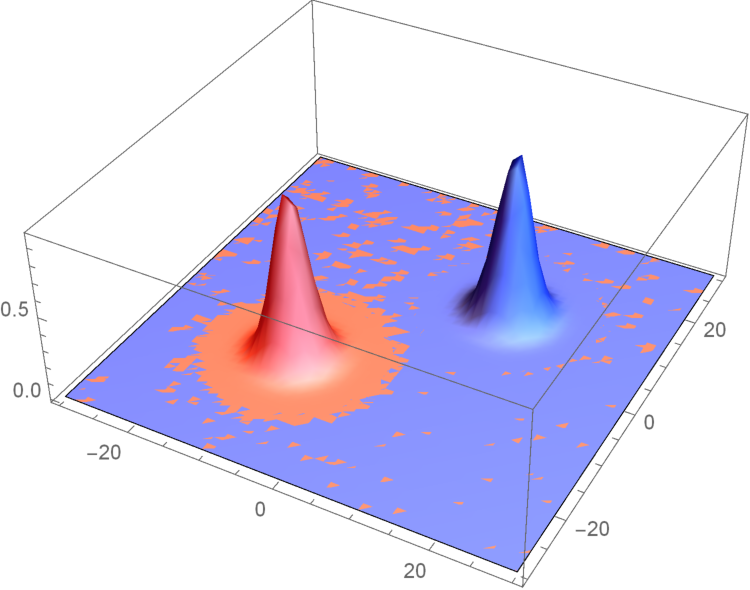
\includegraphics[width=6cm]{images/predPrayFull0.pdf}
%\end{subfigure}
%\begin{subfigure}[t]{0.49\textwidth}
%	\centering
%	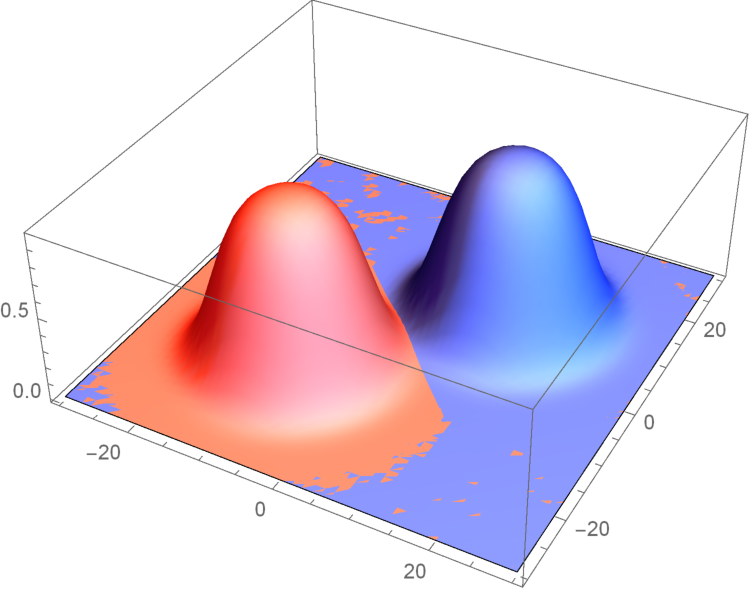
\includegraphics[width=6cm]{images/predPrayFull5.pdf}
%\end{subfigure}	
%\begin{subfigure}[t]{0.49\textwidth}
%	\centering
%	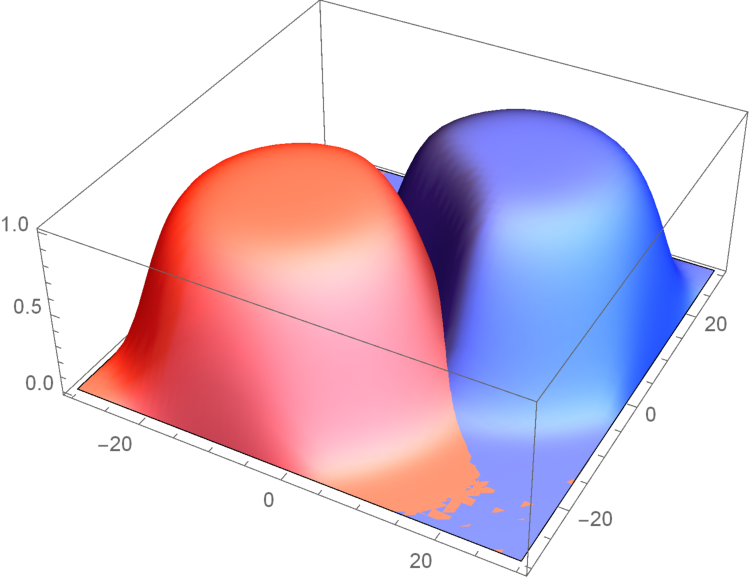
\includegraphics[width=6cm]{images/predPrayFull10.pdf}
%\end{subfigure}
%\begin{subfigure}[t]{0.49\textwidth}
%	\centering
%	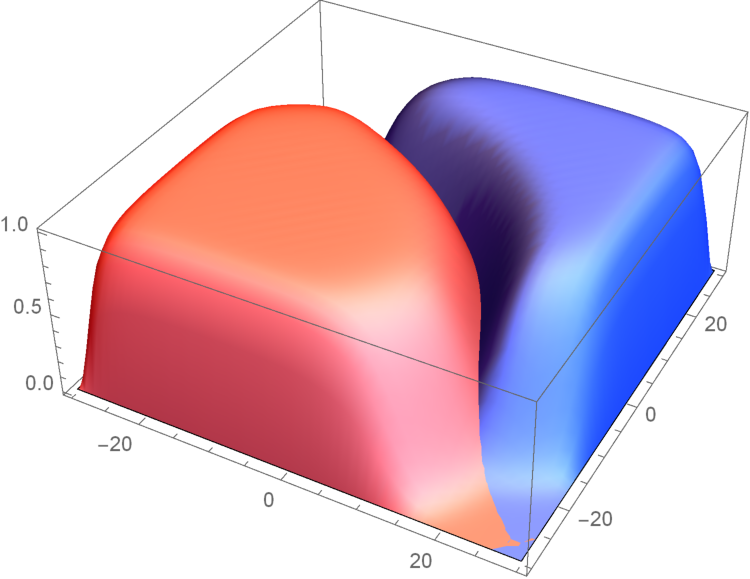
\includegraphics[width=6cm]{images/predPrayFull15.pdf}
%\end{subfigure}
%\begin{subfigure}[t]{0.49\textwidth}
%	\centering
%	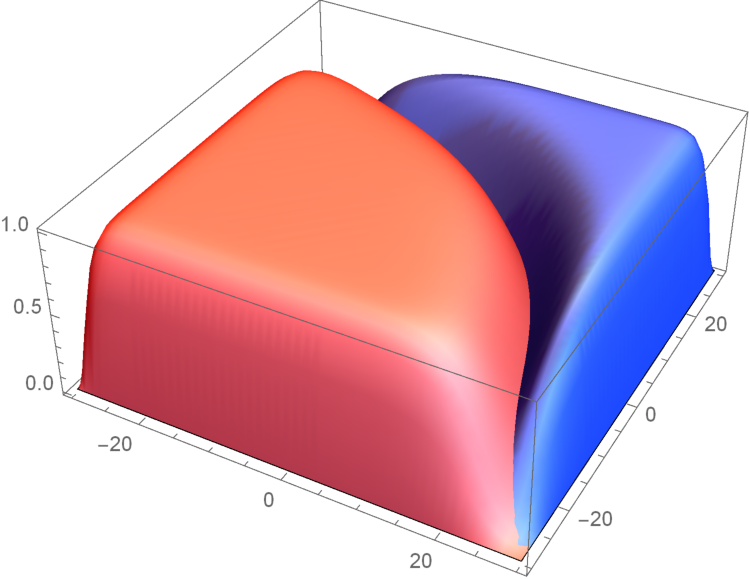
\includegraphics[width=6cm]{images/predPrayFull20.pdf}
%\end{subfigure}
%\begin{subfigure}[t]{0.49\textwidth}
%	\centering
%	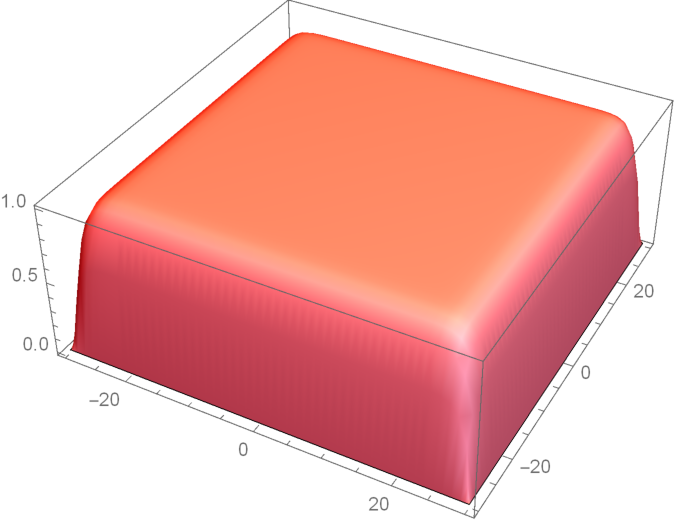
\includegraphics[width=6cm]{images/predPrayFull50.pdf}
%\end{subfigure}
%\caption{Snapshots of numerical simulations of solutions to \cref{scaledlotvolpursuit} with a pair of Gaussian population peaks as initial conditions. The parameters are $\gamma_1 =1.5$, $\gamma_2=0.5$, $\kappa =1$ and (a) $t=0$, (b) $t=5$, (c) $t=10$, (d) $t=15$, (e) $t=20$, (f) $t=50$. The choice of $\gamma_1,\gamma_2$ sets the dominant population to be $v$, in red; $u$ is in blue.}%
%\label{predpraynumerics}%
%\end{figure}
%
%\paragraph{The importance of boundary conditions} Let's have a look at some numerical simulations of our full, 2D system \cref{scaledlotvolpursuit}. In \cref{predpraynumerics} we see snapshots of a  simulation whose initial conditions are two Gaussian populations which diffuse and interact. The values of $\gamma_1$ and $\gamma_2$ are chosen so that $v$ is the dominant species (in red). The boundary conditions are that both populations are zero on the boundary. Do we get travelling wave solutions forever, like in our 1D model? 
%
%From (a)--(b) the populations diffuse and begin to interact. In (c)--(e) we see the dominant species gradually outcompeting the weaker species. This ends with the weaker species becoming extinct in (f).  This case \emph{does} lead to a finite-time equilibrium. The critical observation here is that boundary conditions play a fundamental role in determining what type of solutions are permitted. The travelling wave solution would eventually violate the zero boundary conditions, so it cannot persist for all $t$.
%
%
%\section{Equilibria of spatial competitive Lotka--Volterra}
%Equilibrium solutions to \cref{scaledlotvolpursuit} require that we solve the following system,
%\begin{subequations}
%\label{predprayeq}
%\begin{align}
%\nabla^2u & = - u(1 - u -\gamma_1v),\\
%\nabla^2v & = - \frac{\beta}{\kappa}v(1 - v - \gamma_2 u).
%\end{align}
%\end{subequations}
%This is a more complicated matter than in the non-spatially dependent (ODE) system as the choice of boundary conditions drastically affect what kind of solutions are permissible.
%
%As such, we cannot be exhaustive here and so instead, we will look at some interesting cases which highlight aspects of the system. 
%
%\subsection{Single extinction equilibria}
%We can have solutions which have the total extinction of one population. If we choose $v$ to be the dominant species then we have
%\begin{subequations}
%\begin{align}
%u & = 0,\\
%\nabla^2 v & = -v(1 - v). \label{singleext}
%\end{align}
%\end{subequations}
%For simplicity we assume $\beta/\kappa=1$ (which is true up to a scaling in $x$). We should be clear that this solution is only valid for boundary conditions on $u$ where $u$ and all its derivatives vanish at the boundaries of the system (be they finite  or infinite). Any nonzero boundary conditions for $u$ clearly don't permit this. The simulation shown in \cref{predpraynumerics} satisfies such conditions and we see that the weaker species in this example, $u$, indeed vanishes. 
%
%As for $v$, \cref{singleext} allows for sets of equilibria which include the trivial solution, $v(x) \equiv 0$, and logistic solution, $v(x) \equiv 1$, for all $x$. %The same boundary as for $u$ would then apply. 
%
%But there are other, nontrivial solutions too. In one dimension we can make some progress. Multiplying \cref{singleext} by $\fd{v}{x}$ we obtain
%\begin{equation}
%\fd{v}{x}\fdd{v}{x}  = \fd{v}{x}v(v-1) \implies \left(\fd{v}{x}\right)^2 = v^2\left(\frac{2}{3}v-1\right) + C_1
%\end{equation}
%with $C_1$ a constant of integration. Thus we have a first order ODE,
%\begin{equation}
%\fd{v}{x} = \pm\sqrt{C_1 + v^2\left(\frac{2}{3}v-1\right)},
%\end{equation}
%and by separation of variables,
%\begin{equation}
%\int\frac{1}{\sqrt{C_1 + v^2(\frac{2}{3}v-1)}}\,\d v = \pm x + C_2.
%\end{equation}
%A special case, which has a fairly presentable solution, is the case $C_1=0$ (but note this requires $\fd{v}{x} =0$ when $v=0$ or $v=3/2$ to avoid dividing by zero),
%\begin{equation}
%\int\frac{1}{v\sqrt{\frac{2}{3}v-1}}\,\d v =  \pm x + C_2.
%\end{equation}
%Making the substitution $w^2 = \frac{2}{3}v-1$, $\d{v} = 3 w\,\d{w}$, we obtain 
%\begin{equation}
%\int\frac{1}{v\sqrt{\frac{2}{3}v-1}}\,\d v = 2\int\frac{1}{1+w^2}\,\d w = 2\tan^{-1}(w)  = 2\tan^{-1}\left(\sqrt{\frac{2}{3}v-1}\right). 
%\end{equation}
%Solving for $v$, then, 
%\begin{equation}
%\label{eqmsolzero}
%v= \frac{3}{2}\left[\tan^2\left(\pm \frac{x}{2} + C_2\right) + 1 \right],
%\end{equation}
%having absorbed the $1/2$ into $C_2$.
%
%\begin{figure}
%\centering
%%% Creator: Matplotlib, PGF backend
%%
%% To include the figure in your LaTeX document, write
%%   \input{<filename>.pgf}
%%
%% Make sure the required packages are loaded in your preamble
%%   \usepackage{pgf}
%%
%% Figures using additional raster images can only be included by \input if
%% they are in the same directory as the main LaTeX file. For loading figures
%% from other directories you can use the `import` package
%%   \usepackage{import}
%% and then include the figures with
%%   \import{<path to file>}{<filename>.pgf}
%%
%% Matplotlib used the following preamble
%%   \usepackage{fontspec}
%%   \setmainfont{DejaVuSerif.ttf}[Path=/Library/Python/3.7/site-packages/matplotlib/mpl-data/fonts/ttf/]
%%   \setsansfont{DejaVuSans.ttf}[Path=/Library/Python/3.7/site-packages/matplotlib/mpl-data/fonts/ttf/]
%%   \setmonofont{DejaVuSansMono.ttf}[Path=/Library/Python/3.7/site-packages/matplotlib/mpl-data/fonts/ttf/]
%%
\begingroup%
\makeatletter%
\begin{pgfpicture}%
\pgfpathrectangle{\pgfpointorigin}{\pgfqpoint{3.000000in}{2.200000in}}%
\pgfusepath{use as bounding box, clip}%
\begin{pgfscope}%
\pgfsetbuttcap%
\pgfsetmiterjoin%
\definecolor{currentfill}{rgb}{1.000000,1.000000,1.000000}%
\pgfsetfillcolor{currentfill}%
\pgfsetlinewidth{0.000000pt}%
\definecolor{currentstroke}{rgb}{1.000000,1.000000,1.000000}%
\pgfsetstrokecolor{currentstroke}%
\pgfsetdash{}{0pt}%
\pgfpathmoveto{\pgfqpoint{0.000000in}{0.000000in}}%
\pgfpathlineto{\pgfqpoint{3.000000in}{0.000000in}}%
\pgfpathlineto{\pgfqpoint{3.000000in}{2.200000in}}%
\pgfpathlineto{\pgfqpoint{0.000000in}{2.200000in}}%
\pgfpathclose%
\pgfusepath{fill}%
\end{pgfscope}%
\begin{pgfscope}%
\pgfsetbuttcap%
\pgfsetmiterjoin%
\definecolor{currentfill}{rgb}{1.000000,1.000000,1.000000}%
\pgfsetfillcolor{currentfill}%
\pgfsetlinewidth{0.000000pt}%
\definecolor{currentstroke}{rgb}{0.000000,0.000000,0.000000}%
\pgfsetstrokecolor{currentstroke}%
\pgfsetstrokeopacity{0.000000}%
\pgfsetdash{}{0pt}%
\pgfpathmoveto{\pgfqpoint{0.033333in}{0.278150in}}%
\pgfpathlineto{\pgfqpoint{2.966667in}{0.278150in}}%
\pgfpathlineto{\pgfqpoint{2.966667in}{2.166667in}}%
\pgfpathlineto{\pgfqpoint{0.033333in}{2.166667in}}%
\pgfpathclose%
\pgfusepath{fill}%
\end{pgfscope}%
\begin{pgfscope}%
\pgfpathrectangle{\pgfqpoint{0.033333in}{0.278150in}}{\pgfqpoint{2.933333in}{1.888517in}}%
\pgfusepath{clip}%
\pgfsetbuttcap%
\pgfsetroundjoin%
\pgfsetlinewidth{1.505625pt}%
\definecolor{currentstroke}{rgb}{1.000000,0.498039,0.054902}%
\pgfsetstrokecolor{currentstroke}%
\pgfsetdash{{5.550000pt}{2.400000pt}}{0.000000pt}%
\pgfpathmoveto{\pgfqpoint{0.044221in}{2.171667in}}%
\pgfpathlineto{\pgfqpoint{0.048015in}{1.893743in}}%
\pgfpathlineto{\pgfqpoint{0.053887in}{1.575392in}}%
\pgfpathlineto{\pgfqpoint{0.059760in}{1.343310in}}%
\pgfpathlineto{\pgfqpoint{0.065632in}{1.168928in}}%
\pgfpathlineto{\pgfqpoint{0.071505in}{1.034593in}}%
\pgfpathlineto{\pgfqpoint{0.077377in}{0.928922in}}%
\pgfpathlineto{\pgfqpoint{0.083250in}{0.844307in}}%
\pgfpathlineto{\pgfqpoint{0.089122in}{0.775505in}}%
\pgfpathlineto{\pgfqpoint{0.094995in}{0.718811in}}%
\pgfpathlineto{\pgfqpoint{0.100868in}{0.671543in}}%
\pgfpathlineto{\pgfqpoint{0.106740in}{0.631724in}}%
\pgfpathlineto{\pgfqpoint{0.112613in}{0.597870in}}%
\pgfpathlineto{\pgfqpoint{0.118485in}{0.568846in}}%
\pgfpathlineto{\pgfqpoint{0.124358in}{0.543779in}}%
\pgfpathlineto{\pgfqpoint{0.133166in}{0.512134in}}%
\pgfpathlineto{\pgfqpoint{0.141975in}{0.486131in}}%
\pgfpathlineto{\pgfqpoint{0.150784in}{0.464507in}}%
\pgfpathlineto{\pgfqpoint{0.159593in}{0.446338in}}%
\pgfpathlineto{\pgfqpoint{0.168402in}{0.430929in}}%
\pgfpathlineto{\pgfqpoint{0.177211in}{0.417752in}}%
\pgfpathlineto{\pgfqpoint{0.186019in}{0.406401in}}%
\pgfpathlineto{\pgfqpoint{0.194828in}{0.396557in}}%
\pgfpathlineto{\pgfqpoint{0.206573in}{0.385350in}}%
\pgfpathlineto{\pgfqpoint{0.218318in}{0.375921in}}%
\pgfpathlineto{\pgfqpoint{0.230063in}{0.367921in}}%
\pgfpathlineto{\pgfqpoint{0.241808in}{0.361084in}}%
\pgfpathlineto{\pgfqpoint{0.256490in}{0.353866in}}%
\pgfpathlineto{\pgfqpoint{0.271171in}{0.347839in}}%
\pgfpathlineto{\pgfqpoint{0.288789in}{0.341859in}}%
\pgfpathlineto{\pgfqpoint{0.309343in}{0.336243in}}%
\pgfpathlineto{\pgfqpoint{0.329897in}{0.331772in}}%
\pgfpathlineto{\pgfqpoint{0.353387in}{0.327760in}}%
\pgfpathlineto{\pgfqpoint{0.379813in}{0.324348in}}%
\pgfpathlineto{\pgfqpoint{0.409176in}{0.321641in}}%
\pgfpathlineto{\pgfqpoint{0.441475in}{0.319732in}}%
\pgfpathlineto{\pgfqpoint{0.476710in}{0.318730in}}%
\pgfpathlineto{\pgfqpoint{0.514882in}{0.318807in}}%
\pgfpathlineto{\pgfqpoint{0.550117in}{0.319958in}}%
\pgfpathlineto{\pgfqpoint{0.582416in}{0.322026in}}%
\pgfpathlineto{\pgfqpoint{0.611778in}{0.324907in}}%
\pgfpathlineto{\pgfqpoint{0.638205in}{0.328517in}}%
\pgfpathlineto{\pgfqpoint{0.661695in}{0.332753in}}%
\pgfpathlineto{\pgfqpoint{0.682249in}{0.337474in}}%
\pgfpathlineto{\pgfqpoint{0.702803in}{0.343411in}}%
\pgfpathlineto{\pgfqpoint{0.720420in}{0.349744in}}%
\pgfpathlineto{\pgfqpoint{0.735102in}{0.356142in}}%
\pgfpathlineto{\pgfqpoint{0.749783in}{0.363824in}}%
\pgfpathlineto{\pgfqpoint{0.761528in}{0.371120in}}%
\pgfpathlineto{\pgfqpoint{0.773273in}{0.379684in}}%
\pgfpathlineto{\pgfqpoint{0.785018in}{0.389811in}}%
\pgfpathlineto{\pgfqpoint{0.793827in}{0.398663in}}%
\pgfpathlineto{\pgfqpoint{0.802636in}{0.408823in}}%
\pgfpathlineto{\pgfqpoint{0.811445in}{0.420556in}}%
\pgfpathlineto{\pgfqpoint{0.820254in}{0.434198in}}%
\pgfpathlineto{\pgfqpoint{0.829062in}{0.450179in}}%
\pgfpathlineto{\pgfqpoint{0.837871in}{0.469061in}}%
\pgfpathlineto{\pgfqpoint{0.846680in}{0.491582in}}%
\pgfpathlineto{\pgfqpoint{0.852553in}{0.509095in}}%
\pgfpathlineto{\pgfqpoint{0.858425in}{0.529037in}}%
\pgfpathlineto{\pgfqpoint{0.864298in}{0.551875in}}%
\pgfpathlineto{\pgfqpoint{0.870170in}{0.578198in}}%
\pgfpathlineto{\pgfqpoint{0.876043in}{0.608749in}}%
\pgfpathlineto{\pgfqpoint{0.881915in}{0.644482in}}%
\pgfpathlineto{\pgfqpoint{0.887788in}{0.686637in}}%
\pgfpathlineto{\pgfqpoint{0.893660in}{0.736847in}}%
\pgfpathlineto{\pgfqpoint{0.899533in}{0.797301in}}%
\pgfpathlineto{\pgfqpoint{0.905405in}{0.870981in}}%
\pgfpathlineto{\pgfqpoint{0.911278in}{0.962047in}}%
\pgfpathlineto{\pgfqpoint{0.917150in}{1.076425in}}%
\pgfpathlineto{\pgfqpoint{0.923023in}{1.222807in}}%
\pgfpathlineto{\pgfqpoint{0.928896in}{1.414343in}}%
\pgfpathlineto{\pgfqpoint{0.934768in}{1.671705in}}%
\pgfpathlineto{\pgfqpoint{0.940641in}{2.028906in}}%
\pgfpathlineto{\pgfqpoint{0.942440in}{2.171667in}}%
\pgfpathmoveto{\pgfqpoint{1.035094in}{2.171667in}}%
\pgfpathlineto{\pgfqpoint{1.040474in}{1.798362in}}%
\pgfpathlineto{\pgfqpoint{1.046346in}{1.506656in}}%
\pgfpathlineto{\pgfqpoint{1.052219in}{1.292152in}}%
\pgfpathlineto{\pgfqpoint{1.058091in}{1.129830in}}%
\pgfpathlineto{\pgfqpoint{1.063964in}{1.004045in}}%
\pgfpathlineto{\pgfqpoint{1.069837in}{0.904602in}}%
\pgfpathlineto{\pgfqpoint{1.075709in}{0.824632in}}%
\pgfpathlineto{\pgfqpoint{1.081582in}{0.759364in}}%
\pgfpathlineto{\pgfqpoint{1.087454in}{0.705406in}}%
\pgfpathlineto{\pgfqpoint{1.093327in}{0.660290in}}%
\pgfpathlineto{\pgfqpoint{1.099199in}{0.622186in}}%
\pgfpathlineto{\pgfqpoint{1.105072in}{0.589716in}}%
\pgfpathlineto{\pgfqpoint{1.110944in}{0.561822in}}%
\pgfpathlineto{\pgfqpoint{1.116817in}{0.537684in}}%
\pgfpathlineto{\pgfqpoint{1.125626in}{0.507151in}}%
\pgfpathlineto{\pgfqpoint{1.134434in}{0.482006in}}%
\pgfpathlineto{\pgfqpoint{1.143243in}{0.461055in}}%
\pgfpathlineto{\pgfqpoint{1.152052in}{0.443420in}}%
\pgfpathlineto{\pgfqpoint{1.160861in}{0.428442in}}%
\pgfpathlineto{\pgfqpoint{1.169670in}{0.415616in}}%
\pgfpathlineto{\pgfqpoint{1.178478in}{0.404553in}}%
\pgfpathlineto{\pgfqpoint{1.187287in}{0.394949in}}%
\pgfpathlineto{\pgfqpoint{1.199032in}{0.384002in}}%
\pgfpathlineto{\pgfqpoint{1.210777in}{0.374780in}}%
\pgfpathlineto{\pgfqpoint{1.222523in}{0.366949in}}%
\pgfpathlineto{\pgfqpoint{1.237204in}{0.358729in}}%
\pgfpathlineto{\pgfqpoint{1.251885in}{0.351905in}}%
\pgfpathlineto{\pgfqpoint{1.266567in}{0.346194in}}%
\pgfpathlineto{\pgfqpoint{1.284184in}{0.340517in}}%
\pgfpathlineto{\pgfqpoint{1.304738in}{0.335176in}}%
\pgfpathlineto{\pgfqpoint{1.328228in}{0.330388in}}%
\pgfpathlineto{\pgfqpoint{1.354655in}{0.326296in}}%
\pgfpathlineto{\pgfqpoint{1.384017in}{0.322994in}}%
\pgfpathlineto{\pgfqpoint{1.416316in}{0.320554in}}%
\pgfpathlineto{\pgfqpoint{1.451552in}{0.319055in}}%
\pgfpathlineto{\pgfqpoint{1.486787in}{0.318621in}}%
\pgfpathlineto{\pgfqpoint{1.524958in}{0.319300in}}%
\pgfpathlineto{\pgfqpoint{1.560194in}{0.321059in}}%
\pgfpathlineto{\pgfqpoint{1.592492in}{0.323787in}}%
\pgfpathlineto{\pgfqpoint{1.621855in}{0.327418in}}%
\pgfpathlineto{\pgfqpoint{1.648282in}{0.331892in}}%
\pgfpathlineto{\pgfqpoint{1.668836in}{0.336393in}}%
\pgfpathlineto{\pgfqpoint{1.689389in}{0.342049in}}%
\pgfpathlineto{\pgfqpoint{1.707007in}{0.348072in}}%
\pgfpathlineto{\pgfqpoint{1.721688in}{0.354143in}}%
\pgfpathlineto{\pgfqpoint{1.736370in}{0.361418in}}%
\pgfpathlineto{\pgfqpoint{1.748115in}{0.368309in}}%
\pgfpathlineto{\pgfqpoint{1.759860in}{0.376377in}}%
\pgfpathlineto{\pgfqpoint{1.771605in}{0.385890in}}%
\pgfpathlineto{\pgfqpoint{1.783350in}{0.397202in}}%
\pgfpathlineto{\pgfqpoint{1.792159in}{0.407142in}}%
\pgfpathlineto{\pgfqpoint{1.800968in}{0.418610in}}%
\pgfpathlineto{\pgfqpoint{1.809776in}{0.431929in}}%
\pgfpathlineto{\pgfqpoint{1.818585in}{0.447512in}}%
\pgfpathlineto{\pgfqpoint{1.827394in}{0.465898in}}%
\pgfpathlineto{\pgfqpoint{1.836203in}{0.487794in}}%
\pgfpathlineto{\pgfqpoint{1.845012in}{0.514147in}}%
\pgfpathlineto{\pgfqpoint{1.850884in}{0.534809in}}%
\pgfpathlineto{\pgfqpoint{1.856757in}{0.558511in}}%
\pgfpathlineto{\pgfqpoint{1.862629in}{0.585879in}}%
\pgfpathlineto{\pgfqpoint{1.868502in}{0.617705in}}%
\pgfpathlineto{\pgfqpoint{1.874374in}{0.655012in}}%
\pgfpathlineto{\pgfqpoint{1.880247in}{0.699132in}}%
\pgfpathlineto{\pgfqpoint{1.886119in}{0.751826in}}%
\pgfpathlineto{\pgfqpoint{1.891992in}{0.815467in}}%
\pgfpathlineto{\pgfqpoint{1.897865in}{0.893307in}}%
\pgfpathlineto{\pgfqpoint{1.903737in}{0.989905in}}%
\pgfpathlineto{\pgfqpoint{1.909610in}{1.111805in}}%
\pgfpathlineto{\pgfqpoint{1.915482in}{1.268677in}}%
\pgfpathlineto{\pgfqpoint{1.921355in}{1.475294in}}%
\pgfpathlineto{\pgfqpoint{1.927227in}{1.755145in}}%
\pgfpathlineto{\pgfqpoint{1.930163in}{1.933851in}}%
\pgfpathlineto{\pgfqpoint{1.933376in}{2.171667in}}%
\pgfpathmoveto{\pgfqpoint{2.026020in}{2.171667in}}%
\pgfpathlineto{\pgfqpoint{2.029997in}{1.881746in}}%
\pgfpathlineto{\pgfqpoint{2.035869in}{1.566782in}}%
\pgfpathlineto{\pgfqpoint{2.041742in}{1.336924in}}%
\pgfpathlineto{\pgfqpoint{2.047614in}{1.164061in}}%
\pgfpathlineto{\pgfqpoint{2.053487in}{1.030799in}}%
\pgfpathlineto{\pgfqpoint{2.059359in}{0.925908in}}%
\pgfpathlineto{\pgfqpoint{2.065232in}{0.841872in}}%
\pgfpathlineto{\pgfqpoint{2.071104in}{0.773511in}}%
\pgfpathlineto{\pgfqpoint{2.076977in}{0.717157in}}%
\pgfpathlineto{\pgfqpoint{2.082850in}{0.670157in}}%
\pgfpathlineto{\pgfqpoint{2.088722in}{0.630550in}}%
\pgfpathlineto{\pgfqpoint{2.094595in}{0.596867in}}%
\pgfpathlineto{\pgfqpoint{2.100467in}{0.567983in}}%
\pgfpathlineto{\pgfqpoint{2.106340in}{0.543031in}}%
\pgfpathlineto{\pgfqpoint{2.115148in}{0.511523in}}%
\pgfpathlineto{\pgfqpoint{2.123957in}{0.485625in}}%
\pgfpathlineto{\pgfqpoint{2.132766in}{0.464085in}}%
\pgfpathlineto{\pgfqpoint{2.141575in}{0.445981in}}%
\pgfpathlineto{\pgfqpoint{2.150384in}{0.430625in}}%
\pgfpathlineto{\pgfqpoint{2.159193in}{0.417491in}}%
\pgfpathlineto{\pgfqpoint{2.168001in}{0.406175in}}%
\pgfpathlineto{\pgfqpoint{2.176810in}{0.396361in}}%
\pgfpathlineto{\pgfqpoint{2.188555in}{0.385186in}}%
\pgfpathlineto{\pgfqpoint{2.200300in}{0.375782in}}%
\pgfpathlineto{\pgfqpoint{2.212045in}{0.367802in}}%
\pgfpathlineto{\pgfqpoint{2.223790in}{0.360983in}}%
\pgfpathlineto{\pgfqpoint{2.238472in}{0.353782in}}%
\pgfpathlineto{\pgfqpoint{2.253153in}{0.347769in}}%
\pgfpathlineto{\pgfqpoint{2.270771in}{0.341802in}}%
\pgfpathlineto{\pgfqpoint{2.291325in}{0.336197in}}%
\pgfpathlineto{\pgfqpoint{2.311879in}{0.331735in}}%
\pgfpathlineto{\pgfqpoint{2.335369in}{0.327732in}}%
\pgfpathlineto{\pgfqpoint{2.361795in}{0.324327in}}%
\pgfpathlineto{\pgfqpoint{2.391158in}{0.321627in}}%
\pgfpathlineto{\pgfqpoint{2.423457in}{0.319724in}}%
\pgfpathlineto{\pgfqpoint{2.458692in}{0.318728in}}%
\pgfpathlineto{\pgfqpoint{2.496864in}{0.318811in}}%
\pgfpathlineto{\pgfqpoint{2.532099in}{0.319968in}}%
\pgfpathlineto{\pgfqpoint{2.564398in}{0.322041in}}%
\pgfpathlineto{\pgfqpoint{2.593760in}{0.324930in}}%
\pgfpathlineto{\pgfqpoint{2.620187in}{0.328547in}}%
\pgfpathlineto{\pgfqpoint{2.643677in}{0.332792in}}%
\pgfpathlineto{\pgfqpoint{2.664231in}{0.337522in}}%
\pgfpathlineto{\pgfqpoint{2.684785in}{0.343472in}}%
\pgfpathlineto{\pgfqpoint{2.702402in}{0.349820in}}%
\pgfpathlineto{\pgfqpoint{2.717084in}{0.356232in}}%
\pgfpathlineto{\pgfqpoint{2.731765in}{0.363933in}}%
\pgfpathlineto{\pgfqpoint{2.743510in}{0.371247in}}%
\pgfpathlineto{\pgfqpoint{2.755255in}{0.379833in}}%
\pgfpathlineto{\pgfqpoint{2.767000in}{0.389988in}}%
\pgfpathlineto{\pgfqpoint{2.775809in}{0.398866in}}%
\pgfpathlineto{\pgfqpoint{2.784618in}{0.409057in}}%
\pgfpathlineto{\pgfqpoint{2.793427in}{0.420827in}}%
\pgfpathlineto{\pgfqpoint{2.802236in}{0.434514in}}%
\pgfpathlineto{\pgfqpoint{2.811044in}{0.450551in}}%
\pgfpathlineto{\pgfqpoint{2.819853in}{0.469502in}}%
\pgfpathlineto{\pgfqpoint{2.828662in}{0.492112in}}%
\pgfpathlineto{\pgfqpoint{2.834535in}{0.509696in}}%
\pgfpathlineto{\pgfqpoint{2.840407in}{0.529723in}}%
\pgfpathlineto{\pgfqpoint{2.846280in}{0.552663in}}%
\pgfpathlineto{\pgfqpoint{2.852152in}{0.579110in}}%
\pgfpathlineto{\pgfqpoint{2.858025in}{0.609811in}}%
\pgfpathlineto{\pgfqpoint{2.863897in}{0.645730in}}%
\pgfpathlineto{\pgfqpoint{2.869770in}{0.688116in}}%
\pgfpathlineto{\pgfqpoint{2.875642in}{0.738618in}}%
\pgfpathlineto{\pgfqpoint{2.881515in}{0.799445in}}%
\pgfpathlineto{\pgfqpoint{2.887387in}{0.873612in}}%
\pgfpathlineto{\pgfqpoint{2.893260in}{0.965323in}}%
\pgfpathlineto{\pgfqpoint{2.899132in}{1.080577in}}%
\pgfpathlineto{\pgfqpoint{2.905005in}{1.228175in}}%
\pgfpathlineto{\pgfqpoint{2.910878in}{1.421453in}}%
\pgfpathlineto{\pgfqpoint{2.916750in}{1.681400in}}%
\pgfpathlineto{\pgfqpoint{2.919686in}{1.846390in}}%
\pgfpathlineto{\pgfqpoint{2.924229in}{2.171667in}}%
\pgfpathlineto{\pgfqpoint{2.924229in}{2.171667in}}%
\pgfusepath{stroke}%
\end{pgfscope}%
\begin{pgfscope}%
\pgfsetbuttcap%
\pgfsetroundjoin%
\definecolor{currentfill}{rgb}{0.000000,0.000000,0.000000}%
\pgfsetfillcolor{currentfill}%
\pgfsetlinewidth{0.803000pt}%
\definecolor{currentstroke}{rgb}{0.000000,0.000000,0.000000}%
\pgfsetstrokecolor{currentstroke}%
\pgfsetdash{}{0pt}%
\pgfsys@defobject{currentmarker}{\pgfqpoint{0.000000in}{-0.048611in}}{\pgfqpoint{0.000000in}{0.000000in}}{%
\pgfpathmoveto{\pgfqpoint{0.000000in}{0.000000in}}%
\pgfpathlineto{\pgfqpoint{0.000000in}{-0.048611in}}%
\pgfusepath{stroke,fill}%
}%
\begin{pgfscope}%
\pgfsys@transformshift{0.664158in}{0.278150in}%
\pgfsys@useobject{currentmarker}{}%
\end{pgfscope}%
\end{pgfscope}%
\begin{pgfscope}%
\definecolor{textcolor}{rgb}{0.000000,0.000000,0.000000}%
\pgfsetstrokecolor{textcolor}%
\pgfsetfillcolor{textcolor}%
\pgftext[x=0.664158in,y=0.180927in,,top]{\color{textcolor}\rmfamily\fontsize{12.000000}{14.400000}\selectfont \(\displaystyle -5\)}%
\end{pgfscope}%
\begin{pgfscope}%
\pgfsetbuttcap%
\pgfsetroundjoin%
\definecolor{currentfill}{rgb}{0.000000,0.000000,0.000000}%
\pgfsetfillcolor{currentfill}%
\pgfsetlinewidth{0.803000pt}%
\definecolor{currentstroke}{rgb}{0.000000,0.000000,0.000000}%
\pgfsetstrokecolor{currentstroke}%
\pgfsetdash{}{0pt}%
\pgfsys@defobject{currentmarker}{\pgfqpoint{0.000000in}{-0.048611in}}{\pgfqpoint{0.000000in}{0.000000in}}{%
\pgfpathmoveto{\pgfqpoint{0.000000in}{0.000000in}}%
\pgfpathlineto{\pgfqpoint{0.000000in}{-0.048611in}}%
\pgfusepath{stroke,fill}%
}%
\begin{pgfscope}%
\pgfsys@transformshift{1.452688in}{0.278150in}%
\pgfsys@useobject{currentmarker}{}%
\end{pgfscope}%
\end{pgfscope}%
\begin{pgfscope}%
\definecolor{textcolor}{rgb}{0.000000,0.000000,0.000000}%
\pgfsetstrokecolor{textcolor}%
\pgfsetfillcolor{textcolor}%
\pgftext[x=1.452688in,y=0.180927in,,top]{\color{textcolor}\rmfamily\fontsize{12.000000}{14.400000}\selectfont \(\displaystyle 0\)}%
\end{pgfscope}%
\begin{pgfscope}%
\pgfsetbuttcap%
\pgfsetroundjoin%
\definecolor{currentfill}{rgb}{0.000000,0.000000,0.000000}%
\pgfsetfillcolor{currentfill}%
\pgfsetlinewidth{0.803000pt}%
\definecolor{currentstroke}{rgb}{0.000000,0.000000,0.000000}%
\pgfsetstrokecolor{currentstroke}%
\pgfsetdash{}{0pt}%
\pgfsys@defobject{currentmarker}{\pgfqpoint{0.000000in}{-0.048611in}}{\pgfqpoint{0.000000in}{0.000000in}}{%
\pgfpathmoveto{\pgfqpoint{0.000000in}{0.000000in}}%
\pgfpathlineto{\pgfqpoint{0.000000in}{-0.048611in}}%
\pgfusepath{stroke,fill}%
}%
\begin{pgfscope}%
\pgfsys@transformshift{2.241219in}{0.278150in}%
\pgfsys@useobject{currentmarker}{}%
\end{pgfscope}%
\end{pgfscope}%
\begin{pgfscope}%
\definecolor{textcolor}{rgb}{0.000000,0.000000,0.000000}%
\pgfsetstrokecolor{textcolor}%
\pgfsetfillcolor{textcolor}%
\pgftext[x=2.241219in,y=0.180927in,,top]{\color{textcolor}\rmfamily\fontsize{12.000000}{14.400000}\selectfont \(\displaystyle 5\)}%
\end{pgfscope}%
\begin{pgfscope}%
\pgfsetbuttcap%
\pgfsetroundjoin%
\definecolor{currentfill}{rgb}{0.000000,0.000000,0.000000}%
\pgfsetfillcolor{currentfill}%
\pgfsetlinewidth{0.803000pt}%
\definecolor{currentstroke}{rgb}{0.000000,0.000000,0.000000}%
\pgfsetstrokecolor{currentstroke}%
\pgfsetdash{}{0pt}%
\pgfsys@defobject{currentmarker}{\pgfqpoint{-0.048611in}{0.000000in}}{\pgfqpoint{0.000000in}{0.000000in}}{%
\pgfpathmoveto{\pgfqpoint{0.000000in}{0.000000in}}%
\pgfpathlineto{\pgfqpoint{-0.048611in}{0.000000in}}%
\pgfusepath{stroke,fill}%
}%
\begin{pgfscope}%
\pgfsys@transformshift{1.452688in}{0.278150in}%
\pgfsys@useobject{currentmarker}{}%
\end{pgfscope}%
\end{pgfscope}%
\begin{pgfscope}%
\definecolor{textcolor}{rgb}{0.000000,0.000000,0.000000}%
\pgfsetstrokecolor{textcolor}%
\pgfsetfillcolor{textcolor}%
\pgftext[x=1.273870in,y=0.214836in,left,base]{\color{textcolor}\rmfamily\fontsize{12.000000}{14.400000}\selectfont \(\displaystyle 0\)}%
\end{pgfscope}%
\begin{pgfscope}%
\pgfsetbuttcap%
\pgfsetroundjoin%
\definecolor{currentfill}{rgb}{0.000000,0.000000,0.000000}%
\pgfsetfillcolor{currentfill}%
\pgfsetlinewidth{0.803000pt}%
\definecolor{currentstroke}{rgb}{0.000000,0.000000,0.000000}%
\pgfsetstrokecolor{currentstroke}%
\pgfsetdash{}{0pt}%
\pgfsys@defobject{currentmarker}{\pgfqpoint{-0.048611in}{0.000000in}}{\pgfqpoint{0.000000in}{0.000000in}}{%
\pgfpathmoveto{\pgfqpoint{0.000000in}{0.000000in}}%
\pgfpathlineto{\pgfqpoint{-0.048611in}{0.000000in}}%
\pgfusepath{stroke,fill}%
}%
\begin{pgfscope}%
\pgfsys@transformshift{1.452688in}{0.817726in}%
\pgfsys@useobject{currentmarker}{}%
\end{pgfscope}%
\end{pgfscope}%
\begin{pgfscope}%
\definecolor{textcolor}{rgb}{0.000000,0.000000,0.000000}%
\pgfsetstrokecolor{textcolor}%
\pgfsetfillcolor{textcolor}%
\pgftext[x=1.192273in,y=0.754412in,left,base]{\color{textcolor}\rmfamily\fontsize{12.000000}{14.400000}\selectfont \(\displaystyle 20\)}%
\end{pgfscope}%
\begin{pgfscope}%
\pgfsetbuttcap%
\pgfsetroundjoin%
\definecolor{currentfill}{rgb}{0.000000,0.000000,0.000000}%
\pgfsetfillcolor{currentfill}%
\pgfsetlinewidth{0.803000pt}%
\definecolor{currentstroke}{rgb}{0.000000,0.000000,0.000000}%
\pgfsetstrokecolor{currentstroke}%
\pgfsetdash{}{0pt}%
\pgfsys@defobject{currentmarker}{\pgfqpoint{-0.048611in}{0.000000in}}{\pgfqpoint{0.000000in}{0.000000in}}{%
\pgfpathmoveto{\pgfqpoint{0.000000in}{0.000000in}}%
\pgfpathlineto{\pgfqpoint{-0.048611in}{0.000000in}}%
\pgfusepath{stroke,fill}%
}%
\begin{pgfscope}%
\pgfsys@transformshift{1.452688in}{1.357302in}%
\pgfsys@useobject{currentmarker}{}%
\end{pgfscope}%
\end{pgfscope}%
\begin{pgfscope}%
\definecolor{textcolor}{rgb}{0.000000,0.000000,0.000000}%
\pgfsetstrokecolor{textcolor}%
\pgfsetfillcolor{textcolor}%
\pgftext[x=1.192273in,y=1.293988in,left,base]{\color{textcolor}\rmfamily\fontsize{12.000000}{14.400000}\selectfont \(\displaystyle 40\)}%
\end{pgfscope}%
\begin{pgfscope}%
\pgfsetbuttcap%
\pgfsetroundjoin%
\definecolor{currentfill}{rgb}{0.000000,0.000000,0.000000}%
\pgfsetfillcolor{currentfill}%
\pgfsetlinewidth{0.803000pt}%
\definecolor{currentstroke}{rgb}{0.000000,0.000000,0.000000}%
\pgfsetstrokecolor{currentstroke}%
\pgfsetdash{}{0pt}%
\pgfsys@defobject{currentmarker}{\pgfqpoint{-0.048611in}{0.000000in}}{\pgfqpoint{0.000000in}{0.000000in}}{%
\pgfpathmoveto{\pgfqpoint{0.000000in}{0.000000in}}%
\pgfpathlineto{\pgfqpoint{-0.048611in}{0.000000in}}%
\pgfusepath{stroke,fill}%
}%
\begin{pgfscope}%
\pgfsys@transformshift{1.452688in}{1.896879in}%
\pgfsys@useobject{currentmarker}{}%
\end{pgfscope}%
\end{pgfscope}%
\begin{pgfscope}%
\definecolor{textcolor}{rgb}{0.000000,0.000000,0.000000}%
\pgfsetstrokecolor{textcolor}%
\pgfsetfillcolor{textcolor}%
\pgftext[x=1.192273in,y=1.833565in,left,base]{\color{textcolor}\rmfamily\fontsize{12.000000}{14.400000}\selectfont \(\displaystyle 60\)}%
\end{pgfscope}%
\begin{pgfscope}%
\pgfpathrectangle{\pgfqpoint{0.033333in}{0.278150in}}{\pgfqpoint{2.933333in}{1.888517in}}%
\pgfusepath{clip}%
\pgfsetbuttcap%
\pgfsetroundjoin%
\pgfsetlinewidth{0.803000pt}%
\definecolor{currentstroke}{rgb}{0.000000,0.000000,0.000000}%
\pgfsetstrokecolor{currentstroke}%
\pgfsetdash{{0.800000pt}{1.600000pt}}{0.000000pt}%
\pgfpathmoveto{\pgfqpoint{1.768100in}{0.278150in}}%
\pgfpathlineto{\pgfqpoint{1.768100in}{2.166667in}}%
\pgfusepath{stroke}%
\end{pgfscope}%
\begin{pgfscope}%
\pgfpathrectangle{\pgfqpoint{0.033333in}{0.278150in}}{\pgfqpoint{2.933333in}{1.888517in}}%
\pgfusepath{clip}%
\pgfsetbuttcap%
\pgfsetroundjoin%
\pgfsetlinewidth{0.803000pt}%
\definecolor{currentstroke}{rgb}{0.000000,0.000000,0.000000}%
\pgfsetstrokecolor{currentstroke}%
\pgfsetdash{{0.800000pt}{1.600000pt}}{0.000000pt}%
\pgfpathmoveto{\pgfqpoint{1.137276in}{0.278150in}}%
\pgfpathlineto{\pgfqpoint{1.137276in}{2.166667in}}%
\pgfusepath{stroke}%
\end{pgfscope}%
\begin{pgfscope}%
\pgfsetrectcap%
\pgfsetmiterjoin%
\pgfsetlinewidth{0.803000pt}%
\definecolor{currentstroke}{rgb}{0.000000,0.000000,0.000000}%
\pgfsetstrokecolor{currentstroke}%
\pgfsetdash{}{0pt}%
\pgfpathmoveto{\pgfqpoint{1.452688in}{0.278150in}}%
\pgfpathlineto{\pgfqpoint{1.452688in}{2.166667in}}%
\pgfusepath{stroke}%
\end{pgfscope}%
\begin{pgfscope}%
\pgfsetrectcap%
\pgfsetmiterjoin%
\pgfsetlinewidth{0.803000pt}%
\definecolor{currentstroke}{rgb}{0.000000,0.000000,0.000000}%
\pgfsetstrokecolor{currentstroke}%
\pgfsetdash{}{0pt}%
\pgfpathmoveto{\pgfqpoint{0.033333in}{0.278150in}}%
\pgfpathlineto{\pgfqpoint{2.966667in}{0.278150in}}%
\pgfusepath{stroke}%
\end{pgfscope}%
\begin{pgfscope}%
\definecolor{textcolor}{rgb}{0.000000,0.000000,0.000000}%
\pgfsetstrokecolor{textcolor}%
\pgfsetfillcolor{textcolor}%
\pgftext[x=2.966667in,y=0.180927in,right,top]{\color{textcolor}\rmfamily\fontsize{12.000000}{14.400000}\selectfont \(\displaystyle x\)}%
\end{pgfscope}%
\begin{pgfscope}%
\definecolor{textcolor}{rgb}{0.000000,0.000000,0.000000}%
\pgfsetstrokecolor{textcolor}%
\pgfsetfillcolor{textcolor}%
\pgftext[x=1.355466in,y=2.166667in,right,top]{\color{textcolor}\rmfamily\fontsize{12.000000}{14.400000}\selectfont \(\displaystyle v\)}%
\end{pgfscope}%
\end{pgfpicture}%
\makeatother%
\endgroup%

%\caption{Solution to the equilibrium equations, \cref{predprayeq}, where one population is extinct, \cref{singleext}. Solutions given by \cref{eqmsolzero} with $C_2=-0.1$. The black dotted lines represent some imagined boundary.}
%\label{predpreyeqm1}
%\end{figure}
%
%So we have one further boundary condition to impose. A plot of the function for $C_2=-0.1$ is shown in \cref{predpreyeqm1} along with some fictitious boundaries (the vertical dotted lines), i.e., we imagine this domain to be $x\in[-2,2]$. We note that the constant $C_2$ only shifts the function along the $x$-axis: it cannot scale the solution. So we cannot have this choice of $C_1$ and have bounded solutions for domains of larger size than $2\pi$. Also \cref{eqmsolzero} does not permit solutions which are anywhere zero. 
%
%\begin{figure}
%	\centering
%	%% Creator: Matplotlib, PGF backend
%%
%% To include the figure in your LaTeX document, write
%%   \input{<filename>.pgf}
%%
%% Make sure the required packages are loaded in your preamble
%%   \usepackage{pgf}
%%
%% Figures using additional raster images can only be included by \input if
%% they are in the same directory as the main LaTeX file. For loading figures
%% from other directories you can use the `import` package
%%   \usepackage{import}
%% and then include the figures with
%%   \import{<path to file>}{<filename>.pgf}
%%
%% Matplotlib used the following preamble
%%   \usepackage{fontspec}
%%   \setmainfont{DejaVuSerif.ttf}[Path=/Library/Python/3.7/site-packages/matplotlib/mpl-data/fonts/ttf/]
%%   \setsansfont{DejaVuSans.ttf}[Path=/Library/Python/3.7/site-packages/matplotlib/mpl-data/fonts/ttf/]
%%   \setmonofont{DejaVuSansMono.ttf}[Path=/Library/Python/3.7/site-packages/matplotlib/mpl-data/fonts/ttf/]
%%
\begingroup%
\makeatletter%
\begin{pgfpicture}%
\pgfpathrectangle{\pgfpointorigin}{\pgfqpoint{6.000000in}{4.400000in}}%
\pgfusepath{use as bounding box, clip}%
\begin{pgfscope}%
\pgfsetbuttcap%
\pgfsetmiterjoin%
\definecolor{currentfill}{rgb}{1.000000,1.000000,1.000000}%
\pgfsetfillcolor{currentfill}%
\pgfsetlinewidth{0.000000pt}%
\definecolor{currentstroke}{rgb}{1.000000,1.000000,1.000000}%
\pgfsetstrokecolor{currentstroke}%
\pgfsetdash{}{0pt}%
\pgfpathmoveto{\pgfqpoint{0.000000in}{0.000000in}}%
\pgfpathlineto{\pgfqpoint{6.000000in}{0.000000in}}%
\pgfpathlineto{\pgfqpoint{6.000000in}{4.400000in}}%
\pgfpathlineto{\pgfqpoint{0.000000in}{4.400000in}}%
\pgfpathclose%
\pgfusepath{fill}%
\end{pgfscope}%
\begin{pgfscope}%
\pgfsetbuttcap%
\pgfsetmiterjoin%
\definecolor{currentfill}{rgb}{1.000000,1.000000,1.000000}%
\pgfsetfillcolor{currentfill}%
\pgfsetlinewidth{0.000000pt}%
\definecolor{currentstroke}{rgb}{0.000000,0.000000,0.000000}%
\pgfsetstrokecolor{currentstroke}%
\pgfsetstrokeopacity{0.000000}%
\pgfsetdash{}{0pt}%
\pgfpathmoveto{\pgfqpoint{0.279198in}{2.338551in}}%
\pgfpathlineto{\pgfqpoint{1.933333in}{2.338551in}}%
\pgfpathlineto{\pgfqpoint{1.933333in}{4.068025in}}%
\pgfpathlineto{\pgfqpoint{0.279198in}{4.068025in}}%
\pgfpathclose%
\pgfusepath{fill}%
\end{pgfscope}%
\begin{pgfscope}%
\pgfsetbuttcap%
\pgfsetroundjoin%
\definecolor{currentfill}{rgb}{0.000000,0.000000,0.000000}%
\pgfsetfillcolor{currentfill}%
\pgfsetlinewidth{0.803000pt}%
\definecolor{currentstroke}{rgb}{0.000000,0.000000,0.000000}%
\pgfsetstrokecolor{currentstroke}%
\pgfsetdash{}{0pt}%
\pgfsys@defobject{currentmarker}{\pgfqpoint{0.000000in}{-0.048611in}}{\pgfqpoint{0.000000in}{0.000000in}}{%
\pgfpathmoveto{\pgfqpoint{0.000000in}{0.000000in}}%
\pgfpathlineto{\pgfqpoint{0.000000in}{-0.048611in}}%
\pgfusepath{stroke,fill}%
}%
\begin{pgfscope}%
\pgfsys@transformshift{0.279198in}{2.338551in}%
\pgfsys@useobject{currentmarker}{}%
\end{pgfscope}%
\end{pgfscope}%
\begin{pgfscope}%
\definecolor{textcolor}{rgb}{0.000000,0.000000,0.000000}%
\pgfsetstrokecolor{textcolor}%
\pgfsetfillcolor{textcolor}%
\pgftext[x=0.279198in,y=2.241329in,,top]{\color{textcolor}\rmfamily\fontsize{12.000000}{14.400000}\selectfont \(\displaystyle -30\)}%
\end{pgfscope}%
\begin{pgfscope}%
\pgfsetbuttcap%
\pgfsetroundjoin%
\definecolor{currentfill}{rgb}{0.000000,0.000000,0.000000}%
\pgfsetfillcolor{currentfill}%
\pgfsetlinewidth{0.803000pt}%
\definecolor{currentstroke}{rgb}{0.000000,0.000000,0.000000}%
\pgfsetstrokecolor{currentstroke}%
\pgfsetdash{}{0pt}%
\pgfsys@defobject{currentmarker}{\pgfqpoint{0.000000in}{-0.048611in}}{\pgfqpoint{0.000000in}{0.000000in}}{%
\pgfpathmoveto{\pgfqpoint{0.000000in}{0.000000in}}%
\pgfpathlineto{\pgfqpoint{0.000000in}{-0.048611in}}%
\pgfusepath{stroke,fill}%
}%
\begin{pgfscope}%
\pgfsys@transformshift{0.751808in}{2.338551in}%
\pgfsys@useobject{currentmarker}{}%
\end{pgfscope}%
\end{pgfscope}%
\begin{pgfscope}%
\definecolor{textcolor}{rgb}{0.000000,0.000000,0.000000}%
\pgfsetstrokecolor{textcolor}%
\pgfsetfillcolor{textcolor}%
\pgftext[x=0.751808in,y=2.241329in,,top]{\color{textcolor}\rmfamily\fontsize{12.000000}{14.400000}\selectfont \(\displaystyle -10\)}%
\end{pgfscope}%
\begin{pgfscope}%
\pgfsetbuttcap%
\pgfsetroundjoin%
\definecolor{currentfill}{rgb}{0.000000,0.000000,0.000000}%
\pgfsetfillcolor{currentfill}%
\pgfsetlinewidth{0.803000pt}%
\definecolor{currentstroke}{rgb}{0.000000,0.000000,0.000000}%
\pgfsetstrokecolor{currentstroke}%
\pgfsetdash{}{0pt}%
\pgfsys@defobject{currentmarker}{\pgfqpoint{0.000000in}{-0.048611in}}{\pgfqpoint{0.000000in}{0.000000in}}{%
\pgfpathmoveto{\pgfqpoint{0.000000in}{0.000000in}}%
\pgfpathlineto{\pgfqpoint{0.000000in}{-0.048611in}}%
\pgfusepath{stroke,fill}%
}%
\begin{pgfscope}%
\pgfsys@transformshift{1.224418in}{2.338551in}%
\pgfsys@useobject{currentmarker}{}%
\end{pgfscope}%
\end{pgfscope}%
\begin{pgfscope}%
\definecolor{textcolor}{rgb}{0.000000,0.000000,0.000000}%
\pgfsetstrokecolor{textcolor}%
\pgfsetfillcolor{textcolor}%
\pgftext[x=1.224418in,y=2.241329in,,top]{\color{textcolor}\rmfamily\fontsize{12.000000}{14.400000}\selectfont \(\displaystyle 10\)}%
\end{pgfscope}%
\begin{pgfscope}%
\pgfsetbuttcap%
\pgfsetroundjoin%
\definecolor{currentfill}{rgb}{0.000000,0.000000,0.000000}%
\pgfsetfillcolor{currentfill}%
\pgfsetlinewidth{0.803000pt}%
\definecolor{currentstroke}{rgb}{0.000000,0.000000,0.000000}%
\pgfsetstrokecolor{currentstroke}%
\pgfsetdash{}{0pt}%
\pgfsys@defobject{currentmarker}{\pgfqpoint{0.000000in}{-0.048611in}}{\pgfqpoint{0.000000in}{0.000000in}}{%
\pgfpathmoveto{\pgfqpoint{0.000000in}{0.000000in}}%
\pgfpathlineto{\pgfqpoint{0.000000in}{-0.048611in}}%
\pgfusepath{stroke,fill}%
}%
\begin{pgfscope}%
\pgfsys@transformshift{1.697028in}{2.338551in}%
\pgfsys@useobject{currentmarker}{}%
\end{pgfscope}%
\end{pgfscope}%
\begin{pgfscope}%
\definecolor{textcolor}{rgb}{0.000000,0.000000,0.000000}%
\pgfsetstrokecolor{textcolor}%
\pgfsetfillcolor{textcolor}%
\pgftext[x=1.697028in,y=2.241329in,,top]{\color{textcolor}\rmfamily\fontsize{12.000000}{14.400000}\selectfont \(\displaystyle 30\)}%
\end{pgfscope}%
\begin{pgfscope}%
\pgfsetbuttcap%
\pgfsetroundjoin%
\definecolor{currentfill}{rgb}{0.000000,0.000000,0.000000}%
\pgfsetfillcolor{currentfill}%
\pgfsetlinewidth{0.803000pt}%
\definecolor{currentstroke}{rgb}{0.000000,0.000000,0.000000}%
\pgfsetstrokecolor{currentstroke}%
\pgfsetdash{}{0pt}%
\pgfsys@defobject{currentmarker}{\pgfqpoint{-0.048611in}{0.000000in}}{\pgfqpoint{0.000000in}{0.000000in}}{%
\pgfpathmoveto{\pgfqpoint{0.000000in}{0.000000in}}%
\pgfpathlineto{\pgfqpoint{-0.048611in}{0.000000in}}%
\pgfusepath{stroke,fill}%
}%
\begin{pgfscope}%
\pgfsys@transformshift{0.988113in}{2.338551in}%
\pgfsys@useobject{currentmarker}{}%
\end{pgfscope}%
\end{pgfscope}%
\begin{pgfscope}%
\definecolor{textcolor}{rgb}{0.000000,0.000000,0.000000}%
\pgfsetstrokecolor{textcolor}%
\pgfsetfillcolor{textcolor}%
\pgftext[x=0.682367in,y=2.275237in,left,base]{\color{textcolor}\rmfamily\fontsize{12.000000}{14.400000}\selectfont \(\displaystyle 0.0\)}%
\end{pgfscope}%
\begin{pgfscope}%
\pgfsetbuttcap%
\pgfsetroundjoin%
\definecolor{currentfill}{rgb}{0.000000,0.000000,0.000000}%
\pgfsetfillcolor{currentfill}%
\pgfsetlinewidth{0.803000pt}%
\definecolor{currentstroke}{rgb}{0.000000,0.000000,0.000000}%
\pgfsetstrokecolor{currentstroke}%
\pgfsetdash{}{0pt}%
\pgfsys@defobject{currentmarker}{\pgfqpoint{-0.048611in}{0.000000in}}{\pgfqpoint{0.000000in}{0.000000in}}{%
\pgfpathmoveto{\pgfqpoint{0.000000in}{0.000000in}}%
\pgfpathlineto{\pgfqpoint{-0.048611in}{0.000000in}}%
\pgfusepath{stroke,fill}%
}%
\begin{pgfscope}%
\pgfsys@transformshift{0.988113in}{2.915043in}%
\pgfsys@useobject{currentmarker}{}%
\end{pgfscope}%
\end{pgfscope}%
\begin{pgfscope}%
\definecolor{textcolor}{rgb}{0.000000,0.000000,0.000000}%
\pgfsetstrokecolor{textcolor}%
\pgfsetfillcolor{textcolor}%
\pgftext[x=0.682367in,y=2.851729in,left,base]{\color{textcolor}\rmfamily\fontsize{12.000000}{14.400000}\selectfont \(\displaystyle 0.5\)}%
\end{pgfscope}%
\begin{pgfscope}%
\pgfsetbuttcap%
\pgfsetroundjoin%
\definecolor{currentfill}{rgb}{0.000000,0.000000,0.000000}%
\pgfsetfillcolor{currentfill}%
\pgfsetlinewidth{0.803000pt}%
\definecolor{currentstroke}{rgb}{0.000000,0.000000,0.000000}%
\pgfsetstrokecolor{currentstroke}%
\pgfsetdash{}{0pt}%
\pgfsys@defobject{currentmarker}{\pgfqpoint{-0.048611in}{0.000000in}}{\pgfqpoint{0.000000in}{0.000000in}}{%
\pgfpathmoveto{\pgfqpoint{0.000000in}{0.000000in}}%
\pgfpathlineto{\pgfqpoint{-0.048611in}{0.000000in}}%
\pgfusepath{stroke,fill}%
}%
\begin{pgfscope}%
\pgfsys@transformshift{0.988113in}{3.491534in}%
\pgfsys@useobject{currentmarker}{}%
\end{pgfscope}%
\end{pgfscope}%
\begin{pgfscope}%
\definecolor{textcolor}{rgb}{0.000000,0.000000,0.000000}%
\pgfsetstrokecolor{textcolor}%
\pgfsetfillcolor{textcolor}%
\pgftext[x=0.682367in,y=3.428220in,left,base]{\color{textcolor}\rmfamily\fontsize{12.000000}{14.400000}\selectfont \(\displaystyle 1.0\)}%
\end{pgfscope}%
\begin{pgfscope}%
\pgfsetbuttcap%
\pgfsetroundjoin%
\definecolor{currentfill}{rgb}{0.000000,0.000000,0.000000}%
\pgfsetfillcolor{currentfill}%
\pgfsetlinewidth{0.803000pt}%
\definecolor{currentstroke}{rgb}{0.000000,0.000000,0.000000}%
\pgfsetstrokecolor{currentstroke}%
\pgfsetdash{}{0pt}%
\pgfsys@defobject{currentmarker}{\pgfqpoint{-0.048611in}{0.000000in}}{\pgfqpoint{0.000000in}{0.000000in}}{%
\pgfpathmoveto{\pgfqpoint{0.000000in}{0.000000in}}%
\pgfpathlineto{\pgfqpoint{-0.048611in}{0.000000in}}%
\pgfusepath{stroke,fill}%
}%
\begin{pgfscope}%
\pgfsys@transformshift{0.988113in}{4.068025in}%
\pgfsys@useobject{currentmarker}{}%
\end{pgfscope}%
\end{pgfscope}%
\begin{pgfscope}%
\definecolor{textcolor}{rgb}{0.000000,0.000000,0.000000}%
\pgfsetstrokecolor{textcolor}%
\pgfsetfillcolor{textcolor}%
\pgftext[x=0.682367in,y=4.004711in,left,base]{\color{textcolor}\rmfamily\fontsize{12.000000}{14.400000}\selectfont \(\displaystyle 1.5\)}%
\end{pgfscope}%
\begin{pgfscope}%
\pgfsetrectcap%
\pgfsetmiterjoin%
\pgfsetlinewidth{0.803000pt}%
\definecolor{currentstroke}{rgb}{0.000000,0.000000,0.000000}%
\pgfsetstrokecolor{currentstroke}%
\pgfsetdash{}{0pt}%
\pgfpathmoveto{\pgfqpoint{0.988113in}{2.338551in}}%
\pgfpathlineto{\pgfqpoint{0.988113in}{4.068025in}}%
\pgfusepath{stroke}%
\end{pgfscope}%
\begin{pgfscope}%
\pgfsetrectcap%
\pgfsetmiterjoin%
\pgfsetlinewidth{0.803000pt}%
\definecolor{currentstroke}{rgb}{0.000000,0.000000,0.000000}%
\pgfsetstrokecolor{currentstroke}%
\pgfsetdash{}{0pt}%
\pgfpathmoveto{\pgfqpoint{0.279198in}{2.338551in}}%
\pgfpathlineto{\pgfqpoint{1.933333in}{2.338551in}}%
\pgfusepath{stroke}%
\end{pgfscope}%
\begin{pgfscope}%
\pgfpathrectangle{\pgfqpoint{0.279198in}{2.338551in}}{\pgfqpoint{1.654136in}{1.729474in}}%
\pgfusepath{clip}%
\pgfsetrectcap%
\pgfsetroundjoin%
\pgfsetlinewidth{1.505625pt}%
\definecolor{currentstroke}{rgb}{0.121569,0.466667,0.705882}%
\pgfsetstrokecolor{currentstroke}%
\pgfsetdash{}{0pt}%
\pgfpathmoveto{\pgfqpoint{0.279198in}{2.338551in}}%
\pgfpathlineto{\pgfqpoint{0.293376in}{2.338551in}}%
\pgfpathlineto{\pgfqpoint{0.307554in}{2.338551in}}%
\pgfpathlineto{\pgfqpoint{0.321733in}{2.338551in}}%
\pgfpathlineto{\pgfqpoint{0.335911in}{2.338551in}}%
\pgfpathlineto{\pgfqpoint{0.350089in}{2.338551in}}%
\pgfpathlineto{\pgfqpoint{0.364268in}{2.338551in}}%
\pgfpathlineto{\pgfqpoint{0.378446in}{2.338551in}}%
\pgfpathlineto{\pgfqpoint{0.392624in}{2.338551in}}%
\pgfpathlineto{\pgfqpoint{0.406802in}{2.338551in}}%
\pgfpathlineto{\pgfqpoint{0.420981in}{2.338551in}}%
\pgfpathlineto{\pgfqpoint{0.435159in}{2.338551in}}%
\pgfpathlineto{\pgfqpoint{0.449337in}{2.338551in}}%
\pgfpathlineto{\pgfqpoint{0.463516in}{2.338551in}}%
\pgfpathlineto{\pgfqpoint{0.477694in}{2.338551in}}%
\pgfpathlineto{\pgfqpoint{0.491872in}{2.338552in}}%
\pgfpathlineto{\pgfqpoint{0.506051in}{2.338553in}}%
\pgfpathlineto{\pgfqpoint{0.520229in}{2.338559in}}%
\pgfpathlineto{\pgfqpoint{0.534407in}{2.338582in}}%
\pgfpathlineto{\pgfqpoint{0.548586in}{2.338665in}}%
\pgfpathlineto{\pgfqpoint{0.562764in}{2.338938in}}%
\pgfpathlineto{\pgfqpoint{0.576942in}{2.339782in}}%
\pgfpathlineto{\pgfqpoint{0.591120in}{2.342113in}}%
\pgfpathlineto{\pgfqpoint{0.605299in}{2.347979in}}%
\pgfpathlineto{\pgfqpoint{0.619477in}{2.361405in}}%
\pgfpathlineto{\pgfqpoint{0.633655in}{2.389210in}}%
\pgfpathlineto{\pgfqpoint{0.647834in}{2.441049in}}%
\pgfpathlineto{\pgfqpoint{0.662012in}{2.528187in}}%
\pgfpathlineto{\pgfqpoint{0.676190in}{2.659206in}}%
\pgfpathlineto{\pgfqpoint{0.690369in}{2.833910in}}%
\pgfpathlineto{\pgfqpoint{0.704547in}{3.037871in}}%
\pgfpathlineto{\pgfqpoint{0.718725in}{3.241038in}}%
\pgfpathlineto{\pgfqpoint{0.732903in}{3.402801in}}%
\pgfpathlineto{\pgfqpoint{0.747082in}{3.485594in}}%
\pgfpathlineto{\pgfqpoint{0.761260in}{3.468615in}}%
\pgfpathlineto{\pgfqpoint{0.775438in}{3.356055in}}%
\pgfpathlineto{\pgfqpoint{0.789617in}{3.175808in}}%
\pgfpathlineto{\pgfqpoint{0.803795in}{2.968296in}}%
\pgfpathlineto{\pgfqpoint{0.817973in}{2.771390in}}%
\pgfpathlineto{\pgfqpoint{0.832152in}{2.610380in}}%
\pgfpathlineto{\pgfqpoint{0.846330in}{2.494590in}}%
\pgfpathlineto{\pgfqpoint{0.860508in}{2.420396in}}%
\pgfpathlineto{\pgfqpoint{0.874687in}{2.377765in}}%
\pgfpathlineto{\pgfqpoint{0.888865in}{2.355733in}}%
\pgfpathlineto{\pgfqpoint{0.903043in}{2.345439in}}%
\pgfpathlineto{\pgfqpoint{0.917221in}{2.341073in}}%
\pgfpathlineto{\pgfqpoint{0.931400in}{2.339398in}}%
\pgfpathlineto{\pgfqpoint{0.945578in}{2.338813in}}%
\pgfpathlineto{\pgfqpoint{0.959756in}{2.338626in}}%
\pgfpathlineto{\pgfqpoint{0.973935in}{2.338570in}}%
\pgfpathlineto{\pgfqpoint{0.988113in}{2.338555in}}%
\pgfpathlineto{\pgfqpoint{1.002291in}{2.338552in}}%
\pgfpathlineto{\pgfqpoint{1.016470in}{2.338551in}}%
\pgfpathlineto{\pgfqpoint{1.030648in}{2.338551in}}%
\pgfpathlineto{\pgfqpoint{1.044826in}{2.338551in}}%
\pgfpathlineto{\pgfqpoint{1.059005in}{2.338551in}}%
\pgfpathlineto{\pgfqpoint{1.073183in}{2.338551in}}%
\pgfpathlineto{\pgfqpoint{1.087361in}{2.338551in}}%
\pgfpathlineto{\pgfqpoint{1.101539in}{2.338551in}}%
\pgfpathlineto{\pgfqpoint{1.115718in}{2.338551in}}%
\pgfpathlineto{\pgfqpoint{1.129896in}{2.338551in}}%
\pgfpathlineto{\pgfqpoint{1.144074in}{2.338551in}}%
\pgfpathlineto{\pgfqpoint{1.158253in}{2.338551in}}%
\pgfpathlineto{\pgfqpoint{1.172431in}{2.338551in}}%
\pgfpathlineto{\pgfqpoint{1.186609in}{2.338551in}}%
\pgfpathlineto{\pgfqpoint{1.200788in}{2.338551in}}%
\pgfpathlineto{\pgfqpoint{1.214966in}{2.338551in}}%
\pgfpathlineto{\pgfqpoint{1.229144in}{2.338551in}}%
\pgfpathlineto{\pgfqpoint{1.243322in}{2.338551in}}%
\pgfpathlineto{\pgfqpoint{1.257501in}{2.338551in}}%
\pgfpathlineto{\pgfqpoint{1.271679in}{2.338551in}}%
\pgfpathlineto{\pgfqpoint{1.285857in}{2.338551in}}%
\pgfpathlineto{\pgfqpoint{1.300036in}{2.338551in}}%
\pgfpathlineto{\pgfqpoint{1.314214in}{2.338551in}}%
\pgfpathlineto{\pgfqpoint{1.328392in}{2.338551in}}%
\pgfpathlineto{\pgfqpoint{1.342571in}{2.338551in}}%
\pgfpathlineto{\pgfqpoint{1.356749in}{2.338551in}}%
\pgfpathlineto{\pgfqpoint{1.370927in}{2.338551in}}%
\pgfpathlineto{\pgfqpoint{1.385106in}{2.338551in}}%
\pgfpathlineto{\pgfqpoint{1.399284in}{2.338551in}}%
\pgfpathlineto{\pgfqpoint{1.413462in}{2.338551in}}%
\pgfpathlineto{\pgfqpoint{1.427640in}{2.338551in}}%
\pgfpathlineto{\pgfqpoint{1.441819in}{2.338551in}}%
\pgfpathlineto{\pgfqpoint{1.455997in}{2.338551in}}%
\pgfpathlineto{\pgfqpoint{1.470175in}{2.338551in}}%
\pgfpathlineto{\pgfqpoint{1.484354in}{2.338551in}}%
\pgfpathlineto{\pgfqpoint{1.498532in}{2.338551in}}%
\pgfpathlineto{\pgfqpoint{1.512710in}{2.338551in}}%
\pgfpathlineto{\pgfqpoint{1.526889in}{2.338551in}}%
\pgfpathlineto{\pgfqpoint{1.541067in}{2.338551in}}%
\pgfpathlineto{\pgfqpoint{1.555245in}{2.338551in}}%
\pgfpathlineto{\pgfqpoint{1.569423in}{2.338551in}}%
\pgfpathlineto{\pgfqpoint{1.583602in}{2.338551in}}%
\pgfpathlineto{\pgfqpoint{1.597780in}{2.338551in}}%
\pgfpathlineto{\pgfqpoint{1.611958in}{2.338551in}}%
\pgfpathlineto{\pgfqpoint{1.626137in}{2.338551in}}%
\pgfpathlineto{\pgfqpoint{1.640315in}{2.338551in}}%
\pgfpathlineto{\pgfqpoint{1.654493in}{2.338551in}}%
\pgfpathlineto{\pgfqpoint{1.668672in}{2.338551in}}%
\pgfpathlineto{\pgfqpoint{1.682850in}{2.338551in}}%
\pgfpathlineto{\pgfqpoint{1.697028in}{2.338551in}}%
\pgfusepath{stroke}%
\end{pgfscope}%
\begin{pgfscope}%
\pgfpathrectangle{\pgfqpoint{0.279198in}{2.338551in}}{\pgfqpoint{1.654136in}{1.729474in}}%
\pgfusepath{clip}%
\pgfsetbuttcap%
\pgfsetroundjoin%
\pgfsetlinewidth{1.505625pt}%
\definecolor{currentstroke}{rgb}{1.000000,0.498039,0.054902}%
\pgfsetstrokecolor{currentstroke}%
\pgfsetdash{{5.550000pt}{2.400000pt}}{0.000000pt}%
\pgfpathmoveto{\pgfqpoint{0.279198in}{2.338551in}}%
\pgfpathlineto{\pgfqpoint{0.293376in}{2.338551in}}%
\pgfpathlineto{\pgfqpoint{0.307554in}{2.338551in}}%
\pgfpathlineto{\pgfqpoint{0.321733in}{2.338551in}}%
\pgfpathlineto{\pgfqpoint{0.335911in}{2.338551in}}%
\pgfpathlineto{\pgfqpoint{0.350089in}{2.338551in}}%
\pgfpathlineto{\pgfqpoint{0.364268in}{2.338551in}}%
\pgfpathlineto{\pgfqpoint{0.378446in}{2.338551in}}%
\pgfpathlineto{\pgfqpoint{0.392624in}{2.338551in}}%
\pgfpathlineto{\pgfqpoint{0.406802in}{2.338551in}}%
\pgfpathlineto{\pgfqpoint{0.420981in}{2.338551in}}%
\pgfpathlineto{\pgfqpoint{0.435159in}{2.338551in}}%
\pgfpathlineto{\pgfqpoint{0.449337in}{2.338551in}}%
\pgfpathlineto{\pgfqpoint{0.463516in}{2.338551in}}%
\pgfpathlineto{\pgfqpoint{0.477694in}{2.338551in}}%
\pgfpathlineto{\pgfqpoint{0.491872in}{2.338551in}}%
\pgfpathlineto{\pgfqpoint{0.506051in}{2.338551in}}%
\pgfpathlineto{\pgfqpoint{0.520229in}{2.338551in}}%
\pgfpathlineto{\pgfqpoint{0.534407in}{2.338551in}}%
\pgfpathlineto{\pgfqpoint{0.548586in}{2.338551in}}%
\pgfpathlineto{\pgfqpoint{0.562764in}{2.338551in}}%
\pgfpathlineto{\pgfqpoint{0.576942in}{2.338551in}}%
\pgfpathlineto{\pgfqpoint{0.591120in}{2.338551in}}%
\pgfpathlineto{\pgfqpoint{0.605299in}{2.338551in}}%
\pgfpathlineto{\pgfqpoint{0.619477in}{2.338551in}}%
\pgfpathlineto{\pgfqpoint{0.633655in}{2.338551in}}%
\pgfpathlineto{\pgfqpoint{0.647834in}{2.338551in}}%
\pgfpathlineto{\pgfqpoint{0.662012in}{2.338551in}}%
\pgfpathlineto{\pgfqpoint{0.676190in}{2.338551in}}%
\pgfpathlineto{\pgfqpoint{0.690369in}{2.338551in}}%
\pgfpathlineto{\pgfqpoint{0.704547in}{2.338551in}}%
\pgfpathlineto{\pgfqpoint{0.718725in}{2.338551in}}%
\pgfpathlineto{\pgfqpoint{0.732903in}{2.338551in}}%
\pgfpathlineto{\pgfqpoint{0.747082in}{2.338551in}}%
\pgfpathlineto{\pgfqpoint{0.761260in}{2.338551in}}%
\pgfpathlineto{\pgfqpoint{0.775438in}{2.338551in}}%
\pgfpathlineto{\pgfqpoint{0.789617in}{2.338551in}}%
\pgfpathlineto{\pgfqpoint{0.803795in}{2.338551in}}%
\pgfpathlineto{\pgfqpoint{0.817973in}{2.338551in}}%
\pgfpathlineto{\pgfqpoint{0.832152in}{2.338551in}}%
\pgfpathlineto{\pgfqpoint{0.846330in}{2.338551in}}%
\pgfpathlineto{\pgfqpoint{0.860508in}{2.338551in}}%
\pgfpathlineto{\pgfqpoint{0.874687in}{2.338551in}}%
\pgfpathlineto{\pgfqpoint{0.888865in}{2.338551in}}%
\pgfpathlineto{\pgfqpoint{0.903043in}{2.338551in}}%
\pgfpathlineto{\pgfqpoint{0.917221in}{2.338551in}}%
\pgfpathlineto{\pgfqpoint{0.931400in}{2.338551in}}%
\pgfpathlineto{\pgfqpoint{0.945578in}{2.338551in}}%
\pgfpathlineto{\pgfqpoint{0.959756in}{2.338551in}}%
\pgfpathlineto{\pgfqpoint{0.973935in}{2.338552in}}%
\pgfpathlineto{\pgfqpoint{0.988113in}{2.338555in}}%
\pgfpathlineto{\pgfqpoint{1.002291in}{2.338570in}}%
\pgfpathlineto{\pgfqpoint{1.016470in}{2.338626in}}%
\pgfpathlineto{\pgfqpoint{1.030648in}{2.338813in}}%
\pgfpathlineto{\pgfqpoint{1.044826in}{2.339398in}}%
\pgfpathlineto{\pgfqpoint{1.059005in}{2.341073in}}%
\pgfpathlineto{\pgfqpoint{1.073183in}{2.345439in}}%
\pgfpathlineto{\pgfqpoint{1.087361in}{2.355733in}}%
\pgfpathlineto{\pgfqpoint{1.101539in}{2.377765in}}%
\pgfpathlineto{\pgfqpoint{1.115718in}{2.420396in}}%
\pgfpathlineto{\pgfqpoint{1.129896in}{2.494590in}}%
\pgfpathlineto{\pgfqpoint{1.144074in}{2.610380in}}%
\pgfpathlineto{\pgfqpoint{1.158253in}{2.771390in}}%
\pgfpathlineto{\pgfqpoint{1.172431in}{2.968296in}}%
\pgfpathlineto{\pgfqpoint{1.186609in}{3.175808in}}%
\pgfpathlineto{\pgfqpoint{1.200788in}{3.356055in}}%
\pgfpathlineto{\pgfqpoint{1.214966in}{3.468615in}}%
\pgfpathlineto{\pgfqpoint{1.229144in}{3.485594in}}%
\pgfpathlineto{\pgfqpoint{1.243322in}{3.402801in}}%
\pgfpathlineto{\pgfqpoint{1.257501in}{3.241038in}}%
\pgfpathlineto{\pgfqpoint{1.271679in}{3.037871in}}%
\pgfpathlineto{\pgfqpoint{1.285857in}{2.833910in}}%
\pgfpathlineto{\pgfqpoint{1.300036in}{2.659206in}}%
\pgfpathlineto{\pgfqpoint{1.314214in}{2.528187in}}%
\pgfpathlineto{\pgfqpoint{1.328392in}{2.441049in}}%
\pgfpathlineto{\pgfqpoint{1.342571in}{2.389210in}}%
\pgfpathlineto{\pgfqpoint{1.356749in}{2.361405in}}%
\pgfpathlineto{\pgfqpoint{1.370927in}{2.347979in}}%
\pgfpathlineto{\pgfqpoint{1.385106in}{2.342113in}}%
\pgfpathlineto{\pgfqpoint{1.399284in}{2.339782in}}%
\pgfpathlineto{\pgfqpoint{1.413462in}{2.338938in}}%
\pgfpathlineto{\pgfqpoint{1.427640in}{2.338665in}}%
\pgfpathlineto{\pgfqpoint{1.441819in}{2.338582in}}%
\pgfpathlineto{\pgfqpoint{1.455997in}{2.338559in}}%
\pgfpathlineto{\pgfqpoint{1.470175in}{2.338553in}}%
\pgfpathlineto{\pgfqpoint{1.484354in}{2.338552in}}%
\pgfpathlineto{\pgfqpoint{1.498532in}{2.338551in}}%
\pgfpathlineto{\pgfqpoint{1.512710in}{2.338551in}}%
\pgfpathlineto{\pgfqpoint{1.526889in}{2.338551in}}%
\pgfpathlineto{\pgfqpoint{1.541067in}{2.338551in}}%
\pgfpathlineto{\pgfqpoint{1.555245in}{2.338551in}}%
\pgfpathlineto{\pgfqpoint{1.569423in}{2.338551in}}%
\pgfpathlineto{\pgfqpoint{1.583602in}{2.338551in}}%
\pgfpathlineto{\pgfqpoint{1.597780in}{2.338551in}}%
\pgfpathlineto{\pgfqpoint{1.611958in}{2.338551in}}%
\pgfpathlineto{\pgfqpoint{1.626137in}{2.338551in}}%
\pgfpathlineto{\pgfqpoint{1.640315in}{2.338551in}}%
\pgfpathlineto{\pgfqpoint{1.654493in}{2.338551in}}%
\pgfpathlineto{\pgfqpoint{1.668672in}{2.338551in}}%
\pgfpathlineto{\pgfqpoint{1.682850in}{2.338551in}}%
\pgfpathlineto{\pgfqpoint{1.697028in}{2.338551in}}%
\pgfusepath{stroke}%
\end{pgfscope}%
\begin{pgfscope}%
\definecolor{textcolor}{rgb}{0.000000,0.000000,0.000000}%
\pgfsetstrokecolor{textcolor}%
\pgfsetfillcolor{textcolor}%
\pgftext[x=1.933333in,y=2.241329in,right,top]{\color{textcolor}\rmfamily\fontsize{12.000000}{14.400000}\selectfont \(\displaystyle x\)}%
\end{pgfscope}%
\begin{pgfscope}%
\definecolor{textcolor}{rgb}{0.000000,0.000000,0.000000}%
\pgfsetstrokecolor{textcolor}%
\pgfsetfillcolor{textcolor}%
\pgftext[x=1.106266in,y=4.151359in,,base]{\color{textcolor}\rmfamily\fontsize{12.000000}{14.400000}\selectfont \(\displaystyle t=0\)}%
\end{pgfscope}%
\begin{pgfscope}%
\pgfsetbuttcap%
\pgfsetmiterjoin%
\definecolor{currentfill}{rgb}{1.000000,1.000000,1.000000}%
\pgfsetfillcolor{currentfill}%
\pgfsetlinewidth{0.000000pt}%
\definecolor{currentstroke}{rgb}{0.000000,0.000000,0.000000}%
\pgfsetstrokecolor{currentstroke}%
\pgfsetstrokeopacity{0.000000}%
\pgfsetdash{}{0pt}%
\pgfpathmoveto{\pgfqpoint{2.245864in}{2.338551in}}%
\pgfpathlineto{\pgfqpoint{3.900000in}{2.338551in}}%
\pgfpathlineto{\pgfqpoint{3.900000in}{4.068025in}}%
\pgfpathlineto{\pgfqpoint{2.245864in}{4.068025in}}%
\pgfpathclose%
\pgfusepath{fill}%
\end{pgfscope}%
\begin{pgfscope}%
\pgfsetbuttcap%
\pgfsetroundjoin%
\definecolor{currentfill}{rgb}{0.000000,0.000000,0.000000}%
\pgfsetfillcolor{currentfill}%
\pgfsetlinewidth{0.803000pt}%
\definecolor{currentstroke}{rgb}{0.000000,0.000000,0.000000}%
\pgfsetstrokecolor{currentstroke}%
\pgfsetdash{}{0pt}%
\pgfsys@defobject{currentmarker}{\pgfqpoint{0.000000in}{-0.048611in}}{\pgfqpoint{0.000000in}{0.000000in}}{%
\pgfpathmoveto{\pgfqpoint{0.000000in}{0.000000in}}%
\pgfpathlineto{\pgfqpoint{0.000000in}{-0.048611in}}%
\pgfusepath{stroke,fill}%
}%
\begin{pgfscope}%
\pgfsys@transformshift{2.245864in}{2.338551in}%
\pgfsys@useobject{currentmarker}{}%
\end{pgfscope}%
\end{pgfscope}%
\begin{pgfscope}%
\definecolor{textcolor}{rgb}{0.000000,0.000000,0.000000}%
\pgfsetstrokecolor{textcolor}%
\pgfsetfillcolor{textcolor}%
\pgftext[x=2.245864in,y=2.241329in,,top]{\color{textcolor}\rmfamily\fontsize{12.000000}{14.400000}\selectfont \(\displaystyle -30\)}%
\end{pgfscope}%
\begin{pgfscope}%
\pgfsetbuttcap%
\pgfsetroundjoin%
\definecolor{currentfill}{rgb}{0.000000,0.000000,0.000000}%
\pgfsetfillcolor{currentfill}%
\pgfsetlinewidth{0.803000pt}%
\definecolor{currentstroke}{rgb}{0.000000,0.000000,0.000000}%
\pgfsetstrokecolor{currentstroke}%
\pgfsetdash{}{0pt}%
\pgfsys@defobject{currentmarker}{\pgfqpoint{0.000000in}{-0.048611in}}{\pgfqpoint{0.000000in}{0.000000in}}{%
\pgfpathmoveto{\pgfqpoint{0.000000in}{0.000000in}}%
\pgfpathlineto{\pgfqpoint{0.000000in}{-0.048611in}}%
\pgfusepath{stroke,fill}%
}%
\begin{pgfscope}%
\pgfsys@transformshift{2.718475in}{2.338551in}%
\pgfsys@useobject{currentmarker}{}%
\end{pgfscope}%
\end{pgfscope}%
\begin{pgfscope}%
\definecolor{textcolor}{rgb}{0.000000,0.000000,0.000000}%
\pgfsetstrokecolor{textcolor}%
\pgfsetfillcolor{textcolor}%
\pgftext[x=2.718475in,y=2.241329in,,top]{\color{textcolor}\rmfamily\fontsize{12.000000}{14.400000}\selectfont \(\displaystyle -10\)}%
\end{pgfscope}%
\begin{pgfscope}%
\pgfsetbuttcap%
\pgfsetroundjoin%
\definecolor{currentfill}{rgb}{0.000000,0.000000,0.000000}%
\pgfsetfillcolor{currentfill}%
\pgfsetlinewidth{0.803000pt}%
\definecolor{currentstroke}{rgb}{0.000000,0.000000,0.000000}%
\pgfsetstrokecolor{currentstroke}%
\pgfsetdash{}{0pt}%
\pgfsys@defobject{currentmarker}{\pgfqpoint{0.000000in}{-0.048611in}}{\pgfqpoint{0.000000in}{0.000000in}}{%
\pgfpathmoveto{\pgfqpoint{0.000000in}{0.000000in}}%
\pgfpathlineto{\pgfqpoint{0.000000in}{-0.048611in}}%
\pgfusepath{stroke,fill}%
}%
\begin{pgfscope}%
\pgfsys@transformshift{3.191085in}{2.338551in}%
\pgfsys@useobject{currentmarker}{}%
\end{pgfscope}%
\end{pgfscope}%
\begin{pgfscope}%
\definecolor{textcolor}{rgb}{0.000000,0.000000,0.000000}%
\pgfsetstrokecolor{textcolor}%
\pgfsetfillcolor{textcolor}%
\pgftext[x=3.191085in,y=2.241329in,,top]{\color{textcolor}\rmfamily\fontsize{12.000000}{14.400000}\selectfont \(\displaystyle 10\)}%
\end{pgfscope}%
\begin{pgfscope}%
\pgfsetbuttcap%
\pgfsetroundjoin%
\definecolor{currentfill}{rgb}{0.000000,0.000000,0.000000}%
\pgfsetfillcolor{currentfill}%
\pgfsetlinewidth{0.803000pt}%
\definecolor{currentstroke}{rgb}{0.000000,0.000000,0.000000}%
\pgfsetstrokecolor{currentstroke}%
\pgfsetdash{}{0pt}%
\pgfsys@defobject{currentmarker}{\pgfqpoint{0.000000in}{-0.048611in}}{\pgfqpoint{0.000000in}{0.000000in}}{%
\pgfpathmoveto{\pgfqpoint{0.000000in}{0.000000in}}%
\pgfpathlineto{\pgfqpoint{0.000000in}{-0.048611in}}%
\pgfusepath{stroke,fill}%
}%
\begin{pgfscope}%
\pgfsys@transformshift{3.663695in}{2.338551in}%
\pgfsys@useobject{currentmarker}{}%
\end{pgfscope}%
\end{pgfscope}%
\begin{pgfscope}%
\definecolor{textcolor}{rgb}{0.000000,0.000000,0.000000}%
\pgfsetstrokecolor{textcolor}%
\pgfsetfillcolor{textcolor}%
\pgftext[x=3.663695in,y=2.241329in,,top]{\color{textcolor}\rmfamily\fontsize{12.000000}{14.400000}\selectfont \(\displaystyle 30\)}%
\end{pgfscope}%
\begin{pgfscope}%
\pgfsetbuttcap%
\pgfsetroundjoin%
\definecolor{currentfill}{rgb}{0.000000,0.000000,0.000000}%
\pgfsetfillcolor{currentfill}%
\pgfsetlinewidth{0.803000pt}%
\definecolor{currentstroke}{rgb}{0.000000,0.000000,0.000000}%
\pgfsetstrokecolor{currentstroke}%
\pgfsetdash{}{0pt}%
\pgfsys@defobject{currentmarker}{\pgfqpoint{-0.048611in}{0.000000in}}{\pgfqpoint{0.000000in}{0.000000in}}{%
\pgfpathmoveto{\pgfqpoint{0.000000in}{0.000000in}}%
\pgfpathlineto{\pgfqpoint{-0.048611in}{0.000000in}}%
\pgfusepath{stroke,fill}%
}%
\begin{pgfscope}%
\pgfsys@transformshift{2.954780in}{2.338551in}%
\pgfsys@useobject{currentmarker}{}%
\end{pgfscope}%
\end{pgfscope}%
\begin{pgfscope}%
\pgfsetbuttcap%
\pgfsetroundjoin%
\definecolor{currentfill}{rgb}{0.000000,0.000000,0.000000}%
\pgfsetfillcolor{currentfill}%
\pgfsetlinewidth{0.803000pt}%
\definecolor{currentstroke}{rgb}{0.000000,0.000000,0.000000}%
\pgfsetstrokecolor{currentstroke}%
\pgfsetdash{}{0pt}%
\pgfsys@defobject{currentmarker}{\pgfqpoint{-0.048611in}{0.000000in}}{\pgfqpoint{0.000000in}{0.000000in}}{%
\pgfpathmoveto{\pgfqpoint{0.000000in}{0.000000in}}%
\pgfpathlineto{\pgfqpoint{-0.048611in}{0.000000in}}%
\pgfusepath{stroke,fill}%
}%
\begin{pgfscope}%
\pgfsys@transformshift{2.954780in}{2.915043in}%
\pgfsys@useobject{currentmarker}{}%
\end{pgfscope}%
\end{pgfscope}%
\begin{pgfscope}%
\pgfsetbuttcap%
\pgfsetroundjoin%
\definecolor{currentfill}{rgb}{0.000000,0.000000,0.000000}%
\pgfsetfillcolor{currentfill}%
\pgfsetlinewidth{0.803000pt}%
\definecolor{currentstroke}{rgb}{0.000000,0.000000,0.000000}%
\pgfsetstrokecolor{currentstroke}%
\pgfsetdash{}{0pt}%
\pgfsys@defobject{currentmarker}{\pgfqpoint{-0.048611in}{0.000000in}}{\pgfqpoint{0.000000in}{0.000000in}}{%
\pgfpathmoveto{\pgfqpoint{0.000000in}{0.000000in}}%
\pgfpathlineto{\pgfqpoint{-0.048611in}{0.000000in}}%
\pgfusepath{stroke,fill}%
}%
\begin{pgfscope}%
\pgfsys@transformshift{2.954780in}{3.491534in}%
\pgfsys@useobject{currentmarker}{}%
\end{pgfscope}%
\end{pgfscope}%
\begin{pgfscope}%
\pgfsetbuttcap%
\pgfsetroundjoin%
\definecolor{currentfill}{rgb}{0.000000,0.000000,0.000000}%
\pgfsetfillcolor{currentfill}%
\pgfsetlinewidth{0.803000pt}%
\definecolor{currentstroke}{rgb}{0.000000,0.000000,0.000000}%
\pgfsetstrokecolor{currentstroke}%
\pgfsetdash{}{0pt}%
\pgfsys@defobject{currentmarker}{\pgfqpoint{-0.048611in}{0.000000in}}{\pgfqpoint{0.000000in}{0.000000in}}{%
\pgfpathmoveto{\pgfqpoint{0.000000in}{0.000000in}}%
\pgfpathlineto{\pgfqpoint{-0.048611in}{0.000000in}}%
\pgfusepath{stroke,fill}%
}%
\begin{pgfscope}%
\pgfsys@transformshift{2.954780in}{4.068025in}%
\pgfsys@useobject{currentmarker}{}%
\end{pgfscope}%
\end{pgfscope}%
\begin{pgfscope}%
\pgfsetrectcap%
\pgfsetmiterjoin%
\pgfsetlinewidth{0.803000pt}%
\definecolor{currentstroke}{rgb}{0.000000,0.000000,0.000000}%
\pgfsetstrokecolor{currentstroke}%
\pgfsetdash{}{0pt}%
\pgfpathmoveto{\pgfqpoint{2.954780in}{2.338551in}}%
\pgfpathlineto{\pgfqpoint{2.954780in}{4.068025in}}%
\pgfusepath{stroke}%
\end{pgfscope}%
\begin{pgfscope}%
\pgfsetrectcap%
\pgfsetmiterjoin%
\pgfsetlinewidth{0.803000pt}%
\definecolor{currentstroke}{rgb}{0.000000,0.000000,0.000000}%
\pgfsetstrokecolor{currentstroke}%
\pgfsetdash{}{0pt}%
\pgfpathmoveto{\pgfqpoint{2.245864in}{2.338551in}}%
\pgfpathlineto{\pgfqpoint{3.900000in}{2.338551in}}%
\pgfusepath{stroke}%
\end{pgfscope}%
\begin{pgfscope}%
\pgfpathrectangle{\pgfqpoint{2.245864in}{2.338551in}}{\pgfqpoint{1.654136in}{1.729474in}}%
\pgfusepath{clip}%
\pgfsetrectcap%
\pgfsetroundjoin%
\pgfsetlinewidth{1.505625pt}%
\definecolor{currentstroke}{rgb}{0.121569,0.466667,0.705882}%
\pgfsetstrokecolor{currentstroke}%
\pgfsetdash{}{0pt}%
\pgfpathmoveto{\pgfqpoint{2.245864in}{2.338551in}}%
\pgfpathlineto{\pgfqpoint{2.260043in}{2.548354in}}%
\pgfpathlineto{\pgfqpoint{2.274221in}{2.732226in}}%
\pgfpathlineto{\pgfqpoint{2.288399in}{2.884641in}}%
\pgfpathlineto{\pgfqpoint{2.302578in}{3.007578in}}%
\pgfpathlineto{\pgfqpoint{2.316756in}{3.106266in}}%
\pgfpathlineto{\pgfqpoint{2.330934in}{3.185571in}}%
\pgfpathlineto{\pgfqpoint{2.345113in}{3.249359in}}%
\pgfpathlineto{\pgfqpoint{2.359291in}{3.300628in}}%
\pgfpathlineto{\pgfqpoint{2.373469in}{3.341701in}}%
\pgfpathlineto{\pgfqpoint{2.387647in}{3.374446in}}%
\pgfpathlineto{\pgfqpoint{2.401826in}{3.400404in}}%
\pgfpathlineto{\pgfqpoint{2.416004in}{3.420868in}}%
\pgfpathlineto{\pgfqpoint{2.430182in}{3.436912in}}%
\pgfpathlineto{\pgfqpoint{2.444361in}{3.449434in}}%
\pgfpathlineto{\pgfqpoint{2.458539in}{3.459167in}}%
\pgfpathlineto{\pgfqpoint{2.472717in}{3.466699in}}%
\pgfpathlineto{\pgfqpoint{2.486896in}{3.472519in}}%
\pgfpathlineto{\pgfqpoint{2.501074in}{3.476994in}}%
\pgfpathlineto{\pgfqpoint{2.515252in}{3.480426in}}%
\pgfpathlineto{\pgfqpoint{2.529430in}{3.483055in}}%
\pgfpathlineto{\pgfqpoint{2.543609in}{3.485032in}}%
\pgfpathlineto{\pgfqpoint{2.557787in}{3.486515in}}%
\pgfpathlineto{\pgfqpoint{2.571965in}{3.487564in}}%
\pgfpathlineto{\pgfqpoint{2.586144in}{3.488221in}}%
\pgfpathlineto{\pgfqpoint{2.600322in}{3.488495in}}%
\pgfpathlineto{\pgfqpoint{2.614500in}{3.488254in}}%
\pgfpathlineto{\pgfqpoint{2.628679in}{3.487377in}}%
\pgfpathlineto{\pgfqpoint{2.642857in}{3.485522in}}%
\pgfpathlineto{\pgfqpoint{2.657035in}{3.482209in}}%
\pgfpathlineto{\pgfqpoint{2.671214in}{3.476755in}}%
\pgfpathlineto{\pgfqpoint{2.685392in}{3.468092in}}%
\pgfpathlineto{\pgfqpoint{2.699570in}{3.454958in}}%
\pgfpathlineto{\pgfqpoint{2.713748in}{3.435656in}}%
\pgfpathlineto{\pgfqpoint{2.727927in}{3.408303in}}%
\pgfpathlineto{\pgfqpoint{2.742105in}{3.371014in}}%
\pgfpathlineto{\pgfqpoint{2.756283in}{3.322065in}}%
\pgfpathlineto{\pgfqpoint{2.770462in}{3.260554in}}%
\pgfpathlineto{\pgfqpoint{2.784640in}{3.186589in}}%
\pgfpathlineto{\pgfqpoint{2.798818in}{3.101725in}}%
\pgfpathlineto{\pgfqpoint{2.812997in}{3.009003in}}%
\pgfpathlineto{\pgfqpoint{2.827175in}{2.912513in}}%
\pgfpathlineto{\pgfqpoint{2.841353in}{2.816999in}}%
\pgfpathlineto{\pgfqpoint{2.855532in}{2.726863in}}%
\pgfpathlineto{\pgfqpoint{2.869710in}{2.645623in}}%
\pgfpathlineto{\pgfqpoint{2.883888in}{2.575510in}}%
\pgfpathlineto{\pgfqpoint{2.898066in}{2.517290in}}%
\pgfpathlineto{\pgfqpoint{2.912245in}{2.470636in}}%
\pgfpathlineto{\pgfqpoint{2.926423in}{2.434372in}}%
\pgfpathlineto{\pgfqpoint{2.940601in}{2.406922in}}%
\pgfpathlineto{\pgfqpoint{2.954780in}{2.386631in}}%
\pgfpathlineto{\pgfqpoint{2.968958in}{2.371901in}}%
\pgfpathlineto{\pgfqpoint{2.983136in}{2.361406in}}%
\pgfpathlineto{\pgfqpoint{2.997315in}{2.354032in}}%
\pgfpathlineto{\pgfqpoint{3.011493in}{2.348916in}}%
\pgfpathlineto{\pgfqpoint{3.025671in}{2.345420in}}%
\pgfpathlineto{\pgfqpoint{3.039849in}{2.343047in}}%
\pgfpathlineto{\pgfqpoint{3.054028in}{2.341463in}}%
\pgfpathlineto{\pgfqpoint{3.068206in}{2.340415in}}%
\pgfpathlineto{\pgfqpoint{3.082384in}{2.339728in}}%
\pgfpathlineto{\pgfqpoint{3.096563in}{2.339287in}}%
\pgfpathlineto{\pgfqpoint{3.110741in}{2.339003in}}%
\pgfpathlineto{\pgfqpoint{3.124919in}{2.338826in}}%
\pgfpathlineto{\pgfqpoint{3.139098in}{2.338716in}}%
\pgfpathlineto{\pgfqpoint{3.153276in}{2.338648in}}%
\pgfpathlineto{\pgfqpoint{3.167454in}{2.338608in}}%
\pgfpathlineto{\pgfqpoint{3.181633in}{2.338583in}}%
\pgfpathlineto{\pgfqpoint{3.195811in}{2.338569in}}%
\pgfpathlineto{\pgfqpoint{3.209989in}{2.338561in}}%
\pgfpathlineto{\pgfqpoint{3.224167in}{2.338557in}}%
\pgfpathlineto{\pgfqpoint{3.238346in}{2.338554in}}%
\pgfpathlineto{\pgfqpoint{3.252524in}{2.338553in}}%
\pgfpathlineto{\pgfqpoint{3.266702in}{2.338552in}}%
\pgfpathlineto{\pgfqpoint{3.280881in}{2.338552in}}%
\pgfpathlineto{\pgfqpoint{3.295059in}{2.338551in}}%
\pgfpathlineto{\pgfqpoint{3.309237in}{2.338551in}}%
\pgfpathlineto{\pgfqpoint{3.323416in}{2.338551in}}%
\pgfpathlineto{\pgfqpoint{3.337594in}{2.338551in}}%
\pgfpathlineto{\pgfqpoint{3.351772in}{2.338551in}}%
\pgfpathlineto{\pgfqpoint{3.365950in}{2.338551in}}%
\pgfpathlineto{\pgfqpoint{3.380129in}{2.338551in}}%
\pgfpathlineto{\pgfqpoint{3.394307in}{2.338551in}}%
\pgfpathlineto{\pgfqpoint{3.408485in}{2.338551in}}%
\pgfpathlineto{\pgfqpoint{3.422664in}{2.338551in}}%
\pgfpathlineto{\pgfqpoint{3.436842in}{2.338551in}}%
\pgfpathlineto{\pgfqpoint{3.451020in}{2.338551in}}%
\pgfpathlineto{\pgfqpoint{3.465199in}{2.338551in}}%
\pgfpathlineto{\pgfqpoint{3.479377in}{2.338551in}}%
\pgfpathlineto{\pgfqpoint{3.493555in}{2.338551in}}%
\pgfpathlineto{\pgfqpoint{3.507734in}{2.338551in}}%
\pgfpathlineto{\pgfqpoint{3.521912in}{2.338551in}}%
\pgfpathlineto{\pgfqpoint{3.536090in}{2.338551in}}%
\pgfpathlineto{\pgfqpoint{3.550268in}{2.338551in}}%
\pgfpathlineto{\pgfqpoint{3.564447in}{2.338551in}}%
\pgfpathlineto{\pgfqpoint{3.578625in}{2.338551in}}%
\pgfpathlineto{\pgfqpoint{3.592803in}{2.338551in}}%
\pgfpathlineto{\pgfqpoint{3.606982in}{2.338551in}}%
\pgfpathlineto{\pgfqpoint{3.621160in}{2.338551in}}%
\pgfpathlineto{\pgfqpoint{3.635338in}{2.338551in}}%
\pgfpathlineto{\pgfqpoint{3.649517in}{2.338551in}}%
\pgfpathlineto{\pgfqpoint{3.663695in}{2.338551in}}%
\pgfusepath{stroke}%
\end{pgfscope}%
\begin{pgfscope}%
\pgfpathrectangle{\pgfqpoint{2.245864in}{2.338551in}}{\pgfqpoint{1.654136in}{1.729474in}}%
\pgfusepath{clip}%
\pgfsetbuttcap%
\pgfsetroundjoin%
\pgfsetlinewidth{1.505625pt}%
\definecolor{currentstroke}{rgb}{1.000000,0.498039,0.054902}%
\pgfsetstrokecolor{currentstroke}%
\pgfsetdash{{5.550000pt}{2.400000pt}}{0.000000pt}%
\pgfpathmoveto{\pgfqpoint{2.245864in}{2.338551in}}%
\pgfpathlineto{\pgfqpoint{2.260043in}{2.338551in}}%
\pgfpathlineto{\pgfqpoint{2.274221in}{2.338551in}}%
\pgfpathlineto{\pgfqpoint{2.288399in}{2.338551in}}%
\pgfpathlineto{\pgfqpoint{2.302578in}{2.338551in}}%
\pgfpathlineto{\pgfqpoint{2.316756in}{2.338551in}}%
\pgfpathlineto{\pgfqpoint{2.330934in}{2.338551in}}%
\pgfpathlineto{\pgfqpoint{2.345113in}{2.338551in}}%
\pgfpathlineto{\pgfqpoint{2.359291in}{2.338551in}}%
\pgfpathlineto{\pgfqpoint{2.373469in}{2.338551in}}%
\pgfpathlineto{\pgfqpoint{2.387647in}{2.338551in}}%
\pgfpathlineto{\pgfqpoint{2.401826in}{2.338551in}}%
\pgfpathlineto{\pgfqpoint{2.416004in}{2.338551in}}%
\pgfpathlineto{\pgfqpoint{2.430182in}{2.338551in}}%
\pgfpathlineto{\pgfqpoint{2.444361in}{2.338551in}}%
\pgfpathlineto{\pgfqpoint{2.458539in}{2.338552in}}%
\pgfpathlineto{\pgfqpoint{2.472717in}{2.338553in}}%
\pgfpathlineto{\pgfqpoint{2.486896in}{2.338554in}}%
\pgfpathlineto{\pgfqpoint{2.501074in}{2.338558in}}%
\pgfpathlineto{\pgfqpoint{2.515252in}{2.338565in}}%
\pgfpathlineto{\pgfqpoint{2.529430in}{2.338578in}}%
\pgfpathlineto{\pgfqpoint{2.543609in}{2.338605in}}%
\pgfpathlineto{\pgfqpoint{2.557787in}{2.338656in}}%
\pgfpathlineto{\pgfqpoint{2.571965in}{2.338751in}}%
\pgfpathlineto{\pgfqpoint{2.586144in}{2.338927in}}%
\pgfpathlineto{\pgfqpoint{2.600322in}{2.339242in}}%
\pgfpathlineto{\pgfqpoint{2.614500in}{2.339798in}}%
\pgfpathlineto{\pgfqpoint{2.628679in}{2.340755in}}%
\pgfpathlineto{\pgfqpoint{2.642857in}{2.342367in}}%
\pgfpathlineto{\pgfqpoint{2.657035in}{2.345015in}}%
\pgfpathlineto{\pgfqpoint{2.671214in}{2.349258in}}%
\pgfpathlineto{\pgfqpoint{2.685392in}{2.355874in}}%
\pgfpathlineto{\pgfqpoint{2.699570in}{2.365905in}}%
\pgfpathlineto{\pgfqpoint{2.713748in}{2.380660in}}%
\pgfpathlineto{\pgfqpoint{2.727927in}{2.401683in}}%
\pgfpathlineto{\pgfqpoint{2.742105in}{2.430631in}}%
\pgfpathlineto{\pgfqpoint{2.756283in}{2.469071in}}%
\pgfpathlineto{\pgfqpoint{2.770462in}{2.518205in}}%
\pgfpathlineto{\pgfqpoint{2.784640in}{2.578523in}}%
\pgfpathlineto{\pgfqpoint{2.798818in}{2.649529in}}%
\pgfpathlineto{\pgfqpoint{2.812997in}{2.729595in}}%
\pgfpathlineto{\pgfqpoint{2.827175in}{2.816012in}}%
\pgfpathlineto{\pgfqpoint{2.841353in}{2.905314in}}%
\pgfpathlineto{\pgfqpoint{2.855532in}{2.993745in}}%
\pgfpathlineto{\pgfqpoint{2.869710in}{3.077819in}}%
\pgfpathlineto{\pgfqpoint{2.883888in}{3.154751in}}%
\pgfpathlineto{\pgfqpoint{2.898066in}{3.222682in}}%
\pgfpathlineto{\pgfqpoint{2.912245in}{3.280798in}}%
\pgfpathlineto{\pgfqpoint{2.926423in}{3.329097in}}%
\pgfpathlineto{\pgfqpoint{2.940601in}{3.368229in}}%
\pgfpathlineto{\pgfqpoint{2.954780in}{3.399248in}}%
\pgfpathlineto{\pgfqpoint{2.968958in}{3.423328in}}%
\pgfpathlineto{\pgfqpoint{2.983136in}{3.441726in}}%
\pgfpathlineto{\pgfqpoint{2.997315in}{3.455546in}}%
\pgfpathlineto{\pgfqpoint{3.011493in}{3.465782in}}%
\pgfpathlineto{\pgfqpoint{3.025671in}{3.473291in}}%
\pgfpathlineto{\pgfqpoint{3.039849in}{3.478693in}}%
\pgfpathlineto{\pgfqpoint{3.054028in}{3.482577in}}%
\pgfpathlineto{\pgfqpoint{3.068206in}{3.485318in}}%
\pgfpathlineto{\pgfqpoint{3.082384in}{3.487230in}}%
\pgfpathlineto{\pgfqpoint{3.096563in}{3.488582in}}%
\pgfpathlineto{\pgfqpoint{3.110741in}{3.489480in}}%
\pgfpathlineto{\pgfqpoint{3.124919in}{3.490115in}}%
\pgfpathlineto{\pgfqpoint{3.139098in}{3.490533in}}%
\pgfpathlineto{\pgfqpoint{3.153276in}{3.490796in}}%
\pgfpathlineto{\pgfqpoint{3.167454in}{3.490989in}}%
\pgfpathlineto{\pgfqpoint{3.181633in}{3.491065in}}%
\pgfpathlineto{\pgfqpoint{3.195811in}{3.491117in}}%
\pgfpathlineto{\pgfqpoint{3.209989in}{3.491109in}}%
\pgfpathlineto{\pgfqpoint{3.224167in}{3.491046in}}%
\pgfpathlineto{\pgfqpoint{3.238346in}{3.490968in}}%
\pgfpathlineto{\pgfqpoint{3.252524in}{3.490800in}}%
\pgfpathlineto{\pgfqpoint{3.266702in}{3.490599in}}%
\pgfpathlineto{\pgfqpoint{3.280881in}{3.490311in}}%
\pgfpathlineto{\pgfqpoint{3.295059in}{3.489914in}}%
\pgfpathlineto{\pgfqpoint{3.309237in}{3.489415in}}%
\pgfpathlineto{\pgfqpoint{3.323416in}{3.488721in}}%
\pgfpathlineto{\pgfqpoint{3.337594in}{3.487830in}}%
\pgfpathlineto{\pgfqpoint{3.351772in}{3.486654in}}%
\pgfpathlineto{\pgfqpoint{3.365950in}{3.485103in}}%
\pgfpathlineto{\pgfqpoint{3.380129in}{3.483091in}}%
\pgfpathlineto{\pgfqpoint{3.394307in}{3.480444in}}%
\pgfpathlineto{\pgfqpoint{3.408485in}{3.477003in}}%
\pgfpathlineto{\pgfqpoint{3.422664in}{3.472523in}}%
\pgfpathlineto{\pgfqpoint{3.436842in}{3.466701in}}%
\pgfpathlineto{\pgfqpoint{3.451020in}{3.459168in}}%
\pgfpathlineto{\pgfqpoint{3.465199in}{3.449434in}}%
\pgfpathlineto{\pgfqpoint{3.479377in}{3.436913in}}%
\pgfpathlineto{\pgfqpoint{3.493555in}{3.420868in}}%
\pgfpathlineto{\pgfqpoint{3.507734in}{3.400404in}}%
\pgfpathlineto{\pgfqpoint{3.521912in}{3.374446in}}%
\pgfpathlineto{\pgfqpoint{3.536090in}{3.341701in}}%
\pgfpathlineto{\pgfqpoint{3.550268in}{3.300628in}}%
\pgfpathlineto{\pgfqpoint{3.564447in}{3.249359in}}%
\pgfpathlineto{\pgfqpoint{3.578625in}{3.185571in}}%
\pgfpathlineto{\pgfqpoint{3.592803in}{3.106266in}}%
\pgfpathlineto{\pgfqpoint{3.606982in}{3.007578in}}%
\pgfpathlineto{\pgfqpoint{3.621160in}{2.884641in}}%
\pgfpathlineto{\pgfqpoint{3.635338in}{2.732226in}}%
\pgfpathlineto{\pgfqpoint{3.649517in}{2.548354in}}%
\pgfpathlineto{\pgfqpoint{3.663695in}{2.338551in}}%
\pgfusepath{stroke}%
\end{pgfscope}%
\begin{pgfscope}%
\definecolor{textcolor}{rgb}{0.000000,0.000000,0.000000}%
\pgfsetstrokecolor{textcolor}%
\pgfsetfillcolor{textcolor}%
\pgftext[x=3.900000in,y=2.241329in,right,top]{\color{textcolor}\rmfamily\fontsize{12.000000}{14.400000}\selectfont \(\displaystyle x\)}%
\end{pgfscope}%
\begin{pgfscope}%
\definecolor{textcolor}{rgb}{0.000000,0.000000,0.000000}%
\pgfsetstrokecolor{textcolor}%
\pgfsetfillcolor{textcolor}%
\pgftext[x=3.072932in,y=4.151359in,,base]{\color{textcolor}\rmfamily\fontsize{12.000000}{14.400000}\selectfont \(\displaystyle t=10\)}%
\end{pgfscope}%
\begin{pgfscope}%
\pgfsetbuttcap%
\pgfsetmiterjoin%
\definecolor{currentfill}{rgb}{1.000000,1.000000,1.000000}%
\pgfsetfillcolor{currentfill}%
\pgfsetlinewidth{0.000000pt}%
\definecolor{currentstroke}{rgb}{0.000000,0.000000,0.000000}%
\pgfsetstrokecolor{currentstroke}%
\pgfsetstrokeopacity{0.000000}%
\pgfsetdash{}{0pt}%
\pgfpathmoveto{\pgfqpoint{4.212531in}{2.338551in}}%
\pgfpathlineto{\pgfqpoint{5.866667in}{2.338551in}}%
\pgfpathlineto{\pgfqpoint{5.866667in}{4.068025in}}%
\pgfpathlineto{\pgfqpoint{4.212531in}{4.068025in}}%
\pgfpathclose%
\pgfusepath{fill}%
\end{pgfscope}%
\begin{pgfscope}%
\pgfsetbuttcap%
\pgfsetroundjoin%
\definecolor{currentfill}{rgb}{0.000000,0.000000,0.000000}%
\pgfsetfillcolor{currentfill}%
\pgfsetlinewidth{0.803000pt}%
\definecolor{currentstroke}{rgb}{0.000000,0.000000,0.000000}%
\pgfsetstrokecolor{currentstroke}%
\pgfsetdash{}{0pt}%
\pgfsys@defobject{currentmarker}{\pgfqpoint{0.000000in}{-0.048611in}}{\pgfqpoint{0.000000in}{0.000000in}}{%
\pgfpathmoveto{\pgfqpoint{0.000000in}{0.000000in}}%
\pgfpathlineto{\pgfqpoint{0.000000in}{-0.048611in}}%
\pgfusepath{stroke,fill}%
}%
\begin{pgfscope}%
\pgfsys@transformshift{4.212531in}{2.338551in}%
\pgfsys@useobject{currentmarker}{}%
\end{pgfscope}%
\end{pgfscope}%
\begin{pgfscope}%
\definecolor{textcolor}{rgb}{0.000000,0.000000,0.000000}%
\pgfsetstrokecolor{textcolor}%
\pgfsetfillcolor{textcolor}%
\pgftext[x=4.212531in,y=2.241329in,,top]{\color{textcolor}\rmfamily\fontsize{12.000000}{14.400000}\selectfont \(\displaystyle -30\)}%
\end{pgfscope}%
\begin{pgfscope}%
\pgfsetbuttcap%
\pgfsetroundjoin%
\definecolor{currentfill}{rgb}{0.000000,0.000000,0.000000}%
\pgfsetfillcolor{currentfill}%
\pgfsetlinewidth{0.803000pt}%
\definecolor{currentstroke}{rgb}{0.000000,0.000000,0.000000}%
\pgfsetstrokecolor{currentstroke}%
\pgfsetdash{}{0pt}%
\pgfsys@defobject{currentmarker}{\pgfqpoint{0.000000in}{-0.048611in}}{\pgfqpoint{0.000000in}{0.000000in}}{%
\pgfpathmoveto{\pgfqpoint{0.000000in}{0.000000in}}%
\pgfpathlineto{\pgfqpoint{0.000000in}{-0.048611in}}%
\pgfusepath{stroke,fill}%
}%
\begin{pgfscope}%
\pgfsys@transformshift{4.685141in}{2.338551in}%
\pgfsys@useobject{currentmarker}{}%
\end{pgfscope}%
\end{pgfscope}%
\begin{pgfscope}%
\definecolor{textcolor}{rgb}{0.000000,0.000000,0.000000}%
\pgfsetstrokecolor{textcolor}%
\pgfsetfillcolor{textcolor}%
\pgftext[x=4.685141in,y=2.241329in,,top]{\color{textcolor}\rmfamily\fontsize{12.000000}{14.400000}\selectfont \(\displaystyle -10\)}%
\end{pgfscope}%
\begin{pgfscope}%
\pgfsetbuttcap%
\pgfsetroundjoin%
\definecolor{currentfill}{rgb}{0.000000,0.000000,0.000000}%
\pgfsetfillcolor{currentfill}%
\pgfsetlinewidth{0.803000pt}%
\definecolor{currentstroke}{rgb}{0.000000,0.000000,0.000000}%
\pgfsetstrokecolor{currentstroke}%
\pgfsetdash{}{0pt}%
\pgfsys@defobject{currentmarker}{\pgfqpoint{0.000000in}{-0.048611in}}{\pgfqpoint{0.000000in}{0.000000in}}{%
\pgfpathmoveto{\pgfqpoint{0.000000in}{0.000000in}}%
\pgfpathlineto{\pgfqpoint{0.000000in}{-0.048611in}}%
\pgfusepath{stroke,fill}%
}%
\begin{pgfscope}%
\pgfsys@transformshift{5.157751in}{2.338551in}%
\pgfsys@useobject{currentmarker}{}%
\end{pgfscope}%
\end{pgfscope}%
\begin{pgfscope}%
\definecolor{textcolor}{rgb}{0.000000,0.000000,0.000000}%
\pgfsetstrokecolor{textcolor}%
\pgfsetfillcolor{textcolor}%
\pgftext[x=5.157751in,y=2.241329in,,top]{\color{textcolor}\rmfamily\fontsize{12.000000}{14.400000}\selectfont \(\displaystyle 10\)}%
\end{pgfscope}%
\begin{pgfscope}%
\pgfsetbuttcap%
\pgfsetroundjoin%
\definecolor{currentfill}{rgb}{0.000000,0.000000,0.000000}%
\pgfsetfillcolor{currentfill}%
\pgfsetlinewidth{0.803000pt}%
\definecolor{currentstroke}{rgb}{0.000000,0.000000,0.000000}%
\pgfsetstrokecolor{currentstroke}%
\pgfsetdash{}{0pt}%
\pgfsys@defobject{currentmarker}{\pgfqpoint{0.000000in}{-0.048611in}}{\pgfqpoint{0.000000in}{0.000000in}}{%
\pgfpathmoveto{\pgfqpoint{0.000000in}{0.000000in}}%
\pgfpathlineto{\pgfqpoint{0.000000in}{-0.048611in}}%
\pgfusepath{stroke,fill}%
}%
\begin{pgfscope}%
\pgfsys@transformshift{5.630362in}{2.338551in}%
\pgfsys@useobject{currentmarker}{}%
\end{pgfscope}%
\end{pgfscope}%
\begin{pgfscope}%
\definecolor{textcolor}{rgb}{0.000000,0.000000,0.000000}%
\pgfsetstrokecolor{textcolor}%
\pgfsetfillcolor{textcolor}%
\pgftext[x=5.630362in,y=2.241329in,,top]{\color{textcolor}\rmfamily\fontsize{12.000000}{14.400000}\selectfont \(\displaystyle 30\)}%
\end{pgfscope}%
\begin{pgfscope}%
\pgfsetbuttcap%
\pgfsetroundjoin%
\definecolor{currentfill}{rgb}{0.000000,0.000000,0.000000}%
\pgfsetfillcolor{currentfill}%
\pgfsetlinewidth{0.803000pt}%
\definecolor{currentstroke}{rgb}{0.000000,0.000000,0.000000}%
\pgfsetstrokecolor{currentstroke}%
\pgfsetdash{}{0pt}%
\pgfsys@defobject{currentmarker}{\pgfqpoint{-0.048611in}{0.000000in}}{\pgfqpoint{0.000000in}{0.000000in}}{%
\pgfpathmoveto{\pgfqpoint{0.000000in}{0.000000in}}%
\pgfpathlineto{\pgfqpoint{-0.048611in}{0.000000in}}%
\pgfusepath{stroke,fill}%
}%
\begin{pgfscope}%
\pgfsys@transformshift{4.921446in}{2.338551in}%
\pgfsys@useobject{currentmarker}{}%
\end{pgfscope}%
\end{pgfscope}%
\begin{pgfscope}%
\pgfsetbuttcap%
\pgfsetroundjoin%
\definecolor{currentfill}{rgb}{0.000000,0.000000,0.000000}%
\pgfsetfillcolor{currentfill}%
\pgfsetlinewidth{0.803000pt}%
\definecolor{currentstroke}{rgb}{0.000000,0.000000,0.000000}%
\pgfsetstrokecolor{currentstroke}%
\pgfsetdash{}{0pt}%
\pgfsys@defobject{currentmarker}{\pgfqpoint{-0.048611in}{0.000000in}}{\pgfqpoint{0.000000in}{0.000000in}}{%
\pgfpathmoveto{\pgfqpoint{0.000000in}{0.000000in}}%
\pgfpathlineto{\pgfqpoint{-0.048611in}{0.000000in}}%
\pgfusepath{stroke,fill}%
}%
\begin{pgfscope}%
\pgfsys@transformshift{4.921446in}{2.915043in}%
\pgfsys@useobject{currentmarker}{}%
\end{pgfscope}%
\end{pgfscope}%
\begin{pgfscope}%
\pgfsetbuttcap%
\pgfsetroundjoin%
\definecolor{currentfill}{rgb}{0.000000,0.000000,0.000000}%
\pgfsetfillcolor{currentfill}%
\pgfsetlinewidth{0.803000pt}%
\definecolor{currentstroke}{rgb}{0.000000,0.000000,0.000000}%
\pgfsetstrokecolor{currentstroke}%
\pgfsetdash{}{0pt}%
\pgfsys@defobject{currentmarker}{\pgfqpoint{-0.048611in}{0.000000in}}{\pgfqpoint{0.000000in}{0.000000in}}{%
\pgfpathmoveto{\pgfqpoint{0.000000in}{0.000000in}}%
\pgfpathlineto{\pgfqpoint{-0.048611in}{0.000000in}}%
\pgfusepath{stroke,fill}%
}%
\begin{pgfscope}%
\pgfsys@transformshift{4.921446in}{3.491534in}%
\pgfsys@useobject{currentmarker}{}%
\end{pgfscope}%
\end{pgfscope}%
\begin{pgfscope}%
\pgfsetbuttcap%
\pgfsetroundjoin%
\definecolor{currentfill}{rgb}{0.000000,0.000000,0.000000}%
\pgfsetfillcolor{currentfill}%
\pgfsetlinewidth{0.803000pt}%
\definecolor{currentstroke}{rgb}{0.000000,0.000000,0.000000}%
\pgfsetstrokecolor{currentstroke}%
\pgfsetdash{}{0pt}%
\pgfsys@defobject{currentmarker}{\pgfqpoint{-0.048611in}{0.000000in}}{\pgfqpoint{0.000000in}{0.000000in}}{%
\pgfpathmoveto{\pgfqpoint{0.000000in}{0.000000in}}%
\pgfpathlineto{\pgfqpoint{-0.048611in}{0.000000in}}%
\pgfusepath{stroke,fill}%
}%
\begin{pgfscope}%
\pgfsys@transformshift{4.921446in}{4.068025in}%
\pgfsys@useobject{currentmarker}{}%
\end{pgfscope}%
\end{pgfscope}%
\begin{pgfscope}%
\pgfsetrectcap%
\pgfsetmiterjoin%
\pgfsetlinewidth{0.803000pt}%
\definecolor{currentstroke}{rgb}{0.000000,0.000000,0.000000}%
\pgfsetstrokecolor{currentstroke}%
\pgfsetdash{}{0pt}%
\pgfpathmoveto{\pgfqpoint{4.921446in}{2.338551in}}%
\pgfpathlineto{\pgfqpoint{4.921446in}{4.068025in}}%
\pgfusepath{stroke}%
\end{pgfscope}%
\begin{pgfscope}%
\pgfsetrectcap%
\pgfsetmiterjoin%
\pgfsetlinewidth{0.803000pt}%
\definecolor{currentstroke}{rgb}{0.000000,0.000000,0.000000}%
\pgfsetstrokecolor{currentstroke}%
\pgfsetdash{}{0pt}%
\pgfpathmoveto{\pgfqpoint{4.212531in}{2.338551in}}%
\pgfpathlineto{\pgfqpoint{5.866667in}{2.338551in}}%
\pgfusepath{stroke}%
\end{pgfscope}%
\begin{pgfscope}%
\pgfpathrectangle{\pgfqpoint{4.212531in}{2.338551in}}{\pgfqpoint{1.654136in}{1.729474in}}%
\pgfusepath{clip}%
\pgfsetrectcap%
\pgfsetroundjoin%
\pgfsetlinewidth{1.505625pt}%
\definecolor{currentstroke}{rgb}{0.121569,0.466667,0.705882}%
\pgfsetstrokecolor{currentstroke}%
\pgfsetdash{}{0pt}%
\pgfpathmoveto{\pgfqpoint{4.212531in}{2.338551in}}%
\pgfpathlineto{\pgfqpoint{4.226709in}{2.338551in}}%
\pgfpathlineto{\pgfqpoint{4.240888in}{2.338551in}}%
\pgfpathlineto{\pgfqpoint{4.255066in}{2.338551in}}%
\pgfpathlineto{\pgfqpoint{4.269244in}{2.338551in}}%
\pgfpathlineto{\pgfqpoint{4.283423in}{2.338551in}}%
\pgfpathlineto{\pgfqpoint{4.297601in}{2.338551in}}%
\pgfpathlineto{\pgfqpoint{4.311779in}{2.338551in}}%
\pgfpathlineto{\pgfqpoint{4.325957in}{2.338551in}}%
\pgfpathlineto{\pgfqpoint{4.340136in}{2.338551in}}%
\pgfpathlineto{\pgfqpoint{4.354314in}{2.338551in}}%
\pgfpathlineto{\pgfqpoint{4.368492in}{2.338551in}}%
\pgfpathlineto{\pgfqpoint{4.382671in}{2.338551in}}%
\pgfpathlineto{\pgfqpoint{4.396849in}{2.338551in}}%
\pgfpathlineto{\pgfqpoint{4.411027in}{2.338551in}}%
\pgfpathlineto{\pgfqpoint{4.425206in}{2.338551in}}%
\pgfpathlineto{\pgfqpoint{4.439384in}{2.338551in}}%
\pgfpathlineto{\pgfqpoint{4.453562in}{2.338551in}}%
\pgfpathlineto{\pgfqpoint{4.467741in}{2.338551in}}%
\pgfpathlineto{\pgfqpoint{4.481919in}{2.338551in}}%
\pgfpathlineto{\pgfqpoint{4.496097in}{2.338551in}}%
\pgfpathlineto{\pgfqpoint{4.510275in}{2.338551in}}%
\pgfpathlineto{\pgfqpoint{4.524454in}{2.338551in}}%
\pgfpathlineto{\pgfqpoint{4.538632in}{2.338551in}}%
\pgfpathlineto{\pgfqpoint{4.552810in}{2.338551in}}%
\pgfpathlineto{\pgfqpoint{4.566989in}{2.338551in}}%
\pgfpathlineto{\pgfqpoint{4.581167in}{2.338551in}}%
\pgfpathlineto{\pgfqpoint{4.595345in}{2.338551in}}%
\pgfpathlineto{\pgfqpoint{4.609524in}{2.338551in}}%
\pgfpathlineto{\pgfqpoint{4.623702in}{2.338551in}}%
\pgfpathlineto{\pgfqpoint{4.637880in}{2.338551in}}%
\pgfpathlineto{\pgfqpoint{4.652059in}{2.338551in}}%
\pgfpathlineto{\pgfqpoint{4.666237in}{2.338551in}}%
\pgfpathlineto{\pgfqpoint{4.680415in}{2.338551in}}%
\pgfpathlineto{\pgfqpoint{4.694593in}{2.338551in}}%
\pgfpathlineto{\pgfqpoint{4.708772in}{2.338551in}}%
\pgfpathlineto{\pgfqpoint{4.722950in}{2.338551in}}%
\pgfpathlineto{\pgfqpoint{4.737128in}{2.338551in}}%
\pgfpathlineto{\pgfqpoint{4.751307in}{2.338551in}}%
\pgfpathlineto{\pgfqpoint{4.765485in}{2.338551in}}%
\pgfpathlineto{\pgfqpoint{4.779663in}{2.338551in}}%
\pgfpathlineto{\pgfqpoint{4.793842in}{2.338551in}}%
\pgfpathlineto{\pgfqpoint{4.808020in}{2.338551in}}%
\pgfpathlineto{\pgfqpoint{4.822198in}{2.338551in}}%
\pgfpathlineto{\pgfqpoint{4.836376in}{2.338551in}}%
\pgfpathlineto{\pgfqpoint{4.850555in}{2.338551in}}%
\pgfpathlineto{\pgfqpoint{4.864733in}{2.338551in}}%
\pgfpathlineto{\pgfqpoint{4.878911in}{2.338551in}}%
\pgfpathlineto{\pgfqpoint{4.893090in}{2.338551in}}%
\pgfpathlineto{\pgfqpoint{4.907268in}{2.338551in}}%
\pgfpathlineto{\pgfqpoint{4.921446in}{2.338551in}}%
\pgfpathlineto{\pgfqpoint{4.935625in}{2.338551in}}%
\pgfpathlineto{\pgfqpoint{4.949803in}{2.338551in}}%
\pgfpathlineto{\pgfqpoint{4.963981in}{2.338551in}}%
\pgfpathlineto{\pgfqpoint{4.978160in}{2.338551in}}%
\pgfpathlineto{\pgfqpoint{4.992338in}{2.338551in}}%
\pgfpathlineto{\pgfqpoint{5.006516in}{2.338551in}}%
\pgfpathlineto{\pgfqpoint{5.020694in}{2.338551in}}%
\pgfpathlineto{\pgfqpoint{5.034873in}{2.338551in}}%
\pgfpathlineto{\pgfqpoint{5.049051in}{2.338551in}}%
\pgfpathlineto{\pgfqpoint{5.063229in}{2.338551in}}%
\pgfpathlineto{\pgfqpoint{5.077408in}{2.338551in}}%
\pgfpathlineto{\pgfqpoint{5.091586in}{2.338551in}}%
\pgfpathlineto{\pgfqpoint{5.105764in}{2.338551in}}%
\pgfpathlineto{\pgfqpoint{5.119943in}{2.338551in}}%
\pgfpathlineto{\pgfqpoint{5.134121in}{2.338551in}}%
\pgfpathlineto{\pgfqpoint{5.148299in}{2.338551in}}%
\pgfpathlineto{\pgfqpoint{5.162478in}{2.338551in}}%
\pgfpathlineto{\pgfqpoint{5.176656in}{2.338551in}}%
\pgfpathlineto{\pgfqpoint{5.190834in}{2.338551in}}%
\pgfpathlineto{\pgfqpoint{5.205012in}{2.338551in}}%
\pgfpathlineto{\pgfqpoint{5.219191in}{2.338551in}}%
\pgfpathlineto{\pgfqpoint{5.233369in}{2.338551in}}%
\pgfpathlineto{\pgfqpoint{5.247547in}{2.338551in}}%
\pgfpathlineto{\pgfqpoint{5.261726in}{2.338551in}}%
\pgfpathlineto{\pgfqpoint{5.275904in}{2.338551in}}%
\pgfpathlineto{\pgfqpoint{5.290082in}{2.338551in}}%
\pgfpathlineto{\pgfqpoint{5.304261in}{2.338551in}}%
\pgfpathlineto{\pgfqpoint{5.318439in}{2.338551in}}%
\pgfpathlineto{\pgfqpoint{5.332617in}{2.338551in}}%
\pgfpathlineto{\pgfqpoint{5.346795in}{2.338551in}}%
\pgfpathlineto{\pgfqpoint{5.360974in}{2.338551in}}%
\pgfpathlineto{\pgfqpoint{5.375152in}{2.338551in}}%
\pgfpathlineto{\pgfqpoint{5.389330in}{2.338551in}}%
\pgfpathlineto{\pgfqpoint{5.403509in}{2.338551in}}%
\pgfpathlineto{\pgfqpoint{5.417687in}{2.338551in}}%
\pgfpathlineto{\pgfqpoint{5.431865in}{2.338551in}}%
\pgfpathlineto{\pgfqpoint{5.446044in}{2.338551in}}%
\pgfpathlineto{\pgfqpoint{5.460222in}{2.338551in}}%
\pgfpathlineto{\pgfqpoint{5.474400in}{2.338551in}}%
\pgfpathlineto{\pgfqpoint{5.488579in}{2.338551in}}%
\pgfpathlineto{\pgfqpoint{5.502757in}{2.338551in}}%
\pgfpathlineto{\pgfqpoint{5.516935in}{2.338551in}}%
\pgfpathlineto{\pgfqpoint{5.531113in}{2.338551in}}%
\pgfpathlineto{\pgfqpoint{5.545292in}{2.338551in}}%
\pgfpathlineto{\pgfqpoint{5.559470in}{2.338551in}}%
\pgfpathlineto{\pgfqpoint{5.573648in}{2.338551in}}%
\pgfpathlineto{\pgfqpoint{5.587827in}{2.338551in}}%
\pgfpathlineto{\pgfqpoint{5.602005in}{2.338551in}}%
\pgfpathlineto{\pgfqpoint{5.616183in}{2.338551in}}%
\pgfpathlineto{\pgfqpoint{5.630362in}{2.338551in}}%
\pgfusepath{stroke}%
\end{pgfscope}%
\begin{pgfscope}%
\pgfpathrectangle{\pgfqpoint{4.212531in}{2.338551in}}{\pgfqpoint{1.654136in}{1.729474in}}%
\pgfusepath{clip}%
\pgfsetbuttcap%
\pgfsetroundjoin%
\pgfsetlinewidth{1.505625pt}%
\definecolor{currentstroke}{rgb}{1.000000,0.498039,0.054902}%
\pgfsetstrokecolor{currentstroke}%
\pgfsetdash{{5.550000pt}{2.400000pt}}{0.000000pt}%
\pgfpathmoveto{\pgfqpoint{4.212531in}{2.338551in}}%
\pgfpathlineto{\pgfqpoint{4.226709in}{2.724491in}}%
\pgfpathlineto{\pgfqpoint{4.240888in}{3.017013in}}%
\pgfpathlineto{\pgfqpoint{4.255066in}{3.212922in}}%
\pgfpathlineto{\pgfqpoint{4.269244in}{3.332403in}}%
\pgfpathlineto{\pgfqpoint{4.283423in}{3.402241in}}%
\pgfpathlineto{\pgfqpoint{4.297601in}{3.441960in}}%
\pgfpathlineto{\pgfqpoint{4.311779in}{3.464152in}}%
\pgfpathlineto{\pgfqpoint{4.325957in}{3.476461in}}%
\pgfpathlineto{\pgfqpoint{4.340136in}{3.483254in}}%
\pgfpathlineto{\pgfqpoint{4.354314in}{3.486992in}}%
\pgfpathlineto{\pgfqpoint{4.368492in}{3.489041in}}%
\pgfpathlineto{\pgfqpoint{4.382671in}{3.490166in}}%
\pgfpathlineto{\pgfqpoint{4.396849in}{3.490784in}}%
\pgfpathlineto{\pgfqpoint{4.411027in}{3.491123in}}%
\pgfpathlineto{\pgfqpoint{4.425206in}{3.491309in}}%
\pgfpathlineto{\pgfqpoint{4.439384in}{3.491410in}}%
\pgfpathlineto{\pgfqpoint{4.453562in}{3.491466in}}%
\pgfpathlineto{\pgfqpoint{4.467741in}{3.491497in}}%
\pgfpathlineto{\pgfqpoint{4.481919in}{3.491514in}}%
\pgfpathlineto{\pgfqpoint{4.496097in}{3.491523in}}%
\pgfpathlineto{\pgfqpoint{4.510275in}{3.491528in}}%
\pgfpathlineto{\pgfqpoint{4.524454in}{3.491531in}}%
\pgfpathlineto{\pgfqpoint{4.538632in}{3.491532in}}%
\pgfpathlineto{\pgfqpoint{4.552810in}{3.491533in}}%
\pgfpathlineto{\pgfqpoint{4.566989in}{3.491533in}}%
\pgfpathlineto{\pgfqpoint{4.581167in}{3.491534in}}%
\pgfpathlineto{\pgfqpoint{4.595345in}{3.491534in}}%
\pgfpathlineto{\pgfqpoint{4.609524in}{3.491534in}}%
\pgfpathlineto{\pgfqpoint{4.623702in}{3.491534in}}%
\pgfpathlineto{\pgfqpoint{4.637880in}{3.491534in}}%
\pgfpathlineto{\pgfqpoint{4.652059in}{3.491534in}}%
\pgfpathlineto{\pgfqpoint{4.666237in}{3.491534in}}%
\pgfpathlineto{\pgfqpoint{4.680415in}{3.491534in}}%
\pgfpathlineto{\pgfqpoint{4.694593in}{3.491534in}}%
\pgfpathlineto{\pgfqpoint{4.708772in}{3.491534in}}%
\pgfpathlineto{\pgfqpoint{4.722950in}{3.491534in}}%
\pgfpathlineto{\pgfqpoint{4.737128in}{3.491534in}}%
\pgfpathlineto{\pgfqpoint{4.751307in}{3.491534in}}%
\pgfpathlineto{\pgfqpoint{4.765485in}{3.491534in}}%
\pgfpathlineto{\pgfqpoint{4.779663in}{3.491534in}}%
\pgfpathlineto{\pgfqpoint{4.793842in}{3.491534in}}%
\pgfpathlineto{\pgfqpoint{4.808020in}{3.491534in}}%
\pgfpathlineto{\pgfqpoint{4.822198in}{3.491534in}}%
\pgfpathlineto{\pgfqpoint{4.836376in}{3.491534in}}%
\pgfpathlineto{\pgfqpoint{4.850555in}{3.491534in}}%
\pgfpathlineto{\pgfqpoint{4.864733in}{3.491534in}}%
\pgfpathlineto{\pgfqpoint{4.878911in}{3.491534in}}%
\pgfpathlineto{\pgfqpoint{4.893090in}{3.491534in}}%
\pgfpathlineto{\pgfqpoint{4.907268in}{3.491534in}}%
\pgfpathlineto{\pgfqpoint{4.921446in}{3.491534in}}%
\pgfpathlineto{\pgfqpoint{4.935625in}{3.491534in}}%
\pgfpathlineto{\pgfqpoint{4.949803in}{3.491534in}}%
\pgfpathlineto{\pgfqpoint{4.963981in}{3.491534in}}%
\pgfpathlineto{\pgfqpoint{4.978160in}{3.491534in}}%
\pgfpathlineto{\pgfqpoint{4.992338in}{3.491534in}}%
\pgfpathlineto{\pgfqpoint{5.006516in}{3.491534in}}%
\pgfpathlineto{\pgfqpoint{5.020694in}{3.491534in}}%
\pgfpathlineto{\pgfqpoint{5.034873in}{3.491534in}}%
\pgfpathlineto{\pgfqpoint{5.049051in}{3.491534in}}%
\pgfpathlineto{\pgfqpoint{5.063229in}{3.491534in}}%
\pgfpathlineto{\pgfqpoint{5.077408in}{3.491534in}}%
\pgfpathlineto{\pgfqpoint{5.091586in}{3.491534in}}%
\pgfpathlineto{\pgfqpoint{5.105764in}{3.491534in}}%
\pgfpathlineto{\pgfqpoint{5.119943in}{3.491534in}}%
\pgfpathlineto{\pgfqpoint{5.134121in}{3.491534in}}%
\pgfpathlineto{\pgfqpoint{5.148299in}{3.491534in}}%
\pgfpathlineto{\pgfqpoint{5.162478in}{3.491534in}}%
\pgfpathlineto{\pgfqpoint{5.176656in}{3.491534in}}%
\pgfpathlineto{\pgfqpoint{5.190834in}{3.491534in}}%
\pgfpathlineto{\pgfqpoint{5.205012in}{3.491534in}}%
\pgfpathlineto{\pgfqpoint{5.219191in}{3.491534in}}%
\pgfpathlineto{\pgfqpoint{5.233369in}{3.491534in}}%
\pgfpathlineto{\pgfqpoint{5.247547in}{3.491534in}}%
\pgfpathlineto{\pgfqpoint{5.261726in}{3.491534in}}%
\pgfpathlineto{\pgfqpoint{5.275904in}{3.491533in}}%
\pgfpathlineto{\pgfqpoint{5.290082in}{3.491533in}}%
\pgfpathlineto{\pgfqpoint{5.304261in}{3.491532in}}%
\pgfpathlineto{\pgfqpoint{5.318439in}{3.491531in}}%
\pgfpathlineto{\pgfqpoint{5.332617in}{3.491528in}}%
\pgfpathlineto{\pgfqpoint{5.346795in}{3.491523in}}%
\pgfpathlineto{\pgfqpoint{5.360974in}{3.491514in}}%
\pgfpathlineto{\pgfqpoint{5.375152in}{3.491497in}}%
\pgfpathlineto{\pgfqpoint{5.389330in}{3.491466in}}%
\pgfpathlineto{\pgfqpoint{5.403509in}{3.491410in}}%
\pgfpathlineto{\pgfqpoint{5.417687in}{3.491309in}}%
\pgfpathlineto{\pgfqpoint{5.431865in}{3.491123in}}%
\pgfpathlineto{\pgfqpoint{5.446044in}{3.490784in}}%
\pgfpathlineto{\pgfqpoint{5.460222in}{3.490166in}}%
\pgfpathlineto{\pgfqpoint{5.474400in}{3.489041in}}%
\pgfpathlineto{\pgfqpoint{5.488579in}{3.486992in}}%
\pgfpathlineto{\pgfqpoint{5.502757in}{3.483254in}}%
\pgfpathlineto{\pgfqpoint{5.516935in}{3.476461in}}%
\pgfpathlineto{\pgfqpoint{5.531113in}{3.464152in}}%
\pgfpathlineto{\pgfqpoint{5.545292in}{3.441960in}}%
\pgfpathlineto{\pgfqpoint{5.559470in}{3.402241in}}%
\pgfpathlineto{\pgfqpoint{5.573648in}{3.332403in}}%
\pgfpathlineto{\pgfqpoint{5.587827in}{3.212922in}}%
\pgfpathlineto{\pgfqpoint{5.602005in}{3.017013in}}%
\pgfpathlineto{\pgfqpoint{5.616183in}{2.724491in}}%
\pgfpathlineto{\pgfqpoint{5.630362in}{2.338551in}}%
\pgfusepath{stroke}%
\end{pgfscope}%
\begin{pgfscope}%
\definecolor{textcolor}{rgb}{0.000000,0.000000,0.000000}%
\pgfsetstrokecolor{textcolor}%
\pgfsetfillcolor{textcolor}%
\pgftext[x=5.866667in,y=2.241329in,right,top]{\color{textcolor}\rmfamily\fontsize{12.000000}{14.400000}\selectfont \(\displaystyle x\)}%
\end{pgfscope}%
\begin{pgfscope}%
\definecolor{textcolor}{rgb}{0.000000,0.000000,0.000000}%
\pgfsetstrokecolor{textcolor}%
\pgfsetfillcolor{textcolor}%
\pgftext[x=5.039599in,y=4.151359in,,base]{\color{textcolor}\rmfamily\fontsize{12.000000}{14.400000}\selectfont \(\displaystyle t=100\)}%
\end{pgfscope}%
\begin{pgfscope}%
\pgfsetrectcap%
\pgfsetroundjoin%
\pgfsetlinewidth{1.505625pt}%
\definecolor{currentstroke}{rgb}{0.121569,0.466667,0.705882}%
\pgfsetstrokecolor{currentstroke}%
\pgfsetdash{}{0pt}%
\pgfpathmoveto{\pgfqpoint{5.345987in}{3.999731in}}%
\pgfpathlineto{\pgfqpoint{5.679320in}{3.999731in}}%
\pgfusepath{stroke}%
\end{pgfscope}%
\begin{pgfscope}%
\definecolor{textcolor}{rgb}{0.000000,0.000000,0.000000}%
\pgfsetstrokecolor{textcolor}%
\pgfsetfillcolor{textcolor}%
\pgftext[x=5.812653in,y=3.941398in,left,base]{\color{textcolor}\rmfamily\fontsize{12.000000}{14.400000}\selectfont \(\displaystyle u\)\hspace{-10pt}}%
\end{pgfscope}%
\begin{pgfscope}%
\pgfsetbuttcap%
\pgfsetroundjoin%
\pgfsetlinewidth{1.505625pt}%
\definecolor{currentstroke}{rgb}{1.000000,0.498039,0.054902}%
\pgfsetstrokecolor{currentstroke}%
\pgfsetdash{{5.550000pt}{2.400000pt}}{0.000000pt}%
\pgfpathmoveto{\pgfqpoint{5.345987in}{3.755102in}}%
\pgfpathlineto{\pgfqpoint{5.679320in}{3.755102in}}%
\pgfusepath{stroke}%
\end{pgfscope}%
\begin{pgfscope}%
\definecolor{textcolor}{rgb}{0.000000,0.000000,0.000000}%
\pgfsetstrokecolor{textcolor}%
\pgfsetfillcolor{textcolor}%
\pgftext[x=5.812653in,y=3.696769in,left,base]{\color{textcolor}\rmfamily\fontsize{12.000000}{14.400000}\selectfont \(\displaystyle v\)\hspace{-10pt}}%
\end{pgfscope}%
\begin{pgfscope}%
\pgfsetbuttcap%
\pgfsetmiterjoin%
\definecolor{currentfill}{rgb}{1.000000,1.000000,1.000000}%
\pgfsetfillcolor{currentfill}%
\pgfsetlinewidth{0.000000pt}%
\definecolor{currentstroke}{rgb}{0.000000,0.000000,0.000000}%
\pgfsetstrokecolor{currentstroke}%
\pgfsetstrokeopacity{0.000000}%
\pgfsetdash{}{0pt}%
\pgfpathmoveto{\pgfqpoint{0.279198in}{0.223273in}}%
\pgfpathlineto{\pgfqpoint{1.933333in}{0.223273in}}%
\pgfpathlineto{\pgfqpoint{1.933333in}{1.952748in}}%
\pgfpathlineto{\pgfqpoint{0.279198in}{1.952748in}}%
\pgfpathclose%
\pgfusepath{fill}%
\end{pgfscope}%
\begin{pgfscope}%
\pgfsetbuttcap%
\pgfsetroundjoin%
\definecolor{currentfill}{rgb}{0.000000,0.000000,0.000000}%
\pgfsetfillcolor{currentfill}%
\pgfsetlinewidth{0.803000pt}%
\definecolor{currentstroke}{rgb}{0.000000,0.000000,0.000000}%
\pgfsetstrokecolor{currentstroke}%
\pgfsetdash{}{0pt}%
\pgfsys@defobject{currentmarker}{\pgfqpoint{0.000000in}{-0.048611in}}{\pgfqpoint{0.000000in}{0.000000in}}{%
\pgfpathmoveto{\pgfqpoint{0.000000in}{0.000000in}}%
\pgfpathlineto{\pgfqpoint{0.000000in}{-0.048611in}}%
\pgfusepath{stroke,fill}%
}%
\begin{pgfscope}%
\pgfsys@transformshift{0.279198in}{1.088010in}%
\pgfsys@useobject{currentmarker}{}%
\end{pgfscope}%
\end{pgfscope}%
\begin{pgfscope}%
\definecolor{textcolor}{rgb}{0.000000,0.000000,0.000000}%
\pgfsetstrokecolor{textcolor}%
\pgfsetfillcolor{textcolor}%
\pgftext[x=0.279198in,y=0.990788in,,top]{\color{textcolor}\rmfamily\fontsize{12.000000}{14.400000}\selectfont \(\displaystyle -30\)}%
\end{pgfscope}%
\begin{pgfscope}%
\pgfsetbuttcap%
\pgfsetroundjoin%
\definecolor{currentfill}{rgb}{0.000000,0.000000,0.000000}%
\pgfsetfillcolor{currentfill}%
\pgfsetlinewidth{0.803000pt}%
\definecolor{currentstroke}{rgb}{0.000000,0.000000,0.000000}%
\pgfsetstrokecolor{currentstroke}%
\pgfsetdash{}{0pt}%
\pgfsys@defobject{currentmarker}{\pgfqpoint{0.000000in}{-0.048611in}}{\pgfqpoint{0.000000in}{0.000000in}}{%
\pgfpathmoveto{\pgfqpoint{0.000000in}{0.000000in}}%
\pgfpathlineto{\pgfqpoint{0.000000in}{-0.048611in}}%
\pgfusepath{stroke,fill}%
}%
\begin{pgfscope}%
\pgfsys@transformshift{0.751808in}{1.088010in}%
\pgfsys@useobject{currentmarker}{}%
\end{pgfscope}%
\end{pgfscope}%
\begin{pgfscope}%
\definecolor{textcolor}{rgb}{0.000000,0.000000,0.000000}%
\pgfsetstrokecolor{textcolor}%
\pgfsetfillcolor{textcolor}%
\pgftext[x=0.751808in,y=0.990788in,,top]{\color{textcolor}\rmfamily\fontsize{12.000000}{14.400000}\selectfont \(\displaystyle -10\)}%
\end{pgfscope}%
\begin{pgfscope}%
\pgfsetbuttcap%
\pgfsetroundjoin%
\definecolor{currentfill}{rgb}{0.000000,0.000000,0.000000}%
\pgfsetfillcolor{currentfill}%
\pgfsetlinewidth{0.803000pt}%
\definecolor{currentstroke}{rgb}{0.000000,0.000000,0.000000}%
\pgfsetstrokecolor{currentstroke}%
\pgfsetdash{}{0pt}%
\pgfsys@defobject{currentmarker}{\pgfqpoint{0.000000in}{-0.048611in}}{\pgfqpoint{0.000000in}{0.000000in}}{%
\pgfpathmoveto{\pgfqpoint{0.000000in}{0.000000in}}%
\pgfpathlineto{\pgfqpoint{0.000000in}{-0.048611in}}%
\pgfusepath{stroke,fill}%
}%
\begin{pgfscope}%
\pgfsys@transformshift{1.224418in}{1.088010in}%
\pgfsys@useobject{currentmarker}{}%
\end{pgfscope}%
\end{pgfscope}%
\begin{pgfscope}%
\definecolor{textcolor}{rgb}{0.000000,0.000000,0.000000}%
\pgfsetstrokecolor{textcolor}%
\pgfsetfillcolor{textcolor}%
\pgftext[x=1.224418in,y=0.990788in,,top]{\color{textcolor}\rmfamily\fontsize{12.000000}{14.400000}\selectfont \(\displaystyle 10\)}%
\end{pgfscope}%
\begin{pgfscope}%
\pgfsetbuttcap%
\pgfsetroundjoin%
\definecolor{currentfill}{rgb}{0.000000,0.000000,0.000000}%
\pgfsetfillcolor{currentfill}%
\pgfsetlinewidth{0.803000pt}%
\definecolor{currentstroke}{rgb}{0.000000,0.000000,0.000000}%
\pgfsetstrokecolor{currentstroke}%
\pgfsetdash{}{0pt}%
\pgfsys@defobject{currentmarker}{\pgfqpoint{0.000000in}{-0.048611in}}{\pgfqpoint{0.000000in}{0.000000in}}{%
\pgfpathmoveto{\pgfqpoint{0.000000in}{0.000000in}}%
\pgfpathlineto{\pgfqpoint{0.000000in}{-0.048611in}}%
\pgfusepath{stroke,fill}%
}%
\begin{pgfscope}%
\pgfsys@transformshift{1.697028in}{1.088010in}%
\pgfsys@useobject{currentmarker}{}%
\end{pgfscope}%
\end{pgfscope}%
\begin{pgfscope}%
\definecolor{textcolor}{rgb}{0.000000,0.000000,0.000000}%
\pgfsetstrokecolor{textcolor}%
\pgfsetfillcolor{textcolor}%
\pgftext[x=1.697028in,y=0.990788in,,top]{\color{textcolor}\rmfamily\fontsize{12.000000}{14.400000}\selectfont \(\displaystyle 30\)}%
\end{pgfscope}%
\begin{pgfscope}%
\pgfsetbuttcap%
\pgfsetroundjoin%
\definecolor{currentfill}{rgb}{0.000000,0.000000,0.000000}%
\pgfsetfillcolor{currentfill}%
\pgfsetlinewidth{0.803000pt}%
\definecolor{currentstroke}{rgb}{0.000000,0.000000,0.000000}%
\pgfsetstrokecolor{currentstroke}%
\pgfsetdash{}{0pt}%
\pgfsys@defobject{currentmarker}{\pgfqpoint{-0.048611in}{0.000000in}}{\pgfqpoint{0.000000in}{0.000000in}}{%
\pgfpathmoveto{\pgfqpoint{0.000000in}{0.000000in}}%
\pgfpathlineto{\pgfqpoint{-0.048611in}{0.000000in}}%
\pgfusepath{stroke,fill}%
}%
\begin{pgfscope}%
\pgfsys@transformshift{0.988113in}{0.223273in}%
\pgfsys@useobject{currentmarker}{}%
\end{pgfscope}%
\end{pgfscope}%
\begin{pgfscope}%
\definecolor{textcolor}{rgb}{0.000000,0.000000,0.000000}%
\pgfsetstrokecolor{textcolor}%
\pgfsetfillcolor{textcolor}%
\pgftext[x=0.552737in,y=0.159960in,left,base]{\color{textcolor}\rmfamily\fontsize{12.000000}{14.400000}\selectfont \(\displaystyle -0.4\)}%
\end{pgfscope}%
\begin{pgfscope}%
\pgfsetbuttcap%
\pgfsetroundjoin%
\definecolor{currentfill}{rgb}{0.000000,0.000000,0.000000}%
\pgfsetfillcolor{currentfill}%
\pgfsetlinewidth{0.803000pt}%
\definecolor{currentstroke}{rgb}{0.000000,0.000000,0.000000}%
\pgfsetstrokecolor{currentstroke}%
\pgfsetdash{}{0pt}%
\pgfsys@defobject{currentmarker}{\pgfqpoint{-0.048611in}{0.000000in}}{\pgfqpoint{0.000000in}{0.000000in}}{%
\pgfpathmoveto{\pgfqpoint{0.000000in}{0.000000in}}%
\pgfpathlineto{\pgfqpoint{-0.048611in}{0.000000in}}%
\pgfusepath{stroke,fill}%
}%
\begin{pgfscope}%
\pgfsys@transformshift{0.988113in}{0.655642in}%
\pgfsys@useobject{currentmarker}{}%
\end{pgfscope}%
\end{pgfscope}%
\begin{pgfscope}%
\definecolor{textcolor}{rgb}{0.000000,0.000000,0.000000}%
\pgfsetstrokecolor{textcolor}%
\pgfsetfillcolor{textcolor}%
\pgftext[x=0.552737in,y=0.592328in,left,base]{\color{textcolor}\rmfamily\fontsize{12.000000}{14.400000}\selectfont \(\displaystyle -0.2\)}%
\end{pgfscope}%
\begin{pgfscope}%
\pgfsetbuttcap%
\pgfsetroundjoin%
\definecolor{currentfill}{rgb}{0.000000,0.000000,0.000000}%
\pgfsetfillcolor{currentfill}%
\pgfsetlinewidth{0.803000pt}%
\definecolor{currentstroke}{rgb}{0.000000,0.000000,0.000000}%
\pgfsetstrokecolor{currentstroke}%
\pgfsetdash{}{0pt}%
\pgfsys@defobject{currentmarker}{\pgfqpoint{-0.048611in}{0.000000in}}{\pgfqpoint{0.000000in}{0.000000in}}{%
\pgfpathmoveto{\pgfqpoint{0.000000in}{0.000000in}}%
\pgfpathlineto{\pgfqpoint{-0.048611in}{0.000000in}}%
\pgfusepath{stroke,fill}%
}%
\begin{pgfscope}%
\pgfsys@transformshift{0.988113in}{1.088010in}%
\pgfsys@useobject{currentmarker}{}%
\end{pgfscope}%
\end{pgfscope}%
\begin{pgfscope}%
\definecolor{textcolor}{rgb}{0.000000,0.000000,0.000000}%
\pgfsetstrokecolor{textcolor}%
\pgfsetfillcolor{textcolor}%
\pgftext[x=0.682367in,y=1.024697in,left,base]{\color{textcolor}\rmfamily\fontsize{12.000000}{14.400000}\selectfont \(\displaystyle 0.0\)}%
\end{pgfscope}%
\begin{pgfscope}%
\pgfsetbuttcap%
\pgfsetroundjoin%
\definecolor{currentfill}{rgb}{0.000000,0.000000,0.000000}%
\pgfsetfillcolor{currentfill}%
\pgfsetlinewidth{0.803000pt}%
\definecolor{currentstroke}{rgb}{0.000000,0.000000,0.000000}%
\pgfsetstrokecolor{currentstroke}%
\pgfsetdash{}{0pt}%
\pgfsys@defobject{currentmarker}{\pgfqpoint{-0.048611in}{0.000000in}}{\pgfqpoint{0.000000in}{0.000000in}}{%
\pgfpathmoveto{\pgfqpoint{0.000000in}{0.000000in}}%
\pgfpathlineto{\pgfqpoint{-0.048611in}{0.000000in}}%
\pgfusepath{stroke,fill}%
}%
\begin{pgfscope}%
\pgfsys@transformshift{0.988113in}{1.520379in}%
\pgfsys@useobject{currentmarker}{}%
\end{pgfscope}%
\end{pgfscope}%
\begin{pgfscope}%
\definecolor{textcolor}{rgb}{0.000000,0.000000,0.000000}%
\pgfsetstrokecolor{textcolor}%
\pgfsetfillcolor{textcolor}%
\pgftext[x=0.682367in,y=1.457065in,left,base]{\color{textcolor}\rmfamily\fontsize{12.000000}{14.400000}\selectfont \(\displaystyle 0.2\)}%
\end{pgfscope}%
\begin{pgfscope}%
\pgfsetbuttcap%
\pgfsetroundjoin%
\definecolor{currentfill}{rgb}{0.000000,0.000000,0.000000}%
\pgfsetfillcolor{currentfill}%
\pgfsetlinewidth{0.803000pt}%
\definecolor{currentstroke}{rgb}{0.000000,0.000000,0.000000}%
\pgfsetstrokecolor{currentstroke}%
\pgfsetdash{}{0pt}%
\pgfsys@defobject{currentmarker}{\pgfqpoint{-0.048611in}{0.000000in}}{\pgfqpoint{0.000000in}{0.000000in}}{%
\pgfpathmoveto{\pgfqpoint{0.000000in}{0.000000in}}%
\pgfpathlineto{\pgfqpoint{-0.048611in}{0.000000in}}%
\pgfusepath{stroke,fill}%
}%
\begin{pgfscope}%
\pgfsys@transformshift{0.988113in}{1.952748in}%
\pgfsys@useobject{currentmarker}{}%
\end{pgfscope}%
\end{pgfscope}%
\begin{pgfscope}%
\definecolor{textcolor}{rgb}{0.000000,0.000000,0.000000}%
\pgfsetstrokecolor{textcolor}%
\pgfsetfillcolor{textcolor}%
\pgftext[x=0.682367in,y=1.889434in,left,base]{\color{textcolor}\rmfamily\fontsize{12.000000}{14.400000}\selectfont \(\displaystyle 0.4\)}%
\end{pgfscope}%
\begin{pgfscope}%
\pgfsetrectcap%
\pgfsetmiterjoin%
\pgfsetlinewidth{0.803000pt}%
\definecolor{currentstroke}{rgb}{0.000000,0.000000,0.000000}%
\pgfsetstrokecolor{currentstroke}%
\pgfsetdash{}{0pt}%
\pgfpathmoveto{\pgfqpoint{0.988113in}{0.223273in}}%
\pgfpathlineto{\pgfqpoint{0.988113in}{1.952748in}}%
\pgfusepath{stroke}%
\end{pgfscope}%
\begin{pgfscope}%
\pgfsetrectcap%
\pgfsetmiterjoin%
\pgfsetlinewidth{0.803000pt}%
\definecolor{currentstroke}{rgb}{0.000000,0.000000,0.000000}%
\pgfsetstrokecolor{currentstroke}%
\pgfsetdash{}{0pt}%
\pgfpathmoveto{\pgfqpoint{0.279198in}{1.088010in}}%
\pgfpathlineto{\pgfqpoint{1.933333in}{1.088010in}}%
\pgfusepath{stroke}%
\end{pgfscope}%
\begin{pgfscope}%
\pgfpathrectangle{\pgfqpoint{0.279198in}{0.223273in}}{\pgfqpoint{1.654136in}{1.729474in}}%
\pgfusepath{clip}%
\pgfsetrectcap%
\pgfsetroundjoin%
\pgfsetlinewidth{1.505625pt}%
\definecolor{currentstroke}{rgb}{0.172549,0.627451,0.172549}%
\pgfsetstrokecolor{currentstroke}%
\pgfsetdash{}{0pt}%
\pgfpathmoveto{\pgfqpoint{0.279198in}{1.088010in}}%
\pgfpathlineto{\pgfqpoint{0.293376in}{1.088010in}}%
\pgfpathlineto{\pgfqpoint{0.307554in}{1.088010in}}%
\pgfpathlineto{\pgfqpoint{0.321733in}{1.088010in}}%
\pgfpathlineto{\pgfqpoint{0.335911in}{1.088010in}}%
\pgfpathlineto{\pgfqpoint{0.350089in}{1.088010in}}%
\pgfpathlineto{\pgfqpoint{0.364268in}{1.088010in}}%
\pgfpathlineto{\pgfqpoint{0.378446in}{1.088010in}}%
\pgfpathlineto{\pgfqpoint{0.392624in}{1.088010in}}%
\pgfpathlineto{\pgfqpoint{0.406802in}{1.088010in}}%
\pgfpathlineto{\pgfqpoint{0.420981in}{1.088010in}}%
\pgfpathlineto{\pgfqpoint{0.435159in}{1.088010in}}%
\pgfpathlineto{\pgfqpoint{0.449337in}{1.088010in}}%
\pgfpathlineto{\pgfqpoint{0.463516in}{1.088011in}}%
\pgfpathlineto{\pgfqpoint{0.477694in}{1.088011in}}%
\pgfpathlineto{\pgfqpoint{0.491872in}{1.088015in}}%
\pgfpathlineto{\pgfqpoint{0.506051in}{1.088031in}}%
\pgfpathlineto{\pgfqpoint{0.520229in}{1.088098in}}%
\pgfpathlineto{\pgfqpoint{0.534407in}{1.088337in}}%
\pgfpathlineto{\pgfqpoint{0.548586in}{1.089112in}}%
\pgfpathlineto{\pgfqpoint{0.562764in}{1.091418in}}%
\pgfpathlineto{\pgfqpoint{0.576942in}{1.097565in}}%
\pgfpathlineto{\pgfqpoint{0.591120in}{1.112237in}}%
\pgfpathlineto{\pgfqpoint{0.605299in}{1.143661in}}%
\pgfpathlineto{\pgfqpoint{0.619477in}{1.203588in}}%
\pgfpathlineto{\pgfqpoint{0.633655in}{1.303859in}}%
\pgfpathlineto{\pgfqpoint{0.647834in}{1.448148in}}%
\pgfpathlineto{\pgfqpoint{0.662012in}{1.617728in}}%
\pgfpathlineto{\pgfqpoint{0.676190in}{1.756276in}}%
\pgfpathlineto{\pgfqpoint{0.690369in}{1.776259in}}%
\pgfpathlineto{\pgfqpoint{0.704547in}{1.602897in}}%
\pgfpathlineto{\pgfqpoint{0.718725in}{1.238448in}}%
\pgfpathlineto{\pgfqpoint{0.732903in}{0.823410in}}%
\pgfpathlineto{\pgfqpoint{0.747082in}{0.570583in}}%
\pgfpathlineto{\pgfqpoint{0.761260in}{0.623697in}}%
\pgfpathlineto{\pgfqpoint{0.775438in}{0.954942in}}%
\pgfpathlineto{\pgfqpoint{0.789617in}{1.374965in}}%
\pgfpathlineto{\pgfqpoint{0.803795in}{1.683190in}}%
\pgfpathlineto{\pgfqpoint{0.817973in}{1.788717in}}%
\pgfpathlineto{\pgfqpoint{0.832152in}{1.718375in}}%
\pgfpathlineto{\pgfqpoint{0.846330in}{1.560549in}}%
\pgfpathlineto{\pgfqpoint{0.860508in}{1.395811in}}%
\pgfpathlineto{\pgfqpoint{0.874687in}{1.265409in}}%
\pgfpathlineto{\pgfqpoint{0.888865in}{1.179618in}}%
\pgfpathlineto{\pgfqpoint{0.903043in}{1.130699in}}%
\pgfpathlineto{\pgfqpoint{0.917221in}{1.106005in}}%
\pgfpathlineto{\pgfqpoint{0.931400in}{1.094853in}}%
\pgfpathlineto{\pgfqpoint{0.945578in}{1.090376in}}%
\pgfpathlineto{\pgfqpoint{0.959756in}{1.088754in}}%
\pgfpathlineto{\pgfqpoint{0.973935in}{1.088221in}}%
\pgfpathlineto{\pgfqpoint{0.988113in}{1.088063in}}%
\pgfpathlineto{\pgfqpoint{1.002291in}{1.088024in}}%
\pgfpathlineto{\pgfqpoint{1.016470in}{1.088014in}}%
\pgfpathlineto{\pgfqpoint{1.030648in}{1.088011in}}%
\pgfpathlineto{\pgfqpoint{1.044826in}{1.088011in}}%
\pgfpathlineto{\pgfqpoint{1.059005in}{1.088010in}}%
\pgfpathlineto{\pgfqpoint{1.073183in}{1.088010in}}%
\pgfpathlineto{\pgfqpoint{1.087361in}{1.088010in}}%
\pgfpathlineto{\pgfqpoint{1.101539in}{1.088010in}}%
\pgfpathlineto{\pgfqpoint{1.115718in}{1.088010in}}%
\pgfpathlineto{\pgfqpoint{1.129896in}{1.088010in}}%
\pgfpathlineto{\pgfqpoint{1.144074in}{1.088010in}}%
\pgfpathlineto{\pgfqpoint{1.158253in}{1.088010in}}%
\pgfpathlineto{\pgfqpoint{1.172431in}{1.088010in}}%
\pgfpathlineto{\pgfqpoint{1.186609in}{1.088010in}}%
\pgfpathlineto{\pgfqpoint{1.200788in}{1.088010in}}%
\pgfpathlineto{\pgfqpoint{1.214966in}{1.088010in}}%
\pgfpathlineto{\pgfqpoint{1.229144in}{1.088010in}}%
\pgfpathlineto{\pgfqpoint{1.243322in}{1.088010in}}%
\pgfpathlineto{\pgfqpoint{1.257501in}{1.088010in}}%
\pgfpathlineto{\pgfqpoint{1.271679in}{1.088010in}}%
\pgfpathlineto{\pgfqpoint{1.285857in}{1.088010in}}%
\pgfpathlineto{\pgfqpoint{1.300036in}{1.088010in}}%
\pgfpathlineto{\pgfqpoint{1.314214in}{1.088010in}}%
\pgfpathlineto{\pgfqpoint{1.328392in}{1.088010in}}%
\pgfpathlineto{\pgfqpoint{1.342571in}{1.088010in}}%
\pgfpathlineto{\pgfqpoint{1.356749in}{1.088010in}}%
\pgfpathlineto{\pgfqpoint{1.370927in}{1.088010in}}%
\pgfpathlineto{\pgfqpoint{1.385106in}{1.088010in}}%
\pgfpathlineto{\pgfqpoint{1.399284in}{1.088010in}}%
\pgfpathlineto{\pgfqpoint{1.413462in}{1.088010in}}%
\pgfpathlineto{\pgfqpoint{1.427640in}{1.088010in}}%
\pgfpathlineto{\pgfqpoint{1.441819in}{1.088010in}}%
\pgfpathlineto{\pgfqpoint{1.455997in}{1.088010in}}%
\pgfpathlineto{\pgfqpoint{1.470175in}{1.088010in}}%
\pgfpathlineto{\pgfqpoint{1.484354in}{1.088010in}}%
\pgfpathlineto{\pgfqpoint{1.498532in}{1.088010in}}%
\pgfpathlineto{\pgfqpoint{1.512710in}{1.088010in}}%
\pgfpathlineto{\pgfqpoint{1.526889in}{1.088010in}}%
\pgfpathlineto{\pgfqpoint{1.541067in}{1.088010in}}%
\pgfpathlineto{\pgfqpoint{1.555245in}{1.088010in}}%
\pgfpathlineto{\pgfqpoint{1.569423in}{1.088010in}}%
\pgfpathlineto{\pgfqpoint{1.583602in}{1.088010in}}%
\pgfpathlineto{\pgfqpoint{1.597780in}{1.088010in}}%
\pgfpathlineto{\pgfqpoint{1.611958in}{1.088010in}}%
\pgfpathlineto{\pgfqpoint{1.626137in}{1.088010in}}%
\pgfpathlineto{\pgfqpoint{1.640315in}{1.088010in}}%
\pgfpathlineto{\pgfqpoint{1.654493in}{1.088010in}}%
\pgfpathlineto{\pgfqpoint{1.668672in}{1.088010in}}%
\pgfpathlineto{\pgfqpoint{1.682850in}{1.088010in}}%
\pgfpathlineto{\pgfqpoint{1.697028in}{1.088010in}}%
\pgfusepath{stroke}%
\end{pgfscope}%
\begin{pgfscope}%
\pgfpathrectangle{\pgfqpoint{0.279198in}{0.223273in}}{\pgfqpoint{1.654136in}{1.729474in}}%
\pgfusepath{clip}%
\pgfsetbuttcap%
\pgfsetroundjoin%
\pgfsetlinewidth{1.505625pt}%
\definecolor{currentstroke}{rgb}{0.839216,0.152941,0.156863}%
\pgfsetstrokecolor{currentstroke}%
\pgfsetdash{{5.550000pt}{2.400000pt}}{0.000000pt}%
\pgfpathmoveto{\pgfqpoint{0.279198in}{1.088010in}}%
\pgfpathlineto{\pgfqpoint{0.293376in}{1.088010in}}%
\pgfpathlineto{\pgfqpoint{0.307554in}{1.088010in}}%
\pgfpathlineto{\pgfqpoint{0.321733in}{1.088010in}}%
\pgfpathlineto{\pgfqpoint{0.335911in}{1.088010in}}%
\pgfpathlineto{\pgfqpoint{0.350089in}{1.088010in}}%
\pgfpathlineto{\pgfqpoint{0.364268in}{1.088010in}}%
\pgfpathlineto{\pgfqpoint{0.378446in}{1.088010in}}%
\pgfpathlineto{\pgfqpoint{0.392624in}{1.088010in}}%
\pgfpathlineto{\pgfqpoint{0.406802in}{1.088010in}}%
\pgfpathlineto{\pgfqpoint{0.420981in}{1.088010in}}%
\pgfpathlineto{\pgfqpoint{0.435159in}{1.088010in}}%
\pgfpathlineto{\pgfqpoint{0.449337in}{1.088010in}}%
\pgfpathlineto{\pgfqpoint{0.463516in}{1.088010in}}%
\pgfpathlineto{\pgfqpoint{0.477694in}{1.088010in}}%
\pgfpathlineto{\pgfqpoint{0.491872in}{1.088010in}}%
\pgfpathlineto{\pgfqpoint{0.506051in}{1.088010in}}%
\pgfpathlineto{\pgfqpoint{0.520229in}{1.088010in}}%
\pgfpathlineto{\pgfqpoint{0.534407in}{1.088010in}}%
\pgfpathlineto{\pgfqpoint{0.548586in}{1.088010in}}%
\pgfpathlineto{\pgfqpoint{0.562764in}{1.088010in}}%
\pgfpathlineto{\pgfqpoint{0.576942in}{1.088010in}}%
\pgfpathlineto{\pgfqpoint{0.591120in}{1.088010in}}%
\pgfpathlineto{\pgfqpoint{0.605299in}{1.088010in}}%
\pgfpathlineto{\pgfqpoint{0.619477in}{1.088010in}}%
\pgfpathlineto{\pgfqpoint{0.633655in}{1.088010in}}%
\pgfpathlineto{\pgfqpoint{0.647834in}{1.088010in}}%
\pgfpathlineto{\pgfqpoint{0.662012in}{1.088010in}}%
\pgfpathlineto{\pgfqpoint{0.676190in}{1.088010in}}%
\pgfpathlineto{\pgfqpoint{0.690369in}{1.088010in}}%
\pgfpathlineto{\pgfqpoint{0.704547in}{1.088010in}}%
\pgfpathlineto{\pgfqpoint{0.718725in}{1.088010in}}%
\pgfpathlineto{\pgfqpoint{0.732903in}{1.088010in}}%
\pgfpathlineto{\pgfqpoint{0.747082in}{1.088010in}}%
\pgfpathlineto{\pgfqpoint{0.761260in}{1.088010in}}%
\pgfpathlineto{\pgfqpoint{0.775438in}{1.088010in}}%
\pgfpathlineto{\pgfqpoint{0.789617in}{1.088010in}}%
\pgfpathlineto{\pgfqpoint{0.803795in}{1.088010in}}%
\pgfpathlineto{\pgfqpoint{0.817973in}{1.088010in}}%
\pgfpathlineto{\pgfqpoint{0.832152in}{1.088010in}}%
\pgfpathlineto{\pgfqpoint{0.846330in}{1.088010in}}%
\pgfpathlineto{\pgfqpoint{0.860508in}{1.088010in}}%
\pgfpathlineto{\pgfqpoint{0.874687in}{1.088010in}}%
\pgfpathlineto{\pgfqpoint{0.888865in}{1.088010in}}%
\pgfpathlineto{\pgfqpoint{0.903043in}{1.088010in}}%
\pgfpathlineto{\pgfqpoint{0.917221in}{1.088010in}}%
\pgfpathlineto{\pgfqpoint{0.931400in}{1.088011in}}%
\pgfpathlineto{\pgfqpoint{0.945578in}{1.088011in}}%
\pgfpathlineto{\pgfqpoint{0.959756in}{1.088014in}}%
\pgfpathlineto{\pgfqpoint{0.973935in}{1.088024in}}%
\pgfpathlineto{\pgfqpoint{0.988113in}{1.088063in}}%
\pgfpathlineto{\pgfqpoint{1.002291in}{1.088221in}}%
\pgfpathlineto{\pgfqpoint{1.016470in}{1.088754in}}%
\pgfpathlineto{\pgfqpoint{1.030648in}{1.090376in}}%
\pgfpathlineto{\pgfqpoint{1.044826in}{1.094853in}}%
\pgfpathlineto{\pgfqpoint{1.059005in}{1.106005in}}%
\pgfpathlineto{\pgfqpoint{1.073183in}{1.130699in}}%
\pgfpathlineto{\pgfqpoint{1.087361in}{1.179618in}}%
\pgfpathlineto{\pgfqpoint{1.101539in}{1.265409in}}%
\pgfpathlineto{\pgfqpoint{1.115718in}{1.395811in}}%
\pgfpathlineto{\pgfqpoint{1.129896in}{1.560549in}}%
\pgfpathlineto{\pgfqpoint{1.144074in}{1.718375in}}%
\pgfpathlineto{\pgfqpoint{1.158253in}{1.788717in}}%
\pgfpathlineto{\pgfqpoint{1.172431in}{1.683190in}}%
\pgfpathlineto{\pgfqpoint{1.186609in}{1.374965in}}%
\pgfpathlineto{\pgfqpoint{1.200788in}{0.954942in}}%
\pgfpathlineto{\pgfqpoint{1.214966in}{0.623697in}}%
\pgfpathlineto{\pgfqpoint{1.229144in}{0.570583in}}%
\pgfpathlineto{\pgfqpoint{1.243322in}{0.823410in}}%
\pgfpathlineto{\pgfqpoint{1.257501in}{1.238448in}}%
\pgfpathlineto{\pgfqpoint{1.271679in}{1.602897in}}%
\pgfpathlineto{\pgfqpoint{1.285857in}{1.776259in}}%
\pgfpathlineto{\pgfqpoint{1.300036in}{1.756276in}}%
\pgfpathlineto{\pgfqpoint{1.314214in}{1.617728in}}%
\pgfpathlineto{\pgfqpoint{1.328392in}{1.448148in}}%
\pgfpathlineto{\pgfqpoint{1.342571in}{1.303859in}}%
\pgfpathlineto{\pgfqpoint{1.356749in}{1.203588in}}%
\pgfpathlineto{\pgfqpoint{1.370927in}{1.143661in}}%
\pgfpathlineto{\pgfqpoint{1.385106in}{1.112237in}}%
\pgfpathlineto{\pgfqpoint{1.399284in}{1.097565in}}%
\pgfpathlineto{\pgfqpoint{1.413462in}{1.091418in}}%
\pgfpathlineto{\pgfqpoint{1.427640in}{1.089112in}}%
\pgfpathlineto{\pgfqpoint{1.441819in}{1.088337in}}%
\pgfpathlineto{\pgfqpoint{1.455997in}{1.088098in}}%
\pgfpathlineto{\pgfqpoint{1.470175in}{1.088031in}}%
\pgfpathlineto{\pgfqpoint{1.484354in}{1.088015in}}%
\pgfpathlineto{\pgfqpoint{1.498532in}{1.088011in}}%
\pgfpathlineto{\pgfqpoint{1.512710in}{1.088011in}}%
\pgfpathlineto{\pgfqpoint{1.526889in}{1.088010in}}%
\pgfpathlineto{\pgfqpoint{1.541067in}{1.088010in}}%
\pgfpathlineto{\pgfqpoint{1.555245in}{1.088010in}}%
\pgfpathlineto{\pgfqpoint{1.569423in}{1.088010in}}%
\pgfpathlineto{\pgfqpoint{1.583602in}{1.088010in}}%
\pgfpathlineto{\pgfqpoint{1.597780in}{1.088010in}}%
\pgfpathlineto{\pgfqpoint{1.611958in}{1.088010in}}%
\pgfpathlineto{\pgfqpoint{1.626137in}{1.088010in}}%
\pgfpathlineto{\pgfqpoint{1.640315in}{1.088010in}}%
\pgfpathlineto{\pgfqpoint{1.654493in}{1.088010in}}%
\pgfpathlineto{\pgfqpoint{1.668672in}{1.088010in}}%
\pgfpathlineto{\pgfqpoint{1.682850in}{1.088010in}}%
\pgfpathlineto{\pgfqpoint{1.697028in}{1.088010in}}%
\pgfusepath{stroke}%
\end{pgfscope}%
\begin{pgfscope}%
\definecolor{textcolor}{rgb}{0.000000,0.000000,0.000000}%
\pgfsetstrokecolor{textcolor}%
\pgfsetfillcolor{textcolor}%
\pgftext[x=1.933333in,y=0.990788in,right,top]{\color{textcolor}\rmfamily\fontsize{12.000000}{14.400000}\selectfont \(\displaystyle x\)}%
\end{pgfscope}%
\begin{pgfscope}%
\pgfsetbuttcap%
\pgfsetmiterjoin%
\definecolor{currentfill}{rgb}{1.000000,1.000000,1.000000}%
\pgfsetfillcolor{currentfill}%
\pgfsetlinewidth{0.000000pt}%
\definecolor{currentstroke}{rgb}{0.000000,0.000000,0.000000}%
\pgfsetstrokecolor{currentstroke}%
\pgfsetstrokeopacity{0.000000}%
\pgfsetdash{}{0pt}%
\pgfpathmoveto{\pgfqpoint{2.245864in}{0.223273in}}%
\pgfpathlineto{\pgfqpoint{3.900000in}{0.223273in}}%
\pgfpathlineto{\pgfqpoint{3.900000in}{1.952748in}}%
\pgfpathlineto{\pgfqpoint{2.245864in}{1.952748in}}%
\pgfpathclose%
\pgfusepath{fill}%
\end{pgfscope}%
\begin{pgfscope}%
\pgfsetbuttcap%
\pgfsetroundjoin%
\definecolor{currentfill}{rgb}{0.000000,0.000000,0.000000}%
\pgfsetfillcolor{currentfill}%
\pgfsetlinewidth{0.803000pt}%
\definecolor{currentstroke}{rgb}{0.000000,0.000000,0.000000}%
\pgfsetstrokecolor{currentstroke}%
\pgfsetdash{}{0pt}%
\pgfsys@defobject{currentmarker}{\pgfqpoint{0.000000in}{-0.048611in}}{\pgfqpoint{0.000000in}{0.000000in}}{%
\pgfpathmoveto{\pgfqpoint{0.000000in}{0.000000in}}%
\pgfpathlineto{\pgfqpoint{0.000000in}{-0.048611in}}%
\pgfusepath{stroke,fill}%
}%
\begin{pgfscope}%
\pgfsys@transformshift{2.245864in}{1.088010in}%
\pgfsys@useobject{currentmarker}{}%
\end{pgfscope}%
\end{pgfscope}%
\begin{pgfscope}%
\definecolor{textcolor}{rgb}{0.000000,0.000000,0.000000}%
\pgfsetstrokecolor{textcolor}%
\pgfsetfillcolor{textcolor}%
\pgftext[x=2.245864in,y=0.990788in,,top]{\color{textcolor}\rmfamily\fontsize{12.000000}{14.400000}\selectfont \(\displaystyle -30\)}%
\end{pgfscope}%
\begin{pgfscope}%
\pgfsetbuttcap%
\pgfsetroundjoin%
\definecolor{currentfill}{rgb}{0.000000,0.000000,0.000000}%
\pgfsetfillcolor{currentfill}%
\pgfsetlinewidth{0.803000pt}%
\definecolor{currentstroke}{rgb}{0.000000,0.000000,0.000000}%
\pgfsetstrokecolor{currentstroke}%
\pgfsetdash{}{0pt}%
\pgfsys@defobject{currentmarker}{\pgfqpoint{0.000000in}{-0.048611in}}{\pgfqpoint{0.000000in}{0.000000in}}{%
\pgfpathmoveto{\pgfqpoint{0.000000in}{0.000000in}}%
\pgfpathlineto{\pgfqpoint{0.000000in}{-0.048611in}}%
\pgfusepath{stroke,fill}%
}%
\begin{pgfscope}%
\pgfsys@transformshift{2.718475in}{1.088010in}%
\pgfsys@useobject{currentmarker}{}%
\end{pgfscope}%
\end{pgfscope}%
\begin{pgfscope}%
\definecolor{textcolor}{rgb}{0.000000,0.000000,0.000000}%
\pgfsetstrokecolor{textcolor}%
\pgfsetfillcolor{textcolor}%
\pgftext[x=2.718475in,y=0.990788in,,top]{\color{textcolor}\rmfamily\fontsize{12.000000}{14.400000}\selectfont \(\displaystyle -10\)}%
\end{pgfscope}%
\begin{pgfscope}%
\pgfsetbuttcap%
\pgfsetroundjoin%
\definecolor{currentfill}{rgb}{0.000000,0.000000,0.000000}%
\pgfsetfillcolor{currentfill}%
\pgfsetlinewidth{0.803000pt}%
\definecolor{currentstroke}{rgb}{0.000000,0.000000,0.000000}%
\pgfsetstrokecolor{currentstroke}%
\pgfsetdash{}{0pt}%
\pgfsys@defobject{currentmarker}{\pgfqpoint{0.000000in}{-0.048611in}}{\pgfqpoint{0.000000in}{0.000000in}}{%
\pgfpathmoveto{\pgfqpoint{0.000000in}{0.000000in}}%
\pgfpathlineto{\pgfqpoint{0.000000in}{-0.048611in}}%
\pgfusepath{stroke,fill}%
}%
\begin{pgfscope}%
\pgfsys@transformshift{3.191085in}{1.088010in}%
\pgfsys@useobject{currentmarker}{}%
\end{pgfscope}%
\end{pgfscope}%
\begin{pgfscope}%
\definecolor{textcolor}{rgb}{0.000000,0.000000,0.000000}%
\pgfsetstrokecolor{textcolor}%
\pgfsetfillcolor{textcolor}%
\pgftext[x=3.191085in,y=0.990788in,,top]{\color{textcolor}\rmfamily\fontsize{12.000000}{14.400000}\selectfont \(\displaystyle 10\)}%
\end{pgfscope}%
\begin{pgfscope}%
\pgfsetbuttcap%
\pgfsetroundjoin%
\definecolor{currentfill}{rgb}{0.000000,0.000000,0.000000}%
\pgfsetfillcolor{currentfill}%
\pgfsetlinewidth{0.803000pt}%
\definecolor{currentstroke}{rgb}{0.000000,0.000000,0.000000}%
\pgfsetstrokecolor{currentstroke}%
\pgfsetdash{}{0pt}%
\pgfsys@defobject{currentmarker}{\pgfqpoint{0.000000in}{-0.048611in}}{\pgfqpoint{0.000000in}{0.000000in}}{%
\pgfpathmoveto{\pgfqpoint{0.000000in}{0.000000in}}%
\pgfpathlineto{\pgfqpoint{0.000000in}{-0.048611in}}%
\pgfusepath{stroke,fill}%
}%
\begin{pgfscope}%
\pgfsys@transformshift{3.663695in}{1.088010in}%
\pgfsys@useobject{currentmarker}{}%
\end{pgfscope}%
\end{pgfscope}%
\begin{pgfscope}%
\definecolor{textcolor}{rgb}{0.000000,0.000000,0.000000}%
\pgfsetstrokecolor{textcolor}%
\pgfsetfillcolor{textcolor}%
\pgftext[x=3.663695in,y=0.990788in,,top]{\color{textcolor}\rmfamily\fontsize{12.000000}{14.400000}\selectfont \(\displaystyle 30\)}%
\end{pgfscope}%
\begin{pgfscope}%
\pgfsetbuttcap%
\pgfsetroundjoin%
\definecolor{currentfill}{rgb}{0.000000,0.000000,0.000000}%
\pgfsetfillcolor{currentfill}%
\pgfsetlinewidth{0.803000pt}%
\definecolor{currentstroke}{rgb}{0.000000,0.000000,0.000000}%
\pgfsetstrokecolor{currentstroke}%
\pgfsetdash{}{0pt}%
\pgfsys@defobject{currentmarker}{\pgfqpoint{-0.048611in}{0.000000in}}{\pgfqpoint{0.000000in}{0.000000in}}{%
\pgfpathmoveto{\pgfqpoint{0.000000in}{0.000000in}}%
\pgfpathlineto{\pgfqpoint{-0.048611in}{0.000000in}}%
\pgfusepath{stroke,fill}%
}%
\begin{pgfscope}%
\pgfsys@transformshift{2.954780in}{0.223273in}%
\pgfsys@useobject{currentmarker}{}%
\end{pgfscope}%
\end{pgfscope}%
\begin{pgfscope}%
\pgfsetbuttcap%
\pgfsetroundjoin%
\definecolor{currentfill}{rgb}{0.000000,0.000000,0.000000}%
\pgfsetfillcolor{currentfill}%
\pgfsetlinewidth{0.803000pt}%
\definecolor{currentstroke}{rgb}{0.000000,0.000000,0.000000}%
\pgfsetstrokecolor{currentstroke}%
\pgfsetdash{}{0pt}%
\pgfsys@defobject{currentmarker}{\pgfqpoint{-0.048611in}{0.000000in}}{\pgfqpoint{0.000000in}{0.000000in}}{%
\pgfpathmoveto{\pgfqpoint{0.000000in}{0.000000in}}%
\pgfpathlineto{\pgfqpoint{-0.048611in}{0.000000in}}%
\pgfusepath{stroke,fill}%
}%
\begin{pgfscope}%
\pgfsys@transformshift{2.954780in}{0.655642in}%
\pgfsys@useobject{currentmarker}{}%
\end{pgfscope}%
\end{pgfscope}%
\begin{pgfscope}%
\pgfsetbuttcap%
\pgfsetroundjoin%
\definecolor{currentfill}{rgb}{0.000000,0.000000,0.000000}%
\pgfsetfillcolor{currentfill}%
\pgfsetlinewidth{0.803000pt}%
\definecolor{currentstroke}{rgb}{0.000000,0.000000,0.000000}%
\pgfsetstrokecolor{currentstroke}%
\pgfsetdash{}{0pt}%
\pgfsys@defobject{currentmarker}{\pgfqpoint{-0.048611in}{0.000000in}}{\pgfqpoint{0.000000in}{0.000000in}}{%
\pgfpathmoveto{\pgfqpoint{0.000000in}{0.000000in}}%
\pgfpathlineto{\pgfqpoint{-0.048611in}{0.000000in}}%
\pgfusepath{stroke,fill}%
}%
\begin{pgfscope}%
\pgfsys@transformshift{2.954780in}{1.088010in}%
\pgfsys@useobject{currentmarker}{}%
\end{pgfscope}%
\end{pgfscope}%
\begin{pgfscope}%
\pgfsetbuttcap%
\pgfsetroundjoin%
\definecolor{currentfill}{rgb}{0.000000,0.000000,0.000000}%
\pgfsetfillcolor{currentfill}%
\pgfsetlinewidth{0.803000pt}%
\definecolor{currentstroke}{rgb}{0.000000,0.000000,0.000000}%
\pgfsetstrokecolor{currentstroke}%
\pgfsetdash{}{0pt}%
\pgfsys@defobject{currentmarker}{\pgfqpoint{-0.048611in}{0.000000in}}{\pgfqpoint{0.000000in}{0.000000in}}{%
\pgfpathmoveto{\pgfqpoint{0.000000in}{0.000000in}}%
\pgfpathlineto{\pgfqpoint{-0.048611in}{0.000000in}}%
\pgfusepath{stroke,fill}%
}%
\begin{pgfscope}%
\pgfsys@transformshift{2.954780in}{1.520379in}%
\pgfsys@useobject{currentmarker}{}%
\end{pgfscope}%
\end{pgfscope}%
\begin{pgfscope}%
\pgfsetbuttcap%
\pgfsetroundjoin%
\definecolor{currentfill}{rgb}{0.000000,0.000000,0.000000}%
\pgfsetfillcolor{currentfill}%
\pgfsetlinewidth{0.803000pt}%
\definecolor{currentstroke}{rgb}{0.000000,0.000000,0.000000}%
\pgfsetstrokecolor{currentstroke}%
\pgfsetdash{}{0pt}%
\pgfsys@defobject{currentmarker}{\pgfqpoint{-0.048611in}{0.000000in}}{\pgfqpoint{0.000000in}{0.000000in}}{%
\pgfpathmoveto{\pgfqpoint{0.000000in}{0.000000in}}%
\pgfpathlineto{\pgfqpoint{-0.048611in}{0.000000in}}%
\pgfusepath{stroke,fill}%
}%
\begin{pgfscope}%
\pgfsys@transformshift{2.954780in}{1.952748in}%
\pgfsys@useobject{currentmarker}{}%
\end{pgfscope}%
\end{pgfscope}%
\begin{pgfscope}%
\pgfsetrectcap%
\pgfsetmiterjoin%
\pgfsetlinewidth{0.803000pt}%
\definecolor{currentstroke}{rgb}{0.000000,0.000000,0.000000}%
\pgfsetstrokecolor{currentstroke}%
\pgfsetdash{}{0pt}%
\pgfpathmoveto{\pgfqpoint{2.954780in}{0.223273in}}%
\pgfpathlineto{\pgfqpoint{2.954780in}{1.952748in}}%
\pgfusepath{stroke}%
\end{pgfscope}%
\begin{pgfscope}%
\pgfsetrectcap%
\pgfsetmiterjoin%
\pgfsetlinewidth{0.803000pt}%
\definecolor{currentstroke}{rgb}{0.000000,0.000000,0.000000}%
\pgfsetstrokecolor{currentstroke}%
\pgfsetdash{}{0pt}%
\pgfpathmoveto{\pgfqpoint{2.245864in}{1.088010in}}%
\pgfpathlineto{\pgfqpoint{3.900000in}{1.088010in}}%
\pgfusepath{stroke}%
\end{pgfscope}%
\begin{pgfscope}%
\pgfpathrectangle{\pgfqpoint{2.245864in}{0.223273in}}{\pgfqpoint{1.654136in}{1.729474in}}%
\pgfusepath{clip}%
\pgfsetrectcap%
\pgfsetroundjoin%
\pgfsetlinewidth{1.505625pt}%
\definecolor{currentstroke}{rgb}{0.172549,0.627451,0.172549}%
\pgfsetstrokecolor{currentstroke}%
\pgfsetdash{}{0pt}%
\pgfpathmoveto{\pgfqpoint{2.245864in}{1.088010in}}%
\pgfpathlineto{\pgfqpoint{2.260043in}{1.274063in}}%
\pgfpathlineto{\pgfqpoint{2.274221in}{1.405083in}}%
\pgfpathlineto{\pgfqpoint{2.288399in}{1.472910in}}%
\pgfpathlineto{\pgfqpoint{2.302578in}{1.488010in}}%
\pgfpathlineto{\pgfqpoint{2.316756in}{1.468203in}}%
\pgfpathlineto{\pgfqpoint{2.330934in}{1.429044in}}%
\pgfpathlineto{\pgfqpoint{2.345113in}{1.381801in}}%
\pgfpathlineto{\pgfqpoint{2.359291in}{1.333811in}}%
\pgfpathlineto{\pgfqpoint{2.373469in}{1.289240in}}%
\pgfpathlineto{\pgfqpoint{2.387647in}{1.250069in}}%
\pgfpathlineto{\pgfqpoint{2.401826in}{1.216869in}}%
\pgfpathlineto{\pgfqpoint{2.416004in}{1.189491in}}%
\pgfpathlineto{\pgfqpoint{2.430182in}{1.167310in}}%
\pgfpathlineto{\pgfqpoint{2.444361in}{1.149600in}}%
\pgfpathlineto{\pgfqpoint{2.458539in}{1.135639in}}%
\pgfpathlineto{\pgfqpoint{2.472717in}{1.124646in}}%
\pgfpathlineto{\pgfqpoint{2.486896in}{1.116141in}}%
\pgfpathlineto{\pgfqpoint{2.501074in}{1.109511in}}%
\pgfpathlineto{\pgfqpoint{2.515252in}{1.104363in}}%
\pgfpathlineto{\pgfqpoint{2.529430in}{1.100451in}}%
\pgfpathlineto{\pgfqpoint{2.543609in}{1.097258in}}%
\pgfpathlineto{\pgfqpoint{2.557787in}{1.094820in}}%
\pgfpathlineto{\pgfqpoint{2.571965in}{1.092696in}}%
\pgfpathlineto{\pgfqpoint{2.586144in}{1.090684in}}%
\pgfpathlineto{\pgfqpoint{2.600322in}{1.088713in}}%
\pgfpathlineto{\pgfqpoint{2.614500in}{1.086022in}}%
\pgfpathlineto{\pgfqpoint{2.628679in}{1.082612in}}%
\pgfpathlineto{\pgfqpoint{2.642857in}{1.077557in}}%
\pgfpathlineto{\pgfqpoint{2.657035in}{1.070073in}}%
\pgfpathlineto{\pgfqpoint{2.671214in}{1.059462in}}%
\pgfpathlineto{\pgfqpoint{2.685392in}{1.044021in}}%
\pgfpathlineto{\pgfqpoint{2.699570in}{1.023167in}}%
\pgfpathlineto{\pgfqpoint{2.713748in}{0.995607in}}%
\pgfpathlineto{\pgfqpoint{2.727927in}{0.961016in}}%
\pgfpathlineto{\pgfqpoint{2.742105in}{0.920459in}}%
\pgfpathlineto{\pgfqpoint{2.756283in}{0.875423in}}%
\pgfpathlineto{\pgfqpoint{2.770462in}{0.830192in}}%
\pgfpathlineto{\pgfqpoint{2.784640in}{0.789365in}}%
\pgfpathlineto{\pgfqpoint{2.798818in}{0.758285in}}%
\pgfpathlineto{\pgfqpoint{2.812997in}{0.741862in}}%
\pgfpathlineto{\pgfqpoint{2.827175in}{0.742145in}}%
\pgfpathlineto{\pgfqpoint{2.841353in}{0.759389in}}%
\pgfpathlineto{\pgfqpoint{2.855532in}{0.790407in}}%
\pgfpathlineto{\pgfqpoint{2.869710in}{0.830466in}}%
\pgfpathlineto{\pgfqpoint{2.883888in}{0.874579in}}%
\pgfpathlineto{\pgfqpoint{2.898066in}{0.917664in}}%
\pgfpathlineto{\pgfqpoint{2.912245in}{0.956818in}}%
\pgfpathlineto{\pgfqpoint{2.926423in}{0.990035in}}%
\pgfpathlineto{\pgfqpoint{2.940601in}{1.016760in}}%
\pgfpathlineto{\pgfqpoint{2.954780in}{1.037545in}}%
\pgfpathlineto{\pgfqpoint{2.968958in}{1.052941in}}%
\pgfpathlineto{\pgfqpoint{2.983136in}{1.064180in}}%
\pgfpathlineto{\pgfqpoint{2.997315in}{1.072116in}}%
\pgfpathlineto{\pgfqpoint{3.011493in}{1.077565in}}%
\pgfpathlineto{\pgfqpoint{3.025671in}{1.081325in}}%
\pgfpathlineto{\pgfqpoint{3.039849in}{1.083761in}}%
\pgfpathlineto{\pgfqpoint{3.054028in}{1.085386in}}%
\pgfpathlineto{\pgfqpoint{3.068206in}{1.086423in}}%
\pgfpathlineto{\pgfqpoint{3.082384in}{1.087055in}}%
\pgfpathlineto{\pgfqpoint{3.096563in}{1.087473in}}%
\pgfpathlineto{\pgfqpoint{3.110741in}{1.087698in}}%
\pgfpathlineto{\pgfqpoint{3.124919in}{1.087842in}}%
\pgfpathlineto{\pgfqpoint{3.139098in}{1.087925in}}%
\pgfpathlineto{\pgfqpoint{3.153276in}{1.087962in}}%
\pgfpathlineto{\pgfqpoint{3.167454in}{1.087993in}}%
\pgfpathlineto{\pgfqpoint{3.181633in}{1.088000in}}%
\pgfpathlineto{\pgfqpoint{3.195811in}{1.088007in}}%
\pgfpathlineto{\pgfqpoint{3.209989in}{1.088010in}}%
\pgfpathlineto{\pgfqpoint{3.224167in}{1.088010in}}%
\pgfpathlineto{\pgfqpoint{3.238346in}{1.088012in}}%
\pgfpathlineto{\pgfqpoint{3.252524in}{1.088011in}}%
\pgfpathlineto{\pgfqpoint{3.266702in}{1.088011in}}%
\pgfpathlineto{\pgfqpoint{3.280881in}{1.088011in}}%
\pgfpathlineto{\pgfqpoint{3.295059in}{1.088010in}}%
\pgfpathlineto{\pgfqpoint{3.309237in}{1.088011in}}%
\pgfpathlineto{\pgfqpoint{3.323416in}{1.088010in}}%
\pgfpathlineto{\pgfqpoint{3.337594in}{1.088010in}}%
\pgfpathlineto{\pgfqpoint{3.351772in}{1.088011in}}%
\pgfpathlineto{\pgfqpoint{3.365950in}{1.088010in}}%
\pgfpathlineto{\pgfqpoint{3.380129in}{1.088010in}}%
\pgfpathlineto{\pgfqpoint{3.394307in}{1.088010in}}%
\pgfpathlineto{\pgfqpoint{3.408485in}{1.088010in}}%
\pgfpathlineto{\pgfqpoint{3.422664in}{1.088010in}}%
\pgfpathlineto{\pgfqpoint{3.436842in}{1.088010in}}%
\pgfpathlineto{\pgfqpoint{3.451020in}{1.088010in}}%
\pgfpathlineto{\pgfqpoint{3.465199in}{1.088010in}}%
\pgfpathlineto{\pgfqpoint{3.479377in}{1.088010in}}%
\pgfpathlineto{\pgfqpoint{3.493555in}{1.088010in}}%
\pgfpathlineto{\pgfqpoint{3.507734in}{1.088010in}}%
\pgfpathlineto{\pgfqpoint{3.521912in}{1.088010in}}%
\pgfpathlineto{\pgfqpoint{3.536090in}{1.088010in}}%
\pgfpathlineto{\pgfqpoint{3.550268in}{1.088010in}}%
\pgfpathlineto{\pgfqpoint{3.564447in}{1.088010in}}%
\pgfpathlineto{\pgfqpoint{3.578625in}{1.088010in}}%
\pgfpathlineto{\pgfqpoint{3.592803in}{1.088010in}}%
\pgfpathlineto{\pgfqpoint{3.606982in}{1.088010in}}%
\pgfpathlineto{\pgfqpoint{3.621160in}{1.088010in}}%
\pgfpathlineto{\pgfqpoint{3.635338in}{1.088010in}}%
\pgfpathlineto{\pgfqpoint{3.649517in}{1.088010in}}%
\pgfpathlineto{\pgfqpoint{3.663695in}{1.088010in}}%
\pgfusepath{stroke}%
\end{pgfscope}%
\begin{pgfscope}%
\pgfpathrectangle{\pgfqpoint{2.245864in}{0.223273in}}{\pgfqpoint{1.654136in}{1.729474in}}%
\pgfusepath{clip}%
\pgfsetbuttcap%
\pgfsetroundjoin%
\pgfsetlinewidth{1.505625pt}%
\definecolor{currentstroke}{rgb}{0.839216,0.152941,0.156863}%
\pgfsetstrokecolor{currentstroke}%
\pgfsetdash{{5.550000pt}{2.400000pt}}{0.000000pt}%
\pgfpathmoveto{\pgfqpoint{2.245864in}{1.088010in}}%
\pgfpathlineto{\pgfqpoint{2.260043in}{1.088010in}}%
\pgfpathlineto{\pgfqpoint{2.274221in}{1.088010in}}%
\pgfpathlineto{\pgfqpoint{2.288399in}{1.088010in}}%
\pgfpathlineto{\pgfqpoint{2.302578in}{1.088010in}}%
\pgfpathlineto{\pgfqpoint{2.316756in}{1.088010in}}%
\pgfpathlineto{\pgfqpoint{2.330934in}{1.088010in}}%
\pgfpathlineto{\pgfqpoint{2.345113in}{1.088010in}}%
\pgfpathlineto{\pgfqpoint{2.359291in}{1.088010in}}%
\pgfpathlineto{\pgfqpoint{2.373469in}{1.088010in}}%
\pgfpathlineto{\pgfqpoint{2.387647in}{1.088011in}}%
\pgfpathlineto{\pgfqpoint{2.401826in}{1.088011in}}%
\pgfpathlineto{\pgfqpoint{2.416004in}{1.088011in}}%
\pgfpathlineto{\pgfqpoint{2.430182in}{1.088011in}}%
\pgfpathlineto{\pgfqpoint{2.444361in}{1.088012in}}%
\pgfpathlineto{\pgfqpoint{2.458539in}{1.088013in}}%
\pgfpathlineto{\pgfqpoint{2.472717in}{1.088016in}}%
\pgfpathlineto{\pgfqpoint{2.486896in}{1.088022in}}%
\pgfpathlineto{\pgfqpoint{2.501074in}{1.088034in}}%
\pgfpathlineto{\pgfqpoint{2.515252in}{1.088057in}}%
\pgfpathlineto{\pgfqpoint{2.529430in}{1.088101in}}%
\pgfpathlineto{\pgfqpoint{2.543609in}{1.088183in}}%
\pgfpathlineto{\pgfqpoint{2.557787in}{1.088334in}}%
\pgfpathlineto{\pgfqpoint{2.571965in}{1.088603in}}%
\pgfpathlineto{\pgfqpoint{2.586144in}{1.089075in}}%
\pgfpathlineto{\pgfqpoint{2.600322in}{1.089883in}}%
\pgfpathlineto{\pgfqpoint{2.614500in}{1.091232in}}%
\pgfpathlineto{\pgfqpoint{2.628679in}{1.093428in}}%
\pgfpathlineto{\pgfqpoint{2.642857in}{1.096905in}}%
\pgfpathlineto{\pgfqpoint{2.657035in}{1.102259in}}%
\pgfpathlineto{\pgfqpoint{2.671214in}{1.110247in}}%
\pgfpathlineto{\pgfqpoint{2.685392in}{1.121762in}}%
\pgfpathlineto{\pgfqpoint{2.699570in}{1.137768in}}%
\pgfpathlineto{\pgfqpoint{2.713748in}{1.159113in}}%
\pgfpathlineto{\pgfqpoint{2.727927in}{1.186305in}}%
\pgfpathlineto{\pgfqpoint{2.742105in}{1.219189in}}%
\pgfpathlineto{\pgfqpoint{2.756283in}{1.256630in}}%
\pgfpathlineto{\pgfqpoint{2.770462in}{1.296373in}}%
\pgfpathlineto{\pgfqpoint{2.784640in}{1.335002in}}%
\pgfpathlineto{\pgfqpoint{2.798818in}{1.368469in}}%
\pgfpathlineto{\pgfqpoint{2.812997in}{1.392796in}}%
\pgfpathlineto{\pgfqpoint{2.827175in}{1.404803in}}%
\pgfpathlineto{\pgfqpoint{2.841353in}{1.403213in}}%
\pgfpathlineto{\pgfqpoint{2.855532in}{1.388532in}}%
\pgfpathlineto{\pgfqpoint{2.869710in}{1.363138in}}%
\pgfpathlineto{\pgfqpoint{2.883888in}{1.330596in}}%
\pgfpathlineto{\pgfqpoint{2.898066in}{1.294475in}}%
\pgfpathlineto{\pgfqpoint{2.912245in}{1.258375in}}%
\pgfpathlineto{\pgfqpoint{2.926423in}{1.224619in}}%
\pgfpathlineto{\pgfqpoint{2.940601in}{1.194790in}}%
\pgfpathlineto{\pgfqpoint{2.954780in}{1.169761in}}%
\pgfpathlineto{\pgfqpoint{2.968958in}{1.149204in}}%
\pgfpathlineto{\pgfqpoint{2.983136in}{1.133160in}}%
\pgfpathlineto{\pgfqpoint{2.997315in}{1.120770in}}%
\pgfpathlineto{\pgfqpoint{3.011493in}{1.111401in}}%
\pgfpathlineto{\pgfqpoint{3.025671in}{1.104692in}}%
\pgfpathlineto{\pgfqpoint{3.039849in}{1.099587in}}%
\pgfpathlineto{\pgfqpoint{3.054028in}{1.096142in}}%
\pgfpathlineto{\pgfqpoint{3.068206in}{1.093652in}}%
\pgfpathlineto{\pgfqpoint{3.082384in}{1.091840in}}%
\pgfpathlineto{\pgfqpoint{3.096563in}{1.090813in}}%
\pgfpathlineto{\pgfqpoint{3.110741in}{1.089835in}}%
\pgfpathlineto{\pgfqpoint{3.124919in}{1.089386in}}%
\pgfpathlineto{\pgfqpoint{3.139098in}{1.089019in}}%
\pgfpathlineto{\pgfqpoint{3.153276in}{1.088689in}}%
\pgfpathlineto{\pgfqpoint{3.167454in}{1.088725in}}%
\pgfpathlineto{\pgfqpoint{3.181633in}{1.088475in}}%
\pgfpathlineto{\pgfqpoint{3.195811in}{1.088559in}}%
\pgfpathlineto{\pgfqpoint{3.209989in}{1.088603in}}%
\pgfpathlineto{\pgfqpoint{3.224167in}{1.088598in}}%
\pgfpathlineto{\pgfqpoint{3.238346in}{1.088920in}}%
\pgfpathlineto{\pgfqpoint{3.252524in}{1.088989in}}%
\pgfpathlineto{\pgfqpoint{3.266702in}{1.089383in}}%
\pgfpathlineto{\pgfqpoint{3.280881in}{1.089821in}}%
\pgfpathlineto{\pgfqpoint{3.295059in}{1.090311in}}%
\pgfpathlineto{\pgfqpoint{3.309237in}{1.091208in}}%
\pgfpathlineto{\pgfqpoint{3.323416in}{1.092103in}}%
\pgfpathlineto{\pgfqpoint{3.337594in}{1.093487in}}%
\pgfpathlineto{\pgfqpoint{3.351772in}{1.095251in}}%
\pgfpathlineto{\pgfqpoint{3.365950in}{1.097488in}}%
\pgfpathlineto{\pgfqpoint{3.380129in}{1.100572in}}%
\pgfpathlineto{\pgfqpoint{3.394307in}{1.104425in}}%
\pgfpathlineto{\pgfqpoint{3.408485in}{1.109542in}}%
\pgfpathlineto{\pgfqpoint{3.422664in}{1.116157in}}%
\pgfpathlineto{\pgfqpoint{3.436842in}{1.124654in}}%
\pgfpathlineto{\pgfqpoint{3.451020in}{1.135643in}}%
\pgfpathlineto{\pgfqpoint{3.465199in}{1.149602in}}%
\pgfpathlineto{\pgfqpoint{3.479377in}{1.167311in}}%
\pgfpathlineto{\pgfqpoint{3.493555in}{1.189491in}}%
\pgfpathlineto{\pgfqpoint{3.507734in}{1.216870in}}%
\pgfpathlineto{\pgfqpoint{3.521912in}{1.250069in}}%
\pgfpathlineto{\pgfqpoint{3.536090in}{1.289240in}}%
\pgfpathlineto{\pgfqpoint{3.550268in}{1.333811in}}%
\pgfpathlineto{\pgfqpoint{3.564447in}{1.381801in}}%
\pgfpathlineto{\pgfqpoint{3.578625in}{1.429044in}}%
\pgfpathlineto{\pgfqpoint{3.592803in}{1.468203in}}%
\pgfpathlineto{\pgfqpoint{3.606982in}{1.488010in}}%
\pgfpathlineto{\pgfqpoint{3.621160in}{1.472910in}}%
\pgfpathlineto{\pgfqpoint{3.635338in}{1.405083in}}%
\pgfpathlineto{\pgfqpoint{3.649517in}{1.274063in}}%
\pgfpathlineto{\pgfqpoint{3.663695in}{1.088010in}}%
\pgfusepath{stroke}%
\end{pgfscope}%
\begin{pgfscope}%
\definecolor{textcolor}{rgb}{0.000000,0.000000,0.000000}%
\pgfsetstrokecolor{textcolor}%
\pgfsetfillcolor{textcolor}%
\pgftext[x=3.900000in,y=0.990788in,right,top]{\color{textcolor}\rmfamily\fontsize{12.000000}{14.400000}\selectfont \(\displaystyle x\)}%
\end{pgfscope}%
\begin{pgfscope}%
\pgfsetbuttcap%
\pgfsetmiterjoin%
\definecolor{currentfill}{rgb}{1.000000,1.000000,1.000000}%
\pgfsetfillcolor{currentfill}%
\pgfsetlinewidth{0.000000pt}%
\definecolor{currentstroke}{rgb}{0.000000,0.000000,0.000000}%
\pgfsetstrokecolor{currentstroke}%
\pgfsetstrokeopacity{0.000000}%
\pgfsetdash{}{0pt}%
\pgfpathmoveto{\pgfqpoint{4.212531in}{0.223273in}}%
\pgfpathlineto{\pgfqpoint{5.866667in}{0.223273in}}%
\pgfpathlineto{\pgfqpoint{5.866667in}{1.952748in}}%
\pgfpathlineto{\pgfqpoint{4.212531in}{1.952748in}}%
\pgfpathclose%
\pgfusepath{fill}%
\end{pgfscope}%
\begin{pgfscope}%
\pgfsetbuttcap%
\pgfsetroundjoin%
\definecolor{currentfill}{rgb}{0.000000,0.000000,0.000000}%
\pgfsetfillcolor{currentfill}%
\pgfsetlinewidth{0.803000pt}%
\definecolor{currentstroke}{rgb}{0.000000,0.000000,0.000000}%
\pgfsetstrokecolor{currentstroke}%
\pgfsetdash{}{0pt}%
\pgfsys@defobject{currentmarker}{\pgfqpoint{0.000000in}{-0.048611in}}{\pgfqpoint{0.000000in}{0.000000in}}{%
\pgfpathmoveto{\pgfqpoint{0.000000in}{0.000000in}}%
\pgfpathlineto{\pgfqpoint{0.000000in}{-0.048611in}}%
\pgfusepath{stroke,fill}%
}%
\begin{pgfscope}%
\pgfsys@transformshift{4.212531in}{1.088010in}%
\pgfsys@useobject{currentmarker}{}%
\end{pgfscope}%
\end{pgfscope}%
\begin{pgfscope}%
\definecolor{textcolor}{rgb}{0.000000,0.000000,0.000000}%
\pgfsetstrokecolor{textcolor}%
\pgfsetfillcolor{textcolor}%
\pgftext[x=4.212531in,y=0.990788in,,top]{\color{textcolor}\rmfamily\fontsize{12.000000}{14.400000}\selectfont \(\displaystyle -30\)}%
\end{pgfscope}%
\begin{pgfscope}%
\pgfsetbuttcap%
\pgfsetroundjoin%
\definecolor{currentfill}{rgb}{0.000000,0.000000,0.000000}%
\pgfsetfillcolor{currentfill}%
\pgfsetlinewidth{0.803000pt}%
\definecolor{currentstroke}{rgb}{0.000000,0.000000,0.000000}%
\pgfsetstrokecolor{currentstroke}%
\pgfsetdash{}{0pt}%
\pgfsys@defobject{currentmarker}{\pgfqpoint{0.000000in}{-0.048611in}}{\pgfqpoint{0.000000in}{0.000000in}}{%
\pgfpathmoveto{\pgfqpoint{0.000000in}{0.000000in}}%
\pgfpathlineto{\pgfqpoint{0.000000in}{-0.048611in}}%
\pgfusepath{stroke,fill}%
}%
\begin{pgfscope}%
\pgfsys@transformshift{4.685141in}{1.088010in}%
\pgfsys@useobject{currentmarker}{}%
\end{pgfscope}%
\end{pgfscope}%
\begin{pgfscope}%
\definecolor{textcolor}{rgb}{0.000000,0.000000,0.000000}%
\pgfsetstrokecolor{textcolor}%
\pgfsetfillcolor{textcolor}%
\pgftext[x=4.685141in,y=0.990788in,,top]{\color{textcolor}\rmfamily\fontsize{12.000000}{14.400000}\selectfont \(\displaystyle -10\)}%
\end{pgfscope}%
\begin{pgfscope}%
\pgfsetbuttcap%
\pgfsetroundjoin%
\definecolor{currentfill}{rgb}{0.000000,0.000000,0.000000}%
\pgfsetfillcolor{currentfill}%
\pgfsetlinewidth{0.803000pt}%
\definecolor{currentstroke}{rgb}{0.000000,0.000000,0.000000}%
\pgfsetstrokecolor{currentstroke}%
\pgfsetdash{}{0pt}%
\pgfsys@defobject{currentmarker}{\pgfqpoint{0.000000in}{-0.048611in}}{\pgfqpoint{0.000000in}{0.000000in}}{%
\pgfpathmoveto{\pgfqpoint{0.000000in}{0.000000in}}%
\pgfpathlineto{\pgfqpoint{0.000000in}{-0.048611in}}%
\pgfusepath{stroke,fill}%
}%
\begin{pgfscope}%
\pgfsys@transformshift{5.157751in}{1.088010in}%
\pgfsys@useobject{currentmarker}{}%
\end{pgfscope}%
\end{pgfscope}%
\begin{pgfscope}%
\definecolor{textcolor}{rgb}{0.000000,0.000000,0.000000}%
\pgfsetstrokecolor{textcolor}%
\pgfsetfillcolor{textcolor}%
\pgftext[x=5.157751in,y=0.990788in,,top]{\color{textcolor}\rmfamily\fontsize{12.000000}{14.400000}\selectfont \(\displaystyle 10\)}%
\end{pgfscope}%
\begin{pgfscope}%
\pgfsetbuttcap%
\pgfsetroundjoin%
\definecolor{currentfill}{rgb}{0.000000,0.000000,0.000000}%
\pgfsetfillcolor{currentfill}%
\pgfsetlinewidth{0.803000pt}%
\definecolor{currentstroke}{rgb}{0.000000,0.000000,0.000000}%
\pgfsetstrokecolor{currentstroke}%
\pgfsetdash{}{0pt}%
\pgfsys@defobject{currentmarker}{\pgfqpoint{0.000000in}{-0.048611in}}{\pgfqpoint{0.000000in}{0.000000in}}{%
\pgfpathmoveto{\pgfqpoint{0.000000in}{0.000000in}}%
\pgfpathlineto{\pgfqpoint{0.000000in}{-0.048611in}}%
\pgfusepath{stroke,fill}%
}%
\begin{pgfscope}%
\pgfsys@transformshift{5.630362in}{1.088010in}%
\pgfsys@useobject{currentmarker}{}%
\end{pgfscope}%
\end{pgfscope}%
\begin{pgfscope}%
\definecolor{textcolor}{rgb}{0.000000,0.000000,0.000000}%
\pgfsetstrokecolor{textcolor}%
\pgfsetfillcolor{textcolor}%
\pgftext[x=5.630362in,y=0.990788in,,top]{\color{textcolor}\rmfamily\fontsize{12.000000}{14.400000}\selectfont \(\displaystyle 30\)}%
\end{pgfscope}%
\begin{pgfscope}%
\pgfsetbuttcap%
\pgfsetroundjoin%
\definecolor{currentfill}{rgb}{0.000000,0.000000,0.000000}%
\pgfsetfillcolor{currentfill}%
\pgfsetlinewidth{0.803000pt}%
\definecolor{currentstroke}{rgb}{0.000000,0.000000,0.000000}%
\pgfsetstrokecolor{currentstroke}%
\pgfsetdash{}{0pt}%
\pgfsys@defobject{currentmarker}{\pgfqpoint{-0.048611in}{0.000000in}}{\pgfqpoint{0.000000in}{0.000000in}}{%
\pgfpathmoveto{\pgfqpoint{0.000000in}{0.000000in}}%
\pgfpathlineto{\pgfqpoint{-0.048611in}{0.000000in}}%
\pgfusepath{stroke,fill}%
}%
\begin{pgfscope}%
\pgfsys@transformshift{4.921446in}{0.223273in}%
\pgfsys@useobject{currentmarker}{}%
\end{pgfscope}%
\end{pgfscope}%
\begin{pgfscope}%
\pgfsetbuttcap%
\pgfsetroundjoin%
\definecolor{currentfill}{rgb}{0.000000,0.000000,0.000000}%
\pgfsetfillcolor{currentfill}%
\pgfsetlinewidth{0.803000pt}%
\definecolor{currentstroke}{rgb}{0.000000,0.000000,0.000000}%
\pgfsetstrokecolor{currentstroke}%
\pgfsetdash{}{0pt}%
\pgfsys@defobject{currentmarker}{\pgfqpoint{-0.048611in}{0.000000in}}{\pgfqpoint{0.000000in}{0.000000in}}{%
\pgfpathmoveto{\pgfqpoint{0.000000in}{0.000000in}}%
\pgfpathlineto{\pgfqpoint{-0.048611in}{0.000000in}}%
\pgfusepath{stroke,fill}%
}%
\begin{pgfscope}%
\pgfsys@transformshift{4.921446in}{0.655642in}%
\pgfsys@useobject{currentmarker}{}%
\end{pgfscope}%
\end{pgfscope}%
\begin{pgfscope}%
\pgfsetbuttcap%
\pgfsetroundjoin%
\definecolor{currentfill}{rgb}{0.000000,0.000000,0.000000}%
\pgfsetfillcolor{currentfill}%
\pgfsetlinewidth{0.803000pt}%
\definecolor{currentstroke}{rgb}{0.000000,0.000000,0.000000}%
\pgfsetstrokecolor{currentstroke}%
\pgfsetdash{}{0pt}%
\pgfsys@defobject{currentmarker}{\pgfqpoint{-0.048611in}{0.000000in}}{\pgfqpoint{0.000000in}{0.000000in}}{%
\pgfpathmoveto{\pgfqpoint{0.000000in}{0.000000in}}%
\pgfpathlineto{\pgfqpoint{-0.048611in}{0.000000in}}%
\pgfusepath{stroke,fill}%
}%
\begin{pgfscope}%
\pgfsys@transformshift{4.921446in}{1.088010in}%
\pgfsys@useobject{currentmarker}{}%
\end{pgfscope}%
\end{pgfscope}%
\begin{pgfscope}%
\pgfsetbuttcap%
\pgfsetroundjoin%
\definecolor{currentfill}{rgb}{0.000000,0.000000,0.000000}%
\pgfsetfillcolor{currentfill}%
\pgfsetlinewidth{0.803000pt}%
\definecolor{currentstroke}{rgb}{0.000000,0.000000,0.000000}%
\pgfsetstrokecolor{currentstroke}%
\pgfsetdash{}{0pt}%
\pgfsys@defobject{currentmarker}{\pgfqpoint{-0.048611in}{0.000000in}}{\pgfqpoint{0.000000in}{0.000000in}}{%
\pgfpathmoveto{\pgfqpoint{0.000000in}{0.000000in}}%
\pgfpathlineto{\pgfqpoint{-0.048611in}{0.000000in}}%
\pgfusepath{stroke,fill}%
}%
\begin{pgfscope}%
\pgfsys@transformshift{4.921446in}{1.520379in}%
\pgfsys@useobject{currentmarker}{}%
\end{pgfscope}%
\end{pgfscope}%
\begin{pgfscope}%
\pgfsetbuttcap%
\pgfsetroundjoin%
\definecolor{currentfill}{rgb}{0.000000,0.000000,0.000000}%
\pgfsetfillcolor{currentfill}%
\pgfsetlinewidth{0.803000pt}%
\definecolor{currentstroke}{rgb}{0.000000,0.000000,0.000000}%
\pgfsetstrokecolor{currentstroke}%
\pgfsetdash{}{0pt}%
\pgfsys@defobject{currentmarker}{\pgfqpoint{-0.048611in}{0.000000in}}{\pgfqpoint{0.000000in}{0.000000in}}{%
\pgfpathmoveto{\pgfqpoint{0.000000in}{0.000000in}}%
\pgfpathlineto{\pgfqpoint{-0.048611in}{0.000000in}}%
\pgfusepath{stroke,fill}%
}%
\begin{pgfscope}%
\pgfsys@transformshift{4.921446in}{1.952748in}%
\pgfsys@useobject{currentmarker}{}%
\end{pgfscope}%
\end{pgfscope}%
\begin{pgfscope}%
\pgfsetrectcap%
\pgfsetmiterjoin%
\pgfsetlinewidth{0.803000pt}%
\definecolor{currentstroke}{rgb}{0.000000,0.000000,0.000000}%
\pgfsetstrokecolor{currentstroke}%
\pgfsetdash{}{0pt}%
\pgfpathmoveto{\pgfqpoint{4.921446in}{0.223273in}}%
\pgfpathlineto{\pgfqpoint{4.921446in}{1.952748in}}%
\pgfusepath{stroke}%
\end{pgfscope}%
\begin{pgfscope}%
\pgfsetrectcap%
\pgfsetmiterjoin%
\pgfsetlinewidth{0.803000pt}%
\definecolor{currentstroke}{rgb}{0.000000,0.000000,0.000000}%
\pgfsetstrokecolor{currentstroke}%
\pgfsetdash{}{0pt}%
\pgfpathmoveto{\pgfqpoint{4.212531in}{1.088010in}}%
\pgfpathlineto{\pgfqpoint{5.866667in}{1.088010in}}%
\pgfusepath{stroke}%
\end{pgfscope}%
\begin{pgfscope}%
\pgfpathrectangle{\pgfqpoint{4.212531in}{0.223273in}}{\pgfqpoint{1.654136in}{1.729474in}}%
\pgfusepath{clip}%
\pgfsetrectcap%
\pgfsetroundjoin%
\pgfsetlinewidth{1.505625pt}%
\definecolor{currentstroke}{rgb}{0.172549,0.627451,0.172549}%
\pgfsetstrokecolor{currentstroke}%
\pgfsetdash{}{0pt}%
\pgfpathmoveto{\pgfqpoint{4.212531in}{1.088010in}}%
\pgfpathlineto{\pgfqpoint{4.226709in}{1.088010in}}%
\pgfpathlineto{\pgfqpoint{4.240888in}{1.088010in}}%
\pgfpathlineto{\pgfqpoint{4.255066in}{1.088010in}}%
\pgfpathlineto{\pgfqpoint{4.269244in}{1.088010in}}%
\pgfpathlineto{\pgfqpoint{4.283423in}{1.088010in}}%
\pgfpathlineto{\pgfqpoint{4.297601in}{1.088010in}}%
\pgfpathlineto{\pgfqpoint{4.311779in}{1.088010in}}%
\pgfpathlineto{\pgfqpoint{4.325957in}{1.088010in}}%
\pgfpathlineto{\pgfqpoint{4.340136in}{1.088010in}}%
\pgfpathlineto{\pgfqpoint{4.354314in}{1.088010in}}%
\pgfpathlineto{\pgfqpoint{4.368492in}{1.088010in}}%
\pgfpathlineto{\pgfqpoint{4.382671in}{1.088010in}}%
\pgfpathlineto{\pgfqpoint{4.396849in}{1.088010in}}%
\pgfpathlineto{\pgfqpoint{4.411027in}{1.088010in}}%
\pgfpathlineto{\pgfqpoint{4.425206in}{1.088010in}}%
\pgfpathlineto{\pgfqpoint{4.439384in}{1.088010in}}%
\pgfpathlineto{\pgfqpoint{4.453562in}{1.088010in}}%
\pgfpathlineto{\pgfqpoint{4.467741in}{1.088010in}}%
\pgfpathlineto{\pgfqpoint{4.481919in}{1.088010in}}%
\pgfpathlineto{\pgfqpoint{4.496097in}{1.088010in}}%
\pgfpathlineto{\pgfqpoint{4.510275in}{1.088010in}}%
\pgfpathlineto{\pgfqpoint{4.524454in}{1.088010in}}%
\pgfpathlineto{\pgfqpoint{4.538632in}{1.088010in}}%
\pgfpathlineto{\pgfqpoint{4.552810in}{1.088010in}}%
\pgfpathlineto{\pgfqpoint{4.566989in}{1.088010in}}%
\pgfpathlineto{\pgfqpoint{4.581167in}{1.088010in}}%
\pgfpathlineto{\pgfqpoint{4.595345in}{1.088010in}}%
\pgfpathlineto{\pgfqpoint{4.609524in}{1.088010in}}%
\pgfpathlineto{\pgfqpoint{4.623702in}{1.088010in}}%
\pgfpathlineto{\pgfqpoint{4.637880in}{1.088010in}}%
\pgfpathlineto{\pgfqpoint{4.652059in}{1.088010in}}%
\pgfpathlineto{\pgfqpoint{4.666237in}{1.088010in}}%
\pgfpathlineto{\pgfqpoint{4.680415in}{1.088010in}}%
\pgfpathlineto{\pgfqpoint{4.694593in}{1.088010in}}%
\pgfpathlineto{\pgfqpoint{4.708772in}{1.088010in}}%
\pgfpathlineto{\pgfqpoint{4.722950in}{1.088010in}}%
\pgfpathlineto{\pgfqpoint{4.737128in}{1.088010in}}%
\pgfpathlineto{\pgfqpoint{4.751307in}{1.088010in}}%
\pgfpathlineto{\pgfqpoint{4.765485in}{1.088010in}}%
\pgfpathlineto{\pgfqpoint{4.779663in}{1.088010in}}%
\pgfpathlineto{\pgfqpoint{4.793842in}{1.088010in}}%
\pgfpathlineto{\pgfqpoint{4.808020in}{1.088010in}}%
\pgfpathlineto{\pgfqpoint{4.822198in}{1.088010in}}%
\pgfpathlineto{\pgfqpoint{4.836376in}{1.088010in}}%
\pgfpathlineto{\pgfqpoint{4.850555in}{1.088010in}}%
\pgfpathlineto{\pgfqpoint{4.864733in}{1.088010in}}%
\pgfpathlineto{\pgfqpoint{4.878911in}{1.088010in}}%
\pgfpathlineto{\pgfqpoint{4.893090in}{1.088010in}}%
\pgfpathlineto{\pgfqpoint{4.907268in}{1.088010in}}%
\pgfpathlineto{\pgfqpoint{4.921446in}{1.088010in}}%
\pgfpathlineto{\pgfqpoint{4.935625in}{1.088010in}}%
\pgfpathlineto{\pgfqpoint{4.949803in}{1.088010in}}%
\pgfpathlineto{\pgfqpoint{4.963981in}{1.088010in}}%
\pgfpathlineto{\pgfqpoint{4.978160in}{1.088010in}}%
\pgfpathlineto{\pgfqpoint{4.992338in}{1.088010in}}%
\pgfpathlineto{\pgfqpoint{5.006516in}{1.088010in}}%
\pgfpathlineto{\pgfqpoint{5.020694in}{1.088010in}}%
\pgfpathlineto{\pgfqpoint{5.034873in}{1.088010in}}%
\pgfpathlineto{\pgfqpoint{5.049051in}{1.088010in}}%
\pgfpathlineto{\pgfqpoint{5.063229in}{1.088010in}}%
\pgfpathlineto{\pgfqpoint{5.077408in}{1.088010in}}%
\pgfpathlineto{\pgfqpoint{5.091586in}{1.088010in}}%
\pgfpathlineto{\pgfqpoint{5.105764in}{1.088010in}}%
\pgfpathlineto{\pgfqpoint{5.119943in}{1.088010in}}%
\pgfpathlineto{\pgfqpoint{5.134121in}{1.088010in}}%
\pgfpathlineto{\pgfqpoint{5.148299in}{1.088010in}}%
\pgfpathlineto{\pgfqpoint{5.162478in}{1.088010in}}%
\pgfpathlineto{\pgfqpoint{5.176656in}{1.088010in}}%
\pgfpathlineto{\pgfqpoint{5.190834in}{1.088010in}}%
\pgfpathlineto{\pgfqpoint{5.205012in}{1.088010in}}%
\pgfpathlineto{\pgfqpoint{5.219191in}{1.088010in}}%
\pgfpathlineto{\pgfqpoint{5.233369in}{1.088010in}}%
\pgfpathlineto{\pgfqpoint{5.247547in}{1.088010in}}%
\pgfpathlineto{\pgfqpoint{5.261726in}{1.088010in}}%
\pgfpathlineto{\pgfqpoint{5.275904in}{1.088010in}}%
\pgfpathlineto{\pgfqpoint{5.290082in}{1.088010in}}%
\pgfpathlineto{\pgfqpoint{5.304261in}{1.088010in}}%
\pgfpathlineto{\pgfqpoint{5.318439in}{1.088010in}}%
\pgfpathlineto{\pgfqpoint{5.332617in}{1.088010in}}%
\pgfpathlineto{\pgfqpoint{5.346795in}{1.088010in}}%
\pgfpathlineto{\pgfqpoint{5.360974in}{1.088010in}}%
\pgfpathlineto{\pgfqpoint{5.375152in}{1.088010in}}%
\pgfpathlineto{\pgfqpoint{5.389330in}{1.088010in}}%
\pgfpathlineto{\pgfqpoint{5.403509in}{1.088010in}}%
\pgfpathlineto{\pgfqpoint{5.417687in}{1.088010in}}%
\pgfpathlineto{\pgfqpoint{5.431865in}{1.088010in}}%
\pgfpathlineto{\pgfqpoint{5.446044in}{1.088010in}}%
\pgfpathlineto{\pgfqpoint{5.460222in}{1.088010in}}%
\pgfpathlineto{\pgfqpoint{5.474400in}{1.088010in}}%
\pgfpathlineto{\pgfqpoint{5.488579in}{1.088010in}}%
\pgfpathlineto{\pgfqpoint{5.502757in}{1.088010in}}%
\pgfpathlineto{\pgfqpoint{5.516935in}{1.088010in}}%
\pgfpathlineto{\pgfqpoint{5.531113in}{1.088010in}}%
\pgfpathlineto{\pgfqpoint{5.545292in}{1.088010in}}%
\pgfpathlineto{\pgfqpoint{5.559470in}{1.088010in}}%
\pgfpathlineto{\pgfqpoint{5.573648in}{1.088010in}}%
\pgfpathlineto{\pgfqpoint{5.587827in}{1.088010in}}%
\pgfpathlineto{\pgfqpoint{5.602005in}{1.088010in}}%
\pgfpathlineto{\pgfqpoint{5.616183in}{1.088010in}}%
\pgfpathlineto{\pgfqpoint{5.630362in}{1.088010in}}%
\pgfusepath{stroke}%
\end{pgfscope}%
\begin{pgfscope}%
\pgfpathrectangle{\pgfqpoint{4.212531in}{0.223273in}}{\pgfqpoint{1.654136in}{1.729474in}}%
\pgfusepath{clip}%
\pgfsetbuttcap%
\pgfsetroundjoin%
\pgfsetlinewidth{1.505625pt}%
\definecolor{currentstroke}{rgb}{0.839216,0.152941,0.156863}%
\pgfsetstrokecolor{currentstroke}%
\pgfsetdash{{5.550000pt}{2.400000pt}}{0.000000pt}%
\pgfpathmoveto{\pgfqpoint{4.212531in}{1.088010in}}%
\pgfpathlineto{\pgfqpoint{4.226709in}{1.088010in}}%
\pgfpathlineto{\pgfqpoint{4.240888in}{1.088010in}}%
\pgfpathlineto{\pgfqpoint{4.255066in}{1.088010in}}%
\pgfpathlineto{\pgfqpoint{4.269244in}{1.088010in}}%
\pgfpathlineto{\pgfqpoint{4.283423in}{1.088010in}}%
\pgfpathlineto{\pgfqpoint{4.297601in}{1.088010in}}%
\pgfpathlineto{\pgfqpoint{4.311779in}{1.088010in}}%
\pgfpathlineto{\pgfqpoint{4.325957in}{1.088010in}}%
\pgfpathlineto{\pgfqpoint{4.340136in}{1.088010in}}%
\pgfpathlineto{\pgfqpoint{4.354314in}{1.088010in}}%
\pgfpathlineto{\pgfqpoint{4.368492in}{1.088010in}}%
\pgfpathlineto{\pgfqpoint{4.382671in}{1.088010in}}%
\pgfpathlineto{\pgfqpoint{4.396849in}{1.088010in}}%
\pgfpathlineto{\pgfqpoint{4.411027in}{1.088010in}}%
\pgfpathlineto{\pgfqpoint{4.425206in}{1.088010in}}%
\pgfpathlineto{\pgfqpoint{4.439384in}{1.088010in}}%
\pgfpathlineto{\pgfqpoint{4.453562in}{1.088010in}}%
\pgfpathlineto{\pgfqpoint{4.467741in}{1.088010in}}%
\pgfpathlineto{\pgfqpoint{4.481919in}{1.088010in}}%
\pgfpathlineto{\pgfqpoint{4.496097in}{1.088010in}}%
\pgfpathlineto{\pgfqpoint{4.510275in}{1.088010in}}%
\pgfpathlineto{\pgfqpoint{4.524454in}{1.088010in}}%
\pgfpathlineto{\pgfqpoint{4.538632in}{1.088010in}}%
\pgfpathlineto{\pgfqpoint{4.552810in}{1.088010in}}%
\pgfpathlineto{\pgfqpoint{4.566989in}{1.088010in}}%
\pgfpathlineto{\pgfqpoint{4.581167in}{1.088010in}}%
\pgfpathlineto{\pgfqpoint{4.595345in}{1.088010in}}%
\pgfpathlineto{\pgfqpoint{4.609524in}{1.088010in}}%
\pgfpathlineto{\pgfqpoint{4.623702in}{1.088010in}}%
\pgfpathlineto{\pgfqpoint{4.637880in}{1.088010in}}%
\pgfpathlineto{\pgfqpoint{4.652059in}{1.088010in}}%
\pgfpathlineto{\pgfqpoint{4.666237in}{1.088010in}}%
\pgfpathlineto{\pgfqpoint{4.680415in}{1.088010in}}%
\pgfpathlineto{\pgfqpoint{4.694593in}{1.088010in}}%
\pgfpathlineto{\pgfqpoint{4.708772in}{1.088010in}}%
\pgfpathlineto{\pgfqpoint{4.722950in}{1.088010in}}%
\pgfpathlineto{\pgfqpoint{4.737128in}{1.088010in}}%
\pgfpathlineto{\pgfqpoint{4.751307in}{1.088010in}}%
\pgfpathlineto{\pgfqpoint{4.765485in}{1.088010in}}%
\pgfpathlineto{\pgfqpoint{4.779663in}{1.088010in}}%
\pgfpathlineto{\pgfqpoint{4.793842in}{1.088010in}}%
\pgfpathlineto{\pgfqpoint{4.808020in}{1.088010in}}%
\pgfpathlineto{\pgfqpoint{4.822198in}{1.088010in}}%
\pgfpathlineto{\pgfqpoint{4.836376in}{1.088010in}}%
\pgfpathlineto{\pgfqpoint{4.850555in}{1.088010in}}%
\pgfpathlineto{\pgfqpoint{4.864733in}{1.088010in}}%
\pgfpathlineto{\pgfqpoint{4.878911in}{1.088010in}}%
\pgfpathlineto{\pgfqpoint{4.893090in}{1.088010in}}%
\pgfpathlineto{\pgfqpoint{4.907268in}{1.088010in}}%
\pgfpathlineto{\pgfqpoint{4.921446in}{1.088010in}}%
\pgfpathlineto{\pgfqpoint{4.935625in}{1.088010in}}%
\pgfpathlineto{\pgfqpoint{4.949803in}{1.088010in}}%
\pgfpathlineto{\pgfqpoint{4.963981in}{1.088010in}}%
\pgfpathlineto{\pgfqpoint{4.978160in}{1.088010in}}%
\pgfpathlineto{\pgfqpoint{4.992338in}{1.088010in}}%
\pgfpathlineto{\pgfqpoint{5.006516in}{1.088010in}}%
\pgfpathlineto{\pgfqpoint{5.020694in}{1.088010in}}%
\pgfpathlineto{\pgfqpoint{5.034873in}{1.088010in}}%
\pgfpathlineto{\pgfqpoint{5.049051in}{1.088010in}}%
\pgfpathlineto{\pgfqpoint{5.063229in}{1.088010in}}%
\pgfpathlineto{\pgfqpoint{5.077408in}{1.088010in}}%
\pgfpathlineto{\pgfqpoint{5.091586in}{1.088010in}}%
\pgfpathlineto{\pgfqpoint{5.105764in}{1.088010in}}%
\pgfpathlineto{\pgfqpoint{5.119943in}{1.088010in}}%
\pgfpathlineto{\pgfqpoint{5.134121in}{1.088010in}}%
\pgfpathlineto{\pgfqpoint{5.148299in}{1.088010in}}%
\pgfpathlineto{\pgfqpoint{5.162478in}{1.088010in}}%
\pgfpathlineto{\pgfqpoint{5.176656in}{1.088010in}}%
\pgfpathlineto{\pgfqpoint{5.190834in}{1.088010in}}%
\pgfpathlineto{\pgfqpoint{5.205012in}{1.088010in}}%
\pgfpathlineto{\pgfqpoint{5.219191in}{1.088010in}}%
\pgfpathlineto{\pgfqpoint{5.233369in}{1.088010in}}%
\pgfpathlineto{\pgfqpoint{5.247547in}{1.088010in}}%
\pgfpathlineto{\pgfqpoint{5.261726in}{1.088010in}}%
\pgfpathlineto{\pgfqpoint{5.275904in}{1.088010in}}%
\pgfpathlineto{\pgfqpoint{5.290082in}{1.088010in}}%
\pgfpathlineto{\pgfqpoint{5.304261in}{1.088010in}}%
\pgfpathlineto{\pgfqpoint{5.318439in}{1.088010in}}%
\pgfpathlineto{\pgfqpoint{5.332617in}{1.088010in}}%
\pgfpathlineto{\pgfqpoint{5.346795in}{1.088010in}}%
\pgfpathlineto{\pgfqpoint{5.360974in}{1.088010in}}%
\pgfpathlineto{\pgfqpoint{5.375152in}{1.088010in}}%
\pgfpathlineto{\pgfqpoint{5.389330in}{1.088010in}}%
\pgfpathlineto{\pgfqpoint{5.403509in}{1.088010in}}%
\pgfpathlineto{\pgfqpoint{5.417687in}{1.088010in}}%
\pgfpathlineto{\pgfqpoint{5.431865in}{1.088010in}}%
\pgfpathlineto{\pgfqpoint{5.446044in}{1.088010in}}%
\pgfpathlineto{\pgfqpoint{5.460222in}{1.088010in}}%
\pgfpathlineto{\pgfqpoint{5.474400in}{1.088010in}}%
\pgfpathlineto{\pgfqpoint{5.488579in}{1.088010in}}%
\pgfpathlineto{\pgfqpoint{5.502757in}{1.088010in}}%
\pgfpathlineto{\pgfqpoint{5.516935in}{1.088010in}}%
\pgfpathlineto{\pgfqpoint{5.531113in}{1.088010in}}%
\pgfpathlineto{\pgfqpoint{5.545292in}{1.088010in}}%
\pgfpathlineto{\pgfqpoint{5.559470in}{1.088010in}}%
\pgfpathlineto{\pgfqpoint{5.573648in}{1.088010in}}%
\pgfpathlineto{\pgfqpoint{5.587827in}{1.088010in}}%
\pgfpathlineto{\pgfqpoint{5.602005in}{1.088010in}}%
\pgfpathlineto{\pgfqpoint{5.616183in}{1.088010in}}%
\pgfpathlineto{\pgfqpoint{5.630362in}{1.088010in}}%
\pgfusepath{stroke}%
\end{pgfscope}%
\begin{pgfscope}%
\definecolor{textcolor}{rgb}{0.000000,0.000000,0.000000}%
\pgfsetstrokecolor{textcolor}%
\pgfsetfillcolor{textcolor}%
\pgftext[x=5.866667in,y=0.990788in,right,top]{\color{textcolor}\rmfamily\fontsize{12.000000}{14.400000}\selectfont \(\displaystyle x\)}%
\end{pgfscope}%
\begin{pgfscope}%
\pgfsetrectcap%
\pgfsetroundjoin%
\pgfsetlinewidth{1.505625pt}%
\definecolor{currentstroke}{rgb}{0.172549,0.627451,0.172549}%
\pgfsetstrokecolor{currentstroke}%
\pgfsetdash{}{0pt}%
\pgfpathmoveto{\pgfqpoint{5.317460in}{1.782589in}}%
\pgfpathlineto{\pgfqpoint{5.650793in}{1.782589in}}%
\pgfusepath{stroke}%
\end{pgfscope}%
\begin{pgfscope}%
\definecolor{textcolor}{rgb}{0.000000,0.000000,0.000000}%
\pgfsetstrokecolor{textcolor}%
\pgfsetfillcolor{textcolor}%
\pgftext[x=5.784127in,y=1.724256in,left,base]{\color{textcolor}\rmfamily\fontsize{12.000000}{14.400000}\selectfont \(\displaystyle \frac{\partial u}{\partial t}\)\hspace{-10pt}}%
\end{pgfscope}%
\begin{pgfscope}%
\pgfsetbuttcap%
\pgfsetroundjoin%
\pgfsetlinewidth{1.505625pt}%
\definecolor{currentstroke}{rgb}{0.839216,0.152941,0.156863}%
\pgfsetstrokecolor{currentstroke}%
\pgfsetdash{{5.550000pt}{2.400000pt}}{0.000000pt}%
\pgfpathmoveto{\pgfqpoint{5.317460in}{1.356439in}}%
\pgfpathlineto{\pgfqpoint{5.650793in}{1.356439in}}%
\pgfusepath{stroke}%
\end{pgfscope}%
\begin{pgfscope}%
\definecolor{textcolor}{rgb}{0.000000,0.000000,0.000000}%
\pgfsetstrokecolor{textcolor}%
\pgfsetfillcolor{textcolor}%
\pgftext[x=5.784127in,y=1.298106in,left,base]{\color{textcolor}\rmfamily\fontsize{12.000000}{14.400000}\selectfont \(\displaystyle \frac{\partial v}{\partial t}\)\hspace{-10pt}}%
\end{pgfscope}%
\end{pgfpicture}%
\makeatother%
\endgroup%

%%\begin{subfigure}[t]{0.32\textwidth}
%%	\includegraphics[width=5cm]{1dpredpreyRelax.pdf}
%%\end{subfigure}
%%\begin{subfigure}[t]{0.32\textwidth}
%%	\includegraphics[width=5cm]{1dpredpreyRelaxt10.pdf}
%%\end{subfigure}
%%\begin{subfigure}[t]{0.32\textwidth} 
%%	\includegraphics[width=5cm]{1dpredpreyRelaxt100.pdf}
%%\end{subfigure}
%%\begin{subfigure}[t]{0.32\textwidth}
%%	\includegraphics[width=5cm]{1dpredpreyRelaxTimeDeriv.pdf}
%%\end{subfigure}
%%\begin{subfigure}[t]{0.32\textwidth}
%%	\includegraphics[width=5cm]{1dpredpreyRelaxTimeDerivt10.pdf}
%%\end{subfigure}
%%\begin{subfigure}[t]{0.32\textwidth}
%%	\includegraphics[width=5cm]{1dpredpreyRelaxTimeDerivt100.pdf}
%%\end{subfigure}
%\caption{Plots of a simulation of \cref{scaledlotvolpursuit} with Gaussian initial conditions at three successive times. The parameters $\gamma_1$ and $\gamma_2$ are chosen so that $v$ dominates over $u$. The boundary conditions are $u(\pm30)=v(\pm30)=0$. At $t=10$ and $t=100$ we see the dominant species gradually wins out. Bottom row: We see the velocities $\pd{u}{t}$ and $\pd{v}{t}$ for the same times. At $t=100$, the velocities have vanished, indicating $u,v$ at $t=100$ are in equilibrium. Parameters: $\kappa=\beta=1$, $\gamma_1=2$, $\gamma_2 =0.5$. Initial conditions: $u(x,0)=\exp[-(x+10)^2/8]$, $v(x,0)=\exp[-(x-10)^2/8]$.}
%\label{fig:scaledlotvolpursuit}
%\end{figure}
%
%This is not a general conclusion. For example, in \cref{fig:scaledlotvolpursuit} we show the relaxation (solution to the full system, \cref{scaledlotvolpursuit}) of two initial Gaussian populations $u$ and $v$ (at $t=0$), subject to the boundary conditions $u(-30)= u(30) =v(-30)=v(30)=0$. We see by $t=100$, it has relaxed to a state where the weaker species is wiped out, $u=0$ for all $x$, and the dominant species $v$ has its spatially constant logistic value on most of the domain except near the boundary. On the bottom row, we plot the time derivatives $\pd{u}{t}$ and $\pd{v}{t}$ for the same times as shown in the top row. By $t=100$, the derivatives have vanished, indicating an equilibrium has been reached (it is also almost certainly stable). This solution satisfies the same boundary conditions as the $u=v=0$ total extinction solutions. 
%
%This highlights the possibility of \emph{multiple equilibria with the same boundary conditions}, something we'll explore in the next chapter.
%
% 
%\subsection{Co-existence equilibria}
%Now let's look at equilibria where both populations are nonzero.
%
%\paragraph{Constant equilibria}We can, of course, have constant $u$ and $v$ solutions, although this requires zero-derivative boundary conditions. These constant solutions are  simply the nonzero solutions to the competitive Lotka--Volterra system, \cref{lotvolcomp2scaled}, as we have killed the diffusion terms which contained the derivatives: 
%\begin{subequations}
%\label{predprayeq-nodiff}
%\begin{align}
%u(1-u -\gamma_1v) & = 0,\\
%v(1-v - \gamma_2 u) & = 0.
%\end{align}
%\end{subequations}
%You will remember from Problem Sheet 2 that the only equilibrium of this system where both $u$ and $v$ are positive is
%\begin{equation}
%	(u,v) = \left (\frac{1-\gamma_1}{1- \gamma_1\gamma_2}, \frac{1-\gamma_2}{1 - \gamma_1\gamma_2} \right)
%\end{equation}
%(the notation is a little different but that's OK).
%
%\paragraph{Spatially-varying equilibria}
%But there are also spatially-varying equilibria. For example, if we set $\gamma_1 + \gamma_2=2$ and $\beta/\kappa=1$, then we can combine \cref{predprayeq} to have
%\begin{equation}
%\label{mutualeqm}
%\fdd{w}{x} + w(1-w) = 0,\quad w = u+v.
%\end{equation}
%This is the equation we solved above, of course, and in this case \cref{eqmsolzero} would represent the sum $w=u+v$. Fixing some function, $u$, say, will fix $v$. We have to be careful in this scenario as we also want $u$ and $v$ to be positive and some choices of $u$ might lead to nonphysical $v$. 
%
%\begin{figure}
%	\centering
%	%\includegraphics[width=10cm]{mutualEq.pdf}
%	%% Creator: Matplotlib, PGF backend
%%
%% To include the figure in your LaTeX document, write
%%   \input{<filename>.pgf}
%%
%% Make sure the required packages are loaded in your preamble
%%   \usepackage{pgf}
%%
%% Figures using additional raster images can only be included by \input if
%% they are in the same directory as the main LaTeX file. For loading figures
%% from other directories you can use the `import` package
%%   \usepackage{import}
%% and then include the figures with
%%   \import{<path to file>}{<filename>.pgf}
%%
%% Matplotlib used the following preamble
%%   \usepackage{fontspec}
%%   \setmainfont{DejaVuSerif.ttf}[Path=/Library/Python/3.7/site-packages/matplotlib/mpl-data/fonts/ttf/]
%%   \setsansfont{DejaVuSans.ttf}[Path=/Library/Python/3.7/site-packages/matplotlib/mpl-data/fonts/ttf/]
%%   \setmonofont{DejaVuSansMono.ttf}[Path=/Library/Python/3.7/site-packages/matplotlib/mpl-data/fonts/ttf/]
%%
\begingroup%
\makeatletter%
\begin{pgfpicture}%
\pgfpathrectangle{\pgfpointorigin}{\pgfqpoint{3.000000in}{2.200000in}}%
\pgfusepath{use as bounding box, clip}%
\begin{pgfscope}%
\pgfsetbuttcap%
\pgfsetmiterjoin%
\definecolor{currentfill}{rgb}{1.000000,1.000000,1.000000}%
\pgfsetfillcolor{currentfill}%
\pgfsetlinewidth{0.000000pt}%
\definecolor{currentstroke}{rgb}{1.000000,1.000000,1.000000}%
\pgfsetstrokecolor{currentstroke}%
\pgfsetdash{}{0pt}%
\pgfpathmoveto{\pgfqpoint{0.000000in}{0.000000in}}%
\pgfpathlineto{\pgfqpoint{3.000000in}{0.000000in}}%
\pgfpathlineto{\pgfqpoint{3.000000in}{2.200000in}}%
\pgfpathlineto{\pgfqpoint{0.000000in}{2.200000in}}%
\pgfpathclose%
\pgfusepath{fill}%
\end{pgfscope}%
\begin{pgfscope}%
\pgfsetbuttcap%
\pgfsetmiterjoin%
\definecolor{currentfill}{rgb}{1.000000,1.000000,1.000000}%
\pgfsetfillcolor{currentfill}%
\pgfsetlinewidth{0.000000pt}%
\definecolor{currentstroke}{rgb}{0.000000,0.000000,0.000000}%
\pgfsetstrokecolor{currentstroke}%
\pgfsetstrokeopacity{0.000000}%
\pgfsetdash{}{0pt}%
\pgfpathmoveto{\pgfqpoint{0.088008in}{0.278150in}}%
\pgfpathlineto{\pgfqpoint{2.966667in}{0.278150in}}%
\pgfpathlineto{\pgfqpoint{2.966667in}{2.166667in}}%
\pgfpathlineto{\pgfqpoint{0.088008in}{2.166667in}}%
\pgfpathclose%
\pgfusepath{fill}%
\end{pgfscope}%
\begin{pgfscope}%
\pgfpathrectangle{\pgfqpoint{0.088008in}{0.278150in}}{\pgfqpoint{2.878658in}{1.888517in}}%
\pgfusepath{clip}%
\pgfsetrectcap%
\pgfsetroundjoin%
\pgfsetlinewidth{1.505625pt}%
\definecolor{currentstroke}{rgb}{0.121569,0.466667,0.705882}%
\pgfsetstrokecolor{currentstroke}%
\pgfsetdash{}{0pt}%
\pgfpathmoveto{\pgfqpoint{0.150588in}{0.936269in}}%
\pgfpathlineto{\pgfqpoint{0.170633in}{0.910894in}}%
\pgfpathlineto{\pgfqpoint{0.190679in}{0.887275in}}%
\pgfpathlineto{\pgfqpoint{0.210724in}{0.865259in}}%
\pgfpathlineto{\pgfqpoint{0.233276in}{0.842239in}}%
\pgfpathlineto{\pgfqpoint{0.255827in}{0.820901in}}%
\pgfpathlineto{\pgfqpoint{0.278378in}{0.801095in}}%
\pgfpathlineto{\pgfqpoint{0.300929in}{0.782682in}}%
\pgfpathlineto{\pgfqpoint{0.325986in}{0.763714in}}%
\pgfpathlineto{\pgfqpoint{0.351043in}{0.746171in}}%
\pgfpathlineto{\pgfqpoint{0.376100in}{0.729925in}}%
\pgfpathlineto{\pgfqpoint{0.403662in}{0.713415in}}%
\pgfpathlineto{\pgfqpoint{0.431225in}{0.698199in}}%
\pgfpathlineto{\pgfqpoint{0.461293in}{0.682939in}}%
\pgfpathlineto{\pgfqpoint{0.491361in}{0.668943in}}%
\pgfpathlineto{\pgfqpoint{0.523935in}{0.655070in}}%
\pgfpathlineto{\pgfqpoint{0.556509in}{0.642411in}}%
\pgfpathlineto{\pgfqpoint{0.591589in}{0.630004in}}%
\pgfpathlineto{\pgfqpoint{0.626668in}{0.618747in}}%
\pgfpathlineto{\pgfqpoint{0.664254in}{0.607840in}}%
\pgfpathlineto{\pgfqpoint{0.704345in}{0.597395in}}%
\pgfpathlineto{\pgfqpoint{0.746941in}{0.587512in}}%
\pgfpathlineto{\pgfqpoint{0.789538in}{0.578760in}}%
\pgfpathlineto{\pgfqpoint{0.834640in}{0.570612in}}%
\pgfpathlineto{\pgfqpoint{0.882249in}{0.563146in}}%
\pgfpathlineto{\pgfqpoint{0.932362in}{0.556436in}}%
\pgfpathlineto{\pgfqpoint{0.984982in}{0.550555in}}%
\pgfpathlineto{\pgfqpoint{1.037601in}{0.545775in}}%
\pgfpathlineto{\pgfqpoint{1.092726in}{0.541870in}}%
\pgfpathlineto{\pgfqpoint{1.150357in}{0.538926in}}%
\pgfpathlineto{\pgfqpoint{1.207988in}{0.537097in}}%
\pgfpathlineto{\pgfqpoint{1.265619in}{0.536350in}}%
\pgfpathlineto{\pgfqpoint{1.323249in}{0.536673in}}%
\pgfpathlineto{\pgfqpoint{1.380880in}{0.538071in}}%
\pgfpathlineto{\pgfqpoint{1.438511in}{0.540569in}}%
\pgfpathlineto{\pgfqpoint{1.496142in}{0.544209in}}%
\pgfpathlineto{\pgfqpoint{1.551267in}{0.548819in}}%
\pgfpathlineto{\pgfqpoint{1.603886in}{0.554319in}}%
\pgfpathlineto{\pgfqpoint{1.654000in}{0.560634in}}%
\pgfpathlineto{\pgfqpoint{1.704114in}{0.568093in}}%
\pgfpathlineto{\pgfqpoint{1.751722in}{0.576339in}}%
\pgfpathlineto{\pgfqpoint{1.796824in}{0.585302in}}%
\pgfpathlineto{\pgfqpoint{1.839421in}{0.594902in}}%
\pgfpathlineto{\pgfqpoint{1.879512in}{0.605051in}}%
\pgfpathlineto{\pgfqpoint{1.917097in}{0.615652in}}%
\pgfpathlineto{\pgfqpoint{1.954682in}{0.627417in}}%
\pgfpathlineto{\pgfqpoint{1.989762in}{0.639559in}}%
\pgfpathlineto{\pgfqpoint{2.022336in}{0.651946in}}%
\pgfpathlineto{\pgfqpoint{2.054910in}{0.665518in}}%
\pgfpathlineto{\pgfqpoint{2.084978in}{0.679207in}}%
\pgfpathlineto{\pgfqpoint{2.115046in}{0.694129in}}%
\pgfpathlineto{\pgfqpoint{2.142609in}{0.709001in}}%
\pgfpathlineto{\pgfqpoint{2.170171in}{0.725133in}}%
\pgfpathlineto{\pgfqpoint{2.195228in}{0.741002in}}%
\pgfpathlineto{\pgfqpoint{2.220285in}{0.758129in}}%
\pgfpathlineto{\pgfqpoint{2.245342in}{0.776641in}}%
\pgfpathlineto{\pgfqpoint{2.267893in}{0.794602in}}%
\pgfpathlineto{\pgfqpoint{2.290444in}{0.813913in}}%
\pgfpathlineto{\pgfqpoint{2.312996in}{0.834707in}}%
\pgfpathlineto{\pgfqpoint{2.335547in}{0.857129in}}%
\pgfpathlineto{\pgfqpoint{2.355592in}{0.878561in}}%
\pgfpathlineto{\pgfqpoint{2.375638in}{0.901542in}}%
\pgfpathlineto{\pgfqpoint{2.395683in}{0.926217in}}%
\pgfpathlineto{\pgfqpoint{2.415729in}{0.952753in}}%
\pgfpathlineto{\pgfqpoint{2.435774in}{0.981334in}}%
\pgfpathlineto{\pgfqpoint{2.453314in}{1.008184in}}%
\pgfpathlineto{\pgfqpoint{2.470854in}{1.036918in}}%
\pgfpathlineto{\pgfqpoint{2.488394in}{1.067711in}}%
\pgfpathlineto{\pgfqpoint{2.505934in}{1.100762in}}%
\pgfpathlineto{\pgfqpoint{2.523473in}{1.136291in}}%
\pgfpathlineto{\pgfqpoint{2.541013in}{1.174548in}}%
\pgfpathlineto{\pgfqpoint{2.558553in}{1.215816in}}%
\pgfpathlineto{\pgfqpoint{2.573587in}{1.253826in}}%
\pgfpathlineto{\pgfqpoint{2.588621in}{1.294508in}}%
\pgfpathlineto{\pgfqpoint{2.603655in}{1.338117in}}%
\pgfpathlineto{\pgfqpoint{2.618689in}{1.384938in}}%
\pgfpathlineto{\pgfqpoint{2.633724in}{1.435289in}}%
\pgfpathlineto{\pgfqpoint{2.648758in}{1.489532in}}%
\pgfpathlineto{\pgfqpoint{2.653769in}{1.508547in}}%
\pgfpathlineto{\pgfqpoint{2.653769in}{1.508547in}}%
\pgfusepath{stroke}%
\end{pgfscope}%
\begin{pgfscope}%
\pgfpathrectangle{\pgfqpoint{0.088008in}{0.278150in}}{\pgfqpoint{2.878658in}{1.888517in}}%
\pgfusepath{clip}%
\pgfsetbuttcap%
\pgfsetroundjoin%
\pgfsetlinewidth{1.505625pt}%
\definecolor{currentstroke}{rgb}{1.000000,0.498039,0.054902}%
\pgfsetstrokecolor{currentstroke}%
\pgfsetdash{{5.550000pt}{2.400000pt}}{0.000000pt}%
\pgfpathmoveto{\pgfqpoint{0.150588in}{2.080825in}}%
\pgfpathlineto{\pgfqpoint{0.165622in}{1.988770in}}%
\pgfpathlineto{\pgfqpoint{0.180656in}{1.903749in}}%
\pgfpathlineto{\pgfqpoint{0.195690in}{1.825079in}}%
\pgfpathlineto{\pgfqpoint{0.210724in}{1.752153in}}%
\pgfpathlineto{\pgfqpoint{0.225759in}{1.684439in}}%
\pgfpathlineto{\pgfqpoint{0.240793in}{1.621460in}}%
\pgfpathlineto{\pgfqpoint{0.255827in}{1.562794in}}%
\pgfpathlineto{\pgfqpoint{0.270861in}{1.508065in}}%
\pgfpathlineto{\pgfqpoint{0.288401in}{1.448743in}}%
\pgfpathlineto{\pgfqpoint{0.305941in}{1.393846in}}%
\pgfpathlineto{\pgfqpoint{0.323480in}{1.342955in}}%
\pgfpathlineto{\pgfqpoint{0.341020in}{1.295698in}}%
\pgfpathlineto{\pgfqpoint{0.358560in}{1.251745in}}%
\pgfpathlineto{\pgfqpoint{0.376100in}{1.210802in}}%
\pgfpathlineto{\pgfqpoint{0.393640in}{1.172608in}}%
\pgfpathlineto{\pgfqpoint{0.411179in}{1.136927in}}%
\pgfpathlineto{\pgfqpoint{0.428719in}{1.103551in}}%
\pgfpathlineto{\pgfqpoint{0.446259in}{1.072289in}}%
\pgfpathlineto{\pgfqpoint{0.466305in}{1.038935in}}%
\pgfpathlineto{\pgfqpoint{0.486350in}{1.007894in}}%
\pgfpathlineto{\pgfqpoint{0.506396in}{0.978965in}}%
\pgfpathlineto{\pgfqpoint{0.526441in}{0.951966in}}%
\pgfpathlineto{\pgfqpoint{0.546486in}{0.926735in}}%
\pgfpathlineto{\pgfqpoint{0.566532in}{0.903126in}}%
\pgfpathlineto{\pgfqpoint{0.589083in}{0.878344in}}%
\pgfpathlineto{\pgfqpoint{0.611634in}{0.855282in}}%
\pgfpathlineto{\pgfqpoint{0.634186in}{0.833793in}}%
\pgfpathlineto{\pgfqpoint{0.656737in}{0.813742in}}%
\pgfpathlineto{\pgfqpoint{0.681794in}{0.793007in}}%
\pgfpathlineto{\pgfqpoint{0.706850in}{0.773755in}}%
\pgfpathlineto{\pgfqpoint{0.731907in}{0.755855in}}%
\pgfpathlineto{\pgfqpoint{0.759470in}{0.737591in}}%
\pgfpathlineto{\pgfqpoint{0.787032in}{0.720686in}}%
\pgfpathlineto{\pgfqpoint{0.814595in}{0.705019in}}%
\pgfpathlineto{\pgfqpoint{0.844663in}{0.689213in}}%
\pgfpathlineto{\pgfqpoint{0.874731in}{0.674626in}}%
\pgfpathlineto{\pgfqpoint{0.907305in}{0.660072in}}%
\pgfpathlineto{\pgfqpoint{0.939879in}{0.646698in}}%
\pgfpathlineto{\pgfqpoint{0.974959in}{0.633488in}}%
\pgfpathlineto{\pgfqpoint{1.012544in}{0.620576in}}%
\pgfpathlineto{\pgfqpoint{1.050130in}{0.608823in}}%
\pgfpathlineto{\pgfqpoint{1.090221in}{0.597439in}}%
\pgfpathlineto{\pgfqpoint{1.132817in}{0.586516in}}%
\pgfpathlineto{\pgfqpoint{1.177920in}{0.576137in}}%
\pgfpathlineto{\pgfqpoint{1.225528in}{0.566366in}}%
\pgfpathlineto{\pgfqpoint{1.275641in}{0.557262in}}%
\pgfpathlineto{\pgfqpoint{1.328261in}{0.548868in}}%
\pgfpathlineto{\pgfqpoint{1.383386in}{0.541224in}}%
\pgfpathlineto{\pgfqpoint{1.441017in}{0.534359in}}%
\pgfpathlineto{\pgfqpoint{1.501153in}{0.528297in}}%
\pgfpathlineto{\pgfqpoint{1.566301in}{0.522869in}}%
\pgfpathlineto{\pgfqpoint{1.633955in}{0.518355in}}%
\pgfpathlineto{\pgfqpoint{1.706619in}{0.514639in}}%
\pgfpathlineto{\pgfqpoint{1.784296in}{0.511807in}}%
\pgfpathlineto{\pgfqpoint{1.869489in}{0.509853in}}%
\pgfpathlineto{\pgfqpoint{1.967211in}{0.508763in}}%
\pgfpathlineto{\pgfqpoint{2.237825in}{0.506550in}}%
\pgfpathlineto{\pgfqpoint{2.290444in}{0.504494in}}%
\pgfpathlineto{\pgfqpoint{2.333041in}{0.501725in}}%
\pgfpathlineto{\pgfqpoint{2.368121in}{0.498392in}}%
\pgfpathlineto{\pgfqpoint{2.400695in}{0.494159in}}%
\pgfpathlineto{\pgfqpoint{2.428257in}{0.489486in}}%
\pgfpathlineto{\pgfqpoint{2.453314in}{0.484158in}}%
\pgfpathlineto{\pgfqpoint{2.475865in}{0.478298in}}%
\pgfpathlineto{\pgfqpoint{2.498416in}{0.471229in}}%
\pgfpathlineto{\pgfqpoint{2.518462in}{0.463745in}}%
\pgfpathlineto{\pgfqpoint{2.536002in}{0.456112in}}%
\pgfpathlineto{\pgfqpoint{2.553542in}{0.447311in}}%
\pgfpathlineto{\pgfqpoint{2.571081in}{0.437165in}}%
\pgfpathlineto{\pgfqpoint{2.586115in}{0.427245in}}%
\pgfpathlineto{\pgfqpoint{2.601150in}{0.416038in}}%
\pgfpathlineto{\pgfqpoint{2.616184in}{0.403375in}}%
\pgfpathlineto{\pgfqpoint{2.631218in}{0.389060in}}%
\pgfpathlineto{\pgfqpoint{2.643746in}{0.375709in}}%
\pgfpathlineto{\pgfqpoint{2.653769in}{0.363991in}}%
\pgfpathlineto{\pgfqpoint{2.653769in}{0.363991in}}%
\pgfusepath{stroke}%
\end{pgfscope}%
\begin{pgfscope}%
\pgfsetbuttcap%
\pgfsetroundjoin%
\definecolor{currentfill}{rgb}{0.000000,0.000000,0.000000}%
\pgfsetfillcolor{currentfill}%
\pgfsetlinewidth{0.803000pt}%
\definecolor{currentstroke}{rgb}{0.000000,0.000000,0.000000}%
\pgfsetstrokecolor{currentstroke}%
\pgfsetdash{}{0pt}%
\pgfsys@defobject{currentmarker}{\pgfqpoint{0.000000in}{-0.048611in}}{\pgfqpoint{0.000000in}{0.000000in}}{%
\pgfpathmoveto{\pgfqpoint{0.000000in}{0.000000in}}%
\pgfpathlineto{\pgfqpoint{0.000000in}{-0.048611in}}%
\pgfusepath{stroke,fill}%
}%
\begin{pgfscope}%
\pgfsys@transformshift{0.150588in}{0.284478in}%
\pgfsys@useobject{currentmarker}{}%
\end{pgfscope}%
\end{pgfscope}%
\begin{pgfscope}%
\definecolor{textcolor}{rgb}{0.000000,0.000000,0.000000}%
\pgfsetstrokecolor{textcolor}%
\pgfsetfillcolor{textcolor}%
\pgftext[x=0.150588in,y=0.187255in,,top]{\color{textcolor}\rmfamily\fontsize{12.000000}{14.400000}\selectfont \(\displaystyle -2\)}%
\end{pgfscope}%
\begin{pgfscope}%
\pgfsetbuttcap%
\pgfsetroundjoin%
\definecolor{currentfill}{rgb}{0.000000,0.000000,0.000000}%
\pgfsetfillcolor{currentfill}%
\pgfsetlinewidth{0.803000pt}%
\definecolor{currentstroke}{rgb}{0.000000,0.000000,0.000000}%
\pgfsetstrokecolor{currentstroke}%
\pgfsetdash{}{0pt}%
\pgfsys@defobject{currentmarker}{\pgfqpoint{0.000000in}{-0.048611in}}{\pgfqpoint{0.000000in}{0.000000in}}{%
\pgfpathmoveto{\pgfqpoint{0.000000in}{0.000000in}}%
\pgfpathlineto{\pgfqpoint{0.000000in}{-0.048611in}}%
\pgfusepath{stroke,fill}%
}%
\begin{pgfscope}%
\pgfsys@transformshift{0.776383in}{0.284478in}%
\pgfsys@useobject{currentmarker}{}%
\end{pgfscope}%
\end{pgfscope}%
\begin{pgfscope}%
\definecolor{textcolor}{rgb}{0.000000,0.000000,0.000000}%
\pgfsetstrokecolor{textcolor}%
\pgfsetfillcolor{textcolor}%
\pgftext[x=0.776383in,y=0.187255in,,top]{\color{textcolor}\rmfamily\fontsize{12.000000}{14.400000}\selectfont \(\displaystyle -1\)}%
\end{pgfscope}%
\begin{pgfscope}%
\pgfsetbuttcap%
\pgfsetroundjoin%
\definecolor{currentfill}{rgb}{0.000000,0.000000,0.000000}%
\pgfsetfillcolor{currentfill}%
\pgfsetlinewidth{0.803000pt}%
\definecolor{currentstroke}{rgb}{0.000000,0.000000,0.000000}%
\pgfsetstrokecolor{currentstroke}%
\pgfsetdash{}{0pt}%
\pgfsys@defobject{currentmarker}{\pgfqpoint{0.000000in}{-0.048611in}}{\pgfqpoint{0.000000in}{0.000000in}}{%
\pgfpathmoveto{\pgfqpoint{0.000000in}{0.000000in}}%
\pgfpathlineto{\pgfqpoint{0.000000in}{-0.048611in}}%
\pgfusepath{stroke,fill}%
}%
\begin{pgfscope}%
\pgfsys@transformshift{1.402179in}{0.284478in}%
\pgfsys@useobject{currentmarker}{}%
\end{pgfscope}%
\end{pgfscope}%
\begin{pgfscope}%
\definecolor{textcolor}{rgb}{0.000000,0.000000,0.000000}%
\pgfsetstrokecolor{textcolor}%
\pgfsetfillcolor{textcolor}%
\pgftext[x=1.402179in,y=0.187255in,,top]{\color{textcolor}\rmfamily\fontsize{12.000000}{14.400000}\selectfont \(\displaystyle 0\)}%
\end{pgfscope}%
\begin{pgfscope}%
\pgfsetbuttcap%
\pgfsetroundjoin%
\definecolor{currentfill}{rgb}{0.000000,0.000000,0.000000}%
\pgfsetfillcolor{currentfill}%
\pgfsetlinewidth{0.803000pt}%
\definecolor{currentstroke}{rgb}{0.000000,0.000000,0.000000}%
\pgfsetstrokecolor{currentstroke}%
\pgfsetdash{}{0pt}%
\pgfsys@defobject{currentmarker}{\pgfqpoint{0.000000in}{-0.048611in}}{\pgfqpoint{0.000000in}{0.000000in}}{%
\pgfpathmoveto{\pgfqpoint{0.000000in}{0.000000in}}%
\pgfpathlineto{\pgfqpoint{0.000000in}{-0.048611in}}%
\pgfusepath{stroke,fill}%
}%
\begin{pgfscope}%
\pgfsys@transformshift{2.027974in}{0.284478in}%
\pgfsys@useobject{currentmarker}{}%
\end{pgfscope}%
\end{pgfscope}%
\begin{pgfscope}%
\definecolor{textcolor}{rgb}{0.000000,0.000000,0.000000}%
\pgfsetstrokecolor{textcolor}%
\pgfsetfillcolor{textcolor}%
\pgftext[x=2.027974in,y=0.187255in,,top]{\color{textcolor}\rmfamily\fontsize{12.000000}{14.400000}\selectfont \(\displaystyle 1\)}%
\end{pgfscope}%
\begin{pgfscope}%
\pgfsetbuttcap%
\pgfsetroundjoin%
\definecolor{currentfill}{rgb}{0.000000,0.000000,0.000000}%
\pgfsetfillcolor{currentfill}%
\pgfsetlinewidth{0.803000pt}%
\definecolor{currentstroke}{rgb}{0.000000,0.000000,0.000000}%
\pgfsetstrokecolor{currentstroke}%
\pgfsetdash{}{0pt}%
\pgfsys@defobject{currentmarker}{\pgfqpoint{0.000000in}{-0.048611in}}{\pgfqpoint{0.000000in}{0.000000in}}{%
\pgfpathmoveto{\pgfqpoint{0.000000in}{0.000000in}}%
\pgfpathlineto{\pgfqpoint{0.000000in}{-0.048611in}}%
\pgfusepath{stroke,fill}%
}%
\begin{pgfscope}%
\pgfsys@transformshift{2.653769in}{0.284478in}%
\pgfsys@useobject{currentmarker}{}%
\end{pgfscope}%
\end{pgfscope}%
\begin{pgfscope}%
\definecolor{textcolor}{rgb}{0.000000,0.000000,0.000000}%
\pgfsetstrokecolor{textcolor}%
\pgfsetfillcolor{textcolor}%
\pgftext[x=2.653769in,y=0.187255in,,top]{\color{textcolor}\rmfamily\fontsize{12.000000}{14.400000}\selectfont \(\displaystyle 2\)}%
\end{pgfscope}%
\begin{pgfscope}%
\pgfsetbuttcap%
\pgfsetroundjoin%
\definecolor{currentfill}{rgb}{0.000000,0.000000,0.000000}%
\pgfsetfillcolor{currentfill}%
\pgfsetlinewidth{0.803000pt}%
\definecolor{currentstroke}{rgb}{0.000000,0.000000,0.000000}%
\pgfsetstrokecolor{currentstroke}%
\pgfsetdash{}{0pt}%
\pgfsys@defobject{currentmarker}{\pgfqpoint{-0.048611in}{0.000000in}}{\pgfqpoint{0.000000in}{0.000000in}}{%
\pgfpathmoveto{\pgfqpoint{0.000000in}{0.000000in}}%
\pgfpathlineto{\pgfqpoint{-0.048611in}{0.000000in}}%
\pgfusepath{stroke,fill}%
}%
\begin{pgfscope}%
\pgfsys@transformshift{1.402179in}{0.284478in}%
\pgfsys@useobject{currentmarker}{}%
\end{pgfscope}%
\end{pgfscope}%
\begin{pgfscope}%
\definecolor{textcolor}{rgb}{0.000000,0.000000,0.000000}%
\pgfsetstrokecolor{textcolor}%
\pgfsetfillcolor{textcolor}%
\pgftext[x=1.223360in,y=0.221164in,left,base]{\color{textcolor}\rmfamily\fontsize{12.000000}{14.400000}\selectfont \(\displaystyle 0\)}%
\end{pgfscope}%
\begin{pgfscope}%
\pgfsetbuttcap%
\pgfsetroundjoin%
\definecolor{currentfill}{rgb}{0.000000,0.000000,0.000000}%
\pgfsetfillcolor{currentfill}%
\pgfsetlinewidth{0.803000pt}%
\definecolor{currentstroke}{rgb}{0.000000,0.000000,0.000000}%
\pgfsetstrokecolor{currentstroke}%
\pgfsetdash{}{0pt}%
\pgfsys@defobject{currentmarker}{\pgfqpoint{-0.048611in}{0.000000in}}{\pgfqpoint{0.000000in}{0.000000in}}{%
\pgfpathmoveto{\pgfqpoint{0.000000in}{0.000000in}}%
\pgfpathlineto{\pgfqpoint{-0.048611in}{0.000000in}}%
\pgfusepath{stroke,fill}%
}%
\begin{pgfscope}%
\pgfsys@transformshift{1.402179in}{0.956082in}%
\pgfsys@useobject{currentmarker}{}%
\end{pgfscope}%
\end{pgfscope}%
\begin{pgfscope}%
\definecolor{textcolor}{rgb}{0.000000,0.000000,0.000000}%
\pgfsetstrokecolor{textcolor}%
\pgfsetfillcolor{textcolor}%
\pgftext[x=1.223360in,y=0.892768in,left,base]{\color{textcolor}\rmfamily\fontsize{12.000000}{14.400000}\selectfont \(\displaystyle 2\)}%
\end{pgfscope}%
\begin{pgfscope}%
\pgfsetbuttcap%
\pgfsetroundjoin%
\definecolor{currentfill}{rgb}{0.000000,0.000000,0.000000}%
\pgfsetfillcolor{currentfill}%
\pgfsetlinewidth{0.803000pt}%
\definecolor{currentstroke}{rgb}{0.000000,0.000000,0.000000}%
\pgfsetstrokecolor{currentstroke}%
\pgfsetdash{}{0pt}%
\pgfsys@defobject{currentmarker}{\pgfqpoint{-0.048611in}{0.000000in}}{\pgfqpoint{0.000000in}{0.000000in}}{%
\pgfpathmoveto{\pgfqpoint{0.000000in}{0.000000in}}%
\pgfpathlineto{\pgfqpoint{-0.048611in}{0.000000in}}%
\pgfusepath{stroke,fill}%
}%
\begin{pgfscope}%
\pgfsys@transformshift{1.402179in}{1.627686in}%
\pgfsys@useobject{currentmarker}{}%
\end{pgfscope}%
\end{pgfscope}%
\begin{pgfscope}%
\definecolor{textcolor}{rgb}{0.000000,0.000000,0.000000}%
\pgfsetstrokecolor{textcolor}%
\pgfsetfillcolor{textcolor}%
\pgftext[x=1.223360in,y=1.564372in,left,base]{\color{textcolor}\rmfamily\fontsize{12.000000}{14.400000}\selectfont \(\displaystyle 4\)}%
\end{pgfscope}%
\begin{pgfscope}%
\pgfsetrectcap%
\pgfsetmiterjoin%
\pgfsetlinewidth{0.803000pt}%
\definecolor{currentstroke}{rgb}{0.000000,0.000000,0.000000}%
\pgfsetstrokecolor{currentstroke}%
\pgfsetdash{}{0pt}%
\pgfpathmoveto{\pgfqpoint{1.402179in}{0.278150in}}%
\pgfpathlineto{\pgfqpoint{1.402179in}{2.166667in}}%
\pgfusepath{stroke}%
\end{pgfscope}%
\begin{pgfscope}%
\pgfsetrectcap%
\pgfsetmiterjoin%
\pgfsetlinewidth{0.803000pt}%
\definecolor{currentstroke}{rgb}{0.000000,0.000000,0.000000}%
\pgfsetstrokecolor{currentstroke}%
\pgfsetdash{}{0pt}%
\pgfpathmoveto{\pgfqpoint{0.088008in}{0.284478in}}%
\pgfpathlineto{\pgfqpoint{2.966667in}{0.284478in}}%
\pgfusepath{stroke}%
\end{pgfscope}%
\begin{pgfscope}%
\definecolor{textcolor}{rgb}{0.000000,0.000000,0.000000}%
\pgfsetstrokecolor{textcolor}%
\pgfsetfillcolor{textcolor}%
\pgftext[x=2.966667in,y=0.180927in,right,top]{\color{textcolor}\rmfamily\fontsize{12.000000}{14.400000}\selectfont \(\displaystyle x\)}%
\end{pgfscope}%
\begin{pgfscope}%
\pgfsetrectcap%
\pgfsetroundjoin%
\pgfsetlinewidth{1.505625pt}%
\definecolor{currentstroke}{rgb}{0.121569,0.466667,0.705882}%
\pgfsetstrokecolor{currentstroke}%
\pgfsetdash{}{0pt}%
\pgfpathmoveto{\pgfqpoint{2.407119in}{2.098372in}}%
\pgfpathlineto{\pgfqpoint{2.740452in}{2.098372in}}%
\pgfusepath{stroke}%
\end{pgfscope}%
\begin{pgfscope}%
\definecolor{textcolor}{rgb}{0.000000,0.000000,0.000000}%
\pgfsetstrokecolor{textcolor}%
\pgfsetfillcolor{textcolor}%
\pgftext[x=2.873786in,y=2.040039in,left,base]{\color{textcolor}\rmfamily\fontsize{12.000000}{14.400000}\selectfont \(\displaystyle u\)}%
\end{pgfscope}%
\begin{pgfscope}%
\pgfsetbuttcap%
\pgfsetroundjoin%
\pgfsetlinewidth{1.505625pt}%
\definecolor{currentstroke}{rgb}{1.000000,0.498039,0.054902}%
\pgfsetstrokecolor{currentstroke}%
\pgfsetdash{{5.550000pt}{2.400000pt}}{0.000000pt}%
\pgfpathmoveto{\pgfqpoint{2.407119in}{1.853744in}}%
\pgfpathlineto{\pgfqpoint{2.740452in}{1.853744in}}%
\pgfusepath{stroke}%
\end{pgfscope}%
\begin{pgfscope}%
\definecolor{textcolor}{rgb}{0.000000,0.000000,0.000000}%
\pgfsetstrokecolor{textcolor}%
\pgfsetfillcolor{textcolor}%
\pgftext[x=2.873786in,y=1.795410in,left,base]{\color{textcolor}\rmfamily\fontsize{12.000000}{14.400000}\selectfont \(\displaystyle v\)}%
\end{pgfscope}%
\end{pgfpicture}%
\makeatother%
\endgroup%

%	\caption{A spatially varying co-existing equilibrium of the system, \cref{scaledlotvolpursuit}. Solutions given by \cref{w-mutual}.}
%	\label{mutualeq}
%\end{figure}
%
%As an example, we choose
%\begin{equation}
%w(x)= \frac{3}{2}\left[\tan^2\left(\pm \frac{x}{2} - 0.1\right) + 1 \right],\quad u(x) = \frac{1}{2}w(x+0.4).
%\label{w-mutual}
%\end{equation}
%The plots are shown in \cref{mutualeq}. There are regions where the $u$ dominates, regions where the $v$ dominates, as well as the central region where they are roughly equal.
%
%While by no means extensive, we have found a number of equilibrium solutions for our spatial--temporal Lotka--Volterra system, \cref{scaledlotvolpursuit}. The question remains to ask: which, if any of them, are stable? In order to answer this question we are going to have to extend our notion of linear stability to partial differential equations.

\chapter{Linear stability for PDEs: Euler buckling and scale-limited cows}
\label{chap:linear-stability-pdes}
\section{PDE stability is harder than ODE stability}
The question of stability for equilibrium solutions to partial differential equations is far more complex than for ordinary differential equation systems. This is primarily for two reasons:
\begin{enumerate}
\item{We have boundary conditions, not just initial conditions as is the case for ODEs.}
\item{The equilibria can be spatially dependent. As you'll see next term, this generally means we end up with linearised sets of equations for which the coefficients \emph{aren't} constant. This means we can't always assume a general form for the solutions, which was possible with the exponential form of the ODE case.}
\end{enumerate}

%\subsection{Homogeneous equilibria}
We have seen already that functions can be in equilibrium ($\pdn{n}{u}{t} = 0$) and be homogeneous ($\pdn{n}{u}{x_i} = 0$). 
These two things don't necessarily come together: equilibria can have nontrivial spatial derivatives, as we saw in the last chapter. And we can have homogeneous solutions which grow in time out of equilibrium (if the boundary conditions allow). 

But there exists a special class of equilibria -- homogeneous equilibria -- where you get both these things, and these represent non-changing uniform densities or populations. Of course, this is only permissible for a specific set of boundary conditions: namely that all derivatives vanish on the boundary of the domain. But there are very good number of scenarios where this is relevant. Physically this really just says populations are required to stay within the given domain. Such boundary conditions are commonly referred to as Neumann or \emph{no-flux}. For these types of equilibria, the stability analysis is relatively straightforward. We start with a (relatively) simple example which has an interesting biological relevance.

\section{The Euler buckling problem}

\begin{figure}
\begin{center}
\begin{subfigure}[t]{0.3\textwidth}
	\centering
	\begin{tikzpicture}
    \node[anchor=center,inner sep=0] at (0,0) {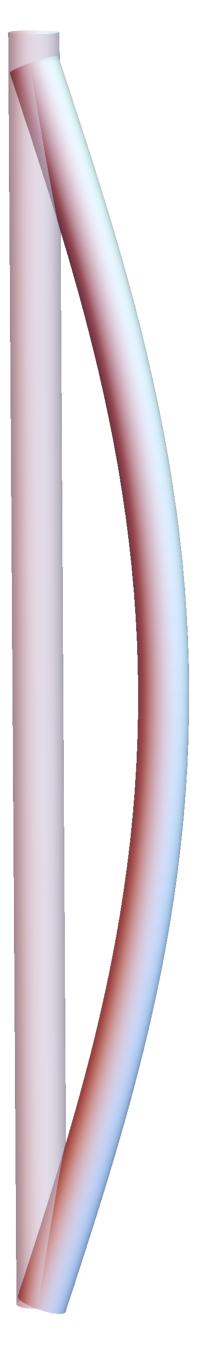
\includegraphics[height=7cm]{images/BuckledRodn1.pdf}};
    \node (centre) at (0,0) {};
    %\draw[red,ultra thick,rounded corners] (0,0) rectangle (9.4,6.2);
    \node[anchor=south west] (bottomSlabel) at (-0.2,-3.5) {$s=0$};
    \node[anchor=north west] (topSlabel) at (-0.2,3.5) {$s=L$};
    
    \node[anchor=north west] (Nlabel) at (-.4,4.2) {$N$};
    \draw[-{>[scale=2,length=4,width=4]}] (-0.35,4.1) -- (-0.35,3.4);    
    
    \node (wlabel) at (0,0.3) {$w$};
    \node (dArrowOne) at (-0.5,0) {};
    \node (dArrowTwo) at (0.5,0) {};
    \draw[-{>[scale=2,length=4,width=4]}] (dArrowOne) -- (dArrowTwo);    
    
    \node[anchor=west] (slabel) at (0.25,-2.45) {$s$};
    \draw[-{>[scale=2,length=4,width=4]}] (0.25,-2.5) -- (0.45,-1.8);    
    
\end{tikzpicture}
	%\includegraphics[height=7cm]{rodSchematic.pdf}
	\caption{Schematic}
	\label{rod-schematic}
\end{subfigure}
\begin{subfigure}[t]{0.2\textwidth}
	\centering
	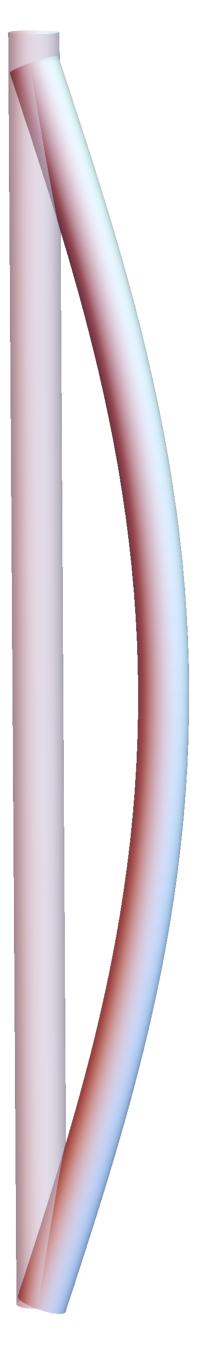
\includegraphics[height=7cm]{images/BuckledRodn1.pdf}
	\caption{$n=1$}
\end{subfigure}
\begin{subfigure}[t]{0.2\textwidth}
	\centering
	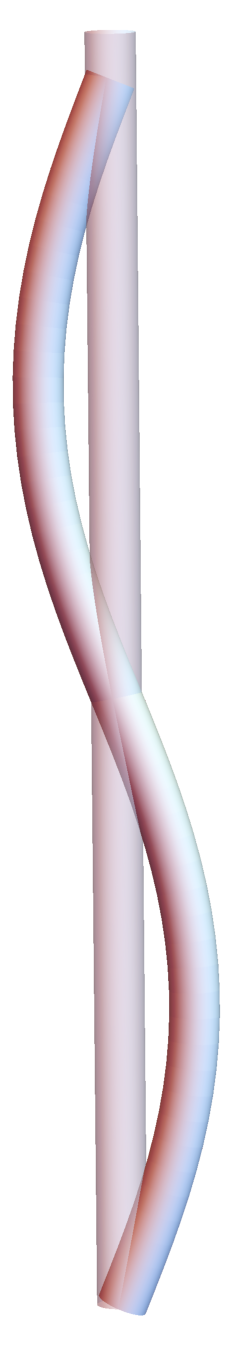
\includegraphics[height=7cm]{images/BuckledRodn2.pdf}
	\caption{$n=2$}
\end{subfigure}
\begin{subfigure}[t]{0.2\textwidth}
	\centering
	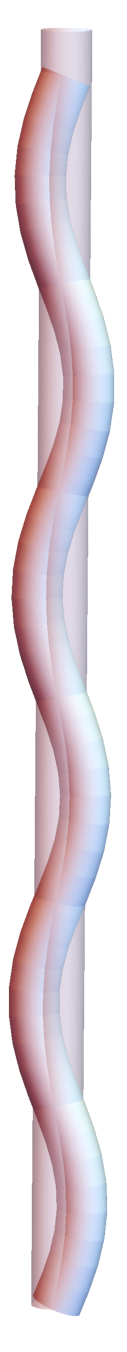
\includegraphics[height=7cm]{images/buckledRodn6.pdf}
	\caption{$n=6$}
\end{subfigure}
\end{center}
\caption{The tube model schematic (a) and various buckling modes of our elastic tube, (b)--(d).}
\label{rodvibrations}
\end{figure}

Take a look at \cref{rod-schematic}. We consider a thin tubular elastic body which is initially lined up along the $z$-axis. It is subjected to a load, $N$, at one end, and it is clamped at the other end. We assume its ends stay lined up along $z$ as it is (possibly) deformed under the force, and we monitor the deflection, $w(s,t)$, as a function of arclength along the tube, $s$, and time, $t$, from the $z$-axis. The equation of motion of this system can be shown to be 
\begin{align}
\label{beameq}
\pdn{4}{w}{s} + \frac{N}{EI}\pdd{w}{s} +\rho A \pdd{w}{t}=0,
\end{align}
with $\rho$ the tube density, $A$ its cross-sectional area, $E$ its Young's modulus (resistance to stretching), and $I$ a moment of inertia. (You're not expected to derive this equation!) The boundary conditions are 
\begin{equation}
w(0,t) = 0,\quad w(L,t) = 0,\quad \pd{w}{s}(0,t)= 0,\quad \pd{w}{s}(L,t)=0 \quad \forall t.
\end{equation}
These boundary conditions are \emph{clamped conditions}: the first two mean no deflection at either end and the last two mean it straightens out towards the end of the beam. 

There is a trivial equilibrium solution $w_0(s,t)=0$ for all $s,t$, which corresponds to the body remaining straight. Note this is true whatever the applied load, $N$. However, our experience tells us the tube should give way under enough force. To ascertain when this happens we perform a linear stability analysis using the same steps as in the ODE case

\subsubsection*{\StepOne Find equilibria}
In this case we are only interested in the homogeneous equilibrium $w_0(s,t) = 0$ for all $s,t$. From experience, there are whole classes of inhomogeneous equilibria\footnote{See \href{http://www.kstr.lth.se/fileadmin/kstr/pdf_files/forsk_kurs/Theory_of_elastic_stability_by_S._Timoshenko_and_J.M._Gere__1963_.pdf}{\textsc{Timoshenko}, S.\ P., \textsc{Gere}, J.\ M.\ 1963. \emph{Theory of Elastic Stability} 2nd edition, pp.\ 54--55.}} but we will not pursue them here.

\subsubsection*{\StepTwo Linearise the system}
We expand out the solution as $w(s,t) \approx w_0 + \ep w_1(s,t)$.
\Cref{beameq} is already linear with constant coefficients so the linearised equation is simply 
\begin{align}
\label{beameqlin}
\pdn{4}{w_1}{s} + \frac{N}{EI}\pdd{w_1}{s} +\rho A \pdd{w_1}{t}=0,
\end{align}
(it will not always be this easy!).

\subsubsection*{\StepThree Solve the linearised system}
As we did in \cref{sec:sep-variables}, we will look for separable solutions,
\begin{equation}
w_1(s,t) = S(s)T(t).
\end{equation}
Since this is similarly on a bounded domain, doing so, we will once again get that one of $S$ and $T$ grows/decays exponentially, and the other is sinusoidal.
\begin{do-it-yourself}
	If you don't see this, plug this form of $w_1$ into \cref{beameqlin} and do the usual separation of variables procedure.
\end{do-it-yourself}
Since this is a linear stability analysis, we will choose solutions which either grow or decay in \emph{time}. The shortcut method, therefore, is to simply look for solutions of the form
\begin{equation}
\label{form-of-w1}
w_1(s,t) = S(s)\e^{\lambda t}
\end{equation}
with $\lambda$ the critical growth constant. \Cref{beameqlin} reduces to
\begin{equation}
\label{linbeam1}
S'''' + \frac{N}{EI}S'' +\rho A S\lambda^2=0.
\end{equation}
Since the equation has constant coefficients and homogeneous boundary conditions, we expect sinusoidally varying solutions of the form 
\begin{equation}
\label{complexsol}
S(s) = B\e^{\i k s},
\end{equation}
with $k$ to be determined by our boundary conditions. Solutions of this form are known as vibrations.

If we let $B=b+\i c$ be complex, this is a smart (lazy?) way of representing both the cos and sin solution behaviour of the linear constant coefficient ODEs. By Euler's formula,
\begin{equation}
	B\e^{\i k s} = (b + \i c)(\cos ks + \i \sin ks),
\end{equation}
and we assume we only want to satisfy the real part of the equation obtained by substituting this in. Choosing $B$ selects the required behaviour.

The boundary conditions we need to satisfy are $w_1(0,t) = w_1(L,t) = 0$ (no further end deflection) but we allow for arbitrary (but small) changes in the derivatives of the perturbation, $w_1$, at the boundary. Therefore $S(0)=S(L) =0$ are the only boundary conditions we impose for our small variations around equilibrium. These boundary conditions can only be satisfied for the $\sin$ part of $S(s)$: recalling that we only need to satisfy the real part of the equation, we set $B =-C\i $, for some real $C$, and hence
\begin{equation}
	\label{kbcon}
	C \sin ks = 0 \implies kL = n \pi.
\end{equation}
%The derivatives are not required to be zero for these small perturbations and the change in value of the derivatives sets the magnitude of $B$, the size of the mode of vibration (solutions of the form \cref{complexsol} are `vibrations' of the system, see \cref{rodvibrations}), but this will not be important to us here.
%
%It might seem odd to use the complex wave function rather than $\cos$ or $\sin$ (it has even derivatives), but this is a more general solution and $B$ can just be made imaginary to choose the $\sin$ solution. 

\begin{info}
Another bonus of using the complex wave function for $S(s)$ is that it is handy where there are odd derivatives and a growth/decaying exponential is required for the solution ($k$ can have an imaginary part). It is standard practice to use this complex waveform, and since we never actually need to fully set the value of $B$ (we are just interested in $\lambda$) it is easier to do so. 
\end{info}

With this assumption for $S(s)$ we have
\begin{equation}
k^4 - \frac{N}{E I}k^2 + \rho A \lambda^2 = 0 \implies \lambda^2 = \frac{1}{\rho A}k^2\left(\frac{N}{E I}-k^2\right).
\end{equation}

\subsubsection*{\StepFour Assess stability}
If
\begin{equation}
\label{kvcon}
k^2 < \frac{N}{EI},
\end{equation} 
we have real eigenvalues, one of which is positive, and so the system will be unstable as it grows in time. It would appear that if
\begin{equation}
	k^2 > \frac{N}{EI},
\end{equation}
then the solutions are purely imaginary, leaving us in the degenerate case. But actually, satisfying the boundary conditions in this final case requires that the solution is zero. See that the solutions in this case are in the form 
\begin{equation}
w_1(s,t) = S(s)\e^{\lambda t} = B\e^{\i(k s  + \nu t)},
\end{equation}
where
\begin{equation}
	\nu = \pm\frac{k}{\sqrt{\rho A}}\sqrt{k^2-\frac{N}{EI}},
\end{equation} 
and remembering we only have to look at the real part of the equation,
\begin{equation}
	\Re(w_1(s,t)) = C\sin(k s  + \nu t).
\end{equation}
But $C\sin(k s+\nu t)$ needs to satisfy the boundary condition $w_1(L,t)=0$ for all time, i.e.\
\begin{equation}
	C\sin(kL + \nu t) = 0 \; \forall t \implies C = 0.
\end{equation}
So $C=0$: by having only imaginary $\lambda$ we have killed the nontrivial solution's ability to satisfy our constraints. Physically this is equivalent to saying the vibrations do not exist.

And finally, if $k^2=N/EI$, we have zero eigenvalues, leaving us in the degenerate case where there are neighbouring equilibrium solutions: under the very specific load, $N$, the perturbations are also equilibria.

Here we see the first example of the complexity of PDE stability in comparison to ODE stability: the difference between \emph{static} (no time dependence) and \emph{dynamic} equilibrium analysis!
 
Using \cref{kvcon,kbcon} we see that if the force $N$ satisfies
\begin{equation}
\label{eulerbuck}
N > \frac{n^2 \pi^2 E I}{L^2},
\end{equation}
then the  initial $w=0$ $\forall s$ solution is unstable and the beam will give way under the applied force, $N$. The lowest force, $N$, for which this will be true is the $n=1$ mode. So the minimum critical force $N_c$ after which the beam is unstable is 
\begin{equation}
\label{criticalforce}
N_c=\frac{\pi^2 E I}{L^2}.
\end{equation}
This is a famous result due to (surprise!) Euler, although the way he derived it is a little different. It has actually been shown to have some biological relevance...

\begin{nem}
What happens if we include the derivative boundary conditions for $w_1$? First note that $S(s) = B\e^{\i ks}$, with $kL=n\pi$, as we had in \cref{complexsol}, can't satisfy both the condition that $S = 0$ and $S' = 0$ at $s=0$ and $s=L$, unless $B=0$. What \emph{could} satisfy both boundary conditions is $S(s) = B(1+\e^{\i k s})$ with $kL=2n\pi$, or more intuitively,
\begin{equation}
	S(s) = \tilde{C} \left [1 + \cos\left(\frac{2 n \pi s}{L}\right)\right],
\end{equation} 
but this only satisfies \cref{linbeam1} if $\lambda=0$, i.e.\ there is no time dependence in $w_1(s,t)$ (if you look at \cref{form-of-w1}). So we would be in the degenerate case with neighbouring equilibrium solutions. But in that case, and following the same method as above, we find that the critical force after which the beam is unstable corresponds to the second, $n=2$, mode.
\end{nem}

\section{Cow buckling}
Mammals tend to use their legs to support the force of their bodies. Let us imagine a cow with four cylindrical legs (\cref{fig:cow}): for a cylinder with radius $R$, the moment of inertia is $I = \pi R^4/4$. Its main body (the meaty bit!) has a volume $V$ and density $\rho_{c}$ so that its weight is $\rho_c V g$. If we assume this weight (a load) is split equally amongst the four legs then 
\begin{equation}
N= \frac{\rho_cV g}{4}.
\end{equation}
Now, let's say we increased the dimensions of the animal by a factor $a$, we have 
\begin{equation}
V_{\text{new}}  = a^3V,
\end{equation}
so the load on each leg grows cubically in the scaling $a$,
\begin{equation}
	N_\text{new} = a^3 N.
\end{equation}%
\begin{figure}%
	\centering%
	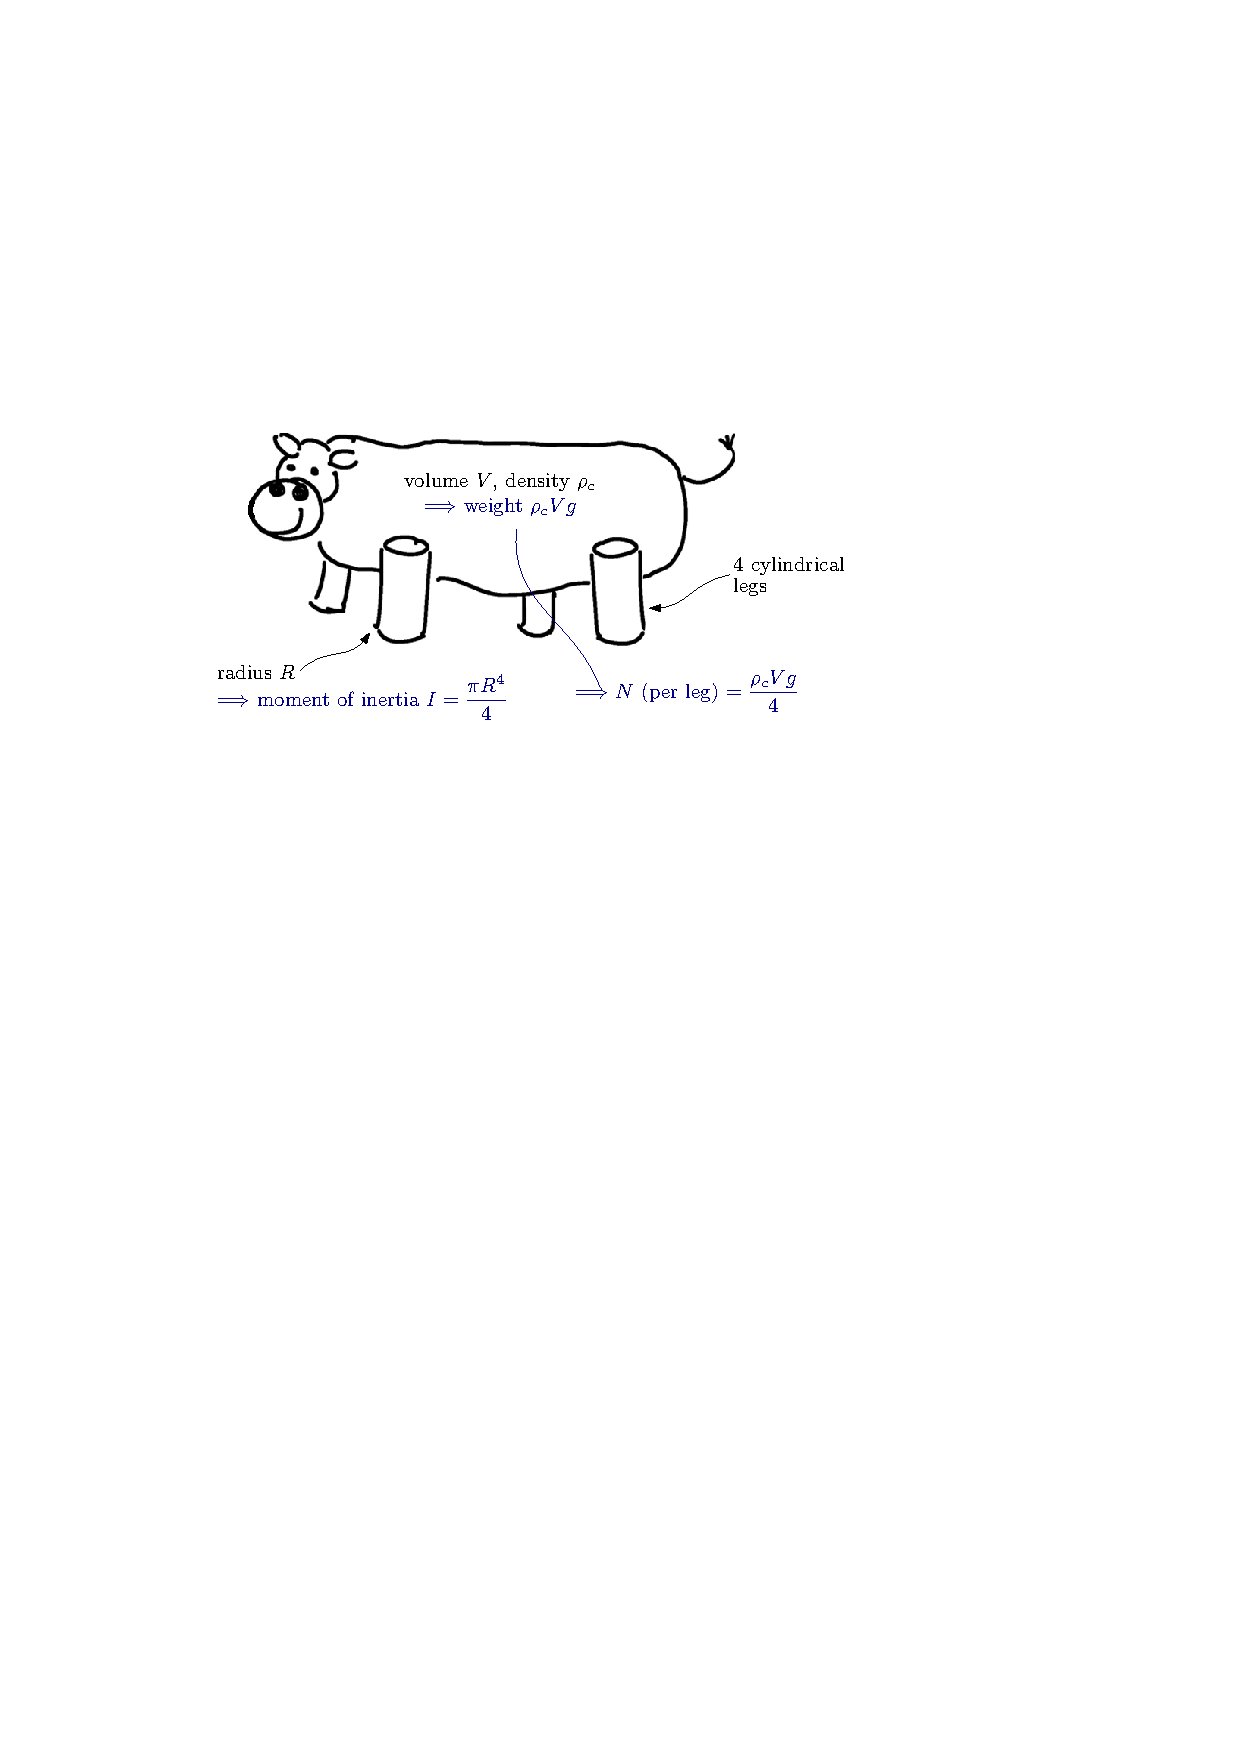
\includegraphics[scale=1.2]{images/cow.pdf}%
	\caption{An important cow-culation}%
	\label{fig:cow}%
\end{figure}%
Next, we look at the critical force equation, \cref{criticalforce}. The Young's modulus, $E$, is a material constant so the minimum critical force scales like $N_c \sim R^4/L^2$. Well, under our increased dimensions,
\begin{equation}
	N_c^{\text{new}} \sim \frac{R_{\text{new}}^4}{L_{\text{new}}^2} = \frac{a^4 R^4}{a^2 L^2} = a^2\frac{R^4}{L^2} \sim a^2 N_c.
\end{equation}
Therefore the critical load under which the legs (beams) will give way scales as $a^2$. Under this change in dimensions, the size of the imposed force, $N$, which scales with $a^3$, grows faster than the critical load $N_c$, which scales as $a^2$. That is to say, there will be a point where, after scaling up too much, the animal's weight will cause its legs to give way, providing a possible explanation for why land mammals are limited in size, unlike sea mammals like whales. 

So how might we delay the point of collapse? Well, real animals don't grow by inflating like a balloon; instead, they change proportions as they grow. To model this, let us separate the scaling of different directions. Let the cow's height grow with factor $a$, and its width and length with factor $b$. Then the volume scales as
\begin{equation}
V_{\text{new}}  = ab^2V \implies N_\text{new} = ab^2 N
\end{equation}
 and  
\begin{equation}
	N_c^{\text{new}} \sim \frac{R_{\text{new}}^4}{L_{\text{new}}^2} = \frac{b^4}{a^2}\frac{R^4}{L^2}. 
\end{equation}
One can see that if $b=a^{3/2}$ then both $N$ and the critical load $N_c$ will scale at the same rate,
\begin{equation}
	N_\text{new} \sim a^4 N, \qquad N_c^{\text{new}} \sim a^4 N_c.
\end{equation}
This implies that in order for the legs not to buckle as we scale the cow up, the cow needs to get wider ($b$) at a quicker rate than it gets taller ($a$)! 

\paragraph{In the real world:} So do cows (and other living things) actually exhibit this $b=a^{3/2}$ relationship? Trees certainly do -- \cref{fig:tree-sizes} (left) shows measurements from 600 American species of tree which, when plotted on log--log axes, cluster around the line with slope 3/2. 

\begin{figure}
	\begin{center}
	%% Creator: Matplotlib, PGF backend
%%
%% To include the figure in your LaTeX document, write
%%   \input{<filename>.pgf}
%%
%% Make sure the required packages are loaded in your preamble
%%   \usepackage{pgf}
%%
%% Also ensure that all the required font packages are loaded; for instance,
%% the lmodern package is sometimes necessary when using math font.
%%   \usepackage{lmodern}
%%
%% Figures using additional raster images can only be included by \input if
%% they are in the same directory as the main LaTeX file. For loading figures
%% from other directories you can use the `import` package
%%   \usepackage{import}
%%
%% and then include the figures with
%%   \import{<path to file>}{<filename>.pgf}
%%
%% Matplotlib used the following preamble
%%   \def\mathdefault#1{#1}
%%   \everymath=\expandafter{\the\everymath\displaystyle}
%%   
%%   \usepackage{fontspec}
%%   \setmainfont{DejaVuSerif.ttf}[Path=\detokenize{/Users/adam/opt/anaconda3/lib/python3.9/site-packages/matplotlib/mpl-data/fonts/ttf/}]
%%   \setsansfont{DejaVuSans.ttf}[Path=\detokenize{/Users/adam/opt/anaconda3/lib/python3.9/site-packages/matplotlib/mpl-data/fonts/ttf/}]
%%   \setmonofont{DejaVuSansMono.ttf}[Path=\detokenize{/Users/adam/opt/anaconda3/lib/python3.9/site-packages/matplotlib/mpl-data/fonts/ttf/}]
%%   \makeatletter\@ifpackageloaded{underscore}{}{\usepackage[strings]{underscore}}\makeatother
%%
\begingroup%
\makeatletter%
\begin{pgfpicture}%
\pgfpathrectangle{\pgfpointorigin}{\pgfqpoint{3.000000in}{2.200000in}}%
\pgfusepath{use as bounding box, clip}%
\begin{pgfscope}%
\pgfsetbuttcap%
\pgfsetmiterjoin%
\definecolor{currentfill}{rgb}{1.000000,1.000000,1.000000}%
\pgfsetfillcolor{currentfill}%
\pgfsetlinewidth{0.000000pt}%
\definecolor{currentstroke}{rgb}{1.000000,1.000000,1.000000}%
\pgfsetstrokecolor{currentstroke}%
\pgfsetdash{}{0pt}%
\pgfpathmoveto{\pgfqpoint{0.000000in}{0.000000in}}%
\pgfpathlineto{\pgfqpoint{3.000000in}{0.000000in}}%
\pgfpathlineto{\pgfqpoint{3.000000in}{2.200000in}}%
\pgfpathlineto{\pgfqpoint{0.000000in}{2.200000in}}%
\pgfpathlineto{\pgfqpoint{0.000000in}{0.000000in}}%
\pgfpathclose%
\pgfusepath{fill}%
\end{pgfscope}%
\begin{pgfscope}%
\pgfsetbuttcap%
\pgfsetmiterjoin%
\definecolor{currentfill}{rgb}{1.000000,1.000000,1.000000}%
\pgfsetfillcolor{currentfill}%
\pgfsetlinewidth{0.000000pt}%
\definecolor{currentstroke}{rgb}{0.000000,0.000000,0.000000}%
\pgfsetstrokecolor{currentstroke}%
\pgfsetstrokeopacity{0.000000}%
\pgfsetdash{}{0pt}%
\pgfpathmoveto{\pgfqpoint{0.665026in}{0.499749in}}%
\pgfpathlineto{\pgfqpoint{2.966667in}{0.499749in}}%
\pgfpathlineto{\pgfqpoint{2.966667in}{2.109013in}}%
\pgfpathlineto{\pgfqpoint{0.665026in}{2.109013in}}%
\pgfpathlineto{\pgfqpoint{0.665026in}{0.499749in}}%
\pgfpathclose%
\pgfusepath{fill}%
\end{pgfscope}%
\begin{pgfscope}%
\pgfpathrectangle{\pgfqpoint{0.665026in}{0.499749in}}{\pgfqpoint{2.301641in}{1.609263in}}%
\pgfusepath{clip}%
\pgfsetbuttcap%
\pgfsetroundjoin%
\definecolor{currentfill}{rgb}{0.121569,0.466667,0.705882}%
\pgfsetfillcolor{currentfill}%
\pgfsetlinewidth{1.003750pt}%
\definecolor{currentstroke}{rgb}{0.121569,0.466667,0.705882}%
\pgfsetstrokecolor{currentstroke}%
\pgfsetdash{}{0pt}%
\pgfsys@defobject{currentmarker}{\pgfqpoint{-0.009821in}{-0.009821in}}{\pgfqpoint{0.009821in}{0.009821in}}{%
\pgfpathmoveto{\pgfqpoint{0.000000in}{-0.009821in}}%
\pgfpathcurveto{\pgfqpoint{0.002605in}{-0.009821in}}{\pgfqpoint{0.005103in}{-0.008786in}}{\pgfqpoint{0.006944in}{-0.006944in}}%
\pgfpathcurveto{\pgfqpoint{0.008786in}{-0.005103in}}{\pgfqpoint{0.009821in}{-0.002605in}}{\pgfqpoint{0.009821in}{0.000000in}}%
\pgfpathcurveto{\pgfqpoint{0.009821in}{0.002605in}}{\pgfqpoint{0.008786in}{0.005103in}}{\pgfqpoint{0.006944in}{0.006944in}}%
\pgfpathcurveto{\pgfqpoint{0.005103in}{0.008786in}}{\pgfqpoint{0.002605in}{0.009821in}}{\pgfqpoint{0.000000in}{0.009821in}}%
\pgfpathcurveto{\pgfqpoint{-0.002605in}{0.009821in}}{\pgfqpoint{-0.005103in}{0.008786in}}{\pgfqpoint{-0.006944in}{0.006944in}}%
\pgfpathcurveto{\pgfqpoint{-0.008786in}{0.005103in}}{\pgfqpoint{-0.009821in}{0.002605in}}{\pgfqpoint{-0.009821in}{0.000000in}}%
\pgfpathcurveto{\pgfqpoint{-0.009821in}{-0.002605in}}{\pgfqpoint{-0.008786in}{-0.005103in}}{\pgfqpoint{-0.006944in}{-0.006944in}}%
\pgfpathcurveto{\pgfqpoint{-0.005103in}{-0.008786in}}{\pgfqpoint{-0.002605in}{-0.009821in}}{\pgfqpoint{0.000000in}{-0.009821in}}%
\pgfpathlineto{\pgfqpoint{0.000000in}{-0.009821in}}%
\pgfpathclose%
\pgfusepath{stroke,fill}%
}%
\begin{pgfscope}%
\pgfsys@transformshift{0.994547in}{0.611431in}%
\pgfsys@useobject{currentmarker}{}%
\end{pgfscope}%
\begin{pgfscope}%
\pgfsys@transformshift{1.050713in}{0.602173in}%
\pgfsys@useobject{currentmarker}{}%
\end{pgfscope}%
\begin{pgfscope}%
\pgfsys@transformshift{0.928841in}{0.771142in}%
\pgfsys@useobject{currentmarker}{}%
\end{pgfscope}%
\begin{pgfscope}%
\pgfsys@transformshift{1.125588in}{0.710961in}%
\pgfsys@useobject{currentmarker}{}%
\end{pgfscope}%
\begin{pgfscope}%
\pgfsys@transformshift{1.226627in}{0.775772in}%
\pgfsys@useobject{currentmarker}{}%
\end{pgfscope}%
\begin{pgfscope}%
\pgfsys@transformshift{1.206974in}{0.813964in}%
\pgfsys@useobject{currentmarker}{}%
\end{pgfscope}%
\begin{pgfscope}%
\pgfsys@transformshift{1.183165in}{0.825537in}%
\pgfsys@useobject{currentmarker}{}%
\end{pgfscope}%
\begin{pgfscope}%
\pgfsys@transformshift{1.187369in}{0.844054in}%
\pgfsys@useobject{currentmarker}{}%
\end{pgfscope}%
\begin{pgfscope}%
\pgfsys@transformshift{1.262958in}{0.834795in}%
\pgfsys@useobject{currentmarker}{}%
\end{pgfscope}%
\begin{pgfscope}%
\pgfsys@transformshift{1.263000in}{0.827851in}%
\pgfsys@useobject{currentmarker}{}%
\end{pgfscope}%
\begin{pgfscope}%
\pgfsys@transformshift{1.062236in}{0.838267in}%
\pgfsys@useobject{currentmarker}{}%
\end{pgfscope}%
\begin{pgfscope}%
\pgfsys@transformshift{1.047060in}{0.849841in}%
\pgfsys@useobject{currentmarker}{}%
\end{pgfscope}%
\begin{pgfscope}%
\pgfsys@transformshift{1.062027in}{0.872987in}%
\pgfsys@useobject{currentmarker}{}%
\end{pgfscope}%
\begin{pgfscope}%
\pgfsys@transformshift{0.999422in}{0.876459in}%
\pgfsys@useobject{currentmarker}{}%
\end{pgfscope}%
\begin{pgfscope}%
\pgfsys@transformshift{1.107158in}{0.904235in}%
\pgfsys@useobject{currentmarker}{}%
\end{pgfscope}%
\begin{pgfscope}%
\pgfsys@transformshift{1.087672in}{0.914651in}%
\pgfsys@useobject{currentmarker}{}%
\end{pgfscope}%
\begin{pgfscope}%
\pgfsys@transformshift{1.054882in}{0.984091in}%
\pgfsys@useobject{currentmarker}{}%
\end{pgfscope}%
\begin{pgfscope}%
\pgfsys@transformshift{1.141470in}{0.940112in}%
\pgfsys@useobject{currentmarker}{}%
\end{pgfscope}%
\begin{pgfscope}%
\pgfsys@transformshift{1.208398in}{0.935483in}%
\pgfsys@useobject{currentmarker}{}%
\end{pgfscope}%
\begin{pgfscope}%
\pgfsys@transformshift{1.227996in}{0.906550in}%
\pgfsys@useobject{currentmarker}{}%
\end{pgfscope}%
\begin{pgfscope}%
\pgfsys@transformshift{1.228072in}{0.893819in}%
\pgfsys@useobject{currentmarker}{}%
\end{pgfscope}%
\begin{pgfscope}%
\pgfsys@transformshift{1.240553in}{0.971360in}%
\pgfsys@useobject{currentmarker}{}%
\end{pgfscope}%
\begin{pgfscope}%
\pgfsys@transformshift{1.262210in}{0.958629in}%
\pgfsys@useobject{currentmarker}{}%
\end{pgfscope}%
\begin{pgfscope}%
\pgfsys@transformshift{1.299030in}{0.936640in}%
\pgfsys@useobject{currentmarker}{}%
\end{pgfscope}%
\begin{pgfscope}%
\pgfsys@transformshift{1.307474in}{0.967888in}%
\pgfsys@useobject{currentmarker}{}%
\end{pgfscope}%
\begin{pgfscope}%
\pgfsys@transformshift{1.333573in}{0.934326in}%
\pgfsys@useobject{currentmarker}{}%
\end{pgfscope}%
\begin{pgfscope}%
\pgfsys@transformshift{1.329180in}{0.947056in}%
\pgfsys@useobject{currentmarker}{}%
\end{pgfscope}%
\begin{pgfscope}%
\pgfsys@transformshift{1.430659in}{0.938955in}%
\pgfsys@useobject{currentmarker}{}%
\end{pgfscope}%
\begin{pgfscope}%
\pgfsys@transformshift{1.449949in}{0.960944in}%
\pgfsys@useobject{currentmarker}{}%
\end{pgfscope}%
\begin{pgfscope}%
\pgfsys@transformshift{1.417529in}{0.969045in}%
\pgfsys@useobject{currentmarker}{}%
\end{pgfscope}%
\begin{pgfscope}%
\pgfsys@transformshift{1.372174in}{0.974832in}%
\pgfsys@useobject{currentmarker}{}%
\end{pgfscope}%
\begin{pgfscope}%
\pgfsys@transformshift{1.385067in}{0.984091in}%
\pgfsys@useobject{currentmarker}{}%
\end{pgfscope}%
\begin{pgfscope}%
\pgfsys@transformshift{1.333315in}{0.977147in}%
\pgfsys@useobject{currentmarker}{}%
\end{pgfscope}%
\begin{pgfscope}%
\pgfsys@transformshift{1.356998in}{0.986405in}%
\pgfsys@useobject{currentmarker}{}%
\end{pgfscope}%
\begin{pgfscope}%
\pgfsys@transformshift{1.318125in}{0.991035in}%
\pgfsys@useobject{currentmarker}{}%
\end{pgfscope}%
\begin{pgfscope}%
\pgfsys@transformshift{1.339643in}{1.001451in}%
\pgfsys@useobject{currentmarker}{}%
\end{pgfscope}%
\begin{pgfscope}%
\pgfsys@transformshift{1.361230in}{1.000293in}%
\pgfsys@useobject{currentmarker}{}%
\end{pgfscope}%
\begin{pgfscope}%
\pgfsys@transformshift{1.354693in}{1.010709in}%
\pgfsys@useobject{currentmarker}{}%
\end{pgfscope}%
\begin{pgfscope}%
\pgfsys@transformshift{1.320178in}{1.008395in}%
\pgfsys@useobject{currentmarker}{}%
\end{pgfscope}%
\begin{pgfscope}%
\pgfsys@transformshift{1.292088in}{1.014181in}%
\pgfsys@useobject{currentmarker}{}%
\end{pgfscope}%
\begin{pgfscope}%
\pgfsys@transformshift{1.266017in}{1.043114in}%
\pgfsys@useobject{currentmarker}{}%
\end{pgfscope}%
\begin{pgfscope}%
\pgfsys@transformshift{1.226815in}{1.102138in}%
\pgfsys@useobject{currentmarker}{}%
\end{pgfscope}%
\begin{pgfscope}%
\pgfsys@transformshift{1.090089in}{1.229444in}%
\pgfsys@useobject{currentmarker}{}%
\end{pgfscope}%
\begin{pgfscope}%
\pgfsys@transformshift{1.326205in}{1.082463in}%
\pgfsys@useobject{currentmarker}{}%
\end{pgfscope}%
\begin{pgfscope}%
\pgfsys@transformshift{1.336891in}{1.099823in}%
\pgfsys@useobject{currentmarker}{}%
\end{pgfscope}%
\begin{pgfscope}%
\pgfsys@transformshift{1.345404in}{1.119498in}%
\pgfsys@useobject{currentmarker}{}%
\end{pgfscope}%
\begin{pgfscope}%
\pgfsys@transformshift{1.325905in}{1.132229in}%
\pgfsys@useobject{currentmarker}{}%
\end{pgfscope}%
\begin{pgfscope}%
\pgfsys@transformshift{1.354232in}{1.087093in}%
\pgfsys@useobject{currentmarker}{}%
\end{pgfscope}%
\begin{pgfscope}%
\pgfsys@transformshift{1.339223in}{1.070890in}%
\pgfsys@useobject{currentmarker}{}%
\end{pgfscope}%
\begin{pgfscope}%
\pgfsys@transformshift{1.360811in}{1.069733in}%
\pgfsys@useobject{currentmarker}{}%
\end{pgfscope}%
\begin{pgfscope}%
\pgfsys@transformshift{1.382245in}{1.094037in}%
\pgfsys@useobject{currentmarker}{}%
\end{pgfscope}%
\begin{pgfscope}%
\pgfsys@transformshift{1.382406in}{1.067418in}%
\pgfsys@useobject{currentmarker}{}%
\end{pgfscope}%
\begin{pgfscope}%
\pgfsys@transformshift{1.403987in}{1.067418in}%
\pgfsys@useobject{currentmarker}{}%
\end{pgfscope}%
\begin{pgfscope}%
\pgfsys@transformshift{1.399803in}{1.045429in}%
\pgfsys@useobject{currentmarker}{}%
\end{pgfscope}%
\begin{pgfscope}%
\pgfsys@transformshift{1.384899in}{1.011866in}%
\pgfsys@useobject{currentmarker}{}%
\end{pgfscope}%
\begin{pgfscope}%
\pgfsys@transformshift{1.443146in}{1.015338in}%
\pgfsys@useobject{currentmarker}{}%
\end{pgfscope}%
\begin{pgfscope}%
\pgfsys@transformshift{1.432279in}{1.028069in}%
\pgfsys@useobject{currentmarker}{}%
\end{pgfscope}%
\begin{pgfscope}%
\pgfsys@transformshift{1.453706in}{1.053530in}%
\pgfsys@useobject{currentmarker}{}%
\end{pgfscope}%
\begin{pgfscope}%
\pgfsys@transformshift{1.451702in}{1.028069in}%
\pgfsys@useobject{currentmarker}{}%
\end{pgfscope}%
\begin{pgfscope}%
\pgfsys@transformshift{1.445178in}{1.036170in}%
\pgfsys@useobject{currentmarker}{}%
\end{pgfscope}%
\begin{pgfscope}%
\pgfsys@transformshift{1.490631in}{1.014181in}%
\pgfsys@useobject{currentmarker}{}%
\end{pgfscope}%
\begin{pgfscope}%
\pgfsys@transformshift{1.525048in}{1.032698in}%
\pgfsys@useobject{currentmarker}{}%
\end{pgfscope}%
\begin{pgfscope}%
\pgfsys@transformshift{1.555142in}{1.052373in}%
\pgfsys@useobject{currentmarker}{}%
\end{pgfscope}%
\begin{pgfscope}%
\pgfsys@transformshift{1.539938in}{1.068576in}%
\pgfsys@useobject{currentmarker}{}%
\end{pgfscope}%
\begin{pgfscope}%
\pgfsys@transformshift{1.531243in}{1.078991in}%
\pgfsys@useobject{currentmarker}{}%
\end{pgfscope}%
\begin{pgfscope}%
\pgfsys@transformshift{1.524671in}{1.095194in}%
\pgfsys@useobject{currentmarker}{}%
\end{pgfscope}%
\begin{pgfscope}%
\pgfsys@transformshift{1.505157in}{1.110239in}%
\pgfsys@useobject{currentmarker}{}%
\end{pgfscope}%
\begin{pgfscope}%
\pgfsys@transformshift{1.507204in}{1.128757in}%
\pgfsys@useobject{currentmarker}{}%
\end{pgfscope}%
\begin{pgfscope}%
\pgfsys@transformshift{1.509292in}{1.140330in}%
\pgfsys@useobject{currentmarker}{}%
\end{pgfscope}%
\begin{pgfscope}%
\pgfsys@transformshift{1.436127in}{1.105610in}%
\pgfsys@useobject{currentmarker}{}%
\end{pgfscope}%
\begin{pgfscope}%
\pgfsys@transformshift{1.421104in}{1.091722in}%
\pgfsys@useobject{currentmarker}{}%
\end{pgfscope}%
\begin{pgfscope}%
\pgfsys@transformshift{1.425281in}{1.114869in}%
\pgfsys@useobject{currentmarker}{}%
\end{pgfscope}%
\begin{pgfscope}%
\pgfsys@transformshift{1.410160in}{1.117183in}%
\pgfsys@useobject{currentmarker}{}%
\end{pgfscope}%
\begin{pgfscope}%
\pgfsys@transformshift{1.461933in}{1.120655in}%
\pgfsys@useobject{currentmarker}{}%
\end{pgfscope}%
\begin{pgfscope}%
\pgfsys@transformshift{1.446743in}{1.134543in}%
\pgfsys@useobject{currentmarker}{}%
\end{pgfscope}%
\begin{pgfscope}%
\pgfsys@transformshift{1.442245in}{1.164634in}%
\pgfsys@useobject{currentmarker}{}%
\end{pgfscope}%
\begin{pgfscope}%
\pgfsys@transformshift{1.459475in}{1.170420in}%
\pgfsys@useobject{currentmarker}{}%
\end{pgfscope}%
\begin{pgfscope}%
\pgfsys@transformshift{1.487516in}{1.172735in}%
\pgfsys@useobject{currentmarker}{}%
\end{pgfscope}%
\begin{pgfscope}%
\pgfsys@transformshift{1.398567in}{1.250276in}%
\pgfsys@useobject{currentmarker}{}%
\end{pgfscope}%
\begin{pgfscope}%
\pgfsys@transformshift{1.426377in}{1.290782in}%
\pgfsys@useobject{currentmarker}{}%
\end{pgfscope}%
\begin{pgfscope}%
\pgfsys@transformshift{1.445982in}{1.260692in}%
\pgfsys@useobject{currentmarker}{}%
\end{pgfscope}%
\begin{pgfscope}%
\pgfsys@transformshift{1.465453in}{1.252591in}%
\pgfsys@useobject{currentmarker}{}%
\end{pgfscope}%
\begin{pgfscope}%
\pgfsys@transformshift{1.446170in}{1.229444in}%
\pgfsys@useobject{currentmarker}{}%
\end{pgfscope}%
\begin{pgfscope}%
\pgfsys@transformshift{1.478443in}{1.245647in}%
\pgfsys@useobject{currentmarker}{}%
\end{pgfscope}%
\begin{pgfscope}%
\pgfsys@transformshift{1.510933in}{1.225972in}%
\pgfsys@useobject{currentmarker}{}%
\end{pgfscope}%
\begin{pgfscope}%
\pgfsys@transformshift{1.523700in}{1.256063in}%
\pgfsys@useobject{currentmarker}{}%
\end{pgfscope}%
\begin{pgfscope}%
\pgfsys@transformshift{1.510682in}{1.267636in}%
\pgfsys@useobject{currentmarker}{}%
\end{pgfscope}%
\begin{pgfscope}%
\pgfsys@transformshift{1.501952in}{1.283838in}%
\pgfsys@useobject{currentmarker}{}%
\end{pgfscope}%
\begin{pgfscope}%
\pgfsys@transformshift{1.528247in}{1.217871in}%
\pgfsys@useobject{currentmarker}{}%
\end{pgfscope}%
\begin{pgfscope}%
\pgfsys@transformshift{1.556316in}{1.215556in}%
\pgfsys@useobject{currentmarker}{}%
\end{pgfscope}%
\begin{pgfscope}%
\pgfsys@transformshift{1.547774in}{1.200511in}%
\pgfsys@useobject{currentmarker}{}%
\end{pgfscope}%
\begin{pgfscope}%
\pgfsys@transformshift{1.586438in}{1.230601in}%
\pgfsys@useobject{currentmarker}{}%
\end{pgfscope}%
\begin{pgfscope}%
\pgfsys@transformshift{1.586389in}{1.238703in}%
\pgfsys@useobject{currentmarker}{}%
\end{pgfscope}%
\begin{pgfscope}%
\pgfsys@transformshift{1.590586in}{1.258377in}%
\pgfsys@useobject{currentmarker}{}%
\end{pgfscope}%
\begin{pgfscope}%
\pgfsys@transformshift{1.627420in}{1.234073in}%
\pgfsys@useobject{currentmarker}{}%
\end{pgfscope}%
\begin{pgfscope}%
\pgfsys@transformshift{1.605832in}{1.235231in}%
\pgfsys@useobject{currentmarker}{}%
\end{pgfscope}%
\begin{pgfscope}%
\pgfsys@transformshift{1.616735in}{1.216713in}%
\pgfsys@useobject{currentmarker}{}%
\end{pgfscope}%
\begin{pgfscope}%
\pgfsys@transformshift{1.606021in}{1.203983in}%
\pgfsys@useobject{currentmarker}{}%
\end{pgfscope}%
\begin{pgfscope}%
\pgfsys@transformshift{1.599512in}{1.209769in}%
\pgfsys@useobject{currentmarker}{}%
\end{pgfscope}%
\begin{pgfscope}%
\pgfsys@transformshift{1.636178in}{1.213241in}%
\pgfsys@useobject{currentmarker}{}%
\end{pgfscope}%
\begin{pgfscope}%
\pgfsys@transformshift{1.634118in}{1.197039in}%
\pgfsys@useobject{currentmarker}{}%
\end{pgfscope}%
\begin{pgfscope}%
\pgfsys@transformshift{1.571548in}{1.194724in}%
\pgfsys@useobject{currentmarker}{}%
\end{pgfscope}%
\begin{pgfscope}%
\pgfsys@transformshift{1.576045in}{1.164634in}%
\pgfsys@useobject{currentmarker}{}%
\end{pgfscope}%
\begin{pgfscope}%
\pgfsys@transformshift{1.599735in}{1.172735in}%
\pgfsys@useobject{currentmarker}{}%
\end{pgfscope}%
\begin{pgfscope}%
\pgfsys@transformshift{1.582548in}{1.160004in}%
\pgfsys@useobject{currentmarker}{}%
\end{pgfscope}%
\begin{pgfscope}%
\pgfsys@transformshift{1.612789in}{1.155375in}%
\pgfsys@useobject{currentmarker}{}%
\end{pgfscope}%
\begin{pgfscope}%
\pgfsys@transformshift{1.612733in}{1.164634in}%
\pgfsys@useobject{currentmarker}{}%
\end{pgfscope}%
\begin{pgfscope}%
\pgfsys@transformshift{1.619333in}{1.143802in}%
\pgfsys@useobject{currentmarker}{}%
\end{pgfscope}%
\begin{pgfscope}%
\pgfsys@transformshift{1.610875in}{1.114869in}%
\pgfsys@useobject{currentmarker}{}%
\end{pgfscope}%
\begin{pgfscope}%
\pgfsys@transformshift{1.559102in}{1.111397in}%
\pgfsys@useobject{currentmarker}{}%
\end{pgfscope}%
\begin{pgfscope}%
\pgfsys@transformshift{1.593750in}{1.091722in}%
\pgfsys@useobject{currentmarker}{}%
\end{pgfscope}%
\begin{pgfscope}%
\pgfsys@transformshift{1.600308in}{1.077834in}%
\pgfsys@useobject{currentmarker}{}%
\end{pgfscope}%
\begin{pgfscope}%
\pgfsys@transformshift{1.617503in}{1.089407in}%
\pgfsys@useobject{currentmarker}{}%
\end{pgfscope}%
\begin{pgfscope}%
\pgfsys@transformshift{1.649895in}{1.085935in}%
\pgfsys@useobject{currentmarker}{}%
\end{pgfscope}%
\begin{pgfscope}%
\pgfsys@transformshift{1.632714in}{1.072048in}%
\pgfsys@useobject{currentmarker}{}%
\end{pgfscope}%
\begin{pgfscope}%
\pgfsys@transformshift{1.581060in}{1.048901in}%
\pgfsys@useobject{currentmarker}{}%
\end{pgfscope}%
\begin{pgfscope}%
\pgfsys@transformshift{1.615610in}{1.045429in}%
\pgfsys@useobject{currentmarker}{}%
\end{pgfscope}%
\begin{pgfscope}%
\pgfsys@transformshift{1.632854in}{1.048901in}%
\pgfsys@useobject{currentmarker}{}%
\end{pgfscope}%
\begin{pgfscope}%
\pgfsys@transformshift{1.602766in}{1.028069in}%
\pgfsys@useobject{currentmarker}{}%
\end{pgfscope}%
\begin{pgfscope}%
\pgfsys@transformshift{1.699852in}{1.032698in}%
\pgfsys@useobject{currentmarker}{}%
\end{pgfscope}%
\begin{pgfscope}%
\pgfsys@transformshift{1.727802in}{1.050058in}%
\pgfsys@useobject{currentmarker}{}%
\end{pgfscope}%
\begin{pgfscope}%
\pgfsys@transformshift{1.792425in}{1.069733in}%
\pgfsys@useobject{currentmarker}{}%
\end{pgfscope}%
\begin{pgfscope}%
\pgfsys@transformshift{1.820271in}{1.104453in}%
\pgfsys@useobject{currentmarker}{}%
\end{pgfscope}%
\begin{pgfscope}%
\pgfsys@transformshift{1.733899in}{1.112554in}%
\pgfsys@useobject{currentmarker}{}%
\end{pgfscope}%
\begin{pgfscope}%
\pgfsys@transformshift{1.761877in}{1.125285in}%
\pgfsys@useobject{currentmarker}{}%
\end{pgfscope}%
\begin{pgfscope}%
\pgfsys@transformshift{1.714169in}{1.163476in}%
\pgfsys@useobject{currentmarker}{}%
\end{pgfscope}%
\begin{pgfscope}%
\pgfsys@transformshift{1.744305in}{1.176207in}%
\pgfsys@useobject{currentmarker}{}%
\end{pgfscope}%
\begin{pgfscope}%
\pgfsys@transformshift{1.690346in}{1.177364in}%
\pgfsys@useobject{currentmarker}{}%
\end{pgfscope}%
\begin{pgfscope}%
\pgfsys@transformshift{1.716180in}{1.187780in}%
\pgfsys@useobject{currentmarker}{}%
\end{pgfscope}%
\begin{pgfscope}%
\pgfsys@transformshift{1.687965in}{1.214399in}%
\pgfsys@useobject{currentmarker}{}%
\end{pgfscope}%
\begin{pgfscope}%
\pgfsys@transformshift{1.672795in}{1.224815in}%
\pgfsys@useobject{currentmarker}{}%
\end{pgfscope}%
\begin{pgfscope}%
\pgfsys@transformshift{1.696416in}{1.244489in}%
\pgfsys@useobject{currentmarker}{}%
\end{pgfscope}%
\begin{pgfscope}%
\pgfsys@transformshift{1.711480in}{1.251433in}%
\pgfsys@useobject{currentmarker}{}%
\end{pgfscope}%
\begin{pgfscope}%
\pgfsys@transformshift{1.689885in}{1.253748in}%
\pgfsys@useobject{currentmarker}{}%
\end{pgfscope}%
\begin{pgfscope}%
\pgfsys@transformshift{1.663954in}{1.259535in}%
\pgfsys@useobject{currentmarker}{}%
\end{pgfscope}%
\begin{pgfscope}%
\pgfsys@transformshift{1.659714in}{1.246804in}%
\pgfsys@useobject{currentmarker}{}%
\end{pgfscope}%
\begin{pgfscope}%
\pgfsys@transformshift{1.698371in}{1.278052in}%
\pgfsys@useobject{currentmarker}{}%
\end{pgfscope}%
\begin{pgfscope}%
\pgfsys@transformshift{1.650852in}{1.284996in}%
\pgfsys@useobject{currentmarker}{}%
\end{pgfscope}%
\begin{pgfscope}%
\pgfsys@transformshift{1.642310in}{1.269950in}%
\pgfsys@useobject{currentmarker}{}%
\end{pgfscope}%
\begin{pgfscope}%
\pgfsys@transformshift{1.618446in}{1.290782in}%
\pgfsys@useobject{currentmarker}{}%
\end{pgfscope}%
\begin{pgfscope}%
\pgfsys@transformshift{1.607662in}{1.289625in}%
\pgfsys@useobject{currentmarker}{}%
\end{pgfscope}%
\begin{pgfscope}%
\pgfsys@transformshift{1.568803in}{1.291940in}%
\pgfsys@useobject{currentmarker}{}%
\end{pgfscope}%
\begin{pgfscope}%
\pgfsys@transformshift{1.536362in}{1.303513in}%
\pgfsys@useobject{currentmarker}{}%
\end{pgfscope}%
\begin{pgfscope}%
\pgfsys@transformshift{1.549178in}{1.325502in}%
\pgfsys@useobject{currentmarker}{}%
\end{pgfscope}%
\begin{pgfscope}%
\pgfsys@transformshift{1.562189in}{1.315086in}%
\pgfsys@useobject{currentmarker}{}%
\end{pgfscope}%
\begin{pgfscope}%
\pgfsys@transformshift{1.570654in}{1.342862in}%
\pgfsys@useobject{currentmarker}{}%
\end{pgfscope}%
\begin{pgfscope}%
\pgfsys@transformshift{1.613857in}{1.335918in}%
\pgfsys@useobject{currentmarker}{}%
\end{pgfscope}%
\begin{pgfscope}%
\pgfsys@transformshift{1.620415in}{1.322030in}%
\pgfsys@useobject{currentmarker}{}%
\end{pgfscope}%
\begin{pgfscope}%
\pgfsys@transformshift{1.654923in}{1.325502in}%
\pgfsys@useobject{currentmarker}{}%
\end{pgfscope}%
\begin{pgfscope}%
\pgfsys@transformshift{1.650551in}{1.334761in}%
\pgfsys@useobject{currentmarker}{}%
\end{pgfscope}%
\begin{pgfscope}%
\pgfsys@transformshift{1.641870in}{1.342862in}%
\pgfsys@useobject{currentmarker}{}%
\end{pgfscope}%
\begin{pgfscope}%
\pgfsys@transformshift{1.661279in}{1.345177in}%
\pgfsys@useobject{currentmarker}{}%
\end{pgfscope}%
\begin{pgfscope}%
\pgfsys@transformshift{1.721803in}{1.328974in}%
\pgfsys@useobject{currentmarker}{}%
\end{pgfscope}%
\begin{pgfscope}%
\pgfsys@transformshift{1.715300in}{1.333603in}%
\pgfsys@useobject{currentmarker}{}%
\end{pgfscope}%
\begin{pgfscope}%
\pgfsys@transformshift{1.773408in}{1.360222in}%
\pgfsys@useobject{currentmarker}{}%
\end{pgfscope}%
\begin{pgfscope}%
\pgfsys@transformshift{1.749816in}{1.335918in}%
\pgfsys@useobject{currentmarker}{}%
\end{pgfscope}%
\begin{pgfscope}%
\pgfsys@transformshift{1.747727in}{1.324345in}%
\pgfsys@useobject{currentmarker}{}%
\end{pgfscope}%
\begin{pgfscope}%
\pgfsys@transformshift{1.754334in}{1.302356in}%
\pgfsys@useobject{currentmarker}{}%
\end{pgfscope}%
\begin{pgfscope}%
\pgfsys@transformshift{1.760969in}{1.275737in}%
\pgfsys@useobject{currentmarker}{}%
\end{pgfscope}%
\begin{pgfscope}%
\pgfsys@transformshift{1.776055in}{1.279209in}%
\pgfsys@useobject{currentmarker}{}%
\end{pgfscope}%
\begin{pgfscope}%
\pgfsys@transformshift{1.771808in}{1.267636in}%
\pgfsys@useobject{currentmarker}{}%
\end{pgfscope}%
\begin{pgfscope}%
\pgfsys@transformshift{1.743949in}{1.235231in}%
\pgfsys@useobject{currentmarker}{}%
\end{pgfscope}%
\begin{pgfscope}%
\pgfsys@transformshift{1.455759in}{1.070890in}%
\pgfsys@useobject{currentmarker}{}%
\end{pgfscope}%
\begin{pgfscope}%
\pgfsys@transformshift{1.494625in}{1.067418in}%
\pgfsys@useobject{currentmarker}{}%
\end{pgfscope}%
\begin{pgfscope}%
\pgfsys@transformshift{1.798180in}{1.188938in}%
\pgfsys@useobject{currentmarker}{}%
\end{pgfscope}%
\begin{pgfscope}%
\pgfsys@transformshift{1.838988in}{1.221343in}%
\pgfsys@useobject{currentmarker}{}%
\end{pgfscope}%
\begin{pgfscope}%
\pgfsys@transformshift{1.845301in}{1.247961in}%
\pgfsys@useobject{currentmarker}{}%
\end{pgfscope}%
\begin{pgfscope}%
\pgfsys@transformshift{1.875424in}{1.263006in}%
\pgfsys@useobject{currentmarker}{}%
\end{pgfscope}%
\begin{pgfscope}%
\pgfsys@transformshift{1.907878in}{1.249119in}%
\pgfsys@useobject{currentmarker}{}%
\end{pgfscope}%
\begin{pgfscope}%
\pgfsys@transformshift{1.895223in}{1.200511in}%
\pgfsys@useobject{currentmarker}{}%
\end{pgfscope}%
\begin{pgfscope}%
\pgfsys@transformshift{1.842934in}{1.282681in}%
\pgfsys@useobject{currentmarker}{}%
\end{pgfscope}%
\begin{pgfscope}%
\pgfsys@transformshift{1.853675in}{1.290782in}%
\pgfsys@useobject{currentmarker}{}%
\end{pgfscope}%
\begin{pgfscope}%
\pgfsys@transformshift{1.801979in}{1.274580in}%
\pgfsys@useobject{currentmarker}{}%
\end{pgfscope}%
\begin{pgfscope}%
\pgfsys@transformshift{1.879586in}{1.288468in}%
\pgfsys@useobject{currentmarker}{}%
\end{pgfscope}%
\begin{pgfscope}%
\pgfsys@transformshift{1.890335in}{1.295412in}%
\pgfsys@useobject{currentmarker}{}%
\end{pgfscope}%
\begin{pgfscope}%
\pgfsys@transformshift{1.939991in}{1.291940in}%
\pgfsys@useobject{currentmarker}{}%
\end{pgfscope}%
\begin{pgfscope}%
\pgfsys@transformshift{1.950781in}{1.291940in}%
\pgfsys@useobject{currentmarker}{}%
\end{pgfscope}%
\begin{pgfscope}%
\pgfsys@transformshift{1.952821in}{1.311614in}%
\pgfsys@useobject{currentmarker}{}%
\end{pgfscope}%
\begin{pgfscope}%
\pgfsys@transformshift{2.181520in}{1.320873in}%
\pgfsys@useobject{currentmarker}{}%
\end{pgfscope}%
\begin{pgfscope}%
\pgfsys@transformshift{2.090714in}{1.348649in}%
\pgfsys@useobject{currentmarker}{}%
\end{pgfscope}%
\begin{pgfscope}%
\pgfsys@transformshift{2.049529in}{1.378739in}%
\pgfsys@useobject{currentmarker}{}%
\end{pgfscope}%
\begin{pgfscope}%
\pgfsys@transformshift{1.991387in}{1.357907in}%
\pgfsys@useobject{currentmarker}{}%
\end{pgfscope}%
\begin{pgfscope}%
\pgfsys@transformshift{2.043292in}{1.339390in}%
\pgfsys@useobject{currentmarker}{}%
\end{pgfscope}%
\begin{pgfscope}%
\pgfsys@transformshift{2.032586in}{1.325502in}%
\pgfsys@useobject{currentmarker}{}%
\end{pgfscope}%
\begin{pgfscope}%
\pgfsys@transformshift{1.963213in}{1.377582in}%
\pgfsys@useobject{currentmarker}{}%
\end{pgfscope}%
\begin{pgfscope}%
\pgfsys@transformshift{1.917810in}{1.391470in}%
\pgfsys@useobject{currentmarker}{}%
\end{pgfscope}%
\begin{pgfscope}%
\pgfsys@transformshift{1.930646in}{1.409987in}%
\pgfsys@useobject{currentmarker}{}%
\end{pgfscope}%
\begin{pgfscope}%
\pgfsys@transformshift{1.945739in}{1.412302in}%
\pgfsys@useobject{currentmarker}{}%
\end{pgfscope}%
\begin{pgfscope}%
\pgfsys@transformshift{1.993203in}{1.414616in}%
\pgfsys@useobject{currentmarker}{}%
\end{pgfscope}%
\begin{pgfscope}%
\pgfsys@transformshift{1.973619in}{1.441235in}%
\pgfsys@useobject{currentmarker}{}%
\end{pgfscope}%
\begin{pgfscope}%
\pgfsys@transformshift{1.956439in}{1.427347in}%
\pgfsys@useobject{currentmarker}{}%
\end{pgfscope}%
\begin{pgfscope}%
\pgfsys@transformshift{1.941283in}{1.435448in}%
\pgfsys@useobject{currentmarker}{}%
\end{pgfscope}%
\begin{pgfscope}%
\pgfsys@transformshift{1.924081in}{1.425032in}%
\pgfsys@useobject{currentmarker}{}%
\end{pgfscope}%
\begin{pgfscope}%
\pgfsys@transformshift{1.917551in}{1.434291in}%
\pgfsys@useobject{currentmarker}{}%
\end{pgfscope}%
\begin{pgfscope}%
\pgfsys@transformshift{1.908842in}{1.447022in}%
\pgfsys@useobject{currentmarker}{}%
\end{pgfscope}%
\begin{pgfscope}%
\pgfsys@transformshift{1.887220in}{1.453965in}%
\pgfsys@useobject{currentmarker}{}%
\end{pgfscope}%
\begin{pgfscope}%
\pgfsys@transformshift{1.854814in}{1.459752in}%
\pgfsys@useobject{currentmarker}{}%
\end{pgfscope}%
\begin{pgfscope}%
\pgfsys@transformshift{1.844030in}{1.458595in}%
\pgfsys@useobject{currentmarker}{}%
\end{pgfscope}%
\begin{pgfscope}%
\pgfsys@transformshift{1.837577in}{1.455123in}%
\pgfsys@useobject{currentmarker}{}%
\end{pgfscope}%
\begin{pgfscope}%
\pgfsys@transformshift{1.846279in}{1.443550in}%
\pgfsys@useobject{currentmarker}{}%
\end{pgfscope}%
\begin{pgfscope}%
\pgfsys@transformshift{1.859290in}{1.433134in}%
\pgfsys@useobject{currentmarker}{}%
\end{pgfscope}%
\begin{pgfscope}%
\pgfsys@transformshift{1.839889in}{1.429662in}%
\pgfsys@useobject{currentmarker}{}%
\end{pgfscope}%
\begin{pgfscope}%
\pgfsys@transformshift{1.852914in}{1.416931in}%
\pgfsys@useobject{currentmarker}{}%
\end{pgfscope}%
\begin{pgfscope}%
\pgfsys@transformshift{1.889699in}{1.400728in}%
\pgfsys@useobject{currentmarker}{}%
\end{pgfscope}%
\begin{pgfscope}%
\pgfsys@transformshift{1.844477in}{1.384526in}%
\pgfsys@useobject{currentmarker}{}%
\end{pgfscope}%
\begin{pgfscope}%
\pgfsys@transformshift{1.820885in}{1.360222in}%
\pgfsys@useobject{currentmarker}{}%
\end{pgfscope}%
\begin{pgfscope}%
\pgfsys@transformshift{1.790763in}{1.345177in}%
\pgfsys@useobject{currentmarker}{}%
\end{pgfscope}%
\begin{pgfscope}%
\pgfsys@transformshift{1.825453in}{1.318558in}%
\pgfsys@useobject{currentmarker}{}%
\end{pgfscope}%
\begin{pgfscope}%
\pgfsys@transformshift{1.842682in}{1.324345in}%
\pgfsys@useobject{currentmarker}{}%
\end{pgfscope}%
\begin{pgfscope}%
\pgfsys@transformshift{1.872944in}{1.316244in}%
\pgfsys@useobject{currentmarker}{}%
\end{pgfscope}%
\begin{pgfscope}%
\pgfsys@transformshift{1.918285in}{1.312772in}%
\pgfsys@useobject{currentmarker}{}%
\end{pgfscope}%
\begin{pgfscope}%
\pgfsys@transformshift{1.909576in}{1.325502in}%
\pgfsys@useobject{currentmarker}{}%
\end{pgfscope}%
\begin{pgfscope}%
\pgfsys@transformshift{1.887876in}{1.345177in}%
\pgfsys@useobject{currentmarker}{}%
\end{pgfscope}%
\begin{pgfscope}%
\pgfsys@transformshift{1.922356in}{1.353278in}%
\pgfsys@useobject{currentmarker}{}%
\end{pgfscope}%
\begin{pgfscope}%
\pgfsys@transformshift{1.898625in}{1.352121in}%
\pgfsys@useobject{currentmarker}{}%
\end{pgfscope}%
\begin{pgfscope}%
\pgfsys@transformshift{1.866226in}{1.356750in}%
\pgfsys@useobject{currentmarker}{}%
\end{pgfscope}%
\begin{pgfscope}%
\pgfsys@transformshift{1.846803in}{1.356750in}%
\pgfsys@useobject{currentmarker}{}%
\end{pgfscope}%
\begin{pgfscope}%
\pgfsys@transformshift{1.917335in}{1.470168in}%
\pgfsys@useobject{currentmarker}{}%
\end{pgfscope}%
\begin{pgfscope}%
\pgfsys@transformshift{1.928090in}{1.475955in}%
\pgfsys@useobject{currentmarker}{}%
\end{pgfscope}%
\begin{pgfscope}%
\pgfsys@transformshift{1.930179in}{1.487528in}%
\pgfsys@useobject{currentmarker}{}%
\end{pgfscope}%
\begin{pgfscope}%
\pgfsys@transformshift{1.893589in}{1.471325in}%
\pgfsys@useobject{currentmarker}{}%
\end{pgfscope}%
\begin{pgfscope}%
\pgfsys@transformshift{1.906482in}{1.480584in}%
\pgfsys@useobject{currentmarker}{}%
\end{pgfscope}%
\begin{pgfscope}%
\pgfsys@transformshift{1.958268in}{1.481741in}%
\pgfsys@useobject{currentmarker}{}%
\end{pgfscope}%
\begin{pgfscope}%
\pgfsys@transformshift{1.945285in}{1.487528in}%
\pgfsys@useobject{currentmarker}{}%
\end{pgfscope}%
\begin{pgfscope}%
\pgfsys@transformshift{1.949545in}{1.496787in}%
\pgfsys@useobject{currentmarker}{}%
\end{pgfscope}%
\begin{pgfscope}%
\pgfsys@transformshift{1.947324in}{1.507203in}%
\pgfsys@useobject{currentmarker}{}%
\end{pgfscope}%
\begin{pgfscope}%
\pgfsys@transformshift{1.964610in}{1.503731in}%
\pgfsys@useobject{currentmarker}{}%
\end{pgfscope}%
\begin{pgfscope}%
\pgfsys@transformshift{1.964498in}{1.522248in}%
\pgfsys@useobject{currentmarker}{}%
\end{pgfscope}%
\begin{pgfscope}%
\pgfsys@transformshift{1.979654in}{1.514146in}%
\pgfsys@useobject{currentmarker}{}%
\end{pgfscope}%
\begin{pgfscope}%
\pgfsys@transformshift{1.997156in}{1.474797in}%
\pgfsys@useobject{currentmarker}{}%
\end{pgfscope}%
\begin{pgfscope}%
\pgfsys@transformshift{2.005760in}{1.479427in}%
\pgfsys@useobject{currentmarker}{}%
\end{pgfscope}%
\begin{pgfscope}%
\pgfsys@transformshift{2.014469in}{1.466696in}%
\pgfsys@useobject{currentmarker}{}%
\end{pgfscope}%
\begin{pgfscope}%
\pgfsys@transformshift{2.008058in}{1.456280in}%
\pgfsys@useobject{currentmarker}{}%
\end{pgfscope}%
\begin{pgfscope}%
\pgfsys@transformshift{2.105597in}{1.385683in}%
\pgfsys@useobject{currentmarker}{}%
\end{pgfscope}%
\begin{pgfscope}%
\pgfsys@transformshift{2.103348in}{1.400728in}%
\pgfsys@useobject{currentmarker}{}%
\end{pgfscope}%
\begin{pgfscope}%
\pgfsys@transformshift{2.140028in}{1.401886in}%
\pgfsys@useobject{currentmarker}{}%
\end{pgfscope}%
\begin{pgfscope}%
\pgfsys@transformshift{2.109703in}{1.420403in}%
\pgfsys@useobject{currentmarker}{}%
\end{pgfscope}%
\begin{pgfscope}%
\pgfsys@transformshift{2.077207in}{1.441235in}%
\pgfsys@useobject{currentmarker}{}%
\end{pgfscope}%
\begin{pgfscope}%
\pgfsys@transformshift{2.083583in}{1.457437in}%
\pgfsys@useobject{currentmarker}{}%
\end{pgfscope}%
\begin{pgfscope}%
\pgfsys@transformshift{2.102992in}{1.459752in}%
\pgfsys@useobject{currentmarker}{}%
\end{pgfscope}%
\begin{pgfscope}%
\pgfsys@transformshift{2.098599in}{1.472483in}%
\pgfsys@useobject{currentmarker}{}%
\end{pgfscope}%
\begin{pgfscope}%
\pgfsys@transformshift{2.070481in}{1.482899in}%
\pgfsys@useobject{currentmarker}{}%
\end{pgfscope}%
\begin{pgfscope}%
\pgfsys@transformshift{2.040184in}{1.496787in}%
\pgfsys@useobject{currentmarker}{}%
\end{pgfscope}%
\begin{pgfscope}%
\pgfsys@transformshift{2.040052in}{1.518776in}%
\pgfsys@useobject{currentmarker}{}%
\end{pgfscope}%
\begin{pgfscope}%
\pgfsys@transformshift{2.022787in}{1.518776in}%
\pgfsys@useobject{currentmarker}{}%
\end{pgfscope}%
\begin{pgfscope}%
\pgfsys@transformshift{2.057358in}{1.511832in}%
\pgfsys@useobject{currentmarker}{}%
\end{pgfscope}%
\begin{pgfscope}%
\pgfsys@transformshift{2.072374in}{1.526877in}%
\pgfsys@useobject{currentmarker}{}%
\end{pgfscope}%
\begin{pgfscope}%
\pgfsys@transformshift{2.014071in}{1.532664in}%
\pgfsys@useobject{currentmarker}{}%
\end{pgfscope}%
\begin{pgfscope}%
\pgfsys@transformshift{2.042007in}{1.552338in}%
\pgfsys@useobject{currentmarker}{}%
\end{pgfscope}%
\begin{pgfscope}%
\pgfsys@transformshift{2.052804in}{1.551181in}%
\pgfsys@useobject{currentmarker}{}%
\end{pgfscope}%
\begin{pgfscope}%
\pgfsys@transformshift{1.932106in}{1.525720in}%
\pgfsys@useobject{currentmarker}{}%
\end{pgfscope}%
\begin{pgfscope}%
\pgfsys@transformshift{1.942883in}{1.528034in}%
\pgfsys@useobject{currentmarker}{}%
\end{pgfscope}%
\begin{pgfscope}%
\pgfsys@transformshift{1.925716in}{1.511832in}%
\pgfsys@useobject{currentmarker}{}%
\end{pgfscope}%
\begin{pgfscope}%
\pgfsys@transformshift{1.908423in}{1.516461in}%
\pgfsys@useobject{currentmarker}{}%
\end{pgfscope}%
\begin{pgfscope}%
\pgfsys@transformshift{1.871876in}{1.493315in}%
\pgfsys@useobject{currentmarker}{}%
\end{pgfscope}%
\begin{pgfscope}%
\pgfsys@transformshift{1.867392in}{1.521090in}%
\pgfsys@useobject{currentmarker}{}%
\end{pgfscope}%
\begin{pgfscope}%
\pgfsys@transformshift{1.828596in}{1.512989in}%
\pgfsys@useobject{currentmarker}{}%
\end{pgfscope}%
\begin{pgfscope}%
\pgfsys@transformshift{1.822331in}{1.478269in}%
\pgfsys@useobject{currentmarker}{}%
\end{pgfscope}%
\begin{pgfscope}%
\pgfsys@transformshift{1.783548in}{1.467853in}%
\pgfsys@useobject{currentmarker}{}%
\end{pgfscope}%
\begin{pgfscope}%
\pgfsys@transformshift{1.785574in}{1.489843in}%
\pgfsys@useobject{currentmarker}{}%
\end{pgfscope}%
\begin{pgfscope}%
\pgfsys@transformshift{1.791950in}{1.506045in}%
\pgfsys@useobject{currentmarker}{}%
\end{pgfscope}%
\begin{pgfscope}%
\pgfsys@transformshift{1.796218in}{1.514146in}%
\pgfsys@useobject{currentmarker}{}%
\end{pgfscope}%
\begin{pgfscope}%
\pgfsys@transformshift{1.779009in}{1.504888in}%
\pgfsys@useobject{currentmarker}{}%
\end{pgfscope}%
\begin{pgfscope}%
\pgfsys@transformshift{1.763867in}{1.510674in}%
\pgfsys@useobject{currentmarker}{}%
\end{pgfscope}%
\begin{pgfscope}%
\pgfsys@transformshift{1.750996in}{1.497944in}%
\pgfsys@useobject{currentmarker}{}%
\end{pgfscope}%
\begin{pgfscope}%
\pgfsys@transformshift{1.744794in}{1.452808in}%
\pgfsys@useobject{currentmarker}{}%
\end{pgfscope}%
\begin{pgfscope}%
\pgfsys@transformshift{1.718806in}{1.467853in}%
\pgfsys@useobject{currentmarker}{}%
\end{pgfscope}%
\begin{pgfscope}%
\pgfsys@transformshift{1.701486in}{1.477112in}%
\pgfsys@useobject{currentmarker}{}%
\end{pgfscope}%
\begin{pgfscope}%
\pgfsys@transformshift{1.679807in}{1.493315in}%
\pgfsys@useobject{currentmarker}{}%
\end{pgfscope}%
\begin{pgfscope}%
\pgfsys@transformshift{1.699153in}{1.506045in}%
\pgfsys@useobject{currentmarker}{}%
\end{pgfscope}%
\begin{pgfscope}%
\pgfsys@transformshift{1.623733in}{1.487528in}%
\pgfsys@useobject{currentmarker}{}%
\end{pgfscope}%
\begin{pgfscope}%
\pgfsys@transformshift{1.647562in}{1.472483in}%
\pgfsys@useobject{currentmarker}{}%
\end{pgfscope}%
\begin{pgfscope}%
\pgfsys@transformshift{1.630367in}{1.460909in}%
\pgfsys@useobject{currentmarker}{}%
\end{pgfscope}%
\begin{pgfscope}%
\pgfsys@transformshift{1.639049in}{1.452808in}%
\pgfsys@useobject{currentmarker}{}%
\end{pgfscope}%
\begin{pgfscope}%
\pgfsys@transformshift{1.624061in}{1.433134in}%
\pgfsys@useobject{currentmarker}{}%
\end{pgfscope}%
\begin{pgfscope}%
\pgfsys@transformshift{1.615491in}{1.422718in}%
\pgfsys@useobject{currentmarker}{}%
\end{pgfscope}%
\begin{pgfscope}%
\pgfsys@transformshift{1.593953in}{1.415774in}%
\pgfsys@useobject{currentmarker}{}%
\end{pgfscope}%
\begin{pgfscope}%
\pgfsys@transformshift{1.637205in}{1.400728in}%
\pgfsys@useobject{currentmarker}{}%
\end{pgfscope}%
\begin{pgfscope}%
\pgfsys@transformshift{1.641542in}{1.397256in}%
\pgfsys@useobject{currentmarker}{}%
\end{pgfscope}%
\begin{pgfscope}%
\pgfsys@transformshift{1.663178in}{1.387998in}%
\pgfsys@useobject{currentmarker}{}%
\end{pgfscope}%
\begin{pgfscope}%
\pgfsys@transformshift{1.667439in}{1.397256in}%
\pgfsys@useobject{currentmarker}{}%
\end{pgfscope}%
\begin{pgfscope}%
\pgfsys@transformshift{1.658737in}{1.408830in}%
\pgfsys@useobject{currentmarker}{}%
\end{pgfscope}%
\begin{pgfscope}%
\pgfsys@transformshift{1.667313in}{1.418088in}%
\pgfsys@useobject{currentmarker}{}%
\end{pgfscope}%
\begin{pgfscope}%
\pgfsys@transformshift{1.691198in}{1.393784in}%
\pgfsys@useobject{currentmarker}{}%
\end{pgfscope}%
\begin{pgfscope}%
\pgfsys@transformshift{1.663353in}{1.359065in}%
\pgfsys@useobject{currentmarker}{}%
\end{pgfscope}%
\begin{pgfscope}%
\pgfsys@transformshift{1.646061in}{1.363694in}%
\pgfsys@useobject{currentmarker}{}%
\end{pgfscope}%
\begin{pgfscope}%
\pgfsys@transformshift{1.602899in}{1.363694in}%
\pgfsys@useobject{currentmarker}{}%
\end{pgfscope}%
\begin{pgfscope}%
\pgfsys@transformshift{1.546831in}{1.356750in}%
\pgfsys@useobject{currentmarker}{}%
\end{pgfscope}%
\begin{pgfscope}%
\pgfsys@transformshift{1.553208in}{1.372953in}%
\pgfsys@useobject{currentmarker}{}%
\end{pgfscope}%
\begin{pgfscope}%
\pgfsys@transformshift{1.542285in}{1.394942in}%
\pgfsys@useobject{currentmarker}{}%
\end{pgfscope}%
\begin{pgfscope}%
\pgfsys@transformshift{1.557196in}{1.427347in}%
\pgfsys@useobject{currentmarker}{}%
\end{pgfscope}%
\begin{pgfscope}%
\pgfsys@transformshift{1.582890in}{1.460909in}%
\pgfsys@useobject{currentmarker}{}%
\end{pgfscope}%
\begin{pgfscope}%
\pgfsys@transformshift{1.591627in}{1.443550in}%
\pgfsys@useobject{currentmarker}{}%
\end{pgfscope}%
\begin{pgfscope}%
\pgfsys@transformshift{1.499018in}{1.412302in}%
\pgfsys@useobject{currentmarker}{}%
\end{pgfscope}%
\begin{pgfscope}%
\pgfsys@transformshift{1.498893in}{1.433134in}%
\pgfsys@useobject{currentmarker}{}%
\end{pgfscope}%
\begin{pgfscope}%
\pgfsys@transformshift{1.440632in}{1.431976in}%
\pgfsys@useobject{currentmarker}{}%
\end{pgfscope}%
\begin{pgfscope}%
\pgfsys@transformshift{1.408505in}{1.391470in}%
\pgfsys@useobject{currentmarker}{}%
\end{pgfscope}%
\begin{pgfscope}%
\pgfsys@transformshift{1.294358in}{1.353278in}%
\pgfsys@useobject{currentmarker}{}%
\end{pgfscope}%
\begin{pgfscope}%
\pgfsys@transformshift{1.233115in}{1.488685in}%
\pgfsys@useobject{currentmarker}{}%
\end{pgfscope}%
\begin{pgfscope}%
\pgfsys@transformshift{1.297333in}{1.575485in}%
\pgfsys@useobject{currentmarker}{}%
\end{pgfscope}%
\begin{pgfscope}%
\pgfsys@transformshift{1.534602in}{1.595159in}%
\pgfsys@useobject{currentmarker}{}%
\end{pgfscope}%
\begin{pgfscope}%
\pgfsys@transformshift{1.550023in}{1.543080in}%
\pgfsys@useobject{currentmarker}{}%
\end{pgfscope}%
\begin{pgfscope}%
\pgfsys@transformshift{1.640690in}{1.538450in}%
\pgfsys@useobject{currentmarker}{}%
\end{pgfscope}%
\begin{pgfscope}%
\pgfsys@transformshift{1.640417in}{1.583586in}%
\pgfsys@useobject{currentmarker}{}%
\end{pgfscope}%
\begin{pgfscope}%
\pgfsys@transformshift{1.666210in}{1.600946in}%
\pgfsys@useobject{currentmarker}{}%
\end{pgfscope}%
\begin{pgfscope}%
\pgfsys@transformshift{1.702988in}{1.585901in}%
\pgfsys@useobject{currentmarker}{}%
\end{pgfscope}%
\begin{pgfscope}%
\pgfsys@transformshift{1.616483in}{1.615991in}%
\pgfsys@useobject{currentmarker}{}%
\end{pgfscope}%
\begin{pgfscope}%
\pgfsys@transformshift{1.616350in}{1.637980in}%
\pgfsys@useobject{currentmarker}{}%
\end{pgfscope}%
\begin{pgfscope}%
\pgfsys@transformshift{1.644482in}{1.625250in}%
\pgfsys@useobject{currentmarker}{}%
\end{pgfscope}%
\begin{pgfscope}%
\pgfsys@transformshift{1.657256in}{1.654183in}%
\pgfsys@useobject{currentmarker}{}%
\end{pgfscope}%
\begin{pgfscope}%
\pgfsys@transformshift{1.681120in}{1.633351in}%
\pgfsys@useobject{currentmarker}{}%
\end{pgfscope}%
\begin{pgfscope}%
\pgfsys@transformshift{1.756534in}{1.653026in}%
\pgfsys@useobject{currentmarker}{}%
\end{pgfscope}%
\begin{pgfscope}%
\pgfsys@transformshift{1.818755in}{1.713207in}%
\pgfsys@useobject{currentmarker}{}%
\end{pgfscope}%
\begin{pgfscope}%
\pgfsys@transformshift{1.790714in}{1.710892in}%
\pgfsys@useobject{currentmarker}{}%
\end{pgfscope}%
\begin{pgfscope}%
\pgfsys@transformshift{1.801442in}{1.721308in}%
\pgfsys@useobject{currentmarker}{}%
\end{pgfscope}%
\begin{pgfscope}%
\pgfsys@transformshift{1.853019in}{1.757185in}%
\pgfsys@useobject{currentmarker}{}%
\end{pgfscope}%
\begin{pgfscope}%
\pgfsys@transformshift{1.844345in}{1.764129in}%
\pgfsys@useobject{currentmarker}{}%
\end{pgfscope}%
\begin{pgfscope}%
\pgfsys@transformshift{1.790344in}{1.772230in}%
\pgfsys@useobject{currentmarker}{}%
\end{pgfscope}%
\begin{pgfscope}%
\pgfsys@transformshift{1.684647in}{1.764129in}%
\pgfsys@useobject{currentmarker}{}%
\end{pgfscope}%
\begin{pgfscope}%
\pgfsys@transformshift{1.796630in}{1.803478in}%
\pgfsys@useobject{currentmarker}{}%
\end{pgfscope}%
\begin{pgfscope}%
\pgfsys@transformshift{1.739989in}{1.891435in}%
\pgfsys@useobject{currentmarker}{}%
\end{pgfscope}%
\begin{pgfscope}%
\pgfsys@transformshift{1.878462in}{1.832411in}%
\pgfsys@useobject{currentmarker}{}%
\end{pgfscope}%
\begin{pgfscope}%
\pgfsys@transformshift{1.977537in}{1.864817in}%
\pgfsys@useobject{currentmarker}{}%
\end{pgfscope}%
\begin{pgfscope}%
\pgfsys@transformshift{2.082989in}{1.913424in}%
\pgfsys@useobject{currentmarker}{}%
\end{pgfscope}%
\begin{pgfscope}%
\pgfsys@transformshift{2.246451in}{2.004853in}%
\pgfsys@useobject{currentmarker}{}%
\end{pgfscope}%
\begin{pgfscope}%
\pgfsys@transformshift{1.742098in}{1.541922in}%
\pgfsys@useobject{currentmarker}{}%
\end{pgfscope}%
\begin{pgfscope}%
\pgfsys@transformshift{1.772381in}{1.530349in}%
\pgfsys@useobject{currentmarker}{}%
\end{pgfscope}%
\begin{pgfscope}%
\pgfsys@transformshift{1.759307in}{1.551181in}%
\pgfsys@useobject{currentmarker}{}%
\end{pgfscope}%
\begin{pgfscope}%
\pgfsys@transformshift{1.802636in}{1.523405in}%
\pgfsys@useobject{currentmarker}{}%
\end{pgfscope}%
\begin{pgfscope}%
\pgfsys@transformshift{1.795896in}{1.567384in}%
\pgfsys@useobject{currentmarker}{}%
\end{pgfscope}%
\begin{pgfscope}%
\pgfsys@transformshift{1.703923in}{1.430819in}%
\pgfsys@useobject{currentmarker}{}%
\end{pgfscope}%
\begin{pgfscope}%
\pgfsys@transformshift{1.736308in}{1.428504in}%
\pgfsys@useobject{currentmarker}{}%
\end{pgfscope}%
\begin{pgfscope}%
\pgfsys@transformshift{1.736371in}{1.418088in}%
\pgfsys@useobject{currentmarker}{}%
\end{pgfscope}%
\begin{pgfscope}%
\pgfsys@transformshift{1.708309in}{1.419246in}%
\pgfsys@useobject{currentmarker}{}%
\end{pgfscope}%
\begin{pgfscope}%
\pgfsys@transformshift{1.734374in}{1.391470in}%
\pgfsys@useobject{currentmarker}{}%
\end{pgfscope}%
\begin{pgfscope}%
\pgfsys@transformshift{1.719218in}{1.399571in}%
\pgfsys@useobject{currentmarker}{}%
\end{pgfscope}%
\begin{pgfscope}%
\pgfsys@transformshift{1.730100in}{1.384526in}%
\pgfsys@useobject{currentmarker}{}%
\end{pgfscope}%
\begin{pgfscope}%
\pgfsys@transformshift{1.766961in}{1.355593in}%
\pgfsys@useobject{currentmarker}{}%
\end{pgfscope}%
\begin{pgfscope}%
\pgfsys@transformshift{1.734555in}{1.361379in}%
\pgfsys@useobject{currentmarker}{}%
\end{pgfscope}%
\begin{pgfscope}%
\pgfsys@transformshift{1.753915in}{1.371795in}%
\pgfsys@useobject{currentmarker}{}%
\end{pgfscope}%
\begin{pgfscope}%
\pgfsys@transformshift{1.769001in}{1.375267in}%
\pgfsys@useobject{currentmarker}{}%
\end{pgfscope}%
\begin{pgfscope}%
\pgfsys@transformshift{1.792523in}{1.411144in}%
\pgfsys@useobject{currentmarker}{}%
\end{pgfscope}%
\begin{pgfscope}%
\pgfsys@transformshift{1.783751in}{1.434291in}%
\pgfsys@useobject{currentmarker}{}%
\end{pgfscope}%
\begin{pgfscope}%
\pgfsys@transformshift{1.805374in}{1.427347in}%
\pgfsys@useobject{currentmarker}{}%
\end{pgfscope}%
\begin{pgfscope}%
\pgfsys@transformshift{1.796658in}{1.441235in}%
\pgfsys@useobject{currentmarker}{}%
\end{pgfscope}%
\begin{pgfscope}%
\pgfsys@transformshift{1.794479in}{1.444707in}%
\pgfsys@useobject{currentmarker}{}%
\end{pgfscope}%
\begin{pgfscope}%
\pgfsys@transformshift{1.886717in}{1.537293in}%
\pgfsys@useobject{currentmarker}{}%
\end{pgfscope}%
\begin{pgfscope}%
\pgfsys@transformshift{1.895307in}{1.544237in}%
\pgfsys@useobject{currentmarker}{}%
\end{pgfscope}%
\begin{pgfscope}%
\pgfsys@transformshift{1.850009in}{1.540765in}%
\pgfsys@useobject{currentmarker}{}%
\end{pgfscope}%
\begin{pgfscope}%
\pgfsys@transformshift{1.893009in}{1.567384in}%
\pgfsys@useobject{currentmarker}{}%
\end{pgfscope}%
\begin{pgfscope}%
\pgfsys@transformshift{1.858410in}{1.578957in}%
\pgfsys@useobject{currentmarker}{}%
\end{pgfscope}%
\begin{pgfscope}%
\pgfsys@transformshift{1.847515in}{1.596317in}%
\pgfsys@useobject{currentmarker}{}%
\end{pgfscope}%
\begin{pgfscope}%
\pgfsys@transformshift{1.856113in}{1.602103in}%
\pgfsys@useobject{currentmarker}{}%
\end{pgfscope}%
\begin{pgfscope}%
\pgfsys@transformshift{1.810779in}{1.604418in}%
\pgfsys@useobject{currentmarker}{}%
\end{pgfscope}%
\begin{pgfscope}%
\pgfsys@transformshift{1.879852in}{1.602103in}%
\pgfsys@useobject{currentmarker}{}%
\end{pgfscope}%
\begin{pgfscope}%
\pgfsys@transformshift{1.814858in}{1.643767in}%
\pgfsys@useobject{currentmarker}{}%
\end{pgfscope}%
\begin{pgfscope}%
\pgfsys@transformshift{1.840769in}{1.641452in}%
\pgfsys@useobject{currentmarker}{}%
\end{pgfscope}%
\begin{pgfscope}%
\pgfsys@transformshift{1.853710in}{1.642610in}%
\pgfsys@useobject{currentmarker}{}%
\end{pgfscope}%
\begin{pgfscope}%
\pgfsys@transformshift{1.842864in}{1.651868in}%
\pgfsys@useobject{currentmarker}{}%
\end{pgfscope}%
\begin{pgfscope}%
\pgfsys@transformshift{1.849317in}{1.655340in}%
\pgfsys@useobject{currentmarker}{}%
\end{pgfscope}%
\begin{pgfscope}%
\pgfsys@transformshift{1.864382in}{1.662284in}%
\pgfsys@useobject{currentmarker}{}%
\end{pgfscope}%
\begin{pgfscope}%
\pgfsys@transformshift{1.870849in}{1.663442in}%
\pgfsys@useobject{currentmarker}{}%
\end{pgfscope}%
\begin{pgfscope}%
\pgfsys@transformshift{1.888086in}{1.668071in}%
\pgfsys@useobject{currentmarker}{}%
\end{pgfscope}%
\begin{pgfscope}%
\pgfsys@transformshift{1.887995in}{1.683116in}%
\pgfsys@useobject{currentmarker}{}%
\end{pgfscope}%
\begin{pgfscope}%
\pgfsys@transformshift{1.915931in}{1.702791in}%
\pgfsys@useobject{currentmarker}{}%
\end{pgfscope}%
\begin{pgfscope}%
\pgfsys@transformshift{1.920094in}{1.728252in}%
\pgfsys@useobject{currentmarker}{}%
\end{pgfscope}%
\begin{pgfscope}%
\pgfsys@transformshift{1.941667in}{1.729409in}%
\pgfsys@useobject{currentmarker}{}%
\end{pgfscope}%
\begin{pgfscope}%
\pgfsys@transformshift{1.980666in}{1.703948in}%
\pgfsys@useobject{currentmarker}{}%
\end{pgfscope}%
\begin{pgfscope}%
\pgfsys@transformshift{1.965678in}{1.684274in}%
\pgfsys@useobject{currentmarker}{}%
\end{pgfscope}%
\begin{pgfscope}%
\pgfsys@transformshift{1.987245in}{1.686588in}%
\pgfsys@useobject{currentmarker}{}%
\end{pgfscope}%
\begin{pgfscope}%
\pgfsys@transformshift{1.989466in}{1.676172in}%
\pgfsys@useobject{currentmarker}{}%
\end{pgfscope}%
\begin{pgfscope}%
\pgfsys@transformshift{1.950663in}{1.669228in}%
\pgfsys@useobject{currentmarker}{}%
\end{pgfscope}%
\begin{pgfscope}%
\pgfsys@transformshift{1.978788in}{1.657655in}%
\pgfsys@useobject{currentmarker}{}%
\end{pgfscope}%
\begin{pgfscope}%
\pgfsys@transformshift{2.028325in}{1.673858in}%
\pgfsys@useobject{currentmarker}{}%
\end{pgfscope}%
\begin{pgfscope}%
\pgfsys@transformshift{1.931422in}{1.639138in}%
\pgfsys@useobject{currentmarker}{}%
\end{pgfscope}%
\begin{pgfscope}%
\pgfsys@transformshift{1.970490in}{1.602103in}%
\pgfsys@useobject{currentmarker}{}%
\end{pgfscope}%
\begin{pgfscope}%
\pgfsys@transformshift{1.981302in}{1.598631in}%
\pgfsys@useobject{currentmarker}{}%
\end{pgfscope}%
\begin{pgfscope}%
\pgfsys@transformshift{1.942561in}{1.581271in}%
\pgfsys@useobject{currentmarker}{}%
\end{pgfscope}%
\begin{pgfscope}%
\pgfsys@transformshift{1.940473in}{1.569698in}%
\pgfsys@useobject{currentmarker}{}%
\end{pgfscope}%
\begin{pgfscope}%
\pgfsys@transformshift{1.947017in}{1.558125in}%
\pgfsys@useobject{currentmarker}{}%
\end{pgfscope}%
\begin{pgfscope}%
\pgfsys@transformshift{1.929711in}{1.565069in}%
\pgfsys@useobject{currentmarker}{}%
\end{pgfscope}%
\begin{pgfscope}%
\pgfsys@transformshift{1.910309in}{1.561597in}%
\pgfsys@useobject{currentmarker}{}%
\end{pgfscope}%
\begin{pgfscope}%
\pgfsys@transformshift{1.918850in}{1.576642in}%
\pgfsys@useobject{currentmarker}{}%
\end{pgfscope}%
\begin{pgfscope}%
\pgfsys@transformshift{1.912285in}{1.591687in}%
\pgfsys@useobject{currentmarker}{}%
\end{pgfscope}%
\begin{pgfscope}%
\pgfsys@transformshift{1.972837in}{1.570856in}%
\pgfsys@useobject{currentmarker}{}%
\end{pgfscope}%
\begin{pgfscope}%
\pgfsys@transformshift{1.970714in}{1.565069in}%
\pgfsys@useobject{currentmarker}{}%
\end{pgfscope}%
\begin{pgfscope}%
\pgfsys@transformshift{1.981518in}{1.562754in}%
\pgfsys@useobject{currentmarker}{}%
\end{pgfscope}%
\begin{pgfscope}%
\pgfsys@transformshift{2.050444in}{1.584743in}%
\pgfsys@useobject{currentmarker}{}%
\end{pgfscope}%
\begin{pgfscope}%
\pgfsys@transformshift{2.061192in}{1.591687in}%
\pgfsys@useobject{currentmarker}{}%
\end{pgfscope}%
\begin{pgfscope}%
\pgfsys@transformshift{2.028821in}{1.591687in}%
\pgfsys@useobject{currentmarker}{}%
\end{pgfscope}%
\begin{pgfscope}%
\pgfsys@transformshift{2.046037in}{1.599789in}%
\pgfsys@useobject{currentmarker}{}%
\end{pgfscope}%
\begin{pgfscope}%
\pgfsys@transformshift{2.067597in}{1.603261in}%
\pgfsys@useobject{currentmarker}{}%
\end{pgfscope}%
\begin{pgfscope}%
\pgfsys@transformshift{2.076306in}{1.590530in}%
\pgfsys@useobject{currentmarker}{}%
\end{pgfscope}%
\begin{pgfscope}%
\pgfsys@transformshift{2.078513in}{1.582429in}%
\pgfsys@useobject{currentmarker}{}%
\end{pgfscope}%
\begin{pgfscope}%
\pgfsys@transformshift{2.076411in}{1.573170in}%
\pgfsys@useobject{currentmarker}{}%
\end{pgfscope}%
\begin{pgfscope}%
\pgfsys@transformshift{2.063413in}{1.581271in}%
\pgfsys@useobject{currentmarker}{}%
\end{pgfscope}%
\begin{pgfscope}%
\pgfsys@transformshift{2.093794in}{1.553496in}%
\pgfsys@useobject{currentmarker}{}%
\end{pgfscope}%
\begin{pgfscope}%
\pgfsys@transformshift{2.091601in}{1.559282in}%
\pgfsys@useobject{currentmarker}{}%
\end{pgfscope}%
\begin{pgfscope}%
\pgfsys@transformshift{2.108893in}{1.554653in}%
\pgfsys@useobject{currentmarker}{}%
\end{pgfscope}%
\begin{pgfscope}%
\pgfsys@transformshift{2.093933in}{1.530349in}%
\pgfsys@useobject{currentmarker}{}%
\end{pgfscope}%
\begin{pgfscope}%
\pgfsys@transformshift{2.111219in}{1.526877in}%
\pgfsys@useobject{currentmarker}{}%
\end{pgfscope}%
\begin{pgfscope}%
\pgfsys@transformshift{2.126332in}{1.525720in}%
\pgfsys@useobject{currentmarker}{}%
\end{pgfscope}%
\begin{pgfscope}%
\pgfsys@transformshift{2.158571in}{1.547709in}%
\pgfsys@useobject{currentmarker}{}%
\end{pgfscope}%
\begin{pgfscope}%
\pgfsys@transformshift{2.180277in}{1.526877in}%
\pgfsys@useobject{currentmarker}{}%
\end{pgfscope}%
\begin{pgfscope}%
\pgfsys@transformshift{2.167455in}{1.506045in}%
\pgfsys@useobject{currentmarker}{}%
\end{pgfscope}%
\begin{pgfscope}%
\pgfsys@transformshift{2.148046in}{1.503731in}%
\pgfsys@useobject{currentmarker}{}%
\end{pgfscope}%
\begin{pgfscope}%
\pgfsys@transformshift{2.167580in}{1.485213in}%
\pgfsys@useobject{currentmarker}{}%
\end{pgfscope}%
\begin{pgfscope}%
\pgfsys@transformshift{2.217139in}{1.497944in}%
\pgfsys@useobject{currentmarker}{}%
\end{pgfscope}%
\begin{pgfscope}%
\pgfsys@transformshift{2.095652in}{1.603261in}%
\pgfsys@useobject{currentmarker}{}%
\end{pgfscope}%
\begin{pgfscope}%
\pgfsys@transformshift{2.110737in}{1.606733in}%
\pgfsys@useobject{currentmarker}{}%
\end{pgfscope}%
\begin{pgfscope}%
\pgfsys@transformshift{2.132318in}{1.606733in}%
\pgfsys@useobject{currentmarker}{}%
\end{pgfscope}%
\begin{pgfscope}%
\pgfsys@transformshift{2.143101in}{1.607890in}%
\pgfsys@useobject{currentmarker}{}%
\end{pgfscope}%
\begin{pgfscope}%
\pgfsys@transformshift{2.140978in}{1.602103in}%
\pgfsys@useobject{currentmarker}{}%
\end{pgfscope}%
\begin{pgfscope}%
\pgfsys@transformshift{2.134546in}{1.595159in}%
\pgfsys@useobject{currentmarker}{}%
\end{pgfscope}%
\begin{pgfscope}%
\pgfsys@transformshift{2.128127in}{1.585901in}%
\pgfsys@useobject{currentmarker}{}%
\end{pgfscope}%
\begin{pgfscope}%
\pgfsys@transformshift{2.108663in}{1.592845in}%
\pgfsys@useobject{currentmarker}{}%
\end{pgfscope}%
\begin{pgfscope}%
\pgfsys@transformshift{2.134525in}{1.598631in}%
\pgfsys@useobject{currentmarker}{}%
\end{pgfscope}%
\begin{pgfscope}%
\pgfsys@transformshift{2.128044in}{1.599789in}%
\pgfsys@useobject{currentmarker}{}%
\end{pgfscope}%
\begin{pgfscope}%
\pgfsys@transformshift{2.106372in}{1.614834in}%
\pgfsys@useobject{currentmarker}{}%
\end{pgfscope}%
\begin{pgfscope}%
\pgfsys@transformshift{2.125739in}{1.624093in}%
\pgfsys@useobject{currentmarker}{}%
\end{pgfscope}%
\begin{pgfscope}%
\pgfsys@transformshift{2.125704in}{1.629879in}%
\pgfsys@useobject{currentmarker}{}%
\end{pgfscope}%
\begin{pgfscope}%
\pgfsys@transformshift{2.050164in}{1.631037in}%
\pgfsys@useobject{currentmarker}{}%
\end{pgfscope}%
\begin{pgfscope}%
\pgfsys@transformshift{2.026482in}{1.621778in}%
\pgfsys@useobject{currentmarker}{}%
\end{pgfscope}%
\begin{pgfscope}%
\pgfsys@transformshift{2.009252in}{1.615991in}%
\pgfsys@useobject{currentmarker}{}%
\end{pgfscope}%
\begin{pgfscope}%
\pgfsys@transformshift{2.045744in}{1.648396in}%
\pgfsys@useobject{currentmarker}{}%
\end{pgfscope}%
\begin{pgfscope}%
\pgfsys@transformshift{2.065180in}{1.646082in}%
\pgfsys@useobject{currentmarker}{}%
\end{pgfscope}%
\begin{pgfscope}%
\pgfsys@transformshift{2.071654in}{1.646082in}%
\pgfsys@useobject{currentmarker}{}%
\end{pgfscope}%
\begin{pgfscope}%
\pgfsys@transformshift{2.062910in}{1.664599in}%
\pgfsys@useobject{currentmarker}{}%
\end{pgfscope}%
\begin{pgfscope}%
\pgfsys@transformshift{2.060641in}{1.683116in}%
\pgfsys@useobject{currentmarker}{}%
\end{pgfscope}%
\begin{pgfscope}%
\pgfsys@transformshift{2.062834in}{1.677330in}%
\pgfsys@useobject{currentmarker}{}%
\end{pgfscope}%
\begin{pgfscope}%
\pgfsys@transformshift{2.080112in}{1.675015in}%
\pgfsys@useobject{currentmarker}{}%
\end{pgfscope}%
\begin{pgfscope}%
\pgfsys@transformshift{2.093019in}{1.681959in}%
\pgfsys@useobject{currentmarker}{}%
\end{pgfscope}%
\begin{pgfscope}%
\pgfsys@transformshift{2.105981in}{1.679644in}%
\pgfsys@useobject{currentmarker}{}%
\end{pgfscope}%
\begin{pgfscope}%
\pgfsys@transformshift{2.127541in}{1.683116in}%
\pgfsys@useobject{currentmarker}{}%
\end{pgfscope}%
\begin{pgfscope}%
\pgfsys@transformshift{2.095344in}{1.654183in}%
\pgfsys@useobject{currentmarker}{}%
\end{pgfscope}%
\begin{pgfscope}%
\pgfsys@transformshift{2.093193in}{1.653026in}%
\pgfsys@useobject{currentmarker}{}%
\end{pgfscope}%
\begin{pgfscope}%
\pgfsys@transformshift{2.153465in}{1.678487in}%
\pgfsys@useobject{currentmarker}{}%
\end{pgfscope}%
\begin{pgfscope}%
\pgfsys@transformshift{2.155589in}{1.684274in}%
\pgfsys@useobject{currentmarker}{}%
\end{pgfscope}%
\begin{pgfscope}%
\pgfsys@transformshift{2.160030in}{1.663442in}%
\pgfsys@useobject{currentmarker}{}%
\end{pgfscope}%
\begin{pgfscope}%
\pgfsys@transformshift{2.168754in}{1.648396in}%
\pgfsys@useobject{currentmarker}{}%
\end{pgfscope}%
\begin{pgfscope}%
\pgfsys@transformshift{2.175416in}{1.617149in}%
\pgfsys@useobject{currentmarker}{}%
\end{pgfscope}%
\begin{pgfscope}%
\pgfsys@transformshift{2.201285in}{1.621778in}%
\pgfsys@useobject{currentmarker}{}%
\end{pgfscope}%
\begin{pgfscope}%
\pgfsys@transformshift{2.156098in}{1.599789in}%
\pgfsys@useobject{currentmarker}{}%
\end{pgfscope}%
\begin{pgfscope}%
\pgfsys@transformshift{2.175556in}{1.594002in}%
\pgfsys@useobject{currentmarker}{}%
\end{pgfscope}%
\begin{pgfscope}%
\pgfsys@transformshift{2.186353in}{1.592845in}%
\pgfsys@useobject{currentmarker}{}%
\end{pgfscope}%
\begin{pgfscope}%
\pgfsys@transformshift{2.179963in}{1.578957in}%
\pgfsys@useobject{currentmarker}{}%
\end{pgfscope}%
\begin{pgfscope}%
\pgfsys@transformshift{2.216615in}{1.584743in}%
\pgfsys@useobject{currentmarker}{}%
\end{pgfscope}%
\begin{pgfscope}%
\pgfsys@transformshift{2.207962in}{1.588215in}%
\pgfsys@useobject{currentmarker}{}%
\end{pgfscope}%
\begin{pgfscope}%
\pgfsys@transformshift{2.225206in}{1.591687in}%
\pgfsys@useobject{currentmarker}{}%
\end{pgfscope}%
\begin{pgfscope}%
\pgfsys@transformshift{2.251047in}{1.600946in}%
\pgfsys@useobject{currentmarker}{}%
\end{pgfscope}%
\begin{pgfscope}%
\pgfsys@transformshift{2.242337in}{1.613677in}%
\pgfsys@useobject{currentmarker}{}%
\end{pgfscope}%
\begin{pgfscope}%
\pgfsys@transformshift{2.257458in}{1.611362in}%
\pgfsys@useobject{currentmarker}{}%
\end{pgfscope}%
\begin{pgfscope}%
\pgfsys@transformshift{2.300724in}{1.594002in}%
\pgfsys@useobject{currentmarker}{}%
\end{pgfscope}%
\begin{pgfscope}%
\pgfsys@transformshift{2.304949in}{1.609047in}%
\pgfsys@useobject{currentmarker}{}%
\end{pgfscope}%
\begin{pgfscope}%
\pgfsys@transformshift{2.356820in}{1.596317in}%
\pgfsys@useobject{currentmarker}{}%
\end{pgfscope}%
\begin{pgfscope}%
\pgfsys@transformshift{2.316152in}{1.540765in}%
\pgfsys@useobject{currentmarker}{}%
\end{pgfscope}%
\begin{pgfscope}%
\pgfsys@transformshift{2.266377in}{1.563912in}%
\pgfsys@useobject{currentmarker}{}%
\end{pgfscope}%
\begin{pgfscope}%
\pgfsys@transformshift{2.238385in}{1.553496in}%
\pgfsys@useobject{currentmarker}{}%
\end{pgfscope}%
\begin{pgfscope}%
\pgfsys@transformshift{2.244768in}{1.568541in}%
\pgfsys@useobject{currentmarker}{}%
\end{pgfscope}%
\begin{pgfscope}%
\pgfsys@transformshift{2.197290in}{1.568541in}%
\pgfsys@useobject{currentmarker}{}%
\end{pgfscope}%
\begin{pgfscope}%
\pgfsys@transformshift{2.188714in}{1.559282in}%
\pgfsys@useobject{currentmarker}{}%
\end{pgfscope}%
\begin{pgfscope}%
\pgfsys@transformshift{2.145518in}{1.565069in}%
\pgfsys@useobject{currentmarker}{}%
\end{pgfscope}%
\begin{pgfscope}%
\pgfsys@transformshift{2.141167in}{1.570856in}%
\pgfsys@useobject{currentmarker}{}%
\end{pgfscope}%
\begin{pgfscope}%
\pgfsys@transformshift{2.154108in}{1.572013in}%
\pgfsys@useobject{currentmarker}{}%
\end{pgfscope}%
\begin{pgfscope}%
\pgfsys@transformshift{2.006409in}{1.729409in}%
\pgfsys@useobject{currentmarker}{}%
\end{pgfscope}%
\begin{pgfscope}%
\pgfsys@transformshift{2.027934in}{1.738668in}%
\pgfsys@useobject{currentmarker}{}%
\end{pgfscope}%
\begin{pgfscope}%
\pgfsys@transformshift{2.006319in}{1.744455in}%
\pgfsys@useobject{currentmarker}{}%
\end{pgfscope}%
\begin{pgfscope}%
\pgfsys@transformshift{2.057987in}{1.765286in}%
\pgfsys@useobject{currentmarker}{}%
\end{pgfscope}%
\begin{pgfscope}%
\pgfsys@transformshift{2.049257in}{1.781489in}%
\pgfsys@useobject{currentmarker}{}%
\end{pgfscope}%
\begin{pgfscope}%
\pgfsys@transformshift{2.044668in}{1.826625in}%
\pgfsys@useobject{currentmarker}{}%
\end{pgfscope}%
\begin{pgfscope}%
\pgfsys@transformshift{2.096273in}{1.857873in}%
\pgfsys@useobject{currentmarker}{}%
\end{pgfscope}%
\begin{pgfscope}%
\pgfsys@transformshift{2.141690in}{1.841670in}%
\pgfsys@useobject{currentmarker}{}%
\end{pgfscope}%
\begin{pgfscope}%
\pgfsys@transformshift{2.232099in}{1.879862in}%
\pgfsys@useobject{currentmarker}{}%
\end{pgfscope}%
\begin{pgfscope}%
\pgfsys@transformshift{2.225548in}{1.892592in}%
\pgfsys@useobject{currentmarker}{}%
\end{pgfscope}%
\begin{pgfscope}%
\pgfsys@transformshift{2.268786in}{1.879862in}%
\pgfsys@useobject{currentmarker}{}%
\end{pgfscope}%
\begin{pgfscope}%
\pgfsys@transformshift{2.348530in}{1.897222in}%
\pgfsys@useobject{currentmarker}{}%
\end{pgfscope}%
\begin{pgfscope}%
\pgfsys@transformshift{2.295011in}{1.825467in}%
\pgfsys@useobject{currentmarker}{}%
\end{pgfscope}%
\begin{pgfscope}%
\pgfsys@transformshift{2.578459in}{2.060405in}%
\pgfsys@useobject{currentmarker}{}%
\end{pgfscope}%
\begin{pgfscope}%
\pgfsys@transformshift{2.597853in}{2.065034in}%
\pgfsys@useobject{currentmarker}{}%
\end{pgfscope}%
\begin{pgfscope}%
\pgfsys@transformshift{2.701308in}{2.087023in}%
\pgfsys@useobject{currentmarker}{}%
\end{pgfscope}%
\begin{pgfscope}%
\pgfsys@transformshift{2.663245in}{1.957403in}%
\pgfsys@useobject{currentmarker}{}%
\end{pgfscope}%
\begin{pgfscope}%
\pgfsys@transformshift{2.691544in}{1.916896in}%
\pgfsys@useobject{currentmarker}{}%
\end{pgfscope}%
\begin{pgfscope}%
\pgfsys@transformshift{2.516852in}{1.898379in}%
\pgfsys@useobject{currentmarker}{}%
\end{pgfscope}%
\begin{pgfscope}%
\pgfsys@transformshift{2.477860in}{1.922683in}%
\pgfsys@useobject{currentmarker}{}%
\end{pgfscope}%
\begin{pgfscope}%
\pgfsys@transformshift{2.464982in}{1.911110in}%
\pgfsys@useobject{currentmarker}{}%
\end{pgfscope}%
\begin{pgfscope}%
\pgfsys@transformshift{2.588530in}{1.821996in}%
\pgfsys@useobject{currentmarker}{}%
\end{pgfscope}%
\begin{pgfscope}%
\pgfsys@transformshift{2.632578in}{1.675015in}%
\pgfsys@useobject{currentmarker}{}%
\end{pgfscope}%
\begin{pgfscope}%
\pgfsys@transformshift{2.518207in}{1.673858in}%
\pgfsys@useobject{currentmarker}{}%
\end{pgfscope}%
\begin{pgfscope}%
\pgfsys@transformshift{2.485711in}{1.694690in}%
\pgfsys@useobject{currentmarker}{}%
\end{pgfscope}%
\begin{pgfscope}%
\pgfsys@transformshift{2.483203in}{1.752556in}%
\pgfsys@useobject{currentmarker}{}%
\end{pgfscope}%
\begin{pgfscope}%
\pgfsys@transformshift{2.433554in}{1.754871in}%
\pgfsys@useobject{currentmarker}{}%
\end{pgfscope}%
\begin{pgfscope}%
\pgfsys@transformshift{2.435768in}{1.745612in}%
\pgfsys@useobject{currentmarker}{}%
\end{pgfscope}%
\begin{pgfscope}%
\pgfsys@transformshift{2.386174in}{1.738668in}%
\pgfsys@useobject{currentmarker}{}%
\end{pgfscope}%
\begin{pgfscope}%
\pgfsys@transformshift{2.424873in}{1.762972in}%
\pgfsys@useobject{currentmarker}{}%
\end{pgfscope}%
\begin{pgfscope}%
\pgfsys@transformshift{2.379560in}{1.761814in}%
\pgfsys@useobject{currentmarker}{}%
\end{pgfscope}%
\begin{pgfscope}%
\pgfsys@transformshift{2.398864in}{1.781489in}%
\pgfsys@useobject{currentmarker}{}%
\end{pgfscope}%
\begin{pgfscope}%
\pgfsys@transformshift{2.370746in}{1.791905in}%
\pgfsys@useobject{currentmarker}{}%
\end{pgfscope}%
\begin{pgfscope}%
\pgfsys@transformshift{2.344940in}{1.776860in}%
\pgfsys@useobject{currentmarker}{}%
\end{pgfscope}%
\begin{pgfscope}%
\pgfsys@transformshift{2.355570in}{1.803478in}%
\pgfsys@useobject{currentmarker}{}%
\end{pgfscope}%
\begin{pgfscope}%
\pgfsys@transformshift{2.342607in}{1.805793in}%
\pgfsys@useobject{currentmarker}{}%
\end{pgfscope}%
\begin{pgfscope}%
\pgfsys@transformshift{2.346882in}{1.812737in}%
\pgfsys@useobject{currentmarker}{}%
\end{pgfscope}%
\begin{pgfscope}%
\pgfsys@transformshift{2.366144in}{1.839355in}%
\pgfsys@useobject{currentmarker}{}%
\end{pgfscope}%
\begin{pgfscope}%
\pgfsys@transformshift{2.390029in}{1.815052in}%
\pgfsys@useobject{currentmarker}{}%
\end{pgfscope}%
\begin{pgfscope}%
\pgfsys@transformshift{2.407350in}{1.805793in}%
\pgfsys@useobject{currentmarker}{}%
\end{pgfscope}%
\begin{pgfscope}%
\pgfsys@transformshift{2.433218in}{1.810422in}%
\pgfsys@useobject{currentmarker}{}%
\end{pgfscope}%
\begin{pgfscope}%
\pgfsys@transformshift{2.388877in}{1.648396in}%
\pgfsys@useobject{currentmarker}{}%
\end{pgfscope}%
\begin{pgfscope}%
\pgfsys@transformshift{2.365124in}{1.650711in}%
\pgfsys@useobject{currentmarker}{}%
\end{pgfscope}%
\begin{pgfscope}%
\pgfsys@transformshift{2.306919in}{1.640295in}%
\pgfsys@useobject{currentmarker}{}%
\end{pgfscope}%
\begin{pgfscope}%
\pgfsys@transformshift{2.317646in}{1.650711in}%
\pgfsys@useobject{currentmarker}{}%
\end{pgfscope}%
\begin{pgfscope}%
\pgfsys@transformshift{2.313253in}{1.663442in}%
\pgfsys@useobject{currentmarker}{}%
\end{pgfscope}%
\begin{pgfscope}%
\pgfsys@transformshift{2.332578in}{1.679644in}%
\pgfsys@useobject{currentmarker}{}%
\end{pgfscope}%
\begin{pgfscope}%
\pgfsys@transformshift{2.358405in}{1.691218in}%
\pgfsys@useobject{currentmarker}{}%
\end{pgfscope}%
\begin{pgfscope}%
\pgfsys@transformshift{2.332488in}{1.694690in}%
\pgfsys@useobject{currentmarker}{}%
\end{pgfscope}%
\begin{pgfscope}%
\pgfsys@transformshift{2.308721in}{1.699319in}%
\pgfsys@useobject{currentmarker}{}%
\end{pgfscope}%
\begin{pgfscope}%
\pgfsys@transformshift{2.315076in}{1.718993in}%
\pgfsys@useobject{currentmarker}{}%
\end{pgfscope}%
\begin{pgfscope}%
\pgfsys@transformshift{2.328004in}{1.722465in}%
\pgfsys@useobject{currentmarker}{}%
\end{pgfscope}%
\begin{pgfscope}%
\pgfsys@transformshift{2.285017in}{1.693532in}%
\pgfsys@useobject{currentmarker}{}%
\end{pgfscope}%
\begin{pgfscope}%
\pgfsys@transformshift{2.278592in}{1.685431in}%
\pgfsys@useobject{currentmarker}{}%
\end{pgfscope}%
\begin{pgfscope}%
\pgfsys@transformshift{2.274380in}{1.668071in}%
\pgfsys@useobject{currentmarker}{}%
\end{pgfscope}%
\begin{pgfscope}%
\pgfsys@transformshift{2.257067in}{1.676172in}%
\pgfsys@useobject{currentmarker}{}%
\end{pgfscope}%
\begin{pgfscope}%
\pgfsys@transformshift{2.250551in}{1.683116in}%
\pgfsys@useobject{currentmarker}{}%
\end{pgfscope}%
\begin{pgfscope}%
\pgfsys@transformshift{2.252681in}{1.687746in}%
\pgfsys@useobject{currentmarker}{}%
\end{pgfscope}%
\begin{pgfscope}%
\pgfsys@transformshift{2.261467in}{1.662284in}%
\pgfsys@useobject{currentmarker}{}%
\end{pgfscope}%
\begin{pgfscope}%
\pgfsys@transformshift{2.248546in}{1.657655in}%
\pgfsys@useobject{currentmarker}{}%
\end{pgfscope}%
\begin{pgfscope}%
\pgfsys@transformshift{2.242156in}{1.643767in}%
\pgfsys@useobject{currentmarker}{}%
\end{pgfscope}%
\begin{pgfscope}%
\pgfsys@transformshift{2.272383in}{1.641452in}%
\pgfsys@useobject{currentmarker}{}%
\end{pgfscope}%
\begin{pgfscope}%
\pgfsys@transformshift{2.233356in}{1.671543in}%
\pgfsys@useobject{currentmarker}{}%
\end{pgfscope}%
\begin{pgfscope}%
\pgfsys@transformshift{2.228991in}{1.679644in}%
\pgfsys@useobject{currentmarker}{}%
\end{pgfscope}%
\begin{pgfscope}%
\pgfsys@transformshift{2.188044in}{1.670386in}%
\pgfsys@useobject{currentmarker}{}%
\end{pgfscope}%
\begin{pgfscope}%
\pgfsys@transformshift{2.194413in}{1.687746in}%
\pgfsys@useobject{currentmarker}{}%
\end{pgfscope}%
\begin{pgfscope}%
\pgfsys@transformshift{2.201125in}{1.648396in}%
\pgfsys@useobject{currentmarker}{}%
\end{pgfscope}%
\begin{pgfscope}%
\pgfsys@transformshift{2.192471in}{1.651868in}%
\pgfsys@useobject{currentmarker}{}%
\end{pgfscope}%
\begin{pgfscope}%
\pgfsys@transformshift{2.198666in}{1.698161in}%
\pgfsys@useobject{currentmarker}{}%
\end{pgfscope}%
\begin{pgfscope}%
\pgfsys@transformshift{2.215903in}{1.702791in}%
\pgfsys@useobject{currentmarker}{}%
\end{pgfscope}%
\begin{pgfscope}%
\pgfsys@transformshift{2.228823in}{1.707420in}%
\pgfsys@useobject{currentmarker}{}%
\end{pgfscope}%
\begin{pgfscope}%
\pgfsys@transformshift{2.259022in}{1.709735in}%
\pgfsys@useobject{currentmarker}{}%
\end{pgfscope}%
\begin{pgfscope}%
\pgfsys@transformshift{2.267564in}{1.724780in}%
\pgfsys@useobject{currentmarker}{}%
\end{pgfscope}%
\begin{pgfscope}%
\pgfsys@transformshift{2.284828in}{1.724780in}%
\pgfsys@useobject{currentmarker}{}%
\end{pgfscope}%
\begin{pgfscope}%
\pgfsys@transformshift{2.291212in}{1.739825in}%
\pgfsys@useobject{currentmarker}{}%
\end{pgfscope}%
\begin{pgfscope}%
\pgfsys@transformshift{2.256655in}{1.744455in}%
\pgfsys@useobject{currentmarker}{}%
\end{pgfscope}%
\begin{pgfscope}%
\pgfsys@transformshift{2.269561in}{1.751399in}%
\pgfsys@useobject{currentmarker}{}%
\end{pgfscope}%
\begin{pgfscope}%
\pgfsys@transformshift{2.254441in}{1.753713in}%
\pgfsys@useobject{currentmarker}{}%
\end{pgfscope}%
\begin{pgfscope}%
\pgfsys@transformshift{2.232993in}{1.731724in}%
\pgfsys@useobject{currentmarker}{}%
\end{pgfscope}%
\begin{pgfscope}%
\pgfsys@transformshift{2.243609in}{1.760657in}%
\pgfsys@useobject{currentmarker}{}%
\end{pgfscope}%
\begin{pgfscope}%
\pgfsys@transformshift{2.222112in}{1.746769in}%
\pgfsys@useobject{currentmarker}{}%
\end{pgfscope}%
\begin{pgfscope}%
\pgfsys@transformshift{2.217684in}{1.765286in}%
\pgfsys@useobject{currentmarker}{}%
\end{pgfscope}%
\begin{pgfscope}%
\pgfsys@transformshift{2.234913in}{1.771073in}%
\pgfsys@useobject{currentmarker}{}%
\end{pgfscope}%
\begin{pgfscope}%
\pgfsys@transformshift{2.219779in}{1.775702in}%
\pgfsys@useobject{currentmarker}{}%
\end{pgfscope}%
\begin{pgfscope}%
\pgfsys@transformshift{2.211070in}{1.788433in}%
\pgfsys@useobject{currentmarker}{}%
\end{pgfscope}%
\begin{pgfscope}%
\pgfsys@transformshift{2.213186in}{1.795377in}%
\pgfsys@useobject{currentmarker}{}%
\end{pgfscope}%
\begin{pgfscope}%
\pgfsys@transformshift{2.241157in}{1.809265in}%
\pgfsys@useobject{currentmarker}{}%
\end{pgfscope}%
\begin{pgfscope}%
\pgfsys@transformshift{2.262815in}{1.796534in}%
\pgfsys@useobject{currentmarker}{}%
\end{pgfscope}%
\begin{pgfscope}%
\pgfsys@transformshift{2.139686in}{1.816209in}%
\pgfsys@useobject{currentmarker}{}%
\end{pgfscope}%
\begin{pgfscope}%
\pgfsys@transformshift{2.161323in}{1.806950in}%
\pgfsys@useobject{currentmarker}{}%
\end{pgfscope}%
\begin{pgfscope}%
\pgfsys@transformshift{2.161490in}{1.779174in}%
\pgfsys@useobject{currentmarker}{}%
\end{pgfscope}%
\begin{pgfscope}%
\pgfsys@transformshift{2.172294in}{1.776860in}%
\pgfsys@useobject{currentmarker}{}%
\end{pgfscope}%
\begin{pgfscope}%
\pgfsys@transformshift{2.144344in}{1.759500in}%
\pgfsys@useobject{currentmarker}{}%
\end{pgfscope}%
\begin{pgfscope}%
\pgfsys@transformshift{2.118427in}{1.762972in}%
\pgfsys@useobject{currentmarker}{}%
\end{pgfscope}%
\begin{pgfscope}%
\pgfsys@transformshift{2.124831in}{1.774545in}%
\pgfsys@useobject{currentmarker}{}%
\end{pgfscope}%
\begin{pgfscope}%
\pgfsys@transformshift{2.120501in}{1.776860in}%
\pgfsys@useobject{currentmarker}{}%
\end{pgfscope}%
\begin{pgfscope}%
\pgfsys@transformshift{2.124712in}{1.794220in}%
\pgfsys@useobject{currentmarker}{}%
\end{pgfscope}%
\begin{pgfscope}%
\pgfsys@transformshift{2.118189in}{1.802321in}%
\pgfsys@useobject{currentmarker}{}%
\end{pgfscope}%
\begin{pgfscope}%
\pgfsys@transformshift{2.098948in}{1.772230in}%
\pgfsys@useobject{currentmarker}{}%
\end{pgfscope}%
\begin{pgfscope}%
\pgfsys@transformshift{2.099095in}{1.747927in}%
\pgfsys@useobject{currentmarker}{}%
\end{pgfscope}%
\begin{pgfscope}%
\pgfsys@transformshift{2.122868in}{1.742140in}%
\pgfsys@useobject{currentmarker}{}%
\end{pgfscope}%
\begin{pgfscope}%
\pgfsys@transformshift{2.144519in}{1.730567in}%
\pgfsys@useobject{currentmarker}{}%
\end{pgfscope}%
\begin{pgfscope}%
\pgfsys@transformshift{2.142312in}{1.738668in}%
\pgfsys@useobject{currentmarker}{}%
\end{pgfscope}%
\begin{pgfscope}%
\pgfsys@transformshift{2.172511in}{1.740983in}%
\pgfsys@useobject{currentmarker}{}%
\end{pgfscope}%
\begin{pgfscope}%
\pgfsys@transformshift{2.172539in}{1.736353in}%
\pgfsys@useobject{currentmarker}{}%
\end{pgfscope}%
\begin{pgfscope}%
\pgfsys@transformshift{2.202731in}{1.739825in}%
\pgfsys@useobject{currentmarker}{}%
\end{pgfscope}%
\begin{pgfscope}%
\pgfsys@transformshift{2.200531in}{1.746769in}%
\pgfsys@useobject{currentmarker}{}%
\end{pgfscope}%
\begin{pgfscope}%
\pgfsys@transformshift{2.164039in}{1.714364in}%
\pgfsys@useobject{currentmarker}{}%
\end{pgfscope}%
\begin{pgfscope}%
\pgfsys@transformshift{2.157642in}{1.701633in}%
\pgfsys@useobject{currentmarker}{}%
\end{pgfscope}%
\begin{pgfscope}%
\pgfsys@transformshift{2.142494in}{1.708577in}%
\pgfsys@useobject{currentmarker}{}%
\end{pgfscope}%
\begin{pgfscope}%
\pgfsys@transformshift{2.140308in}{1.713207in}%
\pgfsys@useobject{currentmarker}{}%
\end{pgfscope}%
\begin{pgfscope}%
\pgfsys@transformshift{2.131682in}{1.712049in}%
\pgfsys@useobject{currentmarker}{}%
\end{pgfscope}%
\begin{pgfscope}%
\pgfsys@transformshift{2.116492in}{1.725937in}%
\pgfsys@useobject{currentmarker}{}%
\end{pgfscope}%
\begin{pgfscope}%
\pgfsys@transformshift{2.110025in}{1.724780in}%
\pgfsys@useobject{currentmarker}{}%
\end{pgfscope}%
\begin{pgfscope}%
\pgfsys@transformshift{2.097111in}{1.718993in}%
\pgfsys@useobject{currentmarker}{}%
\end{pgfscope}%
\begin{pgfscope}%
\pgfsys@transformshift{2.066877in}{1.722465in}%
\pgfsys@useobject{currentmarker}{}%
\end{pgfscope}%
\begin{pgfscope}%
\pgfsys@transformshift{2.064670in}{1.730567in}%
\pgfsys@useobject{currentmarker}{}%
\end{pgfscope}%
\begin{pgfscope}%
\pgfsys@transformshift{2.060319in}{1.736353in}%
\pgfsys@useobject{currentmarker}{}%
\end{pgfscope}%
\begin{pgfscope}%
\pgfsys@transformshift{2.075586in}{1.709735in}%
\pgfsys@useobject{currentmarker}{}%
\end{pgfscope}%
\begin{pgfscope}%
\pgfsys@transformshift{2.053964in}{1.716679in}%
\pgfsys@useobject{currentmarker}{}%
\end{pgfscope}%
\begin{pgfscope}%
\pgfsys@transformshift{2.038822in}{1.722465in}%
\pgfsys@useobject{currentmarker}{}%
\end{pgfscope}%
\begin{pgfscope}%
\pgfsys@transformshift{2.038906in}{1.708577in}%
\pgfsys@useobject{currentmarker}{}%
\end{pgfscope}%
\begin{pgfscope}%
\pgfsys@transformshift{2.101525in}{1.702791in}%
\pgfsys@useobject{currentmarker}{}%
\end{pgfscope}%
\begin{pgfscope}%
\pgfsys@transformshift{2.116639in}{1.701633in}%
\pgfsys@useobject{currentmarker}{}%
\end{pgfscope}%
\begin{pgfscope}%
\pgfsys@transformshift{2.116701in}{1.691218in}%
\pgfsys@useobject{currentmarker}{}%
\end{pgfscope}%
\begin{pgfscope}%
\pgfsys@transformshift{2.138261in}{1.694690in}%
\pgfsys@useobject{currentmarker}{}%
\end{pgfscope}%
\end{pgfscope}%
\begin{pgfscope}%
\pgfsetbuttcap%
\pgfsetroundjoin%
\definecolor{currentfill}{rgb}{0.000000,0.000000,0.000000}%
\pgfsetfillcolor{currentfill}%
\pgfsetlinewidth{0.803000pt}%
\definecolor{currentstroke}{rgb}{0.000000,0.000000,0.000000}%
\pgfsetstrokecolor{currentstroke}%
\pgfsetdash{}{0pt}%
\pgfsys@defobject{currentmarker}{\pgfqpoint{0.000000in}{-0.048611in}}{\pgfqpoint{0.000000in}{0.000000in}}{%
\pgfpathmoveto{\pgfqpoint{0.000000in}{0.000000in}}%
\pgfpathlineto{\pgfqpoint{0.000000in}{-0.048611in}}%
\pgfusepath{stroke,fill}%
}%
\begin{pgfscope}%
\pgfsys@transformshift{0.665026in}{0.499749in}%
\pgfsys@useobject{currentmarker}{}%
\end{pgfscope}%
\end{pgfscope}%
\begin{pgfscope}%
\definecolor{textcolor}{rgb}{0.000000,0.000000,0.000000}%
\pgfsetstrokecolor{textcolor}%
\pgfsetfillcolor{textcolor}%
\pgftext[x=0.665026in,y=0.402527in,,top]{\color{textcolor}{\rmfamily\fontsize{12.000000}{14.400000}\selectfont\catcode`\^=\active\def^{\ifmmode\sp\else\^{}\fi}\catcode`\%=\active\def%{\%}$\mathdefault{10^{0}}$}}%
\end{pgfscope}%
\begin{pgfscope}%
\pgfsetbuttcap%
\pgfsetroundjoin%
\definecolor{currentfill}{rgb}{0.000000,0.000000,0.000000}%
\pgfsetfillcolor{currentfill}%
\pgfsetlinewidth{0.803000pt}%
\definecolor{currentstroke}{rgb}{0.000000,0.000000,0.000000}%
\pgfsetstrokecolor{currentstroke}%
\pgfsetdash{}{0pt}%
\pgfsys@defobject{currentmarker}{\pgfqpoint{0.000000in}{-0.048611in}}{\pgfqpoint{0.000000in}{0.000000in}}{%
\pgfpathmoveto{\pgfqpoint{0.000000in}{0.000000in}}%
\pgfpathlineto{\pgfqpoint{0.000000in}{-0.048611in}}%
\pgfusepath{stroke,fill}%
}%
\begin{pgfscope}%
\pgfsys@transformshift{1.665291in}{0.499749in}%
\pgfsys@useobject{currentmarker}{}%
\end{pgfscope}%
\end{pgfscope}%
\begin{pgfscope}%
\definecolor{textcolor}{rgb}{0.000000,0.000000,0.000000}%
\pgfsetstrokecolor{textcolor}%
\pgfsetfillcolor{textcolor}%
\pgftext[x=1.665291in,y=0.402527in,,top]{\color{textcolor}{\rmfamily\fontsize{12.000000}{14.400000}\selectfont\catcode`\^=\active\def^{\ifmmode\sp\else\^{}\fi}\catcode`\%=\active\def%{\%}$\mathdefault{10^{1}}$}}%
\end{pgfscope}%
\begin{pgfscope}%
\pgfsetbuttcap%
\pgfsetroundjoin%
\definecolor{currentfill}{rgb}{0.000000,0.000000,0.000000}%
\pgfsetfillcolor{currentfill}%
\pgfsetlinewidth{0.803000pt}%
\definecolor{currentstroke}{rgb}{0.000000,0.000000,0.000000}%
\pgfsetstrokecolor{currentstroke}%
\pgfsetdash{}{0pt}%
\pgfsys@defobject{currentmarker}{\pgfqpoint{0.000000in}{-0.048611in}}{\pgfqpoint{0.000000in}{0.000000in}}{%
\pgfpathmoveto{\pgfqpoint{0.000000in}{0.000000in}}%
\pgfpathlineto{\pgfqpoint{0.000000in}{-0.048611in}}%
\pgfusepath{stroke,fill}%
}%
\begin{pgfscope}%
\pgfsys@transformshift{2.665557in}{0.499749in}%
\pgfsys@useobject{currentmarker}{}%
\end{pgfscope}%
\end{pgfscope}%
\begin{pgfscope}%
\definecolor{textcolor}{rgb}{0.000000,0.000000,0.000000}%
\pgfsetstrokecolor{textcolor}%
\pgfsetfillcolor{textcolor}%
\pgftext[x=2.665557in,y=0.402527in,,top]{\color{textcolor}{\rmfamily\fontsize{12.000000}{14.400000}\selectfont\catcode`\^=\active\def^{\ifmmode\sp\else\^{}\fi}\catcode`\%=\active\def%{\%}$\mathdefault{10^{2}}$}}%
\end{pgfscope}%
\begin{pgfscope}%
\pgfsetbuttcap%
\pgfsetroundjoin%
\definecolor{currentfill}{rgb}{0.000000,0.000000,0.000000}%
\pgfsetfillcolor{currentfill}%
\pgfsetlinewidth{0.602250pt}%
\definecolor{currentstroke}{rgb}{0.000000,0.000000,0.000000}%
\pgfsetstrokecolor{currentstroke}%
\pgfsetdash{}{0pt}%
\pgfsys@defobject{currentmarker}{\pgfqpoint{0.000000in}{-0.027778in}}{\pgfqpoint{0.000000in}{0.000000in}}{%
\pgfpathmoveto{\pgfqpoint{0.000000in}{0.000000in}}%
\pgfpathlineto{\pgfqpoint{0.000000in}{-0.027778in}}%
\pgfusepath{stroke,fill}%
}%
\begin{pgfscope}%
\pgfsys@transformshift{0.966135in}{0.499749in}%
\pgfsys@useobject{currentmarker}{}%
\end{pgfscope}%
\end{pgfscope}%
\begin{pgfscope}%
\pgfsetbuttcap%
\pgfsetroundjoin%
\definecolor{currentfill}{rgb}{0.000000,0.000000,0.000000}%
\pgfsetfillcolor{currentfill}%
\pgfsetlinewidth{0.602250pt}%
\definecolor{currentstroke}{rgb}{0.000000,0.000000,0.000000}%
\pgfsetstrokecolor{currentstroke}%
\pgfsetdash{}{0pt}%
\pgfsys@defobject{currentmarker}{\pgfqpoint{0.000000in}{-0.027778in}}{\pgfqpoint{0.000000in}{0.000000in}}{%
\pgfpathmoveto{\pgfqpoint{0.000000in}{0.000000in}}%
\pgfpathlineto{\pgfqpoint{0.000000in}{-0.027778in}}%
\pgfusepath{stroke,fill}%
}%
\begin{pgfscope}%
\pgfsys@transformshift{1.142274in}{0.499749in}%
\pgfsys@useobject{currentmarker}{}%
\end{pgfscope}%
\end{pgfscope}%
\begin{pgfscope}%
\pgfsetbuttcap%
\pgfsetroundjoin%
\definecolor{currentfill}{rgb}{0.000000,0.000000,0.000000}%
\pgfsetfillcolor{currentfill}%
\pgfsetlinewidth{0.602250pt}%
\definecolor{currentstroke}{rgb}{0.000000,0.000000,0.000000}%
\pgfsetstrokecolor{currentstroke}%
\pgfsetdash{}{0pt}%
\pgfsys@defobject{currentmarker}{\pgfqpoint{0.000000in}{-0.027778in}}{\pgfqpoint{0.000000in}{0.000000in}}{%
\pgfpathmoveto{\pgfqpoint{0.000000in}{0.000000in}}%
\pgfpathlineto{\pgfqpoint{0.000000in}{-0.027778in}}%
\pgfusepath{stroke,fill}%
}%
\begin{pgfscope}%
\pgfsys@transformshift{1.267245in}{0.499749in}%
\pgfsys@useobject{currentmarker}{}%
\end{pgfscope}%
\end{pgfscope}%
\begin{pgfscope}%
\pgfsetbuttcap%
\pgfsetroundjoin%
\definecolor{currentfill}{rgb}{0.000000,0.000000,0.000000}%
\pgfsetfillcolor{currentfill}%
\pgfsetlinewidth{0.602250pt}%
\definecolor{currentstroke}{rgb}{0.000000,0.000000,0.000000}%
\pgfsetstrokecolor{currentstroke}%
\pgfsetdash{}{0pt}%
\pgfsys@defobject{currentmarker}{\pgfqpoint{0.000000in}{-0.027778in}}{\pgfqpoint{0.000000in}{0.000000in}}{%
\pgfpathmoveto{\pgfqpoint{0.000000in}{0.000000in}}%
\pgfpathlineto{\pgfqpoint{0.000000in}{-0.027778in}}%
\pgfusepath{stroke,fill}%
}%
\begin{pgfscope}%
\pgfsys@transformshift{1.364181in}{0.499749in}%
\pgfsys@useobject{currentmarker}{}%
\end{pgfscope}%
\end{pgfscope}%
\begin{pgfscope}%
\pgfsetbuttcap%
\pgfsetroundjoin%
\definecolor{currentfill}{rgb}{0.000000,0.000000,0.000000}%
\pgfsetfillcolor{currentfill}%
\pgfsetlinewidth{0.602250pt}%
\definecolor{currentstroke}{rgb}{0.000000,0.000000,0.000000}%
\pgfsetstrokecolor{currentstroke}%
\pgfsetdash{}{0pt}%
\pgfsys@defobject{currentmarker}{\pgfqpoint{0.000000in}{-0.027778in}}{\pgfqpoint{0.000000in}{0.000000in}}{%
\pgfpathmoveto{\pgfqpoint{0.000000in}{0.000000in}}%
\pgfpathlineto{\pgfqpoint{0.000000in}{-0.027778in}}%
\pgfusepath{stroke,fill}%
}%
\begin{pgfscope}%
\pgfsys@transformshift{1.443383in}{0.499749in}%
\pgfsys@useobject{currentmarker}{}%
\end{pgfscope}%
\end{pgfscope}%
\begin{pgfscope}%
\pgfsetbuttcap%
\pgfsetroundjoin%
\definecolor{currentfill}{rgb}{0.000000,0.000000,0.000000}%
\pgfsetfillcolor{currentfill}%
\pgfsetlinewidth{0.602250pt}%
\definecolor{currentstroke}{rgb}{0.000000,0.000000,0.000000}%
\pgfsetstrokecolor{currentstroke}%
\pgfsetdash{}{0pt}%
\pgfsys@defobject{currentmarker}{\pgfqpoint{0.000000in}{-0.027778in}}{\pgfqpoint{0.000000in}{0.000000in}}{%
\pgfpathmoveto{\pgfqpoint{0.000000in}{0.000000in}}%
\pgfpathlineto{\pgfqpoint{0.000000in}{-0.027778in}}%
\pgfusepath{stroke,fill}%
}%
\begin{pgfscope}%
\pgfsys@transformshift{1.510348in}{0.499749in}%
\pgfsys@useobject{currentmarker}{}%
\end{pgfscope}%
\end{pgfscope}%
\begin{pgfscope}%
\pgfsetbuttcap%
\pgfsetroundjoin%
\definecolor{currentfill}{rgb}{0.000000,0.000000,0.000000}%
\pgfsetfillcolor{currentfill}%
\pgfsetlinewidth{0.602250pt}%
\definecolor{currentstroke}{rgb}{0.000000,0.000000,0.000000}%
\pgfsetstrokecolor{currentstroke}%
\pgfsetdash{}{0pt}%
\pgfsys@defobject{currentmarker}{\pgfqpoint{0.000000in}{-0.027778in}}{\pgfqpoint{0.000000in}{0.000000in}}{%
\pgfpathmoveto{\pgfqpoint{0.000000in}{0.000000in}}%
\pgfpathlineto{\pgfqpoint{0.000000in}{-0.027778in}}%
\pgfusepath{stroke,fill}%
}%
\begin{pgfscope}%
\pgfsys@transformshift{1.568355in}{0.499749in}%
\pgfsys@useobject{currentmarker}{}%
\end{pgfscope}%
\end{pgfscope}%
\begin{pgfscope}%
\pgfsetbuttcap%
\pgfsetroundjoin%
\definecolor{currentfill}{rgb}{0.000000,0.000000,0.000000}%
\pgfsetfillcolor{currentfill}%
\pgfsetlinewidth{0.602250pt}%
\definecolor{currentstroke}{rgb}{0.000000,0.000000,0.000000}%
\pgfsetstrokecolor{currentstroke}%
\pgfsetdash{}{0pt}%
\pgfsys@defobject{currentmarker}{\pgfqpoint{0.000000in}{-0.027778in}}{\pgfqpoint{0.000000in}{0.000000in}}{%
\pgfpathmoveto{\pgfqpoint{0.000000in}{0.000000in}}%
\pgfpathlineto{\pgfqpoint{0.000000in}{-0.027778in}}%
\pgfusepath{stroke,fill}%
}%
\begin{pgfscope}%
\pgfsys@transformshift{1.619521in}{0.499749in}%
\pgfsys@useobject{currentmarker}{}%
\end{pgfscope}%
\end{pgfscope}%
\begin{pgfscope}%
\pgfsetbuttcap%
\pgfsetroundjoin%
\definecolor{currentfill}{rgb}{0.000000,0.000000,0.000000}%
\pgfsetfillcolor{currentfill}%
\pgfsetlinewidth{0.602250pt}%
\definecolor{currentstroke}{rgb}{0.000000,0.000000,0.000000}%
\pgfsetstrokecolor{currentstroke}%
\pgfsetdash{}{0pt}%
\pgfsys@defobject{currentmarker}{\pgfqpoint{0.000000in}{-0.027778in}}{\pgfqpoint{0.000000in}{0.000000in}}{%
\pgfpathmoveto{\pgfqpoint{0.000000in}{0.000000in}}%
\pgfpathlineto{\pgfqpoint{0.000000in}{-0.027778in}}%
\pgfusepath{stroke,fill}%
}%
\begin{pgfscope}%
\pgfsys@transformshift{1.966401in}{0.499749in}%
\pgfsys@useobject{currentmarker}{}%
\end{pgfscope}%
\end{pgfscope}%
\begin{pgfscope}%
\pgfsetbuttcap%
\pgfsetroundjoin%
\definecolor{currentfill}{rgb}{0.000000,0.000000,0.000000}%
\pgfsetfillcolor{currentfill}%
\pgfsetlinewidth{0.602250pt}%
\definecolor{currentstroke}{rgb}{0.000000,0.000000,0.000000}%
\pgfsetstrokecolor{currentstroke}%
\pgfsetdash{}{0pt}%
\pgfsys@defobject{currentmarker}{\pgfqpoint{0.000000in}{-0.027778in}}{\pgfqpoint{0.000000in}{0.000000in}}{%
\pgfpathmoveto{\pgfqpoint{0.000000in}{0.000000in}}%
\pgfpathlineto{\pgfqpoint{0.000000in}{-0.027778in}}%
\pgfusepath{stroke,fill}%
}%
\begin{pgfscope}%
\pgfsys@transformshift{2.142539in}{0.499749in}%
\pgfsys@useobject{currentmarker}{}%
\end{pgfscope}%
\end{pgfscope}%
\begin{pgfscope}%
\pgfsetbuttcap%
\pgfsetroundjoin%
\definecolor{currentfill}{rgb}{0.000000,0.000000,0.000000}%
\pgfsetfillcolor{currentfill}%
\pgfsetlinewidth{0.602250pt}%
\definecolor{currentstroke}{rgb}{0.000000,0.000000,0.000000}%
\pgfsetstrokecolor{currentstroke}%
\pgfsetdash{}{0pt}%
\pgfsys@defobject{currentmarker}{\pgfqpoint{0.000000in}{-0.027778in}}{\pgfqpoint{0.000000in}{0.000000in}}{%
\pgfpathmoveto{\pgfqpoint{0.000000in}{0.000000in}}%
\pgfpathlineto{\pgfqpoint{0.000000in}{-0.027778in}}%
\pgfusepath{stroke,fill}%
}%
\begin{pgfscope}%
\pgfsys@transformshift{2.267511in}{0.499749in}%
\pgfsys@useobject{currentmarker}{}%
\end{pgfscope}%
\end{pgfscope}%
\begin{pgfscope}%
\pgfsetbuttcap%
\pgfsetroundjoin%
\definecolor{currentfill}{rgb}{0.000000,0.000000,0.000000}%
\pgfsetfillcolor{currentfill}%
\pgfsetlinewidth{0.602250pt}%
\definecolor{currentstroke}{rgb}{0.000000,0.000000,0.000000}%
\pgfsetstrokecolor{currentstroke}%
\pgfsetdash{}{0pt}%
\pgfsys@defobject{currentmarker}{\pgfqpoint{0.000000in}{-0.027778in}}{\pgfqpoint{0.000000in}{0.000000in}}{%
\pgfpathmoveto{\pgfqpoint{0.000000in}{0.000000in}}%
\pgfpathlineto{\pgfqpoint{0.000000in}{-0.027778in}}%
\pgfusepath{stroke,fill}%
}%
\begin{pgfscope}%
\pgfsys@transformshift{2.364447in}{0.499749in}%
\pgfsys@useobject{currentmarker}{}%
\end{pgfscope}%
\end{pgfscope}%
\begin{pgfscope}%
\pgfsetbuttcap%
\pgfsetroundjoin%
\definecolor{currentfill}{rgb}{0.000000,0.000000,0.000000}%
\pgfsetfillcolor{currentfill}%
\pgfsetlinewidth{0.602250pt}%
\definecolor{currentstroke}{rgb}{0.000000,0.000000,0.000000}%
\pgfsetstrokecolor{currentstroke}%
\pgfsetdash{}{0pt}%
\pgfsys@defobject{currentmarker}{\pgfqpoint{0.000000in}{-0.027778in}}{\pgfqpoint{0.000000in}{0.000000in}}{%
\pgfpathmoveto{\pgfqpoint{0.000000in}{0.000000in}}%
\pgfpathlineto{\pgfqpoint{0.000000in}{-0.027778in}}%
\pgfusepath{stroke,fill}%
}%
\begin{pgfscope}%
\pgfsys@transformshift{2.443649in}{0.499749in}%
\pgfsys@useobject{currentmarker}{}%
\end{pgfscope}%
\end{pgfscope}%
\begin{pgfscope}%
\pgfsetbuttcap%
\pgfsetroundjoin%
\definecolor{currentfill}{rgb}{0.000000,0.000000,0.000000}%
\pgfsetfillcolor{currentfill}%
\pgfsetlinewidth{0.602250pt}%
\definecolor{currentstroke}{rgb}{0.000000,0.000000,0.000000}%
\pgfsetstrokecolor{currentstroke}%
\pgfsetdash{}{0pt}%
\pgfsys@defobject{currentmarker}{\pgfqpoint{0.000000in}{-0.027778in}}{\pgfqpoint{0.000000in}{0.000000in}}{%
\pgfpathmoveto{\pgfqpoint{0.000000in}{0.000000in}}%
\pgfpathlineto{\pgfqpoint{0.000000in}{-0.027778in}}%
\pgfusepath{stroke,fill}%
}%
\begin{pgfscope}%
\pgfsys@transformshift{2.510614in}{0.499749in}%
\pgfsys@useobject{currentmarker}{}%
\end{pgfscope}%
\end{pgfscope}%
\begin{pgfscope}%
\pgfsetbuttcap%
\pgfsetroundjoin%
\definecolor{currentfill}{rgb}{0.000000,0.000000,0.000000}%
\pgfsetfillcolor{currentfill}%
\pgfsetlinewidth{0.602250pt}%
\definecolor{currentstroke}{rgb}{0.000000,0.000000,0.000000}%
\pgfsetstrokecolor{currentstroke}%
\pgfsetdash{}{0pt}%
\pgfsys@defobject{currentmarker}{\pgfqpoint{0.000000in}{-0.027778in}}{\pgfqpoint{0.000000in}{0.000000in}}{%
\pgfpathmoveto{\pgfqpoint{0.000000in}{0.000000in}}%
\pgfpathlineto{\pgfqpoint{0.000000in}{-0.027778in}}%
\pgfusepath{stroke,fill}%
}%
\begin{pgfscope}%
\pgfsys@transformshift{2.568621in}{0.499749in}%
\pgfsys@useobject{currentmarker}{}%
\end{pgfscope}%
\end{pgfscope}%
\begin{pgfscope}%
\pgfsetbuttcap%
\pgfsetroundjoin%
\definecolor{currentfill}{rgb}{0.000000,0.000000,0.000000}%
\pgfsetfillcolor{currentfill}%
\pgfsetlinewidth{0.602250pt}%
\definecolor{currentstroke}{rgb}{0.000000,0.000000,0.000000}%
\pgfsetstrokecolor{currentstroke}%
\pgfsetdash{}{0pt}%
\pgfsys@defobject{currentmarker}{\pgfqpoint{0.000000in}{-0.027778in}}{\pgfqpoint{0.000000in}{0.000000in}}{%
\pgfpathmoveto{\pgfqpoint{0.000000in}{0.000000in}}%
\pgfpathlineto{\pgfqpoint{0.000000in}{-0.027778in}}%
\pgfusepath{stroke,fill}%
}%
\begin{pgfscope}%
\pgfsys@transformshift{2.619787in}{0.499749in}%
\pgfsys@useobject{currentmarker}{}%
\end{pgfscope}%
\end{pgfscope}%
\begin{pgfscope}%
\pgfsetbuttcap%
\pgfsetroundjoin%
\definecolor{currentfill}{rgb}{0.000000,0.000000,0.000000}%
\pgfsetfillcolor{currentfill}%
\pgfsetlinewidth{0.602250pt}%
\definecolor{currentstroke}{rgb}{0.000000,0.000000,0.000000}%
\pgfsetstrokecolor{currentstroke}%
\pgfsetdash{}{0pt}%
\pgfsys@defobject{currentmarker}{\pgfqpoint{0.000000in}{-0.027778in}}{\pgfqpoint{0.000000in}{0.000000in}}{%
\pgfpathmoveto{\pgfqpoint{0.000000in}{0.000000in}}%
\pgfpathlineto{\pgfqpoint{0.000000in}{-0.027778in}}%
\pgfusepath{stroke,fill}%
}%
\begin{pgfscope}%
\pgfsys@transformshift{2.966667in}{0.499749in}%
\pgfsys@useobject{currentmarker}{}%
\end{pgfscope}%
\end{pgfscope}%
\begin{pgfscope}%
\definecolor{textcolor}{rgb}{0.000000,0.000000,0.000000}%
\pgfsetstrokecolor{textcolor}%
\pgfsetfillcolor{textcolor}%
\pgftext[x=1.815846in,y=0.185676in,,top]{\color{textcolor}{\rmfamily\fontsize{12.000000}{14.400000}\selectfont\catcode`\^=\active\def^{\ifmmode\sp\else\^{}\fi}\catcode`\%=\active\def%{\%}tree height (m)}}%
\end{pgfscope}%
\begin{pgfscope}%
\pgfsetbuttcap%
\pgfsetroundjoin%
\definecolor{currentfill}{rgb}{0.000000,0.000000,0.000000}%
\pgfsetfillcolor{currentfill}%
\pgfsetlinewidth{0.803000pt}%
\definecolor{currentstroke}{rgb}{0.000000,0.000000,0.000000}%
\pgfsetstrokecolor{currentstroke}%
\pgfsetdash{}{0pt}%
\pgfsys@defobject{currentmarker}{\pgfqpoint{-0.048611in}{0.000000in}}{\pgfqpoint{-0.000000in}{0.000000in}}{%
\pgfpathmoveto{\pgfqpoint{-0.000000in}{0.000000in}}%
\pgfpathlineto{\pgfqpoint{-0.048611in}{0.000000in}}%
\pgfusepath{stroke,fill}%
}%
\begin{pgfscope}%
\pgfsys@transformshift{0.665026in}{0.499749in}%
\pgfsys@useobject{currentmarker}{}%
\end{pgfscope}%
\end{pgfscope}%
\begin{pgfscope}%
\definecolor{textcolor}{rgb}{0.000000,0.000000,0.000000}%
\pgfsetstrokecolor{textcolor}%
\pgfsetfillcolor{textcolor}%
\pgftext[x=0.246815in, y=0.436435in, left, base]{\color{textcolor}{\rmfamily\fontsize{12.000000}{14.400000}\selectfont\catcode`\^=\active\def^{\ifmmode\sp\else\^{}\fi}\catcode`\%=\active\def%{\%}$\mathdefault{10^{-2}}$}}%
\end{pgfscope}%
\begin{pgfscope}%
\pgfsetbuttcap%
\pgfsetroundjoin%
\definecolor{currentfill}{rgb}{0.000000,0.000000,0.000000}%
\pgfsetfillcolor{currentfill}%
\pgfsetlinewidth{0.803000pt}%
\definecolor{currentstroke}{rgb}{0.000000,0.000000,0.000000}%
\pgfsetstrokecolor{currentstroke}%
\pgfsetdash{}{0pt}%
\pgfsys@defobject{currentmarker}{\pgfqpoint{-0.048611in}{0.000000in}}{\pgfqpoint{-0.000000in}{0.000000in}}{%
\pgfpathmoveto{\pgfqpoint{-0.000000in}{0.000000in}}%
\pgfpathlineto{\pgfqpoint{-0.048611in}{0.000000in}}%
\pgfusepath{stroke,fill}%
}%
\begin{pgfscope}%
\pgfsys@transformshift{0.665026in}{1.036170in}%
\pgfsys@useobject{currentmarker}{}%
\end{pgfscope}%
\end{pgfscope}%
\begin{pgfscope}%
\definecolor{textcolor}{rgb}{0.000000,0.000000,0.000000}%
\pgfsetstrokecolor{textcolor}%
\pgfsetfillcolor{textcolor}%
\pgftext[x=0.246815in, y=0.972857in, left, base]{\color{textcolor}{\rmfamily\fontsize{12.000000}{14.400000}\selectfont\catcode`\^=\active\def^{\ifmmode\sp\else\^{}\fi}\catcode`\%=\active\def%{\%}$\mathdefault{10^{-1}}$}}%
\end{pgfscope}%
\begin{pgfscope}%
\pgfsetbuttcap%
\pgfsetroundjoin%
\definecolor{currentfill}{rgb}{0.000000,0.000000,0.000000}%
\pgfsetfillcolor{currentfill}%
\pgfsetlinewidth{0.803000pt}%
\definecolor{currentstroke}{rgb}{0.000000,0.000000,0.000000}%
\pgfsetstrokecolor{currentstroke}%
\pgfsetdash{}{0pt}%
\pgfsys@defobject{currentmarker}{\pgfqpoint{-0.048611in}{0.000000in}}{\pgfqpoint{-0.000000in}{0.000000in}}{%
\pgfpathmoveto{\pgfqpoint{-0.000000in}{0.000000in}}%
\pgfpathlineto{\pgfqpoint{-0.048611in}{0.000000in}}%
\pgfusepath{stroke,fill}%
}%
\begin{pgfscope}%
\pgfsys@transformshift{0.665026in}{1.572591in}%
\pgfsys@useobject{currentmarker}{}%
\end{pgfscope}%
\end{pgfscope}%
\begin{pgfscope}%
\definecolor{textcolor}{rgb}{0.000000,0.000000,0.000000}%
\pgfsetstrokecolor{textcolor}%
\pgfsetfillcolor{textcolor}%
\pgftext[x=0.338637in, y=1.509278in, left, base]{\color{textcolor}{\rmfamily\fontsize{12.000000}{14.400000}\selectfont\catcode`\^=\active\def^{\ifmmode\sp\else\^{}\fi}\catcode`\%=\active\def%{\%}$\mathdefault{10^{0}}$}}%
\end{pgfscope}%
\begin{pgfscope}%
\pgfsetbuttcap%
\pgfsetroundjoin%
\definecolor{currentfill}{rgb}{0.000000,0.000000,0.000000}%
\pgfsetfillcolor{currentfill}%
\pgfsetlinewidth{0.803000pt}%
\definecolor{currentstroke}{rgb}{0.000000,0.000000,0.000000}%
\pgfsetstrokecolor{currentstroke}%
\pgfsetdash{}{0pt}%
\pgfsys@defobject{currentmarker}{\pgfqpoint{-0.048611in}{0.000000in}}{\pgfqpoint{-0.000000in}{0.000000in}}{%
\pgfpathmoveto{\pgfqpoint{-0.000000in}{0.000000in}}%
\pgfpathlineto{\pgfqpoint{-0.048611in}{0.000000in}}%
\pgfusepath{stroke,fill}%
}%
\begin{pgfscope}%
\pgfsys@transformshift{0.665026in}{2.109013in}%
\pgfsys@useobject{currentmarker}{}%
\end{pgfscope}%
\end{pgfscope}%
\begin{pgfscope}%
\definecolor{textcolor}{rgb}{0.000000,0.000000,0.000000}%
\pgfsetstrokecolor{textcolor}%
\pgfsetfillcolor{textcolor}%
\pgftext[x=0.338637in, y=2.045699in, left, base]{\color{textcolor}{\rmfamily\fontsize{12.000000}{14.400000}\selectfont\catcode`\^=\active\def^{\ifmmode\sp\else\^{}\fi}\catcode`\%=\active\def%{\%}$\mathdefault{10^{1}}$}}%
\end{pgfscope}%
\begin{pgfscope}%
\pgfsetbuttcap%
\pgfsetroundjoin%
\definecolor{currentfill}{rgb}{0.000000,0.000000,0.000000}%
\pgfsetfillcolor{currentfill}%
\pgfsetlinewidth{0.602250pt}%
\definecolor{currentstroke}{rgb}{0.000000,0.000000,0.000000}%
\pgfsetstrokecolor{currentstroke}%
\pgfsetdash{}{0pt}%
\pgfsys@defobject{currentmarker}{\pgfqpoint{-0.027778in}{0.000000in}}{\pgfqpoint{-0.000000in}{0.000000in}}{%
\pgfpathmoveto{\pgfqpoint{-0.000000in}{0.000000in}}%
\pgfpathlineto{\pgfqpoint{-0.027778in}{0.000000in}}%
\pgfusepath{stroke,fill}%
}%
\begin{pgfscope}%
\pgfsys@transformshift{0.665026in}{0.661228in}%
\pgfsys@useobject{currentmarker}{}%
\end{pgfscope}%
\end{pgfscope}%
\begin{pgfscope}%
\pgfsetbuttcap%
\pgfsetroundjoin%
\definecolor{currentfill}{rgb}{0.000000,0.000000,0.000000}%
\pgfsetfillcolor{currentfill}%
\pgfsetlinewidth{0.602250pt}%
\definecolor{currentstroke}{rgb}{0.000000,0.000000,0.000000}%
\pgfsetstrokecolor{currentstroke}%
\pgfsetdash{}{0pt}%
\pgfsys@defobject{currentmarker}{\pgfqpoint{-0.027778in}{0.000000in}}{\pgfqpoint{-0.000000in}{0.000000in}}{%
\pgfpathmoveto{\pgfqpoint{-0.000000in}{0.000000in}}%
\pgfpathlineto{\pgfqpoint{-0.027778in}{0.000000in}}%
\pgfusepath{stroke,fill}%
}%
\begin{pgfscope}%
\pgfsys@transformshift{0.665026in}{0.755687in}%
\pgfsys@useobject{currentmarker}{}%
\end{pgfscope}%
\end{pgfscope}%
\begin{pgfscope}%
\pgfsetbuttcap%
\pgfsetroundjoin%
\definecolor{currentfill}{rgb}{0.000000,0.000000,0.000000}%
\pgfsetfillcolor{currentfill}%
\pgfsetlinewidth{0.602250pt}%
\definecolor{currentstroke}{rgb}{0.000000,0.000000,0.000000}%
\pgfsetstrokecolor{currentstroke}%
\pgfsetdash{}{0pt}%
\pgfsys@defobject{currentmarker}{\pgfqpoint{-0.027778in}{0.000000in}}{\pgfqpoint{-0.000000in}{0.000000in}}{%
\pgfpathmoveto{\pgfqpoint{-0.000000in}{0.000000in}}%
\pgfpathlineto{\pgfqpoint{-0.027778in}{0.000000in}}%
\pgfusepath{stroke,fill}%
}%
\begin{pgfscope}%
\pgfsys@transformshift{0.665026in}{0.822707in}%
\pgfsys@useobject{currentmarker}{}%
\end{pgfscope}%
\end{pgfscope}%
\begin{pgfscope}%
\pgfsetbuttcap%
\pgfsetroundjoin%
\definecolor{currentfill}{rgb}{0.000000,0.000000,0.000000}%
\pgfsetfillcolor{currentfill}%
\pgfsetlinewidth{0.602250pt}%
\definecolor{currentstroke}{rgb}{0.000000,0.000000,0.000000}%
\pgfsetstrokecolor{currentstroke}%
\pgfsetdash{}{0pt}%
\pgfsys@defobject{currentmarker}{\pgfqpoint{-0.027778in}{0.000000in}}{\pgfqpoint{-0.000000in}{0.000000in}}{%
\pgfpathmoveto{\pgfqpoint{-0.000000in}{0.000000in}}%
\pgfpathlineto{\pgfqpoint{-0.027778in}{0.000000in}}%
\pgfusepath{stroke,fill}%
}%
\begin{pgfscope}%
\pgfsys@transformshift{0.665026in}{0.874692in}%
\pgfsys@useobject{currentmarker}{}%
\end{pgfscope}%
\end{pgfscope}%
\begin{pgfscope}%
\pgfsetbuttcap%
\pgfsetroundjoin%
\definecolor{currentfill}{rgb}{0.000000,0.000000,0.000000}%
\pgfsetfillcolor{currentfill}%
\pgfsetlinewidth{0.602250pt}%
\definecolor{currentstroke}{rgb}{0.000000,0.000000,0.000000}%
\pgfsetstrokecolor{currentstroke}%
\pgfsetdash{}{0pt}%
\pgfsys@defobject{currentmarker}{\pgfqpoint{-0.027778in}{0.000000in}}{\pgfqpoint{-0.000000in}{0.000000in}}{%
\pgfpathmoveto{\pgfqpoint{-0.000000in}{0.000000in}}%
\pgfpathlineto{\pgfqpoint{-0.027778in}{0.000000in}}%
\pgfusepath{stroke,fill}%
}%
\begin{pgfscope}%
\pgfsys@transformshift{0.665026in}{0.917166in}%
\pgfsys@useobject{currentmarker}{}%
\end{pgfscope}%
\end{pgfscope}%
\begin{pgfscope}%
\pgfsetbuttcap%
\pgfsetroundjoin%
\definecolor{currentfill}{rgb}{0.000000,0.000000,0.000000}%
\pgfsetfillcolor{currentfill}%
\pgfsetlinewidth{0.602250pt}%
\definecolor{currentstroke}{rgb}{0.000000,0.000000,0.000000}%
\pgfsetstrokecolor{currentstroke}%
\pgfsetdash{}{0pt}%
\pgfsys@defobject{currentmarker}{\pgfqpoint{-0.027778in}{0.000000in}}{\pgfqpoint{-0.000000in}{0.000000in}}{%
\pgfpathmoveto{\pgfqpoint{-0.000000in}{0.000000in}}%
\pgfpathlineto{\pgfqpoint{-0.027778in}{0.000000in}}%
\pgfusepath{stroke,fill}%
}%
\begin{pgfscope}%
\pgfsys@transformshift{0.665026in}{0.953078in}%
\pgfsys@useobject{currentmarker}{}%
\end{pgfscope}%
\end{pgfscope}%
\begin{pgfscope}%
\pgfsetbuttcap%
\pgfsetroundjoin%
\definecolor{currentfill}{rgb}{0.000000,0.000000,0.000000}%
\pgfsetfillcolor{currentfill}%
\pgfsetlinewidth{0.602250pt}%
\definecolor{currentstroke}{rgb}{0.000000,0.000000,0.000000}%
\pgfsetstrokecolor{currentstroke}%
\pgfsetdash{}{0pt}%
\pgfsys@defobject{currentmarker}{\pgfqpoint{-0.027778in}{0.000000in}}{\pgfqpoint{-0.000000in}{0.000000in}}{%
\pgfpathmoveto{\pgfqpoint{-0.000000in}{0.000000in}}%
\pgfpathlineto{\pgfqpoint{-0.027778in}{0.000000in}}%
\pgfusepath{stroke,fill}%
}%
\begin{pgfscope}%
\pgfsys@transformshift{0.665026in}{0.984186in}%
\pgfsys@useobject{currentmarker}{}%
\end{pgfscope}%
\end{pgfscope}%
\begin{pgfscope}%
\pgfsetbuttcap%
\pgfsetroundjoin%
\definecolor{currentfill}{rgb}{0.000000,0.000000,0.000000}%
\pgfsetfillcolor{currentfill}%
\pgfsetlinewidth{0.602250pt}%
\definecolor{currentstroke}{rgb}{0.000000,0.000000,0.000000}%
\pgfsetstrokecolor{currentstroke}%
\pgfsetdash{}{0pt}%
\pgfsys@defobject{currentmarker}{\pgfqpoint{-0.027778in}{0.000000in}}{\pgfqpoint{-0.000000in}{0.000000in}}{%
\pgfpathmoveto{\pgfqpoint{-0.000000in}{0.000000in}}%
\pgfpathlineto{\pgfqpoint{-0.027778in}{0.000000in}}%
\pgfusepath{stroke,fill}%
}%
\begin{pgfscope}%
\pgfsys@transformshift{0.665026in}{1.011625in}%
\pgfsys@useobject{currentmarker}{}%
\end{pgfscope}%
\end{pgfscope}%
\begin{pgfscope}%
\pgfsetbuttcap%
\pgfsetroundjoin%
\definecolor{currentfill}{rgb}{0.000000,0.000000,0.000000}%
\pgfsetfillcolor{currentfill}%
\pgfsetlinewidth{0.602250pt}%
\definecolor{currentstroke}{rgb}{0.000000,0.000000,0.000000}%
\pgfsetstrokecolor{currentstroke}%
\pgfsetdash{}{0pt}%
\pgfsys@defobject{currentmarker}{\pgfqpoint{-0.027778in}{0.000000in}}{\pgfqpoint{-0.000000in}{0.000000in}}{%
\pgfpathmoveto{\pgfqpoint{-0.000000in}{0.000000in}}%
\pgfpathlineto{\pgfqpoint{-0.027778in}{0.000000in}}%
\pgfusepath{stroke,fill}%
}%
\begin{pgfscope}%
\pgfsys@transformshift{0.665026in}{1.197649in}%
\pgfsys@useobject{currentmarker}{}%
\end{pgfscope}%
\end{pgfscope}%
\begin{pgfscope}%
\pgfsetbuttcap%
\pgfsetroundjoin%
\definecolor{currentfill}{rgb}{0.000000,0.000000,0.000000}%
\pgfsetfillcolor{currentfill}%
\pgfsetlinewidth{0.602250pt}%
\definecolor{currentstroke}{rgb}{0.000000,0.000000,0.000000}%
\pgfsetstrokecolor{currentstroke}%
\pgfsetdash{}{0pt}%
\pgfsys@defobject{currentmarker}{\pgfqpoint{-0.027778in}{0.000000in}}{\pgfqpoint{-0.000000in}{0.000000in}}{%
\pgfpathmoveto{\pgfqpoint{-0.000000in}{0.000000in}}%
\pgfpathlineto{\pgfqpoint{-0.027778in}{0.000000in}}%
\pgfusepath{stroke,fill}%
}%
\begin{pgfscope}%
\pgfsys@transformshift{0.665026in}{1.292108in}%
\pgfsys@useobject{currentmarker}{}%
\end{pgfscope}%
\end{pgfscope}%
\begin{pgfscope}%
\pgfsetbuttcap%
\pgfsetroundjoin%
\definecolor{currentfill}{rgb}{0.000000,0.000000,0.000000}%
\pgfsetfillcolor{currentfill}%
\pgfsetlinewidth{0.602250pt}%
\definecolor{currentstroke}{rgb}{0.000000,0.000000,0.000000}%
\pgfsetstrokecolor{currentstroke}%
\pgfsetdash{}{0pt}%
\pgfsys@defobject{currentmarker}{\pgfqpoint{-0.027778in}{0.000000in}}{\pgfqpoint{-0.000000in}{0.000000in}}{%
\pgfpathmoveto{\pgfqpoint{-0.000000in}{0.000000in}}%
\pgfpathlineto{\pgfqpoint{-0.027778in}{0.000000in}}%
\pgfusepath{stroke,fill}%
}%
\begin{pgfscope}%
\pgfsys@transformshift{0.665026in}{1.359128in}%
\pgfsys@useobject{currentmarker}{}%
\end{pgfscope}%
\end{pgfscope}%
\begin{pgfscope}%
\pgfsetbuttcap%
\pgfsetroundjoin%
\definecolor{currentfill}{rgb}{0.000000,0.000000,0.000000}%
\pgfsetfillcolor{currentfill}%
\pgfsetlinewidth{0.602250pt}%
\definecolor{currentstroke}{rgb}{0.000000,0.000000,0.000000}%
\pgfsetstrokecolor{currentstroke}%
\pgfsetdash{}{0pt}%
\pgfsys@defobject{currentmarker}{\pgfqpoint{-0.027778in}{0.000000in}}{\pgfqpoint{-0.000000in}{0.000000in}}{%
\pgfpathmoveto{\pgfqpoint{-0.000000in}{0.000000in}}%
\pgfpathlineto{\pgfqpoint{-0.027778in}{0.000000in}}%
\pgfusepath{stroke,fill}%
}%
\begin{pgfscope}%
\pgfsys@transformshift{0.665026in}{1.411113in}%
\pgfsys@useobject{currentmarker}{}%
\end{pgfscope}%
\end{pgfscope}%
\begin{pgfscope}%
\pgfsetbuttcap%
\pgfsetroundjoin%
\definecolor{currentfill}{rgb}{0.000000,0.000000,0.000000}%
\pgfsetfillcolor{currentfill}%
\pgfsetlinewidth{0.602250pt}%
\definecolor{currentstroke}{rgb}{0.000000,0.000000,0.000000}%
\pgfsetstrokecolor{currentstroke}%
\pgfsetdash{}{0pt}%
\pgfsys@defobject{currentmarker}{\pgfqpoint{-0.027778in}{0.000000in}}{\pgfqpoint{-0.000000in}{0.000000in}}{%
\pgfpathmoveto{\pgfqpoint{-0.000000in}{0.000000in}}%
\pgfpathlineto{\pgfqpoint{-0.027778in}{0.000000in}}%
\pgfusepath{stroke,fill}%
}%
\begin{pgfscope}%
\pgfsys@transformshift{0.665026in}{1.453587in}%
\pgfsys@useobject{currentmarker}{}%
\end{pgfscope}%
\end{pgfscope}%
\begin{pgfscope}%
\pgfsetbuttcap%
\pgfsetroundjoin%
\definecolor{currentfill}{rgb}{0.000000,0.000000,0.000000}%
\pgfsetfillcolor{currentfill}%
\pgfsetlinewidth{0.602250pt}%
\definecolor{currentstroke}{rgb}{0.000000,0.000000,0.000000}%
\pgfsetstrokecolor{currentstroke}%
\pgfsetdash{}{0pt}%
\pgfsys@defobject{currentmarker}{\pgfqpoint{-0.027778in}{0.000000in}}{\pgfqpoint{-0.000000in}{0.000000in}}{%
\pgfpathmoveto{\pgfqpoint{-0.000000in}{0.000000in}}%
\pgfpathlineto{\pgfqpoint{-0.027778in}{0.000000in}}%
\pgfusepath{stroke,fill}%
}%
\begin{pgfscope}%
\pgfsys@transformshift{0.665026in}{1.489499in}%
\pgfsys@useobject{currentmarker}{}%
\end{pgfscope}%
\end{pgfscope}%
\begin{pgfscope}%
\pgfsetbuttcap%
\pgfsetroundjoin%
\definecolor{currentfill}{rgb}{0.000000,0.000000,0.000000}%
\pgfsetfillcolor{currentfill}%
\pgfsetlinewidth{0.602250pt}%
\definecolor{currentstroke}{rgb}{0.000000,0.000000,0.000000}%
\pgfsetstrokecolor{currentstroke}%
\pgfsetdash{}{0pt}%
\pgfsys@defobject{currentmarker}{\pgfqpoint{-0.027778in}{0.000000in}}{\pgfqpoint{-0.000000in}{0.000000in}}{%
\pgfpathmoveto{\pgfqpoint{-0.000000in}{0.000000in}}%
\pgfpathlineto{\pgfqpoint{-0.027778in}{0.000000in}}%
\pgfusepath{stroke,fill}%
}%
\begin{pgfscope}%
\pgfsys@transformshift{0.665026in}{1.520607in}%
\pgfsys@useobject{currentmarker}{}%
\end{pgfscope}%
\end{pgfscope}%
\begin{pgfscope}%
\pgfsetbuttcap%
\pgfsetroundjoin%
\definecolor{currentfill}{rgb}{0.000000,0.000000,0.000000}%
\pgfsetfillcolor{currentfill}%
\pgfsetlinewidth{0.602250pt}%
\definecolor{currentstroke}{rgb}{0.000000,0.000000,0.000000}%
\pgfsetstrokecolor{currentstroke}%
\pgfsetdash{}{0pt}%
\pgfsys@defobject{currentmarker}{\pgfqpoint{-0.027778in}{0.000000in}}{\pgfqpoint{-0.000000in}{0.000000in}}{%
\pgfpathmoveto{\pgfqpoint{-0.000000in}{0.000000in}}%
\pgfpathlineto{\pgfqpoint{-0.027778in}{0.000000in}}%
\pgfusepath{stroke,fill}%
}%
\begin{pgfscope}%
\pgfsys@transformshift{0.665026in}{1.548046in}%
\pgfsys@useobject{currentmarker}{}%
\end{pgfscope}%
\end{pgfscope}%
\begin{pgfscope}%
\pgfsetbuttcap%
\pgfsetroundjoin%
\definecolor{currentfill}{rgb}{0.000000,0.000000,0.000000}%
\pgfsetfillcolor{currentfill}%
\pgfsetlinewidth{0.602250pt}%
\definecolor{currentstroke}{rgb}{0.000000,0.000000,0.000000}%
\pgfsetstrokecolor{currentstroke}%
\pgfsetdash{}{0pt}%
\pgfsys@defobject{currentmarker}{\pgfqpoint{-0.027778in}{0.000000in}}{\pgfqpoint{-0.000000in}{0.000000in}}{%
\pgfpathmoveto{\pgfqpoint{-0.000000in}{0.000000in}}%
\pgfpathlineto{\pgfqpoint{-0.027778in}{0.000000in}}%
\pgfusepath{stroke,fill}%
}%
\begin{pgfscope}%
\pgfsys@transformshift{0.665026in}{1.734070in}%
\pgfsys@useobject{currentmarker}{}%
\end{pgfscope}%
\end{pgfscope}%
\begin{pgfscope}%
\pgfsetbuttcap%
\pgfsetroundjoin%
\definecolor{currentfill}{rgb}{0.000000,0.000000,0.000000}%
\pgfsetfillcolor{currentfill}%
\pgfsetlinewidth{0.602250pt}%
\definecolor{currentstroke}{rgb}{0.000000,0.000000,0.000000}%
\pgfsetstrokecolor{currentstroke}%
\pgfsetdash{}{0pt}%
\pgfsys@defobject{currentmarker}{\pgfqpoint{-0.027778in}{0.000000in}}{\pgfqpoint{-0.000000in}{0.000000in}}{%
\pgfpathmoveto{\pgfqpoint{-0.000000in}{0.000000in}}%
\pgfpathlineto{\pgfqpoint{-0.027778in}{0.000000in}}%
\pgfusepath{stroke,fill}%
}%
\begin{pgfscope}%
\pgfsys@transformshift{0.665026in}{1.828529in}%
\pgfsys@useobject{currentmarker}{}%
\end{pgfscope}%
\end{pgfscope}%
\begin{pgfscope}%
\pgfsetbuttcap%
\pgfsetroundjoin%
\definecolor{currentfill}{rgb}{0.000000,0.000000,0.000000}%
\pgfsetfillcolor{currentfill}%
\pgfsetlinewidth{0.602250pt}%
\definecolor{currentstroke}{rgb}{0.000000,0.000000,0.000000}%
\pgfsetstrokecolor{currentstroke}%
\pgfsetdash{}{0pt}%
\pgfsys@defobject{currentmarker}{\pgfqpoint{-0.027778in}{0.000000in}}{\pgfqpoint{-0.000000in}{0.000000in}}{%
\pgfpathmoveto{\pgfqpoint{-0.000000in}{0.000000in}}%
\pgfpathlineto{\pgfqpoint{-0.027778in}{0.000000in}}%
\pgfusepath{stroke,fill}%
}%
\begin{pgfscope}%
\pgfsys@transformshift{0.665026in}{1.895549in}%
\pgfsys@useobject{currentmarker}{}%
\end{pgfscope}%
\end{pgfscope}%
\begin{pgfscope}%
\pgfsetbuttcap%
\pgfsetroundjoin%
\definecolor{currentfill}{rgb}{0.000000,0.000000,0.000000}%
\pgfsetfillcolor{currentfill}%
\pgfsetlinewidth{0.602250pt}%
\definecolor{currentstroke}{rgb}{0.000000,0.000000,0.000000}%
\pgfsetstrokecolor{currentstroke}%
\pgfsetdash{}{0pt}%
\pgfsys@defobject{currentmarker}{\pgfqpoint{-0.027778in}{0.000000in}}{\pgfqpoint{-0.000000in}{0.000000in}}{%
\pgfpathmoveto{\pgfqpoint{-0.000000in}{0.000000in}}%
\pgfpathlineto{\pgfqpoint{-0.027778in}{0.000000in}}%
\pgfusepath{stroke,fill}%
}%
\begin{pgfscope}%
\pgfsys@transformshift{0.665026in}{1.947534in}%
\pgfsys@useobject{currentmarker}{}%
\end{pgfscope}%
\end{pgfscope}%
\begin{pgfscope}%
\pgfsetbuttcap%
\pgfsetroundjoin%
\definecolor{currentfill}{rgb}{0.000000,0.000000,0.000000}%
\pgfsetfillcolor{currentfill}%
\pgfsetlinewidth{0.602250pt}%
\definecolor{currentstroke}{rgb}{0.000000,0.000000,0.000000}%
\pgfsetstrokecolor{currentstroke}%
\pgfsetdash{}{0pt}%
\pgfsys@defobject{currentmarker}{\pgfqpoint{-0.027778in}{0.000000in}}{\pgfqpoint{-0.000000in}{0.000000in}}{%
\pgfpathmoveto{\pgfqpoint{-0.000000in}{0.000000in}}%
\pgfpathlineto{\pgfqpoint{-0.027778in}{0.000000in}}%
\pgfusepath{stroke,fill}%
}%
\begin{pgfscope}%
\pgfsys@transformshift{0.665026in}{1.990008in}%
\pgfsys@useobject{currentmarker}{}%
\end{pgfscope}%
\end{pgfscope}%
\begin{pgfscope}%
\pgfsetbuttcap%
\pgfsetroundjoin%
\definecolor{currentfill}{rgb}{0.000000,0.000000,0.000000}%
\pgfsetfillcolor{currentfill}%
\pgfsetlinewidth{0.602250pt}%
\definecolor{currentstroke}{rgb}{0.000000,0.000000,0.000000}%
\pgfsetstrokecolor{currentstroke}%
\pgfsetdash{}{0pt}%
\pgfsys@defobject{currentmarker}{\pgfqpoint{-0.027778in}{0.000000in}}{\pgfqpoint{-0.000000in}{0.000000in}}{%
\pgfpathmoveto{\pgfqpoint{-0.000000in}{0.000000in}}%
\pgfpathlineto{\pgfqpoint{-0.027778in}{0.000000in}}%
\pgfusepath{stroke,fill}%
}%
\begin{pgfscope}%
\pgfsys@transformshift{0.665026in}{2.025920in}%
\pgfsys@useobject{currentmarker}{}%
\end{pgfscope}%
\end{pgfscope}%
\begin{pgfscope}%
\pgfsetbuttcap%
\pgfsetroundjoin%
\definecolor{currentfill}{rgb}{0.000000,0.000000,0.000000}%
\pgfsetfillcolor{currentfill}%
\pgfsetlinewidth{0.602250pt}%
\definecolor{currentstroke}{rgb}{0.000000,0.000000,0.000000}%
\pgfsetstrokecolor{currentstroke}%
\pgfsetdash{}{0pt}%
\pgfsys@defobject{currentmarker}{\pgfqpoint{-0.027778in}{0.000000in}}{\pgfqpoint{-0.000000in}{0.000000in}}{%
\pgfpathmoveto{\pgfqpoint{-0.000000in}{0.000000in}}%
\pgfpathlineto{\pgfqpoint{-0.027778in}{0.000000in}}%
\pgfusepath{stroke,fill}%
}%
\begin{pgfscope}%
\pgfsys@transformshift{0.665026in}{2.057028in}%
\pgfsys@useobject{currentmarker}{}%
\end{pgfscope}%
\end{pgfscope}%
\begin{pgfscope}%
\pgfsetbuttcap%
\pgfsetroundjoin%
\definecolor{currentfill}{rgb}{0.000000,0.000000,0.000000}%
\pgfsetfillcolor{currentfill}%
\pgfsetlinewidth{0.602250pt}%
\definecolor{currentstroke}{rgb}{0.000000,0.000000,0.000000}%
\pgfsetstrokecolor{currentstroke}%
\pgfsetdash{}{0pt}%
\pgfsys@defobject{currentmarker}{\pgfqpoint{-0.027778in}{0.000000in}}{\pgfqpoint{-0.000000in}{0.000000in}}{%
\pgfpathmoveto{\pgfqpoint{-0.000000in}{0.000000in}}%
\pgfpathlineto{\pgfqpoint{-0.027778in}{0.000000in}}%
\pgfusepath{stroke,fill}%
}%
\begin{pgfscope}%
\pgfsys@transformshift{0.665026in}{2.084467in}%
\pgfsys@useobject{currentmarker}{}%
\end{pgfscope}%
\end{pgfscope}%
\begin{pgfscope}%
\definecolor{textcolor}{rgb}{0.000000,0.000000,0.000000}%
\pgfsetstrokecolor{textcolor}%
\pgfsetfillcolor{textcolor}%
\pgftext[x=0.191260in,y=1.304381in,,bottom,rotate=90.000000]{\color{textcolor}{\rmfamily\fontsize{12.000000}{14.400000}\selectfont\catcode`\^=\active\def^{\ifmmode\sp\else\^{}\fi}\catcode`\%=\active\def%{\%}tree diameter (m)}}%
\end{pgfscope}%
\begin{pgfscope}%
\pgfpathrectangle{\pgfqpoint{0.665026in}{0.499749in}}{\pgfqpoint{2.301641in}{1.609263in}}%
\pgfusepath{clip}%
\pgfsetbuttcap%
\pgfsetroundjoin%
\pgfsetlinewidth{1.505625pt}%
\definecolor{currentstroke}{rgb}{1.000000,0.498039,0.054902}%
\pgfsetstrokecolor{currentstroke}%
\pgfsetdash{{5.550000pt}{2.400000pt}}{0.000000pt}%
\pgfpathmoveto{\pgfqpoint{0.655026in}{0.500648in}}%
\pgfpathlineto{\pgfqpoint{1.350738in}{1.060292in}}%
\pgfpathlineto{\pgfqpoint{1.538119in}{1.211024in}}%
\pgfpathlineto{\pgfqpoint{1.650950in}{1.301788in}}%
\pgfpathlineto{\pgfqpoint{1.731941in}{1.366938in}}%
\pgfpathlineto{\pgfqpoint{1.795161in}{1.417793in}}%
\pgfpathlineto{\pgfqpoint{1.847023in}{1.459512in}}%
\pgfpathlineto{\pgfqpoint{1.890993in}{1.494882in}}%
\pgfpathlineto{\pgfqpoint{1.929158in}{1.525583in}}%
\pgfpathlineto{\pgfqpoint{1.962875in}{1.552706in}}%
\pgfpathlineto{\pgfqpoint{1.993073in}{1.576997in}}%
\pgfpathlineto{\pgfqpoint{2.020417in}{1.598993in}}%
\pgfpathlineto{\pgfqpoint{2.045400in}{1.619090in}}%
\pgfpathlineto{\pgfqpoint{2.068399in}{1.637591in}}%
\pgfpathlineto{\pgfqpoint{2.089704in}{1.654729in}}%
\pgfpathlineto{\pgfqpoint{2.109549in}{1.670693in}}%
\pgfpathlineto{\pgfqpoint{2.128121in}{1.685633in}}%
\pgfpathlineto{\pgfqpoint{2.145574in}{1.699672in}}%
\pgfpathlineto{\pgfqpoint{2.162034in}{1.712912in}}%
\pgfpathlineto{\pgfqpoint{2.177609in}{1.725441in}}%
\pgfpathlineto{\pgfqpoint{2.192388in}{1.737330in}}%
\pgfpathlineto{\pgfqpoint{2.206450in}{1.748642in}}%
\pgfpathlineto{\pgfqpoint{2.219861in}{1.759430in}}%
\pgfpathlineto{\pgfqpoint{2.232678in}{1.769740in}}%
\pgfpathlineto{\pgfqpoint{2.244952in}{1.779613in}}%
\pgfpathlineto{\pgfqpoint{2.256726in}{1.789085in}}%
\pgfpathlineto{\pgfqpoint{2.268041in}{1.798187in}}%
\pgfpathlineto{\pgfqpoint{2.278930in}{1.806946in}}%
\pgfpathlineto{\pgfqpoint{2.289425in}{1.815388in}}%
\pgfpathlineto{\pgfqpoint{2.299552in}{1.823535in}}%
\pgfpathlineto{\pgfqpoint{2.309337in}{1.831406in}}%
\pgfpathlineto{\pgfqpoint{2.318803in}{1.839020in}}%
\pgfpathlineto{\pgfqpoint{2.327968in}{1.846393in}}%
\pgfpathlineto{\pgfqpoint{2.336853in}{1.853540in}}%
\pgfpathlineto{\pgfqpoint{2.345473in}{1.860474in}}%
\pgfpathlineto{\pgfqpoint{2.353844in}{1.867208in}}%
\pgfpathlineto{\pgfqpoint{2.361980in}{1.873753in}}%
\pgfpathlineto{\pgfqpoint{2.369893in}{1.880118in}}%
\pgfpathlineto{\pgfqpoint{2.377596in}{1.886315in}}%
\pgfpathlineto{\pgfqpoint{2.385100in}{1.892351in}}%
\pgfpathlineto{\pgfqpoint{2.392413in}{1.898234in}}%
\pgfpathlineto{\pgfqpoint{2.399547in}{1.903972in}}%
\pgfpathlineto{\pgfqpoint{2.406509in}{1.909573in}}%
\pgfpathlineto{\pgfqpoint{2.413308in}{1.915042in}}%
\pgfpathlineto{\pgfqpoint{2.419951in}{1.920386in}}%
\pgfpathlineto{\pgfqpoint{2.426445in}{1.925609in}}%
\pgfpathlineto{\pgfqpoint{2.432796in}{1.930718in}}%
\pgfpathlineto{\pgfqpoint{2.439011in}{1.935718in}}%
\pgfpathlineto{\pgfqpoint{2.445096in}{1.940612in}}%
\pgfpathlineto{\pgfqpoint{2.451055in}{1.945406in}}%
\pgfpathlineto{\pgfqpoint{2.456894in}{1.950103in}}%
\pgfpathlineto{\pgfqpoint{2.462618in}{1.954708in}}%
\pgfpathlineto{\pgfqpoint{2.468231in}{1.959223in}}%
\pgfpathlineto{\pgfqpoint{2.473737in}{1.963652in}}%
\pgfpathlineto{\pgfqpoint{2.479140in}{1.967998in}}%
\pgfpathlineto{\pgfqpoint{2.484444in}{1.972265in}}%
\pgfpathlineto{\pgfqpoint{2.489653in}{1.976456in}}%
\pgfpathlineto{\pgfqpoint{2.494770in}{1.980572in}}%
\pgfpathlineto{\pgfqpoint{2.499798in}{1.984616in}}%
\pgfpathlineto{\pgfqpoint{2.504741in}{1.988592in}}%
\pgfpathlineto{\pgfqpoint{2.509600in}{1.992501in}}%
\pgfpathlineto{\pgfqpoint{2.514379in}{1.996345in}}%
\pgfpathlineto{\pgfqpoint{2.519081in}{2.000128in}}%
\pgfpathlineto{\pgfqpoint{2.523707in}{2.003849in}}%
\pgfpathlineto{\pgfqpoint{2.528261in}{2.007512in}}%
\pgfpathlineto{\pgfqpoint{2.532744in}{2.011119in}}%
\pgfpathlineto{\pgfqpoint{2.537159in}{2.014670in}}%
\pgfpathlineto{\pgfqpoint{2.541508in}{2.018168in}}%
\pgfpathlineto{\pgfqpoint{2.545792in}{2.021614in}}%
\pgfpathlineto{\pgfqpoint{2.550014in}{2.025011in}}%
\pgfpathlineto{\pgfqpoint{2.554175in}{2.028358in}}%
\pgfpathlineto{\pgfqpoint{2.558277in}{2.031658in}}%
\pgfpathlineto{\pgfqpoint{2.562322in}{2.034911in}}%
\pgfpathlineto{\pgfqpoint{2.566311in}{2.038120in}}%
\pgfpathlineto{\pgfqpoint{2.570246in}{2.041286in}}%
\pgfpathlineto{\pgfqpoint{2.574128in}{2.044409in}}%
\pgfpathlineto{\pgfqpoint{2.577959in}{2.047490in}}%
\pgfpathlineto{\pgfqpoint{2.581740in}{2.050532in}}%
\pgfpathlineto{\pgfqpoint{2.585472in}{2.053534in}}%
\pgfpathlineto{\pgfqpoint{2.589157in}{2.056498in}}%
\pgfpathlineto{\pgfqpoint{2.592795in}{2.059425in}}%
\pgfpathlineto{\pgfqpoint{2.596389in}{2.062315in}}%
\pgfpathlineto{\pgfqpoint{2.599938in}{2.065170in}}%
\pgfpathlineto{\pgfqpoint{2.603444in}{2.067991in}}%
\pgfpathlineto{\pgfqpoint{2.606908in}{2.070777in}}%
\pgfpathlineto{\pgfqpoint{2.610332in}{2.073531in}}%
\pgfpathlineto{\pgfqpoint{2.613715in}{2.076253in}}%
\pgfpathlineto{\pgfqpoint{2.617059in}{2.078943in}}%
\pgfpathlineto{\pgfqpoint{2.620365in}{2.081602in}}%
\pgfpathlineto{\pgfqpoint{2.623634in}{2.084232in}}%
\pgfpathlineto{\pgfqpoint{2.626866in}{2.086832in}}%
\pgfpathlineto{\pgfqpoint{2.630063in}{2.089403in}}%
\pgfpathlineto{\pgfqpoint{2.633225in}{2.091947in}}%
\pgfpathlineto{\pgfqpoint{2.636352in}{2.094463in}}%
\pgfpathlineto{\pgfqpoint{2.639446in}{2.096952in}}%
\pgfpathlineto{\pgfqpoint{2.642508in}{2.099414in}}%
\pgfpathlineto{\pgfqpoint{2.645537in}{2.101851in}}%
\pgfpathlineto{\pgfqpoint{2.648535in}{2.104263in}}%
\pgfpathlineto{\pgfqpoint{2.651502in}{2.106650in}}%
\pgfpathlineto{\pgfqpoint{2.654440in}{2.109013in}}%
\pgfusepath{stroke}%
\end{pgfscope}%
\begin{pgfscope}%
\pgfsetrectcap%
\pgfsetmiterjoin%
\pgfsetlinewidth{0.803000pt}%
\definecolor{currentstroke}{rgb}{0.000000,0.000000,0.000000}%
\pgfsetstrokecolor{currentstroke}%
\pgfsetdash{}{0pt}%
\pgfpathmoveto{\pgfqpoint{0.665026in}{0.499749in}}%
\pgfpathlineto{\pgfqpoint{0.665026in}{2.109013in}}%
\pgfusepath{stroke}%
\end{pgfscope}%
\begin{pgfscope}%
\pgfsetrectcap%
\pgfsetmiterjoin%
\pgfsetlinewidth{0.803000pt}%
\definecolor{currentstroke}{rgb}{0.000000,0.000000,0.000000}%
\pgfsetstrokecolor{currentstroke}%
\pgfsetdash{}{0pt}%
\pgfpathmoveto{\pgfqpoint{2.966667in}{0.499749in}}%
\pgfpathlineto{\pgfqpoint{2.966667in}{2.109013in}}%
\pgfusepath{stroke}%
\end{pgfscope}%
\begin{pgfscope}%
\pgfsetrectcap%
\pgfsetmiterjoin%
\pgfsetlinewidth{0.803000pt}%
\definecolor{currentstroke}{rgb}{0.000000,0.000000,0.000000}%
\pgfsetstrokecolor{currentstroke}%
\pgfsetdash{}{0pt}%
\pgfpathmoveto{\pgfqpoint{0.665026in}{0.499749in}}%
\pgfpathlineto{\pgfqpoint{2.966667in}{0.499749in}}%
\pgfusepath{stroke}%
\end{pgfscope}%
\begin{pgfscope}%
\pgfsetrectcap%
\pgfsetmiterjoin%
\pgfsetlinewidth{0.803000pt}%
\definecolor{currentstroke}{rgb}{0.000000,0.000000,0.000000}%
\pgfsetstrokecolor{currentstroke}%
\pgfsetdash{}{0pt}%
\pgfpathmoveto{\pgfqpoint{0.665026in}{2.109013in}}%
\pgfpathlineto{\pgfqpoint{2.966667in}{2.109013in}}%
\pgfusepath{stroke}%
\end{pgfscope}%
\begin{pgfscope}%
\pgfsetbuttcap%
\pgfsetroundjoin%
\pgfsetlinewidth{1.505625pt}%
\definecolor{currentstroke}{rgb}{1.000000,0.498039,0.054902}%
\pgfsetstrokecolor{currentstroke}%
\pgfsetdash{{5.550000pt}{2.400000pt}}{0.000000pt}%
\pgfpathmoveto{\pgfqpoint{0.790026in}{1.927101in}}%
\pgfpathlineto{\pgfqpoint{0.928914in}{1.927101in}}%
\pgfpathlineto{\pgfqpoint{1.067803in}{1.927101in}}%
\pgfusepath{stroke}%
\end{pgfscope}%
\begin{pgfscope}%
\definecolor{textcolor}{rgb}{0.000000,0.000000,0.000000}%
\pgfsetstrokecolor{textcolor}%
\pgfsetfillcolor{textcolor}%
\pgftext[x=1.178914in,y=1.878490in,left,base]{\color{textcolor}{\rmfamily\fontsize{10.000000}{12.000000}\selectfont\catcode`\^=\active\def^{\ifmmode\sp\else\^{}\fi}\catcode`\%=\active\def%{\%}$d \propto h^{3/2}$}}%
\end{pgfscope}%
\end{pgfpicture}%
\makeatother%
\endgroup%

	%% Creator: Matplotlib, PGF backend
%%
%% To include the figure in your LaTeX document, write
%%   \input{<filename>.pgf}
%%
%% Make sure the required packages are loaded in your preamble
%%   \usepackage{pgf}
%%
%% Also ensure that all the required font packages are loaded; for instance,
%% the lmodern package is sometimes necessary when using math font.
%%   \usepackage{lmodern}
%%
%% Figures using additional raster images can only be included by \input if
%% they are in the same directory as the main LaTeX file. For loading figures
%% from other directories you can use the `import` package
%%   \usepackage{import}
%%
%% and then include the figures with
%%   \import{<path to file>}{<filename>.pgf}
%%
%% Matplotlib used the following preamble
%%   \def\mathdefault#1{#1}
%%   \everymath=\expandafter{\the\everymath\displaystyle}
%%   
%%   \usepackage{fontspec}
%%   \setmainfont{DejaVuSerif.ttf}[Path=\detokenize{/Users/adam/opt/anaconda3/lib/python3.9/site-packages/matplotlib/mpl-data/fonts/ttf/}]
%%   \setsansfont{DejaVuSans.ttf}[Path=\detokenize{/Users/adam/opt/anaconda3/lib/python3.9/site-packages/matplotlib/mpl-data/fonts/ttf/}]
%%   \setmonofont{DejaVuSansMono.ttf}[Path=\detokenize{/Users/adam/opt/anaconda3/lib/python3.9/site-packages/matplotlib/mpl-data/fonts/ttf/}]
%%   \makeatletter\@ifpackageloaded{underscore}{}{\usepackage[strings]{underscore}}\makeatother
%%
\begingroup%
\makeatletter%
\begin{pgfpicture}%
\pgfpathrectangle{\pgfpointorigin}{\pgfqpoint{3.000000in}{2.200000in}}%
\pgfusepath{use as bounding box, clip}%
\begin{pgfscope}%
\pgfsetbuttcap%
\pgfsetmiterjoin%
\definecolor{currentfill}{rgb}{1.000000,1.000000,1.000000}%
\pgfsetfillcolor{currentfill}%
\pgfsetlinewidth{0.000000pt}%
\definecolor{currentstroke}{rgb}{1.000000,1.000000,1.000000}%
\pgfsetstrokecolor{currentstroke}%
\pgfsetdash{}{0pt}%
\pgfpathmoveto{\pgfqpoint{0.000000in}{0.000000in}}%
\pgfpathlineto{\pgfqpoint{3.000000in}{0.000000in}}%
\pgfpathlineto{\pgfqpoint{3.000000in}{2.200000in}}%
\pgfpathlineto{\pgfqpoint{0.000000in}{2.200000in}}%
\pgfpathlineto{\pgfqpoint{0.000000in}{0.000000in}}%
\pgfpathclose%
\pgfusepath{fill}%
\end{pgfscope}%
\begin{pgfscope}%
\pgfsetbuttcap%
\pgfsetmiterjoin%
\definecolor{currentfill}{rgb}{1.000000,1.000000,1.000000}%
\pgfsetfillcolor{currentfill}%
\pgfsetlinewidth{0.000000pt}%
\definecolor{currentstroke}{rgb}{0.000000,0.000000,0.000000}%
\pgfsetstrokecolor{currentstroke}%
\pgfsetstrokeopacity{0.000000}%
\pgfsetdash{}{0pt}%
\pgfpathmoveto{\pgfqpoint{0.665026in}{0.499749in}}%
\pgfpathlineto{\pgfqpoint{2.855971in}{0.499749in}}%
\pgfpathlineto{\pgfqpoint{2.855971in}{2.109013in}}%
\pgfpathlineto{\pgfqpoint{0.665026in}{2.109013in}}%
\pgfpathlineto{\pgfqpoint{0.665026in}{0.499749in}}%
\pgfpathclose%
\pgfusepath{fill}%
\end{pgfscope}%
\begin{pgfscope}%
\pgfpathrectangle{\pgfqpoint{0.665026in}{0.499749in}}{\pgfqpoint{2.190946in}{1.609263in}}%
\pgfusepath{clip}%
\pgfsetbuttcap%
\pgfsetroundjoin%
\definecolor{currentfill}{rgb}{0.121569,0.466667,0.705882}%
\pgfsetfillcolor{currentfill}%
\pgfsetlinewidth{1.003750pt}%
\definecolor{currentstroke}{rgb}{0.121569,0.466667,0.705882}%
\pgfsetstrokecolor{currentstroke}%
\pgfsetdash{}{0pt}%
\pgfsys@defobject{currentmarker}{\pgfqpoint{-0.009821in}{-0.009821in}}{\pgfqpoint{0.009821in}{0.009821in}}{%
\pgfpathmoveto{\pgfqpoint{0.000000in}{-0.009821in}}%
\pgfpathcurveto{\pgfqpoint{0.002605in}{-0.009821in}}{\pgfqpoint{0.005103in}{-0.008786in}}{\pgfqpoint{0.006944in}{-0.006944in}}%
\pgfpathcurveto{\pgfqpoint{0.008786in}{-0.005103in}}{\pgfqpoint{0.009821in}{-0.002605in}}{\pgfqpoint{0.009821in}{0.000000in}}%
\pgfpathcurveto{\pgfqpoint{0.009821in}{0.002605in}}{\pgfqpoint{0.008786in}{0.005103in}}{\pgfqpoint{0.006944in}{0.006944in}}%
\pgfpathcurveto{\pgfqpoint{0.005103in}{0.008786in}}{\pgfqpoint{0.002605in}{0.009821in}}{\pgfqpoint{0.000000in}{0.009821in}}%
\pgfpathcurveto{\pgfqpoint{-0.002605in}{0.009821in}}{\pgfqpoint{-0.005103in}{0.008786in}}{\pgfqpoint{-0.006944in}{0.006944in}}%
\pgfpathcurveto{\pgfqpoint{-0.008786in}{0.005103in}}{\pgfqpoint{-0.009821in}{0.002605in}}{\pgfqpoint{-0.009821in}{0.000000in}}%
\pgfpathcurveto{\pgfqpoint{-0.009821in}{-0.002605in}}{\pgfqpoint{-0.008786in}{-0.005103in}}{\pgfqpoint{-0.006944in}{-0.006944in}}%
\pgfpathcurveto{\pgfqpoint{-0.005103in}{-0.008786in}}{\pgfqpoint{-0.002605in}{-0.009821in}}{\pgfqpoint{0.000000in}{-0.009821in}}%
\pgfpathlineto{\pgfqpoint{0.000000in}{-0.009821in}}%
\pgfpathclose%
\pgfusepath{stroke,fill}%
}%
\begin{pgfscope}%
\pgfsys@transformshift{1.152986in}{0.658130in}%
\pgfsys@useobject{currentmarker}{}%
\end{pgfscope}%
\begin{pgfscope}%
\pgfsys@transformshift{1.163693in}{0.693132in}%
\pgfsys@useobject{currentmarker}{}%
\end{pgfscope}%
\begin{pgfscope}%
\pgfsys@transformshift{1.189588in}{0.740294in}%
\pgfsys@useobject{currentmarker}{}%
\end{pgfscope}%
\begin{pgfscope}%
\pgfsys@transformshift{1.264276in}{0.743238in}%
\pgfsys@useobject{currentmarker}{}%
\end{pgfscope}%
\begin{pgfscope}%
\pgfsys@transformshift{1.373655in}{0.740045in}%
\pgfsys@useobject{currentmarker}{}%
\end{pgfscope}%
\begin{pgfscope}%
\pgfsys@transformshift{1.339589in}{0.775108in}%
\pgfsys@useobject{currentmarker}{}%
\end{pgfscope}%
\begin{pgfscope}%
\pgfsys@transformshift{1.259993in}{0.775216in}%
\pgfsys@useobject{currentmarker}{}%
\end{pgfscope}%
\begin{pgfscope}%
\pgfsys@transformshift{1.430914in}{0.857198in}%
\pgfsys@useobject{currentmarker}{}%
\end{pgfscope}%
\begin{pgfscope}%
\pgfsys@transformshift{1.436416in}{0.881550in}%
\pgfsys@useobject{currentmarker}{}%
\end{pgfscope}%
\begin{pgfscope}%
\pgfsys@transformshift{1.521053in}{0.884481in}%
\pgfsys@useobject{currentmarker}{}%
\end{pgfscope}%
\begin{pgfscope}%
\pgfsys@transformshift{1.466989in}{0.915004in}%
\pgfsys@useobject{currentmarker}{}%
\end{pgfscope}%
\begin{pgfscope}%
\pgfsys@transformshift{1.542500in}{0.956008in}%
\pgfsys@useobject{currentmarker}{}%
\end{pgfscope}%
\begin{pgfscope}%
\pgfsys@transformshift{1.547871in}{0.974271in}%
\pgfsys@useobject{currentmarker}{}%
\end{pgfscope}%
\begin{pgfscope}%
\pgfsys@transformshift{1.597882in}{0.986383in}%
\pgfsys@useobject{currentmarker}{}%
\end{pgfscope}%
\begin{pgfscope}%
\pgfsys@transformshift{1.498848in}{1.007832in}%
\pgfsys@useobject{currentmarker}{}%
\end{pgfscope}%
\begin{pgfscope}%
\pgfsys@transformshift{1.851035in}{1.190052in}%
\pgfsys@useobject{currentmarker}{}%
\end{pgfscope}%
\begin{pgfscope}%
\pgfsys@transformshift{1.812093in}{1.229689in}%
\pgfsys@useobject{currentmarker}{}%
\end{pgfscope}%
\begin{pgfscope}%
\pgfsys@transformshift{1.896763in}{1.234142in}%
\pgfsys@useobject{currentmarker}{}%
\end{pgfscope}%
\begin{pgfscope}%
\pgfsys@transformshift{1.867738in}{1.272243in}%
\pgfsys@useobject{currentmarker}{}%
\end{pgfscope}%
\begin{pgfscope}%
\pgfsys@transformshift{1.932246in}{1.264543in}%
\pgfsys@useobject{currentmarker}{}%
\end{pgfscope}%
\begin{pgfscope}%
\pgfsys@transformshift{1.997642in}{1.297949in}%
\pgfsys@useobject{currentmarker}{}%
\end{pgfscope}%
\begin{pgfscope}%
\pgfsys@transformshift{1.943151in}{1.308681in}%
\pgfsys@useobject{currentmarker}{}%
\end{pgfscope}%
\begin{pgfscope}%
\pgfsys@transformshift{2.027952in}{1.319223in}%
\pgfsys@useobject{currentmarker}{}%
\end{pgfscope}%
\begin{pgfscope}%
\pgfsys@transformshift{2.161316in}{1.504785in}%
\pgfsys@useobject{currentmarker}{}%
\end{pgfscope}%
\begin{pgfscope}%
\pgfsys@transformshift{2.106857in}{1.517039in}%
\pgfsys@useobject{currentmarker}{}%
\end{pgfscope}%
\begin{pgfscope}%
\pgfsys@transformshift{2.147643in}{1.562658in}%
\pgfsys@useobject{currentmarker}{}%
\end{pgfscope}%
\begin{pgfscope}%
\pgfsys@transformshift{2.227239in}{1.562550in}%
\pgfsys@useobject{currentmarker}{}%
\end{pgfscope}%
\begin{pgfscope}%
\pgfsys@transformshift{2.197885in}{1.585427in}%
\pgfsys@useobject{currentmarker}{}%
\end{pgfscope}%
\begin{pgfscope}%
\pgfsys@transformshift{2.282851in}{1.603581in}%
\pgfsys@useobject{currentmarker}{}%
\end{pgfscope}%
\begin{pgfscope}%
\pgfsys@transformshift{2.327097in}{1.579162in}%
\pgfsys@useobject{currentmarker}{}%
\end{pgfscope}%
\begin{pgfscope}%
\pgfsys@transformshift{2.394570in}{1.708481in}%
\pgfsys@useobject{currentmarker}{}%
\end{pgfscope}%
\begin{pgfscope}%
\pgfsys@transformshift{2.619686in}{1.766030in}%
\pgfsys@useobject{currentmarker}{}%
\end{pgfscope}%
\end{pgfscope}%
\begin{pgfscope}%
\pgfsetbuttcap%
\pgfsetroundjoin%
\definecolor{currentfill}{rgb}{0.000000,0.000000,0.000000}%
\pgfsetfillcolor{currentfill}%
\pgfsetlinewidth{0.803000pt}%
\definecolor{currentstroke}{rgb}{0.000000,0.000000,0.000000}%
\pgfsetstrokecolor{currentstroke}%
\pgfsetdash{}{0pt}%
\pgfsys@defobject{currentmarker}{\pgfqpoint{0.000000in}{-0.048611in}}{\pgfqpoint{0.000000in}{0.000000in}}{%
\pgfpathmoveto{\pgfqpoint{0.000000in}{0.000000in}}%
\pgfpathlineto{\pgfqpoint{0.000000in}{-0.048611in}}%
\pgfusepath{stroke,fill}%
}%
\begin{pgfscope}%
\pgfsys@transformshift{1.171963in}{0.499749in}%
\pgfsys@useobject{currentmarker}{}%
\end{pgfscope}%
\end{pgfscope}%
\begin{pgfscope}%
\definecolor{textcolor}{rgb}{0.000000,0.000000,0.000000}%
\pgfsetstrokecolor{textcolor}%
\pgfsetfillcolor{textcolor}%
\pgftext[x=1.171963in,y=0.402527in,,top]{\color{textcolor}{\rmfamily\fontsize{12.000000}{14.400000}\selectfont\catcode`\^=\active\def^{\ifmmode\sp\else\^{}\fi}\catcode`\%=\active\def%{\%}$\mathdefault{10^{1}}$}}%
\end{pgfscope}%
\begin{pgfscope}%
\pgfsetbuttcap%
\pgfsetroundjoin%
\definecolor{currentfill}{rgb}{0.000000,0.000000,0.000000}%
\pgfsetfillcolor{currentfill}%
\pgfsetlinewidth{0.803000pt}%
\definecolor{currentstroke}{rgb}{0.000000,0.000000,0.000000}%
\pgfsetstrokecolor{currentstroke}%
\pgfsetdash{}{0pt}%
\pgfsys@defobject{currentmarker}{\pgfqpoint{0.000000in}{-0.048611in}}{\pgfqpoint{0.000000in}{0.000000in}}{%
\pgfpathmoveto{\pgfqpoint{0.000000in}{0.000000in}}%
\pgfpathlineto{\pgfqpoint{0.000000in}{-0.048611in}}%
\pgfusepath{stroke,fill}%
}%
\begin{pgfscope}%
\pgfsys@transformshift{2.855971in}{0.499749in}%
\pgfsys@useobject{currentmarker}{}%
\end{pgfscope}%
\end{pgfscope}%
\begin{pgfscope}%
\definecolor{textcolor}{rgb}{0.000000,0.000000,0.000000}%
\pgfsetstrokecolor{textcolor}%
\pgfsetfillcolor{textcolor}%
\pgftext[x=2.855971in,y=0.402527in,,top]{\color{textcolor}{\rmfamily\fontsize{12.000000}{14.400000}\selectfont\catcode`\^=\active\def^{\ifmmode\sp\else\^{}\fi}\catcode`\%=\active\def%{\%}$\mathdefault{10^{2}}$}}%
\end{pgfscope}%
\begin{pgfscope}%
\pgfsetbuttcap%
\pgfsetroundjoin%
\definecolor{currentfill}{rgb}{0.000000,0.000000,0.000000}%
\pgfsetfillcolor{currentfill}%
\pgfsetlinewidth{0.602250pt}%
\definecolor{currentstroke}{rgb}{0.000000,0.000000,0.000000}%
\pgfsetstrokecolor{currentstroke}%
\pgfsetdash{}{0pt}%
\pgfsys@defobject{currentmarker}{\pgfqpoint{0.000000in}{-0.027778in}}{\pgfqpoint{0.000000in}{0.000000in}}{%
\pgfpathmoveto{\pgfqpoint{0.000000in}{0.000000in}}%
\pgfpathlineto{\pgfqpoint{0.000000in}{-0.027778in}}%
\pgfusepath{stroke,fill}%
}%
\begin{pgfscope}%
\pgfsys@transformshift{0.665026in}{0.499749in}%
\pgfsys@useobject{currentmarker}{}%
\end{pgfscope}%
\end{pgfscope}%
\begin{pgfscope}%
\pgfsetbuttcap%
\pgfsetroundjoin%
\definecolor{currentfill}{rgb}{0.000000,0.000000,0.000000}%
\pgfsetfillcolor{currentfill}%
\pgfsetlinewidth{0.602250pt}%
\definecolor{currentstroke}{rgb}{0.000000,0.000000,0.000000}%
\pgfsetstrokecolor{currentstroke}%
\pgfsetdash{}{0pt}%
\pgfsys@defobject{currentmarker}{\pgfqpoint{0.000000in}{-0.027778in}}{\pgfqpoint{0.000000in}{0.000000in}}{%
\pgfpathmoveto{\pgfqpoint{0.000000in}{0.000000in}}%
\pgfpathlineto{\pgfqpoint{0.000000in}{-0.027778in}}%
\pgfusepath{stroke,fill}%
}%
\begin{pgfscope}%
\pgfsys@transformshift{0.798367in}{0.499749in}%
\pgfsys@useobject{currentmarker}{}%
\end{pgfscope}%
\end{pgfscope}%
\begin{pgfscope}%
\pgfsetbuttcap%
\pgfsetroundjoin%
\definecolor{currentfill}{rgb}{0.000000,0.000000,0.000000}%
\pgfsetfillcolor{currentfill}%
\pgfsetlinewidth{0.602250pt}%
\definecolor{currentstroke}{rgb}{0.000000,0.000000,0.000000}%
\pgfsetstrokecolor{currentstroke}%
\pgfsetdash{}{0pt}%
\pgfsys@defobject{currentmarker}{\pgfqpoint{0.000000in}{-0.027778in}}{\pgfqpoint{0.000000in}{0.000000in}}{%
\pgfpathmoveto{\pgfqpoint{0.000000in}{0.000000in}}%
\pgfpathlineto{\pgfqpoint{0.000000in}{-0.027778in}}%
\pgfusepath{stroke,fill}%
}%
\begin{pgfscope}%
\pgfsys@transformshift{0.911106in}{0.499749in}%
\pgfsys@useobject{currentmarker}{}%
\end{pgfscope}%
\end{pgfscope}%
\begin{pgfscope}%
\pgfsetbuttcap%
\pgfsetroundjoin%
\definecolor{currentfill}{rgb}{0.000000,0.000000,0.000000}%
\pgfsetfillcolor{currentfill}%
\pgfsetlinewidth{0.602250pt}%
\definecolor{currentstroke}{rgb}{0.000000,0.000000,0.000000}%
\pgfsetstrokecolor{currentstroke}%
\pgfsetdash{}{0pt}%
\pgfsys@defobject{currentmarker}{\pgfqpoint{0.000000in}{-0.027778in}}{\pgfqpoint{0.000000in}{0.000000in}}{%
\pgfpathmoveto{\pgfqpoint{0.000000in}{0.000000in}}%
\pgfpathlineto{\pgfqpoint{0.000000in}{-0.027778in}}%
\pgfusepath{stroke,fill}%
}%
\begin{pgfscope}%
\pgfsys@transformshift{1.008765in}{0.499749in}%
\pgfsys@useobject{currentmarker}{}%
\end{pgfscope}%
\end{pgfscope}%
\begin{pgfscope}%
\pgfsetbuttcap%
\pgfsetroundjoin%
\definecolor{currentfill}{rgb}{0.000000,0.000000,0.000000}%
\pgfsetfillcolor{currentfill}%
\pgfsetlinewidth{0.602250pt}%
\definecolor{currentstroke}{rgb}{0.000000,0.000000,0.000000}%
\pgfsetstrokecolor{currentstroke}%
\pgfsetdash{}{0pt}%
\pgfsys@defobject{currentmarker}{\pgfqpoint{0.000000in}{-0.027778in}}{\pgfqpoint{0.000000in}{0.000000in}}{%
\pgfpathmoveto{\pgfqpoint{0.000000in}{0.000000in}}%
\pgfpathlineto{\pgfqpoint{0.000000in}{-0.027778in}}%
\pgfusepath{stroke,fill}%
}%
\begin{pgfscope}%
\pgfsys@transformshift{1.094907in}{0.499749in}%
\pgfsys@useobject{currentmarker}{}%
\end{pgfscope}%
\end{pgfscope}%
\begin{pgfscope}%
\pgfsetbuttcap%
\pgfsetroundjoin%
\definecolor{currentfill}{rgb}{0.000000,0.000000,0.000000}%
\pgfsetfillcolor{currentfill}%
\pgfsetlinewidth{0.602250pt}%
\definecolor{currentstroke}{rgb}{0.000000,0.000000,0.000000}%
\pgfsetstrokecolor{currentstroke}%
\pgfsetdash{}{0pt}%
\pgfsys@defobject{currentmarker}{\pgfqpoint{0.000000in}{-0.027778in}}{\pgfqpoint{0.000000in}{0.000000in}}{%
\pgfpathmoveto{\pgfqpoint{0.000000in}{0.000000in}}%
\pgfpathlineto{\pgfqpoint{0.000000in}{-0.027778in}}%
\pgfusepath{stroke,fill}%
}%
\begin{pgfscope}%
\pgfsys@transformshift{1.678900in}{0.499749in}%
\pgfsys@useobject{currentmarker}{}%
\end{pgfscope}%
\end{pgfscope}%
\begin{pgfscope}%
\pgfsetbuttcap%
\pgfsetroundjoin%
\definecolor{currentfill}{rgb}{0.000000,0.000000,0.000000}%
\pgfsetfillcolor{currentfill}%
\pgfsetlinewidth{0.602250pt}%
\definecolor{currentstroke}{rgb}{0.000000,0.000000,0.000000}%
\pgfsetstrokecolor{currentstroke}%
\pgfsetdash{}{0pt}%
\pgfsys@defobject{currentmarker}{\pgfqpoint{0.000000in}{-0.027778in}}{\pgfqpoint{0.000000in}{0.000000in}}{%
\pgfpathmoveto{\pgfqpoint{0.000000in}{0.000000in}}%
\pgfpathlineto{\pgfqpoint{0.000000in}{-0.027778in}}%
\pgfusepath{stroke,fill}%
}%
\begin{pgfscope}%
\pgfsys@transformshift{1.975439in}{0.499749in}%
\pgfsys@useobject{currentmarker}{}%
\end{pgfscope}%
\end{pgfscope}%
\begin{pgfscope}%
\pgfsetbuttcap%
\pgfsetroundjoin%
\definecolor{currentfill}{rgb}{0.000000,0.000000,0.000000}%
\pgfsetfillcolor{currentfill}%
\pgfsetlinewidth{0.602250pt}%
\definecolor{currentstroke}{rgb}{0.000000,0.000000,0.000000}%
\pgfsetstrokecolor{currentstroke}%
\pgfsetdash{}{0pt}%
\pgfsys@defobject{currentmarker}{\pgfqpoint{0.000000in}{-0.027778in}}{\pgfqpoint{0.000000in}{0.000000in}}{%
\pgfpathmoveto{\pgfqpoint{0.000000in}{0.000000in}}%
\pgfpathlineto{\pgfqpoint{0.000000in}{-0.027778in}}%
\pgfusepath{stroke,fill}%
}%
\begin{pgfscope}%
\pgfsys@transformshift{2.185837in}{0.499749in}%
\pgfsys@useobject{currentmarker}{}%
\end{pgfscope}%
\end{pgfscope}%
\begin{pgfscope}%
\pgfsetbuttcap%
\pgfsetroundjoin%
\definecolor{currentfill}{rgb}{0.000000,0.000000,0.000000}%
\pgfsetfillcolor{currentfill}%
\pgfsetlinewidth{0.602250pt}%
\definecolor{currentstroke}{rgb}{0.000000,0.000000,0.000000}%
\pgfsetstrokecolor{currentstroke}%
\pgfsetdash{}{0pt}%
\pgfsys@defobject{currentmarker}{\pgfqpoint{0.000000in}{-0.027778in}}{\pgfqpoint{0.000000in}{0.000000in}}{%
\pgfpathmoveto{\pgfqpoint{0.000000in}{0.000000in}}%
\pgfpathlineto{\pgfqpoint{0.000000in}{-0.027778in}}%
\pgfusepath{stroke,fill}%
}%
\begin{pgfscope}%
\pgfsys@transformshift{2.349034in}{0.499749in}%
\pgfsys@useobject{currentmarker}{}%
\end{pgfscope}%
\end{pgfscope}%
\begin{pgfscope}%
\pgfsetbuttcap%
\pgfsetroundjoin%
\definecolor{currentfill}{rgb}{0.000000,0.000000,0.000000}%
\pgfsetfillcolor{currentfill}%
\pgfsetlinewidth{0.602250pt}%
\definecolor{currentstroke}{rgb}{0.000000,0.000000,0.000000}%
\pgfsetstrokecolor{currentstroke}%
\pgfsetdash{}{0pt}%
\pgfsys@defobject{currentmarker}{\pgfqpoint{0.000000in}{-0.027778in}}{\pgfqpoint{0.000000in}{0.000000in}}{%
\pgfpathmoveto{\pgfqpoint{0.000000in}{0.000000in}}%
\pgfpathlineto{\pgfqpoint{0.000000in}{-0.027778in}}%
\pgfusepath{stroke,fill}%
}%
\begin{pgfscope}%
\pgfsys@transformshift{2.482376in}{0.499749in}%
\pgfsys@useobject{currentmarker}{}%
\end{pgfscope}%
\end{pgfscope}%
\begin{pgfscope}%
\pgfsetbuttcap%
\pgfsetroundjoin%
\definecolor{currentfill}{rgb}{0.000000,0.000000,0.000000}%
\pgfsetfillcolor{currentfill}%
\pgfsetlinewidth{0.602250pt}%
\definecolor{currentstroke}{rgb}{0.000000,0.000000,0.000000}%
\pgfsetstrokecolor{currentstroke}%
\pgfsetdash{}{0pt}%
\pgfsys@defobject{currentmarker}{\pgfqpoint{0.000000in}{-0.027778in}}{\pgfqpoint{0.000000in}{0.000000in}}{%
\pgfpathmoveto{\pgfqpoint{0.000000in}{0.000000in}}%
\pgfpathlineto{\pgfqpoint{0.000000in}{-0.027778in}}%
\pgfusepath{stroke,fill}%
}%
\begin{pgfscope}%
\pgfsys@transformshift{2.595115in}{0.499749in}%
\pgfsys@useobject{currentmarker}{}%
\end{pgfscope}%
\end{pgfscope}%
\begin{pgfscope}%
\pgfsetbuttcap%
\pgfsetroundjoin%
\definecolor{currentfill}{rgb}{0.000000,0.000000,0.000000}%
\pgfsetfillcolor{currentfill}%
\pgfsetlinewidth{0.602250pt}%
\definecolor{currentstroke}{rgb}{0.000000,0.000000,0.000000}%
\pgfsetstrokecolor{currentstroke}%
\pgfsetdash{}{0pt}%
\pgfsys@defobject{currentmarker}{\pgfqpoint{0.000000in}{-0.027778in}}{\pgfqpoint{0.000000in}{0.000000in}}{%
\pgfpathmoveto{\pgfqpoint{0.000000in}{0.000000in}}%
\pgfpathlineto{\pgfqpoint{0.000000in}{-0.027778in}}%
\pgfusepath{stroke,fill}%
}%
\begin{pgfscope}%
\pgfsys@transformshift{2.692774in}{0.499749in}%
\pgfsys@useobject{currentmarker}{}%
\end{pgfscope}%
\end{pgfscope}%
\begin{pgfscope}%
\pgfsetbuttcap%
\pgfsetroundjoin%
\definecolor{currentfill}{rgb}{0.000000,0.000000,0.000000}%
\pgfsetfillcolor{currentfill}%
\pgfsetlinewidth{0.602250pt}%
\definecolor{currentstroke}{rgb}{0.000000,0.000000,0.000000}%
\pgfsetstrokecolor{currentstroke}%
\pgfsetdash{}{0pt}%
\pgfsys@defobject{currentmarker}{\pgfqpoint{0.000000in}{-0.027778in}}{\pgfqpoint{0.000000in}{0.000000in}}{%
\pgfpathmoveto{\pgfqpoint{0.000000in}{0.000000in}}%
\pgfpathlineto{\pgfqpoint{0.000000in}{-0.027778in}}%
\pgfusepath{stroke,fill}%
}%
\begin{pgfscope}%
\pgfsys@transformshift{2.778915in}{0.499749in}%
\pgfsys@useobject{currentmarker}{}%
\end{pgfscope}%
\end{pgfscope}%
\begin{pgfscope}%
\definecolor{textcolor}{rgb}{0.000000,0.000000,0.000000}%
\pgfsetstrokecolor{textcolor}%
\pgfsetfillcolor{textcolor}%
\pgftext[x=1.760498in,y=0.185676in,,top]{\color{textcolor}{\rmfamily\fontsize{12.000000}{14.400000}\selectfont\catcode`\^=\active\def^{\ifmmode\sp\else\^{}\fi}\catcode`\%=\active\def%{\%}chest circumference (cm)}}%
\end{pgfscope}%
\begin{pgfscope}%
\pgfsetbuttcap%
\pgfsetroundjoin%
\definecolor{currentfill}{rgb}{0.000000,0.000000,0.000000}%
\pgfsetfillcolor{currentfill}%
\pgfsetlinewidth{0.803000pt}%
\definecolor{currentstroke}{rgb}{0.000000,0.000000,0.000000}%
\pgfsetstrokecolor{currentstroke}%
\pgfsetdash{}{0pt}%
\pgfsys@defobject{currentmarker}{\pgfqpoint{-0.048611in}{0.000000in}}{\pgfqpoint{-0.000000in}{0.000000in}}{%
\pgfpathmoveto{\pgfqpoint{-0.000000in}{0.000000in}}%
\pgfpathlineto{\pgfqpoint{-0.048611in}{0.000000in}}%
\pgfusepath{stroke,fill}%
}%
\begin{pgfscope}%
\pgfsys@transformshift{0.665026in}{0.499749in}%
\pgfsys@useobject{currentmarker}{}%
\end{pgfscope}%
\end{pgfscope}%
\begin{pgfscope}%
\definecolor{textcolor}{rgb}{0.000000,0.000000,0.000000}%
\pgfsetstrokecolor{textcolor}%
\pgfsetfillcolor{textcolor}%
\pgftext[x=0.246815in, y=0.436435in, left, base]{\color{textcolor}{\rmfamily\fontsize{12.000000}{14.400000}\selectfont\catcode`\^=\active\def^{\ifmmode\sp\else\^{}\fi}\catcode`\%=\active\def%{\%}$\mathdefault{10^{-1}}$}}%
\end{pgfscope}%
\begin{pgfscope}%
\pgfsetbuttcap%
\pgfsetroundjoin%
\definecolor{currentfill}{rgb}{0.000000,0.000000,0.000000}%
\pgfsetfillcolor{currentfill}%
\pgfsetlinewidth{0.803000pt}%
\definecolor{currentstroke}{rgb}{0.000000,0.000000,0.000000}%
\pgfsetstrokecolor{currentstroke}%
\pgfsetdash{}{0pt}%
\pgfsys@defobject{currentmarker}{\pgfqpoint{-0.048611in}{0.000000in}}{\pgfqpoint{-0.000000in}{0.000000in}}{%
\pgfpathmoveto{\pgfqpoint{-0.000000in}{0.000000in}}%
\pgfpathlineto{\pgfqpoint{-0.048611in}{0.000000in}}%
\pgfusepath{stroke,fill}%
}%
\begin{pgfscope}%
\pgfsys@transformshift{0.665026in}{1.036170in}%
\pgfsys@useobject{currentmarker}{}%
\end{pgfscope}%
\end{pgfscope}%
\begin{pgfscope}%
\definecolor{textcolor}{rgb}{0.000000,0.000000,0.000000}%
\pgfsetstrokecolor{textcolor}%
\pgfsetfillcolor{textcolor}%
\pgftext[x=0.338637in, y=0.972857in, left, base]{\color{textcolor}{\rmfamily\fontsize{12.000000}{14.400000}\selectfont\catcode`\^=\active\def^{\ifmmode\sp\else\^{}\fi}\catcode`\%=\active\def%{\%}$\mathdefault{10^{0}}$}}%
\end{pgfscope}%
\begin{pgfscope}%
\pgfsetbuttcap%
\pgfsetroundjoin%
\definecolor{currentfill}{rgb}{0.000000,0.000000,0.000000}%
\pgfsetfillcolor{currentfill}%
\pgfsetlinewidth{0.803000pt}%
\definecolor{currentstroke}{rgb}{0.000000,0.000000,0.000000}%
\pgfsetstrokecolor{currentstroke}%
\pgfsetdash{}{0pt}%
\pgfsys@defobject{currentmarker}{\pgfqpoint{-0.048611in}{0.000000in}}{\pgfqpoint{-0.000000in}{0.000000in}}{%
\pgfpathmoveto{\pgfqpoint{-0.000000in}{0.000000in}}%
\pgfpathlineto{\pgfqpoint{-0.048611in}{0.000000in}}%
\pgfusepath{stroke,fill}%
}%
\begin{pgfscope}%
\pgfsys@transformshift{0.665026in}{1.572591in}%
\pgfsys@useobject{currentmarker}{}%
\end{pgfscope}%
\end{pgfscope}%
\begin{pgfscope}%
\definecolor{textcolor}{rgb}{0.000000,0.000000,0.000000}%
\pgfsetstrokecolor{textcolor}%
\pgfsetfillcolor{textcolor}%
\pgftext[x=0.338637in, y=1.509278in, left, base]{\color{textcolor}{\rmfamily\fontsize{12.000000}{14.400000}\selectfont\catcode`\^=\active\def^{\ifmmode\sp\else\^{}\fi}\catcode`\%=\active\def%{\%}$\mathdefault{10^{1}}$}}%
\end{pgfscope}%
\begin{pgfscope}%
\pgfsetbuttcap%
\pgfsetroundjoin%
\definecolor{currentfill}{rgb}{0.000000,0.000000,0.000000}%
\pgfsetfillcolor{currentfill}%
\pgfsetlinewidth{0.803000pt}%
\definecolor{currentstroke}{rgb}{0.000000,0.000000,0.000000}%
\pgfsetstrokecolor{currentstroke}%
\pgfsetdash{}{0pt}%
\pgfsys@defobject{currentmarker}{\pgfqpoint{-0.048611in}{0.000000in}}{\pgfqpoint{-0.000000in}{0.000000in}}{%
\pgfpathmoveto{\pgfqpoint{-0.000000in}{0.000000in}}%
\pgfpathlineto{\pgfqpoint{-0.048611in}{0.000000in}}%
\pgfusepath{stroke,fill}%
}%
\begin{pgfscope}%
\pgfsys@transformshift{0.665026in}{2.109013in}%
\pgfsys@useobject{currentmarker}{}%
\end{pgfscope}%
\end{pgfscope}%
\begin{pgfscope}%
\definecolor{textcolor}{rgb}{0.000000,0.000000,0.000000}%
\pgfsetstrokecolor{textcolor}%
\pgfsetfillcolor{textcolor}%
\pgftext[x=0.338637in, y=2.045699in, left, base]{\color{textcolor}{\rmfamily\fontsize{12.000000}{14.400000}\selectfont\catcode`\^=\active\def^{\ifmmode\sp\else\^{}\fi}\catcode`\%=\active\def%{\%}$\mathdefault{10^{2}}$}}%
\end{pgfscope}%
\begin{pgfscope}%
\pgfsetbuttcap%
\pgfsetroundjoin%
\definecolor{currentfill}{rgb}{0.000000,0.000000,0.000000}%
\pgfsetfillcolor{currentfill}%
\pgfsetlinewidth{0.602250pt}%
\definecolor{currentstroke}{rgb}{0.000000,0.000000,0.000000}%
\pgfsetstrokecolor{currentstroke}%
\pgfsetdash{}{0pt}%
\pgfsys@defobject{currentmarker}{\pgfqpoint{-0.027778in}{0.000000in}}{\pgfqpoint{-0.000000in}{0.000000in}}{%
\pgfpathmoveto{\pgfqpoint{-0.000000in}{0.000000in}}%
\pgfpathlineto{\pgfqpoint{-0.027778in}{0.000000in}}%
\pgfusepath{stroke,fill}%
}%
\begin{pgfscope}%
\pgfsys@transformshift{0.665026in}{0.661228in}%
\pgfsys@useobject{currentmarker}{}%
\end{pgfscope}%
\end{pgfscope}%
\begin{pgfscope}%
\pgfsetbuttcap%
\pgfsetroundjoin%
\definecolor{currentfill}{rgb}{0.000000,0.000000,0.000000}%
\pgfsetfillcolor{currentfill}%
\pgfsetlinewidth{0.602250pt}%
\definecolor{currentstroke}{rgb}{0.000000,0.000000,0.000000}%
\pgfsetstrokecolor{currentstroke}%
\pgfsetdash{}{0pt}%
\pgfsys@defobject{currentmarker}{\pgfqpoint{-0.027778in}{0.000000in}}{\pgfqpoint{-0.000000in}{0.000000in}}{%
\pgfpathmoveto{\pgfqpoint{-0.000000in}{0.000000in}}%
\pgfpathlineto{\pgfqpoint{-0.027778in}{0.000000in}}%
\pgfusepath{stroke,fill}%
}%
\begin{pgfscope}%
\pgfsys@transformshift{0.665026in}{0.755687in}%
\pgfsys@useobject{currentmarker}{}%
\end{pgfscope}%
\end{pgfscope}%
\begin{pgfscope}%
\pgfsetbuttcap%
\pgfsetroundjoin%
\definecolor{currentfill}{rgb}{0.000000,0.000000,0.000000}%
\pgfsetfillcolor{currentfill}%
\pgfsetlinewidth{0.602250pt}%
\definecolor{currentstroke}{rgb}{0.000000,0.000000,0.000000}%
\pgfsetstrokecolor{currentstroke}%
\pgfsetdash{}{0pt}%
\pgfsys@defobject{currentmarker}{\pgfqpoint{-0.027778in}{0.000000in}}{\pgfqpoint{-0.000000in}{0.000000in}}{%
\pgfpathmoveto{\pgfqpoint{-0.000000in}{0.000000in}}%
\pgfpathlineto{\pgfqpoint{-0.027778in}{0.000000in}}%
\pgfusepath{stroke,fill}%
}%
\begin{pgfscope}%
\pgfsys@transformshift{0.665026in}{0.822707in}%
\pgfsys@useobject{currentmarker}{}%
\end{pgfscope}%
\end{pgfscope}%
\begin{pgfscope}%
\pgfsetbuttcap%
\pgfsetroundjoin%
\definecolor{currentfill}{rgb}{0.000000,0.000000,0.000000}%
\pgfsetfillcolor{currentfill}%
\pgfsetlinewidth{0.602250pt}%
\definecolor{currentstroke}{rgb}{0.000000,0.000000,0.000000}%
\pgfsetstrokecolor{currentstroke}%
\pgfsetdash{}{0pt}%
\pgfsys@defobject{currentmarker}{\pgfqpoint{-0.027778in}{0.000000in}}{\pgfqpoint{-0.000000in}{0.000000in}}{%
\pgfpathmoveto{\pgfqpoint{-0.000000in}{0.000000in}}%
\pgfpathlineto{\pgfqpoint{-0.027778in}{0.000000in}}%
\pgfusepath{stroke,fill}%
}%
\begin{pgfscope}%
\pgfsys@transformshift{0.665026in}{0.874692in}%
\pgfsys@useobject{currentmarker}{}%
\end{pgfscope}%
\end{pgfscope}%
\begin{pgfscope}%
\pgfsetbuttcap%
\pgfsetroundjoin%
\definecolor{currentfill}{rgb}{0.000000,0.000000,0.000000}%
\pgfsetfillcolor{currentfill}%
\pgfsetlinewidth{0.602250pt}%
\definecolor{currentstroke}{rgb}{0.000000,0.000000,0.000000}%
\pgfsetstrokecolor{currentstroke}%
\pgfsetdash{}{0pt}%
\pgfsys@defobject{currentmarker}{\pgfqpoint{-0.027778in}{0.000000in}}{\pgfqpoint{-0.000000in}{0.000000in}}{%
\pgfpathmoveto{\pgfqpoint{-0.000000in}{0.000000in}}%
\pgfpathlineto{\pgfqpoint{-0.027778in}{0.000000in}}%
\pgfusepath{stroke,fill}%
}%
\begin{pgfscope}%
\pgfsys@transformshift{0.665026in}{0.917166in}%
\pgfsys@useobject{currentmarker}{}%
\end{pgfscope}%
\end{pgfscope}%
\begin{pgfscope}%
\pgfsetbuttcap%
\pgfsetroundjoin%
\definecolor{currentfill}{rgb}{0.000000,0.000000,0.000000}%
\pgfsetfillcolor{currentfill}%
\pgfsetlinewidth{0.602250pt}%
\definecolor{currentstroke}{rgb}{0.000000,0.000000,0.000000}%
\pgfsetstrokecolor{currentstroke}%
\pgfsetdash{}{0pt}%
\pgfsys@defobject{currentmarker}{\pgfqpoint{-0.027778in}{0.000000in}}{\pgfqpoint{-0.000000in}{0.000000in}}{%
\pgfpathmoveto{\pgfqpoint{-0.000000in}{0.000000in}}%
\pgfpathlineto{\pgfqpoint{-0.027778in}{0.000000in}}%
\pgfusepath{stroke,fill}%
}%
\begin{pgfscope}%
\pgfsys@transformshift{0.665026in}{0.953078in}%
\pgfsys@useobject{currentmarker}{}%
\end{pgfscope}%
\end{pgfscope}%
\begin{pgfscope}%
\pgfsetbuttcap%
\pgfsetroundjoin%
\definecolor{currentfill}{rgb}{0.000000,0.000000,0.000000}%
\pgfsetfillcolor{currentfill}%
\pgfsetlinewidth{0.602250pt}%
\definecolor{currentstroke}{rgb}{0.000000,0.000000,0.000000}%
\pgfsetstrokecolor{currentstroke}%
\pgfsetdash{}{0pt}%
\pgfsys@defobject{currentmarker}{\pgfqpoint{-0.027778in}{0.000000in}}{\pgfqpoint{-0.000000in}{0.000000in}}{%
\pgfpathmoveto{\pgfqpoint{-0.000000in}{0.000000in}}%
\pgfpathlineto{\pgfqpoint{-0.027778in}{0.000000in}}%
\pgfusepath{stroke,fill}%
}%
\begin{pgfscope}%
\pgfsys@transformshift{0.665026in}{0.984186in}%
\pgfsys@useobject{currentmarker}{}%
\end{pgfscope}%
\end{pgfscope}%
\begin{pgfscope}%
\pgfsetbuttcap%
\pgfsetroundjoin%
\definecolor{currentfill}{rgb}{0.000000,0.000000,0.000000}%
\pgfsetfillcolor{currentfill}%
\pgfsetlinewidth{0.602250pt}%
\definecolor{currentstroke}{rgb}{0.000000,0.000000,0.000000}%
\pgfsetstrokecolor{currentstroke}%
\pgfsetdash{}{0pt}%
\pgfsys@defobject{currentmarker}{\pgfqpoint{-0.027778in}{0.000000in}}{\pgfqpoint{-0.000000in}{0.000000in}}{%
\pgfpathmoveto{\pgfqpoint{-0.000000in}{0.000000in}}%
\pgfpathlineto{\pgfqpoint{-0.027778in}{0.000000in}}%
\pgfusepath{stroke,fill}%
}%
\begin{pgfscope}%
\pgfsys@transformshift{0.665026in}{1.011625in}%
\pgfsys@useobject{currentmarker}{}%
\end{pgfscope}%
\end{pgfscope}%
\begin{pgfscope}%
\pgfsetbuttcap%
\pgfsetroundjoin%
\definecolor{currentfill}{rgb}{0.000000,0.000000,0.000000}%
\pgfsetfillcolor{currentfill}%
\pgfsetlinewidth{0.602250pt}%
\definecolor{currentstroke}{rgb}{0.000000,0.000000,0.000000}%
\pgfsetstrokecolor{currentstroke}%
\pgfsetdash{}{0pt}%
\pgfsys@defobject{currentmarker}{\pgfqpoint{-0.027778in}{0.000000in}}{\pgfqpoint{-0.000000in}{0.000000in}}{%
\pgfpathmoveto{\pgfqpoint{-0.000000in}{0.000000in}}%
\pgfpathlineto{\pgfqpoint{-0.027778in}{0.000000in}}%
\pgfusepath{stroke,fill}%
}%
\begin{pgfscope}%
\pgfsys@transformshift{0.665026in}{1.197649in}%
\pgfsys@useobject{currentmarker}{}%
\end{pgfscope}%
\end{pgfscope}%
\begin{pgfscope}%
\pgfsetbuttcap%
\pgfsetroundjoin%
\definecolor{currentfill}{rgb}{0.000000,0.000000,0.000000}%
\pgfsetfillcolor{currentfill}%
\pgfsetlinewidth{0.602250pt}%
\definecolor{currentstroke}{rgb}{0.000000,0.000000,0.000000}%
\pgfsetstrokecolor{currentstroke}%
\pgfsetdash{}{0pt}%
\pgfsys@defobject{currentmarker}{\pgfqpoint{-0.027778in}{0.000000in}}{\pgfqpoint{-0.000000in}{0.000000in}}{%
\pgfpathmoveto{\pgfqpoint{-0.000000in}{0.000000in}}%
\pgfpathlineto{\pgfqpoint{-0.027778in}{0.000000in}}%
\pgfusepath{stroke,fill}%
}%
\begin{pgfscope}%
\pgfsys@transformshift{0.665026in}{1.292108in}%
\pgfsys@useobject{currentmarker}{}%
\end{pgfscope}%
\end{pgfscope}%
\begin{pgfscope}%
\pgfsetbuttcap%
\pgfsetroundjoin%
\definecolor{currentfill}{rgb}{0.000000,0.000000,0.000000}%
\pgfsetfillcolor{currentfill}%
\pgfsetlinewidth{0.602250pt}%
\definecolor{currentstroke}{rgb}{0.000000,0.000000,0.000000}%
\pgfsetstrokecolor{currentstroke}%
\pgfsetdash{}{0pt}%
\pgfsys@defobject{currentmarker}{\pgfqpoint{-0.027778in}{0.000000in}}{\pgfqpoint{-0.000000in}{0.000000in}}{%
\pgfpathmoveto{\pgfqpoint{-0.000000in}{0.000000in}}%
\pgfpathlineto{\pgfqpoint{-0.027778in}{0.000000in}}%
\pgfusepath{stroke,fill}%
}%
\begin{pgfscope}%
\pgfsys@transformshift{0.665026in}{1.359128in}%
\pgfsys@useobject{currentmarker}{}%
\end{pgfscope}%
\end{pgfscope}%
\begin{pgfscope}%
\pgfsetbuttcap%
\pgfsetroundjoin%
\definecolor{currentfill}{rgb}{0.000000,0.000000,0.000000}%
\pgfsetfillcolor{currentfill}%
\pgfsetlinewidth{0.602250pt}%
\definecolor{currentstroke}{rgb}{0.000000,0.000000,0.000000}%
\pgfsetstrokecolor{currentstroke}%
\pgfsetdash{}{0pt}%
\pgfsys@defobject{currentmarker}{\pgfqpoint{-0.027778in}{0.000000in}}{\pgfqpoint{-0.000000in}{0.000000in}}{%
\pgfpathmoveto{\pgfqpoint{-0.000000in}{0.000000in}}%
\pgfpathlineto{\pgfqpoint{-0.027778in}{0.000000in}}%
\pgfusepath{stroke,fill}%
}%
\begin{pgfscope}%
\pgfsys@transformshift{0.665026in}{1.411113in}%
\pgfsys@useobject{currentmarker}{}%
\end{pgfscope}%
\end{pgfscope}%
\begin{pgfscope}%
\pgfsetbuttcap%
\pgfsetroundjoin%
\definecolor{currentfill}{rgb}{0.000000,0.000000,0.000000}%
\pgfsetfillcolor{currentfill}%
\pgfsetlinewidth{0.602250pt}%
\definecolor{currentstroke}{rgb}{0.000000,0.000000,0.000000}%
\pgfsetstrokecolor{currentstroke}%
\pgfsetdash{}{0pt}%
\pgfsys@defobject{currentmarker}{\pgfqpoint{-0.027778in}{0.000000in}}{\pgfqpoint{-0.000000in}{0.000000in}}{%
\pgfpathmoveto{\pgfqpoint{-0.000000in}{0.000000in}}%
\pgfpathlineto{\pgfqpoint{-0.027778in}{0.000000in}}%
\pgfusepath{stroke,fill}%
}%
\begin{pgfscope}%
\pgfsys@transformshift{0.665026in}{1.453587in}%
\pgfsys@useobject{currentmarker}{}%
\end{pgfscope}%
\end{pgfscope}%
\begin{pgfscope}%
\pgfsetbuttcap%
\pgfsetroundjoin%
\definecolor{currentfill}{rgb}{0.000000,0.000000,0.000000}%
\pgfsetfillcolor{currentfill}%
\pgfsetlinewidth{0.602250pt}%
\definecolor{currentstroke}{rgb}{0.000000,0.000000,0.000000}%
\pgfsetstrokecolor{currentstroke}%
\pgfsetdash{}{0pt}%
\pgfsys@defobject{currentmarker}{\pgfqpoint{-0.027778in}{0.000000in}}{\pgfqpoint{-0.000000in}{0.000000in}}{%
\pgfpathmoveto{\pgfqpoint{-0.000000in}{0.000000in}}%
\pgfpathlineto{\pgfqpoint{-0.027778in}{0.000000in}}%
\pgfusepath{stroke,fill}%
}%
\begin{pgfscope}%
\pgfsys@transformshift{0.665026in}{1.489499in}%
\pgfsys@useobject{currentmarker}{}%
\end{pgfscope}%
\end{pgfscope}%
\begin{pgfscope}%
\pgfsetbuttcap%
\pgfsetroundjoin%
\definecolor{currentfill}{rgb}{0.000000,0.000000,0.000000}%
\pgfsetfillcolor{currentfill}%
\pgfsetlinewidth{0.602250pt}%
\definecolor{currentstroke}{rgb}{0.000000,0.000000,0.000000}%
\pgfsetstrokecolor{currentstroke}%
\pgfsetdash{}{0pt}%
\pgfsys@defobject{currentmarker}{\pgfqpoint{-0.027778in}{0.000000in}}{\pgfqpoint{-0.000000in}{0.000000in}}{%
\pgfpathmoveto{\pgfqpoint{-0.000000in}{0.000000in}}%
\pgfpathlineto{\pgfqpoint{-0.027778in}{0.000000in}}%
\pgfusepath{stroke,fill}%
}%
\begin{pgfscope}%
\pgfsys@transformshift{0.665026in}{1.520607in}%
\pgfsys@useobject{currentmarker}{}%
\end{pgfscope}%
\end{pgfscope}%
\begin{pgfscope}%
\pgfsetbuttcap%
\pgfsetroundjoin%
\definecolor{currentfill}{rgb}{0.000000,0.000000,0.000000}%
\pgfsetfillcolor{currentfill}%
\pgfsetlinewidth{0.602250pt}%
\definecolor{currentstroke}{rgb}{0.000000,0.000000,0.000000}%
\pgfsetstrokecolor{currentstroke}%
\pgfsetdash{}{0pt}%
\pgfsys@defobject{currentmarker}{\pgfqpoint{-0.027778in}{0.000000in}}{\pgfqpoint{-0.000000in}{0.000000in}}{%
\pgfpathmoveto{\pgfqpoint{-0.000000in}{0.000000in}}%
\pgfpathlineto{\pgfqpoint{-0.027778in}{0.000000in}}%
\pgfusepath{stroke,fill}%
}%
\begin{pgfscope}%
\pgfsys@transformshift{0.665026in}{1.548046in}%
\pgfsys@useobject{currentmarker}{}%
\end{pgfscope}%
\end{pgfscope}%
\begin{pgfscope}%
\pgfsetbuttcap%
\pgfsetroundjoin%
\definecolor{currentfill}{rgb}{0.000000,0.000000,0.000000}%
\pgfsetfillcolor{currentfill}%
\pgfsetlinewidth{0.602250pt}%
\definecolor{currentstroke}{rgb}{0.000000,0.000000,0.000000}%
\pgfsetstrokecolor{currentstroke}%
\pgfsetdash{}{0pt}%
\pgfsys@defobject{currentmarker}{\pgfqpoint{-0.027778in}{0.000000in}}{\pgfqpoint{-0.000000in}{0.000000in}}{%
\pgfpathmoveto{\pgfqpoint{-0.000000in}{0.000000in}}%
\pgfpathlineto{\pgfqpoint{-0.027778in}{0.000000in}}%
\pgfusepath{stroke,fill}%
}%
\begin{pgfscope}%
\pgfsys@transformshift{0.665026in}{1.734070in}%
\pgfsys@useobject{currentmarker}{}%
\end{pgfscope}%
\end{pgfscope}%
\begin{pgfscope}%
\pgfsetbuttcap%
\pgfsetroundjoin%
\definecolor{currentfill}{rgb}{0.000000,0.000000,0.000000}%
\pgfsetfillcolor{currentfill}%
\pgfsetlinewidth{0.602250pt}%
\definecolor{currentstroke}{rgb}{0.000000,0.000000,0.000000}%
\pgfsetstrokecolor{currentstroke}%
\pgfsetdash{}{0pt}%
\pgfsys@defobject{currentmarker}{\pgfqpoint{-0.027778in}{0.000000in}}{\pgfqpoint{-0.000000in}{0.000000in}}{%
\pgfpathmoveto{\pgfqpoint{-0.000000in}{0.000000in}}%
\pgfpathlineto{\pgfqpoint{-0.027778in}{0.000000in}}%
\pgfusepath{stroke,fill}%
}%
\begin{pgfscope}%
\pgfsys@transformshift{0.665026in}{1.828529in}%
\pgfsys@useobject{currentmarker}{}%
\end{pgfscope}%
\end{pgfscope}%
\begin{pgfscope}%
\pgfsetbuttcap%
\pgfsetroundjoin%
\definecolor{currentfill}{rgb}{0.000000,0.000000,0.000000}%
\pgfsetfillcolor{currentfill}%
\pgfsetlinewidth{0.602250pt}%
\definecolor{currentstroke}{rgb}{0.000000,0.000000,0.000000}%
\pgfsetstrokecolor{currentstroke}%
\pgfsetdash{}{0pt}%
\pgfsys@defobject{currentmarker}{\pgfqpoint{-0.027778in}{0.000000in}}{\pgfqpoint{-0.000000in}{0.000000in}}{%
\pgfpathmoveto{\pgfqpoint{-0.000000in}{0.000000in}}%
\pgfpathlineto{\pgfqpoint{-0.027778in}{0.000000in}}%
\pgfusepath{stroke,fill}%
}%
\begin{pgfscope}%
\pgfsys@transformshift{0.665026in}{1.895549in}%
\pgfsys@useobject{currentmarker}{}%
\end{pgfscope}%
\end{pgfscope}%
\begin{pgfscope}%
\pgfsetbuttcap%
\pgfsetroundjoin%
\definecolor{currentfill}{rgb}{0.000000,0.000000,0.000000}%
\pgfsetfillcolor{currentfill}%
\pgfsetlinewidth{0.602250pt}%
\definecolor{currentstroke}{rgb}{0.000000,0.000000,0.000000}%
\pgfsetstrokecolor{currentstroke}%
\pgfsetdash{}{0pt}%
\pgfsys@defobject{currentmarker}{\pgfqpoint{-0.027778in}{0.000000in}}{\pgfqpoint{-0.000000in}{0.000000in}}{%
\pgfpathmoveto{\pgfqpoint{-0.000000in}{0.000000in}}%
\pgfpathlineto{\pgfqpoint{-0.027778in}{0.000000in}}%
\pgfusepath{stroke,fill}%
}%
\begin{pgfscope}%
\pgfsys@transformshift{0.665026in}{1.947534in}%
\pgfsys@useobject{currentmarker}{}%
\end{pgfscope}%
\end{pgfscope}%
\begin{pgfscope}%
\pgfsetbuttcap%
\pgfsetroundjoin%
\definecolor{currentfill}{rgb}{0.000000,0.000000,0.000000}%
\pgfsetfillcolor{currentfill}%
\pgfsetlinewidth{0.602250pt}%
\definecolor{currentstroke}{rgb}{0.000000,0.000000,0.000000}%
\pgfsetstrokecolor{currentstroke}%
\pgfsetdash{}{0pt}%
\pgfsys@defobject{currentmarker}{\pgfqpoint{-0.027778in}{0.000000in}}{\pgfqpoint{-0.000000in}{0.000000in}}{%
\pgfpathmoveto{\pgfqpoint{-0.000000in}{0.000000in}}%
\pgfpathlineto{\pgfqpoint{-0.027778in}{0.000000in}}%
\pgfusepath{stroke,fill}%
}%
\begin{pgfscope}%
\pgfsys@transformshift{0.665026in}{1.990008in}%
\pgfsys@useobject{currentmarker}{}%
\end{pgfscope}%
\end{pgfscope}%
\begin{pgfscope}%
\pgfsetbuttcap%
\pgfsetroundjoin%
\definecolor{currentfill}{rgb}{0.000000,0.000000,0.000000}%
\pgfsetfillcolor{currentfill}%
\pgfsetlinewidth{0.602250pt}%
\definecolor{currentstroke}{rgb}{0.000000,0.000000,0.000000}%
\pgfsetstrokecolor{currentstroke}%
\pgfsetdash{}{0pt}%
\pgfsys@defobject{currentmarker}{\pgfqpoint{-0.027778in}{0.000000in}}{\pgfqpoint{-0.000000in}{0.000000in}}{%
\pgfpathmoveto{\pgfqpoint{-0.000000in}{0.000000in}}%
\pgfpathlineto{\pgfqpoint{-0.027778in}{0.000000in}}%
\pgfusepath{stroke,fill}%
}%
\begin{pgfscope}%
\pgfsys@transformshift{0.665026in}{2.025920in}%
\pgfsys@useobject{currentmarker}{}%
\end{pgfscope}%
\end{pgfscope}%
\begin{pgfscope}%
\pgfsetbuttcap%
\pgfsetroundjoin%
\definecolor{currentfill}{rgb}{0.000000,0.000000,0.000000}%
\pgfsetfillcolor{currentfill}%
\pgfsetlinewidth{0.602250pt}%
\definecolor{currentstroke}{rgb}{0.000000,0.000000,0.000000}%
\pgfsetstrokecolor{currentstroke}%
\pgfsetdash{}{0pt}%
\pgfsys@defobject{currentmarker}{\pgfqpoint{-0.027778in}{0.000000in}}{\pgfqpoint{-0.000000in}{0.000000in}}{%
\pgfpathmoveto{\pgfqpoint{-0.000000in}{0.000000in}}%
\pgfpathlineto{\pgfqpoint{-0.027778in}{0.000000in}}%
\pgfusepath{stroke,fill}%
}%
\begin{pgfscope}%
\pgfsys@transformshift{0.665026in}{2.057028in}%
\pgfsys@useobject{currentmarker}{}%
\end{pgfscope}%
\end{pgfscope}%
\begin{pgfscope}%
\pgfsetbuttcap%
\pgfsetroundjoin%
\definecolor{currentfill}{rgb}{0.000000,0.000000,0.000000}%
\pgfsetfillcolor{currentfill}%
\pgfsetlinewidth{0.602250pt}%
\definecolor{currentstroke}{rgb}{0.000000,0.000000,0.000000}%
\pgfsetstrokecolor{currentstroke}%
\pgfsetdash{}{0pt}%
\pgfsys@defobject{currentmarker}{\pgfqpoint{-0.027778in}{0.000000in}}{\pgfqpoint{-0.000000in}{0.000000in}}{%
\pgfpathmoveto{\pgfqpoint{-0.000000in}{0.000000in}}%
\pgfpathlineto{\pgfqpoint{-0.027778in}{0.000000in}}%
\pgfusepath{stroke,fill}%
}%
\begin{pgfscope}%
\pgfsys@transformshift{0.665026in}{2.084467in}%
\pgfsys@useobject{currentmarker}{}%
\end{pgfscope}%
\end{pgfscope}%
\begin{pgfscope}%
\definecolor{textcolor}{rgb}{0.000000,0.000000,0.000000}%
\pgfsetstrokecolor{textcolor}%
\pgfsetfillcolor{textcolor}%
\pgftext[x=0.191260in,y=1.304381in,,bottom,rotate=90.000000]{\color{textcolor}{\rmfamily\fontsize{12.000000}{14.400000}\selectfont\catcode`\^=\active\def^{\ifmmode\sp\else\^{}\fi}\catcode`\%=\active\def%{\%}monkey weight (kg)}}%
\end{pgfscope}%
\begin{pgfscope}%
\pgfpathrectangle{\pgfqpoint{0.665026in}{0.499749in}}{\pgfqpoint{2.190946in}{1.609263in}}%
\pgfusepath{clip}%
\pgfsetbuttcap%
\pgfsetroundjoin%
\pgfsetlinewidth{1.505625pt}%
\definecolor{currentstroke}{rgb}{1.000000,0.498039,0.054902}%
\pgfsetstrokecolor{currentstroke}%
\pgfsetdash{{5.550000pt}{2.400000pt}}{0.000000pt}%
\pgfpathmoveto{\pgfqpoint{1.009883in}{0.499749in}}%
\pgfpathlineto{\pgfqpoint{1.669783in}{1.060292in}}%
\pgfpathlineto{\pgfqpoint{1.847233in}{1.211024in}}%
\pgfpathlineto{\pgfqpoint{1.954085in}{1.301788in}}%
\pgfpathlineto{\pgfqpoint{2.030783in}{1.366938in}}%
\pgfpathlineto{\pgfqpoint{2.090652in}{1.417793in}}%
\pgfpathlineto{\pgfqpoint{2.139766in}{1.459512in}}%
\pgfpathlineto{\pgfqpoint{2.181406in}{1.494882in}}%
\pgfpathlineto{\pgfqpoint{2.217549in}{1.525583in}}%
\pgfpathlineto{\pgfqpoint{2.249479in}{1.552706in}}%
\pgfpathlineto{\pgfqpoint{2.278076in}{1.576997in}}%
\pgfpathlineto{\pgfqpoint{2.303971in}{1.598993in}}%
\pgfpathlineto{\pgfqpoint{2.327630in}{1.619090in}}%
\pgfpathlineto{\pgfqpoint{2.349410in}{1.637591in}}%
\pgfpathlineto{\pgfqpoint{2.369586in}{1.654729in}}%
\pgfpathlineto{\pgfqpoint{2.388379in}{1.670693in}}%
\pgfpathlineto{\pgfqpoint{2.405967in}{1.685633in}}%
\pgfpathlineto{\pgfqpoint{2.422495in}{1.699672in}}%
\pgfpathlineto{\pgfqpoint{2.438082in}{1.712912in}}%
\pgfpathlineto{\pgfqpoint{2.452832in}{1.725441in}}%
\pgfpathlineto{\pgfqpoint{2.466828in}{1.737330in}}%
\pgfpathlineto{\pgfqpoint{2.480145in}{1.748642in}}%
\pgfpathlineto{\pgfqpoint{2.492845in}{1.759430in}}%
\pgfpathlineto{\pgfqpoint{2.504983in}{1.769740in}}%
\pgfpathlineto{\pgfqpoint{2.516606in}{1.779613in}}%
\pgfpathlineto{\pgfqpoint{2.527757in}{1.789085in}}%
\pgfpathlineto{\pgfqpoint{2.538472in}{1.798187in}}%
\pgfpathlineto{\pgfqpoint{2.548784in}{1.806946in}}%
\pgfpathlineto{\pgfqpoint{2.558722in}{1.815388in}}%
\pgfpathlineto{\pgfqpoint{2.568313in}{1.823535in}}%
\pgfpathlineto{\pgfqpoint{2.577579in}{1.831406in}}%
\pgfpathlineto{\pgfqpoint{2.586543in}{1.839020in}}%
\pgfpathlineto{\pgfqpoint{2.595223in}{1.846393in}}%
\pgfpathlineto{\pgfqpoint{2.603637in}{1.853540in}}%
\pgfpathlineto{\pgfqpoint{2.611800in}{1.860474in}}%
\pgfpathlineto{\pgfqpoint{2.619727in}{1.867208in}}%
\pgfpathlineto{\pgfqpoint{2.627432in}{1.873753in}}%
\pgfpathlineto{\pgfqpoint{2.634926in}{1.880118in}}%
\pgfpathlineto{\pgfqpoint{2.642221in}{1.886315in}}%
\pgfpathlineto{\pgfqpoint{2.649326in}{1.892351in}}%
\pgfpathlineto{\pgfqpoint{2.656253in}{1.898234in}}%
\pgfpathlineto{\pgfqpoint{2.663008in}{1.903972in}}%
\pgfpathlineto{\pgfqpoint{2.669601in}{1.909573in}}%
\pgfpathlineto{\pgfqpoint{2.676040in}{1.915042in}}%
\pgfpathlineto{\pgfqpoint{2.682331in}{1.920386in}}%
\pgfpathlineto{\pgfqpoint{2.688480in}{1.925609in}}%
\pgfpathlineto{\pgfqpoint{2.694495in}{1.930718in}}%
\pgfpathlineto{\pgfqpoint{2.700381in}{1.935718in}}%
\pgfpathlineto{\pgfqpoint{2.706143in}{1.940612in}}%
\pgfpathlineto{\pgfqpoint{2.711786in}{1.945406in}}%
\pgfpathlineto{\pgfqpoint{2.717316in}{1.950103in}}%
\pgfpathlineto{\pgfqpoint{2.722736in}{1.954708in}}%
\pgfpathlineto{\pgfqpoint{2.728052in}{1.959223in}}%
\pgfpathlineto{\pgfqpoint{2.733266in}{1.963652in}}%
\pgfpathlineto{\pgfqpoint{2.738383in}{1.967998in}}%
\pgfpathlineto{\pgfqpoint{2.743406in}{1.972265in}}%
\pgfpathlineto{\pgfqpoint{2.748339in}{1.976456in}}%
\pgfpathlineto{\pgfqpoint{2.753185in}{1.980572in}}%
\pgfpathlineto{\pgfqpoint{2.757947in}{1.984616in}}%
\pgfpathlineto{\pgfqpoint{2.762627in}{1.988592in}}%
\pgfpathlineto{\pgfqpoint{2.767229in}{1.992501in}}%
\pgfpathlineto{\pgfqpoint{2.771755in}{1.996345in}}%
\pgfpathlineto{\pgfqpoint{2.776207in}{2.000128in}}%
\pgfpathlineto{\pgfqpoint{2.780588in}{2.003849in}}%
\pgfpathlineto{\pgfqpoint{2.784901in}{2.007512in}}%
\pgfpathlineto{\pgfqpoint{2.789146in}{2.011119in}}%
\pgfpathlineto{\pgfqpoint{2.793327in}{2.014670in}}%
\pgfpathlineto{\pgfqpoint{2.797445in}{2.018168in}}%
\pgfpathlineto{\pgfqpoint{2.801503in}{2.021614in}}%
\pgfpathlineto{\pgfqpoint{2.805501in}{2.025011in}}%
\pgfpathlineto{\pgfqpoint{2.809441in}{2.028358in}}%
\pgfpathlineto{\pgfqpoint{2.813326in}{2.031658in}}%
\pgfpathlineto{\pgfqpoint{2.817157in}{2.034911in}}%
\pgfpathlineto{\pgfqpoint{2.820934in}{2.038120in}}%
\pgfpathlineto{\pgfqpoint{2.824661in}{2.041286in}}%
\pgfpathlineto{\pgfqpoint{2.828337in}{2.044409in}}%
\pgfpathlineto{\pgfqpoint{2.831965in}{2.047490in}}%
\pgfpathlineto{\pgfqpoint{2.835546in}{2.050532in}}%
\pgfpathlineto{\pgfqpoint{2.839080in}{2.053534in}}%
\pgfpathlineto{\pgfqpoint{2.842569in}{2.056498in}}%
\pgfpathlineto{\pgfqpoint{2.846015in}{2.059425in}}%
\pgfpathlineto{\pgfqpoint{2.849418in}{2.062315in}}%
\pgfpathlineto{\pgfqpoint{2.852779in}{2.065170in}}%
\pgfpathlineto{\pgfqpoint{2.856099in}{2.067991in}}%
\pgfpathlineto{\pgfqpoint{2.859380in}{2.070777in}}%
\pgfpathlineto{\pgfqpoint{2.862622in}{2.073531in}}%
\pgfpathlineto{\pgfqpoint{2.865826in}{2.076253in}}%
\pgfpathlineto{\pgfqpoint{2.865971in}{2.076376in}}%
\pgfusepath{stroke}%
\end{pgfscope}%
\begin{pgfscope}%
\pgfsetrectcap%
\pgfsetmiterjoin%
\pgfsetlinewidth{0.803000pt}%
\definecolor{currentstroke}{rgb}{0.000000,0.000000,0.000000}%
\pgfsetstrokecolor{currentstroke}%
\pgfsetdash{}{0pt}%
\pgfpathmoveto{\pgfqpoint{0.665026in}{0.499749in}}%
\pgfpathlineto{\pgfqpoint{0.665026in}{2.109013in}}%
\pgfusepath{stroke}%
\end{pgfscope}%
\begin{pgfscope}%
\pgfsetrectcap%
\pgfsetmiterjoin%
\pgfsetlinewidth{0.803000pt}%
\definecolor{currentstroke}{rgb}{0.000000,0.000000,0.000000}%
\pgfsetstrokecolor{currentstroke}%
\pgfsetdash{}{0pt}%
\pgfpathmoveto{\pgfqpoint{2.855971in}{0.499749in}}%
\pgfpathlineto{\pgfqpoint{2.855971in}{2.109013in}}%
\pgfusepath{stroke}%
\end{pgfscope}%
\begin{pgfscope}%
\pgfsetrectcap%
\pgfsetmiterjoin%
\pgfsetlinewidth{0.803000pt}%
\definecolor{currentstroke}{rgb}{0.000000,0.000000,0.000000}%
\pgfsetstrokecolor{currentstroke}%
\pgfsetdash{}{0pt}%
\pgfpathmoveto{\pgfqpoint{0.665026in}{0.499749in}}%
\pgfpathlineto{\pgfqpoint{2.855971in}{0.499749in}}%
\pgfusepath{stroke}%
\end{pgfscope}%
\begin{pgfscope}%
\pgfsetrectcap%
\pgfsetmiterjoin%
\pgfsetlinewidth{0.803000pt}%
\definecolor{currentstroke}{rgb}{0.000000,0.000000,0.000000}%
\pgfsetstrokecolor{currentstroke}%
\pgfsetdash{}{0pt}%
\pgfpathmoveto{\pgfqpoint{0.665026in}{2.109013in}}%
\pgfpathlineto{\pgfqpoint{2.855971in}{2.109013in}}%
\pgfusepath{stroke}%
\end{pgfscope}%
\begin{pgfscope}%
\pgfsetbuttcap%
\pgfsetroundjoin%
\pgfsetlinewidth{1.505625pt}%
\definecolor{currentstroke}{rgb}{1.000000,0.498039,0.054902}%
\pgfsetstrokecolor{currentstroke}%
\pgfsetdash{{5.550000pt}{2.400000pt}}{0.000000pt}%
\pgfpathmoveto{\pgfqpoint{0.790026in}{1.927101in}}%
\pgfpathlineto{\pgfqpoint{0.928914in}{1.927101in}}%
\pgfpathlineto{\pgfqpoint{1.067803in}{1.927101in}}%
\pgfusepath{stroke}%
\end{pgfscope}%
\begin{pgfscope}%
\definecolor{textcolor}{rgb}{0.000000,0.000000,0.000000}%
\pgfsetstrokecolor{textcolor}%
\pgfsetfillcolor{textcolor}%
\pgftext[x=1.178914in,y=1.878490in,left,base]{\color{textcolor}{\rmfamily\fontsize{10.000000}{12.000000}\selectfont\catcode`\^=\active\def^{\ifmmode\sp\else\^{}\fi}\catcode`\%=\active\def%{\%}$W \propto c^{8/3}$}}%
\end{pgfscope}%
\end{pgfpicture}%
\makeatother%
\endgroup%

	\end{center}
	\caption{\textbf{Left:} Measurements of 600 American trees show that diameters ($\sim b$) and heights ($\sim a$) cluster around a line with slope $3/2$ on logarithmic axes. \textbf{Right:} Measurements of five species of primates show that weight scales as chest circumference ($\sim b$) to the power $8/3$, as predicted. Data for both figures taken from \href{https://science.sciencemag.org/content/sci/179/4079/1201.full.pdf}{\textsc{McMahon}, T.\ 1973. Size and shape in biology. \emph{Science} \textbf{179}(4079), 1201--1204, figs~2 \& 3(a).}}
	\label{fig:tree-sizes}
\end{figure}

Given that weight scales as volume, then under our $3/2$ relationship, 
\begin{equation}
	W\sim ab^2 = a^4 = b^{8/3}
\end{equation}
and \cref{fig:tree-sizes} (right) demonstrates on primates that body weight plotted against chest circumference ($\sim b$) is a power law with exponent $8/3$ as hoped. 

As as for cows, \cref{fig:cow-sizes} shows two annotated figures from the wonderful 1000-page tome \emph{Bioenergetics and Growth} (\textsc{Brody}, 1945), which has every conceivable piece of data on cows you would wish to hope for. See how (on the left) cow weight vs chest girth ($\sim b$) matches a power law with exponent $8/3$, and how (on the right) cow weight vs height ($\sim a$) matches relatively well a power law with exponent $4$, as we predicted above.

\begin{figure}
	\providecommand{\mathdefault}[1]{#1}
	\begin{center}
    \begin{tikzpicture}[baseline]
      \node[anchor=south west,inner sep=0] (img) at (0,0)
        {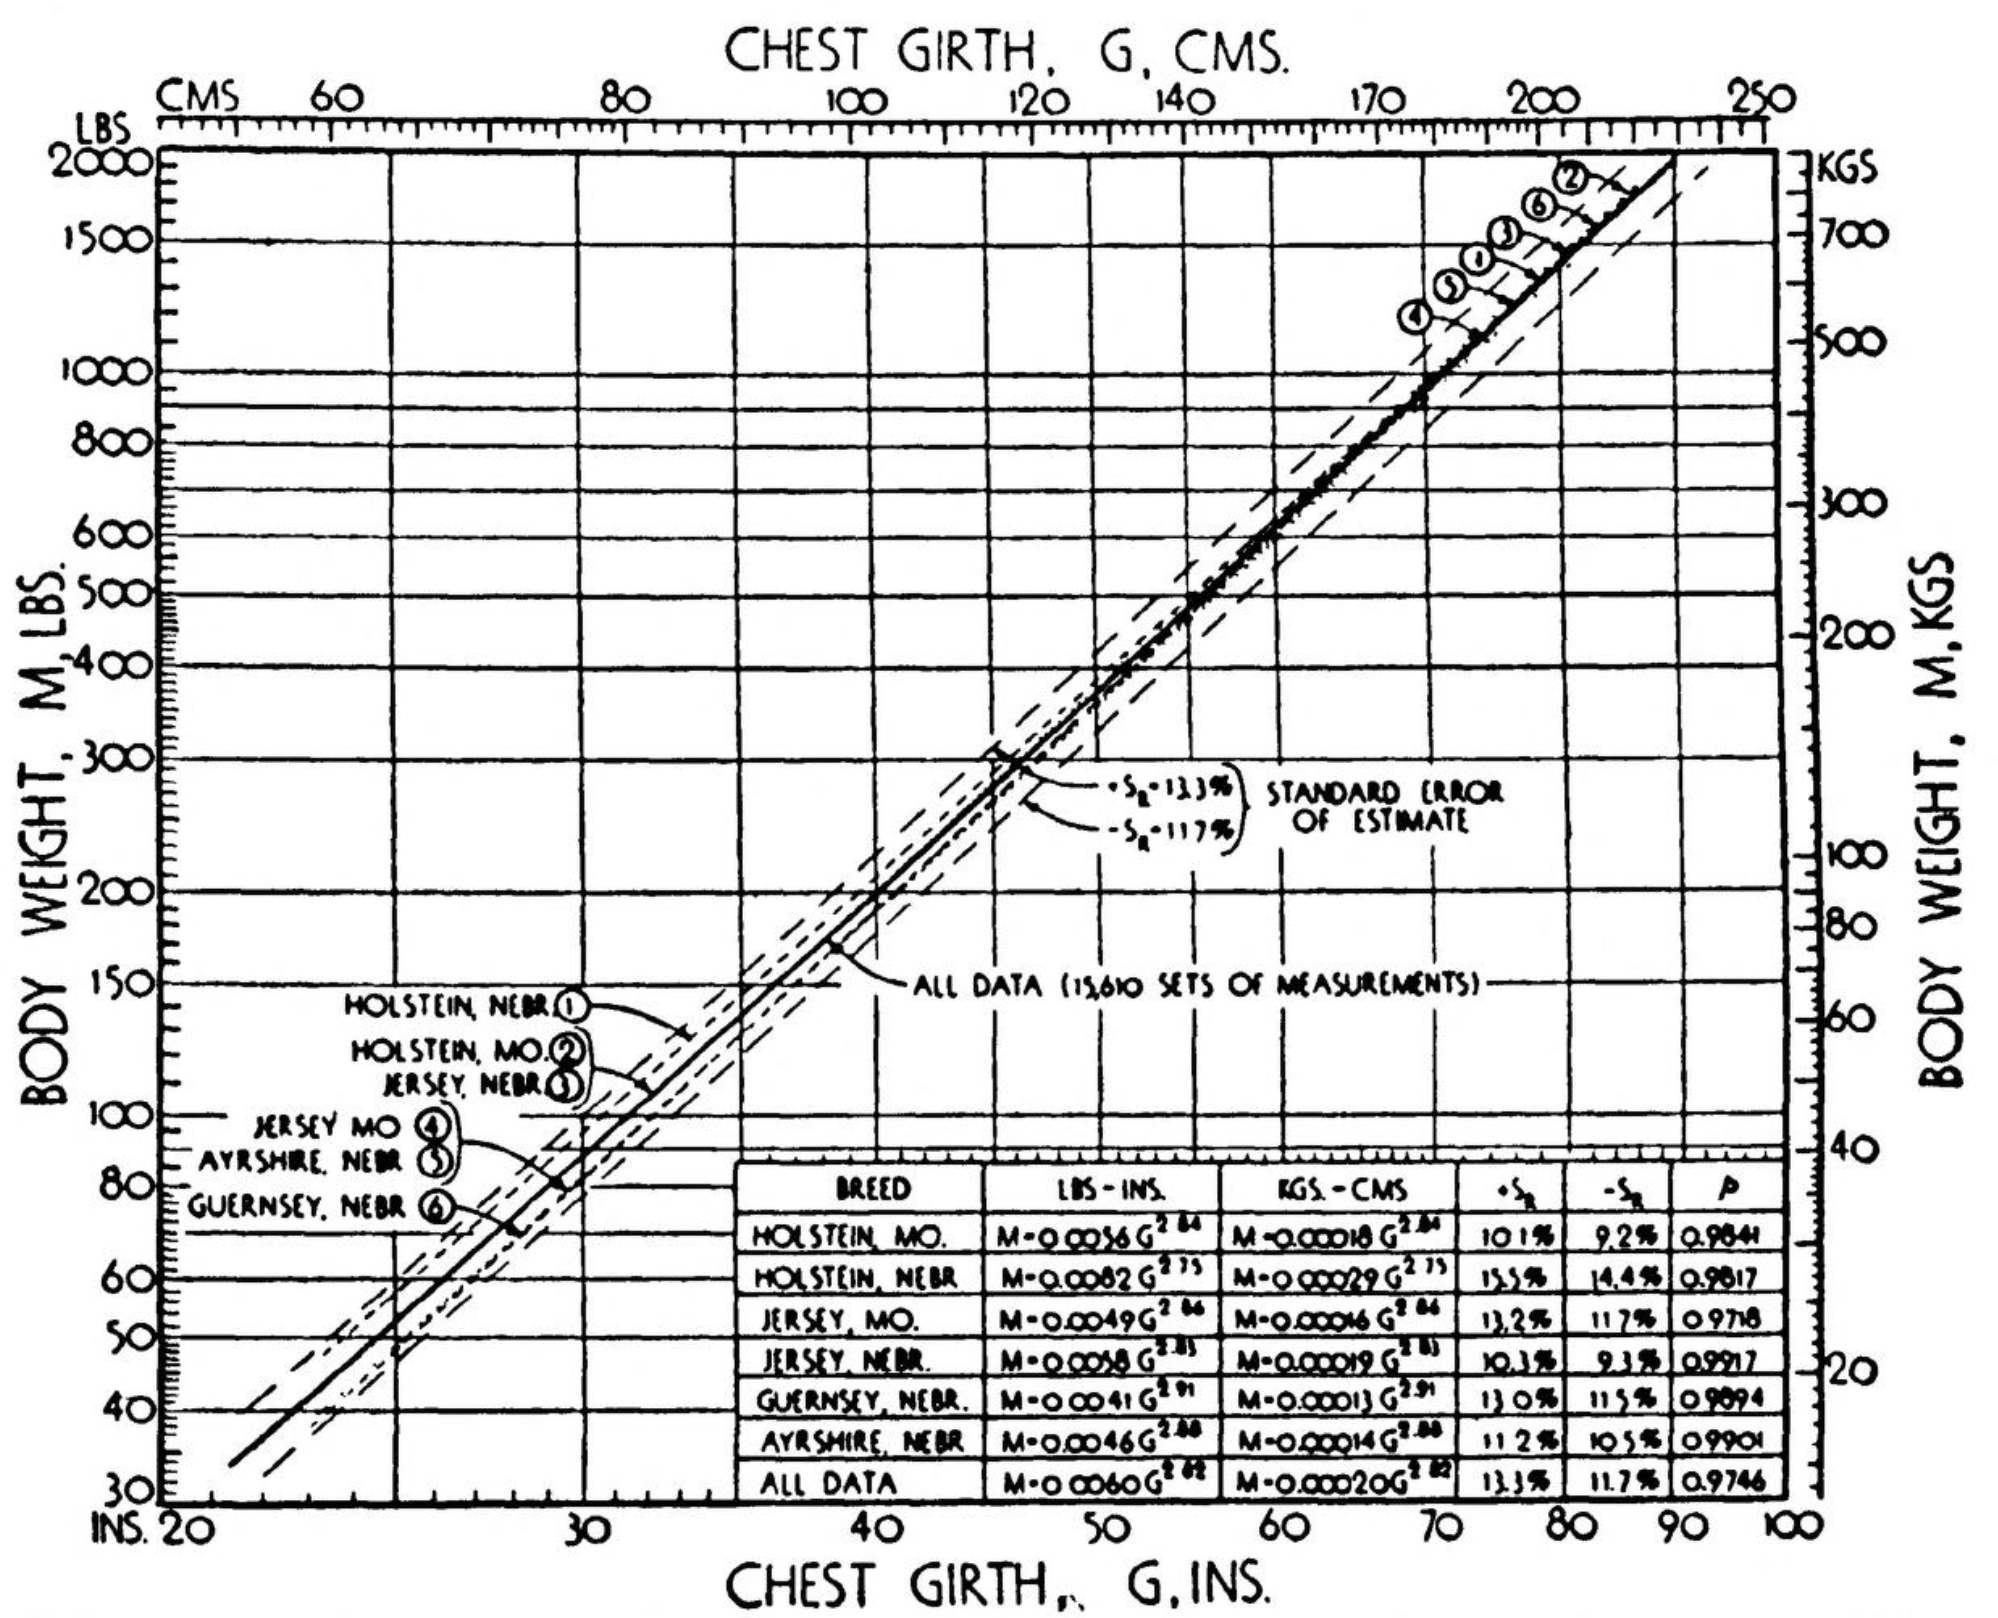
\includegraphics[width=0.49\textwidth]{images/cow-sizes-1.png}};
      \begin{scope}[x={(img.south east)},y={(img.north west)}]
        % I have calculated this to have slope 8/3
        \draw[dashed,very thick,color=C1] (0.15,0.14) -- (0.84,0.87);
        \node[anchor=north west,
          fill=white,
          inner sep=3pt,
          font=\small] at (0.1,1.1)
      {\tikz{\draw[dashed,very thick,color=C1] (0,0.8ex) -- (0.1,0.8ex);} $M \propto G^{8/3}$};
      \end{scope}
    \end{tikzpicture}
    %
    \begin{tikzpicture}[baseline]
      \node[anchor=south west,inner sep=0] (img) at (0,0)
        {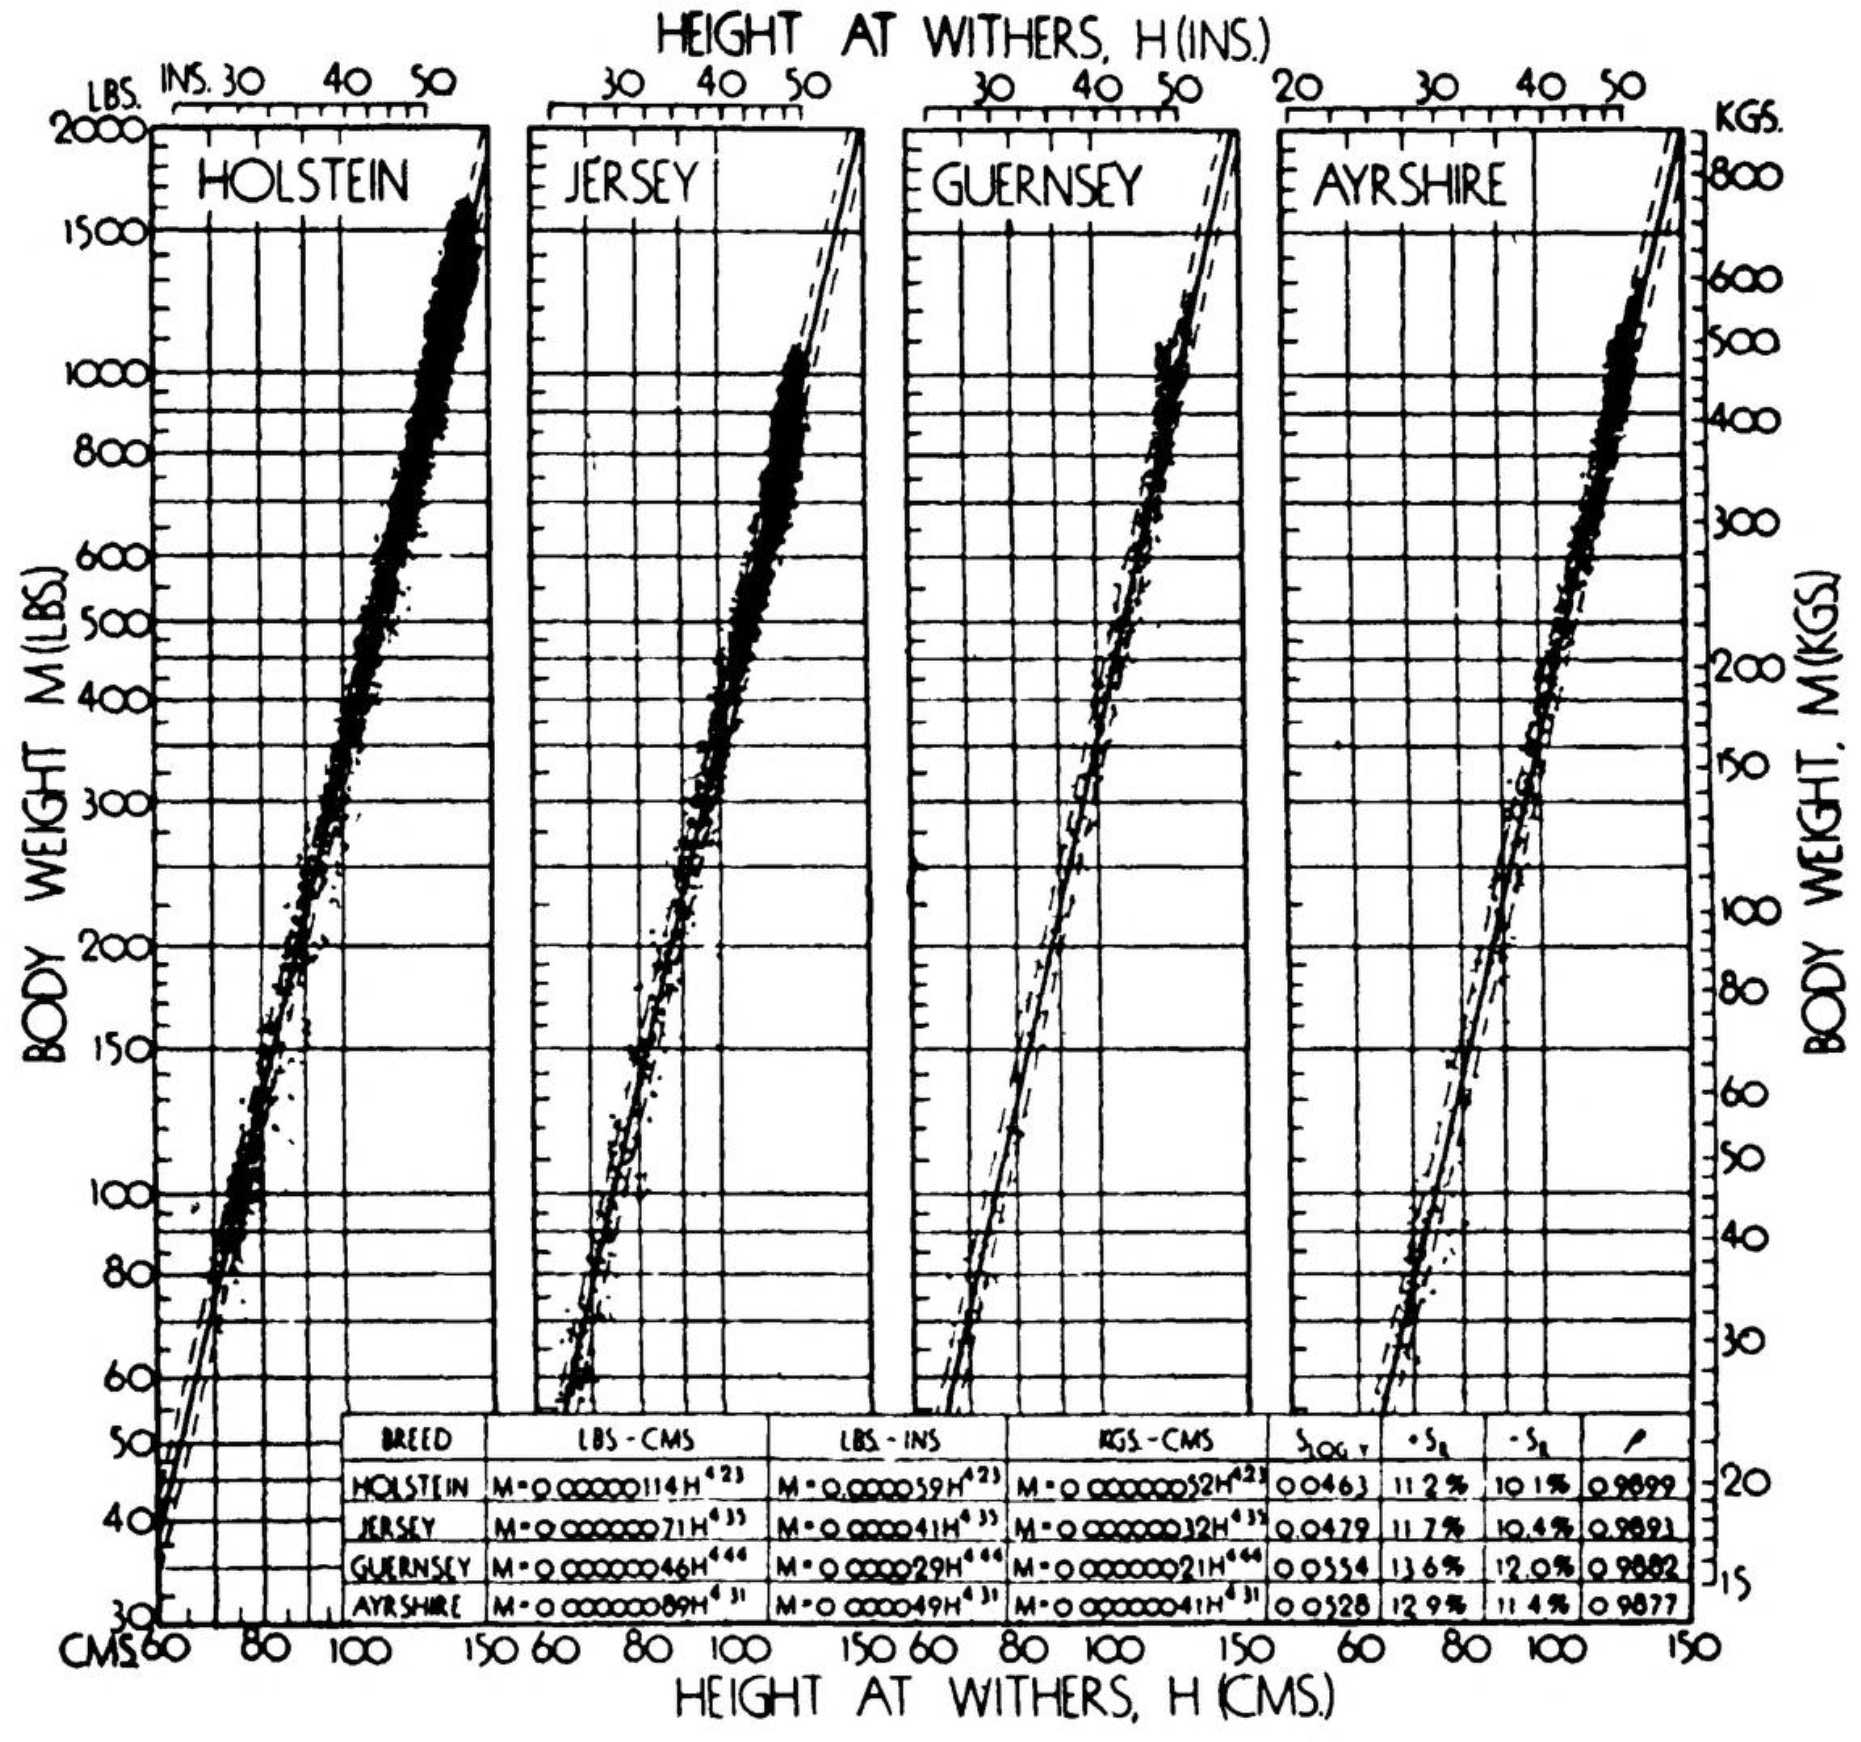
\includegraphics[width=0.49\textwidth]{images/cow-sizes-2.png}};
      \begin{scope}[x={(img.south east)},y={(img.north west)}]
        \draw[dashed,very thick,color=C1] (0.1,0.2) -- (0.26,0.89);
        \draw[dashed,very thick,color=C1] (0.1+0.2,0.2) -- (0.26+0.2,0.89);
        \draw[dashed,very thick,color=C1] (0.1+0.4,0.2) -- (0.26+0.4,0.89);
        \draw[dashed,very thick,color=C1] (0.1+0.64,0.2) -- (0.26+0.64,0.89);
        \node[anchor=north west,
          fill=white,
          inner sep=3pt,
          font=\small] at (0.1,1.1)
      {\tikz{\draw[dashed,very thick,color=C1] (0,0.8ex) -- (0.1,0.8ex);} $M \propto H^{4}$};
      \end{scope}
    \end{tikzpicture}
	\end{center}
	\caption{\textbf{Left:} Measurements of cow weight against chest girth ($\sim b$) for 15,610 cows. The relationship is very close to our prediction of a slope of $8/3$ on logarithmic axes. \textbf{Right:} Measurements of cow weight to height ($\sim a$) for four breeds of cow are also close to our prediction of a slope of $4$. Figures taken from \href{https://archive.org/details/in.ernet.dli.2015.5715/page/n629/mode/2up}{\textsc{Brody}, S. 1945. \emph{Bioenergetics and Growth}, 615--617.}}
	\label{fig:cow-sizes}
\end{figure}

Overall, our findings here are not bad for a little bit of scaling analysis. This is our first example of a biomechanical principle dictating the way the natural world has developed. 

It might seem that as long as cows get wider faster than they get taller, we can grow our cow forever. But the only mechanical principle we have applied scaling analysis to is whether the legs can support the weight. We could also consider the ability of the legs to bend for motility (difficult if they are very thick compared to their length); or we could consider the ability of the lungs to absorb sufficient oxygen for the body. In the latter case, the lung surface area, across which oxygen transfers, scales like an area; but the oxygen required by the body scales with the mass of the body, i.e.\ volume. So we can continue to find mathematical limitations which feed into the natural world.

\vspace{0.5cm}
\begin{extra-reading}
The Euler buckling problem is not something you will find in Murray. I would advise you stick to what's here. The buckling result is usually presented in a different context (static not dynamic analysis) in engineering or elasticity texts.
\end{extra-reading}
\begin{do-it-yourself}
Additional Problem Sheet 3 contains a number of worked examples featuring PDE stability of the sort in this chapter.
\end{do-it-yourself}

\section*{One last thing...}
This has been a fun way to finish this term, but scaling laws in general are extremely powerful, and we are only touching on them here. 

This term we have looked at systems of differential equations that represent the growth and spread of biological agents: populations, chemical concentrations, and diseases. We have seen how phase portraits and linear stability analysis allow us to model the long-term behaviour of the sorts of systems we encounter all the time in nature. Latterly, we have seen how spatial variation makes everything a bit harder. These equations, reaction--diffusion systems, will appear next term and as you study their instabilities, you'll learn how to answer another important question... how did the leopard get its spots? 

But for now, it's time to crack open the mince pies, and slowly soak into the Christmas break.



%\chapter{Stability of spatial competitive Lotka--Volterra}
%\label{chap:stability-sclv}
%In this chapter, we begin to generalise the PDE stability technique developed in the previous chapter by conducting a stability analysis of the spatial competitive Lotka--Volterra system, which was given by \cref{scaledlotvolpursuit} as
%\begin{subequations}
%\label{scaledlotvolpursuit2} 
%\begin{align}
%\pd{u}{t} &= \nabla^2 u +u(1-u-\gamma_1v),\\
%\pd{v}{t} &= \kappa\nabla^2 v + \beta v(1-v-\gamma_2u).
%\end{align}
%\end{subequations}
%
%\section{Linear stability analysis of spatial competitive Lotka--Volterra}
%\label{sec:lsa-sclv}
%\subsubsection*{\StepOne Find equilibria}
%Again we concentrate on homogeneous equilibria: these are solutions to
%\begin{subequations}
%\label{hom-eqa-eqns}
%\begin{align}
%u(1-u -\gamma_1v) &= 0,\\
%v(1-v - \gamma_2 u) &= 0.
%\end{align}
%\end{subequations}
%We found all these solutions in \cref{chap4equilibria}\StepOneIcon. Although we've changed notation a bit, these are
%\begin{equation}
%(u_0,v_0) = (0,0), \qquad
%(0,1), \qquad 
%(1,0), \quad \text{and} \quad
%\left (\frac{1-\gamma_1}{1- \gamma_1\gamma_2}, \frac{1-\gamma_2}{1 - \gamma_1\gamma_2} \right).
%\end{equation} 
%We impose the Dirichlet boundary conditions $u(0)=u(L) =u_0$ and $ v(0) = v(L) = v_0$.
%
%
%\subsubsection*{\StepTwo Linearise the system}
%We linearise \cref{scaledlotvolpursuit2} by expanding the variables $u$ and $v$ about their equilibrium values $u_0$ and $v_0$, i.e.\ $u \approx u_0 + \ep u_1$ and $v \approx v_0 + \ep v_1$. To keep matters simple, let's consider a one-dimensional domain $[0,L]$. 
%
%Substituting in our linear expansions, we have
%\begin{subequations}
%\begin{align}
%\ep\pd{u_1}{t} &= \ep\pdd{u_1}{x}  + (u_0+\ep u_1)(1-u_0-\ep u_1 - \gamma_1 v_0 - \ep \gamma_1 v_1),\\
%\ep\pd{v_1}{t} & = \ep\kappa\pdd{v_1}{x} + \beta(v_0+\ep v_1)(1-v_0-\ep v_1-\gamma_2 u_0 - \ep\gamma_2 u_1),
%\end{align}
%\end{subequations}
%%
%which to $\order(\ep)$ is
%%
%\begin{subequations}
%\begin{align}
%\ep\pd{u_1}{t} &= \ep\pdd{u_1}{x} + \coltwo{u_0(1-u_0-\gamma_1 v_0)} \nonumber \\
%			   & \hspace{9.05ex} + \ep\left[ u_1 -2u_0u_1  - \gamma_1(u_0v_1 + v_0u_1) \right], \\
%\ep\pd{v_1}{t} & = \ep\kappa\pdd{v_1}{x} + \coltwo{\beta v_0(1-v_0-\gamma_2 u_0)} \nonumber \\
%			   & \hspace{10.15ex} + \ep\beta\left[v_1 - 2v_0v_1  - \gamma_2(u_0v_1 + v_0u_1)\right].
%\end{align}
%\end{subequations}
%Note that the orange terms are zero by \cref{hom-eqa-eqns} -- \emph{this will always be true of the order 1 terms} -- and so we are left with
%\begin{subequations}
%\label{linlotvol}
%\begin{align}
%\pd{u_1}{t} &= \pdd{u_1}{x}  + u_1 -2u_0u_1  - \gamma_1(u_0v_1 + v_0u_1),\\
%\pd{v_1}{t} & = \kappa\pdd{v_1}{x} + \beta\left[v_1 - 2v_0v_1  - \gamma_2(u_0v_1 + v_0u_1)\right].
%\end{align}
%\end{subequations}
%
%\subsubsection{\StepThree Solve the linearised system}
%We can see that the linear order equations are constant coefficient equations in $u_1$ and $v_1$. Once again, we have periodic boundary conditions (in space), so we will be looking for solutions with an $\e^{\i k x}$ factor; and we want solutions that grow or decay in time, so we want an $\e^{\lambda t}$ factor. Putting those together, we therefore seek solutions in the form $u_1 =A\e^{\i kx+\lambda t}$ and $v_1 =B\e^{\i kx+\lambda t}$.  Substituting these forms into \cref{linlotvol} we find
%\begin{subequations}
%\label{linearisedeq}
%\begin{align}
%\lambda u_1 &= -k^2 u_1 +u_1 -2u_0u_1 - \gamma_1(u_0v_1 + v_0 u_1),\\
%\lambda v_1 &=  -\kappa k^2 v_1+ \beta\left[v_1 - 2v_0v_1  -\gamma_2(u_0v_1 + v_0u_1)\right].
%\end{align}
%\end{subequations}
%Note that we could not have solutions in the form  $u_1 =A\e^{\i k_1x+\lambda t}$ and $v_1 =B\e^{\i k_2x+\lambda t}$, with \emph{different} wavenumbers $k_1,k_2$, as the solutions would then be linearly independent and we could not achieve the required equality. We can write \cref{linearisedeq} as a matrix equation in the form 
%\begin{equation}
%\label{stabmatrixeq}
%\m{J}\v{u}_1 = \vu{0}
%\end{equation}
%where $\v{u}_1  = (u_1,v_1)$, $\vu{0} = (0,0)$ and 
%\begin{equation}
%\m{J} = \begin{pmatrix}
%-(\lambda+k^2)+1 -2u_0-\gamma_1v_0 & -\gamma_1 u_0 \\
%-\beta \gamma_2v_0 &  -(\lambda+\kappa k^2) + \beta(1-2v_0-\gamma_2 u_0)
%\end{pmatrix}.
%\end{equation}
%In the ODE case, we could extract the $\lambda$s so that we could write the matrix equation in the form $(\m{J}-\lambda\m{I})\v{u}_1=\vu{0}$. This time the $\lambda$s are baked into $\m{J}$, but that's OK: this doesn't make much practical difference. This time, the fundamental theorem of linear algebra tells us that there are only nontrivial solutions, $\v{u}_1$, if $\det(\m{J})=0$. 
%
%We use this, as we did in the previous chapter, to find values for $\lambda$ in terms of $k$, which we then put into our solutions, $u_1 =A\e^{\i kx+\lambda t}$ and $v_1 =B\e^{\i kx+\lambda t}$.
%
%Indeed, what about $k$? Going back to the boundary conditions,
%\begin{equation}
%	u_1(0) = u_1(L) = v_1(0) = v_1(L) = 0,
%\end{equation}
%and recalling that
%\begin{equation}
%	A\e^{\i kx} = A(\cos kx + \i \sin kx),
%\end{equation}
%only the $\sin$ part can satisfy the boundary conditions: this requires $A = -C\i$ and $k L=n\pi$ for $n = 0,1,2,3,\dots$.
%
%We get these solutions for each value of $n$, so our solution is the sum of these solutions,
%\begin{equation}
%u_1(x,t) = \sum_{n=1}^{\infty}A_n\sin\left(\frac{n\pi x}{L}\right)\e^{\lambda_n t}.
%\end{equation}
%Note that we've skipped over the $n=0$ solution because $\sin 0 = 0$. Also see that our $\lambda$ has become $\lambda_n$: don't forget that $\lambda$ depends on $k$, which in turn depends on $n$.
%
%So this, and similarly for $v_1$, is our full solution for any given initial conditions, with the growth rates $\lambda_n$ to be determined.
%
%\subsubsection*{\StepFour Assess stability}
%\paragraph{Stability of the $(0,0)$ solution:}
%If we first look at the $(0,0)$ solution, given that the off-diagonal components are 0, the polynomial is already factorised:
%\begin{align}
%(\lambda +k^2-1)(\lambda +\kappa k^2 -\beta) =0.
%\end{align}
%So both $\lambda$ are real and we have asymptotic stability if 
%\begin{equation}
%k^2>1 \quad \text{and} \quad k^2 > \frac{\beta}{\kappa}.
%\end{equation}
%Applying the boundary conditions we obtain 
%\begin{equation}
%\label{kcons}
%\frac{n^2\pi^2}{L^2}>1 \quad \text{and} \quad \frac{n^2\pi^2}{L^2} > \frac{\beta}{\kappa},
%\end{equation}
%placing constraints on the possible length of the domain $L$ for the equilibrium to be stable. Remembering this must be true for all $n$, it is easy to check that the most stringent constraint comes from the $n=1$ case, i.e., 
%\begin{equation}
%L <\pi \quad \text{and} \quad L<\pi\sqrt{\frac{\kappa}{\beta}}.
%\end{equation}
%A word of warning: \emph{the $n=1$ case will not always give the critical equality; you must always check if it does or not}.
%
%\begin{figure}
%	\centering
%	%% Creator: Matplotlib, PGF backend
%%
%% To include the figure in your LaTeX document, write
%%   \input{<filename>.pgf}
%%
%% Make sure the required packages are loaded in your preamble
%%   \usepackage{pgf}
%%
%% Figures using additional raster images can only be included by \input if
%% they are in the same directory as the main LaTeX file. For loading figures
%% from other directories you can use the `import` package
%%   \usepackage{import}
%% and then include the figures with
%%   \import{<path to file>}{<filename>.pgf}
%%
%% Matplotlib used the following preamble
%%   \usepackage{fontspec}
%%   \setmainfont{DejaVuSerif.ttf}[Path=/Library/Python/3.7/site-packages/matplotlib/mpl-data/fonts/ttf/]
%%   \setsansfont{DejaVuSans.ttf}[Path=/Library/Python/3.7/site-packages/matplotlib/mpl-data/fonts/ttf/]
%%   \setmonofont{DejaVuSansMono.ttf}[Path=/Library/Python/3.7/site-packages/matplotlib/mpl-data/fonts/ttf/]
%%
\begingroup%
\makeatletter%
\begin{pgfpicture}%
\pgfpathrectangle{\pgfpointorigin}{\pgfqpoint{6.000000in}{4.400000in}}%
\pgfusepath{use as bounding box, clip}%
\begin{pgfscope}%
\pgfsetbuttcap%
\pgfsetmiterjoin%
\definecolor{currentfill}{rgb}{1.000000,1.000000,1.000000}%
\pgfsetfillcolor{currentfill}%
\pgfsetlinewidth{0.000000pt}%
\definecolor{currentstroke}{rgb}{1.000000,1.000000,1.000000}%
\pgfsetstrokecolor{currentstroke}%
\pgfsetdash{}{0pt}%
\pgfpathmoveto{\pgfqpoint{0.000000in}{0.000000in}}%
\pgfpathlineto{\pgfqpoint{6.000000in}{0.000000in}}%
\pgfpathlineto{\pgfqpoint{6.000000in}{4.400000in}}%
\pgfpathlineto{\pgfqpoint{0.000000in}{4.400000in}}%
\pgfpathclose%
\pgfusepath{fill}%
\end{pgfscope}%
\begin{pgfscope}%
\pgfsetbuttcap%
\pgfsetmiterjoin%
\definecolor{currentfill}{rgb}{1.000000,1.000000,1.000000}%
\pgfsetfillcolor{currentfill}%
\pgfsetlinewidth{0.000000pt}%
\definecolor{currentstroke}{rgb}{0.000000,0.000000,0.000000}%
\pgfsetstrokecolor{currentstroke}%
\pgfsetstrokeopacity{0.000000}%
\pgfsetdash{}{0pt}%
\pgfpathmoveto{\pgfqpoint{0.519592in}{2.405612in}}%
\pgfpathlineto{\pgfqpoint{2.158432in}{2.405612in}}%
\pgfpathlineto{\pgfqpoint{2.158432in}{4.068025in}}%
\pgfpathlineto{\pgfqpoint{0.519592in}{4.068025in}}%
\pgfpathclose%
\pgfusepath{fill}%
\end{pgfscope}%
\begin{pgfscope}%
\pgfsetbuttcap%
\pgfsetroundjoin%
\definecolor{currentfill}{rgb}{0.000000,0.000000,0.000000}%
\pgfsetfillcolor{currentfill}%
\pgfsetlinewidth{0.803000pt}%
\definecolor{currentstroke}{rgb}{0.000000,0.000000,0.000000}%
\pgfsetstrokecolor{currentstroke}%
\pgfsetdash{}{0pt}%
\pgfsys@defobject{currentmarker}{\pgfqpoint{0.000000in}{-0.048611in}}{\pgfqpoint{0.000000in}{0.000000in}}{%
\pgfpathmoveto{\pgfqpoint{0.000000in}{0.000000in}}%
\pgfpathlineto{\pgfqpoint{0.000000in}{-0.048611in}}%
\pgfusepath{stroke,fill}%
}%
\begin{pgfscope}%
\pgfsys@transformshift{0.519592in}{2.405612in}%
\pgfsys@useobject{currentmarker}{}%
\end{pgfscope}%
\end{pgfscope}%
\begin{pgfscope}%
\definecolor{textcolor}{rgb}{0.000000,0.000000,0.000000}%
\pgfsetstrokecolor{textcolor}%
\pgfsetfillcolor{textcolor}%
\pgftext[x=0.519592in,y=2.308390in,,top]{\color{textcolor}\rmfamily\fontsize{12.000000}{14.400000}\selectfont \(\displaystyle 0\)}%
\end{pgfscope}%
\begin{pgfscope}%
\pgfsetbuttcap%
\pgfsetroundjoin%
\definecolor{currentfill}{rgb}{0.000000,0.000000,0.000000}%
\pgfsetfillcolor{currentfill}%
\pgfsetlinewidth{0.803000pt}%
\definecolor{currentstroke}{rgb}{0.000000,0.000000,0.000000}%
\pgfsetstrokecolor{currentstroke}%
\pgfsetdash{}{0pt}%
\pgfsys@defobject{currentmarker}{\pgfqpoint{0.000000in}{-0.048611in}}{\pgfqpoint{0.000000in}{0.000000in}}{%
\pgfpathmoveto{\pgfqpoint{0.000000in}{0.000000in}}%
\pgfpathlineto{\pgfqpoint{0.000000in}{-0.048611in}}%
\pgfusepath{stroke,fill}%
}%
\begin{pgfscope}%
\pgfsys@transformshift{1.175128in}{2.405612in}%
\pgfsys@useobject{currentmarker}{}%
\end{pgfscope}%
\end{pgfscope}%
\begin{pgfscope}%
\definecolor{textcolor}{rgb}{0.000000,0.000000,0.000000}%
\pgfsetstrokecolor{textcolor}%
\pgfsetfillcolor{textcolor}%
\pgftext[x=1.175128in,y=2.308390in,,top]{\color{textcolor}\rmfamily\fontsize{12.000000}{14.400000}\selectfont \(\displaystyle \pi/4\)}%
\end{pgfscope}%
\begin{pgfscope}%
\pgfsetbuttcap%
\pgfsetroundjoin%
\definecolor{currentfill}{rgb}{0.000000,0.000000,0.000000}%
\pgfsetfillcolor{currentfill}%
\pgfsetlinewidth{0.803000pt}%
\definecolor{currentstroke}{rgb}{0.000000,0.000000,0.000000}%
\pgfsetstrokecolor{currentstroke}%
\pgfsetdash{}{0pt}%
\pgfsys@defobject{currentmarker}{\pgfqpoint{0.000000in}{-0.048611in}}{\pgfqpoint{0.000000in}{0.000000in}}{%
\pgfpathmoveto{\pgfqpoint{0.000000in}{0.000000in}}%
\pgfpathlineto{\pgfqpoint{0.000000in}{-0.048611in}}%
\pgfusepath{stroke,fill}%
}%
\begin{pgfscope}%
\pgfsys@transformshift{1.830664in}{2.405612in}%
\pgfsys@useobject{currentmarker}{}%
\end{pgfscope}%
\end{pgfscope}%
\begin{pgfscope}%
\definecolor{textcolor}{rgb}{0.000000,0.000000,0.000000}%
\pgfsetstrokecolor{textcolor}%
\pgfsetfillcolor{textcolor}%
\pgftext[x=1.830664in,y=2.308390in,,top]{\color{textcolor}\rmfamily\fontsize{12.000000}{14.400000}\selectfont \(\displaystyle \pi/2\)}%
\end{pgfscope}%
\begin{pgfscope}%
\pgfsetbuttcap%
\pgfsetroundjoin%
\definecolor{currentfill}{rgb}{0.000000,0.000000,0.000000}%
\pgfsetfillcolor{currentfill}%
\pgfsetlinewidth{0.803000pt}%
\definecolor{currentstroke}{rgb}{0.000000,0.000000,0.000000}%
\pgfsetstrokecolor{currentstroke}%
\pgfsetdash{}{0pt}%
\pgfsys@defobject{currentmarker}{\pgfqpoint{-0.048611in}{0.000000in}}{\pgfqpoint{0.000000in}{0.000000in}}{%
\pgfpathmoveto{\pgfqpoint{0.000000in}{0.000000in}}%
\pgfpathlineto{\pgfqpoint{-0.048611in}{0.000000in}}%
\pgfusepath{stroke,fill}%
}%
\begin{pgfscope}%
\pgfsys@transformshift{0.519592in}{2.405612in}%
\pgfsys@useobject{currentmarker}{}%
\end{pgfscope}%
\end{pgfscope}%
\begin{pgfscope}%
\definecolor{textcolor}{rgb}{0.000000,0.000000,0.000000}%
\pgfsetstrokecolor{textcolor}%
\pgfsetfillcolor{textcolor}%
\pgftext[x=0.132249in,y=2.342298in,left,base]{\color{textcolor}\rmfamily\fontsize{12.000000}{14.400000}\selectfont \(\displaystyle 0.00\)}%
\end{pgfscope}%
\begin{pgfscope}%
\pgfsetbuttcap%
\pgfsetroundjoin%
\definecolor{currentfill}{rgb}{0.000000,0.000000,0.000000}%
\pgfsetfillcolor{currentfill}%
\pgfsetlinewidth{0.803000pt}%
\definecolor{currentstroke}{rgb}{0.000000,0.000000,0.000000}%
\pgfsetstrokecolor{currentstroke}%
\pgfsetdash{}{0pt}%
\pgfsys@defobject{currentmarker}{\pgfqpoint{-0.048611in}{0.000000in}}{\pgfqpoint{0.000000in}{0.000000in}}{%
\pgfpathmoveto{\pgfqpoint{0.000000in}{0.000000in}}%
\pgfpathlineto{\pgfqpoint{-0.048611in}{0.000000in}}%
\pgfusepath{stroke,fill}%
}%
\begin{pgfscope}%
\pgfsys@transformshift{0.519592in}{3.197237in}%
\pgfsys@useobject{currentmarker}{}%
\end{pgfscope}%
\end{pgfscope}%
\begin{pgfscope}%
\definecolor{textcolor}{rgb}{0.000000,0.000000,0.000000}%
\pgfsetstrokecolor{textcolor}%
\pgfsetfillcolor{textcolor}%
\pgftext[x=0.132249in,y=3.133924in,left,base]{\color{textcolor}\rmfamily\fontsize{12.000000}{14.400000}\selectfont \(\displaystyle 0.05\)}%
\end{pgfscope}%
\begin{pgfscope}%
\pgfsetbuttcap%
\pgfsetroundjoin%
\definecolor{currentfill}{rgb}{0.000000,0.000000,0.000000}%
\pgfsetfillcolor{currentfill}%
\pgfsetlinewidth{0.803000pt}%
\definecolor{currentstroke}{rgb}{0.000000,0.000000,0.000000}%
\pgfsetstrokecolor{currentstroke}%
\pgfsetdash{}{0pt}%
\pgfsys@defobject{currentmarker}{\pgfqpoint{-0.048611in}{0.000000in}}{\pgfqpoint{0.000000in}{0.000000in}}{%
\pgfpathmoveto{\pgfqpoint{0.000000in}{0.000000in}}%
\pgfpathlineto{\pgfqpoint{-0.048611in}{0.000000in}}%
\pgfusepath{stroke,fill}%
}%
\begin{pgfscope}%
\pgfsys@transformshift{0.519592in}{3.988863in}%
\pgfsys@useobject{currentmarker}{}%
\end{pgfscope}%
\end{pgfscope}%
\begin{pgfscope}%
\definecolor{textcolor}{rgb}{0.000000,0.000000,0.000000}%
\pgfsetstrokecolor{textcolor}%
\pgfsetfillcolor{textcolor}%
\pgftext[x=0.132249in,y=3.925549in,left,base]{\color{textcolor}\rmfamily\fontsize{12.000000}{14.400000}\selectfont \(\displaystyle 0.10\)}%
\end{pgfscope}%
\begin{pgfscope}%
\pgfsetrectcap%
\pgfsetmiterjoin%
\pgfsetlinewidth{0.803000pt}%
\definecolor{currentstroke}{rgb}{0.000000,0.000000,0.000000}%
\pgfsetstrokecolor{currentstroke}%
\pgfsetdash{}{0pt}%
\pgfpathmoveto{\pgfqpoint{0.519592in}{2.405612in}}%
\pgfpathlineto{\pgfqpoint{0.519592in}{4.068025in}}%
\pgfusepath{stroke}%
\end{pgfscope}%
\begin{pgfscope}%
\pgfsetrectcap%
\pgfsetmiterjoin%
\pgfsetlinewidth{0.803000pt}%
\definecolor{currentstroke}{rgb}{0.000000,0.000000,0.000000}%
\pgfsetstrokecolor{currentstroke}%
\pgfsetdash{}{0pt}%
\pgfpathmoveto{\pgfqpoint{0.519592in}{2.405612in}}%
\pgfpathlineto{\pgfqpoint{2.158432in}{2.405612in}}%
\pgfusepath{stroke}%
\end{pgfscope}%
\begin{pgfscope}%
\pgfpathrectangle{\pgfqpoint{0.519592in}{2.405612in}}{\pgfqpoint{1.638840in}{1.662413in}}%
\pgfusepath{clip}%
\pgfsetrectcap%
\pgfsetroundjoin%
\pgfsetlinewidth{1.505625pt}%
\definecolor{currentstroke}{rgb}{0.121569,0.466667,0.705882}%
\pgfsetstrokecolor{currentstroke}%
\pgfsetdash{}{0pt}%
\pgfpathmoveto{\pgfqpoint{0.519592in}{2.405612in}}%
\pgfpathlineto{\pgfqpoint{0.532703in}{2.455343in}}%
\pgfpathlineto{\pgfqpoint{0.545814in}{2.505025in}}%
\pgfpathlineto{\pgfqpoint{0.558924in}{2.554609in}}%
\pgfpathlineto{\pgfqpoint{0.572035in}{2.604046in}}%
\pgfpathlineto{\pgfqpoint{0.585146in}{2.653287in}}%
\pgfpathlineto{\pgfqpoint{0.598256in}{2.702284in}}%
\pgfpathlineto{\pgfqpoint{0.611367in}{2.750988in}}%
\pgfpathlineto{\pgfqpoint{0.624478in}{2.799351in}}%
\pgfpathlineto{\pgfqpoint{0.637589in}{2.847325in}}%
\pgfpathlineto{\pgfqpoint{0.650699in}{2.894864in}}%
\pgfpathlineto{\pgfqpoint{0.663810in}{2.941919in}}%
\pgfpathlineto{\pgfqpoint{0.676921in}{2.988446in}}%
\pgfpathlineto{\pgfqpoint{0.690031in}{3.034397in}}%
\pgfpathlineto{\pgfqpoint{0.703142in}{3.079727in}}%
\pgfpathlineto{\pgfqpoint{0.716253in}{3.124393in}}%
\pgfpathlineto{\pgfqpoint{0.729364in}{3.168349in}}%
\pgfpathlineto{\pgfqpoint{0.742474in}{3.211552in}}%
\pgfpathlineto{\pgfqpoint{0.755585in}{3.253960in}}%
\pgfpathlineto{\pgfqpoint{0.768696in}{3.295531in}}%
\pgfpathlineto{\pgfqpoint{0.781806in}{3.336224in}}%
\pgfpathlineto{\pgfqpoint{0.794917in}{3.375998in}}%
\pgfpathlineto{\pgfqpoint{0.808028in}{3.414814in}}%
\pgfpathlineto{\pgfqpoint{0.821139in}{3.452635in}}%
\pgfpathlineto{\pgfqpoint{0.834249in}{3.489422in}}%
\pgfpathlineto{\pgfqpoint{0.847360in}{3.525139in}}%
\pgfpathlineto{\pgfqpoint{0.860471in}{3.559752in}}%
\pgfpathlineto{\pgfqpoint{0.873581in}{3.593226in}}%
\pgfpathlineto{\pgfqpoint{0.886692in}{3.625528in}}%
\pgfpathlineto{\pgfqpoint{0.899803in}{3.656626in}}%
\pgfpathlineto{\pgfqpoint{0.912914in}{3.686489in}}%
\pgfpathlineto{\pgfqpoint{0.926024in}{3.715088in}}%
\pgfpathlineto{\pgfqpoint{0.939135in}{3.742395in}}%
\pgfpathlineto{\pgfqpoint{0.952246in}{3.768382in}}%
\pgfpathlineto{\pgfqpoint{0.965357in}{3.793025in}}%
\pgfpathlineto{\pgfqpoint{0.978467in}{3.816299in}}%
\pgfpathlineto{\pgfqpoint{0.991578in}{3.838180in}}%
\pgfpathlineto{\pgfqpoint{1.004689in}{3.858648in}}%
\pgfpathlineto{\pgfqpoint{1.017799in}{3.877681in}}%
\pgfpathlineto{\pgfqpoint{1.030910in}{3.895262in}}%
\pgfpathlineto{\pgfqpoint{1.044021in}{3.911373in}}%
\pgfpathlineto{\pgfqpoint{1.057132in}{3.925998in}}%
\pgfpathlineto{\pgfqpoint{1.070242in}{3.939122in}}%
\pgfpathlineto{\pgfqpoint{1.083353in}{3.950733in}}%
\pgfpathlineto{\pgfqpoint{1.096464in}{3.960819in}}%
\pgfpathlineto{\pgfqpoint{1.109574in}{3.969370in}}%
\pgfpathlineto{\pgfqpoint{1.122685in}{3.976378in}}%
\pgfpathlineto{\pgfqpoint{1.135796in}{3.981836in}}%
\pgfpathlineto{\pgfqpoint{1.148907in}{3.985739in}}%
\pgfpathlineto{\pgfqpoint{1.162017in}{3.988081in}}%
\pgfpathlineto{\pgfqpoint{1.175128in}{3.988863in}}%
\pgfpathlineto{\pgfqpoint{1.188239in}{3.988081in}}%
\pgfpathlineto{\pgfqpoint{1.201349in}{3.985739in}}%
\pgfpathlineto{\pgfqpoint{1.214460in}{3.981836in}}%
\pgfpathlineto{\pgfqpoint{1.227571in}{3.976378in}}%
\pgfpathlineto{\pgfqpoint{1.240682in}{3.969370in}}%
\pgfpathlineto{\pgfqpoint{1.253792in}{3.960819in}}%
\pgfpathlineto{\pgfqpoint{1.266903in}{3.950733in}}%
\pgfpathlineto{\pgfqpoint{1.280014in}{3.939122in}}%
\pgfpathlineto{\pgfqpoint{1.293124in}{3.925998in}}%
\pgfpathlineto{\pgfqpoint{1.306235in}{3.911373in}}%
\pgfpathlineto{\pgfqpoint{1.319346in}{3.895262in}}%
\pgfpathlineto{\pgfqpoint{1.332457in}{3.877681in}}%
\pgfpathlineto{\pgfqpoint{1.345567in}{3.858648in}}%
\pgfpathlineto{\pgfqpoint{1.358678in}{3.838180in}}%
\pgfpathlineto{\pgfqpoint{1.371789in}{3.816299in}}%
\pgfpathlineto{\pgfqpoint{1.384899in}{3.793025in}}%
\pgfpathlineto{\pgfqpoint{1.398010in}{3.768382in}}%
\pgfpathlineto{\pgfqpoint{1.411121in}{3.742395in}}%
\pgfpathlineto{\pgfqpoint{1.424232in}{3.715088in}}%
\pgfpathlineto{\pgfqpoint{1.437342in}{3.686489in}}%
\pgfpathlineto{\pgfqpoint{1.450453in}{3.656626in}}%
\pgfpathlineto{\pgfqpoint{1.463564in}{3.625528in}}%
\pgfpathlineto{\pgfqpoint{1.476674in}{3.593226in}}%
\pgfpathlineto{\pgfqpoint{1.489785in}{3.559752in}}%
\pgfpathlineto{\pgfqpoint{1.502896in}{3.525139in}}%
\pgfpathlineto{\pgfqpoint{1.516007in}{3.489422in}}%
\pgfpathlineto{\pgfqpoint{1.529117in}{3.452635in}}%
\pgfpathlineto{\pgfqpoint{1.542228in}{3.414814in}}%
\pgfpathlineto{\pgfqpoint{1.555339in}{3.375998in}}%
\pgfpathlineto{\pgfqpoint{1.568449in}{3.336224in}}%
\pgfpathlineto{\pgfqpoint{1.581560in}{3.295531in}}%
\pgfpathlineto{\pgfqpoint{1.594671in}{3.253960in}}%
\pgfpathlineto{\pgfqpoint{1.607782in}{3.211552in}}%
\pgfpathlineto{\pgfqpoint{1.620892in}{3.168349in}}%
\pgfpathlineto{\pgfqpoint{1.634003in}{3.124393in}}%
\pgfpathlineto{\pgfqpoint{1.647114in}{3.079727in}}%
\pgfpathlineto{\pgfqpoint{1.660225in}{3.034397in}}%
\pgfpathlineto{\pgfqpoint{1.673335in}{2.988446in}}%
\pgfpathlineto{\pgfqpoint{1.686446in}{2.941919in}}%
\pgfpathlineto{\pgfqpoint{1.699557in}{2.894864in}}%
\pgfpathlineto{\pgfqpoint{1.712667in}{2.847325in}}%
\pgfpathlineto{\pgfqpoint{1.725778in}{2.799351in}}%
\pgfpathlineto{\pgfqpoint{1.738889in}{2.750988in}}%
\pgfpathlineto{\pgfqpoint{1.752000in}{2.702284in}}%
\pgfpathlineto{\pgfqpoint{1.765110in}{2.653287in}}%
\pgfpathlineto{\pgfqpoint{1.778221in}{2.604046in}}%
\pgfpathlineto{\pgfqpoint{1.791332in}{2.554609in}}%
\pgfpathlineto{\pgfqpoint{1.804442in}{2.505025in}}%
\pgfpathlineto{\pgfqpoint{1.817553in}{2.455343in}}%
\pgfpathlineto{\pgfqpoint{1.830664in}{2.405612in}}%
\pgfusepath{stroke}%
\end{pgfscope}%
\begin{pgfscope}%
\pgfpathrectangle{\pgfqpoint{0.519592in}{2.405612in}}{\pgfqpoint{1.638840in}{1.662413in}}%
\pgfusepath{clip}%
\pgfsetbuttcap%
\pgfsetroundjoin%
\pgfsetlinewidth{1.505625pt}%
\definecolor{currentstroke}{rgb}{1.000000,0.498039,0.054902}%
\pgfsetstrokecolor{currentstroke}%
\pgfsetdash{{5.550000pt}{2.400000pt}}{0.000000pt}%
\pgfpathmoveto{\pgfqpoint{0.519592in}{2.405612in}}%
\pgfpathlineto{\pgfqpoint{0.532703in}{2.430478in}}%
\pgfpathlineto{\pgfqpoint{0.545814in}{2.455319in}}%
\pgfpathlineto{\pgfqpoint{0.558924in}{2.480111in}}%
\pgfpathlineto{\pgfqpoint{0.572035in}{2.504829in}}%
\pgfpathlineto{\pgfqpoint{0.585146in}{2.529450in}}%
\pgfpathlineto{\pgfqpoint{0.598256in}{2.553948in}}%
\pgfpathlineto{\pgfqpoint{0.611367in}{2.578300in}}%
\pgfpathlineto{\pgfqpoint{0.624478in}{2.602481in}}%
\pgfpathlineto{\pgfqpoint{0.637589in}{2.626469in}}%
\pgfpathlineto{\pgfqpoint{0.650699in}{2.650238in}}%
\pgfpathlineto{\pgfqpoint{0.663810in}{2.673766in}}%
\pgfpathlineto{\pgfqpoint{0.676921in}{2.697029in}}%
\pgfpathlineto{\pgfqpoint{0.690031in}{2.720005in}}%
\pgfpathlineto{\pgfqpoint{0.703142in}{2.742670in}}%
\pgfpathlineto{\pgfqpoint{0.716253in}{2.765003in}}%
\pgfpathlineto{\pgfqpoint{0.729364in}{2.786981in}}%
\pgfpathlineto{\pgfqpoint{0.742474in}{2.808582in}}%
\pgfpathlineto{\pgfqpoint{0.755585in}{2.829786in}}%
\pgfpathlineto{\pgfqpoint{0.768696in}{2.850572in}}%
\pgfpathlineto{\pgfqpoint{0.781806in}{2.870918in}}%
\pgfpathlineto{\pgfqpoint{0.794917in}{2.890805in}}%
\pgfpathlineto{\pgfqpoint{0.808028in}{2.910213in}}%
\pgfpathlineto{\pgfqpoint{0.821139in}{2.929123in}}%
\pgfpathlineto{\pgfqpoint{0.834249in}{2.947517in}}%
\pgfpathlineto{\pgfqpoint{0.847360in}{2.965376in}}%
\pgfpathlineto{\pgfqpoint{0.860471in}{2.982682in}}%
\pgfpathlineto{\pgfqpoint{0.873581in}{2.999419in}}%
\pgfpathlineto{\pgfqpoint{0.886692in}{3.015570in}}%
\pgfpathlineto{\pgfqpoint{0.899803in}{3.031119in}}%
\pgfpathlineto{\pgfqpoint{0.912914in}{3.046050in}}%
\pgfpathlineto{\pgfqpoint{0.926024in}{3.060350in}}%
\pgfpathlineto{\pgfqpoint{0.939135in}{3.074004in}}%
\pgfpathlineto{\pgfqpoint{0.952246in}{3.086997in}}%
\pgfpathlineto{\pgfqpoint{0.965357in}{3.099319in}}%
\pgfpathlineto{\pgfqpoint{0.978467in}{3.110955in}}%
\pgfpathlineto{\pgfqpoint{0.991578in}{3.121896in}}%
\pgfpathlineto{\pgfqpoint{1.004689in}{3.132130in}}%
\pgfpathlineto{\pgfqpoint{1.017799in}{3.141647in}}%
\pgfpathlineto{\pgfqpoint{1.030910in}{3.150437in}}%
\pgfpathlineto{\pgfqpoint{1.044021in}{3.158493in}}%
\pgfpathlineto{\pgfqpoint{1.057132in}{3.165805in}}%
\pgfpathlineto{\pgfqpoint{1.070242in}{3.172367in}}%
\pgfpathlineto{\pgfqpoint{1.083353in}{3.178173in}}%
\pgfpathlineto{\pgfqpoint{1.096464in}{3.183216in}}%
\pgfpathlineto{\pgfqpoint{1.109574in}{3.187491in}}%
\pgfpathlineto{\pgfqpoint{1.122685in}{3.190995in}}%
\pgfpathlineto{\pgfqpoint{1.135796in}{3.193724in}}%
\pgfpathlineto{\pgfqpoint{1.148907in}{3.195675in}}%
\pgfpathlineto{\pgfqpoint{1.162017in}{3.196847in}}%
\pgfpathlineto{\pgfqpoint{1.175128in}{3.197237in}}%
\pgfpathlineto{\pgfqpoint{1.188239in}{3.196847in}}%
\pgfpathlineto{\pgfqpoint{1.201349in}{3.195675in}}%
\pgfpathlineto{\pgfqpoint{1.214460in}{3.193724in}}%
\pgfpathlineto{\pgfqpoint{1.227571in}{3.190995in}}%
\pgfpathlineto{\pgfqpoint{1.240682in}{3.187491in}}%
\pgfpathlineto{\pgfqpoint{1.253792in}{3.183216in}}%
\pgfpathlineto{\pgfqpoint{1.266903in}{3.178173in}}%
\pgfpathlineto{\pgfqpoint{1.280014in}{3.172367in}}%
\pgfpathlineto{\pgfqpoint{1.293124in}{3.165805in}}%
\pgfpathlineto{\pgfqpoint{1.306235in}{3.158493in}}%
\pgfpathlineto{\pgfqpoint{1.319346in}{3.150437in}}%
\pgfpathlineto{\pgfqpoint{1.332457in}{3.141647in}}%
\pgfpathlineto{\pgfqpoint{1.345567in}{3.132130in}}%
\pgfpathlineto{\pgfqpoint{1.358678in}{3.121896in}}%
\pgfpathlineto{\pgfqpoint{1.371789in}{3.110955in}}%
\pgfpathlineto{\pgfqpoint{1.384899in}{3.099319in}}%
\pgfpathlineto{\pgfqpoint{1.398010in}{3.086997in}}%
\pgfpathlineto{\pgfqpoint{1.411121in}{3.074004in}}%
\pgfpathlineto{\pgfqpoint{1.424232in}{3.060350in}}%
\pgfpathlineto{\pgfqpoint{1.437342in}{3.046050in}}%
\pgfpathlineto{\pgfqpoint{1.450453in}{3.031119in}}%
\pgfpathlineto{\pgfqpoint{1.463564in}{3.015570in}}%
\pgfpathlineto{\pgfqpoint{1.476674in}{2.999419in}}%
\pgfpathlineto{\pgfqpoint{1.489785in}{2.982682in}}%
\pgfpathlineto{\pgfqpoint{1.502896in}{2.965376in}}%
\pgfpathlineto{\pgfqpoint{1.516007in}{2.947517in}}%
\pgfpathlineto{\pgfqpoint{1.529117in}{2.929123in}}%
\pgfpathlineto{\pgfqpoint{1.542228in}{2.910213in}}%
\pgfpathlineto{\pgfqpoint{1.555339in}{2.890805in}}%
\pgfpathlineto{\pgfqpoint{1.568449in}{2.870918in}}%
\pgfpathlineto{\pgfqpoint{1.581560in}{2.850572in}}%
\pgfpathlineto{\pgfqpoint{1.594671in}{2.829786in}}%
\pgfpathlineto{\pgfqpoint{1.607782in}{2.808582in}}%
\pgfpathlineto{\pgfqpoint{1.620892in}{2.786981in}}%
\pgfpathlineto{\pgfqpoint{1.634003in}{2.765003in}}%
\pgfpathlineto{\pgfqpoint{1.647114in}{2.742670in}}%
\pgfpathlineto{\pgfqpoint{1.660225in}{2.720005in}}%
\pgfpathlineto{\pgfqpoint{1.673335in}{2.697029in}}%
\pgfpathlineto{\pgfqpoint{1.686446in}{2.673766in}}%
\pgfpathlineto{\pgfqpoint{1.699557in}{2.650238in}}%
\pgfpathlineto{\pgfqpoint{1.712667in}{2.626469in}}%
\pgfpathlineto{\pgfqpoint{1.725778in}{2.602481in}}%
\pgfpathlineto{\pgfqpoint{1.738889in}{2.578300in}}%
\pgfpathlineto{\pgfqpoint{1.752000in}{2.553948in}}%
\pgfpathlineto{\pgfqpoint{1.765110in}{2.529450in}}%
\pgfpathlineto{\pgfqpoint{1.778221in}{2.504829in}}%
\pgfpathlineto{\pgfqpoint{1.791332in}{2.480111in}}%
\pgfpathlineto{\pgfqpoint{1.804442in}{2.455319in}}%
\pgfpathlineto{\pgfqpoint{1.817553in}{2.430478in}}%
\pgfpathlineto{\pgfqpoint{1.830664in}{2.405612in}}%
\pgfusepath{stroke}%
\end{pgfscope}%
\begin{pgfscope}%
\definecolor{textcolor}{rgb}{0.000000,0.000000,0.000000}%
\pgfsetstrokecolor{textcolor}%
\pgfsetfillcolor{textcolor}%
\pgftext[x=2.158432in,y=2.308390in,right,top]{\color{textcolor}\rmfamily\fontsize{12.000000}{14.400000}\selectfont \(\displaystyle x\)}%
\end{pgfscope}%
\begin{pgfscope}%
\definecolor{textcolor}{rgb}{0.000000,0.000000,0.000000}%
\pgfsetstrokecolor{textcolor}%
\pgfsetfillcolor{textcolor}%
\pgftext[x=1.339012in,y=4.151359in,,base]{\color{textcolor}\rmfamily\fontsize{12.000000}{14.400000}\selectfont \(\displaystyle t=0\)}%
\end{pgfscope}%
\begin{pgfscope}%
\pgfsetbuttcap%
\pgfsetmiterjoin%
\definecolor{currentfill}{rgb}{1.000000,1.000000,1.000000}%
\pgfsetfillcolor{currentfill}%
\pgfsetlinewidth{0.000000pt}%
\definecolor{currentstroke}{rgb}{0.000000,0.000000,0.000000}%
\pgfsetstrokecolor{currentstroke}%
\pgfsetstrokeopacity{0.000000}%
\pgfsetdash{}{0pt}%
\pgfpathmoveto{\pgfqpoint{2.373710in}{2.405612in}}%
\pgfpathlineto{\pgfqpoint{4.012549in}{2.405612in}}%
\pgfpathlineto{\pgfqpoint{4.012549in}{4.068025in}}%
\pgfpathlineto{\pgfqpoint{2.373710in}{4.068025in}}%
\pgfpathclose%
\pgfusepath{fill}%
\end{pgfscope}%
\begin{pgfscope}%
\pgfsetbuttcap%
\pgfsetroundjoin%
\definecolor{currentfill}{rgb}{0.000000,0.000000,0.000000}%
\pgfsetfillcolor{currentfill}%
\pgfsetlinewidth{0.803000pt}%
\definecolor{currentstroke}{rgb}{0.000000,0.000000,0.000000}%
\pgfsetstrokecolor{currentstroke}%
\pgfsetdash{}{0pt}%
\pgfsys@defobject{currentmarker}{\pgfqpoint{0.000000in}{-0.048611in}}{\pgfqpoint{0.000000in}{0.000000in}}{%
\pgfpathmoveto{\pgfqpoint{0.000000in}{0.000000in}}%
\pgfpathlineto{\pgfqpoint{0.000000in}{-0.048611in}}%
\pgfusepath{stroke,fill}%
}%
\begin{pgfscope}%
\pgfsys@transformshift{2.373710in}{2.405612in}%
\pgfsys@useobject{currentmarker}{}%
\end{pgfscope}%
\end{pgfscope}%
\begin{pgfscope}%
\definecolor{textcolor}{rgb}{0.000000,0.000000,0.000000}%
\pgfsetstrokecolor{textcolor}%
\pgfsetfillcolor{textcolor}%
\pgftext[x=2.373710in,y=2.308390in,,top]{\color{textcolor}\rmfamily\fontsize{12.000000}{14.400000}\selectfont \(\displaystyle 0\)}%
\end{pgfscope}%
\begin{pgfscope}%
\pgfsetbuttcap%
\pgfsetroundjoin%
\definecolor{currentfill}{rgb}{0.000000,0.000000,0.000000}%
\pgfsetfillcolor{currentfill}%
\pgfsetlinewidth{0.803000pt}%
\definecolor{currentstroke}{rgb}{0.000000,0.000000,0.000000}%
\pgfsetstrokecolor{currentstroke}%
\pgfsetdash{}{0pt}%
\pgfsys@defobject{currentmarker}{\pgfqpoint{0.000000in}{-0.048611in}}{\pgfqpoint{0.000000in}{0.000000in}}{%
\pgfpathmoveto{\pgfqpoint{0.000000in}{0.000000in}}%
\pgfpathlineto{\pgfqpoint{0.000000in}{-0.048611in}}%
\pgfusepath{stroke,fill}%
}%
\begin{pgfscope}%
\pgfsys@transformshift{3.029245in}{2.405612in}%
\pgfsys@useobject{currentmarker}{}%
\end{pgfscope}%
\end{pgfscope}%
\begin{pgfscope}%
\definecolor{textcolor}{rgb}{0.000000,0.000000,0.000000}%
\pgfsetstrokecolor{textcolor}%
\pgfsetfillcolor{textcolor}%
\pgftext[x=3.029245in,y=2.308390in,,top]{\color{textcolor}\rmfamily\fontsize{12.000000}{14.400000}\selectfont \(\displaystyle \pi/4\)}%
\end{pgfscope}%
\begin{pgfscope}%
\pgfsetbuttcap%
\pgfsetroundjoin%
\definecolor{currentfill}{rgb}{0.000000,0.000000,0.000000}%
\pgfsetfillcolor{currentfill}%
\pgfsetlinewidth{0.803000pt}%
\definecolor{currentstroke}{rgb}{0.000000,0.000000,0.000000}%
\pgfsetstrokecolor{currentstroke}%
\pgfsetdash{}{0pt}%
\pgfsys@defobject{currentmarker}{\pgfqpoint{0.000000in}{-0.048611in}}{\pgfqpoint{0.000000in}{0.000000in}}{%
\pgfpathmoveto{\pgfqpoint{0.000000in}{0.000000in}}%
\pgfpathlineto{\pgfqpoint{0.000000in}{-0.048611in}}%
\pgfusepath{stroke,fill}%
}%
\begin{pgfscope}%
\pgfsys@transformshift{3.684781in}{2.405612in}%
\pgfsys@useobject{currentmarker}{}%
\end{pgfscope}%
\end{pgfscope}%
\begin{pgfscope}%
\definecolor{textcolor}{rgb}{0.000000,0.000000,0.000000}%
\pgfsetstrokecolor{textcolor}%
\pgfsetfillcolor{textcolor}%
\pgftext[x=3.684781in,y=2.308390in,,top]{\color{textcolor}\rmfamily\fontsize{12.000000}{14.400000}\selectfont \(\displaystyle \pi/2\)}%
\end{pgfscope}%
\begin{pgfscope}%
\pgfsetbuttcap%
\pgfsetroundjoin%
\definecolor{currentfill}{rgb}{0.000000,0.000000,0.000000}%
\pgfsetfillcolor{currentfill}%
\pgfsetlinewidth{0.803000pt}%
\definecolor{currentstroke}{rgb}{0.000000,0.000000,0.000000}%
\pgfsetstrokecolor{currentstroke}%
\pgfsetdash{}{0pt}%
\pgfsys@defobject{currentmarker}{\pgfqpoint{-0.048611in}{0.000000in}}{\pgfqpoint{0.000000in}{0.000000in}}{%
\pgfpathmoveto{\pgfqpoint{0.000000in}{0.000000in}}%
\pgfpathlineto{\pgfqpoint{-0.048611in}{0.000000in}}%
\pgfusepath{stroke,fill}%
}%
\begin{pgfscope}%
\pgfsys@transformshift{2.373710in}{2.405612in}%
\pgfsys@useobject{currentmarker}{}%
\end{pgfscope}%
\end{pgfscope}%
\begin{pgfscope}%
\pgfsetbuttcap%
\pgfsetroundjoin%
\definecolor{currentfill}{rgb}{0.000000,0.000000,0.000000}%
\pgfsetfillcolor{currentfill}%
\pgfsetlinewidth{0.803000pt}%
\definecolor{currentstroke}{rgb}{0.000000,0.000000,0.000000}%
\pgfsetstrokecolor{currentstroke}%
\pgfsetdash{}{0pt}%
\pgfsys@defobject{currentmarker}{\pgfqpoint{-0.048611in}{0.000000in}}{\pgfqpoint{0.000000in}{0.000000in}}{%
\pgfpathmoveto{\pgfqpoint{0.000000in}{0.000000in}}%
\pgfpathlineto{\pgfqpoint{-0.048611in}{0.000000in}}%
\pgfusepath{stroke,fill}%
}%
\begin{pgfscope}%
\pgfsys@transformshift{2.373710in}{3.197237in}%
\pgfsys@useobject{currentmarker}{}%
\end{pgfscope}%
\end{pgfscope}%
\begin{pgfscope}%
\pgfsetbuttcap%
\pgfsetroundjoin%
\definecolor{currentfill}{rgb}{0.000000,0.000000,0.000000}%
\pgfsetfillcolor{currentfill}%
\pgfsetlinewidth{0.803000pt}%
\definecolor{currentstroke}{rgb}{0.000000,0.000000,0.000000}%
\pgfsetstrokecolor{currentstroke}%
\pgfsetdash{}{0pt}%
\pgfsys@defobject{currentmarker}{\pgfqpoint{-0.048611in}{0.000000in}}{\pgfqpoint{0.000000in}{0.000000in}}{%
\pgfpathmoveto{\pgfqpoint{0.000000in}{0.000000in}}%
\pgfpathlineto{\pgfqpoint{-0.048611in}{0.000000in}}%
\pgfusepath{stroke,fill}%
}%
\begin{pgfscope}%
\pgfsys@transformshift{2.373710in}{3.988863in}%
\pgfsys@useobject{currentmarker}{}%
\end{pgfscope}%
\end{pgfscope}%
\begin{pgfscope}%
\pgfsetrectcap%
\pgfsetmiterjoin%
\pgfsetlinewidth{0.803000pt}%
\definecolor{currentstroke}{rgb}{0.000000,0.000000,0.000000}%
\pgfsetstrokecolor{currentstroke}%
\pgfsetdash{}{0pt}%
\pgfpathmoveto{\pgfqpoint{2.373710in}{2.405612in}}%
\pgfpathlineto{\pgfqpoint{2.373710in}{4.068025in}}%
\pgfusepath{stroke}%
\end{pgfscope}%
\begin{pgfscope}%
\pgfsetrectcap%
\pgfsetmiterjoin%
\pgfsetlinewidth{0.803000pt}%
\definecolor{currentstroke}{rgb}{0.000000,0.000000,0.000000}%
\pgfsetstrokecolor{currentstroke}%
\pgfsetdash{}{0pt}%
\pgfpathmoveto{\pgfqpoint{2.373710in}{2.405612in}}%
\pgfpathlineto{\pgfqpoint{4.012549in}{2.405612in}}%
\pgfusepath{stroke}%
\end{pgfscope}%
\begin{pgfscope}%
\pgfpathrectangle{\pgfqpoint{2.373710in}{2.405612in}}{\pgfqpoint{1.638840in}{1.662413in}}%
\pgfusepath{clip}%
\pgfsetrectcap%
\pgfsetroundjoin%
\pgfsetlinewidth{1.505625pt}%
\definecolor{currentstroke}{rgb}{0.121569,0.466667,0.705882}%
\pgfsetstrokecolor{currentstroke}%
\pgfsetdash{}{0pt}%
\pgfpathmoveto{\pgfqpoint{2.373710in}{2.405612in}}%
\pgfpathlineto{\pgfqpoint{2.386820in}{2.416236in}}%
\pgfpathlineto{\pgfqpoint{2.399931in}{2.426848in}}%
\pgfpathlineto{\pgfqpoint{2.413042in}{2.437440in}}%
\pgfpathlineto{\pgfqpoint{2.426152in}{2.448000in}}%
\pgfpathlineto{\pgfqpoint{2.439263in}{2.458518in}}%
\pgfpathlineto{\pgfqpoint{2.452374in}{2.468983in}}%
\pgfpathlineto{\pgfqpoint{2.465485in}{2.479385in}}%
\pgfpathlineto{\pgfqpoint{2.478595in}{2.489714in}}%
\pgfpathlineto{\pgfqpoint{2.491706in}{2.499959in}}%
\pgfpathlineto{\pgfqpoint{2.504817in}{2.510111in}}%
\pgfpathlineto{\pgfqpoint{2.517927in}{2.520159in}}%
\pgfpathlineto{\pgfqpoint{2.531038in}{2.530093in}}%
\pgfpathlineto{\pgfqpoint{2.544149in}{2.539903in}}%
\pgfpathlineto{\pgfqpoint{2.557260in}{2.549581in}}%
\pgfpathlineto{\pgfqpoint{2.570370in}{2.559115in}}%
\pgfpathlineto{\pgfqpoint{2.583481in}{2.568498in}}%
\pgfpathlineto{\pgfqpoint{2.596592in}{2.577719in}}%
\pgfpathlineto{\pgfqpoint{2.609702in}{2.586769in}}%
\pgfpathlineto{\pgfqpoint{2.622813in}{2.595640in}}%
\pgfpathlineto{\pgfqpoint{2.635924in}{2.604323in}}%
\pgfpathlineto{\pgfqpoint{2.649035in}{2.612809in}}%
\pgfpathlineto{\pgfqpoint{2.662145in}{2.621090in}}%
\pgfpathlineto{\pgfqpoint{2.675256in}{2.629158in}}%
\pgfpathlineto{\pgfqpoint{2.688367in}{2.637005in}}%
\pgfpathlineto{\pgfqpoint{2.701477in}{2.644623in}}%
\pgfpathlineto{\pgfqpoint{2.714588in}{2.652004in}}%
\pgfpathlineto{\pgfqpoint{2.727699in}{2.659142in}}%
\pgfpathlineto{\pgfqpoint{2.740810in}{2.666030in}}%
\pgfpathlineto{\pgfqpoint{2.753920in}{2.672661in}}%
\pgfpathlineto{\pgfqpoint{2.767031in}{2.679027in}}%
\pgfpathlineto{\pgfqpoint{2.780142in}{2.685124in}}%
\pgfpathlineto{\pgfqpoint{2.793253in}{2.690945in}}%
\pgfpathlineto{\pgfqpoint{2.806363in}{2.696484in}}%
\pgfpathlineto{\pgfqpoint{2.819474in}{2.701737in}}%
\pgfpathlineto{\pgfqpoint{2.832585in}{2.706697in}}%
\pgfpathlineto{\pgfqpoint{2.845695in}{2.711360in}}%
\pgfpathlineto{\pgfqpoint{2.858806in}{2.715721in}}%
\pgfpathlineto{\pgfqpoint{2.871917in}{2.719777in}}%
\pgfpathlineto{\pgfqpoint{2.885028in}{2.723523in}}%
\pgfpathlineto{\pgfqpoint{2.898138in}{2.726956in}}%
\pgfpathlineto{\pgfqpoint{2.911249in}{2.730072in}}%
\pgfpathlineto{\pgfqpoint{2.924360in}{2.732868in}}%
\pgfpathlineto{\pgfqpoint{2.937470in}{2.735341in}}%
\pgfpathlineto{\pgfqpoint{2.950581in}{2.737490in}}%
\pgfpathlineto{\pgfqpoint{2.963692in}{2.739312in}}%
\pgfpathlineto{\pgfqpoint{2.976803in}{2.740805in}}%
\pgfpathlineto{\pgfqpoint{2.989913in}{2.741967in}}%
\pgfpathlineto{\pgfqpoint{3.003024in}{2.742798in}}%
\pgfpathlineto{\pgfqpoint{3.016135in}{2.743297in}}%
\pgfpathlineto{\pgfqpoint{3.029245in}{2.743464in}}%
\pgfpathlineto{\pgfqpoint{3.042356in}{2.743297in}}%
\pgfpathlineto{\pgfqpoint{3.055467in}{2.742798in}}%
\pgfpathlineto{\pgfqpoint{3.068578in}{2.741967in}}%
\pgfpathlineto{\pgfqpoint{3.081688in}{2.740805in}}%
\pgfpathlineto{\pgfqpoint{3.094799in}{2.739312in}}%
\pgfpathlineto{\pgfqpoint{3.107910in}{2.737490in}}%
\pgfpathlineto{\pgfqpoint{3.121020in}{2.735341in}}%
\pgfpathlineto{\pgfqpoint{3.134131in}{2.732868in}}%
\pgfpathlineto{\pgfqpoint{3.147242in}{2.730072in}}%
\pgfpathlineto{\pgfqpoint{3.160353in}{2.726956in}}%
\pgfpathlineto{\pgfqpoint{3.173463in}{2.723523in}}%
\pgfpathlineto{\pgfqpoint{3.186574in}{2.719777in}}%
\pgfpathlineto{\pgfqpoint{3.199685in}{2.715721in}}%
\pgfpathlineto{\pgfqpoint{3.212795in}{2.711360in}}%
\pgfpathlineto{\pgfqpoint{3.225906in}{2.706697in}}%
\pgfpathlineto{\pgfqpoint{3.239017in}{2.701737in}}%
\pgfpathlineto{\pgfqpoint{3.252128in}{2.696484in}}%
\pgfpathlineto{\pgfqpoint{3.265238in}{2.690945in}}%
\pgfpathlineto{\pgfqpoint{3.278349in}{2.685124in}}%
\pgfpathlineto{\pgfqpoint{3.291460in}{2.679027in}}%
\pgfpathlineto{\pgfqpoint{3.304570in}{2.672661in}}%
\pgfpathlineto{\pgfqpoint{3.317681in}{2.666030in}}%
\pgfpathlineto{\pgfqpoint{3.330792in}{2.659142in}}%
\pgfpathlineto{\pgfqpoint{3.343903in}{2.652004in}}%
\pgfpathlineto{\pgfqpoint{3.357013in}{2.644623in}}%
\pgfpathlineto{\pgfqpoint{3.370124in}{2.637005in}}%
\pgfpathlineto{\pgfqpoint{3.383235in}{2.629158in}}%
\pgfpathlineto{\pgfqpoint{3.396346in}{2.621090in}}%
\pgfpathlineto{\pgfqpoint{3.409456in}{2.612809in}}%
\pgfpathlineto{\pgfqpoint{3.422567in}{2.604323in}}%
\pgfpathlineto{\pgfqpoint{3.435678in}{2.595640in}}%
\pgfpathlineto{\pgfqpoint{3.448788in}{2.586769in}}%
\pgfpathlineto{\pgfqpoint{3.461899in}{2.577719in}}%
\pgfpathlineto{\pgfqpoint{3.475010in}{2.568498in}}%
\pgfpathlineto{\pgfqpoint{3.488121in}{2.559115in}}%
\pgfpathlineto{\pgfqpoint{3.501231in}{2.549581in}}%
\pgfpathlineto{\pgfqpoint{3.514342in}{2.539903in}}%
\pgfpathlineto{\pgfqpoint{3.527453in}{2.530093in}}%
\pgfpathlineto{\pgfqpoint{3.540563in}{2.520159in}}%
\pgfpathlineto{\pgfqpoint{3.553674in}{2.510111in}}%
\pgfpathlineto{\pgfqpoint{3.566785in}{2.499959in}}%
\pgfpathlineto{\pgfqpoint{3.579896in}{2.489714in}}%
\pgfpathlineto{\pgfqpoint{3.593006in}{2.479385in}}%
\pgfpathlineto{\pgfqpoint{3.606117in}{2.468983in}}%
\pgfpathlineto{\pgfqpoint{3.619228in}{2.458518in}}%
\pgfpathlineto{\pgfqpoint{3.632338in}{2.448000in}}%
\pgfpathlineto{\pgfqpoint{3.645449in}{2.437440in}}%
\pgfpathlineto{\pgfqpoint{3.658560in}{2.426848in}}%
\pgfpathlineto{\pgfqpoint{3.671671in}{2.416236in}}%
\pgfpathlineto{\pgfqpoint{3.684781in}{2.405612in}}%
\pgfusepath{stroke}%
\end{pgfscope}%
\begin{pgfscope}%
\pgfpathrectangle{\pgfqpoint{2.373710in}{2.405612in}}{\pgfqpoint{1.638840in}{1.662413in}}%
\pgfusepath{clip}%
\pgfsetbuttcap%
\pgfsetroundjoin%
\pgfsetlinewidth{1.505625pt}%
\definecolor{currentstroke}{rgb}{1.000000,0.498039,0.054902}%
\pgfsetstrokecolor{currentstroke}%
\pgfsetdash{{5.550000pt}{2.400000pt}}{0.000000pt}%
\pgfpathmoveto{\pgfqpoint{2.373710in}{2.405612in}}%
\pgfpathlineto{\pgfqpoint{2.386820in}{2.411038in}}%
\pgfpathlineto{\pgfqpoint{2.399931in}{2.416459in}}%
\pgfpathlineto{\pgfqpoint{2.413042in}{2.421869in}}%
\pgfpathlineto{\pgfqpoint{2.426152in}{2.427263in}}%
\pgfpathlineto{\pgfqpoint{2.439263in}{2.432636in}}%
\pgfpathlineto{\pgfqpoint{2.452374in}{2.437981in}}%
\pgfpathlineto{\pgfqpoint{2.465485in}{2.443295in}}%
\pgfpathlineto{\pgfqpoint{2.478595in}{2.448571in}}%
\pgfpathlineto{\pgfqpoint{2.491706in}{2.453805in}}%
\pgfpathlineto{\pgfqpoint{2.504817in}{2.458991in}}%
\pgfpathlineto{\pgfqpoint{2.517927in}{2.464124in}}%
\pgfpathlineto{\pgfqpoint{2.531038in}{2.469200in}}%
\pgfpathlineto{\pgfqpoint{2.544149in}{2.474212in}}%
\pgfpathlineto{\pgfqpoint{2.557260in}{2.479157in}}%
\pgfpathlineto{\pgfqpoint{2.570370in}{2.484028in}}%
\pgfpathlineto{\pgfqpoint{2.583481in}{2.488823in}}%
\pgfpathlineto{\pgfqpoint{2.596592in}{2.493535in}}%
\pgfpathlineto{\pgfqpoint{2.609702in}{2.498159in}}%
\pgfpathlineto{\pgfqpoint{2.622813in}{2.502693in}}%
\pgfpathlineto{\pgfqpoint{2.635924in}{2.507130in}}%
\pgfpathlineto{\pgfqpoint{2.649035in}{2.511468in}}%
\pgfpathlineto{\pgfqpoint{2.662145in}{2.515700in}}%
\pgfpathlineto{\pgfqpoint{2.675256in}{2.519824in}}%
\pgfpathlineto{\pgfqpoint{2.688367in}{2.523835in}}%
\pgfpathlineto{\pgfqpoint{2.701477in}{2.527729in}}%
\pgfpathlineto{\pgfqpoint{2.714588in}{2.531502in}}%
\pgfpathlineto{\pgfqpoint{2.727699in}{2.535152in}}%
\pgfpathlineto{\pgfqpoint{2.740810in}{2.538673in}}%
\pgfpathlineto{\pgfqpoint{2.753920in}{2.542063in}}%
\pgfpathlineto{\pgfqpoint{2.767031in}{2.545318in}}%
\pgfpathlineto{\pgfqpoint{2.780142in}{2.548435in}}%
\pgfpathlineto{\pgfqpoint{2.793253in}{2.551412in}}%
\pgfpathlineto{\pgfqpoint{2.806363in}{2.554244in}}%
\pgfpathlineto{\pgfqpoint{2.819474in}{2.556930in}}%
\pgfpathlineto{\pgfqpoint{2.832585in}{2.559466in}}%
\pgfpathlineto{\pgfqpoint{2.845695in}{2.561851in}}%
\pgfpathlineto{\pgfqpoint{2.858806in}{2.564081in}}%
\pgfpathlineto{\pgfqpoint{2.871917in}{2.566156in}}%
\pgfpathlineto{\pgfqpoint{2.885028in}{2.568071in}}%
\pgfpathlineto{\pgfqpoint{2.898138in}{2.569827in}}%
\pgfpathlineto{\pgfqpoint{2.911249in}{2.571421in}}%
\pgfpathlineto{\pgfqpoint{2.924360in}{2.572851in}}%
\pgfpathlineto{\pgfqpoint{2.937470in}{2.574116in}}%
\pgfpathlineto{\pgfqpoint{2.950581in}{2.575215in}}%
\pgfpathlineto{\pgfqpoint{2.963692in}{2.576147in}}%
\pgfpathlineto{\pgfqpoint{2.976803in}{2.576910in}}%
\pgfpathlineto{\pgfqpoint{2.989913in}{2.577505in}}%
\pgfpathlineto{\pgfqpoint{3.003024in}{2.577930in}}%
\pgfpathlineto{\pgfqpoint{3.016135in}{2.578185in}}%
\pgfpathlineto{\pgfqpoint{3.029245in}{2.578270in}}%
\pgfpathlineto{\pgfqpoint{3.042356in}{2.578185in}}%
\pgfpathlineto{\pgfqpoint{3.055467in}{2.577930in}}%
\pgfpathlineto{\pgfqpoint{3.068578in}{2.577505in}}%
\pgfpathlineto{\pgfqpoint{3.081688in}{2.576910in}}%
\pgfpathlineto{\pgfqpoint{3.094799in}{2.576147in}}%
\pgfpathlineto{\pgfqpoint{3.107910in}{2.575215in}}%
\pgfpathlineto{\pgfqpoint{3.121020in}{2.574116in}}%
\pgfpathlineto{\pgfqpoint{3.134131in}{2.572851in}}%
\pgfpathlineto{\pgfqpoint{3.147242in}{2.571421in}}%
\pgfpathlineto{\pgfqpoint{3.160353in}{2.569827in}}%
\pgfpathlineto{\pgfqpoint{3.173463in}{2.568071in}}%
\pgfpathlineto{\pgfqpoint{3.186574in}{2.566156in}}%
\pgfpathlineto{\pgfqpoint{3.199685in}{2.564081in}}%
\pgfpathlineto{\pgfqpoint{3.212795in}{2.561851in}}%
\pgfpathlineto{\pgfqpoint{3.225906in}{2.559466in}}%
\pgfpathlineto{\pgfqpoint{3.239017in}{2.556930in}}%
\pgfpathlineto{\pgfqpoint{3.252128in}{2.554244in}}%
\pgfpathlineto{\pgfqpoint{3.265238in}{2.551412in}}%
\pgfpathlineto{\pgfqpoint{3.278349in}{2.548435in}}%
\pgfpathlineto{\pgfqpoint{3.291460in}{2.545318in}}%
\pgfpathlineto{\pgfqpoint{3.304570in}{2.542063in}}%
\pgfpathlineto{\pgfqpoint{3.317681in}{2.538673in}}%
\pgfpathlineto{\pgfqpoint{3.330792in}{2.535152in}}%
\pgfpathlineto{\pgfqpoint{3.343903in}{2.531502in}}%
\pgfpathlineto{\pgfqpoint{3.357013in}{2.527729in}}%
\pgfpathlineto{\pgfqpoint{3.370124in}{2.523835in}}%
\pgfpathlineto{\pgfqpoint{3.383235in}{2.519824in}}%
\pgfpathlineto{\pgfqpoint{3.396346in}{2.515700in}}%
\pgfpathlineto{\pgfqpoint{3.409456in}{2.511468in}}%
\pgfpathlineto{\pgfqpoint{3.422567in}{2.507130in}}%
\pgfpathlineto{\pgfqpoint{3.435678in}{2.502693in}}%
\pgfpathlineto{\pgfqpoint{3.448788in}{2.498159in}}%
\pgfpathlineto{\pgfqpoint{3.461899in}{2.493535in}}%
\pgfpathlineto{\pgfqpoint{3.475010in}{2.488823in}}%
\pgfpathlineto{\pgfqpoint{3.488121in}{2.484028in}}%
\pgfpathlineto{\pgfqpoint{3.501231in}{2.479157in}}%
\pgfpathlineto{\pgfqpoint{3.514342in}{2.474212in}}%
\pgfpathlineto{\pgfqpoint{3.527453in}{2.469200in}}%
\pgfpathlineto{\pgfqpoint{3.540563in}{2.464124in}}%
\pgfpathlineto{\pgfqpoint{3.553674in}{2.458991in}}%
\pgfpathlineto{\pgfqpoint{3.566785in}{2.453805in}}%
\pgfpathlineto{\pgfqpoint{3.579896in}{2.448571in}}%
\pgfpathlineto{\pgfqpoint{3.593006in}{2.443295in}}%
\pgfpathlineto{\pgfqpoint{3.606117in}{2.437981in}}%
\pgfpathlineto{\pgfqpoint{3.619228in}{2.432636in}}%
\pgfpathlineto{\pgfqpoint{3.632338in}{2.427263in}}%
\pgfpathlineto{\pgfqpoint{3.645449in}{2.421869in}}%
\pgfpathlineto{\pgfqpoint{3.658560in}{2.416459in}}%
\pgfpathlineto{\pgfqpoint{3.671671in}{2.411038in}}%
\pgfpathlineto{\pgfqpoint{3.684781in}{2.405612in}}%
\pgfusepath{stroke}%
\end{pgfscope}%
\begin{pgfscope}%
\definecolor{textcolor}{rgb}{0.000000,0.000000,0.000000}%
\pgfsetstrokecolor{textcolor}%
\pgfsetfillcolor{textcolor}%
\pgftext[x=4.012549in,y=2.308390in,right,top]{\color{textcolor}\rmfamily\fontsize{12.000000}{14.400000}\selectfont \(\displaystyle x\)}%
\end{pgfscope}%
\begin{pgfscope}%
\definecolor{textcolor}{rgb}{0.000000,0.000000,0.000000}%
\pgfsetstrokecolor{textcolor}%
\pgfsetfillcolor{textcolor}%
\pgftext[x=3.193129in,y=4.151359in,,base]{\color{textcolor}\rmfamily\fontsize{12.000000}{14.400000}\selectfont \(\displaystyle t=0.5\)}%
\end{pgfscope}%
\begin{pgfscope}%
\pgfsetbuttcap%
\pgfsetmiterjoin%
\definecolor{currentfill}{rgb}{1.000000,1.000000,1.000000}%
\pgfsetfillcolor{currentfill}%
\pgfsetlinewidth{0.000000pt}%
\definecolor{currentstroke}{rgb}{0.000000,0.000000,0.000000}%
\pgfsetstrokecolor{currentstroke}%
\pgfsetstrokeopacity{0.000000}%
\pgfsetdash{}{0pt}%
\pgfpathmoveto{\pgfqpoint{4.227827in}{2.405612in}}%
\pgfpathlineto{\pgfqpoint{5.866667in}{2.405612in}}%
\pgfpathlineto{\pgfqpoint{5.866667in}{4.068025in}}%
\pgfpathlineto{\pgfqpoint{4.227827in}{4.068025in}}%
\pgfpathclose%
\pgfusepath{fill}%
\end{pgfscope}%
\begin{pgfscope}%
\pgfsetbuttcap%
\pgfsetroundjoin%
\definecolor{currentfill}{rgb}{0.000000,0.000000,0.000000}%
\pgfsetfillcolor{currentfill}%
\pgfsetlinewidth{0.803000pt}%
\definecolor{currentstroke}{rgb}{0.000000,0.000000,0.000000}%
\pgfsetstrokecolor{currentstroke}%
\pgfsetdash{}{0pt}%
\pgfsys@defobject{currentmarker}{\pgfqpoint{0.000000in}{-0.048611in}}{\pgfqpoint{0.000000in}{0.000000in}}{%
\pgfpathmoveto{\pgfqpoint{0.000000in}{0.000000in}}%
\pgfpathlineto{\pgfqpoint{0.000000in}{-0.048611in}}%
\pgfusepath{stroke,fill}%
}%
\begin{pgfscope}%
\pgfsys@transformshift{4.227827in}{2.405612in}%
\pgfsys@useobject{currentmarker}{}%
\end{pgfscope}%
\end{pgfscope}%
\begin{pgfscope}%
\definecolor{textcolor}{rgb}{0.000000,0.000000,0.000000}%
\pgfsetstrokecolor{textcolor}%
\pgfsetfillcolor{textcolor}%
\pgftext[x=4.227827in,y=2.308390in,,top]{\color{textcolor}\rmfamily\fontsize{12.000000}{14.400000}\selectfont \(\displaystyle 0\)}%
\end{pgfscope}%
\begin{pgfscope}%
\pgfsetbuttcap%
\pgfsetroundjoin%
\definecolor{currentfill}{rgb}{0.000000,0.000000,0.000000}%
\pgfsetfillcolor{currentfill}%
\pgfsetlinewidth{0.803000pt}%
\definecolor{currentstroke}{rgb}{0.000000,0.000000,0.000000}%
\pgfsetstrokecolor{currentstroke}%
\pgfsetdash{}{0pt}%
\pgfsys@defobject{currentmarker}{\pgfqpoint{0.000000in}{-0.048611in}}{\pgfqpoint{0.000000in}{0.000000in}}{%
\pgfpathmoveto{\pgfqpoint{0.000000in}{0.000000in}}%
\pgfpathlineto{\pgfqpoint{0.000000in}{-0.048611in}}%
\pgfusepath{stroke,fill}%
}%
\begin{pgfscope}%
\pgfsys@transformshift{4.883363in}{2.405612in}%
\pgfsys@useobject{currentmarker}{}%
\end{pgfscope}%
\end{pgfscope}%
\begin{pgfscope}%
\definecolor{textcolor}{rgb}{0.000000,0.000000,0.000000}%
\pgfsetstrokecolor{textcolor}%
\pgfsetfillcolor{textcolor}%
\pgftext[x=4.883363in,y=2.308390in,,top]{\color{textcolor}\rmfamily\fontsize{12.000000}{14.400000}\selectfont \(\displaystyle \pi/4\)}%
\end{pgfscope}%
\begin{pgfscope}%
\pgfsetbuttcap%
\pgfsetroundjoin%
\definecolor{currentfill}{rgb}{0.000000,0.000000,0.000000}%
\pgfsetfillcolor{currentfill}%
\pgfsetlinewidth{0.803000pt}%
\definecolor{currentstroke}{rgb}{0.000000,0.000000,0.000000}%
\pgfsetstrokecolor{currentstroke}%
\pgfsetdash{}{0pt}%
\pgfsys@defobject{currentmarker}{\pgfqpoint{0.000000in}{-0.048611in}}{\pgfqpoint{0.000000in}{0.000000in}}{%
\pgfpathmoveto{\pgfqpoint{0.000000in}{0.000000in}}%
\pgfpathlineto{\pgfqpoint{0.000000in}{-0.048611in}}%
\pgfusepath{stroke,fill}%
}%
\begin{pgfscope}%
\pgfsys@transformshift{5.538899in}{2.405612in}%
\pgfsys@useobject{currentmarker}{}%
\end{pgfscope}%
\end{pgfscope}%
\begin{pgfscope}%
\definecolor{textcolor}{rgb}{0.000000,0.000000,0.000000}%
\pgfsetstrokecolor{textcolor}%
\pgfsetfillcolor{textcolor}%
\pgftext[x=5.538899in,y=2.308390in,,top]{\color{textcolor}\rmfamily\fontsize{12.000000}{14.400000}\selectfont \(\displaystyle \pi/2\)}%
\end{pgfscope}%
\begin{pgfscope}%
\pgfsetbuttcap%
\pgfsetroundjoin%
\definecolor{currentfill}{rgb}{0.000000,0.000000,0.000000}%
\pgfsetfillcolor{currentfill}%
\pgfsetlinewidth{0.803000pt}%
\definecolor{currentstroke}{rgb}{0.000000,0.000000,0.000000}%
\pgfsetstrokecolor{currentstroke}%
\pgfsetdash{}{0pt}%
\pgfsys@defobject{currentmarker}{\pgfqpoint{-0.048611in}{0.000000in}}{\pgfqpoint{0.000000in}{0.000000in}}{%
\pgfpathmoveto{\pgfqpoint{0.000000in}{0.000000in}}%
\pgfpathlineto{\pgfqpoint{-0.048611in}{0.000000in}}%
\pgfusepath{stroke,fill}%
}%
\begin{pgfscope}%
\pgfsys@transformshift{4.227827in}{2.405612in}%
\pgfsys@useobject{currentmarker}{}%
\end{pgfscope}%
\end{pgfscope}%
\begin{pgfscope}%
\pgfsetbuttcap%
\pgfsetroundjoin%
\definecolor{currentfill}{rgb}{0.000000,0.000000,0.000000}%
\pgfsetfillcolor{currentfill}%
\pgfsetlinewidth{0.803000pt}%
\definecolor{currentstroke}{rgb}{0.000000,0.000000,0.000000}%
\pgfsetstrokecolor{currentstroke}%
\pgfsetdash{}{0pt}%
\pgfsys@defobject{currentmarker}{\pgfqpoint{-0.048611in}{0.000000in}}{\pgfqpoint{0.000000in}{0.000000in}}{%
\pgfpathmoveto{\pgfqpoint{0.000000in}{0.000000in}}%
\pgfpathlineto{\pgfqpoint{-0.048611in}{0.000000in}}%
\pgfusepath{stroke,fill}%
}%
\begin{pgfscope}%
\pgfsys@transformshift{4.227827in}{3.197237in}%
\pgfsys@useobject{currentmarker}{}%
\end{pgfscope}%
\end{pgfscope}%
\begin{pgfscope}%
\pgfsetbuttcap%
\pgfsetroundjoin%
\definecolor{currentfill}{rgb}{0.000000,0.000000,0.000000}%
\pgfsetfillcolor{currentfill}%
\pgfsetlinewidth{0.803000pt}%
\definecolor{currentstroke}{rgb}{0.000000,0.000000,0.000000}%
\pgfsetstrokecolor{currentstroke}%
\pgfsetdash{}{0pt}%
\pgfsys@defobject{currentmarker}{\pgfqpoint{-0.048611in}{0.000000in}}{\pgfqpoint{0.000000in}{0.000000in}}{%
\pgfpathmoveto{\pgfqpoint{0.000000in}{0.000000in}}%
\pgfpathlineto{\pgfqpoint{-0.048611in}{0.000000in}}%
\pgfusepath{stroke,fill}%
}%
\begin{pgfscope}%
\pgfsys@transformshift{4.227827in}{3.988863in}%
\pgfsys@useobject{currentmarker}{}%
\end{pgfscope}%
\end{pgfscope}%
\begin{pgfscope}%
\pgfsetrectcap%
\pgfsetmiterjoin%
\pgfsetlinewidth{0.803000pt}%
\definecolor{currentstroke}{rgb}{0.000000,0.000000,0.000000}%
\pgfsetstrokecolor{currentstroke}%
\pgfsetdash{}{0pt}%
\pgfpathmoveto{\pgfqpoint{4.227827in}{2.405612in}}%
\pgfpathlineto{\pgfqpoint{4.227827in}{4.068025in}}%
\pgfusepath{stroke}%
\end{pgfscope}%
\begin{pgfscope}%
\pgfsetrectcap%
\pgfsetmiterjoin%
\pgfsetlinewidth{0.803000pt}%
\definecolor{currentstroke}{rgb}{0.000000,0.000000,0.000000}%
\pgfsetstrokecolor{currentstroke}%
\pgfsetdash{}{0pt}%
\pgfpathmoveto{\pgfqpoint{4.227827in}{2.405612in}}%
\pgfpathlineto{\pgfqpoint{5.866667in}{2.405612in}}%
\pgfusepath{stroke}%
\end{pgfscope}%
\begin{pgfscope}%
\pgfpathrectangle{\pgfqpoint{4.227827in}{2.405612in}}{\pgfqpoint{1.638840in}{1.662413in}}%
\pgfusepath{clip}%
\pgfsetrectcap%
\pgfsetroundjoin%
\pgfsetlinewidth{1.505625pt}%
\definecolor{currentstroke}{rgb}{0.121569,0.466667,0.705882}%
\pgfsetstrokecolor{currentstroke}%
\pgfsetdash{}{0pt}%
\pgfpathmoveto{\pgfqpoint{4.227827in}{2.405612in}}%
\pgfpathlineto{\pgfqpoint{4.240938in}{2.405612in}}%
\pgfpathlineto{\pgfqpoint{4.254048in}{2.405612in}}%
\pgfpathlineto{\pgfqpoint{4.267159in}{2.405612in}}%
\pgfpathlineto{\pgfqpoint{4.280270in}{2.405612in}}%
\pgfpathlineto{\pgfqpoint{4.293381in}{2.405612in}}%
\pgfpathlineto{\pgfqpoint{4.306491in}{2.405612in}}%
\pgfpathlineto{\pgfqpoint{4.319602in}{2.405612in}}%
\pgfpathlineto{\pgfqpoint{4.332713in}{2.405612in}}%
\pgfpathlineto{\pgfqpoint{4.345823in}{2.405612in}}%
\pgfpathlineto{\pgfqpoint{4.358934in}{2.405612in}}%
\pgfpathlineto{\pgfqpoint{4.372045in}{2.405612in}}%
\pgfpathlineto{\pgfqpoint{4.385156in}{2.405612in}}%
\pgfpathlineto{\pgfqpoint{4.398266in}{2.405612in}}%
\pgfpathlineto{\pgfqpoint{4.411377in}{2.405612in}}%
\pgfpathlineto{\pgfqpoint{4.424488in}{2.405612in}}%
\pgfpathlineto{\pgfqpoint{4.437598in}{2.405612in}}%
\pgfpathlineto{\pgfqpoint{4.450709in}{2.405612in}}%
\pgfpathlineto{\pgfqpoint{4.463820in}{2.405612in}}%
\pgfpathlineto{\pgfqpoint{4.476931in}{2.405612in}}%
\pgfpathlineto{\pgfqpoint{4.490041in}{2.405612in}}%
\pgfpathlineto{\pgfqpoint{4.503152in}{2.405612in}}%
\pgfpathlineto{\pgfqpoint{4.516263in}{2.405612in}}%
\pgfpathlineto{\pgfqpoint{4.529373in}{2.405612in}}%
\pgfpathlineto{\pgfqpoint{4.542484in}{2.405612in}}%
\pgfpathlineto{\pgfqpoint{4.555595in}{2.405612in}}%
\pgfpathlineto{\pgfqpoint{4.568706in}{2.405612in}}%
\pgfpathlineto{\pgfqpoint{4.581816in}{2.405612in}}%
\pgfpathlineto{\pgfqpoint{4.594927in}{2.405612in}}%
\pgfpathlineto{\pgfqpoint{4.608038in}{2.405612in}}%
\pgfpathlineto{\pgfqpoint{4.621149in}{2.405612in}}%
\pgfpathlineto{\pgfqpoint{4.634259in}{2.405612in}}%
\pgfpathlineto{\pgfqpoint{4.647370in}{2.405612in}}%
\pgfpathlineto{\pgfqpoint{4.660481in}{2.405612in}}%
\pgfpathlineto{\pgfqpoint{4.673591in}{2.405612in}}%
\pgfpathlineto{\pgfqpoint{4.686702in}{2.405612in}}%
\pgfpathlineto{\pgfqpoint{4.699813in}{2.405612in}}%
\pgfpathlineto{\pgfqpoint{4.712924in}{2.405612in}}%
\pgfpathlineto{\pgfqpoint{4.726034in}{2.405612in}}%
\pgfpathlineto{\pgfqpoint{4.739145in}{2.405612in}}%
\pgfpathlineto{\pgfqpoint{4.752256in}{2.405612in}}%
\pgfpathlineto{\pgfqpoint{4.765366in}{2.405612in}}%
\pgfpathlineto{\pgfqpoint{4.778477in}{2.405612in}}%
\pgfpathlineto{\pgfqpoint{4.791588in}{2.405612in}}%
\pgfpathlineto{\pgfqpoint{4.804699in}{2.405612in}}%
\pgfpathlineto{\pgfqpoint{4.817809in}{2.405612in}}%
\pgfpathlineto{\pgfqpoint{4.830920in}{2.405612in}}%
\pgfpathlineto{\pgfqpoint{4.844031in}{2.405612in}}%
\pgfpathlineto{\pgfqpoint{4.857141in}{2.405612in}}%
\pgfpathlineto{\pgfqpoint{4.870252in}{2.405612in}}%
\pgfpathlineto{\pgfqpoint{4.883363in}{2.405612in}}%
\pgfpathlineto{\pgfqpoint{4.896474in}{2.405612in}}%
\pgfpathlineto{\pgfqpoint{4.909584in}{2.405612in}}%
\pgfpathlineto{\pgfqpoint{4.922695in}{2.405612in}}%
\pgfpathlineto{\pgfqpoint{4.935806in}{2.405612in}}%
\pgfpathlineto{\pgfqpoint{4.948916in}{2.405612in}}%
\pgfpathlineto{\pgfqpoint{4.962027in}{2.405612in}}%
\pgfpathlineto{\pgfqpoint{4.975138in}{2.405612in}}%
\pgfpathlineto{\pgfqpoint{4.988249in}{2.405612in}}%
\pgfpathlineto{\pgfqpoint{5.001359in}{2.405612in}}%
\pgfpathlineto{\pgfqpoint{5.014470in}{2.405612in}}%
\pgfpathlineto{\pgfqpoint{5.027581in}{2.405612in}}%
\pgfpathlineto{\pgfqpoint{5.040691in}{2.405612in}}%
\pgfpathlineto{\pgfqpoint{5.053802in}{2.405612in}}%
\pgfpathlineto{\pgfqpoint{5.066913in}{2.405612in}}%
\pgfpathlineto{\pgfqpoint{5.080024in}{2.405612in}}%
\pgfpathlineto{\pgfqpoint{5.093134in}{2.405612in}}%
\pgfpathlineto{\pgfqpoint{5.106245in}{2.405612in}}%
\pgfpathlineto{\pgfqpoint{5.119356in}{2.405612in}}%
\pgfpathlineto{\pgfqpoint{5.132466in}{2.405612in}}%
\pgfpathlineto{\pgfqpoint{5.145577in}{2.405612in}}%
\pgfpathlineto{\pgfqpoint{5.158688in}{2.405612in}}%
\pgfpathlineto{\pgfqpoint{5.171799in}{2.405612in}}%
\pgfpathlineto{\pgfqpoint{5.184909in}{2.405612in}}%
\pgfpathlineto{\pgfqpoint{5.198020in}{2.405612in}}%
\pgfpathlineto{\pgfqpoint{5.211131in}{2.405612in}}%
\pgfpathlineto{\pgfqpoint{5.224242in}{2.405612in}}%
\pgfpathlineto{\pgfqpoint{5.237352in}{2.405612in}}%
\pgfpathlineto{\pgfqpoint{5.250463in}{2.405612in}}%
\pgfpathlineto{\pgfqpoint{5.263574in}{2.405612in}}%
\pgfpathlineto{\pgfqpoint{5.276684in}{2.405612in}}%
\pgfpathlineto{\pgfqpoint{5.289795in}{2.405612in}}%
\pgfpathlineto{\pgfqpoint{5.302906in}{2.405612in}}%
\pgfpathlineto{\pgfqpoint{5.316017in}{2.405612in}}%
\pgfpathlineto{\pgfqpoint{5.329127in}{2.405612in}}%
\pgfpathlineto{\pgfqpoint{5.342238in}{2.405612in}}%
\pgfpathlineto{\pgfqpoint{5.355349in}{2.405612in}}%
\pgfpathlineto{\pgfqpoint{5.368459in}{2.405612in}}%
\pgfpathlineto{\pgfqpoint{5.381570in}{2.405612in}}%
\pgfpathlineto{\pgfqpoint{5.394681in}{2.405612in}}%
\pgfpathlineto{\pgfqpoint{5.407792in}{2.405612in}}%
\pgfpathlineto{\pgfqpoint{5.420902in}{2.405612in}}%
\pgfpathlineto{\pgfqpoint{5.434013in}{2.405612in}}%
\pgfpathlineto{\pgfqpoint{5.447124in}{2.405612in}}%
\pgfpathlineto{\pgfqpoint{5.460234in}{2.405612in}}%
\pgfpathlineto{\pgfqpoint{5.473345in}{2.405612in}}%
\pgfpathlineto{\pgfqpoint{5.486456in}{2.405612in}}%
\pgfpathlineto{\pgfqpoint{5.499567in}{2.405612in}}%
\pgfpathlineto{\pgfqpoint{5.512677in}{2.405612in}}%
\pgfpathlineto{\pgfqpoint{5.525788in}{2.405612in}}%
\pgfpathlineto{\pgfqpoint{5.538899in}{2.405612in}}%
\pgfusepath{stroke}%
\end{pgfscope}%
\begin{pgfscope}%
\pgfpathrectangle{\pgfqpoint{4.227827in}{2.405612in}}{\pgfqpoint{1.638840in}{1.662413in}}%
\pgfusepath{clip}%
\pgfsetbuttcap%
\pgfsetroundjoin%
\pgfsetlinewidth{1.505625pt}%
\definecolor{currentstroke}{rgb}{1.000000,0.498039,0.054902}%
\pgfsetstrokecolor{currentstroke}%
\pgfsetdash{{5.550000pt}{2.400000pt}}{0.000000pt}%
\pgfpathmoveto{\pgfqpoint{4.227827in}{2.405612in}}%
\pgfpathlineto{\pgfqpoint{4.240938in}{2.405612in}}%
\pgfpathlineto{\pgfqpoint{4.254048in}{2.405612in}}%
\pgfpathlineto{\pgfqpoint{4.267159in}{2.405612in}}%
\pgfpathlineto{\pgfqpoint{4.280270in}{2.405612in}}%
\pgfpathlineto{\pgfqpoint{4.293381in}{2.405612in}}%
\pgfpathlineto{\pgfqpoint{4.306491in}{2.405612in}}%
\pgfpathlineto{\pgfqpoint{4.319602in}{2.405612in}}%
\pgfpathlineto{\pgfqpoint{4.332713in}{2.405612in}}%
\pgfpathlineto{\pgfqpoint{4.345823in}{2.405612in}}%
\pgfpathlineto{\pgfqpoint{4.358934in}{2.405612in}}%
\pgfpathlineto{\pgfqpoint{4.372045in}{2.405612in}}%
\pgfpathlineto{\pgfqpoint{4.385156in}{2.405612in}}%
\pgfpathlineto{\pgfqpoint{4.398266in}{2.405612in}}%
\pgfpathlineto{\pgfqpoint{4.411377in}{2.405612in}}%
\pgfpathlineto{\pgfqpoint{4.424488in}{2.405612in}}%
\pgfpathlineto{\pgfqpoint{4.437598in}{2.405612in}}%
\pgfpathlineto{\pgfqpoint{4.450709in}{2.405612in}}%
\pgfpathlineto{\pgfqpoint{4.463820in}{2.405612in}}%
\pgfpathlineto{\pgfqpoint{4.476931in}{2.405612in}}%
\pgfpathlineto{\pgfqpoint{4.490041in}{2.405612in}}%
\pgfpathlineto{\pgfqpoint{4.503152in}{2.405612in}}%
\pgfpathlineto{\pgfqpoint{4.516263in}{2.405612in}}%
\pgfpathlineto{\pgfqpoint{4.529373in}{2.405612in}}%
\pgfpathlineto{\pgfqpoint{4.542484in}{2.405612in}}%
\pgfpathlineto{\pgfqpoint{4.555595in}{2.405612in}}%
\pgfpathlineto{\pgfqpoint{4.568706in}{2.405612in}}%
\pgfpathlineto{\pgfqpoint{4.581816in}{2.405612in}}%
\pgfpathlineto{\pgfqpoint{4.594927in}{2.405612in}}%
\pgfpathlineto{\pgfqpoint{4.608038in}{2.405612in}}%
\pgfpathlineto{\pgfqpoint{4.621149in}{2.405612in}}%
\pgfpathlineto{\pgfqpoint{4.634259in}{2.405612in}}%
\pgfpathlineto{\pgfqpoint{4.647370in}{2.405612in}}%
\pgfpathlineto{\pgfqpoint{4.660481in}{2.405612in}}%
\pgfpathlineto{\pgfqpoint{4.673591in}{2.405612in}}%
\pgfpathlineto{\pgfqpoint{4.686702in}{2.405612in}}%
\pgfpathlineto{\pgfqpoint{4.699813in}{2.405612in}}%
\pgfpathlineto{\pgfqpoint{4.712924in}{2.405612in}}%
\pgfpathlineto{\pgfqpoint{4.726034in}{2.405612in}}%
\pgfpathlineto{\pgfqpoint{4.739145in}{2.405612in}}%
\pgfpathlineto{\pgfqpoint{4.752256in}{2.405612in}}%
\pgfpathlineto{\pgfqpoint{4.765366in}{2.405612in}}%
\pgfpathlineto{\pgfqpoint{4.778477in}{2.405612in}}%
\pgfpathlineto{\pgfqpoint{4.791588in}{2.405612in}}%
\pgfpathlineto{\pgfqpoint{4.804699in}{2.405612in}}%
\pgfpathlineto{\pgfqpoint{4.817809in}{2.405612in}}%
\pgfpathlineto{\pgfqpoint{4.830920in}{2.405612in}}%
\pgfpathlineto{\pgfqpoint{4.844031in}{2.405612in}}%
\pgfpathlineto{\pgfqpoint{4.857141in}{2.405612in}}%
\pgfpathlineto{\pgfqpoint{4.870252in}{2.405612in}}%
\pgfpathlineto{\pgfqpoint{4.883363in}{2.405612in}}%
\pgfpathlineto{\pgfqpoint{4.896474in}{2.405612in}}%
\pgfpathlineto{\pgfqpoint{4.909584in}{2.405612in}}%
\pgfpathlineto{\pgfqpoint{4.922695in}{2.405612in}}%
\pgfpathlineto{\pgfqpoint{4.935806in}{2.405612in}}%
\pgfpathlineto{\pgfqpoint{4.948916in}{2.405612in}}%
\pgfpathlineto{\pgfqpoint{4.962027in}{2.405612in}}%
\pgfpathlineto{\pgfqpoint{4.975138in}{2.405612in}}%
\pgfpathlineto{\pgfqpoint{4.988249in}{2.405612in}}%
\pgfpathlineto{\pgfqpoint{5.001359in}{2.405612in}}%
\pgfpathlineto{\pgfqpoint{5.014470in}{2.405612in}}%
\pgfpathlineto{\pgfqpoint{5.027581in}{2.405612in}}%
\pgfpathlineto{\pgfqpoint{5.040691in}{2.405612in}}%
\pgfpathlineto{\pgfqpoint{5.053802in}{2.405612in}}%
\pgfpathlineto{\pgfqpoint{5.066913in}{2.405612in}}%
\pgfpathlineto{\pgfqpoint{5.080024in}{2.405612in}}%
\pgfpathlineto{\pgfqpoint{5.093134in}{2.405612in}}%
\pgfpathlineto{\pgfqpoint{5.106245in}{2.405612in}}%
\pgfpathlineto{\pgfqpoint{5.119356in}{2.405612in}}%
\pgfpathlineto{\pgfqpoint{5.132466in}{2.405612in}}%
\pgfpathlineto{\pgfqpoint{5.145577in}{2.405612in}}%
\pgfpathlineto{\pgfqpoint{5.158688in}{2.405612in}}%
\pgfpathlineto{\pgfqpoint{5.171799in}{2.405612in}}%
\pgfpathlineto{\pgfqpoint{5.184909in}{2.405612in}}%
\pgfpathlineto{\pgfqpoint{5.198020in}{2.405612in}}%
\pgfpathlineto{\pgfqpoint{5.211131in}{2.405612in}}%
\pgfpathlineto{\pgfqpoint{5.224242in}{2.405612in}}%
\pgfpathlineto{\pgfqpoint{5.237352in}{2.405612in}}%
\pgfpathlineto{\pgfqpoint{5.250463in}{2.405612in}}%
\pgfpathlineto{\pgfqpoint{5.263574in}{2.405612in}}%
\pgfpathlineto{\pgfqpoint{5.276684in}{2.405612in}}%
\pgfpathlineto{\pgfqpoint{5.289795in}{2.405612in}}%
\pgfpathlineto{\pgfqpoint{5.302906in}{2.405612in}}%
\pgfpathlineto{\pgfqpoint{5.316017in}{2.405612in}}%
\pgfpathlineto{\pgfqpoint{5.329127in}{2.405612in}}%
\pgfpathlineto{\pgfqpoint{5.342238in}{2.405612in}}%
\pgfpathlineto{\pgfqpoint{5.355349in}{2.405612in}}%
\pgfpathlineto{\pgfqpoint{5.368459in}{2.405612in}}%
\pgfpathlineto{\pgfqpoint{5.381570in}{2.405612in}}%
\pgfpathlineto{\pgfqpoint{5.394681in}{2.405612in}}%
\pgfpathlineto{\pgfqpoint{5.407792in}{2.405612in}}%
\pgfpathlineto{\pgfqpoint{5.420902in}{2.405612in}}%
\pgfpathlineto{\pgfqpoint{5.434013in}{2.405612in}}%
\pgfpathlineto{\pgfqpoint{5.447124in}{2.405612in}}%
\pgfpathlineto{\pgfqpoint{5.460234in}{2.405612in}}%
\pgfpathlineto{\pgfqpoint{5.473345in}{2.405612in}}%
\pgfpathlineto{\pgfqpoint{5.486456in}{2.405612in}}%
\pgfpathlineto{\pgfqpoint{5.499567in}{2.405612in}}%
\pgfpathlineto{\pgfqpoint{5.512677in}{2.405612in}}%
\pgfpathlineto{\pgfqpoint{5.525788in}{2.405612in}}%
\pgfpathlineto{\pgfqpoint{5.538899in}{2.405612in}}%
\pgfusepath{stroke}%
\end{pgfscope}%
\begin{pgfscope}%
\definecolor{textcolor}{rgb}{0.000000,0.000000,0.000000}%
\pgfsetstrokecolor{textcolor}%
\pgfsetfillcolor{textcolor}%
\pgftext[x=5.866667in,y=2.308390in,right,top]{\color{textcolor}\rmfamily\fontsize{12.000000}{14.400000}\selectfont \(\displaystyle x\)}%
\end{pgfscope}%
\begin{pgfscope}%
\definecolor{textcolor}{rgb}{0.000000,0.000000,0.000000}%
\pgfsetstrokecolor{textcolor}%
\pgfsetfillcolor{textcolor}%
\pgftext[x=5.047247in,y=4.151359in,,base]{\color{textcolor}\rmfamily\fontsize{12.000000}{14.400000}\selectfont \(\displaystyle t=50\)}%
\end{pgfscope}%
\begin{pgfscope}%
\pgfsetrectcap%
\pgfsetroundjoin%
\pgfsetlinewidth{1.505625pt}%
\definecolor{currentstroke}{rgb}{0.121569,0.466667,0.705882}%
\pgfsetstrokecolor{currentstroke}%
\pgfsetdash{}{0pt}%
\pgfpathmoveto{\pgfqpoint{5.345987in}{3.999731in}}%
\pgfpathlineto{\pgfqpoint{5.679320in}{3.999731in}}%
\pgfusepath{stroke}%
\end{pgfscope}%
\begin{pgfscope}%
\definecolor{textcolor}{rgb}{0.000000,0.000000,0.000000}%
\pgfsetstrokecolor{textcolor}%
\pgfsetfillcolor{textcolor}%
\pgftext[x=5.812653in,y=3.941398in,left,base]{\color{textcolor}\rmfamily\fontsize{12.000000}{14.400000}\selectfont \(\displaystyle u\)\hspace{-10pt}}%
\end{pgfscope}%
\begin{pgfscope}%
\pgfsetbuttcap%
\pgfsetroundjoin%
\pgfsetlinewidth{1.505625pt}%
\definecolor{currentstroke}{rgb}{1.000000,0.498039,0.054902}%
\pgfsetstrokecolor{currentstroke}%
\pgfsetdash{{5.550000pt}{2.400000pt}}{0.000000pt}%
\pgfpathmoveto{\pgfqpoint{5.345987in}{3.755102in}}%
\pgfpathlineto{\pgfqpoint{5.679320in}{3.755102in}}%
\pgfusepath{stroke}%
\end{pgfscope}%
\begin{pgfscope}%
\definecolor{textcolor}{rgb}{0.000000,0.000000,0.000000}%
\pgfsetstrokecolor{textcolor}%
\pgfsetfillcolor{textcolor}%
\pgftext[x=5.812653in,y=3.696769in,left,base]{\color{textcolor}\rmfamily\fontsize{12.000000}{14.400000}\selectfont \(\displaystyle v\)\hspace{-10pt}}%
\end{pgfscope}%
\begin{pgfscope}%
\pgfsetbuttcap%
\pgfsetmiterjoin%
\definecolor{currentfill}{rgb}{1.000000,1.000000,1.000000}%
\pgfsetfillcolor{currentfill}%
\pgfsetlinewidth{0.000000pt}%
\definecolor{currentstroke}{rgb}{0.000000,0.000000,0.000000}%
\pgfsetstrokecolor{currentstroke}%
\pgfsetstrokeopacity{0.000000}%
\pgfsetdash{}{0pt}%
\pgfpathmoveto{\pgfqpoint{0.519592in}{0.396600in}}%
\pgfpathlineto{\pgfqpoint{2.158432in}{0.396600in}}%
\pgfpathlineto{\pgfqpoint{2.158432in}{2.059013in}}%
\pgfpathlineto{\pgfqpoint{0.519592in}{2.059013in}}%
\pgfpathclose%
\pgfusepath{fill}%
\end{pgfscope}%
\begin{pgfscope}%
\pgfsetbuttcap%
\pgfsetroundjoin%
\definecolor{currentfill}{rgb}{0.000000,0.000000,0.000000}%
\pgfsetfillcolor{currentfill}%
\pgfsetlinewidth{0.803000pt}%
\definecolor{currentstroke}{rgb}{0.000000,0.000000,0.000000}%
\pgfsetstrokecolor{currentstroke}%
\pgfsetdash{}{0pt}%
\pgfsys@defobject{currentmarker}{\pgfqpoint{0.000000in}{-0.048611in}}{\pgfqpoint{0.000000in}{0.000000in}}{%
\pgfpathmoveto{\pgfqpoint{0.000000in}{0.000000in}}%
\pgfpathlineto{\pgfqpoint{0.000000in}{-0.048611in}}%
\pgfusepath{stroke,fill}%
}%
\begin{pgfscope}%
\pgfsys@transformshift{0.519592in}{0.396600in}%
\pgfsys@useobject{currentmarker}{}%
\end{pgfscope}%
\end{pgfscope}%
\begin{pgfscope}%
\definecolor{textcolor}{rgb}{0.000000,0.000000,0.000000}%
\pgfsetstrokecolor{textcolor}%
\pgfsetfillcolor{textcolor}%
\pgftext[x=0.519592in,y=0.299377in,,top]{\color{textcolor}\rmfamily\fontsize{12.000000}{14.400000}\selectfont \(\displaystyle 0\)}%
\end{pgfscope}%
\begin{pgfscope}%
\pgfsetbuttcap%
\pgfsetroundjoin%
\definecolor{currentfill}{rgb}{0.000000,0.000000,0.000000}%
\pgfsetfillcolor{currentfill}%
\pgfsetlinewidth{0.803000pt}%
\definecolor{currentstroke}{rgb}{0.000000,0.000000,0.000000}%
\pgfsetstrokecolor{currentstroke}%
\pgfsetdash{}{0pt}%
\pgfsys@defobject{currentmarker}{\pgfqpoint{0.000000in}{-0.048611in}}{\pgfqpoint{0.000000in}{0.000000in}}{%
\pgfpathmoveto{\pgfqpoint{0.000000in}{0.000000in}}%
\pgfpathlineto{\pgfqpoint{0.000000in}{-0.048611in}}%
\pgfusepath{stroke,fill}%
}%
\begin{pgfscope}%
\pgfsys@transformshift{1.154905in}{0.396600in}%
\pgfsys@useobject{currentmarker}{}%
\end{pgfscope}%
\end{pgfscope}%
\begin{pgfscope}%
\definecolor{textcolor}{rgb}{0.000000,0.000000,0.000000}%
\pgfsetstrokecolor{textcolor}%
\pgfsetfillcolor{textcolor}%
\pgftext[x=1.154905in,y=0.299377in,,top]{\color{textcolor}\rmfamily\fontsize{12.000000}{14.400000}\selectfont \(\displaystyle \pi/2\)}%
\end{pgfscope}%
\begin{pgfscope}%
\pgfsetbuttcap%
\pgfsetroundjoin%
\definecolor{currentfill}{rgb}{0.000000,0.000000,0.000000}%
\pgfsetfillcolor{currentfill}%
\pgfsetlinewidth{0.803000pt}%
\definecolor{currentstroke}{rgb}{0.000000,0.000000,0.000000}%
\pgfsetstrokecolor{currentstroke}%
\pgfsetdash{}{0pt}%
\pgfsys@defobject{currentmarker}{\pgfqpoint{0.000000in}{-0.048611in}}{\pgfqpoint{0.000000in}{0.000000in}}{%
\pgfpathmoveto{\pgfqpoint{0.000000in}{0.000000in}}%
\pgfpathlineto{\pgfqpoint{0.000000in}{-0.048611in}}%
\pgfusepath{stroke,fill}%
}%
\begin{pgfscope}%
\pgfsys@transformshift{1.790219in}{0.396600in}%
\pgfsys@useobject{currentmarker}{}%
\end{pgfscope}%
\end{pgfscope}%
\begin{pgfscope}%
\definecolor{textcolor}{rgb}{0.000000,0.000000,0.000000}%
\pgfsetstrokecolor{textcolor}%
\pgfsetfillcolor{textcolor}%
\pgftext[x=1.790219in,y=0.299377in,,top]{\color{textcolor}\rmfamily\fontsize{12.000000}{14.400000}\selectfont \(\displaystyle \pi\)}%
\end{pgfscope}%
\begin{pgfscope}%
\pgfsetbuttcap%
\pgfsetroundjoin%
\definecolor{currentfill}{rgb}{0.000000,0.000000,0.000000}%
\pgfsetfillcolor{currentfill}%
\pgfsetlinewidth{0.803000pt}%
\definecolor{currentstroke}{rgb}{0.000000,0.000000,0.000000}%
\pgfsetstrokecolor{currentstroke}%
\pgfsetdash{}{0pt}%
\pgfsys@defobject{currentmarker}{\pgfqpoint{-0.048611in}{0.000000in}}{\pgfqpoint{0.000000in}{0.000000in}}{%
\pgfpathmoveto{\pgfqpoint{0.000000in}{0.000000in}}%
\pgfpathlineto{\pgfqpoint{-0.048611in}{0.000000in}}%
\pgfusepath{stroke,fill}%
}%
\begin{pgfscope}%
\pgfsys@transformshift{0.519592in}{0.396600in}%
\pgfsys@useobject{currentmarker}{}%
\end{pgfscope}%
\end{pgfscope}%
\begin{pgfscope}%
\definecolor{textcolor}{rgb}{0.000000,0.000000,0.000000}%
\pgfsetstrokecolor{textcolor}%
\pgfsetfillcolor{textcolor}%
\pgftext[x=0.132249in,y=0.333286in,left,base]{\color{textcolor}\rmfamily\fontsize{12.000000}{14.400000}\selectfont \(\displaystyle 0.00\)}%
\end{pgfscope}%
\begin{pgfscope}%
\pgfsetbuttcap%
\pgfsetroundjoin%
\definecolor{currentfill}{rgb}{0.000000,0.000000,0.000000}%
\pgfsetfillcolor{currentfill}%
\pgfsetlinewidth{0.803000pt}%
\definecolor{currentstroke}{rgb}{0.000000,0.000000,0.000000}%
\pgfsetstrokecolor{currentstroke}%
\pgfsetdash{}{0pt}%
\pgfsys@defobject{currentmarker}{\pgfqpoint{-0.048611in}{0.000000in}}{\pgfqpoint{0.000000in}{0.000000in}}{%
\pgfpathmoveto{\pgfqpoint{0.000000in}{0.000000in}}%
\pgfpathlineto{\pgfqpoint{-0.048611in}{0.000000in}}%
\pgfusepath{stroke,fill}%
}%
\begin{pgfscope}%
\pgfsys@transformshift{0.519592in}{1.188225in}%
\pgfsys@useobject{currentmarker}{}%
\end{pgfscope}%
\end{pgfscope}%
\begin{pgfscope}%
\definecolor{textcolor}{rgb}{0.000000,0.000000,0.000000}%
\pgfsetstrokecolor{textcolor}%
\pgfsetfillcolor{textcolor}%
\pgftext[x=0.132249in,y=1.124911in,left,base]{\color{textcolor}\rmfamily\fontsize{12.000000}{14.400000}\selectfont \(\displaystyle 0.05\)}%
\end{pgfscope}%
\begin{pgfscope}%
\pgfsetbuttcap%
\pgfsetroundjoin%
\definecolor{currentfill}{rgb}{0.000000,0.000000,0.000000}%
\pgfsetfillcolor{currentfill}%
\pgfsetlinewidth{0.803000pt}%
\definecolor{currentstroke}{rgb}{0.000000,0.000000,0.000000}%
\pgfsetstrokecolor{currentstroke}%
\pgfsetdash{}{0pt}%
\pgfsys@defobject{currentmarker}{\pgfqpoint{-0.048611in}{0.000000in}}{\pgfqpoint{0.000000in}{0.000000in}}{%
\pgfpathmoveto{\pgfqpoint{0.000000in}{0.000000in}}%
\pgfpathlineto{\pgfqpoint{-0.048611in}{0.000000in}}%
\pgfusepath{stroke,fill}%
}%
\begin{pgfscope}%
\pgfsys@transformshift{0.519592in}{1.979850in}%
\pgfsys@useobject{currentmarker}{}%
\end{pgfscope}%
\end{pgfscope}%
\begin{pgfscope}%
\definecolor{textcolor}{rgb}{0.000000,0.000000,0.000000}%
\pgfsetstrokecolor{textcolor}%
\pgfsetfillcolor{textcolor}%
\pgftext[x=0.132249in,y=1.916536in,left,base]{\color{textcolor}\rmfamily\fontsize{12.000000}{14.400000}\selectfont \(\displaystyle 0.10\)}%
\end{pgfscope}%
\begin{pgfscope}%
\pgfsetrectcap%
\pgfsetmiterjoin%
\pgfsetlinewidth{0.803000pt}%
\definecolor{currentstroke}{rgb}{0.000000,0.000000,0.000000}%
\pgfsetstrokecolor{currentstroke}%
\pgfsetdash{}{0pt}%
\pgfpathmoveto{\pgfqpoint{0.519592in}{0.396600in}}%
\pgfpathlineto{\pgfqpoint{0.519592in}{2.059013in}}%
\pgfusepath{stroke}%
\end{pgfscope}%
\begin{pgfscope}%
\pgfsetrectcap%
\pgfsetmiterjoin%
\pgfsetlinewidth{0.803000pt}%
\definecolor{currentstroke}{rgb}{0.000000,0.000000,0.000000}%
\pgfsetstrokecolor{currentstroke}%
\pgfsetdash{}{0pt}%
\pgfpathmoveto{\pgfqpoint{0.519592in}{0.396600in}}%
\pgfpathlineto{\pgfqpoint{2.158432in}{0.396600in}}%
\pgfusepath{stroke}%
\end{pgfscope}%
\begin{pgfscope}%
\pgfpathrectangle{\pgfqpoint{0.519592in}{0.396600in}}{\pgfqpoint{1.638840in}{1.662413in}}%
\pgfusepath{clip}%
\pgfsetrectcap%
\pgfsetroundjoin%
\pgfsetlinewidth{1.505625pt}%
\definecolor{currentstroke}{rgb}{0.121569,0.466667,0.705882}%
\pgfsetstrokecolor{currentstroke}%
\pgfsetdash{}{0pt}%
\pgfpathmoveto{\pgfqpoint{0.519592in}{0.396600in}}%
\pgfpathlineto{\pgfqpoint{0.532703in}{0.446331in}}%
\pgfpathlineto{\pgfqpoint{0.545814in}{0.496013in}}%
\pgfpathlineto{\pgfqpoint{0.558924in}{0.545597in}}%
\pgfpathlineto{\pgfqpoint{0.572035in}{0.595033in}}%
\pgfpathlineto{\pgfqpoint{0.585146in}{0.644275in}}%
\pgfpathlineto{\pgfqpoint{0.598256in}{0.693271in}}%
\pgfpathlineto{\pgfqpoint{0.611367in}{0.741975in}}%
\pgfpathlineto{\pgfqpoint{0.624478in}{0.790338in}}%
\pgfpathlineto{\pgfqpoint{0.637589in}{0.838312in}}%
\pgfpathlineto{\pgfqpoint{0.650699in}{0.885851in}}%
\pgfpathlineto{\pgfqpoint{0.663810in}{0.932907in}}%
\pgfpathlineto{\pgfqpoint{0.676921in}{0.979433in}}%
\pgfpathlineto{\pgfqpoint{0.690031in}{1.025384in}}%
\pgfpathlineto{\pgfqpoint{0.703142in}{1.070715in}}%
\pgfpathlineto{\pgfqpoint{0.716253in}{1.115380in}}%
\pgfpathlineto{\pgfqpoint{0.729364in}{1.159336in}}%
\pgfpathlineto{\pgfqpoint{0.742474in}{1.202540in}}%
\pgfpathlineto{\pgfqpoint{0.755585in}{1.244948in}}%
\pgfpathlineto{\pgfqpoint{0.768696in}{1.286518in}}%
\pgfpathlineto{\pgfqpoint{0.781806in}{1.327211in}}%
\pgfpathlineto{\pgfqpoint{0.794917in}{1.366985in}}%
\pgfpathlineto{\pgfqpoint{0.808028in}{1.405801in}}%
\pgfpathlineto{\pgfqpoint{0.821139in}{1.443622in}}%
\pgfpathlineto{\pgfqpoint{0.834249in}{1.480409in}}%
\pgfpathlineto{\pgfqpoint{0.847360in}{1.516127in}}%
\pgfpathlineto{\pgfqpoint{0.860471in}{1.550740in}}%
\pgfpathlineto{\pgfqpoint{0.873581in}{1.584213in}}%
\pgfpathlineto{\pgfqpoint{0.886692in}{1.616515in}}%
\pgfpathlineto{\pgfqpoint{0.899803in}{1.647613in}}%
\pgfpathlineto{\pgfqpoint{0.912914in}{1.677476in}}%
\pgfpathlineto{\pgfqpoint{0.926024in}{1.706075in}}%
\pgfpathlineto{\pgfqpoint{0.939135in}{1.733382in}}%
\pgfpathlineto{\pgfqpoint{0.952246in}{1.759370in}}%
\pgfpathlineto{\pgfqpoint{0.965357in}{1.784013in}}%
\pgfpathlineto{\pgfqpoint{0.978467in}{1.807286in}}%
\pgfpathlineto{\pgfqpoint{0.991578in}{1.829167in}}%
\pgfpathlineto{\pgfqpoint{1.004689in}{1.849635in}}%
\pgfpathlineto{\pgfqpoint{1.017799in}{1.868669in}}%
\pgfpathlineto{\pgfqpoint{1.030910in}{1.886250in}}%
\pgfpathlineto{\pgfqpoint{1.044021in}{1.902360in}}%
\pgfpathlineto{\pgfqpoint{1.057132in}{1.916985in}}%
\pgfpathlineto{\pgfqpoint{1.070242in}{1.930109in}}%
\pgfpathlineto{\pgfqpoint{1.083353in}{1.941720in}}%
\pgfpathlineto{\pgfqpoint{1.096464in}{1.951806in}}%
\pgfpathlineto{\pgfqpoint{1.109574in}{1.960358in}}%
\pgfpathlineto{\pgfqpoint{1.122685in}{1.967366in}}%
\pgfpathlineto{\pgfqpoint{1.135796in}{1.972824in}}%
\pgfpathlineto{\pgfqpoint{1.148907in}{1.976726in}}%
\pgfpathlineto{\pgfqpoint{1.162017in}{1.979069in}}%
\pgfpathlineto{\pgfqpoint{1.175128in}{1.979850in}}%
\pgfpathlineto{\pgfqpoint{1.188239in}{1.979069in}}%
\pgfpathlineto{\pgfqpoint{1.201349in}{1.976726in}}%
\pgfpathlineto{\pgfqpoint{1.214460in}{1.972824in}}%
\pgfpathlineto{\pgfqpoint{1.227571in}{1.967366in}}%
\pgfpathlineto{\pgfqpoint{1.240682in}{1.960358in}}%
\pgfpathlineto{\pgfqpoint{1.253792in}{1.951806in}}%
\pgfpathlineto{\pgfqpoint{1.266903in}{1.941720in}}%
\pgfpathlineto{\pgfqpoint{1.280014in}{1.930109in}}%
\pgfpathlineto{\pgfqpoint{1.293124in}{1.916985in}}%
\pgfpathlineto{\pgfqpoint{1.306235in}{1.902360in}}%
\pgfpathlineto{\pgfqpoint{1.319346in}{1.886250in}}%
\pgfpathlineto{\pgfqpoint{1.332457in}{1.868669in}}%
\pgfpathlineto{\pgfqpoint{1.345567in}{1.849635in}}%
\pgfpathlineto{\pgfqpoint{1.358678in}{1.829167in}}%
\pgfpathlineto{\pgfqpoint{1.371789in}{1.807286in}}%
\pgfpathlineto{\pgfqpoint{1.384899in}{1.784013in}}%
\pgfpathlineto{\pgfqpoint{1.398010in}{1.759370in}}%
\pgfpathlineto{\pgfqpoint{1.411121in}{1.733382in}}%
\pgfpathlineto{\pgfqpoint{1.424232in}{1.706075in}}%
\pgfpathlineto{\pgfqpoint{1.437342in}{1.677476in}}%
\pgfpathlineto{\pgfqpoint{1.450453in}{1.647613in}}%
\pgfpathlineto{\pgfqpoint{1.463564in}{1.616515in}}%
\pgfpathlineto{\pgfqpoint{1.476674in}{1.584213in}}%
\pgfpathlineto{\pgfqpoint{1.489785in}{1.550740in}}%
\pgfpathlineto{\pgfqpoint{1.502896in}{1.516127in}}%
\pgfpathlineto{\pgfqpoint{1.516007in}{1.480409in}}%
\pgfpathlineto{\pgfqpoint{1.529117in}{1.443622in}}%
\pgfpathlineto{\pgfqpoint{1.542228in}{1.405801in}}%
\pgfpathlineto{\pgfqpoint{1.555339in}{1.366985in}}%
\pgfpathlineto{\pgfqpoint{1.568449in}{1.327211in}}%
\pgfpathlineto{\pgfqpoint{1.581560in}{1.286518in}}%
\pgfpathlineto{\pgfqpoint{1.594671in}{1.244948in}}%
\pgfpathlineto{\pgfqpoint{1.607782in}{1.202540in}}%
\pgfpathlineto{\pgfqpoint{1.620892in}{1.159336in}}%
\pgfpathlineto{\pgfqpoint{1.634003in}{1.115380in}}%
\pgfpathlineto{\pgfqpoint{1.647114in}{1.070715in}}%
\pgfpathlineto{\pgfqpoint{1.660225in}{1.025384in}}%
\pgfpathlineto{\pgfqpoint{1.673335in}{0.979433in}}%
\pgfpathlineto{\pgfqpoint{1.686446in}{0.932907in}}%
\pgfpathlineto{\pgfqpoint{1.699557in}{0.885851in}}%
\pgfpathlineto{\pgfqpoint{1.712667in}{0.838312in}}%
\pgfpathlineto{\pgfqpoint{1.725778in}{0.790338in}}%
\pgfpathlineto{\pgfqpoint{1.738889in}{0.741975in}}%
\pgfpathlineto{\pgfqpoint{1.752000in}{0.693271in}}%
\pgfpathlineto{\pgfqpoint{1.765110in}{0.644275in}}%
\pgfpathlineto{\pgfqpoint{1.778221in}{0.595033in}}%
\pgfpathlineto{\pgfqpoint{1.791332in}{0.545597in}}%
\pgfpathlineto{\pgfqpoint{1.804442in}{0.496013in}}%
\pgfpathlineto{\pgfqpoint{1.817553in}{0.446331in}}%
\pgfpathlineto{\pgfqpoint{1.830664in}{0.396600in}}%
\pgfusepath{stroke}%
\end{pgfscope}%
\begin{pgfscope}%
\pgfpathrectangle{\pgfqpoint{0.519592in}{0.396600in}}{\pgfqpoint{1.638840in}{1.662413in}}%
\pgfusepath{clip}%
\pgfsetbuttcap%
\pgfsetroundjoin%
\pgfsetlinewidth{1.505625pt}%
\definecolor{currentstroke}{rgb}{1.000000,0.498039,0.054902}%
\pgfsetstrokecolor{currentstroke}%
\pgfsetdash{{5.550000pt}{2.400000pt}}{0.000000pt}%
\pgfpathmoveto{\pgfqpoint{0.519592in}{0.396600in}}%
\pgfpathlineto{\pgfqpoint{0.532703in}{0.421465in}}%
\pgfpathlineto{\pgfqpoint{0.545814in}{0.446306in}}%
\pgfpathlineto{\pgfqpoint{0.558924in}{0.471098in}}%
\pgfpathlineto{\pgfqpoint{0.572035in}{0.495817in}}%
\pgfpathlineto{\pgfqpoint{0.585146in}{0.520437in}}%
\pgfpathlineto{\pgfqpoint{0.598256in}{0.544935in}}%
\pgfpathlineto{\pgfqpoint{0.611367in}{0.569287in}}%
\pgfpathlineto{\pgfqpoint{0.624478in}{0.593469in}}%
\pgfpathlineto{\pgfqpoint{0.637589in}{0.617456in}}%
\pgfpathlineto{\pgfqpoint{0.650699in}{0.641225in}}%
\pgfpathlineto{\pgfqpoint{0.663810in}{0.664753in}}%
\pgfpathlineto{\pgfqpoint{0.676921in}{0.688016in}}%
\pgfpathlineto{\pgfqpoint{0.690031in}{0.710992in}}%
\pgfpathlineto{\pgfqpoint{0.703142in}{0.733657in}}%
\pgfpathlineto{\pgfqpoint{0.716253in}{0.755990in}}%
\pgfpathlineto{\pgfqpoint{0.729364in}{0.777968in}}%
\pgfpathlineto{\pgfqpoint{0.742474in}{0.799570in}}%
\pgfpathlineto{\pgfqpoint{0.755585in}{0.820774in}}%
\pgfpathlineto{\pgfqpoint{0.768696in}{0.841559in}}%
\pgfpathlineto{\pgfqpoint{0.781806in}{0.861905in}}%
\pgfpathlineto{\pgfqpoint{0.794917in}{0.881792in}}%
\pgfpathlineto{\pgfqpoint{0.808028in}{0.901200in}}%
\pgfpathlineto{\pgfqpoint{0.821139in}{0.920111in}}%
\pgfpathlineto{\pgfqpoint{0.834249in}{0.938504in}}%
\pgfpathlineto{\pgfqpoint{0.847360in}{0.956363in}}%
\pgfpathlineto{\pgfqpoint{0.860471in}{0.973670in}}%
\pgfpathlineto{\pgfqpoint{0.873581in}{0.990406in}}%
\pgfpathlineto{\pgfqpoint{0.886692in}{1.006557in}}%
\pgfpathlineto{\pgfqpoint{0.899803in}{1.022106in}}%
\pgfpathlineto{\pgfqpoint{0.912914in}{1.037038in}}%
\pgfpathlineto{\pgfqpoint{0.926024in}{1.051337in}}%
\pgfpathlineto{\pgfqpoint{0.939135in}{1.064991in}}%
\pgfpathlineto{\pgfqpoint{0.952246in}{1.077985in}}%
\pgfpathlineto{\pgfqpoint{0.965357in}{1.090306in}}%
\pgfpathlineto{\pgfqpoint{0.978467in}{1.101943in}}%
\pgfpathlineto{\pgfqpoint{0.991578in}{1.112884in}}%
\pgfpathlineto{\pgfqpoint{1.004689in}{1.123117in}}%
\pgfpathlineto{\pgfqpoint{1.017799in}{1.132634in}}%
\pgfpathlineto{\pgfqpoint{1.030910in}{1.141425in}}%
\pgfpathlineto{\pgfqpoint{1.044021in}{1.149480in}}%
\pgfpathlineto{\pgfqpoint{1.057132in}{1.156792in}}%
\pgfpathlineto{\pgfqpoint{1.070242in}{1.163354in}}%
\pgfpathlineto{\pgfqpoint{1.083353in}{1.169160in}}%
\pgfpathlineto{\pgfqpoint{1.096464in}{1.174203in}}%
\pgfpathlineto{\pgfqpoint{1.109574in}{1.178479in}}%
\pgfpathlineto{\pgfqpoint{1.122685in}{1.181983in}}%
\pgfpathlineto{\pgfqpoint{1.135796in}{1.184712in}}%
\pgfpathlineto{\pgfqpoint{1.148907in}{1.186663in}}%
\pgfpathlineto{\pgfqpoint{1.162017in}{1.187834in}}%
\pgfpathlineto{\pgfqpoint{1.175128in}{1.188225in}}%
\pgfpathlineto{\pgfqpoint{1.188239in}{1.187834in}}%
\pgfpathlineto{\pgfqpoint{1.201349in}{1.186663in}}%
\pgfpathlineto{\pgfqpoint{1.214460in}{1.184712in}}%
\pgfpathlineto{\pgfqpoint{1.227571in}{1.181983in}}%
\pgfpathlineto{\pgfqpoint{1.240682in}{1.178479in}}%
\pgfpathlineto{\pgfqpoint{1.253792in}{1.174203in}}%
\pgfpathlineto{\pgfqpoint{1.266903in}{1.169160in}}%
\pgfpathlineto{\pgfqpoint{1.280014in}{1.163354in}}%
\pgfpathlineto{\pgfqpoint{1.293124in}{1.156792in}}%
\pgfpathlineto{\pgfqpoint{1.306235in}{1.149480in}}%
\pgfpathlineto{\pgfqpoint{1.319346in}{1.141425in}}%
\pgfpathlineto{\pgfqpoint{1.332457in}{1.132634in}}%
\pgfpathlineto{\pgfqpoint{1.345567in}{1.123117in}}%
\pgfpathlineto{\pgfqpoint{1.358678in}{1.112884in}}%
\pgfpathlineto{\pgfqpoint{1.371789in}{1.101943in}}%
\pgfpathlineto{\pgfqpoint{1.384899in}{1.090306in}}%
\pgfpathlineto{\pgfqpoint{1.398010in}{1.077985in}}%
\pgfpathlineto{\pgfqpoint{1.411121in}{1.064991in}}%
\pgfpathlineto{\pgfqpoint{1.424232in}{1.051337in}}%
\pgfpathlineto{\pgfqpoint{1.437342in}{1.037038in}}%
\pgfpathlineto{\pgfqpoint{1.450453in}{1.022106in}}%
\pgfpathlineto{\pgfqpoint{1.463564in}{1.006557in}}%
\pgfpathlineto{\pgfqpoint{1.476674in}{0.990406in}}%
\pgfpathlineto{\pgfqpoint{1.489785in}{0.973670in}}%
\pgfpathlineto{\pgfqpoint{1.502896in}{0.956363in}}%
\pgfpathlineto{\pgfqpoint{1.516007in}{0.938504in}}%
\pgfpathlineto{\pgfqpoint{1.529117in}{0.920111in}}%
\pgfpathlineto{\pgfqpoint{1.542228in}{0.901200in}}%
\pgfpathlineto{\pgfqpoint{1.555339in}{0.881792in}}%
\pgfpathlineto{\pgfqpoint{1.568449in}{0.861905in}}%
\pgfpathlineto{\pgfqpoint{1.581560in}{0.841559in}}%
\pgfpathlineto{\pgfqpoint{1.594671in}{0.820774in}}%
\pgfpathlineto{\pgfqpoint{1.607782in}{0.799570in}}%
\pgfpathlineto{\pgfqpoint{1.620892in}{0.777968in}}%
\pgfpathlineto{\pgfqpoint{1.634003in}{0.755990in}}%
\pgfpathlineto{\pgfqpoint{1.647114in}{0.733657in}}%
\pgfpathlineto{\pgfqpoint{1.660225in}{0.710992in}}%
\pgfpathlineto{\pgfqpoint{1.673335in}{0.688016in}}%
\pgfpathlineto{\pgfqpoint{1.686446in}{0.664753in}}%
\pgfpathlineto{\pgfqpoint{1.699557in}{0.641225in}}%
\pgfpathlineto{\pgfqpoint{1.712667in}{0.617456in}}%
\pgfpathlineto{\pgfqpoint{1.725778in}{0.593469in}}%
\pgfpathlineto{\pgfqpoint{1.738889in}{0.569287in}}%
\pgfpathlineto{\pgfqpoint{1.752000in}{0.544935in}}%
\pgfpathlineto{\pgfqpoint{1.765110in}{0.520437in}}%
\pgfpathlineto{\pgfqpoint{1.778221in}{0.495817in}}%
\pgfpathlineto{\pgfqpoint{1.791332in}{0.471098in}}%
\pgfpathlineto{\pgfqpoint{1.804442in}{0.446306in}}%
\pgfpathlineto{\pgfqpoint{1.817553in}{0.421465in}}%
\pgfpathlineto{\pgfqpoint{1.830664in}{0.396600in}}%
\pgfusepath{stroke}%
\end{pgfscope}%
\begin{pgfscope}%
\definecolor{textcolor}{rgb}{0.000000,0.000000,0.000000}%
\pgfsetstrokecolor{textcolor}%
\pgfsetfillcolor{textcolor}%
\pgftext[x=2.158432in,y=0.299377in,right,top]{\color{textcolor}\rmfamily\fontsize{12.000000}{14.400000}\selectfont \(\displaystyle x\)}%
\end{pgfscope}%
\begin{pgfscope}%
\pgfsetbuttcap%
\pgfsetmiterjoin%
\definecolor{currentfill}{rgb}{1.000000,1.000000,1.000000}%
\pgfsetfillcolor{currentfill}%
\pgfsetlinewidth{0.000000pt}%
\definecolor{currentstroke}{rgb}{0.000000,0.000000,0.000000}%
\pgfsetstrokecolor{currentstroke}%
\pgfsetstrokeopacity{0.000000}%
\pgfsetdash{}{0pt}%
\pgfpathmoveto{\pgfqpoint{2.373710in}{0.396600in}}%
\pgfpathlineto{\pgfqpoint{4.012549in}{0.396600in}}%
\pgfpathlineto{\pgfqpoint{4.012549in}{2.059013in}}%
\pgfpathlineto{\pgfqpoint{2.373710in}{2.059013in}}%
\pgfpathclose%
\pgfusepath{fill}%
\end{pgfscope}%
\begin{pgfscope}%
\pgfsetbuttcap%
\pgfsetroundjoin%
\definecolor{currentfill}{rgb}{0.000000,0.000000,0.000000}%
\pgfsetfillcolor{currentfill}%
\pgfsetlinewidth{0.803000pt}%
\definecolor{currentstroke}{rgb}{0.000000,0.000000,0.000000}%
\pgfsetstrokecolor{currentstroke}%
\pgfsetdash{}{0pt}%
\pgfsys@defobject{currentmarker}{\pgfqpoint{0.000000in}{-0.048611in}}{\pgfqpoint{0.000000in}{0.000000in}}{%
\pgfpathmoveto{\pgfqpoint{0.000000in}{0.000000in}}%
\pgfpathlineto{\pgfqpoint{0.000000in}{-0.048611in}}%
\pgfusepath{stroke,fill}%
}%
\begin{pgfscope}%
\pgfsys@transformshift{2.373710in}{0.396600in}%
\pgfsys@useobject{currentmarker}{}%
\end{pgfscope}%
\end{pgfscope}%
\begin{pgfscope}%
\definecolor{textcolor}{rgb}{0.000000,0.000000,0.000000}%
\pgfsetstrokecolor{textcolor}%
\pgfsetfillcolor{textcolor}%
\pgftext[x=2.373710in,y=0.299377in,,top]{\color{textcolor}\rmfamily\fontsize{12.000000}{14.400000}\selectfont \(\displaystyle 0\)}%
\end{pgfscope}%
\begin{pgfscope}%
\pgfsetbuttcap%
\pgfsetroundjoin%
\definecolor{currentfill}{rgb}{0.000000,0.000000,0.000000}%
\pgfsetfillcolor{currentfill}%
\pgfsetlinewidth{0.803000pt}%
\definecolor{currentstroke}{rgb}{0.000000,0.000000,0.000000}%
\pgfsetstrokecolor{currentstroke}%
\pgfsetdash{}{0pt}%
\pgfsys@defobject{currentmarker}{\pgfqpoint{0.000000in}{-0.048611in}}{\pgfqpoint{0.000000in}{0.000000in}}{%
\pgfpathmoveto{\pgfqpoint{0.000000in}{0.000000in}}%
\pgfpathlineto{\pgfqpoint{0.000000in}{-0.048611in}}%
\pgfusepath{stroke,fill}%
}%
\begin{pgfscope}%
\pgfsys@transformshift{3.009023in}{0.396600in}%
\pgfsys@useobject{currentmarker}{}%
\end{pgfscope}%
\end{pgfscope}%
\begin{pgfscope}%
\definecolor{textcolor}{rgb}{0.000000,0.000000,0.000000}%
\pgfsetstrokecolor{textcolor}%
\pgfsetfillcolor{textcolor}%
\pgftext[x=3.009023in,y=0.299377in,,top]{\color{textcolor}\rmfamily\fontsize{12.000000}{14.400000}\selectfont \(\displaystyle \pi/2\)}%
\end{pgfscope}%
\begin{pgfscope}%
\pgfsetbuttcap%
\pgfsetroundjoin%
\definecolor{currentfill}{rgb}{0.000000,0.000000,0.000000}%
\pgfsetfillcolor{currentfill}%
\pgfsetlinewidth{0.803000pt}%
\definecolor{currentstroke}{rgb}{0.000000,0.000000,0.000000}%
\pgfsetstrokecolor{currentstroke}%
\pgfsetdash{}{0pt}%
\pgfsys@defobject{currentmarker}{\pgfqpoint{0.000000in}{-0.048611in}}{\pgfqpoint{0.000000in}{0.000000in}}{%
\pgfpathmoveto{\pgfqpoint{0.000000in}{0.000000in}}%
\pgfpathlineto{\pgfqpoint{0.000000in}{-0.048611in}}%
\pgfusepath{stroke,fill}%
}%
\begin{pgfscope}%
\pgfsys@transformshift{3.644336in}{0.396600in}%
\pgfsys@useobject{currentmarker}{}%
\end{pgfscope}%
\end{pgfscope}%
\begin{pgfscope}%
\definecolor{textcolor}{rgb}{0.000000,0.000000,0.000000}%
\pgfsetstrokecolor{textcolor}%
\pgfsetfillcolor{textcolor}%
\pgftext[x=3.644336in,y=0.299377in,,top]{\color{textcolor}\rmfamily\fontsize{12.000000}{14.400000}\selectfont \(\displaystyle \pi\)}%
\end{pgfscope}%
\begin{pgfscope}%
\pgfsetbuttcap%
\pgfsetroundjoin%
\definecolor{currentfill}{rgb}{0.000000,0.000000,0.000000}%
\pgfsetfillcolor{currentfill}%
\pgfsetlinewidth{0.803000pt}%
\definecolor{currentstroke}{rgb}{0.000000,0.000000,0.000000}%
\pgfsetstrokecolor{currentstroke}%
\pgfsetdash{}{0pt}%
\pgfsys@defobject{currentmarker}{\pgfqpoint{-0.048611in}{0.000000in}}{\pgfqpoint{0.000000in}{0.000000in}}{%
\pgfpathmoveto{\pgfqpoint{0.000000in}{0.000000in}}%
\pgfpathlineto{\pgfqpoint{-0.048611in}{0.000000in}}%
\pgfusepath{stroke,fill}%
}%
\begin{pgfscope}%
\pgfsys@transformshift{2.373710in}{0.396600in}%
\pgfsys@useobject{currentmarker}{}%
\end{pgfscope}%
\end{pgfscope}%
\begin{pgfscope}%
\pgfsetbuttcap%
\pgfsetroundjoin%
\definecolor{currentfill}{rgb}{0.000000,0.000000,0.000000}%
\pgfsetfillcolor{currentfill}%
\pgfsetlinewidth{0.803000pt}%
\definecolor{currentstroke}{rgb}{0.000000,0.000000,0.000000}%
\pgfsetstrokecolor{currentstroke}%
\pgfsetdash{}{0pt}%
\pgfsys@defobject{currentmarker}{\pgfqpoint{-0.048611in}{0.000000in}}{\pgfqpoint{0.000000in}{0.000000in}}{%
\pgfpathmoveto{\pgfqpoint{0.000000in}{0.000000in}}%
\pgfpathlineto{\pgfqpoint{-0.048611in}{0.000000in}}%
\pgfusepath{stroke,fill}%
}%
\begin{pgfscope}%
\pgfsys@transformshift{2.373710in}{1.188225in}%
\pgfsys@useobject{currentmarker}{}%
\end{pgfscope}%
\end{pgfscope}%
\begin{pgfscope}%
\pgfsetbuttcap%
\pgfsetroundjoin%
\definecolor{currentfill}{rgb}{0.000000,0.000000,0.000000}%
\pgfsetfillcolor{currentfill}%
\pgfsetlinewidth{0.803000pt}%
\definecolor{currentstroke}{rgb}{0.000000,0.000000,0.000000}%
\pgfsetstrokecolor{currentstroke}%
\pgfsetdash{}{0pt}%
\pgfsys@defobject{currentmarker}{\pgfqpoint{-0.048611in}{0.000000in}}{\pgfqpoint{0.000000in}{0.000000in}}{%
\pgfpathmoveto{\pgfqpoint{0.000000in}{0.000000in}}%
\pgfpathlineto{\pgfqpoint{-0.048611in}{0.000000in}}%
\pgfusepath{stroke,fill}%
}%
\begin{pgfscope}%
\pgfsys@transformshift{2.373710in}{1.979850in}%
\pgfsys@useobject{currentmarker}{}%
\end{pgfscope}%
\end{pgfscope}%
\begin{pgfscope}%
\pgfsetrectcap%
\pgfsetmiterjoin%
\pgfsetlinewidth{0.803000pt}%
\definecolor{currentstroke}{rgb}{0.000000,0.000000,0.000000}%
\pgfsetstrokecolor{currentstroke}%
\pgfsetdash{}{0pt}%
\pgfpathmoveto{\pgfqpoint{2.373710in}{0.396600in}}%
\pgfpathlineto{\pgfqpoint{2.373710in}{2.059013in}}%
\pgfusepath{stroke}%
\end{pgfscope}%
\begin{pgfscope}%
\pgfsetrectcap%
\pgfsetmiterjoin%
\pgfsetlinewidth{0.803000pt}%
\definecolor{currentstroke}{rgb}{0.000000,0.000000,0.000000}%
\pgfsetstrokecolor{currentstroke}%
\pgfsetdash{}{0pt}%
\pgfpathmoveto{\pgfqpoint{2.373710in}{0.396600in}}%
\pgfpathlineto{\pgfqpoint{4.012549in}{0.396600in}}%
\pgfusepath{stroke}%
\end{pgfscope}%
\begin{pgfscope}%
\pgfpathrectangle{\pgfqpoint{2.373710in}{0.396600in}}{\pgfqpoint{1.638840in}{1.662413in}}%
\pgfusepath{clip}%
\pgfsetrectcap%
\pgfsetroundjoin%
\pgfsetlinewidth{1.505625pt}%
\definecolor{currentstroke}{rgb}{0.121569,0.466667,0.705882}%
\pgfsetstrokecolor{currentstroke}%
\pgfsetdash{}{0pt}%
\pgfpathmoveto{\pgfqpoint{2.373710in}{0.396600in}}%
\pgfpathlineto{\pgfqpoint{2.386820in}{0.444439in}}%
\pgfpathlineto{\pgfqpoint{2.399931in}{0.492224in}}%
\pgfpathlineto{\pgfqpoint{2.413042in}{0.539901in}}%
\pgfpathlineto{\pgfqpoint{2.426152in}{0.587414in}}%
\pgfpathlineto{\pgfqpoint{2.439263in}{0.634711in}}%
\pgfpathlineto{\pgfqpoint{2.452374in}{0.681740in}}%
\pgfpathlineto{\pgfqpoint{2.465485in}{0.728451in}}%
\pgfpathlineto{\pgfqpoint{2.478595in}{0.774792in}}%
\pgfpathlineto{\pgfqpoint{2.491706in}{0.820714in}}%
\pgfpathlineto{\pgfqpoint{2.504817in}{0.866170in}}%
\pgfpathlineto{\pgfqpoint{2.517927in}{0.911112in}}%
\pgfpathlineto{\pgfqpoint{2.531038in}{0.955494in}}%
\pgfpathlineto{\pgfqpoint{2.544149in}{0.999271in}}%
\pgfpathlineto{\pgfqpoint{2.557260in}{1.042400in}}%
\pgfpathlineto{\pgfqpoint{2.570370in}{1.084837in}}%
\pgfpathlineto{\pgfqpoint{2.583481in}{1.126541in}}%
\pgfpathlineto{\pgfqpoint{2.596592in}{1.167472in}}%
\pgfpathlineto{\pgfqpoint{2.609702in}{1.207590in}}%
\pgfpathlineto{\pgfqpoint{2.622813in}{1.246858in}}%
\pgfpathlineto{\pgfqpoint{2.635924in}{1.285239in}}%
\pgfpathlineto{\pgfqpoint{2.649035in}{1.322698in}}%
\pgfpathlineto{\pgfqpoint{2.662145in}{1.359200in}}%
\pgfpathlineto{\pgfqpoint{2.675256in}{1.394712in}}%
\pgfpathlineto{\pgfqpoint{2.688367in}{1.429202in}}%
\pgfpathlineto{\pgfqpoint{2.701477in}{1.462641in}}%
\pgfpathlineto{\pgfqpoint{2.714588in}{1.494998in}}%
\pgfpathlineto{\pgfqpoint{2.727699in}{1.526246in}}%
\pgfpathlineto{\pgfqpoint{2.740810in}{1.556357in}}%
\pgfpathlineto{\pgfqpoint{2.753920in}{1.585306in}}%
\pgfpathlineto{\pgfqpoint{2.767031in}{1.613069in}}%
\pgfpathlineto{\pgfqpoint{2.780142in}{1.639623in}}%
\pgfpathlineto{\pgfqpoint{2.793253in}{1.664945in}}%
\pgfpathlineto{\pgfqpoint{2.806363in}{1.689015in}}%
\pgfpathlineto{\pgfqpoint{2.819474in}{1.711812in}}%
\pgfpathlineto{\pgfqpoint{2.832585in}{1.733320in}}%
\pgfpathlineto{\pgfqpoint{2.845695in}{1.753519in}}%
\pgfpathlineto{\pgfqpoint{2.858806in}{1.772395in}}%
\pgfpathlineto{\pgfqpoint{2.871917in}{1.789932in}}%
\pgfpathlineto{\pgfqpoint{2.885028in}{1.806117in}}%
\pgfpathlineto{\pgfqpoint{2.898138in}{1.820936in}}%
\pgfpathlineto{\pgfqpoint{2.911249in}{1.834379in}}%
\pgfpathlineto{\pgfqpoint{2.924360in}{1.846434in}}%
\pgfpathlineto{\pgfqpoint{2.937470in}{1.857093in}}%
\pgfpathlineto{\pgfqpoint{2.950581in}{1.866347in}}%
\pgfpathlineto{\pgfqpoint{2.963692in}{1.874190in}}%
\pgfpathlineto{\pgfqpoint{2.976803in}{1.880614in}}%
\pgfpathlineto{\pgfqpoint{2.989913in}{1.885617in}}%
\pgfpathlineto{\pgfqpoint{3.003024in}{1.889192in}}%
\pgfpathlineto{\pgfqpoint{3.016135in}{1.891339in}}%
\pgfpathlineto{\pgfqpoint{3.029245in}{1.892054in}}%
\pgfpathlineto{\pgfqpoint{3.042356in}{1.891339in}}%
\pgfpathlineto{\pgfqpoint{3.055467in}{1.889192in}}%
\pgfpathlineto{\pgfqpoint{3.068578in}{1.885617in}}%
\pgfpathlineto{\pgfqpoint{3.081688in}{1.880614in}}%
\pgfpathlineto{\pgfqpoint{3.094799in}{1.874190in}}%
\pgfpathlineto{\pgfqpoint{3.107910in}{1.866347in}}%
\pgfpathlineto{\pgfqpoint{3.121020in}{1.857093in}}%
\pgfpathlineto{\pgfqpoint{3.134131in}{1.846434in}}%
\pgfpathlineto{\pgfqpoint{3.147242in}{1.834379in}}%
\pgfpathlineto{\pgfqpoint{3.160353in}{1.820936in}}%
\pgfpathlineto{\pgfqpoint{3.173463in}{1.806117in}}%
\pgfpathlineto{\pgfqpoint{3.186574in}{1.789932in}}%
\pgfpathlineto{\pgfqpoint{3.199685in}{1.772395in}}%
\pgfpathlineto{\pgfqpoint{3.212795in}{1.753519in}}%
\pgfpathlineto{\pgfqpoint{3.225906in}{1.733320in}}%
\pgfpathlineto{\pgfqpoint{3.239017in}{1.711812in}}%
\pgfpathlineto{\pgfqpoint{3.252128in}{1.689015in}}%
\pgfpathlineto{\pgfqpoint{3.265238in}{1.664945in}}%
\pgfpathlineto{\pgfqpoint{3.278349in}{1.639623in}}%
\pgfpathlineto{\pgfqpoint{3.291460in}{1.613069in}}%
\pgfpathlineto{\pgfqpoint{3.304570in}{1.585306in}}%
\pgfpathlineto{\pgfqpoint{3.317681in}{1.556357in}}%
\pgfpathlineto{\pgfqpoint{3.330792in}{1.526246in}}%
\pgfpathlineto{\pgfqpoint{3.343903in}{1.494998in}}%
\pgfpathlineto{\pgfqpoint{3.357013in}{1.462641in}}%
\pgfpathlineto{\pgfqpoint{3.370124in}{1.429202in}}%
\pgfpathlineto{\pgfqpoint{3.383235in}{1.394712in}}%
\pgfpathlineto{\pgfqpoint{3.396346in}{1.359200in}}%
\pgfpathlineto{\pgfqpoint{3.409456in}{1.322698in}}%
\pgfpathlineto{\pgfqpoint{3.422567in}{1.285239in}}%
\pgfpathlineto{\pgfqpoint{3.435678in}{1.246858in}}%
\pgfpathlineto{\pgfqpoint{3.448788in}{1.207590in}}%
\pgfpathlineto{\pgfqpoint{3.461899in}{1.167472in}}%
\pgfpathlineto{\pgfqpoint{3.475010in}{1.126541in}}%
\pgfpathlineto{\pgfqpoint{3.488121in}{1.084837in}}%
\pgfpathlineto{\pgfqpoint{3.501231in}{1.042400in}}%
\pgfpathlineto{\pgfqpoint{3.514342in}{0.999271in}}%
\pgfpathlineto{\pgfqpoint{3.527453in}{0.955494in}}%
\pgfpathlineto{\pgfqpoint{3.540563in}{0.911112in}}%
\pgfpathlineto{\pgfqpoint{3.553674in}{0.866170in}}%
\pgfpathlineto{\pgfqpoint{3.566785in}{0.820714in}}%
\pgfpathlineto{\pgfqpoint{3.579896in}{0.774792in}}%
\pgfpathlineto{\pgfqpoint{3.593006in}{0.728451in}}%
\pgfpathlineto{\pgfqpoint{3.606117in}{0.681740in}}%
\pgfpathlineto{\pgfqpoint{3.619228in}{0.634711in}}%
\pgfpathlineto{\pgfqpoint{3.632338in}{0.587414in}}%
\pgfpathlineto{\pgfqpoint{3.645449in}{0.539901in}}%
\pgfpathlineto{\pgfqpoint{3.658560in}{0.492224in}}%
\pgfpathlineto{\pgfqpoint{3.671671in}{0.444439in}}%
\pgfpathlineto{\pgfqpoint{3.684781in}{0.396600in}}%
\pgfusepath{stroke}%
\end{pgfscope}%
\begin{pgfscope}%
\pgfpathrectangle{\pgfqpoint{2.373710in}{0.396600in}}{\pgfqpoint{1.638840in}{1.662413in}}%
\pgfusepath{clip}%
\pgfsetbuttcap%
\pgfsetroundjoin%
\pgfsetlinewidth{1.505625pt}%
\definecolor{currentstroke}{rgb}{1.000000,0.498039,0.054902}%
\pgfsetstrokecolor{currentstroke}%
\pgfsetdash{{5.550000pt}{2.400000pt}}{0.000000pt}%
\pgfpathmoveto{\pgfqpoint{2.373710in}{0.396600in}}%
\pgfpathlineto{\pgfqpoint{2.386820in}{0.421360in}}%
\pgfpathlineto{\pgfqpoint{2.399931in}{0.446094in}}%
\pgfpathlineto{\pgfqpoint{2.413042in}{0.470776in}}%
\pgfpathlineto{\pgfqpoint{2.426152in}{0.495378in}}%
\pgfpathlineto{\pgfqpoint{2.439263in}{0.519876in}}%
\pgfpathlineto{\pgfqpoint{2.452374in}{0.544244in}}%
\pgfpathlineto{\pgfqpoint{2.465485in}{0.568457in}}%
\pgfpathlineto{\pgfqpoint{2.478595in}{0.592489in}}%
\pgfpathlineto{\pgfqpoint{2.491706in}{0.616315in}}%
\pgfpathlineto{\pgfqpoint{2.504817in}{0.639913in}}%
\pgfpathlineto{\pgfqpoint{2.517927in}{0.663258in}}%
\pgfpathlineto{\pgfqpoint{2.531038in}{0.686325in}}%
\pgfpathlineto{\pgfqpoint{2.544149in}{0.709093in}}%
\pgfpathlineto{\pgfqpoint{2.557260in}{0.731539in}}%
\pgfpathlineto{\pgfqpoint{2.570370in}{0.753640in}}%
\pgfpathlineto{\pgfqpoint{2.583481in}{0.775375in}}%
\pgfpathlineto{\pgfqpoint{2.596592in}{0.796722in}}%
\pgfpathlineto{\pgfqpoint{2.609702in}{0.817660in}}%
\pgfpathlineto{\pgfqpoint{2.622813in}{0.838171in}}%
\pgfpathlineto{\pgfqpoint{2.635924in}{0.858233in}}%
\pgfpathlineto{\pgfqpoint{2.649035in}{0.877828in}}%
\pgfpathlineto{\pgfqpoint{2.662145in}{0.896936in}}%
\pgfpathlineto{\pgfqpoint{2.675256in}{0.915541in}}%
\pgfpathlineto{\pgfqpoint{2.688367in}{0.933623in}}%
\pgfpathlineto{\pgfqpoint{2.701477in}{0.951168in}}%
\pgfpathlineto{\pgfqpoint{2.714588in}{0.968157in}}%
\pgfpathlineto{\pgfqpoint{2.727699in}{0.984576in}}%
\pgfpathlineto{\pgfqpoint{2.740810in}{1.000408in}}%
\pgfpathlineto{\pgfqpoint{2.753920in}{1.015641in}}%
\pgfpathlineto{\pgfqpoint{2.767031in}{1.030259in}}%
\pgfpathlineto{\pgfqpoint{2.780142in}{1.044249in}}%
\pgfpathlineto{\pgfqpoint{2.793253in}{1.057598in}}%
\pgfpathlineto{\pgfqpoint{2.806363in}{1.070296in}}%
\pgfpathlineto{\pgfqpoint{2.819474in}{1.082329in}}%
\pgfpathlineto{\pgfqpoint{2.832585in}{1.093687in}}%
\pgfpathlineto{\pgfqpoint{2.845695in}{1.104361in}}%
\pgfpathlineto{\pgfqpoint{2.858806in}{1.114340in}}%
\pgfpathlineto{\pgfqpoint{2.871917in}{1.123616in}}%
\pgfpathlineto{\pgfqpoint{2.885028in}{1.132180in}}%
\pgfpathlineto{\pgfqpoint{2.898138in}{1.140024in}}%
\pgfpathlineto{\pgfqpoint{2.911249in}{1.147143in}}%
\pgfpathlineto{\pgfqpoint{2.924360in}{1.153529in}}%
\pgfpathlineto{\pgfqpoint{2.937470in}{1.159177in}}%
\pgfpathlineto{\pgfqpoint{2.950581in}{1.164082in}}%
\pgfpathlineto{\pgfqpoint{2.963692in}{1.168240in}}%
\pgfpathlineto{\pgfqpoint{2.976803in}{1.171647in}}%
\pgfpathlineto{\pgfqpoint{2.989913in}{1.174300in}}%
\pgfpathlineto{\pgfqpoint{3.003024in}{1.176196in}}%
\pgfpathlineto{\pgfqpoint{3.016135in}{1.177335in}}%
\pgfpathlineto{\pgfqpoint{3.029245in}{1.177714in}}%
\pgfpathlineto{\pgfqpoint{3.042356in}{1.177335in}}%
\pgfpathlineto{\pgfqpoint{3.055467in}{1.176196in}}%
\pgfpathlineto{\pgfqpoint{3.068578in}{1.174300in}}%
\pgfpathlineto{\pgfqpoint{3.081688in}{1.171647in}}%
\pgfpathlineto{\pgfqpoint{3.094799in}{1.168240in}}%
\pgfpathlineto{\pgfqpoint{3.107910in}{1.164082in}}%
\pgfpathlineto{\pgfqpoint{3.121020in}{1.159177in}}%
\pgfpathlineto{\pgfqpoint{3.134131in}{1.153529in}}%
\pgfpathlineto{\pgfqpoint{3.147242in}{1.147143in}}%
\pgfpathlineto{\pgfqpoint{3.160353in}{1.140024in}}%
\pgfpathlineto{\pgfqpoint{3.173463in}{1.132180in}}%
\pgfpathlineto{\pgfqpoint{3.186574in}{1.123616in}}%
\pgfpathlineto{\pgfqpoint{3.199685in}{1.114340in}}%
\pgfpathlineto{\pgfqpoint{3.212795in}{1.104361in}}%
\pgfpathlineto{\pgfqpoint{3.225906in}{1.093687in}}%
\pgfpathlineto{\pgfqpoint{3.239017in}{1.082329in}}%
\pgfpathlineto{\pgfqpoint{3.252128in}{1.070296in}}%
\pgfpathlineto{\pgfqpoint{3.265238in}{1.057598in}}%
\pgfpathlineto{\pgfqpoint{3.278349in}{1.044249in}}%
\pgfpathlineto{\pgfqpoint{3.291460in}{1.030259in}}%
\pgfpathlineto{\pgfqpoint{3.304570in}{1.015641in}}%
\pgfpathlineto{\pgfqpoint{3.317681in}{1.000408in}}%
\pgfpathlineto{\pgfqpoint{3.330792in}{0.984576in}}%
\pgfpathlineto{\pgfqpoint{3.343903in}{0.968157in}}%
\pgfpathlineto{\pgfqpoint{3.357013in}{0.951168in}}%
\pgfpathlineto{\pgfqpoint{3.370124in}{0.933623in}}%
\pgfpathlineto{\pgfqpoint{3.383235in}{0.915541in}}%
\pgfpathlineto{\pgfqpoint{3.396346in}{0.896936in}}%
\pgfpathlineto{\pgfqpoint{3.409456in}{0.877828in}}%
\pgfpathlineto{\pgfqpoint{3.422567in}{0.858233in}}%
\pgfpathlineto{\pgfqpoint{3.435678in}{0.838171in}}%
\pgfpathlineto{\pgfqpoint{3.448788in}{0.817660in}}%
\pgfpathlineto{\pgfqpoint{3.461899in}{0.796722in}}%
\pgfpathlineto{\pgfqpoint{3.475010in}{0.775375in}}%
\pgfpathlineto{\pgfqpoint{3.488121in}{0.753640in}}%
\pgfpathlineto{\pgfqpoint{3.501231in}{0.731539in}}%
\pgfpathlineto{\pgfqpoint{3.514342in}{0.709093in}}%
\pgfpathlineto{\pgfqpoint{3.527453in}{0.686325in}}%
\pgfpathlineto{\pgfqpoint{3.540563in}{0.663258in}}%
\pgfpathlineto{\pgfqpoint{3.553674in}{0.639913in}}%
\pgfpathlineto{\pgfqpoint{3.566785in}{0.616315in}}%
\pgfpathlineto{\pgfqpoint{3.579896in}{0.592489in}}%
\pgfpathlineto{\pgfqpoint{3.593006in}{0.568457in}}%
\pgfpathlineto{\pgfqpoint{3.606117in}{0.544244in}}%
\pgfpathlineto{\pgfqpoint{3.619228in}{0.519876in}}%
\pgfpathlineto{\pgfqpoint{3.632338in}{0.495378in}}%
\pgfpathlineto{\pgfqpoint{3.645449in}{0.470776in}}%
\pgfpathlineto{\pgfqpoint{3.658560in}{0.446094in}}%
\pgfpathlineto{\pgfqpoint{3.671671in}{0.421360in}}%
\pgfpathlineto{\pgfqpoint{3.684781in}{0.396600in}}%
\pgfusepath{stroke}%
\end{pgfscope}%
\begin{pgfscope}%
\definecolor{textcolor}{rgb}{0.000000,0.000000,0.000000}%
\pgfsetstrokecolor{textcolor}%
\pgfsetfillcolor{textcolor}%
\pgftext[x=4.012549in,y=0.299377in,right,top]{\color{textcolor}\rmfamily\fontsize{12.000000}{14.400000}\selectfont \(\displaystyle x\)}%
\end{pgfscope}%
\begin{pgfscope}%
\pgfsetbuttcap%
\pgfsetmiterjoin%
\definecolor{currentfill}{rgb}{1.000000,1.000000,1.000000}%
\pgfsetfillcolor{currentfill}%
\pgfsetlinewidth{0.000000pt}%
\definecolor{currentstroke}{rgb}{0.000000,0.000000,0.000000}%
\pgfsetstrokecolor{currentstroke}%
\pgfsetstrokeopacity{0.000000}%
\pgfsetdash{}{0pt}%
\pgfpathmoveto{\pgfqpoint{4.227827in}{0.396600in}}%
\pgfpathlineto{\pgfqpoint{5.866667in}{0.396600in}}%
\pgfpathlineto{\pgfqpoint{5.866667in}{2.059013in}}%
\pgfpathlineto{\pgfqpoint{4.227827in}{2.059013in}}%
\pgfpathclose%
\pgfusepath{fill}%
\end{pgfscope}%
\begin{pgfscope}%
\pgfsetbuttcap%
\pgfsetroundjoin%
\definecolor{currentfill}{rgb}{0.000000,0.000000,0.000000}%
\pgfsetfillcolor{currentfill}%
\pgfsetlinewidth{0.803000pt}%
\definecolor{currentstroke}{rgb}{0.000000,0.000000,0.000000}%
\pgfsetstrokecolor{currentstroke}%
\pgfsetdash{}{0pt}%
\pgfsys@defobject{currentmarker}{\pgfqpoint{0.000000in}{-0.048611in}}{\pgfqpoint{0.000000in}{0.000000in}}{%
\pgfpathmoveto{\pgfqpoint{0.000000in}{0.000000in}}%
\pgfpathlineto{\pgfqpoint{0.000000in}{-0.048611in}}%
\pgfusepath{stroke,fill}%
}%
\begin{pgfscope}%
\pgfsys@transformshift{4.227827in}{0.396600in}%
\pgfsys@useobject{currentmarker}{}%
\end{pgfscope}%
\end{pgfscope}%
\begin{pgfscope}%
\definecolor{textcolor}{rgb}{0.000000,0.000000,0.000000}%
\pgfsetstrokecolor{textcolor}%
\pgfsetfillcolor{textcolor}%
\pgftext[x=4.227827in,y=0.299377in,,top]{\color{textcolor}\rmfamily\fontsize{12.000000}{14.400000}\selectfont \(\displaystyle 0\)}%
\end{pgfscope}%
\begin{pgfscope}%
\pgfsetbuttcap%
\pgfsetroundjoin%
\definecolor{currentfill}{rgb}{0.000000,0.000000,0.000000}%
\pgfsetfillcolor{currentfill}%
\pgfsetlinewidth{0.803000pt}%
\definecolor{currentstroke}{rgb}{0.000000,0.000000,0.000000}%
\pgfsetstrokecolor{currentstroke}%
\pgfsetdash{}{0pt}%
\pgfsys@defobject{currentmarker}{\pgfqpoint{0.000000in}{-0.048611in}}{\pgfqpoint{0.000000in}{0.000000in}}{%
\pgfpathmoveto{\pgfqpoint{0.000000in}{0.000000in}}%
\pgfpathlineto{\pgfqpoint{0.000000in}{-0.048611in}}%
\pgfusepath{stroke,fill}%
}%
\begin{pgfscope}%
\pgfsys@transformshift{4.863140in}{0.396600in}%
\pgfsys@useobject{currentmarker}{}%
\end{pgfscope}%
\end{pgfscope}%
\begin{pgfscope}%
\definecolor{textcolor}{rgb}{0.000000,0.000000,0.000000}%
\pgfsetstrokecolor{textcolor}%
\pgfsetfillcolor{textcolor}%
\pgftext[x=4.863140in,y=0.299377in,,top]{\color{textcolor}\rmfamily\fontsize{12.000000}{14.400000}\selectfont \(\displaystyle \pi/2\)}%
\end{pgfscope}%
\begin{pgfscope}%
\pgfsetbuttcap%
\pgfsetroundjoin%
\definecolor{currentfill}{rgb}{0.000000,0.000000,0.000000}%
\pgfsetfillcolor{currentfill}%
\pgfsetlinewidth{0.803000pt}%
\definecolor{currentstroke}{rgb}{0.000000,0.000000,0.000000}%
\pgfsetstrokecolor{currentstroke}%
\pgfsetdash{}{0pt}%
\pgfsys@defobject{currentmarker}{\pgfqpoint{0.000000in}{-0.048611in}}{\pgfqpoint{0.000000in}{0.000000in}}{%
\pgfpathmoveto{\pgfqpoint{0.000000in}{0.000000in}}%
\pgfpathlineto{\pgfqpoint{0.000000in}{-0.048611in}}%
\pgfusepath{stroke,fill}%
}%
\begin{pgfscope}%
\pgfsys@transformshift{5.498453in}{0.396600in}%
\pgfsys@useobject{currentmarker}{}%
\end{pgfscope}%
\end{pgfscope}%
\begin{pgfscope}%
\definecolor{textcolor}{rgb}{0.000000,0.000000,0.000000}%
\pgfsetstrokecolor{textcolor}%
\pgfsetfillcolor{textcolor}%
\pgftext[x=5.498453in,y=0.299377in,,top]{\color{textcolor}\rmfamily\fontsize{12.000000}{14.400000}\selectfont \(\displaystyle \pi\)}%
\end{pgfscope}%
\begin{pgfscope}%
\pgfsetbuttcap%
\pgfsetroundjoin%
\definecolor{currentfill}{rgb}{0.000000,0.000000,0.000000}%
\pgfsetfillcolor{currentfill}%
\pgfsetlinewidth{0.803000pt}%
\definecolor{currentstroke}{rgb}{0.000000,0.000000,0.000000}%
\pgfsetstrokecolor{currentstroke}%
\pgfsetdash{}{0pt}%
\pgfsys@defobject{currentmarker}{\pgfqpoint{-0.048611in}{0.000000in}}{\pgfqpoint{0.000000in}{0.000000in}}{%
\pgfpathmoveto{\pgfqpoint{0.000000in}{0.000000in}}%
\pgfpathlineto{\pgfqpoint{-0.048611in}{0.000000in}}%
\pgfusepath{stroke,fill}%
}%
\begin{pgfscope}%
\pgfsys@transformshift{4.227827in}{0.396600in}%
\pgfsys@useobject{currentmarker}{}%
\end{pgfscope}%
\end{pgfscope}%
\begin{pgfscope}%
\pgfsetbuttcap%
\pgfsetroundjoin%
\definecolor{currentfill}{rgb}{0.000000,0.000000,0.000000}%
\pgfsetfillcolor{currentfill}%
\pgfsetlinewidth{0.803000pt}%
\definecolor{currentstroke}{rgb}{0.000000,0.000000,0.000000}%
\pgfsetstrokecolor{currentstroke}%
\pgfsetdash{}{0pt}%
\pgfsys@defobject{currentmarker}{\pgfqpoint{-0.048611in}{0.000000in}}{\pgfqpoint{0.000000in}{0.000000in}}{%
\pgfpathmoveto{\pgfqpoint{0.000000in}{0.000000in}}%
\pgfpathlineto{\pgfqpoint{-0.048611in}{0.000000in}}%
\pgfusepath{stroke,fill}%
}%
\begin{pgfscope}%
\pgfsys@transformshift{4.227827in}{1.188225in}%
\pgfsys@useobject{currentmarker}{}%
\end{pgfscope}%
\end{pgfscope}%
\begin{pgfscope}%
\pgfsetbuttcap%
\pgfsetroundjoin%
\definecolor{currentfill}{rgb}{0.000000,0.000000,0.000000}%
\pgfsetfillcolor{currentfill}%
\pgfsetlinewidth{0.803000pt}%
\definecolor{currentstroke}{rgb}{0.000000,0.000000,0.000000}%
\pgfsetstrokecolor{currentstroke}%
\pgfsetdash{}{0pt}%
\pgfsys@defobject{currentmarker}{\pgfqpoint{-0.048611in}{0.000000in}}{\pgfqpoint{0.000000in}{0.000000in}}{%
\pgfpathmoveto{\pgfqpoint{0.000000in}{0.000000in}}%
\pgfpathlineto{\pgfqpoint{-0.048611in}{0.000000in}}%
\pgfusepath{stroke,fill}%
}%
\begin{pgfscope}%
\pgfsys@transformshift{4.227827in}{1.979850in}%
\pgfsys@useobject{currentmarker}{}%
\end{pgfscope}%
\end{pgfscope}%
\begin{pgfscope}%
\pgfsetrectcap%
\pgfsetmiterjoin%
\pgfsetlinewidth{0.803000pt}%
\definecolor{currentstroke}{rgb}{0.000000,0.000000,0.000000}%
\pgfsetstrokecolor{currentstroke}%
\pgfsetdash{}{0pt}%
\pgfpathmoveto{\pgfqpoint{4.227827in}{0.396600in}}%
\pgfpathlineto{\pgfqpoint{4.227827in}{2.059013in}}%
\pgfusepath{stroke}%
\end{pgfscope}%
\begin{pgfscope}%
\pgfsetrectcap%
\pgfsetmiterjoin%
\pgfsetlinewidth{0.803000pt}%
\definecolor{currentstroke}{rgb}{0.000000,0.000000,0.000000}%
\pgfsetstrokecolor{currentstroke}%
\pgfsetdash{}{0pt}%
\pgfpathmoveto{\pgfqpoint{4.227827in}{0.396600in}}%
\pgfpathlineto{\pgfqpoint{5.866667in}{0.396600in}}%
\pgfusepath{stroke}%
\end{pgfscope}%
\begin{pgfscope}%
\pgfpathrectangle{\pgfqpoint{4.227827in}{0.396600in}}{\pgfqpoint{1.638840in}{1.662413in}}%
\pgfusepath{clip}%
\pgfsetrectcap%
\pgfsetroundjoin%
\pgfsetlinewidth{1.505625pt}%
\definecolor{currentstroke}{rgb}{0.121569,0.466667,0.705882}%
\pgfsetstrokecolor{currentstroke}%
\pgfsetdash{}{0pt}%
\pgfpathmoveto{\pgfqpoint{4.227827in}{0.396600in}}%
\pgfpathlineto{\pgfqpoint{4.240938in}{0.400239in}}%
\pgfpathlineto{\pgfqpoint{4.254048in}{0.403875in}}%
\pgfpathlineto{\pgfqpoint{4.267159in}{0.407502in}}%
\pgfpathlineto{\pgfqpoint{4.280270in}{0.411118in}}%
\pgfpathlineto{\pgfqpoint{4.293381in}{0.414718in}}%
\pgfpathlineto{\pgfqpoint{4.306491in}{0.418299in}}%
\pgfpathlineto{\pgfqpoint{4.319602in}{0.421856in}}%
\pgfpathlineto{\pgfqpoint{4.332713in}{0.425386in}}%
\pgfpathlineto{\pgfqpoint{4.345823in}{0.428885in}}%
\pgfpathlineto{\pgfqpoint{4.358934in}{0.432350in}}%
\pgfpathlineto{\pgfqpoint{4.372045in}{0.435777in}}%
\pgfpathlineto{\pgfqpoint{4.385156in}{0.439163in}}%
\pgfpathlineto{\pgfqpoint{4.398266in}{0.442504in}}%
\pgfpathlineto{\pgfqpoint{4.411377in}{0.445797in}}%
\pgfpathlineto{\pgfqpoint{4.424488in}{0.449038in}}%
\pgfpathlineto{\pgfqpoint{4.437598in}{0.452225in}}%
\pgfpathlineto{\pgfqpoint{4.450709in}{0.455354in}}%
\pgfpathlineto{\pgfqpoint{4.463820in}{0.458423in}}%
\pgfpathlineto{\pgfqpoint{4.476931in}{0.461428in}}%
\pgfpathlineto{\pgfqpoint{4.490041in}{0.464366in}}%
\pgfpathlineto{\pgfqpoint{4.503152in}{0.467235in}}%
\pgfpathlineto{\pgfqpoint{4.516263in}{0.470032in}}%
\pgfpathlineto{\pgfqpoint{4.529373in}{0.472755in}}%
\pgfpathlineto{\pgfqpoint{4.542484in}{0.475401in}}%
\pgfpathlineto{\pgfqpoint{4.555595in}{0.477967in}}%
\pgfpathlineto{\pgfqpoint{4.568706in}{0.480451in}}%
\pgfpathlineto{\pgfqpoint{4.581816in}{0.482851in}}%
\pgfpathlineto{\pgfqpoint{4.594927in}{0.485165in}}%
\pgfpathlineto{\pgfqpoint{4.608038in}{0.487391in}}%
\pgfpathlineto{\pgfqpoint{4.621149in}{0.489526in}}%
\pgfpathlineto{\pgfqpoint{4.634259in}{0.491569in}}%
\pgfpathlineto{\pgfqpoint{4.647370in}{0.493518in}}%
\pgfpathlineto{\pgfqpoint{4.660481in}{0.495372in}}%
\pgfpathlineto{\pgfqpoint{4.673591in}{0.497128in}}%
\pgfpathlineto{\pgfqpoint{4.686702in}{0.498785in}}%
\pgfpathlineto{\pgfqpoint{4.699813in}{0.500342in}}%
\pgfpathlineto{\pgfqpoint{4.712924in}{0.501797in}}%
\pgfpathlineto{\pgfqpoint{4.726034in}{0.503150in}}%
\pgfpathlineto{\pgfqpoint{4.739145in}{0.504398in}}%
\pgfpathlineto{\pgfqpoint{4.752256in}{0.505542in}}%
\pgfpathlineto{\pgfqpoint{4.765366in}{0.506580in}}%
\pgfpathlineto{\pgfqpoint{4.778477in}{0.507510in}}%
\pgfpathlineto{\pgfqpoint{4.791588in}{0.508333in}}%
\pgfpathlineto{\pgfqpoint{4.804699in}{0.509048in}}%
\pgfpathlineto{\pgfqpoint{4.817809in}{0.509654in}}%
\pgfpathlineto{\pgfqpoint{4.830920in}{0.510150in}}%
\pgfpathlineto{\pgfqpoint{4.844031in}{0.510537in}}%
\pgfpathlineto{\pgfqpoint{4.857141in}{0.510813in}}%
\pgfpathlineto{\pgfqpoint{4.870252in}{0.510979in}}%
\pgfpathlineto{\pgfqpoint{4.883363in}{0.511034in}}%
\pgfpathlineto{\pgfqpoint{4.896474in}{0.510979in}}%
\pgfpathlineto{\pgfqpoint{4.909584in}{0.510813in}}%
\pgfpathlineto{\pgfqpoint{4.922695in}{0.510537in}}%
\pgfpathlineto{\pgfqpoint{4.935806in}{0.510150in}}%
\pgfpathlineto{\pgfqpoint{4.948916in}{0.509654in}}%
\pgfpathlineto{\pgfqpoint{4.962027in}{0.509048in}}%
\pgfpathlineto{\pgfqpoint{4.975138in}{0.508333in}}%
\pgfpathlineto{\pgfqpoint{4.988249in}{0.507510in}}%
\pgfpathlineto{\pgfqpoint{5.001359in}{0.506580in}}%
\pgfpathlineto{\pgfqpoint{5.014470in}{0.505542in}}%
\pgfpathlineto{\pgfqpoint{5.027581in}{0.504398in}}%
\pgfpathlineto{\pgfqpoint{5.040691in}{0.503150in}}%
\pgfpathlineto{\pgfqpoint{5.053802in}{0.501797in}}%
\pgfpathlineto{\pgfqpoint{5.066913in}{0.500342in}}%
\pgfpathlineto{\pgfqpoint{5.080024in}{0.498785in}}%
\pgfpathlineto{\pgfqpoint{5.093134in}{0.497128in}}%
\pgfpathlineto{\pgfqpoint{5.106245in}{0.495372in}}%
\pgfpathlineto{\pgfqpoint{5.119356in}{0.493518in}}%
\pgfpathlineto{\pgfqpoint{5.132466in}{0.491569in}}%
\pgfpathlineto{\pgfqpoint{5.145577in}{0.489526in}}%
\pgfpathlineto{\pgfqpoint{5.158688in}{0.487391in}}%
\pgfpathlineto{\pgfqpoint{5.171799in}{0.485165in}}%
\pgfpathlineto{\pgfqpoint{5.184909in}{0.482851in}}%
\pgfpathlineto{\pgfqpoint{5.198020in}{0.480451in}}%
\pgfpathlineto{\pgfqpoint{5.211131in}{0.477967in}}%
\pgfpathlineto{\pgfqpoint{5.224242in}{0.475401in}}%
\pgfpathlineto{\pgfqpoint{5.237352in}{0.472755in}}%
\pgfpathlineto{\pgfqpoint{5.250463in}{0.470032in}}%
\pgfpathlineto{\pgfqpoint{5.263574in}{0.467235in}}%
\pgfpathlineto{\pgfqpoint{5.276684in}{0.464366in}}%
\pgfpathlineto{\pgfqpoint{5.289795in}{0.461428in}}%
\pgfpathlineto{\pgfqpoint{5.302906in}{0.458423in}}%
\pgfpathlineto{\pgfqpoint{5.316017in}{0.455354in}}%
\pgfpathlineto{\pgfqpoint{5.329127in}{0.452225in}}%
\pgfpathlineto{\pgfqpoint{5.342238in}{0.449038in}}%
\pgfpathlineto{\pgfqpoint{5.355349in}{0.445796in}}%
\pgfpathlineto{\pgfqpoint{5.368459in}{0.442504in}}%
\pgfpathlineto{\pgfqpoint{5.381570in}{0.439163in}}%
\pgfpathlineto{\pgfqpoint{5.394681in}{0.435777in}}%
\pgfpathlineto{\pgfqpoint{5.407792in}{0.432350in}}%
\pgfpathlineto{\pgfqpoint{5.420902in}{0.428885in}}%
\pgfpathlineto{\pgfqpoint{5.434013in}{0.425386in}}%
\pgfpathlineto{\pgfqpoint{5.447124in}{0.421856in}}%
\pgfpathlineto{\pgfqpoint{5.460234in}{0.418299in}}%
\pgfpathlineto{\pgfqpoint{5.473345in}{0.414718in}}%
\pgfpathlineto{\pgfqpoint{5.486456in}{0.411118in}}%
\pgfpathlineto{\pgfqpoint{5.499567in}{0.407502in}}%
\pgfpathlineto{\pgfqpoint{5.512677in}{0.403875in}}%
\pgfpathlineto{\pgfqpoint{5.525788in}{0.400239in}}%
\pgfpathlineto{\pgfqpoint{5.538899in}{0.396600in}}%
\pgfusepath{stroke}%
\end{pgfscope}%
\begin{pgfscope}%
\pgfpathrectangle{\pgfqpoint{4.227827in}{0.396600in}}{\pgfqpoint{1.638840in}{1.662413in}}%
\pgfusepath{clip}%
\pgfsetbuttcap%
\pgfsetroundjoin%
\pgfsetlinewidth{1.505625pt}%
\definecolor{currentstroke}{rgb}{1.000000,0.498039,0.054902}%
\pgfsetstrokecolor{currentstroke}%
\pgfsetdash{{5.550000pt}{2.400000pt}}{0.000000pt}%
\pgfpathmoveto{\pgfqpoint{4.227827in}{0.396600in}}%
\pgfpathlineto{\pgfqpoint{4.240938in}{0.427121in}}%
\pgfpathlineto{\pgfqpoint{4.254048in}{0.457612in}}%
\pgfpathlineto{\pgfqpoint{4.267159in}{0.488039in}}%
\pgfpathlineto{\pgfqpoint{4.280270in}{0.518371in}}%
\pgfpathlineto{\pgfqpoint{4.293381in}{0.548577in}}%
\pgfpathlineto{\pgfqpoint{4.306491in}{0.578625in}}%
\pgfpathlineto{\pgfqpoint{4.319602in}{0.608486in}}%
\pgfpathlineto{\pgfqpoint{4.332713in}{0.638129in}}%
\pgfpathlineto{\pgfqpoint{4.345823in}{0.667524in}}%
\pgfpathlineto{\pgfqpoint{4.358934in}{0.696640in}}%
\pgfpathlineto{\pgfqpoint{4.372045in}{0.725450in}}%
\pgfpathlineto{\pgfqpoint{4.385156in}{0.753924in}}%
\pgfpathlineto{\pgfqpoint{4.398266in}{0.782034in}}%
\pgfpathlineto{\pgfqpoint{4.411377in}{0.809751in}}%
\pgfpathlineto{\pgfqpoint{4.424488in}{0.837049in}}%
\pgfpathlineto{\pgfqpoint{4.437598in}{0.863901in}}%
\pgfpathlineto{\pgfqpoint{4.450709in}{0.890279in}}%
\pgfpathlineto{\pgfqpoint{4.463820in}{0.916159in}}%
\pgfpathlineto{\pgfqpoint{4.476931in}{0.941516in}}%
\pgfpathlineto{\pgfqpoint{4.490041in}{0.966324in}}%
\pgfpathlineto{\pgfqpoint{4.503152in}{0.990560in}}%
\pgfpathlineto{\pgfqpoint{4.516263in}{1.014200in}}%
\pgfpathlineto{\pgfqpoint{4.529373in}{1.037222in}}%
\pgfpathlineto{\pgfqpoint{4.542484in}{1.059604in}}%
\pgfpathlineto{\pgfqpoint{4.555595in}{1.081324in}}%
\pgfpathlineto{\pgfqpoint{4.568706in}{1.102362in}}%
\pgfpathlineto{\pgfqpoint{4.581816in}{1.122698in}}%
\pgfpathlineto{\pgfqpoint{4.594927in}{1.142312in}}%
\pgfpathlineto{\pgfqpoint{4.608038in}{1.161186in}}%
\pgfpathlineto{\pgfqpoint{4.621149in}{1.179303in}}%
\pgfpathlineto{\pgfqpoint{4.634259in}{1.196646in}}%
\pgfpathlineto{\pgfqpoint{4.647370in}{1.213197in}}%
\pgfpathlineto{\pgfqpoint{4.660481in}{1.228943in}}%
\pgfpathlineto{\pgfqpoint{4.673591in}{1.243868in}}%
\pgfpathlineto{\pgfqpoint{4.686702in}{1.257958in}}%
\pgfpathlineto{\pgfqpoint{4.699813in}{1.271201in}}%
\pgfpathlineto{\pgfqpoint{4.712924in}{1.283584in}}%
\pgfpathlineto{\pgfqpoint{4.726034in}{1.295096in}}%
\pgfpathlineto{\pgfqpoint{4.739145in}{1.305726in}}%
\pgfpathlineto{\pgfqpoint{4.752256in}{1.315464in}}%
\pgfpathlineto{\pgfqpoint{4.765366in}{1.324302in}}%
\pgfpathlineto{\pgfqpoint{4.778477in}{1.332231in}}%
\pgfpathlineto{\pgfqpoint{4.791588in}{1.339245in}}%
\pgfpathlineto{\pgfqpoint{4.804699in}{1.345337in}}%
\pgfpathlineto{\pgfqpoint{4.817809in}{1.350500in}}%
\pgfpathlineto{\pgfqpoint{4.830920in}{1.354732in}}%
\pgfpathlineto{\pgfqpoint{4.844031in}{1.358027in}}%
\pgfpathlineto{\pgfqpoint{4.857141in}{1.360382in}}%
\pgfpathlineto{\pgfqpoint{4.870252in}{1.361797in}}%
\pgfpathlineto{\pgfqpoint{4.883363in}{1.362268in}}%
\pgfpathlineto{\pgfqpoint{4.896474in}{1.361797in}}%
\pgfpathlineto{\pgfqpoint{4.909584in}{1.360382in}}%
\pgfpathlineto{\pgfqpoint{4.922695in}{1.358027in}}%
\pgfpathlineto{\pgfqpoint{4.935806in}{1.354732in}}%
\pgfpathlineto{\pgfqpoint{4.948916in}{1.350500in}}%
\pgfpathlineto{\pgfqpoint{4.962027in}{1.345337in}}%
\pgfpathlineto{\pgfqpoint{4.975138in}{1.339245in}}%
\pgfpathlineto{\pgfqpoint{4.988249in}{1.332231in}}%
\pgfpathlineto{\pgfqpoint{5.001359in}{1.324302in}}%
\pgfpathlineto{\pgfqpoint{5.014470in}{1.315464in}}%
\pgfpathlineto{\pgfqpoint{5.027581in}{1.305726in}}%
\pgfpathlineto{\pgfqpoint{5.040691in}{1.295096in}}%
\pgfpathlineto{\pgfqpoint{5.053802in}{1.283584in}}%
\pgfpathlineto{\pgfqpoint{5.066913in}{1.271201in}}%
\pgfpathlineto{\pgfqpoint{5.080024in}{1.257958in}}%
\pgfpathlineto{\pgfqpoint{5.093134in}{1.243868in}}%
\pgfpathlineto{\pgfqpoint{5.106245in}{1.228943in}}%
\pgfpathlineto{\pgfqpoint{5.119356in}{1.213197in}}%
\pgfpathlineto{\pgfqpoint{5.132466in}{1.196646in}}%
\pgfpathlineto{\pgfqpoint{5.145577in}{1.179303in}}%
\pgfpathlineto{\pgfqpoint{5.158688in}{1.161186in}}%
\pgfpathlineto{\pgfqpoint{5.171799in}{1.142312in}}%
\pgfpathlineto{\pgfqpoint{5.184909in}{1.122698in}}%
\pgfpathlineto{\pgfqpoint{5.198020in}{1.102362in}}%
\pgfpathlineto{\pgfqpoint{5.211131in}{1.081324in}}%
\pgfpathlineto{\pgfqpoint{5.224242in}{1.059604in}}%
\pgfpathlineto{\pgfqpoint{5.237352in}{1.037222in}}%
\pgfpathlineto{\pgfqpoint{5.250463in}{1.014200in}}%
\pgfpathlineto{\pgfqpoint{5.263574in}{0.990560in}}%
\pgfpathlineto{\pgfqpoint{5.276684in}{0.966324in}}%
\pgfpathlineto{\pgfqpoint{5.289795in}{0.941516in}}%
\pgfpathlineto{\pgfqpoint{5.302906in}{0.916159in}}%
\pgfpathlineto{\pgfqpoint{5.316017in}{0.890279in}}%
\pgfpathlineto{\pgfqpoint{5.329127in}{0.863901in}}%
\pgfpathlineto{\pgfqpoint{5.342238in}{0.837049in}}%
\pgfpathlineto{\pgfqpoint{5.355349in}{0.809751in}}%
\pgfpathlineto{\pgfqpoint{5.368459in}{0.782034in}}%
\pgfpathlineto{\pgfqpoint{5.381570in}{0.753924in}}%
\pgfpathlineto{\pgfqpoint{5.394681in}{0.725450in}}%
\pgfpathlineto{\pgfqpoint{5.407792in}{0.696640in}}%
\pgfpathlineto{\pgfqpoint{5.420902in}{0.667524in}}%
\pgfpathlineto{\pgfqpoint{5.434013in}{0.638129in}}%
\pgfpathlineto{\pgfqpoint{5.447124in}{0.608486in}}%
\pgfpathlineto{\pgfqpoint{5.460234in}{0.578625in}}%
\pgfpathlineto{\pgfqpoint{5.473345in}{0.548577in}}%
\pgfpathlineto{\pgfqpoint{5.486456in}{0.518371in}}%
\pgfpathlineto{\pgfqpoint{5.499567in}{0.488039in}}%
\pgfpathlineto{\pgfqpoint{5.512677in}{0.457612in}}%
\pgfpathlineto{\pgfqpoint{5.525788in}{0.427121in}}%
\pgfpathlineto{\pgfqpoint{5.538899in}{0.396600in}}%
\pgfusepath{stroke}%
\end{pgfscope}%
\begin{pgfscope}%
\definecolor{textcolor}{rgb}{0.000000,0.000000,0.000000}%
\pgfsetstrokecolor{textcolor}%
\pgfsetfillcolor{textcolor}%
\pgftext[x=5.866667in,y=0.299377in,right,top]{\color{textcolor}\rmfamily\fontsize{12.000000}{14.400000}\selectfont \(\displaystyle x\)}%
\end{pgfscope}%
\end{pgfpicture}%
\makeatother%
\endgroup%

%%	\begin{subfigure}[t]{0.32\textwidth}
%%		\centering
%%		\includegraphics[width=4.5cm]{lotvolSpatialStabDuelDeatht0.pdf}
%%	\end{subfigure}
%%	\begin{subfigure}[t]{0.32\textwidth}
%%		\centering
%%		\includegraphics[width=4.5cm]{lotvolSpatialStabDuelDeatht0p5.pdf}
%%	\end{subfigure}
%%	\begin{subfigure}[t]{0.32\textwidth}
%%		\centering
%%		\includegraphics[width=4.5cm]{lotvolSpatialStabDuelDeatht10.pdf}
%%	\end{subfigure}
%%	\begin{subfigure}[t]{0.32\textwidth}
%%		\centering
%%		\includegraphics[width=4.5cm]{lotvolSpatialStabNoDeatht0.pdf}
%%	\end{subfigure}
%%	\begin{subfigure}[t]{0.32\textwidth}
%%		\centering
%%		\includegraphics[width=4.5cm]{lotvolSpatialStabNoDeatht0p5.pdf}
%%	\end{subfigure}
%%	\begin{subfigure}[t]{0.32\textwidth}
%%		\centering
%%		\includegraphics[width=4.5cm]{lotvolSpatialStabNoDeatht10.pdf}
%%	\end{subfigure}
%	\caption{Two mode 1 perturbations of the system around $(u_0=0,v_0=0)$ at three successive times. The first case, (a)--(c), has parameters $\kappa = \beta = 1$, $\gamma_1 = 2$, $\gamma_2 = 0.5$ and $L=\pi/2$, and is asymptotically stable. The second case, (d)--(f), has the same parameters apart from $L=\pi+0.1$, and is not stable. In this second case, the domain size is just outside the required range for stability. The initial conditions are $u(x,0) = 0.1\sin(\pi x/L)$ and $v(x,0) = 0.05\sin(\pi x/L)$.
%}%
%	\label{extinctionzero}%
%\end{figure}
%
%In \cref{extinctionzero}(a)--(c) you can see a numerical simulation of the full system, \cref{scaledlotvolpursuit2}, with the mode-1 perturbation given as an initial configuration for $u$. The parameters are $L=\pi/2$ and $\kappa =\beta =1$, parameters which satisfy the stability criteria we derived above.  It is shown to relax to the zero equilibrium as expected. You can also see a case which is \emph{not} asymptotically stable in \cref{extinctionzero}(d)--(f): here, the domain size is $L=\pi+0.1$, just outside the required range for stability. 
%
%\paragraph{The effect of spatial behaviour and boundary conditions:}
%This study shows clearly the difference brought about by the spatial behaviour of the system. For the system with no spatial dependence, \cref{lotvolcomp2scaled}, the equilibrium $(0,0)$ was \textbf{always} unstable, whatever the parameters used. In this case, we have some limited window of parameter stability, linked intrinsically to the domain size. 
%
%But what if we used other boundary conditions? Let's say instead of using $u(0)=u(L)=0$, we instead used no-flux boundary conditions, $\pd{u}{x}(0)=\pd{u}{x}(L)=0$. In this case it is only the $\cos$ part of $\e^{\i  kx}$ which can satisfy the boundary conditions through its derivative which is $\sin$. Thus we have $k = n\pi/L$ with $n =0,1,\dots$. This has a significant effect! The $n=0$ mode takes the form 
%\begin{equation}
%u_1(x,t) = A\e^{\lambda_0 t},
%\end{equation}
%so it implies homogeneous growth (i.e.\ no spatial dependence). 
%
%We know that
%\begin{equation}
%	\lambda_0 = 1-k^2 \quad \text{or} \quad \lambda_0 = \beta-\kappa k^2,
%\end{equation}
%and since $k = n \pi / L = 0$,
%\begin{equation}
%	\lambda_0 = 1 \; \text{or} \; \beta > 0,
%\end{equation}
%so the equilibrium is unstable. This is not surprising---given the behaviour is homogeneous, we should expect it to behave like the temporal version of this system, where we know $(0,0)$ is unstable. %In fact, \cref{kcons} with $n=0$ implies asymptotic stability, requiring $L<0$, which is impossible. Hence $(0,0)$ cannot be asymptotically stable. The degenerate case would require $L=0$, so again this is meaningless and hence for no-flux boundary conditions, $(0,0)$ is unstable.
% 
%
%\paragraph{Stability of the $(0,1)$ solution (extinction of one population):} 
%Next we consider the $(0,1)$ one-population extinction solution. Remember that so far we haven't specified which of $u$ or $v$ is stronger. In this section we will demonstrate the conditions we need to make $v$ dominate over $u$, giving us a stable $(0,1)$ equilibrium.
%
%The characteristic polynomial is 
%\begin{equation}
%	a\lambda^2 + b \lambda +  c =0
%\end{equation}
%where
%\begin{equation}
%a= 1,\quad b =-1 + \beta + \gamma_1 +k^2 (1 + \kappa), \quad c=(\beta  +\kappa k^2)(\gamma_1+ k^2-1),
%\end{equation}
%and of course therefore 
%\begin{equation}
%	\lambda = \frac{-b\pm\sqrt{b^2-4 a c}}{2a}.
%\end{equation}
%
%Given $a=1$, the solution is guaranteed to be unstable if $c <0$, because that gives us a (real) $\lambda$ of each sign: the positive one gives us the unstable solution.
%
%So what if $c>0$? We either get a $\lambda$ of the same sign as $-b$ (if the discriminant is positive), in which case we have either an asymptotically stable or unstable solution; or we can have a complex $\lambda$, whereby the sign of the real part, i.e.\ the same sign as $-b$, governs the stability, leading us to the same conclusion. We get $c>0$ if
%\begin{equation}
%	\gamma_1+k^2-1 > 0 \implies \gamma_1 > 1 - \left(\frac{n\pi}{L}\right)^2.
%\end{equation}
%The most stringent nontrivial $n$ is $n=1$, i.e.\
%\begin{equation}
%	\gamma_1 > 1 - \left(\frac{\pi}{L}\right)^2.
%\end{equation}
%If $\gamma_1 > 1$ this is guaranteed to be true; if not, rearranging shows us it is true if the domain size, $L$, satisfies
%\begin{equation}
%	L < \frac{\pi}{\sqrt{1-\gamma_1}}.
%\end{equation}
%As $\gamma_1\to 1$ from below, this bound on $L$ becomes increasingly large (or more lenient). 
%
%Supposing we satisfy this constraint on $\gamma_1$ (and therefore possibly the domain size), we have one more thing to check to make sure we do not have an unstable equilibrium: the aforementioned sign of $-b$! We will definitely not be unstable if $b>0$, i.e.\
%\begin{equation}
%	\beta + \gamma_1 +k^2 (1 + \kappa)>1 \implies \beta + \gamma_1 +\frac{\pi^2}{L^2}(1 + \kappa)>1.
%\end{equation}
%For example, if $\gamma_1\to 1$ and $L\to \infty$, then $\beta$ can take on any positive value.    
%
%This is the reason why, in \cref{sec:sclv}, we specified that $\gamma_1 > 1$ and $\gamma_2 < 1$ for $v$ to dominate over $u$. As we now see, this constraint on $\gamma_1$ corresponds to $v$-domination, i.e.\ $(0,1)$, being a stable equilibrium. The $\gamma_2 < 1$ restriction comes from a similar analysis on requiring $(1,0)$ to be unstable. A full analysis, like what we did for competitive Lotka--Volterra in Problem Sheet 2, would show that $(0,1)$ is the only stable equilibrium in this case, although we won't relive that experience here. 
%
%So we have some conditions on which we can avoid instability for this equilibrium. We're going to stop here, which may seems somewhat unsatisfying, but we have already learnt quite a lot from this analytic assessment of the stability. In a real-life scenario, of course, we would have values for at least some of our parameters and so this analysis would be easier. 
%
%\section{An $n$-dimensional PDE system}
%
%In general, we might consider an $n$-dimensional system of partial differential equations for functions $u_j$, whose dimension is $m+1$ (1 dimension for time, $t$, and $m$-dimensional phase space) and which have equilibria on the domain $\v{x} \in [0,L_1]\times[0,L_2]\times[0,L_3]\times\dots\times[0,L_m]$. The steps for a PDE stability analysis of \emph{homogeneous} equilibria  are:
%\begin{enumerate}[label=(\roman*)]
%\item[\StepOneIcon]{Find the homogeneous equilibria by setting all $\pdn{n}{u_i}{t}$ and $\pdn{n}{u_i}{x_k}$ to zero, then solving the equations.}
%\item[\StepTwoIcon]{Linearise the system by expanding $u_j = u_j^{0} + \ep u_j^{1}$.}
%\item[\StepThreeIcon]{Assume solutions to the $\order(\ep)$ variation are in the form
%\begin{equation}
%u^1_j(\v{x},t) = A_j\e^{\i \v{k}\cdot\v{x} + \lambda t},
%\end{equation}
%and substitute into the linearised system to obtain the matrix $\m{J}$.
%}
%\item[\StepFourIcon]{Solve $\det(\m{J})=0$ to obtain the growth constants $\lambda$, and assess stability for the $\lambda$ as a function of $k$.}
%\end{enumerate}
%
%%For example, consider the following nonlinear system of three functions, $u,v,w$, on the $2+1$ dimensional domain $(x,y,t)$:
%%
%%\begin{subequations}
%%\begin{align}
%%\pdd{u}{t} + \gamma\pd{u}{t} &= \nabla^2 u +\tan(u+v+w) ,\\
%%\pd{v}{t} &= uv,\\
%%\pd{w}{t} &= \pd{u}{x}  +\beta \pd{v}{y} +(u-1)^2,
%%\end{align}
%%\end{subequations}
%%subject to the boundary conditions that $(u,v,w) = (u_0,v_0,w_0)$ (their equilibrium values) on the boundaries. Let's do the linear stability analysis.
%%
%%\subsubsection*{\StepOne Find the equilibria}
%%We find a family of spatially constant equilibria by setting $u+v + w = n\pi$, $v=0$ and $u=1$, and hence $w = n\pi-1$.
%%
%%\subsubsection*{\StepTwo Linearise the system}
%%Setting $u \approx u_0 + \ep u_1$ (and same for $v$ and $w$), we have
%%\begin{align}
%%\pdn{n}{u}{t} & = \pdn{n}{u_0}{t} + \ep \pdn{n}{u_1}{t}, \quad \text{(and same for $v,w$)}\\
%%\pdn{n}{u}{x_k} & = \pdn{n}{u_0}{x_k} + \ep \pdn{n}{u_1}{x_k}, \quad \text{(for $\v{x}=(x,y)$; and same for $v,w$)}\\
%%\tan(u+v+w) & = \tan(u_0 +v_0 + w_0) \nonumber\\
%%& \quad +\ep\left[\sec^2(u_0 + v_0+ w_0)(u_1 +v_1+ w_1)\right] + \order(\ep^2),\\
%%uv &= u_0v_0 + \ep(u_0v_1 + v_0u_1) +  \order(\ep^2) ,\\
%%(u-1)^2 &= (u_0-1)^2 +\ep  2u_1(u_0-1) +  \order(\ep^2).
%%\end{align}
%%We know that $\sec^2(u_0 + v_0+ w_0) = \sec^2(n\pi)=1$, $u_{2}^0 =0$ and $(u_0-1)=0$.
%%So to order $\ep$ our equations read
%%\begin{subequations}
%%\begin{align}
%%\pdd{u_1}{t} + \gamma\pd{u_1}{t} &= \nabla^2 u_1 + u_1 +v_1+ w_1 \\
%%\label{expgro}\pd{v_1}{t} &= v_1,\\
%%\pd{w_1}{t} &= \pd{u_1}{x}+ \beta\pd{v_1}{y}.
%%\end{align}
%%\end{subequations}
%%
%%\subsubsection*{\StepThree Solve the linearised system}
%%Substituting in $ u_j^1 = A_j\e^{\i \v{k}\cdot\v{x} + \lambda t}$,
%%\begin{subequations}
%%\begin{align}
%%\lambda^2u^1 + \gamma\lambda u^1 &=-(k_1^2 + k_2^2)u^1 + u^1 + v^1 +w^1,\\
%%\lambda v^1 &= v^1,\\
%%\lambda w^1 &= \i k_1u^1+ \i \beta k_2 u^1.
%%\end{align}
%%\end{subequations}
%%Our matrix $\m{J}$ then takes the form 
%%\begin{equation}
%%\m{J} = \begin{pmatrix}
%%-(\lambda^2 + \gamma \lambda +k_1^2+k_2^2) +1 & 1 & 1 \\
%%0 & 1- \lambda & 0\\
%%\i k_1  & \i \beta k_2 & -\lambda 
%%\end{pmatrix}.
%%\end{equation}
%
%
%For example, consider the following nonlinear $3$-dimensional system on the $2+1$ dimensional domain $(x_1,x_2,t)$:
%
%\begin{subequations}
%\begin{align}
%\pdd{u_1}{t} + \gamma\pd{u_1}{t} &= \nabla^2 u_1 +\tan(u_1+u_2+u_3) ,\\
%\pd{u_2}{t} &= u_1u_2,\\
%\pd{u_3}{t} &= \pd{u_1}{x_1}  +\beta \pd{u_2}{x_2} +(u_1-1)^2,
%\end{align}
%\end{subequations}
%subject to the boundary conditions that $u_j=u_j^0$ (their equilibrium values) on the boundaries for $j=1,2,3$. Let's do the linear stability analysis.
%
%\subsubsection*{\StepOne Find the equilibria}
%We find a family of spatially constant equilibria by setting $u_1+u_2 + u_3 = n\pi$, $u_2=0$ and $u_1=1$, and hence $u_3 = n\pi-1$.
%
%\subsubsection*{\StepTwo Linearise the system}
%Set $u_j \approx u_j^0 + \ep u_j^{1} $, we have
%\begin{align}
%\pdn{n}{u_j}{t} & = \pdn{n}{u_j^{0}}{t} + \ep \pdn{n}{u_j^{1}}{t}  +  \order(\ep^2),\\
%\pdn{n}{u_j}{x_k} & = \pdn{n}{u_j^{0}}{x_k} + \ep \pdn{n}{u_j^{1}}{x_k} +  \order(\ep^2),\\
%\tan(u_1+u_2+u_3) & = \tan(u_1^0 +u_2^0 + u_3^0) \nonumber\\
%& \quad +\ep\left[\sec^2(u_1^0 + u_2^0+ u_3^0)(u_1^{1} +u_2^{1}+ u_3^{1})\right] + \order(\ep^2),\\
%u_1u_2 &= u_1^{0}u_2^{0} + \ep(u_1^0u_2^{1} + u_2^{0}u_1^{1}) +  \order(\ep^2) ,\\
%(u_1-1)^2 &= (u_1^0-1)^2 +\ep  2u_1^{1}(u_1^0-1) +  \order(\ep^2).
%\end{align}
%We know that $\sec^2(u_1^0 + u_2^0+ u_3^0) = \sec^2(n\pi)=1$, $u_{2}^0 =0$ and $(u_1^0-1)=0$.
%So to order $\ep$ our equations read
%\begin{subequations}
%\begin{align}
%\pdd{u_1^1}{t} + \gamma\pd{u_1^1}{t} &= \nabla^2 u_1^1 + u_1^{1} +u_2^{1}+ u_3^{1} \\
%\label{expgro}\pd{u_2^1}{t} &= u_2^1,\\
%\pd{u_3^1}{t} &= \pd{u_1^1}{x_1}+ \beta\pd{u_2^1}{x_2}.
%\end{align}
%\end{subequations}
%
%\subsubsection*{\StepThree Solve the linearised system}
%Substituting in $ u_j^1 = A_j\e^{\i \v{k}\cdot\v{x} + \lambda t}$,
%\begin{subequations}
%\begin{align}
%\lambda^2u_1^1 + \gamma\lambda u_1^1 &=-(k_1^2 + k_2^2)u_1^1 + u_1^1 + u_2^1 +u_3^1,\\
%\lambda u_2^1 &= u_2^1,\\
%\lambda u_3^1 &= \i k_1u_1^1+ \i \beta k_2 u_2^1.
%\end{align}
%\end{subequations}
%Our matrix $\m{J}$ then takes the form 
%\begin{equation}
%\m{J} = \begin{pmatrix}
%-(\lambda^2 + \gamma \lambda +k_1^2+k_2^2) +1 & 1 & 1 \\
%0 & 1- \lambda & 0\\
%\i k_1  & \i \beta k_2 & -\lambda 
%\end{pmatrix}.
%\end{equation}
%
%\subsubsection*{\StepFour Assess stability}
%We now have to solve $\det(\m{J}) = 0$. As with a number of previous examples and the assignment, rather than jump straight in to calculate the quartic polynomial which would ensue, we simply note it has a factor $(1-\lambda)$ from the middle term of the equation. This implies a positive eigenvalue so the equilibria are unstable. This is from the exponential growth of \cref{expgro}.
%
%\begin{do-it-yourself}
%Questions 1, 3 and 6 of Additional Problem Sheet 3 all concern PDE stability analysis. 
%\end{do-it-yourself}
%
%\subsubsection*{One last thing...}
%We've performed linear stability analysis on a PDE system when we found homogeneous equilibria. What about inhomogeneous (i.e.\ spatially varying) equilibria?
%It turns out this is a much harder problem. As such, we will leave this for another day (and another course), crack open the mince pies, and slowly soak into the Christmas break.
%
%
\end{document}
